\documentclass[twoside]{book}

% Packages required by doxygen
\usepackage{fixltx2e}
\usepackage{calc}
\usepackage{doxygen}
\usepackage[export]{adjustbox} % also loads graphicx
\usepackage{graphicx}
\usepackage[utf8]{inputenc}
\usepackage{makeidx}
\usepackage{multicol}
\usepackage{multirow}
\PassOptionsToPackage{warn}{textcomp}
\usepackage{textcomp}
\usepackage[nointegrals]{wasysym}
\usepackage[table]{xcolor}

% Font selection
\usepackage[T1]{fontenc}
\usepackage[scaled=.90]{helvet}
\usepackage{courier}
\usepackage{amssymb}
\usepackage{sectsty}
\renewcommand{\familydefault}{\sfdefault}
\allsectionsfont{%
  \fontseries{bc}\selectfont%
  \color{darkgray}%
}
\renewcommand{\DoxyLabelFont}{%
  \fontseries{bc}\selectfont%
  \color{darkgray}%
}
\newcommand{\+}{\discretionary{\mbox{\scriptsize$\hookleftarrow$}}{}{}}

% Page & text layout
\usepackage{geometry}
\geometry{%
  a4paper,%
  top=2.5cm,%
  bottom=2.5cm,%
  left=2.5cm,%
  right=2.5cm%
}
\tolerance=750
\hfuzz=15pt
\hbadness=750
\setlength{\emergencystretch}{15pt}
\setlength{\parindent}{0cm}
\setlength{\parskip}{3ex plus 2ex minus 2ex}
\makeatletter
\renewcommand{\paragraph}{%
  \@startsection{paragraph}{4}{0ex}{-1.0ex}{1.0ex}{%
    \normalfont\normalsize\bfseries\SS@parafont%
  }%
}
\renewcommand{\subparagraph}{%
  \@startsection{subparagraph}{5}{0ex}{-1.0ex}{1.0ex}{%
    \normalfont\normalsize\bfseries\SS@subparafont%
  }%
}
\makeatother

% Headers & footers
\usepackage{fancyhdr}
\pagestyle{fancyplain}
\fancyhead[LE]{\fancyplain{}{\bfseries\thepage}}
\fancyhead[CE]{\fancyplain{}{}}
\fancyhead[RE]{\fancyplain{}{\bfseries\leftmark}}
\fancyhead[LO]{\fancyplain{}{\bfseries\rightmark}}
\fancyhead[CO]{\fancyplain{}{}}
\fancyhead[RO]{\fancyplain{}{\bfseries\thepage}}
\fancyfoot[LE]{\fancyplain{}{}}
\fancyfoot[CE]{\fancyplain{}{}}
\fancyfoot[RE]{\fancyplain{}{\bfseries\scriptsize Generated by Doxygen }}
\fancyfoot[LO]{\fancyplain{}{\bfseries\scriptsize Generated by Doxygen }}
\fancyfoot[CO]{\fancyplain{}{}}
\fancyfoot[RO]{\fancyplain{}{}}
\renewcommand{\footrulewidth}{0.4pt}
\renewcommand{\chaptermark}[1]{%
  \markboth{#1}{}%
}
\renewcommand{\sectionmark}[1]{%
  \markright{\thesection\ #1}%
}

% Indices & bibliography
\usepackage{natbib}
\usepackage[titles]{tocloft}
\setcounter{tocdepth}{3}
\setcounter{secnumdepth}{5}
\makeindex

% Hyperlinks (required, but should be loaded last)
\usepackage{ifpdf}
\ifpdf
  \usepackage[pdftex,pagebackref=true]{hyperref}
\else
  \usepackage[ps2pdf,pagebackref=true]{hyperref}
\fi
\hypersetup{%
  colorlinks=true,%
  linkcolor=blue,%
  citecolor=blue,%
  unicode%
}

% Custom commands
\newcommand{\clearemptydoublepage}{%
  \newpage{\pagestyle{empty}\cleardoublepage}%
}

\usepackage{caption}
\captionsetup{labelsep=space,justification=centering,font={bf},singlelinecheck=off,skip=4pt,position=top}

%===== C O N T E N T S =====

\begin{document}

% Titlepage & ToC
\hypersetup{pageanchor=false,
             bookmarksnumbered=true,
             pdfencoding=unicode
            }
\pagenumbering{alph}
\begin{titlepage}
\vspace*{7cm}
\begin{center}%
{\Large Geometrical objects }\\
\vspace*{1cm}
{\large Generated by Doxygen 1.8.14}\\
\end{center}
\end{titlepage}
\clearemptydoublepage
\pagenumbering{roman}
\tableofcontents
\clearemptydoublepage
\pagenumbering{arabic}
\hypersetup{pageanchor=true}

%--- Begin generated contents ---
\chapter{My mixed bag}
\label{md_README}
\Hypertarget{md_README}
The repository contains all sorts of things -\/ sorting algorithms, vectorized trigonometric functions, various shape meshes,...

Build\+:
\begin{DoxyItemize}
\item create build directory
\item cd build \&\& cmake ..
\item make
\begin{DoxyItemize}
\item make sort\+\_\+benchamrks
\item make run\+Tests
\end{DoxyItemize}
\end{DoxyItemize}

\subsubsection*{Running benchmarks}

There is an unfinished script in benchmarks directory called run\+\_\+benchmarks.\+sh. For now, all it does, is that it sets the cpu frequency to 2000\+M\+Hz, or at least it is supposed to. Before running the script one has to build sort\+\_\+benchmarks. Benchmarks require you to install \href{https://github.com/google/benchmark}{\tt google benchmark} library.

\subsubsection*{Running tests}

To run the tests make run\+Tests. Tests require you to install \href{https://github.com/google/googletest}{\tt googletest} library. 
\chapter{glad}
\label{md_third_party_glad_README}
\Hypertarget{md_third_party_glad_README}
G\+L/\+G\+L\+E\+S/\+E\+G\+L/\+G\+L\+X/\+W\+GL Loader-\/\+Generator based on the official specs.

Use the \href{https://glad.dav1d.de}{\tt webservice} to generate the files you need!

{\bfseries I\+M\+P\+O\+R\+T\+A\+NT\+:} If you\textquotesingle{}re experiencing errors like {\ttfamily identifier \char`\"{}\+G\+Lintptr\char`\"{} is undefined}, {\itshape update} to the latest glad version!


\begin{DoxyCode}
\textcolor{preprocessor}{#include <\mbox{\hyperlink{glad_8h}{glad/glad.h}}>}

\textcolor{keywordtype}{int} \mbox{\hyperlink{build_2CMakeFiles_23_812_83_2CompilerIdC_2CMakeCCompilerId_8c_a0ddf1224851353fc92bfbff6f499fa97}{main}}(\textcolor{keywordtype}{int} argc, \textcolor{keywordtype}{char} **argv)
\{
    \textcolor{comment}{// .. setup the context}

    \textcolor{keywordflow}{if}(!\mbox{\hyperlink{glad_8h_a7e9e0ebe65864f5f2bcd289c5736041b}{gladLoadGL}}()) \{
        printf(\textcolor{stringliteral}{"Something went wrong!\(\backslash\)n"});
        exit(-1);
    \}
    printf(\textcolor{stringliteral}{"OpenGL %d.%d\(\backslash\)n"}, \mbox{\hyperlink{glad_8h_ae67346f059e05b267a9f972854df2c15}{GLVersion}}.\mbox{\hyperlink{structgladGLversionStruct_ac7f9db11d2679df12ef0313b728554db}{major}}, \mbox{\hyperlink{glad_8h_ae67346f059e05b267a9f972854df2c15}{GLVersion}}.
      \mbox{\hyperlink{structgladGLversionStruct_acc2bff1c8966c6866f2ad6f5a4e475b2}{minor}});

    \textcolor{comment}{// .. render here ..}
\}
\end{DoxyCode}


Examples\+:
\begin{DoxyItemize}
\item \href{https://github.com/Dav1dde/glad/blob/master/example/c/simple.c}{\tt simple.\+c}
\item \href{https://github.com/Dav1dde/glad/blob/master/example/c%2B%2B/hellowindow2.cpp}{\tt hellowindow2.\+cpp} using \href{https://glfw.org}{\tt G\+L\+FW}\+:
\end{DoxyItemize}

\subsection*{Usage}

{\bfseries If you don\textquotesingle{}t want to install glad you can use the \href{https://glad.dav1d.de}{\tt webservice}}

Otherwise either install glad via pip\+: \begin{DoxyVerb}# Windows
pip install glad

# Linux
pip install --user glad
# Linux global (root)
pip install glad

glad --help
\end{DoxyVerb}


To install the most recent version from Github\+: \begin{DoxyVerb}pip install --upgrade git+https://github.com/dav1dde/glad.git#egg=glad
\end{DoxyVerb}


Or launch glad directly (after cloning the repository)\+: \begin{DoxyVerb}python -m glad --help
\end{DoxyVerb}


Possible commandline options\+: \begin{DoxyVerb}usage: glad [-h] [--profile {core,compatibility}] --out-path OUT
                 [--api API] --generator {c,d,volt}
                 [--extensions EXTENSIONS] [--spec {gl,egl,glx,wgl}]
                 [--no-loader]

Uses the official Khronos-XML specs to generate a GL/GLES/EGL/GLX/WGL Loader
made for your needs. Glad currently supports the languages C, D and Volt.

optional arguments:
  -h, --help            show this help message and exit
  --profile {core,compatibility}
                        OpenGL profile (defaults to compatibility)
  --out-path OUT        Output path for loader
  --api API             API type/version pairs, like "gl=3.2,gles=", no
                        version means latest
  --generator {c,c-debug,d,volt}
                        Language to generate the binding for
  --extensions EXTENSIONS
                        Path to extensions file or comma separated list of
                        extensions, if missing all extensions are included
  --spec {gl,egl,glx,wgl}
                        Name of the spec
  --reproducible        Makes the build reproducible by not fetching 
                        the latest specification from Khronos
  --no-loader
  --omit-khrplatform    Omits inclusion of the khrplatform.h file which is
                        often unnecessary. Only has an effect if used
                        together with c generators.
  --local-files         Forces every file directly into the output directory.
                        No src or include subdirectories are generated. Only
                        has an effect if used together with c generators.
\end{DoxyVerb}


To generate a loader for C with two extensions, it could look like this\+: \begin{DoxyVerb}python main.py --generator=c --extensions=GL_EXT_framebuffer_multisample,GL_EXT_texture_filter_anisotropic --out-path=GL
\end{DoxyVerb}


{\ttfamily -\/-\/out-\/path} and {\ttfamily -\/-\/generator} are required! If the {\ttfamily -\/-\/extensions} option is missing, glad adds support for all extensions found in the specification.

When integrating glad into your build system the {\ttfamily -\/-\/reproducible} option is highly recommended, it prevents the build from failing in case Khronos made incompatible changes to the specification.

\subsection*{Generators}

\subsubsection*{C/\+C++}


\begin{DoxyCode}
\textcolor{keyword}{struct }\mbox{\hyperlink{structgladGLversionStruct}{gladGLversionStruct}} \{
    \textcolor{keywordtype}{int} \mbox{\hyperlink{structgladGLversionStruct_ac7f9db11d2679df12ef0313b728554db}{major}};
    \textcolor{keywordtype}{int} \mbox{\hyperlink{structgladGLversionStruct_acc2bff1c8966c6866f2ad6f5a4e475b2}{minor}};
\};

\textcolor{keyword}{extern} \textcolor{keyword}{struct }\mbox{\hyperlink{structgladGLversionStruct}{gladGLversionStruct}} \mbox{\hyperlink{glad_8h_ae67346f059e05b267a9f972854df2c15}{GLVersion}};

\textcolor{keyword}{typedef} \textcolor{keywordtype}{void}* (* GLADloadproc)(\textcolor{keyword}{const} \textcolor{keywordtype}{char} *\mbox{\hyperlink{glad_8h_aaced7cfc21e7d37775d6921bb8177239}{name}});

\textcolor{comment}{/*}
\textcolor{comment}{ * Load OpenGL using the internal loader.}
\textcolor{comment}{ * Returns the true/1 if loading succeeded.}
\textcolor{comment}{ *}
\textcolor{comment}{ */}
\textcolor{keywordtype}{int} \mbox{\hyperlink{glad_8h_a7e9e0ebe65864f5f2bcd289c5736041b}{gladLoadGL}}(\textcolor{keywordtype}{void});

\textcolor{comment}{/*}
\textcolor{comment}{ * Load OpenGL using an external loader like SDL\_GL\_GetProcAddress.}
\textcolor{comment}{ *}
\textcolor{comment}{ * Substitute GL with the API you generated}
\textcolor{comment}{ *}
\textcolor{comment}{ */}
\textcolor{keywordtype}{int} \mbox{\hyperlink{glad_8h_a1f34fdf1c2f94c05c53d2a1cd3d80537}{gladLoadGLLoader}}(\mbox{\hyperlink{glad_8h_a90ad7e2ab6cd1b09bf0f5b9eebacc8a2}{GLADloadproc}});
\end{DoxyCode}


{\ttfamily glad.\+h} completely replaces any {\ttfamily gl.\+h} or {\ttfamily gl3.\+h} only include {\ttfamily glad.\+h}.


\begin{DoxyCode}
\textcolor{keywordflow}{if}(!\mbox{\hyperlink{glad_8h_a7e9e0ebe65864f5f2bcd289c5736041b}{gladLoadGL}}()) \{ exit(-1); \}
printf(\textcolor{stringliteral}{"OpenGL Version %d.%d loaded"}, \mbox{\hyperlink{glad_8h_ae67346f059e05b267a9f972854df2c15}{GLVersion}}.\mbox{\hyperlink{structgladGLversionStruct_ac7f9db11d2679df12ef0313b728554db}{major}}, \mbox{\hyperlink{glad_8h_ae67346f059e05b267a9f972854df2c15}{GLVersion}}.
      \mbox{\hyperlink{structgladGLversionStruct_acc2bff1c8966c6866f2ad6f5a4e475b2}{minor}});

\textcolor{keywordflow}{if}(GLAD\_GL\_EXT\_framebuffer\_multisample) \{
    \textcolor{comment}{/* GL\_EXT\_framebuffer\_multisample is supported */} 
\}

\textcolor{keywordflow}{if}(\mbox{\hyperlink{glad_8h_ab9d61f95d41f2be94371bf29ca6dc075}{GLAD\_GL\_VERSION\_3\_0}}) \{
    \textcolor{comment}{/* We support at least OpenGL version 3 */}
\}
\end{DoxyCode}


On non-\/\+Windows platforms glad requires {\ttfamily libdl}, make sure to link with it ({\ttfamily -\/ldl} for gcc)!

Note, there are two kinds of extension/version symbols, e.\+g. {\ttfamily G\+L\+\_\+\+V\+E\+R\+S\+I\+O\+N\+\_\+3\+\_\+0} and {\ttfamily G\+L\+A\+D\+\_\+\+V\+E\+R\+S\+I\+O\+N\+\_\+3\+\_\+0}. Latter is a runtime boolean (represented as integer), whereas the first (not prefixed with {\ttfamily G\+L\+A\+D\+\_\+}) is a compiletime-\/constant, indicating that this header supports this version (the official headers define these symbols as well). The runtime booleans are only valid {\itshape after} a succesful call to {\ttfamily glad\+Load\+GL} or {\ttfamily glad\+Load\+G\+L\+Loader}.

\subsubsection*{C/\+C++ Debug}

The C-\/\+Debug generator extends the A\+PI by these two functions\+:


\begin{DoxyCode}
\textcolor{comment}{// this symbol only exists if generated with the c-debug generator}
\textcolor{preprocessor}{#define GLAD\_DEBUG}
\textcolor{keyword}{typedef} \mbox{\hyperlink{glad_8h_aef30cfca5b4a4c292babb2f60f6d3296}{void}} (* GLADcallback)(\textcolor{keyword}{const} \textcolor{keywordtype}{char} *\mbox{\hyperlink{glad_8h_aaced7cfc21e7d37775d6921bb8177239}{name}}, \textcolor{keywordtype}{void} *funcptr, \textcolor{keywordtype}{int} len\_args, ...);

\textcolor{comment}{/*}
\textcolor{comment}{ * Sets a callback which will be called before every function call}
\textcolor{comment}{ * to a function loaded by glad.}
\textcolor{comment}{ *}
\textcolor{comment}{ */}
\mbox{\hyperlink{glad_8h_abad5ea874b73fa802c9ac0f5488bf9b5}{GLAPI}} \textcolor{keywordtype}{void} glad\_set\_pre\_callback(GLADcallback cb);

\textcolor{comment}{/*}
\textcolor{comment}{ * Sets a callback which will be called after every function call}
\textcolor{comment}{ * to a function loaded by glad.}
\textcolor{comment}{ *}
\textcolor{comment}{ */}
\mbox{\hyperlink{glad_8h_abad5ea874b73fa802c9ac0f5488bf9b5}{GLAPI}} \textcolor{keywordtype}{void} glad\_set\_post\_callback(GLADcallback cb);
\end{DoxyCode}


To call a function like {\ttfamily gl\+Get\+Error} in a callback prefix it with {\ttfamily glad\+\_\+}, e.\+g. the default post callback looks like this\+:


\begin{DoxyCode}
\textcolor{keywordtype}{void} \_post\_call\_callback\_default(\textcolor{keyword}{const} \textcolor{keywordtype}{char} *\mbox{\hyperlink{glad_8h_aaced7cfc21e7d37775d6921bb8177239}{name}}, \textcolor{keywordtype}{void} *funcptr, \textcolor{keywordtype}{int} len\_args, ...) \{
    \mbox{\hyperlink{glad_8h_a5d5233918a454ad3975c620a69ac5f0b}{GLenum}} error\_code;
    error\_code = \mbox{\hyperlink{glad_8h_af6cbddf133dfcc83ecd9ef6a3c29d0fa}{glad\_glGetError}}();

    \textcolor{keywordflow}{if} (error\_code != \mbox{\hyperlink{glad_8h_a8868c96a8632a9a5b2af712c62dfd36a}{GL\_NO\_ERROR}}) \{
        fprintf(stderr, \textcolor{stringliteral}{"ERROR %d in %s\(\backslash\)n"}, error\_code, \mbox{\hyperlink{glad_8h_aaced7cfc21e7d37775d6921bb8177239}{name}});
    \}
\}
\end{DoxyCode}


You can also submit own implementations for every call made by overwriting the function pointer with the name of the function prefixed by {\ttfamily glad\+\_\+debug\+\_\+}.

E.\+g. you could disable the callbacks for gl\+Clear with {\ttfamily glad\+\_\+debug\+\_\+gl\+Clear = glad\+\_\+gl\+Clear}, where {\ttfamily glad\+\_\+gl\+Clear} is the function pointer loaded by glad.

The {\ttfamily gl\+Clear} macro is defined as {\ttfamily \#define gl\+Clear glad\+\_\+debug\+\_\+gl\+Clear}, {\ttfamily glad\+\_\+debug\+\_\+gl\+Clear} is initialized with a default implementation, which calls the two callbacks and the real function, in this case {\ttfamily glad\+\_\+gl\+Clear}.

\subsubsection*{D}

Import {\ttfamily glad.\+gl} for Open\+GL functions/extensions, import {\ttfamily glad.\+loader} to import the functions needed to initialize glad and load the Open\+GL functions.


\begin{DoxyCode}
enforce(\mbox{\hyperlink{glad_8h_a7e9e0ebe65864f5f2bcd289c5736041b}{gladLoadGL}}()); \textcolor{comment}{// optionally you can pass a loader to this function}
writefln(\textcolor{stringliteral}{"OpenGL Version %d.%d loaded"}, \mbox{\hyperlink{glad_8h_ae67346f059e05b267a9f972854df2c15}{GLVersion}}.\mbox{\hyperlink{structgladGLversionStruct_ac7f9db11d2679df12ef0313b728554db}{major}}, \mbox{\hyperlink{glad_8h_ae67346f059e05b267a9f972854df2c15}{GLVersion}}.
      \mbox{\hyperlink{structgladGLversionStruct_acc2bff1c8966c6866f2ad6f5a4e475b2}{minor}});

\textcolor{keywordflow}{if}(GL\_EXT\_framebuffer\_multisample) \{ 
    \textcolor{comment}{/* GL\_EXT\_framebuffer\_multisample is supported */} 
\}

\textcolor{keywordflow}{if}(\mbox{\hyperlink{glad_8h_a705efdb94407e52b7f9c12623f029450}{GL\_VERSION\_3\_0}}) \{
    \textcolor{comment}{/* We support at least OpenGL version 3 */}
\}
\end{DoxyCode}


On non-\/\+Windows platforms glad requires {\ttfamily libdl}, make sure to link with it ({\ttfamily L-\/ldl} for dmd)!

\subsection*{F\+AQ}

\subsubsection*{How do I build glad or how do I integrate glad?}

Easiest way of using glad is through the \href{https://glad.dav1d.de}{\tt webservice}.

Alternatively glad integrates with\+:


\begin{DoxyItemize}
\item {\ttfamily C\+Make}
\item \href{https://bintray.com/bincrafters/public-conan/glad%3Abincrafters}{\tt Conan} ~\newline
\href{https://bintray.com/bincrafters/public-conan/glad%3Abincrafters/_latestVersion}{\tt }
\end{DoxyItemize}

Thanks for all the help and support maintaining those!

\subsubsection*{glad includes windows.\+h which breaks my code! \href{https://github.com/Dav1dde/glad/issues/42}{\tt \#42}}

Defining {\ttfamily A\+P\+I\+E\+N\+T\+RY} before including {\ttfamily glad.\+h} solves this problem\+:


\begin{DoxyCode}
\textcolor{preprocessor}{#ifdef \_WIN32}
\textcolor{preprocessor}{    #define APIENTRY \_\_stdcall}
\textcolor{preprocessor}{#endif}

\textcolor{preprocessor}{#include <\mbox{\hyperlink{glad_8h}{glad/glad.h}}>}
\end{DoxyCode}


But make sure you have the correct definition of {\ttfamily A\+P\+I\+E\+N\+T\+RY} for platforms which define {\ttfamily \+\_\+\+W\+I\+N32} but don\textquotesingle{}t use {\ttfamily \+\_\+\+\_\+stdcall}

\subsubsection*{What\textquotesingle{}s the license of glad generated code? \href{https://github.com/Dav1dde/glad/issues/101}{\tt \#101}}

Any of Public Domain, W\+T\+F\+PL or C\+C0.

\subsection*{Contribute}

Contributing is easy! Found a bug? Message me or make a pull request! Added a new generator backend? Make a pull request!

Special thanks for all the people who contributed and are going to contribute! Also to these who helped me solve a problem when I simply could not think of a solution. 
\chapter{Todo list}
\label{md_TODO}
\Hypertarget{md_TODO}

\begin{DoxyItemize}
\item Implement vectorized arccos and arcsin
\item Finish binary tree
\item Finish vectorized bitonic sort 
\end{DoxyItemize}
\chapter{Todo List}
\label{todo}
\Hypertarget{todo}

\begin{DoxyRefList}
\item[\label{todo__todo000001}%
\Hypertarget{todo__todo000001}%
Class \mbox{\hyperlink{classA}{A}} ]Finish float version of perimeter function and implement double version. 
\end{DoxyRefList}
\chapter{Namespace Index}
\section{Namespace List}
Here is a list of all namespaces with brief descriptions\+:\begin{DoxyCompactList}
\item\contentsline{section}{\mbox{\hyperlink{namespacebasic__text__shaders}{basic\+\_\+text\+\_\+shaders}} }{\pageref{namespacebasic__text__shaders}}{}
\item\contentsline{section}{\mbox{\hyperlink{namespaceHYBRID__SORT}{H\+Y\+B\+R\+I\+D\+\_\+\+S\+O\+RT}} }{\pageref{namespaceHYBRID__SORT}}{}
\item\contentsline{section}{\mbox{\hyperlink{namespaceshaders}{shaders}} }{\pageref{namespaceshaders}}{}
\item\contentsline{section}{\mbox{\hyperlink{namespacestd}{std}} }{\pageref{namespacestd}}{}
\end{DoxyCompactList}

\chapter{Hierarchical Index}
\section{Class Hierarchy}
This inheritance list is sorted roughly, but not completely, alphabetically\+:\begin{DoxyCompactList}
\item \contentsline{section}{std\+:\+:hash$<$ pair$<$ S, T $>$ $>$}{\pageref{structstd_1_1hash_3_01pair_3_01S_00_01T_01_4_01_4}}{}
\item \contentsline{section}{Shader$<$ T $>$}{\pageref{classShader}}{}
\item \contentsline{section}{Shape$<$ T $>$}{\pageref{classShape}}{}
\begin{DoxyCompactList}
\item \contentsline{section}{Shape2D$<$ T $>$}{\pageref{classShape2D}}{}
\begin{DoxyCompactList}
\item \contentsline{section}{Circle$<$ T $>$}{\pageref{classCircle}}{}
\item \contentsline{section}{Rectangle$<$ T $>$}{\pageref{classRectangle}}{}
\end{DoxyCompactList}
\item \contentsline{section}{Shape3D$<$ T $>$}{\pageref{classShape3D}}{}
\begin{DoxyCompactList}
\item \contentsline{section}{Box$<$ T $>$}{\pageref{classBox}}{}
\item \contentsline{section}{Sphere$<$ T $>$}{\pageref{classSphere}}{}
\end{DoxyCompactList}
\end{DoxyCompactList}
\item shape\begin{DoxyCompactList}
\item \contentsline{section}{Circle$<$ T $>$}{\pageref{classCircle}}{}
\end{DoxyCompactList}
\end{DoxyCompactList}

\chapter{Class Index}
\section{Class List}
Here are the classes, structs, unions and interfaces with brief descriptions\+:\begin{DoxyCompactList}
\item\contentsline{section}{\mbox{\hyperlink{classBox}{Box$<$ T $>$}} }{\pageref{classBox}}{}
\item\contentsline{section}{\mbox{\hyperlink{classCircle}{Circle$<$ T $>$}} }{\pageref{classCircle}}{}
\item\contentsline{section}{\mbox{\hyperlink{structstd_1_1hash_3_01pair_3_01S_00_01T_01_4_01_4}{std\+::hash$<$ pair$<$ S, T $>$ $>$}} }{\pageref{structstd_1_1hash_3_01pair_3_01S_00_01T_01_4_01_4}}{}
\item\contentsline{section}{\mbox{\hyperlink{classRectangle}{Rectangle$<$ T $>$}} }{\pageref{classRectangle}}{}
\item\contentsline{section}{\mbox{\hyperlink{classShader}{Shader$<$ T $>$}} }{\pageref{classShader}}{}
\item\contentsline{section}{\mbox{\hyperlink{classShape}{Shape$<$ T $>$}} \\*Virtual base class @ }{\pageref{classShape}}{}
\item\contentsline{section}{\mbox{\hyperlink{classShape2D}{Shape2\+D$<$ T $>$}} }{\pageref{classShape2D}}{}
\item\contentsline{section}{\mbox{\hyperlink{classShape3D}{Shape3\+D$<$ T $>$}} }{\pageref{classShape3D}}{}
\item\contentsline{section}{\mbox{\hyperlink{classSphere}{Sphere$<$ T $>$}} }{\pageref{classSphere}}{}
\end{DoxyCompactList}

\chapter{File Index}
\section{File List}
Here is a list of all files with brief descriptions\+:\begin{DoxyCompactList}
\item\contentsline{section}{benchmarks/\mbox{\hyperlink{benchmarks__includes_8hpp}{benchmarks\+\_\+includes.\+hpp}} }{\pageref{benchmarks__includes_8hpp}}{}
\item\contentsline{section}{benchmarks/\mbox{\hyperlink{sort__benchmarks_8cpp}{sort\+\_\+benchmarks.\+cpp}} }{\pageref{sort__benchmarks_8cpp}}{}
\item\contentsline{section}{build/\+C\+Make\+Files/\mbox{\hyperlink{build_2CMakeFiles_2feature__tests_8c}{feature\+\_\+tests.\+c}} }{\pageref{build_2CMakeFiles_2feature__tests_8c}}{}
\item\contentsline{section}{build/\+C\+Make\+Files/\mbox{\hyperlink{build_2CMakeFiles_2feature__tests_8cxx}{feature\+\_\+tests.\+cxx}} }{\pageref{build_2CMakeFiles_2feature__tests_8cxx}}{}
\item\contentsline{section}{build/\+C\+Make\+Files/3.\+12.\+3/\+Compiler\+Id\+C/\mbox{\hyperlink{build_2CMakeFiles_23_812_83_2CompilerIdC_2CMakeCCompilerId_8c}{C\+Make\+C\+Compiler\+Id.\+c}} }{\pageref{build_2CMakeFiles_23_812_83_2CompilerIdC_2CMakeCCompilerId_8c}}{}
\item\contentsline{section}{build/\+C\+Make\+Files/3.\+12.\+3/\+Compiler\+Id\+C\+X\+X/\mbox{\hyperlink{build_2CMakeFiles_23_812_83_2CompilerIdCXX_2CMakeCXXCompilerId_8cpp}{C\+Make\+C\+X\+X\+Compiler\+Id.\+cpp}} }{\pageref{build_2CMakeFiles_23_812_83_2CompilerIdCXX_2CMakeCXXCompilerId_8cpp}}{}
\item\contentsline{section}{examples/ising\+\_\+full\+\_\+nanogui\+\_\+version/\mbox{\hyperlink{ising__full__nanogui__version_2callback__functions_8hpp}{callback\+\_\+functions.\+hpp}} }{\pageref{ising__full__nanogui__version_2callback__functions_8hpp}}{}
\item\contentsline{section}{examples/ising\+\_\+full\+\_\+nanogui\+\_\+version/\mbox{\hyperlink{ising__full__nanogui__version_2ising_8cpp}{ising.\+cpp}} }{\pageref{ising__full__nanogui__version_2ising_8cpp}}{}
\item\contentsline{section}{examples/ising\+\_\+full\+\_\+nanogui\+\_\+version/\mbox{\hyperlink{ising__full__nanogui__version_2ising__shader_8hpp}{ising\+\_\+shader.\+hpp}} }{\pageref{ising__full__nanogui__version_2ising__shader_8hpp}}{}
\item\contentsline{section}{examples/ising\+\_\+full\+\_\+nanogui\+\_\+version/\mbox{\hyperlink{ising__full__nanogui__version_2ising__windows_8cpp}{ising\+\_\+windows.\+cpp}} }{\pageref{ising__full__nanogui__version_2ising__windows_8cpp}}{}
\item\contentsline{section}{examples/ising\+\_\+full\+\_\+nanogui\+\_\+version/\mbox{\hyperlink{ising__full__nanogui__version_2ising__windows_8hpp}{ising\+\_\+windows.\+hpp}} }{\pageref{ising__full__nanogui__version_2ising__windows_8hpp}}{}
\item\contentsline{section}{examples/ising\+\_\+full\+\_\+nanogui\+\_\+version/\mbox{\hyperlink{ising__full__nanogui__version_2spin__array_8hpp}{spin\+\_\+array.\+hpp}} }{\pageref{ising__full__nanogui__version_2spin__array_8hpp}}{}
\item\contentsline{section}{examples/ising\+\_\+full\+\_\+nanogui\+\_\+version/build/\+C\+Make\+Files/\mbox{\hyperlink{examples_2ising__full__nanogui__version_2build_2CMakeFiles_2feature__tests_8c}{feature\+\_\+tests.\+c}} }{\pageref{examples_2ising__full__nanogui__version_2build_2CMakeFiles_2feature__tests_8c}}{}
\item\contentsline{section}{examples/ising\+\_\+full\+\_\+nanogui\+\_\+version/build/\+C\+Make\+Files/\mbox{\hyperlink{examples_2ising__full__nanogui__version_2build_2CMakeFiles_2feature__tests_8cxx}{feature\+\_\+tests.\+cxx}} }{\pageref{examples_2ising__full__nanogui__version_2build_2CMakeFiles_2feature__tests_8cxx}}{}
\item\contentsline{section}{examples/ising\+\_\+full\+\_\+nanogui\+\_\+version/build/\+C\+Make\+Files/3.\+12.\+3/\+Compiler\+Id\+C/\mbox{\hyperlink{examples_2ising__full__nanogui__version_2build_2CMakeFiles_23_812_83_2CompilerIdC_2CMakeCCompilerId_8c}{C\+Make\+C\+Compiler\+Id.\+c}} }{\pageref{examples_2ising__full__nanogui__version_2build_2CMakeFiles_23_812_83_2CompilerIdC_2CMakeCCompilerId_8c}}{}
\item\contentsline{section}{examples/ising\+\_\+full\+\_\+nanogui\+\_\+version/build/\+C\+Make\+Files/3.\+12.\+3/\+Compiler\+Id\+C\+X\+X/\mbox{\hyperlink{examples_2ising__full__nanogui__version_2build_2CMakeFiles_23_812_83_2CompilerIdCXX_2CMakeCXXCompilerId_8cpp}{C\+Make\+C\+X\+X\+Compiler\+Id.\+cpp}} }{\pageref{examples_2ising__full__nanogui__version_2build_2CMakeFiles_23_812_83_2CompilerIdCXX_2CMakeCXXCompilerId_8cpp}}{}
\item\contentsline{section}{examples/ising\+\_\+imgui/\mbox{\hyperlink{imgui__impl__glfw_8cpp}{imgui\+\_\+impl\+\_\+glfw.\+cpp}} }{\pageref{imgui__impl__glfw_8cpp}}{}
\item\contentsline{section}{examples/ising\+\_\+imgui/\mbox{\hyperlink{imgui__impl__glfw_8h}{imgui\+\_\+impl\+\_\+glfw.\+h}} }{\pageref{imgui__impl__glfw_8h}}{}
\item\contentsline{section}{examples/ising\+\_\+imgui/\mbox{\hyperlink{imgui__impl__opengl3_8cpp}{imgui\+\_\+impl\+\_\+opengl3.\+cpp}} }{\pageref{imgui__impl__opengl3_8cpp}}{}
\item\contentsline{section}{examples/ising\+\_\+imgui/\mbox{\hyperlink{imgui__impl__opengl3_8h}{imgui\+\_\+impl\+\_\+opengl3.\+h}} }{\pageref{imgui__impl__opengl3_8h}}{}
\item\contentsline{section}{examples/ising\+\_\+imgui/\mbox{\hyperlink{ising__imgui_2ising_8cpp}{ising.\+cpp}} }{\pageref{ising__imgui_2ising_8cpp}}{}
\item\contentsline{section}{examples/ising\+\_\+imgui/\mbox{\hyperlink{ising__imgui_2ising__shader_8hpp}{ising\+\_\+shader.\+hpp}} }{\pageref{ising__imgui_2ising__shader_8hpp}}{}
\item\contentsline{section}{examples/ising\+\_\+imgui/\mbox{\hyperlink{ising__imgui_2ising__windows_8cpp}{ising\+\_\+windows.\+cpp}} }{\pageref{ising__imgui_2ising__windows_8cpp}}{}
\item\contentsline{section}{examples/ising\+\_\+imgui/\mbox{\hyperlink{ising__imgui_2ising__windows_8hpp}{ising\+\_\+windows.\+hpp}} }{\pageref{ising__imgui_2ising__windows_8hpp}}{}
\item\contentsline{section}{examples/ising\+\_\+imgui/\mbox{\hyperlink{ising__imgui_2spin__array_8hpp}{spin\+\_\+array.\+hpp}} }{\pageref{ising__imgui_2spin__array_8hpp}}{}
\item\contentsline{section}{examples/ising\+\_\+imgui/build/\+C\+Make\+Files/\mbox{\hyperlink{examples_2ising__imgui_2build_2CMakeFiles_2feature__tests_8c}{feature\+\_\+tests.\+c}} }{\pageref{examples_2ising__imgui_2build_2CMakeFiles_2feature__tests_8c}}{}
\item\contentsline{section}{examples/ising\+\_\+imgui/build/\+C\+Make\+Files/\mbox{\hyperlink{examples_2ising__imgui_2build_2CMakeFiles_2feature__tests_8cxx}{feature\+\_\+tests.\+cxx}} }{\pageref{examples_2ising__imgui_2build_2CMakeFiles_2feature__tests_8cxx}}{}
\item\contentsline{section}{examples/ising\+\_\+imgui/build/\+C\+Make\+Files/3.\+12.\+3/\+Compiler\+Id\+C/\mbox{\hyperlink{examples_2ising__imgui_2build_2CMakeFiles_23_812_83_2CompilerIdC_2CMakeCCompilerId_8c}{C\+Make\+C\+Compiler\+Id.\+c}} }{\pageref{examples_2ising__imgui_2build_2CMakeFiles_23_812_83_2CompilerIdC_2CMakeCCompilerId_8c}}{}
\item\contentsline{section}{examples/ising\+\_\+imgui/build/\+C\+Make\+Files/3.\+12.\+3/\+Compiler\+Id\+C\+X\+X/\mbox{\hyperlink{examples_2ising__imgui_2build_2CMakeFiles_23_812_83_2CompilerIdCXX_2CMakeCXXCompilerId_8cpp}{C\+Make\+C\+X\+X\+Compiler\+Id.\+cpp}} }{\pageref{examples_2ising__imgui_2build_2CMakeFiles_23_812_83_2CompilerIdCXX_2CMakeCXXCompilerId_8cpp}}{}
\item\contentsline{section}{examples/ising\+\_\+nanogui/\mbox{\hyperlink{ising__nanogui_2callback__functions_8hpp}{callback\+\_\+functions.\+hpp}} }{\pageref{ising__nanogui_2callback__functions_8hpp}}{}
\item\contentsline{section}{examples/ising\+\_\+nanogui/\mbox{\hyperlink{ising__nanogui_2ising_8cpp}{ising.\+cpp}} }{\pageref{ising__nanogui_2ising_8cpp}}{}
\item\contentsline{section}{examples/ising\+\_\+nanogui/\mbox{\hyperlink{ising__nanogui_2ising__shader_8hpp}{ising\+\_\+shader.\+hpp}} }{\pageref{ising__nanogui_2ising__shader_8hpp}}{}
\item\contentsline{section}{examples/ising\+\_\+nanogui/\mbox{\hyperlink{ising__nanogui_2ising__windows_8cpp}{ising\+\_\+windows.\+cpp}} }{\pageref{ising__nanogui_2ising__windows_8cpp}}{}
\item\contentsline{section}{examples/ising\+\_\+nanogui/\mbox{\hyperlink{ising__nanogui_2ising__windows_8hpp}{ising\+\_\+windows.\+hpp}} }{\pageref{ising__nanogui_2ising__windows_8hpp}}{}
\item\contentsline{section}{examples/ising\+\_\+nanogui/\mbox{\hyperlink{ising__nanogui_2spin__array_8hpp}{spin\+\_\+array.\+hpp}} }{\pageref{ising__nanogui_2spin__array_8hpp}}{}
\item\contentsline{section}{examples/ising\+\_\+nanogui/build/\+C\+Make\+Files/\mbox{\hyperlink{examples_2ising__nanogui_2build_2CMakeFiles_2feature__tests_8c}{feature\+\_\+tests.\+c}} }{\pageref{examples_2ising__nanogui_2build_2CMakeFiles_2feature__tests_8c}}{}
\item\contentsline{section}{examples/ising\+\_\+nanogui/build/\+C\+Make\+Files/\mbox{\hyperlink{examples_2ising__nanogui_2build_2CMakeFiles_2feature__tests_8cxx}{feature\+\_\+tests.\+cxx}} }{\pageref{examples_2ising__nanogui_2build_2CMakeFiles_2feature__tests_8cxx}}{}
\item\contentsline{section}{examples/ising\+\_\+nanogui/build/\+C\+Make\+Files/3.\+12.\+3/\+Compiler\+Id\+C/\mbox{\hyperlink{examples_2ising__nanogui_2build_2CMakeFiles_23_812_83_2CompilerIdC_2CMakeCCompilerId_8c}{C\+Make\+C\+Compiler\+Id.\+c}} }{\pageref{examples_2ising__nanogui_2build_2CMakeFiles_23_812_83_2CompilerIdC_2CMakeCCompilerId_8c}}{}
\item\contentsline{section}{examples/ising\+\_\+nanogui/build/\+C\+Make\+Files/3.\+12.\+3/\+Compiler\+Id\+C\+X\+X/\mbox{\hyperlink{examples_2ising__nanogui_2build_2CMakeFiles_23_812_83_2CompilerIdCXX_2CMakeCXXCompilerId_8cpp}{C\+Make\+C\+X\+X\+Compiler\+Id.\+cpp}} }{\pageref{examples_2ising__nanogui_2build_2CMakeFiles_23_812_83_2CompilerIdCXX_2CMakeCXXCompilerId_8cpp}}{}
\item\contentsline{section}{examples/ising\+\_\+qt/\mbox{\hyperlink{ising__qt_2ising_8cpp}{ising.\+cpp}} }{\pageref{ising__qt_2ising_8cpp}}{}
\item\contentsline{section}{examples/ising\+\_\+qt/\mbox{\hyperlink{ising__qt_2ising__shader_8hpp}{ising\+\_\+shader.\+hpp}} }{\pageref{ising__qt_2ising__shader_8hpp}}{}
\item\contentsline{section}{examples/ising\+\_\+qt/\mbox{\hyperlink{ising__qt_2ising__windows_8cpp}{ising\+\_\+windows.\+cpp}} }{\pageref{ising__qt_2ising__windows_8cpp}}{}
\item\contentsline{section}{examples/ising\+\_\+qt/\mbox{\hyperlink{ising__qt_2ising__windows_8hpp}{ising\+\_\+windows.\+hpp}} }{\pageref{ising__qt_2ising__windows_8hpp}}{}
\item\contentsline{section}{examples/ising\+\_\+qt/\mbox{\hyperlink{ising__qt_2spin__array_8hpp}{spin\+\_\+array.\+hpp}} }{\pageref{ising__qt_2spin__array_8hpp}}{}
\item\contentsline{section}{examples/ising\+\_\+qt/build/apex\+\_\+memmove\+\_\+autogen/\mbox{\hyperlink{apex__memmove__autogen_2moc__predefs_8h}{moc\+\_\+predefs.\+h}} }{\pageref{apex__memmove__autogen_2moc__predefs_8h}}{}
\item\contentsline{section}{examples/ising\+\_\+qt/build/apex\+\_\+memmove\+\_\+autogen/\mbox{\hyperlink{apex__memmove__autogen_2mocs__compilation_8cpp}{mocs\+\_\+compilation.\+cpp}} }{\pageref{apex__memmove__autogen_2mocs__compilation_8cpp}}{}
\item\contentsline{section}{examples/ising\+\_\+qt/build/\+C\+Make\+Files/\mbox{\hyperlink{examples_2ising__qt_2build_2CMakeFiles_2feature__tests_8c}{feature\+\_\+tests.\+c}} }{\pageref{examples_2ising__qt_2build_2CMakeFiles_2feature__tests_8c}}{}
\item\contentsline{section}{examples/ising\+\_\+qt/build/\+C\+Make\+Files/\mbox{\hyperlink{examples_2ising__qt_2build_2CMakeFiles_2feature__tests_8cxx}{feature\+\_\+tests.\+cxx}} }{\pageref{examples_2ising__qt_2build_2CMakeFiles_2feature__tests_8cxx}}{}
\item\contentsline{section}{examples/ising\+\_\+qt/build/\+C\+Make\+Files/3.\+12.\+3/\+Compiler\+Id\+C/\mbox{\hyperlink{examples_2ising__qt_2build_2CMakeFiles_23_812_83_2CompilerIdC_2CMakeCCompilerId_8c}{C\+Make\+C\+Compiler\+Id.\+c}} }{\pageref{examples_2ising__qt_2build_2CMakeFiles_23_812_83_2CompilerIdC_2CMakeCCompilerId_8c}}{}
\item\contentsline{section}{examples/ising\+\_\+qt/build/\+C\+Make\+Files/3.\+12.\+3/\+Compiler\+Id\+C\+X\+X/\mbox{\hyperlink{examples_2ising__qt_2build_2CMakeFiles_23_812_83_2CompilerIdCXX_2CMakeCXXCompilerId_8cpp}{C\+Make\+C\+X\+X\+Compiler\+Id.\+cpp}} }{\pageref{examples_2ising__qt_2build_2CMakeFiles_23_812_83_2CompilerIdCXX_2CMakeCXXCompilerId_8cpp}}{}
\item\contentsline{section}{examples/ising\+\_\+qt/build/glad\+\_\+autogen/\mbox{\hyperlink{glad__autogen_2moc__predefs_8h}{moc\+\_\+predefs.\+h}} }{\pageref{glad__autogen_2moc__predefs_8h}}{}
\item\contentsline{section}{examples/ising\+\_\+qt/build/glad\+\_\+autogen/\mbox{\hyperlink{glad__autogen_2mocs__compilation_8cpp}{mocs\+\_\+compilation.\+cpp}} }{\pageref{glad__autogen_2mocs__compilation_8cpp}}{}
\item\contentsline{section}{examples/ising\+\_\+qt/build/ising\+\_\+autogen/\mbox{\hyperlink{ising__autogen_2moc__predefs_8h}{moc\+\_\+predefs.\+h}} }{\pageref{ising__autogen_2moc__predefs_8h}}{}
\item\contentsline{section}{examples/ising\+\_\+qt/build/ising\+\_\+autogen/\mbox{\hyperlink{ising__autogen_2mocs__compilation_8cpp}{mocs\+\_\+compilation.\+cpp}} }{\pageref{ising__autogen_2mocs__compilation_8cpp}}{}
\item\contentsline{section}{examples/opengl\+\_\+test/\mbox{\hyperlink{opengl__test_8cpp}{opengl\+\_\+test.\+cpp}} }{\pageref{opengl__test_8cpp}}{}
\item\contentsline{section}{examples/opengl\+\_\+test/\mbox{\hyperlink{examples_2opengl__test_2opengl__test_8hpp}{opengl\+\_\+test.\+hpp}} }{\pageref{examples_2opengl__test_2opengl__test_8hpp}}{}
\item\contentsline{section}{examples/opengl\+\_\+test/build/\+C\+Make\+Files/\mbox{\hyperlink{examples_2opengl__test_2build_2CMakeFiles_2feature__tests_8c}{feature\+\_\+tests.\+c}} }{\pageref{examples_2opengl__test_2build_2CMakeFiles_2feature__tests_8c}}{}
\item\contentsline{section}{examples/opengl\+\_\+test/build/\+C\+Make\+Files/\mbox{\hyperlink{examples_2opengl__test_2build_2CMakeFiles_2feature__tests_8cxx}{feature\+\_\+tests.\+cxx}} }{\pageref{examples_2opengl__test_2build_2CMakeFiles_2feature__tests_8cxx}}{}
\item\contentsline{section}{examples/opengl\+\_\+test/build/\+C\+Make\+Files/3.\+12.\+3/\+Compiler\+Id\+C/\mbox{\hyperlink{examples_2opengl__test_2build_2CMakeFiles_23_812_83_2CompilerIdC_2CMakeCCompilerId_8c}{C\+Make\+C\+Compiler\+Id.\+c}} }{\pageref{examples_2opengl__test_2build_2CMakeFiles_23_812_83_2CompilerIdC_2CMakeCCompilerId_8c}}{}
\item\contentsline{section}{examples/opengl\+\_\+test/build/\+C\+Make\+Files/3.\+12.\+3/\+Compiler\+Id\+C\+X\+X/\mbox{\hyperlink{examples_2opengl__test_2build_2CMakeFiles_23_812_83_2CompilerIdCXX_2CMakeCXXCompilerId_8cpp}{C\+Make\+C\+X\+X\+Compiler\+Id.\+cpp}} }{\pageref{examples_2opengl__test_2build_2CMakeFiles_23_812_83_2CompilerIdCXX_2CMakeCXXCompilerId_8cpp}}{}
\item\contentsline{section}{examples/simple\+\_\+text\+\_\+rendering/\mbox{\hyperlink{text_8cpp}{text.\+cpp}} }{\pageref{text_8cpp}}{}
\item\contentsline{section}{examples/simple\+\_\+text\+\_\+rendering/\mbox{\hyperlink{examples_2simple__text__rendering_2text__shaders_8hpp}{text\+\_\+shaders.\+hpp}} }{\pageref{examples_2simple__text__rendering_2text__shaders_8hpp}}{}
\item\contentsline{section}{examples/simple\+\_\+text\+\_\+rendering/build/\+C\+Make\+Files/\mbox{\hyperlink{examples_2simple__text__rendering_2build_2CMakeFiles_2feature__tests_8c}{feature\+\_\+tests.\+c}} }{\pageref{examples_2simple__text__rendering_2build_2CMakeFiles_2feature__tests_8c}}{}
\item\contentsline{section}{examples/simple\+\_\+text\+\_\+rendering/build/\+C\+Make\+Files/\mbox{\hyperlink{examples_2simple__text__rendering_2build_2CMakeFiles_2feature__tests_8cxx}{feature\+\_\+tests.\+cxx}} }{\pageref{examples_2simple__text__rendering_2build_2CMakeFiles_2feature__tests_8cxx}}{}
\item\contentsline{section}{examples/simple\+\_\+text\+\_\+rendering/build/\+C\+Make\+Files/3.\+12.\+3/\+Compiler\+Id\+C/\mbox{\hyperlink{examples_2simple__text__rendering_2build_2CMakeFiles_23_812_83_2CompilerIdC_2CMakeCCompilerId_8c}{C\+Make\+C\+Compiler\+Id.\+c}} }{\pageref{examples_2simple__text__rendering_2build_2CMakeFiles_23_812_83_2CompilerIdC_2CMakeCCompilerId_8c}}{}
\item\contentsline{section}{examples/simple\+\_\+text\+\_\+rendering/build/\+C\+Make\+Files/3.\+12.\+3/\+Compiler\+Id\+C\+X\+X/\mbox{\hyperlink{examples_2simple__text__rendering_2build_2CMakeFiles_23_812_83_2CompilerIdCXX_2CMakeCXXCompilerId_8cpp}{C\+Make\+C\+X\+X\+Compiler\+Id.\+cpp}} }{\pageref{examples_2simple__text__rendering_2build_2CMakeFiles_23_812_83_2CompilerIdCXX_2CMakeCXXCompilerId_8cpp}}{}
\item\contentsline{section}{src/\mbox{\hyperlink{src_2opengl__test_8hpp}{opengl\+\_\+test.\+hpp}} }{\pageref{src_2opengl__test_8hpp}}{}
\item\contentsline{section}{src/\mbox{\hyperlink{shader__class_8cpp}{shader\+\_\+class.\+cpp}} }{\pageref{shader__class_8cpp}}{}
\item\contentsline{section}{src/\mbox{\hyperlink{type__definitions_8hpp}{type\+\_\+definitions.\+hpp}} }{\pageref{type__definitions_8hpp}}{}
\item\contentsline{section}{src/algorithms/\mbox{\hyperlink{auxiliary__functions_8hpp}{auxiliary\+\_\+functions.\+hpp}} }{\pageref{auxiliary__functions_8hpp}}{}
\item\contentsline{section}{src/algorithms/\mbox{\hyperlink{binary__tree_8hpp}{binary\+\_\+tree.\+hpp}} }{\pageref{binary__tree_8hpp}}{}
\item\contentsline{section}{src/algorithms/\mbox{\hyperlink{bitonic__sort_8hpp}{bitonic\+\_\+sort.\+hpp}} }{\pageref{bitonic__sort_8hpp}}{}
\item\contentsline{section}{src/algorithms/\mbox{\hyperlink{bitonic__sort__key__value_8hpp}{bitonic\+\_\+sort\+\_\+key\+\_\+value.\+hpp}} }{\pageref{bitonic__sort__key__value_8hpp}}{}
\item\contentsline{section}{src/algorithms/\mbox{\hyperlink{convex__hull_8hpp}{convex\+\_\+hull.\+hpp}} }{\pageref{convex__hull_8hpp}}{}
\item\contentsline{section}{src/algorithms/\mbox{\hyperlink{hybrid__sort_8hpp}{hybrid\+\_\+sort.\+hpp}} }{\pageref{hybrid__sort_8hpp}}{}
\item\contentsline{section}{src/algorithms/\mbox{\hyperlink{Ising__model_8hpp}{Ising\+\_\+model.\+hpp}} }{\pageref{Ising__model_8hpp}}{}
\item\contentsline{section}{src/algorithms/\mbox{\hyperlink{modified__bitonic__sort_8hpp}{modified\+\_\+bitonic\+\_\+sort.\+hpp}} }{\pageref{modified__bitonic__sort_8hpp}}{}
\item\contentsline{section}{src/algorithms/\mbox{\hyperlink{overloads__for__std__containers_8hpp}{overloads\+\_\+for\+\_\+std\+\_\+containers.\+hpp}} }{\pageref{overloads__for__std__containers_8hpp}}{}
\item\contentsline{section}{src/display\+\_\+and\+\_\+drawing\+\_\+functions/\mbox{\hyperlink{display__functions_8cpp}{display\+\_\+functions.\+cpp}} }{\pageref{display__functions_8cpp}}{}
\item\contentsline{section}{src/display\+\_\+and\+\_\+drawing\+\_\+functions/\mbox{\hyperlink{display__functions_8hpp}{display\+\_\+functions.\+hpp}} }{\pageref{display__functions_8hpp}}{}
\item\contentsline{section}{src/display\+\_\+and\+\_\+drawing\+\_\+functions/\mbox{\hyperlink{drawing__functions_8hpp}{drawing\+\_\+functions.\+hpp}} }{\pageref{drawing__functions_8hpp}}{}
\item\contentsline{section}{src/print\+\_\+functions/\mbox{\hyperlink{print__functions_8hpp}{print\+\_\+functions.\+hpp}} }{\pageref{print__functions_8hpp}}{}
\item\contentsline{section}{src/shaders/\mbox{\hyperlink{shader__class_8hpp}{shader\+\_\+class.\+hpp}} }{\pageref{shader__class_8hpp}}{}
\item\contentsline{section}{src/shaders/\mbox{\hyperlink{shader__class__qt__version_8hpp}{shader\+\_\+class\+\_\+qt\+\_\+version.\+hpp}} }{\pageref{shader__class__qt__version_8hpp}}{}
\item\contentsline{section}{src/shaders/\mbox{\hyperlink{shaders_8hpp}{shaders.\+hpp}} }{\pageref{shaders_8hpp}}{}
\item\contentsline{section}{src/shapes/\mbox{\hyperlink{box_8hpp}{box.\+hpp}} }{\pageref{box_8hpp}}{}
\item\contentsline{section}{src/shapes/\mbox{\hyperlink{circle_8hpp}{circle.\+hpp}} }{\pageref{circle_8hpp}}{}
\item\contentsline{section}{src/shapes/\mbox{\hyperlink{disk_8hpp}{disk.\+hpp}} }{\pageref{disk_8hpp}}{}
\item\contentsline{section}{src/shapes/\mbox{\hyperlink{rectangle_8hpp}{rectangle.\+hpp}} }{\pageref{rectangle_8hpp}}{}
\item\contentsline{section}{src/shapes/\mbox{\hyperlink{shape_8hpp}{shape.\+hpp}} }{\pageref{shape_8hpp}}{}
\item\contentsline{section}{src/shapes/\mbox{\hyperlink{sphere_8hpp}{sphere.\+hpp}} }{\pageref{sphere_8hpp}}{}
\item\contentsline{section}{src/shapes/\mbox{\hyperlink{square__board_8hpp}{square\+\_\+board.\+hpp}} }{\pageref{square__board_8hpp}}{}
\item\contentsline{section}{src/shapes/\mbox{\hyperlink{square__board__old_8hpp}{square\+\_\+board\+\_\+old.\+hpp}} }{\pageref{square__board__old_8hpp}}{}
\item\contentsline{section}{src/shapes/\mbox{\hyperlink{star_8hpp}{star.\+hpp}} }{\pageref{star_8hpp}}{}
\item\contentsline{section}{src/shapes/\mbox{\hyperlink{star3d__not__working_8hpp}{star3d\+\_\+not\+\_\+working.\+hpp}} }{\pageref{star3d__not__working_8hpp}}{}
\item\contentsline{section}{src/text\+\_\+rendering/\mbox{\hyperlink{text__rendering_8hpp}{text\+\_\+rendering.\+hpp}} }{\pageref{text__rendering_8hpp}}{}
\item\contentsline{section}{src/text\+\_\+rendering/\mbox{\hyperlink{src_2text__rendering_2text__shaders_8hpp}{text\+\_\+shaders.\+hpp}} }{\pageref{src_2text__rendering_2text__shaders_8hpp}}{}
\item\contentsline{section}{testing/\mbox{\hyperlink{auxiliary__functions__data_8cpp}{auxiliary\+\_\+functions\+\_\+data.\+cpp}} }{\pageref{auxiliary__functions__data_8cpp}}{}
\item\contentsline{section}{testing/\mbox{\hyperlink{auxiliary__functions__test_8hpp}{auxiliary\+\_\+functions\+\_\+test.\+hpp}} }{\pageref{auxiliary__functions__test_8hpp}}{}
\item\contentsline{section}{testing/\mbox{\hyperlink{bitonic__sort__key__value__tests_8hpp}{bitonic\+\_\+sort\+\_\+key\+\_\+value\+\_\+tests.\+hpp}} }{\pageref{bitonic__sort__key__value__tests_8hpp}}{}
\item\contentsline{section}{testing/\mbox{\hyperlink{bitonic__sort__tests_8hpp}{bitonic\+\_\+sort\+\_\+tests.\+hpp}} }{\pageref{bitonic__sort__tests_8hpp}}{}
\item\contentsline{section}{testing/\mbox{\hyperlink{convex__hull__test_8hpp}{convex\+\_\+hull\+\_\+test.\+hpp}} }{\pageref{convex__hull__test_8hpp}}{}
\item\contentsline{section}{testing/\mbox{\hyperlink{gtest__tests_8cpp}{gtest\+\_\+tests.\+cpp}} }{\pageref{gtest__tests_8cpp}}{}
\item\contentsline{section}{testing/\mbox{\hyperlink{modified__bitonic__sort__tests_8hpp}{modified\+\_\+bitonic\+\_\+sort\+\_\+tests.\+hpp}} }{\pageref{modified__bitonic__sort__tests_8hpp}}{}
\item\contentsline{section}{testing/\mbox{\hyperlink{quick__sort__tests_8hpp}{quick\+\_\+sort\+\_\+tests.\+hpp}} }{\pageref{quick__sort__tests_8hpp}}{}
\item\contentsline{section}{testing/\mbox{\hyperlink{shape__test_8hpp}{shape\+\_\+test.\+hpp}} }{\pageref{shape__test_8hpp}}{}
\item\contentsline{section}{testing/\mbox{\hyperlink{test__includes_8hpp}{test\+\_\+includes.\+hpp}} }{\pageref{test__includes_8hpp}}{}
\item\contentsline{section}{testing/\mbox{\hyperlink{test__operator__overloads_8hpp}{test\+\_\+operator\+\_\+overloads.\+hpp}} }{\pageref{test__operator__overloads_8hpp}}{}
\end{DoxyCompactList}

\chapter{Namespace Documentation}
\hypertarget{namespaceapex}{}\section{apex Namespace Reference}
\label{namespaceapex}\index{apex@{apex}}
\subsection*{Functions}
\begin{DoxyCompactItemize}
\item 
\mbox{\hyperlink{glad_8h_a950fc91edb4504f62f1c577bf4727c29}{void}} $\ast$\mbox{\hyperlink{apex__memmove_8h_a6aba84fc57ecd226cfbf8156697e64a5}{A\+P\+E\+X\+C\+A\+LL}} \mbox{\hyperlink{namespaceapex_a52dc1ca765f4e3d6772f15b4323928b3}{memmove\+\_\+dispatcher}} (\mbox{\hyperlink{glad_8h_a950fc91edb4504f62f1c577bf4727c29}{void}} $\ast$\mbox{\hyperlink{glad_8h_a85e59cd56e10d0a7f49ab199f277d486}{dst}}, const \mbox{\hyperlink{glad_8h_a950fc91edb4504f62f1c577bf4727c29}{void}} $\ast$\mbox{\hyperlink{glad_8h_a2a98ddb6f79ec1048ff9e15cdd2422ba}{src}}, size\+\_\+t \mbox{\hyperlink{glad_8h_adead0e00f1033fff2918e18853add2b1}{size}})
\item 
\mbox{\hyperlink{glad_8h_a950fc91edb4504f62f1c577bf4727c29}{void}} $\ast$\mbox{\hyperlink{apex__memmove_8h_a6aba84fc57ecd226cfbf8156697e64a5}{A\+P\+E\+X\+C\+A\+LL}} $\ast$ \mbox{\hyperlink{namespaceapex_a79e1dc7e1396c622877b8fbe32ea80c8}{memcpy}} (\mbox{\hyperlink{glad_8h_a950fc91edb4504f62f1c577bf4727c29}{void}} $\ast$\mbox{\hyperlink{glad_8h_a85e59cd56e10d0a7f49ab199f277d486}{dst}}, const \mbox{\hyperlink{glad_8h_a950fc91edb4504f62f1c577bf4727c29}{void}} $\ast$\mbox{\hyperlink{glad_8h_a2a98ddb6f79ec1048ff9e15cdd2422ba}{src}}, size\+\_\+t \mbox{\hyperlink{glad_8h_adead0e00f1033fff2918e18853add2b1}{size}})
\item 
\mbox{\hyperlink{glad_8h_a950fc91edb4504f62f1c577bf4727c29}{void}} $\ast$\mbox{\hyperlink{apex__memmove_8h_a6aba84fc57ecd226cfbf8156697e64a5}{A\+P\+E\+X\+C\+A\+LL}} $\ast$ \mbox{\hyperlink{namespaceapex_a8019d939588203adc6e0c870b9c94bc2}{memmove}} (\mbox{\hyperlink{glad_8h_a950fc91edb4504f62f1c577bf4727c29}{void}} $\ast$\mbox{\hyperlink{glad_8h_a85e59cd56e10d0a7f49ab199f277d486}{dst}}, const \mbox{\hyperlink{glad_8h_a950fc91edb4504f62f1c577bf4727c29}{void}} $\ast$\mbox{\hyperlink{glad_8h_a2a98ddb6f79ec1048ff9e15cdd2422ba}{src}}, size\+\_\+t \mbox{\hyperlink{glad_8h_adead0e00f1033fff2918e18853add2b1}{size}})
\end{DoxyCompactItemize}


\subsection{Function Documentation}
\mbox{\Hypertarget{namespaceapex_a79e1dc7e1396c622877b8fbe32ea80c8}\label{namespaceapex_a79e1dc7e1396c622877b8fbe32ea80c8}} 
\index{apex@{apex}!memcpy@{memcpy}}
\index{memcpy@{memcpy}!apex@{apex}}
\subsubsection{\texorpdfstring{memcpy()}{memcpy()}}
{\footnotesize\ttfamily \mbox{\hyperlink{glad_8h_a950fc91edb4504f62f1c577bf4727c29}{void}}$\ast$ \mbox{\hyperlink{apex__memmove_8h_a6aba84fc57ecd226cfbf8156697e64a5}{A\+P\+E\+X\+C\+A\+LL}}$\ast$ apex\+::memcpy (\begin{DoxyParamCaption}\item[{\mbox{\hyperlink{glad_8h_a950fc91edb4504f62f1c577bf4727c29}{void}} $\ast$}]{dst,  }\item[{const \mbox{\hyperlink{glad_8h_a950fc91edb4504f62f1c577bf4727c29}{void}} $\ast$}]{src,  }\item[{size\+\_\+t}]{size }\end{DoxyParamCaption})}

\mbox{\Hypertarget{namespaceapex_a8019d939588203adc6e0c870b9c94bc2}\label{namespaceapex_a8019d939588203adc6e0c870b9c94bc2}} 
\index{apex@{apex}!memmove@{memmove}}
\index{memmove@{memmove}!apex@{apex}}
\subsubsection{\texorpdfstring{memmove()}{memmove()}}
{\footnotesize\ttfamily \mbox{\hyperlink{glad_8h_a950fc91edb4504f62f1c577bf4727c29}{void}}$\ast$ \mbox{\hyperlink{apex__memmove_8h_a6aba84fc57ecd226cfbf8156697e64a5}{A\+P\+E\+X\+C\+A\+LL}}$\ast$ apex\+::memmove (\begin{DoxyParamCaption}\item[{\mbox{\hyperlink{glad_8h_a950fc91edb4504f62f1c577bf4727c29}{void}} $\ast$}]{dst,  }\item[{const \mbox{\hyperlink{glad_8h_a950fc91edb4504f62f1c577bf4727c29}{void}} $\ast$}]{src,  }\item[{size\+\_\+t}]{size }\end{DoxyParamCaption})}

\mbox{\Hypertarget{namespaceapex_a52dc1ca765f4e3d6772f15b4323928b3}\label{namespaceapex_a52dc1ca765f4e3d6772f15b4323928b3}} 
\index{apex@{apex}!memmove\+\_\+dispatcher@{memmove\+\_\+dispatcher}}
\index{memmove\+\_\+dispatcher@{memmove\+\_\+dispatcher}!apex@{apex}}
\subsubsection{\texorpdfstring{memmove\+\_\+dispatcher()}{memmove\_dispatcher()}}
{\footnotesize\ttfamily \mbox{\hyperlink{glad_8h_a950fc91edb4504f62f1c577bf4727c29}{void}}$\ast$ \mbox{\hyperlink{apex__memmove_8h_a6aba84fc57ecd226cfbf8156697e64a5}{A\+P\+E\+X\+C\+A\+LL}} apex\+::memmove\+\_\+dispatcher (\begin{DoxyParamCaption}\item[{\mbox{\hyperlink{glad_8h_a950fc91edb4504f62f1c577bf4727c29}{void}} $\ast$}]{dst,  }\item[{const \mbox{\hyperlink{glad_8h_a950fc91edb4504f62f1c577bf4727c29}{void}} $\ast$}]{src,  }\item[{size\+\_\+t}]{size }\end{DoxyParamCaption})}


\hypertarget{namespaceHYBRID__SORT}{}\section{H\+Y\+B\+R\+I\+D\+\_\+\+S\+O\+RT Namespace Reference}
\label{namespaceHYBRID__SORT}\index{H\+Y\+B\+R\+I\+D\+\_\+\+S\+O\+RT@{H\+Y\+B\+R\+I\+D\+\_\+\+S\+O\+RT}}
\subsection*{Functions}
\begin{DoxyCompactItemize}
\item 
{\footnotesize template$<$typename T $>$ }\\\mbox{\hyperlink{glad_8h_a950fc91edb4504f62f1c577bf4727c29}{void}} \mbox{\hyperlink{namespaceHYBRID__SORT_ac7b73df60799b21d3451aa838627d881}{swap}} (T $\ast$\mbox{\hyperlink{glad_8h_ac8729153468b5dcf13f971b21d84d4e5}{a}}, T $\ast$\mbox{\hyperlink{glad_8h_a6eba317e3cf44d6d26c04a5a8f197dcb}{b}})
\begin{DoxyCompactList}\small\item\em The function just swaps to values based on the pointers provided. \end{DoxyCompactList}\item 
{\footnotesize template$<$typename T $>$ }\\T \mbox{\hyperlink{namespaceHYBRID__SORT_a368e263837d7996212a20d788d9e85ac}{scalar\+\_\+partition}} (T $\ast$arr, int low, int high)
\begin{DoxyCompactList}\small\item\em Partition function for scalar quick sort algorithm. \end{DoxyCompactList}\item 
{\footnotesize template$<$typename T $>$ }\\\mbox{\hyperlink{glad_8h_a950fc91edb4504f62f1c577bf4727c29}{void}} \mbox{\hyperlink{namespaceHYBRID__SORT_a70cac879f3750d9b5213463f07a4a1b1}{scalar\+\_\+\+QS}} (T $\ast$arr, int low, int high)
\begin{DoxyCompactList}\small\item\em The main function that implements scalar Quick\+Sort. \end{DoxyCompactList}\item 
\mbox{\hyperlink{glad_8h_a950fc91edb4504f62f1c577bf4727c29}{void}} \mbox{\hyperlink{namespaceHYBRID__SORT_aa822314eab01e2f91b0131e98fbd638b}{print\+\_\+aligned\+\_\+vector}} (\mbox{\hyperlink{type__definitions_8hpp_a087efd587d66b881646ef378f1919c90}{aligned\+\_\+vector}}$<$ float $>$ vec, \mbox{\hyperlink{glad_8h_ac83513893df92266f79a515488701770}{std\+::string}} str)
\item 
\mbox{\hyperlink{glad_8h_a950fc91edb4504f62f1c577bf4727c29}{void}} \mbox{\hyperlink{namespaceHYBRID__SORT_a5f76d2e085c5ce3b1aac2200c1f42b7b}{bitonic\+\_\+merge\+\_\+8n}} (float $\ast$array, int startA, int endA, int endB)
\begin{DoxyCompactList}\small\item\em function merges ordered arrays \end{DoxyCompactList}\item 
\mbox{\hyperlink{glad_8h_a950fc91edb4504f62f1c577bf4727c29}{void}} \mbox{\hyperlink{namespaceHYBRID__SORT_a3bac6bc8803474e11924ceb1bc74e1ab}{hybrid\+\_\+sort\+\_\+8n}} (\mbox{\hyperlink{type__definitions_8hpp_a087efd587d66b881646ef378f1919c90}{aligned\+\_\+vector}}$<$ float $>$ \&vec, int \mbox{\hyperlink{glad_8h_ac55adc720a3098c1b454d2a4647f4361}{start}}, int \mbox{\hyperlink{glad_8h_a432111147038972f06e049e18a837002}{end}})
\begin{DoxyCompactList}\small\item\em Hybrid sort function which sorts arrays containing 8n elements. \end{DoxyCompactList}\item 
\+\_\+\+\_\+m256 \mbox{\hyperlink{namespaceHYBRID__SORT_ae0a55558c1a67782f1bd0566bb19a185}{compress256}} (\+\_\+\+\_\+m256 \mbox{\hyperlink{glad_8h_a2a98ddb6f79ec1048ff9e15cdd2422ba}{src}}, unsigned int \mbox{\hyperlink{glad_8h_aabeca802167add6b2ea297f3876cec11}{mask}})
\begin{DoxyCompactList}\small\item\em Function compresses 256 vector towards the lower half (lower elements) based on a provided mask.  more details on \href{https://stackoverflow.com/questions/36932240/avx2-what-is-the-most-efficient-way-to-pack-left-based-on-a-mask}{\tt https\+://stackoverflow.\+com/questions/36932240/avx2-\/what-\/is-\/the-\/most-\/efficient-\/way-\/to-\/pack-\/left-\/based-\/on-\/a-\/mask}. \end{DoxyCompactList}\item 
\mbox{\hyperlink{glad_8h_a950fc91edb4504f62f1c577bf4727c29}{void}} \mbox{\hyperlink{namespaceHYBRID__SORT_ad08b967128fe09cc0a71ec0d908af2eb}{\+\_\+mm256\+\_\+compresstoreu\+\_\+ps}} (float $\ast$p, unsigned int mask\+\_\+u32, \+\_\+\+\_\+m256 vec)
\begin{DoxyCompactList}\small\item\em The function compresses and stores 256 bit register. \end{DoxyCompactList}\item 
unsigned \mbox{\hyperlink{namespaceHYBRID__SORT_a0fc451064018d2d6b471559c839ae865}{simd\+\_\+partition}} (float $\ast$array, unsigned \mbox{\hyperlink{glad_8h_a6358510bdde486b81c7951ee5c470ee4}{left}}, unsigned \mbox{\hyperlink{glad_8h_ab412e67df941b4600c352b0b9e76d2ee}{right}})
\begin{DoxyCompactList}\small\item\em \mbox{\hyperlink{classThis}{This}} function performs simd partition for quick sort algorithm. \end{DoxyCompactList}\item 
\mbox{\hyperlink{glad_8h_a950fc91edb4504f62f1c577bf4727c29}{void}} \mbox{\hyperlink{namespaceHYBRID__SORT_a6705c4bab0c4a4d439364440103a4647}{simd\+\_\+\+Q\+S\+\_\+helper}} (float $\ast$array, unsigned \mbox{\hyperlink{glad_8h_ac55adc720a3098c1b454d2a4647f4361}{start}}, unsigned \mbox{\hyperlink{glad_8h_a432111147038972f06e049e18a837002}{end}})
\begin{DoxyCompactList}\small\item\em Helper function for sorting vector. \end{DoxyCompactList}\item 
\mbox{\hyperlink{glad_8h_a950fc91edb4504f62f1c577bf4727c29}{void}} \mbox{\hyperlink{namespaceHYBRID__SORT_a6e4b9db525ba745c52e4f4add231b28e}{simd\+\_\+\+QS}} (\mbox{\hyperlink{type__definitions_8hpp_a087efd587d66b881646ef378f1919c90}{aligned\+\_\+vector}}$<$ float $>$ \&vec, unsigned \mbox{\hyperlink{glad_8h_ac55adc720a3098c1b454d2a4647f4361}{start}}, unsigned \mbox{\hyperlink{glad_8h_a432111147038972f06e049e18a837002}{end}})
\begin{DoxyCompactList}\small\item\em The function sorts aligned vector of floats. \end{DoxyCompactList}\end{DoxyCompactItemize}
\subsection*{Variables}
\begin{DoxyCompactItemize}
\item 
static const int \mbox{\hyperlink{namespaceHYBRID__SORT_a08bb817ae8599c88d4e11cc3496d7ed2}{L\+O\+AD}} = 0xffffffff
\item 
static const int \mbox{\hyperlink{namespaceHYBRID__SORT_a84b175b9bd35bd54e294de8488a8acd3}{S\+T\+O\+RE}} = 0xffffffff
\end{DoxyCompactItemize}


\subsection{Function Documentation}
\mbox{\Hypertarget{namespaceHYBRID__SORT_ad08b967128fe09cc0a71ec0d908af2eb}\label{namespaceHYBRID__SORT_ad08b967128fe09cc0a71ec0d908af2eb}} 
\index{H\+Y\+B\+R\+I\+D\+\_\+\+S\+O\+RT@{H\+Y\+B\+R\+I\+D\+\_\+\+S\+O\+RT}!\+\_\+mm256\+\_\+compresstoreu\+\_\+ps@{\+\_\+mm256\+\_\+compresstoreu\+\_\+ps}}
\index{\+\_\+mm256\+\_\+compresstoreu\+\_\+ps@{\+\_\+mm256\+\_\+compresstoreu\+\_\+ps}!H\+Y\+B\+R\+I\+D\+\_\+\+S\+O\+RT@{H\+Y\+B\+R\+I\+D\+\_\+\+S\+O\+RT}}
\subsubsection{\texorpdfstring{\+\_\+mm256\+\_\+compresstoreu\+\_\+ps()}{\_mm256\_compresstoreu\_ps()}}
{\footnotesize\ttfamily \mbox{\hyperlink{glad_8h_a950fc91edb4504f62f1c577bf4727c29}{void}} H\+Y\+B\+R\+I\+D\+\_\+\+S\+O\+R\+T\+::\+\_\+mm256\+\_\+compresstoreu\+\_\+ps (\begin{DoxyParamCaption}\item[{float $\ast$}]{p,  }\item[{unsigned int}]{mask\+\_\+u32,  }\item[{\+\_\+\+\_\+m256}]{vec }\end{DoxyParamCaption})\hspace{0.3cm}{\ttfamily [inline]}}



The function compresses and stores 256 bit register. 


\begin{DoxyParams}{Parameters}
{\em p} & pointer to an array of floats \\
\hline
{\em mask\+\_\+u32} & 32 bit mask according to which the register is compressed \\
\hline
{\em vec} & 256 bit register to compress \\
\hline
\end{DoxyParams}
\mbox{\Hypertarget{namespaceHYBRID__SORT_a5f76d2e085c5ce3b1aac2200c1f42b7b}\label{namespaceHYBRID__SORT_a5f76d2e085c5ce3b1aac2200c1f42b7b}} 
\index{H\+Y\+B\+R\+I\+D\+\_\+\+S\+O\+RT@{H\+Y\+B\+R\+I\+D\+\_\+\+S\+O\+RT}!bitonic\+\_\+merge\+\_\+8n@{bitonic\+\_\+merge\+\_\+8n}}
\index{bitonic\+\_\+merge\+\_\+8n@{bitonic\+\_\+merge\+\_\+8n}!H\+Y\+B\+R\+I\+D\+\_\+\+S\+O\+RT@{H\+Y\+B\+R\+I\+D\+\_\+\+S\+O\+RT}}
\subsubsection{\texorpdfstring{bitonic\+\_\+merge\+\_\+8n()}{bitonic\_merge\_8n()}}
{\footnotesize\ttfamily \mbox{\hyperlink{glad_8h_a950fc91edb4504f62f1c577bf4727c29}{void}} H\+Y\+B\+R\+I\+D\+\_\+\+S\+O\+R\+T\+::bitonic\+\_\+merge\+\_\+8n (\begin{DoxyParamCaption}\item[{float $\ast$}]{array,  }\item[{int}]{startA,  }\item[{int}]{endA,  }\item[{int}]{endB }\end{DoxyParamCaption})\hspace{0.3cm}{\ttfamily [inline]}}



function merges ordered arrays 


\begin{DoxyParams}{Parameters}
{\em arrayA} & pointer to the start of the array \\
\hline
{\em startA} & index of the first element/vector to be loaded \\
\hline
{\em endA} & index of the last vector to be loaded \\
\hline
{\em endB} & index of the last vector to be loaded \\
\hline
\end{DoxyParams}
\mbox{\Hypertarget{namespaceHYBRID__SORT_ae0a55558c1a67782f1bd0566bb19a185}\label{namespaceHYBRID__SORT_ae0a55558c1a67782f1bd0566bb19a185}} 
\index{H\+Y\+B\+R\+I\+D\+\_\+\+S\+O\+RT@{H\+Y\+B\+R\+I\+D\+\_\+\+S\+O\+RT}!compress256@{compress256}}
\index{compress256@{compress256}!H\+Y\+B\+R\+I\+D\+\_\+\+S\+O\+RT@{H\+Y\+B\+R\+I\+D\+\_\+\+S\+O\+RT}}
\subsubsection{\texorpdfstring{compress256()}{compress256()}}
{\footnotesize\ttfamily \+\_\+\+\_\+m256 H\+Y\+B\+R\+I\+D\+\_\+\+S\+O\+R\+T\+::compress256 (\begin{DoxyParamCaption}\item[{\+\_\+\+\_\+m256}]{src,  }\item[{unsigned int}]{mask }\end{DoxyParamCaption})\hspace{0.3cm}{\ttfamily [inline]}}



Function compresses 256 vector towards the lower half (lower elements) based on a provided mask.  more details on \href{https://stackoverflow.com/questions/36932240/avx2-what-is-the-most-efficient-way-to-pack-left-based-on-a-mask}{\tt https\+://stackoverflow.\+com/questions/36932240/avx2-\/what-\/is-\/the-\/most-\/efficient-\/way-\/to-\/pack-\/left-\/based-\/on-\/a-\/mask}. 


\begin{DoxyParams}{Parameters}
{\em src} & 256 bit register to be compressed \\
\hline
{\em mask} & mask according to which the register is compressed \\
\hline
\end{DoxyParams}
\mbox{\Hypertarget{namespaceHYBRID__SORT_a3bac6bc8803474e11924ceb1bc74e1ab}\label{namespaceHYBRID__SORT_a3bac6bc8803474e11924ceb1bc74e1ab}} 
\index{H\+Y\+B\+R\+I\+D\+\_\+\+S\+O\+RT@{H\+Y\+B\+R\+I\+D\+\_\+\+S\+O\+RT}!hybrid\+\_\+sort\+\_\+8n@{hybrid\+\_\+sort\+\_\+8n}}
\index{hybrid\+\_\+sort\+\_\+8n@{hybrid\+\_\+sort\+\_\+8n}!H\+Y\+B\+R\+I\+D\+\_\+\+S\+O\+RT@{H\+Y\+B\+R\+I\+D\+\_\+\+S\+O\+RT}}
\subsubsection{\texorpdfstring{hybrid\+\_\+sort\+\_\+8n()}{hybrid\_sort\_8n()}}
{\footnotesize\ttfamily \mbox{\hyperlink{glad_8h_a950fc91edb4504f62f1c577bf4727c29}{void}} H\+Y\+B\+R\+I\+D\+\_\+\+S\+O\+R\+T\+::hybrid\+\_\+sort\+\_\+8n (\begin{DoxyParamCaption}\item[{\mbox{\hyperlink{type__definitions_8hpp_a087efd587d66b881646ef378f1919c90}{aligned\+\_\+vector}}$<$ float $>$ \&}]{vec,  }\item[{int}]{start,  }\item[{int}]{end }\end{DoxyParamCaption})\hspace{0.3cm}{\ttfamily [inline]}}



Hybrid sort function which sorts arrays containing 8n elements. 


\begin{DoxyParams}{Parameters}
{\em vec} & vector to be sorted \\
\hline
{\em start} & index of first element to be sorted \\
\hline
{\em end} & index of the last element to be sorted \\
\hline
\end{DoxyParams}
\mbox{\Hypertarget{namespaceHYBRID__SORT_aa822314eab01e2f91b0131e98fbd638b}\label{namespaceHYBRID__SORT_aa822314eab01e2f91b0131e98fbd638b}} 
\index{H\+Y\+B\+R\+I\+D\+\_\+\+S\+O\+RT@{H\+Y\+B\+R\+I\+D\+\_\+\+S\+O\+RT}!print\+\_\+aligned\+\_\+vector@{print\+\_\+aligned\+\_\+vector}}
\index{print\+\_\+aligned\+\_\+vector@{print\+\_\+aligned\+\_\+vector}!H\+Y\+B\+R\+I\+D\+\_\+\+S\+O\+RT@{H\+Y\+B\+R\+I\+D\+\_\+\+S\+O\+RT}}
\subsubsection{\texorpdfstring{print\+\_\+aligned\+\_\+vector()}{print\_aligned\_vector()}}
{\footnotesize\ttfamily \mbox{\hyperlink{glad_8h_a950fc91edb4504f62f1c577bf4727c29}{void}} H\+Y\+B\+R\+I\+D\+\_\+\+S\+O\+R\+T\+::print\+\_\+aligned\+\_\+vector (\begin{DoxyParamCaption}\item[{\mbox{\hyperlink{type__definitions_8hpp_a087efd587d66b881646ef378f1919c90}{aligned\+\_\+vector}}$<$ float $>$}]{vec,  }\item[{\mbox{\hyperlink{glad_8h_ac83513893df92266f79a515488701770}{std\+::string}}}]{str }\end{DoxyParamCaption})}

\mbox{\Hypertarget{namespaceHYBRID__SORT_a368e263837d7996212a20d788d9e85ac}\label{namespaceHYBRID__SORT_a368e263837d7996212a20d788d9e85ac}} 
\index{H\+Y\+B\+R\+I\+D\+\_\+\+S\+O\+RT@{H\+Y\+B\+R\+I\+D\+\_\+\+S\+O\+RT}!scalar\+\_\+partition@{scalar\+\_\+partition}}
\index{scalar\+\_\+partition@{scalar\+\_\+partition}!H\+Y\+B\+R\+I\+D\+\_\+\+S\+O\+RT@{H\+Y\+B\+R\+I\+D\+\_\+\+S\+O\+RT}}
\subsubsection{\texorpdfstring{scalar\+\_\+partition()}{scalar\_partition()}}
{\footnotesize\ttfamily template$<$typename T $>$ \\
T H\+Y\+B\+R\+I\+D\+\_\+\+S\+O\+R\+T\+::scalar\+\_\+partition (\begin{DoxyParamCaption}\item[{T $\ast$}]{arr,  }\item[{int}]{low,  }\item[{int}]{high }\end{DoxyParamCaption})}



Partition function for scalar quick sort algorithm. 

\mbox{\hyperlink{classThis}{This}} function takes last element as pivot, places the pivot element at its correct position in sorted array, and places all smaller (smaller than pivot) to left of pivot and all greater elements to right of pivot. 
\begin{DoxyParams}{Parameters}
{\em arr} & pointer to an array of floats \\
\hline
{\em low} & first element to be sorted \\
\hline
{\em high} & last element to be sorted \\
\hline
\end{DoxyParams}
\mbox{\Hypertarget{namespaceHYBRID__SORT_a70cac879f3750d9b5213463f07a4a1b1}\label{namespaceHYBRID__SORT_a70cac879f3750d9b5213463f07a4a1b1}} 
\index{H\+Y\+B\+R\+I\+D\+\_\+\+S\+O\+RT@{H\+Y\+B\+R\+I\+D\+\_\+\+S\+O\+RT}!scalar\+\_\+\+QS@{scalar\+\_\+\+QS}}
\index{scalar\+\_\+\+QS@{scalar\+\_\+\+QS}!H\+Y\+B\+R\+I\+D\+\_\+\+S\+O\+RT@{H\+Y\+B\+R\+I\+D\+\_\+\+S\+O\+RT}}
\subsubsection{\texorpdfstring{scalar\+\_\+\+Q\+S()}{scalar\_QS()}}
{\footnotesize\ttfamily template$<$typename T $>$ \\
\mbox{\hyperlink{glad_8h_a950fc91edb4504f62f1c577bf4727c29}{void}} H\+Y\+B\+R\+I\+D\+\_\+\+S\+O\+R\+T\+::scalar\+\_\+\+QS (\begin{DoxyParamCaption}\item[{T $\ast$}]{arr,  }\item[{int}]{low,  }\item[{int}]{high }\end{DoxyParamCaption})\hspace{0.3cm}{\ttfamily [inline]}}



The main function that implements scalar Quick\+Sort. 


\begin{DoxyParams}{Parameters}
{\em arr} & pointer to an array to be sorted \\
\hline
{\em low} & first index to be sorted \\
\hline
{\em high} & last index to be sorted \\
\hline
\end{DoxyParams}
\mbox{\Hypertarget{namespaceHYBRID__SORT_a0fc451064018d2d6b471559c839ae865}\label{namespaceHYBRID__SORT_a0fc451064018d2d6b471559c839ae865}} 
\index{H\+Y\+B\+R\+I\+D\+\_\+\+S\+O\+RT@{H\+Y\+B\+R\+I\+D\+\_\+\+S\+O\+RT}!simd\+\_\+partition@{simd\+\_\+partition}}
\index{simd\+\_\+partition@{simd\+\_\+partition}!H\+Y\+B\+R\+I\+D\+\_\+\+S\+O\+RT@{H\+Y\+B\+R\+I\+D\+\_\+\+S\+O\+RT}}
\subsubsection{\texorpdfstring{simd\+\_\+partition()}{simd\_partition()}}
{\footnotesize\ttfamily unsigned H\+Y\+B\+R\+I\+D\+\_\+\+S\+O\+R\+T\+::simd\+\_\+partition (\begin{DoxyParamCaption}\item[{float $\ast$}]{array,  }\item[{unsigned}]{left,  }\item[{unsigned}]{right }\end{DoxyParamCaption})\hspace{0.3cm}{\ttfamily [inline]}}



\mbox{\hyperlink{classThis}{This}} function performs simd partition for quick sort algorithm. 

The function is an avx2 implementation of an algorithm from the paper\+: \mbox{\hyperlink{classA}{A}} Novel Hybrid Quicksort Algorithm Vectorized using A\+V\+X-\/512 on Intel Skylake; Author\+: Berenger Bramas 
\begin{DoxyParams}{Parameters}
{\em array} & Pointer to the start of whole array \\
\hline
{\em left} & First index to be sorted \\
\hline
{\em right} & Last index to be sorted -\/ which is also pivot \\
\hline
\end{DoxyParams}
\mbox{\Hypertarget{namespaceHYBRID__SORT_a6e4b9db525ba745c52e4f4add231b28e}\label{namespaceHYBRID__SORT_a6e4b9db525ba745c52e4f4add231b28e}} 
\index{H\+Y\+B\+R\+I\+D\+\_\+\+S\+O\+RT@{H\+Y\+B\+R\+I\+D\+\_\+\+S\+O\+RT}!simd\+\_\+\+QS@{simd\+\_\+\+QS}}
\index{simd\+\_\+\+QS@{simd\+\_\+\+QS}!H\+Y\+B\+R\+I\+D\+\_\+\+S\+O\+RT@{H\+Y\+B\+R\+I\+D\+\_\+\+S\+O\+RT}}
\subsubsection{\texorpdfstring{simd\+\_\+\+Q\+S()}{simd\_QS()}}
{\footnotesize\ttfamily \mbox{\hyperlink{glad_8h_a950fc91edb4504f62f1c577bf4727c29}{void}} H\+Y\+B\+R\+I\+D\+\_\+\+S\+O\+R\+T\+::simd\+\_\+\+QS (\begin{DoxyParamCaption}\item[{\mbox{\hyperlink{type__definitions_8hpp_a087efd587d66b881646ef378f1919c90}{aligned\+\_\+vector}}$<$ float $>$ \&}]{vec,  }\item[{unsigned}]{start,  }\item[{unsigned}]{end }\end{DoxyParamCaption})\hspace{0.3cm}{\ttfamily [inline]}}



The function sorts aligned vector of floats. 

Sorting algorithm is based simd quick sort algorithm presented in \mbox{\hyperlink{namespaceHYBRID__SORT}{H\+Y\+B\+R\+I\+D\+\_\+\+S\+O\+RT}} F\+R\+OM P\+A\+P\+ER\+: \mbox{\hyperlink{classA}{A}} Novel Hybrid Quicksort Algorithm Vectorized using A\+V\+X-\/512 on Intel Skylake 
\begin{DoxyParams}{Parameters}
{\em vec} & vector to be sorted \\
\hline
{\em start} & index of the first element to be sorted \\
\hline
{\em end} & index of the last element to be sorted \\
\hline
\end{DoxyParams}
\mbox{\Hypertarget{namespaceHYBRID__SORT_a6705c4bab0c4a4d439364440103a4647}\label{namespaceHYBRID__SORT_a6705c4bab0c4a4d439364440103a4647}} 
\index{H\+Y\+B\+R\+I\+D\+\_\+\+S\+O\+RT@{H\+Y\+B\+R\+I\+D\+\_\+\+S\+O\+RT}!simd\+\_\+\+Q\+S\+\_\+helper@{simd\+\_\+\+Q\+S\+\_\+helper}}
\index{simd\+\_\+\+Q\+S\+\_\+helper@{simd\+\_\+\+Q\+S\+\_\+helper}!H\+Y\+B\+R\+I\+D\+\_\+\+S\+O\+RT@{H\+Y\+B\+R\+I\+D\+\_\+\+S\+O\+RT}}
\subsubsection{\texorpdfstring{simd\+\_\+\+Q\+S\+\_\+helper()}{simd\_QS\_helper()}}
{\footnotesize\ttfamily \mbox{\hyperlink{glad_8h_a950fc91edb4504f62f1c577bf4727c29}{void}} H\+Y\+B\+R\+I\+D\+\_\+\+S\+O\+R\+T\+::simd\+\_\+\+Q\+S\+\_\+helper (\begin{DoxyParamCaption}\item[{float $\ast$}]{array,  }\item[{unsigned}]{start,  }\item[{unsigned}]{end }\end{DoxyParamCaption})\hspace{0.3cm}{\ttfamily [inline]}}



Helper function for sorting vector. 

Sorting algorithm is based simd quick sort algorithm presented in \mbox{\hyperlink{namespaceHYBRID__SORT}{H\+Y\+B\+R\+I\+D\+\_\+\+S\+O\+RT}} F\+R\+OM P\+A\+P\+ER\+: \mbox{\hyperlink{classA}{A}} Novel Hybrid Quicksort Algorithm Vectorized using A\+V\+X-\/512 on Intel Skylake 
\begin{DoxyParams}{Parameters}
{\em array} & pointer to data to be sorted \\
\hline
{\em start} & index of the first element to be sorted \\
\hline
{\em end} & index of the last element to be sorted \\
\hline
\end{DoxyParams}
\mbox{\Hypertarget{namespaceHYBRID__SORT_ac7b73df60799b21d3451aa838627d881}\label{namespaceHYBRID__SORT_ac7b73df60799b21d3451aa838627d881}} 
\index{H\+Y\+B\+R\+I\+D\+\_\+\+S\+O\+RT@{H\+Y\+B\+R\+I\+D\+\_\+\+S\+O\+RT}!swap@{swap}}
\index{swap@{swap}!H\+Y\+B\+R\+I\+D\+\_\+\+S\+O\+RT@{H\+Y\+B\+R\+I\+D\+\_\+\+S\+O\+RT}}
\subsubsection{\texorpdfstring{swap()}{swap()}}
{\footnotesize\ttfamily template$<$typename T $>$ \\
\mbox{\hyperlink{glad_8h_a950fc91edb4504f62f1c577bf4727c29}{void}} H\+Y\+B\+R\+I\+D\+\_\+\+S\+O\+R\+T\+::swap (\begin{DoxyParamCaption}\item[{T $\ast$}]{a,  }\item[{T $\ast$}]{b }\end{DoxyParamCaption})\hspace{0.3cm}{\ttfamily [inline]}}



The function just swaps to values based on the pointers provided. 

\mbox{\hyperlink{classA}{A}} scalar implementation of Quick sort from \href{https://www.geeksforgeeks.org/quick-sort/@param}{\tt https\+://www.\+geeksforgeeks.\+org/quick-\/sort/@param} a pointer to the first element 
\begin{DoxyParams}{Parameters}
{\em b} & pointer to the second element \\
\hline
\end{DoxyParams}


\subsection{Variable Documentation}
\mbox{\Hypertarget{namespaceHYBRID__SORT_a08bb817ae8599c88d4e11cc3496d7ed2}\label{namespaceHYBRID__SORT_a08bb817ae8599c88d4e11cc3496d7ed2}} 
\index{H\+Y\+B\+R\+I\+D\+\_\+\+S\+O\+RT@{H\+Y\+B\+R\+I\+D\+\_\+\+S\+O\+RT}!L\+O\+AD@{L\+O\+AD}}
\index{L\+O\+AD@{L\+O\+AD}!H\+Y\+B\+R\+I\+D\+\_\+\+S\+O\+RT@{H\+Y\+B\+R\+I\+D\+\_\+\+S\+O\+RT}}
\subsubsection{\texorpdfstring{L\+O\+AD}{LOAD}}
{\footnotesize\ttfamily const int H\+Y\+B\+R\+I\+D\+\_\+\+S\+O\+R\+T\+::\+L\+O\+AD = 0xffffffff\hspace{0.3cm}{\ttfamily [static]}}

\mbox{\Hypertarget{namespaceHYBRID__SORT_a84b175b9bd35bd54e294de8488a8acd3}\label{namespaceHYBRID__SORT_a84b175b9bd35bd54e294de8488a8acd3}} 
\index{H\+Y\+B\+R\+I\+D\+\_\+\+S\+O\+RT@{H\+Y\+B\+R\+I\+D\+\_\+\+S\+O\+RT}!S\+T\+O\+RE@{S\+T\+O\+RE}}
\index{S\+T\+O\+RE@{S\+T\+O\+RE}!H\+Y\+B\+R\+I\+D\+\_\+\+S\+O\+RT@{H\+Y\+B\+R\+I\+D\+\_\+\+S\+O\+RT}}
\subsubsection{\texorpdfstring{S\+T\+O\+RE}{STORE}}
{\footnotesize\ttfamily const int H\+Y\+B\+R\+I\+D\+\_\+\+S\+O\+R\+T\+::\+S\+T\+O\+RE = 0xffffffff\hspace{0.3cm}{\ttfamily [static]}}


\hypertarget{namespaceshaders}{}\section{shaders Namespace Reference}
\label{namespaceshaders}\index{shaders@{shaders}}
\subsection*{Functions}
\begin{DoxyCompactItemize}
\item 
static const std\+::array$<$ std\+::string, 3 $>$ \mbox{\hyperlink{namespaceshaders_ab2247ec9fae03a386582be893b9ce9dd}{uniform\+\_\+vertex\+\_\+shaders}} (\{ R\char`\"{}(
\#version 330 core

layout (location = 0) in vec2 a\+Pos;

uniform mat4 transform;

void \mbox{\hyperlink{gtest__tests_8cpp_a3c04138a5bfe5d72780bb7e82a18e627}{main}}()
\{
gl\+\_\+\+Point\+Size=10.\+0f;

gl\+\_\+\+Position = transform$\ast$vec4(a\+Pos.\+x, a\+Pos.\+y, 1.\+0, 1.\+0f);

\}
)\char`\"{}, R\char`\"{}(
\#version 330 core

layout (location = 0) in vec3 a\+Pos;

uniform mat4 transform;

void main()
\{
gl\+\_\+\+Point\+Size=10.\+0f;

gl\+\_\+\+Position = transform$\ast$vec4(a\+Pos.\+x, a\+Pos.\+y, a\+Pos.\+z, 1.\+0f);

\}
)\char`\"{}, R\char`\"{}(
\#version 330 core

layout (location = 0) in vec4 a\+Pos;

uniform mat4 transform;

void main()
\{
gl\+\_\+\+Point\+Size=10.\+0f;

gl\+\_\+\+Position = transform$\ast$a\+Pos;

\}
)\char`\"{} \})
\item 
static const std\+::array$<$ std\+::string, 3 $>$ \mbox{\hyperlink{namespaceshaders_ad65f4b831f91212b1f8f7da07ada6898}{custom\+\_\+vertex\+\_\+shaders}} (\{ R\char`\"{}(
\#version 330 core
layout (location = 0) in vec2 a\+Pos;
layout (location = 1) in vec4 Custom\+Color;

layout (location = 0) out vec4 Color;

uniform mat4 transform;

void \mbox{\hyperlink{gtest__tests_8cpp_a3c04138a5bfe5d72780bb7e82a18e627}{main}}()
\{
gl\+\_\+\+Point\+Size=10.\+0f;

gl\+\_\+\+Position = transform$\ast$vec4(a\+Pos, 0.\+0f, 1.\+0f);

\}
)\char`\"{}, R\char`\"{}(
\#version 330 core
layout (location = 0) in vec3 a\+Pos;
layout (location = 1) in vec4 Custom\+Color;

layout (location = 0) out vec4 Color;

uniform mat4 transform;

void main()
\{
gl\+\_\+\+Point\+Size=10.\+0f;

gl\+\_\+\+Position = transform$\ast$vec4(a\+Pos, 1.\+0f);

\}
)\char`\"{}, R\char`\"{}(
\#version 330 core
layout (location = 0) in vec4 a\+Pos;
layout (location = 1) in vec4 Custom\+Color;

layout (location = 0) out vec4 Color;

uniform mat4 transform;

void main()
\{
gl\+\_\+\+Point\+Size=10.\+0f;

gl\+\_\+\+Position = transform$\ast$a\+Pos;

\}
)\char`\"{}\})
\end{DoxyCompactItemize}
\subsection*{Variables}
\begin{DoxyCompactItemize}
\item 
static const G\+Lchar $\ast$ \mbox{\hyperlink{namespaceshaders_adb630ad693498e928fa4fec5657b7fbd}{uniform\+\_\+fragment\+\_\+shader}}
\item 
static const G\+Lchar $\ast$ \mbox{\hyperlink{namespaceshaders_a53aefc57e61e6526c0469b6790903754}{custom\+\_\+fragment\+\_\+shader}}
\end{DoxyCompactItemize}


\subsection{Function Documentation}
\mbox{\Hypertarget{namespaceshaders_ad65f4b831f91212b1f8f7da07ada6898}\label{namespaceshaders_ad65f4b831f91212b1f8f7da07ada6898}} 
\index{shaders@{shaders}!custom\+\_\+vertex\+\_\+shaders@{custom\+\_\+vertex\+\_\+shaders}}
\index{custom\+\_\+vertex\+\_\+shaders@{custom\+\_\+vertex\+\_\+shaders}!shaders@{shaders}}
\subsubsection{\texorpdfstring{custom\+\_\+vertex\+\_\+shaders()}{custom\_vertex\_shaders()}}
{\footnotesize\ttfamily static const std\+::array$<$std\+::string, 3$>$ shaders\+::custom\+\_\+vertex\+\_\+shaders (\begin{DoxyParamCaption}\item[{\{ R\char`\"{}(\#version 330 corelayout (location = 0) in vec2 a\+Pos;layout (location = 1) in vec4 Custom\+Color;layout (location = 0) out vec4 Color;uniform mat4 transform;void \mbox{\hyperlink{gtest__tests_8cpp_a3c04138a5bfe5d72780bb7e82a18e627}{main}}()\{gl\+\_\+\+Point\+Size=10.\+0f;gl\+\_\+\+Position = transform$\ast$vec4(a\+Pos, 0.\+0f, 1.\+0f);\})\char`\"{}, R\char`\"{}(\#version 330 corelayout (location = 0) in vec3 a\+Pos;layout (location = 1) in vec4 Custom\+Color;layout (location = 0) out vec4 Color;uniform mat4 transform;void main()\{gl\+\_\+\+Point\+Size=10.\+0f;gl\+\_\+\+Position = transform$\ast$vec4(a\+Pos, 1.\+0f);\})\char`\"{}, R\char`\"{}(\#version 330 corelayout (location = 0) in vec4 a\+Pos;layout (location = 1) in vec4 Custom\+Color;layout (location = 0) out vec4 Color;uniform mat4 transform;void main()\{gl\+\_\+\+Point\+Size=10.\+0f;gl\+\_\+\+Position = transform$\ast$a\+Pos;\})\char`\"{}\}}]{ }\end{DoxyParamCaption})\hspace{0.3cm}{\ttfamily [static]}}

\mbox{\Hypertarget{namespaceshaders_ab2247ec9fae03a386582be893b9ce9dd}\label{namespaceshaders_ab2247ec9fae03a386582be893b9ce9dd}} 
\index{shaders@{shaders}!uniform\+\_\+vertex\+\_\+shaders@{uniform\+\_\+vertex\+\_\+shaders}}
\index{uniform\+\_\+vertex\+\_\+shaders@{uniform\+\_\+vertex\+\_\+shaders}!shaders@{shaders}}
\subsubsection{\texorpdfstring{uniform\+\_\+vertex\+\_\+shaders()}{uniform\_vertex\_shaders()}}
{\footnotesize\ttfamily static const std\+::array$<$std\+::string, 3$>$ shaders\+::uniform\+\_\+vertex\+\_\+shaders (\begin{DoxyParamCaption}\item[{\{ R\char`\"{}(\#version 330 corelayout (location = 0) in vec2 a\+Pos;uniform mat4 transform;void \mbox{\hyperlink{gtest__tests_8cpp_a3c04138a5bfe5d72780bb7e82a18e627}{main}}()\{gl\+\_\+\+Point\+Size=10.\+0f;gl\+\_\+\+Position = transform$\ast$vec4(a\+Pos.\+x, a\+Pos.\+y, 1.\+0, 1.\+0f);\})\char`\"{}, R\char`\"{}(\#version 330 corelayout (location = 0) in vec3 a\+Pos;uniform mat4 transform;void main()\{gl\+\_\+\+Point\+Size=10.\+0f;gl\+\_\+\+Position = transform$\ast$vec4(a\+Pos.\+x, a\+Pos.\+y, a\+Pos.\+z, 1.\+0f);\})\char`\"{}, R\char`\"{}(\#version 330 corelayout (location = 0) in vec4 a\+Pos;uniform mat4 transform;void main()\{gl\+\_\+\+Point\+Size=10.\+0f;gl\+\_\+\+Position = transform$\ast$a\+Pos;\})\char`\"{} \}}]{ }\end{DoxyParamCaption})\hspace{0.3cm}{\ttfamily [static]}}



\subsection{Variable Documentation}
\mbox{\Hypertarget{namespaceshaders_a53aefc57e61e6526c0469b6790903754}\label{namespaceshaders_a53aefc57e61e6526c0469b6790903754}} 
\index{shaders@{shaders}!custom\+\_\+fragment\+\_\+shader@{custom\+\_\+fragment\+\_\+shader}}
\index{custom\+\_\+fragment\+\_\+shader@{custom\+\_\+fragment\+\_\+shader}!shaders@{shaders}}
\subsubsection{\texorpdfstring{custom\+\_\+fragment\+\_\+shader}{custom\_fragment\_shader}}
{\footnotesize\ttfamily const G\+Lchar$\ast$ shaders\+::custom\+\_\+fragment\+\_\+shader\hspace{0.3cm}{\ttfamily [static]}}

{\bfseries Initial value\+:}
\begin{DoxyCode}
= R\textcolor{stringliteral}{"(}
\textcolor{stringliteral}{#version 330 core}
\textcolor{stringliteral}{}
\textcolor{stringliteral}{layout (location = 0) in  vec4 Color;}
\textcolor{stringliteral}{}
\textcolor{stringliteral}{layout (location = 0) out vec4 FragColor;}
\textcolor{stringliteral}{}
\textcolor{stringliteral}{void main()}
\textcolor{stringliteral}{\{}
\textcolor{stringliteral}{FragColor = Color; //vec4(1.0f, 0.5f, 0.2f, 1.0f);}
\textcolor{stringliteral}{\}}
\textcolor{stringliteral}{)"}
\end{DoxyCode}
\mbox{\Hypertarget{namespaceshaders_adb630ad693498e928fa4fec5657b7fbd}\label{namespaceshaders_adb630ad693498e928fa4fec5657b7fbd}} 
\index{shaders@{shaders}!uniform\+\_\+fragment\+\_\+shader@{uniform\+\_\+fragment\+\_\+shader}}
\index{uniform\+\_\+fragment\+\_\+shader@{uniform\+\_\+fragment\+\_\+shader}!shaders@{shaders}}
\subsubsection{\texorpdfstring{uniform\+\_\+fragment\+\_\+shader}{uniform\_fragment\_shader}}
{\footnotesize\ttfamily const G\+Lchar$\ast$ shaders\+::uniform\+\_\+fragment\+\_\+shader\hspace{0.3cm}{\ttfamily [static]}}

{\bfseries Initial value\+:}
\begin{DoxyCode}
= R\textcolor{stringliteral}{"(}
\textcolor{stringliteral}{#version 330 core}
\textcolor{stringliteral}{}
\textcolor{stringliteral}{out vec4 FragColor;}
\textcolor{stringliteral}{}
\textcolor{stringliteral}{uniform vec4 color;}
\textcolor{stringliteral}{}
\textcolor{stringliteral}{void main()}
\textcolor{stringliteral}{\{}
\textcolor{stringliteral}{FragColor = color; //vec4(1.0f, 0.5f, 0.2f, 1.0f);}
\textcolor{stringliteral}{\}}
\textcolor{stringliteral}{)"}
\end{DoxyCode}

\hypertarget{namespacestd}{}\section{std Namespace Reference}
\label{namespacestd}\index{std@{std}}
\subsection*{Classes}
\begin{DoxyCompactItemize}
\item 
struct \mbox{\hyperlink{structstd_1_1hash_3_01pair_3_01S_00_01T_01_4_01_4}{hash$<$ pair$<$ S, T $>$ $>$}}
\end{DoxyCompactItemize}
\subsection*{Variables}
\begin{DoxyCompactItemize}
\item 
struct std\+::hash$<$ pair$<$ S, T $>$ $>$ \mbox{\hyperlink{namespacestd_a0dc59575a8304dc28c74f9641fefdeee}{draw\+\_\+frame}}
\end{DoxyCompactItemize}


\subsection{Variable Documentation}
\mbox{\Hypertarget{namespacestd_a0dc59575a8304dc28c74f9641fefdeee}\label{namespacestd_a0dc59575a8304dc28c74f9641fefdeee}} 
\index{std@{std}!draw\+\_\+frame@{draw\+\_\+frame}}
\index{draw\+\_\+frame@{draw\+\_\+frame}!std@{std}}
\subsubsection{\texorpdfstring{draw\+\_\+frame}{draw\_frame}}
{\footnotesize\ttfamily struct std\+::hash$<$ pair$<$ S, T $>$ $>$ std\+::draw\+\_\+frame}


\chapter{Class Documentation}
\hypertarget{classA}{}\section{A Class Reference}
\label{classA}\index{A@{A}}


\mbox{\hyperlink{classThis}{This}} class holds vertexes and other data for a circle in xy plane.  




\subsection{Detailed Description}
\mbox{\hyperlink{classThis}{This}} class holds vertexes and other data for a circle in xy plane. 

holds vertexes forming a circle. \begin{DoxyRefDesc}{Todo}
\item[\mbox{\hyperlink{todo__todo000001}{Todo}}]Finish float version of perimeter function and implement double version. \end{DoxyRefDesc}


The documentation for this class was generated from the following file\+:\begin{DoxyCompactItemize}
\item 
src/\mbox{\hyperlink{circle_8hpp}{circle.\+hpp}}\end{DoxyCompactItemize}

\hypertarget{classBox}{}\section{Box$<$ T $>$ Class Template Reference}
\label{classBox}\index{Box$<$ T $>$@{Box$<$ T $>$}}


3D box shape.  




{\ttfamily \#include \char`\"{}box.\+hpp\char`\"{}}

Inheritance diagram for Box$<$ T $>$\+:\begin{figure}[H]
\begin{center}
\leavevmode
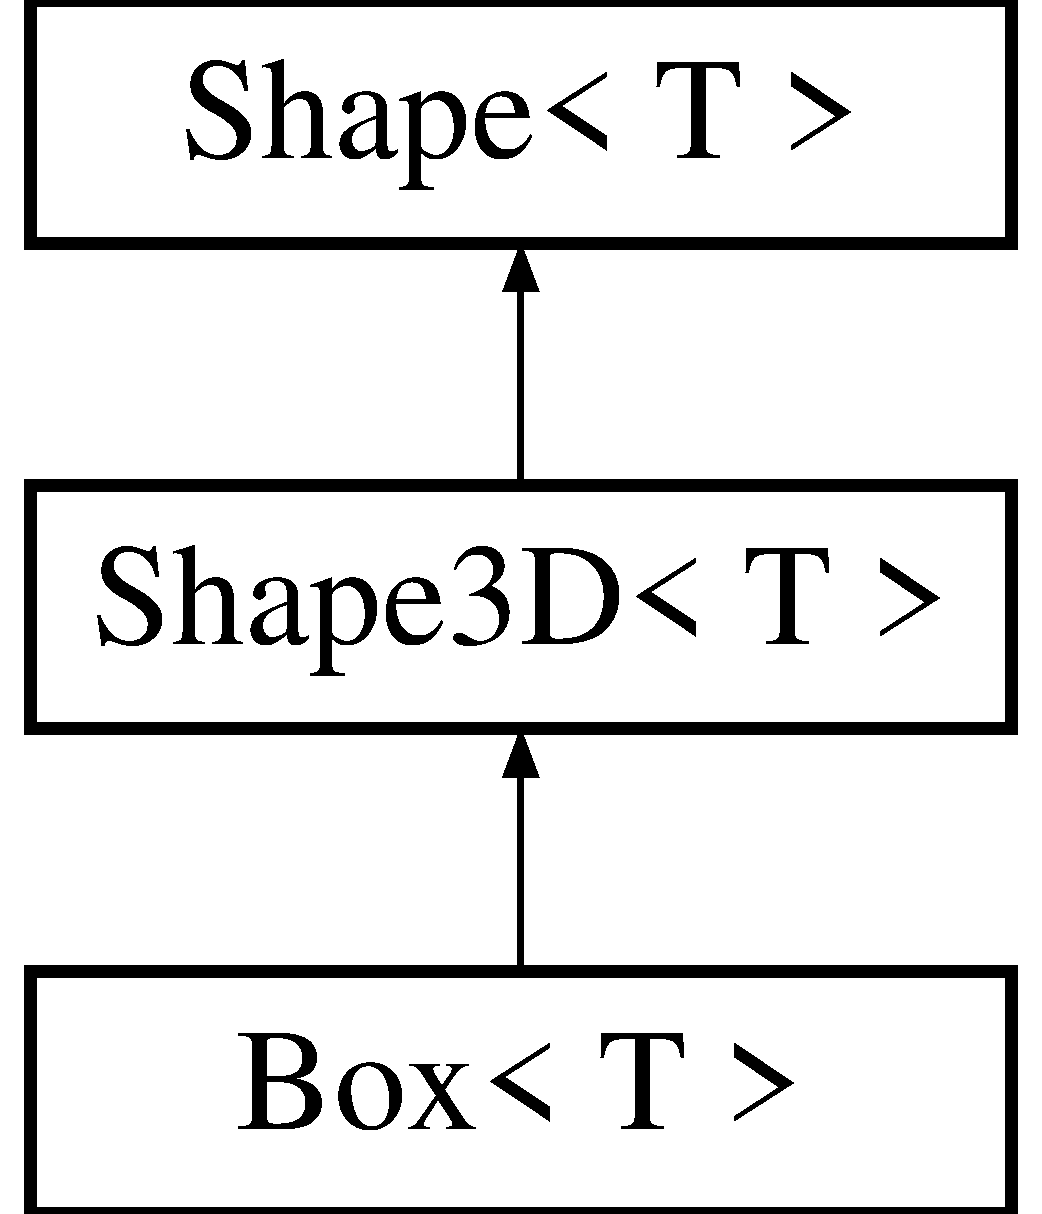
\includegraphics[height=3.000000cm]{classBox}
\end{center}
\end{figure}
\subsection*{Public Member Functions}
\begin{DoxyCompactItemize}
\item 
\mbox{\hyperlink{classBox_a057f84d8fa68647c6484d4e004d8ab74}{Box}} ()
\begin{DoxyCompactList}\small\item\em \mbox{\hyperlink{classA}{A}} basic constructor. \end{DoxyCompactList}\item 
\mbox{\hyperlink{classBox_af72b67fa2f421acbe9a7d3d1bcd540d1}{Box}} (\mbox{\hyperlink{classBox}{Box}} \&\&)=default
\item 
\mbox{\hyperlink{classBox}{Box}} \& \mbox{\hyperlink{classBox_a09995e3360b336b8a477d84804a5a70d}{operator=}} (\mbox{\hyperlink{classBox}{Box}} \&\&)=default
\item 
\mbox{\hyperlink{classBox_aab49a6687d04530ec60421bcbdb929c2}{Box}} (const \mbox{\hyperlink{classBox}{Box}} \&)=default
\item 
\mbox{\hyperlink{classBox}{Box}} \& \mbox{\hyperlink{classBox_a6ea0d233bdcce789b46384d22601da8d}{operator=}} (const \mbox{\hyperlink{classBox}{Box}} \&)=default
\item 
float \mbox{\hyperlink{classBox_ac64e9d619b0f3b991174a2ac49fef899}{perimeter}} ()
\end{DoxyCompactItemize}
\subsection*{Private Member Functions}
\begin{DoxyCompactItemize}
\item 
void \mbox{\hyperlink{classBox_a7f7b061bf913f9ab47bff75536bc137d}{generate\+\_\+vertexes}} ()
\begin{DoxyCompactList}\small\item\em \mbox{\hyperlink{classThis}{This}} function sets the correct vertexes. \end{DoxyCompactList}\end{DoxyCompactItemize}
\subsection*{Additional Inherited Members}


\subsection{Detailed Description}
\subsubsection*{template$<$typename T$>$\newline
class Box$<$ T $>$}

3D box shape. 

\subsection{Constructor \& Destructor Documentation}
\mbox{\Hypertarget{classBox_a057f84d8fa68647c6484d4e004d8ab74}\label{classBox_a057f84d8fa68647c6484d4e004d8ab74}} 
\index{Box@{Box}!Box@{Box}}
\index{Box@{Box}!Box@{Box}}
\subsubsection{\texorpdfstring{Box()}{Box()}\hspace{0.1cm}{\footnotesize\ttfamily [1/3]}}
{\footnotesize\ttfamily template$<$typename T $>$ \\
\mbox{\hyperlink{classBox}{Box}}$<$ T $>$\+::\mbox{\hyperlink{classBox}{Box}} (\begin{DoxyParamCaption}{ }\end{DoxyParamCaption})}



\mbox{\hyperlink{classA}{A}} basic constructor. 

The constructor generates vertexes and initializes buffers \mbox{\Hypertarget{classBox_af72b67fa2f421acbe9a7d3d1bcd540d1}\label{classBox_af72b67fa2f421acbe9a7d3d1bcd540d1}} 
\index{Box@{Box}!Box@{Box}}
\index{Box@{Box}!Box@{Box}}
\subsubsection{\texorpdfstring{Box()}{Box()}\hspace{0.1cm}{\footnotesize\ttfamily [2/3]}}
{\footnotesize\ttfamily template$<$typename T$>$ \\
\mbox{\hyperlink{classBox}{Box}}$<$ T $>$\+::\mbox{\hyperlink{classBox}{Box}} (\begin{DoxyParamCaption}\item[{\mbox{\hyperlink{classBox}{Box}}$<$ T $>$ \&\&}]{ }\end{DoxyParamCaption})\hspace{0.3cm}{\ttfamily [default]}}

\mbox{\Hypertarget{classBox_aab49a6687d04530ec60421bcbdb929c2}\label{classBox_aab49a6687d04530ec60421bcbdb929c2}} 
\index{Box@{Box}!Box@{Box}}
\index{Box@{Box}!Box@{Box}}
\subsubsection{\texorpdfstring{Box()}{Box()}\hspace{0.1cm}{\footnotesize\ttfamily [3/3]}}
{\footnotesize\ttfamily template$<$typename T$>$ \\
\mbox{\hyperlink{classBox}{Box}}$<$ T $>$\+::\mbox{\hyperlink{classBox}{Box}} (\begin{DoxyParamCaption}\item[{const \mbox{\hyperlink{classBox}{Box}}$<$ T $>$ \&}]{ }\end{DoxyParamCaption})\hspace{0.3cm}{\ttfamily [default]}}



\subsection{Member Function Documentation}
\mbox{\Hypertarget{classBox_a7f7b061bf913f9ab47bff75536bc137d}\label{classBox_a7f7b061bf913f9ab47bff75536bc137d}} 
\index{Box@{Box}!generate\+\_\+vertexes@{generate\+\_\+vertexes}}
\index{generate\+\_\+vertexes@{generate\+\_\+vertexes}!Box@{Box}}
\subsubsection{\texorpdfstring{generate\+\_\+vertexes()}{generate\_vertexes()}}
{\footnotesize\ttfamily template$<$typename T $>$ \\
void \mbox{\hyperlink{classBox}{Box}}$<$ T $>$\+::generate\+\_\+vertexes (\begin{DoxyParamCaption}{ }\end{DoxyParamCaption})\hspace{0.3cm}{\ttfamily [private]}}



\mbox{\hyperlink{classThis}{This}} function sets the correct vertexes. 

\mbox{\Hypertarget{classBox_a09995e3360b336b8a477d84804a5a70d}\label{classBox_a09995e3360b336b8a477d84804a5a70d}} 
\index{Box@{Box}!operator=@{operator=}}
\index{operator=@{operator=}!Box@{Box}}
\subsubsection{\texorpdfstring{operator=()}{operator=()}\hspace{0.1cm}{\footnotesize\ttfamily [1/2]}}
{\footnotesize\ttfamily template$<$typename T$>$ \\
\mbox{\hyperlink{classBox}{Box}}\& \mbox{\hyperlink{classBox}{Box}}$<$ T $>$\+::operator= (\begin{DoxyParamCaption}\item[{\mbox{\hyperlink{classBox}{Box}}$<$ T $>$ \&\&}]{ }\end{DoxyParamCaption})\hspace{0.3cm}{\ttfamily [default]}}

\mbox{\Hypertarget{classBox_a6ea0d233bdcce789b46384d22601da8d}\label{classBox_a6ea0d233bdcce789b46384d22601da8d}} 
\index{Box@{Box}!operator=@{operator=}}
\index{operator=@{operator=}!Box@{Box}}
\subsubsection{\texorpdfstring{operator=()}{operator=()}\hspace{0.1cm}{\footnotesize\ttfamily [2/2]}}
{\footnotesize\ttfamily template$<$typename T$>$ \\
\mbox{\hyperlink{classBox}{Box}}\& \mbox{\hyperlink{classBox}{Box}}$<$ T $>$\+::operator= (\begin{DoxyParamCaption}\item[{const \mbox{\hyperlink{classBox}{Box}}$<$ T $>$ \&}]{ }\end{DoxyParamCaption})\hspace{0.3cm}{\ttfamily [default]}}

\mbox{\Hypertarget{classBox_ac64e9d619b0f3b991174a2ac49fef899}\label{classBox_ac64e9d619b0f3b991174a2ac49fef899}} 
\index{Box@{Box}!perimeter@{perimeter}}
\index{perimeter@{perimeter}!Box@{Box}}
\subsubsection{\texorpdfstring{perimeter()}{perimeter()}}
{\footnotesize\ttfamily template$<$typename T$>$ \\
float \mbox{\hyperlink{classBox}{Box}}$<$ T $>$\+::perimeter (\begin{DoxyParamCaption}{ }\end{DoxyParamCaption})}



The documentation for this class was generated from the following file\+:\begin{DoxyCompactItemize}
\item 
src/shapes/\mbox{\hyperlink{box_8hpp}{box.\+hpp}}\end{DoxyCompactItemize}

\hypertarget{classCircle}{}\section{Circle$<$ T $>$ Class Template Reference}
\label{classCircle}\index{Circle$<$ T $>$@{Circle$<$ T $>$}}


{\ttfamily \#include \char`\"{}circle.\+hpp\char`\"{}}

Inheritance diagram for Circle$<$ T $>$\+:\begin{figure}[H]
\begin{center}
\leavevmode
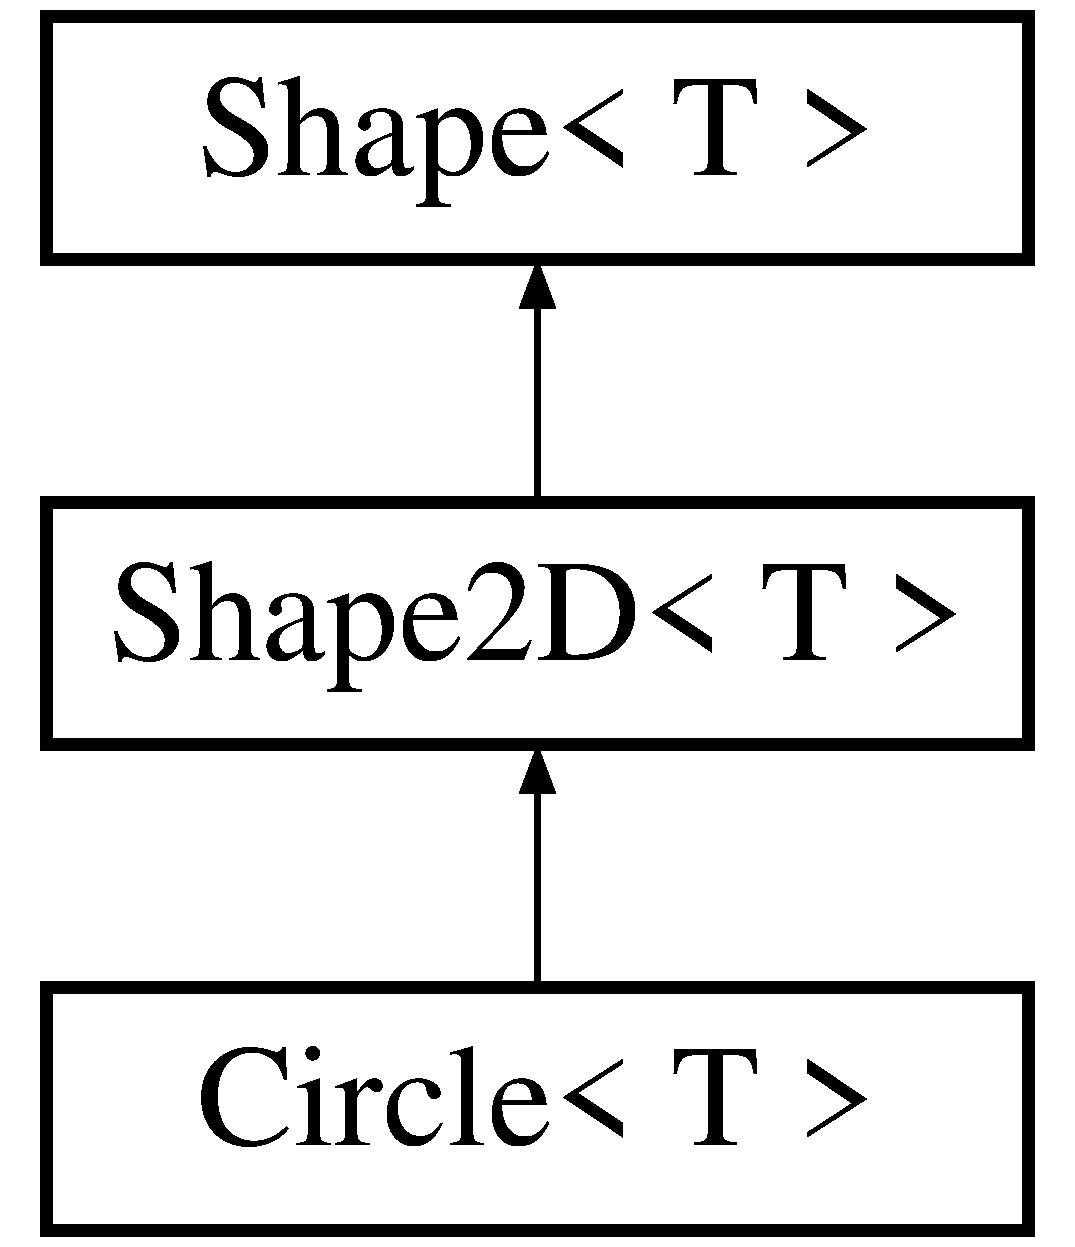
\includegraphics[height=3.000000cm]{classCircle}
\end{center}
\end{figure}
\subsection*{Public Member Functions}
\begin{DoxyCompactItemize}
\item 
\mbox{\hyperlink{classCircle_a0a298ea0e982a94a60091aeb2767f6e4}{Circle}} ()
\begin{DoxyCompactList}\small\item\em Basic constructor for class \mbox{\hyperlink{classCircle}{Circle}}. \end{DoxyCompactList}\item 
\mbox{\hyperlink{classCircle_ad4ee8eadfd4201a937af204ac4e6ec37}{Circle}} (\mbox{\hyperlink{classCircle}{Circle}} \&\&)=default
\item 
\mbox{\hyperlink{classCircle}{Circle}} \& \mbox{\hyperlink{classCircle_a06c8a2624fa51b38023e0326e8ccf789}{operator=}} (\mbox{\hyperlink{classCircle}{Circle}} \&\&)=default
\item 
\mbox{\hyperlink{classCircle_a163162aa8beaceb25ebd9a17966f4bd5}{Circle}} (const \mbox{\hyperlink{classCircle}{Circle}} \&)=default
\item 
\mbox{\hyperlink{classCircle}{Circle}} \& \mbox{\hyperlink{classCircle_a0e3ef62951a8fccaf0635ea21ae73eca}{operator=}} (const \mbox{\hyperlink{classCircle}{Circle}} \&)=default
\item 
T \mbox{\hyperlink{classCircle_a6f066fc39c0de339b0498b04a56be028}{perimeter}} ()
\item 
{\footnotesize template$<$$>$ }\\float \mbox{\hyperlink{classCircle_aa6c86a4a5d3ee7eb598879ba856430d9}{perimeter}} ()
\begin{DoxyCompactList}\small\item\em \mbox{\hyperlink{classThis}{This}} function calculates perimeter of a circle with radius 1. \end{DoxyCompactList}\end{DoxyCompactItemize}
\subsection*{Private Member Functions}
\begin{DoxyCompactItemize}
\item 
void \mbox{\hyperlink{classCircle_a07ce44d6b3a70ee7cbcf19e02e50c361}{generate\+\_\+vertexes}} (int=-\/1)
\item 
{\footnotesize template$<$$>$ }\\void \mbox{\hyperlink{classCircle_a5c5d9e9bf7ddada0681ad6977e4469f6}{generate\+\_\+vertexes}} (int num\+\_\+vert)
\begin{DoxyCompactList}\small\item\em \mbox{\hyperlink{classThis}{This}} function generates vertexes for float version of class \mbox{\hyperlink{classCircle}{Circle}}. \end{DoxyCompactList}\end{DoxyCompactItemize}
\subsection*{Additional Inherited Members}


\subsection{Constructor \& Destructor Documentation}
\mbox{\Hypertarget{classCircle_a0a298ea0e982a94a60091aeb2767f6e4}\label{classCircle_a0a298ea0e982a94a60091aeb2767f6e4}} 
\index{Circle@{Circle}!Circle@{Circle}}
\index{Circle@{Circle}!Circle@{Circle}}
\subsubsection{\texorpdfstring{Circle()}{Circle()}\hspace{0.1cm}{\footnotesize\ttfamily [1/3]}}
{\footnotesize\ttfamily template$<$typename T $>$ \\
\mbox{\hyperlink{classCircle}{Circle}}$<$ T $>$\+::\mbox{\hyperlink{classCircle}{Circle}} (\begin{DoxyParamCaption}{ }\end{DoxyParamCaption})}



Basic constructor for class \mbox{\hyperlink{classCircle}{Circle}}. 

Constructor generates vertexes and initializes opengl buffers. \mbox{\Hypertarget{classCircle_ad4ee8eadfd4201a937af204ac4e6ec37}\label{classCircle_ad4ee8eadfd4201a937af204ac4e6ec37}} 
\index{Circle@{Circle}!Circle@{Circle}}
\index{Circle@{Circle}!Circle@{Circle}}
\subsubsection{\texorpdfstring{Circle()}{Circle()}\hspace{0.1cm}{\footnotesize\ttfamily [2/3]}}
{\footnotesize\ttfamily template$<$typename T  = float$>$ \\
\mbox{\hyperlink{classCircle}{Circle}}$<$ T $>$\+::\mbox{\hyperlink{classCircle}{Circle}} (\begin{DoxyParamCaption}\item[{\mbox{\hyperlink{classCircle}{Circle}}$<$ T $>$ \&\&}]{ }\end{DoxyParamCaption})\hspace{0.3cm}{\ttfamily [default]}}

\mbox{\Hypertarget{classCircle_a163162aa8beaceb25ebd9a17966f4bd5}\label{classCircle_a163162aa8beaceb25ebd9a17966f4bd5}} 
\index{Circle@{Circle}!Circle@{Circle}}
\index{Circle@{Circle}!Circle@{Circle}}
\subsubsection{\texorpdfstring{Circle()}{Circle()}\hspace{0.1cm}{\footnotesize\ttfamily [3/3]}}
{\footnotesize\ttfamily template$<$typename T  = float$>$ \\
\mbox{\hyperlink{classCircle}{Circle}}$<$ T $>$\+::\mbox{\hyperlink{classCircle}{Circle}} (\begin{DoxyParamCaption}\item[{const \mbox{\hyperlink{classCircle}{Circle}}$<$ T $>$ \&}]{ }\end{DoxyParamCaption})\hspace{0.3cm}{\ttfamily [default]}}



\subsection{Member Function Documentation}
\mbox{\Hypertarget{classCircle_a07ce44d6b3a70ee7cbcf19e02e50c361}\label{classCircle_a07ce44d6b3a70ee7cbcf19e02e50c361}} 
\index{Circle@{Circle}!generate\+\_\+vertexes@{generate\+\_\+vertexes}}
\index{generate\+\_\+vertexes@{generate\+\_\+vertexes}!Circle@{Circle}}
\subsubsection{\texorpdfstring{generate\+\_\+vertexes()}{generate\_vertexes()}\hspace{0.1cm}{\footnotesize\ttfamily [1/2]}}
{\footnotesize\ttfamily template$<$typename T  = float$>$ \\
void \mbox{\hyperlink{classCircle}{Circle}}$<$ T $>$\+::generate\+\_\+vertexes (\begin{DoxyParamCaption}\item[{int}]{ = {\ttfamily -\/1} }\end{DoxyParamCaption})\hspace{0.3cm}{\ttfamily [private]}}

\mbox{\Hypertarget{classCircle_a5c5d9e9bf7ddada0681ad6977e4469f6}\label{classCircle_a5c5d9e9bf7ddada0681ad6977e4469f6}} 
\index{Circle@{Circle}!generate\+\_\+vertexes@{generate\+\_\+vertexes}}
\index{generate\+\_\+vertexes@{generate\+\_\+vertexes}!Circle@{Circle}}
\subsubsection{\texorpdfstring{generate\+\_\+vertexes()}{generate\_vertexes()}\hspace{0.1cm}{\footnotesize\ttfamily [2/2]}}
{\footnotesize\ttfamily template$<$$>$ \\
void \mbox{\hyperlink{classCircle}{Circle}}$<$ float $>$\+::generate\+\_\+vertexes (\begin{DoxyParamCaption}\item[{int}]{num\+\_\+vert }\end{DoxyParamCaption})\hspace{0.3cm}{\ttfamily [inline]}, {\ttfamily [private]}}



\mbox{\hyperlink{classThis}{This}} function generates vertexes for float version of class \mbox{\hyperlink{classCircle}{Circle}}. 

Internally, it uses sse instructions -\/ cpu support needed. \mbox{\Hypertarget{classCircle_a06c8a2624fa51b38023e0326e8ccf789}\label{classCircle_a06c8a2624fa51b38023e0326e8ccf789}} 
\index{Circle@{Circle}!operator=@{operator=}}
\index{operator=@{operator=}!Circle@{Circle}}
\subsubsection{\texorpdfstring{operator=()}{operator=()}\hspace{0.1cm}{\footnotesize\ttfamily [1/2]}}
{\footnotesize\ttfamily template$<$typename T  = float$>$ \\
\mbox{\hyperlink{classCircle}{Circle}}\& \mbox{\hyperlink{classCircle}{Circle}}$<$ T $>$\+::operator= (\begin{DoxyParamCaption}\item[{\mbox{\hyperlink{classCircle}{Circle}}$<$ T $>$ \&\&}]{ }\end{DoxyParamCaption})\hspace{0.3cm}{\ttfamily [default]}}

\mbox{\Hypertarget{classCircle_a0e3ef62951a8fccaf0635ea21ae73eca}\label{classCircle_a0e3ef62951a8fccaf0635ea21ae73eca}} 
\index{Circle@{Circle}!operator=@{operator=}}
\index{operator=@{operator=}!Circle@{Circle}}
\subsubsection{\texorpdfstring{operator=()}{operator=()}\hspace{0.1cm}{\footnotesize\ttfamily [2/2]}}
{\footnotesize\ttfamily template$<$typename T  = float$>$ \\
\mbox{\hyperlink{classCircle}{Circle}}\& \mbox{\hyperlink{classCircle}{Circle}}$<$ T $>$\+::operator= (\begin{DoxyParamCaption}\item[{const \mbox{\hyperlink{classCircle}{Circle}}$<$ T $>$ \&}]{ }\end{DoxyParamCaption})\hspace{0.3cm}{\ttfamily [default]}}

\mbox{\Hypertarget{classCircle_a6f066fc39c0de339b0498b04a56be028}\label{classCircle_a6f066fc39c0de339b0498b04a56be028}} 
\index{Circle@{Circle}!perimeter@{perimeter}}
\index{perimeter@{perimeter}!Circle@{Circle}}
\subsubsection{\texorpdfstring{perimeter()}{perimeter()}\hspace{0.1cm}{\footnotesize\ttfamily [1/2]}}
{\footnotesize\ttfamily template$<$typename T  = float$>$ \\
T \mbox{\hyperlink{classCircle}{Circle}}$<$ T $>$\+::perimeter (\begin{DoxyParamCaption}{ }\end{DoxyParamCaption})}

\mbox{\Hypertarget{classCircle_aa6c86a4a5d3ee7eb598879ba856430d9}\label{classCircle_aa6c86a4a5d3ee7eb598879ba856430d9}} 
\index{Circle@{Circle}!perimeter@{perimeter}}
\index{perimeter@{perimeter}!Circle@{Circle}}
\subsubsection{\texorpdfstring{perimeter()}{perimeter()}\hspace{0.1cm}{\footnotesize\ttfamily [2/2]}}
{\footnotesize\ttfamily template$<$$>$ \\
float \mbox{\hyperlink{classCircle}{Circle}}$<$ float $>$\+::perimeter (\begin{DoxyParamCaption}{ }\end{DoxyParamCaption})\hspace{0.3cm}{\ttfamily [inline]}}



\mbox{\hyperlink{classThis}{This}} function calculates perimeter of a circle with radius 1. 

Internally, it uses sse instructions -\/ cpu support needed. 

The documentation for this class was generated from the following file\+:\begin{DoxyCompactItemize}
\item 
src/shapes/\mbox{\hyperlink{circle_8hpp}{circle.\+hpp}}\end{DoxyCompactItemize}

\hypertarget{classDisk}{}\section{Disk$<$ T $>$ Class Template Reference}
\label{classDisk}\index{Disk$<$ T $>$@{Disk$<$ T $>$}}


\mbox{\hyperlink{classA}{A}} class holding vertexes in the shape of a disk.  




{\ttfamily \#include \char`\"{}disk.\+hpp\char`\"{}}

Inheritance diagram for Disk$<$ T $>$\+:\begin{figure}[H]
\begin{center}
\leavevmode
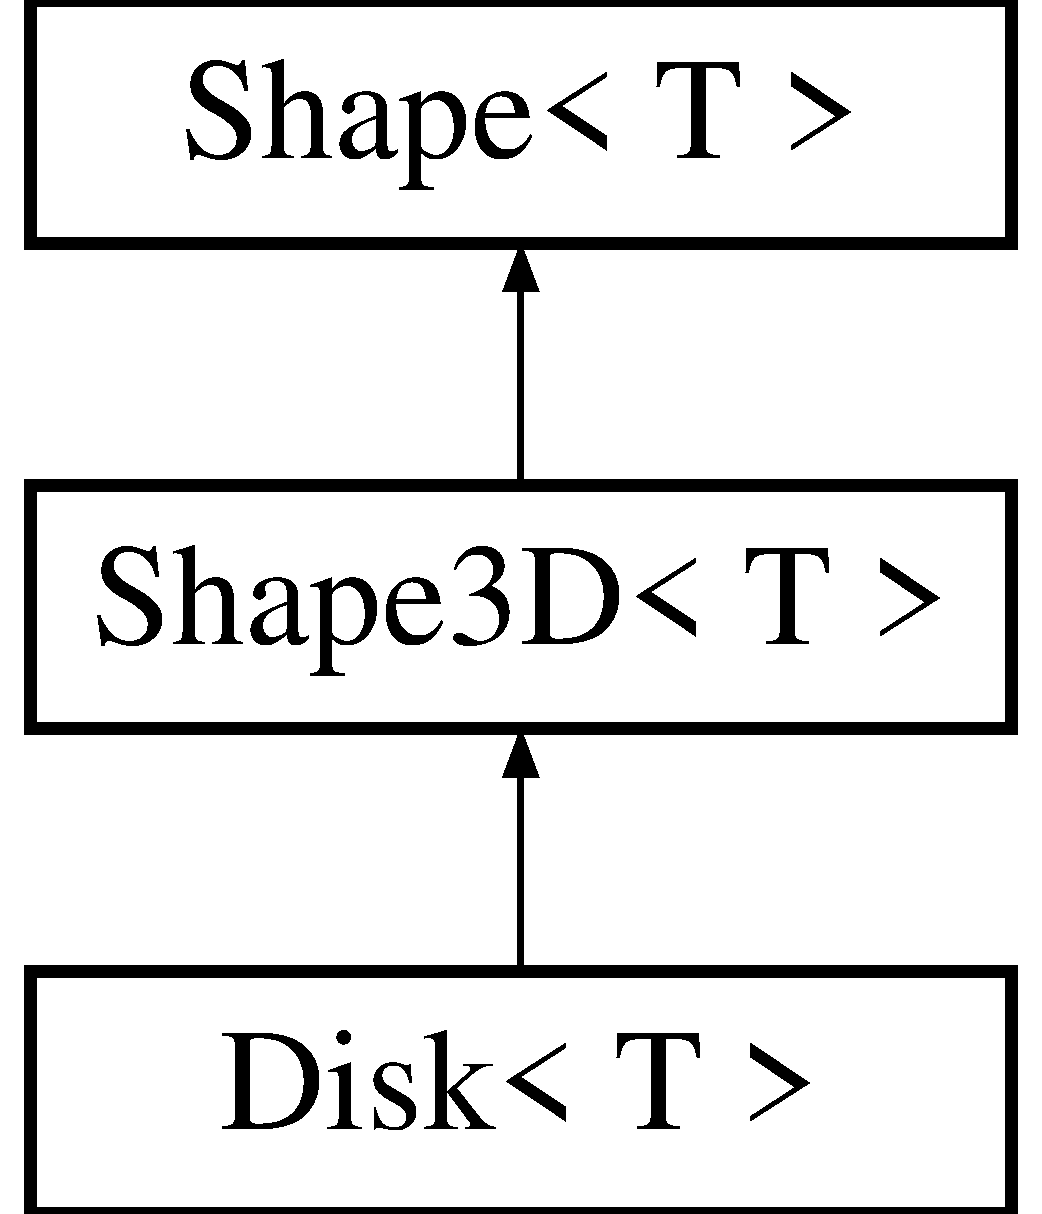
\includegraphics[height=3.000000cm]{classDisk}
\end{center}
\end{figure}
\subsection*{Public Member Functions}
\begin{DoxyCompactItemize}
\item 
\mbox{\hyperlink{classDisk_a88bcdb9bf91c8e9c18cdf551e558ab8c}{Disk}} ()
\begin{DoxyCompactList}\small\item\em \mbox{\hyperlink{classA}{A}} basic constructor. \end{DoxyCompactList}\item 
\mbox{\hyperlink{classDisk_af73e1930d8da87b05c813814532dd43a}{Disk}} (int, T=0.\+5)
\item 
\mbox{\hyperlink{classDisk_a893da931e3f39c126c434ab2fc2e12cc}{Disk}} (\mbox{\hyperlink{classDisk}{Disk}} \&\&)=default
\item 
\mbox{\hyperlink{classDisk}{Disk}} \& \mbox{\hyperlink{classDisk_ad6bc474ffecbc5de6f8fdd90ba5eddfe}{operator=}} (\mbox{\hyperlink{classDisk}{Disk}} \&\&)=default
\item 
\mbox{\hyperlink{classDisk_a96de79b2e115c478a33cc31f4818aee9}{Disk}} (const \mbox{\hyperlink{classDisk}{Disk}} \&)=default
\item 
\mbox{\hyperlink{classDisk}{Disk}} \& \mbox{\hyperlink{classDisk_a3ef862dd6e4671c907e2368bb5239bd2}{operator=}} (const \mbox{\hyperlink{classDisk}{Disk}} \&)=default
\end{DoxyCompactItemize}
\subsection*{Private Member Functions}
\begin{DoxyCompactItemize}
\item 
void \mbox{\hyperlink{classDisk_a1588532798901180b1eef6f3e1fb83f6}{generate\+\_\+vertexes}} ()
\item 
void \mbox{\hyperlink{classDisk_a4637847208b7236010085ca67f49e39a}{generate\+\_\+wheel\+\_\+line\+\_\+elements}} ()
\begin{DoxyCompactList}\small\item\em Function which generates sets wheel elements. Render wheel elements array with G\+L\+\_\+\+L\+I\+N\+ES to draw a wheel. \end{DoxyCompactList}\item 
{\footnotesize template$<$$>$ }\\void \mbox{\hyperlink{classDisk_a55648a13c42982087f60742da15c2c41}{generate\+\_\+vertexes}} ()
\begin{DoxyCompactList}\small\item\em Function which generates vertexes for float version of this class. \end{DoxyCompactList}\end{DoxyCompactItemize}
\subsection*{Private Attributes}
\begin{DoxyCompactItemize}
\item 
std\+::vector$<$ int $>$ \mbox{\hyperlink{classDisk_aa008e8bd0e7acdb4a1a56a8f44f048d7}{wheel\+\_\+line\+\_\+elements}}
\end{DoxyCompactItemize}
\subsection*{Additional Inherited Members}


\subsection{Detailed Description}
\subsubsection*{template$<$typename T = float$>$\newline
class Disk$<$ T $>$}

\mbox{\hyperlink{classA}{A}} class holding vertexes in the shape of a disk. 

\mbox{\hyperlink{classA}{A}} class holding vertexes in the shape of a disk. \mbox{\hyperlink{classDisk}{Disk}} is a 3d shape, thus it inherits from \mbox{\hyperlink{classShape3D}{Shape3D}} class. Template parameter can either be float or double. 
\begin{DoxyParams}{Parameters}
{\em T} & Template parameter T can either be float of double \\
\hline
\end{DoxyParams}


\subsection{Constructor \& Destructor Documentation}
\mbox{\Hypertarget{classDisk_a88bcdb9bf91c8e9c18cdf551e558ab8c}\label{classDisk_a88bcdb9bf91c8e9c18cdf551e558ab8c}} 
\index{Disk@{Disk}!Disk@{Disk}}
\index{Disk@{Disk}!Disk@{Disk}}
\subsubsection{\texorpdfstring{Disk()}{Disk()}\hspace{0.1cm}{\footnotesize\ttfamily [1/4]}}
{\footnotesize\ttfamily template$<$typename T $>$ \\
\mbox{\hyperlink{classDisk}{Disk}}$<$ T $>$\+::\mbox{\hyperlink{classDisk}{Disk}} (\begin{DoxyParamCaption}{ }\end{DoxyParamCaption})}



\mbox{\hyperlink{classA}{A}} basic constructor. 

Constructor initializes all important variables, geenratex necessary vertexes and initializes opengl buffers. \mbox{\Hypertarget{classDisk_af73e1930d8da87b05c813814532dd43a}\label{classDisk_af73e1930d8da87b05c813814532dd43a}} 
\index{Disk@{Disk}!Disk@{Disk}}
\index{Disk@{Disk}!Disk@{Disk}}
\subsubsection{\texorpdfstring{Disk()}{Disk()}\hspace{0.1cm}{\footnotesize\ttfamily [2/4]}}
{\footnotesize\ttfamily template$<$typename T  = float$>$ \\
\mbox{\hyperlink{classDisk}{Disk}}$<$ T $>$\+::\mbox{\hyperlink{classDisk}{Disk}} (\begin{DoxyParamCaption}\item[{int}]{,  }\item[{T}]{ = {\ttfamily 0.5} }\end{DoxyParamCaption})}

\mbox{\Hypertarget{classDisk_a893da931e3f39c126c434ab2fc2e12cc}\label{classDisk_a893da931e3f39c126c434ab2fc2e12cc}} 
\index{Disk@{Disk}!Disk@{Disk}}
\index{Disk@{Disk}!Disk@{Disk}}
\subsubsection{\texorpdfstring{Disk()}{Disk()}\hspace{0.1cm}{\footnotesize\ttfamily [3/4]}}
{\footnotesize\ttfamily template$<$typename T  = float$>$ \\
\mbox{\hyperlink{classDisk}{Disk}}$<$ T $>$\+::\mbox{\hyperlink{classDisk}{Disk}} (\begin{DoxyParamCaption}\item[{\mbox{\hyperlink{classDisk}{Disk}}$<$ T $>$ \&\&}]{ }\end{DoxyParamCaption})\hspace{0.3cm}{\ttfamily [default]}}

\mbox{\Hypertarget{classDisk_a96de79b2e115c478a33cc31f4818aee9}\label{classDisk_a96de79b2e115c478a33cc31f4818aee9}} 
\index{Disk@{Disk}!Disk@{Disk}}
\index{Disk@{Disk}!Disk@{Disk}}
\subsubsection{\texorpdfstring{Disk()}{Disk()}\hspace{0.1cm}{\footnotesize\ttfamily [4/4]}}
{\footnotesize\ttfamily template$<$typename T  = float$>$ \\
\mbox{\hyperlink{classDisk}{Disk}}$<$ T $>$\+::\mbox{\hyperlink{classDisk}{Disk}} (\begin{DoxyParamCaption}\item[{const \mbox{\hyperlink{classDisk}{Disk}}$<$ T $>$ \&}]{ }\end{DoxyParamCaption})\hspace{0.3cm}{\ttfamily [default]}}



\subsection{Member Function Documentation}
\mbox{\Hypertarget{classDisk_a1588532798901180b1eef6f3e1fb83f6}\label{classDisk_a1588532798901180b1eef6f3e1fb83f6}} 
\index{Disk@{Disk}!generate\+\_\+vertexes@{generate\+\_\+vertexes}}
\index{generate\+\_\+vertexes@{generate\+\_\+vertexes}!Disk@{Disk}}
\subsubsection{\texorpdfstring{generate\+\_\+vertexes()}{generate\_vertexes()}\hspace{0.1cm}{\footnotesize\ttfamily [1/2]}}
{\footnotesize\ttfamily template$<$typename T  = float$>$ \\
void \mbox{\hyperlink{classDisk}{Disk}}$<$ T $>$\+::generate\+\_\+vertexes (\begin{DoxyParamCaption}{ }\end{DoxyParamCaption})\hspace{0.3cm}{\ttfamily [private]}}

\mbox{\Hypertarget{classDisk_a55648a13c42982087f60742da15c2c41}\label{classDisk_a55648a13c42982087f60742da15c2c41}} 
\index{Disk@{Disk}!generate\+\_\+vertexes@{generate\+\_\+vertexes}}
\index{generate\+\_\+vertexes@{generate\+\_\+vertexes}!Disk@{Disk}}
\subsubsection{\texorpdfstring{generate\+\_\+vertexes()}{generate\_vertexes()}\hspace{0.1cm}{\footnotesize\ttfamily [2/2]}}
{\footnotesize\ttfamily template$<$$>$ \\
void \mbox{\hyperlink{classDisk}{Disk}}$<$ float $>$\+::generate\+\_\+vertexes (\begin{DoxyParamCaption}{ }\end{DoxyParamCaption})\hspace{0.3cm}{\ttfamily [inline]}, {\ttfamily [private]}}



Function which generates vertexes for float version of this class. 

Vertexes are generate in such a way that the middle of the shape is (0,0,0). The function also sets the element array. It uses sse instructions -\/ use appropriate processor. \mbox{\Hypertarget{classDisk_a4637847208b7236010085ca67f49e39a}\label{classDisk_a4637847208b7236010085ca67f49e39a}} 
\index{Disk@{Disk}!generate\+\_\+wheel\+\_\+line\+\_\+elements@{generate\+\_\+wheel\+\_\+line\+\_\+elements}}
\index{generate\+\_\+wheel\+\_\+line\+\_\+elements@{generate\+\_\+wheel\+\_\+line\+\_\+elements}!Disk@{Disk}}
\subsubsection{\texorpdfstring{generate\+\_\+wheel\+\_\+line\+\_\+elements()}{generate\_wheel\_line\_elements()}}
{\footnotesize\ttfamily template$<$typename T $>$ \\
void \mbox{\hyperlink{classDisk}{Disk}}$<$ T $>$\+::generate\+\_\+wheel\+\_\+line\+\_\+elements (\begin{DoxyParamCaption}{ }\end{DoxyParamCaption})\hspace{0.3cm}{\ttfamily [private]}}



Function which generates sets wheel elements. Render wheel elements array with G\+L\+\_\+\+L\+I\+N\+ES to draw a wheel. 

\mbox{\Hypertarget{classDisk_ad6bc474ffecbc5de6f8fdd90ba5eddfe}\label{classDisk_ad6bc474ffecbc5de6f8fdd90ba5eddfe}} 
\index{Disk@{Disk}!operator=@{operator=}}
\index{operator=@{operator=}!Disk@{Disk}}
\subsubsection{\texorpdfstring{operator=()}{operator=()}\hspace{0.1cm}{\footnotesize\ttfamily [1/2]}}
{\footnotesize\ttfamily template$<$typename T  = float$>$ \\
\mbox{\hyperlink{classDisk}{Disk}}\& \mbox{\hyperlink{classDisk}{Disk}}$<$ T $>$\+::operator= (\begin{DoxyParamCaption}\item[{\mbox{\hyperlink{classDisk}{Disk}}$<$ T $>$ \&\&}]{ }\end{DoxyParamCaption})\hspace{0.3cm}{\ttfamily [default]}}

\mbox{\Hypertarget{classDisk_a3ef862dd6e4671c907e2368bb5239bd2}\label{classDisk_a3ef862dd6e4671c907e2368bb5239bd2}} 
\index{Disk@{Disk}!operator=@{operator=}}
\index{operator=@{operator=}!Disk@{Disk}}
\subsubsection{\texorpdfstring{operator=()}{operator=()}\hspace{0.1cm}{\footnotesize\ttfamily [2/2]}}
{\footnotesize\ttfamily template$<$typename T  = float$>$ \\
\mbox{\hyperlink{classDisk}{Disk}}\& \mbox{\hyperlink{classDisk}{Disk}}$<$ T $>$\+::operator= (\begin{DoxyParamCaption}\item[{const \mbox{\hyperlink{classDisk}{Disk}}$<$ T $>$ \&}]{ }\end{DoxyParamCaption})\hspace{0.3cm}{\ttfamily [default]}}



\subsection{Member Data Documentation}
\mbox{\Hypertarget{classDisk_aa008e8bd0e7acdb4a1a56a8f44f048d7}\label{classDisk_aa008e8bd0e7acdb4a1a56a8f44f048d7}} 
\index{Disk@{Disk}!wheel\+\_\+line\+\_\+elements@{wheel\+\_\+line\+\_\+elements}}
\index{wheel\+\_\+line\+\_\+elements@{wheel\+\_\+line\+\_\+elements}!Disk@{Disk}}
\subsubsection{\texorpdfstring{wheel\+\_\+line\+\_\+elements}{wheel\_line\_elements}}
{\footnotesize\ttfamily template$<$typename T  = float$>$ \\
std\+::vector$<$int$>$ \mbox{\hyperlink{classDisk}{Disk}}$<$ T $>$\+::wheel\+\_\+line\+\_\+elements\hspace{0.3cm}{\ttfamily [private]}}

elements which determine wheel shape 

The documentation for this class was generated from the following file\+:\begin{DoxyCompactItemize}
\item 
src/\mbox{\hyperlink{disk_8hpp}{disk.\+hpp}}\end{DoxyCompactItemize}

\hypertarget{structgladGLversionStruct}{}\section{glad\+G\+Lversion\+Struct Struct Reference}
\label{structgladGLversionStruct}\index{glad\+G\+Lversion\+Struct@{glad\+G\+Lversion\+Struct}}


{\ttfamily \#include \char`\"{}glad.\+h\char`\"{}}

\subsection*{Public Attributes}
\begin{DoxyCompactItemize}
\item 
int \mbox{\hyperlink{structgladGLversionStruct_ac7f9db11d2679df12ef0313b728554db}{major}}
\item 
int \mbox{\hyperlink{structgladGLversionStruct_acc2bff1c8966c6866f2ad6f5a4e475b2}{minor}}
\end{DoxyCompactItemize}


\subsection{Member Data Documentation}
\mbox{\Hypertarget{structgladGLversionStruct_ac7f9db11d2679df12ef0313b728554db}\label{structgladGLversionStruct_ac7f9db11d2679df12ef0313b728554db}} 
\index{glad\+G\+Lversion\+Struct@{glad\+G\+Lversion\+Struct}!major@{major}}
\index{major@{major}!glad\+G\+Lversion\+Struct@{glad\+G\+Lversion\+Struct}}
\subsubsection{\texorpdfstring{major}{major}}
{\footnotesize\ttfamily int glad\+G\+Lversion\+Struct\+::major}

\mbox{\Hypertarget{structgladGLversionStruct_acc2bff1c8966c6866f2ad6f5a4e475b2}\label{structgladGLversionStruct_acc2bff1c8966c6866f2ad6f5a4e475b2}} 
\index{glad\+G\+Lversion\+Struct@{glad\+G\+Lversion\+Struct}!minor@{minor}}
\index{minor@{minor}!glad\+G\+Lversion\+Struct@{glad\+G\+Lversion\+Struct}}
\subsubsection{\texorpdfstring{minor}{minor}}
{\footnotesize\ttfamily int glad\+G\+Lversion\+Struct\+::minor}



The documentation for this struct was generated from the following file\+:\begin{DoxyCompactItemize}
\item 
third\+\_\+party/glad/include/glad/\mbox{\hyperlink{glad_8h}{glad.\+h}}\end{DoxyCompactItemize}

\hypertarget{structstd_1_1hash_3_01pair_3_01S_00_01T_01_4_01_4}{}\section{std\+:\+:hash$<$ pair$<$ S, T $>$ $>$ Struct Template Reference}
\label{structstd_1_1hash_3_01pair_3_01S_00_01T_01_4_01_4}\index{std\+::hash$<$ pair$<$ S, T $>$ $>$@{std\+::hash$<$ pair$<$ S, T $>$ $>$}}


{\ttfamily \#include \char`\"{}auxiliary\+\_\+functions.\+hpp\char`\"{}}

\subsection*{Public Member Functions}
\begin{DoxyCompactItemize}
\item 
size\+\_\+t \mbox{\hyperlink{structstd_1_1hash_3_01pair_3_01S_00_01T_01_4_01_4_a6fec6cb26e96fb20d4ec121487e5acb4}{operator()}} (const pair$<$ S, T $>$ \&\mbox{\hyperlink{glad_8h_a30522dbcc3e66083fcf2bf64d1fad76a}{v}}) const
\end{DoxyCompactItemize}


\subsection{Member Function Documentation}
\mbox{\Hypertarget{structstd_1_1hash_3_01pair_3_01S_00_01T_01_4_01_4_a6fec6cb26e96fb20d4ec121487e5acb4}\label{structstd_1_1hash_3_01pair_3_01S_00_01T_01_4_01_4_a6fec6cb26e96fb20d4ec121487e5acb4}} 
\index{std\+::hash$<$ pair$<$ S, T $>$ $>$@{std\+::hash$<$ pair$<$ S, T $>$ $>$}!operator()@{operator()}}
\index{operator()@{operator()}!std\+::hash$<$ pair$<$ S, T $>$ $>$@{std\+::hash$<$ pair$<$ S, T $>$ $>$}}
\subsubsection{\texorpdfstring{operator()()}{operator()()}}
{\footnotesize\ttfamily template$<$typename S , typename T $>$ \\
size\+\_\+t std\+::hash$<$ pair$<$ S, T $>$ $>$\+::operator() (\begin{DoxyParamCaption}\item[{const pair$<$ S, T $>$ \&}]{v }\end{DoxyParamCaption}) const\hspace{0.3cm}{\ttfamily [inline]}}



The documentation for this struct was generated from the following file\+:\begin{DoxyCompactItemize}
\item 
src/algorithms/\mbox{\hyperlink{auxiliary__functions_8hpp}{auxiliary\+\_\+functions.\+hpp}}\end{DoxyCompactItemize}

\hypertarget{classIsingModel}{}\section{Ising\+Model$<$ T $>$ Class Template Reference}
\label{classIsingModel}\index{Ising\+Model$<$ T $>$@{Ising\+Model$<$ T $>$}}


Ising model containing two possible spin flipping methods -\/ metropolis and wolff.  




{\ttfamily \#include \char`\"{}Ising\+\_\+model.\+hpp\char`\"{}}

\subsection*{Public Member Functions}
\begin{DoxyCompactItemize}
\item 
\mbox{\hyperlink{classIsingModel_a3c9a903d3ddada5ce514ba66f99b0282}{Ising\+Model}} (unsigned size\+\_\+=50, T temperature\+\_\+=2)
\begin{DoxyCompactList}\small\item\em Basic constructor for \mbox{\hyperlink{classIsingModel}{Ising\+Model}} class. \end{DoxyCompactList}\item 
\mbox{\hyperlink{classspin__dir}{spin\+\_\+dir}} $\ast$ \mbox{\hyperlink{classIsingModel_ad82f225e1b45f11ee5a99c3b12b25302}{get\+\_\+spin\+\_\+array}} ()
\item 
int \mbox{\hyperlink{classIsingModel_a349a13b847fb221eec7043fc53649640}{calc\+\_\+magnetization}} ()
\begin{DoxyCompactList}\small\item\em calculate magnetization -\/ difference between spins up and spins down \end{DoxyCompactList}\item 
void \mbox{\hyperlink{classIsingModel_abbd5b7935830eca268b7eacc94478649}{set\+\_\+temperature}} (T temperature\+\_\+)
\begin{DoxyCompactList}\small\item\em sets the temperature \end{DoxyCompactList}\item 
T \mbox{\hyperlink{classIsingModel_ad0252a860a935d1be2542f15b5c25936}{get\+\_\+temperature}} ()
\begin{DoxyCompactList}\small\item\em get the temperature \end{DoxyCompactList}\item 
unsigned \mbox{\hyperlink{classIsingModel_afd731e5858b03deb1c8a11ee8a6b8834}{get\+\_\+cluster\+\_\+size}} ()
\begin{DoxyCompactList}\small\item\em Get the size of the cluster in the last Wolff step. \end{DoxyCompactList}\item 
T \mbox{\hyperlink{classIsingModel_a37a7c509999f21f1bd4f54a12009f3cf}{get\+\_\+energy}} ()
\begin{DoxyCompactList}\small\item\em Get current energy. \end{DoxyCompactList}\item 
int \mbox{\hyperlink{classIsingModel_a58c9ebc61c0b2238fd52b62df8ce4853}{get\+\_\+magnetization}} ()
\begin{DoxyCompactList}\small\item\em get current magnetization. \end{DoxyCompactList}\item 
void \mbox{\hyperlink{classIsingModel_ab76a4eee808eaa1979ff6707498e9908}{flip\+\_\+cluster}} ()
\begin{DoxyCompactList}\small\item\em The function flips the cluster using Wolff algorithm. \end{DoxyCompactList}\item 
void \mbox{\hyperlink{classIsingModel_ac16bfdd5bb4012162bedd90034962f58}{set\+\_\+all\+\_\+spins\+\_\+up}} ()
\begin{DoxyCompactList}\small\item\em set all spins up. \end{DoxyCompactList}\item 
T \mbox{\hyperlink{classIsingModel_a0a387ccae720604f4de13d5b0762ac62}{calc\+\_\+energy}} ()
\begin{DoxyCompactList}\small\item\em The function calculates energy of the spin array. \end{DoxyCompactList}\item 
void \mbox{\hyperlink{classIsingModel_a195316f577d71297e9634fa6fdeacc44}{metropolis\+\_\+steps}} (unsigned spin\+\_\+flips)
\begin{DoxyCompactList}\small\item\em Makes a metropolis step. \end{DoxyCompactList}\end{DoxyCompactItemize}
\subsection*{Private Member Functions}
\begin{DoxyCompactItemize}
\item 
void \mbox{\hyperlink{classIsingModel_abe2a720ca3ed7dde191e36fbf33561b3}{enforce\+\_\+boundary\+\_\+conditions}} ()
\begin{DoxyCompactList}\small\item\em enforce periodic boundary conditions \end{DoxyCompactList}\item 
void \mbox{\hyperlink{classIsingModel_a6ab9293015326da93fb6e3e20d24edf8}{set\+\_\+random\+\_\+spin\+\_\+directions}} ()
\begin{DoxyCompactList}\small\item\em set random spin directions \end{DoxyCompactList}\item 
void \mbox{\hyperlink{classIsingModel_a37758a1a4a2536d16f1bb8166e13f7b6}{wolff\+\_\+cluster\+\_\+step}} (\mbox{\hyperlink{classspin__dir}{spin\+\_\+dir}} spin, unsigned k, unsigned l)
\begin{DoxyCompactList}\small\item\em Make a Wolff algorithm step. \mbox{\hyperlink{classThis}{This}} is a helper for \mbox{\hyperlink{classIsingModel_ab76a4eee808eaa1979ff6707498e9908}{flip\+\_\+cluster()}} function. \end{DoxyCompactList}\end{DoxyCompactItemize}
\subsection*{Private Attributes}
\begin{DoxyCompactItemize}
\item 
unsigned \mbox{\hyperlink{classIsingModel_aec6fc4774dda94fd23c6e29d0820b63a}{size}}
\item 
T \mbox{\hyperlink{classIsingModel_af0c6d48208741fe5a378e29b7fac0da1}{J}} = 1
\item 
T \mbox{\hyperlink{classIsingModel_a19e1a223476c953a9964532c7f0eb6dd}{H}} = 0
\item 
T \mbox{\hyperlink{classIsingModel_af19ba376c01404c094c214939eafd7a5}{tc}} = 2.\+269185
\item 
T \mbox{\hyperlink{classIsingModel_a756faa94432cc7e10d21e52a03156569}{temperature}}
\item 
\mbox{\hyperlink{classspin__dir}{spin\+\_\+dir}} $\ast$ \mbox{\hyperlink{classIsingModel_a82425f60fa2dd07995c2a53f8a850cf5}{spin\+\_\+array}}
\item 
unsigned \mbox{\hyperlink{classIsingModel_a67a282de0cc889e423cde222a3453d38}{cluster\+\_\+size}} = 0
\item 
int \mbox{\hyperlink{classIsingModel_a20c8183929e5e2a395cb962501122e65}{magnetization}} = 0
\item 
T \mbox{\hyperlink{classIsingModel_abd38e1a93e1e7bab7788f00d0b9fddb9}{energy}} = 0
\item 
unsigned \mbox{\hyperlink{classIsingModel_a434e854082ad794811b6e11e2bc50eaf}{samples}} = 0
\item 
std\+::random\+\_\+device \mbox{\hyperlink{classIsingModel_a602475ebc23d97e2ba162ba1db352386}{rd}}
\item 
std\+::mt19937 \mbox{\hyperlink{classIsingModel_a3250275d0897da9f7929b43286e9b44b}{rng}}
\item 
std\+::uniform\+\_\+int\+\_\+distribution$<$ int $>$ \mbox{\hyperlink{classIsingModel_a5f412d0560c599a350d0c266125427c9}{random\+\_\+int}}
\item 
std\+::uniform\+\_\+real\+\_\+distribution$<$ T $>$ \mbox{\hyperlink{classIsingModel_a01dcb867d89771158b7f71a518ded0f2}{random\+\_\+real}}
\end{DoxyCompactItemize}


\subsection{Detailed Description}
\subsubsection*{template$<$typename T$>$\newline
class Ising\+Model$<$ T $>$}

Ising model containing two possible spin flipping methods -\/ metropolis and wolff. 

\subsection{Constructor \& Destructor Documentation}
\mbox{\Hypertarget{classIsingModel_a3c9a903d3ddada5ce514ba66f99b0282}\label{classIsingModel_a3c9a903d3ddada5ce514ba66f99b0282}} 
\index{Ising\+Model@{Ising\+Model}!Ising\+Model@{Ising\+Model}}
\index{Ising\+Model@{Ising\+Model}!Ising\+Model@{Ising\+Model}}
\subsubsection{\texorpdfstring{Ising\+Model()}{IsingModel()}}
{\footnotesize\ttfamily template$<$typename T$>$ \\
\mbox{\hyperlink{classIsingModel}{Ising\+Model}}$<$ T $>$\+::\mbox{\hyperlink{classIsingModel}{Ising\+Model}} (\begin{DoxyParamCaption}\item[{unsigned}]{size\+\_\+ = {\ttfamily 50},  }\item[{T}]{temperature\+\_\+ = {\ttfamily 2} }\end{DoxyParamCaption})\hspace{0.3cm}{\ttfamily [inline]}}



Basic constructor for \mbox{\hyperlink{classIsingModel}{Ising\+Model}} class. 

By default it sets the temperature to 2 and size of spin array to 50. It also initializes random generator, sets random spin directions and enforces periodic boundary conditions for the start of calculation 

\subsection{Member Function Documentation}
\mbox{\Hypertarget{classIsingModel_a0a387ccae720604f4de13d5b0762ac62}\label{classIsingModel_a0a387ccae720604f4de13d5b0762ac62}} 
\index{Ising\+Model@{Ising\+Model}!calc\+\_\+energy@{calc\+\_\+energy}}
\index{calc\+\_\+energy@{calc\+\_\+energy}!Ising\+Model@{Ising\+Model}}
\subsubsection{\texorpdfstring{calc\+\_\+energy()}{calc\_energy()}}
{\footnotesize\ttfamily template$<$typename T$>$ \\
T \mbox{\hyperlink{classIsingModel}{Ising\+Model}}$<$ T $>$\+::calc\+\_\+energy (\begin{DoxyParamCaption}{ }\end{DoxyParamCaption})\hspace{0.3cm}{\ttfamily [inline]}}



The function calculates energy of the spin array. 

\mbox{\Hypertarget{classIsingModel_a349a13b847fb221eec7043fc53649640}\label{classIsingModel_a349a13b847fb221eec7043fc53649640}} 
\index{Ising\+Model@{Ising\+Model}!calc\+\_\+magnetization@{calc\+\_\+magnetization}}
\index{calc\+\_\+magnetization@{calc\+\_\+magnetization}!Ising\+Model@{Ising\+Model}}
\subsubsection{\texorpdfstring{calc\+\_\+magnetization()}{calc\_magnetization()}}
{\footnotesize\ttfamily template$<$typename T$>$ \\
int \mbox{\hyperlink{classIsingModel}{Ising\+Model}}$<$ T $>$\+::calc\+\_\+magnetization (\begin{DoxyParamCaption}{ }\end{DoxyParamCaption})\hspace{0.3cm}{\ttfamily [inline]}}



calculate magnetization -\/ difference between spins up and spins down 

\mbox{\Hypertarget{classIsingModel_abe2a720ca3ed7dde191e36fbf33561b3}\label{classIsingModel_abe2a720ca3ed7dde191e36fbf33561b3}} 
\index{Ising\+Model@{Ising\+Model}!enforce\+\_\+boundary\+\_\+conditions@{enforce\+\_\+boundary\+\_\+conditions}}
\index{enforce\+\_\+boundary\+\_\+conditions@{enforce\+\_\+boundary\+\_\+conditions}!Ising\+Model@{Ising\+Model}}
\subsubsection{\texorpdfstring{enforce\+\_\+boundary\+\_\+conditions()}{enforce\_boundary\_conditions()}}
{\footnotesize\ttfamily template$<$typename T$>$ \\
void \mbox{\hyperlink{classIsingModel}{Ising\+Model}}$<$ T $>$\+::enforce\+\_\+boundary\+\_\+conditions (\begin{DoxyParamCaption}{ }\end{DoxyParamCaption})\hspace{0.3cm}{\ttfamily [inline]}, {\ttfamily [private]}}



enforce periodic boundary conditions 

\mbox{\Hypertarget{classIsingModel_ab76a4eee808eaa1979ff6707498e9908}\label{classIsingModel_ab76a4eee808eaa1979ff6707498e9908}} 
\index{Ising\+Model@{Ising\+Model}!flip\+\_\+cluster@{flip\+\_\+cluster}}
\index{flip\+\_\+cluster@{flip\+\_\+cluster}!Ising\+Model@{Ising\+Model}}
\subsubsection{\texorpdfstring{flip\+\_\+cluster()}{flip\_cluster()}}
{\footnotesize\ttfamily template$<$typename T$>$ \\
void \mbox{\hyperlink{classIsingModel}{Ising\+Model}}$<$ T $>$\+::flip\+\_\+cluster (\begin{DoxyParamCaption}{ }\end{DoxyParamCaption})\hspace{0.3cm}{\ttfamily [inline]}}



The function flips the cluster using Wolff algorithm. 

It calls the \mbox{\hyperlink{classIsingModel_a37758a1a4a2536d16f1bb8166e13f7b6}{wolff\+\_\+cluster\+\_\+step()}} function. \mbox{\Hypertarget{classIsingModel_afd731e5858b03deb1c8a11ee8a6b8834}\label{classIsingModel_afd731e5858b03deb1c8a11ee8a6b8834}} 
\index{Ising\+Model@{Ising\+Model}!get\+\_\+cluster\+\_\+size@{get\+\_\+cluster\+\_\+size}}
\index{get\+\_\+cluster\+\_\+size@{get\+\_\+cluster\+\_\+size}!Ising\+Model@{Ising\+Model}}
\subsubsection{\texorpdfstring{get\+\_\+cluster\+\_\+size()}{get\_cluster\_size()}}
{\footnotesize\ttfamily template$<$typename T$>$ \\
unsigned \mbox{\hyperlink{classIsingModel}{Ising\+Model}}$<$ T $>$\+::get\+\_\+cluster\+\_\+size (\begin{DoxyParamCaption}{ }\end{DoxyParamCaption})\hspace{0.3cm}{\ttfamily [inline]}}



Get the size of the cluster in the last Wolff step. 

\mbox{\Hypertarget{classIsingModel_a37a7c509999f21f1bd4f54a12009f3cf}\label{classIsingModel_a37a7c509999f21f1bd4f54a12009f3cf}} 
\index{Ising\+Model@{Ising\+Model}!get\+\_\+energy@{get\+\_\+energy}}
\index{get\+\_\+energy@{get\+\_\+energy}!Ising\+Model@{Ising\+Model}}
\subsubsection{\texorpdfstring{get\+\_\+energy()}{get\_energy()}}
{\footnotesize\ttfamily template$<$typename T$>$ \\
T \mbox{\hyperlink{classIsingModel}{Ising\+Model}}$<$ T $>$\+::get\+\_\+energy (\begin{DoxyParamCaption}{ }\end{DoxyParamCaption})\hspace{0.3cm}{\ttfamily [inline]}}



Get current energy. 

\mbox{\Hypertarget{classIsingModel_a58c9ebc61c0b2238fd52b62df8ce4853}\label{classIsingModel_a58c9ebc61c0b2238fd52b62df8ce4853}} 
\index{Ising\+Model@{Ising\+Model}!get\+\_\+magnetization@{get\+\_\+magnetization}}
\index{get\+\_\+magnetization@{get\+\_\+magnetization}!Ising\+Model@{Ising\+Model}}
\subsubsection{\texorpdfstring{get\+\_\+magnetization()}{get\_magnetization()}}
{\footnotesize\ttfamily template$<$typename T$>$ \\
int \mbox{\hyperlink{classIsingModel}{Ising\+Model}}$<$ T $>$\+::get\+\_\+magnetization (\begin{DoxyParamCaption}{ }\end{DoxyParamCaption})\hspace{0.3cm}{\ttfamily [inline]}}



get current magnetization. 

\mbox{\Hypertarget{classIsingModel_ad82f225e1b45f11ee5a99c3b12b25302}\label{classIsingModel_ad82f225e1b45f11ee5a99c3b12b25302}} 
\index{Ising\+Model@{Ising\+Model}!get\+\_\+spin\+\_\+array@{get\+\_\+spin\+\_\+array}}
\index{get\+\_\+spin\+\_\+array@{get\+\_\+spin\+\_\+array}!Ising\+Model@{Ising\+Model}}
\subsubsection{\texorpdfstring{get\+\_\+spin\+\_\+array()}{get\_spin\_array()}}
{\footnotesize\ttfamily template$<$typename T$>$ \\
\mbox{\hyperlink{classspin__dir}{spin\+\_\+dir}}$\ast$ \mbox{\hyperlink{classIsingModel}{Ising\+Model}}$<$ T $>$\+::get\+\_\+spin\+\_\+array (\begin{DoxyParamCaption}{ }\end{DoxyParamCaption})\hspace{0.3cm}{\ttfamily [inline]}}

\mbox{\Hypertarget{classIsingModel_ad0252a860a935d1be2542f15b5c25936}\label{classIsingModel_ad0252a860a935d1be2542f15b5c25936}} 
\index{Ising\+Model@{Ising\+Model}!get\+\_\+temperature@{get\+\_\+temperature}}
\index{get\+\_\+temperature@{get\+\_\+temperature}!Ising\+Model@{Ising\+Model}}
\subsubsection{\texorpdfstring{get\+\_\+temperature()}{get\_temperature()}}
{\footnotesize\ttfamily template$<$typename T$>$ \\
T \mbox{\hyperlink{classIsingModel}{Ising\+Model}}$<$ T $>$\+::get\+\_\+temperature (\begin{DoxyParamCaption}{ }\end{DoxyParamCaption})\hspace{0.3cm}{\ttfamily [inline]}}



get the temperature 

\mbox{\Hypertarget{classIsingModel_a195316f577d71297e9634fa6fdeacc44}\label{classIsingModel_a195316f577d71297e9634fa6fdeacc44}} 
\index{Ising\+Model@{Ising\+Model}!metropolis\+\_\+steps@{metropolis\+\_\+steps}}
\index{metropolis\+\_\+steps@{metropolis\+\_\+steps}!Ising\+Model@{Ising\+Model}}
\subsubsection{\texorpdfstring{metropolis\+\_\+steps()}{metropolis\_steps()}}
{\footnotesize\ttfamily template$<$typename T$>$ \\
void \mbox{\hyperlink{classIsingModel}{Ising\+Model}}$<$ T $>$\+::metropolis\+\_\+steps (\begin{DoxyParamCaption}\item[{unsigned}]{spin\+\_\+flips }\end{DoxyParamCaption})\hspace{0.3cm}{\ttfamily [inline]}}



Makes a metropolis step. 

a random spin is chosen and flipped with the probability exp(-\/d\+E/T) 
\begin{DoxyParams}{Parameters}
{\em spin\+\_\+flips} & number of metropolis spin flips to make \\
\hline
\end{DoxyParams}
\mbox{\Hypertarget{classIsingModel_ac16bfdd5bb4012162bedd90034962f58}\label{classIsingModel_ac16bfdd5bb4012162bedd90034962f58}} 
\index{Ising\+Model@{Ising\+Model}!set\+\_\+all\+\_\+spins\+\_\+up@{set\+\_\+all\+\_\+spins\+\_\+up}}
\index{set\+\_\+all\+\_\+spins\+\_\+up@{set\+\_\+all\+\_\+spins\+\_\+up}!Ising\+Model@{Ising\+Model}}
\subsubsection{\texorpdfstring{set\+\_\+all\+\_\+spins\+\_\+up()}{set\_all\_spins\_up()}}
{\footnotesize\ttfamily template$<$typename T$>$ \\
void \mbox{\hyperlink{classIsingModel}{Ising\+Model}}$<$ T $>$\+::set\+\_\+all\+\_\+spins\+\_\+up (\begin{DoxyParamCaption}{ }\end{DoxyParamCaption})\hspace{0.3cm}{\ttfamily [inline]}}



set all spins up. 

\mbox{\Hypertarget{classIsingModel_a6ab9293015326da93fb6e3e20d24edf8}\label{classIsingModel_a6ab9293015326da93fb6e3e20d24edf8}} 
\index{Ising\+Model@{Ising\+Model}!set\+\_\+random\+\_\+spin\+\_\+directions@{set\+\_\+random\+\_\+spin\+\_\+directions}}
\index{set\+\_\+random\+\_\+spin\+\_\+directions@{set\+\_\+random\+\_\+spin\+\_\+directions}!Ising\+Model@{Ising\+Model}}
\subsubsection{\texorpdfstring{set\+\_\+random\+\_\+spin\+\_\+directions()}{set\_random\_spin\_directions()}}
{\footnotesize\ttfamily template$<$typename T$>$ \\
void \mbox{\hyperlink{classIsingModel}{Ising\+Model}}$<$ T $>$\+::set\+\_\+random\+\_\+spin\+\_\+directions (\begin{DoxyParamCaption}{ }\end{DoxyParamCaption})\hspace{0.3cm}{\ttfamily [inline]}, {\ttfamily [private]}}



set random spin directions 

\mbox{\Hypertarget{classIsingModel_abbd5b7935830eca268b7eacc94478649}\label{classIsingModel_abbd5b7935830eca268b7eacc94478649}} 
\index{Ising\+Model@{Ising\+Model}!set\+\_\+temperature@{set\+\_\+temperature}}
\index{set\+\_\+temperature@{set\+\_\+temperature}!Ising\+Model@{Ising\+Model}}
\subsubsection{\texorpdfstring{set\+\_\+temperature()}{set\_temperature()}}
{\footnotesize\ttfamily template$<$typename T$>$ \\
void \mbox{\hyperlink{classIsingModel}{Ising\+Model}}$<$ T $>$\+::set\+\_\+temperature (\begin{DoxyParamCaption}\item[{T}]{temperature\+\_\+ }\end{DoxyParamCaption})\hspace{0.3cm}{\ttfamily [inline]}}



sets the temperature 

\mbox{\Hypertarget{classIsingModel_a37758a1a4a2536d16f1bb8166e13f7b6}\label{classIsingModel_a37758a1a4a2536d16f1bb8166e13f7b6}} 
\index{Ising\+Model@{Ising\+Model}!wolff\+\_\+cluster\+\_\+step@{wolff\+\_\+cluster\+\_\+step}}
\index{wolff\+\_\+cluster\+\_\+step@{wolff\+\_\+cluster\+\_\+step}!Ising\+Model@{Ising\+Model}}
\subsubsection{\texorpdfstring{wolff\+\_\+cluster\+\_\+step()}{wolff\_cluster\_step()}}
{\footnotesize\ttfamily template$<$typename T$>$ \\
void \mbox{\hyperlink{classIsingModel}{Ising\+Model}}$<$ T $>$\+::wolff\+\_\+cluster\+\_\+step (\begin{DoxyParamCaption}\item[{\mbox{\hyperlink{classspin__dir}{spin\+\_\+dir}}}]{spin,  }\item[{unsigned}]{k,  }\item[{unsigned}]{l }\end{DoxyParamCaption})\hspace{0.3cm}{\ttfamily [inline]}, {\ttfamily [private]}}



Make a Wolff algorithm step. \mbox{\hyperlink{classThis}{This}} is a helper for \mbox{\hyperlink{classIsingModel_ab76a4eee808eaa1979ff6707498e9908}{flip\+\_\+cluster()}} function. 

Choose a random spin and flip it. Then check it\textquotesingle{}s neighbours. If they have the same spin turn them with the probability of exp$^\wedge$(-\/2\+J/T). 
\begin{DoxyParams}{Parameters}
{\em spin} & Direction of the chosen spin \\
\hline
{\em k} & index indicating position in spin array \\
\hline
{\em l} & index indicating position in spin array \\
\hline
\end{DoxyParams}


\subsection{Member Data Documentation}
\mbox{\Hypertarget{classIsingModel_a67a282de0cc889e423cde222a3453d38}\label{classIsingModel_a67a282de0cc889e423cde222a3453d38}} 
\index{Ising\+Model@{Ising\+Model}!cluster\+\_\+size@{cluster\+\_\+size}}
\index{cluster\+\_\+size@{cluster\+\_\+size}!Ising\+Model@{Ising\+Model}}
\subsubsection{\texorpdfstring{cluster\+\_\+size}{cluster\_size}}
{\footnotesize\ttfamily template$<$typename T$>$ \\
unsigned \mbox{\hyperlink{classIsingModel}{Ising\+Model}}$<$ T $>$\+::cluster\+\_\+size = 0\hspace{0.3cm}{\ttfamily [private]}}

variable monitoring size of wolff cluster \mbox{\Hypertarget{classIsingModel_abd38e1a93e1e7bab7788f00d0b9fddb9}\label{classIsingModel_abd38e1a93e1e7bab7788f00d0b9fddb9}} 
\index{Ising\+Model@{Ising\+Model}!energy@{energy}}
\index{energy@{energy}!Ising\+Model@{Ising\+Model}}
\subsubsection{\texorpdfstring{energy}{energy}}
{\footnotesize\ttfamily template$<$typename T$>$ \\
T \mbox{\hyperlink{classIsingModel}{Ising\+Model}}$<$ T $>$\+::energy = 0\hspace{0.3cm}{\ttfamily [private]}}

energy of spin array \mbox{\Hypertarget{classIsingModel_a19e1a223476c953a9964532c7f0eb6dd}\label{classIsingModel_a19e1a223476c953a9964532c7f0eb6dd}} 
\index{Ising\+Model@{Ising\+Model}!H@{H}}
\index{H@{H}!Ising\+Model@{Ising\+Model}}
\subsubsection{\texorpdfstring{H}{H}}
{\footnotesize\ttfamily template$<$typename T$>$ \\
T \mbox{\hyperlink{classIsingModel}{Ising\+Model}}$<$ T $>$\+::H = 0\hspace{0.3cm}{\ttfamily [private]}}

external field strength \mbox{\Hypertarget{classIsingModel_af0c6d48208741fe5a378e29b7fac0da1}\label{classIsingModel_af0c6d48208741fe5a378e29b7fac0da1}} 
\index{Ising\+Model@{Ising\+Model}!J@{J}}
\index{J@{J}!Ising\+Model@{Ising\+Model}}
\subsubsection{\texorpdfstring{J}{J}}
{\footnotesize\ttfamily template$<$typename T$>$ \\
T \mbox{\hyperlink{classIsingModel}{Ising\+Model}}$<$ T $>$\+::J = 1\hspace{0.3cm}{\ttfamily [private]}}

coupling constant between spins \mbox{\Hypertarget{classIsingModel_a20c8183929e5e2a395cb962501122e65}\label{classIsingModel_a20c8183929e5e2a395cb962501122e65}} 
\index{Ising\+Model@{Ising\+Model}!magnetization@{magnetization}}
\index{magnetization@{magnetization}!Ising\+Model@{Ising\+Model}}
\subsubsection{\texorpdfstring{magnetization}{magnetization}}
{\footnotesize\ttfamily template$<$typename T$>$ \\
int \mbox{\hyperlink{classIsingModel}{Ising\+Model}}$<$ T $>$\+::magnetization = 0\hspace{0.3cm}{\ttfamily [private]}}

magnetization of spin array \mbox{\Hypertarget{classIsingModel_a5f412d0560c599a350d0c266125427c9}\label{classIsingModel_a5f412d0560c599a350d0c266125427c9}} 
\index{Ising\+Model@{Ising\+Model}!random\+\_\+int@{random\+\_\+int}}
\index{random\+\_\+int@{random\+\_\+int}!Ising\+Model@{Ising\+Model}}
\subsubsection{\texorpdfstring{random\+\_\+int}{random\_int}}
{\footnotesize\ttfamily template$<$typename T$>$ \\
std\+::uniform\+\_\+int\+\_\+distribution$<$int$>$ \mbox{\hyperlink{classIsingModel}{Ising\+Model}}$<$ T $>$\+::random\+\_\+int\hspace{0.3cm}{\ttfamily [private]}}

\mbox{\Hypertarget{classIsingModel_a01dcb867d89771158b7f71a518ded0f2}\label{classIsingModel_a01dcb867d89771158b7f71a518ded0f2}} 
\index{Ising\+Model@{Ising\+Model}!random\+\_\+real@{random\+\_\+real}}
\index{random\+\_\+real@{random\+\_\+real}!Ising\+Model@{Ising\+Model}}
\subsubsection{\texorpdfstring{random\+\_\+real}{random\_real}}
{\footnotesize\ttfamily template$<$typename T$>$ \\
std\+::uniform\+\_\+real\+\_\+distribution$<$T$>$ \mbox{\hyperlink{classIsingModel}{Ising\+Model}}$<$ T $>$\+::random\+\_\+real\hspace{0.3cm}{\ttfamily [private]}}

\mbox{\Hypertarget{classIsingModel_a602475ebc23d97e2ba162ba1db352386}\label{classIsingModel_a602475ebc23d97e2ba162ba1db352386}} 
\index{Ising\+Model@{Ising\+Model}!rd@{rd}}
\index{rd@{rd}!Ising\+Model@{Ising\+Model}}
\subsubsection{\texorpdfstring{rd}{rd}}
{\footnotesize\ttfamily template$<$typename T$>$ \\
std\+::random\+\_\+device \mbox{\hyperlink{classIsingModel}{Ising\+Model}}$<$ T $>$\+::rd\hspace{0.3cm}{\ttfamily [private]}}

\mbox{\Hypertarget{classIsingModel_a3250275d0897da9f7929b43286e9b44b}\label{classIsingModel_a3250275d0897da9f7929b43286e9b44b}} 
\index{Ising\+Model@{Ising\+Model}!rng@{rng}}
\index{rng@{rng}!Ising\+Model@{Ising\+Model}}
\subsubsection{\texorpdfstring{rng}{rng}}
{\footnotesize\ttfamily template$<$typename T$>$ \\
std\+::mt19937 \mbox{\hyperlink{classIsingModel}{Ising\+Model}}$<$ T $>$\+::rng\hspace{0.3cm}{\ttfamily [private]}}

\mbox{\Hypertarget{classIsingModel_a434e854082ad794811b6e11e2bc50eaf}\label{classIsingModel_a434e854082ad794811b6e11e2bc50eaf}} 
\index{Ising\+Model@{Ising\+Model}!samples@{samples}}
\index{samples@{samples}!Ising\+Model@{Ising\+Model}}
\subsubsection{\texorpdfstring{samples}{samples}}
{\footnotesize\ttfamily template$<$typename T$>$ \\
unsigned \mbox{\hyperlink{classIsingModel}{Ising\+Model}}$<$ T $>$\+::samples = 0\hspace{0.3cm}{\ttfamily [private]}}

\mbox{\Hypertarget{classIsingModel_aec6fc4774dda94fd23c6e29d0820b63a}\label{classIsingModel_aec6fc4774dda94fd23c6e29d0820b63a}} 
\index{Ising\+Model@{Ising\+Model}!size@{size}}
\index{size@{size}!Ising\+Model@{Ising\+Model}}
\subsubsection{\texorpdfstring{size}{size}}
{\footnotesize\ttfamily template$<$typename T$>$ \\
unsigned \mbox{\hyperlink{classIsingModel}{Ising\+Model}}$<$ T $>$\+::size\hspace{0.3cm}{\ttfamily [private]}}

{\bfseries Initial value\+:}
\begin{DoxyCode}
=
        302
\end{DoxyCode}
size of spin array, spin array is always square size$\ast$size \mbox{\Hypertarget{classIsingModel_a82425f60fa2dd07995c2a53f8a850cf5}\label{classIsingModel_a82425f60fa2dd07995c2a53f8a850cf5}} 
\index{Ising\+Model@{Ising\+Model}!spin\+\_\+array@{spin\+\_\+array}}
\index{spin\+\_\+array@{spin\+\_\+array}!Ising\+Model@{Ising\+Model}}
\subsubsection{\texorpdfstring{spin\+\_\+array}{spin\_array}}
{\footnotesize\ttfamily template$<$typename T$>$ \\
\mbox{\hyperlink{classspin__dir}{spin\+\_\+dir}}$\ast$ \mbox{\hyperlink{classIsingModel}{Ising\+Model}}$<$ T $>$\+::spin\+\_\+array\hspace{0.3cm}{\ttfamily [private]}}

pointer to spin array \mbox{\Hypertarget{classIsingModel_af19ba376c01404c094c214939eafd7a5}\label{classIsingModel_af19ba376c01404c094c214939eafd7a5}} 
\index{Ising\+Model@{Ising\+Model}!tc@{tc}}
\index{tc@{tc}!Ising\+Model@{Ising\+Model}}
\subsubsection{\texorpdfstring{tc}{tc}}
{\footnotesize\ttfamily template$<$typename T$>$ \\
T \mbox{\hyperlink{classIsingModel}{Ising\+Model}}$<$ T $>$\+::tc = 2.\+269185\hspace{0.3cm}{\ttfamily [private]}}

critical temperature of Ising model \mbox{\Hypertarget{classIsingModel_a756faa94432cc7e10d21e52a03156569}\label{classIsingModel_a756faa94432cc7e10d21e52a03156569}} 
\index{Ising\+Model@{Ising\+Model}!temperature@{temperature}}
\index{temperature@{temperature}!Ising\+Model@{Ising\+Model}}
\subsubsection{\texorpdfstring{temperature}{temperature}}
{\footnotesize\ttfamily template$<$typename T$>$ \\
T \mbox{\hyperlink{classIsingModel}{Ising\+Model}}$<$ T $>$\+::temperature\hspace{0.3cm}{\ttfamily [private]}}

{\bfseries Initial value\+:}
\begin{DoxyCode}
=
        2
\end{DoxyCode}
real temperature of spin array, default value is 2. 

The documentation for this class was generated from the following file\+:\begin{DoxyCompactItemize}
\item 
src/algorithms/\mbox{\hyperlink{Ising__model_8hpp}{Ising\+\_\+model.\+hpp}}\end{DoxyCompactItemize}

\hypertarget{classRectangle}{}\section{Rectangle$<$ T $>$ Class Template Reference}
\label{classRectangle}\index{Rectangle$<$ T $>$@{Rectangle$<$ T $>$}}


Class holding rectangle vertexes.  




{\ttfamily \#include \char`\"{}rectangle.\+hpp\char`\"{}}

Inheritance diagram for Rectangle$<$ T $>$\+:\begin{figure}[H]
\begin{center}
\leavevmode
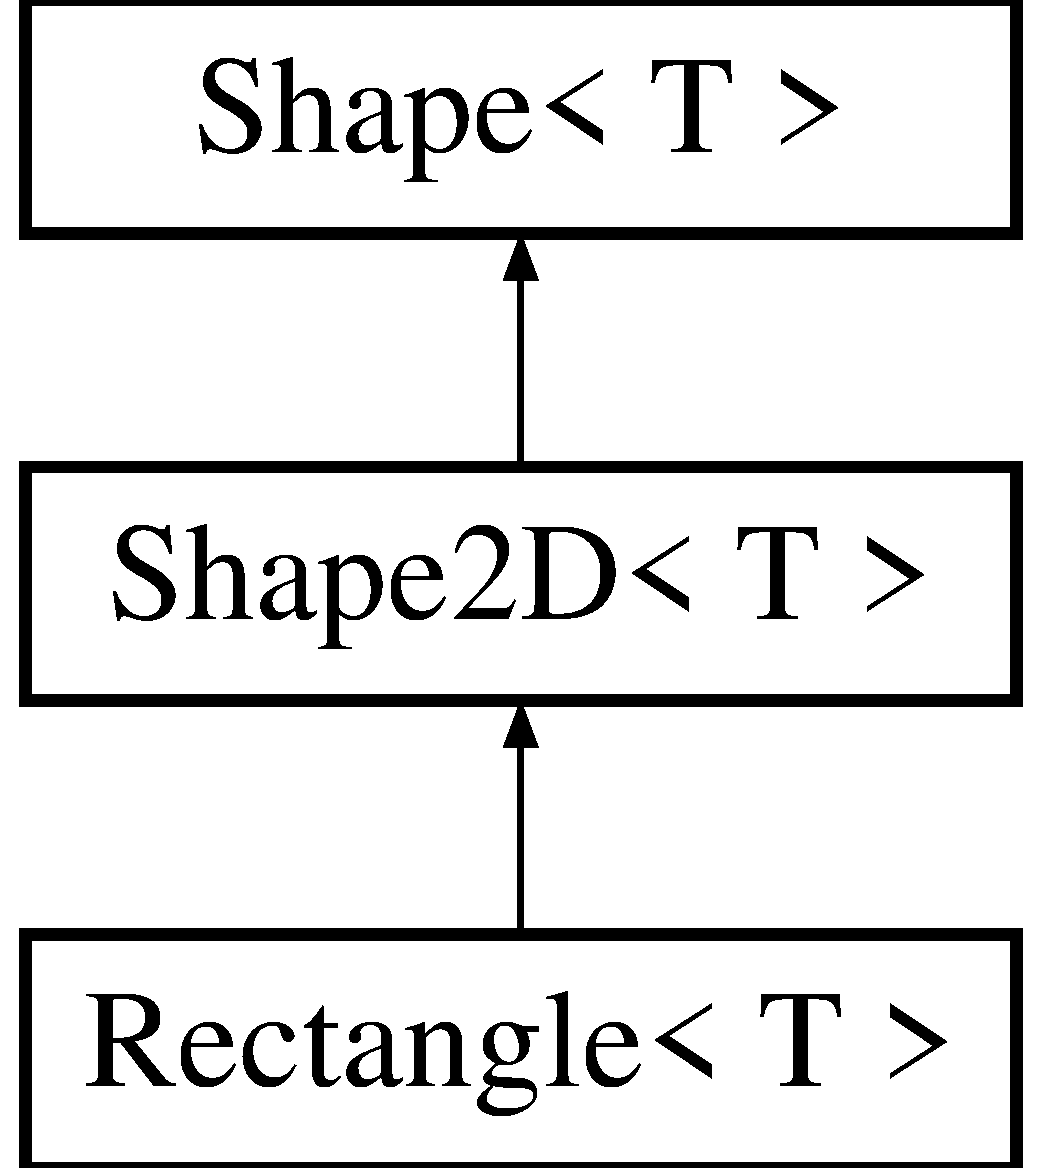
\includegraphics[height=3.000000cm]{classRectangle}
\end{center}
\end{figure}
\subsection*{Public Member Functions}
\begin{DoxyCompactItemize}
\item 
\mbox{\hyperlink{classRectangle_a9d9da3fc8bcb125516cbf2d711d325eb}{Rectangle}} ()
\begin{DoxyCompactList}\small\item\em \mbox{\hyperlink{classA}{A}} basic constructor. \end{DoxyCompactList}\item 
\mbox{\hyperlink{classRectangle_a34cf921863291153b40d9b447f812aa4}{Rectangle}} (\mbox{\hyperlink{classRectangle}{Rectangle}} \&\&)=default
\item 
\mbox{\hyperlink{classRectangle}{Rectangle}} \& \mbox{\hyperlink{classRectangle_ab53b617f14505834f525ec614ccce5c8}{operator=}} (\mbox{\hyperlink{classRectangle}{Rectangle}} \&\&)=default
\item 
\mbox{\hyperlink{classRectangle_acf27dae8f7c9a022428bda816903db2e}{Rectangle}} (const \mbox{\hyperlink{classRectangle}{Rectangle}} \&)=default
\item 
\mbox{\hyperlink{classRectangle}{Rectangle}} \& \mbox{\hyperlink{classRectangle_ad0a038c8959e5bde09bf1e8f49980bea}{operator=}} (const \mbox{\hyperlink{classRectangle}{Rectangle}} \&)=default
\item 
T \mbox{\hyperlink{classRectangle_a9c59dcb7376296711ad86e2da924d3c8}{perimeter}} ()
\end{DoxyCompactItemize}
\subsection*{Private Member Functions}
\begin{DoxyCompactItemize}
\item 
void \mbox{\hyperlink{classRectangle_a0f9d67fb9478883f067c47cdc7bf7bca}{generate\+\_\+vertexes}} ()
\begin{DoxyCompactList}\small\item\em Sets all four vertexes in correct order. \end{DoxyCompactList}\end{DoxyCompactItemize}
\subsection*{Additional Inherited Members}


\subsection{Detailed Description}
\subsubsection*{template$<$typename T = float$>$\newline
class Rectangle$<$ T $>$}

Class holding rectangle vertexes. 

\subsection{Constructor \& Destructor Documentation}
\mbox{\Hypertarget{classRectangle_a9d9da3fc8bcb125516cbf2d711d325eb}\label{classRectangle_a9d9da3fc8bcb125516cbf2d711d325eb}} 
\index{Rectangle@{Rectangle}!Rectangle@{Rectangle}}
\index{Rectangle@{Rectangle}!Rectangle@{Rectangle}}
\subsubsection{\texorpdfstring{Rectangle()}{Rectangle()}\hspace{0.1cm}{\footnotesize\ttfamily [1/3]}}
{\footnotesize\ttfamily template$<$typename T $>$ \\
\mbox{\hyperlink{classRectangle}{Rectangle}}$<$ T $>$\+::\mbox{\hyperlink{classRectangle}{Rectangle}} (\begin{DoxyParamCaption}{ }\end{DoxyParamCaption})}



\mbox{\hyperlink{classA}{A}} basic constructor. 

Constructor generates vertexes, initializes buffers and generates opengl buffers \mbox{\Hypertarget{classRectangle_a34cf921863291153b40d9b447f812aa4}\label{classRectangle_a34cf921863291153b40d9b447f812aa4}} 
\index{Rectangle@{Rectangle}!Rectangle@{Rectangle}}
\index{Rectangle@{Rectangle}!Rectangle@{Rectangle}}
\subsubsection{\texorpdfstring{Rectangle()}{Rectangle()}\hspace{0.1cm}{\footnotesize\ttfamily [2/3]}}
{\footnotesize\ttfamily template$<$typename T  = float$>$ \\
\mbox{\hyperlink{classRectangle}{Rectangle}}$<$ T $>$\+::\mbox{\hyperlink{classRectangle}{Rectangle}} (\begin{DoxyParamCaption}\item[{\mbox{\hyperlink{classRectangle}{Rectangle}}$<$ T $>$ \&\&}]{ }\end{DoxyParamCaption})\hspace{0.3cm}{\ttfamily [default]}}

\mbox{\Hypertarget{classRectangle_acf27dae8f7c9a022428bda816903db2e}\label{classRectangle_acf27dae8f7c9a022428bda816903db2e}} 
\index{Rectangle@{Rectangle}!Rectangle@{Rectangle}}
\index{Rectangle@{Rectangle}!Rectangle@{Rectangle}}
\subsubsection{\texorpdfstring{Rectangle()}{Rectangle()}\hspace{0.1cm}{\footnotesize\ttfamily [3/3]}}
{\footnotesize\ttfamily template$<$typename T  = float$>$ \\
\mbox{\hyperlink{classRectangle}{Rectangle}}$<$ T $>$\+::\mbox{\hyperlink{classRectangle}{Rectangle}} (\begin{DoxyParamCaption}\item[{const \mbox{\hyperlink{classRectangle}{Rectangle}}$<$ T $>$ \&}]{ }\end{DoxyParamCaption})\hspace{0.3cm}{\ttfamily [default]}}



\subsection{Member Function Documentation}
\mbox{\Hypertarget{classRectangle_a0f9d67fb9478883f067c47cdc7bf7bca}\label{classRectangle_a0f9d67fb9478883f067c47cdc7bf7bca}} 
\index{Rectangle@{Rectangle}!generate\+\_\+vertexes@{generate\+\_\+vertexes}}
\index{generate\+\_\+vertexes@{generate\+\_\+vertexes}!Rectangle@{Rectangle}}
\subsubsection{\texorpdfstring{generate\+\_\+vertexes()}{generate\_vertexes()}}
{\footnotesize\ttfamily template$<$typename T $>$ \\
void \mbox{\hyperlink{classRectangle}{Rectangle}}$<$ T $>$\+::generate\+\_\+vertexes (\begin{DoxyParamCaption}{ }\end{DoxyParamCaption})\hspace{0.3cm}{\ttfamily [private]}}



Sets all four vertexes in correct order. 

\mbox{\Hypertarget{classRectangle_ab53b617f14505834f525ec614ccce5c8}\label{classRectangle_ab53b617f14505834f525ec614ccce5c8}} 
\index{Rectangle@{Rectangle}!operator=@{operator=}}
\index{operator=@{operator=}!Rectangle@{Rectangle}}
\subsubsection{\texorpdfstring{operator=()}{operator=()}\hspace{0.1cm}{\footnotesize\ttfamily [1/2]}}
{\footnotesize\ttfamily template$<$typename T  = float$>$ \\
\mbox{\hyperlink{classRectangle}{Rectangle}}\& \mbox{\hyperlink{classRectangle}{Rectangle}}$<$ T $>$\+::operator= (\begin{DoxyParamCaption}\item[{\mbox{\hyperlink{classRectangle}{Rectangle}}$<$ T $>$ \&\&}]{ }\end{DoxyParamCaption})\hspace{0.3cm}{\ttfamily [default]}}

\mbox{\Hypertarget{classRectangle_ad0a038c8959e5bde09bf1e8f49980bea}\label{classRectangle_ad0a038c8959e5bde09bf1e8f49980bea}} 
\index{Rectangle@{Rectangle}!operator=@{operator=}}
\index{operator=@{operator=}!Rectangle@{Rectangle}}
\subsubsection{\texorpdfstring{operator=()}{operator=()}\hspace{0.1cm}{\footnotesize\ttfamily [2/2]}}
{\footnotesize\ttfamily template$<$typename T  = float$>$ \\
\mbox{\hyperlink{classRectangle}{Rectangle}}\& \mbox{\hyperlink{classRectangle}{Rectangle}}$<$ T $>$\+::operator= (\begin{DoxyParamCaption}\item[{const \mbox{\hyperlink{classRectangle}{Rectangle}}$<$ T $>$ \&}]{ }\end{DoxyParamCaption})\hspace{0.3cm}{\ttfamily [default]}}

\mbox{\Hypertarget{classRectangle_a9c59dcb7376296711ad86e2da924d3c8}\label{classRectangle_a9c59dcb7376296711ad86e2da924d3c8}} 
\index{Rectangle@{Rectangle}!perimeter@{perimeter}}
\index{perimeter@{perimeter}!Rectangle@{Rectangle}}
\subsubsection{\texorpdfstring{perimeter()}{perimeter()}}
{\footnotesize\ttfamily template$<$typename T $>$ \\
T \mbox{\hyperlink{classRectangle}{Rectangle}}$<$ T $>$\+::perimeter (\begin{DoxyParamCaption}{ }\end{DoxyParamCaption})}



The documentation for this class was generated from the following file\+:\begin{DoxyCompactItemize}
\item 
src/shapes/\mbox{\hyperlink{rectangle_8hpp}{rectangle.\+hpp}}\end{DoxyCompactItemize}

\hypertarget{classShader}{}\section{Shader$<$ T $>$ Class Template Reference}
\label{classShader}\index{Shader$<$ T $>$@{Shader$<$ T $>$}}


Class for shaders. \mbox{\hyperlink{classThis}{This}} class compiles three shaders, one for each dimension.  




{\ttfamily \#include \char`\"{}shader\+\_\+class.\+hpp\char`\"{}}

\subsection*{Public Member Functions}
\begin{DoxyCompactItemize}
\item 
\mbox{\hyperlink{classShader_a02faa1d7140779d7a24e06d1aff58d68}{Shader}} ()
\item 
\mbox{\hyperlink{classShader_a7e30078f161d1c9f48a7b3921c01f816}{Shader}} (\mbox{\hyperlink{classShader}{Shader}} \&\&)=delete
\item 
\mbox{\hyperlink{classShader}{Shader}} \& \mbox{\hyperlink{classShader_a3b92fece66095389581a2bf6b3124657}{operator=}} (\mbox{\hyperlink{classShader}{Shader}} \&\&)=delete
\item 
\mbox{\hyperlink{classShader_a49b2a448a00b5e1413c17501f8873cca}{Shader}} (const \mbox{\hyperlink{classShader}{Shader}} \&)=delete
\item 
\mbox{\hyperlink{classShader}{Shader}} \& \mbox{\hyperlink{classShader_a58f724fecccecdb1633e08ce0258da37}{operator=}} (const \mbox{\hyperlink{classShader}{Shader}} \&)=delete
\item 
unsigned \mbox{\hyperlink{classShader_a2c19b216850480109f9d5f7ed6ab6aa6}{get\+\_\+shader\+\_\+program}} (int i)
\end{DoxyCompactItemize}
\subsection*{Protected Member Functions}
\begin{DoxyCompactItemize}
\item 
void \mbox{\hyperlink{classShader_a1176d69a08aef6df3b7850104871a839}{compile\+\_\+shaders}} ()
\item 
{\footnotesize template$<$$>$ }\\void \mbox{\hyperlink{classShader_a3ffd553eceda4e9d5a1d8b4a5a157659}{compile\+\_\+shaders}} ()
\begin{DoxyCompactList}\small\item\em Constructor compiles shaders and tests them. \end{DoxyCompactList}\item 
{\footnotesize template$<$$>$ }\\void \mbox{\hyperlink{classShader_ae486635d367b6054482c56747ed74846}{compile\+\_\+shaders}} ()
\begin{DoxyCompactList}\small\item\em Constructor compiles shaders and tests them. \end{DoxyCompactList}\end{DoxyCompactItemize}
\subsection*{Protected Attributes}
\begin{DoxyCompactItemize}
\item 
unsigned \mbox{\hyperlink{classShader_af8ec4edd2b1b56f32ce416280ff9b9e1}{shader\+\_\+program}} \mbox{[}3\mbox{]}
\item 
bool \mbox{\hyperlink{classShader_a057162ea090f838f7fbb658cb301efc4}{shaders\+\_\+compiled}} \mbox{[}3\mbox{]}
\end{DoxyCompactItemize}


\subsection{Detailed Description}
\subsubsection*{template$<$R\+E\+N\+D\+E\+R\+\_\+\+T\+Y\+PE T$>$\newline
class Shader$<$ T $>$}

Class for shaders. \mbox{\hyperlink{classThis}{This}} class compiles three shaders, one for each dimension. 

Class can either be U\+N\+I\+F\+O\+R\+M\+\_\+\+C\+O\+L\+OR or C\+U\+S\+T\+O\+M\+\_\+\+C\+O\+L\+OR class. The difference is in shaders they compile. The first one compiles shader which assigns a single color to all vertexes. The latter assigns seprate color to each vertex. 

\subsection{Constructor \& Destructor Documentation}
\mbox{\Hypertarget{classShader_a02faa1d7140779d7a24e06d1aff58d68}\label{classShader_a02faa1d7140779d7a24e06d1aff58d68}} 
\index{Shader@{Shader}!Shader@{Shader}}
\index{Shader@{Shader}!Shader@{Shader}}
\subsubsection{\texorpdfstring{Shader()}{Shader()}\hspace{0.1cm}{\footnotesize\ttfamily [1/3]}}
{\footnotesize\ttfamily template$<$R\+E\+N\+D\+E\+R\+\_\+\+T\+Y\+PE T$>$ \\
\mbox{\hyperlink{classShader}{Shader}}$<$ T $>$\+::\mbox{\hyperlink{classShader}{Shader}} (\begin{DoxyParamCaption}{ }\end{DoxyParamCaption})\hspace{0.3cm}{\ttfamily [inline]}}

\mbox{\Hypertarget{classShader_a7e30078f161d1c9f48a7b3921c01f816}\label{classShader_a7e30078f161d1c9f48a7b3921c01f816}} 
\index{Shader@{Shader}!Shader@{Shader}}
\index{Shader@{Shader}!Shader@{Shader}}
\subsubsection{\texorpdfstring{Shader()}{Shader()}\hspace{0.1cm}{\footnotesize\ttfamily [2/3]}}
{\footnotesize\ttfamily template$<$R\+E\+N\+D\+E\+R\+\_\+\+T\+Y\+PE T$>$ \\
\mbox{\hyperlink{classShader}{Shader}}$<$ T $>$\+::\mbox{\hyperlink{classShader}{Shader}} (\begin{DoxyParamCaption}\item[{\mbox{\hyperlink{classShader}{Shader}}$<$ T $>$ \&\&}]{ }\end{DoxyParamCaption})\hspace{0.3cm}{\ttfamily [delete]}}

\mbox{\Hypertarget{classShader_a49b2a448a00b5e1413c17501f8873cca}\label{classShader_a49b2a448a00b5e1413c17501f8873cca}} 
\index{Shader@{Shader}!Shader@{Shader}}
\index{Shader@{Shader}!Shader@{Shader}}
\subsubsection{\texorpdfstring{Shader()}{Shader()}\hspace{0.1cm}{\footnotesize\ttfamily [3/3]}}
{\footnotesize\ttfamily template$<$R\+E\+N\+D\+E\+R\+\_\+\+T\+Y\+PE T$>$ \\
\mbox{\hyperlink{classShader}{Shader}}$<$ T $>$\+::\mbox{\hyperlink{classShader}{Shader}} (\begin{DoxyParamCaption}\item[{const \mbox{\hyperlink{classShader}{Shader}}$<$ T $>$ \&}]{ }\end{DoxyParamCaption})\hspace{0.3cm}{\ttfamily [delete]}}



\subsection{Member Function Documentation}
\mbox{\Hypertarget{classShader_a1176d69a08aef6df3b7850104871a839}\label{classShader_a1176d69a08aef6df3b7850104871a839}} 
\index{Shader@{Shader}!compile\+\_\+shaders@{compile\+\_\+shaders}}
\index{compile\+\_\+shaders@{compile\+\_\+shaders}!Shader@{Shader}}
\subsubsection{\texorpdfstring{compile\+\_\+shaders()}{compile\_shaders()}\hspace{0.1cm}{\footnotesize\ttfamily [1/3]}}
{\footnotesize\ttfamily template$<$R\+E\+N\+D\+E\+R\+\_\+\+T\+Y\+PE T$>$ \\
void \mbox{\hyperlink{classShader}{Shader}}$<$ T $>$\+::compile\+\_\+shaders (\begin{DoxyParamCaption}{ }\end{DoxyParamCaption})\hspace{0.3cm}{\ttfamily [protected]}}

\mbox{\Hypertarget{classShader_a3ffd553eceda4e9d5a1d8b4a5a157659}\label{classShader_a3ffd553eceda4e9d5a1d8b4a5a157659}} 
\index{Shader@{Shader}!compile\+\_\+shaders@{compile\+\_\+shaders}}
\index{compile\+\_\+shaders@{compile\+\_\+shaders}!Shader@{Shader}}
\subsubsection{\texorpdfstring{compile\+\_\+shaders()}{compile\_shaders()}\hspace{0.1cm}{\footnotesize\ttfamily [2/3]}}
{\footnotesize\ttfamily template$<$$>$ \\
void \mbox{\hyperlink{classShader}{Shader}}$<$ \mbox{\hyperlink{render_8hpp_a24e288e18eb7b6e01de7565001fedb60aa98862073f71a928bad5099cc3e1c2ed}{R\+E\+N\+D\+E\+R\+\_\+\+T\+Y\+P\+E\+::\+U\+N\+I\+F\+O\+R\+M\+\_\+\+C\+O\+L\+OR}} $>$\+::compile\+\_\+shaders (\begin{DoxyParamCaption}{ }\end{DoxyParamCaption})\hspace{0.3cm}{\ttfamily [inline]}, {\ttfamily [protected]}}



Constructor compiles shaders and tests them. 

\mbox{\Hypertarget{classShader_ae486635d367b6054482c56747ed74846}\label{classShader_ae486635d367b6054482c56747ed74846}} 
\index{Shader@{Shader}!compile\+\_\+shaders@{compile\+\_\+shaders}}
\index{compile\+\_\+shaders@{compile\+\_\+shaders}!Shader@{Shader}}
\subsubsection{\texorpdfstring{compile\+\_\+shaders()}{compile\_shaders()}\hspace{0.1cm}{\footnotesize\ttfamily [3/3]}}
{\footnotesize\ttfamily template$<$$>$ \\
void \mbox{\hyperlink{classShader}{Shader}}$<$ \mbox{\hyperlink{render_8hpp_a24e288e18eb7b6e01de7565001fedb60a9d34355b5a26c54b5dbab1e45245a6f4}{R\+E\+N\+D\+E\+R\+\_\+\+T\+Y\+P\+E\+::\+C\+U\+S\+T\+O\+M\+\_\+\+C\+O\+L\+OR}} $>$\+::compile\+\_\+shaders (\begin{DoxyParamCaption}{ }\end{DoxyParamCaption})\hspace{0.3cm}{\ttfamily [inline]}, {\ttfamily [protected]}}



Constructor compiles shaders and tests them. 

\mbox{\Hypertarget{classShader_a2c19b216850480109f9d5f7ed6ab6aa6}\label{classShader_a2c19b216850480109f9d5f7ed6ab6aa6}} 
\index{Shader@{Shader}!get\+\_\+shader\+\_\+program@{get\+\_\+shader\+\_\+program}}
\index{get\+\_\+shader\+\_\+program@{get\+\_\+shader\+\_\+program}!Shader@{Shader}}
\subsubsection{\texorpdfstring{get\+\_\+shader\+\_\+program()}{get\_shader\_program()}}
{\footnotesize\ttfamily template$<$R\+E\+N\+D\+E\+R\+\_\+\+T\+Y\+PE T$>$ \\
unsigned \mbox{\hyperlink{classShader}{Shader}}$<$ T $>$\+::get\+\_\+shader\+\_\+program (\begin{DoxyParamCaption}\item[{int}]{i }\end{DoxyParamCaption})\hspace{0.3cm}{\ttfamily [inline]}}

\mbox{\Hypertarget{classShader_a3b92fece66095389581a2bf6b3124657}\label{classShader_a3b92fece66095389581a2bf6b3124657}} 
\index{Shader@{Shader}!operator=@{operator=}}
\index{operator=@{operator=}!Shader@{Shader}}
\subsubsection{\texorpdfstring{operator=()}{operator=()}\hspace{0.1cm}{\footnotesize\ttfamily [1/2]}}
{\footnotesize\ttfamily template$<$R\+E\+N\+D\+E\+R\+\_\+\+T\+Y\+PE T$>$ \\
\mbox{\hyperlink{classShader}{Shader}}\& \mbox{\hyperlink{classShader}{Shader}}$<$ T $>$\+::operator= (\begin{DoxyParamCaption}\item[{\mbox{\hyperlink{classShader}{Shader}}$<$ T $>$ \&\&}]{ }\end{DoxyParamCaption})\hspace{0.3cm}{\ttfamily [delete]}}

\mbox{\Hypertarget{classShader_a58f724fecccecdb1633e08ce0258da37}\label{classShader_a58f724fecccecdb1633e08ce0258da37}} 
\index{Shader@{Shader}!operator=@{operator=}}
\index{operator=@{operator=}!Shader@{Shader}}
\subsubsection{\texorpdfstring{operator=()}{operator=()}\hspace{0.1cm}{\footnotesize\ttfamily [2/2]}}
{\footnotesize\ttfamily template$<$R\+E\+N\+D\+E\+R\+\_\+\+T\+Y\+PE T$>$ \\
\mbox{\hyperlink{classShader}{Shader}}\& \mbox{\hyperlink{classShader}{Shader}}$<$ T $>$\+::operator= (\begin{DoxyParamCaption}\item[{const \mbox{\hyperlink{classShader}{Shader}}$<$ T $>$ \&}]{ }\end{DoxyParamCaption})\hspace{0.3cm}{\ttfamily [delete]}}



\subsection{Member Data Documentation}
\mbox{\Hypertarget{classShader_af8ec4edd2b1b56f32ce416280ff9b9e1}\label{classShader_af8ec4edd2b1b56f32ce416280ff9b9e1}} 
\index{Shader@{Shader}!shader\+\_\+program@{shader\+\_\+program}}
\index{shader\+\_\+program@{shader\+\_\+program}!Shader@{Shader}}
\subsubsection{\texorpdfstring{shader\+\_\+program}{shader\_program}}
{\footnotesize\ttfamily template$<$R\+E\+N\+D\+E\+R\+\_\+\+T\+Y\+PE T$>$ \\
unsigned \mbox{\hyperlink{classShader}{Shader}}$<$ T $>$\+::shader\+\_\+program\mbox{[}3\mbox{]}\hspace{0.3cm}{\ttfamily [protected]}}

shader program array depending on which vertex size is chosen \mbox{\Hypertarget{classShader_a057162ea090f838f7fbb658cb301efc4}\label{classShader_a057162ea090f838f7fbb658cb301efc4}} 
\index{Shader@{Shader}!shaders\+\_\+compiled@{shaders\+\_\+compiled}}
\index{shaders\+\_\+compiled@{shaders\+\_\+compiled}!Shader@{Shader}}
\subsubsection{\texorpdfstring{shaders\+\_\+compiled}{shaders\_compiled}}
{\footnotesize\ttfamily template$<$R\+E\+N\+D\+E\+R\+\_\+\+T\+Y\+PE T$>$ \\
bool \mbox{\hyperlink{classShader}{Shader}}$<$ T $>$\+::shaders\+\_\+compiled\mbox{[}3\mbox{]}\hspace{0.3cm}{\ttfamily [protected]}}

{\bfseries Initial value\+:}
\begin{DoxyCode}
= \{
        \textcolor{keyword}{false}, \textcolor{keyword}{false},
        \textcolor{keyword}{false}\}
\end{DoxyCode}
true/false depending on whether the shaders were compiled 

The documentation for this class was generated from the following file\+:\begin{DoxyCompactItemize}
\item 
src/\mbox{\hyperlink{shader__class_8hpp}{shader\+\_\+class.\+hpp}}\end{DoxyCompactItemize}

\hypertarget{classShader_3_01RENDER__TYPE_1_1CUSTOM_01_4}{}\section{Shader$<$ R\+E\+N\+D\+E\+R\+\_\+\+T\+Y\+PE\+:\+:C\+U\+S\+T\+OM $>$ Class Template Reference}
\label{classShader_3_01RENDER__TYPE_1_1CUSTOM_01_4}\index{Shader$<$ R\+E\+N\+D\+E\+R\+\_\+\+T\+Y\+P\+E\+::\+C\+U\+S\+T\+O\+M $>$@{Shader$<$ R\+E\+N\+D\+E\+R\+\_\+\+T\+Y\+P\+E\+::\+C\+U\+S\+T\+O\+M $>$}}


{\ttfamily \#include \char`\"{}shader\+\_\+class.\+hpp\char`\"{}}

\subsection*{Public Member Functions}
\begin{DoxyCompactItemize}
\item 
\mbox{\hyperlink{classShader_3_01RENDER__TYPE_1_1CUSTOM_01_4_a8238c3e1a3a96e7ed2b1777a340d7947}{Shader}} (const \mbox{\hyperlink{glad_8h_ac83513893df92266f79a515488701770}{std\+::string}} \&vertex\+\_\+source\+\_\+, const \mbox{\hyperlink{glad_8h_ac83513893df92266f79a515488701770}{std\+::string}} \&geometry\+\_\+source\+\_\+, const \mbox{\hyperlink{glad_8h_ac83513893df92266f79a515488701770}{std\+::string}} \&fragment\+\_\+source\+\_\+)
\item 
\mbox{\hyperlink{classShader_3_01RENDER__TYPE_1_1CUSTOM_01_4_a4fea53201befd8962702645fe8f2526e}{Shader}} (\mbox{\hyperlink{classShader}{Shader}} \&\&)=delete
\item 
\mbox{\hyperlink{classShader}{Shader}} \& \mbox{\hyperlink{classShader_3_01RENDER__TYPE_1_1CUSTOM_01_4_a717f92caab16604933920257707046b6}{operator=}} (\mbox{\hyperlink{classShader}{Shader}} \&\&)=delete
\item 
\mbox{\hyperlink{classShader_3_01RENDER__TYPE_1_1CUSTOM_01_4_af1fbc8b0cb20d1af7905e2d896f0fb79}{Shader}} (const \mbox{\hyperlink{classShader}{Shader}} \&)=delete
\item 
\mbox{\hyperlink{classShader}{Shader}} \& \mbox{\hyperlink{classShader_3_01RENDER__TYPE_1_1CUSTOM_01_4_a44af437f5ea044824ba7937ee07d1da7}{operator=}} (const \mbox{\hyperlink{classShader}{Shader}} \&)=delete
\item 
unsigned \mbox{\hyperlink{classShader_3_01RENDER__TYPE_1_1CUSTOM_01_4_adf4d1f7a937d11102268dfb8fc7f2f9e}{get\+\_\+shader\+\_\+program}} ()
\end{DoxyCompactItemize}
\subsection*{Protected Member Functions}
\begin{DoxyCompactItemize}
\item 
\mbox{\hyperlink{glad_8h_a950fc91edb4504f62f1c577bf4727c29}{void}} \mbox{\hyperlink{classShader_3_01RENDER__TYPE_1_1CUSTOM_01_4_aede40b234ac1e38be9d0f9f2a60a26ab}{compile\+\_\+shaders}} ()
\begin{DoxyCompactList}\small\item\em Constructor compiles shaders and tests them. \end{DoxyCompactList}\item 
bool \mbox{\hyperlink{classShader_3_01RENDER__TYPE_1_1CUSTOM_01_4_afca4ecec5bed3cf6a9f219ce52e5343e}{check\+\_\+vertex\+\_\+shader}} (const unsigned shader\+\_\+)
\begin{DoxyCompactList}\small\item\em check if vertex shader has been successfully compiled \end{DoxyCompactList}\item 
bool \mbox{\hyperlink{classShader_3_01RENDER__TYPE_1_1CUSTOM_01_4_a8ba4a9ccbbf73e471434981a62b15d41}{check\+\_\+fragment\+\_\+shader}} (const unsigned shader\+\_\+)
\begin{DoxyCompactList}\small\item\em check if fragment shader has been successfully compiled \end{DoxyCompactList}\item 
bool \mbox{\hyperlink{classShader_3_01RENDER__TYPE_1_1CUSTOM_01_4_aca3ba4448a05303b92667e88e18f5cfb}{check\+\_\+geometry\+\_\+shader}} (const unsigned shader\+\_\+)
\begin{DoxyCompactList}\small\item\em check if fragment shader has been successfully compiled \end{DoxyCompactList}\item 
bool \mbox{\hyperlink{classShader_3_01RENDER__TYPE_1_1CUSTOM_01_4_af59ced307a40764c2fa1acef66e074b3}{check\+\_\+shader\+\_\+program}} (const unsigned shader\+Program)
\begin{DoxyCompactList}\small\item\em check if shader program has been successfully linked \end{DoxyCompactList}\end{DoxyCompactItemize}
\subsection*{Protected Attributes}
\begin{DoxyCompactItemize}
\item 
unsigned \mbox{\hyperlink{classShader_3_01RENDER__TYPE_1_1CUSTOM_01_4_a5baec51d258afd0d116d82cace52eace}{shader\+\_\+program}}
\item 
bool \mbox{\hyperlink{classShader_3_01RENDER__TYPE_1_1CUSTOM_01_4_a80cb5fdd63c57881cdf2b2dbb18e215e}{shaders\+\_\+compiled}} = false
\item 
const \mbox{\hyperlink{glad_8h_ac83513893df92266f79a515488701770}{std\+::string}} \mbox{\hyperlink{classShader_3_01RENDER__TYPE_1_1CUSTOM_01_4_ac6dfb0d85b637f3949777f047b1c010c}{vertex\+\_\+source}}
\item 
const \mbox{\hyperlink{glad_8h_ac83513893df92266f79a515488701770}{std\+::string}} \mbox{\hyperlink{classShader_3_01RENDER__TYPE_1_1CUSTOM_01_4_ac3319ff19c5af25e7d099fd2511066ea}{fragment\+\_\+source}}
\item 
const \mbox{\hyperlink{glad_8h_ac83513893df92266f79a515488701770}{std\+::string}} \mbox{\hyperlink{classShader_3_01RENDER__TYPE_1_1CUSTOM_01_4_acc41906788319945fc40ea589997112b}{geometry\+\_\+source}}
\end{DoxyCompactItemize}


\subsection{Constructor \& Destructor Documentation}
\mbox{\Hypertarget{classShader_3_01RENDER__TYPE_1_1CUSTOM_01_4_a8238c3e1a3a96e7ed2b1777a340d7947}\label{classShader_3_01RENDER__TYPE_1_1CUSTOM_01_4_a8238c3e1a3a96e7ed2b1777a340d7947}} 
\index{Shader$<$ R\+E\+N\+D\+E\+R\+\_\+\+T\+Y\+P\+E\+::\+C\+U\+S\+T\+O\+M $>$@{Shader$<$ R\+E\+N\+D\+E\+R\+\_\+\+T\+Y\+P\+E\+::\+C\+U\+S\+T\+O\+M $>$}!Shader@{Shader}}
\index{Shader@{Shader}!Shader$<$ R\+E\+N\+D\+E\+R\+\_\+\+T\+Y\+P\+E\+::\+C\+U\+S\+T\+O\+M $>$@{Shader$<$ R\+E\+N\+D\+E\+R\+\_\+\+T\+Y\+P\+E\+::\+C\+U\+S\+T\+O\+M $>$}}
\subsubsection{\texorpdfstring{Shader()}{Shader()}\hspace{0.1cm}{\footnotesize\ttfamily [1/3]}}
{\footnotesize\ttfamily \mbox{\hyperlink{classShader}{Shader}}$<$ \mbox{\hyperlink{shader__class_8hpp_a24e288e18eb7b6e01de7565001fedb60a72baef04098f035e8a320b03ad197818}{R\+E\+N\+D\+E\+R\+\_\+\+T\+Y\+P\+E\+::\+C\+U\+S\+T\+OM}} $>$\+::\mbox{\hyperlink{classShader}{Shader}} (\begin{DoxyParamCaption}\item[{const \mbox{\hyperlink{glad_8h_ac83513893df92266f79a515488701770}{std\+::string}} \&}]{vertex\+\_\+source\+\_\+,  }\item[{const \mbox{\hyperlink{glad_8h_ac83513893df92266f79a515488701770}{std\+::string}} \&}]{geometry\+\_\+source\+\_\+,  }\item[{const \mbox{\hyperlink{glad_8h_ac83513893df92266f79a515488701770}{std\+::string}} \&}]{fragment\+\_\+source\+\_\+ }\end{DoxyParamCaption})\hspace{0.3cm}{\ttfamily [inline]}}

\mbox{\Hypertarget{classShader_3_01RENDER__TYPE_1_1CUSTOM_01_4_a4fea53201befd8962702645fe8f2526e}\label{classShader_3_01RENDER__TYPE_1_1CUSTOM_01_4_a4fea53201befd8962702645fe8f2526e}} 
\index{Shader$<$ R\+E\+N\+D\+E\+R\+\_\+\+T\+Y\+P\+E\+::\+C\+U\+S\+T\+O\+M $>$@{Shader$<$ R\+E\+N\+D\+E\+R\+\_\+\+T\+Y\+P\+E\+::\+C\+U\+S\+T\+O\+M $>$}!Shader@{Shader}}
\index{Shader@{Shader}!Shader$<$ R\+E\+N\+D\+E\+R\+\_\+\+T\+Y\+P\+E\+::\+C\+U\+S\+T\+O\+M $>$@{Shader$<$ R\+E\+N\+D\+E\+R\+\_\+\+T\+Y\+P\+E\+::\+C\+U\+S\+T\+O\+M $>$}}
\subsubsection{\texorpdfstring{Shader()}{Shader()}\hspace{0.1cm}{\footnotesize\ttfamily [2/3]}}
{\footnotesize\ttfamily \mbox{\hyperlink{classShader}{Shader}}$<$ \mbox{\hyperlink{shader__class_8hpp_a24e288e18eb7b6e01de7565001fedb60a72baef04098f035e8a320b03ad197818}{R\+E\+N\+D\+E\+R\+\_\+\+T\+Y\+P\+E\+::\+C\+U\+S\+T\+OM}} $>$\+::\mbox{\hyperlink{classShader}{Shader}} (\begin{DoxyParamCaption}\item[{\mbox{\hyperlink{classShader}{Shader}}$<$ \mbox{\hyperlink{shader__class_8hpp_a24e288e18eb7b6e01de7565001fedb60a72baef04098f035e8a320b03ad197818}{R\+E\+N\+D\+E\+R\+\_\+\+T\+Y\+P\+E\+::\+C\+U\+S\+T\+OM}} $>$ \&\&}]{ }\end{DoxyParamCaption})\hspace{0.3cm}{\ttfamily [delete]}}

\mbox{\Hypertarget{classShader_3_01RENDER__TYPE_1_1CUSTOM_01_4_af1fbc8b0cb20d1af7905e2d896f0fb79}\label{classShader_3_01RENDER__TYPE_1_1CUSTOM_01_4_af1fbc8b0cb20d1af7905e2d896f0fb79}} 
\index{Shader$<$ R\+E\+N\+D\+E\+R\+\_\+\+T\+Y\+P\+E\+::\+C\+U\+S\+T\+O\+M $>$@{Shader$<$ R\+E\+N\+D\+E\+R\+\_\+\+T\+Y\+P\+E\+::\+C\+U\+S\+T\+O\+M $>$}!Shader@{Shader}}
\index{Shader@{Shader}!Shader$<$ R\+E\+N\+D\+E\+R\+\_\+\+T\+Y\+P\+E\+::\+C\+U\+S\+T\+O\+M $>$@{Shader$<$ R\+E\+N\+D\+E\+R\+\_\+\+T\+Y\+P\+E\+::\+C\+U\+S\+T\+O\+M $>$}}
\subsubsection{\texorpdfstring{Shader()}{Shader()}\hspace{0.1cm}{\footnotesize\ttfamily [3/3]}}
{\footnotesize\ttfamily \mbox{\hyperlink{classShader}{Shader}}$<$ \mbox{\hyperlink{shader__class_8hpp_a24e288e18eb7b6e01de7565001fedb60a72baef04098f035e8a320b03ad197818}{R\+E\+N\+D\+E\+R\+\_\+\+T\+Y\+P\+E\+::\+C\+U\+S\+T\+OM}} $>$\+::\mbox{\hyperlink{classShader}{Shader}} (\begin{DoxyParamCaption}\item[{const \mbox{\hyperlink{classShader}{Shader}}$<$ \mbox{\hyperlink{shader__class_8hpp_a24e288e18eb7b6e01de7565001fedb60a72baef04098f035e8a320b03ad197818}{R\+E\+N\+D\+E\+R\+\_\+\+T\+Y\+P\+E\+::\+C\+U\+S\+T\+OM}} $>$ \&}]{ }\end{DoxyParamCaption})\hspace{0.3cm}{\ttfamily [delete]}}



\subsection{Member Function Documentation}
\mbox{\Hypertarget{classShader_3_01RENDER__TYPE_1_1CUSTOM_01_4_a8ba4a9ccbbf73e471434981a62b15d41}\label{classShader_3_01RENDER__TYPE_1_1CUSTOM_01_4_a8ba4a9ccbbf73e471434981a62b15d41}} 
\index{Shader$<$ R\+E\+N\+D\+E\+R\+\_\+\+T\+Y\+P\+E\+::\+C\+U\+S\+T\+O\+M $>$@{Shader$<$ R\+E\+N\+D\+E\+R\+\_\+\+T\+Y\+P\+E\+::\+C\+U\+S\+T\+O\+M $>$}!check\+\_\+fragment\+\_\+shader@{check\+\_\+fragment\+\_\+shader}}
\index{check\+\_\+fragment\+\_\+shader@{check\+\_\+fragment\+\_\+shader}!Shader$<$ R\+E\+N\+D\+E\+R\+\_\+\+T\+Y\+P\+E\+::\+C\+U\+S\+T\+O\+M $>$@{Shader$<$ R\+E\+N\+D\+E\+R\+\_\+\+T\+Y\+P\+E\+::\+C\+U\+S\+T\+O\+M $>$}}
\subsubsection{\texorpdfstring{check\+\_\+fragment\+\_\+shader()}{check\_fragment\_shader()}}
{\footnotesize\ttfamily bool \mbox{\hyperlink{classShader}{Shader}}$<$ \mbox{\hyperlink{shader__class_8hpp_a24e288e18eb7b6e01de7565001fedb60a72baef04098f035e8a320b03ad197818}{R\+E\+N\+D\+E\+R\+\_\+\+T\+Y\+P\+E\+::\+C\+U\+S\+T\+OM}} $>$\+::check\+\_\+fragment\+\_\+shader (\begin{DoxyParamCaption}\item[{const unsigned}]{shader\+\_\+ }\end{DoxyParamCaption})\hspace{0.3cm}{\ttfamily [inline]}, {\ttfamily [protected]}}



check if fragment shader has been successfully compiled 


\begin{DoxyParams}{Parameters}
{\em shader\+\_\+} & an unsigned integer referring to fragment shader \\
\hline
\end{DoxyParams}
\mbox{\Hypertarget{classShader_3_01RENDER__TYPE_1_1CUSTOM_01_4_aca3ba4448a05303b92667e88e18f5cfb}\label{classShader_3_01RENDER__TYPE_1_1CUSTOM_01_4_aca3ba4448a05303b92667e88e18f5cfb}} 
\index{Shader$<$ R\+E\+N\+D\+E\+R\+\_\+\+T\+Y\+P\+E\+::\+C\+U\+S\+T\+O\+M $>$@{Shader$<$ R\+E\+N\+D\+E\+R\+\_\+\+T\+Y\+P\+E\+::\+C\+U\+S\+T\+O\+M $>$}!check\+\_\+geometry\+\_\+shader@{check\+\_\+geometry\+\_\+shader}}
\index{check\+\_\+geometry\+\_\+shader@{check\+\_\+geometry\+\_\+shader}!Shader$<$ R\+E\+N\+D\+E\+R\+\_\+\+T\+Y\+P\+E\+::\+C\+U\+S\+T\+O\+M $>$@{Shader$<$ R\+E\+N\+D\+E\+R\+\_\+\+T\+Y\+P\+E\+::\+C\+U\+S\+T\+O\+M $>$}}
\subsubsection{\texorpdfstring{check\+\_\+geometry\+\_\+shader()}{check\_geometry\_shader()}}
{\footnotesize\ttfamily bool \mbox{\hyperlink{classShader}{Shader}}$<$ \mbox{\hyperlink{shader__class_8hpp_a24e288e18eb7b6e01de7565001fedb60a72baef04098f035e8a320b03ad197818}{R\+E\+N\+D\+E\+R\+\_\+\+T\+Y\+P\+E\+::\+C\+U\+S\+T\+OM}} $>$\+::check\+\_\+geometry\+\_\+shader (\begin{DoxyParamCaption}\item[{const unsigned}]{shader\+\_\+ }\end{DoxyParamCaption})\hspace{0.3cm}{\ttfamily [inline]}, {\ttfamily [protected]}}



check if fragment shader has been successfully compiled 


\begin{DoxyParams}{Parameters}
{\em shader\+\_\+} & an unsigned integer referring to fragment shader \\
\hline
\end{DoxyParams}
\mbox{\Hypertarget{classShader_3_01RENDER__TYPE_1_1CUSTOM_01_4_af59ced307a40764c2fa1acef66e074b3}\label{classShader_3_01RENDER__TYPE_1_1CUSTOM_01_4_af59ced307a40764c2fa1acef66e074b3}} 
\index{Shader$<$ R\+E\+N\+D\+E\+R\+\_\+\+T\+Y\+P\+E\+::\+C\+U\+S\+T\+O\+M $>$@{Shader$<$ R\+E\+N\+D\+E\+R\+\_\+\+T\+Y\+P\+E\+::\+C\+U\+S\+T\+O\+M $>$}!check\+\_\+shader\+\_\+program@{check\+\_\+shader\+\_\+program}}
\index{check\+\_\+shader\+\_\+program@{check\+\_\+shader\+\_\+program}!Shader$<$ R\+E\+N\+D\+E\+R\+\_\+\+T\+Y\+P\+E\+::\+C\+U\+S\+T\+O\+M $>$@{Shader$<$ R\+E\+N\+D\+E\+R\+\_\+\+T\+Y\+P\+E\+::\+C\+U\+S\+T\+O\+M $>$}}
\subsubsection{\texorpdfstring{check\+\_\+shader\+\_\+program()}{check\_shader\_program()}}
{\footnotesize\ttfamily bool \mbox{\hyperlink{classShader}{Shader}}$<$ \mbox{\hyperlink{shader__class_8hpp_a24e288e18eb7b6e01de7565001fedb60a72baef04098f035e8a320b03ad197818}{R\+E\+N\+D\+E\+R\+\_\+\+T\+Y\+P\+E\+::\+C\+U\+S\+T\+OM}} $>$\+::check\+\_\+shader\+\_\+program (\begin{DoxyParamCaption}\item[{const unsigned}]{shader\+Program }\end{DoxyParamCaption})\hspace{0.3cm}{\ttfamily [inline]}, {\ttfamily [protected]}}



check if shader program has been successfully linked 


\begin{DoxyParams}{Parameters}
{\em shader\+Program} & an unsigned integer referring to shader program \\
\hline
\end{DoxyParams}
\mbox{\Hypertarget{classShader_3_01RENDER__TYPE_1_1CUSTOM_01_4_afca4ecec5bed3cf6a9f219ce52e5343e}\label{classShader_3_01RENDER__TYPE_1_1CUSTOM_01_4_afca4ecec5bed3cf6a9f219ce52e5343e}} 
\index{Shader$<$ R\+E\+N\+D\+E\+R\+\_\+\+T\+Y\+P\+E\+::\+C\+U\+S\+T\+O\+M $>$@{Shader$<$ R\+E\+N\+D\+E\+R\+\_\+\+T\+Y\+P\+E\+::\+C\+U\+S\+T\+O\+M $>$}!check\+\_\+vertex\+\_\+shader@{check\+\_\+vertex\+\_\+shader}}
\index{check\+\_\+vertex\+\_\+shader@{check\+\_\+vertex\+\_\+shader}!Shader$<$ R\+E\+N\+D\+E\+R\+\_\+\+T\+Y\+P\+E\+::\+C\+U\+S\+T\+O\+M $>$@{Shader$<$ R\+E\+N\+D\+E\+R\+\_\+\+T\+Y\+P\+E\+::\+C\+U\+S\+T\+O\+M $>$}}
\subsubsection{\texorpdfstring{check\+\_\+vertex\+\_\+shader()}{check\_vertex\_shader()}}
{\footnotesize\ttfamily bool \mbox{\hyperlink{classShader}{Shader}}$<$ \mbox{\hyperlink{shader__class_8hpp_a24e288e18eb7b6e01de7565001fedb60a72baef04098f035e8a320b03ad197818}{R\+E\+N\+D\+E\+R\+\_\+\+T\+Y\+P\+E\+::\+C\+U\+S\+T\+OM}} $>$\+::check\+\_\+vertex\+\_\+shader (\begin{DoxyParamCaption}\item[{const unsigned}]{shader\+\_\+ }\end{DoxyParamCaption})\hspace{0.3cm}{\ttfamily [inline]}, {\ttfamily [protected]}}



check if vertex shader has been successfully compiled 


\begin{DoxyParams}{Parameters}
{\em shader\+\_\+} & an unsigned integer referring to vertex shader \\
\hline
\end{DoxyParams}
\mbox{\Hypertarget{classShader_3_01RENDER__TYPE_1_1CUSTOM_01_4_aede40b234ac1e38be9d0f9f2a60a26ab}\label{classShader_3_01RENDER__TYPE_1_1CUSTOM_01_4_aede40b234ac1e38be9d0f9f2a60a26ab}} 
\index{Shader$<$ R\+E\+N\+D\+E\+R\+\_\+\+T\+Y\+P\+E\+::\+C\+U\+S\+T\+O\+M $>$@{Shader$<$ R\+E\+N\+D\+E\+R\+\_\+\+T\+Y\+P\+E\+::\+C\+U\+S\+T\+O\+M $>$}!compile\+\_\+shaders@{compile\+\_\+shaders}}
\index{compile\+\_\+shaders@{compile\+\_\+shaders}!Shader$<$ R\+E\+N\+D\+E\+R\+\_\+\+T\+Y\+P\+E\+::\+C\+U\+S\+T\+O\+M $>$@{Shader$<$ R\+E\+N\+D\+E\+R\+\_\+\+T\+Y\+P\+E\+::\+C\+U\+S\+T\+O\+M $>$}}
\subsubsection{\texorpdfstring{compile\+\_\+shaders()}{compile\_shaders()}}
{\footnotesize\ttfamily \mbox{\hyperlink{glad_8h_a950fc91edb4504f62f1c577bf4727c29}{void}} \mbox{\hyperlink{classShader}{Shader}}$<$ \mbox{\hyperlink{shader__class_8hpp_a24e288e18eb7b6e01de7565001fedb60a72baef04098f035e8a320b03ad197818}{R\+E\+N\+D\+E\+R\+\_\+\+T\+Y\+P\+E\+::\+C\+U\+S\+T\+OM}} $>$\+::compile\+\_\+shaders (\begin{DoxyParamCaption}{ }\end{DoxyParamCaption})\hspace{0.3cm}{\ttfamily [inline]}, {\ttfamily [protected]}}



Constructor compiles shaders and tests them. 

\mbox{\Hypertarget{classShader_3_01RENDER__TYPE_1_1CUSTOM_01_4_adf4d1f7a937d11102268dfb8fc7f2f9e}\label{classShader_3_01RENDER__TYPE_1_1CUSTOM_01_4_adf4d1f7a937d11102268dfb8fc7f2f9e}} 
\index{Shader$<$ R\+E\+N\+D\+E\+R\+\_\+\+T\+Y\+P\+E\+::\+C\+U\+S\+T\+O\+M $>$@{Shader$<$ R\+E\+N\+D\+E\+R\+\_\+\+T\+Y\+P\+E\+::\+C\+U\+S\+T\+O\+M $>$}!get\+\_\+shader\+\_\+program@{get\+\_\+shader\+\_\+program}}
\index{get\+\_\+shader\+\_\+program@{get\+\_\+shader\+\_\+program}!Shader$<$ R\+E\+N\+D\+E\+R\+\_\+\+T\+Y\+P\+E\+::\+C\+U\+S\+T\+O\+M $>$@{Shader$<$ R\+E\+N\+D\+E\+R\+\_\+\+T\+Y\+P\+E\+::\+C\+U\+S\+T\+O\+M $>$}}
\subsubsection{\texorpdfstring{get\+\_\+shader\+\_\+program()}{get\_shader\_program()}}
{\footnotesize\ttfamily unsigned \mbox{\hyperlink{classShader}{Shader}}$<$ \mbox{\hyperlink{shader__class_8hpp_a24e288e18eb7b6e01de7565001fedb60a72baef04098f035e8a320b03ad197818}{R\+E\+N\+D\+E\+R\+\_\+\+T\+Y\+P\+E\+::\+C\+U\+S\+T\+OM}} $>$\+::get\+\_\+shader\+\_\+program (\begin{DoxyParamCaption}{ }\end{DoxyParamCaption})\hspace{0.3cm}{\ttfamily [inline]}}

\mbox{\Hypertarget{classShader_3_01RENDER__TYPE_1_1CUSTOM_01_4_a717f92caab16604933920257707046b6}\label{classShader_3_01RENDER__TYPE_1_1CUSTOM_01_4_a717f92caab16604933920257707046b6}} 
\index{Shader$<$ R\+E\+N\+D\+E\+R\+\_\+\+T\+Y\+P\+E\+::\+C\+U\+S\+T\+O\+M $>$@{Shader$<$ R\+E\+N\+D\+E\+R\+\_\+\+T\+Y\+P\+E\+::\+C\+U\+S\+T\+O\+M $>$}!operator=@{operator=}}
\index{operator=@{operator=}!Shader$<$ R\+E\+N\+D\+E\+R\+\_\+\+T\+Y\+P\+E\+::\+C\+U\+S\+T\+O\+M $>$@{Shader$<$ R\+E\+N\+D\+E\+R\+\_\+\+T\+Y\+P\+E\+::\+C\+U\+S\+T\+O\+M $>$}}
\subsubsection{\texorpdfstring{operator=()}{operator=()}\hspace{0.1cm}{\footnotesize\ttfamily [1/2]}}
{\footnotesize\ttfamily \mbox{\hyperlink{classShader}{Shader}}\& \mbox{\hyperlink{classShader}{Shader}}$<$ \mbox{\hyperlink{shader__class_8hpp_a24e288e18eb7b6e01de7565001fedb60a72baef04098f035e8a320b03ad197818}{R\+E\+N\+D\+E\+R\+\_\+\+T\+Y\+P\+E\+::\+C\+U\+S\+T\+OM}} $>$\+::operator= (\begin{DoxyParamCaption}\item[{\mbox{\hyperlink{classShader}{Shader}}$<$ \mbox{\hyperlink{shader__class_8hpp_a24e288e18eb7b6e01de7565001fedb60a72baef04098f035e8a320b03ad197818}{R\+E\+N\+D\+E\+R\+\_\+\+T\+Y\+P\+E\+::\+C\+U\+S\+T\+OM}} $>$ \&\&}]{ }\end{DoxyParamCaption})\hspace{0.3cm}{\ttfamily [delete]}}

\mbox{\Hypertarget{classShader_3_01RENDER__TYPE_1_1CUSTOM_01_4_a44af437f5ea044824ba7937ee07d1da7}\label{classShader_3_01RENDER__TYPE_1_1CUSTOM_01_4_a44af437f5ea044824ba7937ee07d1da7}} 
\index{Shader$<$ R\+E\+N\+D\+E\+R\+\_\+\+T\+Y\+P\+E\+::\+C\+U\+S\+T\+O\+M $>$@{Shader$<$ R\+E\+N\+D\+E\+R\+\_\+\+T\+Y\+P\+E\+::\+C\+U\+S\+T\+O\+M $>$}!operator=@{operator=}}
\index{operator=@{operator=}!Shader$<$ R\+E\+N\+D\+E\+R\+\_\+\+T\+Y\+P\+E\+::\+C\+U\+S\+T\+O\+M $>$@{Shader$<$ R\+E\+N\+D\+E\+R\+\_\+\+T\+Y\+P\+E\+::\+C\+U\+S\+T\+O\+M $>$}}
\subsubsection{\texorpdfstring{operator=()}{operator=()}\hspace{0.1cm}{\footnotesize\ttfamily [2/2]}}
{\footnotesize\ttfamily \mbox{\hyperlink{classShader}{Shader}}\& \mbox{\hyperlink{classShader}{Shader}}$<$ \mbox{\hyperlink{shader__class_8hpp_a24e288e18eb7b6e01de7565001fedb60a72baef04098f035e8a320b03ad197818}{R\+E\+N\+D\+E\+R\+\_\+\+T\+Y\+P\+E\+::\+C\+U\+S\+T\+OM}} $>$\+::operator= (\begin{DoxyParamCaption}\item[{const \mbox{\hyperlink{classShader}{Shader}}$<$ \mbox{\hyperlink{shader__class_8hpp_a24e288e18eb7b6e01de7565001fedb60a72baef04098f035e8a320b03ad197818}{R\+E\+N\+D\+E\+R\+\_\+\+T\+Y\+P\+E\+::\+C\+U\+S\+T\+OM}} $>$ \&}]{ }\end{DoxyParamCaption})\hspace{0.3cm}{\ttfamily [delete]}}



\subsection{Member Data Documentation}
\mbox{\Hypertarget{classShader_3_01RENDER__TYPE_1_1CUSTOM_01_4_ac3319ff19c5af25e7d099fd2511066ea}\label{classShader_3_01RENDER__TYPE_1_1CUSTOM_01_4_ac3319ff19c5af25e7d099fd2511066ea}} 
\index{Shader$<$ R\+E\+N\+D\+E\+R\+\_\+\+T\+Y\+P\+E\+::\+C\+U\+S\+T\+O\+M $>$@{Shader$<$ R\+E\+N\+D\+E\+R\+\_\+\+T\+Y\+P\+E\+::\+C\+U\+S\+T\+O\+M $>$}!fragment\+\_\+source@{fragment\+\_\+source}}
\index{fragment\+\_\+source@{fragment\+\_\+source}!Shader$<$ R\+E\+N\+D\+E\+R\+\_\+\+T\+Y\+P\+E\+::\+C\+U\+S\+T\+O\+M $>$@{Shader$<$ R\+E\+N\+D\+E\+R\+\_\+\+T\+Y\+P\+E\+::\+C\+U\+S\+T\+O\+M $>$}}
\subsubsection{\texorpdfstring{fragment\+\_\+source}{fragment\_source}}
{\footnotesize\ttfamily const \mbox{\hyperlink{glad_8h_ac83513893df92266f79a515488701770}{std\+::string}} \mbox{\hyperlink{classShader}{Shader}}$<$ \mbox{\hyperlink{shader__class_8hpp_a24e288e18eb7b6e01de7565001fedb60a72baef04098f035e8a320b03ad197818}{R\+E\+N\+D\+E\+R\+\_\+\+T\+Y\+P\+E\+::\+C\+U\+S\+T\+OM}} $>$\+::fragment\+\_\+source\hspace{0.3cm}{\ttfamily [protected]}}

\mbox{\Hypertarget{classShader_3_01RENDER__TYPE_1_1CUSTOM_01_4_acc41906788319945fc40ea589997112b}\label{classShader_3_01RENDER__TYPE_1_1CUSTOM_01_4_acc41906788319945fc40ea589997112b}} 
\index{Shader$<$ R\+E\+N\+D\+E\+R\+\_\+\+T\+Y\+P\+E\+::\+C\+U\+S\+T\+O\+M $>$@{Shader$<$ R\+E\+N\+D\+E\+R\+\_\+\+T\+Y\+P\+E\+::\+C\+U\+S\+T\+O\+M $>$}!geometry\+\_\+source@{geometry\+\_\+source}}
\index{geometry\+\_\+source@{geometry\+\_\+source}!Shader$<$ R\+E\+N\+D\+E\+R\+\_\+\+T\+Y\+P\+E\+::\+C\+U\+S\+T\+O\+M $>$@{Shader$<$ R\+E\+N\+D\+E\+R\+\_\+\+T\+Y\+P\+E\+::\+C\+U\+S\+T\+O\+M $>$}}
\subsubsection{\texorpdfstring{geometry\+\_\+source}{geometry\_source}}
{\footnotesize\ttfamily const \mbox{\hyperlink{glad_8h_ac83513893df92266f79a515488701770}{std\+::string}} \mbox{\hyperlink{classShader}{Shader}}$<$ \mbox{\hyperlink{shader__class_8hpp_a24e288e18eb7b6e01de7565001fedb60a72baef04098f035e8a320b03ad197818}{R\+E\+N\+D\+E\+R\+\_\+\+T\+Y\+P\+E\+::\+C\+U\+S\+T\+OM}} $>$\+::geometry\+\_\+source\hspace{0.3cm}{\ttfamily [protected]}}

\mbox{\Hypertarget{classShader_3_01RENDER__TYPE_1_1CUSTOM_01_4_a5baec51d258afd0d116d82cace52eace}\label{classShader_3_01RENDER__TYPE_1_1CUSTOM_01_4_a5baec51d258afd0d116d82cace52eace}} 
\index{Shader$<$ R\+E\+N\+D\+E\+R\+\_\+\+T\+Y\+P\+E\+::\+C\+U\+S\+T\+O\+M $>$@{Shader$<$ R\+E\+N\+D\+E\+R\+\_\+\+T\+Y\+P\+E\+::\+C\+U\+S\+T\+O\+M $>$}!shader\+\_\+program@{shader\+\_\+program}}
\index{shader\+\_\+program@{shader\+\_\+program}!Shader$<$ R\+E\+N\+D\+E\+R\+\_\+\+T\+Y\+P\+E\+::\+C\+U\+S\+T\+O\+M $>$@{Shader$<$ R\+E\+N\+D\+E\+R\+\_\+\+T\+Y\+P\+E\+::\+C\+U\+S\+T\+O\+M $>$}}
\subsubsection{\texorpdfstring{shader\+\_\+program}{shader\_program}}
{\footnotesize\ttfamily unsigned \mbox{\hyperlink{classShader}{Shader}}$<$ \mbox{\hyperlink{shader__class_8hpp_a24e288e18eb7b6e01de7565001fedb60a72baef04098f035e8a320b03ad197818}{R\+E\+N\+D\+E\+R\+\_\+\+T\+Y\+P\+E\+::\+C\+U\+S\+T\+OM}} $>$\+::shader\+\_\+program\hspace{0.3cm}{\ttfamily [protected]}}

shader program array depending on which vertex size is chosen \mbox{\Hypertarget{classShader_3_01RENDER__TYPE_1_1CUSTOM_01_4_a80cb5fdd63c57881cdf2b2dbb18e215e}\label{classShader_3_01RENDER__TYPE_1_1CUSTOM_01_4_a80cb5fdd63c57881cdf2b2dbb18e215e}} 
\index{Shader$<$ R\+E\+N\+D\+E\+R\+\_\+\+T\+Y\+P\+E\+::\+C\+U\+S\+T\+O\+M $>$@{Shader$<$ R\+E\+N\+D\+E\+R\+\_\+\+T\+Y\+P\+E\+::\+C\+U\+S\+T\+O\+M $>$}!shaders\+\_\+compiled@{shaders\+\_\+compiled}}
\index{shaders\+\_\+compiled@{shaders\+\_\+compiled}!Shader$<$ R\+E\+N\+D\+E\+R\+\_\+\+T\+Y\+P\+E\+::\+C\+U\+S\+T\+O\+M $>$@{Shader$<$ R\+E\+N\+D\+E\+R\+\_\+\+T\+Y\+P\+E\+::\+C\+U\+S\+T\+O\+M $>$}}
\subsubsection{\texorpdfstring{shaders\+\_\+compiled}{shaders\_compiled}}
{\footnotesize\ttfamily bool \mbox{\hyperlink{classShader}{Shader}}$<$ \mbox{\hyperlink{shader__class_8hpp_a24e288e18eb7b6e01de7565001fedb60a72baef04098f035e8a320b03ad197818}{R\+E\+N\+D\+E\+R\+\_\+\+T\+Y\+P\+E\+::\+C\+U\+S\+T\+OM}} $>$\+::shaders\+\_\+compiled = false\hspace{0.3cm}{\ttfamily [protected]}}

\mbox{\Hypertarget{classShader_3_01RENDER__TYPE_1_1CUSTOM_01_4_ac6dfb0d85b637f3949777f047b1c010c}\label{classShader_3_01RENDER__TYPE_1_1CUSTOM_01_4_ac6dfb0d85b637f3949777f047b1c010c}} 
\index{Shader$<$ R\+E\+N\+D\+E\+R\+\_\+\+T\+Y\+P\+E\+::\+C\+U\+S\+T\+O\+M $>$@{Shader$<$ R\+E\+N\+D\+E\+R\+\_\+\+T\+Y\+P\+E\+::\+C\+U\+S\+T\+O\+M $>$}!vertex\+\_\+source@{vertex\+\_\+source}}
\index{vertex\+\_\+source@{vertex\+\_\+source}!Shader$<$ R\+E\+N\+D\+E\+R\+\_\+\+T\+Y\+P\+E\+::\+C\+U\+S\+T\+O\+M $>$@{Shader$<$ R\+E\+N\+D\+E\+R\+\_\+\+T\+Y\+P\+E\+::\+C\+U\+S\+T\+O\+M $>$}}
\subsubsection{\texorpdfstring{vertex\+\_\+source}{vertex\_source}}
{\footnotesize\ttfamily const \mbox{\hyperlink{glad_8h_ac83513893df92266f79a515488701770}{std\+::string}} \mbox{\hyperlink{classShader}{Shader}}$<$ \mbox{\hyperlink{shader__class_8hpp_a24e288e18eb7b6e01de7565001fedb60a72baef04098f035e8a320b03ad197818}{R\+E\+N\+D\+E\+R\+\_\+\+T\+Y\+P\+E\+::\+C\+U\+S\+T\+OM}} $>$\+::vertex\+\_\+source\hspace{0.3cm}{\ttfamily [protected]}}

true/false depending on whether the shaders were successfully compiled 

The documentation for this class was generated from the following file\+:\begin{DoxyCompactItemize}
\item 
src/shaders/\mbox{\hyperlink{shader__class_8hpp}{shader\+\_\+class.\+hpp}}\end{DoxyCompactItemize}

\hypertarget{classShape}{}\section{Shape$<$ T $>$ Class Template Reference}
\label{classShape}\index{Shape$<$ T $>$@{Shape$<$ T $>$}}


virtual base class for 2D and 3D shapes  




{\ttfamily \#include \char`\"{}drawing\+\_\+functions.\+hpp\char`\"{}}

Inheritance diagram for Shape$<$ T $>$\+:\begin{figure}[H]
\begin{center}
\leavevmode
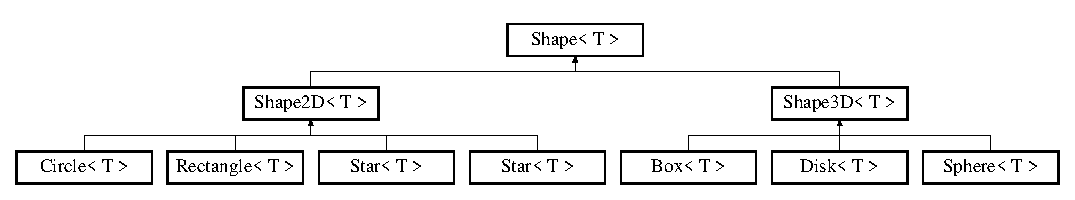
\includegraphics[height=2.242991cm]{classShape}
\end{center}
\end{figure}
\subsection*{Public Member Functions}
\begin{DoxyCompactItemize}
\item 
virtual void \mbox{\hyperlink{classShape_ac5a35fe1b2ecb8fcfc050a31c8969805}{set\+\_\+min\+\_\+number\+\_\+of\+\_\+vertexes}} (unsigned num)
\begin{DoxyCompactList}\small\item\em As the name says, it sets minimal number of vertexes for a given shape. \end{DoxyCompactList}\item 
virtual void \mbox{\hyperlink{classShape_a69dabd50440dba1ac463ad6819cdb506}{set\+\_\+vertex\+\_\+colors}} (\mbox{\hyperlink{type__definitions_8hpp_accb98a876f193a416d9c8a02fe22d526}{aligned\+\_\+vector}}$<$ float $>$ \&colors\+\_\+)
\item 
\mbox{\hyperlink{type__definitions_8hpp_accb98a876f193a416d9c8a02fe22d526}{aligned\+\_\+vector}}$<$ T $>$ \mbox{\hyperlink{classShape_a3729bbdd0c4e4f3379498734807bb545}{get\+\_\+vertexes}} ()
\item 
\mbox{\hyperlink{type__definitions_8hpp_accb98a876f193a416d9c8a02fe22d526}{aligned\+\_\+vector}}$<$ T $>$ \mbox{\hyperlink{classShape_aabe9bd208b0ece9824cb45deccc11ba7}{get\+\_\+colors}} ()
\item 
unsigned \mbox{\hyperlink{classShape_a131e85c7f5cad85bffb92e6719117cab}{num\+\_\+vertexes}} ()
\item 
virtual unsigned \mbox{\hyperlink{classShape_a58713d8cf7c4175e7c76eae75c94bc13}{get\+\_\+vertex\+\_\+size}} ()
\item 
void \mbox{\hyperlink{classShape_aabeb601fe95b412987d5b5c276bf8a7a}{generate\+\_\+random\+\_\+colors}} ()
\begin{DoxyCompactList}\small\item\em Generate random colors for each vertex. \end{DoxyCompactList}\end{DoxyCompactItemize}
\subsection*{Protected Member Functions}
\begin{DoxyCompactItemize}
\item 
void \mbox{\hyperlink{classShape_a8b4f54a694871f9d131fdd105e1ca709}{initialize\+\_\+buffers}} ()
\begin{DoxyCompactList}\small\item\em Allocates and initializes vertex buffer object, element buffer object and vertex array object. It also allocates color buffer -\/ where color for each vertex is stored. \end{DoxyCompactList}\end{DoxyCompactItemize}
\subsection*{Protected Attributes}
\begin{DoxyCompactItemize}
\item 
unsigned \mbox{\hyperlink{classShape_a7cf9cc243cdd64215eca4d81704c7199}{vertex\+\_\+size}} = 0
\item 
\mbox{\hyperlink{type__definitions_8hpp_accb98a876f193a416d9c8a02fe22d526}{aligned\+\_\+vector}}$<$ T $>$ \mbox{\hyperlink{classShape_a50296217cf654fc7b756b67a2f0305c2}{vertexes}}
\item 
char \mbox{\hyperlink{classShape_a851fcb33238286342f670d27443ffdfc}{draw\+\_\+type}}
\item 
\mbox{\hyperlink{type__definitions_8hpp_accb98a876f193a416d9c8a02fe22d526}{aligned\+\_\+vector}}$<$ int $>$ \mbox{\hyperlink{classShape_accef3084e7e3897e01806b90da0a0ec8}{element\+\_\+array}}
\item 
bool \mbox{\hyperlink{classShape_a216866713d16c882a0f0b0b0a89d350d}{colors\+\_\+loaded}}
\item 
unsigned \mbox{\hyperlink{classShape_a5ca89aadcd89bb475d6ca88acf733ce6}{V\+BO}}
\item 
unsigned \mbox{\hyperlink{classShape_a30771567edd66db5d14dc630f2d63f82}{V\+AO}}
\item 
unsigned \mbox{\hyperlink{classShape_a95c775e548b129e23d2dd32e23fb0f3e}{E\+BO}}
\item 
unsigned \mbox{\hyperlink{classShape_a66502f6f87b46a705d131dc7b0b67d42}{C\+BO}}
\item 
unsigned \mbox{\hyperlink{classShape_acb30d3bdd3434dc2cb3074a4d61985ed}{min\+\_\+vertexes}}
\item 
\mbox{\hyperlink{type__definitions_8hpp_accb98a876f193a416d9c8a02fe22d526}{aligned\+\_\+vector}}$<$ float $>$ \mbox{\hyperlink{classShape_a1590ef02d7090f28d1ad312fd46f5030}{vertex\+\_\+colors}}
\end{DoxyCompactItemize}
\subsection*{Friends}
\begin{DoxyCompactItemize}
\item 
void \mbox{\hyperlink{classShape_a0f7d9c8330ae4f062c6f569a7400e1f0}{draw}} (\mbox{\hyperlink{classShape}{Shape}}$<$ T $>$ \&, \mbox{\hyperlink{classShader}{Shader}}$<$ \mbox{\hyperlink{render_8hpp_a24e288e18eb7b6e01de7565001fedb60aa98862073f71a928bad5099cc3e1c2ed}{R\+E\+N\+D\+E\+R\+\_\+\+T\+Y\+P\+E\+::\+U\+N\+I\+F\+O\+R\+M\+\_\+\+C\+O\+L\+OR}} $>$ \&, std\+::array$<$ float, 3 $>$, std\+::array$<$ float, 3 $>$, std\+::array$<$ float, 3 $>$, float, glm\+::vec4)
\item 
void \mbox{\hyperlink{classShape_a29e514c040e0781bfa2e08bcde4a7557}{draw}} (\mbox{\hyperlink{classShape}{Shape}}$<$ T $>$ \&, \mbox{\hyperlink{classShader}{Shader}}$<$ \mbox{\hyperlink{render_8hpp_a24e288e18eb7b6e01de7565001fedb60a9d34355b5a26c54b5dbab1e45245a6f4}{R\+E\+N\+D\+E\+R\+\_\+\+T\+Y\+P\+E\+::\+C\+U\+S\+T\+O\+M\+\_\+\+C\+O\+L\+OR}} $>$ \&, std\+::array$<$ float, 3 $>$, std\+::array$<$ float, 3 $>$, std\+::array$<$ float, 3 $>$, float)
\item 
void \mbox{\hyperlink{classShape_ad57e4dd441b60269c43114f31ffa6085}{draw\+\_\+wireframe}} (\mbox{\hyperlink{classShape}{Shape}}$<$ T $>$ \&shape, \mbox{\hyperlink{classShader}{Shader}}$<$ \mbox{\hyperlink{render_8hpp_a24e288e18eb7b6e01de7565001fedb60aa98862073f71a928bad5099cc3e1c2ed}{R\+E\+N\+D\+E\+R\+\_\+\+T\+Y\+P\+E\+::\+U\+N\+I\+F\+O\+R\+M\+\_\+\+C\+O\+L\+OR}} $>$ \&shader\+\_\+object, std\+::array$<$ float, 3 $>$ scale, std\+::array$<$ float, 3 $>$ position, std\+::array$<$ float, 3 $>$ rotation\+\_\+axis, float angle, glm\+::vec4)
\item 
void \mbox{\hyperlink{classShape_aaff31c90cf40c78284454009c9fe0966}{draw\+\_\+2d\+\_\+object}} (\mbox{\hyperlink{classShape}{Shape}}$<$ T $>$ \&shape, \mbox{\hyperlink{classShader}{Shader}}$<$ \mbox{\hyperlink{render_8hpp_a24e288e18eb7b6e01de7565001fedb60aa98862073f71a928bad5099cc3e1c2ed}{R\+E\+N\+D\+E\+R\+\_\+\+T\+Y\+P\+E\+::\+U\+N\+I\+F\+O\+R\+M\+\_\+\+C\+O\+L\+OR}} $>$ \&shader\+\_\+object, std\+::array$<$ float, 3 $>$ scale, std\+::array$<$ float, 3 $>$ position, std\+::array$<$ float, 3 $>$ rotation\+\_\+axis, float angle, glm\+::vec4)
\end{DoxyCompactItemize}


\subsection{Detailed Description}
\subsubsection*{template$<$typename T$>$\newline
class Shape$<$ T $>$}

virtual base class for 2D and 3D shapes 

All shapes inherit from this class. It contains all basic structures for drawing including opengl buffers. 

\subsection{Member Function Documentation}
\mbox{\Hypertarget{classShape_aabeb601fe95b412987d5b5c276bf8a7a}\label{classShape_aabeb601fe95b412987d5b5c276bf8a7a}} 
\index{Shape@{Shape}!generate\+\_\+random\+\_\+colors@{generate\+\_\+random\+\_\+colors}}
\index{generate\+\_\+random\+\_\+colors@{generate\+\_\+random\+\_\+colors}!Shape@{Shape}}
\subsubsection{\texorpdfstring{generate\+\_\+random\+\_\+colors()}{generate\_random\_colors()}}
{\footnotesize\ttfamily template$<$typename T$>$ \\
void \mbox{\hyperlink{classShape}{Shape}}$<$ T $>$\+::generate\+\_\+random\+\_\+colors (\begin{DoxyParamCaption}{ }\end{DoxyParamCaption})\hspace{0.3cm}{\ttfamily [inline]}}



Generate random colors for each vertex. 

\mbox{\Hypertarget{classShape_aabe9bd208b0ece9824cb45deccc11ba7}\label{classShape_aabe9bd208b0ece9824cb45deccc11ba7}} 
\index{Shape@{Shape}!get\+\_\+colors@{get\+\_\+colors}}
\index{get\+\_\+colors@{get\+\_\+colors}!Shape@{Shape}}
\subsubsection{\texorpdfstring{get\+\_\+colors()}{get\_colors()}}
{\footnotesize\ttfamily template$<$typename T$>$ \\
\mbox{\hyperlink{type__definitions_8hpp_accb98a876f193a416d9c8a02fe22d526}{aligned\+\_\+vector}}$<$T$>$ \mbox{\hyperlink{classShape}{Shape}}$<$ T $>$\+::get\+\_\+colors (\begin{DoxyParamCaption}{ }\end{DoxyParamCaption})\hspace{0.3cm}{\ttfamily [inline]}}

\mbox{\Hypertarget{classShape_a58713d8cf7c4175e7c76eae75c94bc13}\label{classShape_a58713d8cf7c4175e7c76eae75c94bc13}} 
\index{Shape@{Shape}!get\+\_\+vertex\+\_\+size@{get\+\_\+vertex\+\_\+size}}
\index{get\+\_\+vertex\+\_\+size@{get\+\_\+vertex\+\_\+size}!Shape@{Shape}}
\subsubsection{\texorpdfstring{get\+\_\+vertex\+\_\+size()}{get\_vertex\_size()}}
{\footnotesize\ttfamily template$<$typename T$>$ \\
virtual unsigned \mbox{\hyperlink{classShape}{Shape}}$<$ T $>$\+::get\+\_\+vertex\+\_\+size (\begin{DoxyParamCaption}{ }\end{DoxyParamCaption})\hspace{0.3cm}{\ttfamily [inline]}, {\ttfamily [virtual]}}

\mbox{\Hypertarget{classShape_a3729bbdd0c4e4f3379498734807bb545}\label{classShape_a3729bbdd0c4e4f3379498734807bb545}} 
\index{Shape@{Shape}!get\+\_\+vertexes@{get\+\_\+vertexes}}
\index{get\+\_\+vertexes@{get\+\_\+vertexes}!Shape@{Shape}}
\subsubsection{\texorpdfstring{get\+\_\+vertexes()}{get\_vertexes()}}
{\footnotesize\ttfamily template$<$typename T$>$ \\
\mbox{\hyperlink{type__definitions_8hpp_accb98a876f193a416d9c8a02fe22d526}{aligned\+\_\+vector}}$<$T$>$ \mbox{\hyperlink{classShape}{Shape}}$<$ T $>$\+::get\+\_\+vertexes (\begin{DoxyParamCaption}{ }\end{DoxyParamCaption})\hspace{0.3cm}{\ttfamily [inline]}}

\mbox{\Hypertarget{classShape_a8b4f54a694871f9d131fdd105e1ca709}\label{classShape_a8b4f54a694871f9d131fdd105e1ca709}} 
\index{Shape@{Shape}!initialize\+\_\+buffers@{initialize\+\_\+buffers}}
\index{initialize\+\_\+buffers@{initialize\+\_\+buffers}!Shape@{Shape}}
\subsubsection{\texorpdfstring{initialize\+\_\+buffers()}{initialize\_buffers()}}
{\footnotesize\ttfamily template$<$typename T$>$ \\
void \mbox{\hyperlink{classShape}{Shape}}$<$ T $>$\+::initialize\+\_\+buffers (\begin{DoxyParamCaption}{ }\end{DoxyParamCaption})\hspace{0.3cm}{\ttfamily [inline]}, {\ttfamily [protected]}}



Allocates and initializes vertex buffer object, element buffer object and vertex array object. It also allocates color buffer -\/ where color for each vertex is stored. 

\mbox{\Hypertarget{classShape_a131e85c7f5cad85bffb92e6719117cab}\label{classShape_a131e85c7f5cad85bffb92e6719117cab}} 
\index{Shape@{Shape}!num\+\_\+vertexes@{num\+\_\+vertexes}}
\index{num\+\_\+vertexes@{num\+\_\+vertexes}!Shape@{Shape}}
\subsubsection{\texorpdfstring{num\+\_\+vertexes()}{num\_vertexes()}}
{\footnotesize\ttfamily template$<$typename T$>$ \\
unsigned \mbox{\hyperlink{classShape}{Shape}}$<$ T $>$\+::num\+\_\+vertexes (\begin{DoxyParamCaption}{ }\end{DoxyParamCaption})\hspace{0.3cm}{\ttfamily [inline]}}

\mbox{\Hypertarget{classShape_ac5a35fe1b2ecb8fcfc050a31c8969805}\label{classShape_ac5a35fe1b2ecb8fcfc050a31c8969805}} 
\index{Shape@{Shape}!set\+\_\+min\+\_\+number\+\_\+of\+\_\+vertexes@{set\+\_\+min\+\_\+number\+\_\+of\+\_\+vertexes}}
\index{set\+\_\+min\+\_\+number\+\_\+of\+\_\+vertexes@{set\+\_\+min\+\_\+number\+\_\+of\+\_\+vertexes}!Shape@{Shape}}
\subsubsection{\texorpdfstring{set\+\_\+min\+\_\+number\+\_\+of\+\_\+vertexes()}{set\_min\_number\_of\_vertexes()}}
{\footnotesize\ttfamily template$<$typename T$>$ \\
virtual void \mbox{\hyperlink{classShape}{Shape}}$<$ T $>$\+::set\+\_\+min\+\_\+number\+\_\+of\+\_\+vertexes (\begin{DoxyParamCaption}\item[{unsigned}]{num }\end{DoxyParamCaption})\hspace{0.3cm}{\ttfamily [inline]}, {\ttfamily [virtual]}}



As the name says, it sets minimal number of vertexes for a given shape. 


\begin{DoxyParams}{Parameters}
{\em num} & minimal number of vertexes \\
\hline
\end{DoxyParams}
\mbox{\Hypertarget{classShape_a69dabd50440dba1ac463ad6819cdb506}\label{classShape_a69dabd50440dba1ac463ad6819cdb506}} 
\index{Shape@{Shape}!set\+\_\+vertex\+\_\+colors@{set\+\_\+vertex\+\_\+colors}}
\index{set\+\_\+vertex\+\_\+colors@{set\+\_\+vertex\+\_\+colors}!Shape@{Shape}}
\subsubsection{\texorpdfstring{set\+\_\+vertex\+\_\+colors()}{set\_vertex\_colors()}}
{\footnotesize\ttfamily template$<$typename T$>$ \\
virtual void \mbox{\hyperlink{classShape}{Shape}}$<$ T $>$\+::set\+\_\+vertex\+\_\+colors (\begin{DoxyParamCaption}\item[{\mbox{\hyperlink{type__definitions_8hpp_accb98a876f193a416d9c8a02fe22d526}{aligned\+\_\+vector}}$<$ float $>$ \&}]{colors\+\_\+ }\end{DoxyParamCaption})\hspace{0.3cm}{\ttfamily [inline]}, {\ttfamily [virtual]}}



\subsection{Friends And Related Function Documentation}
\mbox{\Hypertarget{classShape_a0f7d9c8330ae4f062c6f569a7400e1f0}\label{classShape_a0f7d9c8330ae4f062c6f569a7400e1f0}} 
\index{Shape@{Shape}!draw@{draw}}
\index{draw@{draw}!Shape@{Shape}}
\subsubsection{\texorpdfstring{draw}{draw}\hspace{0.1cm}{\footnotesize\ttfamily [1/2]}}
{\footnotesize\ttfamily template$<$typename T$>$ \\
void draw (\begin{DoxyParamCaption}\item[{\mbox{\hyperlink{classShape}{Shape}}$<$ T $>$ \&}]{shape,  }\item[{\mbox{\hyperlink{classShader}{Shader}}$<$ \mbox{\hyperlink{render_8hpp_a24e288e18eb7b6e01de7565001fedb60aa98862073f71a928bad5099cc3e1c2ed}{R\+E\+N\+D\+E\+R\+\_\+\+T\+Y\+P\+E\+::\+U\+N\+I\+F\+O\+R\+M\+\_\+\+C\+O\+L\+OR}} $>$ \&}]{shader\+\_\+object,  }\item[{std\+::array$<$ float, 3 $>$}]{scale = {\ttfamily \{0.5,~0.5,~0.5\}},  }\item[{std\+::array$<$ float, 3 $>$}]{position = {\ttfamily \{0,~0,~1\}},  }\item[{std\+::array$<$ float, 3 $>$}]{rotation\+\_\+axis = {\ttfamily \{0,~0,~1\}},  }\item[{float}]{angle = {\ttfamily 0},  }\item[{glm\+::vec4}]{color = {\ttfamily \{0.5,~0.5,~0.5,~0.5\}} }\end{DoxyParamCaption})\hspace{0.3cm}{\ttfamily [friend]}}

\mbox{\Hypertarget{classShape_a29e514c040e0781bfa2e08bcde4a7557}\label{classShape_a29e514c040e0781bfa2e08bcde4a7557}} 
\index{Shape@{Shape}!draw@{draw}}
\index{draw@{draw}!Shape@{Shape}}
\subsubsection{\texorpdfstring{draw}{draw}\hspace{0.1cm}{\footnotesize\ttfamily [2/2]}}
{\footnotesize\ttfamily template$<$typename T$>$ \\
void draw (\begin{DoxyParamCaption}\item[{\mbox{\hyperlink{classShape}{Shape}}$<$ T $>$ \&}]{shape,  }\item[{\mbox{\hyperlink{classShader}{Shader}}$<$ \mbox{\hyperlink{render_8hpp_a24e288e18eb7b6e01de7565001fedb60a9d34355b5a26c54b5dbab1e45245a6f4}{R\+E\+N\+D\+E\+R\+\_\+\+T\+Y\+P\+E\+::\+C\+U\+S\+T\+O\+M\+\_\+\+C\+O\+L\+OR}} $>$ \&}]{shader\+\_\+object,  }\item[{std\+::array$<$ float, 3 $>$}]{scale = {\ttfamily \{0.5,~0.5,~0.5\}},  }\item[{std\+::array$<$ float, 3 $>$}]{position = {\ttfamily \{0,~0,~1\}},  }\item[{std\+::array$<$ float, 3 $>$}]{rotation\+\_\+axis = {\ttfamily \{0,~0,~1\}},  }\item[{float}]{angle = {\ttfamily 0} }\end{DoxyParamCaption})\hspace{0.3cm}{\ttfamily [friend]}}

\mbox{\Hypertarget{classShape_aaff31c90cf40c78284454009c9fe0966}\label{classShape_aaff31c90cf40c78284454009c9fe0966}} 
\index{Shape@{Shape}!draw\+\_\+2d\+\_\+object@{draw\+\_\+2d\+\_\+object}}
\index{draw\+\_\+2d\+\_\+object@{draw\+\_\+2d\+\_\+object}!Shape@{Shape}}
\subsubsection{\texorpdfstring{draw\+\_\+2d\+\_\+object}{draw\_2d\_object}}
{\footnotesize\ttfamily template$<$typename T$>$ \\
void draw\+\_\+2d\+\_\+object (\begin{DoxyParamCaption}\item[{\mbox{\hyperlink{classShape}{Shape}}$<$ T $>$ \&}]{shape,  }\item[{\mbox{\hyperlink{classShader}{Shader}}$<$ \mbox{\hyperlink{render_8hpp_a24e288e18eb7b6e01de7565001fedb60aa98862073f71a928bad5099cc3e1c2ed}{R\+E\+N\+D\+E\+R\+\_\+\+T\+Y\+P\+E\+::\+U\+N\+I\+F\+O\+R\+M\+\_\+\+C\+O\+L\+OR}} $>$ \&}]{shader\+\_\+object,  }\item[{std\+::array$<$ float, 3 $>$}]{scale = {\ttfamily \{0.5,~0.5,~0.5\}},  }\item[{std\+::array$<$ float, 3 $>$}]{position = {\ttfamily \{0,~0,~1\}},  }\item[{std\+::array$<$ float, 3 $>$}]{rotation\+\_\+axis = {\ttfamily \{0,~0,~1\}},  }\item[{float}]{angle = {\ttfamily 0},  }\item[{glm\+::vec4}]{color = {\ttfamily \{0.5,~0.5,~0.5,~0.5\}} }\end{DoxyParamCaption})\hspace{0.3cm}{\ttfamily [friend]}}

\mbox{\Hypertarget{classShape_ad57e4dd441b60269c43114f31ffa6085}\label{classShape_ad57e4dd441b60269c43114f31ffa6085}} 
\index{Shape@{Shape}!draw\+\_\+wireframe@{draw\+\_\+wireframe}}
\index{draw\+\_\+wireframe@{draw\+\_\+wireframe}!Shape@{Shape}}
\subsubsection{\texorpdfstring{draw\+\_\+wireframe}{draw\_wireframe}}
{\footnotesize\ttfamily template$<$typename T$>$ \\
void draw\+\_\+wireframe (\begin{DoxyParamCaption}\item[{\mbox{\hyperlink{classShape}{Shape}}$<$ T $>$ \&}]{shape,  }\item[{\mbox{\hyperlink{classShader}{Shader}}$<$ \mbox{\hyperlink{render_8hpp_a24e288e18eb7b6e01de7565001fedb60aa98862073f71a928bad5099cc3e1c2ed}{R\+E\+N\+D\+E\+R\+\_\+\+T\+Y\+P\+E\+::\+U\+N\+I\+F\+O\+R\+M\+\_\+\+C\+O\+L\+OR}} $>$ \&}]{shader\+\_\+object,  }\item[{std\+::array$<$ float, 3 $>$}]{scale = {\ttfamily \{0.5,~0.5,~0.5\}},  }\item[{std\+::array$<$ float, 3 $>$}]{position = {\ttfamily \{0,~0,~1\}},  }\item[{std\+::array$<$ float, 3 $>$}]{rotation\+\_\+axis = {\ttfamily \{0,~0,~1\}},  }\item[{float}]{angle = {\ttfamily 0},  }\item[{glm\+::vec4}]{color = {\ttfamily \{0.5,~0.5,~0.5,~0.5\}} }\end{DoxyParamCaption})\hspace{0.3cm}{\ttfamily [friend]}}



\subsection{Member Data Documentation}
\mbox{\Hypertarget{classShape_a66502f6f87b46a705d131dc7b0b67d42}\label{classShape_a66502f6f87b46a705d131dc7b0b67d42}} 
\index{Shape@{Shape}!C\+BO@{C\+BO}}
\index{C\+BO@{C\+BO}!Shape@{Shape}}
\subsubsection{\texorpdfstring{C\+BO}{CBO}}
{\footnotesize\ttfamily template$<$typename T$>$ \\
unsigned \mbox{\hyperlink{classShape}{Shape}}$<$ T $>$\+::C\+BO\hspace{0.3cm}{\ttfamily [protected]}}

color buffer address \mbox{\Hypertarget{classShape_a216866713d16c882a0f0b0b0a89d350d}\label{classShape_a216866713d16c882a0f0b0b0a89d350d}} 
\index{Shape@{Shape}!colors\+\_\+loaded@{colors\+\_\+loaded}}
\index{colors\+\_\+loaded@{colors\+\_\+loaded}!Shape@{Shape}}
\subsubsection{\texorpdfstring{colors\+\_\+loaded}{colors\_loaded}}
{\footnotesize\ttfamily template$<$typename T$>$ \\
bool \mbox{\hyperlink{classShape}{Shape}}$<$ T $>$\+::colors\+\_\+loaded\hspace{0.3cm}{\ttfamily [protected]}}

{\bfseries Initial value\+:}
\begin{DoxyCode}
=
        \textcolor{keyword}{false}
\end{DoxyCode}
indicator whether color have been loaded or not vertex size can consist of 2, 3 or 4 points; this is important for correct interpretation of vertexes vector \mbox{\Hypertarget{classShape_a851fcb33238286342f670d27443ffdfc}\label{classShape_a851fcb33238286342f670d27443ffdfc}} 
\index{Shape@{Shape}!draw\+\_\+type@{draw\+\_\+type}}
\index{draw\+\_\+type@{draw\+\_\+type}!Shape@{Shape}}
\subsubsection{\texorpdfstring{draw\+\_\+type}{draw\_type}}
{\footnotesize\ttfamily template$<$typename T$>$ \\
char \mbox{\hyperlink{classShape}{Shape}}$<$ T $>$\+::draw\+\_\+type\hspace{0.3cm}{\ttfamily [protected]}}

this can either be \textquotesingle{}E\textquotesingle{} or \textquotesingle{}V\textquotesingle{}, depending on wheather to draw elements (element buffer) or vertexes (vertex buffer object) \mbox{\Hypertarget{classShape_a95c775e548b129e23d2dd32e23fb0f3e}\label{classShape_a95c775e548b129e23d2dd32e23fb0f3e}} 
\index{Shape@{Shape}!E\+BO@{E\+BO}}
\index{E\+BO@{E\+BO}!Shape@{Shape}}
\subsubsection{\texorpdfstring{E\+BO}{EBO}}
{\footnotesize\ttfamily template$<$typename T$>$ \\
unsigned \mbox{\hyperlink{classShape}{Shape}}$<$ T $>$\+::E\+BO\hspace{0.3cm}{\ttfamily [protected]}}

element buffer address \mbox{\Hypertarget{classShape_accef3084e7e3897e01806b90da0a0ec8}\label{classShape_accef3084e7e3897e01806b90da0a0ec8}} 
\index{Shape@{Shape}!element\+\_\+array@{element\+\_\+array}}
\index{element\+\_\+array@{element\+\_\+array}!Shape@{Shape}}
\subsubsection{\texorpdfstring{element\+\_\+array}{element\_array}}
{\footnotesize\ttfamily template$<$typename T$>$ \\
\mbox{\hyperlink{type__definitions_8hpp_accb98a876f193a416d9c8a02fe22d526}{aligned\+\_\+vector}}$<$int$>$ \mbox{\hyperlink{classShape}{Shape}}$<$ T $>$\+::element\+\_\+array\hspace{0.3cm}{\ttfamily [protected]}}

vector holding all elements in correct order \mbox{\Hypertarget{classShape_acb30d3bdd3434dc2cb3074a4d61985ed}\label{classShape_acb30d3bdd3434dc2cb3074a4d61985ed}} 
\index{Shape@{Shape}!min\+\_\+vertexes@{min\+\_\+vertexes}}
\index{min\+\_\+vertexes@{min\+\_\+vertexes}!Shape@{Shape}}
\subsubsection{\texorpdfstring{min\+\_\+vertexes}{min\_vertexes}}
{\footnotesize\ttfamily template$<$typename T$>$ \\
unsigned \mbox{\hyperlink{classShape}{Shape}}$<$ T $>$\+::min\+\_\+vertexes\hspace{0.3cm}{\ttfamily [protected]}}

{\bfseries Initial value\+:}
\begin{DoxyCode}
=
        5
\end{DoxyCode}
minimal number of vertexes to be generated for a given shape \mbox{\Hypertarget{classShape_a30771567edd66db5d14dc630f2d63f82}\label{classShape_a30771567edd66db5d14dc630f2d63f82}} 
\index{Shape@{Shape}!V\+AO@{V\+AO}}
\index{V\+AO@{V\+AO}!Shape@{Shape}}
\subsubsection{\texorpdfstring{V\+AO}{VAO}}
{\footnotesize\ttfamily template$<$typename T$>$ \\
unsigned \mbox{\hyperlink{classShape}{Shape}}$<$ T $>$\+::V\+AO\hspace{0.3cm}{\ttfamily [protected]}}

vertex array object \mbox{\Hypertarget{classShape_a5ca89aadcd89bb475d6ca88acf733ce6}\label{classShape_a5ca89aadcd89bb475d6ca88acf733ce6}} 
\index{Shape@{Shape}!V\+BO@{V\+BO}}
\index{V\+BO@{V\+BO}!Shape@{Shape}}
\subsubsection{\texorpdfstring{V\+BO}{VBO}}
{\footnotesize\ttfamily template$<$typename T$>$ \\
unsigned \mbox{\hyperlink{classShape}{Shape}}$<$ T $>$\+::V\+BO\hspace{0.3cm}{\ttfamily [protected]}}

vertex buffer object \mbox{\Hypertarget{classShape_a1590ef02d7090f28d1ad312fd46f5030}\label{classShape_a1590ef02d7090f28d1ad312fd46f5030}} 
\index{Shape@{Shape}!vertex\+\_\+colors@{vertex\+\_\+colors}}
\index{vertex\+\_\+colors@{vertex\+\_\+colors}!Shape@{Shape}}
\subsubsection{\texorpdfstring{vertex\+\_\+colors}{vertex\_colors}}
{\footnotesize\ttfamily template$<$typename T$>$ \\
\mbox{\hyperlink{type__definitions_8hpp_accb98a876f193a416d9c8a02fe22d526}{aligned\+\_\+vector}}$<$float$>$ \mbox{\hyperlink{classShape}{Shape}}$<$ T $>$\+::vertex\+\_\+colors\hspace{0.3cm}{\ttfamily [protected]}}

Vector holding a color for each vertex. Four consequtive numbers form a rgb color value \mbox{\Hypertarget{classShape_a7cf9cc243cdd64215eca4d81704c7199}\label{classShape_a7cf9cc243cdd64215eca4d81704c7199}} 
\index{Shape@{Shape}!vertex\+\_\+size@{vertex\+\_\+size}}
\index{vertex\+\_\+size@{vertex\+\_\+size}!Shape@{Shape}}
\subsubsection{\texorpdfstring{vertex\+\_\+size}{vertex\_size}}
{\footnotesize\ttfamily template$<$typename T$>$ \\
unsigned \mbox{\hyperlink{classShape}{Shape}}$<$ T $>$\+::vertex\+\_\+size = 0\hspace{0.3cm}{\ttfamily [protected]}}

\mbox{\Hypertarget{classShape_a50296217cf654fc7b756b67a2f0305c2}\label{classShape_a50296217cf654fc7b756b67a2f0305c2}} 
\index{Shape@{Shape}!vertexes@{vertexes}}
\index{vertexes@{vertexes}!Shape@{Shape}}
\subsubsection{\texorpdfstring{vertexes}{vertexes}}
{\footnotesize\ttfamily template$<$typename T$>$ \\
\mbox{\hyperlink{type__definitions_8hpp_accb98a876f193a416d9c8a02fe22d526}{aligned\+\_\+vector}}$<$T$>$ \mbox{\hyperlink{classShape}{Shape}}$<$ T $>$\+::vertexes\hspace{0.3cm}{\ttfamily [protected]}}

Vector holding all vertexes; 2,3 or 4 consequtive numbers form a vertex 

The documentation for this class was generated from the following files\+:\begin{DoxyCompactItemize}
\item 
src/\mbox{\hyperlink{drawing__functions_8hpp}{drawing\+\_\+functions.\+hpp}}\item 
src/\mbox{\hyperlink{shape_8hpp}{shape.\+hpp}}\end{DoxyCompactItemize}

\hypertarget{classShape2D}{}\section{Shape2D$<$ T $>$ Class Template Reference}
\label{classShape2D}\index{Shape2\+D$<$ T $>$@{Shape2\+D$<$ T $>$}}


\mbox{\hyperlink{classThis}{This}} is a base class for all 2D shapes.  




{\ttfamily \#include \char`\"{}drawing\+\_\+functions.\+hpp\char`\"{}}

Inheritance diagram for Shape2D$<$ T $>$\+:\begin{figure}[H]
\begin{center}
\leavevmode
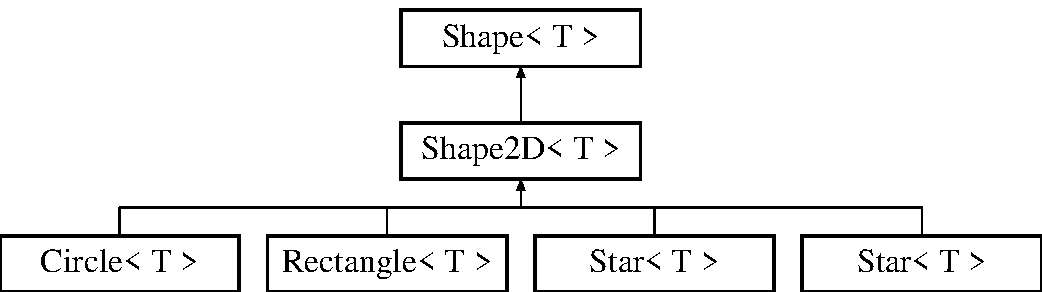
\includegraphics[height=2.688000cm]{classShape2D}
\end{center}
\end{figure}
\subsection*{Public Member Functions}
\begin{DoxyCompactItemize}
\item 
\mbox{\hyperlink{type__definitions_8hpp_a087efd587d66b881646ef378f1919c90}{aligned\+\_\+vector}}$<$ T $>$ \mbox{\hyperlink{classShape2D_af67c7aed6e58b5aa0e3518a3ad1de75b}{get\+\_\+filling\+\_\+vertexes}} ()
\end{DoxyCompactItemize}
\subsection*{Protected Member Functions}
\begin{DoxyCompactItemize}
\item 
virtual \mbox{\hyperlink{glad_8h_a950fc91edb4504f62f1c577bf4727c29}{void}} \mbox{\hyperlink{classShape2D_a917c3277ca262ec557930c8cc837c204}{generate\+\_\+filling\+\_\+vbo}} ()
\item 
{\footnotesize template$<$$>$ }\\\mbox{\hyperlink{glad_8h_a950fc91edb4504f62f1c577bf4727c29}{void}} \mbox{\hyperlink{classShape2D_a328d401b8f1962078e904d4b1003d7a5}{generate\+\_\+filling\+\_\+vbo}} ()
\begin{DoxyCompactList}\small\item\em Generates vertexes which fill the interior of 2D shapes. \end{DoxyCompactList}\end{DoxyCompactItemize}
\subsection*{Protected Attributes}
\begin{DoxyCompactItemize}
\item 
unsigned \mbox{\hyperlink{classShape2D_a220cf4cf96da8bd43627ffffd00a0718}{F\+I\+L\+L\+I\+N\+G\+\_\+\+V\+BO}}
\item 
unsigned \mbox{\hyperlink{classShape2D_affa1082cd6e91cce5af4cb10c1b3435f}{F\+I\+L\+L\+I\+N\+G\+\_\+\+E\+BO}}
\item 
char \mbox{\hyperlink{classShape2D_ab24ceddaa0114eda3ae699f8fb3503ca}{filling\+\_\+draw\+\_\+type}}
\item 
\mbox{\hyperlink{type__definitions_8hpp_a087efd587d66b881646ef378f1919c90}{aligned\+\_\+vector}}$<$ T $>$ \mbox{\hyperlink{classShape2D_ae3e216c9d8422b47f46bff9259bd17be}{filling\+\_\+vertexes}}
\item 
\mbox{\hyperlink{type__definitions_8hpp_a087efd587d66b881646ef378f1919c90}{aligned\+\_\+vector}}$<$ int $>$ \mbox{\hyperlink{classShape2D_a28d0d6018cb6b73637050d9f3fb1f006}{filling\+\_\+elements}}
\end{DoxyCompactItemize}
\subsection*{Friends}
\begin{DoxyCompactItemize}
\item 
\mbox{\hyperlink{glad_8h_a950fc91edb4504f62f1c577bf4727c29}{void}} \mbox{\hyperlink{classShape2D_a75ed525e537ded17d42e3adad87bd701}{draw\+\_\+2d\+\_\+object}} (\mbox{\hyperlink{classShape2D}{Shape2D}}$<$ T $>$ \&shape, \mbox{\hyperlink{classShader}{Shader}}$<$ \mbox{\hyperlink{shader__class_8hpp_a24e288e18eb7b6e01de7565001fedb60aa98862073f71a928bad5099cc3e1c2ed}{R\+E\+N\+D\+E\+R\+\_\+\+T\+Y\+P\+E\+::\+U\+N\+I\+F\+O\+R\+M\+\_\+\+C\+O\+L\+OR}} $>$ \&shader\+\_\+object, std\+::array$<$ float, 3 $>$ scale, std\+::array$<$ float, 3 $>$ position, std\+::array$<$ float, 3 $>$ rotation\+\_\+axis, float angle, glm\+::vec4)
\begin{DoxyCompactList}\small\item\em draw 2d shape filling of uniform color. \end{DoxyCompactList}\end{DoxyCompactItemize}


\subsection{Detailed Description}
\subsubsection*{template$<$typename T$>$\newline
class Shape2\+D$<$ T $>$}

\mbox{\hyperlink{classThis}{This}} is a base class for all 2D shapes. 

It inherits from \mbox{\hyperlink{classShape}{Shape}} class. Template parameter can either be float of double. It is meant to contain functions common to all 2D shapes. 

\subsection{Member Function Documentation}
\mbox{\Hypertarget{classShape2D_a917c3277ca262ec557930c8cc837c204}\label{classShape2D_a917c3277ca262ec557930c8cc837c204}} 
\index{Shape2D@{Shape2D}!generate\+\_\+filling\+\_\+vbo@{generate\+\_\+filling\+\_\+vbo}}
\index{generate\+\_\+filling\+\_\+vbo@{generate\+\_\+filling\+\_\+vbo}!Shape2D@{Shape2D}}
\subsubsection{\texorpdfstring{generate\+\_\+filling\+\_\+vbo()}{generate\_filling\_vbo()}\hspace{0.1cm}{\footnotesize\ttfamily [1/2]}}
{\footnotesize\ttfamily template$<$typename T$>$ \\
virtual \mbox{\hyperlink{glad_8h_a950fc91edb4504f62f1c577bf4727c29}{void}} \mbox{\hyperlink{classShape2D}{Shape2D}}$<$ T $>$\+::generate\+\_\+filling\+\_\+vbo (\begin{DoxyParamCaption}{ }\end{DoxyParamCaption})\hspace{0.3cm}{\ttfamily [protected]}, {\ttfamily [virtual]}}

\mbox{\Hypertarget{classShape2D_a328d401b8f1962078e904d4b1003d7a5}\label{classShape2D_a328d401b8f1962078e904d4b1003d7a5}} 
\index{Shape2D@{Shape2D}!generate\+\_\+filling\+\_\+vbo@{generate\+\_\+filling\+\_\+vbo}}
\index{generate\+\_\+filling\+\_\+vbo@{generate\+\_\+filling\+\_\+vbo}!Shape2D@{Shape2D}}
\subsubsection{\texorpdfstring{generate\+\_\+filling\+\_\+vbo()}{generate\_filling\_vbo()}\hspace{0.1cm}{\footnotesize\ttfamily [2/2]}}
{\footnotesize\ttfamily template$<$$>$ \\
\mbox{\hyperlink{glad_8h_a950fc91edb4504f62f1c577bf4727c29}{void}} \mbox{\hyperlink{classShape2D}{Shape2D}}$<$ float $>$\+::generate\+\_\+filling\+\_\+vbo (\begin{DoxyParamCaption}{ }\end{DoxyParamCaption})\hspace{0.3cm}{\ttfamily [inline]}, {\ttfamily [protected]}}



Generates vertexes which fill the interior of 2D shapes. 

\mbox{\Hypertarget{classShape2D_af67c7aed6e58b5aa0e3518a3ad1de75b}\label{classShape2D_af67c7aed6e58b5aa0e3518a3ad1de75b}} 
\index{Shape2D@{Shape2D}!get\+\_\+filling\+\_\+vertexes@{get\+\_\+filling\+\_\+vertexes}}
\index{get\+\_\+filling\+\_\+vertexes@{get\+\_\+filling\+\_\+vertexes}!Shape2D@{Shape2D}}
\subsubsection{\texorpdfstring{get\+\_\+filling\+\_\+vertexes()}{get\_filling\_vertexes()}}
{\footnotesize\ttfamily template$<$typename T$>$ \\
\mbox{\hyperlink{type__definitions_8hpp_a087efd587d66b881646ef378f1919c90}{aligned\+\_\+vector}}$<$T$>$ \mbox{\hyperlink{classShape2D}{Shape2D}}$<$ T $>$\+::get\+\_\+filling\+\_\+vertexes (\begin{DoxyParamCaption}{ }\end{DoxyParamCaption})\hspace{0.3cm}{\ttfamily [inline]}}



\subsection{Friends And Related Function Documentation}
\mbox{\Hypertarget{classShape2D_a75ed525e537ded17d42e3adad87bd701}\label{classShape2D_a75ed525e537ded17d42e3adad87bd701}} 
\index{Shape2D@{Shape2D}!draw\+\_\+2d\+\_\+object@{draw\+\_\+2d\+\_\+object}}
\index{draw\+\_\+2d\+\_\+object@{draw\+\_\+2d\+\_\+object}!Shape2D@{Shape2D}}
\subsubsection{\texorpdfstring{draw\+\_\+2d\+\_\+object}{draw\_2d\_object}}
{\footnotesize\ttfamily template$<$typename T$>$ \\
\mbox{\hyperlink{glad_8h_a950fc91edb4504f62f1c577bf4727c29}{void}} draw\+\_\+2d\+\_\+object (\begin{DoxyParamCaption}\item[{\mbox{\hyperlink{classShape2D}{Shape2D}}$<$ T $>$ \&}]{shape,  }\item[{\mbox{\hyperlink{classShader}{Shader}}$<$ \mbox{\hyperlink{shader__class_8hpp_a24e288e18eb7b6e01de7565001fedb60aa98862073f71a928bad5099cc3e1c2ed}{R\+E\+N\+D\+E\+R\+\_\+\+T\+Y\+P\+E\+::\+U\+N\+I\+F\+O\+R\+M\+\_\+\+C\+O\+L\+OR}} $>$ \&}]{shader\+\_\+object,  }\item[{std\+::array$<$ float, 3 $>$}]{scale = {\ttfamily \{0.5,~0.5,~0.5\}},  }\item[{std\+::array$<$ float, 3 $>$}]{position = {\ttfamily \{0,~0,~1\}},  }\item[{std\+::array$<$ float, 3 $>$}]{rotation\+\_\+axis = {\ttfamily \{0,~0,~1\}},  }\item[{float}]{angle = {\ttfamily 0},  }\item[{glm\+::vec4}]{color = {\ttfamily \{0.5,~0.5,~0.5,~0.5\}} }\end{DoxyParamCaption})\hspace{0.3cm}{\ttfamily [friend]}}



draw 2d shape filling of uniform color. 


\begin{DoxyParams}{Parameters}
{\em shape} & An object of type class \mbox{\hyperlink{classShape}{Shape}} to be drawn \\
\hline
{\em shader\+\_\+object} & Object of type class Shader$<$\+R\+E\+N\+D\+E\+R\+\_\+\+T\+Y\+P\+E\+::\+U\+N\+I\+F\+O\+R\+M\+\_\+\+C\+O\+L\+O\+R$>$, which contains correct shader. \\
\hline
{\em scale} & sscales object in x,y and z directions. \\
\hline
{\em position} & translate center of the object to coordinates specified by this vector. \\
\hline
{\em rotation\+\_\+axis} & axis around which object should be rotated. \\
\hline
{\em angle} & Angle specifying how much to rotate the object. \\
\hline
{\em color} & color of the shape -\/ the same for all vertexes \\
\hline
\end{DoxyParams}


\subsection{Member Data Documentation}
\mbox{\Hypertarget{classShape2D_ab24ceddaa0114eda3ae699f8fb3503ca}\label{classShape2D_ab24ceddaa0114eda3ae699f8fb3503ca}} 
\index{Shape2D@{Shape2D}!filling\+\_\+draw\+\_\+type@{filling\+\_\+draw\+\_\+type}}
\index{filling\+\_\+draw\+\_\+type@{filling\+\_\+draw\+\_\+type}!Shape2D@{Shape2D}}
\subsubsection{\texorpdfstring{filling\+\_\+draw\+\_\+type}{filling\_draw\_type}}
{\footnotesize\ttfamily template$<$typename T$>$ \\
char \mbox{\hyperlink{classShape2D}{Shape2D}}$<$ T $>$\+::filling\+\_\+draw\+\_\+type\hspace{0.3cm}{\ttfamily [protected]}}

tells whether to render element buffer -\/ \textquotesingle{}E\textquotesingle{} of array buffer -\/ \textquotesingle{}V\textquotesingle{} \mbox{\Hypertarget{classShape2D_affa1082cd6e91cce5af4cb10c1b3435f}\label{classShape2D_affa1082cd6e91cce5af4cb10c1b3435f}} 
\index{Shape2D@{Shape2D}!F\+I\+L\+L\+I\+N\+G\+\_\+\+E\+BO@{F\+I\+L\+L\+I\+N\+G\+\_\+\+E\+BO}}
\index{F\+I\+L\+L\+I\+N\+G\+\_\+\+E\+BO@{F\+I\+L\+L\+I\+N\+G\+\_\+\+E\+BO}!Shape2D@{Shape2D}}
\subsubsection{\texorpdfstring{F\+I\+L\+L\+I\+N\+G\+\_\+\+E\+BO}{FILLING\_EBO}}
{\footnotesize\ttfamily template$<$typename T$>$ \\
unsigned \mbox{\hyperlink{classShape2D}{Shape2D}}$<$ T $>$\+::F\+I\+L\+L\+I\+N\+G\+\_\+\+E\+BO\hspace{0.3cm}{\ttfamily [protected]}}

2D shapes consist of lines, this buffer contains elements to fill 2D shapes. \mbox{\Hypertarget{classShape2D_a28d0d6018cb6b73637050d9f3fb1f006}\label{classShape2D_a28d0d6018cb6b73637050d9f3fb1f006}} 
\index{Shape2D@{Shape2D}!filling\+\_\+elements@{filling\+\_\+elements}}
\index{filling\+\_\+elements@{filling\+\_\+elements}!Shape2D@{Shape2D}}
\subsubsection{\texorpdfstring{filling\+\_\+elements}{filling\_elements}}
{\footnotesize\ttfamily template$<$typename T$>$ \\
\mbox{\hyperlink{type__definitions_8hpp_a087efd587d66b881646ef378f1919c90}{aligned\+\_\+vector}}$<$int$>$ \mbox{\hyperlink{classShape2D}{Shape2D}}$<$ T $>$\+::filling\+\_\+elements\hspace{0.3cm}{\ttfamily [protected]}}

vertexes for interior of 2D shapes. \mbox{\Hypertarget{classShape2D_a220cf4cf96da8bd43627ffffd00a0718}\label{classShape2D_a220cf4cf96da8bd43627ffffd00a0718}} 
\index{Shape2D@{Shape2D}!F\+I\+L\+L\+I\+N\+G\+\_\+\+V\+BO@{F\+I\+L\+L\+I\+N\+G\+\_\+\+V\+BO}}
\index{F\+I\+L\+L\+I\+N\+G\+\_\+\+V\+BO@{F\+I\+L\+L\+I\+N\+G\+\_\+\+V\+BO}!Shape2D@{Shape2D}}
\subsubsection{\texorpdfstring{F\+I\+L\+L\+I\+N\+G\+\_\+\+V\+BO}{FILLING\_VBO}}
{\footnotesize\ttfamily template$<$typename T$>$ \\
unsigned \mbox{\hyperlink{classShape2D}{Shape2D}}$<$ T $>$\+::F\+I\+L\+L\+I\+N\+G\+\_\+\+V\+BO\hspace{0.3cm}{\ttfamily [protected]}}

2D shapes consist of lines, this buffer is meant to fill 2D shapes. \mbox{\Hypertarget{classShape2D_ae3e216c9d8422b47f46bff9259bd17be}\label{classShape2D_ae3e216c9d8422b47f46bff9259bd17be}} 
\index{Shape2D@{Shape2D}!filling\+\_\+vertexes@{filling\+\_\+vertexes}}
\index{filling\+\_\+vertexes@{filling\+\_\+vertexes}!Shape2D@{Shape2D}}
\subsubsection{\texorpdfstring{filling\+\_\+vertexes}{filling\_vertexes}}
{\footnotesize\ttfamily template$<$typename T$>$ \\
\mbox{\hyperlink{type__definitions_8hpp_a087efd587d66b881646ef378f1919c90}{aligned\+\_\+vector}}$<$T$>$ \mbox{\hyperlink{classShape2D}{Shape2D}}$<$ T $>$\+::filling\+\_\+vertexes\hspace{0.3cm}{\ttfamily [protected]}}

vertexes for interior of 2D shapes. 

The documentation for this class was generated from the following files\+:\begin{DoxyCompactItemize}
\item 
src/display\+\_\+and\+\_\+drawing\+\_\+functions/\mbox{\hyperlink{drawing__functions_8hpp}{drawing\+\_\+functions.\+hpp}}\item 
src/shapes/\mbox{\hyperlink{shape_8hpp}{shape.\+hpp}}\end{DoxyCompactItemize}

\hypertarget{classShape3D}{}\section{Shape3D$<$ T $>$ Class Template Reference}
\label{classShape3D}\index{Shape3\+D$<$ T $>$@{Shape3\+D$<$ T $>$}}


{\ttfamily \#include \char`\"{}shape.\+hpp\char`\"{}}

Inheritance diagram for Shape3D$<$ T $>$\+:\begin{figure}[H]
\begin{center}
\leavevmode
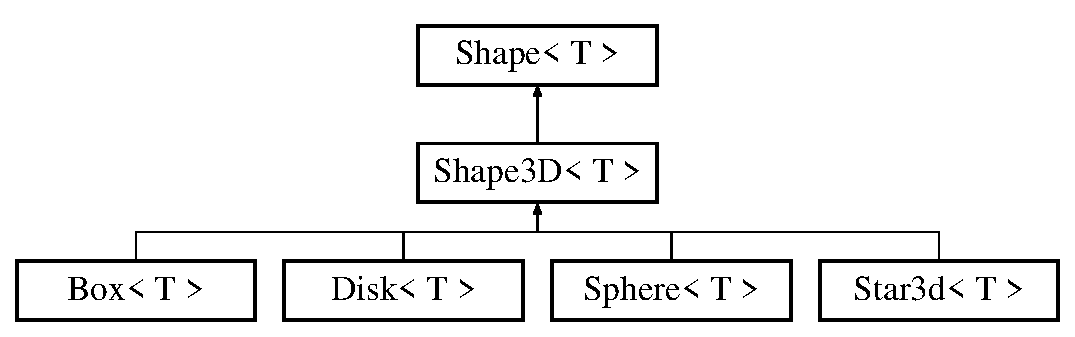
\includegraphics[height=3.000000cm]{classShape3D}
\end{center}
\end{figure}
\subsection*{Public Member Functions}
\begin{DoxyCompactItemize}
\item 
{\footnotesize template$<$typename Q  = T$>$ }\\std\+::enable\+\_\+if$<$ std\+::is\+\_\+same$<$ Q, float $>$\+::value, Q $>$\+::type \mbox{\hyperlink{classShape3D_a2e50becd374a83f43617328dbcc2de3b}{area}} ()
\end{DoxyCompactItemize}
\subsection*{Additional Inherited Members}


\subsection{Member Function Documentation}
\mbox{\Hypertarget{classShape3D_a2e50becd374a83f43617328dbcc2de3b}\label{classShape3D_a2e50becd374a83f43617328dbcc2de3b}} 
\index{Shape3D@{Shape3D}!area@{area}}
\index{area@{area}!Shape3D@{Shape3D}}
\subsubsection{\texorpdfstring{area()}{area()}}
{\footnotesize\ttfamily template$<$typename T $>$ \\
template$<$typename Q  = T$>$ \\
std\+::enable\+\_\+if$<$std\+::is\+\_\+same$<$Q, float$>$\+::value, Q$>$\+::type \mbox{\hyperlink{classShape3D}{Shape3D}}$<$ T $>$\+::area (\begin{DoxyParamCaption}{ }\end{DoxyParamCaption})\hspace{0.3cm}{\ttfamily [inline]}}



The documentation for this class was generated from the following file\+:\begin{DoxyCompactItemize}
\item 
src/\mbox{\hyperlink{shape_8hpp}{shape.\+hpp}}\end{DoxyCompactItemize}

\hypertarget{classSphere}{}\section{Sphere$<$ T $>$ Class Template Reference}
\label{classSphere}\index{Sphere$<$ T $>$@{Sphere$<$ T $>$}}


{\ttfamily \#include \char`\"{}sphere.\+hpp\char`\"{}}

Inheritance diagram for Sphere$<$ T $>$\+:\begin{figure}[H]
\begin{center}
\leavevmode
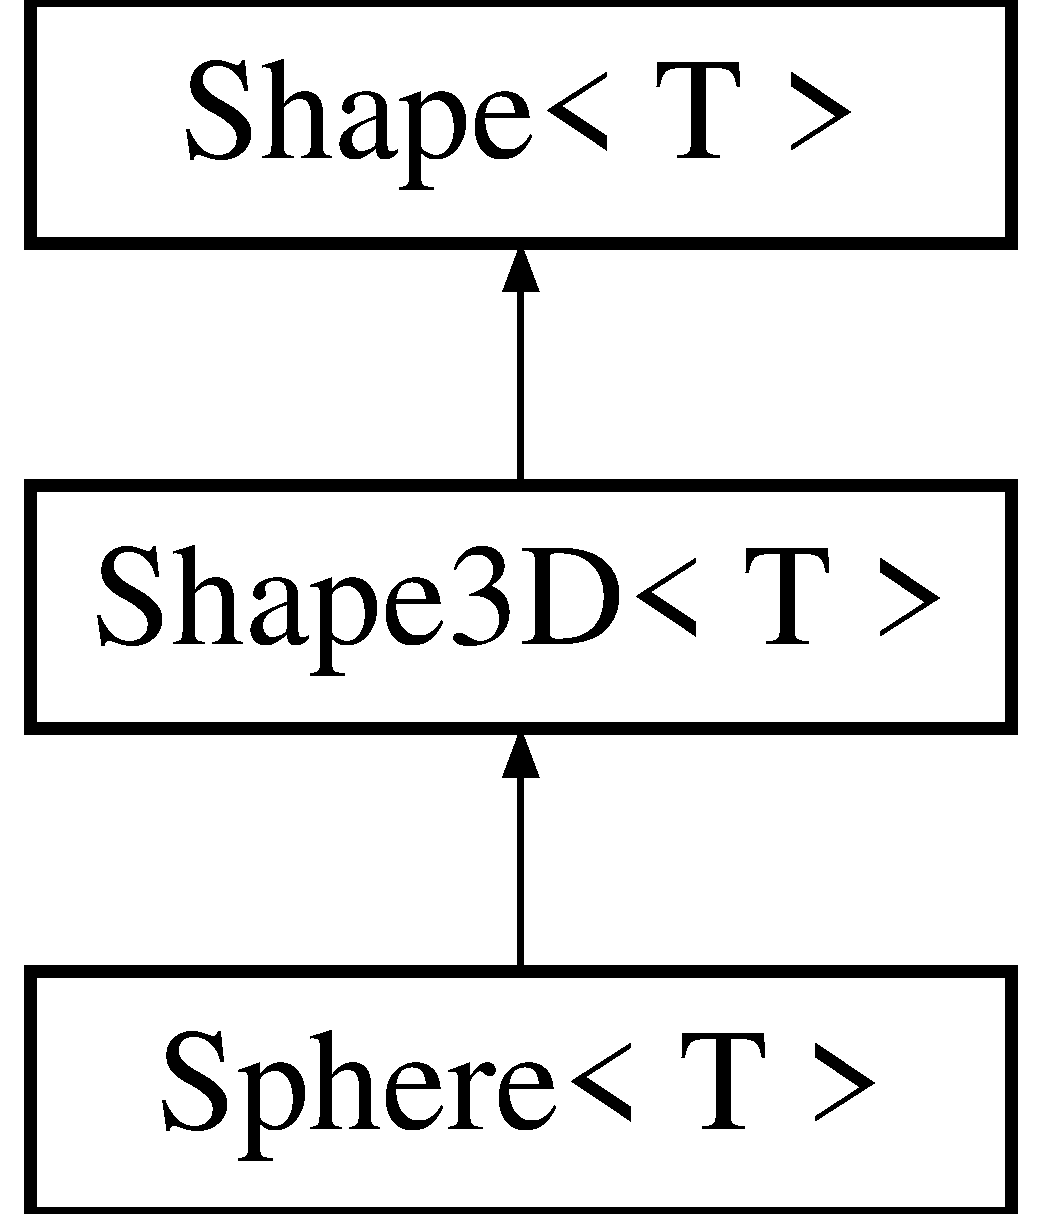
\includegraphics[height=3.000000cm]{classSphere}
\end{center}
\end{figure}
\subsection*{Public Member Functions}
\begin{DoxyCompactItemize}
\item 
\mbox{\hyperlink{classSphere_acacfd6de079ea50acdaf57b823166651}{Sphere}} ()
\begin{DoxyCompactList}\small\item\em \mbox{\hyperlink{classA}{A}} basic constructor for \mbox{\hyperlink{classSphere}{Sphere}} class. \end{DoxyCompactList}\item 
\mbox{\hyperlink{classSphere_a79e3c1cb536e3fe4d8bc447e7be0e414}{Sphere}} (int min\+\_\+vertexes\+\_\+)
\begin{DoxyCompactList}\small\item\em \mbox{\hyperlink{classA}{A}} basic constructor for \mbox{\hyperlink{classSphere}{Sphere}} class. \end{DoxyCompactList}\item 
\mbox{\hyperlink{classSphere_af0d667b078ae88955113205112d9aaa6}{Sphere}} (\mbox{\hyperlink{classSphere}{Sphere}} \&\&)=default
\item 
\mbox{\hyperlink{classSphere}{Sphere}} \& \mbox{\hyperlink{classSphere_aa117f966cea7b16532cbd80c2191a84a}{operator=}} (\mbox{\hyperlink{classSphere}{Sphere}} \&\&)=default
\item 
\mbox{\hyperlink{classSphere_ae28ad7649c59d653b9e14a3042d186a1}{Sphere}} (const \mbox{\hyperlink{classSphere}{Sphere}} \&)=default
\item 
\mbox{\hyperlink{classSphere}{Sphere}} \& \mbox{\hyperlink{classSphere_ae989d05c3ea71f5a758e90e2f2e3aecf}{operator=}} (const \mbox{\hyperlink{classSphere}{Sphere}} \&)=default
\item 
\mbox{\hyperlink{glad_8h_a950fc91edb4504f62f1c577bf4727c29}{void}} \mbox{\hyperlink{classSphere_a3f5ee2b07e48a360696fe983690d1d1f}{refine}} ()
\begin{DoxyCompactList}\small\item\em \mbox{\hyperlink{classThis}{This}} function calls generate\+\_\+vertexes\+\_\+helper to refine the mesh. \end{DoxyCompactList}\item 
T \mbox{\hyperlink{classSphere_a9ebc65dabaf8d87fbe599f4b64816f73}{quality}} ()
\begin{DoxyCompactList}\small\item\em The quality of the mesh is measured as the difference between exact pi number and the one obtained from the area of the sphere (mesh). \end{DoxyCompactList}\end{DoxyCompactItemize}
\subsection*{Private Member Functions}
\begin{DoxyCompactItemize}
\item 
\mbox{\hyperlink{glad_8h_a950fc91edb4504f62f1c577bf4727c29}{void}} \mbox{\hyperlink{classSphere_ab739ad1931e58a4ba7c84e3ca5c1965d}{generate\+\_\+vertexes\+\_\+helper\+\_\+old}} ()
\item 
\mbox{\hyperlink{glad_8h_a950fc91edb4504f62f1c577bf4727c29}{void}} \mbox{\hyperlink{classSphere_a84a45f41ca9e630beb97fc106b359ffd}{generate\+\_\+vertexes\+\_\+helper}} ()
\begin{DoxyCompactList}\small\item\em \mbox{\hyperlink{classThis}{This}} function generates vertexes for float and double version of class \mbox{\hyperlink{classCircle}{Circle}}. \end{DoxyCompactList}\item 
\mbox{\hyperlink{glad_8h_a950fc91edb4504f62f1c577bf4727c29}{void}} \mbox{\hyperlink{classSphere_a9cfac85b9803fadc4b79db0ea047f679}{generate\+\_\+vertexes}} ()
\begin{DoxyCompactList}\small\item\em \mbox{\hyperlink{classThis}{This}} function generates vertexes for class \mbox{\hyperlink{classCircle}{Circle}}. \end{DoxyCompactList}\end{DoxyCompactItemize}
\subsection*{Additional Inherited Members}


\subsection{Constructor \& Destructor Documentation}
\mbox{\Hypertarget{classSphere_acacfd6de079ea50acdaf57b823166651}\label{classSphere_acacfd6de079ea50acdaf57b823166651}} 
\index{Sphere@{Sphere}!Sphere@{Sphere}}
\index{Sphere@{Sphere}!Sphere@{Sphere}}
\subsubsection{\texorpdfstring{Sphere()}{Sphere()}\hspace{0.1cm}{\footnotesize\ttfamily [1/4]}}
{\footnotesize\ttfamily template$<$typename T = float$>$ \\
\mbox{\hyperlink{classSphere}{Sphere}}$<$ T $>$\+::\mbox{\hyperlink{classSphere}{Sphere}} (\begin{DoxyParamCaption}{ }\end{DoxyParamCaption})\hspace{0.3cm}{\ttfamily [inline]}}



\mbox{\hyperlink{classA}{A}} basic constructor for \mbox{\hyperlink{classSphere}{Sphere}} class. 

The constructor generate vertexes and elements. Opengl buffers are also allocated and initiallized. \mbox{\Hypertarget{classSphere_a79e3c1cb536e3fe4d8bc447e7be0e414}\label{classSphere_a79e3c1cb536e3fe4d8bc447e7be0e414}} 
\index{Sphere@{Sphere}!Sphere@{Sphere}}
\index{Sphere@{Sphere}!Sphere@{Sphere}}
\subsubsection{\texorpdfstring{Sphere()}{Sphere()}\hspace{0.1cm}{\footnotesize\ttfamily [2/4]}}
{\footnotesize\ttfamily template$<$typename T = float$>$ \\
\mbox{\hyperlink{classSphere}{Sphere}}$<$ T $>$\+::\mbox{\hyperlink{classSphere}{Sphere}} (\begin{DoxyParamCaption}\item[{int}]{min\+\_\+vertexes\+\_\+ }\end{DoxyParamCaption})\hspace{0.3cm}{\ttfamily [inline]}}



\mbox{\hyperlink{classA}{A}} basic constructor for \mbox{\hyperlink{classSphere}{Sphere}} class. 

The constructor generate vertexes and elements. Opengl buffers are also allocated and initiallized. 
\begin{DoxyParams}{Parameters}
{\em min\+\_\+vertexes\+\_\+} & minimal number of vertexes to create sphere \\
\hline
\end{DoxyParams}
\mbox{\Hypertarget{classSphere_af0d667b078ae88955113205112d9aaa6}\label{classSphere_af0d667b078ae88955113205112d9aaa6}} 
\index{Sphere@{Sphere}!Sphere@{Sphere}}
\index{Sphere@{Sphere}!Sphere@{Sphere}}
\subsubsection{\texorpdfstring{Sphere()}{Sphere()}\hspace{0.1cm}{\footnotesize\ttfamily [3/4]}}
{\footnotesize\ttfamily template$<$typename T = float$>$ \\
\mbox{\hyperlink{classSphere}{Sphere}}$<$ T $>$\+::\mbox{\hyperlink{classSphere}{Sphere}} (\begin{DoxyParamCaption}\item[{\mbox{\hyperlink{classSphere}{Sphere}}$<$ T $>$ \&\&}]{ }\end{DoxyParamCaption})\hspace{0.3cm}{\ttfamily [default]}}

\mbox{\Hypertarget{classSphere_ae28ad7649c59d653b9e14a3042d186a1}\label{classSphere_ae28ad7649c59d653b9e14a3042d186a1}} 
\index{Sphere@{Sphere}!Sphere@{Sphere}}
\index{Sphere@{Sphere}!Sphere@{Sphere}}
\subsubsection{\texorpdfstring{Sphere()}{Sphere()}\hspace{0.1cm}{\footnotesize\ttfamily [4/4]}}
{\footnotesize\ttfamily template$<$typename T = float$>$ \\
\mbox{\hyperlink{classSphere}{Sphere}}$<$ T $>$\+::\mbox{\hyperlink{classSphere}{Sphere}} (\begin{DoxyParamCaption}\item[{const \mbox{\hyperlink{classSphere}{Sphere}}$<$ T $>$ \&}]{ }\end{DoxyParamCaption})\hspace{0.3cm}{\ttfamily [default]}}



\subsection{Member Function Documentation}
\mbox{\Hypertarget{classSphere_a9cfac85b9803fadc4b79db0ea047f679}\label{classSphere_a9cfac85b9803fadc4b79db0ea047f679}} 
\index{Sphere@{Sphere}!generate\+\_\+vertexes@{generate\+\_\+vertexes}}
\index{generate\+\_\+vertexes@{generate\+\_\+vertexes}!Sphere@{Sphere}}
\subsubsection{\texorpdfstring{generate\+\_\+vertexes()}{generate\_vertexes()}}
{\footnotesize\ttfamily template$<$typename T $>$ \\
\mbox{\hyperlink{glad_8h_a950fc91edb4504f62f1c577bf4727c29}{void}} \mbox{\hyperlink{classSphere}{Sphere}}$<$ T $>$\+::generate\+\_\+vertexes (\begin{DoxyParamCaption}{ }\end{DoxyParamCaption})\hspace{0.3cm}{\ttfamily [private]}}



\mbox{\hyperlink{classThis}{This}} function generates vertexes for class \mbox{\hyperlink{classCircle}{Circle}}. 

Internally, it calls generate\+\_\+vertexes\+\_\+helper function to refine the mesh. \mbox{\Hypertarget{classSphere_a84a45f41ca9e630beb97fc106b359ffd}\label{classSphere_a84a45f41ca9e630beb97fc106b359ffd}} 
\index{Sphere@{Sphere}!generate\+\_\+vertexes\+\_\+helper@{generate\+\_\+vertexes\+\_\+helper}}
\index{generate\+\_\+vertexes\+\_\+helper@{generate\+\_\+vertexes\+\_\+helper}!Sphere@{Sphere}}
\subsubsection{\texorpdfstring{generate\+\_\+vertexes\+\_\+helper()}{generate\_vertexes\_helper()}}
{\footnotesize\ttfamily template$<$typename T $>$ \\
\mbox{\hyperlink{glad_8h_a950fc91edb4504f62f1c577bf4727c29}{void}} \mbox{\hyperlink{classSphere}{Sphere}}$<$ T $>$\+::generate\+\_\+vertexes\+\_\+helper (\begin{DoxyParamCaption}{ }\end{DoxyParamCaption})\hspace{0.3cm}{\ttfamily [inline]}, {\ttfamily [private]}}



\mbox{\hyperlink{classThis}{This}} function generates vertexes for float and double version of class \mbox{\hyperlink{classCircle}{Circle}}. 

It is used only when sse and avx versions are not available. \mbox{\Hypertarget{classSphere_ab739ad1931e58a4ba7c84e3ca5c1965d}\label{classSphere_ab739ad1931e58a4ba7c84e3ca5c1965d}} 
\index{Sphere@{Sphere}!generate\+\_\+vertexes\+\_\+helper\+\_\+old@{generate\+\_\+vertexes\+\_\+helper\+\_\+old}}
\index{generate\+\_\+vertexes\+\_\+helper\+\_\+old@{generate\+\_\+vertexes\+\_\+helper\+\_\+old}!Sphere@{Sphere}}
\subsubsection{\texorpdfstring{generate\+\_\+vertexes\+\_\+helper\+\_\+old()}{generate\_vertexes\_helper\_old()}}
{\footnotesize\ttfamily template$<$typename T = float$>$ \\
\mbox{\hyperlink{glad_8h_a950fc91edb4504f62f1c577bf4727c29}{void}} \mbox{\hyperlink{classSphere}{Sphere}}$<$ T $>$\+::generate\+\_\+vertexes\+\_\+helper\+\_\+old (\begin{DoxyParamCaption}{ }\end{DoxyParamCaption})\hspace{0.3cm}{\ttfamily [private]}}

\mbox{\Hypertarget{classSphere_aa117f966cea7b16532cbd80c2191a84a}\label{classSphere_aa117f966cea7b16532cbd80c2191a84a}} 
\index{Sphere@{Sphere}!operator=@{operator=}}
\index{operator=@{operator=}!Sphere@{Sphere}}
\subsubsection{\texorpdfstring{operator=()}{operator=()}\hspace{0.1cm}{\footnotesize\ttfamily [1/2]}}
{\footnotesize\ttfamily template$<$typename T = float$>$ \\
\mbox{\hyperlink{classSphere}{Sphere}}\& \mbox{\hyperlink{classSphere}{Sphere}}$<$ T $>$\+::operator= (\begin{DoxyParamCaption}\item[{\mbox{\hyperlink{classSphere}{Sphere}}$<$ T $>$ \&\&}]{ }\end{DoxyParamCaption})\hspace{0.3cm}{\ttfamily [default]}}

\mbox{\Hypertarget{classSphere_ae989d05c3ea71f5a758e90e2f2e3aecf}\label{classSphere_ae989d05c3ea71f5a758e90e2f2e3aecf}} 
\index{Sphere@{Sphere}!operator=@{operator=}}
\index{operator=@{operator=}!Sphere@{Sphere}}
\subsubsection{\texorpdfstring{operator=()}{operator=()}\hspace{0.1cm}{\footnotesize\ttfamily [2/2]}}
{\footnotesize\ttfamily template$<$typename T = float$>$ \\
\mbox{\hyperlink{classSphere}{Sphere}}\& \mbox{\hyperlink{classSphere}{Sphere}}$<$ T $>$\+::operator= (\begin{DoxyParamCaption}\item[{const \mbox{\hyperlink{classSphere}{Sphere}}$<$ T $>$ \&}]{ }\end{DoxyParamCaption})\hspace{0.3cm}{\ttfamily [default]}}

\mbox{\Hypertarget{classSphere_a9ebc65dabaf8d87fbe599f4b64816f73}\label{classSphere_a9ebc65dabaf8d87fbe599f4b64816f73}} 
\index{Sphere@{Sphere}!quality@{quality}}
\index{quality@{quality}!Sphere@{Sphere}}
\subsubsection{\texorpdfstring{quality()}{quality()}}
{\footnotesize\ttfamily template$<$typename T $>$ \\
T \mbox{\hyperlink{classSphere}{Sphere}}$<$ T $>$\+::quality (\begin{DoxyParamCaption}{ }\end{DoxyParamCaption})}



The quality of the mesh is measured as the difference between exact pi number and the one obtained from the area of the sphere (mesh). 

\mbox{\Hypertarget{classSphere_a3f5ee2b07e48a360696fe983690d1d1f}\label{classSphere_a3f5ee2b07e48a360696fe983690d1d1f}} 
\index{Sphere@{Sphere}!refine@{refine}}
\index{refine@{refine}!Sphere@{Sphere}}
\subsubsection{\texorpdfstring{refine()}{refine()}}
{\footnotesize\ttfamily template$<$typename T $>$ \\
\mbox{\hyperlink{glad_8h_a950fc91edb4504f62f1c577bf4727c29}{void}} \mbox{\hyperlink{classSphere}{Sphere}}$<$ T $>$\+::refine (\begin{DoxyParamCaption}{ }\end{DoxyParamCaption})}



\mbox{\hyperlink{classThis}{This}} function calls generate\+\_\+vertexes\+\_\+helper to refine the mesh. 



The documentation for this class was generated from the following file\+:\begin{DoxyCompactItemize}
\item 
src/shapes/\mbox{\hyperlink{sphere_8hpp}{sphere.\+hpp}}\end{DoxyCompactItemize}

\hypertarget{classspin__array}{}\section{spin\+\_\+array Class Reference}
\label{classspin__array}\index{spin\+\_\+array@{spin\+\_\+array}}
\subsection*{Private Attributes}
\begin{DoxyCompactItemize}
\item 
unsigned \mbox{\hyperlink{classspin__array_abf178d9823e4ae6243d13f5acd119498}{V\+BO}}
\item 
unsigned \mbox{\hyperlink{classspin__array_a30297f4c688d78ed9d1fb5c840ec29c0}{V\+AO}}
\item 
unsigned \mbox{\hyperlink{classspin__array_a39cc2336fd7b613ab2cce54261e34fba}{E\+BO}}
\end{DoxyCompactItemize}


\subsection{Member Data Documentation}
\mbox{\Hypertarget{classspin__array_a39cc2336fd7b613ab2cce54261e34fba}\label{classspin__array_a39cc2336fd7b613ab2cce54261e34fba}} 
\index{spin\+\_\+array@{spin\+\_\+array}!E\+BO@{E\+BO}}
\index{E\+BO@{E\+BO}!spin\+\_\+array@{spin\+\_\+array}}
\subsubsection{\texorpdfstring{E\+BO}{EBO}}
{\footnotesize\ttfamily unsigned spin\+\_\+array\+::\+E\+BO\hspace{0.3cm}{\ttfamily [private]}}

\mbox{\Hypertarget{classspin__array_a30297f4c688d78ed9d1fb5c840ec29c0}\label{classspin__array_a30297f4c688d78ed9d1fb5c840ec29c0}} 
\index{spin\+\_\+array@{spin\+\_\+array}!V\+AO@{V\+AO}}
\index{V\+AO@{V\+AO}!spin\+\_\+array@{spin\+\_\+array}}
\subsubsection{\texorpdfstring{V\+AO}{VAO}}
{\footnotesize\ttfamily unsigned spin\+\_\+array\+::\+V\+AO\hspace{0.3cm}{\ttfamily [private]}}

\mbox{\Hypertarget{classspin__array_abf178d9823e4ae6243d13f5acd119498}\label{classspin__array_abf178d9823e4ae6243d13f5acd119498}} 
\index{spin\+\_\+array@{spin\+\_\+array}!V\+BO@{V\+BO}}
\index{V\+BO@{V\+BO}!spin\+\_\+array@{spin\+\_\+array}}
\subsubsection{\texorpdfstring{V\+BO}{VBO}}
{\footnotesize\ttfamily unsigned spin\+\_\+array\+::\+V\+BO\hspace{0.3cm}{\ttfamily [private]}}



The documentation for this class was generated from the following file\+:\begin{DoxyCompactItemize}
\item 
examples/ising/\mbox{\hyperlink{drawing__functions_8cpp}{drawing\+\_\+functions.\+cpp}}\end{DoxyCompactItemize}

\hypertarget{classspin__dir}{}\section{spin\+\_\+dir Class Reference}
\label{classspin__dir}\index{spin\+\_\+dir@{spin\+\_\+dir}}


\mbox{\hyperlink{classThis}{This}} enum contains two possible spin directions in the Ising model.  




{\ttfamily \#include \char`\"{}Ising\+\_\+model.\+hpp\char`\"{}}



\subsection{Detailed Description}
\mbox{\hyperlink{classThis}{This}} enum contains two possible spin directions in the Ising model. 

The documentation for this class was generated from the following file\+:\begin{DoxyCompactItemize}
\item 
src/algorithms/\mbox{\hyperlink{Ising__model_8hpp}{Ising\+\_\+model.\+hpp}}\end{DoxyCompactItemize}

\hypertarget{classSquareBoard}{}\section{Square\+Board$<$ T $>$ Class Template Reference}
\label{classSquareBoard}\index{Square\+Board$<$ T $>$@{Square\+Board$<$ T $>$}}


\mbox{\hyperlink{classThis}{This}} class holds vertexes and other data for a circle in xy plane.  




{\ttfamily \#include \char`\"{}square\+\_\+board.\+hpp\char`\"{}}

Inheritance diagram for Square\+Board$<$ T $>$\+:\begin{figure}[H]
\begin{center}
\leavevmode
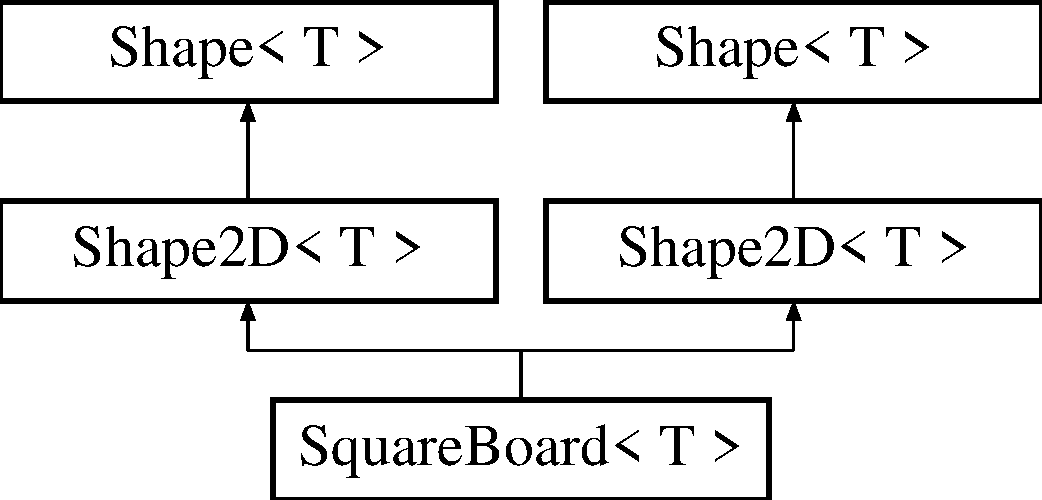
\includegraphics[height=3.000000cm]{classSquareBoard}
\end{center}
\end{figure}
\subsection*{Public Member Functions}
\begin{DoxyCompactItemize}
\item 
\mbox{\hyperlink{classSquareBoard_aa7aac1a02a00ce9ad0c9441fffa71e02}{Square\+Board}} (unsigned=50)
\begin{DoxyCompactList}\small\item\em Basic constructor for class \mbox{\hyperlink{classSquareBoard}{Square\+Board}}. \end{DoxyCompactList}\item 
\mbox{\hyperlink{classSquareBoard_a23c495a2419aded87c0b2803de409b5e}{Square\+Board}} (\mbox{\hyperlink{classSquareBoard}{Square\+Board}} \&\&)=default
\item 
\mbox{\hyperlink{classSquareBoard}{Square\+Board}} \& \mbox{\hyperlink{classSquareBoard_a354794a6de9edec8c771ca49dd315acf}{operator=}} (\mbox{\hyperlink{classSquareBoard}{Square\+Board}} \&\&)=default
\item 
\mbox{\hyperlink{classSquareBoard_a9a6c27e98ae10d6cb601140ef6a3ff59}{Square\+Board}} (const \mbox{\hyperlink{classSquareBoard}{Square\+Board}} \&)=default
\item 
\mbox{\hyperlink{classSquareBoard}{Square\+Board}} \& \mbox{\hyperlink{classSquareBoard_a15fd0ca02b5be393b75228123be1d2c8}{operator=}} (const \mbox{\hyperlink{classSquareBoard}{Square\+Board}} \&)=default
\item 
T \mbox{\hyperlink{classSquareBoard_a8b2ae6ea7295b2bff171b3d6311a456c}{perimeter}} ()
\item 
\mbox{\hyperlink{classSquareBoard_aa7aac1a02a00ce9ad0c9441fffa71e02}{Square\+Board}} (unsigned=50)
\item 
\mbox{\hyperlink{classSquareBoard_a23c495a2419aded87c0b2803de409b5e}{Square\+Board}} (\mbox{\hyperlink{classSquareBoard}{Square\+Board}} \&\&)=default
\item 
\mbox{\hyperlink{classSquareBoard}{Square\+Board}} \& \mbox{\hyperlink{classSquareBoard_a354794a6de9edec8c771ca49dd315acf}{operator=}} (\mbox{\hyperlink{classSquareBoard}{Square\+Board}} \&\&)=default
\item 
\mbox{\hyperlink{classSquareBoard_a9a6c27e98ae10d6cb601140ef6a3ff59}{Square\+Board}} (const \mbox{\hyperlink{classSquareBoard}{Square\+Board}} \&)=default
\item 
\mbox{\hyperlink{classSquareBoard}{Square\+Board}} \& \mbox{\hyperlink{classSquareBoard_a15fd0ca02b5be393b75228123be1d2c8}{operator=}} (const \mbox{\hyperlink{classSquareBoard}{Square\+Board}} \&)=default
\item 
T \mbox{\hyperlink{classSquareBoard_a8b2ae6ea7295b2bff171b3d6311a456c}{perimeter}} ()
\end{DoxyCompactItemize}
\subsection*{Private Member Functions}
\begin{DoxyCompactItemize}
\item 
\mbox{\hyperlink{glad_8h_a950fc91edb4504f62f1c577bf4727c29}{void}} \mbox{\hyperlink{classSquareBoard_a401c48fa5977d166b75e94bb7ddf1db7}{generate\+\_\+vertexes}} ()
\item 
\mbox{\hyperlink{glad_8h_a950fc91edb4504f62f1c577bf4727c29}{void}} \mbox{\hyperlink{classSquareBoard_a5d12432cc063275a6ffec42a7971abbc}{generate\+\_\+filling\+\_\+ebo}} ()
\item 
\mbox{\hyperlink{glad_8h_a950fc91edb4504f62f1c577bf4727c29}{void}} \mbox{\hyperlink{classSquareBoard_a401c48fa5977d166b75e94bb7ddf1db7}{generate\+\_\+vertexes}} ()
\item 
\mbox{\hyperlink{glad_8h_a950fc91edb4504f62f1c577bf4727c29}{void}} \mbox{\hyperlink{classSquareBoard_a5d12432cc063275a6ffec42a7971abbc}{generate\+\_\+filling\+\_\+ebo}} ()
\item 
{\footnotesize template$<$$>$ }\\\mbox{\hyperlink{glad_8h_a950fc91edb4504f62f1c577bf4727c29}{void}} \mbox{\hyperlink{classSquareBoard_a7928f781c7709b3fdfe42b5ce5bfc3f9}{generate\+\_\+vertexes}} ()
\item 
{\footnotesize template$<$$>$ }\\\mbox{\hyperlink{glad_8h_a950fc91edb4504f62f1c577bf4727c29}{void}} \mbox{\hyperlink{classSquareBoard_a7928f781c7709b3fdfe42b5ce5bfc3f9}{generate\+\_\+vertexes}} ()
\end{DoxyCompactItemize}
\subsection*{Private Attributes}
\begin{DoxyCompactItemize}
\item 
unsigned \mbox{\hyperlink{classSquareBoard_a92007159761cd4dfe85aaaa11103ea84}{size}}
\end{DoxyCompactItemize}
\subsection*{Additional Inherited Members}


\subsection{Detailed Description}
\subsubsection*{template$<$typename T = float$>$\newline
class Square\+Board$<$ T $>$}

\mbox{\hyperlink{classThis}{This}} class holds vertexes and other data for a circle in xy plane. 

\begin{DoxyRefDesc}{Todo}
\item[\mbox{\hyperlink{todo__todo000002}{Todo}}]Finish float version of perimeter function and implement double version. \end{DoxyRefDesc}


\subsection{Constructor \& Destructor Documentation}
\mbox{\Hypertarget{classSquareBoard_aa7aac1a02a00ce9ad0c9441fffa71e02}\label{classSquareBoard_aa7aac1a02a00ce9ad0c9441fffa71e02}} 
\index{Square\+Board@{Square\+Board}!Square\+Board@{Square\+Board}}
\index{Square\+Board@{Square\+Board}!Square\+Board@{Square\+Board}}
\subsubsection{\texorpdfstring{Square\+Board()}{SquareBoard()}\hspace{0.1cm}{\footnotesize\ttfamily [1/6]}}
{\footnotesize\ttfamily template$<$typename T $>$ \\
\mbox{\hyperlink{classSquareBoard}{Square\+Board}}$<$ T $>$\+::\mbox{\hyperlink{classSquareBoard}{Square\+Board}} (\begin{DoxyParamCaption}\item[{unsigned}]{size\+\_\+ = {\ttfamily 50} }\end{DoxyParamCaption})}



Basic constructor for class \mbox{\hyperlink{classSquareBoard}{Square\+Board}}. 

Constructor generates vertexes and initializes opengl buffers. \mbox{\Hypertarget{classSquareBoard_a23c495a2419aded87c0b2803de409b5e}\label{classSquareBoard_a23c495a2419aded87c0b2803de409b5e}} 
\index{Square\+Board@{Square\+Board}!Square\+Board@{Square\+Board}}
\index{Square\+Board@{Square\+Board}!Square\+Board@{Square\+Board}}
\subsubsection{\texorpdfstring{Square\+Board()}{SquareBoard()}\hspace{0.1cm}{\footnotesize\ttfamily [2/6]}}
{\footnotesize\ttfamily template$<$typename T  = float$>$ \\
\mbox{\hyperlink{classSquareBoard}{Square\+Board}}$<$ T $>$\+::\mbox{\hyperlink{classSquareBoard}{Square\+Board}} (\begin{DoxyParamCaption}\item[{\mbox{\hyperlink{classSquareBoard}{Square\+Board}}$<$ T $>$ \&\&}]{ }\end{DoxyParamCaption})\hspace{0.3cm}{\ttfamily [default]}}

\mbox{\Hypertarget{classSquareBoard_a9a6c27e98ae10d6cb601140ef6a3ff59}\label{classSquareBoard_a9a6c27e98ae10d6cb601140ef6a3ff59}} 
\index{Square\+Board@{Square\+Board}!Square\+Board@{Square\+Board}}
\index{Square\+Board@{Square\+Board}!Square\+Board@{Square\+Board}}
\subsubsection{\texorpdfstring{Square\+Board()}{SquareBoard()}\hspace{0.1cm}{\footnotesize\ttfamily [3/6]}}
{\footnotesize\ttfamily template$<$typename T  = float$>$ \\
\mbox{\hyperlink{classSquareBoard}{Square\+Board}}$<$ T $>$\+::\mbox{\hyperlink{classSquareBoard}{Square\+Board}} (\begin{DoxyParamCaption}\item[{const \mbox{\hyperlink{classSquareBoard}{Square\+Board}}$<$ T $>$ \&}]{ }\end{DoxyParamCaption})\hspace{0.3cm}{\ttfamily [default]}}

\mbox{\Hypertarget{classSquareBoard_aa7aac1a02a00ce9ad0c9441fffa71e02}\label{classSquareBoard_aa7aac1a02a00ce9ad0c9441fffa71e02}} 
\index{Square\+Board@{Square\+Board}!Square\+Board@{Square\+Board}}
\index{Square\+Board@{Square\+Board}!Square\+Board@{Square\+Board}}
\subsubsection{\texorpdfstring{Square\+Board()}{SquareBoard()}\hspace{0.1cm}{\footnotesize\ttfamily [4/6]}}
{\footnotesize\ttfamily template$<$typename T  = float$>$ \\
\mbox{\hyperlink{classSquareBoard}{Square\+Board}}$<$ T $>$\+::\mbox{\hyperlink{classSquareBoard}{Square\+Board}} (\begin{DoxyParamCaption}\item[{unsigned}]{ = {\ttfamily 50} }\end{DoxyParamCaption})}

\mbox{\Hypertarget{classSquareBoard_a23c495a2419aded87c0b2803de409b5e}\label{classSquareBoard_a23c495a2419aded87c0b2803de409b5e}} 
\index{Square\+Board@{Square\+Board}!Square\+Board@{Square\+Board}}
\index{Square\+Board@{Square\+Board}!Square\+Board@{Square\+Board}}
\subsubsection{\texorpdfstring{Square\+Board()}{SquareBoard()}\hspace{0.1cm}{\footnotesize\ttfamily [5/6]}}
{\footnotesize\ttfamily template$<$typename T  = float$>$ \\
\mbox{\hyperlink{classSquareBoard}{Square\+Board}}$<$ T $>$\+::\mbox{\hyperlink{classSquareBoard}{Square\+Board}} (\begin{DoxyParamCaption}\item[{\mbox{\hyperlink{classSquareBoard}{Square\+Board}}$<$ T $>$ \&\&}]{ }\end{DoxyParamCaption})\hspace{0.3cm}{\ttfamily [default]}}

\mbox{\Hypertarget{classSquareBoard_a9a6c27e98ae10d6cb601140ef6a3ff59}\label{classSquareBoard_a9a6c27e98ae10d6cb601140ef6a3ff59}} 
\index{Square\+Board@{Square\+Board}!Square\+Board@{Square\+Board}}
\index{Square\+Board@{Square\+Board}!Square\+Board@{Square\+Board}}
\subsubsection{\texorpdfstring{Square\+Board()}{SquareBoard()}\hspace{0.1cm}{\footnotesize\ttfamily [6/6]}}
{\footnotesize\ttfamily template$<$typename T  = float$>$ \\
\mbox{\hyperlink{classSquareBoard}{Square\+Board}}$<$ T $>$\+::\mbox{\hyperlink{classSquareBoard}{Square\+Board}} (\begin{DoxyParamCaption}\item[{const \mbox{\hyperlink{classSquareBoard}{Square\+Board}}$<$ T $>$ \&}]{ }\end{DoxyParamCaption})\hspace{0.3cm}{\ttfamily [default]}}



\subsection{Member Function Documentation}
\mbox{\Hypertarget{classSquareBoard_a5d12432cc063275a6ffec42a7971abbc}\label{classSquareBoard_a5d12432cc063275a6ffec42a7971abbc}} 
\index{Square\+Board@{Square\+Board}!generate\+\_\+filling\+\_\+ebo@{generate\+\_\+filling\+\_\+ebo}}
\index{generate\+\_\+filling\+\_\+ebo@{generate\+\_\+filling\+\_\+ebo}!Square\+Board@{Square\+Board}}
\subsubsection{\texorpdfstring{generate\+\_\+filling\+\_\+ebo()}{generate\_filling\_ebo()}\hspace{0.1cm}{\footnotesize\ttfamily [1/2]}}
{\footnotesize\ttfamily template$<$typename T $>$ \\
\mbox{\hyperlink{glad_8h_a950fc91edb4504f62f1c577bf4727c29}{void}} \mbox{\hyperlink{classSquareBoard}{Square\+Board}}$<$ T $>$\+::generate\+\_\+filling\+\_\+ebo (\begin{DoxyParamCaption}{ }\end{DoxyParamCaption})\hspace{0.3cm}{\ttfamily [inline]}, {\ttfamily [private]}}

\mbox{\Hypertarget{classSquareBoard_a5d12432cc063275a6ffec42a7971abbc}\label{classSquareBoard_a5d12432cc063275a6ffec42a7971abbc}} 
\index{Square\+Board@{Square\+Board}!generate\+\_\+filling\+\_\+ebo@{generate\+\_\+filling\+\_\+ebo}}
\index{generate\+\_\+filling\+\_\+ebo@{generate\+\_\+filling\+\_\+ebo}!Square\+Board@{Square\+Board}}
\subsubsection{\texorpdfstring{generate\+\_\+filling\+\_\+ebo()}{generate\_filling\_ebo()}\hspace{0.1cm}{\footnotesize\ttfamily [2/2]}}
{\footnotesize\ttfamily template$<$typename T  = float$>$ \\
\mbox{\hyperlink{glad_8h_a950fc91edb4504f62f1c577bf4727c29}{void}} \mbox{\hyperlink{classSquareBoard}{Square\+Board}}$<$ T $>$\+::generate\+\_\+filling\+\_\+ebo (\begin{DoxyParamCaption}{ }\end{DoxyParamCaption})\hspace{0.3cm}{\ttfamily [private]}}

\mbox{\Hypertarget{classSquareBoard_a401c48fa5977d166b75e94bb7ddf1db7}\label{classSquareBoard_a401c48fa5977d166b75e94bb7ddf1db7}} 
\index{Square\+Board@{Square\+Board}!generate\+\_\+vertexes@{generate\+\_\+vertexes}}
\index{generate\+\_\+vertexes@{generate\+\_\+vertexes}!Square\+Board@{Square\+Board}}
\subsubsection{\texorpdfstring{generate\+\_\+vertexes()}{generate\_vertexes()}\hspace{0.1cm}{\footnotesize\ttfamily [1/4]}}
{\footnotesize\ttfamily template$<$typename T  = float$>$ \\
\mbox{\hyperlink{glad_8h_a950fc91edb4504f62f1c577bf4727c29}{void}} \mbox{\hyperlink{classSquareBoard}{Square\+Board}}$<$ T $>$\+::generate\+\_\+vertexes (\begin{DoxyParamCaption}{ }\end{DoxyParamCaption})\hspace{0.3cm}{\ttfamily [private]}}

\mbox{\Hypertarget{classSquareBoard_a401c48fa5977d166b75e94bb7ddf1db7}\label{classSquareBoard_a401c48fa5977d166b75e94bb7ddf1db7}} 
\index{Square\+Board@{Square\+Board}!generate\+\_\+vertexes@{generate\+\_\+vertexes}}
\index{generate\+\_\+vertexes@{generate\+\_\+vertexes}!Square\+Board@{Square\+Board}}
\subsubsection{\texorpdfstring{generate\+\_\+vertexes()}{generate\_vertexes()}\hspace{0.1cm}{\footnotesize\ttfamily [2/4]}}
{\footnotesize\ttfamily template$<$typename T  = float$>$ \\
\mbox{\hyperlink{glad_8h_a950fc91edb4504f62f1c577bf4727c29}{void}} \mbox{\hyperlink{classSquareBoard}{Square\+Board}}$<$ T $>$\+::generate\+\_\+vertexes (\begin{DoxyParamCaption}{ }\end{DoxyParamCaption})\hspace{0.3cm}{\ttfamily [private]}}

\mbox{\Hypertarget{classSquareBoard_a7928f781c7709b3fdfe42b5ce5bfc3f9}\label{classSquareBoard_a7928f781c7709b3fdfe42b5ce5bfc3f9}} 
\index{Square\+Board@{Square\+Board}!generate\+\_\+vertexes@{generate\+\_\+vertexes}}
\index{generate\+\_\+vertexes@{generate\+\_\+vertexes}!Square\+Board@{Square\+Board}}
\subsubsection{\texorpdfstring{generate\+\_\+vertexes()}{generate\_vertexes()}\hspace{0.1cm}{\footnotesize\ttfamily [3/4]}}
{\footnotesize\ttfamily template$<$$>$ \\
\mbox{\hyperlink{glad_8h_a950fc91edb4504f62f1c577bf4727c29}{void}} \mbox{\hyperlink{classSquareBoard}{Square\+Board}}$<$ float $>$\+::generate\+\_\+vertexes (\begin{DoxyParamCaption}{ }\end{DoxyParamCaption})\hspace{0.3cm}{\ttfamily [inline]}, {\ttfamily [private]}}

\mbox{\Hypertarget{classSquareBoard_a7928f781c7709b3fdfe42b5ce5bfc3f9}\label{classSquareBoard_a7928f781c7709b3fdfe42b5ce5bfc3f9}} 
\index{Square\+Board@{Square\+Board}!generate\+\_\+vertexes@{generate\+\_\+vertexes}}
\index{generate\+\_\+vertexes@{generate\+\_\+vertexes}!Square\+Board@{Square\+Board}}
\subsubsection{\texorpdfstring{generate\+\_\+vertexes()}{generate\_vertexes()}\hspace{0.1cm}{\footnotesize\ttfamily [4/4]}}
{\footnotesize\ttfamily template$<$$>$ \\
\mbox{\hyperlink{glad_8h_a950fc91edb4504f62f1c577bf4727c29}{void}} \mbox{\hyperlink{classSquareBoard}{Square\+Board}}$<$ float $>$\+::generate\+\_\+vertexes (\begin{DoxyParamCaption}{ }\end{DoxyParamCaption})\hspace{0.3cm}{\ttfamily [inline]}, {\ttfamily [private]}}

\mbox{\Hypertarget{classSquareBoard_a354794a6de9edec8c771ca49dd315acf}\label{classSquareBoard_a354794a6de9edec8c771ca49dd315acf}} 
\index{Square\+Board@{Square\+Board}!operator=@{operator=}}
\index{operator=@{operator=}!Square\+Board@{Square\+Board}}
\subsubsection{\texorpdfstring{operator=()}{operator=()}\hspace{0.1cm}{\footnotesize\ttfamily [1/4]}}
{\footnotesize\ttfamily template$<$typename T  = float$>$ \\
\mbox{\hyperlink{classSquareBoard}{Square\+Board}}\& \mbox{\hyperlink{classSquareBoard}{Square\+Board}}$<$ T $>$\+::operator= (\begin{DoxyParamCaption}\item[{\mbox{\hyperlink{classSquareBoard}{Square\+Board}}$<$ T $>$ \&\&}]{ }\end{DoxyParamCaption})\hspace{0.3cm}{\ttfamily [default]}}

\mbox{\Hypertarget{classSquareBoard_a354794a6de9edec8c771ca49dd315acf}\label{classSquareBoard_a354794a6de9edec8c771ca49dd315acf}} 
\index{Square\+Board@{Square\+Board}!operator=@{operator=}}
\index{operator=@{operator=}!Square\+Board@{Square\+Board}}
\subsubsection{\texorpdfstring{operator=()}{operator=()}\hspace{0.1cm}{\footnotesize\ttfamily [2/4]}}
{\footnotesize\ttfamily template$<$typename T  = float$>$ \\
\mbox{\hyperlink{classSquareBoard}{Square\+Board}}\& \mbox{\hyperlink{classSquareBoard}{Square\+Board}}$<$ T $>$\+::operator= (\begin{DoxyParamCaption}\item[{\mbox{\hyperlink{classSquareBoard}{Square\+Board}}$<$ T $>$ \&\&}]{ }\end{DoxyParamCaption})\hspace{0.3cm}{\ttfamily [default]}}

\mbox{\Hypertarget{classSquareBoard_a15fd0ca02b5be393b75228123be1d2c8}\label{classSquareBoard_a15fd0ca02b5be393b75228123be1d2c8}} 
\index{Square\+Board@{Square\+Board}!operator=@{operator=}}
\index{operator=@{operator=}!Square\+Board@{Square\+Board}}
\subsubsection{\texorpdfstring{operator=()}{operator=()}\hspace{0.1cm}{\footnotesize\ttfamily [3/4]}}
{\footnotesize\ttfamily template$<$typename T  = float$>$ \\
\mbox{\hyperlink{classSquareBoard}{Square\+Board}}\& \mbox{\hyperlink{classSquareBoard}{Square\+Board}}$<$ T $>$\+::operator= (\begin{DoxyParamCaption}\item[{const \mbox{\hyperlink{classSquareBoard}{Square\+Board}}$<$ T $>$ \&}]{ }\end{DoxyParamCaption})\hspace{0.3cm}{\ttfamily [default]}}

\mbox{\Hypertarget{classSquareBoard_a15fd0ca02b5be393b75228123be1d2c8}\label{classSquareBoard_a15fd0ca02b5be393b75228123be1d2c8}} 
\index{Square\+Board@{Square\+Board}!operator=@{operator=}}
\index{operator=@{operator=}!Square\+Board@{Square\+Board}}
\subsubsection{\texorpdfstring{operator=()}{operator=()}\hspace{0.1cm}{\footnotesize\ttfamily [4/4]}}
{\footnotesize\ttfamily template$<$typename T  = float$>$ \\
\mbox{\hyperlink{classSquareBoard}{Square\+Board}}\& \mbox{\hyperlink{classSquareBoard}{Square\+Board}}$<$ T $>$\+::operator= (\begin{DoxyParamCaption}\item[{const \mbox{\hyperlink{classSquareBoard}{Square\+Board}}$<$ T $>$ \&}]{ }\end{DoxyParamCaption})\hspace{0.3cm}{\ttfamily [default]}}

\mbox{\Hypertarget{classSquareBoard_a8b2ae6ea7295b2bff171b3d6311a456c}\label{classSquareBoard_a8b2ae6ea7295b2bff171b3d6311a456c}} 
\index{Square\+Board@{Square\+Board}!perimeter@{perimeter}}
\index{perimeter@{perimeter}!Square\+Board@{Square\+Board}}
\subsubsection{\texorpdfstring{perimeter()}{perimeter()}\hspace{0.1cm}{\footnotesize\ttfamily [1/2]}}
{\footnotesize\ttfamily template$<$typename T  = float$>$ \\
T \mbox{\hyperlink{classSquareBoard}{Square\+Board}}$<$ T $>$\+::perimeter (\begin{DoxyParamCaption}{ }\end{DoxyParamCaption})}

\mbox{\Hypertarget{classSquareBoard_a8b2ae6ea7295b2bff171b3d6311a456c}\label{classSquareBoard_a8b2ae6ea7295b2bff171b3d6311a456c}} 
\index{Square\+Board@{Square\+Board}!perimeter@{perimeter}}
\index{perimeter@{perimeter}!Square\+Board@{Square\+Board}}
\subsubsection{\texorpdfstring{perimeter()}{perimeter()}\hspace{0.1cm}{\footnotesize\ttfamily [2/2]}}
{\footnotesize\ttfamily template$<$typename T  = float$>$ \\
T \mbox{\hyperlink{classSquareBoard}{Square\+Board}}$<$ T $>$\+::perimeter (\begin{DoxyParamCaption}{ }\end{DoxyParamCaption})}



\subsection{Member Data Documentation}
\mbox{\Hypertarget{classSquareBoard_a92007159761cd4dfe85aaaa11103ea84}\label{classSquareBoard_a92007159761cd4dfe85aaaa11103ea84}} 
\index{Square\+Board@{Square\+Board}!size@{size}}
\index{size@{size}!Square\+Board@{Square\+Board}}
\subsubsection{\texorpdfstring{size}{size}}
{\footnotesize\ttfamily template$<$typename T  = float$>$ \\
unsigned \mbox{\hyperlink{classSquareBoard}{Square\+Board}}$<$ T $>$\+::\mbox{\hyperlink{glad_8h_adead0e00f1033fff2918e18853add2b1}{size}}\hspace{0.3cm}{\ttfamily [private]}}

number of squares in the array 

The documentation for this class was generated from the following files\+:\begin{DoxyCompactItemize}
\item 
src/shapes/\mbox{\hyperlink{square__board_8hpp}{square\+\_\+board.\+hpp}}\item 
src/shapes/\mbox{\hyperlink{square__board__old_8hpp}{square\+\_\+board\+\_\+old.\+hpp}}\end{DoxyCompactItemize}

\hypertarget{classStar}{}\section{Star$<$ T $>$ Class Template Reference}
\label{classStar}\index{Star$<$ T $>$@{Star$<$ T $>$}}


{\ttfamily \#include \char`\"{}star.\+hpp\char`\"{}}

Inheritance diagram for Star$<$ T $>$\+:\begin{figure}[H]
\begin{center}
\leavevmode
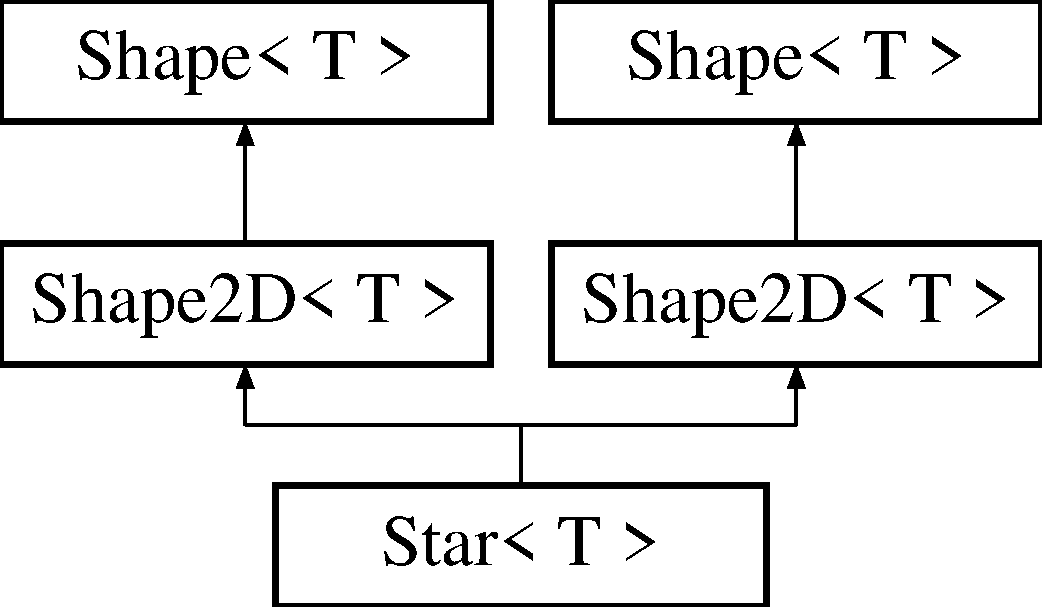
\includegraphics[height=3.000000cm]{classStar}
\end{center}
\end{figure}
\subsection*{Public Member Functions}
\begin{DoxyCompactItemize}
\item 
\mbox{\hyperlink{classStar_a4be07c82320f781071409294614df4ae}{Star}} ()
\item 
\mbox{\hyperlink{classStar_aa179936ed93e38e70992cb4f6e3cbff3}{Star}} (int, T=0.\+5)
\item 
\mbox{\hyperlink{classStar_af518471484341cad6b47ad42d4e637fe}{Star}} (\mbox{\hyperlink{classStar}{Star}} \&\&)=default
\item 
\mbox{\hyperlink{classStar}{Star}} \& \mbox{\hyperlink{classStar_a7113d2808314f0aa2f5a87325f8c535d}{operator=}} (\mbox{\hyperlink{classStar}{Star}} \&\&)=default
\item 
\mbox{\hyperlink{classStar_a047ce2a8d4fb409858555aee98b33c93}{Star}} (const \mbox{\hyperlink{classStar}{Star}} \&)=default
\item 
\mbox{\hyperlink{classStar}{Star}} \& \mbox{\hyperlink{classStar_a3507f157448e082ccfcadc4783f2610e}{operator=}} (const \mbox{\hyperlink{classStar}{Star}} \&)=default
\item 
T \mbox{\hyperlink{classStar_a908253192d0b1fe95aeeaa81322545bf}{perimeter}} ()
\item 
\mbox{\hyperlink{classStar_a4be07c82320f781071409294614df4ae}{Star}} ()
\item 
\mbox{\hyperlink{classStar_aa179936ed93e38e70992cb4f6e3cbff3}{Star}} (int, T=0.\+5)
\item 
\mbox{\hyperlink{classStar_af518471484341cad6b47ad42d4e637fe}{Star}} (\mbox{\hyperlink{classStar}{Star}} \&\&)=default
\item 
\mbox{\hyperlink{classStar}{Star}} \& \mbox{\hyperlink{classStar_a7113d2808314f0aa2f5a87325f8c535d}{operator=}} (\mbox{\hyperlink{classStar}{Star}} \&\&)=default
\item 
\mbox{\hyperlink{classStar_a047ce2a8d4fb409858555aee98b33c93}{Star}} (const \mbox{\hyperlink{classStar}{Star}} \&)=default
\item 
\mbox{\hyperlink{classStar}{Star}} \& \mbox{\hyperlink{classStar_a3507f157448e082ccfcadc4783f2610e}{operator=}} (const \mbox{\hyperlink{classStar}{Star}} \&)=default
\item 
T \mbox{\hyperlink{classStar_a908253192d0b1fe95aeeaa81322545bf}{perimeter}} ()
\end{DoxyCompactItemize}
\subsection*{Public Attributes}
\begin{DoxyCompactItemize}
\item 
T \mbox{\hyperlink{classStar_a349e0820769da7e4f76aea0ad6002bf8}{ratio}}
\end{DoxyCompactItemize}
\subsection*{Private Member Functions}
\begin{DoxyCompactItemize}
\item 
void \mbox{\hyperlink{classStar_ac9ce42a8f7289484594f7f0ab5124849}{generate\+\_\+vertexes}} (int=10, T=0.\+5)
\item 
void \mbox{\hyperlink{classStar_ac9ce42a8f7289484594f7f0ab5124849}{generate\+\_\+vertexes}} (int=10, T=0.\+5)
\item 
{\footnotesize template$<$$>$ }\\void \mbox{\hyperlink{classStar_ab46cbc7aca971bc1c07b8d4afe8fba37}{generate\+\_\+vertexes}} (int bulges, float \mbox{\hyperlink{classStar_a349e0820769da7e4f76aea0ad6002bf8}{ratio}})
\item 
{\footnotesize template$<$$>$ }\\void \mbox{\hyperlink{classStar_a85d8438cea72701a136b76f046ee95dd}{generate\+\_\+vertexes}} (int bulges, double \mbox{\hyperlink{classStar_a349e0820769da7e4f76aea0ad6002bf8}{ratio}})
\item 
{\footnotesize template$<$$>$ }\\void \mbox{\hyperlink{classStar_ab46cbc7aca971bc1c07b8d4afe8fba37}{generate\+\_\+vertexes}} (int bulges, float \mbox{\hyperlink{classStar_a349e0820769da7e4f76aea0ad6002bf8}{ratio}})
\item 
{\footnotesize template$<$$>$ }\\void \mbox{\hyperlink{classStar_a85d8438cea72701a136b76f046ee95dd}{generate\+\_\+vertexes}} (int bulges, double \mbox{\hyperlink{classStar_a349e0820769da7e4f76aea0ad6002bf8}{ratio}})
\end{DoxyCompactItemize}
\subsection*{Additional Inherited Members}


\subsection{Constructor \& Destructor Documentation}
\mbox{\Hypertarget{classStar_a4be07c82320f781071409294614df4ae}\label{classStar_a4be07c82320f781071409294614df4ae}} 
\index{Star@{Star}!Star@{Star}}
\index{Star@{Star}!Star@{Star}}
\subsubsection{\texorpdfstring{Star()}{Star()}\hspace{0.1cm}{\footnotesize\ttfamily [1/8]}}
{\footnotesize\ttfamily template$<$typename T $>$ \\
\mbox{\hyperlink{classStar}{Star}}$<$ T $>$\+::\mbox{\hyperlink{classStar}{Star}} (\begin{DoxyParamCaption}{ }\end{DoxyParamCaption})}

\mbox{\Hypertarget{classStar_aa179936ed93e38e70992cb4f6e3cbff3}\label{classStar_aa179936ed93e38e70992cb4f6e3cbff3}} 
\index{Star@{Star}!Star@{Star}}
\index{Star@{Star}!Star@{Star}}
\subsubsection{\texorpdfstring{Star()}{Star()}\hspace{0.1cm}{\footnotesize\ttfamily [2/8]}}
{\footnotesize\ttfamily template$<$typename T $>$ \\
\mbox{\hyperlink{classStar}{Star}}$<$ T $>$\+::\mbox{\hyperlink{classStar}{Star}} (\begin{DoxyParamCaption}\item[{int}]{bulges,  }\item[{T}]{ratio = {\ttfamily 0.5} }\end{DoxyParamCaption})}

\mbox{\Hypertarget{classStar_af518471484341cad6b47ad42d4e637fe}\label{classStar_af518471484341cad6b47ad42d4e637fe}} 
\index{Star@{Star}!Star@{Star}}
\index{Star@{Star}!Star@{Star}}
\subsubsection{\texorpdfstring{Star()}{Star()}\hspace{0.1cm}{\footnotesize\ttfamily [3/8]}}
{\footnotesize\ttfamily template$<$typename T  = float$>$ \\
\mbox{\hyperlink{classStar}{Star}}$<$ T $>$\+::\mbox{\hyperlink{classStar}{Star}} (\begin{DoxyParamCaption}\item[{\mbox{\hyperlink{classStar}{Star}}$<$ T $>$ \&\&}]{ }\end{DoxyParamCaption})\hspace{0.3cm}{\ttfamily [default]}}

\mbox{\Hypertarget{classStar_a047ce2a8d4fb409858555aee98b33c93}\label{classStar_a047ce2a8d4fb409858555aee98b33c93}} 
\index{Star@{Star}!Star@{Star}}
\index{Star@{Star}!Star@{Star}}
\subsubsection{\texorpdfstring{Star()}{Star()}\hspace{0.1cm}{\footnotesize\ttfamily [4/8]}}
{\footnotesize\ttfamily template$<$typename T  = float$>$ \\
\mbox{\hyperlink{classStar}{Star}}$<$ T $>$\+::\mbox{\hyperlink{classStar}{Star}} (\begin{DoxyParamCaption}\item[{const \mbox{\hyperlink{classStar}{Star}}$<$ T $>$ \&}]{ }\end{DoxyParamCaption})\hspace{0.3cm}{\ttfamily [default]}}

\mbox{\Hypertarget{classStar_a4be07c82320f781071409294614df4ae}\label{classStar_a4be07c82320f781071409294614df4ae}} 
\index{Star@{Star}!Star@{Star}}
\index{Star@{Star}!Star@{Star}}
\subsubsection{\texorpdfstring{Star()}{Star()}\hspace{0.1cm}{\footnotesize\ttfamily [5/8]}}
{\footnotesize\ttfamily template$<$typename T  = float$>$ \\
\mbox{\hyperlink{classStar}{Star}}$<$ T $>$\+::\mbox{\hyperlink{classStar}{Star}} (\begin{DoxyParamCaption}{ }\end{DoxyParamCaption})}

\mbox{\Hypertarget{classStar_aa179936ed93e38e70992cb4f6e3cbff3}\label{classStar_aa179936ed93e38e70992cb4f6e3cbff3}} 
\index{Star@{Star}!Star@{Star}}
\index{Star@{Star}!Star@{Star}}
\subsubsection{\texorpdfstring{Star()}{Star()}\hspace{0.1cm}{\footnotesize\ttfamily [6/8]}}
{\footnotesize\ttfamily template$<$typename T  = float$>$ \\
\mbox{\hyperlink{classStar}{Star}}$<$ T $>$\+::\mbox{\hyperlink{classStar}{Star}} (\begin{DoxyParamCaption}\item[{int}]{,  }\item[{T}]{ = {\ttfamily 0.5} }\end{DoxyParamCaption})}

\mbox{\Hypertarget{classStar_af518471484341cad6b47ad42d4e637fe}\label{classStar_af518471484341cad6b47ad42d4e637fe}} 
\index{Star@{Star}!Star@{Star}}
\index{Star@{Star}!Star@{Star}}
\subsubsection{\texorpdfstring{Star()}{Star()}\hspace{0.1cm}{\footnotesize\ttfamily [7/8]}}
{\footnotesize\ttfamily template$<$typename T  = float$>$ \\
\mbox{\hyperlink{classStar}{Star}}$<$ T $>$\+::\mbox{\hyperlink{classStar}{Star}} (\begin{DoxyParamCaption}\item[{\mbox{\hyperlink{classStar}{Star}}$<$ T $>$ \&\&}]{ }\end{DoxyParamCaption})\hspace{0.3cm}{\ttfamily [default]}}

\mbox{\Hypertarget{classStar_a047ce2a8d4fb409858555aee98b33c93}\label{classStar_a047ce2a8d4fb409858555aee98b33c93}} 
\index{Star@{Star}!Star@{Star}}
\index{Star@{Star}!Star@{Star}}
\subsubsection{\texorpdfstring{Star()}{Star()}\hspace{0.1cm}{\footnotesize\ttfamily [8/8]}}
{\footnotesize\ttfamily template$<$typename T  = float$>$ \\
\mbox{\hyperlink{classStar}{Star}}$<$ T $>$\+::\mbox{\hyperlink{classStar}{Star}} (\begin{DoxyParamCaption}\item[{const \mbox{\hyperlink{classStar}{Star}}$<$ T $>$ \&}]{ }\end{DoxyParamCaption})\hspace{0.3cm}{\ttfamily [default]}}



\subsection{Member Function Documentation}
\mbox{\Hypertarget{classStar_ac9ce42a8f7289484594f7f0ab5124849}\label{classStar_ac9ce42a8f7289484594f7f0ab5124849}} 
\index{Star@{Star}!generate\+\_\+vertexes@{generate\+\_\+vertexes}}
\index{generate\+\_\+vertexes@{generate\+\_\+vertexes}!Star@{Star}}
\subsubsection{\texorpdfstring{generate\+\_\+vertexes()}{generate\_vertexes()}\hspace{0.1cm}{\footnotesize\ttfamily [1/6]}}
{\footnotesize\ttfamily template$<$typename T  = float$>$ \\
void \mbox{\hyperlink{classStar}{Star}}$<$ T $>$\+::generate\+\_\+vertexes (\begin{DoxyParamCaption}\item[{int}]{ = {\ttfamily 10},  }\item[{T}]{ = {\ttfamily 0.5} }\end{DoxyParamCaption})\hspace{0.3cm}{\ttfamily [private]}}

\mbox{\Hypertarget{classStar_ac9ce42a8f7289484594f7f0ab5124849}\label{classStar_ac9ce42a8f7289484594f7f0ab5124849}} 
\index{Star@{Star}!generate\+\_\+vertexes@{generate\+\_\+vertexes}}
\index{generate\+\_\+vertexes@{generate\+\_\+vertexes}!Star@{Star}}
\subsubsection{\texorpdfstring{generate\+\_\+vertexes()}{generate\_vertexes()}\hspace{0.1cm}{\footnotesize\ttfamily [2/6]}}
{\footnotesize\ttfamily template$<$typename T  = float$>$ \\
void \mbox{\hyperlink{classStar}{Star}}$<$ T $>$\+::generate\+\_\+vertexes (\begin{DoxyParamCaption}\item[{int}]{ = {\ttfamily 10},  }\item[{T}]{ = {\ttfamily 0.5} }\end{DoxyParamCaption})\hspace{0.3cm}{\ttfamily [private]}}

\mbox{\Hypertarget{classStar_ab46cbc7aca971bc1c07b8d4afe8fba37}\label{classStar_ab46cbc7aca971bc1c07b8d4afe8fba37}} 
\index{Star@{Star}!generate\+\_\+vertexes@{generate\+\_\+vertexes}}
\index{generate\+\_\+vertexes@{generate\+\_\+vertexes}!Star@{Star}}
\subsubsection{\texorpdfstring{generate\+\_\+vertexes()}{generate\_vertexes()}\hspace{0.1cm}{\footnotesize\ttfamily [3/6]}}
{\footnotesize\ttfamily template$<$$>$ \\
void \mbox{\hyperlink{classStar}{Star}}$<$ float $>$\+::generate\+\_\+vertexes (\begin{DoxyParamCaption}\item[{int}]{bulges,  }\item[{float}]{ratio }\end{DoxyParamCaption})\hspace{0.3cm}{\ttfamily [inline]}, {\ttfamily [private]}}

\mbox{\Hypertarget{classStar_ab46cbc7aca971bc1c07b8d4afe8fba37}\label{classStar_ab46cbc7aca971bc1c07b8d4afe8fba37}} 
\index{Star@{Star}!generate\+\_\+vertexes@{generate\+\_\+vertexes}}
\index{generate\+\_\+vertexes@{generate\+\_\+vertexes}!Star@{Star}}
\subsubsection{\texorpdfstring{generate\+\_\+vertexes()}{generate\_vertexes()}\hspace{0.1cm}{\footnotesize\ttfamily [4/6]}}
{\footnotesize\ttfamily template$<$$>$ \\
void \mbox{\hyperlink{classStar}{Star}}$<$ float $>$\+::generate\+\_\+vertexes (\begin{DoxyParamCaption}\item[{int}]{bulges,  }\item[{float}]{ratio }\end{DoxyParamCaption})\hspace{0.3cm}{\ttfamily [inline]}, {\ttfamily [private]}}

\mbox{\Hypertarget{classStar_a85d8438cea72701a136b76f046ee95dd}\label{classStar_a85d8438cea72701a136b76f046ee95dd}} 
\index{Star@{Star}!generate\+\_\+vertexes@{generate\+\_\+vertexes}}
\index{generate\+\_\+vertexes@{generate\+\_\+vertexes}!Star@{Star}}
\subsubsection{\texorpdfstring{generate\+\_\+vertexes()}{generate\_vertexes()}\hspace{0.1cm}{\footnotesize\ttfamily [5/6]}}
{\footnotesize\ttfamily template$<$$>$ \\
void \mbox{\hyperlink{classStar}{Star}}$<$ double $>$\+::generate\+\_\+vertexes (\begin{DoxyParamCaption}\item[{int}]{bulges,  }\item[{double}]{ratio }\end{DoxyParamCaption})\hspace{0.3cm}{\ttfamily [inline]}, {\ttfamily [private]}}

\mbox{\Hypertarget{classStar_a85d8438cea72701a136b76f046ee95dd}\label{classStar_a85d8438cea72701a136b76f046ee95dd}} 
\index{Star@{Star}!generate\+\_\+vertexes@{generate\+\_\+vertexes}}
\index{generate\+\_\+vertexes@{generate\+\_\+vertexes}!Star@{Star}}
\subsubsection{\texorpdfstring{generate\+\_\+vertexes()}{generate\_vertexes()}\hspace{0.1cm}{\footnotesize\ttfamily [6/6]}}
{\footnotesize\ttfamily template$<$$>$ \\
void \mbox{\hyperlink{classStar}{Star}}$<$ double $>$\+::generate\+\_\+vertexes (\begin{DoxyParamCaption}\item[{int}]{bulges,  }\item[{double}]{ratio }\end{DoxyParamCaption})\hspace{0.3cm}{\ttfamily [inline]}, {\ttfamily [private]}}

\mbox{\Hypertarget{classStar_a7113d2808314f0aa2f5a87325f8c535d}\label{classStar_a7113d2808314f0aa2f5a87325f8c535d}} 
\index{Star@{Star}!operator=@{operator=}}
\index{operator=@{operator=}!Star@{Star}}
\subsubsection{\texorpdfstring{operator=()}{operator=()}\hspace{0.1cm}{\footnotesize\ttfamily [1/4]}}
{\footnotesize\ttfamily template$<$typename T  = float$>$ \\
\mbox{\hyperlink{classStar}{Star}}\& \mbox{\hyperlink{classStar}{Star}}$<$ T $>$\+::operator= (\begin{DoxyParamCaption}\item[{\mbox{\hyperlink{classStar}{Star}}$<$ T $>$ \&\&}]{ }\end{DoxyParamCaption})\hspace{0.3cm}{\ttfamily [default]}}

\mbox{\Hypertarget{classStar_a7113d2808314f0aa2f5a87325f8c535d}\label{classStar_a7113d2808314f0aa2f5a87325f8c535d}} 
\index{Star@{Star}!operator=@{operator=}}
\index{operator=@{operator=}!Star@{Star}}
\subsubsection{\texorpdfstring{operator=()}{operator=()}\hspace{0.1cm}{\footnotesize\ttfamily [2/4]}}
{\footnotesize\ttfamily template$<$typename T  = float$>$ \\
\mbox{\hyperlink{classStar}{Star}}\& \mbox{\hyperlink{classStar}{Star}}$<$ T $>$\+::operator= (\begin{DoxyParamCaption}\item[{\mbox{\hyperlink{classStar}{Star}}$<$ T $>$ \&\&}]{ }\end{DoxyParamCaption})\hspace{0.3cm}{\ttfamily [default]}}

\mbox{\Hypertarget{classStar_a3507f157448e082ccfcadc4783f2610e}\label{classStar_a3507f157448e082ccfcadc4783f2610e}} 
\index{Star@{Star}!operator=@{operator=}}
\index{operator=@{operator=}!Star@{Star}}
\subsubsection{\texorpdfstring{operator=()}{operator=()}\hspace{0.1cm}{\footnotesize\ttfamily [3/4]}}
{\footnotesize\ttfamily template$<$typename T  = float$>$ \\
\mbox{\hyperlink{classStar}{Star}}\& \mbox{\hyperlink{classStar}{Star}}$<$ T $>$\+::operator= (\begin{DoxyParamCaption}\item[{const \mbox{\hyperlink{classStar}{Star}}$<$ T $>$ \&}]{ }\end{DoxyParamCaption})\hspace{0.3cm}{\ttfamily [default]}}

\mbox{\Hypertarget{classStar_a3507f157448e082ccfcadc4783f2610e}\label{classStar_a3507f157448e082ccfcadc4783f2610e}} 
\index{Star@{Star}!operator=@{operator=}}
\index{operator=@{operator=}!Star@{Star}}
\subsubsection{\texorpdfstring{operator=()}{operator=()}\hspace{0.1cm}{\footnotesize\ttfamily [4/4]}}
{\footnotesize\ttfamily template$<$typename T  = float$>$ \\
\mbox{\hyperlink{classStar}{Star}}\& \mbox{\hyperlink{classStar}{Star}}$<$ T $>$\+::operator= (\begin{DoxyParamCaption}\item[{const \mbox{\hyperlink{classStar}{Star}}$<$ T $>$ \&}]{ }\end{DoxyParamCaption})\hspace{0.3cm}{\ttfamily [default]}}

\mbox{\Hypertarget{classStar_a908253192d0b1fe95aeeaa81322545bf}\label{classStar_a908253192d0b1fe95aeeaa81322545bf}} 
\index{Star@{Star}!perimeter@{perimeter}}
\index{perimeter@{perimeter}!Star@{Star}}
\subsubsection{\texorpdfstring{perimeter()}{perimeter()}\hspace{0.1cm}{\footnotesize\ttfamily [1/2]}}
{\footnotesize\ttfamily template$<$typename T  = float$>$ \\
T \mbox{\hyperlink{classStar}{Star}}$<$ T $>$\+::perimeter (\begin{DoxyParamCaption}{ }\end{DoxyParamCaption})}

\mbox{\Hypertarget{classStar_a908253192d0b1fe95aeeaa81322545bf}\label{classStar_a908253192d0b1fe95aeeaa81322545bf}} 
\index{Star@{Star}!perimeter@{perimeter}}
\index{perimeter@{perimeter}!Star@{Star}}
\subsubsection{\texorpdfstring{perimeter()}{perimeter()}\hspace{0.1cm}{\footnotesize\ttfamily [2/2]}}
{\footnotesize\ttfamily template$<$typename T  = float$>$ \\
T \mbox{\hyperlink{classStar}{Star}}$<$ T $>$\+::perimeter (\begin{DoxyParamCaption}{ }\end{DoxyParamCaption})}



\subsection{Member Data Documentation}
\mbox{\Hypertarget{classStar_a349e0820769da7e4f76aea0ad6002bf8}\label{classStar_a349e0820769da7e4f76aea0ad6002bf8}} 
\index{Star@{Star}!ratio@{ratio}}
\index{ratio@{ratio}!Star@{Star}}
\subsubsection{\texorpdfstring{ratio}{ratio}}
{\footnotesize\ttfamily template$<$typename T  = float$>$ \\
T \mbox{\hyperlink{classStar}{Star}}$<$ T $>$\+::ratio}



The documentation for this class was generated from the following files\+:\begin{DoxyCompactItemize}
\item 
src/\mbox{\hyperlink{star_8hpp}{star.\+hpp}}\item 
src/\mbox{\hyperlink{star3d_8hpp}{star3d.\+hpp}}\end{DoxyCompactItemize}

\hypertarget{classStar3d}{}\section{Star3d$<$ T $>$ Class Template Reference}
\label{classStar3d}\index{Star3d$<$ T $>$@{Star3d$<$ T $>$}}


this class contains vertexes and elements for 3 dimensional star shape.  




{\ttfamily \#include \char`\"{}star3d\+\_\+not\+\_\+working.\+hpp\char`\"{}}

Inheritance diagram for Star3d$<$ T $>$\+:\begin{figure}[H]
\begin{center}
\leavevmode
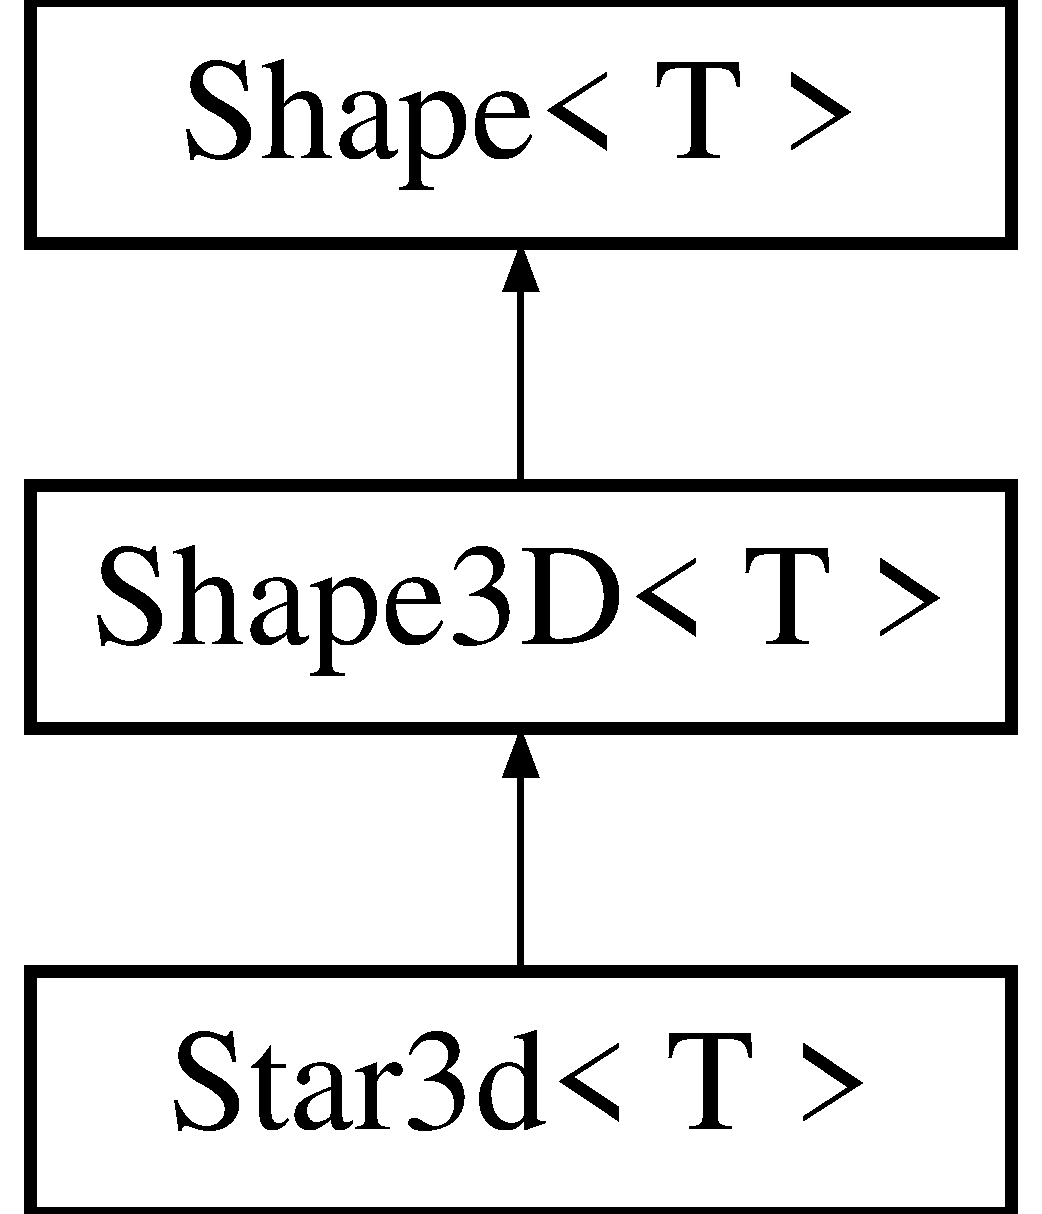
\includegraphics[height=3.000000cm]{classStar3d}
\end{center}
\end{figure}
\subsection*{Public Member Functions}
\begin{DoxyCompactItemize}
\item 
\mbox{\hyperlink{classStar3d_ad264da858df1ef77144a4cd7345185da}{Star3d}} (int=6, T=0.\+5)
\item 
\mbox{\hyperlink{classStar3d_a6793481605da65706c5fc9ca1d4b82ad}{Star3d}} (\mbox{\hyperlink{classStar3d}{Star3d}} \&\&)=default
\item 
\mbox{\hyperlink{classStar3d}{Star3d}} \& \mbox{\hyperlink{classStar3d_a35ace37c66d10033bef1d0acaf9f3283}{operator=}} (\mbox{\hyperlink{classStar3d}{Star3d}} \&\&)=default
\item 
\mbox{\hyperlink{classStar3d_a5f4b217dd7926f73faaa57766546b022}{Star3d}} (const \mbox{\hyperlink{classStar3d}{Star3d}} \&)=default
\item 
\mbox{\hyperlink{classStar3d}{Star3d}} \& \mbox{\hyperlink{classStar3d_a6e1939003aedebc06efdb51404dfbadd}{operator=}} (const \mbox{\hyperlink{classStar3d}{Star3d}} \&)=default
\item 
T \mbox{\hyperlink{classStar3d_aac560f44b7b7d278781231fbaf8312e1}{perimeter}} ()
\end{DoxyCompactItemize}
\subsection*{Public Attributes}
\begin{DoxyCompactItemize}
\item 
T \mbox{\hyperlink{classStar3d_a4c2be78d1baa7a423885cc3574591848}{ratio}}
\end{DoxyCompactItemize}
\subsection*{Private Member Functions}
\begin{DoxyCompactItemize}
\item 
void \mbox{\hyperlink{classStar3d_a43617f398a59d73eb85df49539f9efa5}{generate\+\_\+vertexes}} (int=10, T=0.\+5)
\begin{DoxyCompactList}\small\item\em Generates vertexes for 3d star. \end{DoxyCompactList}\end{DoxyCompactItemize}
\subsection*{Additional Inherited Members}


\subsection{Detailed Description}
\subsubsection*{template$<$typename T = float$>$\newline
class Star3d$<$ T $>$}

this class contains vertexes and elements for 3 dimensional star shape. 

\subsection{Constructor \& Destructor Documentation}
\mbox{\Hypertarget{classStar3d_ad264da858df1ef77144a4cd7345185da}\label{classStar3d_ad264da858df1ef77144a4cd7345185da}} 
\index{Star3d@{Star3d}!Star3d@{Star3d}}
\index{Star3d@{Star3d}!Star3d@{Star3d}}
\subsubsection{\texorpdfstring{Star3d()}{Star3d()}\hspace{0.1cm}{\footnotesize\ttfamily [1/3]}}
{\footnotesize\ttfamily template$<$typename T $>$ \\
\mbox{\hyperlink{classStar3d}{Star3d}}$<$ T $>$\+::\mbox{\hyperlink{classStar3d}{Star3d}} (\begin{DoxyParamCaption}\item[{int}]{bulges = {\ttfamily 6},  }\item[{T}]{ratio\+\_\+ = {\ttfamily 0.5} }\end{DoxyParamCaption})}

\mbox{\Hypertarget{classStar3d_a6793481605da65706c5fc9ca1d4b82ad}\label{classStar3d_a6793481605da65706c5fc9ca1d4b82ad}} 
\index{Star3d@{Star3d}!Star3d@{Star3d}}
\index{Star3d@{Star3d}!Star3d@{Star3d}}
\subsubsection{\texorpdfstring{Star3d()}{Star3d()}\hspace{0.1cm}{\footnotesize\ttfamily [2/3]}}
{\footnotesize\ttfamily template$<$typename T  = float$>$ \\
\mbox{\hyperlink{classStar3d}{Star3d}}$<$ T $>$\+::\mbox{\hyperlink{classStar3d}{Star3d}} (\begin{DoxyParamCaption}\item[{\mbox{\hyperlink{classStar3d}{Star3d}}$<$ T $>$ \&\&}]{ }\end{DoxyParamCaption})\hspace{0.3cm}{\ttfamily [default]}}

\mbox{\Hypertarget{classStar3d_a5f4b217dd7926f73faaa57766546b022}\label{classStar3d_a5f4b217dd7926f73faaa57766546b022}} 
\index{Star3d@{Star3d}!Star3d@{Star3d}}
\index{Star3d@{Star3d}!Star3d@{Star3d}}
\subsubsection{\texorpdfstring{Star3d()}{Star3d()}\hspace{0.1cm}{\footnotesize\ttfamily [3/3]}}
{\footnotesize\ttfamily template$<$typename T  = float$>$ \\
\mbox{\hyperlink{classStar3d}{Star3d}}$<$ T $>$\+::\mbox{\hyperlink{classStar3d}{Star3d}} (\begin{DoxyParamCaption}\item[{const \mbox{\hyperlink{classStar3d}{Star3d}}$<$ T $>$ \&}]{ }\end{DoxyParamCaption})\hspace{0.3cm}{\ttfamily [default]}}



\subsection{Member Function Documentation}
\mbox{\Hypertarget{classStar3d_a43617f398a59d73eb85df49539f9efa5}\label{classStar3d_a43617f398a59d73eb85df49539f9efa5}} 
\index{Star3d@{Star3d}!generate\+\_\+vertexes@{generate\+\_\+vertexes}}
\index{generate\+\_\+vertexes@{generate\+\_\+vertexes}!Star3d@{Star3d}}
\subsubsection{\texorpdfstring{generate\+\_\+vertexes()}{generate\_vertexes()}}
{\footnotesize\ttfamily template$<$typename T $>$ \\
void \mbox{\hyperlink{classStar3d}{Star3d}}$<$ T $>$\+::generate\+\_\+vertexes (\begin{DoxyParamCaption}\item[{int}]{bulges = {\ttfamily 10},  }\item[{T}]{ratio = {\ttfamily 0.5} }\end{DoxyParamCaption})\hspace{0.3cm}{\ttfamily [inline]}, {\ttfamily [private]}}



Generates vertexes for 3d star. 

\mbox{\Hypertarget{classStar3d_a35ace37c66d10033bef1d0acaf9f3283}\label{classStar3d_a35ace37c66d10033bef1d0acaf9f3283}} 
\index{Star3d@{Star3d}!operator=@{operator=}}
\index{operator=@{operator=}!Star3d@{Star3d}}
\subsubsection{\texorpdfstring{operator=()}{operator=()}\hspace{0.1cm}{\footnotesize\ttfamily [1/2]}}
{\footnotesize\ttfamily template$<$typename T  = float$>$ \\
\mbox{\hyperlink{classStar3d}{Star3d}}\& \mbox{\hyperlink{classStar3d}{Star3d}}$<$ T $>$\+::operator= (\begin{DoxyParamCaption}\item[{\mbox{\hyperlink{classStar3d}{Star3d}}$<$ T $>$ \&\&}]{ }\end{DoxyParamCaption})\hspace{0.3cm}{\ttfamily [default]}}

\mbox{\Hypertarget{classStar3d_a6e1939003aedebc06efdb51404dfbadd}\label{classStar3d_a6e1939003aedebc06efdb51404dfbadd}} 
\index{Star3d@{Star3d}!operator=@{operator=}}
\index{operator=@{operator=}!Star3d@{Star3d}}
\subsubsection{\texorpdfstring{operator=()}{operator=()}\hspace{0.1cm}{\footnotesize\ttfamily [2/2]}}
{\footnotesize\ttfamily template$<$typename T  = float$>$ \\
\mbox{\hyperlink{classStar3d}{Star3d}}\& \mbox{\hyperlink{classStar3d}{Star3d}}$<$ T $>$\+::operator= (\begin{DoxyParamCaption}\item[{const \mbox{\hyperlink{classStar3d}{Star3d}}$<$ T $>$ \&}]{ }\end{DoxyParamCaption})\hspace{0.3cm}{\ttfamily [default]}}

\mbox{\Hypertarget{classStar3d_aac560f44b7b7d278781231fbaf8312e1}\label{classStar3d_aac560f44b7b7d278781231fbaf8312e1}} 
\index{Star3d@{Star3d}!perimeter@{perimeter}}
\index{perimeter@{perimeter}!Star3d@{Star3d}}
\subsubsection{\texorpdfstring{perimeter()}{perimeter()}}
{\footnotesize\ttfamily template$<$typename T  = float$>$ \\
T \mbox{\hyperlink{classStar3d}{Star3d}}$<$ T $>$\+::perimeter (\begin{DoxyParamCaption}{ }\end{DoxyParamCaption})}



\subsection{Member Data Documentation}
\mbox{\Hypertarget{classStar3d_a4c2be78d1baa7a423885cc3574591848}\label{classStar3d_a4c2be78d1baa7a423885cc3574591848}} 
\index{Star3d@{Star3d}!ratio@{ratio}}
\index{ratio@{ratio}!Star3d@{Star3d}}
\subsubsection{\texorpdfstring{ratio}{ratio}}
{\footnotesize\ttfamily template$<$typename T  = float$>$ \\
T \mbox{\hyperlink{classStar3d}{Star3d}}$<$ T $>$\+::ratio}



The documentation for this class was generated from the following file\+:\begin{DoxyCompactItemize}
\item 
src/shapes/\mbox{\hyperlink{star3d__not__working_8hpp}{star3d\+\_\+not\+\_\+working.\+hpp}}\end{DoxyCompactItemize}

\hypertarget{classThis}{}\section{This Class Reference}
\label{classThis}\index{This@{This}}


\subsection{Detailed Description}
vertex and element data for 3d sphere. 

The documentation for this class was generated from the following file\+:\begin{DoxyCompactItemize}
\item 
src/shapes/\mbox{\hyperlink{sphere_8hpp}{sphere.\+hpp}}\end{DoxyCompactItemize}

\chapter{File Documentation}
\hypertarget{benchmarks__includes_8hpp}{}\section{benchmarks/benchmarks\+\_\+includes.hpp File Reference}
\label{benchmarks__includes_8hpp}\index{benchmarks/benchmarks\+\_\+includes.\+hpp@{benchmarks/benchmarks\+\_\+includes.\+hpp}}
{\ttfamily \#include $<$xmmintrin.\+h$>$}\newline
{\ttfamily \#include $<$algorithm$>$}\newline
{\ttfamily \#include $<$array$>$}\newline
{\ttfamily \#include $<$cmath$>$}\newline
{\ttfamily \#include $<$ctime$>$}\newline
{\ttfamily \#include $<$string$>$}\newline
{\ttfamily \#include $<$glm/glm.\+hpp$>$}\newline
{\ttfamily \#include $<$glm/gtc/matrix\+\_\+transform.\+hpp$>$}\newline
{\ttfamily \#include $<$glm/gtc/type\+\_\+ptr.\+hpp$>$}\newline
{\ttfamily \#include $<$iostream$>$}\newline
{\ttfamily \#include $<$limits$>$}\newline
{\ttfamily \#include $<$type\+\_\+traits$>$}\newline
{\ttfamily \#include $<$unordered\+\_\+map$>$}\newline
{\ttfamily \#include $<$vector$>$}\newline
{\ttfamily \#include $<$random$>$}\newline
{\ttfamily \#include $<$list$>$}\newline
{\ttfamily \#include $<$chrono$>$}\newline
{\ttfamily \#include $<$thread$>$}\newline
{\ttfamily \#include $<$functional$>$}\newline
{\ttfamily \#include $<$boost/align/aligned\+\_\+allocator.\+hpp$>$}\newline
{\ttfamily \#include $<$benchmark/benchmark.\+h$>$}\newline
{\ttfamily \#include \char`\"{}apex\+\_\+memmove.\+h\char`\"{}}\newline
{\ttfamily \#include \char`\"{}type\+\_\+definitions.\+hpp\char`\"{}}\newline
{\ttfamily \#include \char`\"{}convex\+\_\+hull.\+hpp\char`\"{}}\newline
{\ttfamily \#include \char`\"{}auxiliary\+\_\+functions.\+hpp\char`\"{}}\newline
{\ttfamily \#include \char`\"{}print\+\_\+functions.\+hpp\char`\"{}}\newline
{\ttfamily \#include \char`\"{}bitonic\+\_\+sort.\+hpp\char`\"{}}\newline
{\ttfamily \#include \char`\"{}modified\+\_\+bitonic\+\_\+sort.\+hpp\char`\"{}}\newline
{\ttfamily \#include \char`\"{}hybrid\+\_\+sort.\+hpp\char`\"{}}\newline

\hypertarget{sort__benchmarks_8cpp}{}\section{benchmarks/sort\+\_\+benchmarks.cpp File Reference}
\label{sort__benchmarks_8cpp}\index{benchmarks/sort\+\_\+benchmarks.\+cpp@{benchmarks/sort\+\_\+benchmarks.\+cpp}}
{\ttfamily \#include \char`\"{}benchmarks\+\_\+includes.\+hpp\char`\"{}}\newline
{\ttfamily \#include $<$chrono$>$}\newline
\subsection*{Functions}
\begin{DoxyCompactItemize}
\item 
std\+::default\+\_\+random\+\_\+engine \mbox{\hyperlink{sort__benchmarks_8cpp_a5dc9079dfed6570c71f2ce9059815185}{generator}} (std\+::time(0))
\item 
std\+::uniform\+\_\+real\+\_\+distribution$<$ float $>$ \mbox{\hyperlink{sort__benchmarks_8cpp_a6904ec0ecb2e2c2d27fcb6f5cc972964}{float\+\_\+dist}} (-\/100, 100)
\item 
std\+::uniform\+\_\+real\+\_\+distribution$<$ double $>$ \mbox{\hyperlink{sort__benchmarks_8cpp_ab6dce82b9fcdaf6fff7ec472c87efccf}{double\+\_\+dist}} (-\/100, 100)
\item 
static void \mbox{\hyperlink{sort__benchmarks_8cpp_ad219368285075022a9c69e414d3c3ebc}{bitonic\+\_\+2n\+\_\+float\+\_\+sort\+\_\+bench}} (benchmark\+::\+State \&state)
\item 
\mbox{\hyperlink{sort__benchmarks_8cpp_a5f6d78c36e04c79a9e0508501e2c4d08}{Range\+Multiplier}} (2) -\/$>$ Range(8, 67108864) -\/$>$Complexity(benchmark\+::oN)
\item 
static void \mbox{\hyperlink{sort__benchmarks_8cpp_aef7cc83f7229fa95364231f81c1de508}{bitonic\+\_\+8n\+\_\+float\+\_\+sort\+\_\+bench}} (benchmark\+::\+State \&state)
\item 
static void \mbox{\hyperlink{sort__benchmarks_8cpp_ade47be90dd8781831eb95b912a4a04b3}{hybrid\+\_\+8n\+\_\+float\+\_\+sort\+\_\+bench}} (benchmark\+::\+State \&state)
\item 
static void \mbox{\hyperlink{sort__benchmarks_8cpp_a4bee3c3f901e47667ff3843da68efb8c}{Custom\+Arguments}} (benchmark\+::internal\+::\+Benchmark $\ast$b)
\item 
static void \mbox{\hyperlink{sort__benchmarks_8cpp_aa0236fefbfeebbc828fa895743a62522}{bitonic\+\_\+float\+\_\+sort\+\_\+bench}} (benchmark\+::\+State \&state)
\item 
\mbox{\hyperlink{sort__benchmarks_8cpp_a30a76de4151cf1da4d59aa0646fba710}{B\+E\+N\+C\+H\+M\+A\+RK}} (\mbox{\hyperlink{sort__benchmarks_8cpp_aa0236fefbfeebbc828fa895743a62522}{bitonic\+\_\+float\+\_\+sort\+\_\+bench}}) -\/$>$ Apply(\mbox{\hyperlink{sort__benchmarks_8cpp_a4bee3c3f901e47667ff3843da68efb8c}{Custom\+Arguments}})
\item 
static void \mbox{\hyperlink{sort__benchmarks_8cpp_af569ea97a3fc6ecf6a11952a9cbd5929}{improved\+\_\+bitonic\+\_\+float\+\_\+sort\+\_\+bench}} (benchmark\+::\+State \&state)
\item 
\mbox{\hyperlink{sort__benchmarks_8cpp_a9f86154d764ea4d1fd5a8cb38358861e}{B\+E\+N\+C\+H\+M\+A\+RK}} (\mbox{\hyperlink{sort__benchmarks_8cpp_af569ea97a3fc6ecf6a11952a9cbd5929}{improved\+\_\+bitonic\+\_\+float\+\_\+sort\+\_\+bench}}) -\/$>$ Apply(\mbox{\hyperlink{sort__benchmarks_8cpp_a4bee3c3f901e47667ff3843da68efb8c}{Custom\+Arguments}})
\item 
static void \mbox{\hyperlink{sort__benchmarks_8cpp_aaf37b549986879c9ba54724dcdb4a8fe}{simd\+\_\+\+Q\+S\+\_\+float\+\_\+bench}} (benchmark\+::\+State \&state)
\item 
\mbox{\hyperlink{sort__benchmarks_8cpp_aa9fd02fedb475fcd901e28a9ce71661d}{B\+E\+N\+C\+H\+M\+A\+RK}} (\mbox{\hyperlink{sort__benchmarks_8cpp_aaf37b549986879c9ba54724dcdb4a8fe}{simd\+\_\+\+Q\+S\+\_\+float\+\_\+bench}}) -\/$>$ Apply(\mbox{\hyperlink{sort__benchmarks_8cpp_a4bee3c3f901e47667ff3843da68efb8c}{Custom\+Arguments}})
\item 
static void \mbox{\hyperlink{sort__benchmarks_8cpp_abc82706d4992d3bbdfd59d6c6787446e}{std\+\_\+float\+\_\+sort\+\_\+bench}} (benchmark\+::\+State \&state)
\item 
\mbox{\hyperlink{sort__benchmarks_8cpp_a62388f93f792974aea9280fdb5ec6741}{B\+E\+N\+C\+H\+M\+A\+RK}} (\mbox{\hyperlink{sort__benchmarks_8cpp_abc82706d4992d3bbdfd59d6c6787446e}{std\+\_\+float\+\_\+sort\+\_\+bench}}) -\/$>$ Apply(\mbox{\hyperlink{sort__benchmarks_8cpp_a4bee3c3f901e47667ff3843da68efb8c}{Custom\+Arguments}})
\item 
static void \mbox{\hyperlink{sort__benchmarks_8cpp_aaaa0fb02856afcc3a5667143ac929fa8}{bitonic\+\_\+2n\+\_\+double\+\_\+sort\+\_\+bench}} (benchmark\+::\+State \&state)
\item 
static void \mbox{\hyperlink{sort__benchmarks_8cpp_aa98359c453da15b3c322d5ff94640b11}{bitonic\+\_\+4n\+\_\+double\+\_\+sort\+\_\+bench}} (benchmark\+::\+State \&state)
\item 
\mbox{\hyperlink{sort__benchmarks_8cpp_a135cdc759ea12122dce8561cb07a2af7}{Range\+Multiplier}} (8) -\/$>$ Range(8, 67108864) -\/$>$Complexity(benchmark\+::oN)
\item 
static void \mbox{\hyperlink{sort__benchmarks_8cpp_aa7865bd05b5f9c6b2a9fe4a43d594d2c}{bitonic\+\_\+double\+\_\+sort\+\_\+bench}} (benchmark\+::\+State \&state)
\item 
\mbox{\hyperlink{sort__benchmarks_8cpp_a3ae7cf93a40119b3d2cc5cbb094441d2}{B\+E\+N\+C\+H\+M\+A\+RK}} (\mbox{\hyperlink{sort__benchmarks_8cpp_aa7865bd05b5f9c6b2a9fe4a43d594d2c}{bitonic\+\_\+double\+\_\+sort\+\_\+bench}}) -\/$>$ Apply(\mbox{\hyperlink{sort__benchmarks_8cpp_a4bee3c3f901e47667ff3843da68efb8c}{Custom\+Arguments}})
\item 
static void \mbox{\hyperlink{sort__benchmarks_8cpp_af9fc26c536b051ad1ebf043b0bb24762}{std\+\_\+double\+\_\+sort\+\_\+bench}} (benchmark\+::\+State \&state)
\item 
\mbox{\hyperlink{sort__benchmarks_8cpp_a174f4d99ac50df35e74b698213e7cbd9}{B\+E\+N\+C\+H\+M\+A\+RK}} (\mbox{\hyperlink{sort__benchmarks_8cpp_af9fc26c536b051ad1ebf043b0bb24762}{std\+\_\+double\+\_\+sort\+\_\+bench}}) -\/$>$ Apply(\mbox{\hyperlink{sort__benchmarks_8cpp_a4bee3c3f901e47667ff3843da68efb8c}{Custom\+Arguments}})
\item 
\mbox{\hyperlink{sort__benchmarks_8cpp_a5851750faa9cfec10f7cad1f3b89697e}{B\+E\+N\+C\+H\+M\+A\+R\+K\+\_\+\+M\+A\+IN}} ()
\end{DoxyCompactItemize}
\subsection*{Variables}
\begin{DoxyCompactItemize}
\item 
auto \mbox{\hyperlink{sort__benchmarks_8cpp_a9dd4b1bafcf4df807cbedae854a203fb}{random\+\_\+float}} = std\+::bind(\mbox{\hyperlink{gtest__tests_8cpp_a6904ec0ecb2e2c2d27fcb6f5cc972964}{float\+\_\+dist}}, \mbox{\hyperlink{gtest__tests_8cpp_a5dc9079dfed6570c71f2ce9059815185}{generator}})
\item 
auto \mbox{\hyperlink{sort__benchmarks_8cpp_af37e683a424a342bfd2154a2bf058dc8}{random\+\_\+double}} = std\+::bind(\mbox{\hyperlink{gtest__tests_8cpp_ab6dce82b9fcdaf6fff7ec472c87efccf}{double\+\_\+dist}}, \mbox{\hyperlink{gtest__tests_8cpp_a5dc9079dfed6570c71f2ce9059815185}{generator}})
\end{DoxyCompactItemize}


\subsection{Function Documentation}
\mbox{\Hypertarget{sort__benchmarks_8cpp_a30a76de4151cf1da4d59aa0646fba710}\label{sort__benchmarks_8cpp_a30a76de4151cf1da4d59aa0646fba710}} 
\index{sort\+\_\+benchmarks.\+cpp@{sort\+\_\+benchmarks.\+cpp}!B\+E\+N\+C\+H\+M\+A\+RK@{B\+E\+N\+C\+H\+M\+A\+RK}}
\index{B\+E\+N\+C\+H\+M\+A\+RK@{B\+E\+N\+C\+H\+M\+A\+RK}!sort\+\_\+benchmarks.\+cpp@{sort\+\_\+benchmarks.\+cpp}}
\subsubsection{\texorpdfstring{B\+E\+N\+C\+H\+M\+A\+R\+K()}{BENCHMARK()}\hspace{0.1cm}{\footnotesize\ttfamily [1/6]}}
{\footnotesize\ttfamily B\+E\+N\+C\+H\+M\+A\+RK (\begin{DoxyParamCaption}\item[{\mbox{\hyperlink{sort__benchmarks_8cpp_aa0236fefbfeebbc828fa895743a62522}{bitonic\+\_\+float\+\_\+sort\+\_\+bench}}}]{ }\end{DoxyParamCaption}) -\/$>$  Apply(\mbox{\hyperlink{sort__benchmarks_8cpp_a4bee3c3f901e47667ff3843da68efb8c}{Custom\+Arguments}})}

\mbox{\Hypertarget{sort__benchmarks_8cpp_a9f86154d764ea4d1fd5a8cb38358861e}\label{sort__benchmarks_8cpp_a9f86154d764ea4d1fd5a8cb38358861e}} 
\index{sort\+\_\+benchmarks.\+cpp@{sort\+\_\+benchmarks.\+cpp}!B\+E\+N\+C\+H\+M\+A\+RK@{B\+E\+N\+C\+H\+M\+A\+RK}}
\index{B\+E\+N\+C\+H\+M\+A\+RK@{B\+E\+N\+C\+H\+M\+A\+RK}!sort\+\_\+benchmarks.\+cpp@{sort\+\_\+benchmarks.\+cpp}}
\subsubsection{\texorpdfstring{B\+E\+N\+C\+H\+M\+A\+R\+K()}{BENCHMARK()}\hspace{0.1cm}{\footnotesize\ttfamily [2/6]}}
{\footnotesize\ttfamily B\+E\+N\+C\+H\+M\+A\+RK (\begin{DoxyParamCaption}\item[{\mbox{\hyperlink{sort__benchmarks_8cpp_af569ea97a3fc6ecf6a11952a9cbd5929}{improved\+\_\+bitonic\+\_\+float\+\_\+sort\+\_\+bench}}}]{ }\end{DoxyParamCaption}) -\/$>$  Apply(\mbox{\hyperlink{sort__benchmarks_8cpp_a4bee3c3f901e47667ff3843da68efb8c}{Custom\+Arguments}})}

\mbox{\Hypertarget{sort__benchmarks_8cpp_aa9fd02fedb475fcd901e28a9ce71661d}\label{sort__benchmarks_8cpp_aa9fd02fedb475fcd901e28a9ce71661d}} 
\index{sort\+\_\+benchmarks.\+cpp@{sort\+\_\+benchmarks.\+cpp}!B\+E\+N\+C\+H\+M\+A\+RK@{B\+E\+N\+C\+H\+M\+A\+RK}}
\index{B\+E\+N\+C\+H\+M\+A\+RK@{B\+E\+N\+C\+H\+M\+A\+RK}!sort\+\_\+benchmarks.\+cpp@{sort\+\_\+benchmarks.\+cpp}}
\subsubsection{\texorpdfstring{B\+E\+N\+C\+H\+M\+A\+R\+K()}{BENCHMARK()}\hspace{0.1cm}{\footnotesize\ttfamily [3/6]}}
{\footnotesize\ttfamily B\+E\+N\+C\+H\+M\+A\+RK (\begin{DoxyParamCaption}\item[{\mbox{\hyperlink{sort__benchmarks_8cpp_aaf37b549986879c9ba54724dcdb4a8fe}{simd\+\_\+\+Q\+S\+\_\+float\+\_\+bench}}}]{ }\end{DoxyParamCaption}) -\/$>$  Apply(\mbox{\hyperlink{sort__benchmarks_8cpp_a4bee3c3f901e47667ff3843da68efb8c}{Custom\+Arguments}})}

\mbox{\Hypertarget{sort__benchmarks_8cpp_a62388f93f792974aea9280fdb5ec6741}\label{sort__benchmarks_8cpp_a62388f93f792974aea9280fdb5ec6741}} 
\index{sort\+\_\+benchmarks.\+cpp@{sort\+\_\+benchmarks.\+cpp}!B\+E\+N\+C\+H\+M\+A\+RK@{B\+E\+N\+C\+H\+M\+A\+RK}}
\index{B\+E\+N\+C\+H\+M\+A\+RK@{B\+E\+N\+C\+H\+M\+A\+RK}!sort\+\_\+benchmarks.\+cpp@{sort\+\_\+benchmarks.\+cpp}}
\subsubsection{\texorpdfstring{B\+E\+N\+C\+H\+M\+A\+R\+K()}{BENCHMARK()}\hspace{0.1cm}{\footnotesize\ttfamily [4/6]}}
{\footnotesize\ttfamily B\+E\+N\+C\+H\+M\+A\+RK (\begin{DoxyParamCaption}\item[{\mbox{\hyperlink{sort__benchmarks_8cpp_abc82706d4992d3bbdfd59d6c6787446e}{std\+\_\+float\+\_\+sort\+\_\+bench}}}]{ }\end{DoxyParamCaption}) -\/$>$  Apply(\mbox{\hyperlink{sort__benchmarks_8cpp_a4bee3c3f901e47667ff3843da68efb8c}{Custom\+Arguments}})}

\mbox{\Hypertarget{sort__benchmarks_8cpp_a3ae7cf93a40119b3d2cc5cbb094441d2}\label{sort__benchmarks_8cpp_a3ae7cf93a40119b3d2cc5cbb094441d2}} 
\index{sort\+\_\+benchmarks.\+cpp@{sort\+\_\+benchmarks.\+cpp}!B\+E\+N\+C\+H\+M\+A\+RK@{B\+E\+N\+C\+H\+M\+A\+RK}}
\index{B\+E\+N\+C\+H\+M\+A\+RK@{B\+E\+N\+C\+H\+M\+A\+RK}!sort\+\_\+benchmarks.\+cpp@{sort\+\_\+benchmarks.\+cpp}}
\subsubsection{\texorpdfstring{B\+E\+N\+C\+H\+M\+A\+R\+K()}{BENCHMARK()}\hspace{0.1cm}{\footnotesize\ttfamily [5/6]}}
{\footnotesize\ttfamily B\+E\+N\+C\+H\+M\+A\+RK (\begin{DoxyParamCaption}\item[{\mbox{\hyperlink{sort__benchmarks_8cpp_aa7865bd05b5f9c6b2a9fe4a43d594d2c}{bitonic\+\_\+double\+\_\+sort\+\_\+bench}}}]{ }\end{DoxyParamCaption}) -\/$>$  Apply(\mbox{\hyperlink{sort__benchmarks_8cpp_a4bee3c3f901e47667ff3843da68efb8c}{Custom\+Arguments}})}

\mbox{\Hypertarget{sort__benchmarks_8cpp_a174f4d99ac50df35e74b698213e7cbd9}\label{sort__benchmarks_8cpp_a174f4d99ac50df35e74b698213e7cbd9}} 
\index{sort\+\_\+benchmarks.\+cpp@{sort\+\_\+benchmarks.\+cpp}!B\+E\+N\+C\+H\+M\+A\+RK@{B\+E\+N\+C\+H\+M\+A\+RK}}
\index{B\+E\+N\+C\+H\+M\+A\+RK@{B\+E\+N\+C\+H\+M\+A\+RK}!sort\+\_\+benchmarks.\+cpp@{sort\+\_\+benchmarks.\+cpp}}
\subsubsection{\texorpdfstring{B\+E\+N\+C\+H\+M\+A\+R\+K()}{BENCHMARK()}\hspace{0.1cm}{\footnotesize\ttfamily [6/6]}}
{\footnotesize\ttfamily B\+E\+N\+C\+H\+M\+A\+RK (\begin{DoxyParamCaption}\item[{\mbox{\hyperlink{sort__benchmarks_8cpp_af9fc26c536b051ad1ebf043b0bb24762}{std\+\_\+double\+\_\+sort\+\_\+bench}}}]{ }\end{DoxyParamCaption}) -\/$>$  Apply(\mbox{\hyperlink{sort__benchmarks_8cpp_a4bee3c3f901e47667ff3843da68efb8c}{Custom\+Arguments}})}

\mbox{\Hypertarget{sort__benchmarks_8cpp_a5851750faa9cfec10f7cad1f3b89697e}\label{sort__benchmarks_8cpp_a5851750faa9cfec10f7cad1f3b89697e}} 
\index{sort\+\_\+benchmarks.\+cpp@{sort\+\_\+benchmarks.\+cpp}!B\+E\+N\+C\+H\+M\+A\+R\+K\+\_\+\+M\+A\+IN@{B\+E\+N\+C\+H\+M\+A\+R\+K\+\_\+\+M\+A\+IN}}
\index{B\+E\+N\+C\+H\+M\+A\+R\+K\+\_\+\+M\+A\+IN@{B\+E\+N\+C\+H\+M\+A\+R\+K\+\_\+\+M\+A\+IN}!sort\+\_\+benchmarks.\+cpp@{sort\+\_\+benchmarks.\+cpp}}
\subsubsection{\texorpdfstring{B\+E\+N\+C\+H\+M\+A\+R\+K\+\_\+\+M\+A\+I\+N()}{BENCHMARK\_MAIN()}}
{\footnotesize\ttfamily B\+E\+N\+C\+H\+M\+A\+R\+K\+\_\+\+M\+A\+IN (\begin{DoxyParamCaption}{ }\end{DoxyParamCaption})}

\mbox{\Hypertarget{sort__benchmarks_8cpp_aaaa0fb02856afcc3a5667143ac929fa8}\label{sort__benchmarks_8cpp_aaaa0fb02856afcc3a5667143ac929fa8}} 
\index{sort\+\_\+benchmarks.\+cpp@{sort\+\_\+benchmarks.\+cpp}!bitonic\+\_\+2n\+\_\+double\+\_\+sort\+\_\+bench@{bitonic\+\_\+2n\+\_\+double\+\_\+sort\+\_\+bench}}
\index{bitonic\+\_\+2n\+\_\+double\+\_\+sort\+\_\+bench@{bitonic\+\_\+2n\+\_\+double\+\_\+sort\+\_\+bench}!sort\+\_\+benchmarks.\+cpp@{sort\+\_\+benchmarks.\+cpp}}
\subsubsection{\texorpdfstring{bitonic\+\_\+2n\+\_\+double\+\_\+sort\+\_\+bench()}{bitonic\_2n\_double\_sort\_bench()}}
{\footnotesize\ttfamily static void bitonic\+\_\+2n\+\_\+double\+\_\+sort\+\_\+bench (\begin{DoxyParamCaption}\item[{benchmark\+::\+State \&}]{state }\end{DoxyParamCaption})\hspace{0.3cm}{\ttfamily [static]}}

\mbox{\Hypertarget{sort__benchmarks_8cpp_ad219368285075022a9c69e414d3c3ebc}\label{sort__benchmarks_8cpp_ad219368285075022a9c69e414d3c3ebc}} 
\index{sort\+\_\+benchmarks.\+cpp@{sort\+\_\+benchmarks.\+cpp}!bitonic\+\_\+2n\+\_\+float\+\_\+sort\+\_\+bench@{bitonic\+\_\+2n\+\_\+float\+\_\+sort\+\_\+bench}}
\index{bitonic\+\_\+2n\+\_\+float\+\_\+sort\+\_\+bench@{bitonic\+\_\+2n\+\_\+float\+\_\+sort\+\_\+bench}!sort\+\_\+benchmarks.\+cpp@{sort\+\_\+benchmarks.\+cpp}}
\subsubsection{\texorpdfstring{bitonic\+\_\+2n\+\_\+float\+\_\+sort\+\_\+bench()}{bitonic\_2n\_float\_sort\_bench()}}
{\footnotesize\ttfamily static void bitonic\+\_\+2n\+\_\+float\+\_\+sort\+\_\+bench (\begin{DoxyParamCaption}\item[{benchmark\+::\+State \&}]{state }\end{DoxyParamCaption})\hspace{0.3cm}{\ttfamily [static]}}

\mbox{\Hypertarget{sort__benchmarks_8cpp_aa98359c453da15b3c322d5ff94640b11}\label{sort__benchmarks_8cpp_aa98359c453da15b3c322d5ff94640b11}} 
\index{sort\+\_\+benchmarks.\+cpp@{sort\+\_\+benchmarks.\+cpp}!bitonic\+\_\+4n\+\_\+double\+\_\+sort\+\_\+bench@{bitonic\+\_\+4n\+\_\+double\+\_\+sort\+\_\+bench}}
\index{bitonic\+\_\+4n\+\_\+double\+\_\+sort\+\_\+bench@{bitonic\+\_\+4n\+\_\+double\+\_\+sort\+\_\+bench}!sort\+\_\+benchmarks.\+cpp@{sort\+\_\+benchmarks.\+cpp}}
\subsubsection{\texorpdfstring{bitonic\+\_\+4n\+\_\+double\+\_\+sort\+\_\+bench()}{bitonic\_4n\_double\_sort\_bench()}}
{\footnotesize\ttfamily static void bitonic\+\_\+4n\+\_\+double\+\_\+sort\+\_\+bench (\begin{DoxyParamCaption}\item[{benchmark\+::\+State \&}]{state }\end{DoxyParamCaption})\hspace{0.3cm}{\ttfamily [static]}}

\mbox{\Hypertarget{sort__benchmarks_8cpp_aef7cc83f7229fa95364231f81c1de508}\label{sort__benchmarks_8cpp_aef7cc83f7229fa95364231f81c1de508}} 
\index{sort\+\_\+benchmarks.\+cpp@{sort\+\_\+benchmarks.\+cpp}!bitonic\+\_\+8n\+\_\+float\+\_\+sort\+\_\+bench@{bitonic\+\_\+8n\+\_\+float\+\_\+sort\+\_\+bench}}
\index{bitonic\+\_\+8n\+\_\+float\+\_\+sort\+\_\+bench@{bitonic\+\_\+8n\+\_\+float\+\_\+sort\+\_\+bench}!sort\+\_\+benchmarks.\+cpp@{sort\+\_\+benchmarks.\+cpp}}
\subsubsection{\texorpdfstring{bitonic\+\_\+8n\+\_\+float\+\_\+sort\+\_\+bench()}{bitonic\_8n\_float\_sort\_bench()}}
{\footnotesize\ttfamily static void bitonic\+\_\+8n\+\_\+float\+\_\+sort\+\_\+bench (\begin{DoxyParamCaption}\item[{benchmark\+::\+State \&}]{state }\end{DoxyParamCaption})\hspace{0.3cm}{\ttfamily [static]}}

\mbox{\Hypertarget{sort__benchmarks_8cpp_aa7865bd05b5f9c6b2a9fe4a43d594d2c}\label{sort__benchmarks_8cpp_aa7865bd05b5f9c6b2a9fe4a43d594d2c}} 
\index{sort\+\_\+benchmarks.\+cpp@{sort\+\_\+benchmarks.\+cpp}!bitonic\+\_\+double\+\_\+sort\+\_\+bench@{bitonic\+\_\+double\+\_\+sort\+\_\+bench}}
\index{bitonic\+\_\+double\+\_\+sort\+\_\+bench@{bitonic\+\_\+double\+\_\+sort\+\_\+bench}!sort\+\_\+benchmarks.\+cpp@{sort\+\_\+benchmarks.\+cpp}}
\subsubsection{\texorpdfstring{bitonic\+\_\+double\+\_\+sort\+\_\+bench()}{bitonic\_double\_sort\_bench()}}
{\footnotesize\ttfamily static void bitonic\+\_\+double\+\_\+sort\+\_\+bench (\begin{DoxyParamCaption}\item[{benchmark\+::\+State \&}]{state }\end{DoxyParamCaption})\hspace{0.3cm}{\ttfamily [static]}}

\mbox{\Hypertarget{sort__benchmarks_8cpp_aa0236fefbfeebbc828fa895743a62522}\label{sort__benchmarks_8cpp_aa0236fefbfeebbc828fa895743a62522}} 
\index{sort\+\_\+benchmarks.\+cpp@{sort\+\_\+benchmarks.\+cpp}!bitonic\+\_\+float\+\_\+sort\+\_\+bench@{bitonic\+\_\+float\+\_\+sort\+\_\+bench}}
\index{bitonic\+\_\+float\+\_\+sort\+\_\+bench@{bitonic\+\_\+float\+\_\+sort\+\_\+bench}!sort\+\_\+benchmarks.\+cpp@{sort\+\_\+benchmarks.\+cpp}}
\subsubsection{\texorpdfstring{bitonic\+\_\+float\+\_\+sort\+\_\+bench()}{bitonic\_float\_sort\_bench()}}
{\footnotesize\ttfamily static void bitonic\+\_\+float\+\_\+sort\+\_\+bench (\begin{DoxyParamCaption}\item[{benchmark\+::\+State \&}]{state }\end{DoxyParamCaption})\hspace{0.3cm}{\ttfamily [static]}}

\mbox{\Hypertarget{sort__benchmarks_8cpp_a4bee3c3f901e47667ff3843da68efb8c}\label{sort__benchmarks_8cpp_a4bee3c3f901e47667ff3843da68efb8c}} 
\index{sort\+\_\+benchmarks.\+cpp@{sort\+\_\+benchmarks.\+cpp}!Custom\+Arguments@{Custom\+Arguments}}
\index{Custom\+Arguments@{Custom\+Arguments}!sort\+\_\+benchmarks.\+cpp@{sort\+\_\+benchmarks.\+cpp}}
\subsubsection{\texorpdfstring{Custom\+Arguments()}{CustomArguments()}}
{\footnotesize\ttfamily static void Custom\+Arguments (\begin{DoxyParamCaption}\item[{benchmark\+::internal\+::\+Benchmark $\ast$}]{b }\end{DoxyParamCaption})\hspace{0.3cm}{\ttfamily [static]}}

\mbox{\Hypertarget{sort__benchmarks_8cpp_ab6dce82b9fcdaf6fff7ec472c87efccf}\label{sort__benchmarks_8cpp_ab6dce82b9fcdaf6fff7ec472c87efccf}} 
\index{sort\+\_\+benchmarks.\+cpp@{sort\+\_\+benchmarks.\+cpp}!double\+\_\+dist@{double\+\_\+dist}}
\index{double\+\_\+dist@{double\+\_\+dist}!sort\+\_\+benchmarks.\+cpp@{sort\+\_\+benchmarks.\+cpp}}
\subsubsection{\texorpdfstring{double\+\_\+dist()}{double\_dist()}}
{\footnotesize\ttfamily std\+::uniform\+\_\+real\+\_\+distribution$<$double$>$ double\+\_\+dist (\begin{DoxyParamCaption}\item[{-\/}]{100,  }\item[{100}]{ }\end{DoxyParamCaption})}

\mbox{\Hypertarget{sort__benchmarks_8cpp_a6904ec0ecb2e2c2d27fcb6f5cc972964}\label{sort__benchmarks_8cpp_a6904ec0ecb2e2c2d27fcb6f5cc972964}} 
\index{sort\+\_\+benchmarks.\+cpp@{sort\+\_\+benchmarks.\+cpp}!float\+\_\+dist@{float\+\_\+dist}}
\index{float\+\_\+dist@{float\+\_\+dist}!sort\+\_\+benchmarks.\+cpp@{sort\+\_\+benchmarks.\+cpp}}
\subsubsection{\texorpdfstring{float\+\_\+dist()}{float\_dist()}}
{\footnotesize\ttfamily std\+::uniform\+\_\+real\+\_\+distribution$<$float$>$ float\+\_\+dist (\begin{DoxyParamCaption}\item[{-\/}]{100,  }\item[{100}]{ }\end{DoxyParamCaption})}

\mbox{\Hypertarget{sort__benchmarks_8cpp_a5dc9079dfed6570c71f2ce9059815185}\label{sort__benchmarks_8cpp_a5dc9079dfed6570c71f2ce9059815185}} 
\index{sort\+\_\+benchmarks.\+cpp@{sort\+\_\+benchmarks.\+cpp}!generator@{generator}}
\index{generator@{generator}!sort\+\_\+benchmarks.\+cpp@{sort\+\_\+benchmarks.\+cpp}}
\subsubsection{\texorpdfstring{generator()}{generator()}}
{\footnotesize\ttfamily std\+::default\+\_\+random\+\_\+engine generator (\begin{DoxyParamCaption}\item[{std\+::time(0)}]{ }\end{DoxyParamCaption})}

\mbox{\Hypertarget{sort__benchmarks_8cpp_ade47be90dd8781831eb95b912a4a04b3}\label{sort__benchmarks_8cpp_ade47be90dd8781831eb95b912a4a04b3}} 
\index{sort\+\_\+benchmarks.\+cpp@{sort\+\_\+benchmarks.\+cpp}!hybrid\+\_\+8n\+\_\+float\+\_\+sort\+\_\+bench@{hybrid\+\_\+8n\+\_\+float\+\_\+sort\+\_\+bench}}
\index{hybrid\+\_\+8n\+\_\+float\+\_\+sort\+\_\+bench@{hybrid\+\_\+8n\+\_\+float\+\_\+sort\+\_\+bench}!sort\+\_\+benchmarks.\+cpp@{sort\+\_\+benchmarks.\+cpp}}
\subsubsection{\texorpdfstring{hybrid\+\_\+8n\+\_\+float\+\_\+sort\+\_\+bench()}{hybrid\_8n\_float\_sort\_bench()}}
{\footnotesize\ttfamily static void hybrid\+\_\+8n\+\_\+float\+\_\+sort\+\_\+bench (\begin{DoxyParamCaption}\item[{benchmark\+::\+State \&}]{state }\end{DoxyParamCaption})\hspace{0.3cm}{\ttfamily [static]}}

\mbox{\Hypertarget{sort__benchmarks_8cpp_af569ea97a3fc6ecf6a11952a9cbd5929}\label{sort__benchmarks_8cpp_af569ea97a3fc6ecf6a11952a9cbd5929}} 
\index{sort\+\_\+benchmarks.\+cpp@{sort\+\_\+benchmarks.\+cpp}!improved\+\_\+bitonic\+\_\+float\+\_\+sort\+\_\+bench@{improved\+\_\+bitonic\+\_\+float\+\_\+sort\+\_\+bench}}
\index{improved\+\_\+bitonic\+\_\+float\+\_\+sort\+\_\+bench@{improved\+\_\+bitonic\+\_\+float\+\_\+sort\+\_\+bench}!sort\+\_\+benchmarks.\+cpp@{sort\+\_\+benchmarks.\+cpp}}
\subsubsection{\texorpdfstring{improved\+\_\+bitonic\+\_\+float\+\_\+sort\+\_\+bench()}{improved\_bitonic\_float\_sort\_bench()}}
{\footnotesize\ttfamily static void improved\+\_\+bitonic\+\_\+float\+\_\+sort\+\_\+bench (\begin{DoxyParamCaption}\item[{benchmark\+::\+State \&}]{state }\end{DoxyParamCaption})\hspace{0.3cm}{\ttfamily [static]}}

\mbox{\Hypertarget{sort__benchmarks_8cpp_a5f6d78c36e04c79a9e0508501e2c4d08}\label{sort__benchmarks_8cpp_a5f6d78c36e04c79a9e0508501e2c4d08}} 
\index{sort\+\_\+benchmarks.\+cpp@{sort\+\_\+benchmarks.\+cpp}!Range\+Multiplier@{Range\+Multiplier}}
\index{Range\+Multiplier@{Range\+Multiplier}!sort\+\_\+benchmarks.\+cpp@{sort\+\_\+benchmarks.\+cpp}}
\subsubsection{\texorpdfstring{Range\+Multiplier()}{RangeMultiplier()}\hspace{0.1cm}{\footnotesize\ttfamily [1/2]}}
{\footnotesize\ttfamily Range\+Multiplier (\begin{DoxyParamCaption}\item[{2}]{ }\end{DoxyParamCaption}) -\/$>$  Range(8, 67108864) -\/$>$Complexity(benchmark\+::oN)}

\mbox{\Hypertarget{sort__benchmarks_8cpp_a135cdc759ea12122dce8561cb07a2af7}\label{sort__benchmarks_8cpp_a135cdc759ea12122dce8561cb07a2af7}} 
\index{sort\+\_\+benchmarks.\+cpp@{sort\+\_\+benchmarks.\+cpp}!Range\+Multiplier@{Range\+Multiplier}}
\index{Range\+Multiplier@{Range\+Multiplier}!sort\+\_\+benchmarks.\+cpp@{sort\+\_\+benchmarks.\+cpp}}
\subsubsection{\texorpdfstring{Range\+Multiplier()}{RangeMultiplier()}\hspace{0.1cm}{\footnotesize\ttfamily [2/2]}}
{\footnotesize\ttfamily Range\+Multiplier (\begin{DoxyParamCaption}\item[{8}]{ }\end{DoxyParamCaption}) -\/$>$  Range(8, 67108864) -\/$>$Complexity(benchmark\+::oN)}

\mbox{\Hypertarget{sort__benchmarks_8cpp_aaf37b549986879c9ba54724dcdb4a8fe}\label{sort__benchmarks_8cpp_aaf37b549986879c9ba54724dcdb4a8fe}} 
\index{sort\+\_\+benchmarks.\+cpp@{sort\+\_\+benchmarks.\+cpp}!simd\+\_\+\+Q\+S\+\_\+float\+\_\+bench@{simd\+\_\+\+Q\+S\+\_\+float\+\_\+bench}}
\index{simd\+\_\+\+Q\+S\+\_\+float\+\_\+bench@{simd\+\_\+\+Q\+S\+\_\+float\+\_\+bench}!sort\+\_\+benchmarks.\+cpp@{sort\+\_\+benchmarks.\+cpp}}
\subsubsection{\texorpdfstring{simd\+\_\+\+Q\+S\+\_\+float\+\_\+bench()}{simd\_QS\_float\_bench()}}
{\footnotesize\ttfamily static void simd\+\_\+\+Q\+S\+\_\+float\+\_\+bench (\begin{DoxyParamCaption}\item[{benchmark\+::\+State \&}]{state }\end{DoxyParamCaption})\hspace{0.3cm}{\ttfamily [static]}}

\mbox{\Hypertarget{sort__benchmarks_8cpp_af9fc26c536b051ad1ebf043b0bb24762}\label{sort__benchmarks_8cpp_af9fc26c536b051ad1ebf043b0bb24762}} 
\index{sort\+\_\+benchmarks.\+cpp@{sort\+\_\+benchmarks.\+cpp}!std\+\_\+double\+\_\+sort\+\_\+bench@{std\+\_\+double\+\_\+sort\+\_\+bench}}
\index{std\+\_\+double\+\_\+sort\+\_\+bench@{std\+\_\+double\+\_\+sort\+\_\+bench}!sort\+\_\+benchmarks.\+cpp@{sort\+\_\+benchmarks.\+cpp}}
\subsubsection{\texorpdfstring{std\+\_\+double\+\_\+sort\+\_\+bench()}{std\_double\_sort\_bench()}}
{\footnotesize\ttfamily static void std\+\_\+double\+\_\+sort\+\_\+bench (\begin{DoxyParamCaption}\item[{benchmark\+::\+State \&}]{state }\end{DoxyParamCaption})\hspace{0.3cm}{\ttfamily [static]}}

\mbox{\Hypertarget{sort__benchmarks_8cpp_abc82706d4992d3bbdfd59d6c6787446e}\label{sort__benchmarks_8cpp_abc82706d4992d3bbdfd59d6c6787446e}} 
\index{sort\+\_\+benchmarks.\+cpp@{sort\+\_\+benchmarks.\+cpp}!std\+\_\+float\+\_\+sort\+\_\+bench@{std\+\_\+float\+\_\+sort\+\_\+bench}}
\index{std\+\_\+float\+\_\+sort\+\_\+bench@{std\+\_\+float\+\_\+sort\+\_\+bench}!sort\+\_\+benchmarks.\+cpp@{sort\+\_\+benchmarks.\+cpp}}
\subsubsection{\texorpdfstring{std\+\_\+float\+\_\+sort\+\_\+bench()}{std\_float\_sort\_bench()}}
{\footnotesize\ttfamily static void std\+\_\+float\+\_\+sort\+\_\+bench (\begin{DoxyParamCaption}\item[{benchmark\+::\+State \&}]{state }\end{DoxyParamCaption})\hspace{0.3cm}{\ttfamily [static]}}



\subsection{Variable Documentation}
\mbox{\Hypertarget{sort__benchmarks_8cpp_af37e683a424a342bfd2154a2bf058dc8}\label{sort__benchmarks_8cpp_af37e683a424a342bfd2154a2bf058dc8}} 
\index{sort\+\_\+benchmarks.\+cpp@{sort\+\_\+benchmarks.\+cpp}!random\+\_\+double@{random\+\_\+double}}
\index{random\+\_\+double@{random\+\_\+double}!sort\+\_\+benchmarks.\+cpp@{sort\+\_\+benchmarks.\+cpp}}
\subsubsection{\texorpdfstring{random\+\_\+double}{random\_double}}
{\footnotesize\ttfamily auto random\+\_\+double = std\+::bind(\mbox{\hyperlink{gtest__tests_8cpp_ab6dce82b9fcdaf6fff7ec472c87efccf}{double\+\_\+dist}}, \mbox{\hyperlink{gtest__tests_8cpp_a5dc9079dfed6570c71f2ce9059815185}{generator}})}

\mbox{\Hypertarget{sort__benchmarks_8cpp_a9dd4b1bafcf4df807cbedae854a203fb}\label{sort__benchmarks_8cpp_a9dd4b1bafcf4df807cbedae854a203fb}} 
\index{sort\+\_\+benchmarks.\+cpp@{sort\+\_\+benchmarks.\+cpp}!random\+\_\+float@{random\+\_\+float}}
\index{random\+\_\+float@{random\+\_\+float}!sort\+\_\+benchmarks.\+cpp@{sort\+\_\+benchmarks.\+cpp}}
\subsubsection{\texorpdfstring{random\+\_\+float}{random\_float}}
{\footnotesize\ttfamily auto random\+\_\+float = std\+::bind(\mbox{\hyperlink{gtest__tests_8cpp_a6904ec0ecb2e2c2d27fcb6f5cc972964}{float\+\_\+dist}}, \mbox{\hyperlink{gtest__tests_8cpp_a5dc9079dfed6570c71f2ce9059815185}{generator}})}


\hypertarget{build_2CMakeFiles_23_812_83_2CompilerIdC_2CMakeCCompilerId_8c}{}\section{build/\+C\+Make\+Files/3.12.3/\+Compiler\+Id\+C/\+C\+Make\+C\+Compiler\+Id.c File Reference}
\label{build_2CMakeFiles_23_812_83_2CompilerIdC_2CMakeCCompilerId_8c}\index{build/\+C\+Make\+Files/3.\+12.\+3/\+Compiler\+Id\+C/\+C\+Make\+C\+Compiler\+Id.\+c@{build/\+C\+Make\+Files/3.\+12.\+3/\+Compiler\+Id\+C/\+C\+Make\+C\+Compiler\+Id.\+c}}
\subsection*{Macros}
\begin{DoxyCompactItemize}
\item 
\#define \mbox{\hyperlink{build_2CMakeFiles_23_812_83_2CompilerIdC_2CMakeCCompilerId_8c_a81dee0709ded976b2e0319239f72d174}{C\+O\+M\+P\+I\+L\+E\+R\+\_\+\+ID}}~\char`\"{}\char`\"{}
\item 
\#define \mbox{\hyperlink{build_2CMakeFiles_23_812_83_2CompilerIdC_2CMakeCCompilerId_8c_a2ae9b72bb13abaabfcf2ee0ba7d3fa1d}{S\+T\+R\+I\+N\+G\+I\+F\+Y\+\_\+\+H\+E\+L\+P\+ER}}(X)~\#X
\item 
\#define \mbox{\hyperlink{build_2CMakeFiles_23_812_83_2CompilerIdC_2CMakeCCompilerId_8c_a43e1cad902b6477bec893cb6430bd6c8}{S\+T\+R\+I\+N\+G\+I\+FY}}(X)~\mbox{\hyperlink{examples_2opengl__test_2build_2CMakeFiles_23_812_83_2CompilerIdCXX_2CMakeCXXCompilerId_8cpp_a2ae9b72bb13abaabfcf2ee0ba7d3fa1d}{S\+T\+R\+I\+N\+G\+I\+F\+Y\+\_\+\+H\+E\+L\+P\+ER}}(X)
\item 
\#define \mbox{\hyperlink{build_2CMakeFiles_23_812_83_2CompilerIdC_2CMakeCCompilerId_8c_adbc5372f40838899018fadbc89bd588b}{P\+L\+A\+T\+F\+O\+R\+M\+\_\+\+ID}}
\item 
\#define \mbox{\hyperlink{build_2CMakeFiles_23_812_83_2CompilerIdC_2CMakeCCompilerId_8c_aba35d0d200deaeb06aee95ca297acb28}{A\+R\+C\+H\+I\+T\+E\+C\+T\+U\+R\+E\+\_\+\+ID}}
\item 
\#define \mbox{\hyperlink{build_2CMakeFiles_23_812_83_2CompilerIdC_2CMakeCCompilerId_8c_ad1280362da42492bbc11aa78cbf776ad}{D\+EC}}(\mbox{\hyperlink{glad_8h_a0788d3762d0c3c76e4c094d8078b4c27}{n}})
\item 
\#define \mbox{\hyperlink{build_2CMakeFiles_23_812_83_2CompilerIdC_2CMakeCCompilerId_8c_a46d5d95daa1bef867bd0179594310ed5}{H\+EX}}(\mbox{\hyperlink{glad_8h_a0788d3762d0c3c76e4c094d8078b4c27}{n}})
\item 
\#define \mbox{\hyperlink{build_2CMakeFiles_23_812_83_2CompilerIdC_2CMakeCCompilerId_8c_a07f8e5783674099cd7f5110e22a78cdb}{C\+\_\+\+D\+I\+A\+L\+E\+CT}}
\end{DoxyCompactItemize}
\subsection*{Functions}
\begin{DoxyCompactItemize}
\item 
int \mbox{\hyperlink{build_2CMakeFiles_23_812_83_2CompilerIdC_2CMakeCCompilerId_8c_a0ddf1224851353fc92bfbff6f499fa97}{main}} (int argc, char $\ast$argv\mbox{[}$\,$\mbox{]})
\end{DoxyCompactItemize}
\subsection*{Variables}
\begin{DoxyCompactItemize}
\item 
char const  $\ast$ \mbox{\hyperlink{build_2CMakeFiles_23_812_83_2CompilerIdC_2CMakeCCompilerId_8c_a4b0efeb7a5d59313986b3a0390f050f6}{info\+\_\+compiler}} = \char`\"{}I\+N\+FO\char`\"{} \char`\"{}\+:\char`\"{} \char`\"{}compiler\mbox{[}\char`\"{} C\+O\+M\+P\+I\+L\+E\+R\+\_\+\+ID \char`\"{}\mbox{]}\char`\"{}
\item 
char const  $\ast$ \mbox{\hyperlink{build_2CMakeFiles_23_812_83_2CompilerIdC_2CMakeCCompilerId_8c_a2321403dee54ee23f0c2fa849c60f7d4}{info\+\_\+platform}} = \char`\"{}I\+N\+FO\char`\"{} \char`\"{}\+:\char`\"{} \char`\"{}platform\mbox{[}\char`\"{} P\+L\+A\+T\+F\+O\+R\+M\+\_\+\+ID \char`\"{}\mbox{]}\char`\"{}
\item 
char const  $\ast$ \mbox{\hyperlink{build_2CMakeFiles_23_812_83_2CompilerIdC_2CMakeCCompilerId_8c_a59647e99d304ed33b15cb284c27ed391}{info\+\_\+arch}} = \char`\"{}I\+N\+FO\char`\"{} \char`\"{}\+:\char`\"{} \char`\"{}arch\mbox{[}\char`\"{} A\+R\+C\+H\+I\+T\+E\+C\+T\+U\+R\+E\+\_\+\+ID \char`\"{}\mbox{]}\char`\"{}
\item 
const char $\ast$ \mbox{\hyperlink{build_2CMakeFiles_23_812_83_2CompilerIdC_2CMakeCCompilerId_8c_a1ce162bad2fe6966ac8b33cc19e120b8}{info\+\_\+language\+\_\+dialect\+\_\+default}}
\end{DoxyCompactItemize}


\subsection{Macro Definition Documentation}
\mbox{\Hypertarget{build_2CMakeFiles_23_812_83_2CompilerIdC_2CMakeCCompilerId_8c_aba35d0d200deaeb06aee95ca297acb28}\label{build_2CMakeFiles_23_812_83_2CompilerIdC_2CMakeCCompilerId_8c_aba35d0d200deaeb06aee95ca297acb28}} 
\index{build/\+C\+Make\+Files/3.\+12.\+3/\+Compiler\+Id\+C/\+C\+Make\+C\+Compiler\+Id.\+c@{build/\+C\+Make\+Files/3.\+12.\+3/\+Compiler\+Id\+C/\+C\+Make\+C\+Compiler\+Id.\+c}!A\+R\+C\+H\+I\+T\+E\+C\+T\+U\+R\+E\+\_\+\+ID@{A\+R\+C\+H\+I\+T\+E\+C\+T\+U\+R\+E\+\_\+\+ID}}
\index{A\+R\+C\+H\+I\+T\+E\+C\+T\+U\+R\+E\+\_\+\+ID@{A\+R\+C\+H\+I\+T\+E\+C\+T\+U\+R\+E\+\_\+\+ID}!build/\+C\+Make\+Files/3.\+12.\+3/\+Compiler\+Id\+C/\+C\+Make\+C\+Compiler\+Id.\+c@{build/\+C\+Make\+Files/3.\+12.\+3/\+Compiler\+Id\+C/\+C\+Make\+C\+Compiler\+Id.\+c}}
\subsubsection{\texorpdfstring{A\+R\+C\+H\+I\+T\+E\+C\+T\+U\+R\+E\+\_\+\+ID}{ARCHITECTURE\_ID}}
{\footnotesize\ttfamily \#define A\+R\+C\+H\+I\+T\+E\+C\+T\+U\+R\+E\+\_\+\+ID}

\mbox{\Hypertarget{build_2CMakeFiles_23_812_83_2CompilerIdC_2CMakeCCompilerId_8c_a07f8e5783674099cd7f5110e22a78cdb}\label{build_2CMakeFiles_23_812_83_2CompilerIdC_2CMakeCCompilerId_8c_a07f8e5783674099cd7f5110e22a78cdb}} 
\index{build/\+C\+Make\+Files/3.\+12.\+3/\+Compiler\+Id\+C/\+C\+Make\+C\+Compiler\+Id.\+c@{build/\+C\+Make\+Files/3.\+12.\+3/\+Compiler\+Id\+C/\+C\+Make\+C\+Compiler\+Id.\+c}!C\+\_\+\+D\+I\+A\+L\+E\+CT@{C\+\_\+\+D\+I\+A\+L\+E\+CT}}
\index{C\+\_\+\+D\+I\+A\+L\+E\+CT@{C\+\_\+\+D\+I\+A\+L\+E\+CT}!build/\+C\+Make\+Files/3.\+12.\+3/\+Compiler\+Id\+C/\+C\+Make\+C\+Compiler\+Id.\+c@{build/\+C\+Make\+Files/3.\+12.\+3/\+Compiler\+Id\+C/\+C\+Make\+C\+Compiler\+Id.\+c}}
\subsubsection{\texorpdfstring{C\+\_\+\+D\+I\+A\+L\+E\+CT}{C\_DIALECT}}
{\footnotesize\ttfamily \#define C\+\_\+\+D\+I\+A\+L\+E\+CT}

\mbox{\Hypertarget{build_2CMakeFiles_23_812_83_2CompilerIdC_2CMakeCCompilerId_8c_a81dee0709ded976b2e0319239f72d174}\label{build_2CMakeFiles_23_812_83_2CompilerIdC_2CMakeCCompilerId_8c_a81dee0709ded976b2e0319239f72d174}} 
\index{build/\+C\+Make\+Files/3.\+12.\+3/\+Compiler\+Id\+C/\+C\+Make\+C\+Compiler\+Id.\+c@{build/\+C\+Make\+Files/3.\+12.\+3/\+Compiler\+Id\+C/\+C\+Make\+C\+Compiler\+Id.\+c}!C\+O\+M\+P\+I\+L\+E\+R\+\_\+\+ID@{C\+O\+M\+P\+I\+L\+E\+R\+\_\+\+ID}}
\index{C\+O\+M\+P\+I\+L\+E\+R\+\_\+\+ID@{C\+O\+M\+P\+I\+L\+E\+R\+\_\+\+ID}!build/\+C\+Make\+Files/3.\+12.\+3/\+Compiler\+Id\+C/\+C\+Make\+C\+Compiler\+Id.\+c@{build/\+C\+Make\+Files/3.\+12.\+3/\+Compiler\+Id\+C/\+C\+Make\+C\+Compiler\+Id.\+c}}
\subsubsection{\texorpdfstring{C\+O\+M\+P\+I\+L\+E\+R\+\_\+\+ID}{COMPILER\_ID}}
{\footnotesize\ttfamily \#define C\+O\+M\+P\+I\+L\+E\+R\+\_\+\+ID~\char`\"{}\char`\"{}}

\mbox{\Hypertarget{build_2CMakeFiles_23_812_83_2CompilerIdC_2CMakeCCompilerId_8c_ad1280362da42492bbc11aa78cbf776ad}\label{build_2CMakeFiles_23_812_83_2CompilerIdC_2CMakeCCompilerId_8c_ad1280362da42492bbc11aa78cbf776ad}} 
\index{build/\+C\+Make\+Files/3.\+12.\+3/\+Compiler\+Id\+C/\+C\+Make\+C\+Compiler\+Id.\+c@{build/\+C\+Make\+Files/3.\+12.\+3/\+Compiler\+Id\+C/\+C\+Make\+C\+Compiler\+Id.\+c}!D\+EC@{D\+EC}}
\index{D\+EC@{D\+EC}!build/\+C\+Make\+Files/3.\+12.\+3/\+Compiler\+Id\+C/\+C\+Make\+C\+Compiler\+Id.\+c@{build/\+C\+Make\+Files/3.\+12.\+3/\+Compiler\+Id\+C/\+C\+Make\+C\+Compiler\+Id.\+c}}
\subsubsection{\texorpdfstring{D\+EC}{DEC}}
{\footnotesize\ttfamily \#define D\+EC(\begin{DoxyParamCaption}\item[{}]{\mbox{\hyperlink{glad_8h_a0788d3762d0c3c76e4c094d8078b4c27}{n}} }\end{DoxyParamCaption})}

{\bfseries Value\+:}
\begin{DoxyCode}
(\textcolor{charliteral}{'0'} + (((\mbox{\hyperlink{glad_8h_a0788d3762d0c3c76e4c094d8078b4c27}{n}}) / 10000000)%10)), \(\backslash\)
  (\textcolor{charliteral}{'0'} + (((\mbox{\hyperlink{glad_8h_a0788d3762d0c3c76e4c094d8078b4c27}{n}}) / 1000000)%10)),  \(\backslash\)
  (\textcolor{charliteral}{'0'} + (((\mbox{\hyperlink{glad_8h_a0788d3762d0c3c76e4c094d8078b4c27}{n}}) / 100000)%10)),   \(\backslash\)
  (\textcolor{charliteral}{'0'} + (((\mbox{\hyperlink{glad_8h_a0788d3762d0c3c76e4c094d8078b4c27}{n}}) / 10000)%10)),    \(\backslash\)
  (\textcolor{charliteral}{'0'} + (((\mbox{\hyperlink{glad_8h_a0788d3762d0c3c76e4c094d8078b4c27}{n}}) / 1000)%10)),     \(\backslash\)
  (\textcolor{charliteral}{'0'} + (((\mbox{\hyperlink{glad_8h_a0788d3762d0c3c76e4c094d8078b4c27}{n}}) / 100)%10)),      \(\backslash\)
  (\textcolor{charliteral}{'0'} + (((\mbox{\hyperlink{glad_8h_a0788d3762d0c3c76e4c094d8078b4c27}{n}}) / 10)%10)),       \(\backslash\)
  (\textcolor{charliteral}{'0'} +  ((\mbox{\hyperlink{glad_8h_a0788d3762d0c3c76e4c094d8078b4c27}{n}}) % 10))
\end{DoxyCode}
\mbox{\Hypertarget{build_2CMakeFiles_23_812_83_2CompilerIdC_2CMakeCCompilerId_8c_a46d5d95daa1bef867bd0179594310ed5}\label{build_2CMakeFiles_23_812_83_2CompilerIdC_2CMakeCCompilerId_8c_a46d5d95daa1bef867bd0179594310ed5}} 
\index{build/\+C\+Make\+Files/3.\+12.\+3/\+Compiler\+Id\+C/\+C\+Make\+C\+Compiler\+Id.\+c@{build/\+C\+Make\+Files/3.\+12.\+3/\+Compiler\+Id\+C/\+C\+Make\+C\+Compiler\+Id.\+c}!H\+EX@{H\+EX}}
\index{H\+EX@{H\+EX}!build/\+C\+Make\+Files/3.\+12.\+3/\+Compiler\+Id\+C/\+C\+Make\+C\+Compiler\+Id.\+c@{build/\+C\+Make\+Files/3.\+12.\+3/\+Compiler\+Id\+C/\+C\+Make\+C\+Compiler\+Id.\+c}}
\subsubsection{\texorpdfstring{H\+EX}{HEX}}
{\footnotesize\ttfamily \#define H\+EX(\begin{DoxyParamCaption}\item[{}]{\mbox{\hyperlink{glad_8h_a0788d3762d0c3c76e4c094d8078b4c27}{n}} }\end{DoxyParamCaption})}

{\bfseries Value\+:}
\begin{DoxyCode}
(\textcolor{charliteral}{'0'} + ((\mbox{\hyperlink{glad_8h_a0788d3762d0c3c76e4c094d8078b4c27}{n}})>>28 & 0xF)), \(\backslash\)
  (\textcolor{charliteral}{'0'} + ((\mbox{\hyperlink{glad_8h_a0788d3762d0c3c76e4c094d8078b4c27}{n}})>>24 & 0xF)), \(\backslash\)
  (\textcolor{charliteral}{'0'} + ((\mbox{\hyperlink{glad_8h_a0788d3762d0c3c76e4c094d8078b4c27}{n}})>>20 & 0xF)), \(\backslash\)
  (\textcolor{charliteral}{'0'} + ((\mbox{\hyperlink{glad_8h_a0788d3762d0c3c76e4c094d8078b4c27}{n}})>>16 & 0xF)), \(\backslash\)
  (\textcolor{charliteral}{'0'} + ((\mbox{\hyperlink{glad_8h_a0788d3762d0c3c76e4c094d8078b4c27}{n}})>>12 & 0xF)), \(\backslash\)
  (\textcolor{charliteral}{'0'} + ((\mbox{\hyperlink{glad_8h_a0788d3762d0c3c76e4c094d8078b4c27}{n}})>>8  & 0xF)), \(\backslash\)
  (\textcolor{charliteral}{'0'} + ((\mbox{\hyperlink{glad_8h_a0788d3762d0c3c76e4c094d8078b4c27}{n}})>>4  & 0xF)), \(\backslash\)
  (\textcolor{charliteral}{'0'} + ((\mbox{\hyperlink{glad_8h_a0788d3762d0c3c76e4c094d8078b4c27}{n}})     & 0xF))
\end{DoxyCode}
\mbox{\Hypertarget{build_2CMakeFiles_23_812_83_2CompilerIdC_2CMakeCCompilerId_8c_adbc5372f40838899018fadbc89bd588b}\label{build_2CMakeFiles_23_812_83_2CompilerIdC_2CMakeCCompilerId_8c_adbc5372f40838899018fadbc89bd588b}} 
\index{build/\+C\+Make\+Files/3.\+12.\+3/\+Compiler\+Id\+C/\+C\+Make\+C\+Compiler\+Id.\+c@{build/\+C\+Make\+Files/3.\+12.\+3/\+Compiler\+Id\+C/\+C\+Make\+C\+Compiler\+Id.\+c}!P\+L\+A\+T\+F\+O\+R\+M\+\_\+\+ID@{P\+L\+A\+T\+F\+O\+R\+M\+\_\+\+ID}}
\index{P\+L\+A\+T\+F\+O\+R\+M\+\_\+\+ID@{P\+L\+A\+T\+F\+O\+R\+M\+\_\+\+ID}!build/\+C\+Make\+Files/3.\+12.\+3/\+Compiler\+Id\+C/\+C\+Make\+C\+Compiler\+Id.\+c@{build/\+C\+Make\+Files/3.\+12.\+3/\+Compiler\+Id\+C/\+C\+Make\+C\+Compiler\+Id.\+c}}
\subsubsection{\texorpdfstring{P\+L\+A\+T\+F\+O\+R\+M\+\_\+\+ID}{PLATFORM\_ID}}
{\footnotesize\ttfamily \#define P\+L\+A\+T\+F\+O\+R\+M\+\_\+\+ID}

\mbox{\Hypertarget{build_2CMakeFiles_23_812_83_2CompilerIdC_2CMakeCCompilerId_8c_a43e1cad902b6477bec893cb6430bd6c8}\label{build_2CMakeFiles_23_812_83_2CompilerIdC_2CMakeCCompilerId_8c_a43e1cad902b6477bec893cb6430bd6c8}} 
\index{build/\+C\+Make\+Files/3.\+12.\+3/\+Compiler\+Id\+C/\+C\+Make\+C\+Compiler\+Id.\+c@{build/\+C\+Make\+Files/3.\+12.\+3/\+Compiler\+Id\+C/\+C\+Make\+C\+Compiler\+Id.\+c}!S\+T\+R\+I\+N\+G\+I\+FY@{S\+T\+R\+I\+N\+G\+I\+FY}}
\index{S\+T\+R\+I\+N\+G\+I\+FY@{S\+T\+R\+I\+N\+G\+I\+FY}!build/\+C\+Make\+Files/3.\+12.\+3/\+Compiler\+Id\+C/\+C\+Make\+C\+Compiler\+Id.\+c@{build/\+C\+Make\+Files/3.\+12.\+3/\+Compiler\+Id\+C/\+C\+Make\+C\+Compiler\+Id.\+c}}
\subsubsection{\texorpdfstring{S\+T\+R\+I\+N\+G\+I\+FY}{STRINGIFY}}
{\footnotesize\ttfamily \#define S\+T\+R\+I\+N\+G\+I\+FY(\begin{DoxyParamCaption}\item[{}]{X }\end{DoxyParamCaption})~\mbox{\hyperlink{examples_2opengl__test_2build_2CMakeFiles_23_812_83_2CompilerIdCXX_2CMakeCXXCompilerId_8cpp_a2ae9b72bb13abaabfcf2ee0ba7d3fa1d}{S\+T\+R\+I\+N\+G\+I\+F\+Y\+\_\+\+H\+E\+L\+P\+ER}}(X)}

\mbox{\Hypertarget{build_2CMakeFiles_23_812_83_2CompilerIdC_2CMakeCCompilerId_8c_a2ae9b72bb13abaabfcf2ee0ba7d3fa1d}\label{build_2CMakeFiles_23_812_83_2CompilerIdC_2CMakeCCompilerId_8c_a2ae9b72bb13abaabfcf2ee0ba7d3fa1d}} 
\index{build/\+C\+Make\+Files/3.\+12.\+3/\+Compiler\+Id\+C/\+C\+Make\+C\+Compiler\+Id.\+c@{build/\+C\+Make\+Files/3.\+12.\+3/\+Compiler\+Id\+C/\+C\+Make\+C\+Compiler\+Id.\+c}!S\+T\+R\+I\+N\+G\+I\+F\+Y\+\_\+\+H\+E\+L\+P\+ER@{S\+T\+R\+I\+N\+G\+I\+F\+Y\+\_\+\+H\+E\+L\+P\+ER}}
\index{S\+T\+R\+I\+N\+G\+I\+F\+Y\+\_\+\+H\+E\+L\+P\+ER@{S\+T\+R\+I\+N\+G\+I\+F\+Y\+\_\+\+H\+E\+L\+P\+ER}!build/\+C\+Make\+Files/3.\+12.\+3/\+Compiler\+Id\+C/\+C\+Make\+C\+Compiler\+Id.\+c@{build/\+C\+Make\+Files/3.\+12.\+3/\+Compiler\+Id\+C/\+C\+Make\+C\+Compiler\+Id.\+c}}
\subsubsection{\texorpdfstring{S\+T\+R\+I\+N\+G\+I\+F\+Y\+\_\+\+H\+E\+L\+P\+ER}{STRINGIFY\_HELPER}}
{\footnotesize\ttfamily \#define S\+T\+R\+I\+N\+G\+I\+F\+Y\+\_\+\+H\+E\+L\+P\+ER(\begin{DoxyParamCaption}\item[{}]{X }\end{DoxyParamCaption})~\#X}



\subsection{Function Documentation}
\mbox{\Hypertarget{build_2CMakeFiles_23_812_83_2CompilerIdC_2CMakeCCompilerId_8c_a0ddf1224851353fc92bfbff6f499fa97}\label{build_2CMakeFiles_23_812_83_2CompilerIdC_2CMakeCCompilerId_8c_a0ddf1224851353fc92bfbff6f499fa97}} 
\index{build/\+C\+Make\+Files/3.\+12.\+3/\+Compiler\+Id\+C/\+C\+Make\+C\+Compiler\+Id.\+c@{build/\+C\+Make\+Files/3.\+12.\+3/\+Compiler\+Id\+C/\+C\+Make\+C\+Compiler\+Id.\+c}!main@{main}}
\index{main@{main}!build/\+C\+Make\+Files/3.\+12.\+3/\+Compiler\+Id\+C/\+C\+Make\+C\+Compiler\+Id.\+c@{build/\+C\+Make\+Files/3.\+12.\+3/\+Compiler\+Id\+C/\+C\+Make\+C\+Compiler\+Id.\+c}}
\subsubsection{\texorpdfstring{main()}{main()}}
{\footnotesize\ttfamily int main (\begin{DoxyParamCaption}\item[{int}]{argc,  }\item[{char $\ast$}]{argv\mbox{[}$\,$\mbox{]} }\end{DoxyParamCaption})}



\subsection{Variable Documentation}
\mbox{\Hypertarget{build_2CMakeFiles_23_812_83_2CompilerIdC_2CMakeCCompilerId_8c_a59647e99d304ed33b15cb284c27ed391}\label{build_2CMakeFiles_23_812_83_2CompilerIdC_2CMakeCCompilerId_8c_a59647e99d304ed33b15cb284c27ed391}} 
\index{build/\+C\+Make\+Files/3.\+12.\+3/\+Compiler\+Id\+C/\+C\+Make\+C\+Compiler\+Id.\+c@{build/\+C\+Make\+Files/3.\+12.\+3/\+Compiler\+Id\+C/\+C\+Make\+C\+Compiler\+Id.\+c}!info\+\_\+arch@{info\+\_\+arch}}
\index{info\+\_\+arch@{info\+\_\+arch}!build/\+C\+Make\+Files/3.\+12.\+3/\+Compiler\+Id\+C/\+C\+Make\+C\+Compiler\+Id.\+c@{build/\+C\+Make\+Files/3.\+12.\+3/\+Compiler\+Id\+C/\+C\+Make\+C\+Compiler\+Id.\+c}}
\subsubsection{\texorpdfstring{info\+\_\+arch}{info\_arch}}
{\footnotesize\ttfamily char const$\ast$ info\+\_\+arch = \char`\"{}I\+N\+FO\char`\"{} \char`\"{}\+:\char`\"{} \char`\"{}arch\mbox{[}\char`\"{} A\+R\+C\+H\+I\+T\+E\+C\+T\+U\+R\+E\+\_\+\+ID \char`\"{}\mbox{]}\char`\"{}}

\mbox{\Hypertarget{build_2CMakeFiles_23_812_83_2CompilerIdC_2CMakeCCompilerId_8c_a4b0efeb7a5d59313986b3a0390f050f6}\label{build_2CMakeFiles_23_812_83_2CompilerIdC_2CMakeCCompilerId_8c_a4b0efeb7a5d59313986b3a0390f050f6}} 
\index{build/\+C\+Make\+Files/3.\+12.\+3/\+Compiler\+Id\+C/\+C\+Make\+C\+Compiler\+Id.\+c@{build/\+C\+Make\+Files/3.\+12.\+3/\+Compiler\+Id\+C/\+C\+Make\+C\+Compiler\+Id.\+c}!info\+\_\+compiler@{info\+\_\+compiler}}
\index{info\+\_\+compiler@{info\+\_\+compiler}!build/\+C\+Make\+Files/3.\+12.\+3/\+Compiler\+Id\+C/\+C\+Make\+C\+Compiler\+Id.\+c@{build/\+C\+Make\+Files/3.\+12.\+3/\+Compiler\+Id\+C/\+C\+Make\+C\+Compiler\+Id.\+c}}
\subsubsection{\texorpdfstring{info\+\_\+compiler}{info\_compiler}}
{\footnotesize\ttfamily char const$\ast$ info\+\_\+compiler = \char`\"{}I\+N\+FO\char`\"{} \char`\"{}\+:\char`\"{} \char`\"{}compiler\mbox{[}\char`\"{} C\+O\+M\+P\+I\+L\+E\+R\+\_\+\+ID \char`\"{}\mbox{]}\char`\"{}}

\mbox{\Hypertarget{build_2CMakeFiles_23_812_83_2CompilerIdC_2CMakeCCompilerId_8c_a1ce162bad2fe6966ac8b33cc19e120b8}\label{build_2CMakeFiles_23_812_83_2CompilerIdC_2CMakeCCompilerId_8c_a1ce162bad2fe6966ac8b33cc19e120b8}} 
\index{build/\+C\+Make\+Files/3.\+12.\+3/\+Compiler\+Id\+C/\+C\+Make\+C\+Compiler\+Id.\+c@{build/\+C\+Make\+Files/3.\+12.\+3/\+Compiler\+Id\+C/\+C\+Make\+C\+Compiler\+Id.\+c}!info\+\_\+language\+\_\+dialect\+\_\+default@{info\+\_\+language\+\_\+dialect\+\_\+default}}
\index{info\+\_\+language\+\_\+dialect\+\_\+default@{info\+\_\+language\+\_\+dialect\+\_\+default}!build/\+C\+Make\+Files/3.\+12.\+3/\+Compiler\+Id\+C/\+C\+Make\+C\+Compiler\+Id.\+c@{build/\+C\+Make\+Files/3.\+12.\+3/\+Compiler\+Id\+C/\+C\+Make\+C\+Compiler\+Id.\+c}}
\subsubsection{\texorpdfstring{info\+\_\+language\+\_\+dialect\+\_\+default}{info\_language\_dialect\_default}}
{\footnotesize\ttfamily const char$\ast$ info\+\_\+language\+\_\+dialect\+\_\+default}

{\bfseries Initial value\+:}
\begin{DoxyCode}
=
  \textcolor{stringliteral}{"INFO"} \textcolor{stringliteral}{":"} \textcolor{stringliteral}{"dialect\_default["} \mbox{\hyperlink{build_2CMakeFiles_23_812_83_2CompilerIdC_2CMakeCCompilerId_8c_a07f8e5783674099cd7f5110e22a78cdb}{C\_DIALECT}} \textcolor{stringliteral}{"]"}
\end{DoxyCode}
\mbox{\Hypertarget{build_2CMakeFiles_23_812_83_2CompilerIdC_2CMakeCCompilerId_8c_a2321403dee54ee23f0c2fa849c60f7d4}\label{build_2CMakeFiles_23_812_83_2CompilerIdC_2CMakeCCompilerId_8c_a2321403dee54ee23f0c2fa849c60f7d4}} 
\index{build/\+C\+Make\+Files/3.\+12.\+3/\+Compiler\+Id\+C/\+C\+Make\+C\+Compiler\+Id.\+c@{build/\+C\+Make\+Files/3.\+12.\+3/\+Compiler\+Id\+C/\+C\+Make\+C\+Compiler\+Id.\+c}!info\+\_\+platform@{info\+\_\+platform}}
\index{info\+\_\+platform@{info\+\_\+platform}!build/\+C\+Make\+Files/3.\+12.\+3/\+Compiler\+Id\+C/\+C\+Make\+C\+Compiler\+Id.\+c@{build/\+C\+Make\+Files/3.\+12.\+3/\+Compiler\+Id\+C/\+C\+Make\+C\+Compiler\+Id.\+c}}
\subsubsection{\texorpdfstring{info\+\_\+platform}{info\_platform}}
{\footnotesize\ttfamily char const$\ast$ info\+\_\+platform = \char`\"{}I\+N\+FO\char`\"{} \char`\"{}\+:\char`\"{} \char`\"{}platform\mbox{[}\char`\"{} P\+L\+A\+T\+F\+O\+R\+M\+\_\+\+ID \char`\"{}\mbox{]}\char`\"{}}


\hypertarget{examples_2ising_2build_2CMakeFiles_23_812_83_2CompilerIdC_2CMakeCCompilerId_8c}{}\section{examples/ising/build/\+C\+Make\+Files/3.12.3/\+Compiler\+Id\+C/\+C\+Make\+C\+Compiler\+Id.c File Reference}
\label{examples_2ising_2build_2CMakeFiles_23_812_83_2CompilerIdC_2CMakeCCompilerId_8c}\index{examples/ising/build/\+C\+Make\+Files/3.\+12.\+3/\+Compiler\+Id\+C/\+C\+Make\+C\+Compiler\+Id.\+c@{examples/ising/build/\+C\+Make\+Files/3.\+12.\+3/\+Compiler\+Id\+C/\+C\+Make\+C\+Compiler\+Id.\+c}}
\subsection*{Macros}
\begin{DoxyCompactItemize}
\item 
\#define \mbox{\hyperlink{examples_2ising_2build_2CMakeFiles_23_812_83_2CompilerIdC_2CMakeCCompilerId_8c_a81dee0709ded976b2e0319239f72d174}{C\+O\+M\+P\+I\+L\+E\+R\+\_\+\+ID}}~\char`\"{}\char`\"{}
\item 
\#define \mbox{\hyperlink{examples_2ising_2build_2CMakeFiles_23_812_83_2CompilerIdC_2CMakeCCompilerId_8c_a2ae9b72bb13abaabfcf2ee0ba7d3fa1d}{S\+T\+R\+I\+N\+G\+I\+F\+Y\+\_\+\+H\+E\+L\+P\+ER}}(X)~\#X
\item 
\#define \mbox{\hyperlink{examples_2ising_2build_2CMakeFiles_23_812_83_2CompilerIdC_2CMakeCCompilerId_8c_a43e1cad902b6477bec893cb6430bd6c8}{S\+T\+R\+I\+N\+G\+I\+FY}}(X)~\mbox{\hyperlink{examples_2opengl__test_2build_2CMakeFiles_23_812_83_2CompilerIdCXX_2CMakeCXXCompilerId_8cpp_a2ae9b72bb13abaabfcf2ee0ba7d3fa1d}{S\+T\+R\+I\+N\+G\+I\+F\+Y\+\_\+\+H\+E\+L\+P\+ER}}(X)
\item 
\#define \mbox{\hyperlink{examples_2ising_2build_2CMakeFiles_23_812_83_2CompilerIdC_2CMakeCCompilerId_8c_adbc5372f40838899018fadbc89bd588b}{P\+L\+A\+T\+F\+O\+R\+M\+\_\+\+ID}}
\item 
\#define \mbox{\hyperlink{examples_2ising_2build_2CMakeFiles_23_812_83_2CompilerIdC_2CMakeCCompilerId_8c_aba35d0d200deaeb06aee95ca297acb28}{A\+R\+C\+H\+I\+T\+E\+C\+T\+U\+R\+E\+\_\+\+ID}}
\item 
\#define \mbox{\hyperlink{examples_2ising_2build_2CMakeFiles_23_812_83_2CompilerIdC_2CMakeCCompilerId_8c_ad1280362da42492bbc11aa78cbf776ad}{D\+EC}}(\mbox{\hyperlink{glad_8h_a0788d3762d0c3c76e4c094d8078b4c27}{n}})
\item 
\#define \mbox{\hyperlink{examples_2ising_2build_2CMakeFiles_23_812_83_2CompilerIdC_2CMakeCCompilerId_8c_a46d5d95daa1bef867bd0179594310ed5}{H\+EX}}(\mbox{\hyperlink{glad_8h_a0788d3762d0c3c76e4c094d8078b4c27}{n}})
\item 
\#define \mbox{\hyperlink{examples_2ising_2build_2CMakeFiles_23_812_83_2CompilerIdC_2CMakeCCompilerId_8c_a07f8e5783674099cd7f5110e22a78cdb}{C\+\_\+\+D\+I\+A\+L\+E\+CT}}
\end{DoxyCompactItemize}
\subsection*{Functions}
\begin{DoxyCompactItemize}
\item 
int \mbox{\hyperlink{examples_2ising_2build_2CMakeFiles_23_812_83_2CompilerIdC_2CMakeCCompilerId_8c_a0ddf1224851353fc92bfbff6f499fa97}{main}} (int argc, char $\ast$argv\mbox{[}$\,$\mbox{]})
\end{DoxyCompactItemize}
\subsection*{Variables}
\begin{DoxyCompactItemize}
\item 
char const  $\ast$ \mbox{\hyperlink{examples_2ising_2build_2CMakeFiles_23_812_83_2CompilerIdC_2CMakeCCompilerId_8c_a4b0efeb7a5d59313986b3a0390f050f6}{info\+\_\+compiler}} = \char`\"{}I\+N\+FO\char`\"{} \char`\"{}\+:\char`\"{} \char`\"{}compiler\mbox{[}\char`\"{} C\+O\+M\+P\+I\+L\+E\+R\+\_\+\+ID \char`\"{}\mbox{]}\char`\"{}
\item 
char const  $\ast$ \mbox{\hyperlink{examples_2ising_2build_2CMakeFiles_23_812_83_2CompilerIdC_2CMakeCCompilerId_8c_a2321403dee54ee23f0c2fa849c60f7d4}{info\+\_\+platform}} = \char`\"{}I\+N\+FO\char`\"{} \char`\"{}\+:\char`\"{} \char`\"{}platform\mbox{[}\char`\"{} P\+L\+A\+T\+F\+O\+R\+M\+\_\+\+ID \char`\"{}\mbox{]}\char`\"{}
\item 
char const  $\ast$ \mbox{\hyperlink{examples_2ising_2build_2CMakeFiles_23_812_83_2CompilerIdC_2CMakeCCompilerId_8c_a59647e99d304ed33b15cb284c27ed391}{info\+\_\+arch}} = \char`\"{}I\+N\+FO\char`\"{} \char`\"{}\+:\char`\"{} \char`\"{}arch\mbox{[}\char`\"{} A\+R\+C\+H\+I\+T\+E\+C\+T\+U\+R\+E\+\_\+\+ID \char`\"{}\mbox{]}\char`\"{}
\item 
const char $\ast$ \mbox{\hyperlink{examples_2ising_2build_2CMakeFiles_23_812_83_2CompilerIdC_2CMakeCCompilerId_8c_a1ce162bad2fe6966ac8b33cc19e120b8}{info\+\_\+language\+\_\+dialect\+\_\+default}}
\end{DoxyCompactItemize}


\subsection{Macro Definition Documentation}
\mbox{\Hypertarget{examples_2ising_2build_2CMakeFiles_23_812_83_2CompilerIdC_2CMakeCCompilerId_8c_aba35d0d200deaeb06aee95ca297acb28}\label{examples_2ising_2build_2CMakeFiles_23_812_83_2CompilerIdC_2CMakeCCompilerId_8c_aba35d0d200deaeb06aee95ca297acb28}} 
\index{examples/ising/build/\+C\+Make\+Files/3.\+12.\+3/\+Compiler\+Id\+C/\+C\+Make\+C\+Compiler\+Id.\+c@{examples/ising/build/\+C\+Make\+Files/3.\+12.\+3/\+Compiler\+Id\+C/\+C\+Make\+C\+Compiler\+Id.\+c}!A\+R\+C\+H\+I\+T\+E\+C\+T\+U\+R\+E\+\_\+\+ID@{A\+R\+C\+H\+I\+T\+E\+C\+T\+U\+R\+E\+\_\+\+ID}}
\index{A\+R\+C\+H\+I\+T\+E\+C\+T\+U\+R\+E\+\_\+\+ID@{A\+R\+C\+H\+I\+T\+E\+C\+T\+U\+R\+E\+\_\+\+ID}!examples/ising/build/\+C\+Make\+Files/3.\+12.\+3/\+Compiler\+Id\+C/\+C\+Make\+C\+Compiler\+Id.\+c@{examples/ising/build/\+C\+Make\+Files/3.\+12.\+3/\+Compiler\+Id\+C/\+C\+Make\+C\+Compiler\+Id.\+c}}
\subsubsection{\texorpdfstring{A\+R\+C\+H\+I\+T\+E\+C\+T\+U\+R\+E\+\_\+\+ID}{ARCHITECTURE\_ID}}
{\footnotesize\ttfamily \#define A\+R\+C\+H\+I\+T\+E\+C\+T\+U\+R\+E\+\_\+\+ID}

\mbox{\Hypertarget{examples_2ising_2build_2CMakeFiles_23_812_83_2CompilerIdC_2CMakeCCompilerId_8c_a07f8e5783674099cd7f5110e22a78cdb}\label{examples_2ising_2build_2CMakeFiles_23_812_83_2CompilerIdC_2CMakeCCompilerId_8c_a07f8e5783674099cd7f5110e22a78cdb}} 
\index{examples/ising/build/\+C\+Make\+Files/3.\+12.\+3/\+Compiler\+Id\+C/\+C\+Make\+C\+Compiler\+Id.\+c@{examples/ising/build/\+C\+Make\+Files/3.\+12.\+3/\+Compiler\+Id\+C/\+C\+Make\+C\+Compiler\+Id.\+c}!C\+\_\+\+D\+I\+A\+L\+E\+CT@{C\+\_\+\+D\+I\+A\+L\+E\+CT}}
\index{C\+\_\+\+D\+I\+A\+L\+E\+CT@{C\+\_\+\+D\+I\+A\+L\+E\+CT}!examples/ising/build/\+C\+Make\+Files/3.\+12.\+3/\+Compiler\+Id\+C/\+C\+Make\+C\+Compiler\+Id.\+c@{examples/ising/build/\+C\+Make\+Files/3.\+12.\+3/\+Compiler\+Id\+C/\+C\+Make\+C\+Compiler\+Id.\+c}}
\subsubsection{\texorpdfstring{C\+\_\+\+D\+I\+A\+L\+E\+CT}{C\_DIALECT}}
{\footnotesize\ttfamily \#define C\+\_\+\+D\+I\+A\+L\+E\+CT}

\mbox{\Hypertarget{examples_2ising_2build_2CMakeFiles_23_812_83_2CompilerIdC_2CMakeCCompilerId_8c_a81dee0709ded976b2e0319239f72d174}\label{examples_2ising_2build_2CMakeFiles_23_812_83_2CompilerIdC_2CMakeCCompilerId_8c_a81dee0709ded976b2e0319239f72d174}} 
\index{examples/ising/build/\+C\+Make\+Files/3.\+12.\+3/\+Compiler\+Id\+C/\+C\+Make\+C\+Compiler\+Id.\+c@{examples/ising/build/\+C\+Make\+Files/3.\+12.\+3/\+Compiler\+Id\+C/\+C\+Make\+C\+Compiler\+Id.\+c}!C\+O\+M\+P\+I\+L\+E\+R\+\_\+\+ID@{C\+O\+M\+P\+I\+L\+E\+R\+\_\+\+ID}}
\index{C\+O\+M\+P\+I\+L\+E\+R\+\_\+\+ID@{C\+O\+M\+P\+I\+L\+E\+R\+\_\+\+ID}!examples/ising/build/\+C\+Make\+Files/3.\+12.\+3/\+Compiler\+Id\+C/\+C\+Make\+C\+Compiler\+Id.\+c@{examples/ising/build/\+C\+Make\+Files/3.\+12.\+3/\+Compiler\+Id\+C/\+C\+Make\+C\+Compiler\+Id.\+c}}
\subsubsection{\texorpdfstring{C\+O\+M\+P\+I\+L\+E\+R\+\_\+\+ID}{COMPILER\_ID}}
{\footnotesize\ttfamily \#define C\+O\+M\+P\+I\+L\+E\+R\+\_\+\+ID~\char`\"{}\char`\"{}}

\mbox{\Hypertarget{examples_2ising_2build_2CMakeFiles_23_812_83_2CompilerIdC_2CMakeCCompilerId_8c_ad1280362da42492bbc11aa78cbf776ad}\label{examples_2ising_2build_2CMakeFiles_23_812_83_2CompilerIdC_2CMakeCCompilerId_8c_ad1280362da42492bbc11aa78cbf776ad}} 
\index{examples/ising/build/\+C\+Make\+Files/3.\+12.\+3/\+Compiler\+Id\+C/\+C\+Make\+C\+Compiler\+Id.\+c@{examples/ising/build/\+C\+Make\+Files/3.\+12.\+3/\+Compiler\+Id\+C/\+C\+Make\+C\+Compiler\+Id.\+c}!D\+EC@{D\+EC}}
\index{D\+EC@{D\+EC}!examples/ising/build/\+C\+Make\+Files/3.\+12.\+3/\+Compiler\+Id\+C/\+C\+Make\+C\+Compiler\+Id.\+c@{examples/ising/build/\+C\+Make\+Files/3.\+12.\+3/\+Compiler\+Id\+C/\+C\+Make\+C\+Compiler\+Id.\+c}}
\subsubsection{\texorpdfstring{D\+EC}{DEC}}
{\footnotesize\ttfamily \#define D\+EC(\begin{DoxyParamCaption}\item[{}]{\mbox{\hyperlink{glad_8h_a0788d3762d0c3c76e4c094d8078b4c27}{n}} }\end{DoxyParamCaption})}

{\bfseries Value\+:}
\begin{DoxyCode}
(\textcolor{charliteral}{'0'} + (((\mbox{\hyperlink{glad_8h_a0788d3762d0c3c76e4c094d8078b4c27}{n}}) / 10000000)%10)), \(\backslash\)
  (\textcolor{charliteral}{'0'} + (((\mbox{\hyperlink{glad_8h_a0788d3762d0c3c76e4c094d8078b4c27}{n}}) / 1000000)%10)),  \(\backslash\)
  (\textcolor{charliteral}{'0'} + (((\mbox{\hyperlink{glad_8h_a0788d3762d0c3c76e4c094d8078b4c27}{n}}) / 100000)%10)),   \(\backslash\)
  (\textcolor{charliteral}{'0'} + (((\mbox{\hyperlink{glad_8h_a0788d3762d0c3c76e4c094d8078b4c27}{n}}) / 10000)%10)),    \(\backslash\)
  (\textcolor{charliteral}{'0'} + (((\mbox{\hyperlink{glad_8h_a0788d3762d0c3c76e4c094d8078b4c27}{n}}) / 1000)%10)),     \(\backslash\)
  (\textcolor{charliteral}{'0'} + (((\mbox{\hyperlink{glad_8h_a0788d3762d0c3c76e4c094d8078b4c27}{n}}) / 100)%10)),      \(\backslash\)
  (\textcolor{charliteral}{'0'} + (((\mbox{\hyperlink{glad_8h_a0788d3762d0c3c76e4c094d8078b4c27}{n}}) / 10)%10)),       \(\backslash\)
  (\textcolor{charliteral}{'0'} +  ((\mbox{\hyperlink{glad_8h_a0788d3762d0c3c76e4c094d8078b4c27}{n}}) % 10))
\end{DoxyCode}
\mbox{\Hypertarget{examples_2ising_2build_2CMakeFiles_23_812_83_2CompilerIdC_2CMakeCCompilerId_8c_a46d5d95daa1bef867bd0179594310ed5}\label{examples_2ising_2build_2CMakeFiles_23_812_83_2CompilerIdC_2CMakeCCompilerId_8c_a46d5d95daa1bef867bd0179594310ed5}} 
\index{examples/ising/build/\+C\+Make\+Files/3.\+12.\+3/\+Compiler\+Id\+C/\+C\+Make\+C\+Compiler\+Id.\+c@{examples/ising/build/\+C\+Make\+Files/3.\+12.\+3/\+Compiler\+Id\+C/\+C\+Make\+C\+Compiler\+Id.\+c}!H\+EX@{H\+EX}}
\index{H\+EX@{H\+EX}!examples/ising/build/\+C\+Make\+Files/3.\+12.\+3/\+Compiler\+Id\+C/\+C\+Make\+C\+Compiler\+Id.\+c@{examples/ising/build/\+C\+Make\+Files/3.\+12.\+3/\+Compiler\+Id\+C/\+C\+Make\+C\+Compiler\+Id.\+c}}
\subsubsection{\texorpdfstring{H\+EX}{HEX}}
{\footnotesize\ttfamily \#define H\+EX(\begin{DoxyParamCaption}\item[{}]{\mbox{\hyperlink{glad_8h_a0788d3762d0c3c76e4c094d8078b4c27}{n}} }\end{DoxyParamCaption})}

{\bfseries Value\+:}
\begin{DoxyCode}
(\textcolor{charliteral}{'0'} + ((\mbox{\hyperlink{glad_8h_a0788d3762d0c3c76e4c094d8078b4c27}{n}})>>28 & 0xF)), \(\backslash\)
  (\textcolor{charliteral}{'0'} + ((\mbox{\hyperlink{glad_8h_a0788d3762d0c3c76e4c094d8078b4c27}{n}})>>24 & 0xF)), \(\backslash\)
  (\textcolor{charliteral}{'0'} + ((\mbox{\hyperlink{glad_8h_a0788d3762d0c3c76e4c094d8078b4c27}{n}})>>20 & 0xF)), \(\backslash\)
  (\textcolor{charliteral}{'0'} + ((\mbox{\hyperlink{glad_8h_a0788d3762d0c3c76e4c094d8078b4c27}{n}})>>16 & 0xF)), \(\backslash\)
  (\textcolor{charliteral}{'0'} + ((\mbox{\hyperlink{glad_8h_a0788d3762d0c3c76e4c094d8078b4c27}{n}})>>12 & 0xF)), \(\backslash\)
  (\textcolor{charliteral}{'0'} + ((\mbox{\hyperlink{glad_8h_a0788d3762d0c3c76e4c094d8078b4c27}{n}})>>8  & 0xF)), \(\backslash\)
  (\textcolor{charliteral}{'0'} + ((\mbox{\hyperlink{glad_8h_a0788d3762d0c3c76e4c094d8078b4c27}{n}})>>4  & 0xF)), \(\backslash\)
  (\textcolor{charliteral}{'0'} + ((\mbox{\hyperlink{glad_8h_a0788d3762d0c3c76e4c094d8078b4c27}{n}})     & 0xF))
\end{DoxyCode}
\mbox{\Hypertarget{examples_2ising_2build_2CMakeFiles_23_812_83_2CompilerIdC_2CMakeCCompilerId_8c_adbc5372f40838899018fadbc89bd588b}\label{examples_2ising_2build_2CMakeFiles_23_812_83_2CompilerIdC_2CMakeCCompilerId_8c_adbc5372f40838899018fadbc89bd588b}} 
\index{examples/ising/build/\+C\+Make\+Files/3.\+12.\+3/\+Compiler\+Id\+C/\+C\+Make\+C\+Compiler\+Id.\+c@{examples/ising/build/\+C\+Make\+Files/3.\+12.\+3/\+Compiler\+Id\+C/\+C\+Make\+C\+Compiler\+Id.\+c}!P\+L\+A\+T\+F\+O\+R\+M\+\_\+\+ID@{P\+L\+A\+T\+F\+O\+R\+M\+\_\+\+ID}}
\index{P\+L\+A\+T\+F\+O\+R\+M\+\_\+\+ID@{P\+L\+A\+T\+F\+O\+R\+M\+\_\+\+ID}!examples/ising/build/\+C\+Make\+Files/3.\+12.\+3/\+Compiler\+Id\+C/\+C\+Make\+C\+Compiler\+Id.\+c@{examples/ising/build/\+C\+Make\+Files/3.\+12.\+3/\+Compiler\+Id\+C/\+C\+Make\+C\+Compiler\+Id.\+c}}
\subsubsection{\texorpdfstring{P\+L\+A\+T\+F\+O\+R\+M\+\_\+\+ID}{PLATFORM\_ID}}
{\footnotesize\ttfamily \#define P\+L\+A\+T\+F\+O\+R\+M\+\_\+\+ID}

\mbox{\Hypertarget{examples_2ising_2build_2CMakeFiles_23_812_83_2CompilerIdC_2CMakeCCompilerId_8c_a43e1cad902b6477bec893cb6430bd6c8}\label{examples_2ising_2build_2CMakeFiles_23_812_83_2CompilerIdC_2CMakeCCompilerId_8c_a43e1cad902b6477bec893cb6430bd6c8}} 
\index{examples/ising/build/\+C\+Make\+Files/3.\+12.\+3/\+Compiler\+Id\+C/\+C\+Make\+C\+Compiler\+Id.\+c@{examples/ising/build/\+C\+Make\+Files/3.\+12.\+3/\+Compiler\+Id\+C/\+C\+Make\+C\+Compiler\+Id.\+c}!S\+T\+R\+I\+N\+G\+I\+FY@{S\+T\+R\+I\+N\+G\+I\+FY}}
\index{S\+T\+R\+I\+N\+G\+I\+FY@{S\+T\+R\+I\+N\+G\+I\+FY}!examples/ising/build/\+C\+Make\+Files/3.\+12.\+3/\+Compiler\+Id\+C/\+C\+Make\+C\+Compiler\+Id.\+c@{examples/ising/build/\+C\+Make\+Files/3.\+12.\+3/\+Compiler\+Id\+C/\+C\+Make\+C\+Compiler\+Id.\+c}}
\subsubsection{\texorpdfstring{S\+T\+R\+I\+N\+G\+I\+FY}{STRINGIFY}}
{\footnotesize\ttfamily \#define S\+T\+R\+I\+N\+G\+I\+FY(\begin{DoxyParamCaption}\item[{}]{X }\end{DoxyParamCaption})~\mbox{\hyperlink{examples_2opengl__test_2build_2CMakeFiles_23_812_83_2CompilerIdCXX_2CMakeCXXCompilerId_8cpp_a2ae9b72bb13abaabfcf2ee0ba7d3fa1d}{S\+T\+R\+I\+N\+G\+I\+F\+Y\+\_\+\+H\+E\+L\+P\+ER}}(X)}

\mbox{\Hypertarget{examples_2ising_2build_2CMakeFiles_23_812_83_2CompilerIdC_2CMakeCCompilerId_8c_a2ae9b72bb13abaabfcf2ee0ba7d3fa1d}\label{examples_2ising_2build_2CMakeFiles_23_812_83_2CompilerIdC_2CMakeCCompilerId_8c_a2ae9b72bb13abaabfcf2ee0ba7d3fa1d}} 
\index{examples/ising/build/\+C\+Make\+Files/3.\+12.\+3/\+Compiler\+Id\+C/\+C\+Make\+C\+Compiler\+Id.\+c@{examples/ising/build/\+C\+Make\+Files/3.\+12.\+3/\+Compiler\+Id\+C/\+C\+Make\+C\+Compiler\+Id.\+c}!S\+T\+R\+I\+N\+G\+I\+F\+Y\+\_\+\+H\+E\+L\+P\+ER@{S\+T\+R\+I\+N\+G\+I\+F\+Y\+\_\+\+H\+E\+L\+P\+ER}}
\index{S\+T\+R\+I\+N\+G\+I\+F\+Y\+\_\+\+H\+E\+L\+P\+ER@{S\+T\+R\+I\+N\+G\+I\+F\+Y\+\_\+\+H\+E\+L\+P\+ER}!examples/ising/build/\+C\+Make\+Files/3.\+12.\+3/\+Compiler\+Id\+C/\+C\+Make\+C\+Compiler\+Id.\+c@{examples/ising/build/\+C\+Make\+Files/3.\+12.\+3/\+Compiler\+Id\+C/\+C\+Make\+C\+Compiler\+Id.\+c}}
\subsubsection{\texorpdfstring{S\+T\+R\+I\+N\+G\+I\+F\+Y\+\_\+\+H\+E\+L\+P\+ER}{STRINGIFY\_HELPER}}
{\footnotesize\ttfamily \#define S\+T\+R\+I\+N\+G\+I\+F\+Y\+\_\+\+H\+E\+L\+P\+ER(\begin{DoxyParamCaption}\item[{}]{X }\end{DoxyParamCaption})~\#X}



\subsection{Function Documentation}
\mbox{\Hypertarget{examples_2ising_2build_2CMakeFiles_23_812_83_2CompilerIdC_2CMakeCCompilerId_8c_a0ddf1224851353fc92bfbff6f499fa97}\label{examples_2ising_2build_2CMakeFiles_23_812_83_2CompilerIdC_2CMakeCCompilerId_8c_a0ddf1224851353fc92bfbff6f499fa97}} 
\index{examples/ising/build/\+C\+Make\+Files/3.\+12.\+3/\+Compiler\+Id\+C/\+C\+Make\+C\+Compiler\+Id.\+c@{examples/ising/build/\+C\+Make\+Files/3.\+12.\+3/\+Compiler\+Id\+C/\+C\+Make\+C\+Compiler\+Id.\+c}!main@{main}}
\index{main@{main}!examples/ising/build/\+C\+Make\+Files/3.\+12.\+3/\+Compiler\+Id\+C/\+C\+Make\+C\+Compiler\+Id.\+c@{examples/ising/build/\+C\+Make\+Files/3.\+12.\+3/\+Compiler\+Id\+C/\+C\+Make\+C\+Compiler\+Id.\+c}}
\subsubsection{\texorpdfstring{main()}{main()}}
{\footnotesize\ttfamily int main (\begin{DoxyParamCaption}\item[{int}]{argc,  }\item[{char $\ast$}]{argv\mbox{[}$\,$\mbox{]} }\end{DoxyParamCaption})}



\subsection{Variable Documentation}
\mbox{\Hypertarget{examples_2ising_2build_2CMakeFiles_23_812_83_2CompilerIdC_2CMakeCCompilerId_8c_a59647e99d304ed33b15cb284c27ed391}\label{examples_2ising_2build_2CMakeFiles_23_812_83_2CompilerIdC_2CMakeCCompilerId_8c_a59647e99d304ed33b15cb284c27ed391}} 
\index{examples/ising/build/\+C\+Make\+Files/3.\+12.\+3/\+Compiler\+Id\+C/\+C\+Make\+C\+Compiler\+Id.\+c@{examples/ising/build/\+C\+Make\+Files/3.\+12.\+3/\+Compiler\+Id\+C/\+C\+Make\+C\+Compiler\+Id.\+c}!info\+\_\+arch@{info\+\_\+arch}}
\index{info\+\_\+arch@{info\+\_\+arch}!examples/ising/build/\+C\+Make\+Files/3.\+12.\+3/\+Compiler\+Id\+C/\+C\+Make\+C\+Compiler\+Id.\+c@{examples/ising/build/\+C\+Make\+Files/3.\+12.\+3/\+Compiler\+Id\+C/\+C\+Make\+C\+Compiler\+Id.\+c}}
\subsubsection{\texorpdfstring{info\+\_\+arch}{info\_arch}}
{\footnotesize\ttfamily char const$\ast$ info\+\_\+arch = \char`\"{}I\+N\+FO\char`\"{} \char`\"{}\+:\char`\"{} \char`\"{}arch\mbox{[}\char`\"{} A\+R\+C\+H\+I\+T\+E\+C\+T\+U\+R\+E\+\_\+\+ID \char`\"{}\mbox{]}\char`\"{}}

\mbox{\Hypertarget{examples_2ising_2build_2CMakeFiles_23_812_83_2CompilerIdC_2CMakeCCompilerId_8c_a4b0efeb7a5d59313986b3a0390f050f6}\label{examples_2ising_2build_2CMakeFiles_23_812_83_2CompilerIdC_2CMakeCCompilerId_8c_a4b0efeb7a5d59313986b3a0390f050f6}} 
\index{examples/ising/build/\+C\+Make\+Files/3.\+12.\+3/\+Compiler\+Id\+C/\+C\+Make\+C\+Compiler\+Id.\+c@{examples/ising/build/\+C\+Make\+Files/3.\+12.\+3/\+Compiler\+Id\+C/\+C\+Make\+C\+Compiler\+Id.\+c}!info\+\_\+compiler@{info\+\_\+compiler}}
\index{info\+\_\+compiler@{info\+\_\+compiler}!examples/ising/build/\+C\+Make\+Files/3.\+12.\+3/\+Compiler\+Id\+C/\+C\+Make\+C\+Compiler\+Id.\+c@{examples/ising/build/\+C\+Make\+Files/3.\+12.\+3/\+Compiler\+Id\+C/\+C\+Make\+C\+Compiler\+Id.\+c}}
\subsubsection{\texorpdfstring{info\+\_\+compiler}{info\_compiler}}
{\footnotesize\ttfamily char const$\ast$ info\+\_\+compiler = \char`\"{}I\+N\+FO\char`\"{} \char`\"{}\+:\char`\"{} \char`\"{}compiler\mbox{[}\char`\"{} C\+O\+M\+P\+I\+L\+E\+R\+\_\+\+ID \char`\"{}\mbox{]}\char`\"{}}

\mbox{\Hypertarget{examples_2ising_2build_2CMakeFiles_23_812_83_2CompilerIdC_2CMakeCCompilerId_8c_a1ce162bad2fe6966ac8b33cc19e120b8}\label{examples_2ising_2build_2CMakeFiles_23_812_83_2CompilerIdC_2CMakeCCompilerId_8c_a1ce162bad2fe6966ac8b33cc19e120b8}} 
\index{examples/ising/build/\+C\+Make\+Files/3.\+12.\+3/\+Compiler\+Id\+C/\+C\+Make\+C\+Compiler\+Id.\+c@{examples/ising/build/\+C\+Make\+Files/3.\+12.\+3/\+Compiler\+Id\+C/\+C\+Make\+C\+Compiler\+Id.\+c}!info\+\_\+language\+\_\+dialect\+\_\+default@{info\+\_\+language\+\_\+dialect\+\_\+default}}
\index{info\+\_\+language\+\_\+dialect\+\_\+default@{info\+\_\+language\+\_\+dialect\+\_\+default}!examples/ising/build/\+C\+Make\+Files/3.\+12.\+3/\+Compiler\+Id\+C/\+C\+Make\+C\+Compiler\+Id.\+c@{examples/ising/build/\+C\+Make\+Files/3.\+12.\+3/\+Compiler\+Id\+C/\+C\+Make\+C\+Compiler\+Id.\+c}}
\subsubsection{\texorpdfstring{info\+\_\+language\+\_\+dialect\+\_\+default}{info\_language\_dialect\_default}}
{\footnotesize\ttfamily const char$\ast$ info\+\_\+language\+\_\+dialect\+\_\+default}

{\bfseries Initial value\+:}
\begin{DoxyCode}
=
  \textcolor{stringliteral}{"INFO"} \textcolor{stringliteral}{":"} \textcolor{stringliteral}{"dialect\_default["} \mbox{\hyperlink{examples_2ising_2build_2CMakeFiles_23_812_83_2CompilerIdC_2CMakeCCompilerId_8c_a07f8e5783674099cd7f5110e22a78cdb}{C\_DIALECT}} \textcolor{stringliteral}{"]"}
\end{DoxyCode}
\mbox{\Hypertarget{examples_2ising_2build_2CMakeFiles_23_812_83_2CompilerIdC_2CMakeCCompilerId_8c_a2321403dee54ee23f0c2fa849c60f7d4}\label{examples_2ising_2build_2CMakeFiles_23_812_83_2CompilerIdC_2CMakeCCompilerId_8c_a2321403dee54ee23f0c2fa849c60f7d4}} 
\index{examples/ising/build/\+C\+Make\+Files/3.\+12.\+3/\+Compiler\+Id\+C/\+C\+Make\+C\+Compiler\+Id.\+c@{examples/ising/build/\+C\+Make\+Files/3.\+12.\+3/\+Compiler\+Id\+C/\+C\+Make\+C\+Compiler\+Id.\+c}!info\+\_\+platform@{info\+\_\+platform}}
\index{info\+\_\+platform@{info\+\_\+platform}!examples/ising/build/\+C\+Make\+Files/3.\+12.\+3/\+Compiler\+Id\+C/\+C\+Make\+C\+Compiler\+Id.\+c@{examples/ising/build/\+C\+Make\+Files/3.\+12.\+3/\+Compiler\+Id\+C/\+C\+Make\+C\+Compiler\+Id.\+c}}
\subsubsection{\texorpdfstring{info\+\_\+platform}{info\_platform}}
{\footnotesize\ttfamily char const$\ast$ info\+\_\+platform = \char`\"{}I\+N\+FO\char`\"{} \char`\"{}\+:\char`\"{} \char`\"{}platform\mbox{[}\char`\"{} P\+L\+A\+T\+F\+O\+R\+M\+\_\+\+ID \char`\"{}\mbox{]}\char`\"{}}


\hypertarget{examples_2opengl__test_2build_2CMakeFiles_23_812_83_2CompilerIdC_2CMakeCCompilerId_8c}{}\section{examples/opengl\+\_\+test/build/\+C\+Make\+Files/3.12.3/\+Compiler\+Id\+C/\+C\+Make\+C\+Compiler\+Id.c File Reference}
\label{examples_2opengl__test_2build_2CMakeFiles_23_812_83_2CompilerIdC_2CMakeCCompilerId_8c}\index{examples/opengl\+\_\+test/build/\+C\+Make\+Files/3.\+12.\+3/\+Compiler\+Id\+C/\+C\+Make\+C\+Compiler\+Id.\+c@{examples/opengl\+\_\+test/build/\+C\+Make\+Files/3.\+12.\+3/\+Compiler\+Id\+C/\+C\+Make\+C\+Compiler\+Id.\+c}}
\subsection*{Macros}
\begin{DoxyCompactItemize}
\item 
\#define \mbox{\hyperlink{examples_2opengl__test_2build_2CMakeFiles_23_812_83_2CompilerIdC_2CMakeCCompilerId_8c_a81dee0709ded976b2e0319239f72d174}{C\+O\+M\+P\+I\+L\+E\+R\+\_\+\+ID}}~\char`\"{}\char`\"{}
\item 
\#define \mbox{\hyperlink{examples_2opengl__test_2build_2CMakeFiles_23_812_83_2CompilerIdC_2CMakeCCompilerId_8c_a2ae9b72bb13abaabfcf2ee0ba7d3fa1d}{S\+T\+R\+I\+N\+G\+I\+F\+Y\+\_\+\+H\+E\+L\+P\+ER}}(X)~\#X
\item 
\#define \mbox{\hyperlink{examples_2opengl__test_2build_2CMakeFiles_23_812_83_2CompilerIdC_2CMakeCCompilerId_8c_a43e1cad902b6477bec893cb6430bd6c8}{S\+T\+R\+I\+N\+G\+I\+FY}}(X)~\mbox{\hyperlink{examples_2opengl__test_2build_2CMakeFiles_23_812_83_2CompilerIdCXX_2CMakeCXXCompilerId_8cpp_a2ae9b72bb13abaabfcf2ee0ba7d3fa1d}{S\+T\+R\+I\+N\+G\+I\+F\+Y\+\_\+\+H\+E\+L\+P\+ER}}(X)
\item 
\#define \mbox{\hyperlink{examples_2opengl__test_2build_2CMakeFiles_23_812_83_2CompilerIdC_2CMakeCCompilerId_8c_adbc5372f40838899018fadbc89bd588b}{P\+L\+A\+T\+F\+O\+R\+M\+\_\+\+ID}}
\item 
\#define \mbox{\hyperlink{examples_2opengl__test_2build_2CMakeFiles_23_812_83_2CompilerIdC_2CMakeCCompilerId_8c_aba35d0d200deaeb06aee95ca297acb28}{A\+R\+C\+H\+I\+T\+E\+C\+T\+U\+R\+E\+\_\+\+ID}}
\item 
\#define \mbox{\hyperlink{examples_2opengl__test_2build_2CMakeFiles_23_812_83_2CompilerIdC_2CMakeCCompilerId_8c_ad1280362da42492bbc11aa78cbf776ad}{D\+EC}}(\mbox{\hyperlink{glad_8h_a0788d3762d0c3c76e4c094d8078b4c27}{n}})
\item 
\#define \mbox{\hyperlink{examples_2opengl__test_2build_2CMakeFiles_23_812_83_2CompilerIdC_2CMakeCCompilerId_8c_a46d5d95daa1bef867bd0179594310ed5}{H\+EX}}(\mbox{\hyperlink{glad_8h_a0788d3762d0c3c76e4c094d8078b4c27}{n}})
\item 
\#define \mbox{\hyperlink{examples_2opengl__test_2build_2CMakeFiles_23_812_83_2CompilerIdC_2CMakeCCompilerId_8c_a07f8e5783674099cd7f5110e22a78cdb}{C\+\_\+\+D\+I\+A\+L\+E\+CT}}
\end{DoxyCompactItemize}
\subsection*{Functions}
\begin{DoxyCompactItemize}
\item 
int \mbox{\hyperlink{examples_2opengl__test_2build_2CMakeFiles_23_812_83_2CompilerIdC_2CMakeCCompilerId_8c_a0ddf1224851353fc92bfbff6f499fa97}{main}} (int argc, char $\ast$argv\mbox{[}$\,$\mbox{]})
\end{DoxyCompactItemize}
\subsection*{Variables}
\begin{DoxyCompactItemize}
\item 
char const  $\ast$ \mbox{\hyperlink{examples_2opengl__test_2build_2CMakeFiles_23_812_83_2CompilerIdC_2CMakeCCompilerId_8c_a4b0efeb7a5d59313986b3a0390f050f6}{info\+\_\+compiler}} = \char`\"{}I\+N\+FO\char`\"{} \char`\"{}\+:\char`\"{} \char`\"{}compiler\mbox{[}\char`\"{} C\+O\+M\+P\+I\+L\+E\+R\+\_\+\+ID \char`\"{}\mbox{]}\char`\"{}
\item 
char const  $\ast$ \mbox{\hyperlink{examples_2opengl__test_2build_2CMakeFiles_23_812_83_2CompilerIdC_2CMakeCCompilerId_8c_a2321403dee54ee23f0c2fa849c60f7d4}{info\+\_\+platform}} = \char`\"{}I\+N\+FO\char`\"{} \char`\"{}\+:\char`\"{} \char`\"{}platform\mbox{[}\char`\"{} P\+L\+A\+T\+F\+O\+R\+M\+\_\+\+ID \char`\"{}\mbox{]}\char`\"{}
\item 
char const  $\ast$ \mbox{\hyperlink{examples_2opengl__test_2build_2CMakeFiles_23_812_83_2CompilerIdC_2CMakeCCompilerId_8c_a59647e99d304ed33b15cb284c27ed391}{info\+\_\+arch}} = \char`\"{}I\+N\+FO\char`\"{} \char`\"{}\+:\char`\"{} \char`\"{}arch\mbox{[}\char`\"{} A\+R\+C\+H\+I\+T\+E\+C\+T\+U\+R\+E\+\_\+\+ID \char`\"{}\mbox{]}\char`\"{}
\item 
const char $\ast$ \mbox{\hyperlink{examples_2opengl__test_2build_2CMakeFiles_23_812_83_2CompilerIdC_2CMakeCCompilerId_8c_a1ce162bad2fe6966ac8b33cc19e120b8}{info\+\_\+language\+\_\+dialect\+\_\+default}}
\end{DoxyCompactItemize}


\subsection{Macro Definition Documentation}
\mbox{\Hypertarget{examples_2opengl__test_2build_2CMakeFiles_23_812_83_2CompilerIdC_2CMakeCCompilerId_8c_aba35d0d200deaeb06aee95ca297acb28}\label{examples_2opengl__test_2build_2CMakeFiles_23_812_83_2CompilerIdC_2CMakeCCompilerId_8c_aba35d0d200deaeb06aee95ca297acb28}} 
\index{examples/opengl\+\_\+test/build/\+C\+Make\+Files/3.\+12.\+3/\+Compiler\+Id\+C/\+C\+Make\+C\+Compiler\+Id.\+c@{examples/opengl\+\_\+test/build/\+C\+Make\+Files/3.\+12.\+3/\+Compiler\+Id\+C/\+C\+Make\+C\+Compiler\+Id.\+c}!A\+R\+C\+H\+I\+T\+E\+C\+T\+U\+R\+E\+\_\+\+ID@{A\+R\+C\+H\+I\+T\+E\+C\+T\+U\+R\+E\+\_\+\+ID}}
\index{A\+R\+C\+H\+I\+T\+E\+C\+T\+U\+R\+E\+\_\+\+ID@{A\+R\+C\+H\+I\+T\+E\+C\+T\+U\+R\+E\+\_\+\+ID}!examples/opengl\+\_\+test/build/\+C\+Make\+Files/3.\+12.\+3/\+Compiler\+Id\+C/\+C\+Make\+C\+Compiler\+Id.\+c@{examples/opengl\+\_\+test/build/\+C\+Make\+Files/3.\+12.\+3/\+Compiler\+Id\+C/\+C\+Make\+C\+Compiler\+Id.\+c}}
\subsubsection{\texorpdfstring{A\+R\+C\+H\+I\+T\+E\+C\+T\+U\+R\+E\+\_\+\+ID}{ARCHITECTURE\_ID}}
{\footnotesize\ttfamily \#define A\+R\+C\+H\+I\+T\+E\+C\+T\+U\+R\+E\+\_\+\+ID}

\mbox{\Hypertarget{examples_2opengl__test_2build_2CMakeFiles_23_812_83_2CompilerIdC_2CMakeCCompilerId_8c_a07f8e5783674099cd7f5110e22a78cdb}\label{examples_2opengl__test_2build_2CMakeFiles_23_812_83_2CompilerIdC_2CMakeCCompilerId_8c_a07f8e5783674099cd7f5110e22a78cdb}} 
\index{examples/opengl\+\_\+test/build/\+C\+Make\+Files/3.\+12.\+3/\+Compiler\+Id\+C/\+C\+Make\+C\+Compiler\+Id.\+c@{examples/opengl\+\_\+test/build/\+C\+Make\+Files/3.\+12.\+3/\+Compiler\+Id\+C/\+C\+Make\+C\+Compiler\+Id.\+c}!C\+\_\+\+D\+I\+A\+L\+E\+CT@{C\+\_\+\+D\+I\+A\+L\+E\+CT}}
\index{C\+\_\+\+D\+I\+A\+L\+E\+CT@{C\+\_\+\+D\+I\+A\+L\+E\+CT}!examples/opengl\+\_\+test/build/\+C\+Make\+Files/3.\+12.\+3/\+Compiler\+Id\+C/\+C\+Make\+C\+Compiler\+Id.\+c@{examples/opengl\+\_\+test/build/\+C\+Make\+Files/3.\+12.\+3/\+Compiler\+Id\+C/\+C\+Make\+C\+Compiler\+Id.\+c}}
\subsubsection{\texorpdfstring{C\+\_\+\+D\+I\+A\+L\+E\+CT}{C\_DIALECT}}
{\footnotesize\ttfamily \#define C\+\_\+\+D\+I\+A\+L\+E\+CT}

\mbox{\Hypertarget{examples_2opengl__test_2build_2CMakeFiles_23_812_83_2CompilerIdC_2CMakeCCompilerId_8c_a81dee0709ded976b2e0319239f72d174}\label{examples_2opengl__test_2build_2CMakeFiles_23_812_83_2CompilerIdC_2CMakeCCompilerId_8c_a81dee0709ded976b2e0319239f72d174}} 
\index{examples/opengl\+\_\+test/build/\+C\+Make\+Files/3.\+12.\+3/\+Compiler\+Id\+C/\+C\+Make\+C\+Compiler\+Id.\+c@{examples/opengl\+\_\+test/build/\+C\+Make\+Files/3.\+12.\+3/\+Compiler\+Id\+C/\+C\+Make\+C\+Compiler\+Id.\+c}!C\+O\+M\+P\+I\+L\+E\+R\+\_\+\+ID@{C\+O\+M\+P\+I\+L\+E\+R\+\_\+\+ID}}
\index{C\+O\+M\+P\+I\+L\+E\+R\+\_\+\+ID@{C\+O\+M\+P\+I\+L\+E\+R\+\_\+\+ID}!examples/opengl\+\_\+test/build/\+C\+Make\+Files/3.\+12.\+3/\+Compiler\+Id\+C/\+C\+Make\+C\+Compiler\+Id.\+c@{examples/opengl\+\_\+test/build/\+C\+Make\+Files/3.\+12.\+3/\+Compiler\+Id\+C/\+C\+Make\+C\+Compiler\+Id.\+c}}
\subsubsection{\texorpdfstring{C\+O\+M\+P\+I\+L\+E\+R\+\_\+\+ID}{COMPILER\_ID}}
{\footnotesize\ttfamily \#define C\+O\+M\+P\+I\+L\+E\+R\+\_\+\+ID~\char`\"{}\char`\"{}}

\mbox{\Hypertarget{examples_2opengl__test_2build_2CMakeFiles_23_812_83_2CompilerIdC_2CMakeCCompilerId_8c_ad1280362da42492bbc11aa78cbf776ad}\label{examples_2opengl__test_2build_2CMakeFiles_23_812_83_2CompilerIdC_2CMakeCCompilerId_8c_ad1280362da42492bbc11aa78cbf776ad}} 
\index{examples/opengl\+\_\+test/build/\+C\+Make\+Files/3.\+12.\+3/\+Compiler\+Id\+C/\+C\+Make\+C\+Compiler\+Id.\+c@{examples/opengl\+\_\+test/build/\+C\+Make\+Files/3.\+12.\+3/\+Compiler\+Id\+C/\+C\+Make\+C\+Compiler\+Id.\+c}!D\+EC@{D\+EC}}
\index{D\+EC@{D\+EC}!examples/opengl\+\_\+test/build/\+C\+Make\+Files/3.\+12.\+3/\+Compiler\+Id\+C/\+C\+Make\+C\+Compiler\+Id.\+c@{examples/opengl\+\_\+test/build/\+C\+Make\+Files/3.\+12.\+3/\+Compiler\+Id\+C/\+C\+Make\+C\+Compiler\+Id.\+c}}
\subsubsection{\texorpdfstring{D\+EC}{DEC}}
{\footnotesize\ttfamily \#define D\+EC(\begin{DoxyParamCaption}\item[{}]{\mbox{\hyperlink{glad_8h_a0788d3762d0c3c76e4c094d8078b4c27}{n}} }\end{DoxyParamCaption})}

{\bfseries Value\+:}
\begin{DoxyCode}
(\textcolor{charliteral}{'0'} + (((\mbox{\hyperlink{glad_8h_a0788d3762d0c3c76e4c094d8078b4c27}{n}}) / 10000000)%10)), \(\backslash\)
  (\textcolor{charliteral}{'0'} + (((\mbox{\hyperlink{glad_8h_a0788d3762d0c3c76e4c094d8078b4c27}{n}}) / 1000000)%10)),  \(\backslash\)
  (\textcolor{charliteral}{'0'} + (((\mbox{\hyperlink{glad_8h_a0788d3762d0c3c76e4c094d8078b4c27}{n}}) / 100000)%10)),   \(\backslash\)
  (\textcolor{charliteral}{'0'} + (((\mbox{\hyperlink{glad_8h_a0788d3762d0c3c76e4c094d8078b4c27}{n}}) / 10000)%10)),    \(\backslash\)
  (\textcolor{charliteral}{'0'} + (((\mbox{\hyperlink{glad_8h_a0788d3762d0c3c76e4c094d8078b4c27}{n}}) / 1000)%10)),     \(\backslash\)
  (\textcolor{charliteral}{'0'} + (((\mbox{\hyperlink{glad_8h_a0788d3762d0c3c76e4c094d8078b4c27}{n}}) / 100)%10)),      \(\backslash\)
  (\textcolor{charliteral}{'0'} + (((\mbox{\hyperlink{glad_8h_a0788d3762d0c3c76e4c094d8078b4c27}{n}}) / 10)%10)),       \(\backslash\)
  (\textcolor{charliteral}{'0'} +  ((\mbox{\hyperlink{glad_8h_a0788d3762d0c3c76e4c094d8078b4c27}{n}}) % 10))
\end{DoxyCode}
\mbox{\Hypertarget{examples_2opengl__test_2build_2CMakeFiles_23_812_83_2CompilerIdC_2CMakeCCompilerId_8c_a46d5d95daa1bef867bd0179594310ed5}\label{examples_2opengl__test_2build_2CMakeFiles_23_812_83_2CompilerIdC_2CMakeCCompilerId_8c_a46d5d95daa1bef867bd0179594310ed5}} 
\index{examples/opengl\+\_\+test/build/\+C\+Make\+Files/3.\+12.\+3/\+Compiler\+Id\+C/\+C\+Make\+C\+Compiler\+Id.\+c@{examples/opengl\+\_\+test/build/\+C\+Make\+Files/3.\+12.\+3/\+Compiler\+Id\+C/\+C\+Make\+C\+Compiler\+Id.\+c}!H\+EX@{H\+EX}}
\index{H\+EX@{H\+EX}!examples/opengl\+\_\+test/build/\+C\+Make\+Files/3.\+12.\+3/\+Compiler\+Id\+C/\+C\+Make\+C\+Compiler\+Id.\+c@{examples/opengl\+\_\+test/build/\+C\+Make\+Files/3.\+12.\+3/\+Compiler\+Id\+C/\+C\+Make\+C\+Compiler\+Id.\+c}}
\subsubsection{\texorpdfstring{H\+EX}{HEX}}
{\footnotesize\ttfamily \#define H\+EX(\begin{DoxyParamCaption}\item[{}]{\mbox{\hyperlink{glad_8h_a0788d3762d0c3c76e4c094d8078b4c27}{n}} }\end{DoxyParamCaption})}

{\bfseries Value\+:}
\begin{DoxyCode}
(\textcolor{charliteral}{'0'} + ((\mbox{\hyperlink{glad_8h_a0788d3762d0c3c76e4c094d8078b4c27}{n}})>>28 & 0xF)), \(\backslash\)
  (\textcolor{charliteral}{'0'} + ((\mbox{\hyperlink{glad_8h_a0788d3762d0c3c76e4c094d8078b4c27}{n}})>>24 & 0xF)), \(\backslash\)
  (\textcolor{charliteral}{'0'} + ((\mbox{\hyperlink{glad_8h_a0788d3762d0c3c76e4c094d8078b4c27}{n}})>>20 & 0xF)), \(\backslash\)
  (\textcolor{charliteral}{'0'} + ((\mbox{\hyperlink{glad_8h_a0788d3762d0c3c76e4c094d8078b4c27}{n}})>>16 & 0xF)), \(\backslash\)
  (\textcolor{charliteral}{'0'} + ((\mbox{\hyperlink{glad_8h_a0788d3762d0c3c76e4c094d8078b4c27}{n}})>>12 & 0xF)), \(\backslash\)
  (\textcolor{charliteral}{'0'} + ((\mbox{\hyperlink{glad_8h_a0788d3762d0c3c76e4c094d8078b4c27}{n}})>>8  & 0xF)), \(\backslash\)
  (\textcolor{charliteral}{'0'} + ((\mbox{\hyperlink{glad_8h_a0788d3762d0c3c76e4c094d8078b4c27}{n}})>>4  & 0xF)), \(\backslash\)
  (\textcolor{charliteral}{'0'} + ((\mbox{\hyperlink{glad_8h_a0788d3762d0c3c76e4c094d8078b4c27}{n}})     & 0xF))
\end{DoxyCode}
\mbox{\Hypertarget{examples_2opengl__test_2build_2CMakeFiles_23_812_83_2CompilerIdC_2CMakeCCompilerId_8c_adbc5372f40838899018fadbc89bd588b}\label{examples_2opengl__test_2build_2CMakeFiles_23_812_83_2CompilerIdC_2CMakeCCompilerId_8c_adbc5372f40838899018fadbc89bd588b}} 
\index{examples/opengl\+\_\+test/build/\+C\+Make\+Files/3.\+12.\+3/\+Compiler\+Id\+C/\+C\+Make\+C\+Compiler\+Id.\+c@{examples/opengl\+\_\+test/build/\+C\+Make\+Files/3.\+12.\+3/\+Compiler\+Id\+C/\+C\+Make\+C\+Compiler\+Id.\+c}!P\+L\+A\+T\+F\+O\+R\+M\+\_\+\+ID@{P\+L\+A\+T\+F\+O\+R\+M\+\_\+\+ID}}
\index{P\+L\+A\+T\+F\+O\+R\+M\+\_\+\+ID@{P\+L\+A\+T\+F\+O\+R\+M\+\_\+\+ID}!examples/opengl\+\_\+test/build/\+C\+Make\+Files/3.\+12.\+3/\+Compiler\+Id\+C/\+C\+Make\+C\+Compiler\+Id.\+c@{examples/opengl\+\_\+test/build/\+C\+Make\+Files/3.\+12.\+3/\+Compiler\+Id\+C/\+C\+Make\+C\+Compiler\+Id.\+c}}
\subsubsection{\texorpdfstring{P\+L\+A\+T\+F\+O\+R\+M\+\_\+\+ID}{PLATFORM\_ID}}
{\footnotesize\ttfamily \#define P\+L\+A\+T\+F\+O\+R\+M\+\_\+\+ID}

\mbox{\Hypertarget{examples_2opengl__test_2build_2CMakeFiles_23_812_83_2CompilerIdC_2CMakeCCompilerId_8c_a43e1cad902b6477bec893cb6430bd6c8}\label{examples_2opengl__test_2build_2CMakeFiles_23_812_83_2CompilerIdC_2CMakeCCompilerId_8c_a43e1cad902b6477bec893cb6430bd6c8}} 
\index{examples/opengl\+\_\+test/build/\+C\+Make\+Files/3.\+12.\+3/\+Compiler\+Id\+C/\+C\+Make\+C\+Compiler\+Id.\+c@{examples/opengl\+\_\+test/build/\+C\+Make\+Files/3.\+12.\+3/\+Compiler\+Id\+C/\+C\+Make\+C\+Compiler\+Id.\+c}!S\+T\+R\+I\+N\+G\+I\+FY@{S\+T\+R\+I\+N\+G\+I\+FY}}
\index{S\+T\+R\+I\+N\+G\+I\+FY@{S\+T\+R\+I\+N\+G\+I\+FY}!examples/opengl\+\_\+test/build/\+C\+Make\+Files/3.\+12.\+3/\+Compiler\+Id\+C/\+C\+Make\+C\+Compiler\+Id.\+c@{examples/opengl\+\_\+test/build/\+C\+Make\+Files/3.\+12.\+3/\+Compiler\+Id\+C/\+C\+Make\+C\+Compiler\+Id.\+c}}
\subsubsection{\texorpdfstring{S\+T\+R\+I\+N\+G\+I\+FY}{STRINGIFY}}
{\footnotesize\ttfamily \#define S\+T\+R\+I\+N\+G\+I\+FY(\begin{DoxyParamCaption}\item[{}]{X }\end{DoxyParamCaption})~\mbox{\hyperlink{examples_2opengl__test_2build_2CMakeFiles_23_812_83_2CompilerIdCXX_2CMakeCXXCompilerId_8cpp_a2ae9b72bb13abaabfcf2ee0ba7d3fa1d}{S\+T\+R\+I\+N\+G\+I\+F\+Y\+\_\+\+H\+E\+L\+P\+ER}}(X)}

\mbox{\Hypertarget{examples_2opengl__test_2build_2CMakeFiles_23_812_83_2CompilerIdC_2CMakeCCompilerId_8c_a2ae9b72bb13abaabfcf2ee0ba7d3fa1d}\label{examples_2opengl__test_2build_2CMakeFiles_23_812_83_2CompilerIdC_2CMakeCCompilerId_8c_a2ae9b72bb13abaabfcf2ee0ba7d3fa1d}} 
\index{examples/opengl\+\_\+test/build/\+C\+Make\+Files/3.\+12.\+3/\+Compiler\+Id\+C/\+C\+Make\+C\+Compiler\+Id.\+c@{examples/opengl\+\_\+test/build/\+C\+Make\+Files/3.\+12.\+3/\+Compiler\+Id\+C/\+C\+Make\+C\+Compiler\+Id.\+c}!S\+T\+R\+I\+N\+G\+I\+F\+Y\+\_\+\+H\+E\+L\+P\+ER@{S\+T\+R\+I\+N\+G\+I\+F\+Y\+\_\+\+H\+E\+L\+P\+ER}}
\index{S\+T\+R\+I\+N\+G\+I\+F\+Y\+\_\+\+H\+E\+L\+P\+ER@{S\+T\+R\+I\+N\+G\+I\+F\+Y\+\_\+\+H\+E\+L\+P\+ER}!examples/opengl\+\_\+test/build/\+C\+Make\+Files/3.\+12.\+3/\+Compiler\+Id\+C/\+C\+Make\+C\+Compiler\+Id.\+c@{examples/opengl\+\_\+test/build/\+C\+Make\+Files/3.\+12.\+3/\+Compiler\+Id\+C/\+C\+Make\+C\+Compiler\+Id.\+c}}
\subsubsection{\texorpdfstring{S\+T\+R\+I\+N\+G\+I\+F\+Y\+\_\+\+H\+E\+L\+P\+ER}{STRINGIFY\_HELPER}}
{\footnotesize\ttfamily \#define S\+T\+R\+I\+N\+G\+I\+F\+Y\+\_\+\+H\+E\+L\+P\+ER(\begin{DoxyParamCaption}\item[{}]{X }\end{DoxyParamCaption})~\#X}



\subsection{Function Documentation}
\mbox{\Hypertarget{examples_2opengl__test_2build_2CMakeFiles_23_812_83_2CompilerIdC_2CMakeCCompilerId_8c_a0ddf1224851353fc92bfbff6f499fa97}\label{examples_2opengl__test_2build_2CMakeFiles_23_812_83_2CompilerIdC_2CMakeCCompilerId_8c_a0ddf1224851353fc92bfbff6f499fa97}} 
\index{examples/opengl\+\_\+test/build/\+C\+Make\+Files/3.\+12.\+3/\+Compiler\+Id\+C/\+C\+Make\+C\+Compiler\+Id.\+c@{examples/opengl\+\_\+test/build/\+C\+Make\+Files/3.\+12.\+3/\+Compiler\+Id\+C/\+C\+Make\+C\+Compiler\+Id.\+c}!main@{main}}
\index{main@{main}!examples/opengl\+\_\+test/build/\+C\+Make\+Files/3.\+12.\+3/\+Compiler\+Id\+C/\+C\+Make\+C\+Compiler\+Id.\+c@{examples/opengl\+\_\+test/build/\+C\+Make\+Files/3.\+12.\+3/\+Compiler\+Id\+C/\+C\+Make\+C\+Compiler\+Id.\+c}}
\subsubsection{\texorpdfstring{main()}{main()}}
{\footnotesize\ttfamily int main (\begin{DoxyParamCaption}\item[{int}]{argc,  }\item[{char $\ast$}]{argv\mbox{[}$\,$\mbox{]} }\end{DoxyParamCaption})}



\subsection{Variable Documentation}
\mbox{\Hypertarget{examples_2opengl__test_2build_2CMakeFiles_23_812_83_2CompilerIdC_2CMakeCCompilerId_8c_a59647e99d304ed33b15cb284c27ed391}\label{examples_2opengl__test_2build_2CMakeFiles_23_812_83_2CompilerIdC_2CMakeCCompilerId_8c_a59647e99d304ed33b15cb284c27ed391}} 
\index{examples/opengl\+\_\+test/build/\+C\+Make\+Files/3.\+12.\+3/\+Compiler\+Id\+C/\+C\+Make\+C\+Compiler\+Id.\+c@{examples/opengl\+\_\+test/build/\+C\+Make\+Files/3.\+12.\+3/\+Compiler\+Id\+C/\+C\+Make\+C\+Compiler\+Id.\+c}!info\+\_\+arch@{info\+\_\+arch}}
\index{info\+\_\+arch@{info\+\_\+arch}!examples/opengl\+\_\+test/build/\+C\+Make\+Files/3.\+12.\+3/\+Compiler\+Id\+C/\+C\+Make\+C\+Compiler\+Id.\+c@{examples/opengl\+\_\+test/build/\+C\+Make\+Files/3.\+12.\+3/\+Compiler\+Id\+C/\+C\+Make\+C\+Compiler\+Id.\+c}}
\subsubsection{\texorpdfstring{info\+\_\+arch}{info\_arch}}
{\footnotesize\ttfamily char const$\ast$ info\+\_\+arch = \char`\"{}I\+N\+FO\char`\"{} \char`\"{}\+:\char`\"{} \char`\"{}arch\mbox{[}\char`\"{} A\+R\+C\+H\+I\+T\+E\+C\+T\+U\+R\+E\+\_\+\+ID \char`\"{}\mbox{]}\char`\"{}}

\mbox{\Hypertarget{examples_2opengl__test_2build_2CMakeFiles_23_812_83_2CompilerIdC_2CMakeCCompilerId_8c_a4b0efeb7a5d59313986b3a0390f050f6}\label{examples_2opengl__test_2build_2CMakeFiles_23_812_83_2CompilerIdC_2CMakeCCompilerId_8c_a4b0efeb7a5d59313986b3a0390f050f6}} 
\index{examples/opengl\+\_\+test/build/\+C\+Make\+Files/3.\+12.\+3/\+Compiler\+Id\+C/\+C\+Make\+C\+Compiler\+Id.\+c@{examples/opengl\+\_\+test/build/\+C\+Make\+Files/3.\+12.\+3/\+Compiler\+Id\+C/\+C\+Make\+C\+Compiler\+Id.\+c}!info\+\_\+compiler@{info\+\_\+compiler}}
\index{info\+\_\+compiler@{info\+\_\+compiler}!examples/opengl\+\_\+test/build/\+C\+Make\+Files/3.\+12.\+3/\+Compiler\+Id\+C/\+C\+Make\+C\+Compiler\+Id.\+c@{examples/opengl\+\_\+test/build/\+C\+Make\+Files/3.\+12.\+3/\+Compiler\+Id\+C/\+C\+Make\+C\+Compiler\+Id.\+c}}
\subsubsection{\texorpdfstring{info\+\_\+compiler}{info\_compiler}}
{\footnotesize\ttfamily char const$\ast$ info\+\_\+compiler = \char`\"{}I\+N\+FO\char`\"{} \char`\"{}\+:\char`\"{} \char`\"{}compiler\mbox{[}\char`\"{} C\+O\+M\+P\+I\+L\+E\+R\+\_\+\+ID \char`\"{}\mbox{]}\char`\"{}}

\mbox{\Hypertarget{examples_2opengl__test_2build_2CMakeFiles_23_812_83_2CompilerIdC_2CMakeCCompilerId_8c_a1ce162bad2fe6966ac8b33cc19e120b8}\label{examples_2opengl__test_2build_2CMakeFiles_23_812_83_2CompilerIdC_2CMakeCCompilerId_8c_a1ce162bad2fe6966ac8b33cc19e120b8}} 
\index{examples/opengl\+\_\+test/build/\+C\+Make\+Files/3.\+12.\+3/\+Compiler\+Id\+C/\+C\+Make\+C\+Compiler\+Id.\+c@{examples/opengl\+\_\+test/build/\+C\+Make\+Files/3.\+12.\+3/\+Compiler\+Id\+C/\+C\+Make\+C\+Compiler\+Id.\+c}!info\+\_\+language\+\_\+dialect\+\_\+default@{info\+\_\+language\+\_\+dialect\+\_\+default}}
\index{info\+\_\+language\+\_\+dialect\+\_\+default@{info\+\_\+language\+\_\+dialect\+\_\+default}!examples/opengl\+\_\+test/build/\+C\+Make\+Files/3.\+12.\+3/\+Compiler\+Id\+C/\+C\+Make\+C\+Compiler\+Id.\+c@{examples/opengl\+\_\+test/build/\+C\+Make\+Files/3.\+12.\+3/\+Compiler\+Id\+C/\+C\+Make\+C\+Compiler\+Id.\+c}}
\subsubsection{\texorpdfstring{info\+\_\+language\+\_\+dialect\+\_\+default}{info\_language\_dialect\_default}}
{\footnotesize\ttfamily const char$\ast$ info\+\_\+language\+\_\+dialect\+\_\+default}

{\bfseries Initial value\+:}
\begin{DoxyCode}
=
  \textcolor{stringliteral}{"INFO"} \textcolor{stringliteral}{":"} \textcolor{stringliteral}{"dialect\_default["} \mbox{\hyperlink{examples_2opengl__test_2build_2CMakeFiles_23_812_83_2CompilerIdC_2CMakeCCompilerId_8c_a07f8e5783674099cd7f5110e22a78cdb}{C\_DIALECT}} \textcolor{stringliteral}{"]"}
\end{DoxyCode}
\mbox{\Hypertarget{examples_2opengl__test_2build_2CMakeFiles_23_812_83_2CompilerIdC_2CMakeCCompilerId_8c_a2321403dee54ee23f0c2fa849c60f7d4}\label{examples_2opengl__test_2build_2CMakeFiles_23_812_83_2CompilerIdC_2CMakeCCompilerId_8c_a2321403dee54ee23f0c2fa849c60f7d4}} 
\index{examples/opengl\+\_\+test/build/\+C\+Make\+Files/3.\+12.\+3/\+Compiler\+Id\+C/\+C\+Make\+C\+Compiler\+Id.\+c@{examples/opengl\+\_\+test/build/\+C\+Make\+Files/3.\+12.\+3/\+Compiler\+Id\+C/\+C\+Make\+C\+Compiler\+Id.\+c}!info\+\_\+platform@{info\+\_\+platform}}
\index{info\+\_\+platform@{info\+\_\+platform}!examples/opengl\+\_\+test/build/\+C\+Make\+Files/3.\+12.\+3/\+Compiler\+Id\+C/\+C\+Make\+C\+Compiler\+Id.\+c@{examples/opengl\+\_\+test/build/\+C\+Make\+Files/3.\+12.\+3/\+Compiler\+Id\+C/\+C\+Make\+C\+Compiler\+Id.\+c}}
\subsubsection{\texorpdfstring{info\+\_\+platform}{info\_platform}}
{\footnotesize\ttfamily char const$\ast$ info\+\_\+platform = \char`\"{}I\+N\+FO\char`\"{} \char`\"{}\+:\char`\"{} \char`\"{}platform\mbox{[}\char`\"{} P\+L\+A\+T\+F\+O\+R\+M\+\_\+\+ID \char`\"{}\mbox{]}\char`\"{}}


\hypertarget{build_2CMakeFiles_23_812_83_2CompilerIdCXX_2CMakeCXXCompilerId_8cpp}{}\section{build/\+C\+Make\+Files/3.12.3/\+Compiler\+Id\+C\+X\+X/\+C\+Make\+C\+X\+X\+Compiler\+Id.cpp File Reference}
\label{build_2CMakeFiles_23_812_83_2CompilerIdCXX_2CMakeCXXCompilerId_8cpp}\index{build/\+C\+Make\+Files/3.\+12.\+3/\+Compiler\+Id\+C\+X\+X/\+C\+Make\+C\+X\+X\+Compiler\+Id.\+cpp@{build/\+C\+Make\+Files/3.\+12.\+3/\+Compiler\+Id\+C\+X\+X/\+C\+Make\+C\+X\+X\+Compiler\+Id.\+cpp}}
\subsection*{Macros}
\begin{DoxyCompactItemize}
\item 
\#define \mbox{\hyperlink{build_2CMakeFiles_23_812_83_2CompilerIdCXX_2CMakeCXXCompilerId_8cpp_a81dee0709ded976b2e0319239f72d174}{C\+O\+M\+P\+I\+L\+E\+R\+\_\+\+ID}}~\char`\"{}\char`\"{}
\item 
\#define \mbox{\hyperlink{build_2CMakeFiles_23_812_83_2CompilerIdCXX_2CMakeCXXCompilerId_8cpp_a2ae9b72bb13abaabfcf2ee0ba7d3fa1d}{S\+T\+R\+I\+N\+G\+I\+F\+Y\+\_\+\+H\+E\+L\+P\+ER}}(X)~\#X
\item 
\#define \mbox{\hyperlink{build_2CMakeFiles_23_812_83_2CompilerIdCXX_2CMakeCXXCompilerId_8cpp_a43e1cad902b6477bec893cb6430bd6c8}{S\+T\+R\+I\+N\+G\+I\+FY}}(X)~\mbox{\hyperlink{examples_2simple__text__rendering_2build_2CMakeFiles_23_812_83_2CompilerIdCXX_2CMakeCXXCompilerId_8cpp_a2ae9b72bb13abaabfcf2ee0ba7d3fa1d}{S\+T\+R\+I\+N\+G\+I\+F\+Y\+\_\+\+H\+E\+L\+P\+ER}}(X)
\item 
\#define \mbox{\hyperlink{build_2CMakeFiles_23_812_83_2CompilerIdCXX_2CMakeCXXCompilerId_8cpp_adbc5372f40838899018fadbc89bd588b}{P\+L\+A\+T\+F\+O\+R\+M\+\_\+\+ID}}
\item 
\#define \mbox{\hyperlink{build_2CMakeFiles_23_812_83_2CompilerIdCXX_2CMakeCXXCompilerId_8cpp_aba35d0d200deaeb06aee95ca297acb28}{A\+R\+C\+H\+I\+T\+E\+C\+T\+U\+R\+E\+\_\+\+ID}}
\item 
\#define \mbox{\hyperlink{build_2CMakeFiles_23_812_83_2CompilerIdCXX_2CMakeCXXCompilerId_8cpp_ad1280362da42492bbc11aa78cbf776ad}{D\+EC}}(n)
\item 
\#define \mbox{\hyperlink{build_2CMakeFiles_23_812_83_2CompilerIdCXX_2CMakeCXXCompilerId_8cpp_a46d5d95daa1bef867bd0179594310ed5}{H\+EX}}(n)
\item 
\#define \mbox{\hyperlink{build_2CMakeFiles_23_812_83_2CompilerIdCXX_2CMakeCXXCompilerId_8cpp_a34cc889e576a1ae6c84ae9e0a851ba21}{C\+X\+X\+\_\+\+S\+TD}}~\mbox{\hyperlink{ising__autogen_2moc__predefs_8h_a1b391bc7ed92f79666c4a5d840aa1edd}{\+\_\+\+\_\+cplusplus}}
\end{DoxyCompactItemize}
\subsection*{Functions}
\begin{DoxyCompactItemize}
\item 
int \mbox{\hyperlink{build_2CMakeFiles_23_812_83_2CompilerIdCXX_2CMakeCXXCompilerId_8cpp_a0ddf1224851353fc92bfbff6f499fa97}{main}} (int argc, char $\ast$argv\mbox{[}$\,$\mbox{]})
\end{DoxyCompactItemize}
\subsection*{Variables}
\begin{DoxyCompactItemize}
\item 
char const  $\ast$ \mbox{\hyperlink{build_2CMakeFiles_23_812_83_2CompilerIdCXX_2CMakeCXXCompilerId_8cpp_a4b0efeb7a5d59313986b3a0390f050f6}{info\+\_\+compiler}} = \char`\"{}I\+N\+FO\char`\"{} \char`\"{}\+:\char`\"{} \char`\"{}compiler\mbox{[}\char`\"{} C\+O\+M\+P\+I\+L\+E\+R\+\_\+\+ID \char`\"{}\mbox{]}\char`\"{}
\item 
char const  $\ast$ \mbox{\hyperlink{build_2CMakeFiles_23_812_83_2CompilerIdCXX_2CMakeCXXCompilerId_8cpp_a2321403dee54ee23f0c2fa849c60f7d4}{info\+\_\+platform}} = \char`\"{}I\+N\+FO\char`\"{} \char`\"{}\+:\char`\"{} \char`\"{}platform\mbox{[}\char`\"{} P\+L\+A\+T\+F\+O\+R\+M\+\_\+\+ID \char`\"{}\mbox{]}\char`\"{}
\item 
char const  $\ast$ \mbox{\hyperlink{build_2CMakeFiles_23_812_83_2CompilerIdCXX_2CMakeCXXCompilerId_8cpp_a59647e99d304ed33b15cb284c27ed391}{info\+\_\+arch}} = \char`\"{}I\+N\+FO\char`\"{} \char`\"{}\+:\char`\"{} \char`\"{}arch\mbox{[}\char`\"{} A\+R\+C\+H\+I\+T\+E\+C\+T\+U\+R\+E\+\_\+\+ID \char`\"{}\mbox{]}\char`\"{}
\item 
const char $\ast$ \mbox{\hyperlink{build_2CMakeFiles_23_812_83_2CompilerIdCXX_2CMakeCXXCompilerId_8cpp_a1ce162bad2fe6966ac8b33cc19e120b8}{info\+\_\+language\+\_\+dialect\+\_\+default}}
\end{DoxyCompactItemize}


\subsection{Macro Definition Documentation}
\mbox{\Hypertarget{build_2CMakeFiles_23_812_83_2CompilerIdCXX_2CMakeCXXCompilerId_8cpp_aba35d0d200deaeb06aee95ca297acb28}\label{build_2CMakeFiles_23_812_83_2CompilerIdCXX_2CMakeCXXCompilerId_8cpp_aba35d0d200deaeb06aee95ca297acb28}} 
\index{build/\+C\+Make\+Files/3.\+12.\+3/\+Compiler\+Id\+C\+X\+X/\+C\+Make\+C\+X\+X\+Compiler\+Id.\+cpp@{build/\+C\+Make\+Files/3.\+12.\+3/\+Compiler\+Id\+C\+X\+X/\+C\+Make\+C\+X\+X\+Compiler\+Id.\+cpp}!A\+R\+C\+H\+I\+T\+E\+C\+T\+U\+R\+E\+\_\+\+ID@{A\+R\+C\+H\+I\+T\+E\+C\+T\+U\+R\+E\+\_\+\+ID}}
\index{A\+R\+C\+H\+I\+T\+E\+C\+T\+U\+R\+E\+\_\+\+ID@{A\+R\+C\+H\+I\+T\+E\+C\+T\+U\+R\+E\+\_\+\+ID}!build/\+C\+Make\+Files/3.\+12.\+3/\+Compiler\+Id\+C\+X\+X/\+C\+Make\+C\+X\+X\+Compiler\+Id.\+cpp@{build/\+C\+Make\+Files/3.\+12.\+3/\+Compiler\+Id\+C\+X\+X/\+C\+Make\+C\+X\+X\+Compiler\+Id.\+cpp}}
\subsubsection{\texorpdfstring{A\+R\+C\+H\+I\+T\+E\+C\+T\+U\+R\+E\+\_\+\+ID}{ARCHITECTURE\_ID}}
{\footnotesize\ttfamily \#define A\+R\+C\+H\+I\+T\+E\+C\+T\+U\+R\+E\+\_\+\+ID}

\mbox{\Hypertarget{build_2CMakeFiles_23_812_83_2CompilerIdCXX_2CMakeCXXCompilerId_8cpp_a81dee0709ded976b2e0319239f72d174}\label{build_2CMakeFiles_23_812_83_2CompilerIdCXX_2CMakeCXXCompilerId_8cpp_a81dee0709ded976b2e0319239f72d174}} 
\index{build/\+C\+Make\+Files/3.\+12.\+3/\+Compiler\+Id\+C\+X\+X/\+C\+Make\+C\+X\+X\+Compiler\+Id.\+cpp@{build/\+C\+Make\+Files/3.\+12.\+3/\+Compiler\+Id\+C\+X\+X/\+C\+Make\+C\+X\+X\+Compiler\+Id.\+cpp}!C\+O\+M\+P\+I\+L\+E\+R\+\_\+\+ID@{C\+O\+M\+P\+I\+L\+E\+R\+\_\+\+ID}}
\index{C\+O\+M\+P\+I\+L\+E\+R\+\_\+\+ID@{C\+O\+M\+P\+I\+L\+E\+R\+\_\+\+ID}!build/\+C\+Make\+Files/3.\+12.\+3/\+Compiler\+Id\+C\+X\+X/\+C\+Make\+C\+X\+X\+Compiler\+Id.\+cpp@{build/\+C\+Make\+Files/3.\+12.\+3/\+Compiler\+Id\+C\+X\+X/\+C\+Make\+C\+X\+X\+Compiler\+Id.\+cpp}}
\subsubsection{\texorpdfstring{C\+O\+M\+P\+I\+L\+E\+R\+\_\+\+ID}{COMPILER\_ID}}
{\footnotesize\ttfamily \#define C\+O\+M\+P\+I\+L\+E\+R\+\_\+\+ID~\char`\"{}\char`\"{}}

\mbox{\Hypertarget{build_2CMakeFiles_23_812_83_2CompilerIdCXX_2CMakeCXXCompilerId_8cpp_a34cc889e576a1ae6c84ae9e0a851ba21}\label{build_2CMakeFiles_23_812_83_2CompilerIdCXX_2CMakeCXXCompilerId_8cpp_a34cc889e576a1ae6c84ae9e0a851ba21}} 
\index{build/\+C\+Make\+Files/3.\+12.\+3/\+Compiler\+Id\+C\+X\+X/\+C\+Make\+C\+X\+X\+Compiler\+Id.\+cpp@{build/\+C\+Make\+Files/3.\+12.\+3/\+Compiler\+Id\+C\+X\+X/\+C\+Make\+C\+X\+X\+Compiler\+Id.\+cpp}!C\+X\+X\+\_\+\+S\+TD@{C\+X\+X\+\_\+\+S\+TD}}
\index{C\+X\+X\+\_\+\+S\+TD@{C\+X\+X\+\_\+\+S\+TD}!build/\+C\+Make\+Files/3.\+12.\+3/\+Compiler\+Id\+C\+X\+X/\+C\+Make\+C\+X\+X\+Compiler\+Id.\+cpp@{build/\+C\+Make\+Files/3.\+12.\+3/\+Compiler\+Id\+C\+X\+X/\+C\+Make\+C\+X\+X\+Compiler\+Id.\+cpp}}
\subsubsection{\texorpdfstring{C\+X\+X\+\_\+\+S\+TD}{CXX\_STD}}
{\footnotesize\ttfamily \#define C\+X\+X\+\_\+\+S\+TD~\mbox{\hyperlink{ising__autogen_2moc__predefs_8h_a1b391bc7ed92f79666c4a5d840aa1edd}{\+\_\+\+\_\+cplusplus}}}

\mbox{\Hypertarget{build_2CMakeFiles_23_812_83_2CompilerIdCXX_2CMakeCXXCompilerId_8cpp_ad1280362da42492bbc11aa78cbf776ad}\label{build_2CMakeFiles_23_812_83_2CompilerIdCXX_2CMakeCXXCompilerId_8cpp_ad1280362da42492bbc11aa78cbf776ad}} 
\index{build/\+C\+Make\+Files/3.\+12.\+3/\+Compiler\+Id\+C\+X\+X/\+C\+Make\+C\+X\+X\+Compiler\+Id.\+cpp@{build/\+C\+Make\+Files/3.\+12.\+3/\+Compiler\+Id\+C\+X\+X/\+C\+Make\+C\+X\+X\+Compiler\+Id.\+cpp}!D\+EC@{D\+EC}}
\index{D\+EC@{D\+EC}!build/\+C\+Make\+Files/3.\+12.\+3/\+Compiler\+Id\+C\+X\+X/\+C\+Make\+C\+X\+X\+Compiler\+Id.\+cpp@{build/\+C\+Make\+Files/3.\+12.\+3/\+Compiler\+Id\+C\+X\+X/\+C\+Make\+C\+X\+X\+Compiler\+Id.\+cpp}}
\subsubsection{\texorpdfstring{D\+EC}{DEC}}
{\footnotesize\ttfamily \#define D\+EC(\begin{DoxyParamCaption}\item[{}]{n }\end{DoxyParamCaption})}

{\bfseries Value\+:}
\begin{DoxyCode}
(\textcolor{charliteral}{'0'} + (((n) / 10000000)%10)), \(\backslash\)
  (\textcolor{charliteral}{'0'} + (((n) / 1000000)%10)),  \(\backslash\)
  (\textcolor{charliteral}{'0'} + (((n) / 100000)%10)),   \(\backslash\)
  (\textcolor{charliteral}{'0'} + (((n) / 10000)%10)),    \(\backslash\)
  (\textcolor{charliteral}{'0'} + (((n) / 1000)%10)),     \(\backslash\)
  (\textcolor{charliteral}{'0'} + (((n) / 100)%10)),      \(\backslash\)
  (\textcolor{charliteral}{'0'} + (((n) / 10)%10)),       \(\backslash\)
  (\textcolor{charliteral}{'0'} +  ((n) % 10))
\end{DoxyCode}
\mbox{\Hypertarget{build_2CMakeFiles_23_812_83_2CompilerIdCXX_2CMakeCXXCompilerId_8cpp_a46d5d95daa1bef867bd0179594310ed5}\label{build_2CMakeFiles_23_812_83_2CompilerIdCXX_2CMakeCXXCompilerId_8cpp_a46d5d95daa1bef867bd0179594310ed5}} 
\index{build/\+C\+Make\+Files/3.\+12.\+3/\+Compiler\+Id\+C\+X\+X/\+C\+Make\+C\+X\+X\+Compiler\+Id.\+cpp@{build/\+C\+Make\+Files/3.\+12.\+3/\+Compiler\+Id\+C\+X\+X/\+C\+Make\+C\+X\+X\+Compiler\+Id.\+cpp}!H\+EX@{H\+EX}}
\index{H\+EX@{H\+EX}!build/\+C\+Make\+Files/3.\+12.\+3/\+Compiler\+Id\+C\+X\+X/\+C\+Make\+C\+X\+X\+Compiler\+Id.\+cpp@{build/\+C\+Make\+Files/3.\+12.\+3/\+Compiler\+Id\+C\+X\+X/\+C\+Make\+C\+X\+X\+Compiler\+Id.\+cpp}}
\subsubsection{\texorpdfstring{H\+EX}{HEX}}
{\footnotesize\ttfamily \#define H\+EX(\begin{DoxyParamCaption}\item[{}]{n }\end{DoxyParamCaption})}

{\bfseries Value\+:}
\begin{DoxyCode}
(\textcolor{charliteral}{'0'} + ((n)>>28 & 0xF)), \(\backslash\)
  (\textcolor{charliteral}{'0'} + ((n)>>24 & 0xF)), \(\backslash\)
  (\textcolor{charliteral}{'0'} + ((n)>>20 & 0xF)), \(\backslash\)
  (\textcolor{charliteral}{'0'} + ((n)>>16 & 0xF)), \(\backslash\)
  (\textcolor{charliteral}{'0'} + ((n)>>12 & 0xF)), \(\backslash\)
  (\textcolor{charliteral}{'0'} + ((n)>>8  & 0xF)), \(\backslash\)
  (\textcolor{charliteral}{'0'} + ((n)>>4  & 0xF)), \(\backslash\)
  (\textcolor{charliteral}{'0'} + ((n)     & 0xF))
\end{DoxyCode}
\mbox{\Hypertarget{build_2CMakeFiles_23_812_83_2CompilerIdCXX_2CMakeCXXCompilerId_8cpp_adbc5372f40838899018fadbc89bd588b}\label{build_2CMakeFiles_23_812_83_2CompilerIdCXX_2CMakeCXXCompilerId_8cpp_adbc5372f40838899018fadbc89bd588b}} 
\index{build/\+C\+Make\+Files/3.\+12.\+3/\+Compiler\+Id\+C\+X\+X/\+C\+Make\+C\+X\+X\+Compiler\+Id.\+cpp@{build/\+C\+Make\+Files/3.\+12.\+3/\+Compiler\+Id\+C\+X\+X/\+C\+Make\+C\+X\+X\+Compiler\+Id.\+cpp}!P\+L\+A\+T\+F\+O\+R\+M\+\_\+\+ID@{P\+L\+A\+T\+F\+O\+R\+M\+\_\+\+ID}}
\index{P\+L\+A\+T\+F\+O\+R\+M\+\_\+\+ID@{P\+L\+A\+T\+F\+O\+R\+M\+\_\+\+ID}!build/\+C\+Make\+Files/3.\+12.\+3/\+Compiler\+Id\+C\+X\+X/\+C\+Make\+C\+X\+X\+Compiler\+Id.\+cpp@{build/\+C\+Make\+Files/3.\+12.\+3/\+Compiler\+Id\+C\+X\+X/\+C\+Make\+C\+X\+X\+Compiler\+Id.\+cpp}}
\subsubsection{\texorpdfstring{P\+L\+A\+T\+F\+O\+R\+M\+\_\+\+ID}{PLATFORM\_ID}}
{\footnotesize\ttfamily \#define P\+L\+A\+T\+F\+O\+R\+M\+\_\+\+ID}

\mbox{\Hypertarget{build_2CMakeFiles_23_812_83_2CompilerIdCXX_2CMakeCXXCompilerId_8cpp_a43e1cad902b6477bec893cb6430bd6c8}\label{build_2CMakeFiles_23_812_83_2CompilerIdCXX_2CMakeCXXCompilerId_8cpp_a43e1cad902b6477bec893cb6430bd6c8}} 
\index{build/\+C\+Make\+Files/3.\+12.\+3/\+Compiler\+Id\+C\+X\+X/\+C\+Make\+C\+X\+X\+Compiler\+Id.\+cpp@{build/\+C\+Make\+Files/3.\+12.\+3/\+Compiler\+Id\+C\+X\+X/\+C\+Make\+C\+X\+X\+Compiler\+Id.\+cpp}!S\+T\+R\+I\+N\+G\+I\+FY@{S\+T\+R\+I\+N\+G\+I\+FY}}
\index{S\+T\+R\+I\+N\+G\+I\+FY@{S\+T\+R\+I\+N\+G\+I\+FY}!build/\+C\+Make\+Files/3.\+12.\+3/\+Compiler\+Id\+C\+X\+X/\+C\+Make\+C\+X\+X\+Compiler\+Id.\+cpp@{build/\+C\+Make\+Files/3.\+12.\+3/\+Compiler\+Id\+C\+X\+X/\+C\+Make\+C\+X\+X\+Compiler\+Id.\+cpp}}
\subsubsection{\texorpdfstring{S\+T\+R\+I\+N\+G\+I\+FY}{STRINGIFY}}
{\footnotesize\ttfamily \#define S\+T\+R\+I\+N\+G\+I\+FY(\begin{DoxyParamCaption}\item[{}]{X }\end{DoxyParamCaption})~\mbox{\hyperlink{examples_2simple__text__rendering_2build_2CMakeFiles_23_812_83_2CompilerIdCXX_2CMakeCXXCompilerId_8cpp_a2ae9b72bb13abaabfcf2ee0ba7d3fa1d}{S\+T\+R\+I\+N\+G\+I\+F\+Y\+\_\+\+H\+E\+L\+P\+ER}}(X)}

\mbox{\Hypertarget{build_2CMakeFiles_23_812_83_2CompilerIdCXX_2CMakeCXXCompilerId_8cpp_a2ae9b72bb13abaabfcf2ee0ba7d3fa1d}\label{build_2CMakeFiles_23_812_83_2CompilerIdCXX_2CMakeCXXCompilerId_8cpp_a2ae9b72bb13abaabfcf2ee0ba7d3fa1d}} 
\index{build/\+C\+Make\+Files/3.\+12.\+3/\+Compiler\+Id\+C\+X\+X/\+C\+Make\+C\+X\+X\+Compiler\+Id.\+cpp@{build/\+C\+Make\+Files/3.\+12.\+3/\+Compiler\+Id\+C\+X\+X/\+C\+Make\+C\+X\+X\+Compiler\+Id.\+cpp}!S\+T\+R\+I\+N\+G\+I\+F\+Y\+\_\+\+H\+E\+L\+P\+ER@{S\+T\+R\+I\+N\+G\+I\+F\+Y\+\_\+\+H\+E\+L\+P\+ER}}
\index{S\+T\+R\+I\+N\+G\+I\+F\+Y\+\_\+\+H\+E\+L\+P\+ER@{S\+T\+R\+I\+N\+G\+I\+F\+Y\+\_\+\+H\+E\+L\+P\+ER}!build/\+C\+Make\+Files/3.\+12.\+3/\+Compiler\+Id\+C\+X\+X/\+C\+Make\+C\+X\+X\+Compiler\+Id.\+cpp@{build/\+C\+Make\+Files/3.\+12.\+3/\+Compiler\+Id\+C\+X\+X/\+C\+Make\+C\+X\+X\+Compiler\+Id.\+cpp}}
\subsubsection{\texorpdfstring{S\+T\+R\+I\+N\+G\+I\+F\+Y\+\_\+\+H\+E\+L\+P\+ER}{STRINGIFY\_HELPER}}
{\footnotesize\ttfamily \#define S\+T\+R\+I\+N\+G\+I\+F\+Y\+\_\+\+H\+E\+L\+P\+ER(\begin{DoxyParamCaption}\item[{}]{X }\end{DoxyParamCaption})~\#X}



\subsection{Function Documentation}
\mbox{\Hypertarget{build_2CMakeFiles_23_812_83_2CompilerIdCXX_2CMakeCXXCompilerId_8cpp_a0ddf1224851353fc92bfbff6f499fa97}\label{build_2CMakeFiles_23_812_83_2CompilerIdCXX_2CMakeCXXCompilerId_8cpp_a0ddf1224851353fc92bfbff6f499fa97}} 
\index{build/\+C\+Make\+Files/3.\+12.\+3/\+Compiler\+Id\+C\+X\+X/\+C\+Make\+C\+X\+X\+Compiler\+Id.\+cpp@{build/\+C\+Make\+Files/3.\+12.\+3/\+Compiler\+Id\+C\+X\+X/\+C\+Make\+C\+X\+X\+Compiler\+Id.\+cpp}!main@{main}}
\index{main@{main}!build/\+C\+Make\+Files/3.\+12.\+3/\+Compiler\+Id\+C\+X\+X/\+C\+Make\+C\+X\+X\+Compiler\+Id.\+cpp@{build/\+C\+Make\+Files/3.\+12.\+3/\+Compiler\+Id\+C\+X\+X/\+C\+Make\+C\+X\+X\+Compiler\+Id.\+cpp}}
\subsubsection{\texorpdfstring{main()}{main()}}
{\footnotesize\ttfamily int main (\begin{DoxyParamCaption}\item[{int}]{argc,  }\item[{char $\ast$}]{argv\mbox{[}$\,$\mbox{]} }\end{DoxyParamCaption})}



\subsection{Variable Documentation}
\mbox{\Hypertarget{build_2CMakeFiles_23_812_83_2CompilerIdCXX_2CMakeCXXCompilerId_8cpp_a59647e99d304ed33b15cb284c27ed391}\label{build_2CMakeFiles_23_812_83_2CompilerIdCXX_2CMakeCXXCompilerId_8cpp_a59647e99d304ed33b15cb284c27ed391}} 
\index{build/\+C\+Make\+Files/3.\+12.\+3/\+Compiler\+Id\+C\+X\+X/\+C\+Make\+C\+X\+X\+Compiler\+Id.\+cpp@{build/\+C\+Make\+Files/3.\+12.\+3/\+Compiler\+Id\+C\+X\+X/\+C\+Make\+C\+X\+X\+Compiler\+Id.\+cpp}!info\+\_\+arch@{info\+\_\+arch}}
\index{info\+\_\+arch@{info\+\_\+arch}!build/\+C\+Make\+Files/3.\+12.\+3/\+Compiler\+Id\+C\+X\+X/\+C\+Make\+C\+X\+X\+Compiler\+Id.\+cpp@{build/\+C\+Make\+Files/3.\+12.\+3/\+Compiler\+Id\+C\+X\+X/\+C\+Make\+C\+X\+X\+Compiler\+Id.\+cpp}}
\subsubsection{\texorpdfstring{info\+\_\+arch}{info\_arch}}
{\footnotesize\ttfamily char const$\ast$ info\+\_\+arch = \char`\"{}I\+N\+FO\char`\"{} \char`\"{}\+:\char`\"{} \char`\"{}arch\mbox{[}\char`\"{} A\+R\+C\+H\+I\+T\+E\+C\+T\+U\+R\+E\+\_\+\+ID \char`\"{}\mbox{]}\char`\"{}}

\mbox{\Hypertarget{build_2CMakeFiles_23_812_83_2CompilerIdCXX_2CMakeCXXCompilerId_8cpp_a4b0efeb7a5d59313986b3a0390f050f6}\label{build_2CMakeFiles_23_812_83_2CompilerIdCXX_2CMakeCXXCompilerId_8cpp_a4b0efeb7a5d59313986b3a0390f050f6}} 
\index{build/\+C\+Make\+Files/3.\+12.\+3/\+Compiler\+Id\+C\+X\+X/\+C\+Make\+C\+X\+X\+Compiler\+Id.\+cpp@{build/\+C\+Make\+Files/3.\+12.\+3/\+Compiler\+Id\+C\+X\+X/\+C\+Make\+C\+X\+X\+Compiler\+Id.\+cpp}!info\+\_\+compiler@{info\+\_\+compiler}}
\index{info\+\_\+compiler@{info\+\_\+compiler}!build/\+C\+Make\+Files/3.\+12.\+3/\+Compiler\+Id\+C\+X\+X/\+C\+Make\+C\+X\+X\+Compiler\+Id.\+cpp@{build/\+C\+Make\+Files/3.\+12.\+3/\+Compiler\+Id\+C\+X\+X/\+C\+Make\+C\+X\+X\+Compiler\+Id.\+cpp}}
\subsubsection{\texorpdfstring{info\+\_\+compiler}{info\_compiler}}
{\footnotesize\ttfamily char const$\ast$ info\+\_\+compiler = \char`\"{}I\+N\+FO\char`\"{} \char`\"{}\+:\char`\"{} \char`\"{}compiler\mbox{[}\char`\"{} C\+O\+M\+P\+I\+L\+E\+R\+\_\+\+ID \char`\"{}\mbox{]}\char`\"{}}

\mbox{\Hypertarget{build_2CMakeFiles_23_812_83_2CompilerIdCXX_2CMakeCXXCompilerId_8cpp_a1ce162bad2fe6966ac8b33cc19e120b8}\label{build_2CMakeFiles_23_812_83_2CompilerIdCXX_2CMakeCXXCompilerId_8cpp_a1ce162bad2fe6966ac8b33cc19e120b8}} 
\index{build/\+C\+Make\+Files/3.\+12.\+3/\+Compiler\+Id\+C\+X\+X/\+C\+Make\+C\+X\+X\+Compiler\+Id.\+cpp@{build/\+C\+Make\+Files/3.\+12.\+3/\+Compiler\+Id\+C\+X\+X/\+C\+Make\+C\+X\+X\+Compiler\+Id.\+cpp}!info\+\_\+language\+\_\+dialect\+\_\+default@{info\+\_\+language\+\_\+dialect\+\_\+default}}
\index{info\+\_\+language\+\_\+dialect\+\_\+default@{info\+\_\+language\+\_\+dialect\+\_\+default}!build/\+C\+Make\+Files/3.\+12.\+3/\+Compiler\+Id\+C\+X\+X/\+C\+Make\+C\+X\+X\+Compiler\+Id.\+cpp@{build/\+C\+Make\+Files/3.\+12.\+3/\+Compiler\+Id\+C\+X\+X/\+C\+Make\+C\+X\+X\+Compiler\+Id.\+cpp}}
\subsubsection{\texorpdfstring{info\+\_\+language\+\_\+dialect\+\_\+default}{info\_language\_dialect\_default}}
{\footnotesize\ttfamily const char$\ast$ info\+\_\+language\+\_\+dialect\+\_\+default}

{\bfseries Initial value\+:}
\begin{DoxyCode}
= \textcolor{stringliteral}{"INFO"} \textcolor{stringliteral}{":"} \textcolor{stringliteral}{"dialect\_default["}









  \textcolor{stringliteral}{"98"}

\textcolor{stringliteral}{"]"}
\end{DoxyCode}
\mbox{\Hypertarget{build_2CMakeFiles_23_812_83_2CompilerIdCXX_2CMakeCXXCompilerId_8cpp_a2321403dee54ee23f0c2fa849c60f7d4}\label{build_2CMakeFiles_23_812_83_2CompilerIdCXX_2CMakeCXXCompilerId_8cpp_a2321403dee54ee23f0c2fa849c60f7d4}} 
\index{build/\+C\+Make\+Files/3.\+12.\+3/\+Compiler\+Id\+C\+X\+X/\+C\+Make\+C\+X\+X\+Compiler\+Id.\+cpp@{build/\+C\+Make\+Files/3.\+12.\+3/\+Compiler\+Id\+C\+X\+X/\+C\+Make\+C\+X\+X\+Compiler\+Id.\+cpp}!info\+\_\+platform@{info\+\_\+platform}}
\index{info\+\_\+platform@{info\+\_\+platform}!build/\+C\+Make\+Files/3.\+12.\+3/\+Compiler\+Id\+C\+X\+X/\+C\+Make\+C\+X\+X\+Compiler\+Id.\+cpp@{build/\+C\+Make\+Files/3.\+12.\+3/\+Compiler\+Id\+C\+X\+X/\+C\+Make\+C\+X\+X\+Compiler\+Id.\+cpp}}
\subsubsection{\texorpdfstring{info\+\_\+platform}{info\_platform}}
{\footnotesize\ttfamily char const$\ast$ info\+\_\+platform = \char`\"{}I\+N\+FO\char`\"{} \char`\"{}\+:\char`\"{} \char`\"{}platform\mbox{[}\char`\"{} P\+L\+A\+T\+F\+O\+R\+M\+\_\+\+ID \char`\"{}\mbox{]}\char`\"{}}


\hypertarget{examples_2ising_2build_2CMakeFiles_23_812_83_2CompilerIdCXX_2CMakeCXXCompilerId_8cpp}{}\section{examples/ising/build/\+C\+Make\+Files/3.12.3/\+Compiler\+Id\+C\+X\+X/\+C\+Make\+C\+X\+X\+Compiler\+Id.cpp File Reference}
\label{examples_2ising_2build_2CMakeFiles_23_812_83_2CompilerIdCXX_2CMakeCXXCompilerId_8cpp}\index{examples/ising/build/\+C\+Make\+Files/3.\+12.\+3/\+Compiler\+Id\+C\+X\+X/\+C\+Make\+C\+X\+X\+Compiler\+Id.\+cpp@{examples/ising/build/\+C\+Make\+Files/3.\+12.\+3/\+Compiler\+Id\+C\+X\+X/\+C\+Make\+C\+X\+X\+Compiler\+Id.\+cpp}}
\subsection*{Macros}
\begin{DoxyCompactItemize}
\item 
\#define \mbox{\hyperlink{examples_2ising_2build_2CMakeFiles_23_812_83_2CompilerIdCXX_2CMakeCXXCompilerId_8cpp_a81dee0709ded976b2e0319239f72d174}{C\+O\+M\+P\+I\+L\+E\+R\+\_\+\+ID}}~\char`\"{}\char`\"{}
\item 
\#define \mbox{\hyperlink{examples_2ising_2build_2CMakeFiles_23_812_83_2CompilerIdCXX_2CMakeCXXCompilerId_8cpp_a2ae9b72bb13abaabfcf2ee0ba7d3fa1d}{S\+T\+R\+I\+N\+G\+I\+F\+Y\+\_\+\+H\+E\+L\+P\+ER}}(X)~\#X
\item 
\#define \mbox{\hyperlink{examples_2ising_2build_2CMakeFiles_23_812_83_2CompilerIdCXX_2CMakeCXXCompilerId_8cpp_a43e1cad902b6477bec893cb6430bd6c8}{S\+T\+R\+I\+N\+G\+I\+FY}}(X)~\mbox{\hyperlink{examples_2opengl__test_2build_2CMakeFiles_23_812_83_2CompilerIdCXX_2CMakeCXXCompilerId_8cpp_a2ae9b72bb13abaabfcf2ee0ba7d3fa1d}{S\+T\+R\+I\+N\+G\+I\+F\+Y\+\_\+\+H\+E\+L\+P\+ER}}(X)
\item 
\#define \mbox{\hyperlink{examples_2ising_2build_2CMakeFiles_23_812_83_2CompilerIdCXX_2CMakeCXXCompilerId_8cpp_adbc5372f40838899018fadbc89bd588b}{P\+L\+A\+T\+F\+O\+R\+M\+\_\+\+ID}}
\item 
\#define \mbox{\hyperlink{examples_2ising_2build_2CMakeFiles_23_812_83_2CompilerIdCXX_2CMakeCXXCompilerId_8cpp_aba35d0d200deaeb06aee95ca297acb28}{A\+R\+C\+H\+I\+T\+E\+C\+T\+U\+R\+E\+\_\+\+ID}}
\item 
\#define \mbox{\hyperlink{examples_2ising_2build_2CMakeFiles_23_812_83_2CompilerIdCXX_2CMakeCXXCompilerId_8cpp_ad1280362da42492bbc11aa78cbf776ad}{D\+EC}}(\mbox{\hyperlink{glad_8h_a0788d3762d0c3c76e4c094d8078b4c27}{n}})
\item 
\#define \mbox{\hyperlink{examples_2ising_2build_2CMakeFiles_23_812_83_2CompilerIdCXX_2CMakeCXXCompilerId_8cpp_a46d5d95daa1bef867bd0179594310ed5}{H\+EX}}(\mbox{\hyperlink{glad_8h_a0788d3762d0c3c76e4c094d8078b4c27}{n}})
\item 
\#define \mbox{\hyperlink{examples_2ising_2build_2CMakeFiles_23_812_83_2CompilerIdCXX_2CMakeCXXCompilerId_8cpp_a34cc889e576a1ae6c84ae9e0a851ba21}{C\+X\+X\+\_\+\+S\+TD}}~\+\_\+\+\_\+cplusplus
\end{DoxyCompactItemize}
\subsection*{Functions}
\begin{DoxyCompactItemize}
\item 
int \mbox{\hyperlink{examples_2ising_2build_2CMakeFiles_23_812_83_2CompilerIdCXX_2CMakeCXXCompilerId_8cpp_a0ddf1224851353fc92bfbff6f499fa97}{main}} (int argc, char $\ast$argv\mbox{[}$\,$\mbox{]})
\end{DoxyCompactItemize}
\subsection*{Variables}
\begin{DoxyCompactItemize}
\item 
char const  $\ast$ \mbox{\hyperlink{examples_2ising_2build_2CMakeFiles_23_812_83_2CompilerIdCXX_2CMakeCXXCompilerId_8cpp_a4b0efeb7a5d59313986b3a0390f050f6}{info\+\_\+compiler}} = \char`\"{}I\+N\+FO\char`\"{} \char`\"{}\+:\char`\"{} \char`\"{}compiler\mbox{[}\char`\"{} C\+O\+M\+P\+I\+L\+E\+R\+\_\+\+ID \char`\"{}\mbox{]}\char`\"{}
\item 
char const  $\ast$ \mbox{\hyperlink{examples_2ising_2build_2CMakeFiles_23_812_83_2CompilerIdCXX_2CMakeCXXCompilerId_8cpp_a2321403dee54ee23f0c2fa849c60f7d4}{info\+\_\+platform}} = \char`\"{}I\+N\+FO\char`\"{} \char`\"{}\+:\char`\"{} \char`\"{}platform\mbox{[}\char`\"{} P\+L\+A\+T\+F\+O\+R\+M\+\_\+\+ID \char`\"{}\mbox{]}\char`\"{}
\item 
char const  $\ast$ \mbox{\hyperlink{examples_2ising_2build_2CMakeFiles_23_812_83_2CompilerIdCXX_2CMakeCXXCompilerId_8cpp_a59647e99d304ed33b15cb284c27ed391}{info\+\_\+arch}} = \char`\"{}I\+N\+FO\char`\"{} \char`\"{}\+:\char`\"{} \char`\"{}arch\mbox{[}\char`\"{} A\+R\+C\+H\+I\+T\+E\+C\+T\+U\+R\+E\+\_\+\+ID \char`\"{}\mbox{]}\char`\"{}
\item 
const char $\ast$ \mbox{\hyperlink{examples_2ising_2build_2CMakeFiles_23_812_83_2CompilerIdCXX_2CMakeCXXCompilerId_8cpp_a1ce162bad2fe6966ac8b33cc19e120b8}{info\+\_\+language\+\_\+dialect\+\_\+default}}
\end{DoxyCompactItemize}


\subsection{Macro Definition Documentation}
\mbox{\Hypertarget{examples_2ising_2build_2CMakeFiles_23_812_83_2CompilerIdCXX_2CMakeCXXCompilerId_8cpp_aba35d0d200deaeb06aee95ca297acb28}\label{examples_2ising_2build_2CMakeFiles_23_812_83_2CompilerIdCXX_2CMakeCXXCompilerId_8cpp_aba35d0d200deaeb06aee95ca297acb28}} 
\index{examples/ising/build/\+C\+Make\+Files/3.\+12.\+3/\+Compiler\+Id\+C\+X\+X/\+C\+Make\+C\+X\+X\+Compiler\+Id.\+cpp@{examples/ising/build/\+C\+Make\+Files/3.\+12.\+3/\+Compiler\+Id\+C\+X\+X/\+C\+Make\+C\+X\+X\+Compiler\+Id.\+cpp}!A\+R\+C\+H\+I\+T\+E\+C\+T\+U\+R\+E\+\_\+\+ID@{A\+R\+C\+H\+I\+T\+E\+C\+T\+U\+R\+E\+\_\+\+ID}}
\index{A\+R\+C\+H\+I\+T\+E\+C\+T\+U\+R\+E\+\_\+\+ID@{A\+R\+C\+H\+I\+T\+E\+C\+T\+U\+R\+E\+\_\+\+ID}!examples/ising/build/\+C\+Make\+Files/3.\+12.\+3/\+Compiler\+Id\+C\+X\+X/\+C\+Make\+C\+X\+X\+Compiler\+Id.\+cpp@{examples/ising/build/\+C\+Make\+Files/3.\+12.\+3/\+Compiler\+Id\+C\+X\+X/\+C\+Make\+C\+X\+X\+Compiler\+Id.\+cpp}}
\subsubsection{\texorpdfstring{A\+R\+C\+H\+I\+T\+E\+C\+T\+U\+R\+E\+\_\+\+ID}{ARCHITECTURE\_ID}}
{\footnotesize\ttfamily \#define A\+R\+C\+H\+I\+T\+E\+C\+T\+U\+R\+E\+\_\+\+ID}

\mbox{\Hypertarget{examples_2ising_2build_2CMakeFiles_23_812_83_2CompilerIdCXX_2CMakeCXXCompilerId_8cpp_a81dee0709ded976b2e0319239f72d174}\label{examples_2ising_2build_2CMakeFiles_23_812_83_2CompilerIdCXX_2CMakeCXXCompilerId_8cpp_a81dee0709ded976b2e0319239f72d174}} 
\index{examples/ising/build/\+C\+Make\+Files/3.\+12.\+3/\+Compiler\+Id\+C\+X\+X/\+C\+Make\+C\+X\+X\+Compiler\+Id.\+cpp@{examples/ising/build/\+C\+Make\+Files/3.\+12.\+3/\+Compiler\+Id\+C\+X\+X/\+C\+Make\+C\+X\+X\+Compiler\+Id.\+cpp}!C\+O\+M\+P\+I\+L\+E\+R\+\_\+\+ID@{C\+O\+M\+P\+I\+L\+E\+R\+\_\+\+ID}}
\index{C\+O\+M\+P\+I\+L\+E\+R\+\_\+\+ID@{C\+O\+M\+P\+I\+L\+E\+R\+\_\+\+ID}!examples/ising/build/\+C\+Make\+Files/3.\+12.\+3/\+Compiler\+Id\+C\+X\+X/\+C\+Make\+C\+X\+X\+Compiler\+Id.\+cpp@{examples/ising/build/\+C\+Make\+Files/3.\+12.\+3/\+Compiler\+Id\+C\+X\+X/\+C\+Make\+C\+X\+X\+Compiler\+Id.\+cpp}}
\subsubsection{\texorpdfstring{C\+O\+M\+P\+I\+L\+E\+R\+\_\+\+ID}{COMPILER\_ID}}
{\footnotesize\ttfamily \#define C\+O\+M\+P\+I\+L\+E\+R\+\_\+\+ID~\char`\"{}\char`\"{}}

\mbox{\Hypertarget{examples_2ising_2build_2CMakeFiles_23_812_83_2CompilerIdCXX_2CMakeCXXCompilerId_8cpp_a34cc889e576a1ae6c84ae9e0a851ba21}\label{examples_2ising_2build_2CMakeFiles_23_812_83_2CompilerIdCXX_2CMakeCXXCompilerId_8cpp_a34cc889e576a1ae6c84ae9e0a851ba21}} 
\index{examples/ising/build/\+C\+Make\+Files/3.\+12.\+3/\+Compiler\+Id\+C\+X\+X/\+C\+Make\+C\+X\+X\+Compiler\+Id.\+cpp@{examples/ising/build/\+C\+Make\+Files/3.\+12.\+3/\+Compiler\+Id\+C\+X\+X/\+C\+Make\+C\+X\+X\+Compiler\+Id.\+cpp}!C\+X\+X\+\_\+\+S\+TD@{C\+X\+X\+\_\+\+S\+TD}}
\index{C\+X\+X\+\_\+\+S\+TD@{C\+X\+X\+\_\+\+S\+TD}!examples/ising/build/\+C\+Make\+Files/3.\+12.\+3/\+Compiler\+Id\+C\+X\+X/\+C\+Make\+C\+X\+X\+Compiler\+Id.\+cpp@{examples/ising/build/\+C\+Make\+Files/3.\+12.\+3/\+Compiler\+Id\+C\+X\+X/\+C\+Make\+C\+X\+X\+Compiler\+Id.\+cpp}}
\subsubsection{\texorpdfstring{C\+X\+X\+\_\+\+S\+TD}{CXX\_STD}}
{\footnotesize\ttfamily \#define C\+X\+X\+\_\+\+S\+TD~\+\_\+\+\_\+cplusplus}

\mbox{\Hypertarget{examples_2ising_2build_2CMakeFiles_23_812_83_2CompilerIdCXX_2CMakeCXXCompilerId_8cpp_ad1280362da42492bbc11aa78cbf776ad}\label{examples_2ising_2build_2CMakeFiles_23_812_83_2CompilerIdCXX_2CMakeCXXCompilerId_8cpp_ad1280362da42492bbc11aa78cbf776ad}} 
\index{examples/ising/build/\+C\+Make\+Files/3.\+12.\+3/\+Compiler\+Id\+C\+X\+X/\+C\+Make\+C\+X\+X\+Compiler\+Id.\+cpp@{examples/ising/build/\+C\+Make\+Files/3.\+12.\+3/\+Compiler\+Id\+C\+X\+X/\+C\+Make\+C\+X\+X\+Compiler\+Id.\+cpp}!D\+EC@{D\+EC}}
\index{D\+EC@{D\+EC}!examples/ising/build/\+C\+Make\+Files/3.\+12.\+3/\+Compiler\+Id\+C\+X\+X/\+C\+Make\+C\+X\+X\+Compiler\+Id.\+cpp@{examples/ising/build/\+C\+Make\+Files/3.\+12.\+3/\+Compiler\+Id\+C\+X\+X/\+C\+Make\+C\+X\+X\+Compiler\+Id.\+cpp}}
\subsubsection{\texorpdfstring{D\+EC}{DEC}}
{\footnotesize\ttfamily \#define D\+EC(\begin{DoxyParamCaption}\item[{}]{\mbox{\hyperlink{glad_8h_a0788d3762d0c3c76e4c094d8078b4c27}{n}} }\end{DoxyParamCaption})}

{\bfseries Value\+:}
\begin{DoxyCode}
(\textcolor{charliteral}{'0'} + (((\mbox{\hyperlink{glad_8h_a0788d3762d0c3c76e4c094d8078b4c27}{n}}) / 10000000)%10)), \(\backslash\)
  (\textcolor{charliteral}{'0'} + (((\mbox{\hyperlink{glad_8h_a0788d3762d0c3c76e4c094d8078b4c27}{n}}) / 1000000)%10)),  \(\backslash\)
  (\textcolor{charliteral}{'0'} + (((\mbox{\hyperlink{glad_8h_a0788d3762d0c3c76e4c094d8078b4c27}{n}}) / 100000)%10)),   \(\backslash\)
  (\textcolor{charliteral}{'0'} + (((\mbox{\hyperlink{glad_8h_a0788d3762d0c3c76e4c094d8078b4c27}{n}}) / 10000)%10)),    \(\backslash\)
  (\textcolor{charliteral}{'0'} + (((\mbox{\hyperlink{glad_8h_a0788d3762d0c3c76e4c094d8078b4c27}{n}}) / 1000)%10)),     \(\backslash\)
  (\textcolor{charliteral}{'0'} + (((\mbox{\hyperlink{glad_8h_a0788d3762d0c3c76e4c094d8078b4c27}{n}}) / 100)%10)),      \(\backslash\)
  (\textcolor{charliteral}{'0'} + (((\mbox{\hyperlink{glad_8h_a0788d3762d0c3c76e4c094d8078b4c27}{n}}) / 10)%10)),       \(\backslash\)
  (\textcolor{charliteral}{'0'} +  ((\mbox{\hyperlink{glad_8h_a0788d3762d0c3c76e4c094d8078b4c27}{n}}) % 10))
\end{DoxyCode}
\mbox{\Hypertarget{examples_2ising_2build_2CMakeFiles_23_812_83_2CompilerIdCXX_2CMakeCXXCompilerId_8cpp_a46d5d95daa1bef867bd0179594310ed5}\label{examples_2ising_2build_2CMakeFiles_23_812_83_2CompilerIdCXX_2CMakeCXXCompilerId_8cpp_a46d5d95daa1bef867bd0179594310ed5}} 
\index{examples/ising/build/\+C\+Make\+Files/3.\+12.\+3/\+Compiler\+Id\+C\+X\+X/\+C\+Make\+C\+X\+X\+Compiler\+Id.\+cpp@{examples/ising/build/\+C\+Make\+Files/3.\+12.\+3/\+Compiler\+Id\+C\+X\+X/\+C\+Make\+C\+X\+X\+Compiler\+Id.\+cpp}!H\+EX@{H\+EX}}
\index{H\+EX@{H\+EX}!examples/ising/build/\+C\+Make\+Files/3.\+12.\+3/\+Compiler\+Id\+C\+X\+X/\+C\+Make\+C\+X\+X\+Compiler\+Id.\+cpp@{examples/ising/build/\+C\+Make\+Files/3.\+12.\+3/\+Compiler\+Id\+C\+X\+X/\+C\+Make\+C\+X\+X\+Compiler\+Id.\+cpp}}
\subsubsection{\texorpdfstring{H\+EX}{HEX}}
{\footnotesize\ttfamily \#define H\+EX(\begin{DoxyParamCaption}\item[{}]{\mbox{\hyperlink{glad_8h_a0788d3762d0c3c76e4c094d8078b4c27}{n}} }\end{DoxyParamCaption})}

{\bfseries Value\+:}
\begin{DoxyCode}
(\textcolor{charliteral}{'0'} + ((\mbox{\hyperlink{glad_8h_a0788d3762d0c3c76e4c094d8078b4c27}{n}})>>28 & 0xF)), \(\backslash\)
  (\textcolor{charliteral}{'0'} + ((\mbox{\hyperlink{glad_8h_a0788d3762d0c3c76e4c094d8078b4c27}{n}})>>24 & 0xF)), \(\backslash\)
  (\textcolor{charliteral}{'0'} + ((\mbox{\hyperlink{glad_8h_a0788d3762d0c3c76e4c094d8078b4c27}{n}})>>20 & 0xF)), \(\backslash\)
  (\textcolor{charliteral}{'0'} + ((\mbox{\hyperlink{glad_8h_a0788d3762d0c3c76e4c094d8078b4c27}{n}})>>16 & 0xF)), \(\backslash\)
  (\textcolor{charliteral}{'0'} + ((\mbox{\hyperlink{glad_8h_a0788d3762d0c3c76e4c094d8078b4c27}{n}})>>12 & 0xF)), \(\backslash\)
  (\textcolor{charliteral}{'0'} + ((\mbox{\hyperlink{glad_8h_a0788d3762d0c3c76e4c094d8078b4c27}{n}})>>8  & 0xF)), \(\backslash\)
  (\textcolor{charliteral}{'0'} + ((\mbox{\hyperlink{glad_8h_a0788d3762d0c3c76e4c094d8078b4c27}{n}})>>4  & 0xF)), \(\backslash\)
  (\textcolor{charliteral}{'0'} + ((\mbox{\hyperlink{glad_8h_a0788d3762d0c3c76e4c094d8078b4c27}{n}})     & 0xF))
\end{DoxyCode}
\mbox{\Hypertarget{examples_2ising_2build_2CMakeFiles_23_812_83_2CompilerIdCXX_2CMakeCXXCompilerId_8cpp_adbc5372f40838899018fadbc89bd588b}\label{examples_2ising_2build_2CMakeFiles_23_812_83_2CompilerIdCXX_2CMakeCXXCompilerId_8cpp_adbc5372f40838899018fadbc89bd588b}} 
\index{examples/ising/build/\+C\+Make\+Files/3.\+12.\+3/\+Compiler\+Id\+C\+X\+X/\+C\+Make\+C\+X\+X\+Compiler\+Id.\+cpp@{examples/ising/build/\+C\+Make\+Files/3.\+12.\+3/\+Compiler\+Id\+C\+X\+X/\+C\+Make\+C\+X\+X\+Compiler\+Id.\+cpp}!P\+L\+A\+T\+F\+O\+R\+M\+\_\+\+ID@{P\+L\+A\+T\+F\+O\+R\+M\+\_\+\+ID}}
\index{P\+L\+A\+T\+F\+O\+R\+M\+\_\+\+ID@{P\+L\+A\+T\+F\+O\+R\+M\+\_\+\+ID}!examples/ising/build/\+C\+Make\+Files/3.\+12.\+3/\+Compiler\+Id\+C\+X\+X/\+C\+Make\+C\+X\+X\+Compiler\+Id.\+cpp@{examples/ising/build/\+C\+Make\+Files/3.\+12.\+3/\+Compiler\+Id\+C\+X\+X/\+C\+Make\+C\+X\+X\+Compiler\+Id.\+cpp}}
\subsubsection{\texorpdfstring{P\+L\+A\+T\+F\+O\+R\+M\+\_\+\+ID}{PLATFORM\_ID}}
{\footnotesize\ttfamily \#define P\+L\+A\+T\+F\+O\+R\+M\+\_\+\+ID}

\mbox{\Hypertarget{examples_2ising_2build_2CMakeFiles_23_812_83_2CompilerIdCXX_2CMakeCXXCompilerId_8cpp_a43e1cad902b6477bec893cb6430bd6c8}\label{examples_2ising_2build_2CMakeFiles_23_812_83_2CompilerIdCXX_2CMakeCXXCompilerId_8cpp_a43e1cad902b6477bec893cb6430bd6c8}} 
\index{examples/ising/build/\+C\+Make\+Files/3.\+12.\+3/\+Compiler\+Id\+C\+X\+X/\+C\+Make\+C\+X\+X\+Compiler\+Id.\+cpp@{examples/ising/build/\+C\+Make\+Files/3.\+12.\+3/\+Compiler\+Id\+C\+X\+X/\+C\+Make\+C\+X\+X\+Compiler\+Id.\+cpp}!S\+T\+R\+I\+N\+G\+I\+FY@{S\+T\+R\+I\+N\+G\+I\+FY}}
\index{S\+T\+R\+I\+N\+G\+I\+FY@{S\+T\+R\+I\+N\+G\+I\+FY}!examples/ising/build/\+C\+Make\+Files/3.\+12.\+3/\+Compiler\+Id\+C\+X\+X/\+C\+Make\+C\+X\+X\+Compiler\+Id.\+cpp@{examples/ising/build/\+C\+Make\+Files/3.\+12.\+3/\+Compiler\+Id\+C\+X\+X/\+C\+Make\+C\+X\+X\+Compiler\+Id.\+cpp}}
\subsubsection{\texorpdfstring{S\+T\+R\+I\+N\+G\+I\+FY}{STRINGIFY}}
{\footnotesize\ttfamily \#define S\+T\+R\+I\+N\+G\+I\+FY(\begin{DoxyParamCaption}\item[{}]{X }\end{DoxyParamCaption})~\mbox{\hyperlink{examples_2opengl__test_2build_2CMakeFiles_23_812_83_2CompilerIdCXX_2CMakeCXXCompilerId_8cpp_a2ae9b72bb13abaabfcf2ee0ba7d3fa1d}{S\+T\+R\+I\+N\+G\+I\+F\+Y\+\_\+\+H\+E\+L\+P\+ER}}(X)}

\mbox{\Hypertarget{examples_2ising_2build_2CMakeFiles_23_812_83_2CompilerIdCXX_2CMakeCXXCompilerId_8cpp_a2ae9b72bb13abaabfcf2ee0ba7d3fa1d}\label{examples_2ising_2build_2CMakeFiles_23_812_83_2CompilerIdCXX_2CMakeCXXCompilerId_8cpp_a2ae9b72bb13abaabfcf2ee0ba7d3fa1d}} 
\index{examples/ising/build/\+C\+Make\+Files/3.\+12.\+3/\+Compiler\+Id\+C\+X\+X/\+C\+Make\+C\+X\+X\+Compiler\+Id.\+cpp@{examples/ising/build/\+C\+Make\+Files/3.\+12.\+3/\+Compiler\+Id\+C\+X\+X/\+C\+Make\+C\+X\+X\+Compiler\+Id.\+cpp}!S\+T\+R\+I\+N\+G\+I\+F\+Y\+\_\+\+H\+E\+L\+P\+ER@{S\+T\+R\+I\+N\+G\+I\+F\+Y\+\_\+\+H\+E\+L\+P\+ER}}
\index{S\+T\+R\+I\+N\+G\+I\+F\+Y\+\_\+\+H\+E\+L\+P\+ER@{S\+T\+R\+I\+N\+G\+I\+F\+Y\+\_\+\+H\+E\+L\+P\+ER}!examples/ising/build/\+C\+Make\+Files/3.\+12.\+3/\+Compiler\+Id\+C\+X\+X/\+C\+Make\+C\+X\+X\+Compiler\+Id.\+cpp@{examples/ising/build/\+C\+Make\+Files/3.\+12.\+3/\+Compiler\+Id\+C\+X\+X/\+C\+Make\+C\+X\+X\+Compiler\+Id.\+cpp}}
\subsubsection{\texorpdfstring{S\+T\+R\+I\+N\+G\+I\+F\+Y\+\_\+\+H\+E\+L\+P\+ER}{STRINGIFY\_HELPER}}
{\footnotesize\ttfamily \#define S\+T\+R\+I\+N\+G\+I\+F\+Y\+\_\+\+H\+E\+L\+P\+ER(\begin{DoxyParamCaption}\item[{}]{X }\end{DoxyParamCaption})~\#X}



\subsection{Function Documentation}
\mbox{\Hypertarget{examples_2ising_2build_2CMakeFiles_23_812_83_2CompilerIdCXX_2CMakeCXXCompilerId_8cpp_a0ddf1224851353fc92bfbff6f499fa97}\label{examples_2ising_2build_2CMakeFiles_23_812_83_2CompilerIdCXX_2CMakeCXXCompilerId_8cpp_a0ddf1224851353fc92bfbff6f499fa97}} 
\index{examples/ising/build/\+C\+Make\+Files/3.\+12.\+3/\+Compiler\+Id\+C\+X\+X/\+C\+Make\+C\+X\+X\+Compiler\+Id.\+cpp@{examples/ising/build/\+C\+Make\+Files/3.\+12.\+3/\+Compiler\+Id\+C\+X\+X/\+C\+Make\+C\+X\+X\+Compiler\+Id.\+cpp}!main@{main}}
\index{main@{main}!examples/ising/build/\+C\+Make\+Files/3.\+12.\+3/\+Compiler\+Id\+C\+X\+X/\+C\+Make\+C\+X\+X\+Compiler\+Id.\+cpp@{examples/ising/build/\+C\+Make\+Files/3.\+12.\+3/\+Compiler\+Id\+C\+X\+X/\+C\+Make\+C\+X\+X\+Compiler\+Id.\+cpp}}
\subsubsection{\texorpdfstring{main()}{main()}}
{\footnotesize\ttfamily int main (\begin{DoxyParamCaption}\item[{int}]{argc,  }\item[{char $\ast$}]{argv\mbox{[}$\,$\mbox{]} }\end{DoxyParamCaption})}



\subsection{Variable Documentation}
\mbox{\Hypertarget{examples_2ising_2build_2CMakeFiles_23_812_83_2CompilerIdCXX_2CMakeCXXCompilerId_8cpp_a59647e99d304ed33b15cb284c27ed391}\label{examples_2ising_2build_2CMakeFiles_23_812_83_2CompilerIdCXX_2CMakeCXXCompilerId_8cpp_a59647e99d304ed33b15cb284c27ed391}} 
\index{examples/ising/build/\+C\+Make\+Files/3.\+12.\+3/\+Compiler\+Id\+C\+X\+X/\+C\+Make\+C\+X\+X\+Compiler\+Id.\+cpp@{examples/ising/build/\+C\+Make\+Files/3.\+12.\+3/\+Compiler\+Id\+C\+X\+X/\+C\+Make\+C\+X\+X\+Compiler\+Id.\+cpp}!info\+\_\+arch@{info\+\_\+arch}}
\index{info\+\_\+arch@{info\+\_\+arch}!examples/ising/build/\+C\+Make\+Files/3.\+12.\+3/\+Compiler\+Id\+C\+X\+X/\+C\+Make\+C\+X\+X\+Compiler\+Id.\+cpp@{examples/ising/build/\+C\+Make\+Files/3.\+12.\+3/\+Compiler\+Id\+C\+X\+X/\+C\+Make\+C\+X\+X\+Compiler\+Id.\+cpp}}
\subsubsection{\texorpdfstring{info\+\_\+arch}{info\_arch}}
{\footnotesize\ttfamily char const$\ast$ info\+\_\+arch = \char`\"{}I\+N\+FO\char`\"{} \char`\"{}\+:\char`\"{} \char`\"{}arch\mbox{[}\char`\"{} A\+R\+C\+H\+I\+T\+E\+C\+T\+U\+R\+E\+\_\+\+ID \char`\"{}\mbox{]}\char`\"{}}

\mbox{\Hypertarget{examples_2ising_2build_2CMakeFiles_23_812_83_2CompilerIdCXX_2CMakeCXXCompilerId_8cpp_a4b0efeb7a5d59313986b3a0390f050f6}\label{examples_2ising_2build_2CMakeFiles_23_812_83_2CompilerIdCXX_2CMakeCXXCompilerId_8cpp_a4b0efeb7a5d59313986b3a0390f050f6}} 
\index{examples/ising/build/\+C\+Make\+Files/3.\+12.\+3/\+Compiler\+Id\+C\+X\+X/\+C\+Make\+C\+X\+X\+Compiler\+Id.\+cpp@{examples/ising/build/\+C\+Make\+Files/3.\+12.\+3/\+Compiler\+Id\+C\+X\+X/\+C\+Make\+C\+X\+X\+Compiler\+Id.\+cpp}!info\+\_\+compiler@{info\+\_\+compiler}}
\index{info\+\_\+compiler@{info\+\_\+compiler}!examples/ising/build/\+C\+Make\+Files/3.\+12.\+3/\+Compiler\+Id\+C\+X\+X/\+C\+Make\+C\+X\+X\+Compiler\+Id.\+cpp@{examples/ising/build/\+C\+Make\+Files/3.\+12.\+3/\+Compiler\+Id\+C\+X\+X/\+C\+Make\+C\+X\+X\+Compiler\+Id.\+cpp}}
\subsubsection{\texorpdfstring{info\+\_\+compiler}{info\_compiler}}
{\footnotesize\ttfamily char const$\ast$ info\+\_\+compiler = \char`\"{}I\+N\+FO\char`\"{} \char`\"{}\+:\char`\"{} \char`\"{}compiler\mbox{[}\char`\"{} C\+O\+M\+P\+I\+L\+E\+R\+\_\+\+ID \char`\"{}\mbox{]}\char`\"{}}

\mbox{\Hypertarget{examples_2ising_2build_2CMakeFiles_23_812_83_2CompilerIdCXX_2CMakeCXXCompilerId_8cpp_a1ce162bad2fe6966ac8b33cc19e120b8}\label{examples_2ising_2build_2CMakeFiles_23_812_83_2CompilerIdCXX_2CMakeCXXCompilerId_8cpp_a1ce162bad2fe6966ac8b33cc19e120b8}} 
\index{examples/ising/build/\+C\+Make\+Files/3.\+12.\+3/\+Compiler\+Id\+C\+X\+X/\+C\+Make\+C\+X\+X\+Compiler\+Id.\+cpp@{examples/ising/build/\+C\+Make\+Files/3.\+12.\+3/\+Compiler\+Id\+C\+X\+X/\+C\+Make\+C\+X\+X\+Compiler\+Id.\+cpp}!info\+\_\+language\+\_\+dialect\+\_\+default@{info\+\_\+language\+\_\+dialect\+\_\+default}}
\index{info\+\_\+language\+\_\+dialect\+\_\+default@{info\+\_\+language\+\_\+dialect\+\_\+default}!examples/ising/build/\+C\+Make\+Files/3.\+12.\+3/\+Compiler\+Id\+C\+X\+X/\+C\+Make\+C\+X\+X\+Compiler\+Id.\+cpp@{examples/ising/build/\+C\+Make\+Files/3.\+12.\+3/\+Compiler\+Id\+C\+X\+X/\+C\+Make\+C\+X\+X\+Compiler\+Id.\+cpp}}
\subsubsection{\texorpdfstring{info\+\_\+language\+\_\+dialect\+\_\+default}{info\_language\_dialect\_default}}
{\footnotesize\ttfamily const char$\ast$ info\+\_\+language\+\_\+dialect\+\_\+default}

{\bfseries Initial value\+:}
\begin{DoxyCode}
= \textcolor{stringliteral}{"INFO"} \textcolor{stringliteral}{":"} \textcolor{stringliteral}{"dialect\_default["}









  \textcolor{stringliteral}{"98"}

\textcolor{stringliteral}{"]"}
\end{DoxyCode}
\mbox{\Hypertarget{examples_2ising_2build_2CMakeFiles_23_812_83_2CompilerIdCXX_2CMakeCXXCompilerId_8cpp_a2321403dee54ee23f0c2fa849c60f7d4}\label{examples_2ising_2build_2CMakeFiles_23_812_83_2CompilerIdCXX_2CMakeCXXCompilerId_8cpp_a2321403dee54ee23f0c2fa849c60f7d4}} 
\index{examples/ising/build/\+C\+Make\+Files/3.\+12.\+3/\+Compiler\+Id\+C\+X\+X/\+C\+Make\+C\+X\+X\+Compiler\+Id.\+cpp@{examples/ising/build/\+C\+Make\+Files/3.\+12.\+3/\+Compiler\+Id\+C\+X\+X/\+C\+Make\+C\+X\+X\+Compiler\+Id.\+cpp}!info\+\_\+platform@{info\+\_\+platform}}
\index{info\+\_\+platform@{info\+\_\+platform}!examples/ising/build/\+C\+Make\+Files/3.\+12.\+3/\+Compiler\+Id\+C\+X\+X/\+C\+Make\+C\+X\+X\+Compiler\+Id.\+cpp@{examples/ising/build/\+C\+Make\+Files/3.\+12.\+3/\+Compiler\+Id\+C\+X\+X/\+C\+Make\+C\+X\+X\+Compiler\+Id.\+cpp}}
\subsubsection{\texorpdfstring{info\+\_\+platform}{info\_platform}}
{\footnotesize\ttfamily char const$\ast$ info\+\_\+platform = \char`\"{}I\+N\+FO\char`\"{} \char`\"{}\+:\char`\"{} \char`\"{}platform\mbox{[}\char`\"{} P\+L\+A\+T\+F\+O\+R\+M\+\_\+\+ID \char`\"{}\mbox{]}\char`\"{}}


\hypertarget{examples_2opengl__test_2build_2CMakeFiles_23_812_83_2CompilerIdCXX_2CMakeCXXCompilerId_8cpp}{}\section{examples/opengl\+\_\+test/build/\+C\+Make\+Files/3.12.3/\+Compiler\+Id\+C\+X\+X/\+C\+Make\+C\+X\+X\+Compiler\+Id.cpp File Reference}
\label{examples_2opengl__test_2build_2CMakeFiles_23_812_83_2CompilerIdCXX_2CMakeCXXCompilerId_8cpp}\index{examples/opengl\+\_\+test/build/\+C\+Make\+Files/3.\+12.\+3/\+Compiler\+Id\+C\+X\+X/\+C\+Make\+C\+X\+X\+Compiler\+Id.\+cpp@{examples/opengl\+\_\+test/build/\+C\+Make\+Files/3.\+12.\+3/\+Compiler\+Id\+C\+X\+X/\+C\+Make\+C\+X\+X\+Compiler\+Id.\+cpp}}
\subsection*{Macros}
\begin{DoxyCompactItemize}
\item 
\#define \mbox{\hyperlink{examples_2opengl__test_2build_2CMakeFiles_23_812_83_2CompilerIdCXX_2CMakeCXXCompilerId_8cpp_a81dee0709ded976b2e0319239f72d174}{C\+O\+M\+P\+I\+L\+E\+R\+\_\+\+ID}}~\char`\"{}\char`\"{}
\item 
\#define \mbox{\hyperlink{examples_2opengl__test_2build_2CMakeFiles_23_812_83_2CompilerIdCXX_2CMakeCXXCompilerId_8cpp_a2ae9b72bb13abaabfcf2ee0ba7d3fa1d}{S\+T\+R\+I\+N\+G\+I\+F\+Y\+\_\+\+H\+E\+L\+P\+ER}}(X)~\#X
\item 
\#define \mbox{\hyperlink{examples_2opengl__test_2build_2CMakeFiles_23_812_83_2CompilerIdCXX_2CMakeCXXCompilerId_8cpp_a43e1cad902b6477bec893cb6430bd6c8}{S\+T\+R\+I\+N\+G\+I\+FY}}(X)~\mbox{\hyperlink{examples_2opengl__test_2build_2CMakeFiles_23_812_83_2CompilerIdCXX_2CMakeCXXCompilerId_8cpp_a2ae9b72bb13abaabfcf2ee0ba7d3fa1d}{S\+T\+R\+I\+N\+G\+I\+F\+Y\+\_\+\+H\+E\+L\+P\+ER}}(X)
\item 
\#define \mbox{\hyperlink{examples_2opengl__test_2build_2CMakeFiles_23_812_83_2CompilerIdCXX_2CMakeCXXCompilerId_8cpp_adbc5372f40838899018fadbc89bd588b}{P\+L\+A\+T\+F\+O\+R\+M\+\_\+\+ID}}
\item 
\#define \mbox{\hyperlink{examples_2opengl__test_2build_2CMakeFiles_23_812_83_2CompilerIdCXX_2CMakeCXXCompilerId_8cpp_aba35d0d200deaeb06aee95ca297acb28}{A\+R\+C\+H\+I\+T\+E\+C\+T\+U\+R\+E\+\_\+\+ID}}
\item 
\#define \mbox{\hyperlink{examples_2opengl__test_2build_2CMakeFiles_23_812_83_2CompilerIdCXX_2CMakeCXXCompilerId_8cpp_ad1280362da42492bbc11aa78cbf776ad}{D\+EC}}(\mbox{\hyperlink{glad_8h_a0788d3762d0c3c76e4c094d8078b4c27}{n}})
\item 
\#define \mbox{\hyperlink{examples_2opengl__test_2build_2CMakeFiles_23_812_83_2CompilerIdCXX_2CMakeCXXCompilerId_8cpp_a46d5d95daa1bef867bd0179594310ed5}{H\+EX}}(\mbox{\hyperlink{glad_8h_a0788d3762d0c3c76e4c094d8078b4c27}{n}})
\item 
\#define \mbox{\hyperlink{examples_2opengl__test_2build_2CMakeFiles_23_812_83_2CompilerIdCXX_2CMakeCXXCompilerId_8cpp_a34cc889e576a1ae6c84ae9e0a851ba21}{C\+X\+X\+\_\+\+S\+TD}}~\+\_\+\+\_\+cplusplus
\end{DoxyCompactItemize}
\subsection*{Functions}
\begin{DoxyCompactItemize}
\item 
int \mbox{\hyperlink{examples_2opengl__test_2build_2CMakeFiles_23_812_83_2CompilerIdCXX_2CMakeCXXCompilerId_8cpp_a0ddf1224851353fc92bfbff6f499fa97}{main}} (int argc, char $\ast$argv\mbox{[}$\,$\mbox{]})
\end{DoxyCompactItemize}
\subsection*{Variables}
\begin{DoxyCompactItemize}
\item 
char const  $\ast$ \mbox{\hyperlink{examples_2opengl__test_2build_2CMakeFiles_23_812_83_2CompilerIdCXX_2CMakeCXXCompilerId_8cpp_a4b0efeb7a5d59313986b3a0390f050f6}{info\+\_\+compiler}} = \char`\"{}I\+N\+FO\char`\"{} \char`\"{}\+:\char`\"{} \char`\"{}compiler\mbox{[}\char`\"{} C\+O\+M\+P\+I\+L\+E\+R\+\_\+\+ID \char`\"{}\mbox{]}\char`\"{}
\item 
char const  $\ast$ \mbox{\hyperlink{examples_2opengl__test_2build_2CMakeFiles_23_812_83_2CompilerIdCXX_2CMakeCXXCompilerId_8cpp_a2321403dee54ee23f0c2fa849c60f7d4}{info\+\_\+platform}} = \char`\"{}I\+N\+FO\char`\"{} \char`\"{}\+:\char`\"{} \char`\"{}platform\mbox{[}\char`\"{} P\+L\+A\+T\+F\+O\+R\+M\+\_\+\+ID \char`\"{}\mbox{]}\char`\"{}
\item 
char const  $\ast$ \mbox{\hyperlink{examples_2opengl__test_2build_2CMakeFiles_23_812_83_2CompilerIdCXX_2CMakeCXXCompilerId_8cpp_a59647e99d304ed33b15cb284c27ed391}{info\+\_\+arch}} = \char`\"{}I\+N\+FO\char`\"{} \char`\"{}\+:\char`\"{} \char`\"{}arch\mbox{[}\char`\"{} A\+R\+C\+H\+I\+T\+E\+C\+T\+U\+R\+E\+\_\+\+ID \char`\"{}\mbox{]}\char`\"{}
\item 
const char $\ast$ \mbox{\hyperlink{examples_2opengl__test_2build_2CMakeFiles_23_812_83_2CompilerIdCXX_2CMakeCXXCompilerId_8cpp_a1ce162bad2fe6966ac8b33cc19e120b8}{info\+\_\+language\+\_\+dialect\+\_\+default}}
\end{DoxyCompactItemize}


\subsection{Macro Definition Documentation}
\mbox{\Hypertarget{examples_2opengl__test_2build_2CMakeFiles_23_812_83_2CompilerIdCXX_2CMakeCXXCompilerId_8cpp_aba35d0d200deaeb06aee95ca297acb28}\label{examples_2opengl__test_2build_2CMakeFiles_23_812_83_2CompilerIdCXX_2CMakeCXXCompilerId_8cpp_aba35d0d200deaeb06aee95ca297acb28}} 
\index{examples/opengl\+\_\+test/build/\+C\+Make\+Files/3.\+12.\+3/\+Compiler\+Id\+C\+X\+X/\+C\+Make\+C\+X\+X\+Compiler\+Id.\+cpp@{examples/opengl\+\_\+test/build/\+C\+Make\+Files/3.\+12.\+3/\+Compiler\+Id\+C\+X\+X/\+C\+Make\+C\+X\+X\+Compiler\+Id.\+cpp}!A\+R\+C\+H\+I\+T\+E\+C\+T\+U\+R\+E\+\_\+\+ID@{A\+R\+C\+H\+I\+T\+E\+C\+T\+U\+R\+E\+\_\+\+ID}}
\index{A\+R\+C\+H\+I\+T\+E\+C\+T\+U\+R\+E\+\_\+\+ID@{A\+R\+C\+H\+I\+T\+E\+C\+T\+U\+R\+E\+\_\+\+ID}!examples/opengl\+\_\+test/build/\+C\+Make\+Files/3.\+12.\+3/\+Compiler\+Id\+C\+X\+X/\+C\+Make\+C\+X\+X\+Compiler\+Id.\+cpp@{examples/opengl\+\_\+test/build/\+C\+Make\+Files/3.\+12.\+3/\+Compiler\+Id\+C\+X\+X/\+C\+Make\+C\+X\+X\+Compiler\+Id.\+cpp}}
\subsubsection{\texorpdfstring{A\+R\+C\+H\+I\+T\+E\+C\+T\+U\+R\+E\+\_\+\+ID}{ARCHITECTURE\_ID}}
{\footnotesize\ttfamily \#define A\+R\+C\+H\+I\+T\+E\+C\+T\+U\+R\+E\+\_\+\+ID}

\mbox{\Hypertarget{examples_2opengl__test_2build_2CMakeFiles_23_812_83_2CompilerIdCXX_2CMakeCXXCompilerId_8cpp_a81dee0709ded976b2e0319239f72d174}\label{examples_2opengl__test_2build_2CMakeFiles_23_812_83_2CompilerIdCXX_2CMakeCXXCompilerId_8cpp_a81dee0709ded976b2e0319239f72d174}} 
\index{examples/opengl\+\_\+test/build/\+C\+Make\+Files/3.\+12.\+3/\+Compiler\+Id\+C\+X\+X/\+C\+Make\+C\+X\+X\+Compiler\+Id.\+cpp@{examples/opengl\+\_\+test/build/\+C\+Make\+Files/3.\+12.\+3/\+Compiler\+Id\+C\+X\+X/\+C\+Make\+C\+X\+X\+Compiler\+Id.\+cpp}!C\+O\+M\+P\+I\+L\+E\+R\+\_\+\+ID@{C\+O\+M\+P\+I\+L\+E\+R\+\_\+\+ID}}
\index{C\+O\+M\+P\+I\+L\+E\+R\+\_\+\+ID@{C\+O\+M\+P\+I\+L\+E\+R\+\_\+\+ID}!examples/opengl\+\_\+test/build/\+C\+Make\+Files/3.\+12.\+3/\+Compiler\+Id\+C\+X\+X/\+C\+Make\+C\+X\+X\+Compiler\+Id.\+cpp@{examples/opengl\+\_\+test/build/\+C\+Make\+Files/3.\+12.\+3/\+Compiler\+Id\+C\+X\+X/\+C\+Make\+C\+X\+X\+Compiler\+Id.\+cpp}}
\subsubsection{\texorpdfstring{C\+O\+M\+P\+I\+L\+E\+R\+\_\+\+ID}{COMPILER\_ID}}
{\footnotesize\ttfamily \#define C\+O\+M\+P\+I\+L\+E\+R\+\_\+\+ID~\char`\"{}\char`\"{}}

\mbox{\Hypertarget{examples_2opengl__test_2build_2CMakeFiles_23_812_83_2CompilerIdCXX_2CMakeCXXCompilerId_8cpp_a34cc889e576a1ae6c84ae9e0a851ba21}\label{examples_2opengl__test_2build_2CMakeFiles_23_812_83_2CompilerIdCXX_2CMakeCXXCompilerId_8cpp_a34cc889e576a1ae6c84ae9e0a851ba21}} 
\index{examples/opengl\+\_\+test/build/\+C\+Make\+Files/3.\+12.\+3/\+Compiler\+Id\+C\+X\+X/\+C\+Make\+C\+X\+X\+Compiler\+Id.\+cpp@{examples/opengl\+\_\+test/build/\+C\+Make\+Files/3.\+12.\+3/\+Compiler\+Id\+C\+X\+X/\+C\+Make\+C\+X\+X\+Compiler\+Id.\+cpp}!C\+X\+X\+\_\+\+S\+TD@{C\+X\+X\+\_\+\+S\+TD}}
\index{C\+X\+X\+\_\+\+S\+TD@{C\+X\+X\+\_\+\+S\+TD}!examples/opengl\+\_\+test/build/\+C\+Make\+Files/3.\+12.\+3/\+Compiler\+Id\+C\+X\+X/\+C\+Make\+C\+X\+X\+Compiler\+Id.\+cpp@{examples/opengl\+\_\+test/build/\+C\+Make\+Files/3.\+12.\+3/\+Compiler\+Id\+C\+X\+X/\+C\+Make\+C\+X\+X\+Compiler\+Id.\+cpp}}
\subsubsection{\texorpdfstring{C\+X\+X\+\_\+\+S\+TD}{CXX\_STD}}
{\footnotesize\ttfamily \#define C\+X\+X\+\_\+\+S\+TD~\+\_\+\+\_\+cplusplus}

\mbox{\Hypertarget{examples_2opengl__test_2build_2CMakeFiles_23_812_83_2CompilerIdCXX_2CMakeCXXCompilerId_8cpp_ad1280362da42492bbc11aa78cbf776ad}\label{examples_2opengl__test_2build_2CMakeFiles_23_812_83_2CompilerIdCXX_2CMakeCXXCompilerId_8cpp_ad1280362da42492bbc11aa78cbf776ad}} 
\index{examples/opengl\+\_\+test/build/\+C\+Make\+Files/3.\+12.\+3/\+Compiler\+Id\+C\+X\+X/\+C\+Make\+C\+X\+X\+Compiler\+Id.\+cpp@{examples/opengl\+\_\+test/build/\+C\+Make\+Files/3.\+12.\+3/\+Compiler\+Id\+C\+X\+X/\+C\+Make\+C\+X\+X\+Compiler\+Id.\+cpp}!D\+EC@{D\+EC}}
\index{D\+EC@{D\+EC}!examples/opengl\+\_\+test/build/\+C\+Make\+Files/3.\+12.\+3/\+Compiler\+Id\+C\+X\+X/\+C\+Make\+C\+X\+X\+Compiler\+Id.\+cpp@{examples/opengl\+\_\+test/build/\+C\+Make\+Files/3.\+12.\+3/\+Compiler\+Id\+C\+X\+X/\+C\+Make\+C\+X\+X\+Compiler\+Id.\+cpp}}
\subsubsection{\texorpdfstring{D\+EC}{DEC}}
{\footnotesize\ttfamily \#define D\+EC(\begin{DoxyParamCaption}\item[{}]{\mbox{\hyperlink{glad_8h_a0788d3762d0c3c76e4c094d8078b4c27}{n}} }\end{DoxyParamCaption})}

{\bfseries Value\+:}
\begin{DoxyCode}
(\textcolor{charliteral}{'0'} + (((\mbox{\hyperlink{glad_8h_a0788d3762d0c3c76e4c094d8078b4c27}{n}}) / 10000000)%10)), \(\backslash\)
  (\textcolor{charliteral}{'0'} + (((\mbox{\hyperlink{glad_8h_a0788d3762d0c3c76e4c094d8078b4c27}{n}}) / 1000000)%10)),  \(\backslash\)
  (\textcolor{charliteral}{'0'} + (((\mbox{\hyperlink{glad_8h_a0788d3762d0c3c76e4c094d8078b4c27}{n}}) / 100000)%10)),   \(\backslash\)
  (\textcolor{charliteral}{'0'} + (((\mbox{\hyperlink{glad_8h_a0788d3762d0c3c76e4c094d8078b4c27}{n}}) / 10000)%10)),    \(\backslash\)
  (\textcolor{charliteral}{'0'} + (((\mbox{\hyperlink{glad_8h_a0788d3762d0c3c76e4c094d8078b4c27}{n}}) / 1000)%10)),     \(\backslash\)
  (\textcolor{charliteral}{'0'} + (((\mbox{\hyperlink{glad_8h_a0788d3762d0c3c76e4c094d8078b4c27}{n}}) / 100)%10)),      \(\backslash\)
  (\textcolor{charliteral}{'0'} + (((\mbox{\hyperlink{glad_8h_a0788d3762d0c3c76e4c094d8078b4c27}{n}}) / 10)%10)),       \(\backslash\)
  (\textcolor{charliteral}{'0'} +  ((\mbox{\hyperlink{glad_8h_a0788d3762d0c3c76e4c094d8078b4c27}{n}}) % 10))
\end{DoxyCode}
\mbox{\Hypertarget{examples_2opengl__test_2build_2CMakeFiles_23_812_83_2CompilerIdCXX_2CMakeCXXCompilerId_8cpp_a46d5d95daa1bef867bd0179594310ed5}\label{examples_2opengl__test_2build_2CMakeFiles_23_812_83_2CompilerIdCXX_2CMakeCXXCompilerId_8cpp_a46d5d95daa1bef867bd0179594310ed5}} 
\index{examples/opengl\+\_\+test/build/\+C\+Make\+Files/3.\+12.\+3/\+Compiler\+Id\+C\+X\+X/\+C\+Make\+C\+X\+X\+Compiler\+Id.\+cpp@{examples/opengl\+\_\+test/build/\+C\+Make\+Files/3.\+12.\+3/\+Compiler\+Id\+C\+X\+X/\+C\+Make\+C\+X\+X\+Compiler\+Id.\+cpp}!H\+EX@{H\+EX}}
\index{H\+EX@{H\+EX}!examples/opengl\+\_\+test/build/\+C\+Make\+Files/3.\+12.\+3/\+Compiler\+Id\+C\+X\+X/\+C\+Make\+C\+X\+X\+Compiler\+Id.\+cpp@{examples/opengl\+\_\+test/build/\+C\+Make\+Files/3.\+12.\+3/\+Compiler\+Id\+C\+X\+X/\+C\+Make\+C\+X\+X\+Compiler\+Id.\+cpp}}
\subsubsection{\texorpdfstring{H\+EX}{HEX}}
{\footnotesize\ttfamily \#define H\+EX(\begin{DoxyParamCaption}\item[{}]{\mbox{\hyperlink{glad_8h_a0788d3762d0c3c76e4c094d8078b4c27}{n}} }\end{DoxyParamCaption})}

{\bfseries Value\+:}
\begin{DoxyCode}
(\textcolor{charliteral}{'0'} + ((\mbox{\hyperlink{glad_8h_a0788d3762d0c3c76e4c094d8078b4c27}{n}})>>28 & 0xF)), \(\backslash\)
  (\textcolor{charliteral}{'0'} + ((\mbox{\hyperlink{glad_8h_a0788d3762d0c3c76e4c094d8078b4c27}{n}})>>24 & 0xF)), \(\backslash\)
  (\textcolor{charliteral}{'0'} + ((\mbox{\hyperlink{glad_8h_a0788d3762d0c3c76e4c094d8078b4c27}{n}})>>20 & 0xF)), \(\backslash\)
  (\textcolor{charliteral}{'0'} + ((\mbox{\hyperlink{glad_8h_a0788d3762d0c3c76e4c094d8078b4c27}{n}})>>16 & 0xF)), \(\backslash\)
  (\textcolor{charliteral}{'0'} + ((\mbox{\hyperlink{glad_8h_a0788d3762d0c3c76e4c094d8078b4c27}{n}})>>12 & 0xF)), \(\backslash\)
  (\textcolor{charliteral}{'0'} + ((\mbox{\hyperlink{glad_8h_a0788d3762d0c3c76e4c094d8078b4c27}{n}})>>8  & 0xF)), \(\backslash\)
  (\textcolor{charliteral}{'0'} + ((\mbox{\hyperlink{glad_8h_a0788d3762d0c3c76e4c094d8078b4c27}{n}})>>4  & 0xF)), \(\backslash\)
  (\textcolor{charliteral}{'0'} + ((\mbox{\hyperlink{glad_8h_a0788d3762d0c3c76e4c094d8078b4c27}{n}})     & 0xF))
\end{DoxyCode}
\mbox{\Hypertarget{examples_2opengl__test_2build_2CMakeFiles_23_812_83_2CompilerIdCXX_2CMakeCXXCompilerId_8cpp_adbc5372f40838899018fadbc89bd588b}\label{examples_2opengl__test_2build_2CMakeFiles_23_812_83_2CompilerIdCXX_2CMakeCXXCompilerId_8cpp_adbc5372f40838899018fadbc89bd588b}} 
\index{examples/opengl\+\_\+test/build/\+C\+Make\+Files/3.\+12.\+3/\+Compiler\+Id\+C\+X\+X/\+C\+Make\+C\+X\+X\+Compiler\+Id.\+cpp@{examples/opengl\+\_\+test/build/\+C\+Make\+Files/3.\+12.\+3/\+Compiler\+Id\+C\+X\+X/\+C\+Make\+C\+X\+X\+Compiler\+Id.\+cpp}!P\+L\+A\+T\+F\+O\+R\+M\+\_\+\+ID@{P\+L\+A\+T\+F\+O\+R\+M\+\_\+\+ID}}
\index{P\+L\+A\+T\+F\+O\+R\+M\+\_\+\+ID@{P\+L\+A\+T\+F\+O\+R\+M\+\_\+\+ID}!examples/opengl\+\_\+test/build/\+C\+Make\+Files/3.\+12.\+3/\+Compiler\+Id\+C\+X\+X/\+C\+Make\+C\+X\+X\+Compiler\+Id.\+cpp@{examples/opengl\+\_\+test/build/\+C\+Make\+Files/3.\+12.\+3/\+Compiler\+Id\+C\+X\+X/\+C\+Make\+C\+X\+X\+Compiler\+Id.\+cpp}}
\subsubsection{\texorpdfstring{P\+L\+A\+T\+F\+O\+R\+M\+\_\+\+ID}{PLATFORM\_ID}}
{\footnotesize\ttfamily \#define P\+L\+A\+T\+F\+O\+R\+M\+\_\+\+ID}

\mbox{\Hypertarget{examples_2opengl__test_2build_2CMakeFiles_23_812_83_2CompilerIdCXX_2CMakeCXXCompilerId_8cpp_a43e1cad902b6477bec893cb6430bd6c8}\label{examples_2opengl__test_2build_2CMakeFiles_23_812_83_2CompilerIdCXX_2CMakeCXXCompilerId_8cpp_a43e1cad902b6477bec893cb6430bd6c8}} 
\index{examples/opengl\+\_\+test/build/\+C\+Make\+Files/3.\+12.\+3/\+Compiler\+Id\+C\+X\+X/\+C\+Make\+C\+X\+X\+Compiler\+Id.\+cpp@{examples/opengl\+\_\+test/build/\+C\+Make\+Files/3.\+12.\+3/\+Compiler\+Id\+C\+X\+X/\+C\+Make\+C\+X\+X\+Compiler\+Id.\+cpp}!S\+T\+R\+I\+N\+G\+I\+FY@{S\+T\+R\+I\+N\+G\+I\+FY}}
\index{S\+T\+R\+I\+N\+G\+I\+FY@{S\+T\+R\+I\+N\+G\+I\+FY}!examples/opengl\+\_\+test/build/\+C\+Make\+Files/3.\+12.\+3/\+Compiler\+Id\+C\+X\+X/\+C\+Make\+C\+X\+X\+Compiler\+Id.\+cpp@{examples/opengl\+\_\+test/build/\+C\+Make\+Files/3.\+12.\+3/\+Compiler\+Id\+C\+X\+X/\+C\+Make\+C\+X\+X\+Compiler\+Id.\+cpp}}
\subsubsection{\texorpdfstring{S\+T\+R\+I\+N\+G\+I\+FY}{STRINGIFY}}
{\footnotesize\ttfamily \#define S\+T\+R\+I\+N\+G\+I\+FY(\begin{DoxyParamCaption}\item[{}]{X }\end{DoxyParamCaption})~\mbox{\hyperlink{examples_2opengl__test_2build_2CMakeFiles_23_812_83_2CompilerIdCXX_2CMakeCXXCompilerId_8cpp_a2ae9b72bb13abaabfcf2ee0ba7d3fa1d}{S\+T\+R\+I\+N\+G\+I\+F\+Y\+\_\+\+H\+E\+L\+P\+ER}}(X)}

\mbox{\Hypertarget{examples_2opengl__test_2build_2CMakeFiles_23_812_83_2CompilerIdCXX_2CMakeCXXCompilerId_8cpp_a2ae9b72bb13abaabfcf2ee0ba7d3fa1d}\label{examples_2opengl__test_2build_2CMakeFiles_23_812_83_2CompilerIdCXX_2CMakeCXXCompilerId_8cpp_a2ae9b72bb13abaabfcf2ee0ba7d3fa1d}} 
\index{examples/opengl\+\_\+test/build/\+C\+Make\+Files/3.\+12.\+3/\+Compiler\+Id\+C\+X\+X/\+C\+Make\+C\+X\+X\+Compiler\+Id.\+cpp@{examples/opengl\+\_\+test/build/\+C\+Make\+Files/3.\+12.\+3/\+Compiler\+Id\+C\+X\+X/\+C\+Make\+C\+X\+X\+Compiler\+Id.\+cpp}!S\+T\+R\+I\+N\+G\+I\+F\+Y\+\_\+\+H\+E\+L\+P\+ER@{S\+T\+R\+I\+N\+G\+I\+F\+Y\+\_\+\+H\+E\+L\+P\+ER}}
\index{S\+T\+R\+I\+N\+G\+I\+F\+Y\+\_\+\+H\+E\+L\+P\+ER@{S\+T\+R\+I\+N\+G\+I\+F\+Y\+\_\+\+H\+E\+L\+P\+ER}!examples/opengl\+\_\+test/build/\+C\+Make\+Files/3.\+12.\+3/\+Compiler\+Id\+C\+X\+X/\+C\+Make\+C\+X\+X\+Compiler\+Id.\+cpp@{examples/opengl\+\_\+test/build/\+C\+Make\+Files/3.\+12.\+3/\+Compiler\+Id\+C\+X\+X/\+C\+Make\+C\+X\+X\+Compiler\+Id.\+cpp}}
\subsubsection{\texorpdfstring{S\+T\+R\+I\+N\+G\+I\+F\+Y\+\_\+\+H\+E\+L\+P\+ER}{STRINGIFY\_HELPER}}
{\footnotesize\ttfamily \#define S\+T\+R\+I\+N\+G\+I\+F\+Y\+\_\+\+H\+E\+L\+P\+ER(\begin{DoxyParamCaption}\item[{}]{X }\end{DoxyParamCaption})~\#X}



\subsection{Function Documentation}
\mbox{\Hypertarget{examples_2opengl__test_2build_2CMakeFiles_23_812_83_2CompilerIdCXX_2CMakeCXXCompilerId_8cpp_a0ddf1224851353fc92bfbff6f499fa97}\label{examples_2opengl__test_2build_2CMakeFiles_23_812_83_2CompilerIdCXX_2CMakeCXXCompilerId_8cpp_a0ddf1224851353fc92bfbff6f499fa97}} 
\index{examples/opengl\+\_\+test/build/\+C\+Make\+Files/3.\+12.\+3/\+Compiler\+Id\+C\+X\+X/\+C\+Make\+C\+X\+X\+Compiler\+Id.\+cpp@{examples/opengl\+\_\+test/build/\+C\+Make\+Files/3.\+12.\+3/\+Compiler\+Id\+C\+X\+X/\+C\+Make\+C\+X\+X\+Compiler\+Id.\+cpp}!main@{main}}
\index{main@{main}!examples/opengl\+\_\+test/build/\+C\+Make\+Files/3.\+12.\+3/\+Compiler\+Id\+C\+X\+X/\+C\+Make\+C\+X\+X\+Compiler\+Id.\+cpp@{examples/opengl\+\_\+test/build/\+C\+Make\+Files/3.\+12.\+3/\+Compiler\+Id\+C\+X\+X/\+C\+Make\+C\+X\+X\+Compiler\+Id.\+cpp}}
\subsubsection{\texorpdfstring{main()}{main()}}
{\footnotesize\ttfamily int main (\begin{DoxyParamCaption}\item[{int}]{argc,  }\item[{char $\ast$}]{argv\mbox{[}$\,$\mbox{]} }\end{DoxyParamCaption})}



\subsection{Variable Documentation}
\mbox{\Hypertarget{examples_2opengl__test_2build_2CMakeFiles_23_812_83_2CompilerIdCXX_2CMakeCXXCompilerId_8cpp_a59647e99d304ed33b15cb284c27ed391}\label{examples_2opengl__test_2build_2CMakeFiles_23_812_83_2CompilerIdCXX_2CMakeCXXCompilerId_8cpp_a59647e99d304ed33b15cb284c27ed391}} 
\index{examples/opengl\+\_\+test/build/\+C\+Make\+Files/3.\+12.\+3/\+Compiler\+Id\+C\+X\+X/\+C\+Make\+C\+X\+X\+Compiler\+Id.\+cpp@{examples/opengl\+\_\+test/build/\+C\+Make\+Files/3.\+12.\+3/\+Compiler\+Id\+C\+X\+X/\+C\+Make\+C\+X\+X\+Compiler\+Id.\+cpp}!info\+\_\+arch@{info\+\_\+arch}}
\index{info\+\_\+arch@{info\+\_\+arch}!examples/opengl\+\_\+test/build/\+C\+Make\+Files/3.\+12.\+3/\+Compiler\+Id\+C\+X\+X/\+C\+Make\+C\+X\+X\+Compiler\+Id.\+cpp@{examples/opengl\+\_\+test/build/\+C\+Make\+Files/3.\+12.\+3/\+Compiler\+Id\+C\+X\+X/\+C\+Make\+C\+X\+X\+Compiler\+Id.\+cpp}}
\subsubsection{\texorpdfstring{info\+\_\+arch}{info\_arch}}
{\footnotesize\ttfamily char const$\ast$ info\+\_\+arch = \char`\"{}I\+N\+FO\char`\"{} \char`\"{}\+:\char`\"{} \char`\"{}arch\mbox{[}\char`\"{} A\+R\+C\+H\+I\+T\+E\+C\+T\+U\+R\+E\+\_\+\+ID \char`\"{}\mbox{]}\char`\"{}}

\mbox{\Hypertarget{examples_2opengl__test_2build_2CMakeFiles_23_812_83_2CompilerIdCXX_2CMakeCXXCompilerId_8cpp_a4b0efeb7a5d59313986b3a0390f050f6}\label{examples_2opengl__test_2build_2CMakeFiles_23_812_83_2CompilerIdCXX_2CMakeCXXCompilerId_8cpp_a4b0efeb7a5d59313986b3a0390f050f6}} 
\index{examples/opengl\+\_\+test/build/\+C\+Make\+Files/3.\+12.\+3/\+Compiler\+Id\+C\+X\+X/\+C\+Make\+C\+X\+X\+Compiler\+Id.\+cpp@{examples/opengl\+\_\+test/build/\+C\+Make\+Files/3.\+12.\+3/\+Compiler\+Id\+C\+X\+X/\+C\+Make\+C\+X\+X\+Compiler\+Id.\+cpp}!info\+\_\+compiler@{info\+\_\+compiler}}
\index{info\+\_\+compiler@{info\+\_\+compiler}!examples/opengl\+\_\+test/build/\+C\+Make\+Files/3.\+12.\+3/\+Compiler\+Id\+C\+X\+X/\+C\+Make\+C\+X\+X\+Compiler\+Id.\+cpp@{examples/opengl\+\_\+test/build/\+C\+Make\+Files/3.\+12.\+3/\+Compiler\+Id\+C\+X\+X/\+C\+Make\+C\+X\+X\+Compiler\+Id.\+cpp}}
\subsubsection{\texorpdfstring{info\+\_\+compiler}{info\_compiler}}
{\footnotesize\ttfamily char const$\ast$ info\+\_\+compiler = \char`\"{}I\+N\+FO\char`\"{} \char`\"{}\+:\char`\"{} \char`\"{}compiler\mbox{[}\char`\"{} C\+O\+M\+P\+I\+L\+E\+R\+\_\+\+ID \char`\"{}\mbox{]}\char`\"{}}

\mbox{\Hypertarget{examples_2opengl__test_2build_2CMakeFiles_23_812_83_2CompilerIdCXX_2CMakeCXXCompilerId_8cpp_a1ce162bad2fe6966ac8b33cc19e120b8}\label{examples_2opengl__test_2build_2CMakeFiles_23_812_83_2CompilerIdCXX_2CMakeCXXCompilerId_8cpp_a1ce162bad2fe6966ac8b33cc19e120b8}} 
\index{examples/opengl\+\_\+test/build/\+C\+Make\+Files/3.\+12.\+3/\+Compiler\+Id\+C\+X\+X/\+C\+Make\+C\+X\+X\+Compiler\+Id.\+cpp@{examples/opengl\+\_\+test/build/\+C\+Make\+Files/3.\+12.\+3/\+Compiler\+Id\+C\+X\+X/\+C\+Make\+C\+X\+X\+Compiler\+Id.\+cpp}!info\+\_\+language\+\_\+dialect\+\_\+default@{info\+\_\+language\+\_\+dialect\+\_\+default}}
\index{info\+\_\+language\+\_\+dialect\+\_\+default@{info\+\_\+language\+\_\+dialect\+\_\+default}!examples/opengl\+\_\+test/build/\+C\+Make\+Files/3.\+12.\+3/\+Compiler\+Id\+C\+X\+X/\+C\+Make\+C\+X\+X\+Compiler\+Id.\+cpp@{examples/opengl\+\_\+test/build/\+C\+Make\+Files/3.\+12.\+3/\+Compiler\+Id\+C\+X\+X/\+C\+Make\+C\+X\+X\+Compiler\+Id.\+cpp}}
\subsubsection{\texorpdfstring{info\+\_\+language\+\_\+dialect\+\_\+default}{info\_language\_dialect\_default}}
{\footnotesize\ttfamily const char$\ast$ info\+\_\+language\+\_\+dialect\+\_\+default}

{\bfseries Initial value\+:}
\begin{DoxyCode}
= \textcolor{stringliteral}{"INFO"} \textcolor{stringliteral}{":"} \textcolor{stringliteral}{"dialect\_default["}









  \textcolor{stringliteral}{"98"}

\textcolor{stringliteral}{"]"}
\end{DoxyCode}
\mbox{\Hypertarget{examples_2opengl__test_2build_2CMakeFiles_23_812_83_2CompilerIdCXX_2CMakeCXXCompilerId_8cpp_a2321403dee54ee23f0c2fa849c60f7d4}\label{examples_2opengl__test_2build_2CMakeFiles_23_812_83_2CompilerIdCXX_2CMakeCXXCompilerId_8cpp_a2321403dee54ee23f0c2fa849c60f7d4}} 
\index{examples/opengl\+\_\+test/build/\+C\+Make\+Files/3.\+12.\+3/\+Compiler\+Id\+C\+X\+X/\+C\+Make\+C\+X\+X\+Compiler\+Id.\+cpp@{examples/opengl\+\_\+test/build/\+C\+Make\+Files/3.\+12.\+3/\+Compiler\+Id\+C\+X\+X/\+C\+Make\+C\+X\+X\+Compiler\+Id.\+cpp}!info\+\_\+platform@{info\+\_\+platform}}
\index{info\+\_\+platform@{info\+\_\+platform}!examples/opengl\+\_\+test/build/\+C\+Make\+Files/3.\+12.\+3/\+Compiler\+Id\+C\+X\+X/\+C\+Make\+C\+X\+X\+Compiler\+Id.\+cpp@{examples/opengl\+\_\+test/build/\+C\+Make\+Files/3.\+12.\+3/\+Compiler\+Id\+C\+X\+X/\+C\+Make\+C\+X\+X\+Compiler\+Id.\+cpp}}
\subsubsection{\texorpdfstring{info\+\_\+platform}{info\_platform}}
{\footnotesize\ttfamily char const$\ast$ info\+\_\+platform = \char`\"{}I\+N\+FO\char`\"{} \char`\"{}\+:\char`\"{} \char`\"{}platform\mbox{[}\char`\"{} P\+L\+A\+T\+F\+O\+R\+M\+\_\+\+ID \char`\"{}\mbox{]}\char`\"{}}


\hypertarget{build_2CMakeFiles_2feature__tests_8c}{}\section{build/\+C\+Make\+Files/feature\+\_\+tests.c File Reference}
\label{build_2CMakeFiles_2feature__tests_8c}\index{build/\+C\+Make\+Files/feature\+\_\+tests.\+c@{build/\+C\+Make\+Files/feature\+\_\+tests.\+c}}
\subsection*{Functions}
\begin{DoxyCompactItemize}
\item 
int \mbox{\hyperlink{build_2CMakeFiles_2feature__tests_8c_a3c04138a5bfe5d72780bb7e82a18e627}{main}} (int argc, char $\ast$$\ast$argv)
\end{DoxyCompactItemize}
\subsection*{Variables}
\begin{DoxyCompactItemize}
\item 
const char \mbox{\hyperlink{build_2CMakeFiles_2feature__tests_8c_a1582568e32f689337602a16bf8a5bff0}{features}} \mbox{[}$\,$\mbox{]}
\end{DoxyCompactItemize}


\subsection{Function Documentation}
\mbox{\Hypertarget{build_2CMakeFiles_2feature__tests_8c_a3c04138a5bfe5d72780bb7e82a18e627}\label{build_2CMakeFiles_2feature__tests_8c_a3c04138a5bfe5d72780bb7e82a18e627}} 
\index{build/\+C\+Make\+Files/feature\+\_\+tests.\+c@{build/\+C\+Make\+Files/feature\+\_\+tests.\+c}!main@{main}}
\index{main@{main}!build/\+C\+Make\+Files/feature\+\_\+tests.\+c@{build/\+C\+Make\+Files/feature\+\_\+tests.\+c}}
\subsubsection{\texorpdfstring{main()}{main()}}
{\footnotesize\ttfamily int main (\begin{DoxyParamCaption}\item[{int}]{argc,  }\item[{char $\ast$$\ast$}]{argv }\end{DoxyParamCaption})}



\subsection{Variable Documentation}
\mbox{\Hypertarget{build_2CMakeFiles_2feature__tests_8c_a1582568e32f689337602a16bf8a5bff0}\label{build_2CMakeFiles_2feature__tests_8c_a1582568e32f689337602a16bf8a5bff0}} 
\index{build/\+C\+Make\+Files/feature\+\_\+tests.\+c@{build/\+C\+Make\+Files/feature\+\_\+tests.\+c}!features@{features}}
\index{features@{features}!build/\+C\+Make\+Files/feature\+\_\+tests.\+c@{build/\+C\+Make\+Files/feature\+\_\+tests.\+c}}
\subsubsection{\texorpdfstring{features}{features}}
{\footnotesize\ttfamily const char features\mbox{[}$\,$\mbox{]}}


\hypertarget{examples_2ising_2build_2CMakeFiles_2feature__tests_8c}{}\section{examples/ising/build/\+C\+Make\+Files/feature\+\_\+tests.c File Reference}
\label{examples_2ising_2build_2CMakeFiles_2feature__tests_8c}\index{examples/ising/build/\+C\+Make\+Files/feature\+\_\+tests.\+c@{examples/ising/build/\+C\+Make\+Files/feature\+\_\+tests.\+c}}
\subsection*{Functions}
\begin{DoxyCompactItemize}
\item 
int \mbox{\hyperlink{examples_2ising_2build_2CMakeFiles_2feature__tests_8c_a3c04138a5bfe5d72780bb7e82a18e627}{main}} (int argc, char $\ast$$\ast$argv)
\end{DoxyCompactItemize}
\subsection*{Variables}
\begin{DoxyCompactItemize}
\item 
const char \mbox{\hyperlink{examples_2ising_2build_2CMakeFiles_2feature__tests_8c_a1582568e32f689337602a16bf8a5bff0}{features}} \mbox{[}$\,$\mbox{]}
\end{DoxyCompactItemize}


\subsection{Function Documentation}
\mbox{\Hypertarget{examples_2ising_2build_2CMakeFiles_2feature__tests_8c_a3c04138a5bfe5d72780bb7e82a18e627}\label{examples_2ising_2build_2CMakeFiles_2feature__tests_8c_a3c04138a5bfe5d72780bb7e82a18e627}} 
\index{examples/ising/build/\+C\+Make\+Files/feature\+\_\+tests.\+c@{examples/ising/build/\+C\+Make\+Files/feature\+\_\+tests.\+c}!main@{main}}
\index{main@{main}!examples/ising/build/\+C\+Make\+Files/feature\+\_\+tests.\+c@{examples/ising/build/\+C\+Make\+Files/feature\+\_\+tests.\+c}}
\subsubsection{\texorpdfstring{main()}{main()}}
{\footnotesize\ttfamily int main (\begin{DoxyParamCaption}\item[{int}]{argc,  }\item[{char $\ast$$\ast$}]{argv }\end{DoxyParamCaption})}



\subsection{Variable Documentation}
\mbox{\Hypertarget{examples_2ising_2build_2CMakeFiles_2feature__tests_8c_a1582568e32f689337602a16bf8a5bff0}\label{examples_2ising_2build_2CMakeFiles_2feature__tests_8c_a1582568e32f689337602a16bf8a5bff0}} 
\index{examples/ising/build/\+C\+Make\+Files/feature\+\_\+tests.\+c@{examples/ising/build/\+C\+Make\+Files/feature\+\_\+tests.\+c}!features@{features}}
\index{features@{features}!examples/ising/build/\+C\+Make\+Files/feature\+\_\+tests.\+c@{examples/ising/build/\+C\+Make\+Files/feature\+\_\+tests.\+c}}
\subsubsection{\texorpdfstring{features}{features}}
{\footnotesize\ttfamily const char features\mbox{[}$\,$\mbox{]}}


\hypertarget{examples_2opengl__test_2build_2CMakeFiles_2feature__tests_8c}{}\section{examples/opengl\+\_\+test/build/\+C\+Make\+Files/feature\+\_\+tests.c File Reference}
\label{examples_2opengl__test_2build_2CMakeFiles_2feature__tests_8c}\index{examples/opengl\+\_\+test/build/\+C\+Make\+Files/feature\+\_\+tests.\+c@{examples/opengl\+\_\+test/build/\+C\+Make\+Files/feature\+\_\+tests.\+c}}
\subsection*{Functions}
\begin{DoxyCompactItemize}
\item 
int \mbox{\hyperlink{examples_2opengl__test_2build_2CMakeFiles_2feature__tests_8c_a3c04138a5bfe5d72780bb7e82a18e627}{main}} (int argc, char $\ast$$\ast$argv)
\end{DoxyCompactItemize}
\subsection*{Variables}
\begin{DoxyCompactItemize}
\item 
const char \mbox{\hyperlink{examples_2opengl__test_2build_2CMakeFiles_2feature__tests_8c_a1582568e32f689337602a16bf8a5bff0}{features}} \mbox{[}$\,$\mbox{]}
\end{DoxyCompactItemize}


\subsection{Function Documentation}
\mbox{\Hypertarget{examples_2opengl__test_2build_2CMakeFiles_2feature__tests_8c_a3c04138a5bfe5d72780bb7e82a18e627}\label{examples_2opengl__test_2build_2CMakeFiles_2feature__tests_8c_a3c04138a5bfe5d72780bb7e82a18e627}} 
\index{examples/opengl\+\_\+test/build/\+C\+Make\+Files/feature\+\_\+tests.\+c@{examples/opengl\+\_\+test/build/\+C\+Make\+Files/feature\+\_\+tests.\+c}!main@{main}}
\index{main@{main}!examples/opengl\+\_\+test/build/\+C\+Make\+Files/feature\+\_\+tests.\+c@{examples/opengl\+\_\+test/build/\+C\+Make\+Files/feature\+\_\+tests.\+c}}
\subsubsection{\texorpdfstring{main()}{main()}}
{\footnotesize\ttfamily int main (\begin{DoxyParamCaption}\item[{int}]{argc,  }\item[{char $\ast$$\ast$}]{argv }\end{DoxyParamCaption})}



\subsection{Variable Documentation}
\mbox{\Hypertarget{examples_2opengl__test_2build_2CMakeFiles_2feature__tests_8c_a1582568e32f689337602a16bf8a5bff0}\label{examples_2opengl__test_2build_2CMakeFiles_2feature__tests_8c_a1582568e32f689337602a16bf8a5bff0}} 
\index{examples/opengl\+\_\+test/build/\+C\+Make\+Files/feature\+\_\+tests.\+c@{examples/opengl\+\_\+test/build/\+C\+Make\+Files/feature\+\_\+tests.\+c}!features@{features}}
\index{features@{features}!examples/opengl\+\_\+test/build/\+C\+Make\+Files/feature\+\_\+tests.\+c@{examples/opengl\+\_\+test/build/\+C\+Make\+Files/feature\+\_\+tests.\+c}}
\subsubsection{\texorpdfstring{features}{features}}
{\footnotesize\ttfamily const char features\mbox{[}$\,$\mbox{]}}


\hypertarget{build_2CMakeFiles_2feature__tests_8cxx}{}\section{build/\+C\+Make\+Files/feature\+\_\+tests.cxx File Reference}
\label{build_2CMakeFiles_2feature__tests_8cxx}\index{build/\+C\+Make\+Files/feature\+\_\+tests.\+cxx@{build/\+C\+Make\+Files/feature\+\_\+tests.\+cxx}}
\subsection*{Functions}
\begin{DoxyCompactItemize}
\item 
int \mbox{\hyperlink{build_2CMakeFiles_2feature__tests_8cxx_a3c04138a5bfe5d72780bb7e82a18e627}{main}} (int argc, char $\ast$$\ast$argv)
\end{DoxyCompactItemize}
\subsection*{Variables}
\begin{DoxyCompactItemize}
\item 
const char \mbox{\hyperlink{build_2CMakeFiles_2feature__tests_8cxx_a1582568e32f689337602a16bf8a5bff0}{features}} \mbox{[}$\,$\mbox{]}
\end{DoxyCompactItemize}


\subsection{Function Documentation}
\mbox{\Hypertarget{build_2CMakeFiles_2feature__tests_8cxx_a3c04138a5bfe5d72780bb7e82a18e627}\label{build_2CMakeFiles_2feature__tests_8cxx_a3c04138a5bfe5d72780bb7e82a18e627}} 
\index{build/\+C\+Make\+Files/feature\+\_\+tests.\+cxx@{build/\+C\+Make\+Files/feature\+\_\+tests.\+cxx}!main@{main}}
\index{main@{main}!build/\+C\+Make\+Files/feature\+\_\+tests.\+cxx@{build/\+C\+Make\+Files/feature\+\_\+tests.\+cxx}}
\subsubsection{\texorpdfstring{main()}{main()}}
{\footnotesize\ttfamily int main (\begin{DoxyParamCaption}\item[{int}]{argc,  }\item[{char $\ast$$\ast$}]{argv }\end{DoxyParamCaption})}



\subsection{Variable Documentation}
\mbox{\Hypertarget{build_2CMakeFiles_2feature__tests_8cxx_a1582568e32f689337602a16bf8a5bff0}\label{build_2CMakeFiles_2feature__tests_8cxx_a1582568e32f689337602a16bf8a5bff0}} 
\index{build/\+C\+Make\+Files/feature\+\_\+tests.\+cxx@{build/\+C\+Make\+Files/feature\+\_\+tests.\+cxx}!features@{features}}
\index{features@{features}!build/\+C\+Make\+Files/feature\+\_\+tests.\+cxx@{build/\+C\+Make\+Files/feature\+\_\+tests.\+cxx}}
\subsubsection{\texorpdfstring{features}{features}}
{\footnotesize\ttfamily const char features\mbox{[}$\,$\mbox{]}}


\hypertarget{examples_2ising_2build_2CMakeFiles_2feature__tests_8cxx}{}\section{examples/ising/build/\+C\+Make\+Files/feature\+\_\+tests.cxx File Reference}
\label{examples_2ising_2build_2CMakeFiles_2feature__tests_8cxx}\index{examples/ising/build/\+C\+Make\+Files/feature\+\_\+tests.\+cxx@{examples/ising/build/\+C\+Make\+Files/feature\+\_\+tests.\+cxx}}
\subsection*{Functions}
\begin{DoxyCompactItemize}
\item 
int \mbox{\hyperlink{examples_2ising_2build_2CMakeFiles_2feature__tests_8cxx_a3c04138a5bfe5d72780bb7e82a18e627}{main}} (int argc, char $\ast$$\ast$argv)
\end{DoxyCompactItemize}
\subsection*{Variables}
\begin{DoxyCompactItemize}
\item 
const char \mbox{\hyperlink{examples_2ising_2build_2CMakeFiles_2feature__tests_8cxx_a1582568e32f689337602a16bf8a5bff0}{features}} \mbox{[}$\,$\mbox{]}
\end{DoxyCompactItemize}


\subsection{Function Documentation}
\mbox{\Hypertarget{examples_2ising_2build_2CMakeFiles_2feature__tests_8cxx_a3c04138a5bfe5d72780bb7e82a18e627}\label{examples_2ising_2build_2CMakeFiles_2feature__tests_8cxx_a3c04138a5bfe5d72780bb7e82a18e627}} 
\index{examples/ising/build/\+C\+Make\+Files/feature\+\_\+tests.\+cxx@{examples/ising/build/\+C\+Make\+Files/feature\+\_\+tests.\+cxx}!main@{main}}
\index{main@{main}!examples/ising/build/\+C\+Make\+Files/feature\+\_\+tests.\+cxx@{examples/ising/build/\+C\+Make\+Files/feature\+\_\+tests.\+cxx}}
\subsubsection{\texorpdfstring{main()}{main()}}
{\footnotesize\ttfamily int main (\begin{DoxyParamCaption}\item[{int}]{argc,  }\item[{char $\ast$$\ast$}]{argv }\end{DoxyParamCaption})}



\subsection{Variable Documentation}
\mbox{\Hypertarget{examples_2ising_2build_2CMakeFiles_2feature__tests_8cxx_a1582568e32f689337602a16bf8a5bff0}\label{examples_2ising_2build_2CMakeFiles_2feature__tests_8cxx_a1582568e32f689337602a16bf8a5bff0}} 
\index{examples/ising/build/\+C\+Make\+Files/feature\+\_\+tests.\+cxx@{examples/ising/build/\+C\+Make\+Files/feature\+\_\+tests.\+cxx}!features@{features}}
\index{features@{features}!examples/ising/build/\+C\+Make\+Files/feature\+\_\+tests.\+cxx@{examples/ising/build/\+C\+Make\+Files/feature\+\_\+tests.\+cxx}}
\subsubsection{\texorpdfstring{features}{features}}
{\footnotesize\ttfamily const char features\mbox{[}$\,$\mbox{]}}


\hypertarget{examples_2opengl__test_2build_2CMakeFiles_2feature__tests_8cxx}{}\section{examples/opengl\+\_\+test/build/\+C\+Make\+Files/feature\+\_\+tests.cxx File Reference}
\label{examples_2opengl__test_2build_2CMakeFiles_2feature__tests_8cxx}\index{examples/opengl\+\_\+test/build/\+C\+Make\+Files/feature\+\_\+tests.\+cxx@{examples/opengl\+\_\+test/build/\+C\+Make\+Files/feature\+\_\+tests.\+cxx}}
\subsection*{Functions}
\begin{DoxyCompactItemize}
\item 
int \mbox{\hyperlink{examples_2opengl__test_2build_2CMakeFiles_2feature__tests_8cxx_a3c04138a5bfe5d72780bb7e82a18e627}{main}} (int argc, char $\ast$$\ast$argv)
\end{DoxyCompactItemize}
\subsection*{Variables}
\begin{DoxyCompactItemize}
\item 
const char \mbox{\hyperlink{examples_2opengl__test_2build_2CMakeFiles_2feature__tests_8cxx_a1582568e32f689337602a16bf8a5bff0}{features}} \mbox{[}$\,$\mbox{]}
\end{DoxyCompactItemize}


\subsection{Function Documentation}
\mbox{\Hypertarget{examples_2opengl__test_2build_2CMakeFiles_2feature__tests_8cxx_a3c04138a5bfe5d72780bb7e82a18e627}\label{examples_2opengl__test_2build_2CMakeFiles_2feature__tests_8cxx_a3c04138a5bfe5d72780bb7e82a18e627}} 
\index{examples/opengl\+\_\+test/build/\+C\+Make\+Files/feature\+\_\+tests.\+cxx@{examples/opengl\+\_\+test/build/\+C\+Make\+Files/feature\+\_\+tests.\+cxx}!main@{main}}
\index{main@{main}!examples/opengl\+\_\+test/build/\+C\+Make\+Files/feature\+\_\+tests.\+cxx@{examples/opengl\+\_\+test/build/\+C\+Make\+Files/feature\+\_\+tests.\+cxx}}
\subsubsection{\texorpdfstring{main()}{main()}}
{\footnotesize\ttfamily int main (\begin{DoxyParamCaption}\item[{int}]{argc,  }\item[{char $\ast$$\ast$}]{argv }\end{DoxyParamCaption})}



\subsection{Variable Documentation}
\mbox{\Hypertarget{examples_2opengl__test_2build_2CMakeFiles_2feature__tests_8cxx_a1582568e32f689337602a16bf8a5bff0}\label{examples_2opengl__test_2build_2CMakeFiles_2feature__tests_8cxx_a1582568e32f689337602a16bf8a5bff0}} 
\index{examples/opengl\+\_\+test/build/\+C\+Make\+Files/feature\+\_\+tests.\+cxx@{examples/opengl\+\_\+test/build/\+C\+Make\+Files/feature\+\_\+tests.\+cxx}!features@{features}}
\index{features@{features}!examples/opengl\+\_\+test/build/\+C\+Make\+Files/feature\+\_\+tests.\+cxx@{examples/opengl\+\_\+test/build/\+C\+Make\+Files/feature\+\_\+tests.\+cxx}}
\subsubsection{\texorpdfstring{features}{features}}
{\footnotesize\ttfamily const char features\mbox{[}$\,$\mbox{]}}


\hypertarget{drawing__functions_8cpp}{}\section{examples/ising/drawing\+\_\+functions.cpp File Reference}
\label{drawing__functions_8cpp}\index{examples/ising/drawing\+\_\+functions.\+cpp@{examples/ising/drawing\+\_\+functions.\+cpp}}
{\ttfamily \#include $<$glad/glad.\+h$>$}\newline
{\ttfamily \#include $<$G\+L\+F\+W/glfw3.\+h$>$}\newline
{\ttfamily \#include $<$xmmintrin.\+h$>$}\newline
{\ttfamily \#include $<$algorithm$>$}\newline
{\ttfamily \#include $<$array$>$}\newline
{\ttfamily \#include $<$cmath$>$}\newline
{\ttfamily \#include $<$ctime$>$}\newline
{\ttfamily \#include $<$string$>$}\newline
{\ttfamily \#include $<$glm/glm.\+hpp$>$}\newline
{\ttfamily \#include $<$glm/gtc/matrix\+\_\+transform.\+hpp$>$}\newline
{\ttfamily \#include $<$glm/gtc/type\+\_\+ptr.\+hpp$>$}\newline
{\ttfamily \#include $<$iostream$>$}\newline
{\ttfamily \#include $<$limits$>$}\newline
{\ttfamily \#include $<$type\+\_\+traits$>$}\newline
{\ttfamily \#include $<$unordered\+\_\+map$>$}\newline
{\ttfamily \#include $<$vector$>$}\newline
{\ttfamily \#include $<$random$>$}\newline
{\ttfamily \#include $<$list$>$}\newline
{\ttfamily \#include $<$functional$>$}\newline
{\ttfamily \#include $<$boost/align/aligned\+\_\+allocator.\+hpp$>$}\newline
{\ttfamily \#include \char`\"{}apex\+\_\+memmove.\+h\char`\"{}}\newline
{\ttfamily \#include \char`\"{}type\+\_\+definitions.\+hpp\char`\"{}}\newline
{\ttfamily \#include \char`\"{}convex\+\_\+hull.\+hpp\char`\"{}}\newline
{\ttfamily \#include \char`\"{}shaders.\+hpp\char`\"{}}\newline
{\ttfamily \#include \char`\"{}shader\+\_\+class.\+hpp\char`\"{}}\newline
{\ttfamily \#include \char`\"{}auxiliary\+\_\+functions.\+hpp\char`\"{}}\newline
{\ttfamily \#include \char`\"{}print\+\_\+functions.\+hpp\char`\"{}}\newline
{\ttfamily \#include \char`\"{}drawing\+\_\+functions.\+hpp\char`\"{}}\newline
{\ttfamily \#include \char`\"{}shape.\+hpp\char`\"{}}\newline
{\ttfamily \#include \char`\"{}sphere.\+hpp\char`\"{}}\newline
{\ttfamily \#include \char`\"{}circle.\+hpp\char`\"{}}\newline
{\ttfamily \#include \char`\"{}rectangle.\+hpp\char`\"{}}\newline
{\ttfamily \#include \char`\"{}star.\+hpp\char`\"{}}\newline
{\ttfamily \#include \char`\"{}box.\+hpp\char`\"{}}\newline
{\ttfamily \#include \char`\"{}disk.\+hpp\char`\"{}}\newline
{\ttfamily \#include \char`\"{}square\+\_\+board.\+hpp\char`\"{}}\newline
{\ttfamily \#include \char`\"{}display\+\_\+functions.\+hpp\char`\"{}}\newline
{\ttfamily \#include $<$glm/gtx/string\+\_\+cast.\+hpp$>$}\newline
{\ttfamily \#include \char`\"{}Ising\+\_\+model.\+hpp\char`\"{}}\newline
{\ttfamily \#include \char`\"{}ising\+\_\+shader.\+hpp\char`\"{}}\newline
\subsection*{Classes}
\begin{DoxyCompactItemize}
\item 
class \mbox{\hyperlink{classspin__array}{spin\+\_\+array}}
\end{DoxyCompactItemize}
\subsection*{Macros}
\begin{DoxyCompactItemize}
\item 
\#define \mbox{\hyperlink{drawing__functions_8cpp_a088324ad8995e3eb76024e3e79083d48}{G\+L\+F\+W\+\_\+\+I\+N\+C\+L\+U\+D\+E\+\_\+\+N\+O\+NE}}
\item 
\#define \mbox{\hyperlink{drawing__functions_8cpp_abd75661fe7969e19439052a5f69ba5d1}{G\+L\+M\+\_\+\+E\+N\+A\+B\+L\+E\+\_\+\+E\+X\+P\+E\+R\+I\+M\+E\+N\+T\+AL}}
\end{DoxyCompactItemize}
\subsection*{Functions}
\begin{DoxyCompactItemize}
\item 
class \mbox{\hyperlink{classspin__array}{spin\+\_\+array}} \mbox{\hyperlink{drawing__functions_8cpp_a9e5dc908ac3c37e4950acc8abf195680}{draw\+\_\+frame}} (\mbox{\hyperlink{classShader}{Shader}}$<$ \mbox{\hyperlink{shader__class_8hpp_a24e288e18eb7b6e01de7565001fedb60a72baef04098f035e8a320b03ad197818}{R\+E\+N\+D\+E\+R\+\_\+\+T\+Y\+P\+E\+::\+C\+U\+S\+T\+OM}} $>$ \mbox{\hyperlink{glad_8h_a57b2a96adb1d51204909a82d861e395e}{shader}}, float $\ast$\mbox{\hyperlink{glad_8h_ac2d75f84419bfa76ad2557d1f8b770bc}{points}}, std\+::vector$<$ \mbox{\hyperlink{classspin__dir}{spin\+\_\+dir}} $>$ \mbox{\hyperlink{classspin__array}{spin\+\_\+array}}, unsigned array\+\_\+size)
\end{DoxyCompactItemize}
\subsection*{Variables}
\begin{DoxyCompactItemize}
\item 
unsigned \mbox{\hyperlink{drawing__functions_8cpp_af410fc3f8e45b7a264ed400d169a2f82}{V\+BO}}
\item 
unsigned \mbox{\hyperlink{drawing__functions_8cpp_a13101f8da04d18c0bce2df7a0f4add8e}{V\+AO}}
\item 
unsigned \mbox{\hyperlink{drawing__functions_8cpp_a332472779b1aaa533f8f91f098bf112a}{E\+BO}}
\end{DoxyCompactItemize}


\subsection{Macro Definition Documentation}
\mbox{\Hypertarget{drawing__functions_8cpp_a088324ad8995e3eb76024e3e79083d48}\label{drawing__functions_8cpp_a088324ad8995e3eb76024e3e79083d48}} 
\index{drawing\+\_\+functions.\+cpp@{drawing\+\_\+functions.\+cpp}!G\+L\+F\+W\+\_\+\+I\+N\+C\+L\+U\+D\+E\+\_\+\+N\+O\+NE@{G\+L\+F\+W\+\_\+\+I\+N\+C\+L\+U\+D\+E\+\_\+\+N\+O\+NE}}
\index{G\+L\+F\+W\+\_\+\+I\+N\+C\+L\+U\+D\+E\+\_\+\+N\+O\+NE@{G\+L\+F\+W\+\_\+\+I\+N\+C\+L\+U\+D\+E\+\_\+\+N\+O\+NE}!drawing\+\_\+functions.\+cpp@{drawing\+\_\+functions.\+cpp}}
\subsubsection{\texorpdfstring{G\+L\+F\+W\+\_\+\+I\+N\+C\+L\+U\+D\+E\+\_\+\+N\+O\+NE}{GLFW\_INCLUDE\_NONE}}
{\footnotesize\ttfamily \#define G\+L\+F\+W\+\_\+\+I\+N\+C\+L\+U\+D\+E\+\_\+\+N\+O\+NE}

\mbox{\Hypertarget{drawing__functions_8cpp_abd75661fe7969e19439052a5f69ba5d1}\label{drawing__functions_8cpp_abd75661fe7969e19439052a5f69ba5d1}} 
\index{drawing\+\_\+functions.\+cpp@{drawing\+\_\+functions.\+cpp}!G\+L\+M\+\_\+\+E\+N\+A\+B\+L\+E\+\_\+\+E\+X\+P\+E\+R\+I\+M\+E\+N\+T\+AL@{G\+L\+M\+\_\+\+E\+N\+A\+B\+L\+E\+\_\+\+E\+X\+P\+E\+R\+I\+M\+E\+N\+T\+AL}}
\index{G\+L\+M\+\_\+\+E\+N\+A\+B\+L\+E\+\_\+\+E\+X\+P\+E\+R\+I\+M\+E\+N\+T\+AL@{G\+L\+M\+\_\+\+E\+N\+A\+B\+L\+E\+\_\+\+E\+X\+P\+E\+R\+I\+M\+E\+N\+T\+AL}!drawing\+\_\+functions.\+cpp@{drawing\+\_\+functions.\+cpp}}
\subsubsection{\texorpdfstring{G\+L\+M\+\_\+\+E\+N\+A\+B\+L\+E\+\_\+\+E\+X\+P\+E\+R\+I\+M\+E\+N\+T\+AL}{GLM\_ENABLE\_EXPERIMENTAL}}
{\footnotesize\ttfamily \#define G\+L\+M\+\_\+\+E\+N\+A\+B\+L\+E\+\_\+\+E\+X\+P\+E\+R\+I\+M\+E\+N\+T\+AL}



\subsection{Function Documentation}
\mbox{\Hypertarget{drawing__functions_8cpp_a9e5dc908ac3c37e4950acc8abf195680}\label{drawing__functions_8cpp_a9e5dc908ac3c37e4950acc8abf195680}} 
\index{drawing\+\_\+functions.\+cpp@{drawing\+\_\+functions.\+cpp}!draw\+\_\+frame@{draw\+\_\+frame}}
\index{draw\+\_\+frame@{draw\+\_\+frame}!drawing\+\_\+functions.\+cpp@{drawing\+\_\+functions.\+cpp}}
\subsubsection{\texorpdfstring{draw\+\_\+frame()}{draw\_frame()}}
{\footnotesize\ttfamily class \mbox{\hyperlink{classspin__array}{spin\+\_\+array}} draw\+\_\+frame (\begin{DoxyParamCaption}\item[{\mbox{\hyperlink{classShader}{Shader}}$<$ \mbox{\hyperlink{shader__class_8hpp_a24e288e18eb7b6e01de7565001fedb60a72baef04098f035e8a320b03ad197818}{R\+E\+N\+D\+E\+R\+\_\+\+T\+Y\+P\+E\+::\+C\+U\+S\+T\+OM}} $>$}]{shader,  }\item[{float $\ast$}]{points,  }\item[{std\+::vector$<$ \mbox{\hyperlink{classspin__dir}{spin\+\_\+dir}} $>$}]{spin\+\_\+array,  }\item[{unsigned}]{array\+\_\+size }\end{DoxyParamCaption})}



\subsection{Variable Documentation}
\mbox{\Hypertarget{drawing__functions_8cpp_a332472779b1aaa533f8f91f098bf112a}\label{drawing__functions_8cpp_a332472779b1aaa533f8f91f098bf112a}} 
\index{drawing\+\_\+functions.\+cpp@{drawing\+\_\+functions.\+cpp}!E\+BO@{E\+BO}}
\index{E\+BO@{E\+BO}!drawing\+\_\+functions.\+cpp@{drawing\+\_\+functions.\+cpp}}
\subsubsection{\texorpdfstring{E\+BO}{EBO}}
{\footnotesize\ttfamily unsigned E\+BO\hspace{0.3cm}{\ttfamily [private]}}

\mbox{\Hypertarget{drawing__functions_8cpp_a13101f8da04d18c0bce2df7a0f4add8e}\label{drawing__functions_8cpp_a13101f8da04d18c0bce2df7a0f4add8e}} 
\index{drawing\+\_\+functions.\+cpp@{drawing\+\_\+functions.\+cpp}!V\+AO@{V\+AO}}
\index{V\+AO@{V\+AO}!drawing\+\_\+functions.\+cpp@{drawing\+\_\+functions.\+cpp}}
\subsubsection{\texorpdfstring{V\+AO}{VAO}}
{\footnotesize\ttfamily unsigned V\+AO\hspace{0.3cm}{\ttfamily [private]}}

\mbox{\Hypertarget{drawing__functions_8cpp_af410fc3f8e45b7a264ed400d169a2f82}\label{drawing__functions_8cpp_af410fc3f8e45b7a264ed400d169a2f82}} 
\index{drawing\+\_\+functions.\+cpp@{drawing\+\_\+functions.\+cpp}!V\+BO@{V\+BO}}
\index{V\+BO@{V\+BO}!drawing\+\_\+functions.\+cpp@{drawing\+\_\+functions.\+cpp}}
\subsubsection{\texorpdfstring{V\+BO}{VBO}}
{\footnotesize\ttfamily unsigned V\+BO\hspace{0.3cm}{\ttfamily [private]}}


\hypertarget{ising_8cpp}{}\section{examples/ising/ising.cpp File Reference}
\label{ising_8cpp}\index{examples/ising/ising.\+cpp@{examples/ising/ising.\+cpp}}
{\ttfamily \#include $<$glad/glad.\+h$>$}\newline
{\ttfamily \#include $<$G\+L\+F\+W/glfw3.\+h$>$}\newline
{\ttfamily \#include $<$xmmintrin.\+h$>$}\newline
{\ttfamily \#include $<$algorithm$>$}\newline
{\ttfamily \#include $<$array$>$}\newline
{\ttfamily \#include $<$cmath$>$}\newline
{\ttfamily \#include $<$ctime$>$}\newline
{\ttfamily \#include $<$string$>$}\newline
{\ttfamily \#include $<$glm/glm.\+hpp$>$}\newline
{\ttfamily \#include $<$glm/gtc/matrix\+\_\+transform.\+hpp$>$}\newline
{\ttfamily \#include $<$glm/gtc/type\+\_\+ptr.\+hpp$>$}\newline
{\ttfamily \#include $<$iostream$>$}\newline
{\ttfamily \#include $<$limits$>$}\newline
{\ttfamily \#include $<$type\+\_\+traits$>$}\newline
{\ttfamily \#include $<$unordered\+\_\+map$>$}\newline
{\ttfamily \#include $<$vector$>$}\newline
{\ttfamily \#include $<$random$>$}\newline
{\ttfamily \#include $<$list$>$}\newline
{\ttfamily \#include $<$functional$>$}\newline
{\ttfamily \#include $<$boost/align/aligned\+\_\+allocator.\+hpp$>$}\newline
{\ttfamily \#include \char`\"{}apex\+\_\+memmove.\+h\char`\"{}}\newline
{\ttfamily \#include \char`\"{}type\+\_\+definitions.\+hpp\char`\"{}}\newline
{\ttfamily \#include \char`\"{}convex\+\_\+hull.\+hpp\char`\"{}}\newline
{\ttfamily \#include \char`\"{}shaders.\+hpp\char`\"{}}\newline
{\ttfamily \#include \char`\"{}shader\+\_\+class.\+hpp\char`\"{}}\newline
{\ttfamily \#include \char`\"{}auxiliary\+\_\+functions.\+hpp\char`\"{}}\newline
{\ttfamily \#include \char`\"{}print\+\_\+functions.\+hpp\char`\"{}}\newline
{\ttfamily \#include \char`\"{}drawing\+\_\+functions.\+hpp\char`\"{}}\newline
{\ttfamily \#include \char`\"{}shape.\+hpp\char`\"{}}\newline
{\ttfamily \#include \char`\"{}sphere.\+hpp\char`\"{}}\newline
{\ttfamily \#include \char`\"{}circle.\+hpp\char`\"{}}\newline
{\ttfamily \#include \char`\"{}rectangle.\+hpp\char`\"{}}\newline
{\ttfamily \#include \char`\"{}star.\+hpp\char`\"{}}\newline
{\ttfamily \#include \char`\"{}box.\+hpp\char`\"{}}\newline
{\ttfamily \#include \char`\"{}disk.\+hpp\char`\"{}}\newline
{\ttfamily \#include \char`\"{}square\+\_\+board.\+hpp\char`\"{}}\newline
{\ttfamily \#include \char`\"{}display\+\_\+functions.\+hpp\char`\"{}}\newline
{\ttfamily \#include $<$glm/gtx/string\+\_\+cast.\+hpp$>$}\newline
{\ttfamily \#include \char`\"{}Ising\+\_\+model.\+hpp\char`\"{}}\newline
{\ttfamily \#include \char`\"{}ising\+\_\+shader.\+hpp\char`\"{}}\newline
\subsection*{Macros}
\begin{DoxyCompactItemize}
\item 
\#define \mbox{\hyperlink{ising_8cpp_a088324ad8995e3eb76024e3e79083d48}{G\+L\+F\+W\+\_\+\+I\+N\+C\+L\+U\+D\+E\+\_\+\+N\+O\+NE}}
\item 
\#define \mbox{\hyperlink{ising_8cpp_abd75661fe7969e19439052a5f69ba5d1}{G\+L\+M\+\_\+\+E\+N\+A\+B\+L\+E\+\_\+\+E\+X\+P\+E\+R\+I\+M\+E\+N\+T\+AL}}
\end{DoxyCompactItemize}
\subsection*{Functions}
\begin{DoxyCompactItemize}
\item 
int \mbox{\hyperlink{ising_8cpp_ae66f6b31b5ad750f1fe042a706a4e3d4}{main}} ()
\end{DoxyCompactItemize}


\subsection{Macro Definition Documentation}
\mbox{\Hypertarget{ising_8cpp_a088324ad8995e3eb76024e3e79083d48}\label{ising_8cpp_a088324ad8995e3eb76024e3e79083d48}} 
\index{ising.\+cpp@{ising.\+cpp}!G\+L\+F\+W\+\_\+\+I\+N\+C\+L\+U\+D\+E\+\_\+\+N\+O\+NE@{G\+L\+F\+W\+\_\+\+I\+N\+C\+L\+U\+D\+E\+\_\+\+N\+O\+NE}}
\index{G\+L\+F\+W\+\_\+\+I\+N\+C\+L\+U\+D\+E\+\_\+\+N\+O\+NE@{G\+L\+F\+W\+\_\+\+I\+N\+C\+L\+U\+D\+E\+\_\+\+N\+O\+NE}!ising.\+cpp@{ising.\+cpp}}
\subsubsection{\texorpdfstring{G\+L\+F\+W\+\_\+\+I\+N\+C\+L\+U\+D\+E\+\_\+\+N\+O\+NE}{GLFW\_INCLUDE\_NONE}}
{\footnotesize\ttfamily \#define G\+L\+F\+W\+\_\+\+I\+N\+C\+L\+U\+D\+E\+\_\+\+N\+O\+NE}

\mbox{\Hypertarget{ising_8cpp_abd75661fe7969e19439052a5f69ba5d1}\label{ising_8cpp_abd75661fe7969e19439052a5f69ba5d1}} 
\index{ising.\+cpp@{ising.\+cpp}!G\+L\+M\+\_\+\+E\+N\+A\+B\+L\+E\+\_\+\+E\+X\+P\+E\+R\+I\+M\+E\+N\+T\+AL@{G\+L\+M\+\_\+\+E\+N\+A\+B\+L\+E\+\_\+\+E\+X\+P\+E\+R\+I\+M\+E\+N\+T\+AL}}
\index{G\+L\+M\+\_\+\+E\+N\+A\+B\+L\+E\+\_\+\+E\+X\+P\+E\+R\+I\+M\+E\+N\+T\+AL@{G\+L\+M\+\_\+\+E\+N\+A\+B\+L\+E\+\_\+\+E\+X\+P\+E\+R\+I\+M\+E\+N\+T\+AL}!ising.\+cpp@{ising.\+cpp}}
\subsubsection{\texorpdfstring{G\+L\+M\+\_\+\+E\+N\+A\+B\+L\+E\+\_\+\+E\+X\+P\+E\+R\+I\+M\+E\+N\+T\+AL}{GLM\_ENABLE\_EXPERIMENTAL}}
{\footnotesize\ttfamily \#define G\+L\+M\+\_\+\+E\+N\+A\+B\+L\+E\+\_\+\+E\+X\+P\+E\+R\+I\+M\+E\+N\+T\+AL}



\subsection{Function Documentation}
\mbox{\Hypertarget{ising_8cpp_ae66f6b31b5ad750f1fe042a706a4e3d4}\label{ising_8cpp_ae66f6b31b5ad750f1fe042a706a4e3d4}} 
\index{ising.\+cpp@{ising.\+cpp}!main@{main}}
\index{main@{main}!ising.\+cpp@{ising.\+cpp}}
\subsubsection{\texorpdfstring{main()}{main()}}
{\footnotesize\ttfamily int main (\begin{DoxyParamCaption}{ }\end{DoxyParamCaption})}


\hypertarget{ising__shader_8hpp}{}\section{examples/ising/ising\+\_\+shader.hpp File Reference}
\label{ising__shader_8hpp}\index{examples/ising/ising\+\_\+shader.\+hpp@{examples/ising/ising\+\_\+shader.\+hpp}}
\subsection*{Functions}
\begin{DoxyCompactItemize}
\item 
static const \mbox{\hyperlink{glad_8h_ac83513893df92266f79a515488701770}{std\+::string}} \mbox{\hyperlink{ising__shader_8hpp_ae0f87644c6cd3728cb046dae7892bc4f}{ising\+\_\+frame\+\_\+vertex\+\_\+shaders}} (\{ R\char`\"{}(
\#version 450 core
layout (\mbox{\hyperlink{glad_8h_a6f0165ed903f22b8bb600c3e0b628e73}{location}} = 0) in vec2 a\+Pos;

\mbox{\hyperlink{glad_8h_a950fc91edb4504f62f1c577bf4727c29}{void}} \mbox{\hyperlink{gtest__tests_8cpp_a3c04138a5bfe5d72780bb7e82a18e627}{main}}()
\{
gl\+\_\+\+Point\+Size=30.\+0f;

gl\+\_\+\+Position = vec4(a\+Pos, 0.\+0f, 1.\+0f);


\}
)\char`\"{}\})
\item 
static const \mbox{\hyperlink{glad_8h_ac83513893df92266f79a515488701770}{std\+::string}} \mbox{\hyperlink{ising__shader_8hpp_a2654c61db213e913239f85359c784e75}{ising\+\_\+frame\+\_\+geometry\+\_\+shader}} (\{ R\char`\"{}(
\#version 450 core
layout (\mbox{\hyperlink{glad_8h_ac2d75f84419bfa76ad2557d1f8b770bc}{points}}) in;
layout (line\+\_\+strip, max\+\_\+vertices = 5) out;

uniform float square\+\_\+size;
uniform mat4 transform;

\mbox{\hyperlink{glad_8h_a950fc91edb4504f62f1c577bf4727c29}{void}} \mbox{\hyperlink{gtest__tests_8cpp_a3c04138a5bfe5d72780bb7e82a18e627}{main}}() \{

gl\+\_\+\+Position = gl\+\_\+in\mbox{[}0\mbox{]}.gl\+\_\+\+Position + vec4(-\/square\+\_\+size$\ast$0.\+5, -\/square\+\_\+size$\ast$0.\+5, 0.\+0, 1.\+0f);
\+Emit\+Vertex();

gl\+\_\+\+Position = gl\+\_\+in\mbox{[}0\mbox{]}.\+gl\+\_\+\+Position + vec4( -\/square\+\_\+size$\ast$0.\+5, square\+\_\+size$\ast$0.\+5, 0.\+0, 1.\+0f);
\+Emit\+Vertex();

gl\+\_\+\+Position = gl\+\_\+in\mbox{[}0\mbox{]}.\+gl\+\_\+\+Position + vec4( square\+\_\+size$\ast$0.\+5, square\+\_\+size$\ast$0.\+5, 0.\+0, 1.\+0f);
\+Emit\+Vertex();

gl\+\_\+\+Position = gl\+\_\+in\mbox{[}0\mbox{]}.\+gl\+\_\+\+Position + vec4( square\+\_\+size$\ast$0.\+5, -\/square\+\_\+size$\ast$0.\+5, 0.\+0, 1.\+0f);
\+Emit\+Vertex();

gl\+\_\+\+Position = gl\+\_\+in\mbox{[}0\mbox{]}.\+gl\+\_\+\+Position + vec4(-\/square\+\_\+size$\ast$0.\+5, -\/square\+\_\+size$\ast$0.\+5, 0.\+0, 1.\+0f);
\+Emit\+Vertex();

\+End\+Primitive();

\}
)\char`\"{}\})
\item 
static const \mbox{\hyperlink{glad_8h_ac83513893df92266f79a515488701770}{std\+::string}} \mbox{\hyperlink{ising__shader_8hpp_ad60abce986cff0eb5e709f16e47e45cd}{ising\+\_\+frame\+\_\+fragment\+\_\+shader}} (\{R\char`\"{}(
\#version 450 core

out vec4 Frag\+Color;

\mbox{\hyperlink{glad_8h_a950fc91edb4504f62f1c577bf4727c29}{void}} \mbox{\hyperlink{gtest__tests_8cpp_a3c04138a5bfe5d72780bb7e82a18e627}{main}}()
\{
  Frag\+Color = vec4(1, 1, 1, 1);
\}
)\char`\"{}\})
\item 
static const \mbox{\hyperlink{glad_8h_ac83513893df92266f79a515488701770}{std\+::string}} \mbox{\hyperlink{ising__shader_8hpp_a1989b621ae52914c95e1eae49377b51d}{ising\+\_\+vertex\+\_\+shaders}} (\{ R\char`\"{}(
\#version 450 core
layout (\mbox{\hyperlink{glad_8h_a6f0165ed903f22b8bb600c3e0b628e73}{location}} = 0) in vec2 a\+Pos;
layout (\mbox{\hyperlink{glad_8h_a6f0165ed903f22b8bb600c3e0b628e73}{location}} = 1) in int spin\+\_\+dir\+\_\+in;

layout (\mbox{\hyperlink{glad_8h_a6f0165ed903f22b8bb600c3e0b628e73}{location}} = 0) out int spin\+\_\+dir\+\_\+out;



\mbox{\hyperlink{glad_8h_a950fc91edb4504f62f1c577bf4727c29}{void}} \mbox{\hyperlink{gtest__tests_8cpp_a3c04138a5bfe5d72780bb7e82a18e627}{main}}()
\{
gl\+\_\+\+Point\+Size=30.\+0f;

gl\+\_\+\+Position = vec4(a\+Pos, 0.\+0f, 1.\+0f);

spin\+\_\+dir\+\_\+out=spin\+\_\+dir\+\_\+in;


\}
)\char`\"{}\})
\item 
static const \mbox{\hyperlink{glad_8h_ac83513893df92266f79a515488701770}{std\+::string}} \mbox{\hyperlink{ising__shader_8hpp_a3cee0f17d15a9d3886a4912940576ace}{ising\+\_\+geometry\+\_\+shader}} (\{ R\char`\"{}(
\#version 450 core
layout (\mbox{\hyperlink{glad_8h_ac2d75f84419bfa76ad2557d1f8b770bc}{points}}) in;
layout (line\+\_\+strip, max\+\_\+vertices = 5) out;

uniform F\+L\+\_\+\+F\+L\+O\+AT square\+\_\+size
uniform mat4 transform;

\mbox{\hyperlink{glad_8h_a950fc91edb4504f62f1c577bf4727c29}{void}} \mbox{\hyperlink{gtest__tests_8cpp_a3c04138a5bfe5d72780bb7e82a18e627}{main}}() \{

gl\+\_\+\+Position = gl\+\_\+in\mbox{[}0\mbox{]}.gl\+\_\+\+Position + vec4(-\/square\+\_\+size/2, -\/square\+\_\+size/2, 0.\+0, 1.\+0f);
\+Emit\+Vertex();

gl\+\_\+\+Position = gl\+\_\+in\mbox{[}0\mbox{]}.\+gl\+\_\+\+Position + vec4( -\/square\+\_\+size/2, square\+\_\+size/2, 0.\+0, 1.\+0f);
\+Emit\+Vertex();


gl\+\_\+\+Position = gl\+\_\+in\mbox{[}0\mbox{]}.\+gl\+\_\+\+Position + vec4( square\+\_\+size/2, square\+\_\+size/2, 0.\+0, 1.\+0f);
\+Emit\+Vertex();

gl\+\_\+\+Position = gl\+\_\+in\mbox{[}0\mbox{]}.\+gl\+\_\+\+Position + vec4( square\+\_\+size/2, -\/square\+\_\+size/2, 0.\+0, 1.\+0f);
\+Emit\+Vertex();

gl\+\_\+\+Position = gl\+\_\+in\mbox{[}0\mbox{]}.\+gl\+\_\+\+Position + vec4(-\/square\+\_\+size/2, -\/square\+\_\+size/2, 0.\+0, 1.\+0f);
\+Emit\+Vertex();


\+End\+Primitive();
\}
)\char`\"{}\})
\item 
static const \mbox{\hyperlink{glad_8h_ac83513893df92266f79a515488701770}{std\+::string}} \mbox{\hyperlink{ising__shader_8hpp_acf6f8deed265e1fabf01002a8d306b9b}{ising\+\_\+fragment\+\_\+shader}} (\{ R\char`\"{}(
\#version 450 core

layout (\mbox{\hyperlink{glad_8h_a6f0165ed903f22b8bb600c3e0b628e73}{location}} = 0) in  int spin\+\_\+dir\+\_\+in;

out vec4 Frag\+Color;

\mbox{\hyperlink{glad_8h_a950fc91edb4504f62f1c577bf4727c29}{void}} \mbox{\hyperlink{gtest__tests_8cpp_a3c04138a5bfe5d72780bb7e82a18e627}{main}}()
\{

if(spin\+\_\+dir\+\_\+in == -\/1)
\{
    Frag\+Color = vec4(1, 1, 1, 1);
\}
else
\{
   Frag\+Color = vec4(0, 0, 0, 0);
\}

\}
)\char`\"{}\})
\end{DoxyCompactItemize}


\subsection{Function Documentation}
\mbox{\Hypertarget{ising__shader_8hpp_acf6f8deed265e1fabf01002a8d306b9b}\label{ising__shader_8hpp_acf6f8deed265e1fabf01002a8d306b9b}} 
\index{ising\+\_\+shader.\+hpp@{ising\+\_\+shader.\+hpp}!ising\+\_\+fragment\+\_\+shader@{ising\+\_\+fragment\+\_\+shader}}
\index{ising\+\_\+fragment\+\_\+shader@{ising\+\_\+fragment\+\_\+shader}!ising\+\_\+shader.\+hpp@{ising\+\_\+shader.\+hpp}}
\subsubsection{\texorpdfstring{ising\+\_\+fragment\+\_\+shader()}{ising\_fragment\_shader()}}
{\footnotesize\ttfamily static const \mbox{\hyperlink{glad_8h_ac83513893df92266f79a515488701770}{std\+::string}} ising\+\_\+fragment\+\_\+shader (\begin{DoxyParamCaption}\item[{\{ R\char`\"{}(\#version 450 corelayout (\mbox{\hyperlink{glad_8h_a6f0165ed903f22b8bb600c3e0b628e73}{location}} = 0) in  int spin\+\_\+dir\+\_\+in;out vec4 Frag\+Color;\mbox{\hyperlink{glad_8h_a950fc91edb4504f62f1c577bf4727c29}{void}} \mbox{\hyperlink{gtest__tests_8cpp_a3c04138a5bfe5d72780bb7e82a18e627}{main}}()\{if(spin\+\_\+dir\+\_\+in == -\/1)\{    Frag\+Color = vec4(1, 1, 1, 1);\}else\{   Frag\+Color = vec4(0, 0, 0, 0);\}\})\char`\"{}\}}]{ }\end{DoxyParamCaption})\hspace{0.3cm}{\ttfamily [static]}}

\mbox{\Hypertarget{ising__shader_8hpp_ad60abce986cff0eb5e709f16e47e45cd}\label{ising__shader_8hpp_ad60abce986cff0eb5e709f16e47e45cd}} 
\index{ising\+\_\+shader.\+hpp@{ising\+\_\+shader.\+hpp}!ising\+\_\+frame\+\_\+fragment\+\_\+shader@{ising\+\_\+frame\+\_\+fragment\+\_\+shader}}
\index{ising\+\_\+frame\+\_\+fragment\+\_\+shader@{ising\+\_\+frame\+\_\+fragment\+\_\+shader}!ising\+\_\+shader.\+hpp@{ising\+\_\+shader.\+hpp}}
\subsubsection{\texorpdfstring{ising\+\_\+frame\+\_\+fragment\+\_\+shader()}{ising\_frame\_fragment\_shader()}}
{\footnotesize\ttfamily static const \mbox{\hyperlink{glad_8h_ac83513893df92266f79a515488701770}{std\+::string}} ising\+\_\+frame\+\_\+fragment\+\_\+shader (\begin{DoxyParamCaption}\item[{\{R\char`\"{}(\#version 450 coreout vec4 Frag\+Color;\mbox{\hyperlink{glad_8h_a950fc91edb4504f62f1c577bf4727c29}{void}} \mbox{\hyperlink{gtest__tests_8cpp_a3c04138a5bfe5d72780bb7e82a18e627}{main}}()\{  Frag\+Color = vec4(1, 1, 1, 1);\})\char`\"{}\}}]{ }\end{DoxyParamCaption})\hspace{0.3cm}{\ttfamily [static]}}

\mbox{\Hypertarget{ising__shader_8hpp_a2654c61db213e913239f85359c784e75}\label{ising__shader_8hpp_a2654c61db213e913239f85359c784e75}} 
\index{ising\+\_\+shader.\+hpp@{ising\+\_\+shader.\+hpp}!ising\+\_\+frame\+\_\+geometry\+\_\+shader@{ising\+\_\+frame\+\_\+geometry\+\_\+shader}}
\index{ising\+\_\+frame\+\_\+geometry\+\_\+shader@{ising\+\_\+frame\+\_\+geometry\+\_\+shader}!ising\+\_\+shader.\+hpp@{ising\+\_\+shader.\+hpp}}
\subsubsection{\texorpdfstring{ising\+\_\+frame\+\_\+geometry\+\_\+shader()}{ising\_frame\_geometry\_shader()}}
{\footnotesize\ttfamily static const \mbox{\hyperlink{glad_8h_ac83513893df92266f79a515488701770}{std\+::string}} ising\+\_\+frame\+\_\+geometry\+\_\+shader (\begin{DoxyParamCaption}\item[{\{ R\char`\"{}(\#version 450 corelayout (\mbox{\hyperlink{glad_8h_ac2d75f84419bfa76ad2557d1f8b770bc}{points}}) in;layout (line\+\_\+strip, max\+\_\+vertices = 5) out;uniform float square\+\_\+size;uniform mat4 transform;\mbox{\hyperlink{glad_8h_a950fc91edb4504f62f1c577bf4727c29}{void}} \mbox{\hyperlink{gtest__tests_8cpp_a3c04138a5bfe5d72780bb7e82a18e627}{main}}() \{gl\+\_\+\+Position = gl\+\_\+in\mbox{[}0\mbox{]}.gl\+\_\+\+Position + vec4(-\/square\+\_\+size$\ast$0.\+5, -\/square\+\_\+size$\ast$0.\+5, 0.\+0, 1.\+0f);\+Emit\+Vertex();gl\+\_\+\+Position = gl\+\_\+in\mbox{[}0\mbox{]}.\+gl\+\_\+\+Position + vec4( -\/square\+\_\+size$\ast$0.\+5, square\+\_\+size$\ast$0.\+5, 0.\+0, 1.\+0f);\+Emit\+Vertex();gl\+\_\+\+Position = gl\+\_\+in\mbox{[}0\mbox{]}.\+gl\+\_\+\+Position + vec4( square\+\_\+size$\ast$0.\+5, square\+\_\+size$\ast$0.\+5, 0.\+0, 1.\+0f);\+Emit\+Vertex();gl\+\_\+\+Position = gl\+\_\+in\mbox{[}0\mbox{]}.\+gl\+\_\+\+Position + vec4( square\+\_\+size$\ast$0.\+5, -\/square\+\_\+size$\ast$0.\+5, 0.\+0, 1.\+0f);\+Emit\+Vertex();gl\+\_\+\+Position = gl\+\_\+in\mbox{[}0\mbox{]}.\+gl\+\_\+\+Position + vec4(-\/square\+\_\+size$\ast$0.\+5, -\/square\+\_\+size$\ast$0.\+5, 0.\+0, 1.\+0f);\+Emit\+Vertex();\+End\+Primitive();\})\char`\"{}\}}]{ }\end{DoxyParamCaption})\hspace{0.3cm}{\ttfamily [static]}}

\mbox{\Hypertarget{ising__shader_8hpp_ae0f87644c6cd3728cb046dae7892bc4f}\label{ising__shader_8hpp_ae0f87644c6cd3728cb046dae7892bc4f}} 
\index{ising\+\_\+shader.\+hpp@{ising\+\_\+shader.\+hpp}!ising\+\_\+frame\+\_\+vertex\+\_\+shaders@{ising\+\_\+frame\+\_\+vertex\+\_\+shaders}}
\index{ising\+\_\+frame\+\_\+vertex\+\_\+shaders@{ising\+\_\+frame\+\_\+vertex\+\_\+shaders}!ising\+\_\+shader.\+hpp@{ising\+\_\+shader.\+hpp}}
\subsubsection{\texorpdfstring{ising\+\_\+frame\+\_\+vertex\+\_\+shaders()}{ising\_frame\_vertex\_shaders()}}
{\footnotesize\ttfamily static const \mbox{\hyperlink{glad_8h_ac83513893df92266f79a515488701770}{std\+::string}} ising\+\_\+frame\+\_\+vertex\+\_\+shaders (\begin{DoxyParamCaption}\item[{\{ R\char`\"{}(\#version 450 corelayout (\mbox{\hyperlink{glad_8h_a6f0165ed903f22b8bb600c3e0b628e73}{location}} = 0) in vec2 a\+Pos;\mbox{\hyperlink{glad_8h_a950fc91edb4504f62f1c577bf4727c29}{void}} \mbox{\hyperlink{gtest__tests_8cpp_a3c04138a5bfe5d72780bb7e82a18e627}{main}}()\{gl\+\_\+\+Point\+Size=30.\+0f;gl\+\_\+\+Position = vec4(a\+Pos, 0.\+0f, 1.\+0f);\})\char`\"{}\}}]{ }\end{DoxyParamCaption})\hspace{0.3cm}{\ttfamily [static]}}

\mbox{\Hypertarget{ising__shader_8hpp_a3cee0f17d15a9d3886a4912940576ace}\label{ising__shader_8hpp_a3cee0f17d15a9d3886a4912940576ace}} 
\index{ising\+\_\+shader.\+hpp@{ising\+\_\+shader.\+hpp}!ising\+\_\+geometry\+\_\+shader@{ising\+\_\+geometry\+\_\+shader}}
\index{ising\+\_\+geometry\+\_\+shader@{ising\+\_\+geometry\+\_\+shader}!ising\+\_\+shader.\+hpp@{ising\+\_\+shader.\+hpp}}
\subsubsection{\texorpdfstring{ising\+\_\+geometry\+\_\+shader()}{ising\_geometry\_shader()}}
{\footnotesize\ttfamily static const \mbox{\hyperlink{glad_8h_ac83513893df92266f79a515488701770}{std\+::string}} ising\+\_\+geometry\+\_\+shader (\begin{DoxyParamCaption}\item[{\{ R\char`\"{}(\#version 450 corelayout (\mbox{\hyperlink{glad_8h_ac2d75f84419bfa76ad2557d1f8b770bc}{points}}) in;layout (line\+\_\+strip, max\+\_\+vertices = 5) out;uniform F\+L\+\_\+\+F\+L\+O\+AT square\+\_\+sizeuniform mat4 transform;\mbox{\hyperlink{glad_8h_a950fc91edb4504f62f1c577bf4727c29}{void}} \mbox{\hyperlink{gtest__tests_8cpp_a3c04138a5bfe5d72780bb7e82a18e627}{main}}() \{gl\+\_\+\+Position = gl\+\_\+in\mbox{[}0\mbox{]}.gl\+\_\+\+Position + vec4(-\/square\+\_\+size/2, -\/square\+\_\+size/2, 0.\+0, 1.\+0f);\+Emit\+Vertex();gl\+\_\+\+Position = gl\+\_\+in\mbox{[}0\mbox{]}.\+gl\+\_\+\+Position + vec4( -\/square\+\_\+size/2, square\+\_\+size/2, 0.\+0, 1.\+0f);\+Emit\+Vertex();gl\+\_\+\+Position = gl\+\_\+in\mbox{[}0\mbox{]}.\+gl\+\_\+\+Position + vec4( square\+\_\+size/2, square\+\_\+size/2, 0.\+0, 1.\+0f);\+Emit\+Vertex();gl\+\_\+\+Position = gl\+\_\+in\mbox{[}0\mbox{]}.\+gl\+\_\+\+Position + vec4( square\+\_\+size/2, -\/square\+\_\+size/2, 0.\+0, 1.\+0f);\+Emit\+Vertex();gl\+\_\+\+Position = gl\+\_\+in\mbox{[}0\mbox{]}.\+gl\+\_\+\+Position + vec4(-\/square\+\_\+size/2, -\/square\+\_\+size/2, 0.\+0, 1.\+0f);\+Emit\+Vertex();\+End\+Primitive();\})\char`\"{}\}}]{ }\end{DoxyParamCaption})\hspace{0.3cm}{\ttfamily [static]}}

\mbox{\Hypertarget{ising__shader_8hpp_a1989b621ae52914c95e1eae49377b51d}\label{ising__shader_8hpp_a1989b621ae52914c95e1eae49377b51d}} 
\index{ising\+\_\+shader.\+hpp@{ising\+\_\+shader.\+hpp}!ising\+\_\+vertex\+\_\+shaders@{ising\+\_\+vertex\+\_\+shaders}}
\index{ising\+\_\+vertex\+\_\+shaders@{ising\+\_\+vertex\+\_\+shaders}!ising\+\_\+shader.\+hpp@{ising\+\_\+shader.\+hpp}}
\subsubsection{\texorpdfstring{ising\+\_\+vertex\+\_\+shaders()}{ising\_vertex\_shaders()}}
{\footnotesize\ttfamily static const \mbox{\hyperlink{glad_8h_ac83513893df92266f79a515488701770}{std\+::string}} ising\+\_\+vertex\+\_\+shaders (\begin{DoxyParamCaption}\item[{\{ R\char`\"{}(\#version 450 corelayout (\mbox{\hyperlink{glad_8h_a6f0165ed903f22b8bb600c3e0b628e73}{location}} = 0) in vec2 a\+Pos;layout (\mbox{\hyperlink{glad_8h_a6f0165ed903f22b8bb600c3e0b628e73}{location}} = 1) in int spin\+\_\+dir\+\_\+in;layout (\mbox{\hyperlink{glad_8h_a6f0165ed903f22b8bb600c3e0b628e73}{location}} = 0) out int spin\+\_\+dir\+\_\+out;\mbox{\hyperlink{glad_8h_a950fc91edb4504f62f1c577bf4727c29}{void}} \mbox{\hyperlink{gtest__tests_8cpp_a3c04138a5bfe5d72780bb7e82a18e627}{main}}()\{gl\+\_\+\+Point\+Size=30.\+0f;gl\+\_\+\+Position = vec4(a\+Pos, 0.\+0f, 1.\+0f);spin\+\_\+dir\+\_\+out=spin\+\_\+dir\+\_\+in;\})\char`\"{}\}}]{ }\end{DoxyParamCaption})\hspace{0.3cm}{\ttfamily [static]}}


\hypertarget{opengl__test_8cpp}{}\section{examples/opengl\+\_\+test/opengl\+\_\+test.cpp File Reference}
\label{opengl__test_8cpp}\index{examples/opengl\+\_\+test/opengl\+\_\+test.\+cpp@{examples/opengl\+\_\+test/opengl\+\_\+test.\+cpp}}
{\ttfamily \#include \char`\"{}opengl\+\_\+test.\+hpp\char`\"{}}\newline
\subsection*{Functions}
\begin{DoxyCompactItemize}
\item 
int \mbox{\hyperlink{opengl__test_8cpp_ae66f6b31b5ad750f1fe042a706a4e3d4}{main}} ()
\end{DoxyCompactItemize}


\subsection{Function Documentation}
\mbox{\Hypertarget{opengl__test_8cpp_ae66f6b31b5ad750f1fe042a706a4e3d4}\label{opengl__test_8cpp_ae66f6b31b5ad750f1fe042a706a4e3d4}} 
\index{opengl\+\_\+test.\+cpp@{opengl\+\_\+test.\+cpp}!main@{main}}
\index{main@{main}!opengl\+\_\+test.\+cpp@{opengl\+\_\+test.\+cpp}}
\subsubsection{\texorpdfstring{main()}{main()}}
{\footnotesize\ttfamily int main (\begin{DoxyParamCaption}{ }\end{DoxyParamCaption})}


\hypertarget{examples_2opengl__test_2opengl__test_8hpp}{}\section{examples/opengl\+\_\+test/opengl\+\_\+test.hpp File Reference}
\label{examples_2opengl__test_2opengl__test_8hpp}\index{examples/opengl\+\_\+test/opengl\+\_\+test.\+hpp@{examples/opengl\+\_\+test/opengl\+\_\+test.\+hpp}}
{\ttfamily \#include $<$glad/glad.\+h$>$}\newline
{\ttfamily \#include $<$G\+L\+F\+W/glfw3.\+h$>$}\newline
{\ttfamily \#include $<$xmmintrin.\+h$>$}\newline
{\ttfamily \#include $<$algorithm$>$}\newline
{\ttfamily \#include $<$array$>$}\newline
{\ttfamily \#include $<$cmath$>$}\newline
{\ttfamily \#include $<$ctime$>$}\newline
{\ttfamily \#include $<$string$>$}\newline
{\ttfamily \#include $<$glm/glm.\+hpp$>$}\newline
{\ttfamily \#include $<$glm/gtc/matrix\+\_\+transform.\+hpp$>$}\newline
{\ttfamily \#include $<$glm/gtc/type\+\_\+ptr.\+hpp$>$}\newline
{\ttfamily \#include $<$iostream$>$}\newline
{\ttfamily \#include $<$limits$>$}\newline
{\ttfamily \#include $<$type\+\_\+traits$>$}\newline
{\ttfamily \#include $<$unordered\+\_\+map$>$}\newline
{\ttfamily \#include $<$vector$>$}\newline
{\ttfamily \#include $<$random$>$}\newline
{\ttfamily \#include $<$list$>$}\newline
{\ttfamily \#include $<$functional$>$}\newline
{\ttfamily \#include $<$boost/align/aligned\+\_\+allocator.\+hpp$>$}\newline
{\ttfamily \#include \char`\"{}apex\+\_\+memmove.\+h\char`\"{}}\newline
{\ttfamily \#include \char`\"{}type\+\_\+definitions.\+hpp\char`\"{}}\newline
{\ttfamily \#include \char`\"{}convex\+\_\+hull.\+hpp\char`\"{}}\newline
{\ttfamily \#include \char`\"{}shaders.\+hpp\char`\"{}}\newline
{\ttfamily \#include \char`\"{}shader\+\_\+class.\+hpp\char`\"{}}\newline
{\ttfamily \#include \char`\"{}auxiliary\+\_\+functions.\+hpp\char`\"{}}\newline
{\ttfamily \#include \char`\"{}print\+\_\+functions.\+hpp\char`\"{}}\newline
{\ttfamily \#include \char`\"{}drawing\+\_\+functions.\+hpp\char`\"{}}\newline
{\ttfamily \#include \char`\"{}shape.\+hpp\char`\"{}}\newline
{\ttfamily \#include \char`\"{}sphere.\+hpp\char`\"{}}\newline
{\ttfamily \#include \char`\"{}circle.\+hpp\char`\"{}}\newline
{\ttfamily \#include \char`\"{}rectangle.\+hpp\char`\"{}}\newline
{\ttfamily \#include \char`\"{}star.\+hpp\char`\"{}}\newline
{\ttfamily \#include \char`\"{}box.\+hpp\char`\"{}}\newline
{\ttfamily \#include \char`\"{}disk.\+hpp\char`\"{}}\newline
{\ttfamily \#include \char`\"{}square\+\_\+board.\+hpp\char`\"{}}\newline
{\ttfamily \#include \char`\"{}display\+\_\+functions.\+hpp\char`\"{}}\newline
{\ttfamily \#include $<$glm/gtx/string\+\_\+cast.\+hpp$>$}\newline
\subsection*{Macros}
\begin{DoxyCompactItemize}
\item 
\#define \mbox{\hyperlink{examples_2opengl__test_2opengl__test_8hpp_abd75661fe7969e19439052a5f69ba5d1}{G\+L\+M\+\_\+\+E\+N\+A\+B\+L\+E\+\_\+\+E\+X\+P\+E\+R\+I\+M\+E\+N\+T\+AL}}
\end{DoxyCompactItemize}


\subsection{Macro Definition Documentation}
\mbox{\Hypertarget{examples_2opengl__test_2opengl__test_8hpp_abd75661fe7969e19439052a5f69ba5d1}\label{examples_2opengl__test_2opengl__test_8hpp_abd75661fe7969e19439052a5f69ba5d1}} 
\index{examples/opengl\+\_\+test/opengl\+\_\+test.\+hpp@{examples/opengl\+\_\+test/opengl\+\_\+test.\+hpp}!G\+L\+M\+\_\+\+E\+N\+A\+B\+L\+E\+\_\+\+E\+X\+P\+E\+R\+I\+M\+E\+N\+T\+AL@{G\+L\+M\+\_\+\+E\+N\+A\+B\+L\+E\+\_\+\+E\+X\+P\+E\+R\+I\+M\+E\+N\+T\+AL}}
\index{G\+L\+M\+\_\+\+E\+N\+A\+B\+L\+E\+\_\+\+E\+X\+P\+E\+R\+I\+M\+E\+N\+T\+AL@{G\+L\+M\+\_\+\+E\+N\+A\+B\+L\+E\+\_\+\+E\+X\+P\+E\+R\+I\+M\+E\+N\+T\+AL}!examples/opengl\+\_\+test/opengl\+\_\+test.\+hpp@{examples/opengl\+\_\+test/opengl\+\_\+test.\+hpp}}
\subsubsection{\texorpdfstring{G\+L\+M\+\_\+\+E\+N\+A\+B\+L\+E\+\_\+\+E\+X\+P\+E\+R\+I\+M\+E\+N\+T\+AL}{GLM\_ENABLE\_EXPERIMENTAL}}
{\footnotesize\ttfamily \#define G\+L\+M\+\_\+\+E\+N\+A\+B\+L\+E\+\_\+\+E\+X\+P\+E\+R\+I\+M\+E\+N\+T\+AL}


\hypertarget{src_2opengl__test_8hpp}{}\section{src/opengl\+\_\+test.hpp File Reference}
\label{src_2opengl__test_8hpp}\index{src/opengl\+\_\+test.\+hpp@{src/opengl\+\_\+test.\+hpp}}
{\ttfamily \#include $<$glad/glad.\+h$>$}\newline
{\ttfamily \#include $<$G\+L\+F\+W/glfw3.\+h$>$}\newline
{\ttfamily \#include $<$xmmintrin.\+h$>$}\newline
{\ttfamily \#include $<$algorithm$>$}\newline
{\ttfamily \#include $<$array$>$}\newline
{\ttfamily \#include $<$cmath$>$}\newline
{\ttfamily \#include $<$ctime$>$}\newline
{\ttfamily \#include $<$string$>$}\newline
{\ttfamily \#include $<$glm/glm.\+hpp$>$}\newline
{\ttfamily \#include $<$glm/gtc/matrix\+\_\+transform.\+hpp$>$}\newline
{\ttfamily \#include $<$glm/gtc/type\+\_\+ptr.\+hpp$>$}\newline
{\ttfamily \#include $<$iostream$>$}\newline
{\ttfamily \#include $<$limits$>$}\newline
{\ttfamily \#include $<$type\+\_\+traits$>$}\newline
{\ttfamily \#include $<$unordered\+\_\+map$>$}\newline
{\ttfamily \#include $<$vector$>$}\newline
{\ttfamily \#include $<$random$>$}\newline
{\ttfamily \#include $<$list$>$}\newline
{\ttfamily \#include $<$functional$>$}\newline
{\ttfamily \#include $<$boost/align/aligned\+\_\+allocator.\+hpp$>$}\newline
{\ttfamily \#include \char`\"{}apex\+\_\+memmove.\+h\char`\"{}}\newline
{\ttfamily \#include \char`\"{}type\+\_\+definitions.\+hpp\char`\"{}}\newline
{\ttfamily \#include \char`\"{}convex\+\_\+hull.\+hpp\char`\"{}}\newline
{\ttfamily \#include \char`\"{}check\+\_\+shaders.\+hpp\char`\"{}}\newline
{\ttfamily \#include \char`\"{}shaders.\+hpp\char`\"{}}\newline
{\ttfamily \#include \char`\"{}shader\+\_\+class.\+hpp\char`\"{}}\newline
{\ttfamily \#include \char`\"{}auxiliary\+\_\+functions.\+hpp\char`\"{}}\newline
{\ttfamily \#include \char`\"{}print\+\_\+functions.\+hpp\char`\"{}}\newline
{\ttfamily \#include \char`\"{}drawing\+\_\+functions.\+hpp\char`\"{}}\newline
{\ttfamily \#include \char`\"{}shape.\+hpp\char`\"{}}\newline
{\ttfamily \#include \char`\"{}sphere.\+hpp\char`\"{}}\newline
{\ttfamily \#include \char`\"{}circle.\+hpp\char`\"{}}\newline
{\ttfamily \#include \char`\"{}rectangle.\+hpp\char`\"{}}\newline
{\ttfamily \#include \char`\"{}star.\+hpp\char`\"{}}\newline
{\ttfamily \#include \char`\"{}box.\+hpp\char`\"{}}\newline
{\ttfamily \#include \char`\"{}disk.\+hpp\char`\"{}}\newline
{\ttfamily \#include \char`\"{}star3d.\+hpp\char`\"{}}\newline
{\ttfamily \#include \char`\"{}display\+\_\+functions.\+hpp\char`\"{}}\newline
{\ttfamily \#include $<$glm/gtx/string\+\_\+cast.\+hpp$>$}\newline
\subsection*{Macros}
\begin{DoxyCompactItemize}
\item 
\#define \mbox{\hyperlink{src_2opengl__test_8hpp_abd75661fe7969e19439052a5f69ba5d1}{G\+L\+M\+\_\+\+E\+N\+A\+B\+L\+E\+\_\+\+E\+X\+P\+E\+R\+I\+M\+E\+N\+T\+AL}}
\end{DoxyCompactItemize}


\subsection{Macro Definition Documentation}
\mbox{\Hypertarget{src_2opengl__test_8hpp_abd75661fe7969e19439052a5f69ba5d1}\label{src_2opengl__test_8hpp_abd75661fe7969e19439052a5f69ba5d1}} 
\index{src/opengl\+\_\+test.\+hpp@{src/opengl\+\_\+test.\+hpp}!G\+L\+M\+\_\+\+E\+N\+A\+B\+L\+E\+\_\+\+E\+X\+P\+E\+R\+I\+M\+E\+N\+T\+AL@{G\+L\+M\+\_\+\+E\+N\+A\+B\+L\+E\+\_\+\+E\+X\+P\+E\+R\+I\+M\+E\+N\+T\+AL}}
\index{G\+L\+M\+\_\+\+E\+N\+A\+B\+L\+E\+\_\+\+E\+X\+P\+E\+R\+I\+M\+E\+N\+T\+AL@{G\+L\+M\+\_\+\+E\+N\+A\+B\+L\+E\+\_\+\+E\+X\+P\+E\+R\+I\+M\+E\+N\+T\+AL}!src/opengl\+\_\+test.\+hpp@{src/opengl\+\_\+test.\+hpp}}
\subsubsection{\texorpdfstring{G\+L\+M\+\_\+\+E\+N\+A\+B\+L\+E\+\_\+\+E\+X\+P\+E\+R\+I\+M\+E\+N\+T\+AL}{GLM\_ENABLE\_EXPERIMENTAL}}
{\footnotesize\ttfamily \#define G\+L\+M\+\_\+\+E\+N\+A\+B\+L\+E\+\_\+\+E\+X\+P\+E\+R\+I\+M\+E\+N\+T\+AL}


\hypertarget{README_8md}{}\section{R\+E\+A\+D\+M\+E.\+md File Reference}
\label{README_8md}\index{R\+E\+A\+D\+M\+E.\+md@{R\+E\+A\+D\+M\+E.\+md}}

\hypertarget{third__party_2glad_2README_8md}{}\section{third\+\_\+party/glad/\+R\+E\+A\+D\+ME.md File Reference}
\label{third__party_2glad_2README_8md}\index{third\+\_\+party/glad/\+R\+E\+A\+D\+M\+E.\+md@{third\+\_\+party/glad/\+R\+E\+A\+D\+M\+E.\+md}}

\hypertarget{auxiliary__functions_8hpp}{}\section{src/auxiliary\+\_\+functions.hpp File Reference}
\label{auxiliary__functions_8hpp}\index{src/auxiliary\+\_\+functions.\+hpp@{src/auxiliary\+\_\+functions.\+hpp}}
\subsection*{Classes}
\begin{DoxyCompactItemize}
\item 
struct \mbox{\hyperlink{structstd_1_1hash_3_01pair_3_01S_00_01T_01_4_01_4}{std\+::hash$<$ pair$<$ S, T $>$ $>$}}
\end{DoxyCompactItemize}
\subsection*{Namespaces}
\begin{DoxyCompactItemize}
\item 
 \mbox{\hyperlink{namespacestd}{std}}
\end{DoxyCompactItemize}
\subsection*{Macros}
\begin{DoxyCompactItemize}
\item 
\#define \mbox{\hyperlink{auxiliary__functions_8hpp_a9dac2ea83695373391286f7f38cf3741}{\+\_\+\+C\+M\+P\+\_\+\+E\+Q\+\_\+\+OQ}}~0x00    /$\ast$ Equal (ordered, non-\/signaling)  $\ast$/
\item 
\#define \mbox{\hyperlink{auxiliary__functions_8hpp_a8acc16d00029c2cbb343a302de2d2cbd}{\+\_\+\+C\+M\+P\+\_\+\+L\+T\+\_\+\+OS}}~0x01    /$\ast$ Less-\/than (ordered, signaling)  $\ast$/
\item 
\#define \mbox{\hyperlink{auxiliary__functions_8hpp_a3a821a0fb578f35429b73d0b5cb146cb}{\+\_\+\+C\+M\+P\+\_\+\+L\+E\+\_\+\+OS}}~0x02    /$\ast$ Less-\/than-\/or-\/equal (ordered, signaling)  $\ast$/
\item 
\#define \mbox{\hyperlink{auxiliary__functions_8hpp_a2d011afa9bc7d308fbc01189e07dbfcb}{\+\_\+\+C\+M\+P\+\_\+\+U\+N\+O\+R\+D\+\_\+Q}}~0x03  /$\ast$ Unordered (non-\/signaling)  $\ast$/
\item 
\#define \mbox{\hyperlink{auxiliary__functions_8hpp_a68f2d5732ae1d80791f0c0196b55ab8f}{\+\_\+\+C\+M\+P\+\_\+\+N\+E\+Q\+\_\+\+UQ}}~0x04   /$\ast$ Not-\/equal (unordered, non-\/signaling)  $\ast$/
\item 
\#define \mbox{\hyperlink{auxiliary__functions_8hpp_a89998ee45e7ac0410a46b1f8e64d57b2}{\+\_\+\+C\+M\+P\+\_\+\+N\+L\+T\+\_\+\+US}}~0x05   /$\ast$ Not-\/less-\/than (unordered, signaling)  $\ast$/
\item 
\#define \mbox{\hyperlink{auxiliary__functions_8hpp_aa5f4b9340152a299635c0779a863b522}{\+\_\+\+C\+M\+P\+\_\+\+N\+L\+E\+\_\+\+US}}~0x06   /$\ast$ Not-\/less-\/than-\/or-\/equal (unordered, signaling)  $\ast$/
\item 
\#define \mbox{\hyperlink{auxiliary__functions_8hpp_a46d362e05e93824e64e84e7de6312176}{\+\_\+\+C\+M\+P\+\_\+\+O\+R\+D\+\_\+Q}}~0x07    /$\ast$ Ordered (nonsignaling)   $\ast$/
\item 
\#define \mbox{\hyperlink{auxiliary__functions_8hpp_a6ab54df7c6c4579066126f682d6c0217}{\+\_\+\+C\+M\+P\+\_\+\+E\+Q\+\_\+\+UQ}}~0x08    /$\ast$ Equal (unordered, non-\/signaling)  $\ast$/
\item 
\#define \mbox{\hyperlink{auxiliary__functions_8hpp_a852a2f5a611566f9a0c8abe7627a82f7}{\+\_\+\+C\+M\+P\+\_\+\+N\+G\+E\+\_\+\+US}}~0x09   /$\ast$ Not-\/greater-\/than-\/or-\/equal (unord, signaling)  $\ast$/
\item 
\#define \mbox{\hyperlink{auxiliary__functions_8hpp_acab6035eb643931275c7b99c9b1228cd}{\+\_\+\+C\+M\+P\+\_\+\+N\+G\+T\+\_\+\+US}}~0x0a   /$\ast$ Not-\/greater-\/than (unordered, signaling)  $\ast$/
\item 
\#define \mbox{\hyperlink{auxiliary__functions_8hpp_a7ddf649665d95a38b1ca4ea2d14373b1}{\+\_\+\+C\+M\+P\+\_\+\+F\+A\+L\+S\+E\+\_\+\+OQ}}~0x0b /$\ast$ False (ordered, non-\/signaling)  $\ast$/
\item 
\#define \mbox{\hyperlink{auxiliary__functions_8hpp_abb8269c9390d270fe61447a2dba9a38d}{\+\_\+\+C\+M\+P\+\_\+\+N\+E\+Q\+\_\+\+OQ}}~0x0c   /$\ast$ Not-\/equal (ordered, non-\/signaling)  $\ast$/
\item 
\#define \mbox{\hyperlink{auxiliary__functions_8hpp_a0b30a579f2262877d150e9a69769dcda}{\+\_\+\+C\+M\+P\+\_\+\+G\+E\+\_\+\+OS}}~0x0d    /$\ast$ Greater-\/than-\/or-\/equal (ordered, signaling)  $\ast$/
\item 
\#define \mbox{\hyperlink{auxiliary__functions_8hpp_a071758ce6dd0e82952d7e90cf7007e98}{\+\_\+\+C\+M\+P\+\_\+\+G\+T\+\_\+\+OS}}~0x0e    /$\ast$ Greater-\/than (ordered, signaling)  $\ast$/
\item 
\#define \mbox{\hyperlink{auxiliary__functions_8hpp_a4dc9cf5f51525b757658c8c94cdcc82c}{\+\_\+\+C\+M\+P\+\_\+\+T\+R\+U\+E\+\_\+\+UQ}}~0x0f  /$\ast$ True (unordered, non-\/signaling)  $\ast$/
\item 
\#define \mbox{\hyperlink{auxiliary__functions_8hpp_a7b218fcc3e42d2a268ce60ee8fcf0c6b}{\+\_\+\+C\+M\+P\+\_\+\+E\+Q\+\_\+\+OS}}~0x10    /$\ast$ Equal (ordered, signaling)  $\ast$/
\item 
\#define \mbox{\hyperlink{auxiliary__functions_8hpp_a4c068460fd624d9b56d4c0a9e80674ac}{\+\_\+\+C\+M\+P\+\_\+\+L\+T\+\_\+\+OQ}}~0x11    /$\ast$ Less-\/than (ordered, non-\/signaling)  $\ast$/
\item 
\#define \mbox{\hyperlink{auxiliary__functions_8hpp_a2cd21a5fa2b6475fddde86ea3c3c2dbd}{\+\_\+\+C\+M\+P\+\_\+\+L\+E\+\_\+\+OQ}}~0x12    /$\ast$ Less-\/than-\/or-\/equal (ordered, non-\/signaling)  $\ast$/
\item 
\#define \mbox{\hyperlink{auxiliary__functions_8hpp_ab61803e086ab8b8e65b8a726227dd958}{\+\_\+\+C\+M\+P\+\_\+\+U\+N\+O\+R\+D\+\_\+S}}~0x13  /$\ast$ Unordered (signaling)  $\ast$/
\item 
\#define \mbox{\hyperlink{auxiliary__functions_8hpp_a7803b5d00e7a4aec803459b9577be5d5}{\+\_\+\+C\+M\+P\+\_\+\+N\+E\+Q\+\_\+\+US}}~0x14   /$\ast$ Not-\/equal (unordered, signaling)  $\ast$/
\item 
\#define \mbox{\hyperlink{auxiliary__functions_8hpp_a02518d7d1247c43c0fbba51ba8ec0a8e}{\+\_\+\+C\+M\+P\+\_\+\+N\+L\+T\+\_\+\+UQ}}~0x15   /$\ast$ Not-\/less-\/than (unordered, non-\/signaling)  $\ast$/
\item 
\#define \mbox{\hyperlink{auxiliary__functions_8hpp_a0586cbb60e3476573048bdbf7f47f32c}{\+\_\+\+C\+M\+P\+\_\+\+N\+L\+E\+\_\+\+UQ}}~0x16   /$\ast$ Not-\/less-\/than-\/or-\/equal (unord, non-\/signaling)  $\ast$/
\item 
\#define \mbox{\hyperlink{auxiliary__functions_8hpp_aeb80bedbe94d5fc92e64073545a7c6c6}{\+\_\+\+C\+M\+P\+\_\+\+O\+R\+D\+\_\+S}}~0x17    /$\ast$ Ordered (signaling)  $\ast$/
\item 
\#define \mbox{\hyperlink{auxiliary__functions_8hpp_afa8ae0e20d7ba4e09bbf5ae4e62eec93}{\+\_\+\+C\+M\+P\+\_\+\+E\+Q\+\_\+\+US}}~0x18    /$\ast$ Equal (unordered, signaling)  $\ast$/
\item 
\#define \mbox{\hyperlink{auxiliary__functions_8hpp_a3ab391f5258d38f2aedd702436c3370a}{\+\_\+\+C\+M\+P\+\_\+\+N\+G\+E\+\_\+\+UQ}}~0x19   /$\ast$ Not-\/greater-\/than-\/or-\/equal (unord, non-\/sign)  $\ast$/
\item 
\#define \mbox{\hyperlink{auxiliary__functions_8hpp_a62dded3c569a7d2473a637e5f7c4b9ad}{\+\_\+\+C\+M\+P\+\_\+\+N\+G\+T\+\_\+\+UQ}}~0x1a   /$\ast$ Not-\/greater-\/than (unordered, non-\/signaling)  $\ast$/
\item 
\#define \mbox{\hyperlink{auxiliary__functions_8hpp_abeb744e5e5dd63ad6164625d232332aa}{\+\_\+\+C\+M\+P\+\_\+\+F\+A\+L\+S\+E\+\_\+\+OS}}~0x1b /$\ast$ False (ordered, signaling)  $\ast$/
\item 
\#define \mbox{\hyperlink{auxiliary__functions_8hpp_a6b3245add36c7f438dbf9a8077703d8c}{\+\_\+\+C\+M\+P\+\_\+\+N\+E\+Q\+\_\+\+OS}}~0x1c   /$\ast$ Not-\/equal (ordered, signaling)  $\ast$/
\item 
\#define \mbox{\hyperlink{auxiliary__functions_8hpp_afe856cb5767d9ddc4e4acbb4e15205fb}{\+\_\+\+C\+M\+P\+\_\+\+G\+E\+\_\+\+OQ}}~0x1d    /$\ast$ Greater-\/than-\/or-\/equal (ordered, non-\/signaling)  $\ast$/
\item 
\#define \mbox{\hyperlink{auxiliary__functions_8hpp_a0fc78a0be018de411cbc78ecdbdc42e2}{\+\_\+\+C\+M\+P\+\_\+\+G\+T\+\_\+\+OQ}}~0x1e    /$\ast$ Greater-\/than (ordered, non-\/signaling)  $\ast$/
\item 
\#define \mbox{\hyperlink{auxiliary__functions_8hpp_a0721d32823001bb249f44211834699b6}{\+\_\+\+C\+M\+P\+\_\+\+T\+R\+U\+E\+\_\+\+US}}~0x1f  /$\ast$ True (unordered, signaling)  $\ast$/
\end{DoxyCompactItemize}
\subsection*{Functions}
\begin{DoxyCompactItemize}
\item 
{\footnotesize template$<$class T $>$ }\\void \mbox{\hyperlink{auxiliary__functions_8hpp_a04cc1b733a2f4d205f13f7a59facba64}{hash\+\_\+combine}} (std\+::size\+\_\+t \&seed, const T \&v)
\item 
\+\_\+\+\_\+m128 \mbox{\hyperlink{auxiliary__functions_8hpp_a40fb7870d45199fe59a4db693749f966}{load\+\_\+vertex}} (float $\ast$value)
\item 
\+\_\+\+\_\+m128 \mbox{\hyperlink{auxiliary__functions_8hpp_ab0f5a192faed0940d0608eb9c97523aa}{load\+\_\+vertex2}} (float $\ast$value)
\item 
\+\_\+\+\_\+m128 \mbox{\hyperlink{auxiliary__functions_8hpp_a0207b589afc88ba8d29f51d0ce576cb3}{cross\+\_\+product\+\_\+old}} (\+\_\+\+\_\+m128 a, \+\_\+\+\_\+m128 b)
\begin{DoxyCompactList}\small\item\em Calculates cross product of two \+\_\+\+\_\+m128 vectors (floats)\+: a x b. \end{DoxyCompactList}\item 
\+\_\+\+\_\+m128 \mbox{\hyperlink{auxiliary__functions_8hpp_a14fd50e50074c652da4fe34311bb46fd}{cross\+\_\+product}} (\+\_\+\+\_\+m128 a, \+\_\+\+\_\+m128 b)
\item 
float \mbox{\hyperlink{auxiliary__functions_8hpp_aca897d81c2bc86dbf6c9100fc6a13f23}{Calc\+Dot\+Product}} (float vec1\mbox{[}3\mbox{]}, float vec2\mbox{[}3\mbox{]})
\begin{DoxyCompactList}\small\item\em Calculates cross product of two float vectors\+: a x b. \end{DoxyCompactList}\item 
\+\_\+\+\_\+m128i \mbox{\hyperlink{auxiliary__functions_8hpp_af8a321f4f96496363eee1ca32b2afb8b}{sse\+\_\+factorial}} (int n)
\begin{DoxyCompactList}\small\item\em Calculates factorial of integer and returns vector containing the result -\/ this is slow and useless -\/ do not use. \end{DoxyCompactList}\item 
int \mbox{\hyperlink{auxiliary__functions_8hpp_a5951a99d0212bea2c9fb92a2a0439c44}{scalar\+\_\+factorial}} (int n)
\begin{DoxyCompactList}\small\item\em Calculates factorial of the parameter. \end{DoxyCompactList}\item 
\+\_\+\+\_\+m128 \mbox{\hyperlink{auxiliary__functions_8hpp_a816432e281588deee6316480dd32acea}{chebyshev}} (int n, \+\_\+\+\_\+m128 x\+\_\+vec)
\begin{DoxyCompactList}\small\item\em Calculates Chebyshev polynomials. \end{DoxyCompactList}\item 
\+\_\+\+\_\+m128 \mbox{\hyperlink{auxiliary__functions_8hpp_a97aa85c33137a6ee418f26998eafdfc2}{chebyshev\+\_\+next}} (\+\_\+\+\_\+m128 \&cn, \+\_\+\+\_\+m128 \&cn\+\_\+1, \+\_\+\+\_\+m128 \&x\+\_\+vec)
\begin{DoxyCompactList}\small\item\em Given previous two chebyshev polynomials and vector of x values, the function calculates next chebyshev polynomial. \end{DoxyCompactList}\item 
\+\_\+\+\_\+m128 \mbox{\hyperlink{auxiliary__functions_8hpp_a98d2c4a34900207c58ef82a02b46c05a}{cos}} (\+\_\+\+\_\+m128 x\+\_\+vec\+\_\+)
\begin{DoxyCompactList}\small\item\em Given previous two chebyshev polynomials and vector of x values, the function calculates next chebyshev polynomial. \end{DoxyCompactList}\item 
\+\_\+\+\_\+m128 \mbox{\hyperlink{auxiliary__functions_8hpp_a3328236e15864e503ff73fc4f3920f5a}{sin}} (\+\_\+\+\_\+m128 x\+\_\+vec\+\_\+)
\begin{DoxyCompactList}\small\item\em calculates single precision sin. \end{DoxyCompactList}\item 
\+\_\+\+\_\+m256d \mbox{\hyperlink{auxiliary__functions_8hpp_ae2f6e0931526e2e5533cb388422b76db}{sin}} (\+\_\+\+\_\+m256d x\+\_\+vec\+\_\+)
\begin{DoxyCompactList}\small\item\em calculates double precision sin. \end{DoxyCompactList}\item 
\+\_\+\+\_\+m128 \mbox{\hyperlink{auxiliary__functions_8hpp_a58f28b8e4e0e39b744a712c2da76cc6f}{legendre\+\_\+next}} (\+\_\+\+\_\+m128 Pn, \+\_\+\+\_\+m128 Pnm1, \+\_\+\+\_\+m128 x\+\_\+vec, int n)
\begin{DoxyCompactList}\small\item\em given two consequtive Legendre polynomials, this code calculates next Legendre polynomial \end{DoxyCompactList}\item 
\+\_\+\+\_\+m128 \mbox{\hyperlink{auxiliary__functions_8hpp_aa46b6793153f447f2dc180906aac7c67}{tan}} (\+\_\+\+\_\+m128 x)
\begin{DoxyCompactList}\small\item\em \mbox{\hyperlink{classThis}{This}} function calculates tangens of sse vector. \end{DoxyCompactList}\item 
\+\_\+\+\_\+m128 \mbox{\hyperlink{auxiliary__functions_8hpp_abb4fa093130a7b67578b3075af30d02b}{arctan}} (\+\_\+\+\_\+m128 x)
\begin{DoxyCompactList}\small\item\em \mbox{\hyperlink{classThis}{This}} function calculates arcus tangens of sse vector. \end{DoxyCompactList}\end{DoxyCompactItemize}


\subsection{Macro Definition Documentation}
\mbox{\Hypertarget{auxiliary__functions_8hpp_a9dac2ea83695373391286f7f38cf3741}\label{auxiliary__functions_8hpp_a9dac2ea83695373391286f7f38cf3741}} 
\index{auxiliary\+\_\+functions.\+hpp@{auxiliary\+\_\+functions.\+hpp}!\+\_\+\+C\+M\+P\+\_\+\+E\+Q\+\_\+\+OQ@{\+\_\+\+C\+M\+P\+\_\+\+E\+Q\+\_\+\+OQ}}
\index{\+\_\+\+C\+M\+P\+\_\+\+E\+Q\+\_\+\+OQ@{\+\_\+\+C\+M\+P\+\_\+\+E\+Q\+\_\+\+OQ}!auxiliary\+\_\+functions.\+hpp@{auxiliary\+\_\+functions.\+hpp}}
\subsubsection{\texorpdfstring{\+\_\+\+C\+M\+P\+\_\+\+E\+Q\+\_\+\+OQ}{\_CMP\_EQ\_OQ}}
{\footnotesize\ttfamily \#define \+\_\+\+C\+M\+P\+\_\+\+E\+Q\+\_\+\+OQ~0x00    /$\ast$ Equal (ordered, non-\/signaling)  $\ast$/}

\mbox{\Hypertarget{auxiliary__functions_8hpp_a7b218fcc3e42d2a268ce60ee8fcf0c6b}\label{auxiliary__functions_8hpp_a7b218fcc3e42d2a268ce60ee8fcf0c6b}} 
\index{auxiliary\+\_\+functions.\+hpp@{auxiliary\+\_\+functions.\+hpp}!\+\_\+\+C\+M\+P\+\_\+\+E\+Q\+\_\+\+OS@{\+\_\+\+C\+M\+P\+\_\+\+E\+Q\+\_\+\+OS}}
\index{\+\_\+\+C\+M\+P\+\_\+\+E\+Q\+\_\+\+OS@{\+\_\+\+C\+M\+P\+\_\+\+E\+Q\+\_\+\+OS}!auxiliary\+\_\+functions.\+hpp@{auxiliary\+\_\+functions.\+hpp}}
\subsubsection{\texorpdfstring{\+\_\+\+C\+M\+P\+\_\+\+E\+Q\+\_\+\+OS}{\_CMP\_EQ\_OS}}
{\footnotesize\ttfamily \#define \+\_\+\+C\+M\+P\+\_\+\+E\+Q\+\_\+\+OS~0x10    /$\ast$ Equal (ordered, signaling)  $\ast$/}

\mbox{\Hypertarget{auxiliary__functions_8hpp_a6ab54df7c6c4579066126f682d6c0217}\label{auxiliary__functions_8hpp_a6ab54df7c6c4579066126f682d6c0217}} 
\index{auxiliary\+\_\+functions.\+hpp@{auxiliary\+\_\+functions.\+hpp}!\+\_\+\+C\+M\+P\+\_\+\+E\+Q\+\_\+\+UQ@{\+\_\+\+C\+M\+P\+\_\+\+E\+Q\+\_\+\+UQ}}
\index{\+\_\+\+C\+M\+P\+\_\+\+E\+Q\+\_\+\+UQ@{\+\_\+\+C\+M\+P\+\_\+\+E\+Q\+\_\+\+UQ}!auxiliary\+\_\+functions.\+hpp@{auxiliary\+\_\+functions.\+hpp}}
\subsubsection{\texorpdfstring{\+\_\+\+C\+M\+P\+\_\+\+E\+Q\+\_\+\+UQ}{\_CMP\_EQ\_UQ}}
{\footnotesize\ttfamily \#define \+\_\+\+C\+M\+P\+\_\+\+E\+Q\+\_\+\+UQ~0x08    /$\ast$ Equal (unordered, non-\/signaling)  $\ast$/}

\mbox{\Hypertarget{auxiliary__functions_8hpp_afa8ae0e20d7ba4e09bbf5ae4e62eec93}\label{auxiliary__functions_8hpp_afa8ae0e20d7ba4e09bbf5ae4e62eec93}} 
\index{auxiliary\+\_\+functions.\+hpp@{auxiliary\+\_\+functions.\+hpp}!\+\_\+\+C\+M\+P\+\_\+\+E\+Q\+\_\+\+US@{\+\_\+\+C\+M\+P\+\_\+\+E\+Q\+\_\+\+US}}
\index{\+\_\+\+C\+M\+P\+\_\+\+E\+Q\+\_\+\+US@{\+\_\+\+C\+M\+P\+\_\+\+E\+Q\+\_\+\+US}!auxiliary\+\_\+functions.\+hpp@{auxiliary\+\_\+functions.\+hpp}}
\subsubsection{\texorpdfstring{\+\_\+\+C\+M\+P\+\_\+\+E\+Q\+\_\+\+US}{\_CMP\_EQ\_US}}
{\footnotesize\ttfamily \#define \+\_\+\+C\+M\+P\+\_\+\+E\+Q\+\_\+\+US~0x18    /$\ast$ Equal (unordered, signaling)  $\ast$/}

\mbox{\Hypertarget{auxiliary__functions_8hpp_a7ddf649665d95a38b1ca4ea2d14373b1}\label{auxiliary__functions_8hpp_a7ddf649665d95a38b1ca4ea2d14373b1}} 
\index{auxiliary\+\_\+functions.\+hpp@{auxiliary\+\_\+functions.\+hpp}!\+\_\+\+C\+M\+P\+\_\+\+F\+A\+L\+S\+E\+\_\+\+OQ@{\+\_\+\+C\+M\+P\+\_\+\+F\+A\+L\+S\+E\+\_\+\+OQ}}
\index{\+\_\+\+C\+M\+P\+\_\+\+F\+A\+L\+S\+E\+\_\+\+OQ@{\+\_\+\+C\+M\+P\+\_\+\+F\+A\+L\+S\+E\+\_\+\+OQ}!auxiliary\+\_\+functions.\+hpp@{auxiliary\+\_\+functions.\+hpp}}
\subsubsection{\texorpdfstring{\+\_\+\+C\+M\+P\+\_\+\+F\+A\+L\+S\+E\+\_\+\+OQ}{\_CMP\_FALSE\_OQ}}
{\footnotesize\ttfamily \#define \+\_\+\+C\+M\+P\+\_\+\+F\+A\+L\+S\+E\+\_\+\+OQ~0x0b /$\ast$ False (ordered, non-\/signaling)  $\ast$/}

\mbox{\Hypertarget{auxiliary__functions_8hpp_abeb744e5e5dd63ad6164625d232332aa}\label{auxiliary__functions_8hpp_abeb744e5e5dd63ad6164625d232332aa}} 
\index{auxiliary\+\_\+functions.\+hpp@{auxiliary\+\_\+functions.\+hpp}!\+\_\+\+C\+M\+P\+\_\+\+F\+A\+L\+S\+E\+\_\+\+OS@{\+\_\+\+C\+M\+P\+\_\+\+F\+A\+L\+S\+E\+\_\+\+OS}}
\index{\+\_\+\+C\+M\+P\+\_\+\+F\+A\+L\+S\+E\+\_\+\+OS@{\+\_\+\+C\+M\+P\+\_\+\+F\+A\+L\+S\+E\+\_\+\+OS}!auxiliary\+\_\+functions.\+hpp@{auxiliary\+\_\+functions.\+hpp}}
\subsubsection{\texorpdfstring{\+\_\+\+C\+M\+P\+\_\+\+F\+A\+L\+S\+E\+\_\+\+OS}{\_CMP\_FALSE\_OS}}
{\footnotesize\ttfamily \#define \+\_\+\+C\+M\+P\+\_\+\+F\+A\+L\+S\+E\+\_\+\+OS~0x1b /$\ast$ False (ordered, signaling)  $\ast$/}

\mbox{\Hypertarget{auxiliary__functions_8hpp_afe856cb5767d9ddc4e4acbb4e15205fb}\label{auxiliary__functions_8hpp_afe856cb5767d9ddc4e4acbb4e15205fb}} 
\index{auxiliary\+\_\+functions.\+hpp@{auxiliary\+\_\+functions.\+hpp}!\+\_\+\+C\+M\+P\+\_\+\+G\+E\+\_\+\+OQ@{\+\_\+\+C\+M\+P\+\_\+\+G\+E\+\_\+\+OQ}}
\index{\+\_\+\+C\+M\+P\+\_\+\+G\+E\+\_\+\+OQ@{\+\_\+\+C\+M\+P\+\_\+\+G\+E\+\_\+\+OQ}!auxiliary\+\_\+functions.\+hpp@{auxiliary\+\_\+functions.\+hpp}}
\subsubsection{\texorpdfstring{\+\_\+\+C\+M\+P\+\_\+\+G\+E\+\_\+\+OQ}{\_CMP\_GE\_OQ}}
{\footnotesize\ttfamily \#define \+\_\+\+C\+M\+P\+\_\+\+G\+E\+\_\+\+OQ~0x1d    /$\ast$ Greater-\/than-\/or-\/equal (ordered, non-\/signaling)  $\ast$/}

\mbox{\Hypertarget{auxiliary__functions_8hpp_a0b30a579f2262877d150e9a69769dcda}\label{auxiliary__functions_8hpp_a0b30a579f2262877d150e9a69769dcda}} 
\index{auxiliary\+\_\+functions.\+hpp@{auxiliary\+\_\+functions.\+hpp}!\+\_\+\+C\+M\+P\+\_\+\+G\+E\+\_\+\+OS@{\+\_\+\+C\+M\+P\+\_\+\+G\+E\+\_\+\+OS}}
\index{\+\_\+\+C\+M\+P\+\_\+\+G\+E\+\_\+\+OS@{\+\_\+\+C\+M\+P\+\_\+\+G\+E\+\_\+\+OS}!auxiliary\+\_\+functions.\+hpp@{auxiliary\+\_\+functions.\+hpp}}
\subsubsection{\texorpdfstring{\+\_\+\+C\+M\+P\+\_\+\+G\+E\+\_\+\+OS}{\_CMP\_GE\_OS}}
{\footnotesize\ttfamily \#define \+\_\+\+C\+M\+P\+\_\+\+G\+E\+\_\+\+OS~0x0d    /$\ast$ Greater-\/than-\/or-\/equal (ordered, signaling)  $\ast$/}

\mbox{\Hypertarget{auxiliary__functions_8hpp_a0fc78a0be018de411cbc78ecdbdc42e2}\label{auxiliary__functions_8hpp_a0fc78a0be018de411cbc78ecdbdc42e2}} 
\index{auxiliary\+\_\+functions.\+hpp@{auxiliary\+\_\+functions.\+hpp}!\+\_\+\+C\+M\+P\+\_\+\+G\+T\+\_\+\+OQ@{\+\_\+\+C\+M\+P\+\_\+\+G\+T\+\_\+\+OQ}}
\index{\+\_\+\+C\+M\+P\+\_\+\+G\+T\+\_\+\+OQ@{\+\_\+\+C\+M\+P\+\_\+\+G\+T\+\_\+\+OQ}!auxiliary\+\_\+functions.\+hpp@{auxiliary\+\_\+functions.\+hpp}}
\subsubsection{\texorpdfstring{\+\_\+\+C\+M\+P\+\_\+\+G\+T\+\_\+\+OQ}{\_CMP\_GT\_OQ}}
{\footnotesize\ttfamily \#define \+\_\+\+C\+M\+P\+\_\+\+G\+T\+\_\+\+OQ~0x1e    /$\ast$ Greater-\/than (ordered, non-\/signaling)  $\ast$/}

\mbox{\Hypertarget{auxiliary__functions_8hpp_a071758ce6dd0e82952d7e90cf7007e98}\label{auxiliary__functions_8hpp_a071758ce6dd0e82952d7e90cf7007e98}} 
\index{auxiliary\+\_\+functions.\+hpp@{auxiliary\+\_\+functions.\+hpp}!\+\_\+\+C\+M\+P\+\_\+\+G\+T\+\_\+\+OS@{\+\_\+\+C\+M\+P\+\_\+\+G\+T\+\_\+\+OS}}
\index{\+\_\+\+C\+M\+P\+\_\+\+G\+T\+\_\+\+OS@{\+\_\+\+C\+M\+P\+\_\+\+G\+T\+\_\+\+OS}!auxiliary\+\_\+functions.\+hpp@{auxiliary\+\_\+functions.\+hpp}}
\subsubsection{\texorpdfstring{\+\_\+\+C\+M\+P\+\_\+\+G\+T\+\_\+\+OS}{\_CMP\_GT\_OS}}
{\footnotesize\ttfamily \#define \+\_\+\+C\+M\+P\+\_\+\+G\+T\+\_\+\+OS~0x0e    /$\ast$ Greater-\/than (ordered, signaling)  $\ast$/}

\mbox{\Hypertarget{auxiliary__functions_8hpp_a2cd21a5fa2b6475fddde86ea3c3c2dbd}\label{auxiliary__functions_8hpp_a2cd21a5fa2b6475fddde86ea3c3c2dbd}} 
\index{auxiliary\+\_\+functions.\+hpp@{auxiliary\+\_\+functions.\+hpp}!\+\_\+\+C\+M\+P\+\_\+\+L\+E\+\_\+\+OQ@{\+\_\+\+C\+M\+P\+\_\+\+L\+E\+\_\+\+OQ}}
\index{\+\_\+\+C\+M\+P\+\_\+\+L\+E\+\_\+\+OQ@{\+\_\+\+C\+M\+P\+\_\+\+L\+E\+\_\+\+OQ}!auxiliary\+\_\+functions.\+hpp@{auxiliary\+\_\+functions.\+hpp}}
\subsubsection{\texorpdfstring{\+\_\+\+C\+M\+P\+\_\+\+L\+E\+\_\+\+OQ}{\_CMP\_LE\_OQ}}
{\footnotesize\ttfamily \#define \+\_\+\+C\+M\+P\+\_\+\+L\+E\+\_\+\+OQ~0x12    /$\ast$ Less-\/than-\/or-\/equal (ordered, non-\/signaling)  $\ast$/}

\mbox{\Hypertarget{auxiliary__functions_8hpp_a3a821a0fb578f35429b73d0b5cb146cb}\label{auxiliary__functions_8hpp_a3a821a0fb578f35429b73d0b5cb146cb}} 
\index{auxiliary\+\_\+functions.\+hpp@{auxiliary\+\_\+functions.\+hpp}!\+\_\+\+C\+M\+P\+\_\+\+L\+E\+\_\+\+OS@{\+\_\+\+C\+M\+P\+\_\+\+L\+E\+\_\+\+OS}}
\index{\+\_\+\+C\+M\+P\+\_\+\+L\+E\+\_\+\+OS@{\+\_\+\+C\+M\+P\+\_\+\+L\+E\+\_\+\+OS}!auxiliary\+\_\+functions.\+hpp@{auxiliary\+\_\+functions.\+hpp}}
\subsubsection{\texorpdfstring{\+\_\+\+C\+M\+P\+\_\+\+L\+E\+\_\+\+OS}{\_CMP\_LE\_OS}}
{\footnotesize\ttfamily \#define \+\_\+\+C\+M\+P\+\_\+\+L\+E\+\_\+\+OS~0x02    /$\ast$ Less-\/than-\/or-\/equal (ordered, signaling)  $\ast$/}

\mbox{\Hypertarget{auxiliary__functions_8hpp_a4c068460fd624d9b56d4c0a9e80674ac}\label{auxiliary__functions_8hpp_a4c068460fd624d9b56d4c0a9e80674ac}} 
\index{auxiliary\+\_\+functions.\+hpp@{auxiliary\+\_\+functions.\+hpp}!\+\_\+\+C\+M\+P\+\_\+\+L\+T\+\_\+\+OQ@{\+\_\+\+C\+M\+P\+\_\+\+L\+T\+\_\+\+OQ}}
\index{\+\_\+\+C\+M\+P\+\_\+\+L\+T\+\_\+\+OQ@{\+\_\+\+C\+M\+P\+\_\+\+L\+T\+\_\+\+OQ}!auxiliary\+\_\+functions.\+hpp@{auxiliary\+\_\+functions.\+hpp}}
\subsubsection{\texorpdfstring{\+\_\+\+C\+M\+P\+\_\+\+L\+T\+\_\+\+OQ}{\_CMP\_LT\_OQ}}
{\footnotesize\ttfamily \#define \+\_\+\+C\+M\+P\+\_\+\+L\+T\+\_\+\+OQ~0x11    /$\ast$ Less-\/than (ordered, non-\/signaling)  $\ast$/}

\mbox{\Hypertarget{auxiliary__functions_8hpp_a8acc16d00029c2cbb343a302de2d2cbd}\label{auxiliary__functions_8hpp_a8acc16d00029c2cbb343a302de2d2cbd}} 
\index{auxiliary\+\_\+functions.\+hpp@{auxiliary\+\_\+functions.\+hpp}!\+\_\+\+C\+M\+P\+\_\+\+L\+T\+\_\+\+OS@{\+\_\+\+C\+M\+P\+\_\+\+L\+T\+\_\+\+OS}}
\index{\+\_\+\+C\+M\+P\+\_\+\+L\+T\+\_\+\+OS@{\+\_\+\+C\+M\+P\+\_\+\+L\+T\+\_\+\+OS}!auxiliary\+\_\+functions.\+hpp@{auxiliary\+\_\+functions.\+hpp}}
\subsubsection{\texorpdfstring{\+\_\+\+C\+M\+P\+\_\+\+L\+T\+\_\+\+OS}{\_CMP\_LT\_OS}}
{\footnotesize\ttfamily \#define \+\_\+\+C\+M\+P\+\_\+\+L\+T\+\_\+\+OS~0x01    /$\ast$ Less-\/than (ordered, signaling)  $\ast$/}

\mbox{\Hypertarget{auxiliary__functions_8hpp_abb8269c9390d270fe61447a2dba9a38d}\label{auxiliary__functions_8hpp_abb8269c9390d270fe61447a2dba9a38d}} 
\index{auxiliary\+\_\+functions.\+hpp@{auxiliary\+\_\+functions.\+hpp}!\+\_\+\+C\+M\+P\+\_\+\+N\+E\+Q\+\_\+\+OQ@{\+\_\+\+C\+M\+P\+\_\+\+N\+E\+Q\+\_\+\+OQ}}
\index{\+\_\+\+C\+M\+P\+\_\+\+N\+E\+Q\+\_\+\+OQ@{\+\_\+\+C\+M\+P\+\_\+\+N\+E\+Q\+\_\+\+OQ}!auxiliary\+\_\+functions.\+hpp@{auxiliary\+\_\+functions.\+hpp}}
\subsubsection{\texorpdfstring{\+\_\+\+C\+M\+P\+\_\+\+N\+E\+Q\+\_\+\+OQ}{\_CMP\_NEQ\_OQ}}
{\footnotesize\ttfamily \#define \+\_\+\+C\+M\+P\+\_\+\+N\+E\+Q\+\_\+\+OQ~0x0c   /$\ast$ Not-\/equal (ordered, non-\/signaling)  $\ast$/}

\mbox{\Hypertarget{auxiliary__functions_8hpp_a6b3245add36c7f438dbf9a8077703d8c}\label{auxiliary__functions_8hpp_a6b3245add36c7f438dbf9a8077703d8c}} 
\index{auxiliary\+\_\+functions.\+hpp@{auxiliary\+\_\+functions.\+hpp}!\+\_\+\+C\+M\+P\+\_\+\+N\+E\+Q\+\_\+\+OS@{\+\_\+\+C\+M\+P\+\_\+\+N\+E\+Q\+\_\+\+OS}}
\index{\+\_\+\+C\+M\+P\+\_\+\+N\+E\+Q\+\_\+\+OS@{\+\_\+\+C\+M\+P\+\_\+\+N\+E\+Q\+\_\+\+OS}!auxiliary\+\_\+functions.\+hpp@{auxiliary\+\_\+functions.\+hpp}}
\subsubsection{\texorpdfstring{\+\_\+\+C\+M\+P\+\_\+\+N\+E\+Q\+\_\+\+OS}{\_CMP\_NEQ\_OS}}
{\footnotesize\ttfamily \#define \+\_\+\+C\+M\+P\+\_\+\+N\+E\+Q\+\_\+\+OS~0x1c   /$\ast$ Not-\/equal (ordered, signaling)  $\ast$/}

\mbox{\Hypertarget{auxiliary__functions_8hpp_a68f2d5732ae1d80791f0c0196b55ab8f}\label{auxiliary__functions_8hpp_a68f2d5732ae1d80791f0c0196b55ab8f}} 
\index{auxiliary\+\_\+functions.\+hpp@{auxiliary\+\_\+functions.\+hpp}!\+\_\+\+C\+M\+P\+\_\+\+N\+E\+Q\+\_\+\+UQ@{\+\_\+\+C\+M\+P\+\_\+\+N\+E\+Q\+\_\+\+UQ}}
\index{\+\_\+\+C\+M\+P\+\_\+\+N\+E\+Q\+\_\+\+UQ@{\+\_\+\+C\+M\+P\+\_\+\+N\+E\+Q\+\_\+\+UQ}!auxiliary\+\_\+functions.\+hpp@{auxiliary\+\_\+functions.\+hpp}}
\subsubsection{\texorpdfstring{\+\_\+\+C\+M\+P\+\_\+\+N\+E\+Q\+\_\+\+UQ}{\_CMP\_NEQ\_UQ}}
{\footnotesize\ttfamily \#define \+\_\+\+C\+M\+P\+\_\+\+N\+E\+Q\+\_\+\+UQ~0x04   /$\ast$ Not-\/equal (unordered, non-\/signaling)  $\ast$/}

\mbox{\Hypertarget{auxiliary__functions_8hpp_a7803b5d00e7a4aec803459b9577be5d5}\label{auxiliary__functions_8hpp_a7803b5d00e7a4aec803459b9577be5d5}} 
\index{auxiliary\+\_\+functions.\+hpp@{auxiliary\+\_\+functions.\+hpp}!\+\_\+\+C\+M\+P\+\_\+\+N\+E\+Q\+\_\+\+US@{\+\_\+\+C\+M\+P\+\_\+\+N\+E\+Q\+\_\+\+US}}
\index{\+\_\+\+C\+M\+P\+\_\+\+N\+E\+Q\+\_\+\+US@{\+\_\+\+C\+M\+P\+\_\+\+N\+E\+Q\+\_\+\+US}!auxiliary\+\_\+functions.\+hpp@{auxiliary\+\_\+functions.\+hpp}}
\subsubsection{\texorpdfstring{\+\_\+\+C\+M\+P\+\_\+\+N\+E\+Q\+\_\+\+US}{\_CMP\_NEQ\_US}}
{\footnotesize\ttfamily \#define \+\_\+\+C\+M\+P\+\_\+\+N\+E\+Q\+\_\+\+US~0x14   /$\ast$ Not-\/equal (unordered, signaling)  $\ast$/}

\mbox{\Hypertarget{auxiliary__functions_8hpp_a3ab391f5258d38f2aedd702436c3370a}\label{auxiliary__functions_8hpp_a3ab391f5258d38f2aedd702436c3370a}} 
\index{auxiliary\+\_\+functions.\+hpp@{auxiliary\+\_\+functions.\+hpp}!\+\_\+\+C\+M\+P\+\_\+\+N\+G\+E\+\_\+\+UQ@{\+\_\+\+C\+M\+P\+\_\+\+N\+G\+E\+\_\+\+UQ}}
\index{\+\_\+\+C\+M\+P\+\_\+\+N\+G\+E\+\_\+\+UQ@{\+\_\+\+C\+M\+P\+\_\+\+N\+G\+E\+\_\+\+UQ}!auxiliary\+\_\+functions.\+hpp@{auxiliary\+\_\+functions.\+hpp}}
\subsubsection{\texorpdfstring{\+\_\+\+C\+M\+P\+\_\+\+N\+G\+E\+\_\+\+UQ}{\_CMP\_NGE\_UQ}}
{\footnotesize\ttfamily \#define \+\_\+\+C\+M\+P\+\_\+\+N\+G\+E\+\_\+\+UQ~0x19   /$\ast$ Not-\/greater-\/than-\/or-\/equal (unord, non-\/sign)  $\ast$/}

\mbox{\Hypertarget{auxiliary__functions_8hpp_a852a2f5a611566f9a0c8abe7627a82f7}\label{auxiliary__functions_8hpp_a852a2f5a611566f9a0c8abe7627a82f7}} 
\index{auxiliary\+\_\+functions.\+hpp@{auxiliary\+\_\+functions.\+hpp}!\+\_\+\+C\+M\+P\+\_\+\+N\+G\+E\+\_\+\+US@{\+\_\+\+C\+M\+P\+\_\+\+N\+G\+E\+\_\+\+US}}
\index{\+\_\+\+C\+M\+P\+\_\+\+N\+G\+E\+\_\+\+US@{\+\_\+\+C\+M\+P\+\_\+\+N\+G\+E\+\_\+\+US}!auxiliary\+\_\+functions.\+hpp@{auxiliary\+\_\+functions.\+hpp}}
\subsubsection{\texorpdfstring{\+\_\+\+C\+M\+P\+\_\+\+N\+G\+E\+\_\+\+US}{\_CMP\_NGE\_US}}
{\footnotesize\ttfamily \#define \+\_\+\+C\+M\+P\+\_\+\+N\+G\+E\+\_\+\+US~0x09   /$\ast$ Not-\/greater-\/than-\/or-\/equal (unord, signaling)  $\ast$/}

\mbox{\Hypertarget{auxiliary__functions_8hpp_a62dded3c569a7d2473a637e5f7c4b9ad}\label{auxiliary__functions_8hpp_a62dded3c569a7d2473a637e5f7c4b9ad}} 
\index{auxiliary\+\_\+functions.\+hpp@{auxiliary\+\_\+functions.\+hpp}!\+\_\+\+C\+M\+P\+\_\+\+N\+G\+T\+\_\+\+UQ@{\+\_\+\+C\+M\+P\+\_\+\+N\+G\+T\+\_\+\+UQ}}
\index{\+\_\+\+C\+M\+P\+\_\+\+N\+G\+T\+\_\+\+UQ@{\+\_\+\+C\+M\+P\+\_\+\+N\+G\+T\+\_\+\+UQ}!auxiliary\+\_\+functions.\+hpp@{auxiliary\+\_\+functions.\+hpp}}
\subsubsection{\texorpdfstring{\+\_\+\+C\+M\+P\+\_\+\+N\+G\+T\+\_\+\+UQ}{\_CMP\_NGT\_UQ}}
{\footnotesize\ttfamily \#define \+\_\+\+C\+M\+P\+\_\+\+N\+G\+T\+\_\+\+UQ~0x1a   /$\ast$ Not-\/greater-\/than (unordered, non-\/signaling)  $\ast$/}

\mbox{\Hypertarget{auxiliary__functions_8hpp_acab6035eb643931275c7b99c9b1228cd}\label{auxiliary__functions_8hpp_acab6035eb643931275c7b99c9b1228cd}} 
\index{auxiliary\+\_\+functions.\+hpp@{auxiliary\+\_\+functions.\+hpp}!\+\_\+\+C\+M\+P\+\_\+\+N\+G\+T\+\_\+\+US@{\+\_\+\+C\+M\+P\+\_\+\+N\+G\+T\+\_\+\+US}}
\index{\+\_\+\+C\+M\+P\+\_\+\+N\+G\+T\+\_\+\+US@{\+\_\+\+C\+M\+P\+\_\+\+N\+G\+T\+\_\+\+US}!auxiliary\+\_\+functions.\+hpp@{auxiliary\+\_\+functions.\+hpp}}
\subsubsection{\texorpdfstring{\+\_\+\+C\+M\+P\+\_\+\+N\+G\+T\+\_\+\+US}{\_CMP\_NGT\_US}}
{\footnotesize\ttfamily \#define \+\_\+\+C\+M\+P\+\_\+\+N\+G\+T\+\_\+\+US~0x0a   /$\ast$ Not-\/greater-\/than (unordered, signaling)  $\ast$/}

\mbox{\Hypertarget{auxiliary__functions_8hpp_a0586cbb60e3476573048bdbf7f47f32c}\label{auxiliary__functions_8hpp_a0586cbb60e3476573048bdbf7f47f32c}} 
\index{auxiliary\+\_\+functions.\+hpp@{auxiliary\+\_\+functions.\+hpp}!\+\_\+\+C\+M\+P\+\_\+\+N\+L\+E\+\_\+\+UQ@{\+\_\+\+C\+M\+P\+\_\+\+N\+L\+E\+\_\+\+UQ}}
\index{\+\_\+\+C\+M\+P\+\_\+\+N\+L\+E\+\_\+\+UQ@{\+\_\+\+C\+M\+P\+\_\+\+N\+L\+E\+\_\+\+UQ}!auxiliary\+\_\+functions.\+hpp@{auxiliary\+\_\+functions.\+hpp}}
\subsubsection{\texorpdfstring{\+\_\+\+C\+M\+P\+\_\+\+N\+L\+E\+\_\+\+UQ}{\_CMP\_NLE\_UQ}}
{\footnotesize\ttfamily \#define \+\_\+\+C\+M\+P\+\_\+\+N\+L\+E\+\_\+\+UQ~0x16   /$\ast$ Not-\/less-\/than-\/or-\/equal (unord, non-\/signaling)  $\ast$/}

\mbox{\Hypertarget{auxiliary__functions_8hpp_aa5f4b9340152a299635c0779a863b522}\label{auxiliary__functions_8hpp_aa5f4b9340152a299635c0779a863b522}} 
\index{auxiliary\+\_\+functions.\+hpp@{auxiliary\+\_\+functions.\+hpp}!\+\_\+\+C\+M\+P\+\_\+\+N\+L\+E\+\_\+\+US@{\+\_\+\+C\+M\+P\+\_\+\+N\+L\+E\+\_\+\+US}}
\index{\+\_\+\+C\+M\+P\+\_\+\+N\+L\+E\+\_\+\+US@{\+\_\+\+C\+M\+P\+\_\+\+N\+L\+E\+\_\+\+US}!auxiliary\+\_\+functions.\+hpp@{auxiliary\+\_\+functions.\+hpp}}
\subsubsection{\texorpdfstring{\+\_\+\+C\+M\+P\+\_\+\+N\+L\+E\+\_\+\+US}{\_CMP\_NLE\_US}}
{\footnotesize\ttfamily \#define \+\_\+\+C\+M\+P\+\_\+\+N\+L\+E\+\_\+\+US~0x06   /$\ast$ Not-\/less-\/than-\/or-\/equal (unordered, signaling)  $\ast$/}

\mbox{\Hypertarget{auxiliary__functions_8hpp_a02518d7d1247c43c0fbba51ba8ec0a8e}\label{auxiliary__functions_8hpp_a02518d7d1247c43c0fbba51ba8ec0a8e}} 
\index{auxiliary\+\_\+functions.\+hpp@{auxiliary\+\_\+functions.\+hpp}!\+\_\+\+C\+M\+P\+\_\+\+N\+L\+T\+\_\+\+UQ@{\+\_\+\+C\+M\+P\+\_\+\+N\+L\+T\+\_\+\+UQ}}
\index{\+\_\+\+C\+M\+P\+\_\+\+N\+L\+T\+\_\+\+UQ@{\+\_\+\+C\+M\+P\+\_\+\+N\+L\+T\+\_\+\+UQ}!auxiliary\+\_\+functions.\+hpp@{auxiliary\+\_\+functions.\+hpp}}
\subsubsection{\texorpdfstring{\+\_\+\+C\+M\+P\+\_\+\+N\+L\+T\+\_\+\+UQ}{\_CMP\_NLT\_UQ}}
{\footnotesize\ttfamily \#define \+\_\+\+C\+M\+P\+\_\+\+N\+L\+T\+\_\+\+UQ~0x15   /$\ast$ Not-\/less-\/than (unordered, non-\/signaling)  $\ast$/}

\mbox{\Hypertarget{auxiliary__functions_8hpp_a89998ee45e7ac0410a46b1f8e64d57b2}\label{auxiliary__functions_8hpp_a89998ee45e7ac0410a46b1f8e64d57b2}} 
\index{auxiliary\+\_\+functions.\+hpp@{auxiliary\+\_\+functions.\+hpp}!\+\_\+\+C\+M\+P\+\_\+\+N\+L\+T\+\_\+\+US@{\+\_\+\+C\+M\+P\+\_\+\+N\+L\+T\+\_\+\+US}}
\index{\+\_\+\+C\+M\+P\+\_\+\+N\+L\+T\+\_\+\+US@{\+\_\+\+C\+M\+P\+\_\+\+N\+L\+T\+\_\+\+US}!auxiliary\+\_\+functions.\+hpp@{auxiliary\+\_\+functions.\+hpp}}
\subsubsection{\texorpdfstring{\+\_\+\+C\+M\+P\+\_\+\+N\+L\+T\+\_\+\+US}{\_CMP\_NLT\_US}}
{\footnotesize\ttfamily \#define \+\_\+\+C\+M\+P\+\_\+\+N\+L\+T\+\_\+\+US~0x05   /$\ast$ Not-\/less-\/than (unordered, signaling)  $\ast$/}

\mbox{\Hypertarget{auxiliary__functions_8hpp_a46d362e05e93824e64e84e7de6312176}\label{auxiliary__functions_8hpp_a46d362e05e93824e64e84e7de6312176}} 
\index{auxiliary\+\_\+functions.\+hpp@{auxiliary\+\_\+functions.\+hpp}!\+\_\+\+C\+M\+P\+\_\+\+O\+R\+D\+\_\+Q@{\+\_\+\+C\+M\+P\+\_\+\+O\+R\+D\+\_\+Q}}
\index{\+\_\+\+C\+M\+P\+\_\+\+O\+R\+D\+\_\+Q@{\+\_\+\+C\+M\+P\+\_\+\+O\+R\+D\+\_\+Q}!auxiliary\+\_\+functions.\+hpp@{auxiliary\+\_\+functions.\+hpp}}
\subsubsection{\texorpdfstring{\+\_\+\+C\+M\+P\+\_\+\+O\+R\+D\+\_\+Q}{\_CMP\_ORD\_Q}}
{\footnotesize\ttfamily \#define \+\_\+\+C\+M\+P\+\_\+\+O\+R\+D\+\_\+Q~0x07    /$\ast$ Ordered (nonsignaling)   $\ast$/}

\mbox{\Hypertarget{auxiliary__functions_8hpp_aeb80bedbe94d5fc92e64073545a7c6c6}\label{auxiliary__functions_8hpp_aeb80bedbe94d5fc92e64073545a7c6c6}} 
\index{auxiliary\+\_\+functions.\+hpp@{auxiliary\+\_\+functions.\+hpp}!\+\_\+\+C\+M\+P\+\_\+\+O\+R\+D\+\_\+S@{\+\_\+\+C\+M\+P\+\_\+\+O\+R\+D\+\_\+S}}
\index{\+\_\+\+C\+M\+P\+\_\+\+O\+R\+D\+\_\+S@{\+\_\+\+C\+M\+P\+\_\+\+O\+R\+D\+\_\+S}!auxiliary\+\_\+functions.\+hpp@{auxiliary\+\_\+functions.\+hpp}}
\subsubsection{\texorpdfstring{\+\_\+\+C\+M\+P\+\_\+\+O\+R\+D\+\_\+S}{\_CMP\_ORD\_S}}
{\footnotesize\ttfamily \#define \+\_\+\+C\+M\+P\+\_\+\+O\+R\+D\+\_\+S~0x17    /$\ast$ Ordered (signaling)  $\ast$/}

\mbox{\Hypertarget{auxiliary__functions_8hpp_a4dc9cf5f51525b757658c8c94cdcc82c}\label{auxiliary__functions_8hpp_a4dc9cf5f51525b757658c8c94cdcc82c}} 
\index{auxiliary\+\_\+functions.\+hpp@{auxiliary\+\_\+functions.\+hpp}!\+\_\+\+C\+M\+P\+\_\+\+T\+R\+U\+E\+\_\+\+UQ@{\+\_\+\+C\+M\+P\+\_\+\+T\+R\+U\+E\+\_\+\+UQ}}
\index{\+\_\+\+C\+M\+P\+\_\+\+T\+R\+U\+E\+\_\+\+UQ@{\+\_\+\+C\+M\+P\+\_\+\+T\+R\+U\+E\+\_\+\+UQ}!auxiliary\+\_\+functions.\+hpp@{auxiliary\+\_\+functions.\+hpp}}
\subsubsection{\texorpdfstring{\+\_\+\+C\+M\+P\+\_\+\+T\+R\+U\+E\+\_\+\+UQ}{\_CMP\_TRUE\_UQ}}
{\footnotesize\ttfamily \#define \+\_\+\+C\+M\+P\+\_\+\+T\+R\+U\+E\+\_\+\+UQ~0x0f  /$\ast$ True (unordered, non-\/signaling)  $\ast$/}

\mbox{\Hypertarget{auxiliary__functions_8hpp_a0721d32823001bb249f44211834699b6}\label{auxiliary__functions_8hpp_a0721d32823001bb249f44211834699b6}} 
\index{auxiliary\+\_\+functions.\+hpp@{auxiliary\+\_\+functions.\+hpp}!\+\_\+\+C\+M\+P\+\_\+\+T\+R\+U\+E\+\_\+\+US@{\+\_\+\+C\+M\+P\+\_\+\+T\+R\+U\+E\+\_\+\+US}}
\index{\+\_\+\+C\+M\+P\+\_\+\+T\+R\+U\+E\+\_\+\+US@{\+\_\+\+C\+M\+P\+\_\+\+T\+R\+U\+E\+\_\+\+US}!auxiliary\+\_\+functions.\+hpp@{auxiliary\+\_\+functions.\+hpp}}
\subsubsection{\texorpdfstring{\+\_\+\+C\+M\+P\+\_\+\+T\+R\+U\+E\+\_\+\+US}{\_CMP\_TRUE\_US}}
{\footnotesize\ttfamily \#define \+\_\+\+C\+M\+P\+\_\+\+T\+R\+U\+E\+\_\+\+US~0x1f  /$\ast$ True (unordered, signaling)  $\ast$/}

\mbox{\Hypertarget{auxiliary__functions_8hpp_a2d011afa9bc7d308fbc01189e07dbfcb}\label{auxiliary__functions_8hpp_a2d011afa9bc7d308fbc01189e07dbfcb}} 
\index{auxiliary\+\_\+functions.\+hpp@{auxiliary\+\_\+functions.\+hpp}!\+\_\+\+C\+M\+P\+\_\+\+U\+N\+O\+R\+D\+\_\+Q@{\+\_\+\+C\+M\+P\+\_\+\+U\+N\+O\+R\+D\+\_\+Q}}
\index{\+\_\+\+C\+M\+P\+\_\+\+U\+N\+O\+R\+D\+\_\+Q@{\+\_\+\+C\+M\+P\+\_\+\+U\+N\+O\+R\+D\+\_\+Q}!auxiliary\+\_\+functions.\+hpp@{auxiliary\+\_\+functions.\+hpp}}
\subsubsection{\texorpdfstring{\+\_\+\+C\+M\+P\+\_\+\+U\+N\+O\+R\+D\+\_\+Q}{\_CMP\_UNORD\_Q}}
{\footnotesize\ttfamily \#define \+\_\+\+C\+M\+P\+\_\+\+U\+N\+O\+R\+D\+\_\+Q~0x03  /$\ast$ Unordered (non-\/signaling)  $\ast$/}

\mbox{\Hypertarget{auxiliary__functions_8hpp_ab61803e086ab8b8e65b8a726227dd958}\label{auxiliary__functions_8hpp_ab61803e086ab8b8e65b8a726227dd958}} 
\index{auxiliary\+\_\+functions.\+hpp@{auxiliary\+\_\+functions.\+hpp}!\+\_\+\+C\+M\+P\+\_\+\+U\+N\+O\+R\+D\+\_\+S@{\+\_\+\+C\+M\+P\+\_\+\+U\+N\+O\+R\+D\+\_\+S}}
\index{\+\_\+\+C\+M\+P\+\_\+\+U\+N\+O\+R\+D\+\_\+S@{\+\_\+\+C\+M\+P\+\_\+\+U\+N\+O\+R\+D\+\_\+S}!auxiliary\+\_\+functions.\+hpp@{auxiliary\+\_\+functions.\+hpp}}
\subsubsection{\texorpdfstring{\+\_\+\+C\+M\+P\+\_\+\+U\+N\+O\+R\+D\+\_\+S}{\_CMP\_UNORD\_S}}
{\footnotesize\ttfamily \#define \+\_\+\+C\+M\+P\+\_\+\+U\+N\+O\+R\+D\+\_\+S~0x13  /$\ast$ Unordered (signaling)  $\ast$/}



\subsection{Function Documentation}
\mbox{\Hypertarget{auxiliary__functions_8hpp_abb4fa093130a7b67578b3075af30d02b}\label{auxiliary__functions_8hpp_abb4fa093130a7b67578b3075af30d02b}} 
\index{auxiliary\+\_\+functions.\+hpp@{auxiliary\+\_\+functions.\+hpp}!arctan@{arctan}}
\index{arctan@{arctan}!auxiliary\+\_\+functions.\+hpp@{auxiliary\+\_\+functions.\+hpp}}
\subsubsection{\texorpdfstring{arctan()}{arctan()}}
{\footnotesize\ttfamily \+\_\+\+\_\+m128 arctan (\begin{DoxyParamCaption}\item[{\+\_\+\+\_\+m128}]{x }\end{DoxyParamCaption})\hspace{0.3cm}{\ttfamily [inline]}}



\mbox{\hyperlink{classThis}{This}} function calculates arcus tangens of sse vector. 

For detailed documentation on formula used check pdf files discussing trigonometric functions. \mbox{\hyperlink{classThis}{This}} is float version and uses sse instructions. \mbox{\Hypertarget{auxiliary__functions_8hpp_aca897d81c2bc86dbf6c9100fc6a13f23}\label{auxiliary__functions_8hpp_aca897d81c2bc86dbf6c9100fc6a13f23}} 
\index{auxiliary\+\_\+functions.\+hpp@{auxiliary\+\_\+functions.\+hpp}!Calc\+Dot\+Product@{Calc\+Dot\+Product}}
\index{Calc\+Dot\+Product@{Calc\+Dot\+Product}!auxiliary\+\_\+functions.\+hpp@{auxiliary\+\_\+functions.\+hpp}}
\subsubsection{\texorpdfstring{Calc\+Dot\+Product()}{CalcDotProduct()}}
{\footnotesize\ttfamily float Calc\+Dot\+Product (\begin{DoxyParamCaption}\item[{float}]{vec1\mbox{[}3\mbox{]},  }\item[{float}]{vec2\mbox{[}3\mbox{]} }\end{DoxyParamCaption})\hspace{0.3cm}{\ttfamily [inline]}}



Calculates cross product of two float vectors\+: a x b. 


\begin{DoxyParams}{Parameters}
{\em a} & vector \\
\hline
{\em b} & vector \\
\hline
\end{DoxyParams}
\mbox{\Hypertarget{auxiliary__functions_8hpp_a816432e281588deee6316480dd32acea}\label{auxiliary__functions_8hpp_a816432e281588deee6316480dd32acea}} 
\index{auxiliary\+\_\+functions.\+hpp@{auxiliary\+\_\+functions.\+hpp}!chebyshev@{chebyshev}}
\index{chebyshev@{chebyshev}!auxiliary\+\_\+functions.\+hpp@{auxiliary\+\_\+functions.\+hpp}}
\subsubsection{\texorpdfstring{chebyshev()}{chebyshev()}}
{\footnotesize\ttfamily \+\_\+\+\_\+m128 chebyshev (\begin{DoxyParamCaption}\item[{int}]{n,  }\item[{\+\_\+\+\_\+m128}]{x\+\_\+vec }\end{DoxyParamCaption})\hspace{0.3cm}{\ttfamily [inline]}}



Calculates Chebyshev polynomials. 


\begin{DoxyParams}{Parameters}
{\em n} & number of Chebyshev polynomial to calculate \\
\hline
{\em x\+\_\+vec} & vector of x values for which the value of polynomial is calculated \\
\hline
\end{DoxyParams}
\mbox{\Hypertarget{auxiliary__functions_8hpp_a97aa85c33137a6ee418f26998eafdfc2}\label{auxiliary__functions_8hpp_a97aa85c33137a6ee418f26998eafdfc2}} 
\index{auxiliary\+\_\+functions.\+hpp@{auxiliary\+\_\+functions.\+hpp}!chebyshev\+\_\+next@{chebyshev\+\_\+next}}
\index{chebyshev\+\_\+next@{chebyshev\+\_\+next}!auxiliary\+\_\+functions.\+hpp@{auxiliary\+\_\+functions.\+hpp}}
\subsubsection{\texorpdfstring{chebyshev\+\_\+next()}{chebyshev\_next()}}
{\footnotesize\ttfamily \+\_\+\+\_\+m128 chebyshev\+\_\+next (\begin{DoxyParamCaption}\item[{\+\_\+\+\_\+m128 \&}]{cn,  }\item[{\+\_\+\+\_\+m128 \&}]{cn\+\_\+1,  }\item[{\+\_\+\+\_\+m128 \&}]{x\+\_\+vec }\end{DoxyParamCaption})\hspace{0.3cm}{\ttfamily [inline]}}



Given previous two chebyshev polynomials and vector of x values, the function calculates next chebyshev polynomial. 


\begin{DoxyParams}{Parameters}
{\em n} & -\/th Chebyshev polynomial evaluated in points of x vector \\
\hline
{\em n-\/1} & -\/th Chebyshev polynomial evaluated in points of x vector \\
\hline
{\em x\+\_\+vec} & vector of x values in which the polynomial is calculated \\
\hline
\end{DoxyParams}
\mbox{\Hypertarget{auxiliary__functions_8hpp_a98d2c4a34900207c58ef82a02b46c05a}\label{auxiliary__functions_8hpp_a98d2c4a34900207c58ef82a02b46c05a}} 
\index{auxiliary\+\_\+functions.\+hpp@{auxiliary\+\_\+functions.\+hpp}!cos@{cos}}
\index{cos@{cos}!auxiliary\+\_\+functions.\+hpp@{auxiliary\+\_\+functions.\+hpp}}
\subsubsection{\texorpdfstring{cos()}{cos()}}
{\footnotesize\ttfamily \+\_\+\+\_\+m128 cos (\begin{DoxyParamCaption}\item[{\+\_\+\+\_\+m128}]{x\+\_\+vec\+\_\+ }\end{DoxyParamCaption})\hspace{0.3cm}{\ttfamily [inline]}}



Given previous two chebyshev polynomials and vector of x values, the function calculates next chebyshev polynomial. 


\begin{DoxyParams}{Parameters}
{\em n} & -\/th Chebyshev polynomial evaluated in points of x vector \\
\hline
{\em n-\/1} & -\/th Chebyshev polynomial evaluated in points of x vector \\
\hline
{\em x\+\_\+vec} & vector of x values in which the polynomial is calculated \\
\hline
\end{DoxyParams}
\mbox{\Hypertarget{auxiliary__functions_8hpp_a14fd50e50074c652da4fe34311bb46fd}\label{auxiliary__functions_8hpp_a14fd50e50074c652da4fe34311bb46fd}} 
\index{auxiliary\+\_\+functions.\+hpp@{auxiliary\+\_\+functions.\+hpp}!cross\+\_\+product@{cross\+\_\+product}}
\index{cross\+\_\+product@{cross\+\_\+product}!auxiliary\+\_\+functions.\+hpp@{auxiliary\+\_\+functions.\+hpp}}
\subsubsection{\texorpdfstring{cross\+\_\+product()}{cross\_product()}}
{\footnotesize\ttfamily \+\_\+\+\_\+m128 cross\+\_\+product (\begin{DoxyParamCaption}\item[{\+\_\+\+\_\+m128}]{a,  }\item[{\+\_\+\+\_\+m128}]{b }\end{DoxyParamCaption})\hspace{0.3cm}{\ttfamily [inline]}}

\mbox{\Hypertarget{auxiliary__functions_8hpp_a0207b589afc88ba8d29f51d0ce576cb3}\label{auxiliary__functions_8hpp_a0207b589afc88ba8d29f51d0ce576cb3}} 
\index{auxiliary\+\_\+functions.\+hpp@{auxiliary\+\_\+functions.\+hpp}!cross\+\_\+product\+\_\+old@{cross\+\_\+product\+\_\+old}}
\index{cross\+\_\+product\+\_\+old@{cross\+\_\+product\+\_\+old}!auxiliary\+\_\+functions.\+hpp@{auxiliary\+\_\+functions.\+hpp}}
\subsubsection{\texorpdfstring{cross\+\_\+product\+\_\+old()}{cross\_product\_old()}}
{\footnotesize\ttfamily \+\_\+\+\_\+m128 cross\+\_\+product\+\_\+old (\begin{DoxyParamCaption}\item[{\+\_\+\+\_\+m128}]{a,  }\item[{\+\_\+\+\_\+m128}]{b }\end{DoxyParamCaption})\hspace{0.3cm}{\ttfamily [inline]}}



Calculates cross product of two \+\_\+\+\_\+m128 vectors (floats)\+: a x b. 


\begin{DoxyParams}{Parameters}
{\em a} & \+\_\+\+\_\+m128 vector \\
\hline
{\em b} & \+\_\+\+\_\+m128 vector \\
\hline
\end{DoxyParams}
\mbox{\Hypertarget{auxiliary__functions_8hpp_a04cc1b733a2f4d205f13f7a59facba64}\label{auxiliary__functions_8hpp_a04cc1b733a2f4d205f13f7a59facba64}} 
\index{auxiliary\+\_\+functions.\+hpp@{auxiliary\+\_\+functions.\+hpp}!hash\+\_\+combine@{hash\+\_\+combine}}
\index{hash\+\_\+combine@{hash\+\_\+combine}!auxiliary\+\_\+functions.\+hpp@{auxiliary\+\_\+functions.\+hpp}}
\subsubsection{\texorpdfstring{hash\+\_\+combine()}{hash\_combine()}}
{\footnotesize\ttfamily template$<$class T $>$ \\
void hash\+\_\+combine (\begin{DoxyParamCaption}\item[{std\+::size\+\_\+t \&}]{seed,  }\item[{const T \&}]{v }\end{DoxyParamCaption})\hspace{0.3cm}{\ttfamily [inline]}}

\mbox{\Hypertarget{auxiliary__functions_8hpp_a58f28b8e4e0e39b744a712c2da76cc6f}\label{auxiliary__functions_8hpp_a58f28b8e4e0e39b744a712c2da76cc6f}} 
\index{auxiliary\+\_\+functions.\+hpp@{auxiliary\+\_\+functions.\+hpp}!legendre\+\_\+next@{legendre\+\_\+next}}
\index{legendre\+\_\+next@{legendre\+\_\+next}!auxiliary\+\_\+functions.\+hpp@{auxiliary\+\_\+functions.\+hpp}}
\subsubsection{\texorpdfstring{legendre\+\_\+next()}{legendre\_next()}}
{\footnotesize\ttfamily \+\_\+\+\_\+m128 legendre\+\_\+next (\begin{DoxyParamCaption}\item[{\+\_\+\+\_\+m128}]{Pn,  }\item[{\+\_\+\+\_\+m128}]{Pnm1,  }\item[{\+\_\+\+\_\+m128}]{x\+\_\+vec,  }\item[{int}]{n }\end{DoxyParamCaption})\hspace{0.3cm}{\ttfamily [inline]}}



given two consequtive Legendre polynomials, this code calculates next Legendre polynomial 


\begin{DoxyParams}{Parameters}
{\em x\+\_\+vec} & vector of x values for which the next polynomial is calculated calculated \\
\hline
\end{DoxyParams}
\mbox{\Hypertarget{auxiliary__functions_8hpp_a40fb7870d45199fe59a4db693749f966}\label{auxiliary__functions_8hpp_a40fb7870d45199fe59a4db693749f966}} 
\index{auxiliary\+\_\+functions.\+hpp@{auxiliary\+\_\+functions.\+hpp}!load\+\_\+vertex@{load\+\_\+vertex}}
\index{load\+\_\+vertex@{load\+\_\+vertex}!auxiliary\+\_\+functions.\+hpp@{auxiliary\+\_\+functions.\+hpp}}
\subsubsection{\texorpdfstring{load\+\_\+vertex()}{load\_vertex()}}
{\footnotesize\ttfamily \+\_\+\+\_\+m128 load\+\_\+vertex (\begin{DoxyParamCaption}\item[{float $\ast$}]{value }\end{DoxyParamCaption})\hspace{0.3cm}{\ttfamily [inline]}}

Function loads 3 floats to a sse vector, the last value is set to 0. 
\begin{DoxyParams}{Parameters}
{\em value} & float pointer pointing to first element \\
\hline
\end{DoxyParams}
\begin{DoxyReturn}{Returns}
returns \+\_\+\+\_\+m128 vector, last element is 0. 
\end{DoxyReturn}
\mbox{\Hypertarget{auxiliary__functions_8hpp_ab0f5a192faed0940d0608eb9c97523aa}\label{auxiliary__functions_8hpp_ab0f5a192faed0940d0608eb9c97523aa}} 
\index{auxiliary\+\_\+functions.\+hpp@{auxiliary\+\_\+functions.\+hpp}!load\+\_\+vertex2@{load\+\_\+vertex2}}
\index{load\+\_\+vertex2@{load\+\_\+vertex2}!auxiliary\+\_\+functions.\+hpp@{auxiliary\+\_\+functions.\+hpp}}
\subsubsection{\texorpdfstring{load\+\_\+vertex2()}{load\_vertex2()}}
{\footnotesize\ttfamily \+\_\+\+\_\+m128 load\+\_\+vertex2 (\begin{DoxyParamCaption}\item[{float $\ast$}]{value }\end{DoxyParamCaption})\hspace{0.3cm}{\ttfamily [inline]}}

Function loads 3 floats to a sse vector, the last value is set to 0. 
\begin{DoxyParams}{Parameters}
{\em value} & float pointer pointing to first element \\
\hline
\end{DoxyParams}
\begin{DoxyReturn}{Returns}
returns \+\_\+\+\_\+m128 vector, last element is 0. 
\end{DoxyReturn}
\mbox{\Hypertarget{auxiliary__functions_8hpp_a5951a99d0212bea2c9fb92a2a0439c44}\label{auxiliary__functions_8hpp_a5951a99d0212bea2c9fb92a2a0439c44}} 
\index{auxiliary\+\_\+functions.\+hpp@{auxiliary\+\_\+functions.\+hpp}!scalar\+\_\+factorial@{scalar\+\_\+factorial}}
\index{scalar\+\_\+factorial@{scalar\+\_\+factorial}!auxiliary\+\_\+functions.\+hpp@{auxiliary\+\_\+functions.\+hpp}}
\subsubsection{\texorpdfstring{scalar\+\_\+factorial()}{scalar\_factorial()}}
{\footnotesize\ttfamily int scalar\+\_\+factorial (\begin{DoxyParamCaption}\item[{int}]{n }\end{DoxyParamCaption})\hspace{0.3cm}{\ttfamily [inline]}}



Calculates factorial of the parameter. 


\begin{DoxyParams}{Parameters}
{\em n} & calculates n! \\
\hline
\end{DoxyParams}
\mbox{\Hypertarget{auxiliary__functions_8hpp_a3328236e15864e503ff73fc4f3920f5a}\label{auxiliary__functions_8hpp_a3328236e15864e503ff73fc4f3920f5a}} 
\index{auxiliary\+\_\+functions.\+hpp@{auxiliary\+\_\+functions.\+hpp}!sin@{sin}}
\index{sin@{sin}!auxiliary\+\_\+functions.\+hpp@{auxiliary\+\_\+functions.\+hpp}}
\subsubsection{\texorpdfstring{sin()}{sin()}\hspace{0.1cm}{\footnotesize\ttfamily [1/2]}}
{\footnotesize\ttfamily \+\_\+\+\_\+m128 sin (\begin{DoxyParamCaption}\item[{\+\_\+\+\_\+m128}]{x\+\_\+vec\+\_\+ }\end{DoxyParamCaption})\hspace{0.3cm}{\ttfamily [inline]}}



calculates single precision sin. 


\begin{DoxyParams}{Parameters}
{\em x\+\_\+vec} & vector of x values for which the sin is calculated calculated \\
\hline
\end{DoxyParams}
\mbox{\Hypertarget{auxiliary__functions_8hpp_ae2f6e0931526e2e5533cb388422b76db}\label{auxiliary__functions_8hpp_ae2f6e0931526e2e5533cb388422b76db}} 
\index{auxiliary\+\_\+functions.\+hpp@{auxiliary\+\_\+functions.\+hpp}!sin@{sin}}
\index{sin@{sin}!auxiliary\+\_\+functions.\+hpp@{auxiliary\+\_\+functions.\+hpp}}
\subsubsection{\texorpdfstring{sin()}{sin()}\hspace{0.1cm}{\footnotesize\ttfamily [2/2]}}
{\footnotesize\ttfamily \+\_\+\+\_\+m256d sin (\begin{DoxyParamCaption}\item[{\+\_\+\+\_\+m256d}]{x\+\_\+vec\+\_\+ }\end{DoxyParamCaption})\hspace{0.3cm}{\ttfamily [inline]}}



calculates double precision sin. 


\begin{DoxyParams}{Parameters}
{\em x\+\_\+vec} & vector of x values for which the sin is calculated \\
\hline
\end{DoxyParams}
\mbox{\Hypertarget{auxiliary__functions_8hpp_af8a321f4f96496363eee1ca32b2afb8b}\label{auxiliary__functions_8hpp_af8a321f4f96496363eee1ca32b2afb8b}} 
\index{auxiliary\+\_\+functions.\+hpp@{auxiliary\+\_\+functions.\+hpp}!sse\+\_\+factorial@{sse\+\_\+factorial}}
\index{sse\+\_\+factorial@{sse\+\_\+factorial}!auxiliary\+\_\+functions.\+hpp@{auxiliary\+\_\+functions.\+hpp}}
\subsubsection{\texorpdfstring{sse\+\_\+factorial()}{sse\_factorial()}}
{\footnotesize\ttfamily \+\_\+\+\_\+m128i sse\+\_\+factorial (\begin{DoxyParamCaption}\item[{int}]{n }\end{DoxyParamCaption})\hspace{0.3cm}{\ttfamily [inline]}}



Calculates factorial of integer and returns vector containing the result -\/ this is slow and useless -\/ do not use. 


\begin{DoxyParams}{Parameters}
{\em n} & calculates n! \\
\hline
\end{DoxyParams}
\mbox{\Hypertarget{auxiliary__functions_8hpp_aa46b6793153f447f2dc180906aac7c67}\label{auxiliary__functions_8hpp_aa46b6793153f447f2dc180906aac7c67}} 
\index{auxiliary\+\_\+functions.\+hpp@{auxiliary\+\_\+functions.\+hpp}!tan@{tan}}
\index{tan@{tan}!auxiliary\+\_\+functions.\+hpp@{auxiliary\+\_\+functions.\+hpp}}
\subsubsection{\texorpdfstring{tan()}{tan()}}
{\footnotesize\ttfamily \+\_\+\+\_\+m128 tan (\begin{DoxyParamCaption}\item[{\+\_\+\+\_\+m128}]{x }\end{DoxyParamCaption})\hspace{0.3cm}{\ttfamily [inline]}}



\mbox{\hyperlink{classThis}{This}} function calculates tangens of sse vector. 

For detailed documentation on formula used check pdf files discussing trigonometric functions. \mbox{\hyperlink{classThis}{This}} is float version and uses sse instructions. 
\hypertarget{binary__tree_8hpp}{}\section{src/algorithms/binary\+\_\+tree.hpp File Reference}
\label{binary__tree_8hpp}\index{src/algorithms/binary\+\_\+tree.\+hpp@{src/algorithms/binary\+\_\+tree.\+hpp}}
\subsection*{Functions}
\begin{DoxyCompactItemize}
\item 
{\footnotesize template$<$typename T $>$ }\\class \mbox{\hyperlink{binary__tree_8hpp_ad66e92eb847f4a0b3656b67c0c540539}{binary\+\_\+tree}} ()
\end{DoxyCompactItemize}


\subsection{Function Documentation}
\mbox{\Hypertarget{binary__tree_8hpp_ad66e92eb847f4a0b3656b67c0c540539}\label{binary__tree_8hpp_ad66e92eb847f4a0b3656b67c0c540539}} 
\index{binary\+\_\+tree.\+hpp@{binary\+\_\+tree.\+hpp}!binary\+\_\+tree@{binary\+\_\+tree}}
\index{binary\+\_\+tree@{binary\+\_\+tree}!binary\+\_\+tree.\+hpp@{binary\+\_\+tree.\+hpp}}
\subsubsection{\texorpdfstring{binary\+\_\+tree()}{binary\_tree()}}
{\footnotesize\ttfamily template$<$typename T $>$ \\
class binary\+\_\+tree (\begin{DoxyParamCaption}{ }\end{DoxyParamCaption})}

Constructor accepts a vector of arbitrary types and constructs a binary tree based on provided comparator  starting\+\_\+elements a vector of values or objects  comparator a std\+::function object which know how to compare two values/objects It should return true if the first T1$<$T2 (first provided object is smaller than the second).

The function helps with the construction of binary tree.  starting\+\_\+elements elements to be inserted into the tree  start\+\_\+index index at which to start reading the starting\+\_\+elements vektor  end\+\_\+index index at which to end reading the starting\+\_\+elements vektor -\/ index of the last element to be read
\hypertarget{bitonic__sort_8hpp}{}\section{src/algorithms/bitonic\+\_\+sort.hpp File Reference}
\label{bitonic__sort_8hpp}\index{src/algorithms/bitonic\+\_\+sort.\+hpp@{src/algorithms/bitonic\+\_\+sort.\+hpp}}

\hypertarget{bitonic__sort__key__value_8hpp}{}\section{src/algorithms/bitonic\+\_\+sort\+\_\+key\+\_\+value.hpp File Reference}
\label{bitonic__sort__key__value_8hpp}\index{src/algorithms/bitonic\+\_\+sort\+\_\+key\+\_\+value.\+hpp@{src/algorithms/bitonic\+\_\+sort\+\_\+key\+\_\+value.\+hpp}}

\hypertarget{convex__hull_8hpp}{}\section{src/algorithms/convex\+\_\+hull.hpp File Reference}
\label{convex__hull_8hpp}\index{src/algorithms/convex\+\_\+hull.\+hpp@{src/algorithms/convex\+\_\+hull.\+hpp}}
\subsection*{Enumerations}
\begin{DoxyCompactItemize}
\item 
enum \mbox{\hyperlink{convex__hull_8hpp_aed1a25f4b15c6110f7ac1dc385827049}{S\+I\+DE}} \{ \mbox{\hyperlink{convex__hull_8hpp_aed1a25f4b15c6110f7ac1dc385827049a684d325a7303f52e64011467ff5c5758}{S\+I\+D\+E\+::\+L\+E\+FT}} = -\/1, 
\mbox{\hyperlink{convex__hull_8hpp_aed1a25f4b15c6110f7ac1dc385827049a21507b40c80068eda19865706fdc2403}{S\+I\+D\+E\+::\+R\+I\+G\+HT}} = 1, 
\mbox{\hyperlink{convex__hull_8hpp_aed1a25f4b15c6110f7ac1dc385827049a4abfdcffb893d65efbefb6ed09109291}{S\+I\+D\+E\+::\+C\+O\+L\+I\+N\+E\+AR}} = 0
 \}
\end{DoxyCompactItemize}
\subsection*{Functions}
\begin{DoxyCompactItemize}
\item 
{\footnotesize template$<$typename T , long unsigned N$>$ }\\std\+::array$<$ T, N $>$ \mbox{\hyperlink{convex__hull_8hpp_afd8496a6888139286a1fa37542fafc89}{operator-\/}} (const std\+::array$<$ T, N $>$ a, const std\+::array$<$ T, N $>$ b)
\item 
{\footnotesize template$<$typename T $>$ }\\\mbox{\hyperlink{convex__hull_8hpp_aed1a25f4b15c6110f7ac1dc385827049}{S\+I\+DE}} \mbox{\hyperlink{convex__hull_8hpp_a346716575683ccf176b2b05ccb0e9550}{point\+\_\+side\+\_\+2d}} (std\+::array$<$ T, 2 $>$ vec, std\+::array$<$ T, 2 $>$ point)
\begin{DoxyCompactList}\small\item\em The function return L\+E\+FT or R\+I\+G\+HT depending on which side of the vector r the point lies. \end{DoxyCompactList}\item 
{\footnotesize template$<$typename T $>$ }\\\mbox{\hyperlink{convex__hull_8hpp_aed1a25f4b15c6110f7ac1dc385827049}{S\+I\+DE}} \mbox{\hyperlink{convex__hull_8hpp_ae8fe78c28e599b65e599b82f875716ea}{point\+\_\+side\+\_\+2d}} (float $\ast$vec, float $\ast$point)
\begin{DoxyCompactList}\small\item\em The function return L\+E\+FT or R\+I\+G\+HT depending on which side of the vector r the point lies. \end{DoxyCompactList}\item 
{\footnotesize template$<$typename T $>$ }\\std\+::vector$<$ std\+::array$<$ T, 2 $>$ $>$ \mbox{\hyperlink{convex__hull_8hpp_aa7eee7a61e7f88224f77b226e624da1a}{convex\+\_\+hull}} (std\+::vector$<$ std\+::array$<$ T, 2 $>$$>$ \&collection)
\end{DoxyCompactItemize}


\subsection{Enumeration Type Documentation}
\mbox{\Hypertarget{convex__hull_8hpp_aed1a25f4b15c6110f7ac1dc385827049}\label{convex__hull_8hpp_aed1a25f4b15c6110f7ac1dc385827049}} 
\index{convex\+\_\+hull.\+hpp@{convex\+\_\+hull.\+hpp}!S\+I\+DE@{S\+I\+DE}}
\index{S\+I\+DE@{S\+I\+DE}!convex\+\_\+hull.\+hpp@{convex\+\_\+hull.\+hpp}}
\subsubsection{\texorpdfstring{S\+I\+DE}{SIDE}}
{\footnotesize\ttfamily enum \mbox{\hyperlink{convex__hull_8hpp_aed1a25f4b15c6110f7ac1dc385827049}{S\+I\+DE}}\hspace{0.3cm}{\ttfamily [strong]}}

\begin{DoxyEnumFields}{Enumerator}
\raisebox{\heightof{T}}[0pt][0pt]{\index{L\+E\+FT@{L\+E\+FT}!convex\+\_\+hull.\+hpp@{convex\+\_\+hull.\+hpp}}\index{convex\+\_\+hull.\+hpp@{convex\+\_\+hull.\+hpp}!L\+E\+FT@{L\+E\+FT}}}\mbox{\Hypertarget{convex__hull_8hpp_aed1a25f4b15c6110f7ac1dc385827049a684d325a7303f52e64011467ff5c5758}\label{convex__hull_8hpp_aed1a25f4b15c6110f7ac1dc385827049a684d325a7303f52e64011467ff5c5758}} 
L\+E\+FT&\\
\hline

\raisebox{\heightof{T}}[0pt][0pt]{\index{R\+I\+G\+HT@{R\+I\+G\+HT}!convex\+\_\+hull.\+hpp@{convex\+\_\+hull.\+hpp}}\index{convex\+\_\+hull.\+hpp@{convex\+\_\+hull.\+hpp}!R\+I\+G\+HT@{R\+I\+G\+HT}}}\mbox{\Hypertarget{convex__hull_8hpp_aed1a25f4b15c6110f7ac1dc385827049a21507b40c80068eda19865706fdc2403}\label{convex__hull_8hpp_aed1a25f4b15c6110f7ac1dc385827049a21507b40c80068eda19865706fdc2403}} 
R\+I\+G\+HT&\\
\hline

\raisebox{\heightof{T}}[0pt][0pt]{\index{C\+O\+L\+I\+N\+E\+AR@{C\+O\+L\+I\+N\+E\+AR}!convex\+\_\+hull.\+hpp@{convex\+\_\+hull.\+hpp}}\index{convex\+\_\+hull.\+hpp@{convex\+\_\+hull.\+hpp}!C\+O\+L\+I\+N\+E\+AR@{C\+O\+L\+I\+N\+E\+AR}}}\mbox{\Hypertarget{convex__hull_8hpp_aed1a25f4b15c6110f7ac1dc385827049a4abfdcffb893d65efbefb6ed09109291}\label{convex__hull_8hpp_aed1a25f4b15c6110f7ac1dc385827049a4abfdcffb893d65efbefb6ed09109291}} 
C\+O\+L\+I\+N\+E\+AR&\\
\hline

\end{DoxyEnumFields}


\subsection{Function Documentation}
\mbox{\Hypertarget{convex__hull_8hpp_aa7eee7a61e7f88224f77b226e624da1a}\label{convex__hull_8hpp_aa7eee7a61e7f88224f77b226e624da1a}} 
\index{convex\+\_\+hull.\+hpp@{convex\+\_\+hull.\+hpp}!convex\+\_\+hull@{convex\+\_\+hull}}
\index{convex\+\_\+hull@{convex\+\_\+hull}!convex\+\_\+hull.\+hpp@{convex\+\_\+hull.\+hpp}}
\subsubsection{\texorpdfstring{convex\+\_\+hull()}{convex\_hull()}}
{\footnotesize\ttfamily template$<$typename T $>$ \\
std\+::vector$<$std\+::array$<$T, 2$>$ $>$ convex\+\_\+hull (\begin{DoxyParamCaption}\item[{std\+::vector$<$ std\+::array$<$ T, 2 $>$$>$ \&}]{collection }\end{DoxyParamCaption})}

\mbox{\Hypertarget{convex__hull_8hpp_afd8496a6888139286a1fa37542fafc89}\label{convex__hull_8hpp_afd8496a6888139286a1fa37542fafc89}} 
\index{convex\+\_\+hull.\+hpp@{convex\+\_\+hull.\+hpp}!operator-\/@{operator-\/}}
\index{operator-\/@{operator-\/}!convex\+\_\+hull.\+hpp@{convex\+\_\+hull.\+hpp}}
\subsubsection{\texorpdfstring{operator-\/()}{operator-()}}
{\footnotesize\ttfamily template$<$typename T , long unsigned N$>$ \\
std\+::array$<$T, N$>$ operator-\/ (\begin{DoxyParamCaption}\item[{const std\+::array$<$ T, N $>$}]{a,  }\item[{const std\+::array$<$ T, N $>$}]{b }\end{DoxyParamCaption})\hspace{0.3cm}{\ttfamily [inline]}}

\mbox{\Hypertarget{convex__hull_8hpp_a346716575683ccf176b2b05ccb0e9550}\label{convex__hull_8hpp_a346716575683ccf176b2b05ccb0e9550}} 
\index{convex\+\_\+hull.\+hpp@{convex\+\_\+hull.\+hpp}!point\+\_\+side\+\_\+2d@{point\+\_\+side\+\_\+2d}}
\index{point\+\_\+side\+\_\+2d@{point\+\_\+side\+\_\+2d}!convex\+\_\+hull.\+hpp@{convex\+\_\+hull.\+hpp}}
\subsubsection{\texorpdfstring{point\+\_\+side\+\_\+2d()}{point\_side\_2d()}\hspace{0.1cm}{\footnotesize\ttfamily [1/2]}}
{\footnotesize\ttfamily template$<$typename T $>$ \\
\mbox{\hyperlink{convex__hull_8hpp_aed1a25f4b15c6110f7ac1dc385827049}{S\+I\+DE}} point\+\_\+side\+\_\+2d (\begin{DoxyParamCaption}\item[{std\+::array$<$ T, 2 $>$}]{vec,  }\item[{std\+::array$<$ T, 2 $>$}]{point }\end{DoxyParamCaption})}



The function return L\+E\+FT or R\+I\+G\+HT depending on which side of the vector r the point lies. 


\begin{DoxyParams}{Parameters}
{\em vec} & vector relative to which the side is calculated \\
\hline
{\em point} & point for which we calculate the side. \\
\hline
\end{DoxyParams}
\mbox{\Hypertarget{convex__hull_8hpp_ae8fe78c28e599b65e599b82f875716ea}\label{convex__hull_8hpp_ae8fe78c28e599b65e599b82f875716ea}} 
\index{convex\+\_\+hull.\+hpp@{convex\+\_\+hull.\+hpp}!point\+\_\+side\+\_\+2d@{point\+\_\+side\+\_\+2d}}
\index{point\+\_\+side\+\_\+2d@{point\+\_\+side\+\_\+2d}!convex\+\_\+hull.\+hpp@{convex\+\_\+hull.\+hpp}}
\subsubsection{\texorpdfstring{point\+\_\+side\+\_\+2d()}{point\_side\_2d()}\hspace{0.1cm}{\footnotesize\ttfamily [2/2]}}
{\footnotesize\ttfamily template$<$typename T $>$ \\
\mbox{\hyperlink{convex__hull_8hpp_aed1a25f4b15c6110f7ac1dc385827049}{S\+I\+DE}} point\+\_\+side\+\_\+2d (\begin{DoxyParamCaption}\item[{float $\ast$}]{vec,  }\item[{float $\ast$}]{point }\end{DoxyParamCaption})}



The function return L\+E\+FT or R\+I\+G\+HT depending on which side of the vector r the point lies. 


\begin{DoxyParams}{Parameters}
{\em vec} & vector relative to which the side is calculated \\
\hline
{\em point} & point for which we calculate the side. \\
\hline
\end{DoxyParams}

\hypertarget{hybrid__sort_8hpp}{}\section{src/algorithms/hybrid\+\_\+sort.hpp File Reference}
\label{hybrid__sort_8hpp}\index{src/algorithms/hybrid\+\_\+sort.\+hpp@{src/algorithms/hybrid\+\_\+sort.\+hpp}}
{\ttfamily \#include \char`\"{}bitonic\+\_\+sort.\+hpp\char`\"{}}\newline
{\ttfamily \#include \char`\"{}auxiliary\+\_\+functions.\+hpp\char`\"{}}\newline
{\ttfamily \#include $<$bitset$>$}\newline
\subsection*{Namespaces}
\begin{DoxyCompactItemize}
\item 
 \mbox{\hyperlink{namespaceHYBRID__SORT}{H\+Y\+B\+R\+I\+D\+\_\+\+S\+O\+RT}}
\end{DoxyCompactItemize}
\subsection*{Functions}
\begin{DoxyCompactItemize}
\item 
{\footnotesize template$<$typename T $>$ }\\void \mbox{\hyperlink{namespaceHYBRID__SORT_ac7b73df60799b21d3451aa838627d881}{H\+Y\+B\+R\+I\+D\+\_\+\+S\+O\+R\+T\+::swap}} (T $\ast$a, T $\ast$b)
\begin{DoxyCompactList}\small\item\em The function just swaps to values based on the pointers provided. \end{DoxyCompactList}\item 
{\footnotesize template$<$typename T $>$ }\\T \mbox{\hyperlink{namespaceHYBRID__SORT_a368e263837d7996212a20d788d9e85ac}{H\+Y\+B\+R\+I\+D\+\_\+\+S\+O\+R\+T\+::scalar\+\_\+partition}} (T $\ast$arr, int low, int high)
\begin{DoxyCompactList}\small\item\em Partition function for scalar quick sort algorithm. \end{DoxyCompactList}\item 
{\footnotesize template$<$typename T $>$ }\\void \mbox{\hyperlink{namespaceHYBRID__SORT_a70cac879f3750d9b5213463f07a4a1b1}{H\+Y\+B\+R\+I\+D\+\_\+\+S\+O\+R\+T\+::scalar\+\_\+\+QS}} (T $\ast$arr, int low, int high)
\begin{DoxyCompactList}\small\item\em The main function that implements scalar Quick\+Sort. \end{DoxyCompactList}\item 
void \mbox{\hyperlink{namespaceHYBRID__SORT_aa822314eab01e2f91b0131e98fbd638b}{H\+Y\+B\+R\+I\+D\+\_\+\+S\+O\+R\+T\+::print\+\_\+aligned\+\_\+vector}} (\mbox{\hyperlink{type__definitions_8hpp_a087efd587d66b881646ef378f1919c90}{aligned\+\_\+vector}}$<$ float $>$ vec, std\+::string str)
\item 
void \mbox{\hyperlink{namespaceHYBRID__SORT_a5f76d2e085c5ce3b1aac2200c1f42b7b}{H\+Y\+B\+R\+I\+D\+\_\+\+S\+O\+R\+T\+::bitonic\+\_\+merge\+\_\+8n}} (float $\ast$array, int startA, int endA, int endB)
\begin{DoxyCompactList}\small\item\em function merges ordered arrays \end{DoxyCompactList}\item 
void \mbox{\hyperlink{namespaceHYBRID__SORT_a3bac6bc8803474e11924ceb1bc74e1ab}{H\+Y\+B\+R\+I\+D\+\_\+\+S\+O\+R\+T\+::hybrid\+\_\+sort\+\_\+8n}} (\mbox{\hyperlink{type__definitions_8hpp_a087efd587d66b881646ef378f1919c90}{aligned\+\_\+vector}}$<$ float $>$ \&vec, int start, int end)
\begin{DoxyCompactList}\small\item\em Hybrid sort function which sorts arrays containing 8n elements. \end{DoxyCompactList}\item 
\+\_\+\+\_\+m256 \mbox{\hyperlink{namespaceHYBRID__SORT_ae0a55558c1a67782f1bd0566bb19a185}{H\+Y\+B\+R\+I\+D\+\_\+\+S\+O\+R\+T\+::compress256}} (\+\_\+\+\_\+m256 src, unsigned int mask)
\begin{DoxyCompactList}\small\item\em Function compresses 256 vector towards the lower half (lower elements) based on a provided mask.  more details on \href{https://stackoverflow.com/questions/36932240/avx2-what-is-the-most-efficient-way-to-pack-left-based-on-a-mask}{\tt https\+://stackoverflow.\+com/questions/36932240/avx2-\/what-\/is-\/the-\/most-\/efficient-\/way-\/to-\/pack-\/left-\/based-\/on-\/a-\/mask}. \end{DoxyCompactList}\item 
void \mbox{\hyperlink{namespaceHYBRID__SORT_ad08b967128fe09cc0a71ec0d908af2eb}{H\+Y\+B\+R\+I\+D\+\_\+\+S\+O\+R\+T\+::\+\_\+mm256\+\_\+compresstoreu\+\_\+ps}} (float $\ast$p, unsigned int mask\+\_\+u32, \+\_\+\+\_\+m256 vec)
\begin{DoxyCompactList}\small\item\em The function compresses and stores 256 bit register. \end{DoxyCompactList}\item 
unsigned \mbox{\hyperlink{namespaceHYBRID__SORT_a0fc451064018d2d6b471559c839ae865}{H\+Y\+B\+R\+I\+D\+\_\+\+S\+O\+R\+T\+::simd\+\_\+partition}} (float $\ast$array, unsigned left, unsigned right)
\begin{DoxyCompactList}\small\item\em \mbox{\hyperlink{classThis}{This}} function performs simd partition for quick sort algorithm. \end{DoxyCompactList}\item 
void \mbox{\hyperlink{namespaceHYBRID__SORT_a6705c4bab0c4a4d439364440103a4647}{H\+Y\+B\+R\+I\+D\+\_\+\+S\+O\+R\+T\+::simd\+\_\+\+Q\+S\+\_\+helper}} (float $\ast$array, unsigned start, unsigned end)
\begin{DoxyCompactList}\small\item\em Helper function for sorting vector. \end{DoxyCompactList}\item 
void \mbox{\hyperlink{namespaceHYBRID__SORT_a6e4b9db525ba745c52e4f4add231b28e}{H\+Y\+B\+R\+I\+D\+\_\+\+S\+O\+R\+T\+::simd\+\_\+\+QS}} (\mbox{\hyperlink{type__definitions_8hpp_a087efd587d66b881646ef378f1919c90}{aligned\+\_\+vector}}$<$ float $>$ \&vec, unsigned start, unsigned end)
\begin{DoxyCompactList}\small\item\em The function sorts aligned vector of floats. \end{DoxyCompactList}\end{DoxyCompactItemize}
\subsection*{Variables}
\begin{DoxyCompactItemize}
\item 
static const int \mbox{\hyperlink{namespaceHYBRID__SORT_a08bb817ae8599c88d4e11cc3496d7ed2}{H\+Y\+B\+R\+I\+D\+\_\+\+S\+O\+R\+T\+::\+L\+O\+AD}} = 0xffffffff
\item 
static const int \mbox{\hyperlink{namespaceHYBRID__SORT_a84b175b9bd35bd54e294de8488a8acd3}{H\+Y\+B\+R\+I\+D\+\_\+\+S\+O\+R\+T\+::\+S\+T\+O\+RE}} = 0xffffffff
\end{DoxyCompactItemize}

\hypertarget{Ising__model_8hpp}{}\section{src/algorithms/\+Ising\+\_\+model.hpp File Reference}
\label{Ising__model_8hpp}\index{src/algorithms/\+Ising\+\_\+model.\+hpp@{src/algorithms/\+Ising\+\_\+model.\+hpp}}
{\ttfamily \#include $<$random$>$}\newline
{\ttfamily \#include $<$iostream$>$}\newline
{\ttfamily \#include $<$functional$>$}\newline
{\ttfamily \#include $<$ctime$>$}\newline
\subsection*{Classes}
\begin{DoxyCompactItemize}
\item 
class \mbox{\hyperlink{classIsingModel}{Ising\+Model$<$ T $>$}}
\begin{DoxyCompactList}\small\item\em Ising model containing two possible spin flipping methods -\/ metropolis and wolff. \end{DoxyCompactList}\end{DoxyCompactItemize}
\subsection*{Enumerations}
\begin{DoxyCompactItemize}
\item 
enum \mbox{\hyperlink{Ising__model_8hpp_a27e9e5c2dd9c2cf6992b2ab0f3eafcf7}{spin\+\_\+dir}} \+: int \{ \mbox{\hyperlink{Ising__model_8hpp_a27e9e5c2dd9c2cf6992b2ab0f3eafcf7aba595d8bca8bc5e67c37c0a9d89becfa}{UP}} = 1, 
\mbox{\hyperlink{Ising__model_8hpp_a27e9e5c2dd9c2cf6992b2ab0f3eafcf7a9b0b4a95b99523966e0e34ffdadac9da}{D\+O\+WN}} = -\/1
 \}
\end{DoxyCompactItemize}


\subsection{Enumeration Type Documentation}
\mbox{\Hypertarget{Ising__model_8hpp_a27e9e5c2dd9c2cf6992b2ab0f3eafcf7}\label{Ising__model_8hpp_a27e9e5c2dd9c2cf6992b2ab0f3eafcf7}} 
\index{Ising\+\_\+model.\+hpp@{Ising\+\_\+model.\+hpp}!spin\+\_\+dir@{spin\+\_\+dir}}
\index{spin\+\_\+dir@{spin\+\_\+dir}!Ising\+\_\+model.\+hpp@{Ising\+\_\+model.\+hpp}}
\subsubsection{\texorpdfstring{spin\+\_\+dir}{spin\_dir}}
{\footnotesize\ttfamily enum \mbox{\hyperlink{classspin__dir}{spin\+\_\+dir}} \+: int}

\begin{DoxyEnumFields}{Enumerator}
\raisebox{\heightof{T}}[0pt][0pt]{\index{UP@{UP}!Ising\+\_\+model.\+hpp@{Ising\+\_\+model.\+hpp}}\index{Ising\+\_\+model.\+hpp@{Ising\+\_\+model.\+hpp}!UP@{UP}}}\mbox{\Hypertarget{Ising__model_8hpp_a27e9e5c2dd9c2cf6992b2ab0f3eafcf7aba595d8bca8bc5e67c37c0a9d89becfa}\label{Ising__model_8hpp_a27e9e5c2dd9c2cf6992b2ab0f3eafcf7aba595d8bca8bc5e67c37c0a9d89becfa}} 
UP&\\
\hline

\raisebox{\heightof{T}}[0pt][0pt]{\index{D\+O\+WN@{D\+O\+WN}!Ising\+\_\+model.\+hpp@{Ising\+\_\+model.\+hpp}}\index{Ising\+\_\+model.\+hpp@{Ising\+\_\+model.\+hpp}!D\+O\+WN@{D\+O\+WN}}}\mbox{\Hypertarget{Ising__model_8hpp_a27e9e5c2dd9c2cf6992b2ab0f3eafcf7a9b0b4a95b99523966e0e34ffdadac9da}\label{Ising__model_8hpp_a27e9e5c2dd9c2cf6992b2ab0f3eafcf7a9b0b4a95b99523966e0e34ffdadac9da}} 
D\+O\+WN&\\
\hline

\end{DoxyEnumFields}

\hypertarget{modified__bitonic__sort_8hpp}{}\section{src/algorithms/modified\+\_\+bitonic\+\_\+sort.hpp File Reference}
\label{modified__bitonic__sort_8hpp}\index{src/algorithms/modified\+\_\+bitonic\+\_\+sort.\+hpp@{src/algorithms/modified\+\_\+bitonic\+\_\+sort.\+hpp}}

\hypertarget{display__functions_8cpp}{}\section{src/display\+\_\+and\+\_\+drawing\+\_\+functions/display\+\_\+functions.cpp File Reference}
\label{display__functions_8cpp}\index{src/display\+\_\+and\+\_\+drawing\+\_\+functions/display\+\_\+functions.\+cpp@{src/display\+\_\+and\+\_\+drawing\+\_\+functions/display\+\_\+functions.\+cpp}}
{\ttfamily \#include \char`\"{}display\+\_\+functions.\+hpp\char`\"{}}\newline
\subsection*{Functions}
\begin{DoxyCompactItemize}
\item 
\mbox{\hyperlink{glad_8h_a950fc91edb4504f62f1c577bf4727c29}{void}} \mbox{\hyperlink{display__functions_8cpp_af1c28aa5ebc757216e27616f2378bb6f}{pause\+\_\+screen}} ()
\item 
\mbox{\hyperlink{glad_8h_a950fc91edb4504f62f1c577bf4727c29}{void}} \mbox{\hyperlink{display__functions_8cpp_a97874040cd0acbe14a8682f7c18d87bd}{On\+Plus\+Pressed}} (G\+L\+F\+Wwindow $\ast$window)
\item 
\mbox{\hyperlink{glad_8h_a950fc91edb4504f62f1c577bf4727c29}{void}} \mbox{\hyperlink{display__functions_8cpp_a683de253748ad67ecc6170c66dd66569}{On\+Minus\+Pressed}} (G\+L\+F\+Wwindow $\ast$window)
\item 
\mbox{\hyperlink{glad_8h_a950fc91edb4504f62f1c577bf4727c29}{void}} \mbox{\hyperlink{display__functions_8cpp_adc6de68759108bd6880dd37ac3982119}{On\+Enter\+Pressed}} (G\+L\+F\+Wwindow $\ast$window, unsigned \&enter\+\_\+count)
\item 
\mbox{\hyperlink{glad_8h_a950fc91edb4504f62f1c577bf4727c29}{void}} \mbox{\hyperlink{display__functions_8cpp_a593f053bcb6e8eff57fd9a6bc122b5db}{On\+Close\+Pressed}} (G\+L\+F\+Wwindow $\ast$window)
\end{DoxyCompactItemize}


\subsection{Function Documentation}
\mbox{\Hypertarget{display__functions_8cpp_a593f053bcb6e8eff57fd9a6bc122b5db}\label{display__functions_8cpp_a593f053bcb6e8eff57fd9a6bc122b5db}} 
\index{display\+\_\+functions.\+cpp@{display\+\_\+functions.\+cpp}!On\+Close\+Pressed@{On\+Close\+Pressed}}
\index{On\+Close\+Pressed@{On\+Close\+Pressed}!display\+\_\+functions.\+cpp@{display\+\_\+functions.\+cpp}}
\subsubsection{\texorpdfstring{On\+Close\+Pressed()}{OnClosePressed()}}
{\footnotesize\ttfamily \mbox{\hyperlink{glad_8h_a950fc91edb4504f62f1c577bf4727c29}{void}} On\+Close\+Pressed (\begin{DoxyParamCaption}\item[{G\+L\+F\+Wwindow $\ast$}]{window }\end{DoxyParamCaption})}

\mbox{\Hypertarget{display__functions_8cpp_adc6de68759108bd6880dd37ac3982119}\label{display__functions_8cpp_adc6de68759108bd6880dd37ac3982119}} 
\index{display\+\_\+functions.\+cpp@{display\+\_\+functions.\+cpp}!On\+Enter\+Pressed@{On\+Enter\+Pressed}}
\index{On\+Enter\+Pressed@{On\+Enter\+Pressed}!display\+\_\+functions.\+cpp@{display\+\_\+functions.\+cpp}}
\subsubsection{\texorpdfstring{On\+Enter\+Pressed()}{OnEnterPressed()}}
{\footnotesize\ttfamily \mbox{\hyperlink{glad_8h_a950fc91edb4504f62f1c577bf4727c29}{void}} On\+Enter\+Pressed (\begin{DoxyParamCaption}\item[{G\+L\+F\+Wwindow $\ast$}]{window,  }\item[{unsigned \&}]{enter\+\_\+count }\end{DoxyParamCaption})}

\mbox{\Hypertarget{display__functions_8cpp_a683de253748ad67ecc6170c66dd66569}\label{display__functions_8cpp_a683de253748ad67ecc6170c66dd66569}} 
\index{display\+\_\+functions.\+cpp@{display\+\_\+functions.\+cpp}!On\+Minus\+Pressed@{On\+Minus\+Pressed}}
\index{On\+Minus\+Pressed@{On\+Minus\+Pressed}!display\+\_\+functions.\+cpp@{display\+\_\+functions.\+cpp}}
\subsubsection{\texorpdfstring{On\+Minus\+Pressed()}{OnMinusPressed()}}
{\footnotesize\ttfamily \mbox{\hyperlink{glad_8h_a950fc91edb4504f62f1c577bf4727c29}{void}} On\+Minus\+Pressed (\begin{DoxyParamCaption}\item[{G\+L\+F\+Wwindow $\ast$}]{window }\end{DoxyParamCaption})}

\mbox{\Hypertarget{display__functions_8cpp_a97874040cd0acbe14a8682f7c18d87bd}\label{display__functions_8cpp_a97874040cd0acbe14a8682f7c18d87bd}} 
\index{display\+\_\+functions.\+cpp@{display\+\_\+functions.\+cpp}!On\+Plus\+Pressed@{On\+Plus\+Pressed}}
\index{On\+Plus\+Pressed@{On\+Plus\+Pressed}!display\+\_\+functions.\+cpp@{display\+\_\+functions.\+cpp}}
\subsubsection{\texorpdfstring{On\+Plus\+Pressed()}{OnPlusPressed()}}
{\footnotesize\ttfamily \mbox{\hyperlink{glad_8h_a950fc91edb4504f62f1c577bf4727c29}{void}} On\+Plus\+Pressed (\begin{DoxyParamCaption}\item[{G\+L\+F\+Wwindow $\ast$}]{window }\end{DoxyParamCaption})}

\mbox{\Hypertarget{display__functions_8cpp_af1c28aa5ebc757216e27616f2378bb6f}\label{display__functions_8cpp_af1c28aa5ebc757216e27616f2378bb6f}} 
\index{display\+\_\+functions.\+cpp@{display\+\_\+functions.\+cpp}!pause\+\_\+screen@{pause\+\_\+screen}}
\index{pause\+\_\+screen@{pause\+\_\+screen}!display\+\_\+functions.\+cpp@{display\+\_\+functions.\+cpp}}
\subsubsection{\texorpdfstring{pause\+\_\+screen()}{pause\_screen()}}
{\footnotesize\ttfamily \mbox{\hyperlink{glad_8h_a950fc91edb4504f62f1c577bf4727c29}{void}} pause\+\_\+screen (\begin{DoxyParamCaption}{ }\end{DoxyParamCaption})}


\hypertarget{display__functions_8hpp}{}\section{src/display\+\_\+functions.hpp File Reference}
\label{display__functions_8hpp}\index{src/display\+\_\+functions.\+hpp@{src/display\+\_\+functions.\+hpp}}
\subsection*{Functions}
\begin{DoxyCompactItemize}
\item 
void \mbox{\hyperlink{display__functions_8hpp_a1e5b20fed15743656bb6d2e6a6ea6269}{display}} ()
\item 
void \mbox{\hyperlink{display__functions_8hpp_af1c28aa5ebc757216e27616f2378bb6f}{pause\+\_\+screen}} ()
\item 
void \mbox{\hyperlink{display__functions_8hpp_a97874040cd0acbe14a8682f7c18d87bd}{On\+Plus\+Pressed}} (G\+L\+F\+Wwindow $\ast$window)
\item 
void \mbox{\hyperlink{display__functions_8hpp_a683de253748ad67ecc6170c66dd66569}{On\+Minus\+Pressed}} (G\+L\+F\+Wwindow $\ast$window)
\item 
void \mbox{\hyperlink{display__functions_8hpp_adc6de68759108bd6880dd37ac3982119}{On\+Enter\+Pressed}} (G\+L\+F\+Wwindow $\ast$window, unsigned \&enter\+\_\+count)
\item 
void \mbox{\hyperlink{display__functions_8hpp_a593f053bcb6e8eff57fd9a6bc122b5db}{On\+Close\+Pressed}} (G\+L\+F\+Wwindow $\ast$window)
\item 
{\footnotesize template$<$typename T $>$ }\\void \mbox{\hyperlink{display__functions_8hpp_ac1a8aa39c9efcd495c6627a765fb9885}{initialize\+\_\+shapes}} (std\+::vector$<$ \mbox{\hyperlink{classShape}{Shape}}$<$ T $>$ $\ast$$>$ \&shapes)
\begin{DoxyCompactList}\small\item\em \mbox{\hyperlink{classThis}{This}} function is for initialization of \mbox{\hyperlink{classShape}{Shape}} vector. It\textquotesingle{}s not a general function and you have to check the implementation to see which shapes are implemented. \end{DoxyCompactList}\item 
{\footnotesize template$<$typename T $>$ }\\void \mbox{\hyperlink{display__functions_8hpp_a78f31366b18469ccc2b5cf93d0efe712}{display}} (std\+::vector$<$ \mbox{\hyperlink{classShape}{Shape}}$<$ T $>$ $\ast$$>$ \&shapes)
\item 
{\footnotesize template$<$R\+E\+N\+D\+E\+R\+\_\+\+T\+Y\+PE T, typename U $>$ }\\void \mbox{\hyperlink{display__functions_8hpp_acf37a87c984dae27dd3ad4326a0b458b}{display\+\_\+all\+\_\+shapes}} (std\+::vector$<$ \mbox{\hyperlink{classShape}{Shape}}$<$ U $>$ $\ast$$>$ \&shapes, \mbox{\hyperlink{classShader}{Shader}}$<$ T $>$ \&shader)
\item 
{\footnotesize template$<$R\+E\+N\+D\+E\+R\+\_\+\+T\+Y\+PE T, typename U $>$ }\\void \mbox{\hyperlink{display__functions_8hpp_aa5b5ec9c00739d99048d44b95b614e1b}{rotate\+\_\+all\+\_\+shapes}} (std\+::vector$<$ \mbox{\hyperlink{classShape}{Shape}}$<$ U $>$ $\ast$$>$ \&shapes, \mbox{\hyperlink{classShader}{Shader}}$<$ T $>$ \&shader)
\end{DoxyCompactItemize}


\subsection{Function Documentation}
\mbox{\Hypertarget{display__functions_8hpp_a1e5b20fed15743656bb6d2e6a6ea6269}\label{display__functions_8hpp_a1e5b20fed15743656bb6d2e6a6ea6269}} 
\index{display\+\_\+functions.\+hpp@{display\+\_\+functions.\+hpp}!display@{display}}
\index{display@{display}!display\+\_\+functions.\+hpp@{display\+\_\+functions.\+hpp}}
\subsubsection{\texorpdfstring{display()}{display()}\hspace{0.1cm}{\footnotesize\ttfamily [1/2]}}
{\footnotesize\ttfamily void display (\begin{DoxyParamCaption}{ }\end{DoxyParamCaption})}

\mbox{\Hypertarget{display__functions_8hpp_a78f31366b18469ccc2b5cf93d0efe712}\label{display__functions_8hpp_a78f31366b18469ccc2b5cf93d0efe712}} 
\index{display\+\_\+functions.\+hpp@{display\+\_\+functions.\+hpp}!display@{display}}
\index{display@{display}!display\+\_\+functions.\+hpp@{display\+\_\+functions.\+hpp}}
\subsubsection{\texorpdfstring{display()}{display()}\hspace{0.1cm}{\footnotesize\ttfamily [2/2]}}
{\footnotesize\ttfamily template$<$typename T $>$ \\
void display (\begin{DoxyParamCaption}\item[{std\+::vector$<$ \mbox{\hyperlink{classShape}{Shape}}$<$ T $>$ $\ast$$>$ \&}]{shapes }\end{DoxyParamCaption})}

\mbox{\Hypertarget{display__functions_8hpp_acf37a87c984dae27dd3ad4326a0b458b}\label{display__functions_8hpp_acf37a87c984dae27dd3ad4326a0b458b}} 
\index{display\+\_\+functions.\+hpp@{display\+\_\+functions.\+hpp}!display\+\_\+all\+\_\+shapes@{display\+\_\+all\+\_\+shapes}}
\index{display\+\_\+all\+\_\+shapes@{display\+\_\+all\+\_\+shapes}!display\+\_\+functions.\+hpp@{display\+\_\+functions.\+hpp}}
\subsubsection{\texorpdfstring{display\+\_\+all\+\_\+shapes()}{display\_all\_shapes()}}
{\footnotesize\ttfamily template$<$R\+E\+N\+D\+E\+R\+\_\+\+T\+Y\+PE T, typename U $>$ \\
void display\+\_\+all\+\_\+shapes (\begin{DoxyParamCaption}\item[{std\+::vector$<$ \mbox{\hyperlink{classShape}{Shape}}$<$ U $>$ $\ast$$>$ \&}]{shapes,  }\item[{\mbox{\hyperlink{classShader}{Shader}}$<$ T $>$ \&}]{shader }\end{DoxyParamCaption})}

\mbox{\Hypertarget{display__functions_8hpp_ac1a8aa39c9efcd495c6627a765fb9885}\label{display__functions_8hpp_ac1a8aa39c9efcd495c6627a765fb9885}} 
\index{display\+\_\+functions.\+hpp@{display\+\_\+functions.\+hpp}!initialize\+\_\+shapes@{initialize\+\_\+shapes}}
\index{initialize\+\_\+shapes@{initialize\+\_\+shapes}!display\+\_\+functions.\+hpp@{display\+\_\+functions.\+hpp}}
\subsubsection{\texorpdfstring{initialize\+\_\+shapes()}{initialize\_shapes()}}
{\footnotesize\ttfamily template$<$typename T $>$ \\
void initialize\+\_\+shapes (\begin{DoxyParamCaption}\item[{std\+::vector$<$ \mbox{\hyperlink{classShape}{Shape}}$<$ T $>$ $\ast$$>$ \&}]{shapes }\end{DoxyParamCaption})}



\mbox{\hyperlink{classThis}{This}} function is for initialization of \mbox{\hyperlink{classShape}{Shape}} vector. It\textquotesingle{}s not a general function and you have to check the implementation to see which shapes are implemented. 


\begin{DoxyParams}{Parameters}
{\em shapes} & Vector of pointers to \mbox{\hyperlink{classShape}{Shape}} objects. \\
\hline
\end{DoxyParams}
\mbox{\Hypertarget{display__functions_8hpp_a593f053bcb6e8eff57fd9a6bc122b5db}\label{display__functions_8hpp_a593f053bcb6e8eff57fd9a6bc122b5db}} 
\index{display\+\_\+functions.\+hpp@{display\+\_\+functions.\+hpp}!On\+Close\+Pressed@{On\+Close\+Pressed}}
\index{On\+Close\+Pressed@{On\+Close\+Pressed}!display\+\_\+functions.\+hpp@{display\+\_\+functions.\+hpp}}
\subsubsection{\texorpdfstring{On\+Close\+Pressed()}{OnClosePressed()}}
{\footnotesize\ttfamily void On\+Close\+Pressed (\begin{DoxyParamCaption}\item[{G\+L\+F\+Wwindow $\ast$}]{window }\end{DoxyParamCaption})}

\mbox{\Hypertarget{display__functions_8hpp_adc6de68759108bd6880dd37ac3982119}\label{display__functions_8hpp_adc6de68759108bd6880dd37ac3982119}} 
\index{display\+\_\+functions.\+hpp@{display\+\_\+functions.\+hpp}!On\+Enter\+Pressed@{On\+Enter\+Pressed}}
\index{On\+Enter\+Pressed@{On\+Enter\+Pressed}!display\+\_\+functions.\+hpp@{display\+\_\+functions.\+hpp}}
\subsubsection{\texorpdfstring{On\+Enter\+Pressed()}{OnEnterPressed()}}
{\footnotesize\ttfamily void On\+Enter\+Pressed (\begin{DoxyParamCaption}\item[{G\+L\+F\+Wwindow $\ast$}]{window,  }\item[{unsigned \&}]{enter\+\_\+count }\end{DoxyParamCaption})}

\mbox{\Hypertarget{display__functions_8hpp_a683de253748ad67ecc6170c66dd66569}\label{display__functions_8hpp_a683de253748ad67ecc6170c66dd66569}} 
\index{display\+\_\+functions.\+hpp@{display\+\_\+functions.\+hpp}!On\+Minus\+Pressed@{On\+Minus\+Pressed}}
\index{On\+Minus\+Pressed@{On\+Minus\+Pressed}!display\+\_\+functions.\+hpp@{display\+\_\+functions.\+hpp}}
\subsubsection{\texorpdfstring{On\+Minus\+Pressed()}{OnMinusPressed()}}
{\footnotesize\ttfamily void On\+Minus\+Pressed (\begin{DoxyParamCaption}\item[{G\+L\+F\+Wwindow $\ast$}]{window }\end{DoxyParamCaption})}

\mbox{\Hypertarget{display__functions_8hpp_a97874040cd0acbe14a8682f7c18d87bd}\label{display__functions_8hpp_a97874040cd0acbe14a8682f7c18d87bd}} 
\index{display\+\_\+functions.\+hpp@{display\+\_\+functions.\+hpp}!On\+Plus\+Pressed@{On\+Plus\+Pressed}}
\index{On\+Plus\+Pressed@{On\+Plus\+Pressed}!display\+\_\+functions.\+hpp@{display\+\_\+functions.\+hpp}}
\subsubsection{\texorpdfstring{On\+Plus\+Pressed()}{OnPlusPressed()}}
{\footnotesize\ttfamily void On\+Plus\+Pressed (\begin{DoxyParamCaption}\item[{G\+L\+F\+Wwindow $\ast$}]{window }\end{DoxyParamCaption})}

\mbox{\Hypertarget{display__functions_8hpp_af1c28aa5ebc757216e27616f2378bb6f}\label{display__functions_8hpp_af1c28aa5ebc757216e27616f2378bb6f}} 
\index{display\+\_\+functions.\+hpp@{display\+\_\+functions.\+hpp}!pause\+\_\+screen@{pause\+\_\+screen}}
\index{pause\+\_\+screen@{pause\+\_\+screen}!display\+\_\+functions.\+hpp@{display\+\_\+functions.\+hpp}}
\subsubsection{\texorpdfstring{pause\+\_\+screen()}{pause\_screen()}}
{\footnotesize\ttfamily void pause\+\_\+screen (\begin{DoxyParamCaption}{ }\end{DoxyParamCaption})}

\mbox{\Hypertarget{display__functions_8hpp_aa5b5ec9c00739d99048d44b95b614e1b}\label{display__functions_8hpp_aa5b5ec9c00739d99048d44b95b614e1b}} 
\index{display\+\_\+functions.\+hpp@{display\+\_\+functions.\+hpp}!rotate\+\_\+all\+\_\+shapes@{rotate\+\_\+all\+\_\+shapes}}
\index{rotate\+\_\+all\+\_\+shapes@{rotate\+\_\+all\+\_\+shapes}!display\+\_\+functions.\+hpp@{display\+\_\+functions.\+hpp}}
\subsubsection{\texorpdfstring{rotate\+\_\+all\+\_\+shapes()}{rotate\_all\_shapes()}}
{\footnotesize\ttfamily template$<$R\+E\+N\+D\+E\+R\+\_\+\+T\+Y\+PE T, typename U $>$ \\
void rotate\+\_\+all\+\_\+shapes (\begin{DoxyParamCaption}\item[{std\+::vector$<$ \mbox{\hyperlink{classShape}{Shape}}$<$ U $>$ $\ast$$>$ \&}]{shapes,  }\item[{\mbox{\hyperlink{classShader}{Shader}}$<$ T $>$ \&}]{shader }\end{DoxyParamCaption})}


\hypertarget{drawing__functions_8hpp}{}\section{src/drawing\+\_\+functions.hpp File Reference}
\label{drawing__functions_8hpp}\index{src/drawing\+\_\+functions.\+hpp@{src/drawing\+\_\+functions.\+hpp}}
\subsection*{Classes}
\begin{DoxyCompactItemize}
\item 
class \mbox{\hyperlink{classShape}{Shape$<$ T $>$}}
\begin{DoxyCompactList}\small\item\em virtual base class @ \end{DoxyCompactList}\end{DoxyCompactItemize}
\subsection*{Functions}
\begin{DoxyCompactItemize}
\item 
{\footnotesize template$<$typename T $>$ }\\void \mbox{\hyperlink{drawing__functions_8hpp_abb788a926038c80a2ce11b9dbc94453d}{draw}} (\mbox{\hyperlink{classShape}{Shape}}$<$ T $>$ \&shape, \mbox{\hyperlink{classShader}{Shader}}$<$ \mbox{\hyperlink{render_8hpp_a24e288e18eb7b6e01de7565001fedb60aa98862073f71a928bad5099cc3e1c2ed}{R\+E\+N\+D\+E\+R\+\_\+\+T\+Y\+P\+E\+::\+U\+N\+I\+F\+O\+R\+M\+\_\+\+C\+O\+L\+OR}} $>$ \&shader\+\_\+object, std\+::array$<$ float, 3 $>$ scale=\{0.\+5, 0.\+5, 0.\+5\}, std\+::array$<$ float, 3 $>$ position=\{0, 0, 1\}, std\+::array$<$ float, 3 $>$ rotation\+\_\+axis=\{0, 0, 1\}, float angle=0, glm\+::vec4 color=\{0.\+5, 0.\+5, 0.\+5, 0.\+5\})
\item 
{\footnotesize template$<$typename T $>$ }\\void \mbox{\hyperlink{drawing__functions_8hpp_a603f7bf23c84c979a72a92633e4c9fc7}{draw}} (\mbox{\hyperlink{classShape}{Shape}}$<$ T $>$ \&shape, \mbox{\hyperlink{classShader}{Shader}}$<$ \mbox{\hyperlink{render_8hpp_a24e288e18eb7b6e01de7565001fedb60a9d34355b5a26c54b5dbab1e45245a6f4}{R\+E\+N\+D\+E\+R\+\_\+\+T\+Y\+P\+E\+::\+C\+U\+S\+T\+O\+M\+\_\+\+C\+O\+L\+OR}} $>$ \&shader\+\_\+object, std\+::array$<$ float, 3 $>$ scale=\{0.\+5, 0.\+5, 0.\+5\}, std\+::array$<$ float, 3 $>$ position=\{0, 0, 1\}, std\+::array$<$ float, 3 $>$ rotation\+\_\+axis=\{0, 0, 1\}, float angle=0)
\item 
{\footnotesize template$<$typename T $>$ }\\void \mbox{\hyperlink{drawing__functions_8hpp_a53275f0cfea69cc59dd2664a52501651}{draw\+\_\+wireframe}} (\mbox{\hyperlink{classShape}{Shape}}$<$ T $>$ \&shape, \mbox{\hyperlink{classShader}{Shader}}$<$ \mbox{\hyperlink{render_8hpp_a24e288e18eb7b6e01de7565001fedb60aa98862073f71a928bad5099cc3e1c2ed}{R\+E\+N\+D\+E\+R\+\_\+\+T\+Y\+P\+E\+::\+U\+N\+I\+F\+O\+R\+M\+\_\+\+C\+O\+L\+OR}} $>$ \&shader\+\_\+object, std\+::array$<$ float, 3 $>$ scale=\{0.\+5, 0.\+5, 0.\+5\}, std\+::array$<$ float, 3 $>$ position=\{0, 0, 1\}, std\+::array$<$ float, 3 $>$ rotation\+\_\+axis=\{0, 0, 1\}, float angle=0, glm\+::vec4 color=\{0.\+5, 0.\+5, 0.\+5, 0.\+5\})
\item 
{\footnotesize template$<$typename T $>$ }\\void \mbox{\hyperlink{drawing__functions_8hpp_a9d3193ba4215575247683ac0dc5b2cc3}{draw\+\_\+2d\+\_\+object}} (\mbox{\hyperlink{classShape}{Shape}}$<$ T $>$ \&shape, \mbox{\hyperlink{classShader}{Shader}}$<$ \mbox{\hyperlink{render_8hpp_a24e288e18eb7b6e01de7565001fedb60aa98862073f71a928bad5099cc3e1c2ed}{R\+E\+N\+D\+E\+R\+\_\+\+T\+Y\+P\+E\+::\+U\+N\+I\+F\+O\+R\+M\+\_\+\+C\+O\+L\+OR}} $>$ \&shader\+\_\+object, std\+::array$<$ float, 3 $>$ scale=\{0.\+5, 0.\+5, 0.\+5\}, std\+::array$<$ float, 3 $>$ position=\{0, 0, 1\}, std\+::array$<$ float, 3 $>$ rotation\+\_\+axis=\{0, 0, 1\}, float angle=0, glm\+::vec4 color=\{0.\+5, 0.\+5, 0.\+5, 0.\+5\})
\item 
{\footnotesize template$<$typename T , R\+E\+N\+D\+E\+R\+\_\+\+T\+Y\+PE C\+O\+L\+O\+R\+\_\+\+T\+Y\+PE$>$ }\\void \mbox{\hyperlink{drawing__functions_8hpp_afc14d2c667f6221449657cdb699e721f}{draw}} (\mbox{\hyperlink{classShape}{Shape}}$<$ T $>$ \&shape, \mbox{\hyperlink{classShader}{Shader}}$<$ C\+O\+L\+O\+R\+\_\+\+T\+Y\+PE $>$ \&shader\+\_\+object, std\+::array$<$ float, 3 $>$ scale=\{0.\+5, 0.\+5, 0.\+5\}, std\+::array$<$ float, 3 $>$ position=\{0, 0, 1\}, std\+::array$<$ float, 3 $>$ rotation\+\_\+axis=\{0, 0, 1\}, float angle=0, glm\+::vec4 color=\{0.\+5, 0.\+5, 0.\+5, 0.\+5\})
\end{DoxyCompactItemize}


\subsection{Function Documentation}
\mbox{\Hypertarget{drawing__functions_8hpp_abb788a926038c80a2ce11b9dbc94453d}\label{drawing__functions_8hpp_abb788a926038c80a2ce11b9dbc94453d}} 
\index{drawing\+\_\+functions.\+hpp@{drawing\+\_\+functions.\+hpp}!draw@{draw}}
\index{draw@{draw}!drawing\+\_\+functions.\+hpp@{drawing\+\_\+functions.\+hpp}}
\subsubsection{\texorpdfstring{draw()}{draw()}\hspace{0.1cm}{\footnotesize\ttfamily [1/3]}}
{\footnotesize\ttfamily template$<$typename T $>$ \\
void draw (\begin{DoxyParamCaption}\item[{\mbox{\hyperlink{classShape}{Shape}}$<$ T $>$ \&}]{shape,  }\item[{\mbox{\hyperlink{classShader}{Shader}}$<$ \mbox{\hyperlink{render_8hpp_a24e288e18eb7b6e01de7565001fedb60aa98862073f71a928bad5099cc3e1c2ed}{R\+E\+N\+D\+E\+R\+\_\+\+T\+Y\+P\+E\+::\+U\+N\+I\+F\+O\+R\+M\+\_\+\+C\+O\+L\+OR}} $>$ \&}]{shader\+\_\+object,  }\item[{std\+::array$<$ float, 3 $>$}]{scale = {\ttfamily \{0.5,~0.5,~0.5\}},  }\item[{std\+::array$<$ float, 3 $>$}]{position = {\ttfamily \{0,~0,~1\}},  }\item[{std\+::array$<$ float, 3 $>$}]{rotation\+\_\+axis = {\ttfamily \{0,~0,~1\}},  }\item[{float}]{angle = {\ttfamily 0},  }\item[{glm\+::vec4}]{color = {\ttfamily \{0.5,~0.5,~0.5,~0.5\}} }\end{DoxyParamCaption})}

\mbox{\Hypertarget{drawing__functions_8hpp_a603f7bf23c84c979a72a92633e4c9fc7}\label{drawing__functions_8hpp_a603f7bf23c84c979a72a92633e4c9fc7}} 
\index{drawing\+\_\+functions.\+hpp@{drawing\+\_\+functions.\+hpp}!draw@{draw}}
\index{draw@{draw}!drawing\+\_\+functions.\+hpp@{drawing\+\_\+functions.\+hpp}}
\subsubsection{\texorpdfstring{draw()}{draw()}\hspace{0.1cm}{\footnotesize\ttfamily [2/3]}}
{\footnotesize\ttfamily template$<$typename T $>$ \\
void draw (\begin{DoxyParamCaption}\item[{\mbox{\hyperlink{classShape}{Shape}}$<$ T $>$ \&}]{shape,  }\item[{\mbox{\hyperlink{classShader}{Shader}}$<$ \mbox{\hyperlink{render_8hpp_a24e288e18eb7b6e01de7565001fedb60a9d34355b5a26c54b5dbab1e45245a6f4}{R\+E\+N\+D\+E\+R\+\_\+\+T\+Y\+P\+E\+::\+C\+U\+S\+T\+O\+M\+\_\+\+C\+O\+L\+OR}} $>$ \&}]{shader\+\_\+object,  }\item[{std\+::array$<$ float, 3 $>$}]{scale = {\ttfamily \{0.5,~0.5,~0.5\}},  }\item[{std\+::array$<$ float, 3 $>$}]{position = {\ttfamily \{0,~0,~1\}},  }\item[{std\+::array$<$ float, 3 $>$}]{rotation\+\_\+axis = {\ttfamily \{0,~0,~1\}},  }\item[{float}]{angle = {\ttfamily 0} }\end{DoxyParamCaption})}

\mbox{\Hypertarget{drawing__functions_8hpp_afc14d2c667f6221449657cdb699e721f}\label{drawing__functions_8hpp_afc14d2c667f6221449657cdb699e721f}} 
\index{drawing\+\_\+functions.\+hpp@{drawing\+\_\+functions.\+hpp}!draw@{draw}}
\index{draw@{draw}!drawing\+\_\+functions.\+hpp@{drawing\+\_\+functions.\+hpp}}
\subsubsection{\texorpdfstring{draw()}{draw()}\hspace{0.1cm}{\footnotesize\ttfamily [3/3]}}
{\footnotesize\ttfamily template$<$typename T , R\+E\+N\+D\+E\+R\+\_\+\+T\+Y\+PE C\+O\+L\+O\+R\+\_\+\+T\+Y\+PE$>$ \\
void draw (\begin{DoxyParamCaption}\item[{\mbox{\hyperlink{classShape}{Shape}}$<$ T $>$ \&}]{shape,  }\item[{\mbox{\hyperlink{classShader}{Shader}}$<$ C\+O\+L\+O\+R\+\_\+\+T\+Y\+PE $>$ \&}]{shader\+\_\+object,  }\item[{std\+::array$<$ float, 3 $>$}]{scale = {\ttfamily \{0.5,~0.5,~0.5\}},  }\item[{std\+::array$<$ float, 3 $>$}]{position = {\ttfamily \{0,~0,~1\}},  }\item[{std\+::array$<$ float, 3 $>$}]{rotation\+\_\+axis = {\ttfamily \{0,~0,~1\}},  }\item[{float}]{angle = {\ttfamily 0},  }\item[{glm\+::vec4}]{color = {\ttfamily \{0.5,~0.5,~0.5,~0.5\}} }\end{DoxyParamCaption})}

\mbox{\Hypertarget{drawing__functions_8hpp_a9d3193ba4215575247683ac0dc5b2cc3}\label{drawing__functions_8hpp_a9d3193ba4215575247683ac0dc5b2cc3}} 
\index{drawing\+\_\+functions.\+hpp@{drawing\+\_\+functions.\+hpp}!draw\+\_\+2d\+\_\+object@{draw\+\_\+2d\+\_\+object}}
\index{draw\+\_\+2d\+\_\+object@{draw\+\_\+2d\+\_\+object}!drawing\+\_\+functions.\+hpp@{drawing\+\_\+functions.\+hpp}}
\subsubsection{\texorpdfstring{draw\+\_\+2d\+\_\+object()}{draw\_2d\_object()}}
{\footnotesize\ttfamily template$<$typename T $>$ \\
void draw\+\_\+2d\+\_\+object (\begin{DoxyParamCaption}\item[{\mbox{\hyperlink{classShape}{Shape}}$<$ T $>$ \&}]{shape,  }\item[{\mbox{\hyperlink{classShader}{Shader}}$<$ \mbox{\hyperlink{render_8hpp_a24e288e18eb7b6e01de7565001fedb60aa98862073f71a928bad5099cc3e1c2ed}{R\+E\+N\+D\+E\+R\+\_\+\+T\+Y\+P\+E\+::\+U\+N\+I\+F\+O\+R\+M\+\_\+\+C\+O\+L\+OR}} $>$ \&}]{shader\+\_\+object,  }\item[{std\+::array$<$ float, 3 $>$}]{scale = {\ttfamily \{0.5,~0.5,~0.5\}},  }\item[{std\+::array$<$ float, 3 $>$}]{position = {\ttfamily \{0,~0,~1\}},  }\item[{std\+::array$<$ float, 3 $>$}]{rotation\+\_\+axis = {\ttfamily \{0,~0,~1\}},  }\item[{float}]{angle = {\ttfamily 0},  }\item[{glm\+::vec4}]{color = {\ttfamily \{0.5,~0.5,~0.5,~0.5\}} }\end{DoxyParamCaption})}

\mbox{\Hypertarget{drawing__functions_8hpp_a53275f0cfea69cc59dd2664a52501651}\label{drawing__functions_8hpp_a53275f0cfea69cc59dd2664a52501651}} 
\index{drawing\+\_\+functions.\+hpp@{drawing\+\_\+functions.\+hpp}!draw\+\_\+wireframe@{draw\+\_\+wireframe}}
\index{draw\+\_\+wireframe@{draw\+\_\+wireframe}!drawing\+\_\+functions.\+hpp@{drawing\+\_\+functions.\+hpp}}
\subsubsection{\texorpdfstring{draw\+\_\+wireframe()}{draw\_wireframe()}}
{\footnotesize\ttfamily template$<$typename T $>$ \\
void draw\+\_\+wireframe (\begin{DoxyParamCaption}\item[{\mbox{\hyperlink{classShape}{Shape}}$<$ T $>$ \&}]{shape,  }\item[{\mbox{\hyperlink{classShader}{Shader}}$<$ \mbox{\hyperlink{render_8hpp_a24e288e18eb7b6e01de7565001fedb60aa98862073f71a928bad5099cc3e1c2ed}{R\+E\+N\+D\+E\+R\+\_\+\+T\+Y\+P\+E\+::\+U\+N\+I\+F\+O\+R\+M\+\_\+\+C\+O\+L\+OR}} $>$ \&}]{shader\+\_\+object,  }\item[{std\+::array$<$ float, 3 $>$}]{scale = {\ttfamily \{0.5,~0.5,~0.5\}},  }\item[{std\+::array$<$ float, 3 $>$}]{position = {\ttfamily \{0,~0,~1\}},  }\item[{std\+::array$<$ float, 3 $>$}]{rotation\+\_\+axis = {\ttfamily \{0,~0,~1\}},  }\item[{float}]{angle = {\ttfamily 0},  }\item[{glm\+::vec4}]{color = {\ttfamily \{0.5,~0.5,~0.5,~0.5\}} }\end{DoxyParamCaption})}


\hypertarget{print__functions_8hpp}{}\section{src/print\+\_\+functions/print\+\_\+functions.hpp File Reference}
\label{print__functions_8hpp}\index{src/print\+\_\+functions/print\+\_\+functions.\+hpp@{src/print\+\_\+functions/print\+\_\+functions.\+hpp}}
\subsection*{Functions}
\begin{DoxyCompactItemize}
\item 
{\footnotesize template$<$typename T $>$ }\\\mbox{\hyperlink{glad_8h_a950fc91edb4504f62f1c577bf4727c29}{void}} \mbox{\hyperlink{print__functions_8hpp_ad76581154e6d1acab2db9524b6b88081}{print\+\_\+vertex}} (T $\ast$ver, const \mbox{\hyperlink{glad_8h_ac83513893df92266f79a515488701770}{std\+::string}} vertex\+\_\+name=\char`\"{}\char`\"{}, unsigned vert\+\_\+size=3)
\item 
{\footnotesize template$<$class T $>$ }\\std\+::ostream \& \mbox{\hyperlink{print__functions_8hpp_ae59dd2595905a9552450e8970100c2b2}{operator$<$$<$}} (std\+::ostream \&out, std\+::vector$<$ T $>$ vec)
\item 
{\footnotesize template$<$class T , int size$>$ }\\\mbox{\hyperlink{glad_8h_a950fc91edb4504f62f1c577bf4727c29}{void}} \mbox{\hyperlink{print__functions_8hpp_ae262efa25a6ff6d9af96017e164277a3}{print\+\_\+vertexes}} (const std\+::array$<$ T, \mbox{\hyperlink{glad_8h_adead0e00f1033fff2918e18853add2b1}{size}} $>$ \&vertexes, int number\+\_\+to\+\_\+print=0, int vertex\+\_\+size=3)
\item 
{\footnotesize template$<$class T $>$ }\\\mbox{\hyperlink{glad_8h_a950fc91edb4504f62f1c577bf4727c29}{void}} \mbox{\hyperlink{print__functions_8hpp_ababe176b2311f47ed58472552dd8926c}{print\+\_\+vertexes}} (const std\+::vector$<$ T $>$ \&vertexes, int number\+\_\+to\+\_\+print=0, int vertex\+\_\+size=3)
\item 
{\footnotesize template$<$class T $>$ }\\\mbox{\hyperlink{glad_8h_a950fc91edb4504f62f1c577bf4727c29}{void}} \mbox{\hyperlink{print__functions_8hpp_a0b3977f406dde5253a2e8ac86fea559a}{print\+\_\+vertexes}} (const \mbox{\hyperlink{type__definitions_8hpp_a087efd587d66b881646ef378f1919c90}{aligned\+\_\+vector}}$<$ T $>$ \&vertexes, int number\+\_\+to\+\_\+print=0, int vertex\+\_\+size=3)
\item 
{\footnotesize template$<$typename T $>$ }\\\mbox{\hyperlink{glad_8h_a950fc91edb4504f62f1c577bf4727c29}{void}} \mbox{\hyperlink{print__functions_8hpp_a4eaa38d525e6dca2ea442d9060571dcb}{print\+\_\+vertexes}} (T $\ast$vertexes, int number\+\_\+to\+\_\+print, int vertex\+\_\+size=3)
\item 
{\footnotesize template$<$class T , int size$>$ }\\\mbox{\hyperlink{glad_8h_a950fc91edb4504f62f1c577bf4727c29}{void}} \mbox{\hyperlink{print__functions_8hpp_a78551a8213b6b4cb20a2ba034f6fe428}{print\+\_\+triangles}} (const std\+::array$<$ std\+::array$<$ T, 9 $>$, \mbox{\hyperlink{glad_8h_adead0e00f1033fff2918e18853add2b1}{size}} $>$ \&triangles, int number\+\_\+to\+\_\+print=\mbox{\hyperlink{glad_8h_adead0e00f1033fff2918e18853add2b1}{size}}, int vertex\+\_\+size=3)
\item 
\mbox{\hyperlink{glad_8h_a950fc91edb4504f62f1c577bf4727c29}{void}} \mbox{\hyperlink{print__functions_8hpp_a4087f401a4caca5fb056cbf16b5f0457}{print\+\_\+triangles}} (float $\ast$triangles, int number\+\_\+to\+\_\+print, int vertex\+\_\+size=3)
\item 
\mbox{\hyperlink{glad_8h_a950fc91edb4504f62f1c577bf4727c29}{void}} \mbox{\hyperlink{print__functions_8hpp_a3d4d133740596e48ae566f3787708cac}{print}} (\mbox{\hyperlink{glad_8h_ac83513893df92266f79a515488701770}{std\+::string}} str)
\item 
std\+::ostream \& \mbox{\hyperlink{print__functions_8hpp_ab2990ea577c129e82dd986640c9d9501}{operator$<$$<$}} (std\+::ostream \&out, std\+::pair$<$ int, int $>$ pair)
\item 
std\+::ostream \& \mbox{\hyperlink{print__functions_8hpp_ae60b26dbaeef3ee84c65fa77fbad0ac5}{operator$<$$<$}} (std\+::ostream \&out, std\+::unordered\+\_\+map$<$ std\+::pair$<$ int, int $>$, int $>$ umap)
\item 
\mbox{\hyperlink{glad_8h_a950fc91edb4504f62f1c577bf4727c29}{void}} \mbox{\hyperlink{print__functions_8hpp_a78e60036219ba165a614ca0bc26a7b70}{print\+\_\+sse}} (\+\_\+\+\_\+m128 reg, \mbox{\hyperlink{glad_8h_ac83513893df92266f79a515488701770}{std\+::string}} \mbox{\hyperlink{glad_8h_aaced7cfc21e7d37775d6921bb8177239}{name}}=\char`\"{}\char`\"{})
\item 
\mbox{\hyperlink{glad_8h_a950fc91edb4504f62f1c577bf4727c29}{void}} \mbox{\hyperlink{print__functions_8hpp_a66bc2b246bcb32348494c27b9ac3a338}{print\+\_\+sse}} (\+\_\+\+\_\+m128i reg, \mbox{\hyperlink{glad_8h_ac83513893df92266f79a515488701770}{std\+::string}} \mbox{\hyperlink{glad_8h_aaced7cfc21e7d37775d6921bb8177239}{name}}=\char`\"{}\char`\"{})
\item 
\mbox{\hyperlink{glad_8h_a950fc91edb4504f62f1c577bf4727c29}{void}} \mbox{\hyperlink{print__functions_8hpp_af24e558b56ec8f975ca113dbae6d39cf}{print\+\_\+avx}} (\+\_\+\+\_\+m256d reg, \mbox{\hyperlink{glad_8h_ac83513893df92266f79a515488701770}{std\+::string}} \mbox{\hyperlink{glad_8h_aaced7cfc21e7d37775d6921bb8177239}{name}}=\char`\"{}\char`\"{})
\item 
\mbox{\hyperlink{glad_8h_a950fc91edb4504f62f1c577bf4727c29}{void}} \mbox{\hyperlink{print__functions_8hpp_ae3ab4fc9d15ad5b79e13f132a3159231}{print\+\_\+avx}} (\+\_\+\+\_\+m256 reg, \mbox{\hyperlink{glad_8h_ac83513893df92266f79a515488701770}{std\+::string}} \mbox{\hyperlink{glad_8h_aaced7cfc21e7d37775d6921bb8177239}{name}}=\char`\"{}\char`\"{})
\item 
\mbox{\hyperlink{glad_8h_a950fc91edb4504f62f1c577bf4727c29}{void}} \mbox{\hyperlink{print__functions_8hpp_ade285917191d553ac1d6b1f215836e27}{print\+\_\+avx}} (\+\_\+\+\_\+m256i reg, \mbox{\hyperlink{glad_8h_ac83513893df92266f79a515488701770}{std\+::string}} \mbox{\hyperlink{glad_8h_aaced7cfc21e7d37775d6921bb8177239}{name}}=\char`\"{}\char`\"{})
\end{DoxyCompactItemize}


\subsection{Function Documentation}
\mbox{\Hypertarget{print__functions_8hpp_ae59dd2595905a9552450e8970100c2b2}\label{print__functions_8hpp_ae59dd2595905a9552450e8970100c2b2}} 
\index{print\+\_\+functions.\+hpp@{print\+\_\+functions.\+hpp}!operator$<$$<$@{operator$<$$<$}}
\index{operator$<$$<$@{operator$<$$<$}!print\+\_\+functions.\+hpp@{print\+\_\+functions.\+hpp}}
\subsubsection{\texorpdfstring{operator$<$$<$()}{operator<<()}\hspace{0.1cm}{\footnotesize\ttfamily [1/3]}}
{\footnotesize\ttfamily template$<$class T $>$ \\
std\+::ostream\& operator$<$$<$ (\begin{DoxyParamCaption}\item[{std\+::ostream \&}]{out,  }\item[{std\+::vector$<$ T $>$}]{vec }\end{DoxyParamCaption})\hspace{0.3cm}{\ttfamily [inline]}}

\mbox{\Hypertarget{print__functions_8hpp_ab2990ea577c129e82dd986640c9d9501}\label{print__functions_8hpp_ab2990ea577c129e82dd986640c9d9501}} 
\index{print\+\_\+functions.\+hpp@{print\+\_\+functions.\+hpp}!operator$<$$<$@{operator$<$$<$}}
\index{operator$<$$<$@{operator$<$$<$}!print\+\_\+functions.\+hpp@{print\+\_\+functions.\+hpp}}
\subsubsection{\texorpdfstring{operator$<$$<$()}{operator<<()}\hspace{0.1cm}{\footnotesize\ttfamily [2/3]}}
{\footnotesize\ttfamily std\+::ostream\& operator$<$$<$ (\begin{DoxyParamCaption}\item[{std\+::ostream \&}]{out,  }\item[{std\+::pair$<$ int, int $>$}]{pair }\end{DoxyParamCaption})\hspace{0.3cm}{\ttfamily [inline]}}

\mbox{\Hypertarget{print__functions_8hpp_ae60b26dbaeef3ee84c65fa77fbad0ac5}\label{print__functions_8hpp_ae60b26dbaeef3ee84c65fa77fbad0ac5}} 
\index{print\+\_\+functions.\+hpp@{print\+\_\+functions.\+hpp}!operator$<$$<$@{operator$<$$<$}}
\index{operator$<$$<$@{operator$<$$<$}!print\+\_\+functions.\+hpp@{print\+\_\+functions.\+hpp}}
\subsubsection{\texorpdfstring{operator$<$$<$()}{operator<<()}\hspace{0.1cm}{\footnotesize\ttfamily [3/3]}}
{\footnotesize\ttfamily std\+::ostream\& operator$<$$<$ (\begin{DoxyParamCaption}\item[{std\+::ostream \&}]{out,  }\item[{std\+::unordered\+\_\+map$<$ std\+::pair$<$ int, int $>$, int $>$}]{umap }\end{DoxyParamCaption})\hspace{0.3cm}{\ttfamily [inline]}}

\mbox{\Hypertarget{print__functions_8hpp_a3d4d133740596e48ae566f3787708cac}\label{print__functions_8hpp_a3d4d133740596e48ae566f3787708cac}} 
\index{print\+\_\+functions.\+hpp@{print\+\_\+functions.\+hpp}!print@{print}}
\index{print@{print}!print\+\_\+functions.\+hpp@{print\+\_\+functions.\+hpp}}
\subsubsection{\texorpdfstring{print()}{print()}}
{\footnotesize\ttfamily \mbox{\hyperlink{glad_8h_a950fc91edb4504f62f1c577bf4727c29}{void}} print (\begin{DoxyParamCaption}\item[{\mbox{\hyperlink{glad_8h_ac83513893df92266f79a515488701770}{std\+::string}}}]{str }\end{DoxyParamCaption})\hspace{0.3cm}{\ttfamily [inline]}}

\mbox{\Hypertarget{print__functions_8hpp_af24e558b56ec8f975ca113dbae6d39cf}\label{print__functions_8hpp_af24e558b56ec8f975ca113dbae6d39cf}} 
\index{print\+\_\+functions.\+hpp@{print\+\_\+functions.\+hpp}!print\+\_\+avx@{print\+\_\+avx}}
\index{print\+\_\+avx@{print\+\_\+avx}!print\+\_\+functions.\+hpp@{print\+\_\+functions.\+hpp}}
\subsubsection{\texorpdfstring{print\+\_\+avx()}{print\_avx()}\hspace{0.1cm}{\footnotesize\ttfamily [1/3]}}
{\footnotesize\ttfamily \mbox{\hyperlink{glad_8h_a950fc91edb4504f62f1c577bf4727c29}{void}} print\+\_\+avx (\begin{DoxyParamCaption}\item[{\+\_\+\+\_\+m256d}]{reg,  }\item[{\mbox{\hyperlink{glad_8h_ac83513893df92266f79a515488701770}{std\+::string}}}]{name = {\ttfamily \char`\"{}\char`\"{}} }\end{DoxyParamCaption})\hspace{0.3cm}{\ttfamily [inline]}}

\mbox{\Hypertarget{print__functions_8hpp_ae3ab4fc9d15ad5b79e13f132a3159231}\label{print__functions_8hpp_ae3ab4fc9d15ad5b79e13f132a3159231}} 
\index{print\+\_\+functions.\+hpp@{print\+\_\+functions.\+hpp}!print\+\_\+avx@{print\+\_\+avx}}
\index{print\+\_\+avx@{print\+\_\+avx}!print\+\_\+functions.\+hpp@{print\+\_\+functions.\+hpp}}
\subsubsection{\texorpdfstring{print\+\_\+avx()}{print\_avx()}\hspace{0.1cm}{\footnotesize\ttfamily [2/3]}}
{\footnotesize\ttfamily \mbox{\hyperlink{glad_8h_a950fc91edb4504f62f1c577bf4727c29}{void}} print\+\_\+avx (\begin{DoxyParamCaption}\item[{\+\_\+\+\_\+m256}]{reg,  }\item[{\mbox{\hyperlink{glad_8h_ac83513893df92266f79a515488701770}{std\+::string}}}]{name = {\ttfamily \char`\"{}\char`\"{}} }\end{DoxyParamCaption})\hspace{0.3cm}{\ttfamily [inline]}}

\mbox{\Hypertarget{print__functions_8hpp_ade285917191d553ac1d6b1f215836e27}\label{print__functions_8hpp_ade285917191d553ac1d6b1f215836e27}} 
\index{print\+\_\+functions.\+hpp@{print\+\_\+functions.\+hpp}!print\+\_\+avx@{print\+\_\+avx}}
\index{print\+\_\+avx@{print\+\_\+avx}!print\+\_\+functions.\+hpp@{print\+\_\+functions.\+hpp}}
\subsubsection{\texorpdfstring{print\+\_\+avx()}{print\_avx()}\hspace{0.1cm}{\footnotesize\ttfamily [3/3]}}
{\footnotesize\ttfamily \mbox{\hyperlink{glad_8h_a950fc91edb4504f62f1c577bf4727c29}{void}} print\+\_\+avx (\begin{DoxyParamCaption}\item[{\+\_\+\+\_\+m256i}]{reg,  }\item[{\mbox{\hyperlink{glad_8h_ac83513893df92266f79a515488701770}{std\+::string}}}]{name = {\ttfamily \char`\"{}\char`\"{}} }\end{DoxyParamCaption})\hspace{0.3cm}{\ttfamily [inline]}}

\mbox{\Hypertarget{print__functions_8hpp_a78e60036219ba165a614ca0bc26a7b70}\label{print__functions_8hpp_a78e60036219ba165a614ca0bc26a7b70}} 
\index{print\+\_\+functions.\+hpp@{print\+\_\+functions.\+hpp}!print\+\_\+sse@{print\+\_\+sse}}
\index{print\+\_\+sse@{print\+\_\+sse}!print\+\_\+functions.\+hpp@{print\+\_\+functions.\+hpp}}
\subsubsection{\texorpdfstring{print\+\_\+sse()}{print\_sse()}\hspace{0.1cm}{\footnotesize\ttfamily [1/2]}}
{\footnotesize\ttfamily \mbox{\hyperlink{glad_8h_a950fc91edb4504f62f1c577bf4727c29}{void}} print\+\_\+sse (\begin{DoxyParamCaption}\item[{\+\_\+\+\_\+m128}]{reg,  }\item[{\mbox{\hyperlink{glad_8h_ac83513893df92266f79a515488701770}{std\+::string}}}]{name = {\ttfamily \char`\"{}\char`\"{}} }\end{DoxyParamCaption})\hspace{0.3cm}{\ttfamily [inline]}}

\mbox{\Hypertarget{print__functions_8hpp_a66bc2b246bcb32348494c27b9ac3a338}\label{print__functions_8hpp_a66bc2b246bcb32348494c27b9ac3a338}} 
\index{print\+\_\+functions.\+hpp@{print\+\_\+functions.\+hpp}!print\+\_\+sse@{print\+\_\+sse}}
\index{print\+\_\+sse@{print\+\_\+sse}!print\+\_\+functions.\+hpp@{print\+\_\+functions.\+hpp}}
\subsubsection{\texorpdfstring{print\+\_\+sse()}{print\_sse()}\hspace{0.1cm}{\footnotesize\ttfamily [2/2]}}
{\footnotesize\ttfamily \mbox{\hyperlink{glad_8h_a950fc91edb4504f62f1c577bf4727c29}{void}} print\+\_\+sse (\begin{DoxyParamCaption}\item[{\+\_\+\+\_\+m128i}]{reg,  }\item[{\mbox{\hyperlink{glad_8h_ac83513893df92266f79a515488701770}{std\+::string}}}]{name = {\ttfamily \char`\"{}\char`\"{}} }\end{DoxyParamCaption})\hspace{0.3cm}{\ttfamily [inline]}}

\mbox{\Hypertarget{print__functions_8hpp_a78551a8213b6b4cb20a2ba034f6fe428}\label{print__functions_8hpp_a78551a8213b6b4cb20a2ba034f6fe428}} 
\index{print\+\_\+functions.\+hpp@{print\+\_\+functions.\+hpp}!print\+\_\+triangles@{print\+\_\+triangles}}
\index{print\+\_\+triangles@{print\+\_\+triangles}!print\+\_\+functions.\+hpp@{print\+\_\+functions.\+hpp}}
\subsubsection{\texorpdfstring{print\+\_\+triangles()}{print\_triangles()}\hspace{0.1cm}{\footnotesize\ttfamily [1/2]}}
{\footnotesize\ttfamily template$<$class T , int size$>$ \\
\mbox{\hyperlink{glad_8h_a950fc91edb4504f62f1c577bf4727c29}{void}} print\+\_\+triangles (\begin{DoxyParamCaption}\item[{const std\+::array$<$ std\+::array$<$ T, 9 $>$, \mbox{\hyperlink{glad_8h_adead0e00f1033fff2918e18853add2b1}{size}} $>$ \&}]{triangles,  }\item[{int}]{number\+\_\+to\+\_\+print = {\ttfamily \mbox{\hyperlink{glad_8h_adead0e00f1033fff2918e18853add2b1}{size}}},  }\item[{int}]{vertex\+\_\+size = {\ttfamily 3} }\end{DoxyParamCaption})}

\mbox{\Hypertarget{print__functions_8hpp_a4087f401a4caca5fb056cbf16b5f0457}\label{print__functions_8hpp_a4087f401a4caca5fb056cbf16b5f0457}} 
\index{print\+\_\+functions.\+hpp@{print\+\_\+functions.\+hpp}!print\+\_\+triangles@{print\+\_\+triangles}}
\index{print\+\_\+triangles@{print\+\_\+triangles}!print\+\_\+functions.\+hpp@{print\+\_\+functions.\+hpp}}
\subsubsection{\texorpdfstring{print\+\_\+triangles()}{print\_triangles()}\hspace{0.1cm}{\footnotesize\ttfamily [2/2]}}
{\footnotesize\ttfamily \mbox{\hyperlink{glad_8h_a950fc91edb4504f62f1c577bf4727c29}{void}} print\+\_\+triangles (\begin{DoxyParamCaption}\item[{float $\ast$}]{triangles,  }\item[{int}]{number\+\_\+to\+\_\+print,  }\item[{int}]{vertex\+\_\+size = {\ttfamily 3} }\end{DoxyParamCaption})\hspace{0.3cm}{\ttfamily [inline]}}

\mbox{\Hypertarget{print__functions_8hpp_ad76581154e6d1acab2db9524b6b88081}\label{print__functions_8hpp_ad76581154e6d1acab2db9524b6b88081}} 
\index{print\+\_\+functions.\+hpp@{print\+\_\+functions.\+hpp}!print\+\_\+vertex@{print\+\_\+vertex}}
\index{print\+\_\+vertex@{print\+\_\+vertex}!print\+\_\+functions.\+hpp@{print\+\_\+functions.\+hpp}}
\subsubsection{\texorpdfstring{print\+\_\+vertex()}{print\_vertex()}}
{\footnotesize\ttfamily template$<$typename T $>$ \\
\mbox{\hyperlink{glad_8h_a950fc91edb4504f62f1c577bf4727c29}{void}} print\+\_\+vertex (\begin{DoxyParamCaption}\item[{T $\ast$}]{ver,  }\item[{const \mbox{\hyperlink{glad_8h_ac83513893df92266f79a515488701770}{std\+::string}}}]{vertex\+\_\+name = {\ttfamily \char`\"{}\char`\"{}},  }\item[{unsigned}]{vert\+\_\+size = {\ttfamily 3} }\end{DoxyParamCaption})\hspace{0.3cm}{\ttfamily [inline]}}

\mbox{\Hypertarget{print__functions_8hpp_ae262efa25a6ff6d9af96017e164277a3}\label{print__functions_8hpp_ae262efa25a6ff6d9af96017e164277a3}} 
\index{print\+\_\+functions.\+hpp@{print\+\_\+functions.\+hpp}!print\+\_\+vertexes@{print\+\_\+vertexes}}
\index{print\+\_\+vertexes@{print\+\_\+vertexes}!print\+\_\+functions.\+hpp@{print\+\_\+functions.\+hpp}}
\subsubsection{\texorpdfstring{print\+\_\+vertexes()}{print\_vertexes()}\hspace{0.1cm}{\footnotesize\ttfamily [1/4]}}
{\footnotesize\ttfamily template$<$class T , int size$>$ \\
\mbox{\hyperlink{glad_8h_a950fc91edb4504f62f1c577bf4727c29}{void}} print\+\_\+vertexes (\begin{DoxyParamCaption}\item[{const std\+::array$<$ T, \mbox{\hyperlink{glad_8h_adead0e00f1033fff2918e18853add2b1}{size}} $>$ \&}]{vertexes,  }\item[{int}]{number\+\_\+to\+\_\+print = {\ttfamily 0},  }\item[{int}]{vertex\+\_\+size = {\ttfamily 3} }\end{DoxyParamCaption})\hspace{0.3cm}{\ttfamily [inline]}}

\mbox{\Hypertarget{print__functions_8hpp_ababe176b2311f47ed58472552dd8926c}\label{print__functions_8hpp_ababe176b2311f47ed58472552dd8926c}} 
\index{print\+\_\+functions.\+hpp@{print\+\_\+functions.\+hpp}!print\+\_\+vertexes@{print\+\_\+vertexes}}
\index{print\+\_\+vertexes@{print\+\_\+vertexes}!print\+\_\+functions.\+hpp@{print\+\_\+functions.\+hpp}}
\subsubsection{\texorpdfstring{print\+\_\+vertexes()}{print\_vertexes()}\hspace{0.1cm}{\footnotesize\ttfamily [2/4]}}
{\footnotesize\ttfamily template$<$class T $>$ \\
\mbox{\hyperlink{glad_8h_a950fc91edb4504f62f1c577bf4727c29}{void}} print\+\_\+vertexes (\begin{DoxyParamCaption}\item[{const std\+::vector$<$ T $>$ \&}]{vertexes,  }\item[{int}]{number\+\_\+to\+\_\+print = {\ttfamily 0},  }\item[{int}]{vertex\+\_\+size = {\ttfamily 3} }\end{DoxyParamCaption})\hspace{0.3cm}{\ttfamily [inline]}}

\mbox{\Hypertarget{print__functions_8hpp_a0b3977f406dde5253a2e8ac86fea559a}\label{print__functions_8hpp_a0b3977f406dde5253a2e8ac86fea559a}} 
\index{print\+\_\+functions.\+hpp@{print\+\_\+functions.\+hpp}!print\+\_\+vertexes@{print\+\_\+vertexes}}
\index{print\+\_\+vertexes@{print\+\_\+vertexes}!print\+\_\+functions.\+hpp@{print\+\_\+functions.\+hpp}}
\subsubsection{\texorpdfstring{print\+\_\+vertexes()}{print\_vertexes()}\hspace{0.1cm}{\footnotesize\ttfamily [3/4]}}
{\footnotesize\ttfamily template$<$class T $>$ \\
\mbox{\hyperlink{glad_8h_a950fc91edb4504f62f1c577bf4727c29}{void}} print\+\_\+vertexes (\begin{DoxyParamCaption}\item[{const \mbox{\hyperlink{type__definitions_8hpp_a087efd587d66b881646ef378f1919c90}{aligned\+\_\+vector}}$<$ T $>$ \&}]{vertexes,  }\item[{int}]{number\+\_\+to\+\_\+print = {\ttfamily 0},  }\item[{int}]{vertex\+\_\+size = {\ttfamily 3} }\end{DoxyParamCaption})\hspace{0.3cm}{\ttfamily [inline]}}

\mbox{\Hypertarget{print__functions_8hpp_a4eaa38d525e6dca2ea442d9060571dcb}\label{print__functions_8hpp_a4eaa38d525e6dca2ea442d9060571dcb}} 
\index{print\+\_\+functions.\+hpp@{print\+\_\+functions.\+hpp}!print\+\_\+vertexes@{print\+\_\+vertexes}}
\index{print\+\_\+vertexes@{print\+\_\+vertexes}!print\+\_\+functions.\+hpp@{print\+\_\+functions.\+hpp}}
\subsubsection{\texorpdfstring{print\+\_\+vertexes()}{print\_vertexes()}\hspace{0.1cm}{\footnotesize\ttfamily [4/4]}}
{\footnotesize\ttfamily template$<$typename T $>$ \\
\mbox{\hyperlink{glad_8h_a950fc91edb4504f62f1c577bf4727c29}{void}} print\+\_\+vertexes (\begin{DoxyParamCaption}\item[{T $\ast$}]{vertexes,  }\item[{int}]{number\+\_\+to\+\_\+print,  }\item[{int}]{vertex\+\_\+size = {\ttfamily 3} }\end{DoxyParamCaption})\hspace{0.3cm}{\ttfamily [inline]}}


\hypertarget{shader__class_8cpp}{}\section{src/shader\+\_\+class.cpp File Reference}
\label{shader__class_8cpp}\index{src/shader\+\_\+class.\+cpp@{src/shader\+\_\+class.\+cpp}}
{\ttfamily \#include $<$glad/glad.\+h$>$}\newline
{\ttfamily \#include $<$G\+L\+F\+W/glfw3.\+h$>$}\newline
{\ttfamily \#include $<$glm/glm.\+hpp$>$}\newline
{\ttfamily \#include $<$glm/gtc/matrix\+\_\+transform.\+hpp$>$}\newline
{\ttfamily \#include $<$glm/gtc/type\+\_\+ptr.\+hpp$>$}\newline
{\ttfamily \#include $<$glm/gtx/string\+\_\+cast.\+hpp$>$}\newline
{\ttfamily \#include \char`\"{}shader\+\_\+class.\+hpp\char`\"{}}\newline
\subsection*{Macros}
\begin{DoxyCompactItemize}
\item 
\#define \mbox{\hyperlink{shader__class_8cpp_abd75661fe7969e19439052a5f69ba5d1}{G\+L\+M\+\_\+\+E\+N\+A\+B\+L\+E\+\_\+\+E\+X\+P\+E\+R\+I\+M\+E\+N\+T\+AL}}
\end{DoxyCompactItemize}


\subsection{Macro Definition Documentation}
\mbox{\Hypertarget{shader__class_8cpp_abd75661fe7969e19439052a5f69ba5d1}\label{shader__class_8cpp_abd75661fe7969e19439052a5f69ba5d1}} 
\index{shader\+\_\+class.\+cpp@{shader\+\_\+class.\+cpp}!G\+L\+M\+\_\+\+E\+N\+A\+B\+L\+E\+\_\+\+E\+X\+P\+E\+R\+I\+M\+E\+N\+T\+AL@{G\+L\+M\+\_\+\+E\+N\+A\+B\+L\+E\+\_\+\+E\+X\+P\+E\+R\+I\+M\+E\+N\+T\+AL}}
\index{G\+L\+M\+\_\+\+E\+N\+A\+B\+L\+E\+\_\+\+E\+X\+P\+E\+R\+I\+M\+E\+N\+T\+AL@{G\+L\+M\+\_\+\+E\+N\+A\+B\+L\+E\+\_\+\+E\+X\+P\+E\+R\+I\+M\+E\+N\+T\+AL}!shader\+\_\+class.\+cpp@{shader\+\_\+class.\+cpp}}
\subsubsection{\texorpdfstring{G\+L\+M\+\_\+\+E\+N\+A\+B\+L\+E\+\_\+\+E\+X\+P\+E\+R\+I\+M\+E\+N\+T\+AL}{GLM\_ENABLE\_EXPERIMENTAL}}
{\footnotesize\ttfamily \#define G\+L\+M\+\_\+\+E\+N\+A\+B\+L\+E\+\_\+\+E\+X\+P\+E\+R\+I\+M\+E\+N\+T\+AL}


\hypertarget{shader__class_8hpp}{}\section{src/shader\+\_\+class.hpp File Reference}
\label{shader__class_8hpp}\index{src/shader\+\_\+class.\+hpp@{src/shader\+\_\+class.\+hpp}}
\subsection*{Classes}
\begin{DoxyCompactItemize}
\item 
class \mbox{\hyperlink{classShader}{Shader$<$ T $>$}}
\end{DoxyCompactItemize}
\subsection*{Enumerations}
\begin{DoxyCompactItemize}
\item 
enum \mbox{\hyperlink{shader__class_8hpp_a24e288e18eb7b6e01de7565001fedb60}{R\+E\+N\+D\+E\+R\+\_\+\+T\+Y\+PE}} \{ \mbox{\hyperlink{shader__class_8hpp_a24e288e18eb7b6e01de7565001fedb60aa98862073f71a928bad5099cc3e1c2ed}{R\+E\+N\+D\+E\+R\+\_\+\+T\+Y\+P\+E\+::\+U\+N\+I\+F\+O\+R\+M\+\_\+\+C\+O\+L\+OR}} = 0, 
\mbox{\hyperlink{shader__class_8hpp_a24e288e18eb7b6e01de7565001fedb60a9d34355b5a26c54b5dbab1e45245a6f4}{R\+E\+N\+D\+E\+R\+\_\+\+T\+Y\+P\+E\+::\+C\+U\+S\+T\+O\+M\+\_\+\+C\+O\+L\+OR}} = 1, 
\mbox{\hyperlink{shader__class_8hpp_a24e288e18eb7b6e01de7565001fedb60aa98862073f71a928bad5099cc3e1c2ed}{R\+E\+N\+D\+E\+R\+\_\+\+T\+Y\+P\+E\+::\+U\+N\+I\+F\+O\+R\+M\+\_\+\+C\+O\+L\+OR}} = 0, 
\mbox{\hyperlink{shader__class_8hpp_a24e288e18eb7b6e01de7565001fedb60a9d34355b5a26c54b5dbab1e45245a6f4}{R\+E\+N\+D\+E\+R\+\_\+\+T\+Y\+P\+E\+::\+C\+U\+S\+T\+O\+M\+\_\+\+C\+O\+L\+OR}} = 1
 \}
\end{DoxyCompactItemize}


\subsection{Enumeration Type Documentation}
\mbox{\Hypertarget{shader__class_8hpp_a24e288e18eb7b6e01de7565001fedb60}\label{shader__class_8hpp_a24e288e18eb7b6e01de7565001fedb60}} 
\index{shader\+\_\+class.\+hpp@{shader\+\_\+class.\+hpp}!R\+E\+N\+D\+E\+R\+\_\+\+T\+Y\+PE@{R\+E\+N\+D\+E\+R\+\_\+\+T\+Y\+PE}}
\index{R\+E\+N\+D\+E\+R\+\_\+\+T\+Y\+PE@{R\+E\+N\+D\+E\+R\+\_\+\+T\+Y\+PE}!shader\+\_\+class.\+hpp@{shader\+\_\+class.\+hpp}}
\subsubsection{\texorpdfstring{R\+E\+N\+D\+E\+R\+\_\+\+T\+Y\+PE}{RENDER\_TYPE}}
{\footnotesize\ttfamily enum \mbox{\hyperlink{render_8hpp_a24e288e18eb7b6e01de7565001fedb60}{R\+E\+N\+D\+E\+R\+\_\+\+T\+Y\+PE}}\hspace{0.3cm}{\ttfamily [strong]}}

\begin{DoxyEnumFields}{Enumerator}
\raisebox{\heightof{T}}[0pt][0pt]{\index{U\+N\+I\+F\+O\+R\+M\+\_\+\+C\+O\+L\+OR@{U\+N\+I\+F\+O\+R\+M\+\_\+\+C\+O\+L\+OR}!shader\+\_\+class.\+hpp@{shader\+\_\+class.\+hpp}}\index{shader\+\_\+class.\+hpp@{shader\+\_\+class.\+hpp}!U\+N\+I\+F\+O\+R\+M\+\_\+\+C\+O\+L\+OR@{U\+N\+I\+F\+O\+R\+M\+\_\+\+C\+O\+L\+OR}}}\mbox{\Hypertarget{shader__class_8hpp_a24e288e18eb7b6e01de7565001fedb60aa98862073f71a928bad5099cc3e1c2ed}\label{shader__class_8hpp_a24e288e18eb7b6e01de7565001fedb60aa98862073f71a928bad5099cc3e1c2ed}} 
U\+N\+I\+F\+O\+R\+M\+\_\+\+C\+O\+L\+OR&\\
\hline

\raisebox{\heightof{T}}[0pt][0pt]{\index{C\+U\+S\+T\+O\+M\+\_\+\+C\+O\+L\+OR@{C\+U\+S\+T\+O\+M\+\_\+\+C\+O\+L\+OR}!shader\+\_\+class.\+hpp@{shader\+\_\+class.\+hpp}}\index{shader\+\_\+class.\+hpp@{shader\+\_\+class.\+hpp}!C\+U\+S\+T\+O\+M\+\_\+\+C\+O\+L\+OR@{C\+U\+S\+T\+O\+M\+\_\+\+C\+O\+L\+OR}}}\mbox{\Hypertarget{shader__class_8hpp_a24e288e18eb7b6e01de7565001fedb60a9d34355b5a26c54b5dbab1e45245a6f4}\label{shader__class_8hpp_a24e288e18eb7b6e01de7565001fedb60a9d34355b5a26c54b5dbab1e45245a6f4}} 
C\+U\+S\+T\+O\+M\+\_\+\+C\+O\+L\+OR&\\
\hline

\raisebox{\heightof{T}}[0pt][0pt]{\index{U\+N\+I\+F\+O\+R\+M\+\_\+\+C\+O\+L\+OR@{U\+N\+I\+F\+O\+R\+M\+\_\+\+C\+O\+L\+OR}!shader\+\_\+class.\+hpp@{shader\+\_\+class.\+hpp}}\index{shader\+\_\+class.\+hpp@{shader\+\_\+class.\+hpp}!U\+N\+I\+F\+O\+R\+M\+\_\+\+C\+O\+L\+OR@{U\+N\+I\+F\+O\+R\+M\+\_\+\+C\+O\+L\+OR}}}\mbox{\Hypertarget{shader__class_8hpp_a24e288e18eb7b6e01de7565001fedb60aa98862073f71a928bad5099cc3e1c2ed}\label{shader__class_8hpp_a24e288e18eb7b6e01de7565001fedb60aa98862073f71a928bad5099cc3e1c2ed}} 
U\+N\+I\+F\+O\+R\+M\+\_\+\+C\+O\+L\+OR&\\
\hline

\raisebox{\heightof{T}}[0pt][0pt]{\index{C\+U\+S\+T\+O\+M\+\_\+\+C\+O\+L\+OR@{C\+U\+S\+T\+O\+M\+\_\+\+C\+O\+L\+OR}!shader\+\_\+class.\+hpp@{shader\+\_\+class.\+hpp}}\index{shader\+\_\+class.\+hpp@{shader\+\_\+class.\+hpp}!C\+U\+S\+T\+O\+M\+\_\+\+C\+O\+L\+OR@{C\+U\+S\+T\+O\+M\+\_\+\+C\+O\+L\+OR}}}\mbox{\Hypertarget{shader__class_8hpp_a24e288e18eb7b6e01de7565001fedb60a9d34355b5a26c54b5dbab1e45245a6f4}\label{shader__class_8hpp_a24e288e18eb7b6e01de7565001fedb60a9d34355b5a26c54b5dbab1e45245a6f4}} 
C\+U\+S\+T\+O\+M\+\_\+\+C\+O\+L\+OR&\\
\hline

\end{DoxyEnumFields}

\hypertarget{shaders_8hpp}{}\section{src/shaders/shaders.hpp File Reference}
\label{shaders_8hpp}\index{src/shaders/shaders.\+hpp@{src/shaders/shaders.\+hpp}}
{\ttfamily \#include $<$array$>$}\newline
{\ttfamily \#include $<$string$>$}\newline
\subsection*{Namespaces}
\begin{DoxyCompactItemize}
\item 
 \mbox{\hyperlink{namespaceshaders}{shaders}}
\end{DoxyCompactItemize}
\subsection*{Functions}
\begin{DoxyCompactItemize}
\item 
static const std\+::array$<$ std\+::string, 3 $>$ \mbox{\hyperlink{namespaceshaders_a14e65ed0b380c99c27347214aa2f1844}{shaders\+::uniform\+\_\+vertex\+\_\+shaders}} (\{ R\char`\"{}(
\#version 450 core

layout (location = 0) in vec2 a\+Pos;

uniform mat4 transform;

void \mbox{\hyperlink{gtest__tests_8cpp_a3c04138a5bfe5d72780bb7e82a18e627}{main}}()
\{
gl\+\_\+\+Point\+Size=30.\+0f;

gl\+\_\+\+Position = transform$\ast$vec4(a\+Pos, 1.\+0f,1.\+0f);

\}
)\char`\"{}, R\char`\"{}(
\#version 450 core

layout (location = 0) in vec3 a\+Pos;

uniform mat4 transform;

void main()
\{
gl\+\_\+\+Point\+Size=30.\+0f;

gl\+\_\+\+Position = transform$\ast$vec4(a\+Pos,1.\+0f);

\}
)\char`\"{}, R\char`\"{}(
\#version 450 core

layout (location = 0) in vec4 a\+Pos;

uniform mat4 transform;

void main()
\{
gl\+\_\+\+Point\+Size=10.\+0f;

gl\+\_\+\+Position = transform$\ast$a\+Pos;

\}
)\char`\"{} \})
\item 
static const std\+::string \mbox{\hyperlink{namespaceshaders_a08247b475f67d2c839a8d1fe5124b569}{shaders\+::uniform\+\_\+fragment\+\_\+shader}} (R\char`\"{}(
\#version 450 core

out vec4 Frag\+Color;

uniform vec4 color;

void \mbox{\hyperlink{gtest__tests_8cpp_a3c04138a5bfe5d72780bb7e82a18e627}{main}}()
\{
Frag\+Color = color; //vec4(1.\+0f, 0.\+5f, 0.\+2f, 1.\+0f);
\}
)\char`\"{})
\item 
static const std\+::array$<$ std\+::string, 3 $>$ \mbox{\hyperlink{namespaceshaders_aaad8fe3689b4c2c8c80d89acf3a2c830}{shaders\+::custom\+\_\+vertex\+\_\+shaders}} (\{ R\char`\"{}(
\#version 450 core
layout (location = 0) in vec2 a\+Pos;
layout (location = 1) in vec4 Custom\+Color;

layout (location = 0) out vec4 Color;

uniform mat4 transform;

void \mbox{\hyperlink{gtest__tests_8cpp_a3c04138a5bfe5d72780bb7e82a18e627}{main}}()
\{
gl\+\_\+\+Point\+Size=30.\+0f;

gl\+\_\+\+Position = transform$\ast$vec4(a\+Pos, 1.\+0f, 1.\+0f);

\+Color = Custom\+Color;
\}
)\char`\"{}, R\char`\"{}(
\#version 450 core
layout (location = 0) in vec3 a\+Pos;
layout (location = 1) in vec4 Custom\+Color;

layout (location = 0) out vec4 Color;

uniform mat4 transform;

void main()
\{
gl\+\_\+\+Point\+Size=10.\+0f;
gl\+\_\+\+Position = transform$\ast$vec4(a\+Pos,1.\+0f);
\+Color = Custom\+Color;
\}
)\char`\"{}, R\char`\"{}(
\#version 450 core
layout (location = 0) in vec4 a\+Pos;
layout (location = 1) in vec4 Custom\+Color;

layout (location = 0) out vec4 Color;

uniform mat4 transform;

void main()
\{
gl\+\_\+\+Point\+Size=10.\+0f;

gl\+\_\+\+Position = transform$\ast$a\+Pos;
\+Color = Custom\+Color;

\}
)\char`\"{}\})
\end{DoxyCompactItemize}
\subsection*{Variables}
\begin{DoxyCompactItemize}
\item 
static const std\+::string \mbox{\hyperlink{namespaceshaders_acea5f97c6eee2604b26ca2c01a42018b}{shaders\+::custom\+\_\+fragment\+\_\+shader}}
\end{DoxyCompactItemize}

\hypertarget{box_8hpp}{}\section{src/box.hpp File Reference}
\label{box_8hpp}\index{src/box.\+hpp@{src/box.\+hpp}}
\subsection*{Classes}
\begin{DoxyCompactItemize}
\item 
class \mbox{\hyperlink{classBox}{Box$<$ T $>$}}
\end{DoxyCompactItemize}
\subsection*{Macros}
\begin{DoxyCompactItemize}
\item 
\#define \mbox{\hyperlink{box_8hpp_a167c631213ff022e724934ce9e11d34d}{\+\_\+\+\_\+\+R\+E\+C\+T\+E\+N\+G\+L\+E\+\_\+\+\_\+}}
\end{DoxyCompactItemize}


\subsection{Macro Definition Documentation}
\mbox{\Hypertarget{box_8hpp_a167c631213ff022e724934ce9e11d34d}\label{box_8hpp_a167c631213ff022e724934ce9e11d34d}} 
\index{box.\+hpp@{box.\+hpp}!\+\_\+\+\_\+\+R\+E\+C\+T\+E\+N\+G\+L\+E\+\_\+\+\_\+@{\+\_\+\+\_\+\+R\+E\+C\+T\+E\+N\+G\+L\+E\+\_\+\+\_\+}}
\index{\+\_\+\+\_\+\+R\+E\+C\+T\+E\+N\+G\+L\+E\+\_\+\+\_\+@{\+\_\+\+\_\+\+R\+E\+C\+T\+E\+N\+G\+L\+E\+\_\+\+\_\+}!box.\+hpp@{box.\+hpp}}
\subsubsection{\texorpdfstring{\+\_\+\+\_\+\+R\+E\+C\+T\+E\+N\+G\+L\+E\+\_\+\+\_\+}{\_\_RECTENGLE\_\_}}
{\footnotesize\ttfamily \#define \+\_\+\+\_\+\+R\+E\+C\+T\+E\+N\+G\+L\+E\+\_\+\+\_\+}


\hypertarget{circle_8hpp}{}\section{src/shapes/circle.hpp File Reference}
\label{circle_8hpp}\index{src/shapes/circle.\+hpp@{src/shapes/circle.\+hpp}}
\subsection*{Classes}
\begin{DoxyCompactItemize}
\item 
class \mbox{\hyperlink{classCircle}{Circle$<$ T $>$}}
\end{DoxyCompactItemize}
\subsection*{Macros}
\begin{DoxyCompactItemize}
\item 
\#define \mbox{\hyperlink{circle_8hpp_a929a895b50ffe18ee8cfea42ec340a0e}{\+\_\+\+\_\+\+C\+I\+R\+C\+L\+E\+\_\+\+\_\+}}
\end{DoxyCompactItemize}


\subsection{Macro Definition Documentation}
\mbox{\Hypertarget{circle_8hpp_a929a895b50ffe18ee8cfea42ec340a0e}\label{circle_8hpp_a929a895b50ffe18ee8cfea42ec340a0e}} 
\index{circle.\+hpp@{circle.\+hpp}!\+\_\+\+\_\+\+C\+I\+R\+C\+L\+E\+\_\+\+\_\+@{\+\_\+\+\_\+\+C\+I\+R\+C\+L\+E\+\_\+\+\_\+}}
\index{\+\_\+\+\_\+\+C\+I\+R\+C\+L\+E\+\_\+\+\_\+@{\+\_\+\+\_\+\+C\+I\+R\+C\+L\+E\+\_\+\+\_\+}!circle.\+hpp@{circle.\+hpp}}
\subsubsection{\texorpdfstring{\+\_\+\+\_\+\+C\+I\+R\+C\+L\+E\+\_\+\+\_\+}{\_\_CIRCLE\_\_}}
{\footnotesize\ttfamily \#define \+\_\+\+\_\+\+C\+I\+R\+C\+L\+E\+\_\+\+\_\+}


\hypertarget{disk_8hpp}{}\section{src/shapes/disk.hpp File Reference}
\label{disk_8hpp}\index{src/shapes/disk.\+hpp@{src/shapes/disk.\+hpp}}
\subsection*{Classes}
\begin{DoxyCompactItemize}
\item 
class \mbox{\hyperlink{classDisk}{Disk$<$ T $>$}}
\begin{DoxyCompactList}\small\item\em \mbox{\hyperlink{classA}{A}} class holding vertexes in the shape of a disk. \end{DoxyCompactList}\end{DoxyCompactItemize}
\subsection*{Macros}
\begin{DoxyCompactItemize}
\item 
\#define \mbox{\hyperlink{disk_8hpp_a278b01fd8a350984c40b895ca04e0eab}{\+\_\+\+\_\+\+D\+I\+S\+K\+\_\+\+\_\+}}
\end{DoxyCompactItemize}


\subsection{Macro Definition Documentation}
\mbox{\Hypertarget{disk_8hpp_a278b01fd8a350984c40b895ca04e0eab}\label{disk_8hpp_a278b01fd8a350984c40b895ca04e0eab}} 
\index{disk.\+hpp@{disk.\+hpp}!\+\_\+\+\_\+\+D\+I\+S\+K\+\_\+\+\_\+@{\+\_\+\+\_\+\+D\+I\+S\+K\+\_\+\+\_\+}}
\index{\+\_\+\+\_\+\+D\+I\+S\+K\+\_\+\+\_\+@{\+\_\+\+\_\+\+D\+I\+S\+K\+\_\+\+\_\+}!disk.\+hpp@{disk.\+hpp}}
\subsubsection{\texorpdfstring{\+\_\+\+\_\+\+D\+I\+S\+K\+\_\+\+\_\+}{\_\_DISK\_\_}}
{\footnotesize\ttfamily \#define \+\_\+\+\_\+\+D\+I\+S\+K\+\_\+\+\_\+}


\hypertarget{rectangle_8hpp}{}\section{src/rectangle.hpp File Reference}
\label{rectangle_8hpp}\index{src/rectangle.\+hpp@{src/rectangle.\+hpp}}
\subsection*{Classes}
\begin{DoxyCompactItemize}
\item 
class \mbox{\hyperlink{classRectangle}{Rectangle$<$ T $>$}}
\end{DoxyCompactItemize}
\subsection*{Macros}
\begin{DoxyCompactItemize}
\item 
\#define \mbox{\hyperlink{rectangle_8hpp_a167c631213ff022e724934ce9e11d34d}{\+\_\+\+\_\+\+R\+E\+C\+T\+E\+N\+G\+L\+E\+\_\+\+\_\+}}
\end{DoxyCompactItemize}


\subsection{Macro Definition Documentation}
\mbox{\Hypertarget{rectangle_8hpp_a167c631213ff022e724934ce9e11d34d}\label{rectangle_8hpp_a167c631213ff022e724934ce9e11d34d}} 
\index{rectangle.\+hpp@{rectangle.\+hpp}!\+\_\+\+\_\+\+R\+E\+C\+T\+E\+N\+G\+L\+E\+\_\+\+\_\+@{\+\_\+\+\_\+\+R\+E\+C\+T\+E\+N\+G\+L\+E\+\_\+\+\_\+}}
\index{\+\_\+\+\_\+\+R\+E\+C\+T\+E\+N\+G\+L\+E\+\_\+\+\_\+@{\+\_\+\+\_\+\+R\+E\+C\+T\+E\+N\+G\+L\+E\+\_\+\+\_\+}!rectangle.\+hpp@{rectangle.\+hpp}}
\subsubsection{\texorpdfstring{\+\_\+\+\_\+\+R\+E\+C\+T\+E\+N\+G\+L\+E\+\_\+\+\_\+}{\_\_RECTENGLE\_\_}}
{\footnotesize\ttfamily \#define \+\_\+\+\_\+\+R\+E\+C\+T\+E\+N\+G\+L\+E\+\_\+\+\_\+}


\hypertarget{shape_8hpp}{}\section{src/shape.hpp File Reference}
\label{shape_8hpp}\index{src/shape.\+hpp@{src/shape.\+hpp}}
\subsection*{Classes}
\begin{DoxyCompactItemize}
\item 
class \mbox{\hyperlink{classShape}{Shape$<$ T $>$}}
\begin{DoxyCompactList}\small\item\em virtual base class for 2D and 3D shapes \end{DoxyCompactList}\item 
class \mbox{\hyperlink{classShape2D}{Shape2\+D$<$ T $>$}}
\begin{DoxyCompactList}\small\item\em \mbox{\hyperlink{classThis}{This}} is a base class for all 2D shapes. \end{DoxyCompactList}\item 
class \mbox{\hyperlink{classShape3D}{Shape3\+D$<$ T $>$}}
\begin{DoxyCompactList}\small\item\em \mbox{\hyperlink{classThis}{This}} is a base class for all 3D shapes. \end{DoxyCompactList}\end{DoxyCompactItemize}
\subsection*{Macros}
\begin{DoxyCompactItemize}
\item 
\#define \mbox{\hyperlink{shape_8hpp_ade710d2c89c5e0e618eeebf6b1413ff7}{\+\_\+\+\_\+\+S\+H\+A\+P\+E\+\_\+\+\_\+}}
\end{DoxyCompactItemize}


\subsection{Macro Definition Documentation}
\mbox{\Hypertarget{shape_8hpp_ade710d2c89c5e0e618eeebf6b1413ff7}\label{shape_8hpp_ade710d2c89c5e0e618eeebf6b1413ff7}} 
\index{shape.\+hpp@{shape.\+hpp}!\+\_\+\+\_\+\+S\+H\+A\+P\+E\+\_\+\+\_\+@{\+\_\+\+\_\+\+S\+H\+A\+P\+E\+\_\+\+\_\+}}
\index{\+\_\+\+\_\+\+S\+H\+A\+P\+E\+\_\+\+\_\+@{\+\_\+\+\_\+\+S\+H\+A\+P\+E\+\_\+\+\_\+}!shape.\+hpp@{shape.\+hpp}}
\subsubsection{\texorpdfstring{\+\_\+\+\_\+\+S\+H\+A\+P\+E\+\_\+\+\_\+}{\_\_SHAPE\_\_}}
{\footnotesize\ttfamily \#define \+\_\+\+\_\+\+S\+H\+A\+P\+E\+\_\+\+\_\+}


\hypertarget{sphere_8hpp}{}\section{src/shapes/sphere.hpp File Reference}
\label{sphere_8hpp}\index{src/shapes/sphere.\+hpp@{src/shapes/sphere.\+hpp}}
\subsection*{Classes}
\begin{DoxyCompactItemize}
\item 
class \mbox{\hyperlink{classSphere}{Sphere$<$ T $>$}}
\end{DoxyCompactItemize}
\subsection*{Macros}
\begin{DoxyCompactItemize}
\item 
\#define \mbox{\hyperlink{sphere_8hpp_a09ec755252078189fc05759d236ce5d9}{\+\_\+\+\_\+\+S\+P\+H\+E\+R\+E\+\_\+\+\_\+}}
\end{DoxyCompactItemize}


\subsection{Macro Definition Documentation}
\mbox{\Hypertarget{sphere_8hpp_a09ec755252078189fc05759d236ce5d9}\label{sphere_8hpp_a09ec755252078189fc05759d236ce5d9}} 
\index{sphere.\+hpp@{sphere.\+hpp}!\+\_\+\+\_\+\+S\+P\+H\+E\+R\+E\+\_\+\+\_\+@{\+\_\+\+\_\+\+S\+P\+H\+E\+R\+E\+\_\+\+\_\+}}
\index{\+\_\+\+\_\+\+S\+P\+H\+E\+R\+E\+\_\+\+\_\+@{\+\_\+\+\_\+\+S\+P\+H\+E\+R\+E\+\_\+\+\_\+}!sphere.\+hpp@{sphere.\+hpp}}
\subsubsection{\texorpdfstring{\+\_\+\+\_\+\+S\+P\+H\+E\+R\+E\+\_\+\+\_\+}{\_\_SPHERE\_\_}}
{\footnotesize\ttfamily \#define \+\_\+\+\_\+\+S\+P\+H\+E\+R\+E\+\_\+\+\_\+}


\hypertarget{square__board_8hpp}{}\section{src/shapes/square\+\_\+board.hpp File Reference}
\label{square__board_8hpp}\index{src/shapes/square\+\_\+board.\+hpp@{src/shapes/square\+\_\+board.\+hpp}}
\subsection*{Classes}
\begin{DoxyCompactItemize}
\item 
class \mbox{\hyperlink{classSquareBoard}{Square\+Board$<$ T $>$}}
\begin{DoxyCompactList}\small\item\em \mbox{\hyperlink{classThis}{This}} class holds vertexes and other data for a circle in xy plane. \end{DoxyCompactList}\end{DoxyCompactItemize}

\hypertarget{square__board__old_8hpp}{}\section{src/shapes/square\+\_\+board\+\_\+old.hpp File Reference}
\label{square__board__old_8hpp}\index{src/shapes/square\+\_\+board\+\_\+old.\+hpp@{src/shapes/square\+\_\+board\+\_\+old.\+hpp}}
\subsection*{Classes}
\begin{DoxyCompactItemize}
\item 
class \mbox{\hyperlink{classSquareBoard}{Square\+Board$<$ T $>$}}
\begin{DoxyCompactList}\small\item\em \mbox{\hyperlink{classThis}{This}} class holds vertexes and other data for a circle in xy plane. \end{DoxyCompactList}\end{DoxyCompactItemize}
\subsection*{Macros}
\begin{DoxyCompactItemize}
\item 
\#define \mbox{\hyperlink{square__board__old_8hpp_ab1bc30c6e6f2f2d387dec906c5fa1a54}{\+\_\+\+\_\+\+S\+Q\+U\+A\+R\+E\+\_\+\+B\+O\+A\+R\+D\+\_\+\+\_\+}}
\end{DoxyCompactItemize}


\subsection{Macro Definition Documentation}
\mbox{\Hypertarget{square__board__old_8hpp_ab1bc30c6e6f2f2d387dec906c5fa1a54}\label{square__board__old_8hpp_ab1bc30c6e6f2f2d387dec906c5fa1a54}} 
\index{square\+\_\+board\+\_\+old.\+hpp@{square\+\_\+board\+\_\+old.\+hpp}!\+\_\+\+\_\+\+S\+Q\+U\+A\+R\+E\+\_\+\+B\+O\+A\+R\+D\+\_\+\+\_\+@{\+\_\+\+\_\+\+S\+Q\+U\+A\+R\+E\+\_\+\+B\+O\+A\+R\+D\+\_\+\+\_\+}}
\index{\+\_\+\+\_\+\+S\+Q\+U\+A\+R\+E\+\_\+\+B\+O\+A\+R\+D\+\_\+\+\_\+@{\+\_\+\+\_\+\+S\+Q\+U\+A\+R\+E\+\_\+\+B\+O\+A\+R\+D\+\_\+\+\_\+}!square\+\_\+board\+\_\+old.\+hpp@{square\+\_\+board\+\_\+old.\+hpp}}
\subsubsection{\texorpdfstring{\+\_\+\+\_\+\+S\+Q\+U\+A\+R\+E\+\_\+\+B\+O\+A\+R\+D\+\_\+\+\_\+}{\_\_SQUARE\_BOARD\_\_}}
{\footnotesize\ttfamily \#define \+\_\+\+\_\+\+S\+Q\+U\+A\+R\+E\+\_\+\+B\+O\+A\+R\+D\+\_\+\+\_\+}


\hypertarget{star_8hpp}{}\section{src/star.hpp File Reference}
\label{star_8hpp}\index{src/star.\+hpp@{src/star.\+hpp}}
\subsection*{Classes}
\begin{DoxyCompactItemize}
\item 
class \mbox{\hyperlink{classStar}{Star$<$ T $>$}}
\end{DoxyCompactItemize}
\subsection*{Macros}
\begin{DoxyCompactItemize}
\item 
\#define \mbox{\hyperlink{star_8hpp_aebb48020e61e7cb4bba0e89ea99919eb}{\+\_\+\+\_\+\+S\+T\+A\+R\+\_\+\+\_\+}}
\end{DoxyCompactItemize}


\subsection{Macro Definition Documentation}
\mbox{\Hypertarget{star_8hpp_aebb48020e61e7cb4bba0e89ea99919eb}\label{star_8hpp_aebb48020e61e7cb4bba0e89ea99919eb}} 
\index{star.\+hpp@{star.\+hpp}!\+\_\+\+\_\+\+S\+T\+A\+R\+\_\+\+\_\+@{\+\_\+\+\_\+\+S\+T\+A\+R\+\_\+\+\_\+}}
\index{\+\_\+\+\_\+\+S\+T\+A\+R\+\_\+\+\_\+@{\+\_\+\+\_\+\+S\+T\+A\+R\+\_\+\+\_\+}!star.\+hpp@{star.\+hpp}}
\subsubsection{\texorpdfstring{\+\_\+\+\_\+\+S\+T\+A\+R\+\_\+\+\_\+}{\_\_STAR\_\_}}
{\footnotesize\ttfamily \#define \+\_\+\+\_\+\+S\+T\+A\+R\+\_\+\+\_\+}


\hypertarget{star3d_8hpp}{}\section{src/star3d.hpp File Reference}
\label{star3d_8hpp}\index{src/star3d.\+hpp@{src/star3d.\+hpp}}
\subsection*{Classes}
\begin{DoxyCompactItemize}
\item 
class \mbox{\hyperlink{classStar}{Star$<$ T $>$}}
\end{DoxyCompactItemize}
\subsection*{Macros}
\begin{DoxyCompactItemize}
\item 
\#define \mbox{\hyperlink{star3d_8hpp_aebb48020e61e7cb4bba0e89ea99919eb}{\+\_\+\+\_\+\+S\+T\+A\+R\+\_\+\+\_\+}}
\end{DoxyCompactItemize}


\subsection{Macro Definition Documentation}
\mbox{\Hypertarget{star3d_8hpp_aebb48020e61e7cb4bba0e89ea99919eb}\label{star3d_8hpp_aebb48020e61e7cb4bba0e89ea99919eb}} 
\index{star3d.\+hpp@{star3d.\+hpp}!\+\_\+\+\_\+\+S\+T\+A\+R\+\_\+\+\_\+@{\+\_\+\+\_\+\+S\+T\+A\+R\+\_\+\+\_\+}}
\index{\+\_\+\+\_\+\+S\+T\+A\+R\+\_\+\+\_\+@{\+\_\+\+\_\+\+S\+T\+A\+R\+\_\+\+\_\+}!star3d.\+hpp@{star3d.\+hpp}}
\subsubsection{\texorpdfstring{\+\_\+\+\_\+\+S\+T\+A\+R\+\_\+\+\_\+}{\_\_STAR\_\_}}
{\footnotesize\ttfamily \#define \+\_\+\+\_\+\+S\+T\+A\+R\+\_\+\+\_\+}


\hypertarget{type__definitions_8hpp}{}\section{src/type\+\_\+definitions.hpp File Reference}
\label{type__definitions_8hpp}\index{src/type\+\_\+definitions.\+hpp@{src/type\+\_\+definitions.\+hpp}}
\subsection*{Macros}
\begin{DoxyCompactItemize}
\item 
\#define \mbox{\hyperlink{type__definitions_8hpp_ab1685f5b7adbd900be6729b20c6647b1}{\+\_\+\+\_\+\+A\+L\+I\+G\+N\+E\+D\+\_\+\+V\+E\+C\+T\+O\+R\+\_\+\+\_\+}}~1
\end{DoxyCompactItemize}
\subsection*{Typedefs}
\begin{DoxyCompactItemize}
\item 
{\footnotesize template$<$typename T $>$ }\\using \mbox{\hyperlink{type__definitions_8hpp_accb98a876f193a416d9c8a02fe22d526}{aligned\+\_\+vector}} = std\+::vector$<$ T, boost\+::alignment\+::aligned\+\_\+allocator$<$ T, sizeof(T)$>$ $>$
\end{DoxyCompactItemize}


\subsection{Macro Definition Documentation}
\mbox{\Hypertarget{type__definitions_8hpp_ab1685f5b7adbd900be6729b20c6647b1}\label{type__definitions_8hpp_ab1685f5b7adbd900be6729b20c6647b1}} 
\index{type\+\_\+definitions.\+hpp@{type\+\_\+definitions.\+hpp}!\+\_\+\+\_\+\+A\+L\+I\+G\+N\+E\+D\+\_\+\+V\+E\+C\+T\+O\+R\+\_\+\+\_\+@{\+\_\+\+\_\+\+A\+L\+I\+G\+N\+E\+D\+\_\+\+V\+E\+C\+T\+O\+R\+\_\+\+\_\+}}
\index{\+\_\+\+\_\+\+A\+L\+I\+G\+N\+E\+D\+\_\+\+V\+E\+C\+T\+O\+R\+\_\+\+\_\+@{\+\_\+\+\_\+\+A\+L\+I\+G\+N\+E\+D\+\_\+\+V\+E\+C\+T\+O\+R\+\_\+\+\_\+}!type\+\_\+definitions.\+hpp@{type\+\_\+definitions.\+hpp}}
\subsubsection{\texorpdfstring{\+\_\+\+\_\+\+A\+L\+I\+G\+N\+E\+D\+\_\+\+V\+E\+C\+T\+O\+R\+\_\+\+\_\+}{\_\_ALIGNED\_VECTOR\_\_}}
{\footnotesize\ttfamily \#define \+\_\+\+\_\+\+A\+L\+I\+G\+N\+E\+D\+\_\+\+V\+E\+C\+T\+O\+R\+\_\+\+\_\+~1}



\subsection{Typedef Documentation}
\mbox{\Hypertarget{type__definitions_8hpp_accb98a876f193a416d9c8a02fe22d526}\label{type__definitions_8hpp_accb98a876f193a416d9c8a02fe22d526}} 
\index{type\+\_\+definitions.\+hpp@{type\+\_\+definitions.\+hpp}!aligned\+\_\+vector@{aligned\+\_\+vector}}
\index{aligned\+\_\+vector@{aligned\+\_\+vector}!type\+\_\+definitions.\+hpp@{type\+\_\+definitions.\+hpp}}
\subsubsection{\texorpdfstring{aligned\+\_\+vector}{aligned\_vector}}
{\footnotesize\ttfamily template$<$typename T $>$ \\
using \mbox{\hyperlink{type__definitions_8hpp_accb98a876f193a416d9c8a02fe22d526}{aligned\+\_\+vector}} =  std\+::vector$<$T, boost\+::alignment\+::aligned\+\_\+allocator$<$T, sizeof(T)$>$ $>$}


\hypertarget{auxiliary__functions__data_8cpp}{}\section{testing/auxiliary\+\_\+functions\+\_\+data.cpp File Reference}
\label{auxiliary__functions__data_8cpp}\index{testing/auxiliary\+\_\+functions\+\_\+data.\+cpp@{testing/auxiliary\+\_\+functions\+\_\+data.\+cpp}}
{\ttfamily \#include $<$xmmintrin.\+h$>$}\newline
{\ttfamily \#include $<$algorithm$>$}\newline
{\ttfamily \#include $<$array$>$}\newline
{\ttfamily \#include $<$cmath$>$}\newline
{\ttfamily \#include $<$ctime$>$}\newline
{\ttfamily \#include $<$string$>$}\newline
{\ttfamily \#include $<$glm/glm.\+hpp$>$}\newline
{\ttfamily \#include $<$glm/gtc/matrix\+\_\+transform.\+hpp$>$}\newline
{\ttfamily \#include $<$glm/gtc/type\+\_\+ptr.\+hpp$>$}\newline
{\ttfamily \#include $<$iostream$>$}\newline
{\ttfamily \#include $<$limits$>$}\newline
{\ttfamily \#include $<$type\+\_\+traits$>$}\newline
{\ttfamily \#include $<$unordered\+\_\+map$>$}\newline
{\ttfamily \#include $<$vector$>$}\newline
{\ttfamily \#include $<$iomanip$>$}\newline
{\ttfamily \#include $<$fstream$>$}\newline
{\ttfamily \#include $<$chrono$>$}\newline
{\ttfamily \#include $<$random$>$}\newline
{\ttfamily \#include $<$list$>$}\newline
{\ttfamily \#include $<$functional$>$}\newline
{\ttfamily \#include $<$boost/align/aligned\+\_\+allocator.\+hpp$>$}\newline
{\ttfamily \#include \char`\"{}apex\+\_\+memmove.\+h\char`\"{}}\newline
{\ttfamily \#include \char`\"{}type\+\_\+definitions.\+hpp\char`\"{}}\newline
{\ttfamily \#include \char`\"{}convex\+\_\+hull.\+hpp\char`\"{}}\newline
{\ttfamily \#include \char`\"{}auxiliary\+\_\+functions.\+hpp\char`\"{}}\newline
{\ttfamily \#include \char`\"{}print\+\_\+functions.\+hpp\char`\"{}}\newline
\subsection*{Functions}
\begin{DoxyCompactItemize}
\item 
\mbox{\hyperlink{glad_8h_a950fc91edb4504f62f1c577bf4727c29}{void}} \mbox{\hyperlink{auxiliary__functions__data_8cpp_a2259b81f12142431795d9e1d04a6219b}{test\+\_\+chebyshev}} ()
\item 
\mbox{\hyperlink{glad_8h_a950fc91edb4504f62f1c577bf4727c29}{void}} \mbox{\hyperlink{auxiliary__functions__data_8cpp_ae74ba2d0f9827f67ae94abeb6fb4b794}{test\+\_\+factorial}} (int n\+\_\+min, int n\+\_\+max)
\item 
\mbox{\hyperlink{glad_8h_a950fc91edb4504f62f1c577bf4727c29}{void}} \mbox{\hyperlink{auxiliary__functions__data_8cpp_a09dea41f419e10c547503074cef1e380}{test\+\_\+chebyshev\+\_\+next}} ()
\item 
\mbox{\hyperlink{glad_8h_a950fc91edb4504f62f1c577bf4727c29}{void}} \mbox{\hyperlink{auxiliary__functions__data_8cpp_ab593104187bc3ef2216721bdd19ed700}{test\+\_\+cos\+\_\+sse}} ()
\item 
\mbox{\hyperlink{glad_8h_a950fc91edb4504f62f1c577bf4727c29}{void}} \mbox{\hyperlink{auxiliary__functions__data_8cpp_afb1bedf701fd152b0362e1d1faa9ffbb}{test\+\_\+sin\+\_\+sse}} ()
\item 
\mbox{\hyperlink{glad_8h_a950fc91edb4504f62f1c577bf4727c29}{void}} \mbox{\hyperlink{auxiliary__functions__data_8cpp_abc2091e29936806e7da2d92b6fee67cb}{test\+\_\+cross\+\_\+product}} ()
\item 
\mbox{\hyperlink{glad_8h_a950fc91edb4504f62f1c577bf4727c29}{void}} \mbox{\hyperlink{auxiliary__functions__data_8cpp_a6dadd048b032f3dbd4cb081ebf1f7d74}{test\+\_\+cos\+\_\+avx}} ()
\item 
\mbox{\hyperlink{glad_8h_a950fc91edb4504f62f1c577bf4727c29}{void}} \mbox{\hyperlink{auxiliary__functions__data_8cpp_a10e240c4141ca1a8fdc977822899310c}{test\+\_\+sin\+\_\+avx}} ()
\item 
\mbox{\hyperlink{glad_8h_a950fc91edb4504f62f1c577bf4727c29}{void}} \mbox{\hyperlink{auxiliary__functions__data_8cpp_a508bb8a5dc89ee4dcd1026c1f7936427}{test\+\_\+avxd\+\_\+trigonometric}} (\+\_\+\+\_\+m256d($\ast$\mbox{\hyperlink{glad_8h_a6a8efad2e332fcd916bde9e19ddef215}{f}})(\+\_\+\+\_\+m256d), double min, double max, \mbox{\hyperlink{glad_8h_ac83513893df92266f79a515488701770}{std\+::string}} file\+\_\+to\+\_\+write)
\item 
\mbox{\hyperlink{glad_8h_a950fc91edb4504f62f1c577bf4727c29}{void}} \mbox{\hyperlink{auxiliary__functions__data_8cpp_a555eb8332e2f7c2c6e2a0fa7b2153405}{test\+\_\+avxf\+\_\+trigonometric}} (\mbox{\hyperlink{glad_8h_a950fc91edb4504f62f1c577bf4727c29}{void}}($\ast$\mbox{\hyperlink{glad_8h_a6a8efad2e332fcd916bde9e19ddef215}{f}})(\+\_\+\+\_\+m256))
\item 
\mbox{\hyperlink{glad_8h_a950fc91edb4504f62f1c577bf4727c29}{void}} \mbox{\hyperlink{auxiliary__functions__data_8cpp_a505e1bf0ef412796709651e265665944}{test\+\_\+ssef\+\_\+trigonometric}} (\mbox{\hyperlink{glad_8h_a950fc91edb4504f62f1c577bf4727c29}{void}}($\ast$\mbox{\hyperlink{glad_8h_a6a8efad2e332fcd916bde9e19ddef215}{f}})(\+\_\+\+\_\+m128))
\item 
\mbox{\hyperlink{glad_8h_a950fc91edb4504f62f1c577bf4727c29}{void}} \mbox{\hyperlink{auxiliary__functions__data_8cpp_a2b5941dd70471e9af3a68fc228da3fc3}{test\+\_\+ssed\+\_\+trigonometric}} (\mbox{\hyperlink{glad_8h_a950fc91edb4504f62f1c577bf4727c29}{void}}($\ast$\mbox{\hyperlink{glad_8h_a6a8efad2e332fcd916bde9e19ddef215}{f}})(\+\_\+\+\_\+m128d))
\item 
int \mbox{\hyperlink{auxiliary__functions__data_8cpp_ae66f6b31b5ad750f1fe042a706a4e3d4}{main}} ()
\end{DoxyCompactItemize}


\subsection{Function Documentation}
\mbox{\Hypertarget{auxiliary__functions__data_8cpp_ae66f6b31b5ad750f1fe042a706a4e3d4}\label{auxiliary__functions__data_8cpp_ae66f6b31b5ad750f1fe042a706a4e3d4}} 
\index{auxiliary\+\_\+functions\+\_\+data.\+cpp@{auxiliary\+\_\+functions\+\_\+data.\+cpp}!main@{main}}
\index{main@{main}!auxiliary\+\_\+functions\+\_\+data.\+cpp@{auxiliary\+\_\+functions\+\_\+data.\+cpp}}
\subsubsection{\texorpdfstring{main()}{main()}}
{\footnotesize\ttfamily int main (\begin{DoxyParamCaption}{ }\end{DoxyParamCaption})}

\mbox{\Hypertarget{auxiliary__functions__data_8cpp_a508bb8a5dc89ee4dcd1026c1f7936427}\label{auxiliary__functions__data_8cpp_a508bb8a5dc89ee4dcd1026c1f7936427}} 
\index{auxiliary\+\_\+functions\+\_\+data.\+cpp@{auxiliary\+\_\+functions\+\_\+data.\+cpp}!test\+\_\+avxd\+\_\+trigonometric@{test\+\_\+avxd\+\_\+trigonometric}}
\index{test\+\_\+avxd\+\_\+trigonometric@{test\+\_\+avxd\+\_\+trigonometric}!auxiliary\+\_\+functions\+\_\+data.\+cpp@{auxiliary\+\_\+functions\+\_\+data.\+cpp}}
\subsubsection{\texorpdfstring{test\+\_\+avxd\+\_\+trigonometric()}{test\_avxd\_trigonometric()}}
{\footnotesize\ttfamily \mbox{\hyperlink{glad_8h_a950fc91edb4504f62f1c577bf4727c29}{void}} test\+\_\+avxd\+\_\+trigonometric (\begin{DoxyParamCaption}\item[{\+\_\+\+\_\+m256d($\ast$)(\+\_\+\+\_\+m256d)}]{f,  }\item[{double}]{min,  }\item[{double}]{max,  }\item[{\mbox{\hyperlink{glad_8h_ac83513893df92266f79a515488701770}{std\+::string}}}]{file\+\_\+to\+\_\+write }\end{DoxyParamCaption})}

\mbox{\Hypertarget{auxiliary__functions__data_8cpp_a555eb8332e2f7c2c6e2a0fa7b2153405}\label{auxiliary__functions__data_8cpp_a555eb8332e2f7c2c6e2a0fa7b2153405}} 
\index{auxiliary\+\_\+functions\+\_\+data.\+cpp@{auxiliary\+\_\+functions\+\_\+data.\+cpp}!test\+\_\+avxf\+\_\+trigonometric@{test\+\_\+avxf\+\_\+trigonometric}}
\index{test\+\_\+avxf\+\_\+trigonometric@{test\+\_\+avxf\+\_\+trigonometric}!auxiliary\+\_\+functions\+\_\+data.\+cpp@{auxiliary\+\_\+functions\+\_\+data.\+cpp}}
\subsubsection{\texorpdfstring{test\+\_\+avxf\+\_\+trigonometric()}{test\_avxf\_trigonometric()}}
{\footnotesize\ttfamily \mbox{\hyperlink{glad_8h_a950fc91edb4504f62f1c577bf4727c29}{void}} test\+\_\+avxf\+\_\+trigonometric (\begin{DoxyParamCaption}\item[{\mbox{\hyperlink{glad_8h_a950fc91edb4504f62f1c577bf4727c29}{void}}($\ast$)(\+\_\+\+\_\+m256)}]{f }\end{DoxyParamCaption})}

\mbox{\Hypertarget{auxiliary__functions__data_8cpp_a2259b81f12142431795d9e1d04a6219b}\label{auxiliary__functions__data_8cpp_a2259b81f12142431795d9e1d04a6219b}} 
\index{auxiliary\+\_\+functions\+\_\+data.\+cpp@{auxiliary\+\_\+functions\+\_\+data.\+cpp}!test\+\_\+chebyshev@{test\+\_\+chebyshev}}
\index{test\+\_\+chebyshev@{test\+\_\+chebyshev}!auxiliary\+\_\+functions\+\_\+data.\+cpp@{auxiliary\+\_\+functions\+\_\+data.\+cpp}}
\subsubsection{\texorpdfstring{test\+\_\+chebyshev()}{test\_chebyshev()}}
{\footnotesize\ttfamily \mbox{\hyperlink{glad_8h_a950fc91edb4504f62f1c577bf4727c29}{void}} test\+\_\+chebyshev (\begin{DoxyParamCaption}{ }\end{DoxyParamCaption})}

\mbox{\Hypertarget{auxiliary__functions__data_8cpp_a09dea41f419e10c547503074cef1e380}\label{auxiliary__functions__data_8cpp_a09dea41f419e10c547503074cef1e380}} 
\index{auxiliary\+\_\+functions\+\_\+data.\+cpp@{auxiliary\+\_\+functions\+\_\+data.\+cpp}!test\+\_\+chebyshev\+\_\+next@{test\+\_\+chebyshev\+\_\+next}}
\index{test\+\_\+chebyshev\+\_\+next@{test\+\_\+chebyshev\+\_\+next}!auxiliary\+\_\+functions\+\_\+data.\+cpp@{auxiliary\+\_\+functions\+\_\+data.\+cpp}}
\subsubsection{\texorpdfstring{test\+\_\+chebyshev\+\_\+next()}{test\_chebyshev\_next()}}
{\footnotesize\ttfamily \mbox{\hyperlink{glad_8h_a950fc91edb4504f62f1c577bf4727c29}{void}} test\+\_\+chebyshev\+\_\+next (\begin{DoxyParamCaption}{ }\end{DoxyParamCaption})}

\mbox{\Hypertarget{auxiliary__functions__data_8cpp_a6dadd048b032f3dbd4cb081ebf1f7d74}\label{auxiliary__functions__data_8cpp_a6dadd048b032f3dbd4cb081ebf1f7d74}} 
\index{auxiliary\+\_\+functions\+\_\+data.\+cpp@{auxiliary\+\_\+functions\+\_\+data.\+cpp}!test\+\_\+cos\+\_\+avx@{test\+\_\+cos\+\_\+avx}}
\index{test\+\_\+cos\+\_\+avx@{test\+\_\+cos\+\_\+avx}!auxiliary\+\_\+functions\+\_\+data.\+cpp@{auxiliary\+\_\+functions\+\_\+data.\+cpp}}
\subsubsection{\texorpdfstring{test\+\_\+cos\+\_\+avx()}{test\_cos\_avx()}}
{\footnotesize\ttfamily \mbox{\hyperlink{glad_8h_a950fc91edb4504f62f1c577bf4727c29}{void}} test\+\_\+cos\+\_\+avx (\begin{DoxyParamCaption}{ }\end{DoxyParamCaption})}

\mbox{\Hypertarget{auxiliary__functions__data_8cpp_ab593104187bc3ef2216721bdd19ed700}\label{auxiliary__functions__data_8cpp_ab593104187bc3ef2216721bdd19ed700}} 
\index{auxiliary\+\_\+functions\+\_\+data.\+cpp@{auxiliary\+\_\+functions\+\_\+data.\+cpp}!test\+\_\+cos\+\_\+sse@{test\+\_\+cos\+\_\+sse}}
\index{test\+\_\+cos\+\_\+sse@{test\+\_\+cos\+\_\+sse}!auxiliary\+\_\+functions\+\_\+data.\+cpp@{auxiliary\+\_\+functions\+\_\+data.\+cpp}}
\subsubsection{\texorpdfstring{test\+\_\+cos\+\_\+sse()}{test\_cos\_sse()}}
{\footnotesize\ttfamily \mbox{\hyperlink{glad_8h_a950fc91edb4504f62f1c577bf4727c29}{void}} test\+\_\+cos\+\_\+sse (\begin{DoxyParamCaption}{ }\end{DoxyParamCaption})}

\mbox{\Hypertarget{auxiliary__functions__data_8cpp_abc2091e29936806e7da2d92b6fee67cb}\label{auxiliary__functions__data_8cpp_abc2091e29936806e7da2d92b6fee67cb}} 
\index{auxiliary\+\_\+functions\+\_\+data.\+cpp@{auxiliary\+\_\+functions\+\_\+data.\+cpp}!test\+\_\+cross\+\_\+product@{test\+\_\+cross\+\_\+product}}
\index{test\+\_\+cross\+\_\+product@{test\+\_\+cross\+\_\+product}!auxiliary\+\_\+functions\+\_\+data.\+cpp@{auxiliary\+\_\+functions\+\_\+data.\+cpp}}
\subsubsection{\texorpdfstring{test\+\_\+cross\+\_\+product()}{test\_cross\_product()}}
{\footnotesize\ttfamily \mbox{\hyperlink{glad_8h_a950fc91edb4504f62f1c577bf4727c29}{void}} test\+\_\+cross\+\_\+product (\begin{DoxyParamCaption}{ }\end{DoxyParamCaption})}

\mbox{\Hypertarget{auxiliary__functions__data_8cpp_ae74ba2d0f9827f67ae94abeb6fb4b794}\label{auxiliary__functions__data_8cpp_ae74ba2d0f9827f67ae94abeb6fb4b794}} 
\index{auxiliary\+\_\+functions\+\_\+data.\+cpp@{auxiliary\+\_\+functions\+\_\+data.\+cpp}!test\+\_\+factorial@{test\+\_\+factorial}}
\index{test\+\_\+factorial@{test\+\_\+factorial}!auxiliary\+\_\+functions\+\_\+data.\+cpp@{auxiliary\+\_\+functions\+\_\+data.\+cpp}}
\subsubsection{\texorpdfstring{test\+\_\+factorial()}{test\_factorial()}}
{\footnotesize\ttfamily \mbox{\hyperlink{glad_8h_a950fc91edb4504f62f1c577bf4727c29}{void}} test\+\_\+factorial (\begin{DoxyParamCaption}\item[{int}]{n\+\_\+min,  }\item[{int}]{n\+\_\+max }\end{DoxyParamCaption})}

\mbox{\Hypertarget{auxiliary__functions__data_8cpp_a10e240c4141ca1a8fdc977822899310c}\label{auxiliary__functions__data_8cpp_a10e240c4141ca1a8fdc977822899310c}} 
\index{auxiliary\+\_\+functions\+\_\+data.\+cpp@{auxiliary\+\_\+functions\+\_\+data.\+cpp}!test\+\_\+sin\+\_\+avx@{test\+\_\+sin\+\_\+avx}}
\index{test\+\_\+sin\+\_\+avx@{test\+\_\+sin\+\_\+avx}!auxiliary\+\_\+functions\+\_\+data.\+cpp@{auxiliary\+\_\+functions\+\_\+data.\+cpp}}
\subsubsection{\texorpdfstring{test\+\_\+sin\+\_\+avx()}{test\_sin\_avx()}}
{\footnotesize\ttfamily \mbox{\hyperlink{glad_8h_a950fc91edb4504f62f1c577bf4727c29}{void}} test\+\_\+sin\+\_\+avx (\begin{DoxyParamCaption}{ }\end{DoxyParamCaption})}

\mbox{\Hypertarget{auxiliary__functions__data_8cpp_afb1bedf701fd152b0362e1d1faa9ffbb}\label{auxiliary__functions__data_8cpp_afb1bedf701fd152b0362e1d1faa9ffbb}} 
\index{auxiliary\+\_\+functions\+\_\+data.\+cpp@{auxiliary\+\_\+functions\+\_\+data.\+cpp}!test\+\_\+sin\+\_\+sse@{test\+\_\+sin\+\_\+sse}}
\index{test\+\_\+sin\+\_\+sse@{test\+\_\+sin\+\_\+sse}!auxiliary\+\_\+functions\+\_\+data.\+cpp@{auxiliary\+\_\+functions\+\_\+data.\+cpp}}
\subsubsection{\texorpdfstring{test\+\_\+sin\+\_\+sse()}{test\_sin\_sse()}}
{\footnotesize\ttfamily \mbox{\hyperlink{glad_8h_a950fc91edb4504f62f1c577bf4727c29}{void}} test\+\_\+sin\+\_\+sse (\begin{DoxyParamCaption}{ }\end{DoxyParamCaption})}

\mbox{\Hypertarget{auxiliary__functions__data_8cpp_a2b5941dd70471e9af3a68fc228da3fc3}\label{auxiliary__functions__data_8cpp_a2b5941dd70471e9af3a68fc228da3fc3}} 
\index{auxiliary\+\_\+functions\+\_\+data.\+cpp@{auxiliary\+\_\+functions\+\_\+data.\+cpp}!test\+\_\+ssed\+\_\+trigonometric@{test\+\_\+ssed\+\_\+trigonometric}}
\index{test\+\_\+ssed\+\_\+trigonometric@{test\+\_\+ssed\+\_\+trigonometric}!auxiliary\+\_\+functions\+\_\+data.\+cpp@{auxiliary\+\_\+functions\+\_\+data.\+cpp}}
\subsubsection{\texorpdfstring{test\+\_\+ssed\+\_\+trigonometric()}{test\_ssed\_trigonometric()}}
{\footnotesize\ttfamily \mbox{\hyperlink{glad_8h_a950fc91edb4504f62f1c577bf4727c29}{void}} test\+\_\+ssed\+\_\+trigonometric (\begin{DoxyParamCaption}\item[{\mbox{\hyperlink{glad_8h_a950fc91edb4504f62f1c577bf4727c29}{void}}($\ast$)(\+\_\+\+\_\+m128d)}]{f }\end{DoxyParamCaption})}

\mbox{\Hypertarget{auxiliary__functions__data_8cpp_a505e1bf0ef412796709651e265665944}\label{auxiliary__functions__data_8cpp_a505e1bf0ef412796709651e265665944}} 
\index{auxiliary\+\_\+functions\+\_\+data.\+cpp@{auxiliary\+\_\+functions\+\_\+data.\+cpp}!test\+\_\+ssef\+\_\+trigonometric@{test\+\_\+ssef\+\_\+trigonometric}}
\index{test\+\_\+ssef\+\_\+trigonometric@{test\+\_\+ssef\+\_\+trigonometric}!auxiliary\+\_\+functions\+\_\+data.\+cpp@{auxiliary\+\_\+functions\+\_\+data.\+cpp}}
\subsubsection{\texorpdfstring{test\+\_\+ssef\+\_\+trigonometric()}{test\_ssef\_trigonometric()}}
{\footnotesize\ttfamily \mbox{\hyperlink{glad_8h_a950fc91edb4504f62f1c577bf4727c29}{void}} test\+\_\+ssef\+\_\+trigonometric (\begin{DoxyParamCaption}\item[{\mbox{\hyperlink{glad_8h_a950fc91edb4504f62f1c577bf4727c29}{void}}($\ast$)(\+\_\+\+\_\+m128)}]{f }\end{DoxyParamCaption})}


\hypertarget{auxiliary__functions__test_8hpp}{}\section{testing/auxiliary\+\_\+functions\+\_\+test.hpp File Reference}
\label{auxiliary__functions__test_8hpp}\index{testing/auxiliary\+\_\+functions\+\_\+test.\+hpp@{testing/auxiliary\+\_\+functions\+\_\+test.\+hpp}}
\subsection*{Functions}
\begin{DoxyCompactItemize}
\item 
\mbox{\hyperlink{auxiliary__functions__test_8hpp_a84cc8daad4d51b3fa29a739cd4b62dc9}{T\+E\+ST}} (factorial, scalar)
\item 
\mbox{\hyperlink{auxiliary__functions__test_8hpp_a91f89729c7d0bcfc32ff84dce0d70c5d}{T\+E\+ST}} (\mbox{\hyperlink{auxiliary__functions_8hpp_a1b87dd281f54db2e98e69cace5d28643}{find\+\_\+products}}, test1)
\item 
\mbox{\hyperlink{auxiliary__functions__test_8hpp_af443421a3eebc43f2693ca2a1bbf212a}{T\+E\+ST}} (\mbox{\hyperlink{auxiliary__functions_8hpp_abb7d4d2c1aa53eae7cc3851c45e144a7}{closest\+\_\+pair}}, test1)
\end{DoxyCompactItemize}


\subsection{Function Documentation}
\mbox{\Hypertarget{auxiliary__functions__test_8hpp_a84cc8daad4d51b3fa29a739cd4b62dc9}\label{auxiliary__functions__test_8hpp_a84cc8daad4d51b3fa29a739cd4b62dc9}} 
\index{auxiliary\+\_\+functions\+\_\+test.\+hpp@{auxiliary\+\_\+functions\+\_\+test.\+hpp}!T\+E\+ST@{T\+E\+ST}}
\index{T\+E\+ST@{T\+E\+ST}!auxiliary\+\_\+functions\+\_\+test.\+hpp@{auxiliary\+\_\+functions\+\_\+test.\+hpp}}
\subsubsection{\texorpdfstring{T\+E\+S\+T()}{TEST()}\hspace{0.1cm}{\footnotesize\ttfamily [1/3]}}
{\footnotesize\ttfamily T\+E\+ST (\begin{DoxyParamCaption}\item[{factorial}]{,  }\item[{scalar}]{ }\end{DoxyParamCaption})}

\mbox{\Hypertarget{auxiliary__functions__test_8hpp_a91f89729c7d0bcfc32ff84dce0d70c5d}\label{auxiliary__functions__test_8hpp_a91f89729c7d0bcfc32ff84dce0d70c5d}} 
\index{auxiliary\+\_\+functions\+\_\+test.\+hpp@{auxiliary\+\_\+functions\+\_\+test.\+hpp}!T\+E\+ST@{T\+E\+ST}}
\index{T\+E\+ST@{T\+E\+ST}!auxiliary\+\_\+functions\+\_\+test.\+hpp@{auxiliary\+\_\+functions\+\_\+test.\+hpp}}
\subsubsection{\texorpdfstring{T\+E\+S\+T()}{TEST()}\hspace{0.1cm}{\footnotesize\ttfamily [2/3]}}
{\footnotesize\ttfamily T\+E\+ST (\begin{DoxyParamCaption}\item[{\mbox{\hyperlink{auxiliary__functions_8hpp_a1b87dd281f54db2e98e69cace5d28643}{find\+\_\+products}}}]{,  }\item[{test1}]{ }\end{DoxyParamCaption})}

\mbox{\Hypertarget{auxiliary__functions__test_8hpp_af443421a3eebc43f2693ca2a1bbf212a}\label{auxiliary__functions__test_8hpp_af443421a3eebc43f2693ca2a1bbf212a}} 
\index{auxiliary\+\_\+functions\+\_\+test.\+hpp@{auxiliary\+\_\+functions\+\_\+test.\+hpp}!T\+E\+ST@{T\+E\+ST}}
\index{T\+E\+ST@{T\+E\+ST}!auxiliary\+\_\+functions\+\_\+test.\+hpp@{auxiliary\+\_\+functions\+\_\+test.\+hpp}}
\subsubsection{\texorpdfstring{T\+E\+S\+T()}{TEST()}\hspace{0.1cm}{\footnotesize\ttfamily [3/3]}}
{\footnotesize\ttfamily T\+E\+ST (\begin{DoxyParamCaption}\item[{\mbox{\hyperlink{auxiliary__functions_8hpp_abb7d4d2c1aa53eae7cc3851c45e144a7}{closest\+\_\+pair}}}]{,  }\item[{test1}]{ }\end{DoxyParamCaption})}


\hypertarget{bitonic__sort__key__value__tests_8hpp}{}\section{testing/bitonic\+\_\+sort\+\_\+key\+\_\+value\+\_\+tests.hpp File Reference}
\label{bitonic__sort__key__value__tests_8hpp}\index{testing/bitonic\+\_\+sort\+\_\+key\+\_\+value\+\_\+tests.\+hpp@{testing/bitonic\+\_\+sort\+\_\+key\+\_\+value\+\_\+tests.\+hpp}}

\hypertarget{bitonic__sort__tests_8hpp}{}\section{testing/bitonic\+\_\+sort\+\_\+tests.hpp File Reference}
\label{bitonic__sort__tests_8hpp}\index{testing/bitonic\+\_\+sort\+\_\+tests.\+hpp@{testing/bitonic\+\_\+sort\+\_\+tests.\+hpp}}

\hypertarget{convex__hull__test_8hpp}{}\section{testing/convex\+\_\+hull\+\_\+test.hpp File Reference}
\label{convex__hull__test_8hpp}\index{testing/convex\+\_\+hull\+\_\+test.\+hpp@{testing/convex\+\_\+hull\+\_\+test.\+hpp}}
\subsection*{Functions}
\begin{DoxyCompactItemize}
\item 
\mbox{\hyperlink{convex__hull__test_8hpp_a21ba7bc6ebe58fd56b186c39d41076de}{T\+E\+ST}} (\mbox{\hyperlink{convex__hull_8hpp_aa7eee7a61e7f88224f77b226e624da1a}{convex\+\_\+hull}}, \mbox{\hyperlink{convex__hull_8hpp_ae8fe78c28e599b65e599b82f875716ea}{point\+\_\+side\+\_\+2d}})
\item 
\mbox{\hyperlink{convex__hull__test_8hpp_a70d09d7b854324986d5e52f3b59330d6}{T\+E\+ST}} (\mbox{\hyperlink{convex__hull_8hpp_aa7eee7a61e7f88224f77b226e624da1a}{convex\+\_\+hull}}, array\+\_\+subtraction\+\_\+operator\+\_\+overload)
\item 
\mbox{\hyperlink{convex__hull__test_8hpp_a9452bc355f7b213dc44b40e098a1c032}{T\+E\+ST}} (\mbox{\hyperlink{convex__hull_8hpp_aa7eee7a61e7f88224f77b226e624da1a}{convex\+\_\+hull}}, \mbox{\hyperlink{convex__hull_8hpp_aa7eee7a61e7f88224f77b226e624da1a}{convex\+\_\+hull}})
\end{DoxyCompactItemize}


\subsection{Function Documentation}
\mbox{\Hypertarget{convex__hull__test_8hpp_a21ba7bc6ebe58fd56b186c39d41076de}\label{convex__hull__test_8hpp_a21ba7bc6ebe58fd56b186c39d41076de}} 
\index{convex\+\_\+hull\+\_\+test.\+hpp@{convex\+\_\+hull\+\_\+test.\+hpp}!T\+E\+ST@{T\+E\+ST}}
\index{T\+E\+ST@{T\+E\+ST}!convex\+\_\+hull\+\_\+test.\+hpp@{convex\+\_\+hull\+\_\+test.\+hpp}}
\subsubsection{\texorpdfstring{T\+E\+S\+T()}{TEST()}\hspace{0.1cm}{\footnotesize\ttfamily [1/3]}}
{\footnotesize\ttfamily T\+E\+ST (\begin{DoxyParamCaption}\item[{\mbox{\hyperlink{convex__hull_8hpp_aa7eee7a61e7f88224f77b226e624da1a}{convex\+\_\+hull}}}]{,  }\item[{\mbox{\hyperlink{convex__hull_8hpp_ae8fe78c28e599b65e599b82f875716ea}{point\+\_\+side\+\_\+2d}}}]{ }\end{DoxyParamCaption})}

\mbox{\Hypertarget{convex__hull__test_8hpp_a70d09d7b854324986d5e52f3b59330d6}\label{convex__hull__test_8hpp_a70d09d7b854324986d5e52f3b59330d6}} 
\index{convex\+\_\+hull\+\_\+test.\+hpp@{convex\+\_\+hull\+\_\+test.\+hpp}!T\+E\+ST@{T\+E\+ST}}
\index{T\+E\+ST@{T\+E\+ST}!convex\+\_\+hull\+\_\+test.\+hpp@{convex\+\_\+hull\+\_\+test.\+hpp}}
\subsubsection{\texorpdfstring{T\+E\+S\+T()}{TEST()}\hspace{0.1cm}{\footnotesize\ttfamily [2/3]}}
{\footnotesize\ttfamily T\+E\+ST (\begin{DoxyParamCaption}\item[{\mbox{\hyperlink{convex__hull_8hpp_aa7eee7a61e7f88224f77b226e624da1a}{convex\+\_\+hull}}}]{,  }\item[{array\+\_\+subtraction\+\_\+operator\+\_\+overload}]{ }\end{DoxyParamCaption})}

\mbox{\Hypertarget{convex__hull__test_8hpp_a9452bc355f7b213dc44b40e098a1c032}\label{convex__hull__test_8hpp_a9452bc355f7b213dc44b40e098a1c032}} 
\index{convex\+\_\+hull\+\_\+test.\+hpp@{convex\+\_\+hull\+\_\+test.\+hpp}!T\+E\+ST@{T\+E\+ST}}
\index{T\+E\+ST@{T\+E\+ST}!convex\+\_\+hull\+\_\+test.\+hpp@{convex\+\_\+hull\+\_\+test.\+hpp}}
\subsubsection{\texorpdfstring{T\+E\+S\+T()}{TEST()}\hspace{0.1cm}{\footnotesize\ttfamily [3/3]}}
{\footnotesize\ttfamily T\+E\+ST (\begin{DoxyParamCaption}\item[{\mbox{\hyperlink{convex__hull_8hpp_aa7eee7a61e7f88224f77b226e624da1a}{convex\+\_\+hull}}}]{,  }\item[{\mbox{\hyperlink{convex__hull_8hpp_aa7eee7a61e7f88224f77b226e624da1a}{convex\+\_\+hull}}}]{ }\end{DoxyParamCaption})}


\hypertarget{gtest__tests_8cpp}{}\section{testing/gtest\+\_\+tests.cpp File Reference}
\label{gtest__tests_8cpp}\index{testing/gtest\+\_\+tests.\+cpp@{testing/gtest\+\_\+tests.\+cpp}}
{\ttfamily \#include $<$algorithm$>$}\newline
{\ttfamily \#include $<$array$>$}\newline
{\ttfamily \#include $<$cmath$>$}\newline
{\ttfamily \#include $<$ctime$>$}\newline
{\ttfamily \#include $<$iostream$>$}\newline
{\ttfamily \#include $<$limits$>$}\newline
{\ttfamily \#include $<$string$>$}\newline
{\ttfamily \#include $<$type\+\_\+traits$>$}\newline
{\ttfamily \#include $<$unordered\+\_\+map$>$}\newline
{\ttfamily \#include $<$vector$>$}\newline
{\ttfamily \#include $<$xmmintrin.\+h$>$}\newline
{\ttfamily \#include $<$smmintrin.\+h$>$}\newline
{\ttfamily \#include $<$immintrin.\+h$>$}\newline
{\ttfamily \#include \char`\"{}gtest/gtest.\+h\char`\"{}}\newline
{\ttfamily \#include \char`\"{}gmock/gmock.\+h\char`\"{}}\newline
{\ttfamily \#include \char`\"{}gtest\+\_\+auxiliary\+\_\+functions.\+hpp\char`\"{}}\newline
\subsection*{Functions}
\begin{DoxyCompactItemize}
\item 
int \mbox{\hyperlink{gtest__tests_8cpp_a3c04138a5bfe5d72780bb7e82a18e627}{main}} (int argc, char $\ast$$\ast$argv)
\end{DoxyCompactItemize}


\subsection{Function Documentation}
\mbox{\Hypertarget{gtest__tests_8cpp_a3c04138a5bfe5d72780bb7e82a18e627}\label{gtest__tests_8cpp_a3c04138a5bfe5d72780bb7e82a18e627}} 
\index{gtest\+\_\+tests.\+cpp@{gtest\+\_\+tests.\+cpp}!main@{main}}
\index{main@{main}!gtest\+\_\+tests.\+cpp@{gtest\+\_\+tests.\+cpp}}
\subsubsection{\texorpdfstring{main()}{main()}}
{\footnotesize\ttfamily int main (\begin{DoxyParamCaption}\item[{int}]{argc,  }\item[{char $\ast$$\ast$}]{argv }\end{DoxyParamCaption})}


\hypertarget{modified__bitonic__sort__tests_8hpp}{}\section{testing/modified\+\_\+bitonic\+\_\+sort\+\_\+tests.hpp File Reference}
\label{modified__bitonic__sort__tests_8hpp}\index{testing/modified\+\_\+bitonic\+\_\+sort\+\_\+tests.\+hpp@{testing/modified\+\_\+bitonic\+\_\+sort\+\_\+tests.\+hpp}}

\hypertarget{quick__sort__tests_8hpp}{}\section{testing/quick\+\_\+sort\+\_\+tests.hpp File Reference}
\label{quick__sort__tests_8hpp}\index{testing/quick\+\_\+sort\+\_\+tests.\+hpp@{testing/quick\+\_\+sort\+\_\+tests.\+hpp}}

\hypertarget{shape__test_8hpp}{}\section{testing/shape\+\_\+test.hpp File Reference}
\label{shape__test_8hpp}\index{testing/shape\+\_\+test.\+hpp@{testing/shape\+\_\+test.\+hpp}}
\subsection*{Functions}
\begin{DoxyCompactItemize}
\item 
\mbox{\hyperlink{shape__test_8hpp_a4197e9847daf796580f4f85072c4ee5d}{T\+E\+ST}} (shape, sphere)
\item 
\mbox{\hyperlink{shape__test_8hpp_a99bc6720afa525a0b5400f7b9a244553}{T\+E\+ST}} (shape, box)
\end{DoxyCompactItemize}


\subsection{Function Documentation}
\mbox{\Hypertarget{shape__test_8hpp_a4197e9847daf796580f4f85072c4ee5d}\label{shape__test_8hpp_a4197e9847daf796580f4f85072c4ee5d}} 
\index{shape\+\_\+test.\+hpp@{shape\+\_\+test.\+hpp}!T\+E\+ST@{T\+E\+ST}}
\index{T\+E\+ST@{T\+E\+ST}!shape\+\_\+test.\+hpp@{shape\+\_\+test.\+hpp}}
\subsubsection{\texorpdfstring{T\+E\+S\+T()}{TEST()}\hspace{0.1cm}{\footnotesize\ttfamily [1/2]}}
{\footnotesize\ttfamily T\+E\+ST (\begin{DoxyParamCaption}\item[{shape}]{,  }\item[{sphere}]{ }\end{DoxyParamCaption})}

\mbox{\Hypertarget{shape__test_8hpp_a99bc6720afa525a0b5400f7b9a244553}\label{shape__test_8hpp_a99bc6720afa525a0b5400f7b9a244553}} 
\index{shape\+\_\+test.\+hpp@{shape\+\_\+test.\+hpp}!T\+E\+ST@{T\+E\+ST}}
\index{T\+E\+ST@{T\+E\+ST}!shape\+\_\+test.\+hpp@{shape\+\_\+test.\+hpp}}
\subsubsection{\texorpdfstring{T\+E\+S\+T()}{TEST()}\hspace{0.1cm}{\footnotesize\ttfamily [2/2]}}
{\footnotesize\ttfamily T\+E\+ST (\begin{DoxyParamCaption}\item[{shape}]{,  }\item[{box}]{ }\end{DoxyParamCaption})}


\hypertarget{test__includes_8hpp}{}\section{testing/test\+\_\+includes.hpp File Reference}
\label{test__includes_8hpp}\index{testing/test\+\_\+includes.\+hpp@{testing/test\+\_\+includes.\+hpp}}
{\ttfamily \#include $<$glad/glad.\+h$>$}\newline
{\ttfamily \#include $<$G\+L\+F\+W/glfw3.\+h$>$}\newline
{\ttfamily \#include $<$xmmintrin.\+h$>$}\newline
{\ttfamily \#include $<$algorithm$>$}\newline
{\ttfamily \#include $<$array$>$}\newline
{\ttfamily \#include $<$cmath$>$}\newline
{\ttfamily \#include $<$ctime$>$}\newline
{\ttfamily \#include $<$string$>$}\newline
{\ttfamily \#include $<$glm/glm.\+hpp$>$}\newline
{\ttfamily \#include $<$glm/gtc/matrix\+\_\+transform.\+hpp$>$}\newline
{\ttfamily \#include $<$glm/gtc/type\+\_\+ptr.\+hpp$>$}\newline
{\ttfamily \#include $<$iostream$>$}\newline
{\ttfamily \#include $<$limits$>$}\newline
{\ttfamily \#include $<$type\+\_\+traits$>$}\newline
{\ttfamily \#include $<$unordered\+\_\+map$>$}\newline
{\ttfamily \#include $<$vector$>$}\newline
{\ttfamily \#include $<$random$>$}\newline
{\ttfamily \#include $<$list$>$}\newline
{\ttfamily \#include $<$iomanip$>$}\newline
{\ttfamily \#include $<$chrono$>$}\newline
{\ttfamily \#include $<$thread$>$}\newline
{\ttfamily \#include $<$functional$>$}\newline
{\ttfamily \#include $<$boost/align/aligned\+\_\+allocator.\+hpp$>$}\newline
{\ttfamily \#include \char`\"{}apex\+\_\+memmove.\+h\char`\"{}}\newline
{\ttfamily \#include \char`\"{}type\+\_\+definitions.\+hpp\char`\"{}}\newline
{\ttfamily \#include \char`\"{}convex\+\_\+hull.\+hpp\char`\"{}}\newline
{\ttfamily \#include \char`\"{}shaders.\+hpp\char`\"{}}\newline
{\ttfamily \#include \char`\"{}shader\+\_\+class.\+hpp\char`\"{}}\newline
{\ttfamily \#include \char`\"{}auxiliary\+\_\+functions.\+hpp\char`\"{}}\newline
{\ttfamily \#include \char`\"{}print\+\_\+functions.\+hpp\char`\"{}}\newline
{\ttfamily \#include \char`\"{}drawing\+\_\+functions.\+hpp\char`\"{}}\newline
{\ttfamily \#include \char`\"{}shape.\+hpp\char`\"{}}\newline
{\ttfamily \#include \char`\"{}sphere.\+hpp\char`\"{}}\newline
{\ttfamily \#include \char`\"{}circle.\+hpp\char`\"{}}\newline
{\ttfamily \#include \char`\"{}rectangle.\+hpp\char`\"{}}\newline
{\ttfamily \#include \char`\"{}box.\+hpp\char`\"{}}\newline
{\ttfamily \#include \char`\"{}star.\+hpp\char`\"{}}\newline
{\ttfamily \#include \char`\"{}disk.\+hpp\char`\"{}}\newline
{\ttfamily \#include \char`\"{}display\+\_\+functions.\+hpp\char`\"{}}\newline
{\ttfamily \#include \char`\"{}bitonic\+\_\+sort.\+hpp\char`\"{}}\newline
{\ttfamily \#include \char`\"{}modified\+\_\+bitonic\+\_\+sort.\+hpp\char`\"{}}\newline
{\ttfamily \#include \char`\"{}hybrid\+\_\+sort.\+hpp\char`\"{}}\newline
{\ttfamily \#include \char`\"{}bitonic\+\_\+sort\+\_\+key\+\_\+value.\+hpp\char`\"{}}\newline
{\ttfamily \#include $<$glm/gtx/string\+\_\+cast.\+hpp$>$}\newline
\subsection*{Macros}
\begin{DoxyCompactItemize}
\item 
\#define \mbox{\hyperlink{test__includes_8hpp_abd75661fe7969e19439052a5f69ba5d1}{G\+L\+M\+\_\+\+E\+N\+A\+B\+L\+E\+\_\+\+E\+X\+P\+E\+R\+I\+M\+E\+N\+T\+AL}}
\end{DoxyCompactItemize}


\subsection{Macro Definition Documentation}
\mbox{\Hypertarget{test__includes_8hpp_abd75661fe7969e19439052a5f69ba5d1}\label{test__includes_8hpp_abd75661fe7969e19439052a5f69ba5d1}} 
\index{test\+\_\+includes.\+hpp@{test\+\_\+includes.\+hpp}!G\+L\+M\+\_\+\+E\+N\+A\+B\+L\+E\+\_\+\+E\+X\+P\+E\+R\+I\+M\+E\+N\+T\+AL@{G\+L\+M\+\_\+\+E\+N\+A\+B\+L\+E\+\_\+\+E\+X\+P\+E\+R\+I\+M\+E\+N\+T\+AL}}
\index{G\+L\+M\+\_\+\+E\+N\+A\+B\+L\+E\+\_\+\+E\+X\+P\+E\+R\+I\+M\+E\+N\+T\+AL@{G\+L\+M\+\_\+\+E\+N\+A\+B\+L\+E\+\_\+\+E\+X\+P\+E\+R\+I\+M\+E\+N\+T\+AL}!test\+\_\+includes.\+hpp@{test\+\_\+includes.\+hpp}}
\subsubsection{\texorpdfstring{G\+L\+M\+\_\+\+E\+N\+A\+B\+L\+E\+\_\+\+E\+X\+P\+E\+R\+I\+M\+E\+N\+T\+AL}{GLM\_ENABLE\_EXPERIMENTAL}}
{\footnotesize\ttfamily \#define G\+L\+M\+\_\+\+E\+N\+A\+B\+L\+E\+\_\+\+E\+X\+P\+E\+R\+I\+M\+E\+N\+T\+AL}


\hypertarget{apex__memmove_8c}{}\section{third\+\_\+party/apex\+\_\+memmove/apex\+\_\+memmove.c File Reference}
\label{apex__memmove_8c}\index{third\+\_\+party/apex\+\_\+memmove/apex\+\_\+memmove.\+c@{third\+\_\+party/apex\+\_\+memmove/apex\+\_\+memmove.\+c}}
{\ttfamily \#include \char`\"{}apex\+\_\+memmove.\+h\char`\"{}}\newline
{\ttfamily \#include $<$string.\+h$>$}\newline
\subsection*{Functions}
\begin{DoxyCompactItemize}
\item 
\mbox{\hyperlink{glad_8h_a950fc91edb4504f62f1c577bf4727c29}{void}} $\ast$\mbox{\hyperlink{apex__memmove_8h_a6aba84fc57ecd226cfbf8156697e64a5}{A\+P\+E\+X\+C\+A\+LL}} \mbox{\hyperlink{apex__memmove_8c_a14c6e7418f729bf00951d9013eae9662}{apex\+\_\+memmove\+\_\+dispatcher}} (\mbox{\hyperlink{glad_8h_a950fc91edb4504f62f1c577bf4727c29}{void}} $\ast$\mbox{\hyperlink{glad_8h_a85e59cd56e10d0a7f49ab199f277d486}{dst}}, const \mbox{\hyperlink{glad_8h_a950fc91edb4504f62f1c577bf4727c29}{void}} $\ast$\mbox{\hyperlink{glad_8h_a2a98ddb6f79ec1048ff9e15cdd2422ba}{src}}, size\+\_\+t \mbox{\hyperlink{glad_8h_adead0e00f1033fff2918e18853add2b1}{size}})
\item 
\mbox{\hyperlink{glad_8h_a950fc91edb4504f62f1c577bf4727c29}{void}} $\ast$\mbox{\hyperlink{apex__memmove_8h_a6aba84fc57ecd226cfbf8156697e64a5}{A\+P\+E\+X\+C\+A\+LL}} $\ast$ \mbox{\hyperlink{apex__memmove_8c_a2fc241d544fdac9422fde0835347c618}{apex\+\_\+memcpy}} (\mbox{\hyperlink{glad_8h_a950fc91edb4504f62f1c577bf4727c29}{void}} $\ast$\mbox{\hyperlink{glad_8h_a85e59cd56e10d0a7f49ab199f277d486}{dst}}, const \mbox{\hyperlink{glad_8h_a950fc91edb4504f62f1c577bf4727c29}{void}} $\ast$\mbox{\hyperlink{glad_8h_a2a98ddb6f79ec1048ff9e15cdd2422ba}{src}}, size\+\_\+t \mbox{\hyperlink{glad_8h_adead0e00f1033fff2918e18853add2b1}{size}})
\item 
\mbox{\hyperlink{glad_8h_a950fc91edb4504f62f1c577bf4727c29}{void}} $\ast$\mbox{\hyperlink{apex__memmove_8h_a6aba84fc57ecd226cfbf8156697e64a5}{A\+P\+E\+X\+C\+A\+LL}} $\ast$ \mbox{\hyperlink{apex__memmove_8c_a8753fcf9dbcbcc51516ded1a7733cc0e}{apex\+\_\+memmove}} (\mbox{\hyperlink{glad_8h_a950fc91edb4504f62f1c577bf4727c29}{void}} $\ast$\mbox{\hyperlink{glad_8h_a85e59cd56e10d0a7f49ab199f277d486}{dst}}, const \mbox{\hyperlink{glad_8h_a950fc91edb4504f62f1c577bf4727c29}{void}} $\ast$\mbox{\hyperlink{glad_8h_a2a98ddb6f79ec1048ff9e15cdd2422ba}{src}}, size\+\_\+t \mbox{\hyperlink{glad_8h_adead0e00f1033fff2918e18853add2b1}{size}})
\end{DoxyCompactItemize}


\subsection{Function Documentation}
\mbox{\Hypertarget{apex__memmove_8c_a2fc241d544fdac9422fde0835347c618}\label{apex__memmove_8c_a2fc241d544fdac9422fde0835347c618}} 
\index{apex\+\_\+memmove.\+c@{apex\+\_\+memmove.\+c}!apex\+\_\+memcpy@{apex\+\_\+memcpy}}
\index{apex\+\_\+memcpy@{apex\+\_\+memcpy}!apex\+\_\+memmove.\+c@{apex\+\_\+memmove.\+c}}
\subsubsection{\texorpdfstring{apex\+\_\+memcpy()}{apex\_memcpy()}}
{\footnotesize\ttfamily \mbox{\hyperlink{glad_8h_a950fc91edb4504f62f1c577bf4727c29}{void}}$\ast$ \mbox{\hyperlink{apex__memmove_8h_a6aba84fc57ecd226cfbf8156697e64a5}{A\+P\+E\+X\+C\+A\+LL}}$\ast$ apex\+\_\+memcpy (\begin{DoxyParamCaption}\item[{\mbox{\hyperlink{glad_8h_a950fc91edb4504f62f1c577bf4727c29}{void}} $\ast$}]{dst,  }\item[{const \mbox{\hyperlink{glad_8h_a950fc91edb4504f62f1c577bf4727c29}{void}} $\ast$}]{src,  }\item[{size\+\_\+t}]{size }\end{DoxyParamCaption})}

\mbox{\Hypertarget{apex__memmove_8c_a8753fcf9dbcbcc51516ded1a7733cc0e}\label{apex__memmove_8c_a8753fcf9dbcbcc51516ded1a7733cc0e}} 
\index{apex\+\_\+memmove.\+c@{apex\+\_\+memmove.\+c}!apex\+\_\+memmove@{apex\+\_\+memmove}}
\index{apex\+\_\+memmove@{apex\+\_\+memmove}!apex\+\_\+memmove.\+c@{apex\+\_\+memmove.\+c}}
\subsubsection{\texorpdfstring{apex\+\_\+memmove()}{apex\_memmove()}}
{\footnotesize\ttfamily \mbox{\hyperlink{glad_8h_a950fc91edb4504f62f1c577bf4727c29}{void}}$\ast$ \mbox{\hyperlink{apex__memmove_8h_a6aba84fc57ecd226cfbf8156697e64a5}{A\+P\+E\+X\+C\+A\+LL}}$\ast$ apex\+\_\+memmove (\begin{DoxyParamCaption}\item[{\mbox{\hyperlink{glad_8h_a950fc91edb4504f62f1c577bf4727c29}{void}} $\ast$}]{dst,  }\item[{const \mbox{\hyperlink{glad_8h_a950fc91edb4504f62f1c577bf4727c29}{void}} $\ast$}]{src,  }\item[{size\+\_\+t}]{size }\end{DoxyParamCaption})}

\mbox{\Hypertarget{apex__memmove_8c_a14c6e7418f729bf00951d9013eae9662}\label{apex__memmove_8c_a14c6e7418f729bf00951d9013eae9662}} 
\index{apex\+\_\+memmove.\+c@{apex\+\_\+memmove.\+c}!apex\+\_\+memmove\+\_\+dispatcher@{apex\+\_\+memmove\+\_\+dispatcher}}
\index{apex\+\_\+memmove\+\_\+dispatcher@{apex\+\_\+memmove\+\_\+dispatcher}!apex\+\_\+memmove.\+c@{apex\+\_\+memmove.\+c}}
\subsubsection{\texorpdfstring{apex\+\_\+memmove\+\_\+dispatcher()}{apex\_memmove\_dispatcher()}}
{\footnotesize\ttfamily \mbox{\hyperlink{glad_8h_a950fc91edb4504f62f1c577bf4727c29}{void}}$\ast$ \mbox{\hyperlink{apex__memmove_8h_a6aba84fc57ecd226cfbf8156697e64a5}{A\+P\+E\+X\+C\+A\+LL}} apex\+\_\+memmove\+\_\+dispatcher (\begin{DoxyParamCaption}\item[{\mbox{\hyperlink{glad_8h_a950fc91edb4504f62f1c577bf4727c29}{void}} $\ast$}]{dst,  }\item[{const \mbox{\hyperlink{glad_8h_a950fc91edb4504f62f1c577bf4727c29}{void}} $\ast$}]{src,  }\item[{size\+\_\+t}]{size }\end{DoxyParamCaption})}


\hypertarget{apex__memmove_8cpp}{}\section{third\+\_\+party/apex\+\_\+memmove/apex\+\_\+memmove.cpp File Reference}
\label{apex__memmove_8cpp}\index{third\+\_\+party/apex\+\_\+memmove/apex\+\_\+memmove.\+cpp@{third\+\_\+party/apex\+\_\+memmove/apex\+\_\+memmove.\+cpp}}
{\ttfamily \#include \char`\"{}apex\+\_\+memmove.\+h\char`\"{}}\newline
{\ttfamily \#include $<$cstring$>$}\newline
\subsection*{Namespaces}
\begin{DoxyCompactItemize}
\item 
 \mbox{\hyperlink{namespaceapex}{apex}}
\end{DoxyCompactItemize}
\subsection*{Functions}
\begin{DoxyCompactItemize}
\item 
\mbox{\hyperlink{glad_8h_a950fc91edb4504f62f1c577bf4727c29}{void}} $\ast$\mbox{\hyperlink{apex__memmove_8h_a6aba84fc57ecd226cfbf8156697e64a5}{A\+P\+E\+X\+C\+A\+LL}} \mbox{\hyperlink{namespaceapex_a52dc1ca765f4e3d6772f15b4323928b3}{apex\+::memmove\+\_\+dispatcher}} (\mbox{\hyperlink{glad_8h_a950fc91edb4504f62f1c577bf4727c29}{void}} $\ast$\mbox{\hyperlink{glad_8h_a85e59cd56e10d0a7f49ab199f277d486}{dst}}, const \mbox{\hyperlink{glad_8h_a950fc91edb4504f62f1c577bf4727c29}{void}} $\ast$\mbox{\hyperlink{glad_8h_a2a98ddb6f79ec1048ff9e15cdd2422ba}{src}}, size\+\_\+t \mbox{\hyperlink{glad_8h_adead0e00f1033fff2918e18853add2b1}{size}})
\item 
\mbox{\hyperlink{glad_8h_a950fc91edb4504f62f1c577bf4727c29}{void}} $\ast$\mbox{\hyperlink{apex__memmove_8h_a6aba84fc57ecd226cfbf8156697e64a5}{A\+P\+E\+X\+C\+A\+LL}} $\ast$ \mbox{\hyperlink{namespaceapex_a79e1dc7e1396c622877b8fbe32ea80c8}{apex\+::memcpy}} (\mbox{\hyperlink{glad_8h_a950fc91edb4504f62f1c577bf4727c29}{void}} $\ast$\mbox{\hyperlink{glad_8h_a85e59cd56e10d0a7f49ab199f277d486}{dst}}, const \mbox{\hyperlink{glad_8h_a950fc91edb4504f62f1c577bf4727c29}{void}} $\ast$\mbox{\hyperlink{glad_8h_a2a98ddb6f79ec1048ff9e15cdd2422ba}{src}}, size\+\_\+t \mbox{\hyperlink{glad_8h_adead0e00f1033fff2918e18853add2b1}{size}})
\item 
\mbox{\hyperlink{glad_8h_a950fc91edb4504f62f1c577bf4727c29}{void}} $\ast$\mbox{\hyperlink{apex__memmove_8h_a6aba84fc57ecd226cfbf8156697e64a5}{A\+P\+E\+X\+C\+A\+LL}} $\ast$ \mbox{\hyperlink{namespaceapex_a8019d939588203adc6e0c870b9c94bc2}{apex\+::memmove}} (\mbox{\hyperlink{glad_8h_a950fc91edb4504f62f1c577bf4727c29}{void}} $\ast$\mbox{\hyperlink{glad_8h_a85e59cd56e10d0a7f49ab199f277d486}{dst}}, const \mbox{\hyperlink{glad_8h_a950fc91edb4504f62f1c577bf4727c29}{void}} $\ast$\mbox{\hyperlink{glad_8h_a2a98ddb6f79ec1048ff9e15cdd2422ba}{src}}, size\+\_\+t \mbox{\hyperlink{glad_8h_adead0e00f1033fff2918e18853add2b1}{size}})
\end{DoxyCompactItemize}

\hypertarget{apex__memmove_8h}{}\section{third\+\_\+party/apex\+\_\+memmove/apex\+\_\+memmove.h File Reference}
\label{apex__memmove_8h}\index{third\+\_\+party/apex\+\_\+memmove/apex\+\_\+memmove.\+h@{third\+\_\+party/apex\+\_\+memmove/apex\+\_\+memmove.\+h}}
{\ttfamily \#include $<$stddef.\+h$>$}\newline
\subsection*{Macros}
\begin{DoxyCompactItemize}
\item 
\#define \mbox{\hyperlink{apex__memmove_8h_a6aba84fc57ecd226cfbf8156697e64a5}{A\+P\+E\+X\+C\+A\+LL}}
\end{DoxyCompactItemize}
\subsection*{Functions}
\begin{DoxyCompactItemize}
\item 
\mbox{\hyperlink{glad_8h_a950fc91edb4504f62f1c577bf4727c29}{void}} $\ast$\mbox{\hyperlink{apex__memmove_8h_a6aba84fc57ecd226cfbf8156697e64a5}{A\+P\+E\+X\+C\+A\+LL}} $\ast$ \mbox{\hyperlink{apex__memmove_8h_a2fc241d544fdac9422fde0835347c618}{apex\+\_\+memcpy}} (\mbox{\hyperlink{glad_8h_a950fc91edb4504f62f1c577bf4727c29}{void}} $\ast$\mbox{\hyperlink{glad_8h_a85e59cd56e10d0a7f49ab199f277d486}{dst}}, const \mbox{\hyperlink{glad_8h_a950fc91edb4504f62f1c577bf4727c29}{void}} $\ast$\mbox{\hyperlink{glad_8h_a2a98ddb6f79ec1048ff9e15cdd2422ba}{src}}, size\+\_\+t \mbox{\hyperlink{glad_8h_adead0e00f1033fff2918e18853add2b1}{size}})
\item 
\mbox{\hyperlink{glad_8h_a950fc91edb4504f62f1c577bf4727c29}{void}} $\ast$\mbox{\hyperlink{apex__memmove_8h_a6aba84fc57ecd226cfbf8156697e64a5}{A\+P\+E\+X\+C\+A\+LL}} $\ast$ \mbox{\hyperlink{apex__memmove_8h_a8753fcf9dbcbcc51516ded1a7733cc0e}{apex\+\_\+memmove}} (\mbox{\hyperlink{glad_8h_a950fc91edb4504f62f1c577bf4727c29}{void}} $\ast$\mbox{\hyperlink{glad_8h_a85e59cd56e10d0a7f49ab199f277d486}{dst}}, const \mbox{\hyperlink{glad_8h_a950fc91edb4504f62f1c577bf4727c29}{void}} $\ast$\mbox{\hyperlink{glad_8h_a2a98ddb6f79ec1048ff9e15cdd2422ba}{src}}, size\+\_\+t \mbox{\hyperlink{glad_8h_adead0e00f1033fff2918e18853add2b1}{size}})
\end{DoxyCompactItemize}


\subsection{Macro Definition Documentation}
\mbox{\Hypertarget{apex__memmove_8h_a6aba84fc57ecd226cfbf8156697e64a5}\label{apex__memmove_8h_a6aba84fc57ecd226cfbf8156697e64a5}} 
\index{apex\+\_\+memmove.\+h@{apex\+\_\+memmove.\+h}!A\+P\+E\+X\+C\+A\+LL@{A\+P\+E\+X\+C\+A\+LL}}
\index{A\+P\+E\+X\+C\+A\+LL@{A\+P\+E\+X\+C\+A\+LL}!apex\+\_\+memmove.\+h@{apex\+\_\+memmove.\+h}}
\subsubsection{\texorpdfstring{A\+P\+E\+X\+C\+A\+LL}{APEXCALL}}
{\footnotesize\ttfamily \#define A\+P\+E\+X\+C\+A\+LL}



\subsection{Function Documentation}
\mbox{\Hypertarget{apex__memmove_8h_a2fc241d544fdac9422fde0835347c618}\label{apex__memmove_8h_a2fc241d544fdac9422fde0835347c618}} 
\index{apex\+\_\+memmove.\+h@{apex\+\_\+memmove.\+h}!apex\+\_\+memcpy@{apex\+\_\+memcpy}}
\index{apex\+\_\+memcpy@{apex\+\_\+memcpy}!apex\+\_\+memmove.\+h@{apex\+\_\+memmove.\+h}}
\subsubsection{\texorpdfstring{apex\+\_\+memcpy()}{apex\_memcpy()}}
{\footnotesize\ttfamily \mbox{\hyperlink{glad_8h_a950fc91edb4504f62f1c577bf4727c29}{void}}$\ast$ \mbox{\hyperlink{apex__memmove_8h_a6aba84fc57ecd226cfbf8156697e64a5}{A\+P\+E\+X\+C\+A\+LL}}$\ast$ apex\+\_\+memcpy (\begin{DoxyParamCaption}\item[{\mbox{\hyperlink{glad_8h_a950fc91edb4504f62f1c577bf4727c29}{void}} $\ast$}]{dst,  }\item[{const \mbox{\hyperlink{glad_8h_a950fc91edb4504f62f1c577bf4727c29}{void}} $\ast$}]{src,  }\item[{size\+\_\+t}]{size }\end{DoxyParamCaption})}

\mbox{\Hypertarget{apex__memmove_8h_a8753fcf9dbcbcc51516ded1a7733cc0e}\label{apex__memmove_8h_a8753fcf9dbcbcc51516ded1a7733cc0e}} 
\index{apex\+\_\+memmove.\+h@{apex\+\_\+memmove.\+h}!apex\+\_\+memmove@{apex\+\_\+memmove}}
\index{apex\+\_\+memmove@{apex\+\_\+memmove}!apex\+\_\+memmove.\+h@{apex\+\_\+memmove.\+h}}
\subsubsection{\texorpdfstring{apex\+\_\+memmove()}{apex\_memmove()}}
{\footnotesize\ttfamily \mbox{\hyperlink{glad_8h_a950fc91edb4504f62f1c577bf4727c29}{void}}$\ast$ \mbox{\hyperlink{apex__memmove_8h_a6aba84fc57ecd226cfbf8156697e64a5}{A\+P\+E\+X\+C\+A\+LL}}$\ast$ apex\+\_\+memmove (\begin{DoxyParamCaption}\item[{\mbox{\hyperlink{glad_8h_a950fc91edb4504f62f1c577bf4727c29}{void}} $\ast$}]{dst,  }\item[{const \mbox{\hyperlink{glad_8h_a950fc91edb4504f62f1c577bf4727c29}{void}} $\ast$}]{src,  }\item[{size\+\_\+t}]{size }\end{DoxyParamCaption})}


\hypertarget{glad_8h}{}\section{third\+\_\+party/glad/include/glad/glad.h File Reference}
\label{glad_8h}\index{third\+\_\+party/glad/include/glad/glad.\+h@{third\+\_\+party/glad/include/glad/glad.\+h}}
{\ttfamily \#include $<$K\+H\+R/khrplatform.\+h$>$}\newline
\subsection*{Classes}
\begin{DoxyCompactItemize}
\item 
struct \mbox{\hyperlink{structgladGLversionStruct}{glad\+G\+Lversion\+Struct}}
\end{DoxyCompactItemize}
\subsection*{Macros}
\begin{DoxyCompactItemize}
\item 
\#define \mbox{\hyperlink{glad_8h_a48a8940dccea5b6219320face7198075}{\+\_\+\+\_\+gl\+\_\+h\+\_\+}}
\item 
\#define \mbox{\hyperlink{glad_8h_a428a91acf2c2439dc1a257708ee1f805}{A\+P\+I\+E\+N\+T\+RY}}
\item 
\#define \mbox{\hyperlink{glad_8h_aef0d9e5e275e1b7becf54b6aa9ce3911}{A\+P\+I\+E\+N\+T\+R\+YP}}~\mbox{\hyperlink{glad_8h_a428a91acf2c2439dc1a257708ee1f805}{A\+P\+I\+E\+N\+T\+RY}} $\ast$
\item 
\#define \mbox{\hyperlink{glad_8h_aa97755eb47e4bf2727ad45d610e18206}{G\+L\+A\+P\+I\+E\+N\+T\+RY}}~\mbox{\hyperlink{glad_8h_a428a91acf2c2439dc1a257708ee1f805}{A\+P\+I\+E\+N\+T\+RY}}
\item 
\#define \mbox{\hyperlink{glad_8h_abad5ea874b73fa802c9ac0f5488bf9b5}{G\+L\+A\+PI}}~extern
\item 
\#define \mbox{\hyperlink{glad_8h_aef2a9e9a4b130bc4de57514327847b4f}{G\+L\+\_\+\+D\+E\+P\+T\+H\+\_\+\+B\+U\+F\+F\+E\+R\+\_\+\+B\+IT}}~0x00000100
\item 
\#define \mbox{\hyperlink{glad_8h_abe3e281237b175db178879e0988f5a78}{G\+L\+\_\+\+S\+T\+E\+N\+C\+I\+L\+\_\+\+B\+U\+F\+F\+E\+R\+\_\+\+B\+IT}}~0x00000400
\item 
\#define \mbox{\hyperlink{glad_8h_a947db9ff944c4b78e652144c3dd1060c}{G\+L\+\_\+\+C\+O\+L\+O\+R\+\_\+\+B\+U\+F\+F\+E\+R\+\_\+\+B\+IT}}~0x00004000
\item 
\#define \mbox{\hyperlink{glad_8h_abca6d43f43fae31f49dcb883b2f301f6}{G\+L\+\_\+\+F\+A\+L\+SE}}~0
\item 
\#define \mbox{\hyperlink{glad_8h_a06316bc3c17db78ce93419fb208945ba}{G\+L\+\_\+\+T\+R\+UE}}~1
\item 
\#define \mbox{\hyperlink{glad_8h_a8c24a16d303b4d935f81c240a2cd88b8}{G\+L\+\_\+\+P\+O\+I\+N\+TS}}~0x0000
\item 
\#define \mbox{\hyperlink{glad_8h_a532ed3612eae8eaed8a7a53ecd7a28f3}{G\+L\+\_\+\+L\+I\+N\+ES}}~0x0001
\item 
\#define \mbox{\hyperlink{glad_8h_acc7a4dd7346bd1f43ae107ca9d8f8c35}{G\+L\+\_\+\+L\+I\+N\+E\+\_\+\+L\+O\+OP}}~0x0002
\item 
\#define \mbox{\hyperlink{glad_8h_a4ecc64682046ef517e86a18d9acbed1e}{G\+L\+\_\+\+L\+I\+N\+E\+\_\+\+S\+T\+R\+IP}}~0x0003
\item 
\#define \mbox{\hyperlink{glad_8h_a6079e7a02a59adad65eb953d9482b1ed}{G\+L\+\_\+\+T\+R\+I\+A\+N\+G\+L\+ES}}~0x0004
\item 
\#define \mbox{\hyperlink{glad_8h_ad38e94a1120d6688fce6fc805a5b998d}{G\+L\+\_\+\+T\+R\+I\+A\+N\+G\+L\+E\+\_\+\+S\+T\+R\+IP}}~0x0005
\item 
\#define \mbox{\hyperlink{glad_8h_a425f188c2bed5dc37bb2b5434388caa9}{G\+L\+\_\+\+T\+R\+I\+A\+N\+G\+L\+E\+\_\+\+F\+AN}}~0x0006
\item 
\#define \mbox{\hyperlink{glad_8h_a36b428225d54dd9cf2e564e5ada3ad3d}{G\+L\+\_\+\+Q\+U\+A\+DS}}~0x0007
\item 
\#define \mbox{\hyperlink{glad_8h_a04850ba275b382d256d9a66c44f4cf8a}{G\+L\+\_\+\+N\+E\+V\+ER}}~0x0200
\item 
\#define \mbox{\hyperlink{glad_8h_a19d83affd8f0b06c09940cff7da428d2}{G\+L\+\_\+\+L\+E\+SS}}~0x0201
\item 
\#define \mbox{\hyperlink{glad_8h_ac71bf5145721bbb6c3286c70834f4394}{G\+L\+\_\+\+E\+Q\+U\+AL}}~0x0202
\item 
\#define \mbox{\hyperlink{glad_8h_a8b778a06f153b4d59ebc6aa1d0996191}{G\+L\+\_\+\+L\+E\+Q\+U\+AL}}~0x0203
\item 
\#define \mbox{\hyperlink{glad_8h_aa3bfa1f454ff5072bc1b64e7d30e9584}{G\+L\+\_\+\+G\+R\+E\+A\+T\+ER}}~0x0204
\item 
\#define \mbox{\hyperlink{glad_8h_a3f1e1951ac224b0f42929facb17e983f}{G\+L\+\_\+\+N\+O\+T\+E\+Q\+U\+AL}}~0x0205
\item 
\#define \mbox{\hyperlink{glad_8h_a8d2e8004bbf5d91de9c0e3184a665d1c}{G\+L\+\_\+\+G\+E\+Q\+U\+AL}}~0x0206
\item 
\#define \mbox{\hyperlink{glad_8h_a065314e6648fa794d9cf5872ebb9d776}{G\+L\+\_\+\+A\+L\+W\+A\+YS}}~0x0207
\item 
\#define \mbox{\hyperlink{glad_8h_a72086daeeb80e5eb5788f42a4eea050e}{G\+L\+\_\+\+Z\+E\+RO}}~0
\item 
\#define \mbox{\hyperlink{glad_8h_aa92fae02a274fe856dad3362144f84dd}{G\+L\+\_\+\+O\+NE}}~1
\item 
\#define \mbox{\hyperlink{glad_8h_a6adf6cffd6e7fc49298982128155b8dd}{G\+L\+\_\+\+S\+R\+C\+\_\+\+C\+O\+L\+OR}}~0x0300
\item 
\#define \mbox{\hyperlink{glad_8h_afae62364eab2dc69c95b17363ba687f4}{G\+L\+\_\+\+O\+N\+E\+\_\+\+M\+I\+N\+U\+S\+\_\+\+S\+R\+C\+\_\+\+C\+O\+L\+OR}}~0x0301
\item 
\#define \mbox{\hyperlink{glad_8h_a51e6c75d54b3a9fb93fbc880463c212c}{G\+L\+\_\+\+S\+R\+C\+\_\+\+A\+L\+P\+HA}}~0x0302
\item 
\#define \mbox{\hyperlink{glad_8h_aa3926eb5e008f14829baa8d72435215f}{G\+L\+\_\+\+O\+N\+E\+\_\+\+M\+I\+N\+U\+S\+\_\+\+S\+R\+C\+\_\+\+A\+L\+P\+HA}}~0x0303
\item 
\#define \mbox{\hyperlink{glad_8h_ab4dcc8a1804d164d5f4dbba427b5672c}{G\+L\+\_\+\+D\+S\+T\+\_\+\+A\+L\+P\+HA}}~0x0304
\item 
\#define \mbox{\hyperlink{glad_8h_a41dd3137d362319dcf68b387b2eb9866}{G\+L\+\_\+\+O\+N\+E\+\_\+\+M\+I\+N\+U\+S\+\_\+\+D\+S\+T\+\_\+\+A\+L\+P\+HA}}~0x0305
\item 
\#define \mbox{\hyperlink{glad_8h_acd2abef6afceea16ef19a117ae7fc3eb}{G\+L\+\_\+\+D\+S\+T\+\_\+\+C\+O\+L\+OR}}~0x0306
\item 
\#define \mbox{\hyperlink{glad_8h_a4af4fbff7e4f93998f5bf914b19bd1dc}{G\+L\+\_\+\+O\+N\+E\+\_\+\+M\+I\+N\+U\+S\+\_\+\+D\+S\+T\+\_\+\+C\+O\+L\+OR}}~0x0307
\item 
\#define \mbox{\hyperlink{glad_8h_a3ed9d2a2bb8daffceaecad60241cbd93}{G\+L\+\_\+\+S\+R\+C\+\_\+\+A\+L\+P\+H\+A\+\_\+\+S\+A\+T\+U\+R\+A\+TE}}~0x0308
\item 
\#define \mbox{\hyperlink{glad_8h_a089a3736e5280b9c7cc50129e2659974}{G\+L\+\_\+\+N\+O\+NE}}~0
\item 
\#define \mbox{\hyperlink{glad_8h_a53d5d77867ea4eec7f6babaa527e46ff}{G\+L\+\_\+\+F\+R\+O\+N\+T\+\_\+\+L\+E\+FT}}~0x0400
\item 
\#define \mbox{\hyperlink{glad_8h_a3bd0c8e6d9f4338d07ac1ab47aeb35e0}{G\+L\+\_\+\+F\+R\+O\+N\+T\+\_\+\+R\+I\+G\+HT}}~0x0401
\item 
\#define \mbox{\hyperlink{glad_8h_a5bdb7358ec350ac69e6161c731a6221d}{G\+L\+\_\+\+B\+A\+C\+K\+\_\+\+L\+E\+FT}}~0x0402
\item 
\#define \mbox{\hyperlink{glad_8h_aff9af19c9ded0dcc413bfabcccf00a73}{G\+L\+\_\+\+B\+A\+C\+K\+\_\+\+R\+I\+G\+HT}}~0x0403
\item 
\#define \mbox{\hyperlink{glad_8h_ad66599a87de5c80f8c174da72080a811}{G\+L\+\_\+\+F\+R\+O\+NT}}~0x0404
\item 
\#define \mbox{\hyperlink{glad_8h_a688ad6fbf908a39f7197da6d4e4dd083}{G\+L\+\_\+\+B\+A\+CK}}~0x0405
\item 
\#define \mbox{\hyperlink{glad_8h_a18afd69732fe09a4e89abcdec10a9500}{G\+L\+\_\+\+L\+E\+FT}}~0x0406
\item 
\#define \mbox{\hyperlink{glad_8h_aba575b5a5ca65f63064a4ccab4f38b17}{G\+L\+\_\+\+R\+I\+G\+HT}}~0x0407
\item 
\#define \mbox{\hyperlink{glad_8h_a355cd0068666a25037ca163a57eaa214}{G\+L\+\_\+\+F\+R\+O\+N\+T\+\_\+\+A\+N\+D\+\_\+\+B\+A\+CK}}~0x0408
\item 
\#define \mbox{\hyperlink{glad_8h_a8868c96a8632a9a5b2af712c62dfd36a}{G\+L\+\_\+\+N\+O\+\_\+\+E\+R\+R\+OR}}~0
\item 
\#define \mbox{\hyperlink{glad_8h_af14f7bb0d1f578a77e3c472d3bbd2cbd}{G\+L\+\_\+\+I\+N\+V\+A\+L\+I\+D\+\_\+\+E\+N\+UM}}~0x0500
\item 
\#define \mbox{\hyperlink{glad_8h_a0650f4789afcbe8e0d83d8cffd008719}{G\+L\+\_\+\+I\+N\+V\+A\+L\+I\+D\+\_\+\+V\+A\+L\+UE}}~0x0501
\item 
\#define \mbox{\hyperlink{glad_8h_a55c3653fe5c95b8070bd00c02b137693}{G\+L\+\_\+\+I\+N\+V\+A\+L\+I\+D\+\_\+\+O\+P\+E\+R\+A\+T\+I\+ON}}~0x0502
\item 
\#define \mbox{\hyperlink{glad_8h_ad339202fa82bc67ac98dbb43dd2d32b5}{G\+L\+\_\+\+O\+U\+T\+\_\+\+O\+F\+\_\+\+M\+E\+M\+O\+RY}}~0x0505
\item 
\#define \mbox{\hyperlink{glad_8h_a4c5d89dc1a4ba5669af56d43ad6d26e8}{G\+L\+\_\+\+CW}}~0x0900
\item 
\#define \mbox{\hyperlink{glad_8h_a84814ca499dc312708e8aa22324f1d78}{G\+L\+\_\+\+C\+CW}}~0x0901
\item 
\#define \mbox{\hyperlink{glad_8h_adde25170db6319de85c1d9326cf77071}{G\+L\+\_\+\+P\+O\+I\+N\+T\+\_\+\+S\+I\+ZE}}~0x0\+B11
\item 
\#define \mbox{\hyperlink{glad_8h_a8d03f134afc54e3ddab15735871604c5}{G\+L\+\_\+\+P\+O\+I\+N\+T\+\_\+\+S\+I\+Z\+E\+\_\+\+R\+A\+N\+GE}}~0x0\+B12
\item 
\#define \mbox{\hyperlink{glad_8h_a94604709894d64cf7b4aad9e79495e8e}{G\+L\+\_\+\+P\+O\+I\+N\+T\+\_\+\+S\+I\+Z\+E\+\_\+\+G\+R\+A\+N\+U\+L\+A\+R\+I\+TY}}~0x0\+B13
\item 
\#define \mbox{\hyperlink{glad_8h_af310b76b7ac30da1d61d8a42388fe651}{G\+L\+\_\+\+L\+I\+N\+E\+\_\+\+S\+M\+O\+O\+TH}}~0x0\+B20
\item 
\#define \mbox{\hyperlink{glad_8h_ae1f353e4ac4c120f236a8d3f0eebdfd6}{G\+L\+\_\+\+L\+I\+N\+E\+\_\+\+W\+I\+D\+TH}}~0x0\+B21
\item 
\#define \mbox{\hyperlink{glad_8h_ae28ace7f221adf7f7644018e96647c21}{G\+L\+\_\+\+L\+I\+N\+E\+\_\+\+W\+I\+D\+T\+H\+\_\+\+R\+A\+N\+GE}}~0x0\+B22
\item 
\#define \mbox{\hyperlink{glad_8h_aad7f4a63dea7e2cd100280ff105e90c9}{G\+L\+\_\+\+L\+I\+N\+E\+\_\+\+W\+I\+D\+T\+H\+\_\+\+G\+R\+A\+N\+U\+L\+A\+R\+I\+TY}}~0x0\+B23
\item 
\#define \mbox{\hyperlink{glad_8h_a02ecd5c6098e5a11f5d65e51c40c3939}{G\+L\+\_\+\+P\+O\+L\+Y\+G\+O\+N\+\_\+\+M\+O\+DE}}~0x0\+B40
\item 
\#define \mbox{\hyperlink{glad_8h_a44d2e03b12358e1be95adeb9b2a0f086}{G\+L\+\_\+\+P\+O\+L\+Y\+G\+O\+N\+\_\+\+S\+M\+O\+O\+TH}}~0x0\+B41
\item 
\#define \mbox{\hyperlink{glad_8h_a8c4f153ed20a741aaae952650fec46f0}{G\+L\+\_\+\+C\+U\+L\+L\+\_\+\+F\+A\+CE}}~0x0\+B44
\item 
\#define \mbox{\hyperlink{glad_8h_aa63d609b13861a92daa6da53039ac002}{G\+L\+\_\+\+C\+U\+L\+L\+\_\+\+F\+A\+C\+E\+\_\+\+M\+O\+DE}}~0x0\+B45
\item 
\#define \mbox{\hyperlink{glad_8h_a2aae8c75b63a69ce48f42dd03de8a17f}{G\+L\+\_\+\+F\+R\+O\+N\+T\+\_\+\+F\+A\+CE}}~0x0\+B46
\item 
\#define \mbox{\hyperlink{glad_8h_a2398c902b63dd997a0373c036d75ee3f}{G\+L\+\_\+\+D\+E\+P\+T\+H\+\_\+\+R\+A\+N\+GE}}~0x0\+B70
\item 
\#define \mbox{\hyperlink{glad_8h_a4ccf1dc093190cc3798b9abea3655f98}{G\+L\+\_\+\+D\+E\+P\+T\+H\+\_\+\+T\+E\+ST}}~0x0\+B71
\item 
\#define \mbox{\hyperlink{glad_8h_a94f99602589f7e9b3317ae533b3d1e7a}{G\+L\+\_\+\+D\+E\+P\+T\+H\+\_\+\+W\+R\+I\+T\+E\+M\+A\+SK}}~0x0\+B72
\item 
\#define \mbox{\hyperlink{glad_8h_a4095430893702dc40211e82cf812017b}{G\+L\+\_\+\+D\+E\+P\+T\+H\+\_\+\+C\+L\+E\+A\+R\+\_\+\+V\+A\+L\+UE}}~0x0\+B73
\item 
\#define \mbox{\hyperlink{glad_8h_a384b39bd27ee70e5c9304357775e1bcb}{G\+L\+\_\+\+D\+E\+P\+T\+H\+\_\+\+F\+U\+NC}}~0x0\+B74
\item 
\#define \mbox{\hyperlink{glad_8h_a4f0fd22afde7215e4412dafa5e522097}{G\+L\+\_\+\+S\+T\+E\+N\+C\+I\+L\+\_\+\+T\+E\+ST}}~0x0\+B90
\item 
\#define \mbox{\hyperlink{glad_8h_a88aa1cfd33704cb4f496deff57b2e7ea}{G\+L\+\_\+\+S\+T\+E\+N\+C\+I\+L\+\_\+\+C\+L\+E\+A\+R\+\_\+\+V\+A\+L\+UE}}~0x0\+B91
\item 
\#define \mbox{\hyperlink{glad_8h_a9118a088d39354d8591552a61965134b}{G\+L\+\_\+\+S\+T\+E\+N\+C\+I\+L\+\_\+\+F\+U\+NC}}~0x0\+B92
\item 
\#define \mbox{\hyperlink{glad_8h_a5beaa43a225b74c8d7d8cfc754117db1}{G\+L\+\_\+\+S\+T\+E\+N\+C\+I\+L\+\_\+\+V\+A\+L\+U\+E\+\_\+\+M\+A\+SK}}~0x0\+B93
\item 
\#define \mbox{\hyperlink{glad_8h_a7f441c7fa7f06c55ae8b2d31b84b894b}{G\+L\+\_\+\+S\+T\+E\+N\+C\+I\+L\+\_\+\+F\+A\+IL}}~0x0\+B94
\item 
\#define \mbox{\hyperlink{glad_8h_abad28984d102b363838d03d71dfe7f7d}{G\+L\+\_\+\+S\+T\+E\+N\+C\+I\+L\+\_\+\+P\+A\+S\+S\+\_\+\+D\+E\+P\+T\+H\+\_\+\+F\+A\+IL}}~0x0\+B95
\item 
\#define \mbox{\hyperlink{glad_8h_a854ad67c431d89c86040972cc79e35d6}{G\+L\+\_\+\+S\+T\+E\+N\+C\+I\+L\+\_\+\+P\+A\+S\+S\+\_\+\+D\+E\+P\+T\+H\+\_\+\+P\+A\+SS}}~0x0\+B96
\item 
\#define \mbox{\hyperlink{glad_8h_a1eb752688ef539e7b129091b8e8f5be2}{G\+L\+\_\+\+S\+T\+E\+N\+C\+I\+L\+\_\+\+R\+EF}}~0x0\+B97
\item 
\#define \mbox{\hyperlink{glad_8h_a68c8c9086b2658be97f2800c63002f30}{G\+L\+\_\+\+S\+T\+E\+N\+C\+I\+L\+\_\+\+W\+R\+I\+T\+E\+M\+A\+SK}}~0x0\+B98
\item 
\#define \mbox{\hyperlink{glad_8h_a8195c4c567f9ebe31c8208485f4fbb1b}{G\+L\+\_\+\+V\+I\+E\+W\+P\+O\+RT}}~0x0\+B\+A2
\item 
\#define \mbox{\hyperlink{glad_8h_a7a806235dc2a717e813e92583ad99b34}{G\+L\+\_\+\+D\+I\+T\+H\+ER}}~0x0\+B\+D0
\item 
\#define \mbox{\hyperlink{glad_8h_a42c53100474d2fdcdab3c2e734b47fee}{G\+L\+\_\+\+B\+L\+E\+N\+D\+\_\+\+D\+ST}}~0x0\+B\+E0
\item 
\#define \mbox{\hyperlink{glad_8h_a0270faacbbda923f611de42b7e92f8e5}{G\+L\+\_\+\+B\+L\+E\+N\+D\+\_\+\+S\+RC}}~0x0\+B\+E1
\item 
\#define \mbox{\hyperlink{glad_8h_aa290e8f9ee6f6862778355aa22bb0b13}{G\+L\+\_\+\+B\+L\+E\+ND}}~0x0\+B\+E2
\item 
\#define \mbox{\hyperlink{glad_8h_af55b1f5009d9542f5c47413d85ff3307}{G\+L\+\_\+\+L\+O\+G\+I\+C\+\_\+\+O\+P\+\_\+\+M\+O\+DE}}~0x0\+B\+F0
\item 
\#define \mbox{\hyperlink{glad_8h_ac58908ecadcf6f35d3fd58fc26e3ef18}{G\+L\+\_\+\+D\+R\+A\+W\+\_\+\+B\+U\+F\+F\+ER}}~0x0\+C01
\item 
\#define \mbox{\hyperlink{glad_8h_a424bfd04f8f6ca1bb13ff143f64740e1}{G\+L\+\_\+\+R\+E\+A\+D\+\_\+\+B\+U\+F\+F\+ER}}~0x0\+C02
\item 
\#define \mbox{\hyperlink{glad_8h_ae71615052102b461b47f543a75ff680a}{G\+L\+\_\+\+S\+C\+I\+S\+S\+O\+R\+\_\+\+B\+OX}}~0x0\+C10
\item 
\#define \mbox{\hyperlink{glad_8h_abe1c2e1876841bc483127fd45d7ca3b1}{G\+L\+\_\+\+S\+C\+I\+S\+S\+O\+R\+\_\+\+T\+E\+ST}}~0x0\+C11
\item 
\#define \mbox{\hyperlink{glad_8h_afff10397aced90d3aa31b50774a1294e}{G\+L\+\_\+\+C\+O\+L\+O\+R\+\_\+\+C\+L\+E\+A\+R\+\_\+\+V\+A\+L\+UE}}~0x0\+C22
\item 
\#define \mbox{\hyperlink{glad_8h_a739c84cfc7fcf82245e2b5186922e3a0}{G\+L\+\_\+\+C\+O\+L\+O\+R\+\_\+\+W\+R\+I\+T\+E\+M\+A\+SK}}~0x0\+C23
\item 
\#define \mbox{\hyperlink{glad_8h_a01617429ec3596449a9755bd5a3a87df}{G\+L\+\_\+\+D\+O\+U\+B\+L\+E\+B\+U\+F\+F\+ER}}~0x0\+C32
\item 
\#define \mbox{\hyperlink{glad_8h_ae337420c9caff4d7dfde8fc5c6a5f015}{G\+L\+\_\+\+S\+T\+E\+R\+EO}}~0x0\+C33
\item 
\#define \mbox{\hyperlink{glad_8h_ad738062ab45231f8c9fb1861990185f7}{G\+L\+\_\+\+L\+I\+N\+E\+\_\+\+S\+M\+O\+O\+T\+H\+\_\+\+H\+I\+NT}}~0x0\+C52
\item 
\#define \mbox{\hyperlink{glad_8h_aec1edb7e90893af481f33bb1c8865c52}{G\+L\+\_\+\+P\+O\+L\+Y\+G\+O\+N\+\_\+\+S\+M\+O\+O\+T\+H\+\_\+\+H\+I\+NT}}~0x0\+C53
\item 
\#define \mbox{\hyperlink{glad_8h_a1875827dbad159a7caa1209747baf40e}{G\+L\+\_\+\+U\+N\+P\+A\+C\+K\+\_\+\+S\+W\+A\+P\+\_\+\+B\+Y\+T\+ES}}~0x0\+C\+F0
\item 
\#define \mbox{\hyperlink{glad_8h_af7313e080e1c4e8db324c9acc29429dc}{G\+L\+\_\+\+U\+N\+P\+A\+C\+K\+\_\+\+L\+S\+B\+\_\+\+F\+I\+R\+ST}}~0x0\+C\+F1
\item 
\#define \mbox{\hyperlink{glad_8h_aff4ed0953505deed9ddec7e44c0cebe5}{G\+L\+\_\+\+U\+N\+P\+A\+C\+K\+\_\+\+R\+O\+W\+\_\+\+L\+E\+N\+G\+TH}}~0x0\+C\+F2
\item 
\#define \mbox{\hyperlink{glad_8h_aad85118977e9081e716621dd82621d8a}{G\+L\+\_\+\+U\+N\+P\+A\+C\+K\+\_\+\+S\+K\+I\+P\+\_\+\+R\+O\+WS}}~0x0\+C\+F3
\item 
\#define \mbox{\hyperlink{glad_8h_a8cbfa75d9851ea01d1980e3523c46f68}{G\+L\+\_\+\+U\+N\+P\+A\+C\+K\+\_\+\+S\+K\+I\+P\+\_\+\+P\+I\+X\+E\+LS}}~0x0\+C\+F4
\item 
\#define \mbox{\hyperlink{glad_8h_a8e71ccb4538d4f8f5e8ff074fc5b6754}{G\+L\+\_\+\+U\+N\+P\+A\+C\+K\+\_\+\+A\+L\+I\+G\+N\+M\+E\+NT}}~0x0\+C\+F5
\item 
\#define \mbox{\hyperlink{glad_8h_a9bffaa5d3fa3bfc20776c59c2f41b5fb}{G\+L\+\_\+\+P\+A\+C\+K\+\_\+\+S\+W\+A\+P\+\_\+\+B\+Y\+T\+ES}}~0x0\+D00
\item 
\#define \mbox{\hyperlink{glad_8h_a2cc9733232b217bf3582067306e11318}{G\+L\+\_\+\+P\+A\+C\+K\+\_\+\+L\+S\+B\+\_\+\+F\+I\+R\+ST}}~0x0\+D01
\item 
\#define \mbox{\hyperlink{glad_8h_a422784e39fe3bb661f26067ee0bad1d2}{G\+L\+\_\+\+P\+A\+C\+K\+\_\+\+R\+O\+W\+\_\+\+L\+E\+N\+G\+TH}}~0x0\+D02
\item 
\#define \mbox{\hyperlink{glad_8h_a9280f7a1a2e4d5ac5881db58d4786aad}{G\+L\+\_\+\+P\+A\+C\+K\+\_\+\+S\+K\+I\+P\+\_\+\+R\+O\+WS}}~0x0\+D03
\item 
\#define \mbox{\hyperlink{glad_8h_a5f9404927a5fbe364c4437f3ebdba7c0}{G\+L\+\_\+\+P\+A\+C\+K\+\_\+\+S\+K\+I\+P\+\_\+\+P\+I\+X\+E\+LS}}~0x0\+D04
\item 
\#define \mbox{\hyperlink{glad_8h_a4a8f0a4e3ca93f56e40f144e199263fc}{G\+L\+\_\+\+P\+A\+C\+K\+\_\+\+A\+L\+I\+G\+N\+M\+E\+NT}}~0x0\+D05
\item 
\#define \mbox{\hyperlink{glad_8h_a1055b93cfcdfb97cfc8e00e8e0bb03a1}{G\+L\+\_\+\+M\+A\+X\+\_\+\+T\+E\+X\+T\+U\+R\+E\+\_\+\+S\+I\+ZE}}~0x0\+D33
\item 
\#define \mbox{\hyperlink{glad_8h_ab7410e9d70e0e1ed900fcd90385a0f16}{G\+L\+\_\+\+M\+A\+X\+\_\+\+V\+I\+E\+W\+P\+O\+R\+T\+\_\+\+D\+I\+MS}}~0x0\+D3A
\item 
\#define \mbox{\hyperlink{glad_8h_a913bc0520eb09ccdeea94897a1f05e1c}{G\+L\+\_\+\+S\+U\+B\+P\+I\+X\+E\+L\+\_\+\+B\+I\+TS}}~0x0\+D50
\item 
\#define \mbox{\hyperlink{glad_8h_ae1b8293c9e42f233bbc2fc151b644fad}{G\+L\+\_\+\+T\+E\+X\+T\+U\+R\+E\+\_\+1D}}~0x0\+D\+E0
\item 
\#define \mbox{\hyperlink{glad_8h_ad4de17abefa73fa2ef53379f73b734be}{G\+L\+\_\+\+T\+E\+X\+T\+U\+R\+E\+\_\+2D}}~0x0\+D\+E1
\item 
\#define \mbox{\hyperlink{glad_8h_a09f4940e31e048a2ef33152939a8f68f}{G\+L\+\_\+\+T\+E\+X\+T\+U\+R\+E\+\_\+\+W\+I\+D\+TH}}~0x1000
\item 
\#define \mbox{\hyperlink{glad_8h_a7041d9d43a5632391c0e895d3d58a3e0}{G\+L\+\_\+\+T\+E\+X\+T\+U\+R\+E\+\_\+\+H\+E\+I\+G\+HT}}~0x1001
\item 
\#define \mbox{\hyperlink{glad_8h_a19fdf4759f4d4c0c42461edbcd3ea3de}{G\+L\+\_\+\+T\+E\+X\+T\+U\+R\+E\+\_\+\+B\+O\+R\+D\+E\+R\+\_\+\+C\+O\+L\+OR}}~0x1004
\item 
\#define \mbox{\hyperlink{glad_8h_aad7425e1b7b6f8d39f88ad04db547648}{G\+L\+\_\+\+D\+O\+N\+T\+\_\+\+C\+A\+RE}}~0x1100
\item 
\#define \mbox{\hyperlink{glad_8h_a0ca47e506982d2b8d378f5b7e0e7c833}{G\+L\+\_\+\+F\+A\+S\+T\+E\+ST}}~0x1101
\item 
\#define \mbox{\hyperlink{glad_8h_a128a26f81010e89a69d8707419a99566}{G\+L\+\_\+\+N\+I\+C\+E\+ST}}~0x1102
\item 
\#define \mbox{\hyperlink{glad_8h_a66f452ef2a3d3a1f92e38d9fd6e3f8ec}{G\+L\+\_\+\+B\+Y\+TE}}~0x1400
\item 
\#define \mbox{\hyperlink{glad_8h_a80a33c79f69417372d65d2a65ca36d49}{G\+L\+\_\+\+U\+N\+S\+I\+G\+N\+E\+D\+\_\+\+B\+Y\+TE}}~0x1401
\item 
\#define \mbox{\hyperlink{glad_8h_a7a2b436e565363c81b22611b8392a341}{G\+L\+\_\+\+S\+H\+O\+RT}}~0x1402
\item 
\#define \mbox{\hyperlink{glad_8h_a36c3f955599ab92217a70cce8a22e11f}{G\+L\+\_\+\+U\+N\+S\+I\+G\+N\+E\+D\+\_\+\+S\+H\+O\+RT}}~0x1403
\item 
\#define \mbox{\hyperlink{glad_8h_a165997187828b3a8a0db9d49d568406b}{G\+L\+\_\+\+I\+NT}}~0x1404
\item 
\#define \mbox{\hyperlink{glad_8h_a69b1c02ba0bd93c643c6d82e0c16eb99}{G\+L\+\_\+\+U\+N\+S\+I\+G\+N\+E\+D\+\_\+\+I\+NT}}~0x1405
\item 
\#define \mbox{\hyperlink{glad_8h_a6d19915d4237cb559505bd3e5dcfcf3c}{G\+L\+\_\+\+F\+L\+O\+AT}}~0x1406
\item 
\#define \mbox{\hyperlink{glad_8h_a68a0b8422ee1c5bff0f96b7fcbf8852b}{G\+L\+\_\+\+S\+T\+A\+C\+K\+\_\+\+O\+V\+E\+R\+F\+L\+OW}}~0x0503
\item 
\#define \mbox{\hyperlink{glad_8h_af29ecace2d02fefe2ef423c8f0b6fadd}{G\+L\+\_\+\+S\+T\+A\+C\+K\+\_\+\+U\+N\+D\+E\+R\+F\+L\+OW}}~0x0504
\item 
\#define \mbox{\hyperlink{glad_8h_a6d6130441c78df9e4d39f442b8060582}{G\+L\+\_\+\+C\+L\+E\+AR}}~0x1500
\item 
\#define \mbox{\hyperlink{glad_8h_ad10164e022e23e55edf89b51afe6e349}{G\+L\+\_\+\+A\+ND}}~0x1501
\item 
\#define \mbox{\hyperlink{glad_8h_a531b95954b408d068c8e1234b6bc34bb}{G\+L\+\_\+\+A\+N\+D\+\_\+\+R\+E\+V\+E\+R\+SE}}~0x1502
\item 
\#define \mbox{\hyperlink{glad_8h_ad2e60b48b17f13796c989af9e04ad38d}{G\+L\+\_\+\+C\+O\+PY}}~0x1503
\item 
\#define \mbox{\hyperlink{glad_8h_a5425e064da431e4a9b3074cb8a68b699}{G\+L\+\_\+\+A\+N\+D\+\_\+\+I\+N\+V\+E\+R\+T\+ED}}~0x1504
\item 
\#define \mbox{\hyperlink{glad_8h_a84922824da23cdf7372df2f2b00ae84f}{G\+L\+\_\+\+N\+O\+OP}}~0x1505
\item 
\#define \mbox{\hyperlink{glad_8h_a9c194be8f17a6c951d80e3925d248e28}{G\+L\+\_\+\+X\+OR}}~0x1506
\item 
\#define \mbox{\hyperlink{glad_8h_a23908499e05767776a20e5f62a2a7903}{G\+L\+\_\+\+OR}}~0x1507
\item 
\#define \mbox{\hyperlink{glad_8h_aa676025bc0501bbb93a5f14cfaceb3ef}{G\+L\+\_\+\+N\+OR}}~0x1508
\item 
\#define \mbox{\hyperlink{glad_8h_a5011a2c612bd5cefc1e11f014ed9296f}{G\+L\+\_\+\+E\+Q\+U\+IV}}~0x1509
\item 
\#define \mbox{\hyperlink{glad_8h_af152705dd1f6504e96a2cdec832eb4e9}{G\+L\+\_\+\+I\+N\+V\+E\+RT}}~0x150A
\item 
\#define \mbox{\hyperlink{glad_8h_ab3cd3e41ca740e35286733b265d13c99}{G\+L\+\_\+\+O\+R\+\_\+\+R\+E\+V\+E\+R\+SE}}~0x150B
\item 
\#define \mbox{\hyperlink{glad_8h_a89e652059a95734bba0fb2c24a7e4d61}{G\+L\+\_\+\+C\+O\+P\+Y\+\_\+\+I\+N\+V\+E\+R\+T\+ED}}~0x150C
\item 
\#define \mbox{\hyperlink{glad_8h_af12913fbbe1f9b3fd1e12b8db764a0b0}{G\+L\+\_\+\+O\+R\+\_\+\+I\+N\+V\+E\+R\+T\+ED}}~0x150D
\item 
\#define \mbox{\hyperlink{glad_8h_afa41b5c2f8d5d28f4e008abb8a63291a}{G\+L\+\_\+\+N\+A\+ND}}~0x150E
\item 
\#define \mbox{\hyperlink{glad_8h_a193d260b62a868cce80526c6451724a5}{G\+L\+\_\+\+S\+ET}}~0x150F
\item 
\#define \mbox{\hyperlink{glad_8h_a0da0630e92d17a649f7209148fe249af}{G\+L\+\_\+\+T\+E\+X\+T\+U\+RE}}~0x1702
\item 
\#define \mbox{\hyperlink{glad_8h_a59bce1439c94ef9da87f83508eabb20a}{G\+L\+\_\+\+C\+O\+L\+OR}}~0x1800
\item 
\#define \mbox{\hyperlink{glad_8h_a982341cb30016caa07a4e46228a71ffa}{G\+L\+\_\+\+D\+E\+P\+TH}}~0x1801
\item 
\#define \mbox{\hyperlink{glad_8h_a5f70831ab0735b4ed4292888578477d4}{G\+L\+\_\+\+S\+T\+E\+N\+C\+IL}}~0x1802
\item 
\#define \mbox{\hyperlink{glad_8h_af9016daf399ea692604a6fc68653b8e3}{G\+L\+\_\+\+S\+T\+E\+N\+C\+I\+L\+\_\+\+I\+N\+D\+EX}}~0x1901
\item 
\#define \mbox{\hyperlink{glad_8h_aac16527902deb1ddf6b84a9ce3da6e84}{G\+L\+\_\+\+D\+E\+P\+T\+H\+\_\+\+C\+O\+M\+P\+O\+N\+E\+NT}}~0x1902
\item 
\#define \mbox{\hyperlink{glad_8h_a7eb77863e36c241e7fa96f05f933da18}{G\+L\+\_\+\+R\+ED}}~0x1903
\item 
\#define \mbox{\hyperlink{glad_8h_af58c4c38ef01497de9207d91ba9ed2db}{G\+L\+\_\+\+G\+R\+E\+EN}}~0x1904
\item 
\#define \mbox{\hyperlink{glad_8h_a6fd2d55a89cc2218c7253ad361930ac1}{G\+L\+\_\+\+B\+L\+UE}}~0x1905
\item 
\#define \mbox{\hyperlink{glad_8h_acf684a80b8a32988e8232d978c60c582}{G\+L\+\_\+\+A\+L\+P\+HA}}~0x1906
\item 
\#define \mbox{\hyperlink{glad_8h_a69f1c49996aca30177171c7b086cfb34}{G\+L\+\_\+\+R\+GB}}~0x1907
\item 
\#define \mbox{\hyperlink{glad_8h_a9f2854f4a91a0d83d2d54cb8110bfca4}{G\+L\+\_\+\+R\+G\+BA}}~0x1908
\item 
\#define \mbox{\hyperlink{glad_8h_a18f542292378fb0f3093fcaec1878b60}{G\+L\+\_\+\+P\+O\+I\+NT}}~0x1\+B00
\item 
\#define \mbox{\hyperlink{glad_8h_abbfc2afe81343b8bb6e636fd60aa8e39}{G\+L\+\_\+\+L\+I\+NE}}~0x1\+B01
\item 
\#define \mbox{\hyperlink{glad_8h_a95af009d03993e7ed7df00306cc53573}{G\+L\+\_\+\+F\+I\+LL}}~0x1\+B02
\item 
\#define \mbox{\hyperlink{glad_8h_af5f2970e5b32df02694116f821264893}{G\+L\+\_\+\+K\+E\+EP}}~0x1\+E00
\item 
\#define \mbox{\hyperlink{glad_8h_ae91bd1b84257c4be0f6255e2be107acf}{G\+L\+\_\+\+R\+E\+P\+L\+A\+CE}}~0x1\+E01
\item 
\#define \mbox{\hyperlink{glad_8h_aad590dd79075659a5625dcad04e13331}{G\+L\+\_\+\+I\+N\+CR}}~0x1\+E02
\item 
\#define \mbox{\hyperlink{glad_8h_a4f6d54698e61290f310b55ce3505dcb1}{G\+L\+\_\+\+D\+E\+CR}}~0x1\+E03
\item 
\#define \mbox{\hyperlink{glad_8h_aebb8c3cc66d0e8a44e0d320d855ab359}{G\+L\+\_\+\+V\+E\+N\+D\+OR}}~0x1\+F00
\item 
\#define \mbox{\hyperlink{glad_8h_ad9a4639428d8407083b0c842e8926973}{G\+L\+\_\+\+R\+E\+N\+D\+E\+R\+ER}}~0x1\+F01
\item 
\#define \mbox{\hyperlink{glad_8h_a18f8c168894e0666430a156138cb8cb7}{G\+L\+\_\+\+V\+E\+R\+S\+I\+ON}}~0x1\+F02
\item 
\#define \mbox{\hyperlink{glad_8h_aa7be33062263597ec5446b302febb2d8}{G\+L\+\_\+\+E\+X\+T\+E\+N\+S\+I\+O\+NS}}~0x1\+F03
\item 
\#define \mbox{\hyperlink{glad_8h_a7ec02582a9b1c390908a2230c8e26c0b}{G\+L\+\_\+\+N\+E\+A\+R\+E\+ST}}~0x2600
\item 
\#define \mbox{\hyperlink{glad_8h_a4e682f218130b98b27a1e33fa7325080}{G\+L\+\_\+\+L\+I\+N\+E\+AR}}~0x2601
\item 
\#define \mbox{\hyperlink{glad_8h_a318a0c53e89e0bc5fdd162a405f77a9d}{G\+L\+\_\+\+N\+E\+A\+R\+E\+S\+T\+\_\+\+M\+I\+P\+M\+A\+P\+\_\+\+N\+E\+A\+R\+E\+ST}}~0x2700
\item 
\#define \mbox{\hyperlink{glad_8h_a9fba5da0aafd194b7eb2fcd359511622}{G\+L\+\_\+\+L\+I\+N\+E\+A\+R\+\_\+\+M\+I\+P\+M\+A\+P\+\_\+\+N\+E\+A\+R\+E\+ST}}~0x2701
\item 
\#define \mbox{\hyperlink{glad_8h_a5665daac108402324f1db7b89006c0b6}{G\+L\+\_\+\+N\+E\+A\+R\+E\+S\+T\+\_\+\+M\+I\+P\+M\+A\+P\+\_\+\+L\+I\+N\+E\+AR}}~0x2702
\item 
\#define \mbox{\hyperlink{glad_8h_a724edc4d9d6f3c1770ff3688f0747acb}{G\+L\+\_\+\+L\+I\+N\+E\+A\+R\+\_\+\+M\+I\+P\+M\+A\+P\+\_\+\+L\+I\+N\+E\+AR}}~0x2703
\item 
\#define \mbox{\hyperlink{glad_8h_acb47a41b5963d44826f44b7370bccc26}{G\+L\+\_\+\+T\+E\+X\+T\+U\+R\+E\+\_\+\+M\+A\+G\+\_\+\+F\+I\+L\+T\+ER}}~0x2800
\item 
\#define \mbox{\hyperlink{glad_8h_a173a2b2453322dd8d613df6cf2e72480}{G\+L\+\_\+\+T\+E\+X\+T\+U\+R\+E\+\_\+\+M\+I\+N\+\_\+\+F\+I\+L\+T\+ER}}~0x2801
\item 
\#define \mbox{\hyperlink{glad_8h_a23a0bc2909cc2f79fe7287aaa044e880}{G\+L\+\_\+\+T\+E\+X\+T\+U\+R\+E\+\_\+\+W\+R\+A\+P\+\_\+S}}~0x2802
\item 
\#define \mbox{\hyperlink{glad_8h_ac307a4772e1d3decd5b6f36192113ab6}{G\+L\+\_\+\+T\+E\+X\+T\+U\+R\+E\+\_\+\+W\+R\+A\+P\+\_\+T}}~0x2803
\item 
\#define \mbox{\hyperlink{glad_8h_aa402fcab9f814ff88b2b19ca2823a594}{G\+L\+\_\+\+R\+E\+P\+E\+AT}}~0x2901
\item 
\#define \mbox{\hyperlink{glad_8h_aee4eb9196d406e2908201cf4fc662806}{G\+L\+\_\+\+C\+U\+R\+R\+E\+N\+T\+\_\+\+B\+IT}}~0x00000001
\item 
\#define \mbox{\hyperlink{glad_8h_a5ec2f13dce54d2e5ff7f765f7bc26bd1}{G\+L\+\_\+\+P\+O\+I\+N\+T\+\_\+\+B\+IT}}~0x00000002
\item 
\#define \mbox{\hyperlink{glad_8h_a7cd373813480cddfcf54e1ddcd8416f3}{G\+L\+\_\+\+L\+I\+N\+E\+\_\+\+B\+IT}}~0x00000004
\item 
\#define \mbox{\hyperlink{glad_8h_a73cae606d6db2826c0628961018ca7c9}{G\+L\+\_\+\+P\+O\+L\+Y\+G\+O\+N\+\_\+\+B\+IT}}~0x00000008
\item 
\#define \mbox{\hyperlink{glad_8h_a86c0429fe9f77fd85af5b0be64a6cd1f}{G\+L\+\_\+\+P\+O\+L\+Y\+G\+O\+N\+\_\+\+S\+T\+I\+P\+P\+L\+E\+\_\+\+B\+IT}}~0x00000010
\item 
\#define \mbox{\hyperlink{glad_8h_a89a63dfcaa4b6639ea9e95863ce8eb5b}{G\+L\+\_\+\+P\+I\+X\+E\+L\+\_\+\+M\+O\+D\+E\+\_\+\+B\+IT}}~0x00000020
\item 
\#define \mbox{\hyperlink{glad_8h_af2e05af3c1b739de92a26c9a0eb00e7d}{G\+L\+\_\+\+L\+I\+G\+H\+T\+I\+N\+G\+\_\+\+B\+IT}}~0x00000040
\item 
\#define \mbox{\hyperlink{glad_8h_acacdced9bbcc6b498e1fbb12f7c8aa6c}{G\+L\+\_\+\+F\+O\+G\+\_\+\+B\+IT}}~0x00000080
\item 
\#define \mbox{\hyperlink{glad_8h_a246cff512bff3432af15b22dac9ff33c}{G\+L\+\_\+\+A\+C\+C\+U\+M\+\_\+\+B\+U\+F\+F\+E\+R\+\_\+\+B\+IT}}~0x00000200
\item 
\#define \mbox{\hyperlink{glad_8h_a06d70c8569972ee847a6ae74c6b2e964}{G\+L\+\_\+\+V\+I\+E\+W\+P\+O\+R\+T\+\_\+\+B\+IT}}~0x00000800
\item 
\#define \mbox{\hyperlink{glad_8h_ac880bb1bf2ee4e14a1e31fad50fe2102}{G\+L\+\_\+\+T\+R\+A\+N\+S\+F\+O\+R\+M\+\_\+\+B\+IT}}~0x00001000
\item 
\#define \mbox{\hyperlink{glad_8h_a6a29dfdc1e7765de594d0e7f94762a35}{G\+L\+\_\+\+E\+N\+A\+B\+L\+E\+\_\+\+B\+IT}}~0x00002000
\item 
\#define \mbox{\hyperlink{glad_8h_ade310d84901994fa63457c3046df06f2}{G\+L\+\_\+\+H\+I\+N\+T\+\_\+\+B\+IT}}~0x00008000
\item 
\#define \mbox{\hyperlink{glad_8h_afbde592b90d06674aa36c1a5752278d4}{G\+L\+\_\+\+E\+V\+A\+L\+\_\+\+B\+IT}}~0x00010000
\item 
\#define \mbox{\hyperlink{glad_8h_a2ed637960b11789b40d701081d565adb}{G\+L\+\_\+\+L\+I\+S\+T\+\_\+\+B\+IT}}~0x00020000
\item 
\#define \mbox{\hyperlink{glad_8h_a12abaef8c7573de0943ee0346b6cbb74}{G\+L\+\_\+\+T\+E\+X\+T\+U\+R\+E\+\_\+\+B\+IT}}~0x00040000
\item 
\#define \mbox{\hyperlink{glad_8h_aa735cc89d7d1a4fcceda84711034c3fe}{G\+L\+\_\+\+S\+C\+I\+S\+S\+O\+R\+\_\+\+B\+IT}}~0x00080000
\item 
\#define \mbox{\hyperlink{glad_8h_aa0272791e745e1067bebf0f4607b65dd}{G\+L\+\_\+\+A\+L\+L\+\_\+\+A\+T\+T\+R\+I\+B\+\_\+\+B\+I\+TS}}~0x\+F\+F\+F\+F\+F\+F\+FF
\item 
\#define \mbox{\hyperlink{glad_8h_afe1d523bb9ba7d32d4a7cbd0948c694e}{G\+L\+\_\+\+Q\+U\+A\+D\+\_\+\+S\+T\+R\+IP}}~0x0008
\item 
\#define \mbox{\hyperlink{glad_8h_abed3bfcbd65f2285c12e96b566668b6f}{G\+L\+\_\+\+P\+O\+L\+Y\+G\+ON}}~0x0009
\item 
\#define \mbox{\hyperlink{glad_8h_ab49996653be1d57a5cc96ac3a7e3b6cd}{G\+L\+\_\+\+A\+C\+C\+UM}}~0x0100
\item 
\#define \mbox{\hyperlink{glad_8h_aa5777a6e0bf86e1c3f054b48c1a679f2}{G\+L\+\_\+\+L\+O\+AD}}~0x0101
\item 
\#define \mbox{\hyperlink{glad_8h_a23425b1f69ba6d90d880ba5236e01286}{G\+L\+\_\+\+R\+E\+T\+U\+RN}}~0x0102
\item 
\#define \mbox{\hyperlink{glad_8h_a596fca2d0529cfce78ad9174f7b4982f}{G\+L\+\_\+\+M\+U\+LT}}~0x0103
\item 
\#define \mbox{\hyperlink{glad_8h_a19e99160ed50bda52424020d56fc1281}{G\+L\+\_\+\+A\+DD}}~0x0104
\item 
\#define \mbox{\hyperlink{glad_8h_a77f1836504014624e18f11e52ec2d625}{G\+L\+\_\+\+A\+U\+X0}}~0x0409
\item 
\#define \mbox{\hyperlink{glad_8h_a2a8b50c784a8a3fd0fcc5fc5cb8cd382}{G\+L\+\_\+\+A\+U\+X1}}~0x040A
\item 
\#define \mbox{\hyperlink{glad_8h_aa9b2c417e0b969ebdccb1c3e83f65e78}{G\+L\+\_\+\+A\+U\+X2}}~0x040B
\item 
\#define \mbox{\hyperlink{glad_8h_ab99f3fe1f28ac201b8d7448989748c4b}{G\+L\+\_\+\+A\+U\+X3}}~0x040C
\item 
\#define \mbox{\hyperlink{glad_8h_a5420b834462f9ebbecd12398dcc2a493}{G\+L\+\_\+2D}}~0x0600
\item 
\#define \mbox{\hyperlink{glad_8h_a6dfb10ab342805ccdcfef4e1837d4142}{G\+L\+\_\+3D}}~0x0601
\item 
\#define \mbox{\hyperlink{glad_8h_ab385affda8a77fbc766cdece811997df}{G\+L\+\_\+3\+D\+\_\+\+C\+O\+L\+OR}}~0x0602
\item 
\#define \mbox{\hyperlink{glad_8h_a5836c5daef583c7486a0e6a8f2452236}{G\+L\+\_\+3\+D\+\_\+\+C\+O\+L\+O\+R\+\_\+\+T\+E\+X\+T\+U\+RE}}~0x0603
\item 
\#define \mbox{\hyperlink{glad_8h_aabcf2d0fab55b839756a2b6211d05d35}{G\+L\+\_\+4\+D\+\_\+\+C\+O\+L\+O\+R\+\_\+\+T\+E\+X\+T\+U\+RE}}~0x0604
\item 
\#define \mbox{\hyperlink{glad_8h_af73e1ca895ad21ba9b7b1223251648ef}{G\+L\+\_\+\+P\+A\+S\+S\+\_\+\+T\+H\+R\+O\+U\+G\+H\+\_\+\+T\+O\+K\+EN}}~0x0700
\item 
\#define \mbox{\hyperlink{glad_8h_a107b71017c2226086008df0701888f75}{G\+L\+\_\+\+P\+O\+I\+N\+T\+\_\+\+T\+O\+K\+EN}}~0x0701
\item 
\#define \mbox{\hyperlink{glad_8h_a7b7b672679ddc99dc5eefe950800dd6d}{G\+L\+\_\+\+L\+I\+N\+E\+\_\+\+T\+O\+K\+EN}}~0x0702
\item 
\#define \mbox{\hyperlink{glad_8h_a9fa84306ecce2437360e6e28ac62db7b}{G\+L\+\_\+\+P\+O\+L\+Y\+G\+O\+N\+\_\+\+T\+O\+K\+EN}}~0x0703
\item 
\#define \mbox{\hyperlink{glad_8h_abca79fe571555553b826a07d1bd6ed19}{G\+L\+\_\+\+B\+I\+T\+M\+A\+P\+\_\+\+T\+O\+K\+EN}}~0x0704
\item 
\#define \mbox{\hyperlink{glad_8h_a8ad702d83f6dcd49766cd585695528fd}{G\+L\+\_\+\+D\+R\+A\+W\+\_\+\+P\+I\+X\+E\+L\+\_\+\+T\+O\+K\+EN}}~0x0705
\item 
\#define \mbox{\hyperlink{glad_8h_ac2b7480054151c828049823d5353e6d0}{G\+L\+\_\+\+C\+O\+P\+Y\+\_\+\+P\+I\+X\+E\+L\+\_\+\+T\+O\+K\+EN}}~0x0706
\item 
\#define \mbox{\hyperlink{glad_8h_a4b9db2be1fbeeac66b739152b27c8dcc}{G\+L\+\_\+\+L\+I\+N\+E\+\_\+\+R\+E\+S\+E\+T\+\_\+\+T\+O\+K\+EN}}~0x0707
\item 
\#define \mbox{\hyperlink{glad_8h_a2fc9a924eaf8de917097f6018e950ecd}{G\+L\+\_\+\+E\+XP}}~0x0800
\item 
\#define \mbox{\hyperlink{glad_8h_a8453bdee9f7b89c86e518f480e8c0adf}{G\+L\+\_\+\+E\+X\+P2}}~0x0801
\item 
\#define \mbox{\hyperlink{glad_8h_af55faf98056c94ad1b0c915e1e0dc78b}{G\+L\+\_\+\+C\+O\+E\+FF}}~0x0\+A00
\item 
\#define \mbox{\hyperlink{glad_8h_aad2859d4e6797d4098792fd9a6c8539f}{G\+L\+\_\+\+O\+R\+D\+ER}}~0x0\+A01
\item 
\#define \mbox{\hyperlink{glad_8h_ad23e6d14c9132f5962bc806c9d7c27b8}{G\+L\+\_\+\+D\+O\+M\+A\+IN}}~0x0\+A02
\item 
\#define \mbox{\hyperlink{glad_8h_a54b2a23a1d101cebb1343fa167b51ae0}{G\+L\+\_\+\+P\+I\+X\+E\+L\+\_\+\+M\+A\+P\+\_\+\+I\+\_\+\+T\+O\+\_\+I}}~0x0\+C70
\item 
\#define \mbox{\hyperlink{glad_8h_a59c42bc4f09c73aa9dda713d8db256c7}{G\+L\+\_\+\+P\+I\+X\+E\+L\+\_\+\+M\+A\+P\+\_\+\+S\+\_\+\+T\+O\+\_\+S}}~0x0\+C71
\item 
\#define \mbox{\hyperlink{glad_8h_a7c93daeeb5df73c848ded9bd15d5c31f}{G\+L\+\_\+\+P\+I\+X\+E\+L\+\_\+\+M\+A\+P\+\_\+\+I\+\_\+\+T\+O\+\_\+R}}~0x0\+C72
\item 
\#define \mbox{\hyperlink{glad_8h_a9868c1b1fd1c92d2b5936b4185383247}{G\+L\+\_\+\+P\+I\+X\+E\+L\+\_\+\+M\+A\+P\+\_\+\+I\+\_\+\+T\+O\+\_\+G}}~0x0\+C73
\item 
\#define \mbox{\hyperlink{glad_8h_a92e481c7ea298189fd2d1f093427a945}{G\+L\+\_\+\+P\+I\+X\+E\+L\+\_\+\+M\+A\+P\+\_\+\+I\+\_\+\+T\+O\+\_\+B}}~0x0\+C74
\item 
\#define \mbox{\hyperlink{glad_8h_aa7b5400609bb465bb1f5092ce62ac856}{G\+L\+\_\+\+P\+I\+X\+E\+L\+\_\+\+M\+A\+P\+\_\+\+I\+\_\+\+T\+O\+\_\+A}}~0x0\+C75
\item 
\#define \mbox{\hyperlink{glad_8h_a4ba714de9ba773fd198693ab393a8f3a}{G\+L\+\_\+\+P\+I\+X\+E\+L\+\_\+\+M\+A\+P\+\_\+\+R\+\_\+\+T\+O\+\_\+R}}~0x0\+C76
\item 
\#define \mbox{\hyperlink{glad_8h_a7752065c4735752b4300c4d062e9940a}{G\+L\+\_\+\+P\+I\+X\+E\+L\+\_\+\+M\+A\+P\+\_\+\+G\+\_\+\+T\+O\+\_\+G}}~0x0\+C77
\item 
\#define \mbox{\hyperlink{glad_8h_a8f70e78ba11b10680c5f4c41e76a7a9e}{G\+L\+\_\+\+P\+I\+X\+E\+L\+\_\+\+M\+A\+P\+\_\+\+B\+\_\+\+T\+O\+\_\+B}}~0x0\+C78
\item 
\#define \mbox{\hyperlink{glad_8h_a7eb9b87892cb011915e2180ff0c4f2d3}{G\+L\+\_\+\+P\+I\+X\+E\+L\+\_\+\+M\+A\+P\+\_\+\+A\+\_\+\+T\+O\+\_\+A}}~0x0\+C79
\item 
\#define \mbox{\hyperlink{glad_8h_ae602d2603056a84b22143c57dff9c0d7}{G\+L\+\_\+\+C\+U\+R\+R\+E\+N\+T\+\_\+\+C\+O\+L\+OR}}~0x0\+B00
\item 
\#define \mbox{\hyperlink{glad_8h_abeb292378295a7caba6ced5d00a61962}{G\+L\+\_\+\+C\+U\+R\+R\+E\+N\+T\+\_\+\+I\+N\+D\+EX}}~0x0\+B01
\item 
\#define \mbox{\hyperlink{glad_8h_a072e292edacb511c627cb6eec5fc2cad}{G\+L\+\_\+\+C\+U\+R\+R\+E\+N\+T\+\_\+\+N\+O\+R\+M\+AL}}~0x0\+B02
\item 
\#define \mbox{\hyperlink{glad_8h_a2a650a2c7a8e6e88d4f63f2d1ad0001c}{G\+L\+\_\+\+C\+U\+R\+R\+E\+N\+T\+\_\+\+T\+E\+X\+T\+U\+R\+E\+\_\+\+C\+O\+O\+R\+DS}}~0x0\+B03
\item 
\#define \mbox{\hyperlink{glad_8h_a884636960eaaa16c2e4fe9724b1748d2}{G\+L\+\_\+\+C\+U\+R\+R\+E\+N\+T\+\_\+\+R\+A\+S\+T\+E\+R\+\_\+\+C\+O\+L\+OR}}~0x0\+B04
\item 
\#define \mbox{\hyperlink{glad_8h_a0d158c7775e0a361b691f9ca59057636}{G\+L\+\_\+\+C\+U\+R\+R\+E\+N\+T\+\_\+\+R\+A\+S\+T\+E\+R\+\_\+\+I\+N\+D\+EX}}~0x0\+B05
\item 
\#define \mbox{\hyperlink{glad_8h_a2cc6e56ba5f4b96a72f8a7bf2d753138}{G\+L\+\_\+\+C\+U\+R\+R\+E\+N\+T\+\_\+\+R\+A\+S\+T\+E\+R\+\_\+\+T\+E\+X\+T\+U\+R\+E\+\_\+\+C\+O\+O\+R\+DS}}~0x0\+B06
\item 
\#define \mbox{\hyperlink{glad_8h_a9c03db5905575ab54f46eb35757e99de}{G\+L\+\_\+\+C\+U\+R\+R\+E\+N\+T\+\_\+\+R\+A\+S\+T\+E\+R\+\_\+\+P\+O\+S\+I\+T\+I\+ON}}~0x0\+B07
\item 
\#define \mbox{\hyperlink{glad_8h_aabe33fd829cde054ae5f463074819d7e}{G\+L\+\_\+\+C\+U\+R\+R\+E\+N\+T\+\_\+\+R\+A\+S\+T\+E\+R\+\_\+\+P\+O\+S\+I\+T\+I\+O\+N\+\_\+\+V\+A\+L\+ID}}~0x0\+B08
\item 
\#define \mbox{\hyperlink{glad_8h_a5653ac200ec61e374291985823c048e7}{G\+L\+\_\+\+C\+U\+R\+R\+E\+N\+T\+\_\+\+R\+A\+S\+T\+E\+R\+\_\+\+D\+I\+S\+T\+A\+N\+CE}}~0x0\+B09
\item 
\#define \mbox{\hyperlink{glad_8h_a5e84390d8d8765d3ed6032bd5577ebfe}{G\+L\+\_\+\+P\+O\+I\+N\+T\+\_\+\+S\+M\+O\+O\+TH}}~0x0\+B10
\item 
\#define \mbox{\hyperlink{glad_8h_a5df3986cf98b50c34d1884e71052e63a}{G\+L\+\_\+\+L\+I\+N\+E\+\_\+\+S\+T\+I\+P\+P\+LE}}~0x0\+B24
\item 
\#define \mbox{\hyperlink{glad_8h_aedf9e27c4de4da883c5c81c965444040}{G\+L\+\_\+\+L\+I\+N\+E\+\_\+\+S\+T\+I\+P\+P\+L\+E\+\_\+\+P\+A\+T\+T\+E\+RN}}~0x0\+B25
\item 
\#define \mbox{\hyperlink{glad_8h_a642d690060de8acd8d3687fd34bb0e60}{G\+L\+\_\+\+L\+I\+N\+E\+\_\+\+S\+T\+I\+P\+P\+L\+E\+\_\+\+R\+E\+P\+E\+AT}}~0x0\+B26
\item 
\#define \mbox{\hyperlink{glad_8h_a27cf503abe448995df1a8ef15527522c}{G\+L\+\_\+\+L\+I\+S\+T\+\_\+\+M\+O\+DE}}~0x0\+B30
\item 
\#define \mbox{\hyperlink{glad_8h_a02337e2d267de9557c087cd1786253cc}{G\+L\+\_\+\+M\+A\+X\+\_\+\+L\+I\+S\+T\+\_\+\+N\+E\+S\+T\+I\+NG}}~0x0\+B31
\item 
\#define \mbox{\hyperlink{glad_8h_ac634ee4fcfd5e377aa8d53e078283fa5}{G\+L\+\_\+\+L\+I\+S\+T\+\_\+\+B\+A\+SE}}~0x0\+B32
\item 
\#define \mbox{\hyperlink{glad_8h_a5ad0a7aa074eb1b0b474b47916e8726c}{G\+L\+\_\+\+L\+I\+S\+T\+\_\+\+I\+N\+D\+EX}}~0x0\+B33
\item 
\#define \mbox{\hyperlink{glad_8h_a14ec25d6c6bf5ab5611ff34a94e52b99}{G\+L\+\_\+\+P\+O\+L\+Y\+G\+O\+N\+\_\+\+S\+T\+I\+P\+P\+LE}}~0x0\+B42
\item 
\#define \mbox{\hyperlink{glad_8h_a910a10a3ba607735651d95521a1c56d3}{G\+L\+\_\+\+E\+D\+G\+E\+\_\+\+F\+L\+AG}}~0x0\+B43
\item 
\#define \mbox{\hyperlink{glad_8h_afc85bbf684091bb3ae03070b521739cf}{G\+L\+\_\+\+L\+I\+G\+H\+T\+I\+NG}}~0x0\+B50
\item 
\#define \mbox{\hyperlink{glad_8h_a886afa73ee2055a890ae2f5907488cf5}{G\+L\+\_\+\+L\+I\+G\+H\+T\+\_\+\+M\+O\+D\+E\+L\+\_\+\+L\+O\+C\+A\+L\+\_\+\+V\+I\+E\+W\+ER}}~0x0\+B51
\item 
\#define \mbox{\hyperlink{glad_8h_ad23ba27ae42d2c69aff18dc36a95ef64}{G\+L\+\_\+\+L\+I\+G\+H\+T\+\_\+\+M\+O\+D\+E\+L\+\_\+\+T\+W\+O\+\_\+\+S\+I\+DE}}~0x0\+B52
\item 
\#define \mbox{\hyperlink{glad_8h_afc4486f4b47aeed7131d1925f7d27b0d}{G\+L\+\_\+\+L\+I\+G\+H\+T\+\_\+\+M\+O\+D\+E\+L\+\_\+\+A\+M\+B\+I\+E\+NT}}~0x0\+B53
\item 
\#define \mbox{\hyperlink{glad_8h_a3bbb1bb511b87ae736144acecdaa25cc}{G\+L\+\_\+\+S\+H\+A\+D\+E\+\_\+\+M\+O\+D\+EL}}~0x0\+B54
\item 
\#define \mbox{\hyperlink{glad_8h_a85c0cd80742448e24482326b5c0aaa6f}{G\+L\+\_\+\+C\+O\+L\+O\+R\+\_\+\+M\+A\+T\+E\+R\+I\+A\+L\+\_\+\+F\+A\+CE}}~0x0\+B55
\item 
\#define \mbox{\hyperlink{glad_8h_af9a5903aef256bdf96126c2990866cad}{G\+L\+\_\+\+C\+O\+L\+O\+R\+\_\+\+M\+A\+T\+E\+R\+I\+A\+L\+\_\+\+P\+A\+R\+A\+M\+E\+T\+ER}}~0x0\+B56
\item 
\#define \mbox{\hyperlink{glad_8h_a9dc81d229e9bb31249f6e684ea880f59}{G\+L\+\_\+\+C\+O\+L\+O\+R\+\_\+\+M\+A\+T\+E\+R\+I\+AL}}~0x0\+B57
\item 
\#define \mbox{\hyperlink{glad_8h_a8eb73e48dad9a4948da34ef6f793a97d}{G\+L\+\_\+\+F\+OG}}~0x0\+B60
\item 
\#define \mbox{\hyperlink{glad_8h_a7075140f7d9bc60d6ea60dc64a33a1eb}{G\+L\+\_\+\+F\+O\+G\+\_\+\+I\+N\+D\+EX}}~0x0\+B61
\item 
\#define \mbox{\hyperlink{glad_8h_a8e5a512f0e974c2e410548d389600169}{G\+L\+\_\+\+F\+O\+G\+\_\+\+D\+E\+N\+S\+I\+TY}}~0x0\+B62
\item 
\#define \mbox{\hyperlink{glad_8h_aa46c0493bca4d58724124dd9d5bb6b40}{G\+L\+\_\+\+F\+O\+G\+\_\+\+S\+T\+A\+RT}}~0x0\+B63
\item 
\#define \mbox{\hyperlink{glad_8h_a6bcf913d76f08fbb78fcbb9fb8efbe3b}{G\+L\+\_\+\+F\+O\+G\+\_\+\+E\+ND}}~0x0\+B64
\item 
\#define \mbox{\hyperlink{glad_8h_abddff21b386a4d280e3875a7a4e78f63}{G\+L\+\_\+\+F\+O\+G\+\_\+\+M\+O\+DE}}~0x0\+B65
\item 
\#define \mbox{\hyperlink{glad_8h_a1bc529e2dbecf2e5b82ac418ed0dc4ce}{G\+L\+\_\+\+F\+O\+G\+\_\+\+C\+O\+L\+OR}}~0x0\+B66
\item 
\#define \mbox{\hyperlink{glad_8h_a8c61eec24944be5ead628c1c63c5cf60}{G\+L\+\_\+\+A\+C\+C\+U\+M\+\_\+\+C\+L\+E\+A\+R\+\_\+\+V\+A\+L\+UE}}~0x0\+B80
\item 
\#define \mbox{\hyperlink{glad_8h_a30983abc719b92405b17be9250d8ff1c}{G\+L\+\_\+\+M\+A\+T\+R\+I\+X\+\_\+\+M\+O\+DE}}~0x0\+B\+A0
\item 
\#define \mbox{\hyperlink{glad_8h_a53fa16a7187cf3db1768876de5feb16f}{G\+L\+\_\+\+N\+O\+R\+M\+A\+L\+I\+ZE}}~0x0\+B\+A1
\item 
\#define \mbox{\hyperlink{glad_8h_a0ecea4633b858c2cd14487d55d6b32be}{G\+L\+\_\+\+M\+O\+D\+E\+L\+V\+I\+E\+W\+\_\+\+S\+T\+A\+C\+K\+\_\+\+D\+E\+P\+TH}}~0x0\+B\+A3
\item 
\#define \mbox{\hyperlink{glad_8h_a63ddd7f5cfbd28f0700ac9b180833f2b}{G\+L\+\_\+\+P\+R\+O\+J\+E\+C\+T\+I\+O\+N\+\_\+\+S\+T\+A\+C\+K\+\_\+\+D\+E\+P\+TH}}~0x0\+B\+A4
\item 
\#define \mbox{\hyperlink{glad_8h_a86348a19a98d88b779891f6685b73d0b}{G\+L\+\_\+\+T\+E\+X\+T\+U\+R\+E\+\_\+\+S\+T\+A\+C\+K\+\_\+\+D\+E\+P\+TH}}~0x0\+B\+A5
\item 
\#define \mbox{\hyperlink{glad_8h_aa17a1911f3029f674843fa13ead17a4b}{G\+L\+\_\+\+M\+O\+D\+E\+L\+V\+I\+E\+W\+\_\+\+M\+A\+T\+R\+IX}}~0x0\+B\+A6
\item 
\#define \mbox{\hyperlink{glad_8h_a957ec6394ec1fbcde67fb8e7d87fb216}{G\+L\+\_\+\+P\+R\+O\+J\+E\+C\+T\+I\+O\+N\+\_\+\+M\+A\+T\+R\+IX}}~0x0\+B\+A7
\item 
\#define \mbox{\hyperlink{glad_8h_a3abe3580a3fd3628e541d1d02072e527}{G\+L\+\_\+\+T\+E\+X\+T\+U\+R\+E\+\_\+\+M\+A\+T\+R\+IX}}~0x0\+B\+A8
\item 
\#define \mbox{\hyperlink{glad_8h_aa767dcb18b9d7d76066acf02ab3ce083}{G\+L\+\_\+\+A\+T\+T\+R\+I\+B\+\_\+\+S\+T\+A\+C\+K\+\_\+\+D\+E\+P\+TH}}~0x0\+B\+B0
\item 
\#define \mbox{\hyperlink{glad_8h_a4fda8987c8cb3d921967cd0a5343f174}{G\+L\+\_\+\+A\+L\+P\+H\+A\+\_\+\+T\+E\+ST}}~0x0\+B\+C0
\item 
\#define \mbox{\hyperlink{glad_8h_a477a8043a8abcf012445efbe884b87fa}{G\+L\+\_\+\+A\+L\+P\+H\+A\+\_\+\+T\+E\+S\+T\+\_\+\+F\+U\+NC}}~0x0\+B\+C1
\item 
\#define \mbox{\hyperlink{glad_8h_afda4122f03e568ee3f3b43c2abf47cbe}{G\+L\+\_\+\+A\+L\+P\+H\+A\+\_\+\+T\+E\+S\+T\+\_\+\+R\+EF}}~0x0\+B\+C2
\item 
\#define \mbox{\hyperlink{glad_8h_a82eb62f8cbe63ec98262b52a4323cfb9}{G\+L\+\_\+\+L\+O\+G\+I\+C\+\_\+\+OP}}~0x0\+B\+F1
\item 
\#define \mbox{\hyperlink{glad_8h_a47e8b8a26e218f729e8c44e64fab1809}{G\+L\+\_\+\+A\+U\+X\+\_\+\+B\+U\+F\+F\+E\+RS}}~0x0\+C00
\item 
\#define \mbox{\hyperlink{glad_8h_a37a86612e56b4ae213669bc5571c6434}{G\+L\+\_\+\+I\+N\+D\+E\+X\+\_\+\+C\+L\+E\+A\+R\+\_\+\+V\+A\+L\+UE}}~0x0\+C20
\item 
\#define \mbox{\hyperlink{glad_8h_a0f24a2a2f26b9adec7358e506f81a0fc}{G\+L\+\_\+\+I\+N\+D\+E\+X\+\_\+\+W\+R\+I\+T\+E\+M\+A\+SK}}~0x0\+C21
\item 
\#define \mbox{\hyperlink{glad_8h_af1b5a2dd3e848bc801373fe090320e3b}{G\+L\+\_\+\+I\+N\+D\+E\+X\+\_\+\+M\+O\+DE}}~0x0\+C30
\item 
\#define \mbox{\hyperlink{glad_8h_a80939ee3d813ad64078fa70842e3ee48}{G\+L\+\_\+\+R\+G\+B\+A\+\_\+\+M\+O\+DE}}~0x0\+C31
\item 
\#define \mbox{\hyperlink{glad_8h_a3efbf8aae82241c9e05779ba935adaeb}{G\+L\+\_\+\+R\+E\+N\+D\+E\+R\+\_\+\+M\+O\+DE}}~0x0\+C40
\item 
\#define \mbox{\hyperlink{glad_8h_ae20baeb35a7776c55c55a10f2aebf5e9}{G\+L\+\_\+\+P\+E\+R\+S\+P\+E\+C\+T\+I\+V\+E\+\_\+\+C\+O\+R\+R\+E\+C\+T\+I\+O\+N\+\_\+\+H\+I\+NT}}~0x0\+C50
\item 
\#define \mbox{\hyperlink{glad_8h_a0e9121a0fa00f00070027e2597b55d94}{G\+L\+\_\+\+P\+O\+I\+N\+T\+\_\+\+S\+M\+O\+O\+T\+H\+\_\+\+H\+I\+NT}}~0x0\+C51
\item 
\#define \mbox{\hyperlink{glad_8h_a6e17efb2cb5a2294dc9667c11aa11a2a}{G\+L\+\_\+\+F\+O\+G\+\_\+\+H\+I\+NT}}~0x0\+C54
\item 
\#define \mbox{\hyperlink{glad_8h_aefe18467f66d522526121d0d768c4db5}{G\+L\+\_\+\+T\+E\+X\+T\+U\+R\+E\+\_\+\+G\+E\+N\+\_\+S}}~0x0\+C60
\item 
\#define \mbox{\hyperlink{glad_8h_a55e5c2daab0ac66016288e51d021a671}{G\+L\+\_\+\+T\+E\+X\+T\+U\+R\+E\+\_\+\+G\+E\+N\+\_\+T}}~0x0\+C61
\item 
\#define \mbox{\hyperlink{glad_8h_a710a28d4eaf0dbb8b96e3f114e1747ef}{G\+L\+\_\+\+T\+E\+X\+T\+U\+R\+E\+\_\+\+G\+E\+N\+\_\+R}}~0x0\+C62
\item 
\#define \mbox{\hyperlink{glad_8h_a1a0abab0241588496f8ceafb68e513c8}{G\+L\+\_\+\+T\+E\+X\+T\+U\+R\+E\+\_\+\+G\+E\+N\+\_\+Q}}~0x0\+C63
\item 
\#define \mbox{\hyperlink{glad_8h_af7dfe2bad5db32bba033a9bde5ba6309}{G\+L\+\_\+\+P\+I\+X\+E\+L\+\_\+\+M\+A\+P\+\_\+\+I\+\_\+\+T\+O\+\_\+\+I\+\_\+\+S\+I\+ZE}}~0x0\+C\+B0
\item 
\#define \mbox{\hyperlink{glad_8h_a83473e23700d6fd055b2a70c6cc90242}{G\+L\+\_\+\+P\+I\+X\+E\+L\+\_\+\+M\+A\+P\+\_\+\+S\+\_\+\+T\+O\+\_\+\+S\+\_\+\+S\+I\+ZE}}~0x0\+C\+B1
\item 
\#define \mbox{\hyperlink{glad_8h_a84d316e5d7b7a51f2605dc1cd107f442}{G\+L\+\_\+\+P\+I\+X\+E\+L\+\_\+\+M\+A\+P\+\_\+\+I\+\_\+\+T\+O\+\_\+\+R\+\_\+\+S\+I\+ZE}}~0x0\+C\+B2
\item 
\#define \mbox{\hyperlink{glad_8h_a63a9ba192c061b4c4f48cbb26b23b572}{G\+L\+\_\+\+P\+I\+X\+E\+L\+\_\+\+M\+A\+P\+\_\+\+I\+\_\+\+T\+O\+\_\+\+G\+\_\+\+S\+I\+ZE}}~0x0\+C\+B3
\item 
\#define \mbox{\hyperlink{glad_8h_a27e896ac4a14a8700dd61195d0f82b9f}{G\+L\+\_\+\+P\+I\+X\+E\+L\+\_\+\+M\+A\+P\+\_\+\+I\+\_\+\+T\+O\+\_\+\+B\+\_\+\+S\+I\+ZE}}~0x0\+C\+B4
\item 
\#define \mbox{\hyperlink{glad_8h_ac0cb8924a25b8c14fbd6005e7d0c91ec}{G\+L\+\_\+\+P\+I\+X\+E\+L\+\_\+\+M\+A\+P\+\_\+\+I\+\_\+\+T\+O\+\_\+\+A\+\_\+\+S\+I\+ZE}}~0x0\+C\+B5
\item 
\#define \mbox{\hyperlink{glad_8h_a96158cc53ccf9566188acc327bbf5887}{G\+L\+\_\+\+P\+I\+X\+E\+L\+\_\+\+M\+A\+P\+\_\+\+R\+\_\+\+T\+O\+\_\+\+R\+\_\+\+S\+I\+ZE}}~0x0\+C\+B6
\item 
\#define \mbox{\hyperlink{glad_8h_a7e159379e5bdc16fb2cb216f2e12f276}{G\+L\+\_\+\+P\+I\+X\+E\+L\+\_\+\+M\+A\+P\+\_\+\+G\+\_\+\+T\+O\+\_\+\+G\+\_\+\+S\+I\+ZE}}~0x0\+C\+B7
\item 
\#define \mbox{\hyperlink{glad_8h_a0d6e2e5378b4304b6be168836b013200}{G\+L\+\_\+\+P\+I\+X\+E\+L\+\_\+\+M\+A\+P\+\_\+\+B\+\_\+\+T\+O\+\_\+\+B\+\_\+\+S\+I\+ZE}}~0x0\+C\+B8
\item 
\#define \mbox{\hyperlink{glad_8h_a744ac7d5869e300ba1ec67da9db4f478}{G\+L\+\_\+\+P\+I\+X\+E\+L\+\_\+\+M\+A\+P\+\_\+\+A\+\_\+\+T\+O\+\_\+\+A\+\_\+\+S\+I\+ZE}}~0x0\+C\+B9
\item 
\#define \mbox{\hyperlink{glad_8h_a9c213f6af199f6c9c8fa735ca306f189}{G\+L\+\_\+\+M\+A\+P\+\_\+\+C\+O\+L\+OR}}~0x0\+D10
\item 
\#define \mbox{\hyperlink{glad_8h_a6c3b382906abf83addefd79515dbe005}{G\+L\+\_\+\+M\+A\+P\+\_\+\+S\+T\+E\+N\+C\+IL}}~0x0\+D11
\item 
\#define \mbox{\hyperlink{glad_8h_a799f962aeab9a60417c9d07b9ae15bc8}{G\+L\+\_\+\+I\+N\+D\+E\+X\+\_\+\+S\+H\+I\+FT}}~0x0\+D12
\item 
\#define \mbox{\hyperlink{glad_8h_a2f9dbcbe5f3f84039975ab3696ae8143}{G\+L\+\_\+\+I\+N\+D\+E\+X\+\_\+\+O\+F\+F\+S\+ET}}~0x0\+D13
\item 
\#define \mbox{\hyperlink{glad_8h_acd1038eb1c6f607faae5bd539ff3f194}{G\+L\+\_\+\+R\+E\+D\+\_\+\+S\+C\+A\+LE}}~0x0\+D14
\item 
\#define \mbox{\hyperlink{glad_8h_a7d8b4f6bf0a8586dddcd5876dcc861cf}{G\+L\+\_\+\+R\+E\+D\+\_\+\+B\+I\+AS}}~0x0\+D15
\item 
\#define \mbox{\hyperlink{glad_8h_a76b182d2d51ecd96d00c82a4e836e997}{G\+L\+\_\+\+Z\+O\+O\+M\+\_\+X}}~0x0\+D16
\item 
\#define \mbox{\hyperlink{glad_8h_a722b094e0d3125edac2e76c27170d8e7}{G\+L\+\_\+\+Z\+O\+O\+M\+\_\+Y}}~0x0\+D17
\item 
\#define \mbox{\hyperlink{glad_8h_a79cb28aa182e5850c3e8c6f0b7ca5196}{G\+L\+\_\+\+G\+R\+E\+E\+N\+\_\+\+S\+C\+A\+LE}}~0x0\+D18
\item 
\#define \mbox{\hyperlink{glad_8h_a9986d085cd911a8cf38c52f6b28810a5}{G\+L\+\_\+\+G\+R\+E\+E\+N\+\_\+\+B\+I\+AS}}~0x0\+D19
\item 
\#define \mbox{\hyperlink{glad_8h_abf753652c2f347330327ea04bee3d0c3}{G\+L\+\_\+\+B\+L\+U\+E\+\_\+\+S\+C\+A\+LE}}~0x0\+D1A
\item 
\#define \mbox{\hyperlink{glad_8h_a76886fb73f66bc072e1fa9fa52de848e}{G\+L\+\_\+\+B\+L\+U\+E\+\_\+\+B\+I\+AS}}~0x0\+D1B
\item 
\#define \mbox{\hyperlink{glad_8h_aaf3988b18c962373ef479387d58d7337}{G\+L\+\_\+\+A\+L\+P\+H\+A\+\_\+\+S\+C\+A\+LE}}~0x0\+D1C
\item 
\#define \mbox{\hyperlink{glad_8h_a77a2d5966be2d1cecfdff13e7c50697d}{G\+L\+\_\+\+A\+L\+P\+H\+A\+\_\+\+B\+I\+AS}}~0x0\+D1D
\item 
\#define \mbox{\hyperlink{glad_8h_a46f89ade8051f69b7d55b77d18a812ea}{G\+L\+\_\+\+D\+E\+P\+T\+H\+\_\+\+S\+C\+A\+LE}}~0x0\+D1E
\item 
\#define \mbox{\hyperlink{glad_8h_a3b6d8ba3b511728c937e23d646bee560}{G\+L\+\_\+\+D\+E\+P\+T\+H\+\_\+\+B\+I\+AS}}~0x0\+D1F
\item 
\#define \mbox{\hyperlink{glad_8h_a5986983cfdc5abe9135573c6880b8c54}{G\+L\+\_\+\+M\+A\+X\+\_\+\+E\+V\+A\+L\+\_\+\+O\+R\+D\+ER}}~0x0\+D30
\item 
\#define \mbox{\hyperlink{glad_8h_aa7b082570ce3ec75e2b273d11d5f5f88}{G\+L\+\_\+\+M\+A\+X\+\_\+\+L\+I\+G\+H\+TS}}~0x0\+D31
\item 
\#define \mbox{\hyperlink{glad_8h_ac6cabc14aed7f38aa456a65aea2178d5}{G\+L\+\_\+\+M\+A\+X\+\_\+\+C\+L\+I\+P\+\_\+\+P\+L\+A\+N\+ES}}~0x0\+D32
\item 
\#define \mbox{\hyperlink{glad_8h_a9077670389440dd3f6eec1d305b328c1}{G\+L\+\_\+\+M\+A\+X\+\_\+\+P\+I\+X\+E\+L\+\_\+\+M\+A\+P\+\_\+\+T\+A\+B\+LE}}~0x0\+D34
\item 
\#define \mbox{\hyperlink{glad_8h_a0c074281dc9f21c92bddc55c1a378cd3}{G\+L\+\_\+\+M\+A\+X\+\_\+\+A\+T\+T\+R\+I\+B\+\_\+\+S\+T\+A\+C\+K\+\_\+\+D\+E\+P\+TH}}~0x0\+D35
\item 
\#define \mbox{\hyperlink{glad_8h_af90f8a876174bc2e42859760b3274307}{G\+L\+\_\+\+M\+A\+X\+\_\+\+M\+O\+D\+E\+L\+V\+I\+E\+W\+\_\+\+S\+T\+A\+C\+K\+\_\+\+D\+E\+P\+TH}}~0x0\+D36
\item 
\#define \mbox{\hyperlink{glad_8h_a05dc64c77e376f6b8b26057470b3ca44}{G\+L\+\_\+\+M\+A\+X\+\_\+\+N\+A\+M\+E\+\_\+\+S\+T\+A\+C\+K\+\_\+\+D\+E\+P\+TH}}~0x0\+D37
\item 
\#define \mbox{\hyperlink{glad_8h_a54fd3c18c3ce890ca9cfb873232a9ace}{G\+L\+\_\+\+M\+A\+X\+\_\+\+P\+R\+O\+J\+E\+C\+T\+I\+O\+N\+\_\+\+S\+T\+A\+C\+K\+\_\+\+D\+E\+P\+TH}}~0x0\+D38
\item 
\#define \mbox{\hyperlink{glad_8h_afcea3f3e6e0ee0f1112376c5283d57b5}{G\+L\+\_\+\+M\+A\+X\+\_\+\+T\+E\+X\+T\+U\+R\+E\+\_\+\+S\+T\+A\+C\+K\+\_\+\+D\+E\+P\+TH}}~0x0\+D39
\item 
\#define \mbox{\hyperlink{glad_8h_a394b42ed85ac24b33269c96bcbb25e4d}{G\+L\+\_\+\+I\+N\+D\+E\+X\+\_\+\+B\+I\+TS}}~0x0\+D51
\item 
\#define \mbox{\hyperlink{glad_8h_af63a8c8d4d7c5cc5bbe36837ea7c545c}{G\+L\+\_\+\+R\+E\+D\+\_\+\+B\+I\+TS}}~0x0\+D52
\item 
\#define \mbox{\hyperlink{glad_8h_a276d98ce988c340a6711ffe2d60ff2ea}{G\+L\+\_\+\+G\+R\+E\+E\+N\+\_\+\+B\+I\+TS}}~0x0\+D53
\item 
\#define \mbox{\hyperlink{glad_8h_a89619a89c625860afb6c45b3fba7e415}{G\+L\+\_\+\+B\+L\+U\+E\+\_\+\+B\+I\+TS}}~0x0\+D54
\item 
\#define \mbox{\hyperlink{glad_8h_abbbf633c2fcacf1bc9c48b114f8a0ded}{G\+L\+\_\+\+A\+L\+P\+H\+A\+\_\+\+B\+I\+TS}}~0x0\+D55
\item 
\#define \mbox{\hyperlink{glad_8h_a7fdcf82f09cf5359bc11b9e3ca38cf0d}{G\+L\+\_\+\+D\+E\+P\+T\+H\+\_\+\+B\+I\+TS}}~0x0\+D56
\item 
\#define \mbox{\hyperlink{glad_8h_a0c718f41fc88ec3b52160a8772ee9a8b}{G\+L\+\_\+\+S\+T\+E\+N\+C\+I\+L\+\_\+\+B\+I\+TS}}~0x0\+D57
\item 
\#define \mbox{\hyperlink{glad_8h_afc8bf4c843007fa8c4f6b4347b955e81}{G\+L\+\_\+\+A\+C\+C\+U\+M\+\_\+\+R\+E\+D\+\_\+\+B\+I\+TS}}~0x0\+D58
\item 
\#define \mbox{\hyperlink{glad_8h_adc84df91ad551c2d307e6e097f2aa3ec}{G\+L\+\_\+\+A\+C\+C\+U\+M\+\_\+\+G\+R\+E\+E\+N\+\_\+\+B\+I\+TS}}~0x0\+D59
\item 
\#define \mbox{\hyperlink{glad_8h_adcc18d6474fe5eb22cea4d61cd00138b}{G\+L\+\_\+\+A\+C\+C\+U\+M\+\_\+\+B\+L\+U\+E\+\_\+\+B\+I\+TS}}~0x0\+D5A
\item 
\#define \mbox{\hyperlink{glad_8h_a738c198acc16f61b8e40bf2e847466d8}{G\+L\+\_\+\+A\+C\+C\+U\+M\+\_\+\+A\+L\+P\+H\+A\+\_\+\+B\+I\+TS}}~0x0\+D5B
\item 
\#define \mbox{\hyperlink{glad_8h_a94ee310fccae7f2329f1e51aab054b7a}{G\+L\+\_\+\+N\+A\+M\+E\+\_\+\+S\+T\+A\+C\+K\+\_\+\+D\+E\+P\+TH}}~0x0\+D70
\item 
\#define \mbox{\hyperlink{glad_8h_a16a604477d545e3d83e8d3ec50938625}{G\+L\+\_\+\+A\+U\+T\+O\+\_\+\+N\+O\+R\+M\+AL}}~0x0\+D80
\item 
\#define \mbox{\hyperlink{glad_8h_aa876507dab41089636d66aa15f9cb149}{G\+L\+\_\+\+M\+A\+P1\+\_\+\+C\+O\+L\+O\+R\+\_\+4}}~0x0\+D90
\item 
\#define \mbox{\hyperlink{glad_8h_aa1e0a22bf735270f1b2c9a8c5e0d5bd9}{G\+L\+\_\+\+M\+A\+P1\+\_\+\+I\+N\+D\+EX}}~0x0\+D91
\item 
\#define \mbox{\hyperlink{glad_8h_acc7273de3774ef99ca72232e3ca01196}{G\+L\+\_\+\+M\+A\+P1\+\_\+\+N\+O\+R\+M\+AL}}~0x0\+D92
\item 
\#define \mbox{\hyperlink{glad_8h_a9767038d074822c5c44aca050f37992b}{G\+L\+\_\+\+M\+A\+P1\+\_\+\+T\+E\+X\+T\+U\+R\+E\+\_\+\+C\+O\+O\+R\+D\+\_\+1}}~0x0\+D93
\item 
\#define \mbox{\hyperlink{glad_8h_a45dc6d93ae43a14b9a108415bb07a937}{G\+L\+\_\+\+M\+A\+P1\+\_\+\+T\+E\+X\+T\+U\+R\+E\+\_\+\+C\+O\+O\+R\+D\+\_\+2}}~0x0\+D94
\item 
\#define \mbox{\hyperlink{glad_8h_a1f2d7bedf709632b89b7b1b44b6dd1c7}{G\+L\+\_\+\+M\+A\+P1\+\_\+\+T\+E\+X\+T\+U\+R\+E\+\_\+\+C\+O\+O\+R\+D\+\_\+3}}~0x0\+D95
\item 
\#define \mbox{\hyperlink{glad_8h_aa86d7f0fcdc5bea94995602318a99f74}{G\+L\+\_\+\+M\+A\+P1\+\_\+\+T\+E\+X\+T\+U\+R\+E\+\_\+\+C\+O\+O\+R\+D\+\_\+4}}~0x0\+D96
\item 
\#define \mbox{\hyperlink{glad_8h_a31351848ceafddfae8291b53f41c7012}{G\+L\+\_\+\+M\+A\+P1\+\_\+\+V\+E\+R\+T\+E\+X\+\_\+3}}~0x0\+D97
\item 
\#define \mbox{\hyperlink{glad_8h_afc3ed2e1794df77d2094c0ce15552747}{G\+L\+\_\+\+M\+A\+P1\+\_\+\+V\+E\+R\+T\+E\+X\+\_\+4}}~0x0\+D98
\item 
\#define \mbox{\hyperlink{glad_8h_a86395139dd2875d0f8d7076a7ba4f3c3}{G\+L\+\_\+\+M\+A\+P2\+\_\+\+C\+O\+L\+O\+R\+\_\+4}}~0x0\+D\+B0
\item 
\#define \mbox{\hyperlink{glad_8h_a29c1abb31c99669081e3fbe5b71569f8}{G\+L\+\_\+\+M\+A\+P2\+\_\+\+I\+N\+D\+EX}}~0x0\+D\+B1
\item 
\#define \mbox{\hyperlink{glad_8h_a1d7a9f46a0e0ac25b120a626529b8b89}{G\+L\+\_\+\+M\+A\+P2\+\_\+\+N\+O\+R\+M\+AL}}~0x0\+D\+B2
\item 
\#define \mbox{\hyperlink{glad_8h_ac2062261a277ccdc46480002d88f0d75}{G\+L\+\_\+\+M\+A\+P2\+\_\+\+T\+E\+X\+T\+U\+R\+E\+\_\+\+C\+O\+O\+R\+D\+\_\+1}}~0x0\+D\+B3
\item 
\#define \mbox{\hyperlink{glad_8h_a2f6020cf104d7d8d27067e8489a703a7}{G\+L\+\_\+\+M\+A\+P2\+\_\+\+T\+E\+X\+T\+U\+R\+E\+\_\+\+C\+O\+O\+R\+D\+\_\+2}}~0x0\+D\+B4
\item 
\#define \mbox{\hyperlink{glad_8h_ac578e59be2f7aaf54c520e5c2334c20c}{G\+L\+\_\+\+M\+A\+P2\+\_\+\+T\+E\+X\+T\+U\+R\+E\+\_\+\+C\+O\+O\+R\+D\+\_\+3}}~0x0\+D\+B5
\item 
\#define \mbox{\hyperlink{glad_8h_a4a8d2d16ac9f5e8360bb75678a68dff6}{G\+L\+\_\+\+M\+A\+P2\+\_\+\+T\+E\+X\+T\+U\+R\+E\+\_\+\+C\+O\+O\+R\+D\+\_\+4}}~0x0\+D\+B6
\item 
\#define \mbox{\hyperlink{glad_8h_aa272a9dafa2341bcef7e81d1caafad6c}{G\+L\+\_\+\+M\+A\+P2\+\_\+\+V\+E\+R\+T\+E\+X\+\_\+3}}~0x0\+D\+B7
\item 
\#define \mbox{\hyperlink{glad_8h_aa01e3501da918a496e55e283c4ed34e3}{G\+L\+\_\+\+M\+A\+P2\+\_\+\+V\+E\+R\+T\+E\+X\+\_\+4}}~0x0\+D\+B8
\item 
\#define \mbox{\hyperlink{glad_8h_af32485a161bb4415dd6c23c25ca623cc}{G\+L\+\_\+\+M\+A\+P1\+\_\+\+G\+R\+I\+D\+\_\+\+D\+O\+M\+A\+IN}}~0x0\+D\+D0
\item 
\#define \mbox{\hyperlink{glad_8h_a806e59d47a85df6589991d229d17683c}{G\+L\+\_\+\+M\+A\+P1\+\_\+\+G\+R\+I\+D\+\_\+\+S\+E\+G\+M\+E\+N\+TS}}~0x0\+D\+D1
\item 
\#define \mbox{\hyperlink{glad_8h_a6c2785ab6d10b0f55f0e803916bf375e}{G\+L\+\_\+\+M\+A\+P2\+\_\+\+G\+R\+I\+D\+\_\+\+D\+O\+M\+A\+IN}}~0x0\+D\+D2
\item 
\#define \mbox{\hyperlink{glad_8h_a75c948c0682839e5002244bfea720a0c}{G\+L\+\_\+\+M\+A\+P2\+\_\+\+G\+R\+I\+D\+\_\+\+S\+E\+G\+M\+E\+N\+TS}}~0x0\+D\+D3
\item 
\#define \mbox{\hyperlink{glad_8h_af25e1094e9898441b3add813426cf0ac}{G\+L\+\_\+\+T\+E\+X\+T\+U\+R\+E\+\_\+\+C\+O\+M\+P\+O\+N\+E\+N\+TS}}~0x1003
\item 
\#define \mbox{\hyperlink{glad_8h_a7ed478bf4e84c4daaa37e40aed650e7e}{G\+L\+\_\+\+T\+E\+X\+T\+U\+R\+E\+\_\+\+B\+O\+R\+D\+ER}}~0x1005
\item 
\#define \mbox{\hyperlink{glad_8h_a5b61efc03af1c0b9811c0f32b019fd14}{G\+L\+\_\+\+A\+M\+B\+I\+E\+NT}}~0x1200
\item 
\#define \mbox{\hyperlink{glad_8h_a000fa6448de6669bc9d3e5f213771085}{G\+L\+\_\+\+D\+I\+F\+F\+U\+SE}}~0x1201
\item 
\#define \mbox{\hyperlink{glad_8h_a3f943c87bcc9417b38d9966ca5728fc3}{G\+L\+\_\+\+S\+P\+E\+C\+U\+L\+AR}}~0x1202
\item 
\#define \mbox{\hyperlink{glad_8h_a0d1e911a9ae5d6a8ce380dcf1d20f324}{G\+L\+\_\+\+P\+O\+S\+I\+T\+I\+ON}}~0x1203
\item 
\#define \mbox{\hyperlink{glad_8h_ab5cef67d8c4bfe5108d747627f8a666b}{G\+L\+\_\+\+S\+P\+O\+T\+\_\+\+D\+I\+R\+E\+C\+T\+I\+ON}}~0x1204
\item 
\#define \mbox{\hyperlink{glad_8h_a3abb643b633e84efdb6cbb978a77cda0}{G\+L\+\_\+\+S\+P\+O\+T\+\_\+\+E\+X\+P\+O\+N\+E\+NT}}~0x1205
\item 
\#define \mbox{\hyperlink{glad_8h_ae7b10658d659029431c47ddc96bd49c6}{G\+L\+\_\+\+S\+P\+O\+T\+\_\+\+C\+U\+T\+O\+FF}}~0x1206
\item 
\#define \mbox{\hyperlink{glad_8h_addad7960d17382717a11eda1e7eba1c3}{G\+L\+\_\+\+C\+O\+N\+S\+T\+A\+N\+T\+\_\+\+A\+T\+T\+E\+N\+U\+A\+T\+I\+ON}}~0x1207
\item 
\#define \mbox{\hyperlink{glad_8h_aa1427ce70a062edab31f086f0215643a}{G\+L\+\_\+\+L\+I\+N\+E\+A\+R\+\_\+\+A\+T\+T\+E\+N\+U\+A\+T\+I\+ON}}~0x1208
\item 
\#define \mbox{\hyperlink{glad_8h_a4a90b9ac44b6fe90b2fba79fdf615ea6}{G\+L\+\_\+\+Q\+U\+A\+D\+R\+A\+T\+I\+C\+\_\+\+A\+T\+T\+E\+N\+U\+A\+T\+I\+ON}}~0x1209
\item 
\#define \mbox{\hyperlink{glad_8h_aa8325d64fbcb56f73485b612b17e418b}{G\+L\+\_\+\+C\+O\+M\+P\+I\+LE}}~0x1300
\item 
\#define \mbox{\hyperlink{glad_8h_afdb67e5b2ab169ad0c338fbe441b5043}{G\+L\+\_\+\+C\+O\+M\+P\+I\+L\+E\+\_\+\+A\+N\+D\+\_\+\+E\+X\+E\+C\+U\+TE}}~0x1301
\item 
\#define \mbox{\hyperlink{glad_8h_a63db910157d54c6b18a9c3689d748132}{G\+L\+\_\+2\+\_\+\+B\+Y\+T\+ES}}~0x1407
\item 
\#define \mbox{\hyperlink{glad_8h_a97477fdd010f345afb61cb27382fd08e}{G\+L\+\_\+3\+\_\+\+B\+Y\+T\+ES}}~0x1408
\item 
\#define \mbox{\hyperlink{glad_8h_ae9b3d5161878336d016bf853476afc4e}{G\+L\+\_\+4\+\_\+\+B\+Y\+T\+ES}}~0x1409
\item 
\#define \mbox{\hyperlink{glad_8h_acb24ac59cb608b150c6037e2ec15bb96}{G\+L\+\_\+\+E\+M\+I\+S\+S\+I\+ON}}~0x1600
\item 
\#define \mbox{\hyperlink{glad_8h_a15331891d048df02d04badd813aa3ebf}{G\+L\+\_\+\+S\+H\+I\+N\+I\+N\+E\+SS}}~0x1601
\item 
\#define \mbox{\hyperlink{glad_8h_a319fc42a4ffc4a38f02237a926637db9}{G\+L\+\_\+\+A\+M\+B\+I\+E\+N\+T\+\_\+\+A\+N\+D\+\_\+\+D\+I\+F\+F\+U\+SE}}~0x1602
\item 
\#define \mbox{\hyperlink{glad_8h_a1c00732df36dc5a61ff0ef46c58f88db}{G\+L\+\_\+\+C\+O\+L\+O\+R\+\_\+\+I\+N\+D\+E\+X\+ES}}~0x1603
\item 
\#define \mbox{\hyperlink{glad_8h_a8c0f92b5d50914825a1424b1cd4480cd}{G\+L\+\_\+\+M\+O\+D\+E\+L\+V\+I\+EW}}~0x1700
\item 
\#define \mbox{\hyperlink{glad_8h_a85e93b355494186ced027f1a1142fefb}{G\+L\+\_\+\+P\+R\+O\+J\+E\+C\+T\+I\+ON}}~0x1701
\item 
\#define \mbox{\hyperlink{glad_8h_aba671020005963ca7920b568188e6b32}{G\+L\+\_\+\+C\+O\+L\+O\+R\+\_\+\+I\+N\+D\+EX}}~0x1900
\item 
\#define \mbox{\hyperlink{glad_8h_a5ebfb7e4321ee2838cb17b10b8d44959}{G\+L\+\_\+\+L\+U\+M\+I\+N\+A\+N\+CE}}~0x1909
\item 
\#define \mbox{\hyperlink{glad_8h_a40a697d91ac01487b948b83fab98d15a}{G\+L\+\_\+\+L\+U\+M\+I\+N\+A\+N\+C\+E\+\_\+\+A\+L\+P\+HA}}~0x190A
\item 
\#define \mbox{\hyperlink{glad_8h_a69c5a20edd75aee898c012ed8277fd6b}{G\+L\+\_\+\+B\+I\+T\+M\+AP}}~0x1\+A00
\item 
\#define \mbox{\hyperlink{glad_8h_a062875508cf87cf7c36f628213bbc180}{G\+L\+\_\+\+R\+E\+N\+D\+ER}}~0x1\+C00
\item 
\#define \mbox{\hyperlink{glad_8h_a63b8e014aab3320115ca0060578d007d}{G\+L\+\_\+\+F\+E\+E\+D\+B\+A\+CK}}~0x1\+C01
\item 
\#define \mbox{\hyperlink{glad_8h_a597fa424c966c15e48288be4a036564f}{G\+L\+\_\+\+S\+E\+L\+E\+CT}}~0x1\+C02
\item 
\#define \mbox{\hyperlink{glad_8h_ad9368079438eebeb5622ea8f7d39cc05}{G\+L\+\_\+\+F\+L\+AT}}~0x1\+D00
\item 
\#define \mbox{\hyperlink{glad_8h_a56868bb05cb46aca6f2baf4168b58c63}{G\+L\+\_\+\+S\+M\+O\+O\+TH}}~0x1\+D01
\item 
\#define \mbox{\hyperlink{glad_8h_aad4eaf17d684f31a81f102b88cd381a5}{G\+L\+\_\+S}}~0x2000
\item 
\#define \mbox{\hyperlink{glad_8h_ae8caefe2626bbcafd9917fcae7c4d0d3}{G\+L\+\_\+T}}~0x2001
\item 
\#define \mbox{\hyperlink{glad_8h_a4f149842bccad4605af026ce0210dc3f}{G\+L\+\_\+R}}~0x2002
\item 
\#define \mbox{\hyperlink{glad_8h_af8c5bfaa3849917e04f071fe6c804107}{G\+L\+\_\+Q}}~0x2003
\item 
\#define \mbox{\hyperlink{glad_8h_abb2cbdc2a27ab562e156e4a895f7cce6}{G\+L\+\_\+\+M\+O\+D\+U\+L\+A\+TE}}~0x2100
\item 
\#define \mbox{\hyperlink{glad_8h_aa09447705d5a0c55ac6d013a24d656d4}{G\+L\+\_\+\+D\+E\+C\+AL}}~0x2101
\item 
\#define \mbox{\hyperlink{glad_8h_a9598fe9e120a55189164b867696f3420}{G\+L\+\_\+\+T\+E\+X\+T\+U\+R\+E\+\_\+\+E\+N\+V\+\_\+\+M\+O\+DE}}~0x2200
\item 
\#define \mbox{\hyperlink{glad_8h_ad5884e2154ab1cb1a5beeaaa45bfc711}{G\+L\+\_\+\+T\+E\+X\+T\+U\+R\+E\+\_\+\+E\+N\+V\+\_\+\+C\+O\+L\+OR}}~0x2201
\item 
\#define \mbox{\hyperlink{glad_8h_a70d4fadcda2e1b4acd59774953001b28}{G\+L\+\_\+\+T\+E\+X\+T\+U\+R\+E\+\_\+\+E\+NV}}~0x2300
\item 
\#define \mbox{\hyperlink{glad_8h_aeab48479b94564e0ca828d712ea8955f}{G\+L\+\_\+\+E\+Y\+E\+\_\+\+L\+I\+N\+E\+AR}}~0x2400
\item 
\#define \mbox{\hyperlink{glad_8h_aacc7ae75b316aa6e87b3747059f3a0a4}{G\+L\+\_\+\+O\+B\+J\+E\+C\+T\+\_\+\+L\+I\+N\+E\+AR}}~0x2401
\item 
\#define \mbox{\hyperlink{glad_8h_aa7f67a42ae630c1be6b781b4e9f5f2db}{G\+L\+\_\+\+S\+P\+H\+E\+R\+E\+\_\+\+M\+AP}}~0x2402
\item 
\#define \mbox{\hyperlink{glad_8h_a45a5bd72145f4515cb9462381c4532d8}{G\+L\+\_\+\+T\+E\+X\+T\+U\+R\+E\+\_\+\+G\+E\+N\+\_\+\+M\+O\+DE}}~0x2500
\item 
\#define \mbox{\hyperlink{glad_8h_ae174ab759fff3b6e172dd15c76804af7}{G\+L\+\_\+\+O\+B\+J\+E\+C\+T\+\_\+\+P\+L\+A\+NE}}~0x2501
\item 
\#define \mbox{\hyperlink{glad_8h_a084608ebdc346dc90c89324615dc70a5}{G\+L\+\_\+\+E\+Y\+E\+\_\+\+P\+L\+A\+NE}}~0x2502
\item 
\#define \mbox{\hyperlink{glad_8h_a4552c48d4df9661fa173a189167c4816}{G\+L\+\_\+\+C\+L\+A\+MP}}~0x2900
\item 
\#define \mbox{\hyperlink{glad_8h_a089ccd06a439650dd0cacc2659f2eae7}{G\+L\+\_\+\+C\+L\+I\+P\+\_\+\+P\+L\+A\+N\+E0}}~0x3000
\item 
\#define \mbox{\hyperlink{glad_8h_a519edc90705c6f9a6987b5089fcbb43a}{G\+L\+\_\+\+C\+L\+I\+P\+\_\+\+P\+L\+A\+N\+E1}}~0x3001
\item 
\#define \mbox{\hyperlink{glad_8h_a4db6d936ffc499d58fdf245c19c590cd}{G\+L\+\_\+\+C\+L\+I\+P\+\_\+\+P\+L\+A\+N\+E2}}~0x3002
\item 
\#define \mbox{\hyperlink{glad_8h_a5f250bbfb249ae845422e4583ec272e3}{G\+L\+\_\+\+C\+L\+I\+P\+\_\+\+P\+L\+A\+N\+E3}}~0x3003
\item 
\#define \mbox{\hyperlink{glad_8h_af8f5970a8921cb3001097da2c4136dc4}{G\+L\+\_\+\+C\+L\+I\+P\+\_\+\+P\+L\+A\+N\+E4}}~0x3004
\item 
\#define \mbox{\hyperlink{glad_8h_ab47b121e407ab1672e1dc0a8172ed402}{G\+L\+\_\+\+C\+L\+I\+P\+\_\+\+P\+L\+A\+N\+E5}}~0x3005
\item 
\#define \mbox{\hyperlink{glad_8h_af95bee1d2f331ade1c228e6ab840d750}{G\+L\+\_\+\+L\+I\+G\+H\+T0}}~0x4000
\item 
\#define \mbox{\hyperlink{glad_8h_a3d850274332f611d6aa2a41a17da8518}{G\+L\+\_\+\+L\+I\+G\+H\+T1}}~0x4001
\item 
\#define \mbox{\hyperlink{glad_8h_a607bf4d25782e462124b259297b064ea}{G\+L\+\_\+\+L\+I\+G\+H\+T2}}~0x4002
\item 
\#define \mbox{\hyperlink{glad_8h_a1544d13c9bcfaadd5df7478a5e9b0e1d}{G\+L\+\_\+\+L\+I\+G\+H\+T3}}~0x4003
\item 
\#define \mbox{\hyperlink{glad_8h_a4286afc1281acedebac6b6b9881f7dd3}{G\+L\+\_\+\+L\+I\+G\+H\+T4}}~0x4004
\item 
\#define \mbox{\hyperlink{glad_8h_a610c78452369da0344c5e0649f363816}{G\+L\+\_\+\+L\+I\+G\+H\+T5}}~0x4005
\item 
\#define \mbox{\hyperlink{glad_8h_ab96a7c67d88da1f4e607dc5052fbad4d}{G\+L\+\_\+\+L\+I\+G\+H\+T6}}~0x4006
\item 
\#define \mbox{\hyperlink{glad_8h_ad7426add355bdc3f07e3ca40270112b1}{G\+L\+\_\+\+L\+I\+G\+H\+T7}}~0x4007
\item 
\#define \mbox{\hyperlink{glad_8h_a3f092d57aaf9817fbdd2b51a650992b4}{G\+L\+\_\+\+C\+O\+L\+O\+R\+\_\+\+L\+O\+G\+I\+C\+\_\+\+OP}}~0x0\+B\+F2
\item 
\#define \mbox{\hyperlink{glad_8h_ab84d458cac9320e2df8613cd9f48ccbf}{G\+L\+\_\+\+P\+O\+L\+Y\+G\+O\+N\+\_\+\+O\+F\+F\+S\+E\+T\+\_\+\+U\+N\+I\+TS}}~0x2\+A00
\item 
\#define \mbox{\hyperlink{glad_8h_ab03614b35bb8ffdc9fde3e170893a5ae}{G\+L\+\_\+\+P\+O\+L\+Y\+G\+O\+N\+\_\+\+O\+F\+F\+S\+E\+T\+\_\+\+P\+O\+I\+NT}}~0x2\+A01
\item 
\#define \mbox{\hyperlink{glad_8h_a1b2b185742fe2b5b011a83baa77fb442}{G\+L\+\_\+\+P\+O\+L\+Y\+G\+O\+N\+\_\+\+O\+F\+F\+S\+E\+T\+\_\+\+L\+I\+NE}}~0x2\+A02
\item 
\#define \mbox{\hyperlink{glad_8h_a3ee631814361db6d24e7ebc5988877ab}{G\+L\+\_\+\+P\+O\+L\+Y\+G\+O\+N\+\_\+\+O\+F\+F\+S\+E\+T\+\_\+\+F\+I\+LL}}~0x8037
\item 
\#define \mbox{\hyperlink{glad_8h_a5eae9c39583632b7edf8ebb613ec332b}{G\+L\+\_\+\+P\+O\+L\+Y\+G\+O\+N\+\_\+\+O\+F\+F\+S\+E\+T\+\_\+\+F\+A\+C\+T\+OR}}~0x8038
\item 
\#define \mbox{\hyperlink{glad_8h_af6b60d82aadacf227f855f0cd206c639}{G\+L\+\_\+\+T\+E\+X\+T\+U\+R\+E\+\_\+\+B\+I\+N\+D\+I\+N\+G\+\_\+1D}}~0x8068
\item 
\#define \mbox{\hyperlink{glad_8h_ae5116368c78a4376ac1b6fbc714892a7}{G\+L\+\_\+\+T\+E\+X\+T\+U\+R\+E\+\_\+\+B\+I\+N\+D\+I\+N\+G\+\_\+2D}}~0x8069
\item 
\#define \mbox{\hyperlink{glad_8h_aa00e7c44b6e75517063f9aa442396c69}{G\+L\+\_\+\+T\+E\+X\+T\+U\+R\+E\+\_\+\+I\+N\+T\+E\+R\+N\+A\+L\+\_\+\+F\+O\+R\+M\+AT}}~0x1003
\item 
\#define \mbox{\hyperlink{glad_8h_afbddad8bdc3f924d11cbf6e0dce15177}{G\+L\+\_\+\+T\+E\+X\+T\+U\+R\+E\+\_\+\+R\+E\+D\+\_\+\+S\+I\+ZE}}~0x805C
\item 
\#define \mbox{\hyperlink{glad_8h_afdd5925c23ba27af5a7634d985a8237f}{G\+L\+\_\+\+T\+E\+X\+T\+U\+R\+E\+\_\+\+G\+R\+E\+E\+N\+\_\+\+S\+I\+ZE}}~0x805D
\item 
\#define \mbox{\hyperlink{glad_8h_a9fb4e46ce62eb155160c23846830f005}{G\+L\+\_\+\+T\+E\+X\+T\+U\+R\+E\+\_\+\+B\+L\+U\+E\+\_\+\+S\+I\+ZE}}~0x805E
\item 
\#define \mbox{\hyperlink{glad_8h_a92ee1a419d4a156f1bf00356f142ffe2}{G\+L\+\_\+\+T\+E\+X\+T\+U\+R\+E\+\_\+\+A\+L\+P\+H\+A\+\_\+\+S\+I\+ZE}}~0x805F
\item 
\#define \mbox{\hyperlink{glad_8h_a168baa99f276efe13286cb5c8f339735}{G\+L\+\_\+\+D\+O\+U\+B\+LE}}~0x140A
\item 
\#define \mbox{\hyperlink{glad_8h_ae56cb65f000060401633c6be4b355229}{G\+L\+\_\+\+P\+R\+O\+X\+Y\+\_\+\+T\+E\+X\+T\+U\+R\+E\+\_\+1D}}~0x8063
\item 
\#define \mbox{\hyperlink{glad_8h_a40f2c61c395ecf71dc688aca17c4ef4d}{G\+L\+\_\+\+P\+R\+O\+X\+Y\+\_\+\+T\+E\+X\+T\+U\+R\+E\+\_\+2D}}~0x8064
\item 
\#define \mbox{\hyperlink{glad_8h_a15e7a5f7a4f7c39b7af8c253ff75f9a6}{G\+L\+\_\+\+R3\+\_\+\+G3\+\_\+\+B2}}~0x2\+A10
\item 
\#define \mbox{\hyperlink{glad_8h_a63be95ace6c65dd588e9f5ecf572ee93}{G\+L\+\_\+\+R\+G\+B4}}~0x804F
\item 
\#define \mbox{\hyperlink{glad_8h_a47e61275e3ceb70db43107ff8074f025}{G\+L\+\_\+\+R\+G\+B5}}~0x8050
\item 
\#define \mbox{\hyperlink{glad_8h_a5df9ef909394266c939ee408f172b169}{G\+L\+\_\+\+R\+G\+B8}}~0x8051
\item 
\#define \mbox{\hyperlink{glad_8h_a1c9b945008ef652162952fb105173f80}{G\+L\+\_\+\+R\+G\+B10}}~0x8052
\item 
\#define \mbox{\hyperlink{glad_8h_ac1378c553bb40594c639d59b6923137e}{G\+L\+\_\+\+R\+G\+B12}}~0x8053
\item 
\#define \mbox{\hyperlink{glad_8h_a3e165434d7b5fde526b3883642127c76}{G\+L\+\_\+\+R\+G\+B16}}~0x8054
\item 
\#define \mbox{\hyperlink{glad_8h_a5bd9eca77136a30628bf0d9a6a9f8133}{G\+L\+\_\+\+R\+G\+B\+A2}}~0x8055
\item 
\#define \mbox{\hyperlink{glad_8h_afb17f37d44cc79ab4d5ef6ff51c3a2e0}{G\+L\+\_\+\+R\+G\+B\+A4}}~0x8056
\item 
\#define \mbox{\hyperlink{glad_8h_a57ec87baf4c081042b8cdac17c26ce93}{G\+L\+\_\+\+R\+G\+B5\+\_\+\+A1}}~0x8057
\item 
\#define \mbox{\hyperlink{glad_8h_a335877d7ab34f0272e089159fc5833bc}{G\+L\+\_\+\+R\+G\+B\+A8}}~0x8058
\item 
\#define \mbox{\hyperlink{glad_8h_a9879296e103b9180a4ad0369d859da1a}{G\+L\+\_\+\+R\+G\+B10\+\_\+\+A2}}~0x8059
\item 
\#define \mbox{\hyperlink{glad_8h_a0204d8004c3900930aebe0881e0eb64c}{G\+L\+\_\+\+R\+G\+B\+A12}}~0x805A
\item 
\#define \mbox{\hyperlink{glad_8h_ae0e0904aad4c4a13b449ef8cff1cda0d}{G\+L\+\_\+\+R\+G\+B\+A16}}~0x805B
\item 
\#define \mbox{\hyperlink{glad_8h_aa83fe825c1e145d6083d2b422763d723}{G\+L\+\_\+\+C\+L\+I\+E\+N\+T\+\_\+\+P\+I\+X\+E\+L\+\_\+\+S\+T\+O\+R\+E\+\_\+\+B\+IT}}~0x00000001
\item 
\#define \mbox{\hyperlink{glad_8h_a91ed7c8eb8d02f63d453933e9169a286}{G\+L\+\_\+\+C\+L\+I\+E\+N\+T\+\_\+\+V\+E\+R\+T\+E\+X\+\_\+\+A\+R\+R\+A\+Y\+\_\+\+B\+IT}}~0x00000002
\item 
\#define \mbox{\hyperlink{glad_8h_af997550e06dcbfdbe152cdcc1bbe4f97}{G\+L\+\_\+\+C\+L\+I\+E\+N\+T\+\_\+\+A\+L\+L\+\_\+\+A\+T\+T\+R\+I\+B\+\_\+\+B\+I\+TS}}~0x\+F\+F\+F\+F\+F\+F\+FF
\item 
\#define \mbox{\hyperlink{glad_8h_a91ae6db216af7828a3d6d2c7ec483ad0}{G\+L\+\_\+\+V\+E\+R\+T\+E\+X\+\_\+\+A\+R\+R\+A\+Y\+\_\+\+P\+O\+I\+N\+T\+ER}}~0x808E
\item 
\#define \mbox{\hyperlink{glad_8h_a5658c0abf42c4108a4b90a32b92f5a13}{G\+L\+\_\+\+N\+O\+R\+M\+A\+L\+\_\+\+A\+R\+R\+A\+Y\+\_\+\+P\+O\+I\+N\+T\+ER}}~0x808F
\item 
\#define \mbox{\hyperlink{glad_8h_aa4bcf4d0410e936fc2945dcfd7e9761d}{G\+L\+\_\+\+C\+O\+L\+O\+R\+\_\+\+A\+R\+R\+A\+Y\+\_\+\+P\+O\+I\+N\+T\+ER}}~0x8090
\item 
\#define \mbox{\hyperlink{glad_8h_a68f2de52b2a751b16b22d77df462a676}{G\+L\+\_\+\+I\+N\+D\+E\+X\+\_\+\+A\+R\+R\+A\+Y\+\_\+\+P\+O\+I\+N\+T\+ER}}~0x8091
\item 
\#define \mbox{\hyperlink{glad_8h_a1ba5673338bd863b374a7f88f57dc0f1}{G\+L\+\_\+\+T\+E\+X\+T\+U\+R\+E\+\_\+\+C\+O\+O\+R\+D\+\_\+\+A\+R\+R\+A\+Y\+\_\+\+P\+O\+I\+N\+T\+ER}}~0x8092
\item 
\#define \mbox{\hyperlink{glad_8h_a4aa75e08418b962e93faab0e46749923}{G\+L\+\_\+\+E\+D\+G\+E\+\_\+\+F\+L\+A\+G\+\_\+\+A\+R\+R\+A\+Y\+\_\+\+P\+O\+I\+N\+T\+ER}}~0x8093
\item 
\#define \mbox{\hyperlink{glad_8h_a0fdbb00713ac81bb50a76be5ee770b59}{G\+L\+\_\+\+F\+E\+E\+D\+B\+A\+C\+K\+\_\+\+B\+U\+F\+F\+E\+R\+\_\+\+P\+O\+I\+N\+T\+ER}}~0x0\+D\+F0
\item 
\#define \mbox{\hyperlink{glad_8h_ae594c935b5b93b283cd3a63ab21d1021}{G\+L\+\_\+\+S\+E\+L\+E\+C\+T\+I\+O\+N\+\_\+\+B\+U\+F\+F\+E\+R\+\_\+\+P\+O\+I\+N\+T\+ER}}~0x0\+D\+F3
\item 
\#define \mbox{\hyperlink{glad_8h_a6fb757de92446ee1cbc346c0212bcf8e}{G\+L\+\_\+\+C\+L\+I\+E\+N\+T\+\_\+\+A\+T\+T\+R\+I\+B\+\_\+\+S\+T\+A\+C\+K\+\_\+\+D\+E\+P\+TH}}~0x0\+B\+B1
\item 
\#define \mbox{\hyperlink{glad_8h_a85ff821247e40677184394f1a986accf}{G\+L\+\_\+\+I\+N\+D\+E\+X\+\_\+\+L\+O\+G\+I\+C\+\_\+\+OP}}~0x0\+B\+F1
\item 
\#define \mbox{\hyperlink{glad_8h_a3c14bb6e3a8078dd16f8645037f9ad00}{G\+L\+\_\+\+M\+A\+X\+\_\+\+C\+L\+I\+E\+N\+T\+\_\+\+A\+T\+T\+R\+I\+B\+\_\+\+S\+T\+A\+C\+K\+\_\+\+D\+E\+P\+TH}}~0x0\+D3B
\item 
\#define \mbox{\hyperlink{glad_8h_adfc6dd1697461a7a700b81fc1b7a6c55}{G\+L\+\_\+\+F\+E\+E\+D\+B\+A\+C\+K\+\_\+\+B\+U\+F\+F\+E\+R\+\_\+\+S\+I\+ZE}}~0x0\+D\+F1
\item 
\#define \mbox{\hyperlink{glad_8h_ac9861ff5d90510c3430ed557e9adf84c}{G\+L\+\_\+\+F\+E\+E\+D\+B\+A\+C\+K\+\_\+\+B\+U\+F\+F\+E\+R\+\_\+\+T\+Y\+PE}}~0x0\+D\+F2
\item 
\#define \mbox{\hyperlink{glad_8h_a19a8b4ac0191688dd311e5c4e7db3290}{G\+L\+\_\+\+S\+E\+L\+E\+C\+T\+I\+O\+N\+\_\+\+B\+U\+F\+F\+E\+R\+\_\+\+S\+I\+ZE}}~0x0\+D\+F4
\item 
\#define \mbox{\hyperlink{glad_8h_a76bcbd4f383a8cf41a3a1afa35106a66}{G\+L\+\_\+\+V\+E\+R\+T\+E\+X\+\_\+\+A\+R\+R\+AY}}~0x8074
\item 
\#define \mbox{\hyperlink{glad_8h_a3e41c730177710741acdb8000f8b040b}{G\+L\+\_\+\+N\+O\+R\+M\+A\+L\+\_\+\+A\+R\+R\+AY}}~0x8075
\item 
\#define \mbox{\hyperlink{glad_8h_a2c2627170041cc4330bccee2a71dc6df}{G\+L\+\_\+\+C\+O\+L\+O\+R\+\_\+\+A\+R\+R\+AY}}~0x8076
\item 
\#define \mbox{\hyperlink{glad_8h_a50306f6feac54b9d3bf972272df48de0}{G\+L\+\_\+\+I\+N\+D\+E\+X\+\_\+\+A\+R\+R\+AY}}~0x8077
\item 
\#define \mbox{\hyperlink{glad_8h_a05ef297538d40139f965ed3c52651ca4}{G\+L\+\_\+\+T\+E\+X\+T\+U\+R\+E\+\_\+\+C\+O\+O\+R\+D\+\_\+\+A\+R\+R\+AY}}~0x8078
\item 
\#define \mbox{\hyperlink{glad_8h_ac3fda5ccb3837365480eff4af0042d3b}{G\+L\+\_\+\+E\+D\+G\+E\+\_\+\+F\+L\+A\+G\+\_\+\+A\+R\+R\+AY}}~0x8079
\item 
\#define \mbox{\hyperlink{glad_8h_a9c1252d96ee6971102f9586030fe49e4}{G\+L\+\_\+\+V\+E\+R\+T\+E\+X\+\_\+\+A\+R\+R\+A\+Y\+\_\+\+S\+I\+ZE}}~0x807A
\item 
\#define \mbox{\hyperlink{glad_8h_aabd2947ede5224de6bed6e00ea9b540b}{G\+L\+\_\+\+V\+E\+R\+T\+E\+X\+\_\+\+A\+R\+R\+A\+Y\+\_\+\+T\+Y\+PE}}~0x807B
\item 
\#define \mbox{\hyperlink{glad_8h_a78fe91a51a0be07ce3b2c32d68885e7d}{G\+L\+\_\+\+V\+E\+R\+T\+E\+X\+\_\+\+A\+R\+R\+A\+Y\+\_\+\+S\+T\+R\+I\+DE}}~0x807C
\item 
\#define \mbox{\hyperlink{glad_8h_a7e2876aa7dc1dc32bc69fe70ef9e0f78}{G\+L\+\_\+\+N\+O\+R\+M\+A\+L\+\_\+\+A\+R\+R\+A\+Y\+\_\+\+T\+Y\+PE}}~0x807E
\item 
\#define \mbox{\hyperlink{glad_8h_a7212088f7d8747c116a3829ed934abc5}{G\+L\+\_\+\+N\+O\+R\+M\+A\+L\+\_\+\+A\+R\+R\+A\+Y\+\_\+\+S\+T\+R\+I\+DE}}~0x807F
\item 
\#define \mbox{\hyperlink{glad_8h_aee3ad3ec30888e8f52aeaac5e321642c}{G\+L\+\_\+\+C\+O\+L\+O\+R\+\_\+\+A\+R\+R\+A\+Y\+\_\+\+S\+I\+ZE}}~0x8081
\item 
\#define \mbox{\hyperlink{glad_8h_a75c2c1a613dbf9645afd795e747ea615}{G\+L\+\_\+\+C\+O\+L\+O\+R\+\_\+\+A\+R\+R\+A\+Y\+\_\+\+T\+Y\+PE}}~0x8082
\item 
\#define \mbox{\hyperlink{glad_8h_aaf2cac43834cc45d59bc635c02720708}{G\+L\+\_\+\+C\+O\+L\+O\+R\+\_\+\+A\+R\+R\+A\+Y\+\_\+\+S\+T\+R\+I\+DE}}~0x8083
\item 
\#define \mbox{\hyperlink{glad_8h_a6e550708fda243b6e94994b6ea5b3ee1}{G\+L\+\_\+\+I\+N\+D\+E\+X\+\_\+\+A\+R\+R\+A\+Y\+\_\+\+T\+Y\+PE}}~0x8085
\item 
\#define \mbox{\hyperlink{glad_8h_aee154fed03f7bf1b19e763dda520538f}{G\+L\+\_\+\+I\+N\+D\+E\+X\+\_\+\+A\+R\+R\+A\+Y\+\_\+\+S\+T\+R\+I\+DE}}~0x8086
\item 
\#define \mbox{\hyperlink{glad_8h_a86f36a8855609f65a3c00d61d21df441}{G\+L\+\_\+\+T\+E\+X\+T\+U\+R\+E\+\_\+\+C\+O\+O\+R\+D\+\_\+\+A\+R\+R\+A\+Y\+\_\+\+S\+I\+ZE}}~0x8088
\item 
\#define \mbox{\hyperlink{glad_8h_a1a352364737a078e30a7023c96e0ef57}{G\+L\+\_\+\+T\+E\+X\+T\+U\+R\+E\+\_\+\+C\+O\+O\+R\+D\+\_\+\+A\+R\+R\+A\+Y\+\_\+\+T\+Y\+PE}}~0x8089
\item 
\#define \mbox{\hyperlink{glad_8h_ac1ec494e2e759f48383e7283189c5a32}{G\+L\+\_\+\+T\+E\+X\+T\+U\+R\+E\+\_\+\+C\+O\+O\+R\+D\+\_\+\+A\+R\+R\+A\+Y\+\_\+\+S\+T\+R\+I\+DE}}~0x808A
\item 
\#define \mbox{\hyperlink{glad_8h_af3a2a27edd25d0a49d0f7e3d217b44b6}{G\+L\+\_\+\+E\+D\+G\+E\+\_\+\+F\+L\+A\+G\+\_\+\+A\+R\+R\+A\+Y\+\_\+\+S\+T\+R\+I\+DE}}~0x808C
\item 
\#define \mbox{\hyperlink{glad_8h_a926be0f7f6b0ba4262013e107b7d14bd}{G\+L\+\_\+\+T\+E\+X\+T\+U\+R\+E\+\_\+\+L\+U\+M\+I\+N\+A\+N\+C\+E\+\_\+\+S\+I\+ZE}}~0x8060
\item 
\#define \mbox{\hyperlink{glad_8h_a93912c5123a61e029352435c55743833}{G\+L\+\_\+\+T\+E\+X\+T\+U\+R\+E\+\_\+\+I\+N\+T\+E\+N\+S\+I\+T\+Y\+\_\+\+S\+I\+ZE}}~0x8061
\item 
\#define \mbox{\hyperlink{glad_8h_a43c5b56c63bf1be90190a401588fdf1b}{G\+L\+\_\+\+T\+E\+X\+T\+U\+R\+E\+\_\+\+P\+R\+I\+O\+R\+I\+TY}}~0x8066
\item 
\#define \mbox{\hyperlink{glad_8h_aaf98228d8d564d2ac2374e176178d05c}{G\+L\+\_\+\+T\+E\+X\+T\+U\+R\+E\+\_\+\+R\+E\+S\+I\+D\+E\+NT}}~0x8067
\item 
\#define \mbox{\hyperlink{glad_8h_a3ab63c6534d1cab78a2fae58be117ae7}{G\+L\+\_\+\+A\+L\+P\+H\+A4}}~0x803B
\item 
\#define \mbox{\hyperlink{glad_8h_a1f3fb44cbd18adc2d0618b3b34682789}{G\+L\+\_\+\+A\+L\+P\+H\+A8}}~0x803C
\item 
\#define \mbox{\hyperlink{glad_8h_a397d51a59f479db0acc25b4489b543a9}{G\+L\+\_\+\+A\+L\+P\+H\+A12}}~0x803D
\item 
\#define \mbox{\hyperlink{glad_8h_ae7e257bee34d1f66192bb37a3cf57231}{G\+L\+\_\+\+A\+L\+P\+H\+A16}}~0x803E
\item 
\#define \mbox{\hyperlink{glad_8h_aa9ba32db3d627b8692238427216db408}{G\+L\+\_\+\+L\+U\+M\+I\+N\+A\+N\+C\+E4}}~0x803F
\item 
\#define \mbox{\hyperlink{glad_8h_a3e8878fc7ba6fa8e6e541a5ce4519bfe}{G\+L\+\_\+\+L\+U\+M\+I\+N\+A\+N\+C\+E8}}~0x8040
\item 
\#define \mbox{\hyperlink{glad_8h_a9b45168e9db88cc78c397c4122c2e8d7}{G\+L\+\_\+\+L\+U\+M\+I\+N\+A\+N\+C\+E12}}~0x8041
\item 
\#define \mbox{\hyperlink{glad_8h_ad16c5ca87844c5c492bd13ce5d204253}{G\+L\+\_\+\+L\+U\+M\+I\+N\+A\+N\+C\+E16}}~0x8042
\item 
\#define \mbox{\hyperlink{glad_8h_a51462df7990c60ca4c2aaa79054d41e2}{G\+L\+\_\+\+L\+U\+M\+I\+N\+A\+N\+C\+E4\+\_\+\+A\+L\+P\+H\+A4}}~0x8043
\item 
\#define \mbox{\hyperlink{glad_8h_ac662aa94ab03077244f678f9e43b73f7}{G\+L\+\_\+\+L\+U\+M\+I\+N\+A\+N\+C\+E6\+\_\+\+A\+L\+P\+H\+A2}}~0x8044
\item 
\#define \mbox{\hyperlink{glad_8h_aa565a9ccd18f578bb6fac188b0c44b01}{G\+L\+\_\+\+L\+U\+M\+I\+N\+A\+N\+C\+E8\+\_\+\+A\+L\+P\+H\+A8}}~0x8045
\item 
\#define \mbox{\hyperlink{glad_8h_a63520cf7877143722cf6be6765ee7466}{G\+L\+\_\+\+L\+U\+M\+I\+N\+A\+N\+C\+E12\+\_\+\+A\+L\+P\+H\+A4}}~0x8046
\item 
\#define \mbox{\hyperlink{glad_8h_a76c10fb516086040a815eb1e3b6af61e}{G\+L\+\_\+\+L\+U\+M\+I\+N\+A\+N\+C\+E12\+\_\+\+A\+L\+P\+H\+A12}}~0x8047
\item 
\#define \mbox{\hyperlink{glad_8h_a9205336e49ce633f663c80940a1f92c1}{G\+L\+\_\+\+L\+U\+M\+I\+N\+A\+N\+C\+E16\+\_\+\+A\+L\+P\+H\+A16}}~0x8048
\item 
\#define \mbox{\hyperlink{glad_8h_a4c88c49445c4d899b5d7436213bfdfc9}{G\+L\+\_\+\+I\+N\+T\+E\+N\+S\+I\+TY}}~0x8049
\item 
\#define \mbox{\hyperlink{glad_8h_af210728af1a12545505abb6784d45679}{G\+L\+\_\+\+I\+N\+T\+E\+N\+S\+I\+T\+Y4}}~0x804A
\item 
\#define \mbox{\hyperlink{glad_8h_a353b91050386f1140600060d8a83155d}{G\+L\+\_\+\+I\+N\+T\+E\+N\+S\+I\+T\+Y8}}~0x804B
\item 
\#define \mbox{\hyperlink{glad_8h_ab57529c8887bb865c46cf1684fc4cd0d}{G\+L\+\_\+\+I\+N\+T\+E\+N\+S\+I\+T\+Y12}}~0x804C
\item 
\#define \mbox{\hyperlink{glad_8h_a797d2c3a25f205d9422f42ce8fa2bc67}{G\+L\+\_\+\+I\+N\+T\+E\+N\+S\+I\+T\+Y16}}~0x804D
\item 
\#define \mbox{\hyperlink{glad_8h_a189ba03d9ca98ccaa1d5dc6cf802078c}{G\+L\+\_\+\+V2F}}~0x2\+A20
\item 
\#define \mbox{\hyperlink{glad_8h_a1e88f03f0ea63d590adf322c4e88a851}{G\+L\+\_\+\+V3F}}~0x2\+A21
\item 
\#define \mbox{\hyperlink{glad_8h_add88da7c1ff774ad020b425c2cf70049}{G\+L\+\_\+\+C4\+U\+B\+\_\+\+V2F}}~0x2\+A22
\item 
\#define \mbox{\hyperlink{glad_8h_ac890650ec2d6d77ed58b982bc1d471b5}{G\+L\+\_\+\+C4\+U\+B\+\_\+\+V3F}}~0x2\+A23
\item 
\#define \mbox{\hyperlink{glad_8h_a5480189f376c563c64425d795ad17824}{G\+L\+\_\+\+C3\+F\+\_\+\+V3F}}~0x2\+A24
\item 
\#define \mbox{\hyperlink{glad_8h_a5a8b3d00bca95f5749c1e6cc705a056d}{G\+L\+\_\+\+N3\+F\+\_\+\+V3F}}~0x2\+A25
\item 
\#define \mbox{\hyperlink{glad_8h_a634b57bade370ab2c7d5c7380a5b51a7}{G\+L\+\_\+\+C4\+F\+\_\+\+N3\+F\+\_\+\+V3F}}~0x2\+A26
\item 
\#define \mbox{\hyperlink{glad_8h_aa7298d83b26739fc0274674cede52d39}{G\+L\+\_\+\+T2\+F\+\_\+\+V3F}}~0x2\+A27
\item 
\#define \mbox{\hyperlink{glad_8h_a71057b83861f8086c47aefd3a4c535e4}{G\+L\+\_\+\+T4\+F\+\_\+\+V4F}}~0x2\+A28
\item 
\#define \mbox{\hyperlink{glad_8h_ae47bf25215979b729c810d99423900c7}{G\+L\+\_\+\+T2\+F\+\_\+\+C4\+U\+B\+\_\+\+V3F}}~0x2\+A29
\item 
\#define \mbox{\hyperlink{glad_8h_a9497c5c231086e1ec03e16250711034e}{G\+L\+\_\+\+T2\+F\+\_\+\+C3\+F\+\_\+\+V3F}}~0x2\+A2A
\item 
\#define \mbox{\hyperlink{glad_8h_a44817ccdc76e53dcc493bd822661689a}{G\+L\+\_\+\+T2\+F\+\_\+\+N3\+F\+\_\+\+V3F}}~0x2\+A2B
\item 
\#define \mbox{\hyperlink{glad_8h_a4876750af5cdec4731321e595f325d23}{G\+L\+\_\+\+T2\+F\+\_\+\+C4\+F\+\_\+\+N3\+F\+\_\+\+V3F}}~0x2\+A2C
\item 
\#define \mbox{\hyperlink{glad_8h_a8f465e4664e329b233d3e412fba123b9}{G\+L\+\_\+\+T4\+F\+\_\+\+C4\+F\+\_\+\+N3\+F\+\_\+\+V4F}}~0x2\+A2D
\item 
\#define \mbox{\hyperlink{glad_8h_ad57d095154f5964429dc149add582257}{G\+L\+\_\+\+U\+N\+S\+I\+G\+N\+E\+D\+\_\+\+B\+Y\+T\+E\+\_\+3\+\_\+3\+\_\+2}}~0x8032
\item 
\#define \mbox{\hyperlink{glad_8h_ada3c99cc89e14622e4c62b911fda24fd}{G\+L\+\_\+\+U\+N\+S\+I\+G\+N\+E\+D\+\_\+\+S\+H\+O\+R\+T\+\_\+4\+\_\+4\+\_\+4\+\_\+4}}~0x8033
\item 
\#define \mbox{\hyperlink{glad_8h_a654599021b9e26bd6feb4c7cd001ef7f}{G\+L\+\_\+\+U\+N\+S\+I\+G\+N\+E\+D\+\_\+\+S\+H\+O\+R\+T\+\_\+5\+\_\+5\+\_\+5\+\_\+1}}~0x8034
\item 
\#define \mbox{\hyperlink{glad_8h_ac164b28463958d495e51702198e6d1cf}{G\+L\+\_\+\+U\+N\+S\+I\+G\+N\+E\+D\+\_\+\+I\+N\+T\+\_\+8\+\_\+8\+\_\+8\+\_\+8}}~0x8035
\item 
\#define \mbox{\hyperlink{glad_8h_a57051f9ece699613fa17e87c9ec66910}{G\+L\+\_\+\+U\+N\+S\+I\+G\+N\+E\+D\+\_\+\+I\+N\+T\+\_\+10\+\_\+10\+\_\+10\+\_\+2}}~0x8036
\item 
\#define \mbox{\hyperlink{glad_8h_ac898949a7c8e1d67dd6b1910de1b808c}{G\+L\+\_\+\+T\+E\+X\+T\+U\+R\+E\+\_\+\+B\+I\+N\+D\+I\+N\+G\+\_\+3D}}~0x806A
\item 
\#define \mbox{\hyperlink{glad_8h_a1ebbcabd1c72d2bee103207ff35e471f}{G\+L\+\_\+\+P\+A\+C\+K\+\_\+\+S\+K\+I\+P\+\_\+\+I\+M\+A\+G\+ES}}~0x806B
\item 
\#define \mbox{\hyperlink{glad_8h_a38a7218f9071810d5aa631da23d6ae89}{G\+L\+\_\+\+P\+A\+C\+K\+\_\+\+I\+M\+A\+G\+E\+\_\+\+H\+E\+I\+G\+HT}}~0x806C
\item 
\#define \mbox{\hyperlink{glad_8h_a631a0e701301001433205a1c5ba9a4f9}{G\+L\+\_\+\+U\+N\+P\+A\+C\+K\+\_\+\+S\+K\+I\+P\+\_\+\+I\+M\+A\+G\+ES}}~0x806D
\item 
\#define \mbox{\hyperlink{glad_8h_aa1e6adc033f5df7d4dbf160b5ee0e093}{G\+L\+\_\+\+U\+N\+P\+A\+C\+K\+\_\+\+I\+M\+A\+G\+E\+\_\+\+H\+E\+I\+G\+HT}}~0x806E
\item 
\#define \mbox{\hyperlink{glad_8h_a6c865f303c89ec764158e0016e50d4a8}{G\+L\+\_\+\+T\+E\+X\+T\+U\+R\+E\+\_\+3D}}~0x806F
\item 
\#define \mbox{\hyperlink{glad_8h_a1660ed6ba07c342ff4ac182374d48b74}{G\+L\+\_\+\+P\+R\+O\+X\+Y\+\_\+\+T\+E\+X\+T\+U\+R\+E\+\_\+3D}}~0x8070
\item 
\#define \mbox{\hyperlink{glad_8h_a8177de06943e9e08b6f69767c8c18b06}{G\+L\+\_\+\+T\+E\+X\+T\+U\+R\+E\+\_\+\+D\+E\+P\+TH}}~0x8071
\item 
\#define \mbox{\hyperlink{glad_8h_a1b69ad7ea841f21165a25e58411b6bab}{G\+L\+\_\+\+T\+E\+X\+T\+U\+R\+E\+\_\+\+W\+R\+A\+P\+\_\+R}}~0x8072
\item 
\#define \mbox{\hyperlink{glad_8h_a9eb2f6fcd1311d528057b82ea84ad75f}{G\+L\+\_\+\+M\+A\+X\+\_\+3\+D\+\_\+\+T\+E\+X\+T\+U\+R\+E\+\_\+\+S\+I\+ZE}}~0x8073
\item 
\#define \mbox{\hyperlink{glad_8h_aebe39160c74c33c76b1e77695a179747}{G\+L\+\_\+\+U\+N\+S\+I\+G\+N\+E\+D\+\_\+\+B\+Y\+T\+E\+\_\+2\+\_\+3\+\_\+3\+\_\+\+R\+EV}}~0x8362
\item 
\#define \mbox{\hyperlink{glad_8h_aecec622a15619219f88d13271b5fd581}{G\+L\+\_\+\+U\+N\+S\+I\+G\+N\+E\+D\+\_\+\+S\+H\+O\+R\+T\+\_\+5\+\_\+6\+\_\+5}}~0x8363
\item 
\#define \mbox{\hyperlink{glad_8h_a513c57ee211a7cb499956f20e1f0363d}{G\+L\+\_\+\+U\+N\+S\+I\+G\+N\+E\+D\+\_\+\+S\+H\+O\+R\+T\+\_\+5\+\_\+6\+\_\+5\+\_\+\+R\+EV}}~0x8364
\item 
\#define \mbox{\hyperlink{glad_8h_a30dd1a52571e3a1deffa686bf1208c68}{G\+L\+\_\+\+U\+N\+S\+I\+G\+N\+E\+D\+\_\+\+S\+H\+O\+R\+T\+\_\+4\+\_\+4\+\_\+4\+\_\+4\+\_\+\+R\+EV}}~0x8365
\item 
\#define \mbox{\hyperlink{glad_8h_ae0f0fe9a3a82b9a25d0d35aa20931097}{G\+L\+\_\+\+U\+N\+S\+I\+G\+N\+E\+D\+\_\+\+S\+H\+O\+R\+T\+\_\+1\+\_\+5\+\_\+5\+\_\+5\+\_\+\+R\+EV}}~0x8366
\item 
\#define \mbox{\hyperlink{glad_8h_aeafffc5d69d3f9e05af201e59c0e78d3}{G\+L\+\_\+\+U\+N\+S\+I\+G\+N\+E\+D\+\_\+\+I\+N\+T\+\_\+8\+\_\+8\+\_\+8\+\_\+8\+\_\+\+R\+EV}}~0x8367
\item 
\#define \mbox{\hyperlink{glad_8h_aefaf553edc188af69b624b40bbecc380}{G\+L\+\_\+\+U\+N\+S\+I\+G\+N\+E\+D\+\_\+\+I\+N\+T\+\_\+2\+\_\+10\+\_\+10\+\_\+10\+\_\+\+R\+EV}}~0x8368
\item 
\#define \mbox{\hyperlink{glad_8h_a35d2992fb6ceb223785f916798c69901}{G\+L\+\_\+\+B\+GR}}~0x80\+E0
\item 
\#define \mbox{\hyperlink{glad_8h_a56707576fd3e2da55343c25da155294d}{G\+L\+\_\+\+B\+G\+RA}}~0x80\+E1
\item 
\#define \mbox{\hyperlink{glad_8h_ab6be24928d250f1a9e4e3d34a3ae9f4a}{G\+L\+\_\+\+M\+A\+X\+\_\+\+E\+L\+E\+M\+E\+N\+T\+S\+\_\+\+V\+E\+R\+T\+I\+C\+ES}}~0x80\+E8
\item 
\#define \mbox{\hyperlink{glad_8h_a9dd94df46c02d0d705915fda674ab1f4}{G\+L\+\_\+\+M\+A\+X\+\_\+\+E\+L\+E\+M\+E\+N\+T\+S\+\_\+\+I\+N\+D\+I\+C\+ES}}~0x80\+E9
\item 
\#define \mbox{\hyperlink{glad_8h_ae90f81f48642444b4ba7fa5cacf40569}{G\+L\+\_\+\+C\+L\+A\+M\+P\+\_\+\+T\+O\+\_\+\+E\+D\+GE}}~0x812F
\item 
\#define \mbox{\hyperlink{glad_8h_ae3c158c6a713b4faa2e8616292368f36}{G\+L\+\_\+\+T\+E\+X\+T\+U\+R\+E\+\_\+\+M\+I\+N\+\_\+\+L\+OD}}~0x813A
\item 
\#define \mbox{\hyperlink{glad_8h_aaa37f45604d20d8984672d908e608c5e}{G\+L\+\_\+\+T\+E\+X\+T\+U\+R\+E\+\_\+\+M\+A\+X\+\_\+\+L\+OD}}~0x813B
\item 
\#define \mbox{\hyperlink{glad_8h_a4054a5aebcfc3a6e1566802d1ecb161d}{G\+L\+\_\+\+T\+E\+X\+T\+U\+R\+E\+\_\+\+B\+A\+S\+E\+\_\+\+L\+E\+V\+EL}}~0x813C
\item 
\#define \mbox{\hyperlink{glad_8h_a48898b4f27c2e100bd856fd4ea66d774}{G\+L\+\_\+\+T\+E\+X\+T\+U\+R\+E\+\_\+\+M\+A\+X\+\_\+\+L\+E\+V\+EL}}~0x813D
\item 
\#define \mbox{\hyperlink{glad_8h_a4e846c594d59f16b86215e553fb574b6}{G\+L\+\_\+\+S\+M\+O\+O\+T\+H\+\_\+\+P\+O\+I\+N\+T\+\_\+\+S\+I\+Z\+E\+\_\+\+R\+A\+N\+GE}}~0x0\+B12
\item 
\#define \mbox{\hyperlink{glad_8h_ad452d03588a8433130ea344b22478b8f}{G\+L\+\_\+\+S\+M\+O\+O\+T\+H\+\_\+\+P\+O\+I\+N\+T\+\_\+\+S\+I\+Z\+E\+\_\+\+G\+R\+A\+N\+U\+L\+A\+R\+I\+TY}}~0x0\+B13
\item 
\#define \mbox{\hyperlink{glad_8h_af56abdbd62a3b09f6bf0f2d42be34443}{G\+L\+\_\+\+S\+M\+O\+O\+T\+H\+\_\+\+L\+I\+N\+E\+\_\+\+W\+I\+D\+T\+H\+\_\+\+R\+A\+N\+GE}}~0x0\+B22
\item 
\#define \mbox{\hyperlink{glad_8h_aa5db837b996108c90673c2bc27976301}{G\+L\+\_\+\+S\+M\+O\+O\+T\+H\+\_\+\+L\+I\+N\+E\+\_\+\+W\+I\+D\+T\+H\+\_\+\+G\+R\+A\+N\+U\+L\+A\+R\+I\+TY}}~0x0\+B23
\item 
\#define \mbox{\hyperlink{glad_8h_aeab1bea19aab745e66b39860f3b8409c}{G\+L\+\_\+\+A\+L\+I\+A\+S\+E\+D\+\_\+\+L\+I\+N\+E\+\_\+\+W\+I\+D\+T\+H\+\_\+\+R\+A\+N\+GE}}~0x846E
\item 
\#define \mbox{\hyperlink{glad_8h_a26be8568349f16a356797abb59af0c7b}{G\+L\+\_\+\+R\+E\+S\+C\+A\+L\+E\+\_\+\+N\+O\+R\+M\+AL}}~0x803A
\item 
\#define \mbox{\hyperlink{glad_8h_ad46e3a863ebaff593693904190edbe22}{G\+L\+\_\+\+L\+I\+G\+H\+T\+\_\+\+M\+O\+D\+E\+L\+\_\+\+C\+O\+L\+O\+R\+\_\+\+C\+O\+N\+T\+R\+OL}}~0x81\+F8
\item 
\#define \mbox{\hyperlink{glad_8h_af71a33341136f2a30f241af8107e9eed}{G\+L\+\_\+\+S\+I\+N\+G\+L\+E\+\_\+\+C\+O\+L\+OR}}~0x81\+F9
\item 
\#define \mbox{\hyperlink{glad_8h_ada3e23d2924780debb18fbe2f9c54fb9}{G\+L\+\_\+\+S\+E\+P\+A\+R\+A\+T\+E\+\_\+\+S\+P\+E\+C\+U\+L\+A\+R\+\_\+\+C\+O\+L\+OR}}~0x81\+FA
\item 
\#define \mbox{\hyperlink{glad_8h_a36db9789a611e54ea050f1368a5f38d7}{G\+L\+\_\+\+A\+L\+I\+A\+S\+E\+D\+\_\+\+P\+O\+I\+N\+T\+\_\+\+S\+I\+Z\+E\+\_\+\+R\+A\+N\+GE}}~0x846D
\item 
\#define \mbox{\hyperlink{glad_8h_a16cc91096144fc7048b45e2add14915b}{G\+L\+\_\+\+T\+E\+X\+T\+U\+R\+E0}}~0x84\+C0
\item 
\#define \mbox{\hyperlink{glad_8h_a171671ae6383113df51b846373930771}{G\+L\+\_\+\+T\+E\+X\+T\+U\+R\+E1}}~0x84\+C1
\item 
\#define \mbox{\hyperlink{glad_8h_a0058cf020ea54103d5533abcb2d6899c}{G\+L\+\_\+\+T\+E\+X\+T\+U\+R\+E2}}~0x84\+C2
\item 
\#define \mbox{\hyperlink{glad_8h_a030cbee394ac326b01e35753a7fba1fd}{G\+L\+\_\+\+T\+E\+X\+T\+U\+R\+E3}}~0x84\+C3
\item 
\#define \mbox{\hyperlink{glad_8h_a1f7d1f6b7274d0ad760d5c9bd83393e9}{G\+L\+\_\+\+T\+E\+X\+T\+U\+R\+E4}}~0x84\+C4
\item 
\#define \mbox{\hyperlink{glad_8h_a7b22a0e4f5a5b887ff14d8a53ea31524}{G\+L\+\_\+\+T\+E\+X\+T\+U\+R\+E5}}~0x84\+C5
\item 
\#define \mbox{\hyperlink{glad_8h_adb5131f23766351a34d36c0668d1e4de}{G\+L\+\_\+\+T\+E\+X\+T\+U\+R\+E6}}~0x84\+C6
\item 
\#define \mbox{\hyperlink{glad_8h_a0f11172d6d2daa661bdb02545dff3644}{G\+L\+\_\+\+T\+E\+X\+T\+U\+R\+E7}}~0x84\+C7
\item 
\#define \mbox{\hyperlink{glad_8h_a77bab3d67794d30842400a30868f03ae}{G\+L\+\_\+\+T\+E\+X\+T\+U\+R\+E8}}~0x84\+C8
\item 
\#define \mbox{\hyperlink{glad_8h_a0a199c41bfc291046eaaa1546b8418f7}{G\+L\+\_\+\+T\+E\+X\+T\+U\+R\+E9}}~0x84\+C9
\item 
\#define \mbox{\hyperlink{glad_8h_a10ac92e56a389e6d61fa67fce9647343}{G\+L\+\_\+\+T\+E\+X\+T\+U\+R\+E10}}~0x84\+CA
\item 
\#define \mbox{\hyperlink{glad_8h_ac2a90866d1cde7e6180739930c102f6e}{G\+L\+\_\+\+T\+E\+X\+T\+U\+R\+E11}}~0x84\+CB
\item 
\#define \mbox{\hyperlink{glad_8h_a451e0157013321b6c4f00e47578f8d44}{G\+L\+\_\+\+T\+E\+X\+T\+U\+R\+E12}}~0x84\+CC
\item 
\#define \mbox{\hyperlink{glad_8h_ad2bca89bea17bfd0fe0f3f64aab40549}{G\+L\+\_\+\+T\+E\+X\+T\+U\+R\+E13}}~0x84\+CD
\item 
\#define \mbox{\hyperlink{glad_8h_a6c992a9191154ef9a7d224157b46f1ec}{G\+L\+\_\+\+T\+E\+X\+T\+U\+R\+E14}}~0x84\+CE
\item 
\#define \mbox{\hyperlink{glad_8h_a6a3147750845b658205b5efe6a279a45}{G\+L\+\_\+\+T\+E\+X\+T\+U\+R\+E15}}~0x84\+CF
\item 
\#define \mbox{\hyperlink{glad_8h_a552aba54f1f9531860c2b332fd0869b4}{G\+L\+\_\+\+T\+E\+X\+T\+U\+R\+E16}}~0x84\+D0
\item 
\#define \mbox{\hyperlink{glad_8h_accdb7c47dae700218b31fb2b129ee0f4}{G\+L\+\_\+\+T\+E\+X\+T\+U\+R\+E17}}~0x84\+D1
\item 
\#define \mbox{\hyperlink{glad_8h_a08cd70d6ead4e0219daa481299f8f10e}{G\+L\+\_\+\+T\+E\+X\+T\+U\+R\+E18}}~0x84\+D2
\item 
\#define \mbox{\hyperlink{glad_8h_acdbdc0b3c774163814b3923049d7d532}{G\+L\+\_\+\+T\+E\+X\+T\+U\+R\+E19}}~0x84\+D3
\item 
\#define \mbox{\hyperlink{glad_8h_a3a0a7bc78dccb9b36c17a8ec664473f8}{G\+L\+\_\+\+T\+E\+X\+T\+U\+R\+E20}}~0x84\+D4
\item 
\#define \mbox{\hyperlink{glad_8h_ad3cc84e18c6e199a24ab0ca59741f13e}{G\+L\+\_\+\+T\+E\+X\+T\+U\+R\+E21}}~0x84\+D5
\item 
\#define \mbox{\hyperlink{glad_8h_ad7bb0cc4784c49d1eb83c8d09e06c9c0}{G\+L\+\_\+\+T\+E\+X\+T\+U\+R\+E22}}~0x84\+D6
\item 
\#define \mbox{\hyperlink{glad_8h_a8e98a806da366c64ec10765b122ecf1d}{G\+L\+\_\+\+T\+E\+X\+T\+U\+R\+E23}}~0x84\+D7
\item 
\#define \mbox{\hyperlink{glad_8h_a3ad5b3e82f51885b0ebc604e54b624f0}{G\+L\+\_\+\+T\+E\+X\+T\+U\+R\+E24}}~0x84\+D8
\item 
\#define \mbox{\hyperlink{glad_8h_affa8df39d0f4c718934bc194a118babb}{G\+L\+\_\+\+T\+E\+X\+T\+U\+R\+E25}}~0x84\+D9
\item 
\#define \mbox{\hyperlink{glad_8h_a7097b44e05a237ba70bd11ba1ead56b8}{G\+L\+\_\+\+T\+E\+X\+T\+U\+R\+E26}}~0x84\+DA
\item 
\#define \mbox{\hyperlink{glad_8h_a3cc96950e9132633e9f7b7610c990d53}{G\+L\+\_\+\+T\+E\+X\+T\+U\+R\+E27}}~0x84\+DB
\item 
\#define \mbox{\hyperlink{glad_8h_a07ec904516d5981c54dc4ffb9654a86f}{G\+L\+\_\+\+T\+E\+X\+T\+U\+R\+E28}}~0x84\+DC
\item 
\#define \mbox{\hyperlink{glad_8h_a4ac3541defe5f96fa06dd57f0a8891b2}{G\+L\+\_\+\+T\+E\+X\+T\+U\+R\+E29}}~0x84\+DD
\item 
\#define \mbox{\hyperlink{glad_8h_a78da9f28544559f2bfccf8a9d43a406e}{G\+L\+\_\+\+T\+E\+X\+T\+U\+R\+E30}}~0x84\+DE
\item 
\#define \mbox{\hyperlink{glad_8h_adbb8b4ec84d0ddb49ebc9c2290c8be20}{G\+L\+\_\+\+T\+E\+X\+T\+U\+R\+E31}}~0x84\+DF
\item 
\#define \mbox{\hyperlink{glad_8h_a6fc1b36f39e5859ac72ebfaf3722a0c1}{G\+L\+\_\+\+A\+C\+T\+I\+V\+E\+\_\+\+T\+E\+X\+T\+U\+RE}}~0x84\+E0
\item 
\#define \mbox{\hyperlink{glad_8h_aa2b6486ff7ecee8bf04e3371f197527a}{G\+L\+\_\+\+M\+U\+L\+T\+I\+S\+A\+M\+P\+LE}}~0x809D
\item 
\#define \mbox{\hyperlink{glad_8h_a974e3d03b26a60757018116abc99455f}{G\+L\+\_\+\+S\+A\+M\+P\+L\+E\+\_\+\+A\+L\+P\+H\+A\+\_\+\+T\+O\+\_\+\+C\+O\+V\+E\+R\+A\+GE}}~0x809E
\item 
\#define \mbox{\hyperlink{glad_8h_a5c64c1196bf55d6676a28e219298ac38}{G\+L\+\_\+\+S\+A\+M\+P\+L\+E\+\_\+\+A\+L\+P\+H\+A\+\_\+\+T\+O\+\_\+\+O\+NE}}~0x809F
\item 
\#define \mbox{\hyperlink{glad_8h_a28521a0c7005cfc7ada652c82cba801d}{G\+L\+\_\+\+S\+A\+M\+P\+L\+E\+\_\+\+C\+O\+V\+E\+R\+A\+GE}}~0x80\+A0
\item 
\#define \mbox{\hyperlink{glad_8h_a826c1addfb8459689d3268cd592ebe3c}{G\+L\+\_\+\+S\+A\+M\+P\+L\+E\+\_\+\+B\+U\+F\+F\+E\+RS}}~0x80\+A8
\item 
\#define \mbox{\hyperlink{glad_8h_a1527624bc8306b779ce730bcc4f757a4}{G\+L\+\_\+\+S\+A\+M\+P\+L\+ES}}~0x80\+A9
\item 
\#define \mbox{\hyperlink{glad_8h_a0ec2d62f355f2dc750d1977345938b33}{G\+L\+\_\+\+S\+A\+M\+P\+L\+E\+\_\+\+C\+O\+V\+E\+R\+A\+G\+E\+\_\+\+V\+A\+L\+UE}}~0x80\+AA
\item 
\#define \mbox{\hyperlink{glad_8h_a493a344af6533267a8be2b58a23130fa}{G\+L\+\_\+\+S\+A\+M\+P\+L\+E\+\_\+\+C\+O\+V\+E\+R\+A\+G\+E\+\_\+\+I\+N\+V\+E\+RT}}~0x80\+AB
\item 
\#define \mbox{\hyperlink{glad_8h_a26e189fe84285eb8fae26721662dbe8c}{G\+L\+\_\+\+T\+E\+X\+T\+U\+R\+E\+\_\+\+C\+U\+B\+E\+\_\+\+M\+AP}}~0x8513
\item 
\#define \mbox{\hyperlink{glad_8h_ab7d35cf593b0af570c79a6a9a8d2c479}{G\+L\+\_\+\+T\+E\+X\+T\+U\+R\+E\+\_\+\+B\+I\+N\+D\+I\+N\+G\+\_\+\+C\+U\+B\+E\+\_\+\+M\+AP}}~0x8514
\item 
\#define \mbox{\hyperlink{glad_8h_ab83eb56dce8e1f7900585d35016abf39}{G\+L\+\_\+\+T\+E\+X\+T\+U\+R\+E\+\_\+\+C\+U\+B\+E\+\_\+\+M\+A\+P\+\_\+\+P\+O\+S\+I\+T\+I\+V\+E\+\_\+X}}~0x8515
\item 
\#define \mbox{\hyperlink{glad_8h_ae642ad8e3baa2512e2e27be2cf17373d}{G\+L\+\_\+\+T\+E\+X\+T\+U\+R\+E\+\_\+\+C\+U\+B\+E\+\_\+\+M\+A\+P\+\_\+\+N\+E\+G\+A\+T\+I\+V\+E\+\_\+X}}~0x8516
\item 
\#define \mbox{\hyperlink{glad_8h_a0605d5ef41613665b34391f9ba398997}{G\+L\+\_\+\+T\+E\+X\+T\+U\+R\+E\+\_\+\+C\+U\+B\+E\+\_\+\+M\+A\+P\+\_\+\+P\+O\+S\+I\+T\+I\+V\+E\+\_\+Y}}~0x8517
\item 
\#define \mbox{\hyperlink{glad_8h_a8d31f977b3490eb05832ecc261313462}{G\+L\+\_\+\+T\+E\+X\+T\+U\+R\+E\+\_\+\+C\+U\+B\+E\+\_\+\+M\+A\+P\+\_\+\+N\+E\+G\+A\+T\+I\+V\+E\+\_\+Y}}~0x8518
\item 
\#define \mbox{\hyperlink{glad_8h_a9c63e51b23baa3e2abc01cc0c892a111}{G\+L\+\_\+\+T\+E\+X\+T\+U\+R\+E\+\_\+\+C\+U\+B\+E\+\_\+\+M\+A\+P\+\_\+\+P\+O\+S\+I\+T\+I\+V\+E\+\_\+Z}}~0x8519
\item 
\#define \mbox{\hyperlink{glad_8h_a2d568ba9541df33fb21dc5bacbe7b4a3}{G\+L\+\_\+\+T\+E\+X\+T\+U\+R\+E\+\_\+\+C\+U\+B\+E\+\_\+\+M\+A\+P\+\_\+\+N\+E\+G\+A\+T\+I\+V\+E\+\_\+Z}}~0x851A
\item 
\#define \mbox{\hyperlink{glad_8h_a2235d0c1385ca8f93745311a04e05527}{G\+L\+\_\+\+P\+R\+O\+X\+Y\+\_\+\+T\+E\+X\+T\+U\+R\+E\+\_\+\+C\+U\+B\+E\+\_\+\+M\+AP}}~0x851B
\item 
\#define \mbox{\hyperlink{glad_8h_a632039148b57b1df2b23f1ef1c94de34}{G\+L\+\_\+\+M\+A\+X\+\_\+\+C\+U\+B\+E\+\_\+\+M\+A\+P\+\_\+\+T\+E\+X\+T\+U\+R\+E\+\_\+\+S\+I\+ZE}}~0x851C
\item 
\#define \mbox{\hyperlink{glad_8h_a6d53cfb9b7cbe9abb9253afcea445b04}{G\+L\+\_\+\+C\+O\+M\+P\+R\+E\+S\+S\+E\+D\+\_\+\+R\+GB}}~0x84\+ED
\item 
\#define \mbox{\hyperlink{glad_8h_a61f07c72b49869caa447fed2d8ab892b}{G\+L\+\_\+\+C\+O\+M\+P\+R\+E\+S\+S\+E\+D\+\_\+\+R\+G\+BA}}~0x84\+EE
\item 
\#define \mbox{\hyperlink{glad_8h_a7970d7bc60644feb1efd44ac9ce1e796}{G\+L\+\_\+\+T\+E\+X\+T\+U\+R\+E\+\_\+\+C\+O\+M\+P\+R\+E\+S\+S\+I\+O\+N\+\_\+\+H\+I\+NT}}~0x84\+EF
\item 
\#define \mbox{\hyperlink{glad_8h_ad70b42f24717cb3f3c3c494a7e45d488}{G\+L\+\_\+\+T\+E\+X\+T\+U\+R\+E\+\_\+\+C\+O\+M\+P\+R\+E\+S\+S\+E\+D\+\_\+\+I\+M\+A\+G\+E\+\_\+\+S\+I\+ZE}}~0x86\+A0
\item 
\#define \mbox{\hyperlink{glad_8h_a72b1a842a461287f48c6e9601243bbee}{G\+L\+\_\+\+T\+E\+X\+T\+U\+R\+E\+\_\+\+C\+O\+M\+P\+R\+E\+S\+S\+ED}}~0x86\+A1
\item 
\#define \mbox{\hyperlink{glad_8h_a88d44856e13232d3c0bec297fd38d627}{G\+L\+\_\+\+N\+U\+M\+\_\+\+C\+O\+M\+P\+R\+E\+S\+S\+E\+D\+\_\+\+T\+E\+X\+T\+U\+R\+E\+\_\+\+F\+O\+R\+M\+A\+TS}}~0x86\+A2
\item 
\#define \mbox{\hyperlink{glad_8h_a393084c570497e0e45cd3946c1a130b1}{G\+L\+\_\+\+C\+O\+M\+P\+R\+E\+S\+S\+E\+D\+\_\+\+T\+E\+X\+T\+U\+R\+E\+\_\+\+F\+O\+R\+M\+A\+TS}}~0x86\+A3
\item 
\#define \mbox{\hyperlink{glad_8h_aa5d86f453ce19bef15e848d313c653e2}{G\+L\+\_\+\+C\+L\+A\+M\+P\+\_\+\+T\+O\+\_\+\+B\+O\+R\+D\+ER}}~0x812D
\item 
\#define \mbox{\hyperlink{glad_8h_af63f4282cc56a189eb80eae77d67b3e0}{G\+L\+\_\+\+C\+L\+I\+E\+N\+T\+\_\+\+A\+C\+T\+I\+V\+E\+\_\+\+T\+E\+X\+T\+U\+RE}}~0x84\+E1
\item 
\#define \mbox{\hyperlink{glad_8h_a8f6ece15f415fdb5e36304c8f97ca6e5}{G\+L\+\_\+\+M\+A\+X\+\_\+\+T\+E\+X\+T\+U\+R\+E\+\_\+\+U\+N\+I\+TS}}~0x84\+E2
\item 
\#define \mbox{\hyperlink{glad_8h_a0c34ffa53a0274d9c166bdc4df2acc74}{G\+L\+\_\+\+T\+R\+A\+N\+S\+P\+O\+S\+E\+\_\+\+M\+O\+D\+E\+L\+V\+I\+E\+W\+\_\+\+M\+A\+T\+R\+IX}}~0x84\+E3
\item 
\#define \mbox{\hyperlink{glad_8h_a19b1e353ea3faed6b89763c5915671ff}{G\+L\+\_\+\+T\+R\+A\+N\+S\+P\+O\+S\+E\+\_\+\+P\+R\+O\+J\+E\+C\+T\+I\+O\+N\+\_\+\+M\+A\+T\+R\+IX}}~0x84\+E4
\item 
\#define \mbox{\hyperlink{glad_8h_aad823388048763dc1fdbaef3ee1b8fa6}{G\+L\+\_\+\+T\+R\+A\+N\+S\+P\+O\+S\+E\+\_\+\+T\+E\+X\+T\+U\+R\+E\+\_\+\+M\+A\+T\+R\+IX}}~0x84\+E5
\item 
\#define \mbox{\hyperlink{glad_8h_a7454c4fee21755ef1d20da95542c6961}{G\+L\+\_\+\+T\+R\+A\+N\+S\+P\+O\+S\+E\+\_\+\+C\+O\+L\+O\+R\+\_\+\+M\+A\+T\+R\+IX}}~0x84\+E6
\item 
\#define \mbox{\hyperlink{glad_8h_a0b551148113ae3e7f81e5e9276be21ff}{G\+L\+\_\+\+M\+U\+L\+T\+I\+S\+A\+M\+P\+L\+E\+\_\+\+B\+IT}}~0x20000000
\item 
\#define \mbox{\hyperlink{glad_8h_ac85ab960342ae6bd06881aabf31899d5}{G\+L\+\_\+\+N\+O\+R\+M\+A\+L\+\_\+\+M\+AP}}~0x8511
\item 
\#define \mbox{\hyperlink{glad_8h_a26f8fe65ab3dc613b54b38220c54ac5e}{G\+L\+\_\+\+R\+E\+F\+L\+E\+C\+T\+I\+O\+N\+\_\+\+M\+AP}}~0x8512
\item 
\#define \mbox{\hyperlink{glad_8h_a1d4cae88f55b01dc32912907caf0e388}{G\+L\+\_\+\+C\+O\+M\+P\+R\+E\+S\+S\+E\+D\+\_\+\+A\+L\+P\+HA}}~0x84\+E9
\item 
\#define \mbox{\hyperlink{glad_8h_a48550b692c808f2770a7c4953d574c6b}{G\+L\+\_\+\+C\+O\+M\+P\+R\+E\+S\+S\+E\+D\+\_\+\+L\+U\+M\+I\+N\+A\+N\+CE}}~0x84\+EA
\item 
\#define \mbox{\hyperlink{glad_8h_a7b67d430c0f3c1a6b370946a4993dc91}{G\+L\+\_\+\+C\+O\+M\+P\+R\+E\+S\+S\+E\+D\+\_\+\+L\+U\+M\+I\+N\+A\+N\+C\+E\+\_\+\+A\+L\+P\+HA}}~0x84\+EB
\item 
\#define \mbox{\hyperlink{glad_8h_a9bb9ee74b17675d2eb85780c9eb30e76}{G\+L\+\_\+\+C\+O\+M\+P\+R\+E\+S\+S\+E\+D\+\_\+\+I\+N\+T\+E\+N\+S\+I\+TY}}~0x84\+EC
\item 
\#define \mbox{\hyperlink{glad_8h_afa40fcd465207b4de60ccfddcc77248e}{G\+L\+\_\+\+C\+O\+M\+B\+I\+NE}}~0x8570
\item 
\#define \mbox{\hyperlink{glad_8h_ae89fd86422b8c78e1eac7c255b56ebce}{G\+L\+\_\+\+C\+O\+M\+B\+I\+N\+E\+\_\+\+R\+GB}}~0x8571
\item 
\#define \mbox{\hyperlink{glad_8h_a9df51268efd1d3926d9cc3cd9bad25c1}{G\+L\+\_\+\+C\+O\+M\+B\+I\+N\+E\+\_\+\+A\+L\+P\+HA}}~0x8572
\item 
\#define \mbox{\hyperlink{glad_8h_ae1fd330f86e60ac3438e8b1df3f7a7ba}{G\+L\+\_\+\+S\+O\+U\+R\+C\+E0\+\_\+\+R\+GB}}~0x8580
\item 
\#define \mbox{\hyperlink{glad_8h_a6b7e9b816088b68a2f6549eec0bee1b7}{G\+L\+\_\+\+S\+O\+U\+R\+C\+E1\+\_\+\+R\+GB}}~0x8581
\item 
\#define \mbox{\hyperlink{glad_8h_a3821b7f8c55b1dffbee97dfa2400003a}{G\+L\+\_\+\+S\+O\+U\+R\+C\+E2\+\_\+\+R\+GB}}~0x8582
\item 
\#define \mbox{\hyperlink{glad_8h_aeae9bfcce5a919f700d60fc24a36e3bf}{G\+L\+\_\+\+S\+O\+U\+R\+C\+E0\+\_\+\+A\+L\+P\+HA}}~0x8588
\item 
\#define \mbox{\hyperlink{glad_8h_ad0201b0486b1e48c92cd0e98aebb3d05}{G\+L\+\_\+\+S\+O\+U\+R\+C\+E1\+\_\+\+A\+L\+P\+HA}}~0x8589
\item 
\#define \mbox{\hyperlink{glad_8h_af9507cfed117a6fb4a90f1c2f8457707}{G\+L\+\_\+\+S\+O\+U\+R\+C\+E2\+\_\+\+A\+L\+P\+HA}}~0x858A
\item 
\#define \mbox{\hyperlink{glad_8h_a97cb8ba4f6f099566ab373ad4254cd65}{G\+L\+\_\+\+O\+P\+E\+R\+A\+N\+D0\+\_\+\+R\+GB}}~0x8590
\item 
\#define \mbox{\hyperlink{glad_8h_ae33197196d9b7d4171c133728294e2d9}{G\+L\+\_\+\+O\+P\+E\+R\+A\+N\+D1\+\_\+\+R\+GB}}~0x8591
\item 
\#define \mbox{\hyperlink{glad_8h_a0065ddd6026c47784f8f9c4b14e30203}{G\+L\+\_\+\+O\+P\+E\+R\+A\+N\+D2\+\_\+\+R\+GB}}~0x8592
\item 
\#define \mbox{\hyperlink{glad_8h_a4858581ec49b6bb7a23205a1103984a1}{G\+L\+\_\+\+O\+P\+E\+R\+A\+N\+D0\+\_\+\+A\+L\+P\+HA}}~0x8598
\item 
\#define \mbox{\hyperlink{glad_8h_a98df3c998ca3bbe641306fbcc5ba7426}{G\+L\+\_\+\+O\+P\+E\+R\+A\+N\+D1\+\_\+\+A\+L\+P\+HA}}~0x8599
\item 
\#define \mbox{\hyperlink{glad_8h_a929e99a6d416dd551747b4123fc1fac4}{G\+L\+\_\+\+O\+P\+E\+R\+A\+N\+D2\+\_\+\+A\+L\+P\+HA}}~0x859A
\item 
\#define \mbox{\hyperlink{glad_8h_add3c8e05aff8c0afefa64707ef366915}{G\+L\+\_\+\+R\+G\+B\+\_\+\+S\+C\+A\+LE}}~0x8573
\item 
\#define \mbox{\hyperlink{glad_8h_a312488560198574eb8fde9970fe26747}{G\+L\+\_\+\+A\+D\+D\+\_\+\+S\+I\+G\+N\+ED}}~0x8574
\item 
\#define \mbox{\hyperlink{glad_8h_a8287eef1d8138f5cd1cd7cce1bc8e8b2}{G\+L\+\_\+\+I\+N\+T\+E\+R\+P\+O\+L\+A\+TE}}~0x8575
\item 
\#define \mbox{\hyperlink{glad_8h_a181172fc9fc3ac2d3189ff966484ac09}{G\+L\+\_\+\+S\+U\+B\+T\+R\+A\+CT}}~0x84\+E7
\item 
\#define \mbox{\hyperlink{glad_8h_a85a64b02e8734c9e6e0b12d9a9578d5e}{G\+L\+\_\+\+C\+O\+N\+S\+T\+A\+NT}}~0x8576
\item 
\#define \mbox{\hyperlink{glad_8h_aa038438b64c1ddcc4f6a55a3212fc472}{G\+L\+\_\+\+P\+R\+I\+M\+A\+R\+Y\+\_\+\+C\+O\+L\+OR}}~0x8577
\item 
\#define \mbox{\hyperlink{glad_8h_ac36f5aadd8726da49cbaf146a56a544d}{G\+L\+\_\+\+P\+R\+E\+V\+I\+O\+US}}~0x8578
\item 
\#define \mbox{\hyperlink{glad_8h_ab1a90a0b6d5bde2a751b881202a53831}{G\+L\+\_\+\+D\+O\+T3\+\_\+\+R\+GB}}~0x86\+AE
\item 
\#define \mbox{\hyperlink{glad_8h_aa052e4a5d3f11f1cc0f058b05356a67f}{G\+L\+\_\+\+D\+O\+T3\+\_\+\+R\+G\+BA}}~0x86\+AF
\item 
\#define \mbox{\hyperlink{glad_8h_ac3979a3a4c982af6bc325e14ab943cd1}{G\+L\+\_\+\+B\+L\+E\+N\+D\+\_\+\+D\+S\+T\+\_\+\+R\+GB}}~0x80\+C8
\item 
\#define \mbox{\hyperlink{glad_8h_aeb51171f8c89cddec550fba045e62651}{G\+L\+\_\+\+B\+L\+E\+N\+D\+\_\+\+S\+R\+C\+\_\+\+R\+GB}}~0x80\+C9
\item 
\#define \mbox{\hyperlink{glad_8h_a1e8f20eb4f51cb2254e13789a19f48cd}{G\+L\+\_\+\+B\+L\+E\+N\+D\+\_\+\+D\+S\+T\+\_\+\+A\+L\+P\+HA}}~0x80\+CA
\item 
\#define \mbox{\hyperlink{glad_8h_af2983dce40f413d43ca839abdeafd3ff}{G\+L\+\_\+\+B\+L\+E\+N\+D\+\_\+\+S\+R\+C\+\_\+\+A\+L\+P\+HA}}~0x80\+CB
\item 
\#define \mbox{\hyperlink{glad_8h_aea5e5751981b4dbce199bef211d40c77}{G\+L\+\_\+\+P\+O\+I\+N\+T\+\_\+\+F\+A\+D\+E\+\_\+\+T\+H\+R\+E\+S\+H\+O\+L\+D\+\_\+\+S\+I\+ZE}}~0x8128
\item 
\#define \mbox{\hyperlink{glad_8h_a26b057c4fa415d8de41d43990828b0da}{G\+L\+\_\+\+D\+E\+P\+T\+H\+\_\+\+C\+O\+M\+P\+O\+N\+E\+N\+T16}}~0x81\+A5
\item 
\#define \mbox{\hyperlink{glad_8h_ad871b289b8410082db98e4b3af0301f1}{G\+L\+\_\+\+D\+E\+P\+T\+H\+\_\+\+C\+O\+M\+P\+O\+N\+E\+N\+T24}}~0x81\+A6
\item 
\#define \mbox{\hyperlink{glad_8h_a834857c13895c0375a5d2f4f0df7c7ad}{G\+L\+\_\+\+D\+E\+P\+T\+H\+\_\+\+C\+O\+M\+P\+O\+N\+E\+N\+T32}}~0x81\+A7
\item 
\#define \mbox{\hyperlink{glad_8h_a05bc3a1fdd98251d126a8946a10f9dc8}{G\+L\+\_\+\+M\+I\+R\+R\+O\+R\+E\+D\+\_\+\+R\+E\+P\+E\+AT}}~0x8370
\item 
\#define \mbox{\hyperlink{glad_8h_af3c04d4a742575ddfbfbea5569f8386d}{G\+L\+\_\+\+M\+A\+X\+\_\+\+T\+E\+X\+T\+U\+R\+E\+\_\+\+L\+O\+D\+\_\+\+B\+I\+AS}}~0x84\+FD
\item 
\#define \mbox{\hyperlink{glad_8h_a40c7ab0c2d1b3d6c7d12cdb317bb3e61}{G\+L\+\_\+\+T\+E\+X\+T\+U\+R\+E\+\_\+\+L\+O\+D\+\_\+\+B\+I\+AS}}~0x8501
\item 
\#define \mbox{\hyperlink{glad_8h_ae9efa4d7622ad01999c4c29081218943}{G\+L\+\_\+\+I\+N\+C\+R\+\_\+\+W\+R\+AP}}~0x8507
\item 
\#define \mbox{\hyperlink{glad_8h_ae394492c09563af8f82764c864d77864}{G\+L\+\_\+\+D\+E\+C\+R\+\_\+\+W\+R\+AP}}~0x8508
\item 
\#define \mbox{\hyperlink{glad_8h_a73ddc0f0c3f8f296d0b01da64b710193}{G\+L\+\_\+\+T\+E\+X\+T\+U\+R\+E\+\_\+\+D\+E\+P\+T\+H\+\_\+\+S\+I\+ZE}}~0x884A
\item 
\#define \mbox{\hyperlink{glad_8h_af5a50515d121e0ef24a67977c667add0}{G\+L\+\_\+\+T\+E\+X\+T\+U\+R\+E\+\_\+\+C\+O\+M\+P\+A\+R\+E\+\_\+\+M\+O\+DE}}~0x884C
\item 
\#define \mbox{\hyperlink{glad_8h_a06b8fecef765b110cff1a8aa1adbd794}{G\+L\+\_\+\+T\+E\+X\+T\+U\+R\+E\+\_\+\+C\+O\+M\+P\+A\+R\+E\+\_\+\+F\+U\+NC}}~0x884D
\item 
\#define \mbox{\hyperlink{glad_8h_a1b40949a3039e44a2fb5e7a9a6ff6ded}{G\+L\+\_\+\+P\+O\+I\+N\+T\+\_\+\+S\+I\+Z\+E\+\_\+\+M\+IN}}~0x8126
\item 
\#define \mbox{\hyperlink{glad_8h_a171aeb07c5b056c848d518caaec78bb6}{G\+L\+\_\+\+P\+O\+I\+N\+T\+\_\+\+S\+I\+Z\+E\+\_\+\+M\+AX}}~0x8127
\item 
\#define \mbox{\hyperlink{glad_8h_a7ad856733e5bc9530270fb24d52e545b}{G\+L\+\_\+\+P\+O\+I\+N\+T\+\_\+\+D\+I\+S\+T\+A\+N\+C\+E\+\_\+\+A\+T\+T\+E\+N\+U\+A\+T\+I\+ON}}~0x8129
\item 
\#define \mbox{\hyperlink{glad_8h_a8d7cd84f0b84e7a77585c8c695f6709f}{G\+L\+\_\+\+G\+E\+N\+E\+R\+A\+T\+E\+\_\+\+M\+I\+P\+M\+AP}}~0x8191
\item 
\#define \mbox{\hyperlink{glad_8h_af9d67193f72c666cef8c676456f56a83}{G\+L\+\_\+\+G\+E\+N\+E\+R\+A\+T\+E\+\_\+\+M\+I\+P\+M\+A\+P\+\_\+\+H\+I\+NT}}~0x8192
\item 
\#define \mbox{\hyperlink{glad_8h_ab8c54153bac17581605fafd9d973df33}{G\+L\+\_\+\+F\+O\+G\+\_\+\+C\+O\+O\+R\+D\+I\+N\+A\+T\+E\+\_\+\+S\+O\+U\+R\+CE}}~0x8450
\item 
\#define \mbox{\hyperlink{glad_8h_aa4c840736b2b88dc9b917ded6105d1b3}{G\+L\+\_\+\+F\+O\+G\+\_\+\+C\+O\+O\+R\+D\+I\+N\+A\+TE}}~0x8451
\item 
\#define \mbox{\hyperlink{glad_8h_ae546ff0a0f2123ffb97ad0a3c9bc3448}{G\+L\+\_\+\+F\+R\+A\+G\+M\+E\+N\+T\+\_\+\+D\+E\+P\+TH}}~0x8452
\item 
\#define \mbox{\hyperlink{glad_8h_ac484320c34676d56821edb530042524a}{G\+L\+\_\+\+C\+U\+R\+R\+E\+N\+T\+\_\+\+F\+O\+G\+\_\+\+C\+O\+O\+R\+D\+I\+N\+A\+TE}}~0x8453
\item 
\#define \mbox{\hyperlink{glad_8h_aa6440b6edfac2ad68e3fde151ccb8813}{G\+L\+\_\+\+F\+O\+G\+\_\+\+C\+O\+O\+R\+D\+I\+N\+A\+T\+E\+\_\+\+A\+R\+R\+A\+Y\+\_\+\+T\+Y\+PE}}~0x8454
\item 
\#define \mbox{\hyperlink{glad_8h_ae130784bc3a0b50a7cd3b20aaf0d1b5b}{G\+L\+\_\+\+F\+O\+G\+\_\+\+C\+O\+O\+R\+D\+I\+N\+A\+T\+E\+\_\+\+A\+R\+R\+A\+Y\+\_\+\+S\+T\+R\+I\+DE}}~0x8455
\item 
\#define \mbox{\hyperlink{glad_8h_ad2cfb69cc6d52e42b361659cc793e94d}{G\+L\+\_\+\+F\+O\+G\+\_\+\+C\+O\+O\+R\+D\+I\+N\+A\+T\+E\+\_\+\+A\+R\+R\+A\+Y\+\_\+\+P\+O\+I\+N\+T\+ER}}~0x8456
\item 
\#define \mbox{\hyperlink{glad_8h_a4bfc7f76d272eda015e225e0b29555ed}{G\+L\+\_\+\+F\+O\+G\+\_\+\+C\+O\+O\+R\+D\+I\+N\+A\+T\+E\+\_\+\+A\+R\+R\+AY}}~0x8457
\item 
\#define \mbox{\hyperlink{glad_8h_ad128c4352d240ad0dbdd574fbf5c00a5}{G\+L\+\_\+\+C\+O\+L\+O\+R\+\_\+\+S\+UM}}~0x8458
\item 
\#define \mbox{\hyperlink{glad_8h_a498903538395b6ff653e63d57d1a615c}{G\+L\+\_\+\+C\+U\+R\+R\+E\+N\+T\+\_\+\+S\+E\+C\+O\+N\+D\+A\+R\+Y\+\_\+\+C\+O\+L\+OR}}~0x8459
\item 
\#define \mbox{\hyperlink{glad_8h_accbcd313b5484e96c78edf37b67b0498}{G\+L\+\_\+\+S\+E\+C\+O\+N\+D\+A\+R\+Y\+\_\+\+C\+O\+L\+O\+R\+\_\+\+A\+R\+R\+A\+Y\+\_\+\+S\+I\+ZE}}~0x845A
\item 
\#define \mbox{\hyperlink{glad_8h_aa1affab18bb7c6679745f2e3bb10ad3a}{G\+L\+\_\+\+S\+E\+C\+O\+N\+D\+A\+R\+Y\+\_\+\+C\+O\+L\+O\+R\+\_\+\+A\+R\+R\+A\+Y\+\_\+\+T\+Y\+PE}}~0x845B
\item 
\#define \mbox{\hyperlink{glad_8h_a6de5c3369b29b78b9e817e130c4e13a3}{G\+L\+\_\+\+S\+E\+C\+O\+N\+D\+A\+R\+Y\+\_\+\+C\+O\+L\+O\+R\+\_\+\+A\+R\+R\+A\+Y\+\_\+\+S\+T\+R\+I\+DE}}~0x845C
\item 
\#define \mbox{\hyperlink{glad_8h_a91c34b3865bc510b1a61738cb2634aed}{G\+L\+\_\+\+S\+E\+C\+O\+N\+D\+A\+R\+Y\+\_\+\+C\+O\+L\+O\+R\+\_\+\+A\+R\+R\+A\+Y\+\_\+\+P\+O\+I\+N\+T\+ER}}~0x845D
\item 
\#define \mbox{\hyperlink{glad_8h_a6ac28b896f75279635379ad3df75404c}{G\+L\+\_\+\+S\+E\+C\+O\+N\+D\+A\+R\+Y\+\_\+\+C\+O\+L\+O\+R\+\_\+\+A\+R\+R\+AY}}~0x845E
\item 
\#define \mbox{\hyperlink{glad_8h_a375902931852ab1b76ef575c01746b09}{G\+L\+\_\+\+T\+E\+X\+T\+U\+R\+E\+\_\+\+F\+I\+L\+T\+E\+R\+\_\+\+C\+O\+N\+T\+R\+OL}}~0x8500
\item 
\#define \mbox{\hyperlink{glad_8h_a878be7212e908bb676501a98cfee4a57}{G\+L\+\_\+\+D\+E\+P\+T\+H\+\_\+\+T\+E\+X\+T\+U\+R\+E\+\_\+\+M\+O\+DE}}~0x884B
\item 
\#define \mbox{\hyperlink{glad_8h_a1dc7d6e1f3357d3b9e686b800d2d4ae4}{G\+L\+\_\+\+C\+O\+M\+P\+A\+R\+E\+\_\+\+R\+\_\+\+T\+O\+\_\+\+T\+E\+X\+T\+U\+RE}}~0x884E
\item 
\#define \mbox{\hyperlink{glad_8h_aaeb7ae1c6700f8dc186672a2abdd825e}{G\+L\+\_\+\+B\+L\+E\+N\+D\+\_\+\+C\+O\+L\+OR}}~0x8005
\item 
\#define \mbox{\hyperlink{glad_8h_a2e51c4b0c223640236a52fb26503874b}{G\+L\+\_\+\+B\+L\+E\+N\+D\+\_\+\+E\+Q\+U\+A\+T\+I\+ON}}~0x8009
\item 
\#define \mbox{\hyperlink{glad_8h_a44a85282cd9022542edd9b29b44b4221}{G\+L\+\_\+\+C\+O\+N\+S\+T\+A\+N\+T\+\_\+\+C\+O\+L\+OR}}~0x8001
\item 
\#define \mbox{\hyperlink{glad_8h_aa9fd0672b1352e0a68a7cf268df3734e}{G\+L\+\_\+\+O\+N\+E\+\_\+\+M\+I\+N\+U\+S\+\_\+\+C\+O\+N\+S\+T\+A\+N\+T\+\_\+\+C\+O\+L\+OR}}~0x8002
\item 
\#define \mbox{\hyperlink{glad_8h_aa8e645785d8215f658c2576d90df1e5d}{G\+L\+\_\+\+C\+O\+N\+S\+T\+A\+N\+T\+\_\+\+A\+L\+P\+HA}}~0x8003
\item 
\#define \mbox{\hyperlink{glad_8h_a316d4feb613d04854aba437a278add28}{G\+L\+\_\+\+O\+N\+E\+\_\+\+M\+I\+N\+U\+S\+\_\+\+C\+O\+N\+S\+T\+A\+N\+T\+\_\+\+A\+L\+P\+HA}}~0x8004
\item 
\#define \mbox{\hyperlink{glad_8h_af477e4fa3e741406c0c3532cc5062758}{G\+L\+\_\+\+F\+U\+N\+C\+\_\+\+A\+DD}}~0x8006
\item 
\#define \mbox{\hyperlink{glad_8h_a8439350af7b66d0115f23d27a6511917}{G\+L\+\_\+\+F\+U\+N\+C\+\_\+\+R\+E\+V\+E\+R\+S\+E\+\_\+\+S\+U\+B\+T\+R\+A\+CT}}~0x800B
\item 
\#define \mbox{\hyperlink{glad_8h_ad0017e5c11a6be44b705d87053607fca}{G\+L\+\_\+\+F\+U\+N\+C\+\_\+\+S\+U\+B\+T\+R\+A\+CT}}~0x800A
\item 
\#define \mbox{\hyperlink{glad_8h_a9aa39c311e7b5958879e80579cc129aa}{G\+L\+\_\+\+M\+IN}}~0x8007
\item 
\#define \mbox{\hyperlink{glad_8h_ad615339259858b91f67bf893e2a0b1b7}{G\+L\+\_\+\+M\+AX}}~0x8008
\item 
\#define \mbox{\hyperlink{glad_8h_a97c3f50440fbe7eb098cfeede90d1686}{G\+L\+\_\+\+B\+U\+F\+F\+E\+R\+\_\+\+S\+I\+ZE}}~0x8764
\item 
\#define \mbox{\hyperlink{glad_8h_a3c6158f6c9440fe495d4e14c2dea95a3}{G\+L\+\_\+\+B\+U\+F\+F\+E\+R\+\_\+\+U\+S\+A\+GE}}~0x8765
\item 
\#define \mbox{\hyperlink{glad_8h_affc3fd3d326f4bc17ec3ae70f64e3f02}{G\+L\+\_\+\+Q\+U\+E\+R\+Y\+\_\+\+C\+O\+U\+N\+T\+E\+R\+\_\+\+B\+I\+TS}}~0x8864
\item 
\#define \mbox{\hyperlink{glad_8h_a3a40361f1742ce1d96079817f5b02640}{G\+L\+\_\+\+C\+U\+R\+R\+E\+N\+T\+\_\+\+Q\+U\+E\+RY}}~0x8865
\item 
\#define \mbox{\hyperlink{glad_8h_a5f22b4318913632dfd529bc7536fa1d6}{G\+L\+\_\+\+Q\+U\+E\+R\+Y\+\_\+\+R\+E\+S\+U\+LT}}~0x8866
\item 
\#define \mbox{\hyperlink{glad_8h_aa3b4655feeeed8b7e7e981c994af1731}{G\+L\+\_\+\+Q\+U\+E\+R\+Y\+\_\+\+R\+E\+S\+U\+L\+T\+\_\+\+A\+V\+A\+I\+L\+A\+B\+LE}}~0x8867
\item 
\#define \mbox{\hyperlink{glad_8h_a7180045dcb52b22af2cd0366026bc3ed}{G\+L\+\_\+\+A\+R\+R\+A\+Y\+\_\+\+B\+U\+F\+F\+ER}}~0x8892
\item 
\#define \mbox{\hyperlink{glad_8h_ad26c63125c72cbf0347b589d51676e6a}{G\+L\+\_\+\+E\+L\+E\+M\+E\+N\+T\+\_\+\+A\+R\+R\+A\+Y\+\_\+\+B\+U\+F\+F\+ER}}~0x8893
\item 
\#define \mbox{\hyperlink{glad_8h_a5ecd4619421b6ddb35898ec4d38a9815}{G\+L\+\_\+\+A\+R\+R\+A\+Y\+\_\+\+B\+U\+F\+F\+E\+R\+\_\+\+B\+I\+N\+D\+I\+NG}}~0x8894
\item 
\#define \mbox{\hyperlink{glad_8h_a2af45d6380eba1087a8e5bc684d6ab72}{G\+L\+\_\+\+E\+L\+E\+M\+E\+N\+T\+\_\+\+A\+R\+R\+A\+Y\+\_\+\+B\+U\+F\+F\+E\+R\+\_\+\+B\+I\+N\+D\+I\+NG}}~0x8895
\item 
\#define \mbox{\hyperlink{glad_8h_a65e409180ae116e584f27b88d3429e2b}{G\+L\+\_\+\+V\+E\+R\+T\+E\+X\+\_\+\+A\+T\+T\+R\+I\+B\+\_\+\+A\+R\+R\+A\+Y\+\_\+\+B\+U\+F\+F\+E\+R\+\_\+\+B\+I\+N\+D\+I\+NG}}~0x889F
\item 
\#define \mbox{\hyperlink{glad_8h_afe26dad29b9cb2620e815e5fecea71f9}{G\+L\+\_\+\+R\+E\+A\+D\+\_\+\+O\+N\+LY}}~0x88\+B8
\item 
\#define \mbox{\hyperlink{glad_8h_ab43997c5949dffce6674a7bb8a3059da}{G\+L\+\_\+\+W\+R\+I\+T\+E\+\_\+\+O\+N\+LY}}~0x88\+B9
\item 
\#define \mbox{\hyperlink{glad_8h_aa5fd429fd2b79f5936c1421afb205dcd}{G\+L\+\_\+\+R\+E\+A\+D\+\_\+\+W\+R\+I\+TE}}~0x88\+BA
\item 
\#define \mbox{\hyperlink{glad_8h_a2f96540081e62b2137b049d19dffe23e}{G\+L\+\_\+\+B\+U\+F\+F\+E\+R\+\_\+\+A\+C\+C\+E\+SS}}~0x88\+BB
\item 
\#define \mbox{\hyperlink{glad_8h_af551f91736f672b4da7cb21790040656}{G\+L\+\_\+\+B\+U\+F\+F\+E\+R\+\_\+\+M\+A\+P\+P\+ED}}~0x88\+BC
\item 
\#define \mbox{\hyperlink{glad_8h_a627d65edccdcab9bae34bbec24d20f90}{G\+L\+\_\+\+B\+U\+F\+F\+E\+R\+\_\+\+M\+A\+P\+\_\+\+P\+O\+I\+N\+T\+ER}}~0x88\+BD
\item 
\#define \mbox{\hyperlink{glad_8h_aaab0960233739efbd5d1ae2b2fb919cd}{G\+L\+\_\+\+S\+T\+R\+E\+A\+M\+\_\+\+D\+R\+AW}}~0x88\+E0
\item 
\#define \mbox{\hyperlink{glad_8h_abd37e222235517858eb4fe1d8c09de40}{G\+L\+\_\+\+S\+T\+R\+E\+A\+M\+\_\+\+R\+E\+AD}}~0x88\+E1
\item 
\#define \mbox{\hyperlink{glad_8h_a6321e334ff05c0a003c26d5f953989e8}{G\+L\+\_\+\+S\+T\+R\+E\+A\+M\+\_\+\+C\+O\+PY}}~0x88\+E2
\item 
\#define \mbox{\hyperlink{glad_8h_ab7dffdc215fbbe75b6ccacfecfc14648}{G\+L\+\_\+\+S\+T\+A\+T\+I\+C\+\_\+\+D\+R\+AW}}~0x88\+E4
\item 
\#define \mbox{\hyperlink{glad_8h_a2cf81671d9eb48057082ae18523d5a4a}{G\+L\+\_\+\+S\+T\+A\+T\+I\+C\+\_\+\+R\+E\+AD}}~0x88\+E5
\item 
\#define \mbox{\hyperlink{glad_8h_a0009b9a26c78d29e6ed13cc056edc720}{G\+L\+\_\+\+S\+T\+A\+T\+I\+C\+\_\+\+C\+O\+PY}}~0x88\+E6
\item 
\#define \mbox{\hyperlink{glad_8h_ac1915ebc9c952b9e7140f4bcc78319a6}{G\+L\+\_\+\+D\+Y\+N\+A\+M\+I\+C\+\_\+\+D\+R\+AW}}~0x88\+E8
\item 
\#define \mbox{\hyperlink{glad_8h_a40b4752ffc850a91fc26d507395511fd}{G\+L\+\_\+\+D\+Y\+N\+A\+M\+I\+C\+\_\+\+R\+E\+AD}}~0x88\+E9
\item 
\#define \mbox{\hyperlink{glad_8h_ad35941788a5c3ad4a19c3263fff294e8}{G\+L\+\_\+\+D\+Y\+N\+A\+M\+I\+C\+\_\+\+C\+O\+PY}}~0x88\+EA
\item 
\#define \mbox{\hyperlink{glad_8h_ab0f6ab004415a67dd3d9be86546c0391}{G\+L\+\_\+\+S\+A\+M\+P\+L\+E\+S\+\_\+\+P\+A\+S\+S\+ED}}~0x8914
\item 
\#define \mbox{\hyperlink{glad_8h_a35a28830b374907100ab8886c885bbaa}{G\+L\+\_\+\+S\+R\+C1\+\_\+\+A\+L\+P\+HA}}~0x8589
\item 
\#define \mbox{\hyperlink{glad_8h_a79550920c9e83ff8535c6bf8e51b2ebb}{G\+L\+\_\+\+V\+E\+R\+T\+E\+X\+\_\+\+A\+R\+R\+A\+Y\+\_\+\+B\+U\+F\+F\+E\+R\+\_\+\+B\+I\+N\+D\+I\+NG}}~0x8896
\item 
\#define \mbox{\hyperlink{glad_8h_ab38c3ddb781a053aa5b5f7451f4c93af}{G\+L\+\_\+\+N\+O\+R\+M\+A\+L\+\_\+\+A\+R\+R\+A\+Y\+\_\+\+B\+U\+F\+F\+E\+R\+\_\+\+B\+I\+N\+D\+I\+NG}}~0x8897
\item 
\#define \mbox{\hyperlink{glad_8h_aa0c030b98068db9ec0a0e49d0a0ef324}{G\+L\+\_\+\+C\+O\+L\+O\+R\+\_\+\+A\+R\+R\+A\+Y\+\_\+\+B\+U\+F\+F\+E\+R\+\_\+\+B\+I\+N\+D\+I\+NG}}~0x8898
\item 
\#define \mbox{\hyperlink{glad_8h_a25b4469ee770b86f9cfb5a33d925bbb5}{G\+L\+\_\+\+I\+N\+D\+E\+X\+\_\+\+A\+R\+R\+A\+Y\+\_\+\+B\+U\+F\+F\+E\+R\+\_\+\+B\+I\+N\+D\+I\+NG}}~0x8899
\item 
\#define \mbox{\hyperlink{glad_8h_a431fc201ab69cc23b9e4040333c328c6}{G\+L\+\_\+\+T\+E\+X\+T\+U\+R\+E\+\_\+\+C\+O\+O\+R\+D\+\_\+\+A\+R\+R\+A\+Y\+\_\+\+B\+U\+F\+F\+E\+R\+\_\+\+B\+I\+N\+D\+I\+NG}}~0x889A
\item 
\#define \mbox{\hyperlink{glad_8h_a609cd6a89260d808c01a1f94bfb1193f}{G\+L\+\_\+\+E\+D\+G\+E\+\_\+\+F\+L\+A\+G\+\_\+\+A\+R\+R\+A\+Y\+\_\+\+B\+U\+F\+F\+E\+R\+\_\+\+B\+I\+N\+D\+I\+NG}}~0x889B
\item 
\#define \mbox{\hyperlink{glad_8h_aa369d6ae05d52b3c105180927dda1680}{G\+L\+\_\+\+S\+E\+C\+O\+N\+D\+A\+R\+Y\+\_\+\+C\+O\+L\+O\+R\+\_\+\+A\+R\+R\+A\+Y\+\_\+\+B\+U\+F\+F\+E\+R\+\_\+\+B\+I\+N\+D\+I\+NG}}~0x889C
\item 
\#define \mbox{\hyperlink{glad_8h_a050ffbb90bb6f9feb4823200094703d8}{G\+L\+\_\+\+F\+O\+G\+\_\+\+C\+O\+O\+R\+D\+I\+N\+A\+T\+E\+\_\+\+A\+R\+R\+A\+Y\+\_\+\+B\+U\+F\+F\+E\+R\+\_\+\+B\+I\+N\+D\+I\+NG}}~0x889D
\item 
\#define \mbox{\hyperlink{glad_8h_ac601d7cb29a4d3d35e2e7654beab6e50}{G\+L\+\_\+\+W\+E\+I\+G\+H\+T\+\_\+\+A\+R\+R\+A\+Y\+\_\+\+B\+U\+F\+F\+E\+R\+\_\+\+B\+I\+N\+D\+I\+NG}}~0x889E
\item 
\#define \mbox{\hyperlink{glad_8h_aa095dda8f5d3ad5912500f8336bacf59}{G\+L\+\_\+\+F\+O\+G\+\_\+\+C\+O\+O\+R\+D\+\_\+\+S\+RC}}~0x8450
\item 
\#define \mbox{\hyperlink{glad_8h_a54ca0b81f388c56a0f5ed4284de238a6}{G\+L\+\_\+\+F\+O\+G\+\_\+\+C\+O\+O\+RD}}~0x8451
\item 
\#define \mbox{\hyperlink{glad_8h_ac388147bbc1fc6a83e5f077ba26d1cdf}{G\+L\+\_\+\+C\+U\+R\+R\+E\+N\+T\+\_\+\+F\+O\+G\+\_\+\+C\+O\+O\+RD}}~0x8453
\item 
\#define \mbox{\hyperlink{glad_8h_a7a488608b5044635725a445489ce55f0}{G\+L\+\_\+\+F\+O\+G\+\_\+\+C\+O\+O\+R\+D\+\_\+\+A\+R\+R\+A\+Y\+\_\+\+T\+Y\+PE}}~0x8454
\item 
\#define \mbox{\hyperlink{glad_8h_aec9cd977adc76140ecc083db90d5cb2a}{G\+L\+\_\+\+F\+O\+G\+\_\+\+C\+O\+O\+R\+D\+\_\+\+A\+R\+R\+A\+Y\+\_\+\+S\+T\+R\+I\+DE}}~0x8455
\item 
\#define \mbox{\hyperlink{glad_8h_a80ead4fe1d89080d7f830e9dd1fd8871}{G\+L\+\_\+\+F\+O\+G\+\_\+\+C\+O\+O\+R\+D\+\_\+\+A\+R\+R\+A\+Y\+\_\+\+P\+O\+I\+N\+T\+ER}}~0x8456
\item 
\#define \mbox{\hyperlink{glad_8h_a1d2616b400f9ea5d82f5ce6dfd2e53b5}{G\+L\+\_\+\+F\+O\+G\+\_\+\+C\+O\+O\+R\+D\+\_\+\+A\+R\+R\+AY}}~0x8457
\item 
\#define \mbox{\hyperlink{glad_8h_acf2ea0fb7bfbb4a5d030d987d88407d1}{G\+L\+\_\+\+F\+O\+G\+\_\+\+C\+O\+O\+R\+D\+\_\+\+A\+R\+R\+A\+Y\+\_\+\+B\+U\+F\+F\+E\+R\+\_\+\+B\+I\+N\+D\+I\+NG}}~0x889D
\item 
\#define \mbox{\hyperlink{glad_8h_a1631beb4d4744c2dbb985bd6d3d1964c}{G\+L\+\_\+\+S\+R\+C0\+\_\+\+R\+GB}}~0x8580
\item 
\#define \mbox{\hyperlink{glad_8h_a3f37dbd949df78380b1ad8ba1cb84ee6}{G\+L\+\_\+\+S\+R\+C1\+\_\+\+R\+GB}}~0x8581
\item 
\#define \mbox{\hyperlink{glad_8h_a3d502987f54308264b36939a4d2bb3e2}{G\+L\+\_\+\+S\+R\+C2\+\_\+\+R\+GB}}~0x8582
\item 
\#define \mbox{\hyperlink{glad_8h_abdf71dbfa895309419063f5ed71833e8}{G\+L\+\_\+\+S\+R\+C0\+\_\+\+A\+L\+P\+HA}}~0x8588
\item 
\#define \mbox{\hyperlink{glad_8h_af399fc8aedb7069dda597b490b18fa1c}{G\+L\+\_\+\+S\+R\+C2\+\_\+\+A\+L\+P\+HA}}~0x858A
\item 
\#define \mbox{\hyperlink{glad_8h_a2d24de280ec5f40a3c9e42f488ba0236}{G\+L\+\_\+\+B\+L\+E\+N\+D\+\_\+\+E\+Q\+U\+A\+T\+I\+O\+N\+\_\+\+R\+GB}}~0x8009
\item 
\#define \mbox{\hyperlink{glad_8h_a5ec11ddfc4685d748eb5aa0f2ae6b8c7}{G\+L\+\_\+\+V\+E\+R\+T\+E\+X\+\_\+\+A\+T\+T\+R\+I\+B\+\_\+\+A\+R\+R\+A\+Y\+\_\+\+E\+N\+A\+B\+L\+ED}}~0x8622
\item 
\#define \mbox{\hyperlink{glad_8h_a23a9e9e68af6b13075642a1353fd115f}{G\+L\+\_\+\+V\+E\+R\+T\+E\+X\+\_\+\+A\+T\+T\+R\+I\+B\+\_\+\+A\+R\+R\+A\+Y\+\_\+\+S\+I\+ZE}}~0x8623
\item 
\#define \mbox{\hyperlink{glad_8h_ad708be36b5d59b68ab7c9f19f9733881}{G\+L\+\_\+\+V\+E\+R\+T\+E\+X\+\_\+\+A\+T\+T\+R\+I\+B\+\_\+\+A\+R\+R\+A\+Y\+\_\+\+S\+T\+R\+I\+DE}}~0x8624
\item 
\#define \mbox{\hyperlink{glad_8h_a719a3174d4b848cbf2883d45803fbe30}{G\+L\+\_\+\+V\+E\+R\+T\+E\+X\+\_\+\+A\+T\+T\+R\+I\+B\+\_\+\+A\+R\+R\+A\+Y\+\_\+\+T\+Y\+PE}}~0x8625
\item 
\#define \mbox{\hyperlink{glad_8h_a5bb317422e4b2f35eb0f54f625dfc49e}{G\+L\+\_\+\+C\+U\+R\+R\+E\+N\+T\+\_\+\+V\+E\+R\+T\+E\+X\+\_\+\+A\+T\+T\+R\+IB}}~0x8626
\item 
\#define \mbox{\hyperlink{glad_8h_a7bfa8245cd2258d1b2ab510d2885d40a}{G\+L\+\_\+\+V\+E\+R\+T\+E\+X\+\_\+\+P\+R\+O\+G\+R\+A\+M\+\_\+\+P\+O\+I\+N\+T\+\_\+\+S\+I\+ZE}}~0x8642
\item 
\#define \mbox{\hyperlink{glad_8h_a2d788006ebbb2cf18f4427626b9969f7}{G\+L\+\_\+\+V\+E\+R\+T\+E\+X\+\_\+\+A\+T\+T\+R\+I\+B\+\_\+\+A\+R\+R\+A\+Y\+\_\+\+P\+O\+I\+N\+T\+ER}}~0x8645
\item 
\#define \mbox{\hyperlink{glad_8h_ab35a8ddee6d334f74fe61c43c4009740}{G\+L\+\_\+\+S\+T\+E\+N\+C\+I\+L\+\_\+\+B\+A\+C\+K\+\_\+\+F\+U\+NC}}~0x8800
\item 
\#define \mbox{\hyperlink{glad_8h_a1ffa1e7b112d976c2487858b0d612e5e}{G\+L\+\_\+\+S\+T\+E\+N\+C\+I\+L\+\_\+\+B\+A\+C\+K\+\_\+\+F\+A\+IL}}~0x8801
\item 
\#define \mbox{\hyperlink{glad_8h_a3b8bdd9068dbed55386fcf4742149ca3}{G\+L\+\_\+\+S\+T\+E\+N\+C\+I\+L\+\_\+\+B\+A\+C\+K\+\_\+\+P\+A\+S\+S\+\_\+\+D\+E\+P\+T\+H\+\_\+\+F\+A\+IL}}~0x8802
\item 
\#define \mbox{\hyperlink{glad_8h_ad9262afb6e71de6b55716ea503b5608c}{G\+L\+\_\+\+S\+T\+E\+N\+C\+I\+L\+\_\+\+B\+A\+C\+K\+\_\+\+P\+A\+S\+S\+\_\+\+D\+E\+P\+T\+H\+\_\+\+P\+A\+SS}}~0x8803
\item 
\#define \mbox{\hyperlink{glad_8h_a91ba8bd0010298f5ccacbf675b968040}{G\+L\+\_\+\+M\+A\+X\+\_\+\+D\+R\+A\+W\+\_\+\+B\+U\+F\+F\+E\+RS}}~0x8824
\item 
\#define \mbox{\hyperlink{glad_8h_aa2469283a1f0e9ac2e284fda0986904b}{G\+L\+\_\+\+D\+R\+A\+W\+\_\+\+B\+U\+F\+F\+E\+R0}}~0x8825
\item 
\#define \mbox{\hyperlink{glad_8h_a2d6bd6c745a1de4d1465f593fb9c6490}{G\+L\+\_\+\+D\+R\+A\+W\+\_\+\+B\+U\+F\+F\+E\+R1}}~0x8826
\item 
\#define \mbox{\hyperlink{glad_8h_ab3e702cb6674aec6967dd262580942cb}{G\+L\+\_\+\+D\+R\+A\+W\+\_\+\+B\+U\+F\+F\+E\+R2}}~0x8827
\item 
\#define \mbox{\hyperlink{glad_8h_a72edb5a40dd8de4cedc6bdc8d03f5158}{G\+L\+\_\+\+D\+R\+A\+W\+\_\+\+B\+U\+F\+F\+E\+R3}}~0x8828
\item 
\#define \mbox{\hyperlink{glad_8h_a6dc6a00d55ace50abd475919abe731b0}{G\+L\+\_\+\+D\+R\+A\+W\+\_\+\+B\+U\+F\+F\+E\+R4}}~0x8829
\item 
\#define \mbox{\hyperlink{glad_8h_a42b24eef0f5ea7e18cff8280b99fc75a}{G\+L\+\_\+\+D\+R\+A\+W\+\_\+\+B\+U\+F\+F\+E\+R5}}~0x882A
\item 
\#define \mbox{\hyperlink{glad_8h_a3ddf0efa0deb687be24a1320b18a951b}{G\+L\+\_\+\+D\+R\+A\+W\+\_\+\+B\+U\+F\+F\+E\+R6}}~0x882B
\item 
\#define \mbox{\hyperlink{glad_8h_a0785682bd6abfebf09c7d9824e9e0c5b}{G\+L\+\_\+\+D\+R\+A\+W\+\_\+\+B\+U\+F\+F\+E\+R7}}~0x882C
\item 
\#define \mbox{\hyperlink{glad_8h_ab4c4e3ed6fa6175de281ffca5447e44c}{G\+L\+\_\+\+D\+R\+A\+W\+\_\+\+B\+U\+F\+F\+E\+R8}}~0x882D
\item 
\#define \mbox{\hyperlink{glad_8h_a2f5f605eddcf20b6e45962a51533d420}{G\+L\+\_\+\+D\+R\+A\+W\+\_\+\+B\+U\+F\+F\+E\+R9}}~0x882E
\item 
\#define \mbox{\hyperlink{glad_8h_a442e587e94fbac12a5295a511215183e}{G\+L\+\_\+\+D\+R\+A\+W\+\_\+\+B\+U\+F\+F\+E\+R10}}~0x882F
\item 
\#define \mbox{\hyperlink{glad_8h_a3dff209c91c5e127ec86e459ca6ad46a}{G\+L\+\_\+\+D\+R\+A\+W\+\_\+\+B\+U\+F\+F\+E\+R11}}~0x8830
\item 
\#define \mbox{\hyperlink{glad_8h_a061a16dbc7b68f091e1903067b929067}{G\+L\+\_\+\+D\+R\+A\+W\+\_\+\+B\+U\+F\+F\+E\+R12}}~0x8831
\item 
\#define \mbox{\hyperlink{glad_8h_abdbe6e924fa1252fbd9d67e292d4b93e}{G\+L\+\_\+\+D\+R\+A\+W\+\_\+\+B\+U\+F\+F\+E\+R13}}~0x8832
\item 
\#define \mbox{\hyperlink{glad_8h_a819521c69534374257cebeb5e2025d55}{G\+L\+\_\+\+D\+R\+A\+W\+\_\+\+B\+U\+F\+F\+E\+R14}}~0x8833
\item 
\#define \mbox{\hyperlink{glad_8h_a46467585334deca0ddc280cfdff4965e}{G\+L\+\_\+\+D\+R\+A\+W\+\_\+\+B\+U\+F\+F\+E\+R15}}~0x8834
\item 
\#define \mbox{\hyperlink{glad_8h_a85a60a922c2e2abe0838e20bbcc7dbf2}{G\+L\+\_\+\+B\+L\+E\+N\+D\+\_\+\+E\+Q\+U\+A\+T\+I\+O\+N\+\_\+\+A\+L\+P\+HA}}~0x883D
\item 
\#define \mbox{\hyperlink{glad_8h_a676ebaa9cbb5d801e916cc8f0c245f44}{G\+L\+\_\+\+M\+A\+X\+\_\+\+V\+E\+R\+T\+E\+X\+\_\+\+A\+T\+T\+R\+I\+BS}}~0x8869
\item 
\#define \mbox{\hyperlink{glad_8h_a27329f794ceb87696a167be875ce7fc8}{G\+L\+\_\+\+V\+E\+R\+T\+E\+X\+\_\+\+A\+T\+T\+R\+I\+B\+\_\+\+A\+R\+R\+A\+Y\+\_\+\+N\+O\+R\+M\+A\+L\+I\+Z\+ED}}~0x886A
\item 
\#define \mbox{\hyperlink{glad_8h_aa1e280e2514abe7d70e7faea3566af6b}{G\+L\+\_\+\+M\+A\+X\+\_\+\+T\+E\+X\+T\+U\+R\+E\+\_\+\+I\+M\+A\+G\+E\+\_\+\+U\+N\+I\+TS}}~0x8872
\item 
\#define \mbox{\hyperlink{glad_8h_a1a0294662b50921555cae95fb20740d4}{G\+L\+\_\+\+F\+R\+A\+G\+M\+E\+N\+T\+\_\+\+S\+H\+A\+D\+ER}}~0x8\+B30
\item 
\#define \mbox{\hyperlink{glad_8h_aceb29bc16e885f956eb9e351a7dd6276}{G\+L\+\_\+\+V\+E\+R\+T\+E\+X\+\_\+\+S\+H\+A\+D\+ER}}~0x8\+B31
\item 
\#define \mbox{\hyperlink{glad_8h_a6ba6f2409d8bd8df147e09b0e3eb2820}{G\+L\+\_\+\+M\+A\+X\+\_\+\+F\+R\+A\+G\+M\+E\+N\+T\+\_\+\+U\+N\+I\+F\+O\+R\+M\+\_\+\+C\+O\+M\+P\+O\+N\+E\+N\+TS}}~0x8\+B49
\item 
\#define \mbox{\hyperlink{glad_8h_adf723a88758cec8f0d102e11d1a7cf09}{G\+L\+\_\+\+M\+A\+X\+\_\+\+V\+E\+R\+T\+E\+X\+\_\+\+U\+N\+I\+F\+O\+R\+M\+\_\+\+C\+O\+M\+P\+O\+N\+E\+N\+TS}}~0x8\+B4A
\item 
\#define \mbox{\hyperlink{glad_8h_af3bf01941a3298694c5b196bc0bdd514}{G\+L\+\_\+\+M\+A\+X\+\_\+\+V\+A\+R\+Y\+I\+N\+G\+\_\+\+F\+L\+O\+A\+TS}}~0x8\+B4B
\item 
\#define \mbox{\hyperlink{glad_8h_aa937c6648af59f9616f68dd4c7fdd787}{G\+L\+\_\+\+M\+A\+X\+\_\+\+V\+E\+R\+T\+E\+X\+\_\+\+T\+E\+X\+T\+U\+R\+E\+\_\+\+I\+M\+A\+G\+E\+\_\+\+U\+N\+I\+TS}}~0x8\+B4C
\item 
\#define \mbox{\hyperlink{glad_8h_a97d4815b832e756dc3841617c5f4540e}{G\+L\+\_\+\+M\+A\+X\+\_\+\+C\+O\+M\+B\+I\+N\+E\+D\+\_\+\+T\+E\+X\+T\+U\+R\+E\+\_\+\+I\+M\+A\+G\+E\+\_\+\+U\+N\+I\+TS}}~0x8\+B4D
\item 
\#define \mbox{\hyperlink{glad_8h_aa4589f80c92f427cc4ed462223e28850}{G\+L\+\_\+\+S\+H\+A\+D\+E\+R\+\_\+\+T\+Y\+PE}}~0x8\+B4F
\item 
\#define \mbox{\hyperlink{glad_8h_ae32c545990d8412e8a8246632df99824}{G\+L\+\_\+\+F\+L\+O\+A\+T\+\_\+\+V\+E\+C2}}~0x8\+B50
\item 
\#define \mbox{\hyperlink{glad_8h_a3bd312b25bbe841d5231ad69c4a0541a}{G\+L\+\_\+\+F\+L\+O\+A\+T\+\_\+\+V\+E\+C3}}~0x8\+B51
\item 
\#define \mbox{\hyperlink{glad_8h_a696cfaceb3256bf19e990e46702fe527}{G\+L\+\_\+\+F\+L\+O\+A\+T\+\_\+\+V\+E\+C4}}~0x8\+B52
\item 
\#define \mbox{\hyperlink{glad_8h_a2e72a47b144427174af2d6d87a7ab073}{G\+L\+\_\+\+I\+N\+T\+\_\+\+V\+E\+C2}}~0x8\+B53
\item 
\#define \mbox{\hyperlink{glad_8h_a08b6c6a8259ac4ad9ad5d8e7c3d13bb1}{G\+L\+\_\+\+I\+N\+T\+\_\+\+V\+E\+C3}}~0x8\+B54
\item 
\#define \mbox{\hyperlink{glad_8h_ae3fd6dab6e2260ce7fa4cdccbcfba0fb}{G\+L\+\_\+\+I\+N\+T\+\_\+\+V\+E\+C4}}~0x8\+B55
\item 
\#define \mbox{\hyperlink{glad_8h_a43c7205c5f4dc7a535bd32817766e272}{G\+L\+\_\+\+B\+O\+OL}}~0x8\+B56
\item 
\#define \mbox{\hyperlink{glad_8h_a40a09ccdfe230775cf871b10f4361183}{G\+L\+\_\+\+B\+O\+O\+L\+\_\+\+V\+E\+C2}}~0x8\+B57
\item 
\#define \mbox{\hyperlink{glad_8h_a0c51fbe743a6c9da5d2f7ac4306b66df}{G\+L\+\_\+\+B\+O\+O\+L\+\_\+\+V\+E\+C3}}~0x8\+B58
\item 
\#define \mbox{\hyperlink{glad_8h_a1985184535af747c30a8a12481e2ffd9}{G\+L\+\_\+\+B\+O\+O\+L\+\_\+\+V\+E\+C4}}~0x8\+B59
\item 
\#define \mbox{\hyperlink{glad_8h_ab66c332d55f70b7fe36640d49235a7d7}{G\+L\+\_\+\+F\+L\+O\+A\+T\+\_\+\+M\+A\+T2}}~0x8\+B5A
\item 
\#define \mbox{\hyperlink{glad_8h_a61fcf58656eb22c75d2353e091458e0f}{G\+L\+\_\+\+F\+L\+O\+A\+T\+\_\+\+M\+A\+T3}}~0x8\+B5B
\item 
\#define \mbox{\hyperlink{glad_8h_af2f9eda8aec4c169cf1800b61ead61fb}{G\+L\+\_\+\+F\+L\+O\+A\+T\+\_\+\+M\+A\+T4}}~0x8\+B5C
\item 
\#define \mbox{\hyperlink{glad_8h_a2d29ae66c897d44f3da8b8384a097d04}{G\+L\+\_\+\+S\+A\+M\+P\+L\+E\+R\+\_\+1D}}~0x8\+B5D
\item 
\#define \mbox{\hyperlink{glad_8h_a166645e482b60d35b1d31c2f6f378238}{G\+L\+\_\+\+S\+A\+M\+P\+L\+E\+R\+\_\+2D}}~0x8\+B5E
\item 
\#define \mbox{\hyperlink{glad_8h_acbaf67c05cdb5290f748c28ca878e537}{G\+L\+\_\+\+S\+A\+M\+P\+L\+E\+R\+\_\+3D}}~0x8\+B5F
\item 
\#define \mbox{\hyperlink{glad_8h_aefd2fef024ff66a2823dfdc1639fb6ad}{G\+L\+\_\+\+S\+A\+M\+P\+L\+E\+R\+\_\+\+C\+U\+BE}}~0x8\+B60
\item 
\#define \mbox{\hyperlink{glad_8h_a457fd2d13b374061ad772e310fb7d04a}{G\+L\+\_\+\+S\+A\+M\+P\+L\+E\+R\+\_\+1\+D\+\_\+\+S\+H\+A\+D\+OW}}~0x8\+B61
\item 
\#define \mbox{\hyperlink{glad_8h_ae021158f10f94bab8f7d9349f90891e5}{G\+L\+\_\+\+S\+A\+M\+P\+L\+E\+R\+\_\+2\+D\+\_\+\+S\+H\+A\+D\+OW}}~0x8\+B62
\item 
\#define \mbox{\hyperlink{glad_8h_ae8d346453bb18046e6bb687b6006c41b}{G\+L\+\_\+\+D\+E\+L\+E\+T\+E\+\_\+\+S\+T\+A\+T\+US}}~0x8\+B80
\item 
\#define \mbox{\hyperlink{glad_8h_a8b14cf3c9445c50aabe5c7d21b31d215}{G\+L\+\_\+\+C\+O\+M\+P\+I\+L\+E\+\_\+\+S\+T\+A\+T\+US}}~0x8\+B81
\item 
\#define \mbox{\hyperlink{glad_8h_ae644ef6b281c9378fa49d9b1ccefaf31}{G\+L\+\_\+\+L\+I\+N\+K\+\_\+\+S\+T\+A\+T\+US}}~0x8\+B82
\item 
\#define \mbox{\hyperlink{glad_8h_a24b642fbcaffb55c9131a1e7d981e9cc}{G\+L\+\_\+\+V\+A\+L\+I\+D\+A\+T\+E\+\_\+\+S\+T\+A\+T\+US}}~0x8\+B83
\item 
\#define \mbox{\hyperlink{glad_8h_ae77c1e831fd164e9ac6c1a9cdb697ce5}{G\+L\+\_\+\+I\+N\+F\+O\+\_\+\+L\+O\+G\+\_\+\+L\+E\+N\+G\+TH}}~0x8\+B84
\item 
\#define \mbox{\hyperlink{glad_8h_aedbcf4c659a8f3ad9714c3171d7dcb66}{G\+L\+\_\+\+A\+T\+T\+A\+C\+H\+E\+D\+\_\+\+S\+H\+A\+D\+E\+RS}}~0x8\+B85
\item 
\#define \mbox{\hyperlink{glad_8h_aeb14db2a9d0c7a5aaddec813bbdbfa22}{G\+L\+\_\+\+A\+C\+T\+I\+V\+E\+\_\+\+U\+N\+I\+F\+O\+R\+MS}}~0x8\+B86
\item 
\#define \mbox{\hyperlink{glad_8h_a3bcf0a47bfa33bf14698c2b9eb5fa472}{G\+L\+\_\+\+A\+C\+T\+I\+V\+E\+\_\+\+U\+N\+I\+F\+O\+R\+M\+\_\+\+M\+A\+X\+\_\+\+L\+E\+N\+G\+TH}}~0x8\+B87
\item 
\#define \mbox{\hyperlink{glad_8h_a7b395fbd7051f340da13f8777b24fc5f}{G\+L\+\_\+\+S\+H\+A\+D\+E\+R\+\_\+\+S\+O\+U\+R\+C\+E\+\_\+\+L\+E\+N\+G\+TH}}~0x8\+B88
\item 
\#define \mbox{\hyperlink{glad_8h_aa7c727896f0964d71eacb6ccb57ad328}{G\+L\+\_\+\+A\+C\+T\+I\+V\+E\+\_\+\+A\+T\+T\+R\+I\+B\+U\+T\+ES}}~0x8\+B89
\item 
\#define \mbox{\hyperlink{glad_8h_ac70225d2da03ecc6671e9e7967fa6f60}{G\+L\+\_\+\+A\+C\+T\+I\+V\+E\+\_\+\+A\+T\+T\+R\+I\+B\+U\+T\+E\+\_\+\+M\+A\+X\+\_\+\+L\+E\+N\+G\+TH}}~0x8\+B8A
\item 
\#define \mbox{\hyperlink{glad_8h_a8afd2d52d8a440f4b8b05d6284308710}{G\+L\+\_\+\+F\+R\+A\+G\+M\+E\+N\+T\+\_\+\+S\+H\+A\+D\+E\+R\+\_\+\+D\+E\+R\+I\+V\+A\+T\+I\+V\+E\+\_\+\+H\+I\+NT}}~0x8\+B8B
\item 
\#define \mbox{\hyperlink{glad_8h_acd91f154544ab6a152e97adcb742c891}{G\+L\+\_\+\+S\+H\+A\+D\+I\+N\+G\+\_\+\+L\+A\+N\+G\+U\+A\+G\+E\+\_\+\+V\+E\+R\+S\+I\+ON}}~0x8\+B8C
\item 
\#define \mbox{\hyperlink{glad_8h_a25774e2f5a5f0edba78f232ea706ffc0}{G\+L\+\_\+\+C\+U\+R\+R\+E\+N\+T\+\_\+\+P\+R\+O\+G\+R\+AM}}~0x8\+B8D
\item 
\#define \mbox{\hyperlink{glad_8h_af7bfdf67a9b594c8e33ca5cdd5dcfb5d}{G\+L\+\_\+\+P\+O\+I\+N\+T\+\_\+\+S\+P\+R\+I\+T\+E\+\_\+\+C\+O\+O\+R\+D\+\_\+\+O\+R\+I\+G\+IN}}~0x8\+C\+A0
\item 
\#define \mbox{\hyperlink{glad_8h_ae8b5c2980cf1e2a2ff8d940b57cdcd1a}{G\+L\+\_\+\+L\+O\+W\+E\+R\+\_\+\+L\+E\+FT}}~0x8\+C\+A1
\item 
\#define \mbox{\hyperlink{glad_8h_a7bd958bbbacde2a29bfd74d50e1ddac7}{G\+L\+\_\+\+U\+P\+P\+E\+R\+\_\+\+L\+E\+FT}}~0x8\+C\+A2
\item 
\#define \mbox{\hyperlink{glad_8h_a5c9a40aceb53d69be5ffaff15c7d7c3b}{G\+L\+\_\+\+S\+T\+E\+N\+C\+I\+L\+\_\+\+B\+A\+C\+K\+\_\+\+R\+EF}}~0x8\+C\+A3
\item 
\#define \mbox{\hyperlink{glad_8h_a7f03d101f47e0c779761cf20b8652dad}{G\+L\+\_\+\+S\+T\+E\+N\+C\+I\+L\+\_\+\+B\+A\+C\+K\+\_\+\+V\+A\+L\+U\+E\+\_\+\+M\+A\+SK}}~0x8\+C\+A4
\item 
\#define \mbox{\hyperlink{glad_8h_a3e0903a295456617def915dbc0932a3a}{G\+L\+\_\+\+S\+T\+E\+N\+C\+I\+L\+\_\+\+B\+A\+C\+K\+\_\+\+W\+R\+I\+T\+E\+M\+A\+SK}}~0x8\+C\+A5
\item 
\#define \mbox{\hyperlink{glad_8h_a849c1bb5fc1b42785834dd174a95b68d}{G\+L\+\_\+\+V\+E\+R\+T\+E\+X\+\_\+\+P\+R\+O\+G\+R\+A\+M\+\_\+\+T\+W\+O\+\_\+\+S\+I\+DE}}~0x8643
\item 
\#define \mbox{\hyperlink{glad_8h_aa9c2d29fbaccd5badfc18959375c7d74}{G\+L\+\_\+\+P\+O\+I\+N\+T\+\_\+\+S\+P\+R\+I\+TE}}~0x8861
\item 
\#define \mbox{\hyperlink{glad_8h_a629de8cb4586f47cc1fb687961b98dd3}{G\+L\+\_\+\+C\+O\+O\+R\+D\+\_\+\+R\+E\+P\+L\+A\+CE}}~0x8862
\item 
\#define \mbox{\hyperlink{glad_8h_a947620859e913f928cd74a082ad9ed29}{G\+L\+\_\+\+M\+A\+X\+\_\+\+T\+E\+X\+T\+U\+R\+E\+\_\+\+C\+O\+O\+R\+DS}}~0x8871
\item 
\#define \mbox{\hyperlink{glad_8h_a836578dbccb4de7ca40be25acb258c12}{G\+L\+\_\+\+P\+I\+X\+E\+L\+\_\+\+P\+A\+C\+K\+\_\+\+B\+U\+F\+F\+ER}}~0x88\+EB
\item 
\#define \mbox{\hyperlink{glad_8h_afdf430582faee074c2b8436b6ea98089}{G\+L\+\_\+\+P\+I\+X\+E\+L\+\_\+\+U\+N\+P\+A\+C\+K\+\_\+\+B\+U\+F\+F\+ER}}~0x88\+EC
\item 
\#define \mbox{\hyperlink{glad_8h_a7d6b225c2cca6bcf22ac423de26433a8}{G\+L\+\_\+\+P\+I\+X\+E\+L\+\_\+\+P\+A\+C\+K\+\_\+\+B\+U\+F\+F\+E\+R\+\_\+\+B\+I\+N\+D\+I\+NG}}~0x88\+ED
\item 
\#define \mbox{\hyperlink{glad_8h_a19a48ce0e424e5cf44974f2427887f8e}{G\+L\+\_\+\+P\+I\+X\+E\+L\+\_\+\+U\+N\+P\+A\+C\+K\+\_\+\+B\+U\+F\+F\+E\+R\+\_\+\+B\+I\+N\+D\+I\+NG}}~0x88\+EF
\item 
\#define \mbox{\hyperlink{glad_8h_a3117745c4bac9c9d9a6b84229a4f553f}{G\+L\+\_\+\+F\+L\+O\+A\+T\+\_\+\+M\+A\+T2x3}}~0x8\+B65
\item 
\#define \mbox{\hyperlink{glad_8h_aba62d0bf6d4cf702d57410e8cb000185}{G\+L\+\_\+\+F\+L\+O\+A\+T\+\_\+\+M\+A\+T2x4}}~0x8\+B66
\item 
\#define \mbox{\hyperlink{glad_8h_ab5022a1a24299368b061b3f4b1cac950}{G\+L\+\_\+\+F\+L\+O\+A\+T\+\_\+\+M\+A\+T3x2}}~0x8\+B67
\item 
\#define \mbox{\hyperlink{glad_8h_a0940ecca4dc2ffdcf71cfd54e40180ec}{G\+L\+\_\+\+F\+L\+O\+A\+T\+\_\+\+M\+A\+T3x4}}~0x8\+B68
\item 
\#define \mbox{\hyperlink{glad_8h_a73de4bfbe1d597cd11fb3d60ed830c31}{G\+L\+\_\+\+F\+L\+O\+A\+T\+\_\+\+M\+A\+T4x2}}~0x8\+B69
\item 
\#define \mbox{\hyperlink{glad_8h_afa821271f6254cd1623a1311e608df17}{G\+L\+\_\+\+F\+L\+O\+A\+T\+\_\+\+M\+A\+T4x3}}~0x8\+B6A
\item 
\#define \mbox{\hyperlink{glad_8h_ad48339b0f8a7055390d2d6d0f8b31dae}{G\+L\+\_\+\+S\+R\+GB}}~0x8\+C40
\item 
\#define \mbox{\hyperlink{glad_8h_af6fd630d51edb4f0b6f27787e5a5ac65}{G\+L\+\_\+\+S\+R\+G\+B8}}~0x8\+C41
\item 
\#define \mbox{\hyperlink{glad_8h_a5bc33677c0708553a3dc8a6dbddd2107}{G\+L\+\_\+\+S\+R\+G\+B\+\_\+\+A\+L\+P\+HA}}~0x8\+C42
\item 
\#define \mbox{\hyperlink{glad_8h_a770a8348ad2322d8017b3c561bdc2a92}{G\+L\+\_\+\+S\+R\+G\+B8\+\_\+\+A\+L\+P\+H\+A8}}~0x8\+C43
\item 
\#define \mbox{\hyperlink{glad_8h_a925753efd9b79076fd73cf8e563538ec}{G\+L\+\_\+\+C\+O\+M\+P\+R\+E\+S\+S\+E\+D\+\_\+\+S\+R\+GB}}~0x8\+C48
\item 
\#define \mbox{\hyperlink{glad_8h_a6dfc548c814dbe76f0b86443930614bf}{G\+L\+\_\+\+C\+O\+M\+P\+R\+E\+S\+S\+E\+D\+\_\+\+S\+R\+G\+B\+\_\+\+A\+L\+P\+HA}}~0x8\+C49
\item 
\#define \mbox{\hyperlink{glad_8h_a5384d0ca5cb110bc7225da2568c4caa0}{G\+L\+\_\+\+C\+U\+R\+R\+E\+N\+T\+\_\+\+R\+A\+S\+T\+E\+R\+\_\+\+S\+E\+C\+O\+N\+D\+A\+R\+Y\+\_\+\+C\+O\+L\+OR}}~0x845F
\item 
\#define \mbox{\hyperlink{glad_8h_a646b5042cb7eaf8a7feaa76d3ff67dfa}{G\+L\+\_\+\+S\+L\+U\+M\+I\+N\+A\+N\+C\+E\+\_\+\+A\+L\+P\+HA}}~0x8\+C44
\item 
\#define \mbox{\hyperlink{glad_8h_a2cb69c2acce1da1f1d368a121699bf09}{G\+L\+\_\+\+S\+L\+U\+M\+I\+N\+A\+N\+C\+E8\+\_\+\+A\+L\+P\+H\+A8}}~0x8\+C45
\item 
\#define \mbox{\hyperlink{glad_8h_aeaaf7abd250d2e1602ce8eba0bdaccc3}{G\+L\+\_\+\+S\+L\+U\+M\+I\+N\+A\+N\+CE}}~0x8\+C46
\item 
\#define \mbox{\hyperlink{glad_8h_ac6408c5601164692663e897f0c9dbfba}{G\+L\+\_\+\+S\+L\+U\+M\+I\+N\+A\+N\+C\+E8}}~0x8\+C47
\item 
\#define \mbox{\hyperlink{glad_8h_a17c89a377697ac50dc3490af30c3d955}{G\+L\+\_\+\+C\+O\+M\+P\+R\+E\+S\+S\+E\+D\+\_\+\+S\+L\+U\+M\+I\+N\+A\+N\+CE}}~0x8\+C4A
\item 
\#define \mbox{\hyperlink{glad_8h_ad1762f15cc0871cb72bbfb5eb237384c}{G\+L\+\_\+\+C\+O\+M\+P\+R\+E\+S\+S\+E\+D\+\_\+\+S\+L\+U\+M\+I\+N\+A\+N\+C\+E\+\_\+\+A\+L\+P\+HA}}~0x8\+C4B
\item 
\#define \mbox{\hyperlink{glad_8h_a5f5284f2e73193cb4d0c1834f6dbb360}{G\+L\+\_\+\+C\+O\+M\+P\+A\+R\+E\+\_\+\+R\+E\+F\+\_\+\+T\+O\+\_\+\+T\+E\+X\+T\+U\+RE}}~0x884E
\item 
\#define \mbox{\hyperlink{glad_8h_a8d84bc4729135621c1928dd33773e75d}{G\+L\+\_\+\+C\+L\+I\+P\+\_\+\+D\+I\+S\+T\+A\+N\+C\+E0}}~0x3000
\item 
\#define \mbox{\hyperlink{glad_8h_aa255b6ceff22d6e1dff35b60d0878cef}{G\+L\+\_\+\+C\+L\+I\+P\+\_\+\+D\+I\+S\+T\+A\+N\+C\+E1}}~0x3001
\item 
\#define \mbox{\hyperlink{glad_8h_a6fc84a0fef66891688d2ea79d008205f}{G\+L\+\_\+\+C\+L\+I\+P\+\_\+\+D\+I\+S\+T\+A\+N\+C\+E2}}~0x3002
\item 
\#define \mbox{\hyperlink{glad_8h_a15267118c52ff9a18032842cad23f96d}{G\+L\+\_\+\+C\+L\+I\+P\+\_\+\+D\+I\+S\+T\+A\+N\+C\+E3}}~0x3003
\item 
\#define \mbox{\hyperlink{glad_8h_ab4f219d606da2b13f4fdb61ab405fe88}{G\+L\+\_\+\+C\+L\+I\+P\+\_\+\+D\+I\+S\+T\+A\+N\+C\+E4}}~0x3004
\item 
\#define \mbox{\hyperlink{glad_8h_a5136077eac039cca765229be9a3df00f}{G\+L\+\_\+\+C\+L\+I\+P\+\_\+\+D\+I\+S\+T\+A\+N\+C\+E5}}~0x3005
\item 
\#define \mbox{\hyperlink{glad_8h_a8671b8e6186ab959c4ff04cddf3e88b3}{G\+L\+\_\+\+C\+L\+I\+P\+\_\+\+D\+I\+S\+T\+A\+N\+C\+E6}}~0x3006
\item 
\#define \mbox{\hyperlink{glad_8h_a0d5001b603b87721075f8c6764212eeb}{G\+L\+\_\+\+C\+L\+I\+P\+\_\+\+D\+I\+S\+T\+A\+N\+C\+E7}}~0x3007
\item 
\#define \mbox{\hyperlink{glad_8h_a488d969db88d0e5282325cd0ebe6521d}{G\+L\+\_\+\+M\+A\+X\+\_\+\+C\+L\+I\+P\+\_\+\+D\+I\+S\+T\+A\+N\+C\+ES}}~0x0\+D32
\item 
\#define \mbox{\hyperlink{glad_8h_a2b2319323c7cfb4ed795be005209d73d}{G\+L\+\_\+\+M\+A\+J\+O\+R\+\_\+\+V\+E\+R\+S\+I\+ON}}~0x821B
\item 
\#define \mbox{\hyperlink{glad_8h_ad45fb154a63b2b32a07732388e8251ad}{G\+L\+\_\+\+M\+I\+N\+O\+R\+\_\+\+V\+E\+R\+S\+I\+ON}}~0x821C
\item 
\#define \mbox{\hyperlink{glad_8h_af541c15d841e8064600dec789ab4727e}{G\+L\+\_\+\+N\+U\+M\+\_\+\+E\+X\+T\+E\+N\+S\+I\+O\+NS}}~0x821D
\item 
\#define \mbox{\hyperlink{glad_8h_adc35186e7c186e46a8908aee0a0bca78}{G\+L\+\_\+\+C\+O\+N\+T\+E\+X\+T\+\_\+\+F\+L\+A\+GS}}~0x821E
\item 
\#define \mbox{\hyperlink{glad_8h_ae238d78ddfdc37754cece17231d33e1d}{G\+L\+\_\+\+C\+O\+M\+P\+R\+E\+S\+S\+E\+D\+\_\+\+R\+ED}}~0x8225
\item 
\#define \mbox{\hyperlink{glad_8h_a692ee1b6d2295e45f20e00bf2e350625}{G\+L\+\_\+\+C\+O\+M\+P\+R\+E\+S\+S\+E\+D\+\_\+\+RG}}~0x8226
\item 
\#define \mbox{\hyperlink{glad_8h_ae256d4675c220f2b4e0ac5a55f758e43}{G\+L\+\_\+\+C\+O\+N\+T\+E\+X\+T\+\_\+\+F\+L\+A\+G\+\_\+\+F\+O\+R\+W\+A\+R\+D\+\_\+\+C\+O\+M\+P\+A\+T\+I\+B\+L\+E\+\_\+\+B\+IT}}~0x00000001
\item 
\#define \mbox{\hyperlink{glad_8h_ace8155682f86789a9af13e7026df4615}{G\+L\+\_\+\+R\+G\+B\+A32F}}~0x8814
\item 
\#define \mbox{\hyperlink{glad_8h_ae41a95ad5a27c61fb413ec178089a803}{G\+L\+\_\+\+R\+G\+B32F}}~0x8815
\item 
\#define \mbox{\hyperlink{glad_8h_a38fc920bede90cc2821cfde675ce10e2}{G\+L\+\_\+\+R\+G\+B\+A16F}}~0x881A
\item 
\#define \mbox{\hyperlink{glad_8h_a44a9a79abe9dd491010c168ebea046ca}{G\+L\+\_\+\+R\+G\+B16F}}~0x881B
\item 
\#define \mbox{\hyperlink{glad_8h_a052fb8ab714507d257040e3a41fe9eda}{G\+L\+\_\+\+V\+E\+R\+T\+E\+X\+\_\+\+A\+T\+T\+R\+I\+B\+\_\+\+A\+R\+R\+A\+Y\+\_\+\+I\+N\+T\+E\+G\+ER}}~0x88\+FD
\item 
\#define \mbox{\hyperlink{glad_8h_aa5f99638ee202a7d6e0d048057c32436}{G\+L\+\_\+\+M\+A\+X\+\_\+\+A\+R\+R\+A\+Y\+\_\+\+T\+E\+X\+T\+U\+R\+E\+\_\+\+L\+A\+Y\+E\+RS}}~0x88\+FF
\item 
\#define \mbox{\hyperlink{glad_8h_a79265ddf70ca47e9fa103a7bdc996c6c}{G\+L\+\_\+\+M\+I\+N\+\_\+\+P\+R\+O\+G\+R\+A\+M\+\_\+\+T\+E\+X\+E\+L\+\_\+\+O\+F\+F\+S\+ET}}~0x8904
\item 
\#define \mbox{\hyperlink{glad_8h_a65b12fda54eff1803418964237a5998a}{G\+L\+\_\+\+M\+A\+X\+\_\+\+P\+R\+O\+G\+R\+A\+M\+\_\+\+T\+E\+X\+E\+L\+\_\+\+O\+F\+F\+S\+ET}}~0x8905
\item 
\#define \mbox{\hyperlink{glad_8h_a83642945dadadb146bf794e85a5ef90e}{G\+L\+\_\+\+C\+L\+A\+M\+P\+\_\+\+R\+E\+A\+D\+\_\+\+C\+O\+L\+OR}}~0x891C
\item 
\#define \mbox{\hyperlink{glad_8h_a7c21b48356798d04b42e92fc56d57d53}{G\+L\+\_\+\+F\+I\+X\+E\+D\+\_\+\+O\+N\+LY}}~0x891D
\item 
\#define \mbox{\hyperlink{glad_8h_af281a1247442afc808fd60fea3a640ef}{G\+L\+\_\+\+M\+A\+X\+\_\+\+V\+A\+R\+Y\+I\+N\+G\+\_\+\+C\+O\+M\+P\+O\+N\+E\+N\+TS}}~0x8\+B4B
\item 
\#define \mbox{\hyperlink{glad_8h_a8ac44555148522ede36ce810db0b50d7}{G\+L\+\_\+\+T\+E\+X\+T\+U\+R\+E\+\_\+1\+D\+\_\+\+A\+R\+R\+AY}}~0x8\+C18
\item 
\#define \mbox{\hyperlink{glad_8h_ac99df0f0a8bc65189fe8e9379b7aa4bf}{G\+L\+\_\+\+P\+R\+O\+X\+Y\+\_\+\+T\+E\+X\+T\+U\+R\+E\+\_\+1\+D\+\_\+\+A\+R\+R\+AY}}~0x8\+C19
\item 
\#define \mbox{\hyperlink{glad_8h_ad2b4c60c1e4d3d18801478cf7a7ad2b7}{G\+L\+\_\+\+T\+E\+X\+T\+U\+R\+E\+\_\+2\+D\+\_\+\+A\+R\+R\+AY}}~0x8\+C1A
\item 
\#define \mbox{\hyperlink{glad_8h_a11f81dac08f3ba5d627cdd27113f2717}{G\+L\+\_\+\+P\+R\+O\+X\+Y\+\_\+\+T\+E\+X\+T\+U\+R\+E\+\_\+2\+D\+\_\+\+A\+R\+R\+AY}}~0x8\+C1B
\item 
\#define \mbox{\hyperlink{glad_8h_a1927a731b6c3b8e59a7116d004d8b8c9}{G\+L\+\_\+\+T\+E\+X\+T\+U\+R\+E\+\_\+\+B\+I\+N\+D\+I\+N\+G\+\_\+1\+D\+\_\+\+A\+R\+R\+AY}}~0x8\+C1C
\item 
\#define \mbox{\hyperlink{glad_8h_a83487a04e73743dc71743d42162fe5fb}{G\+L\+\_\+\+T\+E\+X\+T\+U\+R\+E\+\_\+\+B\+I\+N\+D\+I\+N\+G\+\_\+2\+D\+\_\+\+A\+R\+R\+AY}}~0x8\+C1D
\item 
\#define \mbox{\hyperlink{glad_8h_aa9d63554f0041f188b79742cb8540dd0}{G\+L\+\_\+\+R11\+F\+\_\+\+G11\+F\+\_\+\+B10F}}~0x8\+C3A
\item 
\#define \mbox{\hyperlink{glad_8h_a26f9ead0291fe1f416f5cbf4b476810f}{G\+L\+\_\+\+U\+N\+S\+I\+G\+N\+E\+D\+\_\+\+I\+N\+T\+\_\+10\+F\+\_\+11\+F\+\_\+11\+F\+\_\+\+R\+EV}}~0x8\+C3B
\item 
\#define \mbox{\hyperlink{glad_8h_a89529fa4910bf8fe0aaa2f9086793b52}{G\+L\+\_\+\+R\+G\+B9\+\_\+\+E5}}~0x8\+C3D
\item 
\#define \mbox{\hyperlink{glad_8h_a40a4f21bdf98b383962099f3f31ff351}{G\+L\+\_\+\+U\+N\+S\+I\+G\+N\+E\+D\+\_\+\+I\+N\+T\+\_\+5\+\_\+9\+\_\+9\+\_\+9\+\_\+\+R\+EV}}~0x8\+C3E
\item 
\#define \mbox{\hyperlink{glad_8h_a7b278b2590cbd8b9133495134b479af2}{G\+L\+\_\+\+T\+E\+X\+T\+U\+R\+E\+\_\+\+S\+H\+A\+R\+E\+D\+\_\+\+S\+I\+ZE}}~0x8\+C3F
\item 
\#define \mbox{\hyperlink{glad_8h_a158b8a9491e2e56c391b7c43be43f973}{G\+L\+\_\+\+T\+R\+A\+N\+S\+F\+O\+R\+M\+\_\+\+F\+E\+E\+D\+B\+A\+C\+K\+\_\+\+V\+A\+R\+Y\+I\+N\+G\+\_\+\+M\+A\+X\+\_\+\+L\+E\+N\+G\+TH}}~0x8\+C76
\item 
\#define \mbox{\hyperlink{glad_8h_a88856c81698053157dfdaa6666ecf953}{G\+L\+\_\+\+T\+R\+A\+N\+S\+F\+O\+R\+M\+\_\+\+F\+E\+E\+D\+B\+A\+C\+K\+\_\+\+B\+U\+F\+F\+E\+R\+\_\+\+M\+O\+DE}}~0x8\+C7F
\item 
\#define \mbox{\hyperlink{glad_8h_ab030863501060e7b64d53267dadb2fc4}{G\+L\+\_\+\+M\+A\+X\+\_\+\+T\+R\+A\+N\+S\+F\+O\+R\+M\+\_\+\+F\+E\+E\+D\+B\+A\+C\+K\+\_\+\+S\+E\+P\+A\+R\+A\+T\+E\+\_\+\+C\+O\+M\+P\+O\+N\+E\+N\+TS}}~0x8\+C80
\item 
\#define \mbox{\hyperlink{glad_8h_a2fde83e4a4a150e4c80a4c938963a285}{G\+L\+\_\+\+T\+R\+A\+N\+S\+F\+O\+R\+M\+\_\+\+F\+E\+E\+D\+B\+A\+C\+K\+\_\+\+V\+A\+R\+Y\+I\+N\+GS}}~0x8\+C83
\item 
\#define \mbox{\hyperlink{glad_8h_a13de59ba727c28e17ad230511ca6593a}{G\+L\+\_\+\+T\+R\+A\+N\+S\+F\+O\+R\+M\+\_\+\+F\+E\+E\+D\+B\+A\+C\+K\+\_\+\+B\+U\+F\+F\+E\+R\+\_\+\+S\+T\+A\+RT}}~0x8\+C84
\item 
\#define \mbox{\hyperlink{glad_8h_a8c428088ab256025d07b8449d36f73c6}{G\+L\+\_\+\+T\+R\+A\+N\+S\+F\+O\+R\+M\+\_\+\+F\+E\+E\+D\+B\+A\+C\+K\+\_\+\+B\+U\+F\+F\+E\+R\+\_\+\+S\+I\+ZE}}~0x8\+C85
\item 
\#define \mbox{\hyperlink{glad_8h_a7a15ed22661a401ae625e517aea781b1}{G\+L\+\_\+\+P\+R\+I\+M\+I\+T\+I\+V\+E\+S\+\_\+\+G\+E\+N\+E\+R\+A\+T\+ED}}~0x8\+C87
\item 
\#define \mbox{\hyperlink{glad_8h_ab9708f734c6dea5d060462394fb08d4e}{G\+L\+\_\+\+T\+R\+A\+N\+S\+F\+O\+R\+M\+\_\+\+F\+E\+E\+D\+B\+A\+C\+K\+\_\+\+P\+R\+I\+M\+I\+T\+I\+V\+E\+S\+\_\+\+W\+R\+I\+T\+T\+EN}}~0x8\+C88
\item 
\#define \mbox{\hyperlink{glad_8h_a50e3853a504c46c18893ef487bced61d}{G\+L\+\_\+\+R\+A\+S\+T\+E\+R\+I\+Z\+E\+R\+\_\+\+D\+I\+S\+C\+A\+RD}}~0x8\+C89
\item 
\#define \mbox{\hyperlink{glad_8h_a9a9ab48648e0c7e5ccedafe34c7e5160}{G\+L\+\_\+\+M\+A\+X\+\_\+\+T\+R\+A\+N\+S\+F\+O\+R\+M\+\_\+\+F\+E\+E\+D\+B\+A\+C\+K\+\_\+\+I\+N\+T\+E\+R\+L\+E\+A\+V\+E\+D\+\_\+\+C\+O\+M\+P\+O\+N\+E\+N\+TS}}~0x8\+C8A
\item 
\#define \mbox{\hyperlink{glad_8h_a8139e2bea5ab8358c8e269069a2b9fa5}{G\+L\+\_\+\+M\+A\+X\+\_\+\+T\+R\+A\+N\+S\+F\+O\+R\+M\+\_\+\+F\+E\+E\+D\+B\+A\+C\+K\+\_\+\+S\+E\+P\+A\+R\+A\+T\+E\+\_\+\+A\+T\+T\+R\+I\+BS}}~0x8\+C8B
\item 
\#define \mbox{\hyperlink{glad_8h_a40a2eab73896b0a825043c522a91d42c}{G\+L\+\_\+\+I\+N\+T\+E\+R\+L\+E\+A\+V\+E\+D\+\_\+\+A\+T\+T\+R\+I\+BS}}~0x8\+C8C
\item 
\#define \mbox{\hyperlink{glad_8h_ad7321bb4e9ceb3df70a81cdee8366674}{G\+L\+\_\+\+S\+E\+P\+A\+R\+A\+T\+E\+\_\+\+A\+T\+T\+R\+I\+BS}}~0x8\+C8D
\item 
\#define \mbox{\hyperlink{glad_8h_aa25de71b6919d28064050aa872ad9545}{G\+L\+\_\+\+T\+R\+A\+N\+S\+F\+O\+R\+M\+\_\+\+F\+E\+E\+D\+B\+A\+C\+K\+\_\+\+B\+U\+F\+F\+ER}}~0x8\+C8E
\item 
\#define \mbox{\hyperlink{glad_8h_a6510e9e0c234ee8751642a58c050feea}{G\+L\+\_\+\+T\+R\+A\+N\+S\+F\+O\+R\+M\+\_\+\+F\+E\+E\+D\+B\+A\+C\+K\+\_\+\+B\+U\+F\+F\+E\+R\+\_\+\+B\+I\+N\+D\+I\+NG}}~0x8\+C8F
\item 
\#define \mbox{\hyperlink{glad_8h_a3bfb2e533204e75f00c26389ab7d62a9}{G\+L\+\_\+\+R\+G\+B\+A32\+UI}}~0x8\+D70
\item 
\#define \mbox{\hyperlink{glad_8h_a753343d36e307cea974fbda29ca57043}{G\+L\+\_\+\+R\+G\+B32\+UI}}~0x8\+D71
\item 
\#define \mbox{\hyperlink{glad_8h_a8434a7d5a6f48699005745378200a68e}{G\+L\+\_\+\+R\+G\+B\+A16\+UI}}~0x8\+D76
\item 
\#define \mbox{\hyperlink{glad_8h_a64e151d81f99f562344c90b7fb50b381}{G\+L\+\_\+\+R\+G\+B16\+UI}}~0x8\+D77
\item 
\#define \mbox{\hyperlink{glad_8h_ae6a25619bdfa7ed5650b47e7094e1ef3}{G\+L\+\_\+\+R\+G\+B\+A8\+UI}}~0x8\+D7C
\item 
\#define \mbox{\hyperlink{glad_8h_a2e5146c6ac9673179a510dda856522e2}{G\+L\+\_\+\+R\+G\+B8\+UI}}~0x8\+D7D
\item 
\#define \mbox{\hyperlink{glad_8h_a77f91834d207c8b667bd8ef3011dc1c6}{G\+L\+\_\+\+R\+G\+B\+A32I}}~0x8\+D82
\item 
\#define \mbox{\hyperlink{glad_8h_ac979a1846a09d2be49bdbba82d9c4456}{G\+L\+\_\+\+R\+G\+B32I}}~0x8\+D83
\item 
\#define \mbox{\hyperlink{glad_8h_a86f6da08eb4c9fd5b324b9a331e67e56}{G\+L\+\_\+\+R\+G\+B\+A16I}}~0x8\+D88
\item 
\#define \mbox{\hyperlink{glad_8h_a41dcdaccc82fb7153a2c9b1f92c323dc}{G\+L\+\_\+\+R\+G\+B16I}}~0x8\+D89
\item 
\#define \mbox{\hyperlink{glad_8h_adb5b27791b39025d4556bde5f9d1ecaf}{G\+L\+\_\+\+R\+G\+B\+A8I}}~0x8\+D8E
\item 
\#define \mbox{\hyperlink{glad_8h_ab4996eaf931ae34df47b2d17ed0ff8d3}{G\+L\+\_\+\+R\+G\+B8I}}~0x8\+D8F
\item 
\#define \mbox{\hyperlink{glad_8h_a42aa3f8e213b2741760b02ddceaa8e01}{G\+L\+\_\+\+R\+E\+D\+\_\+\+I\+N\+T\+E\+G\+ER}}~0x8\+D94
\item 
\#define \mbox{\hyperlink{glad_8h_a63887dfe40457ee8871055d84bcbcccb}{G\+L\+\_\+\+G\+R\+E\+E\+N\+\_\+\+I\+N\+T\+E\+G\+ER}}~0x8\+D95
\item 
\#define \mbox{\hyperlink{glad_8h_a70c0eb4340551bd1dece7e7655ea55b8}{G\+L\+\_\+\+B\+L\+U\+E\+\_\+\+I\+N\+T\+E\+G\+ER}}~0x8\+D96
\item 
\#define \mbox{\hyperlink{glad_8h_a1811471a752347ea31708231959ad1ae}{G\+L\+\_\+\+R\+G\+B\+\_\+\+I\+N\+T\+E\+G\+ER}}~0x8\+D98
\item 
\#define \mbox{\hyperlink{glad_8h_a87bc9b84da159e5e7290ac2392080144}{G\+L\+\_\+\+R\+G\+B\+A\+\_\+\+I\+N\+T\+E\+G\+ER}}~0x8\+D99
\item 
\#define \mbox{\hyperlink{glad_8h_add087c59a18f925495c39393570a5158}{G\+L\+\_\+\+B\+G\+R\+\_\+\+I\+N\+T\+E\+G\+ER}}~0x8\+D9A
\item 
\#define \mbox{\hyperlink{glad_8h_ae0543b7d3a12eebb415b0e21af210c3b}{G\+L\+\_\+\+B\+G\+R\+A\+\_\+\+I\+N\+T\+E\+G\+ER}}~0x8\+D9B
\item 
\#define \mbox{\hyperlink{glad_8h_a774df4b8e458270d95643c303d8dda3d}{G\+L\+\_\+\+S\+A\+M\+P\+L\+E\+R\+\_\+1\+D\+\_\+\+A\+R\+R\+AY}}~0x8\+D\+C0
\item 
\#define \mbox{\hyperlink{glad_8h_ae9856a2d0adae9fcca74e8b490931f9c}{G\+L\+\_\+\+S\+A\+M\+P\+L\+E\+R\+\_\+2\+D\+\_\+\+A\+R\+R\+AY}}~0x8\+D\+C1
\item 
\#define \mbox{\hyperlink{glad_8h_abb0b24207b85bbb191c0ae23b631527c}{G\+L\+\_\+\+S\+A\+M\+P\+L\+E\+R\+\_\+1\+D\+\_\+\+A\+R\+R\+A\+Y\+\_\+\+S\+H\+A\+D\+OW}}~0x8\+D\+C3
\item 
\#define \mbox{\hyperlink{glad_8h_acef740a709be806ff1e37d31a395a817}{G\+L\+\_\+\+S\+A\+M\+P\+L\+E\+R\+\_\+2\+D\+\_\+\+A\+R\+R\+A\+Y\+\_\+\+S\+H\+A\+D\+OW}}~0x8\+D\+C4
\item 
\#define \mbox{\hyperlink{glad_8h_a2465b24179ce0f7d88e35662534b191e}{G\+L\+\_\+\+S\+A\+M\+P\+L\+E\+R\+\_\+\+C\+U\+B\+E\+\_\+\+S\+H\+A\+D\+OW}}~0x8\+D\+C5
\item 
\#define \mbox{\hyperlink{glad_8h_a9b1ac6b798f3fc864b98c7e2e091b9c8}{G\+L\+\_\+\+U\+N\+S\+I\+G\+N\+E\+D\+\_\+\+I\+N\+T\+\_\+\+V\+E\+C2}}~0x8\+D\+C6
\item 
\#define \mbox{\hyperlink{glad_8h_a301ef516233a3aa73acc03d547e01cfa}{G\+L\+\_\+\+U\+N\+S\+I\+G\+N\+E\+D\+\_\+\+I\+N\+T\+\_\+\+V\+E\+C3}}~0x8\+D\+C7
\item 
\#define \mbox{\hyperlink{glad_8h_a5462fdf4744e7ede2cc779e03ddd34bb}{G\+L\+\_\+\+U\+N\+S\+I\+G\+N\+E\+D\+\_\+\+I\+N\+T\+\_\+\+V\+E\+C4}}~0x8\+D\+C8
\item 
\#define \mbox{\hyperlink{glad_8h_a931bf275b8b13f18eed4a7bc534c2ef7}{G\+L\+\_\+\+I\+N\+T\+\_\+\+S\+A\+M\+P\+L\+E\+R\+\_\+1D}}~0x8\+D\+C9
\item 
\#define \mbox{\hyperlink{glad_8h_a43bc4184cf923a57ed4c78746fa97334}{G\+L\+\_\+\+I\+N\+T\+\_\+\+S\+A\+M\+P\+L\+E\+R\+\_\+2D}}~0x8\+D\+CA
\item 
\#define \mbox{\hyperlink{glad_8h_a279e4070fee3984c3e193a9e74b704c5}{G\+L\+\_\+\+I\+N\+T\+\_\+\+S\+A\+M\+P\+L\+E\+R\+\_\+3D}}~0x8\+D\+CB
\item 
\#define \mbox{\hyperlink{glad_8h_a33fd971141c7ba576be327f1594c47ab}{G\+L\+\_\+\+I\+N\+T\+\_\+\+S\+A\+M\+P\+L\+E\+R\+\_\+\+C\+U\+BE}}~0x8\+D\+CC
\item 
\#define \mbox{\hyperlink{glad_8h_a853a008b96c295bb9a8a1badffd0b80e}{G\+L\+\_\+\+I\+N\+T\+\_\+\+S\+A\+M\+P\+L\+E\+R\+\_\+1\+D\+\_\+\+A\+R\+R\+AY}}~0x8\+D\+CE
\item 
\#define \mbox{\hyperlink{glad_8h_ac26498867290996a56d1f1d317433433}{G\+L\+\_\+\+I\+N\+T\+\_\+\+S\+A\+M\+P\+L\+E\+R\+\_\+2\+D\+\_\+\+A\+R\+R\+AY}}~0x8\+D\+CF
\item 
\#define \mbox{\hyperlink{glad_8h_a9e3d3929fd37a2a572e302d65b48ec4e}{G\+L\+\_\+\+U\+N\+S\+I\+G\+N\+E\+D\+\_\+\+I\+N\+T\+\_\+\+S\+A\+M\+P\+L\+E\+R\+\_\+1D}}~0x8\+D\+D1
\item 
\#define \mbox{\hyperlink{glad_8h_a050f32c3c00a72f1d5f6a47eed21c180}{G\+L\+\_\+\+U\+N\+S\+I\+G\+N\+E\+D\+\_\+\+I\+N\+T\+\_\+\+S\+A\+M\+P\+L\+E\+R\+\_\+2D}}~0x8\+D\+D2
\item 
\#define \mbox{\hyperlink{glad_8h_a7ad578693daa376d11660b858ae91c04}{G\+L\+\_\+\+U\+N\+S\+I\+G\+N\+E\+D\+\_\+\+I\+N\+T\+\_\+\+S\+A\+M\+P\+L\+E\+R\+\_\+3D}}~0x8\+D\+D3
\item 
\#define \mbox{\hyperlink{glad_8h_ae5787afa2218e85510ec38122b7118e1}{G\+L\+\_\+\+U\+N\+S\+I\+G\+N\+E\+D\+\_\+\+I\+N\+T\+\_\+\+S\+A\+M\+P\+L\+E\+R\+\_\+\+C\+U\+BE}}~0x8\+D\+D4
\item 
\#define \mbox{\hyperlink{glad_8h_ab57a5ac8d03db2f07c901066fb5fa4c0}{G\+L\+\_\+\+U\+N\+S\+I\+G\+N\+E\+D\+\_\+\+I\+N\+T\+\_\+\+S\+A\+M\+P\+L\+E\+R\+\_\+1\+D\+\_\+\+A\+R\+R\+AY}}~0x8\+D\+D6
\item 
\#define \mbox{\hyperlink{glad_8h_a4e33cecaa235cad3ca1c58ee91d41a1d}{G\+L\+\_\+\+U\+N\+S\+I\+G\+N\+E\+D\+\_\+\+I\+N\+T\+\_\+\+S\+A\+M\+P\+L\+E\+R\+\_\+2\+D\+\_\+\+A\+R\+R\+AY}}~0x8\+D\+D7
\item 
\#define \mbox{\hyperlink{glad_8h_af669e850dc2f564c97e603e6412eedd0}{G\+L\+\_\+\+Q\+U\+E\+R\+Y\+\_\+\+W\+A\+IT}}~0x8\+E13
\item 
\#define \mbox{\hyperlink{glad_8h_ad2d60327bf5b20fe1d58df7915782a9f}{G\+L\+\_\+\+Q\+U\+E\+R\+Y\+\_\+\+N\+O\+\_\+\+W\+A\+IT}}~0x8\+E14
\item 
\#define \mbox{\hyperlink{glad_8h_a0137bc06acca1fd400ef32a12a417fd9}{G\+L\+\_\+\+Q\+U\+E\+R\+Y\+\_\+\+B\+Y\+\_\+\+R\+E\+G\+I\+O\+N\+\_\+\+W\+A\+IT}}~0x8\+E15
\item 
\#define \mbox{\hyperlink{glad_8h_a0a010395ed869a9665c4c26d6e5d8715}{G\+L\+\_\+\+Q\+U\+E\+R\+Y\+\_\+\+B\+Y\+\_\+\+R\+E\+G\+I\+O\+N\+\_\+\+N\+O\+\_\+\+W\+A\+IT}}~0x8\+E16
\item 
\#define \mbox{\hyperlink{glad_8h_aab0f7041238e358744625cbbd1db2c96}{G\+L\+\_\+\+B\+U\+F\+F\+E\+R\+\_\+\+A\+C\+C\+E\+S\+S\+\_\+\+F\+L\+A\+GS}}~0x911F
\item 
\#define \mbox{\hyperlink{glad_8h_a9a056b50bd008cd2ca8ecd69ce82462d}{G\+L\+\_\+\+B\+U\+F\+F\+E\+R\+\_\+\+M\+A\+P\+\_\+\+L\+E\+N\+G\+TH}}~0x9120
\item 
\#define \mbox{\hyperlink{glad_8h_acdb56ec47d4a45a39a01170b9a2d0fac}{G\+L\+\_\+\+B\+U\+F\+F\+E\+R\+\_\+\+M\+A\+P\+\_\+\+O\+F\+F\+S\+ET}}~0x9121
\item 
\#define \mbox{\hyperlink{glad_8h_a1b87bb5073dfd4982b938cff5eee75fd}{G\+L\+\_\+\+D\+E\+P\+T\+H\+\_\+\+C\+O\+M\+P\+O\+N\+E\+N\+T32F}}~0x8\+C\+AC
\item 
\#define \mbox{\hyperlink{glad_8h_a078dc674a052cffda665a8203628da43}{G\+L\+\_\+\+D\+E\+P\+T\+H32\+F\+\_\+\+S\+T\+E\+N\+C\+I\+L8}}~0x8\+C\+AD
\item 
\#define \mbox{\hyperlink{glad_8h_a5909cbcd7e61de3804a40d7d47e72cf9}{G\+L\+\_\+\+F\+L\+O\+A\+T\+\_\+32\+\_\+\+U\+N\+S\+I\+G\+N\+E\+D\+\_\+\+I\+N\+T\+\_\+24\+\_\+8\+\_\+\+R\+EV}}~0x8\+D\+AD
\item 
\#define \mbox{\hyperlink{glad_8h_aadde34fd502af6b251253c1815f35c50}{G\+L\+\_\+\+I\+N\+V\+A\+L\+I\+D\+\_\+\+F\+R\+A\+M\+E\+B\+U\+F\+F\+E\+R\+\_\+\+O\+P\+E\+R\+A\+T\+I\+ON}}~0x0506
\item 
\#define \mbox{\hyperlink{glad_8h_a4c8ff4b7d7bb4a3b2b4d400c339f2262}{G\+L\+\_\+\+F\+R\+A\+M\+E\+B\+U\+F\+F\+E\+R\+\_\+\+A\+T\+T\+A\+C\+H\+M\+E\+N\+T\+\_\+\+C\+O\+L\+O\+R\+\_\+\+E\+N\+C\+O\+D\+I\+NG}}~0x8210
\item 
\#define \mbox{\hyperlink{glad_8h_acfdafab10d6e3bff13ffa99c92ab1746}{G\+L\+\_\+\+F\+R\+A\+M\+E\+B\+U\+F\+F\+E\+R\+\_\+\+A\+T\+T\+A\+C\+H\+M\+E\+N\+T\+\_\+\+C\+O\+M\+P\+O\+N\+E\+N\+T\+\_\+\+T\+Y\+PE}}~0x8211
\item 
\#define \mbox{\hyperlink{glad_8h_acb4ce18e4b67aa00514389976f723115}{G\+L\+\_\+\+F\+R\+A\+M\+E\+B\+U\+F\+F\+E\+R\+\_\+\+A\+T\+T\+A\+C\+H\+M\+E\+N\+T\+\_\+\+R\+E\+D\+\_\+\+S\+I\+ZE}}~0x8212
\item 
\#define \mbox{\hyperlink{glad_8h_a117a77e99f3fa4a9dea4351292641126}{G\+L\+\_\+\+F\+R\+A\+M\+E\+B\+U\+F\+F\+E\+R\+\_\+\+A\+T\+T\+A\+C\+H\+M\+E\+N\+T\+\_\+\+G\+R\+E\+E\+N\+\_\+\+S\+I\+ZE}}~0x8213
\item 
\#define \mbox{\hyperlink{glad_8h_a5e50f9fb4cd85b8b6f5115fd9b6f39d8}{G\+L\+\_\+\+F\+R\+A\+M\+E\+B\+U\+F\+F\+E\+R\+\_\+\+A\+T\+T\+A\+C\+H\+M\+E\+N\+T\+\_\+\+B\+L\+U\+E\+\_\+\+S\+I\+ZE}}~0x8214
\item 
\#define \mbox{\hyperlink{glad_8h_a511902bc60b9f6454f8ea4dbe3e3d86b}{G\+L\+\_\+\+F\+R\+A\+M\+E\+B\+U\+F\+F\+E\+R\+\_\+\+A\+T\+T\+A\+C\+H\+M\+E\+N\+T\+\_\+\+A\+L\+P\+H\+A\+\_\+\+S\+I\+ZE}}~0x8215
\item 
\#define \mbox{\hyperlink{glad_8h_a06c432af640d51520221051e03b0d28a}{G\+L\+\_\+\+F\+R\+A\+M\+E\+B\+U\+F\+F\+E\+R\+\_\+\+A\+T\+T\+A\+C\+H\+M\+E\+N\+T\+\_\+\+D\+E\+P\+T\+H\+\_\+\+S\+I\+ZE}}~0x8216
\item 
\#define \mbox{\hyperlink{glad_8h_af425b868a0d18fb3e443512fb9ae7ad1}{G\+L\+\_\+\+F\+R\+A\+M\+E\+B\+U\+F\+F\+E\+R\+\_\+\+A\+T\+T\+A\+C\+H\+M\+E\+N\+T\+\_\+\+S\+T\+E\+N\+C\+I\+L\+\_\+\+S\+I\+ZE}}~0x8217
\item 
\#define \mbox{\hyperlink{glad_8h_a86a5b767b8be295f3dd89fea5ec9e3ed}{G\+L\+\_\+\+F\+R\+A\+M\+E\+B\+U\+F\+F\+E\+R\+\_\+\+D\+E\+F\+A\+U\+LT}}~0x8218
\item 
\#define \mbox{\hyperlink{glad_8h_a1db45e43ac8129077faeb72ad861f2bc}{G\+L\+\_\+\+F\+R\+A\+M\+E\+B\+U\+F\+F\+E\+R\+\_\+\+U\+N\+D\+E\+F\+I\+N\+ED}}~0x8219
\item 
\#define \mbox{\hyperlink{glad_8h_a52a2b859ab0caccfdc96a3c8394dda51}{G\+L\+\_\+\+D\+E\+P\+T\+H\+\_\+\+S\+T\+E\+N\+C\+I\+L\+\_\+\+A\+T\+T\+A\+C\+H\+M\+E\+NT}}~0x821A
\item 
\#define \mbox{\hyperlink{glad_8h_a07a502910eb24dc5fb551eec74a515e3}{G\+L\+\_\+\+M\+A\+X\+\_\+\+R\+E\+N\+D\+E\+R\+B\+U\+F\+F\+E\+R\+\_\+\+S\+I\+ZE}}~0x84\+E8
\item 
\#define \mbox{\hyperlink{glad_8h_aaec6f87dc3b72b3175f3e127062cfc5b}{G\+L\+\_\+\+D\+E\+P\+T\+H\+\_\+\+S\+T\+E\+N\+C\+IL}}~0x84\+F9
\item 
\#define \mbox{\hyperlink{glad_8h_a6e9e9f45468754a0b59bf3406d3b5009}{G\+L\+\_\+\+U\+N\+S\+I\+G\+N\+E\+D\+\_\+\+I\+N\+T\+\_\+24\+\_\+8}}~0x84\+FA
\item 
\#define \mbox{\hyperlink{glad_8h_a2308c4ffa71335adb12ba6db2d937c7f}{G\+L\+\_\+\+D\+E\+P\+T\+H24\+\_\+\+S\+T\+E\+N\+C\+I\+L8}}~0x88\+F0
\item 
\#define \mbox{\hyperlink{glad_8h_a27968cbc72faeb68452b17c9785a8463}{G\+L\+\_\+\+T\+E\+X\+T\+U\+R\+E\+\_\+\+S\+T\+E\+N\+C\+I\+L\+\_\+\+S\+I\+ZE}}~0x88\+F1
\item 
\#define \mbox{\hyperlink{glad_8h_ade2542eead220225359999d640e0c226}{G\+L\+\_\+\+T\+E\+X\+T\+U\+R\+E\+\_\+\+R\+E\+D\+\_\+\+T\+Y\+PE}}~0x8\+C10
\item 
\#define \mbox{\hyperlink{glad_8h_a68c96e698e818193df65ddcde25bb7a2}{G\+L\+\_\+\+T\+E\+X\+T\+U\+R\+E\+\_\+\+G\+R\+E\+E\+N\+\_\+\+T\+Y\+PE}}~0x8\+C11
\item 
\#define \mbox{\hyperlink{glad_8h_a45768a0ba786482029c90a9e8b01444d}{G\+L\+\_\+\+T\+E\+X\+T\+U\+R\+E\+\_\+\+B\+L\+U\+E\+\_\+\+T\+Y\+PE}}~0x8\+C12
\item 
\#define \mbox{\hyperlink{glad_8h_a932e87ce1480729da481a25b27495768}{G\+L\+\_\+\+T\+E\+X\+T\+U\+R\+E\+\_\+\+A\+L\+P\+H\+A\+\_\+\+T\+Y\+PE}}~0x8\+C13
\item 
\#define \mbox{\hyperlink{glad_8h_ab0635e1aa557ecc46fe37de2e032c5b2}{G\+L\+\_\+\+T\+E\+X\+T\+U\+R\+E\+\_\+\+D\+E\+P\+T\+H\+\_\+\+T\+Y\+PE}}~0x8\+C16
\item 
\#define \mbox{\hyperlink{glad_8h_acd0a0c13e5aeaf3003a89cfbbda5c6e7}{G\+L\+\_\+\+U\+N\+S\+I\+G\+N\+E\+D\+\_\+\+N\+O\+R\+M\+A\+L\+I\+Z\+ED}}~0x8\+C17
\item 
\#define \mbox{\hyperlink{glad_8h_ab2fc7d11690bc1e7a8800aef2a175a6c}{G\+L\+\_\+\+F\+R\+A\+M\+E\+B\+U\+F\+F\+E\+R\+\_\+\+B\+I\+N\+D\+I\+NG}}~0x8\+C\+A6
\item 
\#define \mbox{\hyperlink{glad_8h_ab39dd6b552305d6b928b29a2ff880ab1}{G\+L\+\_\+\+D\+R\+A\+W\+\_\+\+F\+R\+A\+M\+E\+B\+U\+F\+F\+E\+R\+\_\+\+B\+I\+N\+D\+I\+NG}}~0x8\+C\+A6
\item 
\#define \mbox{\hyperlink{glad_8h_aa814ba6fd228a77f32f0d3bab5fc6498}{G\+L\+\_\+\+R\+E\+N\+D\+E\+R\+B\+U\+F\+F\+E\+R\+\_\+\+B\+I\+N\+D\+I\+NG}}~0x8\+C\+A7
\item 
\#define \mbox{\hyperlink{glad_8h_ab54b4b110b532b903bf44599fd6a1b2c}{G\+L\+\_\+\+R\+E\+A\+D\+\_\+\+F\+R\+A\+M\+E\+B\+U\+F\+F\+ER}}~0x8\+C\+A8
\item 
\#define \mbox{\hyperlink{glad_8h_a7ebcdfa478fe099b5ab4a5399fe37ddb}{G\+L\+\_\+\+D\+R\+A\+W\+\_\+\+F\+R\+A\+M\+E\+B\+U\+F\+F\+ER}}~0x8\+C\+A9
\item 
\#define \mbox{\hyperlink{glad_8h_ae64973345479169d6b1a2698bb9d30f8}{G\+L\+\_\+\+R\+E\+A\+D\+\_\+\+F\+R\+A\+M\+E\+B\+U\+F\+F\+E\+R\+\_\+\+B\+I\+N\+D\+I\+NG}}~0x8\+C\+AA
\item 
\#define \mbox{\hyperlink{glad_8h_a1702e4d9cedde56b3cf343020871b534}{G\+L\+\_\+\+R\+E\+N\+D\+E\+R\+B\+U\+F\+F\+E\+R\+\_\+\+S\+A\+M\+P\+L\+ES}}~0x8\+C\+AB
\item 
\#define \mbox{\hyperlink{glad_8h_ae66ff668f4fa5063d78479fc6a51549b}{G\+L\+\_\+\+F\+R\+A\+M\+E\+B\+U\+F\+F\+E\+R\+\_\+\+A\+T\+T\+A\+C\+H\+M\+E\+N\+T\+\_\+\+O\+B\+J\+E\+C\+T\+\_\+\+T\+Y\+PE}}~0x8\+C\+D0
\item 
\#define \mbox{\hyperlink{glad_8h_a406e03598eeb493fea0f536b15f02f59}{G\+L\+\_\+\+F\+R\+A\+M\+E\+B\+U\+F\+F\+E\+R\+\_\+\+A\+T\+T\+A\+C\+H\+M\+E\+N\+T\+\_\+\+O\+B\+J\+E\+C\+T\+\_\+\+N\+A\+ME}}~0x8\+C\+D1
\item 
\#define \mbox{\hyperlink{glad_8h_a03cbc16b798f01759c7dad5b9884511b}{G\+L\+\_\+\+F\+R\+A\+M\+E\+B\+U\+F\+F\+E\+R\+\_\+\+A\+T\+T\+A\+C\+H\+M\+E\+N\+T\+\_\+\+T\+E\+X\+T\+U\+R\+E\+\_\+\+L\+E\+V\+EL}}~0x8\+C\+D2
\item 
\#define \mbox{\hyperlink{glad_8h_aca2f67491571585bcdbc36d96511e9c1}{G\+L\+\_\+\+F\+R\+A\+M\+E\+B\+U\+F\+F\+E\+R\+\_\+\+A\+T\+T\+A\+C\+H\+M\+E\+N\+T\+\_\+\+T\+E\+X\+T\+U\+R\+E\+\_\+\+C\+U\+B\+E\+\_\+\+M\+A\+P\+\_\+\+F\+A\+CE}}~0x8\+C\+D3
\item 
\#define \mbox{\hyperlink{glad_8h_aa738f997482b66f529f892e6f32f8063}{G\+L\+\_\+\+F\+R\+A\+M\+E\+B\+U\+F\+F\+E\+R\+\_\+\+A\+T\+T\+A\+C\+H\+M\+E\+N\+T\+\_\+\+T\+E\+X\+T\+U\+R\+E\+\_\+\+L\+A\+Y\+ER}}~0x8\+C\+D4
\item 
\#define \mbox{\hyperlink{glad_8h_a7a5ca562c069ca1294283df0c7d192ad}{G\+L\+\_\+\+F\+R\+A\+M\+E\+B\+U\+F\+F\+E\+R\+\_\+\+C\+O\+M\+P\+L\+E\+TE}}~0x8\+C\+D5
\item 
\#define \mbox{\hyperlink{glad_8h_a44c13fb2e92ed511deba2b4a81f35c2c}{G\+L\+\_\+\+F\+R\+A\+M\+E\+B\+U\+F\+F\+E\+R\+\_\+\+I\+N\+C\+O\+M\+P\+L\+E\+T\+E\+\_\+\+A\+T\+T\+A\+C\+H\+M\+E\+NT}}~0x8\+C\+D6
\item 
\#define \mbox{\hyperlink{glad_8h_a6b4f7834a7869e5ff36aa6e619527fe3}{G\+L\+\_\+\+F\+R\+A\+M\+E\+B\+U\+F\+F\+E\+R\+\_\+\+I\+N\+C\+O\+M\+P\+L\+E\+T\+E\+\_\+\+M\+I\+S\+S\+I\+N\+G\+\_\+\+A\+T\+T\+A\+C\+H\+M\+E\+NT}}~0x8\+C\+D7
\item 
\#define \mbox{\hyperlink{glad_8h_ac7d07a5b914d4b44ba45103dbaee7fbb}{G\+L\+\_\+\+F\+R\+A\+M\+E\+B\+U\+F\+F\+E\+R\+\_\+\+I\+N\+C\+O\+M\+P\+L\+E\+T\+E\+\_\+\+D\+R\+A\+W\+\_\+\+B\+U\+F\+F\+ER}}~0x8\+C\+DB
\item 
\#define \mbox{\hyperlink{glad_8h_aa701b24faa280cc1004ba3497312c479}{G\+L\+\_\+\+F\+R\+A\+M\+E\+B\+U\+F\+F\+E\+R\+\_\+\+I\+N\+C\+O\+M\+P\+L\+E\+T\+E\+\_\+\+R\+E\+A\+D\+\_\+\+B\+U\+F\+F\+ER}}~0x8\+C\+DC
\item 
\#define \mbox{\hyperlink{glad_8h_a99f541f9a8dd94c2d8cf211a92a99617}{G\+L\+\_\+\+F\+R\+A\+M\+E\+B\+U\+F\+F\+E\+R\+\_\+\+U\+N\+S\+U\+P\+P\+O\+R\+T\+ED}}~0x8\+C\+DD
\item 
\#define \mbox{\hyperlink{glad_8h_a716a4cf42abc32b7e78f64b4d0d0b723}{G\+L\+\_\+\+M\+A\+X\+\_\+\+C\+O\+L\+O\+R\+\_\+\+A\+T\+T\+A\+C\+H\+M\+E\+N\+TS}}~0x8\+C\+DF
\item 
\#define \mbox{\hyperlink{glad_8h_a4f60aaa1367dea8d8c7e288d912d58df}{G\+L\+\_\+\+C\+O\+L\+O\+R\+\_\+\+A\+T\+T\+A\+C\+H\+M\+E\+N\+T0}}~0x8\+C\+E0
\item 
\#define \mbox{\hyperlink{glad_8h_a6f0a4fa89d82b4517520f643406a2a37}{G\+L\+\_\+\+C\+O\+L\+O\+R\+\_\+\+A\+T\+T\+A\+C\+H\+M\+E\+N\+T1}}~0x8\+C\+E1
\item 
\#define \mbox{\hyperlink{glad_8h_a66babbe2e30a6fed6c6c60eae6453391}{G\+L\+\_\+\+C\+O\+L\+O\+R\+\_\+\+A\+T\+T\+A\+C\+H\+M\+E\+N\+T2}}~0x8\+C\+E2
\item 
\#define \mbox{\hyperlink{glad_8h_a7695a13f8c89798a34cbe627f876cd40}{G\+L\+\_\+\+C\+O\+L\+O\+R\+\_\+\+A\+T\+T\+A\+C\+H\+M\+E\+N\+T3}}~0x8\+C\+E3
\item 
\#define \mbox{\hyperlink{glad_8h_a9c9a28d9aa4e2e28ce675b8c3222f739}{G\+L\+\_\+\+C\+O\+L\+O\+R\+\_\+\+A\+T\+T\+A\+C\+H\+M\+E\+N\+T4}}~0x8\+C\+E4
\item 
\#define \mbox{\hyperlink{glad_8h_a14ac83da0608c97b8885479ce2233d43}{G\+L\+\_\+\+C\+O\+L\+O\+R\+\_\+\+A\+T\+T\+A\+C\+H\+M\+E\+N\+T5}}~0x8\+C\+E5
\item 
\#define \mbox{\hyperlink{glad_8h_ad01677d6f8596b405e4dd46cd3f4c3d0}{G\+L\+\_\+\+C\+O\+L\+O\+R\+\_\+\+A\+T\+T\+A\+C\+H\+M\+E\+N\+T6}}~0x8\+C\+E6
\item 
\#define \mbox{\hyperlink{glad_8h_a4187ed773fd34e6bbbfdd54750fc0aa9}{G\+L\+\_\+\+C\+O\+L\+O\+R\+\_\+\+A\+T\+T\+A\+C\+H\+M\+E\+N\+T7}}~0x8\+C\+E7
\item 
\#define \mbox{\hyperlink{glad_8h_a76cdec10f176f5381a78c1b7385c83fe}{G\+L\+\_\+\+C\+O\+L\+O\+R\+\_\+\+A\+T\+T\+A\+C\+H\+M\+E\+N\+T8}}~0x8\+C\+E8
\item 
\#define \mbox{\hyperlink{glad_8h_a4c53418dbc23c3ea49b72d3e942f26a5}{G\+L\+\_\+\+C\+O\+L\+O\+R\+\_\+\+A\+T\+T\+A\+C\+H\+M\+E\+N\+T9}}~0x8\+C\+E9
\item 
\#define \mbox{\hyperlink{glad_8h_a886d867dd991f221f0951a2a26b6020f}{G\+L\+\_\+\+C\+O\+L\+O\+R\+\_\+\+A\+T\+T\+A\+C\+H\+M\+E\+N\+T10}}~0x8\+C\+EA
\item 
\#define \mbox{\hyperlink{glad_8h_a61f763c75241e40256b03f54c6c6eed8}{G\+L\+\_\+\+C\+O\+L\+O\+R\+\_\+\+A\+T\+T\+A\+C\+H\+M\+E\+N\+T11}}~0x8\+C\+EB
\item 
\#define \mbox{\hyperlink{glad_8h_abe847c226e322029e99609502eb754eb}{G\+L\+\_\+\+C\+O\+L\+O\+R\+\_\+\+A\+T\+T\+A\+C\+H\+M\+E\+N\+T12}}~0x8\+C\+EC
\item 
\#define \mbox{\hyperlink{glad_8h_a2f548f0a67ca3218ce66f95f7864bff1}{G\+L\+\_\+\+C\+O\+L\+O\+R\+\_\+\+A\+T\+T\+A\+C\+H\+M\+E\+N\+T13}}~0x8\+C\+ED
\item 
\#define \mbox{\hyperlink{glad_8h_ad6aea10b948dbb8348ff1e5a209bb2da}{G\+L\+\_\+\+C\+O\+L\+O\+R\+\_\+\+A\+T\+T\+A\+C\+H\+M\+E\+N\+T14}}~0x8\+C\+EE
\item 
\#define \mbox{\hyperlink{glad_8h_a8f909bff5ba30b8556a7f30972c28aa7}{G\+L\+\_\+\+C\+O\+L\+O\+R\+\_\+\+A\+T\+T\+A\+C\+H\+M\+E\+N\+T15}}~0x8\+C\+EF
\item 
\#define \mbox{\hyperlink{glad_8h_abd3008b11a5869c7e3ea93966d1af00b}{G\+L\+\_\+\+C\+O\+L\+O\+R\+\_\+\+A\+T\+T\+A\+C\+H\+M\+E\+N\+T16}}~0x8\+C\+F0
\item 
\#define \mbox{\hyperlink{glad_8h_a31a48ae9fc4dee47716ea7e78526d487}{G\+L\+\_\+\+C\+O\+L\+O\+R\+\_\+\+A\+T\+T\+A\+C\+H\+M\+E\+N\+T17}}~0x8\+C\+F1
\item 
\#define \mbox{\hyperlink{glad_8h_a5e2c29ac72d19730a67eebff5c8aff91}{G\+L\+\_\+\+C\+O\+L\+O\+R\+\_\+\+A\+T\+T\+A\+C\+H\+M\+E\+N\+T18}}~0x8\+C\+F2
\item 
\#define \mbox{\hyperlink{glad_8h_aad769015baeeac206e0b6edd5952ebff}{G\+L\+\_\+\+C\+O\+L\+O\+R\+\_\+\+A\+T\+T\+A\+C\+H\+M\+E\+N\+T19}}~0x8\+C\+F3
\item 
\#define \mbox{\hyperlink{glad_8h_aaa6a0827652c5d9409832de05ef04038}{G\+L\+\_\+\+C\+O\+L\+O\+R\+\_\+\+A\+T\+T\+A\+C\+H\+M\+E\+N\+T20}}~0x8\+C\+F4
\item 
\#define \mbox{\hyperlink{glad_8h_ad71b8c080420246886d54d01e108a3cb}{G\+L\+\_\+\+C\+O\+L\+O\+R\+\_\+\+A\+T\+T\+A\+C\+H\+M\+E\+N\+T21}}~0x8\+C\+F5
\item 
\#define \mbox{\hyperlink{glad_8h_ad46dbbcd63f0c56be6bc6fe2f125475e}{G\+L\+\_\+\+C\+O\+L\+O\+R\+\_\+\+A\+T\+T\+A\+C\+H\+M\+E\+N\+T22}}~0x8\+C\+F6
\item 
\#define \mbox{\hyperlink{glad_8h_a0e9985aabcca8a67c24b9f6547c9c2d1}{G\+L\+\_\+\+C\+O\+L\+O\+R\+\_\+\+A\+T\+T\+A\+C\+H\+M\+E\+N\+T23}}~0x8\+C\+F7
\item 
\#define \mbox{\hyperlink{glad_8h_a4d79eb6208732e6b2e94e5a378e09a95}{G\+L\+\_\+\+C\+O\+L\+O\+R\+\_\+\+A\+T\+T\+A\+C\+H\+M\+E\+N\+T24}}~0x8\+C\+F8
\item 
\#define \mbox{\hyperlink{glad_8h_a4081d768ef1571a5246dd486d1ff2d2e}{G\+L\+\_\+\+C\+O\+L\+O\+R\+\_\+\+A\+T\+T\+A\+C\+H\+M\+E\+N\+T25}}~0x8\+C\+F9
\item 
\#define \mbox{\hyperlink{glad_8h_afc1abfd0bd41ac01c1e0843690687fc5}{G\+L\+\_\+\+C\+O\+L\+O\+R\+\_\+\+A\+T\+T\+A\+C\+H\+M\+E\+N\+T26}}~0x8\+C\+FA
\item 
\#define \mbox{\hyperlink{glad_8h_a2a431084ae5585e2215b2342114d197c}{G\+L\+\_\+\+C\+O\+L\+O\+R\+\_\+\+A\+T\+T\+A\+C\+H\+M\+E\+N\+T27}}~0x8\+C\+FB
\item 
\#define \mbox{\hyperlink{glad_8h_acbaa4cb66c23bf0b20fad5e9aefafb37}{G\+L\+\_\+\+C\+O\+L\+O\+R\+\_\+\+A\+T\+T\+A\+C\+H\+M\+E\+N\+T28}}~0x8\+C\+FC
\item 
\#define \mbox{\hyperlink{glad_8h_a09cc0ebd7fe4563eebae6804b9738ba6}{G\+L\+\_\+\+C\+O\+L\+O\+R\+\_\+\+A\+T\+T\+A\+C\+H\+M\+E\+N\+T29}}~0x8\+C\+FD
\item 
\#define \mbox{\hyperlink{glad_8h_afd11985dfe5d2528f29ea08e09c7bfc3}{G\+L\+\_\+\+C\+O\+L\+O\+R\+\_\+\+A\+T\+T\+A\+C\+H\+M\+E\+N\+T30}}~0x8\+C\+FE
\item 
\#define \mbox{\hyperlink{glad_8h_aa14ec81be9de9981ab82683a8eb9691f}{G\+L\+\_\+\+C\+O\+L\+O\+R\+\_\+\+A\+T\+T\+A\+C\+H\+M\+E\+N\+T31}}~0x8\+C\+FF
\item 
\#define \mbox{\hyperlink{glad_8h_ac4dc812a285640570b56acc55822dffe}{G\+L\+\_\+\+D\+E\+P\+T\+H\+\_\+\+A\+T\+T\+A\+C\+H\+M\+E\+NT}}~0x8\+D00
\item 
\#define \mbox{\hyperlink{glad_8h_aecefebb35dbd5ba89022d6588c42de81}{G\+L\+\_\+\+S\+T\+E\+N\+C\+I\+L\+\_\+\+A\+T\+T\+A\+C\+H\+M\+E\+NT}}~0x8\+D20
\item 
\#define \mbox{\hyperlink{glad_8h_a9e626474ad3066f31b46293d535b009f}{G\+L\+\_\+\+F\+R\+A\+M\+E\+B\+U\+F\+F\+ER}}~0x8\+D40
\item 
\#define \mbox{\hyperlink{glad_8h_a8ac689a8905a064025cbe41d4cf8fcf5}{G\+L\+\_\+\+R\+E\+N\+D\+E\+R\+B\+U\+F\+F\+ER}}~0x8\+D41
\item 
\#define \mbox{\hyperlink{glad_8h_a335db7eecc36421fc7c4974cd7822858}{G\+L\+\_\+\+R\+E\+N\+D\+E\+R\+B\+U\+F\+F\+E\+R\+\_\+\+W\+I\+D\+TH}}~0x8\+D42
\item 
\#define \mbox{\hyperlink{glad_8h_a75920257cd89aed1cf36ff21b276f0b4}{G\+L\+\_\+\+R\+E\+N\+D\+E\+R\+B\+U\+F\+F\+E\+R\+\_\+\+H\+E\+I\+G\+HT}}~0x8\+D43
\item 
\#define \mbox{\hyperlink{glad_8h_ad0ec32d8b90e163f4aeedb28871989a0}{G\+L\+\_\+\+R\+E\+N\+D\+E\+R\+B\+U\+F\+F\+E\+R\+\_\+\+I\+N\+T\+E\+R\+N\+A\+L\+\_\+\+F\+O\+R\+M\+AT}}~0x8\+D44
\item 
\#define \mbox{\hyperlink{glad_8h_ac800b2d761507774e087767f4a505f93}{G\+L\+\_\+\+S\+T\+E\+N\+C\+I\+L\+\_\+\+I\+N\+D\+E\+X1}}~0x8\+D46
\item 
\#define \mbox{\hyperlink{glad_8h_abd4454b1c03c23a6c4459a0d4fb027b8}{G\+L\+\_\+\+S\+T\+E\+N\+C\+I\+L\+\_\+\+I\+N\+D\+E\+X4}}~0x8\+D47
\item 
\#define \mbox{\hyperlink{glad_8h_a69070b85ae939092db03e1bd02947451}{G\+L\+\_\+\+S\+T\+E\+N\+C\+I\+L\+\_\+\+I\+N\+D\+E\+X8}}~0x8\+D48
\item 
\#define \mbox{\hyperlink{glad_8h_a32cb9b3901483b731ddc8fae312b6e56}{G\+L\+\_\+\+S\+T\+E\+N\+C\+I\+L\+\_\+\+I\+N\+D\+E\+X16}}~0x8\+D49
\item 
\#define \mbox{\hyperlink{glad_8h_a3036b71a041e3321a0f9272835c275fa}{G\+L\+\_\+\+R\+E\+N\+D\+E\+R\+B\+U\+F\+F\+E\+R\+\_\+\+R\+E\+D\+\_\+\+S\+I\+ZE}}~0x8\+D50
\item 
\#define \mbox{\hyperlink{glad_8h_a8051ea080d37c7e261d173e720423867}{G\+L\+\_\+\+R\+E\+N\+D\+E\+R\+B\+U\+F\+F\+E\+R\+\_\+\+G\+R\+E\+E\+N\+\_\+\+S\+I\+ZE}}~0x8\+D51
\item 
\#define \mbox{\hyperlink{glad_8h_a5f05be4eee8e0689b41f3fb56e5da18b}{G\+L\+\_\+\+R\+E\+N\+D\+E\+R\+B\+U\+F\+F\+E\+R\+\_\+\+B\+L\+U\+E\+\_\+\+S\+I\+ZE}}~0x8\+D52
\item 
\#define \mbox{\hyperlink{glad_8h_aeb5c7545f54040172134266f897da393}{G\+L\+\_\+\+R\+E\+N\+D\+E\+R\+B\+U\+F\+F\+E\+R\+\_\+\+A\+L\+P\+H\+A\+\_\+\+S\+I\+ZE}}~0x8\+D53
\item 
\#define \mbox{\hyperlink{glad_8h_a508d3443bef2e3a1315aca269eb9e490}{G\+L\+\_\+\+R\+E\+N\+D\+E\+R\+B\+U\+F\+F\+E\+R\+\_\+\+D\+E\+P\+T\+H\+\_\+\+S\+I\+ZE}}~0x8\+D54
\item 
\#define \mbox{\hyperlink{glad_8h_a061701634c03fd74b63d921b3729bdce}{G\+L\+\_\+\+R\+E\+N\+D\+E\+R\+B\+U\+F\+F\+E\+R\+\_\+\+S\+T\+E\+N\+C\+I\+L\+\_\+\+S\+I\+ZE}}~0x8\+D55
\item 
\#define \mbox{\hyperlink{glad_8h_a0020a1cdc41fd90c0253586098a6e181}{G\+L\+\_\+\+F\+R\+A\+M\+E\+B\+U\+F\+F\+E\+R\+\_\+\+I\+N\+C\+O\+M\+P\+L\+E\+T\+E\+\_\+\+M\+U\+L\+T\+I\+S\+A\+M\+P\+LE}}~0x8\+D56
\item 
\#define \mbox{\hyperlink{glad_8h_a815e0ae69c6581b7d6a37a5541b65085}{G\+L\+\_\+\+M\+A\+X\+\_\+\+S\+A\+M\+P\+L\+ES}}~0x8\+D57
\item 
\#define \mbox{\hyperlink{glad_8h_a4a689dfc164d1804a3da0d7c3419d57c}{G\+L\+\_\+\+I\+N\+D\+EX}}~0x8222
\item 
\#define \mbox{\hyperlink{glad_8h_aa65b25b52548beb6d45a5362530e6c61}{G\+L\+\_\+\+T\+E\+X\+T\+U\+R\+E\+\_\+\+L\+U\+M\+I\+N\+A\+N\+C\+E\+\_\+\+T\+Y\+PE}}~0x8\+C14
\item 
\#define \mbox{\hyperlink{glad_8h_adbc50a75a9f78400a83cdad42eaa0937}{G\+L\+\_\+\+T\+E\+X\+T\+U\+R\+E\+\_\+\+I\+N\+T\+E\+N\+S\+I\+T\+Y\+\_\+\+T\+Y\+PE}}~0x8\+C15
\item 
\#define \mbox{\hyperlink{glad_8h_a4559c867cb31fcc7b490ebd0b052e293}{G\+L\+\_\+\+F\+R\+A\+M\+E\+B\+U\+F\+F\+E\+R\+\_\+\+S\+R\+GB}}~0x8\+D\+B9
\item 
\#define \mbox{\hyperlink{glad_8h_aa3d4d84d7e1458e03145d5db96bde045}{G\+L\+\_\+\+H\+A\+L\+F\+\_\+\+F\+L\+O\+AT}}~0x140B
\item 
\#define \mbox{\hyperlink{glad_8h_a0283bfa28a11691ac521c421d991720b}{G\+L\+\_\+\+M\+A\+P\+\_\+\+R\+E\+A\+D\+\_\+\+B\+IT}}~0x0001
\item 
\#define \mbox{\hyperlink{glad_8h_a9a2e24ae66c8468cdd50a04bb573d88b}{G\+L\+\_\+\+M\+A\+P\+\_\+\+W\+R\+I\+T\+E\+\_\+\+B\+IT}}~0x0002
\item 
\#define \mbox{\hyperlink{glad_8h_a85b972777fb572349d3bb8d27a9c6869}{G\+L\+\_\+\+M\+A\+P\+\_\+\+I\+N\+V\+A\+L\+I\+D\+A\+T\+E\+\_\+\+R\+A\+N\+G\+E\+\_\+\+B\+IT}}~0x0004
\item 
\#define \mbox{\hyperlink{glad_8h_aaef91020c9e976b5f8739ca800a408fd}{G\+L\+\_\+\+M\+A\+P\+\_\+\+I\+N\+V\+A\+L\+I\+D\+A\+T\+E\+\_\+\+B\+U\+F\+F\+E\+R\+\_\+\+B\+IT}}~0x0008
\item 
\#define \mbox{\hyperlink{glad_8h_a3fb62956c03fbcc2b03fbb8939b1d8a0}{G\+L\+\_\+\+M\+A\+P\+\_\+\+F\+L\+U\+S\+H\+\_\+\+E\+X\+P\+L\+I\+C\+I\+T\+\_\+\+B\+IT}}~0x0010
\item 
\#define \mbox{\hyperlink{glad_8h_a715049799247423eab88ea14135d3399}{G\+L\+\_\+\+M\+A\+P\+\_\+\+U\+N\+S\+Y\+N\+C\+H\+R\+O\+N\+I\+Z\+E\+D\+\_\+\+B\+IT}}~0x0020
\item 
\#define \mbox{\hyperlink{glad_8h_a29d9fffb2e480e37d7e0b70877b332f7}{G\+L\+\_\+\+C\+O\+M\+P\+R\+E\+S\+S\+E\+D\+\_\+\+R\+E\+D\+\_\+\+R\+G\+T\+C1}}~0x8\+D\+BB
\item 
\#define \mbox{\hyperlink{glad_8h_ae2b51819c138ca16b93866690051a6ac}{G\+L\+\_\+\+C\+O\+M\+P\+R\+E\+S\+S\+E\+D\+\_\+\+S\+I\+G\+N\+E\+D\+\_\+\+R\+E\+D\+\_\+\+R\+G\+T\+C1}}~0x8\+D\+BC
\item 
\#define \mbox{\hyperlink{glad_8h_a3345c359e21ebced04edcd2f5c131af9}{G\+L\+\_\+\+C\+O\+M\+P\+R\+E\+S\+S\+E\+D\+\_\+\+R\+G\+\_\+\+R\+G\+T\+C2}}~0x8\+D\+BD
\item 
\#define \mbox{\hyperlink{glad_8h_aab327b37e5b6b294dfcfa971ed585bfb}{G\+L\+\_\+\+C\+O\+M\+P\+R\+E\+S\+S\+E\+D\+\_\+\+S\+I\+G\+N\+E\+D\+\_\+\+R\+G\+\_\+\+R\+G\+T\+C2}}~0x8\+D\+BE
\item 
\#define \mbox{\hyperlink{glad_8h_a803fc7170509942b49a9de277c9445a4}{G\+L\+\_\+\+RG}}~0x8227
\item 
\#define \mbox{\hyperlink{glad_8h_a9b82f69ea2cccdacaf66eef150ff900e}{G\+L\+\_\+\+R\+G\+\_\+\+I\+N\+T\+E\+G\+ER}}~0x8228
\item 
\#define \mbox{\hyperlink{glad_8h_a3080489638f9a721982dbc926f6fca88}{G\+L\+\_\+\+R8}}~0x8229
\item 
\#define \mbox{\hyperlink{glad_8h_a26dd5464d60dfd4bb4e4217efa1234df}{G\+L\+\_\+\+R16}}~0x822A
\item 
\#define \mbox{\hyperlink{glad_8h_a43246424e605705d29916e098986d1e3}{G\+L\+\_\+\+R\+G8}}~0x822B
\item 
\#define \mbox{\hyperlink{glad_8h_a2d77fa50efaea6880fbb52b797c7b842}{G\+L\+\_\+\+R\+G16}}~0x822C
\item 
\#define \mbox{\hyperlink{glad_8h_a8f5475f6f7d0a74fdf1a2391422dfcdb}{G\+L\+\_\+\+R16F}}~0x822D
\item 
\#define \mbox{\hyperlink{glad_8h_a67a335dbe0283343395cac2700042a1b}{G\+L\+\_\+\+R32F}}~0x822E
\item 
\#define \mbox{\hyperlink{glad_8h_ace86effa7def8f0a682e487f310ebf22}{G\+L\+\_\+\+R\+G16F}}~0x822F
\item 
\#define \mbox{\hyperlink{glad_8h_a33126276386c2faa242c6a6568244095}{G\+L\+\_\+\+R\+G32F}}~0x8230
\item 
\#define \mbox{\hyperlink{glad_8h_a4a030b99142a2e61c6db0434acac8a2d}{G\+L\+\_\+\+R8I}}~0x8231
\item 
\#define \mbox{\hyperlink{glad_8h_a52bdfd8c284e6af351ce4a6dd0fd6eb2}{G\+L\+\_\+\+R8\+UI}}~0x8232
\item 
\#define \mbox{\hyperlink{glad_8h_a49ab85bf98c6977061382dae1689bf43}{G\+L\+\_\+\+R16I}}~0x8233
\item 
\#define \mbox{\hyperlink{glad_8h_a0f294f318ce5c665663151836efb2a46}{G\+L\+\_\+\+R16\+UI}}~0x8234
\item 
\#define \mbox{\hyperlink{glad_8h_af2f458c0ea69df226dad46367c744c68}{G\+L\+\_\+\+R32I}}~0x8235
\item 
\#define \mbox{\hyperlink{glad_8h_a043ba1d6ab17044e8ddeef542d252f2c}{G\+L\+\_\+\+R32\+UI}}~0x8236
\item 
\#define \mbox{\hyperlink{glad_8h_a93f51c2a4668d3c5cc5321307cbbd9a1}{G\+L\+\_\+\+R\+G8I}}~0x8237
\item 
\#define \mbox{\hyperlink{glad_8h_a631725ba0a8ce9e4f6bd697edef1741d}{G\+L\+\_\+\+R\+G8\+UI}}~0x8238
\item 
\#define \mbox{\hyperlink{glad_8h_a04772d5199827077cc63ec70fe7e8406}{G\+L\+\_\+\+R\+G16I}}~0x8239
\item 
\#define \mbox{\hyperlink{glad_8h_ad184d6b736a16de2507f85cae5c05ba7}{G\+L\+\_\+\+R\+G16\+UI}}~0x823A
\item 
\#define \mbox{\hyperlink{glad_8h_ad0e373a24bc8b4d8473f66c78e02837f}{G\+L\+\_\+\+R\+G32I}}~0x823B
\item 
\#define \mbox{\hyperlink{glad_8h_a34cb7972613bbf9838186319296d001a}{G\+L\+\_\+\+R\+G32\+UI}}~0x823C
\item 
\#define \mbox{\hyperlink{glad_8h_afec6d12cf96e4254bf371f99b0742f01}{G\+L\+\_\+\+V\+E\+R\+T\+E\+X\+\_\+\+A\+R\+R\+A\+Y\+\_\+\+B\+I\+N\+D\+I\+NG}}~0x85\+B5
\item 
\#define \mbox{\hyperlink{glad_8h_a3fafb1a9038bbb46f7877640c12c04f1}{G\+L\+\_\+\+C\+L\+A\+M\+P\+\_\+\+V\+E\+R\+T\+E\+X\+\_\+\+C\+O\+L\+OR}}~0x891A
\item 
\#define \mbox{\hyperlink{glad_8h_a35c590d2f83ae96c1d33645ed9cbf109}{G\+L\+\_\+\+C\+L\+A\+M\+P\+\_\+\+F\+R\+A\+G\+M\+E\+N\+T\+\_\+\+C\+O\+L\+OR}}~0x891B
\item 
\#define \mbox{\hyperlink{glad_8h_a131ac03e762cc8013c508f244f185c9c}{G\+L\+\_\+\+A\+L\+P\+H\+A\+\_\+\+I\+N\+T\+E\+G\+ER}}~0x8\+D97
\item 
\#define \mbox{\hyperlink{glad_8h_a62cbe4c8fa833203759310f80998c7bd}{G\+L\+\_\+\+S\+A\+M\+P\+L\+E\+R\+\_\+2\+D\+\_\+\+R\+E\+CT}}~0x8\+B63
\item 
\#define \mbox{\hyperlink{glad_8h_a60e8076f94e887855748fb2a889cb775}{G\+L\+\_\+\+S\+A\+M\+P\+L\+E\+R\+\_\+2\+D\+\_\+\+R\+E\+C\+T\+\_\+\+S\+H\+A\+D\+OW}}~0x8\+B64
\item 
\#define \mbox{\hyperlink{glad_8h_af420b8c4b319a8b8f09348568ecb0ccf}{G\+L\+\_\+\+S\+A\+M\+P\+L\+E\+R\+\_\+\+B\+U\+F\+F\+ER}}~0x8\+D\+C2
\item 
\#define \mbox{\hyperlink{glad_8h_a1dde71e060e88ab71e7a592f26006b71}{G\+L\+\_\+\+I\+N\+T\+\_\+\+S\+A\+M\+P\+L\+E\+R\+\_\+2\+D\+\_\+\+R\+E\+CT}}~0x8\+D\+CD
\item 
\#define \mbox{\hyperlink{glad_8h_ab314daeefdbc32ef33762c754c532b29}{G\+L\+\_\+\+I\+N\+T\+\_\+\+S\+A\+M\+P\+L\+E\+R\+\_\+\+B\+U\+F\+F\+ER}}~0x8\+D\+D0
\item 
\#define \mbox{\hyperlink{glad_8h_a7924924eb519b5446681fc474d7d7e7c}{G\+L\+\_\+\+U\+N\+S\+I\+G\+N\+E\+D\+\_\+\+I\+N\+T\+\_\+\+S\+A\+M\+P\+L\+E\+R\+\_\+2\+D\+\_\+\+R\+E\+CT}}~0x8\+D\+D5
\item 
\#define \mbox{\hyperlink{glad_8h_a3492730d2e8b27520d2ab78b121edb30}{G\+L\+\_\+\+U\+N\+S\+I\+G\+N\+E\+D\+\_\+\+I\+N\+T\+\_\+\+S\+A\+M\+P\+L\+E\+R\+\_\+\+B\+U\+F\+F\+ER}}~0x8\+D\+D8
\item 
\#define \mbox{\hyperlink{glad_8h_a71bc960052dd20ae31d748862af3d296}{G\+L\+\_\+\+T\+E\+X\+T\+U\+R\+E\+\_\+\+B\+U\+F\+F\+ER}}~0x8\+C2A
\item 
\#define \mbox{\hyperlink{glad_8h_a87ea7abf5c19e75e67fdf8224d24ebd4}{G\+L\+\_\+\+M\+A\+X\+\_\+\+T\+E\+X\+T\+U\+R\+E\+\_\+\+B\+U\+F\+F\+E\+R\+\_\+\+S\+I\+ZE}}~0x8\+C2B
\item 
\#define \mbox{\hyperlink{glad_8h_a73265dd002d93cb8544c374e80dfc648}{G\+L\+\_\+\+T\+E\+X\+T\+U\+R\+E\+\_\+\+B\+I\+N\+D\+I\+N\+G\+\_\+\+B\+U\+F\+F\+ER}}~0x8\+C2C
\item 
\#define \mbox{\hyperlink{glad_8h_a76a009780fe060bb4593ea714c5f548a}{G\+L\+\_\+\+T\+E\+X\+T\+U\+R\+E\+\_\+\+B\+U\+F\+F\+E\+R\+\_\+\+D\+A\+T\+A\+\_\+\+S\+T\+O\+R\+E\+\_\+\+B\+I\+N\+D\+I\+NG}}~0x8\+C2D
\item 
\#define \mbox{\hyperlink{glad_8h_a894a9b851c355d2fc5ffc7f30cf42ad6}{G\+L\+\_\+\+T\+E\+X\+T\+U\+R\+E\+\_\+\+R\+E\+C\+T\+A\+N\+G\+LE}}~0x84\+F5
\item 
\#define \mbox{\hyperlink{glad_8h_a57ad438f5ae09700e237c866c959f595}{G\+L\+\_\+\+T\+E\+X\+T\+U\+R\+E\+\_\+\+B\+I\+N\+D\+I\+N\+G\+\_\+\+R\+E\+C\+T\+A\+N\+G\+LE}}~0x84\+F6
\item 
\#define \mbox{\hyperlink{glad_8h_ac0414c8e4f5b6d86b75e466b1388b87b}{G\+L\+\_\+\+P\+R\+O\+X\+Y\+\_\+\+T\+E\+X\+T\+U\+R\+E\+\_\+\+R\+E\+C\+T\+A\+N\+G\+LE}}~0x84\+F7
\item 
\#define \mbox{\hyperlink{glad_8h_a38b3be5ebbb770bd0f22d3dfd5a98fe8}{G\+L\+\_\+\+M\+A\+X\+\_\+\+R\+E\+C\+T\+A\+N\+G\+L\+E\+\_\+\+T\+E\+X\+T\+U\+R\+E\+\_\+\+S\+I\+ZE}}~0x84\+F8
\item 
\#define \mbox{\hyperlink{glad_8h_a29733ab240eff5ad9e11d25f8c5c34ac}{G\+L\+\_\+\+R8\+\_\+\+S\+N\+O\+RM}}~0x8\+F94
\item 
\#define \mbox{\hyperlink{glad_8h_aeb8171ad761012364581f6eb572b2620}{G\+L\+\_\+\+R\+G8\+\_\+\+S\+N\+O\+RM}}~0x8\+F95
\item 
\#define \mbox{\hyperlink{glad_8h_a1d75711cbfff746c516ba89fb17bf25a}{G\+L\+\_\+\+R\+G\+B8\+\_\+\+S\+N\+O\+RM}}~0x8\+F96
\item 
\#define \mbox{\hyperlink{glad_8h_afd37f6c7e35367ef7bd92e19ae16d64e}{G\+L\+\_\+\+R\+G\+B\+A8\+\_\+\+S\+N\+O\+RM}}~0x8\+F97
\item 
\#define \mbox{\hyperlink{glad_8h_a62c75c913afc4335ac40489de61eb7f3}{G\+L\+\_\+\+R16\+\_\+\+S\+N\+O\+RM}}~0x8\+F98
\item 
\#define \mbox{\hyperlink{glad_8h_a32c65db6d2348e8541ca66bfe89476c4}{G\+L\+\_\+\+R\+G16\+\_\+\+S\+N\+O\+RM}}~0x8\+F99
\item 
\#define \mbox{\hyperlink{glad_8h_a3578b202b6032e2f2d86d422a602baf1}{G\+L\+\_\+\+R\+G\+B16\+\_\+\+S\+N\+O\+RM}}~0x8\+F9A
\item 
\#define \mbox{\hyperlink{glad_8h_a624077b3b8071d7ae9cfe19fcc4e5af5}{G\+L\+\_\+\+R\+G\+B\+A16\+\_\+\+S\+N\+O\+RM}}~0x8\+F9B
\item 
\#define \mbox{\hyperlink{glad_8h_ac8dcdc4db400ff4066594673174b62a0}{G\+L\+\_\+\+S\+I\+G\+N\+E\+D\+\_\+\+N\+O\+R\+M\+A\+L\+I\+Z\+ED}}~0x8\+F9C
\item 
\#define \mbox{\hyperlink{glad_8h_ad27646d528e7035b0bee907fa912f53f}{G\+L\+\_\+\+P\+R\+I\+M\+I\+T\+I\+V\+E\+\_\+\+R\+E\+S\+T\+A\+RT}}~0x8\+F9D
\item 
\#define \mbox{\hyperlink{glad_8h_ad4bb124837d96fd66a1a5e337a356066}{G\+L\+\_\+\+P\+R\+I\+M\+I\+T\+I\+V\+E\+\_\+\+R\+E\+S\+T\+A\+R\+T\+\_\+\+I\+N\+D\+EX}}~0x8\+F9E
\item 
\#define \mbox{\hyperlink{glad_8h_afc257775121013392252fdd1e066b3aa}{G\+L\+\_\+\+C\+O\+P\+Y\+\_\+\+R\+E\+A\+D\+\_\+\+B\+U\+F\+F\+ER}}~0x8\+F36
\item 
\#define \mbox{\hyperlink{glad_8h_a283bfb94afe60b692efa6c9db1bcb828}{G\+L\+\_\+\+C\+O\+P\+Y\+\_\+\+W\+R\+I\+T\+E\+\_\+\+B\+U\+F\+F\+ER}}~0x8\+F37
\item 
\#define \mbox{\hyperlink{glad_8h_a1c4b88c4550196906d866a7dbda7bce8}{G\+L\+\_\+\+U\+N\+I\+F\+O\+R\+M\+\_\+\+B\+U\+F\+F\+ER}}~0x8\+A11
\item 
\#define \mbox{\hyperlink{glad_8h_a224db3f62a1b3e4f122071a0e9a023e2}{G\+L\+\_\+\+U\+N\+I\+F\+O\+R\+M\+\_\+\+B\+U\+F\+F\+E\+R\+\_\+\+B\+I\+N\+D\+I\+NG}}~0x8\+A28
\item 
\#define \mbox{\hyperlink{glad_8h_a7602ed10f09a8bb921ef4ed02fe0887b}{G\+L\+\_\+\+U\+N\+I\+F\+O\+R\+M\+\_\+\+B\+U\+F\+F\+E\+R\+\_\+\+S\+T\+A\+RT}}~0x8\+A29
\item 
\#define \mbox{\hyperlink{glad_8h_a40d9617e7cb5dc7c86a653d64b1b701f}{G\+L\+\_\+\+U\+N\+I\+F\+O\+R\+M\+\_\+\+B\+U\+F\+F\+E\+R\+\_\+\+S\+I\+ZE}}~0x8\+A2A
\item 
\#define \mbox{\hyperlink{glad_8h_a5e0440d43352575a2481e2b9f6f06b81}{G\+L\+\_\+\+M\+A\+X\+\_\+\+V\+E\+R\+T\+E\+X\+\_\+\+U\+N\+I\+F\+O\+R\+M\+\_\+\+B\+L\+O\+C\+KS}}~0x8\+A2B
\item 
\#define \mbox{\hyperlink{glad_8h_a9e8d7018c4f445540ffff9b940ac3232}{G\+L\+\_\+\+M\+A\+X\+\_\+\+G\+E\+O\+M\+E\+T\+R\+Y\+\_\+\+U\+N\+I\+F\+O\+R\+M\+\_\+\+B\+L\+O\+C\+KS}}~0x8\+A2C
\item 
\#define \mbox{\hyperlink{glad_8h_af4dda01eba3928189af2a37c3f62600a}{G\+L\+\_\+\+M\+A\+X\+\_\+\+F\+R\+A\+G\+M\+E\+N\+T\+\_\+\+U\+N\+I\+F\+O\+R\+M\+\_\+\+B\+L\+O\+C\+KS}}~0x8\+A2D
\item 
\#define \mbox{\hyperlink{glad_8h_ac37c3b98a865b4a4f7ff8a678aac3b62}{G\+L\+\_\+\+M\+A\+X\+\_\+\+C\+O\+M\+B\+I\+N\+E\+D\+\_\+\+U\+N\+I\+F\+O\+R\+M\+\_\+\+B\+L\+O\+C\+KS}}~0x8\+A2E
\item 
\#define \mbox{\hyperlink{glad_8h_a0522a5c96ce1c5435f631c9ae5b940bd}{G\+L\+\_\+\+M\+A\+X\+\_\+\+U\+N\+I\+F\+O\+R\+M\+\_\+\+B\+U\+F\+F\+E\+R\+\_\+\+B\+I\+N\+D\+I\+N\+GS}}~0x8\+A2F
\item 
\#define \mbox{\hyperlink{glad_8h_a1ce93110f41580ffd69123b95e285ff7}{G\+L\+\_\+\+M\+A\+X\+\_\+\+U\+N\+I\+F\+O\+R\+M\+\_\+\+B\+L\+O\+C\+K\+\_\+\+S\+I\+ZE}}~0x8\+A30
\item 
\#define \mbox{\hyperlink{glad_8h_a0470f65219f93d7a821f2d8451e4ecce}{G\+L\+\_\+\+M\+A\+X\+\_\+\+C\+O\+M\+B\+I\+N\+E\+D\+\_\+\+V\+E\+R\+T\+E\+X\+\_\+\+U\+N\+I\+F\+O\+R\+M\+\_\+\+C\+O\+M\+P\+O\+N\+E\+N\+TS}}~0x8\+A31
\item 
\#define \mbox{\hyperlink{glad_8h_afc2003a93739a3fbb526fc08ca7fd02d}{G\+L\+\_\+\+M\+A\+X\+\_\+\+C\+O\+M\+B\+I\+N\+E\+D\+\_\+\+G\+E\+O\+M\+E\+T\+R\+Y\+\_\+\+U\+N\+I\+F\+O\+R\+M\+\_\+\+C\+O\+M\+P\+O\+N\+E\+N\+TS}}~0x8\+A32
\item 
\#define \mbox{\hyperlink{glad_8h_ab7b26fec58422a49b9da08e02887c24c}{G\+L\+\_\+\+M\+A\+X\+\_\+\+C\+O\+M\+B\+I\+N\+E\+D\+\_\+\+F\+R\+A\+G\+M\+E\+N\+T\+\_\+\+U\+N\+I\+F\+O\+R\+M\+\_\+\+C\+O\+M\+P\+O\+N\+E\+N\+TS}}~0x8\+A33
\item 
\#define \mbox{\hyperlink{glad_8h_ac7faf99cf20892abe41827bd14874634}{G\+L\+\_\+\+U\+N\+I\+F\+O\+R\+M\+\_\+\+B\+U\+F\+F\+E\+R\+\_\+\+O\+F\+F\+S\+E\+T\+\_\+\+A\+L\+I\+G\+N\+M\+E\+NT}}~0x8\+A34
\item 
\#define \mbox{\hyperlink{glad_8h_ab3b1a153fe34156973cee416d2cd1945}{G\+L\+\_\+\+A\+C\+T\+I\+V\+E\+\_\+\+U\+N\+I\+F\+O\+R\+M\+\_\+\+B\+L\+O\+C\+K\+\_\+\+M\+A\+X\+\_\+\+N\+A\+M\+E\+\_\+\+L\+E\+N\+G\+TH}}~0x8\+A35
\item 
\#define \mbox{\hyperlink{glad_8h_a5a24e577c3e3e59dc3c378e2bf9958a1}{G\+L\+\_\+\+A\+C\+T\+I\+V\+E\+\_\+\+U\+N\+I\+F\+O\+R\+M\+\_\+\+B\+L\+O\+C\+KS}}~0x8\+A36
\item 
\#define \mbox{\hyperlink{glad_8h_a83cd6d1d6373e84994c6f28a4b7c42bc}{G\+L\+\_\+\+U\+N\+I\+F\+O\+R\+M\+\_\+\+T\+Y\+PE}}~0x8\+A37
\item 
\#define \mbox{\hyperlink{glad_8h_a7693b5717a3ae98771fe2e0e513971b8}{G\+L\+\_\+\+U\+N\+I\+F\+O\+R\+M\+\_\+\+S\+I\+ZE}}~0x8\+A38
\item 
\#define \mbox{\hyperlink{glad_8h_aafd64b69e044417721eb86cbc267d6d7}{G\+L\+\_\+\+U\+N\+I\+F\+O\+R\+M\+\_\+\+N\+A\+M\+E\+\_\+\+L\+E\+N\+G\+TH}}~0x8\+A39
\item 
\#define \mbox{\hyperlink{glad_8h_a34f09ef4d97df8fa04b78b0b324fffcf}{G\+L\+\_\+\+U\+N\+I\+F\+O\+R\+M\+\_\+\+B\+L\+O\+C\+K\+\_\+\+I\+N\+D\+EX}}~0x8\+A3A
\item 
\#define \mbox{\hyperlink{glad_8h_ad383f4043a1cecd3906b0e3af07bd38f}{G\+L\+\_\+\+U\+N\+I\+F\+O\+R\+M\+\_\+\+O\+F\+F\+S\+ET}}~0x8\+A3B
\item 
\#define \mbox{\hyperlink{glad_8h_a13fd60a32e502f33b8e4508b41f97da5}{G\+L\+\_\+\+U\+N\+I\+F\+O\+R\+M\+\_\+\+A\+R\+R\+A\+Y\+\_\+\+S\+T\+R\+I\+DE}}~0x8\+A3C
\item 
\#define \mbox{\hyperlink{glad_8h_ac82923c9b4f90f6c7db954234f52aaa6}{G\+L\+\_\+\+U\+N\+I\+F\+O\+R\+M\+\_\+\+M\+A\+T\+R\+I\+X\+\_\+\+S\+T\+R\+I\+DE}}~0x8\+A3D
\item 
\#define \mbox{\hyperlink{glad_8h_aca4d69cdadf562eef302e6e52934bc9b}{G\+L\+\_\+\+U\+N\+I\+F\+O\+R\+M\+\_\+\+I\+S\+\_\+\+R\+O\+W\+\_\+\+M\+A\+J\+OR}}~0x8\+A3E
\item 
\#define \mbox{\hyperlink{glad_8h_ab13c17ba1a532919325963891389aaad}{G\+L\+\_\+\+U\+N\+I\+F\+O\+R\+M\+\_\+\+B\+L\+O\+C\+K\+\_\+\+B\+I\+N\+D\+I\+NG}}~0x8\+A3F
\item 
\#define \mbox{\hyperlink{glad_8h_a84419653bfb49ceaea19b3b841b32c18}{G\+L\+\_\+\+U\+N\+I\+F\+O\+R\+M\+\_\+\+B\+L\+O\+C\+K\+\_\+\+D\+A\+T\+A\+\_\+\+S\+I\+ZE}}~0x8\+A40
\item 
\#define \mbox{\hyperlink{glad_8h_a3d317f0fd951a1006dbf98261b6c1d05}{G\+L\+\_\+\+U\+N\+I\+F\+O\+R\+M\+\_\+\+B\+L\+O\+C\+K\+\_\+\+N\+A\+M\+E\+\_\+\+L\+E\+N\+G\+TH}}~0x8\+A41
\item 
\#define \mbox{\hyperlink{glad_8h_a85f20a7903dac1d5dcba4432a6b9fea3}{G\+L\+\_\+\+U\+N\+I\+F\+O\+R\+M\+\_\+\+B\+L\+O\+C\+K\+\_\+\+A\+C\+T\+I\+V\+E\+\_\+\+U\+N\+I\+F\+O\+R\+MS}}~0x8\+A42
\item 
\#define \mbox{\hyperlink{glad_8h_a18d5fa76925b58fe0036110b92653d39}{G\+L\+\_\+\+U\+N\+I\+F\+O\+R\+M\+\_\+\+B\+L\+O\+C\+K\+\_\+\+A\+C\+T\+I\+V\+E\+\_\+\+U\+N\+I\+F\+O\+R\+M\+\_\+\+I\+N\+D\+I\+C\+ES}}~0x8\+A43
\item 
\#define \mbox{\hyperlink{glad_8h_a60e78a18e1a320aa17894d20f7da2adb}{G\+L\+\_\+\+U\+N\+I\+F\+O\+R\+M\+\_\+\+B\+L\+O\+C\+K\+\_\+\+R\+E\+F\+E\+R\+E\+N\+C\+E\+D\+\_\+\+B\+Y\+\_\+\+V\+E\+R\+T\+E\+X\+\_\+\+S\+H\+A\+D\+ER}}~0x8\+A44
\item 
\#define \mbox{\hyperlink{glad_8h_ae3b2e1f7bb097435de0810938eb04fb5}{G\+L\+\_\+\+U\+N\+I\+F\+O\+R\+M\+\_\+\+B\+L\+O\+C\+K\+\_\+\+R\+E\+F\+E\+R\+E\+N\+C\+E\+D\+\_\+\+B\+Y\+\_\+\+G\+E\+O\+M\+E\+T\+R\+Y\+\_\+\+S\+H\+A\+D\+ER}}~0x8\+A45
\item 
\#define \mbox{\hyperlink{glad_8h_a58686756509992e96f97a28c8608fb0c}{G\+L\+\_\+\+U\+N\+I\+F\+O\+R\+M\+\_\+\+B\+L\+O\+C\+K\+\_\+\+R\+E\+F\+E\+R\+E\+N\+C\+E\+D\+\_\+\+B\+Y\+\_\+\+F\+R\+A\+G\+M\+E\+N\+T\+\_\+\+S\+H\+A\+D\+ER}}~0x8\+A46
\item 
\#define \mbox{\hyperlink{glad_8h_a52675f131957a7cd61d5cb7b6b9f23c1}{G\+L\+\_\+\+I\+N\+V\+A\+L\+I\+D\+\_\+\+I\+N\+D\+EX}}~0x\+F\+F\+F\+F\+F\+F\+FF
\item 
\#define \mbox{\hyperlink{glad_8h_ac5751a9eac1542ce1f725eece0f2908f}{G\+L\+\_\+\+C\+O\+N\+T\+E\+X\+T\+\_\+\+C\+O\+R\+E\+\_\+\+P\+R\+O\+F\+I\+L\+E\+\_\+\+B\+IT}}~0x00000001
\item 
\#define \mbox{\hyperlink{glad_8h_aa463ea4d8b3d0d45f3d837b855778927}{G\+L\+\_\+\+C\+O\+N\+T\+E\+X\+T\+\_\+\+C\+O\+M\+P\+A\+T\+I\+B\+I\+L\+I\+T\+Y\+\_\+\+P\+R\+O\+F\+I\+L\+E\+\_\+\+B\+IT}}~0x00000002
\item 
\#define \mbox{\hyperlink{glad_8h_a46d076664c25e6061f95b9273a7ac6d9}{G\+L\+\_\+\+L\+I\+N\+E\+S\+\_\+\+A\+D\+J\+A\+C\+E\+N\+CY}}~0x000A
\item 
\#define \mbox{\hyperlink{glad_8h_a9e8602c29d446aa8eb92dd3e3115228d}{G\+L\+\_\+\+L\+I\+N\+E\+\_\+\+S\+T\+R\+I\+P\+\_\+\+A\+D\+J\+A\+C\+E\+N\+CY}}~0x000B
\item 
\#define \mbox{\hyperlink{glad_8h_a9c6180b6710f6b90112cd91b5ed78378}{G\+L\+\_\+\+T\+R\+I\+A\+N\+G\+L\+E\+S\+\_\+\+A\+D\+J\+A\+C\+E\+N\+CY}}~0x000C
\item 
\#define \mbox{\hyperlink{glad_8h_a5a4f16a0cf8dbfd74001c57017c1ee1c}{G\+L\+\_\+\+T\+R\+I\+A\+N\+G\+L\+E\+\_\+\+S\+T\+R\+I\+P\+\_\+\+A\+D\+J\+A\+C\+E\+N\+CY}}~0x000D
\item 
\#define \mbox{\hyperlink{glad_8h_a370d423f9ed51188d2bffdad4f5f8230}{G\+L\+\_\+\+P\+R\+O\+G\+R\+A\+M\+\_\+\+P\+O\+I\+N\+T\+\_\+\+S\+I\+ZE}}~0x8642
\item 
\#define \mbox{\hyperlink{glad_8h_a48de9c5a60ede33d5956532b2e7e01ad}{G\+L\+\_\+\+M\+A\+X\+\_\+\+G\+E\+O\+M\+E\+T\+R\+Y\+\_\+\+T\+E\+X\+T\+U\+R\+E\+\_\+\+I\+M\+A\+G\+E\+\_\+\+U\+N\+I\+TS}}~0x8\+C29
\item 
\#define \mbox{\hyperlink{glad_8h_a21a559008d2b880f491f00d72ac20f0d}{G\+L\+\_\+\+F\+R\+A\+M\+E\+B\+U\+F\+F\+E\+R\+\_\+\+A\+T\+T\+A\+C\+H\+M\+E\+N\+T\+\_\+\+L\+A\+Y\+E\+R\+ED}}~0x8\+D\+A7
\item 
\#define \mbox{\hyperlink{glad_8h_ad1f3470cc901ff46960e53ebdd0c8d44}{G\+L\+\_\+\+F\+R\+A\+M\+E\+B\+U\+F\+F\+E\+R\+\_\+\+I\+N\+C\+O\+M\+P\+L\+E\+T\+E\+\_\+\+L\+A\+Y\+E\+R\+\_\+\+T\+A\+R\+G\+E\+TS}}~0x8\+D\+A8
\item 
\#define \mbox{\hyperlink{glad_8h_a1e0c2d7120ea4f2e30000d134a9dc335}{G\+L\+\_\+\+G\+E\+O\+M\+E\+T\+R\+Y\+\_\+\+S\+H\+A\+D\+ER}}~0x8\+D\+D9
\item 
\#define \mbox{\hyperlink{glad_8h_a9362b1c4ec17775295aa8d84df17766d}{G\+L\+\_\+\+G\+E\+O\+M\+E\+T\+R\+Y\+\_\+\+V\+E\+R\+T\+I\+C\+E\+S\+\_\+\+O\+UT}}~0x8916
\item 
\#define \mbox{\hyperlink{glad_8h_a37516a848fca2b1cc024c8196ae2a3ae}{G\+L\+\_\+\+G\+E\+O\+M\+E\+T\+R\+Y\+\_\+\+I\+N\+P\+U\+T\+\_\+\+T\+Y\+PE}}~0x8917
\item 
\#define \mbox{\hyperlink{glad_8h_aa7144c4eb2cd93f39b341c185e6abf87}{G\+L\+\_\+\+G\+E\+O\+M\+E\+T\+R\+Y\+\_\+\+O\+U\+T\+P\+U\+T\+\_\+\+T\+Y\+PE}}~0x8918
\item 
\#define \mbox{\hyperlink{glad_8h_aadb8b55ecee6f922000d86dbbf0ed100}{G\+L\+\_\+\+M\+A\+X\+\_\+\+G\+E\+O\+M\+E\+T\+R\+Y\+\_\+\+U\+N\+I\+F\+O\+R\+M\+\_\+\+C\+O\+M\+P\+O\+N\+E\+N\+TS}}~0x8\+D\+DF
\item 
\#define \mbox{\hyperlink{glad_8h_abbc65ca04170d8ac3200dc8c5be26946}{G\+L\+\_\+\+M\+A\+X\+\_\+\+G\+E\+O\+M\+E\+T\+R\+Y\+\_\+\+O\+U\+T\+P\+U\+T\+\_\+\+V\+E\+R\+T\+I\+C\+ES}}~0x8\+D\+E0
\item 
\#define \mbox{\hyperlink{glad_8h_ace6e2f67f6e8191642fb3a33c5657bfc}{G\+L\+\_\+\+M\+A\+X\+\_\+\+G\+E\+O\+M\+E\+T\+R\+Y\+\_\+\+T\+O\+T\+A\+L\+\_\+\+O\+U\+T\+P\+U\+T\+\_\+\+C\+O\+M\+P\+O\+N\+E\+N\+TS}}~0x8\+D\+E1
\item 
\#define \mbox{\hyperlink{glad_8h_a4f308a5301b810d6a6e6f6ef6b321003}{G\+L\+\_\+\+M\+A\+X\+\_\+\+V\+E\+R\+T\+E\+X\+\_\+\+O\+U\+T\+P\+U\+T\+\_\+\+C\+O\+M\+P\+O\+N\+E\+N\+TS}}~0x9122
\item 
\#define \mbox{\hyperlink{glad_8h_a0d730ebf38619b80b4917bf56c0f7397}{G\+L\+\_\+\+M\+A\+X\+\_\+\+G\+E\+O\+M\+E\+T\+R\+Y\+\_\+\+I\+N\+P\+U\+T\+\_\+\+C\+O\+M\+P\+O\+N\+E\+N\+TS}}~0x9123
\item 
\#define \mbox{\hyperlink{glad_8h_a0531357d784b7b953c38cc41346935f2}{G\+L\+\_\+\+M\+A\+X\+\_\+\+G\+E\+O\+M\+E\+T\+R\+Y\+\_\+\+O\+U\+T\+P\+U\+T\+\_\+\+C\+O\+M\+P\+O\+N\+E\+N\+TS}}~0x9124
\item 
\#define \mbox{\hyperlink{glad_8h_a3a361289008b0c0754d9447eef176449}{G\+L\+\_\+\+M\+A\+X\+\_\+\+F\+R\+A\+G\+M\+E\+N\+T\+\_\+\+I\+N\+P\+U\+T\+\_\+\+C\+O\+M\+P\+O\+N\+E\+N\+TS}}~0x9125
\item 
\#define \mbox{\hyperlink{glad_8h_a426e3339384069032cc9cbe21878d8bf}{G\+L\+\_\+\+C\+O\+N\+T\+E\+X\+T\+\_\+\+P\+R\+O\+F\+I\+L\+E\+\_\+\+M\+A\+SK}}~0x9126
\item 
\#define \mbox{\hyperlink{glad_8h_ae5f83719e57e90d475798239edc1acc1}{G\+L\+\_\+\+D\+E\+P\+T\+H\+\_\+\+C\+L\+A\+MP}}~0x864F
\item 
\#define \mbox{\hyperlink{glad_8h_ac210c6a0da9ee415cad18478c06977d5}{G\+L\+\_\+\+Q\+U\+A\+D\+S\+\_\+\+F\+O\+L\+L\+O\+W\+\_\+\+P\+R\+O\+V\+O\+K\+I\+N\+G\+\_\+\+V\+E\+R\+T\+E\+X\+\_\+\+C\+O\+N\+V\+E\+N\+T\+I\+ON}}~0x8\+E4C
\item 
\#define \mbox{\hyperlink{glad_8h_ab3af0e31e119685ff49373ec796032ef}{G\+L\+\_\+\+F\+I\+R\+S\+T\+\_\+\+V\+E\+R\+T\+E\+X\+\_\+\+C\+O\+N\+V\+E\+N\+T\+I\+ON}}~0x8\+E4D
\item 
\#define \mbox{\hyperlink{glad_8h_a8838dad002eb220e3a5ee949895554e7}{G\+L\+\_\+\+L\+A\+S\+T\+\_\+\+V\+E\+R\+T\+E\+X\+\_\+\+C\+O\+N\+V\+E\+N\+T\+I\+ON}}~0x8\+E4E
\item 
\#define \mbox{\hyperlink{glad_8h_a4458cc4dc9d6bb1b91a700c3bb2fc1dd}{G\+L\+\_\+\+P\+R\+O\+V\+O\+K\+I\+N\+G\+\_\+\+V\+E\+R\+T\+EX}}~0x8\+E4F
\item 
\#define \mbox{\hyperlink{glad_8h_a559d69dd226381f8de362ff0a2b046a7}{G\+L\+\_\+\+T\+E\+X\+T\+U\+R\+E\+\_\+\+C\+U\+B\+E\+\_\+\+M\+A\+P\+\_\+\+S\+E\+A\+M\+L\+E\+SS}}~0x884F
\item 
\#define \mbox{\hyperlink{glad_8h_a4dcaec2459bf79dce1450f70f3bc07ec}{G\+L\+\_\+\+M\+A\+X\+\_\+\+S\+E\+R\+V\+E\+R\+\_\+\+W\+A\+I\+T\+\_\+\+T\+I\+M\+E\+O\+UT}}~0x9111
\item 
\#define \mbox{\hyperlink{glad_8h_a9419b6bca21d505f04b52aaf5fb71e05}{G\+L\+\_\+\+O\+B\+J\+E\+C\+T\+\_\+\+T\+Y\+PE}}~0x9112
\item 
\#define \mbox{\hyperlink{glad_8h_af15cf09cb74c56b329f433df336da33e}{G\+L\+\_\+\+S\+Y\+N\+C\+\_\+\+C\+O\+N\+D\+I\+T\+I\+ON}}~0x9113
\item 
\#define \mbox{\hyperlink{glad_8h_a60f2f2905e615d9431e2c3db324a7e08}{G\+L\+\_\+\+S\+Y\+N\+C\+\_\+\+S\+T\+A\+T\+US}}~0x9114
\item 
\#define \mbox{\hyperlink{glad_8h_a8d1560919fb9bb45a9c0032c79e24ce9}{G\+L\+\_\+\+S\+Y\+N\+C\+\_\+\+F\+L\+A\+GS}}~0x9115
\item 
\#define \mbox{\hyperlink{glad_8h_a0ddf170c51b285ae3b71eaa7f9404388}{G\+L\+\_\+\+S\+Y\+N\+C\+\_\+\+F\+E\+N\+CE}}~0x9116
\item 
\#define \mbox{\hyperlink{glad_8h_af0f928abae4fb5cbf039b808d0989091}{G\+L\+\_\+\+S\+Y\+N\+C\+\_\+\+G\+P\+U\+\_\+\+C\+O\+M\+M\+A\+N\+D\+S\+\_\+\+C\+O\+M\+P\+L\+E\+TE}}~0x9117
\item 
\#define \mbox{\hyperlink{glad_8h_ae441a19593de17c82e19dedab073baae}{G\+L\+\_\+\+U\+N\+S\+I\+G\+N\+A\+L\+ED}}~0x9118
\item 
\#define \mbox{\hyperlink{glad_8h_a484e7a9bbcdb65421634b44fefdac64b}{G\+L\+\_\+\+S\+I\+G\+N\+A\+L\+ED}}~0x9119
\item 
\#define \mbox{\hyperlink{glad_8h_a8ce72fc36283dde31b254b6d6b932c0d}{G\+L\+\_\+\+A\+L\+R\+E\+A\+D\+Y\+\_\+\+S\+I\+G\+N\+A\+L\+ED}}~0x911A
\item 
\#define \mbox{\hyperlink{glad_8h_ac0fee791da35f618da7eb69c3f7ad4cb}{G\+L\+\_\+\+T\+I\+M\+E\+O\+U\+T\+\_\+\+E\+X\+P\+I\+R\+ED}}~0x911B
\item 
\#define \mbox{\hyperlink{glad_8h_ac058592a67e495ea37f39ddd9e1b14e0}{G\+L\+\_\+\+C\+O\+N\+D\+I\+T\+I\+O\+N\+\_\+\+S\+A\+T\+I\+S\+F\+I\+ED}}~0x911C
\item 
\#define \mbox{\hyperlink{glad_8h_ac2491c664c74fc3d48e257dfae68fc9b}{G\+L\+\_\+\+W\+A\+I\+T\+\_\+\+F\+A\+I\+L\+ED}}~0x911D
\item 
\#define \mbox{\hyperlink{glad_8h_a8d0d00ec4423fb93b7b5176a1478e636}{G\+L\+\_\+\+T\+I\+M\+E\+O\+U\+T\+\_\+\+I\+G\+N\+O\+R\+ED}}~0x\+F\+F\+F\+F\+F\+F\+F\+F\+F\+F\+F\+F\+F\+F\+FF
\item 
\#define \mbox{\hyperlink{glad_8h_ac7c2bb038c8f749ef188b5a900c8ea23}{G\+L\+\_\+\+S\+Y\+N\+C\+\_\+\+F\+L\+U\+S\+H\+\_\+\+C\+O\+M\+M\+A\+N\+D\+S\+\_\+\+B\+IT}}~0x00000001
\item 
\#define \mbox{\hyperlink{glad_8h_a89e4b4968e00436517b6d2a6f2c0f4ad}{G\+L\+\_\+\+S\+A\+M\+P\+L\+E\+\_\+\+P\+O\+S\+I\+T\+I\+ON}}~0x8\+E50
\item 
\#define \mbox{\hyperlink{glad_8h_a53541c94aeb32acc6b398c0d7a3148bb}{G\+L\+\_\+\+S\+A\+M\+P\+L\+E\+\_\+\+M\+A\+SK}}~0x8\+E51
\item 
\#define \mbox{\hyperlink{glad_8h_a046b7dafd6f949993023742fac846cfe}{G\+L\+\_\+\+S\+A\+M\+P\+L\+E\+\_\+\+M\+A\+S\+K\+\_\+\+V\+A\+L\+UE}}~0x8\+E52
\item 
\#define \mbox{\hyperlink{glad_8h_a801215e9283b8a0545100cd97b9e39af}{G\+L\+\_\+\+M\+A\+X\+\_\+\+S\+A\+M\+P\+L\+E\+\_\+\+M\+A\+S\+K\+\_\+\+W\+O\+R\+DS}}~0x8\+E59
\item 
\#define \mbox{\hyperlink{glad_8h_aaa829d0cb1208a8931ea4ef30f8747f1}{G\+L\+\_\+\+T\+E\+X\+T\+U\+R\+E\+\_\+2\+D\+\_\+\+M\+U\+L\+T\+I\+S\+A\+M\+P\+LE}}~0x9100
\item 
\#define \mbox{\hyperlink{glad_8h_ab545852ba0fdf803c9188c58b80c0285}{G\+L\+\_\+\+P\+R\+O\+X\+Y\+\_\+\+T\+E\+X\+T\+U\+R\+E\+\_\+2\+D\+\_\+\+M\+U\+L\+T\+I\+S\+A\+M\+P\+LE}}~0x9101
\item 
\#define \mbox{\hyperlink{glad_8h_a95e79008f5d1b6305384c38e42ec5c16}{G\+L\+\_\+\+T\+E\+X\+T\+U\+R\+E\+\_\+2\+D\+\_\+\+M\+U\+L\+T\+I\+S\+A\+M\+P\+L\+E\+\_\+\+A\+R\+R\+AY}}~0x9102
\item 
\#define \mbox{\hyperlink{glad_8h_a2a854f595824a1498f490c74511a7329}{G\+L\+\_\+\+P\+R\+O\+X\+Y\+\_\+\+T\+E\+X\+T\+U\+R\+E\+\_\+2\+D\+\_\+\+M\+U\+L\+T\+I\+S\+A\+M\+P\+L\+E\+\_\+\+A\+R\+R\+AY}}~0x9103
\item 
\#define \mbox{\hyperlink{glad_8h_ad71739099c921770abe5d65d413e16ef}{G\+L\+\_\+\+T\+E\+X\+T\+U\+R\+E\+\_\+\+B\+I\+N\+D\+I\+N\+G\+\_\+2\+D\+\_\+\+M\+U\+L\+T\+I\+S\+A\+M\+P\+LE}}~0x9104
\item 
\#define \mbox{\hyperlink{glad_8h_afdcd3da94747bc47e28712f2d9f9ec28}{G\+L\+\_\+\+T\+E\+X\+T\+U\+R\+E\+\_\+\+B\+I\+N\+D\+I\+N\+G\+\_\+2\+D\+\_\+\+M\+U\+L\+T\+I\+S\+A\+M\+P\+L\+E\+\_\+\+A\+R\+R\+AY}}~0x9105
\item 
\#define \mbox{\hyperlink{glad_8h_ac10c7a97f86732636cc174b15553ba50}{G\+L\+\_\+\+T\+E\+X\+T\+U\+R\+E\+\_\+\+S\+A\+M\+P\+L\+ES}}~0x9106
\item 
\#define \mbox{\hyperlink{glad_8h_af6150b665a7d459646e26bfa8acc3adb}{G\+L\+\_\+\+T\+E\+X\+T\+U\+R\+E\+\_\+\+F\+I\+X\+E\+D\+\_\+\+S\+A\+M\+P\+L\+E\+\_\+\+L\+O\+C\+A\+T\+I\+O\+NS}}~0x9107
\item 
\#define \mbox{\hyperlink{glad_8h_aacfbc3aea7e91e5a273183375c4d56b6}{G\+L\+\_\+\+S\+A\+M\+P\+L\+E\+R\+\_\+2\+D\+\_\+\+M\+U\+L\+T\+I\+S\+A\+M\+P\+LE}}~0x9108
\item 
\#define \mbox{\hyperlink{glad_8h_a1f0bf36b94c6885b03c689e10a23cb7f}{G\+L\+\_\+\+I\+N\+T\+\_\+\+S\+A\+M\+P\+L\+E\+R\+\_\+2\+D\+\_\+\+M\+U\+L\+T\+I\+S\+A\+M\+P\+LE}}~0x9109
\item 
\#define \mbox{\hyperlink{glad_8h_a4bd37ea6be85ae1eca157b99fb979e3e}{G\+L\+\_\+\+U\+N\+S\+I\+G\+N\+E\+D\+\_\+\+I\+N\+T\+\_\+\+S\+A\+M\+P\+L\+E\+R\+\_\+2\+D\+\_\+\+M\+U\+L\+T\+I\+S\+A\+M\+P\+LE}}~0x910A
\item 
\#define \mbox{\hyperlink{glad_8h_a53e6a61d3181c95751561ec7ee99c3e7}{G\+L\+\_\+\+S\+A\+M\+P\+L\+E\+R\+\_\+2\+D\+\_\+\+M\+U\+L\+T\+I\+S\+A\+M\+P\+L\+E\+\_\+\+A\+R\+R\+AY}}~0x910B
\item 
\#define \mbox{\hyperlink{glad_8h_a67b9db3c40a6fba410434542c41e904f}{G\+L\+\_\+\+I\+N\+T\+\_\+\+S\+A\+M\+P\+L\+E\+R\+\_\+2\+D\+\_\+\+M\+U\+L\+T\+I\+S\+A\+M\+P\+L\+E\+\_\+\+A\+R\+R\+AY}}~0x910C
\item 
\#define \mbox{\hyperlink{glad_8h_a9277206d81452ff03df08e0086049524}{G\+L\+\_\+\+U\+N\+S\+I\+G\+N\+E\+D\+\_\+\+I\+N\+T\+\_\+\+S\+A\+M\+P\+L\+E\+R\+\_\+2\+D\+\_\+\+M\+U\+L\+T\+I\+S\+A\+M\+P\+L\+E\+\_\+\+A\+R\+R\+AY}}~0x910D
\item 
\#define \mbox{\hyperlink{glad_8h_a418932b5f4c4151d68eb8f27cd7caa95}{G\+L\+\_\+\+M\+A\+X\+\_\+\+C\+O\+L\+O\+R\+\_\+\+T\+E\+X\+T\+U\+R\+E\+\_\+\+S\+A\+M\+P\+L\+ES}}~0x910E
\item 
\#define \mbox{\hyperlink{glad_8h_a65d821f8df7c717dcb3ff35bafcceb86}{G\+L\+\_\+\+M\+A\+X\+\_\+\+D\+E\+P\+T\+H\+\_\+\+T\+E\+X\+T\+U\+R\+E\+\_\+\+S\+A\+M\+P\+L\+ES}}~0x910F
\item 
\#define \mbox{\hyperlink{glad_8h_a7b16972f94aae201d5f61e83114f62db}{G\+L\+\_\+\+M\+A\+X\+\_\+\+I\+N\+T\+E\+G\+E\+R\+\_\+\+S\+A\+M\+P\+L\+ES}}~0x9110
\item 
\#define \mbox{\hyperlink{glad_8h_aefbc51ad9545cd6bce205b08dab516c7}{G\+L\+\_\+\+V\+E\+R\+T\+E\+X\+\_\+\+A\+T\+T\+R\+I\+B\+\_\+\+A\+R\+R\+A\+Y\+\_\+\+D\+I\+V\+I\+S\+OR}}~0x88\+FE
\item 
\#define \mbox{\hyperlink{glad_8h_a7a3ab36fe9fd0f21f6e72b7c2f1f324e}{G\+L\+\_\+\+S\+R\+C1\+\_\+\+C\+O\+L\+OR}}~0x88\+F9
\item 
\#define \mbox{\hyperlink{glad_8h_a7d88e45722a956bd855ae7aaed92bf8a}{G\+L\+\_\+\+O\+N\+E\+\_\+\+M\+I\+N\+U\+S\+\_\+\+S\+R\+C1\+\_\+\+C\+O\+L\+OR}}~0x88\+FA
\item 
\#define \mbox{\hyperlink{glad_8h_aa9ae9a4497ab37706543214e247f94e6}{G\+L\+\_\+\+O\+N\+E\+\_\+\+M\+I\+N\+U\+S\+\_\+\+S\+R\+C1\+\_\+\+A\+L\+P\+HA}}~0x88\+FB
\item 
\#define \mbox{\hyperlink{glad_8h_aa4c6358282f0e417014205fbe4230beb}{G\+L\+\_\+\+M\+A\+X\+\_\+\+D\+U\+A\+L\+\_\+\+S\+O\+U\+R\+C\+E\+\_\+\+D\+R\+A\+W\+\_\+\+B\+U\+F\+F\+E\+RS}}~0x88\+FC
\item 
\#define \mbox{\hyperlink{glad_8h_ad9e9ba4651e46b14c7f74931c77cdd16}{G\+L\+\_\+\+A\+N\+Y\+\_\+\+S\+A\+M\+P\+L\+E\+S\+\_\+\+P\+A\+S\+S\+ED}}~0x8\+C2F
\item 
\#define \mbox{\hyperlink{glad_8h_abbdc06c91cf4719530e7a1973a9da0f5}{G\+L\+\_\+\+S\+A\+M\+P\+L\+E\+R\+\_\+\+B\+I\+N\+D\+I\+NG}}~0x8919
\item 
\#define \mbox{\hyperlink{glad_8h_a02b229943e05f00fc997906e7533346a}{G\+L\+\_\+\+R\+G\+B10\+\_\+\+A2\+UI}}~0x906F
\item 
\#define \mbox{\hyperlink{glad_8h_af5187b21849a44fade171f680a6ff608}{G\+L\+\_\+\+T\+E\+X\+T\+U\+R\+E\+\_\+\+S\+W\+I\+Z\+Z\+L\+E\+\_\+R}}~0x8\+E42
\item 
\#define \mbox{\hyperlink{glad_8h_a0ccb2626b15d645b5aacc5d5d6057bde}{G\+L\+\_\+\+T\+E\+X\+T\+U\+R\+E\+\_\+\+S\+W\+I\+Z\+Z\+L\+E\+\_\+G}}~0x8\+E43
\item 
\#define \mbox{\hyperlink{glad_8h_a5ef97a55b124b754dc7c666920b3c1f7}{G\+L\+\_\+\+T\+E\+X\+T\+U\+R\+E\+\_\+\+S\+W\+I\+Z\+Z\+L\+E\+\_\+B}}~0x8\+E44
\item 
\#define \mbox{\hyperlink{glad_8h_a4c71ec3afb61aa7c0ae7122f780d16c9}{G\+L\+\_\+\+T\+E\+X\+T\+U\+R\+E\+\_\+\+S\+W\+I\+Z\+Z\+L\+E\+\_\+A}}~0x8\+E45
\item 
\#define \mbox{\hyperlink{glad_8h_a7828207044221ef4ad54d821e5271e83}{G\+L\+\_\+\+T\+E\+X\+T\+U\+R\+E\+\_\+\+S\+W\+I\+Z\+Z\+L\+E\+\_\+\+R\+G\+BA}}~0x8\+E46
\item 
\#define \mbox{\hyperlink{glad_8h_ab82e4ca4880fdcb8472eda4936513fbf}{G\+L\+\_\+\+T\+I\+M\+E\+\_\+\+E\+L\+A\+P\+S\+ED}}~0x88\+BF
\item 
\#define \mbox{\hyperlink{glad_8h_a5e5670e26532454b5bcf04c794ae6ba1}{G\+L\+\_\+\+T\+I\+M\+E\+S\+T\+A\+MP}}~0x8\+E28
\item 
\#define \mbox{\hyperlink{glad_8h_a48a3c1e2d8ca5f5d941968c5d7a0578c}{G\+L\+\_\+\+I\+N\+T\+\_\+2\+\_\+10\+\_\+10\+\_\+10\+\_\+\+R\+EV}}~0x8\+D9F
\item 
\#define \mbox{\hyperlink{glad_8h_a3395e88970e0b934b826ad7d238d3ea6}{G\+L\+\_\+\+S\+A\+M\+P\+L\+E\+\_\+\+S\+H\+A\+D\+I\+NG}}~0x8\+C36
\item 
\#define \mbox{\hyperlink{glad_8h_aebd653772a2ca9ce51996997252ec176}{G\+L\+\_\+\+M\+I\+N\+\_\+\+S\+A\+M\+P\+L\+E\+\_\+\+S\+H\+A\+D\+I\+N\+G\+\_\+\+V\+A\+L\+UE}}~0x8\+C37
\item 
\#define \mbox{\hyperlink{glad_8h_a34b86e6c751bab7618278233121e7a2a}{G\+L\+\_\+\+M\+I\+N\+\_\+\+P\+R\+O\+G\+R\+A\+M\+\_\+\+T\+E\+X\+T\+U\+R\+E\+\_\+\+G\+A\+T\+H\+E\+R\+\_\+\+O\+F\+F\+S\+ET}}~0x8\+E5E
\item 
\#define \mbox{\hyperlink{glad_8h_aa468279cdf7c0c078f225b3a32b83c72}{G\+L\+\_\+\+M\+A\+X\+\_\+\+P\+R\+O\+G\+R\+A\+M\+\_\+\+T\+E\+X\+T\+U\+R\+E\+\_\+\+G\+A\+T\+H\+E\+R\+\_\+\+O\+F\+F\+S\+ET}}~0x8\+E5F
\item 
\#define \mbox{\hyperlink{glad_8h_acab35a94bceb6f7ca4bfe6329e0ed947}{G\+L\+\_\+\+T\+E\+X\+T\+U\+R\+E\+\_\+\+C\+U\+B\+E\+\_\+\+M\+A\+P\+\_\+\+A\+R\+R\+AY}}~0x9009
\item 
\#define \mbox{\hyperlink{glad_8h_aad79fce88d65ccd964740cfe2a040118}{G\+L\+\_\+\+T\+E\+X\+T\+U\+R\+E\+\_\+\+B\+I\+N\+D\+I\+N\+G\+\_\+\+C\+U\+B\+E\+\_\+\+M\+A\+P\+\_\+\+A\+R\+R\+AY}}~0x900A
\item 
\#define \mbox{\hyperlink{glad_8h_aff386640dc6839ba797fbf49a8dba02e}{G\+L\+\_\+\+P\+R\+O\+X\+Y\+\_\+\+T\+E\+X\+T\+U\+R\+E\+\_\+\+C\+U\+B\+E\+\_\+\+M\+A\+P\+\_\+\+A\+R\+R\+AY}}~0x900B
\item 
\#define \mbox{\hyperlink{glad_8h_a24b3395c249e3a4f8c481343e7238109}{G\+L\+\_\+\+S\+A\+M\+P\+L\+E\+R\+\_\+\+C\+U\+B\+E\+\_\+\+M\+A\+P\+\_\+\+A\+R\+R\+AY}}~0x900C
\item 
\#define \mbox{\hyperlink{glad_8h_ac5f6009153be3b23c23cf79e22ee0641}{G\+L\+\_\+\+S\+A\+M\+P\+L\+E\+R\+\_\+\+C\+U\+B\+E\+\_\+\+M\+A\+P\+\_\+\+A\+R\+R\+A\+Y\+\_\+\+S\+H\+A\+D\+OW}}~0x900D
\item 
\#define \mbox{\hyperlink{glad_8h_a1455e6ede944686bc56ea7b32ba96e32}{G\+L\+\_\+\+I\+N\+T\+\_\+\+S\+A\+M\+P\+L\+E\+R\+\_\+\+C\+U\+B\+E\+\_\+\+M\+A\+P\+\_\+\+A\+R\+R\+AY}}~0x900E
\item 
\#define \mbox{\hyperlink{glad_8h_a9e10e1bd143d3c833be77d093dc221be}{G\+L\+\_\+\+U\+N\+S\+I\+G\+N\+E\+D\+\_\+\+I\+N\+T\+\_\+\+S\+A\+M\+P\+L\+E\+R\+\_\+\+C\+U\+B\+E\+\_\+\+M\+A\+P\+\_\+\+A\+R\+R\+AY}}~0x900F
\item 
\#define \mbox{\hyperlink{glad_8h_af57dbe61f04ea19c60697f13bb2bb8f3}{G\+L\+\_\+\+D\+R\+A\+W\+\_\+\+I\+N\+D\+I\+R\+E\+C\+T\+\_\+\+B\+U\+F\+F\+ER}}~0x8\+F3F
\item 
\#define \mbox{\hyperlink{glad_8h_ad600840469159ba43fff48a50b190218}{G\+L\+\_\+\+D\+R\+A\+W\+\_\+\+I\+N\+D\+I\+R\+E\+C\+T\+\_\+\+B\+U\+F\+F\+E\+R\+\_\+\+B\+I\+N\+D\+I\+NG}}~0x8\+F43
\item 
\#define \mbox{\hyperlink{glad_8h_ab978862473bfd793bee6d45af16164fd}{G\+L\+\_\+\+G\+E\+O\+M\+E\+T\+R\+Y\+\_\+\+S\+H\+A\+D\+E\+R\+\_\+\+I\+N\+V\+O\+C\+A\+T\+I\+O\+NS}}~0x887F
\item 
\#define \mbox{\hyperlink{glad_8h_a0337d5f3555fb7da619718934c2261c1}{G\+L\+\_\+\+M\+A\+X\+\_\+\+G\+E\+O\+M\+E\+T\+R\+Y\+\_\+\+S\+H\+A\+D\+E\+R\+\_\+\+I\+N\+V\+O\+C\+A\+T\+I\+O\+NS}}~0x8\+E5A
\item 
\#define \mbox{\hyperlink{glad_8h_a9b808d24e4bbbb77ed41ee640fe21b62}{G\+L\+\_\+\+M\+I\+N\+\_\+\+F\+R\+A\+G\+M\+E\+N\+T\+\_\+\+I\+N\+T\+E\+R\+P\+O\+L\+A\+T\+I\+O\+N\+\_\+\+O\+F\+F\+S\+ET}}~0x8\+E5B
\item 
\#define \mbox{\hyperlink{glad_8h_a7336c31f6031c462e26018f95b2318cf}{G\+L\+\_\+\+M\+A\+X\+\_\+\+F\+R\+A\+G\+M\+E\+N\+T\+\_\+\+I\+N\+T\+E\+R\+P\+O\+L\+A\+T\+I\+O\+N\+\_\+\+O\+F\+F\+S\+ET}}~0x8\+E5C
\item 
\#define \mbox{\hyperlink{glad_8h_a683bcf5bd95ff603ced822f65f17fdbf}{G\+L\+\_\+\+F\+R\+A\+G\+M\+E\+N\+T\+\_\+\+I\+N\+T\+E\+R\+P\+O\+L\+A\+T\+I\+O\+N\+\_\+\+O\+F\+F\+S\+E\+T\+\_\+\+B\+I\+TS}}~0x8\+E5D
\item 
\#define \mbox{\hyperlink{glad_8h_ad3053101f182ad8b54a74e6097a67738}{G\+L\+\_\+\+M\+A\+X\+\_\+\+V\+E\+R\+T\+E\+X\+\_\+\+S\+T\+R\+E\+A\+MS}}~0x8\+E71
\item 
\#define \mbox{\hyperlink{glad_8h_a412458927d3eb02cda5888633bfd84f4}{G\+L\+\_\+\+D\+O\+U\+B\+L\+E\+\_\+\+V\+E\+C2}}~0x8\+F\+FC
\item 
\#define \mbox{\hyperlink{glad_8h_a2464f42d1aa132525ea73970c39ad1b6}{G\+L\+\_\+\+D\+O\+U\+B\+L\+E\+\_\+\+V\+E\+C3}}~0x8\+F\+FD
\item 
\#define \mbox{\hyperlink{glad_8h_a33b68a8a87d58fab083f7e9d517a7bc7}{G\+L\+\_\+\+D\+O\+U\+B\+L\+E\+\_\+\+V\+E\+C4}}~0x8\+F\+FE
\item 
\#define \mbox{\hyperlink{glad_8h_aea0016b5408b545db3ce7f1ab2ee3d0d}{G\+L\+\_\+\+D\+O\+U\+B\+L\+E\+\_\+\+M\+A\+T2}}~0x8\+F46
\item 
\#define \mbox{\hyperlink{glad_8h_a53b5d4f6dd72882b5aee275db3895f1a}{G\+L\+\_\+\+D\+O\+U\+B\+L\+E\+\_\+\+M\+A\+T3}}~0x8\+F47
\item 
\#define \mbox{\hyperlink{glad_8h_ad6355b21bd0a79efef85f711e66f5e61}{G\+L\+\_\+\+D\+O\+U\+B\+L\+E\+\_\+\+M\+A\+T4}}~0x8\+F48
\item 
\#define \mbox{\hyperlink{glad_8h_a00a4cb3667d844ccdd572844e216e3dc}{G\+L\+\_\+\+D\+O\+U\+B\+L\+E\+\_\+\+M\+A\+T2x3}}~0x8\+F49
\item 
\#define \mbox{\hyperlink{glad_8h_a28e30eb0dce33edba2bcdf188821d0a7}{G\+L\+\_\+\+D\+O\+U\+B\+L\+E\+\_\+\+M\+A\+T2x4}}~0x8\+F4A
\item 
\#define \mbox{\hyperlink{glad_8h_a3f4fb19fb08686b7f4b0122718166a75}{G\+L\+\_\+\+D\+O\+U\+B\+L\+E\+\_\+\+M\+A\+T3x2}}~0x8\+F4B
\item 
\#define \mbox{\hyperlink{glad_8h_ac8dd75b229d3723fe63c4ced5703746f}{G\+L\+\_\+\+D\+O\+U\+B\+L\+E\+\_\+\+M\+A\+T3x4}}~0x8\+F4C
\item 
\#define \mbox{\hyperlink{glad_8h_a098d1542b777df9372dff0aa37a28cb6}{G\+L\+\_\+\+D\+O\+U\+B\+L\+E\+\_\+\+M\+A\+T4x2}}~0x8\+F4D
\item 
\#define \mbox{\hyperlink{glad_8h_a9d611eb66917c70520353c975772cbbc}{G\+L\+\_\+\+D\+O\+U\+B\+L\+E\+\_\+\+M\+A\+T4x3}}~0x8\+F4E
\item 
\#define \mbox{\hyperlink{glad_8h_a833ceebd9e3626b1759396eab06ce453}{G\+L\+\_\+\+A\+C\+T\+I\+V\+E\+\_\+\+S\+U\+B\+R\+O\+U\+T\+I\+N\+ES}}~0x8\+D\+E5
\item 
\#define \mbox{\hyperlink{glad_8h_a02d59d2a14d8ca30b07c856d5da42b96}{G\+L\+\_\+\+A\+C\+T\+I\+V\+E\+\_\+\+S\+U\+B\+R\+O\+U\+T\+I\+N\+E\+\_\+\+U\+N\+I\+F\+O\+R\+MS}}~0x8\+D\+E6
\item 
\#define \mbox{\hyperlink{glad_8h_a9f898f10b7a2e93e41c60fb7b281f7d3}{G\+L\+\_\+\+A\+C\+T\+I\+V\+E\+\_\+\+S\+U\+B\+R\+O\+U\+T\+I\+N\+E\+\_\+\+U\+N\+I\+F\+O\+R\+M\+\_\+\+L\+O\+C\+A\+T\+I\+O\+NS}}~0x8\+E47
\item 
\#define \mbox{\hyperlink{glad_8h_a324214b66ad0c79a47c40ed2925b85cc}{G\+L\+\_\+\+A\+C\+T\+I\+V\+E\+\_\+\+S\+U\+B\+R\+O\+U\+T\+I\+N\+E\+\_\+\+M\+A\+X\+\_\+\+L\+E\+N\+G\+TH}}~0x8\+E48
\item 
\#define \mbox{\hyperlink{glad_8h_ab91e36556285e89585105544e107d7e7}{G\+L\+\_\+\+A\+C\+T\+I\+V\+E\+\_\+\+S\+U\+B\+R\+O\+U\+T\+I\+N\+E\+\_\+\+U\+N\+I\+F\+O\+R\+M\+\_\+\+M\+A\+X\+\_\+\+L\+E\+N\+G\+TH}}~0x8\+E49
\item 
\#define \mbox{\hyperlink{glad_8h_afc1a02ba9db578935b22d448e403c2d7}{G\+L\+\_\+\+M\+A\+X\+\_\+\+S\+U\+B\+R\+O\+U\+T\+I\+N\+ES}}~0x8\+D\+E7
\item 
\#define \mbox{\hyperlink{glad_8h_aef061e4b951aa1c2aedca1d609c90f27}{G\+L\+\_\+\+M\+A\+X\+\_\+\+S\+U\+B\+R\+O\+U\+T\+I\+N\+E\+\_\+\+U\+N\+I\+F\+O\+R\+M\+\_\+\+L\+O\+C\+A\+T\+I\+O\+NS}}~0x8\+D\+E8
\item 
\#define \mbox{\hyperlink{glad_8h_af35c909212d0e041fabb880568294b0b}{G\+L\+\_\+\+N\+U\+M\+\_\+\+C\+O\+M\+P\+A\+T\+I\+B\+L\+E\+\_\+\+S\+U\+B\+R\+O\+U\+T\+I\+N\+ES}}~0x8\+E4A
\item 
\#define \mbox{\hyperlink{glad_8h_a562bd9181c37d1bca932234dcdaa16bb}{G\+L\+\_\+\+C\+O\+M\+P\+A\+T\+I\+B\+L\+E\+\_\+\+S\+U\+B\+R\+O\+U\+T\+I\+N\+ES}}~0x8\+E4B
\item 
\#define \mbox{\hyperlink{glad_8h_af69a6cc3ed9ed1427d9454d067ee0b75}{G\+L\+\_\+\+P\+A\+T\+C\+H\+ES}}~0x000E
\item 
\#define \mbox{\hyperlink{glad_8h_adbf6247f1228290db52c3accedaf8a1b}{G\+L\+\_\+\+P\+A\+T\+C\+H\+\_\+\+V\+E\+R\+T\+I\+C\+ES}}~0x8\+E72
\item 
\#define \mbox{\hyperlink{glad_8h_a7a6c89688f827fcfd19dfe79bf4860bf}{G\+L\+\_\+\+P\+A\+T\+C\+H\+\_\+\+D\+E\+F\+A\+U\+L\+T\+\_\+\+I\+N\+N\+E\+R\+\_\+\+L\+E\+V\+EL}}~0x8\+E73
\item 
\#define \mbox{\hyperlink{glad_8h_a9fcc4f03224f2278afeaad407773691f}{G\+L\+\_\+\+P\+A\+T\+C\+H\+\_\+\+D\+E\+F\+A\+U\+L\+T\+\_\+\+O\+U\+T\+E\+R\+\_\+\+L\+E\+V\+EL}}~0x8\+E74
\item 
\#define \mbox{\hyperlink{glad_8h_a5fcb820feb53a7cd0b337e49dcd6f17d}{G\+L\+\_\+\+T\+E\+S\+S\+\_\+\+C\+O\+N\+T\+R\+O\+L\+\_\+\+O\+U\+T\+P\+U\+T\+\_\+\+V\+E\+R\+T\+I\+C\+ES}}~0x8\+E75
\item 
\#define \mbox{\hyperlink{glad_8h_a5ca017b8590d8dd9ff3bccf3a50ab8c4}{G\+L\+\_\+\+T\+E\+S\+S\+\_\+\+G\+E\+N\+\_\+\+M\+O\+DE}}~0x8\+E76
\item 
\#define \mbox{\hyperlink{glad_8h_aa50cab3f17efaaa97f2b998660b6895f}{G\+L\+\_\+\+T\+E\+S\+S\+\_\+\+G\+E\+N\+\_\+\+S\+P\+A\+C\+I\+NG}}~0x8\+E77
\item 
\#define \mbox{\hyperlink{glad_8h_af4754e726623e6df5edb8ff4cacf5f7b}{G\+L\+\_\+\+T\+E\+S\+S\+\_\+\+G\+E\+N\+\_\+\+V\+E\+R\+T\+E\+X\+\_\+\+O\+R\+D\+ER}}~0x8\+E78
\item 
\#define \mbox{\hyperlink{glad_8h_a44349a175e35e6431f65aae37450c170}{G\+L\+\_\+\+T\+E\+S\+S\+\_\+\+G\+E\+N\+\_\+\+P\+O\+I\+N\+T\+\_\+\+M\+O\+DE}}~0x8\+E79
\item 
\#define \mbox{\hyperlink{glad_8h_a670e474c9a9ec6af0ac6cfc93a0aae99}{G\+L\+\_\+\+I\+S\+O\+L\+I\+N\+ES}}~0x8\+E7A
\item 
\#define \mbox{\hyperlink{glad_8h_abbf84aa17a3df5165cc4009478cb8c2e}{G\+L\+\_\+\+F\+R\+A\+C\+T\+I\+O\+N\+A\+L\+\_\+\+O\+DD}}~0x8\+E7B
\item 
\#define \mbox{\hyperlink{glad_8h_aa754f0e308e65fa69488432b42a9e533}{G\+L\+\_\+\+F\+R\+A\+C\+T\+I\+O\+N\+A\+L\+\_\+\+E\+V\+EN}}~0x8\+E7C
\item 
\#define \mbox{\hyperlink{glad_8h_a52887268c1d90315cb09cf48f0fd2da9}{G\+L\+\_\+\+M\+A\+X\+\_\+\+P\+A\+T\+C\+H\+\_\+\+V\+E\+R\+T\+I\+C\+ES}}~0x8\+E7D
\item 
\#define \mbox{\hyperlink{glad_8h_a0c1bf8e1f93671f3ca071c7f06fc3ed3}{G\+L\+\_\+\+M\+A\+X\+\_\+\+T\+E\+S\+S\+\_\+\+G\+E\+N\+\_\+\+L\+E\+V\+EL}}~0x8\+E7E
\item 
\#define \mbox{\hyperlink{glad_8h_aca10e57a0d797bd2ea85f15d86bd5f18}{G\+L\+\_\+\+M\+A\+X\+\_\+\+T\+E\+S\+S\+\_\+\+C\+O\+N\+T\+R\+O\+L\+\_\+\+U\+N\+I\+F\+O\+R\+M\+\_\+\+C\+O\+M\+P\+O\+N\+E\+N\+TS}}~0x8\+E7F
\item 
\#define \mbox{\hyperlink{glad_8h_a16a698e17d576161b4d8bf1b259f86d9}{G\+L\+\_\+\+M\+A\+X\+\_\+\+T\+E\+S\+S\+\_\+\+E\+V\+A\+L\+U\+A\+T\+I\+O\+N\+\_\+\+U\+N\+I\+F\+O\+R\+M\+\_\+\+C\+O\+M\+P\+O\+N\+E\+N\+TS}}~0x8\+E80
\item 
\#define \mbox{\hyperlink{glad_8h_a5d4e1483971f0bd4d35a7e580c968f4a}{G\+L\+\_\+\+M\+A\+X\+\_\+\+T\+E\+S\+S\+\_\+\+C\+O\+N\+T\+R\+O\+L\+\_\+\+T\+E\+X\+T\+U\+R\+E\+\_\+\+I\+M\+A\+G\+E\+\_\+\+U\+N\+I\+TS}}~0x8\+E81
\item 
\#define \mbox{\hyperlink{glad_8h_a869744dea441ee07c80cead3d98eef5f}{G\+L\+\_\+\+M\+A\+X\+\_\+\+T\+E\+S\+S\+\_\+\+E\+V\+A\+L\+U\+A\+T\+I\+O\+N\+\_\+\+T\+E\+X\+T\+U\+R\+E\+\_\+\+I\+M\+A\+G\+E\+\_\+\+U\+N\+I\+TS}}~0x8\+E82
\item 
\#define \mbox{\hyperlink{glad_8h_ae2932b6a6d82a51616b9129b4f67228e}{G\+L\+\_\+\+M\+A\+X\+\_\+\+T\+E\+S\+S\+\_\+\+C\+O\+N\+T\+R\+O\+L\+\_\+\+O\+U\+T\+P\+U\+T\+\_\+\+C\+O\+M\+P\+O\+N\+E\+N\+TS}}~0x8\+E83
\item 
\#define \mbox{\hyperlink{glad_8h_afb248b47db86016f9880f24f67bc5667}{G\+L\+\_\+\+M\+A\+X\+\_\+\+T\+E\+S\+S\+\_\+\+P\+A\+T\+C\+H\+\_\+\+C\+O\+M\+P\+O\+N\+E\+N\+TS}}~0x8\+E84
\item 
\#define \mbox{\hyperlink{glad_8h_a426ec64d6fd6f3fae8318052952eb49d}{G\+L\+\_\+\+M\+A\+X\+\_\+\+T\+E\+S\+S\+\_\+\+C\+O\+N\+T\+R\+O\+L\+\_\+\+T\+O\+T\+A\+L\+\_\+\+O\+U\+T\+P\+U\+T\+\_\+\+C\+O\+M\+P\+O\+N\+E\+N\+TS}}~0x8\+E85
\item 
\#define \mbox{\hyperlink{glad_8h_a623834423c371f4ac453bf7e598536ac}{G\+L\+\_\+\+M\+A\+X\+\_\+\+T\+E\+S\+S\+\_\+\+E\+V\+A\+L\+U\+A\+T\+I\+O\+N\+\_\+\+O\+U\+T\+P\+U\+T\+\_\+\+C\+O\+M\+P\+O\+N\+E\+N\+TS}}~0x8\+E86
\item 
\#define \mbox{\hyperlink{glad_8h_a15d5b84db03a93865537e4c4f052665d}{G\+L\+\_\+\+M\+A\+X\+\_\+\+T\+E\+S\+S\+\_\+\+C\+O\+N\+T\+R\+O\+L\+\_\+\+U\+N\+I\+F\+O\+R\+M\+\_\+\+B\+L\+O\+C\+KS}}~0x8\+E89
\item 
\#define \mbox{\hyperlink{glad_8h_ae6685182b13af8b4c4a7362b7a2fbfb2}{G\+L\+\_\+\+M\+A\+X\+\_\+\+T\+E\+S\+S\+\_\+\+E\+V\+A\+L\+U\+A\+T\+I\+O\+N\+\_\+\+U\+N\+I\+F\+O\+R\+M\+\_\+\+B\+L\+O\+C\+KS}}~0x8\+E8A
\item 
\#define \mbox{\hyperlink{glad_8h_a1c31885e2cda6579e733d9359262261e}{G\+L\+\_\+\+M\+A\+X\+\_\+\+T\+E\+S\+S\+\_\+\+C\+O\+N\+T\+R\+O\+L\+\_\+\+I\+N\+P\+U\+T\+\_\+\+C\+O\+M\+P\+O\+N\+E\+N\+TS}}~0x886C
\item 
\#define \mbox{\hyperlink{glad_8h_adece9d6264bfd207eff7645d3803ff10}{G\+L\+\_\+\+M\+A\+X\+\_\+\+T\+E\+S\+S\+\_\+\+E\+V\+A\+L\+U\+A\+T\+I\+O\+N\+\_\+\+I\+N\+P\+U\+T\+\_\+\+C\+O\+M\+P\+O\+N\+E\+N\+TS}}~0x886D
\item 
\#define \mbox{\hyperlink{glad_8h_a5f6ffca387b1d7b320e5577c70c4f2e6}{G\+L\+\_\+\+M\+A\+X\+\_\+\+C\+O\+M\+B\+I\+N\+E\+D\+\_\+\+T\+E\+S\+S\+\_\+\+C\+O\+N\+T\+R\+O\+L\+\_\+\+U\+N\+I\+F\+O\+R\+M\+\_\+\+C\+O\+M\+P\+O\+N\+E\+N\+TS}}~0x8\+E1E
\item 
\#define \mbox{\hyperlink{glad_8h_ae0b0ece68eb5c6af38ba35f9abe61d94}{G\+L\+\_\+\+M\+A\+X\+\_\+\+C\+O\+M\+B\+I\+N\+E\+D\+\_\+\+T\+E\+S\+S\+\_\+\+E\+V\+A\+L\+U\+A\+T\+I\+O\+N\+\_\+\+U\+N\+I\+F\+O\+R\+M\+\_\+\+C\+O\+M\+P\+O\+N\+E\+N\+TS}}~0x8\+E1F
\item 
\#define \mbox{\hyperlink{glad_8h_aa918be584f9bc2d0f0a60a702fbf10b5}{G\+L\+\_\+\+U\+N\+I\+F\+O\+R\+M\+\_\+\+B\+L\+O\+C\+K\+\_\+\+R\+E\+F\+E\+R\+E\+N\+C\+E\+D\+\_\+\+B\+Y\+\_\+\+T\+E\+S\+S\+\_\+\+C\+O\+N\+T\+R\+O\+L\+\_\+\+S\+H\+A\+D\+ER}}~0x84\+F0
\item 
\#define \mbox{\hyperlink{glad_8h_a2eee5507c145a3e208d97d4f3080d72f}{G\+L\+\_\+\+U\+N\+I\+F\+O\+R\+M\+\_\+\+B\+L\+O\+C\+K\+\_\+\+R\+E\+F\+E\+R\+E\+N\+C\+E\+D\+\_\+\+B\+Y\+\_\+\+T\+E\+S\+S\+\_\+\+E\+V\+A\+L\+U\+A\+T\+I\+O\+N\+\_\+\+S\+H\+A\+D\+ER}}~0x84\+F1
\item 
\#define \mbox{\hyperlink{glad_8h_aa4487628bc085e0bf9f3e54a8b638ee3}{G\+L\+\_\+\+T\+E\+S\+S\+\_\+\+E\+V\+A\+L\+U\+A\+T\+I\+O\+N\+\_\+\+S\+H\+A\+D\+ER}}~0x8\+E87
\item 
\#define \mbox{\hyperlink{glad_8h_a49bfa77ccf6fd0a0e7894aa03cee1445}{G\+L\+\_\+\+T\+E\+S\+S\+\_\+\+C\+O\+N\+T\+R\+O\+L\+\_\+\+S\+H\+A\+D\+ER}}~0x8\+E88
\item 
\#define \mbox{\hyperlink{glad_8h_a694f38d57c753e86c2167310f5d3d3b3}{G\+L\+\_\+\+T\+R\+A\+N\+S\+F\+O\+R\+M\+\_\+\+F\+E\+E\+D\+B\+A\+CK}}~0x8\+E22
\item 
\#define \mbox{\hyperlink{glad_8h_a84d7c0daa1c182f42a4750bd56e90e7a}{G\+L\+\_\+\+T\+R\+A\+N\+S\+F\+O\+R\+M\+\_\+\+F\+E\+E\+D\+B\+A\+C\+K\+\_\+\+B\+U\+F\+F\+E\+R\+\_\+\+P\+A\+U\+S\+ED}}~0x8\+E23
\item 
\#define \mbox{\hyperlink{glad_8h_a87bb12862a9c0b0a566db3612b1cc15e}{G\+L\+\_\+\+T\+R\+A\+N\+S\+F\+O\+R\+M\+\_\+\+F\+E\+E\+D\+B\+A\+C\+K\+\_\+\+B\+U\+F\+F\+E\+R\+\_\+\+A\+C\+T\+I\+VE}}~0x8\+E24
\item 
\#define \mbox{\hyperlink{glad_8h_ab234a13c39de9928b3cdbb4da3f07210}{G\+L\+\_\+\+T\+R\+A\+N\+S\+F\+O\+R\+M\+\_\+\+F\+E\+E\+D\+B\+A\+C\+K\+\_\+\+B\+I\+N\+D\+I\+NG}}~0x8\+E25
\item 
\#define \mbox{\hyperlink{glad_8h_aea76aa6aa8a1edfb5f8307961387818c}{G\+L\+\_\+\+M\+A\+X\+\_\+\+T\+R\+A\+N\+S\+F\+O\+R\+M\+\_\+\+F\+E\+E\+D\+B\+A\+C\+K\+\_\+\+B\+U\+F\+F\+E\+RS}}~0x8\+E70
\item 
\#define \mbox{\hyperlink{glad_8h_af4ac1c629f15b033bdb229affaa66815}{G\+L\+\_\+\+F\+I\+X\+ED}}~0x140C
\item 
\#define \mbox{\hyperlink{glad_8h_a6a3ddb7ae8b6401f7b79f68558daf64b}{G\+L\+\_\+\+I\+M\+P\+L\+E\+M\+E\+N\+T\+A\+T\+I\+O\+N\+\_\+\+C\+O\+L\+O\+R\+\_\+\+R\+E\+A\+D\+\_\+\+T\+Y\+PE}}~0x8\+B9A
\item 
\#define \mbox{\hyperlink{glad_8h_adf5f7f143ae3d16978973e676d01b557}{G\+L\+\_\+\+I\+M\+P\+L\+E\+M\+E\+N\+T\+A\+T\+I\+O\+N\+\_\+\+C\+O\+L\+O\+R\+\_\+\+R\+E\+A\+D\+\_\+\+F\+O\+R\+M\+AT}}~0x8\+B9B
\item 
\#define \mbox{\hyperlink{glad_8h_a0019501fd65d8947bf30627c75e5b8c1}{G\+L\+\_\+\+L\+O\+W\+\_\+\+F\+L\+O\+AT}}~0x8\+D\+F0
\item 
\#define \mbox{\hyperlink{glad_8h_a20c97a6e675cf3f220bbcae0f09900c5}{G\+L\+\_\+\+M\+E\+D\+I\+U\+M\+\_\+\+F\+L\+O\+AT}}~0x8\+D\+F1
\item 
\#define \mbox{\hyperlink{glad_8h_a61d55c137d80562db07462dd788af1bf}{G\+L\+\_\+\+H\+I\+G\+H\+\_\+\+F\+L\+O\+AT}}~0x8\+D\+F2
\item 
\#define \mbox{\hyperlink{glad_8h_a1c984ad4537bef99cf414566915dd425}{G\+L\+\_\+\+L\+O\+W\+\_\+\+I\+NT}}~0x8\+D\+F3
\item 
\#define \mbox{\hyperlink{glad_8h_aa89d34f921db8211d07402787e630b2e}{G\+L\+\_\+\+M\+E\+D\+I\+U\+M\+\_\+\+I\+NT}}~0x8\+D\+F4
\item 
\#define \mbox{\hyperlink{glad_8h_a16ff75dcd496b0c1c055149032dcb574}{G\+L\+\_\+\+H\+I\+G\+H\+\_\+\+I\+NT}}~0x8\+D\+F5
\item 
\#define \mbox{\hyperlink{glad_8h_a4b036bea79b9f3573e806baf1354b4ad}{G\+L\+\_\+\+S\+H\+A\+D\+E\+R\+\_\+\+C\+O\+M\+P\+I\+L\+ER}}~0x8\+D\+FA
\item 
\#define \mbox{\hyperlink{glad_8h_adc6d2c7df44f965c51065ab7fa840aea}{G\+L\+\_\+\+S\+H\+A\+D\+E\+R\+\_\+\+B\+I\+N\+A\+R\+Y\+\_\+\+F\+O\+R\+M\+A\+TS}}~0x8\+D\+F8
\item 
\#define \mbox{\hyperlink{glad_8h_a07099841915f789a8c8ea8d970cfc104}{G\+L\+\_\+\+N\+U\+M\+\_\+\+S\+H\+A\+D\+E\+R\+\_\+\+B\+I\+N\+A\+R\+Y\+\_\+\+F\+O\+R\+M\+A\+TS}}~0x8\+D\+F9
\item 
\#define \mbox{\hyperlink{glad_8h_aad1ff55895b595032dff16c9d9a59b6d}{G\+L\+\_\+\+M\+A\+X\+\_\+\+V\+E\+R\+T\+E\+X\+\_\+\+U\+N\+I\+F\+O\+R\+M\+\_\+\+V\+E\+C\+T\+O\+RS}}~0x8\+D\+FB
\item 
\#define \mbox{\hyperlink{glad_8h_a11d8be2b8a6ec2e68c1ade0fc77bf4fd}{G\+L\+\_\+\+M\+A\+X\+\_\+\+V\+A\+R\+Y\+I\+N\+G\+\_\+\+V\+E\+C\+T\+O\+RS}}~0x8\+D\+FC
\item 
\#define \mbox{\hyperlink{glad_8h_abe9d5e7ca4026377a6a79fc3de8428dc}{G\+L\+\_\+\+M\+A\+X\+\_\+\+F\+R\+A\+G\+M\+E\+N\+T\+\_\+\+U\+N\+I\+F\+O\+R\+M\+\_\+\+V\+E\+C\+T\+O\+RS}}~0x8\+D\+FD
\item 
\#define \mbox{\hyperlink{glad_8h_a7175b4e16310c573ebd6d4c278815b1a}{G\+L\+\_\+\+R\+G\+B565}}~0x8\+D62
\item 
\#define \mbox{\hyperlink{glad_8h_addd28f9531b9efdbc1d1281dde892865}{G\+L\+\_\+\+P\+R\+O\+G\+R\+A\+M\+\_\+\+B\+I\+N\+A\+R\+Y\+\_\+\+R\+E\+T\+R\+I\+E\+V\+A\+B\+L\+E\+\_\+\+H\+I\+NT}}~0x8257
\item 
\#define \mbox{\hyperlink{glad_8h_a7ecef7f87b3a285f75a75d9e28d9c4c5}{G\+L\+\_\+\+P\+R\+O\+G\+R\+A\+M\+\_\+\+B\+I\+N\+A\+R\+Y\+\_\+\+L\+E\+N\+G\+TH}}~0x8741
\item 
\#define \mbox{\hyperlink{glad_8h_a043e17cb7bee30001a1ff18bd0ecc226}{G\+L\+\_\+\+N\+U\+M\+\_\+\+P\+R\+O\+G\+R\+A\+M\+\_\+\+B\+I\+N\+A\+R\+Y\+\_\+\+F\+O\+R\+M\+A\+TS}}~0x87\+FE
\item 
\#define \mbox{\hyperlink{glad_8h_a5bee2a5f743ffa8b796ddc5ddbbbf4ef}{G\+L\+\_\+\+P\+R\+O\+G\+R\+A\+M\+\_\+\+B\+I\+N\+A\+R\+Y\+\_\+\+F\+O\+R\+M\+A\+TS}}~0x87\+FF
\item 
\#define \mbox{\hyperlink{glad_8h_a16226bb95a92b0bb28ee005a89c12a1f}{G\+L\+\_\+\+V\+E\+R\+T\+E\+X\+\_\+\+S\+H\+A\+D\+E\+R\+\_\+\+B\+IT}}~0x00000001
\item 
\#define \mbox{\hyperlink{glad_8h_a16c255f8f2ecfa73de3a323c3b9ed5ed}{G\+L\+\_\+\+F\+R\+A\+G\+M\+E\+N\+T\+\_\+\+S\+H\+A\+D\+E\+R\+\_\+\+B\+IT}}~0x00000002
\item 
\#define \mbox{\hyperlink{glad_8h_a626e9a0fbcfb4dab0ac3ce937459b02e}{G\+L\+\_\+\+G\+E\+O\+M\+E\+T\+R\+Y\+\_\+\+S\+H\+A\+D\+E\+R\+\_\+\+B\+IT}}~0x00000004
\item 
\#define \mbox{\hyperlink{glad_8h_a92a3341b0e60d3d5177e47fa04184741}{G\+L\+\_\+\+T\+E\+S\+S\+\_\+\+C\+O\+N\+T\+R\+O\+L\+\_\+\+S\+H\+A\+D\+E\+R\+\_\+\+B\+IT}}~0x00000008
\item 
\#define \mbox{\hyperlink{glad_8h_aa043379c0a3a061642a69e5f8658d9f0}{G\+L\+\_\+\+T\+E\+S\+S\+\_\+\+E\+V\+A\+L\+U\+A\+T\+I\+O\+N\+\_\+\+S\+H\+A\+D\+E\+R\+\_\+\+B\+IT}}~0x00000010
\item 
\#define \mbox{\hyperlink{glad_8h_a76f5e8dc81419bd57ce632e69f7f01ed}{G\+L\+\_\+\+A\+L\+L\+\_\+\+S\+H\+A\+D\+E\+R\+\_\+\+B\+I\+TS}}~0x\+F\+F\+F\+F\+F\+F\+FF
\item 
\#define \mbox{\hyperlink{glad_8h_ae15097fd0b01c8edcec3c3ca2495f747}{G\+L\+\_\+\+P\+R\+O\+G\+R\+A\+M\+\_\+\+S\+E\+P\+A\+R\+A\+B\+LE}}~0x8258
\item 
\#define \mbox{\hyperlink{glad_8h_a5befb6b74bf6e222328d2130e6b8888a}{G\+L\+\_\+\+A\+C\+T\+I\+V\+E\+\_\+\+P\+R\+O\+G\+R\+AM}}~0x8259
\item 
\#define \mbox{\hyperlink{glad_8h_a338880ce813641addb62346e29881696}{G\+L\+\_\+\+P\+R\+O\+G\+R\+A\+M\+\_\+\+P\+I\+P\+E\+L\+I\+N\+E\+\_\+\+B\+I\+N\+D\+I\+NG}}~0x825A
\item 
\#define \mbox{\hyperlink{glad_8h_a418cdbf861416dffef95d795a29658ac}{G\+L\+\_\+\+M\+A\+X\+\_\+\+V\+I\+E\+W\+P\+O\+R\+TS}}~0x825B
\item 
\#define \mbox{\hyperlink{glad_8h_aa9c9871c8f895dee83c181a7e564c791}{G\+L\+\_\+\+V\+I\+E\+W\+P\+O\+R\+T\+\_\+\+S\+U\+B\+P\+I\+X\+E\+L\+\_\+\+B\+I\+TS}}~0x825C
\item 
\#define \mbox{\hyperlink{glad_8h_aaff67b8ec4e026c2b053bb92a963dc9d}{G\+L\+\_\+\+V\+I\+E\+W\+P\+O\+R\+T\+\_\+\+B\+O\+U\+N\+D\+S\+\_\+\+R\+A\+N\+GE}}~0x825D
\item 
\#define \mbox{\hyperlink{glad_8h_a27aa053269d0dbaa62c1eab7ac9ae648}{G\+L\+\_\+\+L\+A\+Y\+E\+R\+\_\+\+P\+R\+O\+V\+O\+K\+I\+N\+G\+\_\+\+V\+E\+R\+T\+EX}}~0x825E
\item 
\#define \mbox{\hyperlink{glad_8h_a3302640f37206729f476f876b54be4de}{G\+L\+\_\+\+V\+I\+E\+W\+P\+O\+R\+T\+\_\+\+I\+N\+D\+E\+X\+\_\+\+P\+R\+O\+V\+O\+K\+I\+N\+G\+\_\+\+V\+E\+R\+T\+EX}}~0x825F
\item 
\#define \mbox{\hyperlink{glad_8h_a5c10e36fa292e810a6b5d41054bf75d0}{G\+L\+\_\+\+U\+N\+D\+E\+F\+I\+N\+E\+D\+\_\+\+V\+E\+R\+T\+EX}}~0x8260
\item 
\#define \mbox{\hyperlink{glad_8h_ab3125dd47d488d10a51c25be91805aa7}{G\+L\+\_\+\+C\+O\+P\+Y\+\_\+\+R\+E\+A\+D\+\_\+\+B\+U\+F\+F\+E\+R\+\_\+\+B\+I\+N\+D\+I\+NG}}~0x8\+F36
\item 
\#define \mbox{\hyperlink{glad_8h_a87f559d7e4a1aced3aec91ff5a33e057}{G\+L\+\_\+\+C\+O\+P\+Y\+\_\+\+W\+R\+I\+T\+E\+\_\+\+B\+U\+F\+F\+E\+R\+\_\+\+B\+I\+N\+D\+I\+NG}}~0x8\+F37
\item 
\#define \mbox{\hyperlink{glad_8h_afceda25530e749f3881cb8bfcafbd61b}{G\+L\+\_\+\+T\+R\+A\+N\+S\+F\+O\+R\+M\+\_\+\+F\+E\+E\+D\+B\+A\+C\+K\+\_\+\+A\+C\+T\+I\+VE}}~0x8\+E24
\item 
\#define \mbox{\hyperlink{glad_8h_a8259dcf67aa0bc43fef1aff7014eed2d}{G\+L\+\_\+\+T\+R\+A\+N\+S\+F\+O\+R\+M\+\_\+\+F\+E\+E\+D\+B\+A\+C\+K\+\_\+\+P\+A\+U\+S\+ED}}~0x8\+E23
\item 
\#define \mbox{\hyperlink{glad_8h_a1613ef6703f0ecec0f270f62e5d80d87}{G\+L\+\_\+\+U\+N\+P\+A\+C\+K\+\_\+\+C\+O\+M\+P\+R\+E\+S\+S\+E\+D\+\_\+\+B\+L\+O\+C\+K\+\_\+\+W\+I\+D\+TH}}~0x9127
\item 
\#define \mbox{\hyperlink{glad_8h_aaaa6e74678ead1c11395c5ca050ed49b}{G\+L\+\_\+\+U\+N\+P\+A\+C\+K\+\_\+\+C\+O\+M\+P\+R\+E\+S\+S\+E\+D\+\_\+\+B\+L\+O\+C\+K\+\_\+\+H\+E\+I\+G\+HT}}~0x9128
\item 
\#define \mbox{\hyperlink{glad_8h_a1b9a4e03f2afa3cfa24c2bf2fb432537}{G\+L\+\_\+\+U\+N\+P\+A\+C\+K\+\_\+\+C\+O\+M\+P\+R\+E\+S\+S\+E\+D\+\_\+\+B\+L\+O\+C\+K\+\_\+\+D\+E\+P\+TH}}~0x9129
\item 
\#define \mbox{\hyperlink{glad_8h_a801e94a085e7630a798b5fc4c186f5c2}{G\+L\+\_\+\+U\+N\+P\+A\+C\+K\+\_\+\+C\+O\+M\+P\+R\+E\+S\+S\+E\+D\+\_\+\+B\+L\+O\+C\+K\+\_\+\+S\+I\+ZE}}~0x912A
\item 
\#define \mbox{\hyperlink{glad_8h_aa0e9b808818543ff7e92554e5d047757}{G\+L\+\_\+\+P\+A\+C\+K\+\_\+\+C\+O\+M\+P\+R\+E\+S\+S\+E\+D\+\_\+\+B\+L\+O\+C\+K\+\_\+\+W\+I\+D\+TH}}~0x912B
\item 
\#define \mbox{\hyperlink{glad_8h_adffb84e028682b4fab1b6af15079c9cf}{G\+L\+\_\+\+P\+A\+C\+K\+\_\+\+C\+O\+M\+P\+R\+E\+S\+S\+E\+D\+\_\+\+B\+L\+O\+C\+K\+\_\+\+H\+E\+I\+G\+HT}}~0x912C
\item 
\#define \mbox{\hyperlink{glad_8h_a0026cebffb662a64b0cb3ad459f6a681}{G\+L\+\_\+\+P\+A\+C\+K\+\_\+\+C\+O\+M\+P\+R\+E\+S\+S\+E\+D\+\_\+\+B\+L\+O\+C\+K\+\_\+\+D\+E\+P\+TH}}~0x912D
\item 
\#define \mbox{\hyperlink{glad_8h_a18a3731f36bafb72b25ee3eb45dcbe13}{G\+L\+\_\+\+P\+A\+C\+K\+\_\+\+C\+O\+M\+P\+R\+E\+S\+S\+E\+D\+\_\+\+B\+L\+O\+C\+K\+\_\+\+S\+I\+ZE}}~0x912E
\item 
\#define \mbox{\hyperlink{glad_8h_a094634c0b150cc99ba46224ef91e66fb}{G\+L\+\_\+\+N\+U\+M\+\_\+\+S\+A\+M\+P\+L\+E\+\_\+\+C\+O\+U\+N\+TS}}~0x9380
\item 
\#define \mbox{\hyperlink{glad_8h_acb60967a0074d371e14344ab0139d0da}{G\+L\+\_\+\+M\+I\+N\+\_\+\+M\+A\+P\+\_\+\+B\+U\+F\+F\+E\+R\+\_\+\+A\+L\+I\+G\+N\+M\+E\+NT}}~0x90\+BC
\item 
\#define \mbox{\hyperlink{glad_8h_a10d88825f32d80d2802bba0e9fa19a05}{G\+L\+\_\+\+A\+T\+O\+M\+I\+C\+\_\+\+C\+O\+U\+N\+T\+E\+R\+\_\+\+B\+U\+F\+F\+ER}}~0x92\+C0
\item 
\#define \mbox{\hyperlink{glad_8h_aeca23bbb6463e29cc44b7e6d56f9a46d}{G\+L\+\_\+\+A\+T\+O\+M\+I\+C\+\_\+\+C\+O\+U\+N\+T\+E\+R\+\_\+\+B\+U\+F\+F\+E\+R\+\_\+\+B\+I\+N\+D\+I\+NG}}~0x92\+C1
\item 
\#define \mbox{\hyperlink{glad_8h_a7807853dd5b373b267d78cf6e3ee79d1}{G\+L\+\_\+\+A\+T\+O\+M\+I\+C\+\_\+\+C\+O\+U\+N\+T\+E\+R\+\_\+\+B\+U\+F\+F\+E\+R\+\_\+\+S\+T\+A\+RT}}~0x92\+C2
\item 
\#define \mbox{\hyperlink{glad_8h_ac4fe73e95417650586902bc690fee194}{G\+L\+\_\+\+A\+T\+O\+M\+I\+C\+\_\+\+C\+O\+U\+N\+T\+E\+R\+\_\+\+B\+U\+F\+F\+E\+R\+\_\+\+S\+I\+ZE}}~0x92\+C3
\item 
\#define \mbox{\hyperlink{glad_8h_aaa516cb46bfe0be8173f78b03022938f}{G\+L\+\_\+\+A\+T\+O\+M\+I\+C\+\_\+\+C\+O\+U\+N\+T\+E\+R\+\_\+\+B\+U\+F\+F\+E\+R\+\_\+\+D\+A\+T\+A\+\_\+\+S\+I\+ZE}}~0x92\+C4
\item 
\#define \mbox{\hyperlink{glad_8h_a3260575a893491936c93193ac8c52174}{G\+L\+\_\+\+A\+T\+O\+M\+I\+C\+\_\+\+C\+O\+U\+N\+T\+E\+R\+\_\+\+B\+U\+F\+F\+E\+R\+\_\+\+A\+C\+T\+I\+V\+E\+\_\+\+A\+T\+O\+M\+I\+C\+\_\+\+C\+O\+U\+N\+T\+E\+RS}}~0x92\+C5
\item 
\#define \mbox{\hyperlink{glad_8h_ab79856b17ba080701e5920505d9994f2}{G\+L\+\_\+\+A\+T\+O\+M\+I\+C\+\_\+\+C\+O\+U\+N\+T\+E\+R\+\_\+\+B\+U\+F\+F\+E\+R\+\_\+\+A\+C\+T\+I\+V\+E\+\_\+\+A\+T\+O\+M\+I\+C\+\_\+\+C\+O\+U\+N\+T\+E\+R\+\_\+\+I\+N\+D\+I\+C\+ES}}~0x92\+C6
\item 
\#define \mbox{\hyperlink{glad_8h_aafd4a263d9dffb7c9d0d602918c72861}{G\+L\+\_\+\+A\+T\+O\+M\+I\+C\+\_\+\+C\+O\+U\+N\+T\+E\+R\+\_\+\+B\+U\+F\+F\+E\+R\+\_\+\+R\+E\+F\+E\+R\+E\+N\+C\+E\+D\+\_\+\+B\+Y\+\_\+\+V\+E\+R\+T\+E\+X\+\_\+\+S\+H\+A\+D\+ER}}~0x92\+C7
\item 
\#define \mbox{\hyperlink{glad_8h_a7429ea20289e371afda755c47e37d209}{G\+L\+\_\+\+A\+T\+O\+M\+I\+C\+\_\+\+C\+O\+U\+N\+T\+E\+R\+\_\+\+B\+U\+F\+F\+E\+R\+\_\+\+R\+E\+F\+E\+R\+E\+N\+C\+E\+D\+\_\+\+B\+Y\+\_\+\+T\+E\+S\+S\+\_\+\+C\+O\+N\+T\+R\+O\+L\+\_\+\+S\+H\+A\+D\+ER}}~0x92\+C8
\item 
\#define \mbox{\hyperlink{glad_8h_a6ca74dc14e8e9d1e35a7bfa155d89927}{G\+L\+\_\+\+A\+T\+O\+M\+I\+C\+\_\+\+C\+O\+U\+N\+T\+E\+R\+\_\+\+B\+U\+F\+F\+E\+R\+\_\+\+R\+E\+F\+E\+R\+E\+N\+C\+E\+D\+\_\+\+B\+Y\+\_\+\+T\+E\+S\+S\+\_\+\+E\+V\+A\+L\+U\+A\+T\+I\+O\+N\+\_\+\+S\+H\+A\+D\+ER}}~0x92\+C9
\item 
\#define \mbox{\hyperlink{glad_8h_a86443d85f17e3f617826a0cebcff76c0}{G\+L\+\_\+\+A\+T\+O\+M\+I\+C\+\_\+\+C\+O\+U\+N\+T\+E\+R\+\_\+\+B\+U\+F\+F\+E\+R\+\_\+\+R\+E\+F\+E\+R\+E\+N\+C\+E\+D\+\_\+\+B\+Y\+\_\+\+G\+E\+O\+M\+E\+T\+R\+Y\+\_\+\+S\+H\+A\+D\+ER}}~0x92\+CA
\item 
\#define \mbox{\hyperlink{glad_8h_a8d8f0f4678ba49302e072f245fed5f9f}{G\+L\+\_\+\+A\+T\+O\+M\+I\+C\+\_\+\+C\+O\+U\+N\+T\+E\+R\+\_\+\+B\+U\+F\+F\+E\+R\+\_\+\+R\+E\+F\+E\+R\+E\+N\+C\+E\+D\+\_\+\+B\+Y\+\_\+\+F\+R\+A\+G\+M\+E\+N\+T\+\_\+\+S\+H\+A\+D\+ER}}~0x92\+CB
\item 
\#define \mbox{\hyperlink{glad_8h_a48ed29a73214b558dcf174de024a220d}{G\+L\+\_\+\+M\+A\+X\+\_\+\+V\+E\+R\+T\+E\+X\+\_\+\+A\+T\+O\+M\+I\+C\+\_\+\+C\+O\+U\+N\+T\+E\+R\+\_\+\+B\+U\+F\+F\+E\+RS}}~0x92\+CC
\item 
\#define \mbox{\hyperlink{glad_8h_ac1a39603784dadbfbd8468a282889324}{G\+L\+\_\+\+M\+A\+X\+\_\+\+T\+E\+S\+S\+\_\+\+C\+O\+N\+T\+R\+O\+L\+\_\+\+A\+T\+O\+M\+I\+C\+\_\+\+C\+O\+U\+N\+T\+E\+R\+\_\+\+B\+U\+F\+F\+E\+RS}}~0x92\+CD
\item 
\#define \mbox{\hyperlink{glad_8h_a0dd51c11ddcfbc07bfb0db7ed1ab435a}{G\+L\+\_\+\+M\+A\+X\+\_\+\+T\+E\+S\+S\+\_\+\+E\+V\+A\+L\+U\+A\+T\+I\+O\+N\+\_\+\+A\+T\+O\+M\+I\+C\+\_\+\+C\+O\+U\+N\+T\+E\+R\+\_\+\+B\+U\+F\+F\+E\+RS}}~0x92\+CE
\item 
\#define \mbox{\hyperlink{glad_8h_a3bff9b87a433646db685be9c490fe8e0}{G\+L\+\_\+\+M\+A\+X\+\_\+\+G\+E\+O\+M\+E\+T\+R\+Y\+\_\+\+A\+T\+O\+M\+I\+C\+\_\+\+C\+O\+U\+N\+T\+E\+R\+\_\+\+B\+U\+F\+F\+E\+RS}}~0x92\+CF
\item 
\#define \mbox{\hyperlink{glad_8h_a792ad11618e2eb728bfd288f70ffab5d}{G\+L\+\_\+\+M\+A\+X\+\_\+\+F\+R\+A\+G\+M\+E\+N\+T\+\_\+\+A\+T\+O\+M\+I\+C\+\_\+\+C\+O\+U\+N\+T\+E\+R\+\_\+\+B\+U\+F\+F\+E\+RS}}~0x92\+D0
\item 
\#define \mbox{\hyperlink{glad_8h_a1d90f7df2bcda128ed80588db42e1cfa}{G\+L\+\_\+\+M\+A\+X\+\_\+\+C\+O\+M\+B\+I\+N\+E\+D\+\_\+\+A\+T\+O\+M\+I\+C\+\_\+\+C\+O\+U\+N\+T\+E\+R\+\_\+\+B\+U\+F\+F\+E\+RS}}~0x92\+D1
\item 
\#define \mbox{\hyperlink{glad_8h_abe7002445d02ef231905b0a71a00a4cb}{G\+L\+\_\+\+M\+A\+X\+\_\+\+V\+E\+R\+T\+E\+X\+\_\+\+A\+T\+O\+M\+I\+C\+\_\+\+C\+O\+U\+N\+T\+E\+RS}}~0x92\+D2
\item 
\#define \mbox{\hyperlink{glad_8h_a0a074abda72aa84323cb0298d79874aa}{G\+L\+\_\+\+M\+A\+X\+\_\+\+T\+E\+S\+S\+\_\+\+C\+O\+N\+T\+R\+O\+L\+\_\+\+A\+T\+O\+M\+I\+C\+\_\+\+C\+O\+U\+N\+T\+E\+RS}}~0x92\+D3
\item 
\#define \mbox{\hyperlink{glad_8h_a4ffd7aceb3565d9daba50fad9fac6d3f}{G\+L\+\_\+\+M\+A\+X\+\_\+\+T\+E\+S\+S\+\_\+\+E\+V\+A\+L\+U\+A\+T\+I\+O\+N\+\_\+\+A\+T\+O\+M\+I\+C\+\_\+\+C\+O\+U\+N\+T\+E\+RS}}~0x92\+D4
\item 
\#define \mbox{\hyperlink{glad_8h_a1b8f94ac5398baf9abc74b31d72f15be}{G\+L\+\_\+\+M\+A\+X\+\_\+\+G\+E\+O\+M\+E\+T\+R\+Y\+\_\+\+A\+T\+O\+M\+I\+C\+\_\+\+C\+O\+U\+N\+T\+E\+RS}}~0x92\+D5
\item 
\#define \mbox{\hyperlink{glad_8h_a334eab227079cc77ae20bc829904716e}{G\+L\+\_\+\+M\+A\+X\+\_\+\+F\+R\+A\+G\+M\+E\+N\+T\+\_\+\+A\+T\+O\+M\+I\+C\+\_\+\+C\+O\+U\+N\+T\+E\+RS}}~0x92\+D6
\item 
\#define \mbox{\hyperlink{glad_8h_a84ed4c64644042bb977422f1f4220f31}{G\+L\+\_\+\+M\+A\+X\+\_\+\+C\+O\+M\+B\+I\+N\+E\+D\+\_\+\+A\+T\+O\+M\+I\+C\+\_\+\+C\+O\+U\+N\+T\+E\+RS}}~0x92\+D7
\item 
\#define \mbox{\hyperlink{glad_8h_a7a859ec5fdb234f5da1236d38980d9b5}{G\+L\+\_\+\+M\+A\+X\+\_\+\+A\+T\+O\+M\+I\+C\+\_\+\+C\+O\+U\+N\+T\+E\+R\+\_\+\+B\+U\+F\+F\+E\+R\+\_\+\+S\+I\+ZE}}~0x92\+D8
\item 
\#define \mbox{\hyperlink{glad_8h_ac51dfcf7f3f52153567e5391dcbac6c0}{G\+L\+\_\+\+M\+A\+X\+\_\+\+A\+T\+O\+M\+I\+C\+\_\+\+C\+O\+U\+N\+T\+E\+R\+\_\+\+B\+U\+F\+F\+E\+R\+\_\+\+B\+I\+N\+D\+I\+N\+GS}}~0x92\+DC
\item 
\#define \mbox{\hyperlink{glad_8h_ab78ec1ae00bf12cfcf98edf7e30f349e}{G\+L\+\_\+\+A\+C\+T\+I\+V\+E\+\_\+\+A\+T\+O\+M\+I\+C\+\_\+\+C\+O\+U\+N\+T\+E\+R\+\_\+\+B\+U\+F\+F\+E\+RS}}~0x92\+D9
\item 
\#define \mbox{\hyperlink{glad_8h_a034b3c1ffdc26f1391b75706841d0fd2}{G\+L\+\_\+\+U\+N\+I\+F\+O\+R\+M\+\_\+\+A\+T\+O\+M\+I\+C\+\_\+\+C\+O\+U\+N\+T\+E\+R\+\_\+\+B\+U\+F\+F\+E\+R\+\_\+\+I\+N\+D\+EX}}~0x92\+DA
\item 
\#define \mbox{\hyperlink{glad_8h_ab154f5cb66da9fe268da849ebdd369ed}{G\+L\+\_\+\+U\+N\+S\+I\+G\+N\+E\+D\+\_\+\+I\+N\+T\+\_\+\+A\+T\+O\+M\+I\+C\+\_\+\+C\+O\+U\+N\+T\+ER}}~0x92\+DB
\item 
\#define \mbox{\hyperlink{glad_8h_ae6ee2d6b622429a631e02e7a05701dc0}{G\+L\+\_\+\+V\+E\+R\+T\+E\+X\+\_\+\+A\+T\+T\+R\+I\+B\+\_\+\+A\+R\+R\+A\+Y\+\_\+\+B\+A\+R\+R\+I\+E\+R\+\_\+\+B\+IT}}~0x00000001
\item 
\#define \mbox{\hyperlink{glad_8h_a6b675ad97a3fd538c8c55a1dc1fcb070}{G\+L\+\_\+\+E\+L\+E\+M\+E\+N\+T\+\_\+\+A\+R\+R\+A\+Y\+\_\+\+B\+A\+R\+R\+I\+E\+R\+\_\+\+B\+IT}}~0x00000002
\item 
\#define \mbox{\hyperlink{glad_8h_a56c912f84f1b748168fdd661b975b328}{G\+L\+\_\+\+U\+N\+I\+F\+O\+R\+M\+\_\+\+B\+A\+R\+R\+I\+E\+R\+\_\+\+B\+IT}}~0x00000004
\item 
\#define \mbox{\hyperlink{glad_8h_a6cee6b14f786544aa8ff7485a78b5436}{G\+L\+\_\+\+T\+E\+X\+T\+U\+R\+E\+\_\+\+F\+E\+T\+C\+H\+\_\+\+B\+A\+R\+R\+I\+E\+R\+\_\+\+B\+IT}}~0x00000008
\item 
\#define \mbox{\hyperlink{glad_8h_a322882ac80bc474854b21cdd99cd6a3f}{G\+L\+\_\+\+S\+H\+A\+D\+E\+R\+\_\+\+I\+M\+A\+G\+E\+\_\+\+A\+C\+C\+E\+S\+S\+\_\+\+B\+A\+R\+R\+I\+E\+R\+\_\+\+B\+IT}}~0x00000020
\item 
\#define \mbox{\hyperlink{glad_8h_a752015b2a4138519c61a2a55a208b480}{G\+L\+\_\+\+C\+O\+M\+M\+A\+N\+D\+\_\+\+B\+A\+R\+R\+I\+E\+R\+\_\+\+B\+IT}}~0x00000040
\item 
\#define \mbox{\hyperlink{glad_8h_aa7ac74bb8315ea3025cb2a74671483f2}{G\+L\+\_\+\+P\+I\+X\+E\+L\+\_\+\+B\+U\+F\+F\+E\+R\+\_\+\+B\+A\+R\+R\+I\+E\+R\+\_\+\+B\+IT}}~0x00000080
\item 
\#define \mbox{\hyperlink{glad_8h_ab076fa9071c3779c0e027a67051bc81a}{G\+L\+\_\+\+T\+E\+X\+T\+U\+R\+E\+\_\+\+U\+P\+D\+A\+T\+E\+\_\+\+B\+A\+R\+R\+I\+E\+R\+\_\+\+B\+IT}}~0x00000100
\item 
\#define \mbox{\hyperlink{glad_8h_ab8329b734b34dce1161c9b7bec3aee19}{G\+L\+\_\+\+B\+U\+F\+F\+E\+R\+\_\+\+U\+P\+D\+A\+T\+E\+\_\+\+B\+A\+R\+R\+I\+E\+R\+\_\+\+B\+IT}}~0x00000200
\item 
\#define \mbox{\hyperlink{glad_8h_aea6c4514bb61d01f5cf8c49ddc5a1b06}{G\+L\+\_\+\+F\+R\+A\+M\+E\+B\+U\+F\+F\+E\+R\+\_\+\+B\+A\+R\+R\+I\+E\+R\+\_\+\+B\+IT}}~0x00000400
\item 
\#define \mbox{\hyperlink{glad_8h_ab3624e6a30143d191501dc11612754d7}{G\+L\+\_\+\+T\+R\+A\+N\+S\+F\+O\+R\+M\+\_\+\+F\+E\+E\+D\+B\+A\+C\+K\+\_\+\+B\+A\+R\+R\+I\+E\+R\+\_\+\+B\+IT}}~0x00000800
\item 
\#define \mbox{\hyperlink{glad_8h_a84d5641ab13f21c515057fc39f97dd9f}{G\+L\+\_\+\+A\+T\+O\+M\+I\+C\+\_\+\+C\+O\+U\+N\+T\+E\+R\+\_\+\+B\+A\+R\+R\+I\+E\+R\+\_\+\+B\+IT}}~0x00001000
\item 
\#define \mbox{\hyperlink{glad_8h_a64bb1935d840b4c3e1dee773330aaff1}{G\+L\+\_\+\+A\+L\+L\+\_\+\+B\+A\+R\+R\+I\+E\+R\+\_\+\+B\+I\+TS}}~0x\+F\+F\+F\+F\+F\+F\+FF
\item 
\#define \mbox{\hyperlink{glad_8h_a982fc230a7355cee99a86d2e0665d0ae}{G\+L\+\_\+\+M\+A\+X\+\_\+\+I\+M\+A\+G\+E\+\_\+\+U\+N\+I\+TS}}~0x8\+F38
\item 
\#define \mbox{\hyperlink{glad_8h_a64d5964c957c33a6282a1f0d49c404b5}{G\+L\+\_\+\+M\+A\+X\+\_\+\+C\+O\+M\+B\+I\+N\+E\+D\+\_\+\+I\+M\+A\+G\+E\+\_\+\+U\+N\+I\+T\+S\+\_\+\+A\+N\+D\+\_\+\+F\+R\+A\+G\+M\+E\+N\+T\+\_\+\+O\+U\+T\+P\+U\+TS}}~0x8\+F39
\item 
\#define \mbox{\hyperlink{glad_8h_a3c4c37566d7aa532e57ed5e77153c7d9}{G\+L\+\_\+\+I\+M\+A\+G\+E\+\_\+\+B\+I\+N\+D\+I\+N\+G\+\_\+\+N\+A\+ME}}~0x8\+F3A
\item 
\#define \mbox{\hyperlink{glad_8h_ad85b58fe736d021bbc89bfa21a63f5d9}{G\+L\+\_\+\+I\+M\+A\+G\+E\+\_\+\+B\+I\+N\+D\+I\+N\+G\+\_\+\+L\+E\+V\+EL}}~0x8\+F3B
\item 
\#define \mbox{\hyperlink{glad_8h_a05e6b50dc721d2c72f18fb2281f3633c}{G\+L\+\_\+\+I\+M\+A\+G\+E\+\_\+\+B\+I\+N\+D\+I\+N\+G\+\_\+\+L\+A\+Y\+E\+R\+ED}}~0x8\+F3C
\item 
\#define \mbox{\hyperlink{glad_8h_a33eb636cf05632a18c080831cd4d5888}{G\+L\+\_\+\+I\+M\+A\+G\+E\+\_\+\+B\+I\+N\+D\+I\+N\+G\+\_\+\+L\+A\+Y\+ER}}~0x8\+F3D
\item 
\#define \mbox{\hyperlink{glad_8h_a91e85b10bee857f58a74fd6fa089f840}{G\+L\+\_\+\+I\+M\+A\+G\+E\+\_\+\+B\+I\+N\+D\+I\+N\+G\+\_\+\+A\+C\+C\+E\+SS}}~0x8\+F3E
\item 
\#define \mbox{\hyperlink{glad_8h_afaca39e948bd04293fcefbfbbedfb690}{G\+L\+\_\+\+I\+M\+A\+G\+E\+\_\+1D}}~0x904C
\item 
\#define \mbox{\hyperlink{glad_8h_a9e56295ed80d2c92957857ce48dc79ab}{G\+L\+\_\+\+I\+M\+A\+G\+E\+\_\+2D}}~0x904D
\item 
\#define \mbox{\hyperlink{glad_8h_a4028acb562ce2d278ea49d4b1b3ab5d4}{G\+L\+\_\+\+I\+M\+A\+G\+E\+\_\+3D}}~0x904E
\item 
\#define \mbox{\hyperlink{glad_8h_a0303a66febf99509752dee3312361aa0}{G\+L\+\_\+\+I\+M\+A\+G\+E\+\_\+2\+D\+\_\+\+R\+E\+CT}}~0x904F
\item 
\#define \mbox{\hyperlink{glad_8h_a2ad6ae0634513302fb8b3bbd9ca592ea}{G\+L\+\_\+\+I\+M\+A\+G\+E\+\_\+\+C\+U\+BE}}~0x9050
\item 
\#define \mbox{\hyperlink{glad_8h_a3d128307638a2c264a4e1051ff3c4698}{G\+L\+\_\+\+I\+M\+A\+G\+E\+\_\+\+B\+U\+F\+F\+ER}}~0x9051
\item 
\#define \mbox{\hyperlink{glad_8h_a2b97de733ff35400bbd6c48b481f53a2}{G\+L\+\_\+\+I\+M\+A\+G\+E\+\_\+1\+D\+\_\+\+A\+R\+R\+AY}}~0x9052
\item 
\#define \mbox{\hyperlink{glad_8h_a2f3d98d39802bfaa7068eb1a45a1ca81}{G\+L\+\_\+\+I\+M\+A\+G\+E\+\_\+2\+D\+\_\+\+A\+R\+R\+AY}}~0x9053
\item 
\#define \mbox{\hyperlink{glad_8h_affd7e9c394233e1f677ac757511bd841}{G\+L\+\_\+\+I\+M\+A\+G\+E\+\_\+\+C\+U\+B\+E\+\_\+\+M\+A\+P\+\_\+\+A\+R\+R\+AY}}~0x9054
\item 
\#define \mbox{\hyperlink{glad_8h_a3362ff1997f1b5c9865389babf4df571}{G\+L\+\_\+\+I\+M\+A\+G\+E\+\_\+2\+D\+\_\+\+M\+U\+L\+T\+I\+S\+A\+M\+P\+LE}}~0x9055
\item 
\#define \mbox{\hyperlink{glad_8h_af69862c8c7c5fd629f83c5b58b522cbb}{G\+L\+\_\+\+I\+M\+A\+G\+E\+\_\+2\+D\+\_\+\+M\+U\+L\+T\+I\+S\+A\+M\+P\+L\+E\+\_\+\+A\+R\+R\+AY}}~0x9056
\item 
\#define \mbox{\hyperlink{glad_8h_abe8795c2f4295916262426b164448242}{G\+L\+\_\+\+I\+N\+T\+\_\+\+I\+M\+A\+G\+E\+\_\+1D}}~0x9057
\item 
\#define \mbox{\hyperlink{glad_8h_ae3baba5adff7cf3146bb50748d81bc79}{G\+L\+\_\+\+I\+N\+T\+\_\+\+I\+M\+A\+G\+E\+\_\+2D}}~0x9058
\item 
\#define \mbox{\hyperlink{glad_8h_a980801f735b61bb47d2a389a47c4435a}{G\+L\+\_\+\+I\+N\+T\+\_\+\+I\+M\+A\+G\+E\+\_\+3D}}~0x9059
\item 
\#define \mbox{\hyperlink{glad_8h_aafefbf0cfdb69e021fdd71785311901a}{G\+L\+\_\+\+I\+N\+T\+\_\+\+I\+M\+A\+G\+E\+\_\+2\+D\+\_\+\+R\+E\+CT}}~0x905A
\item 
\#define \mbox{\hyperlink{glad_8h_a6bfdaecfe5c4da64f8b8fa8926938380}{G\+L\+\_\+\+I\+N\+T\+\_\+\+I\+M\+A\+G\+E\+\_\+\+C\+U\+BE}}~0x905B
\item 
\#define \mbox{\hyperlink{glad_8h_aa6abf983392627c47729df2492d2b196}{G\+L\+\_\+\+I\+N\+T\+\_\+\+I\+M\+A\+G\+E\+\_\+\+B\+U\+F\+F\+ER}}~0x905C
\item 
\#define \mbox{\hyperlink{glad_8h_a6cab5df0e6e90a1bed6d01bf7c5a8ed3}{G\+L\+\_\+\+I\+N\+T\+\_\+\+I\+M\+A\+G\+E\+\_\+1\+D\+\_\+\+A\+R\+R\+AY}}~0x905D
\item 
\#define \mbox{\hyperlink{glad_8h_a165b085b6b98b09c44e73241fa5d12d8}{G\+L\+\_\+\+I\+N\+T\+\_\+\+I\+M\+A\+G\+E\+\_\+2\+D\+\_\+\+A\+R\+R\+AY}}~0x905E
\item 
\#define \mbox{\hyperlink{glad_8h_a66bd8b81d7d3cca1fb200edc96dfd393}{G\+L\+\_\+\+I\+N\+T\+\_\+\+I\+M\+A\+G\+E\+\_\+\+C\+U\+B\+E\+\_\+\+M\+A\+P\+\_\+\+A\+R\+R\+AY}}~0x905F
\item 
\#define \mbox{\hyperlink{glad_8h_a1783d003f39c0383a6c4ce962b0a2bab}{G\+L\+\_\+\+I\+N\+T\+\_\+\+I\+M\+A\+G\+E\+\_\+2\+D\+\_\+\+M\+U\+L\+T\+I\+S\+A\+M\+P\+LE}}~0x9060
\item 
\#define \mbox{\hyperlink{glad_8h_a0a1b24f27df61b571afe40df5afad5e4}{G\+L\+\_\+\+I\+N\+T\+\_\+\+I\+M\+A\+G\+E\+\_\+2\+D\+\_\+\+M\+U\+L\+T\+I\+S\+A\+M\+P\+L\+E\+\_\+\+A\+R\+R\+AY}}~0x9061
\item 
\#define \mbox{\hyperlink{glad_8h_a36160176f992f4a034972665b6972b4c}{G\+L\+\_\+\+U\+N\+S\+I\+G\+N\+E\+D\+\_\+\+I\+N\+T\+\_\+\+I\+M\+A\+G\+E\+\_\+1D}}~0x9062
\item 
\#define \mbox{\hyperlink{glad_8h_aa552d37690d63c36a68800fc10ba7753}{G\+L\+\_\+\+U\+N\+S\+I\+G\+N\+E\+D\+\_\+\+I\+N\+T\+\_\+\+I\+M\+A\+G\+E\+\_\+2D}}~0x9063
\item 
\#define \mbox{\hyperlink{glad_8h_ac79cba1d76760df869611c2a0d636f3b}{G\+L\+\_\+\+U\+N\+S\+I\+G\+N\+E\+D\+\_\+\+I\+N\+T\+\_\+\+I\+M\+A\+G\+E\+\_\+3D}}~0x9064
\item 
\#define \mbox{\hyperlink{glad_8h_a45c13c2871db233985caa0195a3e6b16}{G\+L\+\_\+\+U\+N\+S\+I\+G\+N\+E\+D\+\_\+\+I\+N\+T\+\_\+\+I\+M\+A\+G\+E\+\_\+2\+D\+\_\+\+R\+E\+CT}}~0x9065
\item 
\#define \mbox{\hyperlink{glad_8h_a1304bceea389c2f260af9397ffe08bf7}{G\+L\+\_\+\+U\+N\+S\+I\+G\+N\+E\+D\+\_\+\+I\+N\+T\+\_\+\+I\+M\+A\+G\+E\+\_\+\+C\+U\+BE}}~0x9066
\item 
\#define \mbox{\hyperlink{glad_8h_a2912a1702473fb91072e1fa79e4e35a7}{G\+L\+\_\+\+U\+N\+S\+I\+G\+N\+E\+D\+\_\+\+I\+N\+T\+\_\+\+I\+M\+A\+G\+E\+\_\+\+B\+U\+F\+F\+ER}}~0x9067
\item 
\#define \mbox{\hyperlink{glad_8h_a0b0e96de8497e2642a4c17089fc9d2cb}{G\+L\+\_\+\+U\+N\+S\+I\+G\+N\+E\+D\+\_\+\+I\+N\+T\+\_\+\+I\+M\+A\+G\+E\+\_\+1\+D\+\_\+\+A\+R\+R\+AY}}~0x9068
\item 
\#define \mbox{\hyperlink{glad_8h_abf3e359cb11434c2bf56f96d222ed974}{G\+L\+\_\+\+U\+N\+S\+I\+G\+N\+E\+D\+\_\+\+I\+N\+T\+\_\+\+I\+M\+A\+G\+E\+\_\+2\+D\+\_\+\+A\+R\+R\+AY}}~0x9069
\item 
\#define \mbox{\hyperlink{glad_8h_a1664475f90f780fbefe8bebb9a096967}{G\+L\+\_\+\+U\+N\+S\+I\+G\+N\+E\+D\+\_\+\+I\+N\+T\+\_\+\+I\+M\+A\+G\+E\+\_\+\+C\+U\+B\+E\+\_\+\+M\+A\+P\+\_\+\+A\+R\+R\+AY}}~0x906A
\item 
\#define \mbox{\hyperlink{glad_8h_a8c3478824c2bbcf0c4bc4c8c4a9fabc2}{G\+L\+\_\+\+U\+N\+S\+I\+G\+N\+E\+D\+\_\+\+I\+N\+T\+\_\+\+I\+M\+A\+G\+E\+\_\+2\+D\+\_\+\+M\+U\+L\+T\+I\+S\+A\+M\+P\+LE}}~0x906B
\item 
\#define \mbox{\hyperlink{glad_8h_a0a476132b4c358df252b81774e6d8e6d}{G\+L\+\_\+\+U\+N\+S\+I\+G\+N\+E\+D\+\_\+\+I\+N\+T\+\_\+\+I\+M\+A\+G\+E\+\_\+2\+D\+\_\+\+M\+U\+L\+T\+I\+S\+A\+M\+P\+L\+E\+\_\+\+A\+R\+R\+AY}}~0x906C
\item 
\#define \mbox{\hyperlink{glad_8h_a1581164f8d72607135f9180bbdb6b33f}{G\+L\+\_\+\+M\+A\+X\+\_\+\+I\+M\+A\+G\+E\+\_\+\+S\+A\+M\+P\+L\+ES}}~0x906D
\item 
\#define \mbox{\hyperlink{glad_8h_a6d78c1be0e0d0064144910068c30e9dc}{G\+L\+\_\+\+I\+M\+A\+G\+E\+\_\+\+B\+I\+N\+D\+I\+N\+G\+\_\+\+F\+O\+R\+M\+AT}}~0x906E
\item 
\#define \mbox{\hyperlink{glad_8h_a2f04c0a18995e217dd26191c08ec260f}{G\+L\+\_\+\+I\+M\+A\+G\+E\+\_\+\+F\+O\+R\+M\+A\+T\+\_\+\+C\+O\+M\+P\+A\+T\+I\+B\+I\+L\+I\+T\+Y\+\_\+\+T\+Y\+PE}}~0x90\+C7
\item 
\#define \mbox{\hyperlink{glad_8h_a550da4a7ed9d6b5c03d5edb8aeeab48d}{G\+L\+\_\+\+I\+M\+A\+G\+E\+\_\+\+F\+O\+R\+M\+A\+T\+\_\+\+C\+O\+M\+P\+A\+T\+I\+B\+I\+L\+I\+T\+Y\+\_\+\+B\+Y\+\_\+\+S\+I\+ZE}}~0x90\+C8
\item 
\#define \mbox{\hyperlink{glad_8h_afd7e838b52c273fb1655c4fbe28bc654}{G\+L\+\_\+\+I\+M\+A\+G\+E\+\_\+\+F\+O\+R\+M\+A\+T\+\_\+\+C\+O\+M\+P\+A\+T\+I\+B\+I\+L\+I\+T\+Y\+\_\+\+B\+Y\+\_\+\+C\+L\+A\+SS}}~0x90\+C9
\item 
\#define \mbox{\hyperlink{glad_8h_a56a2d0a9e2800f01880a0367d83c5a43}{G\+L\+\_\+\+M\+A\+X\+\_\+\+V\+E\+R\+T\+E\+X\+\_\+\+I\+M\+A\+G\+E\+\_\+\+U\+N\+I\+F\+O\+R\+MS}}~0x90\+CA
\item 
\#define \mbox{\hyperlink{glad_8h_ad8fdef2406a446fce05a0e60b25e0cef}{G\+L\+\_\+\+M\+A\+X\+\_\+\+T\+E\+S\+S\+\_\+\+C\+O\+N\+T\+R\+O\+L\+\_\+\+I\+M\+A\+G\+E\+\_\+\+U\+N\+I\+F\+O\+R\+MS}}~0x90\+CB
\item 
\#define \mbox{\hyperlink{glad_8h_a4f5188941a5746f395f7d11c596cde4c}{G\+L\+\_\+\+M\+A\+X\+\_\+\+T\+E\+S\+S\+\_\+\+E\+V\+A\+L\+U\+A\+T\+I\+O\+N\+\_\+\+I\+M\+A\+G\+E\+\_\+\+U\+N\+I\+F\+O\+R\+MS}}~0x90\+CC
\item 
\#define \mbox{\hyperlink{glad_8h_ae8169d5c824cb89ec876997c3c08a0ce}{G\+L\+\_\+\+M\+A\+X\+\_\+\+G\+E\+O\+M\+E\+T\+R\+Y\+\_\+\+I\+M\+A\+G\+E\+\_\+\+U\+N\+I\+F\+O\+R\+MS}}~0x90\+CD
\item 
\#define \mbox{\hyperlink{glad_8h_ad3e755714b0606c1e3ebeae83e59c5d4}{G\+L\+\_\+\+M\+A\+X\+\_\+\+F\+R\+A\+G\+M\+E\+N\+T\+\_\+\+I\+M\+A\+G\+E\+\_\+\+U\+N\+I\+F\+O\+R\+MS}}~0x90\+CE
\item 
\#define \mbox{\hyperlink{glad_8h_a8fe3b597b57c8ae909f14e09e6f8ac48}{G\+L\+\_\+\+M\+A\+X\+\_\+\+C\+O\+M\+B\+I\+N\+E\+D\+\_\+\+I\+M\+A\+G\+E\+\_\+\+U\+N\+I\+F\+O\+R\+MS}}~0x90\+CF
\item 
\#define \mbox{\hyperlink{glad_8h_a98dad399e1b3192fda57009b6965596f}{G\+L\+\_\+\+C\+O\+M\+P\+R\+E\+S\+S\+E\+D\+\_\+\+R\+G\+B\+A\+\_\+\+B\+P\+T\+C\+\_\+\+U\+N\+O\+RM}}~0x8\+E8C
\item 
\#define \mbox{\hyperlink{glad_8h_a0e8cf8b1bee2868c50e54cea692225eb}{G\+L\+\_\+\+C\+O\+M\+P\+R\+E\+S\+S\+E\+D\+\_\+\+S\+R\+G\+B\+\_\+\+A\+L\+P\+H\+A\+\_\+\+B\+P\+T\+C\+\_\+\+U\+N\+O\+RM}}~0x8\+E8D
\item 
\#define \mbox{\hyperlink{glad_8h_a754583a0bdba659e7c1425e60f734a73}{G\+L\+\_\+\+C\+O\+M\+P\+R\+E\+S\+S\+E\+D\+\_\+\+R\+G\+B\+\_\+\+B\+P\+T\+C\+\_\+\+S\+I\+G\+N\+E\+D\+\_\+\+F\+L\+O\+AT}}~0x8\+E8E
\item 
\#define \mbox{\hyperlink{glad_8h_a9b5e680f5059381f82c024cb5b438dbc}{G\+L\+\_\+\+C\+O\+M\+P\+R\+E\+S\+S\+E\+D\+\_\+\+R\+G\+B\+\_\+\+B\+P\+T\+C\+\_\+\+U\+N\+S\+I\+G\+N\+E\+D\+\_\+\+F\+L\+O\+AT}}~0x8\+E8F
\item 
\#define \mbox{\hyperlink{glad_8h_aae1a5985cf415f4ad47ba9c4ff356dff}{G\+L\+\_\+\+T\+E\+X\+T\+U\+R\+E\+\_\+\+I\+M\+M\+U\+T\+A\+B\+L\+E\+\_\+\+F\+O\+R\+M\+AT}}~0x912F
\item 
\#define \mbox{\hyperlink{glad_8h_a9632f4eb9f09f40747cc62d414f1c31b}{G\+L\+\_\+\+N\+U\+M\+\_\+\+S\+H\+A\+D\+I\+N\+G\+\_\+\+L\+A\+N\+G\+U\+A\+G\+E\+\_\+\+V\+E\+R\+S\+I\+O\+NS}}~0x82\+E9
\item 
\#define \mbox{\hyperlink{glad_8h_a03b56959fca8a2c4c9028f918f46f83f}{G\+L\+\_\+\+V\+E\+R\+T\+E\+X\+\_\+\+A\+T\+T\+R\+I\+B\+\_\+\+A\+R\+R\+A\+Y\+\_\+\+L\+O\+NG}}~0x874E
\item 
\#define \mbox{\hyperlink{glad_8h_a11dbae33206841b3d524ae88b622fda6}{G\+L\+\_\+\+C\+O\+M\+P\+R\+E\+S\+S\+E\+D\+\_\+\+R\+G\+B8\+\_\+\+E\+T\+C2}}~0x9274
\item 
\#define \mbox{\hyperlink{glad_8h_a5d1dc8f875b466f348a189f9befae920}{G\+L\+\_\+\+C\+O\+M\+P\+R\+E\+S\+S\+E\+D\+\_\+\+S\+R\+G\+B8\+\_\+\+E\+T\+C2}}~0x9275
\item 
\#define \mbox{\hyperlink{glad_8h_a9724e5b6599c0033802ade7ba65de4e4}{G\+L\+\_\+\+C\+O\+M\+P\+R\+E\+S\+S\+E\+D\+\_\+\+R\+G\+B8\+\_\+\+P\+U\+N\+C\+H\+T\+H\+R\+O\+U\+G\+H\+\_\+\+A\+L\+P\+H\+A1\+\_\+\+E\+T\+C2}}~0x9276
\item 
\#define \mbox{\hyperlink{glad_8h_a1cf9bcf4f6b6d25cd1d622f177b915b5}{G\+L\+\_\+\+C\+O\+M\+P\+R\+E\+S\+S\+E\+D\+\_\+\+S\+R\+G\+B8\+\_\+\+P\+U\+N\+C\+H\+T\+H\+R\+O\+U\+G\+H\+\_\+\+A\+L\+P\+H\+A1\+\_\+\+E\+T\+C2}}~0x9277
\item 
\#define \mbox{\hyperlink{glad_8h_a51086ac77dad9b5ccf7b716c28bdaddc}{G\+L\+\_\+\+C\+O\+M\+P\+R\+E\+S\+S\+E\+D\+\_\+\+R\+G\+B\+A8\+\_\+\+E\+T\+C2\+\_\+\+E\+AC}}~0x9278
\item 
\#define \mbox{\hyperlink{glad_8h_aa5f38776c0de1c91283bf121456fdcd0}{G\+L\+\_\+\+C\+O\+M\+P\+R\+E\+S\+S\+E\+D\+\_\+\+S\+R\+G\+B8\+\_\+\+A\+L\+P\+H\+A8\+\_\+\+E\+T\+C2\+\_\+\+E\+AC}}~0x9279
\item 
\#define \mbox{\hyperlink{glad_8h_a522b46c4a0afe33ca47282f5730a8c24}{G\+L\+\_\+\+C\+O\+M\+P\+R\+E\+S\+S\+E\+D\+\_\+\+R11\+\_\+\+E\+AC}}~0x9270
\item 
\#define \mbox{\hyperlink{glad_8h_a301ce9df8320e2f9c96d1f394a59a9a8}{G\+L\+\_\+\+C\+O\+M\+P\+R\+E\+S\+S\+E\+D\+\_\+\+S\+I\+G\+N\+E\+D\+\_\+\+R11\+\_\+\+E\+AC}}~0x9271
\item 
\#define \mbox{\hyperlink{glad_8h_a9c46768b1633df11829d1590991db1c2}{G\+L\+\_\+\+C\+O\+M\+P\+R\+E\+S\+S\+E\+D\+\_\+\+R\+G11\+\_\+\+E\+AC}}~0x9272
\item 
\#define \mbox{\hyperlink{glad_8h_ae4702424348459cd61e5544f97185379}{G\+L\+\_\+\+C\+O\+M\+P\+R\+E\+S\+S\+E\+D\+\_\+\+S\+I\+G\+N\+E\+D\+\_\+\+R\+G11\+\_\+\+E\+AC}}~0x9273
\item 
\#define \mbox{\hyperlink{glad_8h_a314189b842066206edbf64b7d2a8345b}{G\+L\+\_\+\+P\+R\+I\+M\+I\+T\+I\+V\+E\+\_\+\+R\+E\+S\+T\+A\+R\+T\+\_\+\+F\+I\+X\+E\+D\+\_\+\+I\+N\+D\+EX}}~0x8\+D69
\item 
\#define \mbox{\hyperlink{glad_8h_aa756a31feb1d8bfa1e7d1f1c5c9041a8}{G\+L\+\_\+\+A\+N\+Y\+\_\+\+S\+A\+M\+P\+L\+E\+S\+\_\+\+P\+A\+S\+S\+E\+D\+\_\+\+C\+O\+N\+S\+E\+R\+V\+A\+T\+I\+VE}}~0x8\+D6A
\item 
\#define \mbox{\hyperlink{glad_8h_aafd3fea47e8744b58cac668de72ae75d}{G\+L\+\_\+\+M\+A\+X\+\_\+\+E\+L\+E\+M\+E\+N\+T\+\_\+\+I\+N\+D\+EX}}~0x8\+D6B
\item 
\#define \mbox{\hyperlink{glad_8h_a7902495bb16bcb4c7ea04255f3998400}{G\+L\+\_\+\+C\+O\+M\+P\+U\+T\+E\+\_\+\+S\+H\+A\+D\+ER}}~0x91\+B9
\item 
\#define \mbox{\hyperlink{glad_8h_a17e4a02a7e9d4c1e7c7f6f63623ec9b5}{G\+L\+\_\+\+M\+A\+X\+\_\+\+C\+O\+M\+P\+U\+T\+E\+\_\+\+U\+N\+I\+F\+O\+R\+M\+\_\+\+B\+L\+O\+C\+KS}}~0x91\+BB
\item 
\#define \mbox{\hyperlink{glad_8h_ad6ce0811338dd78cdfa5f93180ba7fb2}{G\+L\+\_\+\+M\+A\+X\+\_\+\+C\+O\+M\+P\+U\+T\+E\+\_\+\+T\+E\+X\+T\+U\+R\+E\+\_\+\+I\+M\+A\+G\+E\+\_\+\+U\+N\+I\+TS}}~0x91\+BC
\item 
\#define \mbox{\hyperlink{glad_8h_a6baadedc4ba2c411b9953e0e5384e4e0}{G\+L\+\_\+\+M\+A\+X\+\_\+\+C\+O\+M\+P\+U\+T\+E\+\_\+\+I\+M\+A\+G\+E\+\_\+\+U\+N\+I\+F\+O\+R\+MS}}~0x91\+BD
\item 
\#define \mbox{\hyperlink{glad_8h_a2cf708093c599b49cc8be1b393a7985d}{G\+L\+\_\+\+M\+A\+X\+\_\+\+C\+O\+M\+P\+U\+T\+E\+\_\+\+S\+H\+A\+R\+E\+D\+\_\+\+M\+E\+M\+O\+R\+Y\+\_\+\+S\+I\+ZE}}~0x8262
\item 
\#define \mbox{\hyperlink{glad_8h_a2378819bff566290deabac17a4e3ccc6}{G\+L\+\_\+\+M\+A\+X\+\_\+\+C\+O\+M\+P\+U\+T\+E\+\_\+\+U\+N\+I\+F\+O\+R\+M\+\_\+\+C\+O\+M\+P\+O\+N\+E\+N\+TS}}~0x8263
\item 
\#define \mbox{\hyperlink{glad_8h_aca2d5c68d10ea23574a1826f0ffe8536}{G\+L\+\_\+\+M\+A\+X\+\_\+\+C\+O\+M\+P\+U\+T\+E\+\_\+\+A\+T\+O\+M\+I\+C\+\_\+\+C\+O\+U\+N\+T\+E\+R\+\_\+\+B\+U\+F\+F\+E\+RS}}~0x8264
\item 
\#define \mbox{\hyperlink{glad_8h_ae3c57a1eb4bf40e317b99d3cd8315240}{G\+L\+\_\+\+M\+A\+X\+\_\+\+C\+O\+M\+P\+U\+T\+E\+\_\+\+A\+T\+O\+M\+I\+C\+\_\+\+C\+O\+U\+N\+T\+E\+RS}}~0x8265
\item 
\#define \mbox{\hyperlink{glad_8h_a26e2364953e73d8b63f0def96ede5397}{G\+L\+\_\+\+M\+A\+X\+\_\+\+C\+O\+M\+B\+I\+N\+E\+D\+\_\+\+C\+O\+M\+P\+U\+T\+E\+\_\+\+U\+N\+I\+F\+O\+R\+M\+\_\+\+C\+O\+M\+P\+O\+N\+E\+N\+TS}}~0x8266
\item 
\#define \mbox{\hyperlink{glad_8h_ac77064ac9decfd15ca72ff713aae7afb}{G\+L\+\_\+\+M\+A\+X\+\_\+\+C\+O\+M\+P\+U\+T\+E\+\_\+\+W\+O\+R\+K\+\_\+\+G\+R\+O\+U\+P\+\_\+\+I\+N\+V\+O\+C\+A\+T\+I\+O\+NS}}~0x90\+EB
\item 
\#define \mbox{\hyperlink{glad_8h_a195187ccb0295071b1061861b77cc441}{G\+L\+\_\+\+M\+A\+X\+\_\+\+C\+O\+M\+P\+U\+T\+E\+\_\+\+W\+O\+R\+K\+\_\+\+G\+R\+O\+U\+P\+\_\+\+C\+O\+U\+NT}}~0x91\+BE
\item 
\#define \mbox{\hyperlink{glad_8h_a7b003f1f4b728a45baa74c8bda1240b4}{G\+L\+\_\+\+M\+A\+X\+\_\+\+C\+O\+M\+P\+U\+T\+E\+\_\+\+W\+O\+R\+K\+\_\+\+G\+R\+O\+U\+P\+\_\+\+S\+I\+ZE}}~0x91\+BF
\item 
\#define \mbox{\hyperlink{glad_8h_a2314c5aa5d96949fe00c1021ad8ecc60}{G\+L\+\_\+\+C\+O\+M\+P\+U\+T\+E\+\_\+\+W\+O\+R\+K\+\_\+\+G\+R\+O\+U\+P\+\_\+\+S\+I\+ZE}}~0x8267
\item 
\#define \mbox{\hyperlink{glad_8h_a475b1c2e4841b57fbb2201c7fa7d5c06}{G\+L\+\_\+\+U\+N\+I\+F\+O\+R\+M\+\_\+\+B\+L\+O\+C\+K\+\_\+\+R\+E\+F\+E\+R\+E\+N\+C\+E\+D\+\_\+\+B\+Y\+\_\+\+C\+O\+M\+P\+U\+T\+E\+\_\+\+S\+H\+A\+D\+ER}}~0x90\+EC
\item 
\#define \mbox{\hyperlink{glad_8h_aae14081e26a8cff7c73ca0b9c4fe4e07}{G\+L\+\_\+\+A\+T\+O\+M\+I\+C\+\_\+\+C\+O\+U\+N\+T\+E\+R\+\_\+\+B\+U\+F\+F\+E\+R\+\_\+\+R\+E\+F\+E\+R\+E\+N\+C\+E\+D\+\_\+\+B\+Y\+\_\+\+C\+O\+M\+P\+U\+T\+E\+\_\+\+S\+H\+A\+D\+ER}}~0x90\+ED
\item 
\#define \mbox{\hyperlink{glad_8h_ac5b66e851b5f6e3e81e6f32b04c98881}{G\+L\+\_\+\+D\+I\+S\+P\+A\+T\+C\+H\+\_\+\+I\+N\+D\+I\+R\+E\+C\+T\+\_\+\+B\+U\+F\+F\+ER}}~0x90\+EE
\item 
\#define \mbox{\hyperlink{glad_8h_a21cacb7b660e45aafde68204c1688799}{G\+L\+\_\+\+D\+I\+S\+P\+A\+T\+C\+H\+\_\+\+I\+N\+D\+I\+R\+E\+C\+T\+\_\+\+B\+U\+F\+F\+E\+R\+\_\+\+B\+I\+N\+D\+I\+NG}}~0x90\+EF
\item 
\#define \mbox{\hyperlink{glad_8h_a8597dc5c5a369c6a8347f62a11141833}{G\+L\+\_\+\+C\+O\+M\+P\+U\+T\+E\+\_\+\+S\+H\+A\+D\+E\+R\+\_\+\+B\+IT}}~0x00000020
\item 
\#define \mbox{\hyperlink{glad_8h_abcbfc26ac438feb5239268877e69b53d}{G\+L\+\_\+\+D\+E\+B\+U\+G\+\_\+\+O\+U\+T\+P\+U\+T\+\_\+\+S\+Y\+N\+C\+H\+R\+O\+N\+O\+US}}~0x8242
\item 
\#define \mbox{\hyperlink{glad_8h_a4465e588aa5741e9b96cb9f63a96acb3}{G\+L\+\_\+\+D\+E\+B\+U\+G\+\_\+\+N\+E\+X\+T\+\_\+\+L\+O\+G\+G\+E\+D\+\_\+\+M\+E\+S\+S\+A\+G\+E\+\_\+\+L\+E\+N\+G\+TH}}~0x8243
\item 
\#define \mbox{\hyperlink{glad_8h_ab77680bd3c3488f44238005a5335ad67}{G\+L\+\_\+\+D\+E\+B\+U\+G\+\_\+\+C\+A\+L\+L\+B\+A\+C\+K\+\_\+\+F\+U\+N\+C\+T\+I\+ON}}~0x8244
\item 
\#define \mbox{\hyperlink{glad_8h_aaec56fe7bf72c3872e600dbbf466365e}{G\+L\+\_\+\+D\+E\+B\+U\+G\+\_\+\+C\+A\+L\+L\+B\+A\+C\+K\+\_\+\+U\+S\+E\+R\+\_\+\+P\+A\+R\+AM}}~0x8245
\item 
\#define \mbox{\hyperlink{glad_8h_aa7228d274b12bfbf872637ecce09ad6d}{G\+L\+\_\+\+D\+E\+B\+U\+G\+\_\+\+S\+O\+U\+R\+C\+E\+\_\+\+A\+PI}}~0x8246
\item 
\#define \mbox{\hyperlink{glad_8h_a9d51885a25b8cc290283cc69749472e3}{G\+L\+\_\+\+D\+E\+B\+U\+G\+\_\+\+S\+O\+U\+R\+C\+E\+\_\+\+W\+I\+N\+D\+O\+W\+\_\+\+S\+Y\+S\+T\+EM}}~0x8247
\item 
\#define \mbox{\hyperlink{glad_8h_a78be7472b800edb670879125255c5e0f}{G\+L\+\_\+\+D\+E\+B\+U\+G\+\_\+\+S\+O\+U\+R\+C\+E\+\_\+\+S\+H\+A\+D\+E\+R\+\_\+\+C\+O\+M\+P\+I\+L\+ER}}~0x8248
\item 
\#define \mbox{\hyperlink{glad_8h_a20831049660a5d6177e5e5351a0a3d64}{G\+L\+\_\+\+D\+E\+B\+U\+G\+\_\+\+S\+O\+U\+R\+C\+E\+\_\+\+T\+H\+I\+R\+D\+\_\+\+P\+A\+R\+TY}}~0x8249
\item 
\#define \mbox{\hyperlink{glad_8h_a527871b26421f90df7fcf22a4003a95e}{G\+L\+\_\+\+D\+E\+B\+U\+G\+\_\+\+S\+O\+U\+R\+C\+E\+\_\+\+A\+P\+P\+L\+I\+C\+A\+T\+I\+ON}}~0x824A
\item 
\#define \mbox{\hyperlink{glad_8h_a54b70267d411849cea9191fc7b1598c5}{G\+L\+\_\+\+D\+E\+B\+U\+G\+\_\+\+S\+O\+U\+R\+C\+E\+\_\+\+O\+T\+H\+ER}}~0x824B
\item 
\#define \mbox{\hyperlink{glad_8h_ab06e3e9a1581bd06040383902d05c795}{G\+L\+\_\+\+D\+E\+B\+U\+G\+\_\+\+T\+Y\+P\+E\+\_\+\+E\+R\+R\+OR}}~0x824C
\item 
\#define \mbox{\hyperlink{glad_8h_a44b3ed473ab40a5dc3b114c9aaf68f9b}{G\+L\+\_\+\+D\+E\+B\+U\+G\+\_\+\+T\+Y\+P\+E\+\_\+\+D\+E\+P\+R\+E\+C\+A\+T\+E\+D\+\_\+\+B\+E\+H\+A\+V\+I\+OR}}~0x824D
\item 
\#define \mbox{\hyperlink{glad_8h_a89be7e0921c6528fa05c01fc06a24153}{G\+L\+\_\+\+D\+E\+B\+U\+G\+\_\+\+T\+Y\+P\+E\+\_\+\+U\+N\+D\+E\+F\+I\+N\+E\+D\+\_\+\+B\+E\+H\+A\+V\+I\+OR}}~0x824E
\item 
\#define \mbox{\hyperlink{glad_8h_a26089e8cb6aa42005831b8945f166c4c}{G\+L\+\_\+\+D\+E\+B\+U\+G\+\_\+\+T\+Y\+P\+E\+\_\+\+P\+O\+R\+T\+A\+B\+I\+L\+I\+TY}}~0x824F
\item 
\#define \mbox{\hyperlink{glad_8h_aed22c504b48cc2fb42a691ad0f76b6b3}{G\+L\+\_\+\+D\+E\+B\+U\+G\+\_\+\+T\+Y\+P\+E\+\_\+\+P\+E\+R\+F\+O\+R\+M\+A\+N\+CE}}~0x8250
\item 
\#define \mbox{\hyperlink{glad_8h_a328aa372aba3d24f86f75a797342adc1}{G\+L\+\_\+\+D\+E\+B\+U\+G\+\_\+\+T\+Y\+P\+E\+\_\+\+O\+T\+H\+ER}}~0x8251
\item 
\#define \mbox{\hyperlink{glad_8h_a49783c8ff23e65172258e3a753dd2134}{G\+L\+\_\+\+M\+A\+X\+\_\+\+D\+E\+B\+U\+G\+\_\+\+M\+E\+S\+S\+A\+G\+E\+\_\+\+L\+E\+N\+G\+TH}}~0x9143
\item 
\#define \mbox{\hyperlink{glad_8h_ae42a4bd8d71a4b3ead056c1ed8f0ab33}{G\+L\+\_\+\+M\+A\+X\+\_\+\+D\+E\+B\+U\+G\+\_\+\+L\+O\+G\+G\+E\+D\+\_\+\+M\+E\+S\+S\+A\+G\+ES}}~0x9144
\item 
\#define \mbox{\hyperlink{glad_8h_adf4cab6775e106ae1827b8e549b27aaf}{G\+L\+\_\+\+D\+E\+B\+U\+G\+\_\+\+L\+O\+G\+G\+E\+D\+\_\+\+M\+E\+S\+S\+A\+G\+ES}}~0x9145
\item 
\#define \mbox{\hyperlink{glad_8h_abc1ea1d7777f46209526c9f38dc640a3}{G\+L\+\_\+\+D\+E\+B\+U\+G\+\_\+\+S\+E\+V\+E\+R\+I\+T\+Y\+\_\+\+H\+I\+GH}}~0x9146
\item 
\#define \mbox{\hyperlink{glad_8h_a62b40fd04bd777f8ef84496e80b30416}{G\+L\+\_\+\+D\+E\+B\+U\+G\+\_\+\+S\+E\+V\+E\+R\+I\+T\+Y\+\_\+\+M\+E\+D\+I\+UM}}~0x9147
\item 
\#define \mbox{\hyperlink{glad_8h_a1503e1da018187daef1aac104ef694fd}{G\+L\+\_\+\+D\+E\+B\+U\+G\+\_\+\+S\+E\+V\+E\+R\+I\+T\+Y\+\_\+\+L\+OW}}~0x9148
\item 
\#define \mbox{\hyperlink{glad_8h_a0254cd8972d5100a87fe0b677fb4c75d}{G\+L\+\_\+\+D\+E\+B\+U\+G\+\_\+\+T\+Y\+P\+E\+\_\+\+M\+A\+R\+K\+ER}}~0x8268
\item 
\#define \mbox{\hyperlink{glad_8h_a4b845d222fe7d08f6cec6272a2722301}{G\+L\+\_\+\+D\+E\+B\+U\+G\+\_\+\+T\+Y\+P\+E\+\_\+\+P\+U\+S\+H\+\_\+\+G\+R\+O\+UP}}~0x8269
\item 
\#define \mbox{\hyperlink{glad_8h_a96d037b9e3deef06a02d8a72f04ac877}{G\+L\+\_\+\+D\+E\+B\+U\+G\+\_\+\+T\+Y\+P\+E\+\_\+\+P\+O\+P\+\_\+\+G\+R\+O\+UP}}~0x826A
\item 
\#define \mbox{\hyperlink{glad_8h_a96764ef3dff96d716726816786850161}{G\+L\+\_\+\+D\+E\+B\+U\+G\+\_\+\+S\+E\+V\+E\+R\+I\+T\+Y\+\_\+\+N\+O\+T\+I\+F\+I\+C\+A\+T\+I\+ON}}~0x826B
\item 
\#define \mbox{\hyperlink{glad_8h_af2fd1911ac5ce5a74089459d28983c60}{G\+L\+\_\+\+M\+A\+X\+\_\+\+D\+E\+B\+U\+G\+\_\+\+G\+R\+O\+U\+P\+\_\+\+S\+T\+A\+C\+K\+\_\+\+D\+E\+P\+TH}}~0x826C
\item 
\#define \mbox{\hyperlink{glad_8h_a2e8239cedd5e9907eeed04822f8982e5}{G\+L\+\_\+\+D\+E\+B\+U\+G\+\_\+\+G\+R\+O\+U\+P\+\_\+\+S\+T\+A\+C\+K\+\_\+\+D\+E\+P\+TH}}~0x826D
\item 
\#define \mbox{\hyperlink{glad_8h_aba29ad19d338877626a0d9e49efb326f}{G\+L\+\_\+\+B\+U\+F\+F\+ER}}~0x82\+E0
\item 
\#define \mbox{\hyperlink{glad_8h_ab4a709e076920a83d07aaffc06792601}{G\+L\+\_\+\+S\+H\+A\+D\+ER}}~0x82\+E1
\item 
\#define \mbox{\hyperlink{glad_8h_acfd8868b053e3e8d55aba12f47578482}{G\+L\+\_\+\+P\+R\+O\+G\+R\+AM}}~0x82\+E2
\item 
\#define \mbox{\hyperlink{glad_8h_a99330ec2bb01a5157f6fda05c2872a08}{G\+L\+\_\+\+Q\+U\+E\+RY}}~0x82\+E3
\item 
\#define \mbox{\hyperlink{glad_8h_a1a89875d61078203b6e40c1fda34269b}{G\+L\+\_\+\+P\+R\+O\+G\+R\+A\+M\+\_\+\+P\+I\+P\+E\+L\+I\+NE}}~0x82\+E4
\item 
\#define \mbox{\hyperlink{glad_8h_a4ec26b7befa1e1384b42585520f84b19}{G\+L\+\_\+\+S\+A\+M\+P\+L\+ER}}~0x82\+E6
\item 
\#define \mbox{\hyperlink{glad_8h_a3446bfedbc72c882e7c2da33f2c3b4e2}{G\+L\+\_\+\+M\+A\+X\+\_\+\+L\+A\+B\+E\+L\+\_\+\+L\+E\+N\+G\+TH}}~0x82\+E8
\item 
\#define \mbox{\hyperlink{glad_8h_af3327e38d5a4ad77f40dada510db5bdb}{G\+L\+\_\+\+D\+E\+B\+U\+G\+\_\+\+O\+U\+T\+P\+UT}}~0x92\+E0
\item 
\#define \mbox{\hyperlink{glad_8h_aea16c79d68e4e6382f4c129d779142cd}{G\+L\+\_\+\+C\+O\+N\+T\+E\+X\+T\+\_\+\+F\+L\+A\+G\+\_\+\+D\+E\+B\+U\+G\+\_\+\+B\+IT}}~0x00000002
\item 
\#define \mbox{\hyperlink{glad_8h_ad15d8a5a0e13821101adb443377b460f}{G\+L\+\_\+\+M\+A\+X\+\_\+\+U\+N\+I\+F\+O\+R\+M\+\_\+\+L\+O\+C\+A\+T\+I\+O\+NS}}~0x826E
\item 
\#define \mbox{\hyperlink{glad_8h_adb4edcc9a7bf6b5475c16914e7c2824e}{G\+L\+\_\+\+F\+R\+A\+M\+E\+B\+U\+F\+F\+E\+R\+\_\+\+D\+E\+F\+A\+U\+L\+T\+\_\+\+W\+I\+D\+TH}}~0x9310
\item 
\#define \mbox{\hyperlink{glad_8h_abecb77e0e1e899d24e82664b7efcde0f}{G\+L\+\_\+\+F\+R\+A\+M\+E\+B\+U\+F\+F\+E\+R\+\_\+\+D\+E\+F\+A\+U\+L\+T\+\_\+\+H\+E\+I\+G\+HT}}~0x9311
\item 
\#define \mbox{\hyperlink{glad_8h_ac6e59602a9415192b820500742e63864}{G\+L\+\_\+\+F\+R\+A\+M\+E\+B\+U\+F\+F\+E\+R\+\_\+\+D\+E\+F\+A\+U\+L\+T\+\_\+\+L\+A\+Y\+E\+RS}}~0x9312
\item 
\#define \mbox{\hyperlink{glad_8h_ad16a3f7890ddd1f2f0d064b1101183f9}{G\+L\+\_\+\+F\+R\+A\+M\+E\+B\+U\+F\+F\+E\+R\+\_\+\+D\+E\+F\+A\+U\+L\+T\+\_\+\+S\+A\+M\+P\+L\+ES}}~0x9313
\item 
\#define \mbox{\hyperlink{glad_8h_aebfa226ad51fbe04946c2356c3f3924d}{G\+L\+\_\+\+F\+R\+A\+M\+E\+B\+U\+F\+F\+E\+R\+\_\+\+D\+E\+F\+A\+U\+L\+T\+\_\+\+F\+I\+X\+E\+D\+\_\+\+S\+A\+M\+P\+L\+E\+\_\+\+L\+O\+C\+A\+T\+I\+O\+NS}}~0x9314
\item 
\#define \mbox{\hyperlink{glad_8h_a24c7cd04dba65a372442a4278ce7d4e0}{G\+L\+\_\+\+M\+A\+X\+\_\+\+F\+R\+A\+M\+E\+B\+U\+F\+F\+E\+R\+\_\+\+W\+I\+D\+TH}}~0x9315
\item 
\#define \mbox{\hyperlink{glad_8h_aeaa17711649facdfe260ce85b3458008}{G\+L\+\_\+\+M\+A\+X\+\_\+\+F\+R\+A\+M\+E\+B\+U\+F\+F\+E\+R\+\_\+\+H\+E\+I\+G\+HT}}~0x9316
\item 
\#define \mbox{\hyperlink{glad_8h_a256bcc3175aa7577ffb8becae9ac8630}{G\+L\+\_\+\+M\+A\+X\+\_\+\+F\+R\+A\+M\+E\+B\+U\+F\+F\+E\+R\+\_\+\+L\+A\+Y\+E\+RS}}~0x9317
\item 
\#define \mbox{\hyperlink{glad_8h_a7499d2573c81267bbb1dcbae2591aebb}{G\+L\+\_\+\+M\+A\+X\+\_\+\+F\+R\+A\+M\+E\+B\+U\+F\+F\+E\+R\+\_\+\+S\+A\+M\+P\+L\+ES}}~0x9318
\item 
\#define \mbox{\hyperlink{glad_8h_ae1d7c29224463e8ae3ecce3ff0e4347a}{G\+L\+\_\+\+I\+N\+T\+E\+R\+N\+A\+L\+F\+O\+R\+M\+A\+T\+\_\+\+S\+U\+P\+P\+O\+R\+T\+ED}}~0x826F
\item 
\#define \mbox{\hyperlink{glad_8h_ac540fc213a59b642bbab75f45b2956e6}{G\+L\+\_\+\+I\+N\+T\+E\+R\+N\+A\+L\+F\+O\+R\+M\+A\+T\+\_\+\+P\+R\+E\+F\+E\+R\+R\+ED}}~0x8270
\item 
\#define \mbox{\hyperlink{glad_8h_a9aba2e783e4d0eb4a0559f0d6887e64e}{G\+L\+\_\+\+I\+N\+T\+E\+R\+N\+A\+L\+F\+O\+R\+M\+A\+T\+\_\+\+R\+E\+D\+\_\+\+S\+I\+ZE}}~0x8271
\item 
\#define \mbox{\hyperlink{glad_8h_ac501cd01f056c595bbc1d334e42afc41}{G\+L\+\_\+\+I\+N\+T\+E\+R\+N\+A\+L\+F\+O\+R\+M\+A\+T\+\_\+\+G\+R\+E\+E\+N\+\_\+\+S\+I\+ZE}}~0x8272
\item 
\#define \mbox{\hyperlink{glad_8h_a36f4f5c0be40f98490badd28996169ec}{G\+L\+\_\+\+I\+N\+T\+E\+R\+N\+A\+L\+F\+O\+R\+M\+A\+T\+\_\+\+B\+L\+U\+E\+\_\+\+S\+I\+ZE}}~0x8273
\item 
\#define \mbox{\hyperlink{glad_8h_abb57ca966971ce620481e9d161114ca8}{G\+L\+\_\+\+I\+N\+T\+E\+R\+N\+A\+L\+F\+O\+R\+M\+A\+T\+\_\+\+A\+L\+P\+H\+A\+\_\+\+S\+I\+ZE}}~0x8274
\item 
\#define \mbox{\hyperlink{glad_8h_a4b12bd8f5c829955e6f84abe0b4bf41d}{G\+L\+\_\+\+I\+N\+T\+E\+R\+N\+A\+L\+F\+O\+R\+M\+A\+T\+\_\+\+D\+E\+P\+T\+H\+\_\+\+S\+I\+ZE}}~0x8275
\item 
\#define \mbox{\hyperlink{glad_8h_af13fed7c70c0853154f06ace0c06ff7e}{G\+L\+\_\+\+I\+N\+T\+E\+R\+N\+A\+L\+F\+O\+R\+M\+A\+T\+\_\+\+S\+T\+E\+N\+C\+I\+L\+\_\+\+S\+I\+ZE}}~0x8276
\item 
\#define \mbox{\hyperlink{glad_8h_a0f747fdbe1c99e739b41b8ab1710d0c0}{G\+L\+\_\+\+I\+N\+T\+E\+R\+N\+A\+L\+F\+O\+R\+M\+A\+T\+\_\+\+S\+H\+A\+R\+E\+D\+\_\+\+S\+I\+ZE}}~0x8277
\item 
\#define \mbox{\hyperlink{glad_8h_ab6d06991ea265457c42ae00701d4566e}{G\+L\+\_\+\+I\+N\+T\+E\+R\+N\+A\+L\+F\+O\+R\+M\+A\+T\+\_\+\+R\+E\+D\+\_\+\+T\+Y\+PE}}~0x8278
\item 
\#define \mbox{\hyperlink{glad_8h_aa54fb300fb298dd99c9de94df4d1bac0}{G\+L\+\_\+\+I\+N\+T\+E\+R\+N\+A\+L\+F\+O\+R\+M\+A\+T\+\_\+\+G\+R\+E\+E\+N\+\_\+\+T\+Y\+PE}}~0x8279
\item 
\#define \mbox{\hyperlink{glad_8h_abc4be7402cf359d2008f43ddbc4a940c}{G\+L\+\_\+\+I\+N\+T\+E\+R\+N\+A\+L\+F\+O\+R\+M\+A\+T\+\_\+\+B\+L\+U\+E\+\_\+\+T\+Y\+PE}}~0x827A
\item 
\#define \mbox{\hyperlink{glad_8h_a68c9b6230659787cc98671788d020715}{G\+L\+\_\+\+I\+N\+T\+E\+R\+N\+A\+L\+F\+O\+R\+M\+A\+T\+\_\+\+A\+L\+P\+H\+A\+\_\+\+T\+Y\+PE}}~0x827B
\item 
\#define \mbox{\hyperlink{glad_8h_a8f4c5c36672fbfce443fa1bef6102b73}{G\+L\+\_\+\+I\+N\+T\+E\+R\+N\+A\+L\+F\+O\+R\+M\+A\+T\+\_\+\+D\+E\+P\+T\+H\+\_\+\+T\+Y\+PE}}~0x827C
\item 
\#define \mbox{\hyperlink{glad_8h_a6fa25836c11c3da4d5f2cc64a440d4b2}{G\+L\+\_\+\+I\+N\+T\+E\+R\+N\+A\+L\+F\+O\+R\+M\+A\+T\+\_\+\+S\+T\+E\+N\+C\+I\+L\+\_\+\+T\+Y\+PE}}~0x827D
\item 
\#define \mbox{\hyperlink{glad_8h_a0e51de60910b1f63897fd69ec4aa95ab}{G\+L\+\_\+\+M\+A\+X\+\_\+\+W\+I\+D\+TH}}~0x827E
\item 
\#define \mbox{\hyperlink{glad_8h_a6295613de5244d3ff54c9aaeb6bb0ef0}{G\+L\+\_\+\+M\+A\+X\+\_\+\+H\+E\+I\+G\+HT}}~0x827F
\item 
\#define \mbox{\hyperlink{glad_8h_ae9cacd8862a3e3f11e24c2e38c411620}{G\+L\+\_\+\+M\+A\+X\+\_\+\+D\+E\+P\+TH}}~0x8280
\item 
\#define \mbox{\hyperlink{glad_8h_a37ead8d38c8d52e3bb0d8831659698f1}{G\+L\+\_\+\+M\+A\+X\+\_\+\+L\+A\+Y\+E\+RS}}~0x8281
\item 
\#define \mbox{\hyperlink{glad_8h_affa173ffa05bd790945af1bc08138915}{G\+L\+\_\+\+M\+A\+X\+\_\+\+C\+O\+M\+B\+I\+N\+E\+D\+\_\+\+D\+I\+M\+E\+N\+S\+I\+O\+NS}}~0x8282
\item 
\#define \mbox{\hyperlink{glad_8h_a684d0d10064f8dd8983d5f672db74b19}{G\+L\+\_\+\+C\+O\+L\+O\+R\+\_\+\+C\+O\+M\+P\+O\+N\+E\+N\+TS}}~0x8283
\item 
\#define \mbox{\hyperlink{glad_8h_ac6925db769bb65883026580215a4cae1}{G\+L\+\_\+\+D\+E\+P\+T\+H\+\_\+\+C\+O\+M\+P\+O\+N\+E\+N\+TS}}~0x8284
\item 
\#define \mbox{\hyperlink{glad_8h_a2264b07838013a24938b621dc4bc581b}{G\+L\+\_\+\+S\+T\+E\+N\+C\+I\+L\+\_\+\+C\+O\+M\+P\+O\+N\+E\+N\+TS}}~0x8285
\item 
\#define \mbox{\hyperlink{glad_8h_ab0b9e75802b72adfed241f4bd48e68fa}{G\+L\+\_\+\+C\+O\+L\+O\+R\+\_\+\+R\+E\+N\+D\+E\+R\+A\+B\+LE}}~0x8286
\item 
\#define \mbox{\hyperlink{glad_8h_a07073f93b12518efd0ee94e773dd911a}{G\+L\+\_\+\+D\+E\+P\+T\+H\+\_\+\+R\+E\+N\+D\+E\+R\+A\+B\+LE}}~0x8287
\item 
\#define \mbox{\hyperlink{glad_8h_af7448e979ab333ac6d9e56fd14396889}{G\+L\+\_\+\+S\+T\+E\+N\+C\+I\+L\+\_\+\+R\+E\+N\+D\+E\+R\+A\+B\+LE}}~0x8288
\item 
\#define \mbox{\hyperlink{glad_8h_add50964236e54593deca88015a6b341f}{G\+L\+\_\+\+F\+R\+A\+M\+E\+B\+U\+F\+F\+E\+R\+\_\+\+R\+E\+N\+D\+E\+R\+A\+B\+LE}}~0x8289
\item 
\#define \mbox{\hyperlink{glad_8h_af61c930ed32560bffa646b19d050ea47}{G\+L\+\_\+\+F\+R\+A\+M\+E\+B\+U\+F\+F\+E\+R\+\_\+\+R\+E\+N\+D\+E\+R\+A\+B\+L\+E\+\_\+\+L\+A\+Y\+E\+R\+ED}}~0x828A
\item 
\#define \mbox{\hyperlink{glad_8h_a9f9f45f39103ab1cdf1f7cdc48758982}{G\+L\+\_\+\+F\+R\+A\+M\+E\+B\+U\+F\+F\+E\+R\+\_\+\+B\+L\+E\+ND}}~0x828B
\item 
\#define \mbox{\hyperlink{glad_8h_a2ab49456a17f2eb2e6df3a3e01bcb683}{G\+L\+\_\+\+R\+E\+A\+D\+\_\+\+P\+I\+X\+E\+LS}}~0x828C
\item 
\#define \mbox{\hyperlink{glad_8h_ac919577d6a2c82b587773c52cbf5538f}{G\+L\+\_\+\+R\+E\+A\+D\+\_\+\+P\+I\+X\+E\+L\+S\+\_\+\+F\+O\+R\+M\+AT}}~0x828D
\item 
\#define \mbox{\hyperlink{glad_8h_ab50a9d83a279b43008e58616101fa239}{G\+L\+\_\+\+R\+E\+A\+D\+\_\+\+P\+I\+X\+E\+L\+S\+\_\+\+T\+Y\+PE}}~0x828E
\item 
\#define \mbox{\hyperlink{glad_8h_abf44a8c449bf18b07e584be8117b1257}{G\+L\+\_\+\+T\+E\+X\+T\+U\+R\+E\+\_\+\+I\+M\+A\+G\+E\+\_\+\+F\+O\+R\+M\+AT}}~0x828F
\item 
\#define \mbox{\hyperlink{glad_8h_a6f02cd36d7b7f6485a8dfdf895be889a}{G\+L\+\_\+\+T\+E\+X\+T\+U\+R\+E\+\_\+\+I\+M\+A\+G\+E\+\_\+\+T\+Y\+PE}}~0x8290
\item 
\#define \mbox{\hyperlink{glad_8h_a2072dbcd98c123cc563935f518f29e38}{G\+L\+\_\+\+G\+E\+T\+\_\+\+T\+E\+X\+T\+U\+R\+E\+\_\+\+I\+M\+A\+G\+E\+\_\+\+F\+O\+R\+M\+AT}}~0x8291
\item 
\#define \mbox{\hyperlink{glad_8h_ab2d2eb97913da55e1348b6b03682db12}{G\+L\+\_\+\+G\+E\+T\+\_\+\+T\+E\+X\+T\+U\+R\+E\+\_\+\+I\+M\+A\+G\+E\+\_\+\+T\+Y\+PE}}~0x8292
\item 
\#define \mbox{\hyperlink{glad_8h_a1587d9a91ef6372d2aa467d4f4534258}{G\+L\+\_\+\+M\+I\+P\+M\+AP}}~0x8293
\item 
\#define \mbox{\hyperlink{glad_8h_ad614a314f6aada5cfdf0302a9fe4945a}{G\+L\+\_\+\+M\+A\+N\+U\+A\+L\+\_\+\+G\+E\+N\+E\+R\+A\+T\+E\+\_\+\+M\+I\+P\+M\+AP}}~0x8294
\item 
\#define \mbox{\hyperlink{glad_8h_a5e13ceb385ce1b0a5ad76355ab5b0017}{G\+L\+\_\+\+A\+U\+T\+O\+\_\+\+G\+E\+N\+E\+R\+A\+T\+E\+\_\+\+M\+I\+P\+M\+AP}}~0x8295
\item 
\#define \mbox{\hyperlink{glad_8h_a4d9bbcb659eb9badae05f11534b994dc}{G\+L\+\_\+\+C\+O\+L\+O\+R\+\_\+\+E\+N\+C\+O\+D\+I\+NG}}~0x8296
\item 
\#define \mbox{\hyperlink{glad_8h_a4ef567da3c80ca03ae9b9599a4aeb349}{G\+L\+\_\+\+S\+R\+G\+B\+\_\+\+R\+E\+AD}}~0x8297
\item 
\#define \mbox{\hyperlink{glad_8h_a2b5c1be15d6d225afeac27b9af97a57c}{G\+L\+\_\+\+S\+R\+G\+B\+\_\+\+W\+R\+I\+TE}}~0x8298
\item 
\#define \mbox{\hyperlink{glad_8h_a59027f9d6f9a683afb7c4bf1382d6ef9}{G\+L\+\_\+\+F\+I\+L\+T\+ER}}~0x829A
\item 
\#define \mbox{\hyperlink{glad_8h_a75fd80eeb502e416dc3e65dbe1be3ab4}{G\+L\+\_\+\+V\+E\+R\+T\+E\+X\+\_\+\+T\+E\+X\+T\+U\+RE}}~0x829B
\item 
\#define \mbox{\hyperlink{glad_8h_a4736ee2e825c7f20ecb6010231ac2197}{G\+L\+\_\+\+T\+E\+S\+S\+\_\+\+C\+O\+N\+T\+R\+O\+L\+\_\+\+T\+E\+X\+T\+U\+RE}}~0x829C
\item 
\#define \mbox{\hyperlink{glad_8h_ab23e1c07a879891eff8ac8316267247f}{G\+L\+\_\+\+T\+E\+S\+S\+\_\+\+E\+V\+A\+L\+U\+A\+T\+I\+O\+N\+\_\+\+T\+E\+X\+T\+U\+RE}}~0x829D
\item 
\#define \mbox{\hyperlink{glad_8h_a3120f9efb54332abbbdc4f943c6b715c}{G\+L\+\_\+\+G\+E\+O\+M\+E\+T\+R\+Y\+\_\+\+T\+E\+X\+T\+U\+RE}}~0x829E
\item 
\#define \mbox{\hyperlink{glad_8h_a86fc5fc150d6dc08a8de93a181ec3974}{G\+L\+\_\+\+F\+R\+A\+G\+M\+E\+N\+T\+\_\+\+T\+E\+X\+T\+U\+RE}}~0x829F
\item 
\#define \mbox{\hyperlink{glad_8h_a03709b7a82b2ece3ef3be4369e033dfe}{G\+L\+\_\+\+C\+O\+M\+P\+U\+T\+E\+\_\+\+T\+E\+X\+T\+U\+RE}}~0x82\+A0
\item 
\#define \mbox{\hyperlink{glad_8h_aaeb3d24fcb1a36790079d75a20409604}{G\+L\+\_\+\+T\+E\+X\+T\+U\+R\+E\+\_\+\+S\+H\+A\+D\+OW}}~0x82\+A1
\item 
\#define \mbox{\hyperlink{glad_8h_a50c4b9253f10142026cd6ee1b5b63c3c}{G\+L\+\_\+\+T\+E\+X\+T\+U\+R\+E\+\_\+\+G\+A\+T\+H\+ER}}~0x82\+A2
\item 
\#define \mbox{\hyperlink{glad_8h_a8efa881f1d9c9cc27b9c534dfe052cd5}{G\+L\+\_\+\+T\+E\+X\+T\+U\+R\+E\+\_\+\+G\+A\+T\+H\+E\+R\+\_\+\+S\+H\+A\+D\+OW}}~0x82\+A3
\item 
\#define \mbox{\hyperlink{glad_8h_ae7102288a5441793f3468084a7ee398e}{G\+L\+\_\+\+S\+H\+A\+D\+E\+R\+\_\+\+I\+M\+A\+G\+E\+\_\+\+L\+O\+AD}}~0x82\+A4
\item 
\#define \mbox{\hyperlink{glad_8h_a5eab77593722fe6cefb81a571a42fc05}{G\+L\+\_\+\+S\+H\+A\+D\+E\+R\+\_\+\+I\+M\+A\+G\+E\+\_\+\+S\+T\+O\+RE}}~0x82\+A5
\item 
\#define \mbox{\hyperlink{glad_8h_a0cf2a45cb0d2faf0161864901249b5bd}{G\+L\+\_\+\+S\+H\+A\+D\+E\+R\+\_\+\+I\+M\+A\+G\+E\+\_\+\+A\+T\+O\+M\+IC}}~0x82\+A6
\item 
\#define \mbox{\hyperlink{glad_8h_aa22f60468be16cf2dcdf8683d47b0ddd}{G\+L\+\_\+\+I\+M\+A\+G\+E\+\_\+\+T\+E\+X\+E\+L\+\_\+\+S\+I\+ZE}}~0x82\+A7
\item 
\#define \mbox{\hyperlink{glad_8h_a85db0104824569445afd2ab275ba8df7}{G\+L\+\_\+\+I\+M\+A\+G\+E\+\_\+\+C\+O\+M\+P\+A\+T\+I\+B\+I\+L\+I\+T\+Y\+\_\+\+C\+L\+A\+SS}}~0x82\+A8
\item 
\#define \mbox{\hyperlink{glad_8h_a64782e5ecbfec3b644464738faa6b1f1}{G\+L\+\_\+\+I\+M\+A\+G\+E\+\_\+\+P\+I\+X\+E\+L\+\_\+\+F\+O\+R\+M\+AT}}~0x82\+A9
\item 
\#define \mbox{\hyperlink{glad_8h_ac37595570626024d0a241ba25dd53819}{G\+L\+\_\+\+I\+M\+A\+G\+E\+\_\+\+P\+I\+X\+E\+L\+\_\+\+T\+Y\+PE}}~0x82\+AA
\item 
\#define \mbox{\hyperlink{glad_8h_a8584d7195b1397ad36e9e96f98f65731}{G\+L\+\_\+\+S\+I\+M\+U\+L\+T\+A\+N\+E\+O\+U\+S\+\_\+\+T\+E\+X\+T\+U\+R\+E\+\_\+\+A\+N\+D\+\_\+\+D\+E\+P\+T\+H\+\_\+\+T\+E\+ST}}~0x82\+AC
\item 
\#define \mbox{\hyperlink{glad_8h_aa2bdc056f35012d5b3971ad4cdb9401e}{G\+L\+\_\+\+S\+I\+M\+U\+L\+T\+A\+N\+E\+O\+U\+S\+\_\+\+T\+E\+X\+T\+U\+R\+E\+\_\+\+A\+N\+D\+\_\+\+S\+T\+E\+N\+C\+I\+L\+\_\+\+T\+E\+ST}}~0x82\+AD
\item 
\#define \mbox{\hyperlink{glad_8h_a364b5b98328044e32ae75f9141c0b62f}{G\+L\+\_\+\+S\+I\+M\+U\+L\+T\+A\+N\+E\+O\+U\+S\+\_\+\+T\+E\+X\+T\+U\+R\+E\+\_\+\+A\+N\+D\+\_\+\+D\+E\+P\+T\+H\+\_\+\+W\+R\+I\+TE}}~0x82\+AE
\item 
\#define \mbox{\hyperlink{glad_8h_a1a577f0da0910b99477efef9a3335bbb}{G\+L\+\_\+\+S\+I\+M\+U\+L\+T\+A\+N\+E\+O\+U\+S\+\_\+\+T\+E\+X\+T\+U\+R\+E\+\_\+\+A\+N\+D\+\_\+\+S\+T\+E\+N\+C\+I\+L\+\_\+\+W\+R\+I\+TE}}~0x82\+AF
\item 
\#define \mbox{\hyperlink{glad_8h_aead22ac4ed06cc7c17dc70a01577675e}{G\+L\+\_\+\+T\+E\+X\+T\+U\+R\+E\+\_\+\+C\+O\+M\+P\+R\+E\+S\+S\+E\+D\+\_\+\+B\+L\+O\+C\+K\+\_\+\+W\+I\+D\+TH}}~0x82\+B1
\item 
\#define \mbox{\hyperlink{glad_8h_a94bf53c5a67475dc916e0c3a2a2c0c3d}{G\+L\+\_\+\+T\+E\+X\+T\+U\+R\+E\+\_\+\+C\+O\+M\+P\+R\+E\+S\+S\+E\+D\+\_\+\+B\+L\+O\+C\+K\+\_\+\+H\+E\+I\+G\+HT}}~0x82\+B2
\item 
\#define \mbox{\hyperlink{glad_8h_aa93ac277f5cc2a7f77da5dd7ee1f1c5e}{G\+L\+\_\+\+T\+E\+X\+T\+U\+R\+E\+\_\+\+C\+O\+M\+P\+R\+E\+S\+S\+E\+D\+\_\+\+B\+L\+O\+C\+K\+\_\+\+S\+I\+ZE}}~0x82\+B3
\item 
\#define \mbox{\hyperlink{glad_8h_ad142206da75bf97fc4bcd0f0844e6d43}{G\+L\+\_\+\+C\+L\+E\+A\+R\+\_\+\+B\+U\+F\+F\+ER}}~0x82\+B4
\item 
\#define \mbox{\hyperlink{glad_8h_a5a1033591913f8ee5cdc541192a6ab9d}{G\+L\+\_\+\+T\+E\+X\+T\+U\+R\+E\+\_\+\+V\+I\+EW}}~0x82\+B5
\item 
\#define \mbox{\hyperlink{glad_8h_aacdc37409e8716765d1e3429b32bd71a}{G\+L\+\_\+\+V\+I\+E\+W\+\_\+\+C\+O\+M\+P\+A\+T\+I\+B\+I\+L\+I\+T\+Y\+\_\+\+C\+L\+A\+SS}}~0x82\+B6
\item 
\#define \mbox{\hyperlink{glad_8h_adea71f7a1227b4993e6ff0ae498b7895}{G\+L\+\_\+\+F\+U\+L\+L\+\_\+\+S\+U\+P\+P\+O\+RT}}~0x82\+B7
\item 
\#define \mbox{\hyperlink{glad_8h_a784eb36ca53b765850c97f63ea48e18d}{G\+L\+\_\+\+C\+A\+V\+E\+A\+T\+\_\+\+S\+U\+P\+P\+O\+RT}}~0x82\+B8
\item 
\#define \mbox{\hyperlink{glad_8h_a9e7c361212e1de9ea1f30ea64206dd17}{G\+L\+\_\+\+I\+M\+A\+G\+E\+\_\+\+C\+L\+A\+S\+S\+\_\+4\+\_\+\+X\+\_\+32}}~0x82\+B9
\item 
\#define \mbox{\hyperlink{glad_8h_a598d2829029af7d5a47e1717249ecb63}{G\+L\+\_\+\+I\+M\+A\+G\+E\+\_\+\+C\+L\+A\+S\+S\+\_\+2\+\_\+\+X\+\_\+32}}~0x82\+BA
\item 
\#define \mbox{\hyperlink{glad_8h_a705c245c71f48535daaab6348f9e21af}{G\+L\+\_\+\+I\+M\+A\+G\+E\+\_\+\+C\+L\+A\+S\+S\+\_\+1\+\_\+\+X\+\_\+32}}~0x82\+BB
\item 
\#define \mbox{\hyperlink{glad_8h_ab3b08dfcb4ccaacdbdede1699fca4f25}{G\+L\+\_\+\+I\+M\+A\+G\+E\+\_\+\+C\+L\+A\+S\+S\+\_\+4\+\_\+\+X\+\_\+16}}~0x82\+BC
\item 
\#define \mbox{\hyperlink{glad_8h_afb61cd5466cb7993a2cc0d84ce061684}{G\+L\+\_\+\+I\+M\+A\+G\+E\+\_\+\+C\+L\+A\+S\+S\+\_\+2\+\_\+\+X\+\_\+16}}~0x82\+BD
\item 
\#define \mbox{\hyperlink{glad_8h_a268ef9dd9bb07abcc3107a819642f9dc}{G\+L\+\_\+\+I\+M\+A\+G\+E\+\_\+\+C\+L\+A\+S\+S\+\_\+1\+\_\+\+X\+\_\+16}}~0x82\+BE
\item 
\#define \mbox{\hyperlink{glad_8h_a2712136faf069b1edc49f32bed84f5ae}{G\+L\+\_\+\+I\+M\+A\+G\+E\+\_\+\+C\+L\+A\+S\+S\+\_\+4\+\_\+\+X\+\_\+8}}~0x82\+BF
\item 
\#define \mbox{\hyperlink{glad_8h_ac1e4df3af27e13aa09eb34e01a086763}{G\+L\+\_\+\+I\+M\+A\+G\+E\+\_\+\+C\+L\+A\+S\+S\+\_\+2\+\_\+\+X\+\_\+8}}~0x82\+C0
\item 
\#define \mbox{\hyperlink{glad_8h_a161e22e2fe94fb38ae144754fa74b736}{G\+L\+\_\+\+I\+M\+A\+G\+E\+\_\+\+C\+L\+A\+S\+S\+\_\+1\+\_\+\+X\+\_\+8}}~0x82\+C1
\item 
\#define \mbox{\hyperlink{glad_8h_abf5b85df3906d83caafa02119b904cd4}{G\+L\+\_\+\+I\+M\+A\+G\+E\+\_\+\+C\+L\+A\+S\+S\+\_\+11\+\_\+11\+\_\+10}}~0x82\+C2
\item 
\#define \mbox{\hyperlink{glad_8h_ab200167d36029b1b7bce8363e27a1ee6}{G\+L\+\_\+\+I\+M\+A\+G\+E\+\_\+\+C\+L\+A\+S\+S\+\_\+10\+\_\+10\+\_\+10\+\_\+2}}~0x82\+C3
\item 
\#define \mbox{\hyperlink{glad_8h_a30bedb4b69465a43801fe441c4a7bf1f}{G\+L\+\_\+\+V\+I\+E\+W\+\_\+\+C\+L\+A\+S\+S\+\_\+128\+\_\+\+B\+I\+TS}}~0x82\+C4
\item 
\#define \mbox{\hyperlink{glad_8h_a0aff1e93326e05c2f1eedf1249240472}{G\+L\+\_\+\+V\+I\+E\+W\+\_\+\+C\+L\+A\+S\+S\+\_\+96\+\_\+\+B\+I\+TS}}~0x82\+C5
\item 
\#define \mbox{\hyperlink{glad_8h_a9a28751d63dd6cf35f5f79d684674617}{G\+L\+\_\+\+V\+I\+E\+W\+\_\+\+C\+L\+A\+S\+S\+\_\+64\+\_\+\+B\+I\+TS}}~0x82\+C6
\item 
\#define \mbox{\hyperlink{glad_8h_a985756d3e2c470067027a1991df9b065}{G\+L\+\_\+\+V\+I\+E\+W\+\_\+\+C\+L\+A\+S\+S\+\_\+48\+\_\+\+B\+I\+TS}}~0x82\+C7
\item 
\#define \mbox{\hyperlink{glad_8h_abbd0fb41965341118b97edb7f15cd9de}{G\+L\+\_\+\+V\+I\+E\+W\+\_\+\+C\+L\+A\+S\+S\+\_\+32\+\_\+\+B\+I\+TS}}~0x82\+C8
\item 
\#define \mbox{\hyperlink{glad_8h_a66db98fffc5f82cfb500de1f611e0666}{G\+L\+\_\+\+V\+I\+E\+W\+\_\+\+C\+L\+A\+S\+S\+\_\+24\+\_\+\+B\+I\+TS}}~0x82\+C9
\item 
\#define \mbox{\hyperlink{glad_8h_a0000b809d84b76e85d5cdd9da3d58871}{G\+L\+\_\+\+V\+I\+E\+W\+\_\+\+C\+L\+A\+S\+S\+\_\+16\+\_\+\+B\+I\+TS}}~0x82\+CA
\item 
\#define \mbox{\hyperlink{glad_8h_a77a0c0ccf4ab38057291f9d8b10c6e17}{G\+L\+\_\+\+V\+I\+E\+W\+\_\+\+C\+L\+A\+S\+S\+\_\+8\+\_\+\+B\+I\+TS}}~0x82\+CB
\item 
\#define \mbox{\hyperlink{glad_8h_a1c6e26b9eafab58fc0d49a85928cd3a8}{G\+L\+\_\+\+V\+I\+E\+W\+\_\+\+C\+L\+A\+S\+S\+\_\+\+S3\+T\+C\+\_\+\+D\+X\+T1\+\_\+\+R\+GB}}~0x82\+CC
\item 
\#define \mbox{\hyperlink{glad_8h_a3bda0bfa5e74a1b312209c0191855731}{G\+L\+\_\+\+V\+I\+E\+W\+\_\+\+C\+L\+A\+S\+S\+\_\+\+S3\+T\+C\+\_\+\+D\+X\+T1\+\_\+\+R\+G\+BA}}~0x82\+CD
\item 
\#define \mbox{\hyperlink{glad_8h_afb92e4b4031a58d41a89fd8aeedc1b9a}{G\+L\+\_\+\+V\+I\+E\+W\+\_\+\+C\+L\+A\+S\+S\+\_\+\+S3\+T\+C\+\_\+\+D\+X\+T3\+\_\+\+R\+G\+BA}}~0x82\+CE
\item 
\#define \mbox{\hyperlink{glad_8h_a30e9b78310531a8dd5d64d22b0748bfd}{G\+L\+\_\+\+V\+I\+E\+W\+\_\+\+C\+L\+A\+S\+S\+\_\+\+S3\+T\+C\+\_\+\+D\+X\+T5\+\_\+\+R\+G\+BA}}~0x82\+CF
\item 
\#define \mbox{\hyperlink{glad_8h_ae10591aef12d5e485224573e1fd6bfc2}{G\+L\+\_\+\+V\+I\+E\+W\+\_\+\+C\+L\+A\+S\+S\+\_\+\+R\+G\+T\+C1\+\_\+\+R\+ED}}~0x82\+D0
\item 
\#define \mbox{\hyperlink{glad_8h_ae4bd103e5c739c2cee6332ab11c5a077}{G\+L\+\_\+\+V\+I\+E\+W\+\_\+\+C\+L\+A\+S\+S\+\_\+\+R\+G\+T\+C2\+\_\+\+RG}}~0x82\+D1
\item 
\#define \mbox{\hyperlink{glad_8h_ab0a78f353b144caf070439eb77b4eb48}{G\+L\+\_\+\+V\+I\+E\+W\+\_\+\+C\+L\+A\+S\+S\+\_\+\+B\+P\+T\+C\+\_\+\+U\+N\+O\+RM}}~0x82\+D2
\item 
\#define \mbox{\hyperlink{glad_8h_a79077f01b18c7a2858420f661f9a8ad4}{G\+L\+\_\+\+V\+I\+E\+W\+\_\+\+C\+L\+A\+S\+S\+\_\+\+B\+P\+T\+C\+\_\+\+F\+L\+O\+AT}}~0x82\+D3
\item 
\#define \mbox{\hyperlink{glad_8h_ac9aba3d6c51251abd14e62765d1eda0c}{G\+L\+\_\+\+U\+N\+I\+F\+O\+RM}}~0x92\+E1
\item 
\#define \mbox{\hyperlink{glad_8h_ae86d2ea002079e705de1c80e4eb014a5}{G\+L\+\_\+\+U\+N\+I\+F\+O\+R\+M\+\_\+\+B\+L\+O\+CK}}~0x92\+E2
\item 
\#define \mbox{\hyperlink{glad_8h_aef249f288ba9d3ee69a037564a06522c}{G\+L\+\_\+\+P\+R\+O\+G\+R\+A\+M\+\_\+\+I\+N\+P\+UT}}~0x92\+E3
\item 
\#define \mbox{\hyperlink{glad_8h_ae366ad6aa7580ee3bce86e348cb40fb1}{G\+L\+\_\+\+P\+R\+O\+G\+R\+A\+M\+\_\+\+O\+U\+T\+P\+UT}}~0x92\+E4
\item 
\#define \mbox{\hyperlink{glad_8h_aec43cf75b222b2c791456ec3691c6584}{G\+L\+\_\+\+B\+U\+F\+F\+E\+R\+\_\+\+V\+A\+R\+I\+A\+B\+LE}}~0x92\+E5
\item 
\#define \mbox{\hyperlink{glad_8h_aab244d4ffd4925f9bf98a0d0960af90d}{G\+L\+\_\+\+S\+H\+A\+D\+E\+R\+\_\+\+S\+T\+O\+R\+A\+G\+E\+\_\+\+B\+L\+O\+CK}}~0x92\+E6
\item 
\#define \mbox{\hyperlink{glad_8h_ae9333c33c4da3a9307690519c3000f3b}{G\+L\+\_\+\+V\+E\+R\+T\+E\+X\+\_\+\+S\+U\+B\+R\+O\+U\+T\+I\+NE}}~0x92\+E8
\item 
\#define \mbox{\hyperlink{glad_8h_ac327b85025852716987f093a3e7a7eb7}{G\+L\+\_\+\+T\+E\+S\+S\+\_\+\+C\+O\+N\+T\+R\+O\+L\+\_\+\+S\+U\+B\+R\+O\+U\+T\+I\+NE}}~0x92\+E9
\item 
\#define \mbox{\hyperlink{glad_8h_a90ba958166d331ebc616410e80a22187}{G\+L\+\_\+\+T\+E\+S\+S\+\_\+\+E\+V\+A\+L\+U\+A\+T\+I\+O\+N\+\_\+\+S\+U\+B\+R\+O\+U\+T\+I\+NE}}~0x92\+EA
\item 
\#define \mbox{\hyperlink{glad_8h_a5e1e33ee767b788d3d9f771600408219}{G\+L\+\_\+\+G\+E\+O\+M\+E\+T\+R\+Y\+\_\+\+S\+U\+B\+R\+O\+U\+T\+I\+NE}}~0x92\+EB
\item 
\#define \mbox{\hyperlink{glad_8h_a13611bd54011a3715ee7ee2e01cd7245}{G\+L\+\_\+\+F\+R\+A\+G\+M\+E\+N\+T\+\_\+\+S\+U\+B\+R\+O\+U\+T\+I\+NE}}~0x92\+EC
\item 
\#define \mbox{\hyperlink{glad_8h_a614b34123d759a26c63c5a7e0624e7d2}{G\+L\+\_\+\+C\+O\+M\+P\+U\+T\+E\+\_\+\+S\+U\+B\+R\+O\+U\+T\+I\+NE}}~0x92\+ED
\item 
\#define \mbox{\hyperlink{glad_8h_a19ffccbc81ba42dae19a477300e9e853}{G\+L\+\_\+\+V\+E\+R\+T\+E\+X\+\_\+\+S\+U\+B\+R\+O\+U\+T\+I\+N\+E\+\_\+\+U\+N\+I\+F\+O\+RM}}~0x92\+EE
\item 
\#define \mbox{\hyperlink{glad_8h_a65e1ba73c839b021892efdd6f9d3dd12}{G\+L\+\_\+\+T\+E\+S\+S\+\_\+\+C\+O\+N\+T\+R\+O\+L\+\_\+\+S\+U\+B\+R\+O\+U\+T\+I\+N\+E\+\_\+\+U\+N\+I\+F\+O\+RM}}~0x92\+EF
\item 
\#define \mbox{\hyperlink{glad_8h_a13b5ae5b6707f9560dd6ea0e0e8fde90}{G\+L\+\_\+\+T\+E\+S\+S\+\_\+\+E\+V\+A\+L\+U\+A\+T\+I\+O\+N\+\_\+\+S\+U\+B\+R\+O\+U\+T\+I\+N\+E\+\_\+\+U\+N\+I\+F\+O\+RM}}~0x92\+F0
\item 
\#define \mbox{\hyperlink{glad_8h_af034f045e1254bd8956ca0a60f804542}{G\+L\+\_\+\+G\+E\+O\+M\+E\+T\+R\+Y\+\_\+\+S\+U\+B\+R\+O\+U\+T\+I\+N\+E\+\_\+\+U\+N\+I\+F\+O\+RM}}~0x92\+F1
\item 
\#define \mbox{\hyperlink{glad_8h_a7e16d85ba3a745b626aba73b8d0813df}{G\+L\+\_\+\+F\+R\+A\+G\+M\+E\+N\+T\+\_\+\+S\+U\+B\+R\+O\+U\+T\+I\+N\+E\+\_\+\+U\+N\+I\+F\+O\+RM}}~0x92\+F2
\item 
\#define \mbox{\hyperlink{glad_8h_a731517de0bb6a5211b2191843b61e58f}{G\+L\+\_\+\+C\+O\+M\+P\+U\+T\+E\+\_\+\+S\+U\+B\+R\+O\+U\+T\+I\+N\+E\+\_\+\+U\+N\+I\+F\+O\+RM}}~0x92\+F3
\item 
\#define \mbox{\hyperlink{glad_8h_a5839bc1f418ce1c654cc1edce1cb8e0e}{G\+L\+\_\+\+T\+R\+A\+N\+S\+F\+O\+R\+M\+\_\+\+F\+E\+E\+D\+B\+A\+C\+K\+\_\+\+V\+A\+R\+Y\+I\+NG}}~0x92\+F4
\item 
\#define \mbox{\hyperlink{glad_8h_ac821dfbc06d8d2c7d759f512ca044ad3}{G\+L\+\_\+\+A\+C\+T\+I\+V\+E\+\_\+\+R\+E\+S\+O\+U\+R\+C\+ES}}~0x92\+F5
\item 
\#define \mbox{\hyperlink{glad_8h_a7409aa8e61de2c5e41174ac319eae2b4}{G\+L\+\_\+\+M\+A\+X\+\_\+\+N\+A\+M\+E\+\_\+\+L\+E\+N\+G\+TH}}~0x92\+F6
\item 
\#define \mbox{\hyperlink{glad_8h_a5fe613360ce8cc243f5e06fc42942c9f}{G\+L\+\_\+\+M\+A\+X\+\_\+\+N\+U\+M\+\_\+\+A\+C\+T\+I\+V\+E\+\_\+\+V\+A\+R\+I\+A\+B\+L\+ES}}~0x92\+F7
\item 
\#define \mbox{\hyperlink{glad_8h_aa7030068898a0f398c71deb074095b07}{G\+L\+\_\+\+M\+A\+X\+\_\+\+N\+U\+M\+\_\+\+C\+O\+M\+P\+A\+T\+I\+B\+L\+E\+\_\+\+S\+U\+B\+R\+O\+U\+T\+I\+N\+ES}}~0x92\+F8
\item 
\#define \mbox{\hyperlink{glad_8h_a28dbdd77f9420117e1b39ab1d3dc18fc}{G\+L\+\_\+\+N\+A\+M\+E\+\_\+\+L\+E\+N\+G\+TH}}~0x92\+F9
\item 
\#define \mbox{\hyperlink{glad_8h_acfb94c721a3c7531664e0feb6fbf2cd5}{G\+L\+\_\+\+T\+Y\+PE}}~0x92\+FA
\item 
\#define \mbox{\hyperlink{glad_8h_abe0b9279da6cbb9a0cfa39e44038fb60}{G\+L\+\_\+\+A\+R\+R\+A\+Y\+\_\+\+S\+I\+ZE}}~0x92\+FB
\item 
\#define \mbox{\hyperlink{glad_8h_a4d5a8e3c8e25a2983a250ac0110e78ab}{G\+L\+\_\+\+O\+F\+F\+S\+ET}}~0x92\+FC
\item 
\#define \mbox{\hyperlink{glad_8h_a45140b0e319f06c7016797a487b51b30}{G\+L\+\_\+\+B\+L\+O\+C\+K\+\_\+\+I\+N\+D\+EX}}~0x92\+FD
\item 
\#define \mbox{\hyperlink{glad_8h_a5dc2b381017df17007befe3c0c4f36f8}{G\+L\+\_\+\+A\+R\+R\+A\+Y\+\_\+\+S\+T\+R\+I\+DE}}~0x92\+FE
\item 
\#define \mbox{\hyperlink{glad_8h_a4b9898c19571f159ae745b5695c3fc21}{G\+L\+\_\+\+M\+A\+T\+R\+I\+X\+\_\+\+S\+T\+R\+I\+DE}}~0x92\+FF
\item 
\#define \mbox{\hyperlink{glad_8h_ac83cab9650c9feb1a33a30a392e5361e}{G\+L\+\_\+\+I\+S\+\_\+\+R\+O\+W\+\_\+\+M\+A\+J\+OR}}~0x9300
\item 
\#define \mbox{\hyperlink{glad_8h_ad427acb6bbfb5e4f18990bc1d8842920}{G\+L\+\_\+\+A\+T\+O\+M\+I\+C\+\_\+\+C\+O\+U\+N\+T\+E\+R\+\_\+\+B\+U\+F\+F\+E\+R\+\_\+\+I\+N\+D\+EX}}~0x9301
\item 
\#define \mbox{\hyperlink{glad_8h_a3459847903b86b5f35020552bb3c1329}{G\+L\+\_\+\+B\+U\+F\+F\+E\+R\+\_\+\+B\+I\+N\+D\+I\+NG}}~0x9302
\item 
\#define \mbox{\hyperlink{glad_8h_aba7879aceaf5f27383cd23333621d285}{G\+L\+\_\+\+B\+U\+F\+F\+E\+R\+\_\+\+D\+A\+T\+A\+\_\+\+S\+I\+ZE}}~0x9303
\item 
\#define \mbox{\hyperlink{glad_8h_a005c591f1fa6f31576ec32f469a7dc7a}{G\+L\+\_\+\+N\+U\+M\+\_\+\+A\+C\+T\+I\+V\+E\+\_\+\+V\+A\+R\+I\+A\+B\+L\+ES}}~0x9304
\item 
\#define \mbox{\hyperlink{glad_8h_ab73a79a2e928145074168419c5dcf6fd}{G\+L\+\_\+\+A\+C\+T\+I\+V\+E\+\_\+\+V\+A\+R\+I\+A\+B\+L\+ES}}~0x9305
\item 
\#define \mbox{\hyperlink{glad_8h_acf4e1d1e7e66ff11c580906345ce3ec8}{G\+L\+\_\+\+R\+E\+F\+E\+R\+E\+N\+C\+E\+D\+\_\+\+B\+Y\+\_\+\+V\+E\+R\+T\+E\+X\+\_\+\+S\+H\+A\+D\+ER}}~0x9306
\item 
\#define \mbox{\hyperlink{glad_8h_a1fca117d7bfd454d26a94a21ca5c856b}{G\+L\+\_\+\+R\+E\+F\+E\+R\+E\+N\+C\+E\+D\+\_\+\+B\+Y\+\_\+\+T\+E\+S\+S\+\_\+\+C\+O\+N\+T\+R\+O\+L\+\_\+\+S\+H\+A\+D\+ER}}~0x9307
\item 
\#define \mbox{\hyperlink{glad_8h_a9e07ed07dfb1b247552ec0aeb2eea337}{G\+L\+\_\+\+R\+E\+F\+E\+R\+E\+N\+C\+E\+D\+\_\+\+B\+Y\+\_\+\+T\+E\+S\+S\+\_\+\+E\+V\+A\+L\+U\+A\+T\+I\+O\+N\+\_\+\+S\+H\+A\+D\+ER}}~0x9308
\item 
\#define \mbox{\hyperlink{glad_8h_a4953d39b0f0e07129b7cbaa329e95a2b}{G\+L\+\_\+\+R\+E\+F\+E\+R\+E\+N\+C\+E\+D\+\_\+\+B\+Y\+\_\+\+G\+E\+O\+M\+E\+T\+R\+Y\+\_\+\+S\+H\+A\+D\+ER}}~0x9309
\item 
\#define \mbox{\hyperlink{glad_8h_a1694bb47786026bfaeb078be75568d64}{G\+L\+\_\+\+R\+E\+F\+E\+R\+E\+N\+C\+E\+D\+\_\+\+B\+Y\+\_\+\+F\+R\+A\+G\+M\+E\+N\+T\+\_\+\+S\+H\+A\+D\+ER}}~0x930A
\item 
\#define \mbox{\hyperlink{glad_8h_abdddc8c8d1a1f17505ce20591cbaf83d}{G\+L\+\_\+\+R\+E\+F\+E\+R\+E\+N\+C\+E\+D\+\_\+\+B\+Y\+\_\+\+C\+O\+M\+P\+U\+T\+E\+\_\+\+S\+H\+A\+D\+ER}}~0x930B
\item 
\#define \mbox{\hyperlink{glad_8h_ad183926dc84f46a284ed3daa851d2cf2}{G\+L\+\_\+\+T\+O\+P\+\_\+\+L\+E\+V\+E\+L\+\_\+\+A\+R\+R\+A\+Y\+\_\+\+S\+I\+ZE}}~0x930C
\item 
\#define \mbox{\hyperlink{glad_8h_af5ddd672b4905cf96d7596775d3df05a}{G\+L\+\_\+\+T\+O\+P\+\_\+\+L\+E\+V\+E\+L\+\_\+\+A\+R\+R\+A\+Y\+\_\+\+S\+T\+R\+I\+DE}}~0x930D
\item 
\#define \mbox{\hyperlink{glad_8h_a2d214fdffeffbe3013b5467e56842f23}{G\+L\+\_\+\+L\+O\+C\+A\+T\+I\+ON}}~0x930E
\item 
\#define \mbox{\hyperlink{glad_8h_a4bc2e1a6758eb4bdc0706cd9ee1419f3}{G\+L\+\_\+\+L\+O\+C\+A\+T\+I\+O\+N\+\_\+\+I\+N\+D\+EX}}~0x930F
\item 
\#define \mbox{\hyperlink{glad_8h_a0146b33e3f94ce5daf9e62e06203f16d}{G\+L\+\_\+\+I\+S\+\_\+\+P\+E\+R\+\_\+\+P\+A\+T\+CH}}~0x92\+E7
\item 
\#define \mbox{\hyperlink{glad_8h_a63a83037ed186009b1c274b28c28463b}{G\+L\+\_\+\+S\+H\+A\+D\+E\+R\+\_\+\+S\+T\+O\+R\+A\+G\+E\+\_\+\+B\+U\+F\+F\+ER}}~0x90\+D2
\item 
\#define \mbox{\hyperlink{glad_8h_ae760dc93a621dcb2da0a1c547c0d77f6}{G\+L\+\_\+\+S\+H\+A\+D\+E\+R\+\_\+\+S\+T\+O\+R\+A\+G\+E\+\_\+\+B\+U\+F\+F\+E\+R\+\_\+\+B\+I\+N\+D\+I\+NG}}~0x90\+D3
\item 
\#define \mbox{\hyperlink{glad_8h_a046cf89f00633bb45f3c0806802ad9c2}{G\+L\+\_\+\+S\+H\+A\+D\+E\+R\+\_\+\+S\+T\+O\+R\+A\+G\+E\+\_\+\+B\+U\+F\+F\+E\+R\+\_\+\+S\+T\+A\+RT}}~0x90\+D4
\item 
\#define \mbox{\hyperlink{glad_8h_a46da4e118f6228b2ccfb32f7b20fc9a0}{G\+L\+\_\+\+S\+H\+A\+D\+E\+R\+\_\+\+S\+T\+O\+R\+A\+G\+E\+\_\+\+B\+U\+F\+F\+E\+R\+\_\+\+S\+I\+ZE}}~0x90\+D5
\item 
\#define \mbox{\hyperlink{glad_8h_a5a71a342c8cf0a44f0eeb0439621a601}{G\+L\+\_\+\+M\+A\+X\+\_\+\+V\+E\+R\+T\+E\+X\+\_\+\+S\+H\+A\+D\+E\+R\+\_\+\+S\+T\+O\+R\+A\+G\+E\+\_\+\+B\+L\+O\+C\+KS}}~0x90\+D6
\item 
\#define \mbox{\hyperlink{glad_8h_a91ac5ed1efbf686083aab070b6240ffc}{G\+L\+\_\+\+M\+A\+X\+\_\+\+G\+E\+O\+M\+E\+T\+R\+Y\+\_\+\+S\+H\+A\+D\+E\+R\+\_\+\+S\+T\+O\+R\+A\+G\+E\+\_\+\+B\+L\+O\+C\+KS}}~0x90\+D7
\item 
\#define \mbox{\hyperlink{glad_8h_ad5db6c2e14f4773d60c93c06c302d6d3}{G\+L\+\_\+\+M\+A\+X\+\_\+\+T\+E\+S\+S\+\_\+\+C\+O\+N\+T\+R\+O\+L\+\_\+\+S\+H\+A\+D\+E\+R\+\_\+\+S\+T\+O\+R\+A\+G\+E\+\_\+\+B\+L\+O\+C\+KS}}~0x90\+D8
\item 
\#define \mbox{\hyperlink{glad_8h_a51f4a03e716cf15751a91257c16473dd}{G\+L\+\_\+\+M\+A\+X\+\_\+\+T\+E\+S\+S\+\_\+\+E\+V\+A\+L\+U\+A\+T\+I\+O\+N\+\_\+\+S\+H\+A\+D\+E\+R\+\_\+\+S\+T\+O\+R\+A\+G\+E\+\_\+\+B\+L\+O\+C\+KS}}~0x90\+D9
\item 
\#define \mbox{\hyperlink{glad_8h_af126299c7a39b5cd221f4a067975a691}{G\+L\+\_\+\+M\+A\+X\+\_\+\+F\+R\+A\+G\+M\+E\+N\+T\+\_\+\+S\+H\+A\+D\+E\+R\+\_\+\+S\+T\+O\+R\+A\+G\+E\+\_\+\+B\+L\+O\+C\+KS}}~0x90\+DA
\item 
\#define \mbox{\hyperlink{glad_8h_ae117f59ae2075a730b893da92a5d6564}{G\+L\+\_\+\+M\+A\+X\+\_\+\+C\+O\+M\+P\+U\+T\+E\+\_\+\+S\+H\+A\+D\+E\+R\+\_\+\+S\+T\+O\+R\+A\+G\+E\+\_\+\+B\+L\+O\+C\+KS}}~0x90\+DB
\item 
\#define \mbox{\hyperlink{glad_8h_affb7b9e6e2aff041181463d942bd154b}{G\+L\+\_\+\+M\+A\+X\+\_\+\+C\+O\+M\+B\+I\+N\+E\+D\+\_\+\+S\+H\+A\+D\+E\+R\+\_\+\+S\+T\+O\+R\+A\+G\+E\+\_\+\+B\+L\+O\+C\+KS}}~0x90\+DC
\item 
\#define \mbox{\hyperlink{glad_8h_a57d7c1e85e80e063fa68239a10651bf4}{G\+L\+\_\+\+M\+A\+X\+\_\+\+S\+H\+A\+D\+E\+R\+\_\+\+S\+T\+O\+R\+A\+G\+E\+\_\+\+B\+U\+F\+F\+E\+R\+\_\+\+B\+I\+N\+D\+I\+N\+GS}}~0x90\+DD
\item 
\#define \mbox{\hyperlink{glad_8h_a5e2148c4d84c6e9a78ea1427bdd8a2a4}{G\+L\+\_\+\+M\+A\+X\+\_\+\+S\+H\+A\+D\+E\+R\+\_\+\+S\+T\+O\+R\+A\+G\+E\+\_\+\+B\+L\+O\+C\+K\+\_\+\+S\+I\+ZE}}~0x90\+DE
\item 
\#define \mbox{\hyperlink{glad_8h_aed2f8dc35e6a2c3a6e9de44697e5d898}{G\+L\+\_\+\+S\+H\+A\+D\+E\+R\+\_\+\+S\+T\+O\+R\+A\+G\+E\+\_\+\+B\+U\+F\+F\+E\+R\+\_\+\+O\+F\+F\+S\+E\+T\+\_\+\+A\+L\+I\+G\+N\+M\+E\+NT}}~0x90\+DF
\item 
\#define \mbox{\hyperlink{glad_8h_ac5fb03aef132bcd90e20efafad43ed74}{G\+L\+\_\+\+S\+H\+A\+D\+E\+R\+\_\+\+S\+T\+O\+R\+A\+G\+E\+\_\+\+B\+A\+R\+R\+I\+E\+R\+\_\+\+B\+IT}}~0x00002000
\item 
\#define \mbox{\hyperlink{glad_8h_a76cdf44da5ae6fc549cc2250d247d6f3}{G\+L\+\_\+\+M\+A\+X\+\_\+\+C\+O\+M\+B\+I\+N\+E\+D\+\_\+\+S\+H\+A\+D\+E\+R\+\_\+\+O\+U\+T\+P\+U\+T\+\_\+\+R\+E\+S\+O\+U\+R\+C\+ES}}~0x8\+F39
\item 
\#define \mbox{\hyperlink{glad_8h_a1b4eefac9c4dd4cb4a9513de7d78bb77}{G\+L\+\_\+\+D\+E\+P\+T\+H\+\_\+\+S\+T\+E\+N\+C\+I\+L\+\_\+\+T\+E\+X\+T\+U\+R\+E\+\_\+\+M\+O\+DE}}~0x90\+EA
\item 
\#define \mbox{\hyperlink{glad_8h_ab9c652bc3ee44dd967b9961cec1551bb}{G\+L\+\_\+\+T\+E\+X\+T\+U\+R\+E\+\_\+\+B\+U\+F\+F\+E\+R\+\_\+\+O\+F\+F\+S\+ET}}~0x919D
\item 
\#define \mbox{\hyperlink{glad_8h_ad369514e9996f5166c89d93a87110535}{G\+L\+\_\+\+T\+E\+X\+T\+U\+R\+E\+\_\+\+B\+U\+F\+F\+E\+R\+\_\+\+S\+I\+ZE}}~0x919E
\item 
\#define \mbox{\hyperlink{glad_8h_a0aad02f85218382c82ac267e3ff25884}{G\+L\+\_\+\+T\+E\+X\+T\+U\+R\+E\+\_\+\+B\+U\+F\+F\+E\+R\+\_\+\+O\+F\+F\+S\+E\+T\+\_\+\+A\+L\+I\+G\+N\+M\+E\+NT}}~0x919F
\item 
\#define \mbox{\hyperlink{glad_8h_a85ca0c95c221caf6a91ad27f44fb7666}{G\+L\+\_\+\+T\+E\+X\+T\+U\+R\+E\+\_\+\+V\+I\+E\+W\+\_\+\+M\+I\+N\+\_\+\+L\+E\+V\+EL}}~0x82\+DB
\item 
\#define \mbox{\hyperlink{glad_8h_ac7d12fc1ba9a318eb789a808267cc2d3}{G\+L\+\_\+\+T\+E\+X\+T\+U\+R\+E\+\_\+\+V\+I\+E\+W\+\_\+\+N\+U\+M\+\_\+\+L\+E\+V\+E\+LS}}~0x82\+DC
\item 
\#define \mbox{\hyperlink{glad_8h_a06b55282ada91f6f15f27abe6dac6078}{G\+L\+\_\+\+T\+E\+X\+T\+U\+R\+E\+\_\+\+V\+I\+E\+W\+\_\+\+M\+I\+N\+\_\+\+L\+A\+Y\+ER}}~0x82\+DD
\item 
\#define \mbox{\hyperlink{glad_8h_a9e1c243cd3ba2f39339142c343a800d4}{G\+L\+\_\+\+T\+E\+X\+T\+U\+R\+E\+\_\+\+V\+I\+E\+W\+\_\+\+N\+U\+M\+\_\+\+L\+A\+Y\+E\+RS}}~0x82\+DE
\item 
\#define \mbox{\hyperlink{glad_8h_aee6237e6abd274567772bc8d83c6fa3d}{G\+L\+\_\+\+T\+E\+X\+T\+U\+R\+E\+\_\+\+I\+M\+M\+U\+T\+A\+B\+L\+E\+\_\+\+L\+E\+V\+E\+LS}}~0x82\+DF
\item 
\#define \mbox{\hyperlink{glad_8h_a50e3db36db07686400e5361b5838b96d}{G\+L\+\_\+\+V\+E\+R\+T\+E\+X\+\_\+\+A\+T\+T\+R\+I\+B\+\_\+\+B\+I\+N\+D\+I\+NG}}~0x82\+D4
\item 
\#define \mbox{\hyperlink{glad_8h_a1d7fb6da7072e3605565042d24708d6b}{G\+L\+\_\+\+V\+E\+R\+T\+E\+X\+\_\+\+A\+T\+T\+R\+I\+B\+\_\+\+R\+E\+L\+A\+T\+I\+V\+E\+\_\+\+O\+F\+F\+S\+ET}}~0x82\+D5
\item 
\#define \mbox{\hyperlink{glad_8h_ab6170ee6caad6059d5ee488eac106fed}{G\+L\+\_\+\+V\+E\+R\+T\+E\+X\+\_\+\+B\+I\+N\+D\+I\+N\+G\+\_\+\+D\+I\+V\+I\+S\+OR}}~0x82\+D6
\item 
\#define \mbox{\hyperlink{glad_8h_adb7e4de56af0a02b6d9792a286839194}{G\+L\+\_\+\+V\+E\+R\+T\+E\+X\+\_\+\+B\+I\+N\+D\+I\+N\+G\+\_\+\+O\+F\+F\+S\+ET}}~0x82\+D7
\item 
\#define \mbox{\hyperlink{glad_8h_a9914ff8726496ac7a44686e30b9876b0}{G\+L\+\_\+\+V\+E\+R\+T\+E\+X\+\_\+\+B\+I\+N\+D\+I\+N\+G\+\_\+\+S\+T\+R\+I\+DE}}~0x82\+D8
\item 
\#define \mbox{\hyperlink{glad_8h_af3ff6e0d00eb2c2eda0c750585d438b7}{G\+L\+\_\+\+M\+A\+X\+\_\+\+V\+E\+R\+T\+E\+X\+\_\+\+A\+T\+T\+R\+I\+B\+\_\+\+R\+E\+L\+A\+T\+I\+V\+E\+\_\+\+O\+F\+F\+S\+ET}}~0x82\+D9
\item 
\#define \mbox{\hyperlink{glad_8h_abfd31276654b73be592183538113e975}{G\+L\+\_\+\+M\+A\+X\+\_\+\+V\+E\+R\+T\+E\+X\+\_\+\+A\+T\+T\+R\+I\+B\+\_\+\+B\+I\+N\+D\+I\+N\+GS}}~0x82\+DA
\item 
\#define \mbox{\hyperlink{glad_8h_a34ef21f6112c89c174eaa1947a2e7ed4}{G\+L\+\_\+\+V\+E\+R\+T\+E\+X\+\_\+\+B\+I\+N\+D\+I\+N\+G\+\_\+\+B\+U\+F\+F\+ER}}~0x8\+F4F
\item 
\#define \mbox{\hyperlink{glad_8h_a7cf3f455798307034ccf748db88c1fbd}{G\+L\+\_\+\+D\+I\+S\+P\+L\+A\+Y\+\_\+\+L\+I\+ST}}~0x82\+E7
\item 
\#define \mbox{\hyperlink{glad_8h_a58dfbbf52d05479fe4df04bd655ae546}{G\+L\+\_\+\+M\+A\+X\+\_\+\+V\+E\+R\+T\+E\+X\+\_\+\+A\+T\+T\+R\+I\+B\+\_\+\+S\+T\+R\+I\+DE}}~0x82\+E5
\item 
\#define \mbox{\hyperlink{glad_8h_a1b36c3bc2552573501221c294e71fac8}{G\+L\+\_\+\+P\+R\+I\+M\+I\+T\+I\+V\+E\+\_\+\+R\+E\+S\+T\+A\+R\+T\+\_\+\+F\+O\+R\+\_\+\+P\+A\+T\+C\+H\+E\+S\+\_\+\+S\+U\+P\+P\+O\+R\+T\+ED}}~0x8221
\item 
\#define \mbox{\hyperlink{glad_8h_ad509ec2d191d95aadf7170c0547e3fc7}{G\+L\+\_\+\+T\+E\+X\+T\+U\+R\+E\+\_\+\+B\+U\+F\+F\+E\+R\+\_\+\+B\+I\+N\+D\+I\+NG}}~0x8\+C2A
\item 
\#define \mbox{\hyperlink{glad_8h_a6190a1ea9c9a19ce630606012d68c4cf}{G\+L\+\_\+\+M\+A\+P\+\_\+\+P\+E\+R\+S\+I\+S\+T\+E\+N\+T\+\_\+\+B\+IT}}~0x0040
\item 
\#define \mbox{\hyperlink{glad_8h_a5d11dbfe08325d994c045b46d9d29b83}{G\+L\+\_\+\+M\+A\+P\+\_\+\+C\+O\+H\+E\+R\+E\+N\+T\+\_\+\+B\+IT}}~0x0080
\item 
\#define \mbox{\hyperlink{glad_8h_a7b7ad265b2249cd48160dc917ce42bdf}{G\+L\+\_\+\+D\+Y\+N\+A\+M\+I\+C\+\_\+\+S\+T\+O\+R\+A\+G\+E\+\_\+\+B\+IT}}~0x0100
\item 
\#define \mbox{\hyperlink{glad_8h_a8a86f54f4f77c16221bf2dc88d214f6a}{G\+L\+\_\+\+C\+L\+I\+E\+N\+T\+\_\+\+S\+T\+O\+R\+A\+G\+E\+\_\+\+B\+IT}}~0x0200
\item 
\#define \mbox{\hyperlink{glad_8h_ad24f29c6f93cc748bb7a86ba36c98c55}{G\+L\+\_\+\+C\+L\+I\+E\+N\+T\+\_\+\+M\+A\+P\+P\+E\+D\+\_\+\+B\+U\+F\+F\+E\+R\+\_\+\+B\+A\+R\+R\+I\+E\+R\+\_\+\+B\+IT}}~0x00004000
\item 
\#define \mbox{\hyperlink{glad_8h_a6ec8ec68485a69c1526bd3e8f496ea28}{G\+L\+\_\+\+B\+U\+F\+F\+E\+R\+\_\+\+I\+M\+M\+U\+T\+A\+B\+L\+E\+\_\+\+S\+T\+O\+R\+A\+GE}}~0x821F
\item 
\#define \mbox{\hyperlink{glad_8h_a072750234ee56a835ee00728546f7ce1}{G\+L\+\_\+\+B\+U\+F\+F\+E\+R\+\_\+\+S\+T\+O\+R\+A\+G\+E\+\_\+\+F\+L\+A\+GS}}~0x8220
\item 
\#define \mbox{\hyperlink{glad_8h_a450ced2617e334ea2123ca23226f2a0f}{G\+L\+\_\+\+C\+L\+E\+A\+R\+\_\+\+T\+E\+X\+T\+U\+RE}}~0x9365
\item 
\#define \mbox{\hyperlink{glad_8h_aa3766126025774c1daa9211138677a6d}{G\+L\+\_\+\+L\+O\+C\+A\+T\+I\+O\+N\+\_\+\+C\+O\+M\+P\+O\+N\+E\+NT}}~0x934A
\item 
\#define \mbox{\hyperlink{glad_8h_a2c499d9b03b3bc927050c42da3930b5f}{G\+L\+\_\+\+T\+R\+A\+N\+S\+F\+O\+R\+M\+\_\+\+F\+E\+E\+D\+B\+A\+C\+K\+\_\+\+B\+U\+F\+F\+E\+R\+\_\+\+I\+N\+D\+EX}}~0x934B
\item 
\#define \mbox{\hyperlink{glad_8h_a34d936dbf6d7041e0e88348f939de0ee}{G\+L\+\_\+\+T\+R\+A\+N\+S\+F\+O\+R\+M\+\_\+\+F\+E\+E\+D\+B\+A\+C\+K\+\_\+\+B\+U\+F\+F\+E\+R\+\_\+\+S\+T\+R\+I\+DE}}~0x934C
\item 
\#define \mbox{\hyperlink{glad_8h_aa418a9e2bb6b3683dfbe5cda953f0e45}{G\+L\+\_\+\+Q\+U\+E\+R\+Y\+\_\+\+B\+U\+F\+F\+ER}}~0x9192
\item 
\#define \mbox{\hyperlink{glad_8h_a3fd67ed121e152795ff5a562660af608}{G\+L\+\_\+\+Q\+U\+E\+R\+Y\+\_\+\+B\+U\+F\+F\+E\+R\+\_\+\+B\+A\+R\+R\+I\+E\+R\+\_\+\+B\+IT}}~0x00008000
\item 
\#define \mbox{\hyperlink{glad_8h_ab8127b96933ffbb879b62c4ea33ad88a}{G\+L\+\_\+\+Q\+U\+E\+R\+Y\+\_\+\+B\+U\+F\+F\+E\+R\+\_\+\+B\+I\+N\+D\+I\+NG}}~0x9193
\item 
\#define \mbox{\hyperlink{glad_8h_a1361a60bd7671ff1b541da9160480792}{G\+L\+\_\+\+Q\+U\+E\+R\+Y\+\_\+\+R\+E\+S\+U\+L\+T\+\_\+\+N\+O\+\_\+\+W\+A\+IT}}~0x9194
\item 
\#define \mbox{\hyperlink{glad_8h_ae0840a78e6e24a47c75c246dc3440911}{G\+L\+\_\+\+M\+I\+R\+R\+O\+R\+\_\+\+C\+L\+A\+M\+P\+\_\+\+T\+O\+\_\+\+E\+D\+GE}}~0x8743
\item 
\#define \mbox{\hyperlink{glad_8h_af360d68a4eae929cdbd2c4de7c50a630}{G\+L\+\_\+\+C\+O\+N\+T\+E\+X\+T\+\_\+\+L\+O\+ST}}~0x0507
\item 
\#define \mbox{\hyperlink{glad_8h_adcda153248ef58c536c61fbb56d5bb59}{G\+L\+\_\+\+N\+E\+G\+A\+T\+I\+V\+E\+\_\+\+O\+N\+E\+\_\+\+T\+O\+\_\+\+O\+NE}}~0x935E
\item 
\#define \mbox{\hyperlink{glad_8h_acc9382c0f9baac8561f62cb527b85566}{G\+L\+\_\+\+Z\+E\+R\+O\+\_\+\+T\+O\+\_\+\+O\+NE}}~0x935F
\item 
\#define \mbox{\hyperlink{glad_8h_ad47cadc0e43728707c8bb731b779263d}{G\+L\+\_\+\+C\+L\+I\+P\+\_\+\+O\+R\+I\+G\+IN}}~0x935C
\item 
\#define \mbox{\hyperlink{glad_8h_a146041c536911fa90113cee2d4598d8c}{G\+L\+\_\+\+C\+L\+I\+P\+\_\+\+D\+E\+P\+T\+H\+\_\+\+M\+O\+DE}}~0x935D
\item 
\#define \mbox{\hyperlink{glad_8h_a91185d19308ea07e7920ead54eb858a0}{G\+L\+\_\+\+Q\+U\+E\+R\+Y\+\_\+\+W\+A\+I\+T\+\_\+\+I\+N\+V\+E\+R\+T\+ED}}~0x8\+E17
\item 
\#define \mbox{\hyperlink{glad_8h_a3a89507c15f5f8db796b9af8fb70452d}{G\+L\+\_\+\+Q\+U\+E\+R\+Y\+\_\+\+N\+O\+\_\+\+W\+A\+I\+T\+\_\+\+I\+N\+V\+E\+R\+T\+ED}}~0x8\+E18
\item 
\#define \mbox{\hyperlink{glad_8h_aa4bf2784492abcec50279df114db07e3}{G\+L\+\_\+\+Q\+U\+E\+R\+Y\+\_\+\+B\+Y\+\_\+\+R\+E\+G\+I\+O\+N\+\_\+\+W\+A\+I\+T\+\_\+\+I\+N\+V\+E\+R\+T\+ED}}~0x8\+E19
\item 
\#define \mbox{\hyperlink{glad_8h_a1188215ccbb44d01f01b594f3fd9c285}{G\+L\+\_\+\+Q\+U\+E\+R\+Y\+\_\+\+B\+Y\+\_\+\+R\+E\+G\+I\+O\+N\+\_\+\+N\+O\+\_\+\+W\+A\+I\+T\+\_\+\+I\+N\+V\+E\+R\+T\+ED}}~0x8\+E1A
\item 
\#define \mbox{\hyperlink{glad_8h_a85bd01abd9d1674f5ccd6422d700e072}{G\+L\+\_\+\+M\+A\+X\+\_\+\+C\+U\+L\+L\+\_\+\+D\+I\+S\+T\+A\+N\+C\+ES}}~0x82\+F9
\item 
\#define \mbox{\hyperlink{glad_8h_abe65b62e2c67a25f19bcf4a134faa3b0}{G\+L\+\_\+\+M\+A\+X\+\_\+\+C\+O\+M\+B\+I\+N\+E\+D\+\_\+\+C\+L\+I\+P\+\_\+\+A\+N\+D\+\_\+\+C\+U\+L\+L\+\_\+\+D\+I\+S\+T\+A\+N\+C\+ES}}~0x82\+FA
\item 
\#define \mbox{\hyperlink{glad_8h_a6336a7c2ce931f16695506d857ee96ee}{G\+L\+\_\+\+T\+E\+X\+T\+U\+R\+E\+\_\+\+T\+A\+R\+G\+ET}}~0x1006
\item 
\#define \mbox{\hyperlink{glad_8h_a26e9f1149db766ca9720f3df2dfae710}{G\+L\+\_\+\+Q\+U\+E\+R\+Y\+\_\+\+T\+A\+R\+G\+ET}}~0x82\+EA
\item 
\#define \mbox{\hyperlink{glad_8h_a1a1dc416d94904e9280b166922ce470c}{G\+L\+\_\+\+G\+U\+I\+L\+T\+Y\+\_\+\+C\+O\+N\+T\+E\+X\+T\+\_\+\+R\+E\+S\+ET}}~0x8253
\item 
\#define \mbox{\hyperlink{glad_8h_a331c7c6bcf92efb8ede651a6691dfd9b}{G\+L\+\_\+\+I\+N\+N\+O\+C\+E\+N\+T\+\_\+\+C\+O\+N\+T\+E\+X\+T\+\_\+\+R\+E\+S\+ET}}~0x8254
\item 
\#define \mbox{\hyperlink{glad_8h_ad17f121d03ad253ceb86176afd9e7816}{G\+L\+\_\+\+U\+N\+K\+N\+O\+W\+N\+\_\+\+C\+O\+N\+T\+E\+X\+T\+\_\+\+R\+E\+S\+ET}}~0x8255
\item 
\#define \mbox{\hyperlink{glad_8h_a79fc548c3a72fa954a0e7fddae5ea8b6}{G\+L\+\_\+\+R\+E\+S\+E\+T\+\_\+\+N\+O\+T\+I\+F\+I\+C\+A\+T\+I\+O\+N\+\_\+\+S\+T\+R\+A\+T\+E\+GY}}~0x8256
\item 
\#define \mbox{\hyperlink{glad_8h_a930d234f8489442ecbed2ddcc1b28f9d}{G\+L\+\_\+\+L\+O\+S\+E\+\_\+\+C\+O\+N\+T\+E\+X\+T\+\_\+\+O\+N\+\_\+\+R\+E\+S\+ET}}~0x8252
\item 
\#define \mbox{\hyperlink{glad_8h_a5c6f0e8e7cbd139fd451929c187605cd}{G\+L\+\_\+\+N\+O\+\_\+\+R\+E\+S\+E\+T\+\_\+\+N\+O\+T\+I\+F\+I\+C\+A\+T\+I\+ON}}~0x8261
\item 
\#define \mbox{\hyperlink{glad_8h_a18c81671203442cf93bd73a62debda04}{G\+L\+\_\+\+C\+O\+N\+T\+E\+X\+T\+\_\+\+F\+L\+A\+G\+\_\+\+R\+O\+B\+U\+S\+T\+\_\+\+A\+C\+C\+E\+S\+S\+\_\+\+B\+IT}}~0x00000004
\item 
\#define \mbox{\hyperlink{glad_8h_af59f69f4a9dd1053404af6f7ad572450}{G\+L\+\_\+\+C\+O\+N\+T\+E\+X\+T\+\_\+\+R\+E\+L\+E\+A\+S\+E\+\_\+\+B\+E\+H\+A\+V\+I\+OR}}~0x82\+FB
\item 
\#define \mbox{\hyperlink{glad_8h_aa117626c297a703a8de28256452e0d67}{G\+L\+\_\+\+C\+O\+N\+T\+E\+X\+T\+\_\+\+R\+E\+L\+E\+A\+S\+E\+\_\+\+B\+E\+H\+A\+V\+I\+O\+R\+\_\+\+F\+L\+U\+SH}}~0x82\+FC
\item 
\#define \mbox{\hyperlink{glad_8h_a7964800f3896b99ca93f35780f942b5e}{G\+L\+\_\+\+S\+H\+A\+D\+E\+R\+\_\+\+B\+I\+N\+A\+R\+Y\+\_\+\+F\+O\+R\+M\+A\+T\+\_\+\+S\+P\+I\+R\+\_\+V}}~0x9551
\item 
\#define \mbox{\hyperlink{glad_8h_a17a222c050ab6999aff2c79fadf57843}{G\+L\+\_\+\+S\+P\+I\+R\+\_\+\+V\+\_\+\+B\+I\+N\+A\+RY}}~0x9552
\item 
\#define \mbox{\hyperlink{glad_8h_ab758cdfc9c30797c6b63236861c6ede0}{G\+L\+\_\+\+P\+A\+R\+A\+M\+E\+T\+E\+R\+\_\+\+B\+U\+F\+F\+ER}}~0x80\+EE
\item 
\#define \mbox{\hyperlink{glad_8h_a6202c277b8ef1df4af08fd9410fec751}{G\+L\+\_\+\+P\+A\+R\+A\+M\+E\+T\+E\+R\+\_\+\+B\+U\+F\+F\+E\+R\+\_\+\+B\+I\+N\+D\+I\+NG}}~0x80\+EF
\item 
\#define \mbox{\hyperlink{glad_8h_aa53c81eabf6b55af26543a1e051611f2}{G\+L\+\_\+\+C\+O\+N\+T\+E\+X\+T\+\_\+\+F\+L\+A\+G\+\_\+\+N\+O\+\_\+\+E\+R\+R\+O\+R\+\_\+\+B\+IT}}~0x00000008
\item 
\#define \mbox{\hyperlink{glad_8h_af5a1f1595492baf05824d83309309f97}{G\+L\+\_\+\+V\+E\+R\+T\+I\+C\+E\+S\+\_\+\+S\+U\+B\+M\+I\+T\+T\+ED}}~0x82\+EE
\item 
\#define \mbox{\hyperlink{glad_8h_ac85ed2a2eee98c908cdfded4c2a44300}{G\+L\+\_\+\+P\+R\+I\+M\+I\+T\+I\+V\+E\+S\+\_\+\+S\+U\+B\+M\+I\+T\+T\+ED}}~0x82\+EF
\item 
\#define \mbox{\hyperlink{glad_8h_a0ef19a15f3e1bc837d7ff58349f7e3d0}{G\+L\+\_\+\+V\+E\+R\+T\+E\+X\+\_\+\+S\+H\+A\+D\+E\+R\+\_\+\+I\+N\+V\+O\+C\+A\+T\+I\+O\+NS}}~0x82\+F0
\item 
\#define \mbox{\hyperlink{glad_8h_a31d483238ad3e8190082cd3e880a8495}{G\+L\+\_\+\+T\+E\+S\+S\+\_\+\+C\+O\+N\+T\+R\+O\+L\+\_\+\+S\+H\+A\+D\+E\+R\+\_\+\+P\+A\+T\+C\+H\+ES}}~0x82\+F1
\item 
\#define \mbox{\hyperlink{glad_8h_afb91ddece6caa6f4df3fbe33eac11cdc}{G\+L\+\_\+\+T\+E\+S\+S\+\_\+\+E\+V\+A\+L\+U\+A\+T\+I\+O\+N\+\_\+\+S\+H\+A\+D\+E\+R\+\_\+\+I\+N\+V\+O\+C\+A\+T\+I\+O\+NS}}~0x82\+F2
\item 
\#define \mbox{\hyperlink{glad_8h_ae8ad2bfaa485cc77c2567845bba2a9a0}{G\+L\+\_\+\+G\+E\+O\+M\+E\+T\+R\+Y\+\_\+\+S\+H\+A\+D\+E\+R\+\_\+\+P\+R\+I\+M\+I\+T\+I\+V\+E\+S\+\_\+\+E\+M\+I\+T\+T\+ED}}~0x82\+F3
\item 
\#define \mbox{\hyperlink{glad_8h_ac5b716009b1e939f29f44d3840c45ec9}{G\+L\+\_\+\+F\+R\+A\+G\+M\+E\+N\+T\+\_\+\+S\+H\+A\+D\+E\+R\+\_\+\+I\+N\+V\+O\+C\+A\+T\+I\+O\+NS}}~0x82\+F4
\item 
\#define \mbox{\hyperlink{glad_8h_a4a930718a79126ef58afdab0d3cf678d}{G\+L\+\_\+\+C\+O\+M\+P\+U\+T\+E\+\_\+\+S\+H\+A\+D\+E\+R\+\_\+\+I\+N\+V\+O\+C\+A\+T\+I\+O\+NS}}~0x82\+F5
\item 
\#define \mbox{\hyperlink{glad_8h_ab8d3e774b06f45f43c3a45cf6f6f594d}{G\+L\+\_\+\+C\+L\+I\+P\+P\+I\+N\+G\+\_\+\+I\+N\+P\+U\+T\+\_\+\+P\+R\+I\+M\+I\+T\+I\+V\+ES}}~0x82\+F6
\item 
\#define \mbox{\hyperlink{glad_8h_a19c27b1b3b3276212b34195542fc16c9}{G\+L\+\_\+\+C\+L\+I\+P\+P\+I\+N\+G\+\_\+\+O\+U\+T\+P\+U\+T\+\_\+\+P\+R\+I\+M\+I\+T\+I\+V\+ES}}~0x82\+F7
\item 
\#define \mbox{\hyperlink{glad_8h_ae21cfd96672cb1ba3b0b925667ce4a99}{G\+L\+\_\+\+P\+O\+L\+Y\+G\+O\+N\+\_\+\+O\+F\+F\+S\+E\+T\+\_\+\+C\+L\+A\+MP}}~0x8\+E1B
\item 
\#define \mbox{\hyperlink{glad_8h_a4e1d2e06a2c9479bba50ae84ea837780}{G\+L\+\_\+\+S\+P\+I\+R\+\_\+\+V\+\_\+\+E\+X\+T\+E\+N\+S\+I\+O\+NS}}~0x9553
\item 
\#define \mbox{\hyperlink{glad_8h_a7650f37e11e20d66809de81b4c2592bd}{G\+L\+\_\+\+N\+U\+M\+\_\+\+S\+P\+I\+R\+\_\+\+V\+\_\+\+E\+X\+T\+E\+N\+S\+I\+O\+NS}}~0x9554
\item 
\#define \mbox{\hyperlink{glad_8h_aba106d30516c5c29bd2f67a7aff84349}{G\+L\+\_\+\+T\+E\+X\+T\+U\+R\+E\+\_\+\+M\+A\+X\+\_\+\+A\+N\+I\+S\+O\+T\+R\+O\+PY}}~0x84\+FE
\item 
\#define \mbox{\hyperlink{glad_8h_a406a2fc5ac1d36d5cffa7b235b1b73d4}{G\+L\+\_\+\+M\+A\+X\+\_\+\+T\+E\+X\+T\+U\+R\+E\+\_\+\+M\+A\+X\+\_\+\+A\+N\+I\+S\+O\+T\+R\+O\+PY}}~0x84\+FF
\item 
\#define \mbox{\hyperlink{glad_8h_a457254498c202d1361bd879544642f93}{G\+L\+\_\+\+T\+R\+A\+N\+S\+F\+O\+R\+M\+\_\+\+F\+E\+E\+D\+B\+A\+C\+K\+\_\+\+O\+V\+E\+R\+F\+L\+OW}}~0x82\+EC
\item 
\#define \mbox{\hyperlink{glad_8h_a0c2230bcec50a215924ec06aa8b666c4}{G\+L\+\_\+\+T\+R\+A\+N\+S\+F\+O\+R\+M\+\_\+\+F\+E\+E\+D\+B\+A\+C\+K\+\_\+\+S\+T\+R\+E\+A\+M\+\_\+\+O\+V\+E\+R\+F\+L\+OW}}~0x82\+ED
\item 
\#define \mbox{\hyperlink{glad_8h_a0a33987ded463298aaf5099615372b75}{G\+L\+\_\+\+V\+E\+R\+S\+I\+O\+N\+\_\+1\+\_\+0}}~1
\item 
\#define \mbox{\hyperlink{glad_8h_a20d4a8491c6ca041d21096f7567fed20}{gl\+Cull\+Face}}~\mbox{\hyperlink{glad_8c_a04c9f5d3bf78ebc94b6aa67edf9f216f}{glad\+\_\+gl\+Cull\+Face}}
\item 
\#define \mbox{\hyperlink{glad_8h_aa19401138cf27b24bb610dea3ef633ec}{gl\+Front\+Face}}~\mbox{\hyperlink{glad_8c_a697737b4154e29b4939e9dbd716be016}{glad\+\_\+gl\+Front\+Face}}
\item 
\#define \mbox{\hyperlink{glad_8h_ac5d180def44f47a23ce742ced50fff4a}{gl\+Hint}}~\mbox{\hyperlink{glad_8c_a00aa740b57bdeb17cd0c0a7a05b74c16}{glad\+\_\+gl\+Hint}}
\item 
\#define \mbox{\hyperlink{glad_8h_ac8934b6d1f58aa087424d8080ccf031c}{gl\+Line\+Width}}~\mbox{\hyperlink{glad_8c_a26f46e0aa17a8dd07f9848861c527ae1}{glad\+\_\+gl\+Line\+Width}}
\item 
\#define \mbox{\hyperlink{glad_8h_a7f1f9a0fe9bed11438638a721bd6660d}{gl\+Point\+Size}}~\mbox{\hyperlink{glad_8c_aa13d920905e7725302af5f4e662a4da4}{glad\+\_\+gl\+Point\+Size}}
\item 
\#define \mbox{\hyperlink{glad_8h_ad1c418e56ab98e908d315fb30fd57e5d}{gl\+Polygon\+Mode}}~\mbox{\hyperlink{glad_8c_adfdcd47f78ba9dabf3611e06f03add95}{glad\+\_\+gl\+Polygon\+Mode}}
\item 
\#define \mbox{\hyperlink{glad_8h_a59fda0798af5145c920422ba0bd28bac}{gl\+Scissor}}~\mbox{\hyperlink{glad_8c_abf2ef0b474d5b2a950e941596ee205de}{glad\+\_\+gl\+Scissor}}
\item 
\#define \mbox{\hyperlink{glad_8h_a6ec921647b99c0224fc78d54f1798b2f}{gl\+Tex\+Parameterf}}~\mbox{\hyperlink{glad_8c_aa8185745bb1d5dd4f014e83c445524f2}{glad\+\_\+gl\+Tex\+Parameterf}}
\item 
\#define \mbox{\hyperlink{glad_8h_a71e5cc6c0302493f488883007a26361d}{gl\+Tex\+Parameterfv}}~\mbox{\hyperlink{glad_8c_acfa968fdab2479991471ba822b8272e1}{glad\+\_\+gl\+Tex\+Parameterfv}}
\item 
\#define \mbox{\hyperlink{glad_8h_a5817fa85137822142b4951eacd0154e7}{gl\+Tex\+Parameteri}}~\mbox{\hyperlink{glad_8c_a59e7274ac8199dcb10695cdb5a63359f}{glad\+\_\+gl\+Tex\+Parameteri}}
\item 
\#define \mbox{\hyperlink{glad_8h_a2d17dd9bb4f61ac23e003f9792440b9b}{gl\+Tex\+Parameteriv}}~\mbox{\hyperlink{glad_8c_a0fcba97414a65d496346b372ab19700a}{glad\+\_\+gl\+Tex\+Parameteriv}}
\item 
\#define \mbox{\hyperlink{glad_8h_a8ca89670f3f1ebd24dc033db9ac04b0a}{gl\+Tex\+Image1D}}~\mbox{\hyperlink{glad_8c_a4f8d36a7323416d32f1b187162aa0aed}{glad\+\_\+gl\+Tex\+Image1D}}
\item 
\#define \mbox{\hyperlink{glad_8h_a7da97095b562f67f161b50104776a66d}{gl\+Tex\+Image2D}}~\mbox{\hyperlink{glad_8c_afd36a9848cf43daa198c5a792aecf182}{glad\+\_\+gl\+Tex\+Image2D}}
\item 
\#define \mbox{\hyperlink{glad_8h_a3bc66a02ab7134459ee7f3307dd1eb65}{gl\+Draw\+Buffer}}~\mbox{\hyperlink{glad_8c_a6edd52ab9afa02a84c15222fa671ede7}{glad\+\_\+gl\+Draw\+Buffer}}
\item 
\#define \mbox{\hyperlink{glad_8h_afc250a2b6bf11f24bb73534a2f053c0d}{gl\+Clear}}~\mbox{\hyperlink{glad_8c_a076f13d78b49731d188dcf7aa618a866}{glad\+\_\+gl\+Clear}}
\item 
\#define \mbox{\hyperlink{glad_8h_a12060509af7dc9c8353810eb8b7f145c}{gl\+Clear\+Color}}~\mbox{\hyperlink{glad_8c_a4b6f99bf45d715ed777fda5359094d8f}{glad\+\_\+gl\+Clear\+Color}}
\item 
\#define \mbox{\hyperlink{glad_8h_aaf5c676d6310526bd8b372ead70237c7}{gl\+Clear\+Stencil}}~\mbox{\hyperlink{glad_8c_ab4ce8bba4e6f576b933e11e181e782b6}{glad\+\_\+gl\+Clear\+Stencil}}
\item 
\#define \mbox{\hyperlink{glad_8h_a5e730f2f937dd3ff1acf2cac8671fa39}{gl\+Clear\+Depth}}~\mbox{\hyperlink{glad_8c_a1abe43eda1bb87de27487e5fa666fc82}{glad\+\_\+gl\+Clear\+Depth}}
\item 
\#define \mbox{\hyperlink{glad_8h_acd5fc46c59e53fdab78011888f7b1d8f}{gl\+Stencil\+Mask}}~\mbox{\hyperlink{glad_8c_a1d82e8c70440da71b97d1dad04b6ad23}{glad\+\_\+gl\+Stencil\+Mask}}
\item 
\#define \mbox{\hyperlink{glad_8h_a7a28e4c732415129acb357af17c469f6}{gl\+Color\+Mask}}~\mbox{\hyperlink{glad_8c_ae28d5688bd5b9aff8b904cb086e7cb7c}{glad\+\_\+gl\+Color\+Mask}}
\item 
\#define \mbox{\hyperlink{glad_8h_a93d8da71f9a009043f304be589ed00db}{gl\+Depth\+Mask}}~\mbox{\hyperlink{glad_8c_a403c2ba4b8e14d16f5bea073f901af72}{glad\+\_\+gl\+Depth\+Mask}}
\item 
\#define \mbox{\hyperlink{glad_8h_adbbb0a7d41b44182b74a9d4f62ca8a63}{gl\+Disable}}~\mbox{\hyperlink{glad_8c_a887b51dedd5c40594843f248431cb2b8}{glad\+\_\+gl\+Disable}}
\item 
\#define \mbox{\hyperlink{glad_8h_a3f7fa0df22505dd09a24a4e1e74eca09}{gl\+Enable}}~\mbox{\hyperlink{glad_8c_a4b002f6dc35e9e0289af881ed319e5a1}{glad\+\_\+gl\+Enable}}
\item 
\#define \mbox{\hyperlink{glad_8h_a655940bd98884547109b757f23a833ce}{gl\+Finish}}~\mbox{\hyperlink{glad_8c_a6cc5e2d3f42c507c9713a6e4687a3cdf}{glad\+\_\+gl\+Finish}}
\item 
\#define \mbox{\hyperlink{glad_8h_acf861c0c475b4cc6d7a46e0d61c8b173}{gl\+Flush}}~\mbox{\hyperlink{glad_8c_a66367101aa9adf43a2be23e410bff44e}{glad\+\_\+gl\+Flush}}
\item 
\#define \mbox{\hyperlink{glad_8h_afbdb5d9533b5a5ed6c66f4ee46025e66}{gl\+Blend\+Func}}~\mbox{\hyperlink{glad_8c_a5d43deaa1c42942adb695c8b3b1a72f8}{glad\+\_\+gl\+Blend\+Func}}
\item 
\#define \mbox{\hyperlink{glad_8h_a112d0c475cc2e8e69196c15e43457984}{gl\+Logic\+Op}}~\mbox{\hyperlink{glad_8c_a3292889f2b79163c49d38f3aaa8037d9}{glad\+\_\+gl\+Logic\+Op}}
\item 
\#define \mbox{\hyperlink{glad_8h_a8871ec64aa386201d6f1d054c763d064}{gl\+Stencil\+Func}}~\mbox{\hyperlink{glad_8c_a3fb972bbbbdd2d7084c192f7fe6fa37f}{glad\+\_\+gl\+Stencil\+Func}}
\item 
\#define \mbox{\hyperlink{glad_8h_a6c44d3915453f83f6ac83c10ea82303d}{gl\+Stencil\+Op}}~\mbox{\hyperlink{glad_8c_a2318baf47b85c78242442e4a27ef0448}{glad\+\_\+gl\+Stencil\+Op}}
\item 
\#define \mbox{\hyperlink{glad_8h_a5489df792b3263170eea381093ee6111}{gl\+Depth\+Func}}~\mbox{\hyperlink{glad_8c_a8a8d12f2732b85edaa9d1ebc1c841cb8}{glad\+\_\+gl\+Depth\+Func}}
\item 
\#define \mbox{\hyperlink{glad_8h_aebf6f92d3028c1fc3ba4de5ff384aee8}{gl\+Pixel\+Storef}}~\mbox{\hyperlink{glad_8c_abed0dc4f28ea8e8704c0c1b7c2f768ac}{glad\+\_\+gl\+Pixel\+Storef}}
\item 
\#define \mbox{\hyperlink{glad_8h_a2fafe3fe4732d1a3b3f4202ae5332ef8}{gl\+Pixel\+Storei}}~\mbox{\hyperlink{glad_8c_ac57e49551696f0a7e30d0ae22d93c893}{glad\+\_\+gl\+Pixel\+Storei}}
\item 
\#define \mbox{\hyperlink{glad_8h_a5810aaf501d0a2a090f46a7f2121e4e7}{gl\+Read\+Buffer}}~\mbox{\hyperlink{glad_8c_ac8c6ebd6125551dd315591ecd8aaa638}{glad\+\_\+gl\+Read\+Buffer}}
\item 
\#define \mbox{\hyperlink{glad_8h_a62d860a543f5aa5813f5789526b6ad23}{gl\+Read\+Pixels}}~\mbox{\hyperlink{glad_8c_a17cd5feac6a3f4b64a63b59f3e9d3029}{glad\+\_\+gl\+Read\+Pixels}}
\item 
\#define \mbox{\hyperlink{glad_8h_ac29212060007e4e4ea11efe5311a89ca}{gl\+Get\+Booleanv}}~\mbox{\hyperlink{glad_8c_ac870892fc72522d8936f8a1d99ef7473}{glad\+\_\+gl\+Get\+Booleanv}}
\item 
\#define \mbox{\hyperlink{glad_8h_a548a5400ec0fe52c8e1f4916dab37987}{gl\+Get\+Doublev}}~\mbox{\hyperlink{glad_8c_a2a45dff6a1fdb491c97716f05d1754e4}{glad\+\_\+gl\+Get\+Doublev}}
\item 
\#define \mbox{\hyperlink{glad_8h_a0aac05c6a9cb27add42d6e1e4970d9cb}{gl\+Get\+Error}}~\mbox{\hyperlink{glad_8c_a927850a07f412b54f4714eb84f7b6cdd}{glad\+\_\+gl\+Get\+Error}}
\item 
\#define \mbox{\hyperlink{glad_8h_a14afb4d6bcf54d40bc5e499c5887f577}{gl\+Get\+Floatv}}~\mbox{\hyperlink{glad_8c_af38d2b857e32287b23225eb98f8bfe81}{glad\+\_\+gl\+Get\+Floatv}}
\item 
\#define \mbox{\hyperlink{glad_8h_a70ad6a21033347a0478dad517dd2bb83}{gl\+Get\+Integerv}}~\mbox{\hyperlink{glad_8c_ab95de37452c45434b659017e3071a730}{glad\+\_\+gl\+Get\+Integerv}}
\item 
\#define \mbox{\hyperlink{glad_8h_a766db4e4de8f98981e53ea03bd47a004}{gl\+Get\+String}}~\mbox{\hyperlink{glad_8c_a974140fe2957b70f6d7996c617152e20}{glad\+\_\+gl\+Get\+String}}
\item 
\#define \mbox{\hyperlink{glad_8h_a42cc197ca6ba5ed7faf60a8dae6b9b17}{gl\+Get\+Tex\+Image}}~\mbox{\hyperlink{glad_8c_acc2a08722bd7467d64faa254599657d8}{glad\+\_\+gl\+Get\+Tex\+Image}}
\item 
\#define \mbox{\hyperlink{glad_8h_accc9a6f60fec1abc928c41d2c70f7f0c}{gl\+Get\+Tex\+Parameterfv}}~\mbox{\hyperlink{glad_8c_a9829a09ea8e5cc34ab76046c8a0dbc5f}{glad\+\_\+gl\+Get\+Tex\+Parameterfv}}
\item 
\#define \mbox{\hyperlink{glad_8h_ae7b40e87bb7c287fdf6b44b98089a134}{gl\+Get\+Tex\+Parameteriv}}~\mbox{\hyperlink{glad_8c_aecb3235e5a1a83a3a1d134da269dcb48}{glad\+\_\+gl\+Get\+Tex\+Parameteriv}}
\item 
\#define \mbox{\hyperlink{glad_8h_a63aa93b2a547ed1883035b80a99e5700}{gl\+Get\+Tex\+Level\+Parameterfv}}~\mbox{\hyperlink{glad_8c_aa0099ece4106280b74ca6306a50ab3a0}{glad\+\_\+gl\+Get\+Tex\+Level\+Parameterfv}}
\item 
\#define \mbox{\hyperlink{glad_8h_a000ea5d0091e287efd51a66dcc9e99c6}{gl\+Get\+Tex\+Level\+Parameteriv}}~\mbox{\hyperlink{glad_8c_a1108d8eaf12848a1292c083fae46a228}{glad\+\_\+gl\+Get\+Tex\+Level\+Parameteriv}}
\item 
\#define \mbox{\hyperlink{glad_8h_ac054411fc4ed56fbc5d1fad023ce25f8}{gl\+Is\+Enabled}}~\mbox{\hyperlink{glad_8c_adfea330633892140ff7fc24c514e2b41}{glad\+\_\+gl\+Is\+Enabled}}
\item 
\#define \mbox{\hyperlink{glad_8h_a66fb6e876cffa3ce1361fe9de1ad11d1}{gl\+Depth\+Range}}~\mbox{\hyperlink{glad_8c_a01156f2bae2efb177e1b5c201e915b50}{glad\+\_\+gl\+Depth\+Range}}
\item 
\#define \mbox{\hyperlink{glad_8h_ab54b002beb984f066acd0dd7fff469dc}{gl\+Viewport}}~\mbox{\hyperlink{glad_8c_a365736d809f6e718b10d8dae171e6111}{glad\+\_\+gl\+Viewport}}
\item 
\#define \mbox{\hyperlink{glad_8h_a5f9c7c00b72c2fd9d5a4cf5cdcd11294}{gl\+New\+List}}~\mbox{\hyperlink{glad_8c_a58d96d8c372fe36d828f3afd394e7c1e}{glad\+\_\+gl\+New\+List}}
\item 
\#define \mbox{\hyperlink{glad_8h_a346cc562f969f27488a246be2c576bc0}{gl\+End\+List}}~\mbox{\hyperlink{glad_8c_a1761556c610a6076cde0d96cff5fa57a}{glad\+\_\+gl\+End\+List}}
\item 
\#define \mbox{\hyperlink{glad_8h_accdb220ed5f2dbed951fc43c79098533}{gl\+Call\+List}}~\mbox{\hyperlink{glad_8c_aff095cb8129b65d5a59908d32e76da9e}{glad\+\_\+gl\+Call\+List}}
\item 
\#define \mbox{\hyperlink{glad_8h_a50329d9c7faa536c1c063cae13bf1f21}{gl\+Call\+Lists}}~\mbox{\hyperlink{glad_8c_aeb158f02f72a552c46571ed78cd67b32}{glad\+\_\+gl\+Call\+Lists}}
\item 
\#define \mbox{\hyperlink{glad_8h_a70e425d5ab2e738d338fba003c4e68f4}{gl\+Delete\+Lists}}~\mbox{\hyperlink{glad_8c_a5e4d48f0e003ce9cde6bb6668173597c}{glad\+\_\+gl\+Delete\+Lists}}
\item 
\#define \mbox{\hyperlink{glad_8h_ac6992c959335aee4c6b934d76c201e81}{gl\+Gen\+Lists}}~\mbox{\hyperlink{glad_8c_ab35cbd8b4d88d53c39c9d3f9a45133d1}{glad\+\_\+gl\+Gen\+Lists}}
\item 
\#define \mbox{\hyperlink{glad_8h_ac968a7156c6f4f717e5b8da505647d83}{gl\+List\+Base}}~\mbox{\hyperlink{glad_8c_a5a5526c1dd645ffd6a8de25d82e47616}{glad\+\_\+gl\+List\+Base}}
\item 
\#define \mbox{\hyperlink{glad_8h_a18a9548126ac9e9eb00f9cd26cb0ab85}{gl\+Begin}}~\mbox{\hyperlink{glad_8c_aae7d95efad5f61d5b31573f36c9adcc8}{glad\+\_\+gl\+Begin}}
\item 
\#define \mbox{\hyperlink{glad_8h_a9ae586782ae56eaec053f3ebe849e918}{gl\+Bitmap}}~\mbox{\hyperlink{glad_8c_a5afd1051cf627fbe1de35db2ed0827ae}{glad\+\_\+gl\+Bitmap}}
\item 
\#define \mbox{\hyperlink{glad_8h_acb6ca6af2ab2b821a4beb4aad0540288}{gl\+Color3b}}~\mbox{\hyperlink{glad_8c_aa29275c01a319b09ab72303ae0bef26b}{glad\+\_\+gl\+Color3b}}
\item 
\#define \mbox{\hyperlink{glad_8h_a600839690fa83c69995660258539734d}{gl\+Color3bv}}~\mbox{\hyperlink{glad_8c_a8e73d58c4ef37abf4b805651c2b93b77}{glad\+\_\+gl\+Color3bv}}
\item 
\#define \mbox{\hyperlink{glad_8h_a311792620bbfd00e592176214ee01158}{gl\+Color3d}}~\mbox{\hyperlink{glad_8c_a0b59470847b03dba671f862e271572f5}{glad\+\_\+gl\+Color3d}}
\item 
\#define \mbox{\hyperlink{glad_8h_a01a0e72cf9749556dffb2882a0aefe85}{gl\+Color3dv}}~\mbox{\hyperlink{glad_8c_a66e5946d853c0a5a5d2b505a8725f769}{glad\+\_\+gl\+Color3dv}}
\item 
\#define \mbox{\hyperlink{glad_8h_a156bc5fbf2770392dd3106c0af412235}{gl\+Color3f}}~\mbox{\hyperlink{glad_8c_a5e4ce45e9775f69707f965cb6e0ccdc5}{glad\+\_\+gl\+Color3f}}
\item 
\#define \mbox{\hyperlink{glad_8h_acc9ffdf305411072daf762d21658f6bd}{gl\+Color3fv}}~\mbox{\hyperlink{glad_8c_aecd50f2a67425c8dab9fafef0cf3ddc9}{glad\+\_\+gl\+Color3fv}}
\item 
\#define \mbox{\hyperlink{glad_8h_ad9a6f2817cf19f0ae537cdd426d3f0f0}{gl\+Color3i}}~\mbox{\hyperlink{glad_8c_ac92b2956ae4d722db4435731f64bce7f}{glad\+\_\+gl\+Color3i}}
\item 
\#define \mbox{\hyperlink{glad_8h_add29c63d654d3a998fcb5a6a2dc378dc}{gl\+Color3iv}}~\mbox{\hyperlink{glad_8c_ae445be730e7c104c83e736d09a45e415}{glad\+\_\+gl\+Color3iv}}
\item 
\#define \mbox{\hyperlink{glad_8h_a8d4700c7c57fdbeb0a39bde3692a4867}{gl\+Color3s}}~\mbox{\hyperlink{glad_8c_a27b4ae3f42d9aa6201ac84a0a72707bc}{glad\+\_\+gl\+Color3s}}
\item 
\#define \mbox{\hyperlink{glad_8h_ad3adf7cdecbd08094467ded805414ef0}{gl\+Color3sv}}~\mbox{\hyperlink{glad_8c_ae730aa3cdbd12bb747faa16341c9cdcd}{glad\+\_\+gl\+Color3sv}}
\item 
\#define \mbox{\hyperlink{glad_8h_af6692649f36d7ef5a74dc74d722e93e5}{gl\+Color3ub}}~\mbox{\hyperlink{glad_8c_a73f6e6eb0a0a39be383f5c41a7f66ede}{glad\+\_\+gl\+Color3ub}}
\item 
\#define \mbox{\hyperlink{glad_8h_aae282d4408215ba3e6ce626efeed822f}{gl\+Color3ubv}}~\mbox{\hyperlink{glad_8c_a411e8b76c8c1902499cb0d36eddcca4a}{glad\+\_\+gl\+Color3ubv}}
\item 
\#define \mbox{\hyperlink{glad_8h_aadfb6213ed0d837983878206e4257925}{gl\+Color3ui}}~\mbox{\hyperlink{glad_8c_a7e6180540db21766d61e4a3de52effd5}{glad\+\_\+gl\+Color3ui}}
\item 
\#define \mbox{\hyperlink{glad_8h_a91e7e7dcc73983f9c265c14fb6334ea6}{gl\+Color3uiv}}~\mbox{\hyperlink{glad_8c_a59ec836f95b882de96947a6c9adc4379}{glad\+\_\+gl\+Color3uiv}}
\item 
\#define \mbox{\hyperlink{glad_8h_a822c8c7def506056ac7045dc8f7328ec}{gl\+Color3us}}~\mbox{\hyperlink{glad_8c_ac5bd4950a868c99984fcf62873cee8a8}{glad\+\_\+gl\+Color3us}}
\item 
\#define \mbox{\hyperlink{glad_8h_aff755ec92d4ff8fe77c9acc725cf0932}{gl\+Color3usv}}~\mbox{\hyperlink{glad_8c_a94809a74ccef24c665234b8159ebe8b1}{glad\+\_\+gl\+Color3usv}}
\item 
\#define \mbox{\hyperlink{glad_8h_a8f8a006e65e5146644b187e6062eccce}{gl\+Color4b}}~\mbox{\hyperlink{glad_8c_a672ede557d1cd1c45c27899e2a76df82}{glad\+\_\+gl\+Color4b}}
\item 
\#define \mbox{\hyperlink{glad_8h_a24e6e89542b2805315be785a2aebce33}{gl\+Color4bv}}~\mbox{\hyperlink{glad_8c_aa1d806b496388c122e23e4a4d6d68ee3}{glad\+\_\+gl\+Color4bv}}
\item 
\#define \mbox{\hyperlink{glad_8h_af732ed86cb16a6c9bb26df69e4fcc883}{gl\+Color4d}}~\mbox{\hyperlink{glad_8c_af2479367c0ca725402db3b17932f72d1}{glad\+\_\+gl\+Color4d}}
\item 
\#define \mbox{\hyperlink{glad_8h_a5e14d4b10e25844ed78afc7337f0ff24}{gl\+Color4dv}}~\mbox{\hyperlink{glad_8c_a02a86301b31be6830cc51eef4cb81be3}{glad\+\_\+gl\+Color4dv}}
\item 
\#define \mbox{\hyperlink{glad_8h_a4698e25751ef60d3055f1801ad5a3ec9}{gl\+Color4f}}~\mbox{\hyperlink{glad_8c_a149c142292744859aa24a94fe425f8b9}{glad\+\_\+gl\+Color4f}}
\item 
\#define \mbox{\hyperlink{glad_8h_a43f61484dfad2579bd4b5d63bb5b9ea3}{gl\+Color4fv}}~\mbox{\hyperlink{glad_8c_af219c48441a5fbea7cd281c1156a74a7}{glad\+\_\+gl\+Color4fv}}
\item 
\#define \mbox{\hyperlink{glad_8h_a66faf2a8d1a6f8d6646c1850e3b7e229}{gl\+Color4i}}~\mbox{\hyperlink{glad_8c_adbf5fcb9ab66c4289118aeb478c353be}{glad\+\_\+gl\+Color4i}}
\item 
\#define \mbox{\hyperlink{glad_8h_ae0a61a06b6ec22d41fcb271005397042}{gl\+Color4iv}}~\mbox{\hyperlink{glad_8c_a9eade9fe3d1e19dbd7765fea1dae7fb8}{glad\+\_\+gl\+Color4iv}}
\item 
\#define \mbox{\hyperlink{glad_8h_aead4b23f4a7700e904e94751978761b8}{gl\+Color4s}}~\mbox{\hyperlink{glad_8c_a0fa0da5c4d00b73d8d49fa3ab656181d}{glad\+\_\+gl\+Color4s}}
\item 
\#define \mbox{\hyperlink{glad_8h_a236d958265e93018c508fa9974d5c439}{gl\+Color4sv}}~\mbox{\hyperlink{glad_8c_a8bdc47c9ce2ec3130cb22fbda49b0cba}{glad\+\_\+gl\+Color4sv}}
\item 
\#define \mbox{\hyperlink{glad_8h_a7154fbaeb67c4ada1c98179e9eb3f48f}{gl\+Color4ub}}~\mbox{\hyperlink{glad_8c_a4840401ad44fdffe49626237d6a1236b}{glad\+\_\+gl\+Color4ub}}
\item 
\#define \mbox{\hyperlink{glad_8h_ad90984f2c5a8d997680f4d87d57024ce}{gl\+Color4ubv}}~\mbox{\hyperlink{glad_8c_acc17a2106e4a95a8955ac6798e996ee2}{glad\+\_\+gl\+Color4ubv}}
\item 
\#define \mbox{\hyperlink{glad_8h_a2d3e127f69862227596b695f13eb419b}{gl\+Color4ui}}~\mbox{\hyperlink{glad_8c_a9213a0429053bc1a1b522606de5882e7}{glad\+\_\+gl\+Color4ui}}
\item 
\#define \mbox{\hyperlink{glad_8h_acc6edcf7a4dae6d752d8c7b904e08f3e}{gl\+Color4uiv}}~\mbox{\hyperlink{glad_8c_a8e5da4d73b15e1755ab4d09ee124f48d}{glad\+\_\+gl\+Color4uiv}}
\item 
\#define \mbox{\hyperlink{glad_8h_a2d40a361f3f75fdacf7ba8d2a072e501}{gl\+Color4us}}~\mbox{\hyperlink{glad_8c_a8f62690790c3d2a8e4dfc43c360a5843}{glad\+\_\+gl\+Color4us}}
\item 
\#define \mbox{\hyperlink{glad_8h_ae7fd683ef36d3f8e9def664d1acafb20}{gl\+Color4usv}}~\mbox{\hyperlink{glad_8c_ad5c7762965ca9b354ce71b89bbb63b40}{glad\+\_\+gl\+Color4usv}}
\item 
\#define \mbox{\hyperlink{glad_8h_acb0e0c612af03f5a0a6fb99d4c03aef7}{gl\+Edge\+Flag}}~\mbox{\hyperlink{glad_8c_ab8cb9e16bfbdb8814c19d23292780d3e}{glad\+\_\+gl\+Edge\+Flag}}
\item 
\#define \mbox{\hyperlink{glad_8h_ab373a38972ab6fa47f80a71f26a4862e}{gl\+Edge\+Flagv}}~\mbox{\hyperlink{glad_8c_a2aec22a2204b6713a4a552ec67fa4d70}{glad\+\_\+gl\+Edge\+Flagv}}
\item 
\#define \mbox{\hyperlink{glad_8h_acedf7461ab825274c1c407dcc0ddd56b}{gl\+End}}~\mbox{\hyperlink{glad_8c_a16cafbb6c3581601ea142777e39ab43b}{glad\+\_\+gl\+End}}
\item 
\#define \mbox{\hyperlink{glad_8h_a2675d8db03dab49eb617cf16d5ced7c7}{gl\+Indexd}}~\mbox{\hyperlink{glad_8c_ae56b463250f1937c28e65f30bc90278c}{glad\+\_\+gl\+Indexd}}
\item 
\#define \mbox{\hyperlink{glad_8h_a045120be71ecdbbf8f9c1788d1a401d6}{gl\+Indexdv}}~\mbox{\hyperlink{glad_8c_ae68cdc01c9e169263135a607be0b2001}{glad\+\_\+gl\+Indexdv}}
\item 
\#define \mbox{\hyperlink{glad_8h_a855961272d3f0031e9e7851895671d79}{gl\+Indexf}}~\mbox{\hyperlink{glad_8c_a7773f3209d3bdd04f5e08599946c4604}{glad\+\_\+gl\+Indexf}}
\item 
\#define \mbox{\hyperlink{glad_8h_a8bf2cd27f9124cb344ae83e5dc0320ad}{gl\+Indexfv}}~\mbox{\hyperlink{glad_8c_a0502d63c5d0f4d2fec6fb9deaf5e9a4d}{glad\+\_\+gl\+Indexfv}}
\item 
\#define \mbox{\hyperlink{glad_8h_aa80dd54334e47a5c48fee4fe3e6174ba}{gl\+Indexi}}~\mbox{\hyperlink{glad_8c_a05d39d44ef39e0e372fa203b4ae09de2}{glad\+\_\+gl\+Indexi}}
\item 
\#define \mbox{\hyperlink{glad_8h_aef19b59ad29f5f43fe8102e6253004ce}{gl\+Indexiv}}~\mbox{\hyperlink{glad_8c_aa0a8286bfe2b0d37eaa6f5479b014fb0}{glad\+\_\+gl\+Indexiv}}
\item 
\#define \mbox{\hyperlink{glad_8h_a9f70a32112ea202e4c233e96c93af812}{gl\+Indexs}}~\mbox{\hyperlink{glad_8c_aa4a066bad14f605d003fbf1bf4ee1bfd}{glad\+\_\+gl\+Indexs}}
\item 
\#define \mbox{\hyperlink{glad_8h_ad788411c8483b7d9f59647e5b64bc8da}{gl\+Indexsv}}~\mbox{\hyperlink{glad_8c_a41816b60267e7f04f7d7ac1e3e050666}{glad\+\_\+gl\+Indexsv}}
\item 
\#define \mbox{\hyperlink{glad_8h_a881d440df1471b66f94262de2c1a582e}{gl\+Normal3b}}~\mbox{\hyperlink{glad_8c_a562b65d977b2ba2ed33b348845522090}{glad\+\_\+gl\+Normal3b}}
\item 
\#define \mbox{\hyperlink{glad_8h_abc36a7e2e5f0572bbb2584fac244f40f}{gl\+Normal3bv}}~\mbox{\hyperlink{glad_8c_aff838bf3b5b70faa8b09370eaaccdb99}{glad\+\_\+gl\+Normal3bv}}
\item 
\#define \mbox{\hyperlink{glad_8h_a3b542256b4131934d20ebe63d9fec7f5}{gl\+Normal3d}}~\mbox{\hyperlink{glad_8c_a70dbbc43b385732899a7d7140eb9875d}{glad\+\_\+gl\+Normal3d}}
\item 
\#define \mbox{\hyperlink{glad_8h_a8198a3a937d1f88f84073cfb2741422c}{gl\+Normal3dv}}~\mbox{\hyperlink{glad_8c_a5c46c1b4c53ced3ef72155fe4290c3e0}{glad\+\_\+gl\+Normal3dv}}
\item 
\#define \mbox{\hyperlink{glad_8h_ac7e2ce42bb5c009a331017a93b24927c}{gl\+Normal3f}}~\mbox{\hyperlink{glad_8c_a530ffe9fa4c82e2d6e6d387aefd5c0eb}{glad\+\_\+gl\+Normal3f}}
\item 
\#define \mbox{\hyperlink{glad_8h_ad4eaeaf133e0467a8996bae0ae70bbd2}{gl\+Normal3fv}}~\mbox{\hyperlink{glad_8c_a32b36759daa309ed463bb8d665e1f665}{glad\+\_\+gl\+Normal3fv}}
\item 
\#define \mbox{\hyperlink{glad_8h_aceafa345d85de3eb5114e94bf6f229b0}{gl\+Normal3i}}~\mbox{\hyperlink{glad_8c_ad10a8bd9cf5637965f3f822d8e7f4c5d}{glad\+\_\+gl\+Normal3i}}
\item 
\#define \mbox{\hyperlink{glad_8h_a04c216423848c2fe4711eb393a746f59}{gl\+Normal3iv}}~\mbox{\hyperlink{glad_8c_a673ccb427dff3e283d132f6a1ab96a06}{glad\+\_\+gl\+Normal3iv}}
\item 
\#define \mbox{\hyperlink{glad_8h_a3147f7767872a50576d61e13eed5f9de}{gl\+Normal3s}}~\mbox{\hyperlink{glad_8c_a6aff64c4171740df5d503a6f48ec773d}{glad\+\_\+gl\+Normal3s}}
\item 
\#define \mbox{\hyperlink{glad_8h_a9deffa6c017912992133997c3c167878}{gl\+Normal3sv}}~\mbox{\hyperlink{glad_8c_a7071b98098785eed26c8edcd03602c54}{glad\+\_\+gl\+Normal3sv}}
\item 
\#define \mbox{\hyperlink{glad_8h_af4acd5606da0ec5c7aef307ac9cd0f7e}{gl\+Raster\+Pos2d}}~\mbox{\hyperlink{glad_8c_a38b9da5bdc883e6a5ab4967322ba26d4}{glad\+\_\+gl\+Raster\+Pos2d}}
\item 
\#define \mbox{\hyperlink{glad_8h_ab4324ef4d85b820f614713b9e293a4f3}{gl\+Raster\+Pos2dv}}~\mbox{\hyperlink{glad_8c_aeea1d2b5255a6521cc8654d35ddc945b}{glad\+\_\+gl\+Raster\+Pos2dv}}
\item 
\#define \mbox{\hyperlink{glad_8h_a078c995dcdc8786867ae1433b9cad088}{gl\+Raster\+Pos2f}}~\mbox{\hyperlink{glad_8c_a0898eb4e6d8f71fbdf9be1710131c59e}{glad\+\_\+gl\+Raster\+Pos2f}}
\item 
\#define \mbox{\hyperlink{glad_8h_a10397dc2195b4b4a6ace93e78998a852}{gl\+Raster\+Pos2fv}}~\mbox{\hyperlink{glad_8c_a3fc2d9df5b8c97ddbf4d3dd21d5714f3}{glad\+\_\+gl\+Raster\+Pos2fv}}
\item 
\#define \mbox{\hyperlink{glad_8h_a947635f0cf76f9fd4547d6c3c1d8f72a}{gl\+Raster\+Pos2i}}~\mbox{\hyperlink{glad_8c_a777d5eab185bbece0d55cc6be5ef154f}{glad\+\_\+gl\+Raster\+Pos2i}}
\item 
\#define \mbox{\hyperlink{glad_8h_af2ba57d9d92770cba0af089836d8e888}{gl\+Raster\+Pos2iv}}~\mbox{\hyperlink{glad_8c_a111543454b99a6211c67e023e12c9361}{glad\+\_\+gl\+Raster\+Pos2iv}}
\item 
\#define \mbox{\hyperlink{glad_8h_a498d3643c13c506479fe427c877380b5}{gl\+Raster\+Pos2s}}~\mbox{\hyperlink{glad_8c_a44c33d66d206d92ce50acbee1ac9cec4}{glad\+\_\+gl\+Raster\+Pos2s}}
\item 
\#define \mbox{\hyperlink{glad_8h_a3a2026fc94127d36a86d4ca7c6ce2ce8}{gl\+Raster\+Pos2sv}}~\mbox{\hyperlink{glad_8c_a0d63fbdf50788c6a51c558c315836b49}{glad\+\_\+gl\+Raster\+Pos2sv}}
\item 
\#define \mbox{\hyperlink{glad_8h_a7d8b1a94309b1a2c5f18ab8642405948}{gl\+Raster\+Pos3d}}~\mbox{\hyperlink{glad_8c_a8441d4ce9b271599cda3c629e1e6510b}{glad\+\_\+gl\+Raster\+Pos3d}}
\item 
\#define \mbox{\hyperlink{glad_8h_af71060cecbc5c2e6b13499451de3a4fc}{gl\+Raster\+Pos3dv}}~\mbox{\hyperlink{glad_8c_a1990f4f99bdb96774b17f4b44e602505}{glad\+\_\+gl\+Raster\+Pos3dv}}
\item 
\#define \mbox{\hyperlink{glad_8h_a01dd13ac78b8d537bb1510ecb3bf0874}{gl\+Raster\+Pos3f}}~\mbox{\hyperlink{glad_8c_a8e0f1b584b70443951970316587d838a}{glad\+\_\+gl\+Raster\+Pos3f}}
\item 
\#define \mbox{\hyperlink{glad_8h_a486ff309144e0776acc5b0442e6e1a5f}{gl\+Raster\+Pos3fv}}~\mbox{\hyperlink{glad_8c_adaa87afead435e306f354c75382cacd2}{glad\+\_\+gl\+Raster\+Pos3fv}}
\item 
\#define \mbox{\hyperlink{glad_8h_a178607a341bbc45f51bf0ff10ec76016}{gl\+Raster\+Pos3i}}~\mbox{\hyperlink{glad_8c_a2088ced4f563ccc674c02ec2eee9813b}{glad\+\_\+gl\+Raster\+Pos3i}}
\item 
\#define \mbox{\hyperlink{glad_8h_a545e9431d2f42c42c5f3ebb03b1146a9}{gl\+Raster\+Pos3iv}}~\mbox{\hyperlink{glad_8c_a2d8914cc23a801a53c1aaf95e3e55545}{glad\+\_\+gl\+Raster\+Pos3iv}}
\item 
\#define \mbox{\hyperlink{glad_8h_a0290b2bd86aa9f57a6edc3a631ccd3d3}{gl\+Raster\+Pos3s}}~\mbox{\hyperlink{glad_8c_af4f4ab769d886205dc93cc29edacd16d}{glad\+\_\+gl\+Raster\+Pos3s}}
\item 
\#define \mbox{\hyperlink{glad_8h_a6a94fcacb6c971b08e085f2c1d273811}{gl\+Raster\+Pos3sv}}~\mbox{\hyperlink{glad_8c_a3d9b1a0f236991c20c7feb75d5c5d096}{glad\+\_\+gl\+Raster\+Pos3sv}}
\item 
\#define \mbox{\hyperlink{glad_8h_af7b83da97de2069efea5fd553613bae1}{gl\+Raster\+Pos4d}}~\mbox{\hyperlink{glad_8c_afaf2c3527dd5fef56288a488c331cae3}{glad\+\_\+gl\+Raster\+Pos4d}}
\item 
\#define \mbox{\hyperlink{glad_8h_a4d94b82381926a8d02f7ff59d4ac5647}{gl\+Raster\+Pos4dv}}~\mbox{\hyperlink{glad_8c_a9a30ed4edda23eb061b26725d7609741}{glad\+\_\+gl\+Raster\+Pos4dv}}
\item 
\#define \mbox{\hyperlink{glad_8h_af94d23a82ab61d3e9fc03f2f9d064795}{gl\+Raster\+Pos4f}}~\mbox{\hyperlink{glad_8c_a5691da7dccab50d7b03271bbece47785}{glad\+\_\+gl\+Raster\+Pos4f}}
\item 
\#define \mbox{\hyperlink{glad_8h_a3c2e037c5a54266f1ec6aeb683a57fda}{gl\+Raster\+Pos4fv}}~\mbox{\hyperlink{glad_8c_a5b30eaed8e3873d9f4d4b8df0961b3b2}{glad\+\_\+gl\+Raster\+Pos4fv}}
\item 
\#define \mbox{\hyperlink{glad_8h_a06221f099b838ec55972b514a143c2e5}{gl\+Raster\+Pos4i}}~\mbox{\hyperlink{glad_8c_a4ab5b2ab8e62d685ba9e50da19ec404c}{glad\+\_\+gl\+Raster\+Pos4i}}
\item 
\#define \mbox{\hyperlink{glad_8h_aa53f0e2cc53781fa277a5d1a7d9291d7}{gl\+Raster\+Pos4iv}}~\mbox{\hyperlink{glad_8c_aacc9edd620a33e3b8ebb91be2db31380}{glad\+\_\+gl\+Raster\+Pos4iv}}
\item 
\#define \mbox{\hyperlink{glad_8h_a3e91ac33ba1813d3a5ab1226f0dacf37}{gl\+Raster\+Pos4s}}~\mbox{\hyperlink{glad_8c_a3928f4ece7d93a41172c267803bb30c0}{glad\+\_\+gl\+Raster\+Pos4s}}
\item 
\#define \mbox{\hyperlink{glad_8h_a645c7523f33bc4a20f828b6d4161ae84}{gl\+Raster\+Pos4sv}}~\mbox{\hyperlink{glad_8c_a536253e30a68b5f036cffae6aee87456}{glad\+\_\+gl\+Raster\+Pos4sv}}
\item 
\#define \mbox{\hyperlink{glad_8h_a89773e541fd1284a394b9e8b0accc0a0}{gl\+Rectd}}~\mbox{\hyperlink{glad_8c_a0142d6837c2165a10c497dc2ffee2850}{glad\+\_\+gl\+Rectd}}
\item 
\#define \mbox{\hyperlink{glad_8h_a6bcfc97a56e9f790af94cdda947ab822}{gl\+Rectdv}}~\mbox{\hyperlink{glad_8c_a3f647e5f9eface000998338038af74ed}{glad\+\_\+gl\+Rectdv}}
\item 
\#define \mbox{\hyperlink{glad_8h_ae50efcc5faa9e779df59a988ae409e0d}{gl\+Rectf}}~\mbox{\hyperlink{glad_8c_ae1fd75f10d520f4b7b5cc4ab3fbdcfda}{glad\+\_\+gl\+Rectf}}
\item 
\#define \mbox{\hyperlink{glad_8h_ab628de5a9e8f66b9fbb815eb9e6daaac}{gl\+Rectfv}}~\mbox{\hyperlink{glad_8c_a7db0925f3930b025c2ac8e7226cf1e22}{glad\+\_\+gl\+Rectfv}}
\item 
\#define \mbox{\hyperlink{glad_8h_ac9e346f10d6fa4bb55b7ef6b1b277bad}{gl\+Recti}}~\mbox{\hyperlink{glad_8c_ace969f6d590325727076e47bf48b4ab0}{glad\+\_\+gl\+Recti}}
\item 
\#define \mbox{\hyperlink{glad_8h_aa1664ceb23032e9aebba72b46a98020c}{gl\+Rectiv}}~\mbox{\hyperlink{glad_8c_ab46fc309281554ba86cd2e5af0c065dd}{glad\+\_\+gl\+Rectiv}}
\item 
\#define \mbox{\hyperlink{glad_8h_a85d54db03cbf04c6c41ca4164483c627}{gl\+Rects}}~\mbox{\hyperlink{glad_8c_aa615b0b476b584f9c2bc11450db7763f}{glad\+\_\+gl\+Rects}}
\item 
\#define \mbox{\hyperlink{glad_8h_a6d9fc1cb75d6d45fec6225fdbd077a43}{gl\+Rectsv}}~\mbox{\hyperlink{glad_8c_a087d22891a570dbd9f295d2bf34b078d}{glad\+\_\+gl\+Rectsv}}
\item 
\#define \mbox{\hyperlink{glad_8h_a794705eae976f5520951b550231391a1}{gl\+Tex\+Coord1d}}~\mbox{\hyperlink{glad_8c_adab89684a9f676bff27e7f4d546c6569}{glad\+\_\+gl\+Tex\+Coord1d}}
\item 
\#define \mbox{\hyperlink{glad_8h_ae2caa09887f6d5d98ad56069db9c7f39}{gl\+Tex\+Coord1dv}}~\mbox{\hyperlink{glad_8c_a07d81e633bcaab9f83048957a634bc61}{glad\+\_\+gl\+Tex\+Coord1dv}}
\item 
\#define \mbox{\hyperlink{glad_8h_aa6a2a4fd44143e727f0722aeb039aacc}{gl\+Tex\+Coord1f}}~\mbox{\hyperlink{glad_8c_a5c5a7382472a0d0db1de19c05bf4e2f0}{glad\+\_\+gl\+Tex\+Coord1f}}
\item 
\#define \mbox{\hyperlink{glad_8h_afca808d6d4ba57293773990a0819589d}{gl\+Tex\+Coord1fv}}~\mbox{\hyperlink{glad_8c_aa85477a925e7172d3558c63eedb0b90e}{glad\+\_\+gl\+Tex\+Coord1fv}}
\item 
\#define \mbox{\hyperlink{glad_8h_a879133f9c54e12b794b2737602023252}{gl\+Tex\+Coord1i}}~\mbox{\hyperlink{glad_8c_aa153cab231e145d74863e292c0732ca2}{glad\+\_\+gl\+Tex\+Coord1i}}
\item 
\#define \mbox{\hyperlink{glad_8h_a068af6273c2ff277e8a7174c8eef15ea}{gl\+Tex\+Coord1iv}}~\mbox{\hyperlink{glad_8c_a69ddca2a3f15205322087c7a467892be}{glad\+\_\+gl\+Tex\+Coord1iv}}
\item 
\#define \mbox{\hyperlink{glad_8h_a16a7e05107664b0beb057da87ee326fd}{gl\+Tex\+Coord1s}}~\mbox{\hyperlink{glad_8c_a5283bd30b1fd6fe0336270328a316651}{glad\+\_\+gl\+Tex\+Coord1s}}
\item 
\#define \mbox{\hyperlink{glad_8h_ac86d81eb7efdf58e4f43b924bd5984b2}{gl\+Tex\+Coord1sv}}~\mbox{\hyperlink{glad_8c_a89a3fb746fe990ade16f78ffbfca2d13}{glad\+\_\+gl\+Tex\+Coord1sv}}
\item 
\#define \mbox{\hyperlink{glad_8h_a61cd3874d48ea12bab60ca002ee36688}{gl\+Tex\+Coord2d}}~\mbox{\hyperlink{glad_8c_a0bdf3a6bc6b820485bc1ea8ac5a7d258}{glad\+\_\+gl\+Tex\+Coord2d}}
\item 
\#define \mbox{\hyperlink{glad_8h_ab2492f0cf92f836a7d8c8b0a3b7182ab}{gl\+Tex\+Coord2dv}}~\mbox{\hyperlink{glad_8c_a2bde9abe6f2f5dd2a6ed4867131a270f}{glad\+\_\+gl\+Tex\+Coord2dv}}
\item 
\#define \mbox{\hyperlink{glad_8h_ac070d7960c0d3a19457d466395833bec}{gl\+Tex\+Coord2f}}~\mbox{\hyperlink{glad_8c_a54f73e9493acc7080a07d2980564a543}{glad\+\_\+gl\+Tex\+Coord2f}}
\item 
\#define \mbox{\hyperlink{glad_8h_aad261370af022d57b27f55c1ff2edf33}{gl\+Tex\+Coord2fv}}~\mbox{\hyperlink{glad_8c_a96dd9d1f063da36ccbb00c02c8eb165b}{glad\+\_\+gl\+Tex\+Coord2fv}}
\item 
\#define \mbox{\hyperlink{glad_8h_adf6284d1e70922b0ca76fe2db07b2763}{gl\+Tex\+Coord2i}}~\mbox{\hyperlink{glad_8c_a7e5609fb4fedcb60d613c21d45b51c7f}{glad\+\_\+gl\+Tex\+Coord2i}}
\item 
\#define \mbox{\hyperlink{glad_8h_abda31767c73d4ae323ff3a9324a9f5c0}{gl\+Tex\+Coord2iv}}~\mbox{\hyperlink{glad_8c_aeec32fa7693ec8bd1d3c4e56eed39b61}{glad\+\_\+gl\+Tex\+Coord2iv}}
\item 
\#define \mbox{\hyperlink{glad_8h_ab237c02cf9c342316833572997aa5dad}{gl\+Tex\+Coord2s}}~\mbox{\hyperlink{glad_8c_a77e930f950a35de5216f0c0a91894778}{glad\+\_\+gl\+Tex\+Coord2s}}
\item 
\#define \mbox{\hyperlink{glad_8h_ab5d6c6c25b3c02c1c0e4d4c6a15537da}{gl\+Tex\+Coord2sv}}~\mbox{\hyperlink{glad_8c_a537ed704febf662a24daa8b96d3e62f2}{glad\+\_\+gl\+Tex\+Coord2sv}}
\item 
\#define \mbox{\hyperlink{glad_8h_a5198ae4fbd8221a7a9a2314e907faa63}{gl\+Tex\+Coord3d}}~\mbox{\hyperlink{glad_8c_aea3221918d5d39057a306464ca6da924}{glad\+\_\+gl\+Tex\+Coord3d}}
\item 
\#define \mbox{\hyperlink{glad_8h_a1c794439a7cc966b61a89cd0a85bf86a}{gl\+Tex\+Coord3dv}}~\mbox{\hyperlink{glad_8c_ad96c252e7b37fccdd68083d51613c77f}{glad\+\_\+gl\+Tex\+Coord3dv}}
\item 
\#define \mbox{\hyperlink{glad_8h_ac5bf07a9aca54b7232ea3bd019e1cd8e}{gl\+Tex\+Coord3f}}~\mbox{\hyperlink{glad_8c_a746392f38039460f5c15dca452881f70}{glad\+\_\+gl\+Tex\+Coord3f}}
\item 
\#define \mbox{\hyperlink{glad_8h_a36279f48b661799c8e206582b0f7754a}{gl\+Tex\+Coord3fv}}~\mbox{\hyperlink{glad_8c_a309f9405b9ea9dcf3ee78655710c0d51}{glad\+\_\+gl\+Tex\+Coord3fv}}
\item 
\#define \mbox{\hyperlink{glad_8h_a2f3245d4ab31a3c3662b4a3462e73d4f}{gl\+Tex\+Coord3i}}~\mbox{\hyperlink{glad_8c_a192fad49c64b8e32e0fa61b63d90ecb3}{glad\+\_\+gl\+Tex\+Coord3i}}
\item 
\#define \mbox{\hyperlink{glad_8h_acd7ef94495591cbdc55911bf5faacbbe}{gl\+Tex\+Coord3iv}}~\mbox{\hyperlink{glad_8c_a5033a95c390012422c574f5070dcd97a}{glad\+\_\+gl\+Tex\+Coord3iv}}
\item 
\#define \mbox{\hyperlink{glad_8h_af050f530c4b6dfb0812a5578633fd90a}{gl\+Tex\+Coord3s}}~\mbox{\hyperlink{glad_8c_a73549efd0d76386692bf242a5c390b09}{glad\+\_\+gl\+Tex\+Coord3s}}
\item 
\#define \mbox{\hyperlink{glad_8h_a3f369f28607a0e2d0883c98d4a8f82f7}{gl\+Tex\+Coord3sv}}~\mbox{\hyperlink{glad_8c_a93434c3a0a7c0ed50b6eb0fdf66ad682}{glad\+\_\+gl\+Tex\+Coord3sv}}
\item 
\#define \mbox{\hyperlink{glad_8h_a69eb56e8fb5cb9883ba7f49dc44b7448}{gl\+Tex\+Coord4d}}~\mbox{\hyperlink{glad_8c_acaae09d98999278c6a6dc33a9bba24d6}{glad\+\_\+gl\+Tex\+Coord4d}}
\item 
\#define \mbox{\hyperlink{glad_8h_a0f1541e70561878b98bc164b1e410802}{gl\+Tex\+Coord4dv}}~\mbox{\hyperlink{glad_8c_a797f6ce391daa845718cebe2995bac98}{glad\+\_\+gl\+Tex\+Coord4dv}}
\item 
\#define \mbox{\hyperlink{glad_8h_a410b2ae3789cda9540069f2ebef29ad3}{gl\+Tex\+Coord4f}}~\mbox{\hyperlink{glad_8c_a702102677f06534ee2232d88b3a010f9}{glad\+\_\+gl\+Tex\+Coord4f}}
\item 
\#define \mbox{\hyperlink{glad_8h_a054e4d19cd7788a34578867a28219f83}{gl\+Tex\+Coord4fv}}~\mbox{\hyperlink{glad_8c_a45a8194a17c640c50150a12b517b3b3f}{glad\+\_\+gl\+Tex\+Coord4fv}}
\item 
\#define \mbox{\hyperlink{glad_8h_ad9ac9b1665010c6904fc53af778fa69a}{gl\+Tex\+Coord4i}}~\mbox{\hyperlink{glad_8c_a65c90a636de5fd10321f4649abc8922b}{glad\+\_\+gl\+Tex\+Coord4i}}
\item 
\#define \mbox{\hyperlink{glad_8h_a7c6cad31f21f21f3d221f3f388c58426}{gl\+Tex\+Coord4iv}}~\mbox{\hyperlink{glad_8c_a766883c110506f99a25cc9f3a4b9eab9}{glad\+\_\+gl\+Tex\+Coord4iv}}
\item 
\#define \mbox{\hyperlink{glad_8h_a9dae4c56c132353fcfbe8f4e40c4aa7f}{gl\+Tex\+Coord4s}}~\mbox{\hyperlink{glad_8c_a87aa956ef125abcdae69c5a7ff9ee5f1}{glad\+\_\+gl\+Tex\+Coord4s}}
\item 
\#define \mbox{\hyperlink{glad_8h_a2ef29a9be8022d758bee5f3d54de21da}{gl\+Tex\+Coord4sv}}~\mbox{\hyperlink{glad_8c_a599e6516dcfb858031d319014c88a090}{glad\+\_\+gl\+Tex\+Coord4sv}}
\item 
\#define \mbox{\hyperlink{glad_8h_abc9f7ba62576779882b88ad2965212f3}{gl\+Vertex2d}}~\mbox{\hyperlink{glad_8c_a4aafc3a9b9bb2475555f8763942136aa}{glad\+\_\+gl\+Vertex2d}}
\item 
\#define \mbox{\hyperlink{glad_8h_a4512a6a5370c683168491cfbde420ccf}{gl\+Vertex2dv}}~\mbox{\hyperlink{glad_8c_adf7fd3be4cff99f2b1631d2d5ec82062}{glad\+\_\+gl\+Vertex2dv}}
\item 
\#define \mbox{\hyperlink{glad_8h_a077e09fed4e8aef18821105c6d05cc20}{gl\+Vertex2f}}~\mbox{\hyperlink{glad_8c_aea6889d7d8b13b4b6a173939302d0d62}{glad\+\_\+gl\+Vertex2f}}
\item 
\#define \mbox{\hyperlink{glad_8h_a0ad60760a8f33a62690777bc6f0a9020}{gl\+Vertex2fv}}~\mbox{\hyperlink{glad_8c_a8ab36f7ad08894b6b0ce22aa08420e93}{glad\+\_\+gl\+Vertex2fv}}
\item 
\#define \mbox{\hyperlink{glad_8h_aa84847f79f333ad7fa2575271f75d900}{gl\+Vertex2i}}~\mbox{\hyperlink{glad_8c_a197c60acfd2ca1ea8623f3c8c1069b32}{glad\+\_\+gl\+Vertex2i}}
\item 
\#define \mbox{\hyperlink{glad_8h_ab259e3800e9fd7bda29a3bed01fb826e}{gl\+Vertex2iv}}~\mbox{\hyperlink{glad_8c_a8c7c24fd9d0b339a925c46ec62146506}{glad\+\_\+gl\+Vertex2iv}}
\item 
\#define \mbox{\hyperlink{glad_8h_a55e020266f765a9e74e8cb9a110229f2}{gl\+Vertex2s}}~\mbox{\hyperlink{glad_8c_a043ec8ce88f18e39056ab3ff6ef5ffc9}{glad\+\_\+gl\+Vertex2s}}
\item 
\#define \mbox{\hyperlink{glad_8h_a137987f4322792fa11c863d4c3fd4508}{gl\+Vertex2sv}}~\mbox{\hyperlink{glad_8c_a366fdf33ed365f9adb9c886dd0350cbc}{glad\+\_\+gl\+Vertex2sv}}
\item 
\#define \mbox{\hyperlink{glad_8h_ad270eea7de3a81dca4dbb3b2663729f7}{gl\+Vertex3d}}~\mbox{\hyperlink{glad_8c_a126b62c730542e50daf2e7bbbd0d24d8}{glad\+\_\+gl\+Vertex3d}}
\item 
\#define \mbox{\hyperlink{glad_8h_ada41f2b3946d527934a3177a81fd4cdf}{gl\+Vertex3dv}}~\mbox{\hyperlink{glad_8c_ab11b4fa0174ff8faece2c7543b64c8b4}{glad\+\_\+gl\+Vertex3dv}}
\item 
\#define \mbox{\hyperlink{glad_8h_a8b32ed40d834188f6abea5eb5ac7fc07}{gl\+Vertex3f}}~\mbox{\hyperlink{glad_8c_af4737079ef582ec5a0f7d0a5c995ad11}{glad\+\_\+gl\+Vertex3f}}
\item 
\#define \mbox{\hyperlink{glad_8h_ad487e8585784f691d0f3f4cc9cc77043}{gl\+Vertex3fv}}~\mbox{\hyperlink{glad_8c_a8549d77700c7de118fa4265c967d75ba}{glad\+\_\+gl\+Vertex3fv}}
\item 
\#define \mbox{\hyperlink{glad_8h_aba5400899867e05564335e4cc91aca55}{gl\+Vertex3i}}~\mbox{\hyperlink{glad_8c_a9e3ba59d2aea3d2c2c512f525755e024}{glad\+\_\+gl\+Vertex3i}}
\item 
\#define \mbox{\hyperlink{glad_8h_a28f8f868a7d87ed0228a86f8f7caf77a}{gl\+Vertex3iv}}~\mbox{\hyperlink{glad_8c_a86cf3674f9198d953b8ad1e33785e555}{glad\+\_\+gl\+Vertex3iv}}
\item 
\#define \mbox{\hyperlink{glad_8h_a4139543281cf55492a54881b87a65028}{gl\+Vertex3s}}~\mbox{\hyperlink{glad_8c_a5e22a88b3cb2aaa808d7ae2c3b7e19fc}{glad\+\_\+gl\+Vertex3s}}
\item 
\#define \mbox{\hyperlink{glad_8h_a7dfccf09d984dab1acc9446058ee5231}{gl\+Vertex3sv}}~\mbox{\hyperlink{glad_8c_a4940d37eb9cdcc5e4e33917592d49ccb}{glad\+\_\+gl\+Vertex3sv}}
\item 
\#define \mbox{\hyperlink{glad_8h_a82cc3d8eeec60df83a82edbff9b0a1ff}{gl\+Vertex4d}}~\mbox{\hyperlink{glad_8c_ae975eee579039e00a0df8e2553026c04}{glad\+\_\+gl\+Vertex4d}}
\item 
\#define \mbox{\hyperlink{glad_8h_ad682ad5cb6c491a8fbea2a3bc84c2ba1}{gl\+Vertex4dv}}~\mbox{\hyperlink{glad_8c_a1aaba44f8f5e482e75f769e468ed3707}{glad\+\_\+gl\+Vertex4dv}}
\item 
\#define \mbox{\hyperlink{glad_8h_ad88775d1759951c521f9ec74ff3fa72c}{gl\+Vertex4f}}~\mbox{\hyperlink{glad_8c_a1336a8ca7edf05e4a92fe50ec0f8d84f}{glad\+\_\+gl\+Vertex4f}}
\item 
\#define \mbox{\hyperlink{glad_8h_a2a0dcacf002a5d163fe0242819548d41}{gl\+Vertex4fv}}~\mbox{\hyperlink{glad_8c_a0a7a46fefaaf01eeeab88be4bfd7eac1}{glad\+\_\+gl\+Vertex4fv}}
\item 
\#define \mbox{\hyperlink{glad_8h_acc9491dbe980dae0233b8accee5ff504}{gl\+Vertex4i}}~\mbox{\hyperlink{glad_8c_ad0bb33a1ea0a333780fad647d09f2dac}{glad\+\_\+gl\+Vertex4i}}
\item 
\#define \mbox{\hyperlink{glad_8h_ab45030b20dc1a2fa4093e9a068acd9da}{gl\+Vertex4iv}}~\mbox{\hyperlink{glad_8c_a74718c8628c699ce652d31849a21b238}{glad\+\_\+gl\+Vertex4iv}}
\item 
\#define \mbox{\hyperlink{glad_8h_acd7f9ade94841439b38bb4200ae396ca}{gl\+Vertex4s}}~\mbox{\hyperlink{glad_8c_a742700437285bc30b045ea367a7e351d}{glad\+\_\+gl\+Vertex4s}}
\item 
\#define \mbox{\hyperlink{glad_8h_a4b5394417215617bddc6aa53804d0ac2}{gl\+Vertex4sv}}~\mbox{\hyperlink{glad_8c_a74e753c99487db73ba874ead551a3159}{glad\+\_\+gl\+Vertex4sv}}
\item 
\#define \mbox{\hyperlink{glad_8h_a09b601440af60a548a4df5abe8aef4f7}{gl\+Clip\+Plane}}~\mbox{\hyperlink{glad_8c_aa073d554da63b909cda2b57579188e9f}{glad\+\_\+gl\+Clip\+Plane}}
\item 
\#define \mbox{\hyperlink{glad_8h_a1aca2769f4644d4051972af23afa6180}{gl\+Color\+Material}}~\mbox{\hyperlink{glad_8c_a649a44f63de660a5937eae043767eb5a}{glad\+\_\+gl\+Color\+Material}}
\item 
\#define \mbox{\hyperlink{glad_8h_abc6cdf02e380f5ab316687b4b9399758}{gl\+Fogf}}~\mbox{\hyperlink{glad_8c_a27c462b047d4042a690245eac02df98b}{glad\+\_\+gl\+Fogf}}
\item 
\#define \mbox{\hyperlink{glad_8h_a1fe3dd1464974b430bf406f68c23a43a}{gl\+Fogfv}}~\mbox{\hyperlink{glad_8c_a2e4744ecaee39e1b79268ab9ab6de1a3}{glad\+\_\+gl\+Fogfv}}
\item 
\#define \mbox{\hyperlink{glad_8h_ace378b649bf51fcbc2acd44d780e7325}{gl\+Fogi}}~\mbox{\hyperlink{glad_8c_a638c39aab491167e512b12f807728c7a}{glad\+\_\+gl\+Fogi}}
\item 
\#define \mbox{\hyperlink{glad_8h_ada2d30309cce4f97dafb81329c8e706a}{gl\+Fogiv}}~\mbox{\hyperlink{glad_8c_ad4c2216153ccc3505a7bfe99e8fa6154}{glad\+\_\+gl\+Fogiv}}
\item 
\#define \mbox{\hyperlink{glad_8h_a6a1e01d7ff992abe2d36cac9042f6c97}{gl\+Lightf}}~\mbox{\hyperlink{glad_8c_afcf64105ca3ad7648b0ee7e2b385b221}{glad\+\_\+gl\+Lightf}}
\item 
\#define \mbox{\hyperlink{glad_8h_ae9356d0e69c8cb52e89d273b5951664c}{gl\+Lightfv}}~\mbox{\hyperlink{glad_8c_abebd5fe8d1efdd318cabba7dfb01e2df}{glad\+\_\+gl\+Lightfv}}
\item 
\#define \mbox{\hyperlink{glad_8h_acc50c16b14e70df1cb3c4a630db865ca}{gl\+Lighti}}~\mbox{\hyperlink{glad_8c_a784e08d2f974b4a76124baf05a31d735}{glad\+\_\+gl\+Lighti}}
\item 
\#define \mbox{\hyperlink{glad_8h_af510f47f6aab3313f5a5cd3f714b1150}{gl\+Lightiv}}~\mbox{\hyperlink{glad_8c_a79aa05891592742c3cad841b975ff8b0}{glad\+\_\+gl\+Lightiv}}
\item 
\#define \mbox{\hyperlink{glad_8h_a596157ac35c1bfef637d2ef009a81638}{gl\+Light\+Modelf}}~\mbox{\hyperlink{glad_8c_ad7b0fd69b145f7a69618184e57ee7fed}{glad\+\_\+gl\+Light\+Modelf}}
\item 
\#define \mbox{\hyperlink{glad_8h_a3df0c3ef5f799b581d52bb513f4d7770}{gl\+Light\+Modelfv}}~\mbox{\hyperlink{glad_8c_aaeacbaa8deb71cb6a95cf02e9046f4d8}{glad\+\_\+gl\+Light\+Modelfv}}
\item 
\#define \mbox{\hyperlink{glad_8h_a9df642d5a0f7f93cd5ac2e5110a9556f}{gl\+Light\+Modeli}}~\mbox{\hyperlink{glad_8c_a66ad76dbd57238325bd20f132d53aa85}{glad\+\_\+gl\+Light\+Modeli}}
\item 
\#define \mbox{\hyperlink{glad_8h_aab7fb7ffb28fb4d090a9a6020e0d605e}{gl\+Light\+Modeliv}}~\mbox{\hyperlink{glad_8c_a4032ac51f056602d319f61950a75c0f3}{glad\+\_\+gl\+Light\+Modeliv}}
\item 
\#define \mbox{\hyperlink{glad_8h_a7fb5ca07edff31dca428e48d96af6ee5}{gl\+Line\+Stipple}}~\mbox{\hyperlink{glad_8c_a12e20e7910aa84e28358fc5e26492197}{glad\+\_\+gl\+Line\+Stipple}}
\item 
\#define \mbox{\hyperlink{glad_8h_a81c3fe9913f08a7d791827cc5fd43cca}{gl\+Materialf}}~\mbox{\hyperlink{glad_8c_afe9448bc03dec05d42dbb629b6bb3b9a}{glad\+\_\+gl\+Materialf}}
\item 
\#define \mbox{\hyperlink{glad_8h_a4366642f0b17067588054d3963eb6d2d}{gl\+Materialfv}}~\mbox{\hyperlink{glad_8c_a26cce40efe113450a8419f7a86cc7994}{glad\+\_\+gl\+Materialfv}}
\item 
\#define \mbox{\hyperlink{glad_8h_a07165c2698bc0f85074a087bc9bcd423}{gl\+Materiali}}~\mbox{\hyperlink{glad_8c_a6371b7e27cd8b1b38b246977ae75ba5b}{glad\+\_\+gl\+Materiali}}
\item 
\#define \mbox{\hyperlink{glad_8h_a460cc490f5665545bc77fc6213b0aabb}{gl\+Materialiv}}~\mbox{\hyperlink{glad_8c_afdf22c896de6b138faa98f473b626e34}{glad\+\_\+gl\+Materialiv}}
\item 
\#define \mbox{\hyperlink{glad_8h_af7d0ca0525299998a18f182fed6c7172}{gl\+Polygon\+Stipple}}~\mbox{\hyperlink{glad_8c_a285cb10b33ff116a17b5002e4ab99d4d}{glad\+\_\+gl\+Polygon\+Stipple}}
\item 
\#define \mbox{\hyperlink{glad_8h_ac4ef7ec10ac8d1b6c29ed3809f033c57}{gl\+Shade\+Model}}~\mbox{\hyperlink{glad_8c_a680326a398911ed2e364defabd6f58c2}{glad\+\_\+gl\+Shade\+Model}}
\item 
\#define \mbox{\hyperlink{glad_8h_a6cff4b5533a8f12c28f95448d4fc076c}{gl\+Tex\+Envf}}~\mbox{\hyperlink{glad_8c_a35c2d642a68fdf8459b267046bc62760}{glad\+\_\+gl\+Tex\+Envf}}
\item 
\#define \mbox{\hyperlink{glad_8h_af02b4c06054d85c7fc25e4719e8fceba}{gl\+Tex\+Envfv}}~\mbox{\hyperlink{glad_8c_a083f9b8a12afa352c5bce06ea509ba02}{glad\+\_\+gl\+Tex\+Envfv}}
\item 
\#define \mbox{\hyperlink{glad_8h_a6021b80c13a4750eb7394df36c24f989}{gl\+Tex\+Envi}}~\mbox{\hyperlink{glad_8c_a817882193083cfde5bee525fc94c56ac}{glad\+\_\+gl\+Tex\+Envi}}
\item 
\#define \mbox{\hyperlink{glad_8h_a55036ba0f22a12704ee7533f67c7cb45}{gl\+Tex\+Enviv}}~\mbox{\hyperlink{glad_8c_aa578dc52c3664e1bb17a0fdf8b9ac8b7}{glad\+\_\+gl\+Tex\+Enviv}}
\item 
\#define \mbox{\hyperlink{glad_8h_ad5a2cec98c619349457f09e8ab84abaa}{gl\+Tex\+Gend}}~\mbox{\hyperlink{glad_8c_a7379be03066668f815cf188a31b5a2ea}{glad\+\_\+gl\+Tex\+Gend}}
\item 
\#define \mbox{\hyperlink{glad_8h_a4f8a7ecc9c3b5414618971df34fccd5c}{gl\+Tex\+Gendv}}~\mbox{\hyperlink{glad_8c_ac26ded6523c1318dfbf61609fb063c55}{glad\+\_\+gl\+Tex\+Gendv}}
\item 
\#define \mbox{\hyperlink{glad_8h_ade1398f39ec942838964395e6bcc539a}{gl\+Tex\+Genf}}~\mbox{\hyperlink{glad_8c_a0e5a35507c10ca696b176f27befd8bae}{glad\+\_\+gl\+Tex\+Genf}}
\item 
\#define \mbox{\hyperlink{glad_8h_a2a094dfd6d75069771bff19ef9bf9592}{gl\+Tex\+Genfv}}~\mbox{\hyperlink{glad_8c_a58e7fae3a99e2087333b56da4778b63e}{glad\+\_\+gl\+Tex\+Genfv}}
\item 
\#define \mbox{\hyperlink{glad_8h_a18586234995bef9db333744999a385a8}{gl\+Tex\+Geni}}~\mbox{\hyperlink{glad_8c_a485c16b7557a4f0fda8dcb716bac1523}{glad\+\_\+gl\+Tex\+Geni}}
\item 
\#define \mbox{\hyperlink{glad_8h_afa6ff38f760a09c91e3f29a794428850}{gl\+Tex\+Geniv}}~\mbox{\hyperlink{glad_8c_abd71f5a354c557975bd54cb568c51f81}{glad\+\_\+gl\+Tex\+Geniv}}
\item 
\#define \mbox{\hyperlink{glad_8h_a5bd7de08ebec53c517a6492ed4f97863}{gl\+Feedback\+Buffer}}~\mbox{\hyperlink{glad_8c_ad2d420ce5b576baa21d59ddde452a881}{glad\+\_\+gl\+Feedback\+Buffer}}
\item 
\#define \mbox{\hyperlink{glad_8h_aaee390e7ff2f0022032acd52217f4906}{gl\+Select\+Buffer}}~\mbox{\hyperlink{glad_8c_a80ec84412cb5bab7926f807dfce71cc2}{glad\+\_\+gl\+Select\+Buffer}}
\item 
\#define \mbox{\hyperlink{glad_8h_ad16c1c393d976dfef5f03771fa444b82}{gl\+Render\+Mode}}~\mbox{\hyperlink{glad_8c_aedd7858080b85285e33ef22141fee1b4}{glad\+\_\+gl\+Render\+Mode}}
\item 
\#define \mbox{\hyperlink{glad_8h_a7e92564760bd359ed0c04b58d7bbcaa4}{gl\+Init\+Names}}~\mbox{\hyperlink{glad_8c_a6a0bb787da5ec8ae50f8f363f8e5ab1e}{glad\+\_\+gl\+Init\+Names}}
\item 
\#define \mbox{\hyperlink{glad_8h_a550039b07adb5b1dd3a4293480d170ea}{gl\+Load\+Name}}~\mbox{\hyperlink{glad_8c_a4ec930a5c5ca444bae866a3e94d44586}{glad\+\_\+gl\+Load\+Name}}
\item 
\#define \mbox{\hyperlink{glad_8h_a548e2f5c02b15b6acfb446f8c6e01d0d}{gl\+Pass\+Through}}~\mbox{\hyperlink{glad_8c_addcc841ff2afc81c2fb4ecf0e4f57531}{glad\+\_\+gl\+Pass\+Through}}
\item 
\#define \mbox{\hyperlink{glad_8h_a734ebb5f299ea2632fd7ad0741eaa3c5}{gl\+Pop\+Name}}~\mbox{\hyperlink{glad_8c_a9cc6a54b7bb6493770d844fd775eefdb}{glad\+\_\+gl\+Pop\+Name}}
\item 
\#define \mbox{\hyperlink{glad_8h_ad5c35c4878e777e13df49247785b0ab3}{gl\+Push\+Name}}~\mbox{\hyperlink{glad_8c_aacf1ac60d38eb3032bebb610fc7faf18}{glad\+\_\+gl\+Push\+Name}}
\item 
\#define \mbox{\hyperlink{glad_8h_a65ba7ea0a180dd0fb3c6da936b156a91}{gl\+Clear\+Accum}}~\mbox{\hyperlink{glad_8c_ac65586f2afb9baf9ad42fa0d939acd45}{glad\+\_\+gl\+Clear\+Accum}}
\item 
\#define \mbox{\hyperlink{glad_8h_a7696f05be96d845031ea526a12752490}{gl\+Clear\+Index}}~\mbox{\hyperlink{glad_8c_a67d38c715e2595db77ac0c41756fc6f9}{glad\+\_\+gl\+Clear\+Index}}
\item 
\#define \mbox{\hyperlink{glad_8h_af2e3176864f6482d0f8c28e4d222dc64}{gl\+Index\+Mask}}~\mbox{\hyperlink{glad_8c_ad34bdc653c82ca7a08179b181a9fea70}{glad\+\_\+gl\+Index\+Mask}}
\item 
\#define \mbox{\hyperlink{glad_8h_a8d97c761ad18306a7901ea9fd83ced8d}{gl\+Accum}}~\mbox{\hyperlink{glad_8c_aa24c70a2f4762463e8b5c7877592bc59}{glad\+\_\+gl\+Accum}}
\item 
\#define \mbox{\hyperlink{glad_8h_a9dda1dcdb6b635f7b40208996bd3dcbd}{gl\+Pop\+Attrib}}~\mbox{\hyperlink{glad_8c_a63dfbac2f8a0c7fdbc0dab2e3c31cbe0}{glad\+\_\+gl\+Pop\+Attrib}}
\item 
\#define \mbox{\hyperlink{glad_8h_adb538da25e8d65b2179b6410b7cc3837}{gl\+Push\+Attrib}}~\mbox{\hyperlink{glad_8c_a8ef92ae3098b17e510ca682b78232b45}{glad\+\_\+gl\+Push\+Attrib}}
\item 
\#define \mbox{\hyperlink{glad_8h_a58882a558f3617377d03dba2265fa434}{gl\+Map1d}}~\mbox{\hyperlink{glad_8c_a28c1daefb1c17f6dbaf5a058b6e04bea}{glad\+\_\+gl\+Map1d}}
\item 
\#define \mbox{\hyperlink{glad_8h_ae4dfc1e44d3b8996c4513b9e31fa3504}{gl\+Map1f}}~\mbox{\hyperlink{glad_8c_aa58a41cb354b059e414840142e163582}{glad\+\_\+gl\+Map1f}}
\item 
\#define \mbox{\hyperlink{glad_8h_a3643b5c2e014b8857373cc3a17e3adf8}{gl\+Map2d}}~\mbox{\hyperlink{glad_8c_ad654980e229e06d0497215e5b50a1363}{glad\+\_\+gl\+Map2d}}
\item 
\#define \mbox{\hyperlink{glad_8h_a8b0ae04d46f2ff7dfc3b0998bde7c1ad}{gl\+Map2f}}~\mbox{\hyperlink{glad_8c_ae9164dd07a7ea86356120f26aaa18547}{glad\+\_\+gl\+Map2f}}
\item 
\#define \mbox{\hyperlink{glad_8h_a435bc1db48a3ea96aaa061b67789ae27}{gl\+Map\+Grid1d}}~\mbox{\hyperlink{glad_8c_a570d685776a1075479898b9dd4422aae}{glad\+\_\+gl\+Map\+Grid1d}}
\item 
\#define \mbox{\hyperlink{glad_8h_abf5f5f593f36f1163258f5a4077dbeb5}{gl\+Map\+Grid1f}}~\mbox{\hyperlink{glad_8c_a23e6f41a9fecb1d797d49f47ce8a5d31}{glad\+\_\+gl\+Map\+Grid1f}}
\item 
\#define \mbox{\hyperlink{glad_8h_aeeb4c9e01140b819141cc81f56c80672}{gl\+Map\+Grid2d}}~\mbox{\hyperlink{glad_8c_a41bee08318ee9731e149f2b887a16199}{glad\+\_\+gl\+Map\+Grid2d}}
\item 
\#define \mbox{\hyperlink{glad_8h_a4cc204c5ec22fd11f0afe912b42013bf}{gl\+Map\+Grid2f}}~\mbox{\hyperlink{glad_8c_aa08e0fe51a632b040fd7d3e07c475473}{glad\+\_\+gl\+Map\+Grid2f}}
\item 
\#define \mbox{\hyperlink{glad_8h_a4523f2a4f08b0e12a55e0339bdf4b8a0}{gl\+Eval\+Coord1d}}~\mbox{\hyperlink{glad_8c_aacd617aad04b39fc295791b006728f1c}{glad\+\_\+gl\+Eval\+Coord1d}}
\item 
\#define \mbox{\hyperlink{glad_8h_a9fccba24be225258ad06a9ff297d7fb7}{gl\+Eval\+Coord1dv}}~\mbox{\hyperlink{glad_8c_a98f4453fa8f238d51f9430deee2a85ab}{glad\+\_\+gl\+Eval\+Coord1dv}}
\item 
\#define \mbox{\hyperlink{glad_8h_a3579e826cc5edfac6655051826aa7641}{gl\+Eval\+Coord1f}}~\mbox{\hyperlink{glad_8c_aa8cc7c294f21cc744e35489ca613eff4}{glad\+\_\+gl\+Eval\+Coord1f}}
\item 
\#define \mbox{\hyperlink{glad_8h_a5b2fc1b481c6cf12342d74940df1a318}{gl\+Eval\+Coord1fv}}~\mbox{\hyperlink{glad_8c_a61895a7941715f7206fdcaa1d2ba8ad8}{glad\+\_\+gl\+Eval\+Coord1fv}}
\item 
\#define \mbox{\hyperlink{glad_8h_a6360fbcffad75ac4744503ca58b42728}{gl\+Eval\+Coord2d}}~\mbox{\hyperlink{glad_8c_abdb191da12200367012ae0f0204448fb}{glad\+\_\+gl\+Eval\+Coord2d}}
\item 
\#define \mbox{\hyperlink{glad_8h_a6aba4dbd01e772739ad2ee73bd348c67}{gl\+Eval\+Coord2dv}}~\mbox{\hyperlink{glad_8c_afa30f075f0301dbfbfe13479c33862cd}{glad\+\_\+gl\+Eval\+Coord2dv}}
\item 
\#define \mbox{\hyperlink{glad_8h_aef3efe4eca30debd87457a5631430426}{gl\+Eval\+Coord2f}}~\mbox{\hyperlink{glad_8c_abaad2fd81457a3d1a5c07f980cfc79b1}{glad\+\_\+gl\+Eval\+Coord2f}}
\item 
\#define \mbox{\hyperlink{glad_8h_acac3ad4c6bf9b0ea22cd790166a6a76c}{gl\+Eval\+Coord2fv}}~\mbox{\hyperlink{glad_8c_a2e07bcf5ff9c258808aeffe3c24366d8}{glad\+\_\+gl\+Eval\+Coord2fv}}
\item 
\#define \mbox{\hyperlink{glad_8h_ab44acf4d0cc18b249fedcb8861425b99}{gl\+Eval\+Mesh1}}~\mbox{\hyperlink{glad_8c_adfd8767c3e379d51dc1d75bdc7019d97}{glad\+\_\+gl\+Eval\+Mesh1}}
\item 
\#define \mbox{\hyperlink{glad_8h_a2dd8b1005fb6d94d80b34a238b5794bb}{gl\+Eval\+Point1}}~\mbox{\hyperlink{glad_8c_ac6038007c83674bafa378f60a4379db5}{glad\+\_\+gl\+Eval\+Point1}}
\item 
\#define \mbox{\hyperlink{glad_8h_afe709d4221543b7073499a980acb7391}{gl\+Eval\+Mesh2}}~\mbox{\hyperlink{glad_8c_a58142c4ae94b62a5fca929d9433cb1ea}{glad\+\_\+gl\+Eval\+Mesh2}}
\item 
\#define \mbox{\hyperlink{glad_8h_a3e043e0ce5d71efe42a351df63d251f8}{gl\+Eval\+Point2}}~\mbox{\hyperlink{glad_8c_aca1760e1ea51e08beace86147550ed41}{glad\+\_\+gl\+Eval\+Point2}}
\item 
\#define \mbox{\hyperlink{glad_8h_a32ca79bf6bda18aaf30a055c48a4fd30}{gl\+Alpha\+Func}}~\mbox{\hyperlink{glad_8c_aeec5f986e498df411d27914d39eca41a}{glad\+\_\+gl\+Alpha\+Func}}
\item 
\#define \mbox{\hyperlink{glad_8h_ac1b22217a1975b052683867c2faa31c2}{gl\+Pixel\+Zoom}}~\mbox{\hyperlink{glad_8c_a8c5d66b2e51592d21dbe342410d1099d}{glad\+\_\+gl\+Pixel\+Zoom}}
\item 
\#define \mbox{\hyperlink{glad_8h_a630e6d63e4ca6eb9e7d3a8602e96e547}{gl\+Pixel\+Transferf}}~\mbox{\hyperlink{glad_8c_a8502c37cc8df71ad172cc9771e397cd2}{glad\+\_\+gl\+Pixel\+Transferf}}
\item 
\#define \mbox{\hyperlink{glad_8h_a8584b853928c3323782710191a22295a}{gl\+Pixel\+Transferi}}~\mbox{\hyperlink{glad_8c_a14e8fde7ecc76213e1df92a2bd716b4f}{glad\+\_\+gl\+Pixel\+Transferi}}
\item 
\#define \mbox{\hyperlink{glad_8h_a7fe3815c6fde2b302b01610c9312000a}{gl\+Pixel\+Mapfv}}~\mbox{\hyperlink{glad_8c_a0b80dfd1cd57383d053e90562e675438}{glad\+\_\+gl\+Pixel\+Mapfv}}
\item 
\#define \mbox{\hyperlink{glad_8h_aeca123abeee48ab61680d42dad5e9bdd}{gl\+Pixel\+Mapuiv}}~\mbox{\hyperlink{glad_8c_a8cc41086fa0d598d3dbeb4c5e4dbbd68}{glad\+\_\+gl\+Pixel\+Mapuiv}}
\item 
\#define \mbox{\hyperlink{glad_8h_ab18419b6c94fbecd169b5911d03aced5}{gl\+Pixel\+Mapusv}}~\mbox{\hyperlink{glad_8c_ab3d5e49930a8d0a8877624f276f29bd9}{glad\+\_\+gl\+Pixel\+Mapusv}}
\item 
\#define \mbox{\hyperlink{glad_8h_a681b36c157a98129d676c060a57ded9f}{gl\+Copy\+Pixels}}~\mbox{\hyperlink{glad_8c_a2f6ff4ebdc945e733625b2f7ccd0fc30}{glad\+\_\+gl\+Copy\+Pixels}}
\item 
\#define \mbox{\hyperlink{glad_8h_ad689c514452bfa0bdced710c46436eb2}{gl\+Draw\+Pixels}}~\mbox{\hyperlink{glad_8c_a269030fa56002966d82e66e7cbfdb95c}{glad\+\_\+gl\+Draw\+Pixels}}
\item 
\#define \mbox{\hyperlink{glad_8h_ad3889a81745b9d5378eb27b99bcef474}{gl\+Get\+Clip\+Plane}}~\mbox{\hyperlink{glad_8c_a79f8a6c004e87215604e5c8679cedbbd}{glad\+\_\+gl\+Get\+Clip\+Plane}}
\item 
\#define \mbox{\hyperlink{glad_8h_a883959a390ff33ee05daa467514ccd51}{gl\+Get\+Lightfv}}~\mbox{\hyperlink{glad_8c_a9951a5d1ea0fda3ab3aecbdd5c0354c8}{glad\+\_\+gl\+Get\+Lightfv}}
\item 
\#define \mbox{\hyperlink{glad_8h_a98e8a2ef540195f626c12bf641a236f4}{gl\+Get\+Lightiv}}~\mbox{\hyperlink{glad_8c_a0f444aff3e0982f8d43265114fb5a2a6}{glad\+\_\+gl\+Get\+Lightiv}}
\item 
\#define \mbox{\hyperlink{glad_8h_a9bf6f5a6905e3823b9617a77776307b3}{gl\+Get\+Mapdv}}~\mbox{\hyperlink{glad_8c_a7bf3ffbbbdf892b28f802fd95a2485ce}{glad\+\_\+gl\+Get\+Mapdv}}
\item 
\#define \mbox{\hyperlink{glad_8h_a94f2fcaf17568d504a9e230b9eab6f9a}{gl\+Get\+Mapfv}}~\mbox{\hyperlink{glad_8c_a379b870704cdc2fca27733f998aac10d}{glad\+\_\+gl\+Get\+Mapfv}}
\item 
\#define \mbox{\hyperlink{glad_8h_a420d10058a6a3255c9a3bfbe13bbd98a}{gl\+Get\+Mapiv}}~\mbox{\hyperlink{glad_8c_af540ea4b9289b9ff554033122d77fdcb}{glad\+\_\+gl\+Get\+Mapiv}}
\item 
\#define \mbox{\hyperlink{glad_8h_aea9e403fb7fd64287f88daafe79b32c0}{gl\+Get\+Materialfv}}~\mbox{\hyperlink{glad_8c_a6503cdb7d2e6f13e0be8abd382838446}{glad\+\_\+gl\+Get\+Materialfv}}
\item 
\#define \mbox{\hyperlink{glad_8h_aa9c0fd1fa567bcb737cfba36d9868f6a}{gl\+Get\+Materialiv}}~\mbox{\hyperlink{glad_8c_a0e601578b0a822b14f0b53d44c43635c}{glad\+\_\+gl\+Get\+Materialiv}}
\item 
\#define \mbox{\hyperlink{glad_8h_a930b580c97dcefa5b4819c305ab091d2}{gl\+Get\+Pixel\+Mapfv}}~\mbox{\hyperlink{glad_8c_aa8e7b8a40405421e00ba74ee0d5f57f3}{glad\+\_\+gl\+Get\+Pixel\+Mapfv}}
\item 
\#define \mbox{\hyperlink{glad_8h_aa91e0ae7e62851c22be950ddf0c34ec5}{gl\+Get\+Pixel\+Mapuiv}}~\mbox{\hyperlink{glad_8c_a2bbd15ff6d07b38d560a4f054794d9c1}{glad\+\_\+gl\+Get\+Pixel\+Mapuiv}}
\item 
\#define \mbox{\hyperlink{glad_8h_a3eb79f2ef0de05237f1eb47ad5e9f3d2}{gl\+Get\+Pixel\+Mapusv}}~\mbox{\hyperlink{glad_8c_a22bb2d45df4c2a8bce2c7d69c7c02a3c}{glad\+\_\+gl\+Get\+Pixel\+Mapusv}}
\item 
\#define \mbox{\hyperlink{glad_8h_a4d881b857aaefb9c5bb74322bd270645}{gl\+Get\+Polygon\+Stipple}}~\mbox{\hyperlink{glad_8c_a698a3de03d3925db3515435f3408cb51}{glad\+\_\+gl\+Get\+Polygon\+Stipple}}
\item 
\#define \mbox{\hyperlink{glad_8h_abcb801cda880ad43fe2730dbb2cfbccf}{gl\+Get\+Tex\+Envfv}}~\mbox{\hyperlink{glad_8c_afa0c4d35018201b8c9d906d5fa707d15}{glad\+\_\+gl\+Get\+Tex\+Envfv}}
\item 
\#define \mbox{\hyperlink{glad_8h_a616c13ae64bc93d03bcebcb2b087a08d}{gl\+Get\+Tex\+Enviv}}~\mbox{\hyperlink{glad_8c_a8227451d8348c4d0946ebb430a680242}{glad\+\_\+gl\+Get\+Tex\+Enviv}}
\item 
\#define \mbox{\hyperlink{glad_8h_a49bd1069a731aba1b6f10c7e93f96633}{gl\+Get\+Tex\+Gendv}}~\mbox{\hyperlink{glad_8c_adec9f81baa8c5fbbe169c82badd58d8a}{glad\+\_\+gl\+Get\+Tex\+Gendv}}
\item 
\#define \mbox{\hyperlink{glad_8h_a375cd998f3bdb8a0290114b6aa5caf79}{gl\+Get\+Tex\+Genfv}}~\mbox{\hyperlink{glad_8c_a832976b6b56082502ee98f5a70f30a80}{glad\+\_\+gl\+Get\+Tex\+Genfv}}
\item 
\#define \mbox{\hyperlink{glad_8h_a1d551b6488521460eb1c738683b618d9}{gl\+Get\+Tex\+Geniv}}~\mbox{\hyperlink{glad_8c_afdff2915a31c18ecbaf66fc34387de0d}{glad\+\_\+gl\+Get\+Tex\+Geniv}}
\item 
\#define \mbox{\hyperlink{glad_8h_a09f8d72c9deb4db152fc450d859049cf}{gl\+Is\+List}}~\mbox{\hyperlink{glad_8c_aa6049b7e3c1ae5f49396838664bc87f2}{glad\+\_\+gl\+Is\+List}}
\item 
\#define \mbox{\hyperlink{glad_8h_a5ffc2b5dfdbd15478dac408fb9f45a4b}{gl\+Frustum}}~\mbox{\hyperlink{glad_8c_a2f3685072614c6472e9df8dc86871927}{glad\+\_\+gl\+Frustum}}
\item 
\#define \mbox{\hyperlink{glad_8h_aef09a58ebe88d25712b8a015889e3612}{gl\+Load\+Identity}}~\mbox{\hyperlink{glad_8c_ab9e4552c4621345b0c6351db57e6549e}{glad\+\_\+gl\+Load\+Identity}}
\item 
\#define \mbox{\hyperlink{glad_8h_a7ca5354d681c38db253679a45b419039}{gl\+Load\+Matrixf}}~\mbox{\hyperlink{glad_8c_a624f602a6817340965efe9f155b1bfc8}{glad\+\_\+gl\+Load\+Matrixf}}
\item 
\#define \mbox{\hyperlink{glad_8h_ad409abc48890aa64ae137c4746af4699}{gl\+Load\+Matrixd}}~\mbox{\hyperlink{glad_8c_ad67f18be1e9815a493c046a9417ec905}{glad\+\_\+gl\+Load\+Matrixd}}
\item 
\#define \mbox{\hyperlink{glad_8h_a984de7349d373e1088d1c31135c3a9fb}{gl\+Matrix\+Mode}}~\mbox{\hyperlink{glad_8c_a4d74093feb94dc962598d41f5318ac55}{glad\+\_\+gl\+Matrix\+Mode}}
\item 
\#define \mbox{\hyperlink{glad_8h_a5d1e7d985b5954b4d56715bda4553c6e}{gl\+Mult\+Matrixf}}~\mbox{\hyperlink{glad_8c_aabab9cc13851dc51f8119d3bd692e557}{glad\+\_\+gl\+Mult\+Matrixf}}
\item 
\#define \mbox{\hyperlink{glad_8h_a6607ca2b6272faaf7c6840bc32e5ce0b}{gl\+Mult\+Matrixd}}~\mbox{\hyperlink{glad_8c_aefeb85e261078d03a42731d2098330e9}{glad\+\_\+gl\+Mult\+Matrixd}}
\item 
\#define \mbox{\hyperlink{glad_8h_a724057c5248515bf71ba53b8dc90db6f}{gl\+Ortho}}~\mbox{\hyperlink{glad_8c_a3abfa262bc62240b717ee141bf59245c}{glad\+\_\+gl\+Ortho}}
\item 
\#define \mbox{\hyperlink{glad_8h_a4efb9a338a8a3db2b20d8ad57283d060}{gl\+Pop\+Matrix}}~\mbox{\hyperlink{glad_8c_a0f7800597b1d3e1ca0d463178e6222a6}{glad\+\_\+gl\+Pop\+Matrix}}
\item 
\#define \mbox{\hyperlink{glad_8h_ac15f1d0dd5665e7e1bc76f82799368dd}{gl\+Push\+Matrix}}~\mbox{\hyperlink{glad_8c_ab71b8781cdcb7608b2973779848bcd81}{glad\+\_\+gl\+Push\+Matrix}}
\item 
\#define \mbox{\hyperlink{glad_8h_ad5458ea624862b985063ddf02084810f}{gl\+Rotated}}~\mbox{\hyperlink{glad_8c_abf1242889bcef7dc6199ba5beb7608e1}{glad\+\_\+gl\+Rotated}}
\item 
\#define \mbox{\hyperlink{glad_8h_a9a0010822b3a45b62142878ad90926e6}{gl\+Rotatef}}~\mbox{\hyperlink{glad_8c_aa341a5a624ce691cd9560a0cd5822074}{glad\+\_\+gl\+Rotatef}}
\item 
\#define \mbox{\hyperlink{glad_8h_a48a37b4bd6ccfde59c8a11f2af8fd340}{gl\+Scaled}}~\mbox{\hyperlink{glad_8c_a54173abaede6ead615d760bfb8331028}{glad\+\_\+gl\+Scaled}}
\item 
\#define \mbox{\hyperlink{glad_8h_ab06d6fe62017193efa0d930829c659c3}{gl\+Scalef}}~\mbox{\hyperlink{glad_8c_a7e3837d926fc90203bb64ee7ca066477}{glad\+\_\+gl\+Scalef}}
\item 
\#define \mbox{\hyperlink{glad_8h_a55d802ab55a0a23053c74826c0be6883}{gl\+Translated}}~\mbox{\hyperlink{glad_8c_afefa5ae7acdb23fe24a86b3b00ddc93d}{glad\+\_\+gl\+Translated}}
\item 
\#define \mbox{\hyperlink{glad_8h_a4b8d59e72147f88dd928f570d9a1713a}{gl\+Translatef}}~\mbox{\hyperlink{glad_8c_a5043907d80715a3ff96b2c988b3dd48d}{glad\+\_\+gl\+Translatef}}
\item 
\#define \mbox{\hyperlink{glad_8h_abe50a46f576aaecb45164c71b6e25f5c}{G\+L\+\_\+\+V\+E\+R\+S\+I\+O\+N\+\_\+1\+\_\+1}}~1
\item 
\#define \mbox{\hyperlink{glad_8h_a89377449aceadc060b577926b5413bd2}{gl\+Draw\+Arrays}}~\mbox{\hyperlink{glad_8c_ae1cba28ae876c953c687a757b72cc685}{glad\+\_\+gl\+Draw\+Arrays}}
\item 
\#define \mbox{\hyperlink{glad_8h_a81cf4a101af4a4dba6544c8017b5f75e}{gl\+Draw\+Elements}}~\mbox{\hyperlink{glad_8c_ac74c0642a9f57626e37dbc461326379c}{glad\+\_\+gl\+Draw\+Elements}}
\item 
\#define \mbox{\hyperlink{glad_8h_af11d72535ca681d3531d419d0c91f757}{gl\+Get\+Pointerv}}~\mbox{\hyperlink{glad_8c_a3d20727c9c7d50d32071e5e76d89da35}{glad\+\_\+gl\+Get\+Pointerv}}
\item 
\#define \mbox{\hyperlink{glad_8h_a3fb384e4fb282514a8c20afe6ecdb612}{gl\+Polygon\+Offset}}~\mbox{\hyperlink{glad_8c_a66b5a80f49ae0c63d9b87fec25330fb0}{glad\+\_\+gl\+Polygon\+Offset}}
\item 
\#define \mbox{\hyperlink{glad_8h_a8a1475bee2387efe9029adcc5e526ba3}{gl\+Copy\+Tex\+Image1D}}~\mbox{\hyperlink{glad_8c_a0a289a129835507246162c06574461aa}{glad\+\_\+gl\+Copy\+Tex\+Image1D}}
\item 
\#define \mbox{\hyperlink{glad_8h_a045e8e600e1925e1b26bc0679b1902ba}{gl\+Copy\+Tex\+Image2D}}~\mbox{\hyperlink{glad_8c_a8015b31be37c10c45e11e124a893ac3b}{glad\+\_\+gl\+Copy\+Tex\+Image2D}}
\item 
\#define \mbox{\hyperlink{glad_8h_aacdacc25c64de809836d3a8fb6d4013e}{gl\+Copy\+Tex\+Sub\+Image1D}}~\mbox{\hyperlink{glad_8c_a1ead8798f0374a743559b53c5db59a43}{glad\+\_\+gl\+Copy\+Tex\+Sub\+Image1D}}
\item 
\#define \mbox{\hyperlink{glad_8h_a707862cda0dbbf37bdfe2a44da5daf18}{gl\+Copy\+Tex\+Sub\+Image2D}}~\mbox{\hyperlink{glad_8c_ae7b3d60dc02031050ab878d4c63e1f69}{glad\+\_\+gl\+Copy\+Tex\+Sub\+Image2D}}
\item 
\#define \mbox{\hyperlink{glad_8h_a4b8c9438a8ea99bc12bb7dc3b1962577}{gl\+Tex\+Sub\+Image1D}}~\mbox{\hyperlink{glad_8c_ad908f9eb71686b3265af8d6ecf5a807a}{glad\+\_\+gl\+Tex\+Sub\+Image1D}}
\item 
\#define \mbox{\hyperlink{glad_8h_a90520731d99d69c72294c595d47385f2}{gl\+Tex\+Sub\+Image2D}}~\mbox{\hyperlink{glad_8c_a2bbdef36d8f953892bb6d9fe0d1cb8a6}{glad\+\_\+gl\+Tex\+Sub\+Image2D}}
\item 
\#define \mbox{\hyperlink{glad_8h_a987aecafceffb9afaef11412d42e605b}{gl\+Bind\+Texture}}~\mbox{\hyperlink{glad_8c_ac87b1051d27d2cdbe8bad7d32c4c7804}{glad\+\_\+gl\+Bind\+Texture}}
\item 
\#define \mbox{\hyperlink{glad_8h_aedf2546140e2c0f0e8d6f62e9998ae73}{gl\+Delete\+Textures}}~\mbox{\hyperlink{glad_8c_add8b311cfb9eaf1589fd9d95701d7d9a}{glad\+\_\+gl\+Delete\+Textures}}
\item 
\#define \mbox{\hyperlink{glad_8h_a82ac4415f852b8b5bfe7356202ca934e}{gl\+Gen\+Textures}}~\mbox{\hyperlink{glad_8c_a6b9b6b7bc18f7cc7bb418b7c402fede7}{glad\+\_\+gl\+Gen\+Textures}}
\item 
\#define \mbox{\hyperlink{glad_8h_a239f4edbbd9748d15b888a990fb732f6}{gl\+Is\+Texture}}~\mbox{\hyperlink{glad_8c_a5e331fd9883cf4a59e41b69a30dfe8a5}{glad\+\_\+gl\+Is\+Texture}}
\item 
\#define \mbox{\hyperlink{glad_8h_aed958cb1015d49f3eb352966fb5b8366}{gl\+Array\+Element}}~\mbox{\hyperlink{glad_8c_a5f3bc1fd92797efafd4377f2420261ee}{glad\+\_\+gl\+Array\+Element}}
\item 
\#define \mbox{\hyperlink{glad_8h_a16e2ee4c097117f04f3a80ad01a95001}{gl\+Color\+Pointer}}~\mbox{\hyperlink{glad_8c_a87815eedd8d3f74bad3260f8a732dcd4}{glad\+\_\+gl\+Color\+Pointer}}
\item 
\#define \mbox{\hyperlink{glad_8h_abd243cb583d1b388d7eed1e93289fba3}{gl\+Disable\+Client\+State}}~\mbox{\hyperlink{glad_8c_a370ec377eb4d9826f152f0969d5d437c}{glad\+\_\+gl\+Disable\+Client\+State}}
\item 
\#define \mbox{\hyperlink{glad_8h_affba6e4073aa827f71f73ef94cbf4fb0}{gl\+Edge\+Flag\+Pointer}}~\mbox{\hyperlink{glad_8c_a1b6d051b221f60b10d6a0eb64eb90e55}{glad\+\_\+gl\+Edge\+Flag\+Pointer}}
\item 
\#define \mbox{\hyperlink{glad_8h_ad7e33f87591d6a70306278adb0a1d0cc}{gl\+Enable\+Client\+State}}~\mbox{\hyperlink{glad_8c_a5bd8b4421b2a34a9f68eb84f070c3bb2}{glad\+\_\+gl\+Enable\+Client\+State}}
\item 
\#define \mbox{\hyperlink{glad_8h_a1a1c38c9c4d2e7f200ddcd2a9a7e129e}{gl\+Index\+Pointer}}~\mbox{\hyperlink{glad_8c_a388c5dca0438d9ece17ad36a8ac9098b}{glad\+\_\+gl\+Index\+Pointer}}
\item 
\#define \mbox{\hyperlink{glad_8h_ace86a5fc28c390df246ab508b9a54dc6}{gl\+Interleaved\+Arrays}}~\mbox{\hyperlink{glad_8c_aec0995bf3b3c7481a45fea1294d40582}{glad\+\_\+gl\+Interleaved\+Arrays}}
\item 
\#define \mbox{\hyperlink{glad_8h_aafa9c4fc7fcf76bd57856462c02eef22}{gl\+Normal\+Pointer}}~\mbox{\hyperlink{glad_8c_ab3ffe7b9fe99eef0740cd7cce9a36e7e}{glad\+\_\+gl\+Normal\+Pointer}}
\item 
\#define \mbox{\hyperlink{glad_8h_a14ba8943656e3ce7ef4132b1db2245e8}{gl\+Tex\+Coord\+Pointer}}~\mbox{\hyperlink{glad_8c_a8b0cec070b435975cfafa50efc6bf275}{glad\+\_\+gl\+Tex\+Coord\+Pointer}}
\item 
\#define \mbox{\hyperlink{glad_8h_ae10d5c82e236146421be3dc39ecaa79d}{gl\+Vertex\+Pointer}}~\mbox{\hyperlink{glad_8c_a766f6a0f89310a712251d8a4d9d01f83}{glad\+\_\+gl\+Vertex\+Pointer}}
\item 
\#define \mbox{\hyperlink{glad_8h_ab37190a00f34627145b9d1524e318e0a}{gl\+Are\+Textures\+Resident}}~\mbox{\hyperlink{glad_8c_a49fd8700f312dadcb11380b5e84142d7}{glad\+\_\+gl\+Are\+Textures\+Resident}}
\item 
\#define \mbox{\hyperlink{glad_8h_a3334940e8da06ee08fd96e7cdb2a8266}{gl\+Prioritize\+Textures}}~\mbox{\hyperlink{glad_8c_a1befa69d4d54faddee46e3a603247a80}{glad\+\_\+gl\+Prioritize\+Textures}}
\item 
\#define \mbox{\hyperlink{glad_8h_a5e3fe25588d2800b0b323b79a376163b}{gl\+Indexub}}~\mbox{\hyperlink{glad_8c_a18613d2e6517780c0b733520045b49f7}{glad\+\_\+gl\+Indexub}}
\item 
\#define \mbox{\hyperlink{glad_8h_af5be4dc8ce8c84bd3ae26e8023ca9451}{gl\+Indexubv}}~\mbox{\hyperlink{glad_8c_ad0558df4599ee09dadb8cc05c56b9d1c}{glad\+\_\+gl\+Indexubv}}
\item 
\#define \mbox{\hyperlink{glad_8h_a0178d9e4d051221f55c135675ce238c1}{gl\+Pop\+Client\+Attrib}}~\mbox{\hyperlink{glad_8c_a53213f0949c4d80b060e8c47a1942cea}{glad\+\_\+gl\+Pop\+Client\+Attrib}}
\item 
\#define \mbox{\hyperlink{glad_8h_ae020fd15aaf680b0798d4b9d26f77550}{gl\+Push\+Client\+Attrib}}~\mbox{\hyperlink{glad_8c_a3a8cafe996274356484653dcfa9efdbf}{glad\+\_\+gl\+Push\+Client\+Attrib}}
\item 
\#define \mbox{\hyperlink{glad_8h_a4f43b15014e1e7ab03c4ff00067c94ba}{G\+L\+\_\+\+V\+E\+R\+S\+I\+O\+N\+\_\+1\+\_\+2}}~1
\item 
\#define \mbox{\hyperlink{glad_8h_a7fa057d7c8e21c3ffb87ab7bd7f9461a}{gl\+Draw\+Range\+Elements}}~\mbox{\hyperlink{glad_8c_a192ae3a3ea6f034ee81773579dacc646}{glad\+\_\+gl\+Draw\+Range\+Elements}}
\item 
\#define \mbox{\hyperlink{glad_8h_ae17ed43d9958b23226176a98e992fc04}{gl\+Tex\+Image3D}}~\mbox{\hyperlink{glad_8c_ac469b62be7ca21684ce1cbab0c71e467}{glad\+\_\+gl\+Tex\+Image3D}}
\item 
\#define \mbox{\hyperlink{glad_8h_aa0817ce66934d545ee41b57c21675453}{gl\+Tex\+Sub\+Image3D}}~\mbox{\hyperlink{glad_8c_a8541c33f4a85ae7d8d81bf2db7baee28}{glad\+\_\+gl\+Tex\+Sub\+Image3D}}
\item 
\#define \mbox{\hyperlink{glad_8h_a5522e8d753519d4eebaec633bd8d3f1f}{gl\+Copy\+Tex\+Sub\+Image3D}}~\mbox{\hyperlink{glad_8c_a29fa78b906c7e56192fd4adc0d6e4e99}{glad\+\_\+gl\+Copy\+Tex\+Sub\+Image3D}}
\item 
\#define \mbox{\hyperlink{glad_8h_a16a1d101bdb857b6438c8e259a67c7fe}{G\+L\+\_\+\+V\+E\+R\+S\+I\+O\+N\+\_\+1\+\_\+3}}~1
\item 
\#define \mbox{\hyperlink{glad_8h_af15266b67de988f5ddf442bbbdd1b3fc}{gl\+Active\+Texture}}~\mbox{\hyperlink{glad_8c_a2c43025e69d0db477400d40444ecb5ea}{glad\+\_\+gl\+Active\+Texture}}
\item 
\#define \mbox{\hyperlink{glad_8h_a0248e7d00fae671ff89d8463b4264334}{gl\+Sample\+Coverage}}~\mbox{\hyperlink{glad_8c_a9c681a01c3e8ee205706dfc5a3f78446}{glad\+\_\+gl\+Sample\+Coverage}}
\item 
\#define \mbox{\hyperlink{glad_8h_a3d06b4b71bb393baee984ac2d81001a4}{gl\+Compressed\+Tex\+Image3D}}~\mbox{\hyperlink{glad_8c_a108140b6811dfb0b5c9da34e491200d3}{glad\+\_\+gl\+Compressed\+Tex\+Image3D}}
\item 
\#define \mbox{\hyperlink{glad_8h_afa6bde0b30e12701fb47e1de1615ff52}{gl\+Compressed\+Tex\+Image2D}}~\mbox{\hyperlink{glad_8c_a0a5a7ad506585fcb8aa2573c49e53b73}{glad\+\_\+gl\+Compressed\+Tex\+Image2D}}
\item 
\#define \mbox{\hyperlink{glad_8h_a6fe5ccac09d9294e24b2a6dd72d65256}{gl\+Compressed\+Tex\+Image1D}}~\mbox{\hyperlink{glad_8c_a3bc834c3b6cd88c00ec004b5866d2ee5}{glad\+\_\+gl\+Compressed\+Tex\+Image1D}}
\item 
\#define \mbox{\hyperlink{glad_8h_a5ded9888485b94805323cdd3d950c228}{gl\+Compressed\+Tex\+Sub\+Image3D}}~\mbox{\hyperlink{glad_8c_ac28801a9ce6ca0b835294791daeb0d87}{glad\+\_\+gl\+Compressed\+Tex\+Sub\+Image3D}}
\item 
\#define \mbox{\hyperlink{glad_8h_a1c82f4b5238a7ccb590f2d581d4d0ea9}{gl\+Compressed\+Tex\+Sub\+Image2D}}~\mbox{\hyperlink{glad_8c_a71e1232ba8e4d482aba2dc241e004104}{glad\+\_\+gl\+Compressed\+Tex\+Sub\+Image2D}}
\item 
\#define \mbox{\hyperlink{glad_8h_a8604142d18a2f0c93506365b3de4c8fe}{gl\+Compressed\+Tex\+Sub\+Image1D}}~\mbox{\hyperlink{glad_8c_adc289536eaf07b299e227b452539c733}{glad\+\_\+gl\+Compressed\+Tex\+Sub\+Image1D}}
\item 
\#define \mbox{\hyperlink{glad_8h_a5e849478975e44561b64c2d44e71880d}{gl\+Get\+Compressed\+Tex\+Image}}~\mbox{\hyperlink{glad_8c_a8eec4f2562b9a934f763732b40503145}{glad\+\_\+gl\+Get\+Compressed\+Tex\+Image}}
\item 
\#define \mbox{\hyperlink{glad_8h_a21827cd469c04eaf79c6f64b24104ae6}{gl\+Client\+Active\+Texture}}~\mbox{\hyperlink{glad_8c_ade89df635ce3bfb979e9ca4d03982b93}{glad\+\_\+gl\+Client\+Active\+Texture}}
\item 
\#define \mbox{\hyperlink{glad_8h_a26e0f70929700092f3a1dbc00fbeba90}{gl\+Multi\+Tex\+Coord1d}}~\mbox{\hyperlink{glad_8c_a7c822765a013a607b5dfa0431d3d9662}{glad\+\_\+gl\+Multi\+Tex\+Coord1d}}
\item 
\#define \mbox{\hyperlink{glad_8h_a56b2409dcc84699c60c48d2d979184b9}{gl\+Multi\+Tex\+Coord1dv}}~\mbox{\hyperlink{glad_8c_a3c660fec49af2451e59fb47db87c6fc2}{glad\+\_\+gl\+Multi\+Tex\+Coord1dv}}
\item 
\#define \mbox{\hyperlink{glad_8h_ad75031f25af7fb66ca21d7aa62ed77d0}{gl\+Multi\+Tex\+Coord1f}}~\mbox{\hyperlink{glad_8c_a63880e9df518dca598efa8bf5f06fa9f}{glad\+\_\+gl\+Multi\+Tex\+Coord1f}}
\item 
\#define \mbox{\hyperlink{glad_8h_a580effab6a9fbfe9d0fb8fe7ad4b1831}{gl\+Multi\+Tex\+Coord1fv}}~\mbox{\hyperlink{glad_8c_a29debd1195977d2063e2f4bdaad62064}{glad\+\_\+gl\+Multi\+Tex\+Coord1fv}}
\item 
\#define \mbox{\hyperlink{glad_8h_a9053cea2f21959a9cbef92c622c71df5}{gl\+Multi\+Tex\+Coord1i}}~\mbox{\hyperlink{glad_8c_ac8344cb1a3a0da7f68620350012679cf}{glad\+\_\+gl\+Multi\+Tex\+Coord1i}}
\item 
\#define \mbox{\hyperlink{glad_8h_adf24b3c27e780ede7ebcfa3ab7f32c0d}{gl\+Multi\+Tex\+Coord1iv}}~\mbox{\hyperlink{glad_8c_a8908b7812e1dd1de5d9721c1a30810c4}{glad\+\_\+gl\+Multi\+Tex\+Coord1iv}}
\item 
\#define \mbox{\hyperlink{glad_8h_a7582416b088c1ee9e70d17071b1e8e57}{gl\+Multi\+Tex\+Coord1s}}~\mbox{\hyperlink{glad_8c_a95fe1ea3339ae3b81111eb71d7b1799e}{glad\+\_\+gl\+Multi\+Tex\+Coord1s}}
\item 
\#define \mbox{\hyperlink{glad_8h_a9f4213705d0adef435f2a01741fb479e}{gl\+Multi\+Tex\+Coord1sv}}~\mbox{\hyperlink{glad_8c_ac24eb13c5f17b32a42238b49e54339cf}{glad\+\_\+gl\+Multi\+Tex\+Coord1sv}}
\item 
\#define \mbox{\hyperlink{glad_8h_af4122b160542ccf7d9d17aea51baca8f}{gl\+Multi\+Tex\+Coord2d}}~\mbox{\hyperlink{glad_8c_a4b336cafa0234a225908c29dc77a32b7}{glad\+\_\+gl\+Multi\+Tex\+Coord2d}}
\item 
\#define \mbox{\hyperlink{glad_8h_ac80d3400e0ed5a09b2965f81123a068a}{gl\+Multi\+Tex\+Coord2dv}}~\mbox{\hyperlink{glad_8c_adc267bc01b18d1274d919536a5fbbd71}{glad\+\_\+gl\+Multi\+Tex\+Coord2dv}}
\item 
\#define \mbox{\hyperlink{glad_8h_acf36135eae44900f189022940269e12a}{gl\+Multi\+Tex\+Coord2f}}~\mbox{\hyperlink{glad_8c_a907ae7a121a2078fd8c40c83043913e8}{glad\+\_\+gl\+Multi\+Tex\+Coord2f}}
\item 
\#define \mbox{\hyperlink{glad_8h_ab65b7d69a87f3833016a65fe4e203857}{gl\+Multi\+Tex\+Coord2fv}}~\mbox{\hyperlink{glad_8c_a6e923eebc5014afef95a7f78b6cc7636}{glad\+\_\+gl\+Multi\+Tex\+Coord2fv}}
\item 
\#define \mbox{\hyperlink{glad_8h_ab761e6c6e6edb4c920e5678c7921b7e0}{gl\+Multi\+Tex\+Coord2i}}~\mbox{\hyperlink{glad_8c_a8f3a0e87f1b7e761fd3736ec811196ef}{glad\+\_\+gl\+Multi\+Tex\+Coord2i}}
\item 
\#define \mbox{\hyperlink{glad_8h_ae68aa580ed5560f7f489f052dd2736c4}{gl\+Multi\+Tex\+Coord2iv}}~\mbox{\hyperlink{glad_8c_a0cbd84bba72766cfc608b3b246a8c34c}{glad\+\_\+gl\+Multi\+Tex\+Coord2iv}}
\item 
\#define \mbox{\hyperlink{glad_8h_a0017031e838db19324bf3875225544c6}{gl\+Multi\+Tex\+Coord2s}}~\mbox{\hyperlink{glad_8c_a9638ef7373381c8d1fa36b64d4be7f42}{glad\+\_\+gl\+Multi\+Tex\+Coord2s}}
\item 
\#define \mbox{\hyperlink{glad_8h_a217580a8888e648395745d561a6ca32f}{gl\+Multi\+Tex\+Coord2sv}}~\mbox{\hyperlink{glad_8c_a088a0864aa1c70ed7492258c7fe7e437}{glad\+\_\+gl\+Multi\+Tex\+Coord2sv}}
\item 
\#define \mbox{\hyperlink{glad_8h_a38bc7b82a3d5afad5c223cb598f65f78}{gl\+Multi\+Tex\+Coord3d}}~\mbox{\hyperlink{glad_8c_aa28615fb2530f6ade720dca4d2d5a829}{glad\+\_\+gl\+Multi\+Tex\+Coord3d}}
\item 
\#define \mbox{\hyperlink{glad_8h_aedb8494974f6a22bde7bef2bc71641b3}{gl\+Multi\+Tex\+Coord3dv}}~\mbox{\hyperlink{glad_8c_af7bcf740fb4cb8aef9e9042d3ed5d7b1}{glad\+\_\+gl\+Multi\+Tex\+Coord3dv}}
\item 
\#define \mbox{\hyperlink{glad_8h_a507e4f5dd96d958c60d14af88968aa63}{gl\+Multi\+Tex\+Coord3f}}~\mbox{\hyperlink{glad_8c_a475b46801bbaf95a4e960f3d4b52b56a}{glad\+\_\+gl\+Multi\+Tex\+Coord3f}}
\item 
\#define \mbox{\hyperlink{glad_8h_ae55e977c9bdea0bba547d158f5cd344a}{gl\+Multi\+Tex\+Coord3fv}}~\mbox{\hyperlink{glad_8c_a20162e89f17c779a265266ca43e8b761}{glad\+\_\+gl\+Multi\+Tex\+Coord3fv}}
\item 
\#define \mbox{\hyperlink{glad_8h_ac9c83537186eee8a15c9702a00ad0393}{gl\+Multi\+Tex\+Coord3i}}~\mbox{\hyperlink{glad_8c_ab93469486235a62bba3577df719bcdb6}{glad\+\_\+gl\+Multi\+Tex\+Coord3i}}
\item 
\#define \mbox{\hyperlink{glad_8h_aaf9842f0a15a37c9e074ca4d18848359}{gl\+Multi\+Tex\+Coord3iv}}~\mbox{\hyperlink{glad_8c_a7fa1d5ac75117ff917b3272a7f41b37a}{glad\+\_\+gl\+Multi\+Tex\+Coord3iv}}
\item 
\#define \mbox{\hyperlink{glad_8h_a0b491159dc591309b746133d45e8c4e5}{gl\+Multi\+Tex\+Coord3s}}~\mbox{\hyperlink{glad_8c_a2da54a6c20d01e5225e32e16fc129a19}{glad\+\_\+gl\+Multi\+Tex\+Coord3s}}
\item 
\#define \mbox{\hyperlink{glad_8h_acbd356c39e35f62bf58d5ff88062a806}{gl\+Multi\+Tex\+Coord3sv}}~\mbox{\hyperlink{glad_8c_adad38afbc04699dce50773c104de9829}{glad\+\_\+gl\+Multi\+Tex\+Coord3sv}}
\item 
\#define \mbox{\hyperlink{glad_8h_ae121c053e4333d28ba120a4485e002a9}{gl\+Multi\+Tex\+Coord4d}}~\mbox{\hyperlink{glad_8c_a0d03c6ce4f5a7a371c97f87b04b7ff43}{glad\+\_\+gl\+Multi\+Tex\+Coord4d}}
\item 
\#define \mbox{\hyperlink{glad_8h_aa16c840d1a2fa50f808ab56a2d6c007b}{gl\+Multi\+Tex\+Coord4dv}}~\mbox{\hyperlink{glad_8c_ac61cfabf375bb0b531fae89985fd65ad}{glad\+\_\+gl\+Multi\+Tex\+Coord4dv}}
\item 
\#define \mbox{\hyperlink{glad_8h_ad7a3f5907b1d158289579ba7a9ce048c}{gl\+Multi\+Tex\+Coord4f}}~\mbox{\hyperlink{glad_8c_ab652a301075418e41e6235f3e8a34ec3}{glad\+\_\+gl\+Multi\+Tex\+Coord4f}}
\item 
\#define \mbox{\hyperlink{glad_8h_a4c2def31652738f99f33a149e02de1e0}{gl\+Multi\+Tex\+Coord4fv}}~\mbox{\hyperlink{glad_8c_aa684a9c6ea5849c3d6af09579c563108}{glad\+\_\+gl\+Multi\+Tex\+Coord4fv}}
\item 
\#define \mbox{\hyperlink{glad_8h_a317d0fee2ccdbdf8b5e5e7d801db42ae}{gl\+Multi\+Tex\+Coord4i}}~\mbox{\hyperlink{glad_8c_a7bd5c780ffd451efe8f5269bce90da92}{glad\+\_\+gl\+Multi\+Tex\+Coord4i}}
\item 
\#define \mbox{\hyperlink{glad_8h_aadf98937194362b4c3431cc952b43971}{gl\+Multi\+Tex\+Coord4iv}}~\mbox{\hyperlink{glad_8c_a53f08ff2df0dce4311f0a8ab18a287ac}{glad\+\_\+gl\+Multi\+Tex\+Coord4iv}}
\item 
\#define \mbox{\hyperlink{glad_8h_aa8df7be719f310d8a163392e76d0d015}{gl\+Multi\+Tex\+Coord4s}}~\mbox{\hyperlink{glad_8c_abc9eeffdf424e9208a6bc7de6c7a992e}{glad\+\_\+gl\+Multi\+Tex\+Coord4s}}
\item 
\#define \mbox{\hyperlink{glad_8h_abf7a5121cc0ccd7e179da8a15555d216}{gl\+Multi\+Tex\+Coord4sv}}~\mbox{\hyperlink{glad_8c_aca69afa74c110d4e61b9adf00094addd}{glad\+\_\+gl\+Multi\+Tex\+Coord4sv}}
\item 
\#define \mbox{\hyperlink{glad_8h_aa7a064a4ff8538a6c253db95d204280d}{gl\+Load\+Transpose\+Matrixf}}~\mbox{\hyperlink{glad_8c_ac1e10fea89e7e685bc06b58f056014f1}{glad\+\_\+gl\+Load\+Transpose\+Matrixf}}
\item 
\#define \mbox{\hyperlink{glad_8h_a59b6572b0b9b68fd594a019088953d43}{gl\+Load\+Transpose\+Matrixd}}~\mbox{\hyperlink{glad_8c_af802cc58f4fa775daebac441cf141569}{glad\+\_\+gl\+Load\+Transpose\+Matrixd}}
\item 
\#define \mbox{\hyperlink{glad_8h_a1cb449276b993a13827bf72439cc206c}{gl\+Mult\+Transpose\+Matrixf}}~\mbox{\hyperlink{glad_8c_a1a1f92f112ff3bc92dfcebcc0c147390}{glad\+\_\+gl\+Mult\+Transpose\+Matrixf}}
\item 
\#define \mbox{\hyperlink{glad_8h_a60c35276bc5dc95a5863cc906aa59a60}{gl\+Mult\+Transpose\+Matrixd}}~\mbox{\hyperlink{glad_8c_a2131598c98a979bc2e00f2a03dd26b15}{glad\+\_\+gl\+Mult\+Transpose\+Matrixd}}
\item 
\#define \mbox{\hyperlink{glad_8h_a22808f8ab51eb65eb5d87604cb430b08}{G\+L\+\_\+\+V\+E\+R\+S\+I\+O\+N\+\_\+1\+\_\+4}}~1
\item 
\#define \mbox{\hyperlink{glad_8h_a21f7fd667bd8822adaf1a45cc1c1a116}{gl\+Blend\+Func\+Separate}}~\mbox{\hyperlink{glad_8c_a0210edbcf63c0ac3078e86fddf937cf0}{glad\+\_\+gl\+Blend\+Func\+Separate}}
\item 
\#define \mbox{\hyperlink{glad_8h_a541a3beb46078c868d8c1c308ea3bac8}{gl\+Multi\+Draw\+Arrays}}~\mbox{\hyperlink{glad_8c_a78a268909a93e4dd70b74403ac81b7cb}{glad\+\_\+gl\+Multi\+Draw\+Arrays}}
\item 
\#define \mbox{\hyperlink{glad_8h_a40be6e3a71ef51595c25126f907f3a44}{gl\+Multi\+Draw\+Elements}}~\mbox{\hyperlink{glad_8c_ace848f562dc4a46ca2944163be8d5909}{glad\+\_\+gl\+Multi\+Draw\+Elements}}
\item 
\#define \mbox{\hyperlink{glad_8h_a84929c5a52203a4d598faac8cf4ee864}{gl\+Point\+Parameterf}}~\mbox{\hyperlink{glad_8c_a6cfe9bfeff2e738877b8c94c78f11888}{glad\+\_\+gl\+Point\+Parameterf}}
\item 
\#define \mbox{\hyperlink{glad_8h_a4fb3e6f7acad4dc961cc6b1357064111}{gl\+Point\+Parameterfv}}~\mbox{\hyperlink{glad_8c_a15ffbf4e4a4e1d5edcfd11ae23900290}{glad\+\_\+gl\+Point\+Parameterfv}}
\item 
\#define \mbox{\hyperlink{glad_8h_a5778e34a6456d1249d9a0bdcb2052387}{gl\+Point\+Parameteri}}~\mbox{\hyperlink{glad_8c_ac31b3c780e00fd6dbf98c075f9fccf68}{glad\+\_\+gl\+Point\+Parameteri}}
\item 
\#define \mbox{\hyperlink{glad_8h_afdd1b655604b6de64dc2a60640e838bd}{gl\+Point\+Parameteriv}}~\mbox{\hyperlink{glad_8c_a2ec6ccaedb5173294f19b4ac7b9c3eda}{glad\+\_\+gl\+Point\+Parameteriv}}
\item 
\#define \mbox{\hyperlink{glad_8h_a175c3a1b115db3fb5be215ccf596950a}{gl\+Fog\+Coordf}}~\mbox{\hyperlink{glad_8c_ab5fbf179c257da1bd3bd8df5768bfc06}{glad\+\_\+gl\+Fog\+Coordf}}
\item 
\#define \mbox{\hyperlink{glad_8h_a9241b3e1ee81cb2b6a137c66d29cb0ab}{gl\+Fog\+Coordfv}}~\mbox{\hyperlink{glad_8c_ae641ac65dd08d6bf66f15b3950955ec2}{glad\+\_\+gl\+Fog\+Coordfv}}
\item 
\#define \mbox{\hyperlink{glad_8h_a3d730d616947f1d2d2be12bb60e91ece}{gl\+Fog\+Coordd}}~\mbox{\hyperlink{glad_8c_af1878e0c0e21202716889749dbae98ce}{glad\+\_\+gl\+Fog\+Coordd}}
\item 
\#define \mbox{\hyperlink{glad_8h_ae1b71541fb3425f86d44567b2b4dbbf5}{gl\+Fog\+Coorddv}}~\mbox{\hyperlink{glad_8c_ac39b76b973b29e7b0f9e150e73308cdb}{glad\+\_\+gl\+Fog\+Coorddv}}
\item 
\#define \mbox{\hyperlink{glad_8h_a8e65a53a2e3ed62e1660644fab8a6d4c}{gl\+Fog\+Coord\+Pointer}}~\mbox{\hyperlink{glad_8c_a0064e6fd814ee244d9e6c8ba9573d375}{glad\+\_\+gl\+Fog\+Coord\+Pointer}}
\item 
\#define \mbox{\hyperlink{glad_8h_a2fef99ee9a1272b0d889d0f0c4da9e5b}{gl\+Secondary\+Color3b}}~\mbox{\hyperlink{glad_8c_af4c8eef2c4571fe316d215ca229dc366}{glad\+\_\+gl\+Secondary\+Color3b}}
\item 
\#define \mbox{\hyperlink{glad_8h_a4b17bb8cd01b26dab180bdcdd81c4644}{gl\+Secondary\+Color3bv}}~\mbox{\hyperlink{glad_8c_a6fd9f857d3cb2b6d122c5c6febb9f17e}{glad\+\_\+gl\+Secondary\+Color3bv}}
\item 
\#define \mbox{\hyperlink{glad_8h_a878ee9373244ad68d5793f04503c3bde}{gl\+Secondary\+Color3d}}~\mbox{\hyperlink{glad_8c_ac8b3702852d3cd0dfbcc25c5d9df63e0}{glad\+\_\+gl\+Secondary\+Color3d}}
\item 
\#define \mbox{\hyperlink{glad_8h_a47c6ca04bad4487fa416e5a753ac3428}{gl\+Secondary\+Color3dv}}~\mbox{\hyperlink{glad_8c_ac33bb30457198cdc49c434b10002b842}{glad\+\_\+gl\+Secondary\+Color3dv}}
\item 
\#define \mbox{\hyperlink{glad_8h_a40794a8cb154d98c3ae01005d598cab9}{gl\+Secondary\+Color3f}}~\mbox{\hyperlink{glad_8c_ad24ddc426847765bb77113e151af8f22}{glad\+\_\+gl\+Secondary\+Color3f}}
\item 
\#define \mbox{\hyperlink{glad_8h_a28df3f42070b9de1277861494058336f}{gl\+Secondary\+Color3fv}}~\mbox{\hyperlink{glad_8c_a294389ddf6417819313fbfd44b9ed057}{glad\+\_\+gl\+Secondary\+Color3fv}}
\item 
\#define \mbox{\hyperlink{glad_8h_ad5ab49f815653e3c56703803b9e4d6f4}{gl\+Secondary\+Color3i}}~\mbox{\hyperlink{glad_8c_ac8bd84f190218bcdda4064adaabb859f}{glad\+\_\+gl\+Secondary\+Color3i}}
\item 
\#define \mbox{\hyperlink{glad_8h_a43a4c970dad372ed5ee04524488f82a3}{gl\+Secondary\+Color3iv}}~\mbox{\hyperlink{glad_8c_aee7e9eec4b4eea2ca87c58372bc03dfa}{glad\+\_\+gl\+Secondary\+Color3iv}}
\item 
\#define \mbox{\hyperlink{glad_8h_a713124cf5e02fc94abc784b450f43f82}{gl\+Secondary\+Color3s}}~\mbox{\hyperlink{glad_8c_a69defe79ddd862fbaecdcac5ffc8b5b9}{glad\+\_\+gl\+Secondary\+Color3s}}
\item 
\#define \mbox{\hyperlink{glad_8h_aa02b2a7ac6063ec0a552921615fe3ecd}{gl\+Secondary\+Color3sv}}~\mbox{\hyperlink{glad_8c_a32e4d63eb63e47a923ed7cd6155305e9}{glad\+\_\+gl\+Secondary\+Color3sv}}
\item 
\#define \mbox{\hyperlink{glad_8h_a8ca366de237dc1b48735ffb8ba5b30f1}{gl\+Secondary\+Color3ub}}~\mbox{\hyperlink{glad_8c_ac2ff2acf90456c294d08eb8f8cd5bb44}{glad\+\_\+gl\+Secondary\+Color3ub}}
\item 
\#define \mbox{\hyperlink{glad_8h_ac578aa1745d5422576369531466c311b}{gl\+Secondary\+Color3ubv}}~\mbox{\hyperlink{glad_8c_aeb35c1afc9071db90ecb2497a3c37dec}{glad\+\_\+gl\+Secondary\+Color3ubv}}
\item 
\#define \mbox{\hyperlink{glad_8h_ac69826cea11f3d704142a82f20f94917}{gl\+Secondary\+Color3ui}}~\mbox{\hyperlink{glad_8c_a9b7f7294db604938d99c78e7c1ef4d28}{glad\+\_\+gl\+Secondary\+Color3ui}}
\item 
\#define \mbox{\hyperlink{glad_8h_a074fa83eaac2d66934dec79460b82ca6}{gl\+Secondary\+Color3uiv}}~\mbox{\hyperlink{glad_8c_ac49af36a85351a61fdc4f24fe576a9bb}{glad\+\_\+gl\+Secondary\+Color3uiv}}
\item 
\#define \mbox{\hyperlink{glad_8h_a7c5eeadf9d9e3baf6a6def522d72abdb}{gl\+Secondary\+Color3us}}~\mbox{\hyperlink{glad_8c_af3ccf5eba5039927fbddff65abd382a7}{glad\+\_\+gl\+Secondary\+Color3us}}
\item 
\#define \mbox{\hyperlink{glad_8h_a9980c64c3b91dd05e3c90f85af9b4742}{gl\+Secondary\+Color3usv}}~\mbox{\hyperlink{glad_8c_a061f94780aa631fa070240edc2964cf8}{glad\+\_\+gl\+Secondary\+Color3usv}}
\item 
\#define \mbox{\hyperlink{glad_8h_acfdb80e0f7d1d7344313121c5f55baee}{gl\+Secondary\+Color\+Pointer}}~\mbox{\hyperlink{glad_8c_a9f370cf025903c713c1433a16ed6a552}{glad\+\_\+gl\+Secondary\+Color\+Pointer}}
\item 
\#define \mbox{\hyperlink{glad_8h_aba9526c359ed3b4ab3bcbad35d59c52e}{gl\+Window\+Pos2d}}~\mbox{\hyperlink{glad_8c_a6a3d533d84d658514c5d61110c309d0f}{glad\+\_\+gl\+Window\+Pos2d}}
\item 
\#define \mbox{\hyperlink{glad_8h_ad1e3b44c55192f6ebcc415acf93ccafe}{gl\+Window\+Pos2dv}}~\mbox{\hyperlink{glad_8c_a80420ea1616992dce744fc2d86ac4d22}{glad\+\_\+gl\+Window\+Pos2dv}}
\item 
\#define \mbox{\hyperlink{glad_8h_a63f59f5a43607e921cfdf51376b684ee}{gl\+Window\+Pos2f}}~\mbox{\hyperlink{glad_8c_a0199401c5926592d77f7a9f95fdb1724}{glad\+\_\+gl\+Window\+Pos2f}}
\item 
\#define \mbox{\hyperlink{glad_8h_a1a8a0c9c60d401363f8dd275145ffcfa}{gl\+Window\+Pos2fv}}~\mbox{\hyperlink{glad_8c_aeff42654f0f96914607a87d56311cf1c}{glad\+\_\+gl\+Window\+Pos2fv}}
\item 
\#define \mbox{\hyperlink{glad_8h_a5962d3a30926c1e60a33c41c8485a4d2}{gl\+Window\+Pos2i}}~\mbox{\hyperlink{glad_8c_a9d6c0a613ed6744d559b8dd9a7be22f1}{glad\+\_\+gl\+Window\+Pos2i}}
\item 
\#define \mbox{\hyperlink{glad_8h_af4566bd43ac455efe79d0787fc0d56f2}{gl\+Window\+Pos2iv}}~\mbox{\hyperlink{glad_8c_adf3d9ca04430488aa21829fd6672d21e}{glad\+\_\+gl\+Window\+Pos2iv}}
\item 
\#define \mbox{\hyperlink{glad_8h_a0c5f9b20a8da6a78b047ba764197fc18}{gl\+Window\+Pos2s}}~\mbox{\hyperlink{glad_8c_a263f7515d76f7edc63070c5d4f9ab00d}{glad\+\_\+gl\+Window\+Pos2s}}
\item 
\#define \mbox{\hyperlink{glad_8h_a471a0195a4ea2e2b6f8132b4c5ee07a9}{gl\+Window\+Pos2sv}}~\mbox{\hyperlink{glad_8c_a87126880b4a2c15b422b3712ded9f39e}{glad\+\_\+gl\+Window\+Pos2sv}}
\item 
\#define \mbox{\hyperlink{glad_8h_afe519d6fc513fa1fb426d4818886f70d}{gl\+Window\+Pos3d}}~\mbox{\hyperlink{glad_8c_a07d5f82dcbfbe2f0fd2a0a047caf650b}{glad\+\_\+gl\+Window\+Pos3d}}
\item 
\#define \mbox{\hyperlink{glad_8h_aef798675cd0a5330fe118973400ee995}{gl\+Window\+Pos3dv}}~\mbox{\hyperlink{glad_8c_ace5adc5e8437377688e3c55b483d318b}{glad\+\_\+gl\+Window\+Pos3dv}}
\item 
\#define \mbox{\hyperlink{glad_8h_a953e29c84f42e9d606c1590a2cff275d}{gl\+Window\+Pos3f}}~\mbox{\hyperlink{glad_8c_ae9ea38ea98f7e3c5ad7e568bb7add3dd}{glad\+\_\+gl\+Window\+Pos3f}}
\item 
\#define \mbox{\hyperlink{glad_8h_a65fecf35eb221bfe079d1e50e20f7a6a}{gl\+Window\+Pos3fv}}~\mbox{\hyperlink{glad_8c_a9109d64a8fb3403b746b667217a03ea5}{glad\+\_\+gl\+Window\+Pos3fv}}
\item 
\#define \mbox{\hyperlink{glad_8h_a5d659fbc2b0f2fcf58f7337d93bfa4b2}{gl\+Window\+Pos3i}}~\mbox{\hyperlink{glad_8c_af22027ed53ba73fdeadc709d2ff40d25}{glad\+\_\+gl\+Window\+Pos3i}}
\item 
\#define \mbox{\hyperlink{glad_8h_ae51fde7c05f04588c09e3b5e3976638c}{gl\+Window\+Pos3iv}}~\mbox{\hyperlink{glad_8c_af3e9f30830f25d32a7bdc1e74654c678}{glad\+\_\+gl\+Window\+Pos3iv}}
\item 
\#define \mbox{\hyperlink{glad_8h_aef33be46fc9bf37ec3e67d5c548ba3a9}{gl\+Window\+Pos3s}}~\mbox{\hyperlink{glad_8c_ad1662114408692e931c01a781d841a59}{glad\+\_\+gl\+Window\+Pos3s}}
\item 
\#define \mbox{\hyperlink{glad_8h_a0676b483cf07e03da668828992348518}{gl\+Window\+Pos3sv}}~\mbox{\hyperlink{glad_8c_aaf7b5a062bd21769a146e6fdd67e48a5}{glad\+\_\+gl\+Window\+Pos3sv}}
\item 
\#define \mbox{\hyperlink{glad_8h_a07307444475d1fa7124466278618ed55}{gl\+Blend\+Color}}~\mbox{\hyperlink{glad_8c_a509f864e28c61fdae378a72ba5c3d334}{glad\+\_\+gl\+Blend\+Color}}
\item 
\#define \mbox{\hyperlink{glad_8h_a4dfdb2741135dfe425fe08e76572023c}{gl\+Blend\+Equation}}~\mbox{\hyperlink{glad_8c_af37632c3b5f7e48c7d426b93ad3b3fbb}{glad\+\_\+gl\+Blend\+Equation}}
\item 
\#define \mbox{\hyperlink{glad_8h_ae44e2c0f6bb48b28f2b2a8c35431f591}{G\+L\+\_\+\+V\+E\+R\+S\+I\+O\+N\+\_\+1\+\_\+5}}~1
\item 
\#define \mbox{\hyperlink{glad_8h_adc236d6ac7cd94c240c5d65e8a1b4ab6}{gl\+Gen\+Queries}}~\mbox{\hyperlink{glad_8c_a04bddb9243e5eae7622029f1cee599b8}{glad\+\_\+gl\+Gen\+Queries}}
\item 
\#define \mbox{\hyperlink{glad_8h_a9c27c2d2cbe3c9cda5c14c12db1650e3}{gl\+Delete\+Queries}}~\mbox{\hyperlink{glad_8c_ade4e3ffbc904b3ae237be5c914ab2e32}{glad\+\_\+gl\+Delete\+Queries}}
\item 
\#define \mbox{\hyperlink{glad_8h_a42b767947a7527511918b69ba6b034b5}{gl\+Is\+Query}}~\mbox{\hyperlink{glad_8c_ab37297c00d59b3da973e1f1256377630}{glad\+\_\+gl\+Is\+Query}}
\item 
\#define \mbox{\hyperlink{glad_8h_a91cb9c5dc26bb2dabd3df6e67dd45a54}{gl\+Begin\+Query}}~\mbox{\hyperlink{glad_8c_a8e1daf227b007111f351af3b461338b3}{glad\+\_\+gl\+Begin\+Query}}
\item 
\#define \mbox{\hyperlink{glad_8h_a50563f73ea862a234a699993f00785b5}{gl\+End\+Query}}~\mbox{\hyperlink{glad_8c_a93cd55f823f617d2b7d0909f984abd5c}{glad\+\_\+gl\+End\+Query}}
\item 
\#define \mbox{\hyperlink{glad_8h_afc9fc63c301245548355e69720f9b9e5}{gl\+Get\+Queryiv}}~\mbox{\hyperlink{glad_8c_a12e2891a6088006751420480751ebb0a}{glad\+\_\+gl\+Get\+Queryiv}}
\item 
\#define \mbox{\hyperlink{glad_8h_a7edb54a2882c3aa4329d14b39c5080fb}{gl\+Get\+Query\+Objectiv}}~\mbox{\hyperlink{glad_8c_a754e0a3968ae7ea9859a320618e59d8f}{glad\+\_\+gl\+Get\+Query\+Objectiv}}
\item 
\#define \mbox{\hyperlink{glad_8h_a696018d0aa8e023a72a3413274b26960}{gl\+Get\+Query\+Objectuiv}}~\mbox{\hyperlink{glad_8c_aac29f39b68df85a7d100f446bae26350}{glad\+\_\+gl\+Get\+Query\+Objectuiv}}
\item 
\#define \mbox{\hyperlink{glad_8h_a3b3a3f8200f094b781e9f61e2f19fc50}{gl\+Bind\+Buffer}}~\mbox{\hyperlink{glad_8c_aca1b1b24810df1af8d0bba89fa2bedce}{glad\+\_\+gl\+Bind\+Buffer}}
\item 
\#define \mbox{\hyperlink{glad_8h_a55652a3f087bb13267a5481b6ff1fe19}{gl\+Delete\+Buffers}}~\mbox{\hyperlink{glad_8c_a5114f4bdf18eeca544a19b352561bac3}{glad\+\_\+gl\+Delete\+Buffers}}
\item 
\#define \mbox{\hyperlink{glad_8h_a1b33d322b89d94ad4938461db0a0424a}{gl\+Gen\+Buffers}}~\mbox{\hyperlink{glad_8c_a728c166b974164fc0543678980647804}{glad\+\_\+gl\+Gen\+Buffers}}
\item 
\#define \mbox{\hyperlink{glad_8h_a7d048ef5fc180225cc75877fe1d58fd7}{gl\+Is\+Buffer}}~\mbox{\hyperlink{glad_8c_a4552929fee92bb3bf92ad7256e0869b8}{glad\+\_\+gl\+Is\+Buffer}}
\item 
\#define \mbox{\hyperlink{glad_8h_a9419a03f5c46e2758f884e9c56d92b6a}{gl\+Buffer\+Data}}~\mbox{\hyperlink{glad_8c_a765eb97c11b2ccef79a618d0aa23ad35}{glad\+\_\+gl\+Buffer\+Data}}
\item 
\#define \mbox{\hyperlink{glad_8h_ab275ed802ac5db3e6b97973aab9d48e2}{gl\+Buffer\+Sub\+Data}}~\mbox{\hyperlink{glad_8c_a1ae0ce75f494b66477a0f1e17b5e0566}{glad\+\_\+gl\+Buffer\+Sub\+Data}}
\item 
\#define \mbox{\hyperlink{glad_8h_a7a6378c9c0240510dc42396f4415eb8a}{gl\+Get\+Buffer\+Sub\+Data}}~\mbox{\hyperlink{glad_8c_a5eddb7e5c097619263783e086851344a}{glad\+\_\+gl\+Get\+Buffer\+Sub\+Data}}
\item 
\#define \mbox{\hyperlink{glad_8h_a88f951d9fb1bd55e28bc3c8581adf2eb}{gl\+Map\+Buffer}}~\mbox{\hyperlink{glad_8c_ac6d6f5b6d6119462d2548790de0f8638}{glad\+\_\+gl\+Map\+Buffer}}
\item 
\#define \mbox{\hyperlink{glad_8h_ae6a0a2dca1b86176367fab8941e9ab8f}{gl\+Unmap\+Buffer}}~\mbox{\hyperlink{glad_8c_acb606a1895d90e3121525f5c6633261d}{glad\+\_\+gl\+Unmap\+Buffer}}
\item 
\#define \mbox{\hyperlink{glad_8h_a86521a2cbeefff0f6dddd8ba6302e34f}{gl\+Get\+Buffer\+Parameteriv}}~\mbox{\hyperlink{glad_8c_a850fe08b71ce270159c07c8a489dc5bd}{glad\+\_\+gl\+Get\+Buffer\+Parameteriv}}
\item 
\#define \mbox{\hyperlink{glad_8h_a35e5e655db92cdf5e93fc209710c6312}{gl\+Get\+Buffer\+Pointerv}}~\mbox{\hyperlink{glad_8c_a422606ca1a6c2bfcb34a53f34c3182b2}{glad\+\_\+gl\+Get\+Buffer\+Pointerv}}
\item 
\#define \mbox{\hyperlink{glad_8h_a54343182c95193ba220e4f5c009d4811}{G\+L\+\_\+\+V\+E\+R\+S\+I\+O\+N\+\_\+2\+\_\+0}}~1
\item 
\#define \mbox{\hyperlink{glad_8h_af07e9596f4c8bb748c5e64d1cff6ca35}{gl\+Blend\+Equation\+Separate}}~\mbox{\hyperlink{glad_8c_ad0c85918e9e0d0a35966506e07155360}{glad\+\_\+gl\+Blend\+Equation\+Separate}}
\item 
\#define \mbox{\hyperlink{glad_8h_ae4f8384133dc7f9a68ffde907193ca68}{gl\+Draw\+Buffers}}~\mbox{\hyperlink{glad_8c_a3b31e04c75a503ff7c854bc85ad25bca}{glad\+\_\+gl\+Draw\+Buffers}}
\item 
\#define \mbox{\hyperlink{glad_8h_a24f4f4542ac907e9c4e89e689966890f}{gl\+Stencil\+Op\+Separate}}~\mbox{\hyperlink{glad_8c_a378a4a9e5cab3f171f1a2d5414530fe2}{glad\+\_\+gl\+Stencil\+Op\+Separate}}
\item 
\#define \mbox{\hyperlink{glad_8h_a70008734d7c535e7f41e5283b3c2091b}{gl\+Stencil\+Func\+Separate}}~\mbox{\hyperlink{glad_8c_a65c6cc2b1a1345947eaadfd93f77d150}{glad\+\_\+gl\+Stencil\+Func\+Separate}}
\item 
\#define \mbox{\hyperlink{glad_8h_af7db2f9e5240bb06aaf7c103e00a65c6}{gl\+Stencil\+Mask\+Separate}}~\mbox{\hyperlink{glad_8c_abbb267deec41954d7b61330d01f90375}{glad\+\_\+gl\+Stencil\+Mask\+Separate}}
\item 
\#define \mbox{\hyperlink{glad_8h_a0cb06d612b3358bfaadbbefd7c51f1cc}{gl\+Attach\+Shader}}~\mbox{\hyperlink{glad_8c_a811b3abb0f93b6968146b5768e2e5768}{glad\+\_\+gl\+Attach\+Shader}}
\item 
\#define \mbox{\hyperlink{glad_8h_ab6c36d9a152a7d98a26a20176afc2db8}{gl\+Bind\+Attrib\+Location}}~\mbox{\hyperlink{glad_8c_a50b9f87934cb869f11ce9f39d3703cdc}{glad\+\_\+gl\+Bind\+Attrib\+Location}}
\item 
\#define \mbox{\hyperlink{glad_8h_acf7a528ef1ef237d2a7676dcb0f22473}{gl\+Compile\+Shader}}~\mbox{\hyperlink{glad_8c_afc4ba7a686d5cfb169f6d7f63c3efaef}{glad\+\_\+gl\+Compile\+Shader}}
\item 
\#define \mbox{\hyperlink{glad_8h_acf9d728f2b2be42fbc2fe6dada8bcd2b}{gl\+Create\+Program}}~\mbox{\hyperlink{glad_8c_a8f8a315ea51f94070f7b493974e7346f}{glad\+\_\+gl\+Create\+Program}}
\item 
\#define \mbox{\hyperlink{glad_8h_a4d3447ff3caf454bc686968fbe5f04bf}{gl\+Create\+Shader}}~\mbox{\hyperlink{glad_8c_a165990daa1d6f95898fe6882baa3bccf}{glad\+\_\+gl\+Create\+Shader}}
\item 
\#define \mbox{\hyperlink{glad_8h_a94c0e17529ebff9ddffdf7715b2341cc}{gl\+Delete\+Program}}~\mbox{\hyperlink{glad_8c_a1b57e984418aaadfde61cab4dfeb06d9}{glad\+\_\+gl\+Delete\+Program}}
\item 
\#define \mbox{\hyperlink{glad_8h_ac012d7614801ed69d643ad388dcfc768}{gl\+Delete\+Shader}}~\mbox{\hyperlink{glad_8c_a451a3a46f91627c4ed4ed3a5ed9c3a59}{glad\+\_\+gl\+Delete\+Shader}}
\item 
\#define \mbox{\hyperlink{glad_8h_afa5b8f96b52bc2825da63335dcabb07d}{gl\+Detach\+Shader}}~\mbox{\hyperlink{glad_8c_a37d3086393e3eca775d5d25deb235c0f}{glad\+\_\+gl\+Detach\+Shader}}
\item 
\#define \mbox{\hyperlink{glad_8h_a0903ee19d8321a1e456bebb54a65ee2a}{gl\+Disable\+Vertex\+Attrib\+Array}}~\mbox{\hyperlink{glad_8c_a24ccf1c3efa41db319d108c182305646}{glad\+\_\+gl\+Disable\+Vertex\+Attrib\+Array}}
\item 
\#define \mbox{\hyperlink{glad_8h_a6e8ee482001ee8fb9b3d4851116779b4}{gl\+Enable\+Vertex\+Attrib\+Array}}~\mbox{\hyperlink{glad_8c_a81be1fb23a87f419992002e408acfd9f}{glad\+\_\+gl\+Enable\+Vertex\+Attrib\+Array}}
\item 
\#define \mbox{\hyperlink{glad_8h_a200b607da88b3a3c8e7d08d62f3aa3a4}{gl\+Get\+Active\+Attrib}}~\mbox{\hyperlink{glad_8c_a9bd74af1f93701c411adb11b78c7e5eb}{glad\+\_\+gl\+Get\+Active\+Attrib}}
\item 
\#define \mbox{\hyperlink{glad_8h_aeedce93e9b95768add155ef45c79244a}{gl\+Get\+Active\+Uniform}}~\mbox{\hyperlink{glad_8c_a8dc060bc3e50275a2b5913e0fe9cc664}{glad\+\_\+gl\+Get\+Active\+Uniform}}
\item 
\#define \mbox{\hyperlink{glad_8h_aa187cb2251126bc204370158d5e7cafb}{gl\+Get\+Attached\+Shaders}}~\mbox{\hyperlink{glad_8c_a10c06547a4967ac82535b5ba6996c643}{glad\+\_\+gl\+Get\+Attached\+Shaders}}
\item 
\#define \mbox{\hyperlink{glad_8h_a20f33502cbda8885498352fcdbf71fe8}{gl\+Get\+Attrib\+Location}}~\mbox{\hyperlink{glad_8c_a37f399158f2b8fe3f183b5b7394c8ebd}{glad\+\_\+gl\+Get\+Attrib\+Location}}
\item 
\#define \mbox{\hyperlink{glad_8h_a511181ed70d9d4cf7463a0ffe39f836d}{gl\+Get\+Programiv}}~\mbox{\hyperlink{glad_8c_aebb005934599d39b45cdfe59fedc0c4b}{glad\+\_\+gl\+Get\+Programiv}}
\item 
\#define \mbox{\hyperlink{glad_8h_ad0eeab6a26c94a0b78c04aac628e5ab5}{gl\+Get\+Program\+Info\+Log}}~\mbox{\hyperlink{glad_8c_ac0bfffb0f71052d3b71ecc9e3986a7bd}{glad\+\_\+gl\+Get\+Program\+Info\+Log}}
\item 
\#define \mbox{\hyperlink{glad_8h_ae7002efbed794728b79205427b3ccc66}{gl\+Get\+Shaderiv}}~\mbox{\hyperlink{glad_8c_a2a5ca490f3e03fb7026162498d433242}{glad\+\_\+gl\+Get\+Shaderiv}}
\item 
\#define \mbox{\hyperlink{glad_8h_a3058fd84744eb41e33773ad2b1a8c184}{gl\+Get\+Shader\+Info\+Log}}~\mbox{\hyperlink{glad_8c_a6e2bc2bdef4934c5d2fa27a8c5afc0b2}{glad\+\_\+gl\+Get\+Shader\+Info\+Log}}
\item 
\#define \mbox{\hyperlink{glad_8h_a3727c3d4948e80faa04a6fab249801ac}{gl\+Get\+Shader\+Source}}~\mbox{\hyperlink{glad_8c_a4cf2ad7616994c9cca16633042b717a5}{glad\+\_\+gl\+Get\+Shader\+Source}}
\item 
\#define \mbox{\hyperlink{glad_8h_a10106e4be90a66213839645cf12770f9}{gl\+Get\+Uniform\+Location}}~\mbox{\hyperlink{glad_8c_aa3c2700dff31035e0f333fe8b89af8c2}{glad\+\_\+gl\+Get\+Uniform\+Location}}
\item 
\#define \mbox{\hyperlink{glad_8h_a5c5ce6b43070d3280cc4bacc9b243313}{gl\+Get\+Uniformfv}}~\mbox{\hyperlink{glad_8c_a2a14929cd9480621ecc77aea9e8992ac}{glad\+\_\+gl\+Get\+Uniformfv}}
\item 
\#define \mbox{\hyperlink{glad_8h_a3cc195ca15e0f1ce9bb05b9c912b4e60}{gl\+Get\+Uniformiv}}~\mbox{\hyperlink{glad_8c_abdc74a55e92413dc8d687f27edff34c0}{glad\+\_\+gl\+Get\+Uniformiv}}
\item 
\#define \mbox{\hyperlink{glad_8h_a0b94215f7b6a7a92dd2406821e9b6fc2}{gl\+Get\+Vertex\+Attribdv}}~\mbox{\hyperlink{glad_8c_ae1307ddfb52e3008e66e85d0df8f0d75}{glad\+\_\+gl\+Get\+Vertex\+Attribdv}}
\item 
\#define \mbox{\hyperlink{glad_8h_a85895e4bcd2c074091befeeea4ceb103}{gl\+Get\+Vertex\+Attribfv}}~\mbox{\hyperlink{glad_8c_aca41845f5f64e14c62b2cb2f9125ab00}{glad\+\_\+gl\+Get\+Vertex\+Attribfv}}
\item 
\#define \mbox{\hyperlink{glad_8h_a044a1d05a7ef2aa1cb36485e3fc46e42}{gl\+Get\+Vertex\+Attribiv}}~\mbox{\hyperlink{glad_8c_afc5a657665c449781c5d54ae87343a01}{glad\+\_\+gl\+Get\+Vertex\+Attribiv}}
\item 
\#define \mbox{\hyperlink{glad_8h_a1e4bdd8a3e61cc3fce4a27c4b56bd993}{gl\+Get\+Vertex\+Attrib\+Pointerv}}~\mbox{\hyperlink{glad_8c_a937ca8e8835ff89a8f4f8970b911f0ed}{glad\+\_\+gl\+Get\+Vertex\+Attrib\+Pointerv}}
\item 
\#define \mbox{\hyperlink{glad_8h_a30bc0da1c1f1cbd3b54af1342df15aea}{gl\+Is\+Program}}~\mbox{\hyperlink{glad_8c_af47703c37aa88752fede90037d417995}{glad\+\_\+gl\+Is\+Program}}
\item 
\#define \mbox{\hyperlink{glad_8h_a2497c5831528b8d1a419dfb409ba276d}{gl\+Is\+Shader}}~\mbox{\hyperlink{glad_8c_ac7eb2fda8037718d1ef0a8c66df650b6}{glad\+\_\+gl\+Is\+Shader}}
\item 
\#define \mbox{\hyperlink{glad_8h_ad241352c6eee6e79f09942ef0771db47}{gl\+Link\+Program}}~\mbox{\hyperlink{glad_8c_aa64ca7f2f20b0043e13f6bb26b8b70f5}{glad\+\_\+gl\+Link\+Program}}
\item 
\#define \mbox{\hyperlink{glad_8h_a369ec108462c247e3028edc9070117a0}{gl\+Shader\+Source}}~\mbox{\hyperlink{glad_8c_a4803e5c75aaa8065184d0361214e1ff9}{glad\+\_\+gl\+Shader\+Source}}
\item 
\#define \mbox{\hyperlink{glad_8h_ad8e40c882d63c4671dea2ca2dfcf3046}{gl\+Use\+Program}}~\mbox{\hyperlink{glad_8c_aea4f53856718895f5113b30ffbd6d899}{glad\+\_\+gl\+Use\+Program}}
\item 
\#define \mbox{\hyperlink{glad_8h_a213791d8094088fb4c40d265b7fe7694}{gl\+Uniform1f}}~\mbox{\hyperlink{glad_8c_a735e72aa6a0991cce677bffd3dc26c7a}{glad\+\_\+gl\+Uniform1f}}
\item 
\#define \mbox{\hyperlink{glad_8h_a560652430f183407dbb3bec12eefed88}{gl\+Uniform2f}}~\mbox{\hyperlink{glad_8c_affb809967146f9d131f98940835a9b64}{glad\+\_\+gl\+Uniform2f}}
\item 
\#define \mbox{\hyperlink{glad_8h_ae24937a9308501abc9c9def17f4ad09f}{gl\+Uniform3f}}~\mbox{\hyperlink{glad_8c_a7c72087efc0b2a5fe77b98fc71402b91}{glad\+\_\+gl\+Uniform3f}}
\item 
\#define \mbox{\hyperlink{glad_8h_acc7199596adb761de242faa1abd134c2}{gl\+Uniform4f}}~\mbox{\hyperlink{glad_8c_a1e6ee8c72164ca4b2bc496c17f3a35a6}{glad\+\_\+gl\+Uniform4f}}
\item 
\#define \mbox{\hyperlink{glad_8h_abf9380e68d38f458f86a54870846026e}{gl\+Uniform1i}}~\mbox{\hyperlink{glad_8c_acca37e3da10d19f214dd3c485a6a432d}{glad\+\_\+gl\+Uniform1i}}
\item 
\#define \mbox{\hyperlink{glad_8h_a7fc90045a636a795e582a2c1267948ca}{gl\+Uniform2i}}~\mbox{\hyperlink{glad_8c_ae57339f86bff11418977fe38f93d9316}{glad\+\_\+gl\+Uniform2i}}
\item 
\#define \mbox{\hyperlink{glad_8h_a110b969f3eb1fafb2d361ce505498fd9}{gl\+Uniform3i}}~\mbox{\hyperlink{glad_8c_a99893609c89dcd95e4299948bfbfabdd}{glad\+\_\+gl\+Uniform3i}}
\item 
\#define \mbox{\hyperlink{glad_8h_a5db8cab9ed3836c5e3a32214882a3874}{gl\+Uniform4i}}~\mbox{\hyperlink{glad_8c_a664c002e6ecc81c8b6494acd7a2672b5}{glad\+\_\+gl\+Uniform4i}}
\item 
\#define \mbox{\hyperlink{glad_8h_a7b834ab4b0d141e408001f708e1395ff}{gl\+Uniform1fv}}~\mbox{\hyperlink{glad_8c_a4f9067e9fdf4dc7f62789acaef4c5eaa}{glad\+\_\+gl\+Uniform1fv}}
\item 
\#define \mbox{\hyperlink{glad_8h_a8f68825b5857a0eab9387a49ba2cae3c}{gl\+Uniform2fv}}~\mbox{\hyperlink{glad_8c_aac677bdb3ebfeb14c404914eefb0d4e0}{glad\+\_\+gl\+Uniform2fv}}
\item 
\#define \mbox{\hyperlink{glad_8h_a264e119325884947733141031ec9ff68}{gl\+Uniform3fv}}~\mbox{\hyperlink{glad_8c_a75d56d4a16522840023d446c487865ce}{glad\+\_\+gl\+Uniform3fv}}
\item 
\#define \mbox{\hyperlink{glad_8h_a2f24b3425eec94391cbfbb638466c65b}{gl\+Uniform4fv}}~\mbox{\hyperlink{glad_8c_a9126e0fd8ab6e50bcac7eee48137e72b}{glad\+\_\+gl\+Uniform4fv}}
\item 
\#define \mbox{\hyperlink{glad_8h_a7c47f9ffec65859a57a432fb366b9d36}{gl\+Uniform1iv}}~\mbox{\hyperlink{glad_8c_aef9f53e5472c2e857b2239e688f5d967}{glad\+\_\+gl\+Uniform1iv}}
\item 
\#define \mbox{\hyperlink{glad_8h_af6f6605dcba84d5d873fed44fbc96f96}{gl\+Uniform2iv}}~\mbox{\hyperlink{glad_8c_a6e8dd363dc7f303ffd70f0b33d583fba}{glad\+\_\+gl\+Uniform2iv}}
\item 
\#define \mbox{\hyperlink{glad_8h_a95762f7dc966f361c756f5e90a957731}{gl\+Uniform3iv}}~\mbox{\hyperlink{glad_8c_a0a1daa802ba856a771390813e7cdc48a}{glad\+\_\+gl\+Uniform3iv}}
\item 
\#define \mbox{\hyperlink{glad_8h_aaf1ddfef4edd75bda5ff88270ea8b699}{gl\+Uniform4iv}}~\mbox{\hyperlink{glad_8c_a833ee0a9138a51aaef18231ea9faddb9}{glad\+\_\+gl\+Uniform4iv}}
\item 
\#define \mbox{\hyperlink{glad_8h_aa9ad56ab6b3ac0be4283a9adc9f964b3}{gl\+Uniform\+Matrix2fv}}~\mbox{\hyperlink{glad_8c_a31fe0869f895f3eb93374c193489e039}{glad\+\_\+gl\+Uniform\+Matrix2fv}}
\item 
\#define \mbox{\hyperlink{glad_8h_a847304805951481f5b241560bcff043e}{gl\+Uniform\+Matrix3fv}}~\mbox{\hyperlink{glad_8c_ab6993a86ee1c4bc2ea4f627e12aecb82}{glad\+\_\+gl\+Uniform\+Matrix3fv}}
\item 
\#define \mbox{\hyperlink{glad_8h_a1cd4c6b9e1fb6b4eb927ab0997de48ef}{gl\+Uniform\+Matrix4fv}}~\mbox{\hyperlink{glad_8c_aa3b5a4dac637d9832fec21366837f634}{glad\+\_\+gl\+Uniform\+Matrix4fv}}
\item 
\#define \mbox{\hyperlink{glad_8h_a2c4e7062b86f6502acd85c4a95d9c398}{gl\+Validate\+Program}}~\mbox{\hyperlink{glad_8c_a648559b41b0546083e19879557f033f0}{glad\+\_\+gl\+Validate\+Program}}
\item 
\#define \mbox{\hyperlink{glad_8h_a0b47b82973b65658276a716f3cc0f63b}{gl\+Vertex\+Attrib1d}}~\mbox{\hyperlink{glad_8c_a4364094d01edc8ed0779c13bb78cc626}{glad\+\_\+gl\+Vertex\+Attrib1d}}
\item 
\#define \mbox{\hyperlink{glad_8h_ae18dae5bb9ce1d03c6ba59a20537cfd6}{gl\+Vertex\+Attrib1dv}}~\mbox{\hyperlink{glad_8c_a90848f97164de57108226459b19fb1c2}{glad\+\_\+gl\+Vertex\+Attrib1dv}}
\item 
\#define \mbox{\hyperlink{glad_8h_a9abee4709481e8be0cda7e690a22fc65}{gl\+Vertex\+Attrib1f}}~\mbox{\hyperlink{glad_8c_a066d7e0cf58d1c27fe85ec29ec3f44d0}{glad\+\_\+gl\+Vertex\+Attrib1f}}
\item 
\#define \mbox{\hyperlink{glad_8h_a66a0e90f2321f18b73f7983b292da50f}{gl\+Vertex\+Attrib1fv}}~\mbox{\hyperlink{glad_8c_a054642258628787ef44da6f3db2c6548}{glad\+\_\+gl\+Vertex\+Attrib1fv}}
\item 
\#define \mbox{\hyperlink{glad_8h_a22ff7b3139174894503fbae4110d5c03}{gl\+Vertex\+Attrib1s}}~\mbox{\hyperlink{glad_8c_aeae3c62ccf1141131ec7ad992e5c0732}{glad\+\_\+gl\+Vertex\+Attrib1s}}
\item 
\#define \mbox{\hyperlink{glad_8h_a31ad15ff4782bb14b55db79426711e73}{gl\+Vertex\+Attrib1sv}}~\mbox{\hyperlink{glad_8c_a20a30e40cf2213d15d858ce0cf79c45b}{glad\+\_\+gl\+Vertex\+Attrib1sv}}
\item 
\#define \mbox{\hyperlink{glad_8h_a00ea4b5ff6c4421534a75062024e7d77}{gl\+Vertex\+Attrib2d}}~\mbox{\hyperlink{glad_8c_a864c390a58611e438362a7c12e0ae9c7}{glad\+\_\+gl\+Vertex\+Attrib2d}}
\item 
\#define \mbox{\hyperlink{glad_8h_aafa61253ce43c0048ad828bfdf7347de}{gl\+Vertex\+Attrib2dv}}~\mbox{\hyperlink{glad_8c_a6361e0660e325353f09aa336169a54a4}{glad\+\_\+gl\+Vertex\+Attrib2dv}}
\item 
\#define \mbox{\hyperlink{glad_8h_a7a318cc8fa2e52fe4239bcdf39dfc2c1}{gl\+Vertex\+Attrib2f}}~\mbox{\hyperlink{glad_8c_a0b70a92c76deca6a33c6c15e010c45c4}{glad\+\_\+gl\+Vertex\+Attrib2f}}
\item 
\#define \mbox{\hyperlink{glad_8h_a915a7740836bcf6432741a7127ea4bef}{gl\+Vertex\+Attrib2fv}}~\mbox{\hyperlink{glad_8c_a29eff5104c54a8fac0a410360153874a}{glad\+\_\+gl\+Vertex\+Attrib2fv}}
\item 
\#define \mbox{\hyperlink{glad_8h_a6b9b450cacba0d1fb24f7e82eab87b05}{gl\+Vertex\+Attrib2s}}~\mbox{\hyperlink{glad_8c_a2d8e883de3b6c71240c04866174073a3}{glad\+\_\+gl\+Vertex\+Attrib2s}}
\item 
\#define \mbox{\hyperlink{glad_8h_aec0f512b9b69156954d4fc5ee3296c4e}{gl\+Vertex\+Attrib2sv}}~\mbox{\hyperlink{glad_8c_ac474a0b6e07477f8a953688b47950e89}{glad\+\_\+gl\+Vertex\+Attrib2sv}}
\item 
\#define \mbox{\hyperlink{glad_8h_af7859021d5ea0051146e17a716080fbd}{gl\+Vertex\+Attrib3d}}~\mbox{\hyperlink{glad_8c_ac5256336c51477685d950bf65eb3686a}{glad\+\_\+gl\+Vertex\+Attrib3d}}
\item 
\#define \mbox{\hyperlink{glad_8h_a3de5cd3e294f6955122a34dbc4b28af9}{gl\+Vertex\+Attrib3dv}}~\mbox{\hyperlink{glad_8c_ae5976bdf6c7bd960ac7f72d7a6838e45}{glad\+\_\+gl\+Vertex\+Attrib3dv}}
\item 
\#define \mbox{\hyperlink{glad_8h_af1813f0b6f4e75d4178f11bea112b66b}{gl\+Vertex\+Attrib3f}}~\mbox{\hyperlink{glad_8c_a9cce4000a27857fa7106a81a12850aae}{glad\+\_\+gl\+Vertex\+Attrib3f}}
\item 
\#define \mbox{\hyperlink{glad_8h_a8ccb60e559ce226504fed2d29600b1a3}{gl\+Vertex\+Attrib3fv}}~\mbox{\hyperlink{glad_8c_afad2b579303f0792c094ae9aea848fca}{glad\+\_\+gl\+Vertex\+Attrib3fv}}
\item 
\#define \mbox{\hyperlink{glad_8h_a0c2238bb2b12c74a5c96cb9ff81f7a38}{gl\+Vertex\+Attrib3s}}~\mbox{\hyperlink{glad_8c_aa7480443f846f520e7a6ba4d0057398d}{glad\+\_\+gl\+Vertex\+Attrib3s}}
\item 
\#define \mbox{\hyperlink{glad_8h_aa9ccaabd522b3f6ac0ca38b7cbcd9149}{gl\+Vertex\+Attrib3sv}}~\mbox{\hyperlink{glad_8c_a95f396631b4e3b235e1b5c674280ef1d}{glad\+\_\+gl\+Vertex\+Attrib3sv}}
\item 
\#define \mbox{\hyperlink{glad_8h_a413082c483eb1170e407e27431b0749c}{gl\+Vertex\+Attrib4\+Nbv}}~\mbox{\hyperlink{glad_8c_a76fa789f75e0acc69634b358c5421838}{glad\+\_\+gl\+Vertex\+Attrib4\+Nbv}}
\item 
\#define \mbox{\hyperlink{glad_8h_abab31c747bbcea7888b29cd5c2075358}{gl\+Vertex\+Attrib4\+Niv}}~\mbox{\hyperlink{glad_8c_af654539a0c3515663bd35605371c0fa8}{glad\+\_\+gl\+Vertex\+Attrib4\+Niv}}
\item 
\#define \mbox{\hyperlink{glad_8h_a39643e611235435bdb0c528f24c9c43c}{gl\+Vertex\+Attrib4\+Nsv}}~\mbox{\hyperlink{glad_8c_ae0f479ba40f447bbd1517c68376179d5}{glad\+\_\+gl\+Vertex\+Attrib4\+Nsv}}
\item 
\#define \mbox{\hyperlink{glad_8h_a529e580e2bc0b018e1dbf900ea18dadf}{gl\+Vertex\+Attrib4\+Nub}}~\mbox{\hyperlink{glad_8c_ac9652d825fa7b7b9fa9c779b5738fc27}{glad\+\_\+gl\+Vertex\+Attrib4\+Nub}}
\item 
\#define \mbox{\hyperlink{glad_8h_ae5b6e2e5a24448e35b45da2634da4553}{gl\+Vertex\+Attrib4\+Nubv}}~\mbox{\hyperlink{glad_8c_a90417906a050dab84681b573e2062022}{glad\+\_\+gl\+Vertex\+Attrib4\+Nubv}}
\item 
\#define \mbox{\hyperlink{glad_8h_a8060216c054a5042ba825b220b5dcb12}{gl\+Vertex\+Attrib4\+Nuiv}}~\mbox{\hyperlink{glad_8c_a425519ab41c999c46b976d3b8a77f7b5}{glad\+\_\+gl\+Vertex\+Attrib4\+Nuiv}}
\item 
\#define \mbox{\hyperlink{glad_8h_ac3339e3e6ed275cff517005516b958e9}{gl\+Vertex\+Attrib4\+Nusv}}~\mbox{\hyperlink{glad_8c_ac339dfd2a6c90e0341b7746026db3a78}{glad\+\_\+gl\+Vertex\+Attrib4\+Nusv}}
\item 
\#define \mbox{\hyperlink{glad_8h_ab56fc6fb031a44ce2e5317f1a47d824c}{gl\+Vertex\+Attrib4bv}}~\mbox{\hyperlink{glad_8c_af309e10db1fe9ccb9bf8cf659ab4038c}{glad\+\_\+gl\+Vertex\+Attrib4bv}}
\item 
\#define \mbox{\hyperlink{glad_8h_a97f7571f7b5d69fa7b0e0aff90907551}{gl\+Vertex\+Attrib4d}}~\mbox{\hyperlink{glad_8c_a17a07b8952ba3b2416a6ece9e89ab604}{glad\+\_\+gl\+Vertex\+Attrib4d}}
\item 
\#define \mbox{\hyperlink{glad_8h_a22db86d70fedc632ba2102d35a428350}{gl\+Vertex\+Attrib4dv}}~\mbox{\hyperlink{glad_8c_a5c88194a6e6efa0f8fc8d60f41c466bd}{glad\+\_\+gl\+Vertex\+Attrib4dv}}
\item 
\#define \mbox{\hyperlink{glad_8h_ab4379f55177e0ac186ffa27f7e218a7f}{gl\+Vertex\+Attrib4f}}~\mbox{\hyperlink{glad_8c_a9265b77c792855c0fcd2aa1c839f6d53}{glad\+\_\+gl\+Vertex\+Attrib4f}}
\item 
\#define \mbox{\hyperlink{glad_8h_a49bb40d5b12a88b3261618a922c5ab41}{gl\+Vertex\+Attrib4fv}}~\mbox{\hyperlink{glad_8c_a6eb7f177a2d91fb81867f3428fc420e1}{glad\+\_\+gl\+Vertex\+Attrib4fv}}
\item 
\#define \mbox{\hyperlink{glad_8h_a20adc20ddda912bf82e2250e3b45191f}{gl\+Vertex\+Attrib4iv}}~\mbox{\hyperlink{glad_8c_a7b1a8542c9ea8dc1edc2fac27509a178}{glad\+\_\+gl\+Vertex\+Attrib4iv}}
\item 
\#define \mbox{\hyperlink{glad_8h_a237571732a7fb356792dda17d319a553}{gl\+Vertex\+Attrib4s}}~\mbox{\hyperlink{glad_8c_a871b6e7cb26a761b2264d175989e7213}{glad\+\_\+gl\+Vertex\+Attrib4s}}
\item 
\#define \mbox{\hyperlink{glad_8h_ab31c6d315b2db06d10bd448c81299ae0}{gl\+Vertex\+Attrib4sv}}~\mbox{\hyperlink{glad_8c_a12a1663151e09d2c2f6dc7174506ac43}{glad\+\_\+gl\+Vertex\+Attrib4sv}}
\item 
\#define \mbox{\hyperlink{glad_8h_a76a4c589af6f3f3e27d0ff5b64134f5b}{gl\+Vertex\+Attrib4ubv}}~\mbox{\hyperlink{glad_8c_a95639cdc3860487a220eaa3de71b6e6e}{glad\+\_\+gl\+Vertex\+Attrib4ubv}}
\item 
\#define \mbox{\hyperlink{glad_8h_ad04f223f50b2da67ee2f9fae646e619a}{gl\+Vertex\+Attrib4uiv}}~\mbox{\hyperlink{glad_8c_a865fef4b16a98e6e7dfa9fae1a38de9d}{glad\+\_\+gl\+Vertex\+Attrib4uiv}}
\item 
\#define \mbox{\hyperlink{glad_8h_a6850c19e5535c2308820bc9ca1281455}{gl\+Vertex\+Attrib4usv}}~\mbox{\hyperlink{glad_8c_adac6da794c3afa772acfede200b2d8a6}{glad\+\_\+gl\+Vertex\+Attrib4usv}}
\item 
\#define \mbox{\hyperlink{glad_8h_a8afadc1fe36886688a02097cc63a17cb}{gl\+Vertex\+Attrib\+Pointer}}~\mbox{\hyperlink{glad_8c_a8d5967a3971591b8274185bd7f9a0da4}{glad\+\_\+gl\+Vertex\+Attrib\+Pointer}}
\item 
\#define \mbox{\hyperlink{glad_8h_af5731cad05ee2f8240dac6e17355f0a9}{G\+L\+\_\+\+V\+E\+R\+S\+I\+O\+N\+\_\+2\+\_\+1}}~1
\item 
\#define \mbox{\hyperlink{glad_8h_a0470de2356279acbf2f7fa498e22bbb5}{gl\+Uniform\+Matrix2x3fv}}~\mbox{\hyperlink{glad_8c_ab3e0d7e9f589ed56c2ecaf409b46eedd}{glad\+\_\+gl\+Uniform\+Matrix2x3fv}}
\item 
\#define \mbox{\hyperlink{glad_8h_ace7581fcfce316e70983c2483f1805a6}{gl\+Uniform\+Matrix3x2fv}}~\mbox{\hyperlink{glad_8c_a2c355dfe7cbb6ae594c0d17c519c45b5}{glad\+\_\+gl\+Uniform\+Matrix3x2fv}}
\item 
\#define \mbox{\hyperlink{glad_8h_ad64ea1144827b327f152d40604d351dc}{gl\+Uniform\+Matrix2x4fv}}~\mbox{\hyperlink{glad_8c_af3c488b8db33cb594afec5dbb964f906}{glad\+\_\+gl\+Uniform\+Matrix2x4fv}}
\item 
\#define \mbox{\hyperlink{glad_8h_ac085d5750b97f1ab1867c354df86a830}{gl\+Uniform\+Matrix4x2fv}}~\mbox{\hyperlink{glad_8c_adb420d4a2dddd30a90b4b80a1f15d56b}{glad\+\_\+gl\+Uniform\+Matrix4x2fv}}
\item 
\#define \mbox{\hyperlink{glad_8h_a0d1bb5415599ba20add1d20451f44834}{gl\+Uniform\+Matrix3x4fv}}~\mbox{\hyperlink{glad_8c_a897b1a202d73633ca4fca731441adbd1}{glad\+\_\+gl\+Uniform\+Matrix3x4fv}}
\item 
\#define \mbox{\hyperlink{glad_8h_acb1097a396aedb5da1f182bd7ed6d431}{gl\+Uniform\+Matrix4x3fv}}~\mbox{\hyperlink{glad_8c_abf71fa4bf64c8a3230289c93523cc01e}{glad\+\_\+gl\+Uniform\+Matrix4x3fv}}
\item 
\#define \mbox{\hyperlink{glad_8h_a705efdb94407e52b7f9c12623f029450}{G\+L\+\_\+\+V\+E\+R\+S\+I\+O\+N\+\_\+3\+\_\+0}}~1
\item 
\#define \mbox{\hyperlink{glad_8h_ac5c54a5e6602c8ee09fa0f97675f9b62}{gl\+Color\+Maski}}~\mbox{\hyperlink{glad_8c_ac5564c33b1301e8686e78fcf7d4a0cec}{glad\+\_\+gl\+Color\+Maski}}
\item 
\#define \mbox{\hyperlink{glad_8h_a5963189a2046aa970871ddb8a76844b6}{gl\+Get\+Booleani\+\_\+v}}~\mbox{\hyperlink{glad_8c_a1d4420971a8815e2c90960385a4f4d06}{glad\+\_\+gl\+Get\+Booleani\+\_\+v}}
\item 
\#define \mbox{\hyperlink{glad_8h_a094f75f901beaf220244e68f44a13ddf}{gl\+Get\+Integeri\+\_\+v}}~\mbox{\hyperlink{glad_8c_af9545a624ce2dccdec9c229f7ac57860}{glad\+\_\+gl\+Get\+Integeri\+\_\+v}}
\item 
\#define \mbox{\hyperlink{glad_8h_a38f4fd18e69ce40f1c82b4bc2d7e3072}{gl\+Enablei}}~\mbox{\hyperlink{glad_8c_a6fec8b20e9d3c3107013f6498b7d9e9c}{glad\+\_\+gl\+Enablei}}
\item 
\#define \mbox{\hyperlink{glad_8h_abd585f3332c38150fb4dfc574d90332e}{gl\+Disablei}}~\mbox{\hyperlink{glad_8c_a87dfa9b5b2a2e77e58a9bf18f6bc47b5}{glad\+\_\+gl\+Disablei}}
\item 
\#define \mbox{\hyperlink{glad_8h_a13e94779c3268bb7acfacabf60c9bae3}{gl\+Is\+Enabledi}}~\mbox{\hyperlink{glad_8c_a44406f8bba94058538608cde796b44f8}{glad\+\_\+gl\+Is\+Enabledi}}
\item 
\#define \mbox{\hyperlink{glad_8h_a02f6ba4d902cbced78bbe860dea4bf18}{gl\+Begin\+Transform\+Feedback}}~\mbox{\hyperlink{glad_8c_aadcedeb91278f8fea4ef5c7cb3c3bdca}{glad\+\_\+gl\+Begin\+Transform\+Feedback}}
\item 
\#define \mbox{\hyperlink{glad_8h_a6ee3da23ea5979032639cd185b9433be}{gl\+End\+Transform\+Feedback}}~\mbox{\hyperlink{glad_8c_a95121ac49bc566634f769d2cd2ea3ba7}{glad\+\_\+gl\+End\+Transform\+Feedback}}
\item 
\#define \mbox{\hyperlink{glad_8h_a236255e8cb6fedb01f0231d66febfb4f}{gl\+Bind\+Buffer\+Range}}~\mbox{\hyperlink{glad_8c_a3ff064dc1afa8aa700d5d4b060ccbb87}{glad\+\_\+gl\+Bind\+Buffer\+Range}}
\item 
\#define \mbox{\hyperlink{glad_8h_a87beb9f2662d36078b82e78f2f5af209}{gl\+Bind\+Buffer\+Base}}~\mbox{\hyperlink{glad_8c_ab171f4a0f455fb4ade31d56f5f5fd180}{glad\+\_\+gl\+Bind\+Buffer\+Base}}
\item 
\#define \mbox{\hyperlink{glad_8h_a27ccffca3b54695db0da52a26461ea51}{gl\+Transform\+Feedback\+Varyings}}~\mbox{\hyperlink{glad_8c_a8b03134d0635f0f3036bc412f59a994a}{glad\+\_\+gl\+Transform\+Feedback\+Varyings}}
\item 
\#define \mbox{\hyperlink{glad_8h_a508aacda642fe5b9ba21464ef2dbce43}{gl\+Get\+Transform\+Feedback\+Varying}}~\mbox{\hyperlink{glad_8c_a8383020ecde9b26904241fc960243513}{glad\+\_\+gl\+Get\+Transform\+Feedback\+Varying}}
\item 
\#define \mbox{\hyperlink{glad_8h_aa6973ba0d9a3594209d2c37618cf9ef7}{gl\+Clamp\+Color}}~\mbox{\hyperlink{glad_8c_ae16459597c58a277908c5c1844157b3c}{glad\+\_\+gl\+Clamp\+Color}}
\item 
\#define \mbox{\hyperlink{glad_8h_a83ef60e3b957fedaaa2fc4c07ef5c3d8}{gl\+Begin\+Conditional\+Render}}~\mbox{\hyperlink{glad_8c_aa398c56dff52c82a1b1e5f59408f7f56}{glad\+\_\+gl\+Begin\+Conditional\+Render}}
\item 
\#define \mbox{\hyperlink{glad_8h_af5746ff64bb73f2bb47dbef97c36bab6}{gl\+End\+Conditional\+Render}}~\mbox{\hyperlink{glad_8c_aba4b691eef79e8d278316842773ca5ed}{glad\+\_\+gl\+End\+Conditional\+Render}}
\item 
\#define \mbox{\hyperlink{glad_8h_a4c19069a22ebd709443b65a9c170be49}{gl\+Vertex\+Attrib\+I\+Pointer}}~\mbox{\hyperlink{glad_8c_af50a24e241ad9481ddefe5d69582caa0}{glad\+\_\+gl\+Vertex\+Attrib\+I\+Pointer}}
\item 
\#define \mbox{\hyperlink{glad_8h_ac009acf9601c13f88cd9a27e659e37da}{gl\+Get\+Vertex\+Attrib\+Iiv}}~\mbox{\hyperlink{glad_8c_ae83dc28a206f3a236d98e7296aae117d}{glad\+\_\+gl\+Get\+Vertex\+Attrib\+Iiv}}
\item 
\#define \mbox{\hyperlink{glad_8h_ab504c05bac572a0fc5a6431a4af28c72}{gl\+Get\+Vertex\+Attrib\+Iuiv}}~\mbox{\hyperlink{glad_8c_a9821b8613470180c0a4e8761d95e0926}{glad\+\_\+gl\+Get\+Vertex\+Attrib\+Iuiv}}
\item 
\#define \mbox{\hyperlink{glad_8h_a99e228705056112915f445fe3865b53c}{gl\+Vertex\+Attrib\+I1i}}~\mbox{\hyperlink{glad_8c_aa465e41789fa2a1accd9984adca5e6ae}{glad\+\_\+gl\+Vertex\+Attrib\+I1i}}
\item 
\#define \mbox{\hyperlink{glad_8h_ac194683c1a19682351d915d244a47499}{gl\+Vertex\+Attrib\+I2i}}~\mbox{\hyperlink{glad_8c_a20196e08ce91b6b2d29234f8b67a6727}{glad\+\_\+gl\+Vertex\+Attrib\+I2i}}
\item 
\#define \mbox{\hyperlink{glad_8h_a417269731fbb483680d4930ee6334240}{gl\+Vertex\+Attrib\+I3i}}~\mbox{\hyperlink{glad_8c_a99f7136fd820bf9d70e99f0480ea65b0}{glad\+\_\+gl\+Vertex\+Attrib\+I3i}}
\item 
\#define \mbox{\hyperlink{glad_8h_a915a214c99e74dd0af71d93eb6aacfa2}{gl\+Vertex\+Attrib\+I4i}}~\mbox{\hyperlink{glad_8c_a422e1efe00f6a514e5c878f8c6140581}{glad\+\_\+gl\+Vertex\+Attrib\+I4i}}
\item 
\#define \mbox{\hyperlink{glad_8h_ae9650c3322646dada89c6f8d4729f36f}{gl\+Vertex\+Attrib\+I1ui}}~\mbox{\hyperlink{glad_8c_a0312d994d45a5df809b4553ccdeab3db}{glad\+\_\+gl\+Vertex\+Attrib\+I1ui}}
\item 
\#define \mbox{\hyperlink{glad_8h_a53c11296ce705e51a123339117fbd163}{gl\+Vertex\+Attrib\+I2ui}}~\mbox{\hyperlink{glad_8c_ac400b5f4b2bf9ef8439da55f5fa4e071}{glad\+\_\+gl\+Vertex\+Attrib\+I2ui}}
\item 
\#define \mbox{\hyperlink{glad_8h_a55510ec365eb8c16faa7aaf1058fab5b}{gl\+Vertex\+Attrib\+I3ui}}~\mbox{\hyperlink{glad_8c_a67091dfa47c0878563d0378bde55c55e}{glad\+\_\+gl\+Vertex\+Attrib\+I3ui}}
\item 
\#define \mbox{\hyperlink{glad_8h_a88e8a836f0d1ffdb20288a04ddd08a2d}{gl\+Vertex\+Attrib\+I4ui}}~\mbox{\hyperlink{glad_8c_a083a76e095894bccb62c42f9cc96919b}{glad\+\_\+gl\+Vertex\+Attrib\+I4ui}}
\item 
\#define \mbox{\hyperlink{glad_8h_aaca407a76c5f5b11189c3b12f6e7c34e}{gl\+Vertex\+Attrib\+I1iv}}~\mbox{\hyperlink{glad_8c_a73ddc41d6db3b8d8095c3a5b5b6b3d74}{glad\+\_\+gl\+Vertex\+Attrib\+I1iv}}
\item 
\#define \mbox{\hyperlink{glad_8h_a78145be983b065a44320c2e994c47931}{gl\+Vertex\+Attrib\+I2iv}}~\mbox{\hyperlink{glad_8c_ac2b1a903570102a3850bb6ebe02f4a3e}{glad\+\_\+gl\+Vertex\+Attrib\+I2iv}}
\item 
\#define \mbox{\hyperlink{glad_8h_a93321ecadb6af31bd72edb90afcc096e}{gl\+Vertex\+Attrib\+I3iv}}~\mbox{\hyperlink{glad_8c_a7b47a3c3028acf5fd525c9146e63dfee}{glad\+\_\+gl\+Vertex\+Attrib\+I3iv}}
\item 
\#define \mbox{\hyperlink{glad_8h_a2904adab9406077192537c282fbfaa77}{gl\+Vertex\+Attrib\+I4iv}}~\mbox{\hyperlink{glad_8c_a16c7e6800673f3071cfa93d302d6c532}{glad\+\_\+gl\+Vertex\+Attrib\+I4iv}}
\item 
\#define \mbox{\hyperlink{glad_8h_a4281b023e1e9e76d6cb8c49ca541bd8c}{gl\+Vertex\+Attrib\+I1uiv}}~\mbox{\hyperlink{glad_8c_ab1d41936daf9e217e1db728889ba7bf7}{glad\+\_\+gl\+Vertex\+Attrib\+I1uiv}}
\item 
\#define \mbox{\hyperlink{glad_8h_aa324db512fc4ca4035f8100877905472}{gl\+Vertex\+Attrib\+I2uiv}}~\mbox{\hyperlink{glad_8c_af9c978a884439775f6f3c1986b97e1dc}{glad\+\_\+gl\+Vertex\+Attrib\+I2uiv}}
\item 
\#define \mbox{\hyperlink{glad_8h_a21a9bbbf7f156f7b86a6e60735d18ce7}{gl\+Vertex\+Attrib\+I3uiv}}~\mbox{\hyperlink{glad_8c_acb19eb709ea3fb46b02468a62e6265d0}{glad\+\_\+gl\+Vertex\+Attrib\+I3uiv}}
\item 
\#define \mbox{\hyperlink{glad_8h_a6f754a88a81ecaca45fb7749b80a1296}{gl\+Vertex\+Attrib\+I4uiv}}~\mbox{\hyperlink{glad_8c_a69c25c12d55516c9590ccfac16e99446}{glad\+\_\+gl\+Vertex\+Attrib\+I4uiv}}
\item 
\#define \mbox{\hyperlink{glad_8h_a8a6333cff9f9ed403db518fb6eb471f2}{gl\+Vertex\+Attrib\+I4bv}}~\mbox{\hyperlink{glad_8c_a3c23811a3ecc7ee70f34d27b1b43700d}{glad\+\_\+gl\+Vertex\+Attrib\+I4bv}}
\item 
\#define \mbox{\hyperlink{glad_8h_a80c17e1e2dcb64af7530da37ba812218}{gl\+Vertex\+Attrib\+I4sv}}~\mbox{\hyperlink{glad_8c_aaa999c023dbc1b3f76a1c3a0bbd8bd28}{glad\+\_\+gl\+Vertex\+Attrib\+I4sv}}
\item 
\#define \mbox{\hyperlink{glad_8h_a1165f57d5bb03caf1339cd080744624b}{gl\+Vertex\+Attrib\+I4ubv}}~\mbox{\hyperlink{glad_8c_a01a23cd5129de095098a015adf2eddf2}{glad\+\_\+gl\+Vertex\+Attrib\+I4ubv}}
\item 
\#define \mbox{\hyperlink{glad_8h_a56c3271d4463de6fe9fc2c41ca4030a1}{gl\+Vertex\+Attrib\+I4usv}}~\mbox{\hyperlink{glad_8c_a3d8c82da2167097c224c2fe5b7df9679}{glad\+\_\+gl\+Vertex\+Attrib\+I4usv}}
\item 
\#define \mbox{\hyperlink{glad_8h_ab74db1645e5a358ee6bc362219fc9d50}{gl\+Get\+Uniformuiv}}~\mbox{\hyperlink{glad_8c_ac48dd95acac773dc61c88550ff526ef0}{glad\+\_\+gl\+Get\+Uniformuiv}}
\item 
\#define \mbox{\hyperlink{glad_8h_a536b449e1e7b4d3d7f1399b9e7c9ae7f}{gl\+Bind\+Frag\+Data\+Location}}~\mbox{\hyperlink{glad_8c_af20d70806f1af8d437ccde7bd990fed9}{glad\+\_\+gl\+Bind\+Frag\+Data\+Location}}
\item 
\#define \mbox{\hyperlink{glad_8h_afe65699a67d4d6b1f66a0df15b415be0}{gl\+Get\+Frag\+Data\+Location}}~\mbox{\hyperlink{glad_8c_a37f1e5a98ecee25e1b04fe999978067c}{glad\+\_\+gl\+Get\+Frag\+Data\+Location}}
\item 
\#define \mbox{\hyperlink{glad_8h_af0093e3509bfedce6680c22abe31fa35}{gl\+Uniform1ui}}~\mbox{\hyperlink{glad_8c_af46e537aa5840de37145ceefff635e3d}{glad\+\_\+gl\+Uniform1ui}}
\item 
\#define \mbox{\hyperlink{glad_8h_a4dea6e90fc04a494155f19ca486f68c3}{gl\+Uniform2ui}}~\mbox{\hyperlink{glad_8c_aa438ee61063026d6a6273393b23c97b0}{glad\+\_\+gl\+Uniform2ui}}
\item 
\#define \mbox{\hyperlink{glad_8h_aa488d034cdf16da9ec88f01b5c8fbaf2}{gl\+Uniform3ui}}~\mbox{\hyperlink{glad_8c_aad8a6e0b9ec4e36bf6be7394783e5cb5}{glad\+\_\+gl\+Uniform3ui}}
\item 
\#define \mbox{\hyperlink{glad_8h_ab2bb570d3beff30fc59a79abe0bd0f38}{gl\+Uniform4ui}}~\mbox{\hyperlink{glad_8c_a8ea922dbec30f38ea39f99ad0aab2983}{glad\+\_\+gl\+Uniform4ui}}
\item 
\#define \mbox{\hyperlink{glad_8h_a56020237914cf97fde72ef50b0e03a24}{gl\+Uniform1uiv}}~\mbox{\hyperlink{glad_8c_a255fc6cad825b63c749e95be823a80c2}{glad\+\_\+gl\+Uniform1uiv}}
\item 
\#define \mbox{\hyperlink{glad_8h_a71b2323f36b02e99442ef7ae2f73e2f0}{gl\+Uniform2uiv}}~\mbox{\hyperlink{glad_8c_abdb7d834c50fd64743026bbb56abb03e}{glad\+\_\+gl\+Uniform2uiv}}
\item 
\#define \mbox{\hyperlink{glad_8h_a7f99de40b3c7dc88f6098bb088c3be92}{gl\+Uniform3uiv}}~\mbox{\hyperlink{glad_8c_a8bbbe16ce067d78a8aa54c7abe300350}{glad\+\_\+gl\+Uniform3uiv}}
\item 
\#define \mbox{\hyperlink{glad_8h_a3a7b56a8a96de5d39a067f592f8471bf}{gl\+Uniform4uiv}}~\mbox{\hyperlink{glad_8c_ac2af92d7717b56c4de16b79a8c9676c7}{glad\+\_\+gl\+Uniform4uiv}}
\item 
\#define \mbox{\hyperlink{glad_8h_ad3e708352a87cdfef90b0c1140335be7}{gl\+Tex\+Parameter\+Iiv}}~\mbox{\hyperlink{glad_8c_a8e29737be2e7e4f8a26be07613f1c094}{glad\+\_\+gl\+Tex\+Parameter\+Iiv}}
\item 
\#define \mbox{\hyperlink{glad_8h_ab2f86b6a4d71355a330ab4b98ffec725}{gl\+Tex\+Parameter\+Iuiv}}~\mbox{\hyperlink{glad_8c_a504b688a14b11479143271b93a2425e6}{glad\+\_\+gl\+Tex\+Parameter\+Iuiv}}
\item 
\#define \mbox{\hyperlink{glad_8h_a0a30368407fba9b3cacdb4e802ba1e9e}{gl\+Get\+Tex\+Parameter\+Iiv}}~\mbox{\hyperlink{glad_8c_a5a60630a31f77ad979e22ddf1d6fbada}{glad\+\_\+gl\+Get\+Tex\+Parameter\+Iiv}}
\item 
\#define \mbox{\hyperlink{glad_8h_a45e4ed19713485a941b06e6d4fb9fed1}{gl\+Get\+Tex\+Parameter\+Iuiv}}~\mbox{\hyperlink{glad_8c_aec1ed5cfbdfb1a3c0f1acc79624194a6}{glad\+\_\+gl\+Get\+Tex\+Parameter\+Iuiv}}
\item 
\#define \mbox{\hyperlink{glad_8h_ae025c596f1b5f43b7ed1d3088c5bd1de}{gl\+Clear\+Bufferiv}}~\mbox{\hyperlink{glad_8c_a2f53d61a326515b5fe402bf0a4a7941b}{glad\+\_\+gl\+Clear\+Bufferiv}}
\item 
\#define \mbox{\hyperlink{glad_8h_a0248c7c634420ac6b01adb353da1e35f}{gl\+Clear\+Bufferuiv}}~\mbox{\hyperlink{glad_8c_a8ca425ed9713bea50c20dff67b11144c}{glad\+\_\+gl\+Clear\+Bufferuiv}}
\item 
\#define \mbox{\hyperlink{glad_8h_adb00133bd8755da072d5af25a006d3b7}{gl\+Clear\+Bufferfv}}~\mbox{\hyperlink{glad_8c_ac28dd4efe0f471d60ebbf85b6d8f7283}{glad\+\_\+gl\+Clear\+Bufferfv}}
\item 
\#define \mbox{\hyperlink{glad_8h_adc37c7810a40666881e50e11cb01d066}{gl\+Clear\+Bufferfi}}~\mbox{\hyperlink{glad_8c_a80c4883b3682216223bbfab16a1a8ca9}{glad\+\_\+gl\+Clear\+Bufferfi}}
\item 
\#define \mbox{\hyperlink{glad_8h_a66a9a84822c245ee216264f5f31f7afb}{gl\+Get\+Stringi}}~\mbox{\hyperlink{glad_8c_a888ac7de1be27e75d4ae2ef499a629ea}{glad\+\_\+gl\+Get\+Stringi}}
\item 
\#define \mbox{\hyperlink{glad_8h_a384fc6a1ba6c138dab269ed59d78937f}{gl\+Is\+Renderbuffer}}~\mbox{\hyperlink{glad_8c_ab40b7074d5d32b07fb7da712182c4bdd}{glad\+\_\+gl\+Is\+Renderbuffer}}
\item 
\#define \mbox{\hyperlink{glad_8h_aa25172732c3d88c7c23d93f9e7d672be}{gl\+Bind\+Renderbuffer}}~\mbox{\hyperlink{glad_8c_adc7a104819871dc134ee9dd6f9a1178d}{glad\+\_\+gl\+Bind\+Renderbuffer}}
\item 
\#define \mbox{\hyperlink{glad_8h_ad2c7045354de0b7817406b1590f69efd}{gl\+Delete\+Renderbuffers}}~\mbox{\hyperlink{glad_8c_ad8e8503520c9b0e1addb1ee545d8c2d4}{glad\+\_\+gl\+Delete\+Renderbuffers}}
\item 
\#define \mbox{\hyperlink{glad_8h_a8b800cc6117d08d5ec34b32421563799}{gl\+Gen\+Renderbuffers}}~\mbox{\hyperlink{glad_8c_a0259bab2ca95448e992fbc5e9451edf3}{glad\+\_\+gl\+Gen\+Renderbuffers}}
\item 
\#define \mbox{\hyperlink{glad_8h_ad9d72969a26069958dea3598cfecb687}{gl\+Renderbuffer\+Storage}}~\mbox{\hyperlink{glad_8c_a9098151a15cb141e77c22d32683358d9}{glad\+\_\+gl\+Renderbuffer\+Storage}}
\item 
\#define \mbox{\hyperlink{glad_8h_ab410c7c2aaeab9be348102e92399d7c5}{gl\+Get\+Renderbuffer\+Parameteriv}}~\mbox{\hyperlink{glad_8c_a94703d55b1a5951c50df749019043b4a}{glad\+\_\+gl\+Get\+Renderbuffer\+Parameteriv}}
\item 
\#define \mbox{\hyperlink{glad_8h_ad390f11b28d2d2454cce82092dad790b}{gl\+Is\+Framebuffer}}~\mbox{\hyperlink{glad_8c_a322bbd3fbf1d78be20f67e5d4d927040}{glad\+\_\+gl\+Is\+Framebuffer}}
\item 
\#define \mbox{\hyperlink{glad_8h_a7ea2e382a408e6ffc692e9e6fbaf0c22}{gl\+Bind\+Framebuffer}}~\mbox{\hyperlink{glad_8c_a200c7dad06a1570912b4590f11893f6b}{glad\+\_\+gl\+Bind\+Framebuffer}}
\item 
\#define \mbox{\hyperlink{glad_8h_aa7c5c636d1f609455e73ceee2eed8ba1}{gl\+Delete\+Framebuffers}}~\mbox{\hyperlink{glad_8c_a245528c6dd8bf4870c8f0a01b3c756a3}{glad\+\_\+gl\+Delete\+Framebuffers}}
\item 
\#define \mbox{\hyperlink{glad_8h_afa884c4d2bb798b2161823f81ad56bce}{gl\+Gen\+Framebuffers}}~\mbox{\hyperlink{glad_8c_aa57f41b452705a5470375e4f0cc36dd1}{glad\+\_\+gl\+Gen\+Framebuffers}}
\item 
\#define \mbox{\hyperlink{glad_8h_a2097cfa52d11568f886cf6d3cf888f1c}{gl\+Check\+Framebuffer\+Status}}~\mbox{\hyperlink{glad_8c_a30c67b96196aca429ac4493dcc578733}{glad\+\_\+gl\+Check\+Framebuffer\+Status}}
\item 
\#define \mbox{\hyperlink{glad_8h_a52efeaf69e8ed531ada3da7e3034c226}{gl\+Framebuffer\+Texture1D}}~\mbox{\hyperlink{glad_8c_abb685878b444cdf4ae99aec050fc90ba}{glad\+\_\+gl\+Framebuffer\+Texture1D}}
\item 
\#define \mbox{\hyperlink{glad_8h_a3fb0b694bf693bcd13fae76b3213ba92}{gl\+Framebuffer\+Texture2D}}~\mbox{\hyperlink{glad_8c_a7eaae955dc43716bd102de7339a2b698}{glad\+\_\+gl\+Framebuffer\+Texture2D}}
\item 
\#define \mbox{\hyperlink{glad_8h_a171b8689a7fb212f34d1911c954bf126}{gl\+Framebuffer\+Texture3D}}~\mbox{\hyperlink{glad_8c_a4d3a2bb1d5a73e83977b15f21b4f0b20}{glad\+\_\+gl\+Framebuffer\+Texture3D}}
\item 
\#define \mbox{\hyperlink{glad_8h_aa915643d0b21023b01d4dc82f69e5646}{gl\+Framebuffer\+Renderbuffer}}~\mbox{\hyperlink{glad_8c_a5838eaa5cb0b2c67a4417913d4054ac1}{glad\+\_\+gl\+Framebuffer\+Renderbuffer}}
\item 
\#define \mbox{\hyperlink{glad_8h_a8910269a2ab541e1bf74e0bacd12f2c5}{gl\+Get\+Framebuffer\+Attachment\+Parameteriv}}~\mbox{\hyperlink{glad_8c_a7c35307ce7ab91d3cc9bc7dc0c55eb67}{glad\+\_\+gl\+Get\+Framebuffer\+Attachment\+Parameteriv}}
\item 
\#define \mbox{\hyperlink{glad_8h_af24c49639dd0c5748c08354cb9fda28c}{gl\+Generate\+Mipmap}}~\mbox{\hyperlink{glad_8c_a1d5a7e483ed32b474122d887ee4a7f6a}{glad\+\_\+gl\+Generate\+Mipmap}}
\item 
\#define \mbox{\hyperlink{glad_8h_a2196ee41f55215dd32571970c7be9a0a}{gl\+Blit\+Framebuffer}}~\mbox{\hyperlink{glad_8c_a89bea870162ccb5d4f99666eb24a94bc}{glad\+\_\+gl\+Blit\+Framebuffer}}
\item 
\#define \mbox{\hyperlink{glad_8h_a514c77ac5c52216d1318b2afc72df793}{gl\+Renderbuffer\+Storage\+Multisample}}~\mbox{\hyperlink{glad_8c_a84c03e30ceefa09f68d5762a0264c2ba}{glad\+\_\+gl\+Renderbuffer\+Storage\+Multisample}}
\item 
\#define \mbox{\hyperlink{glad_8h_a65e19bfeb1feac01b9f4df7d5fdb5202}{gl\+Framebuffer\+Texture\+Layer}}~\mbox{\hyperlink{glad_8c_acff7fa263030259b559dbd9793475940}{glad\+\_\+gl\+Framebuffer\+Texture\+Layer}}
\item 
\#define \mbox{\hyperlink{glad_8h_af93b9b5b14312a158e2570cac7a99385}{gl\+Map\+Buffer\+Range}}~\mbox{\hyperlink{glad_8c_aeb9fed356c039b68148e93f41f95418a}{glad\+\_\+gl\+Map\+Buffer\+Range}}
\item 
\#define \mbox{\hyperlink{glad_8h_ab7b5e42c9653e631fb7e0a63d9e1f81f}{gl\+Flush\+Mapped\+Buffer\+Range}}~\mbox{\hyperlink{glad_8c_a074f9b86b931f92965a4476e0cb231e3}{glad\+\_\+gl\+Flush\+Mapped\+Buffer\+Range}}
\item 
\#define \mbox{\hyperlink{glad_8h_a4c13098a615d32e7f04aa4105149564f}{gl\+Bind\+Vertex\+Array}}~\mbox{\hyperlink{glad_8c_a9acaf655356353928fcf451c7b4b664a}{glad\+\_\+gl\+Bind\+Vertex\+Array}}
\item 
\#define \mbox{\hyperlink{glad_8h_a214386aefdc30034088a21a6bccfbcbd}{gl\+Delete\+Vertex\+Arrays}}~\mbox{\hyperlink{glad_8c_ad37c2cac2e71e782806c89ddc8d9fdf2}{glad\+\_\+gl\+Delete\+Vertex\+Arrays}}
\item 
\#define \mbox{\hyperlink{glad_8h_a71a2d01a12606fc26c1a28dba23dfce2}{gl\+Gen\+Vertex\+Arrays}}~\mbox{\hyperlink{glad_8c_ab6f51f6dc9136723e2ef55d10147d9e0}{glad\+\_\+gl\+Gen\+Vertex\+Arrays}}
\item 
\#define \mbox{\hyperlink{glad_8h_a475831e8d26e60ed59c56a102bbb5715}{gl\+Is\+Vertex\+Array}}~\mbox{\hyperlink{glad_8c_a45a41695cdbf22bee9db643dd9566c29}{glad\+\_\+gl\+Is\+Vertex\+Array}}
\item 
\#define \mbox{\hyperlink{glad_8h_aa7778e9b06882c89a842a46408f415ff}{G\+L\+\_\+\+V\+E\+R\+S\+I\+O\+N\+\_\+3\+\_\+1}}~1
\item 
\#define \mbox{\hyperlink{glad_8h_a30e6afc4637e2ed6beaae367851c03d1}{gl\+Draw\+Arrays\+Instanced}}~\mbox{\hyperlink{glad_8c_a6a42ffb9a4b77191c27475820179b591}{glad\+\_\+gl\+Draw\+Arrays\+Instanced}}
\item 
\#define \mbox{\hyperlink{glad_8h_aa0c1477a0e3a1833f625029c628ad0e0}{gl\+Draw\+Elements\+Instanced}}~\mbox{\hyperlink{glad_8c_a2a55cc09dae00b40533a35bb274c78b8}{glad\+\_\+gl\+Draw\+Elements\+Instanced}}
\item 
\#define \mbox{\hyperlink{glad_8h_a450a439ee9b85b9338d2af3745916bb7}{gl\+Tex\+Buffer}}~\mbox{\hyperlink{glad_8c_ae584c74ce05e7bc2e1729ba789cff8b3}{glad\+\_\+gl\+Tex\+Buffer}}
\item 
\#define \mbox{\hyperlink{glad_8h_a837ada82ce32d2e2a2425e653d7590ed}{gl\+Primitive\+Restart\+Index}}~\mbox{\hyperlink{glad_8c_ae6e48a03463f12c0006d0c67f5987c97}{glad\+\_\+gl\+Primitive\+Restart\+Index}}
\item 
\#define \mbox{\hyperlink{glad_8h_af4ef77f7d420a4326715888c0c676c5e}{gl\+Copy\+Buffer\+Sub\+Data}}~\mbox{\hyperlink{glad_8c_a1e3072a24ce13ce5d81c37d1ae23115f}{glad\+\_\+gl\+Copy\+Buffer\+Sub\+Data}}
\item 
\#define \mbox{\hyperlink{glad_8h_a1df37ca912a04f421f2cc12021be3278}{gl\+Get\+Uniform\+Indices}}~\mbox{\hyperlink{glad_8c_a30bfb3bf3a632b874e58c04fb0fb597f}{glad\+\_\+gl\+Get\+Uniform\+Indices}}
\item 
\#define \mbox{\hyperlink{glad_8h_a949bdaa449caeaaa3ec0184baf114943}{gl\+Get\+Active\+Uniformsiv}}~\mbox{\hyperlink{glad_8c_a773a527e03ecc8d33d8113c7a9da76ee}{glad\+\_\+gl\+Get\+Active\+Uniformsiv}}
\item 
\#define \mbox{\hyperlink{glad_8h_a956cdec28f3a16460befcb2a2a209ce9}{gl\+Get\+Active\+Uniform\+Name}}~\mbox{\hyperlink{glad_8c_a03785938001ebdd6878f53689d02d091}{glad\+\_\+gl\+Get\+Active\+Uniform\+Name}}
\item 
\#define \mbox{\hyperlink{glad_8h_ab043ad84746ad17972a074f6482fc3f2}{gl\+Get\+Uniform\+Block\+Index}}~\mbox{\hyperlink{glad_8c_a3962c8b813dc5de02224736ea78b721f}{glad\+\_\+gl\+Get\+Uniform\+Block\+Index}}
\item 
\#define \mbox{\hyperlink{glad_8h_ad39993553b5075200b54c1dc13d17317}{gl\+Get\+Active\+Uniform\+Blockiv}}~\mbox{\hyperlink{glad_8c_aafe440c625d78deb49bf90e16887b58a}{glad\+\_\+gl\+Get\+Active\+Uniform\+Blockiv}}
\item 
\#define \mbox{\hyperlink{glad_8h_aac404c36f417f47b9938be96ed491472}{gl\+Get\+Active\+Uniform\+Block\+Name}}~\mbox{\hyperlink{glad_8c_ac26ef4d62f225f2419c9720980e4da5e}{glad\+\_\+gl\+Get\+Active\+Uniform\+Block\+Name}}
\item 
\#define \mbox{\hyperlink{glad_8h_afd3bf64f8afeb83d04e6202a5984051f}{gl\+Uniform\+Block\+Binding}}~\mbox{\hyperlink{glad_8c_ab2498dc47eb117c4514a957ac1a98bda}{glad\+\_\+gl\+Uniform\+Block\+Binding}}
\item 
\#define \mbox{\hyperlink{glad_8h_a05130f22f7c0d9295991cbece080dc43}{G\+L\+\_\+\+V\+E\+R\+S\+I\+O\+N\+\_\+3\+\_\+2}}~1
\item 
\#define \mbox{\hyperlink{glad_8h_ab1afc012af2baf4085f7ebda46d53156}{gl\+Draw\+Elements\+Base\+Vertex}}~\mbox{\hyperlink{glad_8c_a38b8ae19ef63aa03096a395498f9a7d7}{glad\+\_\+gl\+Draw\+Elements\+Base\+Vertex}}
\item 
\#define \mbox{\hyperlink{glad_8h_aa88a58126327afa56d66dd063a6f1bbe}{gl\+Draw\+Range\+Elements\+Base\+Vertex}}~\mbox{\hyperlink{glad_8c_aceaee6935d1cfcf660e773e47a15502a}{glad\+\_\+gl\+Draw\+Range\+Elements\+Base\+Vertex}}
\item 
\#define \mbox{\hyperlink{glad_8h_af5ac5193cd32e1913d612f076dcf949c}{gl\+Draw\+Elements\+Instanced\+Base\+Vertex}}~\mbox{\hyperlink{glad_8c_ab4901c8685fd0937d143761dbbbab046}{glad\+\_\+gl\+Draw\+Elements\+Instanced\+Base\+Vertex}}
\item 
\#define \mbox{\hyperlink{glad_8h_adfe174e4c97cb1a8008e29944336a46b}{gl\+Multi\+Draw\+Elements\+Base\+Vertex}}~\mbox{\hyperlink{glad_8c_ad116ff912308e1ab554257c504f53475}{glad\+\_\+gl\+Multi\+Draw\+Elements\+Base\+Vertex}}
\item 
\#define \mbox{\hyperlink{glad_8h_ac1c037b79f98708467c61dd539fd5aca}{gl\+Provoking\+Vertex}}~\mbox{\hyperlink{glad_8c_a421c3d1f0f302d67ee6e552057e74b75}{glad\+\_\+gl\+Provoking\+Vertex}}
\item 
\#define \mbox{\hyperlink{glad_8h_a0c5465806167aaa659a8dac3169c17a1}{gl\+Fence\+Sync}}~\mbox{\hyperlink{glad_8c_a85a7ee90b4b4ef2f623138e4d242e59f}{glad\+\_\+gl\+Fence\+Sync}}
\item 
\#define \mbox{\hyperlink{glad_8h_ad55a40d7e7b31a2b716d80122e3d00ad}{gl\+Is\+Sync}}~\mbox{\hyperlink{glad_8c_a28a8461e62616cf8dbef07f988a8de58}{glad\+\_\+gl\+Is\+Sync}}
\item 
\#define \mbox{\hyperlink{glad_8h_a8dc37527e14cfaa1fe19aca160e5c35a}{gl\+Delete\+Sync}}~\mbox{\hyperlink{glad_8c_ab1e3d49f8d6afe28840c1193673da543}{glad\+\_\+gl\+Delete\+Sync}}
\item 
\#define \mbox{\hyperlink{glad_8h_a377abe2259c9c29f4991f22e0d2965b1}{gl\+Client\+Wait\+Sync}}~\mbox{\hyperlink{glad_8c_ad60a2b2b8de3920c5b4015565c405d38}{glad\+\_\+gl\+Client\+Wait\+Sync}}
\item 
\#define \mbox{\hyperlink{glad_8h_ac075552d3b185e9f0979cc980e716840}{gl\+Wait\+Sync}}~\mbox{\hyperlink{glad_8c_a2861298f966603ac610bbc0d2df68cb6}{glad\+\_\+gl\+Wait\+Sync}}
\item 
\#define \mbox{\hyperlink{glad_8h_ab7263fb30d16b8ca17fe1335acba1482}{gl\+Get\+Integer64v}}~\mbox{\hyperlink{glad_8c_a6c2a3c3fc5eed469a8fd498073e5a78e}{glad\+\_\+gl\+Get\+Integer64v}}
\item 
\#define \mbox{\hyperlink{glad_8h_aacccd0878b538ea6c008b3b812bc8f2b}{gl\+Get\+Synciv}}~\mbox{\hyperlink{glad_8c_afec38bbad79290ffecfa6f367d5ff21a}{glad\+\_\+gl\+Get\+Synciv}}
\item 
\#define \mbox{\hyperlink{glad_8h_a982191fdf59e5a967d6a5eb6a65f93ff}{gl\+Get\+Integer64i\+\_\+v}}~\mbox{\hyperlink{glad_8c_a941b20709002dd1849ea44d7c6a9a9de}{glad\+\_\+gl\+Get\+Integer64i\+\_\+v}}
\item 
\#define \mbox{\hyperlink{glad_8h_a4273fc53d70857dd27509c6a2db4a734}{gl\+Get\+Buffer\+Parameteri64v}}~\mbox{\hyperlink{glad_8c_a7afe4e7744de72f21aba67e6592dbce3}{glad\+\_\+gl\+Get\+Buffer\+Parameteri64v}}
\item 
\#define \mbox{\hyperlink{glad_8h_a235b789fa6b59cdbc067462b58375903}{gl\+Framebuffer\+Texture}}~\mbox{\hyperlink{glad_8c_ae11f78b7695849c097726d84908ffc5e}{glad\+\_\+gl\+Framebuffer\+Texture}}
\item 
\#define \mbox{\hyperlink{glad_8h_ab21d2eb7b3ec168bda12feeb60824f19}{gl\+Tex\+Image2\+D\+Multisample}}~\mbox{\hyperlink{glad_8c_a080011605430da4570d18dfbed1c1a1b}{glad\+\_\+gl\+Tex\+Image2\+D\+Multisample}}
\item 
\#define \mbox{\hyperlink{glad_8h_a7bf2256b929a7fe611f003f481b48cba}{gl\+Tex\+Image3\+D\+Multisample}}~\mbox{\hyperlink{glad_8c_a23f6a8ccd83ce8b454d927debc0776ff}{glad\+\_\+gl\+Tex\+Image3\+D\+Multisample}}
\item 
\#define \mbox{\hyperlink{glad_8h_a908891f3c7cc2d84decc363757186c69}{gl\+Get\+Multisamplefv}}~\mbox{\hyperlink{glad_8c_acda4652b4003def6bffb0213803fffe7}{glad\+\_\+gl\+Get\+Multisamplefv}}
\item 
\#define \mbox{\hyperlink{glad_8h_ac57c21a30240228e2729540ff360d9b9}{gl\+Sample\+Maski}}~\mbox{\hyperlink{glad_8c_aa7658e7a51ede271f0b4b58051fb4a28}{glad\+\_\+gl\+Sample\+Maski}}
\item 
\#define \mbox{\hyperlink{glad_8h_af73b6a01bf4290af5fd005e4421dbb40}{G\+L\+\_\+\+V\+E\+R\+S\+I\+O\+N\+\_\+3\+\_\+3}}~1
\item 
\#define \mbox{\hyperlink{glad_8h_a16c54a3864df677f6b87c36e9a01ae85}{gl\+Bind\+Frag\+Data\+Location\+Indexed}}~\mbox{\hyperlink{glad_8c_a91547787aefaaa2dcc43f0d31071a4a2}{glad\+\_\+gl\+Bind\+Frag\+Data\+Location\+Indexed}}
\item 
\#define \mbox{\hyperlink{glad_8h_a4f0e251d7797ffd7ae092000bb77fc88}{gl\+Get\+Frag\+Data\+Index}}~\mbox{\hyperlink{glad_8c_a772abcc46db3cb915030d8d7ce273d9d}{glad\+\_\+gl\+Get\+Frag\+Data\+Index}}
\item 
\#define \mbox{\hyperlink{glad_8h_a484b89d177c7d0b93b75fff08eff76f9}{gl\+Gen\+Samplers}}~\mbox{\hyperlink{glad_8c_a57391a3e33b14f3d3982f2adaf6ba4a4}{glad\+\_\+gl\+Gen\+Samplers}}
\item 
\#define \mbox{\hyperlink{glad_8h_a9ec32a1ffc7be0575b56839076e89b47}{gl\+Delete\+Samplers}}~\mbox{\hyperlink{glad_8c_a1949e22086e12b57d213d4a0fe6defc5}{glad\+\_\+gl\+Delete\+Samplers}}
\item 
\#define \mbox{\hyperlink{glad_8h_a4bd77453865b32282269d62fad8b3c5b}{gl\+Is\+Sampler}}~\mbox{\hyperlink{glad_8c_aaad86d582d6b994152fa88e49f910ed6}{glad\+\_\+gl\+Is\+Sampler}}
\item 
\#define \mbox{\hyperlink{glad_8h_a606b140c2a40ae34866dc96bd59b414d}{gl\+Bind\+Sampler}}~\mbox{\hyperlink{glad_8c_a38799e8d56d22eaa00c79f5c3b95dbeb}{glad\+\_\+gl\+Bind\+Sampler}}
\item 
\#define \mbox{\hyperlink{glad_8h_af22c7fe256c2d533f1bdbe4f7e351b2b}{gl\+Sampler\+Parameteri}}~\mbox{\hyperlink{glad_8c_a5bf0282808bc71f211e00b8a7b70831f}{glad\+\_\+gl\+Sampler\+Parameteri}}
\item 
\#define \mbox{\hyperlink{glad_8h_a835ba55e6022d86fe3f04b116bf969aa}{gl\+Sampler\+Parameteriv}}~\mbox{\hyperlink{glad_8c_a632b8befa35ad94a07d0d3c2da714429}{glad\+\_\+gl\+Sampler\+Parameteriv}}
\item 
\#define \mbox{\hyperlink{glad_8h_a770f38b989f4929aba1e1468af458d5c}{gl\+Sampler\+Parameterf}}~\mbox{\hyperlink{glad_8c_a4649b2a45ba07b54e13a61b7027641b7}{glad\+\_\+gl\+Sampler\+Parameterf}}
\item 
\#define \mbox{\hyperlink{glad_8h_a67af3d82fadd6313148a80b2b5986df3}{gl\+Sampler\+Parameterfv}}~\mbox{\hyperlink{glad_8c_acce058dd6eecee7461bdd3258821eaed}{glad\+\_\+gl\+Sampler\+Parameterfv}}
\item 
\#define \mbox{\hyperlink{glad_8h_a66df9083d62016fa3bb45bec6f4f48e7}{gl\+Sampler\+Parameter\+Iiv}}~\mbox{\hyperlink{glad_8c_a743f1eac31c562d40a0e20e5b3bdb755}{glad\+\_\+gl\+Sampler\+Parameter\+Iiv}}
\item 
\#define \mbox{\hyperlink{glad_8h_a1fec1ece3c55dcfd5b482e84386d3c86}{gl\+Sampler\+Parameter\+Iuiv}}~\mbox{\hyperlink{glad_8c_ac79aa99646572612152b52e9b4bfb983}{glad\+\_\+gl\+Sampler\+Parameter\+Iuiv}}
\item 
\#define \mbox{\hyperlink{glad_8h_af183d2dbabdec9fb1cf0273cb969afc0}{gl\+Get\+Sampler\+Parameteriv}}~\mbox{\hyperlink{glad_8c_a72b90cda3e556f66e2dcaf82b585b9e3}{glad\+\_\+gl\+Get\+Sampler\+Parameteriv}}
\item 
\#define \mbox{\hyperlink{glad_8h_a50ef91c26ac084427f223bd9e764c88a}{gl\+Get\+Sampler\+Parameter\+Iiv}}~\mbox{\hyperlink{glad_8c_a31e690da0004af51f5e7f5164cd988a5}{glad\+\_\+gl\+Get\+Sampler\+Parameter\+Iiv}}
\item 
\#define \mbox{\hyperlink{glad_8h_a5d61d7f76d5fd5566c4564cade47d620}{gl\+Get\+Sampler\+Parameterfv}}~\mbox{\hyperlink{glad_8c_a6a746ca540dec2e7d89fd1b8d4cf09af}{glad\+\_\+gl\+Get\+Sampler\+Parameterfv}}
\item 
\#define \mbox{\hyperlink{glad_8h_a321b26028b9da94fc945f6ae67b01552}{gl\+Get\+Sampler\+Parameter\+Iuiv}}~\mbox{\hyperlink{glad_8c_a65007b8afce009334bfb6eb373b01982}{glad\+\_\+gl\+Get\+Sampler\+Parameter\+Iuiv}}
\item 
\#define \mbox{\hyperlink{glad_8h_af183cae7f57e927a6911fda7b11c8d3e}{gl\+Query\+Counter}}~\mbox{\hyperlink{glad_8c_ab54ec1ffa733ff879370481ed51af087}{glad\+\_\+gl\+Query\+Counter}}
\item 
\#define \mbox{\hyperlink{glad_8h_ae902543a18ec42b02939c43b43b29074}{gl\+Get\+Query\+Objecti64v}}~\mbox{\hyperlink{glad_8c_acbd66d938af71f8f94cecb6f5b003ca7}{glad\+\_\+gl\+Get\+Query\+Objecti64v}}
\item 
\#define \mbox{\hyperlink{glad_8h_a65903b749a041659dcc536450c5eb79b}{gl\+Get\+Query\+Objectui64v}}~\mbox{\hyperlink{glad_8c_a3465284d9d870d77671500b739ce7ce2}{glad\+\_\+gl\+Get\+Query\+Objectui64v}}
\item 
\#define \mbox{\hyperlink{glad_8h_a54d7419c70c2cec0db1594e23c90e546}{gl\+Vertex\+Attrib\+Divisor}}~\mbox{\hyperlink{glad_8c_af4ae69927887b1ed2a51d88228ec8db3}{glad\+\_\+gl\+Vertex\+Attrib\+Divisor}}
\item 
\#define \mbox{\hyperlink{glad_8h_ab7b4897a0df29a66ff310aa5a0ab1eeb}{gl\+Vertex\+Attrib\+P1ui}}~\mbox{\hyperlink{glad_8c_ac178d1b63ec870f7c2b01ca0734d4f50}{glad\+\_\+gl\+Vertex\+Attrib\+P1ui}}
\item 
\#define \mbox{\hyperlink{glad_8h_a8cd6cd49467d9288897dfa4daeed2671}{gl\+Vertex\+Attrib\+P1uiv}}~\mbox{\hyperlink{glad_8c_af091a6697ab47c757c2508b2562c4bfa}{glad\+\_\+gl\+Vertex\+Attrib\+P1uiv}}
\item 
\#define \mbox{\hyperlink{glad_8h_a1beb33119cf9ae49b15ceea8e7ed2496}{gl\+Vertex\+Attrib\+P2ui}}~\mbox{\hyperlink{glad_8c_a423268cd05193a9de2fd31aa15b9c5eb}{glad\+\_\+gl\+Vertex\+Attrib\+P2ui}}
\item 
\#define \mbox{\hyperlink{glad_8h_aae01f829aad42b7f3193deca92075535}{gl\+Vertex\+Attrib\+P2uiv}}~\mbox{\hyperlink{glad_8c_a07a192ac8dba49c2f4e8c57af1aee5fd}{glad\+\_\+gl\+Vertex\+Attrib\+P2uiv}}
\item 
\#define \mbox{\hyperlink{glad_8h_ae81d2ecc40b9434cb2f0095f4ca36e70}{gl\+Vertex\+Attrib\+P3ui}}~\mbox{\hyperlink{glad_8c_afb497ff6d8c470b126c233b4eb348e62}{glad\+\_\+gl\+Vertex\+Attrib\+P3ui}}
\item 
\#define \mbox{\hyperlink{glad_8h_a14f9ad62825564a2619bcefe8eb851af}{gl\+Vertex\+Attrib\+P3uiv}}~\mbox{\hyperlink{glad_8c_a6b84b128bbf7582c34111fc28416e63c}{glad\+\_\+gl\+Vertex\+Attrib\+P3uiv}}
\item 
\#define \mbox{\hyperlink{glad_8h_a2a75eaaf8b4a112d7a45deb04035567d}{gl\+Vertex\+Attrib\+P4ui}}~\mbox{\hyperlink{glad_8c_ab0cf989d164c527c7ac948dff2ac02fe}{glad\+\_\+gl\+Vertex\+Attrib\+P4ui}}
\item 
\#define \mbox{\hyperlink{glad_8h_a8d638684b8451fe14d95083f6953340d}{gl\+Vertex\+Attrib\+P4uiv}}~\mbox{\hyperlink{glad_8c_a15fc75c41bbcde9079932a0d4abb1e22}{glad\+\_\+gl\+Vertex\+Attrib\+P4uiv}}
\item 
\#define \mbox{\hyperlink{glad_8h_ac92519918081d307a48af4270ef38fab}{gl\+Vertex\+P2ui}}~\mbox{\hyperlink{glad_8c_aadcfb0d729ec6785d3f39c1cfe5a6e54}{glad\+\_\+gl\+Vertex\+P2ui}}
\item 
\#define \mbox{\hyperlink{glad_8h_a2b6c0926bfd2ca4c1b734b444eb1fe44}{gl\+Vertex\+P2uiv}}~\mbox{\hyperlink{glad_8c_a6a2e9df534f73d31c175df0ddefed729}{glad\+\_\+gl\+Vertex\+P2uiv}}
\item 
\#define \mbox{\hyperlink{glad_8h_a89d67f0288957476becb65c07c88bec6}{gl\+Vertex\+P3ui}}~\mbox{\hyperlink{glad_8c_acef693831b2ce27e6275dfb78cb4cede}{glad\+\_\+gl\+Vertex\+P3ui}}
\item 
\#define \mbox{\hyperlink{glad_8h_a2ddfb1c5ca6b73eb51ae5a9f529f4631}{gl\+Vertex\+P3uiv}}~\mbox{\hyperlink{glad_8c_a5f2de43ea0144bed4fbf0e0ed0c5b6ee}{glad\+\_\+gl\+Vertex\+P3uiv}}
\item 
\#define \mbox{\hyperlink{glad_8h_ac37755f1cd96d19e041419085ea2f7ba}{gl\+Vertex\+P4ui}}~\mbox{\hyperlink{glad_8c_ab815be62bf55855c3f6cf08e1d5b315f}{glad\+\_\+gl\+Vertex\+P4ui}}
\item 
\#define \mbox{\hyperlink{glad_8h_ae6189230f04aca85d4b6cc6bf7e37eaf}{gl\+Vertex\+P4uiv}}~\mbox{\hyperlink{glad_8c_ad1a5a129618a21ff3f422237c7d42d7f}{glad\+\_\+gl\+Vertex\+P4uiv}}
\item 
\#define \mbox{\hyperlink{glad_8h_a6f308f82cb78141a2fa7b64d0d4bdda1}{gl\+Tex\+Coord\+P1ui}}~\mbox{\hyperlink{glad_8c_a815887738297d332ac1432a67e1b8e46}{glad\+\_\+gl\+Tex\+Coord\+P1ui}}
\item 
\#define \mbox{\hyperlink{glad_8h_a1eddb8de6c1f4076446113bf1fa5f5f9}{gl\+Tex\+Coord\+P1uiv}}~\mbox{\hyperlink{glad_8c_a1020fb9d562e0486e32bc91579bcf0fe}{glad\+\_\+gl\+Tex\+Coord\+P1uiv}}
\item 
\#define \mbox{\hyperlink{glad_8h_a36fb1fa774797d51bccda4c4a8a4f309}{gl\+Tex\+Coord\+P2ui}}~\mbox{\hyperlink{glad_8c_a1d19303f6be5269988bf62fc6819bd85}{glad\+\_\+gl\+Tex\+Coord\+P2ui}}
\item 
\#define \mbox{\hyperlink{glad_8h_a31565cf25bc7c7a46b5e3348e15666e3}{gl\+Tex\+Coord\+P2uiv}}~\mbox{\hyperlink{glad_8c_a8fef368c1655c99ef892d2e7f01b264c}{glad\+\_\+gl\+Tex\+Coord\+P2uiv}}
\item 
\#define \mbox{\hyperlink{glad_8h_a1cd9a67317e29360c608c11779289971}{gl\+Tex\+Coord\+P3ui}}~\mbox{\hyperlink{glad_8c_a9db2a38eb6de3b59761709e6c3ec15ec}{glad\+\_\+gl\+Tex\+Coord\+P3ui}}
\item 
\#define \mbox{\hyperlink{glad_8h_a142bf5ed6361ec9a101242f90c5bd4ea}{gl\+Tex\+Coord\+P3uiv}}~\mbox{\hyperlink{glad_8c_a1d71a4ce83830f61a4aa87145bdfca01}{glad\+\_\+gl\+Tex\+Coord\+P3uiv}}
\item 
\#define \mbox{\hyperlink{glad_8h_a246306f96b8254e04efb2b5ddfb96557}{gl\+Tex\+Coord\+P4ui}}~\mbox{\hyperlink{glad_8c_a94f956ba852702c27538160b873dcbdc}{glad\+\_\+gl\+Tex\+Coord\+P4ui}}
\item 
\#define \mbox{\hyperlink{glad_8h_aa813e4b0502500ae800f17661a10e855}{gl\+Tex\+Coord\+P4uiv}}~\mbox{\hyperlink{glad_8c_a579f0c962b6b9979d644cf7cf1e3636b}{glad\+\_\+gl\+Tex\+Coord\+P4uiv}}
\item 
\#define \mbox{\hyperlink{glad_8h_a2d92ceb34a61bbd8ec133415c9968c5c}{gl\+Multi\+Tex\+Coord\+P1ui}}~\mbox{\hyperlink{glad_8c_ad3453efc6352ba693e42799382be6a51}{glad\+\_\+gl\+Multi\+Tex\+Coord\+P1ui}}
\item 
\#define \mbox{\hyperlink{glad_8h_ad0cdbba1dfaaf64ecaef65c8ca5f1cf9}{gl\+Multi\+Tex\+Coord\+P1uiv}}~\mbox{\hyperlink{glad_8c_aab0aa95ed3c895956eb39a056ea130fd}{glad\+\_\+gl\+Multi\+Tex\+Coord\+P1uiv}}
\item 
\#define \mbox{\hyperlink{glad_8h_a516cf47d4430a06202196cef529942af}{gl\+Multi\+Tex\+Coord\+P2ui}}~\mbox{\hyperlink{glad_8c_aca08348acbb172d1e6ebce7c51588855}{glad\+\_\+gl\+Multi\+Tex\+Coord\+P2ui}}
\item 
\#define \mbox{\hyperlink{glad_8h_a54e32c6f1c34aca9b26c630a21cc87f4}{gl\+Multi\+Tex\+Coord\+P2uiv}}~\mbox{\hyperlink{glad_8c_a84bfc9bb68c45838a14498547cfff34f}{glad\+\_\+gl\+Multi\+Tex\+Coord\+P2uiv}}
\item 
\#define \mbox{\hyperlink{glad_8h_a9048dc145231975c939ca18ab2172862}{gl\+Multi\+Tex\+Coord\+P3ui}}~\mbox{\hyperlink{glad_8c_a0754b7ad6123bb59165506a54e36cc1c}{glad\+\_\+gl\+Multi\+Tex\+Coord\+P3ui}}
\item 
\#define \mbox{\hyperlink{glad_8h_a0599e1c05833c8554cb582089684c059}{gl\+Multi\+Tex\+Coord\+P3uiv}}~\mbox{\hyperlink{glad_8c_afd029c86fccf283cd1105e8ef8dc5c9b}{glad\+\_\+gl\+Multi\+Tex\+Coord\+P3uiv}}
\item 
\#define \mbox{\hyperlink{glad_8h_a458970a3687c47f26c1ddb8d10bb42c4}{gl\+Multi\+Tex\+Coord\+P4ui}}~\mbox{\hyperlink{glad_8c_aa0cd278b488e8501bc29a7e8ae938db7}{glad\+\_\+gl\+Multi\+Tex\+Coord\+P4ui}}
\item 
\#define \mbox{\hyperlink{glad_8h_a241ccb34c87933f5df602ab8129319cb}{gl\+Multi\+Tex\+Coord\+P4uiv}}~\mbox{\hyperlink{glad_8c_a53780e95764c134d2f31e590d946e6b3}{glad\+\_\+gl\+Multi\+Tex\+Coord\+P4uiv}}
\item 
\#define \mbox{\hyperlink{glad_8h_a01b387fb1644960f32ac7c5eed1d2e25}{gl\+Normal\+P3ui}}~\mbox{\hyperlink{glad_8c_af7362fcc8a7f07561e9796babc5997fb}{glad\+\_\+gl\+Normal\+P3ui}}
\item 
\#define \mbox{\hyperlink{glad_8h_ab8606957fad923f9d5605320cc016c7b}{gl\+Normal\+P3uiv}}~\mbox{\hyperlink{glad_8c_aa68b5e5244ee3b6c836b66d6886fe0b6}{glad\+\_\+gl\+Normal\+P3uiv}}
\item 
\#define \mbox{\hyperlink{glad_8h_a78d9332bb3ff7332852cc24bd24ac1c6}{gl\+Color\+P3ui}}~\mbox{\hyperlink{glad_8c_acae3317ed53fd65d884ca75ec3e06b51}{glad\+\_\+gl\+Color\+P3ui}}
\item 
\#define \mbox{\hyperlink{glad_8h_a4d1c870603bd1c4b0e8cf1433f098f0f}{gl\+Color\+P3uiv}}~\mbox{\hyperlink{glad_8c_ac8b72d16268ed106c65462c3c0a3ccc2}{glad\+\_\+gl\+Color\+P3uiv}}
\item 
\#define \mbox{\hyperlink{glad_8h_ae94a1183563055c8ddb64cc36223d3fb}{gl\+Color\+P4ui}}~\mbox{\hyperlink{glad_8c_ab0e4abf8bf1d41b8dae78fd97741719b}{glad\+\_\+gl\+Color\+P4ui}}
\item 
\#define \mbox{\hyperlink{glad_8h_ac9ce901c09af6a97f05358afc4b74d2a}{gl\+Color\+P4uiv}}~\mbox{\hyperlink{glad_8c_a448e464e24a53228266581c6cc150722}{glad\+\_\+gl\+Color\+P4uiv}}
\item 
\#define \mbox{\hyperlink{glad_8h_aa7887bc791abf4cf7436f95baad5ee0d}{gl\+Secondary\+Color\+P3ui}}~\mbox{\hyperlink{glad_8c_a07de7d3e8ab99e2f0283a028215daa82}{glad\+\_\+gl\+Secondary\+Color\+P3ui}}
\item 
\#define \mbox{\hyperlink{glad_8h_a598230f63f96a085d0df23712c8672b0}{gl\+Secondary\+Color\+P3uiv}}~\mbox{\hyperlink{glad_8c_a4850d514d22e4bcfc5c70c2aae415a3c}{glad\+\_\+gl\+Secondary\+Color\+P3uiv}}
\item 
\#define \mbox{\hyperlink{glad_8h_adbd23ef0757a85c124d8734770539c16}{G\+L\+\_\+\+V\+E\+R\+S\+I\+O\+N\+\_\+4\+\_\+0}}~1
\item 
\#define \mbox{\hyperlink{glad_8h_a3740723a0e04a2d1aaf5a26f44f28b80}{gl\+Min\+Sample\+Shading}}~\mbox{\hyperlink{glad_8c_a436423653b3d3c1ff9da63dca2563af3}{glad\+\_\+gl\+Min\+Sample\+Shading}}
\item 
\#define \mbox{\hyperlink{glad_8h_a76f4b437df8521c5f4dff6dd37937c1e}{gl\+Blend\+Equationi}}~\mbox{\hyperlink{glad_8c_a2dfc304817e54ffd346bf062f143f816}{glad\+\_\+gl\+Blend\+Equationi}}
\item 
\#define \mbox{\hyperlink{glad_8h_a78b52756d3f99a8d8f333b67e3399e50}{gl\+Blend\+Equation\+Separatei}}~\mbox{\hyperlink{glad_8c_a7eca42d8e807cd4b71ae8fefdb7c32e8}{glad\+\_\+gl\+Blend\+Equation\+Separatei}}
\item 
\#define \mbox{\hyperlink{glad_8h_a25f31c6c0fad0fcc7ff976eacc3673c6}{gl\+Blend\+Funci}}~\mbox{\hyperlink{glad_8c_a779fc757febaab6779701ef8ad52f08c}{glad\+\_\+gl\+Blend\+Funci}}
\item 
\#define \mbox{\hyperlink{glad_8h_a4e052cf3401ba0a1ee985169c70db7b4}{gl\+Blend\+Func\+Separatei}}~\mbox{\hyperlink{glad_8c_a85ac6a592a523716e03c1fe9af85fad0}{glad\+\_\+gl\+Blend\+Func\+Separatei}}
\item 
\#define \mbox{\hyperlink{glad_8h_a1a50182d6e36bda98932b273f19b6625}{gl\+Draw\+Arrays\+Indirect}}~\mbox{\hyperlink{glad_8c_a7e4217ab64d5e162daae60b5d7941a3b}{glad\+\_\+gl\+Draw\+Arrays\+Indirect}}
\item 
\#define \mbox{\hyperlink{glad_8h_a57794c29232e06f1c1be68c620549b7d}{gl\+Draw\+Elements\+Indirect}}~\mbox{\hyperlink{glad_8c_a16a2cb985a6cb6a9113a56e2886da6f4}{glad\+\_\+gl\+Draw\+Elements\+Indirect}}
\item 
\#define \mbox{\hyperlink{glad_8h_ad1183e2a3e91eeaa3d98e81cf046e7d9}{gl\+Uniform1d}}~\mbox{\hyperlink{glad_8c_acbe1c195363108a939293e4ae8e3e118}{glad\+\_\+gl\+Uniform1d}}
\item 
\#define \mbox{\hyperlink{glad_8h_a3f488e843fd954d2f4113d59e0e0ec3a}{gl\+Uniform2d}}~\mbox{\hyperlink{glad_8c_af194fb3691e8e2c991f1f2b600b31e6c}{glad\+\_\+gl\+Uniform2d}}
\item 
\#define \mbox{\hyperlink{glad_8h_a850c79c6b7a9abb1d7b27c2e1303b856}{gl\+Uniform3d}}~\mbox{\hyperlink{glad_8c_aed17a35a6b5b912c83ffc4d8297316b0}{glad\+\_\+gl\+Uniform3d}}
\item 
\#define \mbox{\hyperlink{glad_8h_a04458a81c1fc003edb6d45bf21e922e4}{gl\+Uniform4d}}~\mbox{\hyperlink{glad_8c_a4152008f97b71e86c9df066fac3360f1}{glad\+\_\+gl\+Uniform4d}}
\item 
\#define \mbox{\hyperlink{glad_8h_a8dc6024fd06bae32692b0d10bb0de15f}{gl\+Uniform1dv}}~\mbox{\hyperlink{glad_8c_ab31e945cafdfff29e61c527069ca13ef}{glad\+\_\+gl\+Uniform1dv}}
\item 
\#define \mbox{\hyperlink{glad_8h_af96365108c2b444c6787a9aa5b6e4317}{gl\+Uniform2dv}}~\mbox{\hyperlink{glad_8c_a647035592751b1e051e507a212597d0e}{glad\+\_\+gl\+Uniform2dv}}
\item 
\#define \mbox{\hyperlink{glad_8h_a77ee9d9f53a72235a3527731854f1586}{gl\+Uniform3dv}}~\mbox{\hyperlink{glad_8c_af1e0ced8b0a7b71164bb8e147653b9d0}{glad\+\_\+gl\+Uniform3dv}}
\item 
\#define \mbox{\hyperlink{glad_8h_a84760005afaec29013b0df80c9996a48}{gl\+Uniform4dv}}~\mbox{\hyperlink{glad_8c_a673914225045bd3b298cde49da32d2d0}{glad\+\_\+gl\+Uniform4dv}}
\item 
\#define \mbox{\hyperlink{glad_8h_a94b8e3c3d33ad8688ea600876c60540b}{gl\+Uniform\+Matrix2dv}}~\mbox{\hyperlink{glad_8c_ac9fff756b78ba836d2b04c386bb44dbb}{glad\+\_\+gl\+Uniform\+Matrix2dv}}
\item 
\#define \mbox{\hyperlink{glad_8h_a64f004d6d533508f318aa85d1a197034}{gl\+Uniform\+Matrix3dv}}~\mbox{\hyperlink{glad_8c_acf49d3e1678348794df92c4716f4dcb9}{glad\+\_\+gl\+Uniform\+Matrix3dv}}
\item 
\#define \mbox{\hyperlink{glad_8h_a34dd315e7d3feba85f643916fe045f23}{gl\+Uniform\+Matrix4dv}}~\mbox{\hyperlink{glad_8c_a937729aa250da5f75ae941dcb7911378}{glad\+\_\+gl\+Uniform\+Matrix4dv}}
\item 
\#define \mbox{\hyperlink{glad_8h_ab76154f58eccb81f09e345be18f7505d}{gl\+Uniform\+Matrix2x3dv}}~\mbox{\hyperlink{glad_8c_ac3e4dbcc28ac6a10cf68254be61ab6c1}{glad\+\_\+gl\+Uniform\+Matrix2x3dv}}
\item 
\#define \mbox{\hyperlink{glad_8h_ac528a36a26968f28845397bc64091358}{gl\+Uniform\+Matrix2x4dv}}~\mbox{\hyperlink{glad_8c_aeddc8e69fbb9e235d825f22769102ab6}{glad\+\_\+gl\+Uniform\+Matrix2x4dv}}
\item 
\#define \mbox{\hyperlink{glad_8h_aed6fd9a269256279229f29c479e387bf}{gl\+Uniform\+Matrix3x2dv}}~\mbox{\hyperlink{glad_8c_a82563fe7fcdf377c0543704b1c50d2b5}{glad\+\_\+gl\+Uniform\+Matrix3x2dv}}
\item 
\#define \mbox{\hyperlink{glad_8h_ab23258bbe36771efe786153db20da70f}{gl\+Uniform\+Matrix3x4dv}}~\mbox{\hyperlink{glad_8c_aef9b1c1df8c634e9d1821f59fe4c8177}{glad\+\_\+gl\+Uniform\+Matrix3x4dv}}
\item 
\#define \mbox{\hyperlink{glad_8h_a6d2bd0b2b2cf8c13c9c42d3beb3abca1}{gl\+Uniform\+Matrix4x2dv}}~\mbox{\hyperlink{glad_8c_adbba00e43d3cc8491896426dd5360bd2}{glad\+\_\+gl\+Uniform\+Matrix4x2dv}}
\item 
\#define \mbox{\hyperlink{glad_8h_a4574c010dc76e56973579363d4dd0860}{gl\+Uniform\+Matrix4x3dv}}~\mbox{\hyperlink{glad_8c_a19d71898823fd1d68efd57e673463ebe}{glad\+\_\+gl\+Uniform\+Matrix4x3dv}}
\item 
\#define \mbox{\hyperlink{glad_8h_a04a495dd5820cf283f54f219ad164d54}{gl\+Get\+Uniformdv}}~\mbox{\hyperlink{glad_8c_afd11270ad5705fded3412735a0c8f8ab}{glad\+\_\+gl\+Get\+Uniformdv}}
\item 
\#define \mbox{\hyperlink{glad_8h_a725e7df6712ffb72ae21099d4a880056}{gl\+Get\+Subroutine\+Uniform\+Location}}~\mbox{\hyperlink{glad_8c_a243ca4a573433b0365c529117869d3cd}{glad\+\_\+gl\+Get\+Subroutine\+Uniform\+Location}}
\item 
\#define \mbox{\hyperlink{glad_8h_acda87ec19a8be89881b643648ee82afa}{gl\+Get\+Subroutine\+Index}}~\mbox{\hyperlink{glad_8c_ada709404d1dc8ae9710508ffc9216735}{glad\+\_\+gl\+Get\+Subroutine\+Index}}
\item 
\#define \mbox{\hyperlink{glad_8h_acd62c7fb0a6008ab2e2f5ad03d4a0536}{gl\+Get\+Active\+Subroutine\+Uniformiv}}~\mbox{\hyperlink{glad_8c_a8bd8973e225571efb62c0cd0098ed6b5}{glad\+\_\+gl\+Get\+Active\+Subroutine\+Uniformiv}}
\item 
\#define \mbox{\hyperlink{glad_8h_a13ab8fc30afefc63a5c041262fa001fc}{gl\+Get\+Active\+Subroutine\+Uniform\+Name}}~\mbox{\hyperlink{glad_8c_ae55727ae8b38bf7ac96a95551beb0774}{glad\+\_\+gl\+Get\+Active\+Subroutine\+Uniform\+Name}}
\item 
\#define \mbox{\hyperlink{glad_8h_acab595be503f83861fbaa7e5b5ab3ccf}{gl\+Get\+Active\+Subroutine\+Name}}~\mbox{\hyperlink{glad_8c_ad305bb80149a57cc253d90cb26b10f68}{glad\+\_\+gl\+Get\+Active\+Subroutine\+Name}}
\item 
\#define \mbox{\hyperlink{glad_8h_a551e9d58e12fdfa993b9115667eda220}{gl\+Uniform\+Subroutinesuiv}}~\mbox{\hyperlink{glad_8c_a1e91d7ad640389eb97c63e0a28253161}{glad\+\_\+gl\+Uniform\+Subroutinesuiv}}
\item 
\#define \mbox{\hyperlink{glad_8h_a7745e56e12f4295e3baec84e48550a29}{gl\+Get\+Uniform\+Subroutineuiv}}~\mbox{\hyperlink{glad_8c_ae3c601fdb6da3d62cb17f04d994c5a16}{glad\+\_\+gl\+Get\+Uniform\+Subroutineuiv}}
\item 
\#define \mbox{\hyperlink{glad_8h_a3a066a3850975dafd1f4246d91b34359}{gl\+Get\+Program\+Stageiv}}~\mbox{\hyperlink{glad_8c_a9fbcf045a4cb863a2c09ec13881f9600}{glad\+\_\+gl\+Get\+Program\+Stageiv}}
\item 
\#define \mbox{\hyperlink{glad_8h_a4dc14569390e5d3b76cf09e281dcc2ed}{gl\+Patch\+Parameteri}}~\mbox{\hyperlink{glad_8c_a3a83a35ae445d6ec3fb7f1d7928f1e05}{glad\+\_\+gl\+Patch\+Parameteri}}
\item 
\#define \mbox{\hyperlink{glad_8h_a44996f30d5f9f3d2a5ca02ff1e933d0e}{gl\+Patch\+Parameterfv}}~\mbox{\hyperlink{glad_8c_a4fcc07c59067ab3dfd3dec9734adbf4e}{glad\+\_\+gl\+Patch\+Parameterfv}}
\item 
\#define \mbox{\hyperlink{glad_8h_a3af129327a687f9084049cc0d0faee64}{gl\+Bind\+Transform\+Feedback}}~\mbox{\hyperlink{glad_8c_aa7f4ea42049933d45c4a7764ea0f9872}{glad\+\_\+gl\+Bind\+Transform\+Feedback}}
\item 
\#define \mbox{\hyperlink{glad_8h_af1b91c93dd9a370fe640ec86db7e56f1}{gl\+Delete\+Transform\+Feedbacks}}~\mbox{\hyperlink{glad_8c_a73440f6a81a6ef8d0483495ee33c1b28}{glad\+\_\+gl\+Delete\+Transform\+Feedbacks}}
\item 
\#define \mbox{\hyperlink{glad_8h_a3fd111db5dc7fe5f53ba6af8deac3d30}{gl\+Gen\+Transform\+Feedbacks}}~\mbox{\hyperlink{glad_8c_a2c296ae122d985299fdad13d18098082}{glad\+\_\+gl\+Gen\+Transform\+Feedbacks}}
\item 
\#define \mbox{\hyperlink{glad_8h_ac70c4921f81352d9f9a33a6d0f4358f4}{gl\+Is\+Transform\+Feedback}}~\mbox{\hyperlink{glad_8c_a80f388182fe799a5589349b992b0d1b8}{glad\+\_\+gl\+Is\+Transform\+Feedback}}
\item 
\#define \mbox{\hyperlink{glad_8h_a37d3c21eed59b71dc54db18eef09bdc0}{gl\+Pause\+Transform\+Feedback}}~\mbox{\hyperlink{glad_8c_a005a8c2601bb885add40026872b5cd2b}{glad\+\_\+gl\+Pause\+Transform\+Feedback}}
\item 
\#define \mbox{\hyperlink{glad_8h_aac6209c256445b3b45ce41fa11ae8aa8}{gl\+Resume\+Transform\+Feedback}}~\mbox{\hyperlink{glad_8c_a898ffc025a6681529beb0a69abe40f7f}{glad\+\_\+gl\+Resume\+Transform\+Feedback}}
\item 
\#define \mbox{\hyperlink{glad_8h_a2c48870dc76a54bb0ebbb65bae260df2}{gl\+Draw\+Transform\+Feedback}}~\mbox{\hyperlink{glad_8c_a70f19897cc35bfc9e68f356965deb852}{glad\+\_\+gl\+Draw\+Transform\+Feedback}}
\item 
\#define \mbox{\hyperlink{glad_8h_a46206fc90adb145127380ec2785615d3}{gl\+Draw\+Transform\+Feedback\+Stream}}~\mbox{\hyperlink{glad_8c_ac517c1003260cf0d1ce956e8d9a4be8e}{glad\+\_\+gl\+Draw\+Transform\+Feedback\+Stream}}
\item 
\#define \mbox{\hyperlink{glad_8h_ac10be416010d18206470290aa46ffa79}{gl\+Begin\+Query\+Indexed}}~\mbox{\hyperlink{glad_8c_afb094920075c5d4fc6a34ca3a7609182}{glad\+\_\+gl\+Begin\+Query\+Indexed}}
\item 
\#define \mbox{\hyperlink{glad_8h_ac81cc3c9dcde5e662b3d37cfab0084cc}{gl\+End\+Query\+Indexed}}~\mbox{\hyperlink{glad_8c_a8abbfa38928428a3ebce25037581eea9}{glad\+\_\+gl\+End\+Query\+Indexed}}
\item 
\#define \mbox{\hyperlink{glad_8h_a8cd8533b2d14f957c18a7baf4f7d80e1}{gl\+Get\+Query\+Indexediv}}~\mbox{\hyperlink{glad_8c_a08a6f1c942f730070d254a5a9ea015e9}{glad\+\_\+gl\+Get\+Query\+Indexediv}}
\item 
\#define \mbox{\hyperlink{glad_8h_a582ade2f8f27054efb5dceb0f10b6c92}{G\+L\+\_\+\+V\+E\+R\+S\+I\+O\+N\+\_\+4\+\_\+1}}~1
\item 
\#define \mbox{\hyperlink{glad_8h_a25a7cca2e967243f78fe6ff8e959ff8f}{gl\+Release\+Shader\+Compiler}}~\mbox{\hyperlink{glad_8c_ab41c3578ddfb248c8a0809dae54b30f2}{glad\+\_\+gl\+Release\+Shader\+Compiler}}
\item 
\#define \mbox{\hyperlink{glad_8h_a72706cd93b96695c6f3e090c7eece613}{gl\+Shader\+Binary}}~\mbox{\hyperlink{glad_8c_a3f880f368cd5ef6840ae66b8305f39db}{glad\+\_\+gl\+Shader\+Binary}}
\item 
\#define \mbox{\hyperlink{glad_8h_a1c075d4114a1759c1a61ebed43260f88}{gl\+Get\+Shader\+Precision\+Format}}~\mbox{\hyperlink{glad_8c_a7496599b41b9e95fa68f829d5873d78e}{glad\+\_\+gl\+Get\+Shader\+Precision\+Format}}
\item 
\#define \mbox{\hyperlink{glad_8h_a91ae5e8766f53abb6bea2704cc47a931}{gl\+Depth\+Rangef}}~\mbox{\hyperlink{glad_8c_ac60b8856f57e50ecdcdb86db15cb4cea}{glad\+\_\+gl\+Depth\+Rangef}}
\item 
\#define \mbox{\hyperlink{glad_8h_a8ddffb52ed169e47b870ae61c079e856}{gl\+Clear\+Depthf}}~\mbox{\hyperlink{glad_8c_a6d586be477447602c2a66450f54d9156}{glad\+\_\+gl\+Clear\+Depthf}}
\item 
\#define \mbox{\hyperlink{glad_8h_adaa3c4355b60e09345c74e6632f0dcde}{gl\+Get\+Program\+Binary}}~\mbox{\hyperlink{glad_8c_adb1eb1e5dd30df28b608a7805600b987}{glad\+\_\+gl\+Get\+Program\+Binary}}
\item 
\#define \mbox{\hyperlink{glad_8h_af51ae8595c42cb7e9036c796dc8f9c3d}{gl\+Program\+Binary}}~\mbox{\hyperlink{glad_8c_a599c444f8fbfa93853fbf8661a726338}{glad\+\_\+gl\+Program\+Binary}}
\item 
\#define \mbox{\hyperlink{glad_8h_ad338c5a667e7879e55e0d0feddc30d0d}{gl\+Program\+Parameteri}}~\mbox{\hyperlink{glad_8c_a67c803a72ceb58d17eb185558a2924f8}{glad\+\_\+gl\+Program\+Parameteri}}
\item 
\#define \mbox{\hyperlink{glad_8h_a2019006be0b1b8e718b6a1534f0345d2}{gl\+Use\+Program\+Stages}}~\mbox{\hyperlink{glad_8c_a6981e5a4c8105e43ff6327537ad720d7}{glad\+\_\+gl\+Use\+Program\+Stages}}
\item 
\#define \mbox{\hyperlink{glad_8h_a325dd2dc6f6efa589c37ae1f280971fe}{gl\+Active\+Shader\+Program}}~\mbox{\hyperlink{glad_8c_a5c4ed9b2bca2011d15ac4923690ab9b5}{glad\+\_\+gl\+Active\+Shader\+Program}}
\item 
\#define \mbox{\hyperlink{glad_8h_a389be63372409ae02467a9c620454627}{gl\+Create\+Shader\+Programv}}~\mbox{\hyperlink{glad_8c_abcdc4712f20f9c7ed74e1b4dd0a29150}{glad\+\_\+gl\+Create\+Shader\+Programv}}
\item 
\#define \mbox{\hyperlink{glad_8h_a0a9185eb48a20bad08e27c30a5b609dd}{gl\+Bind\+Program\+Pipeline}}~\mbox{\hyperlink{glad_8c_ac0aa2632add9ce0ff639b83ab51910e7}{glad\+\_\+gl\+Bind\+Program\+Pipeline}}
\item 
\#define \mbox{\hyperlink{glad_8h_a40de8cce9c26dd5025e49a41a396d92f}{gl\+Delete\+Program\+Pipelines}}~\mbox{\hyperlink{glad_8c_aca888ed42bf1b2bb8e6160a71560d3e8}{glad\+\_\+gl\+Delete\+Program\+Pipelines}}
\item 
\#define \mbox{\hyperlink{glad_8h_a89c91210a4788cb1028dee5f85e65332}{gl\+Gen\+Program\+Pipelines}}~\mbox{\hyperlink{glad_8c_a758875d960590f991c3d1aa451220417}{glad\+\_\+gl\+Gen\+Program\+Pipelines}}
\item 
\#define \mbox{\hyperlink{glad_8h_a9fa7db41aa7ed91b760b399e99b2e5a4}{gl\+Is\+Program\+Pipeline}}~\mbox{\hyperlink{glad_8c_a5f46c10b4f5afca079b545eb3d3dc645}{glad\+\_\+gl\+Is\+Program\+Pipeline}}
\item 
\#define \mbox{\hyperlink{glad_8h_a594069e9bf20c0334bc082a53d500150}{gl\+Get\+Program\+Pipelineiv}}~\mbox{\hyperlink{glad_8c_a3620ce7748a86e1734643ed49adc5bd9}{glad\+\_\+gl\+Get\+Program\+Pipelineiv}}
\item 
\#define \mbox{\hyperlink{glad_8h_a72e2cf9179bd507b01a5161579cd4ae4}{gl\+Program\+Uniform1i}}~\mbox{\hyperlink{glad_8c_ac5506bea7f2da8ea9357ff4c1512c706}{glad\+\_\+gl\+Program\+Uniform1i}}
\item 
\#define \mbox{\hyperlink{glad_8h_a325a7c2e51973196aa85af7471dfae5c}{gl\+Program\+Uniform1iv}}~\mbox{\hyperlink{glad_8c_a3c3bc6757662870f25d40587c484f502}{glad\+\_\+gl\+Program\+Uniform1iv}}
\item 
\#define \mbox{\hyperlink{glad_8h_a49aca29efa25e4468aadee28fbe9bbd4}{gl\+Program\+Uniform1f}}~\mbox{\hyperlink{glad_8c_a91cc591f3dcde7f42e593e3c330c3d25}{glad\+\_\+gl\+Program\+Uniform1f}}
\item 
\#define \mbox{\hyperlink{glad_8h_a43f48548b02c74f4fc41d410b82a223d}{gl\+Program\+Uniform1fv}}~\mbox{\hyperlink{glad_8c_a86f8c59736b0095f3b8468c2629c3e55}{glad\+\_\+gl\+Program\+Uniform1fv}}
\item 
\#define \mbox{\hyperlink{glad_8h_af872e5e9c438d25ebc237b03deb2d1c0}{gl\+Program\+Uniform1d}}~\mbox{\hyperlink{glad_8c_a7dd88569cff43473f9ed7221b009b6fe}{glad\+\_\+gl\+Program\+Uniform1d}}
\item 
\#define \mbox{\hyperlink{glad_8h_a82cd9625ae3bcf80ee63e94484a0c297}{gl\+Program\+Uniform1dv}}~\mbox{\hyperlink{glad_8c_addb915c3d355f07e42fe965b83cbab1f}{glad\+\_\+gl\+Program\+Uniform1dv}}
\item 
\#define \mbox{\hyperlink{glad_8h_ae933da9ebdbbcdfc76fc187598fd5ef9}{gl\+Program\+Uniform1ui}}~\mbox{\hyperlink{glad_8c_ad933ff143e7d303589bff25a96144fd7}{glad\+\_\+gl\+Program\+Uniform1ui}}
\item 
\#define \mbox{\hyperlink{glad_8h_ac897af9b9e2fa908a31f0afd55166e4d}{gl\+Program\+Uniform1uiv}}~\mbox{\hyperlink{glad_8c_a645ddf6ef0497f4213d5f717db856160}{glad\+\_\+gl\+Program\+Uniform1uiv}}
\item 
\#define \mbox{\hyperlink{glad_8h_a78845a6af1356c71119e411a1f84993f}{gl\+Program\+Uniform2i}}~\mbox{\hyperlink{glad_8c_ab937b10a9b4282b0e3f451157b4d2095}{glad\+\_\+gl\+Program\+Uniform2i}}
\item 
\#define \mbox{\hyperlink{glad_8h_a496972d490d25ecc951b3703a2060f8d}{gl\+Program\+Uniform2iv}}~\mbox{\hyperlink{glad_8c_ac5b63daaf69cd331b20abf131d502fc2}{glad\+\_\+gl\+Program\+Uniform2iv}}
\item 
\#define \mbox{\hyperlink{glad_8h_a2962a30a494dfed960e9779c69a62bdb}{gl\+Program\+Uniform2f}}~\mbox{\hyperlink{glad_8c_a10cacd910b5d4e7403e0162453258adb}{glad\+\_\+gl\+Program\+Uniform2f}}
\item 
\#define \mbox{\hyperlink{glad_8h_af80707515504c224f953df1e0247440e}{gl\+Program\+Uniform2fv}}~\mbox{\hyperlink{glad_8c_a3e936312a2d945129fac538e9a58836c}{glad\+\_\+gl\+Program\+Uniform2fv}}
\item 
\#define \mbox{\hyperlink{glad_8h_a5ee870d61f3d2861fa7c627c494bc648}{gl\+Program\+Uniform2d}}~\mbox{\hyperlink{glad_8c_a22d9c34acaff27cfb41d3f50136e2a43}{glad\+\_\+gl\+Program\+Uniform2d}}
\item 
\#define \mbox{\hyperlink{glad_8h_a9af86dd050c9002fd1d10eca0d244d1b}{gl\+Program\+Uniform2dv}}~\mbox{\hyperlink{glad_8c_a4bae186e1f974db6143023a3ab5d63f3}{glad\+\_\+gl\+Program\+Uniform2dv}}
\item 
\#define \mbox{\hyperlink{glad_8h_a6e54d246802c3bfbd0ecf641b6505509}{gl\+Program\+Uniform2ui}}~\mbox{\hyperlink{glad_8c_a96dfbc3018a9996415a9ca7f3aa4c5d3}{glad\+\_\+gl\+Program\+Uniform2ui}}
\item 
\#define \mbox{\hyperlink{glad_8h_a4a6dadd6b6df9d9f06559512432bb5a8}{gl\+Program\+Uniform2uiv}}~\mbox{\hyperlink{glad_8c_a1d6d22dc343ad86849f1c86fd36325db}{glad\+\_\+gl\+Program\+Uniform2uiv}}
\item 
\#define \mbox{\hyperlink{glad_8h_aff5028b01d8ee8bf38adfb208f4eecff}{gl\+Program\+Uniform3i}}~\mbox{\hyperlink{glad_8c_a7ccd0f858d56ee5886a2485da1cf466b}{glad\+\_\+gl\+Program\+Uniform3i}}
\item 
\#define \mbox{\hyperlink{glad_8h_a59fa18f84ee81a820dd1f3027c8b2908}{gl\+Program\+Uniform3iv}}~\mbox{\hyperlink{glad_8c_ae63cb350666651aa6f25526eeaa20c84}{glad\+\_\+gl\+Program\+Uniform3iv}}
\item 
\#define \mbox{\hyperlink{glad_8h_af33d4d89fd35a2016828e3259a2b4e32}{gl\+Program\+Uniform3f}}~\mbox{\hyperlink{glad_8c_afcef8cb0819f40fa3b9862b6c27a36c9}{glad\+\_\+gl\+Program\+Uniform3f}}
\item 
\#define \mbox{\hyperlink{glad_8h_a7077097626aaf402eb1eb4fa4768cded}{gl\+Program\+Uniform3fv}}~\mbox{\hyperlink{glad_8c_aa9aebc6ae6a18290c6e77507dd1bb29e}{glad\+\_\+gl\+Program\+Uniform3fv}}
\item 
\#define \mbox{\hyperlink{glad_8h_ab7caacc474a1496e646a412290fa4698}{gl\+Program\+Uniform3d}}~\mbox{\hyperlink{glad_8c_aac69ecb72393d34b4c730ca3a3e06c10}{glad\+\_\+gl\+Program\+Uniform3d}}
\item 
\#define \mbox{\hyperlink{glad_8h_a0c36adbe9824d1657290793d736a222d}{gl\+Program\+Uniform3dv}}~\mbox{\hyperlink{glad_8c_ae2fe58a3d948ab2cfd17076a150f5663}{glad\+\_\+gl\+Program\+Uniform3dv}}
\item 
\#define \mbox{\hyperlink{glad_8h_a878b7ebbee6e4c6bc6be5e88374f0867}{gl\+Program\+Uniform3ui}}~\mbox{\hyperlink{glad_8c_addad954f4844b378e600b13b568abefa}{glad\+\_\+gl\+Program\+Uniform3ui}}
\item 
\#define \mbox{\hyperlink{glad_8h_a4cdb256abae16732fde7bc9d901de58c}{gl\+Program\+Uniform3uiv}}~\mbox{\hyperlink{glad_8c_af2707e9cb394d0ffa77ce7c58f2514a6}{glad\+\_\+gl\+Program\+Uniform3uiv}}
\item 
\#define \mbox{\hyperlink{glad_8h_a4de3164fe62feb30e5485671fb5f7481}{gl\+Program\+Uniform4i}}~\mbox{\hyperlink{glad_8c_a4ee65ded8e70c19d7d22c078d4a211f0}{glad\+\_\+gl\+Program\+Uniform4i}}
\item 
\#define \mbox{\hyperlink{glad_8h_accfb3ddf7f81c2b9b6f558e875579f5f}{gl\+Program\+Uniform4iv}}~\mbox{\hyperlink{glad_8c_a125deda17a3ec7f9b3b94ef3c554f8c1}{glad\+\_\+gl\+Program\+Uniform4iv}}
\item 
\#define \mbox{\hyperlink{glad_8h_ae1a2018b833d4d56c3d17b19eb32e357}{gl\+Program\+Uniform4f}}~\mbox{\hyperlink{glad_8c_a8f4b73cb99d892081d229adbc55cef0e}{glad\+\_\+gl\+Program\+Uniform4f}}
\item 
\#define \mbox{\hyperlink{glad_8h_ae6c5c0be425c8f53127dead05cf9ec8f}{gl\+Program\+Uniform4fv}}~\mbox{\hyperlink{glad_8c_ae8b745a8a27d42ca01f7e36bf6d0a9af}{glad\+\_\+gl\+Program\+Uniform4fv}}
\item 
\#define \mbox{\hyperlink{glad_8h_ae02afff839a68ec0d3344982ffd75db4}{gl\+Program\+Uniform4d}}~\mbox{\hyperlink{glad_8c_aaebb574dafc22e5088e84a7e314091cc}{glad\+\_\+gl\+Program\+Uniform4d}}
\item 
\#define \mbox{\hyperlink{glad_8h_a14a5570907bf66af488b24c18efb00e4}{gl\+Program\+Uniform4dv}}~\mbox{\hyperlink{glad_8c_a9cd84286d98879dd4d10aca905180943}{glad\+\_\+gl\+Program\+Uniform4dv}}
\item 
\#define \mbox{\hyperlink{glad_8h_a68ac529da2e2e15a786d7dd4503b74dd}{gl\+Program\+Uniform4ui}}~\mbox{\hyperlink{glad_8c_ad60dc937e2ed98e55c08203aeabd330f}{glad\+\_\+gl\+Program\+Uniform4ui}}
\item 
\#define \mbox{\hyperlink{glad_8h_aff15fe93a326492fbaeb09e81c1acd7e}{gl\+Program\+Uniform4uiv}}~\mbox{\hyperlink{glad_8c_a99b371d88d9c24aa55965471107d52b4}{glad\+\_\+gl\+Program\+Uniform4uiv}}
\item 
\#define \mbox{\hyperlink{glad_8h_a1057c6d2accd9d7ba5e288c3d6b19117}{gl\+Program\+Uniform\+Matrix2fv}}~\mbox{\hyperlink{glad_8c_a689640f9b1bd2c1577a9716748f7a895}{glad\+\_\+gl\+Program\+Uniform\+Matrix2fv}}
\item 
\#define \mbox{\hyperlink{glad_8h_a0c19c05eb7baf674409c30ce60675fac}{gl\+Program\+Uniform\+Matrix3fv}}~\mbox{\hyperlink{glad_8c_a6ba109abbb19bcd993166a9cdb05b6c2}{glad\+\_\+gl\+Program\+Uniform\+Matrix3fv}}
\item 
\#define \mbox{\hyperlink{glad_8h_a7f00fd9cea1e511da532798db512a9a6}{gl\+Program\+Uniform\+Matrix4fv}}~\mbox{\hyperlink{glad_8c_a072596b4543637008359229ff1ac37a8}{glad\+\_\+gl\+Program\+Uniform\+Matrix4fv}}
\item 
\#define \mbox{\hyperlink{glad_8h_af59d94c4de5846d15549560ab9811e57}{gl\+Program\+Uniform\+Matrix2dv}}~\mbox{\hyperlink{glad_8c_aade1fb07ca256b6e76fc1ae71c1540cd}{glad\+\_\+gl\+Program\+Uniform\+Matrix2dv}}
\item 
\#define \mbox{\hyperlink{glad_8h_a2c80fcde5ca54f0f955e5e9bb6e0fec9}{gl\+Program\+Uniform\+Matrix3dv}}~\mbox{\hyperlink{glad_8c_a8245e0064968281c5ee4b4089646ea92}{glad\+\_\+gl\+Program\+Uniform\+Matrix3dv}}
\item 
\#define \mbox{\hyperlink{glad_8h_a6e6fde04969797d91391ff3676827ef5}{gl\+Program\+Uniform\+Matrix4dv}}~\mbox{\hyperlink{glad_8c_a4e48c1c8f207181a6cb65ded50deb1d9}{glad\+\_\+gl\+Program\+Uniform\+Matrix4dv}}
\item 
\#define \mbox{\hyperlink{glad_8h_a5af8c73d3f39ed2884b08f160cb2acf7}{gl\+Program\+Uniform\+Matrix2x3fv}}~\mbox{\hyperlink{glad_8c_a1957920f06b5429260c03023efba6229}{glad\+\_\+gl\+Program\+Uniform\+Matrix2x3fv}}
\item 
\#define \mbox{\hyperlink{glad_8h_aeb0c7a2d044ccf32e7fb761e195a3731}{gl\+Program\+Uniform\+Matrix3x2fv}}~\mbox{\hyperlink{glad_8c_a3b91c27a73bf82a839615fb7e7c30d63}{glad\+\_\+gl\+Program\+Uniform\+Matrix3x2fv}}
\item 
\#define \mbox{\hyperlink{glad_8h_a895da90cac3be96795ce2e5d50a29043}{gl\+Program\+Uniform\+Matrix2x4fv}}~\mbox{\hyperlink{glad_8c_a34e86af4a6ee897dc56cc09c0f7c600e}{glad\+\_\+gl\+Program\+Uniform\+Matrix2x4fv}}
\item 
\#define \mbox{\hyperlink{glad_8h_a47351b643710c97a196a81baf894f50a}{gl\+Program\+Uniform\+Matrix4x2fv}}~\mbox{\hyperlink{glad_8c_a402bb31e58e4ea7db8af7c6315c9c282}{glad\+\_\+gl\+Program\+Uniform\+Matrix4x2fv}}
\item 
\#define \mbox{\hyperlink{glad_8h_a7df47908b3706a24782b7e43d2bfc252}{gl\+Program\+Uniform\+Matrix3x4fv}}~\mbox{\hyperlink{glad_8c_a0e6ff8584fec5dfc295e01248793a31a}{glad\+\_\+gl\+Program\+Uniform\+Matrix3x4fv}}
\item 
\#define \mbox{\hyperlink{glad_8h_ab71288ea77d21d635f778d44bd0aecb1}{gl\+Program\+Uniform\+Matrix4x3fv}}~\mbox{\hyperlink{glad_8c_a80b44f7252036177712dc5cb2527c85f}{glad\+\_\+gl\+Program\+Uniform\+Matrix4x3fv}}
\item 
\#define \mbox{\hyperlink{glad_8h_a833e19f90994aba6f15173fe57430a20}{gl\+Program\+Uniform\+Matrix2x3dv}}~\mbox{\hyperlink{glad_8c_a57ef37f1c887d83cf60dffb9be5913c4}{glad\+\_\+gl\+Program\+Uniform\+Matrix2x3dv}}
\item 
\#define \mbox{\hyperlink{glad_8h_a5c97f25fdbccbec64544e5c5da41361c}{gl\+Program\+Uniform\+Matrix3x2dv}}~\mbox{\hyperlink{glad_8c_a2d624bf4bd6640f0ba959bd267a3129b}{glad\+\_\+gl\+Program\+Uniform\+Matrix3x2dv}}
\item 
\#define \mbox{\hyperlink{glad_8h_aaf82fb1519b99ab775282abc3c72de16}{gl\+Program\+Uniform\+Matrix2x4dv}}~\mbox{\hyperlink{glad_8c_aee7b4a7d3545f4c310fafd600f8ef137}{glad\+\_\+gl\+Program\+Uniform\+Matrix2x4dv}}
\item 
\#define \mbox{\hyperlink{glad_8h_aff313c6656e42961dce7125f76f68c81}{gl\+Program\+Uniform\+Matrix4x2dv}}~\mbox{\hyperlink{glad_8c_ad4e579fd27255f8166042f55ecbe2993}{glad\+\_\+gl\+Program\+Uniform\+Matrix4x2dv}}
\item 
\#define \mbox{\hyperlink{glad_8h_ae9020cec010edaceda541701f146ac0b}{gl\+Program\+Uniform\+Matrix3x4dv}}~\mbox{\hyperlink{glad_8c_a96ca8e40be941db5c27b052ac2e5bc80}{glad\+\_\+gl\+Program\+Uniform\+Matrix3x4dv}}
\item 
\#define \mbox{\hyperlink{glad_8h_aa5ecec1c6bd1c5b01f23113149bfbbe0}{gl\+Program\+Uniform\+Matrix4x3dv}}~\mbox{\hyperlink{glad_8c_adf7d9e2e79d1710c112824705957c048}{glad\+\_\+gl\+Program\+Uniform\+Matrix4x3dv}}
\item 
\#define \mbox{\hyperlink{glad_8h_ae2c66a597d9a04399ab41781361cefe1}{gl\+Validate\+Program\+Pipeline}}~\mbox{\hyperlink{glad_8c_a20648882528e14a6e1131d56f85b72dd}{glad\+\_\+gl\+Validate\+Program\+Pipeline}}
\item 
\#define \mbox{\hyperlink{glad_8h_a41afff780d783c4650bef340ac1aa350}{gl\+Get\+Program\+Pipeline\+Info\+Log}}~\mbox{\hyperlink{glad_8c_a80bae60e712aa383609f3ff534973211}{glad\+\_\+gl\+Get\+Program\+Pipeline\+Info\+Log}}
\item 
\#define \mbox{\hyperlink{glad_8h_a125207b788cc9ba23fa5ffaec2957259}{gl\+Vertex\+Attrib\+L1d}}~\mbox{\hyperlink{glad_8c_af2aab8bcb85a33c0d306355b48ed48ea}{glad\+\_\+gl\+Vertex\+Attrib\+L1d}}
\item 
\#define \mbox{\hyperlink{glad_8h_a55ebe189a17d3a4a3ea90a45fcc59e5f}{gl\+Vertex\+Attrib\+L2d}}~\mbox{\hyperlink{glad_8c_a192c1881e6dcd21cd28db8a2265a3afe}{glad\+\_\+gl\+Vertex\+Attrib\+L2d}}
\item 
\#define \mbox{\hyperlink{glad_8h_a915fb8c56472d5d107d62b1642ae9424}{gl\+Vertex\+Attrib\+L3d}}~\mbox{\hyperlink{glad_8c_ab3d466e44c36740d37f35a10b059e037}{glad\+\_\+gl\+Vertex\+Attrib\+L3d}}
\item 
\#define \mbox{\hyperlink{glad_8h_aa6b1a792b087b380e4792c36077fb259}{gl\+Vertex\+Attrib\+L4d}}~\mbox{\hyperlink{glad_8c_aa3e28c0188f56dad36a3dabd95ed07ed}{glad\+\_\+gl\+Vertex\+Attrib\+L4d}}
\item 
\#define \mbox{\hyperlink{glad_8h_a22bf897abf6c582b05f1c8ca33b6322a}{gl\+Vertex\+Attrib\+L1dv}}~\mbox{\hyperlink{glad_8c_a94c483a99bba7f52dae28e53467daaa7}{glad\+\_\+gl\+Vertex\+Attrib\+L1dv}}
\item 
\#define \mbox{\hyperlink{glad_8h_acf857bcd9af32812224e464c03efe043}{gl\+Vertex\+Attrib\+L2dv}}~\mbox{\hyperlink{glad_8c_a656d48a1547803b88294a22f5513fa98}{glad\+\_\+gl\+Vertex\+Attrib\+L2dv}}
\item 
\#define \mbox{\hyperlink{glad_8h_adf55af054297911e4d7ee805e9c08a04}{gl\+Vertex\+Attrib\+L3dv}}~\mbox{\hyperlink{glad_8c_a1df722d779a48cf37f129ee430068e1d}{glad\+\_\+gl\+Vertex\+Attrib\+L3dv}}
\item 
\#define \mbox{\hyperlink{glad_8h_af65aa67c18bf1dc72e260ff6693be4f7}{gl\+Vertex\+Attrib\+L4dv}}~\mbox{\hyperlink{glad_8c_aa34a5d8b84cb695637995426257ed5c0}{glad\+\_\+gl\+Vertex\+Attrib\+L4dv}}
\item 
\#define \mbox{\hyperlink{glad_8h_a74f7fd7d184c30cca713f2bc13d8baf9}{gl\+Vertex\+Attrib\+L\+Pointer}}~\mbox{\hyperlink{glad_8c_ac53681d3541cc84b894aa8dc8d710165}{glad\+\_\+gl\+Vertex\+Attrib\+L\+Pointer}}
\item 
\#define \mbox{\hyperlink{glad_8h_a2ee97b04b4ed8d4328a1ae7c4421cb0d}{gl\+Get\+Vertex\+Attrib\+Ldv}}~\mbox{\hyperlink{glad_8c_abee6da8c37eaae7e9cc62e2cafc83ac2}{glad\+\_\+gl\+Get\+Vertex\+Attrib\+Ldv}}
\item 
\#define \mbox{\hyperlink{glad_8h_aa40628776642e1f172f74bf970b5f5e8}{gl\+Viewport\+Arrayv}}~\mbox{\hyperlink{glad_8c_aa97fd384b290fdc5837b561b00a9ff9d}{glad\+\_\+gl\+Viewport\+Arrayv}}
\item 
\#define \mbox{\hyperlink{glad_8h_a37d24451ddf0845dd51701437fae9165}{gl\+Viewport\+Indexedf}}~\mbox{\hyperlink{glad_8c_aaf40508701fad218ac7fad34e092fe49}{glad\+\_\+gl\+Viewport\+Indexedf}}
\item 
\#define \mbox{\hyperlink{glad_8h_a54a4f299222243bf4d1d824e225e9a96}{gl\+Viewport\+Indexedfv}}~\mbox{\hyperlink{glad_8c_acd047ccb210765d16e03fcdae5fba208}{glad\+\_\+gl\+Viewport\+Indexedfv}}
\item 
\#define \mbox{\hyperlink{glad_8h_a292573a4d6afdd3ee28a09a2245938ad}{gl\+Scissor\+Arrayv}}~\mbox{\hyperlink{glad_8c_aff9243fb012ecd9fb416374431124818}{glad\+\_\+gl\+Scissor\+Arrayv}}
\item 
\#define \mbox{\hyperlink{glad_8h_a6b13aefdcb3e25e18b39f7100415c588}{gl\+Scissor\+Indexed}}~\mbox{\hyperlink{glad_8c_a5b29e4d1ccba1ef5a4a3e4335132bec9}{glad\+\_\+gl\+Scissor\+Indexed}}
\item 
\#define \mbox{\hyperlink{glad_8h_afb3bb4cbb74ae96efa739df29892feb8}{gl\+Scissor\+Indexedv}}~\mbox{\hyperlink{glad_8c_a2f6fb657c9aeab61bddfb51563b31c4a}{glad\+\_\+gl\+Scissor\+Indexedv}}
\item 
\#define \mbox{\hyperlink{glad_8h_a5b6b92ce0ab2694e818a3c558d5c33ce}{gl\+Depth\+Range\+Arrayv}}~\mbox{\hyperlink{glad_8c_a66b09b1739b88008149d9a2ccd36cdca}{glad\+\_\+gl\+Depth\+Range\+Arrayv}}
\item 
\#define \mbox{\hyperlink{glad_8h_a9743ed7fa06a0daf4b1d02dd1ffa4356}{gl\+Depth\+Range\+Indexed}}~\mbox{\hyperlink{glad_8c_a7e1aa605755a03669597c48094f97c6e}{glad\+\_\+gl\+Depth\+Range\+Indexed}}
\item 
\#define \mbox{\hyperlink{glad_8h_af72f88ba83f2223c9bf9554af4b11a59}{gl\+Get\+Floati\+\_\+v}}~\mbox{\hyperlink{glad_8c_a5a3d7be105338c746112c9087f3cda6b}{glad\+\_\+gl\+Get\+Floati\+\_\+v}}
\item 
\#define \mbox{\hyperlink{glad_8h_af9b65832cdaaae67196597d8239ded67}{gl\+Get\+Doublei\+\_\+v}}~\mbox{\hyperlink{glad_8c_a1d73a15f742707dc239a59309fd55b58}{glad\+\_\+gl\+Get\+Doublei\+\_\+v}}
\item 
\#define \mbox{\hyperlink{glad_8h_afd756c6892a991177f4e5b6ee013108f}{G\+L\+\_\+\+V\+E\+R\+S\+I\+O\+N\+\_\+4\+\_\+2}}~1
\item 
\#define \mbox{\hyperlink{glad_8h_a52ae311019908493a7c375841e441aad}{gl\+Draw\+Arrays\+Instanced\+Base\+Instance}}~\mbox{\hyperlink{glad_8c_aa28a8b257ce06dec3a73d284958bfe41}{glad\+\_\+gl\+Draw\+Arrays\+Instanced\+Base\+Instance}}
\item 
\#define \mbox{\hyperlink{glad_8h_a6a0244e76f2d68109a8cde55b7ea8043}{gl\+Draw\+Elements\+Instanced\+Base\+Instance}}~\mbox{\hyperlink{glad_8c_aac58fcfa4ab2950674914fa65b39a7fa}{glad\+\_\+gl\+Draw\+Elements\+Instanced\+Base\+Instance}}
\item 
\#define \mbox{\hyperlink{glad_8h_a299939e4ed3125c3c7ac7b474e2702b9}{gl\+Draw\+Elements\+Instanced\+Base\+Vertex\+Base\+Instance}}~\mbox{\hyperlink{glad_8c_a7321eb993851c4e4684a9f42bc294eb0}{glad\+\_\+gl\+Draw\+Elements\+Instanced\+Base\+Vertex\+Base\+Instance}}
\item 
\#define \mbox{\hyperlink{glad_8h_a7e1ccb04922e9450f10f474a8daada38}{gl\+Get\+Internalformativ}}~\mbox{\hyperlink{glad_8c_a9bb4be8074d43f45fbe8f19a3f365e47}{glad\+\_\+gl\+Get\+Internalformativ}}
\item 
\#define \mbox{\hyperlink{glad_8h_a381d1be1daed73c6234d105ae05b5e7a}{gl\+Get\+Active\+Atomic\+Counter\+Bufferiv}}~\mbox{\hyperlink{glad_8c_a61b1a7aa0ee3c72924a19b64831ef245}{glad\+\_\+gl\+Get\+Active\+Atomic\+Counter\+Bufferiv}}
\item 
\#define \mbox{\hyperlink{glad_8h_a76b04ced4d477a0b3b871152c8ed57bd}{gl\+Bind\+Image\+Texture}}~\mbox{\hyperlink{glad_8c_ab72e62a4319ef7959fbd999e31f16a3d}{glad\+\_\+gl\+Bind\+Image\+Texture}}
\item 
\#define \mbox{\hyperlink{glad_8h_a29d2541db35df4a0f00c665ae68355fa}{gl\+Memory\+Barrier}}~\mbox{\hyperlink{glad_8c_a468c9506bc56e9dee30c95b171f9e7f8}{glad\+\_\+gl\+Memory\+Barrier}}
\item 
\#define \mbox{\hyperlink{glad_8h_a43a0ae33800e68d50099aaefd91baf9f}{gl\+Tex\+Storage1D}}~\mbox{\hyperlink{glad_8c_a29042c7ab1f4cb41330ec9528723f95f}{glad\+\_\+gl\+Tex\+Storage1D}}
\item 
\#define \mbox{\hyperlink{glad_8h_a29591332eae0ec7bc10b1aeefb086f0d}{gl\+Tex\+Storage2D}}~\mbox{\hyperlink{glad_8c_ab0eed304248dc57ea1767c56478bc920}{glad\+\_\+gl\+Tex\+Storage2D}}
\item 
\#define \mbox{\hyperlink{glad_8h_ae0660b0794d7606b8d4d3e7fb96c4209}{gl\+Tex\+Storage3D}}~\mbox{\hyperlink{glad_8c_a62177085823fdfec3256463fa3d0730f}{glad\+\_\+gl\+Tex\+Storage3D}}
\item 
\#define \mbox{\hyperlink{glad_8h_ad0d8c94f5113ca9110cef81f1e86e088}{gl\+Draw\+Transform\+Feedback\+Instanced}}~\mbox{\hyperlink{glad_8c_afceb0959b54d238920cde951d3a3c30d}{glad\+\_\+gl\+Draw\+Transform\+Feedback\+Instanced}}
\item 
\#define \mbox{\hyperlink{glad_8h_a7a0340924d3ab4de3d29dc18bb4244db}{gl\+Draw\+Transform\+Feedback\+Stream\+Instanced}}~\mbox{\hyperlink{glad_8c_a7d4c3254bf69c2660504fe5e536966f3}{glad\+\_\+gl\+Draw\+Transform\+Feedback\+Stream\+Instanced}}
\item 
\#define \mbox{\hyperlink{glad_8h_ac77389f5f42a168496f189d2383443e2}{G\+L\+\_\+\+V\+E\+R\+S\+I\+O\+N\+\_\+4\+\_\+3}}~1
\item 
\#define \mbox{\hyperlink{glad_8h_a373dbf4002c90aa249ad2852e13ea6c0}{gl\+Clear\+Buffer\+Data}}~\mbox{\hyperlink{glad_8c_ad8459eed2de5ba1124cdf9f58c20df89}{glad\+\_\+gl\+Clear\+Buffer\+Data}}
\item 
\#define \mbox{\hyperlink{glad_8h_a65de65cc3eefe1c9202d024aba562d3c}{gl\+Clear\+Buffer\+Sub\+Data}}~\mbox{\hyperlink{glad_8c_a6b5111a4792dbfd72eda8af0774b1909}{glad\+\_\+gl\+Clear\+Buffer\+Sub\+Data}}
\item 
\#define \mbox{\hyperlink{glad_8h_a4ee8a5e8182b5c5b3665c9cf7bac51b5}{gl\+Dispatch\+Compute}}~\mbox{\hyperlink{glad_8c_a171280aefe62b464f768cbdf9a0aecd3}{glad\+\_\+gl\+Dispatch\+Compute}}
\item 
\#define \mbox{\hyperlink{glad_8h_ae190208203b2c40e65b41fdf517a6442}{gl\+Dispatch\+Compute\+Indirect}}~\mbox{\hyperlink{glad_8c_a8acac660391d162ba275c4ccf6976547}{glad\+\_\+gl\+Dispatch\+Compute\+Indirect}}
\item 
\#define \mbox{\hyperlink{glad_8h_a5de37d87756984f96aeffbd824bdbdc1}{gl\+Copy\+Image\+Sub\+Data}}~\mbox{\hyperlink{glad_8c_a56e28c87236fc967521f53910eb63638}{glad\+\_\+gl\+Copy\+Image\+Sub\+Data}}
\item 
\#define \mbox{\hyperlink{glad_8h_a8a61605aa85a645deeab7b87faf4cbfc}{gl\+Framebuffer\+Parameteri}}~\mbox{\hyperlink{glad_8c_a9df09255417f4a6bd668d4d2a7eac894}{glad\+\_\+gl\+Framebuffer\+Parameteri}}
\item 
\#define \mbox{\hyperlink{glad_8h_a778d4451f12ab7ecfa20af69ef60422f}{gl\+Get\+Framebuffer\+Parameteriv}}~\mbox{\hyperlink{glad_8c_a5c9539f8b631c2c4cc05fbb583b225c5}{glad\+\_\+gl\+Get\+Framebuffer\+Parameteriv}}
\item 
\#define \mbox{\hyperlink{glad_8h_ad299181137e6dedc34e08e448ff2470e}{gl\+Get\+Internalformati64v}}~\mbox{\hyperlink{glad_8c_adc0a7be4ca0b792dd9ed34c5489cd346}{glad\+\_\+gl\+Get\+Internalformati64v}}
\item 
\#define \mbox{\hyperlink{glad_8h_a6db9ddf597fd7f356a710c2a824c9e4f}{gl\+Invalidate\+Tex\+Sub\+Image}}~\mbox{\hyperlink{glad_8c_af3e3c1be5f0af80ad8fe8c4f8b6960f5}{glad\+\_\+gl\+Invalidate\+Tex\+Sub\+Image}}
\item 
\#define \mbox{\hyperlink{glad_8h_a180ce96110df320f609b02054d84448c}{gl\+Invalidate\+Tex\+Image}}~\mbox{\hyperlink{glad_8c_a16e0e9c6b61ea2afe663ba23a3108746}{glad\+\_\+gl\+Invalidate\+Tex\+Image}}
\item 
\#define \mbox{\hyperlink{glad_8h_a3b9f74c0912893084e2ab59715d7f3b4}{gl\+Invalidate\+Buffer\+Sub\+Data}}~\mbox{\hyperlink{glad_8c_ade923f633d459f4483c9ae45bc019cb3}{glad\+\_\+gl\+Invalidate\+Buffer\+Sub\+Data}}
\item 
\#define \mbox{\hyperlink{glad_8h_ac379bb7837b23bb28a00601897bfd202}{gl\+Invalidate\+Buffer\+Data}}~\mbox{\hyperlink{glad_8c_a5b274970880953157557c2f955b4bb35}{glad\+\_\+gl\+Invalidate\+Buffer\+Data}}
\item 
\#define \mbox{\hyperlink{glad_8h_a6eba324c0d2cf44f538d284985534ec7}{gl\+Invalidate\+Framebuffer}}~\mbox{\hyperlink{glad_8c_a7c2325216e64bb9b61073e840a13ffc3}{glad\+\_\+gl\+Invalidate\+Framebuffer}}
\item 
\#define \mbox{\hyperlink{glad_8h_a3cc71d104fbcf16033df58a17be3892d}{gl\+Invalidate\+Sub\+Framebuffer}}~\mbox{\hyperlink{glad_8c_a7adb4d6a0e287aed9523c73499016f11}{glad\+\_\+gl\+Invalidate\+Sub\+Framebuffer}}
\item 
\#define \mbox{\hyperlink{glad_8h_ab083224e5301beae09d783d2dd1b142a}{gl\+Multi\+Draw\+Arrays\+Indirect}}~\mbox{\hyperlink{glad_8c_a2cd89acf426cea2798a94168d6263d6a}{glad\+\_\+gl\+Multi\+Draw\+Arrays\+Indirect}}
\item 
\#define \mbox{\hyperlink{glad_8h_acc5801febfd3ec91417f2323206596fb}{gl\+Multi\+Draw\+Elements\+Indirect}}~\mbox{\hyperlink{glad_8c_a1f611369664461139ed507fe1feae5cf}{glad\+\_\+gl\+Multi\+Draw\+Elements\+Indirect}}
\item 
\#define \mbox{\hyperlink{glad_8h_a5ccb8f9bbf9dd9d381b313467ca36258}{gl\+Get\+Program\+Interfaceiv}}~\mbox{\hyperlink{glad_8c_a8ce336c594b74f5d910a5c66acfde892}{glad\+\_\+gl\+Get\+Program\+Interfaceiv}}
\item 
\#define \mbox{\hyperlink{glad_8h_aa8c09d119de4e11049d4c86f7711682b}{gl\+Get\+Program\+Resource\+Index}}~\mbox{\hyperlink{glad_8c_a363622a9a6fea60027de9464f3ad4a46}{glad\+\_\+gl\+Get\+Program\+Resource\+Index}}
\item 
\#define \mbox{\hyperlink{glad_8h_a9f51ea9f1c18eb9827e614e12db70248}{gl\+Get\+Program\+Resource\+Name}}~\mbox{\hyperlink{glad_8c_aba07c18bf3aa41b16c924a7630e61423}{glad\+\_\+gl\+Get\+Program\+Resource\+Name}}
\item 
\#define \mbox{\hyperlink{glad_8h_a663721421647f8e72f9eb63e9ea8859a}{gl\+Get\+Program\+Resourceiv}}~\mbox{\hyperlink{glad_8c_a6cd05ca6a35b806fcbacf9437433b8b7}{glad\+\_\+gl\+Get\+Program\+Resourceiv}}
\item 
\#define \mbox{\hyperlink{glad_8h_af9d6330ed1a6e3dee52baa677ae5816f}{gl\+Get\+Program\+Resource\+Location}}~\mbox{\hyperlink{glad_8c_a6f8cd35e8b1e12cfddc279235abfbbe3}{glad\+\_\+gl\+Get\+Program\+Resource\+Location}}
\item 
\#define \mbox{\hyperlink{glad_8h_a6cc6dc8501c3d83091f14c30290fed32}{gl\+Get\+Program\+Resource\+Location\+Index}}~\mbox{\hyperlink{glad_8c_a2c4c3f6e6c33b5cd432a0f6d2f68d522}{glad\+\_\+gl\+Get\+Program\+Resource\+Location\+Index}}
\item 
\#define \mbox{\hyperlink{glad_8h_ae19a90bebac2b17d6b0eedb616129828}{gl\+Shader\+Storage\+Block\+Binding}}~\mbox{\hyperlink{glad_8c_a9a8e5ab526a5edb39d841747758a8578}{glad\+\_\+gl\+Shader\+Storage\+Block\+Binding}}
\item 
\#define \mbox{\hyperlink{glad_8h_a4bfff0ea465d5e6563032d270cdde507}{gl\+Tex\+Buffer\+Range}}~\mbox{\hyperlink{glad_8c_ad4423551a586903fc9944906e549ce82}{glad\+\_\+gl\+Tex\+Buffer\+Range}}
\item 
\#define \mbox{\hyperlink{glad_8h_a12cbedcab06befce4986911ee2d0a20c}{gl\+Tex\+Storage2\+D\+Multisample}}~\mbox{\hyperlink{glad_8c_a746c7a359acb389f8edb3b8d3badb11e}{glad\+\_\+gl\+Tex\+Storage2\+D\+Multisample}}
\item 
\#define \mbox{\hyperlink{glad_8h_a164aabe4148686b2914b5b1954343e35}{gl\+Tex\+Storage3\+D\+Multisample}}~\mbox{\hyperlink{glad_8c_a3f9c7586b735c74fc4f4e019eed987e5}{glad\+\_\+gl\+Tex\+Storage3\+D\+Multisample}}
\item 
\#define \mbox{\hyperlink{glad_8h_a8cd9a8d90be110728ec75cf379727e2e}{gl\+Texture\+View}}~\mbox{\hyperlink{glad_8c_a5737b20db993fac04cdf568b7f55ac55}{glad\+\_\+gl\+Texture\+View}}
\item 
\#define \mbox{\hyperlink{glad_8h_a3ef80ae231e4e36e145fd2b6c2462fbe}{gl\+Bind\+Vertex\+Buffer}}~\mbox{\hyperlink{glad_8c_adc50e0b785311a9f6d270c50c1fde0b1}{glad\+\_\+gl\+Bind\+Vertex\+Buffer}}
\item 
\#define \mbox{\hyperlink{glad_8h_adcea42c4f41bba6dd5d53a812d7260a2}{gl\+Vertex\+Attrib\+Format}}~\mbox{\hyperlink{glad_8c_a7a99d0b1e9eab9923b499bdf85f35957}{glad\+\_\+gl\+Vertex\+Attrib\+Format}}
\item 
\#define \mbox{\hyperlink{glad_8h_a34270e6883653bc684a96b6f503fc0dd}{gl\+Vertex\+Attrib\+I\+Format}}~\mbox{\hyperlink{glad_8c_a6bc30e0a619051f6bd05fe6211b8ddf4}{glad\+\_\+gl\+Vertex\+Attrib\+I\+Format}}
\item 
\#define \mbox{\hyperlink{glad_8h_ab07a50fb6c4211d89b998939bda85877}{gl\+Vertex\+Attrib\+L\+Format}}~\mbox{\hyperlink{glad_8c_afe90e2ac03786daabb2afef52b70d5d3}{glad\+\_\+gl\+Vertex\+Attrib\+L\+Format}}
\item 
\#define \mbox{\hyperlink{glad_8h_a21baf4d7fffd9f08e4eebd87f484f73a}{gl\+Vertex\+Attrib\+Binding}}~\mbox{\hyperlink{glad_8c_a73aabcb5f0bff5478d7bf1c0c83ddeb5}{glad\+\_\+gl\+Vertex\+Attrib\+Binding}}
\item 
\#define \mbox{\hyperlink{glad_8h_a1f85eb4b0b11b8c7c8216f73d9237c6f}{gl\+Vertex\+Binding\+Divisor}}~\mbox{\hyperlink{glad_8c_a252cead45f3d294b492e14ba23d5e94f}{glad\+\_\+gl\+Vertex\+Binding\+Divisor}}
\item 
\#define \mbox{\hyperlink{glad_8h_aede45f795a493a785a800c6c764ded93}{gl\+Debug\+Message\+Control}}~\mbox{\hyperlink{glad_8c_a3e24001e3ef4a768e9d9412dd1ff4e69}{glad\+\_\+gl\+Debug\+Message\+Control}}
\item 
\#define \mbox{\hyperlink{glad_8h_a0ebb63d3d30cbf5cb001a9472efdae01}{gl\+Debug\+Message\+Insert}}~\mbox{\hyperlink{glad_8c_a0cdd8f3f915f755626c1f1da24e05ac7}{glad\+\_\+gl\+Debug\+Message\+Insert}}
\item 
\#define \mbox{\hyperlink{glad_8h_a0c65394853401f82702a8c49c5ec06b4}{gl\+Debug\+Message\+Callback}}~\mbox{\hyperlink{glad_8c_a697deb162f5a61346fb40570afe02ec1}{glad\+\_\+gl\+Debug\+Message\+Callback}}
\item 
\#define \mbox{\hyperlink{glad_8h_acc258751602e8012f09970897f97b9e9}{gl\+Get\+Debug\+Message\+Log}}~\mbox{\hyperlink{glad_8c_a639096513760aedf0dc4b47d7be026d5}{glad\+\_\+gl\+Get\+Debug\+Message\+Log}}
\item 
\#define \mbox{\hyperlink{glad_8h_a5d78d90355a23ebc35f5327c6e99c5c5}{gl\+Push\+Debug\+Group}}~\mbox{\hyperlink{glad_8c_af3841e72e8dfb5875a5ea96bed516c11}{glad\+\_\+gl\+Push\+Debug\+Group}}
\item 
\#define \mbox{\hyperlink{glad_8h_a1f8e4c41372ea046fb9bd7590d9cf127}{gl\+Pop\+Debug\+Group}}~\mbox{\hyperlink{glad_8c_a7b96dabdb5bb53a4a60247657b50c51e}{glad\+\_\+gl\+Pop\+Debug\+Group}}
\item 
\#define \mbox{\hyperlink{glad_8h_acfb00ae9fa48c714ff28b1e4c0b0dab6}{gl\+Object\+Label}}~\mbox{\hyperlink{glad_8c_abf5c570159a656f8d7beb825c57c5e26}{glad\+\_\+gl\+Object\+Label}}
\item 
\#define \mbox{\hyperlink{glad_8h_a72184e58acbe658887f67315ba2b4664}{gl\+Get\+Object\+Label}}~\mbox{\hyperlink{glad_8c_a6d8b808258c9eb8f8f4877526ba01515}{glad\+\_\+gl\+Get\+Object\+Label}}
\item 
\#define \mbox{\hyperlink{glad_8h_a7ea3086b9bff8bc4a34eb716ae201588}{gl\+Object\+Ptr\+Label}}~\mbox{\hyperlink{glad_8c_a906df0122e99ea909386f306882554e6}{glad\+\_\+gl\+Object\+Ptr\+Label}}
\item 
\#define \mbox{\hyperlink{glad_8h_ab7bce6fa065fc8934712f8d2191983e2}{gl\+Get\+Object\+Ptr\+Label}}~\mbox{\hyperlink{glad_8c_a8684edfdc0bd4d941cf0c22f761b27f9}{glad\+\_\+gl\+Get\+Object\+Ptr\+Label}}
\item 
\#define \mbox{\hyperlink{glad_8h_aa5d879c9e100c37d68d9b8bb0b203834}{G\+L\+\_\+\+V\+E\+R\+S\+I\+O\+N\+\_\+4\+\_\+4}}~1
\item 
\#define \mbox{\hyperlink{glad_8h_a6ae0a24dcca203fec8b1e4969dd1b777}{gl\+Buffer\+Storage}}~\mbox{\hyperlink{glad_8c_a2d9d0c6b8ea5a9b16dd320ccf91b20da}{glad\+\_\+gl\+Buffer\+Storage}}
\item 
\#define \mbox{\hyperlink{glad_8h_aa3704943863c8ce0c70473ec155a2960}{gl\+Clear\+Tex\+Image}}~\mbox{\hyperlink{glad_8c_a738a2506376daa2a9c6cd400e475aa2a}{glad\+\_\+gl\+Clear\+Tex\+Image}}
\item 
\#define \mbox{\hyperlink{glad_8h_a00efe53d11ef121f153019d90e33de66}{gl\+Clear\+Tex\+Sub\+Image}}~\mbox{\hyperlink{glad_8c_a6a2c8bd5c33ceecb9e674c327e6d874c}{glad\+\_\+gl\+Clear\+Tex\+Sub\+Image}}
\item 
\#define \mbox{\hyperlink{glad_8h_a680ef65644b03f564bf4dce1bf4d2d4d}{gl\+Bind\+Buffers\+Base}}~\mbox{\hyperlink{glad_8c_a014a7b44e36d35598dea936d08dd3ff1}{glad\+\_\+gl\+Bind\+Buffers\+Base}}
\item 
\#define \mbox{\hyperlink{glad_8h_a3e7fd5190c7f82afb049c54049d45c21}{gl\+Bind\+Buffers\+Range}}~\mbox{\hyperlink{glad_8c_ad9ad80d0d7baf2d44b4cd463cb3282f8}{glad\+\_\+gl\+Bind\+Buffers\+Range}}
\item 
\#define \mbox{\hyperlink{glad_8h_a92285339dd13ba4d36209ce46a9a5ae6}{gl\+Bind\+Textures}}~\mbox{\hyperlink{glad_8c_a4c50080c0ff695f498b19a4d167355fe}{glad\+\_\+gl\+Bind\+Textures}}
\item 
\#define \mbox{\hyperlink{glad_8h_a2e2360068753e181d4bb5bd46c731328}{gl\+Bind\+Samplers}}~\mbox{\hyperlink{glad_8c_a087a5358fea49ff2e393d8be2d8e7552}{glad\+\_\+gl\+Bind\+Samplers}}
\item 
\#define \mbox{\hyperlink{glad_8h_ac447957c37a356c7d15b95467929d883}{gl\+Bind\+Image\+Textures}}~\mbox{\hyperlink{glad_8c_a406e2443a15b4bdb2bb1cac0b621d415}{glad\+\_\+gl\+Bind\+Image\+Textures}}
\item 
\#define \mbox{\hyperlink{glad_8h_a82f5fc41b686fb4cac7d8af8b6178528}{gl\+Bind\+Vertex\+Buffers}}~\mbox{\hyperlink{glad_8c_ac15502a5bc4f1dc3696e45b8cd9438b1}{glad\+\_\+gl\+Bind\+Vertex\+Buffers}}
\item 
\#define \mbox{\hyperlink{glad_8h_aecdeeb05c2ddaa64bd8f83d1d382e885}{G\+L\+\_\+\+V\+E\+R\+S\+I\+O\+N\+\_\+4\+\_\+5}}~1
\item 
\#define \mbox{\hyperlink{glad_8h_a6ebf9ae01e198ec480cffab6744b0bb0}{gl\+Clip\+Control}}~\mbox{\hyperlink{glad_8c_abf40a4b0f04f8e713c5662a63012f740}{glad\+\_\+gl\+Clip\+Control}}
\item 
\#define \mbox{\hyperlink{glad_8h_a9fe7defb866bfb55930bd15d474e83d8}{gl\+Create\+Transform\+Feedbacks}}~\mbox{\hyperlink{glad_8c_a3c6eefa91260078d81e1bc6ba9e5f688}{glad\+\_\+gl\+Create\+Transform\+Feedbacks}}
\item 
\#define \mbox{\hyperlink{glad_8h_aa05f3eadcc60f20eb934160c54b593d7}{gl\+Transform\+Feedback\+Buffer\+Base}}~\mbox{\hyperlink{glad_8c_aa61a8e131405ab3bcc7b610e7195c177}{glad\+\_\+gl\+Transform\+Feedback\+Buffer\+Base}}
\item 
\#define \mbox{\hyperlink{glad_8h_afe271f14ee8018e955bc4b93aaa6c003}{gl\+Transform\+Feedback\+Buffer\+Range}}~\mbox{\hyperlink{glad_8c_ada3cdd2f1aade0df4f310f44e31d57dd}{glad\+\_\+gl\+Transform\+Feedback\+Buffer\+Range}}
\item 
\#define \mbox{\hyperlink{glad_8h_a7af597677ce6fbede3cf3b4600725646}{gl\+Get\+Transform\+Feedbackiv}}~\mbox{\hyperlink{glad_8c_ac6580192491be37cfc6b33b755acff2d}{glad\+\_\+gl\+Get\+Transform\+Feedbackiv}}
\item 
\#define \mbox{\hyperlink{glad_8h_a3a87080dca165258d14c70a31e64d51a}{gl\+Get\+Transform\+Feedbacki\+\_\+v}}~\mbox{\hyperlink{glad_8c_a804652316bda9fe52ffc86d1f5c9847b}{glad\+\_\+gl\+Get\+Transform\+Feedbacki\+\_\+v}}
\item 
\#define \mbox{\hyperlink{glad_8h_a73c951c4e4dfeb328b8b1ccf3504fff9}{gl\+Get\+Transform\+Feedbacki64\+\_\+v}}~\mbox{\hyperlink{glad_8c_a3bade988d113fc5e5b2548d253f5e123}{glad\+\_\+gl\+Get\+Transform\+Feedbacki64\+\_\+v}}
\item 
\#define \mbox{\hyperlink{glad_8h_a26f35fe7275274970d56847046119dbb}{gl\+Create\+Buffers}}~\mbox{\hyperlink{glad_8c_a0082201585867f681ac5f4b27988ceb5}{glad\+\_\+gl\+Create\+Buffers}}
\item 
\#define \mbox{\hyperlink{glad_8h_af7416a59b6347316ebd7df36222496cf}{gl\+Named\+Buffer\+Storage}}~\mbox{\hyperlink{glad_8c_a7255afac025a76c8686d765374b1d3a8}{glad\+\_\+gl\+Named\+Buffer\+Storage}}
\item 
\#define \mbox{\hyperlink{glad_8h_a0a0618cdb73952a1337b01f82119229c}{gl\+Named\+Buffer\+Data}}~\mbox{\hyperlink{glad_8c_a2ea84d83d47125a7174fee6c7419a463}{glad\+\_\+gl\+Named\+Buffer\+Data}}
\item 
\#define \mbox{\hyperlink{glad_8h_abb9dfb313abc8975477066a5921d462a}{gl\+Named\+Buffer\+Sub\+Data}}~\mbox{\hyperlink{glad_8c_a5e3ea75fcf25abec4a1ba938d68f91d3}{glad\+\_\+gl\+Named\+Buffer\+Sub\+Data}}
\item 
\#define \mbox{\hyperlink{glad_8h_a4cd8debe5d9df44381b019501c66b22e}{gl\+Copy\+Named\+Buffer\+Sub\+Data}}~\mbox{\hyperlink{glad_8c_a435e78b63a7c42883318ed0b0314e052}{glad\+\_\+gl\+Copy\+Named\+Buffer\+Sub\+Data}}
\item 
\#define \mbox{\hyperlink{glad_8h_a8b27cb663557e6f79e020adb6f8e5a6a}{gl\+Clear\+Named\+Buffer\+Data}}~\mbox{\hyperlink{glad_8c_adcb1a1d267d877e42329fc329266ac72}{glad\+\_\+gl\+Clear\+Named\+Buffer\+Data}}
\item 
\#define \mbox{\hyperlink{glad_8h_adb13455f23bc3fe83a895da0a0e2e62f}{gl\+Clear\+Named\+Buffer\+Sub\+Data}}~\mbox{\hyperlink{glad_8c_a406456cdb1b74c69075634d3aa2250cf}{glad\+\_\+gl\+Clear\+Named\+Buffer\+Sub\+Data}}
\item 
\#define \mbox{\hyperlink{glad_8h_aa0d8e7110912e3b1aa6cc060ddea37fa}{gl\+Map\+Named\+Buffer}}~\mbox{\hyperlink{glad_8c_a5da2eb7ae736f14495bae6e7463489fe}{glad\+\_\+gl\+Map\+Named\+Buffer}}
\item 
\#define \mbox{\hyperlink{glad_8h_a4c0bb235e9990b5b003a42f53f499cf8}{gl\+Map\+Named\+Buffer\+Range}}~\mbox{\hyperlink{glad_8c_ab5422a23c60b75db260c1e428945f987}{glad\+\_\+gl\+Map\+Named\+Buffer\+Range}}
\item 
\#define \mbox{\hyperlink{glad_8h_a1d7154ba898227a5072b4ba44dd0af4a}{gl\+Unmap\+Named\+Buffer}}~\mbox{\hyperlink{glad_8c_a7e16760306d48891a2a9e7b123527257}{glad\+\_\+gl\+Unmap\+Named\+Buffer}}
\item 
\#define \mbox{\hyperlink{glad_8h_a3900b317d971f384ef20f99e0474481b}{gl\+Flush\+Mapped\+Named\+Buffer\+Range}}~\mbox{\hyperlink{glad_8c_ae7ac6d797f08a66cd0cea060f1d8cc8a}{glad\+\_\+gl\+Flush\+Mapped\+Named\+Buffer\+Range}}
\item 
\#define \mbox{\hyperlink{glad_8h_a6d9e5b8a9b0e79c28954f4fb6b5a19e3}{gl\+Get\+Named\+Buffer\+Parameteriv}}~\mbox{\hyperlink{glad_8c_a302f0bce64d6bf28f4a4d4fb13b2c086}{glad\+\_\+gl\+Get\+Named\+Buffer\+Parameteriv}}
\item 
\#define \mbox{\hyperlink{glad_8h_abbf87566fcde8e0c40ad6e8806aa3cdc}{gl\+Get\+Named\+Buffer\+Parameteri64v}}~\mbox{\hyperlink{glad_8c_acc91fe7775d71453eaba5a76f6ae2b92}{glad\+\_\+gl\+Get\+Named\+Buffer\+Parameteri64v}}
\item 
\#define \mbox{\hyperlink{glad_8h_a33072f6cc4e54f4b583b00651289e99e}{gl\+Get\+Named\+Buffer\+Pointerv}}~\mbox{\hyperlink{glad_8c_a8a1b8b944c501ceca2f1e9d885a1e5a4}{glad\+\_\+gl\+Get\+Named\+Buffer\+Pointerv}}
\item 
\#define \mbox{\hyperlink{glad_8h_a1953b04489c880456a76d83a61edefcb}{gl\+Get\+Named\+Buffer\+Sub\+Data}}~\mbox{\hyperlink{glad_8c_a4b1e68ce306832879a1e0e924d9752f4}{glad\+\_\+gl\+Get\+Named\+Buffer\+Sub\+Data}}
\item 
\#define \mbox{\hyperlink{glad_8h_a1c64e87792deb28a1385bd49680fc5ba}{gl\+Create\+Framebuffers}}~\mbox{\hyperlink{glad_8c_a5d6eadfa6cf4f6157989ecf9f2b2f198}{glad\+\_\+gl\+Create\+Framebuffers}}
\item 
\#define \mbox{\hyperlink{glad_8h_ae41e6da9097edad3a2d15b612459aad4}{gl\+Named\+Framebuffer\+Renderbuffer}}~\mbox{\hyperlink{glad_8c_afb683335d8e9d3c53932328ba1f5f647}{glad\+\_\+gl\+Named\+Framebuffer\+Renderbuffer}}
\item 
\#define \mbox{\hyperlink{glad_8h_a1e17efed6015cd14bd60128b22a06520}{gl\+Named\+Framebuffer\+Parameteri}}~\mbox{\hyperlink{glad_8c_ab16671efabd8d16c45ae3889e6fedfcf}{glad\+\_\+gl\+Named\+Framebuffer\+Parameteri}}
\item 
\#define \mbox{\hyperlink{glad_8h_a55d741f509474deea605a0d2dd8cc164}{gl\+Named\+Framebuffer\+Texture}}~\mbox{\hyperlink{glad_8c_a347fcefc551410b212fffa92011d5947}{glad\+\_\+gl\+Named\+Framebuffer\+Texture}}
\item 
\#define \mbox{\hyperlink{glad_8h_a59a2a1e19527ebd8fa0e6c4b27cfd462}{gl\+Named\+Framebuffer\+Texture\+Layer}}~\mbox{\hyperlink{glad_8c_af3e4a156eab5fc7d1c440a6452bbccc3}{glad\+\_\+gl\+Named\+Framebuffer\+Texture\+Layer}}
\item 
\#define \mbox{\hyperlink{glad_8h_af3577426a59bdf764309555ab8d9f926}{gl\+Named\+Framebuffer\+Draw\+Buffer}}~\mbox{\hyperlink{glad_8c_a6904b25db899f15f5313ec5d8242ed49}{glad\+\_\+gl\+Named\+Framebuffer\+Draw\+Buffer}}
\item 
\#define \mbox{\hyperlink{glad_8h_ae242505ee9e0041e4bd4b58d3264dc57}{gl\+Named\+Framebuffer\+Draw\+Buffers}}~\mbox{\hyperlink{glad_8c_a7e38418c5573a8fc0b0bef2e5564c558}{glad\+\_\+gl\+Named\+Framebuffer\+Draw\+Buffers}}
\item 
\#define \mbox{\hyperlink{glad_8h_ab279f6980212d0a5df8af85aac07eed6}{gl\+Named\+Framebuffer\+Read\+Buffer}}~\mbox{\hyperlink{glad_8c_abfcef63e6f88f4b49b353b3d28d34d4a}{glad\+\_\+gl\+Named\+Framebuffer\+Read\+Buffer}}
\item 
\#define \mbox{\hyperlink{glad_8h_a2ebe63fb4ff771de8a5add944e441b97}{gl\+Invalidate\+Named\+Framebuffer\+Data}}~\mbox{\hyperlink{glad_8c_abc272364325c3ce4e335f2e23e636546}{glad\+\_\+gl\+Invalidate\+Named\+Framebuffer\+Data}}
\item 
\#define \mbox{\hyperlink{glad_8h_a2d90962618c22d413cd5714c573fc995}{gl\+Invalidate\+Named\+Framebuffer\+Sub\+Data}}~\mbox{\hyperlink{glad_8c_aa699e60c0475a16283fe695b19d39eec}{glad\+\_\+gl\+Invalidate\+Named\+Framebuffer\+Sub\+Data}}
\item 
\#define \mbox{\hyperlink{glad_8h_a5a6e507f911f2dec09073855179c090f}{gl\+Clear\+Named\+Framebufferiv}}~\mbox{\hyperlink{glad_8c_a78144fb426e4f2038c8a715d1ffa04e3}{glad\+\_\+gl\+Clear\+Named\+Framebufferiv}}
\item 
\#define \mbox{\hyperlink{glad_8h_ad99897d0a5770ce6486ed423c8b69390}{gl\+Clear\+Named\+Framebufferuiv}}~\mbox{\hyperlink{glad_8c_a01d92571953e623988e5d7871e9e6d8d}{glad\+\_\+gl\+Clear\+Named\+Framebufferuiv}}
\item 
\#define \mbox{\hyperlink{glad_8h_a0e9deb0d4715ded02689969cf4682f23}{gl\+Clear\+Named\+Framebufferfv}}~\mbox{\hyperlink{glad_8c_a0fe1a120deb80d5de3ae96d73d390ff9}{glad\+\_\+gl\+Clear\+Named\+Framebufferfv}}
\item 
\#define \mbox{\hyperlink{glad_8h_aea354ca4a5a59df5fe5b0a8a4890f63d}{gl\+Clear\+Named\+Framebufferfi}}~\mbox{\hyperlink{glad_8c_a1250857eb7f83f9fad48ee289e7f3c5c}{glad\+\_\+gl\+Clear\+Named\+Framebufferfi}}
\item 
\#define \mbox{\hyperlink{glad_8h_aa5ce5420faae33cea9416df7d9d460dc}{gl\+Blit\+Named\+Framebuffer}}~\mbox{\hyperlink{glad_8c_a31fe9c154b09136cafaddb5316d36d29}{glad\+\_\+gl\+Blit\+Named\+Framebuffer}}
\item 
\#define \mbox{\hyperlink{glad_8h_ad99e0bef7dd6f454c1d464b387fe48f3}{gl\+Check\+Named\+Framebuffer\+Status}}~\mbox{\hyperlink{glad_8c_acdbc3c17a97a7682c7e76c996578f605}{glad\+\_\+gl\+Check\+Named\+Framebuffer\+Status}}
\item 
\#define \mbox{\hyperlink{glad_8h_ac323ca942aadbd077bf0170d1a094dfa}{gl\+Get\+Named\+Framebuffer\+Parameteriv}}~\mbox{\hyperlink{glad_8c_aa544d5faaa39cccaf1ce0251d6ae3404}{glad\+\_\+gl\+Get\+Named\+Framebuffer\+Parameteriv}}
\item 
\#define \mbox{\hyperlink{glad_8h_a75c4b2100aa30e2cd58541624392e4cb}{gl\+Get\+Named\+Framebuffer\+Attachment\+Parameteriv}}~\mbox{\hyperlink{glad_8c_a6f1c1fa61b170456a357122f1db28b75}{glad\+\_\+gl\+Get\+Named\+Framebuffer\+Attachment\+Parameteriv}}
\item 
\#define \mbox{\hyperlink{glad_8h_ad32fe0631520d430a9eb5d65eb8aa373}{gl\+Create\+Renderbuffers}}~\mbox{\hyperlink{glad_8c_acaa1f87da3fcfd067c8c25b32d83dbee}{glad\+\_\+gl\+Create\+Renderbuffers}}
\item 
\#define \mbox{\hyperlink{glad_8h_aa5c0b1c9203aee557c003603fa8b5cd3}{gl\+Named\+Renderbuffer\+Storage}}~\mbox{\hyperlink{glad_8c_affbfbe4bbee5ed953a015d28945c2cb7}{glad\+\_\+gl\+Named\+Renderbuffer\+Storage}}
\item 
\#define \mbox{\hyperlink{glad_8h_ac703b2e977b5f21fe6ababe5802baef4}{gl\+Named\+Renderbuffer\+Storage\+Multisample}}~\mbox{\hyperlink{glad_8c_ad94ade02336c624ab575f4ea4fbe9a65}{glad\+\_\+gl\+Named\+Renderbuffer\+Storage\+Multisample}}
\item 
\#define \mbox{\hyperlink{glad_8h_a686e6ff258f104b6d5327f3fb8da8996}{gl\+Get\+Named\+Renderbuffer\+Parameteriv}}~\mbox{\hyperlink{glad_8c_afcdd043d7eef91fb4d3efee94d35ca79}{glad\+\_\+gl\+Get\+Named\+Renderbuffer\+Parameteriv}}
\item 
\#define \mbox{\hyperlink{glad_8h_a706fe4136a864b01e3d6a2a819f6e3e2}{gl\+Create\+Textures}}~\mbox{\hyperlink{glad_8c_a79a582a772495b8bbcbdd051dcca9299}{glad\+\_\+gl\+Create\+Textures}}
\item 
\#define \mbox{\hyperlink{glad_8h_a553baa2d26ac1a1b5359ada667d46d5a}{gl\+Texture\+Buffer}}~\mbox{\hyperlink{glad_8c_a0b7459b4bf02b1f4d52ba27d7e37607a}{glad\+\_\+gl\+Texture\+Buffer}}
\item 
\#define \mbox{\hyperlink{glad_8h_a55768b73726a93d3d57034f412bdf1f8}{gl\+Texture\+Buffer\+Range}}~\mbox{\hyperlink{glad_8c_aa41d198dcb7ac8988d3134b591f9275f}{glad\+\_\+gl\+Texture\+Buffer\+Range}}
\item 
\#define \mbox{\hyperlink{glad_8h_a940674c7ab01c71a587d98ef9f2f5c2a}{gl\+Texture\+Storage1D}}~\mbox{\hyperlink{glad_8c_aefc3a7cda9d6673942c2e1d6a6ffa4fe}{glad\+\_\+gl\+Texture\+Storage1D}}
\item 
\#define \mbox{\hyperlink{glad_8h_a50417755c46b045bba7476faeb5c8bd3}{gl\+Texture\+Storage2D}}~\mbox{\hyperlink{glad_8c_a94d0d483a244fd243f159d63ddc1fee5}{glad\+\_\+gl\+Texture\+Storage2D}}
\item 
\#define \mbox{\hyperlink{glad_8h_aaf30f26329adc7a3c937e93d3126d53e}{gl\+Texture\+Storage3D}}~\mbox{\hyperlink{glad_8c_a22251c71baeb071821d54f4144f0c8e6}{glad\+\_\+gl\+Texture\+Storage3D}}
\item 
\#define \mbox{\hyperlink{glad_8h_addcf22b5ee0cecc20d042134a94097d8}{gl\+Texture\+Storage2\+D\+Multisample}}~\mbox{\hyperlink{glad_8c_a117aa6226824da782ac14537fd8290ab}{glad\+\_\+gl\+Texture\+Storage2\+D\+Multisample}}
\item 
\#define \mbox{\hyperlink{glad_8h_ab2a8fec3c8cd8fbacbb93f2131b6a245}{gl\+Texture\+Storage3\+D\+Multisample}}~\mbox{\hyperlink{glad_8c_addbdc8a12986b79a33eddd1d7e982a85}{glad\+\_\+gl\+Texture\+Storage3\+D\+Multisample}}
\item 
\#define \mbox{\hyperlink{glad_8h_ac4bf69229b989b25b59aea1916ec15a7}{gl\+Texture\+Sub\+Image1D}}~\mbox{\hyperlink{glad_8c_adfa37198916f2415e6aba6b67d554aa7}{glad\+\_\+gl\+Texture\+Sub\+Image1D}}
\item 
\#define \mbox{\hyperlink{glad_8h_af56232ae62b640dd94cf8077e73c8bb7}{gl\+Texture\+Sub\+Image2D}}~\mbox{\hyperlink{glad_8c_af8b46811d01bece8f0fae9af53982378}{glad\+\_\+gl\+Texture\+Sub\+Image2D}}
\item 
\#define \mbox{\hyperlink{glad_8h_a85995b0fb61e560cd13e51880bb89cd5}{gl\+Texture\+Sub\+Image3D}}~\mbox{\hyperlink{glad_8c_a9b4a7027ca650e038045ef32898f9a39}{glad\+\_\+gl\+Texture\+Sub\+Image3D}}
\item 
\#define \mbox{\hyperlink{glad_8h_a2b6039eabf6883a90bb80e199644ce1d}{gl\+Compressed\+Texture\+Sub\+Image1D}}~\mbox{\hyperlink{glad_8c_a8be1a7a3240c4d36d11133a66ece265c}{glad\+\_\+gl\+Compressed\+Texture\+Sub\+Image1D}}
\item 
\#define \mbox{\hyperlink{glad_8h_a0a9605d433f08d562099c3fea2a5f73d}{gl\+Compressed\+Texture\+Sub\+Image2D}}~\mbox{\hyperlink{glad_8c_a33f8e35141805f4e4602d1d5edc356a7}{glad\+\_\+gl\+Compressed\+Texture\+Sub\+Image2D}}
\item 
\#define \mbox{\hyperlink{glad_8h_ad9b94d82ba6264a32808c9f452c9ff90}{gl\+Compressed\+Texture\+Sub\+Image3D}}~\mbox{\hyperlink{glad_8c_a4fbb726507fa370e69290debd8f8c57e}{glad\+\_\+gl\+Compressed\+Texture\+Sub\+Image3D}}
\item 
\#define \mbox{\hyperlink{glad_8h_aaf9f31e2dd7ee2925f127e4b394661f5}{gl\+Copy\+Texture\+Sub\+Image1D}}~\mbox{\hyperlink{glad_8c_accfd9b4b7f4e426e5ed3052553300e5b}{glad\+\_\+gl\+Copy\+Texture\+Sub\+Image1D}}
\item 
\#define \mbox{\hyperlink{glad_8h_adf8d42f5abcb933a4b2050e211919303}{gl\+Copy\+Texture\+Sub\+Image2D}}~\mbox{\hyperlink{glad_8c_aa5c46c42a8eeb151d5832dd8e656f28a}{glad\+\_\+gl\+Copy\+Texture\+Sub\+Image2D}}
\item 
\#define \mbox{\hyperlink{glad_8h_aac3b9ffebd6deb6956041fc9fac10912}{gl\+Copy\+Texture\+Sub\+Image3D}}~\mbox{\hyperlink{glad_8c_a87a9c8d8b551b89457db47ba3a7a95d0}{glad\+\_\+gl\+Copy\+Texture\+Sub\+Image3D}}
\item 
\#define \mbox{\hyperlink{glad_8h_ad05ccdc8c4add1d8f4f06d6e526754c8}{gl\+Texture\+Parameterf}}~\mbox{\hyperlink{glad_8c_af483a34a65ab9beb79404a0b3c3bbc4d}{glad\+\_\+gl\+Texture\+Parameterf}}
\item 
\#define \mbox{\hyperlink{glad_8h_a65ea228cf8a107505543f31d6b18d50a}{gl\+Texture\+Parameterfv}}~\mbox{\hyperlink{glad_8c_a8ddb59f2bbbc9b067fc1d352085f0568}{glad\+\_\+gl\+Texture\+Parameterfv}}
\item 
\#define \mbox{\hyperlink{glad_8h_ae17cc81f9bd496fd0f4c766a6309382c}{gl\+Texture\+Parameteri}}~\mbox{\hyperlink{glad_8c_a6a4b822724c9a8826a287928c3e89fcd}{glad\+\_\+gl\+Texture\+Parameteri}}
\item 
\#define \mbox{\hyperlink{glad_8h_afb9e74271ed949881b34ad2bffabc6c3}{gl\+Texture\+Parameter\+Iiv}}~\mbox{\hyperlink{glad_8c_a2b1d5d3f20e52e8a6dce1e3fc4dd09c9}{glad\+\_\+gl\+Texture\+Parameter\+Iiv}}
\item 
\#define \mbox{\hyperlink{glad_8h_a85ffb9d6b84612b0e07a3064fc9e5acd}{gl\+Texture\+Parameter\+Iuiv}}~\mbox{\hyperlink{glad_8c_a0f6b43eca9aafa3c303745e80a494c64}{glad\+\_\+gl\+Texture\+Parameter\+Iuiv}}
\item 
\#define \mbox{\hyperlink{glad_8h_aa53986b532675d14b068a540c59401cd}{gl\+Texture\+Parameteriv}}~\mbox{\hyperlink{glad_8c_ab49298599b3304fe39270d8b515414a7}{glad\+\_\+gl\+Texture\+Parameteriv}}
\item 
\#define \mbox{\hyperlink{glad_8h_ae38ad41d3245f378d70701c29a68ffc1}{gl\+Generate\+Texture\+Mipmap}}~\mbox{\hyperlink{glad_8c_a737083c28a27d15d35562db807e11b18}{glad\+\_\+gl\+Generate\+Texture\+Mipmap}}
\item 
\#define \mbox{\hyperlink{glad_8h_a6e1ddc76a3d91832c774117cc5f44455}{gl\+Bind\+Texture\+Unit}}~\mbox{\hyperlink{glad_8c_a901ee468f2b1425e7ba9f71e9e19199c}{glad\+\_\+gl\+Bind\+Texture\+Unit}}
\item 
\#define \mbox{\hyperlink{glad_8h_a4f8afa6889f7817cad63b28683350a88}{gl\+Get\+Texture\+Image}}~\mbox{\hyperlink{glad_8c_a6211264ffed60b578be7b9bd89eee46f}{glad\+\_\+gl\+Get\+Texture\+Image}}
\item 
\#define \mbox{\hyperlink{glad_8h_a30988ce7bb602d6a1e703350ca843100}{gl\+Get\+Compressed\+Texture\+Image}}~\mbox{\hyperlink{glad_8c_a6d70c7b5aa8fcc142b1190491c04106a}{glad\+\_\+gl\+Get\+Compressed\+Texture\+Image}}
\item 
\#define \mbox{\hyperlink{glad_8h_a07751c34f5f84c67c067df7ec3b2a742}{gl\+Get\+Texture\+Level\+Parameterfv}}~\mbox{\hyperlink{glad_8c_a6539dab045a731d8411c4e2583177c4f}{glad\+\_\+gl\+Get\+Texture\+Level\+Parameterfv}}
\item 
\#define \mbox{\hyperlink{glad_8h_a2ffcb12a14c9c259b771441aa70f2bd1}{gl\+Get\+Texture\+Level\+Parameteriv}}~\mbox{\hyperlink{glad_8c_a54e18f775168950f9d0b661cc50ab0e3}{glad\+\_\+gl\+Get\+Texture\+Level\+Parameteriv}}
\item 
\#define \mbox{\hyperlink{glad_8h_abdf38335fc521299dc099d94a3c4e2fd}{gl\+Get\+Texture\+Parameterfv}}~\mbox{\hyperlink{glad_8c_ac38a640d13ce2a5e36c21d89bd5ed838}{glad\+\_\+gl\+Get\+Texture\+Parameterfv}}
\item 
\#define \mbox{\hyperlink{glad_8h_ae474c923102b04ae26d028c4dd27570a}{gl\+Get\+Texture\+Parameter\+Iiv}}~\mbox{\hyperlink{glad_8c_a13f25d203d7e43c7af8a81064c665e08}{glad\+\_\+gl\+Get\+Texture\+Parameter\+Iiv}}
\item 
\#define \mbox{\hyperlink{glad_8h_a58f3149aa7e0c55c226ebb9711b558a6}{gl\+Get\+Texture\+Parameter\+Iuiv}}~\mbox{\hyperlink{glad_8c_a81832935b3a4ad9a4bef49cb46f71e85}{glad\+\_\+gl\+Get\+Texture\+Parameter\+Iuiv}}
\item 
\#define \mbox{\hyperlink{glad_8h_a227db7c9f0caa1798393a56d74ab99c6}{gl\+Get\+Texture\+Parameteriv}}~\mbox{\hyperlink{glad_8c_a53656cd9460fe7de01fff1e92954564f}{glad\+\_\+gl\+Get\+Texture\+Parameteriv}}
\item 
\#define \mbox{\hyperlink{glad_8h_a5acdcc67068466071c1df5e58572b91e}{gl\+Create\+Vertex\+Arrays}}~\mbox{\hyperlink{glad_8c_a9910f671d4786416d7841fc786d9d7df}{glad\+\_\+gl\+Create\+Vertex\+Arrays}}
\item 
\#define \mbox{\hyperlink{glad_8h_a3c01e5b5db4e3838edeb2658a83998b2}{gl\+Disable\+Vertex\+Array\+Attrib}}~\mbox{\hyperlink{glad_8c_a6b3cab74b5281009de0595861ea96c41}{glad\+\_\+gl\+Disable\+Vertex\+Array\+Attrib}}
\item 
\#define \mbox{\hyperlink{glad_8h_ae9b70758d6463976c78c2d8332fbd5b4}{gl\+Enable\+Vertex\+Array\+Attrib}}~\mbox{\hyperlink{glad_8c_a88d8087aec42e0c11cca91ddf1c4f434}{glad\+\_\+gl\+Enable\+Vertex\+Array\+Attrib}}
\item 
\#define \mbox{\hyperlink{glad_8h_abe3edb1a25094ad0b4830ee8d096dccd}{gl\+Vertex\+Array\+Element\+Buffer}}~\mbox{\hyperlink{glad_8c_a66da58c7466c85010e90bcf0654f7025}{glad\+\_\+gl\+Vertex\+Array\+Element\+Buffer}}
\item 
\#define \mbox{\hyperlink{glad_8h_ac737771de1702ac0cb894cb391e019a8}{gl\+Vertex\+Array\+Vertex\+Buffer}}~\mbox{\hyperlink{glad_8c_a97ed67b0875106fef3048ad668f039a1}{glad\+\_\+gl\+Vertex\+Array\+Vertex\+Buffer}}
\item 
\#define \mbox{\hyperlink{glad_8h_ae01b3de1cd55160aeee476ee05afdb5f}{gl\+Vertex\+Array\+Vertex\+Buffers}}~\mbox{\hyperlink{glad_8c_ac8faa7f58e01bca576e56f5b04568b63}{glad\+\_\+gl\+Vertex\+Array\+Vertex\+Buffers}}
\item 
\#define \mbox{\hyperlink{glad_8h_a07763b33b9b0abbac3a87e92f2c12d0f}{gl\+Vertex\+Array\+Attrib\+Binding}}~\mbox{\hyperlink{glad_8c_aa5e5d348ac701ae188ef82bb90a80813}{glad\+\_\+gl\+Vertex\+Array\+Attrib\+Binding}}
\item 
\#define \mbox{\hyperlink{glad_8h_ad84ebc5dcd4b4d358ac4c9b8d6441b4b}{gl\+Vertex\+Array\+Attrib\+Format}}~\mbox{\hyperlink{glad_8c_a14a0669766108c87341d68421418d4fd}{glad\+\_\+gl\+Vertex\+Array\+Attrib\+Format}}
\item 
\#define \mbox{\hyperlink{glad_8h_afdfde617392fbffdbff311b6d4c93d56}{gl\+Vertex\+Array\+Attrib\+I\+Format}}~\mbox{\hyperlink{glad_8c_acad1d664cb3fea27731873d40715ea7d}{glad\+\_\+gl\+Vertex\+Array\+Attrib\+I\+Format}}
\item 
\#define \mbox{\hyperlink{glad_8h_aec59cfaf908995d8bcd679c7133d4a92}{gl\+Vertex\+Array\+Attrib\+L\+Format}}~\mbox{\hyperlink{glad_8c_ac88df3f3f4e21844214ac82f508e1d14}{glad\+\_\+gl\+Vertex\+Array\+Attrib\+L\+Format}}
\item 
\#define \mbox{\hyperlink{glad_8h_ab8b7c59f492febbbaeb2df23e1f0c12c}{gl\+Vertex\+Array\+Binding\+Divisor}}~\mbox{\hyperlink{glad_8c_a373b408856cc619fad5ffb48ba442464}{glad\+\_\+gl\+Vertex\+Array\+Binding\+Divisor}}
\item 
\#define \mbox{\hyperlink{glad_8h_a5f6c65d29404576a9b6a5695248842e2}{gl\+Get\+Vertex\+Arrayiv}}~\mbox{\hyperlink{glad_8c_ac493d5eca9c8a9666586bab8bd9c0a66}{glad\+\_\+gl\+Get\+Vertex\+Arrayiv}}
\item 
\#define \mbox{\hyperlink{glad_8h_a53f0b6d5e737a0efd222d2a6edc502a6}{gl\+Get\+Vertex\+Array\+Indexediv}}~\mbox{\hyperlink{glad_8c_a62bbf207991c04e9c4afcd3367368e28}{glad\+\_\+gl\+Get\+Vertex\+Array\+Indexediv}}
\item 
\#define \mbox{\hyperlink{glad_8h_ac8034476dfd0591aca286754f2fee184}{gl\+Get\+Vertex\+Array\+Indexed64iv}}~\mbox{\hyperlink{glad_8c_af04e6b3f0475a5406d04fe1facfd3734}{glad\+\_\+gl\+Get\+Vertex\+Array\+Indexed64iv}}
\item 
\#define \mbox{\hyperlink{glad_8h_aedf6bd6a2468fa635a71763460a84543}{gl\+Create\+Samplers}}~\mbox{\hyperlink{glad_8c_a82471d2f2a9a221290fc432aea2d310f}{glad\+\_\+gl\+Create\+Samplers}}
\item 
\#define \mbox{\hyperlink{glad_8h_ae7ec0f1675c5cd83f9909bcb7962f8d0}{gl\+Create\+Program\+Pipelines}}~\mbox{\hyperlink{glad_8c_a650e84b94a99057a74d2ac296e61022f}{glad\+\_\+gl\+Create\+Program\+Pipelines}}
\item 
\#define \mbox{\hyperlink{glad_8h_a8622fbcc12e3ed6ecf70045827c0198f}{gl\+Create\+Queries}}~\mbox{\hyperlink{glad_8c_ad1531fe73174885538bac230dbbc117a}{glad\+\_\+gl\+Create\+Queries}}
\item 
\#define \mbox{\hyperlink{glad_8h_a1bf516014435af45fb010de72e83fe2d}{gl\+Get\+Query\+Buffer\+Objecti64v}}~\mbox{\hyperlink{glad_8c_abb901c8b581d77b216906586e4e1c551}{glad\+\_\+gl\+Get\+Query\+Buffer\+Objecti64v}}
\item 
\#define \mbox{\hyperlink{glad_8h_a262781d49abc03908ef2c784888f3ab3}{gl\+Get\+Query\+Buffer\+Objectiv}}~\mbox{\hyperlink{glad_8c_a064eab4724e593f3e394c9c1cdcee2c3}{glad\+\_\+gl\+Get\+Query\+Buffer\+Objectiv}}
\item 
\#define \mbox{\hyperlink{glad_8h_aef67326ccfecdfedad5ab8892afbabb5}{gl\+Get\+Query\+Buffer\+Objectui64v}}~\mbox{\hyperlink{glad_8c_a89eb99ba829a6a018bd77f294c05ffe6}{glad\+\_\+gl\+Get\+Query\+Buffer\+Objectui64v}}
\item 
\#define \mbox{\hyperlink{glad_8h_ae536d25a76695a839f33f2e98aa084fa}{gl\+Get\+Query\+Buffer\+Objectuiv}}~\mbox{\hyperlink{glad_8c_a0e00ab8514b3b598aa915ea1d420d3ff}{glad\+\_\+gl\+Get\+Query\+Buffer\+Objectuiv}}
\item 
\#define \mbox{\hyperlink{glad_8h_a528acefd7071e8ce1e29ddd3aa7c3b5b}{gl\+Memory\+Barrier\+By\+Region}}~\mbox{\hyperlink{glad_8c_a198fc77111fbd72f4cfc72da3c2b415b}{glad\+\_\+gl\+Memory\+Barrier\+By\+Region}}
\item 
\#define \mbox{\hyperlink{glad_8h_a05e121b0de95ea10bc1036edcc60062e}{gl\+Get\+Texture\+Sub\+Image}}~\mbox{\hyperlink{glad_8c_a315033f82be8ff8d837cf90ca4c4143a}{glad\+\_\+gl\+Get\+Texture\+Sub\+Image}}
\item 
\#define \mbox{\hyperlink{glad_8h_ac6558180c1a1ebcb41ba1239074f04a3}{gl\+Get\+Compressed\+Texture\+Sub\+Image}}~\mbox{\hyperlink{glad_8c_a3ece180a42fc347da311871e0d6d1f2a}{glad\+\_\+gl\+Get\+Compressed\+Texture\+Sub\+Image}}
\item 
\#define \mbox{\hyperlink{glad_8h_ad6bb5399b94f0d07c849b7f37534c5af}{gl\+Get\+Graphics\+Reset\+Status}}~\mbox{\hyperlink{glad_8c_aa1cb593f25546a45c7dd8335d37da193}{glad\+\_\+gl\+Get\+Graphics\+Reset\+Status}}
\item 
\#define \mbox{\hyperlink{glad_8h_ad7176a5b278834ed3bdf9b3b4063730e}{gl\+Getn\+Compressed\+Tex\+Image}}~\mbox{\hyperlink{glad_8c_ac87d5ee1a05cc8adca0ad2d64fac5208}{glad\+\_\+gl\+Getn\+Compressed\+Tex\+Image}}
\item 
\#define \mbox{\hyperlink{glad_8h_ae66db9f5c8787cc74afb057fbb39d942}{gl\+Getn\+Tex\+Image}}~\mbox{\hyperlink{glad_8c_a198677f9f3dda9eba306d14390bbbf24}{glad\+\_\+gl\+Getn\+Tex\+Image}}
\item 
\#define \mbox{\hyperlink{glad_8h_a8dab7d4a438fcc7b1c0311715dbe7d16}{gl\+Getn\+Uniformdv}}~\mbox{\hyperlink{glad_8c_ad00f2c2982da7a3c8636338f7e3c7926}{glad\+\_\+gl\+Getn\+Uniformdv}}
\item 
\#define \mbox{\hyperlink{glad_8h_acc56db7bfd443938f2946cb0e3ec68db}{gl\+Getn\+Uniformfv}}~\mbox{\hyperlink{glad_8c_aa6d5c0b29ce271b0ea736abd71fe7d08}{glad\+\_\+gl\+Getn\+Uniformfv}}
\item 
\#define \mbox{\hyperlink{glad_8h_adb6495b39331c93f1cc308b6387797e1}{gl\+Getn\+Uniformiv}}~\mbox{\hyperlink{glad_8c_ae79a9e4b1ee8b6e68fde9b3bd5e5337a}{glad\+\_\+gl\+Getn\+Uniformiv}}
\item 
\#define \mbox{\hyperlink{glad_8h_a57127088381cb36570f20931dc4cd687}{gl\+Getn\+Uniformuiv}}~\mbox{\hyperlink{glad_8c_af36414f547ef29ee70d8de6b1312464c}{glad\+\_\+gl\+Getn\+Uniformuiv}}
\item 
\#define \mbox{\hyperlink{glad_8h_a09456e36a32cedb6c7d7aa1f539933cf}{gl\+Readn\+Pixels}}~\mbox{\hyperlink{glad_8c_a1cf3c1628f06c7011a5dcb164e91de7d}{glad\+\_\+gl\+Readn\+Pixels}}
\item 
\#define \mbox{\hyperlink{glad_8h_aba71660e721766bf114681bed4175313}{gl\+Getn\+Mapdv}}~\mbox{\hyperlink{glad_8c_acc780845c42dfacff6fd65868299cb87}{glad\+\_\+gl\+Getn\+Mapdv}}
\item 
\#define \mbox{\hyperlink{glad_8h_a778fa82c41eb1b069898619852c02131}{gl\+Getn\+Mapfv}}~\mbox{\hyperlink{glad_8c_a0ad50b272b5c1c11b0a994b58f82a88d}{glad\+\_\+gl\+Getn\+Mapfv}}
\item 
\#define \mbox{\hyperlink{glad_8h_a59e80869046620a65b43d3885b95596a}{gl\+Getn\+Mapiv}}~\mbox{\hyperlink{glad_8c_abbe1810d298ae246ccf9410be3362c94}{glad\+\_\+gl\+Getn\+Mapiv}}
\item 
\#define \mbox{\hyperlink{glad_8h_a5e436411a29ddb2af350bb611df617b6}{gl\+Getn\+Pixel\+Mapfv}}~\mbox{\hyperlink{glad_8c_aaf1bca7dd0ba5c6e5a1f5dfb11d983df}{glad\+\_\+gl\+Getn\+Pixel\+Mapfv}}
\item 
\#define \mbox{\hyperlink{glad_8h_ac63f960389e2636776af364c5a5e9370}{gl\+Getn\+Pixel\+Mapuiv}}~\mbox{\hyperlink{glad_8c_a6c2f016ff42f6616a724107b83f68313}{glad\+\_\+gl\+Getn\+Pixel\+Mapuiv}}
\item 
\#define \mbox{\hyperlink{glad_8h_a455267ca3849974d3416000309569931}{gl\+Getn\+Pixel\+Mapusv}}~\mbox{\hyperlink{glad_8c_aebd664eeb5133ad2371c48997600bfb0}{glad\+\_\+gl\+Getn\+Pixel\+Mapusv}}
\item 
\#define \mbox{\hyperlink{glad_8h_a93778ea6d45b29751cf6594352d3f484}{gl\+Getn\+Polygon\+Stipple}}~\mbox{\hyperlink{glad_8c_a7fbdd5d14828390e94f320857e8f5158}{glad\+\_\+gl\+Getn\+Polygon\+Stipple}}
\item 
\#define \mbox{\hyperlink{glad_8h_aab9d0e0215eabf1f2c1a187fb35b5527}{gl\+Getn\+Color\+Table}}~\mbox{\hyperlink{glad_8c_a6a2e183e5405d4b0a2fb53026fb68ef7}{glad\+\_\+gl\+Getn\+Color\+Table}}
\item 
\#define \mbox{\hyperlink{glad_8h_a61576dd512d680cb742a540a54f600ca}{gl\+Getn\+Convolution\+Filter}}~\mbox{\hyperlink{glad_8c_a8946b0e989f0ba16f783c62b0835d6e1}{glad\+\_\+gl\+Getn\+Convolution\+Filter}}
\item 
\#define \mbox{\hyperlink{glad_8h_a9cb24f70a4e57d2368d2656799ce31ce}{gl\+Getn\+Separable\+Filter}}~\mbox{\hyperlink{glad_8c_af9c6d865252077b9320b0942ff71c110}{glad\+\_\+gl\+Getn\+Separable\+Filter}}
\item 
\#define \mbox{\hyperlink{glad_8h_a9c73813eb3c2b5e26c81a7b778f4c2b2}{gl\+Getn\+Histogram}}~\mbox{\hyperlink{glad_8c_af877a33f473b82ad64a2cea739f589ee}{glad\+\_\+gl\+Getn\+Histogram}}
\item 
\#define \mbox{\hyperlink{glad_8h_a687e75e84a877b87b197ccb8ddae0827}{gl\+Getn\+Minmax}}~\mbox{\hyperlink{glad_8c_a7928ed86106633f29d72e04e6fe8703e}{glad\+\_\+gl\+Getn\+Minmax}}
\item 
\#define \mbox{\hyperlink{glad_8h_aae544b5b6ba634c98133999068dc4dd2}{gl\+Texture\+Barrier}}~\mbox{\hyperlink{glad_8c_aed186f0aa8e61d41900c4be95ee94568}{glad\+\_\+gl\+Texture\+Barrier}}
\item 
\#define \mbox{\hyperlink{glad_8h_a54c7ba6a5ee6b9ddd8accf3588596b16}{G\+L\+\_\+\+V\+E\+R\+S\+I\+O\+N\+\_\+4\+\_\+6}}~1
\item 
\#define \mbox{\hyperlink{glad_8h_a1e00ba31f551b166d404fd771104db54}{gl\+Specialize\+Shader}}~\mbox{\hyperlink{glad_8c_ad9924e605191390c0174bc7592edff25}{glad\+\_\+gl\+Specialize\+Shader}}
\item 
\#define \mbox{\hyperlink{glad_8h_a75ece67e2f90ce3ee675c64c4c3c078f}{gl\+Multi\+Draw\+Arrays\+Indirect\+Count}}~\mbox{\hyperlink{glad_8c_a6aee051ca74997ca2f484830485c0e52}{glad\+\_\+gl\+Multi\+Draw\+Arrays\+Indirect\+Count}}
\item 
\#define \mbox{\hyperlink{glad_8h_a02d0d960b5ccde6a3008aaad1196d65a}{gl\+Multi\+Draw\+Elements\+Indirect\+Count}}~\mbox{\hyperlink{glad_8c_a1a2a6822c08dc9233da4f974f6282457}{glad\+\_\+gl\+Multi\+Draw\+Elements\+Indirect\+Count}}
\item 
\#define \mbox{\hyperlink{glad_8h_a2cbb52d476f838a221eca626161b9741}{gl\+Polygon\+Offset\+Clamp}}~\mbox{\hyperlink{glad_8c_afdad918458e0e9a411b07bb279ea7d5d}{glad\+\_\+gl\+Polygon\+Offset\+Clamp}}
\end{DoxyCompactItemize}
\subsection*{Typedefs}
\begin{DoxyCompactItemize}
\item 
typedef \mbox{\hyperlink{glad_8h_a950fc91edb4504f62f1c577bf4727c29}{void}} $\ast$($\ast$ \mbox{\hyperlink{glad_8h_a90ad7e2ab6cd1b09bf0f5b9eebacc8a2}{G\+L\+A\+Dloadproc}}) (const char $\ast$\mbox{\hyperlink{glad_8h_aaced7cfc21e7d37775d6921bb8177239}{name}})
\item 
typedef unsigned int \mbox{\hyperlink{glad_8h_a5d5233918a454ad3975c620a69ac5f0b}{G\+Lenum}}
\item 
typedef unsigned char \mbox{\hyperlink{glad_8h_aea1419aa8aec5854bd9807b45171029d}{G\+Lboolean}}
\item 
typedef unsigned int \mbox{\hyperlink{glad_8h_a0fb936f29008789fb46b434319f68cc9}{G\+Lbitfield}}
\item 
typedef \mbox{\hyperlink{glad_8h_a950fc91edb4504f62f1c577bf4727c29}{void}} \mbox{\hyperlink{glad_8h_a1e5eb1ac5e47603cc80ab58338b92393}{G\+Lvoid}}
\item 
typedef \mbox{\hyperlink{khrplatform_8h_afb103620f76ee8c038529cbf0375cfed}{khronos\+\_\+int8\+\_\+t}} \mbox{\hyperlink{glad_8h_af5ffb7ff6fb66b36d9c8d999f19b5e84}{G\+Lbyte}}
\item 
typedef \mbox{\hyperlink{khrplatform_8h_ab18f061b993d901e1161a4de18e8fc6b}{khronos\+\_\+uint8\+\_\+t}} \mbox{\hyperlink{glad_8h_a59983474d77b865798a8f3b9afd2e93c}{G\+Lubyte}}
\item 
typedef \mbox{\hyperlink{khrplatform_8h_aea31402f1f8fad5bec8bdc4dd0919da9}{khronos\+\_\+int16\+\_\+t}} \mbox{\hyperlink{glad_8h_a23f4924d457936e5aae89ae78b0c887f}{G\+Lshort}}
\item 
typedef \mbox{\hyperlink{khrplatform_8h_a99a2182846c1c18bb6629ac57ccbe178}{khronos\+\_\+uint16\+\_\+t}} \mbox{\hyperlink{glad_8h_a1fa057a9d11e2e63a97f3ab0d8de9ce4}{G\+Lushort}}
\item 
typedef int \mbox{\hyperlink{glad_8h_acebcc1c5663f14ebde1d16831e5fed94}{G\+Lint}}
\item 
typedef unsigned int \mbox{\hyperlink{glad_8h_a68c4714e43d8e827d80759f9cb864f3c}{G\+Luint}}
\item 
typedef \mbox{\hyperlink{khrplatform_8h_af409d81dd359bf16ec33a34810a61b7c}{khronos\+\_\+int32\+\_\+t}} \mbox{\hyperlink{glad_8h_a3cc1099397c6d6849d2e36bff265369a}{G\+Lclampx}}
\item 
typedef int \mbox{\hyperlink{glad_8h_a9289d5b99dc1f27f01480360f2e18ae0}{G\+Lsizei}}
\item 
typedef \mbox{\hyperlink{khrplatform_8h_a1591fab40b33ac5df09dfe668d4c62fe}{khronos\+\_\+float\+\_\+t}} \mbox{\hyperlink{glad_8h_a836cf6377099e88abf24c255b5b0ac52}{G\+Lfloat}}
\item 
typedef \mbox{\hyperlink{khrplatform_8h_a1591fab40b33ac5df09dfe668d4c62fe}{khronos\+\_\+float\+\_\+t}} \mbox{\hyperlink{glad_8h_af387aa958960231c80566b243bd2c641}{G\+Lclampf}}
\item 
typedef double \mbox{\hyperlink{glad_8h_a4f86c02824a01bb647d89449b9a8eacc}{G\+Ldouble}}
\item 
typedef double \mbox{\hyperlink{glad_8h_abcfa26465edd603937283c6ffae752c6}{G\+Lclampd}}
\item 
typedef \mbox{\hyperlink{glad_8h_a950fc91edb4504f62f1c577bf4727c29}{void}} $\ast$ \mbox{\hyperlink{glad_8h_a1bfeac4d5407b11bcc3afc425314db46}{G\+Legl\+Client\+Buffer\+E\+XT}}
\item 
typedef \mbox{\hyperlink{glad_8h_a950fc91edb4504f62f1c577bf4727c29}{void}} $\ast$ \mbox{\hyperlink{glad_8h_af257f88d4c552c56f0e0eaae7f3bcf70}{G\+Legl\+Image\+O\+ES}}
\item 
typedef char \mbox{\hyperlink{glad_8h_af7575655ac056b187ea385966b95a22d}{G\+Lchar}}
\item 
typedef char \mbox{\hyperlink{glad_8h_ac2f31b59b9462b23a2631eb005e07b51}{G\+Lchar\+A\+RB}}
\item 
typedef unsigned int \mbox{\hyperlink{glad_8h_aecacf797f2548a1955e5da0d90186f6d}{G\+Lhandle\+A\+RB}}
\item 
typedef \mbox{\hyperlink{khrplatform_8h_a99a2182846c1c18bb6629ac57ccbe178}{khronos\+\_\+uint16\+\_\+t}} \mbox{\hyperlink{glad_8h_aaab165260c0c79daafe1104d208886be}{G\+Lhalf}}
\item 
typedef \mbox{\hyperlink{khrplatform_8h_a99a2182846c1c18bb6629ac57ccbe178}{khronos\+\_\+uint16\+\_\+t}} \mbox{\hyperlink{glad_8h_aa129ca5efc5b40b6215e895ca3fc5679}{G\+Lhalf\+A\+RB}}
\item 
typedef \mbox{\hyperlink{khrplatform_8h_af409d81dd359bf16ec33a34810a61b7c}{khronos\+\_\+int32\+\_\+t}} \mbox{\hyperlink{glad_8h_acc7597b706a657e1bd9926188f4d9b2f}{G\+Lfixed}}
\item 
typedef \mbox{\hyperlink{khrplatform_8h_a182f27e517e990b263b51dc7b5f4ca3f}{khronos\+\_\+intptr\+\_\+t}} \mbox{\hyperlink{glad_8h_ab771f8959d534af628131f1ecc61743d}{G\+Lintptr}}
\item 
typedef \mbox{\hyperlink{khrplatform_8h_a182f27e517e990b263b51dc7b5f4ca3f}{khronos\+\_\+intptr\+\_\+t}} \mbox{\hyperlink{glad_8h_a46c9ee466a84d47c3c8c8cc3a1954dc9}{G\+Lintptr\+A\+RB}}
\item 
typedef \mbox{\hyperlink{khrplatform_8h_a8bd045e2edc004c61c2586c7cbcff35d}{khronos\+\_\+ssize\+\_\+t}} \mbox{\hyperlink{glad_8h_a45f630b0dfee935f0aed0010167cddb5}{G\+Lsizeiptr}}
\item 
typedef \mbox{\hyperlink{khrplatform_8h_a8bd045e2edc004c61c2586c7cbcff35d}{khronos\+\_\+ssize\+\_\+t}} \mbox{\hyperlink{glad_8h_a19844b65cb42b97234ec7e5f1d59760b}{G\+Lsizeiptr\+A\+RB}}
\item 
typedef \mbox{\hyperlink{khrplatform_8h_a55dc5b71f5c76458b3bfaa7621520796}{khronos\+\_\+int64\+\_\+t}} \mbox{\hyperlink{glad_8h_ac969fc40047bd8b1c8831bbb2d866024}{G\+Lint64}}
\item 
typedef \mbox{\hyperlink{khrplatform_8h_a55dc5b71f5c76458b3bfaa7621520796}{khronos\+\_\+int64\+\_\+t}} \mbox{\hyperlink{glad_8h_acf841ff0a2a362d634c9bfff91032157}{G\+Lint64\+E\+XT}}
\item 
typedef \mbox{\hyperlink{khrplatform_8h_a8c07fcf14a1c0f49618f9abd659a3c99}{khronos\+\_\+uint64\+\_\+t}} \mbox{\hyperlink{glad_8h_adbb9e0a0aabe9a1f091767d510b77cbc}{G\+Luint64}}
\item 
typedef \mbox{\hyperlink{khrplatform_8h_a8c07fcf14a1c0f49618f9abd659a3c99}{khronos\+\_\+uint64\+\_\+t}} \mbox{\hyperlink{glad_8h_a57d0ede645a3127d93c5ffb4a6510553}{G\+Luint64\+E\+XT}}
\item 
typedef struct \+\_\+\+\_\+\+G\+Lsync $\ast$ \mbox{\hyperlink{glad_8h_a76505d9c6143ec25613be3749a186e66}{G\+Lsync}}
\item 
typedef \mbox{\hyperlink{glad_8h_a5d5233918a454ad3975c620a69ac5f0b}{G\+Lenum}} \mbox{\hyperlink{glad_8h_a890efa53b3d7deeeced6f3a0d6653ed3}{type}}
\item 
typedef \mbox{\hyperlink{glad_8h_a5d5233918a454ad3975c620a69ac5f0b}{G\+Lenum}} \mbox{\hyperlink{glad_8h_a68c4714e43d8e827d80759f9cb864f3c}{G\+Luint}} \mbox{\hyperlink{glad_8h_a58c2a664503e14ffb8f21012aabff3e9}{id}}
\item 
typedef \mbox{\hyperlink{glad_8h_a5d5233918a454ad3975c620a69ac5f0b}{G\+Lenum}} \mbox{\hyperlink{glad_8h_a68c4714e43d8e827d80759f9cb864f3c}{G\+Luint}} \mbox{\hyperlink{glad_8h_a5d5233918a454ad3975c620a69ac5f0b}{G\+Lenum}} \mbox{\hyperlink{glad_8h_acc39d4387d4f2d172de77ed0c5208990}{severity}}
\item 
typedef \mbox{\hyperlink{glad_8h_a5d5233918a454ad3975c620a69ac5f0b}{G\+Lenum}} \mbox{\hyperlink{glad_8h_a68c4714e43d8e827d80759f9cb864f3c}{G\+Luint}} \mbox{\hyperlink{glad_8h_a5d5233918a454ad3975c620a69ac5f0b}{G\+Lenum}} \mbox{\hyperlink{glad_8h_a9289d5b99dc1f27f01480360f2e18ae0}{G\+Lsizei}} \mbox{\hyperlink{glad_8h_ab8deb215e5fa725f23a79257d7b494dd}{length}}
\item 
typedef \mbox{\hyperlink{glad_8h_a5d5233918a454ad3975c620a69ac5f0b}{G\+Lenum}} \mbox{\hyperlink{glad_8h_a68c4714e43d8e827d80759f9cb864f3c}{G\+Luint}} \mbox{\hyperlink{glad_8h_a5d5233918a454ad3975c620a69ac5f0b}{G\+Lenum}} \mbox{\hyperlink{glad_8h_a9289d5b99dc1f27f01480360f2e18ae0}{G\+Lsizei}} const \mbox{\hyperlink{glad_8h_af7575655ac056b187ea385966b95a22d}{G\+Lchar}} $\ast$ \mbox{\hyperlink{glad_8h_a7b6161cffb9b8aee272b3b916183d28c}{message}}
\item 
typedef \mbox{\hyperlink{glad_8h_a5d5233918a454ad3975c620a69ac5f0b}{G\+Lenum}} \mbox{\hyperlink{glad_8h_a68c4714e43d8e827d80759f9cb864f3c}{G\+Luint}} \mbox{\hyperlink{glad_8h_a5d5233918a454ad3975c620a69ac5f0b}{G\+Lenum}} \mbox{\hyperlink{glad_8h_a9289d5b99dc1f27f01480360f2e18ae0}{G\+Lsizei}} const \mbox{\hyperlink{glad_8h_af7575655ac056b187ea385966b95a22d}{G\+Lchar}} const \mbox{\hyperlink{glad_8h_a950fc91edb4504f62f1c577bf4727c29}{void}} $\ast$ \mbox{\hyperlink{glad_8h_ab4ec56a88652a8ed0c9d17743767b6b1}{user\+Param}}
\item 
typedef \mbox{\hyperlink{glad_8h_a950fc91edb4504f62f1c577bf4727c29}{void}}(\mbox{\hyperlink{glad_8h_a428a91acf2c2439dc1a257708ee1f805}{A\+P\+I\+E\+N\+T\+RY}} $\ast$ \mbox{\hyperlink{glad_8h_a81e2080f0b761e9b472d25a0374e2092}{G\+L\+D\+E\+B\+U\+G\+P\+R\+O\+C\+A\+RB}}) (\mbox{\hyperlink{glad_8h_a5d5233918a454ad3975c620a69ac5f0b}{G\+Lenum}} \mbox{\hyperlink{glad_8h_a6ffd2192cbc75d017665e95207ee36a7}{source}}, \mbox{\hyperlink{glad_8h_a5d5233918a454ad3975c620a69ac5f0b}{G\+Lenum}} \mbox{\hyperlink{glad_8h_a890efa53b3d7deeeced6f3a0d6653ed3}{type}}, \mbox{\hyperlink{glad_8h_a68c4714e43d8e827d80759f9cb864f3c}{G\+Luint}} \mbox{\hyperlink{glad_8h_a58c2a664503e14ffb8f21012aabff3e9}{id}}, \mbox{\hyperlink{glad_8h_a5d5233918a454ad3975c620a69ac5f0b}{G\+Lenum}} \mbox{\hyperlink{glad_8h_acc39d4387d4f2d172de77ed0c5208990}{severity}}, \mbox{\hyperlink{glad_8h_a9289d5b99dc1f27f01480360f2e18ae0}{G\+Lsizei}} \mbox{\hyperlink{glad_8h_ab8deb215e5fa725f23a79257d7b494dd}{length}}, const \mbox{\hyperlink{glad_8h_af7575655ac056b187ea385966b95a22d}{G\+Lchar}} $\ast$\mbox{\hyperlink{glad_8h_a7b6161cffb9b8aee272b3b916183d28c}{message}}, const \mbox{\hyperlink{glad_8h_a950fc91edb4504f62f1c577bf4727c29}{void}} $\ast$\mbox{\hyperlink{glad_8h_ab4ec56a88652a8ed0c9d17743767b6b1}{user\+Param}})
\item 
typedef \mbox{\hyperlink{glad_8h_a950fc91edb4504f62f1c577bf4727c29}{void}}(\mbox{\hyperlink{glad_8h_a428a91acf2c2439dc1a257708ee1f805}{A\+P\+I\+E\+N\+T\+RY}} $\ast$ \mbox{\hyperlink{glad_8h_a8a9bd5051540d95d6d96cd5484718404}{G\+L\+D\+E\+B\+U\+G\+P\+R\+O\+C\+K\+HR}}) (\mbox{\hyperlink{glad_8h_a5d5233918a454ad3975c620a69ac5f0b}{G\+Lenum}} \mbox{\hyperlink{glad_8h_a6ffd2192cbc75d017665e95207ee36a7}{source}}, \mbox{\hyperlink{glad_8h_a5d5233918a454ad3975c620a69ac5f0b}{G\+Lenum}} \mbox{\hyperlink{glad_8h_a890efa53b3d7deeeced6f3a0d6653ed3}{type}}, \mbox{\hyperlink{glad_8h_a68c4714e43d8e827d80759f9cb864f3c}{G\+Luint}} \mbox{\hyperlink{glad_8h_a58c2a664503e14ffb8f21012aabff3e9}{id}}, \mbox{\hyperlink{glad_8h_a5d5233918a454ad3975c620a69ac5f0b}{G\+Lenum}} \mbox{\hyperlink{glad_8h_acc39d4387d4f2d172de77ed0c5208990}{severity}}, \mbox{\hyperlink{glad_8h_a9289d5b99dc1f27f01480360f2e18ae0}{G\+Lsizei}} \mbox{\hyperlink{glad_8h_ab8deb215e5fa725f23a79257d7b494dd}{length}}, const \mbox{\hyperlink{glad_8h_af7575655ac056b187ea385966b95a22d}{G\+Lchar}} $\ast$\mbox{\hyperlink{glad_8h_a7b6161cffb9b8aee272b3b916183d28c}{message}}, const \mbox{\hyperlink{glad_8h_a950fc91edb4504f62f1c577bf4727c29}{void}} $\ast$\mbox{\hyperlink{glad_8h_ab4ec56a88652a8ed0c9d17743767b6b1}{user\+Param}})
\item 
typedef \mbox{\hyperlink{glad_8h_a950fc91edb4504f62f1c577bf4727c29}{void}}(\mbox{\hyperlink{glad_8h_a428a91acf2c2439dc1a257708ee1f805}{A\+P\+I\+E\+N\+T\+RY}} $\ast$ \mbox{\hyperlink{glad_8h_a673280fdb6e72f33fb2ebcac42a58241}{G\+L\+D\+E\+B\+U\+G\+P\+R\+O\+C\+A\+MD}}) (\mbox{\hyperlink{glad_8h_a68c4714e43d8e827d80759f9cb864f3c}{G\+Luint}} \mbox{\hyperlink{glad_8h_a58c2a664503e14ffb8f21012aabff3e9}{id}}, \mbox{\hyperlink{glad_8h_a5d5233918a454ad3975c620a69ac5f0b}{G\+Lenum}} category, \mbox{\hyperlink{glad_8h_a5d5233918a454ad3975c620a69ac5f0b}{G\+Lenum}} \mbox{\hyperlink{glad_8h_acc39d4387d4f2d172de77ed0c5208990}{severity}}, \mbox{\hyperlink{glad_8h_a9289d5b99dc1f27f01480360f2e18ae0}{G\+Lsizei}} \mbox{\hyperlink{glad_8h_ab8deb215e5fa725f23a79257d7b494dd}{length}}, const \mbox{\hyperlink{glad_8h_af7575655ac056b187ea385966b95a22d}{G\+Lchar}} $\ast$\mbox{\hyperlink{glad_8h_a7b6161cffb9b8aee272b3b916183d28c}{message}}, \mbox{\hyperlink{glad_8h_a950fc91edb4504f62f1c577bf4727c29}{void}} $\ast$\mbox{\hyperlink{glad_8h_ab4ec56a88652a8ed0c9d17743767b6b1}{user\+Param}})
\item 
typedef unsigned short \mbox{\hyperlink{glad_8h_a31e7c1ab4b4de65e6e375457b9d9e905}{G\+Lhalf\+NV}}
\item 
typedef \mbox{\hyperlink{glad_8h_ab771f8959d534af628131f1ecc61743d}{G\+Lintptr}} \mbox{\hyperlink{glad_8h_adba870a8bc26c517de6050c0552feca3}{G\+Lvdpau\+Surface\+NV}}
\item 
typedef \mbox{\hyperlink{glad_8h_a950fc91edb4504f62f1c577bf4727c29}{void}}(\mbox{\hyperlink{glad_8h_a428a91acf2c2439dc1a257708ee1f805}{A\+P\+I\+E\+N\+T\+RY}} $\ast$ \mbox{\hyperlink{glad_8h_a85090348c3970dd6c9f1bcef3a2fcf72}{G\+L\+V\+U\+L\+K\+A\+N\+P\+R\+O\+C\+NV}}) (\mbox{\hyperlink{glad_8h_a950fc91edb4504f62f1c577bf4727c29}{void}})
\item 
typedef \mbox{\hyperlink{glad_8h_a5d5233918a454ad3975c620a69ac5f0b}{G\+Lenum}} \mbox{\hyperlink{glad_8h_a1e71d9c196e4683cc06c4b54d53f7ef5}{mode}}
\item 
typedef \mbox{\hyperlink{glad_8h_acebcc1c5663f14ebde1d16831e5fed94}{G\+Lint}} \mbox{\hyperlink{glad_8h_a5e247fc24ceb70d83f6ad59149b8910a}{y}}
\item 
typedef \mbox{\hyperlink{glad_8h_acebcc1c5663f14ebde1d16831e5fed94}{G\+Lint}} \mbox{\hyperlink{glad_8h_a9289d5b99dc1f27f01480360f2e18ae0}{G\+Lsizei}} \mbox{\hyperlink{glad_8h_a6879d830f164725df67adeeabca3ea47}{width}}
\item 
typedef \mbox{\hyperlink{glad_8h_acebcc1c5663f14ebde1d16831e5fed94}{G\+Lint}} \mbox{\hyperlink{glad_8h_a9289d5b99dc1f27f01480360f2e18ae0}{G\+Lsizei}} \mbox{\hyperlink{glad_8h_a9289d5b99dc1f27f01480360f2e18ae0}{G\+Lsizei}} \mbox{\hyperlink{glad_8h_a60075de22f90a1223dc0bea98d2ee4d5}{height}}
\item 
typedef \mbox{\hyperlink{glad_8h_a5d5233918a454ad3975c620a69ac5f0b}{G\+Lenum}} \mbox{\hyperlink{glad_8h_af47bff227d0098185630072496992d96}{pname}}
\item 
typedef \mbox{\hyperlink{glad_8h_a5d5233918a454ad3975c620a69ac5f0b}{G\+Lenum}} \mbox{\hyperlink{glad_8h_a836cf6377099e88abf24c255b5b0ac52}{G\+Lfloat}} \mbox{\hyperlink{glad_8h_aee283a859c061cfde8881e3d9f2a1cb2}{param}}
\item 
typedef \mbox{\hyperlink{glad_8h_a5d5233918a454ad3975c620a69ac5f0b}{G\+Lenum}} const \mbox{\hyperlink{glad_8h_a836cf6377099e88abf24c255b5b0ac52}{G\+Lfloat}} $\ast$ \mbox{\hyperlink{glad_8h_ae7adc35cdda261a5199cc0868d091a8a}{params}}
\item 
typedef \mbox{\hyperlink{glad_8h_acebcc1c5663f14ebde1d16831e5fed94}{G\+Lint}} \mbox{\hyperlink{glad_8h_a2b536fca24f51d6a849aed325793e661}{level}}
\item 
typedef \mbox{\hyperlink{glad_8h_acebcc1c5663f14ebde1d16831e5fed94}{G\+Lint}} \mbox{\hyperlink{glad_8h_acebcc1c5663f14ebde1d16831e5fed94}{G\+Lint}} \mbox{\hyperlink{glad_8h_a867bfc0c2ee9294091578b94acef0d49}{internalformat}}
\item 
typedef \mbox{\hyperlink{glad_8h_acebcc1c5663f14ebde1d16831e5fed94}{G\+Lint}} \mbox{\hyperlink{glad_8h_acebcc1c5663f14ebde1d16831e5fed94}{G\+Lint}} \mbox{\hyperlink{glad_8h_a9289d5b99dc1f27f01480360f2e18ae0}{G\+Lsizei}} \mbox{\hyperlink{glad_8h_acebcc1c5663f14ebde1d16831e5fed94}{G\+Lint}} \mbox{\hyperlink{glad_8h_aea5eac1bb7113f5ad5d7c4abb17a8038}{border}}
\item 
typedef \mbox{\hyperlink{glad_8h_acebcc1c5663f14ebde1d16831e5fed94}{G\+Lint}} \mbox{\hyperlink{glad_8h_acebcc1c5663f14ebde1d16831e5fed94}{G\+Lint}} \mbox{\hyperlink{glad_8h_a9289d5b99dc1f27f01480360f2e18ae0}{G\+Lsizei}} \mbox{\hyperlink{glad_8h_acebcc1c5663f14ebde1d16831e5fed94}{G\+Lint}} \mbox{\hyperlink{glad_8h_a5d5233918a454ad3975c620a69ac5f0b}{G\+Lenum}} \mbox{\hyperlink{glad_8h_a9303e5bd082e7abbe51d2311108c9db1}{format}}
\item 
typedef \mbox{\hyperlink{glad_8h_acebcc1c5663f14ebde1d16831e5fed94}{G\+Lint}} \mbox{\hyperlink{glad_8h_acebcc1c5663f14ebde1d16831e5fed94}{G\+Lint}} \mbox{\hyperlink{glad_8h_a9289d5b99dc1f27f01480360f2e18ae0}{G\+Lsizei}} \mbox{\hyperlink{glad_8h_acebcc1c5663f14ebde1d16831e5fed94}{G\+Lint}} \mbox{\hyperlink{glad_8h_a5d5233918a454ad3975c620a69ac5f0b}{G\+Lenum}} \mbox{\hyperlink{glad_8h_a5d5233918a454ad3975c620a69ac5f0b}{G\+Lenum}} const \mbox{\hyperlink{glad_8h_a950fc91edb4504f62f1c577bf4727c29}{void}} $\ast$ \mbox{\hyperlink{glad_8h_abe981fe6c937663f937ac85bf8afe18e}{pixels}}
\item 
typedef \mbox{\hyperlink{glad_8h_a836cf6377099e88abf24c255b5b0ac52}{G\+Lfloat}} \mbox{\hyperlink{glad_8h_aef30e4e3dccbffce99b7509d5366faef}{green}}
\item 
typedef \mbox{\hyperlink{glad_8h_a836cf6377099e88abf24c255b5b0ac52}{G\+Lfloat}} \mbox{\hyperlink{glad_8h_a836cf6377099e88abf24c255b5b0ac52}{G\+Lfloat}} \mbox{\hyperlink{glad_8h_ab4fcc6ff520ae4d9de259c8468a5cd93}{blue}}
\item 
typedef \mbox{\hyperlink{glad_8h_a836cf6377099e88abf24c255b5b0ac52}{G\+Lfloat}} \mbox{\hyperlink{glad_8h_a836cf6377099e88abf24c255b5b0ac52}{G\+Lfloat}} \mbox{\hyperlink{glad_8h_a836cf6377099e88abf24c255b5b0ac52}{G\+Lfloat}} \mbox{\hyperlink{glad_8h_a090ebe65994a3ee4bb60ae3472abffc5}{alpha}}
\item 
typedef \mbox{\hyperlink{glad_8h_a5d5233918a454ad3975c620a69ac5f0b}{G\+Lenum}} \mbox{\hyperlink{glad_8h_aebd2c34e66ccccee369660a1a750a63e}{dfactor}}
\item 
typedef \mbox{\hyperlink{glad_8h_acebcc1c5663f14ebde1d16831e5fed94}{G\+Lint}} \mbox{\hyperlink{glad_8h_a083de4c8e32ad3d9059245f26be721de}{ref}}
\item 
typedef \mbox{\hyperlink{glad_8h_acebcc1c5663f14ebde1d16831e5fed94}{G\+Lint}} \mbox{\hyperlink{glad_8h_a68c4714e43d8e827d80759f9cb864f3c}{G\+Luint}} \mbox{\hyperlink{glad_8h_aabeca802167add6b2ea297f3876cec11}{mask}}
\item 
typedef \mbox{\hyperlink{glad_8h_a5d5233918a454ad3975c620a69ac5f0b}{G\+Lenum}} \mbox{\hyperlink{glad_8h_a0784d837e1696549a92220c9a838bafd}{zfail}}
\item 
typedef \mbox{\hyperlink{glad_8h_a5d5233918a454ad3975c620a69ac5f0b}{G\+Lenum}} \mbox{\hyperlink{glad_8h_a5d5233918a454ad3975c620a69ac5f0b}{G\+Lenum}} \mbox{\hyperlink{glad_8h_a47fbc9b2f9066297350fc4dcaa1977cc}{zpass}}
\item 
typedef \mbox{\hyperlink{glad_8h_aea1419aa8aec5854bd9807b45171029d}{G\+Lboolean}} $\ast$ \mbox{\hyperlink{glad_8h_a77bef421a06300ba60fc8c18453bcaef}{data}}
\item 
typedef const \mbox{\hyperlink{glad_8h_a59983474d77b865798a8f3b9afd2e93c}{G\+Lubyte}} $\ast$\mbox{\hyperlink{glad_8h_aef0d9e5e275e1b7becf54b6aa9ce3911}{A\+P\+I\+E\+N\+T\+R\+YP}} \mbox{\hyperlink{glad_8h_ada30dc3fccd01b4d8b4744092b7bc93f}{P\+F\+N\+G\+L\+G\+E\+T\+S\+T\+R\+I\+N\+G\+P\+R\+OC}}(\mbox{\hyperlink{glad_8h_a5d5233918a454ad3975c620a69ac5f0b}{G\+Lenum}} \mbox{\hyperlink{glad_8h_aaced7cfc21e7d37775d6921bb8177239}{name}})
\item 
typedef \mbox{\hyperlink{glad_8h_a4f86c02824a01bb647d89449b9a8eacc}{G\+Ldouble}} \mbox{\hyperlink{glad_8h_a6a8efad2e332fcd916bde9e19ddef215}{f}}
\item 
typedef \mbox{\hyperlink{glad_8h_a5d5233918a454ad3975c620a69ac5f0b}{G\+Lenum}} const \mbox{\hyperlink{glad_8h_a950fc91edb4504f62f1c577bf4727c29}{void}} $\ast$ \mbox{\hyperlink{glad_8h_a1f773ba62fb0187229cb240b60f45042}{lists}}
\item 
typedef \mbox{\hyperlink{glad_8h_a9289d5b99dc1f27f01480360f2e18ae0}{G\+Lsizei}} \mbox{\hyperlink{glad_8h_a1b75efcea752e436df6ef1d72055bfa6}{range}}
\item 
typedef \mbox{\hyperlink{glad_8h_a9289d5b99dc1f27f01480360f2e18ae0}{G\+Lsizei}} \mbox{\hyperlink{glad_8h_a836cf6377099e88abf24c255b5b0ac52}{G\+Lfloat}} \mbox{\hyperlink{glad_8h_aab7afbca05528ca0c22440fe04f81f54}{xorig}}
\item 
typedef \mbox{\hyperlink{glad_8h_a9289d5b99dc1f27f01480360f2e18ae0}{G\+Lsizei}} \mbox{\hyperlink{glad_8h_a836cf6377099e88abf24c255b5b0ac52}{G\+Lfloat}} \mbox{\hyperlink{glad_8h_a836cf6377099e88abf24c255b5b0ac52}{G\+Lfloat}} \mbox{\hyperlink{glad_8h_a12efb8d14365059e7a8c24a87440d5d7}{yorig}}
\item 
typedef \mbox{\hyperlink{glad_8h_a9289d5b99dc1f27f01480360f2e18ae0}{G\+Lsizei}} \mbox{\hyperlink{glad_8h_a836cf6377099e88abf24c255b5b0ac52}{G\+Lfloat}} \mbox{\hyperlink{glad_8h_a836cf6377099e88abf24c255b5b0ac52}{G\+Lfloat}} \mbox{\hyperlink{glad_8h_a836cf6377099e88abf24c255b5b0ac52}{G\+Lfloat}} \mbox{\hyperlink{glad_8h_a660a4b1a65b57e4184add3d2557c6bf0}{xmove}}
\item 
typedef \mbox{\hyperlink{glad_8h_a9289d5b99dc1f27f01480360f2e18ae0}{G\+Lsizei}} \mbox{\hyperlink{glad_8h_a836cf6377099e88abf24c255b5b0ac52}{G\+Lfloat}} \mbox{\hyperlink{glad_8h_a836cf6377099e88abf24c255b5b0ac52}{G\+Lfloat}} \mbox{\hyperlink{glad_8h_a836cf6377099e88abf24c255b5b0ac52}{G\+Lfloat}} \mbox{\hyperlink{glad_8h_a836cf6377099e88abf24c255b5b0ac52}{G\+Lfloat}} \mbox{\hyperlink{glad_8h_ac69eb3ea93058abe33dbca40a84234ed}{ymove}}
\item 
typedef \mbox{\hyperlink{glad_8h_a9289d5b99dc1f27f01480360f2e18ae0}{G\+Lsizei}} \mbox{\hyperlink{glad_8h_a836cf6377099e88abf24c255b5b0ac52}{G\+Lfloat}} \mbox{\hyperlink{glad_8h_a836cf6377099e88abf24c255b5b0ac52}{G\+Lfloat}} \mbox{\hyperlink{glad_8h_a836cf6377099e88abf24c255b5b0ac52}{G\+Lfloat}} \mbox{\hyperlink{glad_8h_a836cf6377099e88abf24c255b5b0ac52}{G\+Lfloat}} const \mbox{\hyperlink{glad_8h_a59983474d77b865798a8f3b9afd2e93c}{G\+Lubyte}} $\ast$ \mbox{\hyperlink{glad_8h_a4a3a59c55f11c2a8044bc78408e4c353}{bitmap}}
\item 
typedef \mbox{\hyperlink{glad_8h_af5ffb7ff6fb66b36d9c8d999f19b5e84}{G\+Lbyte}} \mbox{\hyperlink{glad_8h_a0fced2824d94c0fd138a58727a89adfc}{ny}}
\item 
typedef \mbox{\hyperlink{glad_8h_af5ffb7ff6fb66b36d9c8d999f19b5e84}{G\+Lbyte}} \mbox{\hyperlink{glad_8h_af5ffb7ff6fb66b36d9c8d999f19b5e84}{G\+Lbyte}} \mbox{\hyperlink{glad_8h_ab5d2115402ae81dc9b0967e1cfb9229a}{nz}}
\item 
typedef \mbox{\hyperlink{glad_8h_a4f86c02824a01bb647d89449b9a8eacc}{G\+Ldouble}} \mbox{\hyperlink{glad_8h_a4f86c02824a01bb647d89449b9a8eacc}{G\+Ldouble}} \mbox{\hyperlink{glad_8h_a1c599441d9dece861ee2cd70e31ce120}{z}}
\item 
typedef \mbox{\hyperlink{glad_8h_a4f86c02824a01bb647d89449b9a8eacc}{G\+Ldouble}} \mbox{\hyperlink{glad_8h_a4f86c02824a01bb647d89449b9a8eacc}{G\+Ldouble}} \mbox{\hyperlink{glad_8h_a4f86c02824a01bb647d89449b9a8eacc}{G\+Ldouble}} \mbox{\hyperlink{glad_8h_afb1b07e1b25035d41d60fb2c03d507e6}{w}}
\item 
typedef \mbox{\hyperlink{glad_8h_a4f86c02824a01bb647d89449b9a8eacc}{G\+Ldouble}} \mbox{\hyperlink{glad_8h_a48340161068d267815ac3131e9d03def}{y1}}
\item 
typedef \mbox{\hyperlink{glad_8h_a4f86c02824a01bb647d89449b9a8eacc}{G\+Ldouble}} \mbox{\hyperlink{glad_8h_a4f86c02824a01bb647d89449b9a8eacc}{G\+Ldouble}} \mbox{\hyperlink{glad_8h_ad2cea6eadb01f017f0d57e7edf0ce988}{x2}}
\item 
typedef \mbox{\hyperlink{glad_8h_a4f86c02824a01bb647d89449b9a8eacc}{G\+Ldouble}} \mbox{\hyperlink{glad_8h_a4f86c02824a01bb647d89449b9a8eacc}{G\+Ldouble}} \mbox{\hyperlink{glad_8h_a4f86c02824a01bb647d89449b9a8eacc}{G\+Ldouble}} \mbox{\hyperlink{glad_8h_af7158b5d27f7a6aa4ab9973fcc3a5c20}{y2}}
\item 
typedef const \mbox{\hyperlink{glad_8h_a4f86c02824a01bb647d89449b9a8eacc}{G\+Ldouble}} $\ast$ \mbox{\hyperlink{glad_8h_ae35401c8c2fcdcc48c20ba325ee473ea}{v2}}
\item 
typedef \mbox{\hyperlink{glad_8h_a4f86c02824a01bb647d89449b9a8eacc}{G\+Ldouble}} \mbox{\hyperlink{glad_8h_aef9f00bf06d58b8db7e501e287488401}{t}}
\item 
typedef \mbox{\hyperlink{glad_8h_a4f86c02824a01bb647d89449b9a8eacc}{G\+Ldouble}} \mbox{\hyperlink{glad_8h_a4f86c02824a01bb647d89449b9a8eacc}{G\+Ldouble}} \mbox{\hyperlink{glad_8h_abe08814c2f72843fde4d8df41440d5a0}{r}}
\item 
typedef \mbox{\hyperlink{glad_8h_a4f86c02824a01bb647d89449b9a8eacc}{G\+Ldouble}} \mbox{\hyperlink{glad_8h_a4f86c02824a01bb647d89449b9a8eacc}{G\+Ldouble}} \mbox{\hyperlink{glad_8h_a4f86c02824a01bb647d89449b9a8eacc}{G\+Ldouble}} \mbox{\hyperlink{glad_8h_a514729309336df22bcc8eda979d6ced4}{q}}
\item 
typedef const \mbox{\hyperlink{glad_8h_a4f86c02824a01bb647d89449b9a8eacc}{G\+Ldouble}} $\ast$ \mbox{\hyperlink{glad_8h_a20c0b1e0531f29c46de90bedee52a2e7}{equation}}
\item 
typedef \mbox{\hyperlink{glad_8h_a1fa057a9d11e2e63a97f3ab0d8de9ce4}{G\+Lushort}} \mbox{\hyperlink{glad_8h_ad1cacc2c8b1bb5cfefad9c9471d61fb9}{pattern}}
\item 
typedef \mbox{\hyperlink{glad_8h_a5d5233918a454ad3975c620a69ac5f0b}{G\+Lenum}} \mbox{\hyperlink{glad_8h_a836cf6377099e88abf24c255b5b0ac52}{G\+Lfloat}} $\ast$ \mbox{\hyperlink{glad_8h_a3667f558219c90437106b544a3ca00b8}{buffer}}
\item 
typedef \mbox{\hyperlink{glad_8h_a836cf6377099e88abf24c255b5b0ac52}{G\+Lfloat}} \mbox{\hyperlink{glad_8h_a00c583381eee9c272e088ff2da20162d}{value}}
\item 
typedef \mbox{\hyperlink{glad_8h_a4f86c02824a01bb647d89449b9a8eacc}{G\+Ldouble}} \mbox{\hyperlink{glad_8h_ab296853c9d55bfdc62cda6c50d1b4781}{u1}}
\item 
typedef \mbox{\hyperlink{glad_8h_a4f86c02824a01bb647d89449b9a8eacc}{G\+Ldouble}} \mbox{\hyperlink{glad_8h_a4f86c02824a01bb647d89449b9a8eacc}{G\+Ldouble}} \mbox{\hyperlink{glad_8h_a1c6bf6fa786a04b729b30e56d68474ef}{u2}}
\item 
typedef \mbox{\hyperlink{glad_8h_a4f86c02824a01bb647d89449b9a8eacc}{G\+Ldouble}} \mbox{\hyperlink{glad_8h_a4f86c02824a01bb647d89449b9a8eacc}{G\+Ldouble}} \mbox{\hyperlink{glad_8h_acebcc1c5663f14ebde1d16831e5fed94}{G\+Lint}} \mbox{\hyperlink{glad_8h_ad32aa7fdf452f2411e75b93c1ce4e250}{stride}}
\item 
typedef \mbox{\hyperlink{glad_8h_a4f86c02824a01bb647d89449b9a8eacc}{G\+Ldouble}} \mbox{\hyperlink{glad_8h_a4f86c02824a01bb647d89449b9a8eacc}{G\+Ldouble}} \mbox{\hyperlink{glad_8h_acebcc1c5663f14ebde1d16831e5fed94}{G\+Lint}} \mbox{\hyperlink{glad_8h_acebcc1c5663f14ebde1d16831e5fed94}{G\+Lint}} \mbox{\hyperlink{glad_8h_a4240946665c1034f7ba768c9bf5af8ec}{order}}
\item 
typedef \mbox{\hyperlink{glad_8h_a4f86c02824a01bb647d89449b9a8eacc}{G\+Ldouble}} \mbox{\hyperlink{glad_8h_a4f86c02824a01bb647d89449b9a8eacc}{G\+Ldouble}} \mbox{\hyperlink{glad_8h_acebcc1c5663f14ebde1d16831e5fed94}{G\+Lint}} \mbox{\hyperlink{glad_8h_acebcc1c5663f14ebde1d16831e5fed94}{G\+Lint}} const \mbox{\hyperlink{glad_8h_a4f86c02824a01bb647d89449b9a8eacc}{G\+Ldouble}} $\ast$ \mbox{\hyperlink{glad_8h_ac2d75f84419bfa76ad2557d1f8b770bc}{points}}
\item 
typedef \mbox{\hyperlink{glad_8h_a4f86c02824a01bb647d89449b9a8eacc}{G\+Ldouble}} \mbox{\hyperlink{glad_8h_a4f86c02824a01bb647d89449b9a8eacc}{G\+Ldouble}} \mbox{\hyperlink{glad_8h_acebcc1c5663f14ebde1d16831e5fed94}{G\+Lint}} \mbox{\hyperlink{glad_8h_a33731be23c667fb819c037e6fb645ad3}{ustride}}
\item 
typedef \mbox{\hyperlink{glad_8h_a4f86c02824a01bb647d89449b9a8eacc}{G\+Ldouble}} \mbox{\hyperlink{glad_8h_a4f86c02824a01bb647d89449b9a8eacc}{G\+Ldouble}} \mbox{\hyperlink{glad_8h_acebcc1c5663f14ebde1d16831e5fed94}{G\+Lint}} \mbox{\hyperlink{glad_8h_acebcc1c5663f14ebde1d16831e5fed94}{G\+Lint}} \mbox{\hyperlink{glad_8h_ab43abcff762493cadf40025621caba8f}{uorder}}
\item 
typedef \mbox{\hyperlink{glad_8h_a4f86c02824a01bb647d89449b9a8eacc}{G\+Ldouble}} \mbox{\hyperlink{glad_8h_a4f86c02824a01bb647d89449b9a8eacc}{G\+Ldouble}} \mbox{\hyperlink{glad_8h_acebcc1c5663f14ebde1d16831e5fed94}{G\+Lint}} \mbox{\hyperlink{glad_8h_acebcc1c5663f14ebde1d16831e5fed94}{G\+Lint}} \mbox{\hyperlink{glad_8h_a4f86c02824a01bb647d89449b9a8eacc}{G\+Ldouble}} \mbox{\hyperlink{glad_8h_aabdd9aabede45fcf97cea04f88d2ad60}{v1}}
\item 
typedef \mbox{\hyperlink{glad_8h_a4f86c02824a01bb647d89449b9a8eacc}{G\+Ldouble}} \mbox{\hyperlink{glad_8h_a4f86c02824a01bb647d89449b9a8eacc}{G\+Ldouble}} \mbox{\hyperlink{glad_8h_acebcc1c5663f14ebde1d16831e5fed94}{G\+Lint}} \mbox{\hyperlink{glad_8h_acebcc1c5663f14ebde1d16831e5fed94}{G\+Lint}} \mbox{\hyperlink{glad_8h_a4f86c02824a01bb647d89449b9a8eacc}{G\+Ldouble}} \mbox{\hyperlink{glad_8h_a4f86c02824a01bb647d89449b9a8eacc}{G\+Ldouble}} \mbox{\hyperlink{glad_8h_acebcc1c5663f14ebde1d16831e5fed94}{G\+Lint}} \mbox{\hyperlink{glad_8h_a5a7772f7703473eb7376ccb182a0c960}{vstride}}
\item 
typedef \mbox{\hyperlink{glad_8h_a4f86c02824a01bb647d89449b9a8eacc}{G\+Ldouble}} \mbox{\hyperlink{glad_8h_a4f86c02824a01bb647d89449b9a8eacc}{G\+Ldouble}} \mbox{\hyperlink{glad_8h_acebcc1c5663f14ebde1d16831e5fed94}{G\+Lint}} \mbox{\hyperlink{glad_8h_acebcc1c5663f14ebde1d16831e5fed94}{G\+Lint}} \mbox{\hyperlink{glad_8h_a4f86c02824a01bb647d89449b9a8eacc}{G\+Ldouble}} \mbox{\hyperlink{glad_8h_a4f86c02824a01bb647d89449b9a8eacc}{G\+Ldouble}} \mbox{\hyperlink{glad_8h_acebcc1c5663f14ebde1d16831e5fed94}{G\+Lint}} \mbox{\hyperlink{glad_8h_acebcc1c5663f14ebde1d16831e5fed94}{G\+Lint}} \mbox{\hyperlink{glad_8h_a8d88201263c9c43d2d53f877df9c49b6}{vorder}}
\item 
typedef \mbox{\hyperlink{glad_8h_a4f86c02824a01bb647d89449b9a8eacc}{G\+Ldouble}} \mbox{\hyperlink{glad_8h_a4f86c02824a01bb647d89449b9a8eacc}{G\+Ldouble}} \mbox{\hyperlink{glad_8h_acebcc1c5663f14ebde1d16831e5fed94}{G\+Lint}} \mbox{\hyperlink{glad_8h_ac4c724566db0fafb8db8aebec82bfe1f}{vn}}
\item 
typedef \mbox{\hyperlink{glad_8h_a4f86c02824a01bb647d89449b9a8eacc}{G\+Ldouble}} \mbox{\hyperlink{glad_8h_a30522dbcc3e66083fcf2bf64d1fad76a}{v}}
\item 
typedef \mbox{\hyperlink{glad_8h_acebcc1c5663f14ebde1d16831e5fed94}{G\+Lint}} \mbox{\hyperlink{glad_8h_a2cdda9a913d266de1b77ee1446b63f4d}{i1}}
\item 
typedef \mbox{\hyperlink{glad_8h_acebcc1c5663f14ebde1d16831e5fed94}{G\+Lint}} \mbox{\hyperlink{glad_8h_acebcc1c5663f14ebde1d16831e5fed94}{G\+Lint}} \mbox{\hyperlink{glad_8h_a1de2a6f622d20fc61302386ce95dbf7b}{i2}}
\item 
typedef \mbox{\hyperlink{glad_8h_acebcc1c5663f14ebde1d16831e5fed94}{G\+Lint}} \mbox{\hyperlink{glad_8h_acebcc1c5663f14ebde1d16831e5fed94}{G\+Lint}} \mbox{\hyperlink{glad_8h_acebcc1c5663f14ebde1d16831e5fed94}{G\+Lint}} \mbox{\hyperlink{glad_8h_ad542017f1283aa71acb968605407f674}{j1}}
\item 
typedef \mbox{\hyperlink{glad_8h_acebcc1c5663f14ebde1d16831e5fed94}{G\+Lint}} \mbox{\hyperlink{glad_8h_acebcc1c5663f14ebde1d16831e5fed94}{G\+Lint}} \mbox{\hyperlink{glad_8h_acebcc1c5663f14ebde1d16831e5fed94}{G\+Lint}} \mbox{\hyperlink{glad_8h_acebcc1c5663f14ebde1d16831e5fed94}{G\+Lint}} \mbox{\hyperlink{glad_8h_a7b90ba682e4c88c434f5f2a591eb856b}{j2}}
\item 
typedef \mbox{\hyperlink{glad_8h_acebcc1c5663f14ebde1d16831e5fed94}{G\+Lint}} \mbox{\hyperlink{glad_8h_a1fb4b4dc7b41b62604a44f280bccbd54}{j}}
\item 
typedef \mbox{\hyperlink{glad_8h_a836cf6377099e88abf24c255b5b0ac52}{G\+Lfloat}} \mbox{\hyperlink{glad_8h_a35c8ad7bbcca23e97ab9dadfbda4c0c9}{yfactor}}
\item 
typedef \mbox{\hyperlink{glad_8h_a9289d5b99dc1f27f01480360f2e18ae0}{G\+Lsizei}} \mbox{\hyperlink{glad_8h_a60f9e7583cf4d69f78688c7a5eb6665f}{mapsize}}
\item 
typedef \mbox{\hyperlink{glad_8h_a9289d5b99dc1f27f01480360f2e18ae0}{G\+Lsizei}} const \mbox{\hyperlink{glad_8h_a836cf6377099e88abf24c255b5b0ac52}{G\+Lfloat}} $\ast$ \mbox{\hyperlink{glad_8h_a0a55452a0968c3c2ef95a4bf9be65381}{values}}
\item 
typedef \mbox{\hyperlink{glad_8h_a5d5233918a454ad3975c620a69ac5f0b}{G\+Lenum}} \mbox{\hyperlink{glad_8h_a142beaaf360375a3437a83a5aa8ecf06}{query}}
\item 
typedef \mbox{\hyperlink{glad_8h_a4f86c02824a01bb647d89449b9a8eacc}{G\+Ldouble}} \mbox{\hyperlink{glad_8h_ab412e67df941b4600c352b0b9e76d2ee}{right}}
\item 
typedef \mbox{\hyperlink{glad_8h_a4f86c02824a01bb647d89449b9a8eacc}{G\+Ldouble}} \mbox{\hyperlink{glad_8h_a4f86c02824a01bb647d89449b9a8eacc}{G\+Ldouble}} \mbox{\hyperlink{glad_8h_abb624ded9ef662ce48c0c0ff27d35aaf}{bottom}}
\item 
typedef \mbox{\hyperlink{glad_8h_a4f86c02824a01bb647d89449b9a8eacc}{G\+Ldouble}} \mbox{\hyperlink{glad_8h_a4f86c02824a01bb647d89449b9a8eacc}{G\+Ldouble}} \mbox{\hyperlink{glad_8h_a4f86c02824a01bb647d89449b9a8eacc}{G\+Ldouble}} \mbox{\hyperlink{glad_8h_ae78295170773f8782029afc65913897a}{top}}
\item 
typedef \mbox{\hyperlink{glad_8h_a4f86c02824a01bb647d89449b9a8eacc}{G\+Ldouble}} \mbox{\hyperlink{glad_8h_a4f86c02824a01bb647d89449b9a8eacc}{G\+Ldouble}} \mbox{\hyperlink{glad_8h_a4f86c02824a01bb647d89449b9a8eacc}{G\+Ldouble}} \mbox{\hyperlink{glad_8h_a4f86c02824a01bb647d89449b9a8eacc}{G\+Ldouble}} \mbox{\hyperlink{glad_8h_a48b62672ab8e9fe8f51a25e62e7bc888}{z\+Near}}
\item 
typedef \mbox{\hyperlink{glad_8h_a4f86c02824a01bb647d89449b9a8eacc}{G\+Ldouble}} \mbox{\hyperlink{glad_8h_a4f86c02824a01bb647d89449b9a8eacc}{G\+Ldouble}} \mbox{\hyperlink{glad_8h_a4f86c02824a01bb647d89449b9a8eacc}{G\+Ldouble}} \mbox{\hyperlink{glad_8h_a4f86c02824a01bb647d89449b9a8eacc}{G\+Ldouble}} \mbox{\hyperlink{glad_8h_a4f86c02824a01bb647d89449b9a8eacc}{G\+Ldouble}} \mbox{\hyperlink{glad_8h_a7f9438456c002a9d045c5e4c3b6a9cbb}{z\+Far}}
\item 
typedef \mbox{\hyperlink{glad_8h_a4f86c02824a01bb647d89449b9a8eacc}{G\+Ldouble}} \mbox{\hyperlink{glad_8h_a78d5aac12144d7f8f26224e085394fbb}{x}}
\item 
typedef \mbox{\hyperlink{glad_8h_acebcc1c5663f14ebde1d16831e5fed94}{G\+Lint}} \mbox{\hyperlink{glad_8h_a63df202498bbd53ffe4e22227effe5a0}{first}}
\item 
typedef \mbox{\hyperlink{glad_8h_acebcc1c5663f14ebde1d16831e5fed94}{G\+Lint}} \mbox{\hyperlink{glad_8h_a9289d5b99dc1f27f01480360f2e18ae0}{G\+Lsizei}} \mbox{\hyperlink{glad_8h_a31eafbeac9256b106b6acfd78f305200}{count}}
\item 
typedef \mbox{\hyperlink{glad_8h_a9289d5b99dc1f27f01480360f2e18ae0}{G\+Lsizei}} \mbox{\hyperlink{glad_8h_a5d5233918a454ad3975c620a69ac5f0b}{G\+Lenum}} const \mbox{\hyperlink{glad_8h_a950fc91edb4504f62f1c577bf4727c29}{void}} $\ast$ \mbox{\hyperlink{glad_8h_a94ae715eebfc1eb65456c0ab9b97f1e9}{indices}}
\item 
typedef \mbox{\hyperlink{glad_8h_a836cf6377099e88abf24c255b5b0ac52}{G\+Lfloat}} \mbox{\hyperlink{glad_8h_abfa9efe7c13ea1f8f0756f7d74b32958}{units}}
\item 
typedef \mbox{\hyperlink{glad_8h_acebcc1c5663f14ebde1d16831e5fed94}{G\+Lint}} \mbox{\hyperlink{glad_8h_acebcc1c5663f14ebde1d16831e5fed94}{G\+Lint}} \mbox{\hyperlink{glad_8h_ac20a0ffebf4c476650fcfa0633066f0e}{xoffset}}
\item 
typedef \mbox{\hyperlink{glad_8h_acebcc1c5663f14ebde1d16831e5fed94}{G\+Lint}} \mbox{\hyperlink{glad_8h_acebcc1c5663f14ebde1d16831e5fed94}{G\+Lint}} \mbox{\hyperlink{glad_8h_acebcc1c5663f14ebde1d16831e5fed94}{G\+Lint}} \mbox{\hyperlink{glad_8h_a76dfb6803dcff61037ba688b7f4242b8}{yoffset}}
\item 
typedef \mbox{\hyperlink{glad_8h_a68c4714e43d8e827d80759f9cb864f3c}{G\+Luint}} \mbox{\hyperlink{glad_8h_a0b57774cb59b667df4a205ae0b1a50e2}{texture}}
\item 
typedef const \mbox{\hyperlink{glad_8h_a68c4714e43d8e827d80759f9cb864f3c}{G\+Luint}} $\ast$ \mbox{\hyperlink{glad_8h_ad7efdf5e51a2ededbce545cab1782cab}{textures}}
\item 
typedef \mbox{\hyperlink{glad_8h_a5d5233918a454ad3975c620a69ac5f0b}{G\+Lenum}} \mbox{\hyperlink{glad_8h_a9289d5b99dc1f27f01480360f2e18ae0}{G\+Lsizei}} const \mbox{\hyperlink{glad_8h_a950fc91edb4504f62f1c577bf4727c29}{void}} $\ast$ \mbox{\hyperlink{glad_8h_a233635a5878bad16cd0b314d8773733c}{pointer}}
\item 
typedef const \mbox{\hyperlink{glad_8h_a68c4714e43d8e827d80759f9cb864f3c}{G\+Luint}} \mbox{\hyperlink{glad_8h_aea1419aa8aec5854bd9807b45171029d}{G\+Lboolean}} $\ast$ \mbox{\hyperlink{glad_8h_a0058cff9dc7ae56534241571ecd631b3}{residences}}
\item 
typedef const \mbox{\hyperlink{glad_8h_a68c4714e43d8e827d80759f9cb864f3c}{G\+Luint}} const \mbox{\hyperlink{glad_8h_a836cf6377099e88abf24c255b5b0ac52}{G\+Lfloat}} $\ast$ \mbox{\hyperlink{glad_8h_a534d8549fefd88ee2b38d8b07173d116}{priorities}}
\item 
typedef \mbox{\hyperlink{glad_8h_a68c4714e43d8e827d80759f9cb864f3c}{G\+Luint}} \mbox{\hyperlink{glad_8h_ac55adc720a3098c1b454d2a4647f4361}{start}}
\item 
typedef \mbox{\hyperlink{glad_8h_a68c4714e43d8e827d80759f9cb864f3c}{G\+Luint}} \mbox{\hyperlink{glad_8h_a68c4714e43d8e827d80759f9cb864f3c}{G\+Luint}} \mbox{\hyperlink{glad_8h_a432111147038972f06e049e18a837002}{end}}
\item 
typedef \mbox{\hyperlink{glad_8h_acebcc1c5663f14ebde1d16831e5fed94}{G\+Lint}} \mbox{\hyperlink{glad_8h_acebcc1c5663f14ebde1d16831e5fed94}{G\+Lint}} \mbox{\hyperlink{glad_8h_a9289d5b99dc1f27f01480360f2e18ae0}{G\+Lsizei}} \mbox{\hyperlink{glad_8h_a9289d5b99dc1f27f01480360f2e18ae0}{G\+Lsizei}} \mbox{\hyperlink{glad_8h_a9289d5b99dc1f27f01480360f2e18ae0}{G\+Lsizei}} \mbox{\hyperlink{glad_8h_aa8bd8cf1eef34712fdb6ad58b540a2ee}{depth}}
\item 
typedef \mbox{\hyperlink{glad_8h_acebcc1c5663f14ebde1d16831e5fed94}{G\+Lint}} \mbox{\hyperlink{glad_8h_acebcc1c5663f14ebde1d16831e5fed94}{G\+Lint}} \mbox{\hyperlink{glad_8h_acebcc1c5663f14ebde1d16831e5fed94}{G\+Lint}} \mbox{\hyperlink{glad_8h_acebcc1c5663f14ebde1d16831e5fed94}{G\+Lint}} \mbox{\hyperlink{glad_8h_a78276aa7b0c0355a1fc3501f7b8352a2}{zoffset}}
\item 
typedef \mbox{\hyperlink{glad_8h_aea1419aa8aec5854bd9807b45171029d}{G\+Lboolean}} \mbox{\hyperlink{glad_8h_afcc4054e54dc14717dc9df064f152b6b}{invert}}
\item 
typedef \mbox{\hyperlink{glad_8h_acebcc1c5663f14ebde1d16831e5fed94}{G\+Lint}} \mbox{\hyperlink{glad_8h_a5d5233918a454ad3975c620a69ac5f0b}{G\+Lenum}} \mbox{\hyperlink{glad_8h_a9289d5b99dc1f27f01480360f2e18ae0}{G\+Lsizei}} \mbox{\hyperlink{glad_8h_a9289d5b99dc1f27f01480360f2e18ae0}{G\+Lsizei}} \mbox{\hyperlink{glad_8h_a9289d5b99dc1f27f01480360f2e18ae0}{G\+Lsizei}} \mbox{\hyperlink{glad_8h_acebcc1c5663f14ebde1d16831e5fed94}{G\+Lint}} \mbox{\hyperlink{glad_8h_a9289d5b99dc1f27f01480360f2e18ae0}{G\+Lsizei}} \mbox{\hyperlink{glad_8h_af17aef68eaddfa6109474d953fc65888}{image\+Size}}
\item 
typedef \mbox{\hyperlink{glad_8h_acebcc1c5663f14ebde1d16831e5fed94}{G\+Lint}} \mbox{\hyperlink{glad_8h_a950fc91edb4504f62f1c577bf4727c29}{void}} $\ast$ \mbox{\hyperlink{glad_8h_aec574fbf4f773ad082a04988880945c7}{img}}
\item 
typedef \mbox{\hyperlink{glad_8h_a4f86c02824a01bb647d89449b9a8eacc}{G\+Ldouble}} \mbox{\hyperlink{glad_8h_af1b1d5edfea6a34daee7389b1b5810ad}{s}}
\item 
typedef \mbox{\hyperlink{glad_8h_a5d5233918a454ad3975c620a69ac5f0b}{G\+Lenum}} \mbox{\hyperlink{glad_8h_ace6fa1d73128e6b24233f54f0beac9cc}{dfactor\+R\+GB}}
\item 
typedef \mbox{\hyperlink{glad_8h_a5d5233918a454ad3975c620a69ac5f0b}{G\+Lenum}} \mbox{\hyperlink{glad_8h_a5d5233918a454ad3975c620a69ac5f0b}{G\+Lenum}} \mbox{\hyperlink{glad_8h_a147716336d55f4ee3ec628f7bec7a6b1}{sfactor\+Alpha}}
\item 
typedef \mbox{\hyperlink{glad_8h_a5d5233918a454ad3975c620a69ac5f0b}{G\+Lenum}} \mbox{\hyperlink{glad_8h_a5d5233918a454ad3975c620a69ac5f0b}{G\+Lenum}} \mbox{\hyperlink{glad_8h_a5d5233918a454ad3975c620a69ac5f0b}{G\+Lenum}} \mbox{\hyperlink{glad_8h_a0529a4b173595ca2f8b5a42830266f10}{dfactor\+Alpha}}
\item 
typedef const \mbox{\hyperlink{glad_8h_acebcc1c5663f14ebde1d16831e5fed94}{G\+Lint}} const \mbox{\hyperlink{glad_8h_a9289d5b99dc1f27f01480360f2e18ae0}{G\+Lsizei}} \mbox{\hyperlink{glad_8h_a9289d5b99dc1f27f01480360f2e18ae0}{G\+Lsizei}} \mbox{\hyperlink{glad_8h_a6ca077355e3d2accfde1d3eba29e2d27}{drawcount}}
\item 
typedef \mbox{\hyperlink{glad_8h_a68c4714e43d8e827d80759f9cb864f3c}{G\+Luint}} $\ast$ \mbox{\hyperlink{glad_8h_acd821c0847a4a3dde4ea709f631f35d4}{ids}}
\item 
typedef const \mbox{\hyperlink{glad_8h_a68c4714e43d8e827d80759f9cb864f3c}{G\+Luint}} $\ast$ \mbox{\hyperlink{glad_8h_af545b4458d07f53f6ffebc73b38814cb}{buffers}}
\item 
typedef \mbox{\hyperlink{glad_8h_a45f630b0dfee935f0aed0010167cddb5}{G\+Lsizeiptr}} \mbox{\hyperlink{glad_8h_adead0e00f1033fff2918e18853add2b1}{size}}
\item 
typedef \mbox{\hyperlink{glad_8h_a45f630b0dfee935f0aed0010167cddb5}{G\+Lsizeiptr}} const \mbox{\hyperlink{glad_8h_a950fc91edb4504f62f1c577bf4727c29}{void}} \mbox{\hyperlink{glad_8h_a5d5233918a454ad3975c620a69ac5f0b}{G\+Lenum}} \mbox{\hyperlink{glad_8h_afb85c5d9b1bce96aa3b530d581194d1a}{usage}}
\item 
typedef \mbox{\hyperlink{glad_8h_ab771f8959d534af628131f1ecc61743d}{G\+Lintptr}} \mbox{\hyperlink{glad_8h_a18d58060ee920e8c96efccc8e16a95f0}{offset}}
\item 
typedef \mbox{\hyperlink{glad_8h_a950fc91edb4504f62f1c577bf4727c29}{void}} $\ast$\mbox{\hyperlink{glad_8h_aef0d9e5e275e1b7becf54b6aa9ce3911}{A\+P\+I\+E\+N\+T\+R\+YP}} \mbox{\hyperlink{glad_8h_ab525f807b43748c5293d708841069072}{P\+F\+N\+G\+L\+M\+A\+P\+B\+U\+F\+F\+E\+R\+P\+R\+OC}}(\mbox{\hyperlink{glad_8h_a5d5233918a454ad3975c620a69ac5f0b}{G\+Lenum}} \mbox{\hyperlink{glad_8h_af9d0cbbbeb7414e786c41899e5a856d7}{target}}, \mbox{\hyperlink{glad_8h_a5d5233918a454ad3975c620a69ac5f0b}{G\+Lenum}} \mbox{\hyperlink{glad_8h_a34879afcda4a484072096c23ad556152}{access}})
\item 
typedef \mbox{\hyperlink{glad_8h_a5d5233918a454ad3975c620a69ac5f0b}{G\+Lenum}} \mbox{\hyperlink{glad_8h_a2bcbb602f8405c9493479f660bb7ffe3}{mode\+Alpha}}
\item 
typedef const \mbox{\hyperlink{glad_8h_a5d5233918a454ad3975c620a69ac5f0b}{G\+Lenum}} $\ast$ \mbox{\hyperlink{glad_8h_a5b84408f2148e494d469b56711ede567}{bufs}}
\item 
typedef \mbox{\hyperlink{glad_8h_a5d5233918a454ad3975c620a69ac5f0b}{G\+Lenum}} \mbox{\hyperlink{glad_8h_a6114b7cdfde5ff0225f7f47480d099c6}{sfail}}
\item 
typedef \mbox{\hyperlink{glad_8h_a5d5233918a454ad3975c620a69ac5f0b}{G\+Lenum}} \mbox{\hyperlink{glad_8h_a5d5233918a454ad3975c620a69ac5f0b}{G\+Lenum}} \mbox{\hyperlink{glad_8h_afb5ba0587287e9f41ad8ba8ba3813267}{dpfail}}
\item 
typedef \mbox{\hyperlink{glad_8h_a5d5233918a454ad3975c620a69ac5f0b}{G\+Lenum}} \mbox{\hyperlink{glad_8h_a5d5233918a454ad3975c620a69ac5f0b}{G\+Lenum}} \mbox{\hyperlink{glad_8h_a5d5233918a454ad3975c620a69ac5f0b}{G\+Lenum}} \mbox{\hyperlink{glad_8h_ac34ccc579f21686a5802750e270e8326}{dppass}}
\item 
typedef \mbox{\hyperlink{glad_8h_a5d5233918a454ad3975c620a69ac5f0b}{G\+Lenum}} \mbox{\hyperlink{glad_8h_a18ae3ab36a07e388833b568cfdfa90c8}{func}}
\item 
typedef \mbox{\hyperlink{glad_8h_a68c4714e43d8e827d80759f9cb864f3c}{G\+Luint}} \mbox{\hyperlink{glad_8h_a57b2a96adb1d51204909a82d861e395e}{shader}}
\item 
typedef \mbox{\hyperlink{glad_8h_a68c4714e43d8e827d80759f9cb864f3c}{G\+Luint}} \mbox{\hyperlink{glad_8h_a57f14e05b1900f16a2da82ade47d0c6d}{index}}
\item 
typedef \mbox{\hyperlink{glad_8h_a68c4714e43d8e827d80759f9cb864f3c}{G\+Luint}} const \mbox{\hyperlink{glad_8h_af7575655ac056b187ea385966b95a22d}{G\+Lchar}} $\ast$ \mbox{\hyperlink{glad_8h_aaced7cfc21e7d37775d6921bb8177239}{name}}
\item 
typedef \mbox{\hyperlink{glad_8h_a68c4714e43d8e827d80759f9cb864f3c}{G\+Luint}} \mbox{\hyperlink{glad_8h_a9289d5b99dc1f27f01480360f2e18ae0}{G\+Lsizei}} \mbox{\hyperlink{glad_8h_a89fb17e7e87ce420af9c19f8cc417b22}{buf\+Size}}
\item 
typedef \mbox{\hyperlink{glad_8h_a9289d5b99dc1f27f01480360f2e18ae0}{G\+Lsizei}} \mbox{\hyperlink{glad_8h_a76b486a23d5da07752f89495cdaedcf4}{max\+Count}}
\item 
typedef \mbox{\hyperlink{glad_8h_a9289d5b99dc1f27f01480360f2e18ae0}{G\+Lsizei}} \mbox{\hyperlink{glad_8h_a9289d5b99dc1f27f01480360f2e18ae0}{G\+Lsizei}} \mbox{\hyperlink{glad_8h_a68c4714e43d8e827d80759f9cb864f3c}{G\+Luint}} $\ast$ \mbox{\hyperlink{glad_8h_a9ef40b8b66ee2f657225b989845b9a19}{shaders}}
\item 
typedef \mbox{\hyperlink{glad_8h_a9289d5b99dc1f27f01480360f2e18ae0}{G\+Lsizei}} \mbox{\hyperlink{glad_8h_a9289d5b99dc1f27f01480360f2e18ae0}{G\+Lsizei}} \mbox{\hyperlink{glad_8h_af7575655ac056b187ea385966b95a22d}{G\+Lchar}} $\ast$ \mbox{\hyperlink{glad_8h_abddeee16b32cce1d384c6a8e7228df92}{info\+Log}}
\item 
typedef \mbox{\hyperlink{glad_8h_a9289d5b99dc1f27f01480360f2e18ae0}{G\+Lsizei}} \mbox{\hyperlink{glad_8h_a9289d5b99dc1f27f01480360f2e18ae0}{G\+Lsizei}} \mbox{\hyperlink{glad_8h_af7575655ac056b187ea385966b95a22d}{G\+Lchar}} $\ast$ \mbox{\hyperlink{glad_8h_a6ffd2192cbc75d017665e95207ee36a7}{source}}
\item 
typedef \mbox{\hyperlink{glad_8h_acebcc1c5663f14ebde1d16831e5fed94}{G\+Lint}} \mbox{\hyperlink{glad_8h_a6f0165ed903f22b8bb600c3e0b628e73}{location}}
\item 
typedef \mbox{\hyperlink{glad_8h_a9289d5b99dc1f27f01480360f2e18ae0}{G\+Lsizei}} const \mbox{\hyperlink{glad_8h_af7575655ac056b187ea385966b95a22d}{G\+Lchar}} $\ast$const  $\ast$ \mbox{\hyperlink{glad_8h_ac83513893df92266f79a515488701770}{string}}
\item 
typedef \mbox{\hyperlink{glad_8h_a836cf6377099e88abf24c255b5b0ac52}{G\+Lfloat}} \mbox{\hyperlink{glad_8h_aa13d73852e3d050fbad707978af4ce40}{v0}}
\item 
typedef \mbox{\hyperlink{glad_8h_a836cf6377099e88abf24c255b5b0ac52}{G\+Lfloat}} \mbox{\hyperlink{glad_8h_a836cf6377099e88abf24c255b5b0ac52}{G\+Lfloat}} \mbox{\hyperlink{glad_8h_a836cf6377099e88abf24c255b5b0ac52}{G\+Lfloat}} \mbox{\hyperlink{glad_8h_a836cf6377099e88abf24c255b5b0ac52}{G\+Lfloat}} \mbox{\hyperlink{glad_8h_ac2343f93cabb4191bf67057b0d22167c}{v3}}
\item 
typedef \mbox{\hyperlink{glad_8h_a9289d5b99dc1f27f01480360f2e18ae0}{G\+Lsizei}} \mbox{\hyperlink{glad_8h_aea1419aa8aec5854bd9807b45171029d}{G\+Lboolean}} \mbox{\hyperlink{glad_8h_a7ad291818ab127e386dec37f7e1bdb97}{transpose}}
\item 
typedef \mbox{\hyperlink{glad_8h_acebcc1c5663f14ebde1d16831e5fed94}{G\+Lint}} \mbox{\hyperlink{glad_8h_a5d5233918a454ad3975c620a69ac5f0b}{G\+Lenum}} \mbox{\hyperlink{glad_8h_aea1419aa8aec5854bd9807b45171029d}{G\+Lboolean}} \mbox{\hyperlink{glad_8h_ae135469dc217c53faad86e600563cc19}{normalized}}
\item 
typedef \mbox{\hyperlink{glad_8h_aea1419aa8aec5854bd9807b45171029d}{G\+Lboolean}} \mbox{\hyperlink{glad_8h_aea1419aa8aec5854bd9807b45171029d}{G\+Lboolean}} \mbox{\hyperlink{glad_8h_a9cd653b1648845554169fbc3a3f6d37a}{g}}
\item 
typedef \mbox{\hyperlink{glad_8h_aea1419aa8aec5854bd9807b45171029d}{G\+Lboolean}} \mbox{\hyperlink{glad_8h_aea1419aa8aec5854bd9807b45171029d}{G\+Lboolean}} \mbox{\hyperlink{glad_8h_aea1419aa8aec5854bd9807b45171029d}{G\+Lboolean}} \mbox{\hyperlink{glad_8h_a6eba317e3cf44d6d26c04a5a8f197dcb}{b}}
\item 
typedef \mbox{\hyperlink{glad_8h_aea1419aa8aec5854bd9807b45171029d}{G\+Lboolean}} \mbox{\hyperlink{glad_8h_aea1419aa8aec5854bd9807b45171029d}{G\+Lboolean}} \mbox{\hyperlink{glad_8h_aea1419aa8aec5854bd9807b45171029d}{G\+Lboolean}} \mbox{\hyperlink{glad_8h_aea1419aa8aec5854bd9807b45171029d}{G\+Lboolean}} \mbox{\hyperlink{glad_8h_ac8729153468b5dcf13f971b21d84d4e5}{a}}
\item 
typedef \mbox{\hyperlink{glad_8h_a9289d5b99dc1f27f01480360f2e18ae0}{G\+Lsizei}} const \mbox{\hyperlink{glad_8h_af7575655ac056b187ea385966b95a22d}{G\+Lchar}} $\ast$const  $\ast$ \mbox{\hyperlink{glad_8h_ac4fabc39fa378495cbce6b1b367fc687}{varyings}}
\item 
typedef \mbox{\hyperlink{glad_8h_a9289d5b99dc1f27f01480360f2e18ae0}{G\+Lsizei}} const \mbox{\hyperlink{glad_8h_af7575655ac056b187ea385966b95a22d}{G\+Lchar}} $\ast$const \mbox{\hyperlink{glad_8h_a5d5233918a454ad3975c620a69ac5f0b}{G\+Lenum}} \mbox{\hyperlink{glad_8h_af61376d43b79f3241f0cb5cba9b60b39}{buffer\+Mode}}
\item 
typedef \mbox{\hyperlink{glad_8h_a5d5233918a454ad3975c620a69ac5f0b}{G\+Lenum}} \mbox{\hyperlink{glad_8h_abd92661d757c8e8c0e50c1b9c3ce496e}{clamp}}
\item 
typedef \mbox{\hyperlink{glad_8h_a68c4714e43d8e827d80759f9cb864f3c}{G\+Luint}} \mbox{\hyperlink{glad_8h_a69995a929d818b8b467d4593c24d98bc}{color}}
\item 
typedef \mbox{\hyperlink{glad_8h_acebcc1c5663f14ebde1d16831e5fed94}{G\+Lint}} \mbox{\hyperlink{glad_8h_ae9498cb30d80ca542e30566165861cdf}{drawbuffer}}
\item 
typedef \mbox{\hyperlink{glad_8h_acebcc1c5663f14ebde1d16831e5fed94}{G\+Lint}} \mbox{\hyperlink{glad_8h_a836cf6377099e88abf24c255b5b0ac52}{G\+Lfloat}} \mbox{\hyperlink{glad_8h_acebcc1c5663f14ebde1d16831e5fed94}{G\+Lint}} \mbox{\hyperlink{glad_8h_ac490b2f418f3a459d0bd28ec4d6b71c2}{stencil}}
\item 
typedef const \mbox{\hyperlink{glad_8h_a59983474d77b865798a8f3b9afd2e93c}{G\+Lubyte}} $\ast$\mbox{\hyperlink{glad_8h_aef0d9e5e275e1b7becf54b6aa9ce3911}{A\+P\+I\+E\+N\+T\+R\+YP}} \mbox{\hyperlink{glad_8h_a75bad8d467f959c6d5b724ed03c0d092}{P\+F\+N\+G\+L\+G\+E\+T\+S\+T\+R\+I\+N\+G\+I\+P\+R\+OC}}(\mbox{\hyperlink{glad_8h_a5d5233918a454ad3975c620a69ac5f0b}{G\+Lenum}} \mbox{\hyperlink{glad_8h_aaced7cfc21e7d37775d6921bb8177239}{name}}, \mbox{\hyperlink{glad_8h_a68c4714e43d8e827d80759f9cb864f3c}{G\+Luint}} \mbox{\hyperlink{glad_8h_a57f14e05b1900f16a2da82ade47d0c6d}{index}})
\item 
typedef \mbox{\hyperlink{glad_8h_a68c4714e43d8e827d80759f9cb864f3c}{G\+Luint}} \mbox{\hyperlink{glad_8h_a065ecbf0bfaaefcafcc191ff33481bec}{renderbuffer}}
\item 
typedef const \mbox{\hyperlink{glad_8h_a68c4714e43d8e827d80759f9cb864f3c}{G\+Luint}} $\ast$ \mbox{\hyperlink{glad_8h_aa17b802a0d8dde64cb30f5d887be5a22}{renderbuffers}}
\item 
typedef \mbox{\hyperlink{glad_8h_a68c4714e43d8e827d80759f9cb864f3c}{G\+Luint}} \mbox{\hyperlink{glad_8h_a9e7d0e14703de01d15e0861b7210b7f8}{framebuffer}}
\item 
typedef const \mbox{\hyperlink{glad_8h_a68c4714e43d8e827d80759f9cb864f3c}{G\+Luint}} $\ast$ \mbox{\hyperlink{glad_8h_a8e03c10ccdf2060ea88469f578a9cc06}{framebuffers}}
\item 
typedef \mbox{\hyperlink{glad_8h_a5d5233918a454ad3975c620a69ac5f0b}{G\+Lenum}} \mbox{\hyperlink{glad_8h_ad8f97111cc6514af5f352219d1cceb40}{attachment}}
\item 
typedef \mbox{\hyperlink{glad_8h_a5d5233918a454ad3975c620a69ac5f0b}{G\+Lenum}} \mbox{\hyperlink{glad_8h_a5d5233918a454ad3975c620a69ac5f0b}{G\+Lenum}} \mbox{\hyperlink{glad_8h_aa2b93e62bdaaf32ad646f8df1e87cfdb}{textarget}}
\item 
typedef \mbox{\hyperlink{glad_8h_a5d5233918a454ad3975c620a69ac5f0b}{G\+Lenum}} \mbox{\hyperlink{glad_8h_a5d5233918a454ad3975c620a69ac5f0b}{G\+Lenum}} \mbox{\hyperlink{glad_8h_ad4ca76f1378b4a8be4243761c8df68e6}{renderbuffertarget}}
\item 
typedef \mbox{\hyperlink{glad_8h_acebcc1c5663f14ebde1d16831e5fed94}{G\+Lint}} \mbox{\hyperlink{glad_8h_a54aaea4bc106ba25626f7d4bf12b5d06}{src\+Y0}}
\item 
typedef \mbox{\hyperlink{glad_8h_acebcc1c5663f14ebde1d16831e5fed94}{G\+Lint}} \mbox{\hyperlink{glad_8h_acebcc1c5663f14ebde1d16831e5fed94}{G\+Lint}} \mbox{\hyperlink{glad_8h_a69cb8d0c5da886854752fb247eec201a}{src\+X1}}
\item 
typedef \mbox{\hyperlink{glad_8h_acebcc1c5663f14ebde1d16831e5fed94}{G\+Lint}} \mbox{\hyperlink{glad_8h_acebcc1c5663f14ebde1d16831e5fed94}{G\+Lint}} \mbox{\hyperlink{glad_8h_acebcc1c5663f14ebde1d16831e5fed94}{G\+Lint}} \mbox{\hyperlink{glad_8h_adccbda39a98503fc1a606844d11c4f94}{src\+Y1}}
\item 
typedef \mbox{\hyperlink{glad_8h_acebcc1c5663f14ebde1d16831e5fed94}{G\+Lint}} \mbox{\hyperlink{glad_8h_acebcc1c5663f14ebde1d16831e5fed94}{G\+Lint}} \mbox{\hyperlink{glad_8h_acebcc1c5663f14ebde1d16831e5fed94}{G\+Lint}} \mbox{\hyperlink{glad_8h_acebcc1c5663f14ebde1d16831e5fed94}{G\+Lint}} \mbox{\hyperlink{glad_8h_a08d203226ef2b6ef4984eb895ff0cf45}{dst\+X0}}
\item 
typedef \mbox{\hyperlink{glad_8h_acebcc1c5663f14ebde1d16831e5fed94}{G\+Lint}} \mbox{\hyperlink{glad_8h_acebcc1c5663f14ebde1d16831e5fed94}{G\+Lint}} \mbox{\hyperlink{glad_8h_acebcc1c5663f14ebde1d16831e5fed94}{G\+Lint}} \mbox{\hyperlink{glad_8h_acebcc1c5663f14ebde1d16831e5fed94}{G\+Lint}} \mbox{\hyperlink{glad_8h_acebcc1c5663f14ebde1d16831e5fed94}{G\+Lint}} \mbox{\hyperlink{glad_8h_aea7a0f8766ec1129945bf63d5793f032}{dst\+Y0}}
\item 
typedef \mbox{\hyperlink{glad_8h_acebcc1c5663f14ebde1d16831e5fed94}{G\+Lint}} \mbox{\hyperlink{glad_8h_acebcc1c5663f14ebde1d16831e5fed94}{G\+Lint}} \mbox{\hyperlink{glad_8h_acebcc1c5663f14ebde1d16831e5fed94}{G\+Lint}} \mbox{\hyperlink{glad_8h_acebcc1c5663f14ebde1d16831e5fed94}{G\+Lint}} \mbox{\hyperlink{glad_8h_acebcc1c5663f14ebde1d16831e5fed94}{G\+Lint}} \mbox{\hyperlink{glad_8h_acebcc1c5663f14ebde1d16831e5fed94}{G\+Lint}} \mbox{\hyperlink{glad_8h_a9cf5190f625020b8632dc412c640399c}{dst\+X1}}
\item 
typedef \mbox{\hyperlink{glad_8h_acebcc1c5663f14ebde1d16831e5fed94}{G\+Lint}} \mbox{\hyperlink{glad_8h_acebcc1c5663f14ebde1d16831e5fed94}{G\+Lint}} \mbox{\hyperlink{glad_8h_acebcc1c5663f14ebde1d16831e5fed94}{G\+Lint}} \mbox{\hyperlink{glad_8h_acebcc1c5663f14ebde1d16831e5fed94}{G\+Lint}} \mbox{\hyperlink{glad_8h_acebcc1c5663f14ebde1d16831e5fed94}{G\+Lint}} \mbox{\hyperlink{glad_8h_acebcc1c5663f14ebde1d16831e5fed94}{G\+Lint}} \mbox{\hyperlink{glad_8h_acebcc1c5663f14ebde1d16831e5fed94}{G\+Lint}} \mbox{\hyperlink{glad_8h_aec4c1e7822ed97573dec31e20d40d581}{dst\+Y1}}
\item 
typedef \mbox{\hyperlink{glad_8h_acebcc1c5663f14ebde1d16831e5fed94}{G\+Lint}} \mbox{\hyperlink{glad_8h_acebcc1c5663f14ebde1d16831e5fed94}{G\+Lint}} \mbox{\hyperlink{glad_8h_acebcc1c5663f14ebde1d16831e5fed94}{G\+Lint}} \mbox{\hyperlink{glad_8h_acebcc1c5663f14ebde1d16831e5fed94}{G\+Lint}} \mbox{\hyperlink{glad_8h_acebcc1c5663f14ebde1d16831e5fed94}{G\+Lint}} \mbox{\hyperlink{glad_8h_acebcc1c5663f14ebde1d16831e5fed94}{G\+Lint}} \mbox{\hyperlink{glad_8h_acebcc1c5663f14ebde1d16831e5fed94}{G\+Lint}} \mbox{\hyperlink{glad_8h_a0fb936f29008789fb46b434319f68cc9}{G\+Lbitfield}} \mbox{\hyperlink{glad_8h_a5d5233918a454ad3975c620a69ac5f0b}{G\+Lenum}} \mbox{\hyperlink{glad_8h_ab0762b2c24f4aab7c062c0710f8a3788}{filter}}
\item 
typedef \mbox{\hyperlink{glad_8h_a9289d5b99dc1f27f01480360f2e18ae0}{G\+Lsizei}} \mbox{\hyperlink{glad_8h_aba70cd077c2c52c15358c231c6d293aa}{samples}}
\item 
typedef \mbox{\hyperlink{glad_8h_a5d5233918a454ad3975c620a69ac5f0b}{G\+Lenum}} \mbox{\hyperlink{glad_8h_a68c4714e43d8e827d80759f9cb864f3c}{G\+Luint}} \mbox{\hyperlink{glad_8h_acebcc1c5663f14ebde1d16831e5fed94}{G\+Lint}} \mbox{\hyperlink{glad_8h_acebcc1c5663f14ebde1d16831e5fed94}{G\+Lint}} \mbox{\hyperlink{glad_8h_ae7bc0cdc2d90da1b600d6cc916c2772e}{layer}}
\item 
typedef \mbox{\hyperlink{glad_8h_a950fc91edb4504f62f1c577bf4727c29}{void}} $\ast$\mbox{\hyperlink{glad_8h_aef0d9e5e275e1b7becf54b6aa9ce3911}{A\+P\+I\+E\+N\+T\+R\+YP}} \mbox{\hyperlink{glad_8h_aaf87943a635d7ffd218049c0040eccf9}{P\+F\+N\+G\+L\+M\+A\+P\+B\+U\+F\+F\+E\+R\+R\+A\+N\+G\+E\+P\+R\+OC}}(\mbox{\hyperlink{glad_8h_a5d5233918a454ad3975c620a69ac5f0b}{G\+Lenum}} \mbox{\hyperlink{glad_8h_af9d0cbbbeb7414e786c41899e5a856d7}{target}}, \mbox{\hyperlink{glad_8h_ab771f8959d534af628131f1ecc61743d}{G\+Lintptr}} \mbox{\hyperlink{glad_8h_a18d58060ee920e8c96efccc8e16a95f0}{offset}}, \mbox{\hyperlink{glad_8h_a45f630b0dfee935f0aed0010167cddb5}{G\+Lsizeiptr}} \mbox{\hyperlink{glad_8h_ab8deb215e5fa725f23a79257d7b494dd}{length}}, \mbox{\hyperlink{glad_8h_a0fb936f29008789fb46b434319f68cc9}{G\+Lbitfield}} \mbox{\hyperlink{glad_8h_a34879afcda4a484072096c23ad556152}{access}})
\item 
typedef const \mbox{\hyperlink{glad_8h_a68c4714e43d8e827d80759f9cb864f3c}{G\+Luint}} $\ast$ \mbox{\hyperlink{glad_8h_ab90b6192ffc82d4cdd7c3ca3bfa0754a}{arrays}}
\item 
typedef \mbox{\hyperlink{glad_8h_acebcc1c5663f14ebde1d16831e5fed94}{G\+Lint}} \mbox{\hyperlink{glad_8h_a9289d5b99dc1f27f01480360f2e18ae0}{G\+Lsizei}} \mbox{\hyperlink{glad_8h_a9289d5b99dc1f27f01480360f2e18ae0}{G\+Lsizei}} \mbox{\hyperlink{glad_8h_ab239d1b3366afe2818cddcdaab3b7d44}{instancecount}}
\item 
typedef \mbox{\hyperlink{glad_8h_a5d5233918a454ad3975c620a69ac5f0b}{G\+Lenum}} \mbox{\hyperlink{glad_8h_a8d8a3ca30d820b6f0aba152fee40532d}{write\+Target}}
\item 
typedef \mbox{\hyperlink{glad_8h_a5d5233918a454ad3975c620a69ac5f0b}{G\+Lenum}} \mbox{\hyperlink{glad_8h_ab771f8959d534af628131f1ecc61743d}{G\+Lintptr}} \mbox{\hyperlink{glad_8h_a2d6559779f2cdb4d7d405c0c83c4d650}{read\+Offset}}
\item 
typedef \mbox{\hyperlink{glad_8h_a5d5233918a454ad3975c620a69ac5f0b}{G\+Lenum}} \mbox{\hyperlink{glad_8h_ab771f8959d534af628131f1ecc61743d}{G\+Lintptr}} \mbox{\hyperlink{glad_8h_ab771f8959d534af628131f1ecc61743d}{G\+Lintptr}} \mbox{\hyperlink{glad_8h_a913270e5d2e57ccc1d7326ab223acd76}{write\+Offset}}
\item 
typedef \mbox{\hyperlink{glad_8h_a9289d5b99dc1f27f01480360f2e18ae0}{G\+Lsizei}} \mbox{\hyperlink{glad_8h_a1569175aef85efe8908df08118f1a22b}{uniform\+Count}}
\item 
typedef \mbox{\hyperlink{glad_8h_a9289d5b99dc1f27f01480360f2e18ae0}{G\+Lsizei}} const \mbox{\hyperlink{glad_8h_af7575655ac056b187ea385966b95a22d}{G\+Lchar}} $\ast$const  $\ast$ \mbox{\hyperlink{glad_8h_afe0812aefec2c73b39be63d240a6a6d1}{uniform\+Names}}
\item 
typedef \mbox{\hyperlink{glad_8h_a9289d5b99dc1f27f01480360f2e18ae0}{G\+Lsizei}} const \mbox{\hyperlink{glad_8h_af7575655ac056b187ea385966b95a22d}{G\+Lchar}} $\ast$const \mbox{\hyperlink{glad_8h_a68c4714e43d8e827d80759f9cb864f3c}{G\+Luint}} $\ast$ \mbox{\hyperlink{glad_8h_a86e9db566123a4bbc7040edb52b6879b}{uniform\+Indices}}
\item 
typedef \mbox{\hyperlink{glad_8h_a68c4714e43d8e827d80759f9cb864f3c}{G\+Luint}} \mbox{\hyperlink{glad_8h_a920771c8e6c5f3c8d831f248650b8b54}{uniform\+Index}}
\item 
typedef \mbox{\hyperlink{glad_8h_a68c4714e43d8e827d80759f9cb864f3c}{G\+Luint}} \mbox{\hyperlink{glad_8h_a9289d5b99dc1f27f01480360f2e18ae0}{G\+Lsizei}} \mbox{\hyperlink{glad_8h_a9289d5b99dc1f27f01480360f2e18ae0}{G\+Lsizei}} \mbox{\hyperlink{glad_8h_af7575655ac056b187ea385966b95a22d}{G\+Lchar}} $\ast$ \mbox{\hyperlink{glad_8h_a32334347b3f569b7c8a44a78f2e4482c}{uniform\+Name}}
\item 
typedef const \mbox{\hyperlink{glad_8h_af7575655ac056b187ea385966b95a22d}{G\+Lchar}} $\ast$ \mbox{\hyperlink{glad_8h_a135be84cdb9422534a079f241afacfe9}{uniform\+Block\+Name}}
\item 
typedef \mbox{\hyperlink{glad_8h_a68c4714e43d8e827d80759f9cb864f3c}{G\+Luint}} \mbox{\hyperlink{glad_8h_adc30abe82647bc0cb76d2e37147524ba}{uniform\+Block\+Index}}
\item 
typedef \mbox{\hyperlink{glad_8h_a68c4714e43d8e827d80759f9cb864f3c}{G\+Luint}} \mbox{\hyperlink{glad_8h_a68c4714e43d8e827d80759f9cb864f3c}{G\+Luint}} \mbox{\hyperlink{glad_8h_ac15d8775053e517f7961f1fbc8e41e9b}{uniform\+Block\+Binding}}
\item 
typedef \mbox{\hyperlink{glad_8h_a9289d5b99dc1f27f01480360f2e18ae0}{G\+Lsizei}} \mbox{\hyperlink{glad_8h_a5d5233918a454ad3975c620a69ac5f0b}{G\+Lenum}} const \mbox{\hyperlink{glad_8h_a950fc91edb4504f62f1c577bf4727c29}{void}} \mbox{\hyperlink{glad_8h_acebcc1c5663f14ebde1d16831e5fed94}{G\+Lint}} \mbox{\hyperlink{glad_8h_aa9e7849bcbafd76702a30eb2c0bc2333}{basevertex}}
\item 
typedef \mbox{\hyperlink{glad_8h_a0fb936f29008789fb46b434319f68cc9}{G\+Lbitfield}} \mbox{\hyperlink{glad_8h_a3d4f56e54693280c6d9b1177c12c867d}{flags}}
\item 
typedef \mbox{\hyperlink{glad_8h_a0fb936f29008789fb46b434319f68cc9}{G\+Lbitfield}} \mbox{\hyperlink{glad_8h_adbb9e0a0aabe9a1f091767d510b77cbc}{G\+Luint64}} \mbox{\hyperlink{glad_8h_ad29bb0d8468b264a4e3d9204366cfaab}{timeout}}
\item 
typedef \mbox{\hyperlink{glad_8h_a9289d5b99dc1f27f01480360f2e18ae0}{G\+Lsizei}} \mbox{\hyperlink{glad_8h_a5d5233918a454ad3975c620a69ac5f0b}{G\+Lenum}} \mbox{\hyperlink{glad_8h_a9289d5b99dc1f27f01480360f2e18ae0}{G\+Lsizei}} \mbox{\hyperlink{glad_8h_a9289d5b99dc1f27f01480360f2e18ae0}{G\+Lsizei}} \mbox{\hyperlink{glad_8h_aea1419aa8aec5854bd9807b45171029d}{G\+Lboolean}} \mbox{\hyperlink{glad_8h_a482e4568136d7d1fadbe00bb13d8638a}{fixedsamplelocations}}
\item 
typedef \mbox{\hyperlink{glad_8h_a68c4714e43d8e827d80759f9cb864f3c}{G\+Luint}} \mbox{\hyperlink{glad_8h_a836cf6377099e88abf24c255b5b0ac52}{G\+Lfloat}} $\ast$ \mbox{\hyperlink{glad_8h_aa857b95cc76669c2a9109239ef40a47c}{val}}
\item 
typedef \mbox{\hyperlink{glad_8h_a68c4714e43d8e827d80759f9cb864f3c}{G\+Luint}} \mbox{\hyperlink{glad_8h_aa0cc7c98d48d41e532115fa975a55d8e}{color\+Number}}
\item 
typedef \mbox{\hyperlink{glad_8h_a68c4714e43d8e827d80759f9cb864f3c}{G\+Luint}} $\ast$ \mbox{\hyperlink{glad_8h_a84e60a04ad95496f384d36ed0651a57d}{samplers}}
\item 
typedef \mbox{\hyperlink{glad_8h_a68c4714e43d8e827d80759f9cb864f3c}{G\+Luint}} \mbox{\hyperlink{glad_8h_a4f7acaf0f814147f227f72b9065e8ed0}{sampler}}
\item 
typedef \mbox{\hyperlink{glad_8h_a5d5233918a454ad3975c620a69ac5f0b}{G\+Lenum}} \mbox{\hyperlink{glad_8h_af9d0cbbbeb7414e786c41899e5a856d7}{target}}
\item 
typedef \mbox{\hyperlink{glad_8h_a68c4714e43d8e827d80759f9cb864f3c}{G\+Luint}} \mbox{\hyperlink{glad_8h_a374c5732738277aa4ed2d4c2e526c602}{divisor}}
\item 
typedef \mbox{\hyperlink{glad_8h_a68c4714e43d8e827d80759f9cb864f3c}{G\+Luint}} \mbox{\hyperlink{glad_8h_acdbd39c05bd58b1a6ce737d0189ee608}{coords}}
\item 
typedef \mbox{\hyperlink{glad_8h_a5d5233918a454ad3975c620a69ac5f0b}{G\+Lenum}} \mbox{\hyperlink{glad_8h_a0291a383cba408c3e16e5284d9d9dac0}{mode\+R\+GB}}
\item 
typedef \mbox{\hyperlink{glad_8h_a5d5233918a454ad3975c620a69ac5f0b}{G\+Lenum}} \mbox{\hyperlink{glad_8h_a2a98ddb6f79ec1048ff9e15cdd2422ba}{src}}
\item 
typedef \mbox{\hyperlink{glad_8h_a5d5233918a454ad3975c620a69ac5f0b}{G\+Lenum}} \mbox{\hyperlink{glad_8h_a5d5233918a454ad3975c620a69ac5f0b}{G\+Lenum}} \mbox{\hyperlink{glad_8h_a85e59cd56e10d0a7f49ab199f277d486}{dst}}
\item 
typedef \mbox{\hyperlink{glad_8h_a5d5233918a454ad3975c620a69ac5f0b}{G\+Lenum}} \mbox{\hyperlink{glad_8h_a4cba9e3eefbff9fb837e4ae0fcc727c4}{src\+R\+GB}}
\item 
typedef \mbox{\hyperlink{glad_8h_a5d5233918a454ad3975c620a69ac5f0b}{G\+Lenum}} \mbox{\hyperlink{glad_8h_a5d5233918a454ad3975c620a69ac5f0b}{G\+Lenum}} \mbox{\hyperlink{glad_8h_a8478d3d20676ffe27bbd88c39e848b8a}{dst\+R\+GB}}
\item 
typedef \mbox{\hyperlink{glad_8h_a5d5233918a454ad3975c620a69ac5f0b}{G\+Lenum}} \mbox{\hyperlink{glad_8h_a5d5233918a454ad3975c620a69ac5f0b}{G\+Lenum}} \mbox{\hyperlink{glad_8h_a5d5233918a454ad3975c620a69ac5f0b}{G\+Lenum}} \mbox{\hyperlink{glad_8h_a6e7b882fa1c4588936942dcbf0992e35}{src\+Alpha}}
\item 
typedef \mbox{\hyperlink{glad_8h_a5d5233918a454ad3975c620a69ac5f0b}{G\+Lenum}} \mbox{\hyperlink{glad_8h_a5d5233918a454ad3975c620a69ac5f0b}{G\+Lenum}} \mbox{\hyperlink{glad_8h_a5d5233918a454ad3975c620a69ac5f0b}{G\+Lenum}} \mbox{\hyperlink{glad_8h_a5d5233918a454ad3975c620a69ac5f0b}{G\+Lenum}} \mbox{\hyperlink{glad_8h_a4fa4354ba1f6dc189c3997f4323b7312}{dst\+Alpha}}
\item 
typedef const \mbox{\hyperlink{glad_8h_a950fc91edb4504f62f1c577bf4727c29}{void}} $\ast$ \mbox{\hyperlink{glad_8h_a5fad6fcb3a031758dadc2c2e533f15a5}{indirect}}
\item 
typedef \mbox{\hyperlink{glad_8h_a5d5233918a454ad3975c620a69ac5f0b}{G\+Lenum}} \mbox{\hyperlink{glad_8h_a36b14850b945d03396f1da1cbc42699d}{shadertype}}
\item 
typedef \mbox{\hyperlink{glad_8h_a5d5233918a454ad3975c620a69ac5f0b}{G\+Lenum}} \mbox{\hyperlink{glad_8h_a68c4714e43d8e827d80759f9cb864f3c}{G\+Luint}} \mbox{\hyperlink{glad_8h_a9289d5b99dc1f27f01480360f2e18ae0}{G\+Lsizei}} \mbox{\hyperlink{glad_8h_abca81579ff3d9c02df6834fc0c40b593}{bufsize}}
\item 
typedef \mbox{\hyperlink{glad_8h_a68c4714e43d8e827d80759f9cb864f3c}{G\+Luint}} \mbox{\hyperlink{glad_8h_a68c4714e43d8e827d80759f9cb864f3c}{G\+Luint}} \mbox{\hyperlink{glad_8h_ad02d2488127e1cf9a27262c4ee30ba85}{stream}}
\item 
typedef const \mbox{\hyperlink{glad_8h_a68c4714e43d8e827d80759f9cb864f3c}{G\+Luint}} \mbox{\hyperlink{glad_8h_a5d5233918a454ad3975c620a69ac5f0b}{G\+Lenum}} \mbox{\hyperlink{glad_8h_a8b92d316a6b80b0be5f2b7e4acadbf79}{binaryformat}}
\item 
typedef const \mbox{\hyperlink{glad_8h_a68c4714e43d8e827d80759f9cb864f3c}{G\+Luint}} \mbox{\hyperlink{glad_8h_a5d5233918a454ad3975c620a69ac5f0b}{G\+Lenum}} const \mbox{\hyperlink{glad_8h_a950fc91edb4504f62f1c577bf4727c29}{void}} $\ast$ \mbox{\hyperlink{glad_8h_a0ace813ee1f7020974174eb65d53ff0d}{binary}}
\item 
typedef \mbox{\hyperlink{glad_8h_a5d5233918a454ad3975c620a69ac5f0b}{G\+Lenum}} \mbox{\hyperlink{glad_8h_a486560ed9ede709018dfa4c855236354}{precisiontype}}
\item 
typedef \mbox{\hyperlink{glad_8h_a5d5233918a454ad3975c620a69ac5f0b}{G\+Lenum}} \mbox{\hyperlink{glad_8h_acebcc1c5663f14ebde1d16831e5fed94}{G\+Lint}} \mbox{\hyperlink{glad_8h_acebcc1c5663f14ebde1d16831e5fed94}{G\+Lint}} $\ast$ \mbox{\hyperlink{glad_8h_ae6165268264b393d031f89082216499d}{precision}}
\item 
typedef \mbox{\hyperlink{glad_8h_a9289d5b99dc1f27f01480360f2e18ae0}{G\+Lsizei}} \mbox{\hyperlink{glad_8h_a9289d5b99dc1f27f01480360f2e18ae0}{G\+Lsizei}} \mbox{\hyperlink{glad_8h_a5d5233918a454ad3975c620a69ac5f0b}{G\+Lenum}} $\ast$ \mbox{\hyperlink{glad_8h_acfd8d54d87b3ab89bda61905c33a5382}{binary\+Format}}
\item 
typedef \mbox{\hyperlink{glad_8h_a0fb936f29008789fb46b434319f68cc9}{G\+Lbitfield}} \mbox{\hyperlink{glad_8h_a107131207bf8a6602055c9b1fd2bf618}{stages}}
\item 
typedef \mbox{\hyperlink{glad_8h_a0fb936f29008789fb46b434319f68cc9}{G\+Lbitfield}} \mbox{\hyperlink{glad_8h_a68c4714e43d8e827d80759f9cb864f3c}{G\+Luint}} \mbox{\hyperlink{glad_8h_a5d503ac2e8a859fe5ec03de21c8b6a3b}{program}}
\item 
typedef \mbox{\hyperlink{glad_8h_a9289d5b99dc1f27f01480360f2e18ae0}{G\+Lsizei}} const \mbox{\hyperlink{glad_8h_af7575655ac056b187ea385966b95a22d}{G\+Lchar}} $\ast$const  $\ast$ \mbox{\hyperlink{glad_8h_a358800951ab289d05276c793070136b7}{strings}}
\item 
typedef const \mbox{\hyperlink{glad_8h_a68c4714e43d8e827d80759f9cb864f3c}{G\+Luint}} $\ast$ \mbox{\hyperlink{glad_8h_a2e4b00a98ef858050e7ce85444f8399a}{pipelines}}
\item 
typedef \mbox{\hyperlink{glad_8h_a836cf6377099e88abf24c255b5b0ac52}{G\+Lfloat}} \mbox{\hyperlink{glad_8h_a836cf6377099e88abf24c255b5b0ac52}{G\+Lfloat}} \mbox{\hyperlink{glad_8h_a836cf6377099e88abf24c255b5b0ac52}{G\+Lfloat}} \mbox{\hyperlink{glad_8h_a836cf6377099e88abf24c255b5b0ac52}{G\+Lfloat}} \mbox{\hyperlink{glad_8h_afa0fb1b5e976920c0abeff2dca3ed774}{h}}
\item 
typedef \mbox{\hyperlink{glad_8h_acebcc1c5663f14ebde1d16831e5fed94}{G\+Lint}} \mbox{\hyperlink{glad_8h_a6358510bdde486b81c7951ee5c470ee4}{left}}
\item 
typedef \mbox{\hyperlink{glad_8h_a4f86c02824a01bb647d89449b9a8eacc}{G\+Ldouble}} \mbox{\hyperlink{glad_8h_a0788d3762d0c3c76e4c094d8078b4c27}{n}}
\item 
typedef \mbox{\hyperlink{glad_8h_acebcc1c5663f14ebde1d16831e5fed94}{G\+Lint}} \mbox{\hyperlink{glad_8h_a9289d5b99dc1f27f01480360f2e18ae0}{G\+Lsizei}} \mbox{\hyperlink{glad_8h_a9289d5b99dc1f27f01480360f2e18ae0}{G\+Lsizei}} \mbox{\hyperlink{glad_8h_a68c4714e43d8e827d80759f9cb864f3c}{G\+Luint}} \mbox{\hyperlink{glad_8h_a350cf093e1f028ec729839c9e7056f75}{baseinstance}}
\item 
typedef \mbox{\hyperlink{glad_8h_a68c4714e43d8e827d80759f9cb864f3c}{G\+Luint}} \mbox{\hyperlink{glad_8h_a9ccbd4e5c2851a7870f0f335e25f1b72}{buffer\+Index}}
\item 
typedef \mbox{\hyperlink{glad_8h_a68c4714e43d8e827d80759f9cb864f3c}{G\+Luint}} \mbox{\hyperlink{glad_8h_acebcc1c5663f14ebde1d16831e5fed94}{G\+Lint}} \mbox{\hyperlink{glad_8h_aea1419aa8aec5854bd9807b45171029d}{G\+Lboolean}} \mbox{\hyperlink{glad_8h_a7255592b61ba9bf975905e71ed4c84c0}{layered}}
\item 
typedef \mbox{\hyperlink{glad_8h_a68c4714e43d8e827d80759f9cb864f3c}{G\+Luint}} \mbox{\hyperlink{glad_8h_acebcc1c5663f14ebde1d16831e5fed94}{G\+Lint}} \mbox{\hyperlink{glad_8h_aea1419aa8aec5854bd9807b45171029d}{G\+Lboolean}} \mbox{\hyperlink{glad_8h_acebcc1c5663f14ebde1d16831e5fed94}{G\+Lint}} \mbox{\hyperlink{glad_8h_a5d5233918a454ad3975c620a69ac5f0b}{G\+Lenum}} \mbox{\hyperlink{glad_8h_a34879afcda4a484072096c23ad556152}{access}}
\item 
typedef \mbox{\hyperlink{glad_8h_a9289d5b99dc1f27f01480360f2e18ae0}{G\+Lsizei}} \mbox{\hyperlink{glad_8h_a6c8c6cd482cd2a24af4ef13dbe47f536}{levels}}
\item 
typedef \mbox{\hyperlink{glad_8h_a68c4714e43d8e827d80759f9cb864f3c}{G\+Luint}} \mbox{\hyperlink{glad_8h_a69f7d16a5eaa8691a96a548622c98659}{num\+\_\+groups\+\_\+y}}
\item 
typedef \mbox{\hyperlink{glad_8h_a68c4714e43d8e827d80759f9cb864f3c}{G\+Luint}} \mbox{\hyperlink{glad_8h_a68c4714e43d8e827d80759f9cb864f3c}{G\+Luint}} \mbox{\hyperlink{glad_8h_a09dce46b395326182c7dec92a140a6b2}{num\+\_\+groups\+\_\+z}}
\item 
typedef \mbox{\hyperlink{glad_8h_a5d5233918a454ad3975c620a69ac5f0b}{G\+Lenum}} \mbox{\hyperlink{glad_8h_ab53045ebb396ffa198dd7d644556bf8c}{src\+Target}}
\item 
typedef \mbox{\hyperlink{glad_8h_a5d5233918a454ad3975c620a69ac5f0b}{G\+Lenum}} \mbox{\hyperlink{glad_8h_acebcc1c5663f14ebde1d16831e5fed94}{G\+Lint}} \mbox{\hyperlink{glad_8h_aaf6df9e79dd78f07113106bf7678fce6}{src\+Level}}
\item 
typedef \mbox{\hyperlink{glad_8h_a5d5233918a454ad3975c620a69ac5f0b}{G\+Lenum}} \mbox{\hyperlink{glad_8h_acebcc1c5663f14ebde1d16831e5fed94}{G\+Lint}} \mbox{\hyperlink{glad_8h_acebcc1c5663f14ebde1d16831e5fed94}{G\+Lint}} \mbox{\hyperlink{glad_8h_ae3f0313bc06be5a5b7b061636435357d}{srcX}}
\item 
typedef \mbox{\hyperlink{glad_8h_a5d5233918a454ad3975c620a69ac5f0b}{G\+Lenum}} \mbox{\hyperlink{glad_8h_acebcc1c5663f14ebde1d16831e5fed94}{G\+Lint}} \mbox{\hyperlink{glad_8h_acebcc1c5663f14ebde1d16831e5fed94}{G\+Lint}} \mbox{\hyperlink{glad_8h_acebcc1c5663f14ebde1d16831e5fed94}{G\+Lint}} \mbox{\hyperlink{glad_8h_af4b365bb510504af575e0ec6c9edb44c}{srcY}}
\item 
typedef \mbox{\hyperlink{glad_8h_a5d5233918a454ad3975c620a69ac5f0b}{G\+Lenum}} \mbox{\hyperlink{glad_8h_acebcc1c5663f14ebde1d16831e5fed94}{G\+Lint}} \mbox{\hyperlink{glad_8h_acebcc1c5663f14ebde1d16831e5fed94}{G\+Lint}} \mbox{\hyperlink{glad_8h_acebcc1c5663f14ebde1d16831e5fed94}{G\+Lint}} \mbox{\hyperlink{glad_8h_acebcc1c5663f14ebde1d16831e5fed94}{G\+Lint}} \mbox{\hyperlink{glad_8h_a7c88b2cf5324a0d79b19a89cdf77e2f5}{srcZ}}
\item 
typedef \mbox{\hyperlink{glad_8h_a5d5233918a454ad3975c620a69ac5f0b}{G\+Lenum}} \mbox{\hyperlink{glad_8h_acebcc1c5663f14ebde1d16831e5fed94}{G\+Lint}} \mbox{\hyperlink{glad_8h_acebcc1c5663f14ebde1d16831e5fed94}{G\+Lint}} \mbox{\hyperlink{glad_8h_acebcc1c5663f14ebde1d16831e5fed94}{G\+Lint}} \mbox{\hyperlink{glad_8h_acebcc1c5663f14ebde1d16831e5fed94}{G\+Lint}} \mbox{\hyperlink{glad_8h_a68c4714e43d8e827d80759f9cb864f3c}{G\+Luint}} \mbox{\hyperlink{glad_8h_a6b9ae31edbc4be3478eb7261e83c3f69}{dst\+Name}}
\item 
typedef \mbox{\hyperlink{glad_8h_a5d5233918a454ad3975c620a69ac5f0b}{G\+Lenum}} \mbox{\hyperlink{glad_8h_acebcc1c5663f14ebde1d16831e5fed94}{G\+Lint}} \mbox{\hyperlink{glad_8h_acebcc1c5663f14ebde1d16831e5fed94}{G\+Lint}} \mbox{\hyperlink{glad_8h_acebcc1c5663f14ebde1d16831e5fed94}{G\+Lint}} \mbox{\hyperlink{glad_8h_acebcc1c5663f14ebde1d16831e5fed94}{G\+Lint}} \mbox{\hyperlink{glad_8h_a68c4714e43d8e827d80759f9cb864f3c}{G\+Luint}} \mbox{\hyperlink{glad_8h_a5d5233918a454ad3975c620a69ac5f0b}{G\+Lenum}} \mbox{\hyperlink{glad_8h_a4393a789ab5854a0bbe6948411f5f46b}{dst\+Target}}
\item 
typedef \mbox{\hyperlink{glad_8h_a5d5233918a454ad3975c620a69ac5f0b}{G\+Lenum}} \mbox{\hyperlink{glad_8h_acebcc1c5663f14ebde1d16831e5fed94}{G\+Lint}} \mbox{\hyperlink{glad_8h_acebcc1c5663f14ebde1d16831e5fed94}{G\+Lint}} \mbox{\hyperlink{glad_8h_acebcc1c5663f14ebde1d16831e5fed94}{G\+Lint}} \mbox{\hyperlink{glad_8h_acebcc1c5663f14ebde1d16831e5fed94}{G\+Lint}} \mbox{\hyperlink{glad_8h_a68c4714e43d8e827d80759f9cb864f3c}{G\+Luint}} \mbox{\hyperlink{glad_8h_a5d5233918a454ad3975c620a69ac5f0b}{G\+Lenum}} \mbox{\hyperlink{glad_8h_acebcc1c5663f14ebde1d16831e5fed94}{G\+Lint}} \mbox{\hyperlink{glad_8h_a4232880e2565d036bfd6bb65157f21f9}{dst\+Level}}
\item 
typedef \mbox{\hyperlink{glad_8h_a5d5233918a454ad3975c620a69ac5f0b}{G\+Lenum}} \mbox{\hyperlink{glad_8h_acebcc1c5663f14ebde1d16831e5fed94}{G\+Lint}} \mbox{\hyperlink{glad_8h_acebcc1c5663f14ebde1d16831e5fed94}{G\+Lint}} \mbox{\hyperlink{glad_8h_acebcc1c5663f14ebde1d16831e5fed94}{G\+Lint}} \mbox{\hyperlink{glad_8h_acebcc1c5663f14ebde1d16831e5fed94}{G\+Lint}} \mbox{\hyperlink{glad_8h_a68c4714e43d8e827d80759f9cb864f3c}{G\+Luint}} \mbox{\hyperlink{glad_8h_a5d5233918a454ad3975c620a69ac5f0b}{G\+Lenum}} \mbox{\hyperlink{glad_8h_acebcc1c5663f14ebde1d16831e5fed94}{G\+Lint}} \mbox{\hyperlink{glad_8h_acebcc1c5663f14ebde1d16831e5fed94}{G\+Lint}} \mbox{\hyperlink{glad_8h_a77ca91b97fba539ad60562725e8dd838}{dstX}}
\item 
typedef \mbox{\hyperlink{glad_8h_a5d5233918a454ad3975c620a69ac5f0b}{G\+Lenum}} \mbox{\hyperlink{glad_8h_acebcc1c5663f14ebde1d16831e5fed94}{G\+Lint}} \mbox{\hyperlink{glad_8h_acebcc1c5663f14ebde1d16831e5fed94}{G\+Lint}} \mbox{\hyperlink{glad_8h_acebcc1c5663f14ebde1d16831e5fed94}{G\+Lint}} \mbox{\hyperlink{glad_8h_acebcc1c5663f14ebde1d16831e5fed94}{G\+Lint}} \mbox{\hyperlink{glad_8h_a68c4714e43d8e827d80759f9cb864f3c}{G\+Luint}} \mbox{\hyperlink{glad_8h_a5d5233918a454ad3975c620a69ac5f0b}{G\+Lenum}} \mbox{\hyperlink{glad_8h_acebcc1c5663f14ebde1d16831e5fed94}{G\+Lint}} \mbox{\hyperlink{glad_8h_acebcc1c5663f14ebde1d16831e5fed94}{G\+Lint}} \mbox{\hyperlink{glad_8h_acebcc1c5663f14ebde1d16831e5fed94}{G\+Lint}} \mbox{\hyperlink{glad_8h_a21939fb92a25aa503f1f212e948ce515}{dstY}}
\item 
typedef \mbox{\hyperlink{glad_8h_a5d5233918a454ad3975c620a69ac5f0b}{G\+Lenum}} \mbox{\hyperlink{glad_8h_acebcc1c5663f14ebde1d16831e5fed94}{G\+Lint}} \mbox{\hyperlink{glad_8h_acebcc1c5663f14ebde1d16831e5fed94}{G\+Lint}} \mbox{\hyperlink{glad_8h_acebcc1c5663f14ebde1d16831e5fed94}{G\+Lint}} \mbox{\hyperlink{glad_8h_acebcc1c5663f14ebde1d16831e5fed94}{G\+Lint}} \mbox{\hyperlink{glad_8h_a68c4714e43d8e827d80759f9cb864f3c}{G\+Luint}} \mbox{\hyperlink{glad_8h_a5d5233918a454ad3975c620a69ac5f0b}{G\+Lenum}} \mbox{\hyperlink{glad_8h_acebcc1c5663f14ebde1d16831e5fed94}{G\+Lint}} \mbox{\hyperlink{glad_8h_acebcc1c5663f14ebde1d16831e5fed94}{G\+Lint}} \mbox{\hyperlink{glad_8h_acebcc1c5663f14ebde1d16831e5fed94}{G\+Lint}} \mbox{\hyperlink{glad_8h_acebcc1c5663f14ebde1d16831e5fed94}{G\+Lint}} \mbox{\hyperlink{glad_8h_a593d85deabce4ced745ca619931a4f9e}{dstZ}}
\item 
typedef \mbox{\hyperlink{glad_8h_a5d5233918a454ad3975c620a69ac5f0b}{G\+Lenum}} \mbox{\hyperlink{glad_8h_acebcc1c5663f14ebde1d16831e5fed94}{G\+Lint}} \mbox{\hyperlink{glad_8h_acebcc1c5663f14ebde1d16831e5fed94}{G\+Lint}} \mbox{\hyperlink{glad_8h_acebcc1c5663f14ebde1d16831e5fed94}{G\+Lint}} \mbox{\hyperlink{glad_8h_acebcc1c5663f14ebde1d16831e5fed94}{G\+Lint}} \mbox{\hyperlink{glad_8h_a68c4714e43d8e827d80759f9cb864f3c}{G\+Luint}} \mbox{\hyperlink{glad_8h_a5d5233918a454ad3975c620a69ac5f0b}{G\+Lenum}} \mbox{\hyperlink{glad_8h_acebcc1c5663f14ebde1d16831e5fed94}{G\+Lint}} \mbox{\hyperlink{glad_8h_acebcc1c5663f14ebde1d16831e5fed94}{G\+Lint}} \mbox{\hyperlink{glad_8h_acebcc1c5663f14ebde1d16831e5fed94}{G\+Lint}} \mbox{\hyperlink{glad_8h_acebcc1c5663f14ebde1d16831e5fed94}{G\+Lint}} \mbox{\hyperlink{glad_8h_a9289d5b99dc1f27f01480360f2e18ae0}{G\+Lsizei}} \mbox{\hyperlink{glad_8h_abaee7b9bc4ec6e502e2d4179655dd194}{src\+Width}}
\item 
typedef \mbox{\hyperlink{glad_8h_a5d5233918a454ad3975c620a69ac5f0b}{G\+Lenum}} \mbox{\hyperlink{glad_8h_acebcc1c5663f14ebde1d16831e5fed94}{G\+Lint}} \mbox{\hyperlink{glad_8h_acebcc1c5663f14ebde1d16831e5fed94}{G\+Lint}} \mbox{\hyperlink{glad_8h_acebcc1c5663f14ebde1d16831e5fed94}{G\+Lint}} \mbox{\hyperlink{glad_8h_acebcc1c5663f14ebde1d16831e5fed94}{G\+Lint}} \mbox{\hyperlink{glad_8h_a68c4714e43d8e827d80759f9cb864f3c}{G\+Luint}} \mbox{\hyperlink{glad_8h_a5d5233918a454ad3975c620a69ac5f0b}{G\+Lenum}} \mbox{\hyperlink{glad_8h_acebcc1c5663f14ebde1d16831e5fed94}{G\+Lint}} \mbox{\hyperlink{glad_8h_acebcc1c5663f14ebde1d16831e5fed94}{G\+Lint}} \mbox{\hyperlink{glad_8h_acebcc1c5663f14ebde1d16831e5fed94}{G\+Lint}} \mbox{\hyperlink{glad_8h_acebcc1c5663f14ebde1d16831e5fed94}{G\+Lint}} \mbox{\hyperlink{glad_8h_a9289d5b99dc1f27f01480360f2e18ae0}{G\+Lsizei}} \mbox{\hyperlink{glad_8h_a9289d5b99dc1f27f01480360f2e18ae0}{G\+Lsizei}} \mbox{\hyperlink{glad_8h_a2a54b6cd70a06bad5726ed799bd96592}{src\+Height}}
\item 
typedef \mbox{\hyperlink{glad_8h_a5d5233918a454ad3975c620a69ac5f0b}{G\+Lenum}} \mbox{\hyperlink{glad_8h_acebcc1c5663f14ebde1d16831e5fed94}{G\+Lint}} \mbox{\hyperlink{glad_8h_acebcc1c5663f14ebde1d16831e5fed94}{G\+Lint}} \mbox{\hyperlink{glad_8h_acebcc1c5663f14ebde1d16831e5fed94}{G\+Lint}} \mbox{\hyperlink{glad_8h_acebcc1c5663f14ebde1d16831e5fed94}{G\+Lint}} \mbox{\hyperlink{glad_8h_a68c4714e43d8e827d80759f9cb864f3c}{G\+Luint}} \mbox{\hyperlink{glad_8h_a5d5233918a454ad3975c620a69ac5f0b}{G\+Lenum}} \mbox{\hyperlink{glad_8h_acebcc1c5663f14ebde1d16831e5fed94}{G\+Lint}} \mbox{\hyperlink{glad_8h_acebcc1c5663f14ebde1d16831e5fed94}{G\+Lint}} \mbox{\hyperlink{glad_8h_acebcc1c5663f14ebde1d16831e5fed94}{G\+Lint}} \mbox{\hyperlink{glad_8h_acebcc1c5663f14ebde1d16831e5fed94}{G\+Lint}} \mbox{\hyperlink{glad_8h_a9289d5b99dc1f27f01480360f2e18ae0}{G\+Lsizei}} \mbox{\hyperlink{glad_8h_a9289d5b99dc1f27f01480360f2e18ae0}{G\+Lsizei}} \mbox{\hyperlink{glad_8h_a9289d5b99dc1f27f01480360f2e18ae0}{G\+Lsizei}} \mbox{\hyperlink{glad_8h_a2b0b81bd40adf1e8250ba390561b9d45}{src\+Depth}}
\item 
typedef \mbox{\hyperlink{glad_8h_a9289d5b99dc1f27f01480360f2e18ae0}{G\+Lsizei}} \mbox{\hyperlink{glad_8h_af26fa7bb96c0c01a6e5b1e482c3fe73d}{num\+Attachments}}
\item 
typedef \mbox{\hyperlink{glad_8h_a9289d5b99dc1f27f01480360f2e18ae0}{G\+Lsizei}} const \mbox{\hyperlink{glad_8h_a5d5233918a454ad3975c620a69ac5f0b}{G\+Lenum}} $\ast$ \mbox{\hyperlink{glad_8h_ab1774e5671b09a9cc14614868cc6a9b9}{attachments}}
\item 
typedef \mbox{\hyperlink{glad_8h_a5d5233918a454ad3975c620a69ac5f0b}{G\+Lenum}} \mbox{\hyperlink{glad_8h_a1f230cab3df6c196f67cc9bf44fc1696}{program\+Interface}}
\item 
typedef \mbox{\hyperlink{glad_8h_a5d5233918a454ad3975c620a69ac5f0b}{G\+Lenum}} \mbox{\hyperlink{glad_8h_a68c4714e43d8e827d80759f9cb864f3c}{G\+Luint}} \mbox{\hyperlink{glad_8h_a9289d5b99dc1f27f01480360f2e18ae0}{G\+Lsizei}} \mbox{\hyperlink{glad_8h_ad93bbe216ef6c1e6d3ffa094061b0059}{prop\+Count}}
\item 
typedef \mbox{\hyperlink{glad_8h_a5d5233918a454ad3975c620a69ac5f0b}{G\+Lenum}} \mbox{\hyperlink{glad_8h_a68c4714e43d8e827d80759f9cb864f3c}{G\+Luint}} \mbox{\hyperlink{glad_8h_a9289d5b99dc1f27f01480360f2e18ae0}{G\+Lsizei}} const \mbox{\hyperlink{glad_8h_a5d5233918a454ad3975c620a69ac5f0b}{G\+Lenum}} $\ast$ \mbox{\hyperlink{glad_8h_a5eca93bfc840dd9013a5fcf04dbaf051}{props}}
\item 
typedef \mbox{\hyperlink{glad_8h_a68c4714e43d8e827d80759f9cb864f3c}{G\+Luint}} \mbox{\hyperlink{glad_8h_ae22c432649f2df71c27fecbff8359f1d}{storage\+Block\+Index}}
\item 
typedef \mbox{\hyperlink{glad_8h_a68c4714e43d8e827d80759f9cb864f3c}{G\+Luint}} \mbox{\hyperlink{glad_8h_a68c4714e43d8e827d80759f9cb864f3c}{G\+Luint}} \mbox{\hyperlink{glad_8h_ad1b64398bf526f7c75c6d0db3d9dfacd}{storage\+Block\+Binding}}
\item 
typedef \mbox{\hyperlink{glad_8h_a5d5233918a454ad3975c620a69ac5f0b}{G\+Lenum}} \mbox{\hyperlink{glad_8h_a68c4714e43d8e827d80759f9cb864f3c}{G\+Luint}} \mbox{\hyperlink{glad_8h_a4080c53daa5448493093ca86747c2574}{origtexture}}
\item 
typedef \mbox{\hyperlink{glad_8h_a5d5233918a454ad3975c620a69ac5f0b}{G\+Lenum}} \mbox{\hyperlink{glad_8h_a68c4714e43d8e827d80759f9cb864f3c}{G\+Luint}} \mbox{\hyperlink{glad_8h_a5d5233918a454ad3975c620a69ac5f0b}{G\+Lenum}} \mbox{\hyperlink{glad_8h_a68c4714e43d8e827d80759f9cb864f3c}{G\+Luint}} \mbox{\hyperlink{glad_8h_ab96ea4f931d6ff477e7093d4f0498fe4}{minlevel}}
\item 
typedef \mbox{\hyperlink{glad_8h_a5d5233918a454ad3975c620a69ac5f0b}{G\+Lenum}} \mbox{\hyperlink{glad_8h_a68c4714e43d8e827d80759f9cb864f3c}{G\+Luint}} \mbox{\hyperlink{glad_8h_a5d5233918a454ad3975c620a69ac5f0b}{G\+Lenum}} \mbox{\hyperlink{glad_8h_a68c4714e43d8e827d80759f9cb864f3c}{G\+Luint}} \mbox{\hyperlink{glad_8h_a68c4714e43d8e827d80759f9cb864f3c}{G\+Luint}} \mbox{\hyperlink{glad_8h_a93a74c475c73f67b5ee2e2b7d7b86bda}{numlevels}}
\item 
typedef \mbox{\hyperlink{glad_8h_a5d5233918a454ad3975c620a69ac5f0b}{G\+Lenum}} \mbox{\hyperlink{glad_8h_a68c4714e43d8e827d80759f9cb864f3c}{G\+Luint}} \mbox{\hyperlink{glad_8h_a5d5233918a454ad3975c620a69ac5f0b}{G\+Lenum}} \mbox{\hyperlink{glad_8h_a68c4714e43d8e827d80759f9cb864f3c}{G\+Luint}} \mbox{\hyperlink{glad_8h_a68c4714e43d8e827d80759f9cb864f3c}{G\+Luint}} \mbox{\hyperlink{glad_8h_a68c4714e43d8e827d80759f9cb864f3c}{G\+Luint}} \mbox{\hyperlink{glad_8h_a40c7ea07fb9145adaa9b8d7f5d23d50b}{minlayer}}
\item 
typedef \mbox{\hyperlink{glad_8h_a5d5233918a454ad3975c620a69ac5f0b}{G\+Lenum}} \mbox{\hyperlink{glad_8h_a68c4714e43d8e827d80759f9cb864f3c}{G\+Luint}} \mbox{\hyperlink{glad_8h_a5d5233918a454ad3975c620a69ac5f0b}{G\+Lenum}} \mbox{\hyperlink{glad_8h_a68c4714e43d8e827d80759f9cb864f3c}{G\+Luint}} \mbox{\hyperlink{glad_8h_a68c4714e43d8e827d80759f9cb864f3c}{G\+Luint}} \mbox{\hyperlink{glad_8h_a68c4714e43d8e827d80759f9cb864f3c}{G\+Luint}} \mbox{\hyperlink{glad_8h_a68c4714e43d8e827d80759f9cb864f3c}{G\+Luint}} \mbox{\hyperlink{glad_8h_a0cb61e7d2bf068c245e1f3e79c62f6d8}{numlayers}}
\item 
typedef \mbox{\hyperlink{glad_8h_acebcc1c5663f14ebde1d16831e5fed94}{G\+Lint}} \mbox{\hyperlink{glad_8h_a5d5233918a454ad3975c620a69ac5f0b}{G\+Lenum}} \mbox{\hyperlink{glad_8h_aea1419aa8aec5854bd9807b45171029d}{G\+Lboolean}} \mbox{\hyperlink{glad_8h_a68c4714e43d8e827d80759f9cb864f3c}{G\+Luint}} \mbox{\hyperlink{glad_8h_a85ce5fba4879e050bfd04277f9c0effe}{relativeoffset}}
\item 
typedef \mbox{\hyperlink{glad_8h_a68c4714e43d8e827d80759f9cb864f3c}{G\+Luint}} \mbox{\hyperlink{glad_8h_ac2f2eabcb397aef87fe62fdca6b80e55}{bindingindex}}
\item 
typedef \mbox{\hyperlink{glad_8h_a5d5233918a454ad3975c620a69ac5f0b}{G\+Lenum}} \mbox{\hyperlink{glad_8h_a5d5233918a454ad3975c620a69ac5f0b}{G\+Lenum}} \mbox{\hyperlink{glad_8h_a9289d5b99dc1f27f01480360f2e18ae0}{G\+Lsizei}} const \mbox{\hyperlink{glad_8h_a68c4714e43d8e827d80759f9cb864f3c}{G\+Luint}} \mbox{\hyperlink{glad_8h_aea1419aa8aec5854bd9807b45171029d}{G\+Lboolean}} \mbox{\hyperlink{glad_8h_a6274613d79de73fa67d1b6c4aa70c9d3}{enabled}}
\item 
typedef \mbox{\hyperlink{glad_8h_a5d5233918a454ad3975c620a69ac5f0b}{G\+Lenum}} \mbox{\hyperlink{glad_8h_a68c4714e43d8e827d80759f9cb864f3c}{G\+Luint}} \mbox{\hyperlink{glad_8h_a5d5233918a454ad3975c620a69ac5f0b}{G\+Lenum}} \mbox{\hyperlink{glad_8h_a9289d5b99dc1f27f01480360f2e18ae0}{G\+Lsizei}} const \mbox{\hyperlink{glad_8h_af7575655ac056b187ea385966b95a22d}{G\+Lchar}} $\ast$ \mbox{\hyperlink{glad_8h_a5d24de6b2c5970e2458e5aeb80907dfe}{buf}}
\item 
typedef \mbox{\hyperlink{glad_8h_a9289d5b99dc1f27f01480360f2e18ae0}{G\+Lsizei}} \mbox{\hyperlink{glad_8h_a5d5233918a454ad3975c620a69ac5f0b}{G\+Lenum}} $\ast$ \mbox{\hyperlink{glad_8h_a49a2265bc056056ba289f84e4241c89d}{sources}}
\item 
typedef \mbox{\hyperlink{glad_8h_a9289d5b99dc1f27f01480360f2e18ae0}{G\+Lsizei}} \mbox{\hyperlink{glad_8h_a5d5233918a454ad3975c620a69ac5f0b}{G\+Lenum}} \mbox{\hyperlink{glad_8h_a5d5233918a454ad3975c620a69ac5f0b}{G\+Lenum}} $\ast$ \mbox{\hyperlink{glad_8h_adadcfe0db01d87c7231f1fafc7cdd49c}{types}}
\item 
typedef \mbox{\hyperlink{glad_8h_a9289d5b99dc1f27f01480360f2e18ae0}{G\+Lsizei}} \mbox{\hyperlink{glad_8h_a5d5233918a454ad3975c620a69ac5f0b}{G\+Lenum}} \mbox{\hyperlink{glad_8h_a5d5233918a454ad3975c620a69ac5f0b}{G\+Lenum}} \mbox{\hyperlink{glad_8h_a68c4714e43d8e827d80759f9cb864f3c}{G\+Luint}} \mbox{\hyperlink{glad_8h_a5d5233918a454ad3975c620a69ac5f0b}{G\+Lenum}} $\ast$ \mbox{\hyperlink{glad_8h_a1ece58167738f00c0b2d3b22269a006d}{severities}}
\item 
typedef \mbox{\hyperlink{glad_8h_a9289d5b99dc1f27f01480360f2e18ae0}{G\+Lsizei}} \mbox{\hyperlink{glad_8h_a5d5233918a454ad3975c620a69ac5f0b}{G\+Lenum}} \mbox{\hyperlink{glad_8h_a5d5233918a454ad3975c620a69ac5f0b}{G\+Lenum}} \mbox{\hyperlink{glad_8h_a68c4714e43d8e827d80759f9cb864f3c}{G\+Luint}} \mbox{\hyperlink{glad_8h_a5d5233918a454ad3975c620a69ac5f0b}{G\+Lenum}} \mbox{\hyperlink{glad_8h_a9289d5b99dc1f27f01480360f2e18ae0}{G\+Lsizei}} $\ast$ \mbox{\hyperlink{glad_8h_a205839cdabf5987bfd70e0a072d5b6f7}{lengths}}
\item 
typedef \mbox{\hyperlink{glad_8h_a9289d5b99dc1f27f01480360f2e18ae0}{G\+Lsizei}} \mbox{\hyperlink{glad_8h_a5d5233918a454ad3975c620a69ac5f0b}{G\+Lenum}} \mbox{\hyperlink{glad_8h_a5d5233918a454ad3975c620a69ac5f0b}{G\+Lenum}} \mbox{\hyperlink{glad_8h_a68c4714e43d8e827d80759f9cb864f3c}{G\+Luint}} \mbox{\hyperlink{glad_8h_a5d5233918a454ad3975c620a69ac5f0b}{G\+Lenum}} \mbox{\hyperlink{glad_8h_a9289d5b99dc1f27f01480360f2e18ae0}{G\+Lsizei}} \mbox{\hyperlink{glad_8h_af7575655ac056b187ea385966b95a22d}{G\+Lchar}} $\ast$ \mbox{\hyperlink{glad_8h_a3a9646bc0a175e16c64af4fd4fe40d32}{message\+Log}}
\item 
typedef \mbox{\hyperlink{glad_8h_a68c4714e43d8e827d80759f9cb864f3c}{G\+Luint}} \mbox{\hyperlink{glad_8h_a9289d5b99dc1f27f01480360f2e18ae0}{G\+Lsizei}} const \mbox{\hyperlink{glad_8h_af7575655ac056b187ea385966b95a22d}{G\+Lchar}} $\ast$ \mbox{\hyperlink{glad_8h_acf58677e3c889698626acb55f6c474f5}{label}}
\item 
typedef \mbox{\hyperlink{glad_8h_a68c4714e43d8e827d80759f9cb864f3c}{G\+Luint}} \mbox{\hyperlink{glad_8h_a9289d5b99dc1f27f01480360f2e18ae0}{G\+Lsizei}} const \mbox{\hyperlink{glad_8h_a68c4714e43d8e827d80759f9cb864f3c}{G\+Luint}} const \mbox{\hyperlink{glad_8h_ab771f8959d534af628131f1ecc61743d}{G\+Lintptr}} $\ast$ \mbox{\hyperlink{glad_8h_a42c4f478b845c4293718119038d11730}{offsets}}
\item 
typedef \mbox{\hyperlink{glad_8h_a68c4714e43d8e827d80759f9cb864f3c}{G\+Luint}} \mbox{\hyperlink{glad_8h_a9289d5b99dc1f27f01480360f2e18ae0}{G\+Lsizei}} const \mbox{\hyperlink{glad_8h_a68c4714e43d8e827d80759f9cb864f3c}{G\+Luint}} const \mbox{\hyperlink{glad_8h_ab771f8959d534af628131f1ecc61743d}{G\+Lintptr}} const \mbox{\hyperlink{glad_8h_a45f630b0dfee935f0aed0010167cddb5}{G\+Lsizeiptr}} $\ast$ \mbox{\hyperlink{glad_8h_a9ded28672f8b805d6b467777d0ac7b6f}{sizes}}
\item 
typedef \mbox{\hyperlink{glad_8h_a9289d5b99dc1f27f01480360f2e18ae0}{G\+Lsizei}} const \mbox{\hyperlink{glad_8h_a68c4714e43d8e827d80759f9cb864f3c}{G\+Luint}} const \mbox{\hyperlink{glad_8h_ab771f8959d534af628131f1ecc61743d}{G\+Lintptr}} const \mbox{\hyperlink{glad_8h_a9289d5b99dc1f27f01480360f2e18ae0}{G\+Lsizei}} $\ast$ \mbox{\hyperlink{glad_8h_abdc1551331dfc83183e1c34542207728}{strides}}
\item 
typedef \mbox{\hyperlink{glad_8h_a68c4714e43d8e827d80759f9cb864f3c}{G\+Luint}} \mbox{\hyperlink{glad_8h_a1ee0c6ac700a3b1aeb60feaf73314e0b}{write\+Buffer}}
\item 
typedef \mbox{\hyperlink{glad_8h_a950fc91edb4504f62f1c577bf4727c29}{void}} $\ast$\mbox{\hyperlink{glad_8h_aef0d9e5e275e1b7becf54b6aa9ce3911}{A\+P\+I\+E\+N\+T\+R\+YP}} \mbox{\hyperlink{glad_8h_a84388925946b4c2f135ef2a8867fa9b3}{P\+F\+N\+G\+L\+M\+A\+P\+N\+A\+M\+E\+D\+B\+U\+F\+F\+E\+R\+P\+R\+OC}}(\mbox{\hyperlink{glad_8h_a68c4714e43d8e827d80759f9cb864f3c}{G\+Luint}} \mbox{\hyperlink{glad_8h_a3667f558219c90437106b544a3ca00b8}{buffer}}, \mbox{\hyperlink{glad_8h_a5d5233918a454ad3975c620a69ac5f0b}{G\+Lenum}} \mbox{\hyperlink{glad_8h_a34879afcda4a484072096c23ad556152}{access}})
\item 
typedef \mbox{\hyperlink{glad_8h_a950fc91edb4504f62f1c577bf4727c29}{void}} $\ast$\mbox{\hyperlink{glad_8h_aef0d9e5e275e1b7becf54b6aa9ce3911}{A\+P\+I\+E\+N\+T\+R\+YP}} \mbox{\hyperlink{glad_8h_a4c3b1623acda84481691e5ef23a71658}{P\+F\+N\+G\+L\+M\+A\+P\+N\+A\+M\+E\+D\+B\+U\+F\+F\+E\+R\+R\+A\+N\+G\+E\+P\+R\+OC}}(\mbox{\hyperlink{glad_8h_a68c4714e43d8e827d80759f9cb864f3c}{G\+Luint}} \mbox{\hyperlink{glad_8h_a3667f558219c90437106b544a3ca00b8}{buffer}}, \mbox{\hyperlink{glad_8h_ab771f8959d534af628131f1ecc61743d}{G\+Lintptr}} \mbox{\hyperlink{glad_8h_a18d58060ee920e8c96efccc8e16a95f0}{offset}}, \mbox{\hyperlink{glad_8h_a45f630b0dfee935f0aed0010167cddb5}{G\+Lsizeiptr}} \mbox{\hyperlink{glad_8h_ab8deb215e5fa725f23a79257d7b494dd}{length}}, \mbox{\hyperlink{glad_8h_a0fb936f29008789fb46b434319f68cc9}{G\+Lbitfield}} \mbox{\hyperlink{glad_8h_a34879afcda4a484072096c23ad556152}{access}})
\item 
typedef \mbox{\hyperlink{glad_8h_a68c4714e43d8e827d80759f9cb864f3c}{G\+Luint}} \mbox{\hyperlink{glad_8h_a867f7f073d7bc27c3f60bc027ef681e8}{draw\+Framebuffer}}
\item 
typedef \mbox{\hyperlink{glad_8h_a68c4714e43d8e827d80759f9cb864f3c}{G\+Luint}} \mbox{\hyperlink{glad_8h_acebcc1c5663f14ebde1d16831e5fed94}{G\+Lint}} \mbox{\hyperlink{glad_8h_a13a050706ae0c8d5d25c843df0527753}{src\+X0}}
\item 
typedef \mbox{\hyperlink{glad_8h_a68c4714e43d8e827d80759f9cb864f3c}{G\+Luint}} \mbox{\hyperlink{glad_8h_ad7b4313fffaf75be9c3910e3a2b997bf}{attribindex}}
\item 
typedef \mbox{\hyperlink{glad_8h_acebcc1c5663f14ebde1d16831e5fed94}{G\+Lint}} \mbox{\hyperlink{glad_8h_a9690bd9a06513f55c50516b8d5d00fa4}{lod}}
\item 
typedef \mbox{\hyperlink{glad_8h_a5d5233918a454ad3975c620a69ac5f0b}{G\+Lenum}} \mbox{\hyperlink{glad_8h_a5d5233918a454ad3975c620a69ac5f0b}{G\+Lenum}} \mbox{\hyperlink{glad_8h_a9289d5b99dc1f27f01480360f2e18ae0}{G\+Lsizei}} \mbox{\hyperlink{glad_8h_a950fc91edb4504f62f1c577bf4727c29}{void}} $\ast$ \mbox{\hyperlink{glad_8h_a7b398c64f873b97e7e62c3bbf11a5c7a}{table}}
\item 
typedef \mbox{\hyperlink{glad_8h_a5d5233918a454ad3975c620a69ac5f0b}{G\+Lenum}} \mbox{\hyperlink{glad_8h_a5d5233918a454ad3975c620a69ac5f0b}{G\+Lenum}} \mbox{\hyperlink{glad_8h_a9289d5b99dc1f27f01480360f2e18ae0}{G\+Lsizei}} \mbox{\hyperlink{glad_8h_a950fc91edb4504f62f1c577bf4727c29}{void}} $\ast$ \mbox{\hyperlink{glad_8h_a85495a7fedb50406e7c705a4e7ddba12}{image}}
\item 
typedef \mbox{\hyperlink{glad_8h_a5d5233918a454ad3975c620a69ac5f0b}{G\+Lenum}} \mbox{\hyperlink{glad_8h_a5d5233918a454ad3975c620a69ac5f0b}{G\+Lenum}} \mbox{\hyperlink{glad_8h_a9289d5b99dc1f27f01480360f2e18ae0}{G\+Lsizei}} \mbox{\hyperlink{glad_8h_a649a72094f1fdb9a553000e09e80d8c9}{row\+Buf\+Size}}
\item 
typedef \mbox{\hyperlink{glad_8h_a5d5233918a454ad3975c620a69ac5f0b}{G\+Lenum}} \mbox{\hyperlink{glad_8h_a5d5233918a454ad3975c620a69ac5f0b}{G\+Lenum}} \mbox{\hyperlink{glad_8h_a9289d5b99dc1f27f01480360f2e18ae0}{G\+Lsizei}} \mbox{\hyperlink{glad_8h_a950fc91edb4504f62f1c577bf4727c29}{void}} $\ast$ \mbox{\hyperlink{glad_8h_a70c119e539b2fac4fee9f4191dca1649}{row}}
\item 
typedef \mbox{\hyperlink{glad_8h_a5d5233918a454ad3975c620a69ac5f0b}{G\+Lenum}} \mbox{\hyperlink{glad_8h_a5d5233918a454ad3975c620a69ac5f0b}{G\+Lenum}} \mbox{\hyperlink{glad_8h_a9289d5b99dc1f27f01480360f2e18ae0}{G\+Lsizei}} \mbox{\hyperlink{glad_8h_a950fc91edb4504f62f1c577bf4727c29}{void}} \mbox{\hyperlink{glad_8h_a9289d5b99dc1f27f01480360f2e18ae0}{G\+Lsizei}} \mbox{\hyperlink{glad_8h_a7e9f13be32a4f6d70fc97ec3f6a3ded7}{column\+Buf\+Size}}
\item 
typedef \mbox{\hyperlink{glad_8h_a5d5233918a454ad3975c620a69ac5f0b}{G\+Lenum}} \mbox{\hyperlink{glad_8h_a5d5233918a454ad3975c620a69ac5f0b}{G\+Lenum}} \mbox{\hyperlink{glad_8h_a9289d5b99dc1f27f01480360f2e18ae0}{G\+Lsizei}} \mbox{\hyperlink{glad_8h_a950fc91edb4504f62f1c577bf4727c29}{void}} \mbox{\hyperlink{glad_8h_a9289d5b99dc1f27f01480360f2e18ae0}{G\+Lsizei}} \mbox{\hyperlink{glad_8h_a950fc91edb4504f62f1c577bf4727c29}{void}} $\ast$ \mbox{\hyperlink{glad_8h_ab27984371329e8f1c3fda7ffe49d1496}{column}}
\item 
typedef \mbox{\hyperlink{glad_8h_a5d5233918a454ad3975c620a69ac5f0b}{G\+Lenum}} \mbox{\hyperlink{glad_8h_a5d5233918a454ad3975c620a69ac5f0b}{G\+Lenum}} \mbox{\hyperlink{glad_8h_a9289d5b99dc1f27f01480360f2e18ae0}{G\+Lsizei}} \mbox{\hyperlink{glad_8h_a950fc91edb4504f62f1c577bf4727c29}{void}} \mbox{\hyperlink{glad_8h_a9289d5b99dc1f27f01480360f2e18ae0}{G\+Lsizei}} \mbox{\hyperlink{glad_8h_a950fc91edb4504f62f1c577bf4727c29}{void}} \mbox{\hyperlink{glad_8h_a950fc91edb4504f62f1c577bf4727c29}{void}} $\ast$ \mbox{\hyperlink{glad_8h_a3c70e20832ac838a9b44b2003f333610}{span}}
\item 
typedef \mbox{\hyperlink{glad_8h_aea1419aa8aec5854bd9807b45171029d}{G\+Lboolean}} \mbox{\hyperlink{glad_8h_a11158672fb6a3f09183a338ecff59e41}{reset}}
\item 
typedef const \mbox{\hyperlink{glad_8h_af7575655ac056b187ea385966b95a22d}{G\+Lchar}} $\ast$ \mbox{\hyperlink{glad_8h_a2f88cb66805fdd163bab6ccb13208624}{p\+Entry\+Point}}
\item 
typedef const \mbox{\hyperlink{glad_8h_af7575655ac056b187ea385966b95a22d}{G\+Lchar}} \mbox{\hyperlink{glad_8h_a68c4714e43d8e827d80759f9cb864f3c}{G\+Luint}} \mbox{\hyperlink{glad_8h_ad638fac8b6d716fa0edb8c24cd4b5b04}{num\+Specialization\+Constants}}
\item 
typedef const \mbox{\hyperlink{glad_8h_af7575655ac056b187ea385966b95a22d}{G\+Lchar}} \mbox{\hyperlink{glad_8h_a68c4714e43d8e827d80759f9cb864f3c}{G\+Luint}} const \mbox{\hyperlink{glad_8h_a68c4714e43d8e827d80759f9cb864f3c}{G\+Luint}} $\ast$ \mbox{\hyperlink{glad_8h_a9fe726a5947ed2c1d56a7109740e0f81}{p\+Constant\+Index}}
\item 
typedef const \mbox{\hyperlink{glad_8h_af7575655ac056b187ea385966b95a22d}{G\+Lchar}} \mbox{\hyperlink{glad_8h_a68c4714e43d8e827d80759f9cb864f3c}{G\+Luint}} const \mbox{\hyperlink{glad_8h_a68c4714e43d8e827d80759f9cb864f3c}{G\+Luint}} const \mbox{\hyperlink{glad_8h_a68c4714e43d8e827d80759f9cb864f3c}{G\+Luint}} $\ast$ \mbox{\hyperlink{glad_8h_a489e31d82e6c3b9ae10f8d7e8aaae9dd}{p\+Constant\+Value}}
\item 
typedef const \mbox{\hyperlink{glad_8h_a950fc91edb4504f62f1c577bf4727c29}{void}} \mbox{\hyperlink{glad_8h_ab771f8959d534af628131f1ecc61743d}{G\+Lintptr}} \mbox{\hyperlink{glad_8h_a9289d5b99dc1f27f01480360f2e18ae0}{G\+Lsizei}} \mbox{\hyperlink{glad_8h_a5c1998a08bf94284d5ff6820b01c6fb7}{maxdrawcount}}
\end{DoxyCompactItemize}
\subsection*{Functions}
\begin{DoxyCompactItemize}
\item 
\mbox{\hyperlink{glad_8h_abad5ea874b73fa802c9ac0f5488bf9b5}{G\+L\+A\+PI}} int \mbox{\hyperlink{glad_8h_a7e9e0ebe65864f5f2bcd289c5736041b}{glad\+Load\+GL}} (\mbox{\hyperlink{glad_8h_a950fc91edb4504f62f1c577bf4727c29}{void}})
\item 
\mbox{\hyperlink{glad_8h_abad5ea874b73fa802c9ac0f5488bf9b5}{G\+L\+A\+PI}} int \mbox{\hyperlink{glad_8h_a1f34fdf1c2f94c05c53d2a1cd3d80537}{glad\+Load\+G\+L\+Loader}} (\mbox{\hyperlink{glad_8h_a90ad7e2ab6cd1b09bf0f5b9eebacc8a2}{G\+L\+A\+Dloadproc}})
\item 
typedef \mbox{\hyperlink{glad_8h_aef30cfca5b4a4c292babb2f60f6d3296}{void}} (\mbox{\hyperlink{glad_8h_a428a91acf2c2439dc1a257708ee1f805}{A\+P\+I\+E\+N\+T\+RY}} $\ast$G\+L\+D\+E\+B\+U\+G\+P\+R\+OC)(\mbox{\hyperlink{glad_8h_a5d5233918a454ad3975c620a69ac5f0b}{G\+Lenum}} \mbox{\hyperlink{glad_8h_a6ffd2192cbc75d017665e95207ee36a7}{source}}
\item 
typedef \mbox{\hyperlink{glad_8h_a950fc91edb4504f62f1c577bf4727c29}{void}} (\mbox{\hyperlink{glad_8h_aef0d9e5e275e1b7becf54b6aa9ce3911}{A\+P\+I\+E\+N\+T\+R\+YP}} P\+F\+N\+G\+L\+C\+U\+L\+L\+F\+A\+C\+E\+P\+R\+OC)(\mbox{\hyperlink{glad_8h_a5d5233918a454ad3975c620a69ac5f0b}{G\+Lenum}} \mbox{\hyperlink{glad_8h_a1e71d9c196e4683cc06c4b54d53f7ef5}{mode}})
\item 
typedef \mbox{\hyperlink{glad_8h_a3366bcaef9f4681d51e973df0729a64f}{G\+Lenum}} (\mbox{\hyperlink{glad_8h_aef0d9e5e275e1b7becf54b6aa9ce3911}{A\+P\+I\+E\+N\+T\+R\+YP}} P\+F\+N\+G\+L\+G\+E\+T\+E\+R\+R\+O\+R\+P\+R\+OC)(\mbox{\hyperlink{glad_8h_a950fc91edb4504f62f1c577bf4727c29}{void}})
\item 
typedef \mbox{\hyperlink{glad_8h_a9a124e9e03d2263930af3c9ed80a5c23}{G\+Lboolean}} (\mbox{\hyperlink{glad_8h_aef0d9e5e275e1b7becf54b6aa9ce3911}{A\+P\+I\+E\+N\+T\+R\+YP}} P\+F\+N\+G\+L\+I\+S\+E\+N\+A\+B\+L\+E\+D\+P\+R\+OC)(\mbox{\hyperlink{glad_8h_a5d5233918a454ad3975c620a69ac5f0b}{G\+Lenum}} cap)
\item 
typedef \mbox{\hyperlink{glad_8h_a5b1822538f6700e1f2c231e3f5c5a931}{G\+Luint}} (\mbox{\hyperlink{glad_8h_aef0d9e5e275e1b7becf54b6aa9ce3911}{A\+P\+I\+E\+N\+T\+R\+YP}} P\+F\+N\+G\+L\+G\+E\+N\+L\+I\+S\+T\+S\+P\+R\+OC)(\mbox{\hyperlink{glad_8h_a9289d5b99dc1f27f01480360f2e18ae0}{G\+Lsizei}} \mbox{\hyperlink{glad_8h_a1b75efcea752e436df6ef1d72055bfa6}{range}})
\item 
typedef \mbox{\hyperlink{glad_8h_a86f1a92a0db508203706676f4affc888}{G\+Lint}} (\mbox{\hyperlink{glad_8h_aef0d9e5e275e1b7becf54b6aa9ce3911}{A\+P\+I\+E\+N\+T\+R\+YP}} P\+F\+N\+G\+L\+R\+E\+N\+D\+E\+R\+M\+O\+D\+E\+P\+R\+OC)(\mbox{\hyperlink{glad_8h_a5d5233918a454ad3975c620a69ac5f0b}{G\+Lenum}} \mbox{\hyperlink{glad_8h_a1e71d9c196e4683cc06c4b54d53f7ef5}{mode}})
\item 
typedef \mbox{\hyperlink{glad_8h_a18f41c291ba9a67abbb6eb9e1a3f58ce}{G\+Lsync}} (\mbox{\hyperlink{glad_8h_aef0d9e5e275e1b7becf54b6aa9ce3911}{A\+P\+I\+E\+N\+T\+R\+YP}} P\+F\+N\+G\+L\+F\+E\+N\+C\+E\+S\+Y\+N\+C\+P\+R\+OC)(\mbox{\hyperlink{glad_8h_a5d5233918a454ad3975c620a69ac5f0b}{G\+Lenum}} condition
\end{DoxyCompactItemize}
\subsection*{Variables}
\begin{DoxyCompactItemize}
\item 
\mbox{\hyperlink{glad_8h_abad5ea874b73fa802c9ac0f5488bf9b5}{G\+L\+A\+PI}} struct \mbox{\hyperlink{structgladGLversionStruct}{glad\+G\+Lversion\+Struct}} \mbox{\hyperlink{glad_8h_ae67346f059e05b267a9f972854df2c15}{G\+L\+Version}}
\item 
\mbox{\hyperlink{glad_8h_abad5ea874b73fa802c9ac0f5488bf9b5}{G\+L\+A\+PI}} int \mbox{\hyperlink{glad_8h_a132db6b2a8e2366f0c6456c7a59bd283}{G\+L\+A\+D\+\_\+\+G\+L\+\_\+\+V\+E\+R\+S\+I\+O\+N\+\_\+1\+\_\+0}}
\item 
\mbox{\hyperlink{glad_8h_abad5ea874b73fa802c9ac0f5488bf9b5}{G\+L\+A\+PI}} P\+F\+N\+G\+L\+C\+U\+L\+L\+F\+A\+C\+E\+P\+R\+OC \mbox{\hyperlink{glad_8h_a0f4d2c62deba6eb8c7a7940794c054c1}{glad\+\_\+gl\+Cull\+Face}}
\item 
\mbox{\hyperlink{glad_8h_abad5ea874b73fa802c9ac0f5488bf9b5}{G\+L\+A\+PI}} P\+F\+N\+G\+L\+F\+R\+O\+N\+T\+F\+A\+C\+E\+P\+R\+OC \mbox{\hyperlink{glad_8h_af1910b1d9774b3232b7ab9198d6321b6}{glad\+\_\+gl\+Front\+Face}}
\item 
\mbox{\hyperlink{glad_8h_abad5ea874b73fa802c9ac0f5488bf9b5}{G\+L\+A\+PI}} P\+F\+N\+G\+L\+H\+I\+N\+T\+P\+R\+OC \mbox{\hyperlink{glad_8h_a37b54f05aaa1cd2865f74500d9c680c5}{glad\+\_\+gl\+Hint}}
\item 
\mbox{\hyperlink{glad_8h_abad5ea874b73fa802c9ac0f5488bf9b5}{G\+L\+A\+PI}} P\+F\+N\+G\+L\+L\+I\+N\+E\+W\+I\+D\+T\+H\+P\+R\+OC \mbox{\hyperlink{glad_8h_a511e4ee08033f83cb0b2d0646c19e45a}{glad\+\_\+gl\+Line\+Width}}
\item 
\mbox{\hyperlink{glad_8h_abad5ea874b73fa802c9ac0f5488bf9b5}{G\+L\+A\+PI}} P\+F\+N\+G\+L\+P\+O\+I\+N\+T\+S\+I\+Z\+E\+P\+R\+OC \mbox{\hyperlink{glad_8h_a99e3dd7cb328963b7a71377ea2aef3ad}{glad\+\_\+gl\+Point\+Size}}
\item 
\mbox{\hyperlink{glad_8h_abad5ea874b73fa802c9ac0f5488bf9b5}{G\+L\+A\+PI}} P\+F\+N\+G\+L\+P\+O\+L\+Y\+G\+O\+N\+M\+O\+D\+E\+P\+R\+OC \mbox{\hyperlink{glad_8h_ad809dc21cc2cd9191fb50e3157a34f6b}{glad\+\_\+gl\+Polygon\+Mode}}
\item 
\mbox{\hyperlink{glad_8h_abad5ea874b73fa802c9ac0f5488bf9b5}{G\+L\+A\+PI}} P\+F\+N\+G\+L\+S\+C\+I\+S\+S\+O\+R\+P\+R\+OC \mbox{\hyperlink{glad_8h_a6716bffca1ffc7f1e3a97947936bbd58}{glad\+\_\+gl\+Scissor}}
\item 
\mbox{\hyperlink{glad_8h_abad5ea874b73fa802c9ac0f5488bf9b5}{G\+L\+A\+PI}} P\+F\+N\+G\+L\+T\+E\+X\+P\+A\+R\+A\+M\+E\+T\+E\+R\+F\+P\+R\+OC \mbox{\hyperlink{glad_8h_a6671576961b8a48a1ed3fc53d38ff636}{glad\+\_\+gl\+Tex\+Parameterf}}
\item 
\mbox{\hyperlink{glad_8h_abad5ea874b73fa802c9ac0f5488bf9b5}{G\+L\+A\+PI}} P\+F\+N\+G\+L\+T\+E\+X\+P\+A\+R\+A\+M\+E\+T\+E\+R\+F\+V\+P\+R\+OC \mbox{\hyperlink{glad_8h_a532d6b868bd6b907d42b123ef82c5971}{glad\+\_\+gl\+Tex\+Parameterfv}}
\item 
\mbox{\hyperlink{glad_8h_abad5ea874b73fa802c9ac0f5488bf9b5}{G\+L\+A\+PI}} P\+F\+N\+G\+L\+T\+E\+X\+P\+A\+R\+A\+M\+E\+T\+E\+R\+I\+P\+R\+OC \mbox{\hyperlink{glad_8h_a09f9aff93a0c28e274374b97d1bc1c22}{glad\+\_\+gl\+Tex\+Parameteri}}
\item 
\mbox{\hyperlink{glad_8h_abad5ea874b73fa802c9ac0f5488bf9b5}{G\+L\+A\+PI}} P\+F\+N\+G\+L\+T\+E\+X\+P\+A\+R\+A\+M\+E\+T\+E\+R\+I\+V\+P\+R\+OC \mbox{\hyperlink{glad_8h_aaf911479a41bb6a9c0e19fd0469a81af}{glad\+\_\+gl\+Tex\+Parameteriv}}
\item 
\mbox{\hyperlink{glad_8h_abad5ea874b73fa802c9ac0f5488bf9b5}{G\+L\+A\+PI}} P\+F\+N\+G\+L\+T\+E\+X\+I\+M\+A\+G\+E1\+D\+P\+R\+OC \mbox{\hyperlink{glad_8h_ac5aba7c81a045451ea7b32077f0d58fa}{glad\+\_\+gl\+Tex\+Image1D}}
\item 
\mbox{\hyperlink{glad_8h_abad5ea874b73fa802c9ac0f5488bf9b5}{G\+L\+A\+PI}} P\+F\+N\+G\+L\+T\+E\+X\+I\+M\+A\+G\+E2\+D\+P\+R\+OC \mbox{\hyperlink{glad_8h_aea0bf3a3712c59f24cff68a67a463856}{glad\+\_\+gl\+Tex\+Image2D}}
\item 
\mbox{\hyperlink{glad_8h_abad5ea874b73fa802c9ac0f5488bf9b5}{G\+L\+A\+PI}} P\+F\+N\+G\+L\+D\+R\+A\+W\+B\+U\+F\+F\+E\+R\+P\+R\+OC \mbox{\hyperlink{glad_8h_ac284d4dd6b4b00f52389556b93b92161}{glad\+\_\+gl\+Draw\+Buffer}}
\item 
\mbox{\hyperlink{glad_8h_abad5ea874b73fa802c9ac0f5488bf9b5}{G\+L\+A\+PI}} P\+F\+N\+G\+L\+C\+L\+E\+A\+R\+P\+R\+OC \mbox{\hyperlink{glad_8h_ab79b64f72d41d30004b33c6e5d67b4f2}{glad\+\_\+gl\+Clear}}
\item 
\mbox{\hyperlink{glad_8h_abad5ea874b73fa802c9ac0f5488bf9b5}{G\+L\+A\+PI}} P\+F\+N\+G\+L\+C\+L\+E\+A\+R\+C\+O\+L\+O\+R\+P\+R\+OC \mbox{\hyperlink{glad_8h_a980bb914e8d8396359d1704cbf31a286}{glad\+\_\+gl\+Clear\+Color}}
\item 
\mbox{\hyperlink{glad_8h_abad5ea874b73fa802c9ac0f5488bf9b5}{G\+L\+A\+PI}} P\+F\+N\+G\+L\+C\+L\+E\+A\+R\+S\+T\+E\+N\+C\+I\+L\+P\+R\+OC \mbox{\hyperlink{glad_8h_a6a7d43cb9d16f20cc220bb04b6455e2d}{glad\+\_\+gl\+Clear\+Stencil}}
\item 
\mbox{\hyperlink{glad_8h_abad5ea874b73fa802c9ac0f5488bf9b5}{G\+L\+A\+PI}} P\+F\+N\+G\+L\+C\+L\+E\+A\+R\+D\+E\+P\+T\+H\+P\+R\+OC \mbox{\hyperlink{glad_8h_ad428d7a3c47aad89b1fd2dad2c91948f}{glad\+\_\+gl\+Clear\+Depth}}
\item 
\mbox{\hyperlink{glad_8h_abad5ea874b73fa802c9ac0f5488bf9b5}{G\+L\+A\+PI}} P\+F\+N\+G\+L\+S\+T\+E\+N\+C\+I\+L\+M\+A\+S\+K\+P\+R\+OC \mbox{\hyperlink{glad_8h_adbad83c6fbbc7de46cc82fededfd7bad}{glad\+\_\+gl\+Stencil\+Mask}}
\item 
\mbox{\hyperlink{glad_8h_abad5ea874b73fa802c9ac0f5488bf9b5}{G\+L\+A\+PI}} P\+F\+N\+G\+L\+C\+O\+L\+O\+R\+M\+A\+S\+K\+P\+R\+OC \mbox{\hyperlink{glad_8h_a4a2da5b147dd5ab0936ed90f4e1cfc92}{glad\+\_\+gl\+Color\+Mask}}
\item 
\mbox{\hyperlink{glad_8h_abad5ea874b73fa802c9ac0f5488bf9b5}{G\+L\+A\+PI}} P\+F\+N\+G\+L\+D\+E\+P\+T\+H\+M\+A\+S\+K\+P\+R\+OC \mbox{\hyperlink{glad_8h_a070dc38f0d16927af96f3503236c2ac5}{glad\+\_\+gl\+Depth\+Mask}}
\item 
\mbox{\hyperlink{glad_8h_abad5ea874b73fa802c9ac0f5488bf9b5}{G\+L\+A\+PI}} P\+F\+N\+G\+L\+D\+I\+S\+A\+B\+L\+E\+P\+R\+OC \mbox{\hyperlink{glad_8h_a76dfa7f1d0242d9ff581e295dfdc320e}{glad\+\_\+gl\+Disable}}
\item 
\mbox{\hyperlink{glad_8h_abad5ea874b73fa802c9ac0f5488bf9b5}{G\+L\+A\+PI}} P\+F\+N\+G\+L\+E\+N\+A\+B\+L\+E\+P\+R\+OC \mbox{\hyperlink{glad_8h_ab4ae68f3321e6e4a35d3a828822abcf1}{glad\+\_\+gl\+Enable}}
\item 
\mbox{\hyperlink{glad_8h_abad5ea874b73fa802c9ac0f5488bf9b5}{G\+L\+A\+PI}} P\+F\+N\+G\+L\+F\+I\+N\+I\+S\+H\+P\+R\+OC \mbox{\hyperlink{glad_8h_aeb891943138fe5bd91fbb6a3c2442eda}{glad\+\_\+gl\+Finish}}
\item 
\mbox{\hyperlink{glad_8h_abad5ea874b73fa802c9ac0f5488bf9b5}{G\+L\+A\+PI}} P\+F\+N\+G\+L\+F\+L\+U\+S\+H\+P\+R\+OC \mbox{\hyperlink{glad_8h_aa132a63a22767a81dc50292ed626c5a3}{glad\+\_\+gl\+Flush}}
\item 
\mbox{\hyperlink{glad_8h_abad5ea874b73fa802c9ac0f5488bf9b5}{G\+L\+A\+PI}} P\+F\+N\+G\+L\+B\+L\+E\+N\+D\+F\+U\+N\+C\+P\+R\+OC \mbox{\hyperlink{glad_8h_abacfa08664e97547df46926c37ce1879}{glad\+\_\+gl\+Blend\+Func}}
\item 
\mbox{\hyperlink{glad_8h_abad5ea874b73fa802c9ac0f5488bf9b5}{G\+L\+A\+PI}} P\+F\+N\+G\+L\+L\+O\+G\+I\+C\+O\+P\+P\+R\+OC \mbox{\hyperlink{glad_8h_ae872955fc170cf1dc2ed7eb546822ee3}{glad\+\_\+gl\+Logic\+Op}}
\item 
\mbox{\hyperlink{glad_8h_abad5ea874b73fa802c9ac0f5488bf9b5}{G\+L\+A\+PI}} P\+F\+N\+G\+L\+S\+T\+E\+N\+C\+I\+L\+F\+U\+N\+C\+P\+R\+OC \mbox{\hyperlink{glad_8h_ac8b95a44ba42a2d5f015b12591432227}{glad\+\_\+gl\+Stencil\+Func}}
\item 
\mbox{\hyperlink{glad_8h_abad5ea874b73fa802c9ac0f5488bf9b5}{G\+L\+A\+PI}} P\+F\+N\+G\+L\+S\+T\+E\+N\+C\+I\+L\+O\+P\+P\+R\+OC \mbox{\hyperlink{glad_8h_a70a2375bf58df810abab34b806ef3f6b}{glad\+\_\+gl\+Stencil\+Op}}
\item 
\mbox{\hyperlink{glad_8h_abad5ea874b73fa802c9ac0f5488bf9b5}{G\+L\+A\+PI}} P\+F\+N\+G\+L\+D\+E\+P\+T\+H\+F\+U\+N\+C\+P\+R\+OC \mbox{\hyperlink{glad_8h_afed661deab724a0487677336d01a4b19}{glad\+\_\+gl\+Depth\+Func}}
\item 
\mbox{\hyperlink{glad_8h_abad5ea874b73fa802c9ac0f5488bf9b5}{G\+L\+A\+PI}} P\+F\+N\+G\+L\+P\+I\+X\+E\+L\+S\+T\+O\+R\+E\+F\+P\+R\+OC \mbox{\hyperlink{glad_8h_a1cdc26a97493bed979fbf4f84439855b}{glad\+\_\+gl\+Pixel\+Storef}}
\item 
\mbox{\hyperlink{glad_8h_abad5ea874b73fa802c9ac0f5488bf9b5}{G\+L\+A\+PI}} P\+F\+N\+G\+L\+P\+I\+X\+E\+L\+S\+T\+O\+R\+E\+I\+P\+R\+OC \mbox{\hyperlink{glad_8h_a33f07a48ed5c7f0c19d147c8772f5d13}{glad\+\_\+gl\+Pixel\+Storei}}
\item 
\mbox{\hyperlink{glad_8h_abad5ea874b73fa802c9ac0f5488bf9b5}{G\+L\+A\+PI}} P\+F\+N\+G\+L\+R\+E\+A\+D\+B\+U\+F\+F\+E\+R\+P\+R\+OC \mbox{\hyperlink{glad_8h_a3ef37cb10b9a45c07fad02c8a14bff56}{glad\+\_\+gl\+Read\+Buffer}}
\item 
\mbox{\hyperlink{glad_8h_abad5ea874b73fa802c9ac0f5488bf9b5}{G\+L\+A\+PI}} P\+F\+N\+G\+L\+R\+E\+A\+D\+P\+I\+X\+E\+L\+S\+P\+R\+OC \mbox{\hyperlink{glad_8h_aefd1cd6eaa8fb2f5b2fa834e65406252}{glad\+\_\+gl\+Read\+Pixels}}
\item 
\mbox{\hyperlink{glad_8h_abad5ea874b73fa802c9ac0f5488bf9b5}{G\+L\+A\+PI}} P\+F\+N\+G\+L\+G\+E\+T\+B\+O\+O\+L\+E\+A\+N\+V\+P\+R\+OC \mbox{\hyperlink{glad_8h_a7026d3a856fc36ca1a8ad28400dc83be}{glad\+\_\+gl\+Get\+Booleanv}}
\item 
\mbox{\hyperlink{glad_8h_abad5ea874b73fa802c9ac0f5488bf9b5}{G\+L\+A\+PI}} P\+F\+N\+G\+L\+G\+E\+T\+D\+O\+U\+B\+L\+E\+V\+P\+R\+OC \mbox{\hyperlink{glad_8h_abd0f7305a5160e53c16bcf892241ee68}{glad\+\_\+gl\+Get\+Doublev}}
\item 
\mbox{\hyperlink{glad_8h_abad5ea874b73fa802c9ac0f5488bf9b5}{G\+L\+A\+PI}} P\+F\+N\+G\+L\+G\+E\+T\+E\+R\+R\+O\+R\+P\+R\+OC \mbox{\hyperlink{glad_8h_af6cbddf133dfcc83ecd9ef6a3c29d0fa}{glad\+\_\+gl\+Get\+Error}}
\item 
\mbox{\hyperlink{glad_8h_abad5ea874b73fa802c9ac0f5488bf9b5}{G\+L\+A\+PI}} P\+F\+N\+G\+L\+G\+E\+T\+F\+L\+O\+A\+T\+V\+P\+R\+OC \mbox{\hyperlink{glad_8h_a10b712f77b4fd46e8b515f4ee1f699bd}{glad\+\_\+gl\+Get\+Floatv}}
\item 
\mbox{\hyperlink{glad_8h_abad5ea874b73fa802c9ac0f5488bf9b5}{G\+L\+A\+PI}} P\+F\+N\+G\+L\+G\+E\+T\+I\+N\+T\+E\+G\+E\+R\+V\+P\+R\+OC \mbox{\hyperlink{glad_8h_ae5bb68d12d2ff3f9364d5027121f1f7c}{glad\+\_\+gl\+Get\+Integerv}}
\item 
\mbox{\hyperlink{glad_8h_abad5ea874b73fa802c9ac0f5488bf9b5}{G\+L\+A\+PI}} \mbox{\hyperlink{glad_8h_ada30dc3fccd01b4d8b4744092b7bc93f}{P\+F\+N\+G\+L\+G\+E\+T\+S\+T\+R\+I\+N\+G\+P\+R\+OC}} \mbox{\hyperlink{glad_8h_ae0c5a64f2c79b64b142f162001413118}{glad\+\_\+gl\+Get\+String}}
\item 
\mbox{\hyperlink{glad_8h_abad5ea874b73fa802c9ac0f5488bf9b5}{G\+L\+A\+PI}} P\+F\+N\+G\+L\+G\+E\+T\+T\+E\+X\+I\+M\+A\+G\+E\+P\+R\+OC \mbox{\hyperlink{glad_8h_ab88b583ad445f01285cb1e3a6fb28f8e}{glad\+\_\+gl\+Get\+Tex\+Image}}
\item 
\mbox{\hyperlink{glad_8h_abad5ea874b73fa802c9ac0f5488bf9b5}{G\+L\+A\+PI}} P\+F\+N\+G\+L\+G\+E\+T\+T\+E\+X\+P\+A\+R\+A\+M\+E\+T\+E\+R\+F\+V\+P\+R\+OC \mbox{\hyperlink{glad_8h_a9c8cba75640a8f80e2cb5441f3353251}{glad\+\_\+gl\+Get\+Tex\+Parameterfv}}
\item 
\mbox{\hyperlink{glad_8h_abad5ea874b73fa802c9ac0f5488bf9b5}{G\+L\+A\+PI}} P\+F\+N\+G\+L\+G\+E\+T\+T\+E\+X\+P\+A\+R\+A\+M\+E\+T\+E\+R\+I\+V\+P\+R\+OC \mbox{\hyperlink{glad_8h_ae567451e09d995a31fd561749f1e5f8b}{glad\+\_\+gl\+Get\+Tex\+Parameteriv}}
\item 
\mbox{\hyperlink{glad_8h_abad5ea874b73fa802c9ac0f5488bf9b5}{G\+L\+A\+PI}} P\+F\+N\+G\+L\+G\+E\+T\+T\+E\+X\+L\+E\+V\+E\+L\+P\+A\+R\+A\+M\+E\+T\+E\+R\+F\+V\+P\+R\+OC \mbox{\hyperlink{glad_8h_aeac861370cbf5cfd2687062f5a93fdf4}{glad\+\_\+gl\+Get\+Tex\+Level\+Parameterfv}}
\item 
\mbox{\hyperlink{glad_8h_abad5ea874b73fa802c9ac0f5488bf9b5}{G\+L\+A\+PI}} P\+F\+N\+G\+L\+G\+E\+T\+T\+E\+X\+L\+E\+V\+E\+L\+P\+A\+R\+A\+M\+E\+T\+E\+R\+I\+V\+P\+R\+OC \mbox{\hyperlink{glad_8h_a319f028e6acc255bc713694aeaf07566}{glad\+\_\+gl\+Get\+Tex\+Level\+Parameteriv}}
\item 
\mbox{\hyperlink{glad_8h_abad5ea874b73fa802c9ac0f5488bf9b5}{G\+L\+A\+PI}} P\+F\+N\+G\+L\+I\+S\+E\+N\+A\+B\+L\+E\+D\+P\+R\+OC \mbox{\hyperlink{glad_8h_a1c2826fedaee709da4ee90a3a8838e20}{glad\+\_\+gl\+Is\+Enabled}}
\item 
\mbox{\hyperlink{glad_8h_abad5ea874b73fa802c9ac0f5488bf9b5}{G\+L\+A\+PI}} P\+F\+N\+G\+L\+D\+E\+P\+T\+H\+R\+A\+N\+G\+E\+P\+R\+OC \mbox{\hyperlink{glad_8h_aa6e15e86d6b87bd7752dd80a352f5b03}{glad\+\_\+gl\+Depth\+Range}}
\item 
\mbox{\hyperlink{glad_8h_abad5ea874b73fa802c9ac0f5488bf9b5}{G\+L\+A\+PI}} P\+F\+N\+G\+L\+V\+I\+E\+W\+P\+O\+R\+T\+P\+R\+OC \mbox{\hyperlink{glad_8h_a5319622d0950aec7bf3c8d42125626e3}{glad\+\_\+gl\+Viewport}}
\item 
\mbox{\hyperlink{glad_8h_abad5ea874b73fa802c9ac0f5488bf9b5}{G\+L\+A\+PI}} P\+F\+N\+G\+L\+N\+E\+W\+L\+I\+S\+T\+P\+R\+OC \mbox{\hyperlink{glad_8h_a8fb221c9c3c0f3b4a182b7cadb7fbc9b}{glad\+\_\+gl\+New\+List}}
\item 
\mbox{\hyperlink{glad_8h_abad5ea874b73fa802c9ac0f5488bf9b5}{G\+L\+A\+PI}} P\+F\+N\+G\+L\+E\+N\+D\+L\+I\+S\+T\+P\+R\+OC \mbox{\hyperlink{glad_8h_adc6682eccc39e186dcd5af5bba402e74}{glad\+\_\+gl\+End\+List}}
\item 
\mbox{\hyperlink{glad_8h_abad5ea874b73fa802c9ac0f5488bf9b5}{G\+L\+A\+PI}} P\+F\+N\+G\+L\+C\+A\+L\+L\+L\+I\+S\+T\+P\+R\+OC \mbox{\hyperlink{glad_8h_aba8c5d520da86737f88c95ae1bffa7c8}{glad\+\_\+gl\+Call\+List}}
\item 
\mbox{\hyperlink{glad_8h_abad5ea874b73fa802c9ac0f5488bf9b5}{G\+L\+A\+PI}} P\+F\+N\+G\+L\+C\+A\+L\+L\+L\+I\+S\+T\+S\+P\+R\+OC \mbox{\hyperlink{glad_8h_a3fbc1f14bd0f15e3c868e17e161bbc5d}{glad\+\_\+gl\+Call\+Lists}}
\item 
\mbox{\hyperlink{glad_8h_abad5ea874b73fa802c9ac0f5488bf9b5}{G\+L\+A\+PI}} P\+F\+N\+G\+L\+D\+E\+L\+E\+T\+E\+L\+I\+S\+T\+S\+P\+R\+OC \mbox{\hyperlink{glad_8h_a305654d52e0cfd456eb61f5129b5faf3}{glad\+\_\+gl\+Delete\+Lists}}
\item 
\mbox{\hyperlink{glad_8h_abad5ea874b73fa802c9ac0f5488bf9b5}{G\+L\+A\+PI}} P\+F\+N\+G\+L\+G\+E\+N\+L\+I\+S\+T\+S\+P\+R\+OC \mbox{\hyperlink{glad_8h_a8af28b49183df326eaf175bd0bc940e2}{glad\+\_\+gl\+Gen\+Lists}}
\item 
\mbox{\hyperlink{glad_8h_abad5ea874b73fa802c9ac0f5488bf9b5}{G\+L\+A\+PI}} P\+F\+N\+G\+L\+L\+I\+S\+T\+B\+A\+S\+E\+P\+R\+OC \mbox{\hyperlink{glad_8h_a2823517ee9b21412c4865bf109c34e52}{glad\+\_\+gl\+List\+Base}}
\item 
\mbox{\hyperlink{glad_8h_abad5ea874b73fa802c9ac0f5488bf9b5}{G\+L\+A\+PI}} P\+F\+N\+G\+L\+B\+E\+G\+I\+N\+P\+R\+OC \mbox{\hyperlink{glad_8h_a0db78b5ef05c930f5a1767fc19a43e17}{glad\+\_\+gl\+Begin}}
\item 
\mbox{\hyperlink{glad_8h_abad5ea874b73fa802c9ac0f5488bf9b5}{G\+L\+A\+PI}} P\+F\+N\+G\+L\+B\+I\+T\+M\+A\+P\+P\+R\+OC \mbox{\hyperlink{glad_8h_a28ced974c8420b7628a919e8fb06cd7a}{glad\+\_\+gl\+Bitmap}}
\item 
\mbox{\hyperlink{glad_8h_abad5ea874b73fa802c9ac0f5488bf9b5}{G\+L\+A\+PI}} P\+F\+N\+G\+L\+C\+O\+L\+O\+R3\+B\+P\+R\+OC \mbox{\hyperlink{glad_8h_a70ace2082257d371efcda81041e4f93f}{glad\+\_\+gl\+Color3b}}
\item 
\mbox{\hyperlink{glad_8h_abad5ea874b73fa802c9ac0f5488bf9b5}{G\+L\+A\+PI}} P\+F\+N\+G\+L\+C\+O\+L\+O\+R3\+B\+V\+P\+R\+OC \mbox{\hyperlink{glad_8h_a39bf07ac6f3048eae557e23247a55147}{glad\+\_\+gl\+Color3bv}}
\item 
\mbox{\hyperlink{glad_8h_abad5ea874b73fa802c9ac0f5488bf9b5}{G\+L\+A\+PI}} P\+F\+N\+G\+L\+C\+O\+L\+O\+R3\+D\+P\+R\+OC \mbox{\hyperlink{glad_8h_a83e5232ba15346eadce5353f5c80b051}{glad\+\_\+gl\+Color3d}}
\item 
\mbox{\hyperlink{glad_8h_abad5ea874b73fa802c9ac0f5488bf9b5}{G\+L\+A\+PI}} P\+F\+N\+G\+L\+C\+O\+L\+O\+R3\+D\+V\+P\+R\+OC \mbox{\hyperlink{glad_8h_a7f7542f4b63bc4184e30d5f3c13f1912}{glad\+\_\+gl\+Color3dv}}
\item 
\mbox{\hyperlink{glad_8h_abad5ea874b73fa802c9ac0f5488bf9b5}{G\+L\+A\+PI}} P\+F\+N\+G\+L\+C\+O\+L\+O\+R3\+F\+P\+R\+OC \mbox{\hyperlink{glad_8h_a6d41b9cdb41daf4fa9ba600cc93bd6e5}{glad\+\_\+gl\+Color3f}}
\item 
\mbox{\hyperlink{glad_8h_abad5ea874b73fa802c9ac0f5488bf9b5}{G\+L\+A\+PI}} P\+F\+N\+G\+L\+C\+O\+L\+O\+R3\+F\+V\+P\+R\+OC \mbox{\hyperlink{glad_8h_a5114f9dfb26f857985b54a55c06e7733}{glad\+\_\+gl\+Color3fv}}
\item 
\mbox{\hyperlink{glad_8h_abad5ea874b73fa802c9ac0f5488bf9b5}{G\+L\+A\+PI}} P\+F\+N\+G\+L\+C\+O\+L\+O\+R3\+I\+P\+R\+OC \mbox{\hyperlink{glad_8h_a5d85221269cd1e0b30b8358daa734a7d}{glad\+\_\+gl\+Color3i}}
\item 
\mbox{\hyperlink{glad_8h_abad5ea874b73fa802c9ac0f5488bf9b5}{G\+L\+A\+PI}} P\+F\+N\+G\+L\+C\+O\+L\+O\+R3\+I\+V\+P\+R\+OC \mbox{\hyperlink{glad_8h_a39fee39117c13380ca4a2514364f709f}{glad\+\_\+gl\+Color3iv}}
\item 
\mbox{\hyperlink{glad_8h_abad5ea874b73fa802c9ac0f5488bf9b5}{G\+L\+A\+PI}} P\+F\+N\+G\+L\+C\+O\+L\+O\+R3\+S\+P\+R\+OC \mbox{\hyperlink{glad_8h_ae40682990961356e3696c7b8fd376071}{glad\+\_\+gl\+Color3s}}
\item 
\mbox{\hyperlink{glad_8h_abad5ea874b73fa802c9ac0f5488bf9b5}{G\+L\+A\+PI}} P\+F\+N\+G\+L\+C\+O\+L\+O\+R3\+S\+V\+P\+R\+OC \mbox{\hyperlink{glad_8h_a2e9236570637367d802104ea501e1b7e}{glad\+\_\+gl\+Color3sv}}
\item 
\mbox{\hyperlink{glad_8h_abad5ea874b73fa802c9ac0f5488bf9b5}{G\+L\+A\+PI}} P\+F\+N\+G\+L\+C\+O\+L\+O\+R3\+U\+B\+P\+R\+OC \mbox{\hyperlink{glad_8h_a677fe4c84dadae4c792bb573acc289ed}{glad\+\_\+gl\+Color3ub}}
\item 
\mbox{\hyperlink{glad_8h_abad5ea874b73fa802c9ac0f5488bf9b5}{G\+L\+A\+PI}} P\+F\+N\+G\+L\+C\+O\+L\+O\+R3\+U\+B\+V\+P\+R\+OC \mbox{\hyperlink{glad_8h_a740e81246ed0deb210aeb58b72837944}{glad\+\_\+gl\+Color3ubv}}
\item 
\mbox{\hyperlink{glad_8h_abad5ea874b73fa802c9ac0f5488bf9b5}{G\+L\+A\+PI}} P\+F\+N\+G\+L\+C\+O\+L\+O\+R3\+U\+I\+P\+R\+OC \mbox{\hyperlink{glad_8h_a0631cbdb046a311c7541ae1da720ebfa}{glad\+\_\+gl\+Color3ui}}
\item 
\mbox{\hyperlink{glad_8h_abad5ea874b73fa802c9ac0f5488bf9b5}{G\+L\+A\+PI}} P\+F\+N\+G\+L\+C\+O\+L\+O\+R3\+U\+I\+V\+P\+R\+OC \mbox{\hyperlink{glad_8h_a85ebdbb116588255d21f0cfa01049209}{glad\+\_\+gl\+Color3uiv}}
\item 
\mbox{\hyperlink{glad_8h_abad5ea874b73fa802c9ac0f5488bf9b5}{G\+L\+A\+PI}} P\+F\+N\+G\+L\+C\+O\+L\+O\+R3\+U\+S\+P\+R\+OC \mbox{\hyperlink{glad_8h_a5210e7d954657a76b74d2ac25d6358ba}{glad\+\_\+gl\+Color3us}}
\item 
\mbox{\hyperlink{glad_8h_abad5ea874b73fa802c9ac0f5488bf9b5}{G\+L\+A\+PI}} P\+F\+N\+G\+L\+C\+O\+L\+O\+R3\+U\+S\+V\+P\+R\+OC \mbox{\hyperlink{glad_8h_a2f2528e28a39f379518c45b290b11b12}{glad\+\_\+gl\+Color3usv}}
\item 
\mbox{\hyperlink{glad_8h_abad5ea874b73fa802c9ac0f5488bf9b5}{G\+L\+A\+PI}} P\+F\+N\+G\+L\+C\+O\+L\+O\+R4\+B\+P\+R\+OC \mbox{\hyperlink{glad_8h_a5cacd09a65b2bcddd26a45343fa45472}{glad\+\_\+gl\+Color4b}}
\item 
\mbox{\hyperlink{glad_8h_abad5ea874b73fa802c9ac0f5488bf9b5}{G\+L\+A\+PI}} P\+F\+N\+G\+L\+C\+O\+L\+O\+R4\+B\+V\+P\+R\+OC \mbox{\hyperlink{glad_8h_aec2b039032532623b9f1d5255b37a9e0}{glad\+\_\+gl\+Color4bv}}
\item 
\mbox{\hyperlink{glad_8h_abad5ea874b73fa802c9ac0f5488bf9b5}{G\+L\+A\+PI}} P\+F\+N\+G\+L\+C\+O\+L\+O\+R4\+D\+P\+R\+OC \mbox{\hyperlink{glad_8h_aaeee5f8f806e573165a26aec030812d4}{glad\+\_\+gl\+Color4d}}
\item 
\mbox{\hyperlink{glad_8h_abad5ea874b73fa802c9ac0f5488bf9b5}{G\+L\+A\+PI}} P\+F\+N\+G\+L\+C\+O\+L\+O\+R4\+D\+V\+P\+R\+OC \mbox{\hyperlink{glad_8h_ac9a218f8698b3aa142b8b7b380051b01}{glad\+\_\+gl\+Color4dv}}
\item 
\mbox{\hyperlink{glad_8h_abad5ea874b73fa802c9ac0f5488bf9b5}{G\+L\+A\+PI}} P\+F\+N\+G\+L\+C\+O\+L\+O\+R4\+F\+P\+R\+OC \mbox{\hyperlink{glad_8h_a9ad4881aca874284acdf369c1b17e297}{glad\+\_\+gl\+Color4f}}
\item 
\mbox{\hyperlink{glad_8h_abad5ea874b73fa802c9ac0f5488bf9b5}{G\+L\+A\+PI}} P\+F\+N\+G\+L\+C\+O\+L\+O\+R4\+F\+V\+P\+R\+OC \mbox{\hyperlink{glad_8h_a2de60023c03f203e4b33ddc25ddd8dff}{glad\+\_\+gl\+Color4fv}}
\item 
\mbox{\hyperlink{glad_8h_abad5ea874b73fa802c9ac0f5488bf9b5}{G\+L\+A\+PI}} P\+F\+N\+G\+L\+C\+O\+L\+O\+R4\+I\+P\+R\+OC \mbox{\hyperlink{glad_8h_aaa39f61130fbc45e193cc75bab8a1c52}{glad\+\_\+gl\+Color4i}}
\item 
\mbox{\hyperlink{glad_8h_abad5ea874b73fa802c9ac0f5488bf9b5}{G\+L\+A\+PI}} P\+F\+N\+G\+L\+C\+O\+L\+O\+R4\+I\+V\+P\+R\+OC \mbox{\hyperlink{glad_8h_a340bce21cb6a1d3695c1ce5ce0ee1b1d}{glad\+\_\+gl\+Color4iv}}
\item 
\mbox{\hyperlink{glad_8h_abad5ea874b73fa802c9ac0f5488bf9b5}{G\+L\+A\+PI}} P\+F\+N\+G\+L\+C\+O\+L\+O\+R4\+S\+P\+R\+OC \mbox{\hyperlink{glad_8h_a7618dabf374e91d28d0550a142bec654}{glad\+\_\+gl\+Color4s}}
\item 
\mbox{\hyperlink{glad_8h_abad5ea874b73fa802c9ac0f5488bf9b5}{G\+L\+A\+PI}} P\+F\+N\+G\+L\+C\+O\+L\+O\+R4\+S\+V\+P\+R\+OC \mbox{\hyperlink{glad_8h_ae5b983c85ded939982711b5a9e688081}{glad\+\_\+gl\+Color4sv}}
\item 
\mbox{\hyperlink{glad_8h_abad5ea874b73fa802c9ac0f5488bf9b5}{G\+L\+A\+PI}} P\+F\+N\+G\+L\+C\+O\+L\+O\+R4\+U\+B\+P\+R\+OC \mbox{\hyperlink{glad_8h_aa4f6704e3fa6a40e4c312e3d907e7efc}{glad\+\_\+gl\+Color4ub}}
\item 
\mbox{\hyperlink{glad_8h_abad5ea874b73fa802c9ac0f5488bf9b5}{G\+L\+A\+PI}} P\+F\+N\+G\+L\+C\+O\+L\+O\+R4\+U\+B\+V\+P\+R\+OC \mbox{\hyperlink{glad_8h_a70948c958f1c73d2da624d77c047c8a9}{glad\+\_\+gl\+Color4ubv}}
\item 
\mbox{\hyperlink{glad_8h_abad5ea874b73fa802c9ac0f5488bf9b5}{G\+L\+A\+PI}} P\+F\+N\+G\+L\+C\+O\+L\+O\+R4\+U\+I\+P\+R\+OC \mbox{\hyperlink{glad_8h_a3b460ac573f4c2e2475d10882f0d559d}{glad\+\_\+gl\+Color4ui}}
\item 
\mbox{\hyperlink{glad_8h_abad5ea874b73fa802c9ac0f5488bf9b5}{G\+L\+A\+PI}} P\+F\+N\+G\+L\+C\+O\+L\+O\+R4\+U\+I\+V\+P\+R\+OC \mbox{\hyperlink{glad_8h_a1a14cf43a4c15c76b27a101af3898091}{glad\+\_\+gl\+Color4uiv}}
\item 
\mbox{\hyperlink{glad_8h_abad5ea874b73fa802c9ac0f5488bf9b5}{G\+L\+A\+PI}} P\+F\+N\+G\+L\+C\+O\+L\+O\+R4\+U\+S\+P\+R\+OC \mbox{\hyperlink{glad_8h_ad8b1d444b2839a615de3680e3f5f3f65}{glad\+\_\+gl\+Color4us}}
\item 
\mbox{\hyperlink{glad_8h_abad5ea874b73fa802c9ac0f5488bf9b5}{G\+L\+A\+PI}} P\+F\+N\+G\+L\+C\+O\+L\+O\+R4\+U\+S\+V\+P\+R\+OC \mbox{\hyperlink{glad_8h_a164957976af110cd5d0bcaaaace94c32}{glad\+\_\+gl\+Color4usv}}
\item 
\mbox{\hyperlink{glad_8h_abad5ea874b73fa802c9ac0f5488bf9b5}{G\+L\+A\+PI}} P\+F\+N\+G\+L\+E\+D\+G\+E\+F\+L\+A\+G\+P\+R\+OC \mbox{\hyperlink{glad_8h_a8ecb030b0e6ca187cda1fab51ee079ee}{glad\+\_\+gl\+Edge\+Flag}}
\item 
\mbox{\hyperlink{glad_8h_abad5ea874b73fa802c9ac0f5488bf9b5}{G\+L\+A\+PI}} P\+F\+N\+G\+L\+E\+D\+G\+E\+F\+L\+A\+G\+V\+P\+R\+OC \mbox{\hyperlink{glad_8h_aefa36dedfaf5877a1164d3adfa91f8d4}{glad\+\_\+gl\+Edge\+Flagv}}
\item 
\mbox{\hyperlink{glad_8h_abad5ea874b73fa802c9ac0f5488bf9b5}{G\+L\+A\+PI}} P\+F\+N\+G\+L\+E\+N\+D\+P\+R\+OC \mbox{\hyperlink{glad_8h_a85fd2cd093e64199bde8cd12ae7f7cbb}{glad\+\_\+gl\+End}}
\item 
\mbox{\hyperlink{glad_8h_abad5ea874b73fa802c9ac0f5488bf9b5}{G\+L\+A\+PI}} P\+F\+N\+G\+L\+I\+N\+D\+E\+X\+D\+P\+R\+OC \mbox{\hyperlink{glad_8h_a519d0dbbed73b9784e7ac18d78585316}{glad\+\_\+gl\+Indexd}}
\item 
\mbox{\hyperlink{glad_8h_abad5ea874b73fa802c9ac0f5488bf9b5}{G\+L\+A\+PI}} P\+F\+N\+G\+L\+I\+N\+D\+E\+X\+D\+V\+P\+R\+OC \mbox{\hyperlink{glad_8h_aea9147e1bf3b3e07fb4545b0e3e03e17}{glad\+\_\+gl\+Indexdv}}
\item 
\mbox{\hyperlink{glad_8h_abad5ea874b73fa802c9ac0f5488bf9b5}{G\+L\+A\+PI}} P\+F\+N\+G\+L\+I\+N\+D\+E\+X\+F\+P\+R\+OC \mbox{\hyperlink{glad_8h_a463d41f55669b3df0e49960e2ea957a0}{glad\+\_\+gl\+Indexf}}
\item 
\mbox{\hyperlink{glad_8h_abad5ea874b73fa802c9ac0f5488bf9b5}{G\+L\+A\+PI}} P\+F\+N\+G\+L\+I\+N\+D\+E\+X\+F\+V\+P\+R\+OC \mbox{\hyperlink{glad_8h_a54bbf7a1ce5650a5a622bb441feefc11}{glad\+\_\+gl\+Indexfv}}
\item 
\mbox{\hyperlink{glad_8h_abad5ea874b73fa802c9ac0f5488bf9b5}{G\+L\+A\+PI}} P\+F\+N\+G\+L\+I\+N\+D\+E\+X\+I\+P\+R\+OC \mbox{\hyperlink{glad_8h_a9677f4c6380983fba11f219b55fb2c00}{glad\+\_\+gl\+Indexi}}
\item 
\mbox{\hyperlink{glad_8h_abad5ea874b73fa802c9ac0f5488bf9b5}{G\+L\+A\+PI}} P\+F\+N\+G\+L\+I\+N\+D\+E\+X\+I\+V\+P\+R\+OC \mbox{\hyperlink{glad_8h_a552acabd19e24e963a830196efe6228c}{glad\+\_\+gl\+Indexiv}}
\item 
\mbox{\hyperlink{glad_8h_abad5ea874b73fa802c9ac0f5488bf9b5}{G\+L\+A\+PI}} P\+F\+N\+G\+L\+I\+N\+D\+E\+X\+S\+P\+R\+OC \mbox{\hyperlink{glad_8h_a2ca8f803a9795003ea4325be4991f8e9}{glad\+\_\+gl\+Indexs}}
\item 
\mbox{\hyperlink{glad_8h_abad5ea874b73fa802c9ac0f5488bf9b5}{G\+L\+A\+PI}} P\+F\+N\+G\+L\+I\+N\+D\+E\+X\+S\+V\+P\+R\+OC \mbox{\hyperlink{glad_8h_aa6dbbf10656597cd10c88f4bfecc213e}{glad\+\_\+gl\+Indexsv}}
\item 
\mbox{\hyperlink{glad_8h_abad5ea874b73fa802c9ac0f5488bf9b5}{G\+L\+A\+PI}} P\+F\+N\+G\+L\+N\+O\+R\+M\+A\+L3\+B\+P\+R\+OC \mbox{\hyperlink{glad_8h_a7a4379802b1591f8c2053c30df7981d2}{glad\+\_\+gl\+Normal3b}}
\item 
\mbox{\hyperlink{glad_8h_abad5ea874b73fa802c9ac0f5488bf9b5}{G\+L\+A\+PI}} P\+F\+N\+G\+L\+N\+O\+R\+M\+A\+L3\+B\+V\+P\+R\+OC \mbox{\hyperlink{glad_8h_a6cf67bdd4da7fccdddf687edc3eaaa87}{glad\+\_\+gl\+Normal3bv}}
\item 
\mbox{\hyperlink{glad_8h_abad5ea874b73fa802c9ac0f5488bf9b5}{G\+L\+A\+PI}} P\+F\+N\+G\+L\+N\+O\+R\+M\+A\+L3\+D\+P\+R\+OC \mbox{\hyperlink{glad_8h_ad869cc76402aa4b73871f7bdbcc77dbb}{glad\+\_\+gl\+Normal3d}}
\item 
\mbox{\hyperlink{glad_8h_abad5ea874b73fa802c9ac0f5488bf9b5}{G\+L\+A\+PI}} P\+F\+N\+G\+L\+N\+O\+R\+M\+A\+L3\+D\+V\+P\+R\+OC \mbox{\hyperlink{glad_8h_a3ca1bf34eaf6a80cc2a40e98f2f1ff7f}{glad\+\_\+gl\+Normal3dv}}
\item 
\mbox{\hyperlink{glad_8h_abad5ea874b73fa802c9ac0f5488bf9b5}{G\+L\+A\+PI}} P\+F\+N\+G\+L\+N\+O\+R\+M\+A\+L3\+F\+P\+R\+OC \mbox{\hyperlink{glad_8h_a63689567e429a1108caece91e3b1c48b}{glad\+\_\+gl\+Normal3f}}
\item 
\mbox{\hyperlink{glad_8h_abad5ea874b73fa802c9ac0f5488bf9b5}{G\+L\+A\+PI}} P\+F\+N\+G\+L\+N\+O\+R\+M\+A\+L3\+F\+V\+P\+R\+OC \mbox{\hyperlink{glad_8h_a5bdbeb4405f13ad1746aae358f337167}{glad\+\_\+gl\+Normal3fv}}
\item 
\mbox{\hyperlink{glad_8h_abad5ea874b73fa802c9ac0f5488bf9b5}{G\+L\+A\+PI}} P\+F\+N\+G\+L\+N\+O\+R\+M\+A\+L3\+I\+P\+R\+OC \mbox{\hyperlink{glad_8h_aa3f8030c9306c73c843c60b010e7893f}{glad\+\_\+gl\+Normal3i}}
\item 
\mbox{\hyperlink{glad_8h_abad5ea874b73fa802c9ac0f5488bf9b5}{G\+L\+A\+PI}} P\+F\+N\+G\+L\+N\+O\+R\+M\+A\+L3\+I\+V\+P\+R\+OC \mbox{\hyperlink{glad_8h_a6a927f37867bf14fe9eeb657706e91f2}{glad\+\_\+gl\+Normal3iv}}
\item 
\mbox{\hyperlink{glad_8h_abad5ea874b73fa802c9ac0f5488bf9b5}{G\+L\+A\+PI}} P\+F\+N\+G\+L\+N\+O\+R\+M\+A\+L3\+S\+P\+R\+OC \mbox{\hyperlink{glad_8h_aad43a46671f264ab7634bd45f417c239}{glad\+\_\+gl\+Normal3s}}
\item 
\mbox{\hyperlink{glad_8h_abad5ea874b73fa802c9ac0f5488bf9b5}{G\+L\+A\+PI}} P\+F\+N\+G\+L\+N\+O\+R\+M\+A\+L3\+S\+V\+P\+R\+OC \mbox{\hyperlink{glad_8h_a85193c7cc36fa5309fa757cf5eacb5aa}{glad\+\_\+gl\+Normal3sv}}
\item 
\mbox{\hyperlink{glad_8h_abad5ea874b73fa802c9ac0f5488bf9b5}{G\+L\+A\+PI}} P\+F\+N\+G\+L\+R\+A\+S\+T\+E\+R\+P\+O\+S2\+D\+P\+R\+OC \mbox{\hyperlink{glad_8h_a5c25aa2e4f9683583586abc264ba60e7}{glad\+\_\+gl\+Raster\+Pos2d}}
\item 
\mbox{\hyperlink{glad_8h_abad5ea874b73fa802c9ac0f5488bf9b5}{G\+L\+A\+PI}} P\+F\+N\+G\+L\+R\+A\+S\+T\+E\+R\+P\+O\+S2\+D\+V\+P\+R\+OC \mbox{\hyperlink{glad_8h_ad0af28f74e5d12e0a087b63311d4eeac}{glad\+\_\+gl\+Raster\+Pos2dv}}
\item 
\mbox{\hyperlink{glad_8h_abad5ea874b73fa802c9ac0f5488bf9b5}{G\+L\+A\+PI}} P\+F\+N\+G\+L\+R\+A\+S\+T\+E\+R\+P\+O\+S2\+F\+P\+R\+OC \mbox{\hyperlink{glad_8h_aa3a7bb278ad00eb298eca5df780ab4eb}{glad\+\_\+gl\+Raster\+Pos2f}}
\item 
\mbox{\hyperlink{glad_8h_abad5ea874b73fa802c9ac0f5488bf9b5}{G\+L\+A\+PI}} P\+F\+N\+G\+L\+R\+A\+S\+T\+E\+R\+P\+O\+S2\+F\+V\+P\+R\+OC \mbox{\hyperlink{glad_8h_a72464db87ceecbb8d425da758eac22ca}{glad\+\_\+gl\+Raster\+Pos2fv}}
\item 
\mbox{\hyperlink{glad_8h_abad5ea874b73fa802c9ac0f5488bf9b5}{G\+L\+A\+PI}} P\+F\+N\+G\+L\+R\+A\+S\+T\+E\+R\+P\+O\+S2\+I\+P\+R\+OC \mbox{\hyperlink{glad_8h_a59b3c285e11ff89127a7867a9342ba72}{glad\+\_\+gl\+Raster\+Pos2i}}
\item 
\mbox{\hyperlink{glad_8h_abad5ea874b73fa802c9ac0f5488bf9b5}{G\+L\+A\+PI}} P\+F\+N\+G\+L\+R\+A\+S\+T\+E\+R\+P\+O\+S2\+I\+V\+P\+R\+OC \mbox{\hyperlink{glad_8h_a29a530a72046b5362f6a72ea38c6cde9}{glad\+\_\+gl\+Raster\+Pos2iv}}
\item 
\mbox{\hyperlink{glad_8h_abad5ea874b73fa802c9ac0f5488bf9b5}{G\+L\+A\+PI}} P\+F\+N\+G\+L\+R\+A\+S\+T\+E\+R\+P\+O\+S2\+S\+P\+R\+OC \mbox{\hyperlink{glad_8h_acbf860c24d4bc38dfd1994640403a02c}{glad\+\_\+gl\+Raster\+Pos2s}}
\item 
\mbox{\hyperlink{glad_8h_abad5ea874b73fa802c9ac0f5488bf9b5}{G\+L\+A\+PI}} P\+F\+N\+G\+L\+R\+A\+S\+T\+E\+R\+P\+O\+S2\+S\+V\+P\+R\+OC \mbox{\hyperlink{glad_8h_a488d19f2ceafeb5beef1117a82462a96}{glad\+\_\+gl\+Raster\+Pos2sv}}
\item 
\mbox{\hyperlink{glad_8h_abad5ea874b73fa802c9ac0f5488bf9b5}{G\+L\+A\+PI}} P\+F\+N\+G\+L\+R\+A\+S\+T\+E\+R\+P\+O\+S3\+D\+P\+R\+OC \mbox{\hyperlink{glad_8h_a8a30574c398209b27a6b466085cbb828}{glad\+\_\+gl\+Raster\+Pos3d}}
\item 
\mbox{\hyperlink{glad_8h_abad5ea874b73fa802c9ac0f5488bf9b5}{G\+L\+A\+PI}} P\+F\+N\+G\+L\+R\+A\+S\+T\+E\+R\+P\+O\+S3\+D\+V\+P\+R\+OC \mbox{\hyperlink{glad_8h_affc54219315d64fae17202577de1db6d}{glad\+\_\+gl\+Raster\+Pos3dv}}
\item 
\mbox{\hyperlink{glad_8h_abad5ea874b73fa802c9ac0f5488bf9b5}{G\+L\+A\+PI}} P\+F\+N\+G\+L\+R\+A\+S\+T\+E\+R\+P\+O\+S3\+F\+P\+R\+OC \mbox{\hyperlink{glad_8h_a85e3861e4270bd0bf8b248a9d5852085}{glad\+\_\+gl\+Raster\+Pos3f}}
\item 
\mbox{\hyperlink{glad_8h_abad5ea874b73fa802c9ac0f5488bf9b5}{G\+L\+A\+PI}} P\+F\+N\+G\+L\+R\+A\+S\+T\+E\+R\+P\+O\+S3\+F\+V\+P\+R\+OC \mbox{\hyperlink{glad_8h_a7c0da255f49fa3c25be2d2da3bc22d37}{glad\+\_\+gl\+Raster\+Pos3fv}}
\item 
\mbox{\hyperlink{glad_8h_abad5ea874b73fa802c9ac0f5488bf9b5}{G\+L\+A\+PI}} P\+F\+N\+G\+L\+R\+A\+S\+T\+E\+R\+P\+O\+S3\+I\+P\+R\+OC \mbox{\hyperlink{glad_8h_a351ecaa0d204ce156298998f85b4aaf9}{glad\+\_\+gl\+Raster\+Pos3i}}
\item 
\mbox{\hyperlink{glad_8h_abad5ea874b73fa802c9ac0f5488bf9b5}{G\+L\+A\+PI}} P\+F\+N\+G\+L\+R\+A\+S\+T\+E\+R\+P\+O\+S3\+I\+V\+P\+R\+OC \mbox{\hyperlink{glad_8h_ac74be73ba3c0be0aad9bbfa491580ba0}{glad\+\_\+gl\+Raster\+Pos3iv}}
\item 
\mbox{\hyperlink{glad_8h_abad5ea874b73fa802c9ac0f5488bf9b5}{G\+L\+A\+PI}} P\+F\+N\+G\+L\+R\+A\+S\+T\+E\+R\+P\+O\+S3\+S\+P\+R\+OC \mbox{\hyperlink{glad_8h_a6e3188431e30bdedcc5fd98a6ca1ce7c}{glad\+\_\+gl\+Raster\+Pos3s}}
\item 
\mbox{\hyperlink{glad_8h_abad5ea874b73fa802c9ac0f5488bf9b5}{G\+L\+A\+PI}} P\+F\+N\+G\+L\+R\+A\+S\+T\+E\+R\+P\+O\+S3\+S\+V\+P\+R\+OC \mbox{\hyperlink{glad_8h_a0d16effd7d5bafabe3ca0f1bf63b8a8d}{glad\+\_\+gl\+Raster\+Pos3sv}}
\item 
\mbox{\hyperlink{glad_8h_abad5ea874b73fa802c9ac0f5488bf9b5}{G\+L\+A\+PI}} P\+F\+N\+G\+L\+R\+A\+S\+T\+E\+R\+P\+O\+S4\+D\+P\+R\+OC \mbox{\hyperlink{glad_8h_a9962cded7b5d7254a567b611cb7b4469}{glad\+\_\+gl\+Raster\+Pos4d}}
\item 
\mbox{\hyperlink{glad_8h_abad5ea874b73fa802c9ac0f5488bf9b5}{G\+L\+A\+PI}} P\+F\+N\+G\+L\+R\+A\+S\+T\+E\+R\+P\+O\+S4\+D\+V\+P\+R\+OC \mbox{\hyperlink{glad_8h_a0fcef6a83ba7cad3faacb96e76771e9d}{glad\+\_\+gl\+Raster\+Pos4dv}}
\item 
\mbox{\hyperlink{glad_8h_abad5ea874b73fa802c9ac0f5488bf9b5}{G\+L\+A\+PI}} P\+F\+N\+G\+L\+R\+A\+S\+T\+E\+R\+P\+O\+S4\+F\+P\+R\+OC \mbox{\hyperlink{glad_8h_a9035225cce165ccbdf21e9f7accf3570}{glad\+\_\+gl\+Raster\+Pos4f}}
\item 
\mbox{\hyperlink{glad_8h_abad5ea874b73fa802c9ac0f5488bf9b5}{G\+L\+A\+PI}} P\+F\+N\+G\+L\+R\+A\+S\+T\+E\+R\+P\+O\+S4\+F\+V\+P\+R\+OC \mbox{\hyperlink{glad_8h_a7530ca36fd07f7fef5560f4971518c06}{glad\+\_\+gl\+Raster\+Pos4fv}}
\item 
\mbox{\hyperlink{glad_8h_abad5ea874b73fa802c9ac0f5488bf9b5}{G\+L\+A\+PI}} P\+F\+N\+G\+L\+R\+A\+S\+T\+E\+R\+P\+O\+S4\+I\+P\+R\+OC \mbox{\hyperlink{glad_8h_a54429c83537535e2de7889cc285a4340}{glad\+\_\+gl\+Raster\+Pos4i}}
\item 
\mbox{\hyperlink{glad_8h_abad5ea874b73fa802c9ac0f5488bf9b5}{G\+L\+A\+PI}} P\+F\+N\+G\+L\+R\+A\+S\+T\+E\+R\+P\+O\+S4\+I\+V\+P\+R\+OC \mbox{\hyperlink{glad_8h_afdea7a1c8f90df805449410665e7bbc4}{glad\+\_\+gl\+Raster\+Pos4iv}}
\item 
\mbox{\hyperlink{glad_8h_abad5ea874b73fa802c9ac0f5488bf9b5}{G\+L\+A\+PI}} P\+F\+N\+G\+L\+R\+A\+S\+T\+E\+R\+P\+O\+S4\+S\+P\+R\+OC \mbox{\hyperlink{glad_8h_a1b301aa2ed2ed5ce7af38b7c840ea2d4}{glad\+\_\+gl\+Raster\+Pos4s}}
\item 
\mbox{\hyperlink{glad_8h_abad5ea874b73fa802c9ac0f5488bf9b5}{G\+L\+A\+PI}} P\+F\+N\+G\+L\+R\+A\+S\+T\+E\+R\+P\+O\+S4\+S\+V\+P\+R\+OC \mbox{\hyperlink{glad_8h_a93b89d4a4e86d604e65e5e7c3eeb880e}{glad\+\_\+gl\+Raster\+Pos4sv}}
\item 
\mbox{\hyperlink{glad_8h_abad5ea874b73fa802c9ac0f5488bf9b5}{G\+L\+A\+PI}} P\+F\+N\+G\+L\+R\+E\+C\+T\+D\+P\+R\+OC \mbox{\hyperlink{glad_8h_aa369ea21c2d96229d6fa61be10557a6e}{glad\+\_\+gl\+Rectd}}
\item 
\mbox{\hyperlink{glad_8h_abad5ea874b73fa802c9ac0f5488bf9b5}{G\+L\+A\+PI}} P\+F\+N\+G\+L\+R\+E\+C\+T\+D\+V\+P\+R\+OC \mbox{\hyperlink{glad_8h_a496a3ab58c3db11af6969184779128bc}{glad\+\_\+gl\+Rectdv}}
\item 
\mbox{\hyperlink{glad_8h_abad5ea874b73fa802c9ac0f5488bf9b5}{G\+L\+A\+PI}} P\+F\+N\+G\+L\+R\+E\+C\+T\+F\+P\+R\+OC \mbox{\hyperlink{glad_8h_aac7bf403a23b81fb6c106d95006a416c}{glad\+\_\+gl\+Rectf}}
\item 
\mbox{\hyperlink{glad_8h_abad5ea874b73fa802c9ac0f5488bf9b5}{G\+L\+A\+PI}} P\+F\+N\+G\+L\+R\+E\+C\+T\+F\+V\+P\+R\+OC \mbox{\hyperlink{glad_8h_a81a729fe9d7f3298a09a96a243c3207b}{glad\+\_\+gl\+Rectfv}}
\item 
\mbox{\hyperlink{glad_8h_abad5ea874b73fa802c9ac0f5488bf9b5}{G\+L\+A\+PI}} P\+F\+N\+G\+L\+R\+E\+C\+T\+I\+P\+R\+OC \mbox{\hyperlink{glad_8h_abad08a54e753dc16e695a7756c2cf608}{glad\+\_\+gl\+Recti}}
\item 
\mbox{\hyperlink{glad_8h_abad5ea874b73fa802c9ac0f5488bf9b5}{G\+L\+A\+PI}} P\+F\+N\+G\+L\+R\+E\+C\+T\+I\+V\+P\+R\+OC \mbox{\hyperlink{glad_8h_aeae1993c60b496ded0613992ab40b37a}{glad\+\_\+gl\+Rectiv}}
\item 
\mbox{\hyperlink{glad_8h_abad5ea874b73fa802c9ac0f5488bf9b5}{G\+L\+A\+PI}} P\+F\+N\+G\+L\+R\+E\+C\+T\+S\+P\+R\+OC \mbox{\hyperlink{glad_8h_a2da865cd7cacdba616fa7434c47f1da5}{glad\+\_\+gl\+Rects}}
\item 
\mbox{\hyperlink{glad_8h_abad5ea874b73fa802c9ac0f5488bf9b5}{G\+L\+A\+PI}} P\+F\+N\+G\+L\+R\+E\+C\+T\+S\+V\+P\+R\+OC \mbox{\hyperlink{glad_8h_ad517fce32bade2a9ce98e82ae3db3c6f}{glad\+\_\+gl\+Rectsv}}
\item 
\mbox{\hyperlink{glad_8h_abad5ea874b73fa802c9ac0f5488bf9b5}{G\+L\+A\+PI}} P\+F\+N\+G\+L\+T\+E\+X\+C\+O\+O\+R\+D1\+D\+P\+R\+OC \mbox{\hyperlink{glad_8h_a891a3557554f74f37280e6f149466422}{glad\+\_\+gl\+Tex\+Coord1d}}
\item 
\mbox{\hyperlink{glad_8h_abad5ea874b73fa802c9ac0f5488bf9b5}{G\+L\+A\+PI}} P\+F\+N\+G\+L\+T\+E\+X\+C\+O\+O\+R\+D1\+D\+V\+P\+R\+OC \mbox{\hyperlink{glad_8h_a73e7560a6699c78bf13a7b915acc470d}{glad\+\_\+gl\+Tex\+Coord1dv}}
\item 
\mbox{\hyperlink{glad_8h_abad5ea874b73fa802c9ac0f5488bf9b5}{G\+L\+A\+PI}} P\+F\+N\+G\+L\+T\+E\+X\+C\+O\+O\+R\+D1\+F\+P\+R\+OC \mbox{\hyperlink{glad_8h_a843e135533335361d30fa39ff7eab38b}{glad\+\_\+gl\+Tex\+Coord1f}}
\item 
\mbox{\hyperlink{glad_8h_abad5ea874b73fa802c9ac0f5488bf9b5}{G\+L\+A\+PI}} P\+F\+N\+G\+L\+T\+E\+X\+C\+O\+O\+R\+D1\+F\+V\+P\+R\+OC \mbox{\hyperlink{glad_8h_a28ea25f99428e0dd749c0f227337e2de}{glad\+\_\+gl\+Tex\+Coord1fv}}
\item 
\mbox{\hyperlink{glad_8h_abad5ea874b73fa802c9ac0f5488bf9b5}{G\+L\+A\+PI}} P\+F\+N\+G\+L\+T\+E\+X\+C\+O\+O\+R\+D1\+I\+P\+R\+OC \mbox{\hyperlink{glad_8h_aa8c73e74a4fb213f330018700d6bcbab}{glad\+\_\+gl\+Tex\+Coord1i}}
\item 
\mbox{\hyperlink{glad_8h_abad5ea874b73fa802c9ac0f5488bf9b5}{G\+L\+A\+PI}} P\+F\+N\+G\+L\+T\+E\+X\+C\+O\+O\+R\+D1\+I\+V\+P\+R\+OC \mbox{\hyperlink{glad_8h_a0500d9412c522e3c8742407ece8406d4}{glad\+\_\+gl\+Tex\+Coord1iv}}
\item 
\mbox{\hyperlink{glad_8h_abad5ea874b73fa802c9ac0f5488bf9b5}{G\+L\+A\+PI}} P\+F\+N\+G\+L\+T\+E\+X\+C\+O\+O\+R\+D1\+S\+P\+R\+OC \mbox{\hyperlink{glad_8h_a2c69ba9a69248e884720aa10a59247bc}{glad\+\_\+gl\+Tex\+Coord1s}}
\item 
\mbox{\hyperlink{glad_8h_abad5ea874b73fa802c9ac0f5488bf9b5}{G\+L\+A\+PI}} P\+F\+N\+G\+L\+T\+E\+X\+C\+O\+O\+R\+D1\+S\+V\+P\+R\+OC \mbox{\hyperlink{glad_8h_a484d859f9793a75b8a1b4e75ea27c47a}{glad\+\_\+gl\+Tex\+Coord1sv}}
\item 
\mbox{\hyperlink{glad_8h_abad5ea874b73fa802c9ac0f5488bf9b5}{G\+L\+A\+PI}} P\+F\+N\+G\+L\+T\+E\+X\+C\+O\+O\+R\+D2\+D\+P\+R\+OC \mbox{\hyperlink{glad_8h_a4e51e9a5224391007f3baf04cd46243d}{glad\+\_\+gl\+Tex\+Coord2d}}
\item 
\mbox{\hyperlink{glad_8h_abad5ea874b73fa802c9ac0f5488bf9b5}{G\+L\+A\+PI}} P\+F\+N\+G\+L\+T\+E\+X\+C\+O\+O\+R\+D2\+D\+V\+P\+R\+OC \mbox{\hyperlink{glad_8h_a7f4d652391eb3c114c08d0695b3f61e2}{glad\+\_\+gl\+Tex\+Coord2dv}}
\item 
\mbox{\hyperlink{glad_8h_abad5ea874b73fa802c9ac0f5488bf9b5}{G\+L\+A\+PI}} P\+F\+N\+G\+L\+T\+E\+X\+C\+O\+O\+R\+D2\+F\+P\+R\+OC \mbox{\hyperlink{glad_8h_ac635917cfa63d2473874b8444020a1eb}{glad\+\_\+gl\+Tex\+Coord2f}}
\item 
\mbox{\hyperlink{glad_8h_abad5ea874b73fa802c9ac0f5488bf9b5}{G\+L\+A\+PI}} P\+F\+N\+G\+L\+T\+E\+X\+C\+O\+O\+R\+D2\+F\+V\+P\+R\+OC \mbox{\hyperlink{glad_8h_a3be8cd9c1d73e286b043815fd7ca0402}{glad\+\_\+gl\+Tex\+Coord2fv}}
\item 
\mbox{\hyperlink{glad_8h_abad5ea874b73fa802c9ac0f5488bf9b5}{G\+L\+A\+PI}} P\+F\+N\+G\+L\+T\+E\+X\+C\+O\+O\+R\+D2\+I\+P\+R\+OC \mbox{\hyperlink{glad_8h_a8aa985e6d3333043c0aabc5b09928d59}{glad\+\_\+gl\+Tex\+Coord2i}}
\item 
\mbox{\hyperlink{glad_8h_abad5ea874b73fa802c9ac0f5488bf9b5}{G\+L\+A\+PI}} P\+F\+N\+G\+L\+T\+E\+X\+C\+O\+O\+R\+D2\+I\+V\+P\+R\+OC \mbox{\hyperlink{glad_8h_aea1523129af23b3b4bdfc6265473ee82}{glad\+\_\+gl\+Tex\+Coord2iv}}
\item 
\mbox{\hyperlink{glad_8h_abad5ea874b73fa802c9ac0f5488bf9b5}{G\+L\+A\+PI}} P\+F\+N\+G\+L\+T\+E\+X\+C\+O\+O\+R\+D2\+S\+P\+R\+OC \mbox{\hyperlink{glad_8h_af448999c3739aed319908691766a462c}{glad\+\_\+gl\+Tex\+Coord2s}}
\item 
\mbox{\hyperlink{glad_8h_abad5ea874b73fa802c9ac0f5488bf9b5}{G\+L\+A\+PI}} P\+F\+N\+G\+L\+T\+E\+X\+C\+O\+O\+R\+D2\+S\+V\+P\+R\+OC \mbox{\hyperlink{glad_8h_ab353240e65d28b63bf149b34af8a4c09}{glad\+\_\+gl\+Tex\+Coord2sv}}
\item 
\mbox{\hyperlink{glad_8h_abad5ea874b73fa802c9ac0f5488bf9b5}{G\+L\+A\+PI}} P\+F\+N\+G\+L\+T\+E\+X\+C\+O\+O\+R\+D3\+D\+P\+R\+OC \mbox{\hyperlink{glad_8h_a1b9d234547e7bfa4ca9b466c4d51ff19}{glad\+\_\+gl\+Tex\+Coord3d}}
\item 
\mbox{\hyperlink{glad_8h_abad5ea874b73fa802c9ac0f5488bf9b5}{G\+L\+A\+PI}} P\+F\+N\+G\+L\+T\+E\+X\+C\+O\+O\+R\+D3\+D\+V\+P\+R\+OC \mbox{\hyperlink{glad_8h_af0a1c6eaa7199243517aa1ea0ac24595}{glad\+\_\+gl\+Tex\+Coord3dv}}
\item 
\mbox{\hyperlink{glad_8h_abad5ea874b73fa802c9ac0f5488bf9b5}{G\+L\+A\+PI}} P\+F\+N\+G\+L\+T\+E\+X\+C\+O\+O\+R\+D3\+F\+P\+R\+OC \mbox{\hyperlink{glad_8h_aec920bb9e9d32919e92675982e3edf3b}{glad\+\_\+gl\+Tex\+Coord3f}}
\item 
\mbox{\hyperlink{glad_8h_abad5ea874b73fa802c9ac0f5488bf9b5}{G\+L\+A\+PI}} P\+F\+N\+G\+L\+T\+E\+X\+C\+O\+O\+R\+D3\+F\+V\+P\+R\+OC \mbox{\hyperlink{glad_8h_a1b28684ceba13c63c817057d373deecc}{glad\+\_\+gl\+Tex\+Coord3fv}}
\item 
\mbox{\hyperlink{glad_8h_abad5ea874b73fa802c9ac0f5488bf9b5}{G\+L\+A\+PI}} P\+F\+N\+G\+L\+T\+E\+X\+C\+O\+O\+R\+D3\+I\+P\+R\+OC \mbox{\hyperlink{glad_8h_a67500fc746c2a3b56902cd854983742f}{glad\+\_\+gl\+Tex\+Coord3i}}
\item 
\mbox{\hyperlink{glad_8h_abad5ea874b73fa802c9ac0f5488bf9b5}{G\+L\+A\+PI}} P\+F\+N\+G\+L\+T\+E\+X\+C\+O\+O\+R\+D3\+I\+V\+P\+R\+OC \mbox{\hyperlink{glad_8h_ac96644997637d2ee8da8c9a673773523}{glad\+\_\+gl\+Tex\+Coord3iv}}
\item 
\mbox{\hyperlink{glad_8h_abad5ea874b73fa802c9ac0f5488bf9b5}{G\+L\+A\+PI}} P\+F\+N\+G\+L\+T\+E\+X\+C\+O\+O\+R\+D3\+S\+P\+R\+OC \mbox{\hyperlink{glad_8h_aad99637b4ca8250e42ff4b972e3b8892}{glad\+\_\+gl\+Tex\+Coord3s}}
\item 
\mbox{\hyperlink{glad_8h_abad5ea874b73fa802c9ac0f5488bf9b5}{G\+L\+A\+PI}} P\+F\+N\+G\+L\+T\+E\+X\+C\+O\+O\+R\+D3\+S\+V\+P\+R\+OC \mbox{\hyperlink{glad_8h_a107d9a477acd04cfbaa4f5cbf88e46f3}{glad\+\_\+gl\+Tex\+Coord3sv}}
\item 
\mbox{\hyperlink{glad_8h_abad5ea874b73fa802c9ac0f5488bf9b5}{G\+L\+A\+PI}} P\+F\+N\+G\+L\+T\+E\+X\+C\+O\+O\+R\+D4\+D\+P\+R\+OC \mbox{\hyperlink{glad_8h_a7b5e01950e5c5683d6e2f7c020332001}{glad\+\_\+gl\+Tex\+Coord4d}}
\item 
\mbox{\hyperlink{glad_8h_abad5ea874b73fa802c9ac0f5488bf9b5}{G\+L\+A\+PI}} P\+F\+N\+G\+L\+T\+E\+X\+C\+O\+O\+R\+D4\+D\+V\+P\+R\+OC \mbox{\hyperlink{glad_8h_ae8617796e6639a39c0331995ac855d46}{glad\+\_\+gl\+Tex\+Coord4dv}}
\item 
\mbox{\hyperlink{glad_8h_abad5ea874b73fa802c9ac0f5488bf9b5}{G\+L\+A\+PI}} P\+F\+N\+G\+L\+T\+E\+X\+C\+O\+O\+R\+D4\+F\+P\+R\+OC \mbox{\hyperlink{glad_8h_aeb1957428aa2ce1db54ff52aa9d25e1d}{glad\+\_\+gl\+Tex\+Coord4f}}
\item 
\mbox{\hyperlink{glad_8h_abad5ea874b73fa802c9ac0f5488bf9b5}{G\+L\+A\+PI}} P\+F\+N\+G\+L\+T\+E\+X\+C\+O\+O\+R\+D4\+F\+V\+P\+R\+OC \mbox{\hyperlink{glad_8h_a16c7bd230f0aff79616a7b0ff88bf3a6}{glad\+\_\+gl\+Tex\+Coord4fv}}
\item 
\mbox{\hyperlink{glad_8h_abad5ea874b73fa802c9ac0f5488bf9b5}{G\+L\+A\+PI}} P\+F\+N\+G\+L\+T\+E\+X\+C\+O\+O\+R\+D4\+I\+P\+R\+OC \mbox{\hyperlink{glad_8h_ab0f960c67bb293f965b0c22c257b3b06}{glad\+\_\+gl\+Tex\+Coord4i}}
\item 
\mbox{\hyperlink{glad_8h_abad5ea874b73fa802c9ac0f5488bf9b5}{G\+L\+A\+PI}} P\+F\+N\+G\+L\+T\+E\+X\+C\+O\+O\+R\+D4\+I\+V\+P\+R\+OC \mbox{\hyperlink{glad_8h_a7b3d84b3c8d276cd150ebd42070f9df1}{glad\+\_\+gl\+Tex\+Coord4iv}}
\item 
\mbox{\hyperlink{glad_8h_abad5ea874b73fa802c9ac0f5488bf9b5}{G\+L\+A\+PI}} P\+F\+N\+G\+L\+T\+E\+X\+C\+O\+O\+R\+D4\+S\+P\+R\+OC \mbox{\hyperlink{glad_8h_ad5d57cd72a62a41e8c296e1d9a4f28d1}{glad\+\_\+gl\+Tex\+Coord4s}}
\item 
\mbox{\hyperlink{glad_8h_abad5ea874b73fa802c9ac0f5488bf9b5}{G\+L\+A\+PI}} P\+F\+N\+G\+L\+T\+E\+X\+C\+O\+O\+R\+D4\+S\+V\+P\+R\+OC \mbox{\hyperlink{glad_8h_ab7a497c01431c786fa8a3c065eb6c1ec}{glad\+\_\+gl\+Tex\+Coord4sv}}
\item 
\mbox{\hyperlink{glad_8h_abad5ea874b73fa802c9ac0f5488bf9b5}{G\+L\+A\+PI}} P\+F\+N\+G\+L\+V\+E\+R\+T\+E\+X2\+D\+P\+R\+OC \mbox{\hyperlink{glad_8h_afb5f68c09d943524db66caadcc55fe0a}{glad\+\_\+gl\+Vertex2d}}
\item 
\mbox{\hyperlink{glad_8h_abad5ea874b73fa802c9ac0f5488bf9b5}{G\+L\+A\+PI}} P\+F\+N\+G\+L\+V\+E\+R\+T\+E\+X2\+D\+V\+P\+R\+OC \mbox{\hyperlink{glad_8h_a1c0269b5549cf9bdaca3e6432e8ad0f4}{glad\+\_\+gl\+Vertex2dv}}
\item 
\mbox{\hyperlink{glad_8h_abad5ea874b73fa802c9ac0f5488bf9b5}{G\+L\+A\+PI}} P\+F\+N\+G\+L\+V\+E\+R\+T\+E\+X2\+F\+P\+R\+OC \mbox{\hyperlink{glad_8h_abf1464c006fa8c078a871ce4ac8a37fd}{glad\+\_\+gl\+Vertex2f}}
\item 
\mbox{\hyperlink{glad_8h_abad5ea874b73fa802c9ac0f5488bf9b5}{G\+L\+A\+PI}} P\+F\+N\+G\+L\+V\+E\+R\+T\+E\+X2\+F\+V\+P\+R\+OC \mbox{\hyperlink{glad_8h_aef112b7c4394016f496ba4c02583cc7b}{glad\+\_\+gl\+Vertex2fv}}
\item 
\mbox{\hyperlink{glad_8h_abad5ea874b73fa802c9ac0f5488bf9b5}{G\+L\+A\+PI}} P\+F\+N\+G\+L\+V\+E\+R\+T\+E\+X2\+I\+P\+R\+OC \mbox{\hyperlink{glad_8h_a1d9a25d91958e61577a8c11be990c1f3}{glad\+\_\+gl\+Vertex2i}}
\item 
\mbox{\hyperlink{glad_8h_abad5ea874b73fa802c9ac0f5488bf9b5}{G\+L\+A\+PI}} P\+F\+N\+G\+L\+V\+E\+R\+T\+E\+X2\+I\+V\+P\+R\+OC \mbox{\hyperlink{glad_8h_a42439f471da893780a4665b3d6f446e8}{glad\+\_\+gl\+Vertex2iv}}
\item 
\mbox{\hyperlink{glad_8h_abad5ea874b73fa802c9ac0f5488bf9b5}{G\+L\+A\+PI}} P\+F\+N\+G\+L\+V\+E\+R\+T\+E\+X2\+S\+P\+R\+OC \mbox{\hyperlink{glad_8h_aabf9a30522051310b31dc7ad1aa0f1ad}{glad\+\_\+gl\+Vertex2s}}
\item 
\mbox{\hyperlink{glad_8h_abad5ea874b73fa802c9ac0f5488bf9b5}{G\+L\+A\+PI}} P\+F\+N\+G\+L\+V\+E\+R\+T\+E\+X2\+S\+V\+P\+R\+OC \mbox{\hyperlink{glad_8h_ad901e67a5552c8f1c465bd7db383aab1}{glad\+\_\+gl\+Vertex2sv}}
\item 
\mbox{\hyperlink{glad_8h_abad5ea874b73fa802c9ac0f5488bf9b5}{G\+L\+A\+PI}} P\+F\+N\+G\+L\+V\+E\+R\+T\+E\+X3\+D\+P\+R\+OC \mbox{\hyperlink{glad_8h_a5dbf97ac3db8a61a5ada84cafb7d3e35}{glad\+\_\+gl\+Vertex3d}}
\item 
\mbox{\hyperlink{glad_8h_abad5ea874b73fa802c9ac0f5488bf9b5}{G\+L\+A\+PI}} P\+F\+N\+G\+L\+V\+E\+R\+T\+E\+X3\+D\+V\+P\+R\+OC \mbox{\hyperlink{glad_8h_ac8e7597ed100aaf8b4436b3a245bfd33}{glad\+\_\+gl\+Vertex3dv}}
\item 
\mbox{\hyperlink{glad_8h_abad5ea874b73fa802c9ac0f5488bf9b5}{G\+L\+A\+PI}} P\+F\+N\+G\+L\+V\+E\+R\+T\+E\+X3\+F\+P\+R\+OC \mbox{\hyperlink{glad_8h_a759fb39bf1b6f66aba2d05386fb2103f}{glad\+\_\+gl\+Vertex3f}}
\item 
\mbox{\hyperlink{glad_8h_abad5ea874b73fa802c9ac0f5488bf9b5}{G\+L\+A\+PI}} P\+F\+N\+G\+L\+V\+E\+R\+T\+E\+X3\+F\+V\+P\+R\+OC \mbox{\hyperlink{glad_8h_aa4d35e7340f0d827be97e0a7d3e61ce0}{glad\+\_\+gl\+Vertex3fv}}
\item 
\mbox{\hyperlink{glad_8h_abad5ea874b73fa802c9ac0f5488bf9b5}{G\+L\+A\+PI}} P\+F\+N\+G\+L\+V\+E\+R\+T\+E\+X3\+I\+P\+R\+OC \mbox{\hyperlink{glad_8h_a3728b392dc4346ce9138937339223846}{glad\+\_\+gl\+Vertex3i}}
\item 
\mbox{\hyperlink{glad_8h_abad5ea874b73fa802c9ac0f5488bf9b5}{G\+L\+A\+PI}} P\+F\+N\+G\+L\+V\+E\+R\+T\+E\+X3\+I\+V\+P\+R\+OC \mbox{\hyperlink{glad_8h_a1de9de78ee8dc02cdb575f7b8388ae83}{glad\+\_\+gl\+Vertex3iv}}
\item 
\mbox{\hyperlink{glad_8h_abad5ea874b73fa802c9ac0f5488bf9b5}{G\+L\+A\+PI}} P\+F\+N\+G\+L\+V\+E\+R\+T\+E\+X3\+S\+P\+R\+OC \mbox{\hyperlink{glad_8h_ab1bf0e42f7dee0e19bda08d787f676ad}{glad\+\_\+gl\+Vertex3s}}
\item 
\mbox{\hyperlink{glad_8h_abad5ea874b73fa802c9ac0f5488bf9b5}{G\+L\+A\+PI}} P\+F\+N\+G\+L\+V\+E\+R\+T\+E\+X3\+S\+V\+P\+R\+OC \mbox{\hyperlink{glad_8h_a895efbd8d8c362417b594af8844134f4}{glad\+\_\+gl\+Vertex3sv}}
\item 
\mbox{\hyperlink{glad_8h_abad5ea874b73fa802c9ac0f5488bf9b5}{G\+L\+A\+PI}} P\+F\+N\+G\+L\+V\+E\+R\+T\+E\+X4\+D\+P\+R\+OC \mbox{\hyperlink{glad_8h_a1d93cf796a4533abf6f1b41f2a30a4db}{glad\+\_\+gl\+Vertex4d}}
\item 
\mbox{\hyperlink{glad_8h_abad5ea874b73fa802c9ac0f5488bf9b5}{G\+L\+A\+PI}} P\+F\+N\+G\+L\+V\+E\+R\+T\+E\+X4\+D\+V\+P\+R\+OC \mbox{\hyperlink{glad_8h_a3174411424db52ad66f876ed2a0ab9c3}{glad\+\_\+gl\+Vertex4dv}}
\item 
\mbox{\hyperlink{glad_8h_abad5ea874b73fa802c9ac0f5488bf9b5}{G\+L\+A\+PI}} P\+F\+N\+G\+L\+V\+E\+R\+T\+E\+X4\+F\+P\+R\+OC \mbox{\hyperlink{glad_8h_ab64d603ccd09ccc70b2090d5b0afaa86}{glad\+\_\+gl\+Vertex4f}}
\item 
\mbox{\hyperlink{glad_8h_abad5ea874b73fa802c9ac0f5488bf9b5}{G\+L\+A\+PI}} P\+F\+N\+G\+L\+V\+E\+R\+T\+E\+X4\+F\+V\+P\+R\+OC \mbox{\hyperlink{glad_8h_aadd899cb204a0f8adf99d57c893d638d}{glad\+\_\+gl\+Vertex4fv}}
\item 
\mbox{\hyperlink{glad_8h_abad5ea874b73fa802c9ac0f5488bf9b5}{G\+L\+A\+PI}} P\+F\+N\+G\+L\+V\+E\+R\+T\+E\+X4\+I\+P\+R\+OC \mbox{\hyperlink{glad_8h_a14ea8a3e882b5bd1f4d380e38a1109ff}{glad\+\_\+gl\+Vertex4i}}
\item 
\mbox{\hyperlink{glad_8h_abad5ea874b73fa802c9ac0f5488bf9b5}{G\+L\+A\+PI}} P\+F\+N\+G\+L\+V\+E\+R\+T\+E\+X4\+I\+V\+P\+R\+OC \mbox{\hyperlink{glad_8h_a08669d2eb2276c8d2eb66cb3cd65f8f6}{glad\+\_\+gl\+Vertex4iv}}
\item 
\mbox{\hyperlink{glad_8h_abad5ea874b73fa802c9ac0f5488bf9b5}{G\+L\+A\+PI}} P\+F\+N\+G\+L\+V\+E\+R\+T\+E\+X4\+S\+P\+R\+OC \mbox{\hyperlink{glad_8h_a8d9adaff8ecc05baa13780c90eca7827}{glad\+\_\+gl\+Vertex4s}}
\item 
\mbox{\hyperlink{glad_8h_abad5ea874b73fa802c9ac0f5488bf9b5}{G\+L\+A\+PI}} P\+F\+N\+G\+L\+V\+E\+R\+T\+E\+X4\+S\+V\+P\+R\+OC \mbox{\hyperlink{glad_8h_ad032720b1eaec6f9e7aad52b01cc36bf}{glad\+\_\+gl\+Vertex4sv}}
\item 
\mbox{\hyperlink{glad_8h_abad5ea874b73fa802c9ac0f5488bf9b5}{G\+L\+A\+PI}} P\+F\+N\+G\+L\+C\+L\+I\+P\+P\+L\+A\+N\+E\+P\+R\+OC \mbox{\hyperlink{glad_8h_afc465301213640fa0630885e59b04f22}{glad\+\_\+gl\+Clip\+Plane}}
\item 
\mbox{\hyperlink{glad_8h_abad5ea874b73fa802c9ac0f5488bf9b5}{G\+L\+A\+PI}} P\+F\+N\+G\+L\+C\+O\+L\+O\+R\+M\+A\+T\+E\+R\+I\+A\+L\+P\+R\+OC \mbox{\hyperlink{glad_8h_a3ab5f9594e0a40855a3d1c2ac5d55f33}{glad\+\_\+gl\+Color\+Material}}
\item 
\mbox{\hyperlink{glad_8h_abad5ea874b73fa802c9ac0f5488bf9b5}{G\+L\+A\+PI}} P\+F\+N\+G\+L\+F\+O\+G\+F\+P\+R\+OC \mbox{\hyperlink{glad_8h_ac64be88f119d3768023c822695818431}{glad\+\_\+gl\+Fogf}}
\item 
\mbox{\hyperlink{glad_8h_abad5ea874b73fa802c9ac0f5488bf9b5}{G\+L\+A\+PI}} P\+F\+N\+G\+L\+F\+O\+G\+F\+V\+P\+R\+OC \mbox{\hyperlink{glad_8h_a0ca7c27702701d2a5dae4782d7388ffd}{glad\+\_\+gl\+Fogfv}}
\item 
\mbox{\hyperlink{glad_8h_abad5ea874b73fa802c9ac0f5488bf9b5}{G\+L\+A\+PI}} P\+F\+N\+G\+L\+F\+O\+G\+I\+P\+R\+OC \mbox{\hyperlink{glad_8h_ad8f7a8295a0a56bb80e9404c0412dbc1}{glad\+\_\+gl\+Fogi}}
\item 
\mbox{\hyperlink{glad_8h_abad5ea874b73fa802c9ac0f5488bf9b5}{G\+L\+A\+PI}} P\+F\+N\+G\+L\+F\+O\+G\+I\+V\+P\+R\+OC \mbox{\hyperlink{glad_8h_a3e05775f04cac83c1baf64d98a7d8d3b}{glad\+\_\+gl\+Fogiv}}
\item 
\mbox{\hyperlink{glad_8h_abad5ea874b73fa802c9ac0f5488bf9b5}{G\+L\+A\+PI}} P\+F\+N\+G\+L\+L\+I\+G\+H\+T\+F\+P\+R\+OC \mbox{\hyperlink{glad_8h_a8071445aaad15db93f5eb710bcc0c172}{glad\+\_\+gl\+Lightf}}
\item 
\mbox{\hyperlink{glad_8h_abad5ea874b73fa802c9ac0f5488bf9b5}{G\+L\+A\+PI}} P\+F\+N\+G\+L\+L\+I\+G\+H\+T\+F\+V\+P\+R\+OC \mbox{\hyperlink{glad_8h_aacb5d1da0f33bda2ad0f91f7436dee8a}{glad\+\_\+gl\+Lightfv}}
\item 
\mbox{\hyperlink{glad_8h_abad5ea874b73fa802c9ac0f5488bf9b5}{G\+L\+A\+PI}} P\+F\+N\+G\+L\+L\+I\+G\+H\+T\+I\+P\+R\+OC \mbox{\hyperlink{glad_8h_ae05f463f9a4d941a49bcfc67cd5b7c94}{glad\+\_\+gl\+Lighti}}
\item 
\mbox{\hyperlink{glad_8h_abad5ea874b73fa802c9ac0f5488bf9b5}{G\+L\+A\+PI}} P\+F\+N\+G\+L\+L\+I\+G\+H\+T\+I\+V\+P\+R\+OC \mbox{\hyperlink{glad_8h_a2f6746132654f9a002410094fc554e73}{glad\+\_\+gl\+Lightiv}}
\item 
\mbox{\hyperlink{glad_8h_abad5ea874b73fa802c9ac0f5488bf9b5}{G\+L\+A\+PI}} P\+F\+N\+G\+L\+L\+I\+G\+H\+T\+M\+O\+D\+E\+L\+F\+P\+R\+OC \mbox{\hyperlink{glad_8h_a976599ffabcef145b0d5a07576ad4015}{glad\+\_\+gl\+Light\+Modelf}}
\item 
\mbox{\hyperlink{glad_8h_abad5ea874b73fa802c9ac0f5488bf9b5}{G\+L\+A\+PI}} P\+F\+N\+G\+L\+L\+I\+G\+H\+T\+M\+O\+D\+E\+L\+F\+V\+P\+R\+OC \mbox{\hyperlink{glad_8h_a7f722eecd6833c1e279a0bcd13cf22b8}{glad\+\_\+gl\+Light\+Modelfv}}
\item 
\mbox{\hyperlink{glad_8h_abad5ea874b73fa802c9ac0f5488bf9b5}{G\+L\+A\+PI}} P\+F\+N\+G\+L\+L\+I\+G\+H\+T\+M\+O\+D\+E\+L\+I\+P\+R\+OC \mbox{\hyperlink{glad_8h_a0922f83f0aa57d1d6644fd352fb35c35}{glad\+\_\+gl\+Light\+Modeli}}
\item 
\mbox{\hyperlink{glad_8h_abad5ea874b73fa802c9ac0f5488bf9b5}{G\+L\+A\+PI}} P\+F\+N\+G\+L\+L\+I\+G\+H\+T\+M\+O\+D\+E\+L\+I\+V\+P\+R\+OC \mbox{\hyperlink{glad_8h_a20a3ddd8f09d3ee8cc8ad800b2118517}{glad\+\_\+gl\+Light\+Modeliv}}
\item 
\mbox{\hyperlink{glad_8h_abad5ea874b73fa802c9ac0f5488bf9b5}{G\+L\+A\+PI}} P\+F\+N\+G\+L\+L\+I\+N\+E\+S\+T\+I\+P\+P\+L\+E\+P\+R\+OC \mbox{\hyperlink{glad_8h_a2478c58f5a68a36383f35a7e33ff4e70}{glad\+\_\+gl\+Line\+Stipple}}
\item 
\mbox{\hyperlink{glad_8h_abad5ea874b73fa802c9ac0f5488bf9b5}{G\+L\+A\+PI}} P\+F\+N\+G\+L\+M\+A\+T\+E\+R\+I\+A\+L\+F\+P\+R\+OC \mbox{\hyperlink{glad_8h_a6c09817ffc77ef5ff7482b2324235d64}{glad\+\_\+gl\+Materialf}}
\item 
\mbox{\hyperlink{glad_8h_abad5ea874b73fa802c9ac0f5488bf9b5}{G\+L\+A\+PI}} P\+F\+N\+G\+L\+M\+A\+T\+E\+R\+I\+A\+L\+F\+V\+P\+R\+OC \mbox{\hyperlink{glad_8h_ae0d92d2724628fc06d3670086bc554b5}{glad\+\_\+gl\+Materialfv}}
\item 
\mbox{\hyperlink{glad_8h_abad5ea874b73fa802c9ac0f5488bf9b5}{G\+L\+A\+PI}} P\+F\+N\+G\+L\+M\+A\+T\+E\+R\+I\+A\+L\+I\+P\+R\+OC \mbox{\hyperlink{glad_8h_a3dc3b5a74a9ca03e2829f93dde185f80}{glad\+\_\+gl\+Materiali}}
\item 
\mbox{\hyperlink{glad_8h_abad5ea874b73fa802c9ac0f5488bf9b5}{G\+L\+A\+PI}} P\+F\+N\+G\+L\+M\+A\+T\+E\+R\+I\+A\+L\+I\+V\+P\+R\+OC \mbox{\hyperlink{glad_8h_a62d50eb693240d9eb362f0d0fbcea4d6}{glad\+\_\+gl\+Materialiv}}
\item 
\mbox{\hyperlink{glad_8h_abad5ea874b73fa802c9ac0f5488bf9b5}{G\+L\+A\+PI}} P\+F\+N\+G\+L\+P\+O\+L\+Y\+G\+O\+N\+S\+T\+I\+P\+P\+L\+E\+P\+R\+OC \mbox{\hyperlink{glad_8h_a0f259a15ea6d0a9b77ff2809794fdc97}{glad\+\_\+gl\+Polygon\+Stipple}}
\item 
\mbox{\hyperlink{glad_8h_abad5ea874b73fa802c9ac0f5488bf9b5}{G\+L\+A\+PI}} P\+F\+N\+G\+L\+S\+H\+A\+D\+E\+M\+O\+D\+E\+L\+P\+R\+OC \mbox{\hyperlink{glad_8h_a1ec43cd7f18c669038123293c1b694e3}{glad\+\_\+gl\+Shade\+Model}}
\item 
\mbox{\hyperlink{glad_8h_abad5ea874b73fa802c9ac0f5488bf9b5}{G\+L\+A\+PI}} P\+F\+N\+G\+L\+T\+E\+X\+E\+N\+V\+F\+P\+R\+OC \mbox{\hyperlink{glad_8h_aea7def8ec4644c937fee9cf09f7d06ec}{glad\+\_\+gl\+Tex\+Envf}}
\item 
\mbox{\hyperlink{glad_8h_abad5ea874b73fa802c9ac0f5488bf9b5}{G\+L\+A\+PI}} P\+F\+N\+G\+L\+T\+E\+X\+E\+N\+V\+F\+V\+P\+R\+OC \mbox{\hyperlink{glad_8h_a1543e855f6800bfaaefb8798a7818684}{glad\+\_\+gl\+Tex\+Envfv}}
\item 
\mbox{\hyperlink{glad_8h_abad5ea874b73fa802c9ac0f5488bf9b5}{G\+L\+A\+PI}} P\+F\+N\+G\+L\+T\+E\+X\+E\+N\+V\+I\+P\+R\+OC \mbox{\hyperlink{glad_8h_a058e77e516747f17be23f5e665e3ce9d}{glad\+\_\+gl\+Tex\+Envi}}
\item 
\mbox{\hyperlink{glad_8h_abad5ea874b73fa802c9ac0f5488bf9b5}{G\+L\+A\+PI}} P\+F\+N\+G\+L\+T\+E\+X\+E\+N\+V\+I\+V\+P\+R\+OC \mbox{\hyperlink{glad_8h_acb527ae6cb873e3e1678f727755741ee}{glad\+\_\+gl\+Tex\+Enviv}}
\item 
\mbox{\hyperlink{glad_8h_abad5ea874b73fa802c9ac0f5488bf9b5}{G\+L\+A\+PI}} P\+F\+N\+G\+L\+T\+E\+X\+G\+E\+N\+D\+P\+R\+OC \mbox{\hyperlink{glad_8h_a53be5f7fce82c350ac54930aa35aab83}{glad\+\_\+gl\+Tex\+Gend}}
\item 
\mbox{\hyperlink{glad_8h_abad5ea874b73fa802c9ac0f5488bf9b5}{G\+L\+A\+PI}} P\+F\+N\+G\+L\+T\+E\+X\+G\+E\+N\+D\+V\+P\+R\+OC \mbox{\hyperlink{glad_8h_aa328dde8f019a54e7e65b78ffa3720cb}{glad\+\_\+gl\+Tex\+Gendv}}
\item 
\mbox{\hyperlink{glad_8h_abad5ea874b73fa802c9ac0f5488bf9b5}{G\+L\+A\+PI}} P\+F\+N\+G\+L\+T\+E\+X\+G\+E\+N\+F\+P\+R\+OC \mbox{\hyperlink{glad_8h_a6a8520b65d80adcf919893856557cbd6}{glad\+\_\+gl\+Tex\+Genf}}
\item 
\mbox{\hyperlink{glad_8h_abad5ea874b73fa802c9ac0f5488bf9b5}{G\+L\+A\+PI}} P\+F\+N\+G\+L\+T\+E\+X\+G\+E\+N\+F\+V\+P\+R\+OC \mbox{\hyperlink{glad_8h_a83dc233395537355414847d651fd52db}{glad\+\_\+gl\+Tex\+Genfv}}
\item 
\mbox{\hyperlink{glad_8h_abad5ea874b73fa802c9ac0f5488bf9b5}{G\+L\+A\+PI}} P\+F\+N\+G\+L\+T\+E\+X\+G\+E\+N\+I\+P\+R\+OC \mbox{\hyperlink{glad_8h_a3378ee291e275ccbd5bfd80dabc9eb22}{glad\+\_\+gl\+Tex\+Geni}}
\item 
\mbox{\hyperlink{glad_8h_abad5ea874b73fa802c9ac0f5488bf9b5}{G\+L\+A\+PI}} P\+F\+N\+G\+L\+T\+E\+X\+G\+E\+N\+I\+V\+P\+R\+OC \mbox{\hyperlink{glad_8h_a94b4029012f878d94fea4c7cb98d5c99}{glad\+\_\+gl\+Tex\+Geniv}}
\item 
\mbox{\hyperlink{glad_8h_abad5ea874b73fa802c9ac0f5488bf9b5}{G\+L\+A\+PI}} P\+F\+N\+G\+L\+F\+E\+E\+D\+B\+A\+C\+K\+B\+U\+F\+F\+E\+R\+P\+R\+OC \mbox{\hyperlink{glad_8h_a6355cdbabfbe62f0df7eb648aa689ceb}{glad\+\_\+gl\+Feedback\+Buffer}}
\item 
\mbox{\hyperlink{glad_8h_abad5ea874b73fa802c9ac0f5488bf9b5}{G\+L\+A\+PI}} P\+F\+N\+G\+L\+S\+E\+L\+E\+C\+T\+B\+U\+F\+F\+E\+R\+P\+R\+OC \mbox{\hyperlink{glad_8h_aa87ffb00ef17bd67af56f6e6c4925c9f}{glad\+\_\+gl\+Select\+Buffer}}
\item 
\mbox{\hyperlink{glad_8h_abad5ea874b73fa802c9ac0f5488bf9b5}{G\+L\+A\+PI}} P\+F\+N\+G\+L\+R\+E\+N\+D\+E\+R\+M\+O\+D\+E\+P\+R\+OC \mbox{\hyperlink{glad_8h_a7df268d8c4590c5e9cb4caf7a605238b}{glad\+\_\+gl\+Render\+Mode}}
\item 
\mbox{\hyperlink{glad_8h_abad5ea874b73fa802c9ac0f5488bf9b5}{G\+L\+A\+PI}} P\+F\+N\+G\+L\+I\+N\+I\+T\+N\+A\+M\+E\+S\+P\+R\+OC \mbox{\hyperlink{glad_8h_a3c3c26c15768b850c1b82ab4a5d77245}{glad\+\_\+gl\+Init\+Names}}
\item 
\mbox{\hyperlink{glad_8h_abad5ea874b73fa802c9ac0f5488bf9b5}{G\+L\+A\+PI}} P\+F\+N\+G\+L\+L\+O\+A\+D\+N\+A\+M\+E\+P\+R\+OC \mbox{\hyperlink{glad_8h_abf2b56d067cecfad7848ec6ed852712b}{glad\+\_\+gl\+Load\+Name}}
\item 
\mbox{\hyperlink{glad_8h_abad5ea874b73fa802c9ac0f5488bf9b5}{G\+L\+A\+PI}} P\+F\+N\+G\+L\+P\+A\+S\+S\+T\+H\+R\+O\+U\+G\+H\+P\+R\+OC \mbox{\hyperlink{glad_8h_acef10487b447a773f108f127283d179d}{glad\+\_\+gl\+Pass\+Through}}
\item 
\mbox{\hyperlink{glad_8h_abad5ea874b73fa802c9ac0f5488bf9b5}{G\+L\+A\+PI}} P\+F\+N\+G\+L\+P\+O\+P\+N\+A\+M\+E\+P\+R\+OC \mbox{\hyperlink{glad_8h_ae998767894998b13abd9f51a4fa8e859}{glad\+\_\+gl\+Pop\+Name}}
\item 
\mbox{\hyperlink{glad_8h_abad5ea874b73fa802c9ac0f5488bf9b5}{G\+L\+A\+PI}} P\+F\+N\+G\+L\+P\+U\+S\+H\+N\+A\+M\+E\+P\+R\+OC \mbox{\hyperlink{glad_8h_ac96f06491dc25aad543cf0b70186aa15}{glad\+\_\+gl\+Push\+Name}}
\item 
\mbox{\hyperlink{glad_8h_abad5ea874b73fa802c9ac0f5488bf9b5}{G\+L\+A\+PI}} P\+F\+N\+G\+L\+C\+L\+E\+A\+R\+A\+C\+C\+U\+M\+P\+R\+OC \mbox{\hyperlink{glad_8h_a5496c01fddb87638101c11936b98b108}{glad\+\_\+gl\+Clear\+Accum}}
\item 
\mbox{\hyperlink{glad_8h_abad5ea874b73fa802c9ac0f5488bf9b5}{G\+L\+A\+PI}} P\+F\+N\+G\+L\+C\+L\+E\+A\+R\+I\+N\+D\+E\+X\+P\+R\+OC \mbox{\hyperlink{glad_8h_a227995f9a4b375aaf645516c194c11dd}{glad\+\_\+gl\+Clear\+Index}}
\item 
\mbox{\hyperlink{glad_8h_abad5ea874b73fa802c9ac0f5488bf9b5}{G\+L\+A\+PI}} P\+F\+N\+G\+L\+I\+N\+D\+E\+X\+M\+A\+S\+K\+P\+R\+OC \mbox{\hyperlink{glad_8h_aea9457d87c40fd41ceb28f1c27568d0a}{glad\+\_\+gl\+Index\+Mask}}
\item 
\mbox{\hyperlink{glad_8h_abad5ea874b73fa802c9ac0f5488bf9b5}{G\+L\+A\+PI}} P\+F\+N\+G\+L\+A\+C\+C\+U\+M\+P\+R\+OC \mbox{\hyperlink{glad_8h_aef854f486775337bbd0a34f06a961b2b}{glad\+\_\+gl\+Accum}}
\item 
\mbox{\hyperlink{glad_8h_abad5ea874b73fa802c9ac0f5488bf9b5}{G\+L\+A\+PI}} P\+F\+N\+G\+L\+P\+O\+P\+A\+T\+T\+R\+I\+B\+P\+R\+OC \mbox{\hyperlink{glad_8h_a702c53433f40b4eae46f5682b8035eab}{glad\+\_\+gl\+Pop\+Attrib}}
\item 
\mbox{\hyperlink{glad_8h_abad5ea874b73fa802c9ac0f5488bf9b5}{G\+L\+A\+PI}} P\+F\+N\+G\+L\+P\+U\+S\+H\+A\+T\+T\+R\+I\+B\+P\+R\+OC \mbox{\hyperlink{glad_8h_ac2c3a23f4650558f10e1abc82314dd87}{glad\+\_\+gl\+Push\+Attrib}}
\item 
\mbox{\hyperlink{glad_8h_abad5ea874b73fa802c9ac0f5488bf9b5}{G\+L\+A\+PI}} P\+F\+N\+G\+L\+M\+A\+P1\+D\+P\+R\+OC \mbox{\hyperlink{glad_8h_a8793ae12fe0154b231e8eab9dd050eff}{glad\+\_\+gl\+Map1d}}
\item 
\mbox{\hyperlink{glad_8h_abad5ea874b73fa802c9ac0f5488bf9b5}{G\+L\+A\+PI}} P\+F\+N\+G\+L\+M\+A\+P1\+F\+P\+R\+OC \mbox{\hyperlink{glad_8h_a91f27024b485f0f2d53057bcb756440d}{glad\+\_\+gl\+Map1f}}
\item 
\mbox{\hyperlink{glad_8h_abad5ea874b73fa802c9ac0f5488bf9b5}{G\+L\+A\+PI}} P\+F\+N\+G\+L\+M\+A\+P2\+D\+P\+R\+OC \mbox{\hyperlink{glad_8h_aadd2e4128586b48cfe16592cadbc114b}{glad\+\_\+gl\+Map2d}}
\item 
\mbox{\hyperlink{glad_8h_abad5ea874b73fa802c9ac0f5488bf9b5}{G\+L\+A\+PI}} P\+F\+N\+G\+L\+M\+A\+P2\+F\+P\+R\+OC \mbox{\hyperlink{glad_8h_a09ac1e69d3c12994221940b2198d9213}{glad\+\_\+gl\+Map2f}}
\item 
\mbox{\hyperlink{glad_8h_abad5ea874b73fa802c9ac0f5488bf9b5}{G\+L\+A\+PI}} P\+F\+N\+G\+L\+M\+A\+P\+G\+R\+I\+D1\+D\+P\+R\+OC \mbox{\hyperlink{glad_8h_ae3233cf0fb0bc6ab0264b0703589056e}{glad\+\_\+gl\+Map\+Grid1d}}
\item 
\mbox{\hyperlink{glad_8h_abad5ea874b73fa802c9ac0f5488bf9b5}{G\+L\+A\+PI}} P\+F\+N\+G\+L\+M\+A\+P\+G\+R\+I\+D1\+F\+P\+R\+OC \mbox{\hyperlink{glad_8h_ac794f8ac26a79f939709dacfd269a388}{glad\+\_\+gl\+Map\+Grid1f}}
\item 
\mbox{\hyperlink{glad_8h_abad5ea874b73fa802c9ac0f5488bf9b5}{G\+L\+A\+PI}} P\+F\+N\+G\+L\+M\+A\+P\+G\+R\+I\+D2\+D\+P\+R\+OC \mbox{\hyperlink{glad_8h_a5c691ea2dedf3743da6b57c80caa4efa}{glad\+\_\+gl\+Map\+Grid2d}}
\item 
\mbox{\hyperlink{glad_8h_abad5ea874b73fa802c9ac0f5488bf9b5}{G\+L\+A\+PI}} P\+F\+N\+G\+L\+M\+A\+P\+G\+R\+I\+D2\+F\+P\+R\+OC \mbox{\hyperlink{glad_8h_a25ab5f4320b16864a585a25cebe751ca}{glad\+\_\+gl\+Map\+Grid2f}}
\item 
\mbox{\hyperlink{glad_8h_abad5ea874b73fa802c9ac0f5488bf9b5}{G\+L\+A\+PI}} P\+F\+N\+G\+L\+E\+V\+A\+L\+C\+O\+O\+R\+D1\+D\+P\+R\+OC \mbox{\hyperlink{glad_8h_ab2c369a26725e2cdccd14a2ddd5d5f56}{glad\+\_\+gl\+Eval\+Coord1d}}
\item 
\mbox{\hyperlink{glad_8h_abad5ea874b73fa802c9ac0f5488bf9b5}{G\+L\+A\+PI}} P\+F\+N\+G\+L\+E\+V\+A\+L\+C\+O\+O\+R\+D1\+D\+V\+P\+R\+OC \mbox{\hyperlink{glad_8h_ac77a4b5625574a5de8656bdc8161045b}{glad\+\_\+gl\+Eval\+Coord1dv}}
\item 
\mbox{\hyperlink{glad_8h_abad5ea874b73fa802c9ac0f5488bf9b5}{G\+L\+A\+PI}} P\+F\+N\+G\+L\+E\+V\+A\+L\+C\+O\+O\+R\+D1\+F\+P\+R\+OC \mbox{\hyperlink{glad_8h_afdd8d4d6fbbbfa1240360a8ca7b42bd4}{glad\+\_\+gl\+Eval\+Coord1f}}
\item 
\mbox{\hyperlink{glad_8h_abad5ea874b73fa802c9ac0f5488bf9b5}{G\+L\+A\+PI}} P\+F\+N\+G\+L\+E\+V\+A\+L\+C\+O\+O\+R\+D1\+F\+V\+P\+R\+OC \mbox{\hyperlink{glad_8h_ad93bce991ed8a36794331f5d9e750445}{glad\+\_\+gl\+Eval\+Coord1fv}}
\item 
\mbox{\hyperlink{glad_8h_abad5ea874b73fa802c9ac0f5488bf9b5}{G\+L\+A\+PI}} P\+F\+N\+G\+L\+E\+V\+A\+L\+C\+O\+O\+R\+D2\+D\+P\+R\+OC \mbox{\hyperlink{glad_8h_ac7cfe9f9f0357d063bc1067c4f1c5448}{glad\+\_\+gl\+Eval\+Coord2d}}
\item 
\mbox{\hyperlink{glad_8h_abad5ea874b73fa802c9ac0f5488bf9b5}{G\+L\+A\+PI}} P\+F\+N\+G\+L\+E\+V\+A\+L\+C\+O\+O\+R\+D2\+D\+V\+P\+R\+OC \mbox{\hyperlink{glad_8h_a5b56d71636ff7ad9fc312e90102260a9}{glad\+\_\+gl\+Eval\+Coord2dv}}
\item 
\mbox{\hyperlink{glad_8h_abad5ea874b73fa802c9ac0f5488bf9b5}{G\+L\+A\+PI}} P\+F\+N\+G\+L\+E\+V\+A\+L\+C\+O\+O\+R\+D2\+F\+P\+R\+OC \mbox{\hyperlink{glad_8h_a8d50ffe3d52e756777b62806ba6230a2}{glad\+\_\+gl\+Eval\+Coord2f}}
\item 
\mbox{\hyperlink{glad_8h_abad5ea874b73fa802c9ac0f5488bf9b5}{G\+L\+A\+PI}} P\+F\+N\+G\+L\+E\+V\+A\+L\+C\+O\+O\+R\+D2\+F\+V\+P\+R\+OC \mbox{\hyperlink{glad_8h_a6c8437aab426b76bf99ad0acd95279df}{glad\+\_\+gl\+Eval\+Coord2fv}}
\item 
\mbox{\hyperlink{glad_8h_abad5ea874b73fa802c9ac0f5488bf9b5}{G\+L\+A\+PI}} P\+F\+N\+G\+L\+E\+V\+A\+L\+M\+E\+S\+H1\+P\+R\+OC \mbox{\hyperlink{glad_8h_a8f71b436634d0986d04c08c93dc9c400}{glad\+\_\+gl\+Eval\+Mesh1}}
\item 
\mbox{\hyperlink{glad_8h_abad5ea874b73fa802c9ac0f5488bf9b5}{G\+L\+A\+PI}} P\+F\+N\+G\+L\+E\+V\+A\+L\+P\+O\+I\+N\+T1\+P\+R\+OC \mbox{\hyperlink{glad_8h_a3770086fd944802b2e93181b4ddf010a}{glad\+\_\+gl\+Eval\+Point1}}
\item 
\mbox{\hyperlink{glad_8h_abad5ea874b73fa802c9ac0f5488bf9b5}{G\+L\+A\+PI}} P\+F\+N\+G\+L\+E\+V\+A\+L\+M\+E\+S\+H2\+P\+R\+OC \mbox{\hyperlink{glad_8h_aa3b0f85efe3a1ad71b6c8ab3b3590e47}{glad\+\_\+gl\+Eval\+Mesh2}}
\item 
\mbox{\hyperlink{glad_8h_abad5ea874b73fa802c9ac0f5488bf9b5}{G\+L\+A\+PI}} P\+F\+N\+G\+L\+E\+V\+A\+L\+P\+O\+I\+N\+T2\+P\+R\+OC \mbox{\hyperlink{glad_8h_ae7c035b2de455052cf4be06de9ce63d8}{glad\+\_\+gl\+Eval\+Point2}}
\item 
\mbox{\hyperlink{glad_8h_abad5ea874b73fa802c9ac0f5488bf9b5}{G\+L\+A\+PI}} P\+F\+N\+G\+L\+A\+L\+P\+H\+A\+F\+U\+N\+C\+P\+R\+OC \mbox{\hyperlink{glad_8h_ae16aeb26a19f5ad36d234847adc3b8b5}{glad\+\_\+gl\+Alpha\+Func}}
\item 
\mbox{\hyperlink{glad_8h_abad5ea874b73fa802c9ac0f5488bf9b5}{G\+L\+A\+PI}} P\+F\+N\+G\+L\+P\+I\+X\+E\+L\+Z\+O\+O\+M\+P\+R\+OC \mbox{\hyperlink{glad_8h_af24280ddf12ea9826296fb44e40619e4}{glad\+\_\+gl\+Pixel\+Zoom}}
\item 
\mbox{\hyperlink{glad_8h_abad5ea874b73fa802c9ac0f5488bf9b5}{G\+L\+A\+PI}} P\+F\+N\+G\+L\+P\+I\+X\+E\+L\+T\+R\+A\+N\+S\+F\+E\+R\+F\+P\+R\+OC \mbox{\hyperlink{glad_8h_a0e73f1627581c50722f3d4278afc74ec}{glad\+\_\+gl\+Pixel\+Transferf}}
\item 
\mbox{\hyperlink{glad_8h_abad5ea874b73fa802c9ac0f5488bf9b5}{G\+L\+A\+PI}} P\+F\+N\+G\+L\+P\+I\+X\+E\+L\+T\+R\+A\+N\+S\+F\+E\+R\+I\+P\+R\+OC \mbox{\hyperlink{glad_8h_adb24a4a6609e1d32b9ef52babe413634}{glad\+\_\+gl\+Pixel\+Transferi}}
\item 
\mbox{\hyperlink{glad_8h_abad5ea874b73fa802c9ac0f5488bf9b5}{G\+L\+A\+PI}} P\+F\+N\+G\+L\+P\+I\+X\+E\+L\+M\+A\+P\+F\+V\+P\+R\+OC \mbox{\hyperlink{glad_8h_a58230d7cd9906cd5e7b49a95c1c3fd05}{glad\+\_\+gl\+Pixel\+Mapfv}}
\item 
\mbox{\hyperlink{glad_8h_abad5ea874b73fa802c9ac0f5488bf9b5}{G\+L\+A\+PI}} P\+F\+N\+G\+L\+P\+I\+X\+E\+L\+M\+A\+P\+U\+I\+V\+P\+R\+OC \mbox{\hyperlink{glad_8h_ada0fed52ab36aabbcffb8dfb5369393a}{glad\+\_\+gl\+Pixel\+Mapuiv}}
\item 
\mbox{\hyperlink{glad_8h_abad5ea874b73fa802c9ac0f5488bf9b5}{G\+L\+A\+PI}} P\+F\+N\+G\+L\+P\+I\+X\+E\+L\+M\+A\+P\+U\+S\+V\+P\+R\+OC \mbox{\hyperlink{glad_8h_a3f78ac76a9040c93efebab949f6aecb8}{glad\+\_\+gl\+Pixel\+Mapusv}}
\item 
\mbox{\hyperlink{glad_8h_abad5ea874b73fa802c9ac0f5488bf9b5}{G\+L\+A\+PI}} P\+F\+N\+G\+L\+C\+O\+P\+Y\+P\+I\+X\+E\+L\+S\+P\+R\+OC \mbox{\hyperlink{glad_8h_a6b09351ebf8ef6beee4df0f77bd1ef3e}{glad\+\_\+gl\+Copy\+Pixels}}
\item 
\mbox{\hyperlink{glad_8h_abad5ea874b73fa802c9ac0f5488bf9b5}{G\+L\+A\+PI}} P\+F\+N\+G\+L\+D\+R\+A\+W\+P\+I\+X\+E\+L\+S\+P\+R\+OC \mbox{\hyperlink{glad_8h_a2c9270fad963fbf18d0cfa64a43b1625}{glad\+\_\+gl\+Draw\+Pixels}}
\item 
\mbox{\hyperlink{glad_8h_abad5ea874b73fa802c9ac0f5488bf9b5}{G\+L\+A\+PI}} P\+F\+N\+G\+L\+G\+E\+T\+C\+L\+I\+P\+P\+L\+A\+N\+E\+P\+R\+OC \mbox{\hyperlink{glad_8h_a636e62d30d89f07c990d5d4e9dc4c78b}{glad\+\_\+gl\+Get\+Clip\+Plane}}
\item 
\mbox{\hyperlink{glad_8h_abad5ea874b73fa802c9ac0f5488bf9b5}{G\+L\+A\+PI}} P\+F\+N\+G\+L\+G\+E\+T\+L\+I\+G\+H\+T\+F\+V\+P\+R\+OC \mbox{\hyperlink{glad_8h_a816e67c429c1cdbcb9c912e8b75f55ae}{glad\+\_\+gl\+Get\+Lightfv}}
\item 
\mbox{\hyperlink{glad_8h_abad5ea874b73fa802c9ac0f5488bf9b5}{G\+L\+A\+PI}} P\+F\+N\+G\+L\+G\+E\+T\+L\+I\+G\+H\+T\+I\+V\+P\+R\+OC \mbox{\hyperlink{glad_8h_afa65ec5291c9779036e32c880dc4d4b2}{glad\+\_\+gl\+Get\+Lightiv}}
\item 
\mbox{\hyperlink{glad_8h_abad5ea874b73fa802c9ac0f5488bf9b5}{G\+L\+A\+PI}} P\+F\+N\+G\+L\+G\+E\+T\+M\+A\+P\+D\+V\+P\+R\+OC \mbox{\hyperlink{glad_8h_acc9618d69badcd7ad6f719b2a9e96051}{glad\+\_\+gl\+Get\+Mapdv}}
\item 
\mbox{\hyperlink{glad_8h_abad5ea874b73fa802c9ac0f5488bf9b5}{G\+L\+A\+PI}} P\+F\+N\+G\+L\+G\+E\+T\+M\+A\+P\+F\+V\+P\+R\+OC \mbox{\hyperlink{glad_8h_ae045b9e72163f508895307af05fd4943}{glad\+\_\+gl\+Get\+Mapfv}}
\item 
\mbox{\hyperlink{glad_8h_abad5ea874b73fa802c9ac0f5488bf9b5}{G\+L\+A\+PI}} P\+F\+N\+G\+L\+G\+E\+T\+M\+A\+P\+I\+V\+P\+R\+OC \mbox{\hyperlink{glad_8h_ae729d6f714f0d94a71c83147bf0f0020}{glad\+\_\+gl\+Get\+Mapiv}}
\item 
\mbox{\hyperlink{glad_8h_abad5ea874b73fa802c9ac0f5488bf9b5}{G\+L\+A\+PI}} P\+F\+N\+G\+L\+G\+E\+T\+M\+A\+T\+E\+R\+I\+A\+L\+F\+V\+P\+R\+OC \mbox{\hyperlink{glad_8h_a6d4d78b1fb39af9517417db450151834}{glad\+\_\+gl\+Get\+Materialfv}}
\item 
\mbox{\hyperlink{glad_8h_abad5ea874b73fa802c9ac0f5488bf9b5}{G\+L\+A\+PI}} P\+F\+N\+G\+L\+G\+E\+T\+M\+A\+T\+E\+R\+I\+A\+L\+I\+V\+P\+R\+OC \mbox{\hyperlink{glad_8h_a9321faf7dd4631c72898d2a42ca1cac8}{glad\+\_\+gl\+Get\+Materialiv}}
\item 
\mbox{\hyperlink{glad_8h_abad5ea874b73fa802c9ac0f5488bf9b5}{G\+L\+A\+PI}} P\+F\+N\+G\+L\+G\+E\+T\+P\+I\+X\+E\+L\+M\+A\+P\+F\+V\+P\+R\+OC \mbox{\hyperlink{glad_8h_afd4edc221f2a2c8af98b88252cc5031f}{glad\+\_\+gl\+Get\+Pixel\+Mapfv}}
\item 
\mbox{\hyperlink{glad_8h_abad5ea874b73fa802c9ac0f5488bf9b5}{G\+L\+A\+PI}} P\+F\+N\+G\+L\+G\+E\+T\+P\+I\+X\+E\+L\+M\+A\+P\+U\+I\+V\+P\+R\+OC \mbox{\hyperlink{glad_8h_a57931560cc955e75f1e60c59de9f1ae4}{glad\+\_\+gl\+Get\+Pixel\+Mapuiv}}
\item 
\mbox{\hyperlink{glad_8h_abad5ea874b73fa802c9ac0f5488bf9b5}{G\+L\+A\+PI}} P\+F\+N\+G\+L\+G\+E\+T\+P\+I\+X\+E\+L\+M\+A\+P\+U\+S\+V\+P\+R\+OC \mbox{\hyperlink{glad_8h_aab64840643f69c83a1f44329d1330896}{glad\+\_\+gl\+Get\+Pixel\+Mapusv}}
\item 
\mbox{\hyperlink{glad_8h_abad5ea874b73fa802c9ac0f5488bf9b5}{G\+L\+A\+PI}} P\+F\+N\+G\+L\+G\+E\+T\+P\+O\+L\+Y\+G\+O\+N\+S\+T\+I\+P\+P\+L\+E\+P\+R\+OC \mbox{\hyperlink{glad_8h_a58ff2a81b3bc2452c8142e11283ad1b6}{glad\+\_\+gl\+Get\+Polygon\+Stipple}}
\item 
\mbox{\hyperlink{glad_8h_abad5ea874b73fa802c9ac0f5488bf9b5}{G\+L\+A\+PI}} P\+F\+N\+G\+L\+G\+E\+T\+T\+E\+X\+E\+N\+V\+F\+V\+P\+R\+OC \mbox{\hyperlink{glad_8h_ac01a67e5ccd2b02301ea99b3155f90e4}{glad\+\_\+gl\+Get\+Tex\+Envfv}}
\item 
\mbox{\hyperlink{glad_8h_abad5ea874b73fa802c9ac0f5488bf9b5}{G\+L\+A\+PI}} P\+F\+N\+G\+L\+G\+E\+T\+T\+E\+X\+E\+N\+V\+I\+V\+P\+R\+OC \mbox{\hyperlink{glad_8h_a34d340f8099248869f9394f542a3f8ae}{glad\+\_\+gl\+Get\+Tex\+Enviv}}
\item 
\mbox{\hyperlink{glad_8h_abad5ea874b73fa802c9ac0f5488bf9b5}{G\+L\+A\+PI}} P\+F\+N\+G\+L\+G\+E\+T\+T\+E\+X\+G\+E\+N\+D\+V\+P\+R\+OC \mbox{\hyperlink{glad_8h_a7c81f3ce8553f0149f8e6431493a8596}{glad\+\_\+gl\+Get\+Tex\+Gendv}}
\item 
\mbox{\hyperlink{glad_8h_abad5ea874b73fa802c9ac0f5488bf9b5}{G\+L\+A\+PI}} P\+F\+N\+G\+L\+G\+E\+T\+T\+E\+X\+G\+E\+N\+F\+V\+P\+R\+OC \mbox{\hyperlink{glad_8h_a2b697878509c978db347067f6bd55d3b}{glad\+\_\+gl\+Get\+Tex\+Genfv}}
\item 
\mbox{\hyperlink{glad_8h_abad5ea874b73fa802c9ac0f5488bf9b5}{G\+L\+A\+PI}} P\+F\+N\+G\+L\+G\+E\+T\+T\+E\+X\+G\+E\+N\+I\+V\+P\+R\+OC \mbox{\hyperlink{glad_8h_a28e77ae2190a8cd34d7eff5210c2959e}{glad\+\_\+gl\+Get\+Tex\+Geniv}}
\item 
\mbox{\hyperlink{glad_8h_abad5ea874b73fa802c9ac0f5488bf9b5}{G\+L\+A\+PI}} P\+F\+N\+G\+L\+I\+S\+L\+I\+S\+T\+P\+R\+OC \mbox{\hyperlink{glad_8h_a5c183f9b4bd43b9d322ce2645d3631e0}{glad\+\_\+gl\+Is\+List}}
\item 
\mbox{\hyperlink{glad_8h_abad5ea874b73fa802c9ac0f5488bf9b5}{G\+L\+A\+PI}} P\+F\+N\+G\+L\+F\+R\+U\+S\+T\+U\+M\+P\+R\+OC \mbox{\hyperlink{glad_8h_ad80c1a5af2938dcc7cefb9240121ff9f}{glad\+\_\+gl\+Frustum}}
\item 
\mbox{\hyperlink{glad_8h_abad5ea874b73fa802c9ac0f5488bf9b5}{G\+L\+A\+PI}} P\+F\+N\+G\+L\+L\+O\+A\+D\+I\+D\+E\+N\+T\+I\+T\+Y\+P\+R\+OC \mbox{\hyperlink{glad_8h_ae484fca6d4ef34ce490b87e77f1ef51c}{glad\+\_\+gl\+Load\+Identity}}
\item 
\mbox{\hyperlink{glad_8h_abad5ea874b73fa802c9ac0f5488bf9b5}{G\+L\+A\+PI}} P\+F\+N\+G\+L\+L\+O\+A\+D\+M\+A\+T\+R\+I\+X\+F\+P\+R\+OC \mbox{\hyperlink{glad_8h_a34596c94e71702af9953018b4c90ef1c}{glad\+\_\+gl\+Load\+Matrixf}}
\item 
\mbox{\hyperlink{glad_8h_abad5ea874b73fa802c9ac0f5488bf9b5}{G\+L\+A\+PI}} P\+F\+N\+G\+L\+L\+O\+A\+D\+M\+A\+T\+R\+I\+X\+D\+P\+R\+OC \mbox{\hyperlink{glad_8h_a2dd3b70ea98946483a9b54dbea48c2f3}{glad\+\_\+gl\+Load\+Matrixd}}
\item 
\mbox{\hyperlink{glad_8h_abad5ea874b73fa802c9ac0f5488bf9b5}{G\+L\+A\+PI}} P\+F\+N\+G\+L\+M\+A\+T\+R\+I\+X\+M\+O\+D\+E\+P\+R\+OC \mbox{\hyperlink{glad_8h_a2108701a2dd2be885f7c8814fe3c515d}{glad\+\_\+gl\+Matrix\+Mode}}
\item 
\mbox{\hyperlink{glad_8h_abad5ea874b73fa802c9ac0f5488bf9b5}{G\+L\+A\+PI}} P\+F\+N\+G\+L\+M\+U\+L\+T\+M\+A\+T\+R\+I\+X\+F\+P\+R\+OC \mbox{\hyperlink{glad_8h_a64737b5ca8957ea5e7faba8f30d98720}{glad\+\_\+gl\+Mult\+Matrixf}}
\item 
\mbox{\hyperlink{glad_8h_abad5ea874b73fa802c9ac0f5488bf9b5}{G\+L\+A\+PI}} P\+F\+N\+G\+L\+M\+U\+L\+T\+M\+A\+T\+R\+I\+X\+D\+P\+R\+OC \mbox{\hyperlink{glad_8h_a36855e7ccec02c74f99e5916ed37a3f1}{glad\+\_\+gl\+Mult\+Matrixd}}
\item 
\mbox{\hyperlink{glad_8h_abad5ea874b73fa802c9ac0f5488bf9b5}{G\+L\+A\+PI}} P\+F\+N\+G\+L\+O\+R\+T\+H\+O\+P\+R\+OC \mbox{\hyperlink{glad_8h_a3c21a32be314dc702497787b244884b9}{glad\+\_\+gl\+Ortho}}
\item 
\mbox{\hyperlink{glad_8h_abad5ea874b73fa802c9ac0f5488bf9b5}{G\+L\+A\+PI}} P\+F\+N\+G\+L\+P\+O\+P\+M\+A\+T\+R\+I\+X\+P\+R\+OC \mbox{\hyperlink{glad_8h_a37dea7e585052949524daf182a449c29}{glad\+\_\+gl\+Pop\+Matrix}}
\item 
\mbox{\hyperlink{glad_8h_abad5ea874b73fa802c9ac0f5488bf9b5}{G\+L\+A\+PI}} P\+F\+N\+G\+L\+P\+U\+S\+H\+M\+A\+T\+R\+I\+X\+P\+R\+OC \mbox{\hyperlink{glad_8h_a802ab8ce3f042cc39665fe69da833685}{glad\+\_\+gl\+Push\+Matrix}}
\item 
\mbox{\hyperlink{glad_8h_abad5ea874b73fa802c9ac0f5488bf9b5}{G\+L\+A\+PI}} P\+F\+N\+G\+L\+R\+O\+T\+A\+T\+E\+D\+P\+R\+OC \mbox{\hyperlink{glad_8h_a9bedbf15047b014133233b020445463c}{glad\+\_\+gl\+Rotated}}
\item 
\mbox{\hyperlink{glad_8h_abad5ea874b73fa802c9ac0f5488bf9b5}{G\+L\+A\+PI}} P\+F\+N\+G\+L\+R\+O\+T\+A\+T\+E\+F\+P\+R\+OC \mbox{\hyperlink{glad_8h_adb82b85a552b54b46c622b1cdad6c0c7}{glad\+\_\+gl\+Rotatef}}
\item 
\mbox{\hyperlink{glad_8h_abad5ea874b73fa802c9ac0f5488bf9b5}{G\+L\+A\+PI}} P\+F\+N\+G\+L\+S\+C\+A\+L\+E\+D\+P\+R\+OC \mbox{\hyperlink{glad_8h_ad8b857997ae49f45b19e6ffe575641e2}{glad\+\_\+gl\+Scaled}}
\item 
\mbox{\hyperlink{glad_8h_abad5ea874b73fa802c9ac0f5488bf9b5}{G\+L\+A\+PI}} P\+F\+N\+G\+L\+S\+C\+A\+L\+E\+F\+P\+R\+OC \mbox{\hyperlink{glad_8h_ae96c23c96b33ed1b9438678cef604c50}{glad\+\_\+gl\+Scalef}}
\item 
\mbox{\hyperlink{glad_8h_abad5ea874b73fa802c9ac0f5488bf9b5}{G\+L\+A\+PI}} P\+F\+N\+G\+L\+T\+R\+A\+N\+S\+L\+A\+T\+E\+D\+P\+R\+OC \mbox{\hyperlink{glad_8h_abcf2fd0302fdbdeb22b246521cedd7c4}{glad\+\_\+gl\+Translated}}
\item 
\mbox{\hyperlink{glad_8h_abad5ea874b73fa802c9ac0f5488bf9b5}{G\+L\+A\+PI}} P\+F\+N\+G\+L\+T\+R\+A\+N\+S\+L\+A\+T\+E\+F\+P\+R\+OC \mbox{\hyperlink{glad_8h_a9d4e88893ddb6e9b3d6d1846333c57b5}{glad\+\_\+gl\+Translatef}}
\item 
\mbox{\hyperlink{glad_8h_abad5ea874b73fa802c9ac0f5488bf9b5}{G\+L\+A\+PI}} int \mbox{\hyperlink{glad_8h_a06f527bdc7cabc7be4e980dfa122a6e1}{G\+L\+A\+D\+\_\+\+G\+L\+\_\+\+V\+E\+R\+S\+I\+O\+N\+\_\+1\+\_\+1}}
\item 
\mbox{\hyperlink{glad_8h_abad5ea874b73fa802c9ac0f5488bf9b5}{G\+L\+A\+PI}} P\+F\+N\+G\+L\+D\+R\+A\+W\+A\+R\+R\+A\+Y\+S\+P\+R\+OC \mbox{\hyperlink{glad_8h_acf8ce71504c430656766271f33c418d1}{glad\+\_\+gl\+Draw\+Arrays}}
\item 
\mbox{\hyperlink{glad_8h_abad5ea874b73fa802c9ac0f5488bf9b5}{G\+L\+A\+PI}} P\+F\+N\+G\+L\+D\+R\+A\+W\+E\+L\+E\+M\+E\+N\+T\+S\+P\+R\+OC \mbox{\hyperlink{glad_8h_a3e46b87f8b023b4459959923c635e1a6}{glad\+\_\+gl\+Draw\+Elements}}
\item 
\mbox{\hyperlink{glad_8h_abad5ea874b73fa802c9ac0f5488bf9b5}{G\+L\+A\+PI}} P\+F\+N\+G\+L\+G\+E\+T\+P\+O\+I\+N\+T\+E\+R\+V\+P\+R\+OC \mbox{\hyperlink{glad_8h_a600feee8f6b0c8dfe3b3aad9275e1bcc}{glad\+\_\+gl\+Get\+Pointerv}}
\item 
\mbox{\hyperlink{glad_8h_abad5ea874b73fa802c9ac0f5488bf9b5}{G\+L\+A\+PI}} P\+F\+N\+G\+L\+P\+O\+L\+Y\+G\+O\+N\+O\+F\+F\+S\+E\+T\+P\+R\+OC \mbox{\hyperlink{glad_8h_a8e9272cb8874a5ffbe3aec4d29a2037a}{glad\+\_\+gl\+Polygon\+Offset}}
\item 
\mbox{\hyperlink{glad_8h_abad5ea874b73fa802c9ac0f5488bf9b5}{G\+L\+A\+PI}} P\+F\+N\+G\+L\+C\+O\+P\+Y\+T\+E\+X\+I\+M\+A\+G\+E1\+D\+P\+R\+OC \mbox{\hyperlink{glad_8h_a2b6401fd4f7fcdbea18f08ebea2cde0b}{glad\+\_\+gl\+Copy\+Tex\+Image1D}}
\item 
\mbox{\hyperlink{glad_8h_abad5ea874b73fa802c9ac0f5488bf9b5}{G\+L\+A\+PI}} P\+F\+N\+G\+L\+C\+O\+P\+Y\+T\+E\+X\+I\+M\+A\+G\+E2\+D\+P\+R\+OC \mbox{\hyperlink{glad_8h_aaeefb384696c0e91ed3a2c58fc86d03e}{glad\+\_\+gl\+Copy\+Tex\+Image2D}}
\item 
\mbox{\hyperlink{glad_8h_abad5ea874b73fa802c9ac0f5488bf9b5}{G\+L\+A\+PI}} P\+F\+N\+G\+L\+C\+O\+P\+Y\+T\+E\+X\+S\+U\+B\+I\+M\+A\+G\+E1\+D\+P\+R\+OC \mbox{\hyperlink{glad_8h_aea9c25b7868a8888f6e7a1b7c6f2f62c}{glad\+\_\+gl\+Copy\+Tex\+Sub\+Image1D}}
\item 
\mbox{\hyperlink{glad_8h_abad5ea874b73fa802c9ac0f5488bf9b5}{G\+L\+A\+PI}} P\+F\+N\+G\+L\+C\+O\+P\+Y\+T\+E\+X\+S\+U\+B\+I\+M\+A\+G\+E2\+D\+P\+R\+OC \mbox{\hyperlink{glad_8h_ac8389dd882fe8c46bf3aff84edba9f83}{glad\+\_\+gl\+Copy\+Tex\+Sub\+Image2D}}
\item 
\mbox{\hyperlink{glad_8h_abad5ea874b73fa802c9ac0f5488bf9b5}{G\+L\+A\+PI}} P\+F\+N\+G\+L\+T\+E\+X\+S\+U\+B\+I\+M\+A\+G\+E1\+D\+P\+R\+OC \mbox{\hyperlink{glad_8h_ad60358572fb3c3538e29b016608c7398}{glad\+\_\+gl\+Tex\+Sub\+Image1D}}
\item 
\mbox{\hyperlink{glad_8h_abad5ea874b73fa802c9ac0f5488bf9b5}{G\+L\+A\+PI}} P\+F\+N\+G\+L\+T\+E\+X\+S\+U\+B\+I\+M\+A\+G\+E2\+D\+P\+R\+OC \mbox{\hyperlink{glad_8h_a2e9cdcdf1db0e839fecd2fea72613e90}{glad\+\_\+gl\+Tex\+Sub\+Image2D}}
\item 
\mbox{\hyperlink{glad_8h_abad5ea874b73fa802c9ac0f5488bf9b5}{G\+L\+A\+PI}} P\+F\+N\+G\+L\+B\+I\+N\+D\+T\+E\+X\+T\+U\+R\+E\+P\+R\+OC \mbox{\hyperlink{glad_8h_a0d63be2cb00e02efe2592d4573617f28}{glad\+\_\+gl\+Bind\+Texture}}
\item 
\mbox{\hyperlink{glad_8h_abad5ea874b73fa802c9ac0f5488bf9b5}{G\+L\+A\+PI}} P\+F\+N\+G\+L\+D\+E\+L\+E\+T\+E\+T\+E\+X\+T\+U\+R\+E\+S\+P\+R\+OC \mbox{\hyperlink{glad_8h_a5173fa08e8f6c2569c121e37dad2fee7}{glad\+\_\+gl\+Delete\+Textures}}
\item 
\mbox{\hyperlink{glad_8h_abad5ea874b73fa802c9ac0f5488bf9b5}{G\+L\+A\+PI}} P\+F\+N\+G\+L\+G\+E\+N\+T\+E\+X\+T\+U\+R\+E\+S\+P\+R\+OC \mbox{\hyperlink{glad_8h_ad16486e785277ce6f8f90f2e1e34ec28}{glad\+\_\+gl\+Gen\+Textures}}
\item 
\mbox{\hyperlink{glad_8h_abad5ea874b73fa802c9ac0f5488bf9b5}{G\+L\+A\+PI}} P\+F\+N\+G\+L\+I\+S\+T\+E\+X\+T\+U\+R\+E\+P\+R\+OC \mbox{\hyperlink{glad_8h_a48ca7b1723b8225b6ef83198f5c50330}{glad\+\_\+gl\+Is\+Texture}}
\item 
\mbox{\hyperlink{glad_8h_abad5ea874b73fa802c9ac0f5488bf9b5}{G\+L\+A\+PI}} P\+F\+N\+G\+L\+A\+R\+R\+A\+Y\+E\+L\+E\+M\+E\+N\+T\+P\+R\+OC \mbox{\hyperlink{glad_8h_ac687589a3bfede6697236417040a1d57}{glad\+\_\+gl\+Array\+Element}}
\item 
\mbox{\hyperlink{glad_8h_abad5ea874b73fa802c9ac0f5488bf9b5}{G\+L\+A\+PI}} P\+F\+N\+G\+L\+C\+O\+L\+O\+R\+P\+O\+I\+N\+T\+E\+R\+P\+R\+OC \mbox{\hyperlink{glad_8h_aa45b56873935bae1cd05b18952345cf8}{glad\+\_\+gl\+Color\+Pointer}}
\item 
\mbox{\hyperlink{glad_8h_abad5ea874b73fa802c9ac0f5488bf9b5}{G\+L\+A\+PI}} P\+F\+N\+G\+L\+D\+I\+S\+A\+B\+L\+E\+C\+L\+I\+E\+N\+T\+S\+T\+A\+T\+E\+P\+R\+OC \mbox{\hyperlink{glad_8h_acc14a845bce14dda84c9e5f4358c8be3}{glad\+\_\+gl\+Disable\+Client\+State}}
\item 
\mbox{\hyperlink{glad_8h_abad5ea874b73fa802c9ac0f5488bf9b5}{G\+L\+A\+PI}} P\+F\+N\+G\+L\+E\+D\+G\+E\+F\+L\+A\+G\+P\+O\+I\+N\+T\+E\+R\+P\+R\+OC \mbox{\hyperlink{glad_8h_ab0727d0c1c65a1f315539fdd0ebbadcc}{glad\+\_\+gl\+Edge\+Flag\+Pointer}}
\item 
\mbox{\hyperlink{glad_8h_abad5ea874b73fa802c9ac0f5488bf9b5}{G\+L\+A\+PI}} P\+F\+N\+G\+L\+E\+N\+A\+B\+L\+E\+C\+L\+I\+E\+N\+T\+S\+T\+A\+T\+E\+P\+R\+OC \mbox{\hyperlink{glad_8h_ace92bc844486b799cb5f27acc49a7e02}{glad\+\_\+gl\+Enable\+Client\+State}}
\item 
\mbox{\hyperlink{glad_8h_abad5ea874b73fa802c9ac0f5488bf9b5}{G\+L\+A\+PI}} P\+F\+N\+G\+L\+I\+N\+D\+E\+X\+P\+O\+I\+N\+T\+E\+R\+P\+R\+OC \mbox{\hyperlink{glad_8h_a7a0fb02b64a529cfb441719dfe962d5c}{glad\+\_\+gl\+Index\+Pointer}}
\item 
\mbox{\hyperlink{glad_8h_abad5ea874b73fa802c9ac0f5488bf9b5}{G\+L\+A\+PI}} P\+F\+N\+G\+L\+I\+N\+T\+E\+R\+L\+E\+A\+V\+E\+D\+A\+R\+R\+A\+Y\+S\+P\+R\+OC \mbox{\hyperlink{glad_8h_aa501a34728c4cbc929ab77b5946d2dce}{glad\+\_\+gl\+Interleaved\+Arrays}}
\item 
\mbox{\hyperlink{glad_8h_abad5ea874b73fa802c9ac0f5488bf9b5}{G\+L\+A\+PI}} P\+F\+N\+G\+L\+N\+O\+R\+M\+A\+L\+P\+O\+I\+N\+T\+E\+R\+P\+R\+OC \mbox{\hyperlink{glad_8h_a63dd21d81ee3902e868893f71672b9c8}{glad\+\_\+gl\+Normal\+Pointer}}
\item 
\mbox{\hyperlink{glad_8h_abad5ea874b73fa802c9ac0f5488bf9b5}{G\+L\+A\+PI}} P\+F\+N\+G\+L\+T\+E\+X\+C\+O\+O\+R\+D\+P\+O\+I\+N\+T\+E\+R\+P\+R\+OC \mbox{\hyperlink{glad_8h_af0b8945b3f13638961c87c6781fec157}{glad\+\_\+gl\+Tex\+Coord\+Pointer}}
\item 
\mbox{\hyperlink{glad_8h_abad5ea874b73fa802c9ac0f5488bf9b5}{G\+L\+A\+PI}} P\+F\+N\+G\+L\+V\+E\+R\+T\+E\+X\+P\+O\+I\+N\+T\+E\+R\+P\+R\+OC \mbox{\hyperlink{glad_8h_af69877c56dc43465ceeb501a7ce76dbf}{glad\+\_\+gl\+Vertex\+Pointer}}
\item 
\mbox{\hyperlink{glad_8h_abad5ea874b73fa802c9ac0f5488bf9b5}{G\+L\+A\+PI}} P\+F\+N\+G\+L\+A\+R\+E\+T\+E\+X\+T\+U\+R\+E\+S\+R\+E\+S\+I\+D\+E\+N\+T\+P\+R\+OC \mbox{\hyperlink{glad_8h_acde9d6c1d2ed5db6b42debab9abd11a8}{glad\+\_\+gl\+Are\+Textures\+Resident}}
\item 
\mbox{\hyperlink{glad_8h_abad5ea874b73fa802c9ac0f5488bf9b5}{G\+L\+A\+PI}} P\+F\+N\+G\+L\+P\+R\+I\+O\+R\+I\+T\+I\+Z\+E\+T\+E\+X\+T\+U\+R\+E\+S\+P\+R\+OC \mbox{\hyperlink{glad_8h_a9a7bf6221b1af9b52e46db168ce5ffa7}{glad\+\_\+gl\+Prioritize\+Textures}}
\item 
\mbox{\hyperlink{glad_8h_abad5ea874b73fa802c9ac0f5488bf9b5}{G\+L\+A\+PI}} P\+F\+N\+G\+L\+I\+N\+D\+E\+X\+U\+B\+P\+R\+OC \mbox{\hyperlink{glad_8h_a1088f859c2f48550c4e2adc76d1ea432}{glad\+\_\+gl\+Indexub}}
\item 
\mbox{\hyperlink{glad_8h_abad5ea874b73fa802c9ac0f5488bf9b5}{G\+L\+A\+PI}} P\+F\+N\+G\+L\+I\+N\+D\+E\+X\+U\+B\+V\+P\+R\+OC \mbox{\hyperlink{glad_8h_ae6bca2234afc7a3a17a2b5a6371d64c5}{glad\+\_\+gl\+Indexubv}}
\item 
\mbox{\hyperlink{glad_8h_abad5ea874b73fa802c9ac0f5488bf9b5}{G\+L\+A\+PI}} P\+F\+N\+G\+L\+P\+O\+P\+C\+L\+I\+E\+N\+T\+A\+T\+T\+R\+I\+B\+P\+R\+OC \mbox{\hyperlink{glad_8h_abfb374ca5fea4f9b2f3eb9da9033813f}{glad\+\_\+gl\+Pop\+Client\+Attrib}}
\item 
\mbox{\hyperlink{glad_8h_abad5ea874b73fa802c9ac0f5488bf9b5}{G\+L\+A\+PI}} P\+F\+N\+G\+L\+P\+U\+S\+H\+C\+L\+I\+E\+N\+T\+A\+T\+T\+R\+I\+B\+P\+R\+OC \mbox{\hyperlink{glad_8h_aa709669003c95204fca2c6afa0567fba}{glad\+\_\+gl\+Push\+Client\+Attrib}}
\item 
\mbox{\hyperlink{glad_8h_abad5ea874b73fa802c9ac0f5488bf9b5}{G\+L\+A\+PI}} int \mbox{\hyperlink{glad_8h_a274523c87bcfe41aa55a4008d3371910}{G\+L\+A\+D\+\_\+\+G\+L\+\_\+\+V\+E\+R\+S\+I\+O\+N\+\_\+1\+\_\+2}}
\item 
\mbox{\hyperlink{glad_8h_abad5ea874b73fa802c9ac0f5488bf9b5}{G\+L\+A\+PI}} P\+F\+N\+G\+L\+D\+R\+A\+W\+R\+A\+N\+G\+E\+E\+L\+E\+M\+E\+N\+T\+S\+P\+R\+OC \mbox{\hyperlink{glad_8h_a6146e62056ccc60a552127007b466229}{glad\+\_\+gl\+Draw\+Range\+Elements}}
\item 
\mbox{\hyperlink{glad_8h_abad5ea874b73fa802c9ac0f5488bf9b5}{G\+L\+A\+PI}} P\+F\+N\+G\+L\+T\+E\+X\+I\+M\+A\+G\+E3\+D\+P\+R\+OC \mbox{\hyperlink{glad_8h_a8540ac37ff405f65fb85c7c6bbb4dfeb}{glad\+\_\+gl\+Tex\+Image3D}}
\item 
\mbox{\hyperlink{glad_8h_abad5ea874b73fa802c9ac0f5488bf9b5}{G\+L\+A\+PI}} P\+F\+N\+G\+L\+T\+E\+X\+S\+U\+B\+I\+M\+A\+G\+E3\+D\+P\+R\+OC \mbox{\hyperlink{glad_8h_a53f3bf6ca42783e0d18ad9eb0a1df4c1}{glad\+\_\+gl\+Tex\+Sub\+Image3D}}
\item 
\mbox{\hyperlink{glad_8h_abad5ea874b73fa802c9ac0f5488bf9b5}{G\+L\+A\+PI}} P\+F\+N\+G\+L\+C\+O\+P\+Y\+T\+E\+X\+S\+U\+B\+I\+M\+A\+G\+E3\+D\+P\+R\+OC \mbox{\hyperlink{glad_8h_acb07accc18c2e04c3cc01460a56307bb}{glad\+\_\+gl\+Copy\+Tex\+Sub\+Image3D}}
\item 
\mbox{\hyperlink{glad_8h_abad5ea874b73fa802c9ac0f5488bf9b5}{G\+L\+A\+PI}} int \mbox{\hyperlink{glad_8h_a23a74c1c352ce0d74700bfed06a636e5}{G\+L\+A\+D\+\_\+\+G\+L\+\_\+\+V\+E\+R\+S\+I\+O\+N\+\_\+1\+\_\+3}}
\item 
\mbox{\hyperlink{glad_8h_abad5ea874b73fa802c9ac0f5488bf9b5}{G\+L\+A\+PI}} P\+F\+N\+G\+L\+A\+C\+T\+I\+V\+E\+T\+E\+X\+T\+U\+R\+E\+P\+R\+OC \mbox{\hyperlink{glad_8h_a59b12c7fb02ecee9b506b1450b2e20e0}{glad\+\_\+gl\+Active\+Texture}}
\item 
\mbox{\hyperlink{glad_8h_abad5ea874b73fa802c9ac0f5488bf9b5}{G\+L\+A\+PI}} P\+F\+N\+G\+L\+S\+A\+M\+P\+L\+E\+C\+O\+V\+E\+R\+A\+G\+E\+P\+R\+OC \mbox{\hyperlink{glad_8h_aead20fd96d6e41da1b2b4b79a61815ee}{glad\+\_\+gl\+Sample\+Coverage}}
\item 
\mbox{\hyperlink{glad_8h_abad5ea874b73fa802c9ac0f5488bf9b5}{G\+L\+A\+PI}} P\+F\+N\+G\+L\+C\+O\+M\+P\+R\+E\+S\+S\+E\+D\+T\+E\+X\+I\+M\+A\+G\+E3\+D\+P\+R\+OC \mbox{\hyperlink{glad_8h_a4a089383d74dbe50ef5d801138262ddf}{glad\+\_\+gl\+Compressed\+Tex\+Image3D}}
\item 
\mbox{\hyperlink{glad_8h_abad5ea874b73fa802c9ac0f5488bf9b5}{G\+L\+A\+PI}} P\+F\+N\+G\+L\+C\+O\+M\+P\+R\+E\+S\+S\+E\+D\+T\+E\+X\+I\+M\+A\+G\+E2\+D\+P\+R\+OC \mbox{\hyperlink{glad_8h_aa7d374b561c171b5696a658563efa288}{glad\+\_\+gl\+Compressed\+Tex\+Image2D}}
\item 
\mbox{\hyperlink{glad_8h_abad5ea874b73fa802c9ac0f5488bf9b5}{G\+L\+A\+PI}} P\+F\+N\+G\+L\+C\+O\+M\+P\+R\+E\+S\+S\+E\+D\+T\+E\+X\+I\+M\+A\+G\+E1\+D\+P\+R\+OC \mbox{\hyperlink{glad_8h_a317bb11731fc03f6a2e8001e586b7bd8}{glad\+\_\+gl\+Compressed\+Tex\+Image1D}}
\item 
\mbox{\hyperlink{glad_8h_abad5ea874b73fa802c9ac0f5488bf9b5}{G\+L\+A\+PI}} P\+F\+N\+G\+L\+C\+O\+M\+P\+R\+E\+S\+S\+E\+D\+T\+E\+X\+S\+U\+B\+I\+M\+A\+G\+E3\+D\+P\+R\+OC \mbox{\hyperlink{glad_8h_a72e9b50b72db850c7b9152901c44c2c0}{glad\+\_\+gl\+Compressed\+Tex\+Sub\+Image3D}}
\item 
\mbox{\hyperlink{glad_8h_abad5ea874b73fa802c9ac0f5488bf9b5}{G\+L\+A\+PI}} P\+F\+N\+G\+L\+C\+O\+M\+P\+R\+E\+S\+S\+E\+D\+T\+E\+X\+S\+U\+B\+I\+M\+A\+G\+E2\+D\+P\+R\+OC \mbox{\hyperlink{glad_8h_a133bb759a5e978077d4b6b95397d6428}{glad\+\_\+gl\+Compressed\+Tex\+Sub\+Image2D}}
\item 
\mbox{\hyperlink{glad_8h_abad5ea874b73fa802c9ac0f5488bf9b5}{G\+L\+A\+PI}} P\+F\+N\+G\+L\+C\+O\+M\+P\+R\+E\+S\+S\+E\+D\+T\+E\+X\+S\+U\+B\+I\+M\+A\+G\+E1\+D\+P\+R\+OC \mbox{\hyperlink{glad_8h_a81569b0c833c26f6a4bd81119c92f713}{glad\+\_\+gl\+Compressed\+Tex\+Sub\+Image1D}}
\item 
\mbox{\hyperlink{glad_8h_abad5ea874b73fa802c9ac0f5488bf9b5}{G\+L\+A\+PI}} P\+F\+N\+G\+L\+G\+E\+T\+C\+O\+M\+P\+R\+E\+S\+S\+E\+D\+T\+E\+X\+I\+M\+A\+G\+E\+P\+R\+OC \mbox{\hyperlink{glad_8h_a015243e42cc591ab6070e2baf81dc050}{glad\+\_\+gl\+Get\+Compressed\+Tex\+Image}}
\item 
\mbox{\hyperlink{glad_8h_abad5ea874b73fa802c9ac0f5488bf9b5}{G\+L\+A\+PI}} P\+F\+N\+G\+L\+C\+L\+I\+E\+N\+T\+A\+C\+T\+I\+V\+E\+T\+E\+X\+T\+U\+R\+E\+P\+R\+OC \mbox{\hyperlink{glad_8h_a7819670122030d6b2cbab9df309f83c9}{glad\+\_\+gl\+Client\+Active\+Texture}}
\item 
\mbox{\hyperlink{glad_8h_abad5ea874b73fa802c9ac0f5488bf9b5}{G\+L\+A\+PI}} P\+F\+N\+G\+L\+M\+U\+L\+T\+I\+T\+E\+X\+C\+O\+O\+R\+D1\+D\+P\+R\+OC \mbox{\hyperlink{glad_8h_ad08658d16a7b279b4d48f600946741c2}{glad\+\_\+gl\+Multi\+Tex\+Coord1d}}
\item 
\mbox{\hyperlink{glad_8h_abad5ea874b73fa802c9ac0f5488bf9b5}{G\+L\+A\+PI}} P\+F\+N\+G\+L\+M\+U\+L\+T\+I\+T\+E\+X\+C\+O\+O\+R\+D1\+D\+V\+P\+R\+OC \mbox{\hyperlink{glad_8h_a2062305c44cd2bea04e7e598902ec0c0}{glad\+\_\+gl\+Multi\+Tex\+Coord1dv}}
\item 
\mbox{\hyperlink{glad_8h_abad5ea874b73fa802c9ac0f5488bf9b5}{G\+L\+A\+PI}} P\+F\+N\+G\+L\+M\+U\+L\+T\+I\+T\+E\+X\+C\+O\+O\+R\+D1\+F\+P\+R\+OC \mbox{\hyperlink{glad_8h_adcfe92a1f356b97daa2cb69b7d168fb9}{glad\+\_\+gl\+Multi\+Tex\+Coord1f}}
\item 
\mbox{\hyperlink{glad_8h_abad5ea874b73fa802c9ac0f5488bf9b5}{G\+L\+A\+PI}} P\+F\+N\+G\+L\+M\+U\+L\+T\+I\+T\+E\+X\+C\+O\+O\+R\+D1\+F\+V\+P\+R\+OC \mbox{\hyperlink{glad_8h_a8a4b86cb6872e95bf12066a355489693}{glad\+\_\+gl\+Multi\+Tex\+Coord1fv}}
\item 
\mbox{\hyperlink{glad_8h_abad5ea874b73fa802c9ac0f5488bf9b5}{G\+L\+A\+PI}} P\+F\+N\+G\+L\+M\+U\+L\+T\+I\+T\+E\+X\+C\+O\+O\+R\+D1\+I\+P\+R\+OC \mbox{\hyperlink{glad_8h_a27b6886c8080540e4858b4286cd12c4c}{glad\+\_\+gl\+Multi\+Tex\+Coord1i}}
\item 
\mbox{\hyperlink{glad_8h_abad5ea874b73fa802c9ac0f5488bf9b5}{G\+L\+A\+PI}} P\+F\+N\+G\+L\+M\+U\+L\+T\+I\+T\+E\+X\+C\+O\+O\+R\+D1\+I\+V\+P\+R\+OC \mbox{\hyperlink{glad_8h_a99c9c35dc9badc1eb22bbedd35abfc5b}{glad\+\_\+gl\+Multi\+Tex\+Coord1iv}}
\item 
\mbox{\hyperlink{glad_8h_abad5ea874b73fa802c9ac0f5488bf9b5}{G\+L\+A\+PI}} P\+F\+N\+G\+L\+M\+U\+L\+T\+I\+T\+E\+X\+C\+O\+O\+R\+D1\+S\+P\+R\+OC \mbox{\hyperlink{glad_8h_af67d5c7fb2de2f1d12fcdd88fbd60962}{glad\+\_\+gl\+Multi\+Tex\+Coord1s}}
\item 
\mbox{\hyperlink{glad_8h_abad5ea874b73fa802c9ac0f5488bf9b5}{G\+L\+A\+PI}} P\+F\+N\+G\+L\+M\+U\+L\+T\+I\+T\+E\+X\+C\+O\+O\+R\+D1\+S\+V\+P\+R\+OC \mbox{\hyperlink{glad_8h_a9ca5d3700d48dbceff9f0ff7a54e801b}{glad\+\_\+gl\+Multi\+Tex\+Coord1sv}}
\item 
\mbox{\hyperlink{glad_8h_abad5ea874b73fa802c9ac0f5488bf9b5}{G\+L\+A\+PI}} P\+F\+N\+G\+L\+M\+U\+L\+T\+I\+T\+E\+X\+C\+O\+O\+R\+D2\+D\+P\+R\+OC \mbox{\hyperlink{glad_8h_af2f309bb6c3ff00f95f43c78676fb4a2}{glad\+\_\+gl\+Multi\+Tex\+Coord2d}}
\item 
\mbox{\hyperlink{glad_8h_abad5ea874b73fa802c9ac0f5488bf9b5}{G\+L\+A\+PI}} P\+F\+N\+G\+L\+M\+U\+L\+T\+I\+T\+E\+X\+C\+O\+O\+R\+D2\+D\+V\+P\+R\+OC \mbox{\hyperlink{glad_8h_a369ea5e600c3c910c0069b06a32378c2}{glad\+\_\+gl\+Multi\+Tex\+Coord2dv}}
\item 
\mbox{\hyperlink{glad_8h_abad5ea874b73fa802c9ac0f5488bf9b5}{G\+L\+A\+PI}} P\+F\+N\+G\+L\+M\+U\+L\+T\+I\+T\+E\+X\+C\+O\+O\+R\+D2\+F\+P\+R\+OC \mbox{\hyperlink{glad_8h_aa68335e779479b2d957ccc7d755d9e01}{glad\+\_\+gl\+Multi\+Tex\+Coord2f}}
\item 
\mbox{\hyperlink{glad_8h_abad5ea874b73fa802c9ac0f5488bf9b5}{G\+L\+A\+PI}} P\+F\+N\+G\+L\+M\+U\+L\+T\+I\+T\+E\+X\+C\+O\+O\+R\+D2\+F\+V\+P\+R\+OC \mbox{\hyperlink{glad_8h_a96720ea08c59bf041afee36817649cd6}{glad\+\_\+gl\+Multi\+Tex\+Coord2fv}}
\item 
\mbox{\hyperlink{glad_8h_abad5ea874b73fa802c9ac0f5488bf9b5}{G\+L\+A\+PI}} P\+F\+N\+G\+L\+M\+U\+L\+T\+I\+T\+E\+X\+C\+O\+O\+R\+D2\+I\+P\+R\+OC \mbox{\hyperlink{glad_8h_a0b581c376fa935c61cfec06f01fcea5c}{glad\+\_\+gl\+Multi\+Tex\+Coord2i}}
\item 
\mbox{\hyperlink{glad_8h_abad5ea874b73fa802c9ac0f5488bf9b5}{G\+L\+A\+PI}} P\+F\+N\+G\+L\+M\+U\+L\+T\+I\+T\+E\+X\+C\+O\+O\+R\+D2\+I\+V\+P\+R\+OC \mbox{\hyperlink{glad_8h_a724d0a122645d877ceb3788cd8b9a0be}{glad\+\_\+gl\+Multi\+Tex\+Coord2iv}}
\item 
\mbox{\hyperlink{glad_8h_abad5ea874b73fa802c9ac0f5488bf9b5}{G\+L\+A\+PI}} P\+F\+N\+G\+L\+M\+U\+L\+T\+I\+T\+E\+X\+C\+O\+O\+R\+D2\+S\+P\+R\+OC \mbox{\hyperlink{glad_8h_a9346d1d9d740a77864d508afe8776828}{glad\+\_\+gl\+Multi\+Tex\+Coord2s}}
\item 
\mbox{\hyperlink{glad_8h_abad5ea874b73fa802c9ac0f5488bf9b5}{G\+L\+A\+PI}} P\+F\+N\+G\+L\+M\+U\+L\+T\+I\+T\+E\+X\+C\+O\+O\+R\+D2\+S\+V\+P\+R\+OC \mbox{\hyperlink{glad_8h_af35a758188f1cc681fc0fc7ca88f4193}{glad\+\_\+gl\+Multi\+Tex\+Coord2sv}}
\item 
\mbox{\hyperlink{glad_8h_abad5ea874b73fa802c9ac0f5488bf9b5}{G\+L\+A\+PI}} P\+F\+N\+G\+L\+M\+U\+L\+T\+I\+T\+E\+X\+C\+O\+O\+R\+D3\+D\+P\+R\+OC \mbox{\hyperlink{glad_8h_a98a9f3f33d6739fff0a17dd606c8a3d6}{glad\+\_\+gl\+Multi\+Tex\+Coord3d}}
\item 
\mbox{\hyperlink{glad_8h_abad5ea874b73fa802c9ac0f5488bf9b5}{G\+L\+A\+PI}} P\+F\+N\+G\+L\+M\+U\+L\+T\+I\+T\+E\+X\+C\+O\+O\+R\+D3\+D\+V\+P\+R\+OC \mbox{\hyperlink{glad_8h_a4924a7caf071f1b9bf1e8f33378a849f}{glad\+\_\+gl\+Multi\+Tex\+Coord3dv}}
\item 
\mbox{\hyperlink{glad_8h_abad5ea874b73fa802c9ac0f5488bf9b5}{G\+L\+A\+PI}} P\+F\+N\+G\+L\+M\+U\+L\+T\+I\+T\+E\+X\+C\+O\+O\+R\+D3\+F\+P\+R\+OC \mbox{\hyperlink{glad_8h_a9a45559a55f75c12ab298856e024143b}{glad\+\_\+gl\+Multi\+Tex\+Coord3f}}
\item 
\mbox{\hyperlink{glad_8h_abad5ea874b73fa802c9ac0f5488bf9b5}{G\+L\+A\+PI}} P\+F\+N\+G\+L\+M\+U\+L\+T\+I\+T\+E\+X\+C\+O\+O\+R\+D3\+F\+V\+P\+R\+OC \mbox{\hyperlink{glad_8h_a5d7bd2ad95e7fb86d4303343166d1849}{glad\+\_\+gl\+Multi\+Tex\+Coord3fv}}
\item 
\mbox{\hyperlink{glad_8h_abad5ea874b73fa802c9ac0f5488bf9b5}{G\+L\+A\+PI}} P\+F\+N\+G\+L\+M\+U\+L\+T\+I\+T\+E\+X\+C\+O\+O\+R\+D3\+I\+P\+R\+OC \mbox{\hyperlink{glad_8h_a9f93682ab535964cf85e28f4fef597d6}{glad\+\_\+gl\+Multi\+Tex\+Coord3i}}
\item 
\mbox{\hyperlink{glad_8h_abad5ea874b73fa802c9ac0f5488bf9b5}{G\+L\+A\+PI}} P\+F\+N\+G\+L\+M\+U\+L\+T\+I\+T\+E\+X\+C\+O\+O\+R\+D3\+I\+V\+P\+R\+OC \mbox{\hyperlink{glad_8h_a440c301985f9c714ee59d2077d151fc3}{glad\+\_\+gl\+Multi\+Tex\+Coord3iv}}
\item 
\mbox{\hyperlink{glad_8h_abad5ea874b73fa802c9ac0f5488bf9b5}{G\+L\+A\+PI}} P\+F\+N\+G\+L\+M\+U\+L\+T\+I\+T\+E\+X\+C\+O\+O\+R\+D3\+S\+P\+R\+OC \mbox{\hyperlink{glad_8h_a1c45db38d86a0d4b2dc3a9dd94e9d9af}{glad\+\_\+gl\+Multi\+Tex\+Coord3s}}
\item 
\mbox{\hyperlink{glad_8h_abad5ea874b73fa802c9ac0f5488bf9b5}{G\+L\+A\+PI}} P\+F\+N\+G\+L\+M\+U\+L\+T\+I\+T\+E\+X\+C\+O\+O\+R\+D3\+S\+V\+P\+R\+OC \mbox{\hyperlink{glad_8h_a6c826ac384887be50280e2055726a841}{glad\+\_\+gl\+Multi\+Tex\+Coord3sv}}
\item 
\mbox{\hyperlink{glad_8h_abad5ea874b73fa802c9ac0f5488bf9b5}{G\+L\+A\+PI}} P\+F\+N\+G\+L\+M\+U\+L\+T\+I\+T\+E\+X\+C\+O\+O\+R\+D4\+D\+P\+R\+OC \mbox{\hyperlink{glad_8h_aefea72f2688ba1504bccd416b3fd1d19}{glad\+\_\+gl\+Multi\+Tex\+Coord4d}}
\item 
\mbox{\hyperlink{glad_8h_abad5ea874b73fa802c9ac0f5488bf9b5}{G\+L\+A\+PI}} P\+F\+N\+G\+L\+M\+U\+L\+T\+I\+T\+E\+X\+C\+O\+O\+R\+D4\+D\+V\+P\+R\+OC \mbox{\hyperlink{glad_8h_a74d1e007b9949720dee8b18ba7a29aeb}{glad\+\_\+gl\+Multi\+Tex\+Coord4dv}}
\item 
\mbox{\hyperlink{glad_8h_abad5ea874b73fa802c9ac0f5488bf9b5}{G\+L\+A\+PI}} P\+F\+N\+G\+L\+M\+U\+L\+T\+I\+T\+E\+X\+C\+O\+O\+R\+D4\+F\+P\+R\+OC \mbox{\hyperlink{glad_8h_adcb254df8b2e6d56b51a5035b7a9b40e}{glad\+\_\+gl\+Multi\+Tex\+Coord4f}}
\item 
\mbox{\hyperlink{glad_8h_abad5ea874b73fa802c9ac0f5488bf9b5}{G\+L\+A\+PI}} P\+F\+N\+G\+L\+M\+U\+L\+T\+I\+T\+E\+X\+C\+O\+O\+R\+D4\+F\+V\+P\+R\+OC \mbox{\hyperlink{glad_8h_abdafc730239acc731a8251423947a6c3}{glad\+\_\+gl\+Multi\+Tex\+Coord4fv}}
\item 
\mbox{\hyperlink{glad_8h_abad5ea874b73fa802c9ac0f5488bf9b5}{G\+L\+A\+PI}} P\+F\+N\+G\+L\+M\+U\+L\+T\+I\+T\+E\+X\+C\+O\+O\+R\+D4\+I\+P\+R\+OC \mbox{\hyperlink{glad_8h_a89d71960874b30a698f9b1632f506870}{glad\+\_\+gl\+Multi\+Tex\+Coord4i}}
\item 
\mbox{\hyperlink{glad_8h_abad5ea874b73fa802c9ac0f5488bf9b5}{G\+L\+A\+PI}} P\+F\+N\+G\+L\+M\+U\+L\+T\+I\+T\+E\+X\+C\+O\+O\+R\+D4\+I\+V\+P\+R\+OC \mbox{\hyperlink{glad_8h_a91e5a72549d7ee8aeb9bc2c87424f7fd}{glad\+\_\+gl\+Multi\+Tex\+Coord4iv}}
\item 
\mbox{\hyperlink{glad_8h_abad5ea874b73fa802c9ac0f5488bf9b5}{G\+L\+A\+PI}} P\+F\+N\+G\+L\+M\+U\+L\+T\+I\+T\+E\+X\+C\+O\+O\+R\+D4\+S\+P\+R\+OC \mbox{\hyperlink{glad_8h_ae60ad172de44fb1f7a7450966e66b1ad}{glad\+\_\+gl\+Multi\+Tex\+Coord4s}}
\item 
\mbox{\hyperlink{glad_8h_abad5ea874b73fa802c9ac0f5488bf9b5}{G\+L\+A\+PI}} P\+F\+N\+G\+L\+M\+U\+L\+T\+I\+T\+E\+X\+C\+O\+O\+R\+D4\+S\+V\+P\+R\+OC \mbox{\hyperlink{glad_8h_a9af0f144472a32a0fafc64be5eceb8a4}{glad\+\_\+gl\+Multi\+Tex\+Coord4sv}}
\item 
\mbox{\hyperlink{glad_8h_abad5ea874b73fa802c9ac0f5488bf9b5}{G\+L\+A\+PI}} P\+F\+N\+G\+L\+L\+O\+A\+D\+T\+R\+A\+N\+S\+P\+O\+S\+E\+M\+A\+T\+R\+I\+X\+F\+P\+R\+OC \mbox{\hyperlink{glad_8h_ab965160306b861348ee5083bce2a07e9}{glad\+\_\+gl\+Load\+Transpose\+Matrixf}}
\item 
\mbox{\hyperlink{glad_8h_abad5ea874b73fa802c9ac0f5488bf9b5}{G\+L\+A\+PI}} P\+F\+N\+G\+L\+L\+O\+A\+D\+T\+R\+A\+N\+S\+P\+O\+S\+E\+M\+A\+T\+R\+I\+X\+D\+P\+R\+OC \mbox{\hyperlink{glad_8h_ae7f708ff14d538d014e63b9033bd0f31}{glad\+\_\+gl\+Load\+Transpose\+Matrixd}}
\item 
\mbox{\hyperlink{glad_8h_abad5ea874b73fa802c9ac0f5488bf9b5}{G\+L\+A\+PI}} P\+F\+N\+G\+L\+M\+U\+L\+T\+T\+R\+A\+N\+S\+P\+O\+S\+E\+M\+A\+T\+R\+I\+X\+F\+P\+R\+OC \mbox{\hyperlink{glad_8h_ae82a2d6ed6990c03cedf0b0d9716dc3f}{glad\+\_\+gl\+Mult\+Transpose\+Matrixf}}
\item 
\mbox{\hyperlink{glad_8h_abad5ea874b73fa802c9ac0f5488bf9b5}{G\+L\+A\+PI}} P\+F\+N\+G\+L\+M\+U\+L\+T\+T\+R\+A\+N\+S\+P\+O\+S\+E\+M\+A\+T\+R\+I\+X\+D\+P\+R\+OC \mbox{\hyperlink{glad_8h_aa44b62335426344ae73799b76cd6a98d}{glad\+\_\+gl\+Mult\+Transpose\+Matrixd}}
\item 
\mbox{\hyperlink{glad_8h_abad5ea874b73fa802c9ac0f5488bf9b5}{G\+L\+A\+PI}} int \mbox{\hyperlink{glad_8h_aa6fa5478486755102400d37c86dfa28b}{G\+L\+A\+D\+\_\+\+G\+L\+\_\+\+V\+E\+R\+S\+I\+O\+N\+\_\+1\+\_\+4}}
\item 
\mbox{\hyperlink{glad_8h_abad5ea874b73fa802c9ac0f5488bf9b5}{G\+L\+A\+PI}} P\+F\+N\+G\+L\+B\+L\+E\+N\+D\+F\+U\+N\+C\+S\+E\+P\+A\+R\+A\+T\+E\+P\+R\+OC \mbox{\hyperlink{glad_8h_a93123be2f93e993f6843e01a96093f9d}{glad\+\_\+gl\+Blend\+Func\+Separate}}
\item 
\mbox{\hyperlink{glad_8h_abad5ea874b73fa802c9ac0f5488bf9b5}{G\+L\+A\+PI}} P\+F\+N\+G\+L\+M\+U\+L\+T\+I\+D\+R\+A\+W\+A\+R\+R\+A\+Y\+S\+P\+R\+OC \mbox{\hyperlink{glad_8h_aa5934c0c4b46aaf84d588c07747d9d34}{glad\+\_\+gl\+Multi\+Draw\+Arrays}}
\item 
\mbox{\hyperlink{glad_8h_abad5ea874b73fa802c9ac0f5488bf9b5}{G\+L\+A\+PI}} P\+F\+N\+G\+L\+M\+U\+L\+T\+I\+D\+R\+A\+W\+E\+L\+E\+M\+E\+N\+T\+S\+P\+R\+OC \mbox{\hyperlink{glad_8h_aab01b1a63c5101f9cf70ef4ed9b8d757}{glad\+\_\+gl\+Multi\+Draw\+Elements}}
\item 
\mbox{\hyperlink{glad_8h_abad5ea874b73fa802c9ac0f5488bf9b5}{G\+L\+A\+PI}} P\+F\+N\+G\+L\+P\+O\+I\+N\+T\+P\+A\+R\+A\+M\+E\+T\+E\+R\+F\+P\+R\+OC \mbox{\hyperlink{glad_8h_ab50a5fd3838a84f09bccfeae79d2aa85}{glad\+\_\+gl\+Point\+Parameterf}}
\item 
\mbox{\hyperlink{glad_8h_abad5ea874b73fa802c9ac0f5488bf9b5}{G\+L\+A\+PI}} P\+F\+N\+G\+L\+P\+O\+I\+N\+T\+P\+A\+R\+A\+M\+E\+T\+E\+R\+F\+V\+P\+R\+OC \mbox{\hyperlink{glad_8h_a7975044b35a4c4751cf3425f7b3265d2}{glad\+\_\+gl\+Point\+Parameterfv}}
\item 
\mbox{\hyperlink{glad_8h_abad5ea874b73fa802c9ac0f5488bf9b5}{G\+L\+A\+PI}} P\+F\+N\+G\+L\+P\+O\+I\+N\+T\+P\+A\+R\+A\+M\+E\+T\+E\+R\+I\+P\+R\+OC \mbox{\hyperlink{glad_8h_a77f57fcd34f8ae99d885e3619f608cdd}{glad\+\_\+gl\+Point\+Parameteri}}
\item 
\mbox{\hyperlink{glad_8h_abad5ea874b73fa802c9ac0f5488bf9b5}{G\+L\+A\+PI}} P\+F\+N\+G\+L\+P\+O\+I\+N\+T\+P\+A\+R\+A\+M\+E\+T\+E\+R\+I\+V\+P\+R\+OC \mbox{\hyperlink{glad_8h_a1c7342a601a8e13c72efa2695304f14f}{glad\+\_\+gl\+Point\+Parameteriv}}
\item 
\mbox{\hyperlink{glad_8h_abad5ea874b73fa802c9ac0f5488bf9b5}{G\+L\+A\+PI}} P\+F\+N\+G\+L\+F\+O\+G\+C\+O\+O\+R\+D\+F\+P\+R\+OC \mbox{\hyperlink{glad_8h_a214246696f8e541f62108c6ac0939bab}{glad\+\_\+gl\+Fog\+Coordf}}
\item 
\mbox{\hyperlink{glad_8h_abad5ea874b73fa802c9ac0f5488bf9b5}{G\+L\+A\+PI}} P\+F\+N\+G\+L\+F\+O\+G\+C\+O\+O\+R\+D\+F\+V\+P\+R\+OC \mbox{\hyperlink{glad_8h_afbdb305525ed60ba10274d953205d3a9}{glad\+\_\+gl\+Fog\+Coordfv}}
\item 
\mbox{\hyperlink{glad_8h_abad5ea874b73fa802c9ac0f5488bf9b5}{G\+L\+A\+PI}} P\+F\+N\+G\+L\+F\+O\+G\+C\+O\+O\+R\+D\+D\+P\+R\+OC \mbox{\hyperlink{glad_8h_a4a5a50b0fb94a3fb425687434b2b7c07}{glad\+\_\+gl\+Fog\+Coordd}}
\item 
\mbox{\hyperlink{glad_8h_abad5ea874b73fa802c9ac0f5488bf9b5}{G\+L\+A\+PI}} P\+F\+N\+G\+L\+F\+O\+G\+C\+O\+O\+R\+D\+D\+V\+P\+R\+OC \mbox{\hyperlink{glad_8h_ae95b1a2009cd4e38aa20adf446cacd6b}{glad\+\_\+gl\+Fog\+Coorddv}}
\item 
\mbox{\hyperlink{glad_8h_abad5ea874b73fa802c9ac0f5488bf9b5}{G\+L\+A\+PI}} P\+F\+N\+G\+L\+F\+O\+G\+C\+O\+O\+R\+D\+P\+O\+I\+N\+T\+E\+R\+P\+R\+OC \mbox{\hyperlink{glad_8h_a928e5e52f12860da79250a82bacb1606}{glad\+\_\+gl\+Fog\+Coord\+Pointer}}
\item 
\mbox{\hyperlink{glad_8h_abad5ea874b73fa802c9ac0f5488bf9b5}{G\+L\+A\+PI}} P\+F\+N\+G\+L\+S\+E\+C\+O\+N\+D\+A\+R\+Y\+C\+O\+L\+O\+R3\+B\+P\+R\+OC \mbox{\hyperlink{glad_8h_a1aca48a5620ccc00aeb3195cfb71bbdc}{glad\+\_\+gl\+Secondary\+Color3b}}
\item 
\mbox{\hyperlink{glad_8h_abad5ea874b73fa802c9ac0f5488bf9b5}{G\+L\+A\+PI}} P\+F\+N\+G\+L\+S\+E\+C\+O\+N\+D\+A\+R\+Y\+C\+O\+L\+O\+R3\+B\+V\+P\+R\+OC \mbox{\hyperlink{glad_8h_aab5dfaf98eb7642a1f750702496fcf5a}{glad\+\_\+gl\+Secondary\+Color3bv}}
\item 
\mbox{\hyperlink{glad_8h_abad5ea874b73fa802c9ac0f5488bf9b5}{G\+L\+A\+PI}} P\+F\+N\+G\+L\+S\+E\+C\+O\+N\+D\+A\+R\+Y\+C\+O\+L\+O\+R3\+D\+P\+R\+OC \mbox{\hyperlink{glad_8h_a24baddf267d774b855dbacfa286e342a}{glad\+\_\+gl\+Secondary\+Color3d}}
\item 
\mbox{\hyperlink{glad_8h_abad5ea874b73fa802c9ac0f5488bf9b5}{G\+L\+A\+PI}} P\+F\+N\+G\+L\+S\+E\+C\+O\+N\+D\+A\+R\+Y\+C\+O\+L\+O\+R3\+D\+V\+P\+R\+OC \mbox{\hyperlink{glad_8h_ac873c40b329bfb51c187612fb09f4de9}{glad\+\_\+gl\+Secondary\+Color3dv}}
\item 
\mbox{\hyperlink{glad_8h_abad5ea874b73fa802c9ac0f5488bf9b5}{G\+L\+A\+PI}} P\+F\+N\+G\+L\+S\+E\+C\+O\+N\+D\+A\+R\+Y\+C\+O\+L\+O\+R3\+F\+P\+R\+OC \mbox{\hyperlink{glad_8h_a9d323d1c683526fca5b95709dded15fa}{glad\+\_\+gl\+Secondary\+Color3f}}
\item 
\mbox{\hyperlink{glad_8h_abad5ea874b73fa802c9ac0f5488bf9b5}{G\+L\+A\+PI}} P\+F\+N\+G\+L\+S\+E\+C\+O\+N\+D\+A\+R\+Y\+C\+O\+L\+O\+R3\+F\+V\+P\+R\+OC \mbox{\hyperlink{glad_8h_ad39ebb5cbcf3092a0df7bc93bf67fce8}{glad\+\_\+gl\+Secondary\+Color3fv}}
\item 
\mbox{\hyperlink{glad_8h_abad5ea874b73fa802c9ac0f5488bf9b5}{G\+L\+A\+PI}} P\+F\+N\+G\+L\+S\+E\+C\+O\+N\+D\+A\+R\+Y\+C\+O\+L\+O\+R3\+I\+P\+R\+OC \mbox{\hyperlink{glad_8h_aa623fee116064f92a1a1e5a1f033ca7e}{glad\+\_\+gl\+Secondary\+Color3i}}
\item 
\mbox{\hyperlink{glad_8h_abad5ea874b73fa802c9ac0f5488bf9b5}{G\+L\+A\+PI}} P\+F\+N\+G\+L\+S\+E\+C\+O\+N\+D\+A\+R\+Y\+C\+O\+L\+O\+R3\+I\+V\+P\+R\+OC \mbox{\hyperlink{glad_8h_af0822f25df2dc71d7f0b85ff4005ef53}{glad\+\_\+gl\+Secondary\+Color3iv}}
\item 
\mbox{\hyperlink{glad_8h_abad5ea874b73fa802c9ac0f5488bf9b5}{G\+L\+A\+PI}} P\+F\+N\+G\+L\+S\+E\+C\+O\+N\+D\+A\+R\+Y\+C\+O\+L\+O\+R3\+S\+P\+R\+OC \mbox{\hyperlink{glad_8h_aa530b50209b21d7b6c06577ce027eacd}{glad\+\_\+gl\+Secondary\+Color3s}}
\item 
\mbox{\hyperlink{glad_8h_abad5ea874b73fa802c9ac0f5488bf9b5}{G\+L\+A\+PI}} P\+F\+N\+G\+L\+S\+E\+C\+O\+N\+D\+A\+R\+Y\+C\+O\+L\+O\+R3\+S\+V\+P\+R\+OC \mbox{\hyperlink{glad_8h_a6ea70b19f2d71907d2594e96ae2ae2b8}{glad\+\_\+gl\+Secondary\+Color3sv}}
\item 
\mbox{\hyperlink{glad_8h_abad5ea874b73fa802c9ac0f5488bf9b5}{G\+L\+A\+PI}} P\+F\+N\+G\+L\+S\+E\+C\+O\+N\+D\+A\+R\+Y\+C\+O\+L\+O\+R3\+U\+B\+P\+R\+OC \mbox{\hyperlink{glad_8h_a1e3ebbdf8dc4830c79b24e39ad203a91}{glad\+\_\+gl\+Secondary\+Color3ub}}
\item 
\mbox{\hyperlink{glad_8h_abad5ea874b73fa802c9ac0f5488bf9b5}{G\+L\+A\+PI}} P\+F\+N\+G\+L\+S\+E\+C\+O\+N\+D\+A\+R\+Y\+C\+O\+L\+O\+R3\+U\+B\+V\+P\+R\+OC \mbox{\hyperlink{glad_8h_a39d95083211b61d8d487363b3a5c016b}{glad\+\_\+gl\+Secondary\+Color3ubv}}
\item 
\mbox{\hyperlink{glad_8h_abad5ea874b73fa802c9ac0f5488bf9b5}{G\+L\+A\+PI}} P\+F\+N\+G\+L\+S\+E\+C\+O\+N\+D\+A\+R\+Y\+C\+O\+L\+O\+R3\+U\+I\+P\+R\+OC \mbox{\hyperlink{glad_8h_af4a96941ee572e33a342e3d589686bcf}{glad\+\_\+gl\+Secondary\+Color3ui}}
\item 
\mbox{\hyperlink{glad_8h_abad5ea874b73fa802c9ac0f5488bf9b5}{G\+L\+A\+PI}} P\+F\+N\+G\+L\+S\+E\+C\+O\+N\+D\+A\+R\+Y\+C\+O\+L\+O\+R3\+U\+I\+V\+P\+R\+OC \mbox{\hyperlink{glad_8h_a980e3d9a328b9f996261772b9746729c}{glad\+\_\+gl\+Secondary\+Color3uiv}}
\item 
\mbox{\hyperlink{glad_8h_abad5ea874b73fa802c9ac0f5488bf9b5}{G\+L\+A\+PI}} P\+F\+N\+G\+L\+S\+E\+C\+O\+N\+D\+A\+R\+Y\+C\+O\+L\+O\+R3\+U\+S\+P\+R\+OC \mbox{\hyperlink{glad_8h_ad3451bed06c3e14fce2ec84a77f86916}{glad\+\_\+gl\+Secondary\+Color3us}}
\item 
\mbox{\hyperlink{glad_8h_abad5ea874b73fa802c9ac0f5488bf9b5}{G\+L\+A\+PI}} P\+F\+N\+G\+L\+S\+E\+C\+O\+N\+D\+A\+R\+Y\+C\+O\+L\+O\+R3\+U\+S\+V\+P\+R\+OC \mbox{\hyperlink{glad_8h_a51dbc00a4cfdb514b3f0bbb8bdc62682}{glad\+\_\+gl\+Secondary\+Color3usv}}
\item 
\mbox{\hyperlink{glad_8h_abad5ea874b73fa802c9ac0f5488bf9b5}{G\+L\+A\+PI}} P\+F\+N\+G\+L\+S\+E\+C\+O\+N\+D\+A\+R\+Y\+C\+O\+L\+O\+R\+P\+O\+I\+N\+T\+E\+R\+P\+R\+OC \mbox{\hyperlink{glad_8h_a73075a59809ebdf262c5f49ff14818bb}{glad\+\_\+gl\+Secondary\+Color\+Pointer}}
\item 
\mbox{\hyperlink{glad_8h_abad5ea874b73fa802c9ac0f5488bf9b5}{G\+L\+A\+PI}} P\+F\+N\+G\+L\+W\+I\+N\+D\+O\+W\+P\+O\+S2\+D\+P\+R\+OC \mbox{\hyperlink{glad_8h_ab5372d95802743cbe97685f0ce164e5e}{glad\+\_\+gl\+Window\+Pos2d}}
\item 
\mbox{\hyperlink{glad_8h_abad5ea874b73fa802c9ac0f5488bf9b5}{G\+L\+A\+PI}} P\+F\+N\+G\+L\+W\+I\+N\+D\+O\+W\+P\+O\+S2\+D\+V\+P\+R\+OC \mbox{\hyperlink{glad_8h_ab03774492106db0beaabd0c45f6ce661}{glad\+\_\+gl\+Window\+Pos2dv}}
\item 
\mbox{\hyperlink{glad_8h_abad5ea874b73fa802c9ac0f5488bf9b5}{G\+L\+A\+PI}} P\+F\+N\+G\+L\+W\+I\+N\+D\+O\+W\+P\+O\+S2\+F\+P\+R\+OC \mbox{\hyperlink{glad_8h_a92db2c25e6d61c726e505fb2ae2898dc}{glad\+\_\+gl\+Window\+Pos2f}}
\item 
\mbox{\hyperlink{glad_8h_abad5ea874b73fa802c9ac0f5488bf9b5}{G\+L\+A\+PI}} P\+F\+N\+G\+L\+W\+I\+N\+D\+O\+W\+P\+O\+S2\+F\+V\+P\+R\+OC \mbox{\hyperlink{glad_8h_afd373741be178f042fad43b87ce344b0}{glad\+\_\+gl\+Window\+Pos2fv}}
\item 
\mbox{\hyperlink{glad_8h_abad5ea874b73fa802c9ac0f5488bf9b5}{G\+L\+A\+PI}} P\+F\+N\+G\+L\+W\+I\+N\+D\+O\+W\+P\+O\+S2\+I\+P\+R\+OC \mbox{\hyperlink{glad_8h_af1c355595bdd3f3fc67e7b42cd43aa1e}{glad\+\_\+gl\+Window\+Pos2i}}
\item 
\mbox{\hyperlink{glad_8h_abad5ea874b73fa802c9ac0f5488bf9b5}{G\+L\+A\+PI}} P\+F\+N\+G\+L\+W\+I\+N\+D\+O\+W\+P\+O\+S2\+I\+V\+P\+R\+OC \mbox{\hyperlink{glad_8h_a04b2f4f8e8b196a26b03f17f9f51db0f}{glad\+\_\+gl\+Window\+Pos2iv}}
\item 
\mbox{\hyperlink{glad_8h_abad5ea874b73fa802c9ac0f5488bf9b5}{G\+L\+A\+PI}} P\+F\+N\+G\+L\+W\+I\+N\+D\+O\+W\+P\+O\+S2\+S\+P\+R\+OC \mbox{\hyperlink{glad_8h_a41ab60cbc6ac230eb20275eb100f6cf0}{glad\+\_\+gl\+Window\+Pos2s}}
\item 
\mbox{\hyperlink{glad_8h_abad5ea874b73fa802c9ac0f5488bf9b5}{G\+L\+A\+PI}} P\+F\+N\+G\+L\+W\+I\+N\+D\+O\+W\+P\+O\+S2\+S\+V\+P\+R\+OC \mbox{\hyperlink{glad_8h_a6a98f2a06d184fd10a2ff3881d2cb14f}{glad\+\_\+gl\+Window\+Pos2sv}}
\item 
\mbox{\hyperlink{glad_8h_abad5ea874b73fa802c9ac0f5488bf9b5}{G\+L\+A\+PI}} P\+F\+N\+G\+L\+W\+I\+N\+D\+O\+W\+P\+O\+S3\+D\+P\+R\+OC \mbox{\hyperlink{glad_8h_ab1670dc78c89f7afe69964949c3d1036}{glad\+\_\+gl\+Window\+Pos3d}}
\item 
\mbox{\hyperlink{glad_8h_abad5ea874b73fa802c9ac0f5488bf9b5}{G\+L\+A\+PI}} P\+F\+N\+G\+L\+W\+I\+N\+D\+O\+W\+P\+O\+S3\+D\+V\+P\+R\+OC \mbox{\hyperlink{glad_8h_a3d03b660732aa5c2936346235982b18e}{glad\+\_\+gl\+Window\+Pos3dv}}
\item 
\mbox{\hyperlink{glad_8h_abad5ea874b73fa802c9ac0f5488bf9b5}{G\+L\+A\+PI}} P\+F\+N\+G\+L\+W\+I\+N\+D\+O\+W\+P\+O\+S3\+F\+P\+R\+OC \mbox{\hyperlink{glad_8h_ae49461262763b1085eeaa5d9f6cd99b6}{glad\+\_\+gl\+Window\+Pos3f}}
\item 
\mbox{\hyperlink{glad_8h_abad5ea874b73fa802c9ac0f5488bf9b5}{G\+L\+A\+PI}} P\+F\+N\+G\+L\+W\+I\+N\+D\+O\+W\+P\+O\+S3\+F\+V\+P\+R\+OC \mbox{\hyperlink{glad_8h_a1b70e5094f15888d929c20a278d1da4f}{glad\+\_\+gl\+Window\+Pos3fv}}
\item 
\mbox{\hyperlink{glad_8h_abad5ea874b73fa802c9ac0f5488bf9b5}{G\+L\+A\+PI}} P\+F\+N\+G\+L\+W\+I\+N\+D\+O\+W\+P\+O\+S3\+I\+P\+R\+OC \mbox{\hyperlink{glad_8h_a76c60f4bcebfb64e7ad0a88a1743d7e8}{glad\+\_\+gl\+Window\+Pos3i}}
\item 
\mbox{\hyperlink{glad_8h_abad5ea874b73fa802c9ac0f5488bf9b5}{G\+L\+A\+PI}} P\+F\+N\+G\+L\+W\+I\+N\+D\+O\+W\+P\+O\+S3\+I\+V\+P\+R\+OC \mbox{\hyperlink{glad_8h_a68a1cef4c14e298108cb0f6cc8365f02}{glad\+\_\+gl\+Window\+Pos3iv}}
\item 
\mbox{\hyperlink{glad_8h_abad5ea874b73fa802c9ac0f5488bf9b5}{G\+L\+A\+PI}} P\+F\+N\+G\+L\+W\+I\+N\+D\+O\+W\+P\+O\+S3\+S\+P\+R\+OC \mbox{\hyperlink{glad_8h_a316d9a4769290b9e9323d2782379f32b}{glad\+\_\+gl\+Window\+Pos3s}}
\item 
\mbox{\hyperlink{glad_8h_abad5ea874b73fa802c9ac0f5488bf9b5}{G\+L\+A\+PI}} P\+F\+N\+G\+L\+W\+I\+N\+D\+O\+W\+P\+O\+S3\+S\+V\+P\+R\+OC \mbox{\hyperlink{glad_8h_a7346c453d282461740dde9b8996cf185}{glad\+\_\+gl\+Window\+Pos3sv}}
\item 
\mbox{\hyperlink{glad_8h_abad5ea874b73fa802c9ac0f5488bf9b5}{G\+L\+A\+PI}} P\+F\+N\+G\+L\+B\+L\+E\+N\+D\+C\+O\+L\+O\+R\+P\+R\+OC \mbox{\hyperlink{glad_8h_a33dacd4280739df78fb3b1848c1ea68f}{glad\+\_\+gl\+Blend\+Color}}
\item 
\mbox{\hyperlink{glad_8h_abad5ea874b73fa802c9ac0f5488bf9b5}{G\+L\+A\+PI}} P\+F\+N\+G\+L\+B\+L\+E\+N\+D\+E\+Q\+U\+A\+T\+I\+O\+N\+P\+R\+OC \mbox{\hyperlink{glad_8h_a3b36a21a78fdebd6597eb7846643b938}{glad\+\_\+gl\+Blend\+Equation}}
\item 
\mbox{\hyperlink{glad_8h_abad5ea874b73fa802c9ac0f5488bf9b5}{G\+L\+A\+PI}} int \mbox{\hyperlink{glad_8h_a98044dd0741d364cab99bf5b0555f768}{G\+L\+A\+D\+\_\+\+G\+L\+\_\+\+V\+E\+R\+S\+I\+O\+N\+\_\+1\+\_\+5}}
\item 
\mbox{\hyperlink{glad_8h_abad5ea874b73fa802c9ac0f5488bf9b5}{G\+L\+A\+PI}} P\+F\+N\+G\+L\+G\+E\+N\+Q\+U\+E\+R\+I\+E\+S\+P\+R\+OC \mbox{\hyperlink{glad_8h_ae235726189a87a2518a5d29f488bdf92}{glad\+\_\+gl\+Gen\+Queries}}
\item 
\mbox{\hyperlink{glad_8h_abad5ea874b73fa802c9ac0f5488bf9b5}{G\+L\+A\+PI}} P\+F\+N\+G\+L\+D\+E\+L\+E\+T\+E\+Q\+U\+E\+R\+I\+E\+S\+P\+R\+OC \mbox{\hyperlink{glad_8h_afff71cf093f104f22601f1f8dc8bba46}{glad\+\_\+gl\+Delete\+Queries}}
\item 
\mbox{\hyperlink{glad_8h_abad5ea874b73fa802c9ac0f5488bf9b5}{G\+L\+A\+PI}} P\+F\+N\+G\+L\+I\+S\+Q\+U\+E\+R\+Y\+P\+R\+OC \mbox{\hyperlink{glad_8h_a7e2161b41f040817cdaeef20234bf75a}{glad\+\_\+gl\+Is\+Query}}
\item 
\mbox{\hyperlink{glad_8h_abad5ea874b73fa802c9ac0f5488bf9b5}{G\+L\+A\+PI}} P\+F\+N\+G\+L\+B\+E\+G\+I\+N\+Q\+U\+E\+R\+Y\+P\+R\+OC \mbox{\hyperlink{glad_8h_a7bd6e926e3a262bf74b1af3b1c0b650f}{glad\+\_\+gl\+Begin\+Query}}
\item 
\mbox{\hyperlink{glad_8h_abad5ea874b73fa802c9ac0f5488bf9b5}{G\+L\+A\+PI}} P\+F\+N\+G\+L\+E\+N\+D\+Q\+U\+E\+R\+Y\+P\+R\+OC \mbox{\hyperlink{glad_8h_a44dae1a5d8acc4f05273e9a6942801a4}{glad\+\_\+gl\+End\+Query}}
\item 
\mbox{\hyperlink{glad_8h_abad5ea874b73fa802c9ac0f5488bf9b5}{G\+L\+A\+PI}} P\+F\+N\+G\+L\+G\+E\+T\+Q\+U\+E\+R\+Y\+I\+V\+P\+R\+OC \mbox{\hyperlink{glad_8h_aec3ded3d87df7d6ad498b1edf633a5c4}{glad\+\_\+gl\+Get\+Queryiv}}
\item 
\mbox{\hyperlink{glad_8h_abad5ea874b73fa802c9ac0f5488bf9b5}{G\+L\+A\+PI}} P\+F\+N\+G\+L\+G\+E\+T\+Q\+U\+E\+R\+Y\+O\+B\+J\+E\+C\+T\+I\+V\+P\+R\+OC \mbox{\hyperlink{glad_8h_a8fc2f5a21b2362955685c726c61ae84e}{glad\+\_\+gl\+Get\+Query\+Objectiv}}
\item 
\mbox{\hyperlink{glad_8h_abad5ea874b73fa802c9ac0f5488bf9b5}{G\+L\+A\+PI}} P\+F\+N\+G\+L\+G\+E\+T\+Q\+U\+E\+R\+Y\+O\+B\+J\+E\+C\+T\+U\+I\+V\+P\+R\+OC \mbox{\hyperlink{glad_8h_a289bc4e04c828efe6560f05c91cc65c5}{glad\+\_\+gl\+Get\+Query\+Objectuiv}}
\item 
\mbox{\hyperlink{glad_8h_abad5ea874b73fa802c9ac0f5488bf9b5}{G\+L\+A\+PI}} P\+F\+N\+G\+L\+B\+I\+N\+D\+B\+U\+F\+F\+E\+R\+P\+R\+OC \mbox{\hyperlink{glad_8h_a8be316ca0c264c46970063c075e62fbe}{glad\+\_\+gl\+Bind\+Buffer}}
\item 
\mbox{\hyperlink{glad_8h_abad5ea874b73fa802c9ac0f5488bf9b5}{G\+L\+A\+PI}} P\+F\+N\+G\+L\+D\+E\+L\+E\+T\+E\+B\+U\+F\+F\+E\+R\+S\+P\+R\+OC \mbox{\hyperlink{glad_8h_a54aafc1b8d914f4620fd52661d1d6623}{glad\+\_\+gl\+Delete\+Buffers}}
\item 
\mbox{\hyperlink{glad_8h_abad5ea874b73fa802c9ac0f5488bf9b5}{G\+L\+A\+PI}} P\+F\+N\+G\+L\+G\+E\+N\+B\+U\+F\+F\+E\+R\+S\+P\+R\+OC \mbox{\hyperlink{glad_8h_a2c254a1efa00cbc1834c6626ce8fba9e}{glad\+\_\+gl\+Gen\+Buffers}}
\item 
\mbox{\hyperlink{glad_8h_abad5ea874b73fa802c9ac0f5488bf9b5}{G\+L\+A\+PI}} P\+F\+N\+G\+L\+I\+S\+B\+U\+F\+F\+E\+R\+P\+R\+OC \mbox{\hyperlink{glad_8h_ac18aa1c91d14a97c9f329734d2252b3f}{glad\+\_\+gl\+Is\+Buffer}}
\item 
\mbox{\hyperlink{glad_8h_abad5ea874b73fa802c9ac0f5488bf9b5}{G\+L\+A\+PI}} P\+F\+N\+G\+L\+B\+U\+F\+F\+E\+R\+D\+A\+T\+A\+P\+R\+OC \mbox{\hyperlink{glad_8h_ac3258eb7f38b7e7ced3ed3769b68929b}{glad\+\_\+gl\+Buffer\+Data}}
\item 
\mbox{\hyperlink{glad_8h_abad5ea874b73fa802c9ac0f5488bf9b5}{G\+L\+A\+PI}} P\+F\+N\+G\+L\+B\+U\+F\+F\+E\+R\+S\+U\+B\+D\+A\+T\+A\+P\+R\+OC \mbox{\hyperlink{glad_8h_a39c3afc5008d589b20c42377bf431f06}{glad\+\_\+gl\+Buffer\+Sub\+Data}}
\item 
\mbox{\hyperlink{glad_8h_abad5ea874b73fa802c9ac0f5488bf9b5}{G\+L\+A\+PI}} P\+F\+N\+G\+L\+G\+E\+T\+B\+U\+F\+F\+E\+R\+S\+U\+B\+D\+A\+T\+A\+P\+R\+OC \mbox{\hyperlink{glad_8h_ad26298eb9cc0d64dc618c549001eaa2a}{glad\+\_\+gl\+Get\+Buffer\+Sub\+Data}}
\item 
\mbox{\hyperlink{glad_8h_abad5ea874b73fa802c9ac0f5488bf9b5}{G\+L\+A\+PI}} \mbox{\hyperlink{glad_8h_ab525f807b43748c5293d708841069072}{P\+F\+N\+G\+L\+M\+A\+P\+B\+U\+F\+F\+E\+R\+P\+R\+OC}} \mbox{\hyperlink{glad_8h_a0e989d0d900fe4734ee913d0a9f668ab}{glad\+\_\+gl\+Map\+Buffer}}
\item 
\mbox{\hyperlink{glad_8h_abad5ea874b73fa802c9ac0f5488bf9b5}{G\+L\+A\+PI}} P\+F\+N\+G\+L\+U\+N\+M\+A\+P\+B\+U\+F\+F\+E\+R\+P\+R\+OC \mbox{\hyperlink{glad_8h_ae9e89b3b7d5027cf6471913a56e881bc}{glad\+\_\+gl\+Unmap\+Buffer}}
\item 
\mbox{\hyperlink{glad_8h_abad5ea874b73fa802c9ac0f5488bf9b5}{G\+L\+A\+PI}} P\+F\+N\+G\+L\+G\+E\+T\+B\+U\+F\+F\+E\+R\+P\+A\+R\+A\+M\+E\+T\+E\+R\+I\+V\+P\+R\+OC \mbox{\hyperlink{glad_8h_a7ce427221263e2951d6081f82fad9c0b}{glad\+\_\+gl\+Get\+Buffer\+Parameteriv}}
\item 
\mbox{\hyperlink{glad_8h_abad5ea874b73fa802c9ac0f5488bf9b5}{G\+L\+A\+PI}} P\+F\+N\+G\+L\+G\+E\+T\+B\+U\+F\+F\+E\+R\+P\+O\+I\+N\+T\+E\+R\+V\+P\+R\+OC \mbox{\hyperlink{glad_8h_ac10c53056c784866be0bee3ef720ac66}{glad\+\_\+gl\+Get\+Buffer\+Pointerv}}
\item 
\mbox{\hyperlink{glad_8h_abad5ea874b73fa802c9ac0f5488bf9b5}{G\+L\+A\+PI}} int \mbox{\hyperlink{glad_8h_ac8c4c64d29156cb8d572ef3eda57893d}{G\+L\+A\+D\+\_\+\+G\+L\+\_\+\+V\+E\+R\+S\+I\+O\+N\+\_\+2\+\_\+0}}
\item 
\mbox{\hyperlink{glad_8h_abad5ea874b73fa802c9ac0f5488bf9b5}{G\+L\+A\+PI}} P\+F\+N\+G\+L\+B\+L\+E\+N\+D\+E\+Q\+U\+A\+T\+I\+O\+N\+S\+E\+P\+A\+R\+A\+T\+E\+P\+R\+OC \mbox{\hyperlink{glad_8h_a9c528487ad441d67d2659c0e73e1712d}{glad\+\_\+gl\+Blend\+Equation\+Separate}}
\item 
\mbox{\hyperlink{glad_8h_abad5ea874b73fa802c9ac0f5488bf9b5}{G\+L\+A\+PI}} P\+F\+N\+G\+L\+D\+R\+A\+W\+B\+U\+F\+F\+E\+R\+S\+P\+R\+OC \mbox{\hyperlink{glad_8h_aa69c0a25261af33eb09d33559ce54bdc}{glad\+\_\+gl\+Draw\+Buffers}}
\item 
\mbox{\hyperlink{glad_8h_abad5ea874b73fa802c9ac0f5488bf9b5}{G\+L\+A\+PI}} P\+F\+N\+G\+L\+S\+T\+E\+N\+C\+I\+L\+O\+P\+S\+E\+P\+A\+R\+A\+T\+E\+P\+R\+OC \mbox{\hyperlink{glad_8h_a75ea80e1c63f501dbd2601594d3c074f}{glad\+\_\+gl\+Stencil\+Op\+Separate}}
\item 
\mbox{\hyperlink{glad_8h_abad5ea874b73fa802c9ac0f5488bf9b5}{G\+L\+A\+PI}} P\+F\+N\+G\+L\+S\+T\+E\+N\+C\+I\+L\+F\+U\+N\+C\+S\+E\+P\+A\+R\+A\+T\+E\+P\+R\+OC \mbox{\hyperlink{glad_8h_ab94238f9664cc4faf2a9018be60516a2}{glad\+\_\+gl\+Stencil\+Func\+Separate}}
\item 
\mbox{\hyperlink{glad_8h_abad5ea874b73fa802c9ac0f5488bf9b5}{G\+L\+A\+PI}} P\+F\+N\+G\+L\+S\+T\+E\+N\+C\+I\+L\+M\+A\+S\+K\+S\+E\+P\+A\+R\+A\+T\+E\+P\+R\+OC \mbox{\hyperlink{glad_8h_aa656bbf57a109b69486544807c5753c8}{glad\+\_\+gl\+Stencil\+Mask\+Separate}}
\item 
\mbox{\hyperlink{glad_8h_abad5ea874b73fa802c9ac0f5488bf9b5}{G\+L\+A\+PI}} P\+F\+N\+G\+L\+A\+T\+T\+A\+C\+H\+S\+H\+A\+D\+E\+R\+P\+R\+OC \mbox{\hyperlink{glad_8h_adbfc73e7187eeb139ac466728734a9e3}{glad\+\_\+gl\+Attach\+Shader}}
\item 
\mbox{\hyperlink{glad_8h_abad5ea874b73fa802c9ac0f5488bf9b5}{G\+L\+A\+PI}} P\+F\+N\+G\+L\+B\+I\+N\+D\+A\+T\+T\+R\+I\+B\+L\+O\+C\+A\+T\+I\+O\+N\+P\+R\+OC \mbox{\hyperlink{glad_8h_a3f56dbccdaf69033c166da6efbdd9e84}{glad\+\_\+gl\+Bind\+Attrib\+Location}}
\item 
\mbox{\hyperlink{glad_8h_abad5ea874b73fa802c9ac0f5488bf9b5}{G\+L\+A\+PI}} P\+F\+N\+G\+L\+C\+O\+M\+P\+I\+L\+E\+S\+H\+A\+D\+E\+R\+P\+R\+OC \mbox{\hyperlink{glad_8h_afced9fc9f41467bbc93affe8d76d9784}{glad\+\_\+gl\+Compile\+Shader}}
\item 
\mbox{\hyperlink{glad_8h_abad5ea874b73fa802c9ac0f5488bf9b5}{G\+L\+A\+PI}} P\+F\+N\+G\+L\+C\+R\+E\+A\+T\+E\+P\+R\+O\+G\+R\+A\+M\+P\+R\+OC \mbox{\hyperlink{glad_8h_a8bb8895175ae8bf3fb55782466a932d2}{glad\+\_\+gl\+Create\+Program}}
\item 
\mbox{\hyperlink{glad_8h_abad5ea874b73fa802c9ac0f5488bf9b5}{G\+L\+A\+PI}} P\+F\+N\+G\+L\+C\+R\+E\+A\+T\+E\+S\+H\+A\+D\+E\+R\+P\+R\+OC \mbox{\hyperlink{glad_8h_aa983ab9d6dfcadd8a6f051a7b919c472}{glad\+\_\+gl\+Create\+Shader}}
\item 
\mbox{\hyperlink{glad_8h_abad5ea874b73fa802c9ac0f5488bf9b5}{G\+L\+A\+PI}} P\+F\+N\+G\+L\+D\+E\+L\+E\+T\+E\+P\+R\+O\+G\+R\+A\+M\+P\+R\+OC \mbox{\hyperlink{glad_8h_ac916392ff6c415e869e0035600b3aa7f}{glad\+\_\+gl\+Delete\+Program}}
\item 
\mbox{\hyperlink{glad_8h_abad5ea874b73fa802c9ac0f5488bf9b5}{G\+L\+A\+PI}} P\+F\+N\+G\+L\+D\+E\+L\+E\+T\+E\+S\+H\+A\+D\+E\+R\+P\+R\+OC \mbox{\hyperlink{glad_8h_ab6494156a7d87698dbae8458f7713bfd}{glad\+\_\+gl\+Delete\+Shader}}
\item 
\mbox{\hyperlink{glad_8h_abad5ea874b73fa802c9ac0f5488bf9b5}{G\+L\+A\+PI}} P\+F\+N\+G\+L\+D\+E\+T\+A\+C\+H\+S\+H\+A\+D\+E\+R\+P\+R\+OC \mbox{\hyperlink{glad_8h_a2c8258c4672afae18858fecf1c19d523}{glad\+\_\+gl\+Detach\+Shader}}
\item 
\mbox{\hyperlink{glad_8h_abad5ea874b73fa802c9ac0f5488bf9b5}{G\+L\+A\+PI}} P\+F\+N\+G\+L\+D\+I\+S\+A\+B\+L\+E\+V\+E\+R\+T\+E\+X\+A\+T\+T\+R\+I\+B\+A\+R\+R\+A\+Y\+P\+R\+OC \mbox{\hyperlink{glad_8h_af059abebc7dff6780bdd97ae22e8ab02}{glad\+\_\+gl\+Disable\+Vertex\+Attrib\+Array}}
\item 
\mbox{\hyperlink{glad_8h_abad5ea874b73fa802c9ac0f5488bf9b5}{G\+L\+A\+PI}} P\+F\+N\+G\+L\+E\+N\+A\+B\+L\+E\+V\+E\+R\+T\+E\+X\+A\+T\+T\+R\+I\+B\+A\+R\+R\+A\+Y\+P\+R\+OC \mbox{\hyperlink{glad_8h_aca3f2534a8f3b1df2c7738857f5bca0c}{glad\+\_\+gl\+Enable\+Vertex\+Attrib\+Array}}
\item 
\mbox{\hyperlink{glad_8h_abad5ea874b73fa802c9ac0f5488bf9b5}{G\+L\+A\+PI}} P\+F\+N\+G\+L\+G\+E\+T\+A\+C\+T\+I\+V\+E\+A\+T\+T\+R\+I\+B\+P\+R\+OC \mbox{\hyperlink{glad_8h_ae5f6771e4512b5cca1be92f4afbd3e05}{glad\+\_\+gl\+Get\+Active\+Attrib}}
\item 
\mbox{\hyperlink{glad_8h_abad5ea874b73fa802c9ac0f5488bf9b5}{G\+L\+A\+PI}} P\+F\+N\+G\+L\+G\+E\+T\+A\+C\+T\+I\+V\+E\+U\+N\+I\+F\+O\+R\+M\+P\+R\+OC \mbox{\hyperlink{glad_8h_a31266723c36e312ff4883ab511a4945c}{glad\+\_\+gl\+Get\+Active\+Uniform}}
\item 
\mbox{\hyperlink{glad_8h_abad5ea874b73fa802c9ac0f5488bf9b5}{G\+L\+A\+PI}} P\+F\+N\+G\+L\+G\+E\+T\+A\+T\+T\+A\+C\+H\+E\+D\+S\+H\+A\+D\+E\+R\+S\+P\+R\+OC \mbox{\hyperlink{glad_8h_a510876515bfd46596a90a5fe703fde22}{glad\+\_\+gl\+Get\+Attached\+Shaders}}
\item 
\mbox{\hyperlink{glad_8h_abad5ea874b73fa802c9ac0f5488bf9b5}{G\+L\+A\+PI}} P\+F\+N\+G\+L\+G\+E\+T\+A\+T\+T\+R\+I\+B\+L\+O\+C\+A\+T\+I\+O\+N\+P\+R\+OC \mbox{\hyperlink{glad_8h_a874de5c6bc4822f83b240d06c0e8966a}{glad\+\_\+gl\+Get\+Attrib\+Location}}
\item 
\mbox{\hyperlink{glad_8h_abad5ea874b73fa802c9ac0f5488bf9b5}{G\+L\+A\+PI}} P\+F\+N\+G\+L\+G\+E\+T\+P\+R\+O\+G\+R\+A\+M\+I\+V\+P\+R\+OC \mbox{\hyperlink{glad_8h_a918dd359a1f30cf770f76acce6ce1243}{glad\+\_\+gl\+Get\+Programiv}}
\item 
\mbox{\hyperlink{glad_8h_abad5ea874b73fa802c9ac0f5488bf9b5}{G\+L\+A\+PI}} P\+F\+N\+G\+L\+G\+E\+T\+P\+R\+O\+G\+R\+A\+M\+I\+N\+F\+O\+L\+O\+G\+P\+R\+OC \mbox{\hyperlink{glad_8h_abc1fda5ff7faba962c80330545cb590a}{glad\+\_\+gl\+Get\+Program\+Info\+Log}}
\item 
\mbox{\hyperlink{glad_8h_abad5ea874b73fa802c9ac0f5488bf9b5}{G\+L\+A\+PI}} P\+F\+N\+G\+L\+G\+E\+T\+S\+H\+A\+D\+E\+R\+I\+V\+P\+R\+OC \mbox{\hyperlink{glad_8h_aa0c9f1fa82f3e07042bae3c7a88f4753}{glad\+\_\+gl\+Get\+Shaderiv}}
\item 
\mbox{\hyperlink{glad_8h_abad5ea874b73fa802c9ac0f5488bf9b5}{G\+L\+A\+PI}} P\+F\+N\+G\+L\+G\+E\+T\+S\+H\+A\+D\+E\+R\+I\+N\+F\+O\+L\+O\+G\+P\+R\+OC \mbox{\hyperlink{glad_8h_aa5c63c91802f6b0a348170c9d8a026b0}{glad\+\_\+gl\+Get\+Shader\+Info\+Log}}
\item 
\mbox{\hyperlink{glad_8h_abad5ea874b73fa802c9ac0f5488bf9b5}{G\+L\+A\+PI}} P\+F\+N\+G\+L\+G\+E\+T\+S\+H\+A\+D\+E\+R\+S\+O\+U\+R\+C\+E\+P\+R\+OC \mbox{\hyperlink{glad_8h_a15ce5f3e6b359e327dab6d8bd26f2a83}{glad\+\_\+gl\+Get\+Shader\+Source}}
\item 
\mbox{\hyperlink{glad_8h_abad5ea874b73fa802c9ac0f5488bf9b5}{G\+L\+A\+PI}} P\+F\+N\+G\+L\+G\+E\+T\+U\+N\+I\+F\+O\+R\+M\+L\+O\+C\+A\+T\+I\+O\+N\+P\+R\+OC \mbox{\hyperlink{glad_8h_ad72fe0a5df0b56bef91f9ab5fa88b567}{glad\+\_\+gl\+Get\+Uniform\+Location}}
\item 
\mbox{\hyperlink{glad_8h_abad5ea874b73fa802c9ac0f5488bf9b5}{G\+L\+A\+PI}} P\+F\+N\+G\+L\+G\+E\+T\+U\+N\+I\+F\+O\+R\+M\+F\+V\+P\+R\+OC \mbox{\hyperlink{glad_8h_ad31d6e688634306b1450f532fc62d18d}{glad\+\_\+gl\+Get\+Uniformfv}}
\item 
\mbox{\hyperlink{glad_8h_abad5ea874b73fa802c9ac0f5488bf9b5}{G\+L\+A\+PI}} P\+F\+N\+G\+L\+G\+E\+T\+U\+N\+I\+F\+O\+R\+M\+I\+V\+P\+R\+OC \mbox{\hyperlink{glad_8h_a490284983d4b830d981579821ae4d606}{glad\+\_\+gl\+Get\+Uniformiv}}
\item 
\mbox{\hyperlink{glad_8h_abad5ea874b73fa802c9ac0f5488bf9b5}{G\+L\+A\+PI}} P\+F\+N\+G\+L\+G\+E\+T\+V\+E\+R\+T\+E\+X\+A\+T\+T\+R\+I\+B\+D\+V\+P\+R\+OC \mbox{\hyperlink{glad_8h_a41e15de7d63cf34fc3e8c2b12d53aa28}{glad\+\_\+gl\+Get\+Vertex\+Attribdv}}
\item 
\mbox{\hyperlink{glad_8h_abad5ea874b73fa802c9ac0f5488bf9b5}{G\+L\+A\+PI}} P\+F\+N\+G\+L\+G\+E\+T\+V\+E\+R\+T\+E\+X\+A\+T\+T\+R\+I\+B\+F\+V\+P\+R\+OC \mbox{\hyperlink{glad_8h_ac4b09ab059bf618eae6cb7d8c9876c7c}{glad\+\_\+gl\+Get\+Vertex\+Attribfv}}
\item 
\mbox{\hyperlink{glad_8h_abad5ea874b73fa802c9ac0f5488bf9b5}{G\+L\+A\+PI}} P\+F\+N\+G\+L\+G\+E\+T\+V\+E\+R\+T\+E\+X\+A\+T\+T\+R\+I\+B\+I\+V\+P\+R\+OC \mbox{\hyperlink{glad_8h_a641090e92ed0624f620a489db7dc9530}{glad\+\_\+gl\+Get\+Vertex\+Attribiv}}
\item 
\mbox{\hyperlink{glad_8h_abad5ea874b73fa802c9ac0f5488bf9b5}{G\+L\+A\+PI}} P\+F\+N\+G\+L\+G\+E\+T\+V\+E\+R\+T\+E\+X\+A\+T\+T\+R\+I\+B\+P\+O\+I\+N\+T\+E\+R\+V\+P\+R\+OC \mbox{\hyperlink{glad_8h_a734150cac5b9bc67e8ee73ff0dddf341}{glad\+\_\+gl\+Get\+Vertex\+Attrib\+Pointerv}}
\item 
\mbox{\hyperlink{glad_8h_abad5ea874b73fa802c9ac0f5488bf9b5}{G\+L\+A\+PI}} P\+F\+N\+G\+L\+I\+S\+P\+R\+O\+G\+R\+A\+M\+P\+R\+OC \mbox{\hyperlink{glad_8h_a6528b90e030939689c051572ee2fc03a}{glad\+\_\+gl\+Is\+Program}}
\item 
\mbox{\hyperlink{glad_8h_abad5ea874b73fa802c9ac0f5488bf9b5}{G\+L\+A\+PI}} P\+F\+N\+G\+L\+I\+S\+S\+H\+A\+D\+E\+R\+P\+R\+OC \mbox{\hyperlink{glad_8h_aa2d672f2462cd58d5aad8838265233ad}{glad\+\_\+gl\+Is\+Shader}}
\item 
\mbox{\hyperlink{glad_8h_abad5ea874b73fa802c9ac0f5488bf9b5}{G\+L\+A\+PI}} P\+F\+N\+G\+L\+L\+I\+N\+K\+P\+R\+O\+G\+R\+A\+M\+P\+R\+OC \mbox{\hyperlink{glad_8h_a8bc4354217fa78676fed89a2141c4a8c}{glad\+\_\+gl\+Link\+Program}}
\item 
\mbox{\hyperlink{glad_8h_abad5ea874b73fa802c9ac0f5488bf9b5}{G\+L\+A\+PI}} P\+F\+N\+G\+L\+S\+H\+A\+D\+E\+R\+S\+O\+U\+R\+C\+E\+P\+R\+OC \mbox{\hyperlink{glad_8h_a8009e262ca44ff743fbedaa3ac280e52}{glad\+\_\+gl\+Shader\+Source}}
\item 
\mbox{\hyperlink{glad_8h_abad5ea874b73fa802c9ac0f5488bf9b5}{G\+L\+A\+PI}} P\+F\+N\+G\+L\+U\+S\+E\+P\+R\+O\+G\+R\+A\+M\+P\+R\+OC \mbox{\hyperlink{glad_8h_a9ce229fc8d6a6113a9892d6b98ae1e70}{glad\+\_\+gl\+Use\+Program}}
\item 
\mbox{\hyperlink{glad_8h_abad5ea874b73fa802c9ac0f5488bf9b5}{G\+L\+A\+PI}} P\+F\+N\+G\+L\+U\+N\+I\+F\+O\+R\+M1\+F\+P\+R\+OC \mbox{\hyperlink{glad_8h_a98ea85ce8bd45c551dc3df2fb8248524}{glad\+\_\+gl\+Uniform1f}}
\item 
\mbox{\hyperlink{glad_8h_abad5ea874b73fa802c9ac0f5488bf9b5}{G\+L\+A\+PI}} P\+F\+N\+G\+L\+U\+N\+I\+F\+O\+R\+M2\+F\+P\+R\+OC \mbox{\hyperlink{glad_8h_acb5d61320a19542050d9df3b056fb31c}{glad\+\_\+gl\+Uniform2f}}
\item 
\mbox{\hyperlink{glad_8h_abad5ea874b73fa802c9ac0f5488bf9b5}{G\+L\+A\+PI}} P\+F\+N\+G\+L\+U\+N\+I\+F\+O\+R\+M3\+F\+P\+R\+OC \mbox{\hyperlink{glad_8h_aa3867d4fdd946b87f0418e694dd6ed83}{glad\+\_\+gl\+Uniform3f}}
\item 
\mbox{\hyperlink{glad_8h_abad5ea874b73fa802c9ac0f5488bf9b5}{G\+L\+A\+PI}} P\+F\+N\+G\+L\+U\+N\+I\+F\+O\+R\+M4\+F\+P\+R\+OC \mbox{\hyperlink{glad_8h_af8772c1c045bb982ee78f1e76317e8d9}{glad\+\_\+gl\+Uniform4f}}
\item 
\mbox{\hyperlink{glad_8h_abad5ea874b73fa802c9ac0f5488bf9b5}{G\+L\+A\+PI}} P\+F\+N\+G\+L\+U\+N\+I\+F\+O\+R\+M1\+I\+P\+R\+OC \mbox{\hyperlink{glad_8h_a0222cf5767ae6ecb6cd0738d6e99bc61}{glad\+\_\+gl\+Uniform1i}}
\item 
\mbox{\hyperlink{glad_8h_abad5ea874b73fa802c9ac0f5488bf9b5}{G\+L\+A\+PI}} P\+F\+N\+G\+L\+U\+N\+I\+F\+O\+R\+M2\+I\+P\+R\+OC \mbox{\hyperlink{glad_8h_aaf58feee2bafd437af13df0f740b8b12}{glad\+\_\+gl\+Uniform2i}}
\item 
\mbox{\hyperlink{glad_8h_abad5ea874b73fa802c9ac0f5488bf9b5}{G\+L\+A\+PI}} P\+F\+N\+G\+L\+U\+N\+I\+F\+O\+R\+M3\+I\+P\+R\+OC \mbox{\hyperlink{glad_8h_ae3045f49361d341527abd458ad06c953}{glad\+\_\+gl\+Uniform3i}}
\item 
\mbox{\hyperlink{glad_8h_abad5ea874b73fa802c9ac0f5488bf9b5}{G\+L\+A\+PI}} P\+F\+N\+G\+L\+U\+N\+I\+F\+O\+R\+M4\+I\+P\+R\+OC \mbox{\hyperlink{glad_8h_aea0063fce2938c7c8556f65cb28fc891}{glad\+\_\+gl\+Uniform4i}}
\item 
\mbox{\hyperlink{glad_8h_abad5ea874b73fa802c9ac0f5488bf9b5}{G\+L\+A\+PI}} P\+F\+N\+G\+L\+U\+N\+I\+F\+O\+R\+M1\+F\+V\+P\+R\+OC \mbox{\hyperlink{glad_8h_aeb84e2f699e662dfd95dabe75cde8981}{glad\+\_\+gl\+Uniform1fv}}
\item 
\mbox{\hyperlink{glad_8h_abad5ea874b73fa802c9ac0f5488bf9b5}{G\+L\+A\+PI}} P\+F\+N\+G\+L\+U\+N\+I\+F\+O\+R\+M2\+F\+V\+P\+R\+OC \mbox{\hyperlink{glad_8h_af446c53ce5c1fa6b5f194f161ab11a67}{glad\+\_\+gl\+Uniform2fv}}
\item 
\mbox{\hyperlink{glad_8h_abad5ea874b73fa802c9ac0f5488bf9b5}{G\+L\+A\+PI}} P\+F\+N\+G\+L\+U\+N\+I\+F\+O\+R\+M3\+F\+V\+P\+R\+OC \mbox{\hyperlink{glad_8h_a3ba6c748f89d73926e1f6004439dbb32}{glad\+\_\+gl\+Uniform3fv}}
\item 
\mbox{\hyperlink{glad_8h_abad5ea874b73fa802c9ac0f5488bf9b5}{G\+L\+A\+PI}} P\+F\+N\+G\+L\+U\+N\+I\+F\+O\+R\+M4\+F\+V\+P\+R\+OC \mbox{\hyperlink{glad_8h_a9806ffcc18f7b115e0be7a4a0d671848}{glad\+\_\+gl\+Uniform4fv}}
\item 
\mbox{\hyperlink{glad_8h_abad5ea874b73fa802c9ac0f5488bf9b5}{G\+L\+A\+PI}} P\+F\+N\+G\+L\+U\+N\+I\+F\+O\+R\+M1\+I\+V\+P\+R\+OC \mbox{\hyperlink{glad_8h_ad12a2fcf383c204f972c7044f877022a}{glad\+\_\+gl\+Uniform1iv}}
\item 
\mbox{\hyperlink{glad_8h_abad5ea874b73fa802c9ac0f5488bf9b5}{G\+L\+A\+PI}} P\+F\+N\+G\+L\+U\+N\+I\+F\+O\+R\+M2\+I\+V\+P\+R\+OC \mbox{\hyperlink{glad_8h_ac143464cee646a5ae688fbaf55ab6484}{glad\+\_\+gl\+Uniform2iv}}
\item 
\mbox{\hyperlink{glad_8h_abad5ea874b73fa802c9ac0f5488bf9b5}{G\+L\+A\+PI}} P\+F\+N\+G\+L\+U\+N\+I\+F\+O\+R\+M3\+I\+V\+P\+R\+OC \mbox{\hyperlink{glad_8h_a83705b4505af8bba3dae9bbe6f20a76a}{glad\+\_\+gl\+Uniform3iv}}
\item 
\mbox{\hyperlink{glad_8h_abad5ea874b73fa802c9ac0f5488bf9b5}{G\+L\+A\+PI}} P\+F\+N\+G\+L\+U\+N\+I\+F\+O\+R\+M4\+I\+V\+P\+R\+OC \mbox{\hyperlink{glad_8h_ac3e36e263a3ae0ae7377aeb99b853098}{glad\+\_\+gl\+Uniform4iv}}
\item 
\mbox{\hyperlink{glad_8h_abad5ea874b73fa802c9ac0f5488bf9b5}{G\+L\+A\+PI}} P\+F\+N\+G\+L\+U\+N\+I\+F\+O\+R\+M\+M\+A\+T\+R\+I\+X2\+F\+V\+P\+R\+OC \mbox{\hyperlink{glad_8h_ad1c1fb58566d9b3687071b8ac25c573e}{glad\+\_\+gl\+Uniform\+Matrix2fv}}
\item 
\mbox{\hyperlink{glad_8h_abad5ea874b73fa802c9ac0f5488bf9b5}{G\+L\+A\+PI}} P\+F\+N\+G\+L\+U\+N\+I\+F\+O\+R\+M\+M\+A\+T\+R\+I\+X3\+F\+V\+P\+R\+OC \mbox{\hyperlink{glad_8h_a304c35b3e042e49e6cf2da9c37c8fe23}{glad\+\_\+gl\+Uniform\+Matrix3fv}}
\item 
\mbox{\hyperlink{glad_8h_abad5ea874b73fa802c9ac0f5488bf9b5}{G\+L\+A\+PI}} P\+F\+N\+G\+L\+U\+N\+I\+F\+O\+R\+M\+M\+A\+T\+R\+I\+X4\+F\+V\+P\+R\+OC \mbox{\hyperlink{glad_8h_af4d3133f5b63dd81ef000c80c3ec0a7a}{glad\+\_\+gl\+Uniform\+Matrix4fv}}
\item 
\mbox{\hyperlink{glad_8h_abad5ea874b73fa802c9ac0f5488bf9b5}{G\+L\+A\+PI}} P\+F\+N\+G\+L\+V\+A\+L\+I\+D\+A\+T\+E\+P\+R\+O\+G\+R\+A\+M\+P\+R\+OC \mbox{\hyperlink{glad_8h_af9f25a9cf7ea5db89716483fbebe4799}{glad\+\_\+gl\+Validate\+Program}}
\item 
\mbox{\hyperlink{glad_8h_abad5ea874b73fa802c9ac0f5488bf9b5}{G\+L\+A\+PI}} P\+F\+N\+G\+L\+V\+E\+R\+T\+E\+X\+A\+T\+T\+R\+I\+B1\+D\+P\+R\+OC \mbox{\hyperlink{glad_8h_ac7756f010a656b46257c8b2a5aa18dcd}{glad\+\_\+gl\+Vertex\+Attrib1d}}
\item 
\mbox{\hyperlink{glad_8h_abad5ea874b73fa802c9ac0f5488bf9b5}{G\+L\+A\+PI}} P\+F\+N\+G\+L\+V\+E\+R\+T\+E\+X\+A\+T\+T\+R\+I\+B1\+D\+V\+P\+R\+OC \mbox{\hyperlink{glad_8h_a2d7222c27fb8f4c0ee2f41ab4f12fbda}{glad\+\_\+gl\+Vertex\+Attrib1dv}}
\item 
\mbox{\hyperlink{glad_8h_abad5ea874b73fa802c9ac0f5488bf9b5}{G\+L\+A\+PI}} P\+F\+N\+G\+L\+V\+E\+R\+T\+E\+X\+A\+T\+T\+R\+I\+B1\+F\+P\+R\+OC \mbox{\hyperlink{glad_8h_a419c0549c8ea4f09c83437ebdb757333}{glad\+\_\+gl\+Vertex\+Attrib1f}}
\item 
\mbox{\hyperlink{glad_8h_abad5ea874b73fa802c9ac0f5488bf9b5}{G\+L\+A\+PI}} P\+F\+N\+G\+L\+V\+E\+R\+T\+E\+X\+A\+T\+T\+R\+I\+B1\+F\+V\+P\+R\+OC \mbox{\hyperlink{glad_8h_a1ed6c994b23ccacd22bf3c33ad4247b0}{glad\+\_\+gl\+Vertex\+Attrib1fv}}
\item 
\mbox{\hyperlink{glad_8h_abad5ea874b73fa802c9ac0f5488bf9b5}{G\+L\+A\+PI}} P\+F\+N\+G\+L\+V\+E\+R\+T\+E\+X\+A\+T\+T\+R\+I\+B1\+S\+P\+R\+OC \mbox{\hyperlink{glad_8h_acbffdd6d6f03639dad2eadff085a9e4a}{glad\+\_\+gl\+Vertex\+Attrib1s}}
\item 
\mbox{\hyperlink{glad_8h_abad5ea874b73fa802c9ac0f5488bf9b5}{G\+L\+A\+PI}} P\+F\+N\+G\+L\+V\+E\+R\+T\+E\+X\+A\+T\+T\+R\+I\+B1\+S\+V\+P\+R\+OC \mbox{\hyperlink{glad_8h_ac612bb22b5558c0eb8f4e73d8bfbc914}{glad\+\_\+gl\+Vertex\+Attrib1sv}}
\item 
\mbox{\hyperlink{glad_8h_abad5ea874b73fa802c9ac0f5488bf9b5}{G\+L\+A\+PI}} P\+F\+N\+G\+L\+V\+E\+R\+T\+E\+X\+A\+T\+T\+R\+I\+B2\+D\+P\+R\+OC \mbox{\hyperlink{glad_8h_adba62df011cde2669027bb6d49afca63}{glad\+\_\+gl\+Vertex\+Attrib2d}}
\item 
\mbox{\hyperlink{glad_8h_abad5ea874b73fa802c9ac0f5488bf9b5}{G\+L\+A\+PI}} P\+F\+N\+G\+L\+V\+E\+R\+T\+E\+X\+A\+T\+T\+R\+I\+B2\+D\+V\+P\+R\+OC \mbox{\hyperlink{glad_8h_ae9cdfcb9cbc2d53482d3d70efaa1cd51}{glad\+\_\+gl\+Vertex\+Attrib2dv}}
\item 
\mbox{\hyperlink{glad_8h_abad5ea874b73fa802c9ac0f5488bf9b5}{G\+L\+A\+PI}} P\+F\+N\+G\+L\+V\+E\+R\+T\+E\+X\+A\+T\+T\+R\+I\+B2\+F\+P\+R\+OC \mbox{\hyperlink{glad_8h_a4f61fcf6710b9c226efee80f29ed2323}{glad\+\_\+gl\+Vertex\+Attrib2f}}
\item 
\mbox{\hyperlink{glad_8h_abad5ea874b73fa802c9ac0f5488bf9b5}{G\+L\+A\+PI}} P\+F\+N\+G\+L\+V\+E\+R\+T\+E\+X\+A\+T\+T\+R\+I\+B2\+F\+V\+P\+R\+OC \mbox{\hyperlink{glad_8h_a8d98fe79ebad3190b0c5d3e9badf30fb}{glad\+\_\+gl\+Vertex\+Attrib2fv}}
\item 
\mbox{\hyperlink{glad_8h_abad5ea874b73fa802c9ac0f5488bf9b5}{G\+L\+A\+PI}} P\+F\+N\+G\+L\+V\+E\+R\+T\+E\+X\+A\+T\+T\+R\+I\+B2\+S\+P\+R\+OC \mbox{\hyperlink{glad_8h_a3085f545fc92a17e6ddaa552720e6c78}{glad\+\_\+gl\+Vertex\+Attrib2s}}
\item 
\mbox{\hyperlink{glad_8h_abad5ea874b73fa802c9ac0f5488bf9b5}{G\+L\+A\+PI}} P\+F\+N\+G\+L\+V\+E\+R\+T\+E\+X\+A\+T\+T\+R\+I\+B2\+S\+V\+P\+R\+OC \mbox{\hyperlink{glad_8h_a73d5b2b4defa1f7f3c920b1990c078a6}{glad\+\_\+gl\+Vertex\+Attrib2sv}}
\item 
\mbox{\hyperlink{glad_8h_abad5ea874b73fa802c9ac0f5488bf9b5}{G\+L\+A\+PI}} P\+F\+N\+G\+L\+V\+E\+R\+T\+E\+X\+A\+T\+T\+R\+I\+B3\+D\+P\+R\+OC \mbox{\hyperlink{glad_8h_a7378475e49b50e2ce0a3dbc49d9b954d}{glad\+\_\+gl\+Vertex\+Attrib3d}}
\item 
\mbox{\hyperlink{glad_8h_abad5ea874b73fa802c9ac0f5488bf9b5}{G\+L\+A\+PI}} P\+F\+N\+G\+L\+V\+E\+R\+T\+E\+X\+A\+T\+T\+R\+I\+B3\+D\+V\+P\+R\+OC \mbox{\hyperlink{glad_8h_af70bda8e49ff6ad0dc68ef20c65443f7}{glad\+\_\+gl\+Vertex\+Attrib3dv}}
\item 
\mbox{\hyperlink{glad_8h_abad5ea874b73fa802c9ac0f5488bf9b5}{G\+L\+A\+PI}} P\+F\+N\+G\+L\+V\+E\+R\+T\+E\+X\+A\+T\+T\+R\+I\+B3\+F\+P\+R\+OC \mbox{\hyperlink{glad_8h_a74349c6e02873b4767b7b83733814bb4}{glad\+\_\+gl\+Vertex\+Attrib3f}}
\item 
\mbox{\hyperlink{glad_8h_abad5ea874b73fa802c9ac0f5488bf9b5}{G\+L\+A\+PI}} P\+F\+N\+G\+L\+V\+E\+R\+T\+E\+X\+A\+T\+T\+R\+I\+B3\+F\+V\+P\+R\+OC \mbox{\hyperlink{glad_8h_a3981ca4c1a4c0df107889a8d3e72223f}{glad\+\_\+gl\+Vertex\+Attrib3fv}}
\item 
\mbox{\hyperlink{glad_8h_abad5ea874b73fa802c9ac0f5488bf9b5}{G\+L\+A\+PI}} P\+F\+N\+G\+L\+V\+E\+R\+T\+E\+X\+A\+T\+T\+R\+I\+B3\+S\+P\+R\+OC \mbox{\hyperlink{glad_8h_a07956f57571208497975a1d06dbab44b}{glad\+\_\+gl\+Vertex\+Attrib3s}}
\item 
\mbox{\hyperlink{glad_8h_abad5ea874b73fa802c9ac0f5488bf9b5}{G\+L\+A\+PI}} P\+F\+N\+G\+L\+V\+E\+R\+T\+E\+X\+A\+T\+T\+R\+I\+B3\+S\+V\+P\+R\+OC \mbox{\hyperlink{glad_8h_a81832c47a1bbd11a6f507c6776aed25b}{glad\+\_\+gl\+Vertex\+Attrib3sv}}
\item 
\mbox{\hyperlink{glad_8h_abad5ea874b73fa802c9ac0f5488bf9b5}{G\+L\+A\+PI}} P\+F\+N\+G\+L\+V\+E\+R\+T\+E\+X\+A\+T\+T\+R\+I\+B4\+N\+B\+V\+P\+R\+OC \mbox{\hyperlink{glad_8h_adc92c0ce6cedc9012cfcbcc2e994db1f}{glad\+\_\+gl\+Vertex\+Attrib4\+Nbv}}
\item 
\mbox{\hyperlink{glad_8h_abad5ea874b73fa802c9ac0f5488bf9b5}{G\+L\+A\+PI}} P\+F\+N\+G\+L\+V\+E\+R\+T\+E\+X\+A\+T\+T\+R\+I\+B4\+N\+I\+V\+P\+R\+OC \mbox{\hyperlink{glad_8h_a8395babb3cf89ea13f8c195c64ce7d75}{glad\+\_\+gl\+Vertex\+Attrib4\+Niv}}
\item 
\mbox{\hyperlink{glad_8h_abad5ea874b73fa802c9ac0f5488bf9b5}{G\+L\+A\+PI}} P\+F\+N\+G\+L\+V\+E\+R\+T\+E\+X\+A\+T\+T\+R\+I\+B4\+N\+S\+V\+P\+R\+OC \mbox{\hyperlink{glad_8h_aba964480422a8ba0c5cc7d40669ff33f}{glad\+\_\+gl\+Vertex\+Attrib4\+Nsv}}
\item 
\mbox{\hyperlink{glad_8h_abad5ea874b73fa802c9ac0f5488bf9b5}{G\+L\+A\+PI}} P\+F\+N\+G\+L\+V\+E\+R\+T\+E\+X\+A\+T\+T\+R\+I\+B4\+N\+U\+B\+P\+R\+OC \mbox{\hyperlink{glad_8h_a658e42d07f63482afe29b391f71e0c74}{glad\+\_\+gl\+Vertex\+Attrib4\+Nub}}
\item 
\mbox{\hyperlink{glad_8h_abad5ea874b73fa802c9ac0f5488bf9b5}{G\+L\+A\+PI}} P\+F\+N\+G\+L\+V\+E\+R\+T\+E\+X\+A\+T\+T\+R\+I\+B4\+N\+U\+B\+V\+P\+R\+OC \mbox{\hyperlink{glad_8h_a11b6652ce40c555f8b178c8ba372e6ab}{glad\+\_\+gl\+Vertex\+Attrib4\+Nubv}}
\item 
\mbox{\hyperlink{glad_8h_abad5ea874b73fa802c9ac0f5488bf9b5}{G\+L\+A\+PI}} P\+F\+N\+G\+L\+V\+E\+R\+T\+E\+X\+A\+T\+T\+R\+I\+B4\+N\+U\+I\+V\+P\+R\+OC \mbox{\hyperlink{glad_8h_a1402fdab791f08b33120a090417d29d2}{glad\+\_\+gl\+Vertex\+Attrib4\+Nuiv}}
\item 
\mbox{\hyperlink{glad_8h_abad5ea874b73fa802c9ac0f5488bf9b5}{G\+L\+A\+PI}} P\+F\+N\+G\+L\+V\+E\+R\+T\+E\+X\+A\+T\+T\+R\+I\+B4\+N\+U\+S\+V\+P\+R\+OC \mbox{\hyperlink{glad_8h_a537725203aea01758888d13a3b551a3b}{glad\+\_\+gl\+Vertex\+Attrib4\+Nusv}}
\item 
\mbox{\hyperlink{glad_8h_abad5ea874b73fa802c9ac0f5488bf9b5}{G\+L\+A\+PI}} P\+F\+N\+G\+L\+V\+E\+R\+T\+E\+X\+A\+T\+T\+R\+I\+B4\+B\+V\+P\+R\+OC \mbox{\hyperlink{glad_8h_a6b4f3efec665cd70bb6c05223d1e5338}{glad\+\_\+gl\+Vertex\+Attrib4bv}}
\item 
\mbox{\hyperlink{glad_8h_abad5ea874b73fa802c9ac0f5488bf9b5}{G\+L\+A\+PI}} P\+F\+N\+G\+L\+V\+E\+R\+T\+E\+X\+A\+T\+T\+R\+I\+B4\+D\+P\+R\+OC \mbox{\hyperlink{glad_8h_abee016a39138e335397f71f0ede09a5e}{glad\+\_\+gl\+Vertex\+Attrib4d}}
\item 
\mbox{\hyperlink{glad_8h_abad5ea874b73fa802c9ac0f5488bf9b5}{G\+L\+A\+PI}} P\+F\+N\+G\+L\+V\+E\+R\+T\+E\+X\+A\+T\+T\+R\+I\+B4\+D\+V\+P\+R\+OC \mbox{\hyperlink{glad_8h_a92050b3c38c1a690b1d8cc2e03ab78d7}{glad\+\_\+gl\+Vertex\+Attrib4dv}}
\item 
\mbox{\hyperlink{glad_8h_abad5ea874b73fa802c9ac0f5488bf9b5}{G\+L\+A\+PI}} P\+F\+N\+G\+L\+V\+E\+R\+T\+E\+X\+A\+T\+T\+R\+I\+B4\+F\+P\+R\+OC \mbox{\hyperlink{glad_8h_a2524a1bdf02e725a26c279681eb22bed}{glad\+\_\+gl\+Vertex\+Attrib4f}}
\item 
\mbox{\hyperlink{glad_8h_abad5ea874b73fa802c9ac0f5488bf9b5}{G\+L\+A\+PI}} P\+F\+N\+G\+L\+V\+E\+R\+T\+E\+X\+A\+T\+T\+R\+I\+B4\+F\+V\+P\+R\+OC \mbox{\hyperlink{glad_8h_ac4fc47da260e35f5a63f1f4fbcba5ee3}{glad\+\_\+gl\+Vertex\+Attrib4fv}}
\item 
\mbox{\hyperlink{glad_8h_abad5ea874b73fa802c9ac0f5488bf9b5}{G\+L\+A\+PI}} P\+F\+N\+G\+L\+V\+E\+R\+T\+E\+X\+A\+T\+T\+R\+I\+B4\+I\+V\+P\+R\+OC \mbox{\hyperlink{glad_8h_a6207885e5ff24c6afc9f4f3562195403}{glad\+\_\+gl\+Vertex\+Attrib4iv}}
\item 
\mbox{\hyperlink{glad_8h_abad5ea874b73fa802c9ac0f5488bf9b5}{G\+L\+A\+PI}} P\+F\+N\+G\+L\+V\+E\+R\+T\+E\+X\+A\+T\+T\+R\+I\+B4\+S\+P\+R\+OC \mbox{\hyperlink{glad_8h_a8f71970fd333935c9b9bf2440d5eaf7d}{glad\+\_\+gl\+Vertex\+Attrib4s}}
\item 
\mbox{\hyperlink{glad_8h_abad5ea874b73fa802c9ac0f5488bf9b5}{G\+L\+A\+PI}} P\+F\+N\+G\+L\+V\+E\+R\+T\+E\+X\+A\+T\+T\+R\+I\+B4\+S\+V\+P\+R\+OC \mbox{\hyperlink{glad_8h_a9361c0ebdc34ecc1e39d0d4a829ffb2b}{glad\+\_\+gl\+Vertex\+Attrib4sv}}
\item 
\mbox{\hyperlink{glad_8h_abad5ea874b73fa802c9ac0f5488bf9b5}{G\+L\+A\+PI}} P\+F\+N\+G\+L\+V\+E\+R\+T\+E\+X\+A\+T\+T\+R\+I\+B4\+U\+B\+V\+P\+R\+OC \mbox{\hyperlink{glad_8h_aedd182b867862ad1c23fa27f66684daa}{glad\+\_\+gl\+Vertex\+Attrib4ubv}}
\item 
\mbox{\hyperlink{glad_8h_abad5ea874b73fa802c9ac0f5488bf9b5}{G\+L\+A\+PI}} P\+F\+N\+G\+L\+V\+E\+R\+T\+E\+X\+A\+T\+T\+R\+I\+B4\+U\+I\+V\+P\+R\+OC \mbox{\hyperlink{glad_8h_ae73f38157e555a7557a9b2aa2fd6cd7e}{glad\+\_\+gl\+Vertex\+Attrib4uiv}}
\item 
\mbox{\hyperlink{glad_8h_abad5ea874b73fa802c9ac0f5488bf9b5}{G\+L\+A\+PI}} P\+F\+N\+G\+L\+V\+E\+R\+T\+E\+X\+A\+T\+T\+R\+I\+B4\+U\+S\+V\+P\+R\+OC \mbox{\hyperlink{glad_8h_ab98472c9615933f2b9774249ac1c6b48}{glad\+\_\+gl\+Vertex\+Attrib4usv}}
\item 
\mbox{\hyperlink{glad_8h_abad5ea874b73fa802c9ac0f5488bf9b5}{G\+L\+A\+PI}} P\+F\+N\+G\+L\+V\+E\+R\+T\+E\+X\+A\+T\+T\+R\+I\+B\+P\+O\+I\+N\+T\+E\+R\+P\+R\+OC \mbox{\hyperlink{glad_8h_af379c87cb268c4efbc69309b545d8cbc}{glad\+\_\+gl\+Vertex\+Attrib\+Pointer}}
\item 
\mbox{\hyperlink{glad_8h_abad5ea874b73fa802c9ac0f5488bf9b5}{G\+L\+A\+PI}} int \mbox{\hyperlink{glad_8h_a35f624ef408b07a5fc511d3a8cf1b9d9}{G\+L\+A\+D\+\_\+\+G\+L\+\_\+\+V\+E\+R\+S\+I\+O\+N\+\_\+2\+\_\+1}}
\item 
\mbox{\hyperlink{glad_8h_abad5ea874b73fa802c9ac0f5488bf9b5}{G\+L\+A\+PI}} P\+F\+N\+G\+L\+U\+N\+I\+F\+O\+R\+M\+M\+A\+T\+R\+I\+X2\+X3\+F\+V\+P\+R\+OC \mbox{\hyperlink{glad_8h_a564ac3967af4a883e41dcdd012c76b14}{glad\+\_\+gl\+Uniform\+Matrix2x3fv}}
\item 
\mbox{\hyperlink{glad_8h_abad5ea874b73fa802c9ac0f5488bf9b5}{G\+L\+A\+PI}} P\+F\+N\+G\+L\+U\+N\+I\+F\+O\+R\+M\+M\+A\+T\+R\+I\+X3\+X2\+F\+V\+P\+R\+OC \mbox{\hyperlink{glad_8h_ab2ba54b50e31a4149a5d1c37a964f108}{glad\+\_\+gl\+Uniform\+Matrix3x2fv}}
\item 
\mbox{\hyperlink{glad_8h_abad5ea874b73fa802c9ac0f5488bf9b5}{G\+L\+A\+PI}} P\+F\+N\+G\+L\+U\+N\+I\+F\+O\+R\+M\+M\+A\+T\+R\+I\+X2\+X4\+F\+V\+P\+R\+OC \mbox{\hyperlink{glad_8h_a675cda688281271bf5095df362eb8529}{glad\+\_\+gl\+Uniform\+Matrix2x4fv}}
\item 
\mbox{\hyperlink{glad_8h_abad5ea874b73fa802c9ac0f5488bf9b5}{G\+L\+A\+PI}} P\+F\+N\+G\+L\+U\+N\+I\+F\+O\+R\+M\+M\+A\+T\+R\+I\+X4\+X2\+F\+V\+P\+R\+OC \mbox{\hyperlink{glad_8h_a563de95901481bfe1556321cae5e3937}{glad\+\_\+gl\+Uniform\+Matrix4x2fv}}
\item 
\mbox{\hyperlink{glad_8h_abad5ea874b73fa802c9ac0f5488bf9b5}{G\+L\+A\+PI}} P\+F\+N\+G\+L\+U\+N\+I\+F\+O\+R\+M\+M\+A\+T\+R\+I\+X3\+X4\+F\+V\+P\+R\+OC \mbox{\hyperlink{glad_8h_a9829edc5c5b833e48eb3c50fc6d914ee}{glad\+\_\+gl\+Uniform\+Matrix3x4fv}}
\item 
\mbox{\hyperlink{glad_8h_abad5ea874b73fa802c9ac0f5488bf9b5}{G\+L\+A\+PI}} P\+F\+N\+G\+L\+U\+N\+I\+F\+O\+R\+M\+M\+A\+T\+R\+I\+X4\+X3\+F\+V\+P\+R\+OC \mbox{\hyperlink{glad_8h_a41e4a2c06af7e87e297cfd35564707c9}{glad\+\_\+gl\+Uniform\+Matrix4x3fv}}
\item 
\mbox{\hyperlink{glad_8h_abad5ea874b73fa802c9ac0f5488bf9b5}{G\+L\+A\+PI}} int \mbox{\hyperlink{glad_8h_ab9d61f95d41f2be94371bf29ca6dc075}{G\+L\+A\+D\+\_\+\+G\+L\+\_\+\+V\+E\+R\+S\+I\+O\+N\+\_\+3\+\_\+0}}
\item 
\mbox{\hyperlink{glad_8h_abad5ea874b73fa802c9ac0f5488bf9b5}{G\+L\+A\+PI}} P\+F\+N\+G\+L\+C\+O\+L\+O\+R\+M\+A\+S\+K\+I\+P\+R\+OC \mbox{\hyperlink{glad_8h_a63e8d75c3be4ce73b9cf76dcabfd9f1b}{glad\+\_\+gl\+Color\+Maski}}
\item 
\mbox{\hyperlink{glad_8h_abad5ea874b73fa802c9ac0f5488bf9b5}{G\+L\+A\+PI}} P\+F\+N\+G\+L\+G\+E\+T\+B\+O\+O\+L\+E\+A\+N\+I\+\_\+\+V\+P\+R\+OC \mbox{\hyperlink{glad_8h_a26185247b34078f1755d0fec4eee827f}{glad\+\_\+gl\+Get\+Booleani\+\_\+v}}
\item 
\mbox{\hyperlink{glad_8h_abad5ea874b73fa802c9ac0f5488bf9b5}{G\+L\+A\+PI}} P\+F\+N\+G\+L\+G\+E\+T\+I\+N\+T\+E\+G\+E\+R\+I\+\_\+\+V\+P\+R\+OC \mbox{\hyperlink{glad_8h_a6a74301fe400fa40ee3f112bfca133c7}{glad\+\_\+gl\+Get\+Integeri\+\_\+v}}
\item 
\mbox{\hyperlink{glad_8h_abad5ea874b73fa802c9ac0f5488bf9b5}{G\+L\+A\+PI}} P\+F\+N\+G\+L\+E\+N\+A\+B\+L\+E\+I\+P\+R\+OC \mbox{\hyperlink{glad_8h_aa89d4fb933de9739a5b9f3f83726db5c}{glad\+\_\+gl\+Enablei}}
\item 
\mbox{\hyperlink{glad_8h_abad5ea874b73fa802c9ac0f5488bf9b5}{G\+L\+A\+PI}} P\+F\+N\+G\+L\+D\+I\+S\+A\+B\+L\+E\+I\+P\+R\+OC \mbox{\hyperlink{glad_8h_adc9412bb40922beadb689aaa462ac838}{glad\+\_\+gl\+Disablei}}
\item 
\mbox{\hyperlink{glad_8h_abad5ea874b73fa802c9ac0f5488bf9b5}{G\+L\+A\+PI}} P\+F\+N\+G\+L\+I\+S\+E\+N\+A\+B\+L\+E\+D\+I\+P\+R\+OC \mbox{\hyperlink{glad_8h_a795cf9ad5a3d89b8254cccb8bb336597}{glad\+\_\+gl\+Is\+Enabledi}}
\item 
\mbox{\hyperlink{glad_8h_abad5ea874b73fa802c9ac0f5488bf9b5}{G\+L\+A\+PI}} P\+F\+N\+G\+L\+B\+E\+G\+I\+N\+T\+R\+A\+N\+S\+F\+O\+R\+M\+F\+E\+E\+D\+B\+A\+C\+K\+P\+R\+OC \mbox{\hyperlink{glad_8h_a3523bfbceaadf6c2831db1c1bd838c47}{glad\+\_\+gl\+Begin\+Transform\+Feedback}}
\item 
\mbox{\hyperlink{glad_8h_abad5ea874b73fa802c9ac0f5488bf9b5}{G\+L\+A\+PI}} P\+F\+N\+G\+L\+E\+N\+D\+T\+R\+A\+N\+S\+F\+O\+R\+M\+F\+E\+E\+D\+B\+A\+C\+K\+P\+R\+OC \mbox{\hyperlink{glad_8h_a9fb64f0367275cc0592c4c317c8a6a84}{glad\+\_\+gl\+End\+Transform\+Feedback}}
\item 
\mbox{\hyperlink{glad_8h_abad5ea874b73fa802c9ac0f5488bf9b5}{G\+L\+A\+PI}} P\+F\+N\+G\+L\+B\+I\+N\+D\+B\+U\+F\+F\+E\+R\+R\+A\+N\+G\+E\+P\+R\+OC \mbox{\hyperlink{glad_8h_ae4a361f51cbe01b2bde90855392b21cc}{glad\+\_\+gl\+Bind\+Buffer\+Range}}
\item 
\mbox{\hyperlink{glad_8h_abad5ea874b73fa802c9ac0f5488bf9b5}{G\+L\+A\+PI}} P\+F\+N\+G\+L\+B\+I\+N\+D\+B\+U\+F\+F\+E\+R\+B\+A\+S\+E\+P\+R\+OC \mbox{\hyperlink{glad_8h_ad0b75416b419fa10d7d2692856f01316}{glad\+\_\+gl\+Bind\+Buffer\+Base}}
\item 
\mbox{\hyperlink{glad_8h_abad5ea874b73fa802c9ac0f5488bf9b5}{G\+L\+A\+PI}} P\+F\+N\+G\+L\+T\+R\+A\+N\+S\+F\+O\+R\+M\+F\+E\+E\+D\+B\+A\+C\+K\+V\+A\+R\+Y\+I\+N\+G\+S\+P\+R\+OC \mbox{\hyperlink{glad_8h_a447256f9e4e951c0e5f1a18a7506d1d6}{glad\+\_\+gl\+Transform\+Feedback\+Varyings}}
\item 
\mbox{\hyperlink{glad_8h_abad5ea874b73fa802c9ac0f5488bf9b5}{G\+L\+A\+PI}} P\+F\+N\+G\+L\+G\+E\+T\+T\+R\+A\+N\+S\+F\+O\+R\+M\+F\+E\+E\+D\+B\+A\+C\+K\+V\+A\+R\+Y\+I\+N\+G\+P\+R\+OC \mbox{\hyperlink{glad_8h_ace25e9ea8d04796ab6db3de77261bed6}{glad\+\_\+gl\+Get\+Transform\+Feedback\+Varying}}
\item 
\mbox{\hyperlink{glad_8h_abad5ea874b73fa802c9ac0f5488bf9b5}{G\+L\+A\+PI}} P\+F\+N\+G\+L\+C\+L\+A\+M\+P\+C\+O\+L\+O\+R\+P\+R\+OC \mbox{\hyperlink{glad_8h_a8b64f742084facbaaef077db8cabba0c}{glad\+\_\+gl\+Clamp\+Color}}
\item 
\mbox{\hyperlink{glad_8h_abad5ea874b73fa802c9ac0f5488bf9b5}{G\+L\+A\+PI}} P\+F\+N\+G\+L\+B\+E\+G\+I\+N\+C\+O\+N\+D\+I\+T\+I\+O\+N\+A\+L\+R\+E\+N\+D\+E\+R\+P\+R\+OC \mbox{\hyperlink{glad_8h_ababdc1a6be064a15fb03888262a0b719}{glad\+\_\+gl\+Begin\+Conditional\+Render}}
\item 
\mbox{\hyperlink{glad_8h_abad5ea874b73fa802c9ac0f5488bf9b5}{G\+L\+A\+PI}} P\+F\+N\+G\+L\+E\+N\+D\+C\+O\+N\+D\+I\+T\+I\+O\+N\+A\+L\+R\+E\+N\+D\+E\+R\+P\+R\+OC \mbox{\hyperlink{glad_8h_aecdb96d096717eaf112d7b0e19486293}{glad\+\_\+gl\+End\+Conditional\+Render}}
\item 
\mbox{\hyperlink{glad_8h_abad5ea874b73fa802c9ac0f5488bf9b5}{G\+L\+A\+PI}} P\+F\+N\+G\+L\+V\+E\+R\+T\+E\+X\+A\+T\+T\+R\+I\+B\+I\+P\+O\+I\+N\+T\+E\+R\+P\+R\+OC \mbox{\hyperlink{glad_8h_afda10da84422ab467c75860269f9eec1}{glad\+\_\+gl\+Vertex\+Attrib\+I\+Pointer}}
\item 
\mbox{\hyperlink{glad_8h_abad5ea874b73fa802c9ac0f5488bf9b5}{G\+L\+A\+PI}} P\+F\+N\+G\+L\+G\+E\+T\+V\+E\+R\+T\+E\+X\+A\+T\+T\+R\+I\+B\+I\+I\+V\+P\+R\+OC \mbox{\hyperlink{glad_8h_a55ce4db5e47ba5e71af0b6637721cc2f}{glad\+\_\+gl\+Get\+Vertex\+Attrib\+Iiv}}
\item 
\mbox{\hyperlink{glad_8h_abad5ea874b73fa802c9ac0f5488bf9b5}{G\+L\+A\+PI}} P\+F\+N\+G\+L\+G\+E\+T\+V\+E\+R\+T\+E\+X\+A\+T\+T\+R\+I\+B\+I\+U\+I\+V\+P\+R\+OC \mbox{\hyperlink{glad_8h_afced62005d8a10ca3e1d5c1a29bca730}{glad\+\_\+gl\+Get\+Vertex\+Attrib\+Iuiv}}
\item 
\mbox{\hyperlink{glad_8h_abad5ea874b73fa802c9ac0f5488bf9b5}{G\+L\+A\+PI}} P\+F\+N\+G\+L\+V\+E\+R\+T\+E\+X\+A\+T\+T\+R\+I\+B\+I1\+I\+P\+R\+OC \mbox{\hyperlink{glad_8h_a9127f8dbf933023f20c3f6b491a83e14}{glad\+\_\+gl\+Vertex\+Attrib\+I1i}}
\item 
\mbox{\hyperlink{glad_8h_abad5ea874b73fa802c9ac0f5488bf9b5}{G\+L\+A\+PI}} P\+F\+N\+G\+L\+V\+E\+R\+T\+E\+X\+A\+T\+T\+R\+I\+B\+I2\+I\+P\+R\+OC \mbox{\hyperlink{glad_8h_a7cddada0afc54395a5aa1a1f851737ec}{glad\+\_\+gl\+Vertex\+Attrib\+I2i}}
\item 
\mbox{\hyperlink{glad_8h_abad5ea874b73fa802c9ac0f5488bf9b5}{G\+L\+A\+PI}} P\+F\+N\+G\+L\+V\+E\+R\+T\+E\+X\+A\+T\+T\+R\+I\+B\+I3\+I\+P\+R\+OC \mbox{\hyperlink{glad_8h_ad78e120e320b2e59e4530900acbd80e7}{glad\+\_\+gl\+Vertex\+Attrib\+I3i}}
\item 
\mbox{\hyperlink{glad_8h_abad5ea874b73fa802c9ac0f5488bf9b5}{G\+L\+A\+PI}} P\+F\+N\+G\+L\+V\+E\+R\+T\+E\+X\+A\+T\+T\+R\+I\+B\+I4\+I\+P\+R\+OC \mbox{\hyperlink{glad_8h_a8e8a4e07d0faa6a1b4a1570772b97805}{glad\+\_\+gl\+Vertex\+Attrib\+I4i}}
\item 
\mbox{\hyperlink{glad_8h_abad5ea874b73fa802c9ac0f5488bf9b5}{G\+L\+A\+PI}} P\+F\+N\+G\+L\+V\+E\+R\+T\+E\+X\+A\+T\+T\+R\+I\+B\+I1\+U\+I\+P\+R\+OC \mbox{\hyperlink{glad_8h_a11450c87c41d7199439c0407d5128b68}{glad\+\_\+gl\+Vertex\+Attrib\+I1ui}}
\item 
\mbox{\hyperlink{glad_8h_abad5ea874b73fa802c9ac0f5488bf9b5}{G\+L\+A\+PI}} P\+F\+N\+G\+L\+V\+E\+R\+T\+E\+X\+A\+T\+T\+R\+I\+B\+I2\+U\+I\+P\+R\+OC \mbox{\hyperlink{glad_8h_a872ea40a9d0a94bb52d18125ed6eabf1}{glad\+\_\+gl\+Vertex\+Attrib\+I2ui}}
\item 
\mbox{\hyperlink{glad_8h_abad5ea874b73fa802c9ac0f5488bf9b5}{G\+L\+A\+PI}} P\+F\+N\+G\+L\+V\+E\+R\+T\+E\+X\+A\+T\+T\+R\+I\+B\+I3\+U\+I\+P\+R\+OC \mbox{\hyperlink{glad_8h_af87e3588b0f93a18c4ef8560215797f9}{glad\+\_\+gl\+Vertex\+Attrib\+I3ui}}
\item 
\mbox{\hyperlink{glad_8h_abad5ea874b73fa802c9ac0f5488bf9b5}{G\+L\+A\+PI}} P\+F\+N\+G\+L\+V\+E\+R\+T\+E\+X\+A\+T\+T\+R\+I\+B\+I4\+U\+I\+P\+R\+OC \mbox{\hyperlink{glad_8h_af2c79e3c72f28b9b922b267213c9aa27}{glad\+\_\+gl\+Vertex\+Attrib\+I4ui}}
\item 
\mbox{\hyperlink{glad_8h_abad5ea874b73fa802c9ac0f5488bf9b5}{G\+L\+A\+PI}} P\+F\+N\+G\+L\+V\+E\+R\+T\+E\+X\+A\+T\+T\+R\+I\+B\+I1\+I\+V\+P\+R\+OC \mbox{\hyperlink{glad_8h_a53e113047918acf3f9798c6352163474}{glad\+\_\+gl\+Vertex\+Attrib\+I1iv}}
\item 
\mbox{\hyperlink{glad_8h_abad5ea874b73fa802c9ac0f5488bf9b5}{G\+L\+A\+PI}} P\+F\+N\+G\+L\+V\+E\+R\+T\+E\+X\+A\+T\+T\+R\+I\+B\+I2\+I\+V\+P\+R\+OC \mbox{\hyperlink{glad_8h_ad268c665abec76f4f344b13265a2b957}{glad\+\_\+gl\+Vertex\+Attrib\+I2iv}}
\item 
\mbox{\hyperlink{glad_8h_abad5ea874b73fa802c9ac0f5488bf9b5}{G\+L\+A\+PI}} P\+F\+N\+G\+L\+V\+E\+R\+T\+E\+X\+A\+T\+T\+R\+I\+B\+I3\+I\+V\+P\+R\+OC \mbox{\hyperlink{glad_8h_acb15c81c25563bcd301fc44ba82fcc43}{glad\+\_\+gl\+Vertex\+Attrib\+I3iv}}
\item 
\mbox{\hyperlink{glad_8h_abad5ea874b73fa802c9ac0f5488bf9b5}{G\+L\+A\+PI}} P\+F\+N\+G\+L\+V\+E\+R\+T\+E\+X\+A\+T\+T\+R\+I\+B\+I4\+I\+V\+P\+R\+OC \mbox{\hyperlink{glad_8h_a7c5cddcbf3a99487a5046586fbf8d435}{glad\+\_\+gl\+Vertex\+Attrib\+I4iv}}
\item 
\mbox{\hyperlink{glad_8h_abad5ea874b73fa802c9ac0f5488bf9b5}{G\+L\+A\+PI}} P\+F\+N\+G\+L\+V\+E\+R\+T\+E\+X\+A\+T\+T\+R\+I\+B\+I1\+U\+I\+V\+P\+R\+OC \mbox{\hyperlink{glad_8h_a934f15eab99fc8413a3f2f3f37a1026f}{glad\+\_\+gl\+Vertex\+Attrib\+I1uiv}}
\item 
\mbox{\hyperlink{glad_8h_abad5ea874b73fa802c9ac0f5488bf9b5}{G\+L\+A\+PI}} P\+F\+N\+G\+L\+V\+E\+R\+T\+E\+X\+A\+T\+T\+R\+I\+B\+I2\+U\+I\+V\+P\+R\+OC \mbox{\hyperlink{glad_8h_a28e4715940528072adeec667380cb7ea}{glad\+\_\+gl\+Vertex\+Attrib\+I2uiv}}
\item 
\mbox{\hyperlink{glad_8h_abad5ea874b73fa802c9ac0f5488bf9b5}{G\+L\+A\+PI}} P\+F\+N\+G\+L\+V\+E\+R\+T\+E\+X\+A\+T\+T\+R\+I\+B\+I3\+U\+I\+V\+P\+R\+OC \mbox{\hyperlink{glad_8h_aa83411aea21094109d2f6abb8b255a57}{glad\+\_\+gl\+Vertex\+Attrib\+I3uiv}}
\item 
\mbox{\hyperlink{glad_8h_abad5ea874b73fa802c9ac0f5488bf9b5}{G\+L\+A\+PI}} P\+F\+N\+G\+L\+V\+E\+R\+T\+E\+X\+A\+T\+T\+R\+I\+B\+I4\+U\+I\+V\+P\+R\+OC \mbox{\hyperlink{glad_8h_a0fb5882334c71050da0f67eb9636911e}{glad\+\_\+gl\+Vertex\+Attrib\+I4uiv}}
\item 
\mbox{\hyperlink{glad_8h_abad5ea874b73fa802c9ac0f5488bf9b5}{G\+L\+A\+PI}} P\+F\+N\+G\+L\+V\+E\+R\+T\+E\+X\+A\+T\+T\+R\+I\+B\+I4\+B\+V\+P\+R\+OC \mbox{\hyperlink{glad_8h_a4e88655abc559113730327e71e6e1ed6}{glad\+\_\+gl\+Vertex\+Attrib\+I4bv}}
\item 
\mbox{\hyperlink{glad_8h_abad5ea874b73fa802c9ac0f5488bf9b5}{G\+L\+A\+PI}} P\+F\+N\+G\+L\+V\+E\+R\+T\+E\+X\+A\+T\+T\+R\+I\+B\+I4\+S\+V\+P\+R\+OC \mbox{\hyperlink{glad_8h_a24bd3beefbf9d2e9a2fc05e9ca51e27e}{glad\+\_\+gl\+Vertex\+Attrib\+I4sv}}
\item 
\mbox{\hyperlink{glad_8h_abad5ea874b73fa802c9ac0f5488bf9b5}{G\+L\+A\+PI}} P\+F\+N\+G\+L\+V\+E\+R\+T\+E\+X\+A\+T\+T\+R\+I\+B\+I4\+U\+B\+V\+P\+R\+OC \mbox{\hyperlink{glad_8h_add48f4d97287299b731d74265a796b90}{glad\+\_\+gl\+Vertex\+Attrib\+I4ubv}}
\item 
\mbox{\hyperlink{glad_8h_abad5ea874b73fa802c9ac0f5488bf9b5}{G\+L\+A\+PI}} P\+F\+N\+G\+L\+V\+E\+R\+T\+E\+X\+A\+T\+T\+R\+I\+B\+I4\+U\+S\+V\+P\+R\+OC \mbox{\hyperlink{glad_8h_a6d908418dbba3a99f2a95d42234ceec7}{glad\+\_\+gl\+Vertex\+Attrib\+I4usv}}
\item 
\mbox{\hyperlink{glad_8h_abad5ea874b73fa802c9ac0f5488bf9b5}{G\+L\+A\+PI}} P\+F\+N\+G\+L\+G\+E\+T\+U\+N\+I\+F\+O\+R\+M\+U\+I\+V\+P\+R\+OC \mbox{\hyperlink{glad_8h_a4d953dcc7162aaae09df3188ae8e7238}{glad\+\_\+gl\+Get\+Uniformuiv}}
\item 
\mbox{\hyperlink{glad_8h_abad5ea874b73fa802c9ac0f5488bf9b5}{G\+L\+A\+PI}} P\+F\+N\+G\+L\+B\+I\+N\+D\+F\+R\+A\+G\+D\+A\+T\+A\+L\+O\+C\+A\+T\+I\+O\+N\+P\+R\+OC \mbox{\hyperlink{glad_8h_a72e6a5ac163df23996c379156950d85d}{glad\+\_\+gl\+Bind\+Frag\+Data\+Location}}
\item 
\mbox{\hyperlink{glad_8h_abad5ea874b73fa802c9ac0f5488bf9b5}{G\+L\+A\+PI}} P\+F\+N\+G\+L\+G\+E\+T\+F\+R\+A\+G\+D\+A\+T\+A\+L\+O\+C\+A\+T\+I\+O\+N\+P\+R\+OC \mbox{\hyperlink{glad_8h_a1228823c5fe2c09e96d2e044da6cb000}{glad\+\_\+gl\+Get\+Frag\+Data\+Location}}
\item 
\mbox{\hyperlink{glad_8h_abad5ea874b73fa802c9ac0f5488bf9b5}{G\+L\+A\+PI}} P\+F\+N\+G\+L\+U\+N\+I\+F\+O\+R\+M1\+U\+I\+P\+R\+OC \mbox{\hyperlink{glad_8h_a410db302be3e36bc11a718ebb75265b7}{glad\+\_\+gl\+Uniform1ui}}
\item 
\mbox{\hyperlink{glad_8h_abad5ea874b73fa802c9ac0f5488bf9b5}{G\+L\+A\+PI}} P\+F\+N\+G\+L\+U\+N\+I\+F\+O\+R\+M2\+U\+I\+P\+R\+OC \mbox{\hyperlink{glad_8h_af81889c4aaa1d30dd6e092deed4a264c}{glad\+\_\+gl\+Uniform2ui}}
\item 
\mbox{\hyperlink{glad_8h_abad5ea874b73fa802c9ac0f5488bf9b5}{G\+L\+A\+PI}} P\+F\+N\+G\+L\+U\+N\+I\+F\+O\+R\+M3\+U\+I\+P\+R\+OC \mbox{\hyperlink{glad_8h_a6f43e52e83a50165941bcc27a2300ea3}{glad\+\_\+gl\+Uniform3ui}}
\item 
\mbox{\hyperlink{glad_8h_abad5ea874b73fa802c9ac0f5488bf9b5}{G\+L\+A\+PI}} P\+F\+N\+G\+L\+U\+N\+I\+F\+O\+R\+M4\+U\+I\+P\+R\+OC \mbox{\hyperlink{glad_8h_a5681d4c9280be6b589d43bd5d7898294}{glad\+\_\+gl\+Uniform4ui}}
\item 
\mbox{\hyperlink{glad_8h_abad5ea874b73fa802c9ac0f5488bf9b5}{G\+L\+A\+PI}} P\+F\+N\+G\+L\+U\+N\+I\+F\+O\+R\+M1\+U\+I\+V\+P\+R\+OC \mbox{\hyperlink{glad_8h_a96787179251aa77f5b6db0da7bcb9b25}{glad\+\_\+gl\+Uniform1uiv}}
\item 
\mbox{\hyperlink{glad_8h_abad5ea874b73fa802c9ac0f5488bf9b5}{G\+L\+A\+PI}} P\+F\+N\+G\+L\+U\+N\+I\+F\+O\+R\+M2\+U\+I\+V\+P\+R\+OC \mbox{\hyperlink{glad_8h_a7d56286d75f58064becb146618ce56dc}{glad\+\_\+gl\+Uniform2uiv}}
\item 
\mbox{\hyperlink{glad_8h_abad5ea874b73fa802c9ac0f5488bf9b5}{G\+L\+A\+PI}} P\+F\+N\+G\+L\+U\+N\+I\+F\+O\+R\+M3\+U\+I\+V\+P\+R\+OC \mbox{\hyperlink{glad_8h_a6a96ae9e52ab0c25c78403b0f6b8fe00}{glad\+\_\+gl\+Uniform3uiv}}
\item 
\mbox{\hyperlink{glad_8h_abad5ea874b73fa802c9ac0f5488bf9b5}{G\+L\+A\+PI}} P\+F\+N\+G\+L\+U\+N\+I\+F\+O\+R\+M4\+U\+I\+V\+P\+R\+OC \mbox{\hyperlink{glad_8h_aa039e767ba1859f49068e21b0c9eb9fa}{glad\+\_\+gl\+Uniform4uiv}}
\item 
\mbox{\hyperlink{glad_8h_abad5ea874b73fa802c9ac0f5488bf9b5}{G\+L\+A\+PI}} P\+F\+N\+G\+L\+T\+E\+X\+P\+A\+R\+A\+M\+E\+T\+E\+R\+I\+I\+V\+P\+R\+OC \mbox{\hyperlink{glad_8h_ad96525171cb091ef41912818d8b3547b}{glad\+\_\+gl\+Tex\+Parameter\+Iiv}}
\item 
\mbox{\hyperlink{glad_8h_abad5ea874b73fa802c9ac0f5488bf9b5}{G\+L\+A\+PI}} P\+F\+N\+G\+L\+T\+E\+X\+P\+A\+R\+A\+M\+E\+T\+E\+R\+I\+U\+I\+V\+P\+R\+OC \mbox{\hyperlink{glad_8h_a28ccd75c31645130afeb82e6973a3767}{glad\+\_\+gl\+Tex\+Parameter\+Iuiv}}
\item 
\mbox{\hyperlink{glad_8h_abad5ea874b73fa802c9ac0f5488bf9b5}{G\+L\+A\+PI}} P\+F\+N\+G\+L\+G\+E\+T\+T\+E\+X\+P\+A\+R\+A\+M\+E\+T\+E\+R\+I\+I\+V\+P\+R\+OC \mbox{\hyperlink{glad_8h_a0513b45b9fa7f6fd82b1035f4e823dcc}{glad\+\_\+gl\+Get\+Tex\+Parameter\+Iiv}}
\item 
\mbox{\hyperlink{glad_8h_abad5ea874b73fa802c9ac0f5488bf9b5}{G\+L\+A\+PI}} P\+F\+N\+G\+L\+G\+E\+T\+T\+E\+X\+P\+A\+R\+A\+M\+E\+T\+E\+R\+I\+U\+I\+V\+P\+R\+OC \mbox{\hyperlink{glad_8h_a78ec41e9f9ba57cd98317e53dbe7ad69}{glad\+\_\+gl\+Get\+Tex\+Parameter\+Iuiv}}
\item 
\mbox{\hyperlink{glad_8h_abad5ea874b73fa802c9ac0f5488bf9b5}{G\+L\+A\+PI}} P\+F\+N\+G\+L\+C\+L\+E\+A\+R\+B\+U\+F\+F\+E\+R\+I\+V\+P\+R\+OC \mbox{\hyperlink{glad_8h_a193cd66f83d9bc58f9602bee4d1612e8}{glad\+\_\+gl\+Clear\+Bufferiv}}
\item 
\mbox{\hyperlink{glad_8h_abad5ea874b73fa802c9ac0f5488bf9b5}{G\+L\+A\+PI}} P\+F\+N\+G\+L\+C\+L\+E\+A\+R\+B\+U\+F\+F\+E\+R\+U\+I\+V\+P\+R\+OC \mbox{\hyperlink{glad_8h_abf3a6439fca4ef0edcb6eb5e3aa90b1e}{glad\+\_\+gl\+Clear\+Bufferuiv}}
\item 
\mbox{\hyperlink{glad_8h_abad5ea874b73fa802c9ac0f5488bf9b5}{G\+L\+A\+PI}} P\+F\+N\+G\+L\+C\+L\+E\+A\+R\+B\+U\+F\+F\+E\+R\+F\+V\+P\+R\+OC \mbox{\hyperlink{glad_8h_a22d48607c1d0eb50b664c29f66d4598d}{glad\+\_\+gl\+Clear\+Bufferfv}}
\item 
\mbox{\hyperlink{glad_8h_abad5ea874b73fa802c9ac0f5488bf9b5}{G\+L\+A\+PI}} P\+F\+N\+G\+L\+C\+L\+E\+A\+R\+B\+U\+F\+F\+E\+R\+F\+I\+P\+R\+OC \mbox{\hyperlink{glad_8h_a7eb04678b33aaffaa6e1d74b443f7dfd}{glad\+\_\+gl\+Clear\+Bufferfi}}
\item 
\mbox{\hyperlink{glad_8h_abad5ea874b73fa802c9ac0f5488bf9b5}{G\+L\+A\+PI}} \mbox{\hyperlink{glad_8h_a75bad8d467f959c6d5b724ed03c0d092}{P\+F\+N\+G\+L\+G\+E\+T\+S\+T\+R\+I\+N\+G\+I\+P\+R\+OC}} \mbox{\hyperlink{glad_8h_af2c5d9b1d4d7ecc705342e0015714c67}{glad\+\_\+gl\+Get\+Stringi}}
\item 
\mbox{\hyperlink{glad_8h_abad5ea874b73fa802c9ac0f5488bf9b5}{G\+L\+A\+PI}} P\+F\+N\+G\+L\+I\+S\+R\+E\+N\+D\+E\+R\+B\+U\+F\+F\+E\+R\+P\+R\+OC \mbox{\hyperlink{glad_8h_a9adca648ff8539fcb81099995f8192b1}{glad\+\_\+gl\+Is\+Renderbuffer}}
\item 
\mbox{\hyperlink{glad_8h_abad5ea874b73fa802c9ac0f5488bf9b5}{G\+L\+A\+PI}} P\+F\+N\+G\+L\+B\+I\+N\+D\+R\+E\+N\+D\+E\+R\+B\+U\+F\+F\+E\+R\+P\+R\+OC \mbox{\hyperlink{glad_8h_aff05b4e9478145e7747f7b44a4e06a18}{glad\+\_\+gl\+Bind\+Renderbuffer}}
\item 
\mbox{\hyperlink{glad_8h_abad5ea874b73fa802c9ac0f5488bf9b5}{G\+L\+A\+PI}} P\+F\+N\+G\+L\+D\+E\+L\+E\+T\+E\+R\+E\+N\+D\+E\+R\+B\+U\+F\+F\+E\+R\+S\+P\+R\+OC \mbox{\hyperlink{glad_8h_aaace865993a2fca6a7887d202798de97}{glad\+\_\+gl\+Delete\+Renderbuffers}}
\item 
\mbox{\hyperlink{glad_8h_abad5ea874b73fa802c9ac0f5488bf9b5}{G\+L\+A\+PI}} P\+F\+N\+G\+L\+G\+E\+N\+R\+E\+N\+D\+E\+R\+B\+U\+F\+F\+E\+R\+S\+P\+R\+OC \mbox{\hyperlink{glad_8h_acf2817742116a02e5f26a58e557a0b00}{glad\+\_\+gl\+Gen\+Renderbuffers}}
\item 
\mbox{\hyperlink{glad_8h_abad5ea874b73fa802c9ac0f5488bf9b5}{G\+L\+A\+PI}} P\+F\+N\+G\+L\+R\+E\+N\+D\+E\+R\+B\+U\+F\+F\+E\+R\+S\+T\+O\+R\+A\+G\+E\+P\+R\+OC \mbox{\hyperlink{glad_8h_af958975bb7f241884212b78aaab04e4e}{glad\+\_\+gl\+Renderbuffer\+Storage}}
\item 
\mbox{\hyperlink{glad_8h_abad5ea874b73fa802c9ac0f5488bf9b5}{G\+L\+A\+PI}} P\+F\+N\+G\+L\+G\+E\+T\+R\+E\+N\+D\+E\+R\+B\+U\+F\+F\+E\+R\+P\+A\+R\+A\+M\+E\+T\+E\+R\+I\+V\+P\+R\+OC \mbox{\hyperlink{glad_8h_af76f74c1e0e32f23b88e98ea3b092225}{glad\+\_\+gl\+Get\+Renderbuffer\+Parameteriv}}
\item 
\mbox{\hyperlink{glad_8h_abad5ea874b73fa802c9ac0f5488bf9b5}{G\+L\+A\+PI}} P\+F\+N\+G\+L\+I\+S\+F\+R\+A\+M\+E\+B\+U\+F\+F\+E\+R\+P\+R\+OC \mbox{\hyperlink{glad_8h_a6b44ddb1aaf83d5eaddb48efeef3814d}{glad\+\_\+gl\+Is\+Framebuffer}}
\item 
\mbox{\hyperlink{glad_8h_abad5ea874b73fa802c9ac0f5488bf9b5}{G\+L\+A\+PI}} P\+F\+N\+G\+L\+B\+I\+N\+D\+F\+R\+A\+M\+E\+B\+U\+F\+F\+E\+R\+P\+R\+OC \mbox{\hyperlink{glad_8h_a44788493f48308c43868fad26408b472}{glad\+\_\+gl\+Bind\+Framebuffer}}
\item 
\mbox{\hyperlink{glad_8h_abad5ea874b73fa802c9ac0f5488bf9b5}{G\+L\+A\+PI}} P\+F\+N\+G\+L\+D\+E\+L\+E\+T\+E\+F\+R\+A\+M\+E\+B\+U\+F\+F\+E\+R\+S\+P\+R\+OC \mbox{\hyperlink{glad_8h_ad89f8b608eb372c3e07e2a53feba79a6}{glad\+\_\+gl\+Delete\+Framebuffers}}
\item 
\mbox{\hyperlink{glad_8h_abad5ea874b73fa802c9ac0f5488bf9b5}{G\+L\+A\+PI}} P\+F\+N\+G\+L\+G\+E\+N\+F\+R\+A\+M\+E\+B\+U\+F\+F\+E\+R\+S\+P\+R\+OC \mbox{\hyperlink{glad_8h_a211d1fe8da4590038f2dc23c6cf398cd}{glad\+\_\+gl\+Gen\+Framebuffers}}
\item 
\mbox{\hyperlink{glad_8h_abad5ea874b73fa802c9ac0f5488bf9b5}{G\+L\+A\+PI}} P\+F\+N\+G\+L\+C\+H\+E\+C\+K\+F\+R\+A\+M\+E\+B\+U\+F\+F\+E\+R\+S\+T\+A\+T\+U\+S\+P\+R\+OC \mbox{\hyperlink{glad_8h_a34f4e1fdb3725e12987aaf6a37380350}{glad\+\_\+gl\+Check\+Framebuffer\+Status}}
\item 
\mbox{\hyperlink{glad_8h_abad5ea874b73fa802c9ac0f5488bf9b5}{G\+L\+A\+PI}} P\+F\+N\+G\+L\+F\+R\+A\+M\+E\+B\+U\+F\+F\+E\+R\+T\+E\+X\+T\+U\+R\+E1\+D\+P\+R\+OC \mbox{\hyperlink{glad_8h_a662331d8326b83294acfc61ad81d92b4}{glad\+\_\+gl\+Framebuffer\+Texture1D}}
\item 
\mbox{\hyperlink{glad_8h_abad5ea874b73fa802c9ac0f5488bf9b5}{G\+L\+A\+PI}} P\+F\+N\+G\+L\+F\+R\+A\+M\+E\+B\+U\+F\+F\+E\+R\+T\+E\+X\+T\+U\+R\+E2\+D\+P\+R\+OC \mbox{\hyperlink{glad_8h_abbac0a705717fa433db6a7b35aedd529}{glad\+\_\+gl\+Framebuffer\+Texture2D}}
\item 
\mbox{\hyperlink{glad_8h_abad5ea874b73fa802c9ac0f5488bf9b5}{G\+L\+A\+PI}} P\+F\+N\+G\+L\+F\+R\+A\+M\+E\+B\+U\+F\+F\+E\+R\+T\+E\+X\+T\+U\+R\+E3\+D\+P\+R\+OC \mbox{\hyperlink{glad_8h_aba5f95a9abaf695176e7275fdb951f06}{glad\+\_\+gl\+Framebuffer\+Texture3D}}
\item 
\mbox{\hyperlink{glad_8h_abad5ea874b73fa802c9ac0f5488bf9b5}{G\+L\+A\+PI}} P\+F\+N\+G\+L\+F\+R\+A\+M\+E\+B\+U\+F\+F\+E\+R\+R\+E\+N\+D\+E\+R\+B\+U\+F\+F\+E\+R\+P\+R\+OC \mbox{\hyperlink{glad_8h_a6f6931551da6cbfc3389b93db45e129f}{glad\+\_\+gl\+Framebuffer\+Renderbuffer}}
\item 
\mbox{\hyperlink{glad_8h_abad5ea874b73fa802c9ac0f5488bf9b5}{G\+L\+A\+PI}} P\+F\+N\+G\+L\+G\+E\+T\+F\+R\+A\+M\+E\+B\+U\+F\+F\+E\+R\+A\+T\+T\+A\+C\+H\+M\+E\+N\+T\+P\+A\+R\+A\+M\+E\+T\+E\+R\+I\+V\+P\+R\+OC \mbox{\hyperlink{glad_8h_a0b93e6f7ab46851d35d009155a4b8856}{glad\+\_\+gl\+Get\+Framebuffer\+Attachment\+Parameteriv}}
\item 
\mbox{\hyperlink{glad_8h_abad5ea874b73fa802c9ac0f5488bf9b5}{G\+L\+A\+PI}} P\+F\+N\+G\+L\+G\+E\+N\+E\+R\+A\+T\+E\+M\+I\+P\+M\+A\+P\+P\+R\+OC \mbox{\hyperlink{glad_8h_a3caf6e3f95f905f6d5dfa2076ebab474}{glad\+\_\+gl\+Generate\+Mipmap}}
\item 
\mbox{\hyperlink{glad_8h_abad5ea874b73fa802c9ac0f5488bf9b5}{G\+L\+A\+PI}} P\+F\+N\+G\+L\+B\+L\+I\+T\+F\+R\+A\+M\+E\+B\+U\+F\+F\+E\+R\+P\+R\+OC \mbox{\hyperlink{glad_8h_a16febd0d949af89c46a97a641a1fd3ee}{glad\+\_\+gl\+Blit\+Framebuffer}}
\item 
\mbox{\hyperlink{glad_8h_abad5ea874b73fa802c9ac0f5488bf9b5}{G\+L\+A\+PI}} P\+F\+N\+G\+L\+R\+E\+N\+D\+E\+R\+B\+U\+F\+F\+E\+R\+S\+T\+O\+R\+A\+G\+E\+M\+U\+L\+T\+I\+S\+A\+M\+P\+L\+E\+P\+R\+OC \mbox{\hyperlink{glad_8h_a137adaefc20b5ed887dd7af95266cf38}{glad\+\_\+gl\+Renderbuffer\+Storage\+Multisample}}
\item 
\mbox{\hyperlink{glad_8h_abad5ea874b73fa802c9ac0f5488bf9b5}{G\+L\+A\+PI}} P\+F\+N\+G\+L\+F\+R\+A\+M\+E\+B\+U\+F\+F\+E\+R\+T\+E\+X\+T\+U\+R\+E\+L\+A\+Y\+E\+R\+P\+R\+OC \mbox{\hyperlink{glad_8h_a0b1a1c1a7a8d3a98f4ec2ca82742da10}{glad\+\_\+gl\+Framebuffer\+Texture\+Layer}}
\item 
\mbox{\hyperlink{glad_8h_abad5ea874b73fa802c9ac0f5488bf9b5}{G\+L\+A\+PI}} \mbox{\hyperlink{glad_8h_aaf87943a635d7ffd218049c0040eccf9}{P\+F\+N\+G\+L\+M\+A\+P\+B\+U\+F\+F\+E\+R\+R\+A\+N\+G\+E\+P\+R\+OC}} \mbox{\hyperlink{glad_8h_a18d69ca5cf0d849aec29314858aafa4f}{glad\+\_\+gl\+Map\+Buffer\+Range}}
\item 
\mbox{\hyperlink{glad_8h_abad5ea874b73fa802c9ac0f5488bf9b5}{G\+L\+A\+PI}} P\+F\+N\+G\+L\+F\+L\+U\+S\+H\+M\+A\+P\+P\+E\+D\+B\+U\+F\+F\+E\+R\+R\+A\+N\+G\+E\+P\+R\+OC \mbox{\hyperlink{glad_8h_a2af0df58a586fa21d4407402f0f38ea9}{glad\+\_\+gl\+Flush\+Mapped\+Buffer\+Range}}
\item 
\mbox{\hyperlink{glad_8h_abad5ea874b73fa802c9ac0f5488bf9b5}{G\+L\+A\+PI}} P\+F\+N\+G\+L\+B\+I\+N\+D\+V\+E\+R\+T\+E\+X\+A\+R\+R\+A\+Y\+P\+R\+OC \mbox{\hyperlink{glad_8h_a103ef6e0cd31185dbf251a462c5b1749}{glad\+\_\+gl\+Bind\+Vertex\+Array}}
\item 
\mbox{\hyperlink{glad_8h_abad5ea874b73fa802c9ac0f5488bf9b5}{G\+L\+A\+PI}} P\+F\+N\+G\+L\+D\+E\+L\+E\+T\+E\+V\+E\+R\+T\+E\+X\+A\+R\+R\+A\+Y\+S\+P\+R\+OC \mbox{\hyperlink{glad_8h_a6e3854edc78b4c28f056a7d91fc46bb7}{glad\+\_\+gl\+Delete\+Vertex\+Arrays}}
\item 
\mbox{\hyperlink{glad_8h_abad5ea874b73fa802c9ac0f5488bf9b5}{G\+L\+A\+PI}} P\+F\+N\+G\+L\+G\+E\+N\+V\+E\+R\+T\+E\+X\+A\+R\+R\+A\+Y\+S\+P\+R\+OC \mbox{\hyperlink{glad_8h_a5b7940ff3ebf9d4f0a4e9bbdce4d8deb}{glad\+\_\+gl\+Gen\+Vertex\+Arrays}}
\item 
\mbox{\hyperlink{glad_8h_abad5ea874b73fa802c9ac0f5488bf9b5}{G\+L\+A\+PI}} P\+F\+N\+G\+L\+I\+S\+V\+E\+R\+T\+E\+X\+A\+R\+R\+A\+Y\+P\+R\+OC \mbox{\hyperlink{glad_8h_a8c78324e19f96def060ea9c76a772b2f}{glad\+\_\+gl\+Is\+Vertex\+Array}}
\item 
\mbox{\hyperlink{glad_8h_abad5ea874b73fa802c9ac0f5488bf9b5}{G\+L\+A\+PI}} int \mbox{\hyperlink{glad_8h_a1f0c182e142362a04bb0243953aa7491}{G\+L\+A\+D\+\_\+\+G\+L\+\_\+\+V\+E\+R\+S\+I\+O\+N\+\_\+3\+\_\+1}}
\item 
\mbox{\hyperlink{glad_8h_abad5ea874b73fa802c9ac0f5488bf9b5}{G\+L\+A\+PI}} P\+F\+N\+G\+L\+D\+R\+A\+W\+A\+R\+R\+A\+Y\+S\+I\+N\+S\+T\+A\+N\+C\+E\+D\+P\+R\+OC \mbox{\hyperlink{glad_8h_a73526eb767df909f7ea7037ea7ab8928}{glad\+\_\+gl\+Draw\+Arrays\+Instanced}}
\item 
\mbox{\hyperlink{glad_8h_abad5ea874b73fa802c9ac0f5488bf9b5}{G\+L\+A\+PI}} P\+F\+N\+G\+L\+D\+R\+A\+W\+E\+L\+E\+M\+E\+N\+T\+S\+I\+N\+S\+T\+A\+N\+C\+E\+D\+P\+R\+OC \mbox{\hyperlink{glad_8h_a47d4554f2dc94ea66f3f1fb979bdd26e}{glad\+\_\+gl\+Draw\+Elements\+Instanced}}
\item 
\mbox{\hyperlink{glad_8h_abad5ea874b73fa802c9ac0f5488bf9b5}{G\+L\+A\+PI}} P\+F\+N\+G\+L\+T\+E\+X\+B\+U\+F\+F\+E\+R\+P\+R\+OC \mbox{\hyperlink{glad_8h_a867ef82196d4bcc6947fa0b5555f5a6a}{glad\+\_\+gl\+Tex\+Buffer}}
\item 
\mbox{\hyperlink{glad_8h_abad5ea874b73fa802c9ac0f5488bf9b5}{G\+L\+A\+PI}} P\+F\+N\+G\+L\+P\+R\+I\+M\+I\+T\+I\+V\+E\+R\+E\+S\+T\+A\+R\+T\+I\+N\+D\+E\+X\+P\+R\+OC \mbox{\hyperlink{glad_8h_a1a4806038685593102cb285e24d11f68}{glad\+\_\+gl\+Primitive\+Restart\+Index}}
\item 
\mbox{\hyperlink{glad_8h_abad5ea874b73fa802c9ac0f5488bf9b5}{G\+L\+A\+PI}} P\+F\+N\+G\+L\+C\+O\+P\+Y\+B\+U\+F\+F\+E\+R\+S\+U\+B\+D\+A\+T\+A\+P\+R\+OC \mbox{\hyperlink{glad_8h_af44c0ed9186d5cbbbef567dadd6cba48}{glad\+\_\+gl\+Copy\+Buffer\+Sub\+Data}}
\item 
\mbox{\hyperlink{glad_8h_abad5ea874b73fa802c9ac0f5488bf9b5}{G\+L\+A\+PI}} P\+F\+N\+G\+L\+G\+E\+T\+U\+N\+I\+F\+O\+R\+M\+I\+N\+D\+I\+C\+E\+S\+P\+R\+OC \mbox{\hyperlink{glad_8h_a5345db67c4989b87a4189057ba96ab0f}{glad\+\_\+gl\+Get\+Uniform\+Indices}}
\item 
\mbox{\hyperlink{glad_8h_abad5ea874b73fa802c9ac0f5488bf9b5}{G\+L\+A\+PI}} P\+F\+N\+G\+L\+G\+E\+T\+A\+C\+T\+I\+V\+E\+U\+N\+I\+F\+O\+R\+M\+S\+I\+V\+P\+R\+OC \mbox{\hyperlink{glad_8h_aeddc4692bd379c44ef48c9b8c57dca23}{glad\+\_\+gl\+Get\+Active\+Uniformsiv}}
\item 
\mbox{\hyperlink{glad_8h_abad5ea874b73fa802c9ac0f5488bf9b5}{G\+L\+A\+PI}} P\+F\+N\+G\+L\+G\+E\+T\+A\+C\+T\+I\+V\+E\+U\+N\+I\+F\+O\+R\+M\+N\+A\+M\+E\+P\+R\+OC \mbox{\hyperlink{glad_8h_ac2090598a0afb8cbaa902e809abbb42e}{glad\+\_\+gl\+Get\+Active\+Uniform\+Name}}
\item 
\mbox{\hyperlink{glad_8h_abad5ea874b73fa802c9ac0f5488bf9b5}{G\+L\+A\+PI}} P\+F\+N\+G\+L\+G\+E\+T\+U\+N\+I\+F\+O\+R\+M\+B\+L\+O\+C\+K\+I\+N\+D\+E\+X\+P\+R\+OC \mbox{\hyperlink{glad_8h_a6fe11d04b7c529bbdbb7b27446e75fff}{glad\+\_\+gl\+Get\+Uniform\+Block\+Index}}
\item 
\mbox{\hyperlink{glad_8h_abad5ea874b73fa802c9ac0f5488bf9b5}{G\+L\+A\+PI}} P\+F\+N\+G\+L\+G\+E\+T\+A\+C\+T\+I\+V\+E\+U\+N\+I\+F\+O\+R\+M\+B\+L\+O\+C\+K\+I\+V\+P\+R\+OC \mbox{\hyperlink{glad_8h_ab85585fa56e8f8ffdf902bb5a8f0cf50}{glad\+\_\+gl\+Get\+Active\+Uniform\+Blockiv}}
\item 
\mbox{\hyperlink{glad_8h_abad5ea874b73fa802c9ac0f5488bf9b5}{G\+L\+A\+PI}} P\+F\+N\+G\+L\+G\+E\+T\+A\+C\+T\+I\+V\+E\+U\+N\+I\+F\+O\+R\+M\+B\+L\+O\+C\+K\+N\+A\+M\+E\+P\+R\+OC \mbox{\hyperlink{glad_8h_aecc5d58c3f0d377fb9d8137ee3ff89ec}{glad\+\_\+gl\+Get\+Active\+Uniform\+Block\+Name}}
\item 
\mbox{\hyperlink{glad_8h_abad5ea874b73fa802c9ac0f5488bf9b5}{G\+L\+A\+PI}} P\+F\+N\+G\+L\+U\+N\+I\+F\+O\+R\+M\+B\+L\+O\+C\+K\+B\+I\+N\+D\+I\+N\+G\+P\+R\+OC \mbox{\hyperlink{glad_8h_ab07df09e5eca8ad26576ebb511652ea7}{glad\+\_\+gl\+Uniform\+Block\+Binding}}
\item 
\mbox{\hyperlink{glad_8h_abad5ea874b73fa802c9ac0f5488bf9b5}{G\+L\+A\+PI}} int \mbox{\hyperlink{glad_8h_afb3a3f8b605ffb804f5d1d574d5cc5b4}{G\+L\+A\+D\+\_\+\+G\+L\+\_\+\+V\+E\+R\+S\+I\+O\+N\+\_\+3\+\_\+2}}
\item 
\mbox{\hyperlink{glad_8h_abad5ea874b73fa802c9ac0f5488bf9b5}{G\+L\+A\+PI}} P\+F\+N\+G\+L\+D\+R\+A\+W\+E\+L\+E\+M\+E\+N\+T\+S\+B\+A\+S\+E\+V\+E\+R\+T\+E\+X\+P\+R\+OC \mbox{\hyperlink{glad_8h_ae49247197486eaee0a85dcca7ea1c2e0}{glad\+\_\+gl\+Draw\+Elements\+Base\+Vertex}}
\item 
\mbox{\hyperlink{glad_8h_abad5ea874b73fa802c9ac0f5488bf9b5}{G\+L\+A\+PI}} P\+F\+N\+G\+L\+D\+R\+A\+W\+R\+A\+N\+G\+E\+E\+L\+E\+M\+E\+N\+T\+S\+B\+A\+S\+E\+V\+E\+R\+T\+E\+X\+P\+R\+OC \mbox{\hyperlink{glad_8h_aad7543b16d2bff783e38eacfd0d227cf}{glad\+\_\+gl\+Draw\+Range\+Elements\+Base\+Vertex}}
\item 
\mbox{\hyperlink{glad_8h_abad5ea874b73fa802c9ac0f5488bf9b5}{G\+L\+A\+PI}} P\+F\+N\+G\+L\+D\+R\+A\+W\+E\+L\+E\+M\+E\+N\+T\+S\+I\+N\+S\+T\+A\+N\+C\+E\+D\+B\+A\+S\+E\+V\+E\+R\+T\+E\+X\+P\+R\+OC \mbox{\hyperlink{glad_8h_a5a0916b51ba58e234c98961d0850c303}{glad\+\_\+gl\+Draw\+Elements\+Instanced\+Base\+Vertex}}
\item 
\mbox{\hyperlink{glad_8h_abad5ea874b73fa802c9ac0f5488bf9b5}{G\+L\+A\+PI}} P\+F\+N\+G\+L\+M\+U\+L\+T\+I\+D\+R\+A\+W\+E\+L\+E\+M\+E\+N\+T\+S\+B\+A\+S\+E\+V\+E\+R\+T\+E\+X\+P\+R\+OC \mbox{\hyperlink{glad_8h_a493545be489a07ec717ec7c5911a113a}{glad\+\_\+gl\+Multi\+Draw\+Elements\+Base\+Vertex}}
\item 
\mbox{\hyperlink{glad_8h_abad5ea874b73fa802c9ac0f5488bf9b5}{G\+L\+A\+PI}} P\+F\+N\+G\+L\+P\+R\+O\+V\+O\+K\+I\+N\+G\+V\+E\+R\+T\+E\+X\+P\+R\+OC \mbox{\hyperlink{glad_8h_a210b8ac1dbf5c2d8ed2ec1cf07e54df8}{glad\+\_\+gl\+Provoking\+Vertex}}
\item 
\mbox{\hyperlink{glad_8h_abad5ea874b73fa802c9ac0f5488bf9b5}{G\+L\+A\+PI}} P\+F\+N\+G\+L\+F\+E\+N\+C\+E\+S\+Y\+N\+C\+P\+R\+OC \mbox{\hyperlink{glad_8h_a3b4ebba019cb3794175aa87ae020c5a4}{glad\+\_\+gl\+Fence\+Sync}}
\item 
\mbox{\hyperlink{glad_8h_abad5ea874b73fa802c9ac0f5488bf9b5}{G\+L\+A\+PI}} P\+F\+N\+G\+L\+I\+S\+S\+Y\+N\+C\+P\+R\+OC \mbox{\hyperlink{glad_8h_a6a6e274bdc89ac5bf6df3376f9734c6d}{glad\+\_\+gl\+Is\+Sync}}
\item 
\mbox{\hyperlink{glad_8h_abad5ea874b73fa802c9ac0f5488bf9b5}{G\+L\+A\+PI}} P\+F\+N\+G\+L\+D\+E\+L\+E\+T\+E\+S\+Y\+N\+C\+P\+R\+OC \mbox{\hyperlink{glad_8h_a5155c381bb0f1f2d9d392e0440eb983b}{glad\+\_\+gl\+Delete\+Sync}}
\item 
\mbox{\hyperlink{glad_8h_abad5ea874b73fa802c9ac0f5488bf9b5}{G\+L\+A\+PI}} P\+F\+N\+G\+L\+C\+L\+I\+E\+N\+T\+W\+A\+I\+T\+S\+Y\+N\+C\+P\+R\+OC \mbox{\hyperlink{glad_8h_acb73190b5ad296d8b8f1b8abd980c168}{glad\+\_\+gl\+Client\+Wait\+Sync}}
\item 
\mbox{\hyperlink{glad_8h_abad5ea874b73fa802c9ac0f5488bf9b5}{G\+L\+A\+PI}} P\+F\+N\+G\+L\+W\+A\+I\+T\+S\+Y\+N\+C\+P\+R\+OC \mbox{\hyperlink{glad_8h_a143c70f66890104347f79895cc4b49b8}{glad\+\_\+gl\+Wait\+Sync}}
\item 
\mbox{\hyperlink{glad_8h_abad5ea874b73fa802c9ac0f5488bf9b5}{G\+L\+A\+PI}} P\+F\+N\+G\+L\+G\+E\+T\+I\+N\+T\+E\+G\+E\+R64\+V\+P\+R\+OC \mbox{\hyperlink{glad_8h_a9e53844ad000fdbb9c2db0f9d21f0766}{glad\+\_\+gl\+Get\+Integer64v}}
\item 
\mbox{\hyperlink{glad_8h_abad5ea874b73fa802c9ac0f5488bf9b5}{G\+L\+A\+PI}} P\+F\+N\+G\+L\+G\+E\+T\+S\+Y\+N\+C\+I\+V\+P\+R\+OC \mbox{\hyperlink{glad_8h_a4e1ee15849dbb6fb165573ad22a05758}{glad\+\_\+gl\+Get\+Synciv}}
\item 
\mbox{\hyperlink{glad_8h_abad5ea874b73fa802c9ac0f5488bf9b5}{G\+L\+A\+PI}} P\+F\+N\+G\+L\+G\+E\+T\+I\+N\+T\+E\+G\+E\+R64\+I\+\_\+\+V\+P\+R\+OC \mbox{\hyperlink{glad_8h_a68cc90cd623d20e310abd94deb688c99}{glad\+\_\+gl\+Get\+Integer64i\+\_\+v}}
\item 
\mbox{\hyperlink{glad_8h_abad5ea874b73fa802c9ac0f5488bf9b5}{G\+L\+A\+PI}} P\+F\+N\+G\+L\+G\+E\+T\+B\+U\+F\+F\+E\+R\+P\+A\+R\+A\+M\+E\+T\+E\+R\+I64\+V\+P\+R\+OC \mbox{\hyperlink{glad_8h_aaa7e52729ba66e22523b5ea8f454048b}{glad\+\_\+gl\+Get\+Buffer\+Parameteri64v}}
\item 
\mbox{\hyperlink{glad_8h_abad5ea874b73fa802c9ac0f5488bf9b5}{G\+L\+A\+PI}} P\+F\+N\+G\+L\+F\+R\+A\+M\+E\+B\+U\+F\+F\+E\+R\+T\+E\+X\+T\+U\+R\+E\+P\+R\+OC \mbox{\hyperlink{glad_8h_a9fb4b3ea39db70a08fc62a8c6763d111}{glad\+\_\+gl\+Framebuffer\+Texture}}
\item 
\mbox{\hyperlink{glad_8h_abad5ea874b73fa802c9ac0f5488bf9b5}{G\+L\+A\+PI}} P\+F\+N\+G\+L\+T\+E\+X\+I\+M\+A\+G\+E2\+D\+M\+U\+L\+T\+I\+S\+A\+M\+P\+L\+E\+P\+R\+OC \mbox{\hyperlink{glad_8h_ac7e02f9fc257a0adb85b47f38ac0ab8d}{glad\+\_\+gl\+Tex\+Image2\+D\+Multisample}}
\item 
\mbox{\hyperlink{glad_8h_abad5ea874b73fa802c9ac0f5488bf9b5}{G\+L\+A\+PI}} P\+F\+N\+G\+L\+T\+E\+X\+I\+M\+A\+G\+E3\+D\+M\+U\+L\+T\+I\+S\+A\+M\+P\+L\+E\+P\+R\+OC \mbox{\hyperlink{glad_8h_af9f9eec3d03a4fa9ca5b63bc3d45397d}{glad\+\_\+gl\+Tex\+Image3\+D\+Multisample}}
\item 
\mbox{\hyperlink{glad_8h_abad5ea874b73fa802c9ac0f5488bf9b5}{G\+L\+A\+PI}} P\+F\+N\+G\+L\+G\+E\+T\+M\+U\+L\+T\+I\+S\+A\+M\+P\+L\+E\+F\+V\+P\+R\+OC \mbox{\hyperlink{glad_8h_a8db1e9e6f4598e60c8f182988304824b}{glad\+\_\+gl\+Get\+Multisamplefv}}
\item 
\mbox{\hyperlink{glad_8h_abad5ea874b73fa802c9ac0f5488bf9b5}{G\+L\+A\+PI}} P\+F\+N\+G\+L\+S\+A\+M\+P\+L\+E\+M\+A\+S\+K\+I\+P\+R\+OC \mbox{\hyperlink{glad_8h_aa6e057e6851d2aa6e145e8da341d3209}{glad\+\_\+gl\+Sample\+Maski}}
\item 
\mbox{\hyperlink{glad_8h_abad5ea874b73fa802c9ac0f5488bf9b5}{G\+L\+A\+PI}} int \mbox{\hyperlink{glad_8h_afbb59b10257219344de62f02f5ac8150}{G\+L\+A\+D\+\_\+\+G\+L\+\_\+\+V\+E\+R\+S\+I\+O\+N\+\_\+3\+\_\+3}}
\item 
\mbox{\hyperlink{glad_8h_abad5ea874b73fa802c9ac0f5488bf9b5}{G\+L\+A\+PI}} P\+F\+N\+G\+L\+B\+I\+N\+D\+F\+R\+A\+G\+D\+A\+T\+A\+L\+O\+C\+A\+T\+I\+O\+N\+I\+N\+D\+E\+X\+E\+D\+P\+R\+OC \mbox{\hyperlink{glad_8h_ac1bcbe5b7620df08a5f57f21b7c0c20a}{glad\+\_\+gl\+Bind\+Frag\+Data\+Location\+Indexed}}
\item 
\mbox{\hyperlink{glad_8h_abad5ea874b73fa802c9ac0f5488bf9b5}{G\+L\+A\+PI}} P\+F\+N\+G\+L\+G\+E\+T\+F\+R\+A\+G\+D\+A\+T\+A\+I\+N\+D\+E\+X\+P\+R\+OC \mbox{\hyperlink{glad_8h_af9fcbe7e215b853fce81e782944b3f4a}{glad\+\_\+gl\+Get\+Frag\+Data\+Index}}
\item 
\mbox{\hyperlink{glad_8h_abad5ea874b73fa802c9ac0f5488bf9b5}{G\+L\+A\+PI}} P\+F\+N\+G\+L\+G\+E\+N\+S\+A\+M\+P\+L\+E\+R\+S\+P\+R\+OC \mbox{\hyperlink{glad_8h_a083ee79dc3d32e505a2eb92de8f83351}{glad\+\_\+gl\+Gen\+Samplers}}
\item 
\mbox{\hyperlink{glad_8h_abad5ea874b73fa802c9ac0f5488bf9b5}{G\+L\+A\+PI}} P\+F\+N\+G\+L\+D\+E\+L\+E\+T\+E\+S\+A\+M\+P\+L\+E\+R\+S\+P\+R\+OC \mbox{\hyperlink{glad_8h_a334e5902ae1fb9f13fd7dd97d582f05c}{glad\+\_\+gl\+Delete\+Samplers}}
\item 
\mbox{\hyperlink{glad_8h_abad5ea874b73fa802c9ac0f5488bf9b5}{G\+L\+A\+PI}} P\+F\+N\+G\+L\+I\+S\+S\+A\+M\+P\+L\+E\+R\+P\+R\+OC \mbox{\hyperlink{glad_8h_aad8d7d9e8f6284c76097a8a4251cbd6e}{glad\+\_\+gl\+Is\+Sampler}}
\item 
\mbox{\hyperlink{glad_8h_abad5ea874b73fa802c9ac0f5488bf9b5}{G\+L\+A\+PI}} P\+F\+N\+G\+L\+B\+I\+N\+D\+S\+A\+M\+P\+L\+E\+R\+P\+R\+OC \mbox{\hyperlink{glad_8h_afd82d1a57e4dbe9b1247021c489a6ba7}{glad\+\_\+gl\+Bind\+Sampler}}
\item 
\mbox{\hyperlink{glad_8h_abad5ea874b73fa802c9ac0f5488bf9b5}{G\+L\+A\+PI}} P\+F\+N\+G\+L\+S\+A\+M\+P\+L\+E\+R\+P\+A\+R\+A\+M\+E\+T\+E\+R\+I\+P\+R\+OC \mbox{\hyperlink{glad_8h_a3ac29cf98cecf459794c0122feedd9f1}{glad\+\_\+gl\+Sampler\+Parameteri}}
\item 
\mbox{\hyperlink{glad_8h_abad5ea874b73fa802c9ac0f5488bf9b5}{G\+L\+A\+PI}} P\+F\+N\+G\+L\+S\+A\+M\+P\+L\+E\+R\+P\+A\+R\+A\+M\+E\+T\+E\+R\+I\+V\+P\+R\+OC \mbox{\hyperlink{glad_8h_a05e74ff75bfafe21927dd3c3121275f8}{glad\+\_\+gl\+Sampler\+Parameteriv}}
\item 
\mbox{\hyperlink{glad_8h_abad5ea874b73fa802c9ac0f5488bf9b5}{G\+L\+A\+PI}} P\+F\+N\+G\+L\+S\+A\+M\+P\+L\+E\+R\+P\+A\+R\+A\+M\+E\+T\+E\+R\+F\+P\+R\+OC \mbox{\hyperlink{glad_8h_acf1557d1aca97609e2a6f8397ea3ceb7}{glad\+\_\+gl\+Sampler\+Parameterf}}
\item 
\mbox{\hyperlink{glad_8h_abad5ea874b73fa802c9ac0f5488bf9b5}{G\+L\+A\+PI}} P\+F\+N\+G\+L\+S\+A\+M\+P\+L\+E\+R\+P\+A\+R\+A\+M\+E\+T\+E\+R\+F\+V\+P\+R\+OC \mbox{\hyperlink{glad_8h_ae3567055d7970760aef3a29d2b2814d7}{glad\+\_\+gl\+Sampler\+Parameterfv}}
\item 
\mbox{\hyperlink{glad_8h_abad5ea874b73fa802c9ac0f5488bf9b5}{G\+L\+A\+PI}} P\+F\+N\+G\+L\+S\+A\+M\+P\+L\+E\+R\+P\+A\+R\+A\+M\+E\+T\+E\+R\+I\+I\+V\+P\+R\+OC \mbox{\hyperlink{glad_8h_a0dd20d110d8a1d587fc5b7288b6490d1}{glad\+\_\+gl\+Sampler\+Parameter\+Iiv}}
\item 
\mbox{\hyperlink{glad_8h_abad5ea874b73fa802c9ac0f5488bf9b5}{G\+L\+A\+PI}} P\+F\+N\+G\+L\+S\+A\+M\+P\+L\+E\+R\+P\+A\+R\+A\+M\+E\+T\+E\+R\+I\+U\+I\+V\+P\+R\+OC \mbox{\hyperlink{glad_8h_ae08bdabef9a47bcfa9a470c10dadb98e}{glad\+\_\+gl\+Sampler\+Parameter\+Iuiv}}
\item 
\mbox{\hyperlink{glad_8h_abad5ea874b73fa802c9ac0f5488bf9b5}{G\+L\+A\+PI}} P\+F\+N\+G\+L\+G\+E\+T\+S\+A\+M\+P\+L\+E\+R\+P\+A\+R\+A\+M\+E\+T\+E\+R\+I\+V\+P\+R\+OC \mbox{\hyperlink{glad_8h_af81451801c8e9fef3bbfa4a413c11ccb}{glad\+\_\+gl\+Get\+Sampler\+Parameteriv}}
\item 
\mbox{\hyperlink{glad_8h_abad5ea874b73fa802c9ac0f5488bf9b5}{G\+L\+A\+PI}} P\+F\+N\+G\+L\+G\+E\+T\+S\+A\+M\+P\+L\+E\+R\+P\+A\+R\+A\+M\+E\+T\+E\+R\+I\+I\+V\+P\+R\+OC \mbox{\hyperlink{glad_8h_a1c01c4a414226edeaa52154454c2193d}{glad\+\_\+gl\+Get\+Sampler\+Parameter\+Iiv}}
\item 
\mbox{\hyperlink{glad_8h_abad5ea874b73fa802c9ac0f5488bf9b5}{G\+L\+A\+PI}} P\+F\+N\+G\+L\+G\+E\+T\+S\+A\+M\+P\+L\+E\+R\+P\+A\+R\+A\+M\+E\+T\+E\+R\+F\+V\+P\+R\+OC \mbox{\hyperlink{glad_8h_afa7db1fcba03d738e604f8e4fe583776}{glad\+\_\+gl\+Get\+Sampler\+Parameterfv}}
\item 
\mbox{\hyperlink{glad_8h_abad5ea874b73fa802c9ac0f5488bf9b5}{G\+L\+A\+PI}} P\+F\+N\+G\+L\+G\+E\+T\+S\+A\+M\+P\+L\+E\+R\+P\+A\+R\+A\+M\+E\+T\+E\+R\+I\+U\+I\+V\+P\+R\+OC \mbox{\hyperlink{glad_8h_a4e391e931440745b3c9a85608ee6aff5}{glad\+\_\+gl\+Get\+Sampler\+Parameter\+Iuiv}}
\item 
\mbox{\hyperlink{glad_8h_abad5ea874b73fa802c9ac0f5488bf9b5}{G\+L\+A\+PI}} P\+F\+N\+G\+L\+Q\+U\+E\+R\+Y\+C\+O\+U\+N\+T\+E\+R\+P\+R\+OC \mbox{\hyperlink{glad_8h_a59f1d7ac4142044aabad0d9329d1c888}{glad\+\_\+gl\+Query\+Counter}}
\item 
\mbox{\hyperlink{glad_8h_abad5ea874b73fa802c9ac0f5488bf9b5}{G\+L\+A\+PI}} P\+F\+N\+G\+L\+G\+E\+T\+Q\+U\+E\+R\+Y\+O\+B\+J\+E\+C\+T\+I64\+V\+P\+R\+OC \mbox{\hyperlink{glad_8h_a38ae61344767770c146fea9eb05dea46}{glad\+\_\+gl\+Get\+Query\+Objecti64v}}
\item 
\mbox{\hyperlink{glad_8h_abad5ea874b73fa802c9ac0f5488bf9b5}{G\+L\+A\+PI}} P\+F\+N\+G\+L\+G\+E\+T\+Q\+U\+E\+R\+Y\+O\+B\+J\+E\+C\+T\+U\+I64\+V\+P\+R\+OC \mbox{\hyperlink{glad_8h_abb8f466ecda8f3897ce335412fcd068f}{glad\+\_\+gl\+Get\+Query\+Objectui64v}}
\item 
\mbox{\hyperlink{glad_8h_abad5ea874b73fa802c9ac0f5488bf9b5}{G\+L\+A\+PI}} P\+F\+N\+G\+L\+V\+E\+R\+T\+E\+X\+A\+T\+T\+R\+I\+B\+D\+I\+V\+I\+S\+O\+R\+P\+R\+OC \mbox{\hyperlink{glad_8h_aa9111416bf6f014413e38cf40f34f318}{glad\+\_\+gl\+Vertex\+Attrib\+Divisor}}
\item 
\mbox{\hyperlink{glad_8h_abad5ea874b73fa802c9ac0f5488bf9b5}{G\+L\+A\+PI}} P\+F\+N\+G\+L\+V\+E\+R\+T\+E\+X\+A\+T\+T\+R\+I\+B\+P1\+U\+I\+P\+R\+OC \mbox{\hyperlink{glad_8h_a8f62637726ce4b59ed8cb593c26ef9d3}{glad\+\_\+gl\+Vertex\+Attrib\+P1ui}}
\item 
\mbox{\hyperlink{glad_8h_abad5ea874b73fa802c9ac0f5488bf9b5}{G\+L\+A\+PI}} P\+F\+N\+G\+L\+V\+E\+R\+T\+E\+X\+A\+T\+T\+R\+I\+B\+P1\+U\+I\+V\+P\+R\+OC \mbox{\hyperlink{glad_8h_a6b029be51f4afd99fd64c274178ba4fe}{glad\+\_\+gl\+Vertex\+Attrib\+P1uiv}}
\item 
\mbox{\hyperlink{glad_8h_abad5ea874b73fa802c9ac0f5488bf9b5}{G\+L\+A\+PI}} P\+F\+N\+G\+L\+V\+E\+R\+T\+E\+X\+A\+T\+T\+R\+I\+B\+P2\+U\+I\+P\+R\+OC \mbox{\hyperlink{glad_8h_a9f76071eb3c559e8d9c589ed39634f3a}{glad\+\_\+gl\+Vertex\+Attrib\+P2ui}}
\item 
\mbox{\hyperlink{glad_8h_abad5ea874b73fa802c9ac0f5488bf9b5}{G\+L\+A\+PI}} P\+F\+N\+G\+L\+V\+E\+R\+T\+E\+X\+A\+T\+T\+R\+I\+B\+P2\+U\+I\+V\+P\+R\+OC \mbox{\hyperlink{glad_8h_acd281679c2728b46519c13afd8220b0e}{glad\+\_\+gl\+Vertex\+Attrib\+P2uiv}}
\item 
\mbox{\hyperlink{glad_8h_abad5ea874b73fa802c9ac0f5488bf9b5}{G\+L\+A\+PI}} P\+F\+N\+G\+L\+V\+E\+R\+T\+E\+X\+A\+T\+T\+R\+I\+B\+P3\+U\+I\+P\+R\+OC \mbox{\hyperlink{glad_8h_a304ba09830d3e813dfa1f4ccff4885c8}{glad\+\_\+gl\+Vertex\+Attrib\+P3ui}}
\item 
\mbox{\hyperlink{glad_8h_abad5ea874b73fa802c9ac0f5488bf9b5}{G\+L\+A\+PI}} P\+F\+N\+G\+L\+V\+E\+R\+T\+E\+X\+A\+T\+T\+R\+I\+B\+P3\+U\+I\+V\+P\+R\+OC \mbox{\hyperlink{glad_8h_afb717e60205b5fcc2e213d8f88625944}{glad\+\_\+gl\+Vertex\+Attrib\+P3uiv}}
\item 
\mbox{\hyperlink{glad_8h_abad5ea874b73fa802c9ac0f5488bf9b5}{G\+L\+A\+PI}} P\+F\+N\+G\+L\+V\+E\+R\+T\+E\+X\+A\+T\+T\+R\+I\+B\+P4\+U\+I\+P\+R\+OC \mbox{\hyperlink{glad_8h_af6cfe2df2ab86373b3ac63cf7d789849}{glad\+\_\+gl\+Vertex\+Attrib\+P4ui}}
\item 
\mbox{\hyperlink{glad_8h_abad5ea874b73fa802c9ac0f5488bf9b5}{G\+L\+A\+PI}} P\+F\+N\+G\+L\+V\+E\+R\+T\+E\+X\+A\+T\+T\+R\+I\+B\+P4\+U\+I\+V\+P\+R\+OC \mbox{\hyperlink{glad_8h_ac25d621f0552690a6ef1da8e372b5a2d}{glad\+\_\+gl\+Vertex\+Attrib\+P4uiv}}
\item 
\mbox{\hyperlink{glad_8h_abad5ea874b73fa802c9ac0f5488bf9b5}{G\+L\+A\+PI}} P\+F\+N\+G\+L\+V\+E\+R\+T\+E\+X\+P2\+U\+I\+P\+R\+OC \mbox{\hyperlink{glad_8h_ad915028033046b13aa4d18f4d39d38d8}{glad\+\_\+gl\+Vertex\+P2ui}}
\item 
\mbox{\hyperlink{glad_8h_abad5ea874b73fa802c9ac0f5488bf9b5}{G\+L\+A\+PI}} P\+F\+N\+G\+L\+V\+E\+R\+T\+E\+X\+P2\+U\+I\+V\+P\+R\+OC \mbox{\hyperlink{glad_8h_a1a85baf26121849c61f0d56337eb41b0}{glad\+\_\+gl\+Vertex\+P2uiv}}
\item 
\mbox{\hyperlink{glad_8h_abad5ea874b73fa802c9ac0f5488bf9b5}{G\+L\+A\+PI}} P\+F\+N\+G\+L\+V\+E\+R\+T\+E\+X\+P3\+U\+I\+P\+R\+OC \mbox{\hyperlink{glad_8h_a009faae8cb291d4be89383e1a49a893a}{glad\+\_\+gl\+Vertex\+P3ui}}
\item 
\mbox{\hyperlink{glad_8h_abad5ea874b73fa802c9ac0f5488bf9b5}{G\+L\+A\+PI}} P\+F\+N\+G\+L\+V\+E\+R\+T\+E\+X\+P3\+U\+I\+V\+P\+R\+OC \mbox{\hyperlink{glad_8h_a9489b0b5bd5c811c4ad200e4df159dd3}{glad\+\_\+gl\+Vertex\+P3uiv}}
\item 
\mbox{\hyperlink{glad_8h_abad5ea874b73fa802c9ac0f5488bf9b5}{G\+L\+A\+PI}} P\+F\+N\+G\+L\+V\+E\+R\+T\+E\+X\+P4\+U\+I\+P\+R\+OC \mbox{\hyperlink{glad_8h_a505ea6f5f9c5f5e6afc34dfe50ec0856}{glad\+\_\+gl\+Vertex\+P4ui}}
\item 
\mbox{\hyperlink{glad_8h_abad5ea874b73fa802c9ac0f5488bf9b5}{G\+L\+A\+PI}} P\+F\+N\+G\+L\+V\+E\+R\+T\+E\+X\+P4\+U\+I\+V\+P\+R\+OC \mbox{\hyperlink{glad_8h_ace2b497c6042e1309bdea4c9aa245250}{glad\+\_\+gl\+Vertex\+P4uiv}}
\item 
\mbox{\hyperlink{glad_8h_abad5ea874b73fa802c9ac0f5488bf9b5}{G\+L\+A\+PI}} P\+F\+N\+G\+L\+T\+E\+X\+C\+O\+O\+R\+D\+P1\+U\+I\+P\+R\+OC \mbox{\hyperlink{glad_8h_a75567a70ea5090748ddb595e02a30439}{glad\+\_\+gl\+Tex\+Coord\+P1ui}}
\item 
\mbox{\hyperlink{glad_8h_abad5ea874b73fa802c9ac0f5488bf9b5}{G\+L\+A\+PI}} P\+F\+N\+G\+L\+T\+E\+X\+C\+O\+O\+R\+D\+P1\+U\+I\+V\+P\+R\+OC \mbox{\hyperlink{glad_8h_ac1284d1b68b39535bb6818dba448d8c8}{glad\+\_\+gl\+Tex\+Coord\+P1uiv}}
\item 
\mbox{\hyperlink{glad_8h_abad5ea874b73fa802c9ac0f5488bf9b5}{G\+L\+A\+PI}} P\+F\+N\+G\+L\+T\+E\+X\+C\+O\+O\+R\+D\+P2\+U\+I\+P\+R\+OC \mbox{\hyperlink{glad_8h_a653c5bb9e467b3a879de9055c6f1e42a}{glad\+\_\+gl\+Tex\+Coord\+P2ui}}
\item 
\mbox{\hyperlink{glad_8h_abad5ea874b73fa802c9ac0f5488bf9b5}{G\+L\+A\+PI}} P\+F\+N\+G\+L\+T\+E\+X\+C\+O\+O\+R\+D\+P2\+U\+I\+V\+P\+R\+OC \mbox{\hyperlink{glad_8h_a4b26673c07c6e4c3b1c66302eb53cae9}{glad\+\_\+gl\+Tex\+Coord\+P2uiv}}
\item 
\mbox{\hyperlink{glad_8h_abad5ea874b73fa802c9ac0f5488bf9b5}{G\+L\+A\+PI}} P\+F\+N\+G\+L\+T\+E\+X\+C\+O\+O\+R\+D\+P3\+U\+I\+P\+R\+OC \mbox{\hyperlink{glad_8h_a958a614639698785b890905b13f6c1a7}{glad\+\_\+gl\+Tex\+Coord\+P3ui}}
\item 
\mbox{\hyperlink{glad_8h_abad5ea874b73fa802c9ac0f5488bf9b5}{G\+L\+A\+PI}} P\+F\+N\+G\+L\+T\+E\+X\+C\+O\+O\+R\+D\+P3\+U\+I\+V\+P\+R\+OC \mbox{\hyperlink{glad_8h_a0f08b6835c2b46a3975b6657556ea035}{glad\+\_\+gl\+Tex\+Coord\+P3uiv}}
\item 
\mbox{\hyperlink{glad_8h_abad5ea874b73fa802c9ac0f5488bf9b5}{G\+L\+A\+PI}} P\+F\+N\+G\+L\+T\+E\+X\+C\+O\+O\+R\+D\+P4\+U\+I\+P\+R\+OC \mbox{\hyperlink{glad_8h_a5ece2a50e1ca552aed2a0b41cff43b2f}{glad\+\_\+gl\+Tex\+Coord\+P4ui}}
\item 
\mbox{\hyperlink{glad_8h_abad5ea874b73fa802c9ac0f5488bf9b5}{G\+L\+A\+PI}} P\+F\+N\+G\+L\+T\+E\+X\+C\+O\+O\+R\+D\+P4\+U\+I\+V\+P\+R\+OC \mbox{\hyperlink{glad_8h_a638df903a322865506e477dc2414d2a7}{glad\+\_\+gl\+Tex\+Coord\+P4uiv}}
\item 
\mbox{\hyperlink{glad_8h_abad5ea874b73fa802c9ac0f5488bf9b5}{G\+L\+A\+PI}} P\+F\+N\+G\+L\+M\+U\+L\+T\+I\+T\+E\+X\+C\+O\+O\+R\+D\+P1\+U\+I\+P\+R\+OC \mbox{\hyperlink{glad_8h_aaa02f9a45f6b714da5017da617e947f5}{glad\+\_\+gl\+Multi\+Tex\+Coord\+P1ui}}
\item 
\mbox{\hyperlink{glad_8h_abad5ea874b73fa802c9ac0f5488bf9b5}{G\+L\+A\+PI}} P\+F\+N\+G\+L\+M\+U\+L\+T\+I\+T\+E\+X\+C\+O\+O\+R\+D\+P1\+U\+I\+V\+P\+R\+OC \mbox{\hyperlink{glad_8h_a59e3a95efd7169799d8e108678d3a6a9}{glad\+\_\+gl\+Multi\+Tex\+Coord\+P1uiv}}
\item 
\mbox{\hyperlink{glad_8h_abad5ea874b73fa802c9ac0f5488bf9b5}{G\+L\+A\+PI}} P\+F\+N\+G\+L\+M\+U\+L\+T\+I\+T\+E\+X\+C\+O\+O\+R\+D\+P2\+U\+I\+P\+R\+OC \mbox{\hyperlink{glad_8h_aa2c8f53de212b55e2956fcefa3cbeacc}{glad\+\_\+gl\+Multi\+Tex\+Coord\+P2ui}}
\item 
\mbox{\hyperlink{glad_8h_abad5ea874b73fa802c9ac0f5488bf9b5}{G\+L\+A\+PI}} P\+F\+N\+G\+L\+M\+U\+L\+T\+I\+T\+E\+X\+C\+O\+O\+R\+D\+P2\+U\+I\+V\+P\+R\+OC \mbox{\hyperlink{glad_8h_ade1ad54ec8783d85b47c097fddf7473e}{glad\+\_\+gl\+Multi\+Tex\+Coord\+P2uiv}}
\item 
\mbox{\hyperlink{glad_8h_abad5ea874b73fa802c9ac0f5488bf9b5}{G\+L\+A\+PI}} P\+F\+N\+G\+L\+M\+U\+L\+T\+I\+T\+E\+X\+C\+O\+O\+R\+D\+P3\+U\+I\+P\+R\+OC \mbox{\hyperlink{glad_8h_ad9608d9a041671e8391dfb8441b16ebd}{glad\+\_\+gl\+Multi\+Tex\+Coord\+P3ui}}
\item 
\mbox{\hyperlink{glad_8h_abad5ea874b73fa802c9ac0f5488bf9b5}{G\+L\+A\+PI}} P\+F\+N\+G\+L\+M\+U\+L\+T\+I\+T\+E\+X\+C\+O\+O\+R\+D\+P3\+U\+I\+V\+P\+R\+OC \mbox{\hyperlink{glad_8h_a9fabd06d9de672f77d54140c40cb5e6e}{glad\+\_\+gl\+Multi\+Tex\+Coord\+P3uiv}}
\item 
\mbox{\hyperlink{glad_8h_abad5ea874b73fa802c9ac0f5488bf9b5}{G\+L\+A\+PI}} P\+F\+N\+G\+L\+M\+U\+L\+T\+I\+T\+E\+X\+C\+O\+O\+R\+D\+P4\+U\+I\+P\+R\+OC \mbox{\hyperlink{glad_8h_a6f70b9e33a088bd936e9f56c5f4ac6f2}{glad\+\_\+gl\+Multi\+Tex\+Coord\+P4ui}}
\item 
\mbox{\hyperlink{glad_8h_abad5ea874b73fa802c9ac0f5488bf9b5}{G\+L\+A\+PI}} P\+F\+N\+G\+L\+M\+U\+L\+T\+I\+T\+E\+X\+C\+O\+O\+R\+D\+P4\+U\+I\+V\+P\+R\+OC \mbox{\hyperlink{glad_8h_a2e958d04719de8d4f40893ddfa904f66}{glad\+\_\+gl\+Multi\+Tex\+Coord\+P4uiv}}
\item 
\mbox{\hyperlink{glad_8h_abad5ea874b73fa802c9ac0f5488bf9b5}{G\+L\+A\+PI}} P\+F\+N\+G\+L\+N\+O\+R\+M\+A\+L\+P3\+U\+I\+P\+R\+OC \mbox{\hyperlink{glad_8h_ad2eaca375a4bc92e49147c4bfc801596}{glad\+\_\+gl\+Normal\+P3ui}}
\item 
\mbox{\hyperlink{glad_8h_abad5ea874b73fa802c9ac0f5488bf9b5}{G\+L\+A\+PI}} P\+F\+N\+G\+L\+N\+O\+R\+M\+A\+L\+P3\+U\+I\+V\+P\+R\+OC \mbox{\hyperlink{glad_8h_a0495ee3ea320fc72451b5bb80f77f825}{glad\+\_\+gl\+Normal\+P3uiv}}
\item 
\mbox{\hyperlink{glad_8h_abad5ea874b73fa802c9ac0f5488bf9b5}{G\+L\+A\+PI}} P\+F\+N\+G\+L\+C\+O\+L\+O\+R\+P3\+U\+I\+P\+R\+OC \mbox{\hyperlink{glad_8h_a1c2b1f1dd849574bed75d609364a5257}{glad\+\_\+gl\+Color\+P3ui}}
\item 
\mbox{\hyperlink{glad_8h_abad5ea874b73fa802c9ac0f5488bf9b5}{G\+L\+A\+PI}} P\+F\+N\+G\+L\+C\+O\+L\+O\+R\+P3\+U\+I\+V\+P\+R\+OC \mbox{\hyperlink{glad_8h_adcef195ae34918dc2ce8162895414a24}{glad\+\_\+gl\+Color\+P3uiv}}
\item 
\mbox{\hyperlink{glad_8h_abad5ea874b73fa802c9ac0f5488bf9b5}{G\+L\+A\+PI}} P\+F\+N\+G\+L\+C\+O\+L\+O\+R\+P4\+U\+I\+P\+R\+OC \mbox{\hyperlink{glad_8h_aa816304b3af81dfe0361c6fe934a65d4}{glad\+\_\+gl\+Color\+P4ui}}
\item 
\mbox{\hyperlink{glad_8h_abad5ea874b73fa802c9ac0f5488bf9b5}{G\+L\+A\+PI}} P\+F\+N\+G\+L\+C\+O\+L\+O\+R\+P4\+U\+I\+V\+P\+R\+OC \mbox{\hyperlink{glad_8h_a280bef40739f55beaef8a430d83988aa}{glad\+\_\+gl\+Color\+P4uiv}}
\item 
\mbox{\hyperlink{glad_8h_abad5ea874b73fa802c9ac0f5488bf9b5}{G\+L\+A\+PI}} P\+F\+N\+G\+L\+S\+E\+C\+O\+N\+D\+A\+R\+Y\+C\+O\+L\+O\+R\+P3\+U\+I\+P\+R\+OC \mbox{\hyperlink{glad_8h_ab0138df2fb0172a369e6f42f05d71da7}{glad\+\_\+gl\+Secondary\+Color\+P3ui}}
\item 
\mbox{\hyperlink{glad_8h_abad5ea874b73fa802c9ac0f5488bf9b5}{G\+L\+A\+PI}} P\+F\+N\+G\+L\+S\+E\+C\+O\+N\+D\+A\+R\+Y\+C\+O\+L\+O\+R\+P3\+U\+I\+V\+P\+R\+OC \mbox{\hyperlink{glad_8h_aa00123017ddf0d60eeb311c38a80a7c3}{glad\+\_\+gl\+Secondary\+Color\+P3uiv}}
\item 
\mbox{\hyperlink{glad_8h_abad5ea874b73fa802c9ac0f5488bf9b5}{G\+L\+A\+PI}} int \mbox{\hyperlink{glad_8h_acc6d372cdb50c97d28c52b0b9a954c88}{G\+L\+A\+D\+\_\+\+G\+L\+\_\+\+V\+E\+R\+S\+I\+O\+N\+\_\+4\+\_\+0}}
\item 
\mbox{\hyperlink{glad_8h_abad5ea874b73fa802c9ac0f5488bf9b5}{G\+L\+A\+PI}} P\+F\+N\+G\+L\+M\+I\+N\+S\+A\+M\+P\+L\+E\+S\+H\+A\+D\+I\+N\+G\+P\+R\+OC \mbox{\hyperlink{glad_8h_ab17ab6e61e8927c5f806dadff7f14046}{glad\+\_\+gl\+Min\+Sample\+Shading}}
\item 
\mbox{\hyperlink{glad_8h_abad5ea874b73fa802c9ac0f5488bf9b5}{G\+L\+A\+PI}} P\+F\+N\+G\+L\+B\+L\+E\+N\+D\+E\+Q\+U\+A\+T\+I\+O\+N\+I\+P\+R\+OC \mbox{\hyperlink{glad_8h_ab2941cb5a948542f2d88013bb85b9e3b}{glad\+\_\+gl\+Blend\+Equationi}}
\item 
\mbox{\hyperlink{glad_8h_abad5ea874b73fa802c9ac0f5488bf9b5}{G\+L\+A\+PI}} P\+F\+N\+G\+L\+B\+L\+E\+N\+D\+E\+Q\+U\+A\+T\+I\+O\+N\+S\+E\+P\+A\+R\+A\+T\+E\+I\+P\+R\+OC \mbox{\hyperlink{glad_8h_a1ed53c09d71e5aebafd9729642f92871}{glad\+\_\+gl\+Blend\+Equation\+Separatei}}
\item 
\mbox{\hyperlink{glad_8h_abad5ea874b73fa802c9ac0f5488bf9b5}{G\+L\+A\+PI}} P\+F\+N\+G\+L\+B\+L\+E\+N\+D\+F\+U\+N\+C\+I\+P\+R\+OC \mbox{\hyperlink{glad_8h_aa60ed71270e7e2a0b5d0462ccea76575}{glad\+\_\+gl\+Blend\+Funci}}
\item 
\mbox{\hyperlink{glad_8h_abad5ea874b73fa802c9ac0f5488bf9b5}{G\+L\+A\+PI}} P\+F\+N\+G\+L\+B\+L\+E\+N\+D\+F\+U\+N\+C\+S\+E\+P\+A\+R\+A\+T\+E\+I\+P\+R\+OC \mbox{\hyperlink{glad_8h_a133e6c1a51ba12427f8a89b02f810565}{glad\+\_\+gl\+Blend\+Func\+Separatei}}
\item 
\mbox{\hyperlink{glad_8h_abad5ea874b73fa802c9ac0f5488bf9b5}{G\+L\+A\+PI}} P\+F\+N\+G\+L\+D\+R\+A\+W\+A\+R\+R\+A\+Y\+S\+I\+N\+D\+I\+R\+E\+C\+T\+P\+R\+OC \mbox{\hyperlink{glad_8h_a236b1e7f005f29943a6b798899d328e9}{glad\+\_\+gl\+Draw\+Arrays\+Indirect}}
\item 
\mbox{\hyperlink{glad_8h_abad5ea874b73fa802c9ac0f5488bf9b5}{G\+L\+A\+PI}} P\+F\+N\+G\+L\+D\+R\+A\+W\+E\+L\+E\+M\+E\+N\+T\+S\+I\+N\+D\+I\+R\+E\+C\+T\+P\+R\+OC \mbox{\hyperlink{glad_8h_a6ee6a4a370406ddf97e53c2f993c9c37}{glad\+\_\+gl\+Draw\+Elements\+Indirect}}
\item 
\mbox{\hyperlink{glad_8h_abad5ea874b73fa802c9ac0f5488bf9b5}{G\+L\+A\+PI}} P\+F\+N\+G\+L\+U\+N\+I\+F\+O\+R\+M1\+D\+P\+R\+OC \mbox{\hyperlink{glad_8h_ad32372beac567598154a2a446f97819d}{glad\+\_\+gl\+Uniform1d}}
\item 
\mbox{\hyperlink{glad_8h_abad5ea874b73fa802c9ac0f5488bf9b5}{G\+L\+A\+PI}} P\+F\+N\+G\+L\+U\+N\+I\+F\+O\+R\+M2\+D\+P\+R\+OC \mbox{\hyperlink{glad_8h_aff2f83f5c2020e3b5f358dc140061e4b}{glad\+\_\+gl\+Uniform2d}}
\item 
\mbox{\hyperlink{glad_8h_abad5ea874b73fa802c9ac0f5488bf9b5}{G\+L\+A\+PI}} P\+F\+N\+G\+L\+U\+N\+I\+F\+O\+R\+M3\+D\+P\+R\+OC \mbox{\hyperlink{glad_8h_a51cc431e6b9f74eae3c2db7bea728e9e}{glad\+\_\+gl\+Uniform3d}}
\item 
\mbox{\hyperlink{glad_8h_abad5ea874b73fa802c9ac0f5488bf9b5}{G\+L\+A\+PI}} P\+F\+N\+G\+L\+U\+N\+I\+F\+O\+R\+M4\+D\+P\+R\+OC \mbox{\hyperlink{glad_8h_a3c155d82e5b450d86be8114dcf95f4f2}{glad\+\_\+gl\+Uniform4d}}
\item 
\mbox{\hyperlink{glad_8h_abad5ea874b73fa802c9ac0f5488bf9b5}{G\+L\+A\+PI}} P\+F\+N\+G\+L\+U\+N\+I\+F\+O\+R\+M1\+D\+V\+P\+R\+OC \mbox{\hyperlink{glad_8h_a91f534d79eb3e862e04b9963d3fe6bfa}{glad\+\_\+gl\+Uniform1dv}}
\item 
\mbox{\hyperlink{glad_8h_abad5ea874b73fa802c9ac0f5488bf9b5}{G\+L\+A\+PI}} P\+F\+N\+G\+L\+U\+N\+I\+F\+O\+R\+M2\+D\+V\+P\+R\+OC \mbox{\hyperlink{glad_8h_ae3f1f1c8e007b4bd445371d3d9a338cd}{glad\+\_\+gl\+Uniform2dv}}
\item 
\mbox{\hyperlink{glad_8h_abad5ea874b73fa802c9ac0f5488bf9b5}{G\+L\+A\+PI}} P\+F\+N\+G\+L\+U\+N\+I\+F\+O\+R\+M3\+D\+V\+P\+R\+OC \mbox{\hyperlink{glad_8h_a13621410428167ec6d52194ab8dd365b}{glad\+\_\+gl\+Uniform3dv}}
\item 
\mbox{\hyperlink{glad_8h_abad5ea874b73fa802c9ac0f5488bf9b5}{G\+L\+A\+PI}} P\+F\+N\+G\+L\+U\+N\+I\+F\+O\+R\+M4\+D\+V\+P\+R\+OC \mbox{\hyperlink{glad_8h_ac3819f118e44b23145b53acf98f123cd}{glad\+\_\+gl\+Uniform4dv}}
\item 
\mbox{\hyperlink{glad_8h_abad5ea874b73fa802c9ac0f5488bf9b5}{G\+L\+A\+PI}} P\+F\+N\+G\+L\+U\+N\+I\+F\+O\+R\+M\+M\+A\+T\+R\+I\+X2\+D\+V\+P\+R\+OC \mbox{\hyperlink{glad_8h_a97fad9beb11238eca6c5780bcaa9d318}{glad\+\_\+gl\+Uniform\+Matrix2dv}}
\item 
\mbox{\hyperlink{glad_8h_abad5ea874b73fa802c9ac0f5488bf9b5}{G\+L\+A\+PI}} P\+F\+N\+G\+L\+U\+N\+I\+F\+O\+R\+M\+M\+A\+T\+R\+I\+X3\+D\+V\+P\+R\+OC \mbox{\hyperlink{glad_8h_ae16596c641e29a5545434635b589e330}{glad\+\_\+gl\+Uniform\+Matrix3dv}}
\item 
\mbox{\hyperlink{glad_8h_abad5ea874b73fa802c9ac0f5488bf9b5}{G\+L\+A\+PI}} P\+F\+N\+G\+L\+U\+N\+I\+F\+O\+R\+M\+M\+A\+T\+R\+I\+X4\+D\+V\+P\+R\+OC \mbox{\hyperlink{glad_8h_af97a1d8bdaec95ad269080065aefc83a}{glad\+\_\+gl\+Uniform\+Matrix4dv}}
\item 
\mbox{\hyperlink{glad_8h_abad5ea874b73fa802c9ac0f5488bf9b5}{G\+L\+A\+PI}} P\+F\+N\+G\+L\+U\+N\+I\+F\+O\+R\+M\+M\+A\+T\+R\+I\+X2\+X3\+D\+V\+P\+R\+OC \mbox{\hyperlink{glad_8h_a68fcdd9597f21b79b0ba6b06d3e95e1e}{glad\+\_\+gl\+Uniform\+Matrix2x3dv}}
\item 
\mbox{\hyperlink{glad_8h_abad5ea874b73fa802c9ac0f5488bf9b5}{G\+L\+A\+PI}} P\+F\+N\+G\+L\+U\+N\+I\+F\+O\+R\+M\+M\+A\+T\+R\+I\+X2\+X4\+D\+V\+P\+R\+OC \mbox{\hyperlink{glad_8h_a447201ea0d41539b55a561c44df8cc89}{glad\+\_\+gl\+Uniform\+Matrix2x4dv}}
\item 
\mbox{\hyperlink{glad_8h_abad5ea874b73fa802c9ac0f5488bf9b5}{G\+L\+A\+PI}} P\+F\+N\+G\+L\+U\+N\+I\+F\+O\+R\+M\+M\+A\+T\+R\+I\+X3\+X2\+D\+V\+P\+R\+OC \mbox{\hyperlink{glad_8h_a14288cd719c65366ba3e2bf83dfc3644}{glad\+\_\+gl\+Uniform\+Matrix3x2dv}}
\item 
\mbox{\hyperlink{glad_8h_abad5ea874b73fa802c9ac0f5488bf9b5}{G\+L\+A\+PI}} P\+F\+N\+G\+L\+U\+N\+I\+F\+O\+R\+M\+M\+A\+T\+R\+I\+X3\+X4\+D\+V\+P\+R\+OC \mbox{\hyperlink{glad_8h_acf62a27760227ee9d862a2fa0b79b76d}{glad\+\_\+gl\+Uniform\+Matrix3x4dv}}
\item 
\mbox{\hyperlink{glad_8h_abad5ea874b73fa802c9ac0f5488bf9b5}{G\+L\+A\+PI}} P\+F\+N\+G\+L\+U\+N\+I\+F\+O\+R\+M\+M\+A\+T\+R\+I\+X4\+X2\+D\+V\+P\+R\+OC \mbox{\hyperlink{glad_8h_a0019de80180d3cc172b6caad010e793e}{glad\+\_\+gl\+Uniform\+Matrix4x2dv}}
\item 
\mbox{\hyperlink{glad_8h_abad5ea874b73fa802c9ac0f5488bf9b5}{G\+L\+A\+PI}} P\+F\+N\+G\+L\+U\+N\+I\+F\+O\+R\+M\+M\+A\+T\+R\+I\+X4\+X3\+D\+V\+P\+R\+OC \mbox{\hyperlink{glad_8h_aec675a199058b39224c59fe69f9eaf26}{glad\+\_\+gl\+Uniform\+Matrix4x3dv}}
\item 
\mbox{\hyperlink{glad_8h_abad5ea874b73fa802c9ac0f5488bf9b5}{G\+L\+A\+PI}} P\+F\+N\+G\+L\+G\+E\+T\+U\+N\+I\+F\+O\+R\+M\+D\+V\+P\+R\+OC \mbox{\hyperlink{glad_8h_ad3e2c07e606a756058fba2dd08c59ffc}{glad\+\_\+gl\+Get\+Uniformdv}}
\item 
\mbox{\hyperlink{glad_8h_abad5ea874b73fa802c9ac0f5488bf9b5}{G\+L\+A\+PI}} P\+F\+N\+G\+L\+G\+E\+T\+S\+U\+B\+R\+O\+U\+T\+I\+N\+E\+U\+N\+I\+F\+O\+R\+M\+L\+O\+C\+A\+T\+I\+O\+N\+P\+R\+OC \mbox{\hyperlink{glad_8h_a09cb3bcad750b64a5c692e4f6abacc3c}{glad\+\_\+gl\+Get\+Subroutine\+Uniform\+Location}}
\item 
\mbox{\hyperlink{glad_8h_abad5ea874b73fa802c9ac0f5488bf9b5}{G\+L\+A\+PI}} P\+F\+N\+G\+L\+G\+E\+T\+S\+U\+B\+R\+O\+U\+T\+I\+N\+E\+I\+N\+D\+E\+X\+P\+R\+OC \mbox{\hyperlink{glad_8h_a90bb67605735a3f9b323b4b0ef4f8729}{glad\+\_\+gl\+Get\+Subroutine\+Index}}
\item 
\mbox{\hyperlink{glad_8h_abad5ea874b73fa802c9ac0f5488bf9b5}{G\+L\+A\+PI}} P\+F\+N\+G\+L\+G\+E\+T\+A\+C\+T\+I\+V\+E\+S\+U\+B\+R\+O\+U\+T\+I\+N\+E\+U\+N\+I\+F\+O\+R\+M\+I\+V\+P\+R\+OC \mbox{\hyperlink{glad_8h_a77d712b1280eed4062a91237e651436b}{glad\+\_\+gl\+Get\+Active\+Subroutine\+Uniformiv}}
\item 
\mbox{\hyperlink{glad_8h_abad5ea874b73fa802c9ac0f5488bf9b5}{G\+L\+A\+PI}} P\+F\+N\+G\+L\+G\+E\+T\+A\+C\+T\+I\+V\+E\+S\+U\+B\+R\+O\+U\+T\+I\+N\+E\+U\+N\+I\+F\+O\+R\+M\+N\+A\+M\+E\+P\+R\+OC \mbox{\hyperlink{glad_8h_a057cb31f565e4a0118c11be60d9d08c9}{glad\+\_\+gl\+Get\+Active\+Subroutine\+Uniform\+Name}}
\item 
\mbox{\hyperlink{glad_8h_abad5ea874b73fa802c9ac0f5488bf9b5}{G\+L\+A\+PI}} P\+F\+N\+G\+L\+G\+E\+T\+A\+C\+T\+I\+V\+E\+S\+U\+B\+R\+O\+U\+T\+I\+N\+E\+N\+A\+M\+E\+P\+R\+OC \mbox{\hyperlink{glad_8h_a548c3f384a028ba6a77830d6ff5ec1f0}{glad\+\_\+gl\+Get\+Active\+Subroutine\+Name}}
\item 
\mbox{\hyperlink{glad_8h_abad5ea874b73fa802c9ac0f5488bf9b5}{G\+L\+A\+PI}} P\+F\+N\+G\+L\+U\+N\+I\+F\+O\+R\+M\+S\+U\+B\+R\+O\+U\+T\+I\+N\+E\+S\+U\+I\+V\+P\+R\+OC \mbox{\hyperlink{glad_8h_abfa19a11192fd4da345b0564eedc1617}{glad\+\_\+gl\+Uniform\+Subroutinesuiv}}
\item 
\mbox{\hyperlink{glad_8h_abad5ea874b73fa802c9ac0f5488bf9b5}{G\+L\+A\+PI}} P\+F\+N\+G\+L\+G\+E\+T\+U\+N\+I\+F\+O\+R\+M\+S\+U\+B\+R\+O\+U\+T\+I\+N\+E\+U\+I\+V\+P\+R\+OC \mbox{\hyperlink{glad_8h_a142e682175b3ca4d44442170bf076f2d}{glad\+\_\+gl\+Get\+Uniform\+Subroutineuiv}}
\item 
\mbox{\hyperlink{glad_8h_abad5ea874b73fa802c9ac0f5488bf9b5}{G\+L\+A\+PI}} P\+F\+N\+G\+L\+G\+E\+T\+P\+R\+O\+G\+R\+A\+M\+S\+T\+A\+G\+E\+I\+V\+P\+R\+OC \mbox{\hyperlink{glad_8h_a61341064416f7a3bb23f8e2114baed80}{glad\+\_\+gl\+Get\+Program\+Stageiv}}
\item 
\mbox{\hyperlink{glad_8h_abad5ea874b73fa802c9ac0f5488bf9b5}{G\+L\+A\+PI}} P\+F\+N\+G\+L\+P\+A\+T\+C\+H\+P\+A\+R\+A\+M\+E\+T\+E\+R\+I\+P\+R\+OC \mbox{\hyperlink{glad_8h_a88af1e4cae9b49fc0137bc6f91c85ff1}{glad\+\_\+gl\+Patch\+Parameteri}}
\item 
\mbox{\hyperlink{glad_8h_abad5ea874b73fa802c9ac0f5488bf9b5}{G\+L\+A\+PI}} P\+F\+N\+G\+L\+P\+A\+T\+C\+H\+P\+A\+R\+A\+M\+E\+T\+E\+R\+F\+V\+P\+R\+OC \mbox{\hyperlink{glad_8h_a4f3966843ec3e23806e04a6a65d932d9}{glad\+\_\+gl\+Patch\+Parameterfv}}
\item 
\mbox{\hyperlink{glad_8h_abad5ea874b73fa802c9ac0f5488bf9b5}{G\+L\+A\+PI}} P\+F\+N\+G\+L\+B\+I\+N\+D\+T\+R\+A\+N\+S\+F\+O\+R\+M\+F\+E\+E\+D\+B\+A\+C\+K\+P\+R\+OC \mbox{\hyperlink{glad_8h_a4d6fb79cb35b7c9cf58a4fa7e832f08a}{glad\+\_\+gl\+Bind\+Transform\+Feedback}}
\item 
\mbox{\hyperlink{glad_8h_abad5ea874b73fa802c9ac0f5488bf9b5}{G\+L\+A\+PI}} P\+F\+N\+G\+L\+D\+E\+L\+E\+T\+E\+T\+R\+A\+N\+S\+F\+O\+R\+M\+F\+E\+E\+D\+B\+A\+C\+K\+S\+P\+R\+OC \mbox{\hyperlink{glad_8h_a0e41dbfcbf3212c1bb87554e3b97f48a}{glad\+\_\+gl\+Delete\+Transform\+Feedbacks}}
\item 
\mbox{\hyperlink{glad_8h_abad5ea874b73fa802c9ac0f5488bf9b5}{G\+L\+A\+PI}} P\+F\+N\+G\+L\+G\+E\+N\+T\+R\+A\+N\+S\+F\+O\+R\+M\+F\+E\+E\+D\+B\+A\+C\+K\+S\+P\+R\+OC \mbox{\hyperlink{glad_8h_afe0723746283f74886e216d515881d77}{glad\+\_\+gl\+Gen\+Transform\+Feedbacks}}
\item 
\mbox{\hyperlink{glad_8h_abad5ea874b73fa802c9ac0f5488bf9b5}{G\+L\+A\+PI}} P\+F\+N\+G\+L\+I\+S\+T\+R\+A\+N\+S\+F\+O\+R\+M\+F\+E\+E\+D\+B\+A\+C\+K\+P\+R\+OC \mbox{\hyperlink{glad_8h_a3bdd69cea70652731731e4b079ca3d42}{glad\+\_\+gl\+Is\+Transform\+Feedback}}
\item 
\mbox{\hyperlink{glad_8h_abad5ea874b73fa802c9ac0f5488bf9b5}{G\+L\+A\+PI}} P\+F\+N\+G\+L\+P\+A\+U\+S\+E\+T\+R\+A\+N\+S\+F\+O\+R\+M\+F\+E\+E\+D\+B\+A\+C\+K\+P\+R\+OC \mbox{\hyperlink{glad_8h_a00bd18a173d76e5e38440cbf59b791d0}{glad\+\_\+gl\+Pause\+Transform\+Feedback}}
\item 
\mbox{\hyperlink{glad_8h_abad5ea874b73fa802c9ac0f5488bf9b5}{G\+L\+A\+PI}} P\+F\+N\+G\+L\+R\+E\+S\+U\+M\+E\+T\+R\+A\+N\+S\+F\+O\+R\+M\+F\+E\+E\+D\+B\+A\+C\+K\+P\+R\+OC \mbox{\hyperlink{glad_8h_ade7b0d592c323704b2f3c84101700b49}{glad\+\_\+gl\+Resume\+Transform\+Feedback}}
\item 
\mbox{\hyperlink{glad_8h_abad5ea874b73fa802c9ac0f5488bf9b5}{G\+L\+A\+PI}} P\+F\+N\+G\+L\+D\+R\+A\+W\+T\+R\+A\+N\+S\+F\+O\+R\+M\+F\+E\+E\+D\+B\+A\+C\+K\+P\+R\+OC \mbox{\hyperlink{glad_8h_ad7d61fbabdd72ef9a4c9f2f65fa8d921}{glad\+\_\+gl\+Draw\+Transform\+Feedback}}
\item 
\mbox{\hyperlink{glad_8h_abad5ea874b73fa802c9ac0f5488bf9b5}{G\+L\+A\+PI}} P\+F\+N\+G\+L\+D\+R\+A\+W\+T\+R\+A\+N\+S\+F\+O\+R\+M\+F\+E\+E\+D\+B\+A\+C\+K\+S\+T\+R\+E\+A\+M\+P\+R\+OC \mbox{\hyperlink{glad_8h_ad01c2d4a350164cec74f5291a062ab7a}{glad\+\_\+gl\+Draw\+Transform\+Feedback\+Stream}}
\item 
\mbox{\hyperlink{glad_8h_abad5ea874b73fa802c9ac0f5488bf9b5}{G\+L\+A\+PI}} P\+F\+N\+G\+L\+B\+E\+G\+I\+N\+Q\+U\+E\+R\+Y\+I\+N\+D\+E\+X\+E\+D\+P\+R\+OC \mbox{\hyperlink{glad_8h_a0e76ff60cdefe791dd06c170c1b3c0f0}{glad\+\_\+gl\+Begin\+Query\+Indexed}}
\item 
\mbox{\hyperlink{glad_8h_abad5ea874b73fa802c9ac0f5488bf9b5}{G\+L\+A\+PI}} P\+F\+N\+G\+L\+E\+N\+D\+Q\+U\+E\+R\+Y\+I\+N\+D\+E\+X\+E\+D\+P\+R\+OC \mbox{\hyperlink{glad_8h_a87f862d30db5ffa196964600de3c9e0f}{glad\+\_\+gl\+End\+Query\+Indexed}}
\item 
\mbox{\hyperlink{glad_8h_abad5ea874b73fa802c9ac0f5488bf9b5}{G\+L\+A\+PI}} P\+F\+N\+G\+L\+G\+E\+T\+Q\+U\+E\+R\+Y\+I\+N\+D\+E\+X\+E\+D\+I\+V\+P\+R\+OC \mbox{\hyperlink{glad_8h_ada0969321a29df24a6a7774ee15cc7c9}{glad\+\_\+gl\+Get\+Query\+Indexediv}}
\item 
\mbox{\hyperlink{glad_8h_abad5ea874b73fa802c9ac0f5488bf9b5}{G\+L\+A\+PI}} int \mbox{\hyperlink{glad_8h_a8d62f911dcc73387c6abf19aa578530e}{G\+L\+A\+D\+\_\+\+G\+L\+\_\+\+V\+E\+R\+S\+I\+O\+N\+\_\+4\+\_\+1}}
\item 
\mbox{\hyperlink{glad_8h_abad5ea874b73fa802c9ac0f5488bf9b5}{G\+L\+A\+PI}} P\+F\+N\+G\+L\+R\+E\+L\+E\+A\+S\+E\+S\+H\+A\+D\+E\+R\+C\+O\+M\+P\+I\+L\+E\+R\+P\+R\+OC \mbox{\hyperlink{glad_8h_a25e68a76029e0450220b0e16cc2b4cc1}{glad\+\_\+gl\+Release\+Shader\+Compiler}}
\item 
\mbox{\hyperlink{glad_8h_abad5ea874b73fa802c9ac0f5488bf9b5}{G\+L\+A\+PI}} P\+F\+N\+G\+L\+S\+H\+A\+D\+E\+R\+B\+I\+N\+A\+R\+Y\+P\+R\+OC \mbox{\hyperlink{glad_8h_aa257dd62e65a2e42db41aff98e7210c4}{glad\+\_\+gl\+Shader\+Binary}}
\item 
\mbox{\hyperlink{glad_8h_abad5ea874b73fa802c9ac0f5488bf9b5}{G\+L\+A\+PI}} P\+F\+N\+G\+L\+G\+E\+T\+S\+H\+A\+D\+E\+R\+P\+R\+E\+C\+I\+S\+I\+O\+N\+F\+O\+R\+M\+A\+T\+P\+R\+OC \mbox{\hyperlink{glad_8h_ad9f04dc9e5e54fc967249c3ad4f5e903}{glad\+\_\+gl\+Get\+Shader\+Precision\+Format}}
\item 
\mbox{\hyperlink{glad_8h_abad5ea874b73fa802c9ac0f5488bf9b5}{G\+L\+A\+PI}} P\+F\+N\+G\+L\+D\+E\+P\+T\+H\+R\+A\+N\+G\+E\+F\+P\+R\+OC \mbox{\hyperlink{glad_8h_a40cbdaeac882e0b95fa34ac7a2b2c402}{glad\+\_\+gl\+Depth\+Rangef}}
\item 
\mbox{\hyperlink{glad_8h_abad5ea874b73fa802c9ac0f5488bf9b5}{G\+L\+A\+PI}} P\+F\+N\+G\+L\+C\+L\+E\+A\+R\+D\+E\+P\+T\+H\+F\+P\+R\+OC \mbox{\hyperlink{glad_8h_a21c19e990ecbfa333d0200ae45458c4f}{glad\+\_\+gl\+Clear\+Depthf}}
\item 
\mbox{\hyperlink{glad_8h_abad5ea874b73fa802c9ac0f5488bf9b5}{G\+L\+A\+PI}} P\+F\+N\+G\+L\+G\+E\+T\+P\+R\+O\+G\+R\+A\+M\+B\+I\+N\+A\+R\+Y\+P\+R\+OC \mbox{\hyperlink{glad_8h_a6109d3db8b3a4f95f485592c51dd2680}{glad\+\_\+gl\+Get\+Program\+Binary}}
\item 
\mbox{\hyperlink{glad_8h_abad5ea874b73fa802c9ac0f5488bf9b5}{G\+L\+A\+PI}} P\+F\+N\+G\+L\+P\+R\+O\+G\+R\+A\+M\+B\+I\+N\+A\+R\+Y\+P\+R\+OC \mbox{\hyperlink{glad_8h_a1d05b5542615511fc62faa840e512306}{glad\+\_\+gl\+Program\+Binary}}
\item 
\mbox{\hyperlink{glad_8h_abad5ea874b73fa802c9ac0f5488bf9b5}{G\+L\+A\+PI}} P\+F\+N\+G\+L\+P\+R\+O\+G\+R\+A\+M\+P\+A\+R\+A\+M\+E\+T\+E\+R\+I\+P\+R\+OC \mbox{\hyperlink{glad_8h_a6f4f392ab43f0be930143aaaf6ad1671}{glad\+\_\+gl\+Program\+Parameteri}}
\item 
\mbox{\hyperlink{glad_8h_abad5ea874b73fa802c9ac0f5488bf9b5}{G\+L\+A\+PI}} P\+F\+N\+G\+L\+U\+S\+E\+P\+R\+O\+G\+R\+A\+M\+S\+T\+A\+G\+E\+S\+P\+R\+OC \mbox{\hyperlink{glad_8h_af7b7423438ca6717d18d47c865c4c4a6}{glad\+\_\+gl\+Use\+Program\+Stages}}
\item 
\mbox{\hyperlink{glad_8h_abad5ea874b73fa802c9ac0f5488bf9b5}{G\+L\+A\+PI}} P\+F\+N\+G\+L\+A\+C\+T\+I\+V\+E\+S\+H\+A\+D\+E\+R\+P\+R\+O\+G\+R\+A\+M\+P\+R\+OC \mbox{\hyperlink{glad_8h_a64e5bd5277e4b8c494d83ffea6df7776}{glad\+\_\+gl\+Active\+Shader\+Program}}
\item 
\mbox{\hyperlink{glad_8h_abad5ea874b73fa802c9ac0f5488bf9b5}{G\+L\+A\+PI}} P\+F\+N\+G\+L\+C\+R\+E\+A\+T\+E\+S\+H\+A\+D\+E\+R\+P\+R\+O\+G\+R\+A\+M\+V\+P\+R\+OC \mbox{\hyperlink{glad_8h_a056bf4cebff43f3842e234cacb0aedbe}{glad\+\_\+gl\+Create\+Shader\+Programv}}
\item 
\mbox{\hyperlink{glad_8h_abad5ea874b73fa802c9ac0f5488bf9b5}{G\+L\+A\+PI}} P\+F\+N\+G\+L\+B\+I\+N\+D\+P\+R\+O\+G\+R\+A\+M\+P\+I\+P\+E\+L\+I\+N\+E\+P\+R\+OC \mbox{\hyperlink{glad_8h_a449112e9fad8624336d923b1aa76193a}{glad\+\_\+gl\+Bind\+Program\+Pipeline}}
\item 
\mbox{\hyperlink{glad_8h_abad5ea874b73fa802c9ac0f5488bf9b5}{G\+L\+A\+PI}} P\+F\+N\+G\+L\+D\+E\+L\+E\+T\+E\+P\+R\+O\+G\+R\+A\+M\+P\+I\+P\+E\+L\+I\+N\+E\+S\+P\+R\+OC \mbox{\hyperlink{glad_8h_a217e2589ab682106d49c7ebaa5b61ac7}{glad\+\_\+gl\+Delete\+Program\+Pipelines}}
\item 
\mbox{\hyperlink{glad_8h_abad5ea874b73fa802c9ac0f5488bf9b5}{G\+L\+A\+PI}} P\+F\+N\+G\+L\+G\+E\+N\+P\+R\+O\+G\+R\+A\+M\+P\+I\+P\+E\+L\+I\+N\+E\+S\+P\+R\+OC \mbox{\hyperlink{glad_8h_a2a2994c033180388c596df85f098ec21}{glad\+\_\+gl\+Gen\+Program\+Pipelines}}
\item 
\mbox{\hyperlink{glad_8h_abad5ea874b73fa802c9ac0f5488bf9b5}{G\+L\+A\+PI}} P\+F\+N\+G\+L\+I\+S\+P\+R\+O\+G\+R\+A\+M\+P\+I\+P\+E\+L\+I\+N\+E\+P\+R\+OC \mbox{\hyperlink{glad_8h_a2cbdaa777d3b7bc7e3aa2e408bd50cb5}{glad\+\_\+gl\+Is\+Program\+Pipeline}}
\item 
\mbox{\hyperlink{glad_8h_abad5ea874b73fa802c9ac0f5488bf9b5}{G\+L\+A\+PI}} P\+F\+N\+G\+L\+G\+E\+T\+P\+R\+O\+G\+R\+A\+M\+P\+I\+P\+E\+L\+I\+N\+E\+I\+V\+P\+R\+OC \mbox{\hyperlink{glad_8h_add50e7dc044ab83c8a36ba2d1b16d6c6}{glad\+\_\+gl\+Get\+Program\+Pipelineiv}}
\item 
\mbox{\hyperlink{glad_8h_abad5ea874b73fa802c9ac0f5488bf9b5}{G\+L\+A\+PI}} P\+F\+N\+G\+L\+P\+R\+O\+G\+R\+A\+M\+U\+N\+I\+F\+O\+R\+M1\+I\+P\+R\+OC \mbox{\hyperlink{glad_8h_abb15d40656e433a682f257fb04088f97}{glad\+\_\+gl\+Program\+Uniform1i}}
\item 
\mbox{\hyperlink{glad_8h_abad5ea874b73fa802c9ac0f5488bf9b5}{G\+L\+A\+PI}} P\+F\+N\+G\+L\+P\+R\+O\+G\+R\+A\+M\+U\+N\+I\+F\+O\+R\+M1\+I\+V\+P\+R\+OC \mbox{\hyperlink{glad_8h_abccdbe46350c7493fdecccd9812c5ef1}{glad\+\_\+gl\+Program\+Uniform1iv}}
\item 
\mbox{\hyperlink{glad_8h_abad5ea874b73fa802c9ac0f5488bf9b5}{G\+L\+A\+PI}} P\+F\+N\+G\+L\+P\+R\+O\+G\+R\+A\+M\+U\+N\+I\+F\+O\+R\+M1\+F\+P\+R\+OC \mbox{\hyperlink{glad_8h_ad0231abc9852026d69e6096495634b35}{glad\+\_\+gl\+Program\+Uniform1f}}
\item 
\mbox{\hyperlink{glad_8h_abad5ea874b73fa802c9ac0f5488bf9b5}{G\+L\+A\+PI}} P\+F\+N\+G\+L\+P\+R\+O\+G\+R\+A\+M\+U\+N\+I\+F\+O\+R\+M1\+F\+V\+P\+R\+OC \mbox{\hyperlink{glad_8h_a17cb82e1921d111fb8915b422e923bce}{glad\+\_\+gl\+Program\+Uniform1fv}}
\item 
\mbox{\hyperlink{glad_8h_abad5ea874b73fa802c9ac0f5488bf9b5}{G\+L\+A\+PI}} P\+F\+N\+G\+L\+P\+R\+O\+G\+R\+A\+M\+U\+N\+I\+F\+O\+R\+M1\+D\+P\+R\+OC \mbox{\hyperlink{glad_8h_a217a299d375ffa71894cb6a439479d4d}{glad\+\_\+gl\+Program\+Uniform1d}}
\item 
\mbox{\hyperlink{glad_8h_abad5ea874b73fa802c9ac0f5488bf9b5}{G\+L\+A\+PI}} P\+F\+N\+G\+L\+P\+R\+O\+G\+R\+A\+M\+U\+N\+I\+F\+O\+R\+M1\+D\+V\+P\+R\+OC \mbox{\hyperlink{glad_8h_a15de41aca15b83a1b21a6cc7e544c367}{glad\+\_\+gl\+Program\+Uniform1dv}}
\item 
\mbox{\hyperlink{glad_8h_abad5ea874b73fa802c9ac0f5488bf9b5}{G\+L\+A\+PI}} P\+F\+N\+G\+L\+P\+R\+O\+G\+R\+A\+M\+U\+N\+I\+F\+O\+R\+M1\+U\+I\+P\+R\+OC \mbox{\hyperlink{glad_8h_adb5664416594d09dd9399cfd90635cb0}{glad\+\_\+gl\+Program\+Uniform1ui}}
\item 
\mbox{\hyperlink{glad_8h_abad5ea874b73fa802c9ac0f5488bf9b5}{G\+L\+A\+PI}} P\+F\+N\+G\+L\+P\+R\+O\+G\+R\+A\+M\+U\+N\+I\+F\+O\+R\+M1\+U\+I\+V\+P\+R\+OC \mbox{\hyperlink{glad_8h_a6e08d338f79ce9ddbcf21b679470a9ef}{glad\+\_\+gl\+Program\+Uniform1uiv}}
\item 
\mbox{\hyperlink{glad_8h_abad5ea874b73fa802c9ac0f5488bf9b5}{G\+L\+A\+PI}} P\+F\+N\+G\+L\+P\+R\+O\+G\+R\+A\+M\+U\+N\+I\+F\+O\+R\+M2\+I\+P\+R\+OC \mbox{\hyperlink{glad_8h_afdc396dfbba72963f6ebe52047e1bbb3}{glad\+\_\+gl\+Program\+Uniform2i}}
\item 
\mbox{\hyperlink{glad_8h_abad5ea874b73fa802c9ac0f5488bf9b5}{G\+L\+A\+PI}} P\+F\+N\+G\+L\+P\+R\+O\+G\+R\+A\+M\+U\+N\+I\+F\+O\+R\+M2\+I\+V\+P\+R\+OC \mbox{\hyperlink{glad_8h_aa131d55f129a4f6224f48a2d22ea873e}{glad\+\_\+gl\+Program\+Uniform2iv}}
\item 
\mbox{\hyperlink{glad_8h_abad5ea874b73fa802c9ac0f5488bf9b5}{G\+L\+A\+PI}} P\+F\+N\+G\+L\+P\+R\+O\+G\+R\+A\+M\+U\+N\+I\+F\+O\+R\+M2\+F\+P\+R\+OC \mbox{\hyperlink{glad_8h_a947ae74faa0dc7509d06954ad23bbec6}{glad\+\_\+gl\+Program\+Uniform2f}}
\item 
\mbox{\hyperlink{glad_8h_abad5ea874b73fa802c9ac0f5488bf9b5}{G\+L\+A\+PI}} P\+F\+N\+G\+L\+P\+R\+O\+G\+R\+A\+M\+U\+N\+I\+F\+O\+R\+M2\+F\+V\+P\+R\+OC \mbox{\hyperlink{glad_8h_a0b72f9a8ee54cec071bda473c8cc5ac9}{glad\+\_\+gl\+Program\+Uniform2fv}}
\item 
\mbox{\hyperlink{glad_8h_abad5ea874b73fa802c9ac0f5488bf9b5}{G\+L\+A\+PI}} P\+F\+N\+G\+L\+P\+R\+O\+G\+R\+A\+M\+U\+N\+I\+F\+O\+R\+M2\+D\+P\+R\+OC \mbox{\hyperlink{glad_8h_ad3a18151805c6b656aebb986e0a3e523}{glad\+\_\+gl\+Program\+Uniform2d}}
\item 
\mbox{\hyperlink{glad_8h_abad5ea874b73fa802c9ac0f5488bf9b5}{G\+L\+A\+PI}} P\+F\+N\+G\+L\+P\+R\+O\+G\+R\+A\+M\+U\+N\+I\+F\+O\+R\+M2\+D\+V\+P\+R\+OC \mbox{\hyperlink{glad_8h_a541b0dee630476a94ab8481b0694ee48}{glad\+\_\+gl\+Program\+Uniform2dv}}
\item 
\mbox{\hyperlink{glad_8h_abad5ea874b73fa802c9ac0f5488bf9b5}{G\+L\+A\+PI}} P\+F\+N\+G\+L\+P\+R\+O\+G\+R\+A\+M\+U\+N\+I\+F\+O\+R\+M2\+U\+I\+P\+R\+OC \mbox{\hyperlink{glad_8h_ac5c0bf73f8612125ddc4a699a78eb5e3}{glad\+\_\+gl\+Program\+Uniform2ui}}
\item 
\mbox{\hyperlink{glad_8h_abad5ea874b73fa802c9ac0f5488bf9b5}{G\+L\+A\+PI}} P\+F\+N\+G\+L\+P\+R\+O\+G\+R\+A\+M\+U\+N\+I\+F\+O\+R\+M2\+U\+I\+V\+P\+R\+OC \mbox{\hyperlink{glad_8h_af14f622b831240aed3bb1e9ed16a5932}{glad\+\_\+gl\+Program\+Uniform2uiv}}
\item 
\mbox{\hyperlink{glad_8h_abad5ea874b73fa802c9ac0f5488bf9b5}{G\+L\+A\+PI}} P\+F\+N\+G\+L\+P\+R\+O\+G\+R\+A\+M\+U\+N\+I\+F\+O\+R\+M3\+I\+P\+R\+OC \mbox{\hyperlink{glad_8h_ae4df6a48a64f0422421d76732a017db7}{glad\+\_\+gl\+Program\+Uniform3i}}
\item 
\mbox{\hyperlink{glad_8h_abad5ea874b73fa802c9ac0f5488bf9b5}{G\+L\+A\+PI}} P\+F\+N\+G\+L\+P\+R\+O\+G\+R\+A\+M\+U\+N\+I\+F\+O\+R\+M3\+I\+V\+P\+R\+OC \mbox{\hyperlink{glad_8h_aed6a0395412dbc87fcbca685f0cb151f}{glad\+\_\+gl\+Program\+Uniform3iv}}
\item 
\mbox{\hyperlink{glad_8h_abad5ea874b73fa802c9ac0f5488bf9b5}{G\+L\+A\+PI}} P\+F\+N\+G\+L\+P\+R\+O\+G\+R\+A\+M\+U\+N\+I\+F\+O\+R\+M3\+F\+P\+R\+OC \mbox{\hyperlink{glad_8h_a18a5485b3d15675a30dc0a65a25625cd}{glad\+\_\+gl\+Program\+Uniform3f}}
\item 
\mbox{\hyperlink{glad_8h_abad5ea874b73fa802c9ac0f5488bf9b5}{G\+L\+A\+PI}} P\+F\+N\+G\+L\+P\+R\+O\+G\+R\+A\+M\+U\+N\+I\+F\+O\+R\+M3\+F\+V\+P\+R\+OC \mbox{\hyperlink{glad_8h_a24b7f7d65a39ecb85033f912e102db6b}{glad\+\_\+gl\+Program\+Uniform3fv}}
\item 
\mbox{\hyperlink{glad_8h_abad5ea874b73fa802c9ac0f5488bf9b5}{G\+L\+A\+PI}} P\+F\+N\+G\+L\+P\+R\+O\+G\+R\+A\+M\+U\+N\+I\+F\+O\+R\+M3\+D\+P\+R\+OC \mbox{\hyperlink{glad_8h_a62f5abcb4b375a8985f000d847512e56}{glad\+\_\+gl\+Program\+Uniform3d}}
\item 
\mbox{\hyperlink{glad_8h_abad5ea874b73fa802c9ac0f5488bf9b5}{G\+L\+A\+PI}} P\+F\+N\+G\+L\+P\+R\+O\+G\+R\+A\+M\+U\+N\+I\+F\+O\+R\+M3\+D\+V\+P\+R\+OC \mbox{\hyperlink{glad_8h_af949f813b2a4bdcc8cedcac222aa3c7d}{glad\+\_\+gl\+Program\+Uniform3dv}}
\item 
\mbox{\hyperlink{glad_8h_abad5ea874b73fa802c9ac0f5488bf9b5}{G\+L\+A\+PI}} P\+F\+N\+G\+L\+P\+R\+O\+G\+R\+A\+M\+U\+N\+I\+F\+O\+R\+M3\+U\+I\+P\+R\+OC \mbox{\hyperlink{glad_8h_adf517d76e5a7a87163bda751e7ad823c}{glad\+\_\+gl\+Program\+Uniform3ui}}
\item 
\mbox{\hyperlink{glad_8h_abad5ea874b73fa802c9ac0f5488bf9b5}{G\+L\+A\+PI}} P\+F\+N\+G\+L\+P\+R\+O\+G\+R\+A\+M\+U\+N\+I\+F\+O\+R\+M3\+U\+I\+V\+P\+R\+OC \mbox{\hyperlink{glad_8h_a7686323a158a53b2382c379dbc4a5392}{glad\+\_\+gl\+Program\+Uniform3uiv}}
\item 
\mbox{\hyperlink{glad_8h_abad5ea874b73fa802c9ac0f5488bf9b5}{G\+L\+A\+PI}} P\+F\+N\+G\+L\+P\+R\+O\+G\+R\+A\+M\+U\+N\+I\+F\+O\+R\+M4\+I\+P\+R\+OC \mbox{\hyperlink{glad_8h_a01638773ebfc4d2a357e05f3b1f60c55}{glad\+\_\+gl\+Program\+Uniform4i}}
\item 
\mbox{\hyperlink{glad_8h_abad5ea874b73fa802c9ac0f5488bf9b5}{G\+L\+A\+PI}} P\+F\+N\+G\+L\+P\+R\+O\+G\+R\+A\+M\+U\+N\+I\+F\+O\+R\+M4\+I\+V\+P\+R\+OC \mbox{\hyperlink{glad_8h_aec311ded3a217b197969d41952a0adc8}{glad\+\_\+gl\+Program\+Uniform4iv}}
\item 
\mbox{\hyperlink{glad_8h_abad5ea874b73fa802c9ac0f5488bf9b5}{G\+L\+A\+PI}} P\+F\+N\+G\+L\+P\+R\+O\+G\+R\+A\+M\+U\+N\+I\+F\+O\+R\+M4\+F\+P\+R\+OC \mbox{\hyperlink{glad_8h_a757c7e4bf61d7a1041d803cb939a6be6}{glad\+\_\+gl\+Program\+Uniform4f}}
\item 
\mbox{\hyperlink{glad_8h_abad5ea874b73fa802c9ac0f5488bf9b5}{G\+L\+A\+PI}} P\+F\+N\+G\+L\+P\+R\+O\+G\+R\+A\+M\+U\+N\+I\+F\+O\+R\+M4\+F\+V\+P\+R\+OC \mbox{\hyperlink{glad_8h_a204a660f0bcf127221dc23158edf4303}{glad\+\_\+gl\+Program\+Uniform4fv}}
\item 
\mbox{\hyperlink{glad_8h_abad5ea874b73fa802c9ac0f5488bf9b5}{G\+L\+A\+PI}} P\+F\+N\+G\+L\+P\+R\+O\+G\+R\+A\+M\+U\+N\+I\+F\+O\+R\+M4\+D\+P\+R\+OC \mbox{\hyperlink{glad_8h_a8a0170abdbd3a9be66f8d7584eb330aa}{glad\+\_\+gl\+Program\+Uniform4d}}
\item 
\mbox{\hyperlink{glad_8h_abad5ea874b73fa802c9ac0f5488bf9b5}{G\+L\+A\+PI}} P\+F\+N\+G\+L\+P\+R\+O\+G\+R\+A\+M\+U\+N\+I\+F\+O\+R\+M4\+D\+V\+P\+R\+OC \mbox{\hyperlink{glad_8h_affa73ff539e1fe3cbc93e209b3391ec4}{glad\+\_\+gl\+Program\+Uniform4dv}}
\item 
\mbox{\hyperlink{glad_8h_abad5ea874b73fa802c9ac0f5488bf9b5}{G\+L\+A\+PI}} P\+F\+N\+G\+L\+P\+R\+O\+G\+R\+A\+M\+U\+N\+I\+F\+O\+R\+M4\+U\+I\+P\+R\+OC \mbox{\hyperlink{glad_8h_a3d43009c9580d9723937df73dffc6852}{glad\+\_\+gl\+Program\+Uniform4ui}}
\item 
\mbox{\hyperlink{glad_8h_abad5ea874b73fa802c9ac0f5488bf9b5}{G\+L\+A\+PI}} P\+F\+N\+G\+L\+P\+R\+O\+G\+R\+A\+M\+U\+N\+I\+F\+O\+R\+M4\+U\+I\+V\+P\+R\+OC \mbox{\hyperlink{glad_8h_af3742d6f95722f5ee146fdd83915d1f9}{glad\+\_\+gl\+Program\+Uniform4uiv}}
\item 
\mbox{\hyperlink{glad_8h_abad5ea874b73fa802c9ac0f5488bf9b5}{G\+L\+A\+PI}} P\+F\+N\+G\+L\+P\+R\+O\+G\+R\+A\+M\+U\+N\+I\+F\+O\+R\+M\+M\+A\+T\+R\+I\+X2\+F\+V\+P\+R\+OC \mbox{\hyperlink{glad_8h_af6e5a2c140c7e2690e78bf61010c3c5a}{glad\+\_\+gl\+Program\+Uniform\+Matrix2fv}}
\item 
\mbox{\hyperlink{glad_8h_abad5ea874b73fa802c9ac0f5488bf9b5}{G\+L\+A\+PI}} P\+F\+N\+G\+L\+P\+R\+O\+G\+R\+A\+M\+U\+N\+I\+F\+O\+R\+M\+M\+A\+T\+R\+I\+X3\+F\+V\+P\+R\+OC \mbox{\hyperlink{glad_8h_a6b0493186d43da2dd62c993e9b2eba85}{glad\+\_\+gl\+Program\+Uniform\+Matrix3fv}}
\item 
\mbox{\hyperlink{glad_8h_abad5ea874b73fa802c9ac0f5488bf9b5}{G\+L\+A\+PI}} P\+F\+N\+G\+L\+P\+R\+O\+G\+R\+A\+M\+U\+N\+I\+F\+O\+R\+M\+M\+A\+T\+R\+I\+X4\+F\+V\+P\+R\+OC \mbox{\hyperlink{glad_8h_a85c795ef37ee49b9fbf299051cc65072}{glad\+\_\+gl\+Program\+Uniform\+Matrix4fv}}
\item 
\mbox{\hyperlink{glad_8h_abad5ea874b73fa802c9ac0f5488bf9b5}{G\+L\+A\+PI}} P\+F\+N\+G\+L\+P\+R\+O\+G\+R\+A\+M\+U\+N\+I\+F\+O\+R\+M\+M\+A\+T\+R\+I\+X2\+D\+V\+P\+R\+OC \mbox{\hyperlink{glad_8h_a6ed551af5603d077d8e16485fb2ab7b5}{glad\+\_\+gl\+Program\+Uniform\+Matrix2dv}}
\item 
\mbox{\hyperlink{glad_8h_abad5ea874b73fa802c9ac0f5488bf9b5}{G\+L\+A\+PI}} P\+F\+N\+G\+L\+P\+R\+O\+G\+R\+A\+M\+U\+N\+I\+F\+O\+R\+M\+M\+A\+T\+R\+I\+X3\+D\+V\+P\+R\+OC \mbox{\hyperlink{glad_8h_adb918fac840438cfa008a85baeb17847}{glad\+\_\+gl\+Program\+Uniform\+Matrix3dv}}
\item 
\mbox{\hyperlink{glad_8h_abad5ea874b73fa802c9ac0f5488bf9b5}{G\+L\+A\+PI}} P\+F\+N\+G\+L\+P\+R\+O\+G\+R\+A\+M\+U\+N\+I\+F\+O\+R\+M\+M\+A\+T\+R\+I\+X4\+D\+V\+P\+R\+OC \mbox{\hyperlink{glad_8h_a89372fb841150c03426c4f0eff0e3e19}{glad\+\_\+gl\+Program\+Uniform\+Matrix4dv}}
\item 
\mbox{\hyperlink{glad_8h_abad5ea874b73fa802c9ac0f5488bf9b5}{G\+L\+A\+PI}} P\+F\+N\+G\+L\+P\+R\+O\+G\+R\+A\+M\+U\+N\+I\+F\+O\+R\+M\+M\+A\+T\+R\+I\+X2\+X3\+F\+V\+P\+R\+OC \mbox{\hyperlink{glad_8h_a84bbad27cc3dcae4fd8e8aa4c67cc7f3}{glad\+\_\+gl\+Program\+Uniform\+Matrix2x3fv}}
\item 
\mbox{\hyperlink{glad_8h_abad5ea874b73fa802c9ac0f5488bf9b5}{G\+L\+A\+PI}} P\+F\+N\+G\+L\+P\+R\+O\+G\+R\+A\+M\+U\+N\+I\+F\+O\+R\+M\+M\+A\+T\+R\+I\+X3\+X2\+F\+V\+P\+R\+OC \mbox{\hyperlink{glad_8h_aa0b1d603de85df4ff937cf1f450bc28c}{glad\+\_\+gl\+Program\+Uniform\+Matrix3x2fv}}
\item 
\mbox{\hyperlink{glad_8h_abad5ea874b73fa802c9ac0f5488bf9b5}{G\+L\+A\+PI}} P\+F\+N\+G\+L\+P\+R\+O\+G\+R\+A\+M\+U\+N\+I\+F\+O\+R\+M\+M\+A\+T\+R\+I\+X2\+X4\+F\+V\+P\+R\+OC \mbox{\hyperlink{glad_8h_a42695e6768856a12cfd3f6bedd603af2}{glad\+\_\+gl\+Program\+Uniform\+Matrix2x4fv}}
\item 
\mbox{\hyperlink{glad_8h_abad5ea874b73fa802c9ac0f5488bf9b5}{G\+L\+A\+PI}} P\+F\+N\+G\+L\+P\+R\+O\+G\+R\+A\+M\+U\+N\+I\+F\+O\+R\+M\+M\+A\+T\+R\+I\+X4\+X2\+F\+V\+P\+R\+OC \mbox{\hyperlink{glad_8h_ad31ca1a6a9656322ba0aed86144adc7e}{glad\+\_\+gl\+Program\+Uniform\+Matrix4x2fv}}
\item 
\mbox{\hyperlink{glad_8h_abad5ea874b73fa802c9ac0f5488bf9b5}{G\+L\+A\+PI}} P\+F\+N\+G\+L\+P\+R\+O\+G\+R\+A\+M\+U\+N\+I\+F\+O\+R\+M\+M\+A\+T\+R\+I\+X3\+X4\+F\+V\+P\+R\+OC \mbox{\hyperlink{glad_8h_a31b4afdd90746c903e62463123a4d91d}{glad\+\_\+gl\+Program\+Uniform\+Matrix3x4fv}}
\item 
\mbox{\hyperlink{glad_8h_abad5ea874b73fa802c9ac0f5488bf9b5}{G\+L\+A\+PI}} P\+F\+N\+G\+L\+P\+R\+O\+G\+R\+A\+M\+U\+N\+I\+F\+O\+R\+M\+M\+A\+T\+R\+I\+X4\+X3\+F\+V\+P\+R\+OC \mbox{\hyperlink{glad_8h_a248a2947e05670c981ea4c65369208cc}{glad\+\_\+gl\+Program\+Uniform\+Matrix4x3fv}}
\item 
\mbox{\hyperlink{glad_8h_abad5ea874b73fa802c9ac0f5488bf9b5}{G\+L\+A\+PI}} P\+F\+N\+G\+L\+P\+R\+O\+G\+R\+A\+M\+U\+N\+I\+F\+O\+R\+M\+M\+A\+T\+R\+I\+X2\+X3\+D\+V\+P\+R\+OC \mbox{\hyperlink{glad_8h_a282ee843afe95beb41d86f72e95b0104}{glad\+\_\+gl\+Program\+Uniform\+Matrix2x3dv}}
\item 
\mbox{\hyperlink{glad_8h_abad5ea874b73fa802c9ac0f5488bf9b5}{G\+L\+A\+PI}} P\+F\+N\+G\+L\+P\+R\+O\+G\+R\+A\+M\+U\+N\+I\+F\+O\+R\+M\+M\+A\+T\+R\+I\+X3\+X2\+D\+V\+P\+R\+OC \mbox{\hyperlink{glad_8h_a17c4f05aa3a9732c42241069bca8e75e}{glad\+\_\+gl\+Program\+Uniform\+Matrix3x2dv}}
\item 
\mbox{\hyperlink{glad_8h_abad5ea874b73fa802c9ac0f5488bf9b5}{G\+L\+A\+PI}} P\+F\+N\+G\+L\+P\+R\+O\+G\+R\+A\+M\+U\+N\+I\+F\+O\+R\+M\+M\+A\+T\+R\+I\+X2\+X4\+D\+V\+P\+R\+OC \mbox{\hyperlink{glad_8h_a4d92a95397670ef4235cc08d64183449}{glad\+\_\+gl\+Program\+Uniform\+Matrix2x4dv}}
\item 
\mbox{\hyperlink{glad_8h_abad5ea874b73fa802c9ac0f5488bf9b5}{G\+L\+A\+PI}} P\+F\+N\+G\+L\+P\+R\+O\+G\+R\+A\+M\+U\+N\+I\+F\+O\+R\+M\+M\+A\+T\+R\+I\+X4\+X2\+D\+V\+P\+R\+OC \mbox{\hyperlink{glad_8h_ad7ce0ca5fe69e81d5e80a8c5d7641aaa}{glad\+\_\+gl\+Program\+Uniform\+Matrix4x2dv}}
\item 
\mbox{\hyperlink{glad_8h_abad5ea874b73fa802c9ac0f5488bf9b5}{G\+L\+A\+PI}} P\+F\+N\+G\+L\+P\+R\+O\+G\+R\+A\+M\+U\+N\+I\+F\+O\+R\+M\+M\+A\+T\+R\+I\+X3\+X4\+D\+V\+P\+R\+OC \mbox{\hyperlink{glad_8h_a3f1f1e22927004bfda06dd1fcaa3987b}{glad\+\_\+gl\+Program\+Uniform\+Matrix3x4dv}}
\item 
\mbox{\hyperlink{glad_8h_abad5ea874b73fa802c9ac0f5488bf9b5}{G\+L\+A\+PI}} P\+F\+N\+G\+L\+P\+R\+O\+G\+R\+A\+M\+U\+N\+I\+F\+O\+R\+M\+M\+A\+T\+R\+I\+X4\+X3\+D\+V\+P\+R\+OC \mbox{\hyperlink{glad_8h_a897246c479caab446faf99d541d5ec91}{glad\+\_\+gl\+Program\+Uniform\+Matrix4x3dv}}
\item 
\mbox{\hyperlink{glad_8h_abad5ea874b73fa802c9ac0f5488bf9b5}{G\+L\+A\+PI}} P\+F\+N\+G\+L\+V\+A\+L\+I\+D\+A\+T\+E\+P\+R\+O\+G\+R\+A\+M\+P\+I\+P\+E\+L\+I\+N\+E\+P\+R\+OC \mbox{\hyperlink{glad_8h_a72a7cfaa34bedbb9ee2fe44a8d38bd23}{glad\+\_\+gl\+Validate\+Program\+Pipeline}}
\item 
\mbox{\hyperlink{glad_8h_abad5ea874b73fa802c9ac0f5488bf9b5}{G\+L\+A\+PI}} P\+F\+N\+G\+L\+G\+E\+T\+P\+R\+O\+G\+R\+A\+M\+P\+I\+P\+E\+L\+I\+N\+E\+I\+N\+F\+O\+L\+O\+G\+P\+R\+OC \mbox{\hyperlink{glad_8h_a681ffe1842e8b4caae7373bd02493d32}{glad\+\_\+gl\+Get\+Program\+Pipeline\+Info\+Log}}
\item 
\mbox{\hyperlink{glad_8h_abad5ea874b73fa802c9ac0f5488bf9b5}{G\+L\+A\+PI}} P\+F\+N\+G\+L\+V\+E\+R\+T\+E\+X\+A\+T\+T\+R\+I\+B\+L1\+D\+P\+R\+OC \mbox{\hyperlink{glad_8h_a044b0b22cd76175d612c56078447e34b}{glad\+\_\+gl\+Vertex\+Attrib\+L1d}}
\item 
\mbox{\hyperlink{glad_8h_abad5ea874b73fa802c9ac0f5488bf9b5}{G\+L\+A\+PI}} P\+F\+N\+G\+L\+V\+E\+R\+T\+E\+X\+A\+T\+T\+R\+I\+B\+L2\+D\+P\+R\+OC \mbox{\hyperlink{glad_8h_aa2448b33286a03ea6ebe2ca8f246caaa}{glad\+\_\+gl\+Vertex\+Attrib\+L2d}}
\item 
\mbox{\hyperlink{glad_8h_abad5ea874b73fa802c9ac0f5488bf9b5}{G\+L\+A\+PI}} P\+F\+N\+G\+L\+V\+E\+R\+T\+E\+X\+A\+T\+T\+R\+I\+B\+L3\+D\+P\+R\+OC \mbox{\hyperlink{glad_8h_a3f821658c7077a820fd24c184eb9db53}{glad\+\_\+gl\+Vertex\+Attrib\+L3d}}
\item 
\mbox{\hyperlink{glad_8h_abad5ea874b73fa802c9ac0f5488bf9b5}{G\+L\+A\+PI}} P\+F\+N\+G\+L\+V\+E\+R\+T\+E\+X\+A\+T\+T\+R\+I\+B\+L4\+D\+P\+R\+OC \mbox{\hyperlink{glad_8h_add8bc8df4f0648dffc3864a80e14e7b5}{glad\+\_\+gl\+Vertex\+Attrib\+L4d}}
\item 
\mbox{\hyperlink{glad_8h_abad5ea874b73fa802c9ac0f5488bf9b5}{G\+L\+A\+PI}} P\+F\+N\+G\+L\+V\+E\+R\+T\+E\+X\+A\+T\+T\+R\+I\+B\+L1\+D\+V\+P\+R\+OC \mbox{\hyperlink{glad_8h_a857c2781eb8b7f3739f3b226245d814c}{glad\+\_\+gl\+Vertex\+Attrib\+L1dv}}
\item 
\mbox{\hyperlink{glad_8h_abad5ea874b73fa802c9ac0f5488bf9b5}{G\+L\+A\+PI}} P\+F\+N\+G\+L\+V\+E\+R\+T\+E\+X\+A\+T\+T\+R\+I\+B\+L2\+D\+V\+P\+R\+OC \mbox{\hyperlink{glad_8h_ac148666aea96f901f61b1ccb006280dc}{glad\+\_\+gl\+Vertex\+Attrib\+L2dv}}
\item 
\mbox{\hyperlink{glad_8h_abad5ea874b73fa802c9ac0f5488bf9b5}{G\+L\+A\+PI}} P\+F\+N\+G\+L\+V\+E\+R\+T\+E\+X\+A\+T\+T\+R\+I\+B\+L3\+D\+V\+P\+R\+OC \mbox{\hyperlink{glad_8h_a24ac8d86b9310ec1c4a969332e7a1411}{glad\+\_\+gl\+Vertex\+Attrib\+L3dv}}
\item 
\mbox{\hyperlink{glad_8h_abad5ea874b73fa802c9ac0f5488bf9b5}{G\+L\+A\+PI}} P\+F\+N\+G\+L\+V\+E\+R\+T\+E\+X\+A\+T\+T\+R\+I\+B\+L4\+D\+V\+P\+R\+OC \mbox{\hyperlink{glad_8h_a03d203a7f836f917097ceb97c2b8fbf2}{glad\+\_\+gl\+Vertex\+Attrib\+L4dv}}
\item 
\mbox{\hyperlink{glad_8h_abad5ea874b73fa802c9ac0f5488bf9b5}{G\+L\+A\+PI}} P\+F\+N\+G\+L\+V\+E\+R\+T\+E\+X\+A\+T\+T\+R\+I\+B\+L\+P\+O\+I\+N\+T\+E\+R\+P\+R\+OC \mbox{\hyperlink{glad_8h_ab7d66537b8f33c4589051e75472aef87}{glad\+\_\+gl\+Vertex\+Attrib\+L\+Pointer}}
\item 
\mbox{\hyperlink{glad_8h_abad5ea874b73fa802c9ac0f5488bf9b5}{G\+L\+A\+PI}} P\+F\+N\+G\+L\+G\+E\+T\+V\+E\+R\+T\+E\+X\+A\+T\+T\+R\+I\+B\+L\+D\+V\+P\+R\+OC \mbox{\hyperlink{glad_8h_afa6ef1c3a1a65a90216680ec0f9fa572}{glad\+\_\+gl\+Get\+Vertex\+Attrib\+Ldv}}
\item 
\mbox{\hyperlink{glad_8h_abad5ea874b73fa802c9ac0f5488bf9b5}{G\+L\+A\+PI}} P\+F\+N\+G\+L\+V\+I\+E\+W\+P\+O\+R\+T\+A\+R\+R\+A\+Y\+V\+P\+R\+OC \mbox{\hyperlink{glad_8h_aa6c6b55a77a3f61d86345f8c2f2e3991}{glad\+\_\+gl\+Viewport\+Arrayv}}
\item 
\mbox{\hyperlink{glad_8h_abad5ea874b73fa802c9ac0f5488bf9b5}{G\+L\+A\+PI}} P\+F\+N\+G\+L\+V\+I\+E\+W\+P\+O\+R\+T\+I\+N\+D\+E\+X\+E\+D\+F\+P\+R\+OC \mbox{\hyperlink{glad_8h_ad44ab2430eae468e6b7446d2faf304f7}{glad\+\_\+gl\+Viewport\+Indexedf}}
\item 
\mbox{\hyperlink{glad_8h_abad5ea874b73fa802c9ac0f5488bf9b5}{G\+L\+A\+PI}} P\+F\+N\+G\+L\+V\+I\+E\+W\+P\+O\+R\+T\+I\+N\+D\+E\+X\+E\+D\+F\+V\+P\+R\+OC \mbox{\hyperlink{glad_8h_af13abf18c894516f7e40fe6bead8114e}{glad\+\_\+gl\+Viewport\+Indexedfv}}
\item 
\mbox{\hyperlink{glad_8h_abad5ea874b73fa802c9ac0f5488bf9b5}{G\+L\+A\+PI}} P\+F\+N\+G\+L\+S\+C\+I\+S\+S\+O\+R\+A\+R\+R\+A\+Y\+V\+P\+R\+OC \mbox{\hyperlink{glad_8h_a867a1ef3095b5db488ebccef11d41906}{glad\+\_\+gl\+Scissor\+Arrayv}}
\item 
\mbox{\hyperlink{glad_8h_abad5ea874b73fa802c9ac0f5488bf9b5}{G\+L\+A\+PI}} P\+F\+N\+G\+L\+S\+C\+I\+S\+S\+O\+R\+I\+N\+D\+E\+X\+E\+D\+P\+R\+OC \mbox{\hyperlink{glad_8h_ac0bff4af0ed9bf06d890fb4d134c7a7c}{glad\+\_\+gl\+Scissor\+Indexed}}
\item 
\mbox{\hyperlink{glad_8h_abad5ea874b73fa802c9ac0f5488bf9b5}{G\+L\+A\+PI}} P\+F\+N\+G\+L\+S\+C\+I\+S\+S\+O\+R\+I\+N\+D\+E\+X\+E\+D\+V\+P\+R\+OC \mbox{\hyperlink{glad_8h_a813e678ef4eee882be177b89eb698553}{glad\+\_\+gl\+Scissor\+Indexedv}}
\item 
\mbox{\hyperlink{glad_8h_abad5ea874b73fa802c9ac0f5488bf9b5}{G\+L\+A\+PI}} P\+F\+N\+G\+L\+D\+E\+P\+T\+H\+R\+A\+N\+G\+E\+A\+R\+R\+A\+Y\+V\+P\+R\+OC \mbox{\hyperlink{glad_8h_a03e4839692c62de2fab1aaa951d44c10}{glad\+\_\+gl\+Depth\+Range\+Arrayv}}
\item 
\mbox{\hyperlink{glad_8h_abad5ea874b73fa802c9ac0f5488bf9b5}{G\+L\+A\+PI}} P\+F\+N\+G\+L\+D\+E\+P\+T\+H\+R\+A\+N\+G\+E\+I\+N\+D\+E\+X\+E\+D\+P\+R\+OC \mbox{\hyperlink{glad_8h_ad74b6f141a7c1924d773796e42c5d5ce}{glad\+\_\+gl\+Depth\+Range\+Indexed}}
\item 
\mbox{\hyperlink{glad_8h_abad5ea874b73fa802c9ac0f5488bf9b5}{G\+L\+A\+PI}} P\+F\+N\+G\+L\+G\+E\+T\+F\+L\+O\+A\+T\+I\+\_\+\+V\+P\+R\+OC \mbox{\hyperlink{glad_8h_a636a03128e4567f7c482ba14d688085e}{glad\+\_\+gl\+Get\+Floati\+\_\+v}}
\item 
\mbox{\hyperlink{glad_8h_abad5ea874b73fa802c9ac0f5488bf9b5}{G\+L\+A\+PI}} P\+F\+N\+G\+L\+G\+E\+T\+D\+O\+U\+B\+L\+E\+I\+\_\+\+V\+P\+R\+OC \mbox{\hyperlink{glad_8h_af60e06de20a50594f462534878da1a32}{glad\+\_\+gl\+Get\+Doublei\+\_\+v}}
\item 
\mbox{\hyperlink{glad_8h_abad5ea874b73fa802c9ac0f5488bf9b5}{G\+L\+A\+PI}} int \mbox{\hyperlink{glad_8h_a10e80e92b06bdace676b04541ebf21f6}{G\+L\+A\+D\+\_\+\+G\+L\+\_\+\+V\+E\+R\+S\+I\+O\+N\+\_\+4\+\_\+2}}
\item 
\mbox{\hyperlink{glad_8h_abad5ea874b73fa802c9ac0f5488bf9b5}{G\+L\+A\+PI}} P\+F\+N\+G\+L\+D\+R\+A\+W\+A\+R\+R\+A\+Y\+S\+I\+N\+S\+T\+A\+N\+C\+E\+D\+B\+A\+S\+E\+I\+N\+S\+T\+A\+N\+C\+E\+P\+R\+OC \mbox{\hyperlink{glad_8h_a12829af897d0cd4ebb2ebaf2931b5655}{glad\+\_\+gl\+Draw\+Arrays\+Instanced\+Base\+Instance}}
\item 
\mbox{\hyperlink{glad_8h_abad5ea874b73fa802c9ac0f5488bf9b5}{G\+L\+A\+PI}} P\+F\+N\+G\+L\+D\+R\+A\+W\+E\+L\+E\+M\+E\+N\+T\+S\+I\+N\+S\+T\+A\+N\+C\+E\+D\+B\+A\+S\+E\+I\+N\+S\+T\+A\+N\+C\+E\+P\+R\+OC \mbox{\hyperlink{glad_8h_a29ecc8d272eec602330904ed8c67833b}{glad\+\_\+gl\+Draw\+Elements\+Instanced\+Base\+Instance}}
\item 
\mbox{\hyperlink{glad_8h_abad5ea874b73fa802c9ac0f5488bf9b5}{G\+L\+A\+PI}} P\+F\+N\+G\+L\+D\+R\+A\+W\+E\+L\+E\+M\+E\+N\+T\+S\+I\+N\+S\+T\+A\+N\+C\+E\+D\+B\+A\+S\+E\+V\+E\+R\+T\+E\+X\+B\+A\+S\+E\+I\+N\+S\+T\+A\+N\+C\+E\+P\+R\+OC \mbox{\hyperlink{glad_8h_ac303fd597689f331493b1aeed7e29730}{glad\+\_\+gl\+Draw\+Elements\+Instanced\+Base\+Vertex\+Base\+Instance}}
\item 
\mbox{\hyperlink{glad_8h_abad5ea874b73fa802c9ac0f5488bf9b5}{G\+L\+A\+PI}} P\+F\+N\+G\+L\+G\+E\+T\+I\+N\+T\+E\+R\+N\+A\+L\+F\+O\+R\+M\+A\+T\+I\+V\+P\+R\+OC \mbox{\hyperlink{glad_8h_ace5df925139649b809626735d1129340}{glad\+\_\+gl\+Get\+Internalformativ}}
\item 
\mbox{\hyperlink{glad_8h_abad5ea874b73fa802c9ac0f5488bf9b5}{G\+L\+A\+PI}} P\+F\+N\+G\+L\+G\+E\+T\+A\+C\+T\+I\+V\+E\+A\+T\+O\+M\+I\+C\+C\+O\+U\+N\+T\+E\+R\+B\+U\+F\+F\+E\+R\+I\+V\+P\+R\+OC \mbox{\hyperlink{glad_8h_a9c901372470c370678527e975686efdf}{glad\+\_\+gl\+Get\+Active\+Atomic\+Counter\+Bufferiv}}
\item 
\mbox{\hyperlink{glad_8h_abad5ea874b73fa802c9ac0f5488bf9b5}{G\+L\+A\+PI}} P\+F\+N\+G\+L\+B\+I\+N\+D\+I\+M\+A\+G\+E\+T\+E\+X\+T\+U\+R\+E\+P\+R\+OC \mbox{\hyperlink{glad_8h_a54515013399c907cdadd42a446e83649}{glad\+\_\+gl\+Bind\+Image\+Texture}}
\item 
\mbox{\hyperlink{glad_8h_abad5ea874b73fa802c9ac0f5488bf9b5}{G\+L\+A\+PI}} P\+F\+N\+G\+L\+M\+E\+M\+O\+R\+Y\+B\+A\+R\+R\+I\+E\+R\+P\+R\+OC \mbox{\hyperlink{glad_8h_a41cb16f1295465980ad6d40b6d0e9680}{glad\+\_\+gl\+Memory\+Barrier}}
\item 
\mbox{\hyperlink{glad_8h_abad5ea874b73fa802c9ac0f5488bf9b5}{G\+L\+A\+PI}} P\+F\+N\+G\+L\+T\+E\+X\+S\+T\+O\+R\+A\+G\+E1\+D\+P\+R\+OC \mbox{\hyperlink{glad_8h_a49a2e31619c55e3df775b4c16cb4e5e4}{glad\+\_\+gl\+Tex\+Storage1D}}
\item 
\mbox{\hyperlink{glad_8h_abad5ea874b73fa802c9ac0f5488bf9b5}{G\+L\+A\+PI}} P\+F\+N\+G\+L\+T\+E\+X\+S\+T\+O\+R\+A\+G\+E2\+D\+P\+R\+OC \mbox{\hyperlink{glad_8h_ae01cee3ed828ee671458f7d95b8a061c}{glad\+\_\+gl\+Tex\+Storage2D}}
\item 
\mbox{\hyperlink{glad_8h_abad5ea874b73fa802c9ac0f5488bf9b5}{G\+L\+A\+PI}} P\+F\+N\+G\+L\+T\+E\+X\+S\+T\+O\+R\+A\+G\+E3\+D\+P\+R\+OC \mbox{\hyperlink{glad_8h_a9c59bbfd3ac75f91ea9da631bc5329a0}{glad\+\_\+gl\+Tex\+Storage3D}}
\item 
\mbox{\hyperlink{glad_8h_abad5ea874b73fa802c9ac0f5488bf9b5}{G\+L\+A\+PI}} P\+F\+N\+G\+L\+D\+R\+A\+W\+T\+R\+A\+N\+S\+F\+O\+R\+M\+F\+E\+E\+D\+B\+A\+C\+K\+I\+N\+S\+T\+A\+N\+C\+E\+D\+P\+R\+OC \mbox{\hyperlink{glad_8h_a1ef68d5bee4be5cc8170224035cea9a3}{glad\+\_\+gl\+Draw\+Transform\+Feedback\+Instanced}}
\item 
\mbox{\hyperlink{glad_8h_abad5ea874b73fa802c9ac0f5488bf9b5}{G\+L\+A\+PI}} P\+F\+N\+G\+L\+D\+R\+A\+W\+T\+R\+A\+N\+S\+F\+O\+R\+M\+F\+E\+E\+D\+B\+A\+C\+K\+S\+T\+R\+E\+A\+M\+I\+N\+S\+T\+A\+N\+C\+E\+D\+P\+R\+OC \mbox{\hyperlink{glad_8h_ac64b0bff4f5d058744379a2f0c9227ba}{glad\+\_\+gl\+Draw\+Transform\+Feedback\+Stream\+Instanced}}
\item 
\mbox{\hyperlink{glad_8h_abad5ea874b73fa802c9ac0f5488bf9b5}{G\+L\+A\+PI}} int \mbox{\hyperlink{glad_8h_acf10929c78f09cdcc9294e9f883fd28e}{G\+L\+A\+D\+\_\+\+G\+L\+\_\+\+V\+E\+R\+S\+I\+O\+N\+\_\+4\+\_\+3}}
\item 
\mbox{\hyperlink{glad_8h_abad5ea874b73fa802c9ac0f5488bf9b5}{G\+L\+A\+PI}} P\+F\+N\+G\+L\+C\+L\+E\+A\+R\+B\+U\+F\+F\+E\+R\+D\+A\+T\+A\+P\+R\+OC \mbox{\hyperlink{glad_8h_ab5b31708bf76eb67543f8a989877bd92}{glad\+\_\+gl\+Clear\+Buffer\+Data}}
\item 
\mbox{\hyperlink{glad_8h_abad5ea874b73fa802c9ac0f5488bf9b5}{G\+L\+A\+PI}} P\+F\+N\+G\+L\+C\+L\+E\+A\+R\+B\+U\+F\+F\+E\+R\+S\+U\+B\+D\+A\+T\+A\+P\+R\+OC \mbox{\hyperlink{glad_8h_ae306caaa347670e7ff845417999b3628}{glad\+\_\+gl\+Clear\+Buffer\+Sub\+Data}}
\item 
\mbox{\hyperlink{glad_8h_abad5ea874b73fa802c9ac0f5488bf9b5}{G\+L\+A\+PI}} P\+F\+N\+G\+L\+D\+I\+S\+P\+A\+T\+C\+H\+C\+O\+M\+P\+U\+T\+E\+P\+R\+OC \mbox{\hyperlink{glad_8h_aeaa04f51b2506a73dcc5ce4cc28456ec}{glad\+\_\+gl\+Dispatch\+Compute}}
\item 
\mbox{\hyperlink{glad_8h_abad5ea874b73fa802c9ac0f5488bf9b5}{G\+L\+A\+PI}} P\+F\+N\+G\+L\+D\+I\+S\+P\+A\+T\+C\+H\+C\+O\+M\+P\+U\+T\+E\+I\+N\+D\+I\+R\+E\+C\+T\+P\+R\+OC \mbox{\hyperlink{glad_8h_ad11cf3dda912b32cf430e0b887133f3e}{glad\+\_\+gl\+Dispatch\+Compute\+Indirect}}
\item 
\mbox{\hyperlink{glad_8h_abad5ea874b73fa802c9ac0f5488bf9b5}{G\+L\+A\+PI}} P\+F\+N\+G\+L\+C\+O\+P\+Y\+I\+M\+A\+G\+E\+S\+U\+B\+D\+A\+T\+A\+P\+R\+OC \mbox{\hyperlink{glad_8h_ad950051b7c3a31a0a97cecd47ea08a8c}{glad\+\_\+gl\+Copy\+Image\+Sub\+Data}}
\item 
\mbox{\hyperlink{glad_8h_abad5ea874b73fa802c9ac0f5488bf9b5}{G\+L\+A\+PI}} P\+F\+N\+G\+L\+F\+R\+A\+M\+E\+B\+U\+F\+F\+E\+R\+P\+A\+R\+A\+M\+E\+T\+E\+R\+I\+P\+R\+OC \mbox{\hyperlink{glad_8h_a04640bb7e84108abcb6e19943d29ad21}{glad\+\_\+gl\+Framebuffer\+Parameteri}}
\item 
\mbox{\hyperlink{glad_8h_abad5ea874b73fa802c9ac0f5488bf9b5}{G\+L\+A\+PI}} P\+F\+N\+G\+L\+G\+E\+T\+F\+R\+A\+M\+E\+B\+U\+F\+F\+E\+R\+P\+A\+R\+A\+M\+E\+T\+E\+R\+I\+V\+P\+R\+OC \mbox{\hyperlink{glad_8h_a5cd9617170e6cd4c4cee60f94e8960ec}{glad\+\_\+gl\+Get\+Framebuffer\+Parameteriv}}
\item 
\mbox{\hyperlink{glad_8h_abad5ea874b73fa802c9ac0f5488bf9b5}{G\+L\+A\+PI}} P\+F\+N\+G\+L\+G\+E\+T\+I\+N\+T\+E\+R\+N\+A\+L\+F\+O\+R\+M\+A\+T\+I64\+V\+P\+R\+OC \mbox{\hyperlink{glad_8h_a5d370510d74859a8841a7215f3c90cce}{glad\+\_\+gl\+Get\+Internalformati64v}}
\item 
\mbox{\hyperlink{glad_8h_abad5ea874b73fa802c9ac0f5488bf9b5}{G\+L\+A\+PI}} P\+F\+N\+G\+L\+I\+N\+V\+A\+L\+I\+D\+A\+T\+E\+T\+E\+X\+S\+U\+B\+I\+M\+A\+G\+E\+P\+R\+OC \mbox{\hyperlink{glad_8h_acfd07bd40d480fdac69c8af2db40bec6}{glad\+\_\+gl\+Invalidate\+Tex\+Sub\+Image}}
\item 
\mbox{\hyperlink{glad_8h_abad5ea874b73fa802c9ac0f5488bf9b5}{G\+L\+A\+PI}} P\+F\+N\+G\+L\+I\+N\+V\+A\+L\+I\+D\+A\+T\+E\+T\+E\+X\+I\+M\+A\+G\+E\+P\+R\+OC \mbox{\hyperlink{glad_8h_a9f72d2b65424e64701dc0183e294f44a}{glad\+\_\+gl\+Invalidate\+Tex\+Image}}
\item 
\mbox{\hyperlink{glad_8h_abad5ea874b73fa802c9ac0f5488bf9b5}{G\+L\+A\+PI}} P\+F\+N\+G\+L\+I\+N\+V\+A\+L\+I\+D\+A\+T\+E\+B\+U\+F\+F\+E\+R\+S\+U\+B\+D\+A\+T\+A\+P\+R\+OC \mbox{\hyperlink{glad_8h_a11c3f75c22a73f9055e9712475fae445}{glad\+\_\+gl\+Invalidate\+Buffer\+Sub\+Data}}
\item 
\mbox{\hyperlink{glad_8h_abad5ea874b73fa802c9ac0f5488bf9b5}{G\+L\+A\+PI}} P\+F\+N\+G\+L\+I\+N\+V\+A\+L\+I\+D\+A\+T\+E\+B\+U\+F\+F\+E\+R\+D\+A\+T\+A\+P\+R\+OC \mbox{\hyperlink{glad_8h_a1efb4809d03a080fc2daef2f162184bd}{glad\+\_\+gl\+Invalidate\+Buffer\+Data}}
\item 
\mbox{\hyperlink{glad_8h_abad5ea874b73fa802c9ac0f5488bf9b5}{G\+L\+A\+PI}} P\+F\+N\+G\+L\+I\+N\+V\+A\+L\+I\+D\+A\+T\+E\+F\+R\+A\+M\+E\+B\+U\+F\+F\+E\+R\+P\+R\+OC \mbox{\hyperlink{glad_8h_a905307ec5506d7c7a0898d851df6f0ec}{glad\+\_\+gl\+Invalidate\+Framebuffer}}
\item 
\mbox{\hyperlink{glad_8h_abad5ea874b73fa802c9ac0f5488bf9b5}{G\+L\+A\+PI}} P\+F\+N\+G\+L\+I\+N\+V\+A\+L\+I\+D\+A\+T\+E\+S\+U\+B\+F\+R\+A\+M\+E\+B\+U\+F\+F\+E\+R\+P\+R\+OC \mbox{\hyperlink{glad_8h_acd3bd17443eebda874fe842ae1c08998}{glad\+\_\+gl\+Invalidate\+Sub\+Framebuffer}}
\item 
\mbox{\hyperlink{glad_8h_abad5ea874b73fa802c9ac0f5488bf9b5}{G\+L\+A\+PI}} P\+F\+N\+G\+L\+M\+U\+L\+T\+I\+D\+R\+A\+W\+A\+R\+R\+A\+Y\+S\+I\+N\+D\+I\+R\+E\+C\+T\+P\+R\+OC \mbox{\hyperlink{glad_8h_a5bb9ea392ce191bb8412e49c0d8de231}{glad\+\_\+gl\+Multi\+Draw\+Arrays\+Indirect}}
\item 
\mbox{\hyperlink{glad_8h_abad5ea874b73fa802c9ac0f5488bf9b5}{G\+L\+A\+PI}} P\+F\+N\+G\+L\+M\+U\+L\+T\+I\+D\+R\+A\+W\+E\+L\+E\+M\+E\+N\+T\+S\+I\+N\+D\+I\+R\+E\+C\+T\+P\+R\+OC \mbox{\hyperlink{glad_8h_af7564d19c4bfd4d1a41d7a15ffdb330c}{glad\+\_\+gl\+Multi\+Draw\+Elements\+Indirect}}
\item 
\mbox{\hyperlink{glad_8h_abad5ea874b73fa802c9ac0f5488bf9b5}{G\+L\+A\+PI}} P\+F\+N\+G\+L\+G\+E\+T\+P\+R\+O\+G\+R\+A\+M\+I\+N\+T\+E\+R\+F\+A\+C\+E\+I\+V\+P\+R\+OC \mbox{\hyperlink{glad_8h_a2a8f23f7ae5bcf8a4d67a029bdfc756d}{glad\+\_\+gl\+Get\+Program\+Interfaceiv}}
\item 
\mbox{\hyperlink{glad_8h_abad5ea874b73fa802c9ac0f5488bf9b5}{G\+L\+A\+PI}} P\+F\+N\+G\+L\+G\+E\+T\+P\+R\+O\+G\+R\+A\+M\+R\+E\+S\+O\+U\+R\+C\+E\+I\+N\+D\+E\+X\+P\+R\+OC \mbox{\hyperlink{glad_8h_a4f8b270eeb8047cc1f98cc827201ac64}{glad\+\_\+gl\+Get\+Program\+Resource\+Index}}
\item 
\mbox{\hyperlink{glad_8h_abad5ea874b73fa802c9ac0f5488bf9b5}{G\+L\+A\+PI}} P\+F\+N\+G\+L\+G\+E\+T\+P\+R\+O\+G\+R\+A\+M\+R\+E\+S\+O\+U\+R\+C\+E\+N\+A\+M\+E\+P\+R\+OC \mbox{\hyperlink{glad_8h_aaa16d96b2854bd2cd5214bbe2d4159b5}{glad\+\_\+gl\+Get\+Program\+Resource\+Name}}
\item 
\mbox{\hyperlink{glad_8h_abad5ea874b73fa802c9ac0f5488bf9b5}{G\+L\+A\+PI}} P\+F\+N\+G\+L\+G\+E\+T\+P\+R\+O\+G\+R\+A\+M\+R\+E\+S\+O\+U\+R\+C\+E\+I\+V\+P\+R\+OC \mbox{\hyperlink{glad_8h_a4c922671d49c358567394481c976f42c}{glad\+\_\+gl\+Get\+Program\+Resourceiv}}
\item 
\mbox{\hyperlink{glad_8h_abad5ea874b73fa802c9ac0f5488bf9b5}{G\+L\+A\+PI}} P\+F\+N\+G\+L\+G\+E\+T\+P\+R\+O\+G\+R\+A\+M\+R\+E\+S\+O\+U\+R\+C\+E\+L\+O\+C\+A\+T\+I\+O\+N\+P\+R\+OC \mbox{\hyperlink{glad_8h_a21f967f111c2a0a9a748e92b10bb383a}{glad\+\_\+gl\+Get\+Program\+Resource\+Location}}
\item 
\mbox{\hyperlink{glad_8h_abad5ea874b73fa802c9ac0f5488bf9b5}{G\+L\+A\+PI}} P\+F\+N\+G\+L\+G\+E\+T\+P\+R\+O\+G\+R\+A\+M\+R\+E\+S\+O\+U\+R\+C\+E\+L\+O\+C\+A\+T\+I\+O\+N\+I\+N\+D\+E\+X\+P\+R\+OC \mbox{\hyperlink{glad_8h_a10fa5f01f9ccb00b5889af0d87df3587}{glad\+\_\+gl\+Get\+Program\+Resource\+Location\+Index}}
\item 
\mbox{\hyperlink{glad_8h_abad5ea874b73fa802c9ac0f5488bf9b5}{G\+L\+A\+PI}} P\+F\+N\+G\+L\+S\+H\+A\+D\+E\+R\+S\+T\+O\+R\+A\+G\+E\+B\+L\+O\+C\+K\+B\+I\+N\+D\+I\+N\+G\+P\+R\+OC \mbox{\hyperlink{glad_8h_acb1f5c68eb10c3103c30186fcd983a41}{glad\+\_\+gl\+Shader\+Storage\+Block\+Binding}}
\item 
\mbox{\hyperlink{glad_8h_abad5ea874b73fa802c9ac0f5488bf9b5}{G\+L\+A\+PI}} P\+F\+N\+G\+L\+T\+E\+X\+B\+U\+F\+F\+E\+R\+R\+A\+N\+G\+E\+P\+R\+OC \mbox{\hyperlink{glad_8h_aa374320cf1e6db55553ec6e189f91391}{glad\+\_\+gl\+Tex\+Buffer\+Range}}
\item 
\mbox{\hyperlink{glad_8h_abad5ea874b73fa802c9ac0f5488bf9b5}{G\+L\+A\+PI}} P\+F\+N\+G\+L\+T\+E\+X\+S\+T\+O\+R\+A\+G\+E2\+D\+M\+U\+L\+T\+I\+S\+A\+M\+P\+L\+E\+P\+R\+OC \mbox{\hyperlink{glad_8h_a7cc4cdbce1b32fc75544e7eec0f902ed}{glad\+\_\+gl\+Tex\+Storage2\+D\+Multisample}}
\item 
\mbox{\hyperlink{glad_8h_abad5ea874b73fa802c9ac0f5488bf9b5}{G\+L\+A\+PI}} P\+F\+N\+G\+L\+T\+E\+X\+S\+T\+O\+R\+A\+G\+E3\+D\+M\+U\+L\+T\+I\+S\+A\+M\+P\+L\+E\+P\+R\+OC \mbox{\hyperlink{glad_8h_a1bd150184003a7b0003e62dbb7e4b59f}{glad\+\_\+gl\+Tex\+Storage3\+D\+Multisample}}
\item 
\mbox{\hyperlink{glad_8h_abad5ea874b73fa802c9ac0f5488bf9b5}{G\+L\+A\+PI}} P\+F\+N\+G\+L\+T\+E\+X\+T\+U\+R\+E\+V\+I\+E\+W\+P\+R\+OC \mbox{\hyperlink{glad_8h_ae9ce6878a2ca84711fbc19d9def754a4}{glad\+\_\+gl\+Texture\+View}}
\item 
\mbox{\hyperlink{glad_8h_abad5ea874b73fa802c9ac0f5488bf9b5}{G\+L\+A\+PI}} P\+F\+N\+G\+L\+B\+I\+N\+D\+V\+E\+R\+T\+E\+X\+B\+U\+F\+F\+E\+R\+P\+R\+OC \mbox{\hyperlink{glad_8h_a2bab7b1623626526d29fd718d03091f2}{glad\+\_\+gl\+Bind\+Vertex\+Buffer}}
\item 
\mbox{\hyperlink{glad_8h_abad5ea874b73fa802c9ac0f5488bf9b5}{G\+L\+A\+PI}} P\+F\+N\+G\+L\+V\+E\+R\+T\+E\+X\+A\+T\+T\+R\+I\+B\+F\+O\+R\+M\+A\+T\+P\+R\+OC \mbox{\hyperlink{glad_8h_aa4174bcaf48ae5a0426fab6f59c52bb7}{glad\+\_\+gl\+Vertex\+Attrib\+Format}}
\item 
\mbox{\hyperlink{glad_8h_abad5ea874b73fa802c9ac0f5488bf9b5}{G\+L\+A\+PI}} P\+F\+N\+G\+L\+V\+E\+R\+T\+E\+X\+A\+T\+T\+R\+I\+B\+I\+F\+O\+R\+M\+A\+T\+P\+R\+OC \mbox{\hyperlink{glad_8h_ab68f655e6ff331ec6542eb07ae130a91}{glad\+\_\+gl\+Vertex\+Attrib\+I\+Format}}
\item 
\mbox{\hyperlink{glad_8h_abad5ea874b73fa802c9ac0f5488bf9b5}{G\+L\+A\+PI}} P\+F\+N\+G\+L\+V\+E\+R\+T\+E\+X\+A\+T\+T\+R\+I\+B\+L\+F\+O\+R\+M\+A\+T\+P\+R\+OC \mbox{\hyperlink{glad_8h_a561cf218577185e58c48bdcd164f496f}{glad\+\_\+gl\+Vertex\+Attrib\+L\+Format}}
\item 
\mbox{\hyperlink{glad_8h_abad5ea874b73fa802c9ac0f5488bf9b5}{G\+L\+A\+PI}} P\+F\+N\+G\+L\+V\+E\+R\+T\+E\+X\+A\+T\+T\+R\+I\+B\+B\+I\+N\+D\+I\+N\+G\+P\+R\+OC \mbox{\hyperlink{glad_8h_a0d84d334c10741b062270d9dcfcbdd8a}{glad\+\_\+gl\+Vertex\+Attrib\+Binding}}
\item 
\mbox{\hyperlink{glad_8h_abad5ea874b73fa802c9ac0f5488bf9b5}{G\+L\+A\+PI}} P\+F\+N\+G\+L\+V\+E\+R\+T\+E\+X\+B\+I\+N\+D\+I\+N\+G\+D\+I\+V\+I\+S\+O\+R\+P\+R\+OC \mbox{\hyperlink{glad_8h_a13422d2d462851c1e0b4be72fec5dfe2}{glad\+\_\+gl\+Vertex\+Binding\+Divisor}}
\item 
\mbox{\hyperlink{glad_8h_abad5ea874b73fa802c9ac0f5488bf9b5}{G\+L\+A\+PI}} P\+F\+N\+G\+L\+D\+E\+B\+U\+G\+M\+E\+S\+S\+A\+G\+E\+C\+O\+N\+T\+R\+O\+L\+P\+R\+OC \mbox{\hyperlink{glad_8h_af8d81ba7063db63a6873bfc14eace69a}{glad\+\_\+gl\+Debug\+Message\+Control}}
\item 
\mbox{\hyperlink{glad_8h_abad5ea874b73fa802c9ac0f5488bf9b5}{G\+L\+A\+PI}} P\+F\+N\+G\+L\+D\+E\+B\+U\+G\+M\+E\+S\+S\+A\+G\+E\+I\+N\+S\+E\+R\+T\+P\+R\+OC \mbox{\hyperlink{glad_8h_a5353573a4165d99789e5881457121c35}{glad\+\_\+gl\+Debug\+Message\+Insert}}
\item 
\mbox{\hyperlink{glad_8h_abad5ea874b73fa802c9ac0f5488bf9b5}{G\+L\+A\+PI}} P\+F\+N\+G\+L\+D\+E\+B\+U\+G\+M\+E\+S\+S\+A\+G\+E\+C\+A\+L\+L\+B\+A\+C\+K\+P\+R\+OC \mbox{\hyperlink{glad_8h_a6c6f68fc405d213da11f6cf9480a1d8f}{glad\+\_\+gl\+Debug\+Message\+Callback}}
\item 
\mbox{\hyperlink{glad_8h_abad5ea874b73fa802c9ac0f5488bf9b5}{G\+L\+A\+PI}} P\+F\+N\+G\+L\+G\+E\+T\+D\+E\+B\+U\+G\+M\+E\+S\+S\+A\+G\+E\+L\+O\+G\+P\+R\+OC \mbox{\hyperlink{glad_8h_ad3a04ccbb6a958b5456027ca1f2aaf69}{glad\+\_\+gl\+Get\+Debug\+Message\+Log}}
\item 
\mbox{\hyperlink{glad_8h_abad5ea874b73fa802c9ac0f5488bf9b5}{G\+L\+A\+PI}} P\+F\+N\+G\+L\+P\+U\+S\+H\+D\+E\+B\+U\+G\+G\+R\+O\+U\+P\+P\+R\+OC \mbox{\hyperlink{glad_8h_abd39aa3e55449a22421535477d14a4ea}{glad\+\_\+gl\+Push\+Debug\+Group}}
\item 
\mbox{\hyperlink{glad_8h_abad5ea874b73fa802c9ac0f5488bf9b5}{G\+L\+A\+PI}} P\+F\+N\+G\+L\+P\+O\+P\+D\+E\+B\+U\+G\+G\+R\+O\+U\+P\+P\+R\+OC \mbox{\hyperlink{glad_8h_a85b608cbbb0e49b9377623033dd447d2}{glad\+\_\+gl\+Pop\+Debug\+Group}}
\item 
\mbox{\hyperlink{glad_8h_abad5ea874b73fa802c9ac0f5488bf9b5}{G\+L\+A\+PI}} P\+F\+N\+G\+L\+O\+B\+J\+E\+C\+T\+L\+A\+B\+E\+L\+P\+R\+OC \mbox{\hyperlink{glad_8h_a0225e987f85c89ef3d9220aa3ecb0ab3}{glad\+\_\+gl\+Object\+Label}}
\item 
\mbox{\hyperlink{glad_8h_abad5ea874b73fa802c9ac0f5488bf9b5}{G\+L\+A\+PI}} P\+F\+N\+G\+L\+G\+E\+T\+O\+B\+J\+E\+C\+T\+L\+A\+B\+E\+L\+P\+R\+OC \mbox{\hyperlink{glad_8h_ad7d48a466ad4289def41912f9dc17456}{glad\+\_\+gl\+Get\+Object\+Label}}
\item 
\mbox{\hyperlink{glad_8h_abad5ea874b73fa802c9ac0f5488bf9b5}{G\+L\+A\+PI}} P\+F\+N\+G\+L\+O\+B\+J\+E\+C\+T\+P\+T\+R\+L\+A\+B\+E\+L\+P\+R\+OC \mbox{\hyperlink{glad_8h_a4b4d2d9f0e3f18109e7ada16fa06f850}{glad\+\_\+gl\+Object\+Ptr\+Label}}
\item 
\mbox{\hyperlink{glad_8h_abad5ea874b73fa802c9ac0f5488bf9b5}{G\+L\+A\+PI}} P\+F\+N\+G\+L\+G\+E\+T\+O\+B\+J\+E\+C\+T\+P\+T\+R\+L\+A\+B\+E\+L\+P\+R\+OC \mbox{\hyperlink{glad_8h_af05a38bdaee53e47a1b9c21abc349771}{glad\+\_\+gl\+Get\+Object\+Ptr\+Label}}
\item 
\mbox{\hyperlink{glad_8h_abad5ea874b73fa802c9ac0f5488bf9b5}{G\+L\+A\+PI}} int \mbox{\hyperlink{glad_8h_aebaff7009574cab26f45f5bd791a8e63}{G\+L\+A\+D\+\_\+\+G\+L\+\_\+\+V\+E\+R\+S\+I\+O\+N\+\_\+4\+\_\+4}}
\item 
\mbox{\hyperlink{glad_8h_abad5ea874b73fa802c9ac0f5488bf9b5}{G\+L\+A\+PI}} P\+F\+N\+G\+L\+B\+U\+F\+F\+E\+R\+S\+T\+O\+R\+A\+G\+E\+P\+R\+OC \mbox{\hyperlink{glad_8h_ae783c62dbb5c8dfac9af95d35312d471}{glad\+\_\+gl\+Buffer\+Storage}}
\item 
\mbox{\hyperlink{glad_8h_abad5ea874b73fa802c9ac0f5488bf9b5}{G\+L\+A\+PI}} P\+F\+N\+G\+L\+C\+L\+E\+A\+R\+T\+E\+X\+I\+M\+A\+G\+E\+P\+R\+OC \mbox{\hyperlink{glad_8h_a3c9457498824a4a5a663d89860f35bd3}{glad\+\_\+gl\+Clear\+Tex\+Image}}
\item 
\mbox{\hyperlink{glad_8h_abad5ea874b73fa802c9ac0f5488bf9b5}{G\+L\+A\+PI}} P\+F\+N\+G\+L\+C\+L\+E\+A\+R\+T\+E\+X\+S\+U\+B\+I\+M\+A\+G\+E\+P\+R\+OC \mbox{\hyperlink{glad_8h_a0d2629b8308c98b313d9d7d5e49f1669}{glad\+\_\+gl\+Clear\+Tex\+Sub\+Image}}
\item 
\mbox{\hyperlink{glad_8h_abad5ea874b73fa802c9ac0f5488bf9b5}{G\+L\+A\+PI}} P\+F\+N\+G\+L\+B\+I\+N\+D\+B\+U\+F\+F\+E\+R\+S\+B\+A\+S\+E\+P\+R\+OC \mbox{\hyperlink{glad_8h_aa39d7577f1d6f5576970973ca7ff9054}{glad\+\_\+gl\+Bind\+Buffers\+Base}}
\item 
\mbox{\hyperlink{glad_8h_abad5ea874b73fa802c9ac0f5488bf9b5}{G\+L\+A\+PI}} P\+F\+N\+G\+L\+B\+I\+N\+D\+B\+U\+F\+F\+E\+R\+S\+R\+A\+N\+G\+E\+P\+R\+OC \mbox{\hyperlink{glad_8h_a77c66cddaffdbd4747fdf8179b71f7bd}{glad\+\_\+gl\+Bind\+Buffers\+Range}}
\item 
\mbox{\hyperlink{glad_8h_abad5ea874b73fa802c9ac0f5488bf9b5}{G\+L\+A\+PI}} P\+F\+N\+G\+L\+B\+I\+N\+D\+T\+E\+X\+T\+U\+R\+E\+S\+P\+R\+OC \mbox{\hyperlink{glad_8h_a5353ff56c49b67b5d0ec3ad3eed60181}{glad\+\_\+gl\+Bind\+Textures}}
\item 
\mbox{\hyperlink{glad_8h_abad5ea874b73fa802c9ac0f5488bf9b5}{G\+L\+A\+PI}} P\+F\+N\+G\+L\+B\+I\+N\+D\+S\+A\+M\+P\+L\+E\+R\+S\+P\+R\+OC \mbox{\hyperlink{glad_8h_ac839b430b1e1938a77946bf288f34ec8}{glad\+\_\+gl\+Bind\+Samplers}}
\item 
\mbox{\hyperlink{glad_8h_abad5ea874b73fa802c9ac0f5488bf9b5}{G\+L\+A\+PI}} P\+F\+N\+G\+L\+B\+I\+N\+D\+I\+M\+A\+G\+E\+T\+E\+X\+T\+U\+R\+E\+S\+P\+R\+OC \mbox{\hyperlink{glad_8h_a28a44eee069461912d67285997812885}{glad\+\_\+gl\+Bind\+Image\+Textures}}
\item 
\mbox{\hyperlink{glad_8h_abad5ea874b73fa802c9ac0f5488bf9b5}{G\+L\+A\+PI}} P\+F\+N\+G\+L\+B\+I\+N\+D\+V\+E\+R\+T\+E\+X\+B\+U\+F\+F\+E\+R\+S\+P\+R\+OC \mbox{\hyperlink{glad_8h_ac3096b3926fbf814b2a8436a4b80a79c}{glad\+\_\+gl\+Bind\+Vertex\+Buffers}}
\item 
\mbox{\hyperlink{glad_8h_abad5ea874b73fa802c9ac0f5488bf9b5}{G\+L\+A\+PI}} int \mbox{\hyperlink{glad_8h_ab8c1605991def524fa8b0aa55ee70003}{G\+L\+A\+D\+\_\+\+G\+L\+\_\+\+V\+E\+R\+S\+I\+O\+N\+\_\+4\+\_\+5}}
\item 
\mbox{\hyperlink{glad_8h_abad5ea874b73fa802c9ac0f5488bf9b5}{G\+L\+A\+PI}} P\+F\+N\+G\+L\+C\+L\+I\+P\+C\+O\+N\+T\+R\+O\+L\+P\+R\+OC \mbox{\hyperlink{glad_8h_ad885e78f16bcab4930a94820797dd829}{glad\+\_\+gl\+Clip\+Control}}
\item 
\mbox{\hyperlink{glad_8h_abad5ea874b73fa802c9ac0f5488bf9b5}{G\+L\+A\+PI}} P\+F\+N\+G\+L\+C\+R\+E\+A\+T\+E\+T\+R\+A\+N\+S\+F\+O\+R\+M\+F\+E\+E\+D\+B\+A\+C\+K\+S\+P\+R\+OC \mbox{\hyperlink{glad_8h_aaa1a573781cf5b3fded41f2f40f3d51d}{glad\+\_\+gl\+Create\+Transform\+Feedbacks}}
\item 
\mbox{\hyperlink{glad_8h_abad5ea874b73fa802c9ac0f5488bf9b5}{G\+L\+A\+PI}} P\+F\+N\+G\+L\+T\+R\+A\+N\+S\+F\+O\+R\+M\+F\+E\+E\+D\+B\+A\+C\+K\+B\+U\+F\+F\+E\+R\+B\+A\+S\+E\+P\+R\+OC \mbox{\hyperlink{glad_8h_afc9349abdfe01e138339a0dab864ff1d}{glad\+\_\+gl\+Transform\+Feedback\+Buffer\+Base}}
\item 
\mbox{\hyperlink{glad_8h_abad5ea874b73fa802c9ac0f5488bf9b5}{G\+L\+A\+PI}} P\+F\+N\+G\+L\+T\+R\+A\+N\+S\+F\+O\+R\+M\+F\+E\+E\+D\+B\+A\+C\+K\+B\+U\+F\+F\+E\+R\+R\+A\+N\+G\+E\+P\+R\+OC \mbox{\hyperlink{glad_8h_a99e13b745ac39350d9b2daae5c5959e0}{glad\+\_\+gl\+Transform\+Feedback\+Buffer\+Range}}
\item 
\mbox{\hyperlink{glad_8h_abad5ea874b73fa802c9ac0f5488bf9b5}{G\+L\+A\+PI}} P\+F\+N\+G\+L\+G\+E\+T\+T\+R\+A\+N\+S\+F\+O\+R\+M\+F\+E\+E\+D\+B\+A\+C\+K\+I\+V\+P\+R\+OC \mbox{\hyperlink{glad_8h_a8f5897b6d9a5bdba0c6fb9167b6e8599}{glad\+\_\+gl\+Get\+Transform\+Feedbackiv}}
\item 
\mbox{\hyperlink{glad_8h_abad5ea874b73fa802c9ac0f5488bf9b5}{G\+L\+A\+PI}} P\+F\+N\+G\+L\+G\+E\+T\+T\+R\+A\+N\+S\+F\+O\+R\+M\+F\+E\+E\+D\+B\+A\+C\+K\+I\+\_\+\+V\+P\+R\+OC \mbox{\hyperlink{glad_8h_a786f73f2d22ddc2c75014da2b16c0013}{glad\+\_\+gl\+Get\+Transform\+Feedbacki\+\_\+v}}
\item 
\mbox{\hyperlink{glad_8h_abad5ea874b73fa802c9ac0f5488bf9b5}{G\+L\+A\+PI}} P\+F\+N\+G\+L\+G\+E\+T\+T\+R\+A\+N\+S\+F\+O\+R\+M\+F\+E\+E\+D\+B\+A\+C\+K\+I64\+\_\+\+V\+P\+R\+OC \mbox{\hyperlink{glad_8h_ac1beffca98f8da00ed4e07fa7742e245}{glad\+\_\+gl\+Get\+Transform\+Feedbacki64\+\_\+v}}
\item 
\mbox{\hyperlink{glad_8h_abad5ea874b73fa802c9ac0f5488bf9b5}{G\+L\+A\+PI}} P\+F\+N\+G\+L\+C\+R\+E\+A\+T\+E\+B\+U\+F\+F\+E\+R\+S\+P\+R\+OC \mbox{\hyperlink{glad_8h_ad0d27ca1ecdcc97f2c2338af5a9bd160}{glad\+\_\+gl\+Create\+Buffers}}
\item 
\mbox{\hyperlink{glad_8h_abad5ea874b73fa802c9ac0f5488bf9b5}{G\+L\+A\+PI}} P\+F\+N\+G\+L\+N\+A\+M\+E\+D\+B\+U\+F\+F\+E\+R\+S\+T\+O\+R\+A\+G\+E\+P\+R\+OC \mbox{\hyperlink{glad_8h_abd57ba005077486526460bbcafc1dbd9}{glad\+\_\+gl\+Named\+Buffer\+Storage}}
\item 
\mbox{\hyperlink{glad_8h_abad5ea874b73fa802c9ac0f5488bf9b5}{G\+L\+A\+PI}} P\+F\+N\+G\+L\+N\+A\+M\+E\+D\+B\+U\+F\+F\+E\+R\+D\+A\+T\+A\+P\+R\+OC \mbox{\hyperlink{glad_8h_a4fcebec0886e906bce62e18369c8b5a4}{glad\+\_\+gl\+Named\+Buffer\+Data}}
\item 
\mbox{\hyperlink{glad_8h_abad5ea874b73fa802c9ac0f5488bf9b5}{G\+L\+A\+PI}} P\+F\+N\+G\+L\+N\+A\+M\+E\+D\+B\+U\+F\+F\+E\+R\+S\+U\+B\+D\+A\+T\+A\+P\+R\+OC \mbox{\hyperlink{glad_8h_a3ae5987f6d998a317fbfcd7f007be973}{glad\+\_\+gl\+Named\+Buffer\+Sub\+Data}}
\item 
\mbox{\hyperlink{glad_8h_abad5ea874b73fa802c9ac0f5488bf9b5}{G\+L\+A\+PI}} P\+F\+N\+G\+L\+C\+O\+P\+Y\+N\+A\+M\+E\+D\+B\+U\+F\+F\+E\+R\+S\+U\+B\+D\+A\+T\+A\+P\+R\+OC \mbox{\hyperlink{glad_8h_ac447eea5e965dc20d71dceff266d6ef5}{glad\+\_\+gl\+Copy\+Named\+Buffer\+Sub\+Data}}
\item 
\mbox{\hyperlink{glad_8h_abad5ea874b73fa802c9ac0f5488bf9b5}{G\+L\+A\+PI}} P\+F\+N\+G\+L\+C\+L\+E\+A\+R\+N\+A\+M\+E\+D\+B\+U\+F\+F\+E\+R\+D\+A\+T\+A\+P\+R\+OC \mbox{\hyperlink{glad_8h_a3a75098398e5c98c84323d9a90136d4b}{glad\+\_\+gl\+Clear\+Named\+Buffer\+Data}}
\item 
\mbox{\hyperlink{glad_8h_abad5ea874b73fa802c9ac0f5488bf9b5}{G\+L\+A\+PI}} P\+F\+N\+G\+L\+C\+L\+E\+A\+R\+N\+A\+M\+E\+D\+B\+U\+F\+F\+E\+R\+S\+U\+B\+D\+A\+T\+A\+P\+R\+OC \mbox{\hyperlink{glad_8h_ab0b4b1491b3ef1c8be1a7b0e18bd00c5}{glad\+\_\+gl\+Clear\+Named\+Buffer\+Sub\+Data}}
\item 
\mbox{\hyperlink{glad_8h_abad5ea874b73fa802c9ac0f5488bf9b5}{G\+L\+A\+PI}} \mbox{\hyperlink{glad_8h_a84388925946b4c2f135ef2a8867fa9b3}{P\+F\+N\+G\+L\+M\+A\+P\+N\+A\+M\+E\+D\+B\+U\+F\+F\+E\+R\+P\+R\+OC}} \mbox{\hyperlink{glad_8h_a6421c4abc83a0819f8b7cc5402fdc034}{glad\+\_\+gl\+Map\+Named\+Buffer}}
\item 
\mbox{\hyperlink{glad_8h_abad5ea874b73fa802c9ac0f5488bf9b5}{G\+L\+A\+PI}} \mbox{\hyperlink{glad_8h_a4c3b1623acda84481691e5ef23a71658}{P\+F\+N\+G\+L\+M\+A\+P\+N\+A\+M\+E\+D\+B\+U\+F\+F\+E\+R\+R\+A\+N\+G\+E\+P\+R\+OC}} \mbox{\hyperlink{glad_8h_a7783ee323daa7535a0392adf426955ee}{glad\+\_\+gl\+Map\+Named\+Buffer\+Range}}
\item 
\mbox{\hyperlink{glad_8h_abad5ea874b73fa802c9ac0f5488bf9b5}{G\+L\+A\+PI}} P\+F\+N\+G\+L\+U\+N\+M\+A\+P\+N\+A\+M\+E\+D\+B\+U\+F\+F\+E\+R\+P\+R\+OC \mbox{\hyperlink{glad_8h_af386445d62182b06ae995e11ad171257}{glad\+\_\+gl\+Unmap\+Named\+Buffer}}
\item 
\mbox{\hyperlink{glad_8h_abad5ea874b73fa802c9ac0f5488bf9b5}{G\+L\+A\+PI}} P\+F\+N\+G\+L\+F\+L\+U\+S\+H\+M\+A\+P\+P\+E\+D\+N\+A\+M\+E\+D\+B\+U\+F\+F\+E\+R\+R\+A\+N\+G\+E\+P\+R\+OC \mbox{\hyperlink{glad_8h_a2dd3d65bd350137963b2452cb34a75b5}{glad\+\_\+gl\+Flush\+Mapped\+Named\+Buffer\+Range}}
\item 
\mbox{\hyperlink{glad_8h_abad5ea874b73fa802c9ac0f5488bf9b5}{G\+L\+A\+PI}} P\+F\+N\+G\+L\+G\+E\+T\+N\+A\+M\+E\+D\+B\+U\+F\+F\+E\+R\+P\+A\+R\+A\+M\+E\+T\+E\+R\+I\+V\+P\+R\+OC \mbox{\hyperlink{glad_8h_a820d5dcd947da69bda3d6fec404bc589}{glad\+\_\+gl\+Get\+Named\+Buffer\+Parameteriv}}
\item 
\mbox{\hyperlink{glad_8h_abad5ea874b73fa802c9ac0f5488bf9b5}{G\+L\+A\+PI}} P\+F\+N\+G\+L\+G\+E\+T\+N\+A\+M\+E\+D\+B\+U\+F\+F\+E\+R\+P\+A\+R\+A\+M\+E\+T\+E\+R\+I64\+V\+P\+R\+OC \mbox{\hyperlink{glad_8h_a881ba06b34baa9a7abd2991e92ded6ca}{glad\+\_\+gl\+Get\+Named\+Buffer\+Parameteri64v}}
\item 
\mbox{\hyperlink{glad_8h_abad5ea874b73fa802c9ac0f5488bf9b5}{G\+L\+A\+PI}} P\+F\+N\+G\+L\+G\+E\+T\+N\+A\+M\+E\+D\+B\+U\+F\+F\+E\+R\+P\+O\+I\+N\+T\+E\+R\+V\+P\+R\+OC \mbox{\hyperlink{glad_8h_aac842a2a67a90b8d438874e935375d97}{glad\+\_\+gl\+Get\+Named\+Buffer\+Pointerv}}
\item 
\mbox{\hyperlink{glad_8h_abad5ea874b73fa802c9ac0f5488bf9b5}{G\+L\+A\+PI}} P\+F\+N\+G\+L\+G\+E\+T\+N\+A\+M\+E\+D\+B\+U\+F\+F\+E\+R\+S\+U\+B\+D\+A\+T\+A\+P\+R\+OC \mbox{\hyperlink{glad_8h_a8e7e5402be99e623133d1a08f24a23a6}{glad\+\_\+gl\+Get\+Named\+Buffer\+Sub\+Data}}
\item 
\mbox{\hyperlink{glad_8h_abad5ea874b73fa802c9ac0f5488bf9b5}{G\+L\+A\+PI}} P\+F\+N\+G\+L\+C\+R\+E\+A\+T\+E\+F\+R\+A\+M\+E\+B\+U\+F\+F\+E\+R\+S\+P\+R\+OC \mbox{\hyperlink{glad_8h_a0655f9e9a078305d41fba2c7741cdb0f}{glad\+\_\+gl\+Create\+Framebuffers}}
\item 
\mbox{\hyperlink{glad_8h_abad5ea874b73fa802c9ac0f5488bf9b5}{G\+L\+A\+PI}} P\+F\+N\+G\+L\+N\+A\+M\+E\+D\+F\+R\+A\+M\+E\+B\+U\+F\+F\+E\+R\+R\+E\+N\+D\+E\+R\+B\+U\+F\+F\+E\+R\+P\+R\+OC \mbox{\hyperlink{glad_8h_a44370dde114ea50c62a0ee30231e6b94}{glad\+\_\+gl\+Named\+Framebuffer\+Renderbuffer}}
\item 
\mbox{\hyperlink{glad_8h_abad5ea874b73fa802c9ac0f5488bf9b5}{G\+L\+A\+PI}} P\+F\+N\+G\+L\+N\+A\+M\+E\+D\+F\+R\+A\+M\+E\+B\+U\+F\+F\+E\+R\+P\+A\+R\+A\+M\+E\+T\+E\+R\+I\+P\+R\+OC \mbox{\hyperlink{glad_8h_ac2830a291b56909906c93d934f16c2a3}{glad\+\_\+gl\+Named\+Framebuffer\+Parameteri}}
\item 
\mbox{\hyperlink{glad_8h_abad5ea874b73fa802c9ac0f5488bf9b5}{G\+L\+A\+PI}} P\+F\+N\+G\+L\+N\+A\+M\+E\+D\+F\+R\+A\+M\+E\+B\+U\+F\+F\+E\+R\+T\+E\+X\+T\+U\+R\+E\+P\+R\+OC \mbox{\hyperlink{glad_8h_a8f6a71be4de34d45c5a6f6a605d3a55b}{glad\+\_\+gl\+Named\+Framebuffer\+Texture}}
\item 
\mbox{\hyperlink{glad_8h_abad5ea874b73fa802c9ac0f5488bf9b5}{G\+L\+A\+PI}} P\+F\+N\+G\+L\+N\+A\+M\+E\+D\+F\+R\+A\+M\+E\+B\+U\+F\+F\+E\+R\+T\+E\+X\+T\+U\+R\+E\+L\+A\+Y\+E\+R\+P\+R\+OC \mbox{\hyperlink{glad_8h_aeb8b438b452e1b1b0dc8f107b40ba43c}{glad\+\_\+gl\+Named\+Framebuffer\+Texture\+Layer}}
\item 
\mbox{\hyperlink{glad_8h_abad5ea874b73fa802c9ac0f5488bf9b5}{G\+L\+A\+PI}} P\+F\+N\+G\+L\+N\+A\+M\+E\+D\+F\+R\+A\+M\+E\+B\+U\+F\+F\+E\+R\+D\+R\+A\+W\+B\+U\+F\+F\+E\+R\+P\+R\+OC \mbox{\hyperlink{glad_8h_a583ba61df4d9de5e23944ee24fd2cf7d}{glad\+\_\+gl\+Named\+Framebuffer\+Draw\+Buffer}}
\item 
\mbox{\hyperlink{glad_8h_abad5ea874b73fa802c9ac0f5488bf9b5}{G\+L\+A\+PI}} P\+F\+N\+G\+L\+N\+A\+M\+E\+D\+F\+R\+A\+M\+E\+B\+U\+F\+F\+E\+R\+D\+R\+A\+W\+B\+U\+F\+F\+E\+R\+S\+P\+R\+OC \mbox{\hyperlink{glad_8h_a8a98674bba5163206b4a02e91f1e1ef8}{glad\+\_\+gl\+Named\+Framebuffer\+Draw\+Buffers}}
\item 
\mbox{\hyperlink{glad_8h_abad5ea874b73fa802c9ac0f5488bf9b5}{G\+L\+A\+PI}} P\+F\+N\+G\+L\+N\+A\+M\+E\+D\+F\+R\+A\+M\+E\+B\+U\+F\+F\+E\+R\+R\+E\+A\+D\+B\+U\+F\+F\+E\+R\+P\+R\+OC \mbox{\hyperlink{glad_8h_aab4ef245dd8386dac6aa454508de2dfa}{glad\+\_\+gl\+Named\+Framebuffer\+Read\+Buffer}}
\item 
\mbox{\hyperlink{glad_8h_abad5ea874b73fa802c9ac0f5488bf9b5}{G\+L\+A\+PI}} P\+F\+N\+G\+L\+I\+N\+V\+A\+L\+I\+D\+A\+T\+E\+N\+A\+M\+E\+D\+F\+R\+A\+M\+E\+B\+U\+F\+F\+E\+R\+D\+A\+T\+A\+P\+R\+OC \mbox{\hyperlink{glad_8h_abd42d8fceec306096f831271487c116b}{glad\+\_\+gl\+Invalidate\+Named\+Framebuffer\+Data}}
\item 
\mbox{\hyperlink{glad_8h_abad5ea874b73fa802c9ac0f5488bf9b5}{G\+L\+A\+PI}} P\+F\+N\+G\+L\+I\+N\+V\+A\+L\+I\+D\+A\+T\+E\+N\+A\+M\+E\+D\+F\+R\+A\+M\+E\+B\+U\+F\+F\+E\+R\+S\+U\+B\+D\+A\+T\+A\+P\+R\+OC \mbox{\hyperlink{glad_8h_a23d7194a14fe8f0b3196a5a36327196a}{glad\+\_\+gl\+Invalidate\+Named\+Framebuffer\+Sub\+Data}}
\item 
\mbox{\hyperlink{glad_8h_abad5ea874b73fa802c9ac0f5488bf9b5}{G\+L\+A\+PI}} P\+F\+N\+G\+L\+C\+L\+E\+A\+R\+N\+A\+M\+E\+D\+F\+R\+A\+M\+E\+B\+U\+F\+F\+E\+R\+I\+V\+P\+R\+OC \mbox{\hyperlink{glad_8h_a22be2e16f280a280684a2d0d556d9235}{glad\+\_\+gl\+Clear\+Named\+Framebufferiv}}
\item 
\mbox{\hyperlink{glad_8h_abad5ea874b73fa802c9ac0f5488bf9b5}{G\+L\+A\+PI}} P\+F\+N\+G\+L\+C\+L\+E\+A\+R\+N\+A\+M\+E\+D\+F\+R\+A\+M\+E\+B\+U\+F\+F\+E\+R\+U\+I\+V\+P\+R\+OC \mbox{\hyperlink{glad_8h_ad02e4c844dc2e0ab21d2a1886486aa8d}{glad\+\_\+gl\+Clear\+Named\+Framebufferuiv}}
\item 
\mbox{\hyperlink{glad_8h_abad5ea874b73fa802c9ac0f5488bf9b5}{G\+L\+A\+PI}} P\+F\+N\+G\+L\+C\+L\+E\+A\+R\+N\+A\+M\+E\+D\+F\+R\+A\+M\+E\+B\+U\+F\+F\+E\+R\+F\+V\+P\+R\+OC \mbox{\hyperlink{glad_8h_ac24244362150f001db47ac2243ef23ec}{glad\+\_\+gl\+Clear\+Named\+Framebufferfv}}
\item 
\mbox{\hyperlink{glad_8h_abad5ea874b73fa802c9ac0f5488bf9b5}{G\+L\+A\+PI}} P\+F\+N\+G\+L\+C\+L\+E\+A\+R\+N\+A\+M\+E\+D\+F\+R\+A\+M\+E\+B\+U\+F\+F\+E\+R\+F\+I\+P\+R\+OC \mbox{\hyperlink{glad_8h_aede8076283e24d234d7012092cbd0e6f}{glad\+\_\+gl\+Clear\+Named\+Framebufferfi}}
\item 
\mbox{\hyperlink{glad_8h_abad5ea874b73fa802c9ac0f5488bf9b5}{G\+L\+A\+PI}} P\+F\+N\+G\+L\+B\+L\+I\+T\+N\+A\+M\+E\+D\+F\+R\+A\+M\+E\+B\+U\+F\+F\+E\+R\+P\+R\+OC \mbox{\hyperlink{glad_8h_ac6fec171fae2712543c8615763742008}{glad\+\_\+gl\+Blit\+Named\+Framebuffer}}
\item 
\mbox{\hyperlink{glad_8h_abad5ea874b73fa802c9ac0f5488bf9b5}{G\+L\+A\+PI}} P\+F\+N\+G\+L\+C\+H\+E\+C\+K\+N\+A\+M\+E\+D\+F\+R\+A\+M\+E\+B\+U\+F\+F\+E\+R\+S\+T\+A\+T\+U\+S\+P\+R\+OC \mbox{\hyperlink{glad_8h_a2af02e3c0fa09e34a11345c8b50f2e57}{glad\+\_\+gl\+Check\+Named\+Framebuffer\+Status}}
\item 
\mbox{\hyperlink{glad_8h_abad5ea874b73fa802c9ac0f5488bf9b5}{G\+L\+A\+PI}} P\+F\+N\+G\+L\+G\+E\+T\+N\+A\+M\+E\+D\+F\+R\+A\+M\+E\+B\+U\+F\+F\+E\+R\+P\+A\+R\+A\+M\+E\+T\+E\+R\+I\+V\+P\+R\+OC \mbox{\hyperlink{glad_8h_ab8bddbb437684aa84c109bf05d231df0}{glad\+\_\+gl\+Get\+Named\+Framebuffer\+Parameteriv}}
\item 
\mbox{\hyperlink{glad_8h_abad5ea874b73fa802c9ac0f5488bf9b5}{G\+L\+A\+PI}} P\+F\+N\+G\+L\+G\+E\+T\+N\+A\+M\+E\+D\+F\+R\+A\+M\+E\+B\+U\+F\+F\+E\+R\+A\+T\+T\+A\+C\+H\+M\+E\+N\+T\+P\+A\+R\+A\+M\+E\+T\+E\+R\+I\+V\+P\+R\+OC \mbox{\hyperlink{glad_8h_ade6be16ff91eaf2bbe9bfb76afbf5671}{glad\+\_\+gl\+Get\+Named\+Framebuffer\+Attachment\+Parameteriv}}
\item 
\mbox{\hyperlink{glad_8h_abad5ea874b73fa802c9ac0f5488bf9b5}{G\+L\+A\+PI}} P\+F\+N\+G\+L\+C\+R\+E\+A\+T\+E\+R\+E\+N\+D\+E\+R\+B\+U\+F\+F\+E\+R\+S\+P\+R\+OC \mbox{\hyperlink{glad_8h_a74b45a6ad19077edc43adb848167ed32}{glad\+\_\+gl\+Create\+Renderbuffers}}
\item 
\mbox{\hyperlink{glad_8h_abad5ea874b73fa802c9ac0f5488bf9b5}{G\+L\+A\+PI}} P\+F\+N\+G\+L\+N\+A\+M\+E\+D\+R\+E\+N\+D\+E\+R\+B\+U\+F\+F\+E\+R\+S\+T\+O\+R\+A\+G\+E\+P\+R\+OC \mbox{\hyperlink{glad_8h_af7c16281fe7f53b5d2388a22049269ea}{glad\+\_\+gl\+Named\+Renderbuffer\+Storage}}
\item 
\mbox{\hyperlink{glad_8h_abad5ea874b73fa802c9ac0f5488bf9b5}{G\+L\+A\+PI}} P\+F\+N\+G\+L\+N\+A\+M\+E\+D\+R\+E\+N\+D\+E\+R\+B\+U\+F\+F\+E\+R\+S\+T\+O\+R\+A\+G\+E\+M\+U\+L\+T\+I\+S\+A\+M\+P\+L\+E\+P\+R\+OC \mbox{\hyperlink{glad_8h_ac6b9a79c99562954a16902d63896bc87}{glad\+\_\+gl\+Named\+Renderbuffer\+Storage\+Multisample}}
\item 
\mbox{\hyperlink{glad_8h_abad5ea874b73fa802c9ac0f5488bf9b5}{G\+L\+A\+PI}} P\+F\+N\+G\+L\+G\+E\+T\+N\+A\+M\+E\+D\+R\+E\+N\+D\+E\+R\+B\+U\+F\+F\+E\+R\+P\+A\+R\+A\+M\+E\+T\+E\+R\+I\+V\+P\+R\+OC \mbox{\hyperlink{glad_8h_a642eaacda081fec05844df050a658d7c}{glad\+\_\+gl\+Get\+Named\+Renderbuffer\+Parameteriv}}
\item 
\mbox{\hyperlink{glad_8h_abad5ea874b73fa802c9ac0f5488bf9b5}{G\+L\+A\+PI}} P\+F\+N\+G\+L\+C\+R\+E\+A\+T\+E\+T\+E\+X\+T\+U\+R\+E\+S\+P\+R\+OC \mbox{\hyperlink{glad_8h_abdfddd1955adf17052d082d26bf290c2}{glad\+\_\+gl\+Create\+Textures}}
\item 
\mbox{\hyperlink{glad_8h_abad5ea874b73fa802c9ac0f5488bf9b5}{G\+L\+A\+PI}} P\+F\+N\+G\+L\+T\+E\+X\+T\+U\+R\+E\+B\+U\+F\+F\+E\+R\+P\+R\+OC \mbox{\hyperlink{glad_8h_a70020f1eeca15cc39324194a2ae50dc9}{glad\+\_\+gl\+Texture\+Buffer}}
\item 
\mbox{\hyperlink{glad_8h_abad5ea874b73fa802c9ac0f5488bf9b5}{G\+L\+A\+PI}} P\+F\+N\+G\+L\+T\+E\+X\+T\+U\+R\+E\+B\+U\+F\+F\+E\+R\+R\+A\+N\+G\+E\+P\+R\+OC \mbox{\hyperlink{glad_8h_a9afa7794519b0b9c6c15aa1535db93fb}{glad\+\_\+gl\+Texture\+Buffer\+Range}}
\item 
\mbox{\hyperlink{glad_8h_abad5ea874b73fa802c9ac0f5488bf9b5}{G\+L\+A\+PI}} P\+F\+N\+G\+L\+T\+E\+X\+T\+U\+R\+E\+S\+T\+O\+R\+A\+G\+E1\+D\+P\+R\+OC \mbox{\hyperlink{glad_8h_a78242432d74293916be39c027938e554}{glad\+\_\+gl\+Texture\+Storage1D}}
\item 
\mbox{\hyperlink{glad_8h_abad5ea874b73fa802c9ac0f5488bf9b5}{G\+L\+A\+PI}} P\+F\+N\+G\+L\+T\+E\+X\+T\+U\+R\+E\+S\+T\+O\+R\+A\+G\+E2\+D\+P\+R\+OC \mbox{\hyperlink{glad_8h_a0d03685ce3f00284c4ebb64ddbddedce}{glad\+\_\+gl\+Texture\+Storage2D}}
\item 
\mbox{\hyperlink{glad_8h_abad5ea874b73fa802c9ac0f5488bf9b5}{G\+L\+A\+PI}} P\+F\+N\+G\+L\+T\+E\+X\+T\+U\+R\+E\+S\+T\+O\+R\+A\+G\+E3\+D\+P\+R\+OC \mbox{\hyperlink{glad_8h_a5339b95381fcaac54859fe380dafb691}{glad\+\_\+gl\+Texture\+Storage3D}}
\item 
\mbox{\hyperlink{glad_8h_abad5ea874b73fa802c9ac0f5488bf9b5}{G\+L\+A\+PI}} P\+F\+N\+G\+L\+T\+E\+X\+T\+U\+R\+E\+S\+T\+O\+R\+A\+G\+E2\+D\+M\+U\+L\+T\+I\+S\+A\+M\+P\+L\+E\+P\+R\+OC \mbox{\hyperlink{glad_8h_aff46c017af4b20ba8d621eeee1ec53e6}{glad\+\_\+gl\+Texture\+Storage2\+D\+Multisample}}
\item 
\mbox{\hyperlink{glad_8h_abad5ea874b73fa802c9ac0f5488bf9b5}{G\+L\+A\+PI}} P\+F\+N\+G\+L\+T\+E\+X\+T\+U\+R\+E\+S\+T\+O\+R\+A\+G\+E3\+D\+M\+U\+L\+T\+I\+S\+A\+M\+P\+L\+E\+P\+R\+OC \mbox{\hyperlink{glad_8h_a696354598a4a4be20e2707d27ea81d97}{glad\+\_\+gl\+Texture\+Storage3\+D\+Multisample}}
\item 
\mbox{\hyperlink{glad_8h_abad5ea874b73fa802c9ac0f5488bf9b5}{G\+L\+A\+PI}} P\+F\+N\+G\+L\+T\+E\+X\+T\+U\+R\+E\+S\+U\+B\+I\+M\+A\+G\+E1\+D\+P\+R\+OC \mbox{\hyperlink{glad_8h_af6256d086d67d79b69a6cf597845e55c}{glad\+\_\+gl\+Texture\+Sub\+Image1D}}
\item 
\mbox{\hyperlink{glad_8h_abad5ea874b73fa802c9ac0f5488bf9b5}{G\+L\+A\+PI}} P\+F\+N\+G\+L\+T\+E\+X\+T\+U\+R\+E\+S\+U\+B\+I\+M\+A\+G\+E2\+D\+P\+R\+OC \mbox{\hyperlink{glad_8h_a9ee9d15db029b3f9fa9b7e606380c56a}{glad\+\_\+gl\+Texture\+Sub\+Image2D}}
\item 
\mbox{\hyperlink{glad_8h_abad5ea874b73fa802c9ac0f5488bf9b5}{G\+L\+A\+PI}} P\+F\+N\+G\+L\+T\+E\+X\+T\+U\+R\+E\+S\+U\+B\+I\+M\+A\+G\+E3\+D\+P\+R\+OC \mbox{\hyperlink{glad_8h_a57c55cbecd9063fb3099b2dcfefc4355}{glad\+\_\+gl\+Texture\+Sub\+Image3D}}
\item 
\mbox{\hyperlink{glad_8h_abad5ea874b73fa802c9ac0f5488bf9b5}{G\+L\+A\+PI}} P\+F\+N\+G\+L\+C\+O\+M\+P\+R\+E\+S\+S\+E\+D\+T\+E\+X\+T\+U\+R\+E\+S\+U\+B\+I\+M\+A\+G\+E1\+D\+P\+R\+OC \mbox{\hyperlink{glad_8h_a73dceabc14e13301f832a27b78ca8a4c}{glad\+\_\+gl\+Compressed\+Texture\+Sub\+Image1D}}
\item 
\mbox{\hyperlink{glad_8h_abad5ea874b73fa802c9ac0f5488bf9b5}{G\+L\+A\+PI}} P\+F\+N\+G\+L\+C\+O\+M\+P\+R\+E\+S\+S\+E\+D\+T\+E\+X\+T\+U\+R\+E\+S\+U\+B\+I\+M\+A\+G\+E2\+D\+P\+R\+OC \mbox{\hyperlink{glad_8h_ab03097e1c3c61ff4b0c3f236861a57c7}{glad\+\_\+gl\+Compressed\+Texture\+Sub\+Image2D}}
\item 
\mbox{\hyperlink{glad_8h_abad5ea874b73fa802c9ac0f5488bf9b5}{G\+L\+A\+PI}} P\+F\+N\+G\+L\+C\+O\+M\+P\+R\+E\+S\+S\+E\+D\+T\+E\+X\+T\+U\+R\+E\+S\+U\+B\+I\+M\+A\+G\+E3\+D\+P\+R\+OC \mbox{\hyperlink{glad_8h_ac69c53677f87bc97c351eccd5c41f8cb}{glad\+\_\+gl\+Compressed\+Texture\+Sub\+Image3D}}
\item 
\mbox{\hyperlink{glad_8h_abad5ea874b73fa802c9ac0f5488bf9b5}{G\+L\+A\+PI}} P\+F\+N\+G\+L\+C\+O\+P\+Y\+T\+E\+X\+T\+U\+R\+E\+S\+U\+B\+I\+M\+A\+G\+E1\+D\+P\+R\+OC \mbox{\hyperlink{glad_8h_a4a3a8f36a2d5097c911fd50f72a66673}{glad\+\_\+gl\+Copy\+Texture\+Sub\+Image1D}}
\item 
\mbox{\hyperlink{glad_8h_abad5ea874b73fa802c9ac0f5488bf9b5}{G\+L\+A\+PI}} P\+F\+N\+G\+L\+C\+O\+P\+Y\+T\+E\+X\+T\+U\+R\+E\+S\+U\+B\+I\+M\+A\+G\+E2\+D\+P\+R\+OC \mbox{\hyperlink{glad_8h_a75466baad78b1750fc2c70f4cf7ca00d}{glad\+\_\+gl\+Copy\+Texture\+Sub\+Image2D}}
\item 
\mbox{\hyperlink{glad_8h_abad5ea874b73fa802c9ac0f5488bf9b5}{G\+L\+A\+PI}} P\+F\+N\+G\+L\+C\+O\+P\+Y\+T\+E\+X\+T\+U\+R\+E\+S\+U\+B\+I\+M\+A\+G\+E3\+D\+P\+R\+OC \mbox{\hyperlink{glad_8h_ac91d3db6023b106a18916f0ad9eb03e1}{glad\+\_\+gl\+Copy\+Texture\+Sub\+Image3D}}
\item 
\mbox{\hyperlink{glad_8h_abad5ea874b73fa802c9ac0f5488bf9b5}{G\+L\+A\+PI}} P\+F\+N\+G\+L\+T\+E\+X\+T\+U\+R\+E\+P\+A\+R\+A\+M\+E\+T\+E\+R\+F\+P\+R\+OC \mbox{\hyperlink{glad_8h_a06ae1a854f1b07b01bff44a2d60803d5}{glad\+\_\+gl\+Texture\+Parameterf}}
\item 
\mbox{\hyperlink{glad_8h_abad5ea874b73fa802c9ac0f5488bf9b5}{G\+L\+A\+PI}} P\+F\+N\+G\+L\+T\+E\+X\+T\+U\+R\+E\+P\+A\+R\+A\+M\+E\+T\+E\+R\+F\+V\+P\+R\+OC \mbox{\hyperlink{glad_8h_a2d5e9e2014ae39673ad06f0490fa398d}{glad\+\_\+gl\+Texture\+Parameterfv}}
\item 
\mbox{\hyperlink{glad_8h_abad5ea874b73fa802c9ac0f5488bf9b5}{G\+L\+A\+PI}} P\+F\+N\+G\+L\+T\+E\+X\+T\+U\+R\+E\+P\+A\+R\+A\+M\+E\+T\+E\+R\+I\+P\+R\+OC \mbox{\hyperlink{glad_8h_a0fe0313c60dfc2067b77d2b81fd577bc}{glad\+\_\+gl\+Texture\+Parameteri}}
\item 
\mbox{\hyperlink{glad_8h_abad5ea874b73fa802c9ac0f5488bf9b5}{G\+L\+A\+PI}} P\+F\+N\+G\+L\+T\+E\+X\+T\+U\+R\+E\+P\+A\+R\+A\+M\+E\+T\+E\+R\+I\+I\+V\+P\+R\+OC \mbox{\hyperlink{glad_8h_a8c2a074ad19d120ad3e8a7162dd1c9aa}{glad\+\_\+gl\+Texture\+Parameter\+Iiv}}
\item 
\mbox{\hyperlink{glad_8h_abad5ea874b73fa802c9ac0f5488bf9b5}{G\+L\+A\+PI}} P\+F\+N\+G\+L\+T\+E\+X\+T\+U\+R\+E\+P\+A\+R\+A\+M\+E\+T\+E\+R\+I\+U\+I\+V\+P\+R\+OC \mbox{\hyperlink{glad_8h_ac3a290f1be717d04d4973acad47147fa}{glad\+\_\+gl\+Texture\+Parameter\+Iuiv}}
\item 
\mbox{\hyperlink{glad_8h_abad5ea874b73fa802c9ac0f5488bf9b5}{G\+L\+A\+PI}} P\+F\+N\+G\+L\+T\+E\+X\+T\+U\+R\+E\+P\+A\+R\+A\+M\+E\+T\+E\+R\+I\+V\+P\+R\+OC \mbox{\hyperlink{glad_8h_a02703e9fa215183af08585f70c219333}{glad\+\_\+gl\+Texture\+Parameteriv}}
\item 
\mbox{\hyperlink{glad_8h_abad5ea874b73fa802c9ac0f5488bf9b5}{G\+L\+A\+PI}} P\+F\+N\+G\+L\+G\+E\+N\+E\+R\+A\+T\+E\+T\+E\+X\+T\+U\+R\+E\+M\+I\+P\+M\+A\+P\+P\+R\+OC \mbox{\hyperlink{glad_8h_a6691a9ca927ccc20c76fe925d8077e3a}{glad\+\_\+gl\+Generate\+Texture\+Mipmap}}
\item 
\mbox{\hyperlink{glad_8h_abad5ea874b73fa802c9ac0f5488bf9b5}{G\+L\+A\+PI}} P\+F\+N\+G\+L\+B\+I\+N\+D\+T\+E\+X\+T\+U\+R\+E\+U\+N\+I\+T\+P\+R\+OC \mbox{\hyperlink{glad_8h_a3e3b4043f9ced5c7d3ebbcef664a8e93}{glad\+\_\+gl\+Bind\+Texture\+Unit}}
\item 
\mbox{\hyperlink{glad_8h_abad5ea874b73fa802c9ac0f5488bf9b5}{G\+L\+A\+PI}} P\+F\+N\+G\+L\+G\+E\+T\+T\+E\+X\+T\+U\+R\+E\+I\+M\+A\+G\+E\+P\+R\+OC \mbox{\hyperlink{glad_8h_aeafcf435315621e48b3f1cfda7eb45d2}{glad\+\_\+gl\+Get\+Texture\+Image}}
\item 
\mbox{\hyperlink{glad_8h_abad5ea874b73fa802c9ac0f5488bf9b5}{G\+L\+A\+PI}} P\+F\+N\+G\+L\+G\+E\+T\+C\+O\+M\+P\+R\+E\+S\+S\+E\+D\+T\+E\+X\+T\+U\+R\+E\+I\+M\+A\+G\+E\+P\+R\+OC \mbox{\hyperlink{glad_8h_a9cb4786ddff56c5d62359c657969b0a1}{glad\+\_\+gl\+Get\+Compressed\+Texture\+Image}}
\item 
\mbox{\hyperlink{glad_8h_abad5ea874b73fa802c9ac0f5488bf9b5}{G\+L\+A\+PI}} P\+F\+N\+G\+L\+G\+E\+T\+T\+E\+X\+T\+U\+R\+E\+L\+E\+V\+E\+L\+P\+A\+R\+A\+M\+E\+T\+E\+R\+F\+V\+P\+R\+OC \mbox{\hyperlink{glad_8h_ad30d94f236989f00e1d20e7a32d58927}{glad\+\_\+gl\+Get\+Texture\+Level\+Parameterfv}}
\item 
\mbox{\hyperlink{glad_8h_abad5ea874b73fa802c9ac0f5488bf9b5}{G\+L\+A\+PI}} P\+F\+N\+G\+L\+G\+E\+T\+T\+E\+X\+T\+U\+R\+E\+L\+E\+V\+E\+L\+P\+A\+R\+A\+M\+E\+T\+E\+R\+I\+V\+P\+R\+OC \mbox{\hyperlink{glad_8h_af5c444ba05a7d8a45032d95accd83a93}{glad\+\_\+gl\+Get\+Texture\+Level\+Parameteriv}}
\item 
\mbox{\hyperlink{glad_8h_abad5ea874b73fa802c9ac0f5488bf9b5}{G\+L\+A\+PI}} P\+F\+N\+G\+L\+G\+E\+T\+T\+E\+X\+T\+U\+R\+E\+P\+A\+R\+A\+M\+E\+T\+E\+R\+F\+V\+P\+R\+OC \mbox{\hyperlink{glad_8h_a5381159b30d40c7ee2d403bc1696c3ba}{glad\+\_\+gl\+Get\+Texture\+Parameterfv}}
\item 
\mbox{\hyperlink{glad_8h_abad5ea874b73fa802c9ac0f5488bf9b5}{G\+L\+A\+PI}} P\+F\+N\+G\+L\+G\+E\+T\+T\+E\+X\+T\+U\+R\+E\+P\+A\+R\+A\+M\+E\+T\+E\+R\+I\+I\+V\+P\+R\+OC \mbox{\hyperlink{glad_8h_ace4e37fbc1e84928c14d51aa1a7e0015}{glad\+\_\+gl\+Get\+Texture\+Parameter\+Iiv}}
\item 
\mbox{\hyperlink{glad_8h_abad5ea874b73fa802c9ac0f5488bf9b5}{G\+L\+A\+PI}} P\+F\+N\+G\+L\+G\+E\+T\+T\+E\+X\+T\+U\+R\+E\+P\+A\+R\+A\+M\+E\+T\+E\+R\+I\+U\+I\+V\+P\+R\+OC \mbox{\hyperlink{glad_8h_a2b3aea95f38b4e212b868da79ff4112d}{glad\+\_\+gl\+Get\+Texture\+Parameter\+Iuiv}}
\item 
\mbox{\hyperlink{glad_8h_abad5ea874b73fa802c9ac0f5488bf9b5}{G\+L\+A\+PI}} P\+F\+N\+G\+L\+G\+E\+T\+T\+E\+X\+T\+U\+R\+E\+P\+A\+R\+A\+M\+E\+T\+E\+R\+I\+V\+P\+R\+OC \mbox{\hyperlink{glad_8h_a388d3141a5bd6ec1fb1a06487374142d}{glad\+\_\+gl\+Get\+Texture\+Parameteriv}}
\item 
\mbox{\hyperlink{glad_8h_abad5ea874b73fa802c9ac0f5488bf9b5}{G\+L\+A\+PI}} P\+F\+N\+G\+L\+C\+R\+E\+A\+T\+E\+V\+E\+R\+T\+E\+X\+A\+R\+R\+A\+Y\+S\+P\+R\+OC \mbox{\hyperlink{glad_8h_a453a98e661469877c84f48b045c61b7f}{glad\+\_\+gl\+Create\+Vertex\+Arrays}}
\item 
\mbox{\hyperlink{glad_8h_abad5ea874b73fa802c9ac0f5488bf9b5}{G\+L\+A\+PI}} P\+F\+N\+G\+L\+D\+I\+S\+A\+B\+L\+E\+V\+E\+R\+T\+E\+X\+A\+R\+R\+A\+Y\+A\+T\+T\+R\+I\+B\+P\+R\+OC \mbox{\hyperlink{glad_8h_a55238dbf04e908626c57a60f4001be1c}{glad\+\_\+gl\+Disable\+Vertex\+Array\+Attrib}}
\item 
\mbox{\hyperlink{glad_8h_abad5ea874b73fa802c9ac0f5488bf9b5}{G\+L\+A\+PI}} P\+F\+N\+G\+L\+E\+N\+A\+B\+L\+E\+V\+E\+R\+T\+E\+X\+A\+R\+R\+A\+Y\+A\+T\+T\+R\+I\+B\+P\+R\+OC \mbox{\hyperlink{glad_8h_ab6ed606e59c56ff28c66c68b467065f5}{glad\+\_\+gl\+Enable\+Vertex\+Array\+Attrib}}
\item 
\mbox{\hyperlink{glad_8h_abad5ea874b73fa802c9ac0f5488bf9b5}{G\+L\+A\+PI}} P\+F\+N\+G\+L\+V\+E\+R\+T\+E\+X\+A\+R\+R\+A\+Y\+E\+L\+E\+M\+E\+N\+T\+B\+U\+F\+F\+E\+R\+P\+R\+OC \mbox{\hyperlink{glad_8h_a66bbfe042d971d3464d3ba3de1464655}{glad\+\_\+gl\+Vertex\+Array\+Element\+Buffer}}
\item 
\mbox{\hyperlink{glad_8h_abad5ea874b73fa802c9ac0f5488bf9b5}{G\+L\+A\+PI}} P\+F\+N\+G\+L\+V\+E\+R\+T\+E\+X\+A\+R\+R\+A\+Y\+V\+E\+R\+T\+E\+X\+B\+U\+F\+F\+E\+R\+P\+R\+OC \mbox{\hyperlink{glad_8h_ae18945a31c359b59cbecc3cd80304344}{glad\+\_\+gl\+Vertex\+Array\+Vertex\+Buffer}}
\item 
\mbox{\hyperlink{glad_8h_abad5ea874b73fa802c9ac0f5488bf9b5}{G\+L\+A\+PI}} P\+F\+N\+G\+L\+V\+E\+R\+T\+E\+X\+A\+R\+R\+A\+Y\+V\+E\+R\+T\+E\+X\+B\+U\+F\+F\+E\+R\+S\+P\+R\+OC \mbox{\hyperlink{glad_8h_a97ea4291347ebd6bfa5e48d9d5afd468}{glad\+\_\+gl\+Vertex\+Array\+Vertex\+Buffers}}
\item 
\mbox{\hyperlink{glad_8h_abad5ea874b73fa802c9ac0f5488bf9b5}{G\+L\+A\+PI}} P\+F\+N\+G\+L\+V\+E\+R\+T\+E\+X\+A\+R\+R\+A\+Y\+A\+T\+T\+R\+I\+B\+B\+I\+N\+D\+I\+N\+G\+P\+R\+OC \mbox{\hyperlink{glad_8h_a8ff8884abac77e0950bf361a409167c9}{glad\+\_\+gl\+Vertex\+Array\+Attrib\+Binding}}
\item 
\mbox{\hyperlink{glad_8h_abad5ea874b73fa802c9ac0f5488bf9b5}{G\+L\+A\+PI}} P\+F\+N\+G\+L\+V\+E\+R\+T\+E\+X\+A\+R\+R\+A\+Y\+A\+T\+T\+R\+I\+B\+F\+O\+R\+M\+A\+T\+P\+R\+OC \mbox{\hyperlink{glad_8h_aca66a8c25846fc8442d304cbc31e80d4}{glad\+\_\+gl\+Vertex\+Array\+Attrib\+Format}}
\item 
\mbox{\hyperlink{glad_8h_abad5ea874b73fa802c9ac0f5488bf9b5}{G\+L\+A\+PI}} P\+F\+N\+G\+L\+V\+E\+R\+T\+E\+X\+A\+R\+R\+A\+Y\+A\+T\+T\+R\+I\+B\+I\+F\+O\+R\+M\+A\+T\+P\+R\+OC \mbox{\hyperlink{glad_8h_add2b955b0bc7b85344fcc9dcbf788df4}{glad\+\_\+gl\+Vertex\+Array\+Attrib\+I\+Format}}
\item 
\mbox{\hyperlink{glad_8h_abad5ea874b73fa802c9ac0f5488bf9b5}{G\+L\+A\+PI}} P\+F\+N\+G\+L\+V\+E\+R\+T\+E\+X\+A\+R\+R\+A\+Y\+A\+T\+T\+R\+I\+B\+L\+F\+O\+R\+M\+A\+T\+P\+R\+OC \mbox{\hyperlink{glad_8h_aaec124e2a12c571317be2064c35e364a}{glad\+\_\+gl\+Vertex\+Array\+Attrib\+L\+Format}}
\item 
\mbox{\hyperlink{glad_8h_abad5ea874b73fa802c9ac0f5488bf9b5}{G\+L\+A\+PI}} P\+F\+N\+G\+L\+V\+E\+R\+T\+E\+X\+A\+R\+R\+A\+Y\+B\+I\+N\+D\+I\+N\+G\+D\+I\+V\+I\+S\+O\+R\+P\+R\+OC \mbox{\hyperlink{glad_8h_a16132a088f4f944ec9bb0a59f0b3d401}{glad\+\_\+gl\+Vertex\+Array\+Binding\+Divisor}}
\item 
\mbox{\hyperlink{glad_8h_abad5ea874b73fa802c9ac0f5488bf9b5}{G\+L\+A\+PI}} P\+F\+N\+G\+L\+G\+E\+T\+V\+E\+R\+T\+E\+X\+A\+R\+R\+A\+Y\+I\+V\+P\+R\+OC \mbox{\hyperlink{glad_8h_a7ae185027f09f9f074294d6374caa103}{glad\+\_\+gl\+Get\+Vertex\+Arrayiv}}
\item 
\mbox{\hyperlink{glad_8h_abad5ea874b73fa802c9ac0f5488bf9b5}{G\+L\+A\+PI}} P\+F\+N\+G\+L\+G\+E\+T\+V\+E\+R\+T\+E\+X\+A\+R\+R\+A\+Y\+I\+N\+D\+E\+X\+E\+D\+I\+V\+P\+R\+OC \mbox{\hyperlink{glad_8h_a9d1fdd475e78cd42acbc53e58deb70b2}{glad\+\_\+gl\+Get\+Vertex\+Array\+Indexediv}}
\item 
\mbox{\hyperlink{glad_8h_abad5ea874b73fa802c9ac0f5488bf9b5}{G\+L\+A\+PI}} P\+F\+N\+G\+L\+G\+E\+T\+V\+E\+R\+T\+E\+X\+A\+R\+R\+A\+Y\+I\+N\+D\+E\+X\+E\+D64\+I\+V\+P\+R\+OC \mbox{\hyperlink{glad_8h_af7b0e646f290de1b42e0f6d35e915b6b}{glad\+\_\+gl\+Get\+Vertex\+Array\+Indexed64iv}}
\item 
\mbox{\hyperlink{glad_8h_abad5ea874b73fa802c9ac0f5488bf9b5}{G\+L\+A\+PI}} P\+F\+N\+G\+L\+C\+R\+E\+A\+T\+E\+S\+A\+M\+P\+L\+E\+R\+S\+P\+R\+OC \mbox{\hyperlink{glad_8h_a21bc1e8c5cc8cd141999a5737875fce3}{glad\+\_\+gl\+Create\+Samplers}}
\item 
\mbox{\hyperlink{glad_8h_abad5ea874b73fa802c9ac0f5488bf9b5}{G\+L\+A\+PI}} P\+F\+N\+G\+L\+C\+R\+E\+A\+T\+E\+P\+R\+O\+G\+R\+A\+M\+P\+I\+P\+E\+L\+I\+N\+E\+S\+P\+R\+OC \mbox{\hyperlink{glad_8h_a2849f446fd7116d76ed94a1a5df16db0}{glad\+\_\+gl\+Create\+Program\+Pipelines}}
\item 
\mbox{\hyperlink{glad_8h_abad5ea874b73fa802c9ac0f5488bf9b5}{G\+L\+A\+PI}} P\+F\+N\+G\+L\+C\+R\+E\+A\+T\+E\+Q\+U\+E\+R\+I\+E\+S\+P\+R\+OC \mbox{\hyperlink{glad_8h_aa4f26ebd17e0119c72fc80d04bb26a94}{glad\+\_\+gl\+Create\+Queries}}
\item 
\mbox{\hyperlink{glad_8h_abad5ea874b73fa802c9ac0f5488bf9b5}{G\+L\+A\+PI}} P\+F\+N\+G\+L\+G\+E\+T\+Q\+U\+E\+R\+Y\+B\+U\+F\+F\+E\+R\+O\+B\+J\+E\+C\+T\+I64\+V\+P\+R\+OC \mbox{\hyperlink{glad_8h_ae0722ce6aa5a2719dd115872e9734d36}{glad\+\_\+gl\+Get\+Query\+Buffer\+Objecti64v}}
\item 
\mbox{\hyperlink{glad_8h_abad5ea874b73fa802c9ac0f5488bf9b5}{G\+L\+A\+PI}} P\+F\+N\+G\+L\+G\+E\+T\+Q\+U\+E\+R\+Y\+B\+U\+F\+F\+E\+R\+O\+B\+J\+E\+C\+T\+I\+V\+P\+R\+OC \mbox{\hyperlink{glad_8h_a74854ba0421c1db1409f74949f1bc45b}{glad\+\_\+gl\+Get\+Query\+Buffer\+Objectiv}}
\item 
\mbox{\hyperlink{glad_8h_abad5ea874b73fa802c9ac0f5488bf9b5}{G\+L\+A\+PI}} P\+F\+N\+G\+L\+G\+E\+T\+Q\+U\+E\+R\+Y\+B\+U\+F\+F\+E\+R\+O\+B\+J\+E\+C\+T\+U\+I64\+V\+P\+R\+OC \mbox{\hyperlink{glad_8h_a5575c2b802409af310c20ce572a6cd08}{glad\+\_\+gl\+Get\+Query\+Buffer\+Objectui64v}}
\item 
\mbox{\hyperlink{glad_8h_abad5ea874b73fa802c9ac0f5488bf9b5}{G\+L\+A\+PI}} P\+F\+N\+G\+L\+G\+E\+T\+Q\+U\+E\+R\+Y\+B\+U\+F\+F\+E\+R\+O\+B\+J\+E\+C\+T\+U\+I\+V\+P\+R\+OC \mbox{\hyperlink{glad_8h_a40c136d39037c147413937891ee198ff}{glad\+\_\+gl\+Get\+Query\+Buffer\+Objectuiv}}
\item 
\mbox{\hyperlink{glad_8h_abad5ea874b73fa802c9ac0f5488bf9b5}{G\+L\+A\+PI}} P\+F\+N\+G\+L\+M\+E\+M\+O\+R\+Y\+B\+A\+R\+R\+I\+E\+R\+B\+Y\+R\+E\+G\+I\+O\+N\+P\+R\+OC \mbox{\hyperlink{glad_8h_ae392b7f070136561e6f997626c698afd}{glad\+\_\+gl\+Memory\+Barrier\+By\+Region}}
\item 
\mbox{\hyperlink{glad_8h_abad5ea874b73fa802c9ac0f5488bf9b5}{G\+L\+A\+PI}} P\+F\+N\+G\+L\+G\+E\+T\+T\+E\+X\+T\+U\+R\+E\+S\+U\+B\+I\+M\+A\+G\+E\+P\+R\+OC \mbox{\hyperlink{glad_8h_afdf9d57dd6199bf89fc116cde248f499}{glad\+\_\+gl\+Get\+Texture\+Sub\+Image}}
\item 
\mbox{\hyperlink{glad_8h_abad5ea874b73fa802c9ac0f5488bf9b5}{G\+L\+A\+PI}} P\+F\+N\+G\+L\+G\+E\+T\+C\+O\+M\+P\+R\+E\+S\+S\+E\+D\+T\+E\+X\+T\+U\+R\+E\+S\+U\+B\+I\+M\+A\+G\+E\+P\+R\+OC \mbox{\hyperlink{glad_8h_a432124df8201b5cbc7ef74f06f783bd1}{glad\+\_\+gl\+Get\+Compressed\+Texture\+Sub\+Image}}
\item 
\mbox{\hyperlink{glad_8h_abad5ea874b73fa802c9ac0f5488bf9b5}{G\+L\+A\+PI}} P\+F\+N\+G\+L\+G\+E\+T\+G\+R\+A\+P\+H\+I\+C\+S\+R\+E\+S\+E\+T\+S\+T\+A\+T\+U\+S\+P\+R\+OC \mbox{\hyperlink{glad_8h_a8976d4225570744512bc4dcf45b6e23e}{glad\+\_\+gl\+Get\+Graphics\+Reset\+Status}}
\item 
\mbox{\hyperlink{glad_8h_abad5ea874b73fa802c9ac0f5488bf9b5}{G\+L\+A\+PI}} P\+F\+N\+G\+L\+G\+E\+T\+N\+C\+O\+M\+P\+R\+E\+S\+S\+E\+D\+T\+E\+X\+I\+M\+A\+G\+E\+P\+R\+OC \mbox{\hyperlink{glad_8h_a098d67907e5638eaaa951d62070331f7}{glad\+\_\+gl\+Getn\+Compressed\+Tex\+Image}}
\item 
\mbox{\hyperlink{glad_8h_abad5ea874b73fa802c9ac0f5488bf9b5}{G\+L\+A\+PI}} P\+F\+N\+G\+L\+G\+E\+T\+N\+T\+E\+X\+I\+M\+A\+G\+E\+P\+R\+OC \mbox{\hyperlink{glad_8h_afb9d9dc13ce541da3f088ae8d93a6958}{glad\+\_\+gl\+Getn\+Tex\+Image}}
\item 
\mbox{\hyperlink{glad_8h_abad5ea874b73fa802c9ac0f5488bf9b5}{G\+L\+A\+PI}} P\+F\+N\+G\+L\+G\+E\+T\+N\+U\+N\+I\+F\+O\+R\+M\+D\+V\+P\+R\+OC \mbox{\hyperlink{glad_8h_a413f0ea21a0b08ef464b13037dc0b799}{glad\+\_\+gl\+Getn\+Uniformdv}}
\item 
\mbox{\hyperlink{glad_8h_abad5ea874b73fa802c9ac0f5488bf9b5}{G\+L\+A\+PI}} P\+F\+N\+G\+L\+G\+E\+T\+N\+U\+N\+I\+F\+O\+R\+M\+F\+V\+P\+R\+OC \mbox{\hyperlink{glad_8h_ae11035b7b69fe95631d6f6e051a59b34}{glad\+\_\+gl\+Getn\+Uniformfv}}
\item 
\mbox{\hyperlink{glad_8h_abad5ea874b73fa802c9ac0f5488bf9b5}{G\+L\+A\+PI}} P\+F\+N\+G\+L\+G\+E\+T\+N\+U\+N\+I\+F\+O\+R\+M\+I\+V\+P\+R\+OC \mbox{\hyperlink{glad_8h_a7bdbffea972ea7706b10005953c0eb4f}{glad\+\_\+gl\+Getn\+Uniformiv}}
\item 
\mbox{\hyperlink{glad_8h_abad5ea874b73fa802c9ac0f5488bf9b5}{G\+L\+A\+PI}} P\+F\+N\+G\+L\+G\+E\+T\+N\+U\+N\+I\+F\+O\+R\+M\+U\+I\+V\+P\+R\+OC \mbox{\hyperlink{glad_8h_a29b06a719da655e0a0e4ecaf4052b10b}{glad\+\_\+gl\+Getn\+Uniformuiv}}
\item 
\mbox{\hyperlink{glad_8h_abad5ea874b73fa802c9ac0f5488bf9b5}{G\+L\+A\+PI}} P\+F\+N\+G\+L\+R\+E\+A\+D\+N\+P\+I\+X\+E\+L\+S\+P\+R\+OC \mbox{\hyperlink{glad_8h_a217cd2ccb8038f8f24d80e02166b00b6}{glad\+\_\+gl\+Readn\+Pixels}}
\item 
\mbox{\hyperlink{glad_8h_abad5ea874b73fa802c9ac0f5488bf9b5}{G\+L\+A\+PI}} P\+F\+N\+G\+L\+G\+E\+T\+N\+M\+A\+P\+D\+V\+P\+R\+OC \mbox{\hyperlink{glad_8h_acf91cc12b65a479600d492b3260415aa}{glad\+\_\+gl\+Getn\+Mapdv}}
\item 
\mbox{\hyperlink{glad_8h_abad5ea874b73fa802c9ac0f5488bf9b5}{G\+L\+A\+PI}} P\+F\+N\+G\+L\+G\+E\+T\+N\+M\+A\+P\+F\+V\+P\+R\+OC \mbox{\hyperlink{glad_8h_a6b44aefe8984b72cbc71a4c6eef65b8f}{glad\+\_\+gl\+Getn\+Mapfv}}
\item 
\mbox{\hyperlink{glad_8h_abad5ea874b73fa802c9ac0f5488bf9b5}{G\+L\+A\+PI}} P\+F\+N\+G\+L\+G\+E\+T\+N\+M\+A\+P\+I\+V\+P\+R\+OC \mbox{\hyperlink{glad_8h_a0c0e6be19d78c035df4ffaf0c49026a3}{glad\+\_\+gl\+Getn\+Mapiv}}
\item 
\mbox{\hyperlink{glad_8h_abad5ea874b73fa802c9ac0f5488bf9b5}{G\+L\+A\+PI}} P\+F\+N\+G\+L\+G\+E\+T\+N\+P\+I\+X\+E\+L\+M\+A\+P\+F\+V\+P\+R\+OC \mbox{\hyperlink{glad_8h_a392cf3c2728cf265f659d02df8319b14}{glad\+\_\+gl\+Getn\+Pixel\+Mapfv}}
\item 
\mbox{\hyperlink{glad_8h_abad5ea874b73fa802c9ac0f5488bf9b5}{G\+L\+A\+PI}} P\+F\+N\+G\+L\+G\+E\+T\+N\+P\+I\+X\+E\+L\+M\+A\+P\+U\+I\+V\+P\+R\+OC \mbox{\hyperlink{glad_8h_a48ea0be9ec70385873f2e5e06bbefe4e}{glad\+\_\+gl\+Getn\+Pixel\+Mapuiv}}
\item 
\mbox{\hyperlink{glad_8h_abad5ea874b73fa802c9ac0f5488bf9b5}{G\+L\+A\+PI}} P\+F\+N\+G\+L\+G\+E\+T\+N\+P\+I\+X\+E\+L\+M\+A\+P\+U\+S\+V\+P\+R\+OC \mbox{\hyperlink{glad_8h_a0a2d4519b13d9f788f9dda0bb55347e9}{glad\+\_\+gl\+Getn\+Pixel\+Mapusv}}
\item 
\mbox{\hyperlink{glad_8h_abad5ea874b73fa802c9ac0f5488bf9b5}{G\+L\+A\+PI}} P\+F\+N\+G\+L\+G\+E\+T\+N\+P\+O\+L\+Y\+G\+O\+N\+S\+T\+I\+P\+P\+L\+E\+P\+R\+OC \mbox{\hyperlink{glad_8h_af2af12e73306459d9b539a112e3fc7bf}{glad\+\_\+gl\+Getn\+Polygon\+Stipple}}
\item 
\mbox{\hyperlink{glad_8h_abad5ea874b73fa802c9ac0f5488bf9b5}{G\+L\+A\+PI}} P\+F\+N\+G\+L\+G\+E\+T\+N\+C\+O\+L\+O\+R\+T\+A\+B\+L\+E\+P\+R\+OC \mbox{\hyperlink{glad_8h_ab1483b5f21df8f58936375359d508aeb}{glad\+\_\+gl\+Getn\+Color\+Table}}
\item 
\mbox{\hyperlink{glad_8h_abad5ea874b73fa802c9ac0f5488bf9b5}{G\+L\+A\+PI}} P\+F\+N\+G\+L\+G\+E\+T\+N\+C\+O\+N\+V\+O\+L\+U\+T\+I\+O\+N\+F\+I\+L\+T\+E\+R\+P\+R\+OC \mbox{\hyperlink{glad_8h_ad82ae323cdcfaa4941d563d14102ccfb}{glad\+\_\+gl\+Getn\+Convolution\+Filter}}
\item 
\mbox{\hyperlink{glad_8h_abad5ea874b73fa802c9ac0f5488bf9b5}{G\+L\+A\+PI}} P\+F\+N\+G\+L\+G\+E\+T\+N\+S\+E\+P\+A\+R\+A\+B\+L\+E\+F\+I\+L\+T\+E\+R\+P\+R\+OC \mbox{\hyperlink{glad_8h_af13d68cfefaa714052af2d318635901c}{glad\+\_\+gl\+Getn\+Separable\+Filter}}
\item 
\mbox{\hyperlink{glad_8h_abad5ea874b73fa802c9ac0f5488bf9b5}{G\+L\+A\+PI}} P\+F\+N\+G\+L\+G\+E\+T\+N\+H\+I\+S\+T\+O\+G\+R\+A\+M\+P\+R\+OC \mbox{\hyperlink{glad_8h_ac7d409ddb7e768a637f3cfa015eebfe3}{glad\+\_\+gl\+Getn\+Histogram}}
\item 
\mbox{\hyperlink{glad_8h_abad5ea874b73fa802c9ac0f5488bf9b5}{G\+L\+A\+PI}} P\+F\+N\+G\+L\+G\+E\+T\+N\+M\+I\+N\+M\+A\+X\+P\+R\+OC \mbox{\hyperlink{glad_8h_a74ec20925e7e96b5286a0c3fb5e45551}{glad\+\_\+gl\+Getn\+Minmax}}
\item 
\mbox{\hyperlink{glad_8h_abad5ea874b73fa802c9ac0f5488bf9b5}{G\+L\+A\+PI}} P\+F\+N\+G\+L\+T\+E\+X\+T\+U\+R\+E\+B\+A\+R\+R\+I\+E\+R\+P\+R\+OC \mbox{\hyperlink{glad_8h_a6d9b1acda46da2df8b24b9b650cb81ce}{glad\+\_\+gl\+Texture\+Barrier}}
\item 
\mbox{\hyperlink{glad_8h_abad5ea874b73fa802c9ac0f5488bf9b5}{G\+L\+A\+PI}} int \mbox{\hyperlink{glad_8h_acc9dd80636ae0eb64e12b0284c4e9bbe}{G\+L\+A\+D\+\_\+\+G\+L\+\_\+\+V\+E\+R\+S\+I\+O\+N\+\_\+4\+\_\+6}}
\item 
\mbox{\hyperlink{glad_8h_abad5ea874b73fa802c9ac0f5488bf9b5}{G\+L\+A\+PI}} P\+F\+N\+G\+L\+S\+P\+E\+C\+I\+A\+L\+I\+Z\+E\+S\+H\+A\+D\+E\+R\+P\+R\+OC \mbox{\hyperlink{glad_8h_a75c9241e6bbfb67c533075617059062d}{glad\+\_\+gl\+Specialize\+Shader}}
\item 
\mbox{\hyperlink{glad_8h_abad5ea874b73fa802c9ac0f5488bf9b5}{G\+L\+A\+PI}} P\+F\+N\+G\+L\+M\+U\+L\+T\+I\+D\+R\+A\+W\+A\+R\+R\+A\+Y\+S\+I\+N\+D\+I\+R\+E\+C\+T\+C\+O\+U\+N\+T\+P\+R\+OC \mbox{\hyperlink{glad_8h_a63a7d6a40d534f9a7325473401d153b1}{glad\+\_\+gl\+Multi\+Draw\+Arrays\+Indirect\+Count}}
\item 
\mbox{\hyperlink{glad_8h_abad5ea874b73fa802c9ac0f5488bf9b5}{G\+L\+A\+PI}} P\+F\+N\+G\+L\+M\+U\+L\+T\+I\+D\+R\+A\+W\+E\+L\+E\+M\+E\+N\+T\+S\+I\+N\+D\+I\+R\+E\+C\+T\+C\+O\+U\+N\+T\+P\+R\+OC \mbox{\hyperlink{glad_8h_a799137e14a2e9fb3bca9fb8596349917}{glad\+\_\+gl\+Multi\+Draw\+Elements\+Indirect\+Count}}
\item 
\mbox{\hyperlink{glad_8h_abad5ea874b73fa802c9ac0f5488bf9b5}{G\+L\+A\+PI}} P\+F\+N\+G\+L\+P\+O\+L\+Y\+G\+O\+N\+O\+F\+F\+S\+E\+T\+C\+L\+A\+M\+P\+P\+R\+OC \mbox{\hyperlink{glad_8h_a6672bef04564e8a03bd26d7ba56879ba}{glad\+\_\+gl\+Polygon\+Offset\+Clamp}}
\end{DoxyCompactItemize}


\subsection{Macro Definition Documentation}
\mbox{\Hypertarget{glad_8h_a48a8940dccea5b6219320face7198075}\label{glad_8h_a48a8940dccea5b6219320face7198075}} 
\index{glad.\+h@{glad.\+h}!\+\_\+\+\_\+gl\+\_\+h\+\_\+@{\+\_\+\+\_\+gl\+\_\+h\+\_\+}}
\index{\+\_\+\+\_\+gl\+\_\+h\+\_\+@{\+\_\+\+\_\+gl\+\_\+h\+\_\+}!glad.\+h@{glad.\+h}}
\subsubsection{\texorpdfstring{\+\_\+\+\_\+gl\+\_\+h\+\_\+}{\_\_gl\_h\_}}
{\footnotesize\ttfamily \#define \+\_\+\+\_\+gl\+\_\+h\+\_\+}

\mbox{\Hypertarget{glad_8h_a428a91acf2c2439dc1a257708ee1f805}\label{glad_8h_a428a91acf2c2439dc1a257708ee1f805}} 
\index{glad.\+h@{glad.\+h}!A\+P\+I\+E\+N\+T\+RY@{A\+P\+I\+E\+N\+T\+RY}}
\index{A\+P\+I\+E\+N\+T\+RY@{A\+P\+I\+E\+N\+T\+RY}!glad.\+h@{glad.\+h}}
\subsubsection{\texorpdfstring{A\+P\+I\+E\+N\+T\+RY}{APIENTRY}}
{\footnotesize\ttfamily \#define A\+P\+I\+E\+N\+T\+RY}

\mbox{\Hypertarget{glad_8h_aef0d9e5e275e1b7becf54b6aa9ce3911}\label{glad_8h_aef0d9e5e275e1b7becf54b6aa9ce3911}} 
\index{glad.\+h@{glad.\+h}!A\+P\+I\+E\+N\+T\+R\+YP@{A\+P\+I\+E\+N\+T\+R\+YP}}
\index{A\+P\+I\+E\+N\+T\+R\+YP@{A\+P\+I\+E\+N\+T\+R\+YP}!glad.\+h@{glad.\+h}}
\subsubsection{\texorpdfstring{A\+P\+I\+E\+N\+T\+R\+YP}{APIENTRYP}}
{\footnotesize\ttfamily \#define A\+P\+I\+E\+N\+T\+R\+YP~\mbox{\hyperlink{glad_8h_a428a91acf2c2439dc1a257708ee1f805}{A\+P\+I\+E\+N\+T\+RY}} $\ast$}

\mbox{\Hypertarget{glad_8h_a63db910157d54c6b18a9c3689d748132}\label{glad_8h_a63db910157d54c6b18a9c3689d748132}} 
\index{glad.\+h@{glad.\+h}!G\+L\+\_\+2\+\_\+\+B\+Y\+T\+ES@{G\+L\+\_\+2\+\_\+\+B\+Y\+T\+ES}}
\index{G\+L\+\_\+2\+\_\+\+B\+Y\+T\+ES@{G\+L\+\_\+2\+\_\+\+B\+Y\+T\+ES}!glad.\+h@{glad.\+h}}
\subsubsection{\texorpdfstring{G\+L\+\_\+2\+\_\+\+B\+Y\+T\+ES}{GL\_2\_BYTES}}
{\footnotesize\ttfamily \#define G\+L\+\_\+2\+\_\+\+B\+Y\+T\+ES~0x1407}

\mbox{\Hypertarget{glad_8h_a5420b834462f9ebbecd12398dcc2a493}\label{glad_8h_a5420b834462f9ebbecd12398dcc2a493}} 
\index{glad.\+h@{glad.\+h}!G\+L\+\_\+2D@{G\+L\+\_\+2D}}
\index{G\+L\+\_\+2D@{G\+L\+\_\+2D}!glad.\+h@{glad.\+h}}
\subsubsection{\texorpdfstring{G\+L\+\_\+2D}{GL\_2D}}
{\footnotesize\ttfamily \#define G\+L\+\_\+2D~0x0600}

\mbox{\Hypertarget{glad_8h_a97477fdd010f345afb61cb27382fd08e}\label{glad_8h_a97477fdd010f345afb61cb27382fd08e}} 
\index{glad.\+h@{glad.\+h}!G\+L\+\_\+3\+\_\+\+B\+Y\+T\+ES@{G\+L\+\_\+3\+\_\+\+B\+Y\+T\+ES}}
\index{G\+L\+\_\+3\+\_\+\+B\+Y\+T\+ES@{G\+L\+\_\+3\+\_\+\+B\+Y\+T\+ES}!glad.\+h@{glad.\+h}}
\subsubsection{\texorpdfstring{G\+L\+\_\+3\+\_\+\+B\+Y\+T\+ES}{GL\_3\_BYTES}}
{\footnotesize\ttfamily \#define G\+L\+\_\+3\+\_\+\+B\+Y\+T\+ES~0x1408}

\mbox{\Hypertarget{glad_8h_a6dfb10ab342805ccdcfef4e1837d4142}\label{glad_8h_a6dfb10ab342805ccdcfef4e1837d4142}} 
\index{glad.\+h@{glad.\+h}!G\+L\+\_\+3D@{G\+L\+\_\+3D}}
\index{G\+L\+\_\+3D@{G\+L\+\_\+3D}!glad.\+h@{glad.\+h}}
\subsubsection{\texorpdfstring{G\+L\+\_\+3D}{GL\_3D}}
{\footnotesize\ttfamily \#define G\+L\+\_\+3D~0x0601}

\mbox{\Hypertarget{glad_8h_ab385affda8a77fbc766cdece811997df}\label{glad_8h_ab385affda8a77fbc766cdece811997df}} 
\index{glad.\+h@{glad.\+h}!G\+L\+\_\+3\+D\+\_\+\+C\+O\+L\+OR@{G\+L\+\_\+3\+D\+\_\+\+C\+O\+L\+OR}}
\index{G\+L\+\_\+3\+D\+\_\+\+C\+O\+L\+OR@{G\+L\+\_\+3\+D\+\_\+\+C\+O\+L\+OR}!glad.\+h@{glad.\+h}}
\subsubsection{\texorpdfstring{G\+L\+\_\+3\+D\+\_\+\+C\+O\+L\+OR}{GL\_3D\_COLOR}}
{\footnotesize\ttfamily \#define G\+L\+\_\+3\+D\+\_\+\+C\+O\+L\+OR~0x0602}

\mbox{\Hypertarget{glad_8h_a5836c5daef583c7486a0e6a8f2452236}\label{glad_8h_a5836c5daef583c7486a0e6a8f2452236}} 
\index{glad.\+h@{glad.\+h}!G\+L\+\_\+3\+D\+\_\+\+C\+O\+L\+O\+R\+\_\+\+T\+E\+X\+T\+U\+RE@{G\+L\+\_\+3\+D\+\_\+\+C\+O\+L\+O\+R\+\_\+\+T\+E\+X\+T\+U\+RE}}
\index{G\+L\+\_\+3\+D\+\_\+\+C\+O\+L\+O\+R\+\_\+\+T\+E\+X\+T\+U\+RE@{G\+L\+\_\+3\+D\+\_\+\+C\+O\+L\+O\+R\+\_\+\+T\+E\+X\+T\+U\+RE}!glad.\+h@{glad.\+h}}
\subsubsection{\texorpdfstring{G\+L\+\_\+3\+D\+\_\+\+C\+O\+L\+O\+R\+\_\+\+T\+E\+X\+T\+U\+RE}{GL\_3D\_COLOR\_TEXTURE}}
{\footnotesize\ttfamily \#define G\+L\+\_\+3\+D\+\_\+\+C\+O\+L\+O\+R\+\_\+\+T\+E\+X\+T\+U\+RE~0x0603}

\mbox{\Hypertarget{glad_8h_ae9b3d5161878336d016bf853476afc4e}\label{glad_8h_ae9b3d5161878336d016bf853476afc4e}} 
\index{glad.\+h@{glad.\+h}!G\+L\+\_\+4\+\_\+\+B\+Y\+T\+ES@{G\+L\+\_\+4\+\_\+\+B\+Y\+T\+ES}}
\index{G\+L\+\_\+4\+\_\+\+B\+Y\+T\+ES@{G\+L\+\_\+4\+\_\+\+B\+Y\+T\+ES}!glad.\+h@{glad.\+h}}
\subsubsection{\texorpdfstring{G\+L\+\_\+4\+\_\+\+B\+Y\+T\+ES}{GL\_4\_BYTES}}
{\footnotesize\ttfamily \#define G\+L\+\_\+4\+\_\+\+B\+Y\+T\+ES~0x1409}

\mbox{\Hypertarget{glad_8h_aabcf2d0fab55b839756a2b6211d05d35}\label{glad_8h_aabcf2d0fab55b839756a2b6211d05d35}} 
\index{glad.\+h@{glad.\+h}!G\+L\+\_\+4\+D\+\_\+\+C\+O\+L\+O\+R\+\_\+\+T\+E\+X\+T\+U\+RE@{G\+L\+\_\+4\+D\+\_\+\+C\+O\+L\+O\+R\+\_\+\+T\+E\+X\+T\+U\+RE}}
\index{G\+L\+\_\+4\+D\+\_\+\+C\+O\+L\+O\+R\+\_\+\+T\+E\+X\+T\+U\+RE@{G\+L\+\_\+4\+D\+\_\+\+C\+O\+L\+O\+R\+\_\+\+T\+E\+X\+T\+U\+RE}!glad.\+h@{glad.\+h}}
\subsubsection{\texorpdfstring{G\+L\+\_\+4\+D\+\_\+\+C\+O\+L\+O\+R\+\_\+\+T\+E\+X\+T\+U\+RE}{GL\_4D\_COLOR\_TEXTURE}}
{\footnotesize\ttfamily \#define G\+L\+\_\+4\+D\+\_\+\+C\+O\+L\+O\+R\+\_\+\+T\+E\+X\+T\+U\+RE~0x0604}

\mbox{\Hypertarget{glad_8h_ab49996653be1d57a5cc96ac3a7e3b6cd}\label{glad_8h_ab49996653be1d57a5cc96ac3a7e3b6cd}} 
\index{glad.\+h@{glad.\+h}!G\+L\+\_\+\+A\+C\+C\+UM@{G\+L\+\_\+\+A\+C\+C\+UM}}
\index{G\+L\+\_\+\+A\+C\+C\+UM@{G\+L\+\_\+\+A\+C\+C\+UM}!glad.\+h@{glad.\+h}}
\subsubsection{\texorpdfstring{G\+L\+\_\+\+A\+C\+C\+UM}{GL\_ACCUM}}
{\footnotesize\ttfamily \#define G\+L\+\_\+\+A\+C\+C\+UM~0x0100}

\mbox{\Hypertarget{glad_8h_a738c198acc16f61b8e40bf2e847466d8}\label{glad_8h_a738c198acc16f61b8e40bf2e847466d8}} 
\index{glad.\+h@{glad.\+h}!G\+L\+\_\+\+A\+C\+C\+U\+M\+\_\+\+A\+L\+P\+H\+A\+\_\+\+B\+I\+TS@{G\+L\+\_\+\+A\+C\+C\+U\+M\+\_\+\+A\+L\+P\+H\+A\+\_\+\+B\+I\+TS}}
\index{G\+L\+\_\+\+A\+C\+C\+U\+M\+\_\+\+A\+L\+P\+H\+A\+\_\+\+B\+I\+TS@{G\+L\+\_\+\+A\+C\+C\+U\+M\+\_\+\+A\+L\+P\+H\+A\+\_\+\+B\+I\+TS}!glad.\+h@{glad.\+h}}
\subsubsection{\texorpdfstring{G\+L\+\_\+\+A\+C\+C\+U\+M\+\_\+\+A\+L\+P\+H\+A\+\_\+\+B\+I\+TS}{GL\_ACCUM\_ALPHA\_BITS}}
{\footnotesize\ttfamily \#define G\+L\+\_\+\+A\+C\+C\+U\+M\+\_\+\+A\+L\+P\+H\+A\+\_\+\+B\+I\+TS~0x0\+D5B}

\mbox{\Hypertarget{glad_8h_adcc18d6474fe5eb22cea4d61cd00138b}\label{glad_8h_adcc18d6474fe5eb22cea4d61cd00138b}} 
\index{glad.\+h@{glad.\+h}!G\+L\+\_\+\+A\+C\+C\+U\+M\+\_\+\+B\+L\+U\+E\+\_\+\+B\+I\+TS@{G\+L\+\_\+\+A\+C\+C\+U\+M\+\_\+\+B\+L\+U\+E\+\_\+\+B\+I\+TS}}
\index{G\+L\+\_\+\+A\+C\+C\+U\+M\+\_\+\+B\+L\+U\+E\+\_\+\+B\+I\+TS@{G\+L\+\_\+\+A\+C\+C\+U\+M\+\_\+\+B\+L\+U\+E\+\_\+\+B\+I\+TS}!glad.\+h@{glad.\+h}}
\subsubsection{\texorpdfstring{G\+L\+\_\+\+A\+C\+C\+U\+M\+\_\+\+B\+L\+U\+E\+\_\+\+B\+I\+TS}{GL\_ACCUM\_BLUE\_BITS}}
{\footnotesize\ttfamily \#define G\+L\+\_\+\+A\+C\+C\+U\+M\+\_\+\+B\+L\+U\+E\+\_\+\+B\+I\+TS~0x0\+D5A}

\mbox{\Hypertarget{glad_8h_a246cff512bff3432af15b22dac9ff33c}\label{glad_8h_a246cff512bff3432af15b22dac9ff33c}} 
\index{glad.\+h@{glad.\+h}!G\+L\+\_\+\+A\+C\+C\+U\+M\+\_\+\+B\+U\+F\+F\+E\+R\+\_\+\+B\+IT@{G\+L\+\_\+\+A\+C\+C\+U\+M\+\_\+\+B\+U\+F\+F\+E\+R\+\_\+\+B\+IT}}
\index{G\+L\+\_\+\+A\+C\+C\+U\+M\+\_\+\+B\+U\+F\+F\+E\+R\+\_\+\+B\+IT@{G\+L\+\_\+\+A\+C\+C\+U\+M\+\_\+\+B\+U\+F\+F\+E\+R\+\_\+\+B\+IT}!glad.\+h@{glad.\+h}}
\subsubsection{\texorpdfstring{G\+L\+\_\+\+A\+C\+C\+U\+M\+\_\+\+B\+U\+F\+F\+E\+R\+\_\+\+B\+IT}{GL\_ACCUM\_BUFFER\_BIT}}
{\footnotesize\ttfamily \#define G\+L\+\_\+\+A\+C\+C\+U\+M\+\_\+\+B\+U\+F\+F\+E\+R\+\_\+\+B\+IT~0x00000200}

\mbox{\Hypertarget{glad_8h_a8c61eec24944be5ead628c1c63c5cf60}\label{glad_8h_a8c61eec24944be5ead628c1c63c5cf60}} 
\index{glad.\+h@{glad.\+h}!G\+L\+\_\+\+A\+C\+C\+U\+M\+\_\+\+C\+L\+E\+A\+R\+\_\+\+V\+A\+L\+UE@{G\+L\+\_\+\+A\+C\+C\+U\+M\+\_\+\+C\+L\+E\+A\+R\+\_\+\+V\+A\+L\+UE}}
\index{G\+L\+\_\+\+A\+C\+C\+U\+M\+\_\+\+C\+L\+E\+A\+R\+\_\+\+V\+A\+L\+UE@{G\+L\+\_\+\+A\+C\+C\+U\+M\+\_\+\+C\+L\+E\+A\+R\+\_\+\+V\+A\+L\+UE}!glad.\+h@{glad.\+h}}
\subsubsection{\texorpdfstring{G\+L\+\_\+\+A\+C\+C\+U\+M\+\_\+\+C\+L\+E\+A\+R\+\_\+\+V\+A\+L\+UE}{GL\_ACCUM\_CLEAR\_VALUE}}
{\footnotesize\ttfamily \#define G\+L\+\_\+\+A\+C\+C\+U\+M\+\_\+\+C\+L\+E\+A\+R\+\_\+\+V\+A\+L\+UE~0x0\+B80}

\mbox{\Hypertarget{glad_8h_adc84df91ad551c2d307e6e097f2aa3ec}\label{glad_8h_adc84df91ad551c2d307e6e097f2aa3ec}} 
\index{glad.\+h@{glad.\+h}!G\+L\+\_\+\+A\+C\+C\+U\+M\+\_\+\+G\+R\+E\+E\+N\+\_\+\+B\+I\+TS@{G\+L\+\_\+\+A\+C\+C\+U\+M\+\_\+\+G\+R\+E\+E\+N\+\_\+\+B\+I\+TS}}
\index{G\+L\+\_\+\+A\+C\+C\+U\+M\+\_\+\+G\+R\+E\+E\+N\+\_\+\+B\+I\+TS@{G\+L\+\_\+\+A\+C\+C\+U\+M\+\_\+\+G\+R\+E\+E\+N\+\_\+\+B\+I\+TS}!glad.\+h@{glad.\+h}}
\subsubsection{\texorpdfstring{G\+L\+\_\+\+A\+C\+C\+U\+M\+\_\+\+G\+R\+E\+E\+N\+\_\+\+B\+I\+TS}{GL\_ACCUM\_GREEN\_BITS}}
{\footnotesize\ttfamily \#define G\+L\+\_\+\+A\+C\+C\+U\+M\+\_\+\+G\+R\+E\+E\+N\+\_\+\+B\+I\+TS~0x0\+D59}

\mbox{\Hypertarget{glad_8h_afc8bf4c843007fa8c4f6b4347b955e81}\label{glad_8h_afc8bf4c843007fa8c4f6b4347b955e81}} 
\index{glad.\+h@{glad.\+h}!G\+L\+\_\+\+A\+C\+C\+U\+M\+\_\+\+R\+E\+D\+\_\+\+B\+I\+TS@{G\+L\+\_\+\+A\+C\+C\+U\+M\+\_\+\+R\+E\+D\+\_\+\+B\+I\+TS}}
\index{G\+L\+\_\+\+A\+C\+C\+U\+M\+\_\+\+R\+E\+D\+\_\+\+B\+I\+TS@{G\+L\+\_\+\+A\+C\+C\+U\+M\+\_\+\+R\+E\+D\+\_\+\+B\+I\+TS}!glad.\+h@{glad.\+h}}
\subsubsection{\texorpdfstring{G\+L\+\_\+\+A\+C\+C\+U\+M\+\_\+\+R\+E\+D\+\_\+\+B\+I\+TS}{GL\_ACCUM\_RED\_BITS}}
{\footnotesize\ttfamily \#define G\+L\+\_\+\+A\+C\+C\+U\+M\+\_\+\+R\+E\+D\+\_\+\+B\+I\+TS~0x0\+D58}

\mbox{\Hypertarget{glad_8h_ab78ec1ae00bf12cfcf98edf7e30f349e}\label{glad_8h_ab78ec1ae00bf12cfcf98edf7e30f349e}} 
\index{glad.\+h@{glad.\+h}!G\+L\+\_\+\+A\+C\+T\+I\+V\+E\+\_\+\+A\+T\+O\+M\+I\+C\+\_\+\+C\+O\+U\+N\+T\+E\+R\+\_\+\+B\+U\+F\+F\+E\+RS@{G\+L\+\_\+\+A\+C\+T\+I\+V\+E\+\_\+\+A\+T\+O\+M\+I\+C\+\_\+\+C\+O\+U\+N\+T\+E\+R\+\_\+\+B\+U\+F\+F\+E\+RS}}
\index{G\+L\+\_\+\+A\+C\+T\+I\+V\+E\+\_\+\+A\+T\+O\+M\+I\+C\+\_\+\+C\+O\+U\+N\+T\+E\+R\+\_\+\+B\+U\+F\+F\+E\+RS@{G\+L\+\_\+\+A\+C\+T\+I\+V\+E\+\_\+\+A\+T\+O\+M\+I\+C\+\_\+\+C\+O\+U\+N\+T\+E\+R\+\_\+\+B\+U\+F\+F\+E\+RS}!glad.\+h@{glad.\+h}}
\subsubsection{\texorpdfstring{G\+L\+\_\+\+A\+C\+T\+I\+V\+E\+\_\+\+A\+T\+O\+M\+I\+C\+\_\+\+C\+O\+U\+N\+T\+E\+R\+\_\+\+B\+U\+F\+F\+E\+RS}{GL\_ACTIVE\_ATOMIC\_COUNTER\_BUFFERS}}
{\footnotesize\ttfamily \#define G\+L\+\_\+\+A\+C\+T\+I\+V\+E\+\_\+\+A\+T\+O\+M\+I\+C\+\_\+\+C\+O\+U\+N\+T\+E\+R\+\_\+\+B\+U\+F\+F\+E\+RS~0x92\+D9}

\mbox{\Hypertarget{glad_8h_ac70225d2da03ecc6671e9e7967fa6f60}\label{glad_8h_ac70225d2da03ecc6671e9e7967fa6f60}} 
\index{glad.\+h@{glad.\+h}!G\+L\+\_\+\+A\+C\+T\+I\+V\+E\+\_\+\+A\+T\+T\+R\+I\+B\+U\+T\+E\+\_\+\+M\+A\+X\+\_\+\+L\+E\+N\+G\+TH@{G\+L\+\_\+\+A\+C\+T\+I\+V\+E\+\_\+\+A\+T\+T\+R\+I\+B\+U\+T\+E\+\_\+\+M\+A\+X\+\_\+\+L\+E\+N\+G\+TH}}
\index{G\+L\+\_\+\+A\+C\+T\+I\+V\+E\+\_\+\+A\+T\+T\+R\+I\+B\+U\+T\+E\+\_\+\+M\+A\+X\+\_\+\+L\+E\+N\+G\+TH@{G\+L\+\_\+\+A\+C\+T\+I\+V\+E\+\_\+\+A\+T\+T\+R\+I\+B\+U\+T\+E\+\_\+\+M\+A\+X\+\_\+\+L\+E\+N\+G\+TH}!glad.\+h@{glad.\+h}}
\subsubsection{\texorpdfstring{G\+L\+\_\+\+A\+C\+T\+I\+V\+E\+\_\+\+A\+T\+T\+R\+I\+B\+U\+T\+E\+\_\+\+M\+A\+X\+\_\+\+L\+E\+N\+G\+TH}{GL\_ACTIVE\_ATTRIBUTE\_MAX\_LENGTH}}
{\footnotesize\ttfamily \#define G\+L\+\_\+\+A\+C\+T\+I\+V\+E\+\_\+\+A\+T\+T\+R\+I\+B\+U\+T\+E\+\_\+\+M\+A\+X\+\_\+\+L\+E\+N\+G\+TH~0x8\+B8A}

\mbox{\Hypertarget{glad_8h_aa7c727896f0964d71eacb6ccb57ad328}\label{glad_8h_aa7c727896f0964d71eacb6ccb57ad328}} 
\index{glad.\+h@{glad.\+h}!G\+L\+\_\+\+A\+C\+T\+I\+V\+E\+\_\+\+A\+T\+T\+R\+I\+B\+U\+T\+ES@{G\+L\+\_\+\+A\+C\+T\+I\+V\+E\+\_\+\+A\+T\+T\+R\+I\+B\+U\+T\+ES}}
\index{G\+L\+\_\+\+A\+C\+T\+I\+V\+E\+\_\+\+A\+T\+T\+R\+I\+B\+U\+T\+ES@{G\+L\+\_\+\+A\+C\+T\+I\+V\+E\+\_\+\+A\+T\+T\+R\+I\+B\+U\+T\+ES}!glad.\+h@{glad.\+h}}
\subsubsection{\texorpdfstring{G\+L\+\_\+\+A\+C\+T\+I\+V\+E\+\_\+\+A\+T\+T\+R\+I\+B\+U\+T\+ES}{GL\_ACTIVE\_ATTRIBUTES}}
{\footnotesize\ttfamily \#define G\+L\+\_\+\+A\+C\+T\+I\+V\+E\+\_\+\+A\+T\+T\+R\+I\+B\+U\+T\+ES~0x8\+B89}

\mbox{\Hypertarget{glad_8h_a5befb6b74bf6e222328d2130e6b8888a}\label{glad_8h_a5befb6b74bf6e222328d2130e6b8888a}} 
\index{glad.\+h@{glad.\+h}!G\+L\+\_\+\+A\+C\+T\+I\+V\+E\+\_\+\+P\+R\+O\+G\+R\+AM@{G\+L\+\_\+\+A\+C\+T\+I\+V\+E\+\_\+\+P\+R\+O\+G\+R\+AM}}
\index{G\+L\+\_\+\+A\+C\+T\+I\+V\+E\+\_\+\+P\+R\+O\+G\+R\+AM@{G\+L\+\_\+\+A\+C\+T\+I\+V\+E\+\_\+\+P\+R\+O\+G\+R\+AM}!glad.\+h@{glad.\+h}}
\subsubsection{\texorpdfstring{G\+L\+\_\+\+A\+C\+T\+I\+V\+E\+\_\+\+P\+R\+O\+G\+R\+AM}{GL\_ACTIVE\_PROGRAM}}
{\footnotesize\ttfamily \#define G\+L\+\_\+\+A\+C\+T\+I\+V\+E\+\_\+\+P\+R\+O\+G\+R\+AM~0x8259}

\mbox{\Hypertarget{glad_8h_ac821dfbc06d8d2c7d759f512ca044ad3}\label{glad_8h_ac821dfbc06d8d2c7d759f512ca044ad3}} 
\index{glad.\+h@{glad.\+h}!G\+L\+\_\+\+A\+C\+T\+I\+V\+E\+\_\+\+R\+E\+S\+O\+U\+R\+C\+ES@{G\+L\+\_\+\+A\+C\+T\+I\+V\+E\+\_\+\+R\+E\+S\+O\+U\+R\+C\+ES}}
\index{G\+L\+\_\+\+A\+C\+T\+I\+V\+E\+\_\+\+R\+E\+S\+O\+U\+R\+C\+ES@{G\+L\+\_\+\+A\+C\+T\+I\+V\+E\+\_\+\+R\+E\+S\+O\+U\+R\+C\+ES}!glad.\+h@{glad.\+h}}
\subsubsection{\texorpdfstring{G\+L\+\_\+\+A\+C\+T\+I\+V\+E\+\_\+\+R\+E\+S\+O\+U\+R\+C\+ES}{GL\_ACTIVE\_RESOURCES}}
{\footnotesize\ttfamily \#define G\+L\+\_\+\+A\+C\+T\+I\+V\+E\+\_\+\+R\+E\+S\+O\+U\+R\+C\+ES~0x92\+F5}

\mbox{\Hypertarget{glad_8h_a324214b66ad0c79a47c40ed2925b85cc}\label{glad_8h_a324214b66ad0c79a47c40ed2925b85cc}} 
\index{glad.\+h@{glad.\+h}!G\+L\+\_\+\+A\+C\+T\+I\+V\+E\+\_\+\+S\+U\+B\+R\+O\+U\+T\+I\+N\+E\+\_\+\+M\+A\+X\+\_\+\+L\+E\+N\+G\+TH@{G\+L\+\_\+\+A\+C\+T\+I\+V\+E\+\_\+\+S\+U\+B\+R\+O\+U\+T\+I\+N\+E\+\_\+\+M\+A\+X\+\_\+\+L\+E\+N\+G\+TH}}
\index{G\+L\+\_\+\+A\+C\+T\+I\+V\+E\+\_\+\+S\+U\+B\+R\+O\+U\+T\+I\+N\+E\+\_\+\+M\+A\+X\+\_\+\+L\+E\+N\+G\+TH@{G\+L\+\_\+\+A\+C\+T\+I\+V\+E\+\_\+\+S\+U\+B\+R\+O\+U\+T\+I\+N\+E\+\_\+\+M\+A\+X\+\_\+\+L\+E\+N\+G\+TH}!glad.\+h@{glad.\+h}}
\subsubsection{\texorpdfstring{G\+L\+\_\+\+A\+C\+T\+I\+V\+E\+\_\+\+S\+U\+B\+R\+O\+U\+T\+I\+N\+E\+\_\+\+M\+A\+X\+\_\+\+L\+E\+N\+G\+TH}{GL\_ACTIVE\_SUBROUTINE\_MAX\_LENGTH}}
{\footnotesize\ttfamily \#define G\+L\+\_\+\+A\+C\+T\+I\+V\+E\+\_\+\+S\+U\+B\+R\+O\+U\+T\+I\+N\+E\+\_\+\+M\+A\+X\+\_\+\+L\+E\+N\+G\+TH~0x8\+E48}

\mbox{\Hypertarget{glad_8h_a9f898f10b7a2e93e41c60fb7b281f7d3}\label{glad_8h_a9f898f10b7a2e93e41c60fb7b281f7d3}} 
\index{glad.\+h@{glad.\+h}!G\+L\+\_\+\+A\+C\+T\+I\+V\+E\+\_\+\+S\+U\+B\+R\+O\+U\+T\+I\+N\+E\+\_\+\+U\+N\+I\+F\+O\+R\+M\+\_\+\+L\+O\+C\+A\+T\+I\+O\+NS@{G\+L\+\_\+\+A\+C\+T\+I\+V\+E\+\_\+\+S\+U\+B\+R\+O\+U\+T\+I\+N\+E\+\_\+\+U\+N\+I\+F\+O\+R\+M\+\_\+\+L\+O\+C\+A\+T\+I\+O\+NS}}
\index{G\+L\+\_\+\+A\+C\+T\+I\+V\+E\+\_\+\+S\+U\+B\+R\+O\+U\+T\+I\+N\+E\+\_\+\+U\+N\+I\+F\+O\+R\+M\+\_\+\+L\+O\+C\+A\+T\+I\+O\+NS@{G\+L\+\_\+\+A\+C\+T\+I\+V\+E\+\_\+\+S\+U\+B\+R\+O\+U\+T\+I\+N\+E\+\_\+\+U\+N\+I\+F\+O\+R\+M\+\_\+\+L\+O\+C\+A\+T\+I\+O\+NS}!glad.\+h@{glad.\+h}}
\subsubsection{\texorpdfstring{G\+L\+\_\+\+A\+C\+T\+I\+V\+E\+\_\+\+S\+U\+B\+R\+O\+U\+T\+I\+N\+E\+\_\+\+U\+N\+I\+F\+O\+R\+M\+\_\+\+L\+O\+C\+A\+T\+I\+O\+NS}{GL\_ACTIVE\_SUBROUTINE\_UNIFORM\_LOCATIONS}}
{\footnotesize\ttfamily \#define G\+L\+\_\+\+A\+C\+T\+I\+V\+E\+\_\+\+S\+U\+B\+R\+O\+U\+T\+I\+N\+E\+\_\+\+U\+N\+I\+F\+O\+R\+M\+\_\+\+L\+O\+C\+A\+T\+I\+O\+NS~0x8\+E47}

\mbox{\Hypertarget{glad_8h_ab91e36556285e89585105544e107d7e7}\label{glad_8h_ab91e36556285e89585105544e107d7e7}} 
\index{glad.\+h@{glad.\+h}!G\+L\+\_\+\+A\+C\+T\+I\+V\+E\+\_\+\+S\+U\+B\+R\+O\+U\+T\+I\+N\+E\+\_\+\+U\+N\+I\+F\+O\+R\+M\+\_\+\+M\+A\+X\+\_\+\+L\+E\+N\+G\+TH@{G\+L\+\_\+\+A\+C\+T\+I\+V\+E\+\_\+\+S\+U\+B\+R\+O\+U\+T\+I\+N\+E\+\_\+\+U\+N\+I\+F\+O\+R\+M\+\_\+\+M\+A\+X\+\_\+\+L\+E\+N\+G\+TH}}
\index{G\+L\+\_\+\+A\+C\+T\+I\+V\+E\+\_\+\+S\+U\+B\+R\+O\+U\+T\+I\+N\+E\+\_\+\+U\+N\+I\+F\+O\+R\+M\+\_\+\+M\+A\+X\+\_\+\+L\+E\+N\+G\+TH@{G\+L\+\_\+\+A\+C\+T\+I\+V\+E\+\_\+\+S\+U\+B\+R\+O\+U\+T\+I\+N\+E\+\_\+\+U\+N\+I\+F\+O\+R\+M\+\_\+\+M\+A\+X\+\_\+\+L\+E\+N\+G\+TH}!glad.\+h@{glad.\+h}}
\subsubsection{\texorpdfstring{G\+L\+\_\+\+A\+C\+T\+I\+V\+E\+\_\+\+S\+U\+B\+R\+O\+U\+T\+I\+N\+E\+\_\+\+U\+N\+I\+F\+O\+R\+M\+\_\+\+M\+A\+X\+\_\+\+L\+E\+N\+G\+TH}{GL\_ACTIVE\_SUBROUTINE\_UNIFORM\_MAX\_LENGTH}}
{\footnotesize\ttfamily \#define G\+L\+\_\+\+A\+C\+T\+I\+V\+E\+\_\+\+S\+U\+B\+R\+O\+U\+T\+I\+N\+E\+\_\+\+U\+N\+I\+F\+O\+R\+M\+\_\+\+M\+A\+X\+\_\+\+L\+E\+N\+G\+TH~0x8\+E49}

\mbox{\Hypertarget{glad_8h_a02d59d2a14d8ca30b07c856d5da42b96}\label{glad_8h_a02d59d2a14d8ca30b07c856d5da42b96}} 
\index{glad.\+h@{glad.\+h}!G\+L\+\_\+\+A\+C\+T\+I\+V\+E\+\_\+\+S\+U\+B\+R\+O\+U\+T\+I\+N\+E\+\_\+\+U\+N\+I\+F\+O\+R\+MS@{G\+L\+\_\+\+A\+C\+T\+I\+V\+E\+\_\+\+S\+U\+B\+R\+O\+U\+T\+I\+N\+E\+\_\+\+U\+N\+I\+F\+O\+R\+MS}}
\index{G\+L\+\_\+\+A\+C\+T\+I\+V\+E\+\_\+\+S\+U\+B\+R\+O\+U\+T\+I\+N\+E\+\_\+\+U\+N\+I\+F\+O\+R\+MS@{G\+L\+\_\+\+A\+C\+T\+I\+V\+E\+\_\+\+S\+U\+B\+R\+O\+U\+T\+I\+N\+E\+\_\+\+U\+N\+I\+F\+O\+R\+MS}!glad.\+h@{glad.\+h}}
\subsubsection{\texorpdfstring{G\+L\+\_\+\+A\+C\+T\+I\+V\+E\+\_\+\+S\+U\+B\+R\+O\+U\+T\+I\+N\+E\+\_\+\+U\+N\+I\+F\+O\+R\+MS}{GL\_ACTIVE\_SUBROUTINE\_UNIFORMS}}
{\footnotesize\ttfamily \#define G\+L\+\_\+\+A\+C\+T\+I\+V\+E\+\_\+\+S\+U\+B\+R\+O\+U\+T\+I\+N\+E\+\_\+\+U\+N\+I\+F\+O\+R\+MS~0x8\+D\+E6}

\mbox{\Hypertarget{glad_8h_a833ceebd9e3626b1759396eab06ce453}\label{glad_8h_a833ceebd9e3626b1759396eab06ce453}} 
\index{glad.\+h@{glad.\+h}!G\+L\+\_\+\+A\+C\+T\+I\+V\+E\+\_\+\+S\+U\+B\+R\+O\+U\+T\+I\+N\+ES@{G\+L\+\_\+\+A\+C\+T\+I\+V\+E\+\_\+\+S\+U\+B\+R\+O\+U\+T\+I\+N\+ES}}
\index{G\+L\+\_\+\+A\+C\+T\+I\+V\+E\+\_\+\+S\+U\+B\+R\+O\+U\+T\+I\+N\+ES@{G\+L\+\_\+\+A\+C\+T\+I\+V\+E\+\_\+\+S\+U\+B\+R\+O\+U\+T\+I\+N\+ES}!glad.\+h@{glad.\+h}}
\subsubsection{\texorpdfstring{G\+L\+\_\+\+A\+C\+T\+I\+V\+E\+\_\+\+S\+U\+B\+R\+O\+U\+T\+I\+N\+ES}{GL\_ACTIVE\_SUBROUTINES}}
{\footnotesize\ttfamily \#define G\+L\+\_\+\+A\+C\+T\+I\+V\+E\+\_\+\+S\+U\+B\+R\+O\+U\+T\+I\+N\+ES~0x8\+D\+E5}

\mbox{\Hypertarget{glad_8h_a6fc1b36f39e5859ac72ebfaf3722a0c1}\label{glad_8h_a6fc1b36f39e5859ac72ebfaf3722a0c1}} 
\index{glad.\+h@{glad.\+h}!G\+L\+\_\+\+A\+C\+T\+I\+V\+E\+\_\+\+T\+E\+X\+T\+U\+RE@{G\+L\+\_\+\+A\+C\+T\+I\+V\+E\+\_\+\+T\+E\+X\+T\+U\+RE}}
\index{G\+L\+\_\+\+A\+C\+T\+I\+V\+E\+\_\+\+T\+E\+X\+T\+U\+RE@{G\+L\+\_\+\+A\+C\+T\+I\+V\+E\+\_\+\+T\+E\+X\+T\+U\+RE}!glad.\+h@{glad.\+h}}
\subsubsection{\texorpdfstring{G\+L\+\_\+\+A\+C\+T\+I\+V\+E\+\_\+\+T\+E\+X\+T\+U\+RE}{GL\_ACTIVE\_TEXTURE}}
{\footnotesize\ttfamily \#define G\+L\+\_\+\+A\+C\+T\+I\+V\+E\+\_\+\+T\+E\+X\+T\+U\+RE~0x84\+E0}

\mbox{\Hypertarget{glad_8h_ab3b1a153fe34156973cee416d2cd1945}\label{glad_8h_ab3b1a153fe34156973cee416d2cd1945}} 
\index{glad.\+h@{glad.\+h}!G\+L\+\_\+\+A\+C\+T\+I\+V\+E\+\_\+\+U\+N\+I\+F\+O\+R\+M\+\_\+\+B\+L\+O\+C\+K\+\_\+\+M\+A\+X\+\_\+\+N\+A\+M\+E\+\_\+\+L\+E\+N\+G\+TH@{G\+L\+\_\+\+A\+C\+T\+I\+V\+E\+\_\+\+U\+N\+I\+F\+O\+R\+M\+\_\+\+B\+L\+O\+C\+K\+\_\+\+M\+A\+X\+\_\+\+N\+A\+M\+E\+\_\+\+L\+E\+N\+G\+TH}}
\index{G\+L\+\_\+\+A\+C\+T\+I\+V\+E\+\_\+\+U\+N\+I\+F\+O\+R\+M\+\_\+\+B\+L\+O\+C\+K\+\_\+\+M\+A\+X\+\_\+\+N\+A\+M\+E\+\_\+\+L\+E\+N\+G\+TH@{G\+L\+\_\+\+A\+C\+T\+I\+V\+E\+\_\+\+U\+N\+I\+F\+O\+R\+M\+\_\+\+B\+L\+O\+C\+K\+\_\+\+M\+A\+X\+\_\+\+N\+A\+M\+E\+\_\+\+L\+E\+N\+G\+TH}!glad.\+h@{glad.\+h}}
\subsubsection{\texorpdfstring{G\+L\+\_\+\+A\+C\+T\+I\+V\+E\+\_\+\+U\+N\+I\+F\+O\+R\+M\+\_\+\+B\+L\+O\+C\+K\+\_\+\+M\+A\+X\+\_\+\+N\+A\+M\+E\+\_\+\+L\+E\+N\+G\+TH}{GL\_ACTIVE\_UNIFORM\_BLOCK\_MAX\_NAME\_LENGTH}}
{\footnotesize\ttfamily \#define G\+L\+\_\+\+A\+C\+T\+I\+V\+E\+\_\+\+U\+N\+I\+F\+O\+R\+M\+\_\+\+B\+L\+O\+C\+K\+\_\+\+M\+A\+X\+\_\+\+N\+A\+M\+E\+\_\+\+L\+E\+N\+G\+TH~0x8\+A35}

\mbox{\Hypertarget{glad_8h_a5a24e577c3e3e59dc3c378e2bf9958a1}\label{glad_8h_a5a24e577c3e3e59dc3c378e2bf9958a1}} 
\index{glad.\+h@{glad.\+h}!G\+L\+\_\+\+A\+C\+T\+I\+V\+E\+\_\+\+U\+N\+I\+F\+O\+R\+M\+\_\+\+B\+L\+O\+C\+KS@{G\+L\+\_\+\+A\+C\+T\+I\+V\+E\+\_\+\+U\+N\+I\+F\+O\+R\+M\+\_\+\+B\+L\+O\+C\+KS}}
\index{G\+L\+\_\+\+A\+C\+T\+I\+V\+E\+\_\+\+U\+N\+I\+F\+O\+R\+M\+\_\+\+B\+L\+O\+C\+KS@{G\+L\+\_\+\+A\+C\+T\+I\+V\+E\+\_\+\+U\+N\+I\+F\+O\+R\+M\+\_\+\+B\+L\+O\+C\+KS}!glad.\+h@{glad.\+h}}
\subsubsection{\texorpdfstring{G\+L\+\_\+\+A\+C\+T\+I\+V\+E\+\_\+\+U\+N\+I\+F\+O\+R\+M\+\_\+\+B\+L\+O\+C\+KS}{GL\_ACTIVE\_UNIFORM\_BLOCKS}}
{\footnotesize\ttfamily \#define G\+L\+\_\+\+A\+C\+T\+I\+V\+E\+\_\+\+U\+N\+I\+F\+O\+R\+M\+\_\+\+B\+L\+O\+C\+KS~0x8\+A36}

\mbox{\Hypertarget{glad_8h_a3bcf0a47bfa33bf14698c2b9eb5fa472}\label{glad_8h_a3bcf0a47bfa33bf14698c2b9eb5fa472}} 
\index{glad.\+h@{glad.\+h}!G\+L\+\_\+\+A\+C\+T\+I\+V\+E\+\_\+\+U\+N\+I\+F\+O\+R\+M\+\_\+\+M\+A\+X\+\_\+\+L\+E\+N\+G\+TH@{G\+L\+\_\+\+A\+C\+T\+I\+V\+E\+\_\+\+U\+N\+I\+F\+O\+R\+M\+\_\+\+M\+A\+X\+\_\+\+L\+E\+N\+G\+TH}}
\index{G\+L\+\_\+\+A\+C\+T\+I\+V\+E\+\_\+\+U\+N\+I\+F\+O\+R\+M\+\_\+\+M\+A\+X\+\_\+\+L\+E\+N\+G\+TH@{G\+L\+\_\+\+A\+C\+T\+I\+V\+E\+\_\+\+U\+N\+I\+F\+O\+R\+M\+\_\+\+M\+A\+X\+\_\+\+L\+E\+N\+G\+TH}!glad.\+h@{glad.\+h}}
\subsubsection{\texorpdfstring{G\+L\+\_\+\+A\+C\+T\+I\+V\+E\+\_\+\+U\+N\+I\+F\+O\+R\+M\+\_\+\+M\+A\+X\+\_\+\+L\+E\+N\+G\+TH}{GL\_ACTIVE\_UNIFORM\_MAX\_LENGTH}}
{\footnotesize\ttfamily \#define G\+L\+\_\+\+A\+C\+T\+I\+V\+E\+\_\+\+U\+N\+I\+F\+O\+R\+M\+\_\+\+M\+A\+X\+\_\+\+L\+E\+N\+G\+TH~0x8\+B87}

\mbox{\Hypertarget{glad_8h_aeb14db2a9d0c7a5aaddec813bbdbfa22}\label{glad_8h_aeb14db2a9d0c7a5aaddec813bbdbfa22}} 
\index{glad.\+h@{glad.\+h}!G\+L\+\_\+\+A\+C\+T\+I\+V\+E\+\_\+\+U\+N\+I\+F\+O\+R\+MS@{G\+L\+\_\+\+A\+C\+T\+I\+V\+E\+\_\+\+U\+N\+I\+F\+O\+R\+MS}}
\index{G\+L\+\_\+\+A\+C\+T\+I\+V\+E\+\_\+\+U\+N\+I\+F\+O\+R\+MS@{G\+L\+\_\+\+A\+C\+T\+I\+V\+E\+\_\+\+U\+N\+I\+F\+O\+R\+MS}!glad.\+h@{glad.\+h}}
\subsubsection{\texorpdfstring{G\+L\+\_\+\+A\+C\+T\+I\+V\+E\+\_\+\+U\+N\+I\+F\+O\+R\+MS}{GL\_ACTIVE\_UNIFORMS}}
{\footnotesize\ttfamily \#define G\+L\+\_\+\+A\+C\+T\+I\+V\+E\+\_\+\+U\+N\+I\+F\+O\+R\+MS~0x8\+B86}

\mbox{\Hypertarget{glad_8h_ab73a79a2e928145074168419c5dcf6fd}\label{glad_8h_ab73a79a2e928145074168419c5dcf6fd}} 
\index{glad.\+h@{glad.\+h}!G\+L\+\_\+\+A\+C\+T\+I\+V\+E\+\_\+\+V\+A\+R\+I\+A\+B\+L\+ES@{G\+L\+\_\+\+A\+C\+T\+I\+V\+E\+\_\+\+V\+A\+R\+I\+A\+B\+L\+ES}}
\index{G\+L\+\_\+\+A\+C\+T\+I\+V\+E\+\_\+\+V\+A\+R\+I\+A\+B\+L\+ES@{G\+L\+\_\+\+A\+C\+T\+I\+V\+E\+\_\+\+V\+A\+R\+I\+A\+B\+L\+ES}!glad.\+h@{glad.\+h}}
\subsubsection{\texorpdfstring{G\+L\+\_\+\+A\+C\+T\+I\+V\+E\+\_\+\+V\+A\+R\+I\+A\+B\+L\+ES}{GL\_ACTIVE\_VARIABLES}}
{\footnotesize\ttfamily \#define G\+L\+\_\+\+A\+C\+T\+I\+V\+E\+\_\+\+V\+A\+R\+I\+A\+B\+L\+ES~0x9305}

\mbox{\Hypertarget{glad_8h_a19e99160ed50bda52424020d56fc1281}\label{glad_8h_a19e99160ed50bda52424020d56fc1281}} 
\index{glad.\+h@{glad.\+h}!G\+L\+\_\+\+A\+DD@{G\+L\+\_\+\+A\+DD}}
\index{G\+L\+\_\+\+A\+DD@{G\+L\+\_\+\+A\+DD}!glad.\+h@{glad.\+h}}
\subsubsection{\texorpdfstring{G\+L\+\_\+\+A\+DD}{GL\_ADD}}
{\footnotesize\ttfamily \#define G\+L\+\_\+\+A\+DD~0x0104}

\mbox{\Hypertarget{glad_8h_a312488560198574eb8fde9970fe26747}\label{glad_8h_a312488560198574eb8fde9970fe26747}} 
\index{glad.\+h@{glad.\+h}!G\+L\+\_\+\+A\+D\+D\+\_\+\+S\+I\+G\+N\+ED@{G\+L\+\_\+\+A\+D\+D\+\_\+\+S\+I\+G\+N\+ED}}
\index{G\+L\+\_\+\+A\+D\+D\+\_\+\+S\+I\+G\+N\+ED@{G\+L\+\_\+\+A\+D\+D\+\_\+\+S\+I\+G\+N\+ED}!glad.\+h@{glad.\+h}}
\subsubsection{\texorpdfstring{G\+L\+\_\+\+A\+D\+D\+\_\+\+S\+I\+G\+N\+ED}{GL\_ADD\_SIGNED}}
{\footnotesize\ttfamily \#define G\+L\+\_\+\+A\+D\+D\+\_\+\+S\+I\+G\+N\+ED~0x8574}

\mbox{\Hypertarget{glad_8h_aeab1bea19aab745e66b39860f3b8409c}\label{glad_8h_aeab1bea19aab745e66b39860f3b8409c}} 
\index{glad.\+h@{glad.\+h}!G\+L\+\_\+\+A\+L\+I\+A\+S\+E\+D\+\_\+\+L\+I\+N\+E\+\_\+\+W\+I\+D\+T\+H\+\_\+\+R\+A\+N\+GE@{G\+L\+\_\+\+A\+L\+I\+A\+S\+E\+D\+\_\+\+L\+I\+N\+E\+\_\+\+W\+I\+D\+T\+H\+\_\+\+R\+A\+N\+GE}}
\index{G\+L\+\_\+\+A\+L\+I\+A\+S\+E\+D\+\_\+\+L\+I\+N\+E\+\_\+\+W\+I\+D\+T\+H\+\_\+\+R\+A\+N\+GE@{G\+L\+\_\+\+A\+L\+I\+A\+S\+E\+D\+\_\+\+L\+I\+N\+E\+\_\+\+W\+I\+D\+T\+H\+\_\+\+R\+A\+N\+GE}!glad.\+h@{glad.\+h}}
\subsubsection{\texorpdfstring{G\+L\+\_\+\+A\+L\+I\+A\+S\+E\+D\+\_\+\+L\+I\+N\+E\+\_\+\+W\+I\+D\+T\+H\+\_\+\+R\+A\+N\+GE}{GL\_ALIASED\_LINE\_WIDTH\_RANGE}}
{\footnotesize\ttfamily \#define G\+L\+\_\+\+A\+L\+I\+A\+S\+E\+D\+\_\+\+L\+I\+N\+E\+\_\+\+W\+I\+D\+T\+H\+\_\+\+R\+A\+N\+GE~0x846E}

\mbox{\Hypertarget{glad_8h_a36db9789a611e54ea050f1368a5f38d7}\label{glad_8h_a36db9789a611e54ea050f1368a5f38d7}} 
\index{glad.\+h@{glad.\+h}!G\+L\+\_\+\+A\+L\+I\+A\+S\+E\+D\+\_\+\+P\+O\+I\+N\+T\+\_\+\+S\+I\+Z\+E\+\_\+\+R\+A\+N\+GE@{G\+L\+\_\+\+A\+L\+I\+A\+S\+E\+D\+\_\+\+P\+O\+I\+N\+T\+\_\+\+S\+I\+Z\+E\+\_\+\+R\+A\+N\+GE}}
\index{G\+L\+\_\+\+A\+L\+I\+A\+S\+E\+D\+\_\+\+P\+O\+I\+N\+T\+\_\+\+S\+I\+Z\+E\+\_\+\+R\+A\+N\+GE@{G\+L\+\_\+\+A\+L\+I\+A\+S\+E\+D\+\_\+\+P\+O\+I\+N\+T\+\_\+\+S\+I\+Z\+E\+\_\+\+R\+A\+N\+GE}!glad.\+h@{glad.\+h}}
\subsubsection{\texorpdfstring{G\+L\+\_\+\+A\+L\+I\+A\+S\+E\+D\+\_\+\+P\+O\+I\+N\+T\+\_\+\+S\+I\+Z\+E\+\_\+\+R\+A\+N\+GE}{GL\_ALIASED\_POINT\_SIZE\_RANGE}}
{\footnotesize\ttfamily \#define G\+L\+\_\+\+A\+L\+I\+A\+S\+E\+D\+\_\+\+P\+O\+I\+N\+T\+\_\+\+S\+I\+Z\+E\+\_\+\+R\+A\+N\+GE~0x846D}

\mbox{\Hypertarget{glad_8h_aa0272791e745e1067bebf0f4607b65dd}\label{glad_8h_aa0272791e745e1067bebf0f4607b65dd}} 
\index{glad.\+h@{glad.\+h}!G\+L\+\_\+\+A\+L\+L\+\_\+\+A\+T\+T\+R\+I\+B\+\_\+\+B\+I\+TS@{G\+L\+\_\+\+A\+L\+L\+\_\+\+A\+T\+T\+R\+I\+B\+\_\+\+B\+I\+TS}}
\index{G\+L\+\_\+\+A\+L\+L\+\_\+\+A\+T\+T\+R\+I\+B\+\_\+\+B\+I\+TS@{G\+L\+\_\+\+A\+L\+L\+\_\+\+A\+T\+T\+R\+I\+B\+\_\+\+B\+I\+TS}!glad.\+h@{glad.\+h}}
\subsubsection{\texorpdfstring{G\+L\+\_\+\+A\+L\+L\+\_\+\+A\+T\+T\+R\+I\+B\+\_\+\+B\+I\+TS}{GL\_ALL\_ATTRIB\_BITS}}
{\footnotesize\ttfamily \#define G\+L\+\_\+\+A\+L\+L\+\_\+\+A\+T\+T\+R\+I\+B\+\_\+\+B\+I\+TS~0x\+F\+F\+F\+F\+F\+F\+FF}

\mbox{\Hypertarget{glad_8h_a64bb1935d840b4c3e1dee773330aaff1}\label{glad_8h_a64bb1935d840b4c3e1dee773330aaff1}} 
\index{glad.\+h@{glad.\+h}!G\+L\+\_\+\+A\+L\+L\+\_\+\+B\+A\+R\+R\+I\+E\+R\+\_\+\+B\+I\+TS@{G\+L\+\_\+\+A\+L\+L\+\_\+\+B\+A\+R\+R\+I\+E\+R\+\_\+\+B\+I\+TS}}
\index{G\+L\+\_\+\+A\+L\+L\+\_\+\+B\+A\+R\+R\+I\+E\+R\+\_\+\+B\+I\+TS@{G\+L\+\_\+\+A\+L\+L\+\_\+\+B\+A\+R\+R\+I\+E\+R\+\_\+\+B\+I\+TS}!glad.\+h@{glad.\+h}}
\subsubsection{\texorpdfstring{G\+L\+\_\+\+A\+L\+L\+\_\+\+B\+A\+R\+R\+I\+E\+R\+\_\+\+B\+I\+TS}{GL\_ALL\_BARRIER\_BITS}}
{\footnotesize\ttfamily \#define G\+L\+\_\+\+A\+L\+L\+\_\+\+B\+A\+R\+R\+I\+E\+R\+\_\+\+B\+I\+TS~0x\+F\+F\+F\+F\+F\+F\+FF}

\mbox{\Hypertarget{glad_8h_a76f5e8dc81419bd57ce632e69f7f01ed}\label{glad_8h_a76f5e8dc81419bd57ce632e69f7f01ed}} 
\index{glad.\+h@{glad.\+h}!G\+L\+\_\+\+A\+L\+L\+\_\+\+S\+H\+A\+D\+E\+R\+\_\+\+B\+I\+TS@{G\+L\+\_\+\+A\+L\+L\+\_\+\+S\+H\+A\+D\+E\+R\+\_\+\+B\+I\+TS}}
\index{G\+L\+\_\+\+A\+L\+L\+\_\+\+S\+H\+A\+D\+E\+R\+\_\+\+B\+I\+TS@{G\+L\+\_\+\+A\+L\+L\+\_\+\+S\+H\+A\+D\+E\+R\+\_\+\+B\+I\+TS}!glad.\+h@{glad.\+h}}
\subsubsection{\texorpdfstring{G\+L\+\_\+\+A\+L\+L\+\_\+\+S\+H\+A\+D\+E\+R\+\_\+\+B\+I\+TS}{GL\_ALL\_SHADER\_BITS}}
{\footnotesize\ttfamily \#define G\+L\+\_\+\+A\+L\+L\+\_\+\+S\+H\+A\+D\+E\+R\+\_\+\+B\+I\+TS~0x\+F\+F\+F\+F\+F\+F\+FF}

\mbox{\Hypertarget{glad_8h_acf684a80b8a32988e8232d978c60c582}\label{glad_8h_acf684a80b8a32988e8232d978c60c582}} 
\index{glad.\+h@{glad.\+h}!G\+L\+\_\+\+A\+L\+P\+HA@{G\+L\+\_\+\+A\+L\+P\+HA}}
\index{G\+L\+\_\+\+A\+L\+P\+HA@{G\+L\+\_\+\+A\+L\+P\+HA}!glad.\+h@{glad.\+h}}
\subsubsection{\texorpdfstring{G\+L\+\_\+\+A\+L\+P\+HA}{GL\_ALPHA}}
{\footnotesize\ttfamily \#define G\+L\+\_\+\+A\+L\+P\+HA~0x1906}

\mbox{\Hypertarget{glad_8h_a397d51a59f479db0acc25b4489b543a9}\label{glad_8h_a397d51a59f479db0acc25b4489b543a9}} 
\index{glad.\+h@{glad.\+h}!G\+L\+\_\+\+A\+L\+P\+H\+A12@{G\+L\+\_\+\+A\+L\+P\+H\+A12}}
\index{G\+L\+\_\+\+A\+L\+P\+H\+A12@{G\+L\+\_\+\+A\+L\+P\+H\+A12}!glad.\+h@{glad.\+h}}
\subsubsection{\texorpdfstring{G\+L\+\_\+\+A\+L\+P\+H\+A12}{GL\_ALPHA12}}
{\footnotesize\ttfamily \#define G\+L\+\_\+\+A\+L\+P\+H\+A12~0x803D}

\mbox{\Hypertarget{glad_8h_ae7e257bee34d1f66192bb37a3cf57231}\label{glad_8h_ae7e257bee34d1f66192bb37a3cf57231}} 
\index{glad.\+h@{glad.\+h}!G\+L\+\_\+\+A\+L\+P\+H\+A16@{G\+L\+\_\+\+A\+L\+P\+H\+A16}}
\index{G\+L\+\_\+\+A\+L\+P\+H\+A16@{G\+L\+\_\+\+A\+L\+P\+H\+A16}!glad.\+h@{glad.\+h}}
\subsubsection{\texorpdfstring{G\+L\+\_\+\+A\+L\+P\+H\+A16}{GL\_ALPHA16}}
{\footnotesize\ttfamily \#define G\+L\+\_\+\+A\+L\+P\+H\+A16~0x803E}

\mbox{\Hypertarget{glad_8h_a3ab63c6534d1cab78a2fae58be117ae7}\label{glad_8h_a3ab63c6534d1cab78a2fae58be117ae7}} 
\index{glad.\+h@{glad.\+h}!G\+L\+\_\+\+A\+L\+P\+H\+A4@{G\+L\+\_\+\+A\+L\+P\+H\+A4}}
\index{G\+L\+\_\+\+A\+L\+P\+H\+A4@{G\+L\+\_\+\+A\+L\+P\+H\+A4}!glad.\+h@{glad.\+h}}
\subsubsection{\texorpdfstring{G\+L\+\_\+\+A\+L\+P\+H\+A4}{GL\_ALPHA4}}
{\footnotesize\ttfamily \#define G\+L\+\_\+\+A\+L\+P\+H\+A4~0x803B}

\mbox{\Hypertarget{glad_8h_a1f3fb44cbd18adc2d0618b3b34682789}\label{glad_8h_a1f3fb44cbd18adc2d0618b3b34682789}} 
\index{glad.\+h@{glad.\+h}!G\+L\+\_\+\+A\+L\+P\+H\+A8@{G\+L\+\_\+\+A\+L\+P\+H\+A8}}
\index{G\+L\+\_\+\+A\+L\+P\+H\+A8@{G\+L\+\_\+\+A\+L\+P\+H\+A8}!glad.\+h@{glad.\+h}}
\subsubsection{\texorpdfstring{G\+L\+\_\+\+A\+L\+P\+H\+A8}{GL\_ALPHA8}}
{\footnotesize\ttfamily \#define G\+L\+\_\+\+A\+L\+P\+H\+A8~0x803C}

\mbox{\Hypertarget{glad_8h_a77a2d5966be2d1cecfdff13e7c50697d}\label{glad_8h_a77a2d5966be2d1cecfdff13e7c50697d}} 
\index{glad.\+h@{glad.\+h}!G\+L\+\_\+\+A\+L\+P\+H\+A\+\_\+\+B\+I\+AS@{G\+L\+\_\+\+A\+L\+P\+H\+A\+\_\+\+B\+I\+AS}}
\index{G\+L\+\_\+\+A\+L\+P\+H\+A\+\_\+\+B\+I\+AS@{G\+L\+\_\+\+A\+L\+P\+H\+A\+\_\+\+B\+I\+AS}!glad.\+h@{glad.\+h}}
\subsubsection{\texorpdfstring{G\+L\+\_\+\+A\+L\+P\+H\+A\+\_\+\+B\+I\+AS}{GL\_ALPHA\_BIAS}}
{\footnotesize\ttfamily \#define G\+L\+\_\+\+A\+L\+P\+H\+A\+\_\+\+B\+I\+AS~0x0\+D1D}

\mbox{\Hypertarget{glad_8h_abbbf633c2fcacf1bc9c48b114f8a0ded}\label{glad_8h_abbbf633c2fcacf1bc9c48b114f8a0ded}} 
\index{glad.\+h@{glad.\+h}!G\+L\+\_\+\+A\+L\+P\+H\+A\+\_\+\+B\+I\+TS@{G\+L\+\_\+\+A\+L\+P\+H\+A\+\_\+\+B\+I\+TS}}
\index{G\+L\+\_\+\+A\+L\+P\+H\+A\+\_\+\+B\+I\+TS@{G\+L\+\_\+\+A\+L\+P\+H\+A\+\_\+\+B\+I\+TS}!glad.\+h@{glad.\+h}}
\subsubsection{\texorpdfstring{G\+L\+\_\+\+A\+L\+P\+H\+A\+\_\+\+B\+I\+TS}{GL\_ALPHA\_BITS}}
{\footnotesize\ttfamily \#define G\+L\+\_\+\+A\+L\+P\+H\+A\+\_\+\+B\+I\+TS~0x0\+D55}

\mbox{\Hypertarget{glad_8h_a131ac03e762cc8013c508f244f185c9c}\label{glad_8h_a131ac03e762cc8013c508f244f185c9c}} 
\index{glad.\+h@{glad.\+h}!G\+L\+\_\+\+A\+L\+P\+H\+A\+\_\+\+I\+N\+T\+E\+G\+ER@{G\+L\+\_\+\+A\+L\+P\+H\+A\+\_\+\+I\+N\+T\+E\+G\+ER}}
\index{G\+L\+\_\+\+A\+L\+P\+H\+A\+\_\+\+I\+N\+T\+E\+G\+ER@{G\+L\+\_\+\+A\+L\+P\+H\+A\+\_\+\+I\+N\+T\+E\+G\+ER}!glad.\+h@{glad.\+h}}
\subsubsection{\texorpdfstring{G\+L\+\_\+\+A\+L\+P\+H\+A\+\_\+\+I\+N\+T\+E\+G\+ER}{GL\_ALPHA\_INTEGER}}
{\footnotesize\ttfamily \#define G\+L\+\_\+\+A\+L\+P\+H\+A\+\_\+\+I\+N\+T\+E\+G\+ER~0x8\+D97}

\mbox{\Hypertarget{glad_8h_aaf3988b18c962373ef479387d58d7337}\label{glad_8h_aaf3988b18c962373ef479387d58d7337}} 
\index{glad.\+h@{glad.\+h}!G\+L\+\_\+\+A\+L\+P\+H\+A\+\_\+\+S\+C\+A\+LE@{G\+L\+\_\+\+A\+L\+P\+H\+A\+\_\+\+S\+C\+A\+LE}}
\index{G\+L\+\_\+\+A\+L\+P\+H\+A\+\_\+\+S\+C\+A\+LE@{G\+L\+\_\+\+A\+L\+P\+H\+A\+\_\+\+S\+C\+A\+LE}!glad.\+h@{glad.\+h}}
\subsubsection{\texorpdfstring{G\+L\+\_\+\+A\+L\+P\+H\+A\+\_\+\+S\+C\+A\+LE}{GL\_ALPHA\_SCALE}}
{\footnotesize\ttfamily \#define G\+L\+\_\+\+A\+L\+P\+H\+A\+\_\+\+S\+C\+A\+LE~0x0\+D1C}

\mbox{\Hypertarget{glad_8h_a4fda8987c8cb3d921967cd0a5343f174}\label{glad_8h_a4fda8987c8cb3d921967cd0a5343f174}} 
\index{glad.\+h@{glad.\+h}!G\+L\+\_\+\+A\+L\+P\+H\+A\+\_\+\+T\+E\+ST@{G\+L\+\_\+\+A\+L\+P\+H\+A\+\_\+\+T\+E\+ST}}
\index{G\+L\+\_\+\+A\+L\+P\+H\+A\+\_\+\+T\+E\+ST@{G\+L\+\_\+\+A\+L\+P\+H\+A\+\_\+\+T\+E\+ST}!glad.\+h@{glad.\+h}}
\subsubsection{\texorpdfstring{G\+L\+\_\+\+A\+L\+P\+H\+A\+\_\+\+T\+E\+ST}{GL\_ALPHA\_TEST}}
{\footnotesize\ttfamily \#define G\+L\+\_\+\+A\+L\+P\+H\+A\+\_\+\+T\+E\+ST~0x0\+B\+C0}

\mbox{\Hypertarget{glad_8h_a477a8043a8abcf012445efbe884b87fa}\label{glad_8h_a477a8043a8abcf012445efbe884b87fa}} 
\index{glad.\+h@{glad.\+h}!G\+L\+\_\+\+A\+L\+P\+H\+A\+\_\+\+T\+E\+S\+T\+\_\+\+F\+U\+NC@{G\+L\+\_\+\+A\+L\+P\+H\+A\+\_\+\+T\+E\+S\+T\+\_\+\+F\+U\+NC}}
\index{G\+L\+\_\+\+A\+L\+P\+H\+A\+\_\+\+T\+E\+S\+T\+\_\+\+F\+U\+NC@{G\+L\+\_\+\+A\+L\+P\+H\+A\+\_\+\+T\+E\+S\+T\+\_\+\+F\+U\+NC}!glad.\+h@{glad.\+h}}
\subsubsection{\texorpdfstring{G\+L\+\_\+\+A\+L\+P\+H\+A\+\_\+\+T\+E\+S\+T\+\_\+\+F\+U\+NC}{GL\_ALPHA\_TEST\_FUNC}}
{\footnotesize\ttfamily \#define G\+L\+\_\+\+A\+L\+P\+H\+A\+\_\+\+T\+E\+S\+T\+\_\+\+F\+U\+NC~0x0\+B\+C1}

\mbox{\Hypertarget{glad_8h_afda4122f03e568ee3f3b43c2abf47cbe}\label{glad_8h_afda4122f03e568ee3f3b43c2abf47cbe}} 
\index{glad.\+h@{glad.\+h}!G\+L\+\_\+\+A\+L\+P\+H\+A\+\_\+\+T\+E\+S\+T\+\_\+\+R\+EF@{G\+L\+\_\+\+A\+L\+P\+H\+A\+\_\+\+T\+E\+S\+T\+\_\+\+R\+EF}}
\index{G\+L\+\_\+\+A\+L\+P\+H\+A\+\_\+\+T\+E\+S\+T\+\_\+\+R\+EF@{G\+L\+\_\+\+A\+L\+P\+H\+A\+\_\+\+T\+E\+S\+T\+\_\+\+R\+EF}!glad.\+h@{glad.\+h}}
\subsubsection{\texorpdfstring{G\+L\+\_\+\+A\+L\+P\+H\+A\+\_\+\+T\+E\+S\+T\+\_\+\+R\+EF}{GL\_ALPHA\_TEST\_REF}}
{\footnotesize\ttfamily \#define G\+L\+\_\+\+A\+L\+P\+H\+A\+\_\+\+T\+E\+S\+T\+\_\+\+R\+EF~0x0\+B\+C2}

\mbox{\Hypertarget{glad_8h_a8ce72fc36283dde31b254b6d6b932c0d}\label{glad_8h_a8ce72fc36283dde31b254b6d6b932c0d}} 
\index{glad.\+h@{glad.\+h}!G\+L\+\_\+\+A\+L\+R\+E\+A\+D\+Y\+\_\+\+S\+I\+G\+N\+A\+L\+ED@{G\+L\+\_\+\+A\+L\+R\+E\+A\+D\+Y\+\_\+\+S\+I\+G\+N\+A\+L\+ED}}
\index{G\+L\+\_\+\+A\+L\+R\+E\+A\+D\+Y\+\_\+\+S\+I\+G\+N\+A\+L\+ED@{G\+L\+\_\+\+A\+L\+R\+E\+A\+D\+Y\+\_\+\+S\+I\+G\+N\+A\+L\+ED}!glad.\+h@{glad.\+h}}
\subsubsection{\texorpdfstring{G\+L\+\_\+\+A\+L\+R\+E\+A\+D\+Y\+\_\+\+S\+I\+G\+N\+A\+L\+ED}{GL\_ALREADY\_SIGNALED}}
{\footnotesize\ttfamily \#define G\+L\+\_\+\+A\+L\+R\+E\+A\+D\+Y\+\_\+\+S\+I\+G\+N\+A\+L\+ED~0x911A}

\mbox{\Hypertarget{glad_8h_a065314e6648fa794d9cf5872ebb9d776}\label{glad_8h_a065314e6648fa794d9cf5872ebb9d776}} 
\index{glad.\+h@{glad.\+h}!G\+L\+\_\+\+A\+L\+W\+A\+YS@{G\+L\+\_\+\+A\+L\+W\+A\+YS}}
\index{G\+L\+\_\+\+A\+L\+W\+A\+YS@{G\+L\+\_\+\+A\+L\+W\+A\+YS}!glad.\+h@{glad.\+h}}
\subsubsection{\texorpdfstring{G\+L\+\_\+\+A\+L\+W\+A\+YS}{GL\_ALWAYS}}
{\footnotesize\ttfamily \#define G\+L\+\_\+\+A\+L\+W\+A\+YS~0x0207}

\mbox{\Hypertarget{glad_8h_a5b61efc03af1c0b9811c0f32b019fd14}\label{glad_8h_a5b61efc03af1c0b9811c0f32b019fd14}} 
\index{glad.\+h@{glad.\+h}!G\+L\+\_\+\+A\+M\+B\+I\+E\+NT@{G\+L\+\_\+\+A\+M\+B\+I\+E\+NT}}
\index{G\+L\+\_\+\+A\+M\+B\+I\+E\+NT@{G\+L\+\_\+\+A\+M\+B\+I\+E\+NT}!glad.\+h@{glad.\+h}}
\subsubsection{\texorpdfstring{G\+L\+\_\+\+A\+M\+B\+I\+E\+NT}{GL\_AMBIENT}}
{\footnotesize\ttfamily \#define G\+L\+\_\+\+A\+M\+B\+I\+E\+NT~0x1200}

\mbox{\Hypertarget{glad_8h_a319fc42a4ffc4a38f02237a926637db9}\label{glad_8h_a319fc42a4ffc4a38f02237a926637db9}} 
\index{glad.\+h@{glad.\+h}!G\+L\+\_\+\+A\+M\+B\+I\+E\+N\+T\+\_\+\+A\+N\+D\+\_\+\+D\+I\+F\+F\+U\+SE@{G\+L\+\_\+\+A\+M\+B\+I\+E\+N\+T\+\_\+\+A\+N\+D\+\_\+\+D\+I\+F\+F\+U\+SE}}
\index{G\+L\+\_\+\+A\+M\+B\+I\+E\+N\+T\+\_\+\+A\+N\+D\+\_\+\+D\+I\+F\+F\+U\+SE@{G\+L\+\_\+\+A\+M\+B\+I\+E\+N\+T\+\_\+\+A\+N\+D\+\_\+\+D\+I\+F\+F\+U\+SE}!glad.\+h@{glad.\+h}}
\subsubsection{\texorpdfstring{G\+L\+\_\+\+A\+M\+B\+I\+E\+N\+T\+\_\+\+A\+N\+D\+\_\+\+D\+I\+F\+F\+U\+SE}{GL\_AMBIENT\_AND\_DIFFUSE}}
{\footnotesize\ttfamily \#define G\+L\+\_\+\+A\+M\+B\+I\+E\+N\+T\+\_\+\+A\+N\+D\+\_\+\+D\+I\+F\+F\+U\+SE~0x1602}

\mbox{\Hypertarget{glad_8h_ad10164e022e23e55edf89b51afe6e349}\label{glad_8h_ad10164e022e23e55edf89b51afe6e349}} 
\index{glad.\+h@{glad.\+h}!G\+L\+\_\+\+A\+ND@{G\+L\+\_\+\+A\+ND}}
\index{G\+L\+\_\+\+A\+ND@{G\+L\+\_\+\+A\+ND}!glad.\+h@{glad.\+h}}
\subsubsection{\texorpdfstring{G\+L\+\_\+\+A\+ND}{GL\_AND}}
{\footnotesize\ttfamily \#define G\+L\+\_\+\+A\+ND~0x1501}

\mbox{\Hypertarget{glad_8h_a5425e064da431e4a9b3074cb8a68b699}\label{glad_8h_a5425e064da431e4a9b3074cb8a68b699}} 
\index{glad.\+h@{glad.\+h}!G\+L\+\_\+\+A\+N\+D\+\_\+\+I\+N\+V\+E\+R\+T\+ED@{G\+L\+\_\+\+A\+N\+D\+\_\+\+I\+N\+V\+E\+R\+T\+ED}}
\index{G\+L\+\_\+\+A\+N\+D\+\_\+\+I\+N\+V\+E\+R\+T\+ED@{G\+L\+\_\+\+A\+N\+D\+\_\+\+I\+N\+V\+E\+R\+T\+ED}!glad.\+h@{glad.\+h}}
\subsubsection{\texorpdfstring{G\+L\+\_\+\+A\+N\+D\+\_\+\+I\+N\+V\+E\+R\+T\+ED}{GL\_AND\_INVERTED}}
{\footnotesize\ttfamily \#define G\+L\+\_\+\+A\+N\+D\+\_\+\+I\+N\+V\+E\+R\+T\+ED~0x1504}

\mbox{\Hypertarget{glad_8h_a531b95954b408d068c8e1234b6bc34bb}\label{glad_8h_a531b95954b408d068c8e1234b6bc34bb}} 
\index{glad.\+h@{glad.\+h}!G\+L\+\_\+\+A\+N\+D\+\_\+\+R\+E\+V\+E\+R\+SE@{G\+L\+\_\+\+A\+N\+D\+\_\+\+R\+E\+V\+E\+R\+SE}}
\index{G\+L\+\_\+\+A\+N\+D\+\_\+\+R\+E\+V\+E\+R\+SE@{G\+L\+\_\+\+A\+N\+D\+\_\+\+R\+E\+V\+E\+R\+SE}!glad.\+h@{glad.\+h}}
\subsubsection{\texorpdfstring{G\+L\+\_\+\+A\+N\+D\+\_\+\+R\+E\+V\+E\+R\+SE}{GL\_AND\_REVERSE}}
{\footnotesize\ttfamily \#define G\+L\+\_\+\+A\+N\+D\+\_\+\+R\+E\+V\+E\+R\+SE~0x1502}

\mbox{\Hypertarget{glad_8h_ad9e9ba4651e46b14c7f74931c77cdd16}\label{glad_8h_ad9e9ba4651e46b14c7f74931c77cdd16}} 
\index{glad.\+h@{glad.\+h}!G\+L\+\_\+\+A\+N\+Y\+\_\+\+S\+A\+M\+P\+L\+E\+S\+\_\+\+P\+A\+S\+S\+ED@{G\+L\+\_\+\+A\+N\+Y\+\_\+\+S\+A\+M\+P\+L\+E\+S\+\_\+\+P\+A\+S\+S\+ED}}
\index{G\+L\+\_\+\+A\+N\+Y\+\_\+\+S\+A\+M\+P\+L\+E\+S\+\_\+\+P\+A\+S\+S\+ED@{G\+L\+\_\+\+A\+N\+Y\+\_\+\+S\+A\+M\+P\+L\+E\+S\+\_\+\+P\+A\+S\+S\+ED}!glad.\+h@{glad.\+h}}
\subsubsection{\texorpdfstring{G\+L\+\_\+\+A\+N\+Y\+\_\+\+S\+A\+M\+P\+L\+E\+S\+\_\+\+P\+A\+S\+S\+ED}{GL\_ANY\_SAMPLES\_PASSED}}
{\footnotesize\ttfamily \#define G\+L\+\_\+\+A\+N\+Y\+\_\+\+S\+A\+M\+P\+L\+E\+S\+\_\+\+P\+A\+S\+S\+ED~0x8\+C2F}

\mbox{\Hypertarget{glad_8h_aa756a31feb1d8bfa1e7d1f1c5c9041a8}\label{glad_8h_aa756a31feb1d8bfa1e7d1f1c5c9041a8}} 
\index{glad.\+h@{glad.\+h}!G\+L\+\_\+\+A\+N\+Y\+\_\+\+S\+A\+M\+P\+L\+E\+S\+\_\+\+P\+A\+S\+S\+E\+D\+\_\+\+C\+O\+N\+S\+E\+R\+V\+A\+T\+I\+VE@{G\+L\+\_\+\+A\+N\+Y\+\_\+\+S\+A\+M\+P\+L\+E\+S\+\_\+\+P\+A\+S\+S\+E\+D\+\_\+\+C\+O\+N\+S\+E\+R\+V\+A\+T\+I\+VE}}
\index{G\+L\+\_\+\+A\+N\+Y\+\_\+\+S\+A\+M\+P\+L\+E\+S\+\_\+\+P\+A\+S\+S\+E\+D\+\_\+\+C\+O\+N\+S\+E\+R\+V\+A\+T\+I\+VE@{G\+L\+\_\+\+A\+N\+Y\+\_\+\+S\+A\+M\+P\+L\+E\+S\+\_\+\+P\+A\+S\+S\+E\+D\+\_\+\+C\+O\+N\+S\+E\+R\+V\+A\+T\+I\+VE}!glad.\+h@{glad.\+h}}
\subsubsection{\texorpdfstring{G\+L\+\_\+\+A\+N\+Y\+\_\+\+S\+A\+M\+P\+L\+E\+S\+\_\+\+P\+A\+S\+S\+E\+D\+\_\+\+C\+O\+N\+S\+E\+R\+V\+A\+T\+I\+VE}{GL\_ANY\_SAMPLES\_PASSED\_CONSERVATIVE}}
{\footnotesize\ttfamily \#define G\+L\+\_\+\+A\+N\+Y\+\_\+\+S\+A\+M\+P\+L\+E\+S\+\_\+\+P\+A\+S\+S\+E\+D\+\_\+\+C\+O\+N\+S\+E\+R\+V\+A\+T\+I\+VE~0x8\+D6A}

\mbox{\Hypertarget{glad_8h_a7180045dcb52b22af2cd0366026bc3ed}\label{glad_8h_a7180045dcb52b22af2cd0366026bc3ed}} 
\index{glad.\+h@{glad.\+h}!G\+L\+\_\+\+A\+R\+R\+A\+Y\+\_\+\+B\+U\+F\+F\+ER@{G\+L\+\_\+\+A\+R\+R\+A\+Y\+\_\+\+B\+U\+F\+F\+ER}}
\index{G\+L\+\_\+\+A\+R\+R\+A\+Y\+\_\+\+B\+U\+F\+F\+ER@{G\+L\+\_\+\+A\+R\+R\+A\+Y\+\_\+\+B\+U\+F\+F\+ER}!glad.\+h@{glad.\+h}}
\subsubsection{\texorpdfstring{G\+L\+\_\+\+A\+R\+R\+A\+Y\+\_\+\+B\+U\+F\+F\+ER}{GL\_ARRAY\_BUFFER}}
{\footnotesize\ttfamily \#define G\+L\+\_\+\+A\+R\+R\+A\+Y\+\_\+\+B\+U\+F\+F\+ER~0x8892}

\mbox{\Hypertarget{glad_8h_a5ecd4619421b6ddb35898ec4d38a9815}\label{glad_8h_a5ecd4619421b6ddb35898ec4d38a9815}} 
\index{glad.\+h@{glad.\+h}!G\+L\+\_\+\+A\+R\+R\+A\+Y\+\_\+\+B\+U\+F\+F\+E\+R\+\_\+\+B\+I\+N\+D\+I\+NG@{G\+L\+\_\+\+A\+R\+R\+A\+Y\+\_\+\+B\+U\+F\+F\+E\+R\+\_\+\+B\+I\+N\+D\+I\+NG}}
\index{G\+L\+\_\+\+A\+R\+R\+A\+Y\+\_\+\+B\+U\+F\+F\+E\+R\+\_\+\+B\+I\+N\+D\+I\+NG@{G\+L\+\_\+\+A\+R\+R\+A\+Y\+\_\+\+B\+U\+F\+F\+E\+R\+\_\+\+B\+I\+N\+D\+I\+NG}!glad.\+h@{glad.\+h}}
\subsubsection{\texorpdfstring{G\+L\+\_\+\+A\+R\+R\+A\+Y\+\_\+\+B\+U\+F\+F\+E\+R\+\_\+\+B\+I\+N\+D\+I\+NG}{GL\_ARRAY\_BUFFER\_BINDING}}
{\footnotesize\ttfamily \#define G\+L\+\_\+\+A\+R\+R\+A\+Y\+\_\+\+B\+U\+F\+F\+E\+R\+\_\+\+B\+I\+N\+D\+I\+NG~0x8894}

\mbox{\Hypertarget{glad_8h_abe0b9279da6cbb9a0cfa39e44038fb60}\label{glad_8h_abe0b9279da6cbb9a0cfa39e44038fb60}} 
\index{glad.\+h@{glad.\+h}!G\+L\+\_\+\+A\+R\+R\+A\+Y\+\_\+\+S\+I\+ZE@{G\+L\+\_\+\+A\+R\+R\+A\+Y\+\_\+\+S\+I\+ZE}}
\index{G\+L\+\_\+\+A\+R\+R\+A\+Y\+\_\+\+S\+I\+ZE@{G\+L\+\_\+\+A\+R\+R\+A\+Y\+\_\+\+S\+I\+ZE}!glad.\+h@{glad.\+h}}
\subsubsection{\texorpdfstring{G\+L\+\_\+\+A\+R\+R\+A\+Y\+\_\+\+S\+I\+ZE}{GL\_ARRAY\_SIZE}}
{\footnotesize\ttfamily \#define G\+L\+\_\+\+A\+R\+R\+A\+Y\+\_\+\+S\+I\+ZE~0x92\+FB}

\mbox{\Hypertarget{glad_8h_a5dc2b381017df17007befe3c0c4f36f8}\label{glad_8h_a5dc2b381017df17007befe3c0c4f36f8}} 
\index{glad.\+h@{glad.\+h}!G\+L\+\_\+\+A\+R\+R\+A\+Y\+\_\+\+S\+T\+R\+I\+DE@{G\+L\+\_\+\+A\+R\+R\+A\+Y\+\_\+\+S\+T\+R\+I\+DE}}
\index{G\+L\+\_\+\+A\+R\+R\+A\+Y\+\_\+\+S\+T\+R\+I\+DE@{G\+L\+\_\+\+A\+R\+R\+A\+Y\+\_\+\+S\+T\+R\+I\+DE}!glad.\+h@{glad.\+h}}
\subsubsection{\texorpdfstring{G\+L\+\_\+\+A\+R\+R\+A\+Y\+\_\+\+S\+T\+R\+I\+DE}{GL\_ARRAY\_STRIDE}}
{\footnotesize\ttfamily \#define G\+L\+\_\+\+A\+R\+R\+A\+Y\+\_\+\+S\+T\+R\+I\+DE~0x92\+FE}

\mbox{\Hypertarget{glad_8h_a84d5641ab13f21c515057fc39f97dd9f}\label{glad_8h_a84d5641ab13f21c515057fc39f97dd9f}} 
\index{glad.\+h@{glad.\+h}!G\+L\+\_\+\+A\+T\+O\+M\+I\+C\+\_\+\+C\+O\+U\+N\+T\+E\+R\+\_\+\+B\+A\+R\+R\+I\+E\+R\+\_\+\+B\+IT@{G\+L\+\_\+\+A\+T\+O\+M\+I\+C\+\_\+\+C\+O\+U\+N\+T\+E\+R\+\_\+\+B\+A\+R\+R\+I\+E\+R\+\_\+\+B\+IT}}
\index{G\+L\+\_\+\+A\+T\+O\+M\+I\+C\+\_\+\+C\+O\+U\+N\+T\+E\+R\+\_\+\+B\+A\+R\+R\+I\+E\+R\+\_\+\+B\+IT@{G\+L\+\_\+\+A\+T\+O\+M\+I\+C\+\_\+\+C\+O\+U\+N\+T\+E\+R\+\_\+\+B\+A\+R\+R\+I\+E\+R\+\_\+\+B\+IT}!glad.\+h@{glad.\+h}}
\subsubsection{\texorpdfstring{G\+L\+\_\+\+A\+T\+O\+M\+I\+C\+\_\+\+C\+O\+U\+N\+T\+E\+R\+\_\+\+B\+A\+R\+R\+I\+E\+R\+\_\+\+B\+IT}{GL\_ATOMIC\_COUNTER\_BARRIER\_BIT}}
{\footnotesize\ttfamily \#define G\+L\+\_\+\+A\+T\+O\+M\+I\+C\+\_\+\+C\+O\+U\+N\+T\+E\+R\+\_\+\+B\+A\+R\+R\+I\+E\+R\+\_\+\+B\+IT~0x00001000}

\mbox{\Hypertarget{glad_8h_a10d88825f32d80d2802bba0e9fa19a05}\label{glad_8h_a10d88825f32d80d2802bba0e9fa19a05}} 
\index{glad.\+h@{glad.\+h}!G\+L\+\_\+\+A\+T\+O\+M\+I\+C\+\_\+\+C\+O\+U\+N\+T\+E\+R\+\_\+\+B\+U\+F\+F\+ER@{G\+L\+\_\+\+A\+T\+O\+M\+I\+C\+\_\+\+C\+O\+U\+N\+T\+E\+R\+\_\+\+B\+U\+F\+F\+ER}}
\index{G\+L\+\_\+\+A\+T\+O\+M\+I\+C\+\_\+\+C\+O\+U\+N\+T\+E\+R\+\_\+\+B\+U\+F\+F\+ER@{G\+L\+\_\+\+A\+T\+O\+M\+I\+C\+\_\+\+C\+O\+U\+N\+T\+E\+R\+\_\+\+B\+U\+F\+F\+ER}!glad.\+h@{glad.\+h}}
\subsubsection{\texorpdfstring{G\+L\+\_\+\+A\+T\+O\+M\+I\+C\+\_\+\+C\+O\+U\+N\+T\+E\+R\+\_\+\+B\+U\+F\+F\+ER}{GL\_ATOMIC\_COUNTER\_BUFFER}}
{\footnotesize\ttfamily \#define G\+L\+\_\+\+A\+T\+O\+M\+I\+C\+\_\+\+C\+O\+U\+N\+T\+E\+R\+\_\+\+B\+U\+F\+F\+ER~0x92\+C0}

\mbox{\Hypertarget{glad_8h_ab79856b17ba080701e5920505d9994f2}\label{glad_8h_ab79856b17ba080701e5920505d9994f2}} 
\index{glad.\+h@{glad.\+h}!G\+L\+\_\+\+A\+T\+O\+M\+I\+C\+\_\+\+C\+O\+U\+N\+T\+E\+R\+\_\+\+B\+U\+F\+F\+E\+R\+\_\+\+A\+C\+T\+I\+V\+E\+\_\+\+A\+T\+O\+M\+I\+C\+\_\+\+C\+O\+U\+N\+T\+E\+R\+\_\+\+I\+N\+D\+I\+C\+ES@{G\+L\+\_\+\+A\+T\+O\+M\+I\+C\+\_\+\+C\+O\+U\+N\+T\+E\+R\+\_\+\+B\+U\+F\+F\+E\+R\+\_\+\+A\+C\+T\+I\+V\+E\+\_\+\+A\+T\+O\+M\+I\+C\+\_\+\+C\+O\+U\+N\+T\+E\+R\+\_\+\+I\+N\+D\+I\+C\+ES}}
\index{G\+L\+\_\+\+A\+T\+O\+M\+I\+C\+\_\+\+C\+O\+U\+N\+T\+E\+R\+\_\+\+B\+U\+F\+F\+E\+R\+\_\+\+A\+C\+T\+I\+V\+E\+\_\+\+A\+T\+O\+M\+I\+C\+\_\+\+C\+O\+U\+N\+T\+E\+R\+\_\+\+I\+N\+D\+I\+C\+ES@{G\+L\+\_\+\+A\+T\+O\+M\+I\+C\+\_\+\+C\+O\+U\+N\+T\+E\+R\+\_\+\+B\+U\+F\+F\+E\+R\+\_\+\+A\+C\+T\+I\+V\+E\+\_\+\+A\+T\+O\+M\+I\+C\+\_\+\+C\+O\+U\+N\+T\+E\+R\+\_\+\+I\+N\+D\+I\+C\+ES}!glad.\+h@{glad.\+h}}
\subsubsection{\texorpdfstring{G\+L\+\_\+\+A\+T\+O\+M\+I\+C\+\_\+\+C\+O\+U\+N\+T\+E\+R\+\_\+\+B\+U\+F\+F\+E\+R\+\_\+\+A\+C\+T\+I\+V\+E\+\_\+\+A\+T\+O\+M\+I\+C\+\_\+\+C\+O\+U\+N\+T\+E\+R\+\_\+\+I\+N\+D\+I\+C\+ES}{GL\_ATOMIC\_COUNTER\_BUFFER\_ACTIVE\_ATOMIC\_COUNTER\_INDICES}}
{\footnotesize\ttfamily \#define G\+L\+\_\+\+A\+T\+O\+M\+I\+C\+\_\+\+C\+O\+U\+N\+T\+E\+R\+\_\+\+B\+U\+F\+F\+E\+R\+\_\+\+A\+C\+T\+I\+V\+E\+\_\+\+A\+T\+O\+M\+I\+C\+\_\+\+C\+O\+U\+N\+T\+E\+R\+\_\+\+I\+N\+D\+I\+C\+ES~0x92\+C6}

\mbox{\Hypertarget{glad_8h_a3260575a893491936c93193ac8c52174}\label{glad_8h_a3260575a893491936c93193ac8c52174}} 
\index{glad.\+h@{glad.\+h}!G\+L\+\_\+\+A\+T\+O\+M\+I\+C\+\_\+\+C\+O\+U\+N\+T\+E\+R\+\_\+\+B\+U\+F\+F\+E\+R\+\_\+\+A\+C\+T\+I\+V\+E\+\_\+\+A\+T\+O\+M\+I\+C\+\_\+\+C\+O\+U\+N\+T\+E\+RS@{G\+L\+\_\+\+A\+T\+O\+M\+I\+C\+\_\+\+C\+O\+U\+N\+T\+E\+R\+\_\+\+B\+U\+F\+F\+E\+R\+\_\+\+A\+C\+T\+I\+V\+E\+\_\+\+A\+T\+O\+M\+I\+C\+\_\+\+C\+O\+U\+N\+T\+E\+RS}}
\index{G\+L\+\_\+\+A\+T\+O\+M\+I\+C\+\_\+\+C\+O\+U\+N\+T\+E\+R\+\_\+\+B\+U\+F\+F\+E\+R\+\_\+\+A\+C\+T\+I\+V\+E\+\_\+\+A\+T\+O\+M\+I\+C\+\_\+\+C\+O\+U\+N\+T\+E\+RS@{G\+L\+\_\+\+A\+T\+O\+M\+I\+C\+\_\+\+C\+O\+U\+N\+T\+E\+R\+\_\+\+B\+U\+F\+F\+E\+R\+\_\+\+A\+C\+T\+I\+V\+E\+\_\+\+A\+T\+O\+M\+I\+C\+\_\+\+C\+O\+U\+N\+T\+E\+RS}!glad.\+h@{glad.\+h}}
\subsubsection{\texorpdfstring{G\+L\+\_\+\+A\+T\+O\+M\+I\+C\+\_\+\+C\+O\+U\+N\+T\+E\+R\+\_\+\+B\+U\+F\+F\+E\+R\+\_\+\+A\+C\+T\+I\+V\+E\+\_\+\+A\+T\+O\+M\+I\+C\+\_\+\+C\+O\+U\+N\+T\+E\+RS}{GL\_ATOMIC\_COUNTER\_BUFFER\_ACTIVE\_ATOMIC\_COUNTERS}}
{\footnotesize\ttfamily \#define G\+L\+\_\+\+A\+T\+O\+M\+I\+C\+\_\+\+C\+O\+U\+N\+T\+E\+R\+\_\+\+B\+U\+F\+F\+E\+R\+\_\+\+A\+C\+T\+I\+V\+E\+\_\+\+A\+T\+O\+M\+I\+C\+\_\+\+C\+O\+U\+N\+T\+E\+RS~0x92\+C5}

\mbox{\Hypertarget{glad_8h_aeca23bbb6463e29cc44b7e6d56f9a46d}\label{glad_8h_aeca23bbb6463e29cc44b7e6d56f9a46d}} 
\index{glad.\+h@{glad.\+h}!G\+L\+\_\+\+A\+T\+O\+M\+I\+C\+\_\+\+C\+O\+U\+N\+T\+E\+R\+\_\+\+B\+U\+F\+F\+E\+R\+\_\+\+B\+I\+N\+D\+I\+NG@{G\+L\+\_\+\+A\+T\+O\+M\+I\+C\+\_\+\+C\+O\+U\+N\+T\+E\+R\+\_\+\+B\+U\+F\+F\+E\+R\+\_\+\+B\+I\+N\+D\+I\+NG}}
\index{G\+L\+\_\+\+A\+T\+O\+M\+I\+C\+\_\+\+C\+O\+U\+N\+T\+E\+R\+\_\+\+B\+U\+F\+F\+E\+R\+\_\+\+B\+I\+N\+D\+I\+NG@{G\+L\+\_\+\+A\+T\+O\+M\+I\+C\+\_\+\+C\+O\+U\+N\+T\+E\+R\+\_\+\+B\+U\+F\+F\+E\+R\+\_\+\+B\+I\+N\+D\+I\+NG}!glad.\+h@{glad.\+h}}
\subsubsection{\texorpdfstring{G\+L\+\_\+\+A\+T\+O\+M\+I\+C\+\_\+\+C\+O\+U\+N\+T\+E\+R\+\_\+\+B\+U\+F\+F\+E\+R\+\_\+\+B\+I\+N\+D\+I\+NG}{GL\_ATOMIC\_COUNTER\_BUFFER\_BINDING}}
{\footnotesize\ttfamily \#define G\+L\+\_\+\+A\+T\+O\+M\+I\+C\+\_\+\+C\+O\+U\+N\+T\+E\+R\+\_\+\+B\+U\+F\+F\+E\+R\+\_\+\+B\+I\+N\+D\+I\+NG~0x92\+C1}

\mbox{\Hypertarget{glad_8h_aaa516cb46bfe0be8173f78b03022938f}\label{glad_8h_aaa516cb46bfe0be8173f78b03022938f}} 
\index{glad.\+h@{glad.\+h}!G\+L\+\_\+\+A\+T\+O\+M\+I\+C\+\_\+\+C\+O\+U\+N\+T\+E\+R\+\_\+\+B\+U\+F\+F\+E\+R\+\_\+\+D\+A\+T\+A\+\_\+\+S\+I\+ZE@{G\+L\+\_\+\+A\+T\+O\+M\+I\+C\+\_\+\+C\+O\+U\+N\+T\+E\+R\+\_\+\+B\+U\+F\+F\+E\+R\+\_\+\+D\+A\+T\+A\+\_\+\+S\+I\+ZE}}
\index{G\+L\+\_\+\+A\+T\+O\+M\+I\+C\+\_\+\+C\+O\+U\+N\+T\+E\+R\+\_\+\+B\+U\+F\+F\+E\+R\+\_\+\+D\+A\+T\+A\+\_\+\+S\+I\+ZE@{G\+L\+\_\+\+A\+T\+O\+M\+I\+C\+\_\+\+C\+O\+U\+N\+T\+E\+R\+\_\+\+B\+U\+F\+F\+E\+R\+\_\+\+D\+A\+T\+A\+\_\+\+S\+I\+ZE}!glad.\+h@{glad.\+h}}
\subsubsection{\texorpdfstring{G\+L\+\_\+\+A\+T\+O\+M\+I\+C\+\_\+\+C\+O\+U\+N\+T\+E\+R\+\_\+\+B\+U\+F\+F\+E\+R\+\_\+\+D\+A\+T\+A\+\_\+\+S\+I\+ZE}{GL\_ATOMIC\_COUNTER\_BUFFER\_DATA\_SIZE}}
{\footnotesize\ttfamily \#define G\+L\+\_\+\+A\+T\+O\+M\+I\+C\+\_\+\+C\+O\+U\+N\+T\+E\+R\+\_\+\+B\+U\+F\+F\+E\+R\+\_\+\+D\+A\+T\+A\+\_\+\+S\+I\+ZE~0x92\+C4}

\mbox{\Hypertarget{glad_8h_ad427acb6bbfb5e4f18990bc1d8842920}\label{glad_8h_ad427acb6bbfb5e4f18990bc1d8842920}} 
\index{glad.\+h@{glad.\+h}!G\+L\+\_\+\+A\+T\+O\+M\+I\+C\+\_\+\+C\+O\+U\+N\+T\+E\+R\+\_\+\+B\+U\+F\+F\+E\+R\+\_\+\+I\+N\+D\+EX@{G\+L\+\_\+\+A\+T\+O\+M\+I\+C\+\_\+\+C\+O\+U\+N\+T\+E\+R\+\_\+\+B\+U\+F\+F\+E\+R\+\_\+\+I\+N\+D\+EX}}
\index{G\+L\+\_\+\+A\+T\+O\+M\+I\+C\+\_\+\+C\+O\+U\+N\+T\+E\+R\+\_\+\+B\+U\+F\+F\+E\+R\+\_\+\+I\+N\+D\+EX@{G\+L\+\_\+\+A\+T\+O\+M\+I\+C\+\_\+\+C\+O\+U\+N\+T\+E\+R\+\_\+\+B\+U\+F\+F\+E\+R\+\_\+\+I\+N\+D\+EX}!glad.\+h@{glad.\+h}}
\subsubsection{\texorpdfstring{G\+L\+\_\+\+A\+T\+O\+M\+I\+C\+\_\+\+C\+O\+U\+N\+T\+E\+R\+\_\+\+B\+U\+F\+F\+E\+R\+\_\+\+I\+N\+D\+EX}{GL\_ATOMIC\_COUNTER\_BUFFER\_INDEX}}
{\footnotesize\ttfamily \#define G\+L\+\_\+\+A\+T\+O\+M\+I\+C\+\_\+\+C\+O\+U\+N\+T\+E\+R\+\_\+\+B\+U\+F\+F\+E\+R\+\_\+\+I\+N\+D\+EX~0x9301}

\mbox{\Hypertarget{glad_8h_aae14081e26a8cff7c73ca0b9c4fe4e07}\label{glad_8h_aae14081e26a8cff7c73ca0b9c4fe4e07}} 
\index{glad.\+h@{glad.\+h}!G\+L\+\_\+\+A\+T\+O\+M\+I\+C\+\_\+\+C\+O\+U\+N\+T\+E\+R\+\_\+\+B\+U\+F\+F\+E\+R\+\_\+\+R\+E\+F\+E\+R\+E\+N\+C\+E\+D\+\_\+\+B\+Y\+\_\+\+C\+O\+M\+P\+U\+T\+E\+\_\+\+S\+H\+A\+D\+ER@{G\+L\+\_\+\+A\+T\+O\+M\+I\+C\+\_\+\+C\+O\+U\+N\+T\+E\+R\+\_\+\+B\+U\+F\+F\+E\+R\+\_\+\+R\+E\+F\+E\+R\+E\+N\+C\+E\+D\+\_\+\+B\+Y\+\_\+\+C\+O\+M\+P\+U\+T\+E\+\_\+\+S\+H\+A\+D\+ER}}
\index{G\+L\+\_\+\+A\+T\+O\+M\+I\+C\+\_\+\+C\+O\+U\+N\+T\+E\+R\+\_\+\+B\+U\+F\+F\+E\+R\+\_\+\+R\+E\+F\+E\+R\+E\+N\+C\+E\+D\+\_\+\+B\+Y\+\_\+\+C\+O\+M\+P\+U\+T\+E\+\_\+\+S\+H\+A\+D\+ER@{G\+L\+\_\+\+A\+T\+O\+M\+I\+C\+\_\+\+C\+O\+U\+N\+T\+E\+R\+\_\+\+B\+U\+F\+F\+E\+R\+\_\+\+R\+E\+F\+E\+R\+E\+N\+C\+E\+D\+\_\+\+B\+Y\+\_\+\+C\+O\+M\+P\+U\+T\+E\+\_\+\+S\+H\+A\+D\+ER}!glad.\+h@{glad.\+h}}
\subsubsection{\texorpdfstring{G\+L\+\_\+\+A\+T\+O\+M\+I\+C\+\_\+\+C\+O\+U\+N\+T\+E\+R\+\_\+\+B\+U\+F\+F\+E\+R\+\_\+\+R\+E\+F\+E\+R\+E\+N\+C\+E\+D\+\_\+\+B\+Y\+\_\+\+C\+O\+M\+P\+U\+T\+E\+\_\+\+S\+H\+A\+D\+ER}{GL\_ATOMIC\_COUNTER\_BUFFER\_REFERENCED\_BY\_COMPUTE\_SHADER}}
{\footnotesize\ttfamily \#define G\+L\+\_\+\+A\+T\+O\+M\+I\+C\+\_\+\+C\+O\+U\+N\+T\+E\+R\+\_\+\+B\+U\+F\+F\+E\+R\+\_\+\+R\+E\+F\+E\+R\+E\+N\+C\+E\+D\+\_\+\+B\+Y\+\_\+\+C\+O\+M\+P\+U\+T\+E\+\_\+\+S\+H\+A\+D\+ER~0x90\+ED}

\mbox{\Hypertarget{glad_8h_a8d8f0f4678ba49302e072f245fed5f9f}\label{glad_8h_a8d8f0f4678ba49302e072f245fed5f9f}} 
\index{glad.\+h@{glad.\+h}!G\+L\+\_\+\+A\+T\+O\+M\+I\+C\+\_\+\+C\+O\+U\+N\+T\+E\+R\+\_\+\+B\+U\+F\+F\+E\+R\+\_\+\+R\+E\+F\+E\+R\+E\+N\+C\+E\+D\+\_\+\+B\+Y\+\_\+\+F\+R\+A\+G\+M\+E\+N\+T\+\_\+\+S\+H\+A\+D\+ER@{G\+L\+\_\+\+A\+T\+O\+M\+I\+C\+\_\+\+C\+O\+U\+N\+T\+E\+R\+\_\+\+B\+U\+F\+F\+E\+R\+\_\+\+R\+E\+F\+E\+R\+E\+N\+C\+E\+D\+\_\+\+B\+Y\+\_\+\+F\+R\+A\+G\+M\+E\+N\+T\+\_\+\+S\+H\+A\+D\+ER}}
\index{G\+L\+\_\+\+A\+T\+O\+M\+I\+C\+\_\+\+C\+O\+U\+N\+T\+E\+R\+\_\+\+B\+U\+F\+F\+E\+R\+\_\+\+R\+E\+F\+E\+R\+E\+N\+C\+E\+D\+\_\+\+B\+Y\+\_\+\+F\+R\+A\+G\+M\+E\+N\+T\+\_\+\+S\+H\+A\+D\+ER@{G\+L\+\_\+\+A\+T\+O\+M\+I\+C\+\_\+\+C\+O\+U\+N\+T\+E\+R\+\_\+\+B\+U\+F\+F\+E\+R\+\_\+\+R\+E\+F\+E\+R\+E\+N\+C\+E\+D\+\_\+\+B\+Y\+\_\+\+F\+R\+A\+G\+M\+E\+N\+T\+\_\+\+S\+H\+A\+D\+ER}!glad.\+h@{glad.\+h}}
\subsubsection{\texorpdfstring{G\+L\+\_\+\+A\+T\+O\+M\+I\+C\+\_\+\+C\+O\+U\+N\+T\+E\+R\+\_\+\+B\+U\+F\+F\+E\+R\+\_\+\+R\+E\+F\+E\+R\+E\+N\+C\+E\+D\+\_\+\+B\+Y\+\_\+\+F\+R\+A\+G\+M\+E\+N\+T\+\_\+\+S\+H\+A\+D\+ER}{GL\_ATOMIC\_COUNTER\_BUFFER\_REFERENCED\_BY\_FRAGMENT\_SHADER}}
{\footnotesize\ttfamily \#define G\+L\+\_\+\+A\+T\+O\+M\+I\+C\+\_\+\+C\+O\+U\+N\+T\+E\+R\+\_\+\+B\+U\+F\+F\+E\+R\+\_\+\+R\+E\+F\+E\+R\+E\+N\+C\+E\+D\+\_\+\+B\+Y\+\_\+\+F\+R\+A\+G\+M\+E\+N\+T\+\_\+\+S\+H\+A\+D\+ER~0x92\+CB}

\mbox{\Hypertarget{glad_8h_a86443d85f17e3f617826a0cebcff76c0}\label{glad_8h_a86443d85f17e3f617826a0cebcff76c0}} 
\index{glad.\+h@{glad.\+h}!G\+L\+\_\+\+A\+T\+O\+M\+I\+C\+\_\+\+C\+O\+U\+N\+T\+E\+R\+\_\+\+B\+U\+F\+F\+E\+R\+\_\+\+R\+E\+F\+E\+R\+E\+N\+C\+E\+D\+\_\+\+B\+Y\+\_\+\+G\+E\+O\+M\+E\+T\+R\+Y\+\_\+\+S\+H\+A\+D\+ER@{G\+L\+\_\+\+A\+T\+O\+M\+I\+C\+\_\+\+C\+O\+U\+N\+T\+E\+R\+\_\+\+B\+U\+F\+F\+E\+R\+\_\+\+R\+E\+F\+E\+R\+E\+N\+C\+E\+D\+\_\+\+B\+Y\+\_\+\+G\+E\+O\+M\+E\+T\+R\+Y\+\_\+\+S\+H\+A\+D\+ER}}
\index{G\+L\+\_\+\+A\+T\+O\+M\+I\+C\+\_\+\+C\+O\+U\+N\+T\+E\+R\+\_\+\+B\+U\+F\+F\+E\+R\+\_\+\+R\+E\+F\+E\+R\+E\+N\+C\+E\+D\+\_\+\+B\+Y\+\_\+\+G\+E\+O\+M\+E\+T\+R\+Y\+\_\+\+S\+H\+A\+D\+ER@{G\+L\+\_\+\+A\+T\+O\+M\+I\+C\+\_\+\+C\+O\+U\+N\+T\+E\+R\+\_\+\+B\+U\+F\+F\+E\+R\+\_\+\+R\+E\+F\+E\+R\+E\+N\+C\+E\+D\+\_\+\+B\+Y\+\_\+\+G\+E\+O\+M\+E\+T\+R\+Y\+\_\+\+S\+H\+A\+D\+ER}!glad.\+h@{glad.\+h}}
\subsubsection{\texorpdfstring{G\+L\+\_\+\+A\+T\+O\+M\+I\+C\+\_\+\+C\+O\+U\+N\+T\+E\+R\+\_\+\+B\+U\+F\+F\+E\+R\+\_\+\+R\+E\+F\+E\+R\+E\+N\+C\+E\+D\+\_\+\+B\+Y\+\_\+\+G\+E\+O\+M\+E\+T\+R\+Y\+\_\+\+S\+H\+A\+D\+ER}{GL\_ATOMIC\_COUNTER\_BUFFER\_REFERENCED\_BY\_GEOMETRY\_SHADER}}
{\footnotesize\ttfamily \#define G\+L\+\_\+\+A\+T\+O\+M\+I\+C\+\_\+\+C\+O\+U\+N\+T\+E\+R\+\_\+\+B\+U\+F\+F\+E\+R\+\_\+\+R\+E\+F\+E\+R\+E\+N\+C\+E\+D\+\_\+\+B\+Y\+\_\+\+G\+E\+O\+M\+E\+T\+R\+Y\+\_\+\+S\+H\+A\+D\+ER~0x92\+CA}

\mbox{\Hypertarget{glad_8h_a7429ea20289e371afda755c47e37d209}\label{glad_8h_a7429ea20289e371afda755c47e37d209}} 
\index{glad.\+h@{glad.\+h}!G\+L\+\_\+\+A\+T\+O\+M\+I\+C\+\_\+\+C\+O\+U\+N\+T\+E\+R\+\_\+\+B\+U\+F\+F\+E\+R\+\_\+\+R\+E\+F\+E\+R\+E\+N\+C\+E\+D\+\_\+\+B\+Y\+\_\+\+T\+E\+S\+S\+\_\+\+C\+O\+N\+T\+R\+O\+L\+\_\+\+S\+H\+A\+D\+ER@{G\+L\+\_\+\+A\+T\+O\+M\+I\+C\+\_\+\+C\+O\+U\+N\+T\+E\+R\+\_\+\+B\+U\+F\+F\+E\+R\+\_\+\+R\+E\+F\+E\+R\+E\+N\+C\+E\+D\+\_\+\+B\+Y\+\_\+\+T\+E\+S\+S\+\_\+\+C\+O\+N\+T\+R\+O\+L\+\_\+\+S\+H\+A\+D\+ER}}
\index{G\+L\+\_\+\+A\+T\+O\+M\+I\+C\+\_\+\+C\+O\+U\+N\+T\+E\+R\+\_\+\+B\+U\+F\+F\+E\+R\+\_\+\+R\+E\+F\+E\+R\+E\+N\+C\+E\+D\+\_\+\+B\+Y\+\_\+\+T\+E\+S\+S\+\_\+\+C\+O\+N\+T\+R\+O\+L\+\_\+\+S\+H\+A\+D\+ER@{G\+L\+\_\+\+A\+T\+O\+M\+I\+C\+\_\+\+C\+O\+U\+N\+T\+E\+R\+\_\+\+B\+U\+F\+F\+E\+R\+\_\+\+R\+E\+F\+E\+R\+E\+N\+C\+E\+D\+\_\+\+B\+Y\+\_\+\+T\+E\+S\+S\+\_\+\+C\+O\+N\+T\+R\+O\+L\+\_\+\+S\+H\+A\+D\+ER}!glad.\+h@{glad.\+h}}
\subsubsection{\texorpdfstring{G\+L\+\_\+\+A\+T\+O\+M\+I\+C\+\_\+\+C\+O\+U\+N\+T\+E\+R\+\_\+\+B\+U\+F\+F\+E\+R\+\_\+\+R\+E\+F\+E\+R\+E\+N\+C\+E\+D\+\_\+\+B\+Y\+\_\+\+T\+E\+S\+S\+\_\+\+C\+O\+N\+T\+R\+O\+L\+\_\+\+S\+H\+A\+D\+ER}{GL\_ATOMIC\_COUNTER\_BUFFER\_REFERENCED\_BY\_TESS\_CONTROL\_SHADER}}
{\footnotesize\ttfamily \#define G\+L\+\_\+\+A\+T\+O\+M\+I\+C\+\_\+\+C\+O\+U\+N\+T\+E\+R\+\_\+\+B\+U\+F\+F\+E\+R\+\_\+\+R\+E\+F\+E\+R\+E\+N\+C\+E\+D\+\_\+\+B\+Y\+\_\+\+T\+E\+S\+S\+\_\+\+C\+O\+N\+T\+R\+O\+L\+\_\+\+S\+H\+A\+D\+ER~0x92\+C8}

\mbox{\Hypertarget{glad_8h_a6ca74dc14e8e9d1e35a7bfa155d89927}\label{glad_8h_a6ca74dc14e8e9d1e35a7bfa155d89927}} 
\index{glad.\+h@{glad.\+h}!G\+L\+\_\+\+A\+T\+O\+M\+I\+C\+\_\+\+C\+O\+U\+N\+T\+E\+R\+\_\+\+B\+U\+F\+F\+E\+R\+\_\+\+R\+E\+F\+E\+R\+E\+N\+C\+E\+D\+\_\+\+B\+Y\+\_\+\+T\+E\+S\+S\+\_\+\+E\+V\+A\+L\+U\+A\+T\+I\+O\+N\+\_\+\+S\+H\+A\+D\+ER@{G\+L\+\_\+\+A\+T\+O\+M\+I\+C\+\_\+\+C\+O\+U\+N\+T\+E\+R\+\_\+\+B\+U\+F\+F\+E\+R\+\_\+\+R\+E\+F\+E\+R\+E\+N\+C\+E\+D\+\_\+\+B\+Y\+\_\+\+T\+E\+S\+S\+\_\+\+E\+V\+A\+L\+U\+A\+T\+I\+O\+N\+\_\+\+S\+H\+A\+D\+ER}}
\index{G\+L\+\_\+\+A\+T\+O\+M\+I\+C\+\_\+\+C\+O\+U\+N\+T\+E\+R\+\_\+\+B\+U\+F\+F\+E\+R\+\_\+\+R\+E\+F\+E\+R\+E\+N\+C\+E\+D\+\_\+\+B\+Y\+\_\+\+T\+E\+S\+S\+\_\+\+E\+V\+A\+L\+U\+A\+T\+I\+O\+N\+\_\+\+S\+H\+A\+D\+ER@{G\+L\+\_\+\+A\+T\+O\+M\+I\+C\+\_\+\+C\+O\+U\+N\+T\+E\+R\+\_\+\+B\+U\+F\+F\+E\+R\+\_\+\+R\+E\+F\+E\+R\+E\+N\+C\+E\+D\+\_\+\+B\+Y\+\_\+\+T\+E\+S\+S\+\_\+\+E\+V\+A\+L\+U\+A\+T\+I\+O\+N\+\_\+\+S\+H\+A\+D\+ER}!glad.\+h@{glad.\+h}}
\subsubsection{\texorpdfstring{G\+L\+\_\+\+A\+T\+O\+M\+I\+C\+\_\+\+C\+O\+U\+N\+T\+E\+R\+\_\+\+B\+U\+F\+F\+E\+R\+\_\+\+R\+E\+F\+E\+R\+E\+N\+C\+E\+D\+\_\+\+B\+Y\+\_\+\+T\+E\+S\+S\+\_\+\+E\+V\+A\+L\+U\+A\+T\+I\+O\+N\+\_\+\+S\+H\+A\+D\+ER}{GL\_ATOMIC\_COUNTER\_BUFFER\_REFERENCED\_BY\_TESS\_EVALUATION\_SHADER}}
{\footnotesize\ttfamily \#define G\+L\+\_\+\+A\+T\+O\+M\+I\+C\+\_\+\+C\+O\+U\+N\+T\+E\+R\+\_\+\+B\+U\+F\+F\+E\+R\+\_\+\+R\+E\+F\+E\+R\+E\+N\+C\+E\+D\+\_\+\+B\+Y\+\_\+\+T\+E\+S\+S\+\_\+\+E\+V\+A\+L\+U\+A\+T\+I\+O\+N\+\_\+\+S\+H\+A\+D\+ER~0x92\+C9}

\mbox{\Hypertarget{glad_8h_aafd4a263d9dffb7c9d0d602918c72861}\label{glad_8h_aafd4a263d9dffb7c9d0d602918c72861}} 
\index{glad.\+h@{glad.\+h}!G\+L\+\_\+\+A\+T\+O\+M\+I\+C\+\_\+\+C\+O\+U\+N\+T\+E\+R\+\_\+\+B\+U\+F\+F\+E\+R\+\_\+\+R\+E\+F\+E\+R\+E\+N\+C\+E\+D\+\_\+\+B\+Y\+\_\+\+V\+E\+R\+T\+E\+X\+\_\+\+S\+H\+A\+D\+ER@{G\+L\+\_\+\+A\+T\+O\+M\+I\+C\+\_\+\+C\+O\+U\+N\+T\+E\+R\+\_\+\+B\+U\+F\+F\+E\+R\+\_\+\+R\+E\+F\+E\+R\+E\+N\+C\+E\+D\+\_\+\+B\+Y\+\_\+\+V\+E\+R\+T\+E\+X\+\_\+\+S\+H\+A\+D\+ER}}
\index{G\+L\+\_\+\+A\+T\+O\+M\+I\+C\+\_\+\+C\+O\+U\+N\+T\+E\+R\+\_\+\+B\+U\+F\+F\+E\+R\+\_\+\+R\+E\+F\+E\+R\+E\+N\+C\+E\+D\+\_\+\+B\+Y\+\_\+\+V\+E\+R\+T\+E\+X\+\_\+\+S\+H\+A\+D\+ER@{G\+L\+\_\+\+A\+T\+O\+M\+I\+C\+\_\+\+C\+O\+U\+N\+T\+E\+R\+\_\+\+B\+U\+F\+F\+E\+R\+\_\+\+R\+E\+F\+E\+R\+E\+N\+C\+E\+D\+\_\+\+B\+Y\+\_\+\+V\+E\+R\+T\+E\+X\+\_\+\+S\+H\+A\+D\+ER}!glad.\+h@{glad.\+h}}
\subsubsection{\texorpdfstring{G\+L\+\_\+\+A\+T\+O\+M\+I\+C\+\_\+\+C\+O\+U\+N\+T\+E\+R\+\_\+\+B\+U\+F\+F\+E\+R\+\_\+\+R\+E\+F\+E\+R\+E\+N\+C\+E\+D\+\_\+\+B\+Y\+\_\+\+V\+E\+R\+T\+E\+X\+\_\+\+S\+H\+A\+D\+ER}{GL\_ATOMIC\_COUNTER\_BUFFER\_REFERENCED\_BY\_VERTEX\_SHADER}}
{\footnotesize\ttfamily \#define G\+L\+\_\+\+A\+T\+O\+M\+I\+C\+\_\+\+C\+O\+U\+N\+T\+E\+R\+\_\+\+B\+U\+F\+F\+E\+R\+\_\+\+R\+E\+F\+E\+R\+E\+N\+C\+E\+D\+\_\+\+B\+Y\+\_\+\+V\+E\+R\+T\+E\+X\+\_\+\+S\+H\+A\+D\+ER~0x92\+C7}

\mbox{\Hypertarget{glad_8h_ac4fe73e95417650586902bc690fee194}\label{glad_8h_ac4fe73e95417650586902bc690fee194}} 
\index{glad.\+h@{glad.\+h}!G\+L\+\_\+\+A\+T\+O\+M\+I\+C\+\_\+\+C\+O\+U\+N\+T\+E\+R\+\_\+\+B\+U\+F\+F\+E\+R\+\_\+\+S\+I\+ZE@{G\+L\+\_\+\+A\+T\+O\+M\+I\+C\+\_\+\+C\+O\+U\+N\+T\+E\+R\+\_\+\+B\+U\+F\+F\+E\+R\+\_\+\+S\+I\+ZE}}
\index{G\+L\+\_\+\+A\+T\+O\+M\+I\+C\+\_\+\+C\+O\+U\+N\+T\+E\+R\+\_\+\+B\+U\+F\+F\+E\+R\+\_\+\+S\+I\+ZE@{G\+L\+\_\+\+A\+T\+O\+M\+I\+C\+\_\+\+C\+O\+U\+N\+T\+E\+R\+\_\+\+B\+U\+F\+F\+E\+R\+\_\+\+S\+I\+ZE}!glad.\+h@{glad.\+h}}
\subsubsection{\texorpdfstring{G\+L\+\_\+\+A\+T\+O\+M\+I\+C\+\_\+\+C\+O\+U\+N\+T\+E\+R\+\_\+\+B\+U\+F\+F\+E\+R\+\_\+\+S\+I\+ZE}{GL\_ATOMIC\_COUNTER\_BUFFER\_SIZE}}
{\footnotesize\ttfamily \#define G\+L\+\_\+\+A\+T\+O\+M\+I\+C\+\_\+\+C\+O\+U\+N\+T\+E\+R\+\_\+\+B\+U\+F\+F\+E\+R\+\_\+\+S\+I\+ZE~0x92\+C3}

\mbox{\Hypertarget{glad_8h_a7807853dd5b373b267d78cf6e3ee79d1}\label{glad_8h_a7807853dd5b373b267d78cf6e3ee79d1}} 
\index{glad.\+h@{glad.\+h}!G\+L\+\_\+\+A\+T\+O\+M\+I\+C\+\_\+\+C\+O\+U\+N\+T\+E\+R\+\_\+\+B\+U\+F\+F\+E\+R\+\_\+\+S\+T\+A\+RT@{G\+L\+\_\+\+A\+T\+O\+M\+I\+C\+\_\+\+C\+O\+U\+N\+T\+E\+R\+\_\+\+B\+U\+F\+F\+E\+R\+\_\+\+S\+T\+A\+RT}}
\index{G\+L\+\_\+\+A\+T\+O\+M\+I\+C\+\_\+\+C\+O\+U\+N\+T\+E\+R\+\_\+\+B\+U\+F\+F\+E\+R\+\_\+\+S\+T\+A\+RT@{G\+L\+\_\+\+A\+T\+O\+M\+I\+C\+\_\+\+C\+O\+U\+N\+T\+E\+R\+\_\+\+B\+U\+F\+F\+E\+R\+\_\+\+S\+T\+A\+RT}!glad.\+h@{glad.\+h}}
\subsubsection{\texorpdfstring{G\+L\+\_\+\+A\+T\+O\+M\+I\+C\+\_\+\+C\+O\+U\+N\+T\+E\+R\+\_\+\+B\+U\+F\+F\+E\+R\+\_\+\+S\+T\+A\+RT}{GL\_ATOMIC\_COUNTER\_BUFFER\_START}}
{\footnotesize\ttfamily \#define G\+L\+\_\+\+A\+T\+O\+M\+I\+C\+\_\+\+C\+O\+U\+N\+T\+E\+R\+\_\+\+B\+U\+F\+F\+E\+R\+\_\+\+S\+T\+A\+RT~0x92\+C2}

\mbox{\Hypertarget{glad_8h_aedbcf4c659a8f3ad9714c3171d7dcb66}\label{glad_8h_aedbcf4c659a8f3ad9714c3171d7dcb66}} 
\index{glad.\+h@{glad.\+h}!G\+L\+\_\+\+A\+T\+T\+A\+C\+H\+E\+D\+\_\+\+S\+H\+A\+D\+E\+RS@{G\+L\+\_\+\+A\+T\+T\+A\+C\+H\+E\+D\+\_\+\+S\+H\+A\+D\+E\+RS}}
\index{G\+L\+\_\+\+A\+T\+T\+A\+C\+H\+E\+D\+\_\+\+S\+H\+A\+D\+E\+RS@{G\+L\+\_\+\+A\+T\+T\+A\+C\+H\+E\+D\+\_\+\+S\+H\+A\+D\+E\+RS}!glad.\+h@{glad.\+h}}
\subsubsection{\texorpdfstring{G\+L\+\_\+\+A\+T\+T\+A\+C\+H\+E\+D\+\_\+\+S\+H\+A\+D\+E\+RS}{GL\_ATTACHED\_SHADERS}}
{\footnotesize\ttfamily \#define G\+L\+\_\+\+A\+T\+T\+A\+C\+H\+E\+D\+\_\+\+S\+H\+A\+D\+E\+RS~0x8\+B85}

\mbox{\Hypertarget{glad_8h_aa767dcb18b9d7d76066acf02ab3ce083}\label{glad_8h_aa767dcb18b9d7d76066acf02ab3ce083}} 
\index{glad.\+h@{glad.\+h}!G\+L\+\_\+\+A\+T\+T\+R\+I\+B\+\_\+\+S\+T\+A\+C\+K\+\_\+\+D\+E\+P\+TH@{G\+L\+\_\+\+A\+T\+T\+R\+I\+B\+\_\+\+S\+T\+A\+C\+K\+\_\+\+D\+E\+P\+TH}}
\index{G\+L\+\_\+\+A\+T\+T\+R\+I\+B\+\_\+\+S\+T\+A\+C\+K\+\_\+\+D\+E\+P\+TH@{G\+L\+\_\+\+A\+T\+T\+R\+I\+B\+\_\+\+S\+T\+A\+C\+K\+\_\+\+D\+E\+P\+TH}!glad.\+h@{glad.\+h}}
\subsubsection{\texorpdfstring{G\+L\+\_\+\+A\+T\+T\+R\+I\+B\+\_\+\+S\+T\+A\+C\+K\+\_\+\+D\+E\+P\+TH}{GL\_ATTRIB\_STACK\_DEPTH}}
{\footnotesize\ttfamily \#define G\+L\+\_\+\+A\+T\+T\+R\+I\+B\+\_\+\+S\+T\+A\+C\+K\+\_\+\+D\+E\+P\+TH~0x0\+B\+B0}

\mbox{\Hypertarget{glad_8h_a5e13ceb385ce1b0a5ad76355ab5b0017}\label{glad_8h_a5e13ceb385ce1b0a5ad76355ab5b0017}} 
\index{glad.\+h@{glad.\+h}!G\+L\+\_\+\+A\+U\+T\+O\+\_\+\+G\+E\+N\+E\+R\+A\+T\+E\+\_\+\+M\+I\+P\+M\+AP@{G\+L\+\_\+\+A\+U\+T\+O\+\_\+\+G\+E\+N\+E\+R\+A\+T\+E\+\_\+\+M\+I\+P\+M\+AP}}
\index{G\+L\+\_\+\+A\+U\+T\+O\+\_\+\+G\+E\+N\+E\+R\+A\+T\+E\+\_\+\+M\+I\+P\+M\+AP@{G\+L\+\_\+\+A\+U\+T\+O\+\_\+\+G\+E\+N\+E\+R\+A\+T\+E\+\_\+\+M\+I\+P\+M\+AP}!glad.\+h@{glad.\+h}}
\subsubsection{\texorpdfstring{G\+L\+\_\+\+A\+U\+T\+O\+\_\+\+G\+E\+N\+E\+R\+A\+T\+E\+\_\+\+M\+I\+P\+M\+AP}{GL\_AUTO\_GENERATE\_MIPMAP}}
{\footnotesize\ttfamily \#define G\+L\+\_\+\+A\+U\+T\+O\+\_\+\+G\+E\+N\+E\+R\+A\+T\+E\+\_\+\+M\+I\+P\+M\+AP~0x8295}

\mbox{\Hypertarget{glad_8h_a16a604477d545e3d83e8d3ec50938625}\label{glad_8h_a16a604477d545e3d83e8d3ec50938625}} 
\index{glad.\+h@{glad.\+h}!G\+L\+\_\+\+A\+U\+T\+O\+\_\+\+N\+O\+R\+M\+AL@{G\+L\+\_\+\+A\+U\+T\+O\+\_\+\+N\+O\+R\+M\+AL}}
\index{G\+L\+\_\+\+A\+U\+T\+O\+\_\+\+N\+O\+R\+M\+AL@{G\+L\+\_\+\+A\+U\+T\+O\+\_\+\+N\+O\+R\+M\+AL}!glad.\+h@{glad.\+h}}
\subsubsection{\texorpdfstring{G\+L\+\_\+\+A\+U\+T\+O\+\_\+\+N\+O\+R\+M\+AL}{GL\_AUTO\_NORMAL}}
{\footnotesize\ttfamily \#define G\+L\+\_\+\+A\+U\+T\+O\+\_\+\+N\+O\+R\+M\+AL~0x0\+D80}

\mbox{\Hypertarget{glad_8h_a77f1836504014624e18f11e52ec2d625}\label{glad_8h_a77f1836504014624e18f11e52ec2d625}} 
\index{glad.\+h@{glad.\+h}!G\+L\+\_\+\+A\+U\+X0@{G\+L\+\_\+\+A\+U\+X0}}
\index{G\+L\+\_\+\+A\+U\+X0@{G\+L\+\_\+\+A\+U\+X0}!glad.\+h@{glad.\+h}}
\subsubsection{\texorpdfstring{G\+L\+\_\+\+A\+U\+X0}{GL\_AUX0}}
{\footnotesize\ttfamily \#define G\+L\+\_\+\+A\+U\+X0~0x0409}

\mbox{\Hypertarget{glad_8h_a2a8b50c784a8a3fd0fcc5fc5cb8cd382}\label{glad_8h_a2a8b50c784a8a3fd0fcc5fc5cb8cd382}} 
\index{glad.\+h@{glad.\+h}!G\+L\+\_\+\+A\+U\+X1@{G\+L\+\_\+\+A\+U\+X1}}
\index{G\+L\+\_\+\+A\+U\+X1@{G\+L\+\_\+\+A\+U\+X1}!glad.\+h@{glad.\+h}}
\subsubsection{\texorpdfstring{G\+L\+\_\+\+A\+U\+X1}{GL\_AUX1}}
{\footnotesize\ttfamily \#define G\+L\+\_\+\+A\+U\+X1~0x040A}

\mbox{\Hypertarget{glad_8h_aa9b2c417e0b969ebdccb1c3e83f65e78}\label{glad_8h_aa9b2c417e0b969ebdccb1c3e83f65e78}} 
\index{glad.\+h@{glad.\+h}!G\+L\+\_\+\+A\+U\+X2@{G\+L\+\_\+\+A\+U\+X2}}
\index{G\+L\+\_\+\+A\+U\+X2@{G\+L\+\_\+\+A\+U\+X2}!glad.\+h@{glad.\+h}}
\subsubsection{\texorpdfstring{G\+L\+\_\+\+A\+U\+X2}{GL\_AUX2}}
{\footnotesize\ttfamily \#define G\+L\+\_\+\+A\+U\+X2~0x040B}

\mbox{\Hypertarget{glad_8h_ab99f3fe1f28ac201b8d7448989748c4b}\label{glad_8h_ab99f3fe1f28ac201b8d7448989748c4b}} 
\index{glad.\+h@{glad.\+h}!G\+L\+\_\+\+A\+U\+X3@{G\+L\+\_\+\+A\+U\+X3}}
\index{G\+L\+\_\+\+A\+U\+X3@{G\+L\+\_\+\+A\+U\+X3}!glad.\+h@{glad.\+h}}
\subsubsection{\texorpdfstring{G\+L\+\_\+\+A\+U\+X3}{GL\_AUX3}}
{\footnotesize\ttfamily \#define G\+L\+\_\+\+A\+U\+X3~0x040C}

\mbox{\Hypertarget{glad_8h_a47e8b8a26e218f729e8c44e64fab1809}\label{glad_8h_a47e8b8a26e218f729e8c44e64fab1809}} 
\index{glad.\+h@{glad.\+h}!G\+L\+\_\+\+A\+U\+X\+\_\+\+B\+U\+F\+F\+E\+RS@{G\+L\+\_\+\+A\+U\+X\+\_\+\+B\+U\+F\+F\+E\+RS}}
\index{G\+L\+\_\+\+A\+U\+X\+\_\+\+B\+U\+F\+F\+E\+RS@{G\+L\+\_\+\+A\+U\+X\+\_\+\+B\+U\+F\+F\+E\+RS}!glad.\+h@{glad.\+h}}
\subsubsection{\texorpdfstring{G\+L\+\_\+\+A\+U\+X\+\_\+\+B\+U\+F\+F\+E\+RS}{GL\_AUX\_BUFFERS}}
{\footnotesize\ttfamily \#define G\+L\+\_\+\+A\+U\+X\+\_\+\+B\+U\+F\+F\+E\+RS~0x0\+C00}

\mbox{\Hypertarget{glad_8h_a688ad6fbf908a39f7197da6d4e4dd083}\label{glad_8h_a688ad6fbf908a39f7197da6d4e4dd083}} 
\index{glad.\+h@{glad.\+h}!G\+L\+\_\+\+B\+A\+CK@{G\+L\+\_\+\+B\+A\+CK}}
\index{G\+L\+\_\+\+B\+A\+CK@{G\+L\+\_\+\+B\+A\+CK}!glad.\+h@{glad.\+h}}
\subsubsection{\texorpdfstring{G\+L\+\_\+\+B\+A\+CK}{GL\_BACK}}
{\footnotesize\ttfamily \#define G\+L\+\_\+\+B\+A\+CK~0x0405}

\mbox{\Hypertarget{glad_8h_a5bdb7358ec350ac69e6161c731a6221d}\label{glad_8h_a5bdb7358ec350ac69e6161c731a6221d}} 
\index{glad.\+h@{glad.\+h}!G\+L\+\_\+\+B\+A\+C\+K\+\_\+\+L\+E\+FT@{G\+L\+\_\+\+B\+A\+C\+K\+\_\+\+L\+E\+FT}}
\index{G\+L\+\_\+\+B\+A\+C\+K\+\_\+\+L\+E\+FT@{G\+L\+\_\+\+B\+A\+C\+K\+\_\+\+L\+E\+FT}!glad.\+h@{glad.\+h}}
\subsubsection{\texorpdfstring{G\+L\+\_\+\+B\+A\+C\+K\+\_\+\+L\+E\+FT}{GL\_BACK\_LEFT}}
{\footnotesize\ttfamily \#define G\+L\+\_\+\+B\+A\+C\+K\+\_\+\+L\+E\+FT~0x0402}

\mbox{\Hypertarget{glad_8h_aff9af19c9ded0dcc413bfabcccf00a73}\label{glad_8h_aff9af19c9ded0dcc413bfabcccf00a73}} 
\index{glad.\+h@{glad.\+h}!G\+L\+\_\+\+B\+A\+C\+K\+\_\+\+R\+I\+G\+HT@{G\+L\+\_\+\+B\+A\+C\+K\+\_\+\+R\+I\+G\+HT}}
\index{G\+L\+\_\+\+B\+A\+C\+K\+\_\+\+R\+I\+G\+HT@{G\+L\+\_\+\+B\+A\+C\+K\+\_\+\+R\+I\+G\+HT}!glad.\+h@{glad.\+h}}
\subsubsection{\texorpdfstring{G\+L\+\_\+\+B\+A\+C\+K\+\_\+\+R\+I\+G\+HT}{GL\_BACK\_RIGHT}}
{\footnotesize\ttfamily \#define G\+L\+\_\+\+B\+A\+C\+K\+\_\+\+R\+I\+G\+HT~0x0403}

\mbox{\Hypertarget{glad_8h_a35d2992fb6ceb223785f916798c69901}\label{glad_8h_a35d2992fb6ceb223785f916798c69901}} 
\index{glad.\+h@{glad.\+h}!G\+L\+\_\+\+B\+GR@{G\+L\+\_\+\+B\+GR}}
\index{G\+L\+\_\+\+B\+GR@{G\+L\+\_\+\+B\+GR}!glad.\+h@{glad.\+h}}
\subsubsection{\texorpdfstring{G\+L\+\_\+\+B\+GR}{GL\_BGR}}
{\footnotesize\ttfamily \#define G\+L\+\_\+\+B\+GR~0x80\+E0}

\mbox{\Hypertarget{glad_8h_add087c59a18f925495c39393570a5158}\label{glad_8h_add087c59a18f925495c39393570a5158}} 
\index{glad.\+h@{glad.\+h}!G\+L\+\_\+\+B\+G\+R\+\_\+\+I\+N\+T\+E\+G\+ER@{G\+L\+\_\+\+B\+G\+R\+\_\+\+I\+N\+T\+E\+G\+ER}}
\index{G\+L\+\_\+\+B\+G\+R\+\_\+\+I\+N\+T\+E\+G\+ER@{G\+L\+\_\+\+B\+G\+R\+\_\+\+I\+N\+T\+E\+G\+ER}!glad.\+h@{glad.\+h}}
\subsubsection{\texorpdfstring{G\+L\+\_\+\+B\+G\+R\+\_\+\+I\+N\+T\+E\+G\+ER}{GL\_BGR\_INTEGER}}
{\footnotesize\ttfamily \#define G\+L\+\_\+\+B\+G\+R\+\_\+\+I\+N\+T\+E\+G\+ER~0x8\+D9A}

\mbox{\Hypertarget{glad_8h_a56707576fd3e2da55343c25da155294d}\label{glad_8h_a56707576fd3e2da55343c25da155294d}} 
\index{glad.\+h@{glad.\+h}!G\+L\+\_\+\+B\+G\+RA@{G\+L\+\_\+\+B\+G\+RA}}
\index{G\+L\+\_\+\+B\+G\+RA@{G\+L\+\_\+\+B\+G\+RA}!glad.\+h@{glad.\+h}}
\subsubsection{\texorpdfstring{G\+L\+\_\+\+B\+G\+RA}{GL\_BGRA}}
{\footnotesize\ttfamily \#define G\+L\+\_\+\+B\+G\+RA~0x80\+E1}

\mbox{\Hypertarget{glad_8h_ae0543b7d3a12eebb415b0e21af210c3b}\label{glad_8h_ae0543b7d3a12eebb415b0e21af210c3b}} 
\index{glad.\+h@{glad.\+h}!G\+L\+\_\+\+B\+G\+R\+A\+\_\+\+I\+N\+T\+E\+G\+ER@{G\+L\+\_\+\+B\+G\+R\+A\+\_\+\+I\+N\+T\+E\+G\+ER}}
\index{G\+L\+\_\+\+B\+G\+R\+A\+\_\+\+I\+N\+T\+E\+G\+ER@{G\+L\+\_\+\+B\+G\+R\+A\+\_\+\+I\+N\+T\+E\+G\+ER}!glad.\+h@{glad.\+h}}
\subsubsection{\texorpdfstring{G\+L\+\_\+\+B\+G\+R\+A\+\_\+\+I\+N\+T\+E\+G\+ER}{GL\_BGRA\_INTEGER}}
{\footnotesize\ttfamily \#define G\+L\+\_\+\+B\+G\+R\+A\+\_\+\+I\+N\+T\+E\+G\+ER~0x8\+D9B}

\mbox{\Hypertarget{glad_8h_a69c5a20edd75aee898c012ed8277fd6b}\label{glad_8h_a69c5a20edd75aee898c012ed8277fd6b}} 
\index{glad.\+h@{glad.\+h}!G\+L\+\_\+\+B\+I\+T\+M\+AP@{G\+L\+\_\+\+B\+I\+T\+M\+AP}}
\index{G\+L\+\_\+\+B\+I\+T\+M\+AP@{G\+L\+\_\+\+B\+I\+T\+M\+AP}!glad.\+h@{glad.\+h}}
\subsubsection{\texorpdfstring{G\+L\+\_\+\+B\+I\+T\+M\+AP}{GL\_BITMAP}}
{\footnotesize\ttfamily \#define G\+L\+\_\+\+B\+I\+T\+M\+AP~0x1\+A00}

\mbox{\Hypertarget{glad_8h_abca79fe571555553b826a07d1bd6ed19}\label{glad_8h_abca79fe571555553b826a07d1bd6ed19}} 
\index{glad.\+h@{glad.\+h}!G\+L\+\_\+\+B\+I\+T\+M\+A\+P\+\_\+\+T\+O\+K\+EN@{G\+L\+\_\+\+B\+I\+T\+M\+A\+P\+\_\+\+T\+O\+K\+EN}}
\index{G\+L\+\_\+\+B\+I\+T\+M\+A\+P\+\_\+\+T\+O\+K\+EN@{G\+L\+\_\+\+B\+I\+T\+M\+A\+P\+\_\+\+T\+O\+K\+EN}!glad.\+h@{glad.\+h}}
\subsubsection{\texorpdfstring{G\+L\+\_\+\+B\+I\+T\+M\+A\+P\+\_\+\+T\+O\+K\+EN}{GL\_BITMAP\_TOKEN}}
{\footnotesize\ttfamily \#define G\+L\+\_\+\+B\+I\+T\+M\+A\+P\+\_\+\+T\+O\+K\+EN~0x0704}

\mbox{\Hypertarget{glad_8h_aa290e8f9ee6f6862778355aa22bb0b13}\label{glad_8h_aa290e8f9ee6f6862778355aa22bb0b13}} 
\index{glad.\+h@{glad.\+h}!G\+L\+\_\+\+B\+L\+E\+ND@{G\+L\+\_\+\+B\+L\+E\+ND}}
\index{G\+L\+\_\+\+B\+L\+E\+ND@{G\+L\+\_\+\+B\+L\+E\+ND}!glad.\+h@{glad.\+h}}
\subsubsection{\texorpdfstring{G\+L\+\_\+\+B\+L\+E\+ND}{GL\_BLEND}}
{\footnotesize\ttfamily \#define G\+L\+\_\+\+B\+L\+E\+ND~0x0\+B\+E2}

\mbox{\Hypertarget{glad_8h_aaeb7ae1c6700f8dc186672a2abdd825e}\label{glad_8h_aaeb7ae1c6700f8dc186672a2abdd825e}} 
\index{glad.\+h@{glad.\+h}!G\+L\+\_\+\+B\+L\+E\+N\+D\+\_\+\+C\+O\+L\+OR@{G\+L\+\_\+\+B\+L\+E\+N\+D\+\_\+\+C\+O\+L\+OR}}
\index{G\+L\+\_\+\+B\+L\+E\+N\+D\+\_\+\+C\+O\+L\+OR@{G\+L\+\_\+\+B\+L\+E\+N\+D\+\_\+\+C\+O\+L\+OR}!glad.\+h@{glad.\+h}}
\subsubsection{\texorpdfstring{G\+L\+\_\+\+B\+L\+E\+N\+D\+\_\+\+C\+O\+L\+OR}{GL\_BLEND\_COLOR}}
{\footnotesize\ttfamily \#define G\+L\+\_\+\+B\+L\+E\+N\+D\+\_\+\+C\+O\+L\+OR~0x8005}

\mbox{\Hypertarget{glad_8h_a42c53100474d2fdcdab3c2e734b47fee}\label{glad_8h_a42c53100474d2fdcdab3c2e734b47fee}} 
\index{glad.\+h@{glad.\+h}!G\+L\+\_\+\+B\+L\+E\+N\+D\+\_\+\+D\+ST@{G\+L\+\_\+\+B\+L\+E\+N\+D\+\_\+\+D\+ST}}
\index{G\+L\+\_\+\+B\+L\+E\+N\+D\+\_\+\+D\+ST@{G\+L\+\_\+\+B\+L\+E\+N\+D\+\_\+\+D\+ST}!glad.\+h@{glad.\+h}}
\subsubsection{\texorpdfstring{G\+L\+\_\+\+B\+L\+E\+N\+D\+\_\+\+D\+ST}{GL\_BLEND\_DST}}
{\footnotesize\ttfamily \#define G\+L\+\_\+\+B\+L\+E\+N\+D\+\_\+\+D\+ST~0x0\+B\+E0}

\mbox{\Hypertarget{glad_8h_a1e8f20eb4f51cb2254e13789a19f48cd}\label{glad_8h_a1e8f20eb4f51cb2254e13789a19f48cd}} 
\index{glad.\+h@{glad.\+h}!G\+L\+\_\+\+B\+L\+E\+N\+D\+\_\+\+D\+S\+T\+\_\+\+A\+L\+P\+HA@{G\+L\+\_\+\+B\+L\+E\+N\+D\+\_\+\+D\+S\+T\+\_\+\+A\+L\+P\+HA}}
\index{G\+L\+\_\+\+B\+L\+E\+N\+D\+\_\+\+D\+S\+T\+\_\+\+A\+L\+P\+HA@{G\+L\+\_\+\+B\+L\+E\+N\+D\+\_\+\+D\+S\+T\+\_\+\+A\+L\+P\+HA}!glad.\+h@{glad.\+h}}
\subsubsection{\texorpdfstring{G\+L\+\_\+\+B\+L\+E\+N\+D\+\_\+\+D\+S\+T\+\_\+\+A\+L\+P\+HA}{GL\_BLEND\_DST\_ALPHA}}
{\footnotesize\ttfamily \#define G\+L\+\_\+\+B\+L\+E\+N\+D\+\_\+\+D\+S\+T\+\_\+\+A\+L\+P\+HA~0x80\+CA}

\mbox{\Hypertarget{glad_8h_ac3979a3a4c982af6bc325e14ab943cd1}\label{glad_8h_ac3979a3a4c982af6bc325e14ab943cd1}} 
\index{glad.\+h@{glad.\+h}!G\+L\+\_\+\+B\+L\+E\+N\+D\+\_\+\+D\+S\+T\+\_\+\+R\+GB@{G\+L\+\_\+\+B\+L\+E\+N\+D\+\_\+\+D\+S\+T\+\_\+\+R\+GB}}
\index{G\+L\+\_\+\+B\+L\+E\+N\+D\+\_\+\+D\+S\+T\+\_\+\+R\+GB@{G\+L\+\_\+\+B\+L\+E\+N\+D\+\_\+\+D\+S\+T\+\_\+\+R\+GB}!glad.\+h@{glad.\+h}}
\subsubsection{\texorpdfstring{G\+L\+\_\+\+B\+L\+E\+N\+D\+\_\+\+D\+S\+T\+\_\+\+R\+GB}{GL\_BLEND\_DST\_RGB}}
{\footnotesize\ttfamily \#define G\+L\+\_\+\+B\+L\+E\+N\+D\+\_\+\+D\+S\+T\+\_\+\+R\+GB~0x80\+C8}

\mbox{\Hypertarget{glad_8h_a2e51c4b0c223640236a52fb26503874b}\label{glad_8h_a2e51c4b0c223640236a52fb26503874b}} 
\index{glad.\+h@{glad.\+h}!G\+L\+\_\+\+B\+L\+E\+N\+D\+\_\+\+E\+Q\+U\+A\+T\+I\+ON@{G\+L\+\_\+\+B\+L\+E\+N\+D\+\_\+\+E\+Q\+U\+A\+T\+I\+ON}}
\index{G\+L\+\_\+\+B\+L\+E\+N\+D\+\_\+\+E\+Q\+U\+A\+T\+I\+ON@{G\+L\+\_\+\+B\+L\+E\+N\+D\+\_\+\+E\+Q\+U\+A\+T\+I\+ON}!glad.\+h@{glad.\+h}}
\subsubsection{\texorpdfstring{G\+L\+\_\+\+B\+L\+E\+N\+D\+\_\+\+E\+Q\+U\+A\+T\+I\+ON}{GL\_BLEND\_EQUATION}}
{\footnotesize\ttfamily \#define G\+L\+\_\+\+B\+L\+E\+N\+D\+\_\+\+E\+Q\+U\+A\+T\+I\+ON~0x8009}

\mbox{\Hypertarget{glad_8h_a85a60a922c2e2abe0838e20bbcc7dbf2}\label{glad_8h_a85a60a922c2e2abe0838e20bbcc7dbf2}} 
\index{glad.\+h@{glad.\+h}!G\+L\+\_\+\+B\+L\+E\+N\+D\+\_\+\+E\+Q\+U\+A\+T\+I\+O\+N\+\_\+\+A\+L\+P\+HA@{G\+L\+\_\+\+B\+L\+E\+N\+D\+\_\+\+E\+Q\+U\+A\+T\+I\+O\+N\+\_\+\+A\+L\+P\+HA}}
\index{G\+L\+\_\+\+B\+L\+E\+N\+D\+\_\+\+E\+Q\+U\+A\+T\+I\+O\+N\+\_\+\+A\+L\+P\+HA@{G\+L\+\_\+\+B\+L\+E\+N\+D\+\_\+\+E\+Q\+U\+A\+T\+I\+O\+N\+\_\+\+A\+L\+P\+HA}!glad.\+h@{glad.\+h}}
\subsubsection{\texorpdfstring{G\+L\+\_\+\+B\+L\+E\+N\+D\+\_\+\+E\+Q\+U\+A\+T\+I\+O\+N\+\_\+\+A\+L\+P\+HA}{GL\_BLEND\_EQUATION\_ALPHA}}
{\footnotesize\ttfamily \#define G\+L\+\_\+\+B\+L\+E\+N\+D\+\_\+\+E\+Q\+U\+A\+T\+I\+O\+N\+\_\+\+A\+L\+P\+HA~0x883D}

\mbox{\Hypertarget{glad_8h_a2d24de280ec5f40a3c9e42f488ba0236}\label{glad_8h_a2d24de280ec5f40a3c9e42f488ba0236}} 
\index{glad.\+h@{glad.\+h}!G\+L\+\_\+\+B\+L\+E\+N\+D\+\_\+\+E\+Q\+U\+A\+T\+I\+O\+N\+\_\+\+R\+GB@{G\+L\+\_\+\+B\+L\+E\+N\+D\+\_\+\+E\+Q\+U\+A\+T\+I\+O\+N\+\_\+\+R\+GB}}
\index{G\+L\+\_\+\+B\+L\+E\+N\+D\+\_\+\+E\+Q\+U\+A\+T\+I\+O\+N\+\_\+\+R\+GB@{G\+L\+\_\+\+B\+L\+E\+N\+D\+\_\+\+E\+Q\+U\+A\+T\+I\+O\+N\+\_\+\+R\+GB}!glad.\+h@{glad.\+h}}
\subsubsection{\texorpdfstring{G\+L\+\_\+\+B\+L\+E\+N\+D\+\_\+\+E\+Q\+U\+A\+T\+I\+O\+N\+\_\+\+R\+GB}{GL\_BLEND\_EQUATION\_RGB}}
{\footnotesize\ttfamily \#define G\+L\+\_\+\+B\+L\+E\+N\+D\+\_\+\+E\+Q\+U\+A\+T\+I\+O\+N\+\_\+\+R\+GB~0x8009}

\mbox{\Hypertarget{glad_8h_a0270faacbbda923f611de42b7e92f8e5}\label{glad_8h_a0270faacbbda923f611de42b7e92f8e5}} 
\index{glad.\+h@{glad.\+h}!G\+L\+\_\+\+B\+L\+E\+N\+D\+\_\+\+S\+RC@{G\+L\+\_\+\+B\+L\+E\+N\+D\+\_\+\+S\+RC}}
\index{G\+L\+\_\+\+B\+L\+E\+N\+D\+\_\+\+S\+RC@{G\+L\+\_\+\+B\+L\+E\+N\+D\+\_\+\+S\+RC}!glad.\+h@{glad.\+h}}
\subsubsection{\texorpdfstring{G\+L\+\_\+\+B\+L\+E\+N\+D\+\_\+\+S\+RC}{GL\_BLEND\_SRC}}
{\footnotesize\ttfamily \#define G\+L\+\_\+\+B\+L\+E\+N\+D\+\_\+\+S\+RC~0x0\+B\+E1}

\mbox{\Hypertarget{glad_8h_af2983dce40f413d43ca839abdeafd3ff}\label{glad_8h_af2983dce40f413d43ca839abdeafd3ff}} 
\index{glad.\+h@{glad.\+h}!G\+L\+\_\+\+B\+L\+E\+N\+D\+\_\+\+S\+R\+C\+\_\+\+A\+L\+P\+HA@{G\+L\+\_\+\+B\+L\+E\+N\+D\+\_\+\+S\+R\+C\+\_\+\+A\+L\+P\+HA}}
\index{G\+L\+\_\+\+B\+L\+E\+N\+D\+\_\+\+S\+R\+C\+\_\+\+A\+L\+P\+HA@{G\+L\+\_\+\+B\+L\+E\+N\+D\+\_\+\+S\+R\+C\+\_\+\+A\+L\+P\+HA}!glad.\+h@{glad.\+h}}
\subsubsection{\texorpdfstring{G\+L\+\_\+\+B\+L\+E\+N\+D\+\_\+\+S\+R\+C\+\_\+\+A\+L\+P\+HA}{GL\_BLEND\_SRC\_ALPHA}}
{\footnotesize\ttfamily \#define G\+L\+\_\+\+B\+L\+E\+N\+D\+\_\+\+S\+R\+C\+\_\+\+A\+L\+P\+HA~0x80\+CB}

\mbox{\Hypertarget{glad_8h_aeb51171f8c89cddec550fba045e62651}\label{glad_8h_aeb51171f8c89cddec550fba045e62651}} 
\index{glad.\+h@{glad.\+h}!G\+L\+\_\+\+B\+L\+E\+N\+D\+\_\+\+S\+R\+C\+\_\+\+R\+GB@{G\+L\+\_\+\+B\+L\+E\+N\+D\+\_\+\+S\+R\+C\+\_\+\+R\+GB}}
\index{G\+L\+\_\+\+B\+L\+E\+N\+D\+\_\+\+S\+R\+C\+\_\+\+R\+GB@{G\+L\+\_\+\+B\+L\+E\+N\+D\+\_\+\+S\+R\+C\+\_\+\+R\+GB}!glad.\+h@{glad.\+h}}
\subsubsection{\texorpdfstring{G\+L\+\_\+\+B\+L\+E\+N\+D\+\_\+\+S\+R\+C\+\_\+\+R\+GB}{GL\_BLEND\_SRC\_RGB}}
{\footnotesize\ttfamily \#define G\+L\+\_\+\+B\+L\+E\+N\+D\+\_\+\+S\+R\+C\+\_\+\+R\+GB~0x80\+C9}

\mbox{\Hypertarget{glad_8h_a45140b0e319f06c7016797a487b51b30}\label{glad_8h_a45140b0e319f06c7016797a487b51b30}} 
\index{glad.\+h@{glad.\+h}!G\+L\+\_\+\+B\+L\+O\+C\+K\+\_\+\+I\+N\+D\+EX@{G\+L\+\_\+\+B\+L\+O\+C\+K\+\_\+\+I\+N\+D\+EX}}
\index{G\+L\+\_\+\+B\+L\+O\+C\+K\+\_\+\+I\+N\+D\+EX@{G\+L\+\_\+\+B\+L\+O\+C\+K\+\_\+\+I\+N\+D\+EX}!glad.\+h@{glad.\+h}}
\subsubsection{\texorpdfstring{G\+L\+\_\+\+B\+L\+O\+C\+K\+\_\+\+I\+N\+D\+EX}{GL\_BLOCK\_INDEX}}
{\footnotesize\ttfamily \#define G\+L\+\_\+\+B\+L\+O\+C\+K\+\_\+\+I\+N\+D\+EX~0x92\+FD}

\mbox{\Hypertarget{glad_8h_a6fd2d55a89cc2218c7253ad361930ac1}\label{glad_8h_a6fd2d55a89cc2218c7253ad361930ac1}} 
\index{glad.\+h@{glad.\+h}!G\+L\+\_\+\+B\+L\+UE@{G\+L\+\_\+\+B\+L\+UE}}
\index{G\+L\+\_\+\+B\+L\+UE@{G\+L\+\_\+\+B\+L\+UE}!glad.\+h@{glad.\+h}}
\subsubsection{\texorpdfstring{G\+L\+\_\+\+B\+L\+UE}{GL\_BLUE}}
{\footnotesize\ttfamily \#define G\+L\+\_\+\+B\+L\+UE~0x1905}

\mbox{\Hypertarget{glad_8h_a76886fb73f66bc072e1fa9fa52de848e}\label{glad_8h_a76886fb73f66bc072e1fa9fa52de848e}} 
\index{glad.\+h@{glad.\+h}!G\+L\+\_\+\+B\+L\+U\+E\+\_\+\+B\+I\+AS@{G\+L\+\_\+\+B\+L\+U\+E\+\_\+\+B\+I\+AS}}
\index{G\+L\+\_\+\+B\+L\+U\+E\+\_\+\+B\+I\+AS@{G\+L\+\_\+\+B\+L\+U\+E\+\_\+\+B\+I\+AS}!glad.\+h@{glad.\+h}}
\subsubsection{\texorpdfstring{G\+L\+\_\+\+B\+L\+U\+E\+\_\+\+B\+I\+AS}{GL\_BLUE\_BIAS}}
{\footnotesize\ttfamily \#define G\+L\+\_\+\+B\+L\+U\+E\+\_\+\+B\+I\+AS~0x0\+D1B}

\mbox{\Hypertarget{glad_8h_a89619a89c625860afb6c45b3fba7e415}\label{glad_8h_a89619a89c625860afb6c45b3fba7e415}} 
\index{glad.\+h@{glad.\+h}!G\+L\+\_\+\+B\+L\+U\+E\+\_\+\+B\+I\+TS@{G\+L\+\_\+\+B\+L\+U\+E\+\_\+\+B\+I\+TS}}
\index{G\+L\+\_\+\+B\+L\+U\+E\+\_\+\+B\+I\+TS@{G\+L\+\_\+\+B\+L\+U\+E\+\_\+\+B\+I\+TS}!glad.\+h@{glad.\+h}}
\subsubsection{\texorpdfstring{G\+L\+\_\+\+B\+L\+U\+E\+\_\+\+B\+I\+TS}{GL\_BLUE\_BITS}}
{\footnotesize\ttfamily \#define G\+L\+\_\+\+B\+L\+U\+E\+\_\+\+B\+I\+TS~0x0\+D54}

\mbox{\Hypertarget{glad_8h_a70c0eb4340551bd1dece7e7655ea55b8}\label{glad_8h_a70c0eb4340551bd1dece7e7655ea55b8}} 
\index{glad.\+h@{glad.\+h}!G\+L\+\_\+\+B\+L\+U\+E\+\_\+\+I\+N\+T\+E\+G\+ER@{G\+L\+\_\+\+B\+L\+U\+E\+\_\+\+I\+N\+T\+E\+G\+ER}}
\index{G\+L\+\_\+\+B\+L\+U\+E\+\_\+\+I\+N\+T\+E\+G\+ER@{G\+L\+\_\+\+B\+L\+U\+E\+\_\+\+I\+N\+T\+E\+G\+ER}!glad.\+h@{glad.\+h}}
\subsubsection{\texorpdfstring{G\+L\+\_\+\+B\+L\+U\+E\+\_\+\+I\+N\+T\+E\+G\+ER}{GL\_BLUE\_INTEGER}}
{\footnotesize\ttfamily \#define G\+L\+\_\+\+B\+L\+U\+E\+\_\+\+I\+N\+T\+E\+G\+ER~0x8\+D96}

\mbox{\Hypertarget{glad_8h_abf753652c2f347330327ea04bee3d0c3}\label{glad_8h_abf753652c2f347330327ea04bee3d0c3}} 
\index{glad.\+h@{glad.\+h}!G\+L\+\_\+\+B\+L\+U\+E\+\_\+\+S\+C\+A\+LE@{G\+L\+\_\+\+B\+L\+U\+E\+\_\+\+S\+C\+A\+LE}}
\index{G\+L\+\_\+\+B\+L\+U\+E\+\_\+\+S\+C\+A\+LE@{G\+L\+\_\+\+B\+L\+U\+E\+\_\+\+S\+C\+A\+LE}!glad.\+h@{glad.\+h}}
\subsubsection{\texorpdfstring{G\+L\+\_\+\+B\+L\+U\+E\+\_\+\+S\+C\+A\+LE}{GL\_BLUE\_SCALE}}
{\footnotesize\ttfamily \#define G\+L\+\_\+\+B\+L\+U\+E\+\_\+\+S\+C\+A\+LE~0x0\+D1A}

\mbox{\Hypertarget{glad_8h_a43c7205c5f4dc7a535bd32817766e272}\label{glad_8h_a43c7205c5f4dc7a535bd32817766e272}} 
\index{glad.\+h@{glad.\+h}!G\+L\+\_\+\+B\+O\+OL@{G\+L\+\_\+\+B\+O\+OL}}
\index{G\+L\+\_\+\+B\+O\+OL@{G\+L\+\_\+\+B\+O\+OL}!glad.\+h@{glad.\+h}}
\subsubsection{\texorpdfstring{G\+L\+\_\+\+B\+O\+OL}{GL\_BOOL}}
{\footnotesize\ttfamily \#define G\+L\+\_\+\+B\+O\+OL~0x8\+B56}

\mbox{\Hypertarget{glad_8h_a40a09ccdfe230775cf871b10f4361183}\label{glad_8h_a40a09ccdfe230775cf871b10f4361183}} 
\index{glad.\+h@{glad.\+h}!G\+L\+\_\+\+B\+O\+O\+L\+\_\+\+V\+E\+C2@{G\+L\+\_\+\+B\+O\+O\+L\+\_\+\+V\+E\+C2}}
\index{G\+L\+\_\+\+B\+O\+O\+L\+\_\+\+V\+E\+C2@{G\+L\+\_\+\+B\+O\+O\+L\+\_\+\+V\+E\+C2}!glad.\+h@{glad.\+h}}
\subsubsection{\texorpdfstring{G\+L\+\_\+\+B\+O\+O\+L\+\_\+\+V\+E\+C2}{GL\_BOOL\_VEC2}}
{\footnotesize\ttfamily \#define G\+L\+\_\+\+B\+O\+O\+L\+\_\+\+V\+E\+C2~0x8\+B57}

\mbox{\Hypertarget{glad_8h_a0c51fbe743a6c9da5d2f7ac4306b66df}\label{glad_8h_a0c51fbe743a6c9da5d2f7ac4306b66df}} 
\index{glad.\+h@{glad.\+h}!G\+L\+\_\+\+B\+O\+O\+L\+\_\+\+V\+E\+C3@{G\+L\+\_\+\+B\+O\+O\+L\+\_\+\+V\+E\+C3}}
\index{G\+L\+\_\+\+B\+O\+O\+L\+\_\+\+V\+E\+C3@{G\+L\+\_\+\+B\+O\+O\+L\+\_\+\+V\+E\+C3}!glad.\+h@{glad.\+h}}
\subsubsection{\texorpdfstring{G\+L\+\_\+\+B\+O\+O\+L\+\_\+\+V\+E\+C3}{GL\_BOOL\_VEC3}}
{\footnotesize\ttfamily \#define G\+L\+\_\+\+B\+O\+O\+L\+\_\+\+V\+E\+C3~0x8\+B58}

\mbox{\Hypertarget{glad_8h_a1985184535af747c30a8a12481e2ffd9}\label{glad_8h_a1985184535af747c30a8a12481e2ffd9}} 
\index{glad.\+h@{glad.\+h}!G\+L\+\_\+\+B\+O\+O\+L\+\_\+\+V\+E\+C4@{G\+L\+\_\+\+B\+O\+O\+L\+\_\+\+V\+E\+C4}}
\index{G\+L\+\_\+\+B\+O\+O\+L\+\_\+\+V\+E\+C4@{G\+L\+\_\+\+B\+O\+O\+L\+\_\+\+V\+E\+C4}!glad.\+h@{glad.\+h}}
\subsubsection{\texorpdfstring{G\+L\+\_\+\+B\+O\+O\+L\+\_\+\+V\+E\+C4}{GL\_BOOL\_VEC4}}
{\footnotesize\ttfamily \#define G\+L\+\_\+\+B\+O\+O\+L\+\_\+\+V\+E\+C4~0x8\+B59}

\mbox{\Hypertarget{glad_8h_aba29ad19d338877626a0d9e49efb326f}\label{glad_8h_aba29ad19d338877626a0d9e49efb326f}} 
\index{glad.\+h@{glad.\+h}!G\+L\+\_\+\+B\+U\+F\+F\+ER@{G\+L\+\_\+\+B\+U\+F\+F\+ER}}
\index{G\+L\+\_\+\+B\+U\+F\+F\+ER@{G\+L\+\_\+\+B\+U\+F\+F\+ER}!glad.\+h@{glad.\+h}}
\subsubsection{\texorpdfstring{G\+L\+\_\+\+B\+U\+F\+F\+ER}{GL\_BUFFER}}
{\footnotesize\ttfamily \#define G\+L\+\_\+\+B\+U\+F\+F\+ER~0x82\+E0}

\mbox{\Hypertarget{glad_8h_a2f96540081e62b2137b049d19dffe23e}\label{glad_8h_a2f96540081e62b2137b049d19dffe23e}} 
\index{glad.\+h@{glad.\+h}!G\+L\+\_\+\+B\+U\+F\+F\+E\+R\+\_\+\+A\+C\+C\+E\+SS@{G\+L\+\_\+\+B\+U\+F\+F\+E\+R\+\_\+\+A\+C\+C\+E\+SS}}
\index{G\+L\+\_\+\+B\+U\+F\+F\+E\+R\+\_\+\+A\+C\+C\+E\+SS@{G\+L\+\_\+\+B\+U\+F\+F\+E\+R\+\_\+\+A\+C\+C\+E\+SS}!glad.\+h@{glad.\+h}}
\subsubsection{\texorpdfstring{G\+L\+\_\+\+B\+U\+F\+F\+E\+R\+\_\+\+A\+C\+C\+E\+SS}{GL\_BUFFER\_ACCESS}}
{\footnotesize\ttfamily \#define G\+L\+\_\+\+B\+U\+F\+F\+E\+R\+\_\+\+A\+C\+C\+E\+SS~0x88\+BB}

\mbox{\Hypertarget{glad_8h_aab0f7041238e358744625cbbd1db2c96}\label{glad_8h_aab0f7041238e358744625cbbd1db2c96}} 
\index{glad.\+h@{glad.\+h}!G\+L\+\_\+\+B\+U\+F\+F\+E\+R\+\_\+\+A\+C\+C\+E\+S\+S\+\_\+\+F\+L\+A\+GS@{G\+L\+\_\+\+B\+U\+F\+F\+E\+R\+\_\+\+A\+C\+C\+E\+S\+S\+\_\+\+F\+L\+A\+GS}}
\index{G\+L\+\_\+\+B\+U\+F\+F\+E\+R\+\_\+\+A\+C\+C\+E\+S\+S\+\_\+\+F\+L\+A\+GS@{G\+L\+\_\+\+B\+U\+F\+F\+E\+R\+\_\+\+A\+C\+C\+E\+S\+S\+\_\+\+F\+L\+A\+GS}!glad.\+h@{glad.\+h}}
\subsubsection{\texorpdfstring{G\+L\+\_\+\+B\+U\+F\+F\+E\+R\+\_\+\+A\+C\+C\+E\+S\+S\+\_\+\+F\+L\+A\+GS}{GL\_BUFFER\_ACCESS\_FLAGS}}
{\footnotesize\ttfamily \#define G\+L\+\_\+\+B\+U\+F\+F\+E\+R\+\_\+\+A\+C\+C\+E\+S\+S\+\_\+\+F\+L\+A\+GS~0x911F}

\mbox{\Hypertarget{glad_8h_a3459847903b86b5f35020552bb3c1329}\label{glad_8h_a3459847903b86b5f35020552bb3c1329}} 
\index{glad.\+h@{glad.\+h}!G\+L\+\_\+\+B\+U\+F\+F\+E\+R\+\_\+\+B\+I\+N\+D\+I\+NG@{G\+L\+\_\+\+B\+U\+F\+F\+E\+R\+\_\+\+B\+I\+N\+D\+I\+NG}}
\index{G\+L\+\_\+\+B\+U\+F\+F\+E\+R\+\_\+\+B\+I\+N\+D\+I\+NG@{G\+L\+\_\+\+B\+U\+F\+F\+E\+R\+\_\+\+B\+I\+N\+D\+I\+NG}!glad.\+h@{glad.\+h}}
\subsubsection{\texorpdfstring{G\+L\+\_\+\+B\+U\+F\+F\+E\+R\+\_\+\+B\+I\+N\+D\+I\+NG}{GL\_BUFFER\_BINDING}}
{\footnotesize\ttfamily \#define G\+L\+\_\+\+B\+U\+F\+F\+E\+R\+\_\+\+B\+I\+N\+D\+I\+NG~0x9302}

\mbox{\Hypertarget{glad_8h_aba7879aceaf5f27383cd23333621d285}\label{glad_8h_aba7879aceaf5f27383cd23333621d285}} 
\index{glad.\+h@{glad.\+h}!G\+L\+\_\+\+B\+U\+F\+F\+E\+R\+\_\+\+D\+A\+T\+A\+\_\+\+S\+I\+ZE@{G\+L\+\_\+\+B\+U\+F\+F\+E\+R\+\_\+\+D\+A\+T\+A\+\_\+\+S\+I\+ZE}}
\index{G\+L\+\_\+\+B\+U\+F\+F\+E\+R\+\_\+\+D\+A\+T\+A\+\_\+\+S\+I\+ZE@{G\+L\+\_\+\+B\+U\+F\+F\+E\+R\+\_\+\+D\+A\+T\+A\+\_\+\+S\+I\+ZE}!glad.\+h@{glad.\+h}}
\subsubsection{\texorpdfstring{G\+L\+\_\+\+B\+U\+F\+F\+E\+R\+\_\+\+D\+A\+T\+A\+\_\+\+S\+I\+ZE}{GL\_BUFFER\_DATA\_SIZE}}
{\footnotesize\ttfamily \#define G\+L\+\_\+\+B\+U\+F\+F\+E\+R\+\_\+\+D\+A\+T\+A\+\_\+\+S\+I\+ZE~0x9303}

\mbox{\Hypertarget{glad_8h_a6ec8ec68485a69c1526bd3e8f496ea28}\label{glad_8h_a6ec8ec68485a69c1526bd3e8f496ea28}} 
\index{glad.\+h@{glad.\+h}!G\+L\+\_\+\+B\+U\+F\+F\+E\+R\+\_\+\+I\+M\+M\+U\+T\+A\+B\+L\+E\+\_\+\+S\+T\+O\+R\+A\+GE@{G\+L\+\_\+\+B\+U\+F\+F\+E\+R\+\_\+\+I\+M\+M\+U\+T\+A\+B\+L\+E\+\_\+\+S\+T\+O\+R\+A\+GE}}
\index{G\+L\+\_\+\+B\+U\+F\+F\+E\+R\+\_\+\+I\+M\+M\+U\+T\+A\+B\+L\+E\+\_\+\+S\+T\+O\+R\+A\+GE@{G\+L\+\_\+\+B\+U\+F\+F\+E\+R\+\_\+\+I\+M\+M\+U\+T\+A\+B\+L\+E\+\_\+\+S\+T\+O\+R\+A\+GE}!glad.\+h@{glad.\+h}}
\subsubsection{\texorpdfstring{G\+L\+\_\+\+B\+U\+F\+F\+E\+R\+\_\+\+I\+M\+M\+U\+T\+A\+B\+L\+E\+\_\+\+S\+T\+O\+R\+A\+GE}{GL\_BUFFER\_IMMUTABLE\_STORAGE}}
{\footnotesize\ttfamily \#define G\+L\+\_\+\+B\+U\+F\+F\+E\+R\+\_\+\+I\+M\+M\+U\+T\+A\+B\+L\+E\+\_\+\+S\+T\+O\+R\+A\+GE~0x821F}

\mbox{\Hypertarget{glad_8h_a9a056b50bd008cd2ca8ecd69ce82462d}\label{glad_8h_a9a056b50bd008cd2ca8ecd69ce82462d}} 
\index{glad.\+h@{glad.\+h}!G\+L\+\_\+\+B\+U\+F\+F\+E\+R\+\_\+\+M\+A\+P\+\_\+\+L\+E\+N\+G\+TH@{G\+L\+\_\+\+B\+U\+F\+F\+E\+R\+\_\+\+M\+A\+P\+\_\+\+L\+E\+N\+G\+TH}}
\index{G\+L\+\_\+\+B\+U\+F\+F\+E\+R\+\_\+\+M\+A\+P\+\_\+\+L\+E\+N\+G\+TH@{G\+L\+\_\+\+B\+U\+F\+F\+E\+R\+\_\+\+M\+A\+P\+\_\+\+L\+E\+N\+G\+TH}!glad.\+h@{glad.\+h}}
\subsubsection{\texorpdfstring{G\+L\+\_\+\+B\+U\+F\+F\+E\+R\+\_\+\+M\+A\+P\+\_\+\+L\+E\+N\+G\+TH}{GL\_BUFFER\_MAP\_LENGTH}}
{\footnotesize\ttfamily \#define G\+L\+\_\+\+B\+U\+F\+F\+E\+R\+\_\+\+M\+A\+P\+\_\+\+L\+E\+N\+G\+TH~0x9120}

\mbox{\Hypertarget{glad_8h_acdb56ec47d4a45a39a01170b9a2d0fac}\label{glad_8h_acdb56ec47d4a45a39a01170b9a2d0fac}} 
\index{glad.\+h@{glad.\+h}!G\+L\+\_\+\+B\+U\+F\+F\+E\+R\+\_\+\+M\+A\+P\+\_\+\+O\+F\+F\+S\+ET@{G\+L\+\_\+\+B\+U\+F\+F\+E\+R\+\_\+\+M\+A\+P\+\_\+\+O\+F\+F\+S\+ET}}
\index{G\+L\+\_\+\+B\+U\+F\+F\+E\+R\+\_\+\+M\+A\+P\+\_\+\+O\+F\+F\+S\+ET@{G\+L\+\_\+\+B\+U\+F\+F\+E\+R\+\_\+\+M\+A\+P\+\_\+\+O\+F\+F\+S\+ET}!glad.\+h@{glad.\+h}}
\subsubsection{\texorpdfstring{G\+L\+\_\+\+B\+U\+F\+F\+E\+R\+\_\+\+M\+A\+P\+\_\+\+O\+F\+F\+S\+ET}{GL\_BUFFER\_MAP\_OFFSET}}
{\footnotesize\ttfamily \#define G\+L\+\_\+\+B\+U\+F\+F\+E\+R\+\_\+\+M\+A\+P\+\_\+\+O\+F\+F\+S\+ET~0x9121}

\mbox{\Hypertarget{glad_8h_a627d65edccdcab9bae34bbec24d20f90}\label{glad_8h_a627d65edccdcab9bae34bbec24d20f90}} 
\index{glad.\+h@{glad.\+h}!G\+L\+\_\+\+B\+U\+F\+F\+E\+R\+\_\+\+M\+A\+P\+\_\+\+P\+O\+I\+N\+T\+ER@{G\+L\+\_\+\+B\+U\+F\+F\+E\+R\+\_\+\+M\+A\+P\+\_\+\+P\+O\+I\+N\+T\+ER}}
\index{G\+L\+\_\+\+B\+U\+F\+F\+E\+R\+\_\+\+M\+A\+P\+\_\+\+P\+O\+I\+N\+T\+ER@{G\+L\+\_\+\+B\+U\+F\+F\+E\+R\+\_\+\+M\+A\+P\+\_\+\+P\+O\+I\+N\+T\+ER}!glad.\+h@{glad.\+h}}
\subsubsection{\texorpdfstring{G\+L\+\_\+\+B\+U\+F\+F\+E\+R\+\_\+\+M\+A\+P\+\_\+\+P\+O\+I\+N\+T\+ER}{GL\_BUFFER\_MAP\_POINTER}}
{\footnotesize\ttfamily \#define G\+L\+\_\+\+B\+U\+F\+F\+E\+R\+\_\+\+M\+A\+P\+\_\+\+P\+O\+I\+N\+T\+ER~0x88\+BD}

\mbox{\Hypertarget{glad_8h_af551f91736f672b4da7cb21790040656}\label{glad_8h_af551f91736f672b4da7cb21790040656}} 
\index{glad.\+h@{glad.\+h}!G\+L\+\_\+\+B\+U\+F\+F\+E\+R\+\_\+\+M\+A\+P\+P\+ED@{G\+L\+\_\+\+B\+U\+F\+F\+E\+R\+\_\+\+M\+A\+P\+P\+ED}}
\index{G\+L\+\_\+\+B\+U\+F\+F\+E\+R\+\_\+\+M\+A\+P\+P\+ED@{G\+L\+\_\+\+B\+U\+F\+F\+E\+R\+\_\+\+M\+A\+P\+P\+ED}!glad.\+h@{glad.\+h}}
\subsubsection{\texorpdfstring{G\+L\+\_\+\+B\+U\+F\+F\+E\+R\+\_\+\+M\+A\+P\+P\+ED}{GL\_BUFFER\_MAPPED}}
{\footnotesize\ttfamily \#define G\+L\+\_\+\+B\+U\+F\+F\+E\+R\+\_\+\+M\+A\+P\+P\+ED~0x88\+BC}

\mbox{\Hypertarget{glad_8h_a97c3f50440fbe7eb098cfeede90d1686}\label{glad_8h_a97c3f50440fbe7eb098cfeede90d1686}} 
\index{glad.\+h@{glad.\+h}!G\+L\+\_\+\+B\+U\+F\+F\+E\+R\+\_\+\+S\+I\+ZE@{G\+L\+\_\+\+B\+U\+F\+F\+E\+R\+\_\+\+S\+I\+ZE}}
\index{G\+L\+\_\+\+B\+U\+F\+F\+E\+R\+\_\+\+S\+I\+ZE@{G\+L\+\_\+\+B\+U\+F\+F\+E\+R\+\_\+\+S\+I\+ZE}!glad.\+h@{glad.\+h}}
\subsubsection{\texorpdfstring{G\+L\+\_\+\+B\+U\+F\+F\+E\+R\+\_\+\+S\+I\+ZE}{GL\_BUFFER\_SIZE}}
{\footnotesize\ttfamily \#define G\+L\+\_\+\+B\+U\+F\+F\+E\+R\+\_\+\+S\+I\+ZE~0x8764}

\mbox{\Hypertarget{glad_8h_a072750234ee56a835ee00728546f7ce1}\label{glad_8h_a072750234ee56a835ee00728546f7ce1}} 
\index{glad.\+h@{glad.\+h}!G\+L\+\_\+\+B\+U\+F\+F\+E\+R\+\_\+\+S\+T\+O\+R\+A\+G\+E\+\_\+\+F\+L\+A\+GS@{G\+L\+\_\+\+B\+U\+F\+F\+E\+R\+\_\+\+S\+T\+O\+R\+A\+G\+E\+\_\+\+F\+L\+A\+GS}}
\index{G\+L\+\_\+\+B\+U\+F\+F\+E\+R\+\_\+\+S\+T\+O\+R\+A\+G\+E\+\_\+\+F\+L\+A\+GS@{G\+L\+\_\+\+B\+U\+F\+F\+E\+R\+\_\+\+S\+T\+O\+R\+A\+G\+E\+\_\+\+F\+L\+A\+GS}!glad.\+h@{glad.\+h}}
\subsubsection{\texorpdfstring{G\+L\+\_\+\+B\+U\+F\+F\+E\+R\+\_\+\+S\+T\+O\+R\+A\+G\+E\+\_\+\+F\+L\+A\+GS}{GL\_BUFFER\_STORAGE\_FLAGS}}
{\footnotesize\ttfamily \#define G\+L\+\_\+\+B\+U\+F\+F\+E\+R\+\_\+\+S\+T\+O\+R\+A\+G\+E\+\_\+\+F\+L\+A\+GS~0x8220}

\mbox{\Hypertarget{glad_8h_ab8329b734b34dce1161c9b7bec3aee19}\label{glad_8h_ab8329b734b34dce1161c9b7bec3aee19}} 
\index{glad.\+h@{glad.\+h}!G\+L\+\_\+\+B\+U\+F\+F\+E\+R\+\_\+\+U\+P\+D\+A\+T\+E\+\_\+\+B\+A\+R\+R\+I\+E\+R\+\_\+\+B\+IT@{G\+L\+\_\+\+B\+U\+F\+F\+E\+R\+\_\+\+U\+P\+D\+A\+T\+E\+\_\+\+B\+A\+R\+R\+I\+E\+R\+\_\+\+B\+IT}}
\index{G\+L\+\_\+\+B\+U\+F\+F\+E\+R\+\_\+\+U\+P\+D\+A\+T\+E\+\_\+\+B\+A\+R\+R\+I\+E\+R\+\_\+\+B\+IT@{G\+L\+\_\+\+B\+U\+F\+F\+E\+R\+\_\+\+U\+P\+D\+A\+T\+E\+\_\+\+B\+A\+R\+R\+I\+E\+R\+\_\+\+B\+IT}!glad.\+h@{glad.\+h}}
\subsubsection{\texorpdfstring{G\+L\+\_\+\+B\+U\+F\+F\+E\+R\+\_\+\+U\+P\+D\+A\+T\+E\+\_\+\+B\+A\+R\+R\+I\+E\+R\+\_\+\+B\+IT}{GL\_BUFFER\_UPDATE\_BARRIER\_BIT}}
{\footnotesize\ttfamily \#define G\+L\+\_\+\+B\+U\+F\+F\+E\+R\+\_\+\+U\+P\+D\+A\+T\+E\+\_\+\+B\+A\+R\+R\+I\+E\+R\+\_\+\+B\+IT~0x00000200}

\mbox{\Hypertarget{glad_8h_a3c6158f6c9440fe495d4e14c2dea95a3}\label{glad_8h_a3c6158f6c9440fe495d4e14c2dea95a3}} 
\index{glad.\+h@{glad.\+h}!G\+L\+\_\+\+B\+U\+F\+F\+E\+R\+\_\+\+U\+S\+A\+GE@{G\+L\+\_\+\+B\+U\+F\+F\+E\+R\+\_\+\+U\+S\+A\+GE}}
\index{G\+L\+\_\+\+B\+U\+F\+F\+E\+R\+\_\+\+U\+S\+A\+GE@{G\+L\+\_\+\+B\+U\+F\+F\+E\+R\+\_\+\+U\+S\+A\+GE}!glad.\+h@{glad.\+h}}
\subsubsection{\texorpdfstring{G\+L\+\_\+\+B\+U\+F\+F\+E\+R\+\_\+\+U\+S\+A\+GE}{GL\_BUFFER\_USAGE}}
{\footnotesize\ttfamily \#define G\+L\+\_\+\+B\+U\+F\+F\+E\+R\+\_\+\+U\+S\+A\+GE~0x8765}

\mbox{\Hypertarget{glad_8h_aec43cf75b222b2c791456ec3691c6584}\label{glad_8h_aec43cf75b222b2c791456ec3691c6584}} 
\index{glad.\+h@{glad.\+h}!G\+L\+\_\+\+B\+U\+F\+F\+E\+R\+\_\+\+V\+A\+R\+I\+A\+B\+LE@{G\+L\+\_\+\+B\+U\+F\+F\+E\+R\+\_\+\+V\+A\+R\+I\+A\+B\+LE}}
\index{G\+L\+\_\+\+B\+U\+F\+F\+E\+R\+\_\+\+V\+A\+R\+I\+A\+B\+LE@{G\+L\+\_\+\+B\+U\+F\+F\+E\+R\+\_\+\+V\+A\+R\+I\+A\+B\+LE}!glad.\+h@{glad.\+h}}
\subsubsection{\texorpdfstring{G\+L\+\_\+\+B\+U\+F\+F\+E\+R\+\_\+\+V\+A\+R\+I\+A\+B\+LE}{GL\_BUFFER\_VARIABLE}}
{\footnotesize\ttfamily \#define G\+L\+\_\+\+B\+U\+F\+F\+E\+R\+\_\+\+V\+A\+R\+I\+A\+B\+LE~0x92\+E5}

\mbox{\Hypertarget{glad_8h_a66f452ef2a3d3a1f92e38d9fd6e3f8ec}\label{glad_8h_a66f452ef2a3d3a1f92e38d9fd6e3f8ec}} 
\index{glad.\+h@{glad.\+h}!G\+L\+\_\+\+B\+Y\+TE@{G\+L\+\_\+\+B\+Y\+TE}}
\index{G\+L\+\_\+\+B\+Y\+TE@{G\+L\+\_\+\+B\+Y\+TE}!glad.\+h@{glad.\+h}}
\subsubsection{\texorpdfstring{G\+L\+\_\+\+B\+Y\+TE}{GL\_BYTE}}
{\footnotesize\ttfamily \#define G\+L\+\_\+\+B\+Y\+TE~0x1400}

\mbox{\Hypertarget{glad_8h_a5480189f376c563c64425d795ad17824}\label{glad_8h_a5480189f376c563c64425d795ad17824}} 
\index{glad.\+h@{glad.\+h}!G\+L\+\_\+\+C3\+F\+\_\+\+V3F@{G\+L\+\_\+\+C3\+F\+\_\+\+V3F}}
\index{G\+L\+\_\+\+C3\+F\+\_\+\+V3F@{G\+L\+\_\+\+C3\+F\+\_\+\+V3F}!glad.\+h@{glad.\+h}}
\subsubsection{\texorpdfstring{G\+L\+\_\+\+C3\+F\+\_\+\+V3F}{GL\_C3F\_V3F}}
{\footnotesize\ttfamily \#define G\+L\+\_\+\+C3\+F\+\_\+\+V3F~0x2\+A24}

\mbox{\Hypertarget{glad_8h_a634b57bade370ab2c7d5c7380a5b51a7}\label{glad_8h_a634b57bade370ab2c7d5c7380a5b51a7}} 
\index{glad.\+h@{glad.\+h}!G\+L\+\_\+\+C4\+F\+\_\+\+N3\+F\+\_\+\+V3F@{G\+L\+\_\+\+C4\+F\+\_\+\+N3\+F\+\_\+\+V3F}}
\index{G\+L\+\_\+\+C4\+F\+\_\+\+N3\+F\+\_\+\+V3F@{G\+L\+\_\+\+C4\+F\+\_\+\+N3\+F\+\_\+\+V3F}!glad.\+h@{glad.\+h}}
\subsubsection{\texorpdfstring{G\+L\+\_\+\+C4\+F\+\_\+\+N3\+F\+\_\+\+V3F}{GL\_C4F\_N3F\_V3F}}
{\footnotesize\ttfamily \#define G\+L\+\_\+\+C4\+F\+\_\+\+N3\+F\+\_\+\+V3F~0x2\+A26}

\mbox{\Hypertarget{glad_8h_add88da7c1ff774ad020b425c2cf70049}\label{glad_8h_add88da7c1ff774ad020b425c2cf70049}} 
\index{glad.\+h@{glad.\+h}!G\+L\+\_\+\+C4\+U\+B\+\_\+\+V2F@{G\+L\+\_\+\+C4\+U\+B\+\_\+\+V2F}}
\index{G\+L\+\_\+\+C4\+U\+B\+\_\+\+V2F@{G\+L\+\_\+\+C4\+U\+B\+\_\+\+V2F}!glad.\+h@{glad.\+h}}
\subsubsection{\texorpdfstring{G\+L\+\_\+\+C4\+U\+B\+\_\+\+V2F}{GL\_C4UB\_V2F}}
{\footnotesize\ttfamily \#define G\+L\+\_\+\+C4\+U\+B\+\_\+\+V2F~0x2\+A22}

\mbox{\Hypertarget{glad_8h_ac890650ec2d6d77ed58b982bc1d471b5}\label{glad_8h_ac890650ec2d6d77ed58b982bc1d471b5}} 
\index{glad.\+h@{glad.\+h}!G\+L\+\_\+\+C4\+U\+B\+\_\+\+V3F@{G\+L\+\_\+\+C4\+U\+B\+\_\+\+V3F}}
\index{G\+L\+\_\+\+C4\+U\+B\+\_\+\+V3F@{G\+L\+\_\+\+C4\+U\+B\+\_\+\+V3F}!glad.\+h@{glad.\+h}}
\subsubsection{\texorpdfstring{G\+L\+\_\+\+C4\+U\+B\+\_\+\+V3F}{GL\_C4UB\_V3F}}
{\footnotesize\ttfamily \#define G\+L\+\_\+\+C4\+U\+B\+\_\+\+V3F~0x2\+A23}

\mbox{\Hypertarget{glad_8h_a784eb36ca53b765850c97f63ea48e18d}\label{glad_8h_a784eb36ca53b765850c97f63ea48e18d}} 
\index{glad.\+h@{glad.\+h}!G\+L\+\_\+\+C\+A\+V\+E\+A\+T\+\_\+\+S\+U\+P\+P\+O\+RT@{G\+L\+\_\+\+C\+A\+V\+E\+A\+T\+\_\+\+S\+U\+P\+P\+O\+RT}}
\index{G\+L\+\_\+\+C\+A\+V\+E\+A\+T\+\_\+\+S\+U\+P\+P\+O\+RT@{G\+L\+\_\+\+C\+A\+V\+E\+A\+T\+\_\+\+S\+U\+P\+P\+O\+RT}!glad.\+h@{glad.\+h}}
\subsubsection{\texorpdfstring{G\+L\+\_\+\+C\+A\+V\+E\+A\+T\+\_\+\+S\+U\+P\+P\+O\+RT}{GL\_CAVEAT\_SUPPORT}}
{\footnotesize\ttfamily \#define G\+L\+\_\+\+C\+A\+V\+E\+A\+T\+\_\+\+S\+U\+P\+P\+O\+RT~0x82\+B8}

\mbox{\Hypertarget{glad_8h_a84814ca499dc312708e8aa22324f1d78}\label{glad_8h_a84814ca499dc312708e8aa22324f1d78}} 
\index{glad.\+h@{glad.\+h}!G\+L\+\_\+\+C\+CW@{G\+L\+\_\+\+C\+CW}}
\index{G\+L\+\_\+\+C\+CW@{G\+L\+\_\+\+C\+CW}!glad.\+h@{glad.\+h}}
\subsubsection{\texorpdfstring{G\+L\+\_\+\+C\+CW}{GL\_CCW}}
{\footnotesize\ttfamily \#define G\+L\+\_\+\+C\+CW~0x0901}

\mbox{\Hypertarget{glad_8h_a4552c48d4df9661fa173a189167c4816}\label{glad_8h_a4552c48d4df9661fa173a189167c4816}} 
\index{glad.\+h@{glad.\+h}!G\+L\+\_\+\+C\+L\+A\+MP@{G\+L\+\_\+\+C\+L\+A\+MP}}
\index{G\+L\+\_\+\+C\+L\+A\+MP@{G\+L\+\_\+\+C\+L\+A\+MP}!glad.\+h@{glad.\+h}}
\subsubsection{\texorpdfstring{G\+L\+\_\+\+C\+L\+A\+MP}{GL\_CLAMP}}
{\footnotesize\ttfamily \#define G\+L\+\_\+\+C\+L\+A\+MP~0x2900}

\mbox{\Hypertarget{glad_8h_a35c590d2f83ae96c1d33645ed9cbf109}\label{glad_8h_a35c590d2f83ae96c1d33645ed9cbf109}} 
\index{glad.\+h@{glad.\+h}!G\+L\+\_\+\+C\+L\+A\+M\+P\+\_\+\+F\+R\+A\+G\+M\+E\+N\+T\+\_\+\+C\+O\+L\+OR@{G\+L\+\_\+\+C\+L\+A\+M\+P\+\_\+\+F\+R\+A\+G\+M\+E\+N\+T\+\_\+\+C\+O\+L\+OR}}
\index{G\+L\+\_\+\+C\+L\+A\+M\+P\+\_\+\+F\+R\+A\+G\+M\+E\+N\+T\+\_\+\+C\+O\+L\+OR@{G\+L\+\_\+\+C\+L\+A\+M\+P\+\_\+\+F\+R\+A\+G\+M\+E\+N\+T\+\_\+\+C\+O\+L\+OR}!glad.\+h@{glad.\+h}}
\subsubsection{\texorpdfstring{G\+L\+\_\+\+C\+L\+A\+M\+P\+\_\+\+F\+R\+A\+G\+M\+E\+N\+T\+\_\+\+C\+O\+L\+OR}{GL\_CLAMP\_FRAGMENT\_COLOR}}
{\footnotesize\ttfamily \#define G\+L\+\_\+\+C\+L\+A\+M\+P\+\_\+\+F\+R\+A\+G\+M\+E\+N\+T\+\_\+\+C\+O\+L\+OR~0x891B}

\mbox{\Hypertarget{glad_8h_a83642945dadadb146bf794e85a5ef90e}\label{glad_8h_a83642945dadadb146bf794e85a5ef90e}} 
\index{glad.\+h@{glad.\+h}!G\+L\+\_\+\+C\+L\+A\+M\+P\+\_\+\+R\+E\+A\+D\+\_\+\+C\+O\+L\+OR@{G\+L\+\_\+\+C\+L\+A\+M\+P\+\_\+\+R\+E\+A\+D\+\_\+\+C\+O\+L\+OR}}
\index{G\+L\+\_\+\+C\+L\+A\+M\+P\+\_\+\+R\+E\+A\+D\+\_\+\+C\+O\+L\+OR@{G\+L\+\_\+\+C\+L\+A\+M\+P\+\_\+\+R\+E\+A\+D\+\_\+\+C\+O\+L\+OR}!glad.\+h@{glad.\+h}}
\subsubsection{\texorpdfstring{G\+L\+\_\+\+C\+L\+A\+M\+P\+\_\+\+R\+E\+A\+D\+\_\+\+C\+O\+L\+OR}{GL\_CLAMP\_READ\_COLOR}}
{\footnotesize\ttfamily \#define G\+L\+\_\+\+C\+L\+A\+M\+P\+\_\+\+R\+E\+A\+D\+\_\+\+C\+O\+L\+OR~0x891C}

\mbox{\Hypertarget{glad_8h_aa5d86f453ce19bef15e848d313c653e2}\label{glad_8h_aa5d86f453ce19bef15e848d313c653e2}} 
\index{glad.\+h@{glad.\+h}!G\+L\+\_\+\+C\+L\+A\+M\+P\+\_\+\+T\+O\+\_\+\+B\+O\+R\+D\+ER@{G\+L\+\_\+\+C\+L\+A\+M\+P\+\_\+\+T\+O\+\_\+\+B\+O\+R\+D\+ER}}
\index{G\+L\+\_\+\+C\+L\+A\+M\+P\+\_\+\+T\+O\+\_\+\+B\+O\+R\+D\+ER@{G\+L\+\_\+\+C\+L\+A\+M\+P\+\_\+\+T\+O\+\_\+\+B\+O\+R\+D\+ER}!glad.\+h@{glad.\+h}}
\subsubsection{\texorpdfstring{G\+L\+\_\+\+C\+L\+A\+M\+P\+\_\+\+T\+O\+\_\+\+B\+O\+R\+D\+ER}{GL\_CLAMP\_TO\_BORDER}}
{\footnotesize\ttfamily \#define G\+L\+\_\+\+C\+L\+A\+M\+P\+\_\+\+T\+O\+\_\+\+B\+O\+R\+D\+ER~0x812D}

\mbox{\Hypertarget{glad_8h_ae90f81f48642444b4ba7fa5cacf40569}\label{glad_8h_ae90f81f48642444b4ba7fa5cacf40569}} 
\index{glad.\+h@{glad.\+h}!G\+L\+\_\+\+C\+L\+A\+M\+P\+\_\+\+T\+O\+\_\+\+E\+D\+GE@{G\+L\+\_\+\+C\+L\+A\+M\+P\+\_\+\+T\+O\+\_\+\+E\+D\+GE}}
\index{G\+L\+\_\+\+C\+L\+A\+M\+P\+\_\+\+T\+O\+\_\+\+E\+D\+GE@{G\+L\+\_\+\+C\+L\+A\+M\+P\+\_\+\+T\+O\+\_\+\+E\+D\+GE}!glad.\+h@{glad.\+h}}
\subsubsection{\texorpdfstring{G\+L\+\_\+\+C\+L\+A\+M\+P\+\_\+\+T\+O\+\_\+\+E\+D\+GE}{GL\_CLAMP\_TO\_EDGE}}
{\footnotesize\ttfamily \#define G\+L\+\_\+\+C\+L\+A\+M\+P\+\_\+\+T\+O\+\_\+\+E\+D\+GE~0x812F}

\mbox{\Hypertarget{glad_8h_a3fafb1a9038bbb46f7877640c12c04f1}\label{glad_8h_a3fafb1a9038bbb46f7877640c12c04f1}} 
\index{glad.\+h@{glad.\+h}!G\+L\+\_\+\+C\+L\+A\+M\+P\+\_\+\+V\+E\+R\+T\+E\+X\+\_\+\+C\+O\+L\+OR@{G\+L\+\_\+\+C\+L\+A\+M\+P\+\_\+\+V\+E\+R\+T\+E\+X\+\_\+\+C\+O\+L\+OR}}
\index{G\+L\+\_\+\+C\+L\+A\+M\+P\+\_\+\+V\+E\+R\+T\+E\+X\+\_\+\+C\+O\+L\+OR@{G\+L\+\_\+\+C\+L\+A\+M\+P\+\_\+\+V\+E\+R\+T\+E\+X\+\_\+\+C\+O\+L\+OR}!glad.\+h@{glad.\+h}}
\subsubsection{\texorpdfstring{G\+L\+\_\+\+C\+L\+A\+M\+P\+\_\+\+V\+E\+R\+T\+E\+X\+\_\+\+C\+O\+L\+OR}{GL\_CLAMP\_VERTEX\_COLOR}}
{\footnotesize\ttfamily \#define G\+L\+\_\+\+C\+L\+A\+M\+P\+\_\+\+V\+E\+R\+T\+E\+X\+\_\+\+C\+O\+L\+OR~0x891A}

\mbox{\Hypertarget{glad_8h_a6d6130441c78df9e4d39f442b8060582}\label{glad_8h_a6d6130441c78df9e4d39f442b8060582}} 
\index{glad.\+h@{glad.\+h}!G\+L\+\_\+\+C\+L\+E\+AR@{G\+L\+\_\+\+C\+L\+E\+AR}}
\index{G\+L\+\_\+\+C\+L\+E\+AR@{G\+L\+\_\+\+C\+L\+E\+AR}!glad.\+h@{glad.\+h}}
\subsubsection{\texorpdfstring{G\+L\+\_\+\+C\+L\+E\+AR}{GL\_CLEAR}}
{\footnotesize\ttfamily \#define G\+L\+\_\+\+C\+L\+E\+AR~0x1500}

\mbox{\Hypertarget{glad_8h_ad142206da75bf97fc4bcd0f0844e6d43}\label{glad_8h_ad142206da75bf97fc4bcd0f0844e6d43}} 
\index{glad.\+h@{glad.\+h}!G\+L\+\_\+\+C\+L\+E\+A\+R\+\_\+\+B\+U\+F\+F\+ER@{G\+L\+\_\+\+C\+L\+E\+A\+R\+\_\+\+B\+U\+F\+F\+ER}}
\index{G\+L\+\_\+\+C\+L\+E\+A\+R\+\_\+\+B\+U\+F\+F\+ER@{G\+L\+\_\+\+C\+L\+E\+A\+R\+\_\+\+B\+U\+F\+F\+ER}!glad.\+h@{glad.\+h}}
\subsubsection{\texorpdfstring{G\+L\+\_\+\+C\+L\+E\+A\+R\+\_\+\+B\+U\+F\+F\+ER}{GL\_CLEAR\_BUFFER}}
{\footnotesize\ttfamily \#define G\+L\+\_\+\+C\+L\+E\+A\+R\+\_\+\+B\+U\+F\+F\+ER~0x82\+B4}

\mbox{\Hypertarget{glad_8h_a450ced2617e334ea2123ca23226f2a0f}\label{glad_8h_a450ced2617e334ea2123ca23226f2a0f}} 
\index{glad.\+h@{glad.\+h}!G\+L\+\_\+\+C\+L\+E\+A\+R\+\_\+\+T\+E\+X\+T\+U\+RE@{G\+L\+\_\+\+C\+L\+E\+A\+R\+\_\+\+T\+E\+X\+T\+U\+RE}}
\index{G\+L\+\_\+\+C\+L\+E\+A\+R\+\_\+\+T\+E\+X\+T\+U\+RE@{G\+L\+\_\+\+C\+L\+E\+A\+R\+\_\+\+T\+E\+X\+T\+U\+RE}!glad.\+h@{glad.\+h}}
\subsubsection{\texorpdfstring{G\+L\+\_\+\+C\+L\+E\+A\+R\+\_\+\+T\+E\+X\+T\+U\+RE}{GL\_CLEAR\_TEXTURE}}
{\footnotesize\ttfamily \#define G\+L\+\_\+\+C\+L\+E\+A\+R\+\_\+\+T\+E\+X\+T\+U\+RE~0x9365}

\mbox{\Hypertarget{glad_8h_af63f4282cc56a189eb80eae77d67b3e0}\label{glad_8h_af63f4282cc56a189eb80eae77d67b3e0}} 
\index{glad.\+h@{glad.\+h}!G\+L\+\_\+\+C\+L\+I\+E\+N\+T\+\_\+\+A\+C\+T\+I\+V\+E\+\_\+\+T\+E\+X\+T\+U\+RE@{G\+L\+\_\+\+C\+L\+I\+E\+N\+T\+\_\+\+A\+C\+T\+I\+V\+E\+\_\+\+T\+E\+X\+T\+U\+RE}}
\index{G\+L\+\_\+\+C\+L\+I\+E\+N\+T\+\_\+\+A\+C\+T\+I\+V\+E\+\_\+\+T\+E\+X\+T\+U\+RE@{G\+L\+\_\+\+C\+L\+I\+E\+N\+T\+\_\+\+A\+C\+T\+I\+V\+E\+\_\+\+T\+E\+X\+T\+U\+RE}!glad.\+h@{glad.\+h}}
\subsubsection{\texorpdfstring{G\+L\+\_\+\+C\+L\+I\+E\+N\+T\+\_\+\+A\+C\+T\+I\+V\+E\+\_\+\+T\+E\+X\+T\+U\+RE}{GL\_CLIENT\_ACTIVE\_TEXTURE}}
{\footnotesize\ttfamily \#define G\+L\+\_\+\+C\+L\+I\+E\+N\+T\+\_\+\+A\+C\+T\+I\+V\+E\+\_\+\+T\+E\+X\+T\+U\+RE~0x84\+E1}

\mbox{\Hypertarget{glad_8h_af997550e06dcbfdbe152cdcc1bbe4f97}\label{glad_8h_af997550e06dcbfdbe152cdcc1bbe4f97}} 
\index{glad.\+h@{glad.\+h}!G\+L\+\_\+\+C\+L\+I\+E\+N\+T\+\_\+\+A\+L\+L\+\_\+\+A\+T\+T\+R\+I\+B\+\_\+\+B\+I\+TS@{G\+L\+\_\+\+C\+L\+I\+E\+N\+T\+\_\+\+A\+L\+L\+\_\+\+A\+T\+T\+R\+I\+B\+\_\+\+B\+I\+TS}}
\index{G\+L\+\_\+\+C\+L\+I\+E\+N\+T\+\_\+\+A\+L\+L\+\_\+\+A\+T\+T\+R\+I\+B\+\_\+\+B\+I\+TS@{G\+L\+\_\+\+C\+L\+I\+E\+N\+T\+\_\+\+A\+L\+L\+\_\+\+A\+T\+T\+R\+I\+B\+\_\+\+B\+I\+TS}!glad.\+h@{glad.\+h}}
\subsubsection{\texorpdfstring{G\+L\+\_\+\+C\+L\+I\+E\+N\+T\+\_\+\+A\+L\+L\+\_\+\+A\+T\+T\+R\+I\+B\+\_\+\+B\+I\+TS}{GL\_CLIENT\_ALL\_ATTRIB\_BITS}}
{\footnotesize\ttfamily \#define G\+L\+\_\+\+C\+L\+I\+E\+N\+T\+\_\+\+A\+L\+L\+\_\+\+A\+T\+T\+R\+I\+B\+\_\+\+B\+I\+TS~0x\+F\+F\+F\+F\+F\+F\+FF}

\mbox{\Hypertarget{glad_8h_a6fb757de92446ee1cbc346c0212bcf8e}\label{glad_8h_a6fb757de92446ee1cbc346c0212bcf8e}} 
\index{glad.\+h@{glad.\+h}!G\+L\+\_\+\+C\+L\+I\+E\+N\+T\+\_\+\+A\+T\+T\+R\+I\+B\+\_\+\+S\+T\+A\+C\+K\+\_\+\+D\+E\+P\+TH@{G\+L\+\_\+\+C\+L\+I\+E\+N\+T\+\_\+\+A\+T\+T\+R\+I\+B\+\_\+\+S\+T\+A\+C\+K\+\_\+\+D\+E\+P\+TH}}
\index{G\+L\+\_\+\+C\+L\+I\+E\+N\+T\+\_\+\+A\+T\+T\+R\+I\+B\+\_\+\+S\+T\+A\+C\+K\+\_\+\+D\+E\+P\+TH@{G\+L\+\_\+\+C\+L\+I\+E\+N\+T\+\_\+\+A\+T\+T\+R\+I\+B\+\_\+\+S\+T\+A\+C\+K\+\_\+\+D\+E\+P\+TH}!glad.\+h@{glad.\+h}}
\subsubsection{\texorpdfstring{G\+L\+\_\+\+C\+L\+I\+E\+N\+T\+\_\+\+A\+T\+T\+R\+I\+B\+\_\+\+S\+T\+A\+C\+K\+\_\+\+D\+E\+P\+TH}{GL\_CLIENT\_ATTRIB\_STACK\_DEPTH}}
{\footnotesize\ttfamily \#define G\+L\+\_\+\+C\+L\+I\+E\+N\+T\+\_\+\+A\+T\+T\+R\+I\+B\+\_\+\+S\+T\+A\+C\+K\+\_\+\+D\+E\+P\+TH~0x0\+B\+B1}

\mbox{\Hypertarget{glad_8h_ad24f29c6f93cc748bb7a86ba36c98c55}\label{glad_8h_ad24f29c6f93cc748bb7a86ba36c98c55}} 
\index{glad.\+h@{glad.\+h}!G\+L\+\_\+\+C\+L\+I\+E\+N\+T\+\_\+\+M\+A\+P\+P\+E\+D\+\_\+\+B\+U\+F\+F\+E\+R\+\_\+\+B\+A\+R\+R\+I\+E\+R\+\_\+\+B\+IT@{G\+L\+\_\+\+C\+L\+I\+E\+N\+T\+\_\+\+M\+A\+P\+P\+E\+D\+\_\+\+B\+U\+F\+F\+E\+R\+\_\+\+B\+A\+R\+R\+I\+E\+R\+\_\+\+B\+IT}}
\index{G\+L\+\_\+\+C\+L\+I\+E\+N\+T\+\_\+\+M\+A\+P\+P\+E\+D\+\_\+\+B\+U\+F\+F\+E\+R\+\_\+\+B\+A\+R\+R\+I\+E\+R\+\_\+\+B\+IT@{G\+L\+\_\+\+C\+L\+I\+E\+N\+T\+\_\+\+M\+A\+P\+P\+E\+D\+\_\+\+B\+U\+F\+F\+E\+R\+\_\+\+B\+A\+R\+R\+I\+E\+R\+\_\+\+B\+IT}!glad.\+h@{glad.\+h}}
\subsubsection{\texorpdfstring{G\+L\+\_\+\+C\+L\+I\+E\+N\+T\+\_\+\+M\+A\+P\+P\+E\+D\+\_\+\+B\+U\+F\+F\+E\+R\+\_\+\+B\+A\+R\+R\+I\+E\+R\+\_\+\+B\+IT}{GL\_CLIENT\_MAPPED\_BUFFER\_BARRIER\_BIT}}
{\footnotesize\ttfamily \#define G\+L\+\_\+\+C\+L\+I\+E\+N\+T\+\_\+\+M\+A\+P\+P\+E\+D\+\_\+\+B\+U\+F\+F\+E\+R\+\_\+\+B\+A\+R\+R\+I\+E\+R\+\_\+\+B\+IT~0x00004000}

\mbox{\Hypertarget{glad_8h_aa83fe825c1e145d6083d2b422763d723}\label{glad_8h_aa83fe825c1e145d6083d2b422763d723}} 
\index{glad.\+h@{glad.\+h}!G\+L\+\_\+\+C\+L\+I\+E\+N\+T\+\_\+\+P\+I\+X\+E\+L\+\_\+\+S\+T\+O\+R\+E\+\_\+\+B\+IT@{G\+L\+\_\+\+C\+L\+I\+E\+N\+T\+\_\+\+P\+I\+X\+E\+L\+\_\+\+S\+T\+O\+R\+E\+\_\+\+B\+IT}}
\index{G\+L\+\_\+\+C\+L\+I\+E\+N\+T\+\_\+\+P\+I\+X\+E\+L\+\_\+\+S\+T\+O\+R\+E\+\_\+\+B\+IT@{G\+L\+\_\+\+C\+L\+I\+E\+N\+T\+\_\+\+P\+I\+X\+E\+L\+\_\+\+S\+T\+O\+R\+E\+\_\+\+B\+IT}!glad.\+h@{glad.\+h}}
\subsubsection{\texorpdfstring{G\+L\+\_\+\+C\+L\+I\+E\+N\+T\+\_\+\+P\+I\+X\+E\+L\+\_\+\+S\+T\+O\+R\+E\+\_\+\+B\+IT}{GL\_CLIENT\_PIXEL\_STORE\_BIT}}
{\footnotesize\ttfamily \#define G\+L\+\_\+\+C\+L\+I\+E\+N\+T\+\_\+\+P\+I\+X\+E\+L\+\_\+\+S\+T\+O\+R\+E\+\_\+\+B\+IT~0x00000001}

\mbox{\Hypertarget{glad_8h_a8a86f54f4f77c16221bf2dc88d214f6a}\label{glad_8h_a8a86f54f4f77c16221bf2dc88d214f6a}} 
\index{glad.\+h@{glad.\+h}!G\+L\+\_\+\+C\+L\+I\+E\+N\+T\+\_\+\+S\+T\+O\+R\+A\+G\+E\+\_\+\+B\+IT@{G\+L\+\_\+\+C\+L\+I\+E\+N\+T\+\_\+\+S\+T\+O\+R\+A\+G\+E\+\_\+\+B\+IT}}
\index{G\+L\+\_\+\+C\+L\+I\+E\+N\+T\+\_\+\+S\+T\+O\+R\+A\+G\+E\+\_\+\+B\+IT@{G\+L\+\_\+\+C\+L\+I\+E\+N\+T\+\_\+\+S\+T\+O\+R\+A\+G\+E\+\_\+\+B\+IT}!glad.\+h@{glad.\+h}}
\subsubsection{\texorpdfstring{G\+L\+\_\+\+C\+L\+I\+E\+N\+T\+\_\+\+S\+T\+O\+R\+A\+G\+E\+\_\+\+B\+IT}{GL\_CLIENT\_STORAGE\_BIT}}
{\footnotesize\ttfamily \#define G\+L\+\_\+\+C\+L\+I\+E\+N\+T\+\_\+\+S\+T\+O\+R\+A\+G\+E\+\_\+\+B\+IT~0x0200}

\mbox{\Hypertarget{glad_8h_a91ed7c8eb8d02f63d453933e9169a286}\label{glad_8h_a91ed7c8eb8d02f63d453933e9169a286}} 
\index{glad.\+h@{glad.\+h}!G\+L\+\_\+\+C\+L\+I\+E\+N\+T\+\_\+\+V\+E\+R\+T\+E\+X\+\_\+\+A\+R\+R\+A\+Y\+\_\+\+B\+IT@{G\+L\+\_\+\+C\+L\+I\+E\+N\+T\+\_\+\+V\+E\+R\+T\+E\+X\+\_\+\+A\+R\+R\+A\+Y\+\_\+\+B\+IT}}
\index{G\+L\+\_\+\+C\+L\+I\+E\+N\+T\+\_\+\+V\+E\+R\+T\+E\+X\+\_\+\+A\+R\+R\+A\+Y\+\_\+\+B\+IT@{G\+L\+\_\+\+C\+L\+I\+E\+N\+T\+\_\+\+V\+E\+R\+T\+E\+X\+\_\+\+A\+R\+R\+A\+Y\+\_\+\+B\+IT}!glad.\+h@{glad.\+h}}
\subsubsection{\texorpdfstring{G\+L\+\_\+\+C\+L\+I\+E\+N\+T\+\_\+\+V\+E\+R\+T\+E\+X\+\_\+\+A\+R\+R\+A\+Y\+\_\+\+B\+IT}{GL\_CLIENT\_VERTEX\_ARRAY\_BIT}}
{\footnotesize\ttfamily \#define G\+L\+\_\+\+C\+L\+I\+E\+N\+T\+\_\+\+V\+E\+R\+T\+E\+X\+\_\+\+A\+R\+R\+A\+Y\+\_\+\+B\+IT~0x00000002}

\mbox{\Hypertarget{glad_8h_a146041c536911fa90113cee2d4598d8c}\label{glad_8h_a146041c536911fa90113cee2d4598d8c}} 
\index{glad.\+h@{glad.\+h}!G\+L\+\_\+\+C\+L\+I\+P\+\_\+\+D\+E\+P\+T\+H\+\_\+\+M\+O\+DE@{G\+L\+\_\+\+C\+L\+I\+P\+\_\+\+D\+E\+P\+T\+H\+\_\+\+M\+O\+DE}}
\index{G\+L\+\_\+\+C\+L\+I\+P\+\_\+\+D\+E\+P\+T\+H\+\_\+\+M\+O\+DE@{G\+L\+\_\+\+C\+L\+I\+P\+\_\+\+D\+E\+P\+T\+H\+\_\+\+M\+O\+DE}!glad.\+h@{glad.\+h}}
\subsubsection{\texorpdfstring{G\+L\+\_\+\+C\+L\+I\+P\+\_\+\+D\+E\+P\+T\+H\+\_\+\+M\+O\+DE}{GL\_CLIP\_DEPTH\_MODE}}
{\footnotesize\ttfamily \#define G\+L\+\_\+\+C\+L\+I\+P\+\_\+\+D\+E\+P\+T\+H\+\_\+\+M\+O\+DE~0x935D}

\mbox{\Hypertarget{glad_8h_a8d84bc4729135621c1928dd33773e75d}\label{glad_8h_a8d84bc4729135621c1928dd33773e75d}} 
\index{glad.\+h@{glad.\+h}!G\+L\+\_\+\+C\+L\+I\+P\+\_\+\+D\+I\+S\+T\+A\+N\+C\+E0@{G\+L\+\_\+\+C\+L\+I\+P\+\_\+\+D\+I\+S\+T\+A\+N\+C\+E0}}
\index{G\+L\+\_\+\+C\+L\+I\+P\+\_\+\+D\+I\+S\+T\+A\+N\+C\+E0@{G\+L\+\_\+\+C\+L\+I\+P\+\_\+\+D\+I\+S\+T\+A\+N\+C\+E0}!glad.\+h@{glad.\+h}}
\subsubsection{\texorpdfstring{G\+L\+\_\+\+C\+L\+I\+P\+\_\+\+D\+I\+S\+T\+A\+N\+C\+E0}{GL\_CLIP\_DISTANCE0}}
{\footnotesize\ttfamily \#define G\+L\+\_\+\+C\+L\+I\+P\+\_\+\+D\+I\+S\+T\+A\+N\+C\+E0~0x3000}

\mbox{\Hypertarget{glad_8h_aa255b6ceff22d6e1dff35b60d0878cef}\label{glad_8h_aa255b6ceff22d6e1dff35b60d0878cef}} 
\index{glad.\+h@{glad.\+h}!G\+L\+\_\+\+C\+L\+I\+P\+\_\+\+D\+I\+S\+T\+A\+N\+C\+E1@{G\+L\+\_\+\+C\+L\+I\+P\+\_\+\+D\+I\+S\+T\+A\+N\+C\+E1}}
\index{G\+L\+\_\+\+C\+L\+I\+P\+\_\+\+D\+I\+S\+T\+A\+N\+C\+E1@{G\+L\+\_\+\+C\+L\+I\+P\+\_\+\+D\+I\+S\+T\+A\+N\+C\+E1}!glad.\+h@{glad.\+h}}
\subsubsection{\texorpdfstring{G\+L\+\_\+\+C\+L\+I\+P\+\_\+\+D\+I\+S\+T\+A\+N\+C\+E1}{GL\_CLIP\_DISTANCE1}}
{\footnotesize\ttfamily \#define G\+L\+\_\+\+C\+L\+I\+P\+\_\+\+D\+I\+S\+T\+A\+N\+C\+E1~0x3001}

\mbox{\Hypertarget{glad_8h_a6fc84a0fef66891688d2ea79d008205f}\label{glad_8h_a6fc84a0fef66891688d2ea79d008205f}} 
\index{glad.\+h@{glad.\+h}!G\+L\+\_\+\+C\+L\+I\+P\+\_\+\+D\+I\+S\+T\+A\+N\+C\+E2@{G\+L\+\_\+\+C\+L\+I\+P\+\_\+\+D\+I\+S\+T\+A\+N\+C\+E2}}
\index{G\+L\+\_\+\+C\+L\+I\+P\+\_\+\+D\+I\+S\+T\+A\+N\+C\+E2@{G\+L\+\_\+\+C\+L\+I\+P\+\_\+\+D\+I\+S\+T\+A\+N\+C\+E2}!glad.\+h@{glad.\+h}}
\subsubsection{\texorpdfstring{G\+L\+\_\+\+C\+L\+I\+P\+\_\+\+D\+I\+S\+T\+A\+N\+C\+E2}{GL\_CLIP\_DISTANCE2}}
{\footnotesize\ttfamily \#define G\+L\+\_\+\+C\+L\+I\+P\+\_\+\+D\+I\+S\+T\+A\+N\+C\+E2~0x3002}

\mbox{\Hypertarget{glad_8h_a15267118c52ff9a18032842cad23f96d}\label{glad_8h_a15267118c52ff9a18032842cad23f96d}} 
\index{glad.\+h@{glad.\+h}!G\+L\+\_\+\+C\+L\+I\+P\+\_\+\+D\+I\+S\+T\+A\+N\+C\+E3@{G\+L\+\_\+\+C\+L\+I\+P\+\_\+\+D\+I\+S\+T\+A\+N\+C\+E3}}
\index{G\+L\+\_\+\+C\+L\+I\+P\+\_\+\+D\+I\+S\+T\+A\+N\+C\+E3@{G\+L\+\_\+\+C\+L\+I\+P\+\_\+\+D\+I\+S\+T\+A\+N\+C\+E3}!glad.\+h@{glad.\+h}}
\subsubsection{\texorpdfstring{G\+L\+\_\+\+C\+L\+I\+P\+\_\+\+D\+I\+S\+T\+A\+N\+C\+E3}{GL\_CLIP\_DISTANCE3}}
{\footnotesize\ttfamily \#define G\+L\+\_\+\+C\+L\+I\+P\+\_\+\+D\+I\+S\+T\+A\+N\+C\+E3~0x3003}

\mbox{\Hypertarget{glad_8h_ab4f219d606da2b13f4fdb61ab405fe88}\label{glad_8h_ab4f219d606da2b13f4fdb61ab405fe88}} 
\index{glad.\+h@{glad.\+h}!G\+L\+\_\+\+C\+L\+I\+P\+\_\+\+D\+I\+S\+T\+A\+N\+C\+E4@{G\+L\+\_\+\+C\+L\+I\+P\+\_\+\+D\+I\+S\+T\+A\+N\+C\+E4}}
\index{G\+L\+\_\+\+C\+L\+I\+P\+\_\+\+D\+I\+S\+T\+A\+N\+C\+E4@{G\+L\+\_\+\+C\+L\+I\+P\+\_\+\+D\+I\+S\+T\+A\+N\+C\+E4}!glad.\+h@{glad.\+h}}
\subsubsection{\texorpdfstring{G\+L\+\_\+\+C\+L\+I\+P\+\_\+\+D\+I\+S\+T\+A\+N\+C\+E4}{GL\_CLIP\_DISTANCE4}}
{\footnotesize\ttfamily \#define G\+L\+\_\+\+C\+L\+I\+P\+\_\+\+D\+I\+S\+T\+A\+N\+C\+E4~0x3004}

\mbox{\Hypertarget{glad_8h_a5136077eac039cca765229be9a3df00f}\label{glad_8h_a5136077eac039cca765229be9a3df00f}} 
\index{glad.\+h@{glad.\+h}!G\+L\+\_\+\+C\+L\+I\+P\+\_\+\+D\+I\+S\+T\+A\+N\+C\+E5@{G\+L\+\_\+\+C\+L\+I\+P\+\_\+\+D\+I\+S\+T\+A\+N\+C\+E5}}
\index{G\+L\+\_\+\+C\+L\+I\+P\+\_\+\+D\+I\+S\+T\+A\+N\+C\+E5@{G\+L\+\_\+\+C\+L\+I\+P\+\_\+\+D\+I\+S\+T\+A\+N\+C\+E5}!glad.\+h@{glad.\+h}}
\subsubsection{\texorpdfstring{G\+L\+\_\+\+C\+L\+I\+P\+\_\+\+D\+I\+S\+T\+A\+N\+C\+E5}{GL\_CLIP\_DISTANCE5}}
{\footnotesize\ttfamily \#define G\+L\+\_\+\+C\+L\+I\+P\+\_\+\+D\+I\+S\+T\+A\+N\+C\+E5~0x3005}

\mbox{\Hypertarget{glad_8h_a8671b8e6186ab959c4ff04cddf3e88b3}\label{glad_8h_a8671b8e6186ab959c4ff04cddf3e88b3}} 
\index{glad.\+h@{glad.\+h}!G\+L\+\_\+\+C\+L\+I\+P\+\_\+\+D\+I\+S\+T\+A\+N\+C\+E6@{G\+L\+\_\+\+C\+L\+I\+P\+\_\+\+D\+I\+S\+T\+A\+N\+C\+E6}}
\index{G\+L\+\_\+\+C\+L\+I\+P\+\_\+\+D\+I\+S\+T\+A\+N\+C\+E6@{G\+L\+\_\+\+C\+L\+I\+P\+\_\+\+D\+I\+S\+T\+A\+N\+C\+E6}!glad.\+h@{glad.\+h}}
\subsubsection{\texorpdfstring{G\+L\+\_\+\+C\+L\+I\+P\+\_\+\+D\+I\+S\+T\+A\+N\+C\+E6}{GL\_CLIP\_DISTANCE6}}
{\footnotesize\ttfamily \#define G\+L\+\_\+\+C\+L\+I\+P\+\_\+\+D\+I\+S\+T\+A\+N\+C\+E6~0x3006}

\mbox{\Hypertarget{glad_8h_a0d5001b603b87721075f8c6764212eeb}\label{glad_8h_a0d5001b603b87721075f8c6764212eeb}} 
\index{glad.\+h@{glad.\+h}!G\+L\+\_\+\+C\+L\+I\+P\+\_\+\+D\+I\+S\+T\+A\+N\+C\+E7@{G\+L\+\_\+\+C\+L\+I\+P\+\_\+\+D\+I\+S\+T\+A\+N\+C\+E7}}
\index{G\+L\+\_\+\+C\+L\+I\+P\+\_\+\+D\+I\+S\+T\+A\+N\+C\+E7@{G\+L\+\_\+\+C\+L\+I\+P\+\_\+\+D\+I\+S\+T\+A\+N\+C\+E7}!glad.\+h@{glad.\+h}}
\subsubsection{\texorpdfstring{G\+L\+\_\+\+C\+L\+I\+P\+\_\+\+D\+I\+S\+T\+A\+N\+C\+E7}{GL\_CLIP\_DISTANCE7}}
{\footnotesize\ttfamily \#define G\+L\+\_\+\+C\+L\+I\+P\+\_\+\+D\+I\+S\+T\+A\+N\+C\+E7~0x3007}

\mbox{\Hypertarget{glad_8h_ad47cadc0e43728707c8bb731b779263d}\label{glad_8h_ad47cadc0e43728707c8bb731b779263d}} 
\index{glad.\+h@{glad.\+h}!G\+L\+\_\+\+C\+L\+I\+P\+\_\+\+O\+R\+I\+G\+IN@{G\+L\+\_\+\+C\+L\+I\+P\+\_\+\+O\+R\+I\+G\+IN}}
\index{G\+L\+\_\+\+C\+L\+I\+P\+\_\+\+O\+R\+I\+G\+IN@{G\+L\+\_\+\+C\+L\+I\+P\+\_\+\+O\+R\+I\+G\+IN}!glad.\+h@{glad.\+h}}
\subsubsection{\texorpdfstring{G\+L\+\_\+\+C\+L\+I\+P\+\_\+\+O\+R\+I\+G\+IN}{GL\_CLIP\_ORIGIN}}
{\footnotesize\ttfamily \#define G\+L\+\_\+\+C\+L\+I\+P\+\_\+\+O\+R\+I\+G\+IN~0x935C}

\mbox{\Hypertarget{glad_8h_a089ccd06a439650dd0cacc2659f2eae7}\label{glad_8h_a089ccd06a439650dd0cacc2659f2eae7}} 
\index{glad.\+h@{glad.\+h}!G\+L\+\_\+\+C\+L\+I\+P\+\_\+\+P\+L\+A\+N\+E0@{G\+L\+\_\+\+C\+L\+I\+P\+\_\+\+P\+L\+A\+N\+E0}}
\index{G\+L\+\_\+\+C\+L\+I\+P\+\_\+\+P\+L\+A\+N\+E0@{G\+L\+\_\+\+C\+L\+I\+P\+\_\+\+P\+L\+A\+N\+E0}!glad.\+h@{glad.\+h}}
\subsubsection{\texorpdfstring{G\+L\+\_\+\+C\+L\+I\+P\+\_\+\+P\+L\+A\+N\+E0}{GL\_CLIP\_PLANE0}}
{\footnotesize\ttfamily \#define G\+L\+\_\+\+C\+L\+I\+P\+\_\+\+P\+L\+A\+N\+E0~0x3000}

\mbox{\Hypertarget{glad_8h_a519edc90705c6f9a6987b5089fcbb43a}\label{glad_8h_a519edc90705c6f9a6987b5089fcbb43a}} 
\index{glad.\+h@{glad.\+h}!G\+L\+\_\+\+C\+L\+I\+P\+\_\+\+P\+L\+A\+N\+E1@{G\+L\+\_\+\+C\+L\+I\+P\+\_\+\+P\+L\+A\+N\+E1}}
\index{G\+L\+\_\+\+C\+L\+I\+P\+\_\+\+P\+L\+A\+N\+E1@{G\+L\+\_\+\+C\+L\+I\+P\+\_\+\+P\+L\+A\+N\+E1}!glad.\+h@{glad.\+h}}
\subsubsection{\texorpdfstring{G\+L\+\_\+\+C\+L\+I\+P\+\_\+\+P\+L\+A\+N\+E1}{GL\_CLIP\_PLANE1}}
{\footnotesize\ttfamily \#define G\+L\+\_\+\+C\+L\+I\+P\+\_\+\+P\+L\+A\+N\+E1~0x3001}

\mbox{\Hypertarget{glad_8h_a4db6d936ffc499d58fdf245c19c590cd}\label{glad_8h_a4db6d936ffc499d58fdf245c19c590cd}} 
\index{glad.\+h@{glad.\+h}!G\+L\+\_\+\+C\+L\+I\+P\+\_\+\+P\+L\+A\+N\+E2@{G\+L\+\_\+\+C\+L\+I\+P\+\_\+\+P\+L\+A\+N\+E2}}
\index{G\+L\+\_\+\+C\+L\+I\+P\+\_\+\+P\+L\+A\+N\+E2@{G\+L\+\_\+\+C\+L\+I\+P\+\_\+\+P\+L\+A\+N\+E2}!glad.\+h@{glad.\+h}}
\subsubsection{\texorpdfstring{G\+L\+\_\+\+C\+L\+I\+P\+\_\+\+P\+L\+A\+N\+E2}{GL\_CLIP\_PLANE2}}
{\footnotesize\ttfamily \#define G\+L\+\_\+\+C\+L\+I\+P\+\_\+\+P\+L\+A\+N\+E2~0x3002}

\mbox{\Hypertarget{glad_8h_a5f250bbfb249ae845422e4583ec272e3}\label{glad_8h_a5f250bbfb249ae845422e4583ec272e3}} 
\index{glad.\+h@{glad.\+h}!G\+L\+\_\+\+C\+L\+I\+P\+\_\+\+P\+L\+A\+N\+E3@{G\+L\+\_\+\+C\+L\+I\+P\+\_\+\+P\+L\+A\+N\+E3}}
\index{G\+L\+\_\+\+C\+L\+I\+P\+\_\+\+P\+L\+A\+N\+E3@{G\+L\+\_\+\+C\+L\+I\+P\+\_\+\+P\+L\+A\+N\+E3}!glad.\+h@{glad.\+h}}
\subsubsection{\texorpdfstring{G\+L\+\_\+\+C\+L\+I\+P\+\_\+\+P\+L\+A\+N\+E3}{GL\_CLIP\_PLANE3}}
{\footnotesize\ttfamily \#define G\+L\+\_\+\+C\+L\+I\+P\+\_\+\+P\+L\+A\+N\+E3~0x3003}

\mbox{\Hypertarget{glad_8h_af8f5970a8921cb3001097da2c4136dc4}\label{glad_8h_af8f5970a8921cb3001097da2c4136dc4}} 
\index{glad.\+h@{glad.\+h}!G\+L\+\_\+\+C\+L\+I\+P\+\_\+\+P\+L\+A\+N\+E4@{G\+L\+\_\+\+C\+L\+I\+P\+\_\+\+P\+L\+A\+N\+E4}}
\index{G\+L\+\_\+\+C\+L\+I\+P\+\_\+\+P\+L\+A\+N\+E4@{G\+L\+\_\+\+C\+L\+I\+P\+\_\+\+P\+L\+A\+N\+E4}!glad.\+h@{glad.\+h}}
\subsubsection{\texorpdfstring{G\+L\+\_\+\+C\+L\+I\+P\+\_\+\+P\+L\+A\+N\+E4}{GL\_CLIP\_PLANE4}}
{\footnotesize\ttfamily \#define G\+L\+\_\+\+C\+L\+I\+P\+\_\+\+P\+L\+A\+N\+E4~0x3004}

\mbox{\Hypertarget{glad_8h_ab47b121e407ab1672e1dc0a8172ed402}\label{glad_8h_ab47b121e407ab1672e1dc0a8172ed402}} 
\index{glad.\+h@{glad.\+h}!G\+L\+\_\+\+C\+L\+I\+P\+\_\+\+P\+L\+A\+N\+E5@{G\+L\+\_\+\+C\+L\+I\+P\+\_\+\+P\+L\+A\+N\+E5}}
\index{G\+L\+\_\+\+C\+L\+I\+P\+\_\+\+P\+L\+A\+N\+E5@{G\+L\+\_\+\+C\+L\+I\+P\+\_\+\+P\+L\+A\+N\+E5}!glad.\+h@{glad.\+h}}
\subsubsection{\texorpdfstring{G\+L\+\_\+\+C\+L\+I\+P\+\_\+\+P\+L\+A\+N\+E5}{GL\_CLIP\_PLANE5}}
{\footnotesize\ttfamily \#define G\+L\+\_\+\+C\+L\+I\+P\+\_\+\+P\+L\+A\+N\+E5~0x3005}

\mbox{\Hypertarget{glad_8h_ab8d3e774b06f45f43c3a45cf6f6f594d}\label{glad_8h_ab8d3e774b06f45f43c3a45cf6f6f594d}} 
\index{glad.\+h@{glad.\+h}!G\+L\+\_\+\+C\+L\+I\+P\+P\+I\+N\+G\+\_\+\+I\+N\+P\+U\+T\+\_\+\+P\+R\+I\+M\+I\+T\+I\+V\+ES@{G\+L\+\_\+\+C\+L\+I\+P\+P\+I\+N\+G\+\_\+\+I\+N\+P\+U\+T\+\_\+\+P\+R\+I\+M\+I\+T\+I\+V\+ES}}
\index{G\+L\+\_\+\+C\+L\+I\+P\+P\+I\+N\+G\+\_\+\+I\+N\+P\+U\+T\+\_\+\+P\+R\+I\+M\+I\+T\+I\+V\+ES@{G\+L\+\_\+\+C\+L\+I\+P\+P\+I\+N\+G\+\_\+\+I\+N\+P\+U\+T\+\_\+\+P\+R\+I\+M\+I\+T\+I\+V\+ES}!glad.\+h@{glad.\+h}}
\subsubsection{\texorpdfstring{G\+L\+\_\+\+C\+L\+I\+P\+P\+I\+N\+G\+\_\+\+I\+N\+P\+U\+T\+\_\+\+P\+R\+I\+M\+I\+T\+I\+V\+ES}{GL\_CLIPPING\_INPUT\_PRIMITIVES}}
{\footnotesize\ttfamily \#define G\+L\+\_\+\+C\+L\+I\+P\+P\+I\+N\+G\+\_\+\+I\+N\+P\+U\+T\+\_\+\+P\+R\+I\+M\+I\+T\+I\+V\+ES~0x82\+F6}

\mbox{\Hypertarget{glad_8h_a19c27b1b3b3276212b34195542fc16c9}\label{glad_8h_a19c27b1b3b3276212b34195542fc16c9}} 
\index{glad.\+h@{glad.\+h}!G\+L\+\_\+\+C\+L\+I\+P\+P\+I\+N\+G\+\_\+\+O\+U\+T\+P\+U\+T\+\_\+\+P\+R\+I\+M\+I\+T\+I\+V\+ES@{G\+L\+\_\+\+C\+L\+I\+P\+P\+I\+N\+G\+\_\+\+O\+U\+T\+P\+U\+T\+\_\+\+P\+R\+I\+M\+I\+T\+I\+V\+ES}}
\index{G\+L\+\_\+\+C\+L\+I\+P\+P\+I\+N\+G\+\_\+\+O\+U\+T\+P\+U\+T\+\_\+\+P\+R\+I\+M\+I\+T\+I\+V\+ES@{G\+L\+\_\+\+C\+L\+I\+P\+P\+I\+N\+G\+\_\+\+O\+U\+T\+P\+U\+T\+\_\+\+P\+R\+I\+M\+I\+T\+I\+V\+ES}!glad.\+h@{glad.\+h}}
\subsubsection{\texorpdfstring{G\+L\+\_\+\+C\+L\+I\+P\+P\+I\+N\+G\+\_\+\+O\+U\+T\+P\+U\+T\+\_\+\+P\+R\+I\+M\+I\+T\+I\+V\+ES}{GL\_CLIPPING\_OUTPUT\_PRIMITIVES}}
{\footnotesize\ttfamily \#define G\+L\+\_\+\+C\+L\+I\+P\+P\+I\+N\+G\+\_\+\+O\+U\+T\+P\+U\+T\+\_\+\+P\+R\+I\+M\+I\+T\+I\+V\+ES~0x82\+F7}

\mbox{\Hypertarget{glad_8h_af55faf98056c94ad1b0c915e1e0dc78b}\label{glad_8h_af55faf98056c94ad1b0c915e1e0dc78b}} 
\index{glad.\+h@{glad.\+h}!G\+L\+\_\+\+C\+O\+E\+FF@{G\+L\+\_\+\+C\+O\+E\+FF}}
\index{G\+L\+\_\+\+C\+O\+E\+FF@{G\+L\+\_\+\+C\+O\+E\+FF}!glad.\+h@{glad.\+h}}
\subsubsection{\texorpdfstring{G\+L\+\_\+\+C\+O\+E\+FF}{GL\_COEFF}}
{\footnotesize\ttfamily \#define G\+L\+\_\+\+C\+O\+E\+FF~0x0\+A00}

\mbox{\Hypertarget{glad_8h_a59bce1439c94ef9da87f83508eabb20a}\label{glad_8h_a59bce1439c94ef9da87f83508eabb20a}} 
\index{glad.\+h@{glad.\+h}!G\+L\+\_\+\+C\+O\+L\+OR@{G\+L\+\_\+\+C\+O\+L\+OR}}
\index{G\+L\+\_\+\+C\+O\+L\+OR@{G\+L\+\_\+\+C\+O\+L\+OR}!glad.\+h@{glad.\+h}}
\subsubsection{\texorpdfstring{G\+L\+\_\+\+C\+O\+L\+OR}{GL\_COLOR}}
{\footnotesize\ttfamily \#define G\+L\+\_\+\+C\+O\+L\+OR~0x1800}

\mbox{\Hypertarget{glad_8h_a2c2627170041cc4330bccee2a71dc6df}\label{glad_8h_a2c2627170041cc4330bccee2a71dc6df}} 
\index{glad.\+h@{glad.\+h}!G\+L\+\_\+\+C\+O\+L\+O\+R\+\_\+\+A\+R\+R\+AY@{G\+L\+\_\+\+C\+O\+L\+O\+R\+\_\+\+A\+R\+R\+AY}}
\index{G\+L\+\_\+\+C\+O\+L\+O\+R\+\_\+\+A\+R\+R\+AY@{G\+L\+\_\+\+C\+O\+L\+O\+R\+\_\+\+A\+R\+R\+AY}!glad.\+h@{glad.\+h}}
\subsubsection{\texorpdfstring{G\+L\+\_\+\+C\+O\+L\+O\+R\+\_\+\+A\+R\+R\+AY}{GL\_COLOR\_ARRAY}}
{\footnotesize\ttfamily \#define G\+L\+\_\+\+C\+O\+L\+O\+R\+\_\+\+A\+R\+R\+AY~0x8076}

\mbox{\Hypertarget{glad_8h_aa0c030b98068db9ec0a0e49d0a0ef324}\label{glad_8h_aa0c030b98068db9ec0a0e49d0a0ef324}} 
\index{glad.\+h@{glad.\+h}!G\+L\+\_\+\+C\+O\+L\+O\+R\+\_\+\+A\+R\+R\+A\+Y\+\_\+\+B\+U\+F\+F\+E\+R\+\_\+\+B\+I\+N\+D\+I\+NG@{G\+L\+\_\+\+C\+O\+L\+O\+R\+\_\+\+A\+R\+R\+A\+Y\+\_\+\+B\+U\+F\+F\+E\+R\+\_\+\+B\+I\+N\+D\+I\+NG}}
\index{G\+L\+\_\+\+C\+O\+L\+O\+R\+\_\+\+A\+R\+R\+A\+Y\+\_\+\+B\+U\+F\+F\+E\+R\+\_\+\+B\+I\+N\+D\+I\+NG@{G\+L\+\_\+\+C\+O\+L\+O\+R\+\_\+\+A\+R\+R\+A\+Y\+\_\+\+B\+U\+F\+F\+E\+R\+\_\+\+B\+I\+N\+D\+I\+NG}!glad.\+h@{glad.\+h}}
\subsubsection{\texorpdfstring{G\+L\+\_\+\+C\+O\+L\+O\+R\+\_\+\+A\+R\+R\+A\+Y\+\_\+\+B\+U\+F\+F\+E\+R\+\_\+\+B\+I\+N\+D\+I\+NG}{GL\_COLOR\_ARRAY\_BUFFER\_BINDING}}
{\footnotesize\ttfamily \#define G\+L\+\_\+\+C\+O\+L\+O\+R\+\_\+\+A\+R\+R\+A\+Y\+\_\+\+B\+U\+F\+F\+E\+R\+\_\+\+B\+I\+N\+D\+I\+NG~0x8898}

\mbox{\Hypertarget{glad_8h_aa4bcf4d0410e936fc2945dcfd7e9761d}\label{glad_8h_aa4bcf4d0410e936fc2945dcfd7e9761d}} 
\index{glad.\+h@{glad.\+h}!G\+L\+\_\+\+C\+O\+L\+O\+R\+\_\+\+A\+R\+R\+A\+Y\+\_\+\+P\+O\+I\+N\+T\+ER@{G\+L\+\_\+\+C\+O\+L\+O\+R\+\_\+\+A\+R\+R\+A\+Y\+\_\+\+P\+O\+I\+N\+T\+ER}}
\index{G\+L\+\_\+\+C\+O\+L\+O\+R\+\_\+\+A\+R\+R\+A\+Y\+\_\+\+P\+O\+I\+N\+T\+ER@{G\+L\+\_\+\+C\+O\+L\+O\+R\+\_\+\+A\+R\+R\+A\+Y\+\_\+\+P\+O\+I\+N\+T\+ER}!glad.\+h@{glad.\+h}}
\subsubsection{\texorpdfstring{G\+L\+\_\+\+C\+O\+L\+O\+R\+\_\+\+A\+R\+R\+A\+Y\+\_\+\+P\+O\+I\+N\+T\+ER}{GL\_COLOR\_ARRAY\_POINTER}}
{\footnotesize\ttfamily \#define G\+L\+\_\+\+C\+O\+L\+O\+R\+\_\+\+A\+R\+R\+A\+Y\+\_\+\+P\+O\+I\+N\+T\+ER~0x8090}

\mbox{\Hypertarget{glad_8h_aee3ad3ec30888e8f52aeaac5e321642c}\label{glad_8h_aee3ad3ec30888e8f52aeaac5e321642c}} 
\index{glad.\+h@{glad.\+h}!G\+L\+\_\+\+C\+O\+L\+O\+R\+\_\+\+A\+R\+R\+A\+Y\+\_\+\+S\+I\+ZE@{G\+L\+\_\+\+C\+O\+L\+O\+R\+\_\+\+A\+R\+R\+A\+Y\+\_\+\+S\+I\+ZE}}
\index{G\+L\+\_\+\+C\+O\+L\+O\+R\+\_\+\+A\+R\+R\+A\+Y\+\_\+\+S\+I\+ZE@{G\+L\+\_\+\+C\+O\+L\+O\+R\+\_\+\+A\+R\+R\+A\+Y\+\_\+\+S\+I\+ZE}!glad.\+h@{glad.\+h}}
\subsubsection{\texorpdfstring{G\+L\+\_\+\+C\+O\+L\+O\+R\+\_\+\+A\+R\+R\+A\+Y\+\_\+\+S\+I\+ZE}{GL\_COLOR\_ARRAY\_SIZE}}
{\footnotesize\ttfamily \#define G\+L\+\_\+\+C\+O\+L\+O\+R\+\_\+\+A\+R\+R\+A\+Y\+\_\+\+S\+I\+ZE~0x8081}

\mbox{\Hypertarget{glad_8h_aaf2cac43834cc45d59bc635c02720708}\label{glad_8h_aaf2cac43834cc45d59bc635c02720708}} 
\index{glad.\+h@{glad.\+h}!G\+L\+\_\+\+C\+O\+L\+O\+R\+\_\+\+A\+R\+R\+A\+Y\+\_\+\+S\+T\+R\+I\+DE@{G\+L\+\_\+\+C\+O\+L\+O\+R\+\_\+\+A\+R\+R\+A\+Y\+\_\+\+S\+T\+R\+I\+DE}}
\index{G\+L\+\_\+\+C\+O\+L\+O\+R\+\_\+\+A\+R\+R\+A\+Y\+\_\+\+S\+T\+R\+I\+DE@{G\+L\+\_\+\+C\+O\+L\+O\+R\+\_\+\+A\+R\+R\+A\+Y\+\_\+\+S\+T\+R\+I\+DE}!glad.\+h@{glad.\+h}}
\subsubsection{\texorpdfstring{G\+L\+\_\+\+C\+O\+L\+O\+R\+\_\+\+A\+R\+R\+A\+Y\+\_\+\+S\+T\+R\+I\+DE}{GL\_COLOR\_ARRAY\_STRIDE}}
{\footnotesize\ttfamily \#define G\+L\+\_\+\+C\+O\+L\+O\+R\+\_\+\+A\+R\+R\+A\+Y\+\_\+\+S\+T\+R\+I\+DE~0x8083}

\mbox{\Hypertarget{glad_8h_a75c2c1a613dbf9645afd795e747ea615}\label{glad_8h_a75c2c1a613dbf9645afd795e747ea615}} 
\index{glad.\+h@{glad.\+h}!G\+L\+\_\+\+C\+O\+L\+O\+R\+\_\+\+A\+R\+R\+A\+Y\+\_\+\+T\+Y\+PE@{G\+L\+\_\+\+C\+O\+L\+O\+R\+\_\+\+A\+R\+R\+A\+Y\+\_\+\+T\+Y\+PE}}
\index{G\+L\+\_\+\+C\+O\+L\+O\+R\+\_\+\+A\+R\+R\+A\+Y\+\_\+\+T\+Y\+PE@{G\+L\+\_\+\+C\+O\+L\+O\+R\+\_\+\+A\+R\+R\+A\+Y\+\_\+\+T\+Y\+PE}!glad.\+h@{glad.\+h}}
\subsubsection{\texorpdfstring{G\+L\+\_\+\+C\+O\+L\+O\+R\+\_\+\+A\+R\+R\+A\+Y\+\_\+\+T\+Y\+PE}{GL\_COLOR\_ARRAY\_TYPE}}
{\footnotesize\ttfamily \#define G\+L\+\_\+\+C\+O\+L\+O\+R\+\_\+\+A\+R\+R\+A\+Y\+\_\+\+T\+Y\+PE~0x8082}

\mbox{\Hypertarget{glad_8h_a4f60aaa1367dea8d8c7e288d912d58df}\label{glad_8h_a4f60aaa1367dea8d8c7e288d912d58df}} 
\index{glad.\+h@{glad.\+h}!G\+L\+\_\+\+C\+O\+L\+O\+R\+\_\+\+A\+T\+T\+A\+C\+H\+M\+E\+N\+T0@{G\+L\+\_\+\+C\+O\+L\+O\+R\+\_\+\+A\+T\+T\+A\+C\+H\+M\+E\+N\+T0}}
\index{G\+L\+\_\+\+C\+O\+L\+O\+R\+\_\+\+A\+T\+T\+A\+C\+H\+M\+E\+N\+T0@{G\+L\+\_\+\+C\+O\+L\+O\+R\+\_\+\+A\+T\+T\+A\+C\+H\+M\+E\+N\+T0}!glad.\+h@{glad.\+h}}
\subsubsection{\texorpdfstring{G\+L\+\_\+\+C\+O\+L\+O\+R\+\_\+\+A\+T\+T\+A\+C\+H\+M\+E\+N\+T0}{GL\_COLOR\_ATTACHMENT0}}
{\footnotesize\ttfamily \#define G\+L\+\_\+\+C\+O\+L\+O\+R\+\_\+\+A\+T\+T\+A\+C\+H\+M\+E\+N\+T0~0x8\+C\+E0}

\mbox{\Hypertarget{glad_8h_a6f0a4fa89d82b4517520f643406a2a37}\label{glad_8h_a6f0a4fa89d82b4517520f643406a2a37}} 
\index{glad.\+h@{glad.\+h}!G\+L\+\_\+\+C\+O\+L\+O\+R\+\_\+\+A\+T\+T\+A\+C\+H\+M\+E\+N\+T1@{G\+L\+\_\+\+C\+O\+L\+O\+R\+\_\+\+A\+T\+T\+A\+C\+H\+M\+E\+N\+T1}}
\index{G\+L\+\_\+\+C\+O\+L\+O\+R\+\_\+\+A\+T\+T\+A\+C\+H\+M\+E\+N\+T1@{G\+L\+\_\+\+C\+O\+L\+O\+R\+\_\+\+A\+T\+T\+A\+C\+H\+M\+E\+N\+T1}!glad.\+h@{glad.\+h}}
\subsubsection{\texorpdfstring{G\+L\+\_\+\+C\+O\+L\+O\+R\+\_\+\+A\+T\+T\+A\+C\+H\+M\+E\+N\+T1}{GL\_COLOR\_ATTACHMENT1}}
{\footnotesize\ttfamily \#define G\+L\+\_\+\+C\+O\+L\+O\+R\+\_\+\+A\+T\+T\+A\+C\+H\+M\+E\+N\+T1~0x8\+C\+E1}

\mbox{\Hypertarget{glad_8h_a886d867dd991f221f0951a2a26b6020f}\label{glad_8h_a886d867dd991f221f0951a2a26b6020f}} 
\index{glad.\+h@{glad.\+h}!G\+L\+\_\+\+C\+O\+L\+O\+R\+\_\+\+A\+T\+T\+A\+C\+H\+M\+E\+N\+T10@{G\+L\+\_\+\+C\+O\+L\+O\+R\+\_\+\+A\+T\+T\+A\+C\+H\+M\+E\+N\+T10}}
\index{G\+L\+\_\+\+C\+O\+L\+O\+R\+\_\+\+A\+T\+T\+A\+C\+H\+M\+E\+N\+T10@{G\+L\+\_\+\+C\+O\+L\+O\+R\+\_\+\+A\+T\+T\+A\+C\+H\+M\+E\+N\+T10}!glad.\+h@{glad.\+h}}
\subsubsection{\texorpdfstring{G\+L\+\_\+\+C\+O\+L\+O\+R\+\_\+\+A\+T\+T\+A\+C\+H\+M\+E\+N\+T10}{GL\_COLOR\_ATTACHMENT10}}
{\footnotesize\ttfamily \#define G\+L\+\_\+\+C\+O\+L\+O\+R\+\_\+\+A\+T\+T\+A\+C\+H\+M\+E\+N\+T10~0x8\+C\+EA}

\mbox{\Hypertarget{glad_8h_a61f763c75241e40256b03f54c6c6eed8}\label{glad_8h_a61f763c75241e40256b03f54c6c6eed8}} 
\index{glad.\+h@{glad.\+h}!G\+L\+\_\+\+C\+O\+L\+O\+R\+\_\+\+A\+T\+T\+A\+C\+H\+M\+E\+N\+T11@{G\+L\+\_\+\+C\+O\+L\+O\+R\+\_\+\+A\+T\+T\+A\+C\+H\+M\+E\+N\+T11}}
\index{G\+L\+\_\+\+C\+O\+L\+O\+R\+\_\+\+A\+T\+T\+A\+C\+H\+M\+E\+N\+T11@{G\+L\+\_\+\+C\+O\+L\+O\+R\+\_\+\+A\+T\+T\+A\+C\+H\+M\+E\+N\+T11}!glad.\+h@{glad.\+h}}
\subsubsection{\texorpdfstring{G\+L\+\_\+\+C\+O\+L\+O\+R\+\_\+\+A\+T\+T\+A\+C\+H\+M\+E\+N\+T11}{GL\_COLOR\_ATTACHMENT11}}
{\footnotesize\ttfamily \#define G\+L\+\_\+\+C\+O\+L\+O\+R\+\_\+\+A\+T\+T\+A\+C\+H\+M\+E\+N\+T11~0x8\+C\+EB}

\mbox{\Hypertarget{glad_8h_abe847c226e322029e99609502eb754eb}\label{glad_8h_abe847c226e322029e99609502eb754eb}} 
\index{glad.\+h@{glad.\+h}!G\+L\+\_\+\+C\+O\+L\+O\+R\+\_\+\+A\+T\+T\+A\+C\+H\+M\+E\+N\+T12@{G\+L\+\_\+\+C\+O\+L\+O\+R\+\_\+\+A\+T\+T\+A\+C\+H\+M\+E\+N\+T12}}
\index{G\+L\+\_\+\+C\+O\+L\+O\+R\+\_\+\+A\+T\+T\+A\+C\+H\+M\+E\+N\+T12@{G\+L\+\_\+\+C\+O\+L\+O\+R\+\_\+\+A\+T\+T\+A\+C\+H\+M\+E\+N\+T12}!glad.\+h@{glad.\+h}}
\subsubsection{\texorpdfstring{G\+L\+\_\+\+C\+O\+L\+O\+R\+\_\+\+A\+T\+T\+A\+C\+H\+M\+E\+N\+T12}{GL\_COLOR\_ATTACHMENT12}}
{\footnotesize\ttfamily \#define G\+L\+\_\+\+C\+O\+L\+O\+R\+\_\+\+A\+T\+T\+A\+C\+H\+M\+E\+N\+T12~0x8\+C\+EC}

\mbox{\Hypertarget{glad_8h_a2f548f0a67ca3218ce66f95f7864bff1}\label{glad_8h_a2f548f0a67ca3218ce66f95f7864bff1}} 
\index{glad.\+h@{glad.\+h}!G\+L\+\_\+\+C\+O\+L\+O\+R\+\_\+\+A\+T\+T\+A\+C\+H\+M\+E\+N\+T13@{G\+L\+\_\+\+C\+O\+L\+O\+R\+\_\+\+A\+T\+T\+A\+C\+H\+M\+E\+N\+T13}}
\index{G\+L\+\_\+\+C\+O\+L\+O\+R\+\_\+\+A\+T\+T\+A\+C\+H\+M\+E\+N\+T13@{G\+L\+\_\+\+C\+O\+L\+O\+R\+\_\+\+A\+T\+T\+A\+C\+H\+M\+E\+N\+T13}!glad.\+h@{glad.\+h}}
\subsubsection{\texorpdfstring{G\+L\+\_\+\+C\+O\+L\+O\+R\+\_\+\+A\+T\+T\+A\+C\+H\+M\+E\+N\+T13}{GL\_COLOR\_ATTACHMENT13}}
{\footnotesize\ttfamily \#define G\+L\+\_\+\+C\+O\+L\+O\+R\+\_\+\+A\+T\+T\+A\+C\+H\+M\+E\+N\+T13~0x8\+C\+ED}

\mbox{\Hypertarget{glad_8h_ad6aea10b948dbb8348ff1e5a209bb2da}\label{glad_8h_ad6aea10b948dbb8348ff1e5a209bb2da}} 
\index{glad.\+h@{glad.\+h}!G\+L\+\_\+\+C\+O\+L\+O\+R\+\_\+\+A\+T\+T\+A\+C\+H\+M\+E\+N\+T14@{G\+L\+\_\+\+C\+O\+L\+O\+R\+\_\+\+A\+T\+T\+A\+C\+H\+M\+E\+N\+T14}}
\index{G\+L\+\_\+\+C\+O\+L\+O\+R\+\_\+\+A\+T\+T\+A\+C\+H\+M\+E\+N\+T14@{G\+L\+\_\+\+C\+O\+L\+O\+R\+\_\+\+A\+T\+T\+A\+C\+H\+M\+E\+N\+T14}!glad.\+h@{glad.\+h}}
\subsubsection{\texorpdfstring{G\+L\+\_\+\+C\+O\+L\+O\+R\+\_\+\+A\+T\+T\+A\+C\+H\+M\+E\+N\+T14}{GL\_COLOR\_ATTACHMENT14}}
{\footnotesize\ttfamily \#define G\+L\+\_\+\+C\+O\+L\+O\+R\+\_\+\+A\+T\+T\+A\+C\+H\+M\+E\+N\+T14~0x8\+C\+EE}

\mbox{\Hypertarget{glad_8h_a8f909bff5ba30b8556a7f30972c28aa7}\label{glad_8h_a8f909bff5ba30b8556a7f30972c28aa7}} 
\index{glad.\+h@{glad.\+h}!G\+L\+\_\+\+C\+O\+L\+O\+R\+\_\+\+A\+T\+T\+A\+C\+H\+M\+E\+N\+T15@{G\+L\+\_\+\+C\+O\+L\+O\+R\+\_\+\+A\+T\+T\+A\+C\+H\+M\+E\+N\+T15}}
\index{G\+L\+\_\+\+C\+O\+L\+O\+R\+\_\+\+A\+T\+T\+A\+C\+H\+M\+E\+N\+T15@{G\+L\+\_\+\+C\+O\+L\+O\+R\+\_\+\+A\+T\+T\+A\+C\+H\+M\+E\+N\+T15}!glad.\+h@{glad.\+h}}
\subsubsection{\texorpdfstring{G\+L\+\_\+\+C\+O\+L\+O\+R\+\_\+\+A\+T\+T\+A\+C\+H\+M\+E\+N\+T15}{GL\_COLOR\_ATTACHMENT15}}
{\footnotesize\ttfamily \#define G\+L\+\_\+\+C\+O\+L\+O\+R\+\_\+\+A\+T\+T\+A\+C\+H\+M\+E\+N\+T15~0x8\+C\+EF}

\mbox{\Hypertarget{glad_8h_abd3008b11a5869c7e3ea93966d1af00b}\label{glad_8h_abd3008b11a5869c7e3ea93966d1af00b}} 
\index{glad.\+h@{glad.\+h}!G\+L\+\_\+\+C\+O\+L\+O\+R\+\_\+\+A\+T\+T\+A\+C\+H\+M\+E\+N\+T16@{G\+L\+\_\+\+C\+O\+L\+O\+R\+\_\+\+A\+T\+T\+A\+C\+H\+M\+E\+N\+T16}}
\index{G\+L\+\_\+\+C\+O\+L\+O\+R\+\_\+\+A\+T\+T\+A\+C\+H\+M\+E\+N\+T16@{G\+L\+\_\+\+C\+O\+L\+O\+R\+\_\+\+A\+T\+T\+A\+C\+H\+M\+E\+N\+T16}!glad.\+h@{glad.\+h}}
\subsubsection{\texorpdfstring{G\+L\+\_\+\+C\+O\+L\+O\+R\+\_\+\+A\+T\+T\+A\+C\+H\+M\+E\+N\+T16}{GL\_COLOR\_ATTACHMENT16}}
{\footnotesize\ttfamily \#define G\+L\+\_\+\+C\+O\+L\+O\+R\+\_\+\+A\+T\+T\+A\+C\+H\+M\+E\+N\+T16~0x8\+C\+F0}

\mbox{\Hypertarget{glad_8h_a31a48ae9fc4dee47716ea7e78526d487}\label{glad_8h_a31a48ae9fc4dee47716ea7e78526d487}} 
\index{glad.\+h@{glad.\+h}!G\+L\+\_\+\+C\+O\+L\+O\+R\+\_\+\+A\+T\+T\+A\+C\+H\+M\+E\+N\+T17@{G\+L\+\_\+\+C\+O\+L\+O\+R\+\_\+\+A\+T\+T\+A\+C\+H\+M\+E\+N\+T17}}
\index{G\+L\+\_\+\+C\+O\+L\+O\+R\+\_\+\+A\+T\+T\+A\+C\+H\+M\+E\+N\+T17@{G\+L\+\_\+\+C\+O\+L\+O\+R\+\_\+\+A\+T\+T\+A\+C\+H\+M\+E\+N\+T17}!glad.\+h@{glad.\+h}}
\subsubsection{\texorpdfstring{G\+L\+\_\+\+C\+O\+L\+O\+R\+\_\+\+A\+T\+T\+A\+C\+H\+M\+E\+N\+T17}{GL\_COLOR\_ATTACHMENT17}}
{\footnotesize\ttfamily \#define G\+L\+\_\+\+C\+O\+L\+O\+R\+\_\+\+A\+T\+T\+A\+C\+H\+M\+E\+N\+T17~0x8\+C\+F1}

\mbox{\Hypertarget{glad_8h_a5e2c29ac72d19730a67eebff5c8aff91}\label{glad_8h_a5e2c29ac72d19730a67eebff5c8aff91}} 
\index{glad.\+h@{glad.\+h}!G\+L\+\_\+\+C\+O\+L\+O\+R\+\_\+\+A\+T\+T\+A\+C\+H\+M\+E\+N\+T18@{G\+L\+\_\+\+C\+O\+L\+O\+R\+\_\+\+A\+T\+T\+A\+C\+H\+M\+E\+N\+T18}}
\index{G\+L\+\_\+\+C\+O\+L\+O\+R\+\_\+\+A\+T\+T\+A\+C\+H\+M\+E\+N\+T18@{G\+L\+\_\+\+C\+O\+L\+O\+R\+\_\+\+A\+T\+T\+A\+C\+H\+M\+E\+N\+T18}!glad.\+h@{glad.\+h}}
\subsubsection{\texorpdfstring{G\+L\+\_\+\+C\+O\+L\+O\+R\+\_\+\+A\+T\+T\+A\+C\+H\+M\+E\+N\+T18}{GL\_COLOR\_ATTACHMENT18}}
{\footnotesize\ttfamily \#define G\+L\+\_\+\+C\+O\+L\+O\+R\+\_\+\+A\+T\+T\+A\+C\+H\+M\+E\+N\+T18~0x8\+C\+F2}

\mbox{\Hypertarget{glad_8h_aad769015baeeac206e0b6edd5952ebff}\label{glad_8h_aad769015baeeac206e0b6edd5952ebff}} 
\index{glad.\+h@{glad.\+h}!G\+L\+\_\+\+C\+O\+L\+O\+R\+\_\+\+A\+T\+T\+A\+C\+H\+M\+E\+N\+T19@{G\+L\+\_\+\+C\+O\+L\+O\+R\+\_\+\+A\+T\+T\+A\+C\+H\+M\+E\+N\+T19}}
\index{G\+L\+\_\+\+C\+O\+L\+O\+R\+\_\+\+A\+T\+T\+A\+C\+H\+M\+E\+N\+T19@{G\+L\+\_\+\+C\+O\+L\+O\+R\+\_\+\+A\+T\+T\+A\+C\+H\+M\+E\+N\+T19}!glad.\+h@{glad.\+h}}
\subsubsection{\texorpdfstring{G\+L\+\_\+\+C\+O\+L\+O\+R\+\_\+\+A\+T\+T\+A\+C\+H\+M\+E\+N\+T19}{GL\_COLOR\_ATTACHMENT19}}
{\footnotesize\ttfamily \#define G\+L\+\_\+\+C\+O\+L\+O\+R\+\_\+\+A\+T\+T\+A\+C\+H\+M\+E\+N\+T19~0x8\+C\+F3}

\mbox{\Hypertarget{glad_8h_a66babbe2e30a6fed6c6c60eae6453391}\label{glad_8h_a66babbe2e30a6fed6c6c60eae6453391}} 
\index{glad.\+h@{glad.\+h}!G\+L\+\_\+\+C\+O\+L\+O\+R\+\_\+\+A\+T\+T\+A\+C\+H\+M\+E\+N\+T2@{G\+L\+\_\+\+C\+O\+L\+O\+R\+\_\+\+A\+T\+T\+A\+C\+H\+M\+E\+N\+T2}}
\index{G\+L\+\_\+\+C\+O\+L\+O\+R\+\_\+\+A\+T\+T\+A\+C\+H\+M\+E\+N\+T2@{G\+L\+\_\+\+C\+O\+L\+O\+R\+\_\+\+A\+T\+T\+A\+C\+H\+M\+E\+N\+T2}!glad.\+h@{glad.\+h}}
\subsubsection{\texorpdfstring{G\+L\+\_\+\+C\+O\+L\+O\+R\+\_\+\+A\+T\+T\+A\+C\+H\+M\+E\+N\+T2}{GL\_COLOR\_ATTACHMENT2}}
{\footnotesize\ttfamily \#define G\+L\+\_\+\+C\+O\+L\+O\+R\+\_\+\+A\+T\+T\+A\+C\+H\+M\+E\+N\+T2~0x8\+C\+E2}

\mbox{\Hypertarget{glad_8h_aaa6a0827652c5d9409832de05ef04038}\label{glad_8h_aaa6a0827652c5d9409832de05ef04038}} 
\index{glad.\+h@{glad.\+h}!G\+L\+\_\+\+C\+O\+L\+O\+R\+\_\+\+A\+T\+T\+A\+C\+H\+M\+E\+N\+T20@{G\+L\+\_\+\+C\+O\+L\+O\+R\+\_\+\+A\+T\+T\+A\+C\+H\+M\+E\+N\+T20}}
\index{G\+L\+\_\+\+C\+O\+L\+O\+R\+\_\+\+A\+T\+T\+A\+C\+H\+M\+E\+N\+T20@{G\+L\+\_\+\+C\+O\+L\+O\+R\+\_\+\+A\+T\+T\+A\+C\+H\+M\+E\+N\+T20}!glad.\+h@{glad.\+h}}
\subsubsection{\texorpdfstring{G\+L\+\_\+\+C\+O\+L\+O\+R\+\_\+\+A\+T\+T\+A\+C\+H\+M\+E\+N\+T20}{GL\_COLOR\_ATTACHMENT20}}
{\footnotesize\ttfamily \#define G\+L\+\_\+\+C\+O\+L\+O\+R\+\_\+\+A\+T\+T\+A\+C\+H\+M\+E\+N\+T20~0x8\+C\+F4}

\mbox{\Hypertarget{glad_8h_ad71b8c080420246886d54d01e108a3cb}\label{glad_8h_ad71b8c080420246886d54d01e108a3cb}} 
\index{glad.\+h@{glad.\+h}!G\+L\+\_\+\+C\+O\+L\+O\+R\+\_\+\+A\+T\+T\+A\+C\+H\+M\+E\+N\+T21@{G\+L\+\_\+\+C\+O\+L\+O\+R\+\_\+\+A\+T\+T\+A\+C\+H\+M\+E\+N\+T21}}
\index{G\+L\+\_\+\+C\+O\+L\+O\+R\+\_\+\+A\+T\+T\+A\+C\+H\+M\+E\+N\+T21@{G\+L\+\_\+\+C\+O\+L\+O\+R\+\_\+\+A\+T\+T\+A\+C\+H\+M\+E\+N\+T21}!glad.\+h@{glad.\+h}}
\subsubsection{\texorpdfstring{G\+L\+\_\+\+C\+O\+L\+O\+R\+\_\+\+A\+T\+T\+A\+C\+H\+M\+E\+N\+T21}{GL\_COLOR\_ATTACHMENT21}}
{\footnotesize\ttfamily \#define G\+L\+\_\+\+C\+O\+L\+O\+R\+\_\+\+A\+T\+T\+A\+C\+H\+M\+E\+N\+T21~0x8\+C\+F5}

\mbox{\Hypertarget{glad_8h_ad46dbbcd63f0c56be6bc6fe2f125475e}\label{glad_8h_ad46dbbcd63f0c56be6bc6fe2f125475e}} 
\index{glad.\+h@{glad.\+h}!G\+L\+\_\+\+C\+O\+L\+O\+R\+\_\+\+A\+T\+T\+A\+C\+H\+M\+E\+N\+T22@{G\+L\+\_\+\+C\+O\+L\+O\+R\+\_\+\+A\+T\+T\+A\+C\+H\+M\+E\+N\+T22}}
\index{G\+L\+\_\+\+C\+O\+L\+O\+R\+\_\+\+A\+T\+T\+A\+C\+H\+M\+E\+N\+T22@{G\+L\+\_\+\+C\+O\+L\+O\+R\+\_\+\+A\+T\+T\+A\+C\+H\+M\+E\+N\+T22}!glad.\+h@{glad.\+h}}
\subsubsection{\texorpdfstring{G\+L\+\_\+\+C\+O\+L\+O\+R\+\_\+\+A\+T\+T\+A\+C\+H\+M\+E\+N\+T22}{GL\_COLOR\_ATTACHMENT22}}
{\footnotesize\ttfamily \#define G\+L\+\_\+\+C\+O\+L\+O\+R\+\_\+\+A\+T\+T\+A\+C\+H\+M\+E\+N\+T22~0x8\+C\+F6}

\mbox{\Hypertarget{glad_8h_a0e9985aabcca8a67c24b9f6547c9c2d1}\label{glad_8h_a0e9985aabcca8a67c24b9f6547c9c2d1}} 
\index{glad.\+h@{glad.\+h}!G\+L\+\_\+\+C\+O\+L\+O\+R\+\_\+\+A\+T\+T\+A\+C\+H\+M\+E\+N\+T23@{G\+L\+\_\+\+C\+O\+L\+O\+R\+\_\+\+A\+T\+T\+A\+C\+H\+M\+E\+N\+T23}}
\index{G\+L\+\_\+\+C\+O\+L\+O\+R\+\_\+\+A\+T\+T\+A\+C\+H\+M\+E\+N\+T23@{G\+L\+\_\+\+C\+O\+L\+O\+R\+\_\+\+A\+T\+T\+A\+C\+H\+M\+E\+N\+T23}!glad.\+h@{glad.\+h}}
\subsubsection{\texorpdfstring{G\+L\+\_\+\+C\+O\+L\+O\+R\+\_\+\+A\+T\+T\+A\+C\+H\+M\+E\+N\+T23}{GL\_COLOR\_ATTACHMENT23}}
{\footnotesize\ttfamily \#define G\+L\+\_\+\+C\+O\+L\+O\+R\+\_\+\+A\+T\+T\+A\+C\+H\+M\+E\+N\+T23~0x8\+C\+F7}

\mbox{\Hypertarget{glad_8h_a4d79eb6208732e6b2e94e5a378e09a95}\label{glad_8h_a4d79eb6208732e6b2e94e5a378e09a95}} 
\index{glad.\+h@{glad.\+h}!G\+L\+\_\+\+C\+O\+L\+O\+R\+\_\+\+A\+T\+T\+A\+C\+H\+M\+E\+N\+T24@{G\+L\+\_\+\+C\+O\+L\+O\+R\+\_\+\+A\+T\+T\+A\+C\+H\+M\+E\+N\+T24}}
\index{G\+L\+\_\+\+C\+O\+L\+O\+R\+\_\+\+A\+T\+T\+A\+C\+H\+M\+E\+N\+T24@{G\+L\+\_\+\+C\+O\+L\+O\+R\+\_\+\+A\+T\+T\+A\+C\+H\+M\+E\+N\+T24}!glad.\+h@{glad.\+h}}
\subsubsection{\texorpdfstring{G\+L\+\_\+\+C\+O\+L\+O\+R\+\_\+\+A\+T\+T\+A\+C\+H\+M\+E\+N\+T24}{GL\_COLOR\_ATTACHMENT24}}
{\footnotesize\ttfamily \#define G\+L\+\_\+\+C\+O\+L\+O\+R\+\_\+\+A\+T\+T\+A\+C\+H\+M\+E\+N\+T24~0x8\+C\+F8}

\mbox{\Hypertarget{glad_8h_a4081d768ef1571a5246dd486d1ff2d2e}\label{glad_8h_a4081d768ef1571a5246dd486d1ff2d2e}} 
\index{glad.\+h@{glad.\+h}!G\+L\+\_\+\+C\+O\+L\+O\+R\+\_\+\+A\+T\+T\+A\+C\+H\+M\+E\+N\+T25@{G\+L\+\_\+\+C\+O\+L\+O\+R\+\_\+\+A\+T\+T\+A\+C\+H\+M\+E\+N\+T25}}
\index{G\+L\+\_\+\+C\+O\+L\+O\+R\+\_\+\+A\+T\+T\+A\+C\+H\+M\+E\+N\+T25@{G\+L\+\_\+\+C\+O\+L\+O\+R\+\_\+\+A\+T\+T\+A\+C\+H\+M\+E\+N\+T25}!glad.\+h@{glad.\+h}}
\subsubsection{\texorpdfstring{G\+L\+\_\+\+C\+O\+L\+O\+R\+\_\+\+A\+T\+T\+A\+C\+H\+M\+E\+N\+T25}{GL\_COLOR\_ATTACHMENT25}}
{\footnotesize\ttfamily \#define G\+L\+\_\+\+C\+O\+L\+O\+R\+\_\+\+A\+T\+T\+A\+C\+H\+M\+E\+N\+T25~0x8\+C\+F9}

\mbox{\Hypertarget{glad_8h_afc1abfd0bd41ac01c1e0843690687fc5}\label{glad_8h_afc1abfd0bd41ac01c1e0843690687fc5}} 
\index{glad.\+h@{glad.\+h}!G\+L\+\_\+\+C\+O\+L\+O\+R\+\_\+\+A\+T\+T\+A\+C\+H\+M\+E\+N\+T26@{G\+L\+\_\+\+C\+O\+L\+O\+R\+\_\+\+A\+T\+T\+A\+C\+H\+M\+E\+N\+T26}}
\index{G\+L\+\_\+\+C\+O\+L\+O\+R\+\_\+\+A\+T\+T\+A\+C\+H\+M\+E\+N\+T26@{G\+L\+\_\+\+C\+O\+L\+O\+R\+\_\+\+A\+T\+T\+A\+C\+H\+M\+E\+N\+T26}!glad.\+h@{glad.\+h}}
\subsubsection{\texorpdfstring{G\+L\+\_\+\+C\+O\+L\+O\+R\+\_\+\+A\+T\+T\+A\+C\+H\+M\+E\+N\+T26}{GL\_COLOR\_ATTACHMENT26}}
{\footnotesize\ttfamily \#define G\+L\+\_\+\+C\+O\+L\+O\+R\+\_\+\+A\+T\+T\+A\+C\+H\+M\+E\+N\+T26~0x8\+C\+FA}

\mbox{\Hypertarget{glad_8h_a2a431084ae5585e2215b2342114d197c}\label{glad_8h_a2a431084ae5585e2215b2342114d197c}} 
\index{glad.\+h@{glad.\+h}!G\+L\+\_\+\+C\+O\+L\+O\+R\+\_\+\+A\+T\+T\+A\+C\+H\+M\+E\+N\+T27@{G\+L\+\_\+\+C\+O\+L\+O\+R\+\_\+\+A\+T\+T\+A\+C\+H\+M\+E\+N\+T27}}
\index{G\+L\+\_\+\+C\+O\+L\+O\+R\+\_\+\+A\+T\+T\+A\+C\+H\+M\+E\+N\+T27@{G\+L\+\_\+\+C\+O\+L\+O\+R\+\_\+\+A\+T\+T\+A\+C\+H\+M\+E\+N\+T27}!glad.\+h@{glad.\+h}}
\subsubsection{\texorpdfstring{G\+L\+\_\+\+C\+O\+L\+O\+R\+\_\+\+A\+T\+T\+A\+C\+H\+M\+E\+N\+T27}{GL\_COLOR\_ATTACHMENT27}}
{\footnotesize\ttfamily \#define G\+L\+\_\+\+C\+O\+L\+O\+R\+\_\+\+A\+T\+T\+A\+C\+H\+M\+E\+N\+T27~0x8\+C\+FB}

\mbox{\Hypertarget{glad_8h_acbaa4cb66c23bf0b20fad5e9aefafb37}\label{glad_8h_acbaa4cb66c23bf0b20fad5e9aefafb37}} 
\index{glad.\+h@{glad.\+h}!G\+L\+\_\+\+C\+O\+L\+O\+R\+\_\+\+A\+T\+T\+A\+C\+H\+M\+E\+N\+T28@{G\+L\+\_\+\+C\+O\+L\+O\+R\+\_\+\+A\+T\+T\+A\+C\+H\+M\+E\+N\+T28}}
\index{G\+L\+\_\+\+C\+O\+L\+O\+R\+\_\+\+A\+T\+T\+A\+C\+H\+M\+E\+N\+T28@{G\+L\+\_\+\+C\+O\+L\+O\+R\+\_\+\+A\+T\+T\+A\+C\+H\+M\+E\+N\+T28}!glad.\+h@{glad.\+h}}
\subsubsection{\texorpdfstring{G\+L\+\_\+\+C\+O\+L\+O\+R\+\_\+\+A\+T\+T\+A\+C\+H\+M\+E\+N\+T28}{GL\_COLOR\_ATTACHMENT28}}
{\footnotesize\ttfamily \#define G\+L\+\_\+\+C\+O\+L\+O\+R\+\_\+\+A\+T\+T\+A\+C\+H\+M\+E\+N\+T28~0x8\+C\+FC}

\mbox{\Hypertarget{glad_8h_a09cc0ebd7fe4563eebae6804b9738ba6}\label{glad_8h_a09cc0ebd7fe4563eebae6804b9738ba6}} 
\index{glad.\+h@{glad.\+h}!G\+L\+\_\+\+C\+O\+L\+O\+R\+\_\+\+A\+T\+T\+A\+C\+H\+M\+E\+N\+T29@{G\+L\+\_\+\+C\+O\+L\+O\+R\+\_\+\+A\+T\+T\+A\+C\+H\+M\+E\+N\+T29}}
\index{G\+L\+\_\+\+C\+O\+L\+O\+R\+\_\+\+A\+T\+T\+A\+C\+H\+M\+E\+N\+T29@{G\+L\+\_\+\+C\+O\+L\+O\+R\+\_\+\+A\+T\+T\+A\+C\+H\+M\+E\+N\+T29}!glad.\+h@{glad.\+h}}
\subsubsection{\texorpdfstring{G\+L\+\_\+\+C\+O\+L\+O\+R\+\_\+\+A\+T\+T\+A\+C\+H\+M\+E\+N\+T29}{GL\_COLOR\_ATTACHMENT29}}
{\footnotesize\ttfamily \#define G\+L\+\_\+\+C\+O\+L\+O\+R\+\_\+\+A\+T\+T\+A\+C\+H\+M\+E\+N\+T29~0x8\+C\+FD}

\mbox{\Hypertarget{glad_8h_a7695a13f8c89798a34cbe627f876cd40}\label{glad_8h_a7695a13f8c89798a34cbe627f876cd40}} 
\index{glad.\+h@{glad.\+h}!G\+L\+\_\+\+C\+O\+L\+O\+R\+\_\+\+A\+T\+T\+A\+C\+H\+M\+E\+N\+T3@{G\+L\+\_\+\+C\+O\+L\+O\+R\+\_\+\+A\+T\+T\+A\+C\+H\+M\+E\+N\+T3}}
\index{G\+L\+\_\+\+C\+O\+L\+O\+R\+\_\+\+A\+T\+T\+A\+C\+H\+M\+E\+N\+T3@{G\+L\+\_\+\+C\+O\+L\+O\+R\+\_\+\+A\+T\+T\+A\+C\+H\+M\+E\+N\+T3}!glad.\+h@{glad.\+h}}
\subsubsection{\texorpdfstring{G\+L\+\_\+\+C\+O\+L\+O\+R\+\_\+\+A\+T\+T\+A\+C\+H\+M\+E\+N\+T3}{GL\_COLOR\_ATTACHMENT3}}
{\footnotesize\ttfamily \#define G\+L\+\_\+\+C\+O\+L\+O\+R\+\_\+\+A\+T\+T\+A\+C\+H\+M\+E\+N\+T3~0x8\+C\+E3}

\mbox{\Hypertarget{glad_8h_afd11985dfe5d2528f29ea08e09c7bfc3}\label{glad_8h_afd11985dfe5d2528f29ea08e09c7bfc3}} 
\index{glad.\+h@{glad.\+h}!G\+L\+\_\+\+C\+O\+L\+O\+R\+\_\+\+A\+T\+T\+A\+C\+H\+M\+E\+N\+T30@{G\+L\+\_\+\+C\+O\+L\+O\+R\+\_\+\+A\+T\+T\+A\+C\+H\+M\+E\+N\+T30}}
\index{G\+L\+\_\+\+C\+O\+L\+O\+R\+\_\+\+A\+T\+T\+A\+C\+H\+M\+E\+N\+T30@{G\+L\+\_\+\+C\+O\+L\+O\+R\+\_\+\+A\+T\+T\+A\+C\+H\+M\+E\+N\+T30}!glad.\+h@{glad.\+h}}
\subsubsection{\texorpdfstring{G\+L\+\_\+\+C\+O\+L\+O\+R\+\_\+\+A\+T\+T\+A\+C\+H\+M\+E\+N\+T30}{GL\_COLOR\_ATTACHMENT30}}
{\footnotesize\ttfamily \#define G\+L\+\_\+\+C\+O\+L\+O\+R\+\_\+\+A\+T\+T\+A\+C\+H\+M\+E\+N\+T30~0x8\+C\+FE}

\mbox{\Hypertarget{glad_8h_aa14ec81be9de9981ab82683a8eb9691f}\label{glad_8h_aa14ec81be9de9981ab82683a8eb9691f}} 
\index{glad.\+h@{glad.\+h}!G\+L\+\_\+\+C\+O\+L\+O\+R\+\_\+\+A\+T\+T\+A\+C\+H\+M\+E\+N\+T31@{G\+L\+\_\+\+C\+O\+L\+O\+R\+\_\+\+A\+T\+T\+A\+C\+H\+M\+E\+N\+T31}}
\index{G\+L\+\_\+\+C\+O\+L\+O\+R\+\_\+\+A\+T\+T\+A\+C\+H\+M\+E\+N\+T31@{G\+L\+\_\+\+C\+O\+L\+O\+R\+\_\+\+A\+T\+T\+A\+C\+H\+M\+E\+N\+T31}!glad.\+h@{glad.\+h}}
\subsubsection{\texorpdfstring{G\+L\+\_\+\+C\+O\+L\+O\+R\+\_\+\+A\+T\+T\+A\+C\+H\+M\+E\+N\+T31}{GL\_COLOR\_ATTACHMENT31}}
{\footnotesize\ttfamily \#define G\+L\+\_\+\+C\+O\+L\+O\+R\+\_\+\+A\+T\+T\+A\+C\+H\+M\+E\+N\+T31~0x8\+C\+FF}

\mbox{\Hypertarget{glad_8h_a9c9a28d9aa4e2e28ce675b8c3222f739}\label{glad_8h_a9c9a28d9aa4e2e28ce675b8c3222f739}} 
\index{glad.\+h@{glad.\+h}!G\+L\+\_\+\+C\+O\+L\+O\+R\+\_\+\+A\+T\+T\+A\+C\+H\+M\+E\+N\+T4@{G\+L\+\_\+\+C\+O\+L\+O\+R\+\_\+\+A\+T\+T\+A\+C\+H\+M\+E\+N\+T4}}
\index{G\+L\+\_\+\+C\+O\+L\+O\+R\+\_\+\+A\+T\+T\+A\+C\+H\+M\+E\+N\+T4@{G\+L\+\_\+\+C\+O\+L\+O\+R\+\_\+\+A\+T\+T\+A\+C\+H\+M\+E\+N\+T4}!glad.\+h@{glad.\+h}}
\subsubsection{\texorpdfstring{G\+L\+\_\+\+C\+O\+L\+O\+R\+\_\+\+A\+T\+T\+A\+C\+H\+M\+E\+N\+T4}{GL\_COLOR\_ATTACHMENT4}}
{\footnotesize\ttfamily \#define G\+L\+\_\+\+C\+O\+L\+O\+R\+\_\+\+A\+T\+T\+A\+C\+H\+M\+E\+N\+T4~0x8\+C\+E4}

\mbox{\Hypertarget{glad_8h_a14ac83da0608c97b8885479ce2233d43}\label{glad_8h_a14ac83da0608c97b8885479ce2233d43}} 
\index{glad.\+h@{glad.\+h}!G\+L\+\_\+\+C\+O\+L\+O\+R\+\_\+\+A\+T\+T\+A\+C\+H\+M\+E\+N\+T5@{G\+L\+\_\+\+C\+O\+L\+O\+R\+\_\+\+A\+T\+T\+A\+C\+H\+M\+E\+N\+T5}}
\index{G\+L\+\_\+\+C\+O\+L\+O\+R\+\_\+\+A\+T\+T\+A\+C\+H\+M\+E\+N\+T5@{G\+L\+\_\+\+C\+O\+L\+O\+R\+\_\+\+A\+T\+T\+A\+C\+H\+M\+E\+N\+T5}!glad.\+h@{glad.\+h}}
\subsubsection{\texorpdfstring{G\+L\+\_\+\+C\+O\+L\+O\+R\+\_\+\+A\+T\+T\+A\+C\+H\+M\+E\+N\+T5}{GL\_COLOR\_ATTACHMENT5}}
{\footnotesize\ttfamily \#define G\+L\+\_\+\+C\+O\+L\+O\+R\+\_\+\+A\+T\+T\+A\+C\+H\+M\+E\+N\+T5~0x8\+C\+E5}

\mbox{\Hypertarget{glad_8h_ad01677d6f8596b405e4dd46cd3f4c3d0}\label{glad_8h_ad01677d6f8596b405e4dd46cd3f4c3d0}} 
\index{glad.\+h@{glad.\+h}!G\+L\+\_\+\+C\+O\+L\+O\+R\+\_\+\+A\+T\+T\+A\+C\+H\+M\+E\+N\+T6@{G\+L\+\_\+\+C\+O\+L\+O\+R\+\_\+\+A\+T\+T\+A\+C\+H\+M\+E\+N\+T6}}
\index{G\+L\+\_\+\+C\+O\+L\+O\+R\+\_\+\+A\+T\+T\+A\+C\+H\+M\+E\+N\+T6@{G\+L\+\_\+\+C\+O\+L\+O\+R\+\_\+\+A\+T\+T\+A\+C\+H\+M\+E\+N\+T6}!glad.\+h@{glad.\+h}}
\subsubsection{\texorpdfstring{G\+L\+\_\+\+C\+O\+L\+O\+R\+\_\+\+A\+T\+T\+A\+C\+H\+M\+E\+N\+T6}{GL\_COLOR\_ATTACHMENT6}}
{\footnotesize\ttfamily \#define G\+L\+\_\+\+C\+O\+L\+O\+R\+\_\+\+A\+T\+T\+A\+C\+H\+M\+E\+N\+T6~0x8\+C\+E6}

\mbox{\Hypertarget{glad_8h_a4187ed773fd34e6bbbfdd54750fc0aa9}\label{glad_8h_a4187ed773fd34e6bbbfdd54750fc0aa9}} 
\index{glad.\+h@{glad.\+h}!G\+L\+\_\+\+C\+O\+L\+O\+R\+\_\+\+A\+T\+T\+A\+C\+H\+M\+E\+N\+T7@{G\+L\+\_\+\+C\+O\+L\+O\+R\+\_\+\+A\+T\+T\+A\+C\+H\+M\+E\+N\+T7}}
\index{G\+L\+\_\+\+C\+O\+L\+O\+R\+\_\+\+A\+T\+T\+A\+C\+H\+M\+E\+N\+T7@{G\+L\+\_\+\+C\+O\+L\+O\+R\+\_\+\+A\+T\+T\+A\+C\+H\+M\+E\+N\+T7}!glad.\+h@{glad.\+h}}
\subsubsection{\texorpdfstring{G\+L\+\_\+\+C\+O\+L\+O\+R\+\_\+\+A\+T\+T\+A\+C\+H\+M\+E\+N\+T7}{GL\_COLOR\_ATTACHMENT7}}
{\footnotesize\ttfamily \#define G\+L\+\_\+\+C\+O\+L\+O\+R\+\_\+\+A\+T\+T\+A\+C\+H\+M\+E\+N\+T7~0x8\+C\+E7}

\mbox{\Hypertarget{glad_8h_a76cdec10f176f5381a78c1b7385c83fe}\label{glad_8h_a76cdec10f176f5381a78c1b7385c83fe}} 
\index{glad.\+h@{glad.\+h}!G\+L\+\_\+\+C\+O\+L\+O\+R\+\_\+\+A\+T\+T\+A\+C\+H\+M\+E\+N\+T8@{G\+L\+\_\+\+C\+O\+L\+O\+R\+\_\+\+A\+T\+T\+A\+C\+H\+M\+E\+N\+T8}}
\index{G\+L\+\_\+\+C\+O\+L\+O\+R\+\_\+\+A\+T\+T\+A\+C\+H\+M\+E\+N\+T8@{G\+L\+\_\+\+C\+O\+L\+O\+R\+\_\+\+A\+T\+T\+A\+C\+H\+M\+E\+N\+T8}!glad.\+h@{glad.\+h}}
\subsubsection{\texorpdfstring{G\+L\+\_\+\+C\+O\+L\+O\+R\+\_\+\+A\+T\+T\+A\+C\+H\+M\+E\+N\+T8}{GL\_COLOR\_ATTACHMENT8}}
{\footnotesize\ttfamily \#define G\+L\+\_\+\+C\+O\+L\+O\+R\+\_\+\+A\+T\+T\+A\+C\+H\+M\+E\+N\+T8~0x8\+C\+E8}

\mbox{\Hypertarget{glad_8h_a4c53418dbc23c3ea49b72d3e942f26a5}\label{glad_8h_a4c53418dbc23c3ea49b72d3e942f26a5}} 
\index{glad.\+h@{glad.\+h}!G\+L\+\_\+\+C\+O\+L\+O\+R\+\_\+\+A\+T\+T\+A\+C\+H\+M\+E\+N\+T9@{G\+L\+\_\+\+C\+O\+L\+O\+R\+\_\+\+A\+T\+T\+A\+C\+H\+M\+E\+N\+T9}}
\index{G\+L\+\_\+\+C\+O\+L\+O\+R\+\_\+\+A\+T\+T\+A\+C\+H\+M\+E\+N\+T9@{G\+L\+\_\+\+C\+O\+L\+O\+R\+\_\+\+A\+T\+T\+A\+C\+H\+M\+E\+N\+T9}!glad.\+h@{glad.\+h}}
\subsubsection{\texorpdfstring{G\+L\+\_\+\+C\+O\+L\+O\+R\+\_\+\+A\+T\+T\+A\+C\+H\+M\+E\+N\+T9}{GL\_COLOR\_ATTACHMENT9}}
{\footnotesize\ttfamily \#define G\+L\+\_\+\+C\+O\+L\+O\+R\+\_\+\+A\+T\+T\+A\+C\+H\+M\+E\+N\+T9~0x8\+C\+E9}

\mbox{\Hypertarget{glad_8h_a947db9ff944c4b78e652144c3dd1060c}\label{glad_8h_a947db9ff944c4b78e652144c3dd1060c}} 
\index{glad.\+h@{glad.\+h}!G\+L\+\_\+\+C\+O\+L\+O\+R\+\_\+\+B\+U\+F\+F\+E\+R\+\_\+\+B\+IT@{G\+L\+\_\+\+C\+O\+L\+O\+R\+\_\+\+B\+U\+F\+F\+E\+R\+\_\+\+B\+IT}}
\index{G\+L\+\_\+\+C\+O\+L\+O\+R\+\_\+\+B\+U\+F\+F\+E\+R\+\_\+\+B\+IT@{G\+L\+\_\+\+C\+O\+L\+O\+R\+\_\+\+B\+U\+F\+F\+E\+R\+\_\+\+B\+IT}!glad.\+h@{glad.\+h}}
\subsubsection{\texorpdfstring{G\+L\+\_\+\+C\+O\+L\+O\+R\+\_\+\+B\+U\+F\+F\+E\+R\+\_\+\+B\+IT}{GL\_COLOR\_BUFFER\_BIT}}
{\footnotesize\ttfamily \#define G\+L\+\_\+\+C\+O\+L\+O\+R\+\_\+\+B\+U\+F\+F\+E\+R\+\_\+\+B\+IT~0x00004000}

\mbox{\Hypertarget{glad_8h_afff10397aced90d3aa31b50774a1294e}\label{glad_8h_afff10397aced90d3aa31b50774a1294e}} 
\index{glad.\+h@{glad.\+h}!G\+L\+\_\+\+C\+O\+L\+O\+R\+\_\+\+C\+L\+E\+A\+R\+\_\+\+V\+A\+L\+UE@{G\+L\+\_\+\+C\+O\+L\+O\+R\+\_\+\+C\+L\+E\+A\+R\+\_\+\+V\+A\+L\+UE}}
\index{G\+L\+\_\+\+C\+O\+L\+O\+R\+\_\+\+C\+L\+E\+A\+R\+\_\+\+V\+A\+L\+UE@{G\+L\+\_\+\+C\+O\+L\+O\+R\+\_\+\+C\+L\+E\+A\+R\+\_\+\+V\+A\+L\+UE}!glad.\+h@{glad.\+h}}
\subsubsection{\texorpdfstring{G\+L\+\_\+\+C\+O\+L\+O\+R\+\_\+\+C\+L\+E\+A\+R\+\_\+\+V\+A\+L\+UE}{GL\_COLOR\_CLEAR\_VALUE}}
{\footnotesize\ttfamily \#define G\+L\+\_\+\+C\+O\+L\+O\+R\+\_\+\+C\+L\+E\+A\+R\+\_\+\+V\+A\+L\+UE~0x0\+C22}

\mbox{\Hypertarget{glad_8h_a684d0d10064f8dd8983d5f672db74b19}\label{glad_8h_a684d0d10064f8dd8983d5f672db74b19}} 
\index{glad.\+h@{glad.\+h}!G\+L\+\_\+\+C\+O\+L\+O\+R\+\_\+\+C\+O\+M\+P\+O\+N\+E\+N\+TS@{G\+L\+\_\+\+C\+O\+L\+O\+R\+\_\+\+C\+O\+M\+P\+O\+N\+E\+N\+TS}}
\index{G\+L\+\_\+\+C\+O\+L\+O\+R\+\_\+\+C\+O\+M\+P\+O\+N\+E\+N\+TS@{G\+L\+\_\+\+C\+O\+L\+O\+R\+\_\+\+C\+O\+M\+P\+O\+N\+E\+N\+TS}!glad.\+h@{glad.\+h}}
\subsubsection{\texorpdfstring{G\+L\+\_\+\+C\+O\+L\+O\+R\+\_\+\+C\+O\+M\+P\+O\+N\+E\+N\+TS}{GL\_COLOR\_COMPONENTS}}
{\footnotesize\ttfamily \#define G\+L\+\_\+\+C\+O\+L\+O\+R\+\_\+\+C\+O\+M\+P\+O\+N\+E\+N\+TS~0x8283}

\mbox{\Hypertarget{glad_8h_a4d9bbcb659eb9badae05f11534b994dc}\label{glad_8h_a4d9bbcb659eb9badae05f11534b994dc}} 
\index{glad.\+h@{glad.\+h}!G\+L\+\_\+\+C\+O\+L\+O\+R\+\_\+\+E\+N\+C\+O\+D\+I\+NG@{G\+L\+\_\+\+C\+O\+L\+O\+R\+\_\+\+E\+N\+C\+O\+D\+I\+NG}}
\index{G\+L\+\_\+\+C\+O\+L\+O\+R\+\_\+\+E\+N\+C\+O\+D\+I\+NG@{G\+L\+\_\+\+C\+O\+L\+O\+R\+\_\+\+E\+N\+C\+O\+D\+I\+NG}!glad.\+h@{glad.\+h}}
\subsubsection{\texorpdfstring{G\+L\+\_\+\+C\+O\+L\+O\+R\+\_\+\+E\+N\+C\+O\+D\+I\+NG}{GL\_COLOR\_ENCODING}}
{\footnotesize\ttfamily \#define G\+L\+\_\+\+C\+O\+L\+O\+R\+\_\+\+E\+N\+C\+O\+D\+I\+NG~0x8296}

\mbox{\Hypertarget{glad_8h_aba671020005963ca7920b568188e6b32}\label{glad_8h_aba671020005963ca7920b568188e6b32}} 
\index{glad.\+h@{glad.\+h}!G\+L\+\_\+\+C\+O\+L\+O\+R\+\_\+\+I\+N\+D\+EX@{G\+L\+\_\+\+C\+O\+L\+O\+R\+\_\+\+I\+N\+D\+EX}}
\index{G\+L\+\_\+\+C\+O\+L\+O\+R\+\_\+\+I\+N\+D\+EX@{G\+L\+\_\+\+C\+O\+L\+O\+R\+\_\+\+I\+N\+D\+EX}!glad.\+h@{glad.\+h}}
\subsubsection{\texorpdfstring{G\+L\+\_\+\+C\+O\+L\+O\+R\+\_\+\+I\+N\+D\+EX}{GL\_COLOR\_INDEX}}
{\footnotesize\ttfamily \#define G\+L\+\_\+\+C\+O\+L\+O\+R\+\_\+\+I\+N\+D\+EX~0x1900}

\mbox{\Hypertarget{glad_8h_a1c00732df36dc5a61ff0ef46c58f88db}\label{glad_8h_a1c00732df36dc5a61ff0ef46c58f88db}} 
\index{glad.\+h@{glad.\+h}!G\+L\+\_\+\+C\+O\+L\+O\+R\+\_\+\+I\+N\+D\+E\+X\+ES@{G\+L\+\_\+\+C\+O\+L\+O\+R\+\_\+\+I\+N\+D\+E\+X\+ES}}
\index{G\+L\+\_\+\+C\+O\+L\+O\+R\+\_\+\+I\+N\+D\+E\+X\+ES@{G\+L\+\_\+\+C\+O\+L\+O\+R\+\_\+\+I\+N\+D\+E\+X\+ES}!glad.\+h@{glad.\+h}}
\subsubsection{\texorpdfstring{G\+L\+\_\+\+C\+O\+L\+O\+R\+\_\+\+I\+N\+D\+E\+X\+ES}{GL\_COLOR\_INDEXES}}
{\footnotesize\ttfamily \#define G\+L\+\_\+\+C\+O\+L\+O\+R\+\_\+\+I\+N\+D\+E\+X\+ES~0x1603}

\mbox{\Hypertarget{glad_8h_a3f092d57aaf9817fbdd2b51a650992b4}\label{glad_8h_a3f092d57aaf9817fbdd2b51a650992b4}} 
\index{glad.\+h@{glad.\+h}!G\+L\+\_\+\+C\+O\+L\+O\+R\+\_\+\+L\+O\+G\+I\+C\+\_\+\+OP@{G\+L\+\_\+\+C\+O\+L\+O\+R\+\_\+\+L\+O\+G\+I\+C\+\_\+\+OP}}
\index{G\+L\+\_\+\+C\+O\+L\+O\+R\+\_\+\+L\+O\+G\+I\+C\+\_\+\+OP@{G\+L\+\_\+\+C\+O\+L\+O\+R\+\_\+\+L\+O\+G\+I\+C\+\_\+\+OP}!glad.\+h@{glad.\+h}}
\subsubsection{\texorpdfstring{G\+L\+\_\+\+C\+O\+L\+O\+R\+\_\+\+L\+O\+G\+I\+C\+\_\+\+OP}{GL\_COLOR\_LOGIC\_OP}}
{\footnotesize\ttfamily \#define G\+L\+\_\+\+C\+O\+L\+O\+R\+\_\+\+L\+O\+G\+I\+C\+\_\+\+OP~0x0\+B\+F2}

\mbox{\Hypertarget{glad_8h_a9dc81d229e9bb31249f6e684ea880f59}\label{glad_8h_a9dc81d229e9bb31249f6e684ea880f59}} 
\index{glad.\+h@{glad.\+h}!G\+L\+\_\+\+C\+O\+L\+O\+R\+\_\+\+M\+A\+T\+E\+R\+I\+AL@{G\+L\+\_\+\+C\+O\+L\+O\+R\+\_\+\+M\+A\+T\+E\+R\+I\+AL}}
\index{G\+L\+\_\+\+C\+O\+L\+O\+R\+\_\+\+M\+A\+T\+E\+R\+I\+AL@{G\+L\+\_\+\+C\+O\+L\+O\+R\+\_\+\+M\+A\+T\+E\+R\+I\+AL}!glad.\+h@{glad.\+h}}
\subsubsection{\texorpdfstring{G\+L\+\_\+\+C\+O\+L\+O\+R\+\_\+\+M\+A\+T\+E\+R\+I\+AL}{GL\_COLOR\_MATERIAL}}
{\footnotesize\ttfamily \#define G\+L\+\_\+\+C\+O\+L\+O\+R\+\_\+\+M\+A\+T\+E\+R\+I\+AL~0x0\+B57}

\mbox{\Hypertarget{glad_8h_a85c0cd80742448e24482326b5c0aaa6f}\label{glad_8h_a85c0cd80742448e24482326b5c0aaa6f}} 
\index{glad.\+h@{glad.\+h}!G\+L\+\_\+\+C\+O\+L\+O\+R\+\_\+\+M\+A\+T\+E\+R\+I\+A\+L\+\_\+\+F\+A\+CE@{G\+L\+\_\+\+C\+O\+L\+O\+R\+\_\+\+M\+A\+T\+E\+R\+I\+A\+L\+\_\+\+F\+A\+CE}}
\index{G\+L\+\_\+\+C\+O\+L\+O\+R\+\_\+\+M\+A\+T\+E\+R\+I\+A\+L\+\_\+\+F\+A\+CE@{G\+L\+\_\+\+C\+O\+L\+O\+R\+\_\+\+M\+A\+T\+E\+R\+I\+A\+L\+\_\+\+F\+A\+CE}!glad.\+h@{glad.\+h}}
\subsubsection{\texorpdfstring{G\+L\+\_\+\+C\+O\+L\+O\+R\+\_\+\+M\+A\+T\+E\+R\+I\+A\+L\+\_\+\+F\+A\+CE}{GL\_COLOR\_MATERIAL\_FACE}}
{\footnotesize\ttfamily \#define G\+L\+\_\+\+C\+O\+L\+O\+R\+\_\+\+M\+A\+T\+E\+R\+I\+A\+L\+\_\+\+F\+A\+CE~0x0\+B55}

\mbox{\Hypertarget{glad_8h_af9a5903aef256bdf96126c2990866cad}\label{glad_8h_af9a5903aef256bdf96126c2990866cad}} 
\index{glad.\+h@{glad.\+h}!G\+L\+\_\+\+C\+O\+L\+O\+R\+\_\+\+M\+A\+T\+E\+R\+I\+A\+L\+\_\+\+P\+A\+R\+A\+M\+E\+T\+ER@{G\+L\+\_\+\+C\+O\+L\+O\+R\+\_\+\+M\+A\+T\+E\+R\+I\+A\+L\+\_\+\+P\+A\+R\+A\+M\+E\+T\+ER}}
\index{G\+L\+\_\+\+C\+O\+L\+O\+R\+\_\+\+M\+A\+T\+E\+R\+I\+A\+L\+\_\+\+P\+A\+R\+A\+M\+E\+T\+ER@{G\+L\+\_\+\+C\+O\+L\+O\+R\+\_\+\+M\+A\+T\+E\+R\+I\+A\+L\+\_\+\+P\+A\+R\+A\+M\+E\+T\+ER}!glad.\+h@{glad.\+h}}
\subsubsection{\texorpdfstring{G\+L\+\_\+\+C\+O\+L\+O\+R\+\_\+\+M\+A\+T\+E\+R\+I\+A\+L\+\_\+\+P\+A\+R\+A\+M\+E\+T\+ER}{GL\_COLOR\_MATERIAL\_PARAMETER}}
{\footnotesize\ttfamily \#define G\+L\+\_\+\+C\+O\+L\+O\+R\+\_\+\+M\+A\+T\+E\+R\+I\+A\+L\+\_\+\+P\+A\+R\+A\+M\+E\+T\+ER~0x0\+B56}

\mbox{\Hypertarget{glad_8h_ab0b9e75802b72adfed241f4bd48e68fa}\label{glad_8h_ab0b9e75802b72adfed241f4bd48e68fa}} 
\index{glad.\+h@{glad.\+h}!G\+L\+\_\+\+C\+O\+L\+O\+R\+\_\+\+R\+E\+N\+D\+E\+R\+A\+B\+LE@{G\+L\+\_\+\+C\+O\+L\+O\+R\+\_\+\+R\+E\+N\+D\+E\+R\+A\+B\+LE}}
\index{G\+L\+\_\+\+C\+O\+L\+O\+R\+\_\+\+R\+E\+N\+D\+E\+R\+A\+B\+LE@{G\+L\+\_\+\+C\+O\+L\+O\+R\+\_\+\+R\+E\+N\+D\+E\+R\+A\+B\+LE}!glad.\+h@{glad.\+h}}
\subsubsection{\texorpdfstring{G\+L\+\_\+\+C\+O\+L\+O\+R\+\_\+\+R\+E\+N\+D\+E\+R\+A\+B\+LE}{GL\_COLOR\_RENDERABLE}}
{\footnotesize\ttfamily \#define G\+L\+\_\+\+C\+O\+L\+O\+R\+\_\+\+R\+E\+N\+D\+E\+R\+A\+B\+LE~0x8286}

\mbox{\Hypertarget{glad_8h_ad128c4352d240ad0dbdd574fbf5c00a5}\label{glad_8h_ad128c4352d240ad0dbdd574fbf5c00a5}} 
\index{glad.\+h@{glad.\+h}!G\+L\+\_\+\+C\+O\+L\+O\+R\+\_\+\+S\+UM@{G\+L\+\_\+\+C\+O\+L\+O\+R\+\_\+\+S\+UM}}
\index{G\+L\+\_\+\+C\+O\+L\+O\+R\+\_\+\+S\+UM@{G\+L\+\_\+\+C\+O\+L\+O\+R\+\_\+\+S\+UM}!glad.\+h@{glad.\+h}}
\subsubsection{\texorpdfstring{G\+L\+\_\+\+C\+O\+L\+O\+R\+\_\+\+S\+UM}{GL\_COLOR\_SUM}}
{\footnotesize\ttfamily \#define G\+L\+\_\+\+C\+O\+L\+O\+R\+\_\+\+S\+UM~0x8458}

\mbox{\Hypertarget{glad_8h_a739c84cfc7fcf82245e2b5186922e3a0}\label{glad_8h_a739c84cfc7fcf82245e2b5186922e3a0}} 
\index{glad.\+h@{glad.\+h}!G\+L\+\_\+\+C\+O\+L\+O\+R\+\_\+\+W\+R\+I\+T\+E\+M\+A\+SK@{G\+L\+\_\+\+C\+O\+L\+O\+R\+\_\+\+W\+R\+I\+T\+E\+M\+A\+SK}}
\index{G\+L\+\_\+\+C\+O\+L\+O\+R\+\_\+\+W\+R\+I\+T\+E\+M\+A\+SK@{G\+L\+\_\+\+C\+O\+L\+O\+R\+\_\+\+W\+R\+I\+T\+E\+M\+A\+SK}!glad.\+h@{glad.\+h}}
\subsubsection{\texorpdfstring{G\+L\+\_\+\+C\+O\+L\+O\+R\+\_\+\+W\+R\+I\+T\+E\+M\+A\+SK}{GL\_COLOR\_WRITEMASK}}
{\footnotesize\ttfamily \#define G\+L\+\_\+\+C\+O\+L\+O\+R\+\_\+\+W\+R\+I\+T\+E\+M\+A\+SK~0x0\+C23}

\mbox{\Hypertarget{glad_8h_afa40fcd465207b4de60ccfddcc77248e}\label{glad_8h_afa40fcd465207b4de60ccfddcc77248e}} 
\index{glad.\+h@{glad.\+h}!G\+L\+\_\+\+C\+O\+M\+B\+I\+NE@{G\+L\+\_\+\+C\+O\+M\+B\+I\+NE}}
\index{G\+L\+\_\+\+C\+O\+M\+B\+I\+NE@{G\+L\+\_\+\+C\+O\+M\+B\+I\+NE}!glad.\+h@{glad.\+h}}
\subsubsection{\texorpdfstring{G\+L\+\_\+\+C\+O\+M\+B\+I\+NE}{GL\_COMBINE}}
{\footnotesize\ttfamily \#define G\+L\+\_\+\+C\+O\+M\+B\+I\+NE~0x8570}

\mbox{\Hypertarget{glad_8h_a9df51268efd1d3926d9cc3cd9bad25c1}\label{glad_8h_a9df51268efd1d3926d9cc3cd9bad25c1}} 
\index{glad.\+h@{glad.\+h}!G\+L\+\_\+\+C\+O\+M\+B\+I\+N\+E\+\_\+\+A\+L\+P\+HA@{G\+L\+\_\+\+C\+O\+M\+B\+I\+N\+E\+\_\+\+A\+L\+P\+HA}}
\index{G\+L\+\_\+\+C\+O\+M\+B\+I\+N\+E\+\_\+\+A\+L\+P\+HA@{G\+L\+\_\+\+C\+O\+M\+B\+I\+N\+E\+\_\+\+A\+L\+P\+HA}!glad.\+h@{glad.\+h}}
\subsubsection{\texorpdfstring{G\+L\+\_\+\+C\+O\+M\+B\+I\+N\+E\+\_\+\+A\+L\+P\+HA}{GL\_COMBINE\_ALPHA}}
{\footnotesize\ttfamily \#define G\+L\+\_\+\+C\+O\+M\+B\+I\+N\+E\+\_\+\+A\+L\+P\+HA~0x8572}

\mbox{\Hypertarget{glad_8h_ae89fd86422b8c78e1eac7c255b56ebce}\label{glad_8h_ae89fd86422b8c78e1eac7c255b56ebce}} 
\index{glad.\+h@{glad.\+h}!G\+L\+\_\+\+C\+O\+M\+B\+I\+N\+E\+\_\+\+R\+GB@{G\+L\+\_\+\+C\+O\+M\+B\+I\+N\+E\+\_\+\+R\+GB}}
\index{G\+L\+\_\+\+C\+O\+M\+B\+I\+N\+E\+\_\+\+R\+GB@{G\+L\+\_\+\+C\+O\+M\+B\+I\+N\+E\+\_\+\+R\+GB}!glad.\+h@{glad.\+h}}
\subsubsection{\texorpdfstring{G\+L\+\_\+\+C\+O\+M\+B\+I\+N\+E\+\_\+\+R\+GB}{GL\_COMBINE\_RGB}}
{\footnotesize\ttfamily \#define G\+L\+\_\+\+C\+O\+M\+B\+I\+N\+E\+\_\+\+R\+GB~0x8571}

\mbox{\Hypertarget{glad_8h_a752015b2a4138519c61a2a55a208b480}\label{glad_8h_a752015b2a4138519c61a2a55a208b480}} 
\index{glad.\+h@{glad.\+h}!G\+L\+\_\+\+C\+O\+M\+M\+A\+N\+D\+\_\+\+B\+A\+R\+R\+I\+E\+R\+\_\+\+B\+IT@{G\+L\+\_\+\+C\+O\+M\+M\+A\+N\+D\+\_\+\+B\+A\+R\+R\+I\+E\+R\+\_\+\+B\+IT}}
\index{G\+L\+\_\+\+C\+O\+M\+M\+A\+N\+D\+\_\+\+B\+A\+R\+R\+I\+E\+R\+\_\+\+B\+IT@{G\+L\+\_\+\+C\+O\+M\+M\+A\+N\+D\+\_\+\+B\+A\+R\+R\+I\+E\+R\+\_\+\+B\+IT}!glad.\+h@{glad.\+h}}
\subsubsection{\texorpdfstring{G\+L\+\_\+\+C\+O\+M\+M\+A\+N\+D\+\_\+\+B\+A\+R\+R\+I\+E\+R\+\_\+\+B\+IT}{GL\_COMMAND\_BARRIER\_BIT}}
{\footnotesize\ttfamily \#define G\+L\+\_\+\+C\+O\+M\+M\+A\+N\+D\+\_\+\+B\+A\+R\+R\+I\+E\+R\+\_\+\+B\+IT~0x00000040}

\mbox{\Hypertarget{glad_8h_a1dc7d6e1f3357d3b9e686b800d2d4ae4}\label{glad_8h_a1dc7d6e1f3357d3b9e686b800d2d4ae4}} 
\index{glad.\+h@{glad.\+h}!G\+L\+\_\+\+C\+O\+M\+P\+A\+R\+E\+\_\+\+R\+\_\+\+T\+O\+\_\+\+T\+E\+X\+T\+U\+RE@{G\+L\+\_\+\+C\+O\+M\+P\+A\+R\+E\+\_\+\+R\+\_\+\+T\+O\+\_\+\+T\+E\+X\+T\+U\+RE}}
\index{G\+L\+\_\+\+C\+O\+M\+P\+A\+R\+E\+\_\+\+R\+\_\+\+T\+O\+\_\+\+T\+E\+X\+T\+U\+RE@{G\+L\+\_\+\+C\+O\+M\+P\+A\+R\+E\+\_\+\+R\+\_\+\+T\+O\+\_\+\+T\+E\+X\+T\+U\+RE}!glad.\+h@{glad.\+h}}
\subsubsection{\texorpdfstring{G\+L\+\_\+\+C\+O\+M\+P\+A\+R\+E\+\_\+\+R\+\_\+\+T\+O\+\_\+\+T\+E\+X\+T\+U\+RE}{GL\_COMPARE\_R\_TO\_TEXTURE}}
{\footnotesize\ttfamily \#define G\+L\+\_\+\+C\+O\+M\+P\+A\+R\+E\+\_\+\+R\+\_\+\+T\+O\+\_\+\+T\+E\+X\+T\+U\+RE~0x884E}

\mbox{\Hypertarget{glad_8h_a5f5284f2e73193cb4d0c1834f6dbb360}\label{glad_8h_a5f5284f2e73193cb4d0c1834f6dbb360}} 
\index{glad.\+h@{glad.\+h}!G\+L\+\_\+\+C\+O\+M\+P\+A\+R\+E\+\_\+\+R\+E\+F\+\_\+\+T\+O\+\_\+\+T\+E\+X\+T\+U\+RE@{G\+L\+\_\+\+C\+O\+M\+P\+A\+R\+E\+\_\+\+R\+E\+F\+\_\+\+T\+O\+\_\+\+T\+E\+X\+T\+U\+RE}}
\index{G\+L\+\_\+\+C\+O\+M\+P\+A\+R\+E\+\_\+\+R\+E\+F\+\_\+\+T\+O\+\_\+\+T\+E\+X\+T\+U\+RE@{G\+L\+\_\+\+C\+O\+M\+P\+A\+R\+E\+\_\+\+R\+E\+F\+\_\+\+T\+O\+\_\+\+T\+E\+X\+T\+U\+RE}!glad.\+h@{glad.\+h}}
\subsubsection{\texorpdfstring{G\+L\+\_\+\+C\+O\+M\+P\+A\+R\+E\+\_\+\+R\+E\+F\+\_\+\+T\+O\+\_\+\+T\+E\+X\+T\+U\+RE}{GL\_COMPARE\_REF\_TO\_TEXTURE}}
{\footnotesize\ttfamily \#define G\+L\+\_\+\+C\+O\+M\+P\+A\+R\+E\+\_\+\+R\+E\+F\+\_\+\+T\+O\+\_\+\+T\+E\+X\+T\+U\+RE~0x884E}

\mbox{\Hypertarget{glad_8h_a562bd9181c37d1bca932234dcdaa16bb}\label{glad_8h_a562bd9181c37d1bca932234dcdaa16bb}} 
\index{glad.\+h@{glad.\+h}!G\+L\+\_\+\+C\+O\+M\+P\+A\+T\+I\+B\+L\+E\+\_\+\+S\+U\+B\+R\+O\+U\+T\+I\+N\+ES@{G\+L\+\_\+\+C\+O\+M\+P\+A\+T\+I\+B\+L\+E\+\_\+\+S\+U\+B\+R\+O\+U\+T\+I\+N\+ES}}
\index{G\+L\+\_\+\+C\+O\+M\+P\+A\+T\+I\+B\+L\+E\+\_\+\+S\+U\+B\+R\+O\+U\+T\+I\+N\+ES@{G\+L\+\_\+\+C\+O\+M\+P\+A\+T\+I\+B\+L\+E\+\_\+\+S\+U\+B\+R\+O\+U\+T\+I\+N\+ES}!glad.\+h@{glad.\+h}}
\subsubsection{\texorpdfstring{G\+L\+\_\+\+C\+O\+M\+P\+A\+T\+I\+B\+L\+E\+\_\+\+S\+U\+B\+R\+O\+U\+T\+I\+N\+ES}{GL\_COMPATIBLE\_SUBROUTINES}}
{\footnotesize\ttfamily \#define G\+L\+\_\+\+C\+O\+M\+P\+A\+T\+I\+B\+L\+E\+\_\+\+S\+U\+B\+R\+O\+U\+T\+I\+N\+ES~0x8\+E4B}

\mbox{\Hypertarget{glad_8h_aa8325d64fbcb56f73485b612b17e418b}\label{glad_8h_aa8325d64fbcb56f73485b612b17e418b}} 
\index{glad.\+h@{glad.\+h}!G\+L\+\_\+\+C\+O\+M\+P\+I\+LE@{G\+L\+\_\+\+C\+O\+M\+P\+I\+LE}}
\index{G\+L\+\_\+\+C\+O\+M\+P\+I\+LE@{G\+L\+\_\+\+C\+O\+M\+P\+I\+LE}!glad.\+h@{glad.\+h}}
\subsubsection{\texorpdfstring{G\+L\+\_\+\+C\+O\+M\+P\+I\+LE}{GL\_COMPILE}}
{\footnotesize\ttfamily \#define G\+L\+\_\+\+C\+O\+M\+P\+I\+LE~0x1300}

\mbox{\Hypertarget{glad_8h_afdb67e5b2ab169ad0c338fbe441b5043}\label{glad_8h_afdb67e5b2ab169ad0c338fbe441b5043}} 
\index{glad.\+h@{glad.\+h}!G\+L\+\_\+\+C\+O\+M\+P\+I\+L\+E\+\_\+\+A\+N\+D\+\_\+\+E\+X\+E\+C\+U\+TE@{G\+L\+\_\+\+C\+O\+M\+P\+I\+L\+E\+\_\+\+A\+N\+D\+\_\+\+E\+X\+E\+C\+U\+TE}}
\index{G\+L\+\_\+\+C\+O\+M\+P\+I\+L\+E\+\_\+\+A\+N\+D\+\_\+\+E\+X\+E\+C\+U\+TE@{G\+L\+\_\+\+C\+O\+M\+P\+I\+L\+E\+\_\+\+A\+N\+D\+\_\+\+E\+X\+E\+C\+U\+TE}!glad.\+h@{glad.\+h}}
\subsubsection{\texorpdfstring{G\+L\+\_\+\+C\+O\+M\+P\+I\+L\+E\+\_\+\+A\+N\+D\+\_\+\+E\+X\+E\+C\+U\+TE}{GL\_COMPILE\_AND\_EXECUTE}}
{\footnotesize\ttfamily \#define G\+L\+\_\+\+C\+O\+M\+P\+I\+L\+E\+\_\+\+A\+N\+D\+\_\+\+E\+X\+E\+C\+U\+TE~0x1301}

\mbox{\Hypertarget{glad_8h_a8b14cf3c9445c50aabe5c7d21b31d215}\label{glad_8h_a8b14cf3c9445c50aabe5c7d21b31d215}} 
\index{glad.\+h@{glad.\+h}!G\+L\+\_\+\+C\+O\+M\+P\+I\+L\+E\+\_\+\+S\+T\+A\+T\+US@{G\+L\+\_\+\+C\+O\+M\+P\+I\+L\+E\+\_\+\+S\+T\+A\+T\+US}}
\index{G\+L\+\_\+\+C\+O\+M\+P\+I\+L\+E\+\_\+\+S\+T\+A\+T\+US@{G\+L\+\_\+\+C\+O\+M\+P\+I\+L\+E\+\_\+\+S\+T\+A\+T\+US}!glad.\+h@{glad.\+h}}
\subsubsection{\texorpdfstring{G\+L\+\_\+\+C\+O\+M\+P\+I\+L\+E\+\_\+\+S\+T\+A\+T\+US}{GL\_COMPILE\_STATUS}}
{\footnotesize\ttfamily \#define G\+L\+\_\+\+C\+O\+M\+P\+I\+L\+E\+\_\+\+S\+T\+A\+T\+US~0x8\+B81}

\mbox{\Hypertarget{glad_8h_a1d4cae88f55b01dc32912907caf0e388}\label{glad_8h_a1d4cae88f55b01dc32912907caf0e388}} 
\index{glad.\+h@{glad.\+h}!G\+L\+\_\+\+C\+O\+M\+P\+R\+E\+S\+S\+E\+D\+\_\+\+A\+L\+P\+HA@{G\+L\+\_\+\+C\+O\+M\+P\+R\+E\+S\+S\+E\+D\+\_\+\+A\+L\+P\+HA}}
\index{G\+L\+\_\+\+C\+O\+M\+P\+R\+E\+S\+S\+E\+D\+\_\+\+A\+L\+P\+HA@{G\+L\+\_\+\+C\+O\+M\+P\+R\+E\+S\+S\+E\+D\+\_\+\+A\+L\+P\+HA}!glad.\+h@{glad.\+h}}
\subsubsection{\texorpdfstring{G\+L\+\_\+\+C\+O\+M\+P\+R\+E\+S\+S\+E\+D\+\_\+\+A\+L\+P\+HA}{GL\_COMPRESSED\_ALPHA}}
{\footnotesize\ttfamily \#define G\+L\+\_\+\+C\+O\+M\+P\+R\+E\+S\+S\+E\+D\+\_\+\+A\+L\+P\+HA~0x84\+E9}

\mbox{\Hypertarget{glad_8h_a9bb9ee74b17675d2eb85780c9eb30e76}\label{glad_8h_a9bb9ee74b17675d2eb85780c9eb30e76}} 
\index{glad.\+h@{glad.\+h}!G\+L\+\_\+\+C\+O\+M\+P\+R\+E\+S\+S\+E\+D\+\_\+\+I\+N\+T\+E\+N\+S\+I\+TY@{G\+L\+\_\+\+C\+O\+M\+P\+R\+E\+S\+S\+E\+D\+\_\+\+I\+N\+T\+E\+N\+S\+I\+TY}}
\index{G\+L\+\_\+\+C\+O\+M\+P\+R\+E\+S\+S\+E\+D\+\_\+\+I\+N\+T\+E\+N\+S\+I\+TY@{G\+L\+\_\+\+C\+O\+M\+P\+R\+E\+S\+S\+E\+D\+\_\+\+I\+N\+T\+E\+N\+S\+I\+TY}!glad.\+h@{glad.\+h}}
\subsubsection{\texorpdfstring{G\+L\+\_\+\+C\+O\+M\+P\+R\+E\+S\+S\+E\+D\+\_\+\+I\+N\+T\+E\+N\+S\+I\+TY}{GL\_COMPRESSED\_INTENSITY}}
{\footnotesize\ttfamily \#define G\+L\+\_\+\+C\+O\+M\+P\+R\+E\+S\+S\+E\+D\+\_\+\+I\+N\+T\+E\+N\+S\+I\+TY~0x84\+EC}

\mbox{\Hypertarget{glad_8h_a48550b692c808f2770a7c4953d574c6b}\label{glad_8h_a48550b692c808f2770a7c4953d574c6b}} 
\index{glad.\+h@{glad.\+h}!G\+L\+\_\+\+C\+O\+M\+P\+R\+E\+S\+S\+E\+D\+\_\+\+L\+U\+M\+I\+N\+A\+N\+CE@{G\+L\+\_\+\+C\+O\+M\+P\+R\+E\+S\+S\+E\+D\+\_\+\+L\+U\+M\+I\+N\+A\+N\+CE}}
\index{G\+L\+\_\+\+C\+O\+M\+P\+R\+E\+S\+S\+E\+D\+\_\+\+L\+U\+M\+I\+N\+A\+N\+CE@{G\+L\+\_\+\+C\+O\+M\+P\+R\+E\+S\+S\+E\+D\+\_\+\+L\+U\+M\+I\+N\+A\+N\+CE}!glad.\+h@{glad.\+h}}
\subsubsection{\texorpdfstring{G\+L\+\_\+\+C\+O\+M\+P\+R\+E\+S\+S\+E\+D\+\_\+\+L\+U\+M\+I\+N\+A\+N\+CE}{GL\_COMPRESSED\_LUMINANCE}}
{\footnotesize\ttfamily \#define G\+L\+\_\+\+C\+O\+M\+P\+R\+E\+S\+S\+E\+D\+\_\+\+L\+U\+M\+I\+N\+A\+N\+CE~0x84\+EA}

\mbox{\Hypertarget{glad_8h_a7b67d430c0f3c1a6b370946a4993dc91}\label{glad_8h_a7b67d430c0f3c1a6b370946a4993dc91}} 
\index{glad.\+h@{glad.\+h}!G\+L\+\_\+\+C\+O\+M\+P\+R\+E\+S\+S\+E\+D\+\_\+\+L\+U\+M\+I\+N\+A\+N\+C\+E\+\_\+\+A\+L\+P\+HA@{G\+L\+\_\+\+C\+O\+M\+P\+R\+E\+S\+S\+E\+D\+\_\+\+L\+U\+M\+I\+N\+A\+N\+C\+E\+\_\+\+A\+L\+P\+HA}}
\index{G\+L\+\_\+\+C\+O\+M\+P\+R\+E\+S\+S\+E\+D\+\_\+\+L\+U\+M\+I\+N\+A\+N\+C\+E\+\_\+\+A\+L\+P\+HA@{G\+L\+\_\+\+C\+O\+M\+P\+R\+E\+S\+S\+E\+D\+\_\+\+L\+U\+M\+I\+N\+A\+N\+C\+E\+\_\+\+A\+L\+P\+HA}!glad.\+h@{glad.\+h}}
\subsubsection{\texorpdfstring{G\+L\+\_\+\+C\+O\+M\+P\+R\+E\+S\+S\+E\+D\+\_\+\+L\+U\+M\+I\+N\+A\+N\+C\+E\+\_\+\+A\+L\+P\+HA}{GL\_COMPRESSED\_LUMINANCE\_ALPHA}}
{\footnotesize\ttfamily \#define G\+L\+\_\+\+C\+O\+M\+P\+R\+E\+S\+S\+E\+D\+\_\+\+L\+U\+M\+I\+N\+A\+N\+C\+E\+\_\+\+A\+L\+P\+HA~0x84\+EB}

\mbox{\Hypertarget{glad_8h_a522b46c4a0afe33ca47282f5730a8c24}\label{glad_8h_a522b46c4a0afe33ca47282f5730a8c24}} 
\index{glad.\+h@{glad.\+h}!G\+L\+\_\+\+C\+O\+M\+P\+R\+E\+S\+S\+E\+D\+\_\+\+R11\+\_\+\+E\+AC@{G\+L\+\_\+\+C\+O\+M\+P\+R\+E\+S\+S\+E\+D\+\_\+\+R11\+\_\+\+E\+AC}}
\index{G\+L\+\_\+\+C\+O\+M\+P\+R\+E\+S\+S\+E\+D\+\_\+\+R11\+\_\+\+E\+AC@{G\+L\+\_\+\+C\+O\+M\+P\+R\+E\+S\+S\+E\+D\+\_\+\+R11\+\_\+\+E\+AC}!glad.\+h@{glad.\+h}}
\subsubsection{\texorpdfstring{G\+L\+\_\+\+C\+O\+M\+P\+R\+E\+S\+S\+E\+D\+\_\+\+R11\+\_\+\+E\+AC}{GL\_COMPRESSED\_R11\_EAC}}
{\footnotesize\ttfamily \#define G\+L\+\_\+\+C\+O\+M\+P\+R\+E\+S\+S\+E\+D\+\_\+\+R11\+\_\+\+E\+AC~0x9270}

\mbox{\Hypertarget{glad_8h_ae238d78ddfdc37754cece17231d33e1d}\label{glad_8h_ae238d78ddfdc37754cece17231d33e1d}} 
\index{glad.\+h@{glad.\+h}!G\+L\+\_\+\+C\+O\+M\+P\+R\+E\+S\+S\+E\+D\+\_\+\+R\+ED@{G\+L\+\_\+\+C\+O\+M\+P\+R\+E\+S\+S\+E\+D\+\_\+\+R\+ED}}
\index{G\+L\+\_\+\+C\+O\+M\+P\+R\+E\+S\+S\+E\+D\+\_\+\+R\+ED@{G\+L\+\_\+\+C\+O\+M\+P\+R\+E\+S\+S\+E\+D\+\_\+\+R\+ED}!glad.\+h@{glad.\+h}}
\subsubsection{\texorpdfstring{G\+L\+\_\+\+C\+O\+M\+P\+R\+E\+S\+S\+E\+D\+\_\+\+R\+ED}{GL\_COMPRESSED\_RED}}
{\footnotesize\ttfamily \#define G\+L\+\_\+\+C\+O\+M\+P\+R\+E\+S\+S\+E\+D\+\_\+\+R\+ED~0x8225}

\mbox{\Hypertarget{glad_8h_a29d9fffb2e480e37d7e0b70877b332f7}\label{glad_8h_a29d9fffb2e480e37d7e0b70877b332f7}} 
\index{glad.\+h@{glad.\+h}!G\+L\+\_\+\+C\+O\+M\+P\+R\+E\+S\+S\+E\+D\+\_\+\+R\+E\+D\+\_\+\+R\+G\+T\+C1@{G\+L\+\_\+\+C\+O\+M\+P\+R\+E\+S\+S\+E\+D\+\_\+\+R\+E\+D\+\_\+\+R\+G\+T\+C1}}
\index{G\+L\+\_\+\+C\+O\+M\+P\+R\+E\+S\+S\+E\+D\+\_\+\+R\+E\+D\+\_\+\+R\+G\+T\+C1@{G\+L\+\_\+\+C\+O\+M\+P\+R\+E\+S\+S\+E\+D\+\_\+\+R\+E\+D\+\_\+\+R\+G\+T\+C1}!glad.\+h@{glad.\+h}}
\subsubsection{\texorpdfstring{G\+L\+\_\+\+C\+O\+M\+P\+R\+E\+S\+S\+E\+D\+\_\+\+R\+E\+D\+\_\+\+R\+G\+T\+C1}{GL\_COMPRESSED\_RED\_RGTC1}}
{\footnotesize\ttfamily \#define G\+L\+\_\+\+C\+O\+M\+P\+R\+E\+S\+S\+E\+D\+\_\+\+R\+E\+D\+\_\+\+R\+G\+T\+C1~0x8\+D\+BB}

\mbox{\Hypertarget{glad_8h_a692ee1b6d2295e45f20e00bf2e350625}\label{glad_8h_a692ee1b6d2295e45f20e00bf2e350625}} 
\index{glad.\+h@{glad.\+h}!G\+L\+\_\+\+C\+O\+M\+P\+R\+E\+S\+S\+E\+D\+\_\+\+RG@{G\+L\+\_\+\+C\+O\+M\+P\+R\+E\+S\+S\+E\+D\+\_\+\+RG}}
\index{G\+L\+\_\+\+C\+O\+M\+P\+R\+E\+S\+S\+E\+D\+\_\+\+RG@{G\+L\+\_\+\+C\+O\+M\+P\+R\+E\+S\+S\+E\+D\+\_\+\+RG}!glad.\+h@{glad.\+h}}
\subsubsection{\texorpdfstring{G\+L\+\_\+\+C\+O\+M\+P\+R\+E\+S\+S\+E\+D\+\_\+\+RG}{GL\_COMPRESSED\_RG}}
{\footnotesize\ttfamily \#define G\+L\+\_\+\+C\+O\+M\+P\+R\+E\+S\+S\+E\+D\+\_\+\+RG~0x8226}

\mbox{\Hypertarget{glad_8h_a9c46768b1633df11829d1590991db1c2}\label{glad_8h_a9c46768b1633df11829d1590991db1c2}} 
\index{glad.\+h@{glad.\+h}!G\+L\+\_\+\+C\+O\+M\+P\+R\+E\+S\+S\+E\+D\+\_\+\+R\+G11\+\_\+\+E\+AC@{G\+L\+\_\+\+C\+O\+M\+P\+R\+E\+S\+S\+E\+D\+\_\+\+R\+G11\+\_\+\+E\+AC}}
\index{G\+L\+\_\+\+C\+O\+M\+P\+R\+E\+S\+S\+E\+D\+\_\+\+R\+G11\+\_\+\+E\+AC@{G\+L\+\_\+\+C\+O\+M\+P\+R\+E\+S\+S\+E\+D\+\_\+\+R\+G11\+\_\+\+E\+AC}!glad.\+h@{glad.\+h}}
\subsubsection{\texorpdfstring{G\+L\+\_\+\+C\+O\+M\+P\+R\+E\+S\+S\+E\+D\+\_\+\+R\+G11\+\_\+\+E\+AC}{GL\_COMPRESSED\_RG11\_EAC}}
{\footnotesize\ttfamily \#define G\+L\+\_\+\+C\+O\+M\+P\+R\+E\+S\+S\+E\+D\+\_\+\+R\+G11\+\_\+\+E\+AC~0x9272}

\mbox{\Hypertarget{glad_8h_a3345c359e21ebced04edcd2f5c131af9}\label{glad_8h_a3345c359e21ebced04edcd2f5c131af9}} 
\index{glad.\+h@{glad.\+h}!G\+L\+\_\+\+C\+O\+M\+P\+R\+E\+S\+S\+E\+D\+\_\+\+R\+G\+\_\+\+R\+G\+T\+C2@{G\+L\+\_\+\+C\+O\+M\+P\+R\+E\+S\+S\+E\+D\+\_\+\+R\+G\+\_\+\+R\+G\+T\+C2}}
\index{G\+L\+\_\+\+C\+O\+M\+P\+R\+E\+S\+S\+E\+D\+\_\+\+R\+G\+\_\+\+R\+G\+T\+C2@{G\+L\+\_\+\+C\+O\+M\+P\+R\+E\+S\+S\+E\+D\+\_\+\+R\+G\+\_\+\+R\+G\+T\+C2}!glad.\+h@{glad.\+h}}
\subsubsection{\texorpdfstring{G\+L\+\_\+\+C\+O\+M\+P\+R\+E\+S\+S\+E\+D\+\_\+\+R\+G\+\_\+\+R\+G\+T\+C2}{GL\_COMPRESSED\_RG\_RGTC2}}
{\footnotesize\ttfamily \#define G\+L\+\_\+\+C\+O\+M\+P\+R\+E\+S\+S\+E\+D\+\_\+\+R\+G\+\_\+\+R\+G\+T\+C2~0x8\+D\+BD}

\mbox{\Hypertarget{glad_8h_a6d53cfb9b7cbe9abb9253afcea445b04}\label{glad_8h_a6d53cfb9b7cbe9abb9253afcea445b04}} 
\index{glad.\+h@{glad.\+h}!G\+L\+\_\+\+C\+O\+M\+P\+R\+E\+S\+S\+E\+D\+\_\+\+R\+GB@{G\+L\+\_\+\+C\+O\+M\+P\+R\+E\+S\+S\+E\+D\+\_\+\+R\+GB}}
\index{G\+L\+\_\+\+C\+O\+M\+P\+R\+E\+S\+S\+E\+D\+\_\+\+R\+GB@{G\+L\+\_\+\+C\+O\+M\+P\+R\+E\+S\+S\+E\+D\+\_\+\+R\+GB}!glad.\+h@{glad.\+h}}
\subsubsection{\texorpdfstring{G\+L\+\_\+\+C\+O\+M\+P\+R\+E\+S\+S\+E\+D\+\_\+\+R\+GB}{GL\_COMPRESSED\_RGB}}
{\footnotesize\ttfamily \#define G\+L\+\_\+\+C\+O\+M\+P\+R\+E\+S\+S\+E\+D\+\_\+\+R\+GB~0x84\+ED}

\mbox{\Hypertarget{glad_8h_a11dbae33206841b3d524ae88b622fda6}\label{glad_8h_a11dbae33206841b3d524ae88b622fda6}} 
\index{glad.\+h@{glad.\+h}!G\+L\+\_\+\+C\+O\+M\+P\+R\+E\+S\+S\+E\+D\+\_\+\+R\+G\+B8\+\_\+\+E\+T\+C2@{G\+L\+\_\+\+C\+O\+M\+P\+R\+E\+S\+S\+E\+D\+\_\+\+R\+G\+B8\+\_\+\+E\+T\+C2}}
\index{G\+L\+\_\+\+C\+O\+M\+P\+R\+E\+S\+S\+E\+D\+\_\+\+R\+G\+B8\+\_\+\+E\+T\+C2@{G\+L\+\_\+\+C\+O\+M\+P\+R\+E\+S\+S\+E\+D\+\_\+\+R\+G\+B8\+\_\+\+E\+T\+C2}!glad.\+h@{glad.\+h}}
\subsubsection{\texorpdfstring{G\+L\+\_\+\+C\+O\+M\+P\+R\+E\+S\+S\+E\+D\+\_\+\+R\+G\+B8\+\_\+\+E\+T\+C2}{GL\_COMPRESSED\_RGB8\_ETC2}}
{\footnotesize\ttfamily \#define G\+L\+\_\+\+C\+O\+M\+P\+R\+E\+S\+S\+E\+D\+\_\+\+R\+G\+B8\+\_\+\+E\+T\+C2~0x9274}

\mbox{\Hypertarget{glad_8h_a9724e5b6599c0033802ade7ba65de4e4}\label{glad_8h_a9724e5b6599c0033802ade7ba65de4e4}} 
\index{glad.\+h@{glad.\+h}!G\+L\+\_\+\+C\+O\+M\+P\+R\+E\+S\+S\+E\+D\+\_\+\+R\+G\+B8\+\_\+\+P\+U\+N\+C\+H\+T\+H\+R\+O\+U\+G\+H\+\_\+\+A\+L\+P\+H\+A1\+\_\+\+E\+T\+C2@{G\+L\+\_\+\+C\+O\+M\+P\+R\+E\+S\+S\+E\+D\+\_\+\+R\+G\+B8\+\_\+\+P\+U\+N\+C\+H\+T\+H\+R\+O\+U\+G\+H\+\_\+\+A\+L\+P\+H\+A1\+\_\+\+E\+T\+C2}}
\index{G\+L\+\_\+\+C\+O\+M\+P\+R\+E\+S\+S\+E\+D\+\_\+\+R\+G\+B8\+\_\+\+P\+U\+N\+C\+H\+T\+H\+R\+O\+U\+G\+H\+\_\+\+A\+L\+P\+H\+A1\+\_\+\+E\+T\+C2@{G\+L\+\_\+\+C\+O\+M\+P\+R\+E\+S\+S\+E\+D\+\_\+\+R\+G\+B8\+\_\+\+P\+U\+N\+C\+H\+T\+H\+R\+O\+U\+G\+H\+\_\+\+A\+L\+P\+H\+A1\+\_\+\+E\+T\+C2}!glad.\+h@{glad.\+h}}
\subsubsection{\texorpdfstring{G\+L\+\_\+\+C\+O\+M\+P\+R\+E\+S\+S\+E\+D\+\_\+\+R\+G\+B8\+\_\+\+P\+U\+N\+C\+H\+T\+H\+R\+O\+U\+G\+H\+\_\+\+A\+L\+P\+H\+A1\+\_\+\+E\+T\+C2}{GL\_COMPRESSED\_RGB8\_PUNCHTHROUGH\_ALPHA1\_ETC2}}
{\footnotesize\ttfamily \#define G\+L\+\_\+\+C\+O\+M\+P\+R\+E\+S\+S\+E\+D\+\_\+\+R\+G\+B8\+\_\+\+P\+U\+N\+C\+H\+T\+H\+R\+O\+U\+G\+H\+\_\+\+A\+L\+P\+H\+A1\+\_\+\+E\+T\+C2~0x9276}

\mbox{\Hypertarget{glad_8h_a754583a0bdba659e7c1425e60f734a73}\label{glad_8h_a754583a0bdba659e7c1425e60f734a73}} 
\index{glad.\+h@{glad.\+h}!G\+L\+\_\+\+C\+O\+M\+P\+R\+E\+S\+S\+E\+D\+\_\+\+R\+G\+B\+\_\+\+B\+P\+T\+C\+\_\+\+S\+I\+G\+N\+E\+D\+\_\+\+F\+L\+O\+AT@{G\+L\+\_\+\+C\+O\+M\+P\+R\+E\+S\+S\+E\+D\+\_\+\+R\+G\+B\+\_\+\+B\+P\+T\+C\+\_\+\+S\+I\+G\+N\+E\+D\+\_\+\+F\+L\+O\+AT}}
\index{G\+L\+\_\+\+C\+O\+M\+P\+R\+E\+S\+S\+E\+D\+\_\+\+R\+G\+B\+\_\+\+B\+P\+T\+C\+\_\+\+S\+I\+G\+N\+E\+D\+\_\+\+F\+L\+O\+AT@{G\+L\+\_\+\+C\+O\+M\+P\+R\+E\+S\+S\+E\+D\+\_\+\+R\+G\+B\+\_\+\+B\+P\+T\+C\+\_\+\+S\+I\+G\+N\+E\+D\+\_\+\+F\+L\+O\+AT}!glad.\+h@{glad.\+h}}
\subsubsection{\texorpdfstring{G\+L\+\_\+\+C\+O\+M\+P\+R\+E\+S\+S\+E\+D\+\_\+\+R\+G\+B\+\_\+\+B\+P\+T\+C\+\_\+\+S\+I\+G\+N\+E\+D\+\_\+\+F\+L\+O\+AT}{GL\_COMPRESSED\_RGB\_BPTC\_SIGNED\_FLOAT}}
{\footnotesize\ttfamily \#define G\+L\+\_\+\+C\+O\+M\+P\+R\+E\+S\+S\+E\+D\+\_\+\+R\+G\+B\+\_\+\+B\+P\+T\+C\+\_\+\+S\+I\+G\+N\+E\+D\+\_\+\+F\+L\+O\+AT~0x8\+E8E}

\mbox{\Hypertarget{glad_8h_a9b5e680f5059381f82c024cb5b438dbc}\label{glad_8h_a9b5e680f5059381f82c024cb5b438dbc}} 
\index{glad.\+h@{glad.\+h}!G\+L\+\_\+\+C\+O\+M\+P\+R\+E\+S\+S\+E\+D\+\_\+\+R\+G\+B\+\_\+\+B\+P\+T\+C\+\_\+\+U\+N\+S\+I\+G\+N\+E\+D\+\_\+\+F\+L\+O\+AT@{G\+L\+\_\+\+C\+O\+M\+P\+R\+E\+S\+S\+E\+D\+\_\+\+R\+G\+B\+\_\+\+B\+P\+T\+C\+\_\+\+U\+N\+S\+I\+G\+N\+E\+D\+\_\+\+F\+L\+O\+AT}}
\index{G\+L\+\_\+\+C\+O\+M\+P\+R\+E\+S\+S\+E\+D\+\_\+\+R\+G\+B\+\_\+\+B\+P\+T\+C\+\_\+\+U\+N\+S\+I\+G\+N\+E\+D\+\_\+\+F\+L\+O\+AT@{G\+L\+\_\+\+C\+O\+M\+P\+R\+E\+S\+S\+E\+D\+\_\+\+R\+G\+B\+\_\+\+B\+P\+T\+C\+\_\+\+U\+N\+S\+I\+G\+N\+E\+D\+\_\+\+F\+L\+O\+AT}!glad.\+h@{glad.\+h}}
\subsubsection{\texorpdfstring{G\+L\+\_\+\+C\+O\+M\+P\+R\+E\+S\+S\+E\+D\+\_\+\+R\+G\+B\+\_\+\+B\+P\+T\+C\+\_\+\+U\+N\+S\+I\+G\+N\+E\+D\+\_\+\+F\+L\+O\+AT}{GL\_COMPRESSED\_RGB\_BPTC\_UNSIGNED\_FLOAT}}
{\footnotesize\ttfamily \#define G\+L\+\_\+\+C\+O\+M\+P\+R\+E\+S\+S\+E\+D\+\_\+\+R\+G\+B\+\_\+\+B\+P\+T\+C\+\_\+\+U\+N\+S\+I\+G\+N\+E\+D\+\_\+\+F\+L\+O\+AT~0x8\+E8F}

\mbox{\Hypertarget{glad_8h_a61f07c72b49869caa447fed2d8ab892b}\label{glad_8h_a61f07c72b49869caa447fed2d8ab892b}} 
\index{glad.\+h@{glad.\+h}!G\+L\+\_\+\+C\+O\+M\+P\+R\+E\+S\+S\+E\+D\+\_\+\+R\+G\+BA@{G\+L\+\_\+\+C\+O\+M\+P\+R\+E\+S\+S\+E\+D\+\_\+\+R\+G\+BA}}
\index{G\+L\+\_\+\+C\+O\+M\+P\+R\+E\+S\+S\+E\+D\+\_\+\+R\+G\+BA@{G\+L\+\_\+\+C\+O\+M\+P\+R\+E\+S\+S\+E\+D\+\_\+\+R\+G\+BA}!glad.\+h@{glad.\+h}}
\subsubsection{\texorpdfstring{G\+L\+\_\+\+C\+O\+M\+P\+R\+E\+S\+S\+E\+D\+\_\+\+R\+G\+BA}{GL\_COMPRESSED\_RGBA}}
{\footnotesize\ttfamily \#define G\+L\+\_\+\+C\+O\+M\+P\+R\+E\+S\+S\+E\+D\+\_\+\+R\+G\+BA~0x84\+EE}

\mbox{\Hypertarget{glad_8h_a51086ac77dad9b5ccf7b716c28bdaddc}\label{glad_8h_a51086ac77dad9b5ccf7b716c28bdaddc}} 
\index{glad.\+h@{glad.\+h}!G\+L\+\_\+\+C\+O\+M\+P\+R\+E\+S\+S\+E\+D\+\_\+\+R\+G\+B\+A8\+\_\+\+E\+T\+C2\+\_\+\+E\+AC@{G\+L\+\_\+\+C\+O\+M\+P\+R\+E\+S\+S\+E\+D\+\_\+\+R\+G\+B\+A8\+\_\+\+E\+T\+C2\+\_\+\+E\+AC}}
\index{G\+L\+\_\+\+C\+O\+M\+P\+R\+E\+S\+S\+E\+D\+\_\+\+R\+G\+B\+A8\+\_\+\+E\+T\+C2\+\_\+\+E\+AC@{G\+L\+\_\+\+C\+O\+M\+P\+R\+E\+S\+S\+E\+D\+\_\+\+R\+G\+B\+A8\+\_\+\+E\+T\+C2\+\_\+\+E\+AC}!glad.\+h@{glad.\+h}}
\subsubsection{\texorpdfstring{G\+L\+\_\+\+C\+O\+M\+P\+R\+E\+S\+S\+E\+D\+\_\+\+R\+G\+B\+A8\+\_\+\+E\+T\+C2\+\_\+\+E\+AC}{GL\_COMPRESSED\_RGBA8\_ETC2\_EAC}}
{\footnotesize\ttfamily \#define G\+L\+\_\+\+C\+O\+M\+P\+R\+E\+S\+S\+E\+D\+\_\+\+R\+G\+B\+A8\+\_\+\+E\+T\+C2\+\_\+\+E\+AC~0x9278}

\mbox{\Hypertarget{glad_8h_a98dad399e1b3192fda57009b6965596f}\label{glad_8h_a98dad399e1b3192fda57009b6965596f}} 
\index{glad.\+h@{glad.\+h}!G\+L\+\_\+\+C\+O\+M\+P\+R\+E\+S\+S\+E\+D\+\_\+\+R\+G\+B\+A\+\_\+\+B\+P\+T\+C\+\_\+\+U\+N\+O\+RM@{G\+L\+\_\+\+C\+O\+M\+P\+R\+E\+S\+S\+E\+D\+\_\+\+R\+G\+B\+A\+\_\+\+B\+P\+T\+C\+\_\+\+U\+N\+O\+RM}}
\index{G\+L\+\_\+\+C\+O\+M\+P\+R\+E\+S\+S\+E\+D\+\_\+\+R\+G\+B\+A\+\_\+\+B\+P\+T\+C\+\_\+\+U\+N\+O\+RM@{G\+L\+\_\+\+C\+O\+M\+P\+R\+E\+S\+S\+E\+D\+\_\+\+R\+G\+B\+A\+\_\+\+B\+P\+T\+C\+\_\+\+U\+N\+O\+RM}!glad.\+h@{glad.\+h}}
\subsubsection{\texorpdfstring{G\+L\+\_\+\+C\+O\+M\+P\+R\+E\+S\+S\+E\+D\+\_\+\+R\+G\+B\+A\+\_\+\+B\+P\+T\+C\+\_\+\+U\+N\+O\+RM}{GL\_COMPRESSED\_RGBA\_BPTC\_UNORM}}
{\footnotesize\ttfamily \#define G\+L\+\_\+\+C\+O\+M\+P\+R\+E\+S\+S\+E\+D\+\_\+\+R\+G\+B\+A\+\_\+\+B\+P\+T\+C\+\_\+\+U\+N\+O\+RM~0x8\+E8C}

\mbox{\Hypertarget{glad_8h_a301ce9df8320e2f9c96d1f394a59a9a8}\label{glad_8h_a301ce9df8320e2f9c96d1f394a59a9a8}} 
\index{glad.\+h@{glad.\+h}!G\+L\+\_\+\+C\+O\+M\+P\+R\+E\+S\+S\+E\+D\+\_\+\+S\+I\+G\+N\+E\+D\+\_\+\+R11\+\_\+\+E\+AC@{G\+L\+\_\+\+C\+O\+M\+P\+R\+E\+S\+S\+E\+D\+\_\+\+S\+I\+G\+N\+E\+D\+\_\+\+R11\+\_\+\+E\+AC}}
\index{G\+L\+\_\+\+C\+O\+M\+P\+R\+E\+S\+S\+E\+D\+\_\+\+S\+I\+G\+N\+E\+D\+\_\+\+R11\+\_\+\+E\+AC@{G\+L\+\_\+\+C\+O\+M\+P\+R\+E\+S\+S\+E\+D\+\_\+\+S\+I\+G\+N\+E\+D\+\_\+\+R11\+\_\+\+E\+AC}!glad.\+h@{glad.\+h}}
\subsubsection{\texorpdfstring{G\+L\+\_\+\+C\+O\+M\+P\+R\+E\+S\+S\+E\+D\+\_\+\+S\+I\+G\+N\+E\+D\+\_\+\+R11\+\_\+\+E\+AC}{GL\_COMPRESSED\_SIGNED\_R11\_EAC}}
{\footnotesize\ttfamily \#define G\+L\+\_\+\+C\+O\+M\+P\+R\+E\+S\+S\+E\+D\+\_\+\+S\+I\+G\+N\+E\+D\+\_\+\+R11\+\_\+\+E\+AC~0x9271}

\mbox{\Hypertarget{glad_8h_ae2b51819c138ca16b93866690051a6ac}\label{glad_8h_ae2b51819c138ca16b93866690051a6ac}} 
\index{glad.\+h@{glad.\+h}!G\+L\+\_\+\+C\+O\+M\+P\+R\+E\+S\+S\+E\+D\+\_\+\+S\+I\+G\+N\+E\+D\+\_\+\+R\+E\+D\+\_\+\+R\+G\+T\+C1@{G\+L\+\_\+\+C\+O\+M\+P\+R\+E\+S\+S\+E\+D\+\_\+\+S\+I\+G\+N\+E\+D\+\_\+\+R\+E\+D\+\_\+\+R\+G\+T\+C1}}
\index{G\+L\+\_\+\+C\+O\+M\+P\+R\+E\+S\+S\+E\+D\+\_\+\+S\+I\+G\+N\+E\+D\+\_\+\+R\+E\+D\+\_\+\+R\+G\+T\+C1@{G\+L\+\_\+\+C\+O\+M\+P\+R\+E\+S\+S\+E\+D\+\_\+\+S\+I\+G\+N\+E\+D\+\_\+\+R\+E\+D\+\_\+\+R\+G\+T\+C1}!glad.\+h@{glad.\+h}}
\subsubsection{\texorpdfstring{G\+L\+\_\+\+C\+O\+M\+P\+R\+E\+S\+S\+E\+D\+\_\+\+S\+I\+G\+N\+E\+D\+\_\+\+R\+E\+D\+\_\+\+R\+G\+T\+C1}{GL\_COMPRESSED\_SIGNED\_RED\_RGTC1}}
{\footnotesize\ttfamily \#define G\+L\+\_\+\+C\+O\+M\+P\+R\+E\+S\+S\+E\+D\+\_\+\+S\+I\+G\+N\+E\+D\+\_\+\+R\+E\+D\+\_\+\+R\+G\+T\+C1~0x8\+D\+BC}

\mbox{\Hypertarget{glad_8h_ae4702424348459cd61e5544f97185379}\label{glad_8h_ae4702424348459cd61e5544f97185379}} 
\index{glad.\+h@{glad.\+h}!G\+L\+\_\+\+C\+O\+M\+P\+R\+E\+S\+S\+E\+D\+\_\+\+S\+I\+G\+N\+E\+D\+\_\+\+R\+G11\+\_\+\+E\+AC@{G\+L\+\_\+\+C\+O\+M\+P\+R\+E\+S\+S\+E\+D\+\_\+\+S\+I\+G\+N\+E\+D\+\_\+\+R\+G11\+\_\+\+E\+AC}}
\index{G\+L\+\_\+\+C\+O\+M\+P\+R\+E\+S\+S\+E\+D\+\_\+\+S\+I\+G\+N\+E\+D\+\_\+\+R\+G11\+\_\+\+E\+AC@{G\+L\+\_\+\+C\+O\+M\+P\+R\+E\+S\+S\+E\+D\+\_\+\+S\+I\+G\+N\+E\+D\+\_\+\+R\+G11\+\_\+\+E\+AC}!glad.\+h@{glad.\+h}}
\subsubsection{\texorpdfstring{G\+L\+\_\+\+C\+O\+M\+P\+R\+E\+S\+S\+E\+D\+\_\+\+S\+I\+G\+N\+E\+D\+\_\+\+R\+G11\+\_\+\+E\+AC}{GL\_COMPRESSED\_SIGNED\_RG11\_EAC}}
{\footnotesize\ttfamily \#define G\+L\+\_\+\+C\+O\+M\+P\+R\+E\+S\+S\+E\+D\+\_\+\+S\+I\+G\+N\+E\+D\+\_\+\+R\+G11\+\_\+\+E\+AC~0x9273}

\mbox{\Hypertarget{glad_8h_aab327b37e5b6b294dfcfa971ed585bfb}\label{glad_8h_aab327b37e5b6b294dfcfa971ed585bfb}} 
\index{glad.\+h@{glad.\+h}!G\+L\+\_\+\+C\+O\+M\+P\+R\+E\+S\+S\+E\+D\+\_\+\+S\+I\+G\+N\+E\+D\+\_\+\+R\+G\+\_\+\+R\+G\+T\+C2@{G\+L\+\_\+\+C\+O\+M\+P\+R\+E\+S\+S\+E\+D\+\_\+\+S\+I\+G\+N\+E\+D\+\_\+\+R\+G\+\_\+\+R\+G\+T\+C2}}
\index{G\+L\+\_\+\+C\+O\+M\+P\+R\+E\+S\+S\+E\+D\+\_\+\+S\+I\+G\+N\+E\+D\+\_\+\+R\+G\+\_\+\+R\+G\+T\+C2@{G\+L\+\_\+\+C\+O\+M\+P\+R\+E\+S\+S\+E\+D\+\_\+\+S\+I\+G\+N\+E\+D\+\_\+\+R\+G\+\_\+\+R\+G\+T\+C2}!glad.\+h@{glad.\+h}}
\subsubsection{\texorpdfstring{G\+L\+\_\+\+C\+O\+M\+P\+R\+E\+S\+S\+E\+D\+\_\+\+S\+I\+G\+N\+E\+D\+\_\+\+R\+G\+\_\+\+R\+G\+T\+C2}{GL\_COMPRESSED\_SIGNED\_RG\_RGTC2}}
{\footnotesize\ttfamily \#define G\+L\+\_\+\+C\+O\+M\+P\+R\+E\+S\+S\+E\+D\+\_\+\+S\+I\+G\+N\+E\+D\+\_\+\+R\+G\+\_\+\+R\+G\+T\+C2~0x8\+D\+BE}

\mbox{\Hypertarget{glad_8h_a17c89a377697ac50dc3490af30c3d955}\label{glad_8h_a17c89a377697ac50dc3490af30c3d955}} 
\index{glad.\+h@{glad.\+h}!G\+L\+\_\+\+C\+O\+M\+P\+R\+E\+S\+S\+E\+D\+\_\+\+S\+L\+U\+M\+I\+N\+A\+N\+CE@{G\+L\+\_\+\+C\+O\+M\+P\+R\+E\+S\+S\+E\+D\+\_\+\+S\+L\+U\+M\+I\+N\+A\+N\+CE}}
\index{G\+L\+\_\+\+C\+O\+M\+P\+R\+E\+S\+S\+E\+D\+\_\+\+S\+L\+U\+M\+I\+N\+A\+N\+CE@{G\+L\+\_\+\+C\+O\+M\+P\+R\+E\+S\+S\+E\+D\+\_\+\+S\+L\+U\+M\+I\+N\+A\+N\+CE}!glad.\+h@{glad.\+h}}
\subsubsection{\texorpdfstring{G\+L\+\_\+\+C\+O\+M\+P\+R\+E\+S\+S\+E\+D\+\_\+\+S\+L\+U\+M\+I\+N\+A\+N\+CE}{GL\_COMPRESSED\_SLUMINANCE}}
{\footnotesize\ttfamily \#define G\+L\+\_\+\+C\+O\+M\+P\+R\+E\+S\+S\+E\+D\+\_\+\+S\+L\+U\+M\+I\+N\+A\+N\+CE~0x8\+C4A}

\mbox{\Hypertarget{glad_8h_ad1762f15cc0871cb72bbfb5eb237384c}\label{glad_8h_ad1762f15cc0871cb72bbfb5eb237384c}} 
\index{glad.\+h@{glad.\+h}!G\+L\+\_\+\+C\+O\+M\+P\+R\+E\+S\+S\+E\+D\+\_\+\+S\+L\+U\+M\+I\+N\+A\+N\+C\+E\+\_\+\+A\+L\+P\+HA@{G\+L\+\_\+\+C\+O\+M\+P\+R\+E\+S\+S\+E\+D\+\_\+\+S\+L\+U\+M\+I\+N\+A\+N\+C\+E\+\_\+\+A\+L\+P\+HA}}
\index{G\+L\+\_\+\+C\+O\+M\+P\+R\+E\+S\+S\+E\+D\+\_\+\+S\+L\+U\+M\+I\+N\+A\+N\+C\+E\+\_\+\+A\+L\+P\+HA@{G\+L\+\_\+\+C\+O\+M\+P\+R\+E\+S\+S\+E\+D\+\_\+\+S\+L\+U\+M\+I\+N\+A\+N\+C\+E\+\_\+\+A\+L\+P\+HA}!glad.\+h@{glad.\+h}}
\subsubsection{\texorpdfstring{G\+L\+\_\+\+C\+O\+M\+P\+R\+E\+S\+S\+E\+D\+\_\+\+S\+L\+U\+M\+I\+N\+A\+N\+C\+E\+\_\+\+A\+L\+P\+HA}{GL\_COMPRESSED\_SLUMINANCE\_ALPHA}}
{\footnotesize\ttfamily \#define G\+L\+\_\+\+C\+O\+M\+P\+R\+E\+S\+S\+E\+D\+\_\+\+S\+L\+U\+M\+I\+N\+A\+N\+C\+E\+\_\+\+A\+L\+P\+HA~0x8\+C4B}

\mbox{\Hypertarget{glad_8h_a925753efd9b79076fd73cf8e563538ec}\label{glad_8h_a925753efd9b79076fd73cf8e563538ec}} 
\index{glad.\+h@{glad.\+h}!G\+L\+\_\+\+C\+O\+M\+P\+R\+E\+S\+S\+E\+D\+\_\+\+S\+R\+GB@{G\+L\+\_\+\+C\+O\+M\+P\+R\+E\+S\+S\+E\+D\+\_\+\+S\+R\+GB}}
\index{G\+L\+\_\+\+C\+O\+M\+P\+R\+E\+S\+S\+E\+D\+\_\+\+S\+R\+GB@{G\+L\+\_\+\+C\+O\+M\+P\+R\+E\+S\+S\+E\+D\+\_\+\+S\+R\+GB}!glad.\+h@{glad.\+h}}
\subsubsection{\texorpdfstring{G\+L\+\_\+\+C\+O\+M\+P\+R\+E\+S\+S\+E\+D\+\_\+\+S\+R\+GB}{GL\_COMPRESSED\_SRGB}}
{\footnotesize\ttfamily \#define G\+L\+\_\+\+C\+O\+M\+P\+R\+E\+S\+S\+E\+D\+\_\+\+S\+R\+GB~0x8\+C48}

\mbox{\Hypertarget{glad_8h_aa5f38776c0de1c91283bf121456fdcd0}\label{glad_8h_aa5f38776c0de1c91283bf121456fdcd0}} 
\index{glad.\+h@{glad.\+h}!G\+L\+\_\+\+C\+O\+M\+P\+R\+E\+S\+S\+E\+D\+\_\+\+S\+R\+G\+B8\+\_\+\+A\+L\+P\+H\+A8\+\_\+\+E\+T\+C2\+\_\+\+E\+AC@{G\+L\+\_\+\+C\+O\+M\+P\+R\+E\+S\+S\+E\+D\+\_\+\+S\+R\+G\+B8\+\_\+\+A\+L\+P\+H\+A8\+\_\+\+E\+T\+C2\+\_\+\+E\+AC}}
\index{G\+L\+\_\+\+C\+O\+M\+P\+R\+E\+S\+S\+E\+D\+\_\+\+S\+R\+G\+B8\+\_\+\+A\+L\+P\+H\+A8\+\_\+\+E\+T\+C2\+\_\+\+E\+AC@{G\+L\+\_\+\+C\+O\+M\+P\+R\+E\+S\+S\+E\+D\+\_\+\+S\+R\+G\+B8\+\_\+\+A\+L\+P\+H\+A8\+\_\+\+E\+T\+C2\+\_\+\+E\+AC}!glad.\+h@{glad.\+h}}
\subsubsection{\texorpdfstring{G\+L\+\_\+\+C\+O\+M\+P\+R\+E\+S\+S\+E\+D\+\_\+\+S\+R\+G\+B8\+\_\+\+A\+L\+P\+H\+A8\+\_\+\+E\+T\+C2\+\_\+\+E\+AC}{GL\_COMPRESSED\_SRGB8\_ALPHA8\_ETC2\_EAC}}
{\footnotesize\ttfamily \#define G\+L\+\_\+\+C\+O\+M\+P\+R\+E\+S\+S\+E\+D\+\_\+\+S\+R\+G\+B8\+\_\+\+A\+L\+P\+H\+A8\+\_\+\+E\+T\+C2\+\_\+\+E\+AC~0x9279}

\mbox{\Hypertarget{glad_8h_a5d1dc8f875b466f348a189f9befae920}\label{glad_8h_a5d1dc8f875b466f348a189f9befae920}} 
\index{glad.\+h@{glad.\+h}!G\+L\+\_\+\+C\+O\+M\+P\+R\+E\+S\+S\+E\+D\+\_\+\+S\+R\+G\+B8\+\_\+\+E\+T\+C2@{G\+L\+\_\+\+C\+O\+M\+P\+R\+E\+S\+S\+E\+D\+\_\+\+S\+R\+G\+B8\+\_\+\+E\+T\+C2}}
\index{G\+L\+\_\+\+C\+O\+M\+P\+R\+E\+S\+S\+E\+D\+\_\+\+S\+R\+G\+B8\+\_\+\+E\+T\+C2@{G\+L\+\_\+\+C\+O\+M\+P\+R\+E\+S\+S\+E\+D\+\_\+\+S\+R\+G\+B8\+\_\+\+E\+T\+C2}!glad.\+h@{glad.\+h}}
\subsubsection{\texorpdfstring{G\+L\+\_\+\+C\+O\+M\+P\+R\+E\+S\+S\+E\+D\+\_\+\+S\+R\+G\+B8\+\_\+\+E\+T\+C2}{GL\_COMPRESSED\_SRGB8\_ETC2}}
{\footnotesize\ttfamily \#define G\+L\+\_\+\+C\+O\+M\+P\+R\+E\+S\+S\+E\+D\+\_\+\+S\+R\+G\+B8\+\_\+\+E\+T\+C2~0x9275}

\mbox{\Hypertarget{glad_8h_a1cf9bcf4f6b6d25cd1d622f177b915b5}\label{glad_8h_a1cf9bcf4f6b6d25cd1d622f177b915b5}} 
\index{glad.\+h@{glad.\+h}!G\+L\+\_\+\+C\+O\+M\+P\+R\+E\+S\+S\+E\+D\+\_\+\+S\+R\+G\+B8\+\_\+\+P\+U\+N\+C\+H\+T\+H\+R\+O\+U\+G\+H\+\_\+\+A\+L\+P\+H\+A1\+\_\+\+E\+T\+C2@{G\+L\+\_\+\+C\+O\+M\+P\+R\+E\+S\+S\+E\+D\+\_\+\+S\+R\+G\+B8\+\_\+\+P\+U\+N\+C\+H\+T\+H\+R\+O\+U\+G\+H\+\_\+\+A\+L\+P\+H\+A1\+\_\+\+E\+T\+C2}}
\index{G\+L\+\_\+\+C\+O\+M\+P\+R\+E\+S\+S\+E\+D\+\_\+\+S\+R\+G\+B8\+\_\+\+P\+U\+N\+C\+H\+T\+H\+R\+O\+U\+G\+H\+\_\+\+A\+L\+P\+H\+A1\+\_\+\+E\+T\+C2@{G\+L\+\_\+\+C\+O\+M\+P\+R\+E\+S\+S\+E\+D\+\_\+\+S\+R\+G\+B8\+\_\+\+P\+U\+N\+C\+H\+T\+H\+R\+O\+U\+G\+H\+\_\+\+A\+L\+P\+H\+A1\+\_\+\+E\+T\+C2}!glad.\+h@{glad.\+h}}
\subsubsection{\texorpdfstring{G\+L\+\_\+\+C\+O\+M\+P\+R\+E\+S\+S\+E\+D\+\_\+\+S\+R\+G\+B8\+\_\+\+P\+U\+N\+C\+H\+T\+H\+R\+O\+U\+G\+H\+\_\+\+A\+L\+P\+H\+A1\+\_\+\+E\+T\+C2}{GL\_COMPRESSED\_SRGB8\_PUNCHTHROUGH\_ALPHA1\_ETC2}}
{\footnotesize\ttfamily \#define G\+L\+\_\+\+C\+O\+M\+P\+R\+E\+S\+S\+E\+D\+\_\+\+S\+R\+G\+B8\+\_\+\+P\+U\+N\+C\+H\+T\+H\+R\+O\+U\+G\+H\+\_\+\+A\+L\+P\+H\+A1\+\_\+\+E\+T\+C2~0x9277}

\mbox{\Hypertarget{glad_8h_a6dfc548c814dbe76f0b86443930614bf}\label{glad_8h_a6dfc548c814dbe76f0b86443930614bf}} 
\index{glad.\+h@{glad.\+h}!G\+L\+\_\+\+C\+O\+M\+P\+R\+E\+S\+S\+E\+D\+\_\+\+S\+R\+G\+B\+\_\+\+A\+L\+P\+HA@{G\+L\+\_\+\+C\+O\+M\+P\+R\+E\+S\+S\+E\+D\+\_\+\+S\+R\+G\+B\+\_\+\+A\+L\+P\+HA}}
\index{G\+L\+\_\+\+C\+O\+M\+P\+R\+E\+S\+S\+E\+D\+\_\+\+S\+R\+G\+B\+\_\+\+A\+L\+P\+HA@{G\+L\+\_\+\+C\+O\+M\+P\+R\+E\+S\+S\+E\+D\+\_\+\+S\+R\+G\+B\+\_\+\+A\+L\+P\+HA}!glad.\+h@{glad.\+h}}
\subsubsection{\texorpdfstring{G\+L\+\_\+\+C\+O\+M\+P\+R\+E\+S\+S\+E\+D\+\_\+\+S\+R\+G\+B\+\_\+\+A\+L\+P\+HA}{GL\_COMPRESSED\_SRGB\_ALPHA}}
{\footnotesize\ttfamily \#define G\+L\+\_\+\+C\+O\+M\+P\+R\+E\+S\+S\+E\+D\+\_\+\+S\+R\+G\+B\+\_\+\+A\+L\+P\+HA~0x8\+C49}

\mbox{\Hypertarget{glad_8h_a0e8cf8b1bee2868c50e54cea692225eb}\label{glad_8h_a0e8cf8b1bee2868c50e54cea692225eb}} 
\index{glad.\+h@{glad.\+h}!G\+L\+\_\+\+C\+O\+M\+P\+R\+E\+S\+S\+E\+D\+\_\+\+S\+R\+G\+B\+\_\+\+A\+L\+P\+H\+A\+\_\+\+B\+P\+T\+C\+\_\+\+U\+N\+O\+RM@{G\+L\+\_\+\+C\+O\+M\+P\+R\+E\+S\+S\+E\+D\+\_\+\+S\+R\+G\+B\+\_\+\+A\+L\+P\+H\+A\+\_\+\+B\+P\+T\+C\+\_\+\+U\+N\+O\+RM}}
\index{G\+L\+\_\+\+C\+O\+M\+P\+R\+E\+S\+S\+E\+D\+\_\+\+S\+R\+G\+B\+\_\+\+A\+L\+P\+H\+A\+\_\+\+B\+P\+T\+C\+\_\+\+U\+N\+O\+RM@{G\+L\+\_\+\+C\+O\+M\+P\+R\+E\+S\+S\+E\+D\+\_\+\+S\+R\+G\+B\+\_\+\+A\+L\+P\+H\+A\+\_\+\+B\+P\+T\+C\+\_\+\+U\+N\+O\+RM}!glad.\+h@{glad.\+h}}
\subsubsection{\texorpdfstring{G\+L\+\_\+\+C\+O\+M\+P\+R\+E\+S\+S\+E\+D\+\_\+\+S\+R\+G\+B\+\_\+\+A\+L\+P\+H\+A\+\_\+\+B\+P\+T\+C\+\_\+\+U\+N\+O\+RM}{GL\_COMPRESSED\_SRGB\_ALPHA\_BPTC\_UNORM}}
{\footnotesize\ttfamily \#define G\+L\+\_\+\+C\+O\+M\+P\+R\+E\+S\+S\+E\+D\+\_\+\+S\+R\+G\+B\+\_\+\+A\+L\+P\+H\+A\+\_\+\+B\+P\+T\+C\+\_\+\+U\+N\+O\+RM~0x8\+E8D}

\mbox{\Hypertarget{glad_8h_a393084c570497e0e45cd3946c1a130b1}\label{glad_8h_a393084c570497e0e45cd3946c1a130b1}} 
\index{glad.\+h@{glad.\+h}!G\+L\+\_\+\+C\+O\+M\+P\+R\+E\+S\+S\+E\+D\+\_\+\+T\+E\+X\+T\+U\+R\+E\+\_\+\+F\+O\+R\+M\+A\+TS@{G\+L\+\_\+\+C\+O\+M\+P\+R\+E\+S\+S\+E\+D\+\_\+\+T\+E\+X\+T\+U\+R\+E\+\_\+\+F\+O\+R\+M\+A\+TS}}
\index{G\+L\+\_\+\+C\+O\+M\+P\+R\+E\+S\+S\+E\+D\+\_\+\+T\+E\+X\+T\+U\+R\+E\+\_\+\+F\+O\+R\+M\+A\+TS@{G\+L\+\_\+\+C\+O\+M\+P\+R\+E\+S\+S\+E\+D\+\_\+\+T\+E\+X\+T\+U\+R\+E\+\_\+\+F\+O\+R\+M\+A\+TS}!glad.\+h@{glad.\+h}}
\subsubsection{\texorpdfstring{G\+L\+\_\+\+C\+O\+M\+P\+R\+E\+S\+S\+E\+D\+\_\+\+T\+E\+X\+T\+U\+R\+E\+\_\+\+F\+O\+R\+M\+A\+TS}{GL\_COMPRESSED\_TEXTURE\_FORMATS}}
{\footnotesize\ttfamily \#define G\+L\+\_\+\+C\+O\+M\+P\+R\+E\+S\+S\+E\+D\+\_\+\+T\+E\+X\+T\+U\+R\+E\+\_\+\+F\+O\+R\+M\+A\+TS~0x86\+A3}

\mbox{\Hypertarget{glad_8h_a7902495bb16bcb4c7ea04255f3998400}\label{glad_8h_a7902495bb16bcb4c7ea04255f3998400}} 
\index{glad.\+h@{glad.\+h}!G\+L\+\_\+\+C\+O\+M\+P\+U\+T\+E\+\_\+\+S\+H\+A\+D\+ER@{G\+L\+\_\+\+C\+O\+M\+P\+U\+T\+E\+\_\+\+S\+H\+A\+D\+ER}}
\index{G\+L\+\_\+\+C\+O\+M\+P\+U\+T\+E\+\_\+\+S\+H\+A\+D\+ER@{G\+L\+\_\+\+C\+O\+M\+P\+U\+T\+E\+\_\+\+S\+H\+A\+D\+ER}!glad.\+h@{glad.\+h}}
\subsubsection{\texorpdfstring{G\+L\+\_\+\+C\+O\+M\+P\+U\+T\+E\+\_\+\+S\+H\+A\+D\+ER}{GL\_COMPUTE\_SHADER}}
{\footnotesize\ttfamily \#define G\+L\+\_\+\+C\+O\+M\+P\+U\+T\+E\+\_\+\+S\+H\+A\+D\+ER~0x91\+B9}

\mbox{\Hypertarget{glad_8h_a8597dc5c5a369c6a8347f62a11141833}\label{glad_8h_a8597dc5c5a369c6a8347f62a11141833}} 
\index{glad.\+h@{glad.\+h}!G\+L\+\_\+\+C\+O\+M\+P\+U\+T\+E\+\_\+\+S\+H\+A\+D\+E\+R\+\_\+\+B\+IT@{G\+L\+\_\+\+C\+O\+M\+P\+U\+T\+E\+\_\+\+S\+H\+A\+D\+E\+R\+\_\+\+B\+IT}}
\index{G\+L\+\_\+\+C\+O\+M\+P\+U\+T\+E\+\_\+\+S\+H\+A\+D\+E\+R\+\_\+\+B\+IT@{G\+L\+\_\+\+C\+O\+M\+P\+U\+T\+E\+\_\+\+S\+H\+A\+D\+E\+R\+\_\+\+B\+IT}!glad.\+h@{glad.\+h}}
\subsubsection{\texorpdfstring{G\+L\+\_\+\+C\+O\+M\+P\+U\+T\+E\+\_\+\+S\+H\+A\+D\+E\+R\+\_\+\+B\+IT}{GL\_COMPUTE\_SHADER\_BIT}}
{\footnotesize\ttfamily \#define G\+L\+\_\+\+C\+O\+M\+P\+U\+T\+E\+\_\+\+S\+H\+A\+D\+E\+R\+\_\+\+B\+IT~0x00000020}

\mbox{\Hypertarget{glad_8h_a4a930718a79126ef58afdab0d3cf678d}\label{glad_8h_a4a930718a79126ef58afdab0d3cf678d}} 
\index{glad.\+h@{glad.\+h}!G\+L\+\_\+\+C\+O\+M\+P\+U\+T\+E\+\_\+\+S\+H\+A\+D\+E\+R\+\_\+\+I\+N\+V\+O\+C\+A\+T\+I\+O\+NS@{G\+L\+\_\+\+C\+O\+M\+P\+U\+T\+E\+\_\+\+S\+H\+A\+D\+E\+R\+\_\+\+I\+N\+V\+O\+C\+A\+T\+I\+O\+NS}}
\index{G\+L\+\_\+\+C\+O\+M\+P\+U\+T\+E\+\_\+\+S\+H\+A\+D\+E\+R\+\_\+\+I\+N\+V\+O\+C\+A\+T\+I\+O\+NS@{G\+L\+\_\+\+C\+O\+M\+P\+U\+T\+E\+\_\+\+S\+H\+A\+D\+E\+R\+\_\+\+I\+N\+V\+O\+C\+A\+T\+I\+O\+NS}!glad.\+h@{glad.\+h}}
\subsubsection{\texorpdfstring{G\+L\+\_\+\+C\+O\+M\+P\+U\+T\+E\+\_\+\+S\+H\+A\+D\+E\+R\+\_\+\+I\+N\+V\+O\+C\+A\+T\+I\+O\+NS}{GL\_COMPUTE\_SHADER\_INVOCATIONS}}
{\footnotesize\ttfamily \#define G\+L\+\_\+\+C\+O\+M\+P\+U\+T\+E\+\_\+\+S\+H\+A\+D\+E\+R\+\_\+\+I\+N\+V\+O\+C\+A\+T\+I\+O\+NS~0x82\+F5}

\mbox{\Hypertarget{glad_8h_a614b34123d759a26c63c5a7e0624e7d2}\label{glad_8h_a614b34123d759a26c63c5a7e0624e7d2}} 
\index{glad.\+h@{glad.\+h}!G\+L\+\_\+\+C\+O\+M\+P\+U\+T\+E\+\_\+\+S\+U\+B\+R\+O\+U\+T\+I\+NE@{G\+L\+\_\+\+C\+O\+M\+P\+U\+T\+E\+\_\+\+S\+U\+B\+R\+O\+U\+T\+I\+NE}}
\index{G\+L\+\_\+\+C\+O\+M\+P\+U\+T\+E\+\_\+\+S\+U\+B\+R\+O\+U\+T\+I\+NE@{G\+L\+\_\+\+C\+O\+M\+P\+U\+T\+E\+\_\+\+S\+U\+B\+R\+O\+U\+T\+I\+NE}!glad.\+h@{glad.\+h}}
\subsubsection{\texorpdfstring{G\+L\+\_\+\+C\+O\+M\+P\+U\+T\+E\+\_\+\+S\+U\+B\+R\+O\+U\+T\+I\+NE}{GL\_COMPUTE\_SUBROUTINE}}
{\footnotesize\ttfamily \#define G\+L\+\_\+\+C\+O\+M\+P\+U\+T\+E\+\_\+\+S\+U\+B\+R\+O\+U\+T\+I\+NE~0x92\+ED}

\mbox{\Hypertarget{glad_8h_a731517de0bb6a5211b2191843b61e58f}\label{glad_8h_a731517de0bb6a5211b2191843b61e58f}} 
\index{glad.\+h@{glad.\+h}!G\+L\+\_\+\+C\+O\+M\+P\+U\+T\+E\+\_\+\+S\+U\+B\+R\+O\+U\+T\+I\+N\+E\+\_\+\+U\+N\+I\+F\+O\+RM@{G\+L\+\_\+\+C\+O\+M\+P\+U\+T\+E\+\_\+\+S\+U\+B\+R\+O\+U\+T\+I\+N\+E\+\_\+\+U\+N\+I\+F\+O\+RM}}
\index{G\+L\+\_\+\+C\+O\+M\+P\+U\+T\+E\+\_\+\+S\+U\+B\+R\+O\+U\+T\+I\+N\+E\+\_\+\+U\+N\+I\+F\+O\+RM@{G\+L\+\_\+\+C\+O\+M\+P\+U\+T\+E\+\_\+\+S\+U\+B\+R\+O\+U\+T\+I\+N\+E\+\_\+\+U\+N\+I\+F\+O\+RM}!glad.\+h@{glad.\+h}}
\subsubsection{\texorpdfstring{G\+L\+\_\+\+C\+O\+M\+P\+U\+T\+E\+\_\+\+S\+U\+B\+R\+O\+U\+T\+I\+N\+E\+\_\+\+U\+N\+I\+F\+O\+RM}{GL\_COMPUTE\_SUBROUTINE\_UNIFORM}}
{\footnotesize\ttfamily \#define G\+L\+\_\+\+C\+O\+M\+P\+U\+T\+E\+\_\+\+S\+U\+B\+R\+O\+U\+T\+I\+N\+E\+\_\+\+U\+N\+I\+F\+O\+RM~0x92\+F3}

\mbox{\Hypertarget{glad_8h_a03709b7a82b2ece3ef3be4369e033dfe}\label{glad_8h_a03709b7a82b2ece3ef3be4369e033dfe}} 
\index{glad.\+h@{glad.\+h}!G\+L\+\_\+\+C\+O\+M\+P\+U\+T\+E\+\_\+\+T\+E\+X\+T\+U\+RE@{G\+L\+\_\+\+C\+O\+M\+P\+U\+T\+E\+\_\+\+T\+E\+X\+T\+U\+RE}}
\index{G\+L\+\_\+\+C\+O\+M\+P\+U\+T\+E\+\_\+\+T\+E\+X\+T\+U\+RE@{G\+L\+\_\+\+C\+O\+M\+P\+U\+T\+E\+\_\+\+T\+E\+X\+T\+U\+RE}!glad.\+h@{glad.\+h}}
\subsubsection{\texorpdfstring{G\+L\+\_\+\+C\+O\+M\+P\+U\+T\+E\+\_\+\+T\+E\+X\+T\+U\+RE}{GL\_COMPUTE\_TEXTURE}}
{\footnotesize\ttfamily \#define G\+L\+\_\+\+C\+O\+M\+P\+U\+T\+E\+\_\+\+T\+E\+X\+T\+U\+RE~0x82\+A0}

\mbox{\Hypertarget{glad_8h_a2314c5aa5d96949fe00c1021ad8ecc60}\label{glad_8h_a2314c5aa5d96949fe00c1021ad8ecc60}} 
\index{glad.\+h@{glad.\+h}!G\+L\+\_\+\+C\+O\+M\+P\+U\+T\+E\+\_\+\+W\+O\+R\+K\+\_\+\+G\+R\+O\+U\+P\+\_\+\+S\+I\+ZE@{G\+L\+\_\+\+C\+O\+M\+P\+U\+T\+E\+\_\+\+W\+O\+R\+K\+\_\+\+G\+R\+O\+U\+P\+\_\+\+S\+I\+ZE}}
\index{G\+L\+\_\+\+C\+O\+M\+P\+U\+T\+E\+\_\+\+W\+O\+R\+K\+\_\+\+G\+R\+O\+U\+P\+\_\+\+S\+I\+ZE@{G\+L\+\_\+\+C\+O\+M\+P\+U\+T\+E\+\_\+\+W\+O\+R\+K\+\_\+\+G\+R\+O\+U\+P\+\_\+\+S\+I\+ZE}!glad.\+h@{glad.\+h}}
\subsubsection{\texorpdfstring{G\+L\+\_\+\+C\+O\+M\+P\+U\+T\+E\+\_\+\+W\+O\+R\+K\+\_\+\+G\+R\+O\+U\+P\+\_\+\+S\+I\+ZE}{GL\_COMPUTE\_WORK\_GROUP\_SIZE}}
{\footnotesize\ttfamily \#define G\+L\+\_\+\+C\+O\+M\+P\+U\+T\+E\+\_\+\+W\+O\+R\+K\+\_\+\+G\+R\+O\+U\+P\+\_\+\+S\+I\+ZE~0x8267}

\mbox{\Hypertarget{glad_8h_ac058592a67e495ea37f39ddd9e1b14e0}\label{glad_8h_ac058592a67e495ea37f39ddd9e1b14e0}} 
\index{glad.\+h@{glad.\+h}!G\+L\+\_\+\+C\+O\+N\+D\+I\+T\+I\+O\+N\+\_\+\+S\+A\+T\+I\+S\+F\+I\+ED@{G\+L\+\_\+\+C\+O\+N\+D\+I\+T\+I\+O\+N\+\_\+\+S\+A\+T\+I\+S\+F\+I\+ED}}
\index{G\+L\+\_\+\+C\+O\+N\+D\+I\+T\+I\+O\+N\+\_\+\+S\+A\+T\+I\+S\+F\+I\+ED@{G\+L\+\_\+\+C\+O\+N\+D\+I\+T\+I\+O\+N\+\_\+\+S\+A\+T\+I\+S\+F\+I\+ED}!glad.\+h@{glad.\+h}}
\subsubsection{\texorpdfstring{G\+L\+\_\+\+C\+O\+N\+D\+I\+T\+I\+O\+N\+\_\+\+S\+A\+T\+I\+S\+F\+I\+ED}{GL\_CONDITION\_SATISFIED}}
{\footnotesize\ttfamily \#define G\+L\+\_\+\+C\+O\+N\+D\+I\+T\+I\+O\+N\+\_\+\+S\+A\+T\+I\+S\+F\+I\+ED~0x911C}

\mbox{\Hypertarget{glad_8h_a85a64b02e8734c9e6e0b12d9a9578d5e}\label{glad_8h_a85a64b02e8734c9e6e0b12d9a9578d5e}} 
\index{glad.\+h@{glad.\+h}!G\+L\+\_\+\+C\+O\+N\+S\+T\+A\+NT@{G\+L\+\_\+\+C\+O\+N\+S\+T\+A\+NT}}
\index{G\+L\+\_\+\+C\+O\+N\+S\+T\+A\+NT@{G\+L\+\_\+\+C\+O\+N\+S\+T\+A\+NT}!glad.\+h@{glad.\+h}}
\subsubsection{\texorpdfstring{G\+L\+\_\+\+C\+O\+N\+S\+T\+A\+NT}{GL\_CONSTANT}}
{\footnotesize\ttfamily \#define G\+L\+\_\+\+C\+O\+N\+S\+T\+A\+NT~0x8576}

\mbox{\Hypertarget{glad_8h_aa8e645785d8215f658c2576d90df1e5d}\label{glad_8h_aa8e645785d8215f658c2576d90df1e5d}} 
\index{glad.\+h@{glad.\+h}!G\+L\+\_\+\+C\+O\+N\+S\+T\+A\+N\+T\+\_\+\+A\+L\+P\+HA@{G\+L\+\_\+\+C\+O\+N\+S\+T\+A\+N\+T\+\_\+\+A\+L\+P\+HA}}
\index{G\+L\+\_\+\+C\+O\+N\+S\+T\+A\+N\+T\+\_\+\+A\+L\+P\+HA@{G\+L\+\_\+\+C\+O\+N\+S\+T\+A\+N\+T\+\_\+\+A\+L\+P\+HA}!glad.\+h@{glad.\+h}}
\subsubsection{\texorpdfstring{G\+L\+\_\+\+C\+O\+N\+S\+T\+A\+N\+T\+\_\+\+A\+L\+P\+HA}{GL\_CONSTANT\_ALPHA}}
{\footnotesize\ttfamily \#define G\+L\+\_\+\+C\+O\+N\+S\+T\+A\+N\+T\+\_\+\+A\+L\+P\+HA~0x8003}

\mbox{\Hypertarget{glad_8h_addad7960d17382717a11eda1e7eba1c3}\label{glad_8h_addad7960d17382717a11eda1e7eba1c3}} 
\index{glad.\+h@{glad.\+h}!G\+L\+\_\+\+C\+O\+N\+S\+T\+A\+N\+T\+\_\+\+A\+T\+T\+E\+N\+U\+A\+T\+I\+ON@{G\+L\+\_\+\+C\+O\+N\+S\+T\+A\+N\+T\+\_\+\+A\+T\+T\+E\+N\+U\+A\+T\+I\+ON}}
\index{G\+L\+\_\+\+C\+O\+N\+S\+T\+A\+N\+T\+\_\+\+A\+T\+T\+E\+N\+U\+A\+T\+I\+ON@{G\+L\+\_\+\+C\+O\+N\+S\+T\+A\+N\+T\+\_\+\+A\+T\+T\+E\+N\+U\+A\+T\+I\+ON}!glad.\+h@{glad.\+h}}
\subsubsection{\texorpdfstring{G\+L\+\_\+\+C\+O\+N\+S\+T\+A\+N\+T\+\_\+\+A\+T\+T\+E\+N\+U\+A\+T\+I\+ON}{GL\_CONSTANT\_ATTENUATION}}
{\footnotesize\ttfamily \#define G\+L\+\_\+\+C\+O\+N\+S\+T\+A\+N\+T\+\_\+\+A\+T\+T\+E\+N\+U\+A\+T\+I\+ON~0x1207}

\mbox{\Hypertarget{glad_8h_a44a85282cd9022542edd9b29b44b4221}\label{glad_8h_a44a85282cd9022542edd9b29b44b4221}} 
\index{glad.\+h@{glad.\+h}!G\+L\+\_\+\+C\+O\+N\+S\+T\+A\+N\+T\+\_\+\+C\+O\+L\+OR@{G\+L\+\_\+\+C\+O\+N\+S\+T\+A\+N\+T\+\_\+\+C\+O\+L\+OR}}
\index{G\+L\+\_\+\+C\+O\+N\+S\+T\+A\+N\+T\+\_\+\+C\+O\+L\+OR@{G\+L\+\_\+\+C\+O\+N\+S\+T\+A\+N\+T\+\_\+\+C\+O\+L\+OR}!glad.\+h@{glad.\+h}}
\subsubsection{\texorpdfstring{G\+L\+\_\+\+C\+O\+N\+S\+T\+A\+N\+T\+\_\+\+C\+O\+L\+OR}{GL\_CONSTANT\_COLOR}}
{\footnotesize\ttfamily \#define G\+L\+\_\+\+C\+O\+N\+S\+T\+A\+N\+T\+\_\+\+C\+O\+L\+OR~0x8001}

\mbox{\Hypertarget{glad_8h_aa463ea4d8b3d0d45f3d837b855778927}\label{glad_8h_aa463ea4d8b3d0d45f3d837b855778927}} 
\index{glad.\+h@{glad.\+h}!G\+L\+\_\+\+C\+O\+N\+T\+E\+X\+T\+\_\+\+C\+O\+M\+P\+A\+T\+I\+B\+I\+L\+I\+T\+Y\+\_\+\+P\+R\+O\+F\+I\+L\+E\+\_\+\+B\+IT@{G\+L\+\_\+\+C\+O\+N\+T\+E\+X\+T\+\_\+\+C\+O\+M\+P\+A\+T\+I\+B\+I\+L\+I\+T\+Y\+\_\+\+P\+R\+O\+F\+I\+L\+E\+\_\+\+B\+IT}}
\index{G\+L\+\_\+\+C\+O\+N\+T\+E\+X\+T\+\_\+\+C\+O\+M\+P\+A\+T\+I\+B\+I\+L\+I\+T\+Y\+\_\+\+P\+R\+O\+F\+I\+L\+E\+\_\+\+B\+IT@{G\+L\+\_\+\+C\+O\+N\+T\+E\+X\+T\+\_\+\+C\+O\+M\+P\+A\+T\+I\+B\+I\+L\+I\+T\+Y\+\_\+\+P\+R\+O\+F\+I\+L\+E\+\_\+\+B\+IT}!glad.\+h@{glad.\+h}}
\subsubsection{\texorpdfstring{G\+L\+\_\+\+C\+O\+N\+T\+E\+X\+T\+\_\+\+C\+O\+M\+P\+A\+T\+I\+B\+I\+L\+I\+T\+Y\+\_\+\+P\+R\+O\+F\+I\+L\+E\+\_\+\+B\+IT}{GL\_CONTEXT\_COMPATIBILITY\_PROFILE\_BIT}}
{\footnotesize\ttfamily \#define G\+L\+\_\+\+C\+O\+N\+T\+E\+X\+T\+\_\+\+C\+O\+M\+P\+A\+T\+I\+B\+I\+L\+I\+T\+Y\+\_\+\+P\+R\+O\+F\+I\+L\+E\+\_\+\+B\+IT~0x00000002}

\mbox{\Hypertarget{glad_8h_ac5751a9eac1542ce1f725eece0f2908f}\label{glad_8h_ac5751a9eac1542ce1f725eece0f2908f}} 
\index{glad.\+h@{glad.\+h}!G\+L\+\_\+\+C\+O\+N\+T\+E\+X\+T\+\_\+\+C\+O\+R\+E\+\_\+\+P\+R\+O\+F\+I\+L\+E\+\_\+\+B\+IT@{G\+L\+\_\+\+C\+O\+N\+T\+E\+X\+T\+\_\+\+C\+O\+R\+E\+\_\+\+P\+R\+O\+F\+I\+L\+E\+\_\+\+B\+IT}}
\index{G\+L\+\_\+\+C\+O\+N\+T\+E\+X\+T\+\_\+\+C\+O\+R\+E\+\_\+\+P\+R\+O\+F\+I\+L\+E\+\_\+\+B\+IT@{G\+L\+\_\+\+C\+O\+N\+T\+E\+X\+T\+\_\+\+C\+O\+R\+E\+\_\+\+P\+R\+O\+F\+I\+L\+E\+\_\+\+B\+IT}!glad.\+h@{glad.\+h}}
\subsubsection{\texorpdfstring{G\+L\+\_\+\+C\+O\+N\+T\+E\+X\+T\+\_\+\+C\+O\+R\+E\+\_\+\+P\+R\+O\+F\+I\+L\+E\+\_\+\+B\+IT}{GL\_CONTEXT\_CORE\_PROFILE\_BIT}}
{\footnotesize\ttfamily \#define G\+L\+\_\+\+C\+O\+N\+T\+E\+X\+T\+\_\+\+C\+O\+R\+E\+\_\+\+P\+R\+O\+F\+I\+L\+E\+\_\+\+B\+IT~0x00000001}

\mbox{\Hypertarget{glad_8h_aea16c79d68e4e6382f4c129d779142cd}\label{glad_8h_aea16c79d68e4e6382f4c129d779142cd}} 
\index{glad.\+h@{glad.\+h}!G\+L\+\_\+\+C\+O\+N\+T\+E\+X\+T\+\_\+\+F\+L\+A\+G\+\_\+\+D\+E\+B\+U\+G\+\_\+\+B\+IT@{G\+L\+\_\+\+C\+O\+N\+T\+E\+X\+T\+\_\+\+F\+L\+A\+G\+\_\+\+D\+E\+B\+U\+G\+\_\+\+B\+IT}}
\index{G\+L\+\_\+\+C\+O\+N\+T\+E\+X\+T\+\_\+\+F\+L\+A\+G\+\_\+\+D\+E\+B\+U\+G\+\_\+\+B\+IT@{G\+L\+\_\+\+C\+O\+N\+T\+E\+X\+T\+\_\+\+F\+L\+A\+G\+\_\+\+D\+E\+B\+U\+G\+\_\+\+B\+IT}!glad.\+h@{glad.\+h}}
\subsubsection{\texorpdfstring{G\+L\+\_\+\+C\+O\+N\+T\+E\+X\+T\+\_\+\+F\+L\+A\+G\+\_\+\+D\+E\+B\+U\+G\+\_\+\+B\+IT}{GL\_CONTEXT\_FLAG\_DEBUG\_BIT}}
{\footnotesize\ttfamily \#define G\+L\+\_\+\+C\+O\+N\+T\+E\+X\+T\+\_\+\+F\+L\+A\+G\+\_\+\+D\+E\+B\+U\+G\+\_\+\+B\+IT~0x00000002}

\mbox{\Hypertarget{glad_8h_ae256d4675c220f2b4e0ac5a55f758e43}\label{glad_8h_ae256d4675c220f2b4e0ac5a55f758e43}} 
\index{glad.\+h@{glad.\+h}!G\+L\+\_\+\+C\+O\+N\+T\+E\+X\+T\+\_\+\+F\+L\+A\+G\+\_\+\+F\+O\+R\+W\+A\+R\+D\+\_\+\+C\+O\+M\+P\+A\+T\+I\+B\+L\+E\+\_\+\+B\+IT@{G\+L\+\_\+\+C\+O\+N\+T\+E\+X\+T\+\_\+\+F\+L\+A\+G\+\_\+\+F\+O\+R\+W\+A\+R\+D\+\_\+\+C\+O\+M\+P\+A\+T\+I\+B\+L\+E\+\_\+\+B\+IT}}
\index{G\+L\+\_\+\+C\+O\+N\+T\+E\+X\+T\+\_\+\+F\+L\+A\+G\+\_\+\+F\+O\+R\+W\+A\+R\+D\+\_\+\+C\+O\+M\+P\+A\+T\+I\+B\+L\+E\+\_\+\+B\+IT@{G\+L\+\_\+\+C\+O\+N\+T\+E\+X\+T\+\_\+\+F\+L\+A\+G\+\_\+\+F\+O\+R\+W\+A\+R\+D\+\_\+\+C\+O\+M\+P\+A\+T\+I\+B\+L\+E\+\_\+\+B\+IT}!glad.\+h@{glad.\+h}}
\subsubsection{\texorpdfstring{G\+L\+\_\+\+C\+O\+N\+T\+E\+X\+T\+\_\+\+F\+L\+A\+G\+\_\+\+F\+O\+R\+W\+A\+R\+D\+\_\+\+C\+O\+M\+P\+A\+T\+I\+B\+L\+E\+\_\+\+B\+IT}{GL\_CONTEXT\_FLAG\_FORWARD\_COMPATIBLE\_BIT}}
{\footnotesize\ttfamily \#define G\+L\+\_\+\+C\+O\+N\+T\+E\+X\+T\+\_\+\+F\+L\+A\+G\+\_\+\+F\+O\+R\+W\+A\+R\+D\+\_\+\+C\+O\+M\+P\+A\+T\+I\+B\+L\+E\+\_\+\+B\+IT~0x00000001}

\mbox{\Hypertarget{glad_8h_aa53c81eabf6b55af26543a1e051611f2}\label{glad_8h_aa53c81eabf6b55af26543a1e051611f2}} 
\index{glad.\+h@{glad.\+h}!G\+L\+\_\+\+C\+O\+N\+T\+E\+X\+T\+\_\+\+F\+L\+A\+G\+\_\+\+N\+O\+\_\+\+E\+R\+R\+O\+R\+\_\+\+B\+IT@{G\+L\+\_\+\+C\+O\+N\+T\+E\+X\+T\+\_\+\+F\+L\+A\+G\+\_\+\+N\+O\+\_\+\+E\+R\+R\+O\+R\+\_\+\+B\+IT}}
\index{G\+L\+\_\+\+C\+O\+N\+T\+E\+X\+T\+\_\+\+F\+L\+A\+G\+\_\+\+N\+O\+\_\+\+E\+R\+R\+O\+R\+\_\+\+B\+IT@{G\+L\+\_\+\+C\+O\+N\+T\+E\+X\+T\+\_\+\+F\+L\+A\+G\+\_\+\+N\+O\+\_\+\+E\+R\+R\+O\+R\+\_\+\+B\+IT}!glad.\+h@{glad.\+h}}
\subsubsection{\texorpdfstring{G\+L\+\_\+\+C\+O\+N\+T\+E\+X\+T\+\_\+\+F\+L\+A\+G\+\_\+\+N\+O\+\_\+\+E\+R\+R\+O\+R\+\_\+\+B\+IT}{GL\_CONTEXT\_FLAG\_NO\_ERROR\_BIT}}
{\footnotesize\ttfamily \#define G\+L\+\_\+\+C\+O\+N\+T\+E\+X\+T\+\_\+\+F\+L\+A\+G\+\_\+\+N\+O\+\_\+\+E\+R\+R\+O\+R\+\_\+\+B\+IT~0x00000008}

\mbox{\Hypertarget{glad_8h_a18c81671203442cf93bd73a62debda04}\label{glad_8h_a18c81671203442cf93bd73a62debda04}} 
\index{glad.\+h@{glad.\+h}!G\+L\+\_\+\+C\+O\+N\+T\+E\+X\+T\+\_\+\+F\+L\+A\+G\+\_\+\+R\+O\+B\+U\+S\+T\+\_\+\+A\+C\+C\+E\+S\+S\+\_\+\+B\+IT@{G\+L\+\_\+\+C\+O\+N\+T\+E\+X\+T\+\_\+\+F\+L\+A\+G\+\_\+\+R\+O\+B\+U\+S\+T\+\_\+\+A\+C\+C\+E\+S\+S\+\_\+\+B\+IT}}
\index{G\+L\+\_\+\+C\+O\+N\+T\+E\+X\+T\+\_\+\+F\+L\+A\+G\+\_\+\+R\+O\+B\+U\+S\+T\+\_\+\+A\+C\+C\+E\+S\+S\+\_\+\+B\+IT@{G\+L\+\_\+\+C\+O\+N\+T\+E\+X\+T\+\_\+\+F\+L\+A\+G\+\_\+\+R\+O\+B\+U\+S\+T\+\_\+\+A\+C\+C\+E\+S\+S\+\_\+\+B\+IT}!glad.\+h@{glad.\+h}}
\subsubsection{\texorpdfstring{G\+L\+\_\+\+C\+O\+N\+T\+E\+X\+T\+\_\+\+F\+L\+A\+G\+\_\+\+R\+O\+B\+U\+S\+T\+\_\+\+A\+C\+C\+E\+S\+S\+\_\+\+B\+IT}{GL\_CONTEXT\_FLAG\_ROBUST\_ACCESS\_BIT}}
{\footnotesize\ttfamily \#define G\+L\+\_\+\+C\+O\+N\+T\+E\+X\+T\+\_\+\+F\+L\+A\+G\+\_\+\+R\+O\+B\+U\+S\+T\+\_\+\+A\+C\+C\+E\+S\+S\+\_\+\+B\+IT~0x00000004}

\mbox{\Hypertarget{glad_8h_adc35186e7c186e46a8908aee0a0bca78}\label{glad_8h_adc35186e7c186e46a8908aee0a0bca78}} 
\index{glad.\+h@{glad.\+h}!G\+L\+\_\+\+C\+O\+N\+T\+E\+X\+T\+\_\+\+F\+L\+A\+GS@{G\+L\+\_\+\+C\+O\+N\+T\+E\+X\+T\+\_\+\+F\+L\+A\+GS}}
\index{G\+L\+\_\+\+C\+O\+N\+T\+E\+X\+T\+\_\+\+F\+L\+A\+GS@{G\+L\+\_\+\+C\+O\+N\+T\+E\+X\+T\+\_\+\+F\+L\+A\+GS}!glad.\+h@{glad.\+h}}
\subsubsection{\texorpdfstring{G\+L\+\_\+\+C\+O\+N\+T\+E\+X\+T\+\_\+\+F\+L\+A\+GS}{GL\_CONTEXT\_FLAGS}}
{\footnotesize\ttfamily \#define G\+L\+\_\+\+C\+O\+N\+T\+E\+X\+T\+\_\+\+F\+L\+A\+GS~0x821E}

\mbox{\Hypertarget{glad_8h_af360d68a4eae929cdbd2c4de7c50a630}\label{glad_8h_af360d68a4eae929cdbd2c4de7c50a630}} 
\index{glad.\+h@{glad.\+h}!G\+L\+\_\+\+C\+O\+N\+T\+E\+X\+T\+\_\+\+L\+O\+ST@{G\+L\+\_\+\+C\+O\+N\+T\+E\+X\+T\+\_\+\+L\+O\+ST}}
\index{G\+L\+\_\+\+C\+O\+N\+T\+E\+X\+T\+\_\+\+L\+O\+ST@{G\+L\+\_\+\+C\+O\+N\+T\+E\+X\+T\+\_\+\+L\+O\+ST}!glad.\+h@{glad.\+h}}
\subsubsection{\texorpdfstring{G\+L\+\_\+\+C\+O\+N\+T\+E\+X\+T\+\_\+\+L\+O\+ST}{GL\_CONTEXT\_LOST}}
{\footnotesize\ttfamily \#define G\+L\+\_\+\+C\+O\+N\+T\+E\+X\+T\+\_\+\+L\+O\+ST~0x0507}

\mbox{\Hypertarget{glad_8h_a426e3339384069032cc9cbe21878d8bf}\label{glad_8h_a426e3339384069032cc9cbe21878d8bf}} 
\index{glad.\+h@{glad.\+h}!G\+L\+\_\+\+C\+O\+N\+T\+E\+X\+T\+\_\+\+P\+R\+O\+F\+I\+L\+E\+\_\+\+M\+A\+SK@{G\+L\+\_\+\+C\+O\+N\+T\+E\+X\+T\+\_\+\+P\+R\+O\+F\+I\+L\+E\+\_\+\+M\+A\+SK}}
\index{G\+L\+\_\+\+C\+O\+N\+T\+E\+X\+T\+\_\+\+P\+R\+O\+F\+I\+L\+E\+\_\+\+M\+A\+SK@{G\+L\+\_\+\+C\+O\+N\+T\+E\+X\+T\+\_\+\+P\+R\+O\+F\+I\+L\+E\+\_\+\+M\+A\+SK}!glad.\+h@{glad.\+h}}
\subsubsection{\texorpdfstring{G\+L\+\_\+\+C\+O\+N\+T\+E\+X\+T\+\_\+\+P\+R\+O\+F\+I\+L\+E\+\_\+\+M\+A\+SK}{GL\_CONTEXT\_PROFILE\_MASK}}
{\footnotesize\ttfamily \#define G\+L\+\_\+\+C\+O\+N\+T\+E\+X\+T\+\_\+\+P\+R\+O\+F\+I\+L\+E\+\_\+\+M\+A\+SK~0x9126}

\mbox{\Hypertarget{glad_8h_af59f69f4a9dd1053404af6f7ad572450}\label{glad_8h_af59f69f4a9dd1053404af6f7ad572450}} 
\index{glad.\+h@{glad.\+h}!G\+L\+\_\+\+C\+O\+N\+T\+E\+X\+T\+\_\+\+R\+E\+L\+E\+A\+S\+E\+\_\+\+B\+E\+H\+A\+V\+I\+OR@{G\+L\+\_\+\+C\+O\+N\+T\+E\+X\+T\+\_\+\+R\+E\+L\+E\+A\+S\+E\+\_\+\+B\+E\+H\+A\+V\+I\+OR}}
\index{G\+L\+\_\+\+C\+O\+N\+T\+E\+X\+T\+\_\+\+R\+E\+L\+E\+A\+S\+E\+\_\+\+B\+E\+H\+A\+V\+I\+OR@{G\+L\+\_\+\+C\+O\+N\+T\+E\+X\+T\+\_\+\+R\+E\+L\+E\+A\+S\+E\+\_\+\+B\+E\+H\+A\+V\+I\+OR}!glad.\+h@{glad.\+h}}
\subsubsection{\texorpdfstring{G\+L\+\_\+\+C\+O\+N\+T\+E\+X\+T\+\_\+\+R\+E\+L\+E\+A\+S\+E\+\_\+\+B\+E\+H\+A\+V\+I\+OR}{GL\_CONTEXT\_RELEASE\_BEHAVIOR}}
{\footnotesize\ttfamily \#define G\+L\+\_\+\+C\+O\+N\+T\+E\+X\+T\+\_\+\+R\+E\+L\+E\+A\+S\+E\+\_\+\+B\+E\+H\+A\+V\+I\+OR~0x82\+FB}

\mbox{\Hypertarget{glad_8h_aa117626c297a703a8de28256452e0d67}\label{glad_8h_aa117626c297a703a8de28256452e0d67}} 
\index{glad.\+h@{glad.\+h}!G\+L\+\_\+\+C\+O\+N\+T\+E\+X\+T\+\_\+\+R\+E\+L\+E\+A\+S\+E\+\_\+\+B\+E\+H\+A\+V\+I\+O\+R\+\_\+\+F\+L\+U\+SH@{G\+L\+\_\+\+C\+O\+N\+T\+E\+X\+T\+\_\+\+R\+E\+L\+E\+A\+S\+E\+\_\+\+B\+E\+H\+A\+V\+I\+O\+R\+\_\+\+F\+L\+U\+SH}}
\index{G\+L\+\_\+\+C\+O\+N\+T\+E\+X\+T\+\_\+\+R\+E\+L\+E\+A\+S\+E\+\_\+\+B\+E\+H\+A\+V\+I\+O\+R\+\_\+\+F\+L\+U\+SH@{G\+L\+\_\+\+C\+O\+N\+T\+E\+X\+T\+\_\+\+R\+E\+L\+E\+A\+S\+E\+\_\+\+B\+E\+H\+A\+V\+I\+O\+R\+\_\+\+F\+L\+U\+SH}!glad.\+h@{glad.\+h}}
\subsubsection{\texorpdfstring{G\+L\+\_\+\+C\+O\+N\+T\+E\+X\+T\+\_\+\+R\+E\+L\+E\+A\+S\+E\+\_\+\+B\+E\+H\+A\+V\+I\+O\+R\+\_\+\+F\+L\+U\+SH}{GL\_CONTEXT\_RELEASE\_BEHAVIOR\_FLUSH}}
{\footnotesize\ttfamily \#define G\+L\+\_\+\+C\+O\+N\+T\+E\+X\+T\+\_\+\+R\+E\+L\+E\+A\+S\+E\+\_\+\+B\+E\+H\+A\+V\+I\+O\+R\+\_\+\+F\+L\+U\+SH~0x82\+FC}

\mbox{\Hypertarget{glad_8h_a629de8cb4586f47cc1fb687961b98dd3}\label{glad_8h_a629de8cb4586f47cc1fb687961b98dd3}} 
\index{glad.\+h@{glad.\+h}!G\+L\+\_\+\+C\+O\+O\+R\+D\+\_\+\+R\+E\+P\+L\+A\+CE@{G\+L\+\_\+\+C\+O\+O\+R\+D\+\_\+\+R\+E\+P\+L\+A\+CE}}
\index{G\+L\+\_\+\+C\+O\+O\+R\+D\+\_\+\+R\+E\+P\+L\+A\+CE@{G\+L\+\_\+\+C\+O\+O\+R\+D\+\_\+\+R\+E\+P\+L\+A\+CE}!glad.\+h@{glad.\+h}}
\subsubsection{\texorpdfstring{G\+L\+\_\+\+C\+O\+O\+R\+D\+\_\+\+R\+E\+P\+L\+A\+CE}{GL\_COORD\_REPLACE}}
{\footnotesize\ttfamily \#define G\+L\+\_\+\+C\+O\+O\+R\+D\+\_\+\+R\+E\+P\+L\+A\+CE~0x8862}

\mbox{\Hypertarget{glad_8h_ad2e60b48b17f13796c989af9e04ad38d}\label{glad_8h_ad2e60b48b17f13796c989af9e04ad38d}} 
\index{glad.\+h@{glad.\+h}!G\+L\+\_\+\+C\+O\+PY@{G\+L\+\_\+\+C\+O\+PY}}
\index{G\+L\+\_\+\+C\+O\+PY@{G\+L\+\_\+\+C\+O\+PY}!glad.\+h@{glad.\+h}}
\subsubsection{\texorpdfstring{G\+L\+\_\+\+C\+O\+PY}{GL\_COPY}}
{\footnotesize\ttfamily \#define G\+L\+\_\+\+C\+O\+PY~0x1503}

\mbox{\Hypertarget{glad_8h_a89e652059a95734bba0fb2c24a7e4d61}\label{glad_8h_a89e652059a95734bba0fb2c24a7e4d61}} 
\index{glad.\+h@{glad.\+h}!G\+L\+\_\+\+C\+O\+P\+Y\+\_\+\+I\+N\+V\+E\+R\+T\+ED@{G\+L\+\_\+\+C\+O\+P\+Y\+\_\+\+I\+N\+V\+E\+R\+T\+ED}}
\index{G\+L\+\_\+\+C\+O\+P\+Y\+\_\+\+I\+N\+V\+E\+R\+T\+ED@{G\+L\+\_\+\+C\+O\+P\+Y\+\_\+\+I\+N\+V\+E\+R\+T\+ED}!glad.\+h@{glad.\+h}}
\subsubsection{\texorpdfstring{G\+L\+\_\+\+C\+O\+P\+Y\+\_\+\+I\+N\+V\+E\+R\+T\+ED}{GL\_COPY\_INVERTED}}
{\footnotesize\ttfamily \#define G\+L\+\_\+\+C\+O\+P\+Y\+\_\+\+I\+N\+V\+E\+R\+T\+ED~0x150C}

\mbox{\Hypertarget{glad_8h_ac2b7480054151c828049823d5353e6d0}\label{glad_8h_ac2b7480054151c828049823d5353e6d0}} 
\index{glad.\+h@{glad.\+h}!G\+L\+\_\+\+C\+O\+P\+Y\+\_\+\+P\+I\+X\+E\+L\+\_\+\+T\+O\+K\+EN@{G\+L\+\_\+\+C\+O\+P\+Y\+\_\+\+P\+I\+X\+E\+L\+\_\+\+T\+O\+K\+EN}}
\index{G\+L\+\_\+\+C\+O\+P\+Y\+\_\+\+P\+I\+X\+E\+L\+\_\+\+T\+O\+K\+EN@{G\+L\+\_\+\+C\+O\+P\+Y\+\_\+\+P\+I\+X\+E\+L\+\_\+\+T\+O\+K\+EN}!glad.\+h@{glad.\+h}}
\subsubsection{\texorpdfstring{G\+L\+\_\+\+C\+O\+P\+Y\+\_\+\+P\+I\+X\+E\+L\+\_\+\+T\+O\+K\+EN}{GL\_COPY\_PIXEL\_TOKEN}}
{\footnotesize\ttfamily \#define G\+L\+\_\+\+C\+O\+P\+Y\+\_\+\+P\+I\+X\+E\+L\+\_\+\+T\+O\+K\+EN~0x0706}

\mbox{\Hypertarget{glad_8h_afc257775121013392252fdd1e066b3aa}\label{glad_8h_afc257775121013392252fdd1e066b3aa}} 
\index{glad.\+h@{glad.\+h}!G\+L\+\_\+\+C\+O\+P\+Y\+\_\+\+R\+E\+A\+D\+\_\+\+B\+U\+F\+F\+ER@{G\+L\+\_\+\+C\+O\+P\+Y\+\_\+\+R\+E\+A\+D\+\_\+\+B\+U\+F\+F\+ER}}
\index{G\+L\+\_\+\+C\+O\+P\+Y\+\_\+\+R\+E\+A\+D\+\_\+\+B\+U\+F\+F\+ER@{G\+L\+\_\+\+C\+O\+P\+Y\+\_\+\+R\+E\+A\+D\+\_\+\+B\+U\+F\+F\+ER}!glad.\+h@{glad.\+h}}
\subsubsection{\texorpdfstring{G\+L\+\_\+\+C\+O\+P\+Y\+\_\+\+R\+E\+A\+D\+\_\+\+B\+U\+F\+F\+ER}{GL\_COPY\_READ\_BUFFER}}
{\footnotesize\ttfamily \#define G\+L\+\_\+\+C\+O\+P\+Y\+\_\+\+R\+E\+A\+D\+\_\+\+B\+U\+F\+F\+ER~0x8\+F36}

\mbox{\Hypertarget{glad_8h_ab3125dd47d488d10a51c25be91805aa7}\label{glad_8h_ab3125dd47d488d10a51c25be91805aa7}} 
\index{glad.\+h@{glad.\+h}!G\+L\+\_\+\+C\+O\+P\+Y\+\_\+\+R\+E\+A\+D\+\_\+\+B\+U\+F\+F\+E\+R\+\_\+\+B\+I\+N\+D\+I\+NG@{G\+L\+\_\+\+C\+O\+P\+Y\+\_\+\+R\+E\+A\+D\+\_\+\+B\+U\+F\+F\+E\+R\+\_\+\+B\+I\+N\+D\+I\+NG}}
\index{G\+L\+\_\+\+C\+O\+P\+Y\+\_\+\+R\+E\+A\+D\+\_\+\+B\+U\+F\+F\+E\+R\+\_\+\+B\+I\+N\+D\+I\+NG@{G\+L\+\_\+\+C\+O\+P\+Y\+\_\+\+R\+E\+A\+D\+\_\+\+B\+U\+F\+F\+E\+R\+\_\+\+B\+I\+N\+D\+I\+NG}!glad.\+h@{glad.\+h}}
\subsubsection{\texorpdfstring{G\+L\+\_\+\+C\+O\+P\+Y\+\_\+\+R\+E\+A\+D\+\_\+\+B\+U\+F\+F\+E\+R\+\_\+\+B\+I\+N\+D\+I\+NG}{GL\_COPY\_READ\_BUFFER\_BINDING}}
{\footnotesize\ttfamily \#define G\+L\+\_\+\+C\+O\+P\+Y\+\_\+\+R\+E\+A\+D\+\_\+\+B\+U\+F\+F\+E\+R\+\_\+\+B\+I\+N\+D\+I\+NG~0x8\+F36}

\mbox{\Hypertarget{glad_8h_a283bfb94afe60b692efa6c9db1bcb828}\label{glad_8h_a283bfb94afe60b692efa6c9db1bcb828}} 
\index{glad.\+h@{glad.\+h}!G\+L\+\_\+\+C\+O\+P\+Y\+\_\+\+W\+R\+I\+T\+E\+\_\+\+B\+U\+F\+F\+ER@{G\+L\+\_\+\+C\+O\+P\+Y\+\_\+\+W\+R\+I\+T\+E\+\_\+\+B\+U\+F\+F\+ER}}
\index{G\+L\+\_\+\+C\+O\+P\+Y\+\_\+\+W\+R\+I\+T\+E\+\_\+\+B\+U\+F\+F\+ER@{G\+L\+\_\+\+C\+O\+P\+Y\+\_\+\+W\+R\+I\+T\+E\+\_\+\+B\+U\+F\+F\+ER}!glad.\+h@{glad.\+h}}
\subsubsection{\texorpdfstring{G\+L\+\_\+\+C\+O\+P\+Y\+\_\+\+W\+R\+I\+T\+E\+\_\+\+B\+U\+F\+F\+ER}{GL\_COPY\_WRITE\_BUFFER}}
{\footnotesize\ttfamily \#define G\+L\+\_\+\+C\+O\+P\+Y\+\_\+\+W\+R\+I\+T\+E\+\_\+\+B\+U\+F\+F\+ER~0x8\+F37}

\mbox{\Hypertarget{glad_8h_a87f559d7e4a1aced3aec91ff5a33e057}\label{glad_8h_a87f559d7e4a1aced3aec91ff5a33e057}} 
\index{glad.\+h@{glad.\+h}!G\+L\+\_\+\+C\+O\+P\+Y\+\_\+\+W\+R\+I\+T\+E\+\_\+\+B\+U\+F\+F\+E\+R\+\_\+\+B\+I\+N\+D\+I\+NG@{G\+L\+\_\+\+C\+O\+P\+Y\+\_\+\+W\+R\+I\+T\+E\+\_\+\+B\+U\+F\+F\+E\+R\+\_\+\+B\+I\+N\+D\+I\+NG}}
\index{G\+L\+\_\+\+C\+O\+P\+Y\+\_\+\+W\+R\+I\+T\+E\+\_\+\+B\+U\+F\+F\+E\+R\+\_\+\+B\+I\+N\+D\+I\+NG@{G\+L\+\_\+\+C\+O\+P\+Y\+\_\+\+W\+R\+I\+T\+E\+\_\+\+B\+U\+F\+F\+E\+R\+\_\+\+B\+I\+N\+D\+I\+NG}!glad.\+h@{glad.\+h}}
\subsubsection{\texorpdfstring{G\+L\+\_\+\+C\+O\+P\+Y\+\_\+\+W\+R\+I\+T\+E\+\_\+\+B\+U\+F\+F\+E\+R\+\_\+\+B\+I\+N\+D\+I\+NG}{GL\_COPY\_WRITE\_BUFFER\_BINDING}}
{\footnotesize\ttfamily \#define G\+L\+\_\+\+C\+O\+P\+Y\+\_\+\+W\+R\+I\+T\+E\+\_\+\+B\+U\+F\+F\+E\+R\+\_\+\+B\+I\+N\+D\+I\+NG~0x8\+F37}

\mbox{\Hypertarget{glad_8h_a8c4f153ed20a741aaae952650fec46f0}\label{glad_8h_a8c4f153ed20a741aaae952650fec46f0}} 
\index{glad.\+h@{glad.\+h}!G\+L\+\_\+\+C\+U\+L\+L\+\_\+\+F\+A\+CE@{G\+L\+\_\+\+C\+U\+L\+L\+\_\+\+F\+A\+CE}}
\index{G\+L\+\_\+\+C\+U\+L\+L\+\_\+\+F\+A\+CE@{G\+L\+\_\+\+C\+U\+L\+L\+\_\+\+F\+A\+CE}!glad.\+h@{glad.\+h}}
\subsubsection{\texorpdfstring{G\+L\+\_\+\+C\+U\+L\+L\+\_\+\+F\+A\+CE}{GL\_CULL\_FACE}}
{\footnotesize\ttfamily \#define G\+L\+\_\+\+C\+U\+L\+L\+\_\+\+F\+A\+CE~0x0\+B44}

\mbox{\Hypertarget{glad_8h_aa63d609b13861a92daa6da53039ac002}\label{glad_8h_aa63d609b13861a92daa6da53039ac002}} 
\index{glad.\+h@{glad.\+h}!G\+L\+\_\+\+C\+U\+L\+L\+\_\+\+F\+A\+C\+E\+\_\+\+M\+O\+DE@{G\+L\+\_\+\+C\+U\+L\+L\+\_\+\+F\+A\+C\+E\+\_\+\+M\+O\+DE}}
\index{G\+L\+\_\+\+C\+U\+L\+L\+\_\+\+F\+A\+C\+E\+\_\+\+M\+O\+DE@{G\+L\+\_\+\+C\+U\+L\+L\+\_\+\+F\+A\+C\+E\+\_\+\+M\+O\+DE}!glad.\+h@{glad.\+h}}
\subsubsection{\texorpdfstring{G\+L\+\_\+\+C\+U\+L\+L\+\_\+\+F\+A\+C\+E\+\_\+\+M\+O\+DE}{GL\_CULL\_FACE\_MODE}}
{\footnotesize\ttfamily \#define G\+L\+\_\+\+C\+U\+L\+L\+\_\+\+F\+A\+C\+E\+\_\+\+M\+O\+DE~0x0\+B45}

\mbox{\Hypertarget{glad_8h_aee4eb9196d406e2908201cf4fc662806}\label{glad_8h_aee4eb9196d406e2908201cf4fc662806}} 
\index{glad.\+h@{glad.\+h}!G\+L\+\_\+\+C\+U\+R\+R\+E\+N\+T\+\_\+\+B\+IT@{G\+L\+\_\+\+C\+U\+R\+R\+E\+N\+T\+\_\+\+B\+IT}}
\index{G\+L\+\_\+\+C\+U\+R\+R\+E\+N\+T\+\_\+\+B\+IT@{G\+L\+\_\+\+C\+U\+R\+R\+E\+N\+T\+\_\+\+B\+IT}!glad.\+h@{glad.\+h}}
\subsubsection{\texorpdfstring{G\+L\+\_\+\+C\+U\+R\+R\+E\+N\+T\+\_\+\+B\+IT}{GL\_CURRENT\_BIT}}
{\footnotesize\ttfamily \#define G\+L\+\_\+\+C\+U\+R\+R\+E\+N\+T\+\_\+\+B\+IT~0x00000001}

\mbox{\Hypertarget{glad_8h_ae602d2603056a84b22143c57dff9c0d7}\label{glad_8h_ae602d2603056a84b22143c57dff9c0d7}} 
\index{glad.\+h@{glad.\+h}!G\+L\+\_\+\+C\+U\+R\+R\+E\+N\+T\+\_\+\+C\+O\+L\+OR@{G\+L\+\_\+\+C\+U\+R\+R\+E\+N\+T\+\_\+\+C\+O\+L\+OR}}
\index{G\+L\+\_\+\+C\+U\+R\+R\+E\+N\+T\+\_\+\+C\+O\+L\+OR@{G\+L\+\_\+\+C\+U\+R\+R\+E\+N\+T\+\_\+\+C\+O\+L\+OR}!glad.\+h@{glad.\+h}}
\subsubsection{\texorpdfstring{G\+L\+\_\+\+C\+U\+R\+R\+E\+N\+T\+\_\+\+C\+O\+L\+OR}{GL\_CURRENT\_COLOR}}
{\footnotesize\ttfamily \#define G\+L\+\_\+\+C\+U\+R\+R\+E\+N\+T\+\_\+\+C\+O\+L\+OR~0x0\+B00}

\mbox{\Hypertarget{glad_8h_ac388147bbc1fc6a83e5f077ba26d1cdf}\label{glad_8h_ac388147bbc1fc6a83e5f077ba26d1cdf}} 
\index{glad.\+h@{glad.\+h}!G\+L\+\_\+\+C\+U\+R\+R\+E\+N\+T\+\_\+\+F\+O\+G\+\_\+\+C\+O\+O\+RD@{G\+L\+\_\+\+C\+U\+R\+R\+E\+N\+T\+\_\+\+F\+O\+G\+\_\+\+C\+O\+O\+RD}}
\index{G\+L\+\_\+\+C\+U\+R\+R\+E\+N\+T\+\_\+\+F\+O\+G\+\_\+\+C\+O\+O\+RD@{G\+L\+\_\+\+C\+U\+R\+R\+E\+N\+T\+\_\+\+F\+O\+G\+\_\+\+C\+O\+O\+RD}!glad.\+h@{glad.\+h}}
\subsubsection{\texorpdfstring{G\+L\+\_\+\+C\+U\+R\+R\+E\+N\+T\+\_\+\+F\+O\+G\+\_\+\+C\+O\+O\+RD}{GL\_CURRENT\_FOG\_COORD}}
{\footnotesize\ttfamily \#define G\+L\+\_\+\+C\+U\+R\+R\+E\+N\+T\+\_\+\+F\+O\+G\+\_\+\+C\+O\+O\+RD~0x8453}

\mbox{\Hypertarget{glad_8h_ac484320c34676d56821edb530042524a}\label{glad_8h_ac484320c34676d56821edb530042524a}} 
\index{glad.\+h@{glad.\+h}!G\+L\+\_\+\+C\+U\+R\+R\+E\+N\+T\+\_\+\+F\+O\+G\+\_\+\+C\+O\+O\+R\+D\+I\+N\+A\+TE@{G\+L\+\_\+\+C\+U\+R\+R\+E\+N\+T\+\_\+\+F\+O\+G\+\_\+\+C\+O\+O\+R\+D\+I\+N\+A\+TE}}
\index{G\+L\+\_\+\+C\+U\+R\+R\+E\+N\+T\+\_\+\+F\+O\+G\+\_\+\+C\+O\+O\+R\+D\+I\+N\+A\+TE@{G\+L\+\_\+\+C\+U\+R\+R\+E\+N\+T\+\_\+\+F\+O\+G\+\_\+\+C\+O\+O\+R\+D\+I\+N\+A\+TE}!glad.\+h@{glad.\+h}}
\subsubsection{\texorpdfstring{G\+L\+\_\+\+C\+U\+R\+R\+E\+N\+T\+\_\+\+F\+O\+G\+\_\+\+C\+O\+O\+R\+D\+I\+N\+A\+TE}{GL\_CURRENT\_FOG\_COORDINATE}}
{\footnotesize\ttfamily \#define G\+L\+\_\+\+C\+U\+R\+R\+E\+N\+T\+\_\+\+F\+O\+G\+\_\+\+C\+O\+O\+R\+D\+I\+N\+A\+TE~0x8453}

\mbox{\Hypertarget{glad_8h_abeb292378295a7caba6ced5d00a61962}\label{glad_8h_abeb292378295a7caba6ced5d00a61962}} 
\index{glad.\+h@{glad.\+h}!G\+L\+\_\+\+C\+U\+R\+R\+E\+N\+T\+\_\+\+I\+N\+D\+EX@{G\+L\+\_\+\+C\+U\+R\+R\+E\+N\+T\+\_\+\+I\+N\+D\+EX}}
\index{G\+L\+\_\+\+C\+U\+R\+R\+E\+N\+T\+\_\+\+I\+N\+D\+EX@{G\+L\+\_\+\+C\+U\+R\+R\+E\+N\+T\+\_\+\+I\+N\+D\+EX}!glad.\+h@{glad.\+h}}
\subsubsection{\texorpdfstring{G\+L\+\_\+\+C\+U\+R\+R\+E\+N\+T\+\_\+\+I\+N\+D\+EX}{GL\_CURRENT\_INDEX}}
{\footnotesize\ttfamily \#define G\+L\+\_\+\+C\+U\+R\+R\+E\+N\+T\+\_\+\+I\+N\+D\+EX~0x0\+B01}

\mbox{\Hypertarget{glad_8h_a072e292edacb511c627cb6eec5fc2cad}\label{glad_8h_a072e292edacb511c627cb6eec5fc2cad}} 
\index{glad.\+h@{glad.\+h}!G\+L\+\_\+\+C\+U\+R\+R\+E\+N\+T\+\_\+\+N\+O\+R\+M\+AL@{G\+L\+\_\+\+C\+U\+R\+R\+E\+N\+T\+\_\+\+N\+O\+R\+M\+AL}}
\index{G\+L\+\_\+\+C\+U\+R\+R\+E\+N\+T\+\_\+\+N\+O\+R\+M\+AL@{G\+L\+\_\+\+C\+U\+R\+R\+E\+N\+T\+\_\+\+N\+O\+R\+M\+AL}!glad.\+h@{glad.\+h}}
\subsubsection{\texorpdfstring{G\+L\+\_\+\+C\+U\+R\+R\+E\+N\+T\+\_\+\+N\+O\+R\+M\+AL}{GL\_CURRENT\_NORMAL}}
{\footnotesize\ttfamily \#define G\+L\+\_\+\+C\+U\+R\+R\+E\+N\+T\+\_\+\+N\+O\+R\+M\+AL~0x0\+B02}

\mbox{\Hypertarget{glad_8h_a25774e2f5a5f0edba78f232ea706ffc0}\label{glad_8h_a25774e2f5a5f0edba78f232ea706ffc0}} 
\index{glad.\+h@{glad.\+h}!G\+L\+\_\+\+C\+U\+R\+R\+E\+N\+T\+\_\+\+P\+R\+O\+G\+R\+AM@{G\+L\+\_\+\+C\+U\+R\+R\+E\+N\+T\+\_\+\+P\+R\+O\+G\+R\+AM}}
\index{G\+L\+\_\+\+C\+U\+R\+R\+E\+N\+T\+\_\+\+P\+R\+O\+G\+R\+AM@{G\+L\+\_\+\+C\+U\+R\+R\+E\+N\+T\+\_\+\+P\+R\+O\+G\+R\+AM}!glad.\+h@{glad.\+h}}
\subsubsection{\texorpdfstring{G\+L\+\_\+\+C\+U\+R\+R\+E\+N\+T\+\_\+\+P\+R\+O\+G\+R\+AM}{GL\_CURRENT\_PROGRAM}}
{\footnotesize\ttfamily \#define G\+L\+\_\+\+C\+U\+R\+R\+E\+N\+T\+\_\+\+P\+R\+O\+G\+R\+AM~0x8\+B8D}

\mbox{\Hypertarget{glad_8h_a3a40361f1742ce1d96079817f5b02640}\label{glad_8h_a3a40361f1742ce1d96079817f5b02640}} 
\index{glad.\+h@{glad.\+h}!G\+L\+\_\+\+C\+U\+R\+R\+E\+N\+T\+\_\+\+Q\+U\+E\+RY@{G\+L\+\_\+\+C\+U\+R\+R\+E\+N\+T\+\_\+\+Q\+U\+E\+RY}}
\index{G\+L\+\_\+\+C\+U\+R\+R\+E\+N\+T\+\_\+\+Q\+U\+E\+RY@{G\+L\+\_\+\+C\+U\+R\+R\+E\+N\+T\+\_\+\+Q\+U\+E\+RY}!glad.\+h@{glad.\+h}}
\subsubsection{\texorpdfstring{G\+L\+\_\+\+C\+U\+R\+R\+E\+N\+T\+\_\+\+Q\+U\+E\+RY}{GL\_CURRENT\_QUERY}}
{\footnotesize\ttfamily \#define G\+L\+\_\+\+C\+U\+R\+R\+E\+N\+T\+\_\+\+Q\+U\+E\+RY~0x8865}

\mbox{\Hypertarget{glad_8h_a884636960eaaa16c2e4fe9724b1748d2}\label{glad_8h_a884636960eaaa16c2e4fe9724b1748d2}} 
\index{glad.\+h@{glad.\+h}!G\+L\+\_\+\+C\+U\+R\+R\+E\+N\+T\+\_\+\+R\+A\+S\+T\+E\+R\+\_\+\+C\+O\+L\+OR@{G\+L\+\_\+\+C\+U\+R\+R\+E\+N\+T\+\_\+\+R\+A\+S\+T\+E\+R\+\_\+\+C\+O\+L\+OR}}
\index{G\+L\+\_\+\+C\+U\+R\+R\+E\+N\+T\+\_\+\+R\+A\+S\+T\+E\+R\+\_\+\+C\+O\+L\+OR@{G\+L\+\_\+\+C\+U\+R\+R\+E\+N\+T\+\_\+\+R\+A\+S\+T\+E\+R\+\_\+\+C\+O\+L\+OR}!glad.\+h@{glad.\+h}}
\subsubsection{\texorpdfstring{G\+L\+\_\+\+C\+U\+R\+R\+E\+N\+T\+\_\+\+R\+A\+S\+T\+E\+R\+\_\+\+C\+O\+L\+OR}{GL\_CURRENT\_RASTER\_COLOR}}
{\footnotesize\ttfamily \#define G\+L\+\_\+\+C\+U\+R\+R\+E\+N\+T\+\_\+\+R\+A\+S\+T\+E\+R\+\_\+\+C\+O\+L\+OR~0x0\+B04}

\mbox{\Hypertarget{glad_8h_a5653ac200ec61e374291985823c048e7}\label{glad_8h_a5653ac200ec61e374291985823c048e7}} 
\index{glad.\+h@{glad.\+h}!G\+L\+\_\+\+C\+U\+R\+R\+E\+N\+T\+\_\+\+R\+A\+S\+T\+E\+R\+\_\+\+D\+I\+S\+T\+A\+N\+CE@{G\+L\+\_\+\+C\+U\+R\+R\+E\+N\+T\+\_\+\+R\+A\+S\+T\+E\+R\+\_\+\+D\+I\+S\+T\+A\+N\+CE}}
\index{G\+L\+\_\+\+C\+U\+R\+R\+E\+N\+T\+\_\+\+R\+A\+S\+T\+E\+R\+\_\+\+D\+I\+S\+T\+A\+N\+CE@{G\+L\+\_\+\+C\+U\+R\+R\+E\+N\+T\+\_\+\+R\+A\+S\+T\+E\+R\+\_\+\+D\+I\+S\+T\+A\+N\+CE}!glad.\+h@{glad.\+h}}
\subsubsection{\texorpdfstring{G\+L\+\_\+\+C\+U\+R\+R\+E\+N\+T\+\_\+\+R\+A\+S\+T\+E\+R\+\_\+\+D\+I\+S\+T\+A\+N\+CE}{GL\_CURRENT\_RASTER\_DISTANCE}}
{\footnotesize\ttfamily \#define G\+L\+\_\+\+C\+U\+R\+R\+E\+N\+T\+\_\+\+R\+A\+S\+T\+E\+R\+\_\+\+D\+I\+S\+T\+A\+N\+CE~0x0\+B09}

\mbox{\Hypertarget{glad_8h_a0d158c7775e0a361b691f9ca59057636}\label{glad_8h_a0d158c7775e0a361b691f9ca59057636}} 
\index{glad.\+h@{glad.\+h}!G\+L\+\_\+\+C\+U\+R\+R\+E\+N\+T\+\_\+\+R\+A\+S\+T\+E\+R\+\_\+\+I\+N\+D\+EX@{G\+L\+\_\+\+C\+U\+R\+R\+E\+N\+T\+\_\+\+R\+A\+S\+T\+E\+R\+\_\+\+I\+N\+D\+EX}}
\index{G\+L\+\_\+\+C\+U\+R\+R\+E\+N\+T\+\_\+\+R\+A\+S\+T\+E\+R\+\_\+\+I\+N\+D\+EX@{G\+L\+\_\+\+C\+U\+R\+R\+E\+N\+T\+\_\+\+R\+A\+S\+T\+E\+R\+\_\+\+I\+N\+D\+EX}!glad.\+h@{glad.\+h}}
\subsubsection{\texorpdfstring{G\+L\+\_\+\+C\+U\+R\+R\+E\+N\+T\+\_\+\+R\+A\+S\+T\+E\+R\+\_\+\+I\+N\+D\+EX}{GL\_CURRENT\_RASTER\_INDEX}}
{\footnotesize\ttfamily \#define G\+L\+\_\+\+C\+U\+R\+R\+E\+N\+T\+\_\+\+R\+A\+S\+T\+E\+R\+\_\+\+I\+N\+D\+EX~0x0\+B05}

\mbox{\Hypertarget{glad_8h_a9c03db5905575ab54f46eb35757e99de}\label{glad_8h_a9c03db5905575ab54f46eb35757e99de}} 
\index{glad.\+h@{glad.\+h}!G\+L\+\_\+\+C\+U\+R\+R\+E\+N\+T\+\_\+\+R\+A\+S\+T\+E\+R\+\_\+\+P\+O\+S\+I\+T\+I\+ON@{G\+L\+\_\+\+C\+U\+R\+R\+E\+N\+T\+\_\+\+R\+A\+S\+T\+E\+R\+\_\+\+P\+O\+S\+I\+T\+I\+ON}}
\index{G\+L\+\_\+\+C\+U\+R\+R\+E\+N\+T\+\_\+\+R\+A\+S\+T\+E\+R\+\_\+\+P\+O\+S\+I\+T\+I\+ON@{G\+L\+\_\+\+C\+U\+R\+R\+E\+N\+T\+\_\+\+R\+A\+S\+T\+E\+R\+\_\+\+P\+O\+S\+I\+T\+I\+ON}!glad.\+h@{glad.\+h}}
\subsubsection{\texorpdfstring{G\+L\+\_\+\+C\+U\+R\+R\+E\+N\+T\+\_\+\+R\+A\+S\+T\+E\+R\+\_\+\+P\+O\+S\+I\+T\+I\+ON}{GL\_CURRENT\_RASTER\_POSITION}}
{\footnotesize\ttfamily \#define G\+L\+\_\+\+C\+U\+R\+R\+E\+N\+T\+\_\+\+R\+A\+S\+T\+E\+R\+\_\+\+P\+O\+S\+I\+T\+I\+ON~0x0\+B07}

\mbox{\Hypertarget{glad_8h_aabe33fd829cde054ae5f463074819d7e}\label{glad_8h_aabe33fd829cde054ae5f463074819d7e}} 
\index{glad.\+h@{glad.\+h}!G\+L\+\_\+\+C\+U\+R\+R\+E\+N\+T\+\_\+\+R\+A\+S\+T\+E\+R\+\_\+\+P\+O\+S\+I\+T\+I\+O\+N\+\_\+\+V\+A\+L\+ID@{G\+L\+\_\+\+C\+U\+R\+R\+E\+N\+T\+\_\+\+R\+A\+S\+T\+E\+R\+\_\+\+P\+O\+S\+I\+T\+I\+O\+N\+\_\+\+V\+A\+L\+ID}}
\index{G\+L\+\_\+\+C\+U\+R\+R\+E\+N\+T\+\_\+\+R\+A\+S\+T\+E\+R\+\_\+\+P\+O\+S\+I\+T\+I\+O\+N\+\_\+\+V\+A\+L\+ID@{G\+L\+\_\+\+C\+U\+R\+R\+E\+N\+T\+\_\+\+R\+A\+S\+T\+E\+R\+\_\+\+P\+O\+S\+I\+T\+I\+O\+N\+\_\+\+V\+A\+L\+ID}!glad.\+h@{glad.\+h}}
\subsubsection{\texorpdfstring{G\+L\+\_\+\+C\+U\+R\+R\+E\+N\+T\+\_\+\+R\+A\+S\+T\+E\+R\+\_\+\+P\+O\+S\+I\+T\+I\+O\+N\+\_\+\+V\+A\+L\+ID}{GL\_CURRENT\_RASTER\_POSITION\_VALID}}
{\footnotesize\ttfamily \#define G\+L\+\_\+\+C\+U\+R\+R\+E\+N\+T\+\_\+\+R\+A\+S\+T\+E\+R\+\_\+\+P\+O\+S\+I\+T\+I\+O\+N\+\_\+\+V\+A\+L\+ID~0x0\+B08}

\mbox{\Hypertarget{glad_8h_a5384d0ca5cb110bc7225da2568c4caa0}\label{glad_8h_a5384d0ca5cb110bc7225da2568c4caa0}} 
\index{glad.\+h@{glad.\+h}!G\+L\+\_\+\+C\+U\+R\+R\+E\+N\+T\+\_\+\+R\+A\+S\+T\+E\+R\+\_\+\+S\+E\+C\+O\+N\+D\+A\+R\+Y\+\_\+\+C\+O\+L\+OR@{G\+L\+\_\+\+C\+U\+R\+R\+E\+N\+T\+\_\+\+R\+A\+S\+T\+E\+R\+\_\+\+S\+E\+C\+O\+N\+D\+A\+R\+Y\+\_\+\+C\+O\+L\+OR}}
\index{G\+L\+\_\+\+C\+U\+R\+R\+E\+N\+T\+\_\+\+R\+A\+S\+T\+E\+R\+\_\+\+S\+E\+C\+O\+N\+D\+A\+R\+Y\+\_\+\+C\+O\+L\+OR@{G\+L\+\_\+\+C\+U\+R\+R\+E\+N\+T\+\_\+\+R\+A\+S\+T\+E\+R\+\_\+\+S\+E\+C\+O\+N\+D\+A\+R\+Y\+\_\+\+C\+O\+L\+OR}!glad.\+h@{glad.\+h}}
\subsubsection{\texorpdfstring{G\+L\+\_\+\+C\+U\+R\+R\+E\+N\+T\+\_\+\+R\+A\+S\+T\+E\+R\+\_\+\+S\+E\+C\+O\+N\+D\+A\+R\+Y\+\_\+\+C\+O\+L\+OR}{GL\_CURRENT\_RASTER\_SECONDARY\_COLOR}}
{\footnotesize\ttfamily \#define G\+L\+\_\+\+C\+U\+R\+R\+E\+N\+T\+\_\+\+R\+A\+S\+T\+E\+R\+\_\+\+S\+E\+C\+O\+N\+D\+A\+R\+Y\+\_\+\+C\+O\+L\+OR~0x845F}

\mbox{\Hypertarget{glad_8h_a2cc6e56ba5f4b96a72f8a7bf2d753138}\label{glad_8h_a2cc6e56ba5f4b96a72f8a7bf2d753138}} 
\index{glad.\+h@{glad.\+h}!G\+L\+\_\+\+C\+U\+R\+R\+E\+N\+T\+\_\+\+R\+A\+S\+T\+E\+R\+\_\+\+T\+E\+X\+T\+U\+R\+E\+\_\+\+C\+O\+O\+R\+DS@{G\+L\+\_\+\+C\+U\+R\+R\+E\+N\+T\+\_\+\+R\+A\+S\+T\+E\+R\+\_\+\+T\+E\+X\+T\+U\+R\+E\+\_\+\+C\+O\+O\+R\+DS}}
\index{G\+L\+\_\+\+C\+U\+R\+R\+E\+N\+T\+\_\+\+R\+A\+S\+T\+E\+R\+\_\+\+T\+E\+X\+T\+U\+R\+E\+\_\+\+C\+O\+O\+R\+DS@{G\+L\+\_\+\+C\+U\+R\+R\+E\+N\+T\+\_\+\+R\+A\+S\+T\+E\+R\+\_\+\+T\+E\+X\+T\+U\+R\+E\+\_\+\+C\+O\+O\+R\+DS}!glad.\+h@{glad.\+h}}
\subsubsection{\texorpdfstring{G\+L\+\_\+\+C\+U\+R\+R\+E\+N\+T\+\_\+\+R\+A\+S\+T\+E\+R\+\_\+\+T\+E\+X\+T\+U\+R\+E\+\_\+\+C\+O\+O\+R\+DS}{GL\_CURRENT\_RASTER\_TEXTURE\_COORDS}}
{\footnotesize\ttfamily \#define G\+L\+\_\+\+C\+U\+R\+R\+E\+N\+T\+\_\+\+R\+A\+S\+T\+E\+R\+\_\+\+T\+E\+X\+T\+U\+R\+E\+\_\+\+C\+O\+O\+R\+DS~0x0\+B06}

\mbox{\Hypertarget{glad_8h_a498903538395b6ff653e63d57d1a615c}\label{glad_8h_a498903538395b6ff653e63d57d1a615c}} 
\index{glad.\+h@{glad.\+h}!G\+L\+\_\+\+C\+U\+R\+R\+E\+N\+T\+\_\+\+S\+E\+C\+O\+N\+D\+A\+R\+Y\+\_\+\+C\+O\+L\+OR@{G\+L\+\_\+\+C\+U\+R\+R\+E\+N\+T\+\_\+\+S\+E\+C\+O\+N\+D\+A\+R\+Y\+\_\+\+C\+O\+L\+OR}}
\index{G\+L\+\_\+\+C\+U\+R\+R\+E\+N\+T\+\_\+\+S\+E\+C\+O\+N\+D\+A\+R\+Y\+\_\+\+C\+O\+L\+OR@{G\+L\+\_\+\+C\+U\+R\+R\+E\+N\+T\+\_\+\+S\+E\+C\+O\+N\+D\+A\+R\+Y\+\_\+\+C\+O\+L\+OR}!glad.\+h@{glad.\+h}}
\subsubsection{\texorpdfstring{G\+L\+\_\+\+C\+U\+R\+R\+E\+N\+T\+\_\+\+S\+E\+C\+O\+N\+D\+A\+R\+Y\+\_\+\+C\+O\+L\+OR}{GL\_CURRENT\_SECONDARY\_COLOR}}
{\footnotesize\ttfamily \#define G\+L\+\_\+\+C\+U\+R\+R\+E\+N\+T\+\_\+\+S\+E\+C\+O\+N\+D\+A\+R\+Y\+\_\+\+C\+O\+L\+OR~0x8459}

\mbox{\Hypertarget{glad_8h_a2a650a2c7a8e6e88d4f63f2d1ad0001c}\label{glad_8h_a2a650a2c7a8e6e88d4f63f2d1ad0001c}} 
\index{glad.\+h@{glad.\+h}!G\+L\+\_\+\+C\+U\+R\+R\+E\+N\+T\+\_\+\+T\+E\+X\+T\+U\+R\+E\+\_\+\+C\+O\+O\+R\+DS@{G\+L\+\_\+\+C\+U\+R\+R\+E\+N\+T\+\_\+\+T\+E\+X\+T\+U\+R\+E\+\_\+\+C\+O\+O\+R\+DS}}
\index{G\+L\+\_\+\+C\+U\+R\+R\+E\+N\+T\+\_\+\+T\+E\+X\+T\+U\+R\+E\+\_\+\+C\+O\+O\+R\+DS@{G\+L\+\_\+\+C\+U\+R\+R\+E\+N\+T\+\_\+\+T\+E\+X\+T\+U\+R\+E\+\_\+\+C\+O\+O\+R\+DS}!glad.\+h@{glad.\+h}}
\subsubsection{\texorpdfstring{G\+L\+\_\+\+C\+U\+R\+R\+E\+N\+T\+\_\+\+T\+E\+X\+T\+U\+R\+E\+\_\+\+C\+O\+O\+R\+DS}{GL\_CURRENT\_TEXTURE\_COORDS}}
{\footnotesize\ttfamily \#define G\+L\+\_\+\+C\+U\+R\+R\+E\+N\+T\+\_\+\+T\+E\+X\+T\+U\+R\+E\+\_\+\+C\+O\+O\+R\+DS~0x0\+B03}

\mbox{\Hypertarget{glad_8h_a5bb317422e4b2f35eb0f54f625dfc49e}\label{glad_8h_a5bb317422e4b2f35eb0f54f625dfc49e}} 
\index{glad.\+h@{glad.\+h}!G\+L\+\_\+\+C\+U\+R\+R\+E\+N\+T\+\_\+\+V\+E\+R\+T\+E\+X\+\_\+\+A\+T\+T\+R\+IB@{G\+L\+\_\+\+C\+U\+R\+R\+E\+N\+T\+\_\+\+V\+E\+R\+T\+E\+X\+\_\+\+A\+T\+T\+R\+IB}}
\index{G\+L\+\_\+\+C\+U\+R\+R\+E\+N\+T\+\_\+\+V\+E\+R\+T\+E\+X\+\_\+\+A\+T\+T\+R\+IB@{G\+L\+\_\+\+C\+U\+R\+R\+E\+N\+T\+\_\+\+V\+E\+R\+T\+E\+X\+\_\+\+A\+T\+T\+R\+IB}!glad.\+h@{glad.\+h}}
\subsubsection{\texorpdfstring{G\+L\+\_\+\+C\+U\+R\+R\+E\+N\+T\+\_\+\+V\+E\+R\+T\+E\+X\+\_\+\+A\+T\+T\+R\+IB}{GL\_CURRENT\_VERTEX\_ATTRIB}}
{\footnotesize\ttfamily \#define G\+L\+\_\+\+C\+U\+R\+R\+E\+N\+T\+\_\+\+V\+E\+R\+T\+E\+X\+\_\+\+A\+T\+T\+R\+IB~0x8626}

\mbox{\Hypertarget{glad_8h_a4c5d89dc1a4ba5669af56d43ad6d26e8}\label{glad_8h_a4c5d89dc1a4ba5669af56d43ad6d26e8}} 
\index{glad.\+h@{glad.\+h}!G\+L\+\_\+\+CW@{G\+L\+\_\+\+CW}}
\index{G\+L\+\_\+\+CW@{G\+L\+\_\+\+CW}!glad.\+h@{glad.\+h}}
\subsubsection{\texorpdfstring{G\+L\+\_\+\+CW}{GL\_CW}}
{\footnotesize\ttfamily \#define G\+L\+\_\+\+CW~0x0900}

\mbox{\Hypertarget{glad_8h_ab77680bd3c3488f44238005a5335ad67}\label{glad_8h_ab77680bd3c3488f44238005a5335ad67}} 
\index{glad.\+h@{glad.\+h}!G\+L\+\_\+\+D\+E\+B\+U\+G\+\_\+\+C\+A\+L\+L\+B\+A\+C\+K\+\_\+\+F\+U\+N\+C\+T\+I\+ON@{G\+L\+\_\+\+D\+E\+B\+U\+G\+\_\+\+C\+A\+L\+L\+B\+A\+C\+K\+\_\+\+F\+U\+N\+C\+T\+I\+ON}}
\index{G\+L\+\_\+\+D\+E\+B\+U\+G\+\_\+\+C\+A\+L\+L\+B\+A\+C\+K\+\_\+\+F\+U\+N\+C\+T\+I\+ON@{G\+L\+\_\+\+D\+E\+B\+U\+G\+\_\+\+C\+A\+L\+L\+B\+A\+C\+K\+\_\+\+F\+U\+N\+C\+T\+I\+ON}!glad.\+h@{glad.\+h}}
\subsubsection{\texorpdfstring{G\+L\+\_\+\+D\+E\+B\+U\+G\+\_\+\+C\+A\+L\+L\+B\+A\+C\+K\+\_\+\+F\+U\+N\+C\+T\+I\+ON}{GL\_DEBUG\_CALLBACK\_FUNCTION}}
{\footnotesize\ttfamily \#define G\+L\+\_\+\+D\+E\+B\+U\+G\+\_\+\+C\+A\+L\+L\+B\+A\+C\+K\+\_\+\+F\+U\+N\+C\+T\+I\+ON~0x8244}

\mbox{\Hypertarget{glad_8h_aaec56fe7bf72c3872e600dbbf466365e}\label{glad_8h_aaec56fe7bf72c3872e600dbbf466365e}} 
\index{glad.\+h@{glad.\+h}!G\+L\+\_\+\+D\+E\+B\+U\+G\+\_\+\+C\+A\+L\+L\+B\+A\+C\+K\+\_\+\+U\+S\+E\+R\+\_\+\+P\+A\+R\+AM@{G\+L\+\_\+\+D\+E\+B\+U\+G\+\_\+\+C\+A\+L\+L\+B\+A\+C\+K\+\_\+\+U\+S\+E\+R\+\_\+\+P\+A\+R\+AM}}
\index{G\+L\+\_\+\+D\+E\+B\+U\+G\+\_\+\+C\+A\+L\+L\+B\+A\+C\+K\+\_\+\+U\+S\+E\+R\+\_\+\+P\+A\+R\+AM@{G\+L\+\_\+\+D\+E\+B\+U\+G\+\_\+\+C\+A\+L\+L\+B\+A\+C\+K\+\_\+\+U\+S\+E\+R\+\_\+\+P\+A\+R\+AM}!glad.\+h@{glad.\+h}}
\subsubsection{\texorpdfstring{G\+L\+\_\+\+D\+E\+B\+U\+G\+\_\+\+C\+A\+L\+L\+B\+A\+C\+K\+\_\+\+U\+S\+E\+R\+\_\+\+P\+A\+R\+AM}{GL\_DEBUG\_CALLBACK\_USER\_PARAM}}
{\footnotesize\ttfamily \#define G\+L\+\_\+\+D\+E\+B\+U\+G\+\_\+\+C\+A\+L\+L\+B\+A\+C\+K\+\_\+\+U\+S\+E\+R\+\_\+\+P\+A\+R\+AM~0x8245}

\mbox{\Hypertarget{glad_8h_a2e8239cedd5e9907eeed04822f8982e5}\label{glad_8h_a2e8239cedd5e9907eeed04822f8982e5}} 
\index{glad.\+h@{glad.\+h}!G\+L\+\_\+\+D\+E\+B\+U\+G\+\_\+\+G\+R\+O\+U\+P\+\_\+\+S\+T\+A\+C\+K\+\_\+\+D\+E\+P\+TH@{G\+L\+\_\+\+D\+E\+B\+U\+G\+\_\+\+G\+R\+O\+U\+P\+\_\+\+S\+T\+A\+C\+K\+\_\+\+D\+E\+P\+TH}}
\index{G\+L\+\_\+\+D\+E\+B\+U\+G\+\_\+\+G\+R\+O\+U\+P\+\_\+\+S\+T\+A\+C\+K\+\_\+\+D\+E\+P\+TH@{G\+L\+\_\+\+D\+E\+B\+U\+G\+\_\+\+G\+R\+O\+U\+P\+\_\+\+S\+T\+A\+C\+K\+\_\+\+D\+E\+P\+TH}!glad.\+h@{glad.\+h}}
\subsubsection{\texorpdfstring{G\+L\+\_\+\+D\+E\+B\+U\+G\+\_\+\+G\+R\+O\+U\+P\+\_\+\+S\+T\+A\+C\+K\+\_\+\+D\+E\+P\+TH}{GL\_DEBUG\_GROUP\_STACK\_DEPTH}}
{\footnotesize\ttfamily \#define G\+L\+\_\+\+D\+E\+B\+U\+G\+\_\+\+G\+R\+O\+U\+P\+\_\+\+S\+T\+A\+C\+K\+\_\+\+D\+E\+P\+TH~0x826D}

\mbox{\Hypertarget{glad_8h_adf4cab6775e106ae1827b8e549b27aaf}\label{glad_8h_adf4cab6775e106ae1827b8e549b27aaf}} 
\index{glad.\+h@{glad.\+h}!G\+L\+\_\+\+D\+E\+B\+U\+G\+\_\+\+L\+O\+G\+G\+E\+D\+\_\+\+M\+E\+S\+S\+A\+G\+ES@{G\+L\+\_\+\+D\+E\+B\+U\+G\+\_\+\+L\+O\+G\+G\+E\+D\+\_\+\+M\+E\+S\+S\+A\+G\+ES}}
\index{G\+L\+\_\+\+D\+E\+B\+U\+G\+\_\+\+L\+O\+G\+G\+E\+D\+\_\+\+M\+E\+S\+S\+A\+G\+ES@{G\+L\+\_\+\+D\+E\+B\+U\+G\+\_\+\+L\+O\+G\+G\+E\+D\+\_\+\+M\+E\+S\+S\+A\+G\+ES}!glad.\+h@{glad.\+h}}
\subsubsection{\texorpdfstring{G\+L\+\_\+\+D\+E\+B\+U\+G\+\_\+\+L\+O\+G\+G\+E\+D\+\_\+\+M\+E\+S\+S\+A\+G\+ES}{GL\_DEBUG\_LOGGED\_MESSAGES}}
{\footnotesize\ttfamily \#define G\+L\+\_\+\+D\+E\+B\+U\+G\+\_\+\+L\+O\+G\+G\+E\+D\+\_\+\+M\+E\+S\+S\+A\+G\+ES~0x9145}

\mbox{\Hypertarget{glad_8h_a4465e588aa5741e9b96cb9f63a96acb3}\label{glad_8h_a4465e588aa5741e9b96cb9f63a96acb3}} 
\index{glad.\+h@{glad.\+h}!G\+L\+\_\+\+D\+E\+B\+U\+G\+\_\+\+N\+E\+X\+T\+\_\+\+L\+O\+G\+G\+E\+D\+\_\+\+M\+E\+S\+S\+A\+G\+E\+\_\+\+L\+E\+N\+G\+TH@{G\+L\+\_\+\+D\+E\+B\+U\+G\+\_\+\+N\+E\+X\+T\+\_\+\+L\+O\+G\+G\+E\+D\+\_\+\+M\+E\+S\+S\+A\+G\+E\+\_\+\+L\+E\+N\+G\+TH}}
\index{G\+L\+\_\+\+D\+E\+B\+U\+G\+\_\+\+N\+E\+X\+T\+\_\+\+L\+O\+G\+G\+E\+D\+\_\+\+M\+E\+S\+S\+A\+G\+E\+\_\+\+L\+E\+N\+G\+TH@{G\+L\+\_\+\+D\+E\+B\+U\+G\+\_\+\+N\+E\+X\+T\+\_\+\+L\+O\+G\+G\+E\+D\+\_\+\+M\+E\+S\+S\+A\+G\+E\+\_\+\+L\+E\+N\+G\+TH}!glad.\+h@{glad.\+h}}
\subsubsection{\texorpdfstring{G\+L\+\_\+\+D\+E\+B\+U\+G\+\_\+\+N\+E\+X\+T\+\_\+\+L\+O\+G\+G\+E\+D\+\_\+\+M\+E\+S\+S\+A\+G\+E\+\_\+\+L\+E\+N\+G\+TH}{GL\_DEBUG\_NEXT\_LOGGED\_MESSAGE\_LENGTH}}
{\footnotesize\ttfamily \#define G\+L\+\_\+\+D\+E\+B\+U\+G\+\_\+\+N\+E\+X\+T\+\_\+\+L\+O\+G\+G\+E\+D\+\_\+\+M\+E\+S\+S\+A\+G\+E\+\_\+\+L\+E\+N\+G\+TH~0x8243}

\mbox{\Hypertarget{glad_8h_af3327e38d5a4ad77f40dada510db5bdb}\label{glad_8h_af3327e38d5a4ad77f40dada510db5bdb}} 
\index{glad.\+h@{glad.\+h}!G\+L\+\_\+\+D\+E\+B\+U\+G\+\_\+\+O\+U\+T\+P\+UT@{G\+L\+\_\+\+D\+E\+B\+U\+G\+\_\+\+O\+U\+T\+P\+UT}}
\index{G\+L\+\_\+\+D\+E\+B\+U\+G\+\_\+\+O\+U\+T\+P\+UT@{G\+L\+\_\+\+D\+E\+B\+U\+G\+\_\+\+O\+U\+T\+P\+UT}!glad.\+h@{glad.\+h}}
\subsubsection{\texorpdfstring{G\+L\+\_\+\+D\+E\+B\+U\+G\+\_\+\+O\+U\+T\+P\+UT}{GL\_DEBUG\_OUTPUT}}
{\footnotesize\ttfamily \#define G\+L\+\_\+\+D\+E\+B\+U\+G\+\_\+\+O\+U\+T\+P\+UT~0x92\+E0}

\mbox{\Hypertarget{glad_8h_abcbfc26ac438feb5239268877e69b53d}\label{glad_8h_abcbfc26ac438feb5239268877e69b53d}} 
\index{glad.\+h@{glad.\+h}!G\+L\+\_\+\+D\+E\+B\+U\+G\+\_\+\+O\+U\+T\+P\+U\+T\+\_\+\+S\+Y\+N\+C\+H\+R\+O\+N\+O\+US@{G\+L\+\_\+\+D\+E\+B\+U\+G\+\_\+\+O\+U\+T\+P\+U\+T\+\_\+\+S\+Y\+N\+C\+H\+R\+O\+N\+O\+US}}
\index{G\+L\+\_\+\+D\+E\+B\+U\+G\+\_\+\+O\+U\+T\+P\+U\+T\+\_\+\+S\+Y\+N\+C\+H\+R\+O\+N\+O\+US@{G\+L\+\_\+\+D\+E\+B\+U\+G\+\_\+\+O\+U\+T\+P\+U\+T\+\_\+\+S\+Y\+N\+C\+H\+R\+O\+N\+O\+US}!glad.\+h@{glad.\+h}}
\subsubsection{\texorpdfstring{G\+L\+\_\+\+D\+E\+B\+U\+G\+\_\+\+O\+U\+T\+P\+U\+T\+\_\+\+S\+Y\+N\+C\+H\+R\+O\+N\+O\+US}{GL\_DEBUG\_OUTPUT\_SYNCHRONOUS}}
{\footnotesize\ttfamily \#define G\+L\+\_\+\+D\+E\+B\+U\+G\+\_\+\+O\+U\+T\+P\+U\+T\+\_\+\+S\+Y\+N\+C\+H\+R\+O\+N\+O\+US~0x8242}

\mbox{\Hypertarget{glad_8h_abc1ea1d7777f46209526c9f38dc640a3}\label{glad_8h_abc1ea1d7777f46209526c9f38dc640a3}} 
\index{glad.\+h@{glad.\+h}!G\+L\+\_\+\+D\+E\+B\+U\+G\+\_\+\+S\+E\+V\+E\+R\+I\+T\+Y\+\_\+\+H\+I\+GH@{G\+L\+\_\+\+D\+E\+B\+U\+G\+\_\+\+S\+E\+V\+E\+R\+I\+T\+Y\+\_\+\+H\+I\+GH}}
\index{G\+L\+\_\+\+D\+E\+B\+U\+G\+\_\+\+S\+E\+V\+E\+R\+I\+T\+Y\+\_\+\+H\+I\+GH@{G\+L\+\_\+\+D\+E\+B\+U\+G\+\_\+\+S\+E\+V\+E\+R\+I\+T\+Y\+\_\+\+H\+I\+GH}!glad.\+h@{glad.\+h}}
\subsubsection{\texorpdfstring{G\+L\+\_\+\+D\+E\+B\+U\+G\+\_\+\+S\+E\+V\+E\+R\+I\+T\+Y\+\_\+\+H\+I\+GH}{GL\_DEBUG\_SEVERITY\_HIGH}}
{\footnotesize\ttfamily \#define G\+L\+\_\+\+D\+E\+B\+U\+G\+\_\+\+S\+E\+V\+E\+R\+I\+T\+Y\+\_\+\+H\+I\+GH~0x9146}

\mbox{\Hypertarget{glad_8h_a1503e1da018187daef1aac104ef694fd}\label{glad_8h_a1503e1da018187daef1aac104ef694fd}} 
\index{glad.\+h@{glad.\+h}!G\+L\+\_\+\+D\+E\+B\+U\+G\+\_\+\+S\+E\+V\+E\+R\+I\+T\+Y\+\_\+\+L\+OW@{G\+L\+\_\+\+D\+E\+B\+U\+G\+\_\+\+S\+E\+V\+E\+R\+I\+T\+Y\+\_\+\+L\+OW}}
\index{G\+L\+\_\+\+D\+E\+B\+U\+G\+\_\+\+S\+E\+V\+E\+R\+I\+T\+Y\+\_\+\+L\+OW@{G\+L\+\_\+\+D\+E\+B\+U\+G\+\_\+\+S\+E\+V\+E\+R\+I\+T\+Y\+\_\+\+L\+OW}!glad.\+h@{glad.\+h}}
\subsubsection{\texorpdfstring{G\+L\+\_\+\+D\+E\+B\+U\+G\+\_\+\+S\+E\+V\+E\+R\+I\+T\+Y\+\_\+\+L\+OW}{GL\_DEBUG\_SEVERITY\_LOW}}
{\footnotesize\ttfamily \#define G\+L\+\_\+\+D\+E\+B\+U\+G\+\_\+\+S\+E\+V\+E\+R\+I\+T\+Y\+\_\+\+L\+OW~0x9148}

\mbox{\Hypertarget{glad_8h_a62b40fd04bd777f8ef84496e80b30416}\label{glad_8h_a62b40fd04bd777f8ef84496e80b30416}} 
\index{glad.\+h@{glad.\+h}!G\+L\+\_\+\+D\+E\+B\+U\+G\+\_\+\+S\+E\+V\+E\+R\+I\+T\+Y\+\_\+\+M\+E\+D\+I\+UM@{G\+L\+\_\+\+D\+E\+B\+U\+G\+\_\+\+S\+E\+V\+E\+R\+I\+T\+Y\+\_\+\+M\+E\+D\+I\+UM}}
\index{G\+L\+\_\+\+D\+E\+B\+U\+G\+\_\+\+S\+E\+V\+E\+R\+I\+T\+Y\+\_\+\+M\+E\+D\+I\+UM@{G\+L\+\_\+\+D\+E\+B\+U\+G\+\_\+\+S\+E\+V\+E\+R\+I\+T\+Y\+\_\+\+M\+E\+D\+I\+UM}!glad.\+h@{glad.\+h}}
\subsubsection{\texorpdfstring{G\+L\+\_\+\+D\+E\+B\+U\+G\+\_\+\+S\+E\+V\+E\+R\+I\+T\+Y\+\_\+\+M\+E\+D\+I\+UM}{GL\_DEBUG\_SEVERITY\_MEDIUM}}
{\footnotesize\ttfamily \#define G\+L\+\_\+\+D\+E\+B\+U\+G\+\_\+\+S\+E\+V\+E\+R\+I\+T\+Y\+\_\+\+M\+E\+D\+I\+UM~0x9147}

\mbox{\Hypertarget{glad_8h_a96764ef3dff96d716726816786850161}\label{glad_8h_a96764ef3dff96d716726816786850161}} 
\index{glad.\+h@{glad.\+h}!G\+L\+\_\+\+D\+E\+B\+U\+G\+\_\+\+S\+E\+V\+E\+R\+I\+T\+Y\+\_\+\+N\+O\+T\+I\+F\+I\+C\+A\+T\+I\+ON@{G\+L\+\_\+\+D\+E\+B\+U\+G\+\_\+\+S\+E\+V\+E\+R\+I\+T\+Y\+\_\+\+N\+O\+T\+I\+F\+I\+C\+A\+T\+I\+ON}}
\index{G\+L\+\_\+\+D\+E\+B\+U\+G\+\_\+\+S\+E\+V\+E\+R\+I\+T\+Y\+\_\+\+N\+O\+T\+I\+F\+I\+C\+A\+T\+I\+ON@{G\+L\+\_\+\+D\+E\+B\+U\+G\+\_\+\+S\+E\+V\+E\+R\+I\+T\+Y\+\_\+\+N\+O\+T\+I\+F\+I\+C\+A\+T\+I\+ON}!glad.\+h@{glad.\+h}}
\subsubsection{\texorpdfstring{G\+L\+\_\+\+D\+E\+B\+U\+G\+\_\+\+S\+E\+V\+E\+R\+I\+T\+Y\+\_\+\+N\+O\+T\+I\+F\+I\+C\+A\+T\+I\+ON}{GL\_DEBUG\_SEVERITY\_NOTIFICATION}}
{\footnotesize\ttfamily \#define G\+L\+\_\+\+D\+E\+B\+U\+G\+\_\+\+S\+E\+V\+E\+R\+I\+T\+Y\+\_\+\+N\+O\+T\+I\+F\+I\+C\+A\+T\+I\+ON~0x826B}

\mbox{\Hypertarget{glad_8h_aa7228d274b12bfbf872637ecce09ad6d}\label{glad_8h_aa7228d274b12bfbf872637ecce09ad6d}} 
\index{glad.\+h@{glad.\+h}!G\+L\+\_\+\+D\+E\+B\+U\+G\+\_\+\+S\+O\+U\+R\+C\+E\+\_\+\+A\+PI@{G\+L\+\_\+\+D\+E\+B\+U\+G\+\_\+\+S\+O\+U\+R\+C\+E\+\_\+\+A\+PI}}
\index{G\+L\+\_\+\+D\+E\+B\+U\+G\+\_\+\+S\+O\+U\+R\+C\+E\+\_\+\+A\+PI@{G\+L\+\_\+\+D\+E\+B\+U\+G\+\_\+\+S\+O\+U\+R\+C\+E\+\_\+\+A\+PI}!glad.\+h@{glad.\+h}}
\subsubsection{\texorpdfstring{G\+L\+\_\+\+D\+E\+B\+U\+G\+\_\+\+S\+O\+U\+R\+C\+E\+\_\+\+A\+PI}{GL\_DEBUG\_SOURCE\_API}}
{\footnotesize\ttfamily \#define G\+L\+\_\+\+D\+E\+B\+U\+G\+\_\+\+S\+O\+U\+R\+C\+E\+\_\+\+A\+PI~0x8246}

\mbox{\Hypertarget{glad_8h_a527871b26421f90df7fcf22a4003a95e}\label{glad_8h_a527871b26421f90df7fcf22a4003a95e}} 
\index{glad.\+h@{glad.\+h}!G\+L\+\_\+\+D\+E\+B\+U\+G\+\_\+\+S\+O\+U\+R\+C\+E\+\_\+\+A\+P\+P\+L\+I\+C\+A\+T\+I\+ON@{G\+L\+\_\+\+D\+E\+B\+U\+G\+\_\+\+S\+O\+U\+R\+C\+E\+\_\+\+A\+P\+P\+L\+I\+C\+A\+T\+I\+ON}}
\index{G\+L\+\_\+\+D\+E\+B\+U\+G\+\_\+\+S\+O\+U\+R\+C\+E\+\_\+\+A\+P\+P\+L\+I\+C\+A\+T\+I\+ON@{G\+L\+\_\+\+D\+E\+B\+U\+G\+\_\+\+S\+O\+U\+R\+C\+E\+\_\+\+A\+P\+P\+L\+I\+C\+A\+T\+I\+ON}!glad.\+h@{glad.\+h}}
\subsubsection{\texorpdfstring{G\+L\+\_\+\+D\+E\+B\+U\+G\+\_\+\+S\+O\+U\+R\+C\+E\+\_\+\+A\+P\+P\+L\+I\+C\+A\+T\+I\+ON}{GL\_DEBUG\_SOURCE\_APPLICATION}}
{\footnotesize\ttfamily \#define G\+L\+\_\+\+D\+E\+B\+U\+G\+\_\+\+S\+O\+U\+R\+C\+E\+\_\+\+A\+P\+P\+L\+I\+C\+A\+T\+I\+ON~0x824A}

\mbox{\Hypertarget{glad_8h_a54b70267d411849cea9191fc7b1598c5}\label{glad_8h_a54b70267d411849cea9191fc7b1598c5}} 
\index{glad.\+h@{glad.\+h}!G\+L\+\_\+\+D\+E\+B\+U\+G\+\_\+\+S\+O\+U\+R\+C\+E\+\_\+\+O\+T\+H\+ER@{G\+L\+\_\+\+D\+E\+B\+U\+G\+\_\+\+S\+O\+U\+R\+C\+E\+\_\+\+O\+T\+H\+ER}}
\index{G\+L\+\_\+\+D\+E\+B\+U\+G\+\_\+\+S\+O\+U\+R\+C\+E\+\_\+\+O\+T\+H\+ER@{G\+L\+\_\+\+D\+E\+B\+U\+G\+\_\+\+S\+O\+U\+R\+C\+E\+\_\+\+O\+T\+H\+ER}!glad.\+h@{glad.\+h}}
\subsubsection{\texorpdfstring{G\+L\+\_\+\+D\+E\+B\+U\+G\+\_\+\+S\+O\+U\+R\+C\+E\+\_\+\+O\+T\+H\+ER}{GL\_DEBUG\_SOURCE\_OTHER}}
{\footnotesize\ttfamily \#define G\+L\+\_\+\+D\+E\+B\+U\+G\+\_\+\+S\+O\+U\+R\+C\+E\+\_\+\+O\+T\+H\+ER~0x824B}

\mbox{\Hypertarget{glad_8h_a78be7472b800edb670879125255c5e0f}\label{glad_8h_a78be7472b800edb670879125255c5e0f}} 
\index{glad.\+h@{glad.\+h}!G\+L\+\_\+\+D\+E\+B\+U\+G\+\_\+\+S\+O\+U\+R\+C\+E\+\_\+\+S\+H\+A\+D\+E\+R\+\_\+\+C\+O\+M\+P\+I\+L\+ER@{G\+L\+\_\+\+D\+E\+B\+U\+G\+\_\+\+S\+O\+U\+R\+C\+E\+\_\+\+S\+H\+A\+D\+E\+R\+\_\+\+C\+O\+M\+P\+I\+L\+ER}}
\index{G\+L\+\_\+\+D\+E\+B\+U\+G\+\_\+\+S\+O\+U\+R\+C\+E\+\_\+\+S\+H\+A\+D\+E\+R\+\_\+\+C\+O\+M\+P\+I\+L\+ER@{G\+L\+\_\+\+D\+E\+B\+U\+G\+\_\+\+S\+O\+U\+R\+C\+E\+\_\+\+S\+H\+A\+D\+E\+R\+\_\+\+C\+O\+M\+P\+I\+L\+ER}!glad.\+h@{glad.\+h}}
\subsubsection{\texorpdfstring{G\+L\+\_\+\+D\+E\+B\+U\+G\+\_\+\+S\+O\+U\+R\+C\+E\+\_\+\+S\+H\+A\+D\+E\+R\+\_\+\+C\+O\+M\+P\+I\+L\+ER}{GL\_DEBUG\_SOURCE\_SHADER\_COMPILER}}
{\footnotesize\ttfamily \#define G\+L\+\_\+\+D\+E\+B\+U\+G\+\_\+\+S\+O\+U\+R\+C\+E\+\_\+\+S\+H\+A\+D\+E\+R\+\_\+\+C\+O\+M\+P\+I\+L\+ER~0x8248}

\mbox{\Hypertarget{glad_8h_a20831049660a5d6177e5e5351a0a3d64}\label{glad_8h_a20831049660a5d6177e5e5351a0a3d64}} 
\index{glad.\+h@{glad.\+h}!G\+L\+\_\+\+D\+E\+B\+U\+G\+\_\+\+S\+O\+U\+R\+C\+E\+\_\+\+T\+H\+I\+R\+D\+\_\+\+P\+A\+R\+TY@{G\+L\+\_\+\+D\+E\+B\+U\+G\+\_\+\+S\+O\+U\+R\+C\+E\+\_\+\+T\+H\+I\+R\+D\+\_\+\+P\+A\+R\+TY}}
\index{G\+L\+\_\+\+D\+E\+B\+U\+G\+\_\+\+S\+O\+U\+R\+C\+E\+\_\+\+T\+H\+I\+R\+D\+\_\+\+P\+A\+R\+TY@{G\+L\+\_\+\+D\+E\+B\+U\+G\+\_\+\+S\+O\+U\+R\+C\+E\+\_\+\+T\+H\+I\+R\+D\+\_\+\+P\+A\+R\+TY}!glad.\+h@{glad.\+h}}
\subsubsection{\texorpdfstring{G\+L\+\_\+\+D\+E\+B\+U\+G\+\_\+\+S\+O\+U\+R\+C\+E\+\_\+\+T\+H\+I\+R\+D\+\_\+\+P\+A\+R\+TY}{GL\_DEBUG\_SOURCE\_THIRD\_PARTY}}
{\footnotesize\ttfamily \#define G\+L\+\_\+\+D\+E\+B\+U\+G\+\_\+\+S\+O\+U\+R\+C\+E\+\_\+\+T\+H\+I\+R\+D\+\_\+\+P\+A\+R\+TY~0x8249}

\mbox{\Hypertarget{glad_8h_a9d51885a25b8cc290283cc69749472e3}\label{glad_8h_a9d51885a25b8cc290283cc69749472e3}} 
\index{glad.\+h@{glad.\+h}!G\+L\+\_\+\+D\+E\+B\+U\+G\+\_\+\+S\+O\+U\+R\+C\+E\+\_\+\+W\+I\+N\+D\+O\+W\+\_\+\+S\+Y\+S\+T\+EM@{G\+L\+\_\+\+D\+E\+B\+U\+G\+\_\+\+S\+O\+U\+R\+C\+E\+\_\+\+W\+I\+N\+D\+O\+W\+\_\+\+S\+Y\+S\+T\+EM}}
\index{G\+L\+\_\+\+D\+E\+B\+U\+G\+\_\+\+S\+O\+U\+R\+C\+E\+\_\+\+W\+I\+N\+D\+O\+W\+\_\+\+S\+Y\+S\+T\+EM@{G\+L\+\_\+\+D\+E\+B\+U\+G\+\_\+\+S\+O\+U\+R\+C\+E\+\_\+\+W\+I\+N\+D\+O\+W\+\_\+\+S\+Y\+S\+T\+EM}!glad.\+h@{glad.\+h}}
\subsubsection{\texorpdfstring{G\+L\+\_\+\+D\+E\+B\+U\+G\+\_\+\+S\+O\+U\+R\+C\+E\+\_\+\+W\+I\+N\+D\+O\+W\+\_\+\+S\+Y\+S\+T\+EM}{GL\_DEBUG\_SOURCE\_WINDOW\_SYSTEM}}
{\footnotesize\ttfamily \#define G\+L\+\_\+\+D\+E\+B\+U\+G\+\_\+\+S\+O\+U\+R\+C\+E\+\_\+\+W\+I\+N\+D\+O\+W\+\_\+\+S\+Y\+S\+T\+EM~0x8247}

\mbox{\Hypertarget{glad_8h_a44b3ed473ab40a5dc3b114c9aaf68f9b}\label{glad_8h_a44b3ed473ab40a5dc3b114c9aaf68f9b}} 
\index{glad.\+h@{glad.\+h}!G\+L\+\_\+\+D\+E\+B\+U\+G\+\_\+\+T\+Y\+P\+E\+\_\+\+D\+E\+P\+R\+E\+C\+A\+T\+E\+D\+\_\+\+B\+E\+H\+A\+V\+I\+OR@{G\+L\+\_\+\+D\+E\+B\+U\+G\+\_\+\+T\+Y\+P\+E\+\_\+\+D\+E\+P\+R\+E\+C\+A\+T\+E\+D\+\_\+\+B\+E\+H\+A\+V\+I\+OR}}
\index{G\+L\+\_\+\+D\+E\+B\+U\+G\+\_\+\+T\+Y\+P\+E\+\_\+\+D\+E\+P\+R\+E\+C\+A\+T\+E\+D\+\_\+\+B\+E\+H\+A\+V\+I\+OR@{G\+L\+\_\+\+D\+E\+B\+U\+G\+\_\+\+T\+Y\+P\+E\+\_\+\+D\+E\+P\+R\+E\+C\+A\+T\+E\+D\+\_\+\+B\+E\+H\+A\+V\+I\+OR}!glad.\+h@{glad.\+h}}
\subsubsection{\texorpdfstring{G\+L\+\_\+\+D\+E\+B\+U\+G\+\_\+\+T\+Y\+P\+E\+\_\+\+D\+E\+P\+R\+E\+C\+A\+T\+E\+D\+\_\+\+B\+E\+H\+A\+V\+I\+OR}{GL\_DEBUG\_TYPE\_DEPRECATED\_BEHAVIOR}}
{\footnotesize\ttfamily \#define G\+L\+\_\+\+D\+E\+B\+U\+G\+\_\+\+T\+Y\+P\+E\+\_\+\+D\+E\+P\+R\+E\+C\+A\+T\+E\+D\+\_\+\+B\+E\+H\+A\+V\+I\+OR~0x824D}

\mbox{\Hypertarget{glad_8h_ab06e3e9a1581bd06040383902d05c795}\label{glad_8h_ab06e3e9a1581bd06040383902d05c795}} 
\index{glad.\+h@{glad.\+h}!G\+L\+\_\+\+D\+E\+B\+U\+G\+\_\+\+T\+Y\+P\+E\+\_\+\+E\+R\+R\+OR@{G\+L\+\_\+\+D\+E\+B\+U\+G\+\_\+\+T\+Y\+P\+E\+\_\+\+E\+R\+R\+OR}}
\index{G\+L\+\_\+\+D\+E\+B\+U\+G\+\_\+\+T\+Y\+P\+E\+\_\+\+E\+R\+R\+OR@{G\+L\+\_\+\+D\+E\+B\+U\+G\+\_\+\+T\+Y\+P\+E\+\_\+\+E\+R\+R\+OR}!glad.\+h@{glad.\+h}}
\subsubsection{\texorpdfstring{G\+L\+\_\+\+D\+E\+B\+U\+G\+\_\+\+T\+Y\+P\+E\+\_\+\+E\+R\+R\+OR}{GL\_DEBUG\_TYPE\_ERROR}}
{\footnotesize\ttfamily \#define G\+L\+\_\+\+D\+E\+B\+U\+G\+\_\+\+T\+Y\+P\+E\+\_\+\+E\+R\+R\+OR~0x824C}

\mbox{\Hypertarget{glad_8h_a0254cd8972d5100a87fe0b677fb4c75d}\label{glad_8h_a0254cd8972d5100a87fe0b677fb4c75d}} 
\index{glad.\+h@{glad.\+h}!G\+L\+\_\+\+D\+E\+B\+U\+G\+\_\+\+T\+Y\+P\+E\+\_\+\+M\+A\+R\+K\+ER@{G\+L\+\_\+\+D\+E\+B\+U\+G\+\_\+\+T\+Y\+P\+E\+\_\+\+M\+A\+R\+K\+ER}}
\index{G\+L\+\_\+\+D\+E\+B\+U\+G\+\_\+\+T\+Y\+P\+E\+\_\+\+M\+A\+R\+K\+ER@{G\+L\+\_\+\+D\+E\+B\+U\+G\+\_\+\+T\+Y\+P\+E\+\_\+\+M\+A\+R\+K\+ER}!glad.\+h@{glad.\+h}}
\subsubsection{\texorpdfstring{G\+L\+\_\+\+D\+E\+B\+U\+G\+\_\+\+T\+Y\+P\+E\+\_\+\+M\+A\+R\+K\+ER}{GL\_DEBUG\_TYPE\_MARKER}}
{\footnotesize\ttfamily \#define G\+L\+\_\+\+D\+E\+B\+U\+G\+\_\+\+T\+Y\+P\+E\+\_\+\+M\+A\+R\+K\+ER~0x8268}

\mbox{\Hypertarget{glad_8h_a328aa372aba3d24f86f75a797342adc1}\label{glad_8h_a328aa372aba3d24f86f75a797342adc1}} 
\index{glad.\+h@{glad.\+h}!G\+L\+\_\+\+D\+E\+B\+U\+G\+\_\+\+T\+Y\+P\+E\+\_\+\+O\+T\+H\+ER@{G\+L\+\_\+\+D\+E\+B\+U\+G\+\_\+\+T\+Y\+P\+E\+\_\+\+O\+T\+H\+ER}}
\index{G\+L\+\_\+\+D\+E\+B\+U\+G\+\_\+\+T\+Y\+P\+E\+\_\+\+O\+T\+H\+ER@{G\+L\+\_\+\+D\+E\+B\+U\+G\+\_\+\+T\+Y\+P\+E\+\_\+\+O\+T\+H\+ER}!glad.\+h@{glad.\+h}}
\subsubsection{\texorpdfstring{G\+L\+\_\+\+D\+E\+B\+U\+G\+\_\+\+T\+Y\+P\+E\+\_\+\+O\+T\+H\+ER}{GL\_DEBUG\_TYPE\_OTHER}}
{\footnotesize\ttfamily \#define G\+L\+\_\+\+D\+E\+B\+U\+G\+\_\+\+T\+Y\+P\+E\+\_\+\+O\+T\+H\+ER~0x8251}

\mbox{\Hypertarget{glad_8h_aed22c504b48cc2fb42a691ad0f76b6b3}\label{glad_8h_aed22c504b48cc2fb42a691ad0f76b6b3}} 
\index{glad.\+h@{glad.\+h}!G\+L\+\_\+\+D\+E\+B\+U\+G\+\_\+\+T\+Y\+P\+E\+\_\+\+P\+E\+R\+F\+O\+R\+M\+A\+N\+CE@{G\+L\+\_\+\+D\+E\+B\+U\+G\+\_\+\+T\+Y\+P\+E\+\_\+\+P\+E\+R\+F\+O\+R\+M\+A\+N\+CE}}
\index{G\+L\+\_\+\+D\+E\+B\+U\+G\+\_\+\+T\+Y\+P\+E\+\_\+\+P\+E\+R\+F\+O\+R\+M\+A\+N\+CE@{G\+L\+\_\+\+D\+E\+B\+U\+G\+\_\+\+T\+Y\+P\+E\+\_\+\+P\+E\+R\+F\+O\+R\+M\+A\+N\+CE}!glad.\+h@{glad.\+h}}
\subsubsection{\texorpdfstring{G\+L\+\_\+\+D\+E\+B\+U\+G\+\_\+\+T\+Y\+P\+E\+\_\+\+P\+E\+R\+F\+O\+R\+M\+A\+N\+CE}{GL\_DEBUG\_TYPE\_PERFORMANCE}}
{\footnotesize\ttfamily \#define G\+L\+\_\+\+D\+E\+B\+U\+G\+\_\+\+T\+Y\+P\+E\+\_\+\+P\+E\+R\+F\+O\+R\+M\+A\+N\+CE~0x8250}

\mbox{\Hypertarget{glad_8h_a96d037b9e3deef06a02d8a72f04ac877}\label{glad_8h_a96d037b9e3deef06a02d8a72f04ac877}} 
\index{glad.\+h@{glad.\+h}!G\+L\+\_\+\+D\+E\+B\+U\+G\+\_\+\+T\+Y\+P\+E\+\_\+\+P\+O\+P\+\_\+\+G\+R\+O\+UP@{G\+L\+\_\+\+D\+E\+B\+U\+G\+\_\+\+T\+Y\+P\+E\+\_\+\+P\+O\+P\+\_\+\+G\+R\+O\+UP}}
\index{G\+L\+\_\+\+D\+E\+B\+U\+G\+\_\+\+T\+Y\+P\+E\+\_\+\+P\+O\+P\+\_\+\+G\+R\+O\+UP@{G\+L\+\_\+\+D\+E\+B\+U\+G\+\_\+\+T\+Y\+P\+E\+\_\+\+P\+O\+P\+\_\+\+G\+R\+O\+UP}!glad.\+h@{glad.\+h}}
\subsubsection{\texorpdfstring{G\+L\+\_\+\+D\+E\+B\+U\+G\+\_\+\+T\+Y\+P\+E\+\_\+\+P\+O\+P\+\_\+\+G\+R\+O\+UP}{GL\_DEBUG\_TYPE\_POP\_GROUP}}
{\footnotesize\ttfamily \#define G\+L\+\_\+\+D\+E\+B\+U\+G\+\_\+\+T\+Y\+P\+E\+\_\+\+P\+O\+P\+\_\+\+G\+R\+O\+UP~0x826A}

\mbox{\Hypertarget{glad_8h_a26089e8cb6aa42005831b8945f166c4c}\label{glad_8h_a26089e8cb6aa42005831b8945f166c4c}} 
\index{glad.\+h@{glad.\+h}!G\+L\+\_\+\+D\+E\+B\+U\+G\+\_\+\+T\+Y\+P\+E\+\_\+\+P\+O\+R\+T\+A\+B\+I\+L\+I\+TY@{G\+L\+\_\+\+D\+E\+B\+U\+G\+\_\+\+T\+Y\+P\+E\+\_\+\+P\+O\+R\+T\+A\+B\+I\+L\+I\+TY}}
\index{G\+L\+\_\+\+D\+E\+B\+U\+G\+\_\+\+T\+Y\+P\+E\+\_\+\+P\+O\+R\+T\+A\+B\+I\+L\+I\+TY@{G\+L\+\_\+\+D\+E\+B\+U\+G\+\_\+\+T\+Y\+P\+E\+\_\+\+P\+O\+R\+T\+A\+B\+I\+L\+I\+TY}!glad.\+h@{glad.\+h}}
\subsubsection{\texorpdfstring{G\+L\+\_\+\+D\+E\+B\+U\+G\+\_\+\+T\+Y\+P\+E\+\_\+\+P\+O\+R\+T\+A\+B\+I\+L\+I\+TY}{GL\_DEBUG\_TYPE\_PORTABILITY}}
{\footnotesize\ttfamily \#define G\+L\+\_\+\+D\+E\+B\+U\+G\+\_\+\+T\+Y\+P\+E\+\_\+\+P\+O\+R\+T\+A\+B\+I\+L\+I\+TY~0x824F}

\mbox{\Hypertarget{glad_8h_a4b845d222fe7d08f6cec6272a2722301}\label{glad_8h_a4b845d222fe7d08f6cec6272a2722301}} 
\index{glad.\+h@{glad.\+h}!G\+L\+\_\+\+D\+E\+B\+U\+G\+\_\+\+T\+Y\+P\+E\+\_\+\+P\+U\+S\+H\+\_\+\+G\+R\+O\+UP@{G\+L\+\_\+\+D\+E\+B\+U\+G\+\_\+\+T\+Y\+P\+E\+\_\+\+P\+U\+S\+H\+\_\+\+G\+R\+O\+UP}}
\index{G\+L\+\_\+\+D\+E\+B\+U\+G\+\_\+\+T\+Y\+P\+E\+\_\+\+P\+U\+S\+H\+\_\+\+G\+R\+O\+UP@{G\+L\+\_\+\+D\+E\+B\+U\+G\+\_\+\+T\+Y\+P\+E\+\_\+\+P\+U\+S\+H\+\_\+\+G\+R\+O\+UP}!glad.\+h@{glad.\+h}}
\subsubsection{\texorpdfstring{G\+L\+\_\+\+D\+E\+B\+U\+G\+\_\+\+T\+Y\+P\+E\+\_\+\+P\+U\+S\+H\+\_\+\+G\+R\+O\+UP}{GL\_DEBUG\_TYPE\_PUSH\_GROUP}}
{\footnotesize\ttfamily \#define G\+L\+\_\+\+D\+E\+B\+U\+G\+\_\+\+T\+Y\+P\+E\+\_\+\+P\+U\+S\+H\+\_\+\+G\+R\+O\+UP~0x8269}

\mbox{\Hypertarget{glad_8h_a89be7e0921c6528fa05c01fc06a24153}\label{glad_8h_a89be7e0921c6528fa05c01fc06a24153}} 
\index{glad.\+h@{glad.\+h}!G\+L\+\_\+\+D\+E\+B\+U\+G\+\_\+\+T\+Y\+P\+E\+\_\+\+U\+N\+D\+E\+F\+I\+N\+E\+D\+\_\+\+B\+E\+H\+A\+V\+I\+OR@{G\+L\+\_\+\+D\+E\+B\+U\+G\+\_\+\+T\+Y\+P\+E\+\_\+\+U\+N\+D\+E\+F\+I\+N\+E\+D\+\_\+\+B\+E\+H\+A\+V\+I\+OR}}
\index{G\+L\+\_\+\+D\+E\+B\+U\+G\+\_\+\+T\+Y\+P\+E\+\_\+\+U\+N\+D\+E\+F\+I\+N\+E\+D\+\_\+\+B\+E\+H\+A\+V\+I\+OR@{G\+L\+\_\+\+D\+E\+B\+U\+G\+\_\+\+T\+Y\+P\+E\+\_\+\+U\+N\+D\+E\+F\+I\+N\+E\+D\+\_\+\+B\+E\+H\+A\+V\+I\+OR}!glad.\+h@{glad.\+h}}
\subsubsection{\texorpdfstring{G\+L\+\_\+\+D\+E\+B\+U\+G\+\_\+\+T\+Y\+P\+E\+\_\+\+U\+N\+D\+E\+F\+I\+N\+E\+D\+\_\+\+B\+E\+H\+A\+V\+I\+OR}{GL\_DEBUG\_TYPE\_UNDEFINED\_BEHAVIOR}}
{\footnotesize\ttfamily \#define G\+L\+\_\+\+D\+E\+B\+U\+G\+\_\+\+T\+Y\+P\+E\+\_\+\+U\+N\+D\+E\+F\+I\+N\+E\+D\+\_\+\+B\+E\+H\+A\+V\+I\+OR~0x824E}

\mbox{\Hypertarget{glad_8h_aa09447705d5a0c55ac6d013a24d656d4}\label{glad_8h_aa09447705d5a0c55ac6d013a24d656d4}} 
\index{glad.\+h@{glad.\+h}!G\+L\+\_\+\+D\+E\+C\+AL@{G\+L\+\_\+\+D\+E\+C\+AL}}
\index{G\+L\+\_\+\+D\+E\+C\+AL@{G\+L\+\_\+\+D\+E\+C\+AL}!glad.\+h@{glad.\+h}}
\subsubsection{\texorpdfstring{G\+L\+\_\+\+D\+E\+C\+AL}{GL\_DECAL}}
{\footnotesize\ttfamily \#define G\+L\+\_\+\+D\+E\+C\+AL~0x2101}

\mbox{\Hypertarget{glad_8h_a4f6d54698e61290f310b55ce3505dcb1}\label{glad_8h_a4f6d54698e61290f310b55ce3505dcb1}} 
\index{glad.\+h@{glad.\+h}!G\+L\+\_\+\+D\+E\+CR@{G\+L\+\_\+\+D\+E\+CR}}
\index{G\+L\+\_\+\+D\+E\+CR@{G\+L\+\_\+\+D\+E\+CR}!glad.\+h@{glad.\+h}}
\subsubsection{\texorpdfstring{G\+L\+\_\+\+D\+E\+CR}{GL\_DECR}}
{\footnotesize\ttfamily \#define G\+L\+\_\+\+D\+E\+CR~0x1\+E03}

\mbox{\Hypertarget{glad_8h_ae394492c09563af8f82764c864d77864}\label{glad_8h_ae394492c09563af8f82764c864d77864}} 
\index{glad.\+h@{glad.\+h}!G\+L\+\_\+\+D\+E\+C\+R\+\_\+\+W\+R\+AP@{G\+L\+\_\+\+D\+E\+C\+R\+\_\+\+W\+R\+AP}}
\index{G\+L\+\_\+\+D\+E\+C\+R\+\_\+\+W\+R\+AP@{G\+L\+\_\+\+D\+E\+C\+R\+\_\+\+W\+R\+AP}!glad.\+h@{glad.\+h}}
\subsubsection{\texorpdfstring{G\+L\+\_\+\+D\+E\+C\+R\+\_\+\+W\+R\+AP}{GL\_DECR\_WRAP}}
{\footnotesize\ttfamily \#define G\+L\+\_\+\+D\+E\+C\+R\+\_\+\+W\+R\+AP~0x8508}

\mbox{\Hypertarget{glad_8h_ae8d346453bb18046e6bb687b6006c41b}\label{glad_8h_ae8d346453bb18046e6bb687b6006c41b}} 
\index{glad.\+h@{glad.\+h}!G\+L\+\_\+\+D\+E\+L\+E\+T\+E\+\_\+\+S\+T\+A\+T\+US@{G\+L\+\_\+\+D\+E\+L\+E\+T\+E\+\_\+\+S\+T\+A\+T\+US}}
\index{G\+L\+\_\+\+D\+E\+L\+E\+T\+E\+\_\+\+S\+T\+A\+T\+US@{G\+L\+\_\+\+D\+E\+L\+E\+T\+E\+\_\+\+S\+T\+A\+T\+US}!glad.\+h@{glad.\+h}}
\subsubsection{\texorpdfstring{G\+L\+\_\+\+D\+E\+L\+E\+T\+E\+\_\+\+S\+T\+A\+T\+US}{GL\_DELETE\_STATUS}}
{\footnotesize\ttfamily \#define G\+L\+\_\+\+D\+E\+L\+E\+T\+E\+\_\+\+S\+T\+A\+T\+US~0x8\+B80}

\mbox{\Hypertarget{glad_8h_a982341cb30016caa07a4e46228a71ffa}\label{glad_8h_a982341cb30016caa07a4e46228a71ffa}} 
\index{glad.\+h@{glad.\+h}!G\+L\+\_\+\+D\+E\+P\+TH@{G\+L\+\_\+\+D\+E\+P\+TH}}
\index{G\+L\+\_\+\+D\+E\+P\+TH@{G\+L\+\_\+\+D\+E\+P\+TH}!glad.\+h@{glad.\+h}}
\subsubsection{\texorpdfstring{G\+L\+\_\+\+D\+E\+P\+TH}{GL\_DEPTH}}
{\footnotesize\ttfamily \#define G\+L\+\_\+\+D\+E\+P\+TH~0x1801}

\mbox{\Hypertarget{glad_8h_a2308c4ffa71335adb12ba6db2d937c7f}\label{glad_8h_a2308c4ffa71335adb12ba6db2d937c7f}} 
\index{glad.\+h@{glad.\+h}!G\+L\+\_\+\+D\+E\+P\+T\+H24\+\_\+\+S\+T\+E\+N\+C\+I\+L8@{G\+L\+\_\+\+D\+E\+P\+T\+H24\+\_\+\+S\+T\+E\+N\+C\+I\+L8}}
\index{G\+L\+\_\+\+D\+E\+P\+T\+H24\+\_\+\+S\+T\+E\+N\+C\+I\+L8@{G\+L\+\_\+\+D\+E\+P\+T\+H24\+\_\+\+S\+T\+E\+N\+C\+I\+L8}!glad.\+h@{glad.\+h}}
\subsubsection{\texorpdfstring{G\+L\+\_\+\+D\+E\+P\+T\+H24\+\_\+\+S\+T\+E\+N\+C\+I\+L8}{GL\_DEPTH24\_STENCIL8}}
{\footnotesize\ttfamily \#define G\+L\+\_\+\+D\+E\+P\+T\+H24\+\_\+\+S\+T\+E\+N\+C\+I\+L8~0x88\+F0}

\mbox{\Hypertarget{glad_8h_a078dc674a052cffda665a8203628da43}\label{glad_8h_a078dc674a052cffda665a8203628da43}} 
\index{glad.\+h@{glad.\+h}!G\+L\+\_\+\+D\+E\+P\+T\+H32\+F\+\_\+\+S\+T\+E\+N\+C\+I\+L8@{G\+L\+\_\+\+D\+E\+P\+T\+H32\+F\+\_\+\+S\+T\+E\+N\+C\+I\+L8}}
\index{G\+L\+\_\+\+D\+E\+P\+T\+H32\+F\+\_\+\+S\+T\+E\+N\+C\+I\+L8@{G\+L\+\_\+\+D\+E\+P\+T\+H32\+F\+\_\+\+S\+T\+E\+N\+C\+I\+L8}!glad.\+h@{glad.\+h}}
\subsubsection{\texorpdfstring{G\+L\+\_\+\+D\+E\+P\+T\+H32\+F\+\_\+\+S\+T\+E\+N\+C\+I\+L8}{GL\_DEPTH32F\_STENCIL8}}
{\footnotesize\ttfamily \#define G\+L\+\_\+\+D\+E\+P\+T\+H32\+F\+\_\+\+S\+T\+E\+N\+C\+I\+L8~0x8\+C\+AD}

\mbox{\Hypertarget{glad_8h_ac4dc812a285640570b56acc55822dffe}\label{glad_8h_ac4dc812a285640570b56acc55822dffe}} 
\index{glad.\+h@{glad.\+h}!G\+L\+\_\+\+D\+E\+P\+T\+H\+\_\+\+A\+T\+T\+A\+C\+H\+M\+E\+NT@{G\+L\+\_\+\+D\+E\+P\+T\+H\+\_\+\+A\+T\+T\+A\+C\+H\+M\+E\+NT}}
\index{G\+L\+\_\+\+D\+E\+P\+T\+H\+\_\+\+A\+T\+T\+A\+C\+H\+M\+E\+NT@{G\+L\+\_\+\+D\+E\+P\+T\+H\+\_\+\+A\+T\+T\+A\+C\+H\+M\+E\+NT}!glad.\+h@{glad.\+h}}
\subsubsection{\texorpdfstring{G\+L\+\_\+\+D\+E\+P\+T\+H\+\_\+\+A\+T\+T\+A\+C\+H\+M\+E\+NT}{GL\_DEPTH\_ATTACHMENT}}
{\footnotesize\ttfamily \#define G\+L\+\_\+\+D\+E\+P\+T\+H\+\_\+\+A\+T\+T\+A\+C\+H\+M\+E\+NT~0x8\+D00}

\mbox{\Hypertarget{glad_8h_a3b6d8ba3b511728c937e23d646bee560}\label{glad_8h_a3b6d8ba3b511728c937e23d646bee560}} 
\index{glad.\+h@{glad.\+h}!G\+L\+\_\+\+D\+E\+P\+T\+H\+\_\+\+B\+I\+AS@{G\+L\+\_\+\+D\+E\+P\+T\+H\+\_\+\+B\+I\+AS}}
\index{G\+L\+\_\+\+D\+E\+P\+T\+H\+\_\+\+B\+I\+AS@{G\+L\+\_\+\+D\+E\+P\+T\+H\+\_\+\+B\+I\+AS}!glad.\+h@{glad.\+h}}
\subsubsection{\texorpdfstring{G\+L\+\_\+\+D\+E\+P\+T\+H\+\_\+\+B\+I\+AS}{GL\_DEPTH\_BIAS}}
{\footnotesize\ttfamily \#define G\+L\+\_\+\+D\+E\+P\+T\+H\+\_\+\+B\+I\+AS~0x0\+D1F}

\mbox{\Hypertarget{glad_8h_a7fdcf82f09cf5359bc11b9e3ca38cf0d}\label{glad_8h_a7fdcf82f09cf5359bc11b9e3ca38cf0d}} 
\index{glad.\+h@{glad.\+h}!G\+L\+\_\+\+D\+E\+P\+T\+H\+\_\+\+B\+I\+TS@{G\+L\+\_\+\+D\+E\+P\+T\+H\+\_\+\+B\+I\+TS}}
\index{G\+L\+\_\+\+D\+E\+P\+T\+H\+\_\+\+B\+I\+TS@{G\+L\+\_\+\+D\+E\+P\+T\+H\+\_\+\+B\+I\+TS}!glad.\+h@{glad.\+h}}
\subsubsection{\texorpdfstring{G\+L\+\_\+\+D\+E\+P\+T\+H\+\_\+\+B\+I\+TS}{GL\_DEPTH\_BITS}}
{\footnotesize\ttfamily \#define G\+L\+\_\+\+D\+E\+P\+T\+H\+\_\+\+B\+I\+TS~0x0\+D56}

\mbox{\Hypertarget{glad_8h_aef2a9e9a4b130bc4de57514327847b4f}\label{glad_8h_aef2a9e9a4b130bc4de57514327847b4f}} 
\index{glad.\+h@{glad.\+h}!G\+L\+\_\+\+D\+E\+P\+T\+H\+\_\+\+B\+U\+F\+F\+E\+R\+\_\+\+B\+IT@{G\+L\+\_\+\+D\+E\+P\+T\+H\+\_\+\+B\+U\+F\+F\+E\+R\+\_\+\+B\+IT}}
\index{G\+L\+\_\+\+D\+E\+P\+T\+H\+\_\+\+B\+U\+F\+F\+E\+R\+\_\+\+B\+IT@{G\+L\+\_\+\+D\+E\+P\+T\+H\+\_\+\+B\+U\+F\+F\+E\+R\+\_\+\+B\+IT}!glad.\+h@{glad.\+h}}
\subsubsection{\texorpdfstring{G\+L\+\_\+\+D\+E\+P\+T\+H\+\_\+\+B\+U\+F\+F\+E\+R\+\_\+\+B\+IT}{GL\_DEPTH\_BUFFER\_BIT}}
{\footnotesize\ttfamily \#define G\+L\+\_\+\+D\+E\+P\+T\+H\+\_\+\+B\+U\+F\+F\+E\+R\+\_\+\+B\+IT~0x00000100}

\mbox{\Hypertarget{glad_8h_ae5f83719e57e90d475798239edc1acc1}\label{glad_8h_ae5f83719e57e90d475798239edc1acc1}} 
\index{glad.\+h@{glad.\+h}!G\+L\+\_\+\+D\+E\+P\+T\+H\+\_\+\+C\+L\+A\+MP@{G\+L\+\_\+\+D\+E\+P\+T\+H\+\_\+\+C\+L\+A\+MP}}
\index{G\+L\+\_\+\+D\+E\+P\+T\+H\+\_\+\+C\+L\+A\+MP@{G\+L\+\_\+\+D\+E\+P\+T\+H\+\_\+\+C\+L\+A\+MP}!glad.\+h@{glad.\+h}}
\subsubsection{\texorpdfstring{G\+L\+\_\+\+D\+E\+P\+T\+H\+\_\+\+C\+L\+A\+MP}{GL\_DEPTH\_CLAMP}}
{\footnotesize\ttfamily \#define G\+L\+\_\+\+D\+E\+P\+T\+H\+\_\+\+C\+L\+A\+MP~0x864F}

\mbox{\Hypertarget{glad_8h_a4095430893702dc40211e82cf812017b}\label{glad_8h_a4095430893702dc40211e82cf812017b}} 
\index{glad.\+h@{glad.\+h}!G\+L\+\_\+\+D\+E\+P\+T\+H\+\_\+\+C\+L\+E\+A\+R\+\_\+\+V\+A\+L\+UE@{G\+L\+\_\+\+D\+E\+P\+T\+H\+\_\+\+C\+L\+E\+A\+R\+\_\+\+V\+A\+L\+UE}}
\index{G\+L\+\_\+\+D\+E\+P\+T\+H\+\_\+\+C\+L\+E\+A\+R\+\_\+\+V\+A\+L\+UE@{G\+L\+\_\+\+D\+E\+P\+T\+H\+\_\+\+C\+L\+E\+A\+R\+\_\+\+V\+A\+L\+UE}!glad.\+h@{glad.\+h}}
\subsubsection{\texorpdfstring{G\+L\+\_\+\+D\+E\+P\+T\+H\+\_\+\+C\+L\+E\+A\+R\+\_\+\+V\+A\+L\+UE}{GL\_DEPTH\_CLEAR\_VALUE}}
{\footnotesize\ttfamily \#define G\+L\+\_\+\+D\+E\+P\+T\+H\+\_\+\+C\+L\+E\+A\+R\+\_\+\+V\+A\+L\+UE~0x0\+B73}

\mbox{\Hypertarget{glad_8h_aac16527902deb1ddf6b84a9ce3da6e84}\label{glad_8h_aac16527902deb1ddf6b84a9ce3da6e84}} 
\index{glad.\+h@{glad.\+h}!G\+L\+\_\+\+D\+E\+P\+T\+H\+\_\+\+C\+O\+M\+P\+O\+N\+E\+NT@{G\+L\+\_\+\+D\+E\+P\+T\+H\+\_\+\+C\+O\+M\+P\+O\+N\+E\+NT}}
\index{G\+L\+\_\+\+D\+E\+P\+T\+H\+\_\+\+C\+O\+M\+P\+O\+N\+E\+NT@{G\+L\+\_\+\+D\+E\+P\+T\+H\+\_\+\+C\+O\+M\+P\+O\+N\+E\+NT}!glad.\+h@{glad.\+h}}
\subsubsection{\texorpdfstring{G\+L\+\_\+\+D\+E\+P\+T\+H\+\_\+\+C\+O\+M\+P\+O\+N\+E\+NT}{GL\_DEPTH\_COMPONENT}}
{\footnotesize\ttfamily \#define G\+L\+\_\+\+D\+E\+P\+T\+H\+\_\+\+C\+O\+M\+P\+O\+N\+E\+NT~0x1902}

\mbox{\Hypertarget{glad_8h_a26b057c4fa415d8de41d43990828b0da}\label{glad_8h_a26b057c4fa415d8de41d43990828b0da}} 
\index{glad.\+h@{glad.\+h}!G\+L\+\_\+\+D\+E\+P\+T\+H\+\_\+\+C\+O\+M\+P\+O\+N\+E\+N\+T16@{G\+L\+\_\+\+D\+E\+P\+T\+H\+\_\+\+C\+O\+M\+P\+O\+N\+E\+N\+T16}}
\index{G\+L\+\_\+\+D\+E\+P\+T\+H\+\_\+\+C\+O\+M\+P\+O\+N\+E\+N\+T16@{G\+L\+\_\+\+D\+E\+P\+T\+H\+\_\+\+C\+O\+M\+P\+O\+N\+E\+N\+T16}!glad.\+h@{glad.\+h}}
\subsubsection{\texorpdfstring{G\+L\+\_\+\+D\+E\+P\+T\+H\+\_\+\+C\+O\+M\+P\+O\+N\+E\+N\+T16}{GL\_DEPTH\_COMPONENT16}}
{\footnotesize\ttfamily \#define G\+L\+\_\+\+D\+E\+P\+T\+H\+\_\+\+C\+O\+M\+P\+O\+N\+E\+N\+T16~0x81\+A5}

\mbox{\Hypertarget{glad_8h_ad871b289b8410082db98e4b3af0301f1}\label{glad_8h_ad871b289b8410082db98e4b3af0301f1}} 
\index{glad.\+h@{glad.\+h}!G\+L\+\_\+\+D\+E\+P\+T\+H\+\_\+\+C\+O\+M\+P\+O\+N\+E\+N\+T24@{G\+L\+\_\+\+D\+E\+P\+T\+H\+\_\+\+C\+O\+M\+P\+O\+N\+E\+N\+T24}}
\index{G\+L\+\_\+\+D\+E\+P\+T\+H\+\_\+\+C\+O\+M\+P\+O\+N\+E\+N\+T24@{G\+L\+\_\+\+D\+E\+P\+T\+H\+\_\+\+C\+O\+M\+P\+O\+N\+E\+N\+T24}!glad.\+h@{glad.\+h}}
\subsubsection{\texorpdfstring{G\+L\+\_\+\+D\+E\+P\+T\+H\+\_\+\+C\+O\+M\+P\+O\+N\+E\+N\+T24}{GL\_DEPTH\_COMPONENT24}}
{\footnotesize\ttfamily \#define G\+L\+\_\+\+D\+E\+P\+T\+H\+\_\+\+C\+O\+M\+P\+O\+N\+E\+N\+T24~0x81\+A6}

\mbox{\Hypertarget{glad_8h_a834857c13895c0375a5d2f4f0df7c7ad}\label{glad_8h_a834857c13895c0375a5d2f4f0df7c7ad}} 
\index{glad.\+h@{glad.\+h}!G\+L\+\_\+\+D\+E\+P\+T\+H\+\_\+\+C\+O\+M\+P\+O\+N\+E\+N\+T32@{G\+L\+\_\+\+D\+E\+P\+T\+H\+\_\+\+C\+O\+M\+P\+O\+N\+E\+N\+T32}}
\index{G\+L\+\_\+\+D\+E\+P\+T\+H\+\_\+\+C\+O\+M\+P\+O\+N\+E\+N\+T32@{G\+L\+\_\+\+D\+E\+P\+T\+H\+\_\+\+C\+O\+M\+P\+O\+N\+E\+N\+T32}!glad.\+h@{glad.\+h}}
\subsubsection{\texorpdfstring{G\+L\+\_\+\+D\+E\+P\+T\+H\+\_\+\+C\+O\+M\+P\+O\+N\+E\+N\+T32}{GL\_DEPTH\_COMPONENT32}}
{\footnotesize\ttfamily \#define G\+L\+\_\+\+D\+E\+P\+T\+H\+\_\+\+C\+O\+M\+P\+O\+N\+E\+N\+T32~0x81\+A7}

\mbox{\Hypertarget{glad_8h_a1b87bb5073dfd4982b938cff5eee75fd}\label{glad_8h_a1b87bb5073dfd4982b938cff5eee75fd}} 
\index{glad.\+h@{glad.\+h}!G\+L\+\_\+\+D\+E\+P\+T\+H\+\_\+\+C\+O\+M\+P\+O\+N\+E\+N\+T32F@{G\+L\+\_\+\+D\+E\+P\+T\+H\+\_\+\+C\+O\+M\+P\+O\+N\+E\+N\+T32F}}
\index{G\+L\+\_\+\+D\+E\+P\+T\+H\+\_\+\+C\+O\+M\+P\+O\+N\+E\+N\+T32F@{G\+L\+\_\+\+D\+E\+P\+T\+H\+\_\+\+C\+O\+M\+P\+O\+N\+E\+N\+T32F}!glad.\+h@{glad.\+h}}
\subsubsection{\texorpdfstring{G\+L\+\_\+\+D\+E\+P\+T\+H\+\_\+\+C\+O\+M\+P\+O\+N\+E\+N\+T32F}{GL\_DEPTH\_COMPONENT32F}}
{\footnotesize\ttfamily \#define G\+L\+\_\+\+D\+E\+P\+T\+H\+\_\+\+C\+O\+M\+P\+O\+N\+E\+N\+T32F~0x8\+C\+AC}

\mbox{\Hypertarget{glad_8h_ac6925db769bb65883026580215a4cae1}\label{glad_8h_ac6925db769bb65883026580215a4cae1}} 
\index{glad.\+h@{glad.\+h}!G\+L\+\_\+\+D\+E\+P\+T\+H\+\_\+\+C\+O\+M\+P\+O\+N\+E\+N\+TS@{G\+L\+\_\+\+D\+E\+P\+T\+H\+\_\+\+C\+O\+M\+P\+O\+N\+E\+N\+TS}}
\index{G\+L\+\_\+\+D\+E\+P\+T\+H\+\_\+\+C\+O\+M\+P\+O\+N\+E\+N\+TS@{G\+L\+\_\+\+D\+E\+P\+T\+H\+\_\+\+C\+O\+M\+P\+O\+N\+E\+N\+TS}!glad.\+h@{glad.\+h}}
\subsubsection{\texorpdfstring{G\+L\+\_\+\+D\+E\+P\+T\+H\+\_\+\+C\+O\+M\+P\+O\+N\+E\+N\+TS}{GL\_DEPTH\_COMPONENTS}}
{\footnotesize\ttfamily \#define G\+L\+\_\+\+D\+E\+P\+T\+H\+\_\+\+C\+O\+M\+P\+O\+N\+E\+N\+TS~0x8284}

\mbox{\Hypertarget{glad_8h_a384b39bd27ee70e5c9304357775e1bcb}\label{glad_8h_a384b39bd27ee70e5c9304357775e1bcb}} 
\index{glad.\+h@{glad.\+h}!G\+L\+\_\+\+D\+E\+P\+T\+H\+\_\+\+F\+U\+NC@{G\+L\+\_\+\+D\+E\+P\+T\+H\+\_\+\+F\+U\+NC}}
\index{G\+L\+\_\+\+D\+E\+P\+T\+H\+\_\+\+F\+U\+NC@{G\+L\+\_\+\+D\+E\+P\+T\+H\+\_\+\+F\+U\+NC}!glad.\+h@{glad.\+h}}
\subsubsection{\texorpdfstring{G\+L\+\_\+\+D\+E\+P\+T\+H\+\_\+\+F\+U\+NC}{GL\_DEPTH\_FUNC}}
{\footnotesize\ttfamily \#define G\+L\+\_\+\+D\+E\+P\+T\+H\+\_\+\+F\+U\+NC~0x0\+B74}

\mbox{\Hypertarget{glad_8h_a2398c902b63dd997a0373c036d75ee3f}\label{glad_8h_a2398c902b63dd997a0373c036d75ee3f}} 
\index{glad.\+h@{glad.\+h}!G\+L\+\_\+\+D\+E\+P\+T\+H\+\_\+\+R\+A\+N\+GE@{G\+L\+\_\+\+D\+E\+P\+T\+H\+\_\+\+R\+A\+N\+GE}}
\index{G\+L\+\_\+\+D\+E\+P\+T\+H\+\_\+\+R\+A\+N\+GE@{G\+L\+\_\+\+D\+E\+P\+T\+H\+\_\+\+R\+A\+N\+GE}!glad.\+h@{glad.\+h}}
\subsubsection{\texorpdfstring{G\+L\+\_\+\+D\+E\+P\+T\+H\+\_\+\+R\+A\+N\+GE}{GL\_DEPTH\_RANGE}}
{\footnotesize\ttfamily \#define G\+L\+\_\+\+D\+E\+P\+T\+H\+\_\+\+R\+A\+N\+GE~0x0\+B70}

\mbox{\Hypertarget{glad_8h_a07073f93b12518efd0ee94e773dd911a}\label{glad_8h_a07073f93b12518efd0ee94e773dd911a}} 
\index{glad.\+h@{glad.\+h}!G\+L\+\_\+\+D\+E\+P\+T\+H\+\_\+\+R\+E\+N\+D\+E\+R\+A\+B\+LE@{G\+L\+\_\+\+D\+E\+P\+T\+H\+\_\+\+R\+E\+N\+D\+E\+R\+A\+B\+LE}}
\index{G\+L\+\_\+\+D\+E\+P\+T\+H\+\_\+\+R\+E\+N\+D\+E\+R\+A\+B\+LE@{G\+L\+\_\+\+D\+E\+P\+T\+H\+\_\+\+R\+E\+N\+D\+E\+R\+A\+B\+LE}!glad.\+h@{glad.\+h}}
\subsubsection{\texorpdfstring{G\+L\+\_\+\+D\+E\+P\+T\+H\+\_\+\+R\+E\+N\+D\+E\+R\+A\+B\+LE}{GL\_DEPTH\_RENDERABLE}}
{\footnotesize\ttfamily \#define G\+L\+\_\+\+D\+E\+P\+T\+H\+\_\+\+R\+E\+N\+D\+E\+R\+A\+B\+LE~0x8287}

\mbox{\Hypertarget{glad_8h_a46f89ade8051f69b7d55b77d18a812ea}\label{glad_8h_a46f89ade8051f69b7d55b77d18a812ea}} 
\index{glad.\+h@{glad.\+h}!G\+L\+\_\+\+D\+E\+P\+T\+H\+\_\+\+S\+C\+A\+LE@{G\+L\+\_\+\+D\+E\+P\+T\+H\+\_\+\+S\+C\+A\+LE}}
\index{G\+L\+\_\+\+D\+E\+P\+T\+H\+\_\+\+S\+C\+A\+LE@{G\+L\+\_\+\+D\+E\+P\+T\+H\+\_\+\+S\+C\+A\+LE}!glad.\+h@{glad.\+h}}
\subsubsection{\texorpdfstring{G\+L\+\_\+\+D\+E\+P\+T\+H\+\_\+\+S\+C\+A\+LE}{GL\_DEPTH\_SCALE}}
{\footnotesize\ttfamily \#define G\+L\+\_\+\+D\+E\+P\+T\+H\+\_\+\+S\+C\+A\+LE~0x0\+D1E}

\mbox{\Hypertarget{glad_8h_aaec6f87dc3b72b3175f3e127062cfc5b}\label{glad_8h_aaec6f87dc3b72b3175f3e127062cfc5b}} 
\index{glad.\+h@{glad.\+h}!G\+L\+\_\+\+D\+E\+P\+T\+H\+\_\+\+S\+T\+E\+N\+C\+IL@{G\+L\+\_\+\+D\+E\+P\+T\+H\+\_\+\+S\+T\+E\+N\+C\+IL}}
\index{G\+L\+\_\+\+D\+E\+P\+T\+H\+\_\+\+S\+T\+E\+N\+C\+IL@{G\+L\+\_\+\+D\+E\+P\+T\+H\+\_\+\+S\+T\+E\+N\+C\+IL}!glad.\+h@{glad.\+h}}
\subsubsection{\texorpdfstring{G\+L\+\_\+\+D\+E\+P\+T\+H\+\_\+\+S\+T\+E\+N\+C\+IL}{GL\_DEPTH\_STENCIL}}
{\footnotesize\ttfamily \#define G\+L\+\_\+\+D\+E\+P\+T\+H\+\_\+\+S\+T\+E\+N\+C\+IL~0x84\+F9}

\mbox{\Hypertarget{glad_8h_a52a2b859ab0caccfdc96a3c8394dda51}\label{glad_8h_a52a2b859ab0caccfdc96a3c8394dda51}} 
\index{glad.\+h@{glad.\+h}!G\+L\+\_\+\+D\+E\+P\+T\+H\+\_\+\+S\+T\+E\+N\+C\+I\+L\+\_\+\+A\+T\+T\+A\+C\+H\+M\+E\+NT@{G\+L\+\_\+\+D\+E\+P\+T\+H\+\_\+\+S\+T\+E\+N\+C\+I\+L\+\_\+\+A\+T\+T\+A\+C\+H\+M\+E\+NT}}
\index{G\+L\+\_\+\+D\+E\+P\+T\+H\+\_\+\+S\+T\+E\+N\+C\+I\+L\+\_\+\+A\+T\+T\+A\+C\+H\+M\+E\+NT@{G\+L\+\_\+\+D\+E\+P\+T\+H\+\_\+\+S\+T\+E\+N\+C\+I\+L\+\_\+\+A\+T\+T\+A\+C\+H\+M\+E\+NT}!glad.\+h@{glad.\+h}}
\subsubsection{\texorpdfstring{G\+L\+\_\+\+D\+E\+P\+T\+H\+\_\+\+S\+T\+E\+N\+C\+I\+L\+\_\+\+A\+T\+T\+A\+C\+H\+M\+E\+NT}{GL\_DEPTH\_STENCIL\_ATTACHMENT}}
{\footnotesize\ttfamily \#define G\+L\+\_\+\+D\+E\+P\+T\+H\+\_\+\+S\+T\+E\+N\+C\+I\+L\+\_\+\+A\+T\+T\+A\+C\+H\+M\+E\+NT~0x821A}

\mbox{\Hypertarget{glad_8h_a1b4eefac9c4dd4cb4a9513de7d78bb77}\label{glad_8h_a1b4eefac9c4dd4cb4a9513de7d78bb77}} 
\index{glad.\+h@{glad.\+h}!G\+L\+\_\+\+D\+E\+P\+T\+H\+\_\+\+S\+T\+E\+N\+C\+I\+L\+\_\+\+T\+E\+X\+T\+U\+R\+E\+\_\+\+M\+O\+DE@{G\+L\+\_\+\+D\+E\+P\+T\+H\+\_\+\+S\+T\+E\+N\+C\+I\+L\+\_\+\+T\+E\+X\+T\+U\+R\+E\+\_\+\+M\+O\+DE}}
\index{G\+L\+\_\+\+D\+E\+P\+T\+H\+\_\+\+S\+T\+E\+N\+C\+I\+L\+\_\+\+T\+E\+X\+T\+U\+R\+E\+\_\+\+M\+O\+DE@{G\+L\+\_\+\+D\+E\+P\+T\+H\+\_\+\+S\+T\+E\+N\+C\+I\+L\+\_\+\+T\+E\+X\+T\+U\+R\+E\+\_\+\+M\+O\+DE}!glad.\+h@{glad.\+h}}
\subsubsection{\texorpdfstring{G\+L\+\_\+\+D\+E\+P\+T\+H\+\_\+\+S\+T\+E\+N\+C\+I\+L\+\_\+\+T\+E\+X\+T\+U\+R\+E\+\_\+\+M\+O\+DE}{GL\_DEPTH\_STENCIL\_TEXTURE\_MODE}}
{\footnotesize\ttfamily \#define G\+L\+\_\+\+D\+E\+P\+T\+H\+\_\+\+S\+T\+E\+N\+C\+I\+L\+\_\+\+T\+E\+X\+T\+U\+R\+E\+\_\+\+M\+O\+DE~0x90\+EA}

\mbox{\Hypertarget{glad_8h_a4ccf1dc093190cc3798b9abea3655f98}\label{glad_8h_a4ccf1dc093190cc3798b9abea3655f98}} 
\index{glad.\+h@{glad.\+h}!G\+L\+\_\+\+D\+E\+P\+T\+H\+\_\+\+T\+E\+ST@{G\+L\+\_\+\+D\+E\+P\+T\+H\+\_\+\+T\+E\+ST}}
\index{G\+L\+\_\+\+D\+E\+P\+T\+H\+\_\+\+T\+E\+ST@{G\+L\+\_\+\+D\+E\+P\+T\+H\+\_\+\+T\+E\+ST}!glad.\+h@{glad.\+h}}
\subsubsection{\texorpdfstring{G\+L\+\_\+\+D\+E\+P\+T\+H\+\_\+\+T\+E\+ST}{GL\_DEPTH\_TEST}}
{\footnotesize\ttfamily \#define G\+L\+\_\+\+D\+E\+P\+T\+H\+\_\+\+T\+E\+ST~0x0\+B71}

\mbox{\Hypertarget{glad_8h_a878be7212e908bb676501a98cfee4a57}\label{glad_8h_a878be7212e908bb676501a98cfee4a57}} 
\index{glad.\+h@{glad.\+h}!G\+L\+\_\+\+D\+E\+P\+T\+H\+\_\+\+T\+E\+X\+T\+U\+R\+E\+\_\+\+M\+O\+DE@{G\+L\+\_\+\+D\+E\+P\+T\+H\+\_\+\+T\+E\+X\+T\+U\+R\+E\+\_\+\+M\+O\+DE}}
\index{G\+L\+\_\+\+D\+E\+P\+T\+H\+\_\+\+T\+E\+X\+T\+U\+R\+E\+\_\+\+M\+O\+DE@{G\+L\+\_\+\+D\+E\+P\+T\+H\+\_\+\+T\+E\+X\+T\+U\+R\+E\+\_\+\+M\+O\+DE}!glad.\+h@{glad.\+h}}
\subsubsection{\texorpdfstring{G\+L\+\_\+\+D\+E\+P\+T\+H\+\_\+\+T\+E\+X\+T\+U\+R\+E\+\_\+\+M\+O\+DE}{GL\_DEPTH\_TEXTURE\_MODE}}
{\footnotesize\ttfamily \#define G\+L\+\_\+\+D\+E\+P\+T\+H\+\_\+\+T\+E\+X\+T\+U\+R\+E\+\_\+\+M\+O\+DE~0x884B}

\mbox{\Hypertarget{glad_8h_a94f99602589f7e9b3317ae533b3d1e7a}\label{glad_8h_a94f99602589f7e9b3317ae533b3d1e7a}} 
\index{glad.\+h@{glad.\+h}!G\+L\+\_\+\+D\+E\+P\+T\+H\+\_\+\+W\+R\+I\+T\+E\+M\+A\+SK@{G\+L\+\_\+\+D\+E\+P\+T\+H\+\_\+\+W\+R\+I\+T\+E\+M\+A\+SK}}
\index{G\+L\+\_\+\+D\+E\+P\+T\+H\+\_\+\+W\+R\+I\+T\+E\+M\+A\+SK@{G\+L\+\_\+\+D\+E\+P\+T\+H\+\_\+\+W\+R\+I\+T\+E\+M\+A\+SK}!glad.\+h@{glad.\+h}}
\subsubsection{\texorpdfstring{G\+L\+\_\+\+D\+E\+P\+T\+H\+\_\+\+W\+R\+I\+T\+E\+M\+A\+SK}{GL\_DEPTH\_WRITEMASK}}
{\footnotesize\ttfamily \#define G\+L\+\_\+\+D\+E\+P\+T\+H\+\_\+\+W\+R\+I\+T\+E\+M\+A\+SK~0x0\+B72}

\mbox{\Hypertarget{glad_8h_a000fa6448de6669bc9d3e5f213771085}\label{glad_8h_a000fa6448de6669bc9d3e5f213771085}} 
\index{glad.\+h@{glad.\+h}!G\+L\+\_\+\+D\+I\+F\+F\+U\+SE@{G\+L\+\_\+\+D\+I\+F\+F\+U\+SE}}
\index{G\+L\+\_\+\+D\+I\+F\+F\+U\+SE@{G\+L\+\_\+\+D\+I\+F\+F\+U\+SE}!glad.\+h@{glad.\+h}}
\subsubsection{\texorpdfstring{G\+L\+\_\+\+D\+I\+F\+F\+U\+SE}{GL\_DIFFUSE}}
{\footnotesize\ttfamily \#define G\+L\+\_\+\+D\+I\+F\+F\+U\+SE~0x1201}

\mbox{\Hypertarget{glad_8h_ac5b66e851b5f6e3e81e6f32b04c98881}\label{glad_8h_ac5b66e851b5f6e3e81e6f32b04c98881}} 
\index{glad.\+h@{glad.\+h}!G\+L\+\_\+\+D\+I\+S\+P\+A\+T\+C\+H\+\_\+\+I\+N\+D\+I\+R\+E\+C\+T\+\_\+\+B\+U\+F\+F\+ER@{G\+L\+\_\+\+D\+I\+S\+P\+A\+T\+C\+H\+\_\+\+I\+N\+D\+I\+R\+E\+C\+T\+\_\+\+B\+U\+F\+F\+ER}}
\index{G\+L\+\_\+\+D\+I\+S\+P\+A\+T\+C\+H\+\_\+\+I\+N\+D\+I\+R\+E\+C\+T\+\_\+\+B\+U\+F\+F\+ER@{G\+L\+\_\+\+D\+I\+S\+P\+A\+T\+C\+H\+\_\+\+I\+N\+D\+I\+R\+E\+C\+T\+\_\+\+B\+U\+F\+F\+ER}!glad.\+h@{glad.\+h}}
\subsubsection{\texorpdfstring{G\+L\+\_\+\+D\+I\+S\+P\+A\+T\+C\+H\+\_\+\+I\+N\+D\+I\+R\+E\+C\+T\+\_\+\+B\+U\+F\+F\+ER}{GL\_DISPATCH\_INDIRECT\_BUFFER}}
{\footnotesize\ttfamily \#define G\+L\+\_\+\+D\+I\+S\+P\+A\+T\+C\+H\+\_\+\+I\+N\+D\+I\+R\+E\+C\+T\+\_\+\+B\+U\+F\+F\+ER~0x90\+EE}

\mbox{\Hypertarget{glad_8h_a21cacb7b660e45aafde68204c1688799}\label{glad_8h_a21cacb7b660e45aafde68204c1688799}} 
\index{glad.\+h@{glad.\+h}!G\+L\+\_\+\+D\+I\+S\+P\+A\+T\+C\+H\+\_\+\+I\+N\+D\+I\+R\+E\+C\+T\+\_\+\+B\+U\+F\+F\+E\+R\+\_\+\+B\+I\+N\+D\+I\+NG@{G\+L\+\_\+\+D\+I\+S\+P\+A\+T\+C\+H\+\_\+\+I\+N\+D\+I\+R\+E\+C\+T\+\_\+\+B\+U\+F\+F\+E\+R\+\_\+\+B\+I\+N\+D\+I\+NG}}
\index{G\+L\+\_\+\+D\+I\+S\+P\+A\+T\+C\+H\+\_\+\+I\+N\+D\+I\+R\+E\+C\+T\+\_\+\+B\+U\+F\+F\+E\+R\+\_\+\+B\+I\+N\+D\+I\+NG@{G\+L\+\_\+\+D\+I\+S\+P\+A\+T\+C\+H\+\_\+\+I\+N\+D\+I\+R\+E\+C\+T\+\_\+\+B\+U\+F\+F\+E\+R\+\_\+\+B\+I\+N\+D\+I\+NG}!glad.\+h@{glad.\+h}}
\subsubsection{\texorpdfstring{G\+L\+\_\+\+D\+I\+S\+P\+A\+T\+C\+H\+\_\+\+I\+N\+D\+I\+R\+E\+C\+T\+\_\+\+B\+U\+F\+F\+E\+R\+\_\+\+B\+I\+N\+D\+I\+NG}{GL\_DISPATCH\_INDIRECT\_BUFFER\_BINDING}}
{\footnotesize\ttfamily \#define G\+L\+\_\+\+D\+I\+S\+P\+A\+T\+C\+H\+\_\+\+I\+N\+D\+I\+R\+E\+C\+T\+\_\+\+B\+U\+F\+F\+E\+R\+\_\+\+B\+I\+N\+D\+I\+NG~0x90\+EF}

\mbox{\Hypertarget{glad_8h_a7cf3f455798307034ccf748db88c1fbd}\label{glad_8h_a7cf3f455798307034ccf748db88c1fbd}} 
\index{glad.\+h@{glad.\+h}!G\+L\+\_\+\+D\+I\+S\+P\+L\+A\+Y\+\_\+\+L\+I\+ST@{G\+L\+\_\+\+D\+I\+S\+P\+L\+A\+Y\+\_\+\+L\+I\+ST}}
\index{G\+L\+\_\+\+D\+I\+S\+P\+L\+A\+Y\+\_\+\+L\+I\+ST@{G\+L\+\_\+\+D\+I\+S\+P\+L\+A\+Y\+\_\+\+L\+I\+ST}!glad.\+h@{glad.\+h}}
\subsubsection{\texorpdfstring{G\+L\+\_\+\+D\+I\+S\+P\+L\+A\+Y\+\_\+\+L\+I\+ST}{GL\_DISPLAY\_LIST}}
{\footnotesize\ttfamily \#define G\+L\+\_\+\+D\+I\+S\+P\+L\+A\+Y\+\_\+\+L\+I\+ST~0x82\+E7}

\mbox{\Hypertarget{glad_8h_a7a806235dc2a717e813e92583ad99b34}\label{glad_8h_a7a806235dc2a717e813e92583ad99b34}} 
\index{glad.\+h@{glad.\+h}!G\+L\+\_\+\+D\+I\+T\+H\+ER@{G\+L\+\_\+\+D\+I\+T\+H\+ER}}
\index{G\+L\+\_\+\+D\+I\+T\+H\+ER@{G\+L\+\_\+\+D\+I\+T\+H\+ER}!glad.\+h@{glad.\+h}}
\subsubsection{\texorpdfstring{G\+L\+\_\+\+D\+I\+T\+H\+ER}{GL\_DITHER}}
{\footnotesize\ttfamily \#define G\+L\+\_\+\+D\+I\+T\+H\+ER~0x0\+B\+D0}

\mbox{\Hypertarget{glad_8h_ad23e6d14c9132f5962bc806c9d7c27b8}\label{glad_8h_ad23e6d14c9132f5962bc806c9d7c27b8}} 
\index{glad.\+h@{glad.\+h}!G\+L\+\_\+\+D\+O\+M\+A\+IN@{G\+L\+\_\+\+D\+O\+M\+A\+IN}}
\index{G\+L\+\_\+\+D\+O\+M\+A\+IN@{G\+L\+\_\+\+D\+O\+M\+A\+IN}!glad.\+h@{glad.\+h}}
\subsubsection{\texorpdfstring{G\+L\+\_\+\+D\+O\+M\+A\+IN}{GL\_DOMAIN}}
{\footnotesize\ttfamily \#define G\+L\+\_\+\+D\+O\+M\+A\+IN~0x0\+A02}

\mbox{\Hypertarget{glad_8h_aad7425e1b7b6f8d39f88ad04db547648}\label{glad_8h_aad7425e1b7b6f8d39f88ad04db547648}} 
\index{glad.\+h@{glad.\+h}!G\+L\+\_\+\+D\+O\+N\+T\+\_\+\+C\+A\+RE@{G\+L\+\_\+\+D\+O\+N\+T\+\_\+\+C\+A\+RE}}
\index{G\+L\+\_\+\+D\+O\+N\+T\+\_\+\+C\+A\+RE@{G\+L\+\_\+\+D\+O\+N\+T\+\_\+\+C\+A\+RE}!glad.\+h@{glad.\+h}}
\subsubsection{\texorpdfstring{G\+L\+\_\+\+D\+O\+N\+T\+\_\+\+C\+A\+RE}{GL\_DONT\_CARE}}
{\footnotesize\ttfamily \#define G\+L\+\_\+\+D\+O\+N\+T\+\_\+\+C\+A\+RE~0x1100}

\mbox{\Hypertarget{glad_8h_ab1a90a0b6d5bde2a751b881202a53831}\label{glad_8h_ab1a90a0b6d5bde2a751b881202a53831}} 
\index{glad.\+h@{glad.\+h}!G\+L\+\_\+\+D\+O\+T3\+\_\+\+R\+GB@{G\+L\+\_\+\+D\+O\+T3\+\_\+\+R\+GB}}
\index{G\+L\+\_\+\+D\+O\+T3\+\_\+\+R\+GB@{G\+L\+\_\+\+D\+O\+T3\+\_\+\+R\+GB}!glad.\+h@{glad.\+h}}
\subsubsection{\texorpdfstring{G\+L\+\_\+\+D\+O\+T3\+\_\+\+R\+GB}{GL\_DOT3\_RGB}}
{\footnotesize\ttfamily \#define G\+L\+\_\+\+D\+O\+T3\+\_\+\+R\+GB~0x86\+AE}

\mbox{\Hypertarget{glad_8h_aa052e4a5d3f11f1cc0f058b05356a67f}\label{glad_8h_aa052e4a5d3f11f1cc0f058b05356a67f}} 
\index{glad.\+h@{glad.\+h}!G\+L\+\_\+\+D\+O\+T3\+\_\+\+R\+G\+BA@{G\+L\+\_\+\+D\+O\+T3\+\_\+\+R\+G\+BA}}
\index{G\+L\+\_\+\+D\+O\+T3\+\_\+\+R\+G\+BA@{G\+L\+\_\+\+D\+O\+T3\+\_\+\+R\+G\+BA}!glad.\+h@{glad.\+h}}
\subsubsection{\texorpdfstring{G\+L\+\_\+\+D\+O\+T3\+\_\+\+R\+G\+BA}{GL\_DOT3\_RGBA}}
{\footnotesize\ttfamily \#define G\+L\+\_\+\+D\+O\+T3\+\_\+\+R\+G\+BA~0x86\+AF}

\mbox{\Hypertarget{glad_8h_a168baa99f276efe13286cb5c8f339735}\label{glad_8h_a168baa99f276efe13286cb5c8f339735}} 
\index{glad.\+h@{glad.\+h}!G\+L\+\_\+\+D\+O\+U\+B\+LE@{G\+L\+\_\+\+D\+O\+U\+B\+LE}}
\index{G\+L\+\_\+\+D\+O\+U\+B\+LE@{G\+L\+\_\+\+D\+O\+U\+B\+LE}!glad.\+h@{glad.\+h}}
\subsubsection{\texorpdfstring{G\+L\+\_\+\+D\+O\+U\+B\+LE}{GL\_DOUBLE}}
{\footnotesize\ttfamily \#define G\+L\+\_\+\+D\+O\+U\+B\+LE~0x140A}

\mbox{\Hypertarget{glad_8h_aea0016b5408b545db3ce7f1ab2ee3d0d}\label{glad_8h_aea0016b5408b545db3ce7f1ab2ee3d0d}} 
\index{glad.\+h@{glad.\+h}!G\+L\+\_\+\+D\+O\+U\+B\+L\+E\+\_\+\+M\+A\+T2@{G\+L\+\_\+\+D\+O\+U\+B\+L\+E\+\_\+\+M\+A\+T2}}
\index{G\+L\+\_\+\+D\+O\+U\+B\+L\+E\+\_\+\+M\+A\+T2@{G\+L\+\_\+\+D\+O\+U\+B\+L\+E\+\_\+\+M\+A\+T2}!glad.\+h@{glad.\+h}}
\subsubsection{\texorpdfstring{G\+L\+\_\+\+D\+O\+U\+B\+L\+E\+\_\+\+M\+A\+T2}{GL\_DOUBLE\_MAT2}}
{\footnotesize\ttfamily \#define G\+L\+\_\+\+D\+O\+U\+B\+L\+E\+\_\+\+M\+A\+T2~0x8\+F46}

\mbox{\Hypertarget{glad_8h_a00a4cb3667d844ccdd572844e216e3dc}\label{glad_8h_a00a4cb3667d844ccdd572844e216e3dc}} 
\index{glad.\+h@{glad.\+h}!G\+L\+\_\+\+D\+O\+U\+B\+L\+E\+\_\+\+M\+A\+T2x3@{G\+L\+\_\+\+D\+O\+U\+B\+L\+E\+\_\+\+M\+A\+T2x3}}
\index{G\+L\+\_\+\+D\+O\+U\+B\+L\+E\+\_\+\+M\+A\+T2x3@{G\+L\+\_\+\+D\+O\+U\+B\+L\+E\+\_\+\+M\+A\+T2x3}!glad.\+h@{glad.\+h}}
\subsubsection{\texorpdfstring{G\+L\+\_\+\+D\+O\+U\+B\+L\+E\+\_\+\+M\+A\+T2x3}{GL\_DOUBLE\_MAT2x3}}
{\footnotesize\ttfamily \#define G\+L\+\_\+\+D\+O\+U\+B\+L\+E\+\_\+\+M\+A\+T2x3~0x8\+F49}

\mbox{\Hypertarget{glad_8h_a28e30eb0dce33edba2bcdf188821d0a7}\label{glad_8h_a28e30eb0dce33edba2bcdf188821d0a7}} 
\index{glad.\+h@{glad.\+h}!G\+L\+\_\+\+D\+O\+U\+B\+L\+E\+\_\+\+M\+A\+T2x4@{G\+L\+\_\+\+D\+O\+U\+B\+L\+E\+\_\+\+M\+A\+T2x4}}
\index{G\+L\+\_\+\+D\+O\+U\+B\+L\+E\+\_\+\+M\+A\+T2x4@{G\+L\+\_\+\+D\+O\+U\+B\+L\+E\+\_\+\+M\+A\+T2x4}!glad.\+h@{glad.\+h}}
\subsubsection{\texorpdfstring{G\+L\+\_\+\+D\+O\+U\+B\+L\+E\+\_\+\+M\+A\+T2x4}{GL\_DOUBLE\_MAT2x4}}
{\footnotesize\ttfamily \#define G\+L\+\_\+\+D\+O\+U\+B\+L\+E\+\_\+\+M\+A\+T2x4~0x8\+F4A}

\mbox{\Hypertarget{glad_8h_a53b5d4f6dd72882b5aee275db3895f1a}\label{glad_8h_a53b5d4f6dd72882b5aee275db3895f1a}} 
\index{glad.\+h@{glad.\+h}!G\+L\+\_\+\+D\+O\+U\+B\+L\+E\+\_\+\+M\+A\+T3@{G\+L\+\_\+\+D\+O\+U\+B\+L\+E\+\_\+\+M\+A\+T3}}
\index{G\+L\+\_\+\+D\+O\+U\+B\+L\+E\+\_\+\+M\+A\+T3@{G\+L\+\_\+\+D\+O\+U\+B\+L\+E\+\_\+\+M\+A\+T3}!glad.\+h@{glad.\+h}}
\subsubsection{\texorpdfstring{G\+L\+\_\+\+D\+O\+U\+B\+L\+E\+\_\+\+M\+A\+T3}{GL\_DOUBLE\_MAT3}}
{\footnotesize\ttfamily \#define G\+L\+\_\+\+D\+O\+U\+B\+L\+E\+\_\+\+M\+A\+T3~0x8\+F47}

\mbox{\Hypertarget{glad_8h_a3f4fb19fb08686b7f4b0122718166a75}\label{glad_8h_a3f4fb19fb08686b7f4b0122718166a75}} 
\index{glad.\+h@{glad.\+h}!G\+L\+\_\+\+D\+O\+U\+B\+L\+E\+\_\+\+M\+A\+T3x2@{G\+L\+\_\+\+D\+O\+U\+B\+L\+E\+\_\+\+M\+A\+T3x2}}
\index{G\+L\+\_\+\+D\+O\+U\+B\+L\+E\+\_\+\+M\+A\+T3x2@{G\+L\+\_\+\+D\+O\+U\+B\+L\+E\+\_\+\+M\+A\+T3x2}!glad.\+h@{glad.\+h}}
\subsubsection{\texorpdfstring{G\+L\+\_\+\+D\+O\+U\+B\+L\+E\+\_\+\+M\+A\+T3x2}{GL\_DOUBLE\_MAT3x2}}
{\footnotesize\ttfamily \#define G\+L\+\_\+\+D\+O\+U\+B\+L\+E\+\_\+\+M\+A\+T3x2~0x8\+F4B}

\mbox{\Hypertarget{glad_8h_ac8dd75b229d3723fe63c4ced5703746f}\label{glad_8h_ac8dd75b229d3723fe63c4ced5703746f}} 
\index{glad.\+h@{glad.\+h}!G\+L\+\_\+\+D\+O\+U\+B\+L\+E\+\_\+\+M\+A\+T3x4@{G\+L\+\_\+\+D\+O\+U\+B\+L\+E\+\_\+\+M\+A\+T3x4}}
\index{G\+L\+\_\+\+D\+O\+U\+B\+L\+E\+\_\+\+M\+A\+T3x4@{G\+L\+\_\+\+D\+O\+U\+B\+L\+E\+\_\+\+M\+A\+T3x4}!glad.\+h@{glad.\+h}}
\subsubsection{\texorpdfstring{G\+L\+\_\+\+D\+O\+U\+B\+L\+E\+\_\+\+M\+A\+T3x4}{GL\_DOUBLE\_MAT3x4}}
{\footnotesize\ttfamily \#define G\+L\+\_\+\+D\+O\+U\+B\+L\+E\+\_\+\+M\+A\+T3x4~0x8\+F4C}

\mbox{\Hypertarget{glad_8h_ad6355b21bd0a79efef85f711e66f5e61}\label{glad_8h_ad6355b21bd0a79efef85f711e66f5e61}} 
\index{glad.\+h@{glad.\+h}!G\+L\+\_\+\+D\+O\+U\+B\+L\+E\+\_\+\+M\+A\+T4@{G\+L\+\_\+\+D\+O\+U\+B\+L\+E\+\_\+\+M\+A\+T4}}
\index{G\+L\+\_\+\+D\+O\+U\+B\+L\+E\+\_\+\+M\+A\+T4@{G\+L\+\_\+\+D\+O\+U\+B\+L\+E\+\_\+\+M\+A\+T4}!glad.\+h@{glad.\+h}}
\subsubsection{\texorpdfstring{G\+L\+\_\+\+D\+O\+U\+B\+L\+E\+\_\+\+M\+A\+T4}{GL\_DOUBLE\_MAT4}}
{\footnotesize\ttfamily \#define G\+L\+\_\+\+D\+O\+U\+B\+L\+E\+\_\+\+M\+A\+T4~0x8\+F48}

\mbox{\Hypertarget{glad_8h_a098d1542b777df9372dff0aa37a28cb6}\label{glad_8h_a098d1542b777df9372dff0aa37a28cb6}} 
\index{glad.\+h@{glad.\+h}!G\+L\+\_\+\+D\+O\+U\+B\+L\+E\+\_\+\+M\+A\+T4x2@{G\+L\+\_\+\+D\+O\+U\+B\+L\+E\+\_\+\+M\+A\+T4x2}}
\index{G\+L\+\_\+\+D\+O\+U\+B\+L\+E\+\_\+\+M\+A\+T4x2@{G\+L\+\_\+\+D\+O\+U\+B\+L\+E\+\_\+\+M\+A\+T4x2}!glad.\+h@{glad.\+h}}
\subsubsection{\texorpdfstring{G\+L\+\_\+\+D\+O\+U\+B\+L\+E\+\_\+\+M\+A\+T4x2}{GL\_DOUBLE\_MAT4x2}}
{\footnotesize\ttfamily \#define G\+L\+\_\+\+D\+O\+U\+B\+L\+E\+\_\+\+M\+A\+T4x2~0x8\+F4D}

\mbox{\Hypertarget{glad_8h_a9d611eb66917c70520353c975772cbbc}\label{glad_8h_a9d611eb66917c70520353c975772cbbc}} 
\index{glad.\+h@{glad.\+h}!G\+L\+\_\+\+D\+O\+U\+B\+L\+E\+\_\+\+M\+A\+T4x3@{G\+L\+\_\+\+D\+O\+U\+B\+L\+E\+\_\+\+M\+A\+T4x3}}
\index{G\+L\+\_\+\+D\+O\+U\+B\+L\+E\+\_\+\+M\+A\+T4x3@{G\+L\+\_\+\+D\+O\+U\+B\+L\+E\+\_\+\+M\+A\+T4x3}!glad.\+h@{glad.\+h}}
\subsubsection{\texorpdfstring{G\+L\+\_\+\+D\+O\+U\+B\+L\+E\+\_\+\+M\+A\+T4x3}{GL\_DOUBLE\_MAT4x3}}
{\footnotesize\ttfamily \#define G\+L\+\_\+\+D\+O\+U\+B\+L\+E\+\_\+\+M\+A\+T4x3~0x8\+F4E}

\mbox{\Hypertarget{glad_8h_a412458927d3eb02cda5888633bfd84f4}\label{glad_8h_a412458927d3eb02cda5888633bfd84f4}} 
\index{glad.\+h@{glad.\+h}!G\+L\+\_\+\+D\+O\+U\+B\+L\+E\+\_\+\+V\+E\+C2@{G\+L\+\_\+\+D\+O\+U\+B\+L\+E\+\_\+\+V\+E\+C2}}
\index{G\+L\+\_\+\+D\+O\+U\+B\+L\+E\+\_\+\+V\+E\+C2@{G\+L\+\_\+\+D\+O\+U\+B\+L\+E\+\_\+\+V\+E\+C2}!glad.\+h@{glad.\+h}}
\subsubsection{\texorpdfstring{G\+L\+\_\+\+D\+O\+U\+B\+L\+E\+\_\+\+V\+E\+C2}{GL\_DOUBLE\_VEC2}}
{\footnotesize\ttfamily \#define G\+L\+\_\+\+D\+O\+U\+B\+L\+E\+\_\+\+V\+E\+C2~0x8\+F\+FC}

\mbox{\Hypertarget{glad_8h_a2464f42d1aa132525ea73970c39ad1b6}\label{glad_8h_a2464f42d1aa132525ea73970c39ad1b6}} 
\index{glad.\+h@{glad.\+h}!G\+L\+\_\+\+D\+O\+U\+B\+L\+E\+\_\+\+V\+E\+C3@{G\+L\+\_\+\+D\+O\+U\+B\+L\+E\+\_\+\+V\+E\+C3}}
\index{G\+L\+\_\+\+D\+O\+U\+B\+L\+E\+\_\+\+V\+E\+C3@{G\+L\+\_\+\+D\+O\+U\+B\+L\+E\+\_\+\+V\+E\+C3}!glad.\+h@{glad.\+h}}
\subsubsection{\texorpdfstring{G\+L\+\_\+\+D\+O\+U\+B\+L\+E\+\_\+\+V\+E\+C3}{GL\_DOUBLE\_VEC3}}
{\footnotesize\ttfamily \#define G\+L\+\_\+\+D\+O\+U\+B\+L\+E\+\_\+\+V\+E\+C3~0x8\+F\+FD}

\mbox{\Hypertarget{glad_8h_a33b68a8a87d58fab083f7e9d517a7bc7}\label{glad_8h_a33b68a8a87d58fab083f7e9d517a7bc7}} 
\index{glad.\+h@{glad.\+h}!G\+L\+\_\+\+D\+O\+U\+B\+L\+E\+\_\+\+V\+E\+C4@{G\+L\+\_\+\+D\+O\+U\+B\+L\+E\+\_\+\+V\+E\+C4}}
\index{G\+L\+\_\+\+D\+O\+U\+B\+L\+E\+\_\+\+V\+E\+C4@{G\+L\+\_\+\+D\+O\+U\+B\+L\+E\+\_\+\+V\+E\+C4}!glad.\+h@{glad.\+h}}
\subsubsection{\texorpdfstring{G\+L\+\_\+\+D\+O\+U\+B\+L\+E\+\_\+\+V\+E\+C4}{GL\_DOUBLE\_VEC4}}
{\footnotesize\ttfamily \#define G\+L\+\_\+\+D\+O\+U\+B\+L\+E\+\_\+\+V\+E\+C4~0x8\+F\+FE}

\mbox{\Hypertarget{glad_8h_a01617429ec3596449a9755bd5a3a87df}\label{glad_8h_a01617429ec3596449a9755bd5a3a87df}} 
\index{glad.\+h@{glad.\+h}!G\+L\+\_\+\+D\+O\+U\+B\+L\+E\+B\+U\+F\+F\+ER@{G\+L\+\_\+\+D\+O\+U\+B\+L\+E\+B\+U\+F\+F\+ER}}
\index{G\+L\+\_\+\+D\+O\+U\+B\+L\+E\+B\+U\+F\+F\+ER@{G\+L\+\_\+\+D\+O\+U\+B\+L\+E\+B\+U\+F\+F\+ER}!glad.\+h@{glad.\+h}}
\subsubsection{\texorpdfstring{G\+L\+\_\+\+D\+O\+U\+B\+L\+E\+B\+U\+F\+F\+ER}{GL\_DOUBLEBUFFER}}
{\footnotesize\ttfamily \#define G\+L\+\_\+\+D\+O\+U\+B\+L\+E\+B\+U\+F\+F\+ER~0x0\+C32}

\mbox{\Hypertarget{glad_8h_ac58908ecadcf6f35d3fd58fc26e3ef18}\label{glad_8h_ac58908ecadcf6f35d3fd58fc26e3ef18}} 
\index{glad.\+h@{glad.\+h}!G\+L\+\_\+\+D\+R\+A\+W\+\_\+\+B\+U\+F\+F\+ER@{G\+L\+\_\+\+D\+R\+A\+W\+\_\+\+B\+U\+F\+F\+ER}}
\index{G\+L\+\_\+\+D\+R\+A\+W\+\_\+\+B\+U\+F\+F\+ER@{G\+L\+\_\+\+D\+R\+A\+W\+\_\+\+B\+U\+F\+F\+ER}!glad.\+h@{glad.\+h}}
\subsubsection{\texorpdfstring{G\+L\+\_\+\+D\+R\+A\+W\+\_\+\+B\+U\+F\+F\+ER}{GL\_DRAW\_BUFFER}}
{\footnotesize\ttfamily \#define G\+L\+\_\+\+D\+R\+A\+W\+\_\+\+B\+U\+F\+F\+ER~0x0\+C01}

\mbox{\Hypertarget{glad_8h_aa2469283a1f0e9ac2e284fda0986904b}\label{glad_8h_aa2469283a1f0e9ac2e284fda0986904b}} 
\index{glad.\+h@{glad.\+h}!G\+L\+\_\+\+D\+R\+A\+W\+\_\+\+B\+U\+F\+F\+E\+R0@{G\+L\+\_\+\+D\+R\+A\+W\+\_\+\+B\+U\+F\+F\+E\+R0}}
\index{G\+L\+\_\+\+D\+R\+A\+W\+\_\+\+B\+U\+F\+F\+E\+R0@{G\+L\+\_\+\+D\+R\+A\+W\+\_\+\+B\+U\+F\+F\+E\+R0}!glad.\+h@{glad.\+h}}
\subsubsection{\texorpdfstring{G\+L\+\_\+\+D\+R\+A\+W\+\_\+\+B\+U\+F\+F\+E\+R0}{GL\_DRAW\_BUFFER0}}
{\footnotesize\ttfamily \#define G\+L\+\_\+\+D\+R\+A\+W\+\_\+\+B\+U\+F\+F\+E\+R0~0x8825}

\mbox{\Hypertarget{glad_8h_a2d6bd6c745a1de4d1465f593fb9c6490}\label{glad_8h_a2d6bd6c745a1de4d1465f593fb9c6490}} 
\index{glad.\+h@{glad.\+h}!G\+L\+\_\+\+D\+R\+A\+W\+\_\+\+B\+U\+F\+F\+E\+R1@{G\+L\+\_\+\+D\+R\+A\+W\+\_\+\+B\+U\+F\+F\+E\+R1}}
\index{G\+L\+\_\+\+D\+R\+A\+W\+\_\+\+B\+U\+F\+F\+E\+R1@{G\+L\+\_\+\+D\+R\+A\+W\+\_\+\+B\+U\+F\+F\+E\+R1}!glad.\+h@{glad.\+h}}
\subsubsection{\texorpdfstring{G\+L\+\_\+\+D\+R\+A\+W\+\_\+\+B\+U\+F\+F\+E\+R1}{GL\_DRAW\_BUFFER1}}
{\footnotesize\ttfamily \#define G\+L\+\_\+\+D\+R\+A\+W\+\_\+\+B\+U\+F\+F\+E\+R1~0x8826}

\mbox{\Hypertarget{glad_8h_a442e587e94fbac12a5295a511215183e}\label{glad_8h_a442e587e94fbac12a5295a511215183e}} 
\index{glad.\+h@{glad.\+h}!G\+L\+\_\+\+D\+R\+A\+W\+\_\+\+B\+U\+F\+F\+E\+R10@{G\+L\+\_\+\+D\+R\+A\+W\+\_\+\+B\+U\+F\+F\+E\+R10}}
\index{G\+L\+\_\+\+D\+R\+A\+W\+\_\+\+B\+U\+F\+F\+E\+R10@{G\+L\+\_\+\+D\+R\+A\+W\+\_\+\+B\+U\+F\+F\+E\+R10}!glad.\+h@{glad.\+h}}
\subsubsection{\texorpdfstring{G\+L\+\_\+\+D\+R\+A\+W\+\_\+\+B\+U\+F\+F\+E\+R10}{GL\_DRAW\_BUFFER10}}
{\footnotesize\ttfamily \#define G\+L\+\_\+\+D\+R\+A\+W\+\_\+\+B\+U\+F\+F\+E\+R10~0x882F}

\mbox{\Hypertarget{glad_8h_a3dff209c91c5e127ec86e459ca6ad46a}\label{glad_8h_a3dff209c91c5e127ec86e459ca6ad46a}} 
\index{glad.\+h@{glad.\+h}!G\+L\+\_\+\+D\+R\+A\+W\+\_\+\+B\+U\+F\+F\+E\+R11@{G\+L\+\_\+\+D\+R\+A\+W\+\_\+\+B\+U\+F\+F\+E\+R11}}
\index{G\+L\+\_\+\+D\+R\+A\+W\+\_\+\+B\+U\+F\+F\+E\+R11@{G\+L\+\_\+\+D\+R\+A\+W\+\_\+\+B\+U\+F\+F\+E\+R11}!glad.\+h@{glad.\+h}}
\subsubsection{\texorpdfstring{G\+L\+\_\+\+D\+R\+A\+W\+\_\+\+B\+U\+F\+F\+E\+R11}{GL\_DRAW\_BUFFER11}}
{\footnotesize\ttfamily \#define G\+L\+\_\+\+D\+R\+A\+W\+\_\+\+B\+U\+F\+F\+E\+R11~0x8830}

\mbox{\Hypertarget{glad_8h_a061a16dbc7b68f091e1903067b929067}\label{glad_8h_a061a16dbc7b68f091e1903067b929067}} 
\index{glad.\+h@{glad.\+h}!G\+L\+\_\+\+D\+R\+A\+W\+\_\+\+B\+U\+F\+F\+E\+R12@{G\+L\+\_\+\+D\+R\+A\+W\+\_\+\+B\+U\+F\+F\+E\+R12}}
\index{G\+L\+\_\+\+D\+R\+A\+W\+\_\+\+B\+U\+F\+F\+E\+R12@{G\+L\+\_\+\+D\+R\+A\+W\+\_\+\+B\+U\+F\+F\+E\+R12}!glad.\+h@{glad.\+h}}
\subsubsection{\texorpdfstring{G\+L\+\_\+\+D\+R\+A\+W\+\_\+\+B\+U\+F\+F\+E\+R12}{GL\_DRAW\_BUFFER12}}
{\footnotesize\ttfamily \#define G\+L\+\_\+\+D\+R\+A\+W\+\_\+\+B\+U\+F\+F\+E\+R12~0x8831}

\mbox{\Hypertarget{glad_8h_abdbe6e924fa1252fbd9d67e292d4b93e}\label{glad_8h_abdbe6e924fa1252fbd9d67e292d4b93e}} 
\index{glad.\+h@{glad.\+h}!G\+L\+\_\+\+D\+R\+A\+W\+\_\+\+B\+U\+F\+F\+E\+R13@{G\+L\+\_\+\+D\+R\+A\+W\+\_\+\+B\+U\+F\+F\+E\+R13}}
\index{G\+L\+\_\+\+D\+R\+A\+W\+\_\+\+B\+U\+F\+F\+E\+R13@{G\+L\+\_\+\+D\+R\+A\+W\+\_\+\+B\+U\+F\+F\+E\+R13}!glad.\+h@{glad.\+h}}
\subsubsection{\texorpdfstring{G\+L\+\_\+\+D\+R\+A\+W\+\_\+\+B\+U\+F\+F\+E\+R13}{GL\_DRAW\_BUFFER13}}
{\footnotesize\ttfamily \#define G\+L\+\_\+\+D\+R\+A\+W\+\_\+\+B\+U\+F\+F\+E\+R13~0x8832}

\mbox{\Hypertarget{glad_8h_a819521c69534374257cebeb5e2025d55}\label{glad_8h_a819521c69534374257cebeb5e2025d55}} 
\index{glad.\+h@{glad.\+h}!G\+L\+\_\+\+D\+R\+A\+W\+\_\+\+B\+U\+F\+F\+E\+R14@{G\+L\+\_\+\+D\+R\+A\+W\+\_\+\+B\+U\+F\+F\+E\+R14}}
\index{G\+L\+\_\+\+D\+R\+A\+W\+\_\+\+B\+U\+F\+F\+E\+R14@{G\+L\+\_\+\+D\+R\+A\+W\+\_\+\+B\+U\+F\+F\+E\+R14}!glad.\+h@{glad.\+h}}
\subsubsection{\texorpdfstring{G\+L\+\_\+\+D\+R\+A\+W\+\_\+\+B\+U\+F\+F\+E\+R14}{GL\_DRAW\_BUFFER14}}
{\footnotesize\ttfamily \#define G\+L\+\_\+\+D\+R\+A\+W\+\_\+\+B\+U\+F\+F\+E\+R14~0x8833}

\mbox{\Hypertarget{glad_8h_a46467585334deca0ddc280cfdff4965e}\label{glad_8h_a46467585334deca0ddc280cfdff4965e}} 
\index{glad.\+h@{glad.\+h}!G\+L\+\_\+\+D\+R\+A\+W\+\_\+\+B\+U\+F\+F\+E\+R15@{G\+L\+\_\+\+D\+R\+A\+W\+\_\+\+B\+U\+F\+F\+E\+R15}}
\index{G\+L\+\_\+\+D\+R\+A\+W\+\_\+\+B\+U\+F\+F\+E\+R15@{G\+L\+\_\+\+D\+R\+A\+W\+\_\+\+B\+U\+F\+F\+E\+R15}!glad.\+h@{glad.\+h}}
\subsubsection{\texorpdfstring{G\+L\+\_\+\+D\+R\+A\+W\+\_\+\+B\+U\+F\+F\+E\+R15}{GL\_DRAW\_BUFFER15}}
{\footnotesize\ttfamily \#define G\+L\+\_\+\+D\+R\+A\+W\+\_\+\+B\+U\+F\+F\+E\+R15~0x8834}

\mbox{\Hypertarget{glad_8h_ab3e702cb6674aec6967dd262580942cb}\label{glad_8h_ab3e702cb6674aec6967dd262580942cb}} 
\index{glad.\+h@{glad.\+h}!G\+L\+\_\+\+D\+R\+A\+W\+\_\+\+B\+U\+F\+F\+E\+R2@{G\+L\+\_\+\+D\+R\+A\+W\+\_\+\+B\+U\+F\+F\+E\+R2}}
\index{G\+L\+\_\+\+D\+R\+A\+W\+\_\+\+B\+U\+F\+F\+E\+R2@{G\+L\+\_\+\+D\+R\+A\+W\+\_\+\+B\+U\+F\+F\+E\+R2}!glad.\+h@{glad.\+h}}
\subsubsection{\texorpdfstring{G\+L\+\_\+\+D\+R\+A\+W\+\_\+\+B\+U\+F\+F\+E\+R2}{GL\_DRAW\_BUFFER2}}
{\footnotesize\ttfamily \#define G\+L\+\_\+\+D\+R\+A\+W\+\_\+\+B\+U\+F\+F\+E\+R2~0x8827}

\mbox{\Hypertarget{glad_8h_a72edb5a40dd8de4cedc6bdc8d03f5158}\label{glad_8h_a72edb5a40dd8de4cedc6bdc8d03f5158}} 
\index{glad.\+h@{glad.\+h}!G\+L\+\_\+\+D\+R\+A\+W\+\_\+\+B\+U\+F\+F\+E\+R3@{G\+L\+\_\+\+D\+R\+A\+W\+\_\+\+B\+U\+F\+F\+E\+R3}}
\index{G\+L\+\_\+\+D\+R\+A\+W\+\_\+\+B\+U\+F\+F\+E\+R3@{G\+L\+\_\+\+D\+R\+A\+W\+\_\+\+B\+U\+F\+F\+E\+R3}!glad.\+h@{glad.\+h}}
\subsubsection{\texorpdfstring{G\+L\+\_\+\+D\+R\+A\+W\+\_\+\+B\+U\+F\+F\+E\+R3}{GL\_DRAW\_BUFFER3}}
{\footnotesize\ttfamily \#define G\+L\+\_\+\+D\+R\+A\+W\+\_\+\+B\+U\+F\+F\+E\+R3~0x8828}

\mbox{\Hypertarget{glad_8h_a6dc6a00d55ace50abd475919abe731b0}\label{glad_8h_a6dc6a00d55ace50abd475919abe731b0}} 
\index{glad.\+h@{glad.\+h}!G\+L\+\_\+\+D\+R\+A\+W\+\_\+\+B\+U\+F\+F\+E\+R4@{G\+L\+\_\+\+D\+R\+A\+W\+\_\+\+B\+U\+F\+F\+E\+R4}}
\index{G\+L\+\_\+\+D\+R\+A\+W\+\_\+\+B\+U\+F\+F\+E\+R4@{G\+L\+\_\+\+D\+R\+A\+W\+\_\+\+B\+U\+F\+F\+E\+R4}!glad.\+h@{glad.\+h}}
\subsubsection{\texorpdfstring{G\+L\+\_\+\+D\+R\+A\+W\+\_\+\+B\+U\+F\+F\+E\+R4}{GL\_DRAW\_BUFFER4}}
{\footnotesize\ttfamily \#define G\+L\+\_\+\+D\+R\+A\+W\+\_\+\+B\+U\+F\+F\+E\+R4~0x8829}

\mbox{\Hypertarget{glad_8h_a42b24eef0f5ea7e18cff8280b99fc75a}\label{glad_8h_a42b24eef0f5ea7e18cff8280b99fc75a}} 
\index{glad.\+h@{glad.\+h}!G\+L\+\_\+\+D\+R\+A\+W\+\_\+\+B\+U\+F\+F\+E\+R5@{G\+L\+\_\+\+D\+R\+A\+W\+\_\+\+B\+U\+F\+F\+E\+R5}}
\index{G\+L\+\_\+\+D\+R\+A\+W\+\_\+\+B\+U\+F\+F\+E\+R5@{G\+L\+\_\+\+D\+R\+A\+W\+\_\+\+B\+U\+F\+F\+E\+R5}!glad.\+h@{glad.\+h}}
\subsubsection{\texorpdfstring{G\+L\+\_\+\+D\+R\+A\+W\+\_\+\+B\+U\+F\+F\+E\+R5}{GL\_DRAW\_BUFFER5}}
{\footnotesize\ttfamily \#define G\+L\+\_\+\+D\+R\+A\+W\+\_\+\+B\+U\+F\+F\+E\+R5~0x882A}

\mbox{\Hypertarget{glad_8h_a3ddf0efa0deb687be24a1320b18a951b}\label{glad_8h_a3ddf0efa0deb687be24a1320b18a951b}} 
\index{glad.\+h@{glad.\+h}!G\+L\+\_\+\+D\+R\+A\+W\+\_\+\+B\+U\+F\+F\+E\+R6@{G\+L\+\_\+\+D\+R\+A\+W\+\_\+\+B\+U\+F\+F\+E\+R6}}
\index{G\+L\+\_\+\+D\+R\+A\+W\+\_\+\+B\+U\+F\+F\+E\+R6@{G\+L\+\_\+\+D\+R\+A\+W\+\_\+\+B\+U\+F\+F\+E\+R6}!glad.\+h@{glad.\+h}}
\subsubsection{\texorpdfstring{G\+L\+\_\+\+D\+R\+A\+W\+\_\+\+B\+U\+F\+F\+E\+R6}{GL\_DRAW\_BUFFER6}}
{\footnotesize\ttfamily \#define G\+L\+\_\+\+D\+R\+A\+W\+\_\+\+B\+U\+F\+F\+E\+R6~0x882B}

\mbox{\Hypertarget{glad_8h_a0785682bd6abfebf09c7d9824e9e0c5b}\label{glad_8h_a0785682bd6abfebf09c7d9824e9e0c5b}} 
\index{glad.\+h@{glad.\+h}!G\+L\+\_\+\+D\+R\+A\+W\+\_\+\+B\+U\+F\+F\+E\+R7@{G\+L\+\_\+\+D\+R\+A\+W\+\_\+\+B\+U\+F\+F\+E\+R7}}
\index{G\+L\+\_\+\+D\+R\+A\+W\+\_\+\+B\+U\+F\+F\+E\+R7@{G\+L\+\_\+\+D\+R\+A\+W\+\_\+\+B\+U\+F\+F\+E\+R7}!glad.\+h@{glad.\+h}}
\subsubsection{\texorpdfstring{G\+L\+\_\+\+D\+R\+A\+W\+\_\+\+B\+U\+F\+F\+E\+R7}{GL\_DRAW\_BUFFER7}}
{\footnotesize\ttfamily \#define G\+L\+\_\+\+D\+R\+A\+W\+\_\+\+B\+U\+F\+F\+E\+R7~0x882C}

\mbox{\Hypertarget{glad_8h_ab4c4e3ed6fa6175de281ffca5447e44c}\label{glad_8h_ab4c4e3ed6fa6175de281ffca5447e44c}} 
\index{glad.\+h@{glad.\+h}!G\+L\+\_\+\+D\+R\+A\+W\+\_\+\+B\+U\+F\+F\+E\+R8@{G\+L\+\_\+\+D\+R\+A\+W\+\_\+\+B\+U\+F\+F\+E\+R8}}
\index{G\+L\+\_\+\+D\+R\+A\+W\+\_\+\+B\+U\+F\+F\+E\+R8@{G\+L\+\_\+\+D\+R\+A\+W\+\_\+\+B\+U\+F\+F\+E\+R8}!glad.\+h@{glad.\+h}}
\subsubsection{\texorpdfstring{G\+L\+\_\+\+D\+R\+A\+W\+\_\+\+B\+U\+F\+F\+E\+R8}{GL\_DRAW\_BUFFER8}}
{\footnotesize\ttfamily \#define G\+L\+\_\+\+D\+R\+A\+W\+\_\+\+B\+U\+F\+F\+E\+R8~0x882D}

\mbox{\Hypertarget{glad_8h_a2f5f605eddcf20b6e45962a51533d420}\label{glad_8h_a2f5f605eddcf20b6e45962a51533d420}} 
\index{glad.\+h@{glad.\+h}!G\+L\+\_\+\+D\+R\+A\+W\+\_\+\+B\+U\+F\+F\+E\+R9@{G\+L\+\_\+\+D\+R\+A\+W\+\_\+\+B\+U\+F\+F\+E\+R9}}
\index{G\+L\+\_\+\+D\+R\+A\+W\+\_\+\+B\+U\+F\+F\+E\+R9@{G\+L\+\_\+\+D\+R\+A\+W\+\_\+\+B\+U\+F\+F\+E\+R9}!glad.\+h@{glad.\+h}}
\subsubsection{\texorpdfstring{G\+L\+\_\+\+D\+R\+A\+W\+\_\+\+B\+U\+F\+F\+E\+R9}{GL\_DRAW\_BUFFER9}}
{\footnotesize\ttfamily \#define G\+L\+\_\+\+D\+R\+A\+W\+\_\+\+B\+U\+F\+F\+E\+R9~0x882E}

\mbox{\Hypertarget{glad_8h_a7ebcdfa478fe099b5ab4a5399fe37ddb}\label{glad_8h_a7ebcdfa478fe099b5ab4a5399fe37ddb}} 
\index{glad.\+h@{glad.\+h}!G\+L\+\_\+\+D\+R\+A\+W\+\_\+\+F\+R\+A\+M\+E\+B\+U\+F\+F\+ER@{G\+L\+\_\+\+D\+R\+A\+W\+\_\+\+F\+R\+A\+M\+E\+B\+U\+F\+F\+ER}}
\index{G\+L\+\_\+\+D\+R\+A\+W\+\_\+\+F\+R\+A\+M\+E\+B\+U\+F\+F\+ER@{G\+L\+\_\+\+D\+R\+A\+W\+\_\+\+F\+R\+A\+M\+E\+B\+U\+F\+F\+ER}!glad.\+h@{glad.\+h}}
\subsubsection{\texorpdfstring{G\+L\+\_\+\+D\+R\+A\+W\+\_\+\+F\+R\+A\+M\+E\+B\+U\+F\+F\+ER}{GL\_DRAW\_FRAMEBUFFER}}
{\footnotesize\ttfamily \#define G\+L\+\_\+\+D\+R\+A\+W\+\_\+\+F\+R\+A\+M\+E\+B\+U\+F\+F\+ER~0x8\+C\+A9}

\mbox{\Hypertarget{glad_8h_ab39dd6b552305d6b928b29a2ff880ab1}\label{glad_8h_ab39dd6b552305d6b928b29a2ff880ab1}} 
\index{glad.\+h@{glad.\+h}!G\+L\+\_\+\+D\+R\+A\+W\+\_\+\+F\+R\+A\+M\+E\+B\+U\+F\+F\+E\+R\+\_\+\+B\+I\+N\+D\+I\+NG@{G\+L\+\_\+\+D\+R\+A\+W\+\_\+\+F\+R\+A\+M\+E\+B\+U\+F\+F\+E\+R\+\_\+\+B\+I\+N\+D\+I\+NG}}
\index{G\+L\+\_\+\+D\+R\+A\+W\+\_\+\+F\+R\+A\+M\+E\+B\+U\+F\+F\+E\+R\+\_\+\+B\+I\+N\+D\+I\+NG@{G\+L\+\_\+\+D\+R\+A\+W\+\_\+\+F\+R\+A\+M\+E\+B\+U\+F\+F\+E\+R\+\_\+\+B\+I\+N\+D\+I\+NG}!glad.\+h@{glad.\+h}}
\subsubsection{\texorpdfstring{G\+L\+\_\+\+D\+R\+A\+W\+\_\+\+F\+R\+A\+M\+E\+B\+U\+F\+F\+E\+R\+\_\+\+B\+I\+N\+D\+I\+NG}{GL\_DRAW\_FRAMEBUFFER\_BINDING}}
{\footnotesize\ttfamily \#define G\+L\+\_\+\+D\+R\+A\+W\+\_\+\+F\+R\+A\+M\+E\+B\+U\+F\+F\+E\+R\+\_\+\+B\+I\+N\+D\+I\+NG~0x8\+C\+A6}

\mbox{\Hypertarget{glad_8h_af57dbe61f04ea19c60697f13bb2bb8f3}\label{glad_8h_af57dbe61f04ea19c60697f13bb2bb8f3}} 
\index{glad.\+h@{glad.\+h}!G\+L\+\_\+\+D\+R\+A\+W\+\_\+\+I\+N\+D\+I\+R\+E\+C\+T\+\_\+\+B\+U\+F\+F\+ER@{G\+L\+\_\+\+D\+R\+A\+W\+\_\+\+I\+N\+D\+I\+R\+E\+C\+T\+\_\+\+B\+U\+F\+F\+ER}}
\index{G\+L\+\_\+\+D\+R\+A\+W\+\_\+\+I\+N\+D\+I\+R\+E\+C\+T\+\_\+\+B\+U\+F\+F\+ER@{G\+L\+\_\+\+D\+R\+A\+W\+\_\+\+I\+N\+D\+I\+R\+E\+C\+T\+\_\+\+B\+U\+F\+F\+ER}!glad.\+h@{glad.\+h}}
\subsubsection{\texorpdfstring{G\+L\+\_\+\+D\+R\+A\+W\+\_\+\+I\+N\+D\+I\+R\+E\+C\+T\+\_\+\+B\+U\+F\+F\+ER}{GL\_DRAW\_INDIRECT\_BUFFER}}
{\footnotesize\ttfamily \#define G\+L\+\_\+\+D\+R\+A\+W\+\_\+\+I\+N\+D\+I\+R\+E\+C\+T\+\_\+\+B\+U\+F\+F\+ER~0x8\+F3F}

\mbox{\Hypertarget{glad_8h_ad600840469159ba43fff48a50b190218}\label{glad_8h_ad600840469159ba43fff48a50b190218}} 
\index{glad.\+h@{glad.\+h}!G\+L\+\_\+\+D\+R\+A\+W\+\_\+\+I\+N\+D\+I\+R\+E\+C\+T\+\_\+\+B\+U\+F\+F\+E\+R\+\_\+\+B\+I\+N\+D\+I\+NG@{G\+L\+\_\+\+D\+R\+A\+W\+\_\+\+I\+N\+D\+I\+R\+E\+C\+T\+\_\+\+B\+U\+F\+F\+E\+R\+\_\+\+B\+I\+N\+D\+I\+NG}}
\index{G\+L\+\_\+\+D\+R\+A\+W\+\_\+\+I\+N\+D\+I\+R\+E\+C\+T\+\_\+\+B\+U\+F\+F\+E\+R\+\_\+\+B\+I\+N\+D\+I\+NG@{G\+L\+\_\+\+D\+R\+A\+W\+\_\+\+I\+N\+D\+I\+R\+E\+C\+T\+\_\+\+B\+U\+F\+F\+E\+R\+\_\+\+B\+I\+N\+D\+I\+NG}!glad.\+h@{glad.\+h}}
\subsubsection{\texorpdfstring{G\+L\+\_\+\+D\+R\+A\+W\+\_\+\+I\+N\+D\+I\+R\+E\+C\+T\+\_\+\+B\+U\+F\+F\+E\+R\+\_\+\+B\+I\+N\+D\+I\+NG}{GL\_DRAW\_INDIRECT\_BUFFER\_BINDING}}
{\footnotesize\ttfamily \#define G\+L\+\_\+\+D\+R\+A\+W\+\_\+\+I\+N\+D\+I\+R\+E\+C\+T\+\_\+\+B\+U\+F\+F\+E\+R\+\_\+\+B\+I\+N\+D\+I\+NG~0x8\+F43}

\mbox{\Hypertarget{glad_8h_a8ad702d83f6dcd49766cd585695528fd}\label{glad_8h_a8ad702d83f6dcd49766cd585695528fd}} 
\index{glad.\+h@{glad.\+h}!G\+L\+\_\+\+D\+R\+A\+W\+\_\+\+P\+I\+X\+E\+L\+\_\+\+T\+O\+K\+EN@{G\+L\+\_\+\+D\+R\+A\+W\+\_\+\+P\+I\+X\+E\+L\+\_\+\+T\+O\+K\+EN}}
\index{G\+L\+\_\+\+D\+R\+A\+W\+\_\+\+P\+I\+X\+E\+L\+\_\+\+T\+O\+K\+EN@{G\+L\+\_\+\+D\+R\+A\+W\+\_\+\+P\+I\+X\+E\+L\+\_\+\+T\+O\+K\+EN}!glad.\+h@{glad.\+h}}
\subsubsection{\texorpdfstring{G\+L\+\_\+\+D\+R\+A\+W\+\_\+\+P\+I\+X\+E\+L\+\_\+\+T\+O\+K\+EN}{GL\_DRAW\_PIXEL\_TOKEN}}
{\footnotesize\ttfamily \#define G\+L\+\_\+\+D\+R\+A\+W\+\_\+\+P\+I\+X\+E\+L\+\_\+\+T\+O\+K\+EN~0x0705}

\mbox{\Hypertarget{glad_8h_ab4dcc8a1804d164d5f4dbba427b5672c}\label{glad_8h_ab4dcc8a1804d164d5f4dbba427b5672c}} 
\index{glad.\+h@{glad.\+h}!G\+L\+\_\+\+D\+S\+T\+\_\+\+A\+L\+P\+HA@{G\+L\+\_\+\+D\+S\+T\+\_\+\+A\+L\+P\+HA}}
\index{G\+L\+\_\+\+D\+S\+T\+\_\+\+A\+L\+P\+HA@{G\+L\+\_\+\+D\+S\+T\+\_\+\+A\+L\+P\+HA}!glad.\+h@{glad.\+h}}
\subsubsection{\texorpdfstring{G\+L\+\_\+\+D\+S\+T\+\_\+\+A\+L\+P\+HA}{GL\_DST\_ALPHA}}
{\footnotesize\ttfamily \#define G\+L\+\_\+\+D\+S\+T\+\_\+\+A\+L\+P\+HA~0x0304}

\mbox{\Hypertarget{glad_8h_acd2abef6afceea16ef19a117ae7fc3eb}\label{glad_8h_acd2abef6afceea16ef19a117ae7fc3eb}} 
\index{glad.\+h@{glad.\+h}!G\+L\+\_\+\+D\+S\+T\+\_\+\+C\+O\+L\+OR@{G\+L\+\_\+\+D\+S\+T\+\_\+\+C\+O\+L\+OR}}
\index{G\+L\+\_\+\+D\+S\+T\+\_\+\+C\+O\+L\+OR@{G\+L\+\_\+\+D\+S\+T\+\_\+\+C\+O\+L\+OR}!glad.\+h@{glad.\+h}}
\subsubsection{\texorpdfstring{G\+L\+\_\+\+D\+S\+T\+\_\+\+C\+O\+L\+OR}{GL\_DST\_COLOR}}
{\footnotesize\ttfamily \#define G\+L\+\_\+\+D\+S\+T\+\_\+\+C\+O\+L\+OR~0x0306}

\mbox{\Hypertarget{glad_8h_ad35941788a5c3ad4a19c3263fff294e8}\label{glad_8h_ad35941788a5c3ad4a19c3263fff294e8}} 
\index{glad.\+h@{glad.\+h}!G\+L\+\_\+\+D\+Y\+N\+A\+M\+I\+C\+\_\+\+C\+O\+PY@{G\+L\+\_\+\+D\+Y\+N\+A\+M\+I\+C\+\_\+\+C\+O\+PY}}
\index{G\+L\+\_\+\+D\+Y\+N\+A\+M\+I\+C\+\_\+\+C\+O\+PY@{G\+L\+\_\+\+D\+Y\+N\+A\+M\+I\+C\+\_\+\+C\+O\+PY}!glad.\+h@{glad.\+h}}
\subsubsection{\texorpdfstring{G\+L\+\_\+\+D\+Y\+N\+A\+M\+I\+C\+\_\+\+C\+O\+PY}{GL\_DYNAMIC\_COPY}}
{\footnotesize\ttfamily \#define G\+L\+\_\+\+D\+Y\+N\+A\+M\+I\+C\+\_\+\+C\+O\+PY~0x88\+EA}

\mbox{\Hypertarget{glad_8h_ac1915ebc9c952b9e7140f4bcc78319a6}\label{glad_8h_ac1915ebc9c952b9e7140f4bcc78319a6}} 
\index{glad.\+h@{glad.\+h}!G\+L\+\_\+\+D\+Y\+N\+A\+M\+I\+C\+\_\+\+D\+R\+AW@{G\+L\+\_\+\+D\+Y\+N\+A\+M\+I\+C\+\_\+\+D\+R\+AW}}
\index{G\+L\+\_\+\+D\+Y\+N\+A\+M\+I\+C\+\_\+\+D\+R\+AW@{G\+L\+\_\+\+D\+Y\+N\+A\+M\+I\+C\+\_\+\+D\+R\+AW}!glad.\+h@{glad.\+h}}
\subsubsection{\texorpdfstring{G\+L\+\_\+\+D\+Y\+N\+A\+M\+I\+C\+\_\+\+D\+R\+AW}{GL\_DYNAMIC\_DRAW}}
{\footnotesize\ttfamily \#define G\+L\+\_\+\+D\+Y\+N\+A\+M\+I\+C\+\_\+\+D\+R\+AW~0x88\+E8}

\mbox{\Hypertarget{glad_8h_a40b4752ffc850a91fc26d507395511fd}\label{glad_8h_a40b4752ffc850a91fc26d507395511fd}} 
\index{glad.\+h@{glad.\+h}!G\+L\+\_\+\+D\+Y\+N\+A\+M\+I\+C\+\_\+\+R\+E\+AD@{G\+L\+\_\+\+D\+Y\+N\+A\+M\+I\+C\+\_\+\+R\+E\+AD}}
\index{G\+L\+\_\+\+D\+Y\+N\+A\+M\+I\+C\+\_\+\+R\+E\+AD@{G\+L\+\_\+\+D\+Y\+N\+A\+M\+I\+C\+\_\+\+R\+E\+AD}!glad.\+h@{glad.\+h}}
\subsubsection{\texorpdfstring{G\+L\+\_\+\+D\+Y\+N\+A\+M\+I\+C\+\_\+\+R\+E\+AD}{GL\_DYNAMIC\_READ}}
{\footnotesize\ttfamily \#define G\+L\+\_\+\+D\+Y\+N\+A\+M\+I\+C\+\_\+\+R\+E\+AD~0x88\+E9}

\mbox{\Hypertarget{glad_8h_a7b7ad265b2249cd48160dc917ce42bdf}\label{glad_8h_a7b7ad265b2249cd48160dc917ce42bdf}} 
\index{glad.\+h@{glad.\+h}!G\+L\+\_\+\+D\+Y\+N\+A\+M\+I\+C\+\_\+\+S\+T\+O\+R\+A\+G\+E\+\_\+\+B\+IT@{G\+L\+\_\+\+D\+Y\+N\+A\+M\+I\+C\+\_\+\+S\+T\+O\+R\+A\+G\+E\+\_\+\+B\+IT}}
\index{G\+L\+\_\+\+D\+Y\+N\+A\+M\+I\+C\+\_\+\+S\+T\+O\+R\+A\+G\+E\+\_\+\+B\+IT@{G\+L\+\_\+\+D\+Y\+N\+A\+M\+I\+C\+\_\+\+S\+T\+O\+R\+A\+G\+E\+\_\+\+B\+IT}!glad.\+h@{glad.\+h}}
\subsubsection{\texorpdfstring{G\+L\+\_\+\+D\+Y\+N\+A\+M\+I\+C\+\_\+\+S\+T\+O\+R\+A\+G\+E\+\_\+\+B\+IT}{GL\_DYNAMIC\_STORAGE\_BIT}}
{\footnotesize\ttfamily \#define G\+L\+\_\+\+D\+Y\+N\+A\+M\+I\+C\+\_\+\+S\+T\+O\+R\+A\+G\+E\+\_\+\+B\+IT~0x0100}

\mbox{\Hypertarget{glad_8h_a910a10a3ba607735651d95521a1c56d3}\label{glad_8h_a910a10a3ba607735651d95521a1c56d3}} 
\index{glad.\+h@{glad.\+h}!G\+L\+\_\+\+E\+D\+G\+E\+\_\+\+F\+L\+AG@{G\+L\+\_\+\+E\+D\+G\+E\+\_\+\+F\+L\+AG}}
\index{G\+L\+\_\+\+E\+D\+G\+E\+\_\+\+F\+L\+AG@{G\+L\+\_\+\+E\+D\+G\+E\+\_\+\+F\+L\+AG}!glad.\+h@{glad.\+h}}
\subsubsection{\texorpdfstring{G\+L\+\_\+\+E\+D\+G\+E\+\_\+\+F\+L\+AG}{GL\_EDGE\_FLAG}}
{\footnotesize\ttfamily \#define G\+L\+\_\+\+E\+D\+G\+E\+\_\+\+F\+L\+AG~0x0\+B43}

\mbox{\Hypertarget{glad_8h_ac3fda5ccb3837365480eff4af0042d3b}\label{glad_8h_ac3fda5ccb3837365480eff4af0042d3b}} 
\index{glad.\+h@{glad.\+h}!G\+L\+\_\+\+E\+D\+G\+E\+\_\+\+F\+L\+A\+G\+\_\+\+A\+R\+R\+AY@{G\+L\+\_\+\+E\+D\+G\+E\+\_\+\+F\+L\+A\+G\+\_\+\+A\+R\+R\+AY}}
\index{G\+L\+\_\+\+E\+D\+G\+E\+\_\+\+F\+L\+A\+G\+\_\+\+A\+R\+R\+AY@{G\+L\+\_\+\+E\+D\+G\+E\+\_\+\+F\+L\+A\+G\+\_\+\+A\+R\+R\+AY}!glad.\+h@{glad.\+h}}
\subsubsection{\texorpdfstring{G\+L\+\_\+\+E\+D\+G\+E\+\_\+\+F\+L\+A\+G\+\_\+\+A\+R\+R\+AY}{GL\_EDGE\_FLAG\_ARRAY}}
{\footnotesize\ttfamily \#define G\+L\+\_\+\+E\+D\+G\+E\+\_\+\+F\+L\+A\+G\+\_\+\+A\+R\+R\+AY~0x8079}

\mbox{\Hypertarget{glad_8h_a609cd6a89260d808c01a1f94bfb1193f}\label{glad_8h_a609cd6a89260d808c01a1f94bfb1193f}} 
\index{glad.\+h@{glad.\+h}!G\+L\+\_\+\+E\+D\+G\+E\+\_\+\+F\+L\+A\+G\+\_\+\+A\+R\+R\+A\+Y\+\_\+\+B\+U\+F\+F\+E\+R\+\_\+\+B\+I\+N\+D\+I\+NG@{G\+L\+\_\+\+E\+D\+G\+E\+\_\+\+F\+L\+A\+G\+\_\+\+A\+R\+R\+A\+Y\+\_\+\+B\+U\+F\+F\+E\+R\+\_\+\+B\+I\+N\+D\+I\+NG}}
\index{G\+L\+\_\+\+E\+D\+G\+E\+\_\+\+F\+L\+A\+G\+\_\+\+A\+R\+R\+A\+Y\+\_\+\+B\+U\+F\+F\+E\+R\+\_\+\+B\+I\+N\+D\+I\+NG@{G\+L\+\_\+\+E\+D\+G\+E\+\_\+\+F\+L\+A\+G\+\_\+\+A\+R\+R\+A\+Y\+\_\+\+B\+U\+F\+F\+E\+R\+\_\+\+B\+I\+N\+D\+I\+NG}!glad.\+h@{glad.\+h}}
\subsubsection{\texorpdfstring{G\+L\+\_\+\+E\+D\+G\+E\+\_\+\+F\+L\+A\+G\+\_\+\+A\+R\+R\+A\+Y\+\_\+\+B\+U\+F\+F\+E\+R\+\_\+\+B\+I\+N\+D\+I\+NG}{GL\_EDGE\_FLAG\_ARRAY\_BUFFER\_BINDING}}
{\footnotesize\ttfamily \#define G\+L\+\_\+\+E\+D\+G\+E\+\_\+\+F\+L\+A\+G\+\_\+\+A\+R\+R\+A\+Y\+\_\+\+B\+U\+F\+F\+E\+R\+\_\+\+B\+I\+N\+D\+I\+NG~0x889B}

\mbox{\Hypertarget{glad_8h_a4aa75e08418b962e93faab0e46749923}\label{glad_8h_a4aa75e08418b962e93faab0e46749923}} 
\index{glad.\+h@{glad.\+h}!G\+L\+\_\+\+E\+D\+G\+E\+\_\+\+F\+L\+A\+G\+\_\+\+A\+R\+R\+A\+Y\+\_\+\+P\+O\+I\+N\+T\+ER@{G\+L\+\_\+\+E\+D\+G\+E\+\_\+\+F\+L\+A\+G\+\_\+\+A\+R\+R\+A\+Y\+\_\+\+P\+O\+I\+N\+T\+ER}}
\index{G\+L\+\_\+\+E\+D\+G\+E\+\_\+\+F\+L\+A\+G\+\_\+\+A\+R\+R\+A\+Y\+\_\+\+P\+O\+I\+N\+T\+ER@{G\+L\+\_\+\+E\+D\+G\+E\+\_\+\+F\+L\+A\+G\+\_\+\+A\+R\+R\+A\+Y\+\_\+\+P\+O\+I\+N\+T\+ER}!glad.\+h@{glad.\+h}}
\subsubsection{\texorpdfstring{G\+L\+\_\+\+E\+D\+G\+E\+\_\+\+F\+L\+A\+G\+\_\+\+A\+R\+R\+A\+Y\+\_\+\+P\+O\+I\+N\+T\+ER}{GL\_EDGE\_FLAG\_ARRAY\_POINTER}}
{\footnotesize\ttfamily \#define G\+L\+\_\+\+E\+D\+G\+E\+\_\+\+F\+L\+A\+G\+\_\+\+A\+R\+R\+A\+Y\+\_\+\+P\+O\+I\+N\+T\+ER~0x8093}

\mbox{\Hypertarget{glad_8h_af3a2a27edd25d0a49d0f7e3d217b44b6}\label{glad_8h_af3a2a27edd25d0a49d0f7e3d217b44b6}} 
\index{glad.\+h@{glad.\+h}!G\+L\+\_\+\+E\+D\+G\+E\+\_\+\+F\+L\+A\+G\+\_\+\+A\+R\+R\+A\+Y\+\_\+\+S\+T\+R\+I\+DE@{G\+L\+\_\+\+E\+D\+G\+E\+\_\+\+F\+L\+A\+G\+\_\+\+A\+R\+R\+A\+Y\+\_\+\+S\+T\+R\+I\+DE}}
\index{G\+L\+\_\+\+E\+D\+G\+E\+\_\+\+F\+L\+A\+G\+\_\+\+A\+R\+R\+A\+Y\+\_\+\+S\+T\+R\+I\+DE@{G\+L\+\_\+\+E\+D\+G\+E\+\_\+\+F\+L\+A\+G\+\_\+\+A\+R\+R\+A\+Y\+\_\+\+S\+T\+R\+I\+DE}!glad.\+h@{glad.\+h}}
\subsubsection{\texorpdfstring{G\+L\+\_\+\+E\+D\+G\+E\+\_\+\+F\+L\+A\+G\+\_\+\+A\+R\+R\+A\+Y\+\_\+\+S\+T\+R\+I\+DE}{GL\_EDGE\_FLAG\_ARRAY\_STRIDE}}
{\footnotesize\ttfamily \#define G\+L\+\_\+\+E\+D\+G\+E\+\_\+\+F\+L\+A\+G\+\_\+\+A\+R\+R\+A\+Y\+\_\+\+S\+T\+R\+I\+DE~0x808C}

\mbox{\Hypertarget{glad_8h_a6b675ad97a3fd538c8c55a1dc1fcb070}\label{glad_8h_a6b675ad97a3fd538c8c55a1dc1fcb070}} 
\index{glad.\+h@{glad.\+h}!G\+L\+\_\+\+E\+L\+E\+M\+E\+N\+T\+\_\+\+A\+R\+R\+A\+Y\+\_\+\+B\+A\+R\+R\+I\+E\+R\+\_\+\+B\+IT@{G\+L\+\_\+\+E\+L\+E\+M\+E\+N\+T\+\_\+\+A\+R\+R\+A\+Y\+\_\+\+B\+A\+R\+R\+I\+E\+R\+\_\+\+B\+IT}}
\index{G\+L\+\_\+\+E\+L\+E\+M\+E\+N\+T\+\_\+\+A\+R\+R\+A\+Y\+\_\+\+B\+A\+R\+R\+I\+E\+R\+\_\+\+B\+IT@{G\+L\+\_\+\+E\+L\+E\+M\+E\+N\+T\+\_\+\+A\+R\+R\+A\+Y\+\_\+\+B\+A\+R\+R\+I\+E\+R\+\_\+\+B\+IT}!glad.\+h@{glad.\+h}}
\subsubsection{\texorpdfstring{G\+L\+\_\+\+E\+L\+E\+M\+E\+N\+T\+\_\+\+A\+R\+R\+A\+Y\+\_\+\+B\+A\+R\+R\+I\+E\+R\+\_\+\+B\+IT}{GL\_ELEMENT\_ARRAY\_BARRIER\_BIT}}
{\footnotesize\ttfamily \#define G\+L\+\_\+\+E\+L\+E\+M\+E\+N\+T\+\_\+\+A\+R\+R\+A\+Y\+\_\+\+B\+A\+R\+R\+I\+E\+R\+\_\+\+B\+IT~0x00000002}

\mbox{\Hypertarget{glad_8h_ad26c63125c72cbf0347b589d51676e6a}\label{glad_8h_ad26c63125c72cbf0347b589d51676e6a}} 
\index{glad.\+h@{glad.\+h}!G\+L\+\_\+\+E\+L\+E\+M\+E\+N\+T\+\_\+\+A\+R\+R\+A\+Y\+\_\+\+B\+U\+F\+F\+ER@{G\+L\+\_\+\+E\+L\+E\+M\+E\+N\+T\+\_\+\+A\+R\+R\+A\+Y\+\_\+\+B\+U\+F\+F\+ER}}
\index{G\+L\+\_\+\+E\+L\+E\+M\+E\+N\+T\+\_\+\+A\+R\+R\+A\+Y\+\_\+\+B\+U\+F\+F\+ER@{G\+L\+\_\+\+E\+L\+E\+M\+E\+N\+T\+\_\+\+A\+R\+R\+A\+Y\+\_\+\+B\+U\+F\+F\+ER}!glad.\+h@{glad.\+h}}
\subsubsection{\texorpdfstring{G\+L\+\_\+\+E\+L\+E\+M\+E\+N\+T\+\_\+\+A\+R\+R\+A\+Y\+\_\+\+B\+U\+F\+F\+ER}{GL\_ELEMENT\_ARRAY\_BUFFER}}
{\footnotesize\ttfamily \#define G\+L\+\_\+\+E\+L\+E\+M\+E\+N\+T\+\_\+\+A\+R\+R\+A\+Y\+\_\+\+B\+U\+F\+F\+ER~0x8893}

\mbox{\Hypertarget{glad_8h_a2af45d6380eba1087a8e5bc684d6ab72}\label{glad_8h_a2af45d6380eba1087a8e5bc684d6ab72}} 
\index{glad.\+h@{glad.\+h}!G\+L\+\_\+\+E\+L\+E\+M\+E\+N\+T\+\_\+\+A\+R\+R\+A\+Y\+\_\+\+B\+U\+F\+F\+E\+R\+\_\+\+B\+I\+N\+D\+I\+NG@{G\+L\+\_\+\+E\+L\+E\+M\+E\+N\+T\+\_\+\+A\+R\+R\+A\+Y\+\_\+\+B\+U\+F\+F\+E\+R\+\_\+\+B\+I\+N\+D\+I\+NG}}
\index{G\+L\+\_\+\+E\+L\+E\+M\+E\+N\+T\+\_\+\+A\+R\+R\+A\+Y\+\_\+\+B\+U\+F\+F\+E\+R\+\_\+\+B\+I\+N\+D\+I\+NG@{G\+L\+\_\+\+E\+L\+E\+M\+E\+N\+T\+\_\+\+A\+R\+R\+A\+Y\+\_\+\+B\+U\+F\+F\+E\+R\+\_\+\+B\+I\+N\+D\+I\+NG}!glad.\+h@{glad.\+h}}
\subsubsection{\texorpdfstring{G\+L\+\_\+\+E\+L\+E\+M\+E\+N\+T\+\_\+\+A\+R\+R\+A\+Y\+\_\+\+B\+U\+F\+F\+E\+R\+\_\+\+B\+I\+N\+D\+I\+NG}{GL\_ELEMENT\_ARRAY\_BUFFER\_BINDING}}
{\footnotesize\ttfamily \#define G\+L\+\_\+\+E\+L\+E\+M\+E\+N\+T\+\_\+\+A\+R\+R\+A\+Y\+\_\+\+B\+U\+F\+F\+E\+R\+\_\+\+B\+I\+N\+D\+I\+NG~0x8895}

\mbox{\Hypertarget{glad_8h_acb24ac59cb608b150c6037e2ec15bb96}\label{glad_8h_acb24ac59cb608b150c6037e2ec15bb96}} 
\index{glad.\+h@{glad.\+h}!G\+L\+\_\+\+E\+M\+I\+S\+S\+I\+ON@{G\+L\+\_\+\+E\+M\+I\+S\+S\+I\+ON}}
\index{G\+L\+\_\+\+E\+M\+I\+S\+S\+I\+ON@{G\+L\+\_\+\+E\+M\+I\+S\+S\+I\+ON}!glad.\+h@{glad.\+h}}
\subsubsection{\texorpdfstring{G\+L\+\_\+\+E\+M\+I\+S\+S\+I\+ON}{GL\_EMISSION}}
{\footnotesize\ttfamily \#define G\+L\+\_\+\+E\+M\+I\+S\+S\+I\+ON~0x1600}

\mbox{\Hypertarget{glad_8h_a6a29dfdc1e7765de594d0e7f94762a35}\label{glad_8h_a6a29dfdc1e7765de594d0e7f94762a35}} 
\index{glad.\+h@{glad.\+h}!G\+L\+\_\+\+E\+N\+A\+B\+L\+E\+\_\+\+B\+IT@{G\+L\+\_\+\+E\+N\+A\+B\+L\+E\+\_\+\+B\+IT}}
\index{G\+L\+\_\+\+E\+N\+A\+B\+L\+E\+\_\+\+B\+IT@{G\+L\+\_\+\+E\+N\+A\+B\+L\+E\+\_\+\+B\+IT}!glad.\+h@{glad.\+h}}
\subsubsection{\texorpdfstring{G\+L\+\_\+\+E\+N\+A\+B\+L\+E\+\_\+\+B\+IT}{GL\_ENABLE\_BIT}}
{\footnotesize\ttfamily \#define G\+L\+\_\+\+E\+N\+A\+B\+L\+E\+\_\+\+B\+IT~0x00002000}

\mbox{\Hypertarget{glad_8h_ac71bf5145721bbb6c3286c70834f4394}\label{glad_8h_ac71bf5145721bbb6c3286c70834f4394}} 
\index{glad.\+h@{glad.\+h}!G\+L\+\_\+\+E\+Q\+U\+AL@{G\+L\+\_\+\+E\+Q\+U\+AL}}
\index{G\+L\+\_\+\+E\+Q\+U\+AL@{G\+L\+\_\+\+E\+Q\+U\+AL}!glad.\+h@{glad.\+h}}
\subsubsection{\texorpdfstring{G\+L\+\_\+\+E\+Q\+U\+AL}{GL\_EQUAL}}
{\footnotesize\ttfamily \#define G\+L\+\_\+\+E\+Q\+U\+AL~0x0202}

\mbox{\Hypertarget{glad_8h_a5011a2c612bd5cefc1e11f014ed9296f}\label{glad_8h_a5011a2c612bd5cefc1e11f014ed9296f}} 
\index{glad.\+h@{glad.\+h}!G\+L\+\_\+\+E\+Q\+U\+IV@{G\+L\+\_\+\+E\+Q\+U\+IV}}
\index{G\+L\+\_\+\+E\+Q\+U\+IV@{G\+L\+\_\+\+E\+Q\+U\+IV}!glad.\+h@{glad.\+h}}
\subsubsection{\texorpdfstring{G\+L\+\_\+\+E\+Q\+U\+IV}{GL\_EQUIV}}
{\footnotesize\ttfamily \#define G\+L\+\_\+\+E\+Q\+U\+IV~0x1509}

\mbox{\Hypertarget{glad_8h_afbde592b90d06674aa36c1a5752278d4}\label{glad_8h_afbde592b90d06674aa36c1a5752278d4}} 
\index{glad.\+h@{glad.\+h}!G\+L\+\_\+\+E\+V\+A\+L\+\_\+\+B\+IT@{G\+L\+\_\+\+E\+V\+A\+L\+\_\+\+B\+IT}}
\index{G\+L\+\_\+\+E\+V\+A\+L\+\_\+\+B\+IT@{G\+L\+\_\+\+E\+V\+A\+L\+\_\+\+B\+IT}!glad.\+h@{glad.\+h}}
\subsubsection{\texorpdfstring{G\+L\+\_\+\+E\+V\+A\+L\+\_\+\+B\+IT}{GL\_EVAL\_BIT}}
{\footnotesize\ttfamily \#define G\+L\+\_\+\+E\+V\+A\+L\+\_\+\+B\+IT~0x00010000}

\mbox{\Hypertarget{glad_8h_a2fc9a924eaf8de917097f6018e950ecd}\label{glad_8h_a2fc9a924eaf8de917097f6018e950ecd}} 
\index{glad.\+h@{glad.\+h}!G\+L\+\_\+\+E\+XP@{G\+L\+\_\+\+E\+XP}}
\index{G\+L\+\_\+\+E\+XP@{G\+L\+\_\+\+E\+XP}!glad.\+h@{glad.\+h}}
\subsubsection{\texorpdfstring{G\+L\+\_\+\+E\+XP}{GL\_EXP}}
{\footnotesize\ttfamily \#define G\+L\+\_\+\+E\+XP~0x0800}

\mbox{\Hypertarget{glad_8h_a8453bdee9f7b89c86e518f480e8c0adf}\label{glad_8h_a8453bdee9f7b89c86e518f480e8c0adf}} 
\index{glad.\+h@{glad.\+h}!G\+L\+\_\+\+E\+X\+P2@{G\+L\+\_\+\+E\+X\+P2}}
\index{G\+L\+\_\+\+E\+X\+P2@{G\+L\+\_\+\+E\+X\+P2}!glad.\+h@{glad.\+h}}
\subsubsection{\texorpdfstring{G\+L\+\_\+\+E\+X\+P2}{GL\_EXP2}}
{\footnotesize\ttfamily \#define G\+L\+\_\+\+E\+X\+P2~0x0801}

\mbox{\Hypertarget{glad_8h_aa7be33062263597ec5446b302febb2d8}\label{glad_8h_aa7be33062263597ec5446b302febb2d8}} 
\index{glad.\+h@{glad.\+h}!G\+L\+\_\+\+E\+X\+T\+E\+N\+S\+I\+O\+NS@{G\+L\+\_\+\+E\+X\+T\+E\+N\+S\+I\+O\+NS}}
\index{G\+L\+\_\+\+E\+X\+T\+E\+N\+S\+I\+O\+NS@{G\+L\+\_\+\+E\+X\+T\+E\+N\+S\+I\+O\+NS}!glad.\+h@{glad.\+h}}
\subsubsection{\texorpdfstring{G\+L\+\_\+\+E\+X\+T\+E\+N\+S\+I\+O\+NS}{GL\_EXTENSIONS}}
{\footnotesize\ttfamily \#define G\+L\+\_\+\+E\+X\+T\+E\+N\+S\+I\+O\+NS~0x1\+F03}

\mbox{\Hypertarget{glad_8h_aeab48479b94564e0ca828d712ea8955f}\label{glad_8h_aeab48479b94564e0ca828d712ea8955f}} 
\index{glad.\+h@{glad.\+h}!G\+L\+\_\+\+E\+Y\+E\+\_\+\+L\+I\+N\+E\+AR@{G\+L\+\_\+\+E\+Y\+E\+\_\+\+L\+I\+N\+E\+AR}}
\index{G\+L\+\_\+\+E\+Y\+E\+\_\+\+L\+I\+N\+E\+AR@{G\+L\+\_\+\+E\+Y\+E\+\_\+\+L\+I\+N\+E\+AR}!glad.\+h@{glad.\+h}}
\subsubsection{\texorpdfstring{G\+L\+\_\+\+E\+Y\+E\+\_\+\+L\+I\+N\+E\+AR}{GL\_EYE\_LINEAR}}
{\footnotesize\ttfamily \#define G\+L\+\_\+\+E\+Y\+E\+\_\+\+L\+I\+N\+E\+AR~0x2400}

\mbox{\Hypertarget{glad_8h_a084608ebdc346dc90c89324615dc70a5}\label{glad_8h_a084608ebdc346dc90c89324615dc70a5}} 
\index{glad.\+h@{glad.\+h}!G\+L\+\_\+\+E\+Y\+E\+\_\+\+P\+L\+A\+NE@{G\+L\+\_\+\+E\+Y\+E\+\_\+\+P\+L\+A\+NE}}
\index{G\+L\+\_\+\+E\+Y\+E\+\_\+\+P\+L\+A\+NE@{G\+L\+\_\+\+E\+Y\+E\+\_\+\+P\+L\+A\+NE}!glad.\+h@{glad.\+h}}
\subsubsection{\texorpdfstring{G\+L\+\_\+\+E\+Y\+E\+\_\+\+P\+L\+A\+NE}{GL\_EYE\_PLANE}}
{\footnotesize\ttfamily \#define G\+L\+\_\+\+E\+Y\+E\+\_\+\+P\+L\+A\+NE~0x2502}

\mbox{\Hypertarget{glad_8h_abca6d43f43fae31f49dcb883b2f301f6}\label{glad_8h_abca6d43f43fae31f49dcb883b2f301f6}} 
\index{glad.\+h@{glad.\+h}!G\+L\+\_\+\+F\+A\+L\+SE@{G\+L\+\_\+\+F\+A\+L\+SE}}
\index{G\+L\+\_\+\+F\+A\+L\+SE@{G\+L\+\_\+\+F\+A\+L\+SE}!glad.\+h@{glad.\+h}}
\subsubsection{\texorpdfstring{G\+L\+\_\+\+F\+A\+L\+SE}{GL\_FALSE}}
{\footnotesize\ttfamily \#define G\+L\+\_\+\+F\+A\+L\+SE~0}

\mbox{\Hypertarget{glad_8h_a0ca47e506982d2b8d378f5b7e0e7c833}\label{glad_8h_a0ca47e506982d2b8d378f5b7e0e7c833}} 
\index{glad.\+h@{glad.\+h}!G\+L\+\_\+\+F\+A\+S\+T\+E\+ST@{G\+L\+\_\+\+F\+A\+S\+T\+E\+ST}}
\index{G\+L\+\_\+\+F\+A\+S\+T\+E\+ST@{G\+L\+\_\+\+F\+A\+S\+T\+E\+ST}!glad.\+h@{glad.\+h}}
\subsubsection{\texorpdfstring{G\+L\+\_\+\+F\+A\+S\+T\+E\+ST}{GL\_FASTEST}}
{\footnotesize\ttfamily \#define G\+L\+\_\+\+F\+A\+S\+T\+E\+ST~0x1101}

\mbox{\Hypertarget{glad_8h_a63b8e014aab3320115ca0060578d007d}\label{glad_8h_a63b8e014aab3320115ca0060578d007d}} 
\index{glad.\+h@{glad.\+h}!G\+L\+\_\+\+F\+E\+E\+D\+B\+A\+CK@{G\+L\+\_\+\+F\+E\+E\+D\+B\+A\+CK}}
\index{G\+L\+\_\+\+F\+E\+E\+D\+B\+A\+CK@{G\+L\+\_\+\+F\+E\+E\+D\+B\+A\+CK}!glad.\+h@{glad.\+h}}
\subsubsection{\texorpdfstring{G\+L\+\_\+\+F\+E\+E\+D\+B\+A\+CK}{GL\_FEEDBACK}}
{\footnotesize\ttfamily \#define G\+L\+\_\+\+F\+E\+E\+D\+B\+A\+CK~0x1\+C01}

\mbox{\Hypertarget{glad_8h_a0fdbb00713ac81bb50a76be5ee770b59}\label{glad_8h_a0fdbb00713ac81bb50a76be5ee770b59}} 
\index{glad.\+h@{glad.\+h}!G\+L\+\_\+\+F\+E\+E\+D\+B\+A\+C\+K\+\_\+\+B\+U\+F\+F\+E\+R\+\_\+\+P\+O\+I\+N\+T\+ER@{G\+L\+\_\+\+F\+E\+E\+D\+B\+A\+C\+K\+\_\+\+B\+U\+F\+F\+E\+R\+\_\+\+P\+O\+I\+N\+T\+ER}}
\index{G\+L\+\_\+\+F\+E\+E\+D\+B\+A\+C\+K\+\_\+\+B\+U\+F\+F\+E\+R\+\_\+\+P\+O\+I\+N\+T\+ER@{G\+L\+\_\+\+F\+E\+E\+D\+B\+A\+C\+K\+\_\+\+B\+U\+F\+F\+E\+R\+\_\+\+P\+O\+I\+N\+T\+ER}!glad.\+h@{glad.\+h}}
\subsubsection{\texorpdfstring{G\+L\+\_\+\+F\+E\+E\+D\+B\+A\+C\+K\+\_\+\+B\+U\+F\+F\+E\+R\+\_\+\+P\+O\+I\+N\+T\+ER}{GL\_FEEDBACK\_BUFFER\_POINTER}}
{\footnotesize\ttfamily \#define G\+L\+\_\+\+F\+E\+E\+D\+B\+A\+C\+K\+\_\+\+B\+U\+F\+F\+E\+R\+\_\+\+P\+O\+I\+N\+T\+ER~0x0\+D\+F0}

\mbox{\Hypertarget{glad_8h_adfc6dd1697461a7a700b81fc1b7a6c55}\label{glad_8h_adfc6dd1697461a7a700b81fc1b7a6c55}} 
\index{glad.\+h@{glad.\+h}!G\+L\+\_\+\+F\+E\+E\+D\+B\+A\+C\+K\+\_\+\+B\+U\+F\+F\+E\+R\+\_\+\+S\+I\+ZE@{G\+L\+\_\+\+F\+E\+E\+D\+B\+A\+C\+K\+\_\+\+B\+U\+F\+F\+E\+R\+\_\+\+S\+I\+ZE}}
\index{G\+L\+\_\+\+F\+E\+E\+D\+B\+A\+C\+K\+\_\+\+B\+U\+F\+F\+E\+R\+\_\+\+S\+I\+ZE@{G\+L\+\_\+\+F\+E\+E\+D\+B\+A\+C\+K\+\_\+\+B\+U\+F\+F\+E\+R\+\_\+\+S\+I\+ZE}!glad.\+h@{glad.\+h}}
\subsubsection{\texorpdfstring{G\+L\+\_\+\+F\+E\+E\+D\+B\+A\+C\+K\+\_\+\+B\+U\+F\+F\+E\+R\+\_\+\+S\+I\+ZE}{GL\_FEEDBACK\_BUFFER\_SIZE}}
{\footnotesize\ttfamily \#define G\+L\+\_\+\+F\+E\+E\+D\+B\+A\+C\+K\+\_\+\+B\+U\+F\+F\+E\+R\+\_\+\+S\+I\+ZE~0x0\+D\+F1}

\mbox{\Hypertarget{glad_8h_ac9861ff5d90510c3430ed557e9adf84c}\label{glad_8h_ac9861ff5d90510c3430ed557e9adf84c}} 
\index{glad.\+h@{glad.\+h}!G\+L\+\_\+\+F\+E\+E\+D\+B\+A\+C\+K\+\_\+\+B\+U\+F\+F\+E\+R\+\_\+\+T\+Y\+PE@{G\+L\+\_\+\+F\+E\+E\+D\+B\+A\+C\+K\+\_\+\+B\+U\+F\+F\+E\+R\+\_\+\+T\+Y\+PE}}
\index{G\+L\+\_\+\+F\+E\+E\+D\+B\+A\+C\+K\+\_\+\+B\+U\+F\+F\+E\+R\+\_\+\+T\+Y\+PE@{G\+L\+\_\+\+F\+E\+E\+D\+B\+A\+C\+K\+\_\+\+B\+U\+F\+F\+E\+R\+\_\+\+T\+Y\+PE}!glad.\+h@{glad.\+h}}
\subsubsection{\texorpdfstring{G\+L\+\_\+\+F\+E\+E\+D\+B\+A\+C\+K\+\_\+\+B\+U\+F\+F\+E\+R\+\_\+\+T\+Y\+PE}{GL\_FEEDBACK\_BUFFER\_TYPE}}
{\footnotesize\ttfamily \#define G\+L\+\_\+\+F\+E\+E\+D\+B\+A\+C\+K\+\_\+\+B\+U\+F\+F\+E\+R\+\_\+\+T\+Y\+PE~0x0\+D\+F2}

\mbox{\Hypertarget{glad_8h_a95af009d03993e7ed7df00306cc53573}\label{glad_8h_a95af009d03993e7ed7df00306cc53573}} 
\index{glad.\+h@{glad.\+h}!G\+L\+\_\+\+F\+I\+LL@{G\+L\+\_\+\+F\+I\+LL}}
\index{G\+L\+\_\+\+F\+I\+LL@{G\+L\+\_\+\+F\+I\+LL}!glad.\+h@{glad.\+h}}
\subsubsection{\texorpdfstring{G\+L\+\_\+\+F\+I\+LL}{GL\_FILL}}
{\footnotesize\ttfamily \#define G\+L\+\_\+\+F\+I\+LL~0x1\+B02}

\mbox{\Hypertarget{glad_8h_a59027f9d6f9a683afb7c4bf1382d6ef9}\label{glad_8h_a59027f9d6f9a683afb7c4bf1382d6ef9}} 
\index{glad.\+h@{glad.\+h}!G\+L\+\_\+\+F\+I\+L\+T\+ER@{G\+L\+\_\+\+F\+I\+L\+T\+ER}}
\index{G\+L\+\_\+\+F\+I\+L\+T\+ER@{G\+L\+\_\+\+F\+I\+L\+T\+ER}!glad.\+h@{glad.\+h}}
\subsubsection{\texorpdfstring{G\+L\+\_\+\+F\+I\+L\+T\+ER}{GL\_FILTER}}
{\footnotesize\ttfamily \#define G\+L\+\_\+\+F\+I\+L\+T\+ER~0x829A}

\mbox{\Hypertarget{glad_8h_ab3af0e31e119685ff49373ec796032ef}\label{glad_8h_ab3af0e31e119685ff49373ec796032ef}} 
\index{glad.\+h@{glad.\+h}!G\+L\+\_\+\+F\+I\+R\+S\+T\+\_\+\+V\+E\+R\+T\+E\+X\+\_\+\+C\+O\+N\+V\+E\+N\+T\+I\+ON@{G\+L\+\_\+\+F\+I\+R\+S\+T\+\_\+\+V\+E\+R\+T\+E\+X\+\_\+\+C\+O\+N\+V\+E\+N\+T\+I\+ON}}
\index{G\+L\+\_\+\+F\+I\+R\+S\+T\+\_\+\+V\+E\+R\+T\+E\+X\+\_\+\+C\+O\+N\+V\+E\+N\+T\+I\+ON@{G\+L\+\_\+\+F\+I\+R\+S\+T\+\_\+\+V\+E\+R\+T\+E\+X\+\_\+\+C\+O\+N\+V\+E\+N\+T\+I\+ON}!glad.\+h@{glad.\+h}}
\subsubsection{\texorpdfstring{G\+L\+\_\+\+F\+I\+R\+S\+T\+\_\+\+V\+E\+R\+T\+E\+X\+\_\+\+C\+O\+N\+V\+E\+N\+T\+I\+ON}{GL\_FIRST\_VERTEX\_CONVENTION}}
{\footnotesize\ttfamily \#define G\+L\+\_\+\+F\+I\+R\+S\+T\+\_\+\+V\+E\+R\+T\+E\+X\+\_\+\+C\+O\+N\+V\+E\+N\+T\+I\+ON~0x8\+E4D}

\mbox{\Hypertarget{glad_8h_af4ac1c629f15b033bdb229affaa66815}\label{glad_8h_af4ac1c629f15b033bdb229affaa66815}} 
\index{glad.\+h@{glad.\+h}!G\+L\+\_\+\+F\+I\+X\+ED@{G\+L\+\_\+\+F\+I\+X\+ED}}
\index{G\+L\+\_\+\+F\+I\+X\+ED@{G\+L\+\_\+\+F\+I\+X\+ED}!glad.\+h@{glad.\+h}}
\subsubsection{\texorpdfstring{G\+L\+\_\+\+F\+I\+X\+ED}{GL\_FIXED}}
{\footnotesize\ttfamily \#define G\+L\+\_\+\+F\+I\+X\+ED~0x140C}

\mbox{\Hypertarget{glad_8h_a7c21b48356798d04b42e92fc56d57d53}\label{glad_8h_a7c21b48356798d04b42e92fc56d57d53}} 
\index{glad.\+h@{glad.\+h}!G\+L\+\_\+\+F\+I\+X\+E\+D\+\_\+\+O\+N\+LY@{G\+L\+\_\+\+F\+I\+X\+E\+D\+\_\+\+O\+N\+LY}}
\index{G\+L\+\_\+\+F\+I\+X\+E\+D\+\_\+\+O\+N\+LY@{G\+L\+\_\+\+F\+I\+X\+E\+D\+\_\+\+O\+N\+LY}!glad.\+h@{glad.\+h}}
\subsubsection{\texorpdfstring{G\+L\+\_\+\+F\+I\+X\+E\+D\+\_\+\+O\+N\+LY}{GL\_FIXED\_ONLY}}
{\footnotesize\ttfamily \#define G\+L\+\_\+\+F\+I\+X\+E\+D\+\_\+\+O\+N\+LY~0x891D}

\mbox{\Hypertarget{glad_8h_ad9368079438eebeb5622ea8f7d39cc05}\label{glad_8h_ad9368079438eebeb5622ea8f7d39cc05}} 
\index{glad.\+h@{glad.\+h}!G\+L\+\_\+\+F\+L\+AT@{G\+L\+\_\+\+F\+L\+AT}}
\index{G\+L\+\_\+\+F\+L\+AT@{G\+L\+\_\+\+F\+L\+AT}!glad.\+h@{glad.\+h}}
\subsubsection{\texorpdfstring{G\+L\+\_\+\+F\+L\+AT}{GL\_FLAT}}
{\footnotesize\ttfamily \#define G\+L\+\_\+\+F\+L\+AT~0x1\+D00}

\mbox{\Hypertarget{glad_8h_a6d19915d4237cb559505bd3e5dcfcf3c}\label{glad_8h_a6d19915d4237cb559505bd3e5dcfcf3c}} 
\index{glad.\+h@{glad.\+h}!G\+L\+\_\+\+F\+L\+O\+AT@{G\+L\+\_\+\+F\+L\+O\+AT}}
\index{G\+L\+\_\+\+F\+L\+O\+AT@{G\+L\+\_\+\+F\+L\+O\+AT}!glad.\+h@{glad.\+h}}
\subsubsection{\texorpdfstring{G\+L\+\_\+\+F\+L\+O\+AT}{GL\_FLOAT}}
{\footnotesize\ttfamily \#define G\+L\+\_\+\+F\+L\+O\+AT~0x1406}

\mbox{\Hypertarget{glad_8h_a5909cbcd7e61de3804a40d7d47e72cf9}\label{glad_8h_a5909cbcd7e61de3804a40d7d47e72cf9}} 
\index{glad.\+h@{glad.\+h}!G\+L\+\_\+\+F\+L\+O\+A\+T\+\_\+32\+\_\+\+U\+N\+S\+I\+G\+N\+E\+D\+\_\+\+I\+N\+T\+\_\+24\+\_\+8\+\_\+\+R\+EV@{G\+L\+\_\+\+F\+L\+O\+A\+T\+\_\+32\+\_\+\+U\+N\+S\+I\+G\+N\+E\+D\+\_\+\+I\+N\+T\+\_\+24\+\_\+8\+\_\+\+R\+EV}}
\index{G\+L\+\_\+\+F\+L\+O\+A\+T\+\_\+32\+\_\+\+U\+N\+S\+I\+G\+N\+E\+D\+\_\+\+I\+N\+T\+\_\+24\+\_\+8\+\_\+\+R\+EV@{G\+L\+\_\+\+F\+L\+O\+A\+T\+\_\+32\+\_\+\+U\+N\+S\+I\+G\+N\+E\+D\+\_\+\+I\+N\+T\+\_\+24\+\_\+8\+\_\+\+R\+EV}!glad.\+h@{glad.\+h}}
\subsubsection{\texorpdfstring{G\+L\+\_\+\+F\+L\+O\+A\+T\+\_\+32\+\_\+\+U\+N\+S\+I\+G\+N\+E\+D\+\_\+\+I\+N\+T\+\_\+24\+\_\+8\+\_\+\+R\+EV}{GL\_FLOAT\_32\_UNSIGNED\_INT\_24\_8\_REV}}
{\footnotesize\ttfamily \#define G\+L\+\_\+\+F\+L\+O\+A\+T\+\_\+32\+\_\+\+U\+N\+S\+I\+G\+N\+E\+D\+\_\+\+I\+N\+T\+\_\+24\+\_\+8\+\_\+\+R\+EV~0x8\+D\+AD}

\mbox{\Hypertarget{glad_8h_ab66c332d55f70b7fe36640d49235a7d7}\label{glad_8h_ab66c332d55f70b7fe36640d49235a7d7}} 
\index{glad.\+h@{glad.\+h}!G\+L\+\_\+\+F\+L\+O\+A\+T\+\_\+\+M\+A\+T2@{G\+L\+\_\+\+F\+L\+O\+A\+T\+\_\+\+M\+A\+T2}}
\index{G\+L\+\_\+\+F\+L\+O\+A\+T\+\_\+\+M\+A\+T2@{G\+L\+\_\+\+F\+L\+O\+A\+T\+\_\+\+M\+A\+T2}!glad.\+h@{glad.\+h}}
\subsubsection{\texorpdfstring{G\+L\+\_\+\+F\+L\+O\+A\+T\+\_\+\+M\+A\+T2}{GL\_FLOAT\_MAT2}}
{\footnotesize\ttfamily \#define G\+L\+\_\+\+F\+L\+O\+A\+T\+\_\+\+M\+A\+T2~0x8\+B5A}

\mbox{\Hypertarget{glad_8h_a3117745c4bac9c9d9a6b84229a4f553f}\label{glad_8h_a3117745c4bac9c9d9a6b84229a4f553f}} 
\index{glad.\+h@{glad.\+h}!G\+L\+\_\+\+F\+L\+O\+A\+T\+\_\+\+M\+A\+T2x3@{G\+L\+\_\+\+F\+L\+O\+A\+T\+\_\+\+M\+A\+T2x3}}
\index{G\+L\+\_\+\+F\+L\+O\+A\+T\+\_\+\+M\+A\+T2x3@{G\+L\+\_\+\+F\+L\+O\+A\+T\+\_\+\+M\+A\+T2x3}!glad.\+h@{glad.\+h}}
\subsubsection{\texorpdfstring{G\+L\+\_\+\+F\+L\+O\+A\+T\+\_\+\+M\+A\+T2x3}{GL\_FLOAT\_MAT2x3}}
{\footnotesize\ttfamily \#define G\+L\+\_\+\+F\+L\+O\+A\+T\+\_\+\+M\+A\+T2x3~0x8\+B65}

\mbox{\Hypertarget{glad_8h_aba62d0bf6d4cf702d57410e8cb000185}\label{glad_8h_aba62d0bf6d4cf702d57410e8cb000185}} 
\index{glad.\+h@{glad.\+h}!G\+L\+\_\+\+F\+L\+O\+A\+T\+\_\+\+M\+A\+T2x4@{G\+L\+\_\+\+F\+L\+O\+A\+T\+\_\+\+M\+A\+T2x4}}
\index{G\+L\+\_\+\+F\+L\+O\+A\+T\+\_\+\+M\+A\+T2x4@{G\+L\+\_\+\+F\+L\+O\+A\+T\+\_\+\+M\+A\+T2x4}!glad.\+h@{glad.\+h}}
\subsubsection{\texorpdfstring{G\+L\+\_\+\+F\+L\+O\+A\+T\+\_\+\+M\+A\+T2x4}{GL\_FLOAT\_MAT2x4}}
{\footnotesize\ttfamily \#define G\+L\+\_\+\+F\+L\+O\+A\+T\+\_\+\+M\+A\+T2x4~0x8\+B66}

\mbox{\Hypertarget{glad_8h_a61fcf58656eb22c75d2353e091458e0f}\label{glad_8h_a61fcf58656eb22c75d2353e091458e0f}} 
\index{glad.\+h@{glad.\+h}!G\+L\+\_\+\+F\+L\+O\+A\+T\+\_\+\+M\+A\+T3@{G\+L\+\_\+\+F\+L\+O\+A\+T\+\_\+\+M\+A\+T3}}
\index{G\+L\+\_\+\+F\+L\+O\+A\+T\+\_\+\+M\+A\+T3@{G\+L\+\_\+\+F\+L\+O\+A\+T\+\_\+\+M\+A\+T3}!glad.\+h@{glad.\+h}}
\subsubsection{\texorpdfstring{G\+L\+\_\+\+F\+L\+O\+A\+T\+\_\+\+M\+A\+T3}{GL\_FLOAT\_MAT3}}
{\footnotesize\ttfamily \#define G\+L\+\_\+\+F\+L\+O\+A\+T\+\_\+\+M\+A\+T3~0x8\+B5B}

\mbox{\Hypertarget{glad_8h_ab5022a1a24299368b061b3f4b1cac950}\label{glad_8h_ab5022a1a24299368b061b3f4b1cac950}} 
\index{glad.\+h@{glad.\+h}!G\+L\+\_\+\+F\+L\+O\+A\+T\+\_\+\+M\+A\+T3x2@{G\+L\+\_\+\+F\+L\+O\+A\+T\+\_\+\+M\+A\+T3x2}}
\index{G\+L\+\_\+\+F\+L\+O\+A\+T\+\_\+\+M\+A\+T3x2@{G\+L\+\_\+\+F\+L\+O\+A\+T\+\_\+\+M\+A\+T3x2}!glad.\+h@{glad.\+h}}
\subsubsection{\texorpdfstring{G\+L\+\_\+\+F\+L\+O\+A\+T\+\_\+\+M\+A\+T3x2}{GL\_FLOAT\_MAT3x2}}
{\footnotesize\ttfamily \#define G\+L\+\_\+\+F\+L\+O\+A\+T\+\_\+\+M\+A\+T3x2~0x8\+B67}

\mbox{\Hypertarget{glad_8h_a0940ecca4dc2ffdcf71cfd54e40180ec}\label{glad_8h_a0940ecca4dc2ffdcf71cfd54e40180ec}} 
\index{glad.\+h@{glad.\+h}!G\+L\+\_\+\+F\+L\+O\+A\+T\+\_\+\+M\+A\+T3x4@{G\+L\+\_\+\+F\+L\+O\+A\+T\+\_\+\+M\+A\+T3x4}}
\index{G\+L\+\_\+\+F\+L\+O\+A\+T\+\_\+\+M\+A\+T3x4@{G\+L\+\_\+\+F\+L\+O\+A\+T\+\_\+\+M\+A\+T3x4}!glad.\+h@{glad.\+h}}
\subsubsection{\texorpdfstring{G\+L\+\_\+\+F\+L\+O\+A\+T\+\_\+\+M\+A\+T3x4}{GL\_FLOAT\_MAT3x4}}
{\footnotesize\ttfamily \#define G\+L\+\_\+\+F\+L\+O\+A\+T\+\_\+\+M\+A\+T3x4~0x8\+B68}

\mbox{\Hypertarget{glad_8h_af2f9eda8aec4c169cf1800b61ead61fb}\label{glad_8h_af2f9eda8aec4c169cf1800b61ead61fb}} 
\index{glad.\+h@{glad.\+h}!G\+L\+\_\+\+F\+L\+O\+A\+T\+\_\+\+M\+A\+T4@{G\+L\+\_\+\+F\+L\+O\+A\+T\+\_\+\+M\+A\+T4}}
\index{G\+L\+\_\+\+F\+L\+O\+A\+T\+\_\+\+M\+A\+T4@{G\+L\+\_\+\+F\+L\+O\+A\+T\+\_\+\+M\+A\+T4}!glad.\+h@{glad.\+h}}
\subsubsection{\texorpdfstring{G\+L\+\_\+\+F\+L\+O\+A\+T\+\_\+\+M\+A\+T4}{GL\_FLOAT\_MAT4}}
{\footnotesize\ttfamily \#define G\+L\+\_\+\+F\+L\+O\+A\+T\+\_\+\+M\+A\+T4~0x8\+B5C}

\mbox{\Hypertarget{glad_8h_a73de4bfbe1d597cd11fb3d60ed830c31}\label{glad_8h_a73de4bfbe1d597cd11fb3d60ed830c31}} 
\index{glad.\+h@{glad.\+h}!G\+L\+\_\+\+F\+L\+O\+A\+T\+\_\+\+M\+A\+T4x2@{G\+L\+\_\+\+F\+L\+O\+A\+T\+\_\+\+M\+A\+T4x2}}
\index{G\+L\+\_\+\+F\+L\+O\+A\+T\+\_\+\+M\+A\+T4x2@{G\+L\+\_\+\+F\+L\+O\+A\+T\+\_\+\+M\+A\+T4x2}!glad.\+h@{glad.\+h}}
\subsubsection{\texorpdfstring{G\+L\+\_\+\+F\+L\+O\+A\+T\+\_\+\+M\+A\+T4x2}{GL\_FLOAT\_MAT4x2}}
{\footnotesize\ttfamily \#define G\+L\+\_\+\+F\+L\+O\+A\+T\+\_\+\+M\+A\+T4x2~0x8\+B69}

\mbox{\Hypertarget{glad_8h_afa821271f6254cd1623a1311e608df17}\label{glad_8h_afa821271f6254cd1623a1311e608df17}} 
\index{glad.\+h@{glad.\+h}!G\+L\+\_\+\+F\+L\+O\+A\+T\+\_\+\+M\+A\+T4x3@{G\+L\+\_\+\+F\+L\+O\+A\+T\+\_\+\+M\+A\+T4x3}}
\index{G\+L\+\_\+\+F\+L\+O\+A\+T\+\_\+\+M\+A\+T4x3@{G\+L\+\_\+\+F\+L\+O\+A\+T\+\_\+\+M\+A\+T4x3}!glad.\+h@{glad.\+h}}
\subsubsection{\texorpdfstring{G\+L\+\_\+\+F\+L\+O\+A\+T\+\_\+\+M\+A\+T4x3}{GL\_FLOAT\_MAT4x3}}
{\footnotesize\ttfamily \#define G\+L\+\_\+\+F\+L\+O\+A\+T\+\_\+\+M\+A\+T4x3~0x8\+B6A}

\mbox{\Hypertarget{glad_8h_ae32c545990d8412e8a8246632df99824}\label{glad_8h_ae32c545990d8412e8a8246632df99824}} 
\index{glad.\+h@{glad.\+h}!G\+L\+\_\+\+F\+L\+O\+A\+T\+\_\+\+V\+E\+C2@{G\+L\+\_\+\+F\+L\+O\+A\+T\+\_\+\+V\+E\+C2}}
\index{G\+L\+\_\+\+F\+L\+O\+A\+T\+\_\+\+V\+E\+C2@{G\+L\+\_\+\+F\+L\+O\+A\+T\+\_\+\+V\+E\+C2}!glad.\+h@{glad.\+h}}
\subsubsection{\texorpdfstring{G\+L\+\_\+\+F\+L\+O\+A\+T\+\_\+\+V\+E\+C2}{GL\_FLOAT\_VEC2}}
{\footnotesize\ttfamily \#define G\+L\+\_\+\+F\+L\+O\+A\+T\+\_\+\+V\+E\+C2~0x8\+B50}

\mbox{\Hypertarget{glad_8h_a3bd312b25bbe841d5231ad69c4a0541a}\label{glad_8h_a3bd312b25bbe841d5231ad69c4a0541a}} 
\index{glad.\+h@{glad.\+h}!G\+L\+\_\+\+F\+L\+O\+A\+T\+\_\+\+V\+E\+C3@{G\+L\+\_\+\+F\+L\+O\+A\+T\+\_\+\+V\+E\+C3}}
\index{G\+L\+\_\+\+F\+L\+O\+A\+T\+\_\+\+V\+E\+C3@{G\+L\+\_\+\+F\+L\+O\+A\+T\+\_\+\+V\+E\+C3}!glad.\+h@{glad.\+h}}
\subsubsection{\texorpdfstring{G\+L\+\_\+\+F\+L\+O\+A\+T\+\_\+\+V\+E\+C3}{GL\_FLOAT\_VEC3}}
{\footnotesize\ttfamily \#define G\+L\+\_\+\+F\+L\+O\+A\+T\+\_\+\+V\+E\+C3~0x8\+B51}

\mbox{\Hypertarget{glad_8h_a696cfaceb3256bf19e990e46702fe527}\label{glad_8h_a696cfaceb3256bf19e990e46702fe527}} 
\index{glad.\+h@{glad.\+h}!G\+L\+\_\+\+F\+L\+O\+A\+T\+\_\+\+V\+E\+C4@{G\+L\+\_\+\+F\+L\+O\+A\+T\+\_\+\+V\+E\+C4}}
\index{G\+L\+\_\+\+F\+L\+O\+A\+T\+\_\+\+V\+E\+C4@{G\+L\+\_\+\+F\+L\+O\+A\+T\+\_\+\+V\+E\+C4}!glad.\+h@{glad.\+h}}
\subsubsection{\texorpdfstring{G\+L\+\_\+\+F\+L\+O\+A\+T\+\_\+\+V\+E\+C4}{GL\_FLOAT\_VEC4}}
{\footnotesize\ttfamily \#define G\+L\+\_\+\+F\+L\+O\+A\+T\+\_\+\+V\+E\+C4~0x8\+B52}

\mbox{\Hypertarget{glad_8h_a8eb73e48dad9a4948da34ef6f793a97d}\label{glad_8h_a8eb73e48dad9a4948da34ef6f793a97d}} 
\index{glad.\+h@{glad.\+h}!G\+L\+\_\+\+F\+OG@{G\+L\+\_\+\+F\+OG}}
\index{G\+L\+\_\+\+F\+OG@{G\+L\+\_\+\+F\+OG}!glad.\+h@{glad.\+h}}
\subsubsection{\texorpdfstring{G\+L\+\_\+\+F\+OG}{GL\_FOG}}
{\footnotesize\ttfamily \#define G\+L\+\_\+\+F\+OG~0x0\+B60}

\mbox{\Hypertarget{glad_8h_acacdced9bbcc6b498e1fbb12f7c8aa6c}\label{glad_8h_acacdced9bbcc6b498e1fbb12f7c8aa6c}} 
\index{glad.\+h@{glad.\+h}!G\+L\+\_\+\+F\+O\+G\+\_\+\+B\+IT@{G\+L\+\_\+\+F\+O\+G\+\_\+\+B\+IT}}
\index{G\+L\+\_\+\+F\+O\+G\+\_\+\+B\+IT@{G\+L\+\_\+\+F\+O\+G\+\_\+\+B\+IT}!glad.\+h@{glad.\+h}}
\subsubsection{\texorpdfstring{G\+L\+\_\+\+F\+O\+G\+\_\+\+B\+IT}{GL\_FOG\_BIT}}
{\footnotesize\ttfamily \#define G\+L\+\_\+\+F\+O\+G\+\_\+\+B\+IT~0x00000080}

\mbox{\Hypertarget{glad_8h_a1bc529e2dbecf2e5b82ac418ed0dc4ce}\label{glad_8h_a1bc529e2dbecf2e5b82ac418ed0dc4ce}} 
\index{glad.\+h@{glad.\+h}!G\+L\+\_\+\+F\+O\+G\+\_\+\+C\+O\+L\+OR@{G\+L\+\_\+\+F\+O\+G\+\_\+\+C\+O\+L\+OR}}
\index{G\+L\+\_\+\+F\+O\+G\+\_\+\+C\+O\+L\+OR@{G\+L\+\_\+\+F\+O\+G\+\_\+\+C\+O\+L\+OR}!glad.\+h@{glad.\+h}}
\subsubsection{\texorpdfstring{G\+L\+\_\+\+F\+O\+G\+\_\+\+C\+O\+L\+OR}{GL\_FOG\_COLOR}}
{\footnotesize\ttfamily \#define G\+L\+\_\+\+F\+O\+G\+\_\+\+C\+O\+L\+OR~0x0\+B66}

\mbox{\Hypertarget{glad_8h_a54ca0b81f388c56a0f5ed4284de238a6}\label{glad_8h_a54ca0b81f388c56a0f5ed4284de238a6}} 
\index{glad.\+h@{glad.\+h}!G\+L\+\_\+\+F\+O\+G\+\_\+\+C\+O\+O\+RD@{G\+L\+\_\+\+F\+O\+G\+\_\+\+C\+O\+O\+RD}}
\index{G\+L\+\_\+\+F\+O\+G\+\_\+\+C\+O\+O\+RD@{G\+L\+\_\+\+F\+O\+G\+\_\+\+C\+O\+O\+RD}!glad.\+h@{glad.\+h}}
\subsubsection{\texorpdfstring{G\+L\+\_\+\+F\+O\+G\+\_\+\+C\+O\+O\+RD}{GL\_FOG\_COORD}}
{\footnotesize\ttfamily \#define G\+L\+\_\+\+F\+O\+G\+\_\+\+C\+O\+O\+RD~0x8451}

\mbox{\Hypertarget{glad_8h_a1d2616b400f9ea5d82f5ce6dfd2e53b5}\label{glad_8h_a1d2616b400f9ea5d82f5ce6dfd2e53b5}} 
\index{glad.\+h@{glad.\+h}!G\+L\+\_\+\+F\+O\+G\+\_\+\+C\+O\+O\+R\+D\+\_\+\+A\+R\+R\+AY@{G\+L\+\_\+\+F\+O\+G\+\_\+\+C\+O\+O\+R\+D\+\_\+\+A\+R\+R\+AY}}
\index{G\+L\+\_\+\+F\+O\+G\+\_\+\+C\+O\+O\+R\+D\+\_\+\+A\+R\+R\+AY@{G\+L\+\_\+\+F\+O\+G\+\_\+\+C\+O\+O\+R\+D\+\_\+\+A\+R\+R\+AY}!glad.\+h@{glad.\+h}}
\subsubsection{\texorpdfstring{G\+L\+\_\+\+F\+O\+G\+\_\+\+C\+O\+O\+R\+D\+\_\+\+A\+R\+R\+AY}{GL\_FOG\_COORD\_ARRAY}}
{\footnotesize\ttfamily \#define G\+L\+\_\+\+F\+O\+G\+\_\+\+C\+O\+O\+R\+D\+\_\+\+A\+R\+R\+AY~0x8457}

\mbox{\Hypertarget{glad_8h_acf2ea0fb7bfbb4a5d030d987d88407d1}\label{glad_8h_acf2ea0fb7bfbb4a5d030d987d88407d1}} 
\index{glad.\+h@{glad.\+h}!G\+L\+\_\+\+F\+O\+G\+\_\+\+C\+O\+O\+R\+D\+\_\+\+A\+R\+R\+A\+Y\+\_\+\+B\+U\+F\+F\+E\+R\+\_\+\+B\+I\+N\+D\+I\+NG@{G\+L\+\_\+\+F\+O\+G\+\_\+\+C\+O\+O\+R\+D\+\_\+\+A\+R\+R\+A\+Y\+\_\+\+B\+U\+F\+F\+E\+R\+\_\+\+B\+I\+N\+D\+I\+NG}}
\index{G\+L\+\_\+\+F\+O\+G\+\_\+\+C\+O\+O\+R\+D\+\_\+\+A\+R\+R\+A\+Y\+\_\+\+B\+U\+F\+F\+E\+R\+\_\+\+B\+I\+N\+D\+I\+NG@{G\+L\+\_\+\+F\+O\+G\+\_\+\+C\+O\+O\+R\+D\+\_\+\+A\+R\+R\+A\+Y\+\_\+\+B\+U\+F\+F\+E\+R\+\_\+\+B\+I\+N\+D\+I\+NG}!glad.\+h@{glad.\+h}}
\subsubsection{\texorpdfstring{G\+L\+\_\+\+F\+O\+G\+\_\+\+C\+O\+O\+R\+D\+\_\+\+A\+R\+R\+A\+Y\+\_\+\+B\+U\+F\+F\+E\+R\+\_\+\+B\+I\+N\+D\+I\+NG}{GL\_FOG\_COORD\_ARRAY\_BUFFER\_BINDING}}
{\footnotesize\ttfamily \#define G\+L\+\_\+\+F\+O\+G\+\_\+\+C\+O\+O\+R\+D\+\_\+\+A\+R\+R\+A\+Y\+\_\+\+B\+U\+F\+F\+E\+R\+\_\+\+B\+I\+N\+D\+I\+NG~0x889D}

\mbox{\Hypertarget{glad_8h_a80ead4fe1d89080d7f830e9dd1fd8871}\label{glad_8h_a80ead4fe1d89080d7f830e9dd1fd8871}} 
\index{glad.\+h@{glad.\+h}!G\+L\+\_\+\+F\+O\+G\+\_\+\+C\+O\+O\+R\+D\+\_\+\+A\+R\+R\+A\+Y\+\_\+\+P\+O\+I\+N\+T\+ER@{G\+L\+\_\+\+F\+O\+G\+\_\+\+C\+O\+O\+R\+D\+\_\+\+A\+R\+R\+A\+Y\+\_\+\+P\+O\+I\+N\+T\+ER}}
\index{G\+L\+\_\+\+F\+O\+G\+\_\+\+C\+O\+O\+R\+D\+\_\+\+A\+R\+R\+A\+Y\+\_\+\+P\+O\+I\+N\+T\+ER@{G\+L\+\_\+\+F\+O\+G\+\_\+\+C\+O\+O\+R\+D\+\_\+\+A\+R\+R\+A\+Y\+\_\+\+P\+O\+I\+N\+T\+ER}!glad.\+h@{glad.\+h}}
\subsubsection{\texorpdfstring{G\+L\+\_\+\+F\+O\+G\+\_\+\+C\+O\+O\+R\+D\+\_\+\+A\+R\+R\+A\+Y\+\_\+\+P\+O\+I\+N\+T\+ER}{GL\_FOG\_COORD\_ARRAY\_POINTER}}
{\footnotesize\ttfamily \#define G\+L\+\_\+\+F\+O\+G\+\_\+\+C\+O\+O\+R\+D\+\_\+\+A\+R\+R\+A\+Y\+\_\+\+P\+O\+I\+N\+T\+ER~0x8456}

\mbox{\Hypertarget{glad_8h_aec9cd977adc76140ecc083db90d5cb2a}\label{glad_8h_aec9cd977adc76140ecc083db90d5cb2a}} 
\index{glad.\+h@{glad.\+h}!G\+L\+\_\+\+F\+O\+G\+\_\+\+C\+O\+O\+R\+D\+\_\+\+A\+R\+R\+A\+Y\+\_\+\+S\+T\+R\+I\+DE@{G\+L\+\_\+\+F\+O\+G\+\_\+\+C\+O\+O\+R\+D\+\_\+\+A\+R\+R\+A\+Y\+\_\+\+S\+T\+R\+I\+DE}}
\index{G\+L\+\_\+\+F\+O\+G\+\_\+\+C\+O\+O\+R\+D\+\_\+\+A\+R\+R\+A\+Y\+\_\+\+S\+T\+R\+I\+DE@{G\+L\+\_\+\+F\+O\+G\+\_\+\+C\+O\+O\+R\+D\+\_\+\+A\+R\+R\+A\+Y\+\_\+\+S\+T\+R\+I\+DE}!glad.\+h@{glad.\+h}}
\subsubsection{\texorpdfstring{G\+L\+\_\+\+F\+O\+G\+\_\+\+C\+O\+O\+R\+D\+\_\+\+A\+R\+R\+A\+Y\+\_\+\+S\+T\+R\+I\+DE}{GL\_FOG\_COORD\_ARRAY\_STRIDE}}
{\footnotesize\ttfamily \#define G\+L\+\_\+\+F\+O\+G\+\_\+\+C\+O\+O\+R\+D\+\_\+\+A\+R\+R\+A\+Y\+\_\+\+S\+T\+R\+I\+DE~0x8455}

\mbox{\Hypertarget{glad_8h_a7a488608b5044635725a445489ce55f0}\label{glad_8h_a7a488608b5044635725a445489ce55f0}} 
\index{glad.\+h@{glad.\+h}!G\+L\+\_\+\+F\+O\+G\+\_\+\+C\+O\+O\+R\+D\+\_\+\+A\+R\+R\+A\+Y\+\_\+\+T\+Y\+PE@{G\+L\+\_\+\+F\+O\+G\+\_\+\+C\+O\+O\+R\+D\+\_\+\+A\+R\+R\+A\+Y\+\_\+\+T\+Y\+PE}}
\index{G\+L\+\_\+\+F\+O\+G\+\_\+\+C\+O\+O\+R\+D\+\_\+\+A\+R\+R\+A\+Y\+\_\+\+T\+Y\+PE@{G\+L\+\_\+\+F\+O\+G\+\_\+\+C\+O\+O\+R\+D\+\_\+\+A\+R\+R\+A\+Y\+\_\+\+T\+Y\+PE}!glad.\+h@{glad.\+h}}
\subsubsection{\texorpdfstring{G\+L\+\_\+\+F\+O\+G\+\_\+\+C\+O\+O\+R\+D\+\_\+\+A\+R\+R\+A\+Y\+\_\+\+T\+Y\+PE}{GL\_FOG\_COORD\_ARRAY\_TYPE}}
{\footnotesize\ttfamily \#define G\+L\+\_\+\+F\+O\+G\+\_\+\+C\+O\+O\+R\+D\+\_\+\+A\+R\+R\+A\+Y\+\_\+\+T\+Y\+PE~0x8454}

\mbox{\Hypertarget{glad_8h_aa095dda8f5d3ad5912500f8336bacf59}\label{glad_8h_aa095dda8f5d3ad5912500f8336bacf59}} 
\index{glad.\+h@{glad.\+h}!G\+L\+\_\+\+F\+O\+G\+\_\+\+C\+O\+O\+R\+D\+\_\+\+S\+RC@{G\+L\+\_\+\+F\+O\+G\+\_\+\+C\+O\+O\+R\+D\+\_\+\+S\+RC}}
\index{G\+L\+\_\+\+F\+O\+G\+\_\+\+C\+O\+O\+R\+D\+\_\+\+S\+RC@{G\+L\+\_\+\+F\+O\+G\+\_\+\+C\+O\+O\+R\+D\+\_\+\+S\+RC}!glad.\+h@{glad.\+h}}
\subsubsection{\texorpdfstring{G\+L\+\_\+\+F\+O\+G\+\_\+\+C\+O\+O\+R\+D\+\_\+\+S\+RC}{GL\_FOG\_COORD\_SRC}}
{\footnotesize\ttfamily \#define G\+L\+\_\+\+F\+O\+G\+\_\+\+C\+O\+O\+R\+D\+\_\+\+S\+RC~0x8450}

\mbox{\Hypertarget{glad_8h_aa4c840736b2b88dc9b917ded6105d1b3}\label{glad_8h_aa4c840736b2b88dc9b917ded6105d1b3}} 
\index{glad.\+h@{glad.\+h}!G\+L\+\_\+\+F\+O\+G\+\_\+\+C\+O\+O\+R\+D\+I\+N\+A\+TE@{G\+L\+\_\+\+F\+O\+G\+\_\+\+C\+O\+O\+R\+D\+I\+N\+A\+TE}}
\index{G\+L\+\_\+\+F\+O\+G\+\_\+\+C\+O\+O\+R\+D\+I\+N\+A\+TE@{G\+L\+\_\+\+F\+O\+G\+\_\+\+C\+O\+O\+R\+D\+I\+N\+A\+TE}!glad.\+h@{glad.\+h}}
\subsubsection{\texorpdfstring{G\+L\+\_\+\+F\+O\+G\+\_\+\+C\+O\+O\+R\+D\+I\+N\+A\+TE}{GL\_FOG\_COORDINATE}}
{\footnotesize\ttfamily \#define G\+L\+\_\+\+F\+O\+G\+\_\+\+C\+O\+O\+R\+D\+I\+N\+A\+TE~0x8451}

\mbox{\Hypertarget{glad_8h_a4bfc7f76d272eda015e225e0b29555ed}\label{glad_8h_a4bfc7f76d272eda015e225e0b29555ed}} 
\index{glad.\+h@{glad.\+h}!G\+L\+\_\+\+F\+O\+G\+\_\+\+C\+O\+O\+R\+D\+I\+N\+A\+T\+E\+\_\+\+A\+R\+R\+AY@{G\+L\+\_\+\+F\+O\+G\+\_\+\+C\+O\+O\+R\+D\+I\+N\+A\+T\+E\+\_\+\+A\+R\+R\+AY}}
\index{G\+L\+\_\+\+F\+O\+G\+\_\+\+C\+O\+O\+R\+D\+I\+N\+A\+T\+E\+\_\+\+A\+R\+R\+AY@{G\+L\+\_\+\+F\+O\+G\+\_\+\+C\+O\+O\+R\+D\+I\+N\+A\+T\+E\+\_\+\+A\+R\+R\+AY}!glad.\+h@{glad.\+h}}
\subsubsection{\texorpdfstring{G\+L\+\_\+\+F\+O\+G\+\_\+\+C\+O\+O\+R\+D\+I\+N\+A\+T\+E\+\_\+\+A\+R\+R\+AY}{GL\_FOG\_COORDINATE\_ARRAY}}
{\footnotesize\ttfamily \#define G\+L\+\_\+\+F\+O\+G\+\_\+\+C\+O\+O\+R\+D\+I\+N\+A\+T\+E\+\_\+\+A\+R\+R\+AY~0x8457}

\mbox{\Hypertarget{glad_8h_a050ffbb90bb6f9feb4823200094703d8}\label{glad_8h_a050ffbb90bb6f9feb4823200094703d8}} 
\index{glad.\+h@{glad.\+h}!G\+L\+\_\+\+F\+O\+G\+\_\+\+C\+O\+O\+R\+D\+I\+N\+A\+T\+E\+\_\+\+A\+R\+R\+A\+Y\+\_\+\+B\+U\+F\+F\+E\+R\+\_\+\+B\+I\+N\+D\+I\+NG@{G\+L\+\_\+\+F\+O\+G\+\_\+\+C\+O\+O\+R\+D\+I\+N\+A\+T\+E\+\_\+\+A\+R\+R\+A\+Y\+\_\+\+B\+U\+F\+F\+E\+R\+\_\+\+B\+I\+N\+D\+I\+NG}}
\index{G\+L\+\_\+\+F\+O\+G\+\_\+\+C\+O\+O\+R\+D\+I\+N\+A\+T\+E\+\_\+\+A\+R\+R\+A\+Y\+\_\+\+B\+U\+F\+F\+E\+R\+\_\+\+B\+I\+N\+D\+I\+NG@{G\+L\+\_\+\+F\+O\+G\+\_\+\+C\+O\+O\+R\+D\+I\+N\+A\+T\+E\+\_\+\+A\+R\+R\+A\+Y\+\_\+\+B\+U\+F\+F\+E\+R\+\_\+\+B\+I\+N\+D\+I\+NG}!glad.\+h@{glad.\+h}}
\subsubsection{\texorpdfstring{G\+L\+\_\+\+F\+O\+G\+\_\+\+C\+O\+O\+R\+D\+I\+N\+A\+T\+E\+\_\+\+A\+R\+R\+A\+Y\+\_\+\+B\+U\+F\+F\+E\+R\+\_\+\+B\+I\+N\+D\+I\+NG}{GL\_FOG\_COORDINATE\_ARRAY\_BUFFER\_BINDING}}
{\footnotesize\ttfamily \#define G\+L\+\_\+\+F\+O\+G\+\_\+\+C\+O\+O\+R\+D\+I\+N\+A\+T\+E\+\_\+\+A\+R\+R\+A\+Y\+\_\+\+B\+U\+F\+F\+E\+R\+\_\+\+B\+I\+N\+D\+I\+NG~0x889D}

\mbox{\Hypertarget{glad_8h_ad2cfb69cc6d52e42b361659cc793e94d}\label{glad_8h_ad2cfb69cc6d52e42b361659cc793e94d}} 
\index{glad.\+h@{glad.\+h}!G\+L\+\_\+\+F\+O\+G\+\_\+\+C\+O\+O\+R\+D\+I\+N\+A\+T\+E\+\_\+\+A\+R\+R\+A\+Y\+\_\+\+P\+O\+I\+N\+T\+ER@{G\+L\+\_\+\+F\+O\+G\+\_\+\+C\+O\+O\+R\+D\+I\+N\+A\+T\+E\+\_\+\+A\+R\+R\+A\+Y\+\_\+\+P\+O\+I\+N\+T\+ER}}
\index{G\+L\+\_\+\+F\+O\+G\+\_\+\+C\+O\+O\+R\+D\+I\+N\+A\+T\+E\+\_\+\+A\+R\+R\+A\+Y\+\_\+\+P\+O\+I\+N\+T\+ER@{G\+L\+\_\+\+F\+O\+G\+\_\+\+C\+O\+O\+R\+D\+I\+N\+A\+T\+E\+\_\+\+A\+R\+R\+A\+Y\+\_\+\+P\+O\+I\+N\+T\+ER}!glad.\+h@{glad.\+h}}
\subsubsection{\texorpdfstring{G\+L\+\_\+\+F\+O\+G\+\_\+\+C\+O\+O\+R\+D\+I\+N\+A\+T\+E\+\_\+\+A\+R\+R\+A\+Y\+\_\+\+P\+O\+I\+N\+T\+ER}{GL\_FOG\_COORDINATE\_ARRAY\_POINTER}}
{\footnotesize\ttfamily \#define G\+L\+\_\+\+F\+O\+G\+\_\+\+C\+O\+O\+R\+D\+I\+N\+A\+T\+E\+\_\+\+A\+R\+R\+A\+Y\+\_\+\+P\+O\+I\+N\+T\+ER~0x8456}

\mbox{\Hypertarget{glad_8h_ae130784bc3a0b50a7cd3b20aaf0d1b5b}\label{glad_8h_ae130784bc3a0b50a7cd3b20aaf0d1b5b}} 
\index{glad.\+h@{glad.\+h}!G\+L\+\_\+\+F\+O\+G\+\_\+\+C\+O\+O\+R\+D\+I\+N\+A\+T\+E\+\_\+\+A\+R\+R\+A\+Y\+\_\+\+S\+T\+R\+I\+DE@{G\+L\+\_\+\+F\+O\+G\+\_\+\+C\+O\+O\+R\+D\+I\+N\+A\+T\+E\+\_\+\+A\+R\+R\+A\+Y\+\_\+\+S\+T\+R\+I\+DE}}
\index{G\+L\+\_\+\+F\+O\+G\+\_\+\+C\+O\+O\+R\+D\+I\+N\+A\+T\+E\+\_\+\+A\+R\+R\+A\+Y\+\_\+\+S\+T\+R\+I\+DE@{G\+L\+\_\+\+F\+O\+G\+\_\+\+C\+O\+O\+R\+D\+I\+N\+A\+T\+E\+\_\+\+A\+R\+R\+A\+Y\+\_\+\+S\+T\+R\+I\+DE}!glad.\+h@{glad.\+h}}
\subsubsection{\texorpdfstring{G\+L\+\_\+\+F\+O\+G\+\_\+\+C\+O\+O\+R\+D\+I\+N\+A\+T\+E\+\_\+\+A\+R\+R\+A\+Y\+\_\+\+S\+T\+R\+I\+DE}{GL\_FOG\_COORDINATE\_ARRAY\_STRIDE}}
{\footnotesize\ttfamily \#define G\+L\+\_\+\+F\+O\+G\+\_\+\+C\+O\+O\+R\+D\+I\+N\+A\+T\+E\+\_\+\+A\+R\+R\+A\+Y\+\_\+\+S\+T\+R\+I\+DE~0x8455}

\mbox{\Hypertarget{glad_8h_aa6440b6edfac2ad68e3fde151ccb8813}\label{glad_8h_aa6440b6edfac2ad68e3fde151ccb8813}} 
\index{glad.\+h@{glad.\+h}!G\+L\+\_\+\+F\+O\+G\+\_\+\+C\+O\+O\+R\+D\+I\+N\+A\+T\+E\+\_\+\+A\+R\+R\+A\+Y\+\_\+\+T\+Y\+PE@{G\+L\+\_\+\+F\+O\+G\+\_\+\+C\+O\+O\+R\+D\+I\+N\+A\+T\+E\+\_\+\+A\+R\+R\+A\+Y\+\_\+\+T\+Y\+PE}}
\index{G\+L\+\_\+\+F\+O\+G\+\_\+\+C\+O\+O\+R\+D\+I\+N\+A\+T\+E\+\_\+\+A\+R\+R\+A\+Y\+\_\+\+T\+Y\+PE@{G\+L\+\_\+\+F\+O\+G\+\_\+\+C\+O\+O\+R\+D\+I\+N\+A\+T\+E\+\_\+\+A\+R\+R\+A\+Y\+\_\+\+T\+Y\+PE}!glad.\+h@{glad.\+h}}
\subsubsection{\texorpdfstring{G\+L\+\_\+\+F\+O\+G\+\_\+\+C\+O\+O\+R\+D\+I\+N\+A\+T\+E\+\_\+\+A\+R\+R\+A\+Y\+\_\+\+T\+Y\+PE}{GL\_FOG\_COORDINATE\_ARRAY\_TYPE}}
{\footnotesize\ttfamily \#define G\+L\+\_\+\+F\+O\+G\+\_\+\+C\+O\+O\+R\+D\+I\+N\+A\+T\+E\+\_\+\+A\+R\+R\+A\+Y\+\_\+\+T\+Y\+PE~0x8454}

\mbox{\Hypertarget{glad_8h_ab8c54153bac17581605fafd9d973df33}\label{glad_8h_ab8c54153bac17581605fafd9d973df33}} 
\index{glad.\+h@{glad.\+h}!G\+L\+\_\+\+F\+O\+G\+\_\+\+C\+O\+O\+R\+D\+I\+N\+A\+T\+E\+\_\+\+S\+O\+U\+R\+CE@{G\+L\+\_\+\+F\+O\+G\+\_\+\+C\+O\+O\+R\+D\+I\+N\+A\+T\+E\+\_\+\+S\+O\+U\+R\+CE}}
\index{G\+L\+\_\+\+F\+O\+G\+\_\+\+C\+O\+O\+R\+D\+I\+N\+A\+T\+E\+\_\+\+S\+O\+U\+R\+CE@{G\+L\+\_\+\+F\+O\+G\+\_\+\+C\+O\+O\+R\+D\+I\+N\+A\+T\+E\+\_\+\+S\+O\+U\+R\+CE}!glad.\+h@{glad.\+h}}
\subsubsection{\texorpdfstring{G\+L\+\_\+\+F\+O\+G\+\_\+\+C\+O\+O\+R\+D\+I\+N\+A\+T\+E\+\_\+\+S\+O\+U\+R\+CE}{GL\_FOG\_COORDINATE\_SOURCE}}
{\footnotesize\ttfamily \#define G\+L\+\_\+\+F\+O\+G\+\_\+\+C\+O\+O\+R\+D\+I\+N\+A\+T\+E\+\_\+\+S\+O\+U\+R\+CE~0x8450}

\mbox{\Hypertarget{glad_8h_a8e5a512f0e974c2e410548d389600169}\label{glad_8h_a8e5a512f0e974c2e410548d389600169}} 
\index{glad.\+h@{glad.\+h}!G\+L\+\_\+\+F\+O\+G\+\_\+\+D\+E\+N\+S\+I\+TY@{G\+L\+\_\+\+F\+O\+G\+\_\+\+D\+E\+N\+S\+I\+TY}}
\index{G\+L\+\_\+\+F\+O\+G\+\_\+\+D\+E\+N\+S\+I\+TY@{G\+L\+\_\+\+F\+O\+G\+\_\+\+D\+E\+N\+S\+I\+TY}!glad.\+h@{glad.\+h}}
\subsubsection{\texorpdfstring{G\+L\+\_\+\+F\+O\+G\+\_\+\+D\+E\+N\+S\+I\+TY}{GL\_FOG\_DENSITY}}
{\footnotesize\ttfamily \#define G\+L\+\_\+\+F\+O\+G\+\_\+\+D\+E\+N\+S\+I\+TY~0x0\+B62}

\mbox{\Hypertarget{glad_8h_a6bcf913d76f08fbb78fcbb9fb8efbe3b}\label{glad_8h_a6bcf913d76f08fbb78fcbb9fb8efbe3b}} 
\index{glad.\+h@{glad.\+h}!G\+L\+\_\+\+F\+O\+G\+\_\+\+E\+ND@{G\+L\+\_\+\+F\+O\+G\+\_\+\+E\+ND}}
\index{G\+L\+\_\+\+F\+O\+G\+\_\+\+E\+ND@{G\+L\+\_\+\+F\+O\+G\+\_\+\+E\+ND}!glad.\+h@{glad.\+h}}
\subsubsection{\texorpdfstring{G\+L\+\_\+\+F\+O\+G\+\_\+\+E\+ND}{GL\_FOG\_END}}
{\footnotesize\ttfamily \#define G\+L\+\_\+\+F\+O\+G\+\_\+\+E\+ND~0x0\+B64}

\mbox{\Hypertarget{glad_8h_a6e17efb2cb5a2294dc9667c11aa11a2a}\label{glad_8h_a6e17efb2cb5a2294dc9667c11aa11a2a}} 
\index{glad.\+h@{glad.\+h}!G\+L\+\_\+\+F\+O\+G\+\_\+\+H\+I\+NT@{G\+L\+\_\+\+F\+O\+G\+\_\+\+H\+I\+NT}}
\index{G\+L\+\_\+\+F\+O\+G\+\_\+\+H\+I\+NT@{G\+L\+\_\+\+F\+O\+G\+\_\+\+H\+I\+NT}!glad.\+h@{glad.\+h}}
\subsubsection{\texorpdfstring{G\+L\+\_\+\+F\+O\+G\+\_\+\+H\+I\+NT}{GL\_FOG\_HINT}}
{\footnotesize\ttfamily \#define G\+L\+\_\+\+F\+O\+G\+\_\+\+H\+I\+NT~0x0\+C54}

\mbox{\Hypertarget{glad_8h_a7075140f7d9bc60d6ea60dc64a33a1eb}\label{glad_8h_a7075140f7d9bc60d6ea60dc64a33a1eb}} 
\index{glad.\+h@{glad.\+h}!G\+L\+\_\+\+F\+O\+G\+\_\+\+I\+N\+D\+EX@{G\+L\+\_\+\+F\+O\+G\+\_\+\+I\+N\+D\+EX}}
\index{G\+L\+\_\+\+F\+O\+G\+\_\+\+I\+N\+D\+EX@{G\+L\+\_\+\+F\+O\+G\+\_\+\+I\+N\+D\+EX}!glad.\+h@{glad.\+h}}
\subsubsection{\texorpdfstring{G\+L\+\_\+\+F\+O\+G\+\_\+\+I\+N\+D\+EX}{GL\_FOG\_INDEX}}
{\footnotesize\ttfamily \#define G\+L\+\_\+\+F\+O\+G\+\_\+\+I\+N\+D\+EX~0x0\+B61}

\mbox{\Hypertarget{glad_8h_abddff21b386a4d280e3875a7a4e78f63}\label{glad_8h_abddff21b386a4d280e3875a7a4e78f63}} 
\index{glad.\+h@{glad.\+h}!G\+L\+\_\+\+F\+O\+G\+\_\+\+M\+O\+DE@{G\+L\+\_\+\+F\+O\+G\+\_\+\+M\+O\+DE}}
\index{G\+L\+\_\+\+F\+O\+G\+\_\+\+M\+O\+DE@{G\+L\+\_\+\+F\+O\+G\+\_\+\+M\+O\+DE}!glad.\+h@{glad.\+h}}
\subsubsection{\texorpdfstring{G\+L\+\_\+\+F\+O\+G\+\_\+\+M\+O\+DE}{GL\_FOG\_MODE}}
{\footnotesize\ttfamily \#define G\+L\+\_\+\+F\+O\+G\+\_\+\+M\+O\+DE~0x0\+B65}

\mbox{\Hypertarget{glad_8h_aa46c0493bca4d58724124dd9d5bb6b40}\label{glad_8h_aa46c0493bca4d58724124dd9d5bb6b40}} 
\index{glad.\+h@{glad.\+h}!G\+L\+\_\+\+F\+O\+G\+\_\+\+S\+T\+A\+RT@{G\+L\+\_\+\+F\+O\+G\+\_\+\+S\+T\+A\+RT}}
\index{G\+L\+\_\+\+F\+O\+G\+\_\+\+S\+T\+A\+RT@{G\+L\+\_\+\+F\+O\+G\+\_\+\+S\+T\+A\+RT}!glad.\+h@{glad.\+h}}
\subsubsection{\texorpdfstring{G\+L\+\_\+\+F\+O\+G\+\_\+\+S\+T\+A\+RT}{GL\_FOG\_START}}
{\footnotesize\ttfamily \#define G\+L\+\_\+\+F\+O\+G\+\_\+\+S\+T\+A\+RT~0x0\+B63}

\mbox{\Hypertarget{glad_8h_aa754f0e308e65fa69488432b42a9e533}\label{glad_8h_aa754f0e308e65fa69488432b42a9e533}} 
\index{glad.\+h@{glad.\+h}!G\+L\+\_\+\+F\+R\+A\+C\+T\+I\+O\+N\+A\+L\+\_\+\+E\+V\+EN@{G\+L\+\_\+\+F\+R\+A\+C\+T\+I\+O\+N\+A\+L\+\_\+\+E\+V\+EN}}
\index{G\+L\+\_\+\+F\+R\+A\+C\+T\+I\+O\+N\+A\+L\+\_\+\+E\+V\+EN@{G\+L\+\_\+\+F\+R\+A\+C\+T\+I\+O\+N\+A\+L\+\_\+\+E\+V\+EN}!glad.\+h@{glad.\+h}}
\subsubsection{\texorpdfstring{G\+L\+\_\+\+F\+R\+A\+C\+T\+I\+O\+N\+A\+L\+\_\+\+E\+V\+EN}{GL\_FRACTIONAL\_EVEN}}
{\footnotesize\ttfamily \#define G\+L\+\_\+\+F\+R\+A\+C\+T\+I\+O\+N\+A\+L\+\_\+\+E\+V\+EN~0x8\+E7C}

\mbox{\Hypertarget{glad_8h_abbf84aa17a3df5165cc4009478cb8c2e}\label{glad_8h_abbf84aa17a3df5165cc4009478cb8c2e}} 
\index{glad.\+h@{glad.\+h}!G\+L\+\_\+\+F\+R\+A\+C\+T\+I\+O\+N\+A\+L\+\_\+\+O\+DD@{G\+L\+\_\+\+F\+R\+A\+C\+T\+I\+O\+N\+A\+L\+\_\+\+O\+DD}}
\index{G\+L\+\_\+\+F\+R\+A\+C\+T\+I\+O\+N\+A\+L\+\_\+\+O\+DD@{G\+L\+\_\+\+F\+R\+A\+C\+T\+I\+O\+N\+A\+L\+\_\+\+O\+DD}!glad.\+h@{glad.\+h}}
\subsubsection{\texorpdfstring{G\+L\+\_\+\+F\+R\+A\+C\+T\+I\+O\+N\+A\+L\+\_\+\+O\+DD}{GL\_FRACTIONAL\_ODD}}
{\footnotesize\ttfamily \#define G\+L\+\_\+\+F\+R\+A\+C\+T\+I\+O\+N\+A\+L\+\_\+\+O\+DD~0x8\+E7B}

\mbox{\Hypertarget{glad_8h_ae546ff0a0f2123ffb97ad0a3c9bc3448}\label{glad_8h_ae546ff0a0f2123ffb97ad0a3c9bc3448}} 
\index{glad.\+h@{glad.\+h}!G\+L\+\_\+\+F\+R\+A\+G\+M\+E\+N\+T\+\_\+\+D\+E\+P\+TH@{G\+L\+\_\+\+F\+R\+A\+G\+M\+E\+N\+T\+\_\+\+D\+E\+P\+TH}}
\index{G\+L\+\_\+\+F\+R\+A\+G\+M\+E\+N\+T\+\_\+\+D\+E\+P\+TH@{G\+L\+\_\+\+F\+R\+A\+G\+M\+E\+N\+T\+\_\+\+D\+E\+P\+TH}!glad.\+h@{glad.\+h}}
\subsubsection{\texorpdfstring{G\+L\+\_\+\+F\+R\+A\+G\+M\+E\+N\+T\+\_\+\+D\+E\+P\+TH}{GL\_FRAGMENT\_DEPTH}}
{\footnotesize\ttfamily \#define G\+L\+\_\+\+F\+R\+A\+G\+M\+E\+N\+T\+\_\+\+D\+E\+P\+TH~0x8452}

\mbox{\Hypertarget{glad_8h_a683bcf5bd95ff603ced822f65f17fdbf}\label{glad_8h_a683bcf5bd95ff603ced822f65f17fdbf}} 
\index{glad.\+h@{glad.\+h}!G\+L\+\_\+\+F\+R\+A\+G\+M\+E\+N\+T\+\_\+\+I\+N\+T\+E\+R\+P\+O\+L\+A\+T\+I\+O\+N\+\_\+\+O\+F\+F\+S\+E\+T\+\_\+\+B\+I\+TS@{G\+L\+\_\+\+F\+R\+A\+G\+M\+E\+N\+T\+\_\+\+I\+N\+T\+E\+R\+P\+O\+L\+A\+T\+I\+O\+N\+\_\+\+O\+F\+F\+S\+E\+T\+\_\+\+B\+I\+TS}}
\index{G\+L\+\_\+\+F\+R\+A\+G\+M\+E\+N\+T\+\_\+\+I\+N\+T\+E\+R\+P\+O\+L\+A\+T\+I\+O\+N\+\_\+\+O\+F\+F\+S\+E\+T\+\_\+\+B\+I\+TS@{G\+L\+\_\+\+F\+R\+A\+G\+M\+E\+N\+T\+\_\+\+I\+N\+T\+E\+R\+P\+O\+L\+A\+T\+I\+O\+N\+\_\+\+O\+F\+F\+S\+E\+T\+\_\+\+B\+I\+TS}!glad.\+h@{glad.\+h}}
\subsubsection{\texorpdfstring{G\+L\+\_\+\+F\+R\+A\+G\+M\+E\+N\+T\+\_\+\+I\+N\+T\+E\+R\+P\+O\+L\+A\+T\+I\+O\+N\+\_\+\+O\+F\+F\+S\+E\+T\+\_\+\+B\+I\+TS}{GL\_FRAGMENT\_INTERPOLATION\_OFFSET\_BITS}}
{\footnotesize\ttfamily \#define G\+L\+\_\+\+F\+R\+A\+G\+M\+E\+N\+T\+\_\+\+I\+N\+T\+E\+R\+P\+O\+L\+A\+T\+I\+O\+N\+\_\+\+O\+F\+F\+S\+E\+T\+\_\+\+B\+I\+TS~0x8\+E5D}

\mbox{\Hypertarget{glad_8h_a1a0294662b50921555cae95fb20740d4}\label{glad_8h_a1a0294662b50921555cae95fb20740d4}} 
\index{glad.\+h@{glad.\+h}!G\+L\+\_\+\+F\+R\+A\+G\+M\+E\+N\+T\+\_\+\+S\+H\+A\+D\+ER@{G\+L\+\_\+\+F\+R\+A\+G\+M\+E\+N\+T\+\_\+\+S\+H\+A\+D\+ER}}
\index{G\+L\+\_\+\+F\+R\+A\+G\+M\+E\+N\+T\+\_\+\+S\+H\+A\+D\+ER@{G\+L\+\_\+\+F\+R\+A\+G\+M\+E\+N\+T\+\_\+\+S\+H\+A\+D\+ER}!glad.\+h@{glad.\+h}}
\subsubsection{\texorpdfstring{G\+L\+\_\+\+F\+R\+A\+G\+M\+E\+N\+T\+\_\+\+S\+H\+A\+D\+ER}{GL\_FRAGMENT\_SHADER}}
{\footnotesize\ttfamily \#define G\+L\+\_\+\+F\+R\+A\+G\+M\+E\+N\+T\+\_\+\+S\+H\+A\+D\+ER~0x8\+B30}

\mbox{\Hypertarget{glad_8h_a16c255f8f2ecfa73de3a323c3b9ed5ed}\label{glad_8h_a16c255f8f2ecfa73de3a323c3b9ed5ed}} 
\index{glad.\+h@{glad.\+h}!G\+L\+\_\+\+F\+R\+A\+G\+M\+E\+N\+T\+\_\+\+S\+H\+A\+D\+E\+R\+\_\+\+B\+IT@{G\+L\+\_\+\+F\+R\+A\+G\+M\+E\+N\+T\+\_\+\+S\+H\+A\+D\+E\+R\+\_\+\+B\+IT}}
\index{G\+L\+\_\+\+F\+R\+A\+G\+M\+E\+N\+T\+\_\+\+S\+H\+A\+D\+E\+R\+\_\+\+B\+IT@{G\+L\+\_\+\+F\+R\+A\+G\+M\+E\+N\+T\+\_\+\+S\+H\+A\+D\+E\+R\+\_\+\+B\+IT}!glad.\+h@{glad.\+h}}
\subsubsection{\texorpdfstring{G\+L\+\_\+\+F\+R\+A\+G\+M\+E\+N\+T\+\_\+\+S\+H\+A\+D\+E\+R\+\_\+\+B\+IT}{GL\_FRAGMENT\_SHADER\_BIT}}
{\footnotesize\ttfamily \#define G\+L\+\_\+\+F\+R\+A\+G\+M\+E\+N\+T\+\_\+\+S\+H\+A\+D\+E\+R\+\_\+\+B\+IT~0x00000002}

\mbox{\Hypertarget{glad_8h_a8afd2d52d8a440f4b8b05d6284308710}\label{glad_8h_a8afd2d52d8a440f4b8b05d6284308710}} 
\index{glad.\+h@{glad.\+h}!G\+L\+\_\+\+F\+R\+A\+G\+M\+E\+N\+T\+\_\+\+S\+H\+A\+D\+E\+R\+\_\+\+D\+E\+R\+I\+V\+A\+T\+I\+V\+E\+\_\+\+H\+I\+NT@{G\+L\+\_\+\+F\+R\+A\+G\+M\+E\+N\+T\+\_\+\+S\+H\+A\+D\+E\+R\+\_\+\+D\+E\+R\+I\+V\+A\+T\+I\+V\+E\+\_\+\+H\+I\+NT}}
\index{G\+L\+\_\+\+F\+R\+A\+G\+M\+E\+N\+T\+\_\+\+S\+H\+A\+D\+E\+R\+\_\+\+D\+E\+R\+I\+V\+A\+T\+I\+V\+E\+\_\+\+H\+I\+NT@{G\+L\+\_\+\+F\+R\+A\+G\+M\+E\+N\+T\+\_\+\+S\+H\+A\+D\+E\+R\+\_\+\+D\+E\+R\+I\+V\+A\+T\+I\+V\+E\+\_\+\+H\+I\+NT}!glad.\+h@{glad.\+h}}
\subsubsection{\texorpdfstring{G\+L\+\_\+\+F\+R\+A\+G\+M\+E\+N\+T\+\_\+\+S\+H\+A\+D\+E\+R\+\_\+\+D\+E\+R\+I\+V\+A\+T\+I\+V\+E\+\_\+\+H\+I\+NT}{GL\_FRAGMENT\_SHADER\_DERIVATIVE\_HINT}}
{\footnotesize\ttfamily \#define G\+L\+\_\+\+F\+R\+A\+G\+M\+E\+N\+T\+\_\+\+S\+H\+A\+D\+E\+R\+\_\+\+D\+E\+R\+I\+V\+A\+T\+I\+V\+E\+\_\+\+H\+I\+NT~0x8\+B8B}

\mbox{\Hypertarget{glad_8h_ac5b716009b1e939f29f44d3840c45ec9}\label{glad_8h_ac5b716009b1e939f29f44d3840c45ec9}} 
\index{glad.\+h@{glad.\+h}!G\+L\+\_\+\+F\+R\+A\+G\+M\+E\+N\+T\+\_\+\+S\+H\+A\+D\+E\+R\+\_\+\+I\+N\+V\+O\+C\+A\+T\+I\+O\+NS@{G\+L\+\_\+\+F\+R\+A\+G\+M\+E\+N\+T\+\_\+\+S\+H\+A\+D\+E\+R\+\_\+\+I\+N\+V\+O\+C\+A\+T\+I\+O\+NS}}
\index{G\+L\+\_\+\+F\+R\+A\+G\+M\+E\+N\+T\+\_\+\+S\+H\+A\+D\+E\+R\+\_\+\+I\+N\+V\+O\+C\+A\+T\+I\+O\+NS@{G\+L\+\_\+\+F\+R\+A\+G\+M\+E\+N\+T\+\_\+\+S\+H\+A\+D\+E\+R\+\_\+\+I\+N\+V\+O\+C\+A\+T\+I\+O\+NS}!glad.\+h@{glad.\+h}}
\subsubsection{\texorpdfstring{G\+L\+\_\+\+F\+R\+A\+G\+M\+E\+N\+T\+\_\+\+S\+H\+A\+D\+E\+R\+\_\+\+I\+N\+V\+O\+C\+A\+T\+I\+O\+NS}{GL\_FRAGMENT\_SHADER\_INVOCATIONS}}
{\footnotesize\ttfamily \#define G\+L\+\_\+\+F\+R\+A\+G\+M\+E\+N\+T\+\_\+\+S\+H\+A\+D\+E\+R\+\_\+\+I\+N\+V\+O\+C\+A\+T\+I\+O\+NS~0x82\+F4}

\mbox{\Hypertarget{glad_8h_a13611bd54011a3715ee7ee2e01cd7245}\label{glad_8h_a13611bd54011a3715ee7ee2e01cd7245}} 
\index{glad.\+h@{glad.\+h}!G\+L\+\_\+\+F\+R\+A\+G\+M\+E\+N\+T\+\_\+\+S\+U\+B\+R\+O\+U\+T\+I\+NE@{G\+L\+\_\+\+F\+R\+A\+G\+M\+E\+N\+T\+\_\+\+S\+U\+B\+R\+O\+U\+T\+I\+NE}}
\index{G\+L\+\_\+\+F\+R\+A\+G\+M\+E\+N\+T\+\_\+\+S\+U\+B\+R\+O\+U\+T\+I\+NE@{G\+L\+\_\+\+F\+R\+A\+G\+M\+E\+N\+T\+\_\+\+S\+U\+B\+R\+O\+U\+T\+I\+NE}!glad.\+h@{glad.\+h}}
\subsubsection{\texorpdfstring{G\+L\+\_\+\+F\+R\+A\+G\+M\+E\+N\+T\+\_\+\+S\+U\+B\+R\+O\+U\+T\+I\+NE}{GL\_FRAGMENT\_SUBROUTINE}}
{\footnotesize\ttfamily \#define G\+L\+\_\+\+F\+R\+A\+G\+M\+E\+N\+T\+\_\+\+S\+U\+B\+R\+O\+U\+T\+I\+NE~0x92\+EC}

\mbox{\Hypertarget{glad_8h_a7e16d85ba3a745b626aba73b8d0813df}\label{glad_8h_a7e16d85ba3a745b626aba73b8d0813df}} 
\index{glad.\+h@{glad.\+h}!G\+L\+\_\+\+F\+R\+A\+G\+M\+E\+N\+T\+\_\+\+S\+U\+B\+R\+O\+U\+T\+I\+N\+E\+\_\+\+U\+N\+I\+F\+O\+RM@{G\+L\+\_\+\+F\+R\+A\+G\+M\+E\+N\+T\+\_\+\+S\+U\+B\+R\+O\+U\+T\+I\+N\+E\+\_\+\+U\+N\+I\+F\+O\+RM}}
\index{G\+L\+\_\+\+F\+R\+A\+G\+M\+E\+N\+T\+\_\+\+S\+U\+B\+R\+O\+U\+T\+I\+N\+E\+\_\+\+U\+N\+I\+F\+O\+RM@{G\+L\+\_\+\+F\+R\+A\+G\+M\+E\+N\+T\+\_\+\+S\+U\+B\+R\+O\+U\+T\+I\+N\+E\+\_\+\+U\+N\+I\+F\+O\+RM}!glad.\+h@{glad.\+h}}
\subsubsection{\texorpdfstring{G\+L\+\_\+\+F\+R\+A\+G\+M\+E\+N\+T\+\_\+\+S\+U\+B\+R\+O\+U\+T\+I\+N\+E\+\_\+\+U\+N\+I\+F\+O\+RM}{GL\_FRAGMENT\_SUBROUTINE\_UNIFORM}}
{\footnotesize\ttfamily \#define G\+L\+\_\+\+F\+R\+A\+G\+M\+E\+N\+T\+\_\+\+S\+U\+B\+R\+O\+U\+T\+I\+N\+E\+\_\+\+U\+N\+I\+F\+O\+RM~0x92\+F2}

\mbox{\Hypertarget{glad_8h_a86fc5fc150d6dc08a8de93a181ec3974}\label{glad_8h_a86fc5fc150d6dc08a8de93a181ec3974}} 
\index{glad.\+h@{glad.\+h}!G\+L\+\_\+\+F\+R\+A\+G\+M\+E\+N\+T\+\_\+\+T\+E\+X\+T\+U\+RE@{G\+L\+\_\+\+F\+R\+A\+G\+M\+E\+N\+T\+\_\+\+T\+E\+X\+T\+U\+RE}}
\index{G\+L\+\_\+\+F\+R\+A\+G\+M\+E\+N\+T\+\_\+\+T\+E\+X\+T\+U\+RE@{G\+L\+\_\+\+F\+R\+A\+G\+M\+E\+N\+T\+\_\+\+T\+E\+X\+T\+U\+RE}!glad.\+h@{glad.\+h}}
\subsubsection{\texorpdfstring{G\+L\+\_\+\+F\+R\+A\+G\+M\+E\+N\+T\+\_\+\+T\+E\+X\+T\+U\+RE}{GL\_FRAGMENT\_TEXTURE}}
{\footnotesize\ttfamily \#define G\+L\+\_\+\+F\+R\+A\+G\+M\+E\+N\+T\+\_\+\+T\+E\+X\+T\+U\+RE~0x829F}

\mbox{\Hypertarget{glad_8h_a9e626474ad3066f31b46293d535b009f}\label{glad_8h_a9e626474ad3066f31b46293d535b009f}} 
\index{glad.\+h@{glad.\+h}!G\+L\+\_\+\+F\+R\+A\+M\+E\+B\+U\+F\+F\+ER@{G\+L\+\_\+\+F\+R\+A\+M\+E\+B\+U\+F\+F\+ER}}
\index{G\+L\+\_\+\+F\+R\+A\+M\+E\+B\+U\+F\+F\+ER@{G\+L\+\_\+\+F\+R\+A\+M\+E\+B\+U\+F\+F\+ER}!glad.\+h@{glad.\+h}}
\subsubsection{\texorpdfstring{G\+L\+\_\+\+F\+R\+A\+M\+E\+B\+U\+F\+F\+ER}{GL\_FRAMEBUFFER}}
{\footnotesize\ttfamily \#define G\+L\+\_\+\+F\+R\+A\+M\+E\+B\+U\+F\+F\+ER~0x8\+D40}

\mbox{\Hypertarget{glad_8h_a511902bc60b9f6454f8ea4dbe3e3d86b}\label{glad_8h_a511902bc60b9f6454f8ea4dbe3e3d86b}} 
\index{glad.\+h@{glad.\+h}!G\+L\+\_\+\+F\+R\+A\+M\+E\+B\+U\+F\+F\+E\+R\+\_\+\+A\+T\+T\+A\+C\+H\+M\+E\+N\+T\+\_\+\+A\+L\+P\+H\+A\+\_\+\+S\+I\+ZE@{G\+L\+\_\+\+F\+R\+A\+M\+E\+B\+U\+F\+F\+E\+R\+\_\+\+A\+T\+T\+A\+C\+H\+M\+E\+N\+T\+\_\+\+A\+L\+P\+H\+A\+\_\+\+S\+I\+ZE}}
\index{G\+L\+\_\+\+F\+R\+A\+M\+E\+B\+U\+F\+F\+E\+R\+\_\+\+A\+T\+T\+A\+C\+H\+M\+E\+N\+T\+\_\+\+A\+L\+P\+H\+A\+\_\+\+S\+I\+ZE@{G\+L\+\_\+\+F\+R\+A\+M\+E\+B\+U\+F\+F\+E\+R\+\_\+\+A\+T\+T\+A\+C\+H\+M\+E\+N\+T\+\_\+\+A\+L\+P\+H\+A\+\_\+\+S\+I\+ZE}!glad.\+h@{glad.\+h}}
\subsubsection{\texorpdfstring{G\+L\+\_\+\+F\+R\+A\+M\+E\+B\+U\+F\+F\+E\+R\+\_\+\+A\+T\+T\+A\+C\+H\+M\+E\+N\+T\+\_\+\+A\+L\+P\+H\+A\+\_\+\+S\+I\+ZE}{GL\_FRAMEBUFFER\_ATTACHMENT\_ALPHA\_SIZE}}
{\footnotesize\ttfamily \#define G\+L\+\_\+\+F\+R\+A\+M\+E\+B\+U\+F\+F\+E\+R\+\_\+\+A\+T\+T\+A\+C\+H\+M\+E\+N\+T\+\_\+\+A\+L\+P\+H\+A\+\_\+\+S\+I\+ZE~0x8215}

\mbox{\Hypertarget{glad_8h_a5e50f9fb4cd85b8b6f5115fd9b6f39d8}\label{glad_8h_a5e50f9fb4cd85b8b6f5115fd9b6f39d8}} 
\index{glad.\+h@{glad.\+h}!G\+L\+\_\+\+F\+R\+A\+M\+E\+B\+U\+F\+F\+E\+R\+\_\+\+A\+T\+T\+A\+C\+H\+M\+E\+N\+T\+\_\+\+B\+L\+U\+E\+\_\+\+S\+I\+ZE@{G\+L\+\_\+\+F\+R\+A\+M\+E\+B\+U\+F\+F\+E\+R\+\_\+\+A\+T\+T\+A\+C\+H\+M\+E\+N\+T\+\_\+\+B\+L\+U\+E\+\_\+\+S\+I\+ZE}}
\index{G\+L\+\_\+\+F\+R\+A\+M\+E\+B\+U\+F\+F\+E\+R\+\_\+\+A\+T\+T\+A\+C\+H\+M\+E\+N\+T\+\_\+\+B\+L\+U\+E\+\_\+\+S\+I\+ZE@{G\+L\+\_\+\+F\+R\+A\+M\+E\+B\+U\+F\+F\+E\+R\+\_\+\+A\+T\+T\+A\+C\+H\+M\+E\+N\+T\+\_\+\+B\+L\+U\+E\+\_\+\+S\+I\+ZE}!glad.\+h@{glad.\+h}}
\subsubsection{\texorpdfstring{G\+L\+\_\+\+F\+R\+A\+M\+E\+B\+U\+F\+F\+E\+R\+\_\+\+A\+T\+T\+A\+C\+H\+M\+E\+N\+T\+\_\+\+B\+L\+U\+E\+\_\+\+S\+I\+ZE}{GL\_FRAMEBUFFER\_ATTACHMENT\_BLUE\_SIZE}}
{\footnotesize\ttfamily \#define G\+L\+\_\+\+F\+R\+A\+M\+E\+B\+U\+F\+F\+E\+R\+\_\+\+A\+T\+T\+A\+C\+H\+M\+E\+N\+T\+\_\+\+B\+L\+U\+E\+\_\+\+S\+I\+ZE~0x8214}

\mbox{\Hypertarget{glad_8h_a4c8ff4b7d7bb4a3b2b4d400c339f2262}\label{glad_8h_a4c8ff4b7d7bb4a3b2b4d400c339f2262}} 
\index{glad.\+h@{glad.\+h}!G\+L\+\_\+\+F\+R\+A\+M\+E\+B\+U\+F\+F\+E\+R\+\_\+\+A\+T\+T\+A\+C\+H\+M\+E\+N\+T\+\_\+\+C\+O\+L\+O\+R\+\_\+\+E\+N\+C\+O\+D\+I\+NG@{G\+L\+\_\+\+F\+R\+A\+M\+E\+B\+U\+F\+F\+E\+R\+\_\+\+A\+T\+T\+A\+C\+H\+M\+E\+N\+T\+\_\+\+C\+O\+L\+O\+R\+\_\+\+E\+N\+C\+O\+D\+I\+NG}}
\index{G\+L\+\_\+\+F\+R\+A\+M\+E\+B\+U\+F\+F\+E\+R\+\_\+\+A\+T\+T\+A\+C\+H\+M\+E\+N\+T\+\_\+\+C\+O\+L\+O\+R\+\_\+\+E\+N\+C\+O\+D\+I\+NG@{G\+L\+\_\+\+F\+R\+A\+M\+E\+B\+U\+F\+F\+E\+R\+\_\+\+A\+T\+T\+A\+C\+H\+M\+E\+N\+T\+\_\+\+C\+O\+L\+O\+R\+\_\+\+E\+N\+C\+O\+D\+I\+NG}!glad.\+h@{glad.\+h}}
\subsubsection{\texorpdfstring{G\+L\+\_\+\+F\+R\+A\+M\+E\+B\+U\+F\+F\+E\+R\+\_\+\+A\+T\+T\+A\+C\+H\+M\+E\+N\+T\+\_\+\+C\+O\+L\+O\+R\+\_\+\+E\+N\+C\+O\+D\+I\+NG}{GL\_FRAMEBUFFER\_ATTACHMENT\_COLOR\_ENCODING}}
{\footnotesize\ttfamily \#define G\+L\+\_\+\+F\+R\+A\+M\+E\+B\+U\+F\+F\+E\+R\+\_\+\+A\+T\+T\+A\+C\+H\+M\+E\+N\+T\+\_\+\+C\+O\+L\+O\+R\+\_\+\+E\+N\+C\+O\+D\+I\+NG~0x8210}

\mbox{\Hypertarget{glad_8h_acfdafab10d6e3bff13ffa99c92ab1746}\label{glad_8h_acfdafab10d6e3bff13ffa99c92ab1746}} 
\index{glad.\+h@{glad.\+h}!G\+L\+\_\+\+F\+R\+A\+M\+E\+B\+U\+F\+F\+E\+R\+\_\+\+A\+T\+T\+A\+C\+H\+M\+E\+N\+T\+\_\+\+C\+O\+M\+P\+O\+N\+E\+N\+T\+\_\+\+T\+Y\+PE@{G\+L\+\_\+\+F\+R\+A\+M\+E\+B\+U\+F\+F\+E\+R\+\_\+\+A\+T\+T\+A\+C\+H\+M\+E\+N\+T\+\_\+\+C\+O\+M\+P\+O\+N\+E\+N\+T\+\_\+\+T\+Y\+PE}}
\index{G\+L\+\_\+\+F\+R\+A\+M\+E\+B\+U\+F\+F\+E\+R\+\_\+\+A\+T\+T\+A\+C\+H\+M\+E\+N\+T\+\_\+\+C\+O\+M\+P\+O\+N\+E\+N\+T\+\_\+\+T\+Y\+PE@{G\+L\+\_\+\+F\+R\+A\+M\+E\+B\+U\+F\+F\+E\+R\+\_\+\+A\+T\+T\+A\+C\+H\+M\+E\+N\+T\+\_\+\+C\+O\+M\+P\+O\+N\+E\+N\+T\+\_\+\+T\+Y\+PE}!glad.\+h@{glad.\+h}}
\subsubsection{\texorpdfstring{G\+L\+\_\+\+F\+R\+A\+M\+E\+B\+U\+F\+F\+E\+R\+\_\+\+A\+T\+T\+A\+C\+H\+M\+E\+N\+T\+\_\+\+C\+O\+M\+P\+O\+N\+E\+N\+T\+\_\+\+T\+Y\+PE}{GL\_FRAMEBUFFER\_ATTACHMENT\_COMPONENT\_TYPE}}
{\footnotesize\ttfamily \#define G\+L\+\_\+\+F\+R\+A\+M\+E\+B\+U\+F\+F\+E\+R\+\_\+\+A\+T\+T\+A\+C\+H\+M\+E\+N\+T\+\_\+\+C\+O\+M\+P\+O\+N\+E\+N\+T\+\_\+\+T\+Y\+PE~0x8211}

\mbox{\Hypertarget{glad_8h_a06c432af640d51520221051e03b0d28a}\label{glad_8h_a06c432af640d51520221051e03b0d28a}} 
\index{glad.\+h@{glad.\+h}!G\+L\+\_\+\+F\+R\+A\+M\+E\+B\+U\+F\+F\+E\+R\+\_\+\+A\+T\+T\+A\+C\+H\+M\+E\+N\+T\+\_\+\+D\+E\+P\+T\+H\+\_\+\+S\+I\+ZE@{G\+L\+\_\+\+F\+R\+A\+M\+E\+B\+U\+F\+F\+E\+R\+\_\+\+A\+T\+T\+A\+C\+H\+M\+E\+N\+T\+\_\+\+D\+E\+P\+T\+H\+\_\+\+S\+I\+ZE}}
\index{G\+L\+\_\+\+F\+R\+A\+M\+E\+B\+U\+F\+F\+E\+R\+\_\+\+A\+T\+T\+A\+C\+H\+M\+E\+N\+T\+\_\+\+D\+E\+P\+T\+H\+\_\+\+S\+I\+ZE@{G\+L\+\_\+\+F\+R\+A\+M\+E\+B\+U\+F\+F\+E\+R\+\_\+\+A\+T\+T\+A\+C\+H\+M\+E\+N\+T\+\_\+\+D\+E\+P\+T\+H\+\_\+\+S\+I\+ZE}!glad.\+h@{glad.\+h}}
\subsubsection{\texorpdfstring{G\+L\+\_\+\+F\+R\+A\+M\+E\+B\+U\+F\+F\+E\+R\+\_\+\+A\+T\+T\+A\+C\+H\+M\+E\+N\+T\+\_\+\+D\+E\+P\+T\+H\+\_\+\+S\+I\+ZE}{GL\_FRAMEBUFFER\_ATTACHMENT\_DEPTH\_SIZE}}
{\footnotesize\ttfamily \#define G\+L\+\_\+\+F\+R\+A\+M\+E\+B\+U\+F\+F\+E\+R\+\_\+\+A\+T\+T\+A\+C\+H\+M\+E\+N\+T\+\_\+\+D\+E\+P\+T\+H\+\_\+\+S\+I\+ZE~0x8216}

\mbox{\Hypertarget{glad_8h_a117a77e99f3fa4a9dea4351292641126}\label{glad_8h_a117a77e99f3fa4a9dea4351292641126}} 
\index{glad.\+h@{glad.\+h}!G\+L\+\_\+\+F\+R\+A\+M\+E\+B\+U\+F\+F\+E\+R\+\_\+\+A\+T\+T\+A\+C\+H\+M\+E\+N\+T\+\_\+\+G\+R\+E\+E\+N\+\_\+\+S\+I\+ZE@{G\+L\+\_\+\+F\+R\+A\+M\+E\+B\+U\+F\+F\+E\+R\+\_\+\+A\+T\+T\+A\+C\+H\+M\+E\+N\+T\+\_\+\+G\+R\+E\+E\+N\+\_\+\+S\+I\+ZE}}
\index{G\+L\+\_\+\+F\+R\+A\+M\+E\+B\+U\+F\+F\+E\+R\+\_\+\+A\+T\+T\+A\+C\+H\+M\+E\+N\+T\+\_\+\+G\+R\+E\+E\+N\+\_\+\+S\+I\+ZE@{G\+L\+\_\+\+F\+R\+A\+M\+E\+B\+U\+F\+F\+E\+R\+\_\+\+A\+T\+T\+A\+C\+H\+M\+E\+N\+T\+\_\+\+G\+R\+E\+E\+N\+\_\+\+S\+I\+ZE}!glad.\+h@{glad.\+h}}
\subsubsection{\texorpdfstring{G\+L\+\_\+\+F\+R\+A\+M\+E\+B\+U\+F\+F\+E\+R\+\_\+\+A\+T\+T\+A\+C\+H\+M\+E\+N\+T\+\_\+\+G\+R\+E\+E\+N\+\_\+\+S\+I\+ZE}{GL\_FRAMEBUFFER\_ATTACHMENT\_GREEN\_SIZE}}
{\footnotesize\ttfamily \#define G\+L\+\_\+\+F\+R\+A\+M\+E\+B\+U\+F\+F\+E\+R\+\_\+\+A\+T\+T\+A\+C\+H\+M\+E\+N\+T\+\_\+\+G\+R\+E\+E\+N\+\_\+\+S\+I\+ZE~0x8213}

\mbox{\Hypertarget{glad_8h_a21a559008d2b880f491f00d72ac20f0d}\label{glad_8h_a21a559008d2b880f491f00d72ac20f0d}} 
\index{glad.\+h@{glad.\+h}!G\+L\+\_\+\+F\+R\+A\+M\+E\+B\+U\+F\+F\+E\+R\+\_\+\+A\+T\+T\+A\+C\+H\+M\+E\+N\+T\+\_\+\+L\+A\+Y\+E\+R\+ED@{G\+L\+\_\+\+F\+R\+A\+M\+E\+B\+U\+F\+F\+E\+R\+\_\+\+A\+T\+T\+A\+C\+H\+M\+E\+N\+T\+\_\+\+L\+A\+Y\+E\+R\+ED}}
\index{G\+L\+\_\+\+F\+R\+A\+M\+E\+B\+U\+F\+F\+E\+R\+\_\+\+A\+T\+T\+A\+C\+H\+M\+E\+N\+T\+\_\+\+L\+A\+Y\+E\+R\+ED@{G\+L\+\_\+\+F\+R\+A\+M\+E\+B\+U\+F\+F\+E\+R\+\_\+\+A\+T\+T\+A\+C\+H\+M\+E\+N\+T\+\_\+\+L\+A\+Y\+E\+R\+ED}!glad.\+h@{glad.\+h}}
\subsubsection{\texorpdfstring{G\+L\+\_\+\+F\+R\+A\+M\+E\+B\+U\+F\+F\+E\+R\+\_\+\+A\+T\+T\+A\+C\+H\+M\+E\+N\+T\+\_\+\+L\+A\+Y\+E\+R\+ED}{GL\_FRAMEBUFFER\_ATTACHMENT\_LAYERED}}
{\footnotesize\ttfamily \#define G\+L\+\_\+\+F\+R\+A\+M\+E\+B\+U\+F\+F\+E\+R\+\_\+\+A\+T\+T\+A\+C\+H\+M\+E\+N\+T\+\_\+\+L\+A\+Y\+E\+R\+ED~0x8\+D\+A7}

\mbox{\Hypertarget{glad_8h_a406e03598eeb493fea0f536b15f02f59}\label{glad_8h_a406e03598eeb493fea0f536b15f02f59}} 
\index{glad.\+h@{glad.\+h}!G\+L\+\_\+\+F\+R\+A\+M\+E\+B\+U\+F\+F\+E\+R\+\_\+\+A\+T\+T\+A\+C\+H\+M\+E\+N\+T\+\_\+\+O\+B\+J\+E\+C\+T\+\_\+\+N\+A\+ME@{G\+L\+\_\+\+F\+R\+A\+M\+E\+B\+U\+F\+F\+E\+R\+\_\+\+A\+T\+T\+A\+C\+H\+M\+E\+N\+T\+\_\+\+O\+B\+J\+E\+C\+T\+\_\+\+N\+A\+ME}}
\index{G\+L\+\_\+\+F\+R\+A\+M\+E\+B\+U\+F\+F\+E\+R\+\_\+\+A\+T\+T\+A\+C\+H\+M\+E\+N\+T\+\_\+\+O\+B\+J\+E\+C\+T\+\_\+\+N\+A\+ME@{G\+L\+\_\+\+F\+R\+A\+M\+E\+B\+U\+F\+F\+E\+R\+\_\+\+A\+T\+T\+A\+C\+H\+M\+E\+N\+T\+\_\+\+O\+B\+J\+E\+C\+T\+\_\+\+N\+A\+ME}!glad.\+h@{glad.\+h}}
\subsubsection{\texorpdfstring{G\+L\+\_\+\+F\+R\+A\+M\+E\+B\+U\+F\+F\+E\+R\+\_\+\+A\+T\+T\+A\+C\+H\+M\+E\+N\+T\+\_\+\+O\+B\+J\+E\+C\+T\+\_\+\+N\+A\+ME}{GL\_FRAMEBUFFER\_ATTACHMENT\_OBJECT\_NAME}}
{\footnotesize\ttfamily \#define G\+L\+\_\+\+F\+R\+A\+M\+E\+B\+U\+F\+F\+E\+R\+\_\+\+A\+T\+T\+A\+C\+H\+M\+E\+N\+T\+\_\+\+O\+B\+J\+E\+C\+T\+\_\+\+N\+A\+ME~0x8\+C\+D1}

\mbox{\Hypertarget{glad_8h_ae66ff668f4fa5063d78479fc6a51549b}\label{glad_8h_ae66ff668f4fa5063d78479fc6a51549b}} 
\index{glad.\+h@{glad.\+h}!G\+L\+\_\+\+F\+R\+A\+M\+E\+B\+U\+F\+F\+E\+R\+\_\+\+A\+T\+T\+A\+C\+H\+M\+E\+N\+T\+\_\+\+O\+B\+J\+E\+C\+T\+\_\+\+T\+Y\+PE@{G\+L\+\_\+\+F\+R\+A\+M\+E\+B\+U\+F\+F\+E\+R\+\_\+\+A\+T\+T\+A\+C\+H\+M\+E\+N\+T\+\_\+\+O\+B\+J\+E\+C\+T\+\_\+\+T\+Y\+PE}}
\index{G\+L\+\_\+\+F\+R\+A\+M\+E\+B\+U\+F\+F\+E\+R\+\_\+\+A\+T\+T\+A\+C\+H\+M\+E\+N\+T\+\_\+\+O\+B\+J\+E\+C\+T\+\_\+\+T\+Y\+PE@{G\+L\+\_\+\+F\+R\+A\+M\+E\+B\+U\+F\+F\+E\+R\+\_\+\+A\+T\+T\+A\+C\+H\+M\+E\+N\+T\+\_\+\+O\+B\+J\+E\+C\+T\+\_\+\+T\+Y\+PE}!glad.\+h@{glad.\+h}}
\subsubsection{\texorpdfstring{G\+L\+\_\+\+F\+R\+A\+M\+E\+B\+U\+F\+F\+E\+R\+\_\+\+A\+T\+T\+A\+C\+H\+M\+E\+N\+T\+\_\+\+O\+B\+J\+E\+C\+T\+\_\+\+T\+Y\+PE}{GL\_FRAMEBUFFER\_ATTACHMENT\_OBJECT\_TYPE}}
{\footnotesize\ttfamily \#define G\+L\+\_\+\+F\+R\+A\+M\+E\+B\+U\+F\+F\+E\+R\+\_\+\+A\+T\+T\+A\+C\+H\+M\+E\+N\+T\+\_\+\+O\+B\+J\+E\+C\+T\+\_\+\+T\+Y\+PE~0x8\+C\+D0}

\mbox{\Hypertarget{glad_8h_acb4ce18e4b67aa00514389976f723115}\label{glad_8h_acb4ce18e4b67aa00514389976f723115}} 
\index{glad.\+h@{glad.\+h}!G\+L\+\_\+\+F\+R\+A\+M\+E\+B\+U\+F\+F\+E\+R\+\_\+\+A\+T\+T\+A\+C\+H\+M\+E\+N\+T\+\_\+\+R\+E\+D\+\_\+\+S\+I\+ZE@{G\+L\+\_\+\+F\+R\+A\+M\+E\+B\+U\+F\+F\+E\+R\+\_\+\+A\+T\+T\+A\+C\+H\+M\+E\+N\+T\+\_\+\+R\+E\+D\+\_\+\+S\+I\+ZE}}
\index{G\+L\+\_\+\+F\+R\+A\+M\+E\+B\+U\+F\+F\+E\+R\+\_\+\+A\+T\+T\+A\+C\+H\+M\+E\+N\+T\+\_\+\+R\+E\+D\+\_\+\+S\+I\+ZE@{G\+L\+\_\+\+F\+R\+A\+M\+E\+B\+U\+F\+F\+E\+R\+\_\+\+A\+T\+T\+A\+C\+H\+M\+E\+N\+T\+\_\+\+R\+E\+D\+\_\+\+S\+I\+ZE}!glad.\+h@{glad.\+h}}
\subsubsection{\texorpdfstring{G\+L\+\_\+\+F\+R\+A\+M\+E\+B\+U\+F\+F\+E\+R\+\_\+\+A\+T\+T\+A\+C\+H\+M\+E\+N\+T\+\_\+\+R\+E\+D\+\_\+\+S\+I\+ZE}{GL\_FRAMEBUFFER\_ATTACHMENT\_RED\_SIZE}}
{\footnotesize\ttfamily \#define G\+L\+\_\+\+F\+R\+A\+M\+E\+B\+U\+F\+F\+E\+R\+\_\+\+A\+T\+T\+A\+C\+H\+M\+E\+N\+T\+\_\+\+R\+E\+D\+\_\+\+S\+I\+ZE~0x8212}

\mbox{\Hypertarget{glad_8h_af425b868a0d18fb3e443512fb9ae7ad1}\label{glad_8h_af425b868a0d18fb3e443512fb9ae7ad1}} 
\index{glad.\+h@{glad.\+h}!G\+L\+\_\+\+F\+R\+A\+M\+E\+B\+U\+F\+F\+E\+R\+\_\+\+A\+T\+T\+A\+C\+H\+M\+E\+N\+T\+\_\+\+S\+T\+E\+N\+C\+I\+L\+\_\+\+S\+I\+ZE@{G\+L\+\_\+\+F\+R\+A\+M\+E\+B\+U\+F\+F\+E\+R\+\_\+\+A\+T\+T\+A\+C\+H\+M\+E\+N\+T\+\_\+\+S\+T\+E\+N\+C\+I\+L\+\_\+\+S\+I\+ZE}}
\index{G\+L\+\_\+\+F\+R\+A\+M\+E\+B\+U\+F\+F\+E\+R\+\_\+\+A\+T\+T\+A\+C\+H\+M\+E\+N\+T\+\_\+\+S\+T\+E\+N\+C\+I\+L\+\_\+\+S\+I\+ZE@{G\+L\+\_\+\+F\+R\+A\+M\+E\+B\+U\+F\+F\+E\+R\+\_\+\+A\+T\+T\+A\+C\+H\+M\+E\+N\+T\+\_\+\+S\+T\+E\+N\+C\+I\+L\+\_\+\+S\+I\+ZE}!glad.\+h@{glad.\+h}}
\subsubsection{\texorpdfstring{G\+L\+\_\+\+F\+R\+A\+M\+E\+B\+U\+F\+F\+E\+R\+\_\+\+A\+T\+T\+A\+C\+H\+M\+E\+N\+T\+\_\+\+S\+T\+E\+N\+C\+I\+L\+\_\+\+S\+I\+ZE}{GL\_FRAMEBUFFER\_ATTACHMENT\_STENCIL\_SIZE}}
{\footnotesize\ttfamily \#define G\+L\+\_\+\+F\+R\+A\+M\+E\+B\+U\+F\+F\+E\+R\+\_\+\+A\+T\+T\+A\+C\+H\+M\+E\+N\+T\+\_\+\+S\+T\+E\+N\+C\+I\+L\+\_\+\+S\+I\+ZE~0x8217}

\mbox{\Hypertarget{glad_8h_aca2f67491571585bcdbc36d96511e9c1}\label{glad_8h_aca2f67491571585bcdbc36d96511e9c1}} 
\index{glad.\+h@{glad.\+h}!G\+L\+\_\+\+F\+R\+A\+M\+E\+B\+U\+F\+F\+E\+R\+\_\+\+A\+T\+T\+A\+C\+H\+M\+E\+N\+T\+\_\+\+T\+E\+X\+T\+U\+R\+E\+\_\+\+C\+U\+B\+E\+\_\+\+M\+A\+P\+\_\+\+F\+A\+CE@{G\+L\+\_\+\+F\+R\+A\+M\+E\+B\+U\+F\+F\+E\+R\+\_\+\+A\+T\+T\+A\+C\+H\+M\+E\+N\+T\+\_\+\+T\+E\+X\+T\+U\+R\+E\+\_\+\+C\+U\+B\+E\+\_\+\+M\+A\+P\+\_\+\+F\+A\+CE}}
\index{G\+L\+\_\+\+F\+R\+A\+M\+E\+B\+U\+F\+F\+E\+R\+\_\+\+A\+T\+T\+A\+C\+H\+M\+E\+N\+T\+\_\+\+T\+E\+X\+T\+U\+R\+E\+\_\+\+C\+U\+B\+E\+\_\+\+M\+A\+P\+\_\+\+F\+A\+CE@{G\+L\+\_\+\+F\+R\+A\+M\+E\+B\+U\+F\+F\+E\+R\+\_\+\+A\+T\+T\+A\+C\+H\+M\+E\+N\+T\+\_\+\+T\+E\+X\+T\+U\+R\+E\+\_\+\+C\+U\+B\+E\+\_\+\+M\+A\+P\+\_\+\+F\+A\+CE}!glad.\+h@{glad.\+h}}
\subsubsection{\texorpdfstring{G\+L\+\_\+\+F\+R\+A\+M\+E\+B\+U\+F\+F\+E\+R\+\_\+\+A\+T\+T\+A\+C\+H\+M\+E\+N\+T\+\_\+\+T\+E\+X\+T\+U\+R\+E\+\_\+\+C\+U\+B\+E\+\_\+\+M\+A\+P\+\_\+\+F\+A\+CE}{GL\_FRAMEBUFFER\_ATTACHMENT\_TEXTURE\_CUBE\_MAP\_FACE}}
{\footnotesize\ttfamily \#define G\+L\+\_\+\+F\+R\+A\+M\+E\+B\+U\+F\+F\+E\+R\+\_\+\+A\+T\+T\+A\+C\+H\+M\+E\+N\+T\+\_\+\+T\+E\+X\+T\+U\+R\+E\+\_\+\+C\+U\+B\+E\+\_\+\+M\+A\+P\+\_\+\+F\+A\+CE~0x8\+C\+D3}

\mbox{\Hypertarget{glad_8h_aa738f997482b66f529f892e6f32f8063}\label{glad_8h_aa738f997482b66f529f892e6f32f8063}} 
\index{glad.\+h@{glad.\+h}!G\+L\+\_\+\+F\+R\+A\+M\+E\+B\+U\+F\+F\+E\+R\+\_\+\+A\+T\+T\+A\+C\+H\+M\+E\+N\+T\+\_\+\+T\+E\+X\+T\+U\+R\+E\+\_\+\+L\+A\+Y\+ER@{G\+L\+\_\+\+F\+R\+A\+M\+E\+B\+U\+F\+F\+E\+R\+\_\+\+A\+T\+T\+A\+C\+H\+M\+E\+N\+T\+\_\+\+T\+E\+X\+T\+U\+R\+E\+\_\+\+L\+A\+Y\+ER}}
\index{G\+L\+\_\+\+F\+R\+A\+M\+E\+B\+U\+F\+F\+E\+R\+\_\+\+A\+T\+T\+A\+C\+H\+M\+E\+N\+T\+\_\+\+T\+E\+X\+T\+U\+R\+E\+\_\+\+L\+A\+Y\+ER@{G\+L\+\_\+\+F\+R\+A\+M\+E\+B\+U\+F\+F\+E\+R\+\_\+\+A\+T\+T\+A\+C\+H\+M\+E\+N\+T\+\_\+\+T\+E\+X\+T\+U\+R\+E\+\_\+\+L\+A\+Y\+ER}!glad.\+h@{glad.\+h}}
\subsubsection{\texorpdfstring{G\+L\+\_\+\+F\+R\+A\+M\+E\+B\+U\+F\+F\+E\+R\+\_\+\+A\+T\+T\+A\+C\+H\+M\+E\+N\+T\+\_\+\+T\+E\+X\+T\+U\+R\+E\+\_\+\+L\+A\+Y\+ER}{GL\_FRAMEBUFFER\_ATTACHMENT\_TEXTURE\_LAYER}}
{\footnotesize\ttfamily \#define G\+L\+\_\+\+F\+R\+A\+M\+E\+B\+U\+F\+F\+E\+R\+\_\+\+A\+T\+T\+A\+C\+H\+M\+E\+N\+T\+\_\+\+T\+E\+X\+T\+U\+R\+E\+\_\+\+L\+A\+Y\+ER~0x8\+C\+D4}

\mbox{\Hypertarget{glad_8h_a03cbc16b798f01759c7dad5b9884511b}\label{glad_8h_a03cbc16b798f01759c7dad5b9884511b}} 
\index{glad.\+h@{glad.\+h}!G\+L\+\_\+\+F\+R\+A\+M\+E\+B\+U\+F\+F\+E\+R\+\_\+\+A\+T\+T\+A\+C\+H\+M\+E\+N\+T\+\_\+\+T\+E\+X\+T\+U\+R\+E\+\_\+\+L\+E\+V\+EL@{G\+L\+\_\+\+F\+R\+A\+M\+E\+B\+U\+F\+F\+E\+R\+\_\+\+A\+T\+T\+A\+C\+H\+M\+E\+N\+T\+\_\+\+T\+E\+X\+T\+U\+R\+E\+\_\+\+L\+E\+V\+EL}}
\index{G\+L\+\_\+\+F\+R\+A\+M\+E\+B\+U\+F\+F\+E\+R\+\_\+\+A\+T\+T\+A\+C\+H\+M\+E\+N\+T\+\_\+\+T\+E\+X\+T\+U\+R\+E\+\_\+\+L\+E\+V\+EL@{G\+L\+\_\+\+F\+R\+A\+M\+E\+B\+U\+F\+F\+E\+R\+\_\+\+A\+T\+T\+A\+C\+H\+M\+E\+N\+T\+\_\+\+T\+E\+X\+T\+U\+R\+E\+\_\+\+L\+E\+V\+EL}!glad.\+h@{glad.\+h}}
\subsubsection{\texorpdfstring{G\+L\+\_\+\+F\+R\+A\+M\+E\+B\+U\+F\+F\+E\+R\+\_\+\+A\+T\+T\+A\+C\+H\+M\+E\+N\+T\+\_\+\+T\+E\+X\+T\+U\+R\+E\+\_\+\+L\+E\+V\+EL}{GL\_FRAMEBUFFER\_ATTACHMENT\_TEXTURE\_LEVEL}}
{\footnotesize\ttfamily \#define G\+L\+\_\+\+F\+R\+A\+M\+E\+B\+U\+F\+F\+E\+R\+\_\+\+A\+T\+T\+A\+C\+H\+M\+E\+N\+T\+\_\+\+T\+E\+X\+T\+U\+R\+E\+\_\+\+L\+E\+V\+EL~0x8\+C\+D2}

\mbox{\Hypertarget{glad_8h_aea6c4514bb61d01f5cf8c49ddc5a1b06}\label{glad_8h_aea6c4514bb61d01f5cf8c49ddc5a1b06}} 
\index{glad.\+h@{glad.\+h}!G\+L\+\_\+\+F\+R\+A\+M\+E\+B\+U\+F\+F\+E\+R\+\_\+\+B\+A\+R\+R\+I\+E\+R\+\_\+\+B\+IT@{G\+L\+\_\+\+F\+R\+A\+M\+E\+B\+U\+F\+F\+E\+R\+\_\+\+B\+A\+R\+R\+I\+E\+R\+\_\+\+B\+IT}}
\index{G\+L\+\_\+\+F\+R\+A\+M\+E\+B\+U\+F\+F\+E\+R\+\_\+\+B\+A\+R\+R\+I\+E\+R\+\_\+\+B\+IT@{G\+L\+\_\+\+F\+R\+A\+M\+E\+B\+U\+F\+F\+E\+R\+\_\+\+B\+A\+R\+R\+I\+E\+R\+\_\+\+B\+IT}!glad.\+h@{glad.\+h}}
\subsubsection{\texorpdfstring{G\+L\+\_\+\+F\+R\+A\+M\+E\+B\+U\+F\+F\+E\+R\+\_\+\+B\+A\+R\+R\+I\+E\+R\+\_\+\+B\+IT}{GL\_FRAMEBUFFER\_BARRIER\_BIT}}
{\footnotesize\ttfamily \#define G\+L\+\_\+\+F\+R\+A\+M\+E\+B\+U\+F\+F\+E\+R\+\_\+\+B\+A\+R\+R\+I\+E\+R\+\_\+\+B\+IT~0x00000400}

\mbox{\Hypertarget{glad_8h_ab2fc7d11690bc1e7a8800aef2a175a6c}\label{glad_8h_ab2fc7d11690bc1e7a8800aef2a175a6c}} 
\index{glad.\+h@{glad.\+h}!G\+L\+\_\+\+F\+R\+A\+M\+E\+B\+U\+F\+F\+E\+R\+\_\+\+B\+I\+N\+D\+I\+NG@{G\+L\+\_\+\+F\+R\+A\+M\+E\+B\+U\+F\+F\+E\+R\+\_\+\+B\+I\+N\+D\+I\+NG}}
\index{G\+L\+\_\+\+F\+R\+A\+M\+E\+B\+U\+F\+F\+E\+R\+\_\+\+B\+I\+N\+D\+I\+NG@{G\+L\+\_\+\+F\+R\+A\+M\+E\+B\+U\+F\+F\+E\+R\+\_\+\+B\+I\+N\+D\+I\+NG}!glad.\+h@{glad.\+h}}
\subsubsection{\texorpdfstring{G\+L\+\_\+\+F\+R\+A\+M\+E\+B\+U\+F\+F\+E\+R\+\_\+\+B\+I\+N\+D\+I\+NG}{GL\_FRAMEBUFFER\_BINDING}}
{\footnotesize\ttfamily \#define G\+L\+\_\+\+F\+R\+A\+M\+E\+B\+U\+F\+F\+E\+R\+\_\+\+B\+I\+N\+D\+I\+NG~0x8\+C\+A6}

\mbox{\Hypertarget{glad_8h_a9f9f45f39103ab1cdf1f7cdc48758982}\label{glad_8h_a9f9f45f39103ab1cdf1f7cdc48758982}} 
\index{glad.\+h@{glad.\+h}!G\+L\+\_\+\+F\+R\+A\+M\+E\+B\+U\+F\+F\+E\+R\+\_\+\+B\+L\+E\+ND@{G\+L\+\_\+\+F\+R\+A\+M\+E\+B\+U\+F\+F\+E\+R\+\_\+\+B\+L\+E\+ND}}
\index{G\+L\+\_\+\+F\+R\+A\+M\+E\+B\+U\+F\+F\+E\+R\+\_\+\+B\+L\+E\+ND@{G\+L\+\_\+\+F\+R\+A\+M\+E\+B\+U\+F\+F\+E\+R\+\_\+\+B\+L\+E\+ND}!glad.\+h@{glad.\+h}}
\subsubsection{\texorpdfstring{G\+L\+\_\+\+F\+R\+A\+M\+E\+B\+U\+F\+F\+E\+R\+\_\+\+B\+L\+E\+ND}{GL\_FRAMEBUFFER\_BLEND}}
{\footnotesize\ttfamily \#define G\+L\+\_\+\+F\+R\+A\+M\+E\+B\+U\+F\+F\+E\+R\+\_\+\+B\+L\+E\+ND~0x828B}

\mbox{\Hypertarget{glad_8h_a7a5ca562c069ca1294283df0c7d192ad}\label{glad_8h_a7a5ca562c069ca1294283df0c7d192ad}} 
\index{glad.\+h@{glad.\+h}!G\+L\+\_\+\+F\+R\+A\+M\+E\+B\+U\+F\+F\+E\+R\+\_\+\+C\+O\+M\+P\+L\+E\+TE@{G\+L\+\_\+\+F\+R\+A\+M\+E\+B\+U\+F\+F\+E\+R\+\_\+\+C\+O\+M\+P\+L\+E\+TE}}
\index{G\+L\+\_\+\+F\+R\+A\+M\+E\+B\+U\+F\+F\+E\+R\+\_\+\+C\+O\+M\+P\+L\+E\+TE@{G\+L\+\_\+\+F\+R\+A\+M\+E\+B\+U\+F\+F\+E\+R\+\_\+\+C\+O\+M\+P\+L\+E\+TE}!glad.\+h@{glad.\+h}}
\subsubsection{\texorpdfstring{G\+L\+\_\+\+F\+R\+A\+M\+E\+B\+U\+F\+F\+E\+R\+\_\+\+C\+O\+M\+P\+L\+E\+TE}{GL\_FRAMEBUFFER\_COMPLETE}}
{\footnotesize\ttfamily \#define G\+L\+\_\+\+F\+R\+A\+M\+E\+B\+U\+F\+F\+E\+R\+\_\+\+C\+O\+M\+P\+L\+E\+TE~0x8\+C\+D5}

\mbox{\Hypertarget{glad_8h_a86a5b767b8be295f3dd89fea5ec9e3ed}\label{glad_8h_a86a5b767b8be295f3dd89fea5ec9e3ed}} 
\index{glad.\+h@{glad.\+h}!G\+L\+\_\+\+F\+R\+A\+M\+E\+B\+U\+F\+F\+E\+R\+\_\+\+D\+E\+F\+A\+U\+LT@{G\+L\+\_\+\+F\+R\+A\+M\+E\+B\+U\+F\+F\+E\+R\+\_\+\+D\+E\+F\+A\+U\+LT}}
\index{G\+L\+\_\+\+F\+R\+A\+M\+E\+B\+U\+F\+F\+E\+R\+\_\+\+D\+E\+F\+A\+U\+LT@{G\+L\+\_\+\+F\+R\+A\+M\+E\+B\+U\+F\+F\+E\+R\+\_\+\+D\+E\+F\+A\+U\+LT}!glad.\+h@{glad.\+h}}
\subsubsection{\texorpdfstring{G\+L\+\_\+\+F\+R\+A\+M\+E\+B\+U\+F\+F\+E\+R\+\_\+\+D\+E\+F\+A\+U\+LT}{GL\_FRAMEBUFFER\_DEFAULT}}
{\footnotesize\ttfamily \#define G\+L\+\_\+\+F\+R\+A\+M\+E\+B\+U\+F\+F\+E\+R\+\_\+\+D\+E\+F\+A\+U\+LT~0x8218}

\mbox{\Hypertarget{glad_8h_aebfa226ad51fbe04946c2356c3f3924d}\label{glad_8h_aebfa226ad51fbe04946c2356c3f3924d}} 
\index{glad.\+h@{glad.\+h}!G\+L\+\_\+\+F\+R\+A\+M\+E\+B\+U\+F\+F\+E\+R\+\_\+\+D\+E\+F\+A\+U\+L\+T\+\_\+\+F\+I\+X\+E\+D\+\_\+\+S\+A\+M\+P\+L\+E\+\_\+\+L\+O\+C\+A\+T\+I\+O\+NS@{G\+L\+\_\+\+F\+R\+A\+M\+E\+B\+U\+F\+F\+E\+R\+\_\+\+D\+E\+F\+A\+U\+L\+T\+\_\+\+F\+I\+X\+E\+D\+\_\+\+S\+A\+M\+P\+L\+E\+\_\+\+L\+O\+C\+A\+T\+I\+O\+NS}}
\index{G\+L\+\_\+\+F\+R\+A\+M\+E\+B\+U\+F\+F\+E\+R\+\_\+\+D\+E\+F\+A\+U\+L\+T\+\_\+\+F\+I\+X\+E\+D\+\_\+\+S\+A\+M\+P\+L\+E\+\_\+\+L\+O\+C\+A\+T\+I\+O\+NS@{G\+L\+\_\+\+F\+R\+A\+M\+E\+B\+U\+F\+F\+E\+R\+\_\+\+D\+E\+F\+A\+U\+L\+T\+\_\+\+F\+I\+X\+E\+D\+\_\+\+S\+A\+M\+P\+L\+E\+\_\+\+L\+O\+C\+A\+T\+I\+O\+NS}!glad.\+h@{glad.\+h}}
\subsubsection{\texorpdfstring{G\+L\+\_\+\+F\+R\+A\+M\+E\+B\+U\+F\+F\+E\+R\+\_\+\+D\+E\+F\+A\+U\+L\+T\+\_\+\+F\+I\+X\+E\+D\+\_\+\+S\+A\+M\+P\+L\+E\+\_\+\+L\+O\+C\+A\+T\+I\+O\+NS}{GL\_FRAMEBUFFER\_DEFAULT\_FIXED\_SAMPLE\_LOCATIONS}}
{\footnotesize\ttfamily \#define G\+L\+\_\+\+F\+R\+A\+M\+E\+B\+U\+F\+F\+E\+R\+\_\+\+D\+E\+F\+A\+U\+L\+T\+\_\+\+F\+I\+X\+E\+D\+\_\+\+S\+A\+M\+P\+L\+E\+\_\+\+L\+O\+C\+A\+T\+I\+O\+NS~0x9314}

\mbox{\Hypertarget{glad_8h_abecb77e0e1e899d24e82664b7efcde0f}\label{glad_8h_abecb77e0e1e899d24e82664b7efcde0f}} 
\index{glad.\+h@{glad.\+h}!G\+L\+\_\+\+F\+R\+A\+M\+E\+B\+U\+F\+F\+E\+R\+\_\+\+D\+E\+F\+A\+U\+L\+T\+\_\+\+H\+E\+I\+G\+HT@{G\+L\+\_\+\+F\+R\+A\+M\+E\+B\+U\+F\+F\+E\+R\+\_\+\+D\+E\+F\+A\+U\+L\+T\+\_\+\+H\+E\+I\+G\+HT}}
\index{G\+L\+\_\+\+F\+R\+A\+M\+E\+B\+U\+F\+F\+E\+R\+\_\+\+D\+E\+F\+A\+U\+L\+T\+\_\+\+H\+E\+I\+G\+HT@{G\+L\+\_\+\+F\+R\+A\+M\+E\+B\+U\+F\+F\+E\+R\+\_\+\+D\+E\+F\+A\+U\+L\+T\+\_\+\+H\+E\+I\+G\+HT}!glad.\+h@{glad.\+h}}
\subsubsection{\texorpdfstring{G\+L\+\_\+\+F\+R\+A\+M\+E\+B\+U\+F\+F\+E\+R\+\_\+\+D\+E\+F\+A\+U\+L\+T\+\_\+\+H\+E\+I\+G\+HT}{GL\_FRAMEBUFFER\_DEFAULT\_HEIGHT}}
{\footnotesize\ttfamily \#define G\+L\+\_\+\+F\+R\+A\+M\+E\+B\+U\+F\+F\+E\+R\+\_\+\+D\+E\+F\+A\+U\+L\+T\+\_\+\+H\+E\+I\+G\+HT~0x9311}

\mbox{\Hypertarget{glad_8h_ac6e59602a9415192b820500742e63864}\label{glad_8h_ac6e59602a9415192b820500742e63864}} 
\index{glad.\+h@{glad.\+h}!G\+L\+\_\+\+F\+R\+A\+M\+E\+B\+U\+F\+F\+E\+R\+\_\+\+D\+E\+F\+A\+U\+L\+T\+\_\+\+L\+A\+Y\+E\+RS@{G\+L\+\_\+\+F\+R\+A\+M\+E\+B\+U\+F\+F\+E\+R\+\_\+\+D\+E\+F\+A\+U\+L\+T\+\_\+\+L\+A\+Y\+E\+RS}}
\index{G\+L\+\_\+\+F\+R\+A\+M\+E\+B\+U\+F\+F\+E\+R\+\_\+\+D\+E\+F\+A\+U\+L\+T\+\_\+\+L\+A\+Y\+E\+RS@{G\+L\+\_\+\+F\+R\+A\+M\+E\+B\+U\+F\+F\+E\+R\+\_\+\+D\+E\+F\+A\+U\+L\+T\+\_\+\+L\+A\+Y\+E\+RS}!glad.\+h@{glad.\+h}}
\subsubsection{\texorpdfstring{G\+L\+\_\+\+F\+R\+A\+M\+E\+B\+U\+F\+F\+E\+R\+\_\+\+D\+E\+F\+A\+U\+L\+T\+\_\+\+L\+A\+Y\+E\+RS}{GL\_FRAMEBUFFER\_DEFAULT\_LAYERS}}
{\footnotesize\ttfamily \#define G\+L\+\_\+\+F\+R\+A\+M\+E\+B\+U\+F\+F\+E\+R\+\_\+\+D\+E\+F\+A\+U\+L\+T\+\_\+\+L\+A\+Y\+E\+RS~0x9312}

\mbox{\Hypertarget{glad_8h_ad16a3f7890ddd1f2f0d064b1101183f9}\label{glad_8h_ad16a3f7890ddd1f2f0d064b1101183f9}} 
\index{glad.\+h@{glad.\+h}!G\+L\+\_\+\+F\+R\+A\+M\+E\+B\+U\+F\+F\+E\+R\+\_\+\+D\+E\+F\+A\+U\+L\+T\+\_\+\+S\+A\+M\+P\+L\+ES@{G\+L\+\_\+\+F\+R\+A\+M\+E\+B\+U\+F\+F\+E\+R\+\_\+\+D\+E\+F\+A\+U\+L\+T\+\_\+\+S\+A\+M\+P\+L\+ES}}
\index{G\+L\+\_\+\+F\+R\+A\+M\+E\+B\+U\+F\+F\+E\+R\+\_\+\+D\+E\+F\+A\+U\+L\+T\+\_\+\+S\+A\+M\+P\+L\+ES@{G\+L\+\_\+\+F\+R\+A\+M\+E\+B\+U\+F\+F\+E\+R\+\_\+\+D\+E\+F\+A\+U\+L\+T\+\_\+\+S\+A\+M\+P\+L\+ES}!glad.\+h@{glad.\+h}}
\subsubsection{\texorpdfstring{G\+L\+\_\+\+F\+R\+A\+M\+E\+B\+U\+F\+F\+E\+R\+\_\+\+D\+E\+F\+A\+U\+L\+T\+\_\+\+S\+A\+M\+P\+L\+ES}{GL\_FRAMEBUFFER\_DEFAULT\_SAMPLES}}
{\footnotesize\ttfamily \#define G\+L\+\_\+\+F\+R\+A\+M\+E\+B\+U\+F\+F\+E\+R\+\_\+\+D\+E\+F\+A\+U\+L\+T\+\_\+\+S\+A\+M\+P\+L\+ES~0x9313}

\mbox{\Hypertarget{glad_8h_adb4edcc9a7bf6b5475c16914e7c2824e}\label{glad_8h_adb4edcc9a7bf6b5475c16914e7c2824e}} 
\index{glad.\+h@{glad.\+h}!G\+L\+\_\+\+F\+R\+A\+M\+E\+B\+U\+F\+F\+E\+R\+\_\+\+D\+E\+F\+A\+U\+L\+T\+\_\+\+W\+I\+D\+TH@{G\+L\+\_\+\+F\+R\+A\+M\+E\+B\+U\+F\+F\+E\+R\+\_\+\+D\+E\+F\+A\+U\+L\+T\+\_\+\+W\+I\+D\+TH}}
\index{G\+L\+\_\+\+F\+R\+A\+M\+E\+B\+U\+F\+F\+E\+R\+\_\+\+D\+E\+F\+A\+U\+L\+T\+\_\+\+W\+I\+D\+TH@{G\+L\+\_\+\+F\+R\+A\+M\+E\+B\+U\+F\+F\+E\+R\+\_\+\+D\+E\+F\+A\+U\+L\+T\+\_\+\+W\+I\+D\+TH}!glad.\+h@{glad.\+h}}
\subsubsection{\texorpdfstring{G\+L\+\_\+\+F\+R\+A\+M\+E\+B\+U\+F\+F\+E\+R\+\_\+\+D\+E\+F\+A\+U\+L\+T\+\_\+\+W\+I\+D\+TH}{GL\_FRAMEBUFFER\_DEFAULT\_WIDTH}}
{\footnotesize\ttfamily \#define G\+L\+\_\+\+F\+R\+A\+M\+E\+B\+U\+F\+F\+E\+R\+\_\+\+D\+E\+F\+A\+U\+L\+T\+\_\+\+W\+I\+D\+TH~0x9310}

\mbox{\Hypertarget{glad_8h_a44c13fb2e92ed511deba2b4a81f35c2c}\label{glad_8h_a44c13fb2e92ed511deba2b4a81f35c2c}} 
\index{glad.\+h@{glad.\+h}!G\+L\+\_\+\+F\+R\+A\+M\+E\+B\+U\+F\+F\+E\+R\+\_\+\+I\+N\+C\+O\+M\+P\+L\+E\+T\+E\+\_\+\+A\+T\+T\+A\+C\+H\+M\+E\+NT@{G\+L\+\_\+\+F\+R\+A\+M\+E\+B\+U\+F\+F\+E\+R\+\_\+\+I\+N\+C\+O\+M\+P\+L\+E\+T\+E\+\_\+\+A\+T\+T\+A\+C\+H\+M\+E\+NT}}
\index{G\+L\+\_\+\+F\+R\+A\+M\+E\+B\+U\+F\+F\+E\+R\+\_\+\+I\+N\+C\+O\+M\+P\+L\+E\+T\+E\+\_\+\+A\+T\+T\+A\+C\+H\+M\+E\+NT@{G\+L\+\_\+\+F\+R\+A\+M\+E\+B\+U\+F\+F\+E\+R\+\_\+\+I\+N\+C\+O\+M\+P\+L\+E\+T\+E\+\_\+\+A\+T\+T\+A\+C\+H\+M\+E\+NT}!glad.\+h@{glad.\+h}}
\subsubsection{\texorpdfstring{G\+L\+\_\+\+F\+R\+A\+M\+E\+B\+U\+F\+F\+E\+R\+\_\+\+I\+N\+C\+O\+M\+P\+L\+E\+T\+E\+\_\+\+A\+T\+T\+A\+C\+H\+M\+E\+NT}{GL\_FRAMEBUFFER\_INCOMPLETE\_ATTACHMENT}}
{\footnotesize\ttfamily \#define G\+L\+\_\+\+F\+R\+A\+M\+E\+B\+U\+F\+F\+E\+R\+\_\+\+I\+N\+C\+O\+M\+P\+L\+E\+T\+E\+\_\+\+A\+T\+T\+A\+C\+H\+M\+E\+NT~0x8\+C\+D6}

\mbox{\Hypertarget{glad_8h_ac7d07a5b914d4b44ba45103dbaee7fbb}\label{glad_8h_ac7d07a5b914d4b44ba45103dbaee7fbb}} 
\index{glad.\+h@{glad.\+h}!G\+L\+\_\+\+F\+R\+A\+M\+E\+B\+U\+F\+F\+E\+R\+\_\+\+I\+N\+C\+O\+M\+P\+L\+E\+T\+E\+\_\+\+D\+R\+A\+W\+\_\+\+B\+U\+F\+F\+ER@{G\+L\+\_\+\+F\+R\+A\+M\+E\+B\+U\+F\+F\+E\+R\+\_\+\+I\+N\+C\+O\+M\+P\+L\+E\+T\+E\+\_\+\+D\+R\+A\+W\+\_\+\+B\+U\+F\+F\+ER}}
\index{G\+L\+\_\+\+F\+R\+A\+M\+E\+B\+U\+F\+F\+E\+R\+\_\+\+I\+N\+C\+O\+M\+P\+L\+E\+T\+E\+\_\+\+D\+R\+A\+W\+\_\+\+B\+U\+F\+F\+ER@{G\+L\+\_\+\+F\+R\+A\+M\+E\+B\+U\+F\+F\+E\+R\+\_\+\+I\+N\+C\+O\+M\+P\+L\+E\+T\+E\+\_\+\+D\+R\+A\+W\+\_\+\+B\+U\+F\+F\+ER}!glad.\+h@{glad.\+h}}
\subsubsection{\texorpdfstring{G\+L\+\_\+\+F\+R\+A\+M\+E\+B\+U\+F\+F\+E\+R\+\_\+\+I\+N\+C\+O\+M\+P\+L\+E\+T\+E\+\_\+\+D\+R\+A\+W\+\_\+\+B\+U\+F\+F\+ER}{GL\_FRAMEBUFFER\_INCOMPLETE\_DRAW\_BUFFER}}
{\footnotesize\ttfamily \#define G\+L\+\_\+\+F\+R\+A\+M\+E\+B\+U\+F\+F\+E\+R\+\_\+\+I\+N\+C\+O\+M\+P\+L\+E\+T\+E\+\_\+\+D\+R\+A\+W\+\_\+\+B\+U\+F\+F\+ER~0x8\+C\+DB}

\mbox{\Hypertarget{glad_8h_ad1f3470cc901ff46960e53ebdd0c8d44}\label{glad_8h_ad1f3470cc901ff46960e53ebdd0c8d44}} 
\index{glad.\+h@{glad.\+h}!G\+L\+\_\+\+F\+R\+A\+M\+E\+B\+U\+F\+F\+E\+R\+\_\+\+I\+N\+C\+O\+M\+P\+L\+E\+T\+E\+\_\+\+L\+A\+Y\+E\+R\+\_\+\+T\+A\+R\+G\+E\+TS@{G\+L\+\_\+\+F\+R\+A\+M\+E\+B\+U\+F\+F\+E\+R\+\_\+\+I\+N\+C\+O\+M\+P\+L\+E\+T\+E\+\_\+\+L\+A\+Y\+E\+R\+\_\+\+T\+A\+R\+G\+E\+TS}}
\index{G\+L\+\_\+\+F\+R\+A\+M\+E\+B\+U\+F\+F\+E\+R\+\_\+\+I\+N\+C\+O\+M\+P\+L\+E\+T\+E\+\_\+\+L\+A\+Y\+E\+R\+\_\+\+T\+A\+R\+G\+E\+TS@{G\+L\+\_\+\+F\+R\+A\+M\+E\+B\+U\+F\+F\+E\+R\+\_\+\+I\+N\+C\+O\+M\+P\+L\+E\+T\+E\+\_\+\+L\+A\+Y\+E\+R\+\_\+\+T\+A\+R\+G\+E\+TS}!glad.\+h@{glad.\+h}}
\subsubsection{\texorpdfstring{G\+L\+\_\+\+F\+R\+A\+M\+E\+B\+U\+F\+F\+E\+R\+\_\+\+I\+N\+C\+O\+M\+P\+L\+E\+T\+E\+\_\+\+L\+A\+Y\+E\+R\+\_\+\+T\+A\+R\+G\+E\+TS}{GL\_FRAMEBUFFER\_INCOMPLETE\_LAYER\_TARGETS}}
{\footnotesize\ttfamily \#define G\+L\+\_\+\+F\+R\+A\+M\+E\+B\+U\+F\+F\+E\+R\+\_\+\+I\+N\+C\+O\+M\+P\+L\+E\+T\+E\+\_\+\+L\+A\+Y\+E\+R\+\_\+\+T\+A\+R\+G\+E\+TS~0x8\+D\+A8}

\mbox{\Hypertarget{glad_8h_a6b4f7834a7869e5ff36aa6e619527fe3}\label{glad_8h_a6b4f7834a7869e5ff36aa6e619527fe3}} 
\index{glad.\+h@{glad.\+h}!G\+L\+\_\+\+F\+R\+A\+M\+E\+B\+U\+F\+F\+E\+R\+\_\+\+I\+N\+C\+O\+M\+P\+L\+E\+T\+E\+\_\+\+M\+I\+S\+S\+I\+N\+G\+\_\+\+A\+T\+T\+A\+C\+H\+M\+E\+NT@{G\+L\+\_\+\+F\+R\+A\+M\+E\+B\+U\+F\+F\+E\+R\+\_\+\+I\+N\+C\+O\+M\+P\+L\+E\+T\+E\+\_\+\+M\+I\+S\+S\+I\+N\+G\+\_\+\+A\+T\+T\+A\+C\+H\+M\+E\+NT}}
\index{G\+L\+\_\+\+F\+R\+A\+M\+E\+B\+U\+F\+F\+E\+R\+\_\+\+I\+N\+C\+O\+M\+P\+L\+E\+T\+E\+\_\+\+M\+I\+S\+S\+I\+N\+G\+\_\+\+A\+T\+T\+A\+C\+H\+M\+E\+NT@{G\+L\+\_\+\+F\+R\+A\+M\+E\+B\+U\+F\+F\+E\+R\+\_\+\+I\+N\+C\+O\+M\+P\+L\+E\+T\+E\+\_\+\+M\+I\+S\+S\+I\+N\+G\+\_\+\+A\+T\+T\+A\+C\+H\+M\+E\+NT}!glad.\+h@{glad.\+h}}
\subsubsection{\texorpdfstring{G\+L\+\_\+\+F\+R\+A\+M\+E\+B\+U\+F\+F\+E\+R\+\_\+\+I\+N\+C\+O\+M\+P\+L\+E\+T\+E\+\_\+\+M\+I\+S\+S\+I\+N\+G\+\_\+\+A\+T\+T\+A\+C\+H\+M\+E\+NT}{GL\_FRAMEBUFFER\_INCOMPLETE\_MISSING\_ATTACHMENT}}
{\footnotesize\ttfamily \#define G\+L\+\_\+\+F\+R\+A\+M\+E\+B\+U\+F\+F\+E\+R\+\_\+\+I\+N\+C\+O\+M\+P\+L\+E\+T\+E\+\_\+\+M\+I\+S\+S\+I\+N\+G\+\_\+\+A\+T\+T\+A\+C\+H\+M\+E\+NT~0x8\+C\+D7}

\mbox{\Hypertarget{glad_8h_a0020a1cdc41fd90c0253586098a6e181}\label{glad_8h_a0020a1cdc41fd90c0253586098a6e181}} 
\index{glad.\+h@{glad.\+h}!G\+L\+\_\+\+F\+R\+A\+M\+E\+B\+U\+F\+F\+E\+R\+\_\+\+I\+N\+C\+O\+M\+P\+L\+E\+T\+E\+\_\+\+M\+U\+L\+T\+I\+S\+A\+M\+P\+LE@{G\+L\+\_\+\+F\+R\+A\+M\+E\+B\+U\+F\+F\+E\+R\+\_\+\+I\+N\+C\+O\+M\+P\+L\+E\+T\+E\+\_\+\+M\+U\+L\+T\+I\+S\+A\+M\+P\+LE}}
\index{G\+L\+\_\+\+F\+R\+A\+M\+E\+B\+U\+F\+F\+E\+R\+\_\+\+I\+N\+C\+O\+M\+P\+L\+E\+T\+E\+\_\+\+M\+U\+L\+T\+I\+S\+A\+M\+P\+LE@{G\+L\+\_\+\+F\+R\+A\+M\+E\+B\+U\+F\+F\+E\+R\+\_\+\+I\+N\+C\+O\+M\+P\+L\+E\+T\+E\+\_\+\+M\+U\+L\+T\+I\+S\+A\+M\+P\+LE}!glad.\+h@{glad.\+h}}
\subsubsection{\texorpdfstring{G\+L\+\_\+\+F\+R\+A\+M\+E\+B\+U\+F\+F\+E\+R\+\_\+\+I\+N\+C\+O\+M\+P\+L\+E\+T\+E\+\_\+\+M\+U\+L\+T\+I\+S\+A\+M\+P\+LE}{GL\_FRAMEBUFFER\_INCOMPLETE\_MULTISAMPLE}}
{\footnotesize\ttfamily \#define G\+L\+\_\+\+F\+R\+A\+M\+E\+B\+U\+F\+F\+E\+R\+\_\+\+I\+N\+C\+O\+M\+P\+L\+E\+T\+E\+\_\+\+M\+U\+L\+T\+I\+S\+A\+M\+P\+LE~0x8\+D56}

\mbox{\Hypertarget{glad_8h_aa701b24faa280cc1004ba3497312c479}\label{glad_8h_aa701b24faa280cc1004ba3497312c479}} 
\index{glad.\+h@{glad.\+h}!G\+L\+\_\+\+F\+R\+A\+M\+E\+B\+U\+F\+F\+E\+R\+\_\+\+I\+N\+C\+O\+M\+P\+L\+E\+T\+E\+\_\+\+R\+E\+A\+D\+\_\+\+B\+U\+F\+F\+ER@{G\+L\+\_\+\+F\+R\+A\+M\+E\+B\+U\+F\+F\+E\+R\+\_\+\+I\+N\+C\+O\+M\+P\+L\+E\+T\+E\+\_\+\+R\+E\+A\+D\+\_\+\+B\+U\+F\+F\+ER}}
\index{G\+L\+\_\+\+F\+R\+A\+M\+E\+B\+U\+F\+F\+E\+R\+\_\+\+I\+N\+C\+O\+M\+P\+L\+E\+T\+E\+\_\+\+R\+E\+A\+D\+\_\+\+B\+U\+F\+F\+ER@{G\+L\+\_\+\+F\+R\+A\+M\+E\+B\+U\+F\+F\+E\+R\+\_\+\+I\+N\+C\+O\+M\+P\+L\+E\+T\+E\+\_\+\+R\+E\+A\+D\+\_\+\+B\+U\+F\+F\+ER}!glad.\+h@{glad.\+h}}
\subsubsection{\texorpdfstring{G\+L\+\_\+\+F\+R\+A\+M\+E\+B\+U\+F\+F\+E\+R\+\_\+\+I\+N\+C\+O\+M\+P\+L\+E\+T\+E\+\_\+\+R\+E\+A\+D\+\_\+\+B\+U\+F\+F\+ER}{GL\_FRAMEBUFFER\_INCOMPLETE\_READ\_BUFFER}}
{\footnotesize\ttfamily \#define G\+L\+\_\+\+F\+R\+A\+M\+E\+B\+U\+F\+F\+E\+R\+\_\+\+I\+N\+C\+O\+M\+P\+L\+E\+T\+E\+\_\+\+R\+E\+A\+D\+\_\+\+B\+U\+F\+F\+ER~0x8\+C\+DC}

\mbox{\Hypertarget{glad_8h_add50964236e54593deca88015a6b341f}\label{glad_8h_add50964236e54593deca88015a6b341f}} 
\index{glad.\+h@{glad.\+h}!G\+L\+\_\+\+F\+R\+A\+M\+E\+B\+U\+F\+F\+E\+R\+\_\+\+R\+E\+N\+D\+E\+R\+A\+B\+LE@{G\+L\+\_\+\+F\+R\+A\+M\+E\+B\+U\+F\+F\+E\+R\+\_\+\+R\+E\+N\+D\+E\+R\+A\+B\+LE}}
\index{G\+L\+\_\+\+F\+R\+A\+M\+E\+B\+U\+F\+F\+E\+R\+\_\+\+R\+E\+N\+D\+E\+R\+A\+B\+LE@{G\+L\+\_\+\+F\+R\+A\+M\+E\+B\+U\+F\+F\+E\+R\+\_\+\+R\+E\+N\+D\+E\+R\+A\+B\+LE}!glad.\+h@{glad.\+h}}
\subsubsection{\texorpdfstring{G\+L\+\_\+\+F\+R\+A\+M\+E\+B\+U\+F\+F\+E\+R\+\_\+\+R\+E\+N\+D\+E\+R\+A\+B\+LE}{GL\_FRAMEBUFFER\_RENDERABLE}}
{\footnotesize\ttfamily \#define G\+L\+\_\+\+F\+R\+A\+M\+E\+B\+U\+F\+F\+E\+R\+\_\+\+R\+E\+N\+D\+E\+R\+A\+B\+LE~0x8289}

\mbox{\Hypertarget{glad_8h_af61c930ed32560bffa646b19d050ea47}\label{glad_8h_af61c930ed32560bffa646b19d050ea47}} 
\index{glad.\+h@{glad.\+h}!G\+L\+\_\+\+F\+R\+A\+M\+E\+B\+U\+F\+F\+E\+R\+\_\+\+R\+E\+N\+D\+E\+R\+A\+B\+L\+E\+\_\+\+L\+A\+Y\+E\+R\+ED@{G\+L\+\_\+\+F\+R\+A\+M\+E\+B\+U\+F\+F\+E\+R\+\_\+\+R\+E\+N\+D\+E\+R\+A\+B\+L\+E\+\_\+\+L\+A\+Y\+E\+R\+ED}}
\index{G\+L\+\_\+\+F\+R\+A\+M\+E\+B\+U\+F\+F\+E\+R\+\_\+\+R\+E\+N\+D\+E\+R\+A\+B\+L\+E\+\_\+\+L\+A\+Y\+E\+R\+ED@{G\+L\+\_\+\+F\+R\+A\+M\+E\+B\+U\+F\+F\+E\+R\+\_\+\+R\+E\+N\+D\+E\+R\+A\+B\+L\+E\+\_\+\+L\+A\+Y\+E\+R\+ED}!glad.\+h@{glad.\+h}}
\subsubsection{\texorpdfstring{G\+L\+\_\+\+F\+R\+A\+M\+E\+B\+U\+F\+F\+E\+R\+\_\+\+R\+E\+N\+D\+E\+R\+A\+B\+L\+E\+\_\+\+L\+A\+Y\+E\+R\+ED}{GL\_FRAMEBUFFER\_RENDERABLE\_LAYERED}}
{\footnotesize\ttfamily \#define G\+L\+\_\+\+F\+R\+A\+M\+E\+B\+U\+F\+F\+E\+R\+\_\+\+R\+E\+N\+D\+E\+R\+A\+B\+L\+E\+\_\+\+L\+A\+Y\+E\+R\+ED~0x828A}

\mbox{\Hypertarget{glad_8h_a4559c867cb31fcc7b490ebd0b052e293}\label{glad_8h_a4559c867cb31fcc7b490ebd0b052e293}} 
\index{glad.\+h@{glad.\+h}!G\+L\+\_\+\+F\+R\+A\+M\+E\+B\+U\+F\+F\+E\+R\+\_\+\+S\+R\+GB@{G\+L\+\_\+\+F\+R\+A\+M\+E\+B\+U\+F\+F\+E\+R\+\_\+\+S\+R\+GB}}
\index{G\+L\+\_\+\+F\+R\+A\+M\+E\+B\+U\+F\+F\+E\+R\+\_\+\+S\+R\+GB@{G\+L\+\_\+\+F\+R\+A\+M\+E\+B\+U\+F\+F\+E\+R\+\_\+\+S\+R\+GB}!glad.\+h@{glad.\+h}}
\subsubsection{\texorpdfstring{G\+L\+\_\+\+F\+R\+A\+M\+E\+B\+U\+F\+F\+E\+R\+\_\+\+S\+R\+GB}{GL\_FRAMEBUFFER\_SRGB}}
{\footnotesize\ttfamily \#define G\+L\+\_\+\+F\+R\+A\+M\+E\+B\+U\+F\+F\+E\+R\+\_\+\+S\+R\+GB~0x8\+D\+B9}

\mbox{\Hypertarget{glad_8h_a1db45e43ac8129077faeb72ad861f2bc}\label{glad_8h_a1db45e43ac8129077faeb72ad861f2bc}} 
\index{glad.\+h@{glad.\+h}!G\+L\+\_\+\+F\+R\+A\+M\+E\+B\+U\+F\+F\+E\+R\+\_\+\+U\+N\+D\+E\+F\+I\+N\+ED@{G\+L\+\_\+\+F\+R\+A\+M\+E\+B\+U\+F\+F\+E\+R\+\_\+\+U\+N\+D\+E\+F\+I\+N\+ED}}
\index{G\+L\+\_\+\+F\+R\+A\+M\+E\+B\+U\+F\+F\+E\+R\+\_\+\+U\+N\+D\+E\+F\+I\+N\+ED@{G\+L\+\_\+\+F\+R\+A\+M\+E\+B\+U\+F\+F\+E\+R\+\_\+\+U\+N\+D\+E\+F\+I\+N\+ED}!glad.\+h@{glad.\+h}}
\subsubsection{\texorpdfstring{G\+L\+\_\+\+F\+R\+A\+M\+E\+B\+U\+F\+F\+E\+R\+\_\+\+U\+N\+D\+E\+F\+I\+N\+ED}{GL\_FRAMEBUFFER\_UNDEFINED}}
{\footnotesize\ttfamily \#define G\+L\+\_\+\+F\+R\+A\+M\+E\+B\+U\+F\+F\+E\+R\+\_\+\+U\+N\+D\+E\+F\+I\+N\+ED~0x8219}

\mbox{\Hypertarget{glad_8h_a99f541f9a8dd94c2d8cf211a92a99617}\label{glad_8h_a99f541f9a8dd94c2d8cf211a92a99617}} 
\index{glad.\+h@{glad.\+h}!G\+L\+\_\+\+F\+R\+A\+M\+E\+B\+U\+F\+F\+E\+R\+\_\+\+U\+N\+S\+U\+P\+P\+O\+R\+T\+ED@{G\+L\+\_\+\+F\+R\+A\+M\+E\+B\+U\+F\+F\+E\+R\+\_\+\+U\+N\+S\+U\+P\+P\+O\+R\+T\+ED}}
\index{G\+L\+\_\+\+F\+R\+A\+M\+E\+B\+U\+F\+F\+E\+R\+\_\+\+U\+N\+S\+U\+P\+P\+O\+R\+T\+ED@{G\+L\+\_\+\+F\+R\+A\+M\+E\+B\+U\+F\+F\+E\+R\+\_\+\+U\+N\+S\+U\+P\+P\+O\+R\+T\+ED}!glad.\+h@{glad.\+h}}
\subsubsection{\texorpdfstring{G\+L\+\_\+\+F\+R\+A\+M\+E\+B\+U\+F\+F\+E\+R\+\_\+\+U\+N\+S\+U\+P\+P\+O\+R\+T\+ED}{GL\_FRAMEBUFFER\_UNSUPPORTED}}
{\footnotesize\ttfamily \#define G\+L\+\_\+\+F\+R\+A\+M\+E\+B\+U\+F\+F\+E\+R\+\_\+\+U\+N\+S\+U\+P\+P\+O\+R\+T\+ED~0x8\+C\+DD}

\mbox{\Hypertarget{glad_8h_ad66599a87de5c80f8c174da72080a811}\label{glad_8h_ad66599a87de5c80f8c174da72080a811}} 
\index{glad.\+h@{glad.\+h}!G\+L\+\_\+\+F\+R\+O\+NT@{G\+L\+\_\+\+F\+R\+O\+NT}}
\index{G\+L\+\_\+\+F\+R\+O\+NT@{G\+L\+\_\+\+F\+R\+O\+NT}!glad.\+h@{glad.\+h}}
\subsubsection{\texorpdfstring{G\+L\+\_\+\+F\+R\+O\+NT}{GL\_FRONT}}
{\footnotesize\ttfamily \#define G\+L\+\_\+\+F\+R\+O\+NT~0x0404}

\mbox{\Hypertarget{glad_8h_a355cd0068666a25037ca163a57eaa214}\label{glad_8h_a355cd0068666a25037ca163a57eaa214}} 
\index{glad.\+h@{glad.\+h}!G\+L\+\_\+\+F\+R\+O\+N\+T\+\_\+\+A\+N\+D\+\_\+\+B\+A\+CK@{G\+L\+\_\+\+F\+R\+O\+N\+T\+\_\+\+A\+N\+D\+\_\+\+B\+A\+CK}}
\index{G\+L\+\_\+\+F\+R\+O\+N\+T\+\_\+\+A\+N\+D\+\_\+\+B\+A\+CK@{G\+L\+\_\+\+F\+R\+O\+N\+T\+\_\+\+A\+N\+D\+\_\+\+B\+A\+CK}!glad.\+h@{glad.\+h}}
\subsubsection{\texorpdfstring{G\+L\+\_\+\+F\+R\+O\+N\+T\+\_\+\+A\+N\+D\+\_\+\+B\+A\+CK}{GL\_FRONT\_AND\_BACK}}
{\footnotesize\ttfamily \#define G\+L\+\_\+\+F\+R\+O\+N\+T\+\_\+\+A\+N\+D\+\_\+\+B\+A\+CK~0x0408}

\mbox{\Hypertarget{glad_8h_a2aae8c75b63a69ce48f42dd03de8a17f}\label{glad_8h_a2aae8c75b63a69ce48f42dd03de8a17f}} 
\index{glad.\+h@{glad.\+h}!G\+L\+\_\+\+F\+R\+O\+N\+T\+\_\+\+F\+A\+CE@{G\+L\+\_\+\+F\+R\+O\+N\+T\+\_\+\+F\+A\+CE}}
\index{G\+L\+\_\+\+F\+R\+O\+N\+T\+\_\+\+F\+A\+CE@{G\+L\+\_\+\+F\+R\+O\+N\+T\+\_\+\+F\+A\+CE}!glad.\+h@{glad.\+h}}
\subsubsection{\texorpdfstring{G\+L\+\_\+\+F\+R\+O\+N\+T\+\_\+\+F\+A\+CE}{GL\_FRONT\_FACE}}
{\footnotesize\ttfamily \#define G\+L\+\_\+\+F\+R\+O\+N\+T\+\_\+\+F\+A\+CE~0x0\+B46}

\mbox{\Hypertarget{glad_8h_a53d5d77867ea4eec7f6babaa527e46ff}\label{glad_8h_a53d5d77867ea4eec7f6babaa527e46ff}} 
\index{glad.\+h@{glad.\+h}!G\+L\+\_\+\+F\+R\+O\+N\+T\+\_\+\+L\+E\+FT@{G\+L\+\_\+\+F\+R\+O\+N\+T\+\_\+\+L\+E\+FT}}
\index{G\+L\+\_\+\+F\+R\+O\+N\+T\+\_\+\+L\+E\+FT@{G\+L\+\_\+\+F\+R\+O\+N\+T\+\_\+\+L\+E\+FT}!glad.\+h@{glad.\+h}}
\subsubsection{\texorpdfstring{G\+L\+\_\+\+F\+R\+O\+N\+T\+\_\+\+L\+E\+FT}{GL\_FRONT\_LEFT}}
{\footnotesize\ttfamily \#define G\+L\+\_\+\+F\+R\+O\+N\+T\+\_\+\+L\+E\+FT~0x0400}

\mbox{\Hypertarget{glad_8h_a3bd0c8e6d9f4338d07ac1ab47aeb35e0}\label{glad_8h_a3bd0c8e6d9f4338d07ac1ab47aeb35e0}} 
\index{glad.\+h@{glad.\+h}!G\+L\+\_\+\+F\+R\+O\+N\+T\+\_\+\+R\+I\+G\+HT@{G\+L\+\_\+\+F\+R\+O\+N\+T\+\_\+\+R\+I\+G\+HT}}
\index{G\+L\+\_\+\+F\+R\+O\+N\+T\+\_\+\+R\+I\+G\+HT@{G\+L\+\_\+\+F\+R\+O\+N\+T\+\_\+\+R\+I\+G\+HT}!glad.\+h@{glad.\+h}}
\subsubsection{\texorpdfstring{G\+L\+\_\+\+F\+R\+O\+N\+T\+\_\+\+R\+I\+G\+HT}{GL\_FRONT\_RIGHT}}
{\footnotesize\ttfamily \#define G\+L\+\_\+\+F\+R\+O\+N\+T\+\_\+\+R\+I\+G\+HT~0x0401}

\mbox{\Hypertarget{glad_8h_adea71f7a1227b4993e6ff0ae498b7895}\label{glad_8h_adea71f7a1227b4993e6ff0ae498b7895}} 
\index{glad.\+h@{glad.\+h}!G\+L\+\_\+\+F\+U\+L\+L\+\_\+\+S\+U\+P\+P\+O\+RT@{G\+L\+\_\+\+F\+U\+L\+L\+\_\+\+S\+U\+P\+P\+O\+RT}}
\index{G\+L\+\_\+\+F\+U\+L\+L\+\_\+\+S\+U\+P\+P\+O\+RT@{G\+L\+\_\+\+F\+U\+L\+L\+\_\+\+S\+U\+P\+P\+O\+RT}!glad.\+h@{glad.\+h}}
\subsubsection{\texorpdfstring{G\+L\+\_\+\+F\+U\+L\+L\+\_\+\+S\+U\+P\+P\+O\+RT}{GL\_FULL\_SUPPORT}}
{\footnotesize\ttfamily \#define G\+L\+\_\+\+F\+U\+L\+L\+\_\+\+S\+U\+P\+P\+O\+RT~0x82\+B7}

\mbox{\Hypertarget{glad_8h_af477e4fa3e741406c0c3532cc5062758}\label{glad_8h_af477e4fa3e741406c0c3532cc5062758}} 
\index{glad.\+h@{glad.\+h}!G\+L\+\_\+\+F\+U\+N\+C\+\_\+\+A\+DD@{G\+L\+\_\+\+F\+U\+N\+C\+\_\+\+A\+DD}}
\index{G\+L\+\_\+\+F\+U\+N\+C\+\_\+\+A\+DD@{G\+L\+\_\+\+F\+U\+N\+C\+\_\+\+A\+DD}!glad.\+h@{glad.\+h}}
\subsubsection{\texorpdfstring{G\+L\+\_\+\+F\+U\+N\+C\+\_\+\+A\+DD}{GL\_FUNC\_ADD}}
{\footnotesize\ttfamily \#define G\+L\+\_\+\+F\+U\+N\+C\+\_\+\+A\+DD~0x8006}

\mbox{\Hypertarget{glad_8h_a8439350af7b66d0115f23d27a6511917}\label{glad_8h_a8439350af7b66d0115f23d27a6511917}} 
\index{glad.\+h@{glad.\+h}!G\+L\+\_\+\+F\+U\+N\+C\+\_\+\+R\+E\+V\+E\+R\+S\+E\+\_\+\+S\+U\+B\+T\+R\+A\+CT@{G\+L\+\_\+\+F\+U\+N\+C\+\_\+\+R\+E\+V\+E\+R\+S\+E\+\_\+\+S\+U\+B\+T\+R\+A\+CT}}
\index{G\+L\+\_\+\+F\+U\+N\+C\+\_\+\+R\+E\+V\+E\+R\+S\+E\+\_\+\+S\+U\+B\+T\+R\+A\+CT@{G\+L\+\_\+\+F\+U\+N\+C\+\_\+\+R\+E\+V\+E\+R\+S\+E\+\_\+\+S\+U\+B\+T\+R\+A\+CT}!glad.\+h@{glad.\+h}}
\subsubsection{\texorpdfstring{G\+L\+\_\+\+F\+U\+N\+C\+\_\+\+R\+E\+V\+E\+R\+S\+E\+\_\+\+S\+U\+B\+T\+R\+A\+CT}{GL\_FUNC\_REVERSE\_SUBTRACT}}
{\footnotesize\ttfamily \#define G\+L\+\_\+\+F\+U\+N\+C\+\_\+\+R\+E\+V\+E\+R\+S\+E\+\_\+\+S\+U\+B\+T\+R\+A\+CT~0x800B}

\mbox{\Hypertarget{glad_8h_ad0017e5c11a6be44b705d87053607fca}\label{glad_8h_ad0017e5c11a6be44b705d87053607fca}} 
\index{glad.\+h@{glad.\+h}!G\+L\+\_\+\+F\+U\+N\+C\+\_\+\+S\+U\+B\+T\+R\+A\+CT@{G\+L\+\_\+\+F\+U\+N\+C\+\_\+\+S\+U\+B\+T\+R\+A\+CT}}
\index{G\+L\+\_\+\+F\+U\+N\+C\+\_\+\+S\+U\+B\+T\+R\+A\+CT@{G\+L\+\_\+\+F\+U\+N\+C\+\_\+\+S\+U\+B\+T\+R\+A\+CT}!glad.\+h@{glad.\+h}}
\subsubsection{\texorpdfstring{G\+L\+\_\+\+F\+U\+N\+C\+\_\+\+S\+U\+B\+T\+R\+A\+CT}{GL\_FUNC\_SUBTRACT}}
{\footnotesize\ttfamily \#define G\+L\+\_\+\+F\+U\+N\+C\+\_\+\+S\+U\+B\+T\+R\+A\+CT~0x800A}

\mbox{\Hypertarget{glad_8h_a8d7cd84f0b84e7a77585c8c695f6709f}\label{glad_8h_a8d7cd84f0b84e7a77585c8c695f6709f}} 
\index{glad.\+h@{glad.\+h}!G\+L\+\_\+\+G\+E\+N\+E\+R\+A\+T\+E\+\_\+\+M\+I\+P\+M\+AP@{G\+L\+\_\+\+G\+E\+N\+E\+R\+A\+T\+E\+\_\+\+M\+I\+P\+M\+AP}}
\index{G\+L\+\_\+\+G\+E\+N\+E\+R\+A\+T\+E\+\_\+\+M\+I\+P\+M\+AP@{G\+L\+\_\+\+G\+E\+N\+E\+R\+A\+T\+E\+\_\+\+M\+I\+P\+M\+AP}!glad.\+h@{glad.\+h}}
\subsubsection{\texorpdfstring{G\+L\+\_\+\+G\+E\+N\+E\+R\+A\+T\+E\+\_\+\+M\+I\+P\+M\+AP}{GL\_GENERATE\_MIPMAP}}
{\footnotesize\ttfamily \#define G\+L\+\_\+\+G\+E\+N\+E\+R\+A\+T\+E\+\_\+\+M\+I\+P\+M\+AP~0x8191}

\mbox{\Hypertarget{glad_8h_af9d67193f72c666cef8c676456f56a83}\label{glad_8h_af9d67193f72c666cef8c676456f56a83}} 
\index{glad.\+h@{glad.\+h}!G\+L\+\_\+\+G\+E\+N\+E\+R\+A\+T\+E\+\_\+\+M\+I\+P\+M\+A\+P\+\_\+\+H\+I\+NT@{G\+L\+\_\+\+G\+E\+N\+E\+R\+A\+T\+E\+\_\+\+M\+I\+P\+M\+A\+P\+\_\+\+H\+I\+NT}}
\index{G\+L\+\_\+\+G\+E\+N\+E\+R\+A\+T\+E\+\_\+\+M\+I\+P\+M\+A\+P\+\_\+\+H\+I\+NT@{G\+L\+\_\+\+G\+E\+N\+E\+R\+A\+T\+E\+\_\+\+M\+I\+P\+M\+A\+P\+\_\+\+H\+I\+NT}!glad.\+h@{glad.\+h}}
\subsubsection{\texorpdfstring{G\+L\+\_\+\+G\+E\+N\+E\+R\+A\+T\+E\+\_\+\+M\+I\+P\+M\+A\+P\+\_\+\+H\+I\+NT}{GL\_GENERATE\_MIPMAP\_HINT}}
{\footnotesize\ttfamily \#define G\+L\+\_\+\+G\+E\+N\+E\+R\+A\+T\+E\+\_\+\+M\+I\+P\+M\+A\+P\+\_\+\+H\+I\+NT~0x8192}

\mbox{\Hypertarget{glad_8h_a37516a848fca2b1cc024c8196ae2a3ae}\label{glad_8h_a37516a848fca2b1cc024c8196ae2a3ae}} 
\index{glad.\+h@{glad.\+h}!G\+L\+\_\+\+G\+E\+O\+M\+E\+T\+R\+Y\+\_\+\+I\+N\+P\+U\+T\+\_\+\+T\+Y\+PE@{G\+L\+\_\+\+G\+E\+O\+M\+E\+T\+R\+Y\+\_\+\+I\+N\+P\+U\+T\+\_\+\+T\+Y\+PE}}
\index{G\+L\+\_\+\+G\+E\+O\+M\+E\+T\+R\+Y\+\_\+\+I\+N\+P\+U\+T\+\_\+\+T\+Y\+PE@{G\+L\+\_\+\+G\+E\+O\+M\+E\+T\+R\+Y\+\_\+\+I\+N\+P\+U\+T\+\_\+\+T\+Y\+PE}!glad.\+h@{glad.\+h}}
\subsubsection{\texorpdfstring{G\+L\+\_\+\+G\+E\+O\+M\+E\+T\+R\+Y\+\_\+\+I\+N\+P\+U\+T\+\_\+\+T\+Y\+PE}{GL\_GEOMETRY\_INPUT\_TYPE}}
{\footnotesize\ttfamily \#define G\+L\+\_\+\+G\+E\+O\+M\+E\+T\+R\+Y\+\_\+\+I\+N\+P\+U\+T\+\_\+\+T\+Y\+PE~0x8917}

\mbox{\Hypertarget{glad_8h_aa7144c4eb2cd93f39b341c185e6abf87}\label{glad_8h_aa7144c4eb2cd93f39b341c185e6abf87}} 
\index{glad.\+h@{glad.\+h}!G\+L\+\_\+\+G\+E\+O\+M\+E\+T\+R\+Y\+\_\+\+O\+U\+T\+P\+U\+T\+\_\+\+T\+Y\+PE@{G\+L\+\_\+\+G\+E\+O\+M\+E\+T\+R\+Y\+\_\+\+O\+U\+T\+P\+U\+T\+\_\+\+T\+Y\+PE}}
\index{G\+L\+\_\+\+G\+E\+O\+M\+E\+T\+R\+Y\+\_\+\+O\+U\+T\+P\+U\+T\+\_\+\+T\+Y\+PE@{G\+L\+\_\+\+G\+E\+O\+M\+E\+T\+R\+Y\+\_\+\+O\+U\+T\+P\+U\+T\+\_\+\+T\+Y\+PE}!glad.\+h@{glad.\+h}}
\subsubsection{\texorpdfstring{G\+L\+\_\+\+G\+E\+O\+M\+E\+T\+R\+Y\+\_\+\+O\+U\+T\+P\+U\+T\+\_\+\+T\+Y\+PE}{GL\_GEOMETRY\_OUTPUT\_TYPE}}
{\footnotesize\ttfamily \#define G\+L\+\_\+\+G\+E\+O\+M\+E\+T\+R\+Y\+\_\+\+O\+U\+T\+P\+U\+T\+\_\+\+T\+Y\+PE~0x8918}

\mbox{\Hypertarget{glad_8h_a1e0c2d7120ea4f2e30000d134a9dc335}\label{glad_8h_a1e0c2d7120ea4f2e30000d134a9dc335}} 
\index{glad.\+h@{glad.\+h}!G\+L\+\_\+\+G\+E\+O\+M\+E\+T\+R\+Y\+\_\+\+S\+H\+A\+D\+ER@{G\+L\+\_\+\+G\+E\+O\+M\+E\+T\+R\+Y\+\_\+\+S\+H\+A\+D\+ER}}
\index{G\+L\+\_\+\+G\+E\+O\+M\+E\+T\+R\+Y\+\_\+\+S\+H\+A\+D\+ER@{G\+L\+\_\+\+G\+E\+O\+M\+E\+T\+R\+Y\+\_\+\+S\+H\+A\+D\+ER}!glad.\+h@{glad.\+h}}
\subsubsection{\texorpdfstring{G\+L\+\_\+\+G\+E\+O\+M\+E\+T\+R\+Y\+\_\+\+S\+H\+A\+D\+ER}{GL\_GEOMETRY\_SHADER}}
{\footnotesize\ttfamily \#define G\+L\+\_\+\+G\+E\+O\+M\+E\+T\+R\+Y\+\_\+\+S\+H\+A\+D\+ER~0x8\+D\+D9}

\mbox{\Hypertarget{glad_8h_a626e9a0fbcfb4dab0ac3ce937459b02e}\label{glad_8h_a626e9a0fbcfb4dab0ac3ce937459b02e}} 
\index{glad.\+h@{glad.\+h}!G\+L\+\_\+\+G\+E\+O\+M\+E\+T\+R\+Y\+\_\+\+S\+H\+A\+D\+E\+R\+\_\+\+B\+IT@{G\+L\+\_\+\+G\+E\+O\+M\+E\+T\+R\+Y\+\_\+\+S\+H\+A\+D\+E\+R\+\_\+\+B\+IT}}
\index{G\+L\+\_\+\+G\+E\+O\+M\+E\+T\+R\+Y\+\_\+\+S\+H\+A\+D\+E\+R\+\_\+\+B\+IT@{G\+L\+\_\+\+G\+E\+O\+M\+E\+T\+R\+Y\+\_\+\+S\+H\+A\+D\+E\+R\+\_\+\+B\+IT}!glad.\+h@{glad.\+h}}
\subsubsection{\texorpdfstring{G\+L\+\_\+\+G\+E\+O\+M\+E\+T\+R\+Y\+\_\+\+S\+H\+A\+D\+E\+R\+\_\+\+B\+IT}{GL\_GEOMETRY\_SHADER\_BIT}}
{\footnotesize\ttfamily \#define G\+L\+\_\+\+G\+E\+O\+M\+E\+T\+R\+Y\+\_\+\+S\+H\+A\+D\+E\+R\+\_\+\+B\+IT~0x00000004}

\mbox{\Hypertarget{glad_8h_ab978862473bfd793bee6d45af16164fd}\label{glad_8h_ab978862473bfd793bee6d45af16164fd}} 
\index{glad.\+h@{glad.\+h}!G\+L\+\_\+\+G\+E\+O\+M\+E\+T\+R\+Y\+\_\+\+S\+H\+A\+D\+E\+R\+\_\+\+I\+N\+V\+O\+C\+A\+T\+I\+O\+NS@{G\+L\+\_\+\+G\+E\+O\+M\+E\+T\+R\+Y\+\_\+\+S\+H\+A\+D\+E\+R\+\_\+\+I\+N\+V\+O\+C\+A\+T\+I\+O\+NS}}
\index{G\+L\+\_\+\+G\+E\+O\+M\+E\+T\+R\+Y\+\_\+\+S\+H\+A\+D\+E\+R\+\_\+\+I\+N\+V\+O\+C\+A\+T\+I\+O\+NS@{G\+L\+\_\+\+G\+E\+O\+M\+E\+T\+R\+Y\+\_\+\+S\+H\+A\+D\+E\+R\+\_\+\+I\+N\+V\+O\+C\+A\+T\+I\+O\+NS}!glad.\+h@{glad.\+h}}
\subsubsection{\texorpdfstring{G\+L\+\_\+\+G\+E\+O\+M\+E\+T\+R\+Y\+\_\+\+S\+H\+A\+D\+E\+R\+\_\+\+I\+N\+V\+O\+C\+A\+T\+I\+O\+NS}{GL\_GEOMETRY\_SHADER\_INVOCATIONS}}
{\footnotesize\ttfamily \#define G\+L\+\_\+\+G\+E\+O\+M\+E\+T\+R\+Y\+\_\+\+S\+H\+A\+D\+E\+R\+\_\+\+I\+N\+V\+O\+C\+A\+T\+I\+O\+NS~0x887F}

\mbox{\Hypertarget{glad_8h_ae8ad2bfaa485cc77c2567845bba2a9a0}\label{glad_8h_ae8ad2bfaa485cc77c2567845bba2a9a0}} 
\index{glad.\+h@{glad.\+h}!G\+L\+\_\+\+G\+E\+O\+M\+E\+T\+R\+Y\+\_\+\+S\+H\+A\+D\+E\+R\+\_\+\+P\+R\+I\+M\+I\+T\+I\+V\+E\+S\+\_\+\+E\+M\+I\+T\+T\+ED@{G\+L\+\_\+\+G\+E\+O\+M\+E\+T\+R\+Y\+\_\+\+S\+H\+A\+D\+E\+R\+\_\+\+P\+R\+I\+M\+I\+T\+I\+V\+E\+S\+\_\+\+E\+M\+I\+T\+T\+ED}}
\index{G\+L\+\_\+\+G\+E\+O\+M\+E\+T\+R\+Y\+\_\+\+S\+H\+A\+D\+E\+R\+\_\+\+P\+R\+I\+M\+I\+T\+I\+V\+E\+S\+\_\+\+E\+M\+I\+T\+T\+ED@{G\+L\+\_\+\+G\+E\+O\+M\+E\+T\+R\+Y\+\_\+\+S\+H\+A\+D\+E\+R\+\_\+\+P\+R\+I\+M\+I\+T\+I\+V\+E\+S\+\_\+\+E\+M\+I\+T\+T\+ED}!glad.\+h@{glad.\+h}}
\subsubsection{\texorpdfstring{G\+L\+\_\+\+G\+E\+O\+M\+E\+T\+R\+Y\+\_\+\+S\+H\+A\+D\+E\+R\+\_\+\+P\+R\+I\+M\+I\+T\+I\+V\+E\+S\+\_\+\+E\+M\+I\+T\+T\+ED}{GL\_GEOMETRY\_SHADER\_PRIMITIVES\_EMITTED}}
{\footnotesize\ttfamily \#define G\+L\+\_\+\+G\+E\+O\+M\+E\+T\+R\+Y\+\_\+\+S\+H\+A\+D\+E\+R\+\_\+\+P\+R\+I\+M\+I\+T\+I\+V\+E\+S\+\_\+\+E\+M\+I\+T\+T\+ED~0x82\+F3}

\mbox{\Hypertarget{glad_8h_a5e1e33ee767b788d3d9f771600408219}\label{glad_8h_a5e1e33ee767b788d3d9f771600408219}} 
\index{glad.\+h@{glad.\+h}!G\+L\+\_\+\+G\+E\+O\+M\+E\+T\+R\+Y\+\_\+\+S\+U\+B\+R\+O\+U\+T\+I\+NE@{G\+L\+\_\+\+G\+E\+O\+M\+E\+T\+R\+Y\+\_\+\+S\+U\+B\+R\+O\+U\+T\+I\+NE}}
\index{G\+L\+\_\+\+G\+E\+O\+M\+E\+T\+R\+Y\+\_\+\+S\+U\+B\+R\+O\+U\+T\+I\+NE@{G\+L\+\_\+\+G\+E\+O\+M\+E\+T\+R\+Y\+\_\+\+S\+U\+B\+R\+O\+U\+T\+I\+NE}!glad.\+h@{glad.\+h}}
\subsubsection{\texorpdfstring{G\+L\+\_\+\+G\+E\+O\+M\+E\+T\+R\+Y\+\_\+\+S\+U\+B\+R\+O\+U\+T\+I\+NE}{GL\_GEOMETRY\_SUBROUTINE}}
{\footnotesize\ttfamily \#define G\+L\+\_\+\+G\+E\+O\+M\+E\+T\+R\+Y\+\_\+\+S\+U\+B\+R\+O\+U\+T\+I\+NE~0x92\+EB}

\mbox{\Hypertarget{glad_8h_af034f045e1254bd8956ca0a60f804542}\label{glad_8h_af034f045e1254bd8956ca0a60f804542}} 
\index{glad.\+h@{glad.\+h}!G\+L\+\_\+\+G\+E\+O\+M\+E\+T\+R\+Y\+\_\+\+S\+U\+B\+R\+O\+U\+T\+I\+N\+E\+\_\+\+U\+N\+I\+F\+O\+RM@{G\+L\+\_\+\+G\+E\+O\+M\+E\+T\+R\+Y\+\_\+\+S\+U\+B\+R\+O\+U\+T\+I\+N\+E\+\_\+\+U\+N\+I\+F\+O\+RM}}
\index{G\+L\+\_\+\+G\+E\+O\+M\+E\+T\+R\+Y\+\_\+\+S\+U\+B\+R\+O\+U\+T\+I\+N\+E\+\_\+\+U\+N\+I\+F\+O\+RM@{G\+L\+\_\+\+G\+E\+O\+M\+E\+T\+R\+Y\+\_\+\+S\+U\+B\+R\+O\+U\+T\+I\+N\+E\+\_\+\+U\+N\+I\+F\+O\+RM}!glad.\+h@{glad.\+h}}
\subsubsection{\texorpdfstring{G\+L\+\_\+\+G\+E\+O\+M\+E\+T\+R\+Y\+\_\+\+S\+U\+B\+R\+O\+U\+T\+I\+N\+E\+\_\+\+U\+N\+I\+F\+O\+RM}{GL\_GEOMETRY\_SUBROUTINE\_UNIFORM}}
{\footnotesize\ttfamily \#define G\+L\+\_\+\+G\+E\+O\+M\+E\+T\+R\+Y\+\_\+\+S\+U\+B\+R\+O\+U\+T\+I\+N\+E\+\_\+\+U\+N\+I\+F\+O\+RM~0x92\+F1}

\mbox{\Hypertarget{glad_8h_a3120f9efb54332abbbdc4f943c6b715c}\label{glad_8h_a3120f9efb54332abbbdc4f943c6b715c}} 
\index{glad.\+h@{glad.\+h}!G\+L\+\_\+\+G\+E\+O\+M\+E\+T\+R\+Y\+\_\+\+T\+E\+X\+T\+U\+RE@{G\+L\+\_\+\+G\+E\+O\+M\+E\+T\+R\+Y\+\_\+\+T\+E\+X\+T\+U\+RE}}
\index{G\+L\+\_\+\+G\+E\+O\+M\+E\+T\+R\+Y\+\_\+\+T\+E\+X\+T\+U\+RE@{G\+L\+\_\+\+G\+E\+O\+M\+E\+T\+R\+Y\+\_\+\+T\+E\+X\+T\+U\+RE}!glad.\+h@{glad.\+h}}
\subsubsection{\texorpdfstring{G\+L\+\_\+\+G\+E\+O\+M\+E\+T\+R\+Y\+\_\+\+T\+E\+X\+T\+U\+RE}{GL\_GEOMETRY\_TEXTURE}}
{\footnotesize\ttfamily \#define G\+L\+\_\+\+G\+E\+O\+M\+E\+T\+R\+Y\+\_\+\+T\+E\+X\+T\+U\+RE~0x829E}

\mbox{\Hypertarget{glad_8h_a9362b1c4ec17775295aa8d84df17766d}\label{glad_8h_a9362b1c4ec17775295aa8d84df17766d}} 
\index{glad.\+h@{glad.\+h}!G\+L\+\_\+\+G\+E\+O\+M\+E\+T\+R\+Y\+\_\+\+V\+E\+R\+T\+I\+C\+E\+S\+\_\+\+O\+UT@{G\+L\+\_\+\+G\+E\+O\+M\+E\+T\+R\+Y\+\_\+\+V\+E\+R\+T\+I\+C\+E\+S\+\_\+\+O\+UT}}
\index{G\+L\+\_\+\+G\+E\+O\+M\+E\+T\+R\+Y\+\_\+\+V\+E\+R\+T\+I\+C\+E\+S\+\_\+\+O\+UT@{G\+L\+\_\+\+G\+E\+O\+M\+E\+T\+R\+Y\+\_\+\+V\+E\+R\+T\+I\+C\+E\+S\+\_\+\+O\+UT}!glad.\+h@{glad.\+h}}
\subsubsection{\texorpdfstring{G\+L\+\_\+\+G\+E\+O\+M\+E\+T\+R\+Y\+\_\+\+V\+E\+R\+T\+I\+C\+E\+S\+\_\+\+O\+UT}{GL\_GEOMETRY\_VERTICES\_OUT}}
{\footnotesize\ttfamily \#define G\+L\+\_\+\+G\+E\+O\+M\+E\+T\+R\+Y\+\_\+\+V\+E\+R\+T\+I\+C\+E\+S\+\_\+\+O\+UT~0x8916}

\mbox{\Hypertarget{glad_8h_a8d2e8004bbf5d91de9c0e3184a665d1c}\label{glad_8h_a8d2e8004bbf5d91de9c0e3184a665d1c}} 
\index{glad.\+h@{glad.\+h}!G\+L\+\_\+\+G\+E\+Q\+U\+AL@{G\+L\+\_\+\+G\+E\+Q\+U\+AL}}
\index{G\+L\+\_\+\+G\+E\+Q\+U\+AL@{G\+L\+\_\+\+G\+E\+Q\+U\+AL}!glad.\+h@{glad.\+h}}
\subsubsection{\texorpdfstring{G\+L\+\_\+\+G\+E\+Q\+U\+AL}{GL\_GEQUAL}}
{\footnotesize\ttfamily \#define G\+L\+\_\+\+G\+E\+Q\+U\+AL~0x0206}

\mbox{\Hypertarget{glad_8h_a2072dbcd98c123cc563935f518f29e38}\label{glad_8h_a2072dbcd98c123cc563935f518f29e38}} 
\index{glad.\+h@{glad.\+h}!G\+L\+\_\+\+G\+E\+T\+\_\+\+T\+E\+X\+T\+U\+R\+E\+\_\+\+I\+M\+A\+G\+E\+\_\+\+F\+O\+R\+M\+AT@{G\+L\+\_\+\+G\+E\+T\+\_\+\+T\+E\+X\+T\+U\+R\+E\+\_\+\+I\+M\+A\+G\+E\+\_\+\+F\+O\+R\+M\+AT}}
\index{G\+L\+\_\+\+G\+E\+T\+\_\+\+T\+E\+X\+T\+U\+R\+E\+\_\+\+I\+M\+A\+G\+E\+\_\+\+F\+O\+R\+M\+AT@{G\+L\+\_\+\+G\+E\+T\+\_\+\+T\+E\+X\+T\+U\+R\+E\+\_\+\+I\+M\+A\+G\+E\+\_\+\+F\+O\+R\+M\+AT}!glad.\+h@{glad.\+h}}
\subsubsection{\texorpdfstring{G\+L\+\_\+\+G\+E\+T\+\_\+\+T\+E\+X\+T\+U\+R\+E\+\_\+\+I\+M\+A\+G\+E\+\_\+\+F\+O\+R\+M\+AT}{GL\_GET\_TEXTURE\_IMAGE\_FORMAT}}
{\footnotesize\ttfamily \#define G\+L\+\_\+\+G\+E\+T\+\_\+\+T\+E\+X\+T\+U\+R\+E\+\_\+\+I\+M\+A\+G\+E\+\_\+\+F\+O\+R\+M\+AT~0x8291}

\mbox{\Hypertarget{glad_8h_ab2d2eb97913da55e1348b6b03682db12}\label{glad_8h_ab2d2eb97913da55e1348b6b03682db12}} 
\index{glad.\+h@{glad.\+h}!G\+L\+\_\+\+G\+E\+T\+\_\+\+T\+E\+X\+T\+U\+R\+E\+\_\+\+I\+M\+A\+G\+E\+\_\+\+T\+Y\+PE@{G\+L\+\_\+\+G\+E\+T\+\_\+\+T\+E\+X\+T\+U\+R\+E\+\_\+\+I\+M\+A\+G\+E\+\_\+\+T\+Y\+PE}}
\index{G\+L\+\_\+\+G\+E\+T\+\_\+\+T\+E\+X\+T\+U\+R\+E\+\_\+\+I\+M\+A\+G\+E\+\_\+\+T\+Y\+PE@{G\+L\+\_\+\+G\+E\+T\+\_\+\+T\+E\+X\+T\+U\+R\+E\+\_\+\+I\+M\+A\+G\+E\+\_\+\+T\+Y\+PE}!glad.\+h@{glad.\+h}}
\subsubsection{\texorpdfstring{G\+L\+\_\+\+G\+E\+T\+\_\+\+T\+E\+X\+T\+U\+R\+E\+\_\+\+I\+M\+A\+G\+E\+\_\+\+T\+Y\+PE}{GL\_GET\_TEXTURE\_IMAGE\_TYPE}}
{\footnotesize\ttfamily \#define G\+L\+\_\+\+G\+E\+T\+\_\+\+T\+E\+X\+T\+U\+R\+E\+\_\+\+I\+M\+A\+G\+E\+\_\+\+T\+Y\+PE~0x8292}

\mbox{\Hypertarget{glad_8h_aa3bfa1f454ff5072bc1b64e7d30e9584}\label{glad_8h_aa3bfa1f454ff5072bc1b64e7d30e9584}} 
\index{glad.\+h@{glad.\+h}!G\+L\+\_\+\+G\+R\+E\+A\+T\+ER@{G\+L\+\_\+\+G\+R\+E\+A\+T\+ER}}
\index{G\+L\+\_\+\+G\+R\+E\+A\+T\+ER@{G\+L\+\_\+\+G\+R\+E\+A\+T\+ER}!glad.\+h@{glad.\+h}}
\subsubsection{\texorpdfstring{G\+L\+\_\+\+G\+R\+E\+A\+T\+ER}{GL\_GREATER}}
{\footnotesize\ttfamily \#define G\+L\+\_\+\+G\+R\+E\+A\+T\+ER~0x0204}

\mbox{\Hypertarget{glad_8h_af58c4c38ef01497de9207d91ba9ed2db}\label{glad_8h_af58c4c38ef01497de9207d91ba9ed2db}} 
\index{glad.\+h@{glad.\+h}!G\+L\+\_\+\+G\+R\+E\+EN@{G\+L\+\_\+\+G\+R\+E\+EN}}
\index{G\+L\+\_\+\+G\+R\+E\+EN@{G\+L\+\_\+\+G\+R\+E\+EN}!glad.\+h@{glad.\+h}}
\subsubsection{\texorpdfstring{G\+L\+\_\+\+G\+R\+E\+EN}{GL\_GREEN}}
{\footnotesize\ttfamily \#define G\+L\+\_\+\+G\+R\+E\+EN~0x1904}

\mbox{\Hypertarget{glad_8h_a9986d085cd911a8cf38c52f6b28810a5}\label{glad_8h_a9986d085cd911a8cf38c52f6b28810a5}} 
\index{glad.\+h@{glad.\+h}!G\+L\+\_\+\+G\+R\+E\+E\+N\+\_\+\+B\+I\+AS@{G\+L\+\_\+\+G\+R\+E\+E\+N\+\_\+\+B\+I\+AS}}
\index{G\+L\+\_\+\+G\+R\+E\+E\+N\+\_\+\+B\+I\+AS@{G\+L\+\_\+\+G\+R\+E\+E\+N\+\_\+\+B\+I\+AS}!glad.\+h@{glad.\+h}}
\subsubsection{\texorpdfstring{G\+L\+\_\+\+G\+R\+E\+E\+N\+\_\+\+B\+I\+AS}{GL\_GREEN\_BIAS}}
{\footnotesize\ttfamily \#define G\+L\+\_\+\+G\+R\+E\+E\+N\+\_\+\+B\+I\+AS~0x0\+D19}

\mbox{\Hypertarget{glad_8h_a276d98ce988c340a6711ffe2d60ff2ea}\label{glad_8h_a276d98ce988c340a6711ffe2d60ff2ea}} 
\index{glad.\+h@{glad.\+h}!G\+L\+\_\+\+G\+R\+E\+E\+N\+\_\+\+B\+I\+TS@{G\+L\+\_\+\+G\+R\+E\+E\+N\+\_\+\+B\+I\+TS}}
\index{G\+L\+\_\+\+G\+R\+E\+E\+N\+\_\+\+B\+I\+TS@{G\+L\+\_\+\+G\+R\+E\+E\+N\+\_\+\+B\+I\+TS}!glad.\+h@{glad.\+h}}
\subsubsection{\texorpdfstring{G\+L\+\_\+\+G\+R\+E\+E\+N\+\_\+\+B\+I\+TS}{GL\_GREEN\_BITS}}
{\footnotesize\ttfamily \#define G\+L\+\_\+\+G\+R\+E\+E\+N\+\_\+\+B\+I\+TS~0x0\+D53}

\mbox{\Hypertarget{glad_8h_a63887dfe40457ee8871055d84bcbcccb}\label{glad_8h_a63887dfe40457ee8871055d84bcbcccb}} 
\index{glad.\+h@{glad.\+h}!G\+L\+\_\+\+G\+R\+E\+E\+N\+\_\+\+I\+N\+T\+E\+G\+ER@{G\+L\+\_\+\+G\+R\+E\+E\+N\+\_\+\+I\+N\+T\+E\+G\+ER}}
\index{G\+L\+\_\+\+G\+R\+E\+E\+N\+\_\+\+I\+N\+T\+E\+G\+ER@{G\+L\+\_\+\+G\+R\+E\+E\+N\+\_\+\+I\+N\+T\+E\+G\+ER}!glad.\+h@{glad.\+h}}
\subsubsection{\texorpdfstring{G\+L\+\_\+\+G\+R\+E\+E\+N\+\_\+\+I\+N\+T\+E\+G\+ER}{GL\_GREEN\_INTEGER}}
{\footnotesize\ttfamily \#define G\+L\+\_\+\+G\+R\+E\+E\+N\+\_\+\+I\+N\+T\+E\+G\+ER~0x8\+D95}

\mbox{\Hypertarget{glad_8h_a79cb28aa182e5850c3e8c6f0b7ca5196}\label{glad_8h_a79cb28aa182e5850c3e8c6f0b7ca5196}} 
\index{glad.\+h@{glad.\+h}!G\+L\+\_\+\+G\+R\+E\+E\+N\+\_\+\+S\+C\+A\+LE@{G\+L\+\_\+\+G\+R\+E\+E\+N\+\_\+\+S\+C\+A\+LE}}
\index{G\+L\+\_\+\+G\+R\+E\+E\+N\+\_\+\+S\+C\+A\+LE@{G\+L\+\_\+\+G\+R\+E\+E\+N\+\_\+\+S\+C\+A\+LE}!glad.\+h@{glad.\+h}}
\subsubsection{\texorpdfstring{G\+L\+\_\+\+G\+R\+E\+E\+N\+\_\+\+S\+C\+A\+LE}{GL\_GREEN\_SCALE}}
{\footnotesize\ttfamily \#define G\+L\+\_\+\+G\+R\+E\+E\+N\+\_\+\+S\+C\+A\+LE~0x0\+D18}

\mbox{\Hypertarget{glad_8h_a1a1dc416d94904e9280b166922ce470c}\label{glad_8h_a1a1dc416d94904e9280b166922ce470c}} 
\index{glad.\+h@{glad.\+h}!G\+L\+\_\+\+G\+U\+I\+L\+T\+Y\+\_\+\+C\+O\+N\+T\+E\+X\+T\+\_\+\+R\+E\+S\+ET@{G\+L\+\_\+\+G\+U\+I\+L\+T\+Y\+\_\+\+C\+O\+N\+T\+E\+X\+T\+\_\+\+R\+E\+S\+ET}}
\index{G\+L\+\_\+\+G\+U\+I\+L\+T\+Y\+\_\+\+C\+O\+N\+T\+E\+X\+T\+\_\+\+R\+E\+S\+ET@{G\+L\+\_\+\+G\+U\+I\+L\+T\+Y\+\_\+\+C\+O\+N\+T\+E\+X\+T\+\_\+\+R\+E\+S\+ET}!glad.\+h@{glad.\+h}}
\subsubsection{\texorpdfstring{G\+L\+\_\+\+G\+U\+I\+L\+T\+Y\+\_\+\+C\+O\+N\+T\+E\+X\+T\+\_\+\+R\+E\+S\+ET}{GL\_GUILTY\_CONTEXT\_RESET}}
{\footnotesize\ttfamily \#define G\+L\+\_\+\+G\+U\+I\+L\+T\+Y\+\_\+\+C\+O\+N\+T\+E\+X\+T\+\_\+\+R\+E\+S\+ET~0x8253}

\mbox{\Hypertarget{glad_8h_aa3d4d84d7e1458e03145d5db96bde045}\label{glad_8h_aa3d4d84d7e1458e03145d5db96bde045}} 
\index{glad.\+h@{glad.\+h}!G\+L\+\_\+\+H\+A\+L\+F\+\_\+\+F\+L\+O\+AT@{G\+L\+\_\+\+H\+A\+L\+F\+\_\+\+F\+L\+O\+AT}}
\index{G\+L\+\_\+\+H\+A\+L\+F\+\_\+\+F\+L\+O\+AT@{G\+L\+\_\+\+H\+A\+L\+F\+\_\+\+F\+L\+O\+AT}!glad.\+h@{glad.\+h}}
\subsubsection{\texorpdfstring{G\+L\+\_\+\+H\+A\+L\+F\+\_\+\+F\+L\+O\+AT}{GL\_HALF\_FLOAT}}
{\footnotesize\ttfamily \#define G\+L\+\_\+\+H\+A\+L\+F\+\_\+\+F\+L\+O\+AT~0x140B}

\mbox{\Hypertarget{glad_8h_a61d55c137d80562db07462dd788af1bf}\label{glad_8h_a61d55c137d80562db07462dd788af1bf}} 
\index{glad.\+h@{glad.\+h}!G\+L\+\_\+\+H\+I\+G\+H\+\_\+\+F\+L\+O\+AT@{G\+L\+\_\+\+H\+I\+G\+H\+\_\+\+F\+L\+O\+AT}}
\index{G\+L\+\_\+\+H\+I\+G\+H\+\_\+\+F\+L\+O\+AT@{G\+L\+\_\+\+H\+I\+G\+H\+\_\+\+F\+L\+O\+AT}!glad.\+h@{glad.\+h}}
\subsubsection{\texorpdfstring{G\+L\+\_\+\+H\+I\+G\+H\+\_\+\+F\+L\+O\+AT}{GL\_HIGH\_FLOAT}}
{\footnotesize\ttfamily \#define G\+L\+\_\+\+H\+I\+G\+H\+\_\+\+F\+L\+O\+AT~0x8\+D\+F2}

\mbox{\Hypertarget{glad_8h_a16ff75dcd496b0c1c055149032dcb574}\label{glad_8h_a16ff75dcd496b0c1c055149032dcb574}} 
\index{glad.\+h@{glad.\+h}!G\+L\+\_\+\+H\+I\+G\+H\+\_\+\+I\+NT@{G\+L\+\_\+\+H\+I\+G\+H\+\_\+\+I\+NT}}
\index{G\+L\+\_\+\+H\+I\+G\+H\+\_\+\+I\+NT@{G\+L\+\_\+\+H\+I\+G\+H\+\_\+\+I\+NT}!glad.\+h@{glad.\+h}}
\subsubsection{\texorpdfstring{G\+L\+\_\+\+H\+I\+G\+H\+\_\+\+I\+NT}{GL\_HIGH\_INT}}
{\footnotesize\ttfamily \#define G\+L\+\_\+\+H\+I\+G\+H\+\_\+\+I\+NT~0x8\+D\+F5}

\mbox{\Hypertarget{glad_8h_ade310d84901994fa63457c3046df06f2}\label{glad_8h_ade310d84901994fa63457c3046df06f2}} 
\index{glad.\+h@{glad.\+h}!G\+L\+\_\+\+H\+I\+N\+T\+\_\+\+B\+IT@{G\+L\+\_\+\+H\+I\+N\+T\+\_\+\+B\+IT}}
\index{G\+L\+\_\+\+H\+I\+N\+T\+\_\+\+B\+IT@{G\+L\+\_\+\+H\+I\+N\+T\+\_\+\+B\+IT}!glad.\+h@{glad.\+h}}
\subsubsection{\texorpdfstring{G\+L\+\_\+\+H\+I\+N\+T\+\_\+\+B\+IT}{GL\_HINT\_BIT}}
{\footnotesize\ttfamily \#define G\+L\+\_\+\+H\+I\+N\+T\+\_\+\+B\+IT~0x00008000}

\mbox{\Hypertarget{glad_8h_afaca39e948bd04293fcefbfbbedfb690}\label{glad_8h_afaca39e948bd04293fcefbfbbedfb690}} 
\index{glad.\+h@{glad.\+h}!G\+L\+\_\+\+I\+M\+A\+G\+E\+\_\+1D@{G\+L\+\_\+\+I\+M\+A\+G\+E\+\_\+1D}}
\index{G\+L\+\_\+\+I\+M\+A\+G\+E\+\_\+1D@{G\+L\+\_\+\+I\+M\+A\+G\+E\+\_\+1D}!glad.\+h@{glad.\+h}}
\subsubsection{\texorpdfstring{G\+L\+\_\+\+I\+M\+A\+G\+E\+\_\+1D}{GL\_IMAGE\_1D}}
{\footnotesize\ttfamily \#define G\+L\+\_\+\+I\+M\+A\+G\+E\+\_\+1D~0x904C}

\mbox{\Hypertarget{glad_8h_a2b97de733ff35400bbd6c48b481f53a2}\label{glad_8h_a2b97de733ff35400bbd6c48b481f53a2}} 
\index{glad.\+h@{glad.\+h}!G\+L\+\_\+\+I\+M\+A\+G\+E\+\_\+1\+D\+\_\+\+A\+R\+R\+AY@{G\+L\+\_\+\+I\+M\+A\+G\+E\+\_\+1\+D\+\_\+\+A\+R\+R\+AY}}
\index{G\+L\+\_\+\+I\+M\+A\+G\+E\+\_\+1\+D\+\_\+\+A\+R\+R\+AY@{G\+L\+\_\+\+I\+M\+A\+G\+E\+\_\+1\+D\+\_\+\+A\+R\+R\+AY}!glad.\+h@{glad.\+h}}
\subsubsection{\texorpdfstring{G\+L\+\_\+\+I\+M\+A\+G\+E\+\_\+1\+D\+\_\+\+A\+R\+R\+AY}{GL\_IMAGE\_1D\_ARRAY}}
{\footnotesize\ttfamily \#define G\+L\+\_\+\+I\+M\+A\+G\+E\+\_\+1\+D\+\_\+\+A\+R\+R\+AY~0x9052}

\mbox{\Hypertarget{glad_8h_a9e56295ed80d2c92957857ce48dc79ab}\label{glad_8h_a9e56295ed80d2c92957857ce48dc79ab}} 
\index{glad.\+h@{glad.\+h}!G\+L\+\_\+\+I\+M\+A\+G\+E\+\_\+2D@{G\+L\+\_\+\+I\+M\+A\+G\+E\+\_\+2D}}
\index{G\+L\+\_\+\+I\+M\+A\+G\+E\+\_\+2D@{G\+L\+\_\+\+I\+M\+A\+G\+E\+\_\+2D}!glad.\+h@{glad.\+h}}
\subsubsection{\texorpdfstring{G\+L\+\_\+\+I\+M\+A\+G\+E\+\_\+2D}{GL\_IMAGE\_2D}}
{\footnotesize\ttfamily \#define G\+L\+\_\+\+I\+M\+A\+G\+E\+\_\+2D~0x904D}

\mbox{\Hypertarget{glad_8h_a2f3d98d39802bfaa7068eb1a45a1ca81}\label{glad_8h_a2f3d98d39802bfaa7068eb1a45a1ca81}} 
\index{glad.\+h@{glad.\+h}!G\+L\+\_\+\+I\+M\+A\+G\+E\+\_\+2\+D\+\_\+\+A\+R\+R\+AY@{G\+L\+\_\+\+I\+M\+A\+G\+E\+\_\+2\+D\+\_\+\+A\+R\+R\+AY}}
\index{G\+L\+\_\+\+I\+M\+A\+G\+E\+\_\+2\+D\+\_\+\+A\+R\+R\+AY@{G\+L\+\_\+\+I\+M\+A\+G\+E\+\_\+2\+D\+\_\+\+A\+R\+R\+AY}!glad.\+h@{glad.\+h}}
\subsubsection{\texorpdfstring{G\+L\+\_\+\+I\+M\+A\+G\+E\+\_\+2\+D\+\_\+\+A\+R\+R\+AY}{GL\_IMAGE\_2D\_ARRAY}}
{\footnotesize\ttfamily \#define G\+L\+\_\+\+I\+M\+A\+G\+E\+\_\+2\+D\+\_\+\+A\+R\+R\+AY~0x9053}

\mbox{\Hypertarget{glad_8h_a3362ff1997f1b5c9865389babf4df571}\label{glad_8h_a3362ff1997f1b5c9865389babf4df571}} 
\index{glad.\+h@{glad.\+h}!G\+L\+\_\+\+I\+M\+A\+G\+E\+\_\+2\+D\+\_\+\+M\+U\+L\+T\+I\+S\+A\+M\+P\+LE@{G\+L\+\_\+\+I\+M\+A\+G\+E\+\_\+2\+D\+\_\+\+M\+U\+L\+T\+I\+S\+A\+M\+P\+LE}}
\index{G\+L\+\_\+\+I\+M\+A\+G\+E\+\_\+2\+D\+\_\+\+M\+U\+L\+T\+I\+S\+A\+M\+P\+LE@{G\+L\+\_\+\+I\+M\+A\+G\+E\+\_\+2\+D\+\_\+\+M\+U\+L\+T\+I\+S\+A\+M\+P\+LE}!glad.\+h@{glad.\+h}}
\subsubsection{\texorpdfstring{G\+L\+\_\+\+I\+M\+A\+G\+E\+\_\+2\+D\+\_\+\+M\+U\+L\+T\+I\+S\+A\+M\+P\+LE}{GL\_IMAGE\_2D\_MULTISAMPLE}}
{\footnotesize\ttfamily \#define G\+L\+\_\+\+I\+M\+A\+G\+E\+\_\+2\+D\+\_\+\+M\+U\+L\+T\+I\+S\+A\+M\+P\+LE~0x9055}

\mbox{\Hypertarget{glad_8h_af69862c8c7c5fd629f83c5b58b522cbb}\label{glad_8h_af69862c8c7c5fd629f83c5b58b522cbb}} 
\index{glad.\+h@{glad.\+h}!G\+L\+\_\+\+I\+M\+A\+G\+E\+\_\+2\+D\+\_\+\+M\+U\+L\+T\+I\+S\+A\+M\+P\+L\+E\+\_\+\+A\+R\+R\+AY@{G\+L\+\_\+\+I\+M\+A\+G\+E\+\_\+2\+D\+\_\+\+M\+U\+L\+T\+I\+S\+A\+M\+P\+L\+E\+\_\+\+A\+R\+R\+AY}}
\index{G\+L\+\_\+\+I\+M\+A\+G\+E\+\_\+2\+D\+\_\+\+M\+U\+L\+T\+I\+S\+A\+M\+P\+L\+E\+\_\+\+A\+R\+R\+AY@{G\+L\+\_\+\+I\+M\+A\+G\+E\+\_\+2\+D\+\_\+\+M\+U\+L\+T\+I\+S\+A\+M\+P\+L\+E\+\_\+\+A\+R\+R\+AY}!glad.\+h@{glad.\+h}}
\subsubsection{\texorpdfstring{G\+L\+\_\+\+I\+M\+A\+G\+E\+\_\+2\+D\+\_\+\+M\+U\+L\+T\+I\+S\+A\+M\+P\+L\+E\+\_\+\+A\+R\+R\+AY}{GL\_IMAGE\_2D\_MULTISAMPLE\_ARRAY}}
{\footnotesize\ttfamily \#define G\+L\+\_\+\+I\+M\+A\+G\+E\+\_\+2\+D\+\_\+\+M\+U\+L\+T\+I\+S\+A\+M\+P\+L\+E\+\_\+\+A\+R\+R\+AY~0x9056}

\mbox{\Hypertarget{glad_8h_a0303a66febf99509752dee3312361aa0}\label{glad_8h_a0303a66febf99509752dee3312361aa0}} 
\index{glad.\+h@{glad.\+h}!G\+L\+\_\+\+I\+M\+A\+G\+E\+\_\+2\+D\+\_\+\+R\+E\+CT@{G\+L\+\_\+\+I\+M\+A\+G\+E\+\_\+2\+D\+\_\+\+R\+E\+CT}}
\index{G\+L\+\_\+\+I\+M\+A\+G\+E\+\_\+2\+D\+\_\+\+R\+E\+CT@{G\+L\+\_\+\+I\+M\+A\+G\+E\+\_\+2\+D\+\_\+\+R\+E\+CT}!glad.\+h@{glad.\+h}}
\subsubsection{\texorpdfstring{G\+L\+\_\+\+I\+M\+A\+G\+E\+\_\+2\+D\+\_\+\+R\+E\+CT}{GL\_IMAGE\_2D\_RECT}}
{\footnotesize\ttfamily \#define G\+L\+\_\+\+I\+M\+A\+G\+E\+\_\+2\+D\+\_\+\+R\+E\+CT~0x904F}

\mbox{\Hypertarget{glad_8h_a4028acb562ce2d278ea49d4b1b3ab5d4}\label{glad_8h_a4028acb562ce2d278ea49d4b1b3ab5d4}} 
\index{glad.\+h@{glad.\+h}!G\+L\+\_\+\+I\+M\+A\+G\+E\+\_\+3D@{G\+L\+\_\+\+I\+M\+A\+G\+E\+\_\+3D}}
\index{G\+L\+\_\+\+I\+M\+A\+G\+E\+\_\+3D@{G\+L\+\_\+\+I\+M\+A\+G\+E\+\_\+3D}!glad.\+h@{glad.\+h}}
\subsubsection{\texorpdfstring{G\+L\+\_\+\+I\+M\+A\+G\+E\+\_\+3D}{GL\_IMAGE\_3D}}
{\footnotesize\ttfamily \#define G\+L\+\_\+\+I\+M\+A\+G\+E\+\_\+3D~0x904E}

\mbox{\Hypertarget{glad_8h_a91e85b10bee857f58a74fd6fa089f840}\label{glad_8h_a91e85b10bee857f58a74fd6fa089f840}} 
\index{glad.\+h@{glad.\+h}!G\+L\+\_\+\+I\+M\+A\+G\+E\+\_\+\+B\+I\+N\+D\+I\+N\+G\+\_\+\+A\+C\+C\+E\+SS@{G\+L\+\_\+\+I\+M\+A\+G\+E\+\_\+\+B\+I\+N\+D\+I\+N\+G\+\_\+\+A\+C\+C\+E\+SS}}
\index{G\+L\+\_\+\+I\+M\+A\+G\+E\+\_\+\+B\+I\+N\+D\+I\+N\+G\+\_\+\+A\+C\+C\+E\+SS@{G\+L\+\_\+\+I\+M\+A\+G\+E\+\_\+\+B\+I\+N\+D\+I\+N\+G\+\_\+\+A\+C\+C\+E\+SS}!glad.\+h@{glad.\+h}}
\subsubsection{\texorpdfstring{G\+L\+\_\+\+I\+M\+A\+G\+E\+\_\+\+B\+I\+N\+D\+I\+N\+G\+\_\+\+A\+C\+C\+E\+SS}{GL\_IMAGE\_BINDING\_ACCESS}}
{\footnotesize\ttfamily \#define G\+L\+\_\+\+I\+M\+A\+G\+E\+\_\+\+B\+I\+N\+D\+I\+N\+G\+\_\+\+A\+C\+C\+E\+SS~0x8\+F3E}

\mbox{\Hypertarget{glad_8h_a6d78c1be0e0d0064144910068c30e9dc}\label{glad_8h_a6d78c1be0e0d0064144910068c30e9dc}} 
\index{glad.\+h@{glad.\+h}!G\+L\+\_\+\+I\+M\+A\+G\+E\+\_\+\+B\+I\+N\+D\+I\+N\+G\+\_\+\+F\+O\+R\+M\+AT@{G\+L\+\_\+\+I\+M\+A\+G\+E\+\_\+\+B\+I\+N\+D\+I\+N\+G\+\_\+\+F\+O\+R\+M\+AT}}
\index{G\+L\+\_\+\+I\+M\+A\+G\+E\+\_\+\+B\+I\+N\+D\+I\+N\+G\+\_\+\+F\+O\+R\+M\+AT@{G\+L\+\_\+\+I\+M\+A\+G\+E\+\_\+\+B\+I\+N\+D\+I\+N\+G\+\_\+\+F\+O\+R\+M\+AT}!glad.\+h@{glad.\+h}}
\subsubsection{\texorpdfstring{G\+L\+\_\+\+I\+M\+A\+G\+E\+\_\+\+B\+I\+N\+D\+I\+N\+G\+\_\+\+F\+O\+R\+M\+AT}{GL\_IMAGE\_BINDING\_FORMAT}}
{\footnotesize\ttfamily \#define G\+L\+\_\+\+I\+M\+A\+G\+E\+\_\+\+B\+I\+N\+D\+I\+N\+G\+\_\+\+F\+O\+R\+M\+AT~0x906E}

\mbox{\Hypertarget{glad_8h_a33eb636cf05632a18c080831cd4d5888}\label{glad_8h_a33eb636cf05632a18c080831cd4d5888}} 
\index{glad.\+h@{glad.\+h}!G\+L\+\_\+\+I\+M\+A\+G\+E\+\_\+\+B\+I\+N\+D\+I\+N\+G\+\_\+\+L\+A\+Y\+ER@{G\+L\+\_\+\+I\+M\+A\+G\+E\+\_\+\+B\+I\+N\+D\+I\+N\+G\+\_\+\+L\+A\+Y\+ER}}
\index{G\+L\+\_\+\+I\+M\+A\+G\+E\+\_\+\+B\+I\+N\+D\+I\+N\+G\+\_\+\+L\+A\+Y\+ER@{G\+L\+\_\+\+I\+M\+A\+G\+E\+\_\+\+B\+I\+N\+D\+I\+N\+G\+\_\+\+L\+A\+Y\+ER}!glad.\+h@{glad.\+h}}
\subsubsection{\texorpdfstring{G\+L\+\_\+\+I\+M\+A\+G\+E\+\_\+\+B\+I\+N\+D\+I\+N\+G\+\_\+\+L\+A\+Y\+ER}{GL\_IMAGE\_BINDING\_LAYER}}
{\footnotesize\ttfamily \#define G\+L\+\_\+\+I\+M\+A\+G\+E\+\_\+\+B\+I\+N\+D\+I\+N\+G\+\_\+\+L\+A\+Y\+ER~0x8\+F3D}

\mbox{\Hypertarget{glad_8h_a05e6b50dc721d2c72f18fb2281f3633c}\label{glad_8h_a05e6b50dc721d2c72f18fb2281f3633c}} 
\index{glad.\+h@{glad.\+h}!G\+L\+\_\+\+I\+M\+A\+G\+E\+\_\+\+B\+I\+N\+D\+I\+N\+G\+\_\+\+L\+A\+Y\+E\+R\+ED@{G\+L\+\_\+\+I\+M\+A\+G\+E\+\_\+\+B\+I\+N\+D\+I\+N\+G\+\_\+\+L\+A\+Y\+E\+R\+ED}}
\index{G\+L\+\_\+\+I\+M\+A\+G\+E\+\_\+\+B\+I\+N\+D\+I\+N\+G\+\_\+\+L\+A\+Y\+E\+R\+ED@{G\+L\+\_\+\+I\+M\+A\+G\+E\+\_\+\+B\+I\+N\+D\+I\+N\+G\+\_\+\+L\+A\+Y\+E\+R\+ED}!glad.\+h@{glad.\+h}}
\subsubsection{\texorpdfstring{G\+L\+\_\+\+I\+M\+A\+G\+E\+\_\+\+B\+I\+N\+D\+I\+N\+G\+\_\+\+L\+A\+Y\+E\+R\+ED}{GL\_IMAGE\_BINDING\_LAYERED}}
{\footnotesize\ttfamily \#define G\+L\+\_\+\+I\+M\+A\+G\+E\+\_\+\+B\+I\+N\+D\+I\+N\+G\+\_\+\+L\+A\+Y\+E\+R\+ED~0x8\+F3C}

\mbox{\Hypertarget{glad_8h_ad85b58fe736d021bbc89bfa21a63f5d9}\label{glad_8h_ad85b58fe736d021bbc89bfa21a63f5d9}} 
\index{glad.\+h@{glad.\+h}!G\+L\+\_\+\+I\+M\+A\+G\+E\+\_\+\+B\+I\+N\+D\+I\+N\+G\+\_\+\+L\+E\+V\+EL@{G\+L\+\_\+\+I\+M\+A\+G\+E\+\_\+\+B\+I\+N\+D\+I\+N\+G\+\_\+\+L\+E\+V\+EL}}
\index{G\+L\+\_\+\+I\+M\+A\+G\+E\+\_\+\+B\+I\+N\+D\+I\+N\+G\+\_\+\+L\+E\+V\+EL@{G\+L\+\_\+\+I\+M\+A\+G\+E\+\_\+\+B\+I\+N\+D\+I\+N\+G\+\_\+\+L\+E\+V\+EL}!glad.\+h@{glad.\+h}}
\subsubsection{\texorpdfstring{G\+L\+\_\+\+I\+M\+A\+G\+E\+\_\+\+B\+I\+N\+D\+I\+N\+G\+\_\+\+L\+E\+V\+EL}{GL\_IMAGE\_BINDING\_LEVEL}}
{\footnotesize\ttfamily \#define G\+L\+\_\+\+I\+M\+A\+G\+E\+\_\+\+B\+I\+N\+D\+I\+N\+G\+\_\+\+L\+E\+V\+EL~0x8\+F3B}

\mbox{\Hypertarget{glad_8h_a3c4c37566d7aa532e57ed5e77153c7d9}\label{glad_8h_a3c4c37566d7aa532e57ed5e77153c7d9}} 
\index{glad.\+h@{glad.\+h}!G\+L\+\_\+\+I\+M\+A\+G\+E\+\_\+\+B\+I\+N\+D\+I\+N\+G\+\_\+\+N\+A\+ME@{G\+L\+\_\+\+I\+M\+A\+G\+E\+\_\+\+B\+I\+N\+D\+I\+N\+G\+\_\+\+N\+A\+ME}}
\index{G\+L\+\_\+\+I\+M\+A\+G\+E\+\_\+\+B\+I\+N\+D\+I\+N\+G\+\_\+\+N\+A\+ME@{G\+L\+\_\+\+I\+M\+A\+G\+E\+\_\+\+B\+I\+N\+D\+I\+N\+G\+\_\+\+N\+A\+ME}!glad.\+h@{glad.\+h}}
\subsubsection{\texorpdfstring{G\+L\+\_\+\+I\+M\+A\+G\+E\+\_\+\+B\+I\+N\+D\+I\+N\+G\+\_\+\+N\+A\+ME}{GL\_IMAGE\_BINDING\_NAME}}
{\footnotesize\ttfamily \#define G\+L\+\_\+\+I\+M\+A\+G\+E\+\_\+\+B\+I\+N\+D\+I\+N\+G\+\_\+\+N\+A\+ME~0x8\+F3A}

\mbox{\Hypertarget{glad_8h_a3d128307638a2c264a4e1051ff3c4698}\label{glad_8h_a3d128307638a2c264a4e1051ff3c4698}} 
\index{glad.\+h@{glad.\+h}!G\+L\+\_\+\+I\+M\+A\+G\+E\+\_\+\+B\+U\+F\+F\+ER@{G\+L\+\_\+\+I\+M\+A\+G\+E\+\_\+\+B\+U\+F\+F\+ER}}
\index{G\+L\+\_\+\+I\+M\+A\+G\+E\+\_\+\+B\+U\+F\+F\+ER@{G\+L\+\_\+\+I\+M\+A\+G\+E\+\_\+\+B\+U\+F\+F\+ER}!glad.\+h@{glad.\+h}}
\subsubsection{\texorpdfstring{G\+L\+\_\+\+I\+M\+A\+G\+E\+\_\+\+B\+U\+F\+F\+ER}{GL\_IMAGE\_BUFFER}}
{\footnotesize\ttfamily \#define G\+L\+\_\+\+I\+M\+A\+G\+E\+\_\+\+B\+U\+F\+F\+ER~0x9051}

\mbox{\Hypertarget{glad_8h_ab200167d36029b1b7bce8363e27a1ee6}\label{glad_8h_ab200167d36029b1b7bce8363e27a1ee6}} 
\index{glad.\+h@{glad.\+h}!G\+L\+\_\+\+I\+M\+A\+G\+E\+\_\+\+C\+L\+A\+S\+S\+\_\+10\+\_\+10\+\_\+10\+\_\+2@{G\+L\+\_\+\+I\+M\+A\+G\+E\+\_\+\+C\+L\+A\+S\+S\+\_\+10\+\_\+10\+\_\+10\+\_\+2}}
\index{G\+L\+\_\+\+I\+M\+A\+G\+E\+\_\+\+C\+L\+A\+S\+S\+\_\+10\+\_\+10\+\_\+10\+\_\+2@{G\+L\+\_\+\+I\+M\+A\+G\+E\+\_\+\+C\+L\+A\+S\+S\+\_\+10\+\_\+10\+\_\+10\+\_\+2}!glad.\+h@{glad.\+h}}
\subsubsection{\texorpdfstring{G\+L\+\_\+\+I\+M\+A\+G\+E\+\_\+\+C\+L\+A\+S\+S\+\_\+10\+\_\+10\+\_\+10\+\_\+2}{GL\_IMAGE\_CLASS\_10\_10\_10\_2}}
{\footnotesize\ttfamily \#define G\+L\+\_\+\+I\+M\+A\+G\+E\+\_\+\+C\+L\+A\+S\+S\+\_\+10\+\_\+10\+\_\+10\+\_\+2~0x82\+C3}

\mbox{\Hypertarget{glad_8h_abf5b85df3906d83caafa02119b904cd4}\label{glad_8h_abf5b85df3906d83caafa02119b904cd4}} 
\index{glad.\+h@{glad.\+h}!G\+L\+\_\+\+I\+M\+A\+G\+E\+\_\+\+C\+L\+A\+S\+S\+\_\+11\+\_\+11\+\_\+10@{G\+L\+\_\+\+I\+M\+A\+G\+E\+\_\+\+C\+L\+A\+S\+S\+\_\+11\+\_\+11\+\_\+10}}
\index{G\+L\+\_\+\+I\+M\+A\+G\+E\+\_\+\+C\+L\+A\+S\+S\+\_\+11\+\_\+11\+\_\+10@{G\+L\+\_\+\+I\+M\+A\+G\+E\+\_\+\+C\+L\+A\+S\+S\+\_\+11\+\_\+11\+\_\+10}!glad.\+h@{glad.\+h}}
\subsubsection{\texorpdfstring{G\+L\+\_\+\+I\+M\+A\+G\+E\+\_\+\+C\+L\+A\+S\+S\+\_\+11\+\_\+11\+\_\+10}{GL\_IMAGE\_CLASS\_11\_11\_10}}
{\footnotesize\ttfamily \#define G\+L\+\_\+\+I\+M\+A\+G\+E\+\_\+\+C\+L\+A\+S\+S\+\_\+11\+\_\+11\+\_\+10~0x82\+C2}

\mbox{\Hypertarget{glad_8h_a268ef9dd9bb07abcc3107a819642f9dc}\label{glad_8h_a268ef9dd9bb07abcc3107a819642f9dc}} 
\index{glad.\+h@{glad.\+h}!G\+L\+\_\+\+I\+M\+A\+G\+E\+\_\+\+C\+L\+A\+S\+S\+\_\+1\+\_\+\+X\+\_\+16@{G\+L\+\_\+\+I\+M\+A\+G\+E\+\_\+\+C\+L\+A\+S\+S\+\_\+1\+\_\+\+X\+\_\+16}}
\index{G\+L\+\_\+\+I\+M\+A\+G\+E\+\_\+\+C\+L\+A\+S\+S\+\_\+1\+\_\+\+X\+\_\+16@{G\+L\+\_\+\+I\+M\+A\+G\+E\+\_\+\+C\+L\+A\+S\+S\+\_\+1\+\_\+\+X\+\_\+16}!glad.\+h@{glad.\+h}}
\subsubsection{\texorpdfstring{G\+L\+\_\+\+I\+M\+A\+G\+E\+\_\+\+C\+L\+A\+S\+S\+\_\+1\+\_\+\+X\+\_\+16}{GL\_IMAGE\_CLASS\_1\_X\_16}}
{\footnotesize\ttfamily \#define G\+L\+\_\+\+I\+M\+A\+G\+E\+\_\+\+C\+L\+A\+S\+S\+\_\+1\+\_\+\+X\+\_\+16~0x82\+BE}

\mbox{\Hypertarget{glad_8h_a705c245c71f48535daaab6348f9e21af}\label{glad_8h_a705c245c71f48535daaab6348f9e21af}} 
\index{glad.\+h@{glad.\+h}!G\+L\+\_\+\+I\+M\+A\+G\+E\+\_\+\+C\+L\+A\+S\+S\+\_\+1\+\_\+\+X\+\_\+32@{G\+L\+\_\+\+I\+M\+A\+G\+E\+\_\+\+C\+L\+A\+S\+S\+\_\+1\+\_\+\+X\+\_\+32}}
\index{G\+L\+\_\+\+I\+M\+A\+G\+E\+\_\+\+C\+L\+A\+S\+S\+\_\+1\+\_\+\+X\+\_\+32@{G\+L\+\_\+\+I\+M\+A\+G\+E\+\_\+\+C\+L\+A\+S\+S\+\_\+1\+\_\+\+X\+\_\+32}!glad.\+h@{glad.\+h}}
\subsubsection{\texorpdfstring{G\+L\+\_\+\+I\+M\+A\+G\+E\+\_\+\+C\+L\+A\+S\+S\+\_\+1\+\_\+\+X\+\_\+32}{GL\_IMAGE\_CLASS\_1\_X\_32}}
{\footnotesize\ttfamily \#define G\+L\+\_\+\+I\+M\+A\+G\+E\+\_\+\+C\+L\+A\+S\+S\+\_\+1\+\_\+\+X\+\_\+32~0x82\+BB}

\mbox{\Hypertarget{glad_8h_a161e22e2fe94fb38ae144754fa74b736}\label{glad_8h_a161e22e2fe94fb38ae144754fa74b736}} 
\index{glad.\+h@{glad.\+h}!G\+L\+\_\+\+I\+M\+A\+G\+E\+\_\+\+C\+L\+A\+S\+S\+\_\+1\+\_\+\+X\+\_\+8@{G\+L\+\_\+\+I\+M\+A\+G\+E\+\_\+\+C\+L\+A\+S\+S\+\_\+1\+\_\+\+X\+\_\+8}}
\index{G\+L\+\_\+\+I\+M\+A\+G\+E\+\_\+\+C\+L\+A\+S\+S\+\_\+1\+\_\+\+X\+\_\+8@{G\+L\+\_\+\+I\+M\+A\+G\+E\+\_\+\+C\+L\+A\+S\+S\+\_\+1\+\_\+\+X\+\_\+8}!glad.\+h@{glad.\+h}}
\subsubsection{\texorpdfstring{G\+L\+\_\+\+I\+M\+A\+G\+E\+\_\+\+C\+L\+A\+S\+S\+\_\+1\+\_\+\+X\+\_\+8}{GL\_IMAGE\_CLASS\_1\_X\_8}}
{\footnotesize\ttfamily \#define G\+L\+\_\+\+I\+M\+A\+G\+E\+\_\+\+C\+L\+A\+S\+S\+\_\+1\+\_\+\+X\+\_\+8~0x82\+C1}

\mbox{\Hypertarget{glad_8h_afb61cd5466cb7993a2cc0d84ce061684}\label{glad_8h_afb61cd5466cb7993a2cc0d84ce061684}} 
\index{glad.\+h@{glad.\+h}!G\+L\+\_\+\+I\+M\+A\+G\+E\+\_\+\+C\+L\+A\+S\+S\+\_\+2\+\_\+\+X\+\_\+16@{G\+L\+\_\+\+I\+M\+A\+G\+E\+\_\+\+C\+L\+A\+S\+S\+\_\+2\+\_\+\+X\+\_\+16}}
\index{G\+L\+\_\+\+I\+M\+A\+G\+E\+\_\+\+C\+L\+A\+S\+S\+\_\+2\+\_\+\+X\+\_\+16@{G\+L\+\_\+\+I\+M\+A\+G\+E\+\_\+\+C\+L\+A\+S\+S\+\_\+2\+\_\+\+X\+\_\+16}!glad.\+h@{glad.\+h}}
\subsubsection{\texorpdfstring{G\+L\+\_\+\+I\+M\+A\+G\+E\+\_\+\+C\+L\+A\+S\+S\+\_\+2\+\_\+\+X\+\_\+16}{GL\_IMAGE\_CLASS\_2\_X\_16}}
{\footnotesize\ttfamily \#define G\+L\+\_\+\+I\+M\+A\+G\+E\+\_\+\+C\+L\+A\+S\+S\+\_\+2\+\_\+\+X\+\_\+16~0x82\+BD}

\mbox{\Hypertarget{glad_8h_a598d2829029af7d5a47e1717249ecb63}\label{glad_8h_a598d2829029af7d5a47e1717249ecb63}} 
\index{glad.\+h@{glad.\+h}!G\+L\+\_\+\+I\+M\+A\+G\+E\+\_\+\+C\+L\+A\+S\+S\+\_\+2\+\_\+\+X\+\_\+32@{G\+L\+\_\+\+I\+M\+A\+G\+E\+\_\+\+C\+L\+A\+S\+S\+\_\+2\+\_\+\+X\+\_\+32}}
\index{G\+L\+\_\+\+I\+M\+A\+G\+E\+\_\+\+C\+L\+A\+S\+S\+\_\+2\+\_\+\+X\+\_\+32@{G\+L\+\_\+\+I\+M\+A\+G\+E\+\_\+\+C\+L\+A\+S\+S\+\_\+2\+\_\+\+X\+\_\+32}!glad.\+h@{glad.\+h}}
\subsubsection{\texorpdfstring{G\+L\+\_\+\+I\+M\+A\+G\+E\+\_\+\+C\+L\+A\+S\+S\+\_\+2\+\_\+\+X\+\_\+32}{GL\_IMAGE\_CLASS\_2\_X\_32}}
{\footnotesize\ttfamily \#define G\+L\+\_\+\+I\+M\+A\+G\+E\+\_\+\+C\+L\+A\+S\+S\+\_\+2\+\_\+\+X\+\_\+32~0x82\+BA}

\mbox{\Hypertarget{glad_8h_ac1e4df3af27e13aa09eb34e01a086763}\label{glad_8h_ac1e4df3af27e13aa09eb34e01a086763}} 
\index{glad.\+h@{glad.\+h}!G\+L\+\_\+\+I\+M\+A\+G\+E\+\_\+\+C\+L\+A\+S\+S\+\_\+2\+\_\+\+X\+\_\+8@{G\+L\+\_\+\+I\+M\+A\+G\+E\+\_\+\+C\+L\+A\+S\+S\+\_\+2\+\_\+\+X\+\_\+8}}
\index{G\+L\+\_\+\+I\+M\+A\+G\+E\+\_\+\+C\+L\+A\+S\+S\+\_\+2\+\_\+\+X\+\_\+8@{G\+L\+\_\+\+I\+M\+A\+G\+E\+\_\+\+C\+L\+A\+S\+S\+\_\+2\+\_\+\+X\+\_\+8}!glad.\+h@{glad.\+h}}
\subsubsection{\texorpdfstring{G\+L\+\_\+\+I\+M\+A\+G\+E\+\_\+\+C\+L\+A\+S\+S\+\_\+2\+\_\+\+X\+\_\+8}{GL\_IMAGE\_CLASS\_2\_X\_8}}
{\footnotesize\ttfamily \#define G\+L\+\_\+\+I\+M\+A\+G\+E\+\_\+\+C\+L\+A\+S\+S\+\_\+2\+\_\+\+X\+\_\+8~0x82\+C0}

\mbox{\Hypertarget{glad_8h_ab3b08dfcb4ccaacdbdede1699fca4f25}\label{glad_8h_ab3b08dfcb4ccaacdbdede1699fca4f25}} 
\index{glad.\+h@{glad.\+h}!G\+L\+\_\+\+I\+M\+A\+G\+E\+\_\+\+C\+L\+A\+S\+S\+\_\+4\+\_\+\+X\+\_\+16@{G\+L\+\_\+\+I\+M\+A\+G\+E\+\_\+\+C\+L\+A\+S\+S\+\_\+4\+\_\+\+X\+\_\+16}}
\index{G\+L\+\_\+\+I\+M\+A\+G\+E\+\_\+\+C\+L\+A\+S\+S\+\_\+4\+\_\+\+X\+\_\+16@{G\+L\+\_\+\+I\+M\+A\+G\+E\+\_\+\+C\+L\+A\+S\+S\+\_\+4\+\_\+\+X\+\_\+16}!glad.\+h@{glad.\+h}}
\subsubsection{\texorpdfstring{G\+L\+\_\+\+I\+M\+A\+G\+E\+\_\+\+C\+L\+A\+S\+S\+\_\+4\+\_\+\+X\+\_\+16}{GL\_IMAGE\_CLASS\_4\_X\_16}}
{\footnotesize\ttfamily \#define G\+L\+\_\+\+I\+M\+A\+G\+E\+\_\+\+C\+L\+A\+S\+S\+\_\+4\+\_\+\+X\+\_\+16~0x82\+BC}

\mbox{\Hypertarget{glad_8h_a9e7c361212e1de9ea1f30ea64206dd17}\label{glad_8h_a9e7c361212e1de9ea1f30ea64206dd17}} 
\index{glad.\+h@{glad.\+h}!G\+L\+\_\+\+I\+M\+A\+G\+E\+\_\+\+C\+L\+A\+S\+S\+\_\+4\+\_\+\+X\+\_\+32@{G\+L\+\_\+\+I\+M\+A\+G\+E\+\_\+\+C\+L\+A\+S\+S\+\_\+4\+\_\+\+X\+\_\+32}}
\index{G\+L\+\_\+\+I\+M\+A\+G\+E\+\_\+\+C\+L\+A\+S\+S\+\_\+4\+\_\+\+X\+\_\+32@{G\+L\+\_\+\+I\+M\+A\+G\+E\+\_\+\+C\+L\+A\+S\+S\+\_\+4\+\_\+\+X\+\_\+32}!glad.\+h@{glad.\+h}}
\subsubsection{\texorpdfstring{G\+L\+\_\+\+I\+M\+A\+G\+E\+\_\+\+C\+L\+A\+S\+S\+\_\+4\+\_\+\+X\+\_\+32}{GL\_IMAGE\_CLASS\_4\_X\_32}}
{\footnotesize\ttfamily \#define G\+L\+\_\+\+I\+M\+A\+G\+E\+\_\+\+C\+L\+A\+S\+S\+\_\+4\+\_\+\+X\+\_\+32~0x82\+B9}

\mbox{\Hypertarget{glad_8h_a2712136faf069b1edc49f32bed84f5ae}\label{glad_8h_a2712136faf069b1edc49f32bed84f5ae}} 
\index{glad.\+h@{glad.\+h}!G\+L\+\_\+\+I\+M\+A\+G\+E\+\_\+\+C\+L\+A\+S\+S\+\_\+4\+\_\+\+X\+\_\+8@{G\+L\+\_\+\+I\+M\+A\+G\+E\+\_\+\+C\+L\+A\+S\+S\+\_\+4\+\_\+\+X\+\_\+8}}
\index{G\+L\+\_\+\+I\+M\+A\+G\+E\+\_\+\+C\+L\+A\+S\+S\+\_\+4\+\_\+\+X\+\_\+8@{G\+L\+\_\+\+I\+M\+A\+G\+E\+\_\+\+C\+L\+A\+S\+S\+\_\+4\+\_\+\+X\+\_\+8}!glad.\+h@{glad.\+h}}
\subsubsection{\texorpdfstring{G\+L\+\_\+\+I\+M\+A\+G\+E\+\_\+\+C\+L\+A\+S\+S\+\_\+4\+\_\+\+X\+\_\+8}{GL\_IMAGE\_CLASS\_4\_X\_8}}
{\footnotesize\ttfamily \#define G\+L\+\_\+\+I\+M\+A\+G\+E\+\_\+\+C\+L\+A\+S\+S\+\_\+4\+\_\+\+X\+\_\+8~0x82\+BF}

\mbox{\Hypertarget{glad_8h_a85db0104824569445afd2ab275ba8df7}\label{glad_8h_a85db0104824569445afd2ab275ba8df7}} 
\index{glad.\+h@{glad.\+h}!G\+L\+\_\+\+I\+M\+A\+G\+E\+\_\+\+C\+O\+M\+P\+A\+T\+I\+B\+I\+L\+I\+T\+Y\+\_\+\+C\+L\+A\+SS@{G\+L\+\_\+\+I\+M\+A\+G\+E\+\_\+\+C\+O\+M\+P\+A\+T\+I\+B\+I\+L\+I\+T\+Y\+\_\+\+C\+L\+A\+SS}}
\index{G\+L\+\_\+\+I\+M\+A\+G\+E\+\_\+\+C\+O\+M\+P\+A\+T\+I\+B\+I\+L\+I\+T\+Y\+\_\+\+C\+L\+A\+SS@{G\+L\+\_\+\+I\+M\+A\+G\+E\+\_\+\+C\+O\+M\+P\+A\+T\+I\+B\+I\+L\+I\+T\+Y\+\_\+\+C\+L\+A\+SS}!glad.\+h@{glad.\+h}}
\subsubsection{\texorpdfstring{G\+L\+\_\+\+I\+M\+A\+G\+E\+\_\+\+C\+O\+M\+P\+A\+T\+I\+B\+I\+L\+I\+T\+Y\+\_\+\+C\+L\+A\+SS}{GL\_IMAGE\_COMPATIBILITY\_CLASS}}
{\footnotesize\ttfamily \#define G\+L\+\_\+\+I\+M\+A\+G\+E\+\_\+\+C\+O\+M\+P\+A\+T\+I\+B\+I\+L\+I\+T\+Y\+\_\+\+C\+L\+A\+SS~0x82\+A8}

\mbox{\Hypertarget{glad_8h_a2ad6ae0634513302fb8b3bbd9ca592ea}\label{glad_8h_a2ad6ae0634513302fb8b3bbd9ca592ea}} 
\index{glad.\+h@{glad.\+h}!G\+L\+\_\+\+I\+M\+A\+G\+E\+\_\+\+C\+U\+BE@{G\+L\+\_\+\+I\+M\+A\+G\+E\+\_\+\+C\+U\+BE}}
\index{G\+L\+\_\+\+I\+M\+A\+G\+E\+\_\+\+C\+U\+BE@{G\+L\+\_\+\+I\+M\+A\+G\+E\+\_\+\+C\+U\+BE}!glad.\+h@{glad.\+h}}
\subsubsection{\texorpdfstring{G\+L\+\_\+\+I\+M\+A\+G\+E\+\_\+\+C\+U\+BE}{GL\_IMAGE\_CUBE}}
{\footnotesize\ttfamily \#define G\+L\+\_\+\+I\+M\+A\+G\+E\+\_\+\+C\+U\+BE~0x9050}

\mbox{\Hypertarget{glad_8h_affd7e9c394233e1f677ac757511bd841}\label{glad_8h_affd7e9c394233e1f677ac757511bd841}} 
\index{glad.\+h@{glad.\+h}!G\+L\+\_\+\+I\+M\+A\+G\+E\+\_\+\+C\+U\+B\+E\+\_\+\+M\+A\+P\+\_\+\+A\+R\+R\+AY@{G\+L\+\_\+\+I\+M\+A\+G\+E\+\_\+\+C\+U\+B\+E\+\_\+\+M\+A\+P\+\_\+\+A\+R\+R\+AY}}
\index{G\+L\+\_\+\+I\+M\+A\+G\+E\+\_\+\+C\+U\+B\+E\+\_\+\+M\+A\+P\+\_\+\+A\+R\+R\+AY@{G\+L\+\_\+\+I\+M\+A\+G\+E\+\_\+\+C\+U\+B\+E\+\_\+\+M\+A\+P\+\_\+\+A\+R\+R\+AY}!glad.\+h@{glad.\+h}}
\subsubsection{\texorpdfstring{G\+L\+\_\+\+I\+M\+A\+G\+E\+\_\+\+C\+U\+B\+E\+\_\+\+M\+A\+P\+\_\+\+A\+R\+R\+AY}{GL\_IMAGE\_CUBE\_MAP\_ARRAY}}
{\footnotesize\ttfamily \#define G\+L\+\_\+\+I\+M\+A\+G\+E\+\_\+\+C\+U\+B\+E\+\_\+\+M\+A\+P\+\_\+\+A\+R\+R\+AY~0x9054}

\mbox{\Hypertarget{glad_8h_afd7e838b52c273fb1655c4fbe28bc654}\label{glad_8h_afd7e838b52c273fb1655c4fbe28bc654}} 
\index{glad.\+h@{glad.\+h}!G\+L\+\_\+\+I\+M\+A\+G\+E\+\_\+\+F\+O\+R\+M\+A\+T\+\_\+\+C\+O\+M\+P\+A\+T\+I\+B\+I\+L\+I\+T\+Y\+\_\+\+B\+Y\+\_\+\+C\+L\+A\+SS@{G\+L\+\_\+\+I\+M\+A\+G\+E\+\_\+\+F\+O\+R\+M\+A\+T\+\_\+\+C\+O\+M\+P\+A\+T\+I\+B\+I\+L\+I\+T\+Y\+\_\+\+B\+Y\+\_\+\+C\+L\+A\+SS}}
\index{G\+L\+\_\+\+I\+M\+A\+G\+E\+\_\+\+F\+O\+R\+M\+A\+T\+\_\+\+C\+O\+M\+P\+A\+T\+I\+B\+I\+L\+I\+T\+Y\+\_\+\+B\+Y\+\_\+\+C\+L\+A\+SS@{G\+L\+\_\+\+I\+M\+A\+G\+E\+\_\+\+F\+O\+R\+M\+A\+T\+\_\+\+C\+O\+M\+P\+A\+T\+I\+B\+I\+L\+I\+T\+Y\+\_\+\+B\+Y\+\_\+\+C\+L\+A\+SS}!glad.\+h@{glad.\+h}}
\subsubsection{\texorpdfstring{G\+L\+\_\+\+I\+M\+A\+G\+E\+\_\+\+F\+O\+R\+M\+A\+T\+\_\+\+C\+O\+M\+P\+A\+T\+I\+B\+I\+L\+I\+T\+Y\+\_\+\+B\+Y\+\_\+\+C\+L\+A\+SS}{GL\_IMAGE\_FORMAT\_COMPATIBILITY\_BY\_CLASS}}
{\footnotesize\ttfamily \#define G\+L\+\_\+\+I\+M\+A\+G\+E\+\_\+\+F\+O\+R\+M\+A\+T\+\_\+\+C\+O\+M\+P\+A\+T\+I\+B\+I\+L\+I\+T\+Y\+\_\+\+B\+Y\+\_\+\+C\+L\+A\+SS~0x90\+C9}

\mbox{\Hypertarget{glad_8h_a550da4a7ed9d6b5c03d5edb8aeeab48d}\label{glad_8h_a550da4a7ed9d6b5c03d5edb8aeeab48d}} 
\index{glad.\+h@{glad.\+h}!G\+L\+\_\+\+I\+M\+A\+G\+E\+\_\+\+F\+O\+R\+M\+A\+T\+\_\+\+C\+O\+M\+P\+A\+T\+I\+B\+I\+L\+I\+T\+Y\+\_\+\+B\+Y\+\_\+\+S\+I\+ZE@{G\+L\+\_\+\+I\+M\+A\+G\+E\+\_\+\+F\+O\+R\+M\+A\+T\+\_\+\+C\+O\+M\+P\+A\+T\+I\+B\+I\+L\+I\+T\+Y\+\_\+\+B\+Y\+\_\+\+S\+I\+ZE}}
\index{G\+L\+\_\+\+I\+M\+A\+G\+E\+\_\+\+F\+O\+R\+M\+A\+T\+\_\+\+C\+O\+M\+P\+A\+T\+I\+B\+I\+L\+I\+T\+Y\+\_\+\+B\+Y\+\_\+\+S\+I\+ZE@{G\+L\+\_\+\+I\+M\+A\+G\+E\+\_\+\+F\+O\+R\+M\+A\+T\+\_\+\+C\+O\+M\+P\+A\+T\+I\+B\+I\+L\+I\+T\+Y\+\_\+\+B\+Y\+\_\+\+S\+I\+ZE}!glad.\+h@{glad.\+h}}
\subsubsection{\texorpdfstring{G\+L\+\_\+\+I\+M\+A\+G\+E\+\_\+\+F\+O\+R\+M\+A\+T\+\_\+\+C\+O\+M\+P\+A\+T\+I\+B\+I\+L\+I\+T\+Y\+\_\+\+B\+Y\+\_\+\+S\+I\+ZE}{GL\_IMAGE\_FORMAT\_COMPATIBILITY\_BY\_SIZE}}
{\footnotesize\ttfamily \#define G\+L\+\_\+\+I\+M\+A\+G\+E\+\_\+\+F\+O\+R\+M\+A\+T\+\_\+\+C\+O\+M\+P\+A\+T\+I\+B\+I\+L\+I\+T\+Y\+\_\+\+B\+Y\+\_\+\+S\+I\+ZE~0x90\+C8}

\mbox{\Hypertarget{glad_8h_a2f04c0a18995e217dd26191c08ec260f}\label{glad_8h_a2f04c0a18995e217dd26191c08ec260f}} 
\index{glad.\+h@{glad.\+h}!G\+L\+\_\+\+I\+M\+A\+G\+E\+\_\+\+F\+O\+R\+M\+A\+T\+\_\+\+C\+O\+M\+P\+A\+T\+I\+B\+I\+L\+I\+T\+Y\+\_\+\+T\+Y\+PE@{G\+L\+\_\+\+I\+M\+A\+G\+E\+\_\+\+F\+O\+R\+M\+A\+T\+\_\+\+C\+O\+M\+P\+A\+T\+I\+B\+I\+L\+I\+T\+Y\+\_\+\+T\+Y\+PE}}
\index{G\+L\+\_\+\+I\+M\+A\+G\+E\+\_\+\+F\+O\+R\+M\+A\+T\+\_\+\+C\+O\+M\+P\+A\+T\+I\+B\+I\+L\+I\+T\+Y\+\_\+\+T\+Y\+PE@{G\+L\+\_\+\+I\+M\+A\+G\+E\+\_\+\+F\+O\+R\+M\+A\+T\+\_\+\+C\+O\+M\+P\+A\+T\+I\+B\+I\+L\+I\+T\+Y\+\_\+\+T\+Y\+PE}!glad.\+h@{glad.\+h}}
\subsubsection{\texorpdfstring{G\+L\+\_\+\+I\+M\+A\+G\+E\+\_\+\+F\+O\+R\+M\+A\+T\+\_\+\+C\+O\+M\+P\+A\+T\+I\+B\+I\+L\+I\+T\+Y\+\_\+\+T\+Y\+PE}{GL\_IMAGE\_FORMAT\_COMPATIBILITY\_TYPE}}
{\footnotesize\ttfamily \#define G\+L\+\_\+\+I\+M\+A\+G\+E\+\_\+\+F\+O\+R\+M\+A\+T\+\_\+\+C\+O\+M\+P\+A\+T\+I\+B\+I\+L\+I\+T\+Y\+\_\+\+T\+Y\+PE~0x90\+C7}

\mbox{\Hypertarget{glad_8h_a64782e5ecbfec3b644464738faa6b1f1}\label{glad_8h_a64782e5ecbfec3b644464738faa6b1f1}} 
\index{glad.\+h@{glad.\+h}!G\+L\+\_\+\+I\+M\+A\+G\+E\+\_\+\+P\+I\+X\+E\+L\+\_\+\+F\+O\+R\+M\+AT@{G\+L\+\_\+\+I\+M\+A\+G\+E\+\_\+\+P\+I\+X\+E\+L\+\_\+\+F\+O\+R\+M\+AT}}
\index{G\+L\+\_\+\+I\+M\+A\+G\+E\+\_\+\+P\+I\+X\+E\+L\+\_\+\+F\+O\+R\+M\+AT@{G\+L\+\_\+\+I\+M\+A\+G\+E\+\_\+\+P\+I\+X\+E\+L\+\_\+\+F\+O\+R\+M\+AT}!glad.\+h@{glad.\+h}}
\subsubsection{\texorpdfstring{G\+L\+\_\+\+I\+M\+A\+G\+E\+\_\+\+P\+I\+X\+E\+L\+\_\+\+F\+O\+R\+M\+AT}{GL\_IMAGE\_PIXEL\_FORMAT}}
{\footnotesize\ttfamily \#define G\+L\+\_\+\+I\+M\+A\+G\+E\+\_\+\+P\+I\+X\+E\+L\+\_\+\+F\+O\+R\+M\+AT~0x82\+A9}

\mbox{\Hypertarget{glad_8h_ac37595570626024d0a241ba25dd53819}\label{glad_8h_ac37595570626024d0a241ba25dd53819}} 
\index{glad.\+h@{glad.\+h}!G\+L\+\_\+\+I\+M\+A\+G\+E\+\_\+\+P\+I\+X\+E\+L\+\_\+\+T\+Y\+PE@{G\+L\+\_\+\+I\+M\+A\+G\+E\+\_\+\+P\+I\+X\+E\+L\+\_\+\+T\+Y\+PE}}
\index{G\+L\+\_\+\+I\+M\+A\+G\+E\+\_\+\+P\+I\+X\+E\+L\+\_\+\+T\+Y\+PE@{G\+L\+\_\+\+I\+M\+A\+G\+E\+\_\+\+P\+I\+X\+E\+L\+\_\+\+T\+Y\+PE}!glad.\+h@{glad.\+h}}
\subsubsection{\texorpdfstring{G\+L\+\_\+\+I\+M\+A\+G\+E\+\_\+\+P\+I\+X\+E\+L\+\_\+\+T\+Y\+PE}{GL\_IMAGE\_PIXEL\_TYPE}}
{\footnotesize\ttfamily \#define G\+L\+\_\+\+I\+M\+A\+G\+E\+\_\+\+P\+I\+X\+E\+L\+\_\+\+T\+Y\+PE~0x82\+AA}

\mbox{\Hypertarget{glad_8h_aa22f60468be16cf2dcdf8683d47b0ddd}\label{glad_8h_aa22f60468be16cf2dcdf8683d47b0ddd}} 
\index{glad.\+h@{glad.\+h}!G\+L\+\_\+\+I\+M\+A\+G\+E\+\_\+\+T\+E\+X\+E\+L\+\_\+\+S\+I\+ZE@{G\+L\+\_\+\+I\+M\+A\+G\+E\+\_\+\+T\+E\+X\+E\+L\+\_\+\+S\+I\+ZE}}
\index{G\+L\+\_\+\+I\+M\+A\+G\+E\+\_\+\+T\+E\+X\+E\+L\+\_\+\+S\+I\+ZE@{G\+L\+\_\+\+I\+M\+A\+G\+E\+\_\+\+T\+E\+X\+E\+L\+\_\+\+S\+I\+ZE}!glad.\+h@{glad.\+h}}
\subsubsection{\texorpdfstring{G\+L\+\_\+\+I\+M\+A\+G\+E\+\_\+\+T\+E\+X\+E\+L\+\_\+\+S\+I\+ZE}{GL\_IMAGE\_TEXEL\_SIZE}}
{\footnotesize\ttfamily \#define G\+L\+\_\+\+I\+M\+A\+G\+E\+\_\+\+T\+E\+X\+E\+L\+\_\+\+S\+I\+ZE~0x82\+A7}

\mbox{\Hypertarget{glad_8h_adf5f7f143ae3d16978973e676d01b557}\label{glad_8h_adf5f7f143ae3d16978973e676d01b557}} 
\index{glad.\+h@{glad.\+h}!G\+L\+\_\+\+I\+M\+P\+L\+E\+M\+E\+N\+T\+A\+T\+I\+O\+N\+\_\+\+C\+O\+L\+O\+R\+\_\+\+R\+E\+A\+D\+\_\+\+F\+O\+R\+M\+AT@{G\+L\+\_\+\+I\+M\+P\+L\+E\+M\+E\+N\+T\+A\+T\+I\+O\+N\+\_\+\+C\+O\+L\+O\+R\+\_\+\+R\+E\+A\+D\+\_\+\+F\+O\+R\+M\+AT}}
\index{G\+L\+\_\+\+I\+M\+P\+L\+E\+M\+E\+N\+T\+A\+T\+I\+O\+N\+\_\+\+C\+O\+L\+O\+R\+\_\+\+R\+E\+A\+D\+\_\+\+F\+O\+R\+M\+AT@{G\+L\+\_\+\+I\+M\+P\+L\+E\+M\+E\+N\+T\+A\+T\+I\+O\+N\+\_\+\+C\+O\+L\+O\+R\+\_\+\+R\+E\+A\+D\+\_\+\+F\+O\+R\+M\+AT}!glad.\+h@{glad.\+h}}
\subsubsection{\texorpdfstring{G\+L\+\_\+\+I\+M\+P\+L\+E\+M\+E\+N\+T\+A\+T\+I\+O\+N\+\_\+\+C\+O\+L\+O\+R\+\_\+\+R\+E\+A\+D\+\_\+\+F\+O\+R\+M\+AT}{GL\_IMPLEMENTATION\_COLOR\_READ\_FORMAT}}
{\footnotesize\ttfamily \#define G\+L\+\_\+\+I\+M\+P\+L\+E\+M\+E\+N\+T\+A\+T\+I\+O\+N\+\_\+\+C\+O\+L\+O\+R\+\_\+\+R\+E\+A\+D\+\_\+\+F\+O\+R\+M\+AT~0x8\+B9B}

\mbox{\Hypertarget{glad_8h_a6a3ddb7ae8b6401f7b79f68558daf64b}\label{glad_8h_a6a3ddb7ae8b6401f7b79f68558daf64b}} 
\index{glad.\+h@{glad.\+h}!G\+L\+\_\+\+I\+M\+P\+L\+E\+M\+E\+N\+T\+A\+T\+I\+O\+N\+\_\+\+C\+O\+L\+O\+R\+\_\+\+R\+E\+A\+D\+\_\+\+T\+Y\+PE@{G\+L\+\_\+\+I\+M\+P\+L\+E\+M\+E\+N\+T\+A\+T\+I\+O\+N\+\_\+\+C\+O\+L\+O\+R\+\_\+\+R\+E\+A\+D\+\_\+\+T\+Y\+PE}}
\index{G\+L\+\_\+\+I\+M\+P\+L\+E\+M\+E\+N\+T\+A\+T\+I\+O\+N\+\_\+\+C\+O\+L\+O\+R\+\_\+\+R\+E\+A\+D\+\_\+\+T\+Y\+PE@{G\+L\+\_\+\+I\+M\+P\+L\+E\+M\+E\+N\+T\+A\+T\+I\+O\+N\+\_\+\+C\+O\+L\+O\+R\+\_\+\+R\+E\+A\+D\+\_\+\+T\+Y\+PE}!glad.\+h@{glad.\+h}}
\subsubsection{\texorpdfstring{G\+L\+\_\+\+I\+M\+P\+L\+E\+M\+E\+N\+T\+A\+T\+I\+O\+N\+\_\+\+C\+O\+L\+O\+R\+\_\+\+R\+E\+A\+D\+\_\+\+T\+Y\+PE}{GL\_IMPLEMENTATION\_COLOR\_READ\_TYPE}}
{\footnotesize\ttfamily \#define G\+L\+\_\+\+I\+M\+P\+L\+E\+M\+E\+N\+T\+A\+T\+I\+O\+N\+\_\+\+C\+O\+L\+O\+R\+\_\+\+R\+E\+A\+D\+\_\+\+T\+Y\+PE~0x8\+B9A}

\mbox{\Hypertarget{glad_8h_aad590dd79075659a5625dcad04e13331}\label{glad_8h_aad590dd79075659a5625dcad04e13331}} 
\index{glad.\+h@{glad.\+h}!G\+L\+\_\+\+I\+N\+CR@{G\+L\+\_\+\+I\+N\+CR}}
\index{G\+L\+\_\+\+I\+N\+CR@{G\+L\+\_\+\+I\+N\+CR}!glad.\+h@{glad.\+h}}
\subsubsection{\texorpdfstring{G\+L\+\_\+\+I\+N\+CR}{GL\_INCR}}
{\footnotesize\ttfamily \#define G\+L\+\_\+\+I\+N\+CR~0x1\+E02}

\mbox{\Hypertarget{glad_8h_ae9efa4d7622ad01999c4c29081218943}\label{glad_8h_ae9efa4d7622ad01999c4c29081218943}} 
\index{glad.\+h@{glad.\+h}!G\+L\+\_\+\+I\+N\+C\+R\+\_\+\+W\+R\+AP@{G\+L\+\_\+\+I\+N\+C\+R\+\_\+\+W\+R\+AP}}
\index{G\+L\+\_\+\+I\+N\+C\+R\+\_\+\+W\+R\+AP@{G\+L\+\_\+\+I\+N\+C\+R\+\_\+\+W\+R\+AP}!glad.\+h@{glad.\+h}}
\subsubsection{\texorpdfstring{G\+L\+\_\+\+I\+N\+C\+R\+\_\+\+W\+R\+AP}{GL\_INCR\_WRAP}}
{\footnotesize\ttfamily \#define G\+L\+\_\+\+I\+N\+C\+R\+\_\+\+W\+R\+AP~0x8507}

\mbox{\Hypertarget{glad_8h_a4a689dfc164d1804a3da0d7c3419d57c}\label{glad_8h_a4a689dfc164d1804a3da0d7c3419d57c}} 
\index{glad.\+h@{glad.\+h}!G\+L\+\_\+\+I\+N\+D\+EX@{G\+L\+\_\+\+I\+N\+D\+EX}}
\index{G\+L\+\_\+\+I\+N\+D\+EX@{G\+L\+\_\+\+I\+N\+D\+EX}!glad.\+h@{glad.\+h}}
\subsubsection{\texorpdfstring{G\+L\+\_\+\+I\+N\+D\+EX}{GL\_INDEX}}
{\footnotesize\ttfamily \#define G\+L\+\_\+\+I\+N\+D\+EX~0x8222}

\mbox{\Hypertarget{glad_8h_a50306f6feac54b9d3bf972272df48de0}\label{glad_8h_a50306f6feac54b9d3bf972272df48de0}} 
\index{glad.\+h@{glad.\+h}!G\+L\+\_\+\+I\+N\+D\+E\+X\+\_\+\+A\+R\+R\+AY@{G\+L\+\_\+\+I\+N\+D\+E\+X\+\_\+\+A\+R\+R\+AY}}
\index{G\+L\+\_\+\+I\+N\+D\+E\+X\+\_\+\+A\+R\+R\+AY@{G\+L\+\_\+\+I\+N\+D\+E\+X\+\_\+\+A\+R\+R\+AY}!glad.\+h@{glad.\+h}}
\subsubsection{\texorpdfstring{G\+L\+\_\+\+I\+N\+D\+E\+X\+\_\+\+A\+R\+R\+AY}{GL\_INDEX\_ARRAY}}
{\footnotesize\ttfamily \#define G\+L\+\_\+\+I\+N\+D\+E\+X\+\_\+\+A\+R\+R\+AY~0x8077}

\mbox{\Hypertarget{glad_8h_a25b4469ee770b86f9cfb5a33d925bbb5}\label{glad_8h_a25b4469ee770b86f9cfb5a33d925bbb5}} 
\index{glad.\+h@{glad.\+h}!G\+L\+\_\+\+I\+N\+D\+E\+X\+\_\+\+A\+R\+R\+A\+Y\+\_\+\+B\+U\+F\+F\+E\+R\+\_\+\+B\+I\+N\+D\+I\+NG@{G\+L\+\_\+\+I\+N\+D\+E\+X\+\_\+\+A\+R\+R\+A\+Y\+\_\+\+B\+U\+F\+F\+E\+R\+\_\+\+B\+I\+N\+D\+I\+NG}}
\index{G\+L\+\_\+\+I\+N\+D\+E\+X\+\_\+\+A\+R\+R\+A\+Y\+\_\+\+B\+U\+F\+F\+E\+R\+\_\+\+B\+I\+N\+D\+I\+NG@{G\+L\+\_\+\+I\+N\+D\+E\+X\+\_\+\+A\+R\+R\+A\+Y\+\_\+\+B\+U\+F\+F\+E\+R\+\_\+\+B\+I\+N\+D\+I\+NG}!glad.\+h@{glad.\+h}}
\subsubsection{\texorpdfstring{G\+L\+\_\+\+I\+N\+D\+E\+X\+\_\+\+A\+R\+R\+A\+Y\+\_\+\+B\+U\+F\+F\+E\+R\+\_\+\+B\+I\+N\+D\+I\+NG}{GL\_INDEX\_ARRAY\_BUFFER\_BINDING}}
{\footnotesize\ttfamily \#define G\+L\+\_\+\+I\+N\+D\+E\+X\+\_\+\+A\+R\+R\+A\+Y\+\_\+\+B\+U\+F\+F\+E\+R\+\_\+\+B\+I\+N\+D\+I\+NG~0x8899}

\mbox{\Hypertarget{glad_8h_a68f2de52b2a751b16b22d77df462a676}\label{glad_8h_a68f2de52b2a751b16b22d77df462a676}} 
\index{glad.\+h@{glad.\+h}!G\+L\+\_\+\+I\+N\+D\+E\+X\+\_\+\+A\+R\+R\+A\+Y\+\_\+\+P\+O\+I\+N\+T\+ER@{G\+L\+\_\+\+I\+N\+D\+E\+X\+\_\+\+A\+R\+R\+A\+Y\+\_\+\+P\+O\+I\+N\+T\+ER}}
\index{G\+L\+\_\+\+I\+N\+D\+E\+X\+\_\+\+A\+R\+R\+A\+Y\+\_\+\+P\+O\+I\+N\+T\+ER@{G\+L\+\_\+\+I\+N\+D\+E\+X\+\_\+\+A\+R\+R\+A\+Y\+\_\+\+P\+O\+I\+N\+T\+ER}!glad.\+h@{glad.\+h}}
\subsubsection{\texorpdfstring{G\+L\+\_\+\+I\+N\+D\+E\+X\+\_\+\+A\+R\+R\+A\+Y\+\_\+\+P\+O\+I\+N\+T\+ER}{GL\_INDEX\_ARRAY\_POINTER}}
{\footnotesize\ttfamily \#define G\+L\+\_\+\+I\+N\+D\+E\+X\+\_\+\+A\+R\+R\+A\+Y\+\_\+\+P\+O\+I\+N\+T\+ER~0x8091}

\mbox{\Hypertarget{glad_8h_aee154fed03f7bf1b19e763dda520538f}\label{glad_8h_aee154fed03f7bf1b19e763dda520538f}} 
\index{glad.\+h@{glad.\+h}!G\+L\+\_\+\+I\+N\+D\+E\+X\+\_\+\+A\+R\+R\+A\+Y\+\_\+\+S\+T\+R\+I\+DE@{G\+L\+\_\+\+I\+N\+D\+E\+X\+\_\+\+A\+R\+R\+A\+Y\+\_\+\+S\+T\+R\+I\+DE}}
\index{G\+L\+\_\+\+I\+N\+D\+E\+X\+\_\+\+A\+R\+R\+A\+Y\+\_\+\+S\+T\+R\+I\+DE@{G\+L\+\_\+\+I\+N\+D\+E\+X\+\_\+\+A\+R\+R\+A\+Y\+\_\+\+S\+T\+R\+I\+DE}!glad.\+h@{glad.\+h}}
\subsubsection{\texorpdfstring{G\+L\+\_\+\+I\+N\+D\+E\+X\+\_\+\+A\+R\+R\+A\+Y\+\_\+\+S\+T\+R\+I\+DE}{GL\_INDEX\_ARRAY\_STRIDE}}
{\footnotesize\ttfamily \#define G\+L\+\_\+\+I\+N\+D\+E\+X\+\_\+\+A\+R\+R\+A\+Y\+\_\+\+S\+T\+R\+I\+DE~0x8086}

\mbox{\Hypertarget{glad_8h_a6e550708fda243b6e94994b6ea5b3ee1}\label{glad_8h_a6e550708fda243b6e94994b6ea5b3ee1}} 
\index{glad.\+h@{glad.\+h}!G\+L\+\_\+\+I\+N\+D\+E\+X\+\_\+\+A\+R\+R\+A\+Y\+\_\+\+T\+Y\+PE@{G\+L\+\_\+\+I\+N\+D\+E\+X\+\_\+\+A\+R\+R\+A\+Y\+\_\+\+T\+Y\+PE}}
\index{G\+L\+\_\+\+I\+N\+D\+E\+X\+\_\+\+A\+R\+R\+A\+Y\+\_\+\+T\+Y\+PE@{G\+L\+\_\+\+I\+N\+D\+E\+X\+\_\+\+A\+R\+R\+A\+Y\+\_\+\+T\+Y\+PE}!glad.\+h@{glad.\+h}}
\subsubsection{\texorpdfstring{G\+L\+\_\+\+I\+N\+D\+E\+X\+\_\+\+A\+R\+R\+A\+Y\+\_\+\+T\+Y\+PE}{GL\_INDEX\_ARRAY\_TYPE}}
{\footnotesize\ttfamily \#define G\+L\+\_\+\+I\+N\+D\+E\+X\+\_\+\+A\+R\+R\+A\+Y\+\_\+\+T\+Y\+PE~0x8085}

\mbox{\Hypertarget{glad_8h_a394b42ed85ac24b33269c96bcbb25e4d}\label{glad_8h_a394b42ed85ac24b33269c96bcbb25e4d}} 
\index{glad.\+h@{glad.\+h}!G\+L\+\_\+\+I\+N\+D\+E\+X\+\_\+\+B\+I\+TS@{G\+L\+\_\+\+I\+N\+D\+E\+X\+\_\+\+B\+I\+TS}}
\index{G\+L\+\_\+\+I\+N\+D\+E\+X\+\_\+\+B\+I\+TS@{G\+L\+\_\+\+I\+N\+D\+E\+X\+\_\+\+B\+I\+TS}!glad.\+h@{glad.\+h}}
\subsubsection{\texorpdfstring{G\+L\+\_\+\+I\+N\+D\+E\+X\+\_\+\+B\+I\+TS}{GL\_INDEX\_BITS}}
{\footnotesize\ttfamily \#define G\+L\+\_\+\+I\+N\+D\+E\+X\+\_\+\+B\+I\+TS~0x0\+D51}

\mbox{\Hypertarget{glad_8h_a37a86612e56b4ae213669bc5571c6434}\label{glad_8h_a37a86612e56b4ae213669bc5571c6434}} 
\index{glad.\+h@{glad.\+h}!G\+L\+\_\+\+I\+N\+D\+E\+X\+\_\+\+C\+L\+E\+A\+R\+\_\+\+V\+A\+L\+UE@{G\+L\+\_\+\+I\+N\+D\+E\+X\+\_\+\+C\+L\+E\+A\+R\+\_\+\+V\+A\+L\+UE}}
\index{G\+L\+\_\+\+I\+N\+D\+E\+X\+\_\+\+C\+L\+E\+A\+R\+\_\+\+V\+A\+L\+UE@{G\+L\+\_\+\+I\+N\+D\+E\+X\+\_\+\+C\+L\+E\+A\+R\+\_\+\+V\+A\+L\+UE}!glad.\+h@{glad.\+h}}
\subsubsection{\texorpdfstring{G\+L\+\_\+\+I\+N\+D\+E\+X\+\_\+\+C\+L\+E\+A\+R\+\_\+\+V\+A\+L\+UE}{GL\_INDEX\_CLEAR\_VALUE}}
{\footnotesize\ttfamily \#define G\+L\+\_\+\+I\+N\+D\+E\+X\+\_\+\+C\+L\+E\+A\+R\+\_\+\+V\+A\+L\+UE~0x0\+C20}

\mbox{\Hypertarget{glad_8h_a85ff821247e40677184394f1a986accf}\label{glad_8h_a85ff821247e40677184394f1a986accf}} 
\index{glad.\+h@{glad.\+h}!G\+L\+\_\+\+I\+N\+D\+E\+X\+\_\+\+L\+O\+G\+I\+C\+\_\+\+OP@{G\+L\+\_\+\+I\+N\+D\+E\+X\+\_\+\+L\+O\+G\+I\+C\+\_\+\+OP}}
\index{G\+L\+\_\+\+I\+N\+D\+E\+X\+\_\+\+L\+O\+G\+I\+C\+\_\+\+OP@{G\+L\+\_\+\+I\+N\+D\+E\+X\+\_\+\+L\+O\+G\+I\+C\+\_\+\+OP}!glad.\+h@{glad.\+h}}
\subsubsection{\texorpdfstring{G\+L\+\_\+\+I\+N\+D\+E\+X\+\_\+\+L\+O\+G\+I\+C\+\_\+\+OP}{GL\_INDEX\_LOGIC\_OP}}
{\footnotesize\ttfamily \#define G\+L\+\_\+\+I\+N\+D\+E\+X\+\_\+\+L\+O\+G\+I\+C\+\_\+\+OP~0x0\+B\+F1}

\mbox{\Hypertarget{glad_8h_af1b5a2dd3e848bc801373fe090320e3b}\label{glad_8h_af1b5a2dd3e848bc801373fe090320e3b}} 
\index{glad.\+h@{glad.\+h}!G\+L\+\_\+\+I\+N\+D\+E\+X\+\_\+\+M\+O\+DE@{G\+L\+\_\+\+I\+N\+D\+E\+X\+\_\+\+M\+O\+DE}}
\index{G\+L\+\_\+\+I\+N\+D\+E\+X\+\_\+\+M\+O\+DE@{G\+L\+\_\+\+I\+N\+D\+E\+X\+\_\+\+M\+O\+DE}!glad.\+h@{glad.\+h}}
\subsubsection{\texorpdfstring{G\+L\+\_\+\+I\+N\+D\+E\+X\+\_\+\+M\+O\+DE}{GL\_INDEX\_MODE}}
{\footnotesize\ttfamily \#define G\+L\+\_\+\+I\+N\+D\+E\+X\+\_\+\+M\+O\+DE~0x0\+C30}

\mbox{\Hypertarget{glad_8h_a2f9dbcbe5f3f84039975ab3696ae8143}\label{glad_8h_a2f9dbcbe5f3f84039975ab3696ae8143}} 
\index{glad.\+h@{glad.\+h}!G\+L\+\_\+\+I\+N\+D\+E\+X\+\_\+\+O\+F\+F\+S\+ET@{G\+L\+\_\+\+I\+N\+D\+E\+X\+\_\+\+O\+F\+F\+S\+ET}}
\index{G\+L\+\_\+\+I\+N\+D\+E\+X\+\_\+\+O\+F\+F\+S\+ET@{G\+L\+\_\+\+I\+N\+D\+E\+X\+\_\+\+O\+F\+F\+S\+ET}!glad.\+h@{glad.\+h}}
\subsubsection{\texorpdfstring{G\+L\+\_\+\+I\+N\+D\+E\+X\+\_\+\+O\+F\+F\+S\+ET}{GL\_INDEX\_OFFSET}}
{\footnotesize\ttfamily \#define G\+L\+\_\+\+I\+N\+D\+E\+X\+\_\+\+O\+F\+F\+S\+ET~0x0\+D13}

\mbox{\Hypertarget{glad_8h_a799f962aeab9a60417c9d07b9ae15bc8}\label{glad_8h_a799f962aeab9a60417c9d07b9ae15bc8}} 
\index{glad.\+h@{glad.\+h}!G\+L\+\_\+\+I\+N\+D\+E\+X\+\_\+\+S\+H\+I\+FT@{G\+L\+\_\+\+I\+N\+D\+E\+X\+\_\+\+S\+H\+I\+FT}}
\index{G\+L\+\_\+\+I\+N\+D\+E\+X\+\_\+\+S\+H\+I\+FT@{G\+L\+\_\+\+I\+N\+D\+E\+X\+\_\+\+S\+H\+I\+FT}!glad.\+h@{glad.\+h}}
\subsubsection{\texorpdfstring{G\+L\+\_\+\+I\+N\+D\+E\+X\+\_\+\+S\+H\+I\+FT}{GL\_INDEX\_SHIFT}}
{\footnotesize\ttfamily \#define G\+L\+\_\+\+I\+N\+D\+E\+X\+\_\+\+S\+H\+I\+FT~0x0\+D12}

\mbox{\Hypertarget{glad_8h_a0f24a2a2f26b9adec7358e506f81a0fc}\label{glad_8h_a0f24a2a2f26b9adec7358e506f81a0fc}} 
\index{glad.\+h@{glad.\+h}!G\+L\+\_\+\+I\+N\+D\+E\+X\+\_\+\+W\+R\+I\+T\+E\+M\+A\+SK@{G\+L\+\_\+\+I\+N\+D\+E\+X\+\_\+\+W\+R\+I\+T\+E\+M\+A\+SK}}
\index{G\+L\+\_\+\+I\+N\+D\+E\+X\+\_\+\+W\+R\+I\+T\+E\+M\+A\+SK@{G\+L\+\_\+\+I\+N\+D\+E\+X\+\_\+\+W\+R\+I\+T\+E\+M\+A\+SK}!glad.\+h@{glad.\+h}}
\subsubsection{\texorpdfstring{G\+L\+\_\+\+I\+N\+D\+E\+X\+\_\+\+W\+R\+I\+T\+E\+M\+A\+SK}{GL\_INDEX\_WRITEMASK}}
{\footnotesize\ttfamily \#define G\+L\+\_\+\+I\+N\+D\+E\+X\+\_\+\+W\+R\+I\+T\+E\+M\+A\+SK~0x0\+C21}

\mbox{\Hypertarget{glad_8h_ae77c1e831fd164e9ac6c1a9cdb697ce5}\label{glad_8h_ae77c1e831fd164e9ac6c1a9cdb697ce5}} 
\index{glad.\+h@{glad.\+h}!G\+L\+\_\+\+I\+N\+F\+O\+\_\+\+L\+O\+G\+\_\+\+L\+E\+N\+G\+TH@{G\+L\+\_\+\+I\+N\+F\+O\+\_\+\+L\+O\+G\+\_\+\+L\+E\+N\+G\+TH}}
\index{G\+L\+\_\+\+I\+N\+F\+O\+\_\+\+L\+O\+G\+\_\+\+L\+E\+N\+G\+TH@{G\+L\+\_\+\+I\+N\+F\+O\+\_\+\+L\+O\+G\+\_\+\+L\+E\+N\+G\+TH}!glad.\+h@{glad.\+h}}
\subsubsection{\texorpdfstring{G\+L\+\_\+\+I\+N\+F\+O\+\_\+\+L\+O\+G\+\_\+\+L\+E\+N\+G\+TH}{GL\_INFO\_LOG\_LENGTH}}
{\footnotesize\ttfamily \#define G\+L\+\_\+\+I\+N\+F\+O\+\_\+\+L\+O\+G\+\_\+\+L\+E\+N\+G\+TH~0x8\+B84}

\mbox{\Hypertarget{glad_8h_a331c7c6bcf92efb8ede651a6691dfd9b}\label{glad_8h_a331c7c6bcf92efb8ede651a6691dfd9b}} 
\index{glad.\+h@{glad.\+h}!G\+L\+\_\+\+I\+N\+N\+O\+C\+E\+N\+T\+\_\+\+C\+O\+N\+T\+E\+X\+T\+\_\+\+R\+E\+S\+ET@{G\+L\+\_\+\+I\+N\+N\+O\+C\+E\+N\+T\+\_\+\+C\+O\+N\+T\+E\+X\+T\+\_\+\+R\+E\+S\+ET}}
\index{G\+L\+\_\+\+I\+N\+N\+O\+C\+E\+N\+T\+\_\+\+C\+O\+N\+T\+E\+X\+T\+\_\+\+R\+E\+S\+ET@{G\+L\+\_\+\+I\+N\+N\+O\+C\+E\+N\+T\+\_\+\+C\+O\+N\+T\+E\+X\+T\+\_\+\+R\+E\+S\+ET}!glad.\+h@{glad.\+h}}
\subsubsection{\texorpdfstring{G\+L\+\_\+\+I\+N\+N\+O\+C\+E\+N\+T\+\_\+\+C\+O\+N\+T\+E\+X\+T\+\_\+\+R\+E\+S\+ET}{GL\_INNOCENT\_CONTEXT\_RESET}}
{\footnotesize\ttfamily \#define G\+L\+\_\+\+I\+N\+N\+O\+C\+E\+N\+T\+\_\+\+C\+O\+N\+T\+E\+X\+T\+\_\+\+R\+E\+S\+ET~0x8254}

\mbox{\Hypertarget{glad_8h_a165997187828b3a8a0db9d49d568406b}\label{glad_8h_a165997187828b3a8a0db9d49d568406b}} 
\index{glad.\+h@{glad.\+h}!G\+L\+\_\+\+I\+NT@{G\+L\+\_\+\+I\+NT}}
\index{G\+L\+\_\+\+I\+NT@{G\+L\+\_\+\+I\+NT}!glad.\+h@{glad.\+h}}
\subsubsection{\texorpdfstring{G\+L\+\_\+\+I\+NT}{GL\_INT}}
{\footnotesize\ttfamily \#define G\+L\+\_\+\+I\+NT~0x1404}

\mbox{\Hypertarget{glad_8h_a48a3c1e2d8ca5f5d941968c5d7a0578c}\label{glad_8h_a48a3c1e2d8ca5f5d941968c5d7a0578c}} 
\index{glad.\+h@{glad.\+h}!G\+L\+\_\+\+I\+N\+T\+\_\+2\+\_\+10\+\_\+10\+\_\+10\+\_\+\+R\+EV@{G\+L\+\_\+\+I\+N\+T\+\_\+2\+\_\+10\+\_\+10\+\_\+10\+\_\+\+R\+EV}}
\index{G\+L\+\_\+\+I\+N\+T\+\_\+2\+\_\+10\+\_\+10\+\_\+10\+\_\+\+R\+EV@{G\+L\+\_\+\+I\+N\+T\+\_\+2\+\_\+10\+\_\+10\+\_\+10\+\_\+\+R\+EV}!glad.\+h@{glad.\+h}}
\subsubsection{\texorpdfstring{G\+L\+\_\+\+I\+N\+T\+\_\+2\+\_\+10\+\_\+10\+\_\+10\+\_\+\+R\+EV}{GL\_INT\_2\_10\_10\_10\_REV}}
{\footnotesize\ttfamily \#define G\+L\+\_\+\+I\+N\+T\+\_\+2\+\_\+10\+\_\+10\+\_\+10\+\_\+\+R\+EV~0x8\+D9F}

\mbox{\Hypertarget{glad_8h_abe8795c2f4295916262426b164448242}\label{glad_8h_abe8795c2f4295916262426b164448242}} 
\index{glad.\+h@{glad.\+h}!G\+L\+\_\+\+I\+N\+T\+\_\+\+I\+M\+A\+G\+E\+\_\+1D@{G\+L\+\_\+\+I\+N\+T\+\_\+\+I\+M\+A\+G\+E\+\_\+1D}}
\index{G\+L\+\_\+\+I\+N\+T\+\_\+\+I\+M\+A\+G\+E\+\_\+1D@{G\+L\+\_\+\+I\+N\+T\+\_\+\+I\+M\+A\+G\+E\+\_\+1D}!glad.\+h@{glad.\+h}}
\subsubsection{\texorpdfstring{G\+L\+\_\+\+I\+N\+T\+\_\+\+I\+M\+A\+G\+E\+\_\+1D}{GL\_INT\_IMAGE\_1D}}
{\footnotesize\ttfamily \#define G\+L\+\_\+\+I\+N\+T\+\_\+\+I\+M\+A\+G\+E\+\_\+1D~0x9057}

\mbox{\Hypertarget{glad_8h_a6cab5df0e6e90a1bed6d01bf7c5a8ed3}\label{glad_8h_a6cab5df0e6e90a1bed6d01bf7c5a8ed3}} 
\index{glad.\+h@{glad.\+h}!G\+L\+\_\+\+I\+N\+T\+\_\+\+I\+M\+A\+G\+E\+\_\+1\+D\+\_\+\+A\+R\+R\+AY@{G\+L\+\_\+\+I\+N\+T\+\_\+\+I\+M\+A\+G\+E\+\_\+1\+D\+\_\+\+A\+R\+R\+AY}}
\index{G\+L\+\_\+\+I\+N\+T\+\_\+\+I\+M\+A\+G\+E\+\_\+1\+D\+\_\+\+A\+R\+R\+AY@{G\+L\+\_\+\+I\+N\+T\+\_\+\+I\+M\+A\+G\+E\+\_\+1\+D\+\_\+\+A\+R\+R\+AY}!glad.\+h@{glad.\+h}}
\subsubsection{\texorpdfstring{G\+L\+\_\+\+I\+N\+T\+\_\+\+I\+M\+A\+G\+E\+\_\+1\+D\+\_\+\+A\+R\+R\+AY}{GL\_INT\_IMAGE\_1D\_ARRAY}}
{\footnotesize\ttfamily \#define G\+L\+\_\+\+I\+N\+T\+\_\+\+I\+M\+A\+G\+E\+\_\+1\+D\+\_\+\+A\+R\+R\+AY~0x905D}

\mbox{\Hypertarget{glad_8h_ae3baba5adff7cf3146bb50748d81bc79}\label{glad_8h_ae3baba5adff7cf3146bb50748d81bc79}} 
\index{glad.\+h@{glad.\+h}!G\+L\+\_\+\+I\+N\+T\+\_\+\+I\+M\+A\+G\+E\+\_\+2D@{G\+L\+\_\+\+I\+N\+T\+\_\+\+I\+M\+A\+G\+E\+\_\+2D}}
\index{G\+L\+\_\+\+I\+N\+T\+\_\+\+I\+M\+A\+G\+E\+\_\+2D@{G\+L\+\_\+\+I\+N\+T\+\_\+\+I\+M\+A\+G\+E\+\_\+2D}!glad.\+h@{glad.\+h}}
\subsubsection{\texorpdfstring{G\+L\+\_\+\+I\+N\+T\+\_\+\+I\+M\+A\+G\+E\+\_\+2D}{GL\_INT\_IMAGE\_2D}}
{\footnotesize\ttfamily \#define G\+L\+\_\+\+I\+N\+T\+\_\+\+I\+M\+A\+G\+E\+\_\+2D~0x9058}

\mbox{\Hypertarget{glad_8h_a165b085b6b98b09c44e73241fa5d12d8}\label{glad_8h_a165b085b6b98b09c44e73241fa5d12d8}} 
\index{glad.\+h@{glad.\+h}!G\+L\+\_\+\+I\+N\+T\+\_\+\+I\+M\+A\+G\+E\+\_\+2\+D\+\_\+\+A\+R\+R\+AY@{G\+L\+\_\+\+I\+N\+T\+\_\+\+I\+M\+A\+G\+E\+\_\+2\+D\+\_\+\+A\+R\+R\+AY}}
\index{G\+L\+\_\+\+I\+N\+T\+\_\+\+I\+M\+A\+G\+E\+\_\+2\+D\+\_\+\+A\+R\+R\+AY@{G\+L\+\_\+\+I\+N\+T\+\_\+\+I\+M\+A\+G\+E\+\_\+2\+D\+\_\+\+A\+R\+R\+AY}!glad.\+h@{glad.\+h}}
\subsubsection{\texorpdfstring{G\+L\+\_\+\+I\+N\+T\+\_\+\+I\+M\+A\+G\+E\+\_\+2\+D\+\_\+\+A\+R\+R\+AY}{GL\_INT\_IMAGE\_2D\_ARRAY}}
{\footnotesize\ttfamily \#define G\+L\+\_\+\+I\+N\+T\+\_\+\+I\+M\+A\+G\+E\+\_\+2\+D\+\_\+\+A\+R\+R\+AY~0x905E}

\mbox{\Hypertarget{glad_8h_a1783d003f39c0383a6c4ce962b0a2bab}\label{glad_8h_a1783d003f39c0383a6c4ce962b0a2bab}} 
\index{glad.\+h@{glad.\+h}!G\+L\+\_\+\+I\+N\+T\+\_\+\+I\+M\+A\+G\+E\+\_\+2\+D\+\_\+\+M\+U\+L\+T\+I\+S\+A\+M\+P\+LE@{G\+L\+\_\+\+I\+N\+T\+\_\+\+I\+M\+A\+G\+E\+\_\+2\+D\+\_\+\+M\+U\+L\+T\+I\+S\+A\+M\+P\+LE}}
\index{G\+L\+\_\+\+I\+N\+T\+\_\+\+I\+M\+A\+G\+E\+\_\+2\+D\+\_\+\+M\+U\+L\+T\+I\+S\+A\+M\+P\+LE@{G\+L\+\_\+\+I\+N\+T\+\_\+\+I\+M\+A\+G\+E\+\_\+2\+D\+\_\+\+M\+U\+L\+T\+I\+S\+A\+M\+P\+LE}!glad.\+h@{glad.\+h}}
\subsubsection{\texorpdfstring{G\+L\+\_\+\+I\+N\+T\+\_\+\+I\+M\+A\+G\+E\+\_\+2\+D\+\_\+\+M\+U\+L\+T\+I\+S\+A\+M\+P\+LE}{GL\_INT\_IMAGE\_2D\_MULTISAMPLE}}
{\footnotesize\ttfamily \#define G\+L\+\_\+\+I\+N\+T\+\_\+\+I\+M\+A\+G\+E\+\_\+2\+D\+\_\+\+M\+U\+L\+T\+I\+S\+A\+M\+P\+LE~0x9060}

\mbox{\Hypertarget{glad_8h_a0a1b24f27df61b571afe40df5afad5e4}\label{glad_8h_a0a1b24f27df61b571afe40df5afad5e4}} 
\index{glad.\+h@{glad.\+h}!G\+L\+\_\+\+I\+N\+T\+\_\+\+I\+M\+A\+G\+E\+\_\+2\+D\+\_\+\+M\+U\+L\+T\+I\+S\+A\+M\+P\+L\+E\+\_\+\+A\+R\+R\+AY@{G\+L\+\_\+\+I\+N\+T\+\_\+\+I\+M\+A\+G\+E\+\_\+2\+D\+\_\+\+M\+U\+L\+T\+I\+S\+A\+M\+P\+L\+E\+\_\+\+A\+R\+R\+AY}}
\index{G\+L\+\_\+\+I\+N\+T\+\_\+\+I\+M\+A\+G\+E\+\_\+2\+D\+\_\+\+M\+U\+L\+T\+I\+S\+A\+M\+P\+L\+E\+\_\+\+A\+R\+R\+AY@{G\+L\+\_\+\+I\+N\+T\+\_\+\+I\+M\+A\+G\+E\+\_\+2\+D\+\_\+\+M\+U\+L\+T\+I\+S\+A\+M\+P\+L\+E\+\_\+\+A\+R\+R\+AY}!glad.\+h@{glad.\+h}}
\subsubsection{\texorpdfstring{G\+L\+\_\+\+I\+N\+T\+\_\+\+I\+M\+A\+G\+E\+\_\+2\+D\+\_\+\+M\+U\+L\+T\+I\+S\+A\+M\+P\+L\+E\+\_\+\+A\+R\+R\+AY}{GL\_INT\_IMAGE\_2D\_MULTISAMPLE\_ARRAY}}
{\footnotesize\ttfamily \#define G\+L\+\_\+\+I\+N\+T\+\_\+\+I\+M\+A\+G\+E\+\_\+2\+D\+\_\+\+M\+U\+L\+T\+I\+S\+A\+M\+P\+L\+E\+\_\+\+A\+R\+R\+AY~0x9061}

\mbox{\Hypertarget{glad_8h_aafefbf0cfdb69e021fdd71785311901a}\label{glad_8h_aafefbf0cfdb69e021fdd71785311901a}} 
\index{glad.\+h@{glad.\+h}!G\+L\+\_\+\+I\+N\+T\+\_\+\+I\+M\+A\+G\+E\+\_\+2\+D\+\_\+\+R\+E\+CT@{G\+L\+\_\+\+I\+N\+T\+\_\+\+I\+M\+A\+G\+E\+\_\+2\+D\+\_\+\+R\+E\+CT}}
\index{G\+L\+\_\+\+I\+N\+T\+\_\+\+I\+M\+A\+G\+E\+\_\+2\+D\+\_\+\+R\+E\+CT@{G\+L\+\_\+\+I\+N\+T\+\_\+\+I\+M\+A\+G\+E\+\_\+2\+D\+\_\+\+R\+E\+CT}!glad.\+h@{glad.\+h}}
\subsubsection{\texorpdfstring{G\+L\+\_\+\+I\+N\+T\+\_\+\+I\+M\+A\+G\+E\+\_\+2\+D\+\_\+\+R\+E\+CT}{GL\_INT\_IMAGE\_2D\_RECT}}
{\footnotesize\ttfamily \#define G\+L\+\_\+\+I\+N\+T\+\_\+\+I\+M\+A\+G\+E\+\_\+2\+D\+\_\+\+R\+E\+CT~0x905A}

\mbox{\Hypertarget{glad_8h_a980801f735b61bb47d2a389a47c4435a}\label{glad_8h_a980801f735b61bb47d2a389a47c4435a}} 
\index{glad.\+h@{glad.\+h}!G\+L\+\_\+\+I\+N\+T\+\_\+\+I\+M\+A\+G\+E\+\_\+3D@{G\+L\+\_\+\+I\+N\+T\+\_\+\+I\+M\+A\+G\+E\+\_\+3D}}
\index{G\+L\+\_\+\+I\+N\+T\+\_\+\+I\+M\+A\+G\+E\+\_\+3D@{G\+L\+\_\+\+I\+N\+T\+\_\+\+I\+M\+A\+G\+E\+\_\+3D}!glad.\+h@{glad.\+h}}
\subsubsection{\texorpdfstring{G\+L\+\_\+\+I\+N\+T\+\_\+\+I\+M\+A\+G\+E\+\_\+3D}{GL\_INT\_IMAGE\_3D}}
{\footnotesize\ttfamily \#define G\+L\+\_\+\+I\+N\+T\+\_\+\+I\+M\+A\+G\+E\+\_\+3D~0x9059}

\mbox{\Hypertarget{glad_8h_aa6abf983392627c47729df2492d2b196}\label{glad_8h_aa6abf983392627c47729df2492d2b196}} 
\index{glad.\+h@{glad.\+h}!G\+L\+\_\+\+I\+N\+T\+\_\+\+I\+M\+A\+G\+E\+\_\+\+B\+U\+F\+F\+ER@{G\+L\+\_\+\+I\+N\+T\+\_\+\+I\+M\+A\+G\+E\+\_\+\+B\+U\+F\+F\+ER}}
\index{G\+L\+\_\+\+I\+N\+T\+\_\+\+I\+M\+A\+G\+E\+\_\+\+B\+U\+F\+F\+ER@{G\+L\+\_\+\+I\+N\+T\+\_\+\+I\+M\+A\+G\+E\+\_\+\+B\+U\+F\+F\+ER}!glad.\+h@{glad.\+h}}
\subsubsection{\texorpdfstring{G\+L\+\_\+\+I\+N\+T\+\_\+\+I\+M\+A\+G\+E\+\_\+\+B\+U\+F\+F\+ER}{GL\_INT\_IMAGE\_BUFFER}}
{\footnotesize\ttfamily \#define G\+L\+\_\+\+I\+N\+T\+\_\+\+I\+M\+A\+G\+E\+\_\+\+B\+U\+F\+F\+ER~0x905C}

\mbox{\Hypertarget{glad_8h_a6bfdaecfe5c4da64f8b8fa8926938380}\label{glad_8h_a6bfdaecfe5c4da64f8b8fa8926938380}} 
\index{glad.\+h@{glad.\+h}!G\+L\+\_\+\+I\+N\+T\+\_\+\+I\+M\+A\+G\+E\+\_\+\+C\+U\+BE@{G\+L\+\_\+\+I\+N\+T\+\_\+\+I\+M\+A\+G\+E\+\_\+\+C\+U\+BE}}
\index{G\+L\+\_\+\+I\+N\+T\+\_\+\+I\+M\+A\+G\+E\+\_\+\+C\+U\+BE@{G\+L\+\_\+\+I\+N\+T\+\_\+\+I\+M\+A\+G\+E\+\_\+\+C\+U\+BE}!glad.\+h@{glad.\+h}}
\subsubsection{\texorpdfstring{G\+L\+\_\+\+I\+N\+T\+\_\+\+I\+M\+A\+G\+E\+\_\+\+C\+U\+BE}{GL\_INT\_IMAGE\_CUBE}}
{\footnotesize\ttfamily \#define G\+L\+\_\+\+I\+N\+T\+\_\+\+I\+M\+A\+G\+E\+\_\+\+C\+U\+BE~0x905B}

\mbox{\Hypertarget{glad_8h_a66bd8b81d7d3cca1fb200edc96dfd393}\label{glad_8h_a66bd8b81d7d3cca1fb200edc96dfd393}} 
\index{glad.\+h@{glad.\+h}!G\+L\+\_\+\+I\+N\+T\+\_\+\+I\+M\+A\+G\+E\+\_\+\+C\+U\+B\+E\+\_\+\+M\+A\+P\+\_\+\+A\+R\+R\+AY@{G\+L\+\_\+\+I\+N\+T\+\_\+\+I\+M\+A\+G\+E\+\_\+\+C\+U\+B\+E\+\_\+\+M\+A\+P\+\_\+\+A\+R\+R\+AY}}
\index{G\+L\+\_\+\+I\+N\+T\+\_\+\+I\+M\+A\+G\+E\+\_\+\+C\+U\+B\+E\+\_\+\+M\+A\+P\+\_\+\+A\+R\+R\+AY@{G\+L\+\_\+\+I\+N\+T\+\_\+\+I\+M\+A\+G\+E\+\_\+\+C\+U\+B\+E\+\_\+\+M\+A\+P\+\_\+\+A\+R\+R\+AY}!glad.\+h@{glad.\+h}}
\subsubsection{\texorpdfstring{G\+L\+\_\+\+I\+N\+T\+\_\+\+I\+M\+A\+G\+E\+\_\+\+C\+U\+B\+E\+\_\+\+M\+A\+P\+\_\+\+A\+R\+R\+AY}{GL\_INT\_IMAGE\_CUBE\_MAP\_ARRAY}}
{\footnotesize\ttfamily \#define G\+L\+\_\+\+I\+N\+T\+\_\+\+I\+M\+A\+G\+E\+\_\+\+C\+U\+B\+E\+\_\+\+M\+A\+P\+\_\+\+A\+R\+R\+AY~0x905F}

\mbox{\Hypertarget{glad_8h_a931bf275b8b13f18eed4a7bc534c2ef7}\label{glad_8h_a931bf275b8b13f18eed4a7bc534c2ef7}} 
\index{glad.\+h@{glad.\+h}!G\+L\+\_\+\+I\+N\+T\+\_\+\+S\+A\+M\+P\+L\+E\+R\+\_\+1D@{G\+L\+\_\+\+I\+N\+T\+\_\+\+S\+A\+M\+P\+L\+E\+R\+\_\+1D}}
\index{G\+L\+\_\+\+I\+N\+T\+\_\+\+S\+A\+M\+P\+L\+E\+R\+\_\+1D@{G\+L\+\_\+\+I\+N\+T\+\_\+\+S\+A\+M\+P\+L\+E\+R\+\_\+1D}!glad.\+h@{glad.\+h}}
\subsubsection{\texorpdfstring{G\+L\+\_\+\+I\+N\+T\+\_\+\+S\+A\+M\+P\+L\+E\+R\+\_\+1D}{GL\_INT\_SAMPLER\_1D}}
{\footnotesize\ttfamily \#define G\+L\+\_\+\+I\+N\+T\+\_\+\+S\+A\+M\+P\+L\+E\+R\+\_\+1D~0x8\+D\+C9}

\mbox{\Hypertarget{glad_8h_a853a008b96c295bb9a8a1badffd0b80e}\label{glad_8h_a853a008b96c295bb9a8a1badffd0b80e}} 
\index{glad.\+h@{glad.\+h}!G\+L\+\_\+\+I\+N\+T\+\_\+\+S\+A\+M\+P\+L\+E\+R\+\_\+1\+D\+\_\+\+A\+R\+R\+AY@{G\+L\+\_\+\+I\+N\+T\+\_\+\+S\+A\+M\+P\+L\+E\+R\+\_\+1\+D\+\_\+\+A\+R\+R\+AY}}
\index{G\+L\+\_\+\+I\+N\+T\+\_\+\+S\+A\+M\+P\+L\+E\+R\+\_\+1\+D\+\_\+\+A\+R\+R\+AY@{G\+L\+\_\+\+I\+N\+T\+\_\+\+S\+A\+M\+P\+L\+E\+R\+\_\+1\+D\+\_\+\+A\+R\+R\+AY}!glad.\+h@{glad.\+h}}
\subsubsection{\texorpdfstring{G\+L\+\_\+\+I\+N\+T\+\_\+\+S\+A\+M\+P\+L\+E\+R\+\_\+1\+D\+\_\+\+A\+R\+R\+AY}{GL\_INT\_SAMPLER\_1D\_ARRAY}}
{\footnotesize\ttfamily \#define G\+L\+\_\+\+I\+N\+T\+\_\+\+S\+A\+M\+P\+L\+E\+R\+\_\+1\+D\+\_\+\+A\+R\+R\+AY~0x8\+D\+CE}

\mbox{\Hypertarget{glad_8h_a43bc4184cf923a57ed4c78746fa97334}\label{glad_8h_a43bc4184cf923a57ed4c78746fa97334}} 
\index{glad.\+h@{glad.\+h}!G\+L\+\_\+\+I\+N\+T\+\_\+\+S\+A\+M\+P\+L\+E\+R\+\_\+2D@{G\+L\+\_\+\+I\+N\+T\+\_\+\+S\+A\+M\+P\+L\+E\+R\+\_\+2D}}
\index{G\+L\+\_\+\+I\+N\+T\+\_\+\+S\+A\+M\+P\+L\+E\+R\+\_\+2D@{G\+L\+\_\+\+I\+N\+T\+\_\+\+S\+A\+M\+P\+L\+E\+R\+\_\+2D}!glad.\+h@{glad.\+h}}
\subsubsection{\texorpdfstring{G\+L\+\_\+\+I\+N\+T\+\_\+\+S\+A\+M\+P\+L\+E\+R\+\_\+2D}{GL\_INT\_SAMPLER\_2D}}
{\footnotesize\ttfamily \#define G\+L\+\_\+\+I\+N\+T\+\_\+\+S\+A\+M\+P\+L\+E\+R\+\_\+2D~0x8\+D\+CA}

\mbox{\Hypertarget{glad_8h_ac26498867290996a56d1f1d317433433}\label{glad_8h_ac26498867290996a56d1f1d317433433}} 
\index{glad.\+h@{glad.\+h}!G\+L\+\_\+\+I\+N\+T\+\_\+\+S\+A\+M\+P\+L\+E\+R\+\_\+2\+D\+\_\+\+A\+R\+R\+AY@{G\+L\+\_\+\+I\+N\+T\+\_\+\+S\+A\+M\+P\+L\+E\+R\+\_\+2\+D\+\_\+\+A\+R\+R\+AY}}
\index{G\+L\+\_\+\+I\+N\+T\+\_\+\+S\+A\+M\+P\+L\+E\+R\+\_\+2\+D\+\_\+\+A\+R\+R\+AY@{G\+L\+\_\+\+I\+N\+T\+\_\+\+S\+A\+M\+P\+L\+E\+R\+\_\+2\+D\+\_\+\+A\+R\+R\+AY}!glad.\+h@{glad.\+h}}
\subsubsection{\texorpdfstring{G\+L\+\_\+\+I\+N\+T\+\_\+\+S\+A\+M\+P\+L\+E\+R\+\_\+2\+D\+\_\+\+A\+R\+R\+AY}{GL\_INT\_SAMPLER\_2D\_ARRAY}}
{\footnotesize\ttfamily \#define G\+L\+\_\+\+I\+N\+T\+\_\+\+S\+A\+M\+P\+L\+E\+R\+\_\+2\+D\+\_\+\+A\+R\+R\+AY~0x8\+D\+CF}

\mbox{\Hypertarget{glad_8h_a1f0bf36b94c6885b03c689e10a23cb7f}\label{glad_8h_a1f0bf36b94c6885b03c689e10a23cb7f}} 
\index{glad.\+h@{glad.\+h}!G\+L\+\_\+\+I\+N\+T\+\_\+\+S\+A\+M\+P\+L\+E\+R\+\_\+2\+D\+\_\+\+M\+U\+L\+T\+I\+S\+A\+M\+P\+LE@{G\+L\+\_\+\+I\+N\+T\+\_\+\+S\+A\+M\+P\+L\+E\+R\+\_\+2\+D\+\_\+\+M\+U\+L\+T\+I\+S\+A\+M\+P\+LE}}
\index{G\+L\+\_\+\+I\+N\+T\+\_\+\+S\+A\+M\+P\+L\+E\+R\+\_\+2\+D\+\_\+\+M\+U\+L\+T\+I\+S\+A\+M\+P\+LE@{G\+L\+\_\+\+I\+N\+T\+\_\+\+S\+A\+M\+P\+L\+E\+R\+\_\+2\+D\+\_\+\+M\+U\+L\+T\+I\+S\+A\+M\+P\+LE}!glad.\+h@{glad.\+h}}
\subsubsection{\texorpdfstring{G\+L\+\_\+\+I\+N\+T\+\_\+\+S\+A\+M\+P\+L\+E\+R\+\_\+2\+D\+\_\+\+M\+U\+L\+T\+I\+S\+A\+M\+P\+LE}{GL\_INT\_SAMPLER\_2D\_MULTISAMPLE}}
{\footnotesize\ttfamily \#define G\+L\+\_\+\+I\+N\+T\+\_\+\+S\+A\+M\+P\+L\+E\+R\+\_\+2\+D\+\_\+\+M\+U\+L\+T\+I\+S\+A\+M\+P\+LE~0x9109}

\mbox{\Hypertarget{glad_8h_a67b9db3c40a6fba410434542c41e904f}\label{glad_8h_a67b9db3c40a6fba410434542c41e904f}} 
\index{glad.\+h@{glad.\+h}!G\+L\+\_\+\+I\+N\+T\+\_\+\+S\+A\+M\+P\+L\+E\+R\+\_\+2\+D\+\_\+\+M\+U\+L\+T\+I\+S\+A\+M\+P\+L\+E\+\_\+\+A\+R\+R\+AY@{G\+L\+\_\+\+I\+N\+T\+\_\+\+S\+A\+M\+P\+L\+E\+R\+\_\+2\+D\+\_\+\+M\+U\+L\+T\+I\+S\+A\+M\+P\+L\+E\+\_\+\+A\+R\+R\+AY}}
\index{G\+L\+\_\+\+I\+N\+T\+\_\+\+S\+A\+M\+P\+L\+E\+R\+\_\+2\+D\+\_\+\+M\+U\+L\+T\+I\+S\+A\+M\+P\+L\+E\+\_\+\+A\+R\+R\+AY@{G\+L\+\_\+\+I\+N\+T\+\_\+\+S\+A\+M\+P\+L\+E\+R\+\_\+2\+D\+\_\+\+M\+U\+L\+T\+I\+S\+A\+M\+P\+L\+E\+\_\+\+A\+R\+R\+AY}!glad.\+h@{glad.\+h}}
\subsubsection{\texorpdfstring{G\+L\+\_\+\+I\+N\+T\+\_\+\+S\+A\+M\+P\+L\+E\+R\+\_\+2\+D\+\_\+\+M\+U\+L\+T\+I\+S\+A\+M\+P\+L\+E\+\_\+\+A\+R\+R\+AY}{GL\_INT\_SAMPLER\_2D\_MULTISAMPLE\_ARRAY}}
{\footnotesize\ttfamily \#define G\+L\+\_\+\+I\+N\+T\+\_\+\+S\+A\+M\+P\+L\+E\+R\+\_\+2\+D\+\_\+\+M\+U\+L\+T\+I\+S\+A\+M\+P\+L\+E\+\_\+\+A\+R\+R\+AY~0x910C}

\mbox{\Hypertarget{glad_8h_a1dde71e060e88ab71e7a592f26006b71}\label{glad_8h_a1dde71e060e88ab71e7a592f26006b71}} 
\index{glad.\+h@{glad.\+h}!G\+L\+\_\+\+I\+N\+T\+\_\+\+S\+A\+M\+P\+L\+E\+R\+\_\+2\+D\+\_\+\+R\+E\+CT@{G\+L\+\_\+\+I\+N\+T\+\_\+\+S\+A\+M\+P\+L\+E\+R\+\_\+2\+D\+\_\+\+R\+E\+CT}}
\index{G\+L\+\_\+\+I\+N\+T\+\_\+\+S\+A\+M\+P\+L\+E\+R\+\_\+2\+D\+\_\+\+R\+E\+CT@{G\+L\+\_\+\+I\+N\+T\+\_\+\+S\+A\+M\+P\+L\+E\+R\+\_\+2\+D\+\_\+\+R\+E\+CT}!glad.\+h@{glad.\+h}}
\subsubsection{\texorpdfstring{G\+L\+\_\+\+I\+N\+T\+\_\+\+S\+A\+M\+P\+L\+E\+R\+\_\+2\+D\+\_\+\+R\+E\+CT}{GL\_INT\_SAMPLER\_2D\_RECT}}
{\footnotesize\ttfamily \#define G\+L\+\_\+\+I\+N\+T\+\_\+\+S\+A\+M\+P\+L\+E\+R\+\_\+2\+D\+\_\+\+R\+E\+CT~0x8\+D\+CD}

\mbox{\Hypertarget{glad_8h_a279e4070fee3984c3e193a9e74b704c5}\label{glad_8h_a279e4070fee3984c3e193a9e74b704c5}} 
\index{glad.\+h@{glad.\+h}!G\+L\+\_\+\+I\+N\+T\+\_\+\+S\+A\+M\+P\+L\+E\+R\+\_\+3D@{G\+L\+\_\+\+I\+N\+T\+\_\+\+S\+A\+M\+P\+L\+E\+R\+\_\+3D}}
\index{G\+L\+\_\+\+I\+N\+T\+\_\+\+S\+A\+M\+P\+L\+E\+R\+\_\+3D@{G\+L\+\_\+\+I\+N\+T\+\_\+\+S\+A\+M\+P\+L\+E\+R\+\_\+3D}!glad.\+h@{glad.\+h}}
\subsubsection{\texorpdfstring{G\+L\+\_\+\+I\+N\+T\+\_\+\+S\+A\+M\+P\+L\+E\+R\+\_\+3D}{GL\_INT\_SAMPLER\_3D}}
{\footnotesize\ttfamily \#define G\+L\+\_\+\+I\+N\+T\+\_\+\+S\+A\+M\+P\+L\+E\+R\+\_\+3D~0x8\+D\+CB}

\mbox{\Hypertarget{glad_8h_ab314daeefdbc32ef33762c754c532b29}\label{glad_8h_ab314daeefdbc32ef33762c754c532b29}} 
\index{glad.\+h@{glad.\+h}!G\+L\+\_\+\+I\+N\+T\+\_\+\+S\+A\+M\+P\+L\+E\+R\+\_\+\+B\+U\+F\+F\+ER@{G\+L\+\_\+\+I\+N\+T\+\_\+\+S\+A\+M\+P\+L\+E\+R\+\_\+\+B\+U\+F\+F\+ER}}
\index{G\+L\+\_\+\+I\+N\+T\+\_\+\+S\+A\+M\+P\+L\+E\+R\+\_\+\+B\+U\+F\+F\+ER@{G\+L\+\_\+\+I\+N\+T\+\_\+\+S\+A\+M\+P\+L\+E\+R\+\_\+\+B\+U\+F\+F\+ER}!glad.\+h@{glad.\+h}}
\subsubsection{\texorpdfstring{G\+L\+\_\+\+I\+N\+T\+\_\+\+S\+A\+M\+P\+L\+E\+R\+\_\+\+B\+U\+F\+F\+ER}{GL\_INT\_SAMPLER\_BUFFER}}
{\footnotesize\ttfamily \#define G\+L\+\_\+\+I\+N\+T\+\_\+\+S\+A\+M\+P\+L\+E\+R\+\_\+\+B\+U\+F\+F\+ER~0x8\+D\+D0}

\mbox{\Hypertarget{glad_8h_a33fd971141c7ba576be327f1594c47ab}\label{glad_8h_a33fd971141c7ba576be327f1594c47ab}} 
\index{glad.\+h@{glad.\+h}!G\+L\+\_\+\+I\+N\+T\+\_\+\+S\+A\+M\+P\+L\+E\+R\+\_\+\+C\+U\+BE@{G\+L\+\_\+\+I\+N\+T\+\_\+\+S\+A\+M\+P\+L\+E\+R\+\_\+\+C\+U\+BE}}
\index{G\+L\+\_\+\+I\+N\+T\+\_\+\+S\+A\+M\+P\+L\+E\+R\+\_\+\+C\+U\+BE@{G\+L\+\_\+\+I\+N\+T\+\_\+\+S\+A\+M\+P\+L\+E\+R\+\_\+\+C\+U\+BE}!glad.\+h@{glad.\+h}}
\subsubsection{\texorpdfstring{G\+L\+\_\+\+I\+N\+T\+\_\+\+S\+A\+M\+P\+L\+E\+R\+\_\+\+C\+U\+BE}{GL\_INT\_SAMPLER\_CUBE}}
{\footnotesize\ttfamily \#define G\+L\+\_\+\+I\+N\+T\+\_\+\+S\+A\+M\+P\+L\+E\+R\+\_\+\+C\+U\+BE~0x8\+D\+CC}

\mbox{\Hypertarget{glad_8h_a1455e6ede944686bc56ea7b32ba96e32}\label{glad_8h_a1455e6ede944686bc56ea7b32ba96e32}} 
\index{glad.\+h@{glad.\+h}!G\+L\+\_\+\+I\+N\+T\+\_\+\+S\+A\+M\+P\+L\+E\+R\+\_\+\+C\+U\+B\+E\+\_\+\+M\+A\+P\+\_\+\+A\+R\+R\+AY@{G\+L\+\_\+\+I\+N\+T\+\_\+\+S\+A\+M\+P\+L\+E\+R\+\_\+\+C\+U\+B\+E\+\_\+\+M\+A\+P\+\_\+\+A\+R\+R\+AY}}
\index{G\+L\+\_\+\+I\+N\+T\+\_\+\+S\+A\+M\+P\+L\+E\+R\+\_\+\+C\+U\+B\+E\+\_\+\+M\+A\+P\+\_\+\+A\+R\+R\+AY@{G\+L\+\_\+\+I\+N\+T\+\_\+\+S\+A\+M\+P\+L\+E\+R\+\_\+\+C\+U\+B\+E\+\_\+\+M\+A\+P\+\_\+\+A\+R\+R\+AY}!glad.\+h@{glad.\+h}}
\subsubsection{\texorpdfstring{G\+L\+\_\+\+I\+N\+T\+\_\+\+S\+A\+M\+P\+L\+E\+R\+\_\+\+C\+U\+B\+E\+\_\+\+M\+A\+P\+\_\+\+A\+R\+R\+AY}{GL\_INT\_SAMPLER\_CUBE\_MAP\_ARRAY}}
{\footnotesize\ttfamily \#define G\+L\+\_\+\+I\+N\+T\+\_\+\+S\+A\+M\+P\+L\+E\+R\+\_\+\+C\+U\+B\+E\+\_\+\+M\+A\+P\+\_\+\+A\+R\+R\+AY~0x900E}

\mbox{\Hypertarget{glad_8h_a2e72a47b144427174af2d6d87a7ab073}\label{glad_8h_a2e72a47b144427174af2d6d87a7ab073}} 
\index{glad.\+h@{glad.\+h}!G\+L\+\_\+\+I\+N\+T\+\_\+\+V\+E\+C2@{G\+L\+\_\+\+I\+N\+T\+\_\+\+V\+E\+C2}}
\index{G\+L\+\_\+\+I\+N\+T\+\_\+\+V\+E\+C2@{G\+L\+\_\+\+I\+N\+T\+\_\+\+V\+E\+C2}!glad.\+h@{glad.\+h}}
\subsubsection{\texorpdfstring{G\+L\+\_\+\+I\+N\+T\+\_\+\+V\+E\+C2}{GL\_INT\_VEC2}}
{\footnotesize\ttfamily \#define G\+L\+\_\+\+I\+N\+T\+\_\+\+V\+E\+C2~0x8\+B53}

\mbox{\Hypertarget{glad_8h_a08b6c6a8259ac4ad9ad5d8e7c3d13bb1}\label{glad_8h_a08b6c6a8259ac4ad9ad5d8e7c3d13bb1}} 
\index{glad.\+h@{glad.\+h}!G\+L\+\_\+\+I\+N\+T\+\_\+\+V\+E\+C3@{G\+L\+\_\+\+I\+N\+T\+\_\+\+V\+E\+C3}}
\index{G\+L\+\_\+\+I\+N\+T\+\_\+\+V\+E\+C3@{G\+L\+\_\+\+I\+N\+T\+\_\+\+V\+E\+C3}!glad.\+h@{glad.\+h}}
\subsubsection{\texorpdfstring{G\+L\+\_\+\+I\+N\+T\+\_\+\+V\+E\+C3}{GL\_INT\_VEC3}}
{\footnotesize\ttfamily \#define G\+L\+\_\+\+I\+N\+T\+\_\+\+V\+E\+C3~0x8\+B54}

\mbox{\Hypertarget{glad_8h_ae3fd6dab6e2260ce7fa4cdccbcfba0fb}\label{glad_8h_ae3fd6dab6e2260ce7fa4cdccbcfba0fb}} 
\index{glad.\+h@{glad.\+h}!G\+L\+\_\+\+I\+N\+T\+\_\+\+V\+E\+C4@{G\+L\+\_\+\+I\+N\+T\+\_\+\+V\+E\+C4}}
\index{G\+L\+\_\+\+I\+N\+T\+\_\+\+V\+E\+C4@{G\+L\+\_\+\+I\+N\+T\+\_\+\+V\+E\+C4}!glad.\+h@{glad.\+h}}
\subsubsection{\texorpdfstring{G\+L\+\_\+\+I\+N\+T\+\_\+\+V\+E\+C4}{GL\_INT\_VEC4}}
{\footnotesize\ttfamily \#define G\+L\+\_\+\+I\+N\+T\+\_\+\+V\+E\+C4~0x8\+B55}

\mbox{\Hypertarget{glad_8h_a4c88c49445c4d899b5d7436213bfdfc9}\label{glad_8h_a4c88c49445c4d899b5d7436213bfdfc9}} 
\index{glad.\+h@{glad.\+h}!G\+L\+\_\+\+I\+N\+T\+E\+N\+S\+I\+TY@{G\+L\+\_\+\+I\+N\+T\+E\+N\+S\+I\+TY}}
\index{G\+L\+\_\+\+I\+N\+T\+E\+N\+S\+I\+TY@{G\+L\+\_\+\+I\+N\+T\+E\+N\+S\+I\+TY}!glad.\+h@{glad.\+h}}
\subsubsection{\texorpdfstring{G\+L\+\_\+\+I\+N\+T\+E\+N\+S\+I\+TY}{GL\_INTENSITY}}
{\footnotesize\ttfamily \#define G\+L\+\_\+\+I\+N\+T\+E\+N\+S\+I\+TY~0x8049}

\mbox{\Hypertarget{glad_8h_ab57529c8887bb865c46cf1684fc4cd0d}\label{glad_8h_ab57529c8887bb865c46cf1684fc4cd0d}} 
\index{glad.\+h@{glad.\+h}!G\+L\+\_\+\+I\+N\+T\+E\+N\+S\+I\+T\+Y12@{G\+L\+\_\+\+I\+N\+T\+E\+N\+S\+I\+T\+Y12}}
\index{G\+L\+\_\+\+I\+N\+T\+E\+N\+S\+I\+T\+Y12@{G\+L\+\_\+\+I\+N\+T\+E\+N\+S\+I\+T\+Y12}!glad.\+h@{glad.\+h}}
\subsubsection{\texorpdfstring{G\+L\+\_\+\+I\+N\+T\+E\+N\+S\+I\+T\+Y12}{GL\_INTENSITY12}}
{\footnotesize\ttfamily \#define G\+L\+\_\+\+I\+N\+T\+E\+N\+S\+I\+T\+Y12~0x804C}

\mbox{\Hypertarget{glad_8h_a797d2c3a25f205d9422f42ce8fa2bc67}\label{glad_8h_a797d2c3a25f205d9422f42ce8fa2bc67}} 
\index{glad.\+h@{glad.\+h}!G\+L\+\_\+\+I\+N\+T\+E\+N\+S\+I\+T\+Y16@{G\+L\+\_\+\+I\+N\+T\+E\+N\+S\+I\+T\+Y16}}
\index{G\+L\+\_\+\+I\+N\+T\+E\+N\+S\+I\+T\+Y16@{G\+L\+\_\+\+I\+N\+T\+E\+N\+S\+I\+T\+Y16}!glad.\+h@{glad.\+h}}
\subsubsection{\texorpdfstring{G\+L\+\_\+\+I\+N\+T\+E\+N\+S\+I\+T\+Y16}{GL\_INTENSITY16}}
{\footnotesize\ttfamily \#define G\+L\+\_\+\+I\+N\+T\+E\+N\+S\+I\+T\+Y16~0x804D}

\mbox{\Hypertarget{glad_8h_af210728af1a12545505abb6784d45679}\label{glad_8h_af210728af1a12545505abb6784d45679}} 
\index{glad.\+h@{glad.\+h}!G\+L\+\_\+\+I\+N\+T\+E\+N\+S\+I\+T\+Y4@{G\+L\+\_\+\+I\+N\+T\+E\+N\+S\+I\+T\+Y4}}
\index{G\+L\+\_\+\+I\+N\+T\+E\+N\+S\+I\+T\+Y4@{G\+L\+\_\+\+I\+N\+T\+E\+N\+S\+I\+T\+Y4}!glad.\+h@{glad.\+h}}
\subsubsection{\texorpdfstring{G\+L\+\_\+\+I\+N\+T\+E\+N\+S\+I\+T\+Y4}{GL\_INTENSITY4}}
{\footnotesize\ttfamily \#define G\+L\+\_\+\+I\+N\+T\+E\+N\+S\+I\+T\+Y4~0x804A}

\mbox{\Hypertarget{glad_8h_a353b91050386f1140600060d8a83155d}\label{glad_8h_a353b91050386f1140600060d8a83155d}} 
\index{glad.\+h@{glad.\+h}!G\+L\+\_\+\+I\+N\+T\+E\+N\+S\+I\+T\+Y8@{G\+L\+\_\+\+I\+N\+T\+E\+N\+S\+I\+T\+Y8}}
\index{G\+L\+\_\+\+I\+N\+T\+E\+N\+S\+I\+T\+Y8@{G\+L\+\_\+\+I\+N\+T\+E\+N\+S\+I\+T\+Y8}!glad.\+h@{glad.\+h}}
\subsubsection{\texorpdfstring{G\+L\+\_\+\+I\+N\+T\+E\+N\+S\+I\+T\+Y8}{GL\_INTENSITY8}}
{\footnotesize\ttfamily \#define G\+L\+\_\+\+I\+N\+T\+E\+N\+S\+I\+T\+Y8~0x804B}

\mbox{\Hypertarget{glad_8h_a40a2eab73896b0a825043c522a91d42c}\label{glad_8h_a40a2eab73896b0a825043c522a91d42c}} 
\index{glad.\+h@{glad.\+h}!G\+L\+\_\+\+I\+N\+T\+E\+R\+L\+E\+A\+V\+E\+D\+\_\+\+A\+T\+T\+R\+I\+BS@{G\+L\+\_\+\+I\+N\+T\+E\+R\+L\+E\+A\+V\+E\+D\+\_\+\+A\+T\+T\+R\+I\+BS}}
\index{G\+L\+\_\+\+I\+N\+T\+E\+R\+L\+E\+A\+V\+E\+D\+\_\+\+A\+T\+T\+R\+I\+BS@{G\+L\+\_\+\+I\+N\+T\+E\+R\+L\+E\+A\+V\+E\+D\+\_\+\+A\+T\+T\+R\+I\+BS}!glad.\+h@{glad.\+h}}
\subsubsection{\texorpdfstring{G\+L\+\_\+\+I\+N\+T\+E\+R\+L\+E\+A\+V\+E\+D\+\_\+\+A\+T\+T\+R\+I\+BS}{GL\_INTERLEAVED\_ATTRIBS}}
{\footnotesize\ttfamily \#define G\+L\+\_\+\+I\+N\+T\+E\+R\+L\+E\+A\+V\+E\+D\+\_\+\+A\+T\+T\+R\+I\+BS~0x8\+C8C}

\mbox{\Hypertarget{glad_8h_abb57ca966971ce620481e9d161114ca8}\label{glad_8h_abb57ca966971ce620481e9d161114ca8}} 
\index{glad.\+h@{glad.\+h}!G\+L\+\_\+\+I\+N\+T\+E\+R\+N\+A\+L\+F\+O\+R\+M\+A\+T\+\_\+\+A\+L\+P\+H\+A\+\_\+\+S\+I\+ZE@{G\+L\+\_\+\+I\+N\+T\+E\+R\+N\+A\+L\+F\+O\+R\+M\+A\+T\+\_\+\+A\+L\+P\+H\+A\+\_\+\+S\+I\+ZE}}
\index{G\+L\+\_\+\+I\+N\+T\+E\+R\+N\+A\+L\+F\+O\+R\+M\+A\+T\+\_\+\+A\+L\+P\+H\+A\+\_\+\+S\+I\+ZE@{G\+L\+\_\+\+I\+N\+T\+E\+R\+N\+A\+L\+F\+O\+R\+M\+A\+T\+\_\+\+A\+L\+P\+H\+A\+\_\+\+S\+I\+ZE}!glad.\+h@{glad.\+h}}
\subsubsection{\texorpdfstring{G\+L\+\_\+\+I\+N\+T\+E\+R\+N\+A\+L\+F\+O\+R\+M\+A\+T\+\_\+\+A\+L\+P\+H\+A\+\_\+\+S\+I\+ZE}{GL\_INTERNALFORMAT\_ALPHA\_SIZE}}
{\footnotesize\ttfamily \#define G\+L\+\_\+\+I\+N\+T\+E\+R\+N\+A\+L\+F\+O\+R\+M\+A\+T\+\_\+\+A\+L\+P\+H\+A\+\_\+\+S\+I\+ZE~0x8274}

\mbox{\Hypertarget{glad_8h_a68c9b6230659787cc98671788d020715}\label{glad_8h_a68c9b6230659787cc98671788d020715}} 
\index{glad.\+h@{glad.\+h}!G\+L\+\_\+\+I\+N\+T\+E\+R\+N\+A\+L\+F\+O\+R\+M\+A\+T\+\_\+\+A\+L\+P\+H\+A\+\_\+\+T\+Y\+PE@{G\+L\+\_\+\+I\+N\+T\+E\+R\+N\+A\+L\+F\+O\+R\+M\+A\+T\+\_\+\+A\+L\+P\+H\+A\+\_\+\+T\+Y\+PE}}
\index{G\+L\+\_\+\+I\+N\+T\+E\+R\+N\+A\+L\+F\+O\+R\+M\+A\+T\+\_\+\+A\+L\+P\+H\+A\+\_\+\+T\+Y\+PE@{G\+L\+\_\+\+I\+N\+T\+E\+R\+N\+A\+L\+F\+O\+R\+M\+A\+T\+\_\+\+A\+L\+P\+H\+A\+\_\+\+T\+Y\+PE}!glad.\+h@{glad.\+h}}
\subsubsection{\texorpdfstring{G\+L\+\_\+\+I\+N\+T\+E\+R\+N\+A\+L\+F\+O\+R\+M\+A\+T\+\_\+\+A\+L\+P\+H\+A\+\_\+\+T\+Y\+PE}{GL\_INTERNALFORMAT\_ALPHA\_TYPE}}
{\footnotesize\ttfamily \#define G\+L\+\_\+\+I\+N\+T\+E\+R\+N\+A\+L\+F\+O\+R\+M\+A\+T\+\_\+\+A\+L\+P\+H\+A\+\_\+\+T\+Y\+PE~0x827B}

\mbox{\Hypertarget{glad_8h_a36f4f5c0be40f98490badd28996169ec}\label{glad_8h_a36f4f5c0be40f98490badd28996169ec}} 
\index{glad.\+h@{glad.\+h}!G\+L\+\_\+\+I\+N\+T\+E\+R\+N\+A\+L\+F\+O\+R\+M\+A\+T\+\_\+\+B\+L\+U\+E\+\_\+\+S\+I\+ZE@{G\+L\+\_\+\+I\+N\+T\+E\+R\+N\+A\+L\+F\+O\+R\+M\+A\+T\+\_\+\+B\+L\+U\+E\+\_\+\+S\+I\+ZE}}
\index{G\+L\+\_\+\+I\+N\+T\+E\+R\+N\+A\+L\+F\+O\+R\+M\+A\+T\+\_\+\+B\+L\+U\+E\+\_\+\+S\+I\+ZE@{G\+L\+\_\+\+I\+N\+T\+E\+R\+N\+A\+L\+F\+O\+R\+M\+A\+T\+\_\+\+B\+L\+U\+E\+\_\+\+S\+I\+ZE}!glad.\+h@{glad.\+h}}
\subsubsection{\texorpdfstring{G\+L\+\_\+\+I\+N\+T\+E\+R\+N\+A\+L\+F\+O\+R\+M\+A\+T\+\_\+\+B\+L\+U\+E\+\_\+\+S\+I\+ZE}{GL\_INTERNALFORMAT\_BLUE\_SIZE}}
{\footnotesize\ttfamily \#define G\+L\+\_\+\+I\+N\+T\+E\+R\+N\+A\+L\+F\+O\+R\+M\+A\+T\+\_\+\+B\+L\+U\+E\+\_\+\+S\+I\+ZE~0x8273}

\mbox{\Hypertarget{glad_8h_abc4be7402cf359d2008f43ddbc4a940c}\label{glad_8h_abc4be7402cf359d2008f43ddbc4a940c}} 
\index{glad.\+h@{glad.\+h}!G\+L\+\_\+\+I\+N\+T\+E\+R\+N\+A\+L\+F\+O\+R\+M\+A\+T\+\_\+\+B\+L\+U\+E\+\_\+\+T\+Y\+PE@{G\+L\+\_\+\+I\+N\+T\+E\+R\+N\+A\+L\+F\+O\+R\+M\+A\+T\+\_\+\+B\+L\+U\+E\+\_\+\+T\+Y\+PE}}
\index{G\+L\+\_\+\+I\+N\+T\+E\+R\+N\+A\+L\+F\+O\+R\+M\+A\+T\+\_\+\+B\+L\+U\+E\+\_\+\+T\+Y\+PE@{G\+L\+\_\+\+I\+N\+T\+E\+R\+N\+A\+L\+F\+O\+R\+M\+A\+T\+\_\+\+B\+L\+U\+E\+\_\+\+T\+Y\+PE}!glad.\+h@{glad.\+h}}
\subsubsection{\texorpdfstring{G\+L\+\_\+\+I\+N\+T\+E\+R\+N\+A\+L\+F\+O\+R\+M\+A\+T\+\_\+\+B\+L\+U\+E\+\_\+\+T\+Y\+PE}{GL\_INTERNALFORMAT\_BLUE\_TYPE}}
{\footnotesize\ttfamily \#define G\+L\+\_\+\+I\+N\+T\+E\+R\+N\+A\+L\+F\+O\+R\+M\+A\+T\+\_\+\+B\+L\+U\+E\+\_\+\+T\+Y\+PE~0x827A}

\mbox{\Hypertarget{glad_8h_a4b12bd8f5c829955e6f84abe0b4bf41d}\label{glad_8h_a4b12bd8f5c829955e6f84abe0b4bf41d}} 
\index{glad.\+h@{glad.\+h}!G\+L\+\_\+\+I\+N\+T\+E\+R\+N\+A\+L\+F\+O\+R\+M\+A\+T\+\_\+\+D\+E\+P\+T\+H\+\_\+\+S\+I\+ZE@{G\+L\+\_\+\+I\+N\+T\+E\+R\+N\+A\+L\+F\+O\+R\+M\+A\+T\+\_\+\+D\+E\+P\+T\+H\+\_\+\+S\+I\+ZE}}
\index{G\+L\+\_\+\+I\+N\+T\+E\+R\+N\+A\+L\+F\+O\+R\+M\+A\+T\+\_\+\+D\+E\+P\+T\+H\+\_\+\+S\+I\+ZE@{G\+L\+\_\+\+I\+N\+T\+E\+R\+N\+A\+L\+F\+O\+R\+M\+A\+T\+\_\+\+D\+E\+P\+T\+H\+\_\+\+S\+I\+ZE}!glad.\+h@{glad.\+h}}
\subsubsection{\texorpdfstring{G\+L\+\_\+\+I\+N\+T\+E\+R\+N\+A\+L\+F\+O\+R\+M\+A\+T\+\_\+\+D\+E\+P\+T\+H\+\_\+\+S\+I\+ZE}{GL\_INTERNALFORMAT\_DEPTH\_SIZE}}
{\footnotesize\ttfamily \#define G\+L\+\_\+\+I\+N\+T\+E\+R\+N\+A\+L\+F\+O\+R\+M\+A\+T\+\_\+\+D\+E\+P\+T\+H\+\_\+\+S\+I\+ZE~0x8275}

\mbox{\Hypertarget{glad_8h_a8f4c5c36672fbfce443fa1bef6102b73}\label{glad_8h_a8f4c5c36672fbfce443fa1bef6102b73}} 
\index{glad.\+h@{glad.\+h}!G\+L\+\_\+\+I\+N\+T\+E\+R\+N\+A\+L\+F\+O\+R\+M\+A\+T\+\_\+\+D\+E\+P\+T\+H\+\_\+\+T\+Y\+PE@{G\+L\+\_\+\+I\+N\+T\+E\+R\+N\+A\+L\+F\+O\+R\+M\+A\+T\+\_\+\+D\+E\+P\+T\+H\+\_\+\+T\+Y\+PE}}
\index{G\+L\+\_\+\+I\+N\+T\+E\+R\+N\+A\+L\+F\+O\+R\+M\+A\+T\+\_\+\+D\+E\+P\+T\+H\+\_\+\+T\+Y\+PE@{G\+L\+\_\+\+I\+N\+T\+E\+R\+N\+A\+L\+F\+O\+R\+M\+A\+T\+\_\+\+D\+E\+P\+T\+H\+\_\+\+T\+Y\+PE}!glad.\+h@{glad.\+h}}
\subsubsection{\texorpdfstring{G\+L\+\_\+\+I\+N\+T\+E\+R\+N\+A\+L\+F\+O\+R\+M\+A\+T\+\_\+\+D\+E\+P\+T\+H\+\_\+\+T\+Y\+PE}{GL\_INTERNALFORMAT\_DEPTH\_TYPE}}
{\footnotesize\ttfamily \#define G\+L\+\_\+\+I\+N\+T\+E\+R\+N\+A\+L\+F\+O\+R\+M\+A\+T\+\_\+\+D\+E\+P\+T\+H\+\_\+\+T\+Y\+PE~0x827C}

\mbox{\Hypertarget{glad_8h_ac501cd01f056c595bbc1d334e42afc41}\label{glad_8h_ac501cd01f056c595bbc1d334e42afc41}} 
\index{glad.\+h@{glad.\+h}!G\+L\+\_\+\+I\+N\+T\+E\+R\+N\+A\+L\+F\+O\+R\+M\+A\+T\+\_\+\+G\+R\+E\+E\+N\+\_\+\+S\+I\+ZE@{G\+L\+\_\+\+I\+N\+T\+E\+R\+N\+A\+L\+F\+O\+R\+M\+A\+T\+\_\+\+G\+R\+E\+E\+N\+\_\+\+S\+I\+ZE}}
\index{G\+L\+\_\+\+I\+N\+T\+E\+R\+N\+A\+L\+F\+O\+R\+M\+A\+T\+\_\+\+G\+R\+E\+E\+N\+\_\+\+S\+I\+ZE@{G\+L\+\_\+\+I\+N\+T\+E\+R\+N\+A\+L\+F\+O\+R\+M\+A\+T\+\_\+\+G\+R\+E\+E\+N\+\_\+\+S\+I\+ZE}!glad.\+h@{glad.\+h}}
\subsubsection{\texorpdfstring{G\+L\+\_\+\+I\+N\+T\+E\+R\+N\+A\+L\+F\+O\+R\+M\+A\+T\+\_\+\+G\+R\+E\+E\+N\+\_\+\+S\+I\+ZE}{GL\_INTERNALFORMAT\_GREEN\_SIZE}}
{\footnotesize\ttfamily \#define G\+L\+\_\+\+I\+N\+T\+E\+R\+N\+A\+L\+F\+O\+R\+M\+A\+T\+\_\+\+G\+R\+E\+E\+N\+\_\+\+S\+I\+ZE~0x8272}

\mbox{\Hypertarget{glad_8h_aa54fb300fb298dd99c9de94df4d1bac0}\label{glad_8h_aa54fb300fb298dd99c9de94df4d1bac0}} 
\index{glad.\+h@{glad.\+h}!G\+L\+\_\+\+I\+N\+T\+E\+R\+N\+A\+L\+F\+O\+R\+M\+A\+T\+\_\+\+G\+R\+E\+E\+N\+\_\+\+T\+Y\+PE@{G\+L\+\_\+\+I\+N\+T\+E\+R\+N\+A\+L\+F\+O\+R\+M\+A\+T\+\_\+\+G\+R\+E\+E\+N\+\_\+\+T\+Y\+PE}}
\index{G\+L\+\_\+\+I\+N\+T\+E\+R\+N\+A\+L\+F\+O\+R\+M\+A\+T\+\_\+\+G\+R\+E\+E\+N\+\_\+\+T\+Y\+PE@{G\+L\+\_\+\+I\+N\+T\+E\+R\+N\+A\+L\+F\+O\+R\+M\+A\+T\+\_\+\+G\+R\+E\+E\+N\+\_\+\+T\+Y\+PE}!glad.\+h@{glad.\+h}}
\subsubsection{\texorpdfstring{G\+L\+\_\+\+I\+N\+T\+E\+R\+N\+A\+L\+F\+O\+R\+M\+A\+T\+\_\+\+G\+R\+E\+E\+N\+\_\+\+T\+Y\+PE}{GL\_INTERNALFORMAT\_GREEN\_TYPE}}
{\footnotesize\ttfamily \#define G\+L\+\_\+\+I\+N\+T\+E\+R\+N\+A\+L\+F\+O\+R\+M\+A\+T\+\_\+\+G\+R\+E\+E\+N\+\_\+\+T\+Y\+PE~0x8279}

\mbox{\Hypertarget{glad_8h_ac540fc213a59b642bbab75f45b2956e6}\label{glad_8h_ac540fc213a59b642bbab75f45b2956e6}} 
\index{glad.\+h@{glad.\+h}!G\+L\+\_\+\+I\+N\+T\+E\+R\+N\+A\+L\+F\+O\+R\+M\+A\+T\+\_\+\+P\+R\+E\+F\+E\+R\+R\+ED@{G\+L\+\_\+\+I\+N\+T\+E\+R\+N\+A\+L\+F\+O\+R\+M\+A\+T\+\_\+\+P\+R\+E\+F\+E\+R\+R\+ED}}
\index{G\+L\+\_\+\+I\+N\+T\+E\+R\+N\+A\+L\+F\+O\+R\+M\+A\+T\+\_\+\+P\+R\+E\+F\+E\+R\+R\+ED@{G\+L\+\_\+\+I\+N\+T\+E\+R\+N\+A\+L\+F\+O\+R\+M\+A\+T\+\_\+\+P\+R\+E\+F\+E\+R\+R\+ED}!glad.\+h@{glad.\+h}}
\subsubsection{\texorpdfstring{G\+L\+\_\+\+I\+N\+T\+E\+R\+N\+A\+L\+F\+O\+R\+M\+A\+T\+\_\+\+P\+R\+E\+F\+E\+R\+R\+ED}{GL\_INTERNALFORMAT\_PREFERRED}}
{\footnotesize\ttfamily \#define G\+L\+\_\+\+I\+N\+T\+E\+R\+N\+A\+L\+F\+O\+R\+M\+A\+T\+\_\+\+P\+R\+E\+F\+E\+R\+R\+ED~0x8270}

\mbox{\Hypertarget{glad_8h_a9aba2e783e4d0eb4a0559f0d6887e64e}\label{glad_8h_a9aba2e783e4d0eb4a0559f0d6887e64e}} 
\index{glad.\+h@{glad.\+h}!G\+L\+\_\+\+I\+N\+T\+E\+R\+N\+A\+L\+F\+O\+R\+M\+A\+T\+\_\+\+R\+E\+D\+\_\+\+S\+I\+ZE@{G\+L\+\_\+\+I\+N\+T\+E\+R\+N\+A\+L\+F\+O\+R\+M\+A\+T\+\_\+\+R\+E\+D\+\_\+\+S\+I\+ZE}}
\index{G\+L\+\_\+\+I\+N\+T\+E\+R\+N\+A\+L\+F\+O\+R\+M\+A\+T\+\_\+\+R\+E\+D\+\_\+\+S\+I\+ZE@{G\+L\+\_\+\+I\+N\+T\+E\+R\+N\+A\+L\+F\+O\+R\+M\+A\+T\+\_\+\+R\+E\+D\+\_\+\+S\+I\+ZE}!glad.\+h@{glad.\+h}}
\subsubsection{\texorpdfstring{G\+L\+\_\+\+I\+N\+T\+E\+R\+N\+A\+L\+F\+O\+R\+M\+A\+T\+\_\+\+R\+E\+D\+\_\+\+S\+I\+ZE}{GL\_INTERNALFORMAT\_RED\_SIZE}}
{\footnotesize\ttfamily \#define G\+L\+\_\+\+I\+N\+T\+E\+R\+N\+A\+L\+F\+O\+R\+M\+A\+T\+\_\+\+R\+E\+D\+\_\+\+S\+I\+ZE~0x8271}

\mbox{\Hypertarget{glad_8h_ab6d06991ea265457c42ae00701d4566e}\label{glad_8h_ab6d06991ea265457c42ae00701d4566e}} 
\index{glad.\+h@{glad.\+h}!G\+L\+\_\+\+I\+N\+T\+E\+R\+N\+A\+L\+F\+O\+R\+M\+A\+T\+\_\+\+R\+E\+D\+\_\+\+T\+Y\+PE@{G\+L\+\_\+\+I\+N\+T\+E\+R\+N\+A\+L\+F\+O\+R\+M\+A\+T\+\_\+\+R\+E\+D\+\_\+\+T\+Y\+PE}}
\index{G\+L\+\_\+\+I\+N\+T\+E\+R\+N\+A\+L\+F\+O\+R\+M\+A\+T\+\_\+\+R\+E\+D\+\_\+\+T\+Y\+PE@{G\+L\+\_\+\+I\+N\+T\+E\+R\+N\+A\+L\+F\+O\+R\+M\+A\+T\+\_\+\+R\+E\+D\+\_\+\+T\+Y\+PE}!glad.\+h@{glad.\+h}}
\subsubsection{\texorpdfstring{G\+L\+\_\+\+I\+N\+T\+E\+R\+N\+A\+L\+F\+O\+R\+M\+A\+T\+\_\+\+R\+E\+D\+\_\+\+T\+Y\+PE}{GL\_INTERNALFORMAT\_RED\_TYPE}}
{\footnotesize\ttfamily \#define G\+L\+\_\+\+I\+N\+T\+E\+R\+N\+A\+L\+F\+O\+R\+M\+A\+T\+\_\+\+R\+E\+D\+\_\+\+T\+Y\+PE~0x8278}

\mbox{\Hypertarget{glad_8h_a0f747fdbe1c99e739b41b8ab1710d0c0}\label{glad_8h_a0f747fdbe1c99e739b41b8ab1710d0c0}} 
\index{glad.\+h@{glad.\+h}!G\+L\+\_\+\+I\+N\+T\+E\+R\+N\+A\+L\+F\+O\+R\+M\+A\+T\+\_\+\+S\+H\+A\+R\+E\+D\+\_\+\+S\+I\+ZE@{G\+L\+\_\+\+I\+N\+T\+E\+R\+N\+A\+L\+F\+O\+R\+M\+A\+T\+\_\+\+S\+H\+A\+R\+E\+D\+\_\+\+S\+I\+ZE}}
\index{G\+L\+\_\+\+I\+N\+T\+E\+R\+N\+A\+L\+F\+O\+R\+M\+A\+T\+\_\+\+S\+H\+A\+R\+E\+D\+\_\+\+S\+I\+ZE@{G\+L\+\_\+\+I\+N\+T\+E\+R\+N\+A\+L\+F\+O\+R\+M\+A\+T\+\_\+\+S\+H\+A\+R\+E\+D\+\_\+\+S\+I\+ZE}!glad.\+h@{glad.\+h}}
\subsubsection{\texorpdfstring{G\+L\+\_\+\+I\+N\+T\+E\+R\+N\+A\+L\+F\+O\+R\+M\+A\+T\+\_\+\+S\+H\+A\+R\+E\+D\+\_\+\+S\+I\+ZE}{GL\_INTERNALFORMAT\_SHARED\_SIZE}}
{\footnotesize\ttfamily \#define G\+L\+\_\+\+I\+N\+T\+E\+R\+N\+A\+L\+F\+O\+R\+M\+A\+T\+\_\+\+S\+H\+A\+R\+E\+D\+\_\+\+S\+I\+ZE~0x8277}

\mbox{\Hypertarget{glad_8h_af13fed7c70c0853154f06ace0c06ff7e}\label{glad_8h_af13fed7c70c0853154f06ace0c06ff7e}} 
\index{glad.\+h@{glad.\+h}!G\+L\+\_\+\+I\+N\+T\+E\+R\+N\+A\+L\+F\+O\+R\+M\+A\+T\+\_\+\+S\+T\+E\+N\+C\+I\+L\+\_\+\+S\+I\+ZE@{G\+L\+\_\+\+I\+N\+T\+E\+R\+N\+A\+L\+F\+O\+R\+M\+A\+T\+\_\+\+S\+T\+E\+N\+C\+I\+L\+\_\+\+S\+I\+ZE}}
\index{G\+L\+\_\+\+I\+N\+T\+E\+R\+N\+A\+L\+F\+O\+R\+M\+A\+T\+\_\+\+S\+T\+E\+N\+C\+I\+L\+\_\+\+S\+I\+ZE@{G\+L\+\_\+\+I\+N\+T\+E\+R\+N\+A\+L\+F\+O\+R\+M\+A\+T\+\_\+\+S\+T\+E\+N\+C\+I\+L\+\_\+\+S\+I\+ZE}!glad.\+h@{glad.\+h}}
\subsubsection{\texorpdfstring{G\+L\+\_\+\+I\+N\+T\+E\+R\+N\+A\+L\+F\+O\+R\+M\+A\+T\+\_\+\+S\+T\+E\+N\+C\+I\+L\+\_\+\+S\+I\+ZE}{GL\_INTERNALFORMAT\_STENCIL\_SIZE}}
{\footnotesize\ttfamily \#define G\+L\+\_\+\+I\+N\+T\+E\+R\+N\+A\+L\+F\+O\+R\+M\+A\+T\+\_\+\+S\+T\+E\+N\+C\+I\+L\+\_\+\+S\+I\+ZE~0x8276}

\mbox{\Hypertarget{glad_8h_a6fa25836c11c3da4d5f2cc64a440d4b2}\label{glad_8h_a6fa25836c11c3da4d5f2cc64a440d4b2}} 
\index{glad.\+h@{glad.\+h}!G\+L\+\_\+\+I\+N\+T\+E\+R\+N\+A\+L\+F\+O\+R\+M\+A\+T\+\_\+\+S\+T\+E\+N\+C\+I\+L\+\_\+\+T\+Y\+PE@{G\+L\+\_\+\+I\+N\+T\+E\+R\+N\+A\+L\+F\+O\+R\+M\+A\+T\+\_\+\+S\+T\+E\+N\+C\+I\+L\+\_\+\+T\+Y\+PE}}
\index{G\+L\+\_\+\+I\+N\+T\+E\+R\+N\+A\+L\+F\+O\+R\+M\+A\+T\+\_\+\+S\+T\+E\+N\+C\+I\+L\+\_\+\+T\+Y\+PE@{G\+L\+\_\+\+I\+N\+T\+E\+R\+N\+A\+L\+F\+O\+R\+M\+A\+T\+\_\+\+S\+T\+E\+N\+C\+I\+L\+\_\+\+T\+Y\+PE}!glad.\+h@{glad.\+h}}
\subsubsection{\texorpdfstring{G\+L\+\_\+\+I\+N\+T\+E\+R\+N\+A\+L\+F\+O\+R\+M\+A\+T\+\_\+\+S\+T\+E\+N\+C\+I\+L\+\_\+\+T\+Y\+PE}{GL\_INTERNALFORMAT\_STENCIL\_TYPE}}
{\footnotesize\ttfamily \#define G\+L\+\_\+\+I\+N\+T\+E\+R\+N\+A\+L\+F\+O\+R\+M\+A\+T\+\_\+\+S\+T\+E\+N\+C\+I\+L\+\_\+\+T\+Y\+PE~0x827D}

\mbox{\Hypertarget{glad_8h_ae1d7c29224463e8ae3ecce3ff0e4347a}\label{glad_8h_ae1d7c29224463e8ae3ecce3ff0e4347a}} 
\index{glad.\+h@{glad.\+h}!G\+L\+\_\+\+I\+N\+T\+E\+R\+N\+A\+L\+F\+O\+R\+M\+A\+T\+\_\+\+S\+U\+P\+P\+O\+R\+T\+ED@{G\+L\+\_\+\+I\+N\+T\+E\+R\+N\+A\+L\+F\+O\+R\+M\+A\+T\+\_\+\+S\+U\+P\+P\+O\+R\+T\+ED}}
\index{G\+L\+\_\+\+I\+N\+T\+E\+R\+N\+A\+L\+F\+O\+R\+M\+A\+T\+\_\+\+S\+U\+P\+P\+O\+R\+T\+ED@{G\+L\+\_\+\+I\+N\+T\+E\+R\+N\+A\+L\+F\+O\+R\+M\+A\+T\+\_\+\+S\+U\+P\+P\+O\+R\+T\+ED}!glad.\+h@{glad.\+h}}
\subsubsection{\texorpdfstring{G\+L\+\_\+\+I\+N\+T\+E\+R\+N\+A\+L\+F\+O\+R\+M\+A\+T\+\_\+\+S\+U\+P\+P\+O\+R\+T\+ED}{GL\_INTERNALFORMAT\_SUPPORTED}}
{\footnotesize\ttfamily \#define G\+L\+\_\+\+I\+N\+T\+E\+R\+N\+A\+L\+F\+O\+R\+M\+A\+T\+\_\+\+S\+U\+P\+P\+O\+R\+T\+ED~0x826F}

\mbox{\Hypertarget{glad_8h_a8287eef1d8138f5cd1cd7cce1bc8e8b2}\label{glad_8h_a8287eef1d8138f5cd1cd7cce1bc8e8b2}} 
\index{glad.\+h@{glad.\+h}!G\+L\+\_\+\+I\+N\+T\+E\+R\+P\+O\+L\+A\+TE@{G\+L\+\_\+\+I\+N\+T\+E\+R\+P\+O\+L\+A\+TE}}
\index{G\+L\+\_\+\+I\+N\+T\+E\+R\+P\+O\+L\+A\+TE@{G\+L\+\_\+\+I\+N\+T\+E\+R\+P\+O\+L\+A\+TE}!glad.\+h@{glad.\+h}}
\subsubsection{\texorpdfstring{G\+L\+\_\+\+I\+N\+T\+E\+R\+P\+O\+L\+A\+TE}{GL\_INTERPOLATE}}
{\footnotesize\ttfamily \#define G\+L\+\_\+\+I\+N\+T\+E\+R\+P\+O\+L\+A\+TE~0x8575}

\mbox{\Hypertarget{glad_8h_af14f7bb0d1f578a77e3c472d3bbd2cbd}\label{glad_8h_af14f7bb0d1f578a77e3c472d3bbd2cbd}} 
\index{glad.\+h@{glad.\+h}!G\+L\+\_\+\+I\+N\+V\+A\+L\+I\+D\+\_\+\+E\+N\+UM@{G\+L\+\_\+\+I\+N\+V\+A\+L\+I\+D\+\_\+\+E\+N\+UM}}
\index{G\+L\+\_\+\+I\+N\+V\+A\+L\+I\+D\+\_\+\+E\+N\+UM@{G\+L\+\_\+\+I\+N\+V\+A\+L\+I\+D\+\_\+\+E\+N\+UM}!glad.\+h@{glad.\+h}}
\subsubsection{\texorpdfstring{G\+L\+\_\+\+I\+N\+V\+A\+L\+I\+D\+\_\+\+E\+N\+UM}{GL\_INVALID\_ENUM}}
{\footnotesize\ttfamily \#define G\+L\+\_\+\+I\+N\+V\+A\+L\+I\+D\+\_\+\+E\+N\+UM~0x0500}

\mbox{\Hypertarget{glad_8h_aadde34fd502af6b251253c1815f35c50}\label{glad_8h_aadde34fd502af6b251253c1815f35c50}} 
\index{glad.\+h@{glad.\+h}!G\+L\+\_\+\+I\+N\+V\+A\+L\+I\+D\+\_\+\+F\+R\+A\+M\+E\+B\+U\+F\+F\+E\+R\+\_\+\+O\+P\+E\+R\+A\+T\+I\+ON@{G\+L\+\_\+\+I\+N\+V\+A\+L\+I\+D\+\_\+\+F\+R\+A\+M\+E\+B\+U\+F\+F\+E\+R\+\_\+\+O\+P\+E\+R\+A\+T\+I\+ON}}
\index{G\+L\+\_\+\+I\+N\+V\+A\+L\+I\+D\+\_\+\+F\+R\+A\+M\+E\+B\+U\+F\+F\+E\+R\+\_\+\+O\+P\+E\+R\+A\+T\+I\+ON@{G\+L\+\_\+\+I\+N\+V\+A\+L\+I\+D\+\_\+\+F\+R\+A\+M\+E\+B\+U\+F\+F\+E\+R\+\_\+\+O\+P\+E\+R\+A\+T\+I\+ON}!glad.\+h@{glad.\+h}}
\subsubsection{\texorpdfstring{G\+L\+\_\+\+I\+N\+V\+A\+L\+I\+D\+\_\+\+F\+R\+A\+M\+E\+B\+U\+F\+F\+E\+R\+\_\+\+O\+P\+E\+R\+A\+T\+I\+ON}{GL\_INVALID\_FRAMEBUFFER\_OPERATION}}
{\footnotesize\ttfamily \#define G\+L\+\_\+\+I\+N\+V\+A\+L\+I\+D\+\_\+\+F\+R\+A\+M\+E\+B\+U\+F\+F\+E\+R\+\_\+\+O\+P\+E\+R\+A\+T\+I\+ON~0x0506}

\mbox{\Hypertarget{glad_8h_a52675f131957a7cd61d5cb7b6b9f23c1}\label{glad_8h_a52675f131957a7cd61d5cb7b6b9f23c1}} 
\index{glad.\+h@{glad.\+h}!G\+L\+\_\+\+I\+N\+V\+A\+L\+I\+D\+\_\+\+I\+N\+D\+EX@{G\+L\+\_\+\+I\+N\+V\+A\+L\+I\+D\+\_\+\+I\+N\+D\+EX}}
\index{G\+L\+\_\+\+I\+N\+V\+A\+L\+I\+D\+\_\+\+I\+N\+D\+EX@{G\+L\+\_\+\+I\+N\+V\+A\+L\+I\+D\+\_\+\+I\+N\+D\+EX}!glad.\+h@{glad.\+h}}
\subsubsection{\texorpdfstring{G\+L\+\_\+\+I\+N\+V\+A\+L\+I\+D\+\_\+\+I\+N\+D\+EX}{GL\_INVALID\_INDEX}}
{\footnotesize\ttfamily \#define G\+L\+\_\+\+I\+N\+V\+A\+L\+I\+D\+\_\+\+I\+N\+D\+EX~0x\+F\+F\+F\+F\+F\+F\+FF}

\mbox{\Hypertarget{glad_8h_a55c3653fe5c95b8070bd00c02b137693}\label{glad_8h_a55c3653fe5c95b8070bd00c02b137693}} 
\index{glad.\+h@{glad.\+h}!G\+L\+\_\+\+I\+N\+V\+A\+L\+I\+D\+\_\+\+O\+P\+E\+R\+A\+T\+I\+ON@{G\+L\+\_\+\+I\+N\+V\+A\+L\+I\+D\+\_\+\+O\+P\+E\+R\+A\+T\+I\+ON}}
\index{G\+L\+\_\+\+I\+N\+V\+A\+L\+I\+D\+\_\+\+O\+P\+E\+R\+A\+T\+I\+ON@{G\+L\+\_\+\+I\+N\+V\+A\+L\+I\+D\+\_\+\+O\+P\+E\+R\+A\+T\+I\+ON}!glad.\+h@{glad.\+h}}
\subsubsection{\texorpdfstring{G\+L\+\_\+\+I\+N\+V\+A\+L\+I\+D\+\_\+\+O\+P\+E\+R\+A\+T\+I\+ON}{GL\_INVALID\_OPERATION}}
{\footnotesize\ttfamily \#define G\+L\+\_\+\+I\+N\+V\+A\+L\+I\+D\+\_\+\+O\+P\+E\+R\+A\+T\+I\+ON~0x0502}

\mbox{\Hypertarget{glad_8h_a0650f4789afcbe8e0d83d8cffd008719}\label{glad_8h_a0650f4789afcbe8e0d83d8cffd008719}} 
\index{glad.\+h@{glad.\+h}!G\+L\+\_\+\+I\+N\+V\+A\+L\+I\+D\+\_\+\+V\+A\+L\+UE@{G\+L\+\_\+\+I\+N\+V\+A\+L\+I\+D\+\_\+\+V\+A\+L\+UE}}
\index{G\+L\+\_\+\+I\+N\+V\+A\+L\+I\+D\+\_\+\+V\+A\+L\+UE@{G\+L\+\_\+\+I\+N\+V\+A\+L\+I\+D\+\_\+\+V\+A\+L\+UE}!glad.\+h@{glad.\+h}}
\subsubsection{\texorpdfstring{G\+L\+\_\+\+I\+N\+V\+A\+L\+I\+D\+\_\+\+V\+A\+L\+UE}{GL\_INVALID\_VALUE}}
{\footnotesize\ttfamily \#define G\+L\+\_\+\+I\+N\+V\+A\+L\+I\+D\+\_\+\+V\+A\+L\+UE~0x0501}

\mbox{\Hypertarget{glad_8h_af152705dd1f6504e96a2cdec832eb4e9}\label{glad_8h_af152705dd1f6504e96a2cdec832eb4e9}} 
\index{glad.\+h@{glad.\+h}!G\+L\+\_\+\+I\+N\+V\+E\+RT@{G\+L\+\_\+\+I\+N\+V\+E\+RT}}
\index{G\+L\+\_\+\+I\+N\+V\+E\+RT@{G\+L\+\_\+\+I\+N\+V\+E\+RT}!glad.\+h@{glad.\+h}}
\subsubsection{\texorpdfstring{G\+L\+\_\+\+I\+N\+V\+E\+RT}{GL\_INVERT}}
{\footnotesize\ttfamily \#define G\+L\+\_\+\+I\+N\+V\+E\+RT~0x150A}

\mbox{\Hypertarget{glad_8h_a0146b33e3f94ce5daf9e62e06203f16d}\label{glad_8h_a0146b33e3f94ce5daf9e62e06203f16d}} 
\index{glad.\+h@{glad.\+h}!G\+L\+\_\+\+I\+S\+\_\+\+P\+E\+R\+\_\+\+P\+A\+T\+CH@{G\+L\+\_\+\+I\+S\+\_\+\+P\+E\+R\+\_\+\+P\+A\+T\+CH}}
\index{G\+L\+\_\+\+I\+S\+\_\+\+P\+E\+R\+\_\+\+P\+A\+T\+CH@{G\+L\+\_\+\+I\+S\+\_\+\+P\+E\+R\+\_\+\+P\+A\+T\+CH}!glad.\+h@{glad.\+h}}
\subsubsection{\texorpdfstring{G\+L\+\_\+\+I\+S\+\_\+\+P\+E\+R\+\_\+\+P\+A\+T\+CH}{GL\_IS\_PER\_PATCH}}
{\footnotesize\ttfamily \#define G\+L\+\_\+\+I\+S\+\_\+\+P\+E\+R\+\_\+\+P\+A\+T\+CH~0x92\+E7}

\mbox{\Hypertarget{glad_8h_ac83cab9650c9feb1a33a30a392e5361e}\label{glad_8h_ac83cab9650c9feb1a33a30a392e5361e}} 
\index{glad.\+h@{glad.\+h}!G\+L\+\_\+\+I\+S\+\_\+\+R\+O\+W\+\_\+\+M\+A\+J\+OR@{G\+L\+\_\+\+I\+S\+\_\+\+R\+O\+W\+\_\+\+M\+A\+J\+OR}}
\index{G\+L\+\_\+\+I\+S\+\_\+\+R\+O\+W\+\_\+\+M\+A\+J\+OR@{G\+L\+\_\+\+I\+S\+\_\+\+R\+O\+W\+\_\+\+M\+A\+J\+OR}!glad.\+h@{glad.\+h}}
\subsubsection{\texorpdfstring{G\+L\+\_\+\+I\+S\+\_\+\+R\+O\+W\+\_\+\+M\+A\+J\+OR}{GL\_IS\_ROW\_MAJOR}}
{\footnotesize\ttfamily \#define G\+L\+\_\+\+I\+S\+\_\+\+R\+O\+W\+\_\+\+M\+A\+J\+OR~0x9300}

\mbox{\Hypertarget{glad_8h_a670e474c9a9ec6af0ac6cfc93a0aae99}\label{glad_8h_a670e474c9a9ec6af0ac6cfc93a0aae99}} 
\index{glad.\+h@{glad.\+h}!G\+L\+\_\+\+I\+S\+O\+L\+I\+N\+ES@{G\+L\+\_\+\+I\+S\+O\+L\+I\+N\+ES}}
\index{G\+L\+\_\+\+I\+S\+O\+L\+I\+N\+ES@{G\+L\+\_\+\+I\+S\+O\+L\+I\+N\+ES}!glad.\+h@{glad.\+h}}
\subsubsection{\texorpdfstring{G\+L\+\_\+\+I\+S\+O\+L\+I\+N\+ES}{GL\_ISOLINES}}
{\footnotesize\ttfamily \#define G\+L\+\_\+\+I\+S\+O\+L\+I\+N\+ES~0x8\+E7A}

\mbox{\Hypertarget{glad_8h_af5f2970e5b32df02694116f821264893}\label{glad_8h_af5f2970e5b32df02694116f821264893}} 
\index{glad.\+h@{glad.\+h}!G\+L\+\_\+\+K\+E\+EP@{G\+L\+\_\+\+K\+E\+EP}}
\index{G\+L\+\_\+\+K\+E\+EP@{G\+L\+\_\+\+K\+E\+EP}!glad.\+h@{glad.\+h}}
\subsubsection{\texorpdfstring{G\+L\+\_\+\+K\+E\+EP}{GL\_KEEP}}
{\footnotesize\ttfamily \#define G\+L\+\_\+\+K\+E\+EP~0x1\+E00}

\mbox{\Hypertarget{glad_8h_a8838dad002eb220e3a5ee949895554e7}\label{glad_8h_a8838dad002eb220e3a5ee949895554e7}} 
\index{glad.\+h@{glad.\+h}!G\+L\+\_\+\+L\+A\+S\+T\+\_\+\+V\+E\+R\+T\+E\+X\+\_\+\+C\+O\+N\+V\+E\+N\+T\+I\+ON@{G\+L\+\_\+\+L\+A\+S\+T\+\_\+\+V\+E\+R\+T\+E\+X\+\_\+\+C\+O\+N\+V\+E\+N\+T\+I\+ON}}
\index{G\+L\+\_\+\+L\+A\+S\+T\+\_\+\+V\+E\+R\+T\+E\+X\+\_\+\+C\+O\+N\+V\+E\+N\+T\+I\+ON@{G\+L\+\_\+\+L\+A\+S\+T\+\_\+\+V\+E\+R\+T\+E\+X\+\_\+\+C\+O\+N\+V\+E\+N\+T\+I\+ON}!glad.\+h@{glad.\+h}}
\subsubsection{\texorpdfstring{G\+L\+\_\+\+L\+A\+S\+T\+\_\+\+V\+E\+R\+T\+E\+X\+\_\+\+C\+O\+N\+V\+E\+N\+T\+I\+ON}{GL\_LAST\_VERTEX\_CONVENTION}}
{\footnotesize\ttfamily \#define G\+L\+\_\+\+L\+A\+S\+T\+\_\+\+V\+E\+R\+T\+E\+X\+\_\+\+C\+O\+N\+V\+E\+N\+T\+I\+ON~0x8\+E4E}

\mbox{\Hypertarget{glad_8h_a27aa053269d0dbaa62c1eab7ac9ae648}\label{glad_8h_a27aa053269d0dbaa62c1eab7ac9ae648}} 
\index{glad.\+h@{glad.\+h}!G\+L\+\_\+\+L\+A\+Y\+E\+R\+\_\+\+P\+R\+O\+V\+O\+K\+I\+N\+G\+\_\+\+V\+E\+R\+T\+EX@{G\+L\+\_\+\+L\+A\+Y\+E\+R\+\_\+\+P\+R\+O\+V\+O\+K\+I\+N\+G\+\_\+\+V\+E\+R\+T\+EX}}
\index{G\+L\+\_\+\+L\+A\+Y\+E\+R\+\_\+\+P\+R\+O\+V\+O\+K\+I\+N\+G\+\_\+\+V\+E\+R\+T\+EX@{G\+L\+\_\+\+L\+A\+Y\+E\+R\+\_\+\+P\+R\+O\+V\+O\+K\+I\+N\+G\+\_\+\+V\+E\+R\+T\+EX}!glad.\+h@{glad.\+h}}
\subsubsection{\texorpdfstring{G\+L\+\_\+\+L\+A\+Y\+E\+R\+\_\+\+P\+R\+O\+V\+O\+K\+I\+N\+G\+\_\+\+V\+E\+R\+T\+EX}{GL\_LAYER\_PROVOKING\_VERTEX}}
{\footnotesize\ttfamily \#define G\+L\+\_\+\+L\+A\+Y\+E\+R\+\_\+\+P\+R\+O\+V\+O\+K\+I\+N\+G\+\_\+\+V\+E\+R\+T\+EX~0x825E}

\mbox{\Hypertarget{glad_8h_a18afd69732fe09a4e89abcdec10a9500}\label{glad_8h_a18afd69732fe09a4e89abcdec10a9500}} 
\index{glad.\+h@{glad.\+h}!G\+L\+\_\+\+L\+E\+FT@{G\+L\+\_\+\+L\+E\+FT}}
\index{G\+L\+\_\+\+L\+E\+FT@{G\+L\+\_\+\+L\+E\+FT}!glad.\+h@{glad.\+h}}
\subsubsection{\texorpdfstring{G\+L\+\_\+\+L\+E\+FT}{GL\_LEFT}}
{\footnotesize\ttfamily \#define G\+L\+\_\+\+L\+E\+FT~0x0406}

\mbox{\Hypertarget{glad_8h_a8b778a06f153b4d59ebc6aa1d0996191}\label{glad_8h_a8b778a06f153b4d59ebc6aa1d0996191}} 
\index{glad.\+h@{glad.\+h}!G\+L\+\_\+\+L\+E\+Q\+U\+AL@{G\+L\+\_\+\+L\+E\+Q\+U\+AL}}
\index{G\+L\+\_\+\+L\+E\+Q\+U\+AL@{G\+L\+\_\+\+L\+E\+Q\+U\+AL}!glad.\+h@{glad.\+h}}
\subsubsection{\texorpdfstring{G\+L\+\_\+\+L\+E\+Q\+U\+AL}{GL\_LEQUAL}}
{\footnotesize\ttfamily \#define G\+L\+\_\+\+L\+E\+Q\+U\+AL~0x0203}

\mbox{\Hypertarget{glad_8h_a19d83affd8f0b06c09940cff7da428d2}\label{glad_8h_a19d83affd8f0b06c09940cff7da428d2}} 
\index{glad.\+h@{glad.\+h}!G\+L\+\_\+\+L\+E\+SS@{G\+L\+\_\+\+L\+E\+SS}}
\index{G\+L\+\_\+\+L\+E\+SS@{G\+L\+\_\+\+L\+E\+SS}!glad.\+h@{glad.\+h}}
\subsubsection{\texorpdfstring{G\+L\+\_\+\+L\+E\+SS}{GL\_LESS}}
{\footnotesize\ttfamily \#define G\+L\+\_\+\+L\+E\+SS~0x0201}

\mbox{\Hypertarget{glad_8h_af95bee1d2f331ade1c228e6ab840d750}\label{glad_8h_af95bee1d2f331ade1c228e6ab840d750}} 
\index{glad.\+h@{glad.\+h}!G\+L\+\_\+\+L\+I\+G\+H\+T0@{G\+L\+\_\+\+L\+I\+G\+H\+T0}}
\index{G\+L\+\_\+\+L\+I\+G\+H\+T0@{G\+L\+\_\+\+L\+I\+G\+H\+T0}!glad.\+h@{glad.\+h}}
\subsubsection{\texorpdfstring{G\+L\+\_\+\+L\+I\+G\+H\+T0}{GL\_LIGHT0}}
{\footnotesize\ttfamily \#define G\+L\+\_\+\+L\+I\+G\+H\+T0~0x4000}

\mbox{\Hypertarget{glad_8h_a3d850274332f611d6aa2a41a17da8518}\label{glad_8h_a3d850274332f611d6aa2a41a17da8518}} 
\index{glad.\+h@{glad.\+h}!G\+L\+\_\+\+L\+I\+G\+H\+T1@{G\+L\+\_\+\+L\+I\+G\+H\+T1}}
\index{G\+L\+\_\+\+L\+I\+G\+H\+T1@{G\+L\+\_\+\+L\+I\+G\+H\+T1}!glad.\+h@{glad.\+h}}
\subsubsection{\texorpdfstring{G\+L\+\_\+\+L\+I\+G\+H\+T1}{GL\_LIGHT1}}
{\footnotesize\ttfamily \#define G\+L\+\_\+\+L\+I\+G\+H\+T1~0x4001}

\mbox{\Hypertarget{glad_8h_a607bf4d25782e462124b259297b064ea}\label{glad_8h_a607bf4d25782e462124b259297b064ea}} 
\index{glad.\+h@{glad.\+h}!G\+L\+\_\+\+L\+I\+G\+H\+T2@{G\+L\+\_\+\+L\+I\+G\+H\+T2}}
\index{G\+L\+\_\+\+L\+I\+G\+H\+T2@{G\+L\+\_\+\+L\+I\+G\+H\+T2}!glad.\+h@{glad.\+h}}
\subsubsection{\texorpdfstring{G\+L\+\_\+\+L\+I\+G\+H\+T2}{GL\_LIGHT2}}
{\footnotesize\ttfamily \#define G\+L\+\_\+\+L\+I\+G\+H\+T2~0x4002}

\mbox{\Hypertarget{glad_8h_a1544d13c9bcfaadd5df7478a5e9b0e1d}\label{glad_8h_a1544d13c9bcfaadd5df7478a5e9b0e1d}} 
\index{glad.\+h@{glad.\+h}!G\+L\+\_\+\+L\+I\+G\+H\+T3@{G\+L\+\_\+\+L\+I\+G\+H\+T3}}
\index{G\+L\+\_\+\+L\+I\+G\+H\+T3@{G\+L\+\_\+\+L\+I\+G\+H\+T3}!glad.\+h@{glad.\+h}}
\subsubsection{\texorpdfstring{G\+L\+\_\+\+L\+I\+G\+H\+T3}{GL\_LIGHT3}}
{\footnotesize\ttfamily \#define G\+L\+\_\+\+L\+I\+G\+H\+T3~0x4003}

\mbox{\Hypertarget{glad_8h_a4286afc1281acedebac6b6b9881f7dd3}\label{glad_8h_a4286afc1281acedebac6b6b9881f7dd3}} 
\index{glad.\+h@{glad.\+h}!G\+L\+\_\+\+L\+I\+G\+H\+T4@{G\+L\+\_\+\+L\+I\+G\+H\+T4}}
\index{G\+L\+\_\+\+L\+I\+G\+H\+T4@{G\+L\+\_\+\+L\+I\+G\+H\+T4}!glad.\+h@{glad.\+h}}
\subsubsection{\texorpdfstring{G\+L\+\_\+\+L\+I\+G\+H\+T4}{GL\_LIGHT4}}
{\footnotesize\ttfamily \#define G\+L\+\_\+\+L\+I\+G\+H\+T4~0x4004}

\mbox{\Hypertarget{glad_8h_a610c78452369da0344c5e0649f363816}\label{glad_8h_a610c78452369da0344c5e0649f363816}} 
\index{glad.\+h@{glad.\+h}!G\+L\+\_\+\+L\+I\+G\+H\+T5@{G\+L\+\_\+\+L\+I\+G\+H\+T5}}
\index{G\+L\+\_\+\+L\+I\+G\+H\+T5@{G\+L\+\_\+\+L\+I\+G\+H\+T5}!glad.\+h@{glad.\+h}}
\subsubsection{\texorpdfstring{G\+L\+\_\+\+L\+I\+G\+H\+T5}{GL\_LIGHT5}}
{\footnotesize\ttfamily \#define G\+L\+\_\+\+L\+I\+G\+H\+T5~0x4005}

\mbox{\Hypertarget{glad_8h_ab96a7c67d88da1f4e607dc5052fbad4d}\label{glad_8h_ab96a7c67d88da1f4e607dc5052fbad4d}} 
\index{glad.\+h@{glad.\+h}!G\+L\+\_\+\+L\+I\+G\+H\+T6@{G\+L\+\_\+\+L\+I\+G\+H\+T6}}
\index{G\+L\+\_\+\+L\+I\+G\+H\+T6@{G\+L\+\_\+\+L\+I\+G\+H\+T6}!glad.\+h@{glad.\+h}}
\subsubsection{\texorpdfstring{G\+L\+\_\+\+L\+I\+G\+H\+T6}{GL\_LIGHT6}}
{\footnotesize\ttfamily \#define G\+L\+\_\+\+L\+I\+G\+H\+T6~0x4006}

\mbox{\Hypertarget{glad_8h_ad7426add355bdc3f07e3ca40270112b1}\label{glad_8h_ad7426add355bdc3f07e3ca40270112b1}} 
\index{glad.\+h@{glad.\+h}!G\+L\+\_\+\+L\+I\+G\+H\+T7@{G\+L\+\_\+\+L\+I\+G\+H\+T7}}
\index{G\+L\+\_\+\+L\+I\+G\+H\+T7@{G\+L\+\_\+\+L\+I\+G\+H\+T7}!glad.\+h@{glad.\+h}}
\subsubsection{\texorpdfstring{G\+L\+\_\+\+L\+I\+G\+H\+T7}{GL\_LIGHT7}}
{\footnotesize\ttfamily \#define G\+L\+\_\+\+L\+I\+G\+H\+T7~0x4007}

\mbox{\Hypertarget{glad_8h_afc4486f4b47aeed7131d1925f7d27b0d}\label{glad_8h_afc4486f4b47aeed7131d1925f7d27b0d}} 
\index{glad.\+h@{glad.\+h}!G\+L\+\_\+\+L\+I\+G\+H\+T\+\_\+\+M\+O\+D\+E\+L\+\_\+\+A\+M\+B\+I\+E\+NT@{G\+L\+\_\+\+L\+I\+G\+H\+T\+\_\+\+M\+O\+D\+E\+L\+\_\+\+A\+M\+B\+I\+E\+NT}}
\index{G\+L\+\_\+\+L\+I\+G\+H\+T\+\_\+\+M\+O\+D\+E\+L\+\_\+\+A\+M\+B\+I\+E\+NT@{G\+L\+\_\+\+L\+I\+G\+H\+T\+\_\+\+M\+O\+D\+E\+L\+\_\+\+A\+M\+B\+I\+E\+NT}!glad.\+h@{glad.\+h}}
\subsubsection{\texorpdfstring{G\+L\+\_\+\+L\+I\+G\+H\+T\+\_\+\+M\+O\+D\+E\+L\+\_\+\+A\+M\+B\+I\+E\+NT}{GL\_LIGHT\_MODEL\_AMBIENT}}
{\footnotesize\ttfamily \#define G\+L\+\_\+\+L\+I\+G\+H\+T\+\_\+\+M\+O\+D\+E\+L\+\_\+\+A\+M\+B\+I\+E\+NT~0x0\+B53}

\mbox{\Hypertarget{glad_8h_ad46e3a863ebaff593693904190edbe22}\label{glad_8h_ad46e3a863ebaff593693904190edbe22}} 
\index{glad.\+h@{glad.\+h}!G\+L\+\_\+\+L\+I\+G\+H\+T\+\_\+\+M\+O\+D\+E\+L\+\_\+\+C\+O\+L\+O\+R\+\_\+\+C\+O\+N\+T\+R\+OL@{G\+L\+\_\+\+L\+I\+G\+H\+T\+\_\+\+M\+O\+D\+E\+L\+\_\+\+C\+O\+L\+O\+R\+\_\+\+C\+O\+N\+T\+R\+OL}}
\index{G\+L\+\_\+\+L\+I\+G\+H\+T\+\_\+\+M\+O\+D\+E\+L\+\_\+\+C\+O\+L\+O\+R\+\_\+\+C\+O\+N\+T\+R\+OL@{G\+L\+\_\+\+L\+I\+G\+H\+T\+\_\+\+M\+O\+D\+E\+L\+\_\+\+C\+O\+L\+O\+R\+\_\+\+C\+O\+N\+T\+R\+OL}!glad.\+h@{glad.\+h}}
\subsubsection{\texorpdfstring{G\+L\+\_\+\+L\+I\+G\+H\+T\+\_\+\+M\+O\+D\+E\+L\+\_\+\+C\+O\+L\+O\+R\+\_\+\+C\+O\+N\+T\+R\+OL}{GL\_LIGHT\_MODEL\_COLOR\_CONTROL}}
{\footnotesize\ttfamily \#define G\+L\+\_\+\+L\+I\+G\+H\+T\+\_\+\+M\+O\+D\+E\+L\+\_\+\+C\+O\+L\+O\+R\+\_\+\+C\+O\+N\+T\+R\+OL~0x81\+F8}

\mbox{\Hypertarget{glad_8h_a886afa73ee2055a890ae2f5907488cf5}\label{glad_8h_a886afa73ee2055a890ae2f5907488cf5}} 
\index{glad.\+h@{glad.\+h}!G\+L\+\_\+\+L\+I\+G\+H\+T\+\_\+\+M\+O\+D\+E\+L\+\_\+\+L\+O\+C\+A\+L\+\_\+\+V\+I\+E\+W\+ER@{G\+L\+\_\+\+L\+I\+G\+H\+T\+\_\+\+M\+O\+D\+E\+L\+\_\+\+L\+O\+C\+A\+L\+\_\+\+V\+I\+E\+W\+ER}}
\index{G\+L\+\_\+\+L\+I\+G\+H\+T\+\_\+\+M\+O\+D\+E\+L\+\_\+\+L\+O\+C\+A\+L\+\_\+\+V\+I\+E\+W\+ER@{G\+L\+\_\+\+L\+I\+G\+H\+T\+\_\+\+M\+O\+D\+E\+L\+\_\+\+L\+O\+C\+A\+L\+\_\+\+V\+I\+E\+W\+ER}!glad.\+h@{glad.\+h}}
\subsubsection{\texorpdfstring{G\+L\+\_\+\+L\+I\+G\+H\+T\+\_\+\+M\+O\+D\+E\+L\+\_\+\+L\+O\+C\+A\+L\+\_\+\+V\+I\+E\+W\+ER}{GL\_LIGHT\_MODEL\_LOCAL\_VIEWER}}
{\footnotesize\ttfamily \#define G\+L\+\_\+\+L\+I\+G\+H\+T\+\_\+\+M\+O\+D\+E\+L\+\_\+\+L\+O\+C\+A\+L\+\_\+\+V\+I\+E\+W\+ER~0x0\+B51}

\mbox{\Hypertarget{glad_8h_ad23ba27ae42d2c69aff18dc36a95ef64}\label{glad_8h_ad23ba27ae42d2c69aff18dc36a95ef64}} 
\index{glad.\+h@{glad.\+h}!G\+L\+\_\+\+L\+I\+G\+H\+T\+\_\+\+M\+O\+D\+E\+L\+\_\+\+T\+W\+O\+\_\+\+S\+I\+DE@{G\+L\+\_\+\+L\+I\+G\+H\+T\+\_\+\+M\+O\+D\+E\+L\+\_\+\+T\+W\+O\+\_\+\+S\+I\+DE}}
\index{G\+L\+\_\+\+L\+I\+G\+H\+T\+\_\+\+M\+O\+D\+E\+L\+\_\+\+T\+W\+O\+\_\+\+S\+I\+DE@{G\+L\+\_\+\+L\+I\+G\+H\+T\+\_\+\+M\+O\+D\+E\+L\+\_\+\+T\+W\+O\+\_\+\+S\+I\+DE}!glad.\+h@{glad.\+h}}
\subsubsection{\texorpdfstring{G\+L\+\_\+\+L\+I\+G\+H\+T\+\_\+\+M\+O\+D\+E\+L\+\_\+\+T\+W\+O\+\_\+\+S\+I\+DE}{GL\_LIGHT\_MODEL\_TWO\_SIDE}}
{\footnotesize\ttfamily \#define G\+L\+\_\+\+L\+I\+G\+H\+T\+\_\+\+M\+O\+D\+E\+L\+\_\+\+T\+W\+O\+\_\+\+S\+I\+DE~0x0\+B52}

\mbox{\Hypertarget{glad_8h_afc85bbf684091bb3ae03070b521739cf}\label{glad_8h_afc85bbf684091bb3ae03070b521739cf}} 
\index{glad.\+h@{glad.\+h}!G\+L\+\_\+\+L\+I\+G\+H\+T\+I\+NG@{G\+L\+\_\+\+L\+I\+G\+H\+T\+I\+NG}}
\index{G\+L\+\_\+\+L\+I\+G\+H\+T\+I\+NG@{G\+L\+\_\+\+L\+I\+G\+H\+T\+I\+NG}!glad.\+h@{glad.\+h}}
\subsubsection{\texorpdfstring{G\+L\+\_\+\+L\+I\+G\+H\+T\+I\+NG}{GL\_LIGHTING}}
{\footnotesize\ttfamily \#define G\+L\+\_\+\+L\+I\+G\+H\+T\+I\+NG~0x0\+B50}

\mbox{\Hypertarget{glad_8h_af2e05af3c1b739de92a26c9a0eb00e7d}\label{glad_8h_af2e05af3c1b739de92a26c9a0eb00e7d}} 
\index{glad.\+h@{glad.\+h}!G\+L\+\_\+\+L\+I\+G\+H\+T\+I\+N\+G\+\_\+\+B\+IT@{G\+L\+\_\+\+L\+I\+G\+H\+T\+I\+N\+G\+\_\+\+B\+IT}}
\index{G\+L\+\_\+\+L\+I\+G\+H\+T\+I\+N\+G\+\_\+\+B\+IT@{G\+L\+\_\+\+L\+I\+G\+H\+T\+I\+N\+G\+\_\+\+B\+IT}!glad.\+h@{glad.\+h}}
\subsubsection{\texorpdfstring{G\+L\+\_\+\+L\+I\+G\+H\+T\+I\+N\+G\+\_\+\+B\+IT}{GL\_LIGHTING\_BIT}}
{\footnotesize\ttfamily \#define G\+L\+\_\+\+L\+I\+G\+H\+T\+I\+N\+G\+\_\+\+B\+IT~0x00000040}

\mbox{\Hypertarget{glad_8h_abbfc2afe81343b8bb6e636fd60aa8e39}\label{glad_8h_abbfc2afe81343b8bb6e636fd60aa8e39}} 
\index{glad.\+h@{glad.\+h}!G\+L\+\_\+\+L\+I\+NE@{G\+L\+\_\+\+L\+I\+NE}}
\index{G\+L\+\_\+\+L\+I\+NE@{G\+L\+\_\+\+L\+I\+NE}!glad.\+h@{glad.\+h}}
\subsubsection{\texorpdfstring{G\+L\+\_\+\+L\+I\+NE}{GL\_LINE}}
{\footnotesize\ttfamily \#define G\+L\+\_\+\+L\+I\+NE~0x1\+B01}

\mbox{\Hypertarget{glad_8h_a7cd373813480cddfcf54e1ddcd8416f3}\label{glad_8h_a7cd373813480cddfcf54e1ddcd8416f3}} 
\index{glad.\+h@{glad.\+h}!G\+L\+\_\+\+L\+I\+N\+E\+\_\+\+B\+IT@{G\+L\+\_\+\+L\+I\+N\+E\+\_\+\+B\+IT}}
\index{G\+L\+\_\+\+L\+I\+N\+E\+\_\+\+B\+IT@{G\+L\+\_\+\+L\+I\+N\+E\+\_\+\+B\+IT}!glad.\+h@{glad.\+h}}
\subsubsection{\texorpdfstring{G\+L\+\_\+\+L\+I\+N\+E\+\_\+\+B\+IT}{GL\_LINE\_BIT}}
{\footnotesize\ttfamily \#define G\+L\+\_\+\+L\+I\+N\+E\+\_\+\+B\+IT~0x00000004}

\mbox{\Hypertarget{glad_8h_acc7a4dd7346bd1f43ae107ca9d8f8c35}\label{glad_8h_acc7a4dd7346bd1f43ae107ca9d8f8c35}} 
\index{glad.\+h@{glad.\+h}!G\+L\+\_\+\+L\+I\+N\+E\+\_\+\+L\+O\+OP@{G\+L\+\_\+\+L\+I\+N\+E\+\_\+\+L\+O\+OP}}
\index{G\+L\+\_\+\+L\+I\+N\+E\+\_\+\+L\+O\+OP@{G\+L\+\_\+\+L\+I\+N\+E\+\_\+\+L\+O\+OP}!glad.\+h@{glad.\+h}}
\subsubsection{\texorpdfstring{G\+L\+\_\+\+L\+I\+N\+E\+\_\+\+L\+O\+OP}{GL\_LINE\_LOOP}}
{\footnotesize\ttfamily \#define G\+L\+\_\+\+L\+I\+N\+E\+\_\+\+L\+O\+OP~0x0002}

\mbox{\Hypertarget{glad_8h_a4b9db2be1fbeeac66b739152b27c8dcc}\label{glad_8h_a4b9db2be1fbeeac66b739152b27c8dcc}} 
\index{glad.\+h@{glad.\+h}!G\+L\+\_\+\+L\+I\+N\+E\+\_\+\+R\+E\+S\+E\+T\+\_\+\+T\+O\+K\+EN@{G\+L\+\_\+\+L\+I\+N\+E\+\_\+\+R\+E\+S\+E\+T\+\_\+\+T\+O\+K\+EN}}
\index{G\+L\+\_\+\+L\+I\+N\+E\+\_\+\+R\+E\+S\+E\+T\+\_\+\+T\+O\+K\+EN@{G\+L\+\_\+\+L\+I\+N\+E\+\_\+\+R\+E\+S\+E\+T\+\_\+\+T\+O\+K\+EN}!glad.\+h@{glad.\+h}}
\subsubsection{\texorpdfstring{G\+L\+\_\+\+L\+I\+N\+E\+\_\+\+R\+E\+S\+E\+T\+\_\+\+T\+O\+K\+EN}{GL\_LINE\_RESET\_TOKEN}}
{\footnotesize\ttfamily \#define G\+L\+\_\+\+L\+I\+N\+E\+\_\+\+R\+E\+S\+E\+T\+\_\+\+T\+O\+K\+EN~0x0707}

\mbox{\Hypertarget{glad_8h_af310b76b7ac30da1d61d8a42388fe651}\label{glad_8h_af310b76b7ac30da1d61d8a42388fe651}} 
\index{glad.\+h@{glad.\+h}!G\+L\+\_\+\+L\+I\+N\+E\+\_\+\+S\+M\+O\+O\+TH@{G\+L\+\_\+\+L\+I\+N\+E\+\_\+\+S\+M\+O\+O\+TH}}
\index{G\+L\+\_\+\+L\+I\+N\+E\+\_\+\+S\+M\+O\+O\+TH@{G\+L\+\_\+\+L\+I\+N\+E\+\_\+\+S\+M\+O\+O\+TH}!glad.\+h@{glad.\+h}}
\subsubsection{\texorpdfstring{G\+L\+\_\+\+L\+I\+N\+E\+\_\+\+S\+M\+O\+O\+TH}{GL\_LINE\_SMOOTH}}
{\footnotesize\ttfamily \#define G\+L\+\_\+\+L\+I\+N\+E\+\_\+\+S\+M\+O\+O\+TH~0x0\+B20}

\mbox{\Hypertarget{glad_8h_ad738062ab45231f8c9fb1861990185f7}\label{glad_8h_ad738062ab45231f8c9fb1861990185f7}} 
\index{glad.\+h@{glad.\+h}!G\+L\+\_\+\+L\+I\+N\+E\+\_\+\+S\+M\+O\+O\+T\+H\+\_\+\+H\+I\+NT@{G\+L\+\_\+\+L\+I\+N\+E\+\_\+\+S\+M\+O\+O\+T\+H\+\_\+\+H\+I\+NT}}
\index{G\+L\+\_\+\+L\+I\+N\+E\+\_\+\+S\+M\+O\+O\+T\+H\+\_\+\+H\+I\+NT@{G\+L\+\_\+\+L\+I\+N\+E\+\_\+\+S\+M\+O\+O\+T\+H\+\_\+\+H\+I\+NT}!glad.\+h@{glad.\+h}}
\subsubsection{\texorpdfstring{G\+L\+\_\+\+L\+I\+N\+E\+\_\+\+S\+M\+O\+O\+T\+H\+\_\+\+H\+I\+NT}{GL\_LINE\_SMOOTH\_HINT}}
{\footnotesize\ttfamily \#define G\+L\+\_\+\+L\+I\+N\+E\+\_\+\+S\+M\+O\+O\+T\+H\+\_\+\+H\+I\+NT~0x0\+C52}

\mbox{\Hypertarget{glad_8h_a5df3986cf98b50c34d1884e71052e63a}\label{glad_8h_a5df3986cf98b50c34d1884e71052e63a}} 
\index{glad.\+h@{glad.\+h}!G\+L\+\_\+\+L\+I\+N\+E\+\_\+\+S\+T\+I\+P\+P\+LE@{G\+L\+\_\+\+L\+I\+N\+E\+\_\+\+S\+T\+I\+P\+P\+LE}}
\index{G\+L\+\_\+\+L\+I\+N\+E\+\_\+\+S\+T\+I\+P\+P\+LE@{G\+L\+\_\+\+L\+I\+N\+E\+\_\+\+S\+T\+I\+P\+P\+LE}!glad.\+h@{glad.\+h}}
\subsubsection{\texorpdfstring{G\+L\+\_\+\+L\+I\+N\+E\+\_\+\+S\+T\+I\+P\+P\+LE}{GL\_LINE\_STIPPLE}}
{\footnotesize\ttfamily \#define G\+L\+\_\+\+L\+I\+N\+E\+\_\+\+S\+T\+I\+P\+P\+LE~0x0\+B24}

\mbox{\Hypertarget{glad_8h_aedf9e27c4de4da883c5c81c965444040}\label{glad_8h_aedf9e27c4de4da883c5c81c965444040}} 
\index{glad.\+h@{glad.\+h}!G\+L\+\_\+\+L\+I\+N\+E\+\_\+\+S\+T\+I\+P\+P\+L\+E\+\_\+\+P\+A\+T\+T\+E\+RN@{G\+L\+\_\+\+L\+I\+N\+E\+\_\+\+S\+T\+I\+P\+P\+L\+E\+\_\+\+P\+A\+T\+T\+E\+RN}}
\index{G\+L\+\_\+\+L\+I\+N\+E\+\_\+\+S\+T\+I\+P\+P\+L\+E\+\_\+\+P\+A\+T\+T\+E\+RN@{G\+L\+\_\+\+L\+I\+N\+E\+\_\+\+S\+T\+I\+P\+P\+L\+E\+\_\+\+P\+A\+T\+T\+E\+RN}!glad.\+h@{glad.\+h}}
\subsubsection{\texorpdfstring{G\+L\+\_\+\+L\+I\+N\+E\+\_\+\+S\+T\+I\+P\+P\+L\+E\+\_\+\+P\+A\+T\+T\+E\+RN}{GL\_LINE\_STIPPLE\_PATTERN}}
{\footnotesize\ttfamily \#define G\+L\+\_\+\+L\+I\+N\+E\+\_\+\+S\+T\+I\+P\+P\+L\+E\+\_\+\+P\+A\+T\+T\+E\+RN~0x0\+B25}

\mbox{\Hypertarget{glad_8h_a642d690060de8acd8d3687fd34bb0e60}\label{glad_8h_a642d690060de8acd8d3687fd34bb0e60}} 
\index{glad.\+h@{glad.\+h}!G\+L\+\_\+\+L\+I\+N\+E\+\_\+\+S\+T\+I\+P\+P\+L\+E\+\_\+\+R\+E\+P\+E\+AT@{G\+L\+\_\+\+L\+I\+N\+E\+\_\+\+S\+T\+I\+P\+P\+L\+E\+\_\+\+R\+E\+P\+E\+AT}}
\index{G\+L\+\_\+\+L\+I\+N\+E\+\_\+\+S\+T\+I\+P\+P\+L\+E\+\_\+\+R\+E\+P\+E\+AT@{G\+L\+\_\+\+L\+I\+N\+E\+\_\+\+S\+T\+I\+P\+P\+L\+E\+\_\+\+R\+E\+P\+E\+AT}!glad.\+h@{glad.\+h}}
\subsubsection{\texorpdfstring{G\+L\+\_\+\+L\+I\+N\+E\+\_\+\+S\+T\+I\+P\+P\+L\+E\+\_\+\+R\+E\+P\+E\+AT}{GL\_LINE\_STIPPLE\_REPEAT}}
{\footnotesize\ttfamily \#define G\+L\+\_\+\+L\+I\+N\+E\+\_\+\+S\+T\+I\+P\+P\+L\+E\+\_\+\+R\+E\+P\+E\+AT~0x0\+B26}

\mbox{\Hypertarget{glad_8h_a4ecc64682046ef517e86a18d9acbed1e}\label{glad_8h_a4ecc64682046ef517e86a18d9acbed1e}} 
\index{glad.\+h@{glad.\+h}!G\+L\+\_\+\+L\+I\+N\+E\+\_\+\+S\+T\+R\+IP@{G\+L\+\_\+\+L\+I\+N\+E\+\_\+\+S\+T\+R\+IP}}
\index{G\+L\+\_\+\+L\+I\+N\+E\+\_\+\+S\+T\+R\+IP@{G\+L\+\_\+\+L\+I\+N\+E\+\_\+\+S\+T\+R\+IP}!glad.\+h@{glad.\+h}}
\subsubsection{\texorpdfstring{G\+L\+\_\+\+L\+I\+N\+E\+\_\+\+S\+T\+R\+IP}{GL\_LINE\_STRIP}}
{\footnotesize\ttfamily \#define G\+L\+\_\+\+L\+I\+N\+E\+\_\+\+S\+T\+R\+IP~0x0003}

\mbox{\Hypertarget{glad_8h_a9e8602c29d446aa8eb92dd3e3115228d}\label{glad_8h_a9e8602c29d446aa8eb92dd3e3115228d}} 
\index{glad.\+h@{glad.\+h}!G\+L\+\_\+\+L\+I\+N\+E\+\_\+\+S\+T\+R\+I\+P\+\_\+\+A\+D\+J\+A\+C\+E\+N\+CY@{G\+L\+\_\+\+L\+I\+N\+E\+\_\+\+S\+T\+R\+I\+P\+\_\+\+A\+D\+J\+A\+C\+E\+N\+CY}}
\index{G\+L\+\_\+\+L\+I\+N\+E\+\_\+\+S\+T\+R\+I\+P\+\_\+\+A\+D\+J\+A\+C\+E\+N\+CY@{G\+L\+\_\+\+L\+I\+N\+E\+\_\+\+S\+T\+R\+I\+P\+\_\+\+A\+D\+J\+A\+C\+E\+N\+CY}!glad.\+h@{glad.\+h}}
\subsubsection{\texorpdfstring{G\+L\+\_\+\+L\+I\+N\+E\+\_\+\+S\+T\+R\+I\+P\+\_\+\+A\+D\+J\+A\+C\+E\+N\+CY}{GL\_LINE\_STRIP\_ADJACENCY}}
{\footnotesize\ttfamily \#define G\+L\+\_\+\+L\+I\+N\+E\+\_\+\+S\+T\+R\+I\+P\+\_\+\+A\+D\+J\+A\+C\+E\+N\+CY~0x000B}

\mbox{\Hypertarget{glad_8h_a7b7b672679ddc99dc5eefe950800dd6d}\label{glad_8h_a7b7b672679ddc99dc5eefe950800dd6d}} 
\index{glad.\+h@{glad.\+h}!G\+L\+\_\+\+L\+I\+N\+E\+\_\+\+T\+O\+K\+EN@{G\+L\+\_\+\+L\+I\+N\+E\+\_\+\+T\+O\+K\+EN}}
\index{G\+L\+\_\+\+L\+I\+N\+E\+\_\+\+T\+O\+K\+EN@{G\+L\+\_\+\+L\+I\+N\+E\+\_\+\+T\+O\+K\+EN}!glad.\+h@{glad.\+h}}
\subsubsection{\texorpdfstring{G\+L\+\_\+\+L\+I\+N\+E\+\_\+\+T\+O\+K\+EN}{GL\_LINE\_TOKEN}}
{\footnotesize\ttfamily \#define G\+L\+\_\+\+L\+I\+N\+E\+\_\+\+T\+O\+K\+EN~0x0702}

\mbox{\Hypertarget{glad_8h_ae1f353e4ac4c120f236a8d3f0eebdfd6}\label{glad_8h_ae1f353e4ac4c120f236a8d3f0eebdfd6}} 
\index{glad.\+h@{glad.\+h}!G\+L\+\_\+\+L\+I\+N\+E\+\_\+\+W\+I\+D\+TH@{G\+L\+\_\+\+L\+I\+N\+E\+\_\+\+W\+I\+D\+TH}}
\index{G\+L\+\_\+\+L\+I\+N\+E\+\_\+\+W\+I\+D\+TH@{G\+L\+\_\+\+L\+I\+N\+E\+\_\+\+W\+I\+D\+TH}!glad.\+h@{glad.\+h}}
\subsubsection{\texorpdfstring{G\+L\+\_\+\+L\+I\+N\+E\+\_\+\+W\+I\+D\+TH}{GL\_LINE\_WIDTH}}
{\footnotesize\ttfamily \#define G\+L\+\_\+\+L\+I\+N\+E\+\_\+\+W\+I\+D\+TH~0x0\+B21}

\mbox{\Hypertarget{glad_8h_aad7f4a63dea7e2cd100280ff105e90c9}\label{glad_8h_aad7f4a63dea7e2cd100280ff105e90c9}} 
\index{glad.\+h@{glad.\+h}!G\+L\+\_\+\+L\+I\+N\+E\+\_\+\+W\+I\+D\+T\+H\+\_\+\+G\+R\+A\+N\+U\+L\+A\+R\+I\+TY@{G\+L\+\_\+\+L\+I\+N\+E\+\_\+\+W\+I\+D\+T\+H\+\_\+\+G\+R\+A\+N\+U\+L\+A\+R\+I\+TY}}
\index{G\+L\+\_\+\+L\+I\+N\+E\+\_\+\+W\+I\+D\+T\+H\+\_\+\+G\+R\+A\+N\+U\+L\+A\+R\+I\+TY@{G\+L\+\_\+\+L\+I\+N\+E\+\_\+\+W\+I\+D\+T\+H\+\_\+\+G\+R\+A\+N\+U\+L\+A\+R\+I\+TY}!glad.\+h@{glad.\+h}}
\subsubsection{\texorpdfstring{G\+L\+\_\+\+L\+I\+N\+E\+\_\+\+W\+I\+D\+T\+H\+\_\+\+G\+R\+A\+N\+U\+L\+A\+R\+I\+TY}{GL\_LINE\_WIDTH\_GRANULARITY}}
{\footnotesize\ttfamily \#define G\+L\+\_\+\+L\+I\+N\+E\+\_\+\+W\+I\+D\+T\+H\+\_\+\+G\+R\+A\+N\+U\+L\+A\+R\+I\+TY~0x0\+B23}

\mbox{\Hypertarget{glad_8h_ae28ace7f221adf7f7644018e96647c21}\label{glad_8h_ae28ace7f221adf7f7644018e96647c21}} 
\index{glad.\+h@{glad.\+h}!G\+L\+\_\+\+L\+I\+N\+E\+\_\+\+W\+I\+D\+T\+H\+\_\+\+R\+A\+N\+GE@{G\+L\+\_\+\+L\+I\+N\+E\+\_\+\+W\+I\+D\+T\+H\+\_\+\+R\+A\+N\+GE}}
\index{G\+L\+\_\+\+L\+I\+N\+E\+\_\+\+W\+I\+D\+T\+H\+\_\+\+R\+A\+N\+GE@{G\+L\+\_\+\+L\+I\+N\+E\+\_\+\+W\+I\+D\+T\+H\+\_\+\+R\+A\+N\+GE}!glad.\+h@{glad.\+h}}
\subsubsection{\texorpdfstring{G\+L\+\_\+\+L\+I\+N\+E\+\_\+\+W\+I\+D\+T\+H\+\_\+\+R\+A\+N\+GE}{GL\_LINE\_WIDTH\_RANGE}}
{\footnotesize\ttfamily \#define G\+L\+\_\+\+L\+I\+N\+E\+\_\+\+W\+I\+D\+T\+H\+\_\+\+R\+A\+N\+GE~0x0\+B22}

\mbox{\Hypertarget{glad_8h_a4e682f218130b98b27a1e33fa7325080}\label{glad_8h_a4e682f218130b98b27a1e33fa7325080}} 
\index{glad.\+h@{glad.\+h}!G\+L\+\_\+\+L\+I\+N\+E\+AR@{G\+L\+\_\+\+L\+I\+N\+E\+AR}}
\index{G\+L\+\_\+\+L\+I\+N\+E\+AR@{G\+L\+\_\+\+L\+I\+N\+E\+AR}!glad.\+h@{glad.\+h}}
\subsubsection{\texorpdfstring{G\+L\+\_\+\+L\+I\+N\+E\+AR}{GL\_LINEAR}}
{\footnotesize\ttfamily \#define G\+L\+\_\+\+L\+I\+N\+E\+AR~0x2601}

\mbox{\Hypertarget{glad_8h_aa1427ce70a062edab31f086f0215643a}\label{glad_8h_aa1427ce70a062edab31f086f0215643a}} 
\index{glad.\+h@{glad.\+h}!G\+L\+\_\+\+L\+I\+N\+E\+A\+R\+\_\+\+A\+T\+T\+E\+N\+U\+A\+T\+I\+ON@{G\+L\+\_\+\+L\+I\+N\+E\+A\+R\+\_\+\+A\+T\+T\+E\+N\+U\+A\+T\+I\+ON}}
\index{G\+L\+\_\+\+L\+I\+N\+E\+A\+R\+\_\+\+A\+T\+T\+E\+N\+U\+A\+T\+I\+ON@{G\+L\+\_\+\+L\+I\+N\+E\+A\+R\+\_\+\+A\+T\+T\+E\+N\+U\+A\+T\+I\+ON}!glad.\+h@{glad.\+h}}
\subsubsection{\texorpdfstring{G\+L\+\_\+\+L\+I\+N\+E\+A\+R\+\_\+\+A\+T\+T\+E\+N\+U\+A\+T\+I\+ON}{GL\_LINEAR\_ATTENUATION}}
{\footnotesize\ttfamily \#define G\+L\+\_\+\+L\+I\+N\+E\+A\+R\+\_\+\+A\+T\+T\+E\+N\+U\+A\+T\+I\+ON~0x1208}

\mbox{\Hypertarget{glad_8h_a724edc4d9d6f3c1770ff3688f0747acb}\label{glad_8h_a724edc4d9d6f3c1770ff3688f0747acb}} 
\index{glad.\+h@{glad.\+h}!G\+L\+\_\+\+L\+I\+N\+E\+A\+R\+\_\+\+M\+I\+P\+M\+A\+P\+\_\+\+L\+I\+N\+E\+AR@{G\+L\+\_\+\+L\+I\+N\+E\+A\+R\+\_\+\+M\+I\+P\+M\+A\+P\+\_\+\+L\+I\+N\+E\+AR}}
\index{G\+L\+\_\+\+L\+I\+N\+E\+A\+R\+\_\+\+M\+I\+P\+M\+A\+P\+\_\+\+L\+I\+N\+E\+AR@{G\+L\+\_\+\+L\+I\+N\+E\+A\+R\+\_\+\+M\+I\+P\+M\+A\+P\+\_\+\+L\+I\+N\+E\+AR}!glad.\+h@{glad.\+h}}
\subsubsection{\texorpdfstring{G\+L\+\_\+\+L\+I\+N\+E\+A\+R\+\_\+\+M\+I\+P\+M\+A\+P\+\_\+\+L\+I\+N\+E\+AR}{GL\_LINEAR\_MIPMAP\_LINEAR}}
{\footnotesize\ttfamily \#define G\+L\+\_\+\+L\+I\+N\+E\+A\+R\+\_\+\+M\+I\+P\+M\+A\+P\+\_\+\+L\+I\+N\+E\+AR~0x2703}

\mbox{\Hypertarget{glad_8h_a9fba5da0aafd194b7eb2fcd359511622}\label{glad_8h_a9fba5da0aafd194b7eb2fcd359511622}} 
\index{glad.\+h@{glad.\+h}!G\+L\+\_\+\+L\+I\+N\+E\+A\+R\+\_\+\+M\+I\+P\+M\+A\+P\+\_\+\+N\+E\+A\+R\+E\+ST@{G\+L\+\_\+\+L\+I\+N\+E\+A\+R\+\_\+\+M\+I\+P\+M\+A\+P\+\_\+\+N\+E\+A\+R\+E\+ST}}
\index{G\+L\+\_\+\+L\+I\+N\+E\+A\+R\+\_\+\+M\+I\+P\+M\+A\+P\+\_\+\+N\+E\+A\+R\+E\+ST@{G\+L\+\_\+\+L\+I\+N\+E\+A\+R\+\_\+\+M\+I\+P\+M\+A\+P\+\_\+\+N\+E\+A\+R\+E\+ST}!glad.\+h@{glad.\+h}}
\subsubsection{\texorpdfstring{G\+L\+\_\+\+L\+I\+N\+E\+A\+R\+\_\+\+M\+I\+P\+M\+A\+P\+\_\+\+N\+E\+A\+R\+E\+ST}{GL\_LINEAR\_MIPMAP\_NEAREST}}
{\footnotesize\ttfamily \#define G\+L\+\_\+\+L\+I\+N\+E\+A\+R\+\_\+\+M\+I\+P\+M\+A\+P\+\_\+\+N\+E\+A\+R\+E\+ST~0x2701}

\mbox{\Hypertarget{glad_8h_a532ed3612eae8eaed8a7a53ecd7a28f3}\label{glad_8h_a532ed3612eae8eaed8a7a53ecd7a28f3}} 
\index{glad.\+h@{glad.\+h}!G\+L\+\_\+\+L\+I\+N\+ES@{G\+L\+\_\+\+L\+I\+N\+ES}}
\index{G\+L\+\_\+\+L\+I\+N\+ES@{G\+L\+\_\+\+L\+I\+N\+ES}!glad.\+h@{glad.\+h}}
\subsubsection{\texorpdfstring{G\+L\+\_\+\+L\+I\+N\+ES}{GL\_LINES}}
{\footnotesize\ttfamily \#define G\+L\+\_\+\+L\+I\+N\+ES~0x0001}

\mbox{\Hypertarget{glad_8h_a46d076664c25e6061f95b9273a7ac6d9}\label{glad_8h_a46d076664c25e6061f95b9273a7ac6d9}} 
\index{glad.\+h@{glad.\+h}!G\+L\+\_\+\+L\+I\+N\+E\+S\+\_\+\+A\+D\+J\+A\+C\+E\+N\+CY@{G\+L\+\_\+\+L\+I\+N\+E\+S\+\_\+\+A\+D\+J\+A\+C\+E\+N\+CY}}
\index{G\+L\+\_\+\+L\+I\+N\+E\+S\+\_\+\+A\+D\+J\+A\+C\+E\+N\+CY@{G\+L\+\_\+\+L\+I\+N\+E\+S\+\_\+\+A\+D\+J\+A\+C\+E\+N\+CY}!glad.\+h@{glad.\+h}}
\subsubsection{\texorpdfstring{G\+L\+\_\+\+L\+I\+N\+E\+S\+\_\+\+A\+D\+J\+A\+C\+E\+N\+CY}{GL\_LINES\_ADJACENCY}}
{\footnotesize\ttfamily \#define G\+L\+\_\+\+L\+I\+N\+E\+S\+\_\+\+A\+D\+J\+A\+C\+E\+N\+CY~0x000A}

\mbox{\Hypertarget{glad_8h_ae644ef6b281c9378fa49d9b1ccefaf31}\label{glad_8h_ae644ef6b281c9378fa49d9b1ccefaf31}} 
\index{glad.\+h@{glad.\+h}!G\+L\+\_\+\+L\+I\+N\+K\+\_\+\+S\+T\+A\+T\+US@{G\+L\+\_\+\+L\+I\+N\+K\+\_\+\+S\+T\+A\+T\+US}}
\index{G\+L\+\_\+\+L\+I\+N\+K\+\_\+\+S\+T\+A\+T\+US@{G\+L\+\_\+\+L\+I\+N\+K\+\_\+\+S\+T\+A\+T\+US}!glad.\+h@{glad.\+h}}
\subsubsection{\texorpdfstring{G\+L\+\_\+\+L\+I\+N\+K\+\_\+\+S\+T\+A\+T\+US}{GL\_LINK\_STATUS}}
{\footnotesize\ttfamily \#define G\+L\+\_\+\+L\+I\+N\+K\+\_\+\+S\+T\+A\+T\+US~0x8\+B82}

\mbox{\Hypertarget{glad_8h_ac634ee4fcfd5e377aa8d53e078283fa5}\label{glad_8h_ac634ee4fcfd5e377aa8d53e078283fa5}} 
\index{glad.\+h@{glad.\+h}!G\+L\+\_\+\+L\+I\+S\+T\+\_\+\+B\+A\+SE@{G\+L\+\_\+\+L\+I\+S\+T\+\_\+\+B\+A\+SE}}
\index{G\+L\+\_\+\+L\+I\+S\+T\+\_\+\+B\+A\+SE@{G\+L\+\_\+\+L\+I\+S\+T\+\_\+\+B\+A\+SE}!glad.\+h@{glad.\+h}}
\subsubsection{\texorpdfstring{G\+L\+\_\+\+L\+I\+S\+T\+\_\+\+B\+A\+SE}{GL\_LIST\_BASE}}
{\footnotesize\ttfamily \#define G\+L\+\_\+\+L\+I\+S\+T\+\_\+\+B\+A\+SE~0x0\+B32}

\mbox{\Hypertarget{glad_8h_a2ed637960b11789b40d701081d565adb}\label{glad_8h_a2ed637960b11789b40d701081d565adb}} 
\index{glad.\+h@{glad.\+h}!G\+L\+\_\+\+L\+I\+S\+T\+\_\+\+B\+IT@{G\+L\+\_\+\+L\+I\+S\+T\+\_\+\+B\+IT}}
\index{G\+L\+\_\+\+L\+I\+S\+T\+\_\+\+B\+IT@{G\+L\+\_\+\+L\+I\+S\+T\+\_\+\+B\+IT}!glad.\+h@{glad.\+h}}
\subsubsection{\texorpdfstring{G\+L\+\_\+\+L\+I\+S\+T\+\_\+\+B\+IT}{GL\_LIST\_BIT}}
{\footnotesize\ttfamily \#define G\+L\+\_\+\+L\+I\+S\+T\+\_\+\+B\+IT~0x00020000}

\mbox{\Hypertarget{glad_8h_a5ad0a7aa074eb1b0b474b47916e8726c}\label{glad_8h_a5ad0a7aa074eb1b0b474b47916e8726c}} 
\index{glad.\+h@{glad.\+h}!G\+L\+\_\+\+L\+I\+S\+T\+\_\+\+I\+N\+D\+EX@{G\+L\+\_\+\+L\+I\+S\+T\+\_\+\+I\+N\+D\+EX}}
\index{G\+L\+\_\+\+L\+I\+S\+T\+\_\+\+I\+N\+D\+EX@{G\+L\+\_\+\+L\+I\+S\+T\+\_\+\+I\+N\+D\+EX}!glad.\+h@{glad.\+h}}
\subsubsection{\texorpdfstring{G\+L\+\_\+\+L\+I\+S\+T\+\_\+\+I\+N\+D\+EX}{GL\_LIST\_INDEX}}
{\footnotesize\ttfamily \#define G\+L\+\_\+\+L\+I\+S\+T\+\_\+\+I\+N\+D\+EX~0x0\+B33}

\mbox{\Hypertarget{glad_8h_a27cf503abe448995df1a8ef15527522c}\label{glad_8h_a27cf503abe448995df1a8ef15527522c}} 
\index{glad.\+h@{glad.\+h}!G\+L\+\_\+\+L\+I\+S\+T\+\_\+\+M\+O\+DE@{G\+L\+\_\+\+L\+I\+S\+T\+\_\+\+M\+O\+DE}}
\index{G\+L\+\_\+\+L\+I\+S\+T\+\_\+\+M\+O\+DE@{G\+L\+\_\+\+L\+I\+S\+T\+\_\+\+M\+O\+DE}!glad.\+h@{glad.\+h}}
\subsubsection{\texorpdfstring{G\+L\+\_\+\+L\+I\+S\+T\+\_\+\+M\+O\+DE}{GL\_LIST\_MODE}}
{\footnotesize\ttfamily \#define G\+L\+\_\+\+L\+I\+S\+T\+\_\+\+M\+O\+DE~0x0\+B30}

\mbox{\Hypertarget{glad_8h_aa5777a6e0bf86e1c3f054b48c1a679f2}\label{glad_8h_aa5777a6e0bf86e1c3f054b48c1a679f2}} 
\index{glad.\+h@{glad.\+h}!G\+L\+\_\+\+L\+O\+AD@{G\+L\+\_\+\+L\+O\+AD}}
\index{G\+L\+\_\+\+L\+O\+AD@{G\+L\+\_\+\+L\+O\+AD}!glad.\+h@{glad.\+h}}
\subsubsection{\texorpdfstring{G\+L\+\_\+\+L\+O\+AD}{GL\_LOAD}}
{\footnotesize\ttfamily \#define G\+L\+\_\+\+L\+O\+AD~0x0101}

\mbox{\Hypertarget{glad_8h_a2d214fdffeffbe3013b5467e56842f23}\label{glad_8h_a2d214fdffeffbe3013b5467e56842f23}} 
\index{glad.\+h@{glad.\+h}!G\+L\+\_\+\+L\+O\+C\+A\+T\+I\+ON@{G\+L\+\_\+\+L\+O\+C\+A\+T\+I\+ON}}
\index{G\+L\+\_\+\+L\+O\+C\+A\+T\+I\+ON@{G\+L\+\_\+\+L\+O\+C\+A\+T\+I\+ON}!glad.\+h@{glad.\+h}}
\subsubsection{\texorpdfstring{G\+L\+\_\+\+L\+O\+C\+A\+T\+I\+ON}{GL\_LOCATION}}
{\footnotesize\ttfamily \#define G\+L\+\_\+\+L\+O\+C\+A\+T\+I\+ON~0x930E}

\mbox{\Hypertarget{glad_8h_aa3766126025774c1daa9211138677a6d}\label{glad_8h_aa3766126025774c1daa9211138677a6d}} 
\index{glad.\+h@{glad.\+h}!G\+L\+\_\+\+L\+O\+C\+A\+T\+I\+O\+N\+\_\+\+C\+O\+M\+P\+O\+N\+E\+NT@{G\+L\+\_\+\+L\+O\+C\+A\+T\+I\+O\+N\+\_\+\+C\+O\+M\+P\+O\+N\+E\+NT}}
\index{G\+L\+\_\+\+L\+O\+C\+A\+T\+I\+O\+N\+\_\+\+C\+O\+M\+P\+O\+N\+E\+NT@{G\+L\+\_\+\+L\+O\+C\+A\+T\+I\+O\+N\+\_\+\+C\+O\+M\+P\+O\+N\+E\+NT}!glad.\+h@{glad.\+h}}
\subsubsection{\texorpdfstring{G\+L\+\_\+\+L\+O\+C\+A\+T\+I\+O\+N\+\_\+\+C\+O\+M\+P\+O\+N\+E\+NT}{GL\_LOCATION\_COMPONENT}}
{\footnotesize\ttfamily \#define G\+L\+\_\+\+L\+O\+C\+A\+T\+I\+O\+N\+\_\+\+C\+O\+M\+P\+O\+N\+E\+NT~0x934A}

\mbox{\Hypertarget{glad_8h_a4bc2e1a6758eb4bdc0706cd9ee1419f3}\label{glad_8h_a4bc2e1a6758eb4bdc0706cd9ee1419f3}} 
\index{glad.\+h@{glad.\+h}!G\+L\+\_\+\+L\+O\+C\+A\+T\+I\+O\+N\+\_\+\+I\+N\+D\+EX@{G\+L\+\_\+\+L\+O\+C\+A\+T\+I\+O\+N\+\_\+\+I\+N\+D\+EX}}
\index{G\+L\+\_\+\+L\+O\+C\+A\+T\+I\+O\+N\+\_\+\+I\+N\+D\+EX@{G\+L\+\_\+\+L\+O\+C\+A\+T\+I\+O\+N\+\_\+\+I\+N\+D\+EX}!glad.\+h@{glad.\+h}}
\subsubsection{\texorpdfstring{G\+L\+\_\+\+L\+O\+C\+A\+T\+I\+O\+N\+\_\+\+I\+N\+D\+EX}{GL\_LOCATION\_INDEX}}
{\footnotesize\ttfamily \#define G\+L\+\_\+\+L\+O\+C\+A\+T\+I\+O\+N\+\_\+\+I\+N\+D\+EX~0x930F}

\mbox{\Hypertarget{glad_8h_a82eb62f8cbe63ec98262b52a4323cfb9}\label{glad_8h_a82eb62f8cbe63ec98262b52a4323cfb9}} 
\index{glad.\+h@{glad.\+h}!G\+L\+\_\+\+L\+O\+G\+I\+C\+\_\+\+OP@{G\+L\+\_\+\+L\+O\+G\+I\+C\+\_\+\+OP}}
\index{G\+L\+\_\+\+L\+O\+G\+I\+C\+\_\+\+OP@{G\+L\+\_\+\+L\+O\+G\+I\+C\+\_\+\+OP}!glad.\+h@{glad.\+h}}
\subsubsection{\texorpdfstring{G\+L\+\_\+\+L\+O\+G\+I\+C\+\_\+\+OP}{GL\_LOGIC\_OP}}
{\footnotesize\ttfamily \#define G\+L\+\_\+\+L\+O\+G\+I\+C\+\_\+\+OP~0x0\+B\+F1}

\mbox{\Hypertarget{glad_8h_af55b1f5009d9542f5c47413d85ff3307}\label{glad_8h_af55b1f5009d9542f5c47413d85ff3307}} 
\index{glad.\+h@{glad.\+h}!G\+L\+\_\+\+L\+O\+G\+I\+C\+\_\+\+O\+P\+\_\+\+M\+O\+DE@{G\+L\+\_\+\+L\+O\+G\+I\+C\+\_\+\+O\+P\+\_\+\+M\+O\+DE}}
\index{G\+L\+\_\+\+L\+O\+G\+I\+C\+\_\+\+O\+P\+\_\+\+M\+O\+DE@{G\+L\+\_\+\+L\+O\+G\+I\+C\+\_\+\+O\+P\+\_\+\+M\+O\+DE}!glad.\+h@{glad.\+h}}
\subsubsection{\texorpdfstring{G\+L\+\_\+\+L\+O\+G\+I\+C\+\_\+\+O\+P\+\_\+\+M\+O\+DE}{GL\_LOGIC\_OP\_MODE}}
{\footnotesize\ttfamily \#define G\+L\+\_\+\+L\+O\+G\+I\+C\+\_\+\+O\+P\+\_\+\+M\+O\+DE~0x0\+B\+F0}

\mbox{\Hypertarget{glad_8h_a930d234f8489442ecbed2ddcc1b28f9d}\label{glad_8h_a930d234f8489442ecbed2ddcc1b28f9d}} 
\index{glad.\+h@{glad.\+h}!G\+L\+\_\+\+L\+O\+S\+E\+\_\+\+C\+O\+N\+T\+E\+X\+T\+\_\+\+O\+N\+\_\+\+R\+E\+S\+ET@{G\+L\+\_\+\+L\+O\+S\+E\+\_\+\+C\+O\+N\+T\+E\+X\+T\+\_\+\+O\+N\+\_\+\+R\+E\+S\+ET}}
\index{G\+L\+\_\+\+L\+O\+S\+E\+\_\+\+C\+O\+N\+T\+E\+X\+T\+\_\+\+O\+N\+\_\+\+R\+E\+S\+ET@{G\+L\+\_\+\+L\+O\+S\+E\+\_\+\+C\+O\+N\+T\+E\+X\+T\+\_\+\+O\+N\+\_\+\+R\+E\+S\+ET}!glad.\+h@{glad.\+h}}
\subsubsection{\texorpdfstring{G\+L\+\_\+\+L\+O\+S\+E\+\_\+\+C\+O\+N\+T\+E\+X\+T\+\_\+\+O\+N\+\_\+\+R\+E\+S\+ET}{GL\_LOSE\_CONTEXT\_ON\_RESET}}
{\footnotesize\ttfamily \#define G\+L\+\_\+\+L\+O\+S\+E\+\_\+\+C\+O\+N\+T\+E\+X\+T\+\_\+\+O\+N\+\_\+\+R\+E\+S\+ET~0x8252}

\mbox{\Hypertarget{glad_8h_a0019501fd65d8947bf30627c75e5b8c1}\label{glad_8h_a0019501fd65d8947bf30627c75e5b8c1}} 
\index{glad.\+h@{glad.\+h}!G\+L\+\_\+\+L\+O\+W\+\_\+\+F\+L\+O\+AT@{G\+L\+\_\+\+L\+O\+W\+\_\+\+F\+L\+O\+AT}}
\index{G\+L\+\_\+\+L\+O\+W\+\_\+\+F\+L\+O\+AT@{G\+L\+\_\+\+L\+O\+W\+\_\+\+F\+L\+O\+AT}!glad.\+h@{glad.\+h}}
\subsubsection{\texorpdfstring{G\+L\+\_\+\+L\+O\+W\+\_\+\+F\+L\+O\+AT}{GL\_LOW\_FLOAT}}
{\footnotesize\ttfamily \#define G\+L\+\_\+\+L\+O\+W\+\_\+\+F\+L\+O\+AT~0x8\+D\+F0}

\mbox{\Hypertarget{glad_8h_a1c984ad4537bef99cf414566915dd425}\label{glad_8h_a1c984ad4537bef99cf414566915dd425}} 
\index{glad.\+h@{glad.\+h}!G\+L\+\_\+\+L\+O\+W\+\_\+\+I\+NT@{G\+L\+\_\+\+L\+O\+W\+\_\+\+I\+NT}}
\index{G\+L\+\_\+\+L\+O\+W\+\_\+\+I\+NT@{G\+L\+\_\+\+L\+O\+W\+\_\+\+I\+NT}!glad.\+h@{glad.\+h}}
\subsubsection{\texorpdfstring{G\+L\+\_\+\+L\+O\+W\+\_\+\+I\+NT}{GL\_LOW\_INT}}
{\footnotesize\ttfamily \#define G\+L\+\_\+\+L\+O\+W\+\_\+\+I\+NT~0x8\+D\+F3}

\mbox{\Hypertarget{glad_8h_ae8b5c2980cf1e2a2ff8d940b57cdcd1a}\label{glad_8h_ae8b5c2980cf1e2a2ff8d940b57cdcd1a}} 
\index{glad.\+h@{glad.\+h}!G\+L\+\_\+\+L\+O\+W\+E\+R\+\_\+\+L\+E\+FT@{G\+L\+\_\+\+L\+O\+W\+E\+R\+\_\+\+L\+E\+FT}}
\index{G\+L\+\_\+\+L\+O\+W\+E\+R\+\_\+\+L\+E\+FT@{G\+L\+\_\+\+L\+O\+W\+E\+R\+\_\+\+L\+E\+FT}!glad.\+h@{glad.\+h}}
\subsubsection{\texorpdfstring{G\+L\+\_\+\+L\+O\+W\+E\+R\+\_\+\+L\+E\+FT}{GL\_LOWER\_LEFT}}
{\footnotesize\ttfamily \#define G\+L\+\_\+\+L\+O\+W\+E\+R\+\_\+\+L\+E\+FT~0x8\+C\+A1}

\mbox{\Hypertarget{glad_8h_a5ebfb7e4321ee2838cb17b10b8d44959}\label{glad_8h_a5ebfb7e4321ee2838cb17b10b8d44959}} 
\index{glad.\+h@{glad.\+h}!G\+L\+\_\+\+L\+U\+M\+I\+N\+A\+N\+CE@{G\+L\+\_\+\+L\+U\+M\+I\+N\+A\+N\+CE}}
\index{G\+L\+\_\+\+L\+U\+M\+I\+N\+A\+N\+CE@{G\+L\+\_\+\+L\+U\+M\+I\+N\+A\+N\+CE}!glad.\+h@{glad.\+h}}
\subsubsection{\texorpdfstring{G\+L\+\_\+\+L\+U\+M\+I\+N\+A\+N\+CE}{GL\_LUMINANCE}}
{\footnotesize\ttfamily \#define G\+L\+\_\+\+L\+U\+M\+I\+N\+A\+N\+CE~0x1909}

\mbox{\Hypertarget{glad_8h_a9b45168e9db88cc78c397c4122c2e8d7}\label{glad_8h_a9b45168e9db88cc78c397c4122c2e8d7}} 
\index{glad.\+h@{glad.\+h}!G\+L\+\_\+\+L\+U\+M\+I\+N\+A\+N\+C\+E12@{G\+L\+\_\+\+L\+U\+M\+I\+N\+A\+N\+C\+E12}}
\index{G\+L\+\_\+\+L\+U\+M\+I\+N\+A\+N\+C\+E12@{G\+L\+\_\+\+L\+U\+M\+I\+N\+A\+N\+C\+E12}!glad.\+h@{glad.\+h}}
\subsubsection{\texorpdfstring{G\+L\+\_\+\+L\+U\+M\+I\+N\+A\+N\+C\+E12}{GL\_LUMINANCE12}}
{\footnotesize\ttfamily \#define G\+L\+\_\+\+L\+U\+M\+I\+N\+A\+N\+C\+E12~0x8041}

\mbox{\Hypertarget{glad_8h_a76c10fb516086040a815eb1e3b6af61e}\label{glad_8h_a76c10fb516086040a815eb1e3b6af61e}} 
\index{glad.\+h@{glad.\+h}!G\+L\+\_\+\+L\+U\+M\+I\+N\+A\+N\+C\+E12\+\_\+\+A\+L\+P\+H\+A12@{G\+L\+\_\+\+L\+U\+M\+I\+N\+A\+N\+C\+E12\+\_\+\+A\+L\+P\+H\+A12}}
\index{G\+L\+\_\+\+L\+U\+M\+I\+N\+A\+N\+C\+E12\+\_\+\+A\+L\+P\+H\+A12@{G\+L\+\_\+\+L\+U\+M\+I\+N\+A\+N\+C\+E12\+\_\+\+A\+L\+P\+H\+A12}!glad.\+h@{glad.\+h}}
\subsubsection{\texorpdfstring{G\+L\+\_\+\+L\+U\+M\+I\+N\+A\+N\+C\+E12\+\_\+\+A\+L\+P\+H\+A12}{GL\_LUMINANCE12\_ALPHA12}}
{\footnotesize\ttfamily \#define G\+L\+\_\+\+L\+U\+M\+I\+N\+A\+N\+C\+E12\+\_\+\+A\+L\+P\+H\+A12~0x8047}

\mbox{\Hypertarget{glad_8h_a63520cf7877143722cf6be6765ee7466}\label{glad_8h_a63520cf7877143722cf6be6765ee7466}} 
\index{glad.\+h@{glad.\+h}!G\+L\+\_\+\+L\+U\+M\+I\+N\+A\+N\+C\+E12\+\_\+\+A\+L\+P\+H\+A4@{G\+L\+\_\+\+L\+U\+M\+I\+N\+A\+N\+C\+E12\+\_\+\+A\+L\+P\+H\+A4}}
\index{G\+L\+\_\+\+L\+U\+M\+I\+N\+A\+N\+C\+E12\+\_\+\+A\+L\+P\+H\+A4@{G\+L\+\_\+\+L\+U\+M\+I\+N\+A\+N\+C\+E12\+\_\+\+A\+L\+P\+H\+A4}!glad.\+h@{glad.\+h}}
\subsubsection{\texorpdfstring{G\+L\+\_\+\+L\+U\+M\+I\+N\+A\+N\+C\+E12\+\_\+\+A\+L\+P\+H\+A4}{GL\_LUMINANCE12\_ALPHA4}}
{\footnotesize\ttfamily \#define G\+L\+\_\+\+L\+U\+M\+I\+N\+A\+N\+C\+E12\+\_\+\+A\+L\+P\+H\+A4~0x8046}

\mbox{\Hypertarget{glad_8h_ad16c5ca87844c5c492bd13ce5d204253}\label{glad_8h_ad16c5ca87844c5c492bd13ce5d204253}} 
\index{glad.\+h@{glad.\+h}!G\+L\+\_\+\+L\+U\+M\+I\+N\+A\+N\+C\+E16@{G\+L\+\_\+\+L\+U\+M\+I\+N\+A\+N\+C\+E16}}
\index{G\+L\+\_\+\+L\+U\+M\+I\+N\+A\+N\+C\+E16@{G\+L\+\_\+\+L\+U\+M\+I\+N\+A\+N\+C\+E16}!glad.\+h@{glad.\+h}}
\subsubsection{\texorpdfstring{G\+L\+\_\+\+L\+U\+M\+I\+N\+A\+N\+C\+E16}{GL\_LUMINANCE16}}
{\footnotesize\ttfamily \#define G\+L\+\_\+\+L\+U\+M\+I\+N\+A\+N\+C\+E16~0x8042}

\mbox{\Hypertarget{glad_8h_a9205336e49ce633f663c80940a1f92c1}\label{glad_8h_a9205336e49ce633f663c80940a1f92c1}} 
\index{glad.\+h@{glad.\+h}!G\+L\+\_\+\+L\+U\+M\+I\+N\+A\+N\+C\+E16\+\_\+\+A\+L\+P\+H\+A16@{G\+L\+\_\+\+L\+U\+M\+I\+N\+A\+N\+C\+E16\+\_\+\+A\+L\+P\+H\+A16}}
\index{G\+L\+\_\+\+L\+U\+M\+I\+N\+A\+N\+C\+E16\+\_\+\+A\+L\+P\+H\+A16@{G\+L\+\_\+\+L\+U\+M\+I\+N\+A\+N\+C\+E16\+\_\+\+A\+L\+P\+H\+A16}!glad.\+h@{glad.\+h}}
\subsubsection{\texorpdfstring{G\+L\+\_\+\+L\+U\+M\+I\+N\+A\+N\+C\+E16\+\_\+\+A\+L\+P\+H\+A16}{GL\_LUMINANCE16\_ALPHA16}}
{\footnotesize\ttfamily \#define G\+L\+\_\+\+L\+U\+M\+I\+N\+A\+N\+C\+E16\+\_\+\+A\+L\+P\+H\+A16~0x8048}

\mbox{\Hypertarget{glad_8h_aa9ba32db3d627b8692238427216db408}\label{glad_8h_aa9ba32db3d627b8692238427216db408}} 
\index{glad.\+h@{glad.\+h}!G\+L\+\_\+\+L\+U\+M\+I\+N\+A\+N\+C\+E4@{G\+L\+\_\+\+L\+U\+M\+I\+N\+A\+N\+C\+E4}}
\index{G\+L\+\_\+\+L\+U\+M\+I\+N\+A\+N\+C\+E4@{G\+L\+\_\+\+L\+U\+M\+I\+N\+A\+N\+C\+E4}!glad.\+h@{glad.\+h}}
\subsubsection{\texorpdfstring{G\+L\+\_\+\+L\+U\+M\+I\+N\+A\+N\+C\+E4}{GL\_LUMINANCE4}}
{\footnotesize\ttfamily \#define G\+L\+\_\+\+L\+U\+M\+I\+N\+A\+N\+C\+E4~0x803F}

\mbox{\Hypertarget{glad_8h_a51462df7990c60ca4c2aaa79054d41e2}\label{glad_8h_a51462df7990c60ca4c2aaa79054d41e2}} 
\index{glad.\+h@{glad.\+h}!G\+L\+\_\+\+L\+U\+M\+I\+N\+A\+N\+C\+E4\+\_\+\+A\+L\+P\+H\+A4@{G\+L\+\_\+\+L\+U\+M\+I\+N\+A\+N\+C\+E4\+\_\+\+A\+L\+P\+H\+A4}}
\index{G\+L\+\_\+\+L\+U\+M\+I\+N\+A\+N\+C\+E4\+\_\+\+A\+L\+P\+H\+A4@{G\+L\+\_\+\+L\+U\+M\+I\+N\+A\+N\+C\+E4\+\_\+\+A\+L\+P\+H\+A4}!glad.\+h@{glad.\+h}}
\subsubsection{\texorpdfstring{G\+L\+\_\+\+L\+U\+M\+I\+N\+A\+N\+C\+E4\+\_\+\+A\+L\+P\+H\+A4}{GL\_LUMINANCE4\_ALPHA4}}
{\footnotesize\ttfamily \#define G\+L\+\_\+\+L\+U\+M\+I\+N\+A\+N\+C\+E4\+\_\+\+A\+L\+P\+H\+A4~0x8043}

\mbox{\Hypertarget{glad_8h_ac662aa94ab03077244f678f9e43b73f7}\label{glad_8h_ac662aa94ab03077244f678f9e43b73f7}} 
\index{glad.\+h@{glad.\+h}!G\+L\+\_\+\+L\+U\+M\+I\+N\+A\+N\+C\+E6\+\_\+\+A\+L\+P\+H\+A2@{G\+L\+\_\+\+L\+U\+M\+I\+N\+A\+N\+C\+E6\+\_\+\+A\+L\+P\+H\+A2}}
\index{G\+L\+\_\+\+L\+U\+M\+I\+N\+A\+N\+C\+E6\+\_\+\+A\+L\+P\+H\+A2@{G\+L\+\_\+\+L\+U\+M\+I\+N\+A\+N\+C\+E6\+\_\+\+A\+L\+P\+H\+A2}!glad.\+h@{glad.\+h}}
\subsubsection{\texorpdfstring{G\+L\+\_\+\+L\+U\+M\+I\+N\+A\+N\+C\+E6\+\_\+\+A\+L\+P\+H\+A2}{GL\_LUMINANCE6\_ALPHA2}}
{\footnotesize\ttfamily \#define G\+L\+\_\+\+L\+U\+M\+I\+N\+A\+N\+C\+E6\+\_\+\+A\+L\+P\+H\+A2~0x8044}

\mbox{\Hypertarget{glad_8h_a3e8878fc7ba6fa8e6e541a5ce4519bfe}\label{glad_8h_a3e8878fc7ba6fa8e6e541a5ce4519bfe}} 
\index{glad.\+h@{glad.\+h}!G\+L\+\_\+\+L\+U\+M\+I\+N\+A\+N\+C\+E8@{G\+L\+\_\+\+L\+U\+M\+I\+N\+A\+N\+C\+E8}}
\index{G\+L\+\_\+\+L\+U\+M\+I\+N\+A\+N\+C\+E8@{G\+L\+\_\+\+L\+U\+M\+I\+N\+A\+N\+C\+E8}!glad.\+h@{glad.\+h}}
\subsubsection{\texorpdfstring{G\+L\+\_\+\+L\+U\+M\+I\+N\+A\+N\+C\+E8}{GL\_LUMINANCE8}}
{\footnotesize\ttfamily \#define G\+L\+\_\+\+L\+U\+M\+I\+N\+A\+N\+C\+E8~0x8040}

\mbox{\Hypertarget{glad_8h_aa565a9ccd18f578bb6fac188b0c44b01}\label{glad_8h_aa565a9ccd18f578bb6fac188b0c44b01}} 
\index{glad.\+h@{glad.\+h}!G\+L\+\_\+\+L\+U\+M\+I\+N\+A\+N\+C\+E8\+\_\+\+A\+L\+P\+H\+A8@{G\+L\+\_\+\+L\+U\+M\+I\+N\+A\+N\+C\+E8\+\_\+\+A\+L\+P\+H\+A8}}
\index{G\+L\+\_\+\+L\+U\+M\+I\+N\+A\+N\+C\+E8\+\_\+\+A\+L\+P\+H\+A8@{G\+L\+\_\+\+L\+U\+M\+I\+N\+A\+N\+C\+E8\+\_\+\+A\+L\+P\+H\+A8}!glad.\+h@{glad.\+h}}
\subsubsection{\texorpdfstring{G\+L\+\_\+\+L\+U\+M\+I\+N\+A\+N\+C\+E8\+\_\+\+A\+L\+P\+H\+A8}{GL\_LUMINANCE8\_ALPHA8}}
{\footnotesize\ttfamily \#define G\+L\+\_\+\+L\+U\+M\+I\+N\+A\+N\+C\+E8\+\_\+\+A\+L\+P\+H\+A8~0x8045}

\mbox{\Hypertarget{glad_8h_a40a697d91ac01487b948b83fab98d15a}\label{glad_8h_a40a697d91ac01487b948b83fab98d15a}} 
\index{glad.\+h@{glad.\+h}!G\+L\+\_\+\+L\+U\+M\+I\+N\+A\+N\+C\+E\+\_\+\+A\+L\+P\+HA@{G\+L\+\_\+\+L\+U\+M\+I\+N\+A\+N\+C\+E\+\_\+\+A\+L\+P\+HA}}
\index{G\+L\+\_\+\+L\+U\+M\+I\+N\+A\+N\+C\+E\+\_\+\+A\+L\+P\+HA@{G\+L\+\_\+\+L\+U\+M\+I\+N\+A\+N\+C\+E\+\_\+\+A\+L\+P\+HA}!glad.\+h@{glad.\+h}}
\subsubsection{\texorpdfstring{G\+L\+\_\+\+L\+U\+M\+I\+N\+A\+N\+C\+E\+\_\+\+A\+L\+P\+HA}{GL\_LUMINANCE\_ALPHA}}
{\footnotesize\ttfamily \#define G\+L\+\_\+\+L\+U\+M\+I\+N\+A\+N\+C\+E\+\_\+\+A\+L\+P\+HA~0x190A}

\mbox{\Hypertarget{glad_8h_a2b2319323c7cfb4ed795be005209d73d}\label{glad_8h_a2b2319323c7cfb4ed795be005209d73d}} 
\index{glad.\+h@{glad.\+h}!G\+L\+\_\+\+M\+A\+J\+O\+R\+\_\+\+V\+E\+R\+S\+I\+ON@{G\+L\+\_\+\+M\+A\+J\+O\+R\+\_\+\+V\+E\+R\+S\+I\+ON}}
\index{G\+L\+\_\+\+M\+A\+J\+O\+R\+\_\+\+V\+E\+R\+S\+I\+ON@{G\+L\+\_\+\+M\+A\+J\+O\+R\+\_\+\+V\+E\+R\+S\+I\+ON}!glad.\+h@{glad.\+h}}
\subsubsection{\texorpdfstring{G\+L\+\_\+\+M\+A\+J\+O\+R\+\_\+\+V\+E\+R\+S\+I\+ON}{GL\_MAJOR\_VERSION}}
{\footnotesize\ttfamily \#define G\+L\+\_\+\+M\+A\+J\+O\+R\+\_\+\+V\+E\+R\+S\+I\+ON~0x821B}

\mbox{\Hypertarget{glad_8h_ad614a314f6aada5cfdf0302a9fe4945a}\label{glad_8h_ad614a314f6aada5cfdf0302a9fe4945a}} 
\index{glad.\+h@{glad.\+h}!G\+L\+\_\+\+M\+A\+N\+U\+A\+L\+\_\+\+G\+E\+N\+E\+R\+A\+T\+E\+\_\+\+M\+I\+P\+M\+AP@{G\+L\+\_\+\+M\+A\+N\+U\+A\+L\+\_\+\+G\+E\+N\+E\+R\+A\+T\+E\+\_\+\+M\+I\+P\+M\+AP}}
\index{G\+L\+\_\+\+M\+A\+N\+U\+A\+L\+\_\+\+G\+E\+N\+E\+R\+A\+T\+E\+\_\+\+M\+I\+P\+M\+AP@{G\+L\+\_\+\+M\+A\+N\+U\+A\+L\+\_\+\+G\+E\+N\+E\+R\+A\+T\+E\+\_\+\+M\+I\+P\+M\+AP}!glad.\+h@{glad.\+h}}
\subsubsection{\texorpdfstring{G\+L\+\_\+\+M\+A\+N\+U\+A\+L\+\_\+\+G\+E\+N\+E\+R\+A\+T\+E\+\_\+\+M\+I\+P\+M\+AP}{GL\_MANUAL\_GENERATE\_MIPMAP}}
{\footnotesize\ttfamily \#define G\+L\+\_\+\+M\+A\+N\+U\+A\+L\+\_\+\+G\+E\+N\+E\+R\+A\+T\+E\+\_\+\+M\+I\+P\+M\+AP~0x8294}

\mbox{\Hypertarget{glad_8h_aa876507dab41089636d66aa15f9cb149}\label{glad_8h_aa876507dab41089636d66aa15f9cb149}} 
\index{glad.\+h@{glad.\+h}!G\+L\+\_\+\+M\+A\+P1\+\_\+\+C\+O\+L\+O\+R\+\_\+4@{G\+L\+\_\+\+M\+A\+P1\+\_\+\+C\+O\+L\+O\+R\+\_\+4}}
\index{G\+L\+\_\+\+M\+A\+P1\+\_\+\+C\+O\+L\+O\+R\+\_\+4@{G\+L\+\_\+\+M\+A\+P1\+\_\+\+C\+O\+L\+O\+R\+\_\+4}!glad.\+h@{glad.\+h}}
\subsubsection{\texorpdfstring{G\+L\+\_\+\+M\+A\+P1\+\_\+\+C\+O\+L\+O\+R\+\_\+4}{GL\_MAP1\_COLOR\_4}}
{\footnotesize\ttfamily \#define G\+L\+\_\+\+M\+A\+P1\+\_\+\+C\+O\+L\+O\+R\+\_\+4~0x0\+D90}

\mbox{\Hypertarget{glad_8h_af32485a161bb4415dd6c23c25ca623cc}\label{glad_8h_af32485a161bb4415dd6c23c25ca623cc}} 
\index{glad.\+h@{glad.\+h}!G\+L\+\_\+\+M\+A\+P1\+\_\+\+G\+R\+I\+D\+\_\+\+D\+O\+M\+A\+IN@{G\+L\+\_\+\+M\+A\+P1\+\_\+\+G\+R\+I\+D\+\_\+\+D\+O\+M\+A\+IN}}
\index{G\+L\+\_\+\+M\+A\+P1\+\_\+\+G\+R\+I\+D\+\_\+\+D\+O\+M\+A\+IN@{G\+L\+\_\+\+M\+A\+P1\+\_\+\+G\+R\+I\+D\+\_\+\+D\+O\+M\+A\+IN}!glad.\+h@{glad.\+h}}
\subsubsection{\texorpdfstring{G\+L\+\_\+\+M\+A\+P1\+\_\+\+G\+R\+I\+D\+\_\+\+D\+O\+M\+A\+IN}{GL\_MAP1\_GRID\_DOMAIN}}
{\footnotesize\ttfamily \#define G\+L\+\_\+\+M\+A\+P1\+\_\+\+G\+R\+I\+D\+\_\+\+D\+O\+M\+A\+IN~0x0\+D\+D0}

\mbox{\Hypertarget{glad_8h_a806e59d47a85df6589991d229d17683c}\label{glad_8h_a806e59d47a85df6589991d229d17683c}} 
\index{glad.\+h@{glad.\+h}!G\+L\+\_\+\+M\+A\+P1\+\_\+\+G\+R\+I\+D\+\_\+\+S\+E\+G\+M\+E\+N\+TS@{G\+L\+\_\+\+M\+A\+P1\+\_\+\+G\+R\+I\+D\+\_\+\+S\+E\+G\+M\+E\+N\+TS}}
\index{G\+L\+\_\+\+M\+A\+P1\+\_\+\+G\+R\+I\+D\+\_\+\+S\+E\+G\+M\+E\+N\+TS@{G\+L\+\_\+\+M\+A\+P1\+\_\+\+G\+R\+I\+D\+\_\+\+S\+E\+G\+M\+E\+N\+TS}!glad.\+h@{glad.\+h}}
\subsubsection{\texorpdfstring{G\+L\+\_\+\+M\+A\+P1\+\_\+\+G\+R\+I\+D\+\_\+\+S\+E\+G\+M\+E\+N\+TS}{GL\_MAP1\_GRID\_SEGMENTS}}
{\footnotesize\ttfamily \#define G\+L\+\_\+\+M\+A\+P1\+\_\+\+G\+R\+I\+D\+\_\+\+S\+E\+G\+M\+E\+N\+TS~0x0\+D\+D1}

\mbox{\Hypertarget{glad_8h_aa1e0a22bf735270f1b2c9a8c5e0d5bd9}\label{glad_8h_aa1e0a22bf735270f1b2c9a8c5e0d5bd9}} 
\index{glad.\+h@{glad.\+h}!G\+L\+\_\+\+M\+A\+P1\+\_\+\+I\+N\+D\+EX@{G\+L\+\_\+\+M\+A\+P1\+\_\+\+I\+N\+D\+EX}}
\index{G\+L\+\_\+\+M\+A\+P1\+\_\+\+I\+N\+D\+EX@{G\+L\+\_\+\+M\+A\+P1\+\_\+\+I\+N\+D\+EX}!glad.\+h@{glad.\+h}}
\subsubsection{\texorpdfstring{G\+L\+\_\+\+M\+A\+P1\+\_\+\+I\+N\+D\+EX}{GL\_MAP1\_INDEX}}
{\footnotesize\ttfamily \#define G\+L\+\_\+\+M\+A\+P1\+\_\+\+I\+N\+D\+EX~0x0\+D91}

\mbox{\Hypertarget{glad_8h_acc7273de3774ef99ca72232e3ca01196}\label{glad_8h_acc7273de3774ef99ca72232e3ca01196}} 
\index{glad.\+h@{glad.\+h}!G\+L\+\_\+\+M\+A\+P1\+\_\+\+N\+O\+R\+M\+AL@{G\+L\+\_\+\+M\+A\+P1\+\_\+\+N\+O\+R\+M\+AL}}
\index{G\+L\+\_\+\+M\+A\+P1\+\_\+\+N\+O\+R\+M\+AL@{G\+L\+\_\+\+M\+A\+P1\+\_\+\+N\+O\+R\+M\+AL}!glad.\+h@{glad.\+h}}
\subsubsection{\texorpdfstring{G\+L\+\_\+\+M\+A\+P1\+\_\+\+N\+O\+R\+M\+AL}{GL\_MAP1\_NORMAL}}
{\footnotesize\ttfamily \#define G\+L\+\_\+\+M\+A\+P1\+\_\+\+N\+O\+R\+M\+AL~0x0\+D92}

\mbox{\Hypertarget{glad_8h_a9767038d074822c5c44aca050f37992b}\label{glad_8h_a9767038d074822c5c44aca050f37992b}} 
\index{glad.\+h@{glad.\+h}!G\+L\+\_\+\+M\+A\+P1\+\_\+\+T\+E\+X\+T\+U\+R\+E\+\_\+\+C\+O\+O\+R\+D\+\_\+1@{G\+L\+\_\+\+M\+A\+P1\+\_\+\+T\+E\+X\+T\+U\+R\+E\+\_\+\+C\+O\+O\+R\+D\+\_\+1}}
\index{G\+L\+\_\+\+M\+A\+P1\+\_\+\+T\+E\+X\+T\+U\+R\+E\+\_\+\+C\+O\+O\+R\+D\+\_\+1@{G\+L\+\_\+\+M\+A\+P1\+\_\+\+T\+E\+X\+T\+U\+R\+E\+\_\+\+C\+O\+O\+R\+D\+\_\+1}!glad.\+h@{glad.\+h}}
\subsubsection{\texorpdfstring{G\+L\+\_\+\+M\+A\+P1\+\_\+\+T\+E\+X\+T\+U\+R\+E\+\_\+\+C\+O\+O\+R\+D\+\_\+1}{GL\_MAP1\_TEXTURE\_COORD\_1}}
{\footnotesize\ttfamily \#define G\+L\+\_\+\+M\+A\+P1\+\_\+\+T\+E\+X\+T\+U\+R\+E\+\_\+\+C\+O\+O\+R\+D\+\_\+1~0x0\+D93}

\mbox{\Hypertarget{glad_8h_a45dc6d93ae43a14b9a108415bb07a937}\label{glad_8h_a45dc6d93ae43a14b9a108415bb07a937}} 
\index{glad.\+h@{glad.\+h}!G\+L\+\_\+\+M\+A\+P1\+\_\+\+T\+E\+X\+T\+U\+R\+E\+\_\+\+C\+O\+O\+R\+D\+\_\+2@{G\+L\+\_\+\+M\+A\+P1\+\_\+\+T\+E\+X\+T\+U\+R\+E\+\_\+\+C\+O\+O\+R\+D\+\_\+2}}
\index{G\+L\+\_\+\+M\+A\+P1\+\_\+\+T\+E\+X\+T\+U\+R\+E\+\_\+\+C\+O\+O\+R\+D\+\_\+2@{G\+L\+\_\+\+M\+A\+P1\+\_\+\+T\+E\+X\+T\+U\+R\+E\+\_\+\+C\+O\+O\+R\+D\+\_\+2}!glad.\+h@{glad.\+h}}
\subsubsection{\texorpdfstring{G\+L\+\_\+\+M\+A\+P1\+\_\+\+T\+E\+X\+T\+U\+R\+E\+\_\+\+C\+O\+O\+R\+D\+\_\+2}{GL\_MAP1\_TEXTURE\_COORD\_2}}
{\footnotesize\ttfamily \#define G\+L\+\_\+\+M\+A\+P1\+\_\+\+T\+E\+X\+T\+U\+R\+E\+\_\+\+C\+O\+O\+R\+D\+\_\+2~0x0\+D94}

\mbox{\Hypertarget{glad_8h_a1f2d7bedf709632b89b7b1b44b6dd1c7}\label{glad_8h_a1f2d7bedf709632b89b7b1b44b6dd1c7}} 
\index{glad.\+h@{glad.\+h}!G\+L\+\_\+\+M\+A\+P1\+\_\+\+T\+E\+X\+T\+U\+R\+E\+\_\+\+C\+O\+O\+R\+D\+\_\+3@{G\+L\+\_\+\+M\+A\+P1\+\_\+\+T\+E\+X\+T\+U\+R\+E\+\_\+\+C\+O\+O\+R\+D\+\_\+3}}
\index{G\+L\+\_\+\+M\+A\+P1\+\_\+\+T\+E\+X\+T\+U\+R\+E\+\_\+\+C\+O\+O\+R\+D\+\_\+3@{G\+L\+\_\+\+M\+A\+P1\+\_\+\+T\+E\+X\+T\+U\+R\+E\+\_\+\+C\+O\+O\+R\+D\+\_\+3}!glad.\+h@{glad.\+h}}
\subsubsection{\texorpdfstring{G\+L\+\_\+\+M\+A\+P1\+\_\+\+T\+E\+X\+T\+U\+R\+E\+\_\+\+C\+O\+O\+R\+D\+\_\+3}{GL\_MAP1\_TEXTURE\_COORD\_3}}
{\footnotesize\ttfamily \#define G\+L\+\_\+\+M\+A\+P1\+\_\+\+T\+E\+X\+T\+U\+R\+E\+\_\+\+C\+O\+O\+R\+D\+\_\+3~0x0\+D95}

\mbox{\Hypertarget{glad_8h_aa86d7f0fcdc5bea94995602318a99f74}\label{glad_8h_aa86d7f0fcdc5bea94995602318a99f74}} 
\index{glad.\+h@{glad.\+h}!G\+L\+\_\+\+M\+A\+P1\+\_\+\+T\+E\+X\+T\+U\+R\+E\+\_\+\+C\+O\+O\+R\+D\+\_\+4@{G\+L\+\_\+\+M\+A\+P1\+\_\+\+T\+E\+X\+T\+U\+R\+E\+\_\+\+C\+O\+O\+R\+D\+\_\+4}}
\index{G\+L\+\_\+\+M\+A\+P1\+\_\+\+T\+E\+X\+T\+U\+R\+E\+\_\+\+C\+O\+O\+R\+D\+\_\+4@{G\+L\+\_\+\+M\+A\+P1\+\_\+\+T\+E\+X\+T\+U\+R\+E\+\_\+\+C\+O\+O\+R\+D\+\_\+4}!glad.\+h@{glad.\+h}}
\subsubsection{\texorpdfstring{G\+L\+\_\+\+M\+A\+P1\+\_\+\+T\+E\+X\+T\+U\+R\+E\+\_\+\+C\+O\+O\+R\+D\+\_\+4}{GL\_MAP1\_TEXTURE\_COORD\_4}}
{\footnotesize\ttfamily \#define G\+L\+\_\+\+M\+A\+P1\+\_\+\+T\+E\+X\+T\+U\+R\+E\+\_\+\+C\+O\+O\+R\+D\+\_\+4~0x0\+D96}

\mbox{\Hypertarget{glad_8h_a31351848ceafddfae8291b53f41c7012}\label{glad_8h_a31351848ceafddfae8291b53f41c7012}} 
\index{glad.\+h@{glad.\+h}!G\+L\+\_\+\+M\+A\+P1\+\_\+\+V\+E\+R\+T\+E\+X\+\_\+3@{G\+L\+\_\+\+M\+A\+P1\+\_\+\+V\+E\+R\+T\+E\+X\+\_\+3}}
\index{G\+L\+\_\+\+M\+A\+P1\+\_\+\+V\+E\+R\+T\+E\+X\+\_\+3@{G\+L\+\_\+\+M\+A\+P1\+\_\+\+V\+E\+R\+T\+E\+X\+\_\+3}!glad.\+h@{glad.\+h}}
\subsubsection{\texorpdfstring{G\+L\+\_\+\+M\+A\+P1\+\_\+\+V\+E\+R\+T\+E\+X\+\_\+3}{GL\_MAP1\_VERTEX\_3}}
{\footnotesize\ttfamily \#define G\+L\+\_\+\+M\+A\+P1\+\_\+\+V\+E\+R\+T\+E\+X\+\_\+3~0x0\+D97}

\mbox{\Hypertarget{glad_8h_afc3ed2e1794df77d2094c0ce15552747}\label{glad_8h_afc3ed2e1794df77d2094c0ce15552747}} 
\index{glad.\+h@{glad.\+h}!G\+L\+\_\+\+M\+A\+P1\+\_\+\+V\+E\+R\+T\+E\+X\+\_\+4@{G\+L\+\_\+\+M\+A\+P1\+\_\+\+V\+E\+R\+T\+E\+X\+\_\+4}}
\index{G\+L\+\_\+\+M\+A\+P1\+\_\+\+V\+E\+R\+T\+E\+X\+\_\+4@{G\+L\+\_\+\+M\+A\+P1\+\_\+\+V\+E\+R\+T\+E\+X\+\_\+4}!glad.\+h@{glad.\+h}}
\subsubsection{\texorpdfstring{G\+L\+\_\+\+M\+A\+P1\+\_\+\+V\+E\+R\+T\+E\+X\+\_\+4}{GL\_MAP1\_VERTEX\_4}}
{\footnotesize\ttfamily \#define G\+L\+\_\+\+M\+A\+P1\+\_\+\+V\+E\+R\+T\+E\+X\+\_\+4~0x0\+D98}

\mbox{\Hypertarget{glad_8h_a86395139dd2875d0f8d7076a7ba4f3c3}\label{glad_8h_a86395139dd2875d0f8d7076a7ba4f3c3}} 
\index{glad.\+h@{glad.\+h}!G\+L\+\_\+\+M\+A\+P2\+\_\+\+C\+O\+L\+O\+R\+\_\+4@{G\+L\+\_\+\+M\+A\+P2\+\_\+\+C\+O\+L\+O\+R\+\_\+4}}
\index{G\+L\+\_\+\+M\+A\+P2\+\_\+\+C\+O\+L\+O\+R\+\_\+4@{G\+L\+\_\+\+M\+A\+P2\+\_\+\+C\+O\+L\+O\+R\+\_\+4}!glad.\+h@{glad.\+h}}
\subsubsection{\texorpdfstring{G\+L\+\_\+\+M\+A\+P2\+\_\+\+C\+O\+L\+O\+R\+\_\+4}{GL\_MAP2\_COLOR\_4}}
{\footnotesize\ttfamily \#define G\+L\+\_\+\+M\+A\+P2\+\_\+\+C\+O\+L\+O\+R\+\_\+4~0x0\+D\+B0}

\mbox{\Hypertarget{glad_8h_a6c2785ab6d10b0f55f0e803916bf375e}\label{glad_8h_a6c2785ab6d10b0f55f0e803916bf375e}} 
\index{glad.\+h@{glad.\+h}!G\+L\+\_\+\+M\+A\+P2\+\_\+\+G\+R\+I\+D\+\_\+\+D\+O\+M\+A\+IN@{G\+L\+\_\+\+M\+A\+P2\+\_\+\+G\+R\+I\+D\+\_\+\+D\+O\+M\+A\+IN}}
\index{G\+L\+\_\+\+M\+A\+P2\+\_\+\+G\+R\+I\+D\+\_\+\+D\+O\+M\+A\+IN@{G\+L\+\_\+\+M\+A\+P2\+\_\+\+G\+R\+I\+D\+\_\+\+D\+O\+M\+A\+IN}!glad.\+h@{glad.\+h}}
\subsubsection{\texorpdfstring{G\+L\+\_\+\+M\+A\+P2\+\_\+\+G\+R\+I\+D\+\_\+\+D\+O\+M\+A\+IN}{GL\_MAP2\_GRID\_DOMAIN}}
{\footnotesize\ttfamily \#define G\+L\+\_\+\+M\+A\+P2\+\_\+\+G\+R\+I\+D\+\_\+\+D\+O\+M\+A\+IN~0x0\+D\+D2}

\mbox{\Hypertarget{glad_8h_a75c948c0682839e5002244bfea720a0c}\label{glad_8h_a75c948c0682839e5002244bfea720a0c}} 
\index{glad.\+h@{glad.\+h}!G\+L\+\_\+\+M\+A\+P2\+\_\+\+G\+R\+I\+D\+\_\+\+S\+E\+G\+M\+E\+N\+TS@{G\+L\+\_\+\+M\+A\+P2\+\_\+\+G\+R\+I\+D\+\_\+\+S\+E\+G\+M\+E\+N\+TS}}
\index{G\+L\+\_\+\+M\+A\+P2\+\_\+\+G\+R\+I\+D\+\_\+\+S\+E\+G\+M\+E\+N\+TS@{G\+L\+\_\+\+M\+A\+P2\+\_\+\+G\+R\+I\+D\+\_\+\+S\+E\+G\+M\+E\+N\+TS}!glad.\+h@{glad.\+h}}
\subsubsection{\texorpdfstring{G\+L\+\_\+\+M\+A\+P2\+\_\+\+G\+R\+I\+D\+\_\+\+S\+E\+G\+M\+E\+N\+TS}{GL\_MAP2\_GRID\_SEGMENTS}}
{\footnotesize\ttfamily \#define G\+L\+\_\+\+M\+A\+P2\+\_\+\+G\+R\+I\+D\+\_\+\+S\+E\+G\+M\+E\+N\+TS~0x0\+D\+D3}

\mbox{\Hypertarget{glad_8h_a29c1abb31c99669081e3fbe5b71569f8}\label{glad_8h_a29c1abb31c99669081e3fbe5b71569f8}} 
\index{glad.\+h@{glad.\+h}!G\+L\+\_\+\+M\+A\+P2\+\_\+\+I\+N\+D\+EX@{G\+L\+\_\+\+M\+A\+P2\+\_\+\+I\+N\+D\+EX}}
\index{G\+L\+\_\+\+M\+A\+P2\+\_\+\+I\+N\+D\+EX@{G\+L\+\_\+\+M\+A\+P2\+\_\+\+I\+N\+D\+EX}!glad.\+h@{glad.\+h}}
\subsubsection{\texorpdfstring{G\+L\+\_\+\+M\+A\+P2\+\_\+\+I\+N\+D\+EX}{GL\_MAP2\_INDEX}}
{\footnotesize\ttfamily \#define G\+L\+\_\+\+M\+A\+P2\+\_\+\+I\+N\+D\+EX~0x0\+D\+B1}

\mbox{\Hypertarget{glad_8h_a1d7a9f46a0e0ac25b120a626529b8b89}\label{glad_8h_a1d7a9f46a0e0ac25b120a626529b8b89}} 
\index{glad.\+h@{glad.\+h}!G\+L\+\_\+\+M\+A\+P2\+\_\+\+N\+O\+R\+M\+AL@{G\+L\+\_\+\+M\+A\+P2\+\_\+\+N\+O\+R\+M\+AL}}
\index{G\+L\+\_\+\+M\+A\+P2\+\_\+\+N\+O\+R\+M\+AL@{G\+L\+\_\+\+M\+A\+P2\+\_\+\+N\+O\+R\+M\+AL}!glad.\+h@{glad.\+h}}
\subsubsection{\texorpdfstring{G\+L\+\_\+\+M\+A\+P2\+\_\+\+N\+O\+R\+M\+AL}{GL\_MAP2\_NORMAL}}
{\footnotesize\ttfamily \#define G\+L\+\_\+\+M\+A\+P2\+\_\+\+N\+O\+R\+M\+AL~0x0\+D\+B2}

\mbox{\Hypertarget{glad_8h_ac2062261a277ccdc46480002d88f0d75}\label{glad_8h_ac2062261a277ccdc46480002d88f0d75}} 
\index{glad.\+h@{glad.\+h}!G\+L\+\_\+\+M\+A\+P2\+\_\+\+T\+E\+X\+T\+U\+R\+E\+\_\+\+C\+O\+O\+R\+D\+\_\+1@{G\+L\+\_\+\+M\+A\+P2\+\_\+\+T\+E\+X\+T\+U\+R\+E\+\_\+\+C\+O\+O\+R\+D\+\_\+1}}
\index{G\+L\+\_\+\+M\+A\+P2\+\_\+\+T\+E\+X\+T\+U\+R\+E\+\_\+\+C\+O\+O\+R\+D\+\_\+1@{G\+L\+\_\+\+M\+A\+P2\+\_\+\+T\+E\+X\+T\+U\+R\+E\+\_\+\+C\+O\+O\+R\+D\+\_\+1}!glad.\+h@{glad.\+h}}
\subsubsection{\texorpdfstring{G\+L\+\_\+\+M\+A\+P2\+\_\+\+T\+E\+X\+T\+U\+R\+E\+\_\+\+C\+O\+O\+R\+D\+\_\+1}{GL\_MAP2\_TEXTURE\_COORD\_1}}
{\footnotesize\ttfamily \#define G\+L\+\_\+\+M\+A\+P2\+\_\+\+T\+E\+X\+T\+U\+R\+E\+\_\+\+C\+O\+O\+R\+D\+\_\+1~0x0\+D\+B3}

\mbox{\Hypertarget{glad_8h_a2f6020cf104d7d8d27067e8489a703a7}\label{glad_8h_a2f6020cf104d7d8d27067e8489a703a7}} 
\index{glad.\+h@{glad.\+h}!G\+L\+\_\+\+M\+A\+P2\+\_\+\+T\+E\+X\+T\+U\+R\+E\+\_\+\+C\+O\+O\+R\+D\+\_\+2@{G\+L\+\_\+\+M\+A\+P2\+\_\+\+T\+E\+X\+T\+U\+R\+E\+\_\+\+C\+O\+O\+R\+D\+\_\+2}}
\index{G\+L\+\_\+\+M\+A\+P2\+\_\+\+T\+E\+X\+T\+U\+R\+E\+\_\+\+C\+O\+O\+R\+D\+\_\+2@{G\+L\+\_\+\+M\+A\+P2\+\_\+\+T\+E\+X\+T\+U\+R\+E\+\_\+\+C\+O\+O\+R\+D\+\_\+2}!glad.\+h@{glad.\+h}}
\subsubsection{\texorpdfstring{G\+L\+\_\+\+M\+A\+P2\+\_\+\+T\+E\+X\+T\+U\+R\+E\+\_\+\+C\+O\+O\+R\+D\+\_\+2}{GL\_MAP2\_TEXTURE\_COORD\_2}}
{\footnotesize\ttfamily \#define G\+L\+\_\+\+M\+A\+P2\+\_\+\+T\+E\+X\+T\+U\+R\+E\+\_\+\+C\+O\+O\+R\+D\+\_\+2~0x0\+D\+B4}

\mbox{\Hypertarget{glad_8h_ac578e59be2f7aaf54c520e5c2334c20c}\label{glad_8h_ac578e59be2f7aaf54c520e5c2334c20c}} 
\index{glad.\+h@{glad.\+h}!G\+L\+\_\+\+M\+A\+P2\+\_\+\+T\+E\+X\+T\+U\+R\+E\+\_\+\+C\+O\+O\+R\+D\+\_\+3@{G\+L\+\_\+\+M\+A\+P2\+\_\+\+T\+E\+X\+T\+U\+R\+E\+\_\+\+C\+O\+O\+R\+D\+\_\+3}}
\index{G\+L\+\_\+\+M\+A\+P2\+\_\+\+T\+E\+X\+T\+U\+R\+E\+\_\+\+C\+O\+O\+R\+D\+\_\+3@{G\+L\+\_\+\+M\+A\+P2\+\_\+\+T\+E\+X\+T\+U\+R\+E\+\_\+\+C\+O\+O\+R\+D\+\_\+3}!glad.\+h@{glad.\+h}}
\subsubsection{\texorpdfstring{G\+L\+\_\+\+M\+A\+P2\+\_\+\+T\+E\+X\+T\+U\+R\+E\+\_\+\+C\+O\+O\+R\+D\+\_\+3}{GL\_MAP2\_TEXTURE\_COORD\_3}}
{\footnotesize\ttfamily \#define G\+L\+\_\+\+M\+A\+P2\+\_\+\+T\+E\+X\+T\+U\+R\+E\+\_\+\+C\+O\+O\+R\+D\+\_\+3~0x0\+D\+B5}

\mbox{\Hypertarget{glad_8h_a4a8d2d16ac9f5e8360bb75678a68dff6}\label{glad_8h_a4a8d2d16ac9f5e8360bb75678a68dff6}} 
\index{glad.\+h@{glad.\+h}!G\+L\+\_\+\+M\+A\+P2\+\_\+\+T\+E\+X\+T\+U\+R\+E\+\_\+\+C\+O\+O\+R\+D\+\_\+4@{G\+L\+\_\+\+M\+A\+P2\+\_\+\+T\+E\+X\+T\+U\+R\+E\+\_\+\+C\+O\+O\+R\+D\+\_\+4}}
\index{G\+L\+\_\+\+M\+A\+P2\+\_\+\+T\+E\+X\+T\+U\+R\+E\+\_\+\+C\+O\+O\+R\+D\+\_\+4@{G\+L\+\_\+\+M\+A\+P2\+\_\+\+T\+E\+X\+T\+U\+R\+E\+\_\+\+C\+O\+O\+R\+D\+\_\+4}!glad.\+h@{glad.\+h}}
\subsubsection{\texorpdfstring{G\+L\+\_\+\+M\+A\+P2\+\_\+\+T\+E\+X\+T\+U\+R\+E\+\_\+\+C\+O\+O\+R\+D\+\_\+4}{GL\_MAP2\_TEXTURE\_COORD\_4}}
{\footnotesize\ttfamily \#define G\+L\+\_\+\+M\+A\+P2\+\_\+\+T\+E\+X\+T\+U\+R\+E\+\_\+\+C\+O\+O\+R\+D\+\_\+4~0x0\+D\+B6}

\mbox{\Hypertarget{glad_8h_aa272a9dafa2341bcef7e81d1caafad6c}\label{glad_8h_aa272a9dafa2341bcef7e81d1caafad6c}} 
\index{glad.\+h@{glad.\+h}!G\+L\+\_\+\+M\+A\+P2\+\_\+\+V\+E\+R\+T\+E\+X\+\_\+3@{G\+L\+\_\+\+M\+A\+P2\+\_\+\+V\+E\+R\+T\+E\+X\+\_\+3}}
\index{G\+L\+\_\+\+M\+A\+P2\+\_\+\+V\+E\+R\+T\+E\+X\+\_\+3@{G\+L\+\_\+\+M\+A\+P2\+\_\+\+V\+E\+R\+T\+E\+X\+\_\+3}!glad.\+h@{glad.\+h}}
\subsubsection{\texorpdfstring{G\+L\+\_\+\+M\+A\+P2\+\_\+\+V\+E\+R\+T\+E\+X\+\_\+3}{GL\_MAP2\_VERTEX\_3}}
{\footnotesize\ttfamily \#define G\+L\+\_\+\+M\+A\+P2\+\_\+\+V\+E\+R\+T\+E\+X\+\_\+3~0x0\+D\+B7}

\mbox{\Hypertarget{glad_8h_aa01e3501da918a496e55e283c4ed34e3}\label{glad_8h_aa01e3501da918a496e55e283c4ed34e3}} 
\index{glad.\+h@{glad.\+h}!G\+L\+\_\+\+M\+A\+P2\+\_\+\+V\+E\+R\+T\+E\+X\+\_\+4@{G\+L\+\_\+\+M\+A\+P2\+\_\+\+V\+E\+R\+T\+E\+X\+\_\+4}}
\index{G\+L\+\_\+\+M\+A\+P2\+\_\+\+V\+E\+R\+T\+E\+X\+\_\+4@{G\+L\+\_\+\+M\+A\+P2\+\_\+\+V\+E\+R\+T\+E\+X\+\_\+4}!glad.\+h@{glad.\+h}}
\subsubsection{\texorpdfstring{G\+L\+\_\+\+M\+A\+P2\+\_\+\+V\+E\+R\+T\+E\+X\+\_\+4}{GL\_MAP2\_VERTEX\_4}}
{\footnotesize\ttfamily \#define G\+L\+\_\+\+M\+A\+P2\+\_\+\+V\+E\+R\+T\+E\+X\+\_\+4~0x0\+D\+B8}

\mbox{\Hypertarget{glad_8h_a5d11dbfe08325d994c045b46d9d29b83}\label{glad_8h_a5d11dbfe08325d994c045b46d9d29b83}} 
\index{glad.\+h@{glad.\+h}!G\+L\+\_\+\+M\+A\+P\+\_\+\+C\+O\+H\+E\+R\+E\+N\+T\+\_\+\+B\+IT@{G\+L\+\_\+\+M\+A\+P\+\_\+\+C\+O\+H\+E\+R\+E\+N\+T\+\_\+\+B\+IT}}
\index{G\+L\+\_\+\+M\+A\+P\+\_\+\+C\+O\+H\+E\+R\+E\+N\+T\+\_\+\+B\+IT@{G\+L\+\_\+\+M\+A\+P\+\_\+\+C\+O\+H\+E\+R\+E\+N\+T\+\_\+\+B\+IT}!glad.\+h@{glad.\+h}}
\subsubsection{\texorpdfstring{G\+L\+\_\+\+M\+A\+P\+\_\+\+C\+O\+H\+E\+R\+E\+N\+T\+\_\+\+B\+IT}{GL\_MAP\_COHERENT\_BIT}}
{\footnotesize\ttfamily \#define G\+L\+\_\+\+M\+A\+P\+\_\+\+C\+O\+H\+E\+R\+E\+N\+T\+\_\+\+B\+IT~0x0080}

\mbox{\Hypertarget{glad_8h_a9c213f6af199f6c9c8fa735ca306f189}\label{glad_8h_a9c213f6af199f6c9c8fa735ca306f189}} 
\index{glad.\+h@{glad.\+h}!G\+L\+\_\+\+M\+A\+P\+\_\+\+C\+O\+L\+OR@{G\+L\+\_\+\+M\+A\+P\+\_\+\+C\+O\+L\+OR}}
\index{G\+L\+\_\+\+M\+A\+P\+\_\+\+C\+O\+L\+OR@{G\+L\+\_\+\+M\+A\+P\+\_\+\+C\+O\+L\+OR}!glad.\+h@{glad.\+h}}
\subsubsection{\texorpdfstring{G\+L\+\_\+\+M\+A\+P\+\_\+\+C\+O\+L\+OR}{GL\_MAP\_COLOR}}
{\footnotesize\ttfamily \#define G\+L\+\_\+\+M\+A\+P\+\_\+\+C\+O\+L\+OR~0x0\+D10}

\mbox{\Hypertarget{glad_8h_a3fb62956c03fbcc2b03fbb8939b1d8a0}\label{glad_8h_a3fb62956c03fbcc2b03fbb8939b1d8a0}} 
\index{glad.\+h@{glad.\+h}!G\+L\+\_\+\+M\+A\+P\+\_\+\+F\+L\+U\+S\+H\+\_\+\+E\+X\+P\+L\+I\+C\+I\+T\+\_\+\+B\+IT@{G\+L\+\_\+\+M\+A\+P\+\_\+\+F\+L\+U\+S\+H\+\_\+\+E\+X\+P\+L\+I\+C\+I\+T\+\_\+\+B\+IT}}
\index{G\+L\+\_\+\+M\+A\+P\+\_\+\+F\+L\+U\+S\+H\+\_\+\+E\+X\+P\+L\+I\+C\+I\+T\+\_\+\+B\+IT@{G\+L\+\_\+\+M\+A\+P\+\_\+\+F\+L\+U\+S\+H\+\_\+\+E\+X\+P\+L\+I\+C\+I\+T\+\_\+\+B\+IT}!glad.\+h@{glad.\+h}}
\subsubsection{\texorpdfstring{G\+L\+\_\+\+M\+A\+P\+\_\+\+F\+L\+U\+S\+H\+\_\+\+E\+X\+P\+L\+I\+C\+I\+T\+\_\+\+B\+IT}{GL\_MAP\_FLUSH\_EXPLICIT\_BIT}}
{\footnotesize\ttfamily \#define G\+L\+\_\+\+M\+A\+P\+\_\+\+F\+L\+U\+S\+H\+\_\+\+E\+X\+P\+L\+I\+C\+I\+T\+\_\+\+B\+IT~0x0010}

\mbox{\Hypertarget{glad_8h_aaef91020c9e976b5f8739ca800a408fd}\label{glad_8h_aaef91020c9e976b5f8739ca800a408fd}} 
\index{glad.\+h@{glad.\+h}!G\+L\+\_\+\+M\+A\+P\+\_\+\+I\+N\+V\+A\+L\+I\+D\+A\+T\+E\+\_\+\+B\+U\+F\+F\+E\+R\+\_\+\+B\+IT@{G\+L\+\_\+\+M\+A\+P\+\_\+\+I\+N\+V\+A\+L\+I\+D\+A\+T\+E\+\_\+\+B\+U\+F\+F\+E\+R\+\_\+\+B\+IT}}
\index{G\+L\+\_\+\+M\+A\+P\+\_\+\+I\+N\+V\+A\+L\+I\+D\+A\+T\+E\+\_\+\+B\+U\+F\+F\+E\+R\+\_\+\+B\+IT@{G\+L\+\_\+\+M\+A\+P\+\_\+\+I\+N\+V\+A\+L\+I\+D\+A\+T\+E\+\_\+\+B\+U\+F\+F\+E\+R\+\_\+\+B\+IT}!glad.\+h@{glad.\+h}}
\subsubsection{\texorpdfstring{G\+L\+\_\+\+M\+A\+P\+\_\+\+I\+N\+V\+A\+L\+I\+D\+A\+T\+E\+\_\+\+B\+U\+F\+F\+E\+R\+\_\+\+B\+IT}{GL\_MAP\_INVALIDATE\_BUFFER\_BIT}}
{\footnotesize\ttfamily \#define G\+L\+\_\+\+M\+A\+P\+\_\+\+I\+N\+V\+A\+L\+I\+D\+A\+T\+E\+\_\+\+B\+U\+F\+F\+E\+R\+\_\+\+B\+IT~0x0008}

\mbox{\Hypertarget{glad_8h_a85b972777fb572349d3bb8d27a9c6869}\label{glad_8h_a85b972777fb572349d3bb8d27a9c6869}} 
\index{glad.\+h@{glad.\+h}!G\+L\+\_\+\+M\+A\+P\+\_\+\+I\+N\+V\+A\+L\+I\+D\+A\+T\+E\+\_\+\+R\+A\+N\+G\+E\+\_\+\+B\+IT@{G\+L\+\_\+\+M\+A\+P\+\_\+\+I\+N\+V\+A\+L\+I\+D\+A\+T\+E\+\_\+\+R\+A\+N\+G\+E\+\_\+\+B\+IT}}
\index{G\+L\+\_\+\+M\+A\+P\+\_\+\+I\+N\+V\+A\+L\+I\+D\+A\+T\+E\+\_\+\+R\+A\+N\+G\+E\+\_\+\+B\+IT@{G\+L\+\_\+\+M\+A\+P\+\_\+\+I\+N\+V\+A\+L\+I\+D\+A\+T\+E\+\_\+\+R\+A\+N\+G\+E\+\_\+\+B\+IT}!glad.\+h@{glad.\+h}}
\subsubsection{\texorpdfstring{G\+L\+\_\+\+M\+A\+P\+\_\+\+I\+N\+V\+A\+L\+I\+D\+A\+T\+E\+\_\+\+R\+A\+N\+G\+E\+\_\+\+B\+IT}{GL\_MAP\_INVALIDATE\_RANGE\_BIT}}
{\footnotesize\ttfamily \#define G\+L\+\_\+\+M\+A\+P\+\_\+\+I\+N\+V\+A\+L\+I\+D\+A\+T\+E\+\_\+\+R\+A\+N\+G\+E\+\_\+\+B\+IT~0x0004}

\mbox{\Hypertarget{glad_8h_a6190a1ea9c9a19ce630606012d68c4cf}\label{glad_8h_a6190a1ea9c9a19ce630606012d68c4cf}} 
\index{glad.\+h@{glad.\+h}!G\+L\+\_\+\+M\+A\+P\+\_\+\+P\+E\+R\+S\+I\+S\+T\+E\+N\+T\+\_\+\+B\+IT@{G\+L\+\_\+\+M\+A\+P\+\_\+\+P\+E\+R\+S\+I\+S\+T\+E\+N\+T\+\_\+\+B\+IT}}
\index{G\+L\+\_\+\+M\+A\+P\+\_\+\+P\+E\+R\+S\+I\+S\+T\+E\+N\+T\+\_\+\+B\+IT@{G\+L\+\_\+\+M\+A\+P\+\_\+\+P\+E\+R\+S\+I\+S\+T\+E\+N\+T\+\_\+\+B\+IT}!glad.\+h@{glad.\+h}}
\subsubsection{\texorpdfstring{G\+L\+\_\+\+M\+A\+P\+\_\+\+P\+E\+R\+S\+I\+S\+T\+E\+N\+T\+\_\+\+B\+IT}{GL\_MAP\_PERSISTENT\_BIT}}
{\footnotesize\ttfamily \#define G\+L\+\_\+\+M\+A\+P\+\_\+\+P\+E\+R\+S\+I\+S\+T\+E\+N\+T\+\_\+\+B\+IT~0x0040}

\mbox{\Hypertarget{glad_8h_a0283bfa28a11691ac521c421d991720b}\label{glad_8h_a0283bfa28a11691ac521c421d991720b}} 
\index{glad.\+h@{glad.\+h}!G\+L\+\_\+\+M\+A\+P\+\_\+\+R\+E\+A\+D\+\_\+\+B\+IT@{G\+L\+\_\+\+M\+A\+P\+\_\+\+R\+E\+A\+D\+\_\+\+B\+IT}}
\index{G\+L\+\_\+\+M\+A\+P\+\_\+\+R\+E\+A\+D\+\_\+\+B\+IT@{G\+L\+\_\+\+M\+A\+P\+\_\+\+R\+E\+A\+D\+\_\+\+B\+IT}!glad.\+h@{glad.\+h}}
\subsubsection{\texorpdfstring{G\+L\+\_\+\+M\+A\+P\+\_\+\+R\+E\+A\+D\+\_\+\+B\+IT}{GL\_MAP\_READ\_BIT}}
{\footnotesize\ttfamily \#define G\+L\+\_\+\+M\+A\+P\+\_\+\+R\+E\+A\+D\+\_\+\+B\+IT~0x0001}

\mbox{\Hypertarget{glad_8h_a6c3b382906abf83addefd79515dbe005}\label{glad_8h_a6c3b382906abf83addefd79515dbe005}} 
\index{glad.\+h@{glad.\+h}!G\+L\+\_\+\+M\+A\+P\+\_\+\+S\+T\+E\+N\+C\+IL@{G\+L\+\_\+\+M\+A\+P\+\_\+\+S\+T\+E\+N\+C\+IL}}
\index{G\+L\+\_\+\+M\+A\+P\+\_\+\+S\+T\+E\+N\+C\+IL@{G\+L\+\_\+\+M\+A\+P\+\_\+\+S\+T\+E\+N\+C\+IL}!glad.\+h@{glad.\+h}}
\subsubsection{\texorpdfstring{G\+L\+\_\+\+M\+A\+P\+\_\+\+S\+T\+E\+N\+C\+IL}{GL\_MAP\_STENCIL}}
{\footnotesize\ttfamily \#define G\+L\+\_\+\+M\+A\+P\+\_\+\+S\+T\+E\+N\+C\+IL~0x0\+D11}

\mbox{\Hypertarget{glad_8h_a715049799247423eab88ea14135d3399}\label{glad_8h_a715049799247423eab88ea14135d3399}} 
\index{glad.\+h@{glad.\+h}!G\+L\+\_\+\+M\+A\+P\+\_\+\+U\+N\+S\+Y\+N\+C\+H\+R\+O\+N\+I\+Z\+E\+D\+\_\+\+B\+IT@{G\+L\+\_\+\+M\+A\+P\+\_\+\+U\+N\+S\+Y\+N\+C\+H\+R\+O\+N\+I\+Z\+E\+D\+\_\+\+B\+IT}}
\index{G\+L\+\_\+\+M\+A\+P\+\_\+\+U\+N\+S\+Y\+N\+C\+H\+R\+O\+N\+I\+Z\+E\+D\+\_\+\+B\+IT@{G\+L\+\_\+\+M\+A\+P\+\_\+\+U\+N\+S\+Y\+N\+C\+H\+R\+O\+N\+I\+Z\+E\+D\+\_\+\+B\+IT}!glad.\+h@{glad.\+h}}
\subsubsection{\texorpdfstring{G\+L\+\_\+\+M\+A\+P\+\_\+\+U\+N\+S\+Y\+N\+C\+H\+R\+O\+N\+I\+Z\+E\+D\+\_\+\+B\+IT}{GL\_MAP\_UNSYNCHRONIZED\_BIT}}
{\footnotesize\ttfamily \#define G\+L\+\_\+\+M\+A\+P\+\_\+\+U\+N\+S\+Y\+N\+C\+H\+R\+O\+N\+I\+Z\+E\+D\+\_\+\+B\+IT~0x0020}

\mbox{\Hypertarget{glad_8h_a9a2e24ae66c8468cdd50a04bb573d88b}\label{glad_8h_a9a2e24ae66c8468cdd50a04bb573d88b}} 
\index{glad.\+h@{glad.\+h}!G\+L\+\_\+\+M\+A\+P\+\_\+\+W\+R\+I\+T\+E\+\_\+\+B\+IT@{G\+L\+\_\+\+M\+A\+P\+\_\+\+W\+R\+I\+T\+E\+\_\+\+B\+IT}}
\index{G\+L\+\_\+\+M\+A\+P\+\_\+\+W\+R\+I\+T\+E\+\_\+\+B\+IT@{G\+L\+\_\+\+M\+A\+P\+\_\+\+W\+R\+I\+T\+E\+\_\+\+B\+IT}!glad.\+h@{glad.\+h}}
\subsubsection{\texorpdfstring{G\+L\+\_\+\+M\+A\+P\+\_\+\+W\+R\+I\+T\+E\+\_\+\+B\+IT}{GL\_MAP\_WRITE\_BIT}}
{\footnotesize\ttfamily \#define G\+L\+\_\+\+M\+A\+P\+\_\+\+W\+R\+I\+T\+E\+\_\+\+B\+IT~0x0002}

\mbox{\Hypertarget{glad_8h_a30983abc719b92405b17be9250d8ff1c}\label{glad_8h_a30983abc719b92405b17be9250d8ff1c}} 
\index{glad.\+h@{glad.\+h}!G\+L\+\_\+\+M\+A\+T\+R\+I\+X\+\_\+\+M\+O\+DE@{G\+L\+\_\+\+M\+A\+T\+R\+I\+X\+\_\+\+M\+O\+DE}}
\index{G\+L\+\_\+\+M\+A\+T\+R\+I\+X\+\_\+\+M\+O\+DE@{G\+L\+\_\+\+M\+A\+T\+R\+I\+X\+\_\+\+M\+O\+DE}!glad.\+h@{glad.\+h}}
\subsubsection{\texorpdfstring{G\+L\+\_\+\+M\+A\+T\+R\+I\+X\+\_\+\+M\+O\+DE}{GL\_MATRIX\_MODE}}
{\footnotesize\ttfamily \#define G\+L\+\_\+\+M\+A\+T\+R\+I\+X\+\_\+\+M\+O\+DE~0x0\+B\+A0}

\mbox{\Hypertarget{glad_8h_a4b9898c19571f159ae745b5695c3fc21}\label{glad_8h_a4b9898c19571f159ae745b5695c3fc21}} 
\index{glad.\+h@{glad.\+h}!G\+L\+\_\+\+M\+A\+T\+R\+I\+X\+\_\+\+S\+T\+R\+I\+DE@{G\+L\+\_\+\+M\+A\+T\+R\+I\+X\+\_\+\+S\+T\+R\+I\+DE}}
\index{G\+L\+\_\+\+M\+A\+T\+R\+I\+X\+\_\+\+S\+T\+R\+I\+DE@{G\+L\+\_\+\+M\+A\+T\+R\+I\+X\+\_\+\+S\+T\+R\+I\+DE}!glad.\+h@{glad.\+h}}
\subsubsection{\texorpdfstring{G\+L\+\_\+\+M\+A\+T\+R\+I\+X\+\_\+\+S\+T\+R\+I\+DE}{GL\_MATRIX\_STRIDE}}
{\footnotesize\ttfamily \#define G\+L\+\_\+\+M\+A\+T\+R\+I\+X\+\_\+\+S\+T\+R\+I\+DE~0x92\+FF}

\mbox{\Hypertarget{glad_8h_ad615339259858b91f67bf893e2a0b1b7}\label{glad_8h_ad615339259858b91f67bf893e2a0b1b7}} 
\index{glad.\+h@{glad.\+h}!G\+L\+\_\+\+M\+AX@{G\+L\+\_\+\+M\+AX}}
\index{G\+L\+\_\+\+M\+AX@{G\+L\+\_\+\+M\+AX}!glad.\+h@{glad.\+h}}
\subsubsection{\texorpdfstring{G\+L\+\_\+\+M\+AX}{GL\_MAX}}
{\footnotesize\ttfamily \#define G\+L\+\_\+\+M\+AX~0x8008}

\mbox{\Hypertarget{glad_8h_a9eb2f6fcd1311d528057b82ea84ad75f}\label{glad_8h_a9eb2f6fcd1311d528057b82ea84ad75f}} 
\index{glad.\+h@{glad.\+h}!G\+L\+\_\+\+M\+A\+X\+\_\+3\+D\+\_\+\+T\+E\+X\+T\+U\+R\+E\+\_\+\+S\+I\+ZE@{G\+L\+\_\+\+M\+A\+X\+\_\+3\+D\+\_\+\+T\+E\+X\+T\+U\+R\+E\+\_\+\+S\+I\+ZE}}
\index{G\+L\+\_\+\+M\+A\+X\+\_\+3\+D\+\_\+\+T\+E\+X\+T\+U\+R\+E\+\_\+\+S\+I\+ZE@{G\+L\+\_\+\+M\+A\+X\+\_\+3\+D\+\_\+\+T\+E\+X\+T\+U\+R\+E\+\_\+\+S\+I\+ZE}!glad.\+h@{glad.\+h}}
\subsubsection{\texorpdfstring{G\+L\+\_\+\+M\+A\+X\+\_\+3\+D\+\_\+\+T\+E\+X\+T\+U\+R\+E\+\_\+\+S\+I\+ZE}{GL\_MAX\_3D\_TEXTURE\_SIZE}}
{\footnotesize\ttfamily \#define G\+L\+\_\+\+M\+A\+X\+\_\+3\+D\+\_\+\+T\+E\+X\+T\+U\+R\+E\+\_\+\+S\+I\+ZE~0x8073}

\mbox{\Hypertarget{glad_8h_aa5f99638ee202a7d6e0d048057c32436}\label{glad_8h_aa5f99638ee202a7d6e0d048057c32436}} 
\index{glad.\+h@{glad.\+h}!G\+L\+\_\+\+M\+A\+X\+\_\+\+A\+R\+R\+A\+Y\+\_\+\+T\+E\+X\+T\+U\+R\+E\+\_\+\+L\+A\+Y\+E\+RS@{G\+L\+\_\+\+M\+A\+X\+\_\+\+A\+R\+R\+A\+Y\+\_\+\+T\+E\+X\+T\+U\+R\+E\+\_\+\+L\+A\+Y\+E\+RS}}
\index{G\+L\+\_\+\+M\+A\+X\+\_\+\+A\+R\+R\+A\+Y\+\_\+\+T\+E\+X\+T\+U\+R\+E\+\_\+\+L\+A\+Y\+E\+RS@{G\+L\+\_\+\+M\+A\+X\+\_\+\+A\+R\+R\+A\+Y\+\_\+\+T\+E\+X\+T\+U\+R\+E\+\_\+\+L\+A\+Y\+E\+RS}!glad.\+h@{glad.\+h}}
\subsubsection{\texorpdfstring{G\+L\+\_\+\+M\+A\+X\+\_\+\+A\+R\+R\+A\+Y\+\_\+\+T\+E\+X\+T\+U\+R\+E\+\_\+\+L\+A\+Y\+E\+RS}{GL\_MAX\_ARRAY\_TEXTURE\_LAYERS}}
{\footnotesize\ttfamily \#define G\+L\+\_\+\+M\+A\+X\+\_\+\+A\+R\+R\+A\+Y\+\_\+\+T\+E\+X\+T\+U\+R\+E\+\_\+\+L\+A\+Y\+E\+RS~0x88\+FF}

\mbox{\Hypertarget{glad_8h_ac51dfcf7f3f52153567e5391dcbac6c0}\label{glad_8h_ac51dfcf7f3f52153567e5391dcbac6c0}} 
\index{glad.\+h@{glad.\+h}!G\+L\+\_\+\+M\+A\+X\+\_\+\+A\+T\+O\+M\+I\+C\+\_\+\+C\+O\+U\+N\+T\+E\+R\+\_\+\+B\+U\+F\+F\+E\+R\+\_\+\+B\+I\+N\+D\+I\+N\+GS@{G\+L\+\_\+\+M\+A\+X\+\_\+\+A\+T\+O\+M\+I\+C\+\_\+\+C\+O\+U\+N\+T\+E\+R\+\_\+\+B\+U\+F\+F\+E\+R\+\_\+\+B\+I\+N\+D\+I\+N\+GS}}
\index{G\+L\+\_\+\+M\+A\+X\+\_\+\+A\+T\+O\+M\+I\+C\+\_\+\+C\+O\+U\+N\+T\+E\+R\+\_\+\+B\+U\+F\+F\+E\+R\+\_\+\+B\+I\+N\+D\+I\+N\+GS@{G\+L\+\_\+\+M\+A\+X\+\_\+\+A\+T\+O\+M\+I\+C\+\_\+\+C\+O\+U\+N\+T\+E\+R\+\_\+\+B\+U\+F\+F\+E\+R\+\_\+\+B\+I\+N\+D\+I\+N\+GS}!glad.\+h@{glad.\+h}}
\subsubsection{\texorpdfstring{G\+L\+\_\+\+M\+A\+X\+\_\+\+A\+T\+O\+M\+I\+C\+\_\+\+C\+O\+U\+N\+T\+E\+R\+\_\+\+B\+U\+F\+F\+E\+R\+\_\+\+B\+I\+N\+D\+I\+N\+GS}{GL\_MAX\_ATOMIC\_COUNTER\_BUFFER\_BINDINGS}}
{\footnotesize\ttfamily \#define G\+L\+\_\+\+M\+A\+X\+\_\+\+A\+T\+O\+M\+I\+C\+\_\+\+C\+O\+U\+N\+T\+E\+R\+\_\+\+B\+U\+F\+F\+E\+R\+\_\+\+B\+I\+N\+D\+I\+N\+GS~0x92\+DC}

\mbox{\Hypertarget{glad_8h_a7a859ec5fdb234f5da1236d38980d9b5}\label{glad_8h_a7a859ec5fdb234f5da1236d38980d9b5}} 
\index{glad.\+h@{glad.\+h}!G\+L\+\_\+\+M\+A\+X\+\_\+\+A\+T\+O\+M\+I\+C\+\_\+\+C\+O\+U\+N\+T\+E\+R\+\_\+\+B\+U\+F\+F\+E\+R\+\_\+\+S\+I\+ZE@{G\+L\+\_\+\+M\+A\+X\+\_\+\+A\+T\+O\+M\+I\+C\+\_\+\+C\+O\+U\+N\+T\+E\+R\+\_\+\+B\+U\+F\+F\+E\+R\+\_\+\+S\+I\+ZE}}
\index{G\+L\+\_\+\+M\+A\+X\+\_\+\+A\+T\+O\+M\+I\+C\+\_\+\+C\+O\+U\+N\+T\+E\+R\+\_\+\+B\+U\+F\+F\+E\+R\+\_\+\+S\+I\+ZE@{G\+L\+\_\+\+M\+A\+X\+\_\+\+A\+T\+O\+M\+I\+C\+\_\+\+C\+O\+U\+N\+T\+E\+R\+\_\+\+B\+U\+F\+F\+E\+R\+\_\+\+S\+I\+ZE}!glad.\+h@{glad.\+h}}
\subsubsection{\texorpdfstring{G\+L\+\_\+\+M\+A\+X\+\_\+\+A\+T\+O\+M\+I\+C\+\_\+\+C\+O\+U\+N\+T\+E\+R\+\_\+\+B\+U\+F\+F\+E\+R\+\_\+\+S\+I\+ZE}{GL\_MAX\_ATOMIC\_COUNTER\_BUFFER\_SIZE}}
{\footnotesize\ttfamily \#define G\+L\+\_\+\+M\+A\+X\+\_\+\+A\+T\+O\+M\+I\+C\+\_\+\+C\+O\+U\+N\+T\+E\+R\+\_\+\+B\+U\+F\+F\+E\+R\+\_\+\+S\+I\+ZE~0x92\+D8}

\mbox{\Hypertarget{glad_8h_a0c074281dc9f21c92bddc55c1a378cd3}\label{glad_8h_a0c074281dc9f21c92bddc55c1a378cd3}} 
\index{glad.\+h@{glad.\+h}!G\+L\+\_\+\+M\+A\+X\+\_\+\+A\+T\+T\+R\+I\+B\+\_\+\+S\+T\+A\+C\+K\+\_\+\+D\+E\+P\+TH@{G\+L\+\_\+\+M\+A\+X\+\_\+\+A\+T\+T\+R\+I\+B\+\_\+\+S\+T\+A\+C\+K\+\_\+\+D\+E\+P\+TH}}
\index{G\+L\+\_\+\+M\+A\+X\+\_\+\+A\+T\+T\+R\+I\+B\+\_\+\+S\+T\+A\+C\+K\+\_\+\+D\+E\+P\+TH@{G\+L\+\_\+\+M\+A\+X\+\_\+\+A\+T\+T\+R\+I\+B\+\_\+\+S\+T\+A\+C\+K\+\_\+\+D\+E\+P\+TH}!glad.\+h@{glad.\+h}}
\subsubsection{\texorpdfstring{G\+L\+\_\+\+M\+A\+X\+\_\+\+A\+T\+T\+R\+I\+B\+\_\+\+S\+T\+A\+C\+K\+\_\+\+D\+E\+P\+TH}{GL\_MAX\_ATTRIB\_STACK\_DEPTH}}
{\footnotesize\ttfamily \#define G\+L\+\_\+\+M\+A\+X\+\_\+\+A\+T\+T\+R\+I\+B\+\_\+\+S\+T\+A\+C\+K\+\_\+\+D\+E\+P\+TH~0x0\+D35}

\mbox{\Hypertarget{glad_8h_a3c14bb6e3a8078dd16f8645037f9ad00}\label{glad_8h_a3c14bb6e3a8078dd16f8645037f9ad00}} 
\index{glad.\+h@{glad.\+h}!G\+L\+\_\+\+M\+A\+X\+\_\+\+C\+L\+I\+E\+N\+T\+\_\+\+A\+T\+T\+R\+I\+B\+\_\+\+S\+T\+A\+C\+K\+\_\+\+D\+E\+P\+TH@{G\+L\+\_\+\+M\+A\+X\+\_\+\+C\+L\+I\+E\+N\+T\+\_\+\+A\+T\+T\+R\+I\+B\+\_\+\+S\+T\+A\+C\+K\+\_\+\+D\+E\+P\+TH}}
\index{G\+L\+\_\+\+M\+A\+X\+\_\+\+C\+L\+I\+E\+N\+T\+\_\+\+A\+T\+T\+R\+I\+B\+\_\+\+S\+T\+A\+C\+K\+\_\+\+D\+E\+P\+TH@{G\+L\+\_\+\+M\+A\+X\+\_\+\+C\+L\+I\+E\+N\+T\+\_\+\+A\+T\+T\+R\+I\+B\+\_\+\+S\+T\+A\+C\+K\+\_\+\+D\+E\+P\+TH}!glad.\+h@{glad.\+h}}
\subsubsection{\texorpdfstring{G\+L\+\_\+\+M\+A\+X\+\_\+\+C\+L\+I\+E\+N\+T\+\_\+\+A\+T\+T\+R\+I\+B\+\_\+\+S\+T\+A\+C\+K\+\_\+\+D\+E\+P\+TH}{GL\_MAX\_CLIENT\_ATTRIB\_STACK\_DEPTH}}
{\footnotesize\ttfamily \#define G\+L\+\_\+\+M\+A\+X\+\_\+\+C\+L\+I\+E\+N\+T\+\_\+\+A\+T\+T\+R\+I\+B\+\_\+\+S\+T\+A\+C\+K\+\_\+\+D\+E\+P\+TH~0x0\+D3B}

\mbox{\Hypertarget{glad_8h_a488d969db88d0e5282325cd0ebe6521d}\label{glad_8h_a488d969db88d0e5282325cd0ebe6521d}} 
\index{glad.\+h@{glad.\+h}!G\+L\+\_\+\+M\+A\+X\+\_\+\+C\+L\+I\+P\+\_\+\+D\+I\+S\+T\+A\+N\+C\+ES@{G\+L\+\_\+\+M\+A\+X\+\_\+\+C\+L\+I\+P\+\_\+\+D\+I\+S\+T\+A\+N\+C\+ES}}
\index{G\+L\+\_\+\+M\+A\+X\+\_\+\+C\+L\+I\+P\+\_\+\+D\+I\+S\+T\+A\+N\+C\+ES@{G\+L\+\_\+\+M\+A\+X\+\_\+\+C\+L\+I\+P\+\_\+\+D\+I\+S\+T\+A\+N\+C\+ES}!glad.\+h@{glad.\+h}}
\subsubsection{\texorpdfstring{G\+L\+\_\+\+M\+A\+X\+\_\+\+C\+L\+I\+P\+\_\+\+D\+I\+S\+T\+A\+N\+C\+ES}{GL\_MAX\_CLIP\_DISTANCES}}
{\footnotesize\ttfamily \#define G\+L\+\_\+\+M\+A\+X\+\_\+\+C\+L\+I\+P\+\_\+\+D\+I\+S\+T\+A\+N\+C\+ES~0x0\+D32}

\mbox{\Hypertarget{glad_8h_ac6cabc14aed7f38aa456a65aea2178d5}\label{glad_8h_ac6cabc14aed7f38aa456a65aea2178d5}} 
\index{glad.\+h@{glad.\+h}!G\+L\+\_\+\+M\+A\+X\+\_\+\+C\+L\+I\+P\+\_\+\+P\+L\+A\+N\+ES@{G\+L\+\_\+\+M\+A\+X\+\_\+\+C\+L\+I\+P\+\_\+\+P\+L\+A\+N\+ES}}
\index{G\+L\+\_\+\+M\+A\+X\+\_\+\+C\+L\+I\+P\+\_\+\+P\+L\+A\+N\+ES@{G\+L\+\_\+\+M\+A\+X\+\_\+\+C\+L\+I\+P\+\_\+\+P\+L\+A\+N\+ES}!glad.\+h@{glad.\+h}}
\subsubsection{\texorpdfstring{G\+L\+\_\+\+M\+A\+X\+\_\+\+C\+L\+I\+P\+\_\+\+P\+L\+A\+N\+ES}{GL\_MAX\_CLIP\_PLANES}}
{\footnotesize\ttfamily \#define G\+L\+\_\+\+M\+A\+X\+\_\+\+C\+L\+I\+P\+\_\+\+P\+L\+A\+N\+ES~0x0\+D32}

\mbox{\Hypertarget{glad_8h_a716a4cf42abc32b7e78f64b4d0d0b723}\label{glad_8h_a716a4cf42abc32b7e78f64b4d0d0b723}} 
\index{glad.\+h@{glad.\+h}!G\+L\+\_\+\+M\+A\+X\+\_\+\+C\+O\+L\+O\+R\+\_\+\+A\+T\+T\+A\+C\+H\+M\+E\+N\+TS@{G\+L\+\_\+\+M\+A\+X\+\_\+\+C\+O\+L\+O\+R\+\_\+\+A\+T\+T\+A\+C\+H\+M\+E\+N\+TS}}
\index{G\+L\+\_\+\+M\+A\+X\+\_\+\+C\+O\+L\+O\+R\+\_\+\+A\+T\+T\+A\+C\+H\+M\+E\+N\+TS@{G\+L\+\_\+\+M\+A\+X\+\_\+\+C\+O\+L\+O\+R\+\_\+\+A\+T\+T\+A\+C\+H\+M\+E\+N\+TS}!glad.\+h@{glad.\+h}}
\subsubsection{\texorpdfstring{G\+L\+\_\+\+M\+A\+X\+\_\+\+C\+O\+L\+O\+R\+\_\+\+A\+T\+T\+A\+C\+H\+M\+E\+N\+TS}{GL\_MAX\_COLOR\_ATTACHMENTS}}
{\footnotesize\ttfamily \#define G\+L\+\_\+\+M\+A\+X\+\_\+\+C\+O\+L\+O\+R\+\_\+\+A\+T\+T\+A\+C\+H\+M\+E\+N\+TS~0x8\+C\+DF}

\mbox{\Hypertarget{glad_8h_a418932b5f4c4151d68eb8f27cd7caa95}\label{glad_8h_a418932b5f4c4151d68eb8f27cd7caa95}} 
\index{glad.\+h@{glad.\+h}!G\+L\+\_\+\+M\+A\+X\+\_\+\+C\+O\+L\+O\+R\+\_\+\+T\+E\+X\+T\+U\+R\+E\+\_\+\+S\+A\+M\+P\+L\+ES@{G\+L\+\_\+\+M\+A\+X\+\_\+\+C\+O\+L\+O\+R\+\_\+\+T\+E\+X\+T\+U\+R\+E\+\_\+\+S\+A\+M\+P\+L\+ES}}
\index{G\+L\+\_\+\+M\+A\+X\+\_\+\+C\+O\+L\+O\+R\+\_\+\+T\+E\+X\+T\+U\+R\+E\+\_\+\+S\+A\+M\+P\+L\+ES@{G\+L\+\_\+\+M\+A\+X\+\_\+\+C\+O\+L\+O\+R\+\_\+\+T\+E\+X\+T\+U\+R\+E\+\_\+\+S\+A\+M\+P\+L\+ES}!glad.\+h@{glad.\+h}}
\subsubsection{\texorpdfstring{G\+L\+\_\+\+M\+A\+X\+\_\+\+C\+O\+L\+O\+R\+\_\+\+T\+E\+X\+T\+U\+R\+E\+\_\+\+S\+A\+M\+P\+L\+ES}{GL\_MAX\_COLOR\_TEXTURE\_SAMPLES}}
{\footnotesize\ttfamily \#define G\+L\+\_\+\+M\+A\+X\+\_\+\+C\+O\+L\+O\+R\+\_\+\+T\+E\+X\+T\+U\+R\+E\+\_\+\+S\+A\+M\+P\+L\+ES~0x910E}

\mbox{\Hypertarget{glad_8h_a1d90f7df2bcda128ed80588db42e1cfa}\label{glad_8h_a1d90f7df2bcda128ed80588db42e1cfa}} 
\index{glad.\+h@{glad.\+h}!G\+L\+\_\+\+M\+A\+X\+\_\+\+C\+O\+M\+B\+I\+N\+E\+D\+\_\+\+A\+T\+O\+M\+I\+C\+\_\+\+C\+O\+U\+N\+T\+E\+R\+\_\+\+B\+U\+F\+F\+E\+RS@{G\+L\+\_\+\+M\+A\+X\+\_\+\+C\+O\+M\+B\+I\+N\+E\+D\+\_\+\+A\+T\+O\+M\+I\+C\+\_\+\+C\+O\+U\+N\+T\+E\+R\+\_\+\+B\+U\+F\+F\+E\+RS}}
\index{G\+L\+\_\+\+M\+A\+X\+\_\+\+C\+O\+M\+B\+I\+N\+E\+D\+\_\+\+A\+T\+O\+M\+I\+C\+\_\+\+C\+O\+U\+N\+T\+E\+R\+\_\+\+B\+U\+F\+F\+E\+RS@{G\+L\+\_\+\+M\+A\+X\+\_\+\+C\+O\+M\+B\+I\+N\+E\+D\+\_\+\+A\+T\+O\+M\+I\+C\+\_\+\+C\+O\+U\+N\+T\+E\+R\+\_\+\+B\+U\+F\+F\+E\+RS}!glad.\+h@{glad.\+h}}
\subsubsection{\texorpdfstring{G\+L\+\_\+\+M\+A\+X\+\_\+\+C\+O\+M\+B\+I\+N\+E\+D\+\_\+\+A\+T\+O\+M\+I\+C\+\_\+\+C\+O\+U\+N\+T\+E\+R\+\_\+\+B\+U\+F\+F\+E\+RS}{GL\_MAX\_COMBINED\_ATOMIC\_COUNTER\_BUFFERS}}
{\footnotesize\ttfamily \#define G\+L\+\_\+\+M\+A\+X\+\_\+\+C\+O\+M\+B\+I\+N\+E\+D\+\_\+\+A\+T\+O\+M\+I\+C\+\_\+\+C\+O\+U\+N\+T\+E\+R\+\_\+\+B\+U\+F\+F\+E\+RS~0x92\+D1}

\mbox{\Hypertarget{glad_8h_a84ed4c64644042bb977422f1f4220f31}\label{glad_8h_a84ed4c64644042bb977422f1f4220f31}} 
\index{glad.\+h@{glad.\+h}!G\+L\+\_\+\+M\+A\+X\+\_\+\+C\+O\+M\+B\+I\+N\+E\+D\+\_\+\+A\+T\+O\+M\+I\+C\+\_\+\+C\+O\+U\+N\+T\+E\+RS@{G\+L\+\_\+\+M\+A\+X\+\_\+\+C\+O\+M\+B\+I\+N\+E\+D\+\_\+\+A\+T\+O\+M\+I\+C\+\_\+\+C\+O\+U\+N\+T\+E\+RS}}
\index{G\+L\+\_\+\+M\+A\+X\+\_\+\+C\+O\+M\+B\+I\+N\+E\+D\+\_\+\+A\+T\+O\+M\+I\+C\+\_\+\+C\+O\+U\+N\+T\+E\+RS@{G\+L\+\_\+\+M\+A\+X\+\_\+\+C\+O\+M\+B\+I\+N\+E\+D\+\_\+\+A\+T\+O\+M\+I\+C\+\_\+\+C\+O\+U\+N\+T\+E\+RS}!glad.\+h@{glad.\+h}}
\subsubsection{\texorpdfstring{G\+L\+\_\+\+M\+A\+X\+\_\+\+C\+O\+M\+B\+I\+N\+E\+D\+\_\+\+A\+T\+O\+M\+I\+C\+\_\+\+C\+O\+U\+N\+T\+E\+RS}{GL\_MAX\_COMBINED\_ATOMIC\_COUNTERS}}
{\footnotesize\ttfamily \#define G\+L\+\_\+\+M\+A\+X\+\_\+\+C\+O\+M\+B\+I\+N\+E\+D\+\_\+\+A\+T\+O\+M\+I\+C\+\_\+\+C\+O\+U\+N\+T\+E\+RS~0x92\+D7}

\mbox{\Hypertarget{glad_8h_abe65b62e2c67a25f19bcf4a134faa3b0}\label{glad_8h_abe65b62e2c67a25f19bcf4a134faa3b0}} 
\index{glad.\+h@{glad.\+h}!G\+L\+\_\+\+M\+A\+X\+\_\+\+C\+O\+M\+B\+I\+N\+E\+D\+\_\+\+C\+L\+I\+P\+\_\+\+A\+N\+D\+\_\+\+C\+U\+L\+L\+\_\+\+D\+I\+S\+T\+A\+N\+C\+ES@{G\+L\+\_\+\+M\+A\+X\+\_\+\+C\+O\+M\+B\+I\+N\+E\+D\+\_\+\+C\+L\+I\+P\+\_\+\+A\+N\+D\+\_\+\+C\+U\+L\+L\+\_\+\+D\+I\+S\+T\+A\+N\+C\+ES}}
\index{G\+L\+\_\+\+M\+A\+X\+\_\+\+C\+O\+M\+B\+I\+N\+E\+D\+\_\+\+C\+L\+I\+P\+\_\+\+A\+N\+D\+\_\+\+C\+U\+L\+L\+\_\+\+D\+I\+S\+T\+A\+N\+C\+ES@{G\+L\+\_\+\+M\+A\+X\+\_\+\+C\+O\+M\+B\+I\+N\+E\+D\+\_\+\+C\+L\+I\+P\+\_\+\+A\+N\+D\+\_\+\+C\+U\+L\+L\+\_\+\+D\+I\+S\+T\+A\+N\+C\+ES}!glad.\+h@{glad.\+h}}
\subsubsection{\texorpdfstring{G\+L\+\_\+\+M\+A\+X\+\_\+\+C\+O\+M\+B\+I\+N\+E\+D\+\_\+\+C\+L\+I\+P\+\_\+\+A\+N\+D\+\_\+\+C\+U\+L\+L\+\_\+\+D\+I\+S\+T\+A\+N\+C\+ES}{GL\_MAX\_COMBINED\_CLIP\_AND\_CULL\_DISTANCES}}
{\footnotesize\ttfamily \#define G\+L\+\_\+\+M\+A\+X\+\_\+\+C\+O\+M\+B\+I\+N\+E\+D\+\_\+\+C\+L\+I\+P\+\_\+\+A\+N\+D\+\_\+\+C\+U\+L\+L\+\_\+\+D\+I\+S\+T\+A\+N\+C\+ES~0x82\+FA}

\mbox{\Hypertarget{glad_8h_a26e2364953e73d8b63f0def96ede5397}\label{glad_8h_a26e2364953e73d8b63f0def96ede5397}} 
\index{glad.\+h@{glad.\+h}!G\+L\+\_\+\+M\+A\+X\+\_\+\+C\+O\+M\+B\+I\+N\+E\+D\+\_\+\+C\+O\+M\+P\+U\+T\+E\+\_\+\+U\+N\+I\+F\+O\+R\+M\+\_\+\+C\+O\+M\+P\+O\+N\+E\+N\+TS@{G\+L\+\_\+\+M\+A\+X\+\_\+\+C\+O\+M\+B\+I\+N\+E\+D\+\_\+\+C\+O\+M\+P\+U\+T\+E\+\_\+\+U\+N\+I\+F\+O\+R\+M\+\_\+\+C\+O\+M\+P\+O\+N\+E\+N\+TS}}
\index{G\+L\+\_\+\+M\+A\+X\+\_\+\+C\+O\+M\+B\+I\+N\+E\+D\+\_\+\+C\+O\+M\+P\+U\+T\+E\+\_\+\+U\+N\+I\+F\+O\+R\+M\+\_\+\+C\+O\+M\+P\+O\+N\+E\+N\+TS@{G\+L\+\_\+\+M\+A\+X\+\_\+\+C\+O\+M\+B\+I\+N\+E\+D\+\_\+\+C\+O\+M\+P\+U\+T\+E\+\_\+\+U\+N\+I\+F\+O\+R\+M\+\_\+\+C\+O\+M\+P\+O\+N\+E\+N\+TS}!glad.\+h@{glad.\+h}}
\subsubsection{\texorpdfstring{G\+L\+\_\+\+M\+A\+X\+\_\+\+C\+O\+M\+B\+I\+N\+E\+D\+\_\+\+C\+O\+M\+P\+U\+T\+E\+\_\+\+U\+N\+I\+F\+O\+R\+M\+\_\+\+C\+O\+M\+P\+O\+N\+E\+N\+TS}{GL\_MAX\_COMBINED\_COMPUTE\_UNIFORM\_COMPONENTS}}
{\footnotesize\ttfamily \#define G\+L\+\_\+\+M\+A\+X\+\_\+\+C\+O\+M\+B\+I\+N\+E\+D\+\_\+\+C\+O\+M\+P\+U\+T\+E\+\_\+\+U\+N\+I\+F\+O\+R\+M\+\_\+\+C\+O\+M\+P\+O\+N\+E\+N\+TS~0x8266}

\mbox{\Hypertarget{glad_8h_affa173ffa05bd790945af1bc08138915}\label{glad_8h_affa173ffa05bd790945af1bc08138915}} 
\index{glad.\+h@{glad.\+h}!G\+L\+\_\+\+M\+A\+X\+\_\+\+C\+O\+M\+B\+I\+N\+E\+D\+\_\+\+D\+I\+M\+E\+N\+S\+I\+O\+NS@{G\+L\+\_\+\+M\+A\+X\+\_\+\+C\+O\+M\+B\+I\+N\+E\+D\+\_\+\+D\+I\+M\+E\+N\+S\+I\+O\+NS}}
\index{G\+L\+\_\+\+M\+A\+X\+\_\+\+C\+O\+M\+B\+I\+N\+E\+D\+\_\+\+D\+I\+M\+E\+N\+S\+I\+O\+NS@{G\+L\+\_\+\+M\+A\+X\+\_\+\+C\+O\+M\+B\+I\+N\+E\+D\+\_\+\+D\+I\+M\+E\+N\+S\+I\+O\+NS}!glad.\+h@{glad.\+h}}
\subsubsection{\texorpdfstring{G\+L\+\_\+\+M\+A\+X\+\_\+\+C\+O\+M\+B\+I\+N\+E\+D\+\_\+\+D\+I\+M\+E\+N\+S\+I\+O\+NS}{GL\_MAX\_COMBINED\_DIMENSIONS}}
{\footnotesize\ttfamily \#define G\+L\+\_\+\+M\+A\+X\+\_\+\+C\+O\+M\+B\+I\+N\+E\+D\+\_\+\+D\+I\+M\+E\+N\+S\+I\+O\+NS~0x8282}

\mbox{\Hypertarget{glad_8h_ab7b26fec58422a49b9da08e02887c24c}\label{glad_8h_ab7b26fec58422a49b9da08e02887c24c}} 
\index{glad.\+h@{glad.\+h}!G\+L\+\_\+\+M\+A\+X\+\_\+\+C\+O\+M\+B\+I\+N\+E\+D\+\_\+\+F\+R\+A\+G\+M\+E\+N\+T\+\_\+\+U\+N\+I\+F\+O\+R\+M\+\_\+\+C\+O\+M\+P\+O\+N\+E\+N\+TS@{G\+L\+\_\+\+M\+A\+X\+\_\+\+C\+O\+M\+B\+I\+N\+E\+D\+\_\+\+F\+R\+A\+G\+M\+E\+N\+T\+\_\+\+U\+N\+I\+F\+O\+R\+M\+\_\+\+C\+O\+M\+P\+O\+N\+E\+N\+TS}}
\index{G\+L\+\_\+\+M\+A\+X\+\_\+\+C\+O\+M\+B\+I\+N\+E\+D\+\_\+\+F\+R\+A\+G\+M\+E\+N\+T\+\_\+\+U\+N\+I\+F\+O\+R\+M\+\_\+\+C\+O\+M\+P\+O\+N\+E\+N\+TS@{G\+L\+\_\+\+M\+A\+X\+\_\+\+C\+O\+M\+B\+I\+N\+E\+D\+\_\+\+F\+R\+A\+G\+M\+E\+N\+T\+\_\+\+U\+N\+I\+F\+O\+R\+M\+\_\+\+C\+O\+M\+P\+O\+N\+E\+N\+TS}!glad.\+h@{glad.\+h}}
\subsubsection{\texorpdfstring{G\+L\+\_\+\+M\+A\+X\+\_\+\+C\+O\+M\+B\+I\+N\+E\+D\+\_\+\+F\+R\+A\+G\+M\+E\+N\+T\+\_\+\+U\+N\+I\+F\+O\+R\+M\+\_\+\+C\+O\+M\+P\+O\+N\+E\+N\+TS}{GL\_MAX\_COMBINED\_FRAGMENT\_UNIFORM\_COMPONENTS}}
{\footnotesize\ttfamily \#define G\+L\+\_\+\+M\+A\+X\+\_\+\+C\+O\+M\+B\+I\+N\+E\+D\+\_\+\+F\+R\+A\+G\+M\+E\+N\+T\+\_\+\+U\+N\+I\+F\+O\+R\+M\+\_\+\+C\+O\+M\+P\+O\+N\+E\+N\+TS~0x8\+A33}

\mbox{\Hypertarget{glad_8h_afc2003a93739a3fbb526fc08ca7fd02d}\label{glad_8h_afc2003a93739a3fbb526fc08ca7fd02d}} 
\index{glad.\+h@{glad.\+h}!G\+L\+\_\+\+M\+A\+X\+\_\+\+C\+O\+M\+B\+I\+N\+E\+D\+\_\+\+G\+E\+O\+M\+E\+T\+R\+Y\+\_\+\+U\+N\+I\+F\+O\+R\+M\+\_\+\+C\+O\+M\+P\+O\+N\+E\+N\+TS@{G\+L\+\_\+\+M\+A\+X\+\_\+\+C\+O\+M\+B\+I\+N\+E\+D\+\_\+\+G\+E\+O\+M\+E\+T\+R\+Y\+\_\+\+U\+N\+I\+F\+O\+R\+M\+\_\+\+C\+O\+M\+P\+O\+N\+E\+N\+TS}}
\index{G\+L\+\_\+\+M\+A\+X\+\_\+\+C\+O\+M\+B\+I\+N\+E\+D\+\_\+\+G\+E\+O\+M\+E\+T\+R\+Y\+\_\+\+U\+N\+I\+F\+O\+R\+M\+\_\+\+C\+O\+M\+P\+O\+N\+E\+N\+TS@{G\+L\+\_\+\+M\+A\+X\+\_\+\+C\+O\+M\+B\+I\+N\+E\+D\+\_\+\+G\+E\+O\+M\+E\+T\+R\+Y\+\_\+\+U\+N\+I\+F\+O\+R\+M\+\_\+\+C\+O\+M\+P\+O\+N\+E\+N\+TS}!glad.\+h@{glad.\+h}}
\subsubsection{\texorpdfstring{G\+L\+\_\+\+M\+A\+X\+\_\+\+C\+O\+M\+B\+I\+N\+E\+D\+\_\+\+G\+E\+O\+M\+E\+T\+R\+Y\+\_\+\+U\+N\+I\+F\+O\+R\+M\+\_\+\+C\+O\+M\+P\+O\+N\+E\+N\+TS}{GL\_MAX\_COMBINED\_GEOMETRY\_UNIFORM\_COMPONENTS}}
{\footnotesize\ttfamily \#define G\+L\+\_\+\+M\+A\+X\+\_\+\+C\+O\+M\+B\+I\+N\+E\+D\+\_\+\+G\+E\+O\+M\+E\+T\+R\+Y\+\_\+\+U\+N\+I\+F\+O\+R\+M\+\_\+\+C\+O\+M\+P\+O\+N\+E\+N\+TS~0x8\+A32}

\mbox{\Hypertarget{glad_8h_a8fe3b597b57c8ae909f14e09e6f8ac48}\label{glad_8h_a8fe3b597b57c8ae909f14e09e6f8ac48}} 
\index{glad.\+h@{glad.\+h}!G\+L\+\_\+\+M\+A\+X\+\_\+\+C\+O\+M\+B\+I\+N\+E\+D\+\_\+\+I\+M\+A\+G\+E\+\_\+\+U\+N\+I\+F\+O\+R\+MS@{G\+L\+\_\+\+M\+A\+X\+\_\+\+C\+O\+M\+B\+I\+N\+E\+D\+\_\+\+I\+M\+A\+G\+E\+\_\+\+U\+N\+I\+F\+O\+R\+MS}}
\index{G\+L\+\_\+\+M\+A\+X\+\_\+\+C\+O\+M\+B\+I\+N\+E\+D\+\_\+\+I\+M\+A\+G\+E\+\_\+\+U\+N\+I\+F\+O\+R\+MS@{G\+L\+\_\+\+M\+A\+X\+\_\+\+C\+O\+M\+B\+I\+N\+E\+D\+\_\+\+I\+M\+A\+G\+E\+\_\+\+U\+N\+I\+F\+O\+R\+MS}!glad.\+h@{glad.\+h}}
\subsubsection{\texorpdfstring{G\+L\+\_\+\+M\+A\+X\+\_\+\+C\+O\+M\+B\+I\+N\+E\+D\+\_\+\+I\+M\+A\+G\+E\+\_\+\+U\+N\+I\+F\+O\+R\+MS}{GL\_MAX\_COMBINED\_IMAGE\_UNIFORMS}}
{\footnotesize\ttfamily \#define G\+L\+\_\+\+M\+A\+X\+\_\+\+C\+O\+M\+B\+I\+N\+E\+D\+\_\+\+I\+M\+A\+G\+E\+\_\+\+U\+N\+I\+F\+O\+R\+MS~0x90\+CF}

\mbox{\Hypertarget{glad_8h_a64d5964c957c33a6282a1f0d49c404b5}\label{glad_8h_a64d5964c957c33a6282a1f0d49c404b5}} 
\index{glad.\+h@{glad.\+h}!G\+L\+\_\+\+M\+A\+X\+\_\+\+C\+O\+M\+B\+I\+N\+E\+D\+\_\+\+I\+M\+A\+G\+E\+\_\+\+U\+N\+I\+T\+S\+\_\+\+A\+N\+D\+\_\+\+F\+R\+A\+G\+M\+E\+N\+T\+\_\+\+O\+U\+T\+P\+U\+TS@{G\+L\+\_\+\+M\+A\+X\+\_\+\+C\+O\+M\+B\+I\+N\+E\+D\+\_\+\+I\+M\+A\+G\+E\+\_\+\+U\+N\+I\+T\+S\+\_\+\+A\+N\+D\+\_\+\+F\+R\+A\+G\+M\+E\+N\+T\+\_\+\+O\+U\+T\+P\+U\+TS}}
\index{G\+L\+\_\+\+M\+A\+X\+\_\+\+C\+O\+M\+B\+I\+N\+E\+D\+\_\+\+I\+M\+A\+G\+E\+\_\+\+U\+N\+I\+T\+S\+\_\+\+A\+N\+D\+\_\+\+F\+R\+A\+G\+M\+E\+N\+T\+\_\+\+O\+U\+T\+P\+U\+TS@{G\+L\+\_\+\+M\+A\+X\+\_\+\+C\+O\+M\+B\+I\+N\+E\+D\+\_\+\+I\+M\+A\+G\+E\+\_\+\+U\+N\+I\+T\+S\+\_\+\+A\+N\+D\+\_\+\+F\+R\+A\+G\+M\+E\+N\+T\+\_\+\+O\+U\+T\+P\+U\+TS}!glad.\+h@{glad.\+h}}
\subsubsection{\texorpdfstring{G\+L\+\_\+\+M\+A\+X\+\_\+\+C\+O\+M\+B\+I\+N\+E\+D\+\_\+\+I\+M\+A\+G\+E\+\_\+\+U\+N\+I\+T\+S\+\_\+\+A\+N\+D\+\_\+\+F\+R\+A\+G\+M\+E\+N\+T\+\_\+\+O\+U\+T\+P\+U\+TS}{GL\_MAX\_COMBINED\_IMAGE\_UNITS\_AND\_FRAGMENT\_OUTPUTS}}
{\footnotesize\ttfamily \#define G\+L\+\_\+\+M\+A\+X\+\_\+\+C\+O\+M\+B\+I\+N\+E\+D\+\_\+\+I\+M\+A\+G\+E\+\_\+\+U\+N\+I\+T\+S\+\_\+\+A\+N\+D\+\_\+\+F\+R\+A\+G\+M\+E\+N\+T\+\_\+\+O\+U\+T\+P\+U\+TS~0x8\+F39}

\mbox{\Hypertarget{glad_8h_a76cdf44da5ae6fc549cc2250d247d6f3}\label{glad_8h_a76cdf44da5ae6fc549cc2250d247d6f3}} 
\index{glad.\+h@{glad.\+h}!G\+L\+\_\+\+M\+A\+X\+\_\+\+C\+O\+M\+B\+I\+N\+E\+D\+\_\+\+S\+H\+A\+D\+E\+R\+\_\+\+O\+U\+T\+P\+U\+T\+\_\+\+R\+E\+S\+O\+U\+R\+C\+ES@{G\+L\+\_\+\+M\+A\+X\+\_\+\+C\+O\+M\+B\+I\+N\+E\+D\+\_\+\+S\+H\+A\+D\+E\+R\+\_\+\+O\+U\+T\+P\+U\+T\+\_\+\+R\+E\+S\+O\+U\+R\+C\+ES}}
\index{G\+L\+\_\+\+M\+A\+X\+\_\+\+C\+O\+M\+B\+I\+N\+E\+D\+\_\+\+S\+H\+A\+D\+E\+R\+\_\+\+O\+U\+T\+P\+U\+T\+\_\+\+R\+E\+S\+O\+U\+R\+C\+ES@{G\+L\+\_\+\+M\+A\+X\+\_\+\+C\+O\+M\+B\+I\+N\+E\+D\+\_\+\+S\+H\+A\+D\+E\+R\+\_\+\+O\+U\+T\+P\+U\+T\+\_\+\+R\+E\+S\+O\+U\+R\+C\+ES}!glad.\+h@{glad.\+h}}
\subsubsection{\texorpdfstring{G\+L\+\_\+\+M\+A\+X\+\_\+\+C\+O\+M\+B\+I\+N\+E\+D\+\_\+\+S\+H\+A\+D\+E\+R\+\_\+\+O\+U\+T\+P\+U\+T\+\_\+\+R\+E\+S\+O\+U\+R\+C\+ES}{GL\_MAX\_COMBINED\_SHADER\_OUTPUT\_RESOURCES}}
{\footnotesize\ttfamily \#define G\+L\+\_\+\+M\+A\+X\+\_\+\+C\+O\+M\+B\+I\+N\+E\+D\+\_\+\+S\+H\+A\+D\+E\+R\+\_\+\+O\+U\+T\+P\+U\+T\+\_\+\+R\+E\+S\+O\+U\+R\+C\+ES~0x8\+F39}

\mbox{\Hypertarget{glad_8h_affb7b9e6e2aff041181463d942bd154b}\label{glad_8h_affb7b9e6e2aff041181463d942bd154b}} 
\index{glad.\+h@{glad.\+h}!G\+L\+\_\+\+M\+A\+X\+\_\+\+C\+O\+M\+B\+I\+N\+E\+D\+\_\+\+S\+H\+A\+D\+E\+R\+\_\+\+S\+T\+O\+R\+A\+G\+E\+\_\+\+B\+L\+O\+C\+KS@{G\+L\+\_\+\+M\+A\+X\+\_\+\+C\+O\+M\+B\+I\+N\+E\+D\+\_\+\+S\+H\+A\+D\+E\+R\+\_\+\+S\+T\+O\+R\+A\+G\+E\+\_\+\+B\+L\+O\+C\+KS}}
\index{G\+L\+\_\+\+M\+A\+X\+\_\+\+C\+O\+M\+B\+I\+N\+E\+D\+\_\+\+S\+H\+A\+D\+E\+R\+\_\+\+S\+T\+O\+R\+A\+G\+E\+\_\+\+B\+L\+O\+C\+KS@{G\+L\+\_\+\+M\+A\+X\+\_\+\+C\+O\+M\+B\+I\+N\+E\+D\+\_\+\+S\+H\+A\+D\+E\+R\+\_\+\+S\+T\+O\+R\+A\+G\+E\+\_\+\+B\+L\+O\+C\+KS}!glad.\+h@{glad.\+h}}
\subsubsection{\texorpdfstring{G\+L\+\_\+\+M\+A\+X\+\_\+\+C\+O\+M\+B\+I\+N\+E\+D\+\_\+\+S\+H\+A\+D\+E\+R\+\_\+\+S\+T\+O\+R\+A\+G\+E\+\_\+\+B\+L\+O\+C\+KS}{GL\_MAX\_COMBINED\_SHADER\_STORAGE\_BLOCKS}}
{\footnotesize\ttfamily \#define G\+L\+\_\+\+M\+A\+X\+\_\+\+C\+O\+M\+B\+I\+N\+E\+D\+\_\+\+S\+H\+A\+D\+E\+R\+\_\+\+S\+T\+O\+R\+A\+G\+E\+\_\+\+B\+L\+O\+C\+KS~0x90\+DC}

\mbox{\Hypertarget{glad_8h_a5f6ffca387b1d7b320e5577c70c4f2e6}\label{glad_8h_a5f6ffca387b1d7b320e5577c70c4f2e6}} 
\index{glad.\+h@{glad.\+h}!G\+L\+\_\+\+M\+A\+X\+\_\+\+C\+O\+M\+B\+I\+N\+E\+D\+\_\+\+T\+E\+S\+S\+\_\+\+C\+O\+N\+T\+R\+O\+L\+\_\+\+U\+N\+I\+F\+O\+R\+M\+\_\+\+C\+O\+M\+P\+O\+N\+E\+N\+TS@{G\+L\+\_\+\+M\+A\+X\+\_\+\+C\+O\+M\+B\+I\+N\+E\+D\+\_\+\+T\+E\+S\+S\+\_\+\+C\+O\+N\+T\+R\+O\+L\+\_\+\+U\+N\+I\+F\+O\+R\+M\+\_\+\+C\+O\+M\+P\+O\+N\+E\+N\+TS}}
\index{G\+L\+\_\+\+M\+A\+X\+\_\+\+C\+O\+M\+B\+I\+N\+E\+D\+\_\+\+T\+E\+S\+S\+\_\+\+C\+O\+N\+T\+R\+O\+L\+\_\+\+U\+N\+I\+F\+O\+R\+M\+\_\+\+C\+O\+M\+P\+O\+N\+E\+N\+TS@{G\+L\+\_\+\+M\+A\+X\+\_\+\+C\+O\+M\+B\+I\+N\+E\+D\+\_\+\+T\+E\+S\+S\+\_\+\+C\+O\+N\+T\+R\+O\+L\+\_\+\+U\+N\+I\+F\+O\+R\+M\+\_\+\+C\+O\+M\+P\+O\+N\+E\+N\+TS}!glad.\+h@{glad.\+h}}
\subsubsection{\texorpdfstring{G\+L\+\_\+\+M\+A\+X\+\_\+\+C\+O\+M\+B\+I\+N\+E\+D\+\_\+\+T\+E\+S\+S\+\_\+\+C\+O\+N\+T\+R\+O\+L\+\_\+\+U\+N\+I\+F\+O\+R\+M\+\_\+\+C\+O\+M\+P\+O\+N\+E\+N\+TS}{GL\_MAX\_COMBINED\_TESS\_CONTROL\_UNIFORM\_COMPONENTS}}
{\footnotesize\ttfamily \#define G\+L\+\_\+\+M\+A\+X\+\_\+\+C\+O\+M\+B\+I\+N\+E\+D\+\_\+\+T\+E\+S\+S\+\_\+\+C\+O\+N\+T\+R\+O\+L\+\_\+\+U\+N\+I\+F\+O\+R\+M\+\_\+\+C\+O\+M\+P\+O\+N\+E\+N\+TS~0x8\+E1E}

\mbox{\Hypertarget{glad_8h_ae0b0ece68eb5c6af38ba35f9abe61d94}\label{glad_8h_ae0b0ece68eb5c6af38ba35f9abe61d94}} 
\index{glad.\+h@{glad.\+h}!G\+L\+\_\+\+M\+A\+X\+\_\+\+C\+O\+M\+B\+I\+N\+E\+D\+\_\+\+T\+E\+S\+S\+\_\+\+E\+V\+A\+L\+U\+A\+T\+I\+O\+N\+\_\+\+U\+N\+I\+F\+O\+R\+M\+\_\+\+C\+O\+M\+P\+O\+N\+E\+N\+TS@{G\+L\+\_\+\+M\+A\+X\+\_\+\+C\+O\+M\+B\+I\+N\+E\+D\+\_\+\+T\+E\+S\+S\+\_\+\+E\+V\+A\+L\+U\+A\+T\+I\+O\+N\+\_\+\+U\+N\+I\+F\+O\+R\+M\+\_\+\+C\+O\+M\+P\+O\+N\+E\+N\+TS}}
\index{G\+L\+\_\+\+M\+A\+X\+\_\+\+C\+O\+M\+B\+I\+N\+E\+D\+\_\+\+T\+E\+S\+S\+\_\+\+E\+V\+A\+L\+U\+A\+T\+I\+O\+N\+\_\+\+U\+N\+I\+F\+O\+R\+M\+\_\+\+C\+O\+M\+P\+O\+N\+E\+N\+TS@{G\+L\+\_\+\+M\+A\+X\+\_\+\+C\+O\+M\+B\+I\+N\+E\+D\+\_\+\+T\+E\+S\+S\+\_\+\+E\+V\+A\+L\+U\+A\+T\+I\+O\+N\+\_\+\+U\+N\+I\+F\+O\+R\+M\+\_\+\+C\+O\+M\+P\+O\+N\+E\+N\+TS}!glad.\+h@{glad.\+h}}
\subsubsection{\texorpdfstring{G\+L\+\_\+\+M\+A\+X\+\_\+\+C\+O\+M\+B\+I\+N\+E\+D\+\_\+\+T\+E\+S\+S\+\_\+\+E\+V\+A\+L\+U\+A\+T\+I\+O\+N\+\_\+\+U\+N\+I\+F\+O\+R\+M\+\_\+\+C\+O\+M\+P\+O\+N\+E\+N\+TS}{GL\_MAX\_COMBINED\_TESS\_EVALUATION\_UNIFORM\_COMPONENTS}}
{\footnotesize\ttfamily \#define G\+L\+\_\+\+M\+A\+X\+\_\+\+C\+O\+M\+B\+I\+N\+E\+D\+\_\+\+T\+E\+S\+S\+\_\+\+E\+V\+A\+L\+U\+A\+T\+I\+O\+N\+\_\+\+U\+N\+I\+F\+O\+R\+M\+\_\+\+C\+O\+M\+P\+O\+N\+E\+N\+TS~0x8\+E1F}

\mbox{\Hypertarget{glad_8h_a97d4815b832e756dc3841617c5f4540e}\label{glad_8h_a97d4815b832e756dc3841617c5f4540e}} 
\index{glad.\+h@{glad.\+h}!G\+L\+\_\+\+M\+A\+X\+\_\+\+C\+O\+M\+B\+I\+N\+E\+D\+\_\+\+T\+E\+X\+T\+U\+R\+E\+\_\+\+I\+M\+A\+G\+E\+\_\+\+U\+N\+I\+TS@{G\+L\+\_\+\+M\+A\+X\+\_\+\+C\+O\+M\+B\+I\+N\+E\+D\+\_\+\+T\+E\+X\+T\+U\+R\+E\+\_\+\+I\+M\+A\+G\+E\+\_\+\+U\+N\+I\+TS}}
\index{G\+L\+\_\+\+M\+A\+X\+\_\+\+C\+O\+M\+B\+I\+N\+E\+D\+\_\+\+T\+E\+X\+T\+U\+R\+E\+\_\+\+I\+M\+A\+G\+E\+\_\+\+U\+N\+I\+TS@{G\+L\+\_\+\+M\+A\+X\+\_\+\+C\+O\+M\+B\+I\+N\+E\+D\+\_\+\+T\+E\+X\+T\+U\+R\+E\+\_\+\+I\+M\+A\+G\+E\+\_\+\+U\+N\+I\+TS}!glad.\+h@{glad.\+h}}
\subsubsection{\texorpdfstring{G\+L\+\_\+\+M\+A\+X\+\_\+\+C\+O\+M\+B\+I\+N\+E\+D\+\_\+\+T\+E\+X\+T\+U\+R\+E\+\_\+\+I\+M\+A\+G\+E\+\_\+\+U\+N\+I\+TS}{GL\_MAX\_COMBINED\_TEXTURE\_IMAGE\_UNITS}}
{\footnotesize\ttfamily \#define G\+L\+\_\+\+M\+A\+X\+\_\+\+C\+O\+M\+B\+I\+N\+E\+D\+\_\+\+T\+E\+X\+T\+U\+R\+E\+\_\+\+I\+M\+A\+G\+E\+\_\+\+U\+N\+I\+TS~0x8\+B4D}

\mbox{\Hypertarget{glad_8h_ac37c3b98a865b4a4f7ff8a678aac3b62}\label{glad_8h_ac37c3b98a865b4a4f7ff8a678aac3b62}} 
\index{glad.\+h@{glad.\+h}!G\+L\+\_\+\+M\+A\+X\+\_\+\+C\+O\+M\+B\+I\+N\+E\+D\+\_\+\+U\+N\+I\+F\+O\+R\+M\+\_\+\+B\+L\+O\+C\+KS@{G\+L\+\_\+\+M\+A\+X\+\_\+\+C\+O\+M\+B\+I\+N\+E\+D\+\_\+\+U\+N\+I\+F\+O\+R\+M\+\_\+\+B\+L\+O\+C\+KS}}
\index{G\+L\+\_\+\+M\+A\+X\+\_\+\+C\+O\+M\+B\+I\+N\+E\+D\+\_\+\+U\+N\+I\+F\+O\+R\+M\+\_\+\+B\+L\+O\+C\+KS@{G\+L\+\_\+\+M\+A\+X\+\_\+\+C\+O\+M\+B\+I\+N\+E\+D\+\_\+\+U\+N\+I\+F\+O\+R\+M\+\_\+\+B\+L\+O\+C\+KS}!glad.\+h@{glad.\+h}}
\subsubsection{\texorpdfstring{G\+L\+\_\+\+M\+A\+X\+\_\+\+C\+O\+M\+B\+I\+N\+E\+D\+\_\+\+U\+N\+I\+F\+O\+R\+M\+\_\+\+B\+L\+O\+C\+KS}{GL\_MAX\_COMBINED\_UNIFORM\_BLOCKS}}
{\footnotesize\ttfamily \#define G\+L\+\_\+\+M\+A\+X\+\_\+\+C\+O\+M\+B\+I\+N\+E\+D\+\_\+\+U\+N\+I\+F\+O\+R\+M\+\_\+\+B\+L\+O\+C\+KS~0x8\+A2E}

\mbox{\Hypertarget{glad_8h_a0470f65219f93d7a821f2d8451e4ecce}\label{glad_8h_a0470f65219f93d7a821f2d8451e4ecce}} 
\index{glad.\+h@{glad.\+h}!G\+L\+\_\+\+M\+A\+X\+\_\+\+C\+O\+M\+B\+I\+N\+E\+D\+\_\+\+V\+E\+R\+T\+E\+X\+\_\+\+U\+N\+I\+F\+O\+R\+M\+\_\+\+C\+O\+M\+P\+O\+N\+E\+N\+TS@{G\+L\+\_\+\+M\+A\+X\+\_\+\+C\+O\+M\+B\+I\+N\+E\+D\+\_\+\+V\+E\+R\+T\+E\+X\+\_\+\+U\+N\+I\+F\+O\+R\+M\+\_\+\+C\+O\+M\+P\+O\+N\+E\+N\+TS}}
\index{G\+L\+\_\+\+M\+A\+X\+\_\+\+C\+O\+M\+B\+I\+N\+E\+D\+\_\+\+V\+E\+R\+T\+E\+X\+\_\+\+U\+N\+I\+F\+O\+R\+M\+\_\+\+C\+O\+M\+P\+O\+N\+E\+N\+TS@{G\+L\+\_\+\+M\+A\+X\+\_\+\+C\+O\+M\+B\+I\+N\+E\+D\+\_\+\+V\+E\+R\+T\+E\+X\+\_\+\+U\+N\+I\+F\+O\+R\+M\+\_\+\+C\+O\+M\+P\+O\+N\+E\+N\+TS}!glad.\+h@{glad.\+h}}
\subsubsection{\texorpdfstring{G\+L\+\_\+\+M\+A\+X\+\_\+\+C\+O\+M\+B\+I\+N\+E\+D\+\_\+\+V\+E\+R\+T\+E\+X\+\_\+\+U\+N\+I\+F\+O\+R\+M\+\_\+\+C\+O\+M\+P\+O\+N\+E\+N\+TS}{GL\_MAX\_COMBINED\_VERTEX\_UNIFORM\_COMPONENTS}}
{\footnotesize\ttfamily \#define G\+L\+\_\+\+M\+A\+X\+\_\+\+C\+O\+M\+B\+I\+N\+E\+D\+\_\+\+V\+E\+R\+T\+E\+X\+\_\+\+U\+N\+I\+F\+O\+R\+M\+\_\+\+C\+O\+M\+P\+O\+N\+E\+N\+TS~0x8\+A31}

\mbox{\Hypertarget{glad_8h_aca2d5c68d10ea23574a1826f0ffe8536}\label{glad_8h_aca2d5c68d10ea23574a1826f0ffe8536}} 
\index{glad.\+h@{glad.\+h}!G\+L\+\_\+\+M\+A\+X\+\_\+\+C\+O\+M\+P\+U\+T\+E\+\_\+\+A\+T\+O\+M\+I\+C\+\_\+\+C\+O\+U\+N\+T\+E\+R\+\_\+\+B\+U\+F\+F\+E\+RS@{G\+L\+\_\+\+M\+A\+X\+\_\+\+C\+O\+M\+P\+U\+T\+E\+\_\+\+A\+T\+O\+M\+I\+C\+\_\+\+C\+O\+U\+N\+T\+E\+R\+\_\+\+B\+U\+F\+F\+E\+RS}}
\index{G\+L\+\_\+\+M\+A\+X\+\_\+\+C\+O\+M\+P\+U\+T\+E\+\_\+\+A\+T\+O\+M\+I\+C\+\_\+\+C\+O\+U\+N\+T\+E\+R\+\_\+\+B\+U\+F\+F\+E\+RS@{G\+L\+\_\+\+M\+A\+X\+\_\+\+C\+O\+M\+P\+U\+T\+E\+\_\+\+A\+T\+O\+M\+I\+C\+\_\+\+C\+O\+U\+N\+T\+E\+R\+\_\+\+B\+U\+F\+F\+E\+RS}!glad.\+h@{glad.\+h}}
\subsubsection{\texorpdfstring{G\+L\+\_\+\+M\+A\+X\+\_\+\+C\+O\+M\+P\+U\+T\+E\+\_\+\+A\+T\+O\+M\+I\+C\+\_\+\+C\+O\+U\+N\+T\+E\+R\+\_\+\+B\+U\+F\+F\+E\+RS}{GL\_MAX\_COMPUTE\_ATOMIC\_COUNTER\_BUFFERS}}
{\footnotesize\ttfamily \#define G\+L\+\_\+\+M\+A\+X\+\_\+\+C\+O\+M\+P\+U\+T\+E\+\_\+\+A\+T\+O\+M\+I\+C\+\_\+\+C\+O\+U\+N\+T\+E\+R\+\_\+\+B\+U\+F\+F\+E\+RS~0x8264}

\mbox{\Hypertarget{glad_8h_ae3c57a1eb4bf40e317b99d3cd8315240}\label{glad_8h_ae3c57a1eb4bf40e317b99d3cd8315240}} 
\index{glad.\+h@{glad.\+h}!G\+L\+\_\+\+M\+A\+X\+\_\+\+C\+O\+M\+P\+U\+T\+E\+\_\+\+A\+T\+O\+M\+I\+C\+\_\+\+C\+O\+U\+N\+T\+E\+RS@{G\+L\+\_\+\+M\+A\+X\+\_\+\+C\+O\+M\+P\+U\+T\+E\+\_\+\+A\+T\+O\+M\+I\+C\+\_\+\+C\+O\+U\+N\+T\+E\+RS}}
\index{G\+L\+\_\+\+M\+A\+X\+\_\+\+C\+O\+M\+P\+U\+T\+E\+\_\+\+A\+T\+O\+M\+I\+C\+\_\+\+C\+O\+U\+N\+T\+E\+RS@{G\+L\+\_\+\+M\+A\+X\+\_\+\+C\+O\+M\+P\+U\+T\+E\+\_\+\+A\+T\+O\+M\+I\+C\+\_\+\+C\+O\+U\+N\+T\+E\+RS}!glad.\+h@{glad.\+h}}
\subsubsection{\texorpdfstring{G\+L\+\_\+\+M\+A\+X\+\_\+\+C\+O\+M\+P\+U\+T\+E\+\_\+\+A\+T\+O\+M\+I\+C\+\_\+\+C\+O\+U\+N\+T\+E\+RS}{GL\_MAX\_COMPUTE\_ATOMIC\_COUNTERS}}
{\footnotesize\ttfamily \#define G\+L\+\_\+\+M\+A\+X\+\_\+\+C\+O\+M\+P\+U\+T\+E\+\_\+\+A\+T\+O\+M\+I\+C\+\_\+\+C\+O\+U\+N\+T\+E\+RS~0x8265}

\mbox{\Hypertarget{glad_8h_a6baadedc4ba2c411b9953e0e5384e4e0}\label{glad_8h_a6baadedc4ba2c411b9953e0e5384e4e0}} 
\index{glad.\+h@{glad.\+h}!G\+L\+\_\+\+M\+A\+X\+\_\+\+C\+O\+M\+P\+U\+T\+E\+\_\+\+I\+M\+A\+G\+E\+\_\+\+U\+N\+I\+F\+O\+R\+MS@{G\+L\+\_\+\+M\+A\+X\+\_\+\+C\+O\+M\+P\+U\+T\+E\+\_\+\+I\+M\+A\+G\+E\+\_\+\+U\+N\+I\+F\+O\+R\+MS}}
\index{G\+L\+\_\+\+M\+A\+X\+\_\+\+C\+O\+M\+P\+U\+T\+E\+\_\+\+I\+M\+A\+G\+E\+\_\+\+U\+N\+I\+F\+O\+R\+MS@{G\+L\+\_\+\+M\+A\+X\+\_\+\+C\+O\+M\+P\+U\+T\+E\+\_\+\+I\+M\+A\+G\+E\+\_\+\+U\+N\+I\+F\+O\+R\+MS}!glad.\+h@{glad.\+h}}
\subsubsection{\texorpdfstring{G\+L\+\_\+\+M\+A\+X\+\_\+\+C\+O\+M\+P\+U\+T\+E\+\_\+\+I\+M\+A\+G\+E\+\_\+\+U\+N\+I\+F\+O\+R\+MS}{GL\_MAX\_COMPUTE\_IMAGE\_UNIFORMS}}
{\footnotesize\ttfamily \#define G\+L\+\_\+\+M\+A\+X\+\_\+\+C\+O\+M\+P\+U\+T\+E\+\_\+\+I\+M\+A\+G\+E\+\_\+\+U\+N\+I\+F\+O\+R\+MS~0x91\+BD}

\mbox{\Hypertarget{glad_8h_ae117f59ae2075a730b893da92a5d6564}\label{glad_8h_ae117f59ae2075a730b893da92a5d6564}} 
\index{glad.\+h@{glad.\+h}!G\+L\+\_\+\+M\+A\+X\+\_\+\+C\+O\+M\+P\+U\+T\+E\+\_\+\+S\+H\+A\+D\+E\+R\+\_\+\+S\+T\+O\+R\+A\+G\+E\+\_\+\+B\+L\+O\+C\+KS@{G\+L\+\_\+\+M\+A\+X\+\_\+\+C\+O\+M\+P\+U\+T\+E\+\_\+\+S\+H\+A\+D\+E\+R\+\_\+\+S\+T\+O\+R\+A\+G\+E\+\_\+\+B\+L\+O\+C\+KS}}
\index{G\+L\+\_\+\+M\+A\+X\+\_\+\+C\+O\+M\+P\+U\+T\+E\+\_\+\+S\+H\+A\+D\+E\+R\+\_\+\+S\+T\+O\+R\+A\+G\+E\+\_\+\+B\+L\+O\+C\+KS@{G\+L\+\_\+\+M\+A\+X\+\_\+\+C\+O\+M\+P\+U\+T\+E\+\_\+\+S\+H\+A\+D\+E\+R\+\_\+\+S\+T\+O\+R\+A\+G\+E\+\_\+\+B\+L\+O\+C\+KS}!glad.\+h@{glad.\+h}}
\subsubsection{\texorpdfstring{G\+L\+\_\+\+M\+A\+X\+\_\+\+C\+O\+M\+P\+U\+T\+E\+\_\+\+S\+H\+A\+D\+E\+R\+\_\+\+S\+T\+O\+R\+A\+G\+E\+\_\+\+B\+L\+O\+C\+KS}{GL\_MAX\_COMPUTE\_SHADER\_STORAGE\_BLOCKS}}
{\footnotesize\ttfamily \#define G\+L\+\_\+\+M\+A\+X\+\_\+\+C\+O\+M\+P\+U\+T\+E\+\_\+\+S\+H\+A\+D\+E\+R\+\_\+\+S\+T\+O\+R\+A\+G\+E\+\_\+\+B\+L\+O\+C\+KS~0x90\+DB}

\mbox{\Hypertarget{glad_8h_a2cf708093c599b49cc8be1b393a7985d}\label{glad_8h_a2cf708093c599b49cc8be1b393a7985d}} 
\index{glad.\+h@{glad.\+h}!G\+L\+\_\+\+M\+A\+X\+\_\+\+C\+O\+M\+P\+U\+T\+E\+\_\+\+S\+H\+A\+R\+E\+D\+\_\+\+M\+E\+M\+O\+R\+Y\+\_\+\+S\+I\+ZE@{G\+L\+\_\+\+M\+A\+X\+\_\+\+C\+O\+M\+P\+U\+T\+E\+\_\+\+S\+H\+A\+R\+E\+D\+\_\+\+M\+E\+M\+O\+R\+Y\+\_\+\+S\+I\+ZE}}
\index{G\+L\+\_\+\+M\+A\+X\+\_\+\+C\+O\+M\+P\+U\+T\+E\+\_\+\+S\+H\+A\+R\+E\+D\+\_\+\+M\+E\+M\+O\+R\+Y\+\_\+\+S\+I\+ZE@{G\+L\+\_\+\+M\+A\+X\+\_\+\+C\+O\+M\+P\+U\+T\+E\+\_\+\+S\+H\+A\+R\+E\+D\+\_\+\+M\+E\+M\+O\+R\+Y\+\_\+\+S\+I\+ZE}!glad.\+h@{glad.\+h}}
\subsubsection{\texorpdfstring{G\+L\+\_\+\+M\+A\+X\+\_\+\+C\+O\+M\+P\+U\+T\+E\+\_\+\+S\+H\+A\+R\+E\+D\+\_\+\+M\+E\+M\+O\+R\+Y\+\_\+\+S\+I\+ZE}{GL\_MAX\_COMPUTE\_SHARED\_MEMORY\_SIZE}}
{\footnotesize\ttfamily \#define G\+L\+\_\+\+M\+A\+X\+\_\+\+C\+O\+M\+P\+U\+T\+E\+\_\+\+S\+H\+A\+R\+E\+D\+\_\+\+M\+E\+M\+O\+R\+Y\+\_\+\+S\+I\+ZE~0x8262}

\mbox{\Hypertarget{glad_8h_ad6ce0811338dd78cdfa5f93180ba7fb2}\label{glad_8h_ad6ce0811338dd78cdfa5f93180ba7fb2}} 
\index{glad.\+h@{glad.\+h}!G\+L\+\_\+\+M\+A\+X\+\_\+\+C\+O\+M\+P\+U\+T\+E\+\_\+\+T\+E\+X\+T\+U\+R\+E\+\_\+\+I\+M\+A\+G\+E\+\_\+\+U\+N\+I\+TS@{G\+L\+\_\+\+M\+A\+X\+\_\+\+C\+O\+M\+P\+U\+T\+E\+\_\+\+T\+E\+X\+T\+U\+R\+E\+\_\+\+I\+M\+A\+G\+E\+\_\+\+U\+N\+I\+TS}}
\index{G\+L\+\_\+\+M\+A\+X\+\_\+\+C\+O\+M\+P\+U\+T\+E\+\_\+\+T\+E\+X\+T\+U\+R\+E\+\_\+\+I\+M\+A\+G\+E\+\_\+\+U\+N\+I\+TS@{G\+L\+\_\+\+M\+A\+X\+\_\+\+C\+O\+M\+P\+U\+T\+E\+\_\+\+T\+E\+X\+T\+U\+R\+E\+\_\+\+I\+M\+A\+G\+E\+\_\+\+U\+N\+I\+TS}!glad.\+h@{glad.\+h}}
\subsubsection{\texorpdfstring{G\+L\+\_\+\+M\+A\+X\+\_\+\+C\+O\+M\+P\+U\+T\+E\+\_\+\+T\+E\+X\+T\+U\+R\+E\+\_\+\+I\+M\+A\+G\+E\+\_\+\+U\+N\+I\+TS}{GL\_MAX\_COMPUTE\_TEXTURE\_IMAGE\_UNITS}}
{\footnotesize\ttfamily \#define G\+L\+\_\+\+M\+A\+X\+\_\+\+C\+O\+M\+P\+U\+T\+E\+\_\+\+T\+E\+X\+T\+U\+R\+E\+\_\+\+I\+M\+A\+G\+E\+\_\+\+U\+N\+I\+TS~0x91\+BC}

\mbox{\Hypertarget{glad_8h_a17e4a02a7e9d4c1e7c7f6f63623ec9b5}\label{glad_8h_a17e4a02a7e9d4c1e7c7f6f63623ec9b5}} 
\index{glad.\+h@{glad.\+h}!G\+L\+\_\+\+M\+A\+X\+\_\+\+C\+O\+M\+P\+U\+T\+E\+\_\+\+U\+N\+I\+F\+O\+R\+M\+\_\+\+B\+L\+O\+C\+KS@{G\+L\+\_\+\+M\+A\+X\+\_\+\+C\+O\+M\+P\+U\+T\+E\+\_\+\+U\+N\+I\+F\+O\+R\+M\+\_\+\+B\+L\+O\+C\+KS}}
\index{G\+L\+\_\+\+M\+A\+X\+\_\+\+C\+O\+M\+P\+U\+T\+E\+\_\+\+U\+N\+I\+F\+O\+R\+M\+\_\+\+B\+L\+O\+C\+KS@{G\+L\+\_\+\+M\+A\+X\+\_\+\+C\+O\+M\+P\+U\+T\+E\+\_\+\+U\+N\+I\+F\+O\+R\+M\+\_\+\+B\+L\+O\+C\+KS}!glad.\+h@{glad.\+h}}
\subsubsection{\texorpdfstring{G\+L\+\_\+\+M\+A\+X\+\_\+\+C\+O\+M\+P\+U\+T\+E\+\_\+\+U\+N\+I\+F\+O\+R\+M\+\_\+\+B\+L\+O\+C\+KS}{GL\_MAX\_COMPUTE\_UNIFORM\_BLOCKS}}
{\footnotesize\ttfamily \#define G\+L\+\_\+\+M\+A\+X\+\_\+\+C\+O\+M\+P\+U\+T\+E\+\_\+\+U\+N\+I\+F\+O\+R\+M\+\_\+\+B\+L\+O\+C\+KS~0x91\+BB}

\mbox{\Hypertarget{glad_8h_a2378819bff566290deabac17a4e3ccc6}\label{glad_8h_a2378819bff566290deabac17a4e3ccc6}} 
\index{glad.\+h@{glad.\+h}!G\+L\+\_\+\+M\+A\+X\+\_\+\+C\+O\+M\+P\+U\+T\+E\+\_\+\+U\+N\+I\+F\+O\+R\+M\+\_\+\+C\+O\+M\+P\+O\+N\+E\+N\+TS@{G\+L\+\_\+\+M\+A\+X\+\_\+\+C\+O\+M\+P\+U\+T\+E\+\_\+\+U\+N\+I\+F\+O\+R\+M\+\_\+\+C\+O\+M\+P\+O\+N\+E\+N\+TS}}
\index{G\+L\+\_\+\+M\+A\+X\+\_\+\+C\+O\+M\+P\+U\+T\+E\+\_\+\+U\+N\+I\+F\+O\+R\+M\+\_\+\+C\+O\+M\+P\+O\+N\+E\+N\+TS@{G\+L\+\_\+\+M\+A\+X\+\_\+\+C\+O\+M\+P\+U\+T\+E\+\_\+\+U\+N\+I\+F\+O\+R\+M\+\_\+\+C\+O\+M\+P\+O\+N\+E\+N\+TS}!glad.\+h@{glad.\+h}}
\subsubsection{\texorpdfstring{G\+L\+\_\+\+M\+A\+X\+\_\+\+C\+O\+M\+P\+U\+T\+E\+\_\+\+U\+N\+I\+F\+O\+R\+M\+\_\+\+C\+O\+M\+P\+O\+N\+E\+N\+TS}{GL\_MAX\_COMPUTE\_UNIFORM\_COMPONENTS}}
{\footnotesize\ttfamily \#define G\+L\+\_\+\+M\+A\+X\+\_\+\+C\+O\+M\+P\+U\+T\+E\+\_\+\+U\+N\+I\+F\+O\+R\+M\+\_\+\+C\+O\+M\+P\+O\+N\+E\+N\+TS~0x8263}

\mbox{\Hypertarget{glad_8h_a195187ccb0295071b1061861b77cc441}\label{glad_8h_a195187ccb0295071b1061861b77cc441}} 
\index{glad.\+h@{glad.\+h}!G\+L\+\_\+\+M\+A\+X\+\_\+\+C\+O\+M\+P\+U\+T\+E\+\_\+\+W\+O\+R\+K\+\_\+\+G\+R\+O\+U\+P\+\_\+\+C\+O\+U\+NT@{G\+L\+\_\+\+M\+A\+X\+\_\+\+C\+O\+M\+P\+U\+T\+E\+\_\+\+W\+O\+R\+K\+\_\+\+G\+R\+O\+U\+P\+\_\+\+C\+O\+U\+NT}}
\index{G\+L\+\_\+\+M\+A\+X\+\_\+\+C\+O\+M\+P\+U\+T\+E\+\_\+\+W\+O\+R\+K\+\_\+\+G\+R\+O\+U\+P\+\_\+\+C\+O\+U\+NT@{G\+L\+\_\+\+M\+A\+X\+\_\+\+C\+O\+M\+P\+U\+T\+E\+\_\+\+W\+O\+R\+K\+\_\+\+G\+R\+O\+U\+P\+\_\+\+C\+O\+U\+NT}!glad.\+h@{glad.\+h}}
\subsubsection{\texorpdfstring{G\+L\+\_\+\+M\+A\+X\+\_\+\+C\+O\+M\+P\+U\+T\+E\+\_\+\+W\+O\+R\+K\+\_\+\+G\+R\+O\+U\+P\+\_\+\+C\+O\+U\+NT}{GL\_MAX\_COMPUTE\_WORK\_GROUP\_COUNT}}
{\footnotesize\ttfamily \#define G\+L\+\_\+\+M\+A\+X\+\_\+\+C\+O\+M\+P\+U\+T\+E\+\_\+\+W\+O\+R\+K\+\_\+\+G\+R\+O\+U\+P\+\_\+\+C\+O\+U\+NT~0x91\+BE}

\mbox{\Hypertarget{glad_8h_ac77064ac9decfd15ca72ff713aae7afb}\label{glad_8h_ac77064ac9decfd15ca72ff713aae7afb}} 
\index{glad.\+h@{glad.\+h}!G\+L\+\_\+\+M\+A\+X\+\_\+\+C\+O\+M\+P\+U\+T\+E\+\_\+\+W\+O\+R\+K\+\_\+\+G\+R\+O\+U\+P\+\_\+\+I\+N\+V\+O\+C\+A\+T\+I\+O\+NS@{G\+L\+\_\+\+M\+A\+X\+\_\+\+C\+O\+M\+P\+U\+T\+E\+\_\+\+W\+O\+R\+K\+\_\+\+G\+R\+O\+U\+P\+\_\+\+I\+N\+V\+O\+C\+A\+T\+I\+O\+NS}}
\index{G\+L\+\_\+\+M\+A\+X\+\_\+\+C\+O\+M\+P\+U\+T\+E\+\_\+\+W\+O\+R\+K\+\_\+\+G\+R\+O\+U\+P\+\_\+\+I\+N\+V\+O\+C\+A\+T\+I\+O\+NS@{G\+L\+\_\+\+M\+A\+X\+\_\+\+C\+O\+M\+P\+U\+T\+E\+\_\+\+W\+O\+R\+K\+\_\+\+G\+R\+O\+U\+P\+\_\+\+I\+N\+V\+O\+C\+A\+T\+I\+O\+NS}!glad.\+h@{glad.\+h}}
\subsubsection{\texorpdfstring{G\+L\+\_\+\+M\+A\+X\+\_\+\+C\+O\+M\+P\+U\+T\+E\+\_\+\+W\+O\+R\+K\+\_\+\+G\+R\+O\+U\+P\+\_\+\+I\+N\+V\+O\+C\+A\+T\+I\+O\+NS}{GL\_MAX\_COMPUTE\_WORK\_GROUP\_INVOCATIONS}}
{\footnotesize\ttfamily \#define G\+L\+\_\+\+M\+A\+X\+\_\+\+C\+O\+M\+P\+U\+T\+E\+\_\+\+W\+O\+R\+K\+\_\+\+G\+R\+O\+U\+P\+\_\+\+I\+N\+V\+O\+C\+A\+T\+I\+O\+NS~0x90\+EB}

\mbox{\Hypertarget{glad_8h_a7b003f1f4b728a45baa74c8bda1240b4}\label{glad_8h_a7b003f1f4b728a45baa74c8bda1240b4}} 
\index{glad.\+h@{glad.\+h}!G\+L\+\_\+\+M\+A\+X\+\_\+\+C\+O\+M\+P\+U\+T\+E\+\_\+\+W\+O\+R\+K\+\_\+\+G\+R\+O\+U\+P\+\_\+\+S\+I\+ZE@{G\+L\+\_\+\+M\+A\+X\+\_\+\+C\+O\+M\+P\+U\+T\+E\+\_\+\+W\+O\+R\+K\+\_\+\+G\+R\+O\+U\+P\+\_\+\+S\+I\+ZE}}
\index{G\+L\+\_\+\+M\+A\+X\+\_\+\+C\+O\+M\+P\+U\+T\+E\+\_\+\+W\+O\+R\+K\+\_\+\+G\+R\+O\+U\+P\+\_\+\+S\+I\+ZE@{G\+L\+\_\+\+M\+A\+X\+\_\+\+C\+O\+M\+P\+U\+T\+E\+\_\+\+W\+O\+R\+K\+\_\+\+G\+R\+O\+U\+P\+\_\+\+S\+I\+ZE}!glad.\+h@{glad.\+h}}
\subsubsection{\texorpdfstring{G\+L\+\_\+\+M\+A\+X\+\_\+\+C\+O\+M\+P\+U\+T\+E\+\_\+\+W\+O\+R\+K\+\_\+\+G\+R\+O\+U\+P\+\_\+\+S\+I\+ZE}{GL\_MAX\_COMPUTE\_WORK\_GROUP\_SIZE}}
{\footnotesize\ttfamily \#define G\+L\+\_\+\+M\+A\+X\+\_\+\+C\+O\+M\+P\+U\+T\+E\+\_\+\+W\+O\+R\+K\+\_\+\+G\+R\+O\+U\+P\+\_\+\+S\+I\+ZE~0x91\+BF}

\mbox{\Hypertarget{glad_8h_a632039148b57b1df2b23f1ef1c94de34}\label{glad_8h_a632039148b57b1df2b23f1ef1c94de34}} 
\index{glad.\+h@{glad.\+h}!G\+L\+\_\+\+M\+A\+X\+\_\+\+C\+U\+B\+E\+\_\+\+M\+A\+P\+\_\+\+T\+E\+X\+T\+U\+R\+E\+\_\+\+S\+I\+ZE@{G\+L\+\_\+\+M\+A\+X\+\_\+\+C\+U\+B\+E\+\_\+\+M\+A\+P\+\_\+\+T\+E\+X\+T\+U\+R\+E\+\_\+\+S\+I\+ZE}}
\index{G\+L\+\_\+\+M\+A\+X\+\_\+\+C\+U\+B\+E\+\_\+\+M\+A\+P\+\_\+\+T\+E\+X\+T\+U\+R\+E\+\_\+\+S\+I\+ZE@{G\+L\+\_\+\+M\+A\+X\+\_\+\+C\+U\+B\+E\+\_\+\+M\+A\+P\+\_\+\+T\+E\+X\+T\+U\+R\+E\+\_\+\+S\+I\+ZE}!glad.\+h@{glad.\+h}}
\subsubsection{\texorpdfstring{G\+L\+\_\+\+M\+A\+X\+\_\+\+C\+U\+B\+E\+\_\+\+M\+A\+P\+\_\+\+T\+E\+X\+T\+U\+R\+E\+\_\+\+S\+I\+ZE}{GL\_MAX\_CUBE\_MAP\_TEXTURE\_SIZE}}
{\footnotesize\ttfamily \#define G\+L\+\_\+\+M\+A\+X\+\_\+\+C\+U\+B\+E\+\_\+\+M\+A\+P\+\_\+\+T\+E\+X\+T\+U\+R\+E\+\_\+\+S\+I\+ZE~0x851C}

\mbox{\Hypertarget{glad_8h_a85bd01abd9d1674f5ccd6422d700e072}\label{glad_8h_a85bd01abd9d1674f5ccd6422d700e072}} 
\index{glad.\+h@{glad.\+h}!G\+L\+\_\+\+M\+A\+X\+\_\+\+C\+U\+L\+L\+\_\+\+D\+I\+S\+T\+A\+N\+C\+ES@{G\+L\+\_\+\+M\+A\+X\+\_\+\+C\+U\+L\+L\+\_\+\+D\+I\+S\+T\+A\+N\+C\+ES}}
\index{G\+L\+\_\+\+M\+A\+X\+\_\+\+C\+U\+L\+L\+\_\+\+D\+I\+S\+T\+A\+N\+C\+ES@{G\+L\+\_\+\+M\+A\+X\+\_\+\+C\+U\+L\+L\+\_\+\+D\+I\+S\+T\+A\+N\+C\+ES}!glad.\+h@{glad.\+h}}
\subsubsection{\texorpdfstring{G\+L\+\_\+\+M\+A\+X\+\_\+\+C\+U\+L\+L\+\_\+\+D\+I\+S\+T\+A\+N\+C\+ES}{GL\_MAX\_CULL\_DISTANCES}}
{\footnotesize\ttfamily \#define G\+L\+\_\+\+M\+A\+X\+\_\+\+C\+U\+L\+L\+\_\+\+D\+I\+S\+T\+A\+N\+C\+ES~0x82\+F9}

\mbox{\Hypertarget{glad_8h_af2fd1911ac5ce5a74089459d28983c60}\label{glad_8h_af2fd1911ac5ce5a74089459d28983c60}} 
\index{glad.\+h@{glad.\+h}!G\+L\+\_\+\+M\+A\+X\+\_\+\+D\+E\+B\+U\+G\+\_\+\+G\+R\+O\+U\+P\+\_\+\+S\+T\+A\+C\+K\+\_\+\+D\+E\+P\+TH@{G\+L\+\_\+\+M\+A\+X\+\_\+\+D\+E\+B\+U\+G\+\_\+\+G\+R\+O\+U\+P\+\_\+\+S\+T\+A\+C\+K\+\_\+\+D\+E\+P\+TH}}
\index{G\+L\+\_\+\+M\+A\+X\+\_\+\+D\+E\+B\+U\+G\+\_\+\+G\+R\+O\+U\+P\+\_\+\+S\+T\+A\+C\+K\+\_\+\+D\+E\+P\+TH@{G\+L\+\_\+\+M\+A\+X\+\_\+\+D\+E\+B\+U\+G\+\_\+\+G\+R\+O\+U\+P\+\_\+\+S\+T\+A\+C\+K\+\_\+\+D\+E\+P\+TH}!glad.\+h@{glad.\+h}}
\subsubsection{\texorpdfstring{G\+L\+\_\+\+M\+A\+X\+\_\+\+D\+E\+B\+U\+G\+\_\+\+G\+R\+O\+U\+P\+\_\+\+S\+T\+A\+C\+K\+\_\+\+D\+E\+P\+TH}{GL\_MAX\_DEBUG\_GROUP\_STACK\_DEPTH}}
{\footnotesize\ttfamily \#define G\+L\+\_\+\+M\+A\+X\+\_\+\+D\+E\+B\+U\+G\+\_\+\+G\+R\+O\+U\+P\+\_\+\+S\+T\+A\+C\+K\+\_\+\+D\+E\+P\+TH~0x826C}

\mbox{\Hypertarget{glad_8h_ae42a4bd8d71a4b3ead056c1ed8f0ab33}\label{glad_8h_ae42a4bd8d71a4b3ead056c1ed8f0ab33}} 
\index{glad.\+h@{glad.\+h}!G\+L\+\_\+\+M\+A\+X\+\_\+\+D\+E\+B\+U\+G\+\_\+\+L\+O\+G\+G\+E\+D\+\_\+\+M\+E\+S\+S\+A\+G\+ES@{G\+L\+\_\+\+M\+A\+X\+\_\+\+D\+E\+B\+U\+G\+\_\+\+L\+O\+G\+G\+E\+D\+\_\+\+M\+E\+S\+S\+A\+G\+ES}}
\index{G\+L\+\_\+\+M\+A\+X\+\_\+\+D\+E\+B\+U\+G\+\_\+\+L\+O\+G\+G\+E\+D\+\_\+\+M\+E\+S\+S\+A\+G\+ES@{G\+L\+\_\+\+M\+A\+X\+\_\+\+D\+E\+B\+U\+G\+\_\+\+L\+O\+G\+G\+E\+D\+\_\+\+M\+E\+S\+S\+A\+G\+ES}!glad.\+h@{glad.\+h}}
\subsubsection{\texorpdfstring{G\+L\+\_\+\+M\+A\+X\+\_\+\+D\+E\+B\+U\+G\+\_\+\+L\+O\+G\+G\+E\+D\+\_\+\+M\+E\+S\+S\+A\+G\+ES}{GL\_MAX\_DEBUG\_LOGGED\_MESSAGES}}
{\footnotesize\ttfamily \#define G\+L\+\_\+\+M\+A\+X\+\_\+\+D\+E\+B\+U\+G\+\_\+\+L\+O\+G\+G\+E\+D\+\_\+\+M\+E\+S\+S\+A\+G\+ES~0x9144}

\mbox{\Hypertarget{glad_8h_a49783c8ff23e65172258e3a753dd2134}\label{glad_8h_a49783c8ff23e65172258e3a753dd2134}} 
\index{glad.\+h@{glad.\+h}!G\+L\+\_\+\+M\+A\+X\+\_\+\+D\+E\+B\+U\+G\+\_\+\+M\+E\+S\+S\+A\+G\+E\+\_\+\+L\+E\+N\+G\+TH@{G\+L\+\_\+\+M\+A\+X\+\_\+\+D\+E\+B\+U\+G\+\_\+\+M\+E\+S\+S\+A\+G\+E\+\_\+\+L\+E\+N\+G\+TH}}
\index{G\+L\+\_\+\+M\+A\+X\+\_\+\+D\+E\+B\+U\+G\+\_\+\+M\+E\+S\+S\+A\+G\+E\+\_\+\+L\+E\+N\+G\+TH@{G\+L\+\_\+\+M\+A\+X\+\_\+\+D\+E\+B\+U\+G\+\_\+\+M\+E\+S\+S\+A\+G\+E\+\_\+\+L\+E\+N\+G\+TH}!glad.\+h@{glad.\+h}}
\subsubsection{\texorpdfstring{G\+L\+\_\+\+M\+A\+X\+\_\+\+D\+E\+B\+U\+G\+\_\+\+M\+E\+S\+S\+A\+G\+E\+\_\+\+L\+E\+N\+G\+TH}{GL\_MAX\_DEBUG\_MESSAGE\_LENGTH}}
{\footnotesize\ttfamily \#define G\+L\+\_\+\+M\+A\+X\+\_\+\+D\+E\+B\+U\+G\+\_\+\+M\+E\+S\+S\+A\+G\+E\+\_\+\+L\+E\+N\+G\+TH~0x9143}

\mbox{\Hypertarget{glad_8h_ae9cacd8862a3e3f11e24c2e38c411620}\label{glad_8h_ae9cacd8862a3e3f11e24c2e38c411620}} 
\index{glad.\+h@{glad.\+h}!G\+L\+\_\+\+M\+A\+X\+\_\+\+D\+E\+P\+TH@{G\+L\+\_\+\+M\+A\+X\+\_\+\+D\+E\+P\+TH}}
\index{G\+L\+\_\+\+M\+A\+X\+\_\+\+D\+E\+P\+TH@{G\+L\+\_\+\+M\+A\+X\+\_\+\+D\+E\+P\+TH}!glad.\+h@{glad.\+h}}
\subsubsection{\texorpdfstring{G\+L\+\_\+\+M\+A\+X\+\_\+\+D\+E\+P\+TH}{GL\_MAX\_DEPTH}}
{\footnotesize\ttfamily \#define G\+L\+\_\+\+M\+A\+X\+\_\+\+D\+E\+P\+TH~0x8280}

\mbox{\Hypertarget{glad_8h_a65d821f8df7c717dcb3ff35bafcceb86}\label{glad_8h_a65d821f8df7c717dcb3ff35bafcceb86}} 
\index{glad.\+h@{glad.\+h}!G\+L\+\_\+\+M\+A\+X\+\_\+\+D\+E\+P\+T\+H\+\_\+\+T\+E\+X\+T\+U\+R\+E\+\_\+\+S\+A\+M\+P\+L\+ES@{G\+L\+\_\+\+M\+A\+X\+\_\+\+D\+E\+P\+T\+H\+\_\+\+T\+E\+X\+T\+U\+R\+E\+\_\+\+S\+A\+M\+P\+L\+ES}}
\index{G\+L\+\_\+\+M\+A\+X\+\_\+\+D\+E\+P\+T\+H\+\_\+\+T\+E\+X\+T\+U\+R\+E\+\_\+\+S\+A\+M\+P\+L\+ES@{G\+L\+\_\+\+M\+A\+X\+\_\+\+D\+E\+P\+T\+H\+\_\+\+T\+E\+X\+T\+U\+R\+E\+\_\+\+S\+A\+M\+P\+L\+ES}!glad.\+h@{glad.\+h}}
\subsubsection{\texorpdfstring{G\+L\+\_\+\+M\+A\+X\+\_\+\+D\+E\+P\+T\+H\+\_\+\+T\+E\+X\+T\+U\+R\+E\+\_\+\+S\+A\+M\+P\+L\+ES}{GL\_MAX\_DEPTH\_TEXTURE\_SAMPLES}}
{\footnotesize\ttfamily \#define G\+L\+\_\+\+M\+A\+X\+\_\+\+D\+E\+P\+T\+H\+\_\+\+T\+E\+X\+T\+U\+R\+E\+\_\+\+S\+A\+M\+P\+L\+ES~0x910F}

\mbox{\Hypertarget{glad_8h_a91ba8bd0010298f5ccacbf675b968040}\label{glad_8h_a91ba8bd0010298f5ccacbf675b968040}} 
\index{glad.\+h@{glad.\+h}!G\+L\+\_\+\+M\+A\+X\+\_\+\+D\+R\+A\+W\+\_\+\+B\+U\+F\+F\+E\+RS@{G\+L\+\_\+\+M\+A\+X\+\_\+\+D\+R\+A\+W\+\_\+\+B\+U\+F\+F\+E\+RS}}
\index{G\+L\+\_\+\+M\+A\+X\+\_\+\+D\+R\+A\+W\+\_\+\+B\+U\+F\+F\+E\+RS@{G\+L\+\_\+\+M\+A\+X\+\_\+\+D\+R\+A\+W\+\_\+\+B\+U\+F\+F\+E\+RS}!glad.\+h@{glad.\+h}}
\subsubsection{\texorpdfstring{G\+L\+\_\+\+M\+A\+X\+\_\+\+D\+R\+A\+W\+\_\+\+B\+U\+F\+F\+E\+RS}{GL\_MAX\_DRAW\_BUFFERS}}
{\footnotesize\ttfamily \#define G\+L\+\_\+\+M\+A\+X\+\_\+\+D\+R\+A\+W\+\_\+\+B\+U\+F\+F\+E\+RS~0x8824}

\mbox{\Hypertarget{glad_8h_aa4c6358282f0e417014205fbe4230beb}\label{glad_8h_aa4c6358282f0e417014205fbe4230beb}} 
\index{glad.\+h@{glad.\+h}!G\+L\+\_\+\+M\+A\+X\+\_\+\+D\+U\+A\+L\+\_\+\+S\+O\+U\+R\+C\+E\+\_\+\+D\+R\+A\+W\+\_\+\+B\+U\+F\+F\+E\+RS@{G\+L\+\_\+\+M\+A\+X\+\_\+\+D\+U\+A\+L\+\_\+\+S\+O\+U\+R\+C\+E\+\_\+\+D\+R\+A\+W\+\_\+\+B\+U\+F\+F\+E\+RS}}
\index{G\+L\+\_\+\+M\+A\+X\+\_\+\+D\+U\+A\+L\+\_\+\+S\+O\+U\+R\+C\+E\+\_\+\+D\+R\+A\+W\+\_\+\+B\+U\+F\+F\+E\+RS@{G\+L\+\_\+\+M\+A\+X\+\_\+\+D\+U\+A\+L\+\_\+\+S\+O\+U\+R\+C\+E\+\_\+\+D\+R\+A\+W\+\_\+\+B\+U\+F\+F\+E\+RS}!glad.\+h@{glad.\+h}}
\subsubsection{\texorpdfstring{G\+L\+\_\+\+M\+A\+X\+\_\+\+D\+U\+A\+L\+\_\+\+S\+O\+U\+R\+C\+E\+\_\+\+D\+R\+A\+W\+\_\+\+B\+U\+F\+F\+E\+RS}{GL\_MAX\_DUAL\_SOURCE\_DRAW\_BUFFERS}}
{\footnotesize\ttfamily \#define G\+L\+\_\+\+M\+A\+X\+\_\+\+D\+U\+A\+L\+\_\+\+S\+O\+U\+R\+C\+E\+\_\+\+D\+R\+A\+W\+\_\+\+B\+U\+F\+F\+E\+RS~0x88\+FC}

\mbox{\Hypertarget{glad_8h_aafd3fea47e8744b58cac668de72ae75d}\label{glad_8h_aafd3fea47e8744b58cac668de72ae75d}} 
\index{glad.\+h@{glad.\+h}!G\+L\+\_\+\+M\+A\+X\+\_\+\+E\+L\+E\+M\+E\+N\+T\+\_\+\+I\+N\+D\+EX@{G\+L\+\_\+\+M\+A\+X\+\_\+\+E\+L\+E\+M\+E\+N\+T\+\_\+\+I\+N\+D\+EX}}
\index{G\+L\+\_\+\+M\+A\+X\+\_\+\+E\+L\+E\+M\+E\+N\+T\+\_\+\+I\+N\+D\+EX@{G\+L\+\_\+\+M\+A\+X\+\_\+\+E\+L\+E\+M\+E\+N\+T\+\_\+\+I\+N\+D\+EX}!glad.\+h@{glad.\+h}}
\subsubsection{\texorpdfstring{G\+L\+\_\+\+M\+A\+X\+\_\+\+E\+L\+E\+M\+E\+N\+T\+\_\+\+I\+N\+D\+EX}{GL\_MAX\_ELEMENT\_INDEX}}
{\footnotesize\ttfamily \#define G\+L\+\_\+\+M\+A\+X\+\_\+\+E\+L\+E\+M\+E\+N\+T\+\_\+\+I\+N\+D\+EX~0x8\+D6B}

\mbox{\Hypertarget{glad_8h_a9dd94df46c02d0d705915fda674ab1f4}\label{glad_8h_a9dd94df46c02d0d705915fda674ab1f4}} 
\index{glad.\+h@{glad.\+h}!G\+L\+\_\+\+M\+A\+X\+\_\+\+E\+L\+E\+M\+E\+N\+T\+S\+\_\+\+I\+N\+D\+I\+C\+ES@{G\+L\+\_\+\+M\+A\+X\+\_\+\+E\+L\+E\+M\+E\+N\+T\+S\+\_\+\+I\+N\+D\+I\+C\+ES}}
\index{G\+L\+\_\+\+M\+A\+X\+\_\+\+E\+L\+E\+M\+E\+N\+T\+S\+\_\+\+I\+N\+D\+I\+C\+ES@{G\+L\+\_\+\+M\+A\+X\+\_\+\+E\+L\+E\+M\+E\+N\+T\+S\+\_\+\+I\+N\+D\+I\+C\+ES}!glad.\+h@{glad.\+h}}
\subsubsection{\texorpdfstring{G\+L\+\_\+\+M\+A\+X\+\_\+\+E\+L\+E\+M\+E\+N\+T\+S\+\_\+\+I\+N\+D\+I\+C\+ES}{GL\_MAX\_ELEMENTS\_INDICES}}
{\footnotesize\ttfamily \#define G\+L\+\_\+\+M\+A\+X\+\_\+\+E\+L\+E\+M\+E\+N\+T\+S\+\_\+\+I\+N\+D\+I\+C\+ES~0x80\+E9}

\mbox{\Hypertarget{glad_8h_ab6be24928d250f1a9e4e3d34a3ae9f4a}\label{glad_8h_ab6be24928d250f1a9e4e3d34a3ae9f4a}} 
\index{glad.\+h@{glad.\+h}!G\+L\+\_\+\+M\+A\+X\+\_\+\+E\+L\+E\+M\+E\+N\+T\+S\+\_\+\+V\+E\+R\+T\+I\+C\+ES@{G\+L\+\_\+\+M\+A\+X\+\_\+\+E\+L\+E\+M\+E\+N\+T\+S\+\_\+\+V\+E\+R\+T\+I\+C\+ES}}
\index{G\+L\+\_\+\+M\+A\+X\+\_\+\+E\+L\+E\+M\+E\+N\+T\+S\+\_\+\+V\+E\+R\+T\+I\+C\+ES@{G\+L\+\_\+\+M\+A\+X\+\_\+\+E\+L\+E\+M\+E\+N\+T\+S\+\_\+\+V\+E\+R\+T\+I\+C\+ES}!glad.\+h@{glad.\+h}}
\subsubsection{\texorpdfstring{G\+L\+\_\+\+M\+A\+X\+\_\+\+E\+L\+E\+M\+E\+N\+T\+S\+\_\+\+V\+E\+R\+T\+I\+C\+ES}{GL\_MAX\_ELEMENTS\_VERTICES}}
{\footnotesize\ttfamily \#define G\+L\+\_\+\+M\+A\+X\+\_\+\+E\+L\+E\+M\+E\+N\+T\+S\+\_\+\+V\+E\+R\+T\+I\+C\+ES~0x80\+E8}

\mbox{\Hypertarget{glad_8h_a5986983cfdc5abe9135573c6880b8c54}\label{glad_8h_a5986983cfdc5abe9135573c6880b8c54}} 
\index{glad.\+h@{glad.\+h}!G\+L\+\_\+\+M\+A\+X\+\_\+\+E\+V\+A\+L\+\_\+\+O\+R\+D\+ER@{G\+L\+\_\+\+M\+A\+X\+\_\+\+E\+V\+A\+L\+\_\+\+O\+R\+D\+ER}}
\index{G\+L\+\_\+\+M\+A\+X\+\_\+\+E\+V\+A\+L\+\_\+\+O\+R\+D\+ER@{G\+L\+\_\+\+M\+A\+X\+\_\+\+E\+V\+A\+L\+\_\+\+O\+R\+D\+ER}!glad.\+h@{glad.\+h}}
\subsubsection{\texorpdfstring{G\+L\+\_\+\+M\+A\+X\+\_\+\+E\+V\+A\+L\+\_\+\+O\+R\+D\+ER}{GL\_MAX\_EVAL\_ORDER}}
{\footnotesize\ttfamily \#define G\+L\+\_\+\+M\+A\+X\+\_\+\+E\+V\+A\+L\+\_\+\+O\+R\+D\+ER~0x0\+D30}

\mbox{\Hypertarget{glad_8h_a792ad11618e2eb728bfd288f70ffab5d}\label{glad_8h_a792ad11618e2eb728bfd288f70ffab5d}} 
\index{glad.\+h@{glad.\+h}!G\+L\+\_\+\+M\+A\+X\+\_\+\+F\+R\+A\+G\+M\+E\+N\+T\+\_\+\+A\+T\+O\+M\+I\+C\+\_\+\+C\+O\+U\+N\+T\+E\+R\+\_\+\+B\+U\+F\+F\+E\+RS@{G\+L\+\_\+\+M\+A\+X\+\_\+\+F\+R\+A\+G\+M\+E\+N\+T\+\_\+\+A\+T\+O\+M\+I\+C\+\_\+\+C\+O\+U\+N\+T\+E\+R\+\_\+\+B\+U\+F\+F\+E\+RS}}
\index{G\+L\+\_\+\+M\+A\+X\+\_\+\+F\+R\+A\+G\+M\+E\+N\+T\+\_\+\+A\+T\+O\+M\+I\+C\+\_\+\+C\+O\+U\+N\+T\+E\+R\+\_\+\+B\+U\+F\+F\+E\+RS@{G\+L\+\_\+\+M\+A\+X\+\_\+\+F\+R\+A\+G\+M\+E\+N\+T\+\_\+\+A\+T\+O\+M\+I\+C\+\_\+\+C\+O\+U\+N\+T\+E\+R\+\_\+\+B\+U\+F\+F\+E\+RS}!glad.\+h@{glad.\+h}}
\subsubsection{\texorpdfstring{G\+L\+\_\+\+M\+A\+X\+\_\+\+F\+R\+A\+G\+M\+E\+N\+T\+\_\+\+A\+T\+O\+M\+I\+C\+\_\+\+C\+O\+U\+N\+T\+E\+R\+\_\+\+B\+U\+F\+F\+E\+RS}{GL\_MAX\_FRAGMENT\_ATOMIC\_COUNTER\_BUFFERS}}
{\footnotesize\ttfamily \#define G\+L\+\_\+\+M\+A\+X\+\_\+\+F\+R\+A\+G\+M\+E\+N\+T\+\_\+\+A\+T\+O\+M\+I\+C\+\_\+\+C\+O\+U\+N\+T\+E\+R\+\_\+\+B\+U\+F\+F\+E\+RS~0x92\+D0}

\mbox{\Hypertarget{glad_8h_a334eab227079cc77ae20bc829904716e}\label{glad_8h_a334eab227079cc77ae20bc829904716e}} 
\index{glad.\+h@{glad.\+h}!G\+L\+\_\+\+M\+A\+X\+\_\+\+F\+R\+A\+G\+M\+E\+N\+T\+\_\+\+A\+T\+O\+M\+I\+C\+\_\+\+C\+O\+U\+N\+T\+E\+RS@{G\+L\+\_\+\+M\+A\+X\+\_\+\+F\+R\+A\+G\+M\+E\+N\+T\+\_\+\+A\+T\+O\+M\+I\+C\+\_\+\+C\+O\+U\+N\+T\+E\+RS}}
\index{G\+L\+\_\+\+M\+A\+X\+\_\+\+F\+R\+A\+G\+M\+E\+N\+T\+\_\+\+A\+T\+O\+M\+I\+C\+\_\+\+C\+O\+U\+N\+T\+E\+RS@{G\+L\+\_\+\+M\+A\+X\+\_\+\+F\+R\+A\+G\+M\+E\+N\+T\+\_\+\+A\+T\+O\+M\+I\+C\+\_\+\+C\+O\+U\+N\+T\+E\+RS}!glad.\+h@{glad.\+h}}
\subsubsection{\texorpdfstring{G\+L\+\_\+\+M\+A\+X\+\_\+\+F\+R\+A\+G\+M\+E\+N\+T\+\_\+\+A\+T\+O\+M\+I\+C\+\_\+\+C\+O\+U\+N\+T\+E\+RS}{GL\_MAX\_FRAGMENT\_ATOMIC\_COUNTERS}}
{\footnotesize\ttfamily \#define G\+L\+\_\+\+M\+A\+X\+\_\+\+F\+R\+A\+G\+M\+E\+N\+T\+\_\+\+A\+T\+O\+M\+I\+C\+\_\+\+C\+O\+U\+N\+T\+E\+RS~0x92\+D6}

\mbox{\Hypertarget{glad_8h_ad3e755714b0606c1e3ebeae83e59c5d4}\label{glad_8h_ad3e755714b0606c1e3ebeae83e59c5d4}} 
\index{glad.\+h@{glad.\+h}!G\+L\+\_\+\+M\+A\+X\+\_\+\+F\+R\+A\+G\+M\+E\+N\+T\+\_\+\+I\+M\+A\+G\+E\+\_\+\+U\+N\+I\+F\+O\+R\+MS@{G\+L\+\_\+\+M\+A\+X\+\_\+\+F\+R\+A\+G\+M\+E\+N\+T\+\_\+\+I\+M\+A\+G\+E\+\_\+\+U\+N\+I\+F\+O\+R\+MS}}
\index{G\+L\+\_\+\+M\+A\+X\+\_\+\+F\+R\+A\+G\+M\+E\+N\+T\+\_\+\+I\+M\+A\+G\+E\+\_\+\+U\+N\+I\+F\+O\+R\+MS@{G\+L\+\_\+\+M\+A\+X\+\_\+\+F\+R\+A\+G\+M\+E\+N\+T\+\_\+\+I\+M\+A\+G\+E\+\_\+\+U\+N\+I\+F\+O\+R\+MS}!glad.\+h@{glad.\+h}}
\subsubsection{\texorpdfstring{G\+L\+\_\+\+M\+A\+X\+\_\+\+F\+R\+A\+G\+M\+E\+N\+T\+\_\+\+I\+M\+A\+G\+E\+\_\+\+U\+N\+I\+F\+O\+R\+MS}{GL\_MAX\_FRAGMENT\_IMAGE\_UNIFORMS}}
{\footnotesize\ttfamily \#define G\+L\+\_\+\+M\+A\+X\+\_\+\+F\+R\+A\+G\+M\+E\+N\+T\+\_\+\+I\+M\+A\+G\+E\+\_\+\+U\+N\+I\+F\+O\+R\+MS~0x90\+CE}

\mbox{\Hypertarget{glad_8h_a3a361289008b0c0754d9447eef176449}\label{glad_8h_a3a361289008b0c0754d9447eef176449}} 
\index{glad.\+h@{glad.\+h}!G\+L\+\_\+\+M\+A\+X\+\_\+\+F\+R\+A\+G\+M\+E\+N\+T\+\_\+\+I\+N\+P\+U\+T\+\_\+\+C\+O\+M\+P\+O\+N\+E\+N\+TS@{G\+L\+\_\+\+M\+A\+X\+\_\+\+F\+R\+A\+G\+M\+E\+N\+T\+\_\+\+I\+N\+P\+U\+T\+\_\+\+C\+O\+M\+P\+O\+N\+E\+N\+TS}}
\index{G\+L\+\_\+\+M\+A\+X\+\_\+\+F\+R\+A\+G\+M\+E\+N\+T\+\_\+\+I\+N\+P\+U\+T\+\_\+\+C\+O\+M\+P\+O\+N\+E\+N\+TS@{G\+L\+\_\+\+M\+A\+X\+\_\+\+F\+R\+A\+G\+M\+E\+N\+T\+\_\+\+I\+N\+P\+U\+T\+\_\+\+C\+O\+M\+P\+O\+N\+E\+N\+TS}!glad.\+h@{glad.\+h}}
\subsubsection{\texorpdfstring{G\+L\+\_\+\+M\+A\+X\+\_\+\+F\+R\+A\+G\+M\+E\+N\+T\+\_\+\+I\+N\+P\+U\+T\+\_\+\+C\+O\+M\+P\+O\+N\+E\+N\+TS}{GL\_MAX\_FRAGMENT\_INPUT\_COMPONENTS}}
{\footnotesize\ttfamily \#define G\+L\+\_\+\+M\+A\+X\+\_\+\+F\+R\+A\+G\+M\+E\+N\+T\+\_\+\+I\+N\+P\+U\+T\+\_\+\+C\+O\+M\+P\+O\+N\+E\+N\+TS~0x9125}

\mbox{\Hypertarget{glad_8h_a7336c31f6031c462e26018f95b2318cf}\label{glad_8h_a7336c31f6031c462e26018f95b2318cf}} 
\index{glad.\+h@{glad.\+h}!G\+L\+\_\+\+M\+A\+X\+\_\+\+F\+R\+A\+G\+M\+E\+N\+T\+\_\+\+I\+N\+T\+E\+R\+P\+O\+L\+A\+T\+I\+O\+N\+\_\+\+O\+F\+F\+S\+ET@{G\+L\+\_\+\+M\+A\+X\+\_\+\+F\+R\+A\+G\+M\+E\+N\+T\+\_\+\+I\+N\+T\+E\+R\+P\+O\+L\+A\+T\+I\+O\+N\+\_\+\+O\+F\+F\+S\+ET}}
\index{G\+L\+\_\+\+M\+A\+X\+\_\+\+F\+R\+A\+G\+M\+E\+N\+T\+\_\+\+I\+N\+T\+E\+R\+P\+O\+L\+A\+T\+I\+O\+N\+\_\+\+O\+F\+F\+S\+ET@{G\+L\+\_\+\+M\+A\+X\+\_\+\+F\+R\+A\+G\+M\+E\+N\+T\+\_\+\+I\+N\+T\+E\+R\+P\+O\+L\+A\+T\+I\+O\+N\+\_\+\+O\+F\+F\+S\+ET}!glad.\+h@{glad.\+h}}
\subsubsection{\texorpdfstring{G\+L\+\_\+\+M\+A\+X\+\_\+\+F\+R\+A\+G\+M\+E\+N\+T\+\_\+\+I\+N\+T\+E\+R\+P\+O\+L\+A\+T\+I\+O\+N\+\_\+\+O\+F\+F\+S\+ET}{GL\_MAX\_FRAGMENT\_INTERPOLATION\_OFFSET}}
{\footnotesize\ttfamily \#define G\+L\+\_\+\+M\+A\+X\+\_\+\+F\+R\+A\+G\+M\+E\+N\+T\+\_\+\+I\+N\+T\+E\+R\+P\+O\+L\+A\+T\+I\+O\+N\+\_\+\+O\+F\+F\+S\+ET~0x8\+E5C}

\mbox{\Hypertarget{glad_8h_af126299c7a39b5cd221f4a067975a691}\label{glad_8h_af126299c7a39b5cd221f4a067975a691}} 
\index{glad.\+h@{glad.\+h}!G\+L\+\_\+\+M\+A\+X\+\_\+\+F\+R\+A\+G\+M\+E\+N\+T\+\_\+\+S\+H\+A\+D\+E\+R\+\_\+\+S\+T\+O\+R\+A\+G\+E\+\_\+\+B\+L\+O\+C\+KS@{G\+L\+\_\+\+M\+A\+X\+\_\+\+F\+R\+A\+G\+M\+E\+N\+T\+\_\+\+S\+H\+A\+D\+E\+R\+\_\+\+S\+T\+O\+R\+A\+G\+E\+\_\+\+B\+L\+O\+C\+KS}}
\index{G\+L\+\_\+\+M\+A\+X\+\_\+\+F\+R\+A\+G\+M\+E\+N\+T\+\_\+\+S\+H\+A\+D\+E\+R\+\_\+\+S\+T\+O\+R\+A\+G\+E\+\_\+\+B\+L\+O\+C\+KS@{G\+L\+\_\+\+M\+A\+X\+\_\+\+F\+R\+A\+G\+M\+E\+N\+T\+\_\+\+S\+H\+A\+D\+E\+R\+\_\+\+S\+T\+O\+R\+A\+G\+E\+\_\+\+B\+L\+O\+C\+KS}!glad.\+h@{glad.\+h}}
\subsubsection{\texorpdfstring{G\+L\+\_\+\+M\+A\+X\+\_\+\+F\+R\+A\+G\+M\+E\+N\+T\+\_\+\+S\+H\+A\+D\+E\+R\+\_\+\+S\+T\+O\+R\+A\+G\+E\+\_\+\+B\+L\+O\+C\+KS}{GL\_MAX\_FRAGMENT\_SHADER\_STORAGE\_BLOCKS}}
{\footnotesize\ttfamily \#define G\+L\+\_\+\+M\+A\+X\+\_\+\+F\+R\+A\+G\+M\+E\+N\+T\+\_\+\+S\+H\+A\+D\+E\+R\+\_\+\+S\+T\+O\+R\+A\+G\+E\+\_\+\+B\+L\+O\+C\+KS~0x90\+DA}

\mbox{\Hypertarget{glad_8h_af4dda01eba3928189af2a37c3f62600a}\label{glad_8h_af4dda01eba3928189af2a37c3f62600a}} 
\index{glad.\+h@{glad.\+h}!G\+L\+\_\+\+M\+A\+X\+\_\+\+F\+R\+A\+G\+M\+E\+N\+T\+\_\+\+U\+N\+I\+F\+O\+R\+M\+\_\+\+B\+L\+O\+C\+KS@{G\+L\+\_\+\+M\+A\+X\+\_\+\+F\+R\+A\+G\+M\+E\+N\+T\+\_\+\+U\+N\+I\+F\+O\+R\+M\+\_\+\+B\+L\+O\+C\+KS}}
\index{G\+L\+\_\+\+M\+A\+X\+\_\+\+F\+R\+A\+G\+M\+E\+N\+T\+\_\+\+U\+N\+I\+F\+O\+R\+M\+\_\+\+B\+L\+O\+C\+KS@{G\+L\+\_\+\+M\+A\+X\+\_\+\+F\+R\+A\+G\+M\+E\+N\+T\+\_\+\+U\+N\+I\+F\+O\+R\+M\+\_\+\+B\+L\+O\+C\+KS}!glad.\+h@{glad.\+h}}
\subsubsection{\texorpdfstring{G\+L\+\_\+\+M\+A\+X\+\_\+\+F\+R\+A\+G\+M\+E\+N\+T\+\_\+\+U\+N\+I\+F\+O\+R\+M\+\_\+\+B\+L\+O\+C\+KS}{GL\_MAX\_FRAGMENT\_UNIFORM\_BLOCKS}}
{\footnotesize\ttfamily \#define G\+L\+\_\+\+M\+A\+X\+\_\+\+F\+R\+A\+G\+M\+E\+N\+T\+\_\+\+U\+N\+I\+F\+O\+R\+M\+\_\+\+B\+L\+O\+C\+KS~0x8\+A2D}

\mbox{\Hypertarget{glad_8h_a6ba6f2409d8bd8df147e09b0e3eb2820}\label{glad_8h_a6ba6f2409d8bd8df147e09b0e3eb2820}} 
\index{glad.\+h@{glad.\+h}!G\+L\+\_\+\+M\+A\+X\+\_\+\+F\+R\+A\+G\+M\+E\+N\+T\+\_\+\+U\+N\+I\+F\+O\+R\+M\+\_\+\+C\+O\+M\+P\+O\+N\+E\+N\+TS@{G\+L\+\_\+\+M\+A\+X\+\_\+\+F\+R\+A\+G\+M\+E\+N\+T\+\_\+\+U\+N\+I\+F\+O\+R\+M\+\_\+\+C\+O\+M\+P\+O\+N\+E\+N\+TS}}
\index{G\+L\+\_\+\+M\+A\+X\+\_\+\+F\+R\+A\+G\+M\+E\+N\+T\+\_\+\+U\+N\+I\+F\+O\+R\+M\+\_\+\+C\+O\+M\+P\+O\+N\+E\+N\+TS@{G\+L\+\_\+\+M\+A\+X\+\_\+\+F\+R\+A\+G\+M\+E\+N\+T\+\_\+\+U\+N\+I\+F\+O\+R\+M\+\_\+\+C\+O\+M\+P\+O\+N\+E\+N\+TS}!glad.\+h@{glad.\+h}}
\subsubsection{\texorpdfstring{G\+L\+\_\+\+M\+A\+X\+\_\+\+F\+R\+A\+G\+M\+E\+N\+T\+\_\+\+U\+N\+I\+F\+O\+R\+M\+\_\+\+C\+O\+M\+P\+O\+N\+E\+N\+TS}{GL\_MAX\_FRAGMENT\_UNIFORM\_COMPONENTS}}
{\footnotesize\ttfamily \#define G\+L\+\_\+\+M\+A\+X\+\_\+\+F\+R\+A\+G\+M\+E\+N\+T\+\_\+\+U\+N\+I\+F\+O\+R\+M\+\_\+\+C\+O\+M\+P\+O\+N\+E\+N\+TS~0x8\+B49}

\mbox{\Hypertarget{glad_8h_abe9d5e7ca4026377a6a79fc3de8428dc}\label{glad_8h_abe9d5e7ca4026377a6a79fc3de8428dc}} 
\index{glad.\+h@{glad.\+h}!G\+L\+\_\+\+M\+A\+X\+\_\+\+F\+R\+A\+G\+M\+E\+N\+T\+\_\+\+U\+N\+I\+F\+O\+R\+M\+\_\+\+V\+E\+C\+T\+O\+RS@{G\+L\+\_\+\+M\+A\+X\+\_\+\+F\+R\+A\+G\+M\+E\+N\+T\+\_\+\+U\+N\+I\+F\+O\+R\+M\+\_\+\+V\+E\+C\+T\+O\+RS}}
\index{G\+L\+\_\+\+M\+A\+X\+\_\+\+F\+R\+A\+G\+M\+E\+N\+T\+\_\+\+U\+N\+I\+F\+O\+R\+M\+\_\+\+V\+E\+C\+T\+O\+RS@{G\+L\+\_\+\+M\+A\+X\+\_\+\+F\+R\+A\+G\+M\+E\+N\+T\+\_\+\+U\+N\+I\+F\+O\+R\+M\+\_\+\+V\+E\+C\+T\+O\+RS}!glad.\+h@{glad.\+h}}
\subsubsection{\texorpdfstring{G\+L\+\_\+\+M\+A\+X\+\_\+\+F\+R\+A\+G\+M\+E\+N\+T\+\_\+\+U\+N\+I\+F\+O\+R\+M\+\_\+\+V\+E\+C\+T\+O\+RS}{GL\_MAX\_FRAGMENT\_UNIFORM\_VECTORS}}
{\footnotesize\ttfamily \#define G\+L\+\_\+\+M\+A\+X\+\_\+\+F\+R\+A\+G\+M\+E\+N\+T\+\_\+\+U\+N\+I\+F\+O\+R\+M\+\_\+\+V\+E\+C\+T\+O\+RS~0x8\+D\+FD}

\mbox{\Hypertarget{glad_8h_aeaa17711649facdfe260ce85b3458008}\label{glad_8h_aeaa17711649facdfe260ce85b3458008}} 
\index{glad.\+h@{glad.\+h}!G\+L\+\_\+\+M\+A\+X\+\_\+\+F\+R\+A\+M\+E\+B\+U\+F\+F\+E\+R\+\_\+\+H\+E\+I\+G\+HT@{G\+L\+\_\+\+M\+A\+X\+\_\+\+F\+R\+A\+M\+E\+B\+U\+F\+F\+E\+R\+\_\+\+H\+E\+I\+G\+HT}}
\index{G\+L\+\_\+\+M\+A\+X\+\_\+\+F\+R\+A\+M\+E\+B\+U\+F\+F\+E\+R\+\_\+\+H\+E\+I\+G\+HT@{G\+L\+\_\+\+M\+A\+X\+\_\+\+F\+R\+A\+M\+E\+B\+U\+F\+F\+E\+R\+\_\+\+H\+E\+I\+G\+HT}!glad.\+h@{glad.\+h}}
\subsubsection{\texorpdfstring{G\+L\+\_\+\+M\+A\+X\+\_\+\+F\+R\+A\+M\+E\+B\+U\+F\+F\+E\+R\+\_\+\+H\+E\+I\+G\+HT}{GL\_MAX\_FRAMEBUFFER\_HEIGHT}}
{\footnotesize\ttfamily \#define G\+L\+\_\+\+M\+A\+X\+\_\+\+F\+R\+A\+M\+E\+B\+U\+F\+F\+E\+R\+\_\+\+H\+E\+I\+G\+HT~0x9316}

\mbox{\Hypertarget{glad_8h_a256bcc3175aa7577ffb8becae9ac8630}\label{glad_8h_a256bcc3175aa7577ffb8becae9ac8630}} 
\index{glad.\+h@{glad.\+h}!G\+L\+\_\+\+M\+A\+X\+\_\+\+F\+R\+A\+M\+E\+B\+U\+F\+F\+E\+R\+\_\+\+L\+A\+Y\+E\+RS@{G\+L\+\_\+\+M\+A\+X\+\_\+\+F\+R\+A\+M\+E\+B\+U\+F\+F\+E\+R\+\_\+\+L\+A\+Y\+E\+RS}}
\index{G\+L\+\_\+\+M\+A\+X\+\_\+\+F\+R\+A\+M\+E\+B\+U\+F\+F\+E\+R\+\_\+\+L\+A\+Y\+E\+RS@{G\+L\+\_\+\+M\+A\+X\+\_\+\+F\+R\+A\+M\+E\+B\+U\+F\+F\+E\+R\+\_\+\+L\+A\+Y\+E\+RS}!glad.\+h@{glad.\+h}}
\subsubsection{\texorpdfstring{G\+L\+\_\+\+M\+A\+X\+\_\+\+F\+R\+A\+M\+E\+B\+U\+F\+F\+E\+R\+\_\+\+L\+A\+Y\+E\+RS}{GL\_MAX\_FRAMEBUFFER\_LAYERS}}
{\footnotesize\ttfamily \#define G\+L\+\_\+\+M\+A\+X\+\_\+\+F\+R\+A\+M\+E\+B\+U\+F\+F\+E\+R\+\_\+\+L\+A\+Y\+E\+RS~0x9317}

\mbox{\Hypertarget{glad_8h_a7499d2573c81267bbb1dcbae2591aebb}\label{glad_8h_a7499d2573c81267bbb1dcbae2591aebb}} 
\index{glad.\+h@{glad.\+h}!G\+L\+\_\+\+M\+A\+X\+\_\+\+F\+R\+A\+M\+E\+B\+U\+F\+F\+E\+R\+\_\+\+S\+A\+M\+P\+L\+ES@{G\+L\+\_\+\+M\+A\+X\+\_\+\+F\+R\+A\+M\+E\+B\+U\+F\+F\+E\+R\+\_\+\+S\+A\+M\+P\+L\+ES}}
\index{G\+L\+\_\+\+M\+A\+X\+\_\+\+F\+R\+A\+M\+E\+B\+U\+F\+F\+E\+R\+\_\+\+S\+A\+M\+P\+L\+ES@{G\+L\+\_\+\+M\+A\+X\+\_\+\+F\+R\+A\+M\+E\+B\+U\+F\+F\+E\+R\+\_\+\+S\+A\+M\+P\+L\+ES}!glad.\+h@{glad.\+h}}
\subsubsection{\texorpdfstring{G\+L\+\_\+\+M\+A\+X\+\_\+\+F\+R\+A\+M\+E\+B\+U\+F\+F\+E\+R\+\_\+\+S\+A\+M\+P\+L\+ES}{GL\_MAX\_FRAMEBUFFER\_SAMPLES}}
{\footnotesize\ttfamily \#define G\+L\+\_\+\+M\+A\+X\+\_\+\+F\+R\+A\+M\+E\+B\+U\+F\+F\+E\+R\+\_\+\+S\+A\+M\+P\+L\+ES~0x9318}

\mbox{\Hypertarget{glad_8h_a24c7cd04dba65a372442a4278ce7d4e0}\label{glad_8h_a24c7cd04dba65a372442a4278ce7d4e0}} 
\index{glad.\+h@{glad.\+h}!G\+L\+\_\+\+M\+A\+X\+\_\+\+F\+R\+A\+M\+E\+B\+U\+F\+F\+E\+R\+\_\+\+W\+I\+D\+TH@{G\+L\+\_\+\+M\+A\+X\+\_\+\+F\+R\+A\+M\+E\+B\+U\+F\+F\+E\+R\+\_\+\+W\+I\+D\+TH}}
\index{G\+L\+\_\+\+M\+A\+X\+\_\+\+F\+R\+A\+M\+E\+B\+U\+F\+F\+E\+R\+\_\+\+W\+I\+D\+TH@{G\+L\+\_\+\+M\+A\+X\+\_\+\+F\+R\+A\+M\+E\+B\+U\+F\+F\+E\+R\+\_\+\+W\+I\+D\+TH}!glad.\+h@{glad.\+h}}
\subsubsection{\texorpdfstring{G\+L\+\_\+\+M\+A\+X\+\_\+\+F\+R\+A\+M\+E\+B\+U\+F\+F\+E\+R\+\_\+\+W\+I\+D\+TH}{GL\_MAX\_FRAMEBUFFER\_WIDTH}}
{\footnotesize\ttfamily \#define G\+L\+\_\+\+M\+A\+X\+\_\+\+F\+R\+A\+M\+E\+B\+U\+F\+F\+E\+R\+\_\+\+W\+I\+D\+TH~0x9315}

\mbox{\Hypertarget{glad_8h_a3bff9b87a433646db685be9c490fe8e0}\label{glad_8h_a3bff9b87a433646db685be9c490fe8e0}} 
\index{glad.\+h@{glad.\+h}!G\+L\+\_\+\+M\+A\+X\+\_\+\+G\+E\+O\+M\+E\+T\+R\+Y\+\_\+\+A\+T\+O\+M\+I\+C\+\_\+\+C\+O\+U\+N\+T\+E\+R\+\_\+\+B\+U\+F\+F\+E\+RS@{G\+L\+\_\+\+M\+A\+X\+\_\+\+G\+E\+O\+M\+E\+T\+R\+Y\+\_\+\+A\+T\+O\+M\+I\+C\+\_\+\+C\+O\+U\+N\+T\+E\+R\+\_\+\+B\+U\+F\+F\+E\+RS}}
\index{G\+L\+\_\+\+M\+A\+X\+\_\+\+G\+E\+O\+M\+E\+T\+R\+Y\+\_\+\+A\+T\+O\+M\+I\+C\+\_\+\+C\+O\+U\+N\+T\+E\+R\+\_\+\+B\+U\+F\+F\+E\+RS@{G\+L\+\_\+\+M\+A\+X\+\_\+\+G\+E\+O\+M\+E\+T\+R\+Y\+\_\+\+A\+T\+O\+M\+I\+C\+\_\+\+C\+O\+U\+N\+T\+E\+R\+\_\+\+B\+U\+F\+F\+E\+RS}!glad.\+h@{glad.\+h}}
\subsubsection{\texorpdfstring{G\+L\+\_\+\+M\+A\+X\+\_\+\+G\+E\+O\+M\+E\+T\+R\+Y\+\_\+\+A\+T\+O\+M\+I\+C\+\_\+\+C\+O\+U\+N\+T\+E\+R\+\_\+\+B\+U\+F\+F\+E\+RS}{GL\_MAX\_GEOMETRY\_ATOMIC\_COUNTER\_BUFFERS}}
{\footnotesize\ttfamily \#define G\+L\+\_\+\+M\+A\+X\+\_\+\+G\+E\+O\+M\+E\+T\+R\+Y\+\_\+\+A\+T\+O\+M\+I\+C\+\_\+\+C\+O\+U\+N\+T\+E\+R\+\_\+\+B\+U\+F\+F\+E\+RS~0x92\+CF}

\mbox{\Hypertarget{glad_8h_a1b8f94ac5398baf9abc74b31d72f15be}\label{glad_8h_a1b8f94ac5398baf9abc74b31d72f15be}} 
\index{glad.\+h@{glad.\+h}!G\+L\+\_\+\+M\+A\+X\+\_\+\+G\+E\+O\+M\+E\+T\+R\+Y\+\_\+\+A\+T\+O\+M\+I\+C\+\_\+\+C\+O\+U\+N\+T\+E\+RS@{G\+L\+\_\+\+M\+A\+X\+\_\+\+G\+E\+O\+M\+E\+T\+R\+Y\+\_\+\+A\+T\+O\+M\+I\+C\+\_\+\+C\+O\+U\+N\+T\+E\+RS}}
\index{G\+L\+\_\+\+M\+A\+X\+\_\+\+G\+E\+O\+M\+E\+T\+R\+Y\+\_\+\+A\+T\+O\+M\+I\+C\+\_\+\+C\+O\+U\+N\+T\+E\+RS@{G\+L\+\_\+\+M\+A\+X\+\_\+\+G\+E\+O\+M\+E\+T\+R\+Y\+\_\+\+A\+T\+O\+M\+I\+C\+\_\+\+C\+O\+U\+N\+T\+E\+RS}!glad.\+h@{glad.\+h}}
\subsubsection{\texorpdfstring{G\+L\+\_\+\+M\+A\+X\+\_\+\+G\+E\+O\+M\+E\+T\+R\+Y\+\_\+\+A\+T\+O\+M\+I\+C\+\_\+\+C\+O\+U\+N\+T\+E\+RS}{GL\_MAX\_GEOMETRY\_ATOMIC\_COUNTERS}}
{\footnotesize\ttfamily \#define G\+L\+\_\+\+M\+A\+X\+\_\+\+G\+E\+O\+M\+E\+T\+R\+Y\+\_\+\+A\+T\+O\+M\+I\+C\+\_\+\+C\+O\+U\+N\+T\+E\+RS~0x92\+D5}

\mbox{\Hypertarget{glad_8h_ae8169d5c824cb89ec876997c3c08a0ce}\label{glad_8h_ae8169d5c824cb89ec876997c3c08a0ce}} 
\index{glad.\+h@{glad.\+h}!G\+L\+\_\+\+M\+A\+X\+\_\+\+G\+E\+O\+M\+E\+T\+R\+Y\+\_\+\+I\+M\+A\+G\+E\+\_\+\+U\+N\+I\+F\+O\+R\+MS@{G\+L\+\_\+\+M\+A\+X\+\_\+\+G\+E\+O\+M\+E\+T\+R\+Y\+\_\+\+I\+M\+A\+G\+E\+\_\+\+U\+N\+I\+F\+O\+R\+MS}}
\index{G\+L\+\_\+\+M\+A\+X\+\_\+\+G\+E\+O\+M\+E\+T\+R\+Y\+\_\+\+I\+M\+A\+G\+E\+\_\+\+U\+N\+I\+F\+O\+R\+MS@{G\+L\+\_\+\+M\+A\+X\+\_\+\+G\+E\+O\+M\+E\+T\+R\+Y\+\_\+\+I\+M\+A\+G\+E\+\_\+\+U\+N\+I\+F\+O\+R\+MS}!glad.\+h@{glad.\+h}}
\subsubsection{\texorpdfstring{G\+L\+\_\+\+M\+A\+X\+\_\+\+G\+E\+O\+M\+E\+T\+R\+Y\+\_\+\+I\+M\+A\+G\+E\+\_\+\+U\+N\+I\+F\+O\+R\+MS}{GL\_MAX\_GEOMETRY\_IMAGE\_UNIFORMS}}
{\footnotesize\ttfamily \#define G\+L\+\_\+\+M\+A\+X\+\_\+\+G\+E\+O\+M\+E\+T\+R\+Y\+\_\+\+I\+M\+A\+G\+E\+\_\+\+U\+N\+I\+F\+O\+R\+MS~0x90\+CD}

\mbox{\Hypertarget{glad_8h_a0d730ebf38619b80b4917bf56c0f7397}\label{glad_8h_a0d730ebf38619b80b4917bf56c0f7397}} 
\index{glad.\+h@{glad.\+h}!G\+L\+\_\+\+M\+A\+X\+\_\+\+G\+E\+O\+M\+E\+T\+R\+Y\+\_\+\+I\+N\+P\+U\+T\+\_\+\+C\+O\+M\+P\+O\+N\+E\+N\+TS@{G\+L\+\_\+\+M\+A\+X\+\_\+\+G\+E\+O\+M\+E\+T\+R\+Y\+\_\+\+I\+N\+P\+U\+T\+\_\+\+C\+O\+M\+P\+O\+N\+E\+N\+TS}}
\index{G\+L\+\_\+\+M\+A\+X\+\_\+\+G\+E\+O\+M\+E\+T\+R\+Y\+\_\+\+I\+N\+P\+U\+T\+\_\+\+C\+O\+M\+P\+O\+N\+E\+N\+TS@{G\+L\+\_\+\+M\+A\+X\+\_\+\+G\+E\+O\+M\+E\+T\+R\+Y\+\_\+\+I\+N\+P\+U\+T\+\_\+\+C\+O\+M\+P\+O\+N\+E\+N\+TS}!glad.\+h@{glad.\+h}}
\subsubsection{\texorpdfstring{G\+L\+\_\+\+M\+A\+X\+\_\+\+G\+E\+O\+M\+E\+T\+R\+Y\+\_\+\+I\+N\+P\+U\+T\+\_\+\+C\+O\+M\+P\+O\+N\+E\+N\+TS}{GL\_MAX\_GEOMETRY\_INPUT\_COMPONENTS}}
{\footnotesize\ttfamily \#define G\+L\+\_\+\+M\+A\+X\+\_\+\+G\+E\+O\+M\+E\+T\+R\+Y\+\_\+\+I\+N\+P\+U\+T\+\_\+\+C\+O\+M\+P\+O\+N\+E\+N\+TS~0x9123}

\mbox{\Hypertarget{glad_8h_a0531357d784b7b953c38cc41346935f2}\label{glad_8h_a0531357d784b7b953c38cc41346935f2}} 
\index{glad.\+h@{glad.\+h}!G\+L\+\_\+\+M\+A\+X\+\_\+\+G\+E\+O\+M\+E\+T\+R\+Y\+\_\+\+O\+U\+T\+P\+U\+T\+\_\+\+C\+O\+M\+P\+O\+N\+E\+N\+TS@{G\+L\+\_\+\+M\+A\+X\+\_\+\+G\+E\+O\+M\+E\+T\+R\+Y\+\_\+\+O\+U\+T\+P\+U\+T\+\_\+\+C\+O\+M\+P\+O\+N\+E\+N\+TS}}
\index{G\+L\+\_\+\+M\+A\+X\+\_\+\+G\+E\+O\+M\+E\+T\+R\+Y\+\_\+\+O\+U\+T\+P\+U\+T\+\_\+\+C\+O\+M\+P\+O\+N\+E\+N\+TS@{G\+L\+\_\+\+M\+A\+X\+\_\+\+G\+E\+O\+M\+E\+T\+R\+Y\+\_\+\+O\+U\+T\+P\+U\+T\+\_\+\+C\+O\+M\+P\+O\+N\+E\+N\+TS}!glad.\+h@{glad.\+h}}
\subsubsection{\texorpdfstring{G\+L\+\_\+\+M\+A\+X\+\_\+\+G\+E\+O\+M\+E\+T\+R\+Y\+\_\+\+O\+U\+T\+P\+U\+T\+\_\+\+C\+O\+M\+P\+O\+N\+E\+N\+TS}{GL\_MAX\_GEOMETRY\_OUTPUT\_COMPONENTS}}
{\footnotesize\ttfamily \#define G\+L\+\_\+\+M\+A\+X\+\_\+\+G\+E\+O\+M\+E\+T\+R\+Y\+\_\+\+O\+U\+T\+P\+U\+T\+\_\+\+C\+O\+M\+P\+O\+N\+E\+N\+TS~0x9124}

\mbox{\Hypertarget{glad_8h_abbc65ca04170d8ac3200dc8c5be26946}\label{glad_8h_abbc65ca04170d8ac3200dc8c5be26946}} 
\index{glad.\+h@{glad.\+h}!G\+L\+\_\+\+M\+A\+X\+\_\+\+G\+E\+O\+M\+E\+T\+R\+Y\+\_\+\+O\+U\+T\+P\+U\+T\+\_\+\+V\+E\+R\+T\+I\+C\+ES@{G\+L\+\_\+\+M\+A\+X\+\_\+\+G\+E\+O\+M\+E\+T\+R\+Y\+\_\+\+O\+U\+T\+P\+U\+T\+\_\+\+V\+E\+R\+T\+I\+C\+ES}}
\index{G\+L\+\_\+\+M\+A\+X\+\_\+\+G\+E\+O\+M\+E\+T\+R\+Y\+\_\+\+O\+U\+T\+P\+U\+T\+\_\+\+V\+E\+R\+T\+I\+C\+ES@{G\+L\+\_\+\+M\+A\+X\+\_\+\+G\+E\+O\+M\+E\+T\+R\+Y\+\_\+\+O\+U\+T\+P\+U\+T\+\_\+\+V\+E\+R\+T\+I\+C\+ES}!glad.\+h@{glad.\+h}}
\subsubsection{\texorpdfstring{G\+L\+\_\+\+M\+A\+X\+\_\+\+G\+E\+O\+M\+E\+T\+R\+Y\+\_\+\+O\+U\+T\+P\+U\+T\+\_\+\+V\+E\+R\+T\+I\+C\+ES}{GL\_MAX\_GEOMETRY\_OUTPUT\_VERTICES}}
{\footnotesize\ttfamily \#define G\+L\+\_\+\+M\+A\+X\+\_\+\+G\+E\+O\+M\+E\+T\+R\+Y\+\_\+\+O\+U\+T\+P\+U\+T\+\_\+\+V\+E\+R\+T\+I\+C\+ES~0x8\+D\+E0}

\mbox{\Hypertarget{glad_8h_a0337d5f3555fb7da619718934c2261c1}\label{glad_8h_a0337d5f3555fb7da619718934c2261c1}} 
\index{glad.\+h@{glad.\+h}!G\+L\+\_\+\+M\+A\+X\+\_\+\+G\+E\+O\+M\+E\+T\+R\+Y\+\_\+\+S\+H\+A\+D\+E\+R\+\_\+\+I\+N\+V\+O\+C\+A\+T\+I\+O\+NS@{G\+L\+\_\+\+M\+A\+X\+\_\+\+G\+E\+O\+M\+E\+T\+R\+Y\+\_\+\+S\+H\+A\+D\+E\+R\+\_\+\+I\+N\+V\+O\+C\+A\+T\+I\+O\+NS}}
\index{G\+L\+\_\+\+M\+A\+X\+\_\+\+G\+E\+O\+M\+E\+T\+R\+Y\+\_\+\+S\+H\+A\+D\+E\+R\+\_\+\+I\+N\+V\+O\+C\+A\+T\+I\+O\+NS@{G\+L\+\_\+\+M\+A\+X\+\_\+\+G\+E\+O\+M\+E\+T\+R\+Y\+\_\+\+S\+H\+A\+D\+E\+R\+\_\+\+I\+N\+V\+O\+C\+A\+T\+I\+O\+NS}!glad.\+h@{glad.\+h}}
\subsubsection{\texorpdfstring{G\+L\+\_\+\+M\+A\+X\+\_\+\+G\+E\+O\+M\+E\+T\+R\+Y\+\_\+\+S\+H\+A\+D\+E\+R\+\_\+\+I\+N\+V\+O\+C\+A\+T\+I\+O\+NS}{GL\_MAX\_GEOMETRY\_SHADER\_INVOCATIONS}}
{\footnotesize\ttfamily \#define G\+L\+\_\+\+M\+A\+X\+\_\+\+G\+E\+O\+M\+E\+T\+R\+Y\+\_\+\+S\+H\+A\+D\+E\+R\+\_\+\+I\+N\+V\+O\+C\+A\+T\+I\+O\+NS~0x8\+E5A}

\mbox{\Hypertarget{glad_8h_a91ac5ed1efbf686083aab070b6240ffc}\label{glad_8h_a91ac5ed1efbf686083aab070b6240ffc}} 
\index{glad.\+h@{glad.\+h}!G\+L\+\_\+\+M\+A\+X\+\_\+\+G\+E\+O\+M\+E\+T\+R\+Y\+\_\+\+S\+H\+A\+D\+E\+R\+\_\+\+S\+T\+O\+R\+A\+G\+E\+\_\+\+B\+L\+O\+C\+KS@{G\+L\+\_\+\+M\+A\+X\+\_\+\+G\+E\+O\+M\+E\+T\+R\+Y\+\_\+\+S\+H\+A\+D\+E\+R\+\_\+\+S\+T\+O\+R\+A\+G\+E\+\_\+\+B\+L\+O\+C\+KS}}
\index{G\+L\+\_\+\+M\+A\+X\+\_\+\+G\+E\+O\+M\+E\+T\+R\+Y\+\_\+\+S\+H\+A\+D\+E\+R\+\_\+\+S\+T\+O\+R\+A\+G\+E\+\_\+\+B\+L\+O\+C\+KS@{G\+L\+\_\+\+M\+A\+X\+\_\+\+G\+E\+O\+M\+E\+T\+R\+Y\+\_\+\+S\+H\+A\+D\+E\+R\+\_\+\+S\+T\+O\+R\+A\+G\+E\+\_\+\+B\+L\+O\+C\+KS}!glad.\+h@{glad.\+h}}
\subsubsection{\texorpdfstring{G\+L\+\_\+\+M\+A\+X\+\_\+\+G\+E\+O\+M\+E\+T\+R\+Y\+\_\+\+S\+H\+A\+D\+E\+R\+\_\+\+S\+T\+O\+R\+A\+G\+E\+\_\+\+B\+L\+O\+C\+KS}{GL\_MAX\_GEOMETRY\_SHADER\_STORAGE\_BLOCKS}}
{\footnotesize\ttfamily \#define G\+L\+\_\+\+M\+A\+X\+\_\+\+G\+E\+O\+M\+E\+T\+R\+Y\+\_\+\+S\+H\+A\+D\+E\+R\+\_\+\+S\+T\+O\+R\+A\+G\+E\+\_\+\+B\+L\+O\+C\+KS~0x90\+D7}

\mbox{\Hypertarget{glad_8h_a48de9c5a60ede33d5956532b2e7e01ad}\label{glad_8h_a48de9c5a60ede33d5956532b2e7e01ad}} 
\index{glad.\+h@{glad.\+h}!G\+L\+\_\+\+M\+A\+X\+\_\+\+G\+E\+O\+M\+E\+T\+R\+Y\+\_\+\+T\+E\+X\+T\+U\+R\+E\+\_\+\+I\+M\+A\+G\+E\+\_\+\+U\+N\+I\+TS@{G\+L\+\_\+\+M\+A\+X\+\_\+\+G\+E\+O\+M\+E\+T\+R\+Y\+\_\+\+T\+E\+X\+T\+U\+R\+E\+\_\+\+I\+M\+A\+G\+E\+\_\+\+U\+N\+I\+TS}}
\index{G\+L\+\_\+\+M\+A\+X\+\_\+\+G\+E\+O\+M\+E\+T\+R\+Y\+\_\+\+T\+E\+X\+T\+U\+R\+E\+\_\+\+I\+M\+A\+G\+E\+\_\+\+U\+N\+I\+TS@{G\+L\+\_\+\+M\+A\+X\+\_\+\+G\+E\+O\+M\+E\+T\+R\+Y\+\_\+\+T\+E\+X\+T\+U\+R\+E\+\_\+\+I\+M\+A\+G\+E\+\_\+\+U\+N\+I\+TS}!glad.\+h@{glad.\+h}}
\subsubsection{\texorpdfstring{G\+L\+\_\+\+M\+A\+X\+\_\+\+G\+E\+O\+M\+E\+T\+R\+Y\+\_\+\+T\+E\+X\+T\+U\+R\+E\+\_\+\+I\+M\+A\+G\+E\+\_\+\+U\+N\+I\+TS}{GL\_MAX\_GEOMETRY\_TEXTURE\_IMAGE\_UNITS}}
{\footnotesize\ttfamily \#define G\+L\+\_\+\+M\+A\+X\+\_\+\+G\+E\+O\+M\+E\+T\+R\+Y\+\_\+\+T\+E\+X\+T\+U\+R\+E\+\_\+\+I\+M\+A\+G\+E\+\_\+\+U\+N\+I\+TS~0x8\+C29}

\mbox{\Hypertarget{glad_8h_ace6e2f67f6e8191642fb3a33c5657bfc}\label{glad_8h_ace6e2f67f6e8191642fb3a33c5657bfc}} 
\index{glad.\+h@{glad.\+h}!G\+L\+\_\+\+M\+A\+X\+\_\+\+G\+E\+O\+M\+E\+T\+R\+Y\+\_\+\+T\+O\+T\+A\+L\+\_\+\+O\+U\+T\+P\+U\+T\+\_\+\+C\+O\+M\+P\+O\+N\+E\+N\+TS@{G\+L\+\_\+\+M\+A\+X\+\_\+\+G\+E\+O\+M\+E\+T\+R\+Y\+\_\+\+T\+O\+T\+A\+L\+\_\+\+O\+U\+T\+P\+U\+T\+\_\+\+C\+O\+M\+P\+O\+N\+E\+N\+TS}}
\index{G\+L\+\_\+\+M\+A\+X\+\_\+\+G\+E\+O\+M\+E\+T\+R\+Y\+\_\+\+T\+O\+T\+A\+L\+\_\+\+O\+U\+T\+P\+U\+T\+\_\+\+C\+O\+M\+P\+O\+N\+E\+N\+TS@{G\+L\+\_\+\+M\+A\+X\+\_\+\+G\+E\+O\+M\+E\+T\+R\+Y\+\_\+\+T\+O\+T\+A\+L\+\_\+\+O\+U\+T\+P\+U\+T\+\_\+\+C\+O\+M\+P\+O\+N\+E\+N\+TS}!glad.\+h@{glad.\+h}}
\subsubsection{\texorpdfstring{G\+L\+\_\+\+M\+A\+X\+\_\+\+G\+E\+O\+M\+E\+T\+R\+Y\+\_\+\+T\+O\+T\+A\+L\+\_\+\+O\+U\+T\+P\+U\+T\+\_\+\+C\+O\+M\+P\+O\+N\+E\+N\+TS}{GL\_MAX\_GEOMETRY\_TOTAL\_OUTPUT\_COMPONENTS}}
{\footnotesize\ttfamily \#define G\+L\+\_\+\+M\+A\+X\+\_\+\+G\+E\+O\+M\+E\+T\+R\+Y\+\_\+\+T\+O\+T\+A\+L\+\_\+\+O\+U\+T\+P\+U\+T\+\_\+\+C\+O\+M\+P\+O\+N\+E\+N\+TS~0x8\+D\+E1}

\mbox{\Hypertarget{glad_8h_a9e8d7018c4f445540ffff9b940ac3232}\label{glad_8h_a9e8d7018c4f445540ffff9b940ac3232}} 
\index{glad.\+h@{glad.\+h}!G\+L\+\_\+\+M\+A\+X\+\_\+\+G\+E\+O\+M\+E\+T\+R\+Y\+\_\+\+U\+N\+I\+F\+O\+R\+M\+\_\+\+B\+L\+O\+C\+KS@{G\+L\+\_\+\+M\+A\+X\+\_\+\+G\+E\+O\+M\+E\+T\+R\+Y\+\_\+\+U\+N\+I\+F\+O\+R\+M\+\_\+\+B\+L\+O\+C\+KS}}
\index{G\+L\+\_\+\+M\+A\+X\+\_\+\+G\+E\+O\+M\+E\+T\+R\+Y\+\_\+\+U\+N\+I\+F\+O\+R\+M\+\_\+\+B\+L\+O\+C\+KS@{G\+L\+\_\+\+M\+A\+X\+\_\+\+G\+E\+O\+M\+E\+T\+R\+Y\+\_\+\+U\+N\+I\+F\+O\+R\+M\+\_\+\+B\+L\+O\+C\+KS}!glad.\+h@{glad.\+h}}
\subsubsection{\texorpdfstring{G\+L\+\_\+\+M\+A\+X\+\_\+\+G\+E\+O\+M\+E\+T\+R\+Y\+\_\+\+U\+N\+I\+F\+O\+R\+M\+\_\+\+B\+L\+O\+C\+KS}{GL\_MAX\_GEOMETRY\_UNIFORM\_BLOCKS}}
{\footnotesize\ttfamily \#define G\+L\+\_\+\+M\+A\+X\+\_\+\+G\+E\+O\+M\+E\+T\+R\+Y\+\_\+\+U\+N\+I\+F\+O\+R\+M\+\_\+\+B\+L\+O\+C\+KS~0x8\+A2C}

\mbox{\Hypertarget{glad_8h_aadb8b55ecee6f922000d86dbbf0ed100}\label{glad_8h_aadb8b55ecee6f922000d86dbbf0ed100}} 
\index{glad.\+h@{glad.\+h}!G\+L\+\_\+\+M\+A\+X\+\_\+\+G\+E\+O\+M\+E\+T\+R\+Y\+\_\+\+U\+N\+I\+F\+O\+R\+M\+\_\+\+C\+O\+M\+P\+O\+N\+E\+N\+TS@{G\+L\+\_\+\+M\+A\+X\+\_\+\+G\+E\+O\+M\+E\+T\+R\+Y\+\_\+\+U\+N\+I\+F\+O\+R\+M\+\_\+\+C\+O\+M\+P\+O\+N\+E\+N\+TS}}
\index{G\+L\+\_\+\+M\+A\+X\+\_\+\+G\+E\+O\+M\+E\+T\+R\+Y\+\_\+\+U\+N\+I\+F\+O\+R\+M\+\_\+\+C\+O\+M\+P\+O\+N\+E\+N\+TS@{G\+L\+\_\+\+M\+A\+X\+\_\+\+G\+E\+O\+M\+E\+T\+R\+Y\+\_\+\+U\+N\+I\+F\+O\+R\+M\+\_\+\+C\+O\+M\+P\+O\+N\+E\+N\+TS}!glad.\+h@{glad.\+h}}
\subsubsection{\texorpdfstring{G\+L\+\_\+\+M\+A\+X\+\_\+\+G\+E\+O\+M\+E\+T\+R\+Y\+\_\+\+U\+N\+I\+F\+O\+R\+M\+\_\+\+C\+O\+M\+P\+O\+N\+E\+N\+TS}{GL\_MAX\_GEOMETRY\_UNIFORM\_COMPONENTS}}
{\footnotesize\ttfamily \#define G\+L\+\_\+\+M\+A\+X\+\_\+\+G\+E\+O\+M\+E\+T\+R\+Y\+\_\+\+U\+N\+I\+F\+O\+R\+M\+\_\+\+C\+O\+M\+P\+O\+N\+E\+N\+TS~0x8\+D\+DF}

\mbox{\Hypertarget{glad_8h_a6295613de5244d3ff54c9aaeb6bb0ef0}\label{glad_8h_a6295613de5244d3ff54c9aaeb6bb0ef0}} 
\index{glad.\+h@{glad.\+h}!G\+L\+\_\+\+M\+A\+X\+\_\+\+H\+E\+I\+G\+HT@{G\+L\+\_\+\+M\+A\+X\+\_\+\+H\+E\+I\+G\+HT}}
\index{G\+L\+\_\+\+M\+A\+X\+\_\+\+H\+E\+I\+G\+HT@{G\+L\+\_\+\+M\+A\+X\+\_\+\+H\+E\+I\+G\+HT}!glad.\+h@{glad.\+h}}
\subsubsection{\texorpdfstring{G\+L\+\_\+\+M\+A\+X\+\_\+\+H\+E\+I\+G\+HT}{GL\_MAX\_HEIGHT}}
{\footnotesize\ttfamily \#define G\+L\+\_\+\+M\+A\+X\+\_\+\+H\+E\+I\+G\+HT~0x827F}

\mbox{\Hypertarget{glad_8h_a1581164f8d72607135f9180bbdb6b33f}\label{glad_8h_a1581164f8d72607135f9180bbdb6b33f}} 
\index{glad.\+h@{glad.\+h}!G\+L\+\_\+\+M\+A\+X\+\_\+\+I\+M\+A\+G\+E\+\_\+\+S\+A\+M\+P\+L\+ES@{G\+L\+\_\+\+M\+A\+X\+\_\+\+I\+M\+A\+G\+E\+\_\+\+S\+A\+M\+P\+L\+ES}}
\index{G\+L\+\_\+\+M\+A\+X\+\_\+\+I\+M\+A\+G\+E\+\_\+\+S\+A\+M\+P\+L\+ES@{G\+L\+\_\+\+M\+A\+X\+\_\+\+I\+M\+A\+G\+E\+\_\+\+S\+A\+M\+P\+L\+ES}!glad.\+h@{glad.\+h}}
\subsubsection{\texorpdfstring{G\+L\+\_\+\+M\+A\+X\+\_\+\+I\+M\+A\+G\+E\+\_\+\+S\+A\+M\+P\+L\+ES}{GL\_MAX\_IMAGE\_SAMPLES}}
{\footnotesize\ttfamily \#define G\+L\+\_\+\+M\+A\+X\+\_\+\+I\+M\+A\+G\+E\+\_\+\+S\+A\+M\+P\+L\+ES~0x906D}

\mbox{\Hypertarget{glad_8h_a982fc230a7355cee99a86d2e0665d0ae}\label{glad_8h_a982fc230a7355cee99a86d2e0665d0ae}} 
\index{glad.\+h@{glad.\+h}!G\+L\+\_\+\+M\+A\+X\+\_\+\+I\+M\+A\+G\+E\+\_\+\+U\+N\+I\+TS@{G\+L\+\_\+\+M\+A\+X\+\_\+\+I\+M\+A\+G\+E\+\_\+\+U\+N\+I\+TS}}
\index{G\+L\+\_\+\+M\+A\+X\+\_\+\+I\+M\+A\+G\+E\+\_\+\+U\+N\+I\+TS@{G\+L\+\_\+\+M\+A\+X\+\_\+\+I\+M\+A\+G\+E\+\_\+\+U\+N\+I\+TS}!glad.\+h@{glad.\+h}}
\subsubsection{\texorpdfstring{G\+L\+\_\+\+M\+A\+X\+\_\+\+I\+M\+A\+G\+E\+\_\+\+U\+N\+I\+TS}{GL\_MAX\_IMAGE\_UNITS}}
{\footnotesize\ttfamily \#define G\+L\+\_\+\+M\+A\+X\+\_\+\+I\+M\+A\+G\+E\+\_\+\+U\+N\+I\+TS~0x8\+F38}

\mbox{\Hypertarget{glad_8h_a7b16972f94aae201d5f61e83114f62db}\label{glad_8h_a7b16972f94aae201d5f61e83114f62db}} 
\index{glad.\+h@{glad.\+h}!G\+L\+\_\+\+M\+A\+X\+\_\+\+I\+N\+T\+E\+G\+E\+R\+\_\+\+S\+A\+M\+P\+L\+ES@{G\+L\+\_\+\+M\+A\+X\+\_\+\+I\+N\+T\+E\+G\+E\+R\+\_\+\+S\+A\+M\+P\+L\+ES}}
\index{G\+L\+\_\+\+M\+A\+X\+\_\+\+I\+N\+T\+E\+G\+E\+R\+\_\+\+S\+A\+M\+P\+L\+ES@{G\+L\+\_\+\+M\+A\+X\+\_\+\+I\+N\+T\+E\+G\+E\+R\+\_\+\+S\+A\+M\+P\+L\+ES}!glad.\+h@{glad.\+h}}
\subsubsection{\texorpdfstring{G\+L\+\_\+\+M\+A\+X\+\_\+\+I\+N\+T\+E\+G\+E\+R\+\_\+\+S\+A\+M\+P\+L\+ES}{GL\_MAX\_INTEGER\_SAMPLES}}
{\footnotesize\ttfamily \#define G\+L\+\_\+\+M\+A\+X\+\_\+\+I\+N\+T\+E\+G\+E\+R\+\_\+\+S\+A\+M\+P\+L\+ES~0x9110}

\mbox{\Hypertarget{glad_8h_a3446bfedbc72c882e7c2da33f2c3b4e2}\label{glad_8h_a3446bfedbc72c882e7c2da33f2c3b4e2}} 
\index{glad.\+h@{glad.\+h}!G\+L\+\_\+\+M\+A\+X\+\_\+\+L\+A\+B\+E\+L\+\_\+\+L\+E\+N\+G\+TH@{G\+L\+\_\+\+M\+A\+X\+\_\+\+L\+A\+B\+E\+L\+\_\+\+L\+E\+N\+G\+TH}}
\index{G\+L\+\_\+\+M\+A\+X\+\_\+\+L\+A\+B\+E\+L\+\_\+\+L\+E\+N\+G\+TH@{G\+L\+\_\+\+M\+A\+X\+\_\+\+L\+A\+B\+E\+L\+\_\+\+L\+E\+N\+G\+TH}!glad.\+h@{glad.\+h}}
\subsubsection{\texorpdfstring{G\+L\+\_\+\+M\+A\+X\+\_\+\+L\+A\+B\+E\+L\+\_\+\+L\+E\+N\+G\+TH}{GL\_MAX\_LABEL\_LENGTH}}
{\footnotesize\ttfamily \#define G\+L\+\_\+\+M\+A\+X\+\_\+\+L\+A\+B\+E\+L\+\_\+\+L\+E\+N\+G\+TH~0x82\+E8}

\mbox{\Hypertarget{glad_8h_a37ead8d38c8d52e3bb0d8831659698f1}\label{glad_8h_a37ead8d38c8d52e3bb0d8831659698f1}} 
\index{glad.\+h@{glad.\+h}!G\+L\+\_\+\+M\+A\+X\+\_\+\+L\+A\+Y\+E\+RS@{G\+L\+\_\+\+M\+A\+X\+\_\+\+L\+A\+Y\+E\+RS}}
\index{G\+L\+\_\+\+M\+A\+X\+\_\+\+L\+A\+Y\+E\+RS@{G\+L\+\_\+\+M\+A\+X\+\_\+\+L\+A\+Y\+E\+RS}!glad.\+h@{glad.\+h}}
\subsubsection{\texorpdfstring{G\+L\+\_\+\+M\+A\+X\+\_\+\+L\+A\+Y\+E\+RS}{GL\_MAX\_LAYERS}}
{\footnotesize\ttfamily \#define G\+L\+\_\+\+M\+A\+X\+\_\+\+L\+A\+Y\+E\+RS~0x8281}

\mbox{\Hypertarget{glad_8h_aa7b082570ce3ec75e2b273d11d5f5f88}\label{glad_8h_aa7b082570ce3ec75e2b273d11d5f5f88}} 
\index{glad.\+h@{glad.\+h}!G\+L\+\_\+\+M\+A\+X\+\_\+\+L\+I\+G\+H\+TS@{G\+L\+\_\+\+M\+A\+X\+\_\+\+L\+I\+G\+H\+TS}}
\index{G\+L\+\_\+\+M\+A\+X\+\_\+\+L\+I\+G\+H\+TS@{G\+L\+\_\+\+M\+A\+X\+\_\+\+L\+I\+G\+H\+TS}!glad.\+h@{glad.\+h}}
\subsubsection{\texorpdfstring{G\+L\+\_\+\+M\+A\+X\+\_\+\+L\+I\+G\+H\+TS}{GL\_MAX\_LIGHTS}}
{\footnotesize\ttfamily \#define G\+L\+\_\+\+M\+A\+X\+\_\+\+L\+I\+G\+H\+TS~0x0\+D31}

\mbox{\Hypertarget{glad_8h_a02337e2d267de9557c087cd1786253cc}\label{glad_8h_a02337e2d267de9557c087cd1786253cc}} 
\index{glad.\+h@{glad.\+h}!G\+L\+\_\+\+M\+A\+X\+\_\+\+L\+I\+S\+T\+\_\+\+N\+E\+S\+T\+I\+NG@{G\+L\+\_\+\+M\+A\+X\+\_\+\+L\+I\+S\+T\+\_\+\+N\+E\+S\+T\+I\+NG}}
\index{G\+L\+\_\+\+M\+A\+X\+\_\+\+L\+I\+S\+T\+\_\+\+N\+E\+S\+T\+I\+NG@{G\+L\+\_\+\+M\+A\+X\+\_\+\+L\+I\+S\+T\+\_\+\+N\+E\+S\+T\+I\+NG}!glad.\+h@{glad.\+h}}
\subsubsection{\texorpdfstring{G\+L\+\_\+\+M\+A\+X\+\_\+\+L\+I\+S\+T\+\_\+\+N\+E\+S\+T\+I\+NG}{GL\_MAX\_LIST\_NESTING}}
{\footnotesize\ttfamily \#define G\+L\+\_\+\+M\+A\+X\+\_\+\+L\+I\+S\+T\+\_\+\+N\+E\+S\+T\+I\+NG~0x0\+B31}

\mbox{\Hypertarget{glad_8h_af90f8a876174bc2e42859760b3274307}\label{glad_8h_af90f8a876174bc2e42859760b3274307}} 
\index{glad.\+h@{glad.\+h}!G\+L\+\_\+\+M\+A\+X\+\_\+\+M\+O\+D\+E\+L\+V\+I\+E\+W\+\_\+\+S\+T\+A\+C\+K\+\_\+\+D\+E\+P\+TH@{G\+L\+\_\+\+M\+A\+X\+\_\+\+M\+O\+D\+E\+L\+V\+I\+E\+W\+\_\+\+S\+T\+A\+C\+K\+\_\+\+D\+E\+P\+TH}}
\index{G\+L\+\_\+\+M\+A\+X\+\_\+\+M\+O\+D\+E\+L\+V\+I\+E\+W\+\_\+\+S\+T\+A\+C\+K\+\_\+\+D\+E\+P\+TH@{G\+L\+\_\+\+M\+A\+X\+\_\+\+M\+O\+D\+E\+L\+V\+I\+E\+W\+\_\+\+S\+T\+A\+C\+K\+\_\+\+D\+E\+P\+TH}!glad.\+h@{glad.\+h}}
\subsubsection{\texorpdfstring{G\+L\+\_\+\+M\+A\+X\+\_\+\+M\+O\+D\+E\+L\+V\+I\+E\+W\+\_\+\+S\+T\+A\+C\+K\+\_\+\+D\+E\+P\+TH}{GL\_MAX\_MODELVIEW\_STACK\_DEPTH}}
{\footnotesize\ttfamily \#define G\+L\+\_\+\+M\+A\+X\+\_\+\+M\+O\+D\+E\+L\+V\+I\+E\+W\+\_\+\+S\+T\+A\+C\+K\+\_\+\+D\+E\+P\+TH~0x0\+D36}

\mbox{\Hypertarget{glad_8h_a7409aa8e61de2c5e41174ac319eae2b4}\label{glad_8h_a7409aa8e61de2c5e41174ac319eae2b4}} 
\index{glad.\+h@{glad.\+h}!G\+L\+\_\+\+M\+A\+X\+\_\+\+N\+A\+M\+E\+\_\+\+L\+E\+N\+G\+TH@{G\+L\+\_\+\+M\+A\+X\+\_\+\+N\+A\+M\+E\+\_\+\+L\+E\+N\+G\+TH}}
\index{G\+L\+\_\+\+M\+A\+X\+\_\+\+N\+A\+M\+E\+\_\+\+L\+E\+N\+G\+TH@{G\+L\+\_\+\+M\+A\+X\+\_\+\+N\+A\+M\+E\+\_\+\+L\+E\+N\+G\+TH}!glad.\+h@{glad.\+h}}
\subsubsection{\texorpdfstring{G\+L\+\_\+\+M\+A\+X\+\_\+\+N\+A\+M\+E\+\_\+\+L\+E\+N\+G\+TH}{GL\_MAX\_NAME\_LENGTH}}
{\footnotesize\ttfamily \#define G\+L\+\_\+\+M\+A\+X\+\_\+\+N\+A\+M\+E\+\_\+\+L\+E\+N\+G\+TH~0x92\+F6}

\mbox{\Hypertarget{glad_8h_a05dc64c77e376f6b8b26057470b3ca44}\label{glad_8h_a05dc64c77e376f6b8b26057470b3ca44}} 
\index{glad.\+h@{glad.\+h}!G\+L\+\_\+\+M\+A\+X\+\_\+\+N\+A\+M\+E\+\_\+\+S\+T\+A\+C\+K\+\_\+\+D\+E\+P\+TH@{G\+L\+\_\+\+M\+A\+X\+\_\+\+N\+A\+M\+E\+\_\+\+S\+T\+A\+C\+K\+\_\+\+D\+E\+P\+TH}}
\index{G\+L\+\_\+\+M\+A\+X\+\_\+\+N\+A\+M\+E\+\_\+\+S\+T\+A\+C\+K\+\_\+\+D\+E\+P\+TH@{G\+L\+\_\+\+M\+A\+X\+\_\+\+N\+A\+M\+E\+\_\+\+S\+T\+A\+C\+K\+\_\+\+D\+E\+P\+TH}!glad.\+h@{glad.\+h}}
\subsubsection{\texorpdfstring{G\+L\+\_\+\+M\+A\+X\+\_\+\+N\+A\+M\+E\+\_\+\+S\+T\+A\+C\+K\+\_\+\+D\+E\+P\+TH}{GL\_MAX\_NAME\_STACK\_DEPTH}}
{\footnotesize\ttfamily \#define G\+L\+\_\+\+M\+A\+X\+\_\+\+N\+A\+M\+E\+\_\+\+S\+T\+A\+C\+K\+\_\+\+D\+E\+P\+TH~0x0\+D37}

\mbox{\Hypertarget{glad_8h_a5fe613360ce8cc243f5e06fc42942c9f}\label{glad_8h_a5fe613360ce8cc243f5e06fc42942c9f}} 
\index{glad.\+h@{glad.\+h}!G\+L\+\_\+\+M\+A\+X\+\_\+\+N\+U\+M\+\_\+\+A\+C\+T\+I\+V\+E\+\_\+\+V\+A\+R\+I\+A\+B\+L\+ES@{G\+L\+\_\+\+M\+A\+X\+\_\+\+N\+U\+M\+\_\+\+A\+C\+T\+I\+V\+E\+\_\+\+V\+A\+R\+I\+A\+B\+L\+ES}}
\index{G\+L\+\_\+\+M\+A\+X\+\_\+\+N\+U\+M\+\_\+\+A\+C\+T\+I\+V\+E\+\_\+\+V\+A\+R\+I\+A\+B\+L\+ES@{G\+L\+\_\+\+M\+A\+X\+\_\+\+N\+U\+M\+\_\+\+A\+C\+T\+I\+V\+E\+\_\+\+V\+A\+R\+I\+A\+B\+L\+ES}!glad.\+h@{glad.\+h}}
\subsubsection{\texorpdfstring{G\+L\+\_\+\+M\+A\+X\+\_\+\+N\+U\+M\+\_\+\+A\+C\+T\+I\+V\+E\+\_\+\+V\+A\+R\+I\+A\+B\+L\+ES}{GL\_MAX\_NUM\_ACTIVE\_VARIABLES}}
{\footnotesize\ttfamily \#define G\+L\+\_\+\+M\+A\+X\+\_\+\+N\+U\+M\+\_\+\+A\+C\+T\+I\+V\+E\+\_\+\+V\+A\+R\+I\+A\+B\+L\+ES~0x92\+F7}

\mbox{\Hypertarget{glad_8h_aa7030068898a0f398c71deb074095b07}\label{glad_8h_aa7030068898a0f398c71deb074095b07}} 
\index{glad.\+h@{glad.\+h}!G\+L\+\_\+\+M\+A\+X\+\_\+\+N\+U\+M\+\_\+\+C\+O\+M\+P\+A\+T\+I\+B\+L\+E\+\_\+\+S\+U\+B\+R\+O\+U\+T\+I\+N\+ES@{G\+L\+\_\+\+M\+A\+X\+\_\+\+N\+U\+M\+\_\+\+C\+O\+M\+P\+A\+T\+I\+B\+L\+E\+\_\+\+S\+U\+B\+R\+O\+U\+T\+I\+N\+ES}}
\index{G\+L\+\_\+\+M\+A\+X\+\_\+\+N\+U\+M\+\_\+\+C\+O\+M\+P\+A\+T\+I\+B\+L\+E\+\_\+\+S\+U\+B\+R\+O\+U\+T\+I\+N\+ES@{G\+L\+\_\+\+M\+A\+X\+\_\+\+N\+U\+M\+\_\+\+C\+O\+M\+P\+A\+T\+I\+B\+L\+E\+\_\+\+S\+U\+B\+R\+O\+U\+T\+I\+N\+ES}!glad.\+h@{glad.\+h}}
\subsubsection{\texorpdfstring{G\+L\+\_\+\+M\+A\+X\+\_\+\+N\+U\+M\+\_\+\+C\+O\+M\+P\+A\+T\+I\+B\+L\+E\+\_\+\+S\+U\+B\+R\+O\+U\+T\+I\+N\+ES}{GL\_MAX\_NUM\_COMPATIBLE\_SUBROUTINES}}
{\footnotesize\ttfamily \#define G\+L\+\_\+\+M\+A\+X\+\_\+\+N\+U\+M\+\_\+\+C\+O\+M\+P\+A\+T\+I\+B\+L\+E\+\_\+\+S\+U\+B\+R\+O\+U\+T\+I\+N\+ES~0x92\+F8}

\mbox{\Hypertarget{glad_8h_a52887268c1d90315cb09cf48f0fd2da9}\label{glad_8h_a52887268c1d90315cb09cf48f0fd2da9}} 
\index{glad.\+h@{glad.\+h}!G\+L\+\_\+\+M\+A\+X\+\_\+\+P\+A\+T\+C\+H\+\_\+\+V\+E\+R\+T\+I\+C\+ES@{G\+L\+\_\+\+M\+A\+X\+\_\+\+P\+A\+T\+C\+H\+\_\+\+V\+E\+R\+T\+I\+C\+ES}}
\index{G\+L\+\_\+\+M\+A\+X\+\_\+\+P\+A\+T\+C\+H\+\_\+\+V\+E\+R\+T\+I\+C\+ES@{G\+L\+\_\+\+M\+A\+X\+\_\+\+P\+A\+T\+C\+H\+\_\+\+V\+E\+R\+T\+I\+C\+ES}!glad.\+h@{glad.\+h}}
\subsubsection{\texorpdfstring{G\+L\+\_\+\+M\+A\+X\+\_\+\+P\+A\+T\+C\+H\+\_\+\+V\+E\+R\+T\+I\+C\+ES}{GL\_MAX\_PATCH\_VERTICES}}
{\footnotesize\ttfamily \#define G\+L\+\_\+\+M\+A\+X\+\_\+\+P\+A\+T\+C\+H\+\_\+\+V\+E\+R\+T\+I\+C\+ES~0x8\+E7D}

\mbox{\Hypertarget{glad_8h_a9077670389440dd3f6eec1d305b328c1}\label{glad_8h_a9077670389440dd3f6eec1d305b328c1}} 
\index{glad.\+h@{glad.\+h}!G\+L\+\_\+\+M\+A\+X\+\_\+\+P\+I\+X\+E\+L\+\_\+\+M\+A\+P\+\_\+\+T\+A\+B\+LE@{G\+L\+\_\+\+M\+A\+X\+\_\+\+P\+I\+X\+E\+L\+\_\+\+M\+A\+P\+\_\+\+T\+A\+B\+LE}}
\index{G\+L\+\_\+\+M\+A\+X\+\_\+\+P\+I\+X\+E\+L\+\_\+\+M\+A\+P\+\_\+\+T\+A\+B\+LE@{G\+L\+\_\+\+M\+A\+X\+\_\+\+P\+I\+X\+E\+L\+\_\+\+M\+A\+P\+\_\+\+T\+A\+B\+LE}!glad.\+h@{glad.\+h}}
\subsubsection{\texorpdfstring{G\+L\+\_\+\+M\+A\+X\+\_\+\+P\+I\+X\+E\+L\+\_\+\+M\+A\+P\+\_\+\+T\+A\+B\+LE}{GL\_MAX\_PIXEL\_MAP\_TABLE}}
{\footnotesize\ttfamily \#define G\+L\+\_\+\+M\+A\+X\+\_\+\+P\+I\+X\+E\+L\+\_\+\+M\+A\+P\+\_\+\+T\+A\+B\+LE~0x0\+D34}

\mbox{\Hypertarget{glad_8h_a65b12fda54eff1803418964237a5998a}\label{glad_8h_a65b12fda54eff1803418964237a5998a}} 
\index{glad.\+h@{glad.\+h}!G\+L\+\_\+\+M\+A\+X\+\_\+\+P\+R\+O\+G\+R\+A\+M\+\_\+\+T\+E\+X\+E\+L\+\_\+\+O\+F\+F\+S\+ET@{G\+L\+\_\+\+M\+A\+X\+\_\+\+P\+R\+O\+G\+R\+A\+M\+\_\+\+T\+E\+X\+E\+L\+\_\+\+O\+F\+F\+S\+ET}}
\index{G\+L\+\_\+\+M\+A\+X\+\_\+\+P\+R\+O\+G\+R\+A\+M\+\_\+\+T\+E\+X\+E\+L\+\_\+\+O\+F\+F\+S\+ET@{G\+L\+\_\+\+M\+A\+X\+\_\+\+P\+R\+O\+G\+R\+A\+M\+\_\+\+T\+E\+X\+E\+L\+\_\+\+O\+F\+F\+S\+ET}!glad.\+h@{glad.\+h}}
\subsubsection{\texorpdfstring{G\+L\+\_\+\+M\+A\+X\+\_\+\+P\+R\+O\+G\+R\+A\+M\+\_\+\+T\+E\+X\+E\+L\+\_\+\+O\+F\+F\+S\+ET}{GL\_MAX\_PROGRAM\_TEXEL\_OFFSET}}
{\footnotesize\ttfamily \#define G\+L\+\_\+\+M\+A\+X\+\_\+\+P\+R\+O\+G\+R\+A\+M\+\_\+\+T\+E\+X\+E\+L\+\_\+\+O\+F\+F\+S\+ET~0x8905}

\mbox{\Hypertarget{glad_8h_aa468279cdf7c0c078f225b3a32b83c72}\label{glad_8h_aa468279cdf7c0c078f225b3a32b83c72}} 
\index{glad.\+h@{glad.\+h}!G\+L\+\_\+\+M\+A\+X\+\_\+\+P\+R\+O\+G\+R\+A\+M\+\_\+\+T\+E\+X\+T\+U\+R\+E\+\_\+\+G\+A\+T\+H\+E\+R\+\_\+\+O\+F\+F\+S\+ET@{G\+L\+\_\+\+M\+A\+X\+\_\+\+P\+R\+O\+G\+R\+A\+M\+\_\+\+T\+E\+X\+T\+U\+R\+E\+\_\+\+G\+A\+T\+H\+E\+R\+\_\+\+O\+F\+F\+S\+ET}}
\index{G\+L\+\_\+\+M\+A\+X\+\_\+\+P\+R\+O\+G\+R\+A\+M\+\_\+\+T\+E\+X\+T\+U\+R\+E\+\_\+\+G\+A\+T\+H\+E\+R\+\_\+\+O\+F\+F\+S\+ET@{G\+L\+\_\+\+M\+A\+X\+\_\+\+P\+R\+O\+G\+R\+A\+M\+\_\+\+T\+E\+X\+T\+U\+R\+E\+\_\+\+G\+A\+T\+H\+E\+R\+\_\+\+O\+F\+F\+S\+ET}!glad.\+h@{glad.\+h}}
\subsubsection{\texorpdfstring{G\+L\+\_\+\+M\+A\+X\+\_\+\+P\+R\+O\+G\+R\+A\+M\+\_\+\+T\+E\+X\+T\+U\+R\+E\+\_\+\+G\+A\+T\+H\+E\+R\+\_\+\+O\+F\+F\+S\+ET}{GL\_MAX\_PROGRAM\_TEXTURE\_GATHER\_OFFSET}}
{\footnotesize\ttfamily \#define G\+L\+\_\+\+M\+A\+X\+\_\+\+P\+R\+O\+G\+R\+A\+M\+\_\+\+T\+E\+X\+T\+U\+R\+E\+\_\+\+G\+A\+T\+H\+E\+R\+\_\+\+O\+F\+F\+S\+ET~0x8\+E5F}

\mbox{\Hypertarget{glad_8h_a54fd3c18c3ce890ca9cfb873232a9ace}\label{glad_8h_a54fd3c18c3ce890ca9cfb873232a9ace}} 
\index{glad.\+h@{glad.\+h}!G\+L\+\_\+\+M\+A\+X\+\_\+\+P\+R\+O\+J\+E\+C\+T\+I\+O\+N\+\_\+\+S\+T\+A\+C\+K\+\_\+\+D\+E\+P\+TH@{G\+L\+\_\+\+M\+A\+X\+\_\+\+P\+R\+O\+J\+E\+C\+T\+I\+O\+N\+\_\+\+S\+T\+A\+C\+K\+\_\+\+D\+E\+P\+TH}}
\index{G\+L\+\_\+\+M\+A\+X\+\_\+\+P\+R\+O\+J\+E\+C\+T\+I\+O\+N\+\_\+\+S\+T\+A\+C\+K\+\_\+\+D\+E\+P\+TH@{G\+L\+\_\+\+M\+A\+X\+\_\+\+P\+R\+O\+J\+E\+C\+T\+I\+O\+N\+\_\+\+S\+T\+A\+C\+K\+\_\+\+D\+E\+P\+TH}!glad.\+h@{glad.\+h}}
\subsubsection{\texorpdfstring{G\+L\+\_\+\+M\+A\+X\+\_\+\+P\+R\+O\+J\+E\+C\+T\+I\+O\+N\+\_\+\+S\+T\+A\+C\+K\+\_\+\+D\+E\+P\+TH}{GL\_MAX\_PROJECTION\_STACK\_DEPTH}}
{\footnotesize\ttfamily \#define G\+L\+\_\+\+M\+A\+X\+\_\+\+P\+R\+O\+J\+E\+C\+T\+I\+O\+N\+\_\+\+S\+T\+A\+C\+K\+\_\+\+D\+E\+P\+TH~0x0\+D38}

\mbox{\Hypertarget{glad_8h_a38b3be5ebbb770bd0f22d3dfd5a98fe8}\label{glad_8h_a38b3be5ebbb770bd0f22d3dfd5a98fe8}} 
\index{glad.\+h@{glad.\+h}!G\+L\+\_\+\+M\+A\+X\+\_\+\+R\+E\+C\+T\+A\+N\+G\+L\+E\+\_\+\+T\+E\+X\+T\+U\+R\+E\+\_\+\+S\+I\+ZE@{G\+L\+\_\+\+M\+A\+X\+\_\+\+R\+E\+C\+T\+A\+N\+G\+L\+E\+\_\+\+T\+E\+X\+T\+U\+R\+E\+\_\+\+S\+I\+ZE}}
\index{G\+L\+\_\+\+M\+A\+X\+\_\+\+R\+E\+C\+T\+A\+N\+G\+L\+E\+\_\+\+T\+E\+X\+T\+U\+R\+E\+\_\+\+S\+I\+ZE@{G\+L\+\_\+\+M\+A\+X\+\_\+\+R\+E\+C\+T\+A\+N\+G\+L\+E\+\_\+\+T\+E\+X\+T\+U\+R\+E\+\_\+\+S\+I\+ZE}!glad.\+h@{glad.\+h}}
\subsubsection{\texorpdfstring{G\+L\+\_\+\+M\+A\+X\+\_\+\+R\+E\+C\+T\+A\+N\+G\+L\+E\+\_\+\+T\+E\+X\+T\+U\+R\+E\+\_\+\+S\+I\+ZE}{GL\_MAX\_RECTANGLE\_TEXTURE\_SIZE}}
{\footnotesize\ttfamily \#define G\+L\+\_\+\+M\+A\+X\+\_\+\+R\+E\+C\+T\+A\+N\+G\+L\+E\+\_\+\+T\+E\+X\+T\+U\+R\+E\+\_\+\+S\+I\+ZE~0x84\+F8}

\mbox{\Hypertarget{glad_8h_a07a502910eb24dc5fb551eec74a515e3}\label{glad_8h_a07a502910eb24dc5fb551eec74a515e3}} 
\index{glad.\+h@{glad.\+h}!G\+L\+\_\+\+M\+A\+X\+\_\+\+R\+E\+N\+D\+E\+R\+B\+U\+F\+F\+E\+R\+\_\+\+S\+I\+ZE@{G\+L\+\_\+\+M\+A\+X\+\_\+\+R\+E\+N\+D\+E\+R\+B\+U\+F\+F\+E\+R\+\_\+\+S\+I\+ZE}}
\index{G\+L\+\_\+\+M\+A\+X\+\_\+\+R\+E\+N\+D\+E\+R\+B\+U\+F\+F\+E\+R\+\_\+\+S\+I\+ZE@{G\+L\+\_\+\+M\+A\+X\+\_\+\+R\+E\+N\+D\+E\+R\+B\+U\+F\+F\+E\+R\+\_\+\+S\+I\+ZE}!glad.\+h@{glad.\+h}}
\subsubsection{\texorpdfstring{G\+L\+\_\+\+M\+A\+X\+\_\+\+R\+E\+N\+D\+E\+R\+B\+U\+F\+F\+E\+R\+\_\+\+S\+I\+ZE}{GL\_MAX\_RENDERBUFFER\_SIZE}}
{\footnotesize\ttfamily \#define G\+L\+\_\+\+M\+A\+X\+\_\+\+R\+E\+N\+D\+E\+R\+B\+U\+F\+F\+E\+R\+\_\+\+S\+I\+ZE~0x84\+E8}

\mbox{\Hypertarget{glad_8h_a801215e9283b8a0545100cd97b9e39af}\label{glad_8h_a801215e9283b8a0545100cd97b9e39af}} 
\index{glad.\+h@{glad.\+h}!G\+L\+\_\+\+M\+A\+X\+\_\+\+S\+A\+M\+P\+L\+E\+\_\+\+M\+A\+S\+K\+\_\+\+W\+O\+R\+DS@{G\+L\+\_\+\+M\+A\+X\+\_\+\+S\+A\+M\+P\+L\+E\+\_\+\+M\+A\+S\+K\+\_\+\+W\+O\+R\+DS}}
\index{G\+L\+\_\+\+M\+A\+X\+\_\+\+S\+A\+M\+P\+L\+E\+\_\+\+M\+A\+S\+K\+\_\+\+W\+O\+R\+DS@{G\+L\+\_\+\+M\+A\+X\+\_\+\+S\+A\+M\+P\+L\+E\+\_\+\+M\+A\+S\+K\+\_\+\+W\+O\+R\+DS}!glad.\+h@{glad.\+h}}
\subsubsection{\texorpdfstring{G\+L\+\_\+\+M\+A\+X\+\_\+\+S\+A\+M\+P\+L\+E\+\_\+\+M\+A\+S\+K\+\_\+\+W\+O\+R\+DS}{GL\_MAX\_SAMPLE\_MASK\_WORDS}}
{\footnotesize\ttfamily \#define G\+L\+\_\+\+M\+A\+X\+\_\+\+S\+A\+M\+P\+L\+E\+\_\+\+M\+A\+S\+K\+\_\+\+W\+O\+R\+DS~0x8\+E59}

\mbox{\Hypertarget{glad_8h_a815e0ae69c6581b7d6a37a5541b65085}\label{glad_8h_a815e0ae69c6581b7d6a37a5541b65085}} 
\index{glad.\+h@{glad.\+h}!G\+L\+\_\+\+M\+A\+X\+\_\+\+S\+A\+M\+P\+L\+ES@{G\+L\+\_\+\+M\+A\+X\+\_\+\+S\+A\+M\+P\+L\+ES}}
\index{G\+L\+\_\+\+M\+A\+X\+\_\+\+S\+A\+M\+P\+L\+ES@{G\+L\+\_\+\+M\+A\+X\+\_\+\+S\+A\+M\+P\+L\+ES}!glad.\+h@{glad.\+h}}
\subsubsection{\texorpdfstring{G\+L\+\_\+\+M\+A\+X\+\_\+\+S\+A\+M\+P\+L\+ES}{GL\_MAX\_SAMPLES}}
{\footnotesize\ttfamily \#define G\+L\+\_\+\+M\+A\+X\+\_\+\+S\+A\+M\+P\+L\+ES~0x8\+D57}

\mbox{\Hypertarget{glad_8h_a4dcaec2459bf79dce1450f70f3bc07ec}\label{glad_8h_a4dcaec2459bf79dce1450f70f3bc07ec}} 
\index{glad.\+h@{glad.\+h}!G\+L\+\_\+\+M\+A\+X\+\_\+\+S\+E\+R\+V\+E\+R\+\_\+\+W\+A\+I\+T\+\_\+\+T\+I\+M\+E\+O\+UT@{G\+L\+\_\+\+M\+A\+X\+\_\+\+S\+E\+R\+V\+E\+R\+\_\+\+W\+A\+I\+T\+\_\+\+T\+I\+M\+E\+O\+UT}}
\index{G\+L\+\_\+\+M\+A\+X\+\_\+\+S\+E\+R\+V\+E\+R\+\_\+\+W\+A\+I\+T\+\_\+\+T\+I\+M\+E\+O\+UT@{G\+L\+\_\+\+M\+A\+X\+\_\+\+S\+E\+R\+V\+E\+R\+\_\+\+W\+A\+I\+T\+\_\+\+T\+I\+M\+E\+O\+UT}!glad.\+h@{glad.\+h}}
\subsubsection{\texorpdfstring{G\+L\+\_\+\+M\+A\+X\+\_\+\+S\+E\+R\+V\+E\+R\+\_\+\+W\+A\+I\+T\+\_\+\+T\+I\+M\+E\+O\+UT}{GL\_MAX\_SERVER\_WAIT\_TIMEOUT}}
{\footnotesize\ttfamily \#define G\+L\+\_\+\+M\+A\+X\+\_\+\+S\+E\+R\+V\+E\+R\+\_\+\+W\+A\+I\+T\+\_\+\+T\+I\+M\+E\+O\+UT~0x9111}

\mbox{\Hypertarget{glad_8h_a5e2148c4d84c6e9a78ea1427bdd8a2a4}\label{glad_8h_a5e2148c4d84c6e9a78ea1427bdd8a2a4}} 
\index{glad.\+h@{glad.\+h}!G\+L\+\_\+\+M\+A\+X\+\_\+\+S\+H\+A\+D\+E\+R\+\_\+\+S\+T\+O\+R\+A\+G\+E\+\_\+\+B\+L\+O\+C\+K\+\_\+\+S\+I\+ZE@{G\+L\+\_\+\+M\+A\+X\+\_\+\+S\+H\+A\+D\+E\+R\+\_\+\+S\+T\+O\+R\+A\+G\+E\+\_\+\+B\+L\+O\+C\+K\+\_\+\+S\+I\+ZE}}
\index{G\+L\+\_\+\+M\+A\+X\+\_\+\+S\+H\+A\+D\+E\+R\+\_\+\+S\+T\+O\+R\+A\+G\+E\+\_\+\+B\+L\+O\+C\+K\+\_\+\+S\+I\+ZE@{G\+L\+\_\+\+M\+A\+X\+\_\+\+S\+H\+A\+D\+E\+R\+\_\+\+S\+T\+O\+R\+A\+G\+E\+\_\+\+B\+L\+O\+C\+K\+\_\+\+S\+I\+ZE}!glad.\+h@{glad.\+h}}
\subsubsection{\texorpdfstring{G\+L\+\_\+\+M\+A\+X\+\_\+\+S\+H\+A\+D\+E\+R\+\_\+\+S\+T\+O\+R\+A\+G\+E\+\_\+\+B\+L\+O\+C\+K\+\_\+\+S\+I\+ZE}{GL\_MAX\_SHADER\_STORAGE\_BLOCK\_SIZE}}
{\footnotesize\ttfamily \#define G\+L\+\_\+\+M\+A\+X\+\_\+\+S\+H\+A\+D\+E\+R\+\_\+\+S\+T\+O\+R\+A\+G\+E\+\_\+\+B\+L\+O\+C\+K\+\_\+\+S\+I\+ZE~0x90\+DE}

\mbox{\Hypertarget{glad_8h_a57d7c1e85e80e063fa68239a10651bf4}\label{glad_8h_a57d7c1e85e80e063fa68239a10651bf4}} 
\index{glad.\+h@{glad.\+h}!G\+L\+\_\+\+M\+A\+X\+\_\+\+S\+H\+A\+D\+E\+R\+\_\+\+S\+T\+O\+R\+A\+G\+E\+\_\+\+B\+U\+F\+F\+E\+R\+\_\+\+B\+I\+N\+D\+I\+N\+GS@{G\+L\+\_\+\+M\+A\+X\+\_\+\+S\+H\+A\+D\+E\+R\+\_\+\+S\+T\+O\+R\+A\+G\+E\+\_\+\+B\+U\+F\+F\+E\+R\+\_\+\+B\+I\+N\+D\+I\+N\+GS}}
\index{G\+L\+\_\+\+M\+A\+X\+\_\+\+S\+H\+A\+D\+E\+R\+\_\+\+S\+T\+O\+R\+A\+G\+E\+\_\+\+B\+U\+F\+F\+E\+R\+\_\+\+B\+I\+N\+D\+I\+N\+GS@{G\+L\+\_\+\+M\+A\+X\+\_\+\+S\+H\+A\+D\+E\+R\+\_\+\+S\+T\+O\+R\+A\+G\+E\+\_\+\+B\+U\+F\+F\+E\+R\+\_\+\+B\+I\+N\+D\+I\+N\+GS}!glad.\+h@{glad.\+h}}
\subsubsection{\texorpdfstring{G\+L\+\_\+\+M\+A\+X\+\_\+\+S\+H\+A\+D\+E\+R\+\_\+\+S\+T\+O\+R\+A\+G\+E\+\_\+\+B\+U\+F\+F\+E\+R\+\_\+\+B\+I\+N\+D\+I\+N\+GS}{GL\_MAX\_SHADER\_STORAGE\_BUFFER\_BINDINGS}}
{\footnotesize\ttfamily \#define G\+L\+\_\+\+M\+A\+X\+\_\+\+S\+H\+A\+D\+E\+R\+\_\+\+S\+T\+O\+R\+A\+G\+E\+\_\+\+B\+U\+F\+F\+E\+R\+\_\+\+B\+I\+N\+D\+I\+N\+GS~0x90\+DD}

\mbox{\Hypertarget{glad_8h_aef061e4b951aa1c2aedca1d609c90f27}\label{glad_8h_aef061e4b951aa1c2aedca1d609c90f27}} 
\index{glad.\+h@{glad.\+h}!G\+L\+\_\+\+M\+A\+X\+\_\+\+S\+U\+B\+R\+O\+U\+T\+I\+N\+E\+\_\+\+U\+N\+I\+F\+O\+R\+M\+\_\+\+L\+O\+C\+A\+T\+I\+O\+NS@{G\+L\+\_\+\+M\+A\+X\+\_\+\+S\+U\+B\+R\+O\+U\+T\+I\+N\+E\+\_\+\+U\+N\+I\+F\+O\+R\+M\+\_\+\+L\+O\+C\+A\+T\+I\+O\+NS}}
\index{G\+L\+\_\+\+M\+A\+X\+\_\+\+S\+U\+B\+R\+O\+U\+T\+I\+N\+E\+\_\+\+U\+N\+I\+F\+O\+R\+M\+\_\+\+L\+O\+C\+A\+T\+I\+O\+NS@{G\+L\+\_\+\+M\+A\+X\+\_\+\+S\+U\+B\+R\+O\+U\+T\+I\+N\+E\+\_\+\+U\+N\+I\+F\+O\+R\+M\+\_\+\+L\+O\+C\+A\+T\+I\+O\+NS}!glad.\+h@{glad.\+h}}
\subsubsection{\texorpdfstring{G\+L\+\_\+\+M\+A\+X\+\_\+\+S\+U\+B\+R\+O\+U\+T\+I\+N\+E\+\_\+\+U\+N\+I\+F\+O\+R\+M\+\_\+\+L\+O\+C\+A\+T\+I\+O\+NS}{GL\_MAX\_SUBROUTINE\_UNIFORM\_LOCATIONS}}
{\footnotesize\ttfamily \#define G\+L\+\_\+\+M\+A\+X\+\_\+\+S\+U\+B\+R\+O\+U\+T\+I\+N\+E\+\_\+\+U\+N\+I\+F\+O\+R\+M\+\_\+\+L\+O\+C\+A\+T\+I\+O\+NS~0x8\+D\+E8}

\mbox{\Hypertarget{glad_8h_afc1a02ba9db578935b22d448e403c2d7}\label{glad_8h_afc1a02ba9db578935b22d448e403c2d7}} 
\index{glad.\+h@{glad.\+h}!G\+L\+\_\+\+M\+A\+X\+\_\+\+S\+U\+B\+R\+O\+U\+T\+I\+N\+ES@{G\+L\+\_\+\+M\+A\+X\+\_\+\+S\+U\+B\+R\+O\+U\+T\+I\+N\+ES}}
\index{G\+L\+\_\+\+M\+A\+X\+\_\+\+S\+U\+B\+R\+O\+U\+T\+I\+N\+ES@{G\+L\+\_\+\+M\+A\+X\+\_\+\+S\+U\+B\+R\+O\+U\+T\+I\+N\+ES}!glad.\+h@{glad.\+h}}
\subsubsection{\texorpdfstring{G\+L\+\_\+\+M\+A\+X\+\_\+\+S\+U\+B\+R\+O\+U\+T\+I\+N\+ES}{GL\_MAX\_SUBROUTINES}}
{\footnotesize\ttfamily \#define G\+L\+\_\+\+M\+A\+X\+\_\+\+S\+U\+B\+R\+O\+U\+T\+I\+N\+ES~0x8\+D\+E7}

\mbox{\Hypertarget{glad_8h_ac1a39603784dadbfbd8468a282889324}\label{glad_8h_ac1a39603784dadbfbd8468a282889324}} 
\index{glad.\+h@{glad.\+h}!G\+L\+\_\+\+M\+A\+X\+\_\+\+T\+E\+S\+S\+\_\+\+C\+O\+N\+T\+R\+O\+L\+\_\+\+A\+T\+O\+M\+I\+C\+\_\+\+C\+O\+U\+N\+T\+E\+R\+\_\+\+B\+U\+F\+F\+E\+RS@{G\+L\+\_\+\+M\+A\+X\+\_\+\+T\+E\+S\+S\+\_\+\+C\+O\+N\+T\+R\+O\+L\+\_\+\+A\+T\+O\+M\+I\+C\+\_\+\+C\+O\+U\+N\+T\+E\+R\+\_\+\+B\+U\+F\+F\+E\+RS}}
\index{G\+L\+\_\+\+M\+A\+X\+\_\+\+T\+E\+S\+S\+\_\+\+C\+O\+N\+T\+R\+O\+L\+\_\+\+A\+T\+O\+M\+I\+C\+\_\+\+C\+O\+U\+N\+T\+E\+R\+\_\+\+B\+U\+F\+F\+E\+RS@{G\+L\+\_\+\+M\+A\+X\+\_\+\+T\+E\+S\+S\+\_\+\+C\+O\+N\+T\+R\+O\+L\+\_\+\+A\+T\+O\+M\+I\+C\+\_\+\+C\+O\+U\+N\+T\+E\+R\+\_\+\+B\+U\+F\+F\+E\+RS}!glad.\+h@{glad.\+h}}
\subsubsection{\texorpdfstring{G\+L\+\_\+\+M\+A\+X\+\_\+\+T\+E\+S\+S\+\_\+\+C\+O\+N\+T\+R\+O\+L\+\_\+\+A\+T\+O\+M\+I\+C\+\_\+\+C\+O\+U\+N\+T\+E\+R\+\_\+\+B\+U\+F\+F\+E\+RS}{GL\_MAX\_TESS\_CONTROL\_ATOMIC\_COUNTER\_BUFFERS}}
{\footnotesize\ttfamily \#define G\+L\+\_\+\+M\+A\+X\+\_\+\+T\+E\+S\+S\+\_\+\+C\+O\+N\+T\+R\+O\+L\+\_\+\+A\+T\+O\+M\+I\+C\+\_\+\+C\+O\+U\+N\+T\+E\+R\+\_\+\+B\+U\+F\+F\+E\+RS~0x92\+CD}

\mbox{\Hypertarget{glad_8h_a0a074abda72aa84323cb0298d79874aa}\label{glad_8h_a0a074abda72aa84323cb0298d79874aa}} 
\index{glad.\+h@{glad.\+h}!G\+L\+\_\+\+M\+A\+X\+\_\+\+T\+E\+S\+S\+\_\+\+C\+O\+N\+T\+R\+O\+L\+\_\+\+A\+T\+O\+M\+I\+C\+\_\+\+C\+O\+U\+N\+T\+E\+RS@{G\+L\+\_\+\+M\+A\+X\+\_\+\+T\+E\+S\+S\+\_\+\+C\+O\+N\+T\+R\+O\+L\+\_\+\+A\+T\+O\+M\+I\+C\+\_\+\+C\+O\+U\+N\+T\+E\+RS}}
\index{G\+L\+\_\+\+M\+A\+X\+\_\+\+T\+E\+S\+S\+\_\+\+C\+O\+N\+T\+R\+O\+L\+\_\+\+A\+T\+O\+M\+I\+C\+\_\+\+C\+O\+U\+N\+T\+E\+RS@{G\+L\+\_\+\+M\+A\+X\+\_\+\+T\+E\+S\+S\+\_\+\+C\+O\+N\+T\+R\+O\+L\+\_\+\+A\+T\+O\+M\+I\+C\+\_\+\+C\+O\+U\+N\+T\+E\+RS}!glad.\+h@{glad.\+h}}
\subsubsection{\texorpdfstring{G\+L\+\_\+\+M\+A\+X\+\_\+\+T\+E\+S\+S\+\_\+\+C\+O\+N\+T\+R\+O\+L\+\_\+\+A\+T\+O\+M\+I\+C\+\_\+\+C\+O\+U\+N\+T\+E\+RS}{GL\_MAX\_TESS\_CONTROL\_ATOMIC\_COUNTERS}}
{\footnotesize\ttfamily \#define G\+L\+\_\+\+M\+A\+X\+\_\+\+T\+E\+S\+S\+\_\+\+C\+O\+N\+T\+R\+O\+L\+\_\+\+A\+T\+O\+M\+I\+C\+\_\+\+C\+O\+U\+N\+T\+E\+RS~0x92\+D3}

\mbox{\Hypertarget{glad_8h_ad8fdef2406a446fce05a0e60b25e0cef}\label{glad_8h_ad8fdef2406a446fce05a0e60b25e0cef}} 
\index{glad.\+h@{glad.\+h}!G\+L\+\_\+\+M\+A\+X\+\_\+\+T\+E\+S\+S\+\_\+\+C\+O\+N\+T\+R\+O\+L\+\_\+\+I\+M\+A\+G\+E\+\_\+\+U\+N\+I\+F\+O\+R\+MS@{G\+L\+\_\+\+M\+A\+X\+\_\+\+T\+E\+S\+S\+\_\+\+C\+O\+N\+T\+R\+O\+L\+\_\+\+I\+M\+A\+G\+E\+\_\+\+U\+N\+I\+F\+O\+R\+MS}}
\index{G\+L\+\_\+\+M\+A\+X\+\_\+\+T\+E\+S\+S\+\_\+\+C\+O\+N\+T\+R\+O\+L\+\_\+\+I\+M\+A\+G\+E\+\_\+\+U\+N\+I\+F\+O\+R\+MS@{G\+L\+\_\+\+M\+A\+X\+\_\+\+T\+E\+S\+S\+\_\+\+C\+O\+N\+T\+R\+O\+L\+\_\+\+I\+M\+A\+G\+E\+\_\+\+U\+N\+I\+F\+O\+R\+MS}!glad.\+h@{glad.\+h}}
\subsubsection{\texorpdfstring{G\+L\+\_\+\+M\+A\+X\+\_\+\+T\+E\+S\+S\+\_\+\+C\+O\+N\+T\+R\+O\+L\+\_\+\+I\+M\+A\+G\+E\+\_\+\+U\+N\+I\+F\+O\+R\+MS}{GL\_MAX\_TESS\_CONTROL\_IMAGE\_UNIFORMS}}
{\footnotesize\ttfamily \#define G\+L\+\_\+\+M\+A\+X\+\_\+\+T\+E\+S\+S\+\_\+\+C\+O\+N\+T\+R\+O\+L\+\_\+\+I\+M\+A\+G\+E\+\_\+\+U\+N\+I\+F\+O\+R\+MS~0x90\+CB}

\mbox{\Hypertarget{glad_8h_a1c31885e2cda6579e733d9359262261e}\label{glad_8h_a1c31885e2cda6579e733d9359262261e}} 
\index{glad.\+h@{glad.\+h}!G\+L\+\_\+\+M\+A\+X\+\_\+\+T\+E\+S\+S\+\_\+\+C\+O\+N\+T\+R\+O\+L\+\_\+\+I\+N\+P\+U\+T\+\_\+\+C\+O\+M\+P\+O\+N\+E\+N\+TS@{G\+L\+\_\+\+M\+A\+X\+\_\+\+T\+E\+S\+S\+\_\+\+C\+O\+N\+T\+R\+O\+L\+\_\+\+I\+N\+P\+U\+T\+\_\+\+C\+O\+M\+P\+O\+N\+E\+N\+TS}}
\index{G\+L\+\_\+\+M\+A\+X\+\_\+\+T\+E\+S\+S\+\_\+\+C\+O\+N\+T\+R\+O\+L\+\_\+\+I\+N\+P\+U\+T\+\_\+\+C\+O\+M\+P\+O\+N\+E\+N\+TS@{G\+L\+\_\+\+M\+A\+X\+\_\+\+T\+E\+S\+S\+\_\+\+C\+O\+N\+T\+R\+O\+L\+\_\+\+I\+N\+P\+U\+T\+\_\+\+C\+O\+M\+P\+O\+N\+E\+N\+TS}!glad.\+h@{glad.\+h}}
\subsubsection{\texorpdfstring{G\+L\+\_\+\+M\+A\+X\+\_\+\+T\+E\+S\+S\+\_\+\+C\+O\+N\+T\+R\+O\+L\+\_\+\+I\+N\+P\+U\+T\+\_\+\+C\+O\+M\+P\+O\+N\+E\+N\+TS}{GL\_MAX\_TESS\_CONTROL\_INPUT\_COMPONENTS}}
{\footnotesize\ttfamily \#define G\+L\+\_\+\+M\+A\+X\+\_\+\+T\+E\+S\+S\+\_\+\+C\+O\+N\+T\+R\+O\+L\+\_\+\+I\+N\+P\+U\+T\+\_\+\+C\+O\+M\+P\+O\+N\+E\+N\+TS~0x886C}

\mbox{\Hypertarget{glad_8h_ae2932b6a6d82a51616b9129b4f67228e}\label{glad_8h_ae2932b6a6d82a51616b9129b4f67228e}} 
\index{glad.\+h@{glad.\+h}!G\+L\+\_\+\+M\+A\+X\+\_\+\+T\+E\+S\+S\+\_\+\+C\+O\+N\+T\+R\+O\+L\+\_\+\+O\+U\+T\+P\+U\+T\+\_\+\+C\+O\+M\+P\+O\+N\+E\+N\+TS@{G\+L\+\_\+\+M\+A\+X\+\_\+\+T\+E\+S\+S\+\_\+\+C\+O\+N\+T\+R\+O\+L\+\_\+\+O\+U\+T\+P\+U\+T\+\_\+\+C\+O\+M\+P\+O\+N\+E\+N\+TS}}
\index{G\+L\+\_\+\+M\+A\+X\+\_\+\+T\+E\+S\+S\+\_\+\+C\+O\+N\+T\+R\+O\+L\+\_\+\+O\+U\+T\+P\+U\+T\+\_\+\+C\+O\+M\+P\+O\+N\+E\+N\+TS@{G\+L\+\_\+\+M\+A\+X\+\_\+\+T\+E\+S\+S\+\_\+\+C\+O\+N\+T\+R\+O\+L\+\_\+\+O\+U\+T\+P\+U\+T\+\_\+\+C\+O\+M\+P\+O\+N\+E\+N\+TS}!glad.\+h@{glad.\+h}}
\subsubsection{\texorpdfstring{G\+L\+\_\+\+M\+A\+X\+\_\+\+T\+E\+S\+S\+\_\+\+C\+O\+N\+T\+R\+O\+L\+\_\+\+O\+U\+T\+P\+U\+T\+\_\+\+C\+O\+M\+P\+O\+N\+E\+N\+TS}{GL\_MAX\_TESS\_CONTROL\_OUTPUT\_COMPONENTS}}
{\footnotesize\ttfamily \#define G\+L\+\_\+\+M\+A\+X\+\_\+\+T\+E\+S\+S\+\_\+\+C\+O\+N\+T\+R\+O\+L\+\_\+\+O\+U\+T\+P\+U\+T\+\_\+\+C\+O\+M\+P\+O\+N\+E\+N\+TS~0x8\+E83}

\mbox{\Hypertarget{glad_8h_ad5db6c2e14f4773d60c93c06c302d6d3}\label{glad_8h_ad5db6c2e14f4773d60c93c06c302d6d3}} 
\index{glad.\+h@{glad.\+h}!G\+L\+\_\+\+M\+A\+X\+\_\+\+T\+E\+S\+S\+\_\+\+C\+O\+N\+T\+R\+O\+L\+\_\+\+S\+H\+A\+D\+E\+R\+\_\+\+S\+T\+O\+R\+A\+G\+E\+\_\+\+B\+L\+O\+C\+KS@{G\+L\+\_\+\+M\+A\+X\+\_\+\+T\+E\+S\+S\+\_\+\+C\+O\+N\+T\+R\+O\+L\+\_\+\+S\+H\+A\+D\+E\+R\+\_\+\+S\+T\+O\+R\+A\+G\+E\+\_\+\+B\+L\+O\+C\+KS}}
\index{G\+L\+\_\+\+M\+A\+X\+\_\+\+T\+E\+S\+S\+\_\+\+C\+O\+N\+T\+R\+O\+L\+\_\+\+S\+H\+A\+D\+E\+R\+\_\+\+S\+T\+O\+R\+A\+G\+E\+\_\+\+B\+L\+O\+C\+KS@{G\+L\+\_\+\+M\+A\+X\+\_\+\+T\+E\+S\+S\+\_\+\+C\+O\+N\+T\+R\+O\+L\+\_\+\+S\+H\+A\+D\+E\+R\+\_\+\+S\+T\+O\+R\+A\+G\+E\+\_\+\+B\+L\+O\+C\+KS}!glad.\+h@{glad.\+h}}
\subsubsection{\texorpdfstring{G\+L\+\_\+\+M\+A\+X\+\_\+\+T\+E\+S\+S\+\_\+\+C\+O\+N\+T\+R\+O\+L\+\_\+\+S\+H\+A\+D\+E\+R\+\_\+\+S\+T\+O\+R\+A\+G\+E\+\_\+\+B\+L\+O\+C\+KS}{GL\_MAX\_TESS\_CONTROL\_SHADER\_STORAGE\_BLOCKS}}
{\footnotesize\ttfamily \#define G\+L\+\_\+\+M\+A\+X\+\_\+\+T\+E\+S\+S\+\_\+\+C\+O\+N\+T\+R\+O\+L\+\_\+\+S\+H\+A\+D\+E\+R\+\_\+\+S\+T\+O\+R\+A\+G\+E\+\_\+\+B\+L\+O\+C\+KS~0x90\+D8}

\mbox{\Hypertarget{glad_8h_a5d4e1483971f0bd4d35a7e580c968f4a}\label{glad_8h_a5d4e1483971f0bd4d35a7e580c968f4a}} 
\index{glad.\+h@{glad.\+h}!G\+L\+\_\+\+M\+A\+X\+\_\+\+T\+E\+S\+S\+\_\+\+C\+O\+N\+T\+R\+O\+L\+\_\+\+T\+E\+X\+T\+U\+R\+E\+\_\+\+I\+M\+A\+G\+E\+\_\+\+U\+N\+I\+TS@{G\+L\+\_\+\+M\+A\+X\+\_\+\+T\+E\+S\+S\+\_\+\+C\+O\+N\+T\+R\+O\+L\+\_\+\+T\+E\+X\+T\+U\+R\+E\+\_\+\+I\+M\+A\+G\+E\+\_\+\+U\+N\+I\+TS}}
\index{G\+L\+\_\+\+M\+A\+X\+\_\+\+T\+E\+S\+S\+\_\+\+C\+O\+N\+T\+R\+O\+L\+\_\+\+T\+E\+X\+T\+U\+R\+E\+\_\+\+I\+M\+A\+G\+E\+\_\+\+U\+N\+I\+TS@{G\+L\+\_\+\+M\+A\+X\+\_\+\+T\+E\+S\+S\+\_\+\+C\+O\+N\+T\+R\+O\+L\+\_\+\+T\+E\+X\+T\+U\+R\+E\+\_\+\+I\+M\+A\+G\+E\+\_\+\+U\+N\+I\+TS}!glad.\+h@{glad.\+h}}
\subsubsection{\texorpdfstring{G\+L\+\_\+\+M\+A\+X\+\_\+\+T\+E\+S\+S\+\_\+\+C\+O\+N\+T\+R\+O\+L\+\_\+\+T\+E\+X\+T\+U\+R\+E\+\_\+\+I\+M\+A\+G\+E\+\_\+\+U\+N\+I\+TS}{GL\_MAX\_TESS\_CONTROL\_TEXTURE\_IMAGE\_UNITS}}
{\footnotesize\ttfamily \#define G\+L\+\_\+\+M\+A\+X\+\_\+\+T\+E\+S\+S\+\_\+\+C\+O\+N\+T\+R\+O\+L\+\_\+\+T\+E\+X\+T\+U\+R\+E\+\_\+\+I\+M\+A\+G\+E\+\_\+\+U\+N\+I\+TS~0x8\+E81}

\mbox{\Hypertarget{glad_8h_a426ec64d6fd6f3fae8318052952eb49d}\label{glad_8h_a426ec64d6fd6f3fae8318052952eb49d}} 
\index{glad.\+h@{glad.\+h}!G\+L\+\_\+\+M\+A\+X\+\_\+\+T\+E\+S\+S\+\_\+\+C\+O\+N\+T\+R\+O\+L\+\_\+\+T\+O\+T\+A\+L\+\_\+\+O\+U\+T\+P\+U\+T\+\_\+\+C\+O\+M\+P\+O\+N\+E\+N\+TS@{G\+L\+\_\+\+M\+A\+X\+\_\+\+T\+E\+S\+S\+\_\+\+C\+O\+N\+T\+R\+O\+L\+\_\+\+T\+O\+T\+A\+L\+\_\+\+O\+U\+T\+P\+U\+T\+\_\+\+C\+O\+M\+P\+O\+N\+E\+N\+TS}}
\index{G\+L\+\_\+\+M\+A\+X\+\_\+\+T\+E\+S\+S\+\_\+\+C\+O\+N\+T\+R\+O\+L\+\_\+\+T\+O\+T\+A\+L\+\_\+\+O\+U\+T\+P\+U\+T\+\_\+\+C\+O\+M\+P\+O\+N\+E\+N\+TS@{G\+L\+\_\+\+M\+A\+X\+\_\+\+T\+E\+S\+S\+\_\+\+C\+O\+N\+T\+R\+O\+L\+\_\+\+T\+O\+T\+A\+L\+\_\+\+O\+U\+T\+P\+U\+T\+\_\+\+C\+O\+M\+P\+O\+N\+E\+N\+TS}!glad.\+h@{glad.\+h}}
\subsubsection{\texorpdfstring{G\+L\+\_\+\+M\+A\+X\+\_\+\+T\+E\+S\+S\+\_\+\+C\+O\+N\+T\+R\+O\+L\+\_\+\+T\+O\+T\+A\+L\+\_\+\+O\+U\+T\+P\+U\+T\+\_\+\+C\+O\+M\+P\+O\+N\+E\+N\+TS}{GL\_MAX\_TESS\_CONTROL\_TOTAL\_OUTPUT\_COMPONENTS}}
{\footnotesize\ttfamily \#define G\+L\+\_\+\+M\+A\+X\+\_\+\+T\+E\+S\+S\+\_\+\+C\+O\+N\+T\+R\+O\+L\+\_\+\+T\+O\+T\+A\+L\+\_\+\+O\+U\+T\+P\+U\+T\+\_\+\+C\+O\+M\+P\+O\+N\+E\+N\+TS~0x8\+E85}

\mbox{\Hypertarget{glad_8h_a15d5b84db03a93865537e4c4f052665d}\label{glad_8h_a15d5b84db03a93865537e4c4f052665d}} 
\index{glad.\+h@{glad.\+h}!G\+L\+\_\+\+M\+A\+X\+\_\+\+T\+E\+S\+S\+\_\+\+C\+O\+N\+T\+R\+O\+L\+\_\+\+U\+N\+I\+F\+O\+R\+M\+\_\+\+B\+L\+O\+C\+KS@{G\+L\+\_\+\+M\+A\+X\+\_\+\+T\+E\+S\+S\+\_\+\+C\+O\+N\+T\+R\+O\+L\+\_\+\+U\+N\+I\+F\+O\+R\+M\+\_\+\+B\+L\+O\+C\+KS}}
\index{G\+L\+\_\+\+M\+A\+X\+\_\+\+T\+E\+S\+S\+\_\+\+C\+O\+N\+T\+R\+O\+L\+\_\+\+U\+N\+I\+F\+O\+R\+M\+\_\+\+B\+L\+O\+C\+KS@{G\+L\+\_\+\+M\+A\+X\+\_\+\+T\+E\+S\+S\+\_\+\+C\+O\+N\+T\+R\+O\+L\+\_\+\+U\+N\+I\+F\+O\+R\+M\+\_\+\+B\+L\+O\+C\+KS}!glad.\+h@{glad.\+h}}
\subsubsection{\texorpdfstring{G\+L\+\_\+\+M\+A\+X\+\_\+\+T\+E\+S\+S\+\_\+\+C\+O\+N\+T\+R\+O\+L\+\_\+\+U\+N\+I\+F\+O\+R\+M\+\_\+\+B\+L\+O\+C\+KS}{GL\_MAX\_TESS\_CONTROL\_UNIFORM\_BLOCKS}}
{\footnotesize\ttfamily \#define G\+L\+\_\+\+M\+A\+X\+\_\+\+T\+E\+S\+S\+\_\+\+C\+O\+N\+T\+R\+O\+L\+\_\+\+U\+N\+I\+F\+O\+R\+M\+\_\+\+B\+L\+O\+C\+KS~0x8\+E89}

\mbox{\Hypertarget{glad_8h_aca10e57a0d797bd2ea85f15d86bd5f18}\label{glad_8h_aca10e57a0d797bd2ea85f15d86bd5f18}} 
\index{glad.\+h@{glad.\+h}!G\+L\+\_\+\+M\+A\+X\+\_\+\+T\+E\+S\+S\+\_\+\+C\+O\+N\+T\+R\+O\+L\+\_\+\+U\+N\+I\+F\+O\+R\+M\+\_\+\+C\+O\+M\+P\+O\+N\+E\+N\+TS@{G\+L\+\_\+\+M\+A\+X\+\_\+\+T\+E\+S\+S\+\_\+\+C\+O\+N\+T\+R\+O\+L\+\_\+\+U\+N\+I\+F\+O\+R\+M\+\_\+\+C\+O\+M\+P\+O\+N\+E\+N\+TS}}
\index{G\+L\+\_\+\+M\+A\+X\+\_\+\+T\+E\+S\+S\+\_\+\+C\+O\+N\+T\+R\+O\+L\+\_\+\+U\+N\+I\+F\+O\+R\+M\+\_\+\+C\+O\+M\+P\+O\+N\+E\+N\+TS@{G\+L\+\_\+\+M\+A\+X\+\_\+\+T\+E\+S\+S\+\_\+\+C\+O\+N\+T\+R\+O\+L\+\_\+\+U\+N\+I\+F\+O\+R\+M\+\_\+\+C\+O\+M\+P\+O\+N\+E\+N\+TS}!glad.\+h@{glad.\+h}}
\subsubsection{\texorpdfstring{G\+L\+\_\+\+M\+A\+X\+\_\+\+T\+E\+S\+S\+\_\+\+C\+O\+N\+T\+R\+O\+L\+\_\+\+U\+N\+I\+F\+O\+R\+M\+\_\+\+C\+O\+M\+P\+O\+N\+E\+N\+TS}{GL\_MAX\_TESS\_CONTROL\_UNIFORM\_COMPONENTS}}
{\footnotesize\ttfamily \#define G\+L\+\_\+\+M\+A\+X\+\_\+\+T\+E\+S\+S\+\_\+\+C\+O\+N\+T\+R\+O\+L\+\_\+\+U\+N\+I\+F\+O\+R\+M\+\_\+\+C\+O\+M\+P\+O\+N\+E\+N\+TS~0x8\+E7F}

\mbox{\Hypertarget{glad_8h_a0dd51c11ddcfbc07bfb0db7ed1ab435a}\label{glad_8h_a0dd51c11ddcfbc07bfb0db7ed1ab435a}} 
\index{glad.\+h@{glad.\+h}!G\+L\+\_\+\+M\+A\+X\+\_\+\+T\+E\+S\+S\+\_\+\+E\+V\+A\+L\+U\+A\+T\+I\+O\+N\+\_\+\+A\+T\+O\+M\+I\+C\+\_\+\+C\+O\+U\+N\+T\+E\+R\+\_\+\+B\+U\+F\+F\+E\+RS@{G\+L\+\_\+\+M\+A\+X\+\_\+\+T\+E\+S\+S\+\_\+\+E\+V\+A\+L\+U\+A\+T\+I\+O\+N\+\_\+\+A\+T\+O\+M\+I\+C\+\_\+\+C\+O\+U\+N\+T\+E\+R\+\_\+\+B\+U\+F\+F\+E\+RS}}
\index{G\+L\+\_\+\+M\+A\+X\+\_\+\+T\+E\+S\+S\+\_\+\+E\+V\+A\+L\+U\+A\+T\+I\+O\+N\+\_\+\+A\+T\+O\+M\+I\+C\+\_\+\+C\+O\+U\+N\+T\+E\+R\+\_\+\+B\+U\+F\+F\+E\+RS@{G\+L\+\_\+\+M\+A\+X\+\_\+\+T\+E\+S\+S\+\_\+\+E\+V\+A\+L\+U\+A\+T\+I\+O\+N\+\_\+\+A\+T\+O\+M\+I\+C\+\_\+\+C\+O\+U\+N\+T\+E\+R\+\_\+\+B\+U\+F\+F\+E\+RS}!glad.\+h@{glad.\+h}}
\subsubsection{\texorpdfstring{G\+L\+\_\+\+M\+A\+X\+\_\+\+T\+E\+S\+S\+\_\+\+E\+V\+A\+L\+U\+A\+T\+I\+O\+N\+\_\+\+A\+T\+O\+M\+I\+C\+\_\+\+C\+O\+U\+N\+T\+E\+R\+\_\+\+B\+U\+F\+F\+E\+RS}{GL\_MAX\_TESS\_EVALUATION\_ATOMIC\_COUNTER\_BUFFERS}}
{\footnotesize\ttfamily \#define G\+L\+\_\+\+M\+A\+X\+\_\+\+T\+E\+S\+S\+\_\+\+E\+V\+A\+L\+U\+A\+T\+I\+O\+N\+\_\+\+A\+T\+O\+M\+I\+C\+\_\+\+C\+O\+U\+N\+T\+E\+R\+\_\+\+B\+U\+F\+F\+E\+RS~0x92\+CE}

\mbox{\Hypertarget{glad_8h_a4ffd7aceb3565d9daba50fad9fac6d3f}\label{glad_8h_a4ffd7aceb3565d9daba50fad9fac6d3f}} 
\index{glad.\+h@{glad.\+h}!G\+L\+\_\+\+M\+A\+X\+\_\+\+T\+E\+S\+S\+\_\+\+E\+V\+A\+L\+U\+A\+T\+I\+O\+N\+\_\+\+A\+T\+O\+M\+I\+C\+\_\+\+C\+O\+U\+N\+T\+E\+RS@{G\+L\+\_\+\+M\+A\+X\+\_\+\+T\+E\+S\+S\+\_\+\+E\+V\+A\+L\+U\+A\+T\+I\+O\+N\+\_\+\+A\+T\+O\+M\+I\+C\+\_\+\+C\+O\+U\+N\+T\+E\+RS}}
\index{G\+L\+\_\+\+M\+A\+X\+\_\+\+T\+E\+S\+S\+\_\+\+E\+V\+A\+L\+U\+A\+T\+I\+O\+N\+\_\+\+A\+T\+O\+M\+I\+C\+\_\+\+C\+O\+U\+N\+T\+E\+RS@{G\+L\+\_\+\+M\+A\+X\+\_\+\+T\+E\+S\+S\+\_\+\+E\+V\+A\+L\+U\+A\+T\+I\+O\+N\+\_\+\+A\+T\+O\+M\+I\+C\+\_\+\+C\+O\+U\+N\+T\+E\+RS}!glad.\+h@{glad.\+h}}
\subsubsection{\texorpdfstring{G\+L\+\_\+\+M\+A\+X\+\_\+\+T\+E\+S\+S\+\_\+\+E\+V\+A\+L\+U\+A\+T\+I\+O\+N\+\_\+\+A\+T\+O\+M\+I\+C\+\_\+\+C\+O\+U\+N\+T\+E\+RS}{GL\_MAX\_TESS\_EVALUATION\_ATOMIC\_COUNTERS}}
{\footnotesize\ttfamily \#define G\+L\+\_\+\+M\+A\+X\+\_\+\+T\+E\+S\+S\+\_\+\+E\+V\+A\+L\+U\+A\+T\+I\+O\+N\+\_\+\+A\+T\+O\+M\+I\+C\+\_\+\+C\+O\+U\+N\+T\+E\+RS~0x92\+D4}

\mbox{\Hypertarget{glad_8h_a4f5188941a5746f395f7d11c596cde4c}\label{glad_8h_a4f5188941a5746f395f7d11c596cde4c}} 
\index{glad.\+h@{glad.\+h}!G\+L\+\_\+\+M\+A\+X\+\_\+\+T\+E\+S\+S\+\_\+\+E\+V\+A\+L\+U\+A\+T\+I\+O\+N\+\_\+\+I\+M\+A\+G\+E\+\_\+\+U\+N\+I\+F\+O\+R\+MS@{G\+L\+\_\+\+M\+A\+X\+\_\+\+T\+E\+S\+S\+\_\+\+E\+V\+A\+L\+U\+A\+T\+I\+O\+N\+\_\+\+I\+M\+A\+G\+E\+\_\+\+U\+N\+I\+F\+O\+R\+MS}}
\index{G\+L\+\_\+\+M\+A\+X\+\_\+\+T\+E\+S\+S\+\_\+\+E\+V\+A\+L\+U\+A\+T\+I\+O\+N\+\_\+\+I\+M\+A\+G\+E\+\_\+\+U\+N\+I\+F\+O\+R\+MS@{G\+L\+\_\+\+M\+A\+X\+\_\+\+T\+E\+S\+S\+\_\+\+E\+V\+A\+L\+U\+A\+T\+I\+O\+N\+\_\+\+I\+M\+A\+G\+E\+\_\+\+U\+N\+I\+F\+O\+R\+MS}!glad.\+h@{glad.\+h}}
\subsubsection{\texorpdfstring{G\+L\+\_\+\+M\+A\+X\+\_\+\+T\+E\+S\+S\+\_\+\+E\+V\+A\+L\+U\+A\+T\+I\+O\+N\+\_\+\+I\+M\+A\+G\+E\+\_\+\+U\+N\+I\+F\+O\+R\+MS}{GL\_MAX\_TESS\_EVALUATION\_IMAGE\_UNIFORMS}}
{\footnotesize\ttfamily \#define G\+L\+\_\+\+M\+A\+X\+\_\+\+T\+E\+S\+S\+\_\+\+E\+V\+A\+L\+U\+A\+T\+I\+O\+N\+\_\+\+I\+M\+A\+G\+E\+\_\+\+U\+N\+I\+F\+O\+R\+MS~0x90\+CC}

\mbox{\Hypertarget{glad_8h_adece9d6264bfd207eff7645d3803ff10}\label{glad_8h_adece9d6264bfd207eff7645d3803ff10}} 
\index{glad.\+h@{glad.\+h}!G\+L\+\_\+\+M\+A\+X\+\_\+\+T\+E\+S\+S\+\_\+\+E\+V\+A\+L\+U\+A\+T\+I\+O\+N\+\_\+\+I\+N\+P\+U\+T\+\_\+\+C\+O\+M\+P\+O\+N\+E\+N\+TS@{G\+L\+\_\+\+M\+A\+X\+\_\+\+T\+E\+S\+S\+\_\+\+E\+V\+A\+L\+U\+A\+T\+I\+O\+N\+\_\+\+I\+N\+P\+U\+T\+\_\+\+C\+O\+M\+P\+O\+N\+E\+N\+TS}}
\index{G\+L\+\_\+\+M\+A\+X\+\_\+\+T\+E\+S\+S\+\_\+\+E\+V\+A\+L\+U\+A\+T\+I\+O\+N\+\_\+\+I\+N\+P\+U\+T\+\_\+\+C\+O\+M\+P\+O\+N\+E\+N\+TS@{G\+L\+\_\+\+M\+A\+X\+\_\+\+T\+E\+S\+S\+\_\+\+E\+V\+A\+L\+U\+A\+T\+I\+O\+N\+\_\+\+I\+N\+P\+U\+T\+\_\+\+C\+O\+M\+P\+O\+N\+E\+N\+TS}!glad.\+h@{glad.\+h}}
\subsubsection{\texorpdfstring{G\+L\+\_\+\+M\+A\+X\+\_\+\+T\+E\+S\+S\+\_\+\+E\+V\+A\+L\+U\+A\+T\+I\+O\+N\+\_\+\+I\+N\+P\+U\+T\+\_\+\+C\+O\+M\+P\+O\+N\+E\+N\+TS}{GL\_MAX\_TESS\_EVALUATION\_INPUT\_COMPONENTS}}
{\footnotesize\ttfamily \#define G\+L\+\_\+\+M\+A\+X\+\_\+\+T\+E\+S\+S\+\_\+\+E\+V\+A\+L\+U\+A\+T\+I\+O\+N\+\_\+\+I\+N\+P\+U\+T\+\_\+\+C\+O\+M\+P\+O\+N\+E\+N\+TS~0x886D}

\mbox{\Hypertarget{glad_8h_a623834423c371f4ac453bf7e598536ac}\label{glad_8h_a623834423c371f4ac453bf7e598536ac}} 
\index{glad.\+h@{glad.\+h}!G\+L\+\_\+\+M\+A\+X\+\_\+\+T\+E\+S\+S\+\_\+\+E\+V\+A\+L\+U\+A\+T\+I\+O\+N\+\_\+\+O\+U\+T\+P\+U\+T\+\_\+\+C\+O\+M\+P\+O\+N\+E\+N\+TS@{G\+L\+\_\+\+M\+A\+X\+\_\+\+T\+E\+S\+S\+\_\+\+E\+V\+A\+L\+U\+A\+T\+I\+O\+N\+\_\+\+O\+U\+T\+P\+U\+T\+\_\+\+C\+O\+M\+P\+O\+N\+E\+N\+TS}}
\index{G\+L\+\_\+\+M\+A\+X\+\_\+\+T\+E\+S\+S\+\_\+\+E\+V\+A\+L\+U\+A\+T\+I\+O\+N\+\_\+\+O\+U\+T\+P\+U\+T\+\_\+\+C\+O\+M\+P\+O\+N\+E\+N\+TS@{G\+L\+\_\+\+M\+A\+X\+\_\+\+T\+E\+S\+S\+\_\+\+E\+V\+A\+L\+U\+A\+T\+I\+O\+N\+\_\+\+O\+U\+T\+P\+U\+T\+\_\+\+C\+O\+M\+P\+O\+N\+E\+N\+TS}!glad.\+h@{glad.\+h}}
\subsubsection{\texorpdfstring{G\+L\+\_\+\+M\+A\+X\+\_\+\+T\+E\+S\+S\+\_\+\+E\+V\+A\+L\+U\+A\+T\+I\+O\+N\+\_\+\+O\+U\+T\+P\+U\+T\+\_\+\+C\+O\+M\+P\+O\+N\+E\+N\+TS}{GL\_MAX\_TESS\_EVALUATION\_OUTPUT\_COMPONENTS}}
{\footnotesize\ttfamily \#define G\+L\+\_\+\+M\+A\+X\+\_\+\+T\+E\+S\+S\+\_\+\+E\+V\+A\+L\+U\+A\+T\+I\+O\+N\+\_\+\+O\+U\+T\+P\+U\+T\+\_\+\+C\+O\+M\+P\+O\+N\+E\+N\+TS~0x8\+E86}

\mbox{\Hypertarget{glad_8h_a51f4a03e716cf15751a91257c16473dd}\label{glad_8h_a51f4a03e716cf15751a91257c16473dd}} 
\index{glad.\+h@{glad.\+h}!G\+L\+\_\+\+M\+A\+X\+\_\+\+T\+E\+S\+S\+\_\+\+E\+V\+A\+L\+U\+A\+T\+I\+O\+N\+\_\+\+S\+H\+A\+D\+E\+R\+\_\+\+S\+T\+O\+R\+A\+G\+E\+\_\+\+B\+L\+O\+C\+KS@{G\+L\+\_\+\+M\+A\+X\+\_\+\+T\+E\+S\+S\+\_\+\+E\+V\+A\+L\+U\+A\+T\+I\+O\+N\+\_\+\+S\+H\+A\+D\+E\+R\+\_\+\+S\+T\+O\+R\+A\+G\+E\+\_\+\+B\+L\+O\+C\+KS}}
\index{G\+L\+\_\+\+M\+A\+X\+\_\+\+T\+E\+S\+S\+\_\+\+E\+V\+A\+L\+U\+A\+T\+I\+O\+N\+\_\+\+S\+H\+A\+D\+E\+R\+\_\+\+S\+T\+O\+R\+A\+G\+E\+\_\+\+B\+L\+O\+C\+KS@{G\+L\+\_\+\+M\+A\+X\+\_\+\+T\+E\+S\+S\+\_\+\+E\+V\+A\+L\+U\+A\+T\+I\+O\+N\+\_\+\+S\+H\+A\+D\+E\+R\+\_\+\+S\+T\+O\+R\+A\+G\+E\+\_\+\+B\+L\+O\+C\+KS}!glad.\+h@{glad.\+h}}
\subsubsection{\texorpdfstring{G\+L\+\_\+\+M\+A\+X\+\_\+\+T\+E\+S\+S\+\_\+\+E\+V\+A\+L\+U\+A\+T\+I\+O\+N\+\_\+\+S\+H\+A\+D\+E\+R\+\_\+\+S\+T\+O\+R\+A\+G\+E\+\_\+\+B\+L\+O\+C\+KS}{GL\_MAX\_TESS\_EVALUATION\_SHADER\_STORAGE\_BLOCKS}}
{\footnotesize\ttfamily \#define G\+L\+\_\+\+M\+A\+X\+\_\+\+T\+E\+S\+S\+\_\+\+E\+V\+A\+L\+U\+A\+T\+I\+O\+N\+\_\+\+S\+H\+A\+D\+E\+R\+\_\+\+S\+T\+O\+R\+A\+G\+E\+\_\+\+B\+L\+O\+C\+KS~0x90\+D9}

\mbox{\Hypertarget{glad_8h_a869744dea441ee07c80cead3d98eef5f}\label{glad_8h_a869744dea441ee07c80cead3d98eef5f}} 
\index{glad.\+h@{glad.\+h}!G\+L\+\_\+\+M\+A\+X\+\_\+\+T\+E\+S\+S\+\_\+\+E\+V\+A\+L\+U\+A\+T\+I\+O\+N\+\_\+\+T\+E\+X\+T\+U\+R\+E\+\_\+\+I\+M\+A\+G\+E\+\_\+\+U\+N\+I\+TS@{G\+L\+\_\+\+M\+A\+X\+\_\+\+T\+E\+S\+S\+\_\+\+E\+V\+A\+L\+U\+A\+T\+I\+O\+N\+\_\+\+T\+E\+X\+T\+U\+R\+E\+\_\+\+I\+M\+A\+G\+E\+\_\+\+U\+N\+I\+TS}}
\index{G\+L\+\_\+\+M\+A\+X\+\_\+\+T\+E\+S\+S\+\_\+\+E\+V\+A\+L\+U\+A\+T\+I\+O\+N\+\_\+\+T\+E\+X\+T\+U\+R\+E\+\_\+\+I\+M\+A\+G\+E\+\_\+\+U\+N\+I\+TS@{G\+L\+\_\+\+M\+A\+X\+\_\+\+T\+E\+S\+S\+\_\+\+E\+V\+A\+L\+U\+A\+T\+I\+O\+N\+\_\+\+T\+E\+X\+T\+U\+R\+E\+\_\+\+I\+M\+A\+G\+E\+\_\+\+U\+N\+I\+TS}!glad.\+h@{glad.\+h}}
\subsubsection{\texorpdfstring{G\+L\+\_\+\+M\+A\+X\+\_\+\+T\+E\+S\+S\+\_\+\+E\+V\+A\+L\+U\+A\+T\+I\+O\+N\+\_\+\+T\+E\+X\+T\+U\+R\+E\+\_\+\+I\+M\+A\+G\+E\+\_\+\+U\+N\+I\+TS}{GL\_MAX\_TESS\_EVALUATION\_TEXTURE\_IMAGE\_UNITS}}
{\footnotesize\ttfamily \#define G\+L\+\_\+\+M\+A\+X\+\_\+\+T\+E\+S\+S\+\_\+\+E\+V\+A\+L\+U\+A\+T\+I\+O\+N\+\_\+\+T\+E\+X\+T\+U\+R\+E\+\_\+\+I\+M\+A\+G\+E\+\_\+\+U\+N\+I\+TS~0x8\+E82}

\mbox{\Hypertarget{glad_8h_ae6685182b13af8b4c4a7362b7a2fbfb2}\label{glad_8h_ae6685182b13af8b4c4a7362b7a2fbfb2}} 
\index{glad.\+h@{glad.\+h}!G\+L\+\_\+\+M\+A\+X\+\_\+\+T\+E\+S\+S\+\_\+\+E\+V\+A\+L\+U\+A\+T\+I\+O\+N\+\_\+\+U\+N\+I\+F\+O\+R\+M\+\_\+\+B\+L\+O\+C\+KS@{G\+L\+\_\+\+M\+A\+X\+\_\+\+T\+E\+S\+S\+\_\+\+E\+V\+A\+L\+U\+A\+T\+I\+O\+N\+\_\+\+U\+N\+I\+F\+O\+R\+M\+\_\+\+B\+L\+O\+C\+KS}}
\index{G\+L\+\_\+\+M\+A\+X\+\_\+\+T\+E\+S\+S\+\_\+\+E\+V\+A\+L\+U\+A\+T\+I\+O\+N\+\_\+\+U\+N\+I\+F\+O\+R\+M\+\_\+\+B\+L\+O\+C\+KS@{G\+L\+\_\+\+M\+A\+X\+\_\+\+T\+E\+S\+S\+\_\+\+E\+V\+A\+L\+U\+A\+T\+I\+O\+N\+\_\+\+U\+N\+I\+F\+O\+R\+M\+\_\+\+B\+L\+O\+C\+KS}!glad.\+h@{glad.\+h}}
\subsubsection{\texorpdfstring{G\+L\+\_\+\+M\+A\+X\+\_\+\+T\+E\+S\+S\+\_\+\+E\+V\+A\+L\+U\+A\+T\+I\+O\+N\+\_\+\+U\+N\+I\+F\+O\+R\+M\+\_\+\+B\+L\+O\+C\+KS}{GL\_MAX\_TESS\_EVALUATION\_UNIFORM\_BLOCKS}}
{\footnotesize\ttfamily \#define G\+L\+\_\+\+M\+A\+X\+\_\+\+T\+E\+S\+S\+\_\+\+E\+V\+A\+L\+U\+A\+T\+I\+O\+N\+\_\+\+U\+N\+I\+F\+O\+R\+M\+\_\+\+B\+L\+O\+C\+KS~0x8\+E8A}

\mbox{\Hypertarget{glad_8h_a16a698e17d576161b4d8bf1b259f86d9}\label{glad_8h_a16a698e17d576161b4d8bf1b259f86d9}} 
\index{glad.\+h@{glad.\+h}!G\+L\+\_\+\+M\+A\+X\+\_\+\+T\+E\+S\+S\+\_\+\+E\+V\+A\+L\+U\+A\+T\+I\+O\+N\+\_\+\+U\+N\+I\+F\+O\+R\+M\+\_\+\+C\+O\+M\+P\+O\+N\+E\+N\+TS@{G\+L\+\_\+\+M\+A\+X\+\_\+\+T\+E\+S\+S\+\_\+\+E\+V\+A\+L\+U\+A\+T\+I\+O\+N\+\_\+\+U\+N\+I\+F\+O\+R\+M\+\_\+\+C\+O\+M\+P\+O\+N\+E\+N\+TS}}
\index{G\+L\+\_\+\+M\+A\+X\+\_\+\+T\+E\+S\+S\+\_\+\+E\+V\+A\+L\+U\+A\+T\+I\+O\+N\+\_\+\+U\+N\+I\+F\+O\+R\+M\+\_\+\+C\+O\+M\+P\+O\+N\+E\+N\+TS@{G\+L\+\_\+\+M\+A\+X\+\_\+\+T\+E\+S\+S\+\_\+\+E\+V\+A\+L\+U\+A\+T\+I\+O\+N\+\_\+\+U\+N\+I\+F\+O\+R\+M\+\_\+\+C\+O\+M\+P\+O\+N\+E\+N\+TS}!glad.\+h@{glad.\+h}}
\subsubsection{\texorpdfstring{G\+L\+\_\+\+M\+A\+X\+\_\+\+T\+E\+S\+S\+\_\+\+E\+V\+A\+L\+U\+A\+T\+I\+O\+N\+\_\+\+U\+N\+I\+F\+O\+R\+M\+\_\+\+C\+O\+M\+P\+O\+N\+E\+N\+TS}{GL\_MAX\_TESS\_EVALUATION\_UNIFORM\_COMPONENTS}}
{\footnotesize\ttfamily \#define G\+L\+\_\+\+M\+A\+X\+\_\+\+T\+E\+S\+S\+\_\+\+E\+V\+A\+L\+U\+A\+T\+I\+O\+N\+\_\+\+U\+N\+I\+F\+O\+R\+M\+\_\+\+C\+O\+M\+P\+O\+N\+E\+N\+TS~0x8\+E80}

\mbox{\Hypertarget{glad_8h_a0c1bf8e1f93671f3ca071c7f06fc3ed3}\label{glad_8h_a0c1bf8e1f93671f3ca071c7f06fc3ed3}} 
\index{glad.\+h@{glad.\+h}!G\+L\+\_\+\+M\+A\+X\+\_\+\+T\+E\+S\+S\+\_\+\+G\+E\+N\+\_\+\+L\+E\+V\+EL@{G\+L\+\_\+\+M\+A\+X\+\_\+\+T\+E\+S\+S\+\_\+\+G\+E\+N\+\_\+\+L\+E\+V\+EL}}
\index{G\+L\+\_\+\+M\+A\+X\+\_\+\+T\+E\+S\+S\+\_\+\+G\+E\+N\+\_\+\+L\+E\+V\+EL@{G\+L\+\_\+\+M\+A\+X\+\_\+\+T\+E\+S\+S\+\_\+\+G\+E\+N\+\_\+\+L\+E\+V\+EL}!glad.\+h@{glad.\+h}}
\subsubsection{\texorpdfstring{G\+L\+\_\+\+M\+A\+X\+\_\+\+T\+E\+S\+S\+\_\+\+G\+E\+N\+\_\+\+L\+E\+V\+EL}{GL\_MAX\_TESS\_GEN\_LEVEL}}
{\footnotesize\ttfamily \#define G\+L\+\_\+\+M\+A\+X\+\_\+\+T\+E\+S\+S\+\_\+\+G\+E\+N\+\_\+\+L\+E\+V\+EL~0x8\+E7E}

\mbox{\Hypertarget{glad_8h_afb248b47db86016f9880f24f67bc5667}\label{glad_8h_afb248b47db86016f9880f24f67bc5667}} 
\index{glad.\+h@{glad.\+h}!G\+L\+\_\+\+M\+A\+X\+\_\+\+T\+E\+S\+S\+\_\+\+P\+A\+T\+C\+H\+\_\+\+C\+O\+M\+P\+O\+N\+E\+N\+TS@{G\+L\+\_\+\+M\+A\+X\+\_\+\+T\+E\+S\+S\+\_\+\+P\+A\+T\+C\+H\+\_\+\+C\+O\+M\+P\+O\+N\+E\+N\+TS}}
\index{G\+L\+\_\+\+M\+A\+X\+\_\+\+T\+E\+S\+S\+\_\+\+P\+A\+T\+C\+H\+\_\+\+C\+O\+M\+P\+O\+N\+E\+N\+TS@{G\+L\+\_\+\+M\+A\+X\+\_\+\+T\+E\+S\+S\+\_\+\+P\+A\+T\+C\+H\+\_\+\+C\+O\+M\+P\+O\+N\+E\+N\+TS}!glad.\+h@{glad.\+h}}
\subsubsection{\texorpdfstring{G\+L\+\_\+\+M\+A\+X\+\_\+\+T\+E\+S\+S\+\_\+\+P\+A\+T\+C\+H\+\_\+\+C\+O\+M\+P\+O\+N\+E\+N\+TS}{GL\_MAX\_TESS\_PATCH\_COMPONENTS}}
{\footnotesize\ttfamily \#define G\+L\+\_\+\+M\+A\+X\+\_\+\+T\+E\+S\+S\+\_\+\+P\+A\+T\+C\+H\+\_\+\+C\+O\+M\+P\+O\+N\+E\+N\+TS~0x8\+E84}

\mbox{\Hypertarget{glad_8h_a87ea7abf5c19e75e67fdf8224d24ebd4}\label{glad_8h_a87ea7abf5c19e75e67fdf8224d24ebd4}} 
\index{glad.\+h@{glad.\+h}!G\+L\+\_\+\+M\+A\+X\+\_\+\+T\+E\+X\+T\+U\+R\+E\+\_\+\+B\+U\+F\+F\+E\+R\+\_\+\+S\+I\+ZE@{G\+L\+\_\+\+M\+A\+X\+\_\+\+T\+E\+X\+T\+U\+R\+E\+\_\+\+B\+U\+F\+F\+E\+R\+\_\+\+S\+I\+ZE}}
\index{G\+L\+\_\+\+M\+A\+X\+\_\+\+T\+E\+X\+T\+U\+R\+E\+\_\+\+B\+U\+F\+F\+E\+R\+\_\+\+S\+I\+ZE@{G\+L\+\_\+\+M\+A\+X\+\_\+\+T\+E\+X\+T\+U\+R\+E\+\_\+\+B\+U\+F\+F\+E\+R\+\_\+\+S\+I\+ZE}!glad.\+h@{glad.\+h}}
\subsubsection{\texorpdfstring{G\+L\+\_\+\+M\+A\+X\+\_\+\+T\+E\+X\+T\+U\+R\+E\+\_\+\+B\+U\+F\+F\+E\+R\+\_\+\+S\+I\+ZE}{GL\_MAX\_TEXTURE\_BUFFER\_SIZE}}
{\footnotesize\ttfamily \#define G\+L\+\_\+\+M\+A\+X\+\_\+\+T\+E\+X\+T\+U\+R\+E\+\_\+\+B\+U\+F\+F\+E\+R\+\_\+\+S\+I\+ZE~0x8\+C2B}

\mbox{\Hypertarget{glad_8h_a947620859e913f928cd74a082ad9ed29}\label{glad_8h_a947620859e913f928cd74a082ad9ed29}} 
\index{glad.\+h@{glad.\+h}!G\+L\+\_\+\+M\+A\+X\+\_\+\+T\+E\+X\+T\+U\+R\+E\+\_\+\+C\+O\+O\+R\+DS@{G\+L\+\_\+\+M\+A\+X\+\_\+\+T\+E\+X\+T\+U\+R\+E\+\_\+\+C\+O\+O\+R\+DS}}
\index{G\+L\+\_\+\+M\+A\+X\+\_\+\+T\+E\+X\+T\+U\+R\+E\+\_\+\+C\+O\+O\+R\+DS@{G\+L\+\_\+\+M\+A\+X\+\_\+\+T\+E\+X\+T\+U\+R\+E\+\_\+\+C\+O\+O\+R\+DS}!glad.\+h@{glad.\+h}}
\subsubsection{\texorpdfstring{G\+L\+\_\+\+M\+A\+X\+\_\+\+T\+E\+X\+T\+U\+R\+E\+\_\+\+C\+O\+O\+R\+DS}{GL\_MAX\_TEXTURE\_COORDS}}
{\footnotesize\ttfamily \#define G\+L\+\_\+\+M\+A\+X\+\_\+\+T\+E\+X\+T\+U\+R\+E\+\_\+\+C\+O\+O\+R\+DS~0x8871}

\mbox{\Hypertarget{glad_8h_aa1e280e2514abe7d70e7faea3566af6b}\label{glad_8h_aa1e280e2514abe7d70e7faea3566af6b}} 
\index{glad.\+h@{glad.\+h}!G\+L\+\_\+\+M\+A\+X\+\_\+\+T\+E\+X\+T\+U\+R\+E\+\_\+\+I\+M\+A\+G\+E\+\_\+\+U\+N\+I\+TS@{G\+L\+\_\+\+M\+A\+X\+\_\+\+T\+E\+X\+T\+U\+R\+E\+\_\+\+I\+M\+A\+G\+E\+\_\+\+U\+N\+I\+TS}}
\index{G\+L\+\_\+\+M\+A\+X\+\_\+\+T\+E\+X\+T\+U\+R\+E\+\_\+\+I\+M\+A\+G\+E\+\_\+\+U\+N\+I\+TS@{G\+L\+\_\+\+M\+A\+X\+\_\+\+T\+E\+X\+T\+U\+R\+E\+\_\+\+I\+M\+A\+G\+E\+\_\+\+U\+N\+I\+TS}!glad.\+h@{glad.\+h}}
\subsubsection{\texorpdfstring{G\+L\+\_\+\+M\+A\+X\+\_\+\+T\+E\+X\+T\+U\+R\+E\+\_\+\+I\+M\+A\+G\+E\+\_\+\+U\+N\+I\+TS}{GL\_MAX\_TEXTURE\_IMAGE\_UNITS}}
{\footnotesize\ttfamily \#define G\+L\+\_\+\+M\+A\+X\+\_\+\+T\+E\+X\+T\+U\+R\+E\+\_\+\+I\+M\+A\+G\+E\+\_\+\+U\+N\+I\+TS~0x8872}

\mbox{\Hypertarget{glad_8h_af3c04d4a742575ddfbfbea5569f8386d}\label{glad_8h_af3c04d4a742575ddfbfbea5569f8386d}} 
\index{glad.\+h@{glad.\+h}!G\+L\+\_\+\+M\+A\+X\+\_\+\+T\+E\+X\+T\+U\+R\+E\+\_\+\+L\+O\+D\+\_\+\+B\+I\+AS@{G\+L\+\_\+\+M\+A\+X\+\_\+\+T\+E\+X\+T\+U\+R\+E\+\_\+\+L\+O\+D\+\_\+\+B\+I\+AS}}
\index{G\+L\+\_\+\+M\+A\+X\+\_\+\+T\+E\+X\+T\+U\+R\+E\+\_\+\+L\+O\+D\+\_\+\+B\+I\+AS@{G\+L\+\_\+\+M\+A\+X\+\_\+\+T\+E\+X\+T\+U\+R\+E\+\_\+\+L\+O\+D\+\_\+\+B\+I\+AS}!glad.\+h@{glad.\+h}}
\subsubsection{\texorpdfstring{G\+L\+\_\+\+M\+A\+X\+\_\+\+T\+E\+X\+T\+U\+R\+E\+\_\+\+L\+O\+D\+\_\+\+B\+I\+AS}{GL\_MAX\_TEXTURE\_LOD\_BIAS}}
{\footnotesize\ttfamily \#define G\+L\+\_\+\+M\+A\+X\+\_\+\+T\+E\+X\+T\+U\+R\+E\+\_\+\+L\+O\+D\+\_\+\+B\+I\+AS~0x84\+FD}

\mbox{\Hypertarget{glad_8h_a406a2fc5ac1d36d5cffa7b235b1b73d4}\label{glad_8h_a406a2fc5ac1d36d5cffa7b235b1b73d4}} 
\index{glad.\+h@{glad.\+h}!G\+L\+\_\+\+M\+A\+X\+\_\+\+T\+E\+X\+T\+U\+R\+E\+\_\+\+M\+A\+X\+\_\+\+A\+N\+I\+S\+O\+T\+R\+O\+PY@{G\+L\+\_\+\+M\+A\+X\+\_\+\+T\+E\+X\+T\+U\+R\+E\+\_\+\+M\+A\+X\+\_\+\+A\+N\+I\+S\+O\+T\+R\+O\+PY}}
\index{G\+L\+\_\+\+M\+A\+X\+\_\+\+T\+E\+X\+T\+U\+R\+E\+\_\+\+M\+A\+X\+\_\+\+A\+N\+I\+S\+O\+T\+R\+O\+PY@{G\+L\+\_\+\+M\+A\+X\+\_\+\+T\+E\+X\+T\+U\+R\+E\+\_\+\+M\+A\+X\+\_\+\+A\+N\+I\+S\+O\+T\+R\+O\+PY}!glad.\+h@{glad.\+h}}
\subsubsection{\texorpdfstring{G\+L\+\_\+\+M\+A\+X\+\_\+\+T\+E\+X\+T\+U\+R\+E\+\_\+\+M\+A\+X\+\_\+\+A\+N\+I\+S\+O\+T\+R\+O\+PY}{GL\_MAX\_TEXTURE\_MAX\_ANISOTROPY}}
{\footnotesize\ttfamily \#define G\+L\+\_\+\+M\+A\+X\+\_\+\+T\+E\+X\+T\+U\+R\+E\+\_\+\+M\+A\+X\+\_\+\+A\+N\+I\+S\+O\+T\+R\+O\+PY~0x84\+FF}

\mbox{\Hypertarget{glad_8h_a1055b93cfcdfb97cfc8e00e8e0bb03a1}\label{glad_8h_a1055b93cfcdfb97cfc8e00e8e0bb03a1}} 
\index{glad.\+h@{glad.\+h}!G\+L\+\_\+\+M\+A\+X\+\_\+\+T\+E\+X\+T\+U\+R\+E\+\_\+\+S\+I\+ZE@{G\+L\+\_\+\+M\+A\+X\+\_\+\+T\+E\+X\+T\+U\+R\+E\+\_\+\+S\+I\+ZE}}
\index{G\+L\+\_\+\+M\+A\+X\+\_\+\+T\+E\+X\+T\+U\+R\+E\+\_\+\+S\+I\+ZE@{G\+L\+\_\+\+M\+A\+X\+\_\+\+T\+E\+X\+T\+U\+R\+E\+\_\+\+S\+I\+ZE}!glad.\+h@{glad.\+h}}
\subsubsection{\texorpdfstring{G\+L\+\_\+\+M\+A\+X\+\_\+\+T\+E\+X\+T\+U\+R\+E\+\_\+\+S\+I\+ZE}{GL\_MAX\_TEXTURE\_SIZE}}
{\footnotesize\ttfamily \#define G\+L\+\_\+\+M\+A\+X\+\_\+\+T\+E\+X\+T\+U\+R\+E\+\_\+\+S\+I\+ZE~0x0\+D33}

\mbox{\Hypertarget{glad_8h_afcea3f3e6e0ee0f1112376c5283d57b5}\label{glad_8h_afcea3f3e6e0ee0f1112376c5283d57b5}} 
\index{glad.\+h@{glad.\+h}!G\+L\+\_\+\+M\+A\+X\+\_\+\+T\+E\+X\+T\+U\+R\+E\+\_\+\+S\+T\+A\+C\+K\+\_\+\+D\+E\+P\+TH@{G\+L\+\_\+\+M\+A\+X\+\_\+\+T\+E\+X\+T\+U\+R\+E\+\_\+\+S\+T\+A\+C\+K\+\_\+\+D\+E\+P\+TH}}
\index{G\+L\+\_\+\+M\+A\+X\+\_\+\+T\+E\+X\+T\+U\+R\+E\+\_\+\+S\+T\+A\+C\+K\+\_\+\+D\+E\+P\+TH@{G\+L\+\_\+\+M\+A\+X\+\_\+\+T\+E\+X\+T\+U\+R\+E\+\_\+\+S\+T\+A\+C\+K\+\_\+\+D\+E\+P\+TH}!glad.\+h@{glad.\+h}}
\subsubsection{\texorpdfstring{G\+L\+\_\+\+M\+A\+X\+\_\+\+T\+E\+X\+T\+U\+R\+E\+\_\+\+S\+T\+A\+C\+K\+\_\+\+D\+E\+P\+TH}{GL\_MAX\_TEXTURE\_STACK\_DEPTH}}
{\footnotesize\ttfamily \#define G\+L\+\_\+\+M\+A\+X\+\_\+\+T\+E\+X\+T\+U\+R\+E\+\_\+\+S\+T\+A\+C\+K\+\_\+\+D\+E\+P\+TH~0x0\+D39}

\mbox{\Hypertarget{glad_8h_a8f6ece15f415fdb5e36304c8f97ca6e5}\label{glad_8h_a8f6ece15f415fdb5e36304c8f97ca6e5}} 
\index{glad.\+h@{glad.\+h}!G\+L\+\_\+\+M\+A\+X\+\_\+\+T\+E\+X\+T\+U\+R\+E\+\_\+\+U\+N\+I\+TS@{G\+L\+\_\+\+M\+A\+X\+\_\+\+T\+E\+X\+T\+U\+R\+E\+\_\+\+U\+N\+I\+TS}}
\index{G\+L\+\_\+\+M\+A\+X\+\_\+\+T\+E\+X\+T\+U\+R\+E\+\_\+\+U\+N\+I\+TS@{G\+L\+\_\+\+M\+A\+X\+\_\+\+T\+E\+X\+T\+U\+R\+E\+\_\+\+U\+N\+I\+TS}!glad.\+h@{glad.\+h}}
\subsubsection{\texorpdfstring{G\+L\+\_\+\+M\+A\+X\+\_\+\+T\+E\+X\+T\+U\+R\+E\+\_\+\+U\+N\+I\+TS}{GL\_MAX\_TEXTURE\_UNITS}}
{\footnotesize\ttfamily \#define G\+L\+\_\+\+M\+A\+X\+\_\+\+T\+E\+X\+T\+U\+R\+E\+\_\+\+U\+N\+I\+TS~0x84\+E2}

\mbox{\Hypertarget{glad_8h_aea76aa6aa8a1edfb5f8307961387818c}\label{glad_8h_aea76aa6aa8a1edfb5f8307961387818c}} 
\index{glad.\+h@{glad.\+h}!G\+L\+\_\+\+M\+A\+X\+\_\+\+T\+R\+A\+N\+S\+F\+O\+R\+M\+\_\+\+F\+E\+E\+D\+B\+A\+C\+K\+\_\+\+B\+U\+F\+F\+E\+RS@{G\+L\+\_\+\+M\+A\+X\+\_\+\+T\+R\+A\+N\+S\+F\+O\+R\+M\+\_\+\+F\+E\+E\+D\+B\+A\+C\+K\+\_\+\+B\+U\+F\+F\+E\+RS}}
\index{G\+L\+\_\+\+M\+A\+X\+\_\+\+T\+R\+A\+N\+S\+F\+O\+R\+M\+\_\+\+F\+E\+E\+D\+B\+A\+C\+K\+\_\+\+B\+U\+F\+F\+E\+RS@{G\+L\+\_\+\+M\+A\+X\+\_\+\+T\+R\+A\+N\+S\+F\+O\+R\+M\+\_\+\+F\+E\+E\+D\+B\+A\+C\+K\+\_\+\+B\+U\+F\+F\+E\+RS}!glad.\+h@{glad.\+h}}
\subsubsection{\texorpdfstring{G\+L\+\_\+\+M\+A\+X\+\_\+\+T\+R\+A\+N\+S\+F\+O\+R\+M\+\_\+\+F\+E\+E\+D\+B\+A\+C\+K\+\_\+\+B\+U\+F\+F\+E\+RS}{GL\_MAX\_TRANSFORM\_FEEDBACK\_BUFFERS}}
{\footnotesize\ttfamily \#define G\+L\+\_\+\+M\+A\+X\+\_\+\+T\+R\+A\+N\+S\+F\+O\+R\+M\+\_\+\+F\+E\+E\+D\+B\+A\+C\+K\+\_\+\+B\+U\+F\+F\+E\+RS~0x8\+E70}

\mbox{\Hypertarget{glad_8h_a9a9ab48648e0c7e5ccedafe34c7e5160}\label{glad_8h_a9a9ab48648e0c7e5ccedafe34c7e5160}} 
\index{glad.\+h@{glad.\+h}!G\+L\+\_\+\+M\+A\+X\+\_\+\+T\+R\+A\+N\+S\+F\+O\+R\+M\+\_\+\+F\+E\+E\+D\+B\+A\+C\+K\+\_\+\+I\+N\+T\+E\+R\+L\+E\+A\+V\+E\+D\+\_\+\+C\+O\+M\+P\+O\+N\+E\+N\+TS@{G\+L\+\_\+\+M\+A\+X\+\_\+\+T\+R\+A\+N\+S\+F\+O\+R\+M\+\_\+\+F\+E\+E\+D\+B\+A\+C\+K\+\_\+\+I\+N\+T\+E\+R\+L\+E\+A\+V\+E\+D\+\_\+\+C\+O\+M\+P\+O\+N\+E\+N\+TS}}
\index{G\+L\+\_\+\+M\+A\+X\+\_\+\+T\+R\+A\+N\+S\+F\+O\+R\+M\+\_\+\+F\+E\+E\+D\+B\+A\+C\+K\+\_\+\+I\+N\+T\+E\+R\+L\+E\+A\+V\+E\+D\+\_\+\+C\+O\+M\+P\+O\+N\+E\+N\+TS@{G\+L\+\_\+\+M\+A\+X\+\_\+\+T\+R\+A\+N\+S\+F\+O\+R\+M\+\_\+\+F\+E\+E\+D\+B\+A\+C\+K\+\_\+\+I\+N\+T\+E\+R\+L\+E\+A\+V\+E\+D\+\_\+\+C\+O\+M\+P\+O\+N\+E\+N\+TS}!glad.\+h@{glad.\+h}}
\subsubsection{\texorpdfstring{G\+L\+\_\+\+M\+A\+X\+\_\+\+T\+R\+A\+N\+S\+F\+O\+R\+M\+\_\+\+F\+E\+E\+D\+B\+A\+C\+K\+\_\+\+I\+N\+T\+E\+R\+L\+E\+A\+V\+E\+D\+\_\+\+C\+O\+M\+P\+O\+N\+E\+N\+TS}{GL\_MAX\_TRANSFORM\_FEEDBACK\_INTERLEAVED\_COMPONENTS}}
{\footnotesize\ttfamily \#define G\+L\+\_\+\+M\+A\+X\+\_\+\+T\+R\+A\+N\+S\+F\+O\+R\+M\+\_\+\+F\+E\+E\+D\+B\+A\+C\+K\+\_\+\+I\+N\+T\+E\+R\+L\+E\+A\+V\+E\+D\+\_\+\+C\+O\+M\+P\+O\+N\+E\+N\+TS~0x8\+C8A}

\mbox{\Hypertarget{glad_8h_a8139e2bea5ab8358c8e269069a2b9fa5}\label{glad_8h_a8139e2bea5ab8358c8e269069a2b9fa5}} 
\index{glad.\+h@{glad.\+h}!G\+L\+\_\+\+M\+A\+X\+\_\+\+T\+R\+A\+N\+S\+F\+O\+R\+M\+\_\+\+F\+E\+E\+D\+B\+A\+C\+K\+\_\+\+S\+E\+P\+A\+R\+A\+T\+E\+\_\+\+A\+T\+T\+R\+I\+BS@{G\+L\+\_\+\+M\+A\+X\+\_\+\+T\+R\+A\+N\+S\+F\+O\+R\+M\+\_\+\+F\+E\+E\+D\+B\+A\+C\+K\+\_\+\+S\+E\+P\+A\+R\+A\+T\+E\+\_\+\+A\+T\+T\+R\+I\+BS}}
\index{G\+L\+\_\+\+M\+A\+X\+\_\+\+T\+R\+A\+N\+S\+F\+O\+R\+M\+\_\+\+F\+E\+E\+D\+B\+A\+C\+K\+\_\+\+S\+E\+P\+A\+R\+A\+T\+E\+\_\+\+A\+T\+T\+R\+I\+BS@{G\+L\+\_\+\+M\+A\+X\+\_\+\+T\+R\+A\+N\+S\+F\+O\+R\+M\+\_\+\+F\+E\+E\+D\+B\+A\+C\+K\+\_\+\+S\+E\+P\+A\+R\+A\+T\+E\+\_\+\+A\+T\+T\+R\+I\+BS}!glad.\+h@{glad.\+h}}
\subsubsection{\texorpdfstring{G\+L\+\_\+\+M\+A\+X\+\_\+\+T\+R\+A\+N\+S\+F\+O\+R\+M\+\_\+\+F\+E\+E\+D\+B\+A\+C\+K\+\_\+\+S\+E\+P\+A\+R\+A\+T\+E\+\_\+\+A\+T\+T\+R\+I\+BS}{GL\_MAX\_TRANSFORM\_FEEDBACK\_SEPARATE\_ATTRIBS}}
{\footnotesize\ttfamily \#define G\+L\+\_\+\+M\+A\+X\+\_\+\+T\+R\+A\+N\+S\+F\+O\+R\+M\+\_\+\+F\+E\+E\+D\+B\+A\+C\+K\+\_\+\+S\+E\+P\+A\+R\+A\+T\+E\+\_\+\+A\+T\+T\+R\+I\+BS~0x8\+C8B}

\mbox{\Hypertarget{glad_8h_ab030863501060e7b64d53267dadb2fc4}\label{glad_8h_ab030863501060e7b64d53267dadb2fc4}} 
\index{glad.\+h@{glad.\+h}!G\+L\+\_\+\+M\+A\+X\+\_\+\+T\+R\+A\+N\+S\+F\+O\+R\+M\+\_\+\+F\+E\+E\+D\+B\+A\+C\+K\+\_\+\+S\+E\+P\+A\+R\+A\+T\+E\+\_\+\+C\+O\+M\+P\+O\+N\+E\+N\+TS@{G\+L\+\_\+\+M\+A\+X\+\_\+\+T\+R\+A\+N\+S\+F\+O\+R\+M\+\_\+\+F\+E\+E\+D\+B\+A\+C\+K\+\_\+\+S\+E\+P\+A\+R\+A\+T\+E\+\_\+\+C\+O\+M\+P\+O\+N\+E\+N\+TS}}
\index{G\+L\+\_\+\+M\+A\+X\+\_\+\+T\+R\+A\+N\+S\+F\+O\+R\+M\+\_\+\+F\+E\+E\+D\+B\+A\+C\+K\+\_\+\+S\+E\+P\+A\+R\+A\+T\+E\+\_\+\+C\+O\+M\+P\+O\+N\+E\+N\+TS@{G\+L\+\_\+\+M\+A\+X\+\_\+\+T\+R\+A\+N\+S\+F\+O\+R\+M\+\_\+\+F\+E\+E\+D\+B\+A\+C\+K\+\_\+\+S\+E\+P\+A\+R\+A\+T\+E\+\_\+\+C\+O\+M\+P\+O\+N\+E\+N\+TS}!glad.\+h@{glad.\+h}}
\subsubsection{\texorpdfstring{G\+L\+\_\+\+M\+A\+X\+\_\+\+T\+R\+A\+N\+S\+F\+O\+R\+M\+\_\+\+F\+E\+E\+D\+B\+A\+C\+K\+\_\+\+S\+E\+P\+A\+R\+A\+T\+E\+\_\+\+C\+O\+M\+P\+O\+N\+E\+N\+TS}{GL\_MAX\_TRANSFORM\_FEEDBACK\_SEPARATE\_COMPONENTS}}
{\footnotesize\ttfamily \#define G\+L\+\_\+\+M\+A\+X\+\_\+\+T\+R\+A\+N\+S\+F\+O\+R\+M\+\_\+\+F\+E\+E\+D\+B\+A\+C\+K\+\_\+\+S\+E\+P\+A\+R\+A\+T\+E\+\_\+\+C\+O\+M\+P\+O\+N\+E\+N\+TS~0x8\+C80}

\mbox{\Hypertarget{glad_8h_a1ce93110f41580ffd69123b95e285ff7}\label{glad_8h_a1ce93110f41580ffd69123b95e285ff7}} 
\index{glad.\+h@{glad.\+h}!G\+L\+\_\+\+M\+A\+X\+\_\+\+U\+N\+I\+F\+O\+R\+M\+\_\+\+B\+L\+O\+C\+K\+\_\+\+S\+I\+ZE@{G\+L\+\_\+\+M\+A\+X\+\_\+\+U\+N\+I\+F\+O\+R\+M\+\_\+\+B\+L\+O\+C\+K\+\_\+\+S\+I\+ZE}}
\index{G\+L\+\_\+\+M\+A\+X\+\_\+\+U\+N\+I\+F\+O\+R\+M\+\_\+\+B\+L\+O\+C\+K\+\_\+\+S\+I\+ZE@{G\+L\+\_\+\+M\+A\+X\+\_\+\+U\+N\+I\+F\+O\+R\+M\+\_\+\+B\+L\+O\+C\+K\+\_\+\+S\+I\+ZE}!glad.\+h@{glad.\+h}}
\subsubsection{\texorpdfstring{G\+L\+\_\+\+M\+A\+X\+\_\+\+U\+N\+I\+F\+O\+R\+M\+\_\+\+B\+L\+O\+C\+K\+\_\+\+S\+I\+ZE}{GL\_MAX\_UNIFORM\_BLOCK\_SIZE}}
{\footnotesize\ttfamily \#define G\+L\+\_\+\+M\+A\+X\+\_\+\+U\+N\+I\+F\+O\+R\+M\+\_\+\+B\+L\+O\+C\+K\+\_\+\+S\+I\+ZE~0x8\+A30}

\mbox{\Hypertarget{glad_8h_a0522a5c96ce1c5435f631c9ae5b940bd}\label{glad_8h_a0522a5c96ce1c5435f631c9ae5b940bd}} 
\index{glad.\+h@{glad.\+h}!G\+L\+\_\+\+M\+A\+X\+\_\+\+U\+N\+I\+F\+O\+R\+M\+\_\+\+B\+U\+F\+F\+E\+R\+\_\+\+B\+I\+N\+D\+I\+N\+GS@{G\+L\+\_\+\+M\+A\+X\+\_\+\+U\+N\+I\+F\+O\+R\+M\+\_\+\+B\+U\+F\+F\+E\+R\+\_\+\+B\+I\+N\+D\+I\+N\+GS}}
\index{G\+L\+\_\+\+M\+A\+X\+\_\+\+U\+N\+I\+F\+O\+R\+M\+\_\+\+B\+U\+F\+F\+E\+R\+\_\+\+B\+I\+N\+D\+I\+N\+GS@{G\+L\+\_\+\+M\+A\+X\+\_\+\+U\+N\+I\+F\+O\+R\+M\+\_\+\+B\+U\+F\+F\+E\+R\+\_\+\+B\+I\+N\+D\+I\+N\+GS}!glad.\+h@{glad.\+h}}
\subsubsection{\texorpdfstring{G\+L\+\_\+\+M\+A\+X\+\_\+\+U\+N\+I\+F\+O\+R\+M\+\_\+\+B\+U\+F\+F\+E\+R\+\_\+\+B\+I\+N\+D\+I\+N\+GS}{GL\_MAX\_UNIFORM\_BUFFER\_BINDINGS}}
{\footnotesize\ttfamily \#define G\+L\+\_\+\+M\+A\+X\+\_\+\+U\+N\+I\+F\+O\+R\+M\+\_\+\+B\+U\+F\+F\+E\+R\+\_\+\+B\+I\+N\+D\+I\+N\+GS~0x8\+A2F}

\mbox{\Hypertarget{glad_8h_ad15d8a5a0e13821101adb443377b460f}\label{glad_8h_ad15d8a5a0e13821101adb443377b460f}} 
\index{glad.\+h@{glad.\+h}!G\+L\+\_\+\+M\+A\+X\+\_\+\+U\+N\+I\+F\+O\+R\+M\+\_\+\+L\+O\+C\+A\+T\+I\+O\+NS@{G\+L\+\_\+\+M\+A\+X\+\_\+\+U\+N\+I\+F\+O\+R\+M\+\_\+\+L\+O\+C\+A\+T\+I\+O\+NS}}
\index{G\+L\+\_\+\+M\+A\+X\+\_\+\+U\+N\+I\+F\+O\+R\+M\+\_\+\+L\+O\+C\+A\+T\+I\+O\+NS@{G\+L\+\_\+\+M\+A\+X\+\_\+\+U\+N\+I\+F\+O\+R\+M\+\_\+\+L\+O\+C\+A\+T\+I\+O\+NS}!glad.\+h@{glad.\+h}}
\subsubsection{\texorpdfstring{G\+L\+\_\+\+M\+A\+X\+\_\+\+U\+N\+I\+F\+O\+R\+M\+\_\+\+L\+O\+C\+A\+T\+I\+O\+NS}{GL\_MAX\_UNIFORM\_LOCATIONS}}
{\footnotesize\ttfamily \#define G\+L\+\_\+\+M\+A\+X\+\_\+\+U\+N\+I\+F\+O\+R\+M\+\_\+\+L\+O\+C\+A\+T\+I\+O\+NS~0x826E}

\mbox{\Hypertarget{glad_8h_af281a1247442afc808fd60fea3a640ef}\label{glad_8h_af281a1247442afc808fd60fea3a640ef}} 
\index{glad.\+h@{glad.\+h}!G\+L\+\_\+\+M\+A\+X\+\_\+\+V\+A\+R\+Y\+I\+N\+G\+\_\+\+C\+O\+M\+P\+O\+N\+E\+N\+TS@{G\+L\+\_\+\+M\+A\+X\+\_\+\+V\+A\+R\+Y\+I\+N\+G\+\_\+\+C\+O\+M\+P\+O\+N\+E\+N\+TS}}
\index{G\+L\+\_\+\+M\+A\+X\+\_\+\+V\+A\+R\+Y\+I\+N\+G\+\_\+\+C\+O\+M\+P\+O\+N\+E\+N\+TS@{G\+L\+\_\+\+M\+A\+X\+\_\+\+V\+A\+R\+Y\+I\+N\+G\+\_\+\+C\+O\+M\+P\+O\+N\+E\+N\+TS}!glad.\+h@{glad.\+h}}
\subsubsection{\texorpdfstring{G\+L\+\_\+\+M\+A\+X\+\_\+\+V\+A\+R\+Y\+I\+N\+G\+\_\+\+C\+O\+M\+P\+O\+N\+E\+N\+TS}{GL\_MAX\_VARYING\_COMPONENTS}}
{\footnotesize\ttfamily \#define G\+L\+\_\+\+M\+A\+X\+\_\+\+V\+A\+R\+Y\+I\+N\+G\+\_\+\+C\+O\+M\+P\+O\+N\+E\+N\+TS~0x8\+B4B}

\mbox{\Hypertarget{glad_8h_af3bf01941a3298694c5b196bc0bdd514}\label{glad_8h_af3bf01941a3298694c5b196bc0bdd514}} 
\index{glad.\+h@{glad.\+h}!G\+L\+\_\+\+M\+A\+X\+\_\+\+V\+A\+R\+Y\+I\+N\+G\+\_\+\+F\+L\+O\+A\+TS@{G\+L\+\_\+\+M\+A\+X\+\_\+\+V\+A\+R\+Y\+I\+N\+G\+\_\+\+F\+L\+O\+A\+TS}}
\index{G\+L\+\_\+\+M\+A\+X\+\_\+\+V\+A\+R\+Y\+I\+N\+G\+\_\+\+F\+L\+O\+A\+TS@{G\+L\+\_\+\+M\+A\+X\+\_\+\+V\+A\+R\+Y\+I\+N\+G\+\_\+\+F\+L\+O\+A\+TS}!glad.\+h@{glad.\+h}}
\subsubsection{\texorpdfstring{G\+L\+\_\+\+M\+A\+X\+\_\+\+V\+A\+R\+Y\+I\+N\+G\+\_\+\+F\+L\+O\+A\+TS}{GL\_MAX\_VARYING\_FLOATS}}
{\footnotesize\ttfamily \#define G\+L\+\_\+\+M\+A\+X\+\_\+\+V\+A\+R\+Y\+I\+N\+G\+\_\+\+F\+L\+O\+A\+TS~0x8\+B4B}

\mbox{\Hypertarget{glad_8h_a11d8be2b8a6ec2e68c1ade0fc77bf4fd}\label{glad_8h_a11d8be2b8a6ec2e68c1ade0fc77bf4fd}} 
\index{glad.\+h@{glad.\+h}!G\+L\+\_\+\+M\+A\+X\+\_\+\+V\+A\+R\+Y\+I\+N\+G\+\_\+\+V\+E\+C\+T\+O\+RS@{G\+L\+\_\+\+M\+A\+X\+\_\+\+V\+A\+R\+Y\+I\+N\+G\+\_\+\+V\+E\+C\+T\+O\+RS}}
\index{G\+L\+\_\+\+M\+A\+X\+\_\+\+V\+A\+R\+Y\+I\+N\+G\+\_\+\+V\+E\+C\+T\+O\+RS@{G\+L\+\_\+\+M\+A\+X\+\_\+\+V\+A\+R\+Y\+I\+N\+G\+\_\+\+V\+E\+C\+T\+O\+RS}!glad.\+h@{glad.\+h}}
\subsubsection{\texorpdfstring{G\+L\+\_\+\+M\+A\+X\+\_\+\+V\+A\+R\+Y\+I\+N\+G\+\_\+\+V\+E\+C\+T\+O\+RS}{GL\_MAX\_VARYING\_VECTORS}}
{\footnotesize\ttfamily \#define G\+L\+\_\+\+M\+A\+X\+\_\+\+V\+A\+R\+Y\+I\+N\+G\+\_\+\+V\+E\+C\+T\+O\+RS~0x8\+D\+FC}

\mbox{\Hypertarget{glad_8h_a48ed29a73214b558dcf174de024a220d}\label{glad_8h_a48ed29a73214b558dcf174de024a220d}} 
\index{glad.\+h@{glad.\+h}!G\+L\+\_\+\+M\+A\+X\+\_\+\+V\+E\+R\+T\+E\+X\+\_\+\+A\+T\+O\+M\+I\+C\+\_\+\+C\+O\+U\+N\+T\+E\+R\+\_\+\+B\+U\+F\+F\+E\+RS@{G\+L\+\_\+\+M\+A\+X\+\_\+\+V\+E\+R\+T\+E\+X\+\_\+\+A\+T\+O\+M\+I\+C\+\_\+\+C\+O\+U\+N\+T\+E\+R\+\_\+\+B\+U\+F\+F\+E\+RS}}
\index{G\+L\+\_\+\+M\+A\+X\+\_\+\+V\+E\+R\+T\+E\+X\+\_\+\+A\+T\+O\+M\+I\+C\+\_\+\+C\+O\+U\+N\+T\+E\+R\+\_\+\+B\+U\+F\+F\+E\+RS@{G\+L\+\_\+\+M\+A\+X\+\_\+\+V\+E\+R\+T\+E\+X\+\_\+\+A\+T\+O\+M\+I\+C\+\_\+\+C\+O\+U\+N\+T\+E\+R\+\_\+\+B\+U\+F\+F\+E\+RS}!glad.\+h@{glad.\+h}}
\subsubsection{\texorpdfstring{G\+L\+\_\+\+M\+A\+X\+\_\+\+V\+E\+R\+T\+E\+X\+\_\+\+A\+T\+O\+M\+I\+C\+\_\+\+C\+O\+U\+N\+T\+E\+R\+\_\+\+B\+U\+F\+F\+E\+RS}{GL\_MAX\_VERTEX\_ATOMIC\_COUNTER\_BUFFERS}}
{\footnotesize\ttfamily \#define G\+L\+\_\+\+M\+A\+X\+\_\+\+V\+E\+R\+T\+E\+X\+\_\+\+A\+T\+O\+M\+I\+C\+\_\+\+C\+O\+U\+N\+T\+E\+R\+\_\+\+B\+U\+F\+F\+E\+RS~0x92\+CC}

\mbox{\Hypertarget{glad_8h_abe7002445d02ef231905b0a71a00a4cb}\label{glad_8h_abe7002445d02ef231905b0a71a00a4cb}} 
\index{glad.\+h@{glad.\+h}!G\+L\+\_\+\+M\+A\+X\+\_\+\+V\+E\+R\+T\+E\+X\+\_\+\+A\+T\+O\+M\+I\+C\+\_\+\+C\+O\+U\+N\+T\+E\+RS@{G\+L\+\_\+\+M\+A\+X\+\_\+\+V\+E\+R\+T\+E\+X\+\_\+\+A\+T\+O\+M\+I\+C\+\_\+\+C\+O\+U\+N\+T\+E\+RS}}
\index{G\+L\+\_\+\+M\+A\+X\+\_\+\+V\+E\+R\+T\+E\+X\+\_\+\+A\+T\+O\+M\+I\+C\+\_\+\+C\+O\+U\+N\+T\+E\+RS@{G\+L\+\_\+\+M\+A\+X\+\_\+\+V\+E\+R\+T\+E\+X\+\_\+\+A\+T\+O\+M\+I\+C\+\_\+\+C\+O\+U\+N\+T\+E\+RS}!glad.\+h@{glad.\+h}}
\subsubsection{\texorpdfstring{G\+L\+\_\+\+M\+A\+X\+\_\+\+V\+E\+R\+T\+E\+X\+\_\+\+A\+T\+O\+M\+I\+C\+\_\+\+C\+O\+U\+N\+T\+E\+RS}{GL\_MAX\_VERTEX\_ATOMIC\_COUNTERS}}
{\footnotesize\ttfamily \#define G\+L\+\_\+\+M\+A\+X\+\_\+\+V\+E\+R\+T\+E\+X\+\_\+\+A\+T\+O\+M\+I\+C\+\_\+\+C\+O\+U\+N\+T\+E\+RS~0x92\+D2}

\mbox{\Hypertarget{glad_8h_abfd31276654b73be592183538113e975}\label{glad_8h_abfd31276654b73be592183538113e975}} 
\index{glad.\+h@{glad.\+h}!G\+L\+\_\+\+M\+A\+X\+\_\+\+V\+E\+R\+T\+E\+X\+\_\+\+A\+T\+T\+R\+I\+B\+\_\+\+B\+I\+N\+D\+I\+N\+GS@{G\+L\+\_\+\+M\+A\+X\+\_\+\+V\+E\+R\+T\+E\+X\+\_\+\+A\+T\+T\+R\+I\+B\+\_\+\+B\+I\+N\+D\+I\+N\+GS}}
\index{G\+L\+\_\+\+M\+A\+X\+\_\+\+V\+E\+R\+T\+E\+X\+\_\+\+A\+T\+T\+R\+I\+B\+\_\+\+B\+I\+N\+D\+I\+N\+GS@{G\+L\+\_\+\+M\+A\+X\+\_\+\+V\+E\+R\+T\+E\+X\+\_\+\+A\+T\+T\+R\+I\+B\+\_\+\+B\+I\+N\+D\+I\+N\+GS}!glad.\+h@{glad.\+h}}
\subsubsection{\texorpdfstring{G\+L\+\_\+\+M\+A\+X\+\_\+\+V\+E\+R\+T\+E\+X\+\_\+\+A\+T\+T\+R\+I\+B\+\_\+\+B\+I\+N\+D\+I\+N\+GS}{GL\_MAX\_VERTEX\_ATTRIB\_BINDINGS}}
{\footnotesize\ttfamily \#define G\+L\+\_\+\+M\+A\+X\+\_\+\+V\+E\+R\+T\+E\+X\+\_\+\+A\+T\+T\+R\+I\+B\+\_\+\+B\+I\+N\+D\+I\+N\+GS~0x82\+DA}

\mbox{\Hypertarget{glad_8h_af3ff6e0d00eb2c2eda0c750585d438b7}\label{glad_8h_af3ff6e0d00eb2c2eda0c750585d438b7}} 
\index{glad.\+h@{glad.\+h}!G\+L\+\_\+\+M\+A\+X\+\_\+\+V\+E\+R\+T\+E\+X\+\_\+\+A\+T\+T\+R\+I\+B\+\_\+\+R\+E\+L\+A\+T\+I\+V\+E\+\_\+\+O\+F\+F\+S\+ET@{G\+L\+\_\+\+M\+A\+X\+\_\+\+V\+E\+R\+T\+E\+X\+\_\+\+A\+T\+T\+R\+I\+B\+\_\+\+R\+E\+L\+A\+T\+I\+V\+E\+\_\+\+O\+F\+F\+S\+ET}}
\index{G\+L\+\_\+\+M\+A\+X\+\_\+\+V\+E\+R\+T\+E\+X\+\_\+\+A\+T\+T\+R\+I\+B\+\_\+\+R\+E\+L\+A\+T\+I\+V\+E\+\_\+\+O\+F\+F\+S\+ET@{G\+L\+\_\+\+M\+A\+X\+\_\+\+V\+E\+R\+T\+E\+X\+\_\+\+A\+T\+T\+R\+I\+B\+\_\+\+R\+E\+L\+A\+T\+I\+V\+E\+\_\+\+O\+F\+F\+S\+ET}!glad.\+h@{glad.\+h}}
\subsubsection{\texorpdfstring{G\+L\+\_\+\+M\+A\+X\+\_\+\+V\+E\+R\+T\+E\+X\+\_\+\+A\+T\+T\+R\+I\+B\+\_\+\+R\+E\+L\+A\+T\+I\+V\+E\+\_\+\+O\+F\+F\+S\+ET}{GL\_MAX\_VERTEX\_ATTRIB\_RELATIVE\_OFFSET}}
{\footnotesize\ttfamily \#define G\+L\+\_\+\+M\+A\+X\+\_\+\+V\+E\+R\+T\+E\+X\+\_\+\+A\+T\+T\+R\+I\+B\+\_\+\+R\+E\+L\+A\+T\+I\+V\+E\+\_\+\+O\+F\+F\+S\+ET~0x82\+D9}

\mbox{\Hypertarget{glad_8h_a58dfbbf52d05479fe4df04bd655ae546}\label{glad_8h_a58dfbbf52d05479fe4df04bd655ae546}} 
\index{glad.\+h@{glad.\+h}!G\+L\+\_\+\+M\+A\+X\+\_\+\+V\+E\+R\+T\+E\+X\+\_\+\+A\+T\+T\+R\+I\+B\+\_\+\+S\+T\+R\+I\+DE@{G\+L\+\_\+\+M\+A\+X\+\_\+\+V\+E\+R\+T\+E\+X\+\_\+\+A\+T\+T\+R\+I\+B\+\_\+\+S\+T\+R\+I\+DE}}
\index{G\+L\+\_\+\+M\+A\+X\+\_\+\+V\+E\+R\+T\+E\+X\+\_\+\+A\+T\+T\+R\+I\+B\+\_\+\+S\+T\+R\+I\+DE@{G\+L\+\_\+\+M\+A\+X\+\_\+\+V\+E\+R\+T\+E\+X\+\_\+\+A\+T\+T\+R\+I\+B\+\_\+\+S\+T\+R\+I\+DE}!glad.\+h@{glad.\+h}}
\subsubsection{\texorpdfstring{G\+L\+\_\+\+M\+A\+X\+\_\+\+V\+E\+R\+T\+E\+X\+\_\+\+A\+T\+T\+R\+I\+B\+\_\+\+S\+T\+R\+I\+DE}{GL\_MAX\_VERTEX\_ATTRIB\_STRIDE}}
{\footnotesize\ttfamily \#define G\+L\+\_\+\+M\+A\+X\+\_\+\+V\+E\+R\+T\+E\+X\+\_\+\+A\+T\+T\+R\+I\+B\+\_\+\+S\+T\+R\+I\+DE~0x82\+E5}

\mbox{\Hypertarget{glad_8h_a676ebaa9cbb5d801e916cc8f0c245f44}\label{glad_8h_a676ebaa9cbb5d801e916cc8f0c245f44}} 
\index{glad.\+h@{glad.\+h}!G\+L\+\_\+\+M\+A\+X\+\_\+\+V\+E\+R\+T\+E\+X\+\_\+\+A\+T\+T\+R\+I\+BS@{G\+L\+\_\+\+M\+A\+X\+\_\+\+V\+E\+R\+T\+E\+X\+\_\+\+A\+T\+T\+R\+I\+BS}}
\index{G\+L\+\_\+\+M\+A\+X\+\_\+\+V\+E\+R\+T\+E\+X\+\_\+\+A\+T\+T\+R\+I\+BS@{G\+L\+\_\+\+M\+A\+X\+\_\+\+V\+E\+R\+T\+E\+X\+\_\+\+A\+T\+T\+R\+I\+BS}!glad.\+h@{glad.\+h}}
\subsubsection{\texorpdfstring{G\+L\+\_\+\+M\+A\+X\+\_\+\+V\+E\+R\+T\+E\+X\+\_\+\+A\+T\+T\+R\+I\+BS}{GL\_MAX\_VERTEX\_ATTRIBS}}
{\footnotesize\ttfamily \#define G\+L\+\_\+\+M\+A\+X\+\_\+\+V\+E\+R\+T\+E\+X\+\_\+\+A\+T\+T\+R\+I\+BS~0x8869}

\mbox{\Hypertarget{glad_8h_a56a2d0a9e2800f01880a0367d83c5a43}\label{glad_8h_a56a2d0a9e2800f01880a0367d83c5a43}} 
\index{glad.\+h@{glad.\+h}!G\+L\+\_\+\+M\+A\+X\+\_\+\+V\+E\+R\+T\+E\+X\+\_\+\+I\+M\+A\+G\+E\+\_\+\+U\+N\+I\+F\+O\+R\+MS@{G\+L\+\_\+\+M\+A\+X\+\_\+\+V\+E\+R\+T\+E\+X\+\_\+\+I\+M\+A\+G\+E\+\_\+\+U\+N\+I\+F\+O\+R\+MS}}
\index{G\+L\+\_\+\+M\+A\+X\+\_\+\+V\+E\+R\+T\+E\+X\+\_\+\+I\+M\+A\+G\+E\+\_\+\+U\+N\+I\+F\+O\+R\+MS@{G\+L\+\_\+\+M\+A\+X\+\_\+\+V\+E\+R\+T\+E\+X\+\_\+\+I\+M\+A\+G\+E\+\_\+\+U\+N\+I\+F\+O\+R\+MS}!glad.\+h@{glad.\+h}}
\subsubsection{\texorpdfstring{G\+L\+\_\+\+M\+A\+X\+\_\+\+V\+E\+R\+T\+E\+X\+\_\+\+I\+M\+A\+G\+E\+\_\+\+U\+N\+I\+F\+O\+R\+MS}{GL\_MAX\_VERTEX\_IMAGE\_UNIFORMS}}
{\footnotesize\ttfamily \#define G\+L\+\_\+\+M\+A\+X\+\_\+\+V\+E\+R\+T\+E\+X\+\_\+\+I\+M\+A\+G\+E\+\_\+\+U\+N\+I\+F\+O\+R\+MS~0x90\+CA}

\mbox{\Hypertarget{glad_8h_a4f308a5301b810d6a6e6f6ef6b321003}\label{glad_8h_a4f308a5301b810d6a6e6f6ef6b321003}} 
\index{glad.\+h@{glad.\+h}!G\+L\+\_\+\+M\+A\+X\+\_\+\+V\+E\+R\+T\+E\+X\+\_\+\+O\+U\+T\+P\+U\+T\+\_\+\+C\+O\+M\+P\+O\+N\+E\+N\+TS@{G\+L\+\_\+\+M\+A\+X\+\_\+\+V\+E\+R\+T\+E\+X\+\_\+\+O\+U\+T\+P\+U\+T\+\_\+\+C\+O\+M\+P\+O\+N\+E\+N\+TS}}
\index{G\+L\+\_\+\+M\+A\+X\+\_\+\+V\+E\+R\+T\+E\+X\+\_\+\+O\+U\+T\+P\+U\+T\+\_\+\+C\+O\+M\+P\+O\+N\+E\+N\+TS@{G\+L\+\_\+\+M\+A\+X\+\_\+\+V\+E\+R\+T\+E\+X\+\_\+\+O\+U\+T\+P\+U\+T\+\_\+\+C\+O\+M\+P\+O\+N\+E\+N\+TS}!glad.\+h@{glad.\+h}}
\subsubsection{\texorpdfstring{G\+L\+\_\+\+M\+A\+X\+\_\+\+V\+E\+R\+T\+E\+X\+\_\+\+O\+U\+T\+P\+U\+T\+\_\+\+C\+O\+M\+P\+O\+N\+E\+N\+TS}{GL\_MAX\_VERTEX\_OUTPUT\_COMPONENTS}}
{\footnotesize\ttfamily \#define G\+L\+\_\+\+M\+A\+X\+\_\+\+V\+E\+R\+T\+E\+X\+\_\+\+O\+U\+T\+P\+U\+T\+\_\+\+C\+O\+M\+P\+O\+N\+E\+N\+TS~0x9122}

\mbox{\Hypertarget{glad_8h_a5a71a342c8cf0a44f0eeb0439621a601}\label{glad_8h_a5a71a342c8cf0a44f0eeb0439621a601}} 
\index{glad.\+h@{glad.\+h}!G\+L\+\_\+\+M\+A\+X\+\_\+\+V\+E\+R\+T\+E\+X\+\_\+\+S\+H\+A\+D\+E\+R\+\_\+\+S\+T\+O\+R\+A\+G\+E\+\_\+\+B\+L\+O\+C\+KS@{G\+L\+\_\+\+M\+A\+X\+\_\+\+V\+E\+R\+T\+E\+X\+\_\+\+S\+H\+A\+D\+E\+R\+\_\+\+S\+T\+O\+R\+A\+G\+E\+\_\+\+B\+L\+O\+C\+KS}}
\index{G\+L\+\_\+\+M\+A\+X\+\_\+\+V\+E\+R\+T\+E\+X\+\_\+\+S\+H\+A\+D\+E\+R\+\_\+\+S\+T\+O\+R\+A\+G\+E\+\_\+\+B\+L\+O\+C\+KS@{G\+L\+\_\+\+M\+A\+X\+\_\+\+V\+E\+R\+T\+E\+X\+\_\+\+S\+H\+A\+D\+E\+R\+\_\+\+S\+T\+O\+R\+A\+G\+E\+\_\+\+B\+L\+O\+C\+KS}!glad.\+h@{glad.\+h}}
\subsubsection{\texorpdfstring{G\+L\+\_\+\+M\+A\+X\+\_\+\+V\+E\+R\+T\+E\+X\+\_\+\+S\+H\+A\+D\+E\+R\+\_\+\+S\+T\+O\+R\+A\+G\+E\+\_\+\+B\+L\+O\+C\+KS}{GL\_MAX\_VERTEX\_SHADER\_STORAGE\_BLOCKS}}
{\footnotesize\ttfamily \#define G\+L\+\_\+\+M\+A\+X\+\_\+\+V\+E\+R\+T\+E\+X\+\_\+\+S\+H\+A\+D\+E\+R\+\_\+\+S\+T\+O\+R\+A\+G\+E\+\_\+\+B\+L\+O\+C\+KS~0x90\+D6}

\mbox{\Hypertarget{glad_8h_ad3053101f182ad8b54a74e6097a67738}\label{glad_8h_ad3053101f182ad8b54a74e6097a67738}} 
\index{glad.\+h@{glad.\+h}!G\+L\+\_\+\+M\+A\+X\+\_\+\+V\+E\+R\+T\+E\+X\+\_\+\+S\+T\+R\+E\+A\+MS@{G\+L\+\_\+\+M\+A\+X\+\_\+\+V\+E\+R\+T\+E\+X\+\_\+\+S\+T\+R\+E\+A\+MS}}
\index{G\+L\+\_\+\+M\+A\+X\+\_\+\+V\+E\+R\+T\+E\+X\+\_\+\+S\+T\+R\+E\+A\+MS@{G\+L\+\_\+\+M\+A\+X\+\_\+\+V\+E\+R\+T\+E\+X\+\_\+\+S\+T\+R\+E\+A\+MS}!glad.\+h@{glad.\+h}}
\subsubsection{\texorpdfstring{G\+L\+\_\+\+M\+A\+X\+\_\+\+V\+E\+R\+T\+E\+X\+\_\+\+S\+T\+R\+E\+A\+MS}{GL\_MAX\_VERTEX\_STREAMS}}
{\footnotesize\ttfamily \#define G\+L\+\_\+\+M\+A\+X\+\_\+\+V\+E\+R\+T\+E\+X\+\_\+\+S\+T\+R\+E\+A\+MS~0x8\+E71}

\mbox{\Hypertarget{glad_8h_aa937c6648af59f9616f68dd4c7fdd787}\label{glad_8h_aa937c6648af59f9616f68dd4c7fdd787}} 
\index{glad.\+h@{glad.\+h}!G\+L\+\_\+\+M\+A\+X\+\_\+\+V\+E\+R\+T\+E\+X\+\_\+\+T\+E\+X\+T\+U\+R\+E\+\_\+\+I\+M\+A\+G\+E\+\_\+\+U\+N\+I\+TS@{G\+L\+\_\+\+M\+A\+X\+\_\+\+V\+E\+R\+T\+E\+X\+\_\+\+T\+E\+X\+T\+U\+R\+E\+\_\+\+I\+M\+A\+G\+E\+\_\+\+U\+N\+I\+TS}}
\index{G\+L\+\_\+\+M\+A\+X\+\_\+\+V\+E\+R\+T\+E\+X\+\_\+\+T\+E\+X\+T\+U\+R\+E\+\_\+\+I\+M\+A\+G\+E\+\_\+\+U\+N\+I\+TS@{G\+L\+\_\+\+M\+A\+X\+\_\+\+V\+E\+R\+T\+E\+X\+\_\+\+T\+E\+X\+T\+U\+R\+E\+\_\+\+I\+M\+A\+G\+E\+\_\+\+U\+N\+I\+TS}!glad.\+h@{glad.\+h}}
\subsubsection{\texorpdfstring{G\+L\+\_\+\+M\+A\+X\+\_\+\+V\+E\+R\+T\+E\+X\+\_\+\+T\+E\+X\+T\+U\+R\+E\+\_\+\+I\+M\+A\+G\+E\+\_\+\+U\+N\+I\+TS}{GL\_MAX\_VERTEX\_TEXTURE\_IMAGE\_UNITS}}
{\footnotesize\ttfamily \#define G\+L\+\_\+\+M\+A\+X\+\_\+\+V\+E\+R\+T\+E\+X\+\_\+\+T\+E\+X\+T\+U\+R\+E\+\_\+\+I\+M\+A\+G\+E\+\_\+\+U\+N\+I\+TS~0x8\+B4C}

\mbox{\Hypertarget{glad_8h_a5e0440d43352575a2481e2b9f6f06b81}\label{glad_8h_a5e0440d43352575a2481e2b9f6f06b81}} 
\index{glad.\+h@{glad.\+h}!G\+L\+\_\+\+M\+A\+X\+\_\+\+V\+E\+R\+T\+E\+X\+\_\+\+U\+N\+I\+F\+O\+R\+M\+\_\+\+B\+L\+O\+C\+KS@{G\+L\+\_\+\+M\+A\+X\+\_\+\+V\+E\+R\+T\+E\+X\+\_\+\+U\+N\+I\+F\+O\+R\+M\+\_\+\+B\+L\+O\+C\+KS}}
\index{G\+L\+\_\+\+M\+A\+X\+\_\+\+V\+E\+R\+T\+E\+X\+\_\+\+U\+N\+I\+F\+O\+R\+M\+\_\+\+B\+L\+O\+C\+KS@{G\+L\+\_\+\+M\+A\+X\+\_\+\+V\+E\+R\+T\+E\+X\+\_\+\+U\+N\+I\+F\+O\+R\+M\+\_\+\+B\+L\+O\+C\+KS}!glad.\+h@{glad.\+h}}
\subsubsection{\texorpdfstring{G\+L\+\_\+\+M\+A\+X\+\_\+\+V\+E\+R\+T\+E\+X\+\_\+\+U\+N\+I\+F\+O\+R\+M\+\_\+\+B\+L\+O\+C\+KS}{GL\_MAX\_VERTEX\_UNIFORM\_BLOCKS}}
{\footnotesize\ttfamily \#define G\+L\+\_\+\+M\+A\+X\+\_\+\+V\+E\+R\+T\+E\+X\+\_\+\+U\+N\+I\+F\+O\+R\+M\+\_\+\+B\+L\+O\+C\+KS~0x8\+A2B}

\mbox{\Hypertarget{glad_8h_adf723a88758cec8f0d102e11d1a7cf09}\label{glad_8h_adf723a88758cec8f0d102e11d1a7cf09}} 
\index{glad.\+h@{glad.\+h}!G\+L\+\_\+\+M\+A\+X\+\_\+\+V\+E\+R\+T\+E\+X\+\_\+\+U\+N\+I\+F\+O\+R\+M\+\_\+\+C\+O\+M\+P\+O\+N\+E\+N\+TS@{G\+L\+\_\+\+M\+A\+X\+\_\+\+V\+E\+R\+T\+E\+X\+\_\+\+U\+N\+I\+F\+O\+R\+M\+\_\+\+C\+O\+M\+P\+O\+N\+E\+N\+TS}}
\index{G\+L\+\_\+\+M\+A\+X\+\_\+\+V\+E\+R\+T\+E\+X\+\_\+\+U\+N\+I\+F\+O\+R\+M\+\_\+\+C\+O\+M\+P\+O\+N\+E\+N\+TS@{G\+L\+\_\+\+M\+A\+X\+\_\+\+V\+E\+R\+T\+E\+X\+\_\+\+U\+N\+I\+F\+O\+R\+M\+\_\+\+C\+O\+M\+P\+O\+N\+E\+N\+TS}!glad.\+h@{glad.\+h}}
\subsubsection{\texorpdfstring{G\+L\+\_\+\+M\+A\+X\+\_\+\+V\+E\+R\+T\+E\+X\+\_\+\+U\+N\+I\+F\+O\+R\+M\+\_\+\+C\+O\+M\+P\+O\+N\+E\+N\+TS}{GL\_MAX\_VERTEX\_UNIFORM\_COMPONENTS}}
{\footnotesize\ttfamily \#define G\+L\+\_\+\+M\+A\+X\+\_\+\+V\+E\+R\+T\+E\+X\+\_\+\+U\+N\+I\+F\+O\+R\+M\+\_\+\+C\+O\+M\+P\+O\+N\+E\+N\+TS~0x8\+B4A}

\mbox{\Hypertarget{glad_8h_aad1ff55895b595032dff16c9d9a59b6d}\label{glad_8h_aad1ff55895b595032dff16c9d9a59b6d}} 
\index{glad.\+h@{glad.\+h}!G\+L\+\_\+\+M\+A\+X\+\_\+\+V\+E\+R\+T\+E\+X\+\_\+\+U\+N\+I\+F\+O\+R\+M\+\_\+\+V\+E\+C\+T\+O\+RS@{G\+L\+\_\+\+M\+A\+X\+\_\+\+V\+E\+R\+T\+E\+X\+\_\+\+U\+N\+I\+F\+O\+R\+M\+\_\+\+V\+E\+C\+T\+O\+RS}}
\index{G\+L\+\_\+\+M\+A\+X\+\_\+\+V\+E\+R\+T\+E\+X\+\_\+\+U\+N\+I\+F\+O\+R\+M\+\_\+\+V\+E\+C\+T\+O\+RS@{G\+L\+\_\+\+M\+A\+X\+\_\+\+V\+E\+R\+T\+E\+X\+\_\+\+U\+N\+I\+F\+O\+R\+M\+\_\+\+V\+E\+C\+T\+O\+RS}!glad.\+h@{glad.\+h}}
\subsubsection{\texorpdfstring{G\+L\+\_\+\+M\+A\+X\+\_\+\+V\+E\+R\+T\+E\+X\+\_\+\+U\+N\+I\+F\+O\+R\+M\+\_\+\+V\+E\+C\+T\+O\+RS}{GL\_MAX\_VERTEX\_UNIFORM\_VECTORS}}
{\footnotesize\ttfamily \#define G\+L\+\_\+\+M\+A\+X\+\_\+\+V\+E\+R\+T\+E\+X\+\_\+\+U\+N\+I\+F\+O\+R\+M\+\_\+\+V\+E\+C\+T\+O\+RS~0x8\+D\+FB}

\mbox{\Hypertarget{glad_8h_ab7410e9d70e0e1ed900fcd90385a0f16}\label{glad_8h_ab7410e9d70e0e1ed900fcd90385a0f16}} 
\index{glad.\+h@{glad.\+h}!G\+L\+\_\+\+M\+A\+X\+\_\+\+V\+I\+E\+W\+P\+O\+R\+T\+\_\+\+D\+I\+MS@{G\+L\+\_\+\+M\+A\+X\+\_\+\+V\+I\+E\+W\+P\+O\+R\+T\+\_\+\+D\+I\+MS}}
\index{G\+L\+\_\+\+M\+A\+X\+\_\+\+V\+I\+E\+W\+P\+O\+R\+T\+\_\+\+D\+I\+MS@{G\+L\+\_\+\+M\+A\+X\+\_\+\+V\+I\+E\+W\+P\+O\+R\+T\+\_\+\+D\+I\+MS}!glad.\+h@{glad.\+h}}
\subsubsection{\texorpdfstring{G\+L\+\_\+\+M\+A\+X\+\_\+\+V\+I\+E\+W\+P\+O\+R\+T\+\_\+\+D\+I\+MS}{GL\_MAX\_VIEWPORT\_DIMS}}
{\footnotesize\ttfamily \#define G\+L\+\_\+\+M\+A\+X\+\_\+\+V\+I\+E\+W\+P\+O\+R\+T\+\_\+\+D\+I\+MS~0x0\+D3A}

\mbox{\Hypertarget{glad_8h_a418cdbf861416dffef95d795a29658ac}\label{glad_8h_a418cdbf861416dffef95d795a29658ac}} 
\index{glad.\+h@{glad.\+h}!G\+L\+\_\+\+M\+A\+X\+\_\+\+V\+I\+E\+W\+P\+O\+R\+TS@{G\+L\+\_\+\+M\+A\+X\+\_\+\+V\+I\+E\+W\+P\+O\+R\+TS}}
\index{G\+L\+\_\+\+M\+A\+X\+\_\+\+V\+I\+E\+W\+P\+O\+R\+TS@{G\+L\+\_\+\+M\+A\+X\+\_\+\+V\+I\+E\+W\+P\+O\+R\+TS}!glad.\+h@{glad.\+h}}
\subsubsection{\texorpdfstring{G\+L\+\_\+\+M\+A\+X\+\_\+\+V\+I\+E\+W\+P\+O\+R\+TS}{GL\_MAX\_VIEWPORTS}}
{\footnotesize\ttfamily \#define G\+L\+\_\+\+M\+A\+X\+\_\+\+V\+I\+E\+W\+P\+O\+R\+TS~0x825B}

\mbox{\Hypertarget{glad_8h_a0e51de60910b1f63897fd69ec4aa95ab}\label{glad_8h_a0e51de60910b1f63897fd69ec4aa95ab}} 
\index{glad.\+h@{glad.\+h}!G\+L\+\_\+\+M\+A\+X\+\_\+\+W\+I\+D\+TH@{G\+L\+\_\+\+M\+A\+X\+\_\+\+W\+I\+D\+TH}}
\index{G\+L\+\_\+\+M\+A\+X\+\_\+\+W\+I\+D\+TH@{G\+L\+\_\+\+M\+A\+X\+\_\+\+W\+I\+D\+TH}!glad.\+h@{glad.\+h}}
\subsubsection{\texorpdfstring{G\+L\+\_\+\+M\+A\+X\+\_\+\+W\+I\+D\+TH}{GL\_MAX\_WIDTH}}
{\footnotesize\ttfamily \#define G\+L\+\_\+\+M\+A\+X\+\_\+\+W\+I\+D\+TH~0x827E}

\mbox{\Hypertarget{glad_8h_a20c97a6e675cf3f220bbcae0f09900c5}\label{glad_8h_a20c97a6e675cf3f220bbcae0f09900c5}} 
\index{glad.\+h@{glad.\+h}!G\+L\+\_\+\+M\+E\+D\+I\+U\+M\+\_\+\+F\+L\+O\+AT@{G\+L\+\_\+\+M\+E\+D\+I\+U\+M\+\_\+\+F\+L\+O\+AT}}
\index{G\+L\+\_\+\+M\+E\+D\+I\+U\+M\+\_\+\+F\+L\+O\+AT@{G\+L\+\_\+\+M\+E\+D\+I\+U\+M\+\_\+\+F\+L\+O\+AT}!glad.\+h@{glad.\+h}}
\subsubsection{\texorpdfstring{G\+L\+\_\+\+M\+E\+D\+I\+U\+M\+\_\+\+F\+L\+O\+AT}{GL\_MEDIUM\_FLOAT}}
{\footnotesize\ttfamily \#define G\+L\+\_\+\+M\+E\+D\+I\+U\+M\+\_\+\+F\+L\+O\+AT~0x8\+D\+F1}

\mbox{\Hypertarget{glad_8h_aa89d34f921db8211d07402787e630b2e}\label{glad_8h_aa89d34f921db8211d07402787e630b2e}} 
\index{glad.\+h@{glad.\+h}!G\+L\+\_\+\+M\+E\+D\+I\+U\+M\+\_\+\+I\+NT@{G\+L\+\_\+\+M\+E\+D\+I\+U\+M\+\_\+\+I\+NT}}
\index{G\+L\+\_\+\+M\+E\+D\+I\+U\+M\+\_\+\+I\+NT@{G\+L\+\_\+\+M\+E\+D\+I\+U\+M\+\_\+\+I\+NT}!glad.\+h@{glad.\+h}}
\subsubsection{\texorpdfstring{G\+L\+\_\+\+M\+E\+D\+I\+U\+M\+\_\+\+I\+NT}{GL\_MEDIUM\_INT}}
{\footnotesize\ttfamily \#define G\+L\+\_\+\+M\+E\+D\+I\+U\+M\+\_\+\+I\+NT~0x8\+D\+F4}

\mbox{\Hypertarget{glad_8h_a9aa39c311e7b5958879e80579cc129aa}\label{glad_8h_a9aa39c311e7b5958879e80579cc129aa}} 
\index{glad.\+h@{glad.\+h}!G\+L\+\_\+\+M\+IN@{G\+L\+\_\+\+M\+IN}}
\index{G\+L\+\_\+\+M\+IN@{G\+L\+\_\+\+M\+IN}!glad.\+h@{glad.\+h}}
\subsubsection{\texorpdfstring{G\+L\+\_\+\+M\+IN}{GL\_MIN}}
{\footnotesize\ttfamily \#define G\+L\+\_\+\+M\+IN~0x8007}

\mbox{\Hypertarget{glad_8h_a9b808d24e4bbbb77ed41ee640fe21b62}\label{glad_8h_a9b808d24e4bbbb77ed41ee640fe21b62}} 
\index{glad.\+h@{glad.\+h}!G\+L\+\_\+\+M\+I\+N\+\_\+\+F\+R\+A\+G\+M\+E\+N\+T\+\_\+\+I\+N\+T\+E\+R\+P\+O\+L\+A\+T\+I\+O\+N\+\_\+\+O\+F\+F\+S\+ET@{G\+L\+\_\+\+M\+I\+N\+\_\+\+F\+R\+A\+G\+M\+E\+N\+T\+\_\+\+I\+N\+T\+E\+R\+P\+O\+L\+A\+T\+I\+O\+N\+\_\+\+O\+F\+F\+S\+ET}}
\index{G\+L\+\_\+\+M\+I\+N\+\_\+\+F\+R\+A\+G\+M\+E\+N\+T\+\_\+\+I\+N\+T\+E\+R\+P\+O\+L\+A\+T\+I\+O\+N\+\_\+\+O\+F\+F\+S\+ET@{G\+L\+\_\+\+M\+I\+N\+\_\+\+F\+R\+A\+G\+M\+E\+N\+T\+\_\+\+I\+N\+T\+E\+R\+P\+O\+L\+A\+T\+I\+O\+N\+\_\+\+O\+F\+F\+S\+ET}!glad.\+h@{glad.\+h}}
\subsubsection{\texorpdfstring{G\+L\+\_\+\+M\+I\+N\+\_\+\+F\+R\+A\+G\+M\+E\+N\+T\+\_\+\+I\+N\+T\+E\+R\+P\+O\+L\+A\+T\+I\+O\+N\+\_\+\+O\+F\+F\+S\+ET}{GL\_MIN\_FRAGMENT\_INTERPOLATION\_OFFSET}}
{\footnotesize\ttfamily \#define G\+L\+\_\+\+M\+I\+N\+\_\+\+F\+R\+A\+G\+M\+E\+N\+T\+\_\+\+I\+N\+T\+E\+R\+P\+O\+L\+A\+T\+I\+O\+N\+\_\+\+O\+F\+F\+S\+ET~0x8\+E5B}

\mbox{\Hypertarget{glad_8h_acb60967a0074d371e14344ab0139d0da}\label{glad_8h_acb60967a0074d371e14344ab0139d0da}} 
\index{glad.\+h@{glad.\+h}!G\+L\+\_\+\+M\+I\+N\+\_\+\+M\+A\+P\+\_\+\+B\+U\+F\+F\+E\+R\+\_\+\+A\+L\+I\+G\+N\+M\+E\+NT@{G\+L\+\_\+\+M\+I\+N\+\_\+\+M\+A\+P\+\_\+\+B\+U\+F\+F\+E\+R\+\_\+\+A\+L\+I\+G\+N\+M\+E\+NT}}
\index{G\+L\+\_\+\+M\+I\+N\+\_\+\+M\+A\+P\+\_\+\+B\+U\+F\+F\+E\+R\+\_\+\+A\+L\+I\+G\+N\+M\+E\+NT@{G\+L\+\_\+\+M\+I\+N\+\_\+\+M\+A\+P\+\_\+\+B\+U\+F\+F\+E\+R\+\_\+\+A\+L\+I\+G\+N\+M\+E\+NT}!glad.\+h@{glad.\+h}}
\subsubsection{\texorpdfstring{G\+L\+\_\+\+M\+I\+N\+\_\+\+M\+A\+P\+\_\+\+B\+U\+F\+F\+E\+R\+\_\+\+A\+L\+I\+G\+N\+M\+E\+NT}{GL\_MIN\_MAP\_BUFFER\_ALIGNMENT}}
{\footnotesize\ttfamily \#define G\+L\+\_\+\+M\+I\+N\+\_\+\+M\+A\+P\+\_\+\+B\+U\+F\+F\+E\+R\+\_\+\+A\+L\+I\+G\+N\+M\+E\+NT~0x90\+BC}

\mbox{\Hypertarget{glad_8h_a79265ddf70ca47e9fa103a7bdc996c6c}\label{glad_8h_a79265ddf70ca47e9fa103a7bdc996c6c}} 
\index{glad.\+h@{glad.\+h}!G\+L\+\_\+\+M\+I\+N\+\_\+\+P\+R\+O\+G\+R\+A\+M\+\_\+\+T\+E\+X\+E\+L\+\_\+\+O\+F\+F\+S\+ET@{G\+L\+\_\+\+M\+I\+N\+\_\+\+P\+R\+O\+G\+R\+A\+M\+\_\+\+T\+E\+X\+E\+L\+\_\+\+O\+F\+F\+S\+ET}}
\index{G\+L\+\_\+\+M\+I\+N\+\_\+\+P\+R\+O\+G\+R\+A\+M\+\_\+\+T\+E\+X\+E\+L\+\_\+\+O\+F\+F\+S\+ET@{G\+L\+\_\+\+M\+I\+N\+\_\+\+P\+R\+O\+G\+R\+A\+M\+\_\+\+T\+E\+X\+E\+L\+\_\+\+O\+F\+F\+S\+ET}!glad.\+h@{glad.\+h}}
\subsubsection{\texorpdfstring{G\+L\+\_\+\+M\+I\+N\+\_\+\+P\+R\+O\+G\+R\+A\+M\+\_\+\+T\+E\+X\+E\+L\+\_\+\+O\+F\+F\+S\+ET}{GL\_MIN\_PROGRAM\_TEXEL\_OFFSET}}
{\footnotesize\ttfamily \#define G\+L\+\_\+\+M\+I\+N\+\_\+\+P\+R\+O\+G\+R\+A\+M\+\_\+\+T\+E\+X\+E\+L\+\_\+\+O\+F\+F\+S\+ET~0x8904}

\mbox{\Hypertarget{glad_8h_a34b86e6c751bab7618278233121e7a2a}\label{glad_8h_a34b86e6c751bab7618278233121e7a2a}} 
\index{glad.\+h@{glad.\+h}!G\+L\+\_\+\+M\+I\+N\+\_\+\+P\+R\+O\+G\+R\+A\+M\+\_\+\+T\+E\+X\+T\+U\+R\+E\+\_\+\+G\+A\+T\+H\+E\+R\+\_\+\+O\+F\+F\+S\+ET@{G\+L\+\_\+\+M\+I\+N\+\_\+\+P\+R\+O\+G\+R\+A\+M\+\_\+\+T\+E\+X\+T\+U\+R\+E\+\_\+\+G\+A\+T\+H\+E\+R\+\_\+\+O\+F\+F\+S\+ET}}
\index{G\+L\+\_\+\+M\+I\+N\+\_\+\+P\+R\+O\+G\+R\+A\+M\+\_\+\+T\+E\+X\+T\+U\+R\+E\+\_\+\+G\+A\+T\+H\+E\+R\+\_\+\+O\+F\+F\+S\+ET@{G\+L\+\_\+\+M\+I\+N\+\_\+\+P\+R\+O\+G\+R\+A\+M\+\_\+\+T\+E\+X\+T\+U\+R\+E\+\_\+\+G\+A\+T\+H\+E\+R\+\_\+\+O\+F\+F\+S\+ET}!glad.\+h@{glad.\+h}}
\subsubsection{\texorpdfstring{G\+L\+\_\+\+M\+I\+N\+\_\+\+P\+R\+O\+G\+R\+A\+M\+\_\+\+T\+E\+X\+T\+U\+R\+E\+\_\+\+G\+A\+T\+H\+E\+R\+\_\+\+O\+F\+F\+S\+ET}{GL\_MIN\_PROGRAM\_TEXTURE\_GATHER\_OFFSET}}
{\footnotesize\ttfamily \#define G\+L\+\_\+\+M\+I\+N\+\_\+\+P\+R\+O\+G\+R\+A\+M\+\_\+\+T\+E\+X\+T\+U\+R\+E\+\_\+\+G\+A\+T\+H\+E\+R\+\_\+\+O\+F\+F\+S\+ET~0x8\+E5E}

\mbox{\Hypertarget{glad_8h_aebd653772a2ca9ce51996997252ec176}\label{glad_8h_aebd653772a2ca9ce51996997252ec176}} 
\index{glad.\+h@{glad.\+h}!G\+L\+\_\+\+M\+I\+N\+\_\+\+S\+A\+M\+P\+L\+E\+\_\+\+S\+H\+A\+D\+I\+N\+G\+\_\+\+V\+A\+L\+UE@{G\+L\+\_\+\+M\+I\+N\+\_\+\+S\+A\+M\+P\+L\+E\+\_\+\+S\+H\+A\+D\+I\+N\+G\+\_\+\+V\+A\+L\+UE}}
\index{G\+L\+\_\+\+M\+I\+N\+\_\+\+S\+A\+M\+P\+L\+E\+\_\+\+S\+H\+A\+D\+I\+N\+G\+\_\+\+V\+A\+L\+UE@{G\+L\+\_\+\+M\+I\+N\+\_\+\+S\+A\+M\+P\+L\+E\+\_\+\+S\+H\+A\+D\+I\+N\+G\+\_\+\+V\+A\+L\+UE}!glad.\+h@{glad.\+h}}
\subsubsection{\texorpdfstring{G\+L\+\_\+\+M\+I\+N\+\_\+\+S\+A\+M\+P\+L\+E\+\_\+\+S\+H\+A\+D\+I\+N\+G\+\_\+\+V\+A\+L\+UE}{GL\_MIN\_SAMPLE\_SHADING\_VALUE}}
{\footnotesize\ttfamily \#define G\+L\+\_\+\+M\+I\+N\+\_\+\+S\+A\+M\+P\+L\+E\+\_\+\+S\+H\+A\+D\+I\+N\+G\+\_\+\+V\+A\+L\+UE~0x8\+C37}

\mbox{\Hypertarget{glad_8h_ad45fb154a63b2b32a07732388e8251ad}\label{glad_8h_ad45fb154a63b2b32a07732388e8251ad}} 
\index{glad.\+h@{glad.\+h}!G\+L\+\_\+\+M\+I\+N\+O\+R\+\_\+\+V\+E\+R\+S\+I\+ON@{G\+L\+\_\+\+M\+I\+N\+O\+R\+\_\+\+V\+E\+R\+S\+I\+ON}}
\index{G\+L\+\_\+\+M\+I\+N\+O\+R\+\_\+\+V\+E\+R\+S\+I\+ON@{G\+L\+\_\+\+M\+I\+N\+O\+R\+\_\+\+V\+E\+R\+S\+I\+ON}!glad.\+h@{glad.\+h}}
\subsubsection{\texorpdfstring{G\+L\+\_\+\+M\+I\+N\+O\+R\+\_\+\+V\+E\+R\+S\+I\+ON}{GL\_MINOR\_VERSION}}
{\footnotesize\ttfamily \#define G\+L\+\_\+\+M\+I\+N\+O\+R\+\_\+\+V\+E\+R\+S\+I\+ON~0x821C}

\mbox{\Hypertarget{glad_8h_a1587d9a91ef6372d2aa467d4f4534258}\label{glad_8h_a1587d9a91ef6372d2aa467d4f4534258}} 
\index{glad.\+h@{glad.\+h}!G\+L\+\_\+\+M\+I\+P\+M\+AP@{G\+L\+\_\+\+M\+I\+P\+M\+AP}}
\index{G\+L\+\_\+\+M\+I\+P\+M\+AP@{G\+L\+\_\+\+M\+I\+P\+M\+AP}!glad.\+h@{glad.\+h}}
\subsubsection{\texorpdfstring{G\+L\+\_\+\+M\+I\+P\+M\+AP}{GL\_MIPMAP}}
{\footnotesize\ttfamily \#define G\+L\+\_\+\+M\+I\+P\+M\+AP~0x8293}

\mbox{\Hypertarget{glad_8h_ae0840a78e6e24a47c75c246dc3440911}\label{glad_8h_ae0840a78e6e24a47c75c246dc3440911}} 
\index{glad.\+h@{glad.\+h}!G\+L\+\_\+\+M\+I\+R\+R\+O\+R\+\_\+\+C\+L\+A\+M\+P\+\_\+\+T\+O\+\_\+\+E\+D\+GE@{G\+L\+\_\+\+M\+I\+R\+R\+O\+R\+\_\+\+C\+L\+A\+M\+P\+\_\+\+T\+O\+\_\+\+E\+D\+GE}}
\index{G\+L\+\_\+\+M\+I\+R\+R\+O\+R\+\_\+\+C\+L\+A\+M\+P\+\_\+\+T\+O\+\_\+\+E\+D\+GE@{G\+L\+\_\+\+M\+I\+R\+R\+O\+R\+\_\+\+C\+L\+A\+M\+P\+\_\+\+T\+O\+\_\+\+E\+D\+GE}!glad.\+h@{glad.\+h}}
\subsubsection{\texorpdfstring{G\+L\+\_\+\+M\+I\+R\+R\+O\+R\+\_\+\+C\+L\+A\+M\+P\+\_\+\+T\+O\+\_\+\+E\+D\+GE}{GL\_MIRROR\_CLAMP\_TO\_EDGE}}
{\footnotesize\ttfamily \#define G\+L\+\_\+\+M\+I\+R\+R\+O\+R\+\_\+\+C\+L\+A\+M\+P\+\_\+\+T\+O\+\_\+\+E\+D\+GE~0x8743}

\mbox{\Hypertarget{glad_8h_a05bc3a1fdd98251d126a8946a10f9dc8}\label{glad_8h_a05bc3a1fdd98251d126a8946a10f9dc8}} 
\index{glad.\+h@{glad.\+h}!G\+L\+\_\+\+M\+I\+R\+R\+O\+R\+E\+D\+\_\+\+R\+E\+P\+E\+AT@{G\+L\+\_\+\+M\+I\+R\+R\+O\+R\+E\+D\+\_\+\+R\+E\+P\+E\+AT}}
\index{G\+L\+\_\+\+M\+I\+R\+R\+O\+R\+E\+D\+\_\+\+R\+E\+P\+E\+AT@{G\+L\+\_\+\+M\+I\+R\+R\+O\+R\+E\+D\+\_\+\+R\+E\+P\+E\+AT}!glad.\+h@{glad.\+h}}
\subsubsection{\texorpdfstring{G\+L\+\_\+\+M\+I\+R\+R\+O\+R\+E\+D\+\_\+\+R\+E\+P\+E\+AT}{GL\_MIRRORED\_REPEAT}}
{\footnotesize\ttfamily \#define G\+L\+\_\+\+M\+I\+R\+R\+O\+R\+E\+D\+\_\+\+R\+E\+P\+E\+AT~0x8370}

\mbox{\Hypertarget{glad_8h_a8c0f92b5d50914825a1424b1cd4480cd}\label{glad_8h_a8c0f92b5d50914825a1424b1cd4480cd}} 
\index{glad.\+h@{glad.\+h}!G\+L\+\_\+\+M\+O\+D\+E\+L\+V\+I\+EW@{G\+L\+\_\+\+M\+O\+D\+E\+L\+V\+I\+EW}}
\index{G\+L\+\_\+\+M\+O\+D\+E\+L\+V\+I\+EW@{G\+L\+\_\+\+M\+O\+D\+E\+L\+V\+I\+EW}!glad.\+h@{glad.\+h}}
\subsubsection{\texorpdfstring{G\+L\+\_\+\+M\+O\+D\+E\+L\+V\+I\+EW}{GL\_MODELVIEW}}
{\footnotesize\ttfamily \#define G\+L\+\_\+\+M\+O\+D\+E\+L\+V\+I\+EW~0x1700}

\mbox{\Hypertarget{glad_8h_aa17a1911f3029f674843fa13ead17a4b}\label{glad_8h_aa17a1911f3029f674843fa13ead17a4b}} 
\index{glad.\+h@{glad.\+h}!G\+L\+\_\+\+M\+O\+D\+E\+L\+V\+I\+E\+W\+\_\+\+M\+A\+T\+R\+IX@{G\+L\+\_\+\+M\+O\+D\+E\+L\+V\+I\+E\+W\+\_\+\+M\+A\+T\+R\+IX}}
\index{G\+L\+\_\+\+M\+O\+D\+E\+L\+V\+I\+E\+W\+\_\+\+M\+A\+T\+R\+IX@{G\+L\+\_\+\+M\+O\+D\+E\+L\+V\+I\+E\+W\+\_\+\+M\+A\+T\+R\+IX}!glad.\+h@{glad.\+h}}
\subsubsection{\texorpdfstring{G\+L\+\_\+\+M\+O\+D\+E\+L\+V\+I\+E\+W\+\_\+\+M\+A\+T\+R\+IX}{GL\_MODELVIEW\_MATRIX}}
{\footnotesize\ttfamily \#define G\+L\+\_\+\+M\+O\+D\+E\+L\+V\+I\+E\+W\+\_\+\+M\+A\+T\+R\+IX~0x0\+B\+A6}

\mbox{\Hypertarget{glad_8h_a0ecea4633b858c2cd14487d55d6b32be}\label{glad_8h_a0ecea4633b858c2cd14487d55d6b32be}} 
\index{glad.\+h@{glad.\+h}!G\+L\+\_\+\+M\+O\+D\+E\+L\+V\+I\+E\+W\+\_\+\+S\+T\+A\+C\+K\+\_\+\+D\+E\+P\+TH@{G\+L\+\_\+\+M\+O\+D\+E\+L\+V\+I\+E\+W\+\_\+\+S\+T\+A\+C\+K\+\_\+\+D\+E\+P\+TH}}
\index{G\+L\+\_\+\+M\+O\+D\+E\+L\+V\+I\+E\+W\+\_\+\+S\+T\+A\+C\+K\+\_\+\+D\+E\+P\+TH@{G\+L\+\_\+\+M\+O\+D\+E\+L\+V\+I\+E\+W\+\_\+\+S\+T\+A\+C\+K\+\_\+\+D\+E\+P\+TH}!glad.\+h@{glad.\+h}}
\subsubsection{\texorpdfstring{G\+L\+\_\+\+M\+O\+D\+E\+L\+V\+I\+E\+W\+\_\+\+S\+T\+A\+C\+K\+\_\+\+D\+E\+P\+TH}{GL\_MODELVIEW\_STACK\_DEPTH}}
{\footnotesize\ttfamily \#define G\+L\+\_\+\+M\+O\+D\+E\+L\+V\+I\+E\+W\+\_\+\+S\+T\+A\+C\+K\+\_\+\+D\+E\+P\+TH~0x0\+B\+A3}

\mbox{\Hypertarget{glad_8h_abb2cbdc2a27ab562e156e4a895f7cce6}\label{glad_8h_abb2cbdc2a27ab562e156e4a895f7cce6}} 
\index{glad.\+h@{glad.\+h}!G\+L\+\_\+\+M\+O\+D\+U\+L\+A\+TE@{G\+L\+\_\+\+M\+O\+D\+U\+L\+A\+TE}}
\index{G\+L\+\_\+\+M\+O\+D\+U\+L\+A\+TE@{G\+L\+\_\+\+M\+O\+D\+U\+L\+A\+TE}!glad.\+h@{glad.\+h}}
\subsubsection{\texorpdfstring{G\+L\+\_\+\+M\+O\+D\+U\+L\+A\+TE}{GL\_MODULATE}}
{\footnotesize\ttfamily \#define G\+L\+\_\+\+M\+O\+D\+U\+L\+A\+TE~0x2100}

\mbox{\Hypertarget{glad_8h_a596fca2d0529cfce78ad9174f7b4982f}\label{glad_8h_a596fca2d0529cfce78ad9174f7b4982f}} 
\index{glad.\+h@{glad.\+h}!G\+L\+\_\+\+M\+U\+LT@{G\+L\+\_\+\+M\+U\+LT}}
\index{G\+L\+\_\+\+M\+U\+LT@{G\+L\+\_\+\+M\+U\+LT}!glad.\+h@{glad.\+h}}
\subsubsection{\texorpdfstring{G\+L\+\_\+\+M\+U\+LT}{GL\_MULT}}
{\footnotesize\ttfamily \#define G\+L\+\_\+\+M\+U\+LT~0x0103}

\mbox{\Hypertarget{glad_8h_aa2b6486ff7ecee8bf04e3371f197527a}\label{glad_8h_aa2b6486ff7ecee8bf04e3371f197527a}} 
\index{glad.\+h@{glad.\+h}!G\+L\+\_\+\+M\+U\+L\+T\+I\+S\+A\+M\+P\+LE@{G\+L\+\_\+\+M\+U\+L\+T\+I\+S\+A\+M\+P\+LE}}
\index{G\+L\+\_\+\+M\+U\+L\+T\+I\+S\+A\+M\+P\+LE@{G\+L\+\_\+\+M\+U\+L\+T\+I\+S\+A\+M\+P\+LE}!glad.\+h@{glad.\+h}}
\subsubsection{\texorpdfstring{G\+L\+\_\+\+M\+U\+L\+T\+I\+S\+A\+M\+P\+LE}{GL\_MULTISAMPLE}}
{\footnotesize\ttfamily \#define G\+L\+\_\+\+M\+U\+L\+T\+I\+S\+A\+M\+P\+LE~0x809D}

\mbox{\Hypertarget{glad_8h_a0b551148113ae3e7f81e5e9276be21ff}\label{glad_8h_a0b551148113ae3e7f81e5e9276be21ff}} 
\index{glad.\+h@{glad.\+h}!G\+L\+\_\+\+M\+U\+L\+T\+I\+S\+A\+M\+P\+L\+E\+\_\+\+B\+IT@{G\+L\+\_\+\+M\+U\+L\+T\+I\+S\+A\+M\+P\+L\+E\+\_\+\+B\+IT}}
\index{G\+L\+\_\+\+M\+U\+L\+T\+I\+S\+A\+M\+P\+L\+E\+\_\+\+B\+IT@{G\+L\+\_\+\+M\+U\+L\+T\+I\+S\+A\+M\+P\+L\+E\+\_\+\+B\+IT}!glad.\+h@{glad.\+h}}
\subsubsection{\texorpdfstring{G\+L\+\_\+\+M\+U\+L\+T\+I\+S\+A\+M\+P\+L\+E\+\_\+\+B\+IT}{GL\_MULTISAMPLE\_BIT}}
{\footnotesize\ttfamily \#define G\+L\+\_\+\+M\+U\+L\+T\+I\+S\+A\+M\+P\+L\+E\+\_\+\+B\+IT~0x20000000}

\mbox{\Hypertarget{glad_8h_a5a8b3d00bca95f5749c1e6cc705a056d}\label{glad_8h_a5a8b3d00bca95f5749c1e6cc705a056d}} 
\index{glad.\+h@{glad.\+h}!G\+L\+\_\+\+N3\+F\+\_\+\+V3F@{G\+L\+\_\+\+N3\+F\+\_\+\+V3F}}
\index{G\+L\+\_\+\+N3\+F\+\_\+\+V3F@{G\+L\+\_\+\+N3\+F\+\_\+\+V3F}!glad.\+h@{glad.\+h}}
\subsubsection{\texorpdfstring{G\+L\+\_\+\+N3\+F\+\_\+\+V3F}{GL\_N3F\_V3F}}
{\footnotesize\ttfamily \#define G\+L\+\_\+\+N3\+F\+\_\+\+V3F~0x2\+A25}

\mbox{\Hypertarget{glad_8h_a28dbdd77f9420117e1b39ab1d3dc18fc}\label{glad_8h_a28dbdd77f9420117e1b39ab1d3dc18fc}} 
\index{glad.\+h@{glad.\+h}!G\+L\+\_\+\+N\+A\+M\+E\+\_\+\+L\+E\+N\+G\+TH@{G\+L\+\_\+\+N\+A\+M\+E\+\_\+\+L\+E\+N\+G\+TH}}
\index{G\+L\+\_\+\+N\+A\+M\+E\+\_\+\+L\+E\+N\+G\+TH@{G\+L\+\_\+\+N\+A\+M\+E\+\_\+\+L\+E\+N\+G\+TH}!glad.\+h@{glad.\+h}}
\subsubsection{\texorpdfstring{G\+L\+\_\+\+N\+A\+M\+E\+\_\+\+L\+E\+N\+G\+TH}{GL\_NAME\_LENGTH}}
{\footnotesize\ttfamily \#define G\+L\+\_\+\+N\+A\+M\+E\+\_\+\+L\+E\+N\+G\+TH~0x92\+F9}

\mbox{\Hypertarget{glad_8h_a94ee310fccae7f2329f1e51aab054b7a}\label{glad_8h_a94ee310fccae7f2329f1e51aab054b7a}} 
\index{glad.\+h@{glad.\+h}!G\+L\+\_\+\+N\+A\+M\+E\+\_\+\+S\+T\+A\+C\+K\+\_\+\+D\+E\+P\+TH@{G\+L\+\_\+\+N\+A\+M\+E\+\_\+\+S\+T\+A\+C\+K\+\_\+\+D\+E\+P\+TH}}
\index{G\+L\+\_\+\+N\+A\+M\+E\+\_\+\+S\+T\+A\+C\+K\+\_\+\+D\+E\+P\+TH@{G\+L\+\_\+\+N\+A\+M\+E\+\_\+\+S\+T\+A\+C\+K\+\_\+\+D\+E\+P\+TH}!glad.\+h@{glad.\+h}}
\subsubsection{\texorpdfstring{G\+L\+\_\+\+N\+A\+M\+E\+\_\+\+S\+T\+A\+C\+K\+\_\+\+D\+E\+P\+TH}{GL\_NAME\_STACK\_DEPTH}}
{\footnotesize\ttfamily \#define G\+L\+\_\+\+N\+A\+M\+E\+\_\+\+S\+T\+A\+C\+K\+\_\+\+D\+E\+P\+TH~0x0\+D70}

\mbox{\Hypertarget{glad_8h_afa41b5c2f8d5d28f4e008abb8a63291a}\label{glad_8h_afa41b5c2f8d5d28f4e008abb8a63291a}} 
\index{glad.\+h@{glad.\+h}!G\+L\+\_\+\+N\+A\+ND@{G\+L\+\_\+\+N\+A\+ND}}
\index{G\+L\+\_\+\+N\+A\+ND@{G\+L\+\_\+\+N\+A\+ND}!glad.\+h@{glad.\+h}}
\subsubsection{\texorpdfstring{G\+L\+\_\+\+N\+A\+ND}{GL\_NAND}}
{\footnotesize\ttfamily \#define G\+L\+\_\+\+N\+A\+ND~0x150E}

\mbox{\Hypertarget{glad_8h_a7ec02582a9b1c390908a2230c8e26c0b}\label{glad_8h_a7ec02582a9b1c390908a2230c8e26c0b}} 
\index{glad.\+h@{glad.\+h}!G\+L\+\_\+\+N\+E\+A\+R\+E\+ST@{G\+L\+\_\+\+N\+E\+A\+R\+E\+ST}}
\index{G\+L\+\_\+\+N\+E\+A\+R\+E\+ST@{G\+L\+\_\+\+N\+E\+A\+R\+E\+ST}!glad.\+h@{glad.\+h}}
\subsubsection{\texorpdfstring{G\+L\+\_\+\+N\+E\+A\+R\+E\+ST}{GL\_NEAREST}}
{\footnotesize\ttfamily \#define G\+L\+\_\+\+N\+E\+A\+R\+E\+ST~0x2600}

\mbox{\Hypertarget{glad_8h_a5665daac108402324f1db7b89006c0b6}\label{glad_8h_a5665daac108402324f1db7b89006c0b6}} 
\index{glad.\+h@{glad.\+h}!G\+L\+\_\+\+N\+E\+A\+R\+E\+S\+T\+\_\+\+M\+I\+P\+M\+A\+P\+\_\+\+L\+I\+N\+E\+AR@{G\+L\+\_\+\+N\+E\+A\+R\+E\+S\+T\+\_\+\+M\+I\+P\+M\+A\+P\+\_\+\+L\+I\+N\+E\+AR}}
\index{G\+L\+\_\+\+N\+E\+A\+R\+E\+S\+T\+\_\+\+M\+I\+P\+M\+A\+P\+\_\+\+L\+I\+N\+E\+AR@{G\+L\+\_\+\+N\+E\+A\+R\+E\+S\+T\+\_\+\+M\+I\+P\+M\+A\+P\+\_\+\+L\+I\+N\+E\+AR}!glad.\+h@{glad.\+h}}
\subsubsection{\texorpdfstring{G\+L\+\_\+\+N\+E\+A\+R\+E\+S\+T\+\_\+\+M\+I\+P\+M\+A\+P\+\_\+\+L\+I\+N\+E\+AR}{GL\_NEAREST\_MIPMAP\_LINEAR}}
{\footnotesize\ttfamily \#define G\+L\+\_\+\+N\+E\+A\+R\+E\+S\+T\+\_\+\+M\+I\+P\+M\+A\+P\+\_\+\+L\+I\+N\+E\+AR~0x2702}

\mbox{\Hypertarget{glad_8h_a318a0c53e89e0bc5fdd162a405f77a9d}\label{glad_8h_a318a0c53e89e0bc5fdd162a405f77a9d}} 
\index{glad.\+h@{glad.\+h}!G\+L\+\_\+\+N\+E\+A\+R\+E\+S\+T\+\_\+\+M\+I\+P\+M\+A\+P\+\_\+\+N\+E\+A\+R\+E\+ST@{G\+L\+\_\+\+N\+E\+A\+R\+E\+S\+T\+\_\+\+M\+I\+P\+M\+A\+P\+\_\+\+N\+E\+A\+R\+E\+ST}}
\index{G\+L\+\_\+\+N\+E\+A\+R\+E\+S\+T\+\_\+\+M\+I\+P\+M\+A\+P\+\_\+\+N\+E\+A\+R\+E\+ST@{G\+L\+\_\+\+N\+E\+A\+R\+E\+S\+T\+\_\+\+M\+I\+P\+M\+A\+P\+\_\+\+N\+E\+A\+R\+E\+ST}!glad.\+h@{glad.\+h}}
\subsubsection{\texorpdfstring{G\+L\+\_\+\+N\+E\+A\+R\+E\+S\+T\+\_\+\+M\+I\+P\+M\+A\+P\+\_\+\+N\+E\+A\+R\+E\+ST}{GL\_NEAREST\_MIPMAP\_NEAREST}}
{\footnotesize\ttfamily \#define G\+L\+\_\+\+N\+E\+A\+R\+E\+S\+T\+\_\+\+M\+I\+P\+M\+A\+P\+\_\+\+N\+E\+A\+R\+E\+ST~0x2700}

\mbox{\Hypertarget{glad_8h_adcda153248ef58c536c61fbb56d5bb59}\label{glad_8h_adcda153248ef58c536c61fbb56d5bb59}} 
\index{glad.\+h@{glad.\+h}!G\+L\+\_\+\+N\+E\+G\+A\+T\+I\+V\+E\+\_\+\+O\+N\+E\+\_\+\+T\+O\+\_\+\+O\+NE@{G\+L\+\_\+\+N\+E\+G\+A\+T\+I\+V\+E\+\_\+\+O\+N\+E\+\_\+\+T\+O\+\_\+\+O\+NE}}
\index{G\+L\+\_\+\+N\+E\+G\+A\+T\+I\+V\+E\+\_\+\+O\+N\+E\+\_\+\+T\+O\+\_\+\+O\+NE@{G\+L\+\_\+\+N\+E\+G\+A\+T\+I\+V\+E\+\_\+\+O\+N\+E\+\_\+\+T\+O\+\_\+\+O\+NE}!glad.\+h@{glad.\+h}}
\subsubsection{\texorpdfstring{G\+L\+\_\+\+N\+E\+G\+A\+T\+I\+V\+E\+\_\+\+O\+N\+E\+\_\+\+T\+O\+\_\+\+O\+NE}{GL\_NEGATIVE\_ONE\_TO\_ONE}}
{\footnotesize\ttfamily \#define G\+L\+\_\+\+N\+E\+G\+A\+T\+I\+V\+E\+\_\+\+O\+N\+E\+\_\+\+T\+O\+\_\+\+O\+NE~0x935E}

\mbox{\Hypertarget{glad_8h_a04850ba275b382d256d9a66c44f4cf8a}\label{glad_8h_a04850ba275b382d256d9a66c44f4cf8a}} 
\index{glad.\+h@{glad.\+h}!G\+L\+\_\+\+N\+E\+V\+ER@{G\+L\+\_\+\+N\+E\+V\+ER}}
\index{G\+L\+\_\+\+N\+E\+V\+ER@{G\+L\+\_\+\+N\+E\+V\+ER}!glad.\+h@{glad.\+h}}
\subsubsection{\texorpdfstring{G\+L\+\_\+\+N\+E\+V\+ER}{GL\_NEVER}}
{\footnotesize\ttfamily \#define G\+L\+\_\+\+N\+E\+V\+ER~0x0200}

\mbox{\Hypertarget{glad_8h_a128a26f81010e89a69d8707419a99566}\label{glad_8h_a128a26f81010e89a69d8707419a99566}} 
\index{glad.\+h@{glad.\+h}!G\+L\+\_\+\+N\+I\+C\+E\+ST@{G\+L\+\_\+\+N\+I\+C\+E\+ST}}
\index{G\+L\+\_\+\+N\+I\+C\+E\+ST@{G\+L\+\_\+\+N\+I\+C\+E\+ST}!glad.\+h@{glad.\+h}}
\subsubsection{\texorpdfstring{G\+L\+\_\+\+N\+I\+C\+E\+ST}{GL\_NICEST}}
{\footnotesize\ttfamily \#define G\+L\+\_\+\+N\+I\+C\+E\+ST~0x1102}

\mbox{\Hypertarget{glad_8h_a8868c96a8632a9a5b2af712c62dfd36a}\label{glad_8h_a8868c96a8632a9a5b2af712c62dfd36a}} 
\index{glad.\+h@{glad.\+h}!G\+L\+\_\+\+N\+O\+\_\+\+E\+R\+R\+OR@{G\+L\+\_\+\+N\+O\+\_\+\+E\+R\+R\+OR}}
\index{G\+L\+\_\+\+N\+O\+\_\+\+E\+R\+R\+OR@{G\+L\+\_\+\+N\+O\+\_\+\+E\+R\+R\+OR}!glad.\+h@{glad.\+h}}
\subsubsection{\texorpdfstring{G\+L\+\_\+\+N\+O\+\_\+\+E\+R\+R\+OR}{GL\_NO\_ERROR}}
{\footnotesize\ttfamily \#define G\+L\+\_\+\+N\+O\+\_\+\+E\+R\+R\+OR~0}

\mbox{\Hypertarget{glad_8h_a5c6f0e8e7cbd139fd451929c187605cd}\label{glad_8h_a5c6f0e8e7cbd139fd451929c187605cd}} 
\index{glad.\+h@{glad.\+h}!G\+L\+\_\+\+N\+O\+\_\+\+R\+E\+S\+E\+T\+\_\+\+N\+O\+T\+I\+F\+I\+C\+A\+T\+I\+ON@{G\+L\+\_\+\+N\+O\+\_\+\+R\+E\+S\+E\+T\+\_\+\+N\+O\+T\+I\+F\+I\+C\+A\+T\+I\+ON}}
\index{G\+L\+\_\+\+N\+O\+\_\+\+R\+E\+S\+E\+T\+\_\+\+N\+O\+T\+I\+F\+I\+C\+A\+T\+I\+ON@{G\+L\+\_\+\+N\+O\+\_\+\+R\+E\+S\+E\+T\+\_\+\+N\+O\+T\+I\+F\+I\+C\+A\+T\+I\+ON}!glad.\+h@{glad.\+h}}
\subsubsection{\texorpdfstring{G\+L\+\_\+\+N\+O\+\_\+\+R\+E\+S\+E\+T\+\_\+\+N\+O\+T\+I\+F\+I\+C\+A\+T\+I\+ON}{GL\_NO\_RESET\_NOTIFICATION}}
{\footnotesize\ttfamily \#define G\+L\+\_\+\+N\+O\+\_\+\+R\+E\+S\+E\+T\+\_\+\+N\+O\+T\+I\+F\+I\+C\+A\+T\+I\+ON~0x8261}

\mbox{\Hypertarget{glad_8h_a089a3736e5280b9c7cc50129e2659974}\label{glad_8h_a089a3736e5280b9c7cc50129e2659974}} 
\index{glad.\+h@{glad.\+h}!G\+L\+\_\+\+N\+O\+NE@{G\+L\+\_\+\+N\+O\+NE}}
\index{G\+L\+\_\+\+N\+O\+NE@{G\+L\+\_\+\+N\+O\+NE}!glad.\+h@{glad.\+h}}
\subsubsection{\texorpdfstring{G\+L\+\_\+\+N\+O\+NE}{GL\_NONE}}
{\footnotesize\ttfamily \#define G\+L\+\_\+\+N\+O\+NE~0}

\mbox{\Hypertarget{glad_8h_a84922824da23cdf7372df2f2b00ae84f}\label{glad_8h_a84922824da23cdf7372df2f2b00ae84f}} 
\index{glad.\+h@{glad.\+h}!G\+L\+\_\+\+N\+O\+OP@{G\+L\+\_\+\+N\+O\+OP}}
\index{G\+L\+\_\+\+N\+O\+OP@{G\+L\+\_\+\+N\+O\+OP}!glad.\+h@{glad.\+h}}
\subsubsection{\texorpdfstring{G\+L\+\_\+\+N\+O\+OP}{GL\_NOOP}}
{\footnotesize\ttfamily \#define G\+L\+\_\+\+N\+O\+OP~0x1505}

\mbox{\Hypertarget{glad_8h_aa676025bc0501bbb93a5f14cfaceb3ef}\label{glad_8h_aa676025bc0501bbb93a5f14cfaceb3ef}} 
\index{glad.\+h@{glad.\+h}!G\+L\+\_\+\+N\+OR@{G\+L\+\_\+\+N\+OR}}
\index{G\+L\+\_\+\+N\+OR@{G\+L\+\_\+\+N\+OR}!glad.\+h@{glad.\+h}}
\subsubsection{\texorpdfstring{G\+L\+\_\+\+N\+OR}{GL\_NOR}}
{\footnotesize\ttfamily \#define G\+L\+\_\+\+N\+OR~0x1508}

\mbox{\Hypertarget{glad_8h_a3e41c730177710741acdb8000f8b040b}\label{glad_8h_a3e41c730177710741acdb8000f8b040b}} 
\index{glad.\+h@{glad.\+h}!G\+L\+\_\+\+N\+O\+R\+M\+A\+L\+\_\+\+A\+R\+R\+AY@{G\+L\+\_\+\+N\+O\+R\+M\+A\+L\+\_\+\+A\+R\+R\+AY}}
\index{G\+L\+\_\+\+N\+O\+R\+M\+A\+L\+\_\+\+A\+R\+R\+AY@{G\+L\+\_\+\+N\+O\+R\+M\+A\+L\+\_\+\+A\+R\+R\+AY}!glad.\+h@{glad.\+h}}
\subsubsection{\texorpdfstring{G\+L\+\_\+\+N\+O\+R\+M\+A\+L\+\_\+\+A\+R\+R\+AY}{GL\_NORMAL\_ARRAY}}
{\footnotesize\ttfamily \#define G\+L\+\_\+\+N\+O\+R\+M\+A\+L\+\_\+\+A\+R\+R\+AY~0x8075}

\mbox{\Hypertarget{glad_8h_ab38c3ddb781a053aa5b5f7451f4c93af}\label{glad_8h_ab38c3ddb781a053aa5b5f7451f4c93af}} 
\index{glad.\+h@{glad.\+h}!G\+L\+\_\+\+N\+O\+R\+M\+A\+L\+\_\+\+A\+R\+R\+A\+Y\+\_\+\+B\+U\+F\+F\+E\+R\+\_\+\+B\+I\+N\+D\+I\+NG@{G\+L\+\_\+\+N\+O\+R\+M\+A\+L\+\_\+\+A\+R\+R\+A\+Y\+\_\+\+B\+U\+F\+F\+E\+R\+\_\+\+B\+I\+N\+D\+I\+NG}}
\index{G\+L\+\_\+\+N\+O\+R\+M\+A\+L\+\_\+\+A\+R\+R\+A\+Y\+\_\+\+B\+U\+F\+F\+E\+R\+\_\+\+B\+I\+N\+D\+I\+NG@{G\+L\+\_\+\+N\+O\+R\+M\+A\+L\+\_\+\+A\+R\+R\+A\+Y\+\_\+\+B\+U\+F\+F\+E\+R\+\_\+\+B\+I\+N\+D\+I\+NG}!glad.\+h@{glad.\+h}}
\subsubsection{\texorpdfstring{G\+L\+\_\+\+N\+O\+R\+M\+A\+L\+\_\+\+A\+R\+R\+A\+Y\+\_\+\+B\+U\+F\+F\+E\+R\+\_\+\+B\+I\+N\+D\+I\+NG}{GL\_NORMAL\_ARRAY\_BUFFER\_BINDING}}
{\footnotesize\ttfamily \#define G\+L\+\_\+\+N\+O\+R\+M\+A\+L\+\_\+\+A\+R\+R\+A\+Y\+\_\+\+B\+U\+F\+F\+E\+R\+\_\+\+B\+I\+N\+D\+I\+NG~0x8897}

\mbox{\Hypertarget{glad_8h_a5658c0abf42c4108a4b90a32b92f5a13}\label{glad_8h_a5658c0abf42c4108a4b90a32b92f5a13}} 
\index{glad.\+h@{glad.\+h}!G\+L\+\_\+\+N\+O\+R\+M\+A\+L\+\_\+\+A\+R\+R\+A\+Y\+\_\+\+P\+O\+I\+N\+T\+ER@{G\+L\+\_\+\+N\+O\+R\+M\+A\+L\+\_\+\+A\+R\+R\+A\+Y\+\_\+\+P\+O\+I\+N\+T\+ER}}
\index{G\+L\+\_\+\+N\+O\+R\+M\+A\+L\+\_\+\+A\+R\+R\+A\+Y\+\_\+\+P\+O\+I\+N\+T\+ER@{G\+L\+\_\+\+N\+O\+R\+M\+A\+L\+\_\+\+A\+R\+R\+A\+Y\+\_\+\+P\+O\+I\+N\+T\+ER}!glad.\+h@{glad.\+h}}
\subsubsection{\texorpdfstring{G\+L\+\_\+\+N\+O\+R\+M\+A\+L\+\_\+\+A\+R\+R\+A\+Y\+\_\+\+P\+O\+I\+N\+T\+ER}{GL\_NORMAL\_ARRAY\_POINTER}}
{\footnotesize\ttfamily \#define G\+L\+\_\+\+N\+O\+R\+M\+A\+L\+\_\+\+A\+R\+R\+A\+Y\+\_\+\+P\+O\+I\+N\+T\+ER~0x808F}

\mbox{\Hypertarget{glad_8h_a7212088f7d8747c116a3829ed934abc5}\label{glad_8h_a7212088f7d8747c116a3829ed934abc5}} 
\index{glad.\+h@{glad.\+h}!G\+L\+\_\+\+N\+O\+R\+M\+A\+L\+\_\+\+A\+R\+R\+A\+Y\+\_\+\+S\+T\+R\+I\+DE@{G\+L\+\_\+\+N\+O\+R\+M\+A\+L\+\_\+\+A\+R\+R\+A\+Y\+\_\+\+S\+T\+R\+I\+DE}}
\index{G\+L\+\_\+\+N\+O\+R\+M\+A\+L\+\_\+\+A\+R\+R\+A\+Y\+\_\+\+S\+T\+R\+I\+DE@{G\+L\+\_\+\+N\+O\+R\+M\+A\+L\+\_\+\+A\+R\+R\+A\+Y\+\_\+\+S\+T\+R\+I\+DE}!glad.\+h@{glad.\+h}}
\subsubsection{\texorpdfstring{G\+L\+\_\+\+N\+O\+R\+M\+A\+L\+\_\+\+A\+R\+R\+A\+Y\+\_\+\+S\+T\+R\+I\+DE}{GL\_NORMAL\_ARRAY\_STRIDE}}
{\footnotesize\ttfamily \#define G\+L\+\_\+\+N\+O\+R\+M\+A\+L\+\_\+\+A\+R\+R\+A\+Y\+\_\+\+S\+T\+R\+I\+DE~0x807F}

\mbox{\Hypertarget{glad_8h_a7e2876aa7dc1dc32bc69fe70ef9e0f78}\label{glad_8h_a7e2876aa7dc1dc32bc69fe70ef9e0f78}} 
\index{glad.\+h@{glad.\+h}!G\+L\+\_\+\+N\+O\+R\+M\+A\+L\+\_\+\+A\+R\+R\+A\+Y\+\_\+\+T\+Y\+PE@{G\+L\+\_\+\+N\+O\+R\+M\+A\+L\+\_\+\+A\+R\+R\+A\+Y\+\_\+\+T\+Y\+PE}}
\index{G\+L\+\_\+\+N\+O\+R\+M\+A\+L\+\_\+\+A\+R\+R\+A\+Y\+\_\+\+T\+Y\+PE@{G\+L\+\_\+\+N\+O\+R\+M\+A\+L\+\_\+\+A\+R\+R\+A\+Y\+\_\+\+T\+Y\+PE}!glad.\+h@{glad.\+h}}
\subsubsection{\texorpdfstring{G\+L\+\_\+\+N\+O\+R\+M\+A\+L\+\_\+\+A\+R\+R\+A\+Y\+\_\+\+T\+Y\+PE}{GL\_NORMAL\_ARRAY\_TYPE}}
{\footnotesize\ttfamily \#define G\+L\+\_\+\+N\+O\+R\+M\+A\+L\+\_\+\+A\+R\+R\+A\+Y\+\_\+\+T\+Y\+PE~0x807E}

\mbox{\Hypertarget{glad_8h_ac85ab960342ae6bd06881aabf31899d5}\label{glad_8h_ac85ab960342ae6bd06881aabf31899d5}} 
\index{glad.\+h@{glad.\+h}!G\+L\+\_\+\+N\+O\+R\+M\+A\+L\+\_\+\+M\+AP@{G\+L\+\_\+\+N\+O\+R\+M\+A\+L\+\_\+\+M\+AP}}
\index{G\+L\+\_\+\+N\+O\+R\+M\+A\+L\+\_\+\+M\+AP@{G\+L\+\_\+\+N\+O\+R\+M\+A\+L\+\_\+\+M\+AP}!glad.\+h@{glad.\+h}}
\subsubsection{\texorpdfstring{G\+L\+\_\+\+N\+O\+R\+M\+A\+L\+\_\+\+M\+AP}{GL\_NORMAL\_MAP}}
{\footnotesize\ttfamily \#define G\+L\+\_\+\+N\+O\+R\+M\+A\+L\+\_\+\+M\+AP~0x8511}

\mbox{\Hypertarget{glad_8h_a53fa16a7187cf3db1768876de5feb16f}\label{glad_8h_a53fa16a7187cf3db1768876de5feb16f}} 
\index{glad.\+h@{glad.\+h}!G\+L\+\_\+\+N\+O\+R\+M\+A\+L\+I\+ZE@{G\+L\+\_\+\+N\+O\+R\+M\+A\+L\+I\+ZE}}
\index{G\+L\+\_\+\+N\+O\+R\+M\+A\+L\+I\+ZE@{G\+L\+\_\+\+N\+O\+R\+M\+A\+L\+I\+ZE}!glad.\+h@{glad.\+h}}
\subsubsection{\texorpdfstring{G\+L\+\_\+\+N\+O\+R\+M\+A\+L\+I\+ZE}{GL\_NORMALIZE}}
{\footnotesize\ttfamily \#define G\+L\+\_\+\+N\+O\+R\+M\+A\+L\+I\+ZE~0x0\+B\+A1}

\mbox{\Hypertarget{glad_8h_a3f1e1951ac224b0f42929facb17e983f}\label{glad_8h_a3f1e1951ac224b0f42929facb17e983f}} 
\index{glad.\+h@{glad.\+h}!G\+L\+\_\+\+N\+O\+T\+E\+Q\+U\+AL@{G\+L\+\_\+\+N\+O\+T\+E\+Q\+U\+AL}}
\index{G\+L\+\_\+\+N\+O\+T\+E\+Q\+U\+AL@{G\+L\+\_\+\+N\+O\+T\+E\+Q\+U\+AL}!glad.\+h@{glad.\+h}}
\subsubsection{\texorpdfstring{G\+L\+\_\+\+N\+O\+T\+E\+Q\+U\+AL}{GL\_NOTEQUAL}}
{\footnotesize\ttfamily \#define G\+L\+\_\+\+N\+O\+T\+E\+Q\+U\+AL~0x0205}

\mbox{\Hypertarget{glad_8h_a005c591f1fa6f31576ec32f469a7dc7a}\label{glad_8h_a005c591f1fa6f31576ec32f469a7dc7a}} 
\index{glad.\+h@{glad.\+h}!G\+L\+\_\+\+N\+U\+M\+\_\+\+A\+C\+T\+I\+V\+E\+\_\+\+V\+A\+R\+I\+A\+B\+L\+ES@{G\+L\+\_\+\+N\+U\+M\+\_\+\+A\+C\+T\+I\+V\+E\+\_\+\+V\+A\+R\+I\+A\+B\+L\+ES}}
\index{G\+L\+\_\+\+N\+U\+M\+\_\+\+A\+C\+T\+I\+V\+E\+\_\+\+V\+A\+R\+I\+A\+B\+L\+ES@{G\+L\+\_\+\+N\+U\+M\+\_\+\+A\+C\+T\+I\+V\+E\+\_\+\+V\+A\+R\+I\+A\+B\+L\+ES}!glad.\+h@{glad.\+h}}
\subsubsection{\texorpdfstring{G\+L\+\_\+\+N\+U\+M\+\_\+\+A\+C\+T\+I\+V\+E\+\_\+\+V\+A\+R\+I\+A\+B\+L\+ES}{GL\_NUM\_ACTIVE\_VARIABLES}}
{\footnotesize\ttfamily \#define G\+L\+\_\+\+N\+U\+M\+\_\+\+A\+C\+T\+I\+V\+E\+\_\+\+V\+A\+R\+I\+A\+B\+L\+ES~0x9304}

\mbox{\Hypertarget{glad_8h_af35c909212d0e041fabb880568294b0b}\label{glad_8h_af35c909212d0e041fabb880568294b0b}} 
\index{glad.\+h@{glad.\+h}!G\+L\+\_\+\+N\+U\+M\+\_\+\+C\+O\+M\+P\+A\+T\+I\+B\+L\+E\+\_\+\+S\+U\+B\+R\+O\+U\+T\+I\+N\+ES@{G\+L\+\_\+\+N\+U\+M\+\_\+\+C\+O\+M\+P\+A\+T\+I\+B\+L\+E\+\_\+\+S\+U\+B\+R\+O\+U\+T\+I\+N\+ES}}
\index{G\+L\+\_\+\+N\+U\+M\+\_\+\+C\+O\+M\+P\+A\+T\+I\+B\+L\+E\+\_\+\+S\+U\+B\+R\+O\+U\+T\+I\+N\+ES@{G\+L\+\_\+\+N\+U\+M\+\_\+\+C\+O\+M\+P\+A\+T\+I\+B\+L\+E\+\_\+\+S\+U\+B\+R\+O\+U\+T\+I\+N\+ES}!glad.\+h@{glad.\+h}}
\subsubsection{\texorpdfstring{G\+L\+\_\+\+N\+U\+M\+\_\+\+C\+O\+M\+P\+A\+T\+I\+B\+L\+E\+\_\+\+S\+U\+B\+R\+O\+U\+T\+I\+N\+ES}{GL\_NUM\_COMPATIBLE\_SUBROUTINES}}
{\footnotesize\ttfamily \#define G\+L\+\_\+\+N\+U\+M\+\_\+\+C\+O\+M\+P\+A\+T\+I\+B\+L\+E\+\_\+\+S\+U\+B\+R\+O\+U\+T\+I\+N\+ES~0x8\+E4A}

\mbox{\Hypertarget{glad_8h_a88d44856e13232d3c0bec297fd38d627}\label{glad_8h_a88d44856e13232d3c0bec297fd38d627}} 
\index{glad.\+h@{glad.\+h}!G\+L\+\_\+\+N\+U\+M\+\_\+\+C\+O\+M\+P\+R\+E\+S\+S\+E\+D\+\_\+\+T\+E\+X\+T\+U\+R\+E\+\_\+\+F\+O\+R\+M\+A\+TS@{G\+L\+\_\+\+N\+U\+M\+\_\+\+C\+O\+M\+P\+R\+E\+S\+S\+E\+D\+\_\+\+T\+E\+X\+T\+U\+R\+E\+\_\+\+F\+O\+R\+M\+A\+TS}}
\index{G\+L\+\_\+\+N\+U\+M\+\_\+\+C\+O\+M\+P\+R\+E\+S\+S\+E\+D\+\_\+\+T\+E\+X\+T\+U\+R\+E\+\_\+\+F\+O\+R\+M\+A\+TS@{G\+L\+\_\+\+N\+U\+M\+\_\+\+C\+O\+M\+P\+R\+E\+S\+S\+E\+D\+\_\+\+T\+E\+X\+T\+U\+R\+E\+\_\+\+F\+O\+R\+M\+A\+TS}!glad.\+h@{glad.\+h}}
\subsubsection{\texorpdfstring{G\+L\+\_\+\+N\+U\+M\+\_\+\+C\+O\+M\+P\+R\+E\+S\+S\+E\+D\+\_\+\+T\+E\+X\+T\+U\+R\+E\+\_\+\+F\+O\+R\+M\+A\+TS}{GL\_NUM\_COMPRESSED\_TEXTURE\_FORMATS}}
{\footnotesize\ttfamily \#define G\+L\+\_\+\+N\+U\+M\+\_\+\+C\+O\+M\+P\+R\+E\+S\+S\+E\+D\+\_\+\+T\+E\+X\+T\+U\+R\+E\+\_\+\+F\+O\+R\+M\+A\+TS~0x86\+A2}

\mbox{\Hypertarget{glad_8h_af541c15d841e8064600dec789ab4727e}\label{glad_8h_af541c15d841e8064600dec789ab4727e}} 
\index{glad.\+h@{glad.\+h}!G\+L\+\_\+\+N\+U\+M\+\_\+\+E\+X\+T\+E\+N\+S\+I\+O\+NS@{G\+L\+\_\+\+N\+U\+M\+\_\+\+E\+X\+T\+E\+N\+S\+I\+O\+NS}}
\index{G\+L\+\_\+\+N\+U\+M\+\_\+\+E\+X\+T\+E\+N\+S\+I\+O\+NS@{G\+L\+\_\+\+N\+U\+M\+\_\+\+E\+X\+T\+E\+N\+S\+I\+O\+NS}!glad.\+h@{glad.\+h}}
\subsubsection{\texorpdfstring{G\+L\+\_\+\+N\+U\+M\+\_\+\+E\+X\+T\+E\+N\+S\+I\+O\+NS}{GL\_NUM\_EXTENSIONS}}
{\footnotesize\ttfamily \#define G\+L\+\_\+\+N\+U\+M\+\_\+\+E\+X\+T\+E\+N\+S\+I\+O\+NS~0x821D}

\mbox{\Hypertarget{glad_8h_a043e17cb7bee30001a1ff18bd0ecc226}\label{glad_8h_a043e17cb7bee30001a1ff18bd0ecc226}} 
\index{glad.\+h@{glad.\+h}!G\+L\+\_\+\+N\+U\+M\+\_\+\+P\+R\+O\+G\+R\+A\+M\+\_\+\+B\+I\+N\+A\+R\+Y\+\_\+\+F\+O\+R\+M\+A\+TS@{G\+L\+\_\+\+N\+U\+M\+\_\+\+P\+R\+O\+G\+R\+A\+M\+\_\+\+B\+I\+N\+A\+R\+Y\+\_\+\+F\+O\+R\+M\+A\+TS}}
\index{G\+L\+\_\+\+N\+U\+M\+\_\+\+P\+R\+O\+G\+R\+A\+M\+\_\+\+B\+I\+N\+A\+R\+Y\+\_\+\+F\+O\+R\+M\+A\+TS@{G\+L\+\_\+\+N\+U\+M\+\_\+\+P\+R\+O\+G\+R\+A\+M\+\_\+\+B\+I\+N\+A\+R\+Y\+\_\+\+F\+O\+R\+M\+A\+TS}!glad.\+h@{glad.\+h}}
\subsubsection{\texorpdfstring{G\+L\+\_\+\+N\+U\+M\+\_\+\+P\+R\+O\+G\+R\+A\+M\+\_\+\+B\+I\+N\+A\+R\+Y\+\_\+\+F\+O\+R\+M\+A\+TS}{GL\_NUM\_PROGRAM\_BINARY\_FORMATS}}
{\footnotesize\ttfamily \#define G\+L\+\_\+\+N\+U\+M\+\_\+\+P\+R\+O\+G\+R\+A\+M\+\_\+\+B\+I\+N\+A\+R\+Y\+\_\+\+F\+O\+R\+M\+A\+TS~0x87\+FE}

\mbox{\Hypertarget{glad_8h_a094634c0b150cc99ba46224ef91e66fb}\label{glad_8h_a094634c0b150cc99ba46224ef91e66fb}} 
\index{glad.\+h@{glad.\+h}!G\+L\+\_\+\+N\+U\+M\+\_\+\+S\+A\+M\+P\+L\+E\+\_\+\+C\+O\+U\+N\+TS@{G\+L\+\_\+\+N\+U\+M\+\_\+\+S\+A\+M\+P\+L\+E\+\_\+\+C\+O\+U\+N\+TS}}
\index{G\+L\+\_\+\+N\+U\+M\+\_\+\+S\+A\+M\+P\+L\+E\+\_\+\+C\+O\+U\+N\+TS@{G\+L\+\_\+\+N\+U\+M\+\_\+\+S\+A\+M\+P\+L\+E\+\_\+\+C\+O\+U\+N\+TS}!glad.\+h@{glad.\+h}}
\subsubsection{\texorpdfstring{G\+L\+\_\+\+N\+U\+M\+\_\+\+S\+A\+M\+P\+L\+E\+\_\+\+C\+O\+U\+N\+TS}{GL\_NUM\_SAMPLE\_COUNTS}}
{\footnotesize\ttfamily \#define G\+L\+\_\+\+N\+U\+M\+\_\+\+S\+A\+M\+P\+L\+E\+\_\+\+C\+O\+U\+N\+TS~0x9380}

\mbox{\Hypertarget{glad_8h_a07099841915f789a8c8ea8d970cfc104}\label{glad_8h_a07099841915f789a8c8ea8d970cfc104}} 
\index{glad.\+h@{glad.\+h}!G\+L\+\_\+\+N\+U\+M\+\_\+\+S\+H\+A\+D\+E\+R\+\_\+\+B\+I\+N\+A\+R\+Y\+\_\+\+F\+O\+R\+M\+A\+TS@{G\+L\+\_\+\+N\+U\+M\+\_\+\+S\+H\+A\+D\+E\+R\+\_\+\+B\+I\+N\+A\+R\+Y\+\_\+\+F\+O\+R\+M\+A\+TS}}
\index{G\+L\+\_\+\+N\+U\+M\+\_\+\+S\+H\+A\+D\+E\+R\+\_\+\+B\+I\+N\+A\+R\+Y\+\_\+\+F\+O\+R\+M\+A\+TS@{G\+L\+\_\+\+N\+U\+M\+\_\+\+S\+H\+A\+D\+E\+R\+\_\+\+B\+I\+N\+A\+R\+Y\+\_\+\+F\+O\+R\+M\+A\+TS}!glad.\+h@{glad.\+h}}
\subsubsection{\texorpdfstring{G\+L\+\_\+\+N\+U\+M\+\_\+\+S\+H\+A\+D\+E\+R\+\_\+\+B\+I\+N\+A\+R\+Y\+\_\+\+F\+O\+R\+M\+A\+TS}{GL\_NUM\_SHADER\_BINARY\_FORMATS}}
{\footnotesize\ttfamily \#define G\+L\+\_\+\+N\+U\+M\+\_\+\+S\+H\+A\+D\+E\+R\+\_\+\+B\+I\+N\+A\+R\+Y\+\_\+\+F\+O\+R\+M\+A\+TS~0x8\+D\+F9}

\mbox{\Hypertarget{glad_8h_a9632f4eb9f09f40747cc62d414f1c31b}\label{glad_8h_a9632f4eb9f09f40747cc62d414f1c31b}} 
\index{glad.\+h@{glad.\+h}!G\+L\+\_\+\+N\+U\+M\+\_\+\+S\+H\+A\+D\+I\+N\+G\+\_\+\+L\+A\+N\+G\+U\+A\+G\+E\+\_\+\+V\+E\+R\+S\+I\+O\+NS@{G\+L\+\_\+\+N\+U\+M\+\_\+\+S\+H\+A\+D\+I\+N\+G\+\_\+\+L\+A\+N\+G\+U\+A\+G\+E\+\_\+\+V\+E\+R\+S\+I\+O\+NS}}
\index{G\+L\+\_\+\+N\+U\+M\+\_\+\+S\+H\+A\+D\+I\+N\+G\+\_\+\+L\+A\+N\+G\+U\+A\+G\+E\+\_\+\+V\+E\+R\+S\+I\+O\+NS@{G\+L\+\_\+\+N\+U\+M\+\_\+\+S\+H\+A\+D\+I\+N\+G\+\_\+\+L\+A\+N\+G\+U\+A\+G\+E\+\_\+\+V\+E\+R\+S\+I\+O\+NS}!glad.\+h@{glad.\+h}}
\subsubsection{\texorpdfstring{G\+L\+\_\+\+N\+U\+M\+\_\+\+S\+H\+A\+D\+I\+N\+G\+\_\+\+L\+A\+N\+G\+U\+A\+G\+E\+\_\+\+V\+E\+R\+S\+I\+O\+NS}{GL\_NUM\_SHADING\_LANGUAGE\_VERSIONS}}
{\footnotesize\ttfamily \#define G\+L\+\_\+\+N\+U\+M\+\_\+\+S\+H\+A\+D\+I\+N\+G\+\_\+\+L\+A\+N\+G\+U\+A\+G\+E\+\_\+\+V\+E\+R\+S\+I\+O\+NS~0x82\+E9}

\mbox{\Hypertarget{glad_8h_a7650f37e11e20d66809de81b4c2592bd}\label{glad_8h_a7650f37e11e20d66809de81b4c2592bd}} 
\index{glad.\+h@{glad.\+h}!G\+L\+\_\+\+N\+U\+M\+\_\+\+S\+P\+I\+R\+\_\+\+V\+\_\+\+E\+X\+T\+E\+N\+S\+I\+O\+NS@{G\+L\+\_\+\+N\+U\+M\+\_\+\+S\+P\+I\+R\+\_\+\+V\+\_\+\+E\+X\+T\+E\+N\+S\+I\+O\+NS}}
\index{G\+L\+\_\+\+N\+U\+M\+\_\+\+S\+P\+I\+R\+\_\+\+V\+\_\+\+E\+X\+T\+E\+N\+S\+I\+O\+NS@{G\+L\+\_\+\+N\+U\+M\+\_\+\+S\+P\+I\+R\+\_\+\+V\+\_\+\+E\+X\+T\+E\+N\+S\+I\+O\+NS}!glad.\+h@{glad.\+h}}
\subsubsection{\texorpdfstring{G\+L\+\_\+\+N\+U\+M\+\_\+\+S\+P\+I\+R\+\_\+\+V\+\_\+\+E\+X\+T\+E\+N\+S\+I\+O\+NS}{GL\_NUM\_SPIR\_V\_EXTENSIONS}}
{\footnotesize\ttfamily \#define G\+L\+\_\+\+N\+U\+M\+\_\+\+S\+P\+I\+R\+\_\+\+V\+\_\+\+E\+X\+T\+E\+N\+S\+I\+O\+NS~0x9554}

\mbox{\Hypertarget{glad_8h_aacc7ae75b316aa6e87b3747059f3a0a4}\label{glad_8h_aacc7ae75b316aa6e87b3747059f3a0a4}} 
\index{glad.\+h@{glad.\+h}!G\+L\+\_\+\+O\+B\+J\+E\+C\+T\+\_\+\+L\+I\+N\+E\+AR@{G\+L\+\_\+\+O\+B\+J\+E\+C\+T\+\_\+\+L\+I\+N\+E\+AR}}
\index{G\+L\+\_\+\+O\+B\+J\+E\+C\+T\+\_\+\+L\+I\+N\+E\+AR@{G\+L\+\_\+\+O\+B\+J\+E\+C\+T\+\_\+\+L\+I\+N\+E\+AR}!glad.\+h@{glad.\+h}}
\subsubsection{\texorpdfstring{G\+L\+\_\+\+O\+B\+J\+E\+C\+T\+\_\+\+L\+I\+N\+E\+AR}{GL\_OBJECT\_LINEAR}}
{\footnotesize\ttfamily \#define G\+L\+\_\+\+O\+B\+J\+E\+C\+T\+\_\+\+L\+I\+N\+E\+AR~0x2401}

\mbox{\Hypertarget{glad_8h_ae174ab759fff3b6e172dd15c76804af7}\label{glad_8h_ae174ab759fff3b6e172dd15c76804af7}} 
\index{glad.\+h@{glad.\+h}!G\+L\+\_\+\+O\+B\+J\+E\+C\+T\+\_\+\+P\+L\+A\+NE@{G\+L\+\_\+\+O\+B\+J\+E\+C\+T\+\_\+\+P\+L\+A\+NE}}
\index{G\+L\+\_\+\+O\+B\+J\+E\+C\+T\+\_\+\+P\+L\+A\+NE@{G\+L\+\_\+\+O\+B\+J\+E\+C\+T\+\_\+\+P\+L\+A\+NE}!glad.\+h@{glad.\+h}}
\subsubsection{\texorpdfstring{G\+L\+\_\+\+O\+B\+J\+E\+C\+T\+\_\+\+P\+L\+A\+NE}{GL\_OBJECT\_PLANE}}
{\footnotesize\ttfamily \#define G\+L\+\_\+\+O\+B\+J\+E\+C\+T\+\_\+\+P\+L\+A\+NE~0x2501}

\mbox{\Hypertarget{glad_8h_a9419b6bca21d505f04b52aaf5fb71e05}\label{glad_8h_a9419b6bca21d505f04b52aaf5fb71e05}} 
\index{glad.\+h@{glad.\+h}!G\+L\+\_\+\+O\+B\+J\+E\+C\+T\+\_\+\+T\+Y\+PE@{G\+L\+\_\+\+O\+B\+J\+E\+C\+T\+\_\+\+T\+Y\+PE}}
\index{G\+L\+\_\+\+O\+B\+J\+E\+C\+T\+\_\+\+T\+Y\+PE@{G\+L\+\_\+\+O\+B\+J\+E\+C\+T\+\_\+\+T\+Y\+PE}!glad.\+h@{glad.\+h}}
\subsubsection{\texorpdfstring{G\+L\+\_\+\+O\+B\+J\+E\+C\+T\+\_\+\+T\+Y\+PE}{GL\_OBJECT\_TYPE}}
{\footnotesize\ttfamily \#define G\+L\+\_\+\+O\+B\+J\+E\+C\+T\+\_\+\+T\+Y\+PE~0x9112}

\mbox{\Hypertarget{glad_8h_a4d5a8e3c8e25a2983a250ac0110e78ab}\label{glad_8h_a4d5a8e3c8e25a2983a250ac0110e78ab}} 
\index{glad.\+h@{glad.\+h}!G\+L\+\_\+\+O\+F\+F\+S\+ET@{G\+L\+\_\+\+O\+F\+F\+S\+ET}}
\index{G\+L\+\_\+\+O\+F\+F\+S\+ET@{G\+L\+\_\+\+O\+F\+F\+S\+ET}!glad.\+h@{glad.\+h}}
\subsubsection{\texorpdfstring{G\+L\+\_\+\+O\+F\+F\+S\+ET}{GL\_OFFSET}}
{\footnotesize\ttfamily \#define G\+L\+\_\+\+O\+F\+F\+S\+ET~0x92\+FC}

\mbox{\Hypertarget{glad_8h_aa92fae02a274fe856dad3362144f84dd}\label{glad_8h_aa92fae02a274fe856dad3362144f84dd}} 
\index{glad.\+h@{glad.\+h}!G\+L\+\_\+\+O\+NE@{G\+L\+\_\+\+O\+NE}}
\index{G\+L\+\_\+\+O\+NE@{G\+L\+\_\+\+O\+NE}!glad.\+h@{glad.\+h}}
\subsubsection{\texorpdfstring{G\+L\+\_\+\+O\+NE}{GL\_ONE}}
{\footnotesize\ttfamily \#define G\+L\+\_\+\+O\+NE~1}

\mbox{\Hypertarget{glad_8h_a316d4feb613d04854aba437a278add28}\label{glad_8h_a316d4feb613d04854aba437a278add28}} 
\index{glad.\+h@{glad.\+h}!G\+L\+\_\+\+O\+N\+E\+\_\+\+M\+I\+N\+U\+S\+\_\+\+C\+O\+N\+S\+T\+A\+N\+T\+\_\+\+A\+L\+P\+HA@{G\+L\+\_\+\+O\+N\+E\+\_\+\+M\+I\+N\+U\+S\+\_\+\+C\+O\+N\+S\+T\+A\+N\+T\+\_\+\+A\+L\+P\+HA}}
\index{G\+L\+\_\+\+O\+N\+E\+\_\+\+M\+I\+N\+U\+S\+\_\+\+C\+O\+N\+S\+T\+A\+N\+T\+\_\+\+A\+L\+P\+HA@{G\+L\+\_\+\+O\+N\+E\+\_\+\+M\+I\+N\+U\+S\+\_\+\+C\+O\+N\+S\+T\+A\+N\+T\+\_\+\+A\+L\+P\+HA}!glad.\+h@{glad.\+h}}
\subsubsection{\texorpdfstring{G\+L\+\_\+\+O\+N\+E\+\_\+\+M\+I\+N\+U\+S\+\_\+\+C\+O\+N\+S\+T\+A\+N\+T\+\_\+\+A\+L\+P\+HA}{GL\_ONE\_MINUS\_CONSTANT\_ALPHA}}
{\footnotesize\ttfamily \#define G\+L\+\_\+\+O\+N\+E\+\_\+\+M\+I\+N\+U\+S\+\_\+\+C\+O\+N\+S\+T\+A\+N\+T\+\_\+\+A\+L\+P\+HA~0x8004}

\mbox{\Hypertarget{glad_8h_aa9fd0672b1352e0a68a7cf268df3734e}\label{glad_8h_aa9fd0672b1352e0a68a7cf268df3734e}} 
\index{glad.\+h@{glad.\+h}!G\+L\+\_\+\+O\+N\+E\+\_\+\+M\+I\+N\+U\+S\+\_\+\+C\+O\+N\+S\+T\+A\+N\+T\+\_\+\+C\+O\+L\+OR@{G\+L\+\_\+\+O\+N\+E\+\_\+\+M\+I\+N\+U\+S\+\_\+\+C\+O\+N\+S\+T\+A\+N\+T\+\_\+\+C\+O\+L\+OR}}
\index{G\+L\+\_\+\+O\+N\+E\+\_\+\+M\+I\+N\+U\+S\+\_\+\+C\+O\+N\+S\+T\+A\+N\+T\+\_\+\+C\+O\+L\+OR@{G\+L\+\_\+\+O\+N\+E\+\_\+\+M\+I\+N\+U\+S\+\_\+\+C\+O\+N\+S\+T\+A\+N\+T\+\_\+\+C\+O\+L\+OR}!glad.\+h@{glad.\+h}}
\subsubsection{\texorpdfstring{G\+L\+\_\+\+O\+N\+E\+\_\+\+M\+I\+N\+U\+S\+\_\+\+C\+O\+N\+S\+T\+A\+N\+T\+\_\+\+C\+O\+L\+OR}{GL\_ONE\_MINUS\_CONSTANT\_COLOR}}
{\footnotesize\ttfamily \#define G\+L\+\_\+\+O\+N\+E\+\_\+\+M\+I\+N\+U\+S\+\_\+\+C\+O\+N\+S\+T\+A\+N\+T\+\_\+\+C\+O\+L\+OR~0x8002}

\mbox{\Hypertarget{glad_8h_a41dd3137d362319dcf68b387b2eb9866}\label{glad_8h_a41dd3137d362319dcf68b387b2eb9866}} 
\index{glad.\+h@{glad.\+h}!G\+L\+\_\+\+O\+N\+E\+\_\+\+M\+I\+N\+U\+S\+\_\+\+D\+S\+T\+\_\+\+A\+L\+P\+HA@{G\+L\+\_\+\+O\+N\+E\+\_\+\+M\+I\+N\+U\+S\+\_\+\+D\+S\+T\+\_\+\+A\+L\+P\+HA}}
\index{G\+L\+\_\+\+O\+N\+E\+\_\+\+M\+I\+N\+U\+S\+\_\+\+D\+S\+T\+\_\+\+A\+L\+P\+HA@{G\+L\+\_\+\+O\+N\+E\+\_\+\+M\+I\+N\+U\+S\+\_\+\+D\+S\+T\+\_\+\+A\+L\+P\+HA}!glad.\+h@{glad.\+h}}
\subsubsection{\texorpdfstring{G\+L\+\_\+\+O\+N\+E\+\_\+\+M\+I\+N\+U\+S\+\_\+\+D\+S\+T\+\_\+\+A\+L\+P\+HA}{GL\_ONE\_MINUS\_DST\_ALPHA}}
{\footnotesize\ttfamily \#define G\+L\+\_\+\+O\+N\+E\+\_\+\+M\+I\+N\+U\+S\+\_\+\+D\+S\+T\+\_\+\+A\+L\+P\+HA~0x0305}

\mbox{\Hypertarget{glad_8h_a4af4fbff7e4f93998f5bf914b19bd1dc}\label{glad_8h_a4af4fbff7e4f93998f5bf914b19bd1dc}} 
\index{glad.\+h@{glad.\+h}!G\+L\+\_\+\+O\+N\+E\+\_\+\+M\+I\+N\+U\+S\+\_\+\+D\+S\+T\+\_\+\+C\+O\+L\+OR@{G\+L\+\_\+\+O\+N\+E\+\_\+\+M\+I\+N\+U\+S\+\_\+\+D\+S\+T\+\_\+\+C\+O\+L\+OR}}
\index{G\+L\+\_\+\+O\+N\+E\+\_\+\+M\+I\+N\+U\+S\+\_\+\+D\+S\+T\+\_\+\+C\+O\+L\+OR@{G\+L\+\_\+\+O\+N\+E\+\_\+\+M\+I\+N\+U\+S\+\_\+\+D\+S\+T\+\_\+\+C\+O\+L\+OR}!glad.\+h@{glad.\+h}}
\subsubsection{\texorpdfstring{G\+L\+\_\+\+O\+N\+E\+\_\+\+M\+I\+N\+U\+S\+\_\+\+D\+S\+T\+\_\+\+C\+O\+L\+OR}{GL\_ONE\_MINUS\_DST\_COLOR}}
{\footnotesize\ttfamily \#define G\+L\+\_\+\+O\+N\+E\+\_\+\+M\+I\+N\+U\+S\+\_\+\+D\+S\+T\+\_\+\+C\+O\+L\+OR~0x0307}

\mbox{\Hypertarget{glad_8h_aa9ae9a4497ab37706543214e247f94e6}\label{glad_8h_aa9ae9a4497ab37706543214e247f94e6}} 
\index{glad.\+h@{glad.\+h}!G\+L\+\_\+\+O\+N\+E\+\_\+\+M\+I\+N\+U\+S\+\_\+\+S\+R\+C1\+\_\+\+A\+L\+P\+HA@{G\+L\+\_\+\+O\+N\+E\+\_\+\+M\+I\+N\+U\+S\+\_\+\+S\+R\+C1\+\_\+\+A\+L\+P\+HA}}
\index{G\+L\+\_\+\+O\+N\+E\+\_\+\+M\+I\+N\+U\+S\+\_\+\+S\+R\+C1\+\_\+\+A\+L\+P\+HA@{G\+L\+\_\+\+O\+N\+E\+\_\+\+M\+I\+N\+U\+S\+\_\+\+S\+R\+C1\+\_\+\+A\+L\+P\+HA}!glad.\+h@{glad.\+h}}
\subsubsection{\texorpdfstring{G\+L\+\_\+\+O\+N\+E\+\_\+\+M\+I\+N\+U\+S\+\_\+\+S\+R\+C1\+\_\+\+A\+L\+P\+HA}{GL\_ONE\_MINUS\_SRC1\_ALPHA}}
{\footnotesize\ttfamily \#define G\+L\+\_\+\+O\+N\+E\+\_\+\+M\+I\+N\+U\+S\+\_\+\+S\+R\+C1\+\_\+\+A\+L\+P\+HA~0x88\+FB}

\mbox{\Hypertarget{glad_8h_a7d88e45722a956bd855ae7aaed92bf8a}\label{glad_8h_a7d88e45722a956bd855ae7aaed92bf8a}} 
\index{glad.\+h@{glad.\+h}!G\+L\+\_\+\+O\+N\+E\+\_\+\+M\+I\+N\+U\+S\+\_\+\+S\+R\+C1\+\_\+\+C\+O\+L\+OR@{G\+L\+\_\+\+O\+N\+E\+\_\+\+M\+I\+N\+U\+S\+\_\+\+S\+R\+C1\+\_\+\+C\+O\+L\+OR}}
\index{G\+L\+\_\+\+O\+N\+E\+\_\+\+M\+I\+N\+U\+S\+\_\+\+S\+R\+C1\+\_\+\+C\+O\+L\+OR@{G\+L\+\_\+\+O\+N\+E\+\_\+\+M\+I\+N\+U\+S\+\_\+\+S\+R\+C1\+\_\+\+C\+O\+L\+OR}!glad.\+h@{glad.\+h}}
\subsubsection{\texorpdfstring{G\+L\+\_\+\+O\+N\+E\+\_\+\+M\+I\+N\+U\+S\+\_\+\+S\+R\+C1\+\_\+\+C\+O\+L\+OR}{GL\_ONE\_MINUS\_SRC1\_COLOR}}
{\footnotesize\ttfamily \#define G\+L\+\_\+\+O\+N\+E\+\_\+\+M\+I\+N\+U\+S\+\_\+\+S\+R\+C1\+\_\+\+C\+O\+L\+OR~0x88\+FA}

\mbox{\Hypertarget{glad_8h_aa3926eb5e008f14829baa8d72435215f}\label{glad_8h_aa3926eb5e008f14829baa8d72435215f}} 
\index{glad.\+h@{glad.\+h}!G\+L\+\_\+\+O\+N\+E\+\_\+\+M\+I\+N\+U\+S\+\_\+\+S\+R\+C\+\_\+\+A\+L\+P\+HA@{G\+L\+\_\+\+O\+N\+E\+\_\+\+M\+I\+N\+U\+S\+\_\+\+S\+R\+C\+\_\+\+A\+L\+P\+HA}}
\index{G\+L\+\_\+\+O\+N\+E\+\_\+\+M\+I\+N\+U\+S\+\_\+\+S\+R\+C\+\_\+\+A\+L\+P\+HA@{G\+L\+\_\+\+O\+N\+E\+\_\+\+M\+I\+N\+U\+S\+\_\+\+S\+R\+C\+\_\+\+A\+L\+P\+HA}!glad.\+h@{glad.\+h}}
\subsubsection{\texorpdfstring{G\+L\+\_\+\+O\+N\+E\+\_\+\+M\+I\+N\+U\+S\+\_\+\+S\+R\+C\+\_\+\+A\+L\+P\+HA}{GL\_ONE\_MINUS\_SRC\_ALPHA}}
{\footnotesize\ttfamily \#define G\+L\+\_\+\+O\+N\+E\+\_\+\+M\+I\+N\+U\+S\+\_\+\+S\+R\+C\+\_\+\+A\+L\+P\+HA~0x0303}

\mbox{\Hypertarget{glad_8h_afae62364eab2dc69c95b17363ba687f4}\label{glad_8h_afae62364eab2dc69c95b17363ba687f4}} 
\index{glad.\+h@{glad.\+h}!G\+L\+\_\+\+O\+N\+E\+\_\+\+M\+I\+N\+U\+S\+\_\+\+S\+R\+C\+\_\+\+C\+O\+L\+OR@{G\+L\+\_\+\+O\+N\+E\+\_\+\+M\+I\+N\+U\+S\+\_\+\+S\+R\+C\+\_\+\+C\+O\+L\+OR}}
\index{G\+L\+\_\+\+O\+N\+E\+\_\+\+M\+I\+N\+U\+S\+\_\+\+S\+R\+C\+\_\+\+C\+O\+L\+OR@{G\+L\+\_\+\+O\+N\+E\+\_\+\+M\+I\+N\+U\+S\+\_\+\+S\+R\+C\+\_\+\+C\+O\+L\+OR}!glad.\+h@{glad.\+h}}
\subsubsection{\texorpdfstring{G\+L\+\_\+\+O\+N\+E\+\_\+\+M\+I\+N\+U\+S\+\_\+\+S\+R\+C\+\_\+\+C\+O\+L\+OR}{GL\_ONE\_MINUS\_SRC\_COLOR}}
{\footnotesize\ttfamily \#define G\+L\+\_\+\+O\+N\+E\+\_\+\+M\+I\+N\+U\+S\+\_\+\+S\+R\+C\+\_\+\+C\+O\+L\+OR~0x0301}

\mbox{\Hypertarget{glad_8h_a4858581ec49b6bb7a23205a1103984a1}\label{glad_8h_a4858581ec49b6bb7a23205a1103984a1}} 
\index{glad.\+h@{glad.\+h}!G\+L\+\_\+\+O\+P\+E\+R\+A\+N\+D0\+\_\+\+A\+L\+P\+HA@{G\+L\+\_\+\+O\+P\+E\+R\+A\+N\+D0\+\_\+\+A\+L\+P\+HA}}
\index{G\+L\+\_\+\+O\+P\+E\+R\+A\+N\+D0\+\_\+\+A\+L\+P\+HA@{G\+L\+\_\+\+O\+P\+E\+R\+A\+N\+D0\+\_\+\+A\+L\+P\+HA}!glad.\+h@{glad.\+h}}
\subsubsection{\texorpdfstring{G\+L\+\_\+\+O\+P\+E\+R\+A\+N\+D0\+\_\+\+A\+L\+P\+HA}{GL\_OPERAND0\_ALPHA}}
{\footnotesize\ttfamily \#define G\+L\+\_\+\+O\+P\+E\+R\+A\+N\+D0\+\_\+\+A\+L\+P\+HA~0x8598}

\mbox{\Hypertarget{glad_8h_a97cb8ba4f6f099566ab373ad4254cd65}\label{glad_8h_a97cb8ba4f6f099566ab373ad4254cd65}} 
\index{glad.\+h@{glad.\+h}!G\+L\+\_\+\+O\+P\+E\+R\+A\+N\+D0\+\_\+\+R\+GB@{G\+L\+\_\+\+O\+P\+E\+R\+A\+N\+D0\+\_\+\+R\+GB}}
\index{G\+L\+\_\+\+O\+P\+E\+R\+A\+N\+D0\+\_\+\+R\+GB@{G\+L\+\_\+\+O\+P\+E\+R\+A\+N\+D0\+\_\+\+R\+GB}!glad.\+h@{glad.\+h}}
\subsubsection{\texorpdfstring{G\+L\+\_\+\+O\+P\+E\+R\+A\+N\+D0\+\_\+\+R\+GB}{GL\_OPERAND0\_RGB}}
{\footnotesize\ttfamily \#define G\+L\+\_\+\+O\+P\+E\+R\+A\+N\+D0\+\_\+\+R\+GB~0x8590}

\mbox{\Hypertarget{glad_8h_a98df3c998ca3bbe641306fbcc5ba7426}\label{glad_8h_a98df3c998ca3bbe641306fbcc5ba7426}} 
\index{glad.\+h@{glad.\+h}!G\+L\+\_\+\+O\+P\+E\+R\+A\+N\+D1\+\_\+\+A\+L\+P\+HA@{G\+L\+\_\+\+O\+P\+E\+R\+A\+N\+D1\+\_\+\+A\+L\+P\+HA}}
\index{G\+L\+\_\+\+O\+P\+E\+R\+A\+N\+D1\+\_\+\+A\+L\+P\+HA@{G\+L\+\_\+\+O\+P\+E\+R\+A\+N\+D1\+\_\+\+A\+L\+P\+HA}!glad.\+h@{glad.\+h}}
\subsubsection{\texorpdfstring{G\+L\+\_\+\+O\+P\+E\+R\+A\+N\+D1\+\_\+\+A\+L\+P\+HA}{GL\_OPERAND1\_ALPHA}}
{\footnotesize\ttfamily \#define G\+L\+\_\+\+O\+P\+E\+R\+A\+N\+D1\+\_\+\+A\+L\+P\+HA~0x8599}

\mbox{\Hypertarget{glad_8h_ae33197196d9b7d4171c133728294e2d9}\label{glad_8h_ae33197196d9b7d4171c133728294e2d9}} 
\index{glad.\+h@{glad.\+h}!G\+L\+\_\+\+O\+P\+E\+R\+A\+N\+D1\+\_\+\+R\+GB@{G\+L\+\_\+\+O\+P\+E\+R\+A\+N\+D1\+\_\+\+R\+GB}}
\index{G\+L\+\_\+\+O\+P\+E\+R\+A\+N\+D1\+\_\+\+R\+GB@{G\+L\+\_\+\+O\+P\+E\+R\+A\+N\+D1\+\_\+\+R\+GB}!glad.\+h@{glad.\+h}}
\subsubsection{\texorpdfstring{G\+L\+\_\+\+O\+P\+E\+R\+A\+N\+D1\+\_\+\+R\+GB}{GL\_OPERAND1\_RGB}}
{\footnotesize\ttfamily \#define G\+L\+\_\+\+O\+P\+E\+R\+A\+N\+D1\+\_\+\+R\+GB~0x8591}

\mbox{\Hypertarget{glad_8h_a929e99a6d416dd551747b4123fc1fac4}\label{glad_8h_a929e99a6d416dd551747b4123fc1fac4}} 
\index{glad.\+h@{glad.\+h}!G\+L\+\_\+\+O\+P\+E\+R\+A\+N\+D2\+\_\+\+A\+L\+P\+HA@{G\+L\+\_\+\+O\+P\+E\+R\+A\+N\+D2\+\_\+\+A\+L\+P\+HA}}
\index{G\+L\+\_\+\+O\+P\+E\+R\+A\+N\+D2\+\_\+\+A\+L\+P\+HA@{G\+L\+\_\+\+O\+P\+E\+R\+A\+N\+D2\+\_\+\+A\+L\+P\+HA}!glad.\+h@{glad.\+h}}
\subsubsection{\texorpdfstring{G\+L\+\_\+\+O\+P\+E\+R\+A\+N\+D2\+\_\+\+A\+L\+P\+HA}{GL\_OPERAND2\_ALPHA}}
{\footnotesize\ttfamily \#define G\+L\+\_\+\+O\+P\+E\+R\+A\+N\+D2\+\_\+\+A\+L\+P\+HA~0x859A}

\mbox{\Hypertarget{glad_8h_a0065ddd6026c47784f8f9c4b14e30203}\label{glad_8h_a0065ddd6026c47784f8f9c4b14e30203}} 
\index{glad.\+h@{glad.\+h}!G\+L\+\_\+\+O\+P\+E\+R\+A\+N\+D2\+\_\+\+R\+GB@{G\+L\+\_\+\+O\+P\+E\+R\+A\+N\+D2\+\_\+\+R\+GB}}
\index{G\+L\+\_\+\+O\+P\+E\+R\+A\+N\+D2\+\_\+\+R\+GB@{G\+L\+\_\+\+O\+P\+E\+R\+A\+N\+D2\+\_\+\+R\+GB}!glad.\+h@{glad.\+h}}
\subsubsection{\texorpdfstring{G\+L\+\_\+\+O\+P\+E\+R\+A\+N\+D2\+\_\+\+R\+GB}{GL\_OPERAND2\_RGB}}
{\footnotesize\ttfamily \#define G\+L\+\_\+\+O\+P\+E\+R\+A\+N\+D2\+\_\+\+R\+GB~0x8592}

\mbox{\Hypertarget{glad_8h_a23908499e05767776a20e5f62a2a7903}\label{glad_8h_a23908499e05767776a20e5f62a2a7903}} 
\index{glad.\+h@{glad.\+h}!G\+L\+\_\+\+OR@{G\+L\+\_\+\+OR}}
\index{G\+L\+\_\+\+OR@{G\+L\+\_\+\+OR}!glad.\+h@{glad.\+h}}
\subsubsection{\texorpdfstring{G\+L\+\_\+\+OR}{GL\_OR}}
{\footnotesize\ttfamily \#define G\+L\+\_\+\+OR~0x1507}

\mbox{\Hypertarget{glad_8h_af12913fbbe1f9b3fd1e12b8db764a0b0}\label{glad_8h_af12913fbbe1f9b3fd1e12b8db764a0b0}} 
\index{glad.\+h@{glad.\+h}!G\+L\+\_\+\+O\+R\+\_\+\+I\+N\+V\+E\+R\+T\+ED@{G\+L\+\_\+\+O\+R\+\_\+\+I\+N\+V\+E\+R\+T\+ED}}
\index{G\+L\+\_\+\+O\+R\+\_\+\+I\+N\+V\+E\+R\+T\+ED@{G\+L\+\_\+\+O\+R\+\_\+\+I\+N\+V\+E\+R\+T\+ED}!glad.\+h@{glad.\+h}}
\subsubsection{\texorpdfstring{G\+L\+\_\+\+O\+R\+\_\+\+I\+N\+V\+E\+R\+T\+ED}{GL\_OR\_INVERTED}}
{\footnotesize\ttfamily \#define G\+L\+\_\+\+O\+R\+\_\+\+I\+N\+V\+E\+R\+T\+ED~0x150D}

\mbox{\Hypertarget{glad_8h_ab3cd3e41ca740e35286733b265d13c99}\label{glad_8h_ab3cd3e41ca740e35286733b265d13c99}} 
\index{glad.\+h@{glad.\+h}!G\+L\+\_\+\+O\+R\+\_\+\+R\+E\+V\+E\+R\+SE@{G\+L\+\_\+\+O\+R\+\_\+\+R\+E\+V\+E\+R\+SE}}
\index{G\+L\+\_\+\+O\+R\+\_\+\+R\+E\+V\+E\+R\+SE@{G\+L\+\_\+\+O\+R\+\_\+\+R\+E\+V\+E\+R\+SE}!glad.\+h@{glad.\+h}}
\subsubsection{\texorpdfstring{G\+L\+\_\+\+O\+R\+\_\+\+R\+E\+V\+E\+R\+SE}{GL\_OR\_REVERSE}}
{\footnotesize\ttfamily \#define G\+L\+\_\+\+O\+R\+\_\+\+R\+E\+V\+E\+R\+SE~0x150B}

\mbox{\Hypertarget{glad_8h_aad2859d4e6797d4098792fd9a6c8539f}\label{glad_8h_aad2859d4e6797d4098792fd9a6c8539f}} 
\index{glad.\+h@{glad.\+h}!G\+L\+\_\+\+O\+R\+D\+ER@{G\+L\+\_\+\+O\+R\+D\+ER}}
\index{G\+L\+\_\+\+O\+R\+D\+ER@{G\+L\+\_\+\+O\+R\+D\+ER}!glad.\+h@{glad.\+h}}
\subsubsection{\texorpdfstring{G\+L\+\_\+\+O\+R\+D\+ER}{GL\_ORDER}}
{\footnotesize\ttfamily \#define G\+L\+\_\+\+O\+R\+D\+ER~0x0\+A01}

\mbox{\Hypertarget{glad_8h_ad339202fa82bc67ac98dbb43dd2d32b5}\label{glad_8h_ad339202fa82bc67ac98dbb43dd2d32b5}} 
\index{glad.\+h@{glad.\+h}!G\+L\+\_\+\+O\+U\+T\+\_\+\+O\+F\+\_\+\+M\+E\+M\+O\+RY@{G\+L\+\_\+\+O\+U\+T\+\_\+\+O\+F\+\_\+\+M\+E\+M\+O\+RY}}
\index{G\+L\+\_\+\+O\+U\+T\+\_\+\+O\+F\+\_\+\+M\+E\+M\+O\+RY@{G\+L\+\_\+\+O\+U\+T\+\_\+\+O\+F\+\_\+\+M\+E\+M\+O\+RY}!glad.\+h@{glad.\+h}}
\subsubsection{\texorpdfstring{G\+L\+\_\+\+O\+U\+T\+\_\+\+O\+F\+\_\+\+M\+E\+M\+O\+RY}{GL\_OUT\_OF\_MEMORY}}
{\footnotesize\ttfamily \#define G\+L\+\_\+\+O\+U\+T\+\_\+\+O\+F\+\_\+\+M\+E\+M\+O\+RY~0x0505}

\mbox{\Hypertarget{glad_8h_a4a8f0a4e3ca93f56e40f144e199263fc}\label{glad_8h_a4a8f0a4e3ca93f56e40f144e199263fc}} 
\index{glad.\+h@{glad.\+h}!G\+L\+\_\+\+P\+A\+C\+K\+\_\+\+A\+L\+I\+G\+N\+M\+E\+NT@{G\+L\+\_\+\+P\+A\+C\+K\+\_\+\+A\+L\+I\+G\+N\+M\+E\+NT}}
\index{G\+L\+\_\+\+P\+A\+C\+K\+\_\+\+A\+L\+I\+G\+N\+M\+E\+NT@{G\+L\+\_\+\+P\+A\+C\+K\+\_\+\+A\+L\+I\+G\+N\+M\+E\+NT}!glad.\+h@{glad.\+h}}
\subsubsection{\texorpdfstring{G\+L\+\_\+\+P\+A\+C\+K\+\_\+\+A\+L\+I\+G\+N\+M\+E\+NT}{GL\_PACK\_ALIGNMENT}}
{\footnotesize\ttfamily \#define G\+L\+\_\+\+P\+A\+C\+K\+\_\+\+A\+L\+I\+G\+N\+M\+E\+NT~0x0\+D05}

\mbox{\Hypertarget{glad_8h_a0026cebffb662a64b0cb3ad459f6a681}\label{glad_8h_a0026cebffb662a64b0cb3ad459f6a681}} 
\index{glad.\+h@{glad.\+h}!G\+L\+\_\+\+P\+A\+C\+K\+\_\+\+C\+O\+M\+P\+R\+E\+S\+S\+E\+D\+\_\+\+B\+L\+O\+C\+K\+\_\+\+D\+E\+P\+TH@{G\+L\+\_\+\+P\+A\+C\+K\+\_\+\+C\+O\+M\+P\+R\+E\+S\+S\+E\+D\+\_\+\+B\+L\+O\+C\+K\+\_\+\+D\+E\+P\+TH}}
\index{G\+L\+\_\+\+P\+A\+C\+K\+\_\+\+C\+O\+M\+P\+R\+E\+S\+S\+E\+D\+\_\+\+B\+L\+O\+C\+K\+\_\+\+D\+E\+P\+TH@{G\+L\+\_\+\+P\+A\+C\+K\+\_\+\+C\+O\+M\+P\+R\+E\+S\+S\+E\+D\+\_\+\+B\+L\+O\+C\+K\+\_\+\+D\+E\+P\+TH}!glad.\+h@{glad.\+h}}
\subsubsection{\texorpdfstring{G\+L\+\_\+\+P\+A\+C\+K\+\_\+\+C\+O\+M\+P\+R\+E\+S\+S\+E\+D\+\_\+\+B\+L\+O\+C\+K\+\_\+\+D\+E\+P\+TH}{GL\_PACK\_COMPRESSED\_BLOCK\_DEPTH}}
{\footnotesize\ttfamily \#define G\+L\+\_\+\+P\+A\+C\+K\+\_\+\+C\+O\+M\+P\+R\+E\+S\+S\+E\+D\+\_\+\+B\+L\+O\+C\+K\+\_\+\+D\+E\+P\+TH~0x912D}

\mbox{\Hypertarget{glad_8h_adffb84e028682b4fab1b6af15079c9cf}\label{glad_8h_adffb84e028682b4fab1b6af15079c9cf}} 
\index{glad.\+h@{glad.\+h}!G\+L\+\_\+\+P\+A\+C\+K\+\_\+\+C\+O\+M\+P\+R\+E\+S\+S\+E\+D\+\_\+\+B\+L\+O\+C\+K\+\_\+\+H\+E\+I\+G\+HT@{G\+L\+\_\+\+P\+A\+C\+K\+\_\+\+C\+O\+M\+P\+R\+E\+S\+S\+E\+D\+\_\+\+B\+L\+O\+C\+K\+\_\+\+H\+E\+I\+G\+HT}}
\index{G\+L\+\_\+\+P\+A\+C\+K\+\_\+\+C\+O\+M\+P\+R\+E\+S\+S\+E\+D\+\_\+\+B\+L\+O\+C\+K\+\_\+\+H\+E\+I\+G\+HT@{G\+L\+\_\+\+P\+A\+C\+K\+\_\+\+C\+O\+M\+P\+R\+E\+S\+S\+E\+D\+\_\+\+B\+L\+O\+C\+K\+\_\+\+H\+E\+I\+G\+HT}!glad.\+h@{glad.\+h}}
\subsubsection{\texorpdfstring{G\+L\+\_\+\+P\+A\+C\+K\+\_\+\+C\+O\+M\+P\+R\+E\+S\+S\+E\+D\+\_\+\+B\+L\+O\+C\+K\+\_\+\+H\+E\+I\+G\+HT}{GL\_PACK\_COMPRESSED\_BLOCK\_HEIGHT}}
{\footnotesize\ttfamily \#define G\+L\+\_\+\+P\+A\+C\+K\+\_\+\+C\+O\+M\+P\+R\+E\+S\+S\+E\+D\+\_\+\+B\+L\+O\+C\+K\+\_\+\+H\+E\+I\+G\+HT~0x912C}

\mbox{\Hypertarget{glad_8h_a18a3731f36bafb72b25ee3eb45dcbe13}\label{glad_8h_a18a3731f36bafb72b25ee3eb45dcbe13}} 
\index{glad.\+h@{glad.\+h}!G\+L\+\_\+\+P\+A\+C\+K\+\_\+\+C\+O\+M\+P\+R\+E\+S\+S\+E\+D\+\_\+\+B\+L\+O\+C\+K\+\_\+\+S\+I\+ZE@{G\+L\+\_\+\+P\+A\+C\+K\+\_\+\+C\+O\+M\+P\+R\+E\+S\+S\+E\+D\+\_\+\+B\+L\+O\+C\+K\+\_\+\+S\+I\+ZE}}
\index{G\+L\+\_\+\+P\+A\+C\+K\+\_\+\+C\+O\+M\+P\+R\+E\+S\+S\+E\+D\+\_\+\+B\+L\+O\+C\+K\+\_\+\+S\+I\+ZE@{G\+L\+\_\+\+P\+A\+C\+K\+\_\+\+C\+O\+M\+P\+R\+E\+S\+S\+E\+D\+\_\+\+B\+L\+O\+C\+K\+\_\+\+S\+I\+ZE}!glad.\+h@{glad.\+h}}
\subsubsection{\texorpdfstring{G\+L\+\_\+\+P\+A\+C\+K\+\_\+\+C\+O\+M\+P\+R\+E\+S\+S\+E\+D\+\_\+\+B\+L\+O\+C\+K\+\_\+\+S\+I\+ZE}{GL\_PACK\_COMPRESSED\_BLOCK\_SIZE}}
{\footnotesize\ttfamily \#define G\+L\+\_\+\+P\+A\+C\+K\+\_\+\+C\+O\+M\+P\+R\+E\+S\+S\+E\+D\+\_\+\+B\+L\+O\+C\+K\+\_\+\+S\+I\+ZE~0x912E}

\mbox{\Hypertarget{glad_8h_aa0e9b808818543ff7e92554e5d047757}\label{glad_8h_aa0e9b808818543ff7e92554e5d047757}} 
\index{glad.\+h@{glad.\+h}!G\+L\+\_\+\+P\+A\+C\+K\+\_\+\+C\+O\+M\+P\+R\+E\+S\+S\+E\+D\+\_\+\+B\+L\+O\+C\+K\+\_\+\+W\+I\+D\+TH@{G\+L\+\_\+\+P\+A\+C\+K\+\_\+\+C\+O\+M\+P\+R\+E\+S\+S\+E\+D\+\_\+\+B\+L\+O\+C\+K\+\_\+\+W\+I\+D\+TH}}
\index{G\+L\+\_\+\+P\+A\+C\+K\+\_\+\+C\+O\+M\+P\+R\+E\+S\+S\+E\+D\+\_\+\+B\+L\+O\+C\+K\+\_\+\+W\+I\+D\+TH@{G\+L\+\_\+\+P\+A\+C\+K\+\_\+\+C\+O\+M\+P\+R\+E\+S\+S\+E\+D\+\_\+\+B\+L\+O\+C\+K\+\_\+\+W\+I\+D\+TH}!glad.\+h@{glad.\+h}}
\subsubsection{\texorpdfstring{G\+L\+\_\+\+P\+A\+C\+K\+\_\+\+C\+O\+M\+P\+R\+E\+S\+S\+E\+D\+\_\+\+B\+L\+O\+C\+K\+\_\+\+W\+I\+D\+TH}{GL\_PACK\_COMPRESSED\_BLOCK\_WIDTH}}
{\footnotesize\ttfamily \#define G\+L\+\_\+\+P\+A\+C\+K\+\_\+\+C\+O\+M\+P\+R\+E\+S\+S\+E\+D\+\_\+\+B\+L\+O\+C\+K\+\_\+\+W\+I\+D\+TH~0x912B}

\mbox{\Hypertarget{glad_8h_a38a7218f9071810d5aa631da23d6ae89}\label{glad_8h_a38a7218f9071810d5aa631da23d6ae89}} 
\index{glad.\+h@{glad.\+h}!G\+L\+\_\+\+P\+A\+C\+K\+\_\+\+I\+M\+A\+G\+E\+\_\+\+H\+E\+I\+G\+HT@{G\+L\+\_\+\+P\+A\+C\+K\+\_\+\+I\+M\+A\+G\+E\+\_\+\+H\+E\+I\+G\+HT}}
\index{G\+L\+\_\+\+P\+A\+C\+K\+\_\+\+I\+M\+A\+G\+E\+\_\+\+H\+E\+I\+G\+HT@{G\+L\+\_\+\+P\+A\+C\+K\+\_\+\+I\+M\+A\+G\+E\+\_\+\+H\+E\+I\+G\+HT}!glad.\+h@{glad.\+h}}
\subsubsection{\texorpdfstring{G\+L\+\_\+\+P\+A\+C\+K\+\_\+\+I\+M\+A\+G\+E\+\_\+\+H\+E\+I\+G\+HT}{GL\_PACK\_IMAGE\_HEIGHT}}
{\footnotesize\ttfamily \#define G\+L\+\_\+\+P\+A\+C\+K\+\_\+\+I\+M\+A\+G\+E\+\_\+\+H\+E\+I\+G\+HT~0x806C}

\mbox{\Hypertarget{glad_8h_a2cc9733232b217bf3582067306e11318}\label{glad_8h_a2cc9733232b217bf3582067306e11318}} 
\index{glad.\+h@{glad.\+h}!G\+L\+\_\+\+P\+A\+C\+K\+\_\+\+L\+S\+B\+\_\+\+F\+I\+R\+ST@{G\+L\+\_\+\+P\+A\+C\+K\+\_\+\+L\+S\+B\+\_\+\+F\+I\+R\+ST}}
\index{G\+L\+\_\+\+P\+A\+C\+K\+\_\+\+L\+S\+B\+\_\+\+F\+I\+R\+ST@{G\+L\+\_\+\+P\+A\+C\+K\+\_\+\+L\+S\+B\+\_\+\+F\+I\+R\+ST}!glad.\+h@{glad.\+h}}
\subsubsection{\texorpdfstring{G\+L\+\_\+\+P\+A\+C\+K\+\_\+\+L\+S\+B\+\_\+\+F\+I\+R\+ST}{GL\_PACK\_LSB\_FIRST}}
{\footnotesize\ttfamily \#define G\+L\+\_\+\+P\+A\+C\+K\+\_\+\+L\+S\+B\+\_\+\+F\+I\+R\+ST~0x0\+D01}

\mbox{\Hypertarget{glad_8h_a422784e39fe3bb661f26067ee0bad1d2}\label{glad_8h_a422784e39fe3bb661f26067ee0bad1d2}} 
\index{glad.\+h@{glad.\+h}!G\+L\+\_\+\+P\+A\+C\+K\+\_\+\+R\+O\+W\+\_\+\+L\+E\+N\+G\+TH@{G\+L\+\_\+\+P\+A\+C\+K\+\_\+\+R\+O\+W\+\_\+\+L\+E\+N\+G\+TH}}
\index{G\+L\+\_\+\+P\+A\+C\+K\+\_\+\+R\+O\+W\+\_\+\+L\+E\+N\+G\+TH@{G\+L\+\_\+\+P\+A\+C\+K\+\_\+\+R\+O\+W\+\_\+\+L\+E\+N\+G\+TH}!glad.\+h@{glad.\+h}}
\subsubsection{\texorpdfstring{G\+L\+\_\+\+P\+A\+C\+K\+\_\+\+R\+O\+W\+\_\+\+L\+E\+N\+G\+TH}{GL\_PACK\_ROW\_LENGTH}}
{\footnotesize\ttfamily \#define G\+L\+\_\+\+P\+A\+C\+K\+\_\+\+R\+O\+W\+\_\+\+L\+E\+N\+G\+TH~0x0\+D02}

\mbox{\Hypertarget{glad_8h_a1ebbcabd1c72d2bee103207ff35e471f}\label{glad_8h_a1ebbcabd1c72d2bee103207ff35e471f}} 
\index{glad.\+h@{glad.\+h}!G\+L\+\_\+\+P\+A\+C\+K\+\_\+\+S\+K\+I\+P\+\_\+\+I\+M\+A\+G\+ES@{G\+L\+\_\+\+P\+A\+C\+K\+\_\+\+S\+K\+I\+P\+\_\+\+I\+M\+A\+G\+ES}}
\index{G\+L\+\_\+\+P\+A\+C\+K\+\_\+\+S\+K\+I\+P\+\_\+\+I\+M\+A\+G\+ES@{G\+L\+\_\+\+P\+A\+C\+K\+\_\+\+S\+K\+I\+P\+\_\+\+I\+M\+A\+G\+ES}!glad.\+h@{glad.\+h}}
\subsubsection{\texorpdfstring{G\+L\+\_\+\+P\+A\+C\+K\+\_\+\+S\+K\+I\+P\+\_\+\+I\+M\+A\+G\+ES}{GL\_PACK\_SKIP\_IMAGES}}
{\footnotesize\ttfamily \#define G\+L\+\_\+\+P\+A\+C\+K\+\_\+\+S\+K\+I\+P\+\_\+\+I\+M\+A\+G\+ES~0x806B}

\mbox{\Hypertarget{glad_8h_a5f9404927a5fbe364c4437f3ebdba7c0}\label{glad_8h_a5f9404927a5fbe364c4437f3ebdba7c0}} 
\index{glad.\+h@{glad.\+h}!G\+L\+\_\+\+P\+A\+C\+K\+\_\+\+S\+K\+I\+P\+\_\+\+P\+I\+X\+E\+LS@{G\+L\+\_\+\+P\+A\+C\+K\+\_\+\+S\+K\+I\+P\+\_\+\+P\+I\+X\+E\+LS}}
\index{G\+L\+\_\+\+P\+A\+C\+K\+\_\+\+S\+K\+I\+P\+\_\+\+P\+I\+X\+E\+LS@{G\+L\+\_\+\+P\+A\+C\+K\+\_\+\+S\+K\+I\+P\+\_\+\+P\+I\+X\+E\+LS}!glad.\+h@{glad.\+h}}
\subsubsection{\texorpdfstring{G\+L\+\_\+\+P\+A\+C\+K\+\_\+\+S\+K\+I\+P\+\_\+\+P\+I\+X\+E\+LS}{GL\_PACK\_SKIP\_PIXELS}}
{\footnotesize\ttfamily \#define G\+L\+\_\+\+P\+A\+C\+K\+\_\+\+S\+K\+I\+P\+\_\+\+P\+I\+X\+E\+LS~0x0\+D04}

\mbox{\Hypertarget{glad_8h_a9280f7a1a2e4d5ac5881db58d4786aad}\label{glad_8h_a9280f7a1a2e4d5ac5881db58d4786aad}} 
\index{glad.\+h@{glad.\+h}!G\+L\+\_\+\+P\+A\+C\+K\+\_\+\+S\+K\+I\+P\+\_\+\+R\+O\+WS@{G\+L\+\_\+\+P\+A\+C\+K\+\_\+\+S\+K\+I\+P\+\_\+\+R\+O\+WS}}
\index{G\+L\+\_\+\+P\+A\+C\+K\+\_\+\+S\+K\+I\+P\+\_\+\+R\+O\+WS@{G\+L\+\_\+\+P\+A\+C\+K\+\_\+\+S\+K\+I\+P\+\_\+\+R\+O\+WS}!glad.\+h@{glad.\+h}}
\subsubsection{\texorpdfstring{G\+L\+\_\+\+P\+A\+C\+K\+\_\+\+S\+K\+I\+P\+\_\+\+R\+O\+WS}{GL\_PACK\_SKIP\_ROWS}}
{\footnotesize\ttfamily \#define G\+L\+\_\+\+P\+A\+C\+K\+\_\+\+S\+K\+I\+P\+\_\+\+R\+O\+WS~0x0\+D03}

\mbox{\Hypertarget{glad_8h_a9bffaa5d3fa3bfc20776c59c2f41b5fb}\label{glad_8h_a9bffaa5d3fa3bfc20776c59c2f41b5fb}} 
\index{glad.\+h@{glad.\+h}!G\+L\+\_\+\+P\+A\+C\+K\+\_\+\+S\+W\+A\+P\+\_\+\+B\+Y\+T\+ES@{G\+L\+\_\+\+P\+A\+C\+K\+\_\+\+S\+W\+A\+P\+\_\+\+B\+Y\+T\+ES}}
\index{G\+L\+\_\+\+P\+A\+C\+K\+\_\+\+S\+W\+A\+P\+\_\+\+B\+Y\+T\+ES@{G\+L\+\_\+\+P\+A\+C\+K\+\_\+\+S\+W\+A\+P\+\_\+\+B\+Y\+T\+ES}!glad.\+h@{glad.\+h}}
\subsubsection{\texorpdfstring{G\+L\+\_\+\+P\+A\+C\+K\+\_\+\+S\+W\+A\+P\+\_\+\+B\+Y\+T\+ES}{GL\_PACK\_SWAP\_BYTES}}
{\footnotesize\ttfamily \#define G\+L\+\_\+\+P\+A\+C\+K\+\_\+\+S\+W\+A\+P\+\_\+\+B\+Y\+T\+ES~0x0\+D00}

\mbox{\Hypertarget{glad_8h_ab758cdfc9c30797c6b63236861c6ede0}\label{glad_8h_ab758cdfc9c30797c6b63236861c6ede0}} 
\index{glad.\+h@{glad.\+h}!G\+L\+\_\+\+P\+A\+R\+A\+M\+E\+T\+E\+R\+\_\+\+B\+U\+F\+F\+ER@{G\+L\+\_\+\+P\+A\+R\+A\+M\+E\+T\+E\+R\+\_\+\+B\+U\+F\+F\+ER}}
\index{G\+L\+\_\+\+P\+A\+R\+A\+M\+E\+T\+E\+R\+\_\+\+B\+U\+F\+F\+ER@{G\+L\+\_\+\+P\+A\+R\+A\+M\+E\+T\+E\+R\+\_\+\+B\+U\+F\+F\+ER}!glad.\+h@{glad.\+h}}
\subsubsection{\texorpdfstring{G\+L\+\_\+\+P\+A\+R\+A\+M\+E\+T\+E\+R\+\_\+\+B\+U\+F\+F\+ER}{GL\_PARAMETER\_BUFFER}}
{\footnotesize\ttfamily \#define G\+L\+\_\+\+P\+A\+R\+A\+M\+E\+T\+E\+R\+\_\+\+B\+U\+F\+F\+ER~0x80\+EE}

\mbox{\Hypertarget{glad_8h_a6202c277b8ef1df4af08fd9410fec751}\label{glad_8h_a6202c277b8ef1df4af08fd9410fec751}} 
\index{glad.\+h@{glad.\+h}!G\+L\+\_\+\+P\+A\+R\+A\+M\+E\+T\+E\+R\+\_\+\+B\+U\+F\+F\+E\+R\+\_\+\+B\+I\+N\+D\+I\+NG@{G\+L\+\_\+\+P\+A\+R\+A\+M\+E\+T\+E\+R\+\_\+\+B\+U\+F\+F\+E\+R\+\_\+\+B\+I\+N\+D\+I\+NG}}
\index{G\+L\+\_\+\+P\+A\+R\+A\+M\+E\+T\+E\+R\+\_\+\+B\+U\+F\+F\+E\+R\+\_\+\+B\+I\+N\+D\+I\+NG@{G\+L\+\_\+\+P\+A\+R\+A\+M\+E\+T\+E\+R\+\_\+\+B\+U\+F\+F\+E\+R\+\_\+\+B\+I\+N\+D\+I\+NG}!glad.\+h@{glad.\+h}}
\subsubsection{\texorpdfstring{G\+L\+\_\+\+P\+A\+R\+A\+M\+E\+T\+E\+R\+\_\+\+B\+U\+F\+F\+E\+R\+\_\+\+B\+I\+N\+D\+I\+NG}{GL\_PARAMETER\_BUFFER\_BINDING}}
{\footnotesize\ttfamily \#define G\+L\+\_\+\+P\+A\+R\+A\+M\+E\+T\+E\+R\+\_\+\+B\+U\+F\+F\+E\+R\+\_\+\+B\+I\+N\+D\+I\+NG~0x80\+EF}

\mbox{\Hypertarget{glad_8h_af73e1ca895ad21ba9b7b1223251648ef}\label{glad_8h_af73e1ca895ad21ba9b7b1223251648ef}} 
\index{glad.\+h@{glad.\+h}!G\+L\+\_\+\+P\+A\+S\+S\+\_\+\+T\+H\+R\+O\+U\+G\+H\+\_\+\+T\+O\+K\+EN@{G\+L\+\_\+\+P\+A\+S\+S\+\_\+\+T\+H\+R\+O\+U\+G\+H\+\_\+\+T\+O\+K\+EN}}
\index{G\+L\+\_\+\+P\+A\+S\+S\+\_\+\+T\+H\+R\+O\+U\+G\+H\+\_\+\+T\+O\+K\+EN@{G\+L\+\_\+\+P\+A\+S\+S\+\_\+\+T\+H\+R\+O\+U\+G\+H\+\_\+\+T\+O\+K\+EN}!glad.\+h@{glad.\+h}}
\subsubsection{\texorpdfstring{G\+L\+\_\+\+P\+A\+S\+S\+\_\+\+T\+H\+R\+O\+U\+G\+H\+\_\+\+T\+O\+K\+EN}{GL\_PASS\_THROUGH\_TOKEN}}
{\footnotesize\ttfamily \#define G\+L\+\_\+\+P\+A\+S\+S\+\_\+\+T\+H\+R\+O\+U\+G\+H\+\_\+\+T\+O\+K\+EN~0x0700}

\mbox{\Hypertarget{glad_8h_a7a6c89688f827fcfd19dfe79bf4860bf}\label{glad_8h_a7a6c89688f827fcfd19dfe79bf4860bf}} 
\index{glad.\+h@{glad.\+h}!G\+L\+\_\+\+P\+A\+T\+C\+H\+\_\+\+D\+E\+F\+A\+U\+L\+T\+\_\+\+I\+N\+N\+E\+R\+\_\+\+L\+E\+V\+EL@{G\+L\+\_\+\+P\+A\+T\+C\+H\+\_\+\+D\+E\+F\+A\+U\+L\+T\+\_\+\+I\+N\+N\+E\+R\+\_\+\+L\+E\+V\+EL}}
\index{G\+L\+\_\+\+P\+A\+T\+C\+H\+\_\+\+D\+E\+F\+A\+U\+L\+T\+\_\+\+I\+N\+N\+E\+R\+\_\+\+L\+E\+V\+EL@{G\+L\+\_\+\+P\+A\+T\+C\+H\+\_\+\+D\+E\+F\+A\+U\+L\+T\+\_\+\+I\+N\+N\+E\+R\+\_\+\+L\+E\+V\+EL}!glad.\+h@{glad.\+h}}
\subsubsection{\texorpdfstring{G\+L\+\_\+\+P\+A\+T\+C\+H\+\_\+\+D\+E\+F\+A\+U\+L\+T\+\_\+\+I\+N\+N\+E\+R\+\_\+\+L\+E\+V\+EL}{GL\_PATCH\_DEFAULT\_INNER\_LEVEL}}
{\footnotesize\ttfamily \#define G\+L\+\_\+\+P\+A\+T\+C\+H\+\_\+\+D\+E\+F\+A\+U\+L\+T\+\_\+\+I\+N\+N\+E\+R\+\_\+\+L\+E\+V\+EL~0x8\+E73}

\mbox{\Hypertarget{glad_8h_a9fcc4f03224f2278afeaad407773691f}\label{glad_8h_a9fcc4f03224f2278afeaad407773691f}} 
\index{glad.\+h@{glad.\+h}!G\+L\+\_\+\+P\+A\+T\+C\+H\+\_\+\+D\+E\+F\+A\+U\+L\+T\+\_\+\+O\+U\+T\+E\+R\+\_\+\+L\+E\+V\+EL@{G\+L\+\_\+\+P\+A\+T\+C\+H\+\_\+\+D\+E\+F\+A\+U\+L\+T\+\_\+\+O\+U\+T\+E\+R\+\_\+\+L\+E\+V\+EL}}
\index{G\+L\+\_\+\+P\+A\+T\+C\+H\+\_\+\+D\+E\+F\+A\+U\+L\+T\+\_\+\+O\+U\+T\+E\+R\+\_\+\+L\+E\+V\+EL@{G\+L\+\_\+\+P\+A\+T\+C\+H\+\_\+\+D\+E\+F\+A\+U\+L\+T\+\_\+\+O\+U\+T\+E\+R\+\_\+\+L\+E\+V\+EL}!glad.\+h@{glad.\+h}}
\subsubsection{\texorpdfstring{G\+L\+\_\+\+P\+A\+T\+C\+H\+\_\+\+D\+E\+F\+A\+U\+L\+T\+\_\+\+O\+U\+T\+E\+R\+\_\+\+L\+E\+V\+EL}{GL\_PATCH\_DEFAULT\_OUTER\_LEVEL}}
{\footnotesize\ttfamily \#define G\+L\+\_\+\+P\+A\+T\+C\+H\+\_\+\+D\+E\+F\+A\+U\+L\+T\+\_\+\+O\+U\+T\+E\+R\+\_\+\+L\+E\+V\+EL~0x8\+E74}

\mbox{\Hypertarget{glad_8h_adbf6247f1228290db52c3accedaf8a1b}\label{glad_8h_adbf6247f1228290db52c3accedaf8a1b}} 
\index{glad.\+h@{glad.\+h}!G\+L\+\_\+\+P\+A\+T\+C\+H\+\_\+\+V\+E\+R\+T\+I\+C\+ES@{G\+L\+\_\+\+P\+A\+T\+C\+H\+\_\+\+V\+E\+R\+T\+I\+C\+ES}}
\index{G\+L\+\_\+\+P\+A\+T\+C\+H\+\_\+\+V\+E\+R\+T\+I\+C\+ES@{G\+L\+\_\+\+P\+A\+T\+C\+H\+\_\+\+V\+E\+R\+T\+I\+C\+ES}!glad.\+h@{glad.\+h}}
\subsubsection{\texorpdfstring{G\+L\+\_\+\+P\+A\+T\+C\+H\+\_\+\+V\+E\+R\+T\+I\+C\+ES}{GL\_PATCH\_VERTICES}}
{\footnotesize\ttfamily \#define G\+L\+\_\+\+P\+A\+T\+C\+H\+\_\+\+V\+E\+R\+T\+I\+C\+ES~0x8\+E72}

\mbox{\Hypertarget{glad_8h_af69a6cc3ed9ed1427d9454d067ee0b75}\label{glad_8h_af69a6cc3ed9ed1427d9454d067ee0b75}} 
\index{glad.\+h@{glad.\+h}!G\+L\+\_\+\+P\+A\+T\+C\+H\+ES@{G\+L\+\_\+\+P\+A\+T\+C\+H\+ES}}
\index{G\+L\+\_\+\+P\+A\+T\+C\+H\+ES@{G\+L\+\_\+\+P\+A\+T\+C\+H\+ES}!glad.\+h@{glad.\+h}}
\subsubsection{\texorpdfstring{G\+L\+\_\+\+P\+A\+T\+C\+H\+ES}{GL\_PATCHES}}
{\footnotesize\ttfamily \#define G\+L\+\_\+\+P\+A\+T\+C\+H\+ES~0x000E}

\mbox{\Hypertarget{glad_8h_ae20baeb35a7776c55c55a10f2aebf5e9}\label{glad_8h_ae20baeb35a7776c55c55a10f2aebf5e9}} 
\index{glad.\+h@{glad.\+h}!G\+L\+\_\+\+P\+E\+R\+S\+P\+E\+C\+T\+I\+V\+E\+\_\+\+C\+O\+R\+R\+E\+C\+T\+I\+O\+N\+\_\+\+H\+I\+NT@{G\+L\+\_\+\+P\+E\+R\+S\+P\+E\+C\+T\+I\+V\+E\+\_\+\+C\+O\+R\+R\+E\+C\+T\+I\+O\+N\+\_\+\+H\+I\+NT}}
\index{G\+L\+\_\+\+P\+E\+R\+S\+P\+E\+C\+T\+I\+V\+E\+\_\+\+C\+O\+R\+R\+E\+C\+T\+I\+O\+N\+\_\+\+H\+I\+NT@{G\+L\+\_\+\+P\+E\+R\+S\+P\+E\+C\+T\+I\+V\+E\+\_\+\+C\+O\+R\+R\+E\+C\+T\+I\+O\+N\+\_\+\+H\+I\+NT}!glad.\+h@{glad.\+h}}
\subsubsection{\texorpdfstring{G\+L\+\_\+\+P\+E\+R\+S\+P\+E\+C\+T\+I\+V\+E\+\_\+\+C\+O\+R\+R\+E\+C\+T\+I\+O\+N\+\_\+\+H\+I\+NT}{GL\_PERSPECTIVE\_CORRECTION\_HINT}}
{\footnotesize\ttfamily \#define G\+L\+\_\+\+P\+E\+R\+S\+P\+E\+C\+T\+I\+V\+E\+\_\+\+C\+O\+R\+R\+E\+C\+T\+I\+O\+N\+\_\+\+H\+I\+NT~0x0\+C50}

\mbox{\Hypertarget{glad_8h_aa7ac74bb8315ea3025cb2a74671483f2}\label{glad_8h_aa7ac74bb8315ea3025cb2a74671483f2}} 
\index{glad.\+h@{glad.\+h}!G\+L\+\_\+\+P\+I\+X\+E\+L\+\_\+\+B\+U\+F\+F\+E\+R\+\_\+\+B\+A\+R\+R\+I\+E\+R\+\_\+\+B\+IT@{G\+L\+\_\+\+P\+I\+X\+E\+L\+\_\+\+B\+U\+F\+F\+E\+R\+\_\+\+B\+A\+R\+R\+I\+E\+R\+\_\+\+B\+IT}}
\index{G\+L\+\_\+\+P\+I\+X\+E\+L\+\_\+\+B\+U\+F\+F\+E\+R\+\_\+\+B\+A\+R\+R\+I\+E\+R\+\_\+\+B\+IT@{G\+L\+\_\+\+P\+I\+X\+E\+L\+\_\+\+B\+U\+F\+F\+E\+R\+\_\+\+B\+A\+R\+R\+I\+E\+R\+\_\+\+B\+IT}!glad.\+h@{glad.\+h}}
\subsubsection{\texorpdfstring{G\+L\+\_\+\+P\+I\+X\+E\+L\+\_\+\+B\+U\+F\+F\+E\+R\+\_\+\+B\+A\+R\+R\+I\+E\+R\+\_\+\+B\+IT}{GL\_PIXEL\_BUFFER\_BARRIER\_BIT}}
{\footnotesize\ttfamily \#define G\+L\+\_\+\+P\+I\+X\+E\+L\+\_\+\+B\+U\+F\+F\+E\+R\+\_\+\+B\+A\+R\+R\+I\+E\+R\+\_\+\+B\+IT~0x00000080}

\mbox{\Hypertarget{glad_8h_a7eb9b87892cb011915e2180ff0c4f2d3}\label{glad_8h_a7eb9b87892cb011915e2180ff0c4f2d3}} 
\index{glad.\+h@{glad.\+h}!G\+L\+\_\+\+P\+I\+X\+E\+L\+\_\+\+M\+A\+P\+\_\+\+A\+\_\+\+T\+O\+\_\+A@{G\+L\+\_\+\+P\+I\+X\+E\+L\+\_\+\+M\+A\+P\+\_\+\+A\+\_\+\+T\+O\+\_\+A}}
\index{G\+L\+\_\+\+P\+I\+X\+E\+L\+\_\+\+M\+A\+P\+\_\+\+A\+\_\+\+T\+O\+\_\+A@{G\+L\+\_\+\+P\+I\+X\+E\+L\+\_\+\+M\+A\+P\+\_\+\+A\+\_\+\+T\+O\+\_\+A}!glad.\+h@{glad.\+h}}
\subsubsection{\texorpdfstring{G\+L\+\_\+\+P\+I\+X\+E\+L\+\_\+\+M\+A\+P\+\_\+\+A\+\_\+\+T\+O\+\_\+A}{GL\_PIXEL\_MAP\_A\_TO\_A}}
{\footnotesize\ttfamily \#define G\+L\+\_\+\+P\+I\+X\+E\+L\+\_\+\+M\+A\+P\+\_\+\+A\+\_\+\+T\+O\+\_\+A~0x0\+C79}

\mbox{\Hypertarget{glad_8h_a744ac7d5869e300ba1ec67da9db4f478}\label{glad_8h_a744ac7d5869e300ba1ec67da9db4f478}} 
\index{glad.\+h@{glad.\+h}!G\+L\+\_\+\+P\+I\+X\+E\+L\+\_\+\+M\+A\+P\+\_\+\+A\+\_\+\+T\+O\+\_\+\+A\+\_\+\+S\+I\+ZE@{G\+L\+\_\+\+P\+I\+X\+E\+L\+\_\+\+M\+A\+P\+\_\+\+A\+\_\+\+T\+O\+\_\+\+A\+\_\+\+S\+I\+ZE}}
\index{G\+L\+\_\+\+P\+I\+X\+E\+L\+\_\+\+M\+A\+P\+\_\+\+A\+\_\+\+T\+O\+\_\+\+A\+\_\+\+S\+I\+ZE@{G\+L\+\_\+\+P\+I\+X\+E\+L\+\_\+\+M\+A\+P\+\_\+\+A\+\_\+\+T\+O\+\_\+\+A\+\_\+\+S\+I\+ZE}!glad.\+h@{glad.\+h}}
\subsubsection{\texorpdfstring{G\+L\+\_\+\+P\+I\+X\+E\+L\+\_\+\+M\+A\+P\+\_\+\+A\+\_\+\+T\+O\+\_\+\+A\+\_\+\+S\+I\+ZE}{GL\_PIXEL\_MAP\_A\_TO\_A\_SIZE}}
{\footnotesize\ttfamily \#define G\+L\+\_\+\+P\+I\+X\+E\+L\+\_\+\+M\+A\+P\+\_\+\+A\+\_\+\+T\+O\+\_\+\+A\+\_\+\+S\+I\+ZE~0x0\+C\+B9}

\mbox{\Hypertarget{glad_8h_a8f70e78ba11b10680c5f4c41e76a7a9e}\label{glad_8h_a8f70e78ba11b10680c5f4c41e76a7a9e}} 
\index{glad.\+h@{glad.\+h}!G\+L\+\_\+\+P\+I\+X\+E\+L\+\_\+\+M\+A\+P\+\_\+\+B\+\_\+\+T\+O\+\_\+B@{G\+L\+\_\+\+P\+I\+X\+E\+L\+\_\+\+M\+A\+P\+\_\+\+B\+\_\+\+T\+O\+\_\+B}}
\index{G\+L\+\_\+\+P\+I\+X\+E\+L\+\_\+\+M\+A\+P\+\_\+\+B\+\_\+\+T\+O\+\_\+B@{G\+L\+\_\+\+P\+I\+X\+E\+L\+\_\+\+M\+A\+P\+\_\+\+B\+\_\+\+T\+O\+\_\+B}!glad.\+h@{glad.\+h}}
\subsubsection{\texorpdfstring{G\+L\+\_\+\+P\+I\+X\+E\+L\+\_\+\+M\+A\+P\+\_\+\+B\+\_\+\+T\+O\+\_\+B}{GL\_PIXEL\_MAP\_B\_TO\_B}}
{\footnotesize\ttfamily \#define G\+L\+\_\+\+P\+I\+X\+E\+L\+\_\+\+M\+A\+P\+\_\+\+B\+\_\+\+T\+O\+\_\+B~0x0\+C78}

\mbox{\Hypertarget{glad_8h_a0d6e2e5378b4304b6be168836b013200}\label{glad_8h_a0d6e2e5378b4304b6be168836b013200}} 
\index{glad.\+h@{glad.\+h}!G\+L\+\_\+\+P\+I\+X\+E\+L\+\_\+\+M\+A\+P\+\_\+\+B\+\_\+\+T\+O\+\_\+\+B\+\_\+\+S\+I\+ZE@{G\+L\+\_\+\+P\+I\+X\+E\+L\+\_\+\+M\+A\+P\+\_\+\+B\+\_\+\+T\+O\+\_\+\+B\+\_\+\+S\+I\+ZE}}
\index{G\+L\+\_\+\+P\+I\+X\+E\+L\+\_\+\+M\+A\+P\+\_\+\+B\+\_\+\+T\+O\+\_\+\+B\+\_\+\+S\+I\+ZE@{G\+L\+\_\+\+P\+I\+X\+E\+L\+\_\+\+M\+A\+P\+\_\+\+B\+\_\+\+T\+O\+\_\+\+B\+\_\+\+S\+I\+ZE}!glad.\+h@{glad.\+h}}
\subsubsection{\texorpdfstring{G\+L\+\_\+\+P\+I\+X\+E\+L\+\_\+\+M\+A\+P\+\_\+\+B\+\_\+\+T\+O\+\_\+\+B\+\_\+\+S\+I\+ZE}{GL\_PIXEL\_MAP\_B\_TO\_B\_SIZE}}
{\footnotesize\ttfamily \#define G\+L\+\_\+\+P\+I\+X\+E\+L\+\_\+\+M\+A\+P\+\_\+\+B\+\_\+\+T\+O\+\_\+\+B\+\_\+\+S\+I\+ZE~0x0\+C\+B8}

\mbox{\Hypertarget{glad_8h_a7752065c4735752b4300c4d062e9940a}\label{glad_8h_a7752065c4735752b4300c4d062e9940a}} 
\index{glad.\+h@{glad.\+h}!G\+L\+\_\+\+P\+I\+X\+E\+L\+\_\+\+M\+A\+P\+\_\+\+G\+\_\+\+T\+O\+\_\+G@{G\+L\+\_\+\+P\+I\+X\+E\+L\+\_\+\+M\+A\+P\+\_\+\+G\+\_\+\+T\+O\+\_\+G}}
\index{G\+L\+\_\+\+P\+I\+X\+E\+L\+\_\+\+M\+A\+P\+\_\+\+G\+\_\+\+T\+O\+\_\+G@{G\+L\+\_\+\+P\+I\+X\+E\+L\+\_\+\+M\+A\+P\+\_\+\+G\+\_\+\+T\+O\+\_\+G}!glad.\+h@{glad.\+h}}
\subsubsection{\texorpdfstring{G\+L\+\_\+\+P\+I\+X\+E\+L\+\_\+\+M\+A\+P\+\_\+\+G\+\_\+\+T\+O\+\_\+G}{GL\_PIXEL\_MAP\_G\_TO\_G}}
{\footnotesize\ttfamily \#define G\+L\+\_\+\+P\+I\+X\+E\+L\+\_\+\+M\+A\+P\+\_\+\+G\+\_\+\+T\+O\+\_\+G~0x0\+C77}

\mbox{\Hypertarget{glad_8h_a7e159379e5bdc16fb2cb216f2e12f276}\label{glad_8h_a7e159379e5bdc16fb2cb216f2e12f276}} 
\index{glad.\+h@{glad.\+h}!G\+L\+\_\+\+P\+I\+X\+E\+L\+\_\+\+M\+A\+P\+\_\+\+G\+\_\+\+T\+O\+\_\+\+G\+\_\+\+S\+I\+ZE@{G\+L\+\_\+\+P\+I\+X\+E\+L\+\_\+\+M\+A\+P\+\_\+\+G\+\_\+\+T\+O\+\_\+\+G\+\_\+\+S\+I\+ZE}}
\index{G\+L\+\_\+\+P\+I\+X\+E\+L\+\_\+\+M\+A\+P\+\_\+\+G\+\_\+\+T\+O\+\_\+\+G\+\_\+\+S\+I\+ZE@{G\+L\+\_\+\+P\+I\+X\+E\+L\+\_\+\+M\+A\+P\+\_\+\+G\+\_\+\+T\+O\+\_\+\+G\+\_\+\+S\+I\+ZE}!glad.\+h@{glad.\+h}}
\subsubsection{\texorpdfstring{G\+L\+\_\+\+P\+I\+X\+E\+L\+\_\+\+M\+A\+P\+\_\+\+G\+\_\+\+T\+O\+\_\+\+G\+\_\+\+S\+I\+ZE}{GL\_PIXEL\_MAP\_G\_TO\_G\_SIZE}}
{\footnotesize\ttfamily \#define G\+L\+\_\+\+P\+I\+X\+E\+L\+\_\+\+M\+A\+P\+\_\+\+G\+\_\+\+T\+O\+\_\+\+G\+\_\+\+S\+I\+ZE~0x0\+C\+B7}

\mbox{\Hypertarget{glad_8h_aa7b5400609bb465bb1f5092ce62ac856}\label{glad_8h_aa7b5400609bb465bb1f5092ce62ac856}} 
\index{glad.\+h@{glad.\+h}!G\+L\+\_\+\+P\+I\+X\+E\+L\+\_\+\+M\+A\+P\+\_\+\+I\+\_\+\+T\+O\+\_\+A@{G\+L\+\_\+\+P\+I\+X\+E\+L\+\_\+\+M\+A\+P\+\_\+\+I\+\_\+\+T\+O\+\_\+A}}
\index{G\+L\+\_\+\+P\+I\+X\+E\+L\+\_\+\+M\+A\+P\+\_\+\+I\+\_\+\+T\+O\+\_\+A@{G\+L\+\_\+\+P\+I\+X\+E\+L\+\_\+\+M\+A\+P\+\_\+\+I\+\_\+\+T\+O\+\_\+A}!glad.\+h@{glad.\+h}}
\subsubsection{\texorpdfstring{G\+L\+\_\+\+P\+I\+X\+E\+L\+\_\+\+M\+A\+P\+\_\+\+I\+\_\+\+T\+O\+\_\+A}{GL\_PIXEL\_MAP\_I\_TO\_A}}
{\footnotesize\ttfamily \#define G\+L\+\_\+\+P\+I\+X\+E\+L\+\_\+\+M\+A\+P\+\_\+\+I\+\_\+\+T\+O\+\_\+A~0x0\+C75}

\mbox{\Hypertarget{glad_8h_ac0cb8924a25b8c14fbd6005e7d0c91ec}\label{glad_8h_ac0cb8924a25b8c14fbd6005e7d0c91ec}} 
\index{glad.\+h@{glad.\+h}!G\+L\+\_\+\+P\+I\+X\+E\+L\+\_\+\+M\+A\+P\+\_\+\+I\+\_\+\+T\+O\+\_\+\+A\+\_\+\+S\+I\+ZE@{G\+L\+\_\+\+P\+I\+X\+E\+L\+\_\+\+M\+A\+P\+\_\+\+I\+\_\+\+T\+O\+\_\+\+A\+\_\+\+S\+I\+ZE}}
\index{G\+L\+\_\+\+P\+I\+X\+E\+L\+\_\+\+M\+A\+P\+\_\+\+I\+\_\+\+T\+O\+\_\+\+A\+\_\+\+S\+I\+ZE@{G\+L\+\_\+\+P\+I\+X\+E\+L\+\_\+\+M\+A\+P\+\_\+\+I\+\_\+\+T\+O\+\_\+\+A\+\_\+\+S\+I\+ZE}!glad.\+h@{glad.\+h}}
\subsubsection{\texorpdfstring{G\+L\+\_\+\+P\+I\+X\+E\+L\+\_\+\+M\+A\+P\+\_\+\+I\+\_\+\+T\+O\+\_\+\+A\+\_\+\+S\+I\+ZE}{GL\_PIXEL\_MAP\_I\_TO\_A\_SIZE}}
{\footnotesize\ttfamily \#define G\+L\+\_\+\+P\+I\+X\+E\+L\+\_\+\+M\+A\+P\+\_\+\+I\+\_\+\+T\+O\+\_\+\+A\+\_\+\+S\+I\+ZE~0x0\+C\+B5}

\mbox{\Hypertarget{glad_8h_a92e481c7ea298189fd2d1f093427a945}\label{glad_8h_a92e481c7ea298189fd2d1f093427a945}} 
\index{glad.\+h@{glad.\+h}!G\+L\+\_\+\+P\+I\+X\+E\+L\+\_\+\+M\+A\+P\+\_\+\+I\+\_\+\+T\+O\+\_\+B@{G\+L\+\_\+\+P\+I\+X\+E\+L\+\_\+\+M\+A\+P\+\_\+\+I\+\_\+\+T\+O\+\_\+B}}
\index{G\+L\+\_\+\+P\+I\+X\+E\+L\+\_\+\+M\+A\+P\+\_\+\+I\+\_\+\+T\+O\+\_\+B@{G\+L\+\_\+\+P\+I\+X\+E\+L\+\_\+\+M\+A\+P\+\_\+\+I\+\_\+\+T\+O\+\_\+B}!glad.\+h@{glad.\+h}}
\subsubsection{\texorpdfstring{G\+L\+\_\+\+P\+I\+X\+E\+L\+\_\+\+M\+A\+P\+\_\+\+I\+\_\+\+T\+O\+\_\+B}{GL\_PIXEL\_MAP\_I\_TO\_B}}
{\footnotesize\ttfamily \#define G\+L\+\_\+\+P\+I\+X\+E\+L\+\_\+\+M\+A\+P\+\_\+\+I\+\_\+\+T\+O\+\_\+B~0x0\+C74}

\mbox{\Hypertarget{glad_8h_a27e896ac4a14a8700dd61195d0f82b9f}\label{glad_8h_a27e896ac4a14a8700dd61195d0f82b9f}} 
\index{glad.\+h@{glad.\+h}!G\+L\+\_\+\+P\+I\+X\+E\+L\+\_\+\+M\+A\+P\+\_\+\+I\+\_\+\+T\+O\+\_\+\+B\+\_\+\+S\+I\+ZE@{G\+L\+\_\+\+P\+I\+X\+E\+L\+\_\+\+M\+A\+P\+\_\+\+I\+\_\+\+T\+O\+\_\+\+B\+\_\+\+S\+I\+ZE}}
\index{G\+L\+\_\+\+P\+I\+X\+E\+L\+\_\+\+M\+A\+P\+\_\+\+I\+\_\+\+T\+O\+\_\+\+B\+\_\+\+S\+I\+ZE@{G\+L\+\_\+\+P\+I\+X\+E\+L\+\_\+\+M\+A\+P\+\_\+\+I\+\_\+\+T\+O\+\_\+\+B\+\_\+\+S\+I\+ZE}!glad.\+h@{glad.\+h}}
\subsubsection{\texorpdfstring{G\+L\+\_\+\+P\+I\+X\+E\+L\+\_\+\+M\+A\+P\+\_\+\+I\+\_\+\+T\+O\+\_\+\+B\+\_\+\+S\+I\+ZE}{GL\_PIXEL\_MAP\_I\_TO\_B\_SIZE}}
{\footnotesize\ttfamily \#define G\+L\+\_\+\+P\+I\+X\+E\+L\+\_\+\+M\+A\+P\+\_\+\+I\+\_\+\+T\+O\+\_\+\+B\+\_\+\+S\+I\+ZE~0x0\+C\+B4}

\mbox{\Hypertarget{glad_8h_a9868c1b1fd1c92d2b5936b4185383247}\label{glad_8h_a9868c1b1fd1c92d2b5936b4185383247}} 
\index{glad.\+h@{glad.\+h}!G\+L\+\_\+\+P\+I\+X\+E\+L\+\_\+\+M\+A\+P\+\_\+\+I\+\_\+\+T\+O\+\_\+G@{G\+L\+\_\+\+P\+I\+X\+E\+L\+\_\+\+M\+A\+P\+\_\+\+I\+\_\+\+T\+O\+\_\+G}}
\index{G\+L\+\_\+\+P\+I\+X\+E\+L\+\_\+\+M\+A\+P\+\_\+\+I\+\_\+\+T\+O\+\_\+G@{G\+L\+\_\+\+P\+I\+X\+E\+L\+\_\+\+M\+A\+P\+\_\+\+I\+\_\+\+T\+O\+\_\+G}!glad.\+h@{glad.\+h}}
\subsubsection{\texorpdfstring{G\+L\+\_\+\+P\+I\+X\+E\+L\+\_\+\+M\+A\+P\+\_\+\+I\+\_\+\+T\+O\+\_\+G}{GL\_PIXEL\_MAP\_I\_TO\_G}}
{\footnotesize\ttfamily \#define G\+L\+\_\+\+P\+I\+X\+E\+L\+\_\+\+M\+A\+P\+\_\+\+I\+\_\+\+T\+O\+\_\+G~0x0\+C73}

\mbox{\Hypertarget{glad_8h_a63a9ba192c061b4c4f48cbb26b23b572}\label{glad_8h_a63a9ba192c061b4c4f48cbb26b23b572}} 
\index{glad.\+h@{glad.\+h}!G\+L\+\_\+\+P\+I\+X\+E\+L\+\_\+\+M\+A\+P\+\_\+\+I\+\_\+\+T\+O\+\_\+\+G\+\_\+\+S\+I\+ZE@{G\+L\+\_\+\+P\+I\+X\+E\+L\+\_\+\+M\+A\+P\+\_\+\+I\+\_\+\+T\+O\+\_\+\+G\+\_\+\+S\+I\+ZE}}
\index{G\+L\+\_\+\+P\+I\+X\+E\+L\+\_\+\+M\+A\+P\+\_\+\+I\+\_\+\+T\+O\+\_\+\+G\+\_\+\+S\+I\+ZE@{G\+L\+\_\+\+P\+I\+X\+E\+L\+\_\+\+M\+A\+P\+\_\+\+I\+\_\+\+T\+O\+\_\+\+G\+\_\+\+S\+I\+ZE}!glad.\+h@{glad.\+h}}
\subsubsection{\texorpdfstring{G\+L\+\_\+\+P\+I\+X\+E\+L\+\_\+\+M\+A\+P\+\_\+\+I\+\_\+\+T\+O\+\_\+\+G\+\_\+\+S\+I\+ZE}{GL\_PIXEL\_MAP\_I\_TO\_G\_SIZE}}
{\footnotesize\ttfamily \#define G\+L\+\_\+\+P\+I\+X\+E\+L\+\_\+\+M\+A\+P\+\_\+\+I\+\_\+\+T\+O\+\_\+\+G\+\_\+\+S\+I\+ZE~0x0\+C\+B3}

\mbox{\Hypertarget{glad_8h_a54b2a23a1d101cebb1343fa167b51ae0}\label{glad_8h_a54b2a23a1d101cebb1343fa167b51ae0}} 
\index{glad.\+h@{glad.\+h}!G\+L\+\_\+\+P\+I\+X\+E\+L\+\_\+\+M\+A\+P\+\_\+\+I\+\_\+\+T\+O\+\_\+I@{G\+L\+\_\+\+P\+I\+X\+E\+L\+\_\+\+M\+A\+P\+\_\+\+I\+\_\+\+T\+O\+\_\+I}}
\index{G\+L\+\_\+\+P\+I\+X\+E\+L\+\_\+\+M\+A\+P\+\_\+\+I\+\_\+\+T\+O\+\_\+I@{G\+L\+\_\+\+P\+I\+X\+E\+L\+\_\+\+M\+A\+P\+\_\+\+I\+\_\+\+T\+O\+\_\+I}!glad.\+h@{glad.\+h}}
\subsubsection{\texorpdfstring{G\+L\+\_\+\+P\+I\+X\+E\+L\+\_\+\+M\+A\+P\+\_\+\+I\+\_\+\+T\+O\+\_\+I}{GL\_PIXEL\_MAP\_I\_TO\_I}}
{\footnotesize\ttfamily \#define G\+L\+\_\+\+P\+I\+X\+E\+L\+\_\+\+M\+A\+P\+\_\+\+I\+\_\+\+T\+O\+\_\+I~0x0\+C70}

\mbox{\Hypertarget{glad_8h_af7dfe2bad5db32bba033a9bde5ba6309}\label{glad_8h_af7dfe2bad5db32bba033a9bde5ba6309}} 
\index{glad.\+h@{glad.\+h}!G\+L\+\_\+\+P\+I\+X\+E\+L\+\_\+\+M\+A\+P\+\_\+\+I\+\_\+\+T\+O\+\_\+\+I\+\_\+\+S\+I\+ZE@{G\+L\+\_\+\+P\+I\+X\+E\+L\+\_\+\+M\+A\+P\+\_\+\+I\+\_\+\+T\+O\+\_\+\+I\+\_\+\+S\+I\+ZE}}
\index{G\+L\+\_\+\+P\+I\+X\+E\+L\+\_\+\+M\+A\+P\+\_\+\+I\+\_\+\+T\+O\+\_\+\+I\+\_\+\+S\+I\+ZE@{G\+L\+\_\+\+P\+I\+X\+E\+L\+\_\+\+M\+A\+P\+\_\+\+I\+\_\+\+T\+O\+\_\+\+I\+\_\+\+S\+I\+ZE}!glad.\+h@{glad.\+h}}
\subsubsection{\texorpdfstring{G\+L\+\_\+\+P\+I\+X\+E\+L\+\_\+\+M\+A\+P\+\_\+\+I\+\_\+\+T\+O\+\_\+\+I\+\_\+\+S\+I\+ZE}{GL\_PIXEL\_MAP\_I\_TO\_I\_SIZE}}
{\footnotesize\ttfamily \#define G\+L\+\_\+\+P\+I\+X\+E\+L\+\_\+\+M\+A\+P\+\_\+\+I\+\_\+\+T\+O\+\_\+\+I\+\_\+\+S\+I\+ZE~0x0\+C\+B0}

\mbox{\Hypertarget{glad_8h_a7c93daeeb5df73c848ded9bd15d5c31f}\label{glad_8h_a7c93daeeb5df73c848ded9bd15d5c31f}} 
\index{glad.\+h@{glad.\+h}!G\+L\+\_\+\+P\+I\+X\+E\+L\+\_\+\+M\+A\+P\+\_\+\+I\+\_\+\+T\+O\+\_\+R@{G\+L\+\_\+\+P\+I\+X\+E\+L\+\_\+\+M\+A\+P\+\_\+\+I\+\_\+\+T\+O\+\_\+R}}
\index{G\+L\+\_\+\+P\+I\+X\+E\+L\+\_\+\+M\+A\+P\+\_\+\+I\+\_\+\+T\+O\+\_\+R@{G\+L\+\_\+\+P\+I\+X\+E\+L\+\_\+\+M\+A\+P\+\_\+\+I\+\_\+\+T\+O\+\_\+R}!glad.\+h@{glad.\+h}}
\subsubsection{\texorpdfstring{G\+L\+\_\+\+P\+I\+X\+E\+L\+\_\+\+M\+A\+P\+\_\+\+I\+\_\+\+T\+O\+\_\+R}{GL\_PIXEL\_MAP\_I\_TO\_R}}
{\footnotesize\ttfamily \#define G\+L\+\_\+\+P\+I\+X\+E\+L\+\_\+\+M\+A\+P\+\_\+\+I\+\_\+\+T\+O\+\_\+R~0x0\+C72}

\mbox{\Hypertarget{glad_8h_a84d316e5d7b7a51f2605dc1cd107f442}\label{glad_8h_a84d316e5d7b7a51f2605dc1cd107f442}} 
\index{glad.\+h@{glad.\+h}!G\+L\+\_\+\+P\+I\+X\+E\+L\+\_\+\+M\+A\+P\+\_\+\+I\+\_\+\+T\+O\+\_\+\+R\+\_\+\+S\+I\+ZE@{G\+L\+\_\+\+P\+I\+X\+E\+L\+\_\+\+M\+A\+P\+\_\+\+I\+\_\+\+T\+O\+\_\+\+R\+\_\+\+S\+I\+ZE}}
\index{G\+L\+\_\+\+P\+I\+X\+E\+L\+\_\+\+M\+A\+P\+\_\+\+I\+\_\+\+T\+O\+\_\+\+R\+\_\+\+S\+I\+ZE@{G\+L\+\_\+\+P\+I\+X\+E\+L\+\_\+\+M\+A\+P\+\_\+\+I\+\_\+\+T\+O\+\_\+\+R\+\_\+\+S\+I\+ZE}!glad.\+h@{glad.\+h}}
\subsubsection{\texorpdfstring{G\+L\+\_\+\+P\+I\+X\+E\+L\+\_\+\+M\+A\+P\+\_\+\+I\+\_\+\+T\+O\+\_\+\+R\+\_\+\+S\+I\+ZE}{GL\_PIXEL\_MAP\_I\_TO\_R\_SIZE}}
{\footnotesize\ttfamily \#define G\+L\+\_\+\+P\+I\+X\+E\+L\+\_\+\+M\+A\+P\+\_\+\+I\+\_\+\+T\+O\+\_\+\+R\+\_\+\+S\+I\+ZE~0x0\+C\+B2}

\mbox{\Hypertarget{glad_8h_a4ba714de9ba773fd198693ab393a8f3a}\label{glad_8h_a4ba714de9ba773fd198693ab393a8f3a}} 
\index{glad.\+h@{glad.\+h}!G\+L\+\_\+\+P\+I\+X\+E\+L\+\_\+\+M\+A\+P\+\_\+\+R\+\_\+\+T\+O\+\_\+R@{G\+L\+\_\+\+P\+I\+X\+E\+L\+\_\+\+M\+A\+P\+\_\+\+R\+\_\+\+T\+O\+\_\+R}}
\index{G\+L\+\_\+\+P\+I\+X\+E\+L\+\_\+\+M\+A\+P\+\_\+\+R\+\_\+\+T\+O\+\_\+R@{G\+L\+\_\+\+P\+I\+X\+E\+L\+\_\+\+M\+A\+P\+\_\+\+R\+\_\+\+T\+O\+\_\+R}!glad.\+h@{glad.\+h}}
\subsubsection{\texorpdfstring{G\+L\+\_\+\+P\+I\+X\+E\+L\+\_\+\+M\+A\+P\+\_\+\+R\+\_\+\+T\+O\+\_\+R}{GL\_PIXEL\_MAP\_R\_TO\_R}}
{\footnotesize\ttfamily \#define G\+L\+\_\+\+P\+I\+X\+E\+L\+\_\+\+M\+A\+P\+\_\+\+R\+\_\+\+T\+O\+\_\+R~0x0\+C76}

\mbox{\Hypertarget{glad_8h_a96158cc53ccf9566188acc327bbf5887}\label{glad_8h_a96158cc53ccf9566188acc327bbf5887}} 
\index{glad.\+h@{glad.\+h}!G\+L\+\_\+\+P\+I\+X\+E\+L\+\_\+\+M\+A\+P\+\_\+\+R\+\_\+\+T\+O\+\_\+\+R\+\_\+\+S\+I\+ZE@{G\+L\+\_\+\+P\+I\+X\+E\+L\+\_\+\+M\+A\+P\+\_\+\+R\+\_\+\+T\+O\+\_\+\+R\+\_\+\+S\+I\+ZE}}
\index{G\+L\+\_\+\+P\+I\+X\+E\+L\+\_\+\+M\+A\+P\+\_\+\+R\+\_\+\+T\+O\+\_\+\+R\+\_\+\+S\+I\+ZE@{G\+L\+\_\+\+P\+I\+X\+E\+L\+\_\+\+M\+A\+P\+\_\+\+R\+\_\+\+T\+O\+\_\+\+R\+\_\+\+S\+I\+ZE}!glad.\+h@{glad.\+h}}
\subsubsection{\texorpdfstring{G\+L\+\_\+\+P\+I\+X\+E\+L\+\_\+\+M\+A\+P\+\_\+\+R\+\_\+\+T\+O\+\_\+\+R\+\_\+\+S\+I\+ZE}{GL\_PIXEL\_MAP\_R\_TO\_R\_SIZE}}
{\footnotesize\ttfamily \#define G\+L\+\_\+\+P\+I\+X\+E\+L\+\_\+\+M\+A\+P\+\_\+\+R\+\_\+\+T\+O\+\_\+\+R\+\_\+\+S\+I\+ZE~0x0\+C\+B6}

\mbox{\Hypertarget{glad_8h_a59c42bc4f09c73aa9dda713d8db256c7}\label{glad_8h_a59c42bc4f09c73aa9dda713d8db256c7}} 
\index{glad.\+h@{glad.\+h}!G\+L\+\_\+\+P\+I\+X\+E\+L\+\_\+\+M\+A\+P\+\_\+\+S\+\_\+\+T\+O\+\_\+S@{G\+L\+\_\+\+P\+I\+X\+E\+L\+\_\+\+M\+A\+P\+\_\+\+S\+\_\+\+T\+O\+\_\+S}}
\index{G\+L\+\_\+\+P\+I\+X\+E\+L\+\_\+\+M\+A\+P\+\_\+\+S\+\_\+\+T\+O\+\_\+S@{G\+L\+\_\+\+P\+I\+X\+E\+L\+\_\+\+M\+A\+P\+\_\+\+S\+\_\+\+T\+O\+\_\+S}!glad.\+h@{glad.\+h}}
\subsubsection{\texorpdfstring{G\+L\+\_\+\+P\+I\+X\+E\+L\+\_\+\+M\+A\+P\+\_\+\+S\+\_\+\+T\+O\+\_\+S}{GL\_PIXEL\_MAP\_S\_TO\_S}}
{\footnotesize\ttfamily \#define G\+L\+\_\+\+P\+I\+X\+E\+L\+\_\+\+M\+A\+P\+\_\+\+S\+\_\+\+T\+O\+\_\+S~0x0\+C71}

\mbox{\Hypertarget{glad_8h_a83473e23700d6fd055b2a70c6cc90242}\label{glad_8h_a83473e23700d6fd055b2a70c6cc90242}} 
\index{glad.\+h@{glad.\+h}!G\+L\+\_\+\+P\+I\+X\+E\+L\+\_\+\+M\+A\+P\+\_\+\+S\+\_\+\+T\+O\+\_\+\+S\+\_\+\+S\+I\+ZE@{G\+L\+\_\+\+P\+I\+X\+E\+L\+\_\+\+M\+A\+P\+\_\+\+S\+\_\+\+T\+O\+\_\+\+S\+\_\+\+S\+I\+ZE}}
\index{G\+L\+\_\+\+P\+I\+X\+E\+L\+\_\+\+M\+A\+P\+\_\+\+S\+\_\+\+T\+O\+\_\+\+S\+\_\+\+S\+I\+ZE@{G\+L\+\_\+\+P\+I\+X\+E\+L\+\_\+\+M\+A\+P\+\_\+\+S\+\_\+\+T\+O\+\_\+\+S\+\_\+\+S\+I\+ZE}!glad.\+h@{glad.\+h}}
\subsubsection{\texorpdfstring{G\+L\+\_\+\+P\+I\+X\+E\+L\+\_\+\+M\+A\+P\+\_\+\+S\+\_\+\+T\+O\+\_\+\+S\+\_\+\+S\+I\+ZE}{GL\_PIXEL\_MAP\_S\_TO\_S\_SIZE}}
{\footnotesize\ttfamily \#define G\+L\+\_\+\+P\+I\+X\+E\+L\+\_\+\+M\+A\+P\+\_\+\+S\+\_\+\+T\+O\+\_\+\+S\+\_\+\+S\+I\+ZE~0x0\+C\+B1}

\mbox{\Hypertarget{glad_8h_a89a63dfcaa4b6639ea9e95863ce8eb5b}\label{glad_8h_a89a63dfcaa4b6639ea9e95863ce8eb5b}} 
\index{glad.\+h@{glad.\+h}!G\+L\+\_\+\+P\+I\+X\+E\+L\+\_\+\+M\+O\+D\+E\+\_\+\+B\+IT@{G\+L\+\_\+\+P\+I\+X\+E\+L\+\_\+\+M\+O\+D\+E\+\_\+\+B\+IT}}
\index{G\+L\+\_\+\+P\+I\+X\+E\+L\+\_\+\+M\+O\+D\+E\+\_\+\+B\+IT@{G\+L\+\_\+\+P\+I\+X\+E\+L\+\_\+\+M\+O\+D\+E\+\_\+\+B\+IT}!glad.\+h@{glad.\+h}}
\subsubsection{\texorpdfstring{G\+L\+\_\+\+P\+I\+X\+E\+L\+\_\+\+M\+O\+D\+E\+\_\+\+B\+IT}{GL\_PIXEL\_MODE\_BIT}}
{\footnotesize\ttfamily \#define G\+L\+\_\+\+P\+I\+X\+E\+L\+\_\+\+M\+O\+D\+E\+\_\+\+B\+IT~0x00000020}

\mbox{\Hypertarget{glad_8h_a836578dbccb4de7ca40be25acb258c12}\label{glad_8h_a836578dbccb4de7ca40be25acb258c12}} 
\index{glad.\+h@{glad.\+h}!G\+L\+\_\+\+P\+I\+X\+E\+L\+\_\+\+P\+A\+C\+K\+\_\+\+B\+U\+F\+F\+ER@{G\+L\+\_\+\+P\+I\+X\+E\+L\+\_\+\+P\+A\+C\+K\+\_\+\+B\+U\+F\+F\+ER}}
\index{G\+L\+\_\+\+P\+I\+X\+E\+L\+\_\+\+P\+A\+C\+K\+\_\+\+B\+U\+F\+F\+ER@{G\+L\+\_\+\+P\+I\+X\+E\+L\+\_\+\+P\+A\+C\+K\+\_\+\+B\+U\+F\+F\+ER}!glad.\+h@{glad.\+h}}
\subsubsection{\texorpdfstring{G\+L\+\_\+\+P\+I\+X\+E\+L\+\_\+\+P\+A\+C\+K\+\_\+\+B\+U\+F\+F\+ER}{GL\_PIXEL\_PACK\_BUFFER}}
{\footnotesize\ttfamily \#define G\+L\+\_\+\+P\+I\+X\+E\+L\+\_\+\+P\+A\+C\+K\+\_\+\+B\+U\+F\+F\+ER~0x88\+EB}

\mbox{\Hypertarget{glad_8h_a7d6b225c2cca6bcf22ac423de26433a8}\label{glad_8h_a7d6b225c2cca6bcf22ac423de26433a8}} 
\index{glad.\+h@{glad.\+h}!G\+L\+\_\+\+P\+I\+X\+E\+L\+\_\+\+P\+A\+C\+K\+\_\+\+B\+U\+F\+F\+E\+R\+\_\+\+B\+I\+N\+D\+I\+NG@{G\+L\+\_\+\+P\+I\+X\+E\+L\+\_\+\+P\+A\+C\+K\+\_\+\+B\+U\+F\+F\+E\+R\+\_\+\+B\+I\+N\+D\+I\+NG}}
\index{G\+L\+\_\+\+P\+I\+X\+E\+L\+\_\+\+P\+A\+C\+K\+\_\+\+B\+U\+F\+F\+E\+R\+\_\+\+B\+I\+N\+D\+I\+NG@{G\+L\+\_\+\+P\+I\+X\+E\+L\+\_\+\+P\+A\+C\+K\+\_\+\+B\+U\+F\+F\+E\+R\+\_\+\+B\+I\+N\+D\+I\+NG}!glad.\+h@{glad.\+h}}
\subsubsection{\texorpdfstring{G\+L\+\_\+\+P\+I\+X\+E\+L\+\_\+\+P\+A\+C\+K\+\_\+\+B\+U\+F\+F\+E\+R\+\_\+\+B\+I\+N\+D\+I\+NG}{GL\_PIXEL\_PACK\_BUFFER\_BINDING}}
{\footnotesize\ttfamily \#define G\+L\+\_\+\+P\+I\+X\+E\+L\+\_\+\+P\+A\+C\+K\+\_\+\+B\+U\+F\+F\+E\+R\+\_\+\+B\+I\+N\+D\+I\+NG~0x88\+ED}

\mbox{\Hypertarget{glad_8h_afdf430582faee074c2b8436b6ea98089}\label{glad_8h_afdf430582faee074c2b8436b6ea98089}} 
\index{glad.\+h@{glad.\+h}!G\+L\+\_\+\+P\+I\+X\+E\+L\+\_\+\+U\+N\+P\+A\+C\+K\+\_\+\+B\+U\+F\+F\+ER@{G\+L\+\_\+\+P\+I\+X\+E\+L\+\_\+\+U\+N\+P\+A\+C\+K\+\_\+\+B\+U\+F\+F\+ER}}
\index{G\+L\+\_\+\+P\+I\+X\+E\+L\+\_\+\+U\+N\+P\+A\+C\+K\+\_\+\+B\+U\+F\+F\+ER@{G\+L\+\_\+\+P\+I\+X\+E\+L\+\_\+\+U\+N\+P\+A\+C\+K\+\_\+\+B\+U\+F\+F\+ER}!glad.\+h@{glad.\+h}}
\subsubsection{\texorpdfstring{G\+L\+\_\+\+P\+I\+X\+E\+L\+\_\+\+U\+N\+P\+A\+C\+K\+\_\+\+B\+U\+F\+F\+ER}{GL\_PIXEL\_UNPACK\_BUFFER}}
{\footnotesize\ttfamily \#define G\+L\+\_\+\+P\+I\+X\+E\+L\+\_\+\+U\+N\+P\+A\+C\+K\+\_\+\+B\+U\+F\+F\+ER~0x88\+EC}

\mbox{\Hypertarget{glad_8h_a19a48ce0e424e5cf44974f2427887f8e}\label{glad_8h_a19a48ce0e424e5cf44974f2427887f8e}} 
\index{glad.\+h@{glad.\+h}!G\+L\+\_\+\+P\+I\+X\+E\+L\+\_\+\+U\+N\+P\+A\+C\+K\+\_\+\+B\+U\+F\+F\+E\+R\+\_\+\+B\+I\+N\+D\+I\+NG@{G\+L\+\_\+\+P\+I\+X\+E\+L\+\_\+\+U\+N\+P\+A\+C\+K\+\_\+\+B\+U\+F\+F\+E\+R\+\_\+\+B\+I\+N\+D\+I\+NG}}
\index{G\+L\+\_\+\+P\+I\+X\+E\+L\+\_\+\+U\+N\+P\+A\+C\+K\+\_\+\+B\+U\+F\+F\+E\+R\+\_\+\+B\+I\+N\+D\+I\+NG@{G\+L\+\_\+\+P\+I\+X\+E\+L\+\_\+\+U\+N\+P\+A\+C\+K\+\_\+\+B\+U\+F\+F\+E\+R\+\_\+\+B\+I\+N\+D\+I\+NG}!glad.\+h@{glad.\+h}}
\subsubsection{\texorpdfstring{G\+L\+\_\+\+P\+I\+X\+E\+L\+\_\+\+U\+N\+P\+A\+C\+K\+\_\+\+B\+U\+F\+F\+E\+R\+\_\+\+B\+I\+N\+D\+I\+NG}{GL\_PIXEL\_UNPACK\_BUFFER\_BINDING}}
{\footnotesize\ttfamily \#define G\+L\+\_\+\+P\+I\+X\+E\+L\+\_\+\+U\+N\+P\+A\+C\+K\+\_\+\+B\+U\+F\+F\+E\+R\+\_\+\+B\+I\+N\+D\+I\+NG~0x88\+EF}

\mbox{\Hypertarget{glad_8h_a18f542292378fb0f3093fcaec1878b60}\label{glad_8h_a18f542292378fb0f3093fcaec1878b60}} 
\index{glad.\+h@{glad.\+h}!G\+L\+\_\+\+P\+O\+I\+NT@{G\+L\+\_\+\+P\+O\+I\+NT}}
\index{G\+L\+\_\+\+P\+O\+I\+NT@{G\+L\+\_\+\+P\+O\+I\+NT}!glad.\+h@{glad.\+h}}
\subsubsection{\texorpdfstring{G\+L\+\_\+\+P\+O\+I\+NT}{GL\_POINT}}
{\footnotesize\ttfamily \#define G\+L\+\_\+\+P\+O\+I\+NT~0x1\+B00}

\mbox{\Hypertarget{glad_8h_a5ec2f13dce54d2e5ff7f765f7bc26bd1}\label{glad_8h_a5ec2f13dce54d2e5ff7f765f7bc26bd1}} 
\index{glad.\+h@{glad.\+h}!G\+L\+\_\+\+P\+O\+I\+N\+T\+\_\+\+B\+IT@{G\+L\+\_\+\+P\+O\+I\+N\+T\+\_\+\+B\+IT}}
\index{G\+L\+\_\+\+P\+O\+I\+N\+T\+\_\+\+B\+IT@{G\+L\+\_\+\+P\+O\+I\+N\+T\+\_\+\+B\+IT}!glad.\+h@{glad.\+h}}
\subsubsection{\texorpdfstring{G\+L\+\_\+\+P\+O\+I\+N\+T\+\_\+\+B\+IT}{GL\_POINT\_BIT}}
{\footnotesize\ttfamily \#define G\+L\+\_\+\+P\+O\+I\+N\+T\+\_\+\+B\+IT~0x00000002}

\mbox{\Hypertarget{glad_8h_a7ad856733e5bc9530270fb24d52e545b}\label{glad_8h_a7ad856733e5bc9530270fb24d52e545b}} 
\index{glad.\+h@{glad.\+h}!G\+L\+\_\+\+P\+O\+I\+N\+T\+\_\+\+D\+I\+S\+T\+A\+N\+C\+E\+\_\+\+A\+T\+T\+E\+N\+U\+A\+T\+I\+ON@{G\+L\+\_\+\+P\+O\+I\+N\+T\+\_\+\+D\+I\+S\+T\+A\+N\+C\+E\+\_\+\+A\+T\+T\+E\+N\+U\+A\+T\+I\+ON}}
\index{G\+L\+\_\+\+P\+O\+I\+N\+T\+\_\+\+D\+I\+S\+T\+A\+N\+C\+E\+\_\+\+A\+T\+T\+E\+N\+U\+A\+T\+I\+ON@{G\+L\+\_\+\+P\+O\+I\+N\+T\+\_\+\+D\+I\+S\+T\+A\+N\+C\+E\+\_\+\+A\+T\+T\+E\+N\+U\+A\+T\+I\+ON}!glad.\+h@{glad.\+h}}
\subsubsection{\texorpdfstring{G\+L\+\_\+\+P\+O\+I\+N\+T\+\_\+\+D\+I\+S\+T\+A\+N\+C\+E\+\_\+\+A\+T\+T\+E\+N\+U\+A\+T\+I\+ON}{GL\_POINT\_DISTANCE\_ATTENUATION}}
{\footnotesize\ttfamily \#define G\+L\+\_\+\+P\+O\+I\+N\+T\+\_\+\+D\+I\+S\+T\+A\+N\+C\+E\+\_\+\+A\+T\+T\+E\+N\+U\+A\+T\+I\+ON~0x8129}

\mbox{\Hypertarget{glad_8h_aea5e5751981b4dbce199bef211d40c77}\label{glad_8h_aea5e5751981b4dbce199bef211d40c77}} 
\index{glad.\+h@{glad.\+h}!G\+L\+\_\+\+P\+O\+I\+N\+T\+\_\+\+F\+A\+D\+E\+\_\+\+T\+H\+R\+E\+S\+H\+O\+L\+D\+\_\+\+S\+I\+ZE@{G\+L\+\_\+\+P\+O\+I\+N\+T\+\_\+\+F\+A\+D\+E\+\_\+\+T\+H\+R\+E\+S\+H\+O\+L\+D\+\_\+\+S\+I\+ZE}}
\index{G\+L\+\_\+\+P\+O\+I\+N\+T\+\_\+\+F\+A\+D\+E\+\_\+\+T\+H\+R\+E\+S\+H\+O\+L\+D\+\_\+\+S\+I\+ZE@{G\+L\+\_\+\+P\+O\+I\+N\+T\+\_\+\+F\+A\+D\+E\+\_\+\+T\+H\+R\+E\+S\+H\+O\+L\+D\+\_\+\+S\+I\+ZE}!glad.\+h@{glad.\+h}}
\subsubsection{\texorpdfstring{G\+L\+\_\+\+P\+O\+I\+N\+T\+\_\+\+F\+A\+D\+E\+\_\+\+T\+H\+R\+E\+S\+H\+O\+L\+D\+\_\+\+S\+I\+ZE}{GL\_POINT\_FADE\_THRESHOLD\_SIZE}}
{\footnotesize\ttfamily \#define G\+L\+\_\+\+P\+O\+I\+N\+T\+\_\+\+F\+A\+D\+E\+\_\+\+T\+H\+R\+E\+S\+H\+O\+L\+D\+\_\+\+S\+I\+ZE~0x8128}

\mbox{\Hypertarget{glad_8h_adde25170db6319de85c1d9326cf77071}\label{glad_8h_adde25170db6319de85c1d9326cf77071}} 
\index{glad.\+h@{glad.\+h}!G\+L\+\_\+\+P\+O\+I\+N\+T\+\_\+\+S\+I\+ZE@{G\+L\+\_\+\+P\+O\+I\+N\+T\+\_\+\+S\+I\+ZE}}
\index{G\+L\+\_\+\+P\+O\+I\+N\+T\+\_\+\+S\+I\+ZE@{G\+L\+\_\+\+P\+O\+I\+N\+T\+\_\+\+S\+I\+ZE}!glad.\+h@{glad.\+h}}
\subsubsection{\texorpdfstring{G\+L\+\_\+\+P\+O\+I\+N\+T\+\_\+\+S\+I\+ZE}{GL\_POINT\_SIZE}}
{\footnotesize\ttfamily \#define G\+L\+\_\+\+P\+O\+I\+N\+T\+\_\+\+S\+I\+ZE~0x0\+B11}

\mbox{\Hypertarget{glad_8h_a94604709894d64cf7b4aad9e79495e8e}\label{glad_8h_a94604709894d64cf7b4aad9e79495e8e}} 
\index{glad.\+h@{glad.\+h}!G\+L\+\_\+\+P\+O\+I\+N\+T\+\_\+\+S\+I\+Z\+E\+\_\+\+G\+R\+A\+N\+U\+L\+A\+R\+I\+TY@{G\+L\+\_\+\+P\+O\+I\+N\+T\+\_\+\+S\+I\+Z\+E\+\_\+\+G\+R\+A\+N\+U\+L\+A\+R\+I\+TY}}
\index{G\+L\+\_\+\+P\+O\+I\+N\+T\+\_\+\+S\+I\+Z\+E\+\_\+\+G\+R\+A\+N\+U\+L\+A\+R\+I\+TY@{G\+L\+\_\+\+P\+O\+I\+N\+T\+\_\+\+S\+I\+Z\+E\+\_\+\+G\+R\+A\+N\+U\+L\+A\+R\+I\+TY}!glad.\+h@{glad.\+h}}
\subsubsection{\texorpdfstring{G\+L\+\_\+\+P\+O\+I\+N\+T\+\_\+\+S\+I\+Z\+E\+\_\+\+G\+R\+A\+N\+U\+L\+A\+R\+I\+TY}{GL\_POINT\_SIZE\_GRANULARITY}}
{\footnotesize\ttfamily \#define G\+L\+\_\+\+P\+O\+I\+N\+T\+\_\+\+S\+I\+Z\+E\+\_\+\+G\+R\+A\+N\+U\+L\+A\+R\+I\+TY~0x0\+B13}

\mbox{\Hypertarget{glad_8h_a171aeb07c5b056c848d518caaec78bb6}\label{glad_8h_a171aeb07c5b056c848d518caaec78bb6}} 
\index{glad.\+h@{glad.\+h}!G\+L\+\_\+\+P\+O\+I\+N\+T\+\_\+\+S\+I\+Z\+E\+\_\+\+M\+AX@{G\+L\+\_\+\+P\+O\+I\+N\+T\+\_\+\+S\+I\+Z\+E\+\_\+\+M\+AX}}
\index{G\+L\+\_\+\+P\+O\+I\+N\+T\+\_\+\+S\+I\+Z\+E\+\_\+\+M\+AX@{G\+L\+\_\+\+P\+O\+I\+N\+T\+\_\+\+S\+I\+Z\+E\+\_\+\+M\+AX}!glad.\+h@{glad.\+h}}
\subsubsection{\texorpdfstring{G\+L\+\_\+\+P\+O\+I\+N\+T\+\_\+\+S\+I\+Z\+E\+\_\+\+M\+AX}{GL\_POINT\_SIZE\_MAX}}
{\footnotesize\ttfamily \#define G\+L\+\_\+\+P\+O\+I\+N\+T\+\_\+\+S\+I\+Z\+E\+\_\+\+M\+AX~0x8127}

\mbox{\Hypertarget{glad_8h_a1b40949a3039e44a2fb5e7a9a6ff6ded}\label{glad_8h_a1b40949a3039e44a2fb5e7a9a6ff6ded}} 
\index{glad.\+h@{glad.\+h}!G\+L\+\_\+\+P\+O\+I\+N\+T\+\_\+\+S\+I\+Z\+E\+\_\+\+M\+IN@{G\+L\+\_\+\+P\+O\+I\+N\+T\+\_\+\+S\+I\+Z\+E\+\_\+\+M\+IN}}
\index{G\+L\+\_\+\+P\+O\+I\+N\+T\+\_\+\+S\+I\+Z\+E\+\_\+\+M\+IN@{G\+L\+\_\+\+P\+O\+I\+N\+T\+\_\+\+S\+I\+Z\+E\+\_\+\+M\+IN}!glad.\+h@{glad.\+h}}
\subsubsection{\texorpdfstring{G\+L\+\_\+\+P\+O\+I\+N\+T\+\_\+\+S\+I\+Z\+E\+\_\+\+M\+IN}{GL\_POINT\_SIZE\_MIN}}
{\footnotesize\ttfamily \#define G\+L\+\_\+\+P\+O\+I\+N\+T\+\_\+\+S\+I\+Z\+E\+\_\+\+M\+IN~0x8126}

\mbox{\Hypertarget{glad_8h_a8d03f134afc54e3ddab15735871604c5}\label{glad_8h_a8d03f134afc54e3ddab15735871604c5}} 
\index{glad.\+h@{glad.\+h}!G\+L\+\_\+\+P\+O\+I\+N\+T\+\_\+\+S\+I\+Z\+E\+\_\+\+R\+A\+N\+GE@{G\+L\+\_\+\+P\+O\+I\+N\+T\+\_\+\+S\+I\+Z\+E\+\_\+\+R\+A\+N\+GE}}
\index{G\+L\+\_\+\+P\+O\+I\+N\+T\+\_\+\+S\+I\+Z\+E\+\_\+\+R\+A\+N\+GE@{G\+L\+\_\+\+P\+O\+I\+N\+T\+\_\+\+S\+I\+Z\+E\+\_\+\+R\+A\+N\+GE}!glad.\+h@{glad.\+h}}
\subsubsection{\texorpdfstring{G\+L\+\_\+\+P\+O\+I\+N\+T\+\_\+\+S\+I\+Z\+E\+\_\+\+R\+A\+N\+GE}{GL\_POINT\_SIZE\_RANGE}}
{\footnotesize\ttfamily \#define G\+L\+\_\+\+P\+O\+I\+N\+T\+\_\+\+S\+I\+Z\+E\+\_\+\+R\+A\+N\+GE~0x0\+B12}

\mbox{\Hypertarget{glad_8h_a5e84390d8d8765d3ed6032bd5577ebfe}\label{glad_8h_a5e84390d8d8765d3ed6032bd5577ebfe}} 
\index{glad.\+h@{glad.\+h}!G\+L\+\_\+\+P\+O\+I\+N\+T\+\_\+\+S\+M\+O\+O\+TH@{G\+L\+\_\+\+P\+O\+I\+N\+T\+\_\+\+S\+M\+O\+O\+TH}}
\index{G\+L\+\_\+\+P\+O\+I\+N\+T\+\_\+\+S\+M\+O\+O\+TH@{G\+L\+\_\+\+P\+O\+I\+N\+T\+\_\+\+S\+M\+O\+O\+TH}!glad.\+h@{glad.\+h}}
\subsubsection{\texorpdfstring{G\+L\+\_\+\+P\+O\+I\+N\+T\+\_\+\+S\+M\+O\+O\+TH}{GL\_POINT\_SMOOTH}}
{\footnotesize\ttfamily \#define G\+L\+\_\+\+P\+O\+I\+N\+T\+\_\+\+S\+M\+O\+O\+TH~0x0\+B10}

\mbox{\Hypertarget{glad_8h_a0e9121a0fa00f00070027e2597b55d94}\label{glad_8h_a0e9121a0fa00f00070027e2597b55d94}} 
\index{glad.\+h@{glad.\+h}!G\+L\+\_\+\+P\+O\+I\+N\+T\+\_\+\+S\+M\+O\+O\+T\+H\+\_\+\+H\+I\+NT@{G\+L\+\_\+\+P\+O\+I\+N\+T\+\_\+\+S\+M\+O\+O\+T\+H\+\_\+\+H\+I\+NT}}
\index{G\+L\+\_\+\+P\+O\+I\+N\+T\+\_\+\+S\+M\+O\+O\+T\+H\+\_\+\+H\+I\+NT@{G\+L\+\_\+\+P\+O\+I\+N\+T\+\_\+\+S\+M\+O\+O\+T\+H\+\_\+\+H\+I\+NT}!glad.\+h@{glad.\+h}}
\subsubsection{\texorpdfstring{G\+L\+\_\+\+P\+O\+I\+N\+T\+\_\+\+S\+M\+O\+O\+T\+H\+\_\+\+H\+I\+NT}{GL\_POINT\_SMOOTH\_HINT}}
{\footnotesize\ttfamily \#define G\+L\+\_\+\+P\+O\+I\+N\+T\+\_\+\+S\+M\+O\+O\+T\+H\+\_\+\+H\+I\+NT~0x0\+C51}

\mbox{\Hypertarget{glad_8h_aa9c2d29fbaccd5badfc18959375c7d74}\label{glad_8h_aa9c2d29fbaccd5badfc18959375c7d74}} 
\index{glad.\+h@{glad.\+h}!G\+L\+\_\+\+P\+O\+I\+N\+T\+\_\+\+S\+P\+R\+I\+TE@{G\+L\+\_\+\+P\+O\+I\+N\+T\+\_\+\+S\+P\+R\+I\+TE}}
\index{G\+L\+\_\+\+P\+O\+I\+N\+T\+\_\+\+S\+P\+R\+I\+TE@{G\+L\+\_\+\+P\+O\+I\+N\+T\+\_\+\+S\+P\+R\+I\+TE}!glad.\+h@{glad.\+h}}
\subsubsection{\texorpdfstring{G\+L\+\_\+\+P\+O\+I\+N\+T\+\_\+\+S\+P\+R\+I\+TE}{GL\_POINT\_SPRITE}}
{\footnotesize\ttfamily \#define G\+L\+\_\+\+P\+O\+I\+N\+T\+\_\+\+S\+P\+R\+I\+TE~0x8861}

\mbox{\Hypertarget{glad_8h_af7bfdf67a9b594c8e33ca5cdd5dcfb5d}\label{glad_8h_af7bfdf67a9b594c8e33ca5cdd5dcfb5d}} 
\index{glad.\+h@{glad.\+h}!G\+L\+\_\+\+P\+O\+I\+N\+T\+\_\+\+S\+P\+R\+I\+T\+E\+\_\+\+C\+O\+O\+R\+D\+\_\+\+O\+R\+I\+G\+IN@{G\+L\+\_\+\+P\+O\+I\+N\+T\+\_\+\+S\+P\+R\+I\+T\+E\+\_\+\+C\+O\+O\+R\+D\+\_\+\+O\+R\+I\+G\+IN}}
\index{G\+L\+\_\+\+P\+O\+I\+N\+T\+\_\+\+S\+P\+R\+I\+T\+E\+\_\+\+C\+O\+O\+R\+D\+\_\+\+O\+R\+I\+G\+IN@{G\+L\+\_\+\+P\+O\+I\+N\+T\+\_\+\+S\+P\+R\+I\+T\+E\+\_\+\+C\+O\+O\+R\+D\+\_\+\+O\+R\+I\+G\+IN}!glad.\+h@{glad.\+h}}
\subsubsection{\texorpdfstring{G\+L\+\_\+\+P\+O\+I\+N\+T\+\_\+\+S\+P\+R\+I\+T\+E\+\_\+\+C\+O\+O\+R\+D\+\_\+\+O\+R\+I\+G\+IN}{GL\_POINT\_SPRITE\_COORD\_ORIGIN}}
{\footnotesize\ttfamily \#define G\+L\+\_\+\+P\+O\+I\+N\+T\+\_\+\+S\+P\+R\+I\+T\+E\+\_\+\+C\+O\+O\+R\+D\+\_\+\+O\+R\+I\+G\+IN~0x8\+C\+A0}

\mbox{\Hypertarget{glad_8h_a107b71017c2226086008df0701888f75}\label{glad_8h_a107b71017c2226086008df0701888f75}} 
\index{glad.\+h@{glad.\+h}!G\+L\+\_\+\+P\+O\+I\+N\+T\+\_\+\+T\+O\+K\+EN@{G\+L\+\_\+\+P\+O\+I\+N\+T\+\_\+\+T\+O\+K\+EN}}
\index{G\+L\+\_\+\+P\+O\+I\+N\+T\+\_\+\+T\+O\+K\+EN@{G\+L\+\_\+\+P\+O\+I\+N\+T\+\_\+\+T\+O\+K\+EN}!glad.\+h@{glad.\+h}}
\subsubsection{\texorpdfstring{G\+L\+\_\+\+P\+O\+I\+N\+T\+\_\+\+T\+O\+K\+EN}{GL\_POINT\_TOKEN}}
{\footnotesize\ttfamily \#define G\+L\+\_\+\+P\+O\+I\+N\+T\+\_\+\+T\+O\+K\+EN~0x0701}

\mbox{\Hypertarget{glad_8h_a8c24a16d303b4d935f81c240a2cd88b8}\label{glad_8h_a8c24a16d303b4d935f81c240a2cd88b8}} 
\index{glad.\+h@{glad.\+h}!G\+L\+\_\+\+P\+O\+I\+N\+TS@{G\+L\+\_\+\+P\+O\+I\+N\+TS}}
\index{G\+L\+\_\+\+P\+O\+I\+N\+TS@{G\+L\+\_\+\+P\+O\+I\+N\+TS}!glad.\+h@{glad.\+h}}
\subsubsection{\texorpdfstring{G\+L\+\_\+\+P\+O\+I\+N\+TS}{GL\_POINTS}}
{\footnotesize\ttfamily \#define G\+L\+\_\+\+P\+O\+I\+N\+TS~0x0000}

\mbox{\Hypertarget{glad_8h_abed3bfcbd65f2285c12e96b566668b6f}\label{glad_8h_abed3bfcbd65f2285c12e96b566668b6f}} 
\index{glad.\+h@{glad.\+h}!G\+L\+\_\+\+P\+O\+L\+Y\+G\+ON@{G\+L\+\_\+\+P\+O\+L\+Y\+G\+ON}}
\index{G\+L\+\_\+\+P\+O\+L\+Y\+G\+ON@{G\+L\+\_\+\+P\+O\+L\+Y\+G\+ON}!glad.\+h@{glad.\+h}}
\subsubsection{\texorpdfstring{G\+L\+\_\+\+P\+O\+L\+Y\+G\+ON}{GL\_POLYGON}}
{\footnotesize\ttfamily \#define G\+L\+\_\+\+P\+O\+L\+Y\+G\+ON~0x0009}

\mbox{\Hypertarget{glad_8h_a73cae606d6db2826c0628961018ca7c9}\label{glad_8h_a73cae606d6db2826c0628961018ca7c9}} 
\index{glad.\+h@{glad.\+h}!G\+L\+\_\+\+P\+O\+L\+Y\+G\+O\+N\+\_\+\+B\+IT@{G\+L\+\_\+\+P\+O\+L\+Y\+G\+O\+N\+\_\+\+B\+IT}}
\index{G\+L\+\_\+\+P\+O\+L\+Y\+G\+O\+N\+\_\+\+B\+IT@{G\+L\+\_\+\+P\+O\+L\+Y\+G\+O\+N\+\_\+\+B\+IT}!glad.\+h@{glad.\+h}}
\subsubsection{\texorpdfstring{G\+L\+\_\+\+P\+O\+L\+Y\+G\+O\+N\+\_\+\+B\+IT}{GL\_POLYGON\_BIT}}
{\footnotesize\ttfamily \#define G\+L\+\_\+\+P\+O\+L\+Y\+G\+O\+N\+\_\+\+B\+IT~0x00000008}

\mbox{\Hypertarget{glad_8h_a02ecd5c6098e5a11f5d65e51c40c3939}\label{glad_8h_a02ecd5c6098e5a11f5d65e51c40c3939}} 
\index{glad.\+h@{glad.\+h}!G\+L\+\_\+\+P\+O\+L\+Y\+G\+O\+N\+\_\+\+M\+O\+DE@{G\+L\+\_\+\+P\+O\+L\+Y\+G\+O\+N\+\_\+\+M\+O\+DE}}
\index{G\+L\+\_\+\+P\+O\+L\+Y\+G\+O\+N\+\_\+\+M\+O\+DE@{G\+L\+\_\+\+P\+O\+L\+Y\+G\+O\+N\+\_\+\+M\+O\+DE}!glad.\+h@{glad.\+h}}
\subsubsection{\texorpdfstring{G\+L\+\_\+\+P\+O\+L\+Y\+G\+O\+N\+\_\+\+M\+O\+DE}{GL\_POLYGON\_MODE}}
{\footnotesize\ttfamily \#define G\+L\+\_\+\+P\+O\+L\+Y\+G\+O\+N\+\_\+\+M\+O\+DE~0x0\+B40}

\mbox{\Hypertarget{glad_8h_ae21cfd96672cb1ba3b0b925667ce4a99}\label{glad_8h_ae21cfd96672cb1ba3b0b925667ce4a99}} 
\index{glad.\+h@{glad.\+h}!G\+L\+\_\+\+P\+O\+L\+Y\+G\+O\+N\+\_\+\+O\+F\+F\+S\+E\+T\+\_\+\+C\+L\+A\+MP@{G\+L\+\_\+\+P\+O\+L\+Y\+G\+O\+N\+\_\+\+O\+F\+F\+S\+E\+T\+\_\+\+C\+L\+A\+MP}}
\index{G\+L\+\_\+\+P\+O\+L\+Y\+G\+O\+N\+\_\+\+O\+F\+F\+S\+E\+T\+\_\+\+C\+L\+A\+MP@{G\+L\+\_\+\+P\+O\+L\+Y\+G\+O\+N\+\_\+\+O\+F\+F\+S\+E\+T\+\_\+\+C\+L\+A\+MP}!glad.\+h@{glad.\+h}}
\subsubsection{\texorpdfstring{G\+L\+\_\+\+P\+O\+L\+Y\+G\+O\+N\+\_\+\+O\+F\+F\+S\+E\+T\+\_\+\+C\+L\+A\+MP}{GL\_POLYGON\_OFFSET\_CLAMP}}
{\footnotesize\ttfamily \#define G\+L\+\_\+\+P\+O\+L\+Y\+G\+O\+N\+\_\+\+O\+F\+F\+S\+E\+T\+\_\+\+C\+L\+A\+MP~0x8\+E1B}

\mbox{\Hypertarget{glad_8h_a5eae9c39583632b7edf8ebb613ec332b}\label{glad_8h_a5eae9c39583632b7edf8ebb613ec332b}} 
\index{glad.\+h@{glad.\+h}!G\+L\+\_\+\+P\+O\+L\+Y\+G\+O\+N\+\_\+\+O\+F\+F\+S\+E\+T\+\_\+\+F\+A\+C\+T\+OR@{G\+L\+\_\+\+P\+O\+L\+Y\+G\+O\+N\+\_\+\+O\+F\+F\+S\+E\+T\+\_\+\+F\+A\+C\+T\+OR}}
\index{G\+L\+\_\+\+P\+O\+L\+Y\+G\+O\+N\+\_\+\+O\+F\+F\+S\+E\+T\+\_\+\+F\+A\+C\+T\+OR@{G\+L\+\_\+\+P\+O\+L\+Y\+G\+O\+N\+\_\+\+O\+F\+F\+S\+E\+T\+\_\+\+F\+A\+C\+T\+OR}!glad.\+h@{glad.\+h}}
\subsubsection{\texorpdfstring{G\+L\+\_\+\+P\+O\+L\+Y\+G\+O\+N\+\_\+\+O\+F\+F\+S\+E\+T\+\_\+\+F\+A\+C\+T\+OR}{GL\_POLYGON\_OFFSET\_FACTOR}}
{\footnotesize\ttfamily \#define G\+L\+\_\+\+P\+O\+L\+Y\+G\+O\+N\+\_\+\+O\+F\+F\+S\+E\+T\+\_\+\+F\+A\+C\+T\+OR~0x8038}

\mbox{\Hypertarget{glad_8h_a3ee631814361db6d24e7ebc5988877ab}\label{glad_8h_a3ee631814361db6d24e7ebc5988877ab}} 
\index{glad.\+h@{glad.\+h}!G\+L\+\_\+\+P\+O\+L\+Y\+G\+O\+N\+\_\+\+O\+F\+F\+S\+E\+T\+\_\+\+F\+I\+LL@{G\+L\+\_\+\+P\+O\+L\+Y\+G\+O\+N\+\_\+\+O\+F\+F\+S\+E\+T\+\_\+\+F\+I\+LL}}
\index{G\+L\+\_\+\+P\+O\+L\+Y\+G\+O\+N\+\_\+\+O\+F\+F\+S\+E\+T\+\_\+\+F\+I\+LL@{G\+L\+\_\+\+P\+O\+L\+Y\+G\+O\+N\+\_\+\+O\+F\+F\+S\+E\+T\+\_\+\+F\+I\+LL}!glad.\+h@{glad.\+h}}
\subsubsection{\texorpdfstring{G\+L\+\_\+\+P\+O\+L\+Y\+G\+O\+N\+\_\+\+O\+F\+F\+S\+E\+T\+\_\+\+F\+I\+LL}{GL\_POLYGON\_OFFSET\_FILL}}
{\footnotesize\ttfamily \#define G\+L\+\_\+\+P\+O\+L\+Y\+G\+O\+N\+\_\+\+O\+F\+F\+S\+E\+T\+\_\+\+F\+I\+LL~0x8037}

\mbox{\Hypertarget{glad_8h_a1b2b185742fe2b5b011a83baa77fb442}\label{glad_8h_a1b2b185742fe2b5b011a83baa77fb442}} 
\index{glad.\+h@{glad.\+h}!G\+L\+\_\+\+P\+O\+L\+Y\+G\+O\+N\+\_\+\+O\+F\+F\+S\+E\+T\+\_\+\+L\+I\+NE@{G\+L\+\_\+\+P\+O\+L\+Y\+G\+O\+N\+\_\+\+O\+F\+F\+S\+E\+T\+\_\+\+L\+I\+NE}}
\index{G\+L\+\_\+\+P\+O\+L\+Y\+G\+O\+N\+\_\+\+O\+F\+F\+S\+E\+T\+\_\+\+L\+I\+NE@{G\+L\+\_\+\+P\+O\+L\+Y\+G\+O\+N\+\_\+\+O\+F\+F\+S\+E\+T\+\_\+\+L\+I\+NE}!glad.\+h@{glad.\+h}}
\subsubsection{\texorpdfstring{G\+L\+\_\+\+P\+O\+L\+Y\+G\+O\+N\+\_\+\+O\+F\+F\+S\+E\+T\+\_\+\+L\+I\+NE}{GL\_POLYGON\_OFFSET\_LINE}}
{\footnotesize\ttfamily \#define G\+L\+\_\+\+P\+O\+L\+Y\+G\+O\+N\+\_\+\+O\+F\+F\+S\+E\+T\+\_\+\+L\+I\+NE~0x2\+A02}

\mbox{\Hypertarget{glad_8h_ab03614b35bb8ffdc9fde3e170893a5ae}\label{glad_8h_ab03614b35bb8ffdc9fde3e170893a5ae}} 
\index{glad.\+h@{glad.\+h}!G\+L\+\_\+\+P\+O\+L\+Y\+G\+O\+N\+\_\+\+O\+F\+F\+S\+E\+T\+\_\+\+P\+O\+I\+NT@{G\+L\+\_\+\+P\+O\+L\+Y\+G\+O\+N\+\_\+\+O\+F\+F\+S\+E\+T\+\_\+\+P\+O\+I\+NT}}
\index{G\+L\+\_\+\+P\+O\+L\+Y\+G\+O\+N\+\_\+\+O\+F\+F\+S\+E\+T\+\_\+\+P\+O\+I\+NT@{G\+L\+\_\+\+P\+O\+L\+Y\+G\+O\+N\+\_\+\+O\+F\+F\+S\+E\+T\+\_\+\+P\+O\+I\+NT}!glad.\+h@{glad.\+h}}
\subsubsection{\texorpdfstring{G\+L\+\_\+\+P\+O\+L\+Y\+G\+O\+N\+\_\+\+O\+F\+F\+S\+E\+T\+\_\+\+P\+O\+I\+NT}{GL\_POLYGON\_OFFSET\_POINT}}
{\footnotesize\ttfamily \#define G\+L\+\_\+\+P\+O\+L\+Y\+G\+O\+N\+\_\+\+O\+F\+F\+S\+E\+T\+\_\+\+P\+O\+I\+NT~0x2\+A01}

\mbox{\Hypertarget{glad_8h_ab84d458cac9320e2df8613cd9f48ccbf}\label{glad_8h_ab84d458cac9320e2df8613cd9f48ccbf}} 
\index{glad.\+h@{glad.\+h}!G\+L\+\_\+\+P\+O\+L\+Y\+G\+O\+N\+\_\+\+O\+F\+F\+S\+E\+T\+\_\+\+U\+N\+I\+TS@{G\+L\+\_\+\+P\+O\+L\+Y\+G\+O\+N\+\_\+\+O\+F\+F\+S\+E\+T\+\_\+\+U\+N\+I\+TS}}
\index{G\+L\+\_\+\+P\+O\+L\+Y\+G\+O\+N\+\_\+\+O\+F\+F\+S\+E\+T\+\_\+\+U\+N\+I\+TS@{G\+L\+\_\+\+P\+O\+L\+Y\+G\+O\+N\+\_\+\+O\+F\+F\+S\+E\+T\+\_\+\+U\+N\+I\+TS}!glad.\+h@{glad.\+h}}
\subsubsection{\texorpdfstring{G\+L\+\_\+\+P\+O\+L\+Y\+G\+O\+N\+\_\+\+O\+F\+F\+S\+E\+T\+\_\+\+U\+N\+I\+TS}{GL\_POLYGON\_OFFSET\_UNITS}}
{\footnotesize\ttfamily \#define G\+L\+\_\+\+P\+O\+L\+Y\+G\+O\+N\+\_\+\+O\+F\+F\+S\+E\+T\+\_\+\+U\+N\+I\+TS~0x2\+A00}

\mbox{\Hypertarget{glad_8h_a44d2e03b12358e1be95adeb9b2a0f086}\label{glad_8h_a44d2e03b12358e1be95adeb9b2a0f086}} 
\index{glad.\+h@{glad.\+h}!G\+L\+\_\+\+P\+O\+L\+Y\+G\+O\+N\+\_\+\+S\+M\+O\+O\+TH@{G\+L\+\_\+\+P\+O\+L\+Y\+G\+O\+N\+\_\+\+S\+M\+O\+O\+TH}}
\index{G\+L\+\_\+\+P\+O\+L\+Y\+G\+O\+N\+\_\+\+S\+M\+O\+O\+TH@{G\+L\+\_\+\+P\+O\+L\+Y\+G\+O\+N\+\_\+\+S\+M\+O\+O\+TH}!glad.\+h@{glad.\+h}}
\subsubsection{\texorpdfstring{G\+L\+\_\+\+P\+O\+L\+Y\+G\+O\+N\+\_\+\+S\+M\+O\+O\+TH}{GL\_POLYGON\_SMOOTH}}
{\footnotesize\ttfamily \#define G\+L\+\_\+\+P\+O\+L\+Y\+G\+O\+N\+\_\+\+S\+M\+O\+O\+TH~0x0\+B41}

\mbox{\Hypertarget{glad_8h_aec1edb7e90893af481f33bb1c8865c52}\label{glad_8h_aec1edb7e90893af481f33bb1c8865c52}} 
\index{glad.\+h@{glad.\+h}!G\+L\+\_\+\+P\+O\+L\+Y\+G\+O\+N\+\_\+\+S\+M\+O\+O\+T\+H\+\_\+\+H\+I\+NT@{G\+L\+\_\+\+P\+O\+L\+Y\+G\+O\+N\+\_\+\+S\+M\+O\+O\+T\+H\+\_\+\+H\+I\+NT}}
\index{G\+L\+\_\+\+P\+O\+L\+Y\+G\+O\+N\+\_\+\+S\+M\+O\+O\+T\+H\+\_\+\+H\+I\+NT@{G\+L\+\_\+\+P\+O\+L\+Y\+G\+O\+N\+\_\+\+S\+M\+O\+O\+T\+H\+\_\+\+H\+I\+NT}!glad.\+h@{glad.\+h}}
\subsubsection{\texorpdfstring{G\+L\+\_\+\+P\+O\+L\+Y\+G\+O\+N\+\_\+\+S\+M\+O\+O\+T\+H\+\_\+\+H\+I\+NT}{GL\_POLYGON\_SMOOTH\_HINT}}
{\footnotesize\ttfamily \#define G\+L\+\_\+\+P\+O\+L\+Y\+G\+O\+N\+\_\+\+S\+M\+O\+O\+T\+H\+\_\+\+H\+I\+NT~0x0\+C53}

\mbox{\Hypertarget{glad_8h_a14ec25d6c6bf5ab5611ff34a94e52b99}\label{glad_8h_a14ec25d6c6bf5ab5611ff34a94e52b99}} 
\index{glad.\+h@{glad.\+h}!G\+L\+\_\+\+P\+O\+L\+Y\+G\+O\+N\+\_\+\+S\+T\+I\+P\+P\+LE@{G\+L\+\_\+\+P\+O\+L\+Y\+G\+O\+N\+\_\+\+S\+T\+I\+P\+P\+LE}}
\index{G\+L\+\_\+\+P\+O\+L\+Y\+G\+O\+N\+\_\+\+S\+T\+I\+P\+P\+LE@{G\+L\+\_\+\+P\+O\+L\+Y\+G\+O\+N\+\_\+\+S\+T\+I\+P\+P\+LE}!glad.\+h@{glad.\+h}}
\subsubsection{\texorpdfstring{G\+L\+\_\+\+P\+O\+L\+Y\+G\+O\+N\+\_\+\+S\+T\+I\+P\+P\+LE}{GL\_POLYGON\_STIPPLE}}
{\footnotesize\ttfamily \#define G\+L\+\_\+\+P\+O\+L\+Y\+G\+O\+N\+\_\+\+S\+T\+I\+P\+P\+LE~0x0\+B42}

\mbox{\Hypertarget{glad_8h_a86c0429fe9f77fd85af5b0be64a6cd1f}\label{glad_8h_a86c0429fe9f77fd85af5b0be64a6cd1f}} 
\index{glad.\+h@{glad.\+h}!G\+L\+\_\+\+P\+O\+L\+Y\+G\+O\+N\+\_\+\+S\+T\+I\+P\+P\+L\+E\+\_\+\+B\+IT@{G\+L\+\_\+\+P\+O\+L\+Y\+G\+O\+N\+\_\+\+S\+T\+I\+P\+P\+L\+E\+\_\+\+B\+IT}}
\index{G\+L\+\_\+\+P\+O\+L\+Y\+G\+O\+N\+\_\+\+S\+T\+I\+P\+P\+L\+E\+\_\+\+B\+IT@{G\+L\+\_\+\+P\+O\+L\+Y\+G\+O\+N\+\_\+\+S\+T\+I\+P\+P\+L\+E\+\_\+\+B\+IT}!glad.\+h@{glad.\+h}}
\subsubsection{\texorpdfstring{G\+L\+\_\+\+P\+O\+L\+Y\+G\+O\+N\+\_\+\+S\+T\+I\+P\+P\+L\+E\+\_\+\+B\+IT}{GL\_POLYGON\_STIPPLE\_BIT}}
{\footnotesize\ttfamily \#define G\+L\+\_\+\+P\+O\+L\+Y\+G\+O\+N\+\_\+\+S\+T\+I\+P\+P\+L\+E\+\_\+\+B\+IT~0x00000010}

\mbox{\Hypertarget{glad_8h_a9fa84306ecce2437360e6e28ac62db7b}\label{glad_8h_a9fa84306ecce2437360e6e28ac62db7b}} 
\index{glad.\+h@{glad.\+h}!G\+L\+\_\+\+P\+O\+L\+Y\+G\+O\+N\+\_\+\+T\+O\+K\+EN@{G\+L\+\_\+\+P\+O\+L\+Y\+G\+O\+N\+\_\+\+T\+O\+K\+EN}}
\index{G\+L\+\_\+\+P\+O\+L\+Y\+G\+O\+N\+\_\+\+T\+O\+K\+EN@{G\+L\+\_\+\+P\+O\+L\+Y\+G\+O\+N\+\_\+\+T\+O\+K\+EN}!glad.\+h@{glad.\+h}}
\subsubsection{\texorpdfstring{G\+L\+\_\+\+P\+O\+L\+Y\+G\+O\+N\+\_\+\+T\+O\+K\+EN}{GL\_POLYGON\_TOKEN}}
{\footnotesize\ttfamily \#define G\+L\+\_\+\+P\+O\+L\+Y\+G\+O\+N\+\_\+\+T\+O\+K\+EN~0x0703}

\mbox{\Hypertarget{glad_8h_a0d1e911a9ae5d6a8ce380dcf1d20f324}\label{glad_8h_a0d1e911a9ae5d6a8ce380dcf1d20f324}} 
\index{glad.\+h@{glad.\+h}!G\+L\+\_\+\+P\+O\+S\+I\+T\+I\+ON@{G\+L\+\_\+\+P\+O\+S\+I\+T\+I\+ON}}
\index{G\+L\+\_\+\+P\+O\+S\+I\+T\+I\+ON@{G\+L\+\_\+\+P\+O\+S\+I\+T\+I\+ON}!glad.\+h@{glad.\+h}}
\subsubsection{\texorpdfstring{G\+L\+\_\+\+P\+O\+S\+I\+T\+I\+ON}{GL\_POSITION}}
{\footnotesize\ttfamily \#define G\+L\+\_\+\+P\+O\+S\+I\+T\+I\+ON~0x1203}

\mbox{\Hypertarget{glad_8h_ac36f5aadd8726da49cbaf146a56a544d}\label{glad_8h_ac36f5aadd8726da49cbaf146a56a544d}} 
\index{glad.\+h@{glad.\+h}!G\+L\+\_\+\+P\+R\+E\+V\+I\+O\+US@{G\+L\+\_\+\+P\+R\+E\+V\+I\+O\+US}}
\index{G\+L\+\_\+\+P\+R\+E\+V\+I\+O\+US@{G\+L\+\_\+\+P\+R\+E\+V\+I\+O\+US}!glad.\+h@{glad.\+h}}
\subsubsection{\texorpdfstring{G\+L\+\_\+\+P\+R\+E\+V\+I\+O\+US}{GL\_PREVIOUS}}
{\footnotesize\ttfamily \#define G\+L\+\_\+\+P\+R\+E\+V\+I\+O\+US~0x8578}

\mbox{\Hypertarget{glad_8h_aa038438b64c1ddcc4f6a55a3212fc472}\label{glad_8h_aa038438b64c1ddcc4f6a55a3212fc472}} 
\index{glad.\+h@{glad.\+h}!G\+L\+\_\+\+P\+R\+I\+M\+A\+R\+Y\+\_\+\+C\+O\+L\+OR@{G\+L\+\_\+\+P\+R\+I\+M\+A\+R\+Y\+\_\+\+C\+O\+L\+OR}}
\index{G\+L\+\_\+\+P\+R\+I\+M\+A\+R\+Y\+\_\+\+C\+O\+L\+OR@{G\+L\+\_\+\+P\+R\+I\+M\+A\+R\+Y\+\_\+\+C\+O\+L\+OR}!glad.\+h@{glad.\+h}}
\subsubsection{\texorpdfstring{G\+L\+\_\+\+P\+R\+I\+M\+A\+R\+Y\+\_\+\+C\+O\+L\+OR}{GL\_PRIMARY\_COLOR}}
{\footnotesize\ttfamily \#define G\+L\+\_\+\+P\+R\+I\+M\+A\+R\+Y\+\_\+\+C\+O\+L\+OR~0x8577}

\mbox{\Hypertarget{glad_8h_ad27646d528e7035b0bee907fa912f53f}\label{glad_8h_ad27646d528e7035b0bee907fa912f53f}} 
\index{glad.\+h@{glad.\+h}!G\+L\+\_\+\+P\+R\+I\+M\+I\+T\+I\+V\+E\+\_\+\+R\+E\+S\+T\+A\+RT@{G\+L\+\_\+\+P\+R\+I\+M\+I\+T\+I\+V\+E\+\_\+\+R\+E\+S\+T\+A\+RT}}
\index{G\+L\+\_\+\+P\+R\+I\+M\+I\+T\+I\+V\+E\+\_\+\+R\+E\+S\+T\+A\+RT@{G\+L\+\_\+\+P\+R\+I\+M\+I\+T\+I\+V\+E\+\_\+\+R\+E\+S\+T\+A\+RT}!glad.\+h@{glad.\+h}}
\subsubsection{\texorpdfstring{G\+L\+\_\+\+P\+R\+I\+M\+I\+T\+I\+V\+E\+\_\+\+R\+E\+S\+T\+A\+RT}{GL\_PRIMITIVE\_RESTART}}
{\footnotesize\ttfamily \#define G\+L\+\_\+\+P\+R\+I\+M\+I\+T\+I\+V\+E\+\_\+\+R\+E\+S\+T\+A\+RT~0x8\+F9D}

\mbox{\Hypertarget{glad_8h_a314189b842066206edbf64b7d2a8345b}\label{glad_8h_a314189b842066206edbf64b7d2a8345b}} 
\index{glad.\+h@{glad.\+h}!G\+L\+\_\+\+P\+R\+I\+M\+I\+T\+I\+V\+E\+\_\+\+R\+E\+S\+T\+A\+R\+T\+\_\+\+F\+I\+X\+E\+D\+\_\+\+I\+N\+D\+EX@{G\+L\+\_\+\+P\+R\+I\+M\+I\+T\+I\+V\+E\+\_\+\+R\+E\+S\+T\+A\+R\+T\+\_\+\+F\+I\+X\+E\+D\+\_\+\+I\+N\+D\+EX}}
\index{G\+L\+\_\+\+P\+R\+I\+M\+I\+T\+I\+V\+E\+\_\+\+R\+E\+S\+T\+A\+R\+T\+\_\+\+F\+I\+X\+E\+D\+\_\+\+I\+N\+D\+EX@{G\+L\+\_\+\+P\+R\+I\+M\+I\+T\+I\+V\+E\+\_\+\+R\+E\+S\+T\+A\+R\+T\+\_\+\+F\+I\+X\+E\+D\+\_\+\+I\+N\+D\+EX}!glad.\+h@{glad.\+h}}
\subsubsection{\texorpdfstring{G\+L\+\_\+\+P\+R\+I\+M\+I\+T\+I\+V\+E\+\_\+\+R\+E\+S\+T\+A\+R\+T\+\_\+\+F\+I\+X\+E\+D\+\_\+\+I\+N\+D\+EX}{GL\_PRIMITIVE\_RESTART\_FIXED\_INDEX}}
{\footnotesize\ttfamily \#define G\+L\+\_\+\+P\+R\+I\+M\+I\+T\+I\+V\+E\+\_\+\+R\+E\+S\+T\+A\+R\+T\+\_\+\+F\+I\+X\+E\+D\+\_\+\+I\+N\+D\+EX~0x8\+D69}

\mbox{\Hypertarget{glad_8h_a1b36c3bc2552573501221c294e71fac8}\label{glad_8h_a1b36c3bc2552573501221c294e71fac8}} 
\index{glad.\+h@{glad.\+h}!G\+L\+\_\+\+P\+R\+I\+M\+I\+T\+I\+V\+E\+\_\+\+R\+E\+S\+T\+A\+R\+T\+\_\+\+F\+O\+R\+\_\+\+P\+A\+T\+C\+H\+E\+S\+\_\+\+S\+U\+P\+P\+O\+R\+T\+ED@{G\+L\+\_\+\+P\+R\+I\+M\+I\+T\+I\+V\+E\+\_\+\+R\+E\+S\+T\+A\+R\+T\+\_\+\+F\+O\+R\+\_\+\+P\+A\+T\+C\+H\+E\+S\+\_\+\+S\+U\+P\+P\+O\+R\+T\+ED}}
\index{G\+L\+\_\+\+P\+R\+I\+M\+I\+T\+I\+V\+E\+\_\+\+R\+E\+S\+T\+A\+R\+T\+\_\+\+F\+O\+R\+\_\+\+P\+A\+T\+C\+H\+E\+S\+\_\+\+S\+U\+P\+P\+O\+R\+T\+ED@{G\+L\+\_\+\+P\+R\+I\+M\+I\+T\+I\+V\+E\+\_\+\+R\+E\+S\+T\+A\+R\+T\+\_\+\+F\+O\+R\+\_\+\+P\+A\+T\+C\+H\+E\+S\+\_\+\+S\+U\+P\+P\+O\+R\+T\+ED}!glad.\+h@{glad.\+h}}
\subsubsection{\texorpdfstring{G\+L\+\_\+\+P\+R\+I\+M\+I\+T\+I\+V\+E\+\_\+\+R\+E\+S\+T\+A\+R\+T\+\_\+\+F\+O\+R\+\_\+\+P\+A\+T\+C\+H\+E\+S\+\_\+\+S\+U\+P\+P\+O\+R\+T\+ED}{GL\_PRIMITIVE\_RESTART\_FOR\_PATCHES\_SUPPORTED}}
{\footnotesize\ttfamily \#define G\+L\+\_\+\+P\+R\+I\+M\+I\+T\+I\+V\+E\+\_\+\+R\+E\+S\+T\+A\+R\+T\+\_\+\+F\+O\+R\+\_\+\+P\+A\+T\+C\+H\+E\+S\+\_\+\+S\+U\+P\+P\+O\+R\+T\+ED~0x8221}

\mbox{\Hypertarget{glad_8h_ad4bb124837d96fd66a1a5e337a356066}\label{glad_8h_ad4bb124837d96fd66a1a5e337a356066}} 
\index{glad.\+h@{glad.\+h}!G\+L\+\_\+\+P\+R\+I\+M\+I\+T\+I\+V\+E\+\_\+\+R\+E\+S\+T\+A\+R\+T\+\_\+\+I\+N\+D\+EX@{G\+L\+\_\+\+P\+R\+I\+M\+I\+T\+I\+V\+E\+\_\+\+R\+E\+S\+T\+A\+R\+T\+\_\+\+I\+N\+D\+EX}}
\index{G\+L\+\_\+\+P\+R\+I\+M\+I\+T\+I\+V\+E\+\_\+\+R\+E\+S\+T\+A\+R\+T\+\_\+\+I\+N\+D\+EX@{G\+L\+\_\+\+P\+R\+I\+M\+I\+T\+I\+V\+E\+\_\+\+R\+E\+S\+T\+A\+R\+T\+\_\+\+I\+N\+D\+EX}!glad.\+h@{glad.\+h}}
\subsubsection{\texorpdfstring{G\+L\+\_\+\+P\+R\+I\+M\+I\+T\+I\+V\+E\+\_\+\+R\+E\+S\+T\+A\+R\+T\+\_\+\+I\+N\+D\+EX}{GL\_PRIMITIVE\_RESTART\_INDEX}}
{\footnotesize\ttfamily \#define G\+L\+\_\+\+P\+R\+I\+M\+I\+T\+I\+V\+E\+\_\+\+R\+E\+S\+T\+A\+R\+T\+\_\+\+I\+N\+D\+EX~0x8\+F9E}

\mbox{\Hypertarget{glad_8h_a7a15ed22661a401ae625e517aea781b1}\label{glad_8h_a7a15ed22661a401ae625e517aea781b1}} 
\index{glad.\+h@{glad.\+h}!G\+L\+\_\+\+P\+R\+I\+M\+I\+T\+I\+V\+E\+S\+\_\+\+G\+E\+N\+E\+R\+A\+T\+ED@{G\+L\+\_\+\+P\+R\+I\+M\+I\+T\+I\+V\+E\+S\+\_\+\+G\+E\+N\+E\+R\+A\+T\+ED}}
\index{G\+L\+\_\+\+P\+R\+I\+M\+I\+T\+I\+V\+E\+S\+\_\+\+G\+E\+N\+E\+R\+A\+T\+ED@{G\+L\+\_\+\+P\+R\+I\+M\+I\+T\+I\+V\+E\+S\+\_\+\+G\+E\+N\+E\+R\+A\+T\+ED}!glad.\+h@{glad.\+h}}
\subsubsection{\texorpdfstring{G\+L\+\_\+\+P\+R\+I\+M\+I\+T\+I\+V\+E\+S\+\_\+\+G\+E\+N\+E\+R\+A\+T\+ED}{GL\_PRIMITIVES\_GENERATED}}
{\footnotesize\ttfamily \#define G\+L\+\_\+\+P\+R\+I\+M\+I\+T\+I\+V\+E\+S\+\_\+\+G\+E\+N\+E\+R\+A\+T\+ED~0x8\+C87}

\mbox{\Hypertarget{glad_8h_ac85ed2a2eee98c908cdfded4c2a44300}\label{glad_8h_ac85ed2a2eee98c908cdfded4c2a44300}} 
\index{glad.\+h@{glad.\+h}!G\+L\+\_\+\+P\+R\+I\+M\+I\+T\+I\+V\+E\+S\+\_\+\+S\+U\+B\+M\+I\+T\+T\+ED@{G\+L\+\_\+\+P\+R\+I\+M\+I\+T\+I\+V\+E\+S\+\_\+\+S\+U\+B\+M\+I\+T\+T\+ED}}
\index{G\+L\+\_\+\+P\+R\+I\+M\+I\+T\+I\+V\+E\+S\+\_\+\+S\+U\+B\+M\+I\+T\+T\+ED@{G\+L\+\_\+\+P\+R\+I\+M\+I\+T\+I\+V\+E\+S\+\_\+\+S\+U\+B\+M\+I\+T\+T\+ED}!glad.\+h@{glad.\+h}}
\subsubsection{\texorpdfstring{G\+L\+\_\+\+P\+R\+I\+M\+I\+T\+I\+V\+E\+S\+\_\+\+S\+U\+B\+M\+I\+T\+T\+ED}{GL\_PRIMITIVES\_SUBMITTED}}
{\footnotesize\ttfamily \#define G\+L\+\_\+\+P\+R\+I\+M\+I\+T\+I\+V\+E\+S\+\_\+\+S\+U\+B\+M\+I\+T\+T\+ED~0x82\+EF}

\mbox{\Hypertarget{glad_8h_acfd8868b053e3e8d55aba12f47578482}\label{glad_8h_acfd8868b053e3e8d55aba12f47578482}} 
\index{glad.\+h@{glad.\+h}!G\+L\+\_\+\+P\+R\+O\+G\+R\+AM@{G\+L\+\_\+\+P\+R\+O\+G\+R\+AM}}
\index{G\+L\+\_\+\+P\+R\+O\+G\+R\+AM@{G\+L\+\_\+\+P\+R\+O\+G\+R\+AM}!glad.\+h@{glad.\+h}}
\subsubsection{\texorpdfstring{G\+L\+\_\+\+P\+R\+O\+G\+R\+AM}{GL\_PROGRAM}}
{\footnotesize\ttfamily \#define G\+L\+\_\+\+P\+R\+O\+G\+R\+AM~0x82\+E2}

\mbox{\Hypertarget{glad_8h_a5bee2a5f743ffa8b796ddc5ddbbbf4ef}\label{glad_8h_a5bee2a5f743ffa8b796ddc5ddbbbf4ef}} 
\index{glad.\+h@{glad.\+h}!G\+L\+\_\+\+P\+R\+O\+G\+R\+A\+M\+\_\+\+B\+I\+N\+A\+R\+Y\+\_\+\+F\+O\+R\+M\+A\+TS@{G\+L\+\_\+\+P\+R\+O\+G\+R\+A\+M\+\_\+\+B\+I\+N\+A\+R\+Y\+\_\+\+F\+O\+R\+M\+A\+TS}}
\index{G\+L\+\_\+\+P\+R\+O\+G\+R\+A\+M\+\_\+\+B\+I\+N\+A\+R\+Y\+\_\+\+F\+O\+R\+M\+A\+TS@{G\+L\+\_\+\+P\+R\+O\+G\+R\+A\+M\+\_\+\+B\+I\+N\+A\+R\+Y\+\_\+\+F\+O\+R\+M\+A\+TS}!glad.\+h@{glad.\+h}}
\subsubsection{\texorpdfstring{G\+L\+\_\+\+P\+R\+O\+G\+R\+A\+M\+\_\+\+B\+I\+N\+A\+R\+Y\+\_\+\+F\+O\+R\+M\+A\+TS}{GL\_PROGRAM\_BINARY\_FORMATS}}
{\footnotesize\ttfamily \#define G\+L\+\_\+\+P\+R\+O\+G\+R\+A\+M\+\_\+\+B\+I\+N\+A\+R\+Y\+\_\+\+F\+O\+R\+M\+A\+TS~0x87\+FF}

\mbox{\Hypertarget{glad_8h_a7ecef7f87b3a285f75a75d9e28d9c4c5}\label{glad_8h_a7ecef7f87b3a285f75a75d9e28d9c4c5}} 
\index{glad.\+h@{glad.\+h}!G\+L\+\_\+\+P\+R\+O\+G\+R\+A\+M\+\_\+\+B\+I\+N\+A\+R\+Y\+\_\+\+L\+E\+N\+G\+TH@{G\+L\+\_\+\+P\+R\+O\+G\+R\+A\+M\+\_\+\+B\+I\+N\+A\+R\+Y\+\_\+\+L\+E\+N\+G\+TH}}
\index{G\+L\+\_\+\+P\+R\+O\+G\+R\+A\+M\+\_\+\+B\+I\+N\+A\+R\+Y\+\_\+\+L\+E\+N\+G\+TH@{G\+L\+\_\+\+P\+R\+O\+G\+R\+A\+M\+\_\+\+B\+I\+N\+A\+R\+Y\+\_\+\+L\+E\+N\+G\+TH}!glad.\+h@{glad.\+h}}
\subsubsection{\texorpdfstring{G\+L\+\_\+\+P\+R\+O\+G\+R\+A\+M\+\_\+\+B\+I\+N\+A\+R\+Y\+\_\+\+L\+E\+N\+G\+TH}{GL\_PROGRAM\_BINARY\_LENGTH}}
{\footnotesize\ttfamily \#define G\+L\+\_\+\+P\+R\+O\+G\+R\+A\+M\+\_\+\+B\+I\+N\+A\+R\+Y\+\_\+\+L\+E\+N\+G\+TH~0x8741}

\mbox{\Hypertarget{glad_8h_addd28f9531b9efdbc1d1281dde892865}\label{glad_8h_addd28f9531b9efdbc1d1281dde892865}} 
\index{glad.\+h@{glad.\+h}!G\+L\+\_\+\+P\+R\+O\+G\+R\+A\+M\+\_\+\+B\+I\+N\+A\+R\+Y\+\_\+\+R\+E\+T\+R\+I\+E\+V\+A\+B\+L\+E\+\_\+\+H\+I\+NT@{G\+L\+\_\+\+P\+R\+O\+G\+R\+A\+M\+\_\+\+B\+I\+N\+A\+R\+Y\+\_\+\+R\+E\+T\+R\+I\+E\+V\+A\+B\+L\+E\+\_\+\+H\+I\+NT}}
\index{G\+L\+\_\+\+P\+R\+O\+G\+R\+A\+M\+\_\+\+B\+I\+N\+A\+R\+Y\+\_\+\+R\+E\+T\+R\+I\+E\+V\+A\+B\+L\+E\+\_\+\+H\+I\+NT@{G\+L\+\_\+\+P\+R\+O\+G\+R\+A\+M\+\_\+\+B\+I\+N\+A\+R\+Y\+\_\+\+R\+E\+T\+R\+I\+E\+V\+A\+B\+L\+E\+\_\+\+H\+I\+NT}!glad.\+h@{glad.\+h}}
\subsubsection{\texorpdfstring{G\+L\+\_\+\+P\+R\+O\+G\+R\+A\+M\+\_\+\+B\+I\+N\+A\+R\+Y\+\_\+\+R\+E\+T\+R\+I\+E\+V\+A\+B\+L\+E\+\_\+\+H\+I\+NT}{GL\_PROGRAM\_BINARY\_RETRIEVABLE\_HINT}}
{\footnotesize\ttfamily \#define G\+L\+\_\+\+P\+R\+O\+G\+R\+A\+M\+\_\+\+B\+I\+N\+A\+R\+Y\+\_\+\+R\+E\+T\+R\+I\+E\+V\+A\+B\+L\+E\+\_\+\+H\+I\+NT~0x8257}

\mbox{\Hypertarget{glad_8h_aef249f288ba9d3ee69a037564a06522c}\label{glad_8h_aef249f288ba9d3ee69a037564a06522c}} 
\index{glad.\+h@{glad.\+h}!G\+L\+\_\+\+P\+R\+O\+G\+R\+A\+M\+\_\+\+I\+N\+P\+UT@{G\+L\+\_\+\+P\+R\+O\+G\+R\+A\+M\+\_\+\+I\+N\+P\+UT}}
\index{G\+L\+\_\+\+P\+R\+O\+G\+R\+A\+M\+\_\+\+I\+N\+P\+UT@{G\+L\+\_\+\+P\+R\+O\+G\+R\+A\+M\+\_\+\+I\+N\+P\+UT}!glad.\+h@{glad.\+h}}
\subsubsection{\texorpdfstring{G\+L\+\_\+\+P\+R\+O\+G\+R\+A\+M\+\_\+\+I\+N\+P\+UT}{GL\_PROGRAM\_INPUT}}
{\footnotesize\ttfamily \#define G\+L\+\_\+\+P\+R\+O\+G\+R\+A\+M\+\_\+\+I\+N\+P\+UT~0x92\+E3}

\mbox{\Hypertarget{glad_8h_ae366ad6aa7580ee3bce86e348cb40fb1}\label{glad_8h_ae366ad6aa7580ee3bce86e348cb40fb1}} 
\index{glad.\+h@{glad.\+h}!G\+L\+\_\+\+P\+R\+O\+G\+R\+A\+M\+\_\+\+O\+U\+T\+P\+UT@{G\+L\+\_\+\+P\+R\+O\+G\+R\+A\+M\+\_\+\+O\+U\+T\+P\+UT}}
\index{G\+L\+\_\+\+P\+R\+O\+G\+R\+A\+M\+\_\+\+O\+U\+T\+P\+UT@{G\+L\+\_\+\+P\+R\+O\+G\+R\+A\+M\+\_\+\+O\+U\+T\+P\+UT}!glad.\+h@{glad.\+h}}
\subsubsection{\texorpdfstring{G\+L\+\_\+\+P\+R\+O\+G\+R\+A\+M\+\_\+\+O\+U\+T\+P\+UT}{GL\_PROGRAM\_OUTPUT}}
{\footnotesize\ttfamily \#define G\+L\+\_\+\+P\+R\+O\+G\+R\+A\+M\+\_\+\+O\+U\+T\+P\+UT~0x92\+E4}

\mbox{\Hypertarget{glad_8h_a1a89875d61078203b6e40c1fda34269b}\label{glad_8h_a1a89875d61078203b6e40c1fda34269b}} 
\index{glad.\+h@{glad.\+h}!G\+L\+\_\+\+P\+R\+O\+G\+R\+A\+M\+\_\+\+P\+I\+P\+E\+L\+I\+NE@{G\+L\+\_\+\+P\+R\+O\+G\+R\+A\+M\+\_\+\+P\+I\+P\+E\+L\+I\+NE}}
\index{G\+L\+\_\+\+P\+R\+O\+G\+R\+A\+M\+\_\+\+P\+I\+P\+E\+L\+I\+NE@{G\+L\+\_\+\+P\+R\+O\+G\+R\+A\+M\+\_\+\+P\+I\+P\+E\+L\+I\+NE}!glad.\+h@{glad.\+h}}
\subsubsection{\texorpdfstring{G\+L\+\_\+\+P\+R\+O\+G\+R\+A\+M\+\_\+\+P\+I\+P\+E\+L\+I\+NE}{GL\_PROGRAM\_PIPELINE}}
{\footnotesize\ttfamily \#define G\+L\+\_\+\+P\+R\+O\+G\+R\+A\+M\+\_\+\+P\+I\+P\+E\+L\+I\+NE~0x82\+E4}

\mbox{\Hypertarget{glad_8h_a338880ce813641addb62346e29881696}\label{glad_8h_a338880ce813641addb62346e29881696}} 
\index{glad.\+h@{glad.\+h}!G\+L\+\_\+\+P\+R\+O\+G\+R\+A\+M\+\_\+\+P\+I\+P\+E\+L\+I\+N\+E\+\_\+\+B\+I\+N\+D\+I\+NG@{G\+L\+\_\+\+P\+R\+O\+G\+R\+A\+M\+\_\+\+P\+I\+P\+E\+L\+I\+N\+E\+\_\+\+B\+I\+N\+D\+I\+NG}}
\index{G\+L\+\_\+\+P\+R\+O\+G\+R\+A\+M\+\_\+\+P\+I\+P\+E\+L\+I\+N\+E\+\_\+\+B\+I\+N\+D\+I\+NG@{G\+L\+\_\+\+P\+R\+O\+G\+R\+A\+M\+\_\+\+P\+I\+P\+E\+L\+I\+N\+E\+\_\+\+B\+I\+N\+D\+I\+NG}!glad.\+h@{glad.\+h}}
\subsubsection{\texorpdfstring{G\+L\+\_\+\+P\+R\+O\+G\+R\+A\+M\+\_\+\+P\+I\+P\+E\+L\+I\+N\+E\+\_\+\+B\+I\+N\+D\+I\+NG}{GL\_PROGRAM\_PIPELINE\_BINDING}}
{\footnotesize\ttfamily \#define G\+L\+\_\+\+P\+R\+O\+G\+R\+A\+M\+\_\+\+P\+I\+P\+E\+L\+I\+N\+E\+\_\+\+B\+I\+N\+D\+I\+NG~0x825A}

\mbox{\Hypertarget{glad_8h_a370d423f9ed51188d2bffdad4f5f8230}\label{glad_8h_a370d423f9ed51188d2bffdad4f5f8230}} 
\index{glad.\+h@{glad.\+h}!G\+L\+\_\+\+P\+R\+O\+G\+R\+A\+M\+\_\+\+P\+O\+I\+N\+T\+\_\+\+S\+I\+ZE@{G\+L\+\_\+\+P\+R\+O\+G\+R\+A\+M\+\_\+\+P\+O\+I\+N\+T\+\_\+\+S\+I\+ZE}}
\index{G\+L\+\_\+\+P\+R\+O\+G\+R\+A\+M\+\_\+\+P\+O\+I\+N\+T\+\_\+\+S\+I\+ZE@{G\+L\+\_\+\+P\+R\+O\+G\+R\+A\+M\+\_\+\+P\+O\+I\+N\+T\+\_\+\+S\+I\+ZE}!glad.\+h@{glad.\+h}}
\subsubsection{\texorpdfstring{G\+L\+\_\+\+P\+R\+O\+G\+R\+A\+M\+\_\+\+P\+O\+I\+N\+T\+\_\+\+S\+I\+ZE}{GL\_PROGRAM\_POINT\_SIZE}}
{\footnotesize\ttfamily \#define G\+L\+\_\+\+P\+R\+O\+G\+R\+A\+M\+\_\+\+P\+O\+I\+N\+T\+\_\+\+S\+I\+ZE~0x8642}

\mbox{\Hypertarget{glad_8h_ae15097fd0b01c8edcec3c3ca2495f747}\label{glad_8h_ae15097fd0b01c8edcec3c3ca2495f747}} 
\index{glad.\+h@{glad.\+h}!G\+L\+\_\+\+P\+R\+O\+G\+R\+A\+M\+\_\+\+S\+E\+P\+A\+R\+A\+B\+LE@{G\+L\+\_\+\+P\+R\+O\+G\+R\+A\+M\+\_\+\+S\+E\+P\+A\+R\+A\+B\+LE}}
\index{G\+L\+\_\+\+P\+R\+O\+G\+R\+A\+M\+\_\+\+S\+E\+P\+A\+R\+A\+B\+LE@{G\+L\+\_\+\+P\+R\+O\+G\+R\+A\+M\+\_\+\+S\+E\+P\+A\+R\+A\+B\+LE}!glad.\+h@{glad.\+h}}
\subsubsection{\texorpdfstring{G\+L\+\_\+\+P\+R\+O\+G\+R\+A\+M\+\_\+\+S\+E\+P\+A\+R\+A\+B\+LE}{GL\_PROGRAM\_SEPARABLE}}
{\footnotesize\ttfamily \#define G\+L\+\_\+\+P\+R\+O\+G\+R\+A\+M\+\_\+\+S\+E\+P\+A\+R\+A\+B\+LE~0x8258}

\mbox{\Hypertarget{glad_8h_a85e93b355494186ced027f1a1142fefb}\label{glad_8h_a85e93b355494186ced027f1a1142fefb}} 
\index{glad.\+h@{glad.\+h}!G\+L\+\_\+\+P\+R\+O\+J\+E\+C\+T\+I\+ON@{G\+L\+\_\+\+P\+R\+O\+J\+E\+C\+T\+I\+ON}}
\index{G\+L\+\_\+\+P\+R\+O\+J\+E\+C\+T\+I\+ON@{G\+L\+\_\+\+P\+R\+O\+J\+E\+C\+T\+I\+ON}!glad.\+h@{glad.\+h}}
\subsubsection{\texorpdfstring{G\+L\+\_\+\+P\+R\+O\+J\+E\+C\+T\+I\+ON}{GL\_PROJECTION}}
{\footnotesize\ttfamily \#define G\+L\+\_\+\+P\+R\+O\+J\+E\+C\+T\+I\+ON~0x1701}

\mbox{\Hypertarget{glad_8h_a957ec6394ec1fbcde67fb8e7d87fb216}\label{glad_8h_a957ec6394ec1fbcde67fb8e7d87fb216}} 
\index{glad.\+h@{glad.\+h}!G\+L\+\_\+\+P\+R\+O\+J\+E\+C\+T\+I\+O\+N\+\_\+\+M\+A\+T\+R\+IX@{G\+L\+\_\+\+P\+R\+O\+J\+E\+C\+T\+I\+O\+N\+\_\+\+M\+A\+T\+R\+IX}}
\index{G\+L\+\_\+\+P\+R\+O\+J\+E\+C\+T\+I\+O\+N\+\_\+\+M\+A\+T\+R\+IX@{G\+L\+\_\+\+P\+R\+O\+J\+E\+C\+T\+I\+O\+N\+\_\+\+M\+A\+T\+R\+IX}!glad.\+h@{glad.\+h}}
\subsubsection{\texorpdfstring{G\+L\+\_\+\+P\+R\+O\+J\+E\+C\+T\+I\+O\+N\+\_\+\+M\+A\+T\+R\+IX}{GL\_PROJECTION\_MATRIX}}
{\footnotesize\ttfamily \#define G\+L\+\_\+\+P\+R\+O\+J\+E\+C\+T\+I\+O\+N\+\_\+\+M\+A\+T\+R\+IX~0x0\+B\+A7}

\mbox{\Hypertarget{glad_8h_a63ddd7f5cfbd28f0700ac9b180833f2b}\label{glad_8h_a63ddd7f5cfbd28f0700ac9b180833f2b}} 
\index{glad.\+h@{glad.\+h}!G\+L\+\_\+\+P\+R\+O\+J\+E\+C\+T\+I\+O\+N\+\_\+\+S\+T\+A\+C\+K\+\_\+\+D\+E\+P\+TH@{G\+L\+\_\+\+P\+R\+O\+J\+E\+C\+T\+I\+O\+N\+\_\+\+S\+T\+A\+C\+K\+\_\+\+D\+E\+P\+TH}}
\index{G\+L\+\_\+\+P\+R\+O\+J\+E\+C\+T\+I\+O\+N\+\_\+\+S\+T\+A\+C\+K\+\_\+\+D\+E\+P\+TH@{G\+L\+\_\+\+P\+R\+O\+J\+E\+C\+T\+I\+O\+N\+\_\+\+S\+T\+A\+C\+K\+\_\+\+D\+E\+P\+TH}!glad.\+h@{glad.\+h}}
\subsubsection{\texorpdfstring{G\+L\+\_\+\+P\+R\+O\+J\+E\+C\+T\+I\+O\+N\+\_\+\+S\+T\+A\+C\+K\+\_\+\+D\+E\+P\+TH}{GL\_PROJECTION\_STACK\_DEPTH}}
{\footnotesize\ttfamily \#define G\+L\+\_\+\+P\+R\+O\+J\+E\+C\+T\+I\+O\+N\+\_\+\+S\+T\+A\+C\+K\+\_\+\+D\+E\+P\+TH~0x0\+B\+A4}

\mbox{\Hypertarget{glad_8h_a4458cc4dc9d6bb1b91a700c3bb2fc1dd}\label{glad_8h_a4458cc4dc9d6bb1b91a700c3bb2fc1dd}} 
\index{glad.\+h@{glad.\+h}!G\+L\+\_\+\+P\+R\+O\+V\+O\+K\+I\+N\+G\+\_\+\+V\+E\+R\+T\+EX@{G\+L\+\_\+\+P\+R\+O\+V\+O\+K\+I\+N\+G\+\_\+\+V\+E\+R\+T\+EX}}
\index{G\+L\+\_\+\+P\+R\+O\+V\+O\+K\+I\+N\+G\+\_\+\+V\+E\+R\+T\+EX@{G\+L\+\_\+\+P\+R\+O\+V\+O\+K\+I\+N\+G\+\_\+\+V\+E\+R\+T\+EX}!glad.\+h@{glad.\+h}}
\subsubsection{\texorpdfstring{G\+L\+\_\+\+P\+R\+O\+V\+O\+K\+I\+N\+G\+\_\+\+V\+E\+R\+T\+EX}{GL\_PROVOKING\_VERTEX}}
{\footnotesize\ttfamily \#define G\+L\+\_\+\+P\+R\+O\+V\+O\+K\+I\+N\+G\+\_\+\+V\+E\+R\+T\+EX~0x8\+E4F}

\mbox{\Hypertarget{glad_8h_ae56cb65f000060401633c6be4b355229}\label{glad_8h_ae56cb65f000060401633c6be4b355229}} 
\index{glad.\+h@{glad.\+h}!G\+L\+\_\+\+P\+R\+O\+X\+Y\+\_\+\+T\+E\+X\+T\+U\+R\+E\+\_\+1D@{G\+L\+\_\+\+P\+R\+O\+X\+Y\+\_\+\+T\+E\+X\+T\+U\+R\+E\+\_\+1D}}
\index{G\+L\+\_\+\+P\+R\+O\+X\+Y\+\_\+\+T\+E\+X\+T\+U\+R\+E\+\_\+1D@{G\+L\+\_\+\+P\+R\+O\+X\+Y\+\_\+\+T\+E\+X\+T\+U\+R\+E\+\_\+1D}!glad.\+h@{glad.\+h}}
\subsubsection{\texorpdfstring{G\+L\+\_\+\+P\+R\+O\+X\+Y\+\_\+\+T\+E\+X\+T\+U\+R\+E\+\_\+1D}{GL\_PROXY\_TEXTURE\_1D}}
{\footnotesize\ttfamily \#define G\+L\+\_\+\+P\+R\+O\+X\+Y\+\_\+\+T\+E\+X\+T\+U\+R\+E\+\_\+1D~0x8063}

\mbox{\Hypertarget{glad_8h_ac99df0f0a8bc65189fe8e9379b7aa4bf}\label{glad_8h_ac99df0f0a8bc65189fe8e9379b7aa4bf}} 
\index{glad.\+h@{glad.\+h}!G\+L\+\_\+\+P\+R\+O\+X\+Y\+\_\+\+T\+E\+X\+T\+U\+R\+E\+\_\+1\+D\+\_\+\+A\+R\+R\+AY@{G\+L\+\_\+\+P\+R\+O\+X\+Y\+\_\+\+T\+E\+X\+T\+U\+R\+E\+\_\+1\+D\+\_\+\+A\+R\+R\+AY}}
\index{G\+L\+\_\+\+P\+R\+O\+X\+Y\+\_\+\+T\+E\+X\+T\+U\+R\+E\+\_\+1\+D\+\_\+\+A\+R\+R\+AY@{G\+L\+\_\+\+P\+R\+O\+X\+Y\+\_\+\+T\+E\+X\+T\+U\+R\+E\+\_\+1\+D\+\_\+\+A\+R\+R\+AY}!glad.\+h@{glad.\+h}}
\subsubsection{\texorpdfstring{G\+L\+\_\+\+P\+R\+O\+X\+Y\+\_\+\+T\+E\+X\+T\+U\+R\+E\+\_\+1\+D\+\_\+\+A\+R\+R\+AY}{GL\_PROXY\_TEXTURE\_1D\_ARRAY}}
{\footnotesize\ttfamily \#define G\+L\+\_\+\+P\+R\+O\+X\+Y\+\_\+\+T\+E\+X\+T\+U\+R\+E\+\_\+1\+D\+\_\+\+A\+R\+R\+AY~0x8\+C19}

\mbox{\Hypertarget{glad_8h_a40f2c61c395ecf71dc688aca17c4ef4d}\label{glad_8h_a40f2c61c395ecf71dc688aca17c4ef4d}} 
\index{glad.\+h@{glad.\+h}!G\+L\+\_\+\+P\+R\+O\+X\+Y\+\_\+\+T\+E\+X\+T\+U\+R\+E\+\_\+2D@{G\+L\+\_\+\+P\+R\+O\+X\+Y\+\_\+\+T\+E\+X\+T\+U\+R\+E\+\_\+2D}}
\index{G\+L\+\_\+\+P\+R\+O\+X\+Y\+\_\+\+T\+E\+X\+T\+U\+R\+E\+\_\+2D@{G\+L\+\_\+\+P\+R\+O\+X\+Y\+\_\+\+T\+E\+X\+T\+U\+R\+E\+\_\+2D}!glad.\+h@{glad.\+h}}
\subsubsection{\texorpdfstring{G\+L\+\_\+\+P\+R\+O\+X\+Y\+\_\+\+T\+E\+X\+T\+U\+R\+E\+\_\+2D}{GL\_PROXY\_TEXTURE\_2D}}
{\footnotesize\ttfamily \#define G\+L\+\_\+\+P\+R\+O\+X\+Y\+\_\+\+T\+E\+X\+T\+U\+R\+E\+\_\+2D~0x8064}

\mbox{\Hypertarget{glad_8h_a11f81dac08f3ba5d627cdd27113f2717}\label{glad_8h_a11f81dac08f3ba5d627cdd27113f2717}} 
\index{glad.\+h@{glad.\+h}!G\+L\+\_\+\+P\+R\+O\+X\+Y\+\_\+\+T\+E\+X\+T\+U\+R\+E\+\_\+2\+D\+\_\+\+A\+R\+R\+AY@{G\+L\+\_\+\+P\+R\+O\+X\+Y\+\_\+\+T\+E\+X\+T\+U\+R\+E\+\_\+2\+D\+\_\+\+A\+R\+R\+AY}}
\index{G\+L\+\_\+\+P\+R\+O\+X\+Y\+\_\+\+T\+E\+X\+T\+U\+R\+E\+\_\+2\+D\+\_\+\+A\+R\+R\+AY@{G\+L\+\_\+\+P\+R\+O\+X\+Y\+\_\+\+T\+E\+X\+T\+U\+R\+E\+\_\+2\+D\+\_\+\+A\+R\+R\+AY}!glad.\+h@{glad.\+h}}
\subsubsection{\texorpdfstring{G\+L\+\_\+\+P\+R\+O\+X\+Y\+\_\+\+T\+E\+X\+T\+U\+R\+E\+\_\+2\+D\+\_\+\+A\+R\+R\+AY}{GL\_PROXY\_TEXTURE\_2D\_ARRAY}}
{\footnotesize\ttfamily \#define G\+L\+\_\+\+P\+R\+O\+X\+Y\+\_\+\+T\+E\+X\+T\+U\+R\+E\+\_\+2\+D\+\_\+\+A\+R\+R\+AY~0x8\+C1B}

\mbox{\Hypertarget{glad_8h_ab545852ba0fdf803c9188c58b80c0285}\label{glad_8h_ab545852ba0fdf803c9188c58b80c0285}} 
\index{glad.\+h@{glad.\+h}!G\+L\+\_\+\+P\+R\+O\+X\+Y\+\_\+\+T\+E\+X\+T\+U\+R\+E\+\_\+2\+D\+\_\+\+M\+U\+L\+T\+I\+S\+A\+M\+P\+LE@{G\+L\+\_\+\+P\+R\+O\+X\+Y\+\_\+\+T\+E\+X\+T\+U\+R\+E\+\_\+2\+D\+\_\+\+M\+U\+L\+T\+I\+S\+A\+M\+P\+LE}}
\index{G\+L\+\_\+\+P\+R\+O\+X\+Y\+\_\+\+T\+E\+X\+T\+U\+R\+E\+\_\+2\+D\+\_\+\+M\+U\+L\+T\+I\+S\+A\+M\+P\+LE@{G\+L\+\_\+\+P\+R\+O\+X\+Y\+\_\+\+T\+E\+X\+T\+U\+R\+E\+\_\+2\+D\+\_\+\+M\+U\+L\+T\+I\+S\+A\+M\+P\+LE}!glad.\+h@{glad.\+h}}
\subsubsection{\texorpdfstring{G\+L\+\_\+\+P\+R\+O\+X\+Y\+\_\+\+T\+E\+X\+T\+U\+R\+E\+\_\+2\+D\+\_\+\+M\+U\+L\+T\+I\+S\+A\+M\+P\+LE}{GL\_PROXY\_TEXTURE\_2D\_MULTISAMPLE}}
{\footnotesize\ttfamily \#define G\+L\+\_\+\+P\+R\+O\+X\+Y\+\_\+\+T\+E\+X\+T\+U\+R\+E\+\_\+2\+D\+\_\+\+M\+U\+L\+T\+I\+S\+A\+M\+P\+LE~0x9101}

\mbox{\Hypertarget{glad_8h_a2a854f595824a1498f490c74511a7329}\label{glad_8h_a2a854f595824a1498f490c74511a7329}} 
\index{glad.\+h@{glad.\+h}!G\+L\+\_\+\+P\+R\+O\+X\+Y\+\_\+\+T\+E\+X\+T\+U\+R\+E\+\_\+2\+D\+\_\+\+M\+U\+L\+T\+I\+S\+A\+M\+P\+L\+E\+\_\+\+A\+R\+R\+AY@{G\+L\+\_\+\+P\+R\+O\+X\+Y\+\_\+\+T\+E\+X\+T\+U\+R\+E\+\_\+2\+D\+\_\+\+M\+U\+L\+T\+I\+S\+A\+M\+P\+L\+E\+\_\+\+A\+R\+R\+AY}}
\index{G\+L\+\_\+\+P\+R\+O\+X\+Y\+\_\+\+T\+E\+X\+T\+U\+R\+E\+\_\+2\+D\+\_\+\+M\+U\+L\+T\+I\+S\+A\+M\+P\+L\+E\+\_\+\+A\+R\+R\+AY@{G\+L\+\_\+\+P\+R\+O\+X\+Y\+\_\+\+T\+E\+X\+T\+U\+R\+E\+\_\+2\+D\+\_\+\+M\+U\+L\+T\+I\+S\+A\+M\+P\+L\+E\+\_\+\+A\+R\+R\+AY}!glad.\+h@{glad.\+h}}
\subsubsection{\texorpdfstring{G\+L\+\_\+\+P\+R\+O\+X\+Y\+\_\+\+T\+E\+X\+T\+U\+R\+E\+\_\+2\+D\+\_\+\+M\+U\+L\+T\+I\+S\+A\+M\+P\+L\+E\+\_\+\+A\+R\+R\+AY}{GL\_PROXY\_TEXTURE\_2D\_MULTISAMPLE\_ARRAY}}
{\footnotesize\ttfamily \#define G\+L\+\_\+\+P\+R\+O\+X\+Y\+\_\+\+T\+E\+X\+T\+U\+R\+E\+\_\+2\+D\+\_\+\+M\+U\+L\+T\+I\+S\+A\+M\+P\+L\+E\+\_\+\+A\+R\+R\+AY~0x9103}

\mbox{\Hypertarget{glad_8h_a1660ed6ba07c342ff4ac182374d48b74}\label{glad_8h_a1660ed6ba07c342ff4ac182374d48b74}} 
\index{glad.\+h@{glad.\+h}!G\+L\+\_\+\+P\+R\+O\+X\+Y\+\_\+\+T\+E\+X\+T\+U\+R\+E\+\_\+3D@{G\+L\+\_\+\+P\+R\+O\+X\+Y\+\_\+\+T\+E\+X\+T\+U\+R\+E\+\_\+3D}}
\index{G\+L\+\_\+\+P\+R\+O\+X\+Y\+\_\+\+T\+E\+X\+T\+U\+R\+E\+\_\+3D@{G\+L\+\_\+\+P\+R\+O\+X\+Y\+\_\+\+T\+E\+X\+T\+U\+R\+E\+\_\+3D}!glad.\+h@{glad.\+h}}
\subsubsection{\texorpdfstring{G\+L\+\_\+\+P\+R\+O\+X\+Y\+\_\+\+T\+E\+X\+T\+U\+R\+E\+\_\+3D}{GL\_PROXY\_TEXTURE\_3D}}
{\footnotesize\ttfamily \#define G\+L\+\_\+\+P\+R\+O\+X\+Y\+\_\+\+T\+E\+X\+T\+U\+R\+E\+\_\+3D~0x8070}

\mbox{\Hypertarget{glad_8h_a2235d0c1385ca8f93745311a04e05527}\label{glad_8h_a2235d0c1385ca8f93745311a04e05527}} 
\index{glad.\+h@{glad.\+h}!G\+L\+\_\+\+P\+R\+O\+X\+Y\+\_\+\+T\+E\+X\+T\+U\+R\+E\+\_\+\+C\+U\+B\+E\+\_\+\+M\+AP@{G\+L\+\_\+\+P\+R\+O\+X\+Y\+\_\+\+T\+E\+X\+T\+U\+R\+E\+\_\+\+C\+U\+B\+E\+\_\+\+M\+AP}}
\index{G\+L\+\_\+\+P\+R\+O\+X\+Y\+\_\+\+T\+E\+X\+T\+U\+R\+E\+\_\+\+C\+U\+B\+E\+\_\+\+M\+AP@{G\+L\+\_\+\+P\+R\+O\+X\+Y\+\_\+\+T\+E\+X\+T\+U\+R\+E\+\_\+\+C\+U\+B\+E\+\_\+\+M\+AP}!glad.\+h@{glad.\+h}}
\subsubsection{\texorpdfstring{G\+L\+\_\+\+P\+R\+O\+X\+Y\+\_\+\+T\+E\+X\+T\+U\+R\+E\+\_\+\+C\+U\+B\+E\+\_\+\+M\+AP}{GL\_PROXY\_TEXTURE\_CUBE\_MAP}}
{\footnotesize\ttfamily \#define G\+L\+\_\+\+P\+R\+O\+X\+Y\+\_\+\+T\+E\+X\+T\+U\+R\+E\+\_\+\+C\+U\+B\+E\+\_\+\+M\+AP~0x851B}

\mbox{\Hypertarget{glad_8h_aff386640dc6839ba797fbf49a8dba02e}\label{glad_8h_aff386640dc6839ba797fbf49a8dba02e}} 
\index{glad.\+h@{glad.\+h}!G\+L\+\_\+\+P\+R\+O\+X\+Y\+\_\+\+T\+E\+X\+T\+U\+R\+E\+\_\+\+C\+U\+B\+E\+\_\+\+M\+A\+P\+\_\+\+A\+R\+R\+AY@{G\+L\+\_\+\+P\+R\+O\+X\+Y\+\_\+\+T\+E\+X\+T\+U\+R\+E\+\_\+\+C\+U\+B\+E\+\_\+\+M\+A\+P\+\_\+\+A\+R\+R\+AY}}
\index{G\+L\+\_\+\+P\+R\+O\+X\+Y\+\_\+\+T\+E\+X\+T\+U\+R\+E\+\_\+\+C\+U\+B\+E\+\_\+\+M\+A\+P\+\_\+\+A\+R\+R\+AY@{G\+L\+\_\+\+P\+R\+O\+X\+Y\+\_\+\+T\+E\+X\+T\+U\+R\+E\+\_\+\+C\+U\+B\+E\+\_\+\+M\+A\+P\+\_\+\+A\+R\+R\+AY}!glad.\+h@{glad.\+h}}
\subsubsection{\texorpdfstring{G\+L\+\_\+\+P\+R\+O\+X\+Y\+\_\+\+T\+E\+X\+T\+U\+R\+E\+\_\+\+C\+U\+B\+E\+\_\+\+M\+A\+P\+\_\+\+A\+R\+R\+AY}{GL\_PROXY\_TEXTURE\_CUBE\_MAP\_ARRAY}}
{\footnotesize\ttfamily \#define G\+L\+\_\+\+P\+R\+O\+X\+Y\+\_\+\+T\+E\+X\+T\+U\+R\+E\+\_\+\+C\+U\+B\+E\+\_\+\+M\+A\+P\+\_\+\+A\+R\+R\+AY~0x900B}

\mbox{\Hypertarget{glad_8h_ac0414c8e4f5b6d86b75e466b1388b87b}\label{glad_8h_ac0414c8e4f5b6d86b75e466b1388b87b}} 
\index{glad.\+h@{glad.\+h}!G\+L\+\_\+\+P\+R\+O\+X\+Y\+\_\+\+T\+E\+X\+T\+U\+R\+E\+\_\+\+R\+E\+C\+T\+A\+N\+G\+LE@{G\+L\+\_\+\+P\+R\+O\+X\+Y\+\_\+\+T\+E\+X\+T\+U\+R\+E\+\_\+\+R\+E\+C\+T\+A\+N\+G\+LE}}
\index{G\+L\+\_\+\+P\+R\+O\+X\+Y\+\_\+\+T\+E\+X\+T\+U\+R\+E\+\_\+\+R\+E\+C\+T\+A\+N\+G\+LE@{G\+L\+\_\+\+P\+R\+O\+X\+Y\+\_\+\+T\+E\+X\+T\+U\+R\+E\+\_\+\+R\+E\+C\+T\+A\+N\+G\+LE}!glad.\+h@{glad.\+h}}
\subsubsection{\texorpdfstring{G\+L\+\_\+\+P\+R\+O\+X\+Y\+\_\+\+T\+E\+X\+T\+U\+R\+E\+\_\+\+R\+E\+C\+T\+A\+N\+G\+LE}{GL\_PROXY\_TEXTURE\_RECTANGLE}}
{\footnotesize\ttfamily \#define G\+L\+\_\+\+P\+R\+O\+X\+Y\+\_\+\+T\+E\+X\+T\+U\+R\+E\+\_\+\+R\+E\+C\+T\+A\+N\+G\+LE~0x84\+F7}

\mbox{\Hypertarget{glad_8h_af8c5bfaa3849917e04f071fe6c804107}\label{glad_8h_af8c5bfaa3849917e04f071fe6c804107}} 
\index{glad.\+h@{glad.\+h}!G\+L\+\_\+Q@{G\+L\+\_\+Q}}
\index{G\+L\+\_\+Q@{G\+L\+\_\+Q}!glad.\+h@{glad.\+h}}
\subsubsection{\texorpdfstring{G\+L\+\_\+Q}{GL\_Q}}
{\footnotesize\ttfamily \#define G\+L\+\_\+Q~0x2003}

\mbox{\Hypertarget{glad_8h_afe1d523bb9ba7d32d4a7cbd0948c694e}\label{glad_8h_afe1d523bb9ba7d32d4a7cbd0948c694e}} 
\index{glad.\+h@{glad.\+h}!G\+L\+\_\+\+Q\+U\+A\+D\+\_\+\+S\+T\+R\+IP@{G\+L\+\_\+\+Q\+U\+A\+D\+\_\+\+S\+T\+R\+IP}}
\index{G\+L\+\_\+\+Q\+U\+A\+D\+\_\+\+S\+T\+R\+IP@{G\+L\+\_\+\+Q\+U\+A\+D\+\_\+\+S\+T\+R\+IP}!glad.\+h@{glad.\+h}}
\subsubsection{\texorpdfstring{G\+L\+\_\+\+Q\+U\+A\+D\+\_\+\+S\+T\+R\+IP}{GL\_QUAD\_STRIP}}
{\footnotesize\ttfamily \#define G\+L\+\_\+\+Q\+U\+A\+D\+\_\+\+S\+T\+R\+IP~0x0008}

\mbox{\Hypertarget{glad_8h_a4a90b9ac44b6fe90b2fba79fdf615ea6}\label{glad_8h_a4a90b9ac44b6fe90b2fba79fdf615ea6}} 
\index{glad.\+h@{glad.\+h}!G\+L\+\_\+\+Q\+U\+A\+D\+R\+A\+T\+I\+C\+\_\+\+A\+T\+T\+E\+N\+U\+A\+T\+I\+ON@{G\+L\+\_\+\+Q\+U\+A\+D\+R\+A\+T\+I\+C\+\_\+\+A\+T\+T\+E\+N\+U\+A\+T\+I\+ON}}
\index{G\+L\+\_\+\+Q\+U\+A\+D\+R\+A\+T\+I\+C\+\_\+\+A\+T\+T\+E\+N\+U\+A\+T\+I\+ON@{G\+L\+\_\+\+Q\+U\+A\+D\+R\+A\+T\+I\+C\+\_\+\+A\+T\+T\+E\+N\+U\+A\+T\+I\+ON}!glad.\+h@{glad.\+h}}
\subsubsection{\texorpdfstring{G\+L\+\_\+\+Q\+U\+A\+D\+R\+A\+T\+I\+C\+\_\+\+A\+T\+T\+E\+N\+U\+A\+T\+I\+ON}{GL\_QUADRATIC\_ATTENUATION}}
{\footnotesize\ttfamily \#define G\+L\+\_\+\+Q\+U\+A\+D\+R\+A\+T\+I\+C\+\_\+\+A\+T\+T\+E\+N\+U\+A\+T\+I\+ON~0x1209}

\mbox{\Hypertarget{glad_8h_a36b428225d54dd9cf2e564e5ada3ad3d}\label{glad_8h_a36b428225d54dd9cf2e564e5ada3ad3d}} 
\index{glad.\+h@{glad.\+h}!G\+L\+\_\+\+Q\+U\+A\+DS@{G\+L\+\_\+\+Q\+U\+A\+DS}}
\index{G\+L\+\_\+\+Q\+U\+A\+DS@{G\+L\+\_\+\+Q\+U\+A\+DS}!glad.\+h@{glad.\+h}}
\subsubsection{\texorpdfstring{G\+L\+\_\+\+Q\+U\+A\+DS}{GL\_QUADS}}
{\footnotesize\ttfamily \#define G\+L\+\_\+\+Q\+U\+A\+DS~0x0007}

\mbox{\Hypertarget{glad_8h_ac210c6a0da9ee415cad18478c06977d5}\label{glad_8h_ac210c6a0da9ee415cad18478c06977d5}} 
\index{glad.\+h@{glad.\+h}!G\+L\+\_\+\+Q\+U\+A\+D\+S\+\_\+\+F\+O\+L\+L\+O\+W\+\_\+\+P\+R\+O\+V\+O\+K\+I\+N\+G\+\_\+\+V\+E\+R\+T\+E\+X\+\_\+\+C\+O\+N\+V\+E\+N\+T\+I\+ON@{G\+L\+\_\+\+Q\+U\+A\+D\+S\+\_\+\+F\+O\+L\+L\+O\+W\+\_\+\+P\+R\+O\+V\+O\+K\+I\+N\+G\+\_\+\+V\+E\+R\+T\+E\+X\+\_\+\+C\+O\+N\+V\+E\+N\+T\+I\+ON}}
\index{G\+L\+\_\+\+Q\+U\+A\+D\+S\+\_\+\+F\+O\+L\+L\+O\+W\+\_\+\+P\+R\+O\+V\+O\+K\+I\+N\+G\+\_\+\+V\+E\+R\+T\+E\+X\+\_\+\+C\+O\+N\+V\+E\+N\+T\+I\+ON@{G\+L\+\_\+\+Q\+U\+A\+D\+S\+\_\+\+F\+O\+L\+L\+O\+W\+\_\+\+P\+R\+O\+V\+O\+K\+I\+N\+G\+\_\+\+V\+E\+R\+T\+E\+X\+\_\+\+C\+O\+N\+V\+E\+N\+T\+I\+ON}!glad.\+h@{glad.\+h}}
\subsubsection{\texorpdfstring{G\+L\+\_\+\+Q\+U\+A\+D\+S\+\_\+\+F\+O\+L\+L\+O\+W\+\_\+\+P\+R\+O\+V\+O\+K\+I\+N\+G\+\_\+\+V\+E\+R\+T\+E\+X\+\_\+\+C\+O\+N\+V\+E\+N\+T\+I\+ON}{GL\_QUADS\_FOLLOW\_PROVOKING\_VERTEX\_CONVENTION}}
{\footnotesize\ttfamily \#define G\+L\+\_\+\+Q\+U\+A\+D\+S\+\_\+\+F\+O\+L\+L\+O\+W\+\_\+\+P\+R\+O\+V\+O\+K\+I\+N\+G\+\_\+\+V\+E\+R\+T\+E\+X\+\_\+\+C\+O\+N\+V\+E\+N\+T\+I\+ON~0x8\+E4C}

\mbox{\Hypertarget{glad_8h_a99330ec2bb01a5157f6fda05c2872a08}\label{glad_8h_a99330ec2bb01a5157f6fda05c2872a08}} 
\index{glad.\+h@{glad.\+h}!G\+L\+\_\+\+Q\+U\+E\+RY@{G\+L\+\_\+\+Q\+U\+E\+RY}}
\index{G\+L\+\_\+\+Q\+U\+E\+RY@{G\+L\+\_\+\+Q\+U\+E\+RY}!glad.\+h@{glad.\+h}}
\subsubsection{\texorpdfstring{G\+L\+\_\+\+Q\+U\+E\+RY}{GL\_QUERY}}
{\footnotesize\ttfamily \#define G\+L\+\_\+\+Q\+U\+E\+RY~0x82\+E3}

\mbox{\Hypertarget{glad_8h_aa418a9e2bb6b3683dfbe5cda953f0e45}\label{glad_8h_aa418a9e2bb6b3683dfbe5cda953f0e45}} 
\index{glad.\+h@{glad.\+h}!G\+L\+\_\+\+Q\+U\+E\+R\+Y\+\_\+\+B\+U\+F\+F\+ER@{G\+L\+\_\+\+Q\+U\+E\+R\+Y\+\_\+\+B\+U\+F\+F\+ER}}
\index{G\+L\+\_\+\+Q\+U\+E\+R\+Y\+\_\+\+B\+U\+F\+F\+ER@{G\+L\+\_\+\+Q\+U\+E\+R\+Y\+\_\+\+B\+U\+F\+F\+ER}!glad.\+h@{glad.\+h}}
\subsubsection{\texorpdfstring{G\+L\+\_\+\+Q\+U\+E\+R\+Y\+\_\+\+B\+U\+F\+F\+ER}{GL\_QUERY\_BUFFER}}
{\footnotesize\ttfamily \#define G\+L\+\_\+\+Q\+U\+E\+R\+Y\+\_\+\+B\+U\+F\+F\+ER~0x9192}

\mbox{\Hypertarget{glad_8h_a3fd67ed121e152795ff5a562660af608}\label{glad_8h_a3fd67ed121e152795ff5a562660af608}} 
\index{glad.\+h@{glad.\+h}!G\+L\+\_\+\+Q\+U\+E\+R\+Y\+\_\+\+B\+U\+F\+F\+E\+R\+\_\+\+B\+A\+R\+R\+I\+E\+R\+\_\+\+B\+IT@{G\+L\+\_\+\+Q\+U\+E\+R\+Y\+\_\+\+B\+U\+F\+F\+E\+R\+\_\+\+B\+A\+R\+R\+I\+E\+R\+\_\+\+B\+IT}}
\index{G\+L\+\_\+\+Q\+U\+E\+R\+Y\+\_\+\+B\+U\+F\+F\+E\+R\+\_\+\+B\+A\+R\+R\+I\+E\+R\+\_\+\+B\+IT@{G\+L\+\_\+\+Q\+U\+E\+R\+Y\+\_\+\+B\+U\+F\+F\+E\+R\+\_\+\+B\+A\+R\+R\+I\+E\+R\+\_\+\+B\+IT}!glad.\+h@{glad.\+h}}
\subsubsection{\texorpdfstring{G\+L\+\_\+\+Q\+U\+E\+R\+Y\+\_\+\+B\+U\+F\+F\+E\+R\+\_\+\+B\+A\+R\+R\+I\+E\+R\+\_\+\+B\+IT}{GL\_QUERY\_BUFFER\_BARRIER\_BIT}}
{\footnotesize\ttfamily \#define G\+L\+\_\+\+Q\+U\+E\+R\+Y\+\_\+\+B\+U\+F\+F\+E\+R\+\_\+\+B\+A\+R\+R\+I\+E\+R\+\_\+\+B\+IT~0x00008000}

\mbox{\Hypertarget{glad_8h_ab8127b96933ffbb879b62c4ea33ad88a}\label{glad_8h_ab8127b96933ffbb879b62c4ea33ad88a}} 
\index{glad.\+h@{glad.\+h}!G\+L\+\_\+\+Q\+U\+E\+R\+Y\+\_\+\+B\+U\+F\+F\+E\+R\+\_\+\+B\+I\+N\+D\+I\+NG@{G\+L\+\_\+\+Q\+U\+E\+R\+Y\+\_\+\+B\+U\+F\+F\+E\+R\+\_\+\+B\+I\+N\+D\+I\+NG}}
\index{G\+L\+\_\+\+Q\+U\+E\+R\+Y\+\_\+\+B\+U\+F\+F\+E\+R\+\_\+\+B\+I\+N\+D\+I\+NG@{G\+L\+\_\+\+Q\+U\+E\+R\+Y\+\_\+\+B\+U\+F\+F\+E\+R\+\_\+\+B\+I\+N\+D\+I\+NG}!glad.\+h@{glad.\+h}}
\subsubsection{\texorpdfstring{G\+L\+\_\+\+Q\+U\+E\+R\+Y\+\_\+\+B\+U\+F\+F\+E\+R\+\_\+\+B\+I\+N\+D\+I\+NG}{GL\_QUERY\_BUFFER\_BINDING}}
{\footnotesize\ttfamily \#define G\+L\+\_\+\+Q\+U\+E\+R\+Y\+\_\+\+B\+U\+F\+F\+E\+R\+\_\+\+B\+I\+N\+D\+I\+NG~0x9193}

\mbox{\Hypertarget{glad_8h_a0a010395ed869a9665c4c26d6e5d8715}\label{glad_8h_a0a010395ed869a9665c4c26d6e5d8715}} 
\index{glad.\+h@{glad.\+h}!G\+L\+\_\+\+Q\+U\+E\+R\+Y\+\_\+\+B\+Y\+\_\+\+R\+E\+G\+I\+O\+N\+\_\+\+N\+O\+\_\+\+W\+A\+IT@{G\+L\+\_\+\+Q\+U\+E\+R\+Y\+\_\+\+B\+Y\+\_\+\+R\+E\+G\+I\+O\+N\+\_\+\+N\+O\+\_\+\+W\+A\+IT}}
\index{G\+L\+\_\+\+Q\+U\+E\+R\+Y\+\_\+\+B\+Y\+\_\+\+R\+E\+G\+I\+O\+N\+\_\+\+N\+O\+\_\+\+W\+A\+IT@{G\+L\+\_\+\+Q\+U\+E\+R\+Y\+\_\+\+B\+Y\+\_\+\+R\+E\+G\+I\+O\+N\+\_\+\+N\+O\+\_\+\+W\+A\+IT}!glad.\+h@{glad.\+h}}
\subsubsection{\texorpdfstring{G\+L\+\_\+\+Q\+U\+E\+R\+Y\+\_\+\+B\+Y\+\_\+\+R\+E\+G\+I\+O\+N\+\_\+\+N\+O\+\_\+\+W\+A\+IT}{GL\_QUERY\_BY\_REGION\_NO\_WAIT}}
{\footnotesize\ttfamily \#define G\+L\+\_\+\+Q\+U\+E\+R\+Y\+\_\+\+B\+Y\+\_\+\+R\+E\+G\+I\+O\+N\+\_\+\+N\+O\+\_\+\+W\+A\+IT~0x8\+E16}

\mbox{\Hypertarget{glad_8h_a1188215ccbb44d01f01b594f3fd9c285}\label{glad_8h_a1188215ccbb44d01f01b594f3fd9c285}} 
\index{glad.\+h@{glad.\+h}!G\+L\+\_\+\+Q\+U\+E\+R\+Y\+\_\+\+B\+Y\+\_\+\+R\+E\+G\+I\+O\+N\+\_\+\+N\+O\+\_\+\+W\+A\+I\+T\+\_\+\+I\+N\+V\+E\+R\+T\+ED@{G\+L\+\_\+\+Q\+U\+E\+R\+Y\+\_\+\+B\+Y\+\_\+\+R\+E\+G\+I\+O\+N\+\_\+\+N\+O\+\_\+\+W\+A\+I\+T\+\_\+\+I\+N\+V\+E\+R\+T\+ED}}
\index{G\+L\+\_\+\+Q\+U\+E\+R\+Y\+\_\+\+B\+Y\+\_\+\+R\+E\+G\+I\+O\+N\+\_\+\+N\+O\+\_\+\+W\+A\+I\+T\+\_\+\+I\+N\+V\+E\+R\+T\+ED@{G\+L\+\_\+\+Q\+U\+E\+R\+Y\+\_\+\+B\+Y\+\_\+\+R\+E\+G\+I\+O\+N\+\_\+\+N\+O\+\_\+\+W\+A\+I\+T\+\_\+\+I\+N\+V\+E\+R\+T\+ED}!glad.\+h@{glad.\+h}}
\subsubsection{\texorpdfstring{G\+L\+\_\+\+Q\+U\+E\+R\+Y\+\_\+\+B\+Y\+\_\+\+R\+E\+G\+I\+O\+N\+\_\+\+N\+O\+\_\+\+W\+A\+I\+T\+\_\+\+I\+N\+V\+E\+R\+T\+ED}{GL\_QUERY\_BY\_REGION\_NO\_WAIT\_INVERTED}}
{\footnotesize\ttfamily \#define G\+L\+\_\+\+Q\+U\+E\+R\+Y\+\_\+\+B\+Y\+\_\+\+R\+E\+G\+I\+O\+N\+\_\+\+N\+O\+\_\+\+W\+A\+I\+T\+\_\+\+I\+N\+V\+E\+R\+T\+ED~0x8\+E1A}

\mbox{\Hypertarget{glad_8h_a0137bc06acca1fd400ef32a12a417fd9}\label{glad_8h_a0137bc06acca1fd400ef32a12a417fd9}} 
\index{glad.\+h@{glad.\+h}!G\+L\+\_\+\+Q\+U\+E\+R\+Y\+\_\+\+B\+Y\+\_\+\+R\+E\+G\+I\+O\+N\+\_\+\+W\+A\+IT@{G\+L\+\_\+\+Q\+U\+E\+R\+Y\+\_\+\+B\+Y\+\_\+\+R\+E\+G\+I\+O\+N\+\_\+\+W\+A\+IT}}
\index{G\+L\+\_\+\+Q\+U\+E\+R\+Y\+\_\+\+B\+Y\+\_\+\+R\+E\+G\+I\+O\+N\+\_\+\+W\+A\+IT@{G\+L\+\_\+\+Q\+U\+E\+R\+Y\+\_\+\+B\+Y\+\_\+\+R\+E\+G\+I\+O\+N\+\_\+\+W\+A\+IT}!glad.\+h@{glad.\+h}}
\subsubsection{\texorpdfstring{G\+L\+\_\+\+Q\+U\+E\+R\+Y\+\_\+\+B\+Y\+\_\+\+R\+E\+G\+I\+O\+N\+\_\+\+W\+A\+IT}{GL\_QUERY\_BY\_REGION\_WAIT}}
{\footnotesize\ttfamily \#define G\+L\+\_\+\+Q\+U\+E\+R\+Y\+\_\+\+B\+Y\+\_\+\+R\+E\+G\+I\+O\+N\+\_\+\+W\+A\+IT~0x8\+E15}

\mbox{\Hypertarget{glad_8h_aa4bf2784492abcec50279df114db07e3}\label{glad_8h_aa4bf2784492abcec50279df114db07e3}} 
\index{glad.\+h@{glad.\+h}!G\+L\+\_\+\+Q\+U\+E\+R\+Y\+\_\+\+B\+Y\+\_\+\+R\+E\+G\+I\+O\+N\+\_\+\+W\+A\+I\+T\+\_\+\+I\+N\+V\+E\+R\+T\+ED@{G\+L\+\_\+\+Q\+U\+E\+R\+Y\+\_\+\+B\+Y\+\_\+\+R\+E\+G\+I\+O\+N\+\_\+\+W\+A\+I\+T\+\_\+\+I\+N\+V\+E\+R\+T\+ED}}
\index{G\+L\+\_\+\+Q\+U\+E\+R\+Y\+\_\+\+B\+Y\+\_\+\+R\+E\+G\+I\+O\+N\+\_\+\+W\+A\+I\+T\+\_\+\+I\+N\+V\+E\+R\+T\+ED@{G\+L\+\_\+\+Q\+U\+E\+R\+Y\+\_\+\+B\+Y\+\_\+\+R\+E\+G\+I\+O\+N\+\_\+\+W\+A\+I\+T\+\_\+\+I\+N\+V\+E\+R\+T\+ED}!glad.\+h@{glad.\+h}}
\subsubsection{\texorpdfstring{G\+L\+\_\+\+Q\+U\+E\+R\+Y\+\_\+\+B\+Y\+\_\+\+R\+E\+G\+I\+O\+N\+\_\+\+W\+A\+I\+T\+\_\+\+I\+N\+V\+E\+R\+T\+ED}{GL\_QUERY\_BY\_REGION\_WAIT\_INVERTED}}
{\footnotesize\ttfamily \#define G\+L\+\_\+\+Q\+U\+E\+R\+Y\+\_\+\+B\+Y\+\_\+\+R\+E\+G\+I\+O\+N\+\_\+\+W\+A\+I\+T\+\_\+\+I\+N\+V\+E\+R\+T\+ED~0x8\+E19}

\mbox{\Hypertarget{glad_8h_affc3fd3d326f4bc17ec3ae70f64e3f02}\label{glad_8h_affc3fd3d326f4bc17ec3ae70f64e3f02}} 
\index{glad.\+h@{glad.\+h}!G\+L\+\_\+\+Q\+U\+E\+R\+Y\+\_\+\+C\+O\+U\+N\+T\+E\+R\+\_\+\+B\+I\+TS@{G\+L\+\_\+\+Q\+U\+E\+R\+Y\+\_\+\+C\+O\+U\+N\+T\+E\+R\+\_\+\+B\+I\+TS}}
\index{G\+L\+\_\+\+Q\+U\+E\+R\+Y\+\_\+\+C\+O\+U\+N\+T\+E\+R\+\_\+\+B\+I\+TS@{G\+L\+\_\+\+Q\+U\+E\+R\+Y\+\_\+\+C\+O\+U\+N\+T\+E\+R\+\_\+\+B\+I\+TS}!glad.\+h@{glad.\+h}}
\subsubsection{\texorpdfstring{G\+L\+\_\+\+Q\+U\+E\+R\+Y\+\_\+\+C\+O\+U\+N\+T\+E\+R\+\_\+\+B\+I\+TS}{GL\_QUERY\_COUNTER\_BITS}}
{\footnotesize\ttfamily \#define G\+L\+\_\+\+Q\+U\+E\+R\+Y\+\_\+\+C\+O\+U\+N\+T\+E\+R\+\_\+\+B\+I\+TS~0x8864}

\mbox{\Hypertarget{glad_8h_ad2d60327bf5b20fe1d58df7915782a9f}\label{glad_8h_ad2d60327bf5b20fe1d58df7915782a9f}} 
\index{glad.\+h@{glad.\+h}!G\+L\+\_\+\+Q\+U\+E\+R\+Y\+\_\+\+N\+O\+\_\+\+W\+A\+IT@{G\+L\+\_\+\+Q\+U\+E\+R\+Y\+\_\+\+N\+O\+\_\+\+W\+A\+IT}}
\index{G\+L\+\_\+\+Q\+U\+E\+R\+Y\+\_\+\+N\+O\+\_\+\+W\+A\+IT@{G\+L\+\_\+\+Q\+U\+E\+R\+Y\+\_\+\+N\+O\+\_\+\+W\+A\+IT}!glad.\+h@{glad.\+h}}
\subsubsection{\texorpdfstring{G\+L\+\_\+\+Q\+U\+E\+R\+Y\+\_\+\+N\+O\+\_\+\+W\+A\+IT}{GL\_QUERY\_NO\_WAIT}}
{\footnotesize\ttfamily \#define G\+L\+\_\+\+Q\+U\+E\+R\+Y\+\_\+\+N\+O\+\_\+\+W\+A\+IT~0x8\+E14}

\mbox{\Hypertarget{glad_8h_a3a89507c15f5f8db796b9af8fb70452d}\label{glad_8h_a3a89507c15f5f8db796b9af8fb70452d}} 
\index{glad.\+h@{glad.\+h}!G\+L\+\_\+\+Q\+U\+E\+R\+Y\+\_\+\+N\+O\+\_\+\+W\+A\+I\+T\+\_\+\+I\+N\+V\+E\+R\+T\+ED@{G\+L\+\_\+\+Q\+U\+E\+R\+Y\+\_\+\+N\+O\+\_\+\+W\+A\+I\+T\+\_\+\+I\+N\+V\+E\+R\+T\+ED}}
\index{G\+L\+\_\+\+Q\+U\+E\+R\+Y\+\_\+\+N\+O\+\_\+\+W\+A\+I\+T\+\_\+\+I\+N\+V\+E\+R\+T\+ED@{G\+L\+\_\+\+Q\+U\+E\+R\+Y\+\_\+\+N\+O\+\_\+\+W\+A\+I\+T\+\_\+\+I\+N\+V\+E\+R\+T\+ED}!glad.\+h@{glad.\+h}}
\subsubsection{\texorpdfstring{G\+L\+\_\+\+Q\+U\+E\+R\+Y\+\_\+\+N\+O\+\_\+\+W\+A\+I\+T\+\_\+\+I\+N\+V\+E\+R\+T\+ED}{GL\_QUERY\_NO\_WAIT\_INVERTED}}
{\footnotesize\ttfamily \#define G\+L\+\_\+\+Q\+U\+E\+R\+Y\+\_\+\+N\+O\+\_\+\+W\+A\+I\+T\+\_\+\+I\+N\+V\+E\+R\+T\+ED~0x8\+E18}

\mbox{\Hypertarget{glad_8h_a5f22b4318913632dfd529bc7536fa1d6}\label{glad_8h_a5f22b4318913632dfd529bc7536fa1d6}} 
\index{glad.\+h@{glad.\+h}!G\+L\+\_\+\+Q\+U\+E\+R\+Y\+\_\+\+R\+E\+S\+U\+LT@{G\+L\+\_\+\+Q\+U\+E\+R\+Y\+\_\+\+R\+E\+S\+U\+LT}}
\index{G\+L\+\_\+\+Q\+U\+E\+R\+Y\+\_\+\+R\+E\+S\+U\+LT@{G\+L\+\_\+\+Q\+U\+E\+R\+Y\+\_\+\+R\+E\+S\+U\+LT}!glad.\+h@{glad.\+h}}
\subsubsection{\texorpdfstring{G\+L\+\_\+\+Q\+U\+E\+R\+Y\+\_\+\+R\+E\+S\+U\+LT}{GL\_QUERY\_RESULT}}
{\footnotesize\ttfamily \#define G\+L\+\_\+\+Q\+U\+E\+R\+Y\+\_\+\+R\+E\+S\+U\+LT~0x8866}

\mbox{\Hypertarget{glad_8h_aa3b4655feeeed8b7e7e981c994af1731}\label{glad_8h_aa3b4655feeeed8b7e7e981c994af1731}} 
\index{glad.\+h@{glad.\+h}!G\+L\+\_\+\+Q\+U\+E\+R\+Y\+\_\+\+R\+E\+S\+U\+L\+T\+\_\+\+A\+V\+A\+I\+L\+A\+B\+LE@{G\+L\+\_\+\+Q\+U\+E\+R\+Y\+\_\+\+R\+E\+S\+U\+L\+T\+\_\+\+A\+V\+A\+I\+L\+A\+B\+LE}}
\index{G\+L\+\_\+\+Q\+U\+E\+R\+Y\+\_\+\+R\+E\+S\+U\+L\+T\+\_\+\+A\+V\+A\+I\+L\+A\+B\+LE@{G\+L\+\_\+\+Q\+U\+E\+R\+Y\+\_\+\+R\+E\+S\+U\+L\+T\+\_\+\+A\+V\+A\+I\+L\+A\+B\+LE}!glad.\+h@{glad.\+h}}
\subsubsection{\texorpdfstring{G\+L\+\_\+\+Q\+U\+E\+R\+Y\+\_\+\+R\+E\+S\+U\+L\+T\+\_\+\+A\+V\+A\+I\+L\+A\+B\+LE}{GL\_QUERY\_RESULT\_AVAILABLE}}
{\footnotesize\ttfamily \#define G\+L\+\_\+\+Q\+U\+E\+R\+Y\+\_\+\+R\+E\+S\+U\+L\+T\+\_\+\+A\+V\+A\+I\+L\+A\+B\+LE~0x8867}

\mbox{\Hypertarget{glad_8h_a1361a60bd7671ff1b541da9160480792}\label{glad_8h_a1361a60bd7671ff1b541da9160480792}} 
\index{glad.\+h@{glad.\+h}!G\+L\+\_\+\+Q\+U\+E\+R\+Y\+\_\+\+R\+E\+S\+U\+L\+T\+\_\+\+N\+O\+\_\+\+W\+A\+IT@{G\+L\+\_\+\+Q\+U\+E\+R\+Y\+\_\+\+R\+E\+S\+U\+L\+T\+\_\+\+N\+O\+\_\+\+W\+A\+IT}}
\index{G\+L\+\_\+\+Q\+U\+E\+R\+Y\+\_\+\+R\+E\+S\+U\+L\+T\+\_\+\+N\+O\+\_\+\+W\+A\+IT@{G\+L\+\_\+\+Q\+U\+E\+R\+Y\+\_\+\+R\+E\+S\+U\+L\+T\+\_\+\+N\+O\+\_\+\+W\+A\+IT}!glad.\+h@{glad.\+h}}
\subsubsection{\texorpdfstring{G\+L\+\_\+\+Q\+U\+E\+R\+Y\+\_\+\+R\+E\+S\+U\+L\+T\+\_\+\+N\+O\+\_\+\+W\+A\+IT}{GL\_QUERY\_RESULT\_NO\_WAIT}}
{\footnotesize\ttfamily \#define G\+L\+\_\+\+Q\+U\+E\+R\+Y\+\_\+\+R\+E\+S\+U\+L\+T\+\_\+\+N\+O\+\_\+\+W\+A\+IT~0x9194}

\mbox{\Hypertarget{glad_8h_a26e9f1149db766ca9720f3df2dfae710}\label{glad_8h_a26e9f1149db766ca9720f3df2dfae710}} 
\index{glad.\+h@{glad.\+h}!G\+L\+\_\+\+Q\+U\+E\+R\+Y\+\_\+\+T\+A\+R\+G\+ET@{G\+L\+\_\+\+Q\+U\+E\+R\+Y\+\_\+\+T\+A\+R\+G\+ET}}
\index{G\+L\+\_\+\+Q\+U\+E\+R\+Y\+\_\+\+T\+A\+R\+G\+ET@{G\+L\+\_\+\+Q\+U\+E\+R\+Y\+\_\+\+T\+A\+R\+G\+ET}!glad.\+h@{glad.\+h}}
\subsubsection{\texorpdfstring{G\+L\+\_\+\+Q\+U\+E\+R\+Y\+\_\+\+T\+A\+R\+G\+ET}{GL\_QUERY\_TARGET}}
{\footnotesize\ttfamily \#define G\+L\+\_\+\+Q\+U\+E\+R\+Y\+\_\+\+T\+A\+R\+G\+ET~0x82\+EA}

\mbox{\Hypertarget{glad_8h_af669e850dc2f564c97e603e6412eedd0}\label{glad_8h_af669e850dc2f564c97e603e6412eedd0}} 
\index{glad.\+h@{glad.\+h}!G\+L\+\_\+\+Q\+U\+E\+R\+Y\+\_\+\+W\+A\+IT@{G\+L\+\_\+\+Q\+U\+E\+R\+Y\+\_\+\+W\+A\+IT}}
\index{G\+L\+\_\+\+Q\+U\+E\+R\+Y\+\_\+\+W\+A\+IT@{G\+L\+\_\+\+Q\+U\+E\+R\+Y\+\_\+\+W\+A\+IT}!glad.\+h@{glad.\+h}}
\subsubsection{\texorpdfstring{G\+L\+\_\+\+Q\+U\+E\+R\+Y\+\_\+\+W\+A\+IT}{GL\_QUERY\_WAIT}}
{\footnotesize\ttfamily \#define G\+L\+\_\+\+Q\+U\+E\+R\+Y\+\_\+\+W\+A\+IT~0x8\+E13}

\mbox{\Hypertarget{glad_8h_a91185d19308ea07e7920ead54eb858a0}\label{glad_8h_a91185d19308ea07e7920ead54eb858a0}} 
\index{glad.\+h@{glad.\+h}!G\+L\+\_\+\+Q\+U\+E\+R\+Y\+\_\+\+W\+A\+I\+T\+\_\+\+I\+N\+V\+E\+R\+T\+ED@{G\+L\+\_\+\+Q\+U\+E\+R\+Y\+\_\+\+W\+A\+I\+T\+\_\+\+I\+N\+V\+E\+R\+T\+ED}}
\index{G\+L\+\_\+\+Q\+U\+E\+R\+Y\+\_\+\+W\+A\+I\+T\+\_\+\+I\+N\+V\+E\+R\+T\+ED@{G\+L\+\_\+\+Q\+U\+E\+R\+Y\+\_\+\+W\+A\+I\+T\+\_\+\+I\+N\+V\+E\+R\+T\+ED}!glad.\+h@{glad.\+h}}
\subsubsection{\texorpdfstring{G\+L\+\_\+\+Q\+U\+E\+R\+Y\+\_\+\+W\+A\+I\+T\+\_\+\+I\+N\+V\+E\+R\+T\+ED}{GL\_QUERY\_WAIT\_INVERTED}}
{\footnotesize\ttfamily \#define G\+L\+\_\+\+Q\+U\+E\+R\+Y\+\_\+\+W\+A\+I\+T\+\_\+\+I\+N\+V\+E\+R\+T\+ED~0x8\+E17}

\mbox{\Hypertarget{glad_8h_a4f149842bccad4605af026ce0210dc3f}\label{glad_8h_a4f149842bccad4605af026ce0210dc3f}} 
\index{glad.\+h@{glad.\+h}!G\+L\+\_\+R@{G\+L\+\_\+R}}
\index{G\+L\+\_\+R@{G\+L\+\_\+R}!glad.\+h@{glad.\+h}}
\subsubsection{\texorpdfstring{G\+L\+\_\+R}{GL\_R}}
{\footnotesize\ttfamily \#define G\+L\+\_\+R~0x2002}

\mbox{\Hypertarget{glad_8h_aa9d63554f0041f188b79742cb8540dd0}\label{glad_8h_aa9d63554f0041f188b79742cb8540dd0}} 
\index{glad.\+h@{glad.\+h}!G\+L\+\_\+\+R11\+F\+\_\+\+G11\+F\+\_\+\+B10F@{G\+L\+\_\+\+R11\+F\+\_\+\+G11\+F\+\_\+\+B10F}}
\index{G\+L\+\_\+\+R11\+F\+\_\+\+G11\+F\+\_\+\+B10F@{G\+L\+\_\+\+R11\+F\+\_\+\+G11\+F\+\_\+\+B10F}!glad.\+h@{glad.\+h}}
\subsubsection{\texorpdfstring{G\+L\+\_\+\+R11\+F\+\_\+\+G11\+F\+\_\+\+B10F}{GL\_R11F\_G11F\_B10F}}
{\footnotesize\ttfamily \#define G\+L\+\_\+\+R11\+F\+\_\+\+G11\+F\+\_\+\+B10F~0x8\+C3A}

\mbox{\Hypertarget{glad_8h_a26dd5464d60dfd4bb4e4217efa1234df}\label{glad_8h_a26dd5464d60dfd4bb4e4217efa1234df}} 
\index{glad.\+h@{glad.\+h}!G\+L\+\_\+\+R16@{G\+L\+\_\+\+R16}}
\index{G\+L\+\_\+\+R16@{G\+L\+\_\+\+R16}!glad.\+h@{glad.\+h}}
\subsubsection{\texorpdfstring{G\+L\+\_\+\+R16}{GL\_R16}}
{\footnotesize\ttfamily \#define G\+L\+\_\+\+R16~0x822A}

\mbox{\Hypertarget{glad_8h_a62c75c913afc4335ac40489de61eb7f3}\label{glad_8h_a62c75c913afc4335ac40489de61eb7f3}} 
\index{glad.\+h@{glad.\+h}!G\+L\+\_\+\+R16\+\_\+\+S\+N\+O\+RM@{G\+L\+\_\+\+R16\+\_\+\+S\+N\+O\+RM}}
\index{G\+L\+\_\+\+R16\+\_\+\+S\+N\+O\+RM@{G\+L\+\_\+\+R16\+\_\+\+S\+N\+O\+RM}!glad.\+h@{glad.\+h}}
\subsubsection{\texorpdfstring{G\+L\+\_\+\+R16\+\_\+\+S\+N\+O\+RM}{GL\_R16\_SNORM}}
{\footnotesize\ttfamily \#define G\+L\+\_\+\+R16\+\_\+\+S\+N\+O\+RM~0x8\+F98}

\mbox{\Hypertarget{glad_8h_a8f5475f6f7d0a74fdf1a2391422dfcdb}\label{glad_8h_a8f5475f6f7d0a74fdf1a2391422dfcdb}} 
\index{glad.\+h@{glad.\+h}!G\+L\+\_\+\+R16F@{G\+L\+\_\+\+R16F}}
\index{G\+L\+\_\+\+R16F@{G\+L\+\_\+\+R16F}!glad.\+h@{glad.\+h}}
\subsubsection{\texorpdfstring{G\+L\+\_\+\+R16F}{GL\_R16F}}
{\footnotesize\ttfamily \#define G\+L\+\_\+\+R16F~0x822D}

\mbox{\Hypertarget{glad_8h_a49ab85bf98c6977061382dae1689bf43}\label{glad_8h_a49ab85bf98c6977061382dae1689bf43}} 
\index{glad.\+h@{glad.\+h}!G\+L\+\_\+\+R16I@{G\+L\+\_\+\+R16I}}
\index{G\+L\+\_\+\+R16I@{G\+L\+\_\+\+R16I}!glad.\+h@{glad.\+h}}
\subsubsection{\texorpdfstring{G\+L\+\_\+\+R16I}{GL\_R16I}}
{\footnotesize\ttfamily \#define G\+L\+\_\+\+R16I~0x8233}

\mbox{\Hypertarget{glad_8h_a0f294f318ce5c665663151836efb2a46}\label{glad_8h_a0f294f318ce5c665663151836efb2a46}} 
\index{glad.\+h@{glad.\+h}!G\+L\+\_\+\+R16\+UI@{G\+L\+\_\+\+R16\+UI}}
\index{G\+L\+\_\+\+R16\+UI@{G\+L\+\_\+\+R16\+UI}!glad.\+h@{glad.\+h}}
\subsubsection{\texorpdfstring{G\+L\+\_\+\+R16\+UI}{GL\_R16UI}}
{\footnotesize\ttfamily \#define G\+L\+\_\+\+R16\+UI~0x8234}

\mbox{\Hypertarget{glad_8h_a67a335dbe0283343395cac2700042a1b}\label{glad_8h_a67a335dbe0283343395cac2700042a1b}} 
\index{glad.\+h@{glad.\+h}!G\+L\+\_\+\+R32F@{G\+L\+\_\+\+R32F}}
\index{G\+L\+\_\+\+R32F@{G\+L\+\_\+\+R32F}!glad.\+h@{glad.\+h}}
\subsubsection{\texorpdfstring{G\+L\+\_\+\+R32F}{GL\_R32F}}
{\footnotesize\ttfamily \#define G\+L\+\_\+\+R32F~0x822E}

\mbox{\Hypertarget{glad_8h_af2f458c0ea69df226dad46367c744c68}\label{glad_8h_af2f458c0ea69df226dad46367c744c68}} 
\index{glad.\+h@{glad.\+h}!G\+L\+\_\+\+R32I@{G\+L\+\_\+\+R32I}}
\index{G\+L\+\_\+\+R32I@{G\+L\+\_\+\+R32I}!glad.\+h@{glad.\+h}}
\subsubsection{\texorpdfstring{G\+L\+\_\+\+R32I}{GL\_R32I}}
{\footnotesize\ttfamily \#define G\+L\+\_\+\+R32I~0x8235}

\mbox{\Hypertarget{glad_8h_a043ba1d6ab17044e8ddeef542d252f2c}\label{glad_8h_a043ba1d6ab17044e8ddeef542d252f2c}} 
\index{glad.\+h@{glad.\+h}!G\+L\+\_\+\+R32\+UI@{G\+L\+\_\+\+R32\+UI}}
\index{G\+L\+\_\+\+R32\+UI@{G\+L\+\_\+\+R32\+UI}!glad.\+h@{glad.\+h}}
\subsubsection{\texorpdfstring{G\+L\+\_\+\+R32\+UI}{GL\_R32UI}}
{\footnotesize\ttfamily \#define G\+L\+\_\+\+R32\+UI~0x8236}

\mbox{\Hypertarget{glad_8h_a15e7a5f7a4f7c39b7af8c253ff75f9a6}\label{glad_8h_a15e7a5f7a4f7c39b7af8c253ff75f9a6}} 
\index{glad.\+h@{glad.\+h}!G\+L\+\_\+\+R3\+\_\+\+G3\+\_\+\+B2@{G\+L\+\_\+\+R3\+\_\+\+G3\+\_\+\+B2}}
\index{G\+L\+\_\+\+R3\+\_\+\+G3\+\_\+\+B2@{G\+L\+\_\+\+R3\+\_\+\+G3\+\_\+\+B2}!glad.\+h@{glad.\+h}}
\subsubsection{\texorpdfstring{G\+L\+\_\+\+R3\+\_\+\+G3\+\_\+\+B2}{GL\_R3\_G3\_B2}}
{\footnotesize\ttfamily \#define G\+L\+\_\+\+R3\+\_\+\+G3\+\_\+\+B2~0x2\+A10}

\mbox{\Hypertarget{glad_8h_a3080489638f9a721982dbc926f6fca88}\label{glad_8h_a3080489638f9a721982dbc926f6fca88}} 
\index{glad.\+h@{glad.\+h}!G\+L\+\_\+\+R8@{G\+L\+\_\+\+R8}}
\index{G\+L\+\_\+\+R8@{G\+L\+\_\+\+R8}!glad.\+h@{glad.\+h}}
\subsubsection{\texorpdfstring{G\+L\+\_\+\+R8}{GL\_R8}}
{\footnotesize\ttfamily \#define G\+L\+\_\+\+R8~0x8229}

\mbox{\Hypertarget{glad_8h_a29733ab240eff5ad9e11d25f8c5c34ac}\label{glad_8h_a29733ab240eff5ad9e11d25f8c5c34ac}} 
\index{glad.\+h@{glad.\+h}!G\+L\+\_\+\+R8\+\_\+\+S\+N\+O\+RM@{G\+L\+\_\+\+R8\+\_\+\+S\+N\+O\+RM}}
\index{G\+L\+\_\+\+R8\+\_\+\+S\+N\+O\+RM@{G\+L\+\_\+\+R8\+\_\+\+S\+N\+O\+RM}!glad.\+h@{glad.\+h}}
\subsubsection{\texorpdfstring{G\+L\+\_\+\+R8\+\_\+\+S\+N\+O\+RM}{GL\_R8\_SNORM}}
{\footnotesize\ttfamily \#define G\+L\+\_\+\+R8\+\_\+\+S\+N\+O\+RM~0x8\+F94}

\mbox{\Hypertarget{glad_8h_a4a030b99142a2e61c6db0434acac8a2d}\label{glad_8h_a4a030b99142a2e61c6db0434acac8a2d}} 
\index{glad.\+h@{glad.\+h}!G\+L\+\_\+\+R8I@{G\+L\+\_\+\+R8I}}
\index{G\+L\+\_\+\+R8I@{G\+L\+\_\+\+R8I}!glad.\+h@{glad.\+h}}
\subsubsection{\texorpdfstring{G\+L\+\_\+\+R8I}{GL\_R8I}}
{\footnotesize\ttfamily \#define G\+L\+\_\+\+R8I~0x8231}

\mbox{\Hypertarget{glad_8h_a52bdfd8c284e6af351ce4a6dd0fd6eb2}\label{glad_8h_a52bdfd8c284e6af351ce4a6dd0fd6eb2}} 
\index{glad.\+h@{glad.\+h}!G\+L\+\_\+\+R8\+UI@{G\+L\+\_\+\+R8\+UI}}
\index{G\+L\+\_\+\+R8\+UI@{G\+L\+\_\+\+R8\+UI}!glad.\+h@{glad.\+h}}
\subsubsection{\texorpdfstring{G\+L\+\_\+\+R8\+UI}{GL\_R8UI}}
{\footnotesize\ttfamily \#define G\+L\+\_\+\+R8\+UI~0x8232}

\mbox{\Hypertarget{glad_8h_a50e3853a504c46c18893ef487bced61d}\label{glad_8h_a50e3853a504c46c18893ef487bced61d}} 
\index{glad.\+h@{glad.\+h}!G\+L\+\_\+\+R\+A\+S\+T\+E\+R\+I\+Z\+E\+R\+\_\+\+D\+I\+S\+C\+A\+RD@{G\+L\+\_\+\+R\+A\+S\+T\+E\+R\+I\+Z\+E\+R\+\_\+\+D\+I\+S\+C\+A\+RD}}
\index{G\+L\+\_\+\+R\+A\+S\+T\+E\+R\+I\+Z\+E\+R\+\_\+\+D\+I\+S\+C\+A\+RD@{G\+L\+\_\+\+R\+A\+S\+T\+E\+R\+I\+Z\+E\+R\+\_\+\+D\+I\+S\+C\+A\+RD}!glad.\+h@{glad.\+h}}
\subsubsection{\texorpdfstring{G\+L\+\_\+\+R\+A\+S\+T\+E\+R\+I\+Z\+E\+R\+\_\+\+D\+I\+S\+C\+A\+RD}{GL\_RASTERIZER\_DISCARD}}
{\footnotesize\ttfamily \#define G\+L\+\_\+\+R\+A\+S\+T\+E\+R\+I\+Z\+E\+R\+\_\+\+D\+I\+S\+C\+A\+RD~0x8\+C89}

\mbox{\Hypertarget{glad_8h_a424bfd04f8f6ca1bb13ff143f64740e1}\label{glad_8h_a424bfd04f8f6ca1bb13ff143f64740e1}} 
\index{glad.\+h@{glad.\+h}!G\+L\+\_\+\+R\+E\+A\+D\+\_\+\+B\+U\+F\+F\+ER@{G\+L\+\_\+\+R\+E\+A\+D\+\_\+\+B\+U\+F\+F\+ER}}
\index{G\+L\+\_\+\+R\+E\+A\+D\+\_\+\+B\+U\+F\+F\+ER@{G\+L\+\_\+\+R\+E\+A\+D\+\_\+\+B\+U\+F\+F\+ER}!glad.\+h@{glad.\+h}}
\subsubsection{\texorpdfstring{G\+L\+\_\+\+R\+E\+A\+D\+\_\+\+B\+U\+F\+F\+ER}{GL\_READ\_BUFFER}}
{\footnotesize\ttfamily \#define G\+L\+\_\+\+R\+E\+A\+D\+\_\+\+B\+U\+F\+F\+ER~0x0\+C02}

\mbox{\Hypertarget{glad_8h_ab54b4b110b532b903bf44599fd6a1b2c}\label{glad_8h_ab54b4b110b532b903bf44599fd6a1b2c}} 
\index{glad.\+h@{glad.\+h}!G\+L\+\_\+\+R\+E\+A\+D\+\_\+\+F\+R\+A\+M\+E\+B\+U\+F\+F\+ER@{G\+L\+\_\+\+R\+E\+A\+D\+\_\+\+F\+R\+A\+M\+E\+B\+U\+F\+F\+ER}}
\index{G\+L\+\_\+\+R\+E\+A\+D\+\_\+\+F\+R\+A\+M\+E\+B\+U\+F\+F\+ER@{G\+L\+\_\+\+R\+E\+A\+D\+\_\+\+F\+R\+A\+M\+E\+B\+U\+F\+F\+ER}!glad.\+h@{glad.\+h}}
\subsubsection{\texorpdfstring{G\+L\+\_\+\+R\+E\+A\+D\+\_\+\+F\+R\+A\+M\+E\+B\+U\+F\+F\+ER}{GL\_READ\_FRAMEBUFFER}}
{\footnotesize\ttfamily \#define G\+L\+\_\+\+R\+E\+A\+D\+\_\+\+F\+R\+A\+M\+E\+B\+U\+F\+F\+ER~0x8\+C\+A8}

\mbox{\Hypertarget{glad_8h_ae64973345479169d6b1a2698bb9d30f8}\label{glad_8h_ae64973345479169d6b1a2698bb9d30f8}} 
\index{glad.\+h@{glad.\+h}!G\+L\+\_\+\+R\+E\+A\+D\+\_\+\+F\+R\+A\+M\+E\+B\+U\+F\+F\+E\+R\+\_\+\+B\+I\+N\+D\+I\+NG@{G\+L\+\_\+\+R\+E\+A\+D\+\_\+\+F\+R\+A\+M\+E\+B\+U\+F\+F\+E\+R\+\_\+\+B\+I\+N\+D\+I\+NG}}
\index{G\+L\+\_\+\+R\+E\+A\+D\+\_\+\+F\+R\+A\+M\+E\+B\+U\+F\+F\+E\+R\+\_\+\+B\+I\+N\+D\+I\+NG@{G\+L\+\_\+\+R\+E\+A\+D\+\_\+\+F\+R\+A\+M\+E\+B\+U\+F\+F\+E\+R\+\_\+\+B\+I\+N\+D\+I\+NG}!glad.\+h@{glad.\+h}}
\subsubsection{\texorpdfstring{G\+L\+\_\+\+R\+E\+A\+D\+\_\+\+F\+R\+A\+M\+E\+B\+U\+F\+F\+E\+R\+\_\+\+B\+I\+N\+D\+I\+NG}{GL\_READ\_FRAMEBUFFER\_BINDING}}
{\footnotesize\ttfamily \#define G\+L\+\_\+\+R\+E\+A\+D\+\_\+\+F\+R\+A\+M\+E\+B\+U\+F\+F\+E\+R\+\_\+\+B\+I\+N\+D\+I\+NG~0x8\+C\+AA}

\mbox{\Hypertarget{glad_8h_afe26dad29b9cb2620e815e5fecea71f9}\label{glad_8h_afe26dad29b9cb2620e815e5fecea71f9}} 
\index{glad.\+h@{glad.\+h}!G\+L\+\_\+\+R\+E\+A\+D\+\_\+\+O\+N\+LY@{G\+L\+\_\+\+R\+E\+A\+D\+\_\+\+O\+N\+LY}}
\index{G\+L\+\_\+\+R\+E\+A\+D\+\_\+\+O\+N\+LY@{G\+L\+\_\+\+R\+E\+A\+D\+\_\+\+O\+N\+LY}!glad.\+h@{glad.\+h}}
\subsubsection{\texorpdfstring{G\+L\+\_\+\+R\+E\+A\+D\+\_\+\+O\+N\+LY}{GL\_READ\_ONLY}}
{\footnotesize\ttfamily \#define G\+L\+\_\+\+R\+E\+A\+D\+\_\+\+O\+N\+LY~0x88\+B8}

\mbox{\Hypertarget{glad_8h_a2ab49456a17f2eb2e6df3a3e01bcb683}\label{glad_8h_a2ab49456a17f2eb2e6df3a3e01bcb683}} 
\index{glad.\+h@{glad.\+h}!G\+L\+\_\+\+R\+E\+A\+D\+\_\+\+P\+I\+X\+E\+LS@{G\+L\+\_\+\+R\+E\+A\+D\+\_\+\+P\+I\+X\+E\+LS}}
\index{G\+L\+\_\+\+R\+E\+A\+D\+\_\+\+P\+I\+X\+E\+LS@{G\+L\+\_\+\+R\+E\+A\+D\+\_\+\+P\+I\+X\+E\+LS}!glad.\+h@{glad.\+h}}
\subsubsection{\texorpdfstring{G\+L\+\_\+\+R\+E\+A\+D\+\_\+\+P\+I\+X\+E\+LS}{GL\_READ\_PIXELS}}
{\footnotesize\ttfamily \#define G\+L\+\_\+\+R\+E\+A\+D\+\_\+\+P\+I\+X\+E\+LS~0x828C}

\mbox{\Hypertarget{glad_8h_ac919577d6a2c82b587773c52cbf5538f}\label{glad_8h_ac919577d6a2c82b587773c52cbf5538f}} 
\index{glad.\+h@{glad.\+h}!G\+L\+\_\+\+R\+E\+A\+D\+\_\+\+P\+I\+X\+E\+L\+S\+\_\+\+F\+O\+R\+M\+AT@{G\+L\+\_\+\+R\+E\+A\+D\+\_\+\+P\+I\+X\+E\+L\+S\+\_\+\+F\+O\+R\+M\+AT}}
\index{G\+L\+\_\+\+R\+E\+A\+D\+\_\+\+P\+I\+X\+E\+L\+S\+\_\+\+F\+O\+R\+M\+AT@{G\+L\+\_\+\+R\+E\+A\+D\+\_\+\+P\+I\+X\+E\+L\+S\+\_\+\+F\+O\+R\+M\+AT}!glad.\+h@{glad.\+h}}
\subsubsection{\texorpdfstring{G\+L\+\_\+\+R\+E\+A\+D\+\_\+\+P\+I\+X\+E\+L\+S\+\_\+\+F\+O\+R\+M\+AT}{GL\_READ\_PIXELS\_FORMAT}}
{\footnotesize\ttfamily \#define G\+L\+\_\+\+R\+E\+A\+D\+\_\+\+P\+I\+X\+E\+L\+S\+\_\+\+F\+O\+R\+M\+AT~0x828D}

\mbox{\Hypertarget{glad_8h_ab50a9d83a279b43008e58616101fa239}\label{glad_8h_ab50a9d83a279b43008e58616101fa239}} 
\index{glad.\+h@{glad.\+h}!G\+L\+\_\+\+R\+E\+A\+D\+\_\+\+P\+I\+X\+E\+L\+S\+\_\+\+T\+Y\+PE@{G\+L\+\_\+\+R\+E\+A\+D\+\_\+\+P\+I\+X\+E\+L\+S\+\_\+\+T\+Y\+PE}}
\index{G\+L\+\_\+\+R\+E\+A\+D\+\_\+\+P\+I\+X\+E\+L\+S\+\_\+\+T\+Y\+PE@{G\+L\+\_\+\+R\+E\+A\+D\+\_\+\+P\+I\+X\+E\+L\+S\+\_\+\+T\+Y\+PE}!glad.\+h@{glad.\+h}}
\subsubsection{\texorpdfstring{G\+L\+\_\+\+R\+E\+A\+D\+\_\+\+P\+I\+X\+E\+L\+S\+\_\+\+T\+Y\+PE}{GL\_READ\_PIXELS\_TYPE}}
{\footnotesize\ttfamily \#define G\+L\+\_\+\+R\+E\+A\+D\+\_\+\+P\+I\+X\+E\+L\+S\+\_\+\+T\+Y\+PE~0x828E}

\mbox{\Hypertarget{glad_8h_aa5fd429fd2b79f5936c1421afb205dcd}\label{glad_8h_aa5fd429fd2b79f5936c1421afb205dcd}} 
\index{glad.\+h@{glad.\+h}!G\+L\+\_\+\+R\+E\+A\+D\+\_\+\+W\+R\+I\+TE@{G\+L\+\_\+\+R\+E\+A\+D\+\_\+\+W\+R\+I\+TE}}
\index{G\+L\+\_\+\+R\+E\+A\+D\+\_\+\+W\+R\+I\+TE@{G\+L\+\_\+\+R\+E\+A\+D\+\_\+\+W\+R\+I\+TE}!glad.\+h@{glad.\+h}}
\subsubsection{\texorpdfstring{G\+L\+\_\+\+R\+E\+A\+D\+\_\+\+W\+R\+I\+TE}{GL\_READ\_WRITE}}
{\footnotesize\ttfamily \#define G\+L\+\_\+\+R\+E\+A\+D\+\_\+\+W\+R\+I\+TE~0x88\+BA}

\mbox{\Hypertarget{glad_8h_a7eb77863e36c241e7fa96f05f933da18}\label{glad_8h_a7eb77863e36c241e7fa96f05f933da18}} 
\index{glad.\+h@{glad.\+h}!G\+L\+\_\+\+R\+ED@{G\+L\+\_\+\+R\+ED}}
\index{G\+L\+\_\+\+R\+ED@{G\+L\+\_\+\+R\+ED}!glad.\+h@{glad.\+h}}
\subsubsection{\texorpdfstring{G\+L\+\_\+\+R\+ED}{GL\_RED}}
{\footnotesize\ttfamily \#define G\+L\+\_\+\+R\+ED~0x1903}

\mbox{\Hypertarget{glad_8h_a7d8b4f6bf0a8586dddcd5876dcc861cf}\label{glad_8h_a7d8b4f6bf0a8586dddcd5876dcc861cf}} 
\index{glad.\+h@{glad.\+h}!G\+L\+\_\+\+R\+E\+D\+\_\+\+B\+I\+AS@{G\+L\+\_\+\+R\+E\+D\+\_\+\+B\+I\+AS}}
\index{G\+L\+\_\+\+R\+E\+D\+\_\+\+B\+I\+AS@{G\+L\+\_\+\+R\+E\+D\+\_\+\+B\+I\+AS}!glad.\+h@{glad.\+h}}
\subsubsection{\texorpdfstring{G\+L\+\_\+\+R\+E\+D\+\_\+\+B\+I\+AS}{GL\_RED\_BIAS}}
{\footnotesize\ttfamily \#define G\+L\+\_\+\+R\+E\+D\+\_\+\+B\+I\+AS~0x0\+D15}

\mbox{\Hypertarget{glad_8h_af63a8c8d4d7c5cc5bbe36837ea7c545c}\label{glad_8h_af63a8c8d4d7c5cc5bbe36837ea7c545c}} 
\index{glad.\+h@{glad.\+h}!G\+L\+\_\+\+R\+E\+D\+\_\+\+B\+I\+TS@{G\+L\+\_\+\+R\+E\+D\+\_\+\+B\+I\+TS}}
\index{G\+L\+\_\+\+R\+E\+D\+\_\+\+B\+I\+TS@{G\+L\+\_\+\+R\+E\+D\+\_\+\+B\+I\+TS}!glad.\+h@{glad.\+h}}
\subsubsection{\texorpdfstring{G\+L\+\_\+\+R\+E\+D\+\_\+\+B\+I\+TS}{GL\_RED\_BITS}}
{\footnotesize\ttfamily \#define G\+L\+\_\+\+R\+E\+D\+\_\+\+B\+I\+TS~0x0\+D52}

\mbox{\Hypertarget{glad_8h_a42aa3f8e213b2741760b02ddceaa8e01}\label{glad_8h_a42aa3f8e213b2741760b02ddceaa8e01}} 
\index{glad.\+h@{glad.\+h}!G\+L\+\_\+\+R\+E\+D\+\_\+\+I\+N\+T\+E\+G\+ER@{G\+L\+\_\+\+R\+E\+D\+\_\+\+I\+N\+T\+E\+G\+ER}}
\index{G\+L\+\_\+\+R\+E\+D\+\_\+\+I\+N\+T\+E\+G\+ER@{G\+L\+\_\+\+R\+E\+D\+\_\+\+I\+N\+T\+E\+G\+ER}!glad.\+h@{glad.\+h}}
\subsubsection{\texorpdfstring{G\+L\+\_\+\+R\+E\+D\+\_\+\+I\+N\+T\+E\+G\+ER}{GL\_RED\_INTEGER}}
{\footnotesize\ttfamily \#define G\+L\+\_\+\+R\+E\+D\+\_\+\+I\+N\+T\+E\+G\+ER~0x8\+D94}

\mbox{\Hypertarget{glad_8h_acd1038eb1c6f607faae5bd539ff3f194}\label{glad_8h_acd1038eb1c6f607faae5bd539ff3f194}} 
\index{glad.\+h@{glad.\+h}!G\+L\+\_\+\+R\+E\+D\+\_\+\+S\+C\+A\+LE@{G\+L\+\_\+\+R\+E\+D\+\_\+\+S\+C\+A\+LE}}
\index{G\+L\+\_\+\+R\+E\+D\+\_\+\+S\+C\+A\+LE@{G\+L\+\_\+\+R\+E\+D\+\_\+\+S\+C\+A\+LE}!glad.\+h@{glad.\+h}}
\subsubsection{\texorpdfstring{G\+L\+\_\+\+R\+E\+D\+\_\+\+S\+C\+A\+LE}{GL\_RED\_SCALE}}
{\footnotesize\ttfamily \#define G\+L\+\_\+\+R\+E\+D\+\_\+\+S\+C\+A\+LE~0x0\+D14}

\mbox{\Hypertarget{glad_8h_abdddc8c8d1a1f17505ce20591cbaf83d}\label{glad_8h_abdddc8c8d1a1f17505ce20591cbaf83d}} 
\index{glad.\+h@{glad.\+h}!G\+L\+\_\+\+R\+E\+F\+E\+R\+E\+N\+C\+E\+D\+\_\+\+B\+Y\+\_\+\+C\+O\+M\+P\+U\+T\+E\+\_\+\+S\+H\+A\+D\+ER@{G\+L\+\_\+\+R\+E\+F\+E\+R\+E\+N\+C\+E\+D\+\_\+\+B\+Y\+\_\+\+C\+O\+M\+P\+U\+T\+E\+\_\+\+S\+H\+A\+D\+ER}}
\index{G\+L\+\_\+\+R\+E\+F\+E\+R\+E\+N\+C\+E\+D\+\_\+\+B\+Y\+\_\+\+C\+O\+M\+P\+U\+T\+E\+\_\+\+S\+H\+A\+D\+ER@{G\+L\+\_\+\+R\+E\+F\+E\+R\+E\+N\+C\+E\+D\+\_\+\+B\+Y\+\_\+\+C\+O\+M\+P\+U\+T\+E\+\_\+\+S\+H\+A\+D\+ER}!glad.\+h@{glad.\+h}}
\subsubsection{\texorpdfstring{G\+L\+\_\+\+R\+E\+F\+E\+R\+E\+N\+C\+E\+D\+\_\+\+B\+Y\+\_\+\+C\+O\+M\+P\+U\+T\+E\+\_\+\+S\+H\+A\+D\+ER}{GL\_REFERENCED\_BY\_COMPUTE\_SHADER}}
{\footnotesize\ttfamily \#define G\+L\+\_\+\+R\+E\+F\+E\+R\+E\+N\+C\+E\+D\+\_\+\+B\+Y\+\_\+\+C\+O\+M\+P\+U\+T\+E\+\_\+\+S\+H\+A\+D\+ER~0x930B}

\mbox{\Hypertarget{glad_8h_a1694bb47786026bfaeb078be75568d64}\label{glad_8h_a1694bb47786026bfaeb078be75568d64}} 
\index{glad.\+h@{glad.\+h}!G\+L\+\_\+\+R\+E\+F\+E\+R\+E\+N\+C\+E\+D\+\_\+\+B\+Y\+\_\+\+F\+R\+A\+G\+M\+E\+N\+T\+\_\+\+S\+H\+A\+D\+ER@{G\+L\+\_\+\+R\+E\+F\+E\+R\+E\+N\+C\+E\+D\+\_\+\+B\+Y\+\_\+\+F\+R\+A\+G\+M\+E\+N\+T\+\_\+\+S\+H\+A\+D\+ER}}
\index{G\+L\+\_\+\+R\+E\+F\+E\+R\+E\+N\+C\+E\+D\+\_\+\+B\+Y\+\_\+\+F\+R\+A\+G\+M\+E\+N\+T\+\_\+\+S\+H\+A\+D\+ER@{G\+L\+\_\+\+R\+E\+F\+E\+R\+E\+N\+C\+E\+D\+\_\+\+B\+Y\+\_\+\+F\+R\+A\+G\+M\+E\+N\+T\+\_\+\+S\+H\+A\+D\+ER}!glad.\+h@{glad.\+h}}
\subsubsection{\texorpdfstring{G\+L\+\_\+\+R\+E\+F\+E\+R\+E\+N\+C\+E\+D\+\_\+\+B\+Y\+\_\+\+F\+R\+A\+G\+M\+E\+N\+T\+\_\+\+S\+H\+A\+D\+ER}{GL\_REFERENCED\_BY\_FRAGMENT\_SHADER}}
{\footnotesize\ttfamily \#define G\+L\+\_\+\+R\+E\+F\+E\+R\+E\+N\+C\+E\+D\+\_\+\+B\+Y\+\_\+\+F\+R\+A\+G\+M\+E\+N\+T\+\_\+\+S\+H\+A\+D\+ER~0x930A}

\mbox{\Hypertarget{glad_8h_a4953d39b0f0e07129b7cbaa329e95a2b}\label{glad_8h_a4953d39b0f0e07129b7cbaa329e95a2b}} 
\index{glad.\+h@{glad.\+h}!G\+L\+\_\+\+R\+E\+F\+E\+R\+E\+N\+C\+E\+D\+\_\+\+B\+Y\+\_\+\+G\+E\+O\+M\+E\+T\+R\+Y\+\_\+\+S\+H\+A\+D\+ER@{G\+L\+\_\+\+R\+E\+F\+E\+R\+E\+N\+C\+E\+D\+\_\+\+B\+Y\+\_\+\+G\+E\+O\+M\+E\+T\+R\+Y\+\_\+\+S\+H\+A\+D\+ER}}
\index{G\+L\+\_\+\+R\+E\+F\+E\+R\+E\+N\+C\+E\+D\+\_\+\+B\+Y\+\_\+\+G\+E\+O\+M\+E\+T\+R\+Y\+\_\+\+S\+H\+A\+D\+ER@{G\+L\+\_\+\+R\+E\+F\+E\+R\+E\+N\+C\+E\+D\+\_\+\+B\+Y\+\_\+\+G\+E\+O\+M\+E\+T\+R\+Y\+\_\+\+S\+H\+A\+D\+ER}!glad.\+h@{glad.\+h}}
\subsubsection{\texorpdfstring{G\+L\+\_\+\+R\+E\+F\+E\+R\+E\+N\+C\+E\+D\+\_\+\+B\+Y\+\_\+\+G\+E\+O\+M\+E\+T\+R\+Y\+\_\+\+S\+H\+A\+D\+ER}{GL\_REFERENCED\_BY\_GEOMETRY\_SHADER}}
{\footnotesize\ttfamily \#define G\+L\+\_\+\+R\+E\+F\+E\+R\+E\+N\+C\+E\+D\+\_\+\+B\+Y\+\_\+\+G\+E\+O\+M\+E\+T\+R\+Y\+\_\+\+S\+H\+A\+D\+ER~0x9309}

\mbox{\Hypertarget{glad_8h_a1fca117d7bfd454d26a94a21ca5c856b}\label{glad_8h_a1fca117d7bfd454d26a94a21ca5c856b}} 
\index{glad.\+h@{glad.\+h}!G\+L\+\_\+\+R\+E\+F\+E\+R\+E\+N\+C\+E\+D\+\_\+\+B\+Y\+\_\+\+T\+E\+S\+S\+\_\+\+C\+O\+N\+T\+R\+O\+L\+\_\+\+S\+H\+A\+D\+ER@{G\+L\+\_\+\+R\+E\+F\+E\+R\+E\+N\+C\+E\+D\+\_\+\+B\+Y\+\_\+\+T\+E\+S\+S\+\_\+\+C\+O\+N\+T\+R\+O\+L\+\_\+\+S\+H\+A\+D\+ER}}
\index{G\+L\+\_\+\+R\+E\+F\+E\+R\+E\+N\+C\+E\+D\+\_\+\+B\+Y\+\_\+\+T\+E\+S\+S\+\_\+\+C\+O\+N\+T\+R\+O\+L\+\_\+\+S\+H\+A\+D\+ER@{G\+L\+\_\+\+R\+E\+F\+E\+R\+E\+N\+C\+E\+D\+\_\+\+B\+Y\+\_\+\+T\+E\+S\+S\+\_\+\+C\+O\+N\+T\+R\+O\+L\+\_\+\+S\+H\+A\+D\+ER}!glad.\+h@{glad.\+h}}
\subsubsection{\texorpdfstring{G\+L\+\_\+\+R\+E\+F\+E\+R\+E\+N\+C\+E\+D\+\_\+\+B\+Y\+\_\+\+T\+E\+S\+S\+\_\+\+C\+O\+N\+T\+R\+O\+L\+\_\+\+S\+H\+A\+D\+ER}{GL\_REFERENCED\_BY\_TESS\_CONTROL\_SHADER}}
{\footnotesize\ttfamily \#define G\+L\+\_\+\+R\+E\+F\+E\+R\+E\+N\+C\+E\+D\+\_\+\+B\+Y\+\_\+\+T\+E\+S\+S\+\_\+\+C\+O\+N\+T\+R\+O\+L\+\_\+\+S\+H\+A\+D\+ER~0x9307}

\mbox{\Hypertarget{glad_8h_a9e07ed07dfb1b247552ec0aeb2eea337}\label{glad_8h_a9e07ed07dfb1b247552ec0aeb2eea337}} 
\index{glad.\+h@{glad.\+h}!G\+L\+\_\+\+R\+E\+F\+E\+R\+E\+N\+C\+E\+D\+\_\+\+B\+Y\+\_\+\+T\+E\+S\+S\+\_\+\+E\+V\+A\+L\+U\+A\+T\+I\+O\+N\+\_\+\+S\+H\+A\+D\+ER@{G\+L\+\_\+\+R\+E\+F\+E\+R\+E\+N\+C\+E\+D\+\_\+\+B\+Y\+\_\+\+T\+E\+S\+S\+\_\+\+E\+V\+A\+L\+U\+A\+T\+I\+O\+N\+\_\+\+S\+H\+A\+D\+ER}}
\index{G\+L\+\_\+\+R\+E\+F\+E\+R\+E\+N\+C\+E\+D\+\_\+\+B\+Y\+\_\+\+T\+E\+S\+S\+\_\+\+E\+V\+A\+L\+U\+A\+T\+I\+O\+N\+\_\+\+S\+H\+A\+D\+ER@{G\+L\+\_\+\+R\+E\+F\+E\+R\+E\+N\+C\+E\+D\+\_\+\+B\+Y\+\_\+\+T\+E\+S\+S\+\_\+\+E\+V\+A\+L\+U\+A\+T\+I\+O\+N\+\_\+\+S\+H\+A\+D\+ER}!glad.\+h@{glad.\+h}}
\subsubsection{\texorpdfstring{G\+L\+\_\+\+R\+E\+F\+E\+R\+E\+N\+C\+E\+D\+\_\+\+B\+Y\+\_\+\+T\+E\+S\+S\+\_\+\+E\+V\+A\+L\+U\+A\+T\+I\+O\+N\+\_\+\+S\+H\+A\+D\+ER}{GL\_REFERENCED\_BY\_TESS\_EVALUATION\_SHADER}}
{\footnotesize\ttfamily \#define G\+L\+\_\+\+R\+E\+F\+E\+R\+E\+N\+C\+E\+D\+\_\+\+B\+Y\+\_\+\+T\+E\+S\+S\+\_\+\+E\+V\+A\+L\+U\+A\+T\+I\+O\+N\+\_\+\+S\+H\+A\+D\+ER~0x9308}

\mbox{\Hypertarget{glad_8h_acf4e1d1e7e66ff11c580906345ce3ec8}\label{glad_8h_acf4e1d1e7e66ff11c580906345ce3ec8}} 
\index{glad.\+h@{glad.\+h}!G\+L\+\_\+\+R\+E\+F\+E\+R\+E\+N\+C\+E\+D\+\_\+\+B\+Y\+\_\+\+V\+E\+R\+T\+E\+X\+\_\+\+S\+H\+A\+D\+ER@{G\+L\+\_\+\+R\+E\+F\+E\+R\+E\+N\+C\+E\+D\+\_\+\+B\+Y\+\_\+\+V\+E\+R\+T\+E\+X\+\_\+\+S\+H\+A\+D\+ER}}
\index{G\+L\+\_\+\+R\+E\+F\+E\+R\+E\+N\+C\+E\+D\+\_\+\+B\+Y\+\_\+\+V\+E\+R\+T\+E\+X\+\_\+\+S\+H\+A\+D\+ER@{G\+L\+\_\+\+R\+E\+F\+E\+R\+E\+N\+C\+E\+D\+\_\+\+B\+Y\+\_\+\+V\+E\+R\+T\+E\+X\+\_\+\+S\+H\+A\+D\+ER}!glad.\+h@{glad.\+h}}
\subsubsection{\texorpdfstring{G\+L\+\_\+\+R\+E\+F\+E\+R\+E\+N\+C\+E\+D\+\_\+\+B\+Y\+\_\+\+V\+E\+R\+T\+E\+X\+\_\+\+S\+H\+A\+D\+ER}{GL\_REFERENCED\_BY\_VERTEX\_SHADER}}
{\footnotesize\ttfamily \#define G\+L\+\_\+\+R\+E\+F\+E\+R\+E\+N\+C\+E\+D\+\_\+\+B\+Y\+\_\+\+V\+E\+R\+T\+E\+X\+\_\+\+S\+H\+A\+D\+ER~0x9306}

\mbox{\Hypertarget{glad_8h_a26f8fe65ab3dc613b54b38220c54ac5e}\label{glad_8h_a26f8fe65ab3dc613b54b38220c54ac5e}} 
\index{glad.\+h@{glad.\+h}!G\+L\+\_\+\+R\+E\+F\+L\+E\+C\+T\+I\+O\+N\+\_\+\+M\+AP@{G\+L\+\_\+\+R\+E\+F\+L\+E\+C\+T\+I\+O\+N\+\_\+\+M\+AP}}
\index{G\+L\+\_\+\+R\+E\+F\+L\+E\+C\+T\+I\+O\+N\+\_\+\+M\+AP@{G\+L\+\_\+\+R\+E\+F\+L\+E\+C\+T\+I\+O\+N\+\_\+\+M\+AP}!glad.\+h@{glad.\+h}}
\subsubsection{\texorpdfstring{G\+L\+\_\+\+R\+E\+F\+L\+E\+C\+T\+I\+O\+N\+\_\+\+M\+AP}{GL\_REFLECTION\_MAP}}
{\footnotesize\ttfamily \#define G\+L\+\_\+\+R\+E\+F\+L\+E\+C\+T\+I\+O\+N\+\_\+\+M\+AP~0x8512}

\mbox{\Hypertarget{glad_8h_a062875508cf87cf7c36f628213bbc180}\label{glad_8h_a062875508cf87cf7c36f628213bbc180}} 
\index{glad.\+h@{glad.\+h}!G\+L\+\_\+\+R\+E\+N\+D\+ER@{G\+L\+\_\+\+R\+E\+N\+D\+ER}}
\index{G\+L\+\_\+\+R\+E\+N\+D\+ER@{G\+L\+\_\+\+R\+E\+N\+D\+ER}!glad.\+h@{glad.\+h}}
\subsubsection{\texorpdfstring{G\+L\+\_\+\+R\+E\+N\+D\+ER}{GL\_RENDER}}
{\footnotesize\ttfamily \#define G\+L\+\_\+\+R\+E\+N\+D\+ER~0x1\+C00}

\mbox{\Hypertarget{glad_8h_a3efbf8aae82241c9e05779ba935adaeb}\label{glad_8h_a3efbf8aae82241c9e05779ba935adaeb}} 
\index{glad.\+h@{glad.\+h}!G\+L\+\_\+\+R\+E\+N\+D\+E\+R\+\_\+\+M\+O\+DE@{G\+L\+\_\+\+R\+E\+N\+D\+E\+R\+\_\+\+M\+O\+DE}}
\index{G\+L\+\_\+\+R\+E\+N\+D\+E\+R\+\_\+\+M\+O\+DE@{G\+L\+\_\+\+R\+E\+N\+D\+E\+R\+\_\+\+M\+O\+DE}!glad.\+h@{glad.\+h}}
\subsubsection{\texorpdfstring{G\+L\+\_\+\+R\+E\+N\+D\+E\+R\+\_\+\+M\+O\+DE}{GL\_RENDER\_MODE}}
{\footnotesize\ttfamily \#define G\+L\+\_\+\+R\+E\+N\+D\+E\+R\+\_\+\+M\+O\+DE~0x0\+C40}

\mbox{\Hypertarget{glad_8h_a8ac689a8905a064025cbe41d4cf8fcf5}\label{glad_8h_a8ac689a8905a064025cbe41d4cf8fcf5}} 
\index{glad.\+h@{glad.\+h}!G\+L\+\_\+\+R\+E\+N\+D\+E\+R\+B\+U\+F\+F\+ER@{G\+L\+\_\+\+R\+E\+N\+D\+E\+R\+B\+U\+F\+F\+ER}}
\index{G\+L\+\_\+\+R\+E\+N\+D\+E\+R\+B\+U\+F\+F\+ER@{G\+L\+\_\+\+R\+E\+N\+D\+E\+R\+B\+U\+F\+F\+ER}!glad.\+h@{glad.\+h}}
\subsubsection{\texorpdfstring{G\+L\+\_\+\+R\+E\+N\+D\+E\+R\+B\+U\+F\+F\+ER}{GL\_RENDERBUFFER}}
{\footnotesize\ttfamily \#define G\+L\+\_\+\+R\+E\+N\+D\+E\+R\+B\+U\+F\+F\+ER~0x8\+D41}

\mbox{\Hypertarget{glad_8h_aeb5c7545f54040172134266f897da393}\label{glad_8h_aeb5c7545f54040172134266f897da393}} 
\index{glad.\+h@{glad.\+h}!G\+L\+\_\+\+R\+E\+N\+D\+E\+R\+B\+U\+F\+F\+E\+R\+\_\+\+A\+L\+P\+H\+A\+\_\+\+S\+I\+ZE@{G\+L\+\_\+\+R\+E\+N\+D\+E\+R\+B\+U\+F\+F\+E\+R\+\_\+\+A\+L\+P\+H\+A\+\_\+\+S\+I\+ZE}}
\index{G\+L\+\_\+\+R\+E\+N\+D\+E\+R\+B\+U\+F\+F\+E\+R\+\_\+\+A\+L\+P\+H\+A\+\_\+\+S\+I\+ZE@{G\+L\+\_\+\+R\+E\+N\+D\+E\+R\+B\+U\+F\+F\+E\+R\+\_\+\+A\+L\+P\+H\+A\+\_\+\+S\+I\+ZE}!glad.\+h@{glad.\+h}}
\subsubsection{\texorpdfstring{G\+L\+\_\+\+R\+E\+N\+D\+E\+R\+B\+U\+F\+F\+E\+R\+\_\+\+A\+L\+P\+H\+A\+\_\+\+S\+I\+ZE}{GL\_RENDERBUFFER\_ALPHA\_SIZE}}
{\footnotesize\ttfamily \#define G\+L\+\_\+\+R\+E\+N\+D\+E\+R\+B\+U\+F\+F\+E\+R\+\_\+\+A\+L\+P\+H\+A\+\_\+\+S\+I\+ZE~0x8\+D53}

\mbox{\Hypertarget{glad_8h_aa814ba6fd228a77f32f0d3bab5fc6498}\label{glad_8h_aa814ba6fd228a77f32f0d3bab5fc6498}} 
\index{glad.\+h@{glad.\+h}!G\+L\+\_\+\+R\+E\+N\+D\+E\+R\+B\+U\+F\+F\+E\+R\+\_\+\+B\+I\+N\+D\+I\+NG@{G\+L\+\_\+\+R\+E\+N\+D\+E\+R\+B\+U\+F\+F\+E\+R\+\_\+\+B\+I\+N\+D\+I\+NG}}
\index{G\+L\+\_\+\+R\+E\+N\+D\+E\+R\+B\+U\+F\+F\+E\+R\+\_\+\+B\+I\+N\+D\+I\+NG@{G\+L\+\_\+\+R\+E\+N\+D\+E\+R\+B\+U\+F\+F\+E\+R\+\_\+\+B\+I\+N\+D\+I\+NG}!glad.\+h@{glad.\+h}}
\subsubsection{\texorpdfstring{G\+L\+\_\+\+R\+E\+N\+D\+E\+R\+B\+U\+F\+F\+E\+R\+\_\+\+B\+I\+N\+D\+I\+NG}{GL\_RENDERBUFFER\_BINDING}}
{\footnotesize\ttfamily \#define G\+L\+\_\+\+R\+E\+N\+D\+E\+R\+B\+U\+F\+F\+E\+R\+\_\+\+B\+I\+N\+D\+I\+NG~0x8\+C\+A7}

\mbox{\Hypertarget{glad_8h_a5f05be4eee8e0689b41f3fb56e5da18b}\label{glad_8h_a5f05be4eee8e0689b41f3fb56e5da18b}} 
\index{glad.\+h@{glad.\+h}!G\+L\+\_\+\+R\+E\+N\+D\+E\+R\+B\+U\+F\+F\+E\+R\+\_\+\+B\+L\+U\+E\+\_\+\+S\+I\+ZE@{G\+L\+\_\+\+R\+E\+N\+D\+E\+R\+B\+U\+F\+F\+E\+R\+\_\+\+B\+L\+U\+E\+\_\+\+S\+I\+ZE}}
\index{G\+L\+\_\+\+R\+E\+N\+D\+E\+R\+B\+U\+F\+F\+E\+R\+\_\+\+B\+L\+U\+E\+\_\+\+S\+I\+ZE@{G\+L\+\_\+\+R\+E\+N\+D\+E\+R\+B\+U\+F\+F\+E\+R\+\_\+\+B\+L\+U\+E\+\_\+\+S\+I\+ZE}!glad.\+h@{glad.\+h}}
\subsubsection{\texorpdfstring{G\+L\+\_\+\+R\+E\+N\+D\+E\+R\+B\+U\+F\+F\+E\+R\+\_\+\+B\+L\+U\+E\+\_\+\+S\+I\+ZE}{GL\_RENDERBUFFER\_BLUE\_SIZE}}
{\footnotesize\ttfamily \#define G\+L\+\_\+\+R\+E\+N\+D\+E\+R\+B\+U\+F\+F\+E\+R\+\_\+\+B\+L\+U\+E\+\_\+\+S\+I\+ZE~0x8\+D52}

\mbox{\Hypertarget{glad_8h_a508d3443bef2e3a1315aca269eb9e490}\label{glad_8h_a508d3443bef2e3a1315aca269eb9e490}} 
\index{glad.\+h@{glad.\+h}!G\+L\+\_\+\+R\+E\+N\+D\+E\+R\+B\+U\+F\+F\+E\+R\+\_\+\+D\+E\+P\+T\+H\+\_\+\+S\+I\+ZE@{G\+L\+\_\+\+R\+E\+N\+D\+E\+R\+B\+U\+F\+F\+E\+R\+\_\+\+D\+E\+P\+T\+H\+\_\+\+S\+I\+ZE}}
\index{G\+L\+\_\+\+R\+E\+N\+D\+E\+R\+B\+U\+F\+F\+E\+R\+\_\+\+D\+E\+P\+T\+H\+\_\+\+S\+I\+ZE@{G\+L\+\_\+\+R\+E\+N\+D\+E\+R\+B\+U\+F\+F\+E\+R\+\_\+\+D\+E\+P\+T\+H\+\_\+\+S\+I\+ZE}!glad.\+h@{glad.\+h}}
\subsubsection{\texorpdfstring{G\+L\+\_\+\+R\+E\+N\+D\+E\+R\+B\+U\+F\+F\+E\+R\+\_\+\+D\+E\+P\+T\+H\+\_\+\+S\+I\+ZE}{GL\_RENDERBUFFER\_DEPTH\_SIZE}}
{\footnotesize\ttfamily \#define G\+L\+\_\+\+R\+E\+N\+D\+E\+R\+B\+U\+F\+F\+E\+R\+\_\+\+D\+E\+P\+T\+H\+\_\+\+S\+I\+ZE~0x8\+D54}

\mbox{\Hypertarget{glad_8h_a8051ea080d37c7e261d173e720423867}\label{glad_8h_a8051ea080d37c7e261d173e720423867}} 
\index{glad.\+h@{glad.\+h}!G\+L\+\_\+\+R\+E\+N\+D\+E\+R\+B\+U\+F\+F\+E\+R\+\_\+\+G\+R\+E\+E\+N\+\_\+\+S\+I\+ZE@{G\+L\+\_\+\+R\+E\+N\+D\+E\+R\+B\+U\+F\+F\+E\+R\+\_\+\+G\+R\+E\+E\+N\+\_\+\+S\+I\+ZE}}
\index{G\+L\+\_\+\+R\+E\+N\+D\+E\+R\+B\+U\+F\+F\+E\+R\+\_\+\+G\+R\+E\+E\+N\+\_\+\+S\+I\+ZE@{G\+L\+\_\+\+R\+E\+N\+D\+E\+R\+B\+U\+F\+F\+E\+R\+\_\+\+G\+R\+E\+E\+N\+\_\+\+S\+I\+ZE}!glad.\+h@{glad.\+h}}
\subsubsection{\texorpdfstring{G\+L\+\_\+\+R\+E\+N\+D\+E\+R\+B\+U\+F\+F\+E\+R\+\_\+\+G\+R\+E\+E\+N\+\_\+\+S\+I\+ZE}{GL\_RENDERBUFFER\_GREEN\_SIZE}}
{\footnotesize\ttfamily \#define G\+L\+\_\+\+R\+E\+N\+D\+E\+R\+B\+U\+F\+F\+E\+R\+\_\+\+G\+R\+E\+E\+N\+\_\+\+S\+I\+ZE~0x8\+D51}

\mbox{\Hypertarget{glad_8h_a75920257cd89aed1cf36ff21b276f0b4}\label{glad_8h_a75920257cd89aed1cf36ff21b276f0b4}} 
\index{glad.\+h@{glad.\+h}!G\+L\+\_\+\+R\+E\+N\+D\+E\+R\+B\+U\+F\+F\+E\+R\+\_\+\+H\+E\+I\+G\+HT@{G\+L\+\_\+\+R\+E\+N\+D\+E\+R\+B\+U\+F\+F\+E\+R\+\_\+\+H\+E\+I\+G\+HT}}
\index{G\+L\+\_\+\+R\+E\+N\+D\+E\+R\+B\+U\+F\+F\+E\+R\+\_\+\+H\+E\+I\+G\+HT@{G\+L\+\_\+\+R\+E\+N\+D\+E\+R\+B\+U\+F\+F\+E\+R\+\_\+\+H\+E\+I\+G\+HT}!glad.\+h@{glad.\+h}}
\subsubsection{\texorpdfstring{G\+L\+\_\+\+R\+E\+N\+D\+E\+R\+B\+U\+F\+F\+E\+R\+\_\+\+H\+E\+I\+G\+HT}{GL\_RENDERBUFFER\_HEIGHT}}
{\footnotesize\ttfamily \#define G\+L\+\_\+\+R\+E\+N\+D\+E\+R\+B\+U\+F\+F\+E\+R\+\_\+\+H\+E\+I\+G\+HT~0x8\+D43}

\mbox{\Hypertarget{glad_8h_ad0ec32d8b90e163f4aeedb28871989a0}\label{glad_8h_ad0ec32d8b90e163f4aeedb28871989a0}} 
\index{glad.\+h@{glad.\+h}!G\+L\+\_\+\+R\+E\+N\+D\+E\+R\+B\+U\+F\+F\+E\+R\+\_\+\+I\+N\+T\+E\+R\+N\+A\+L\+\_\+\+F\+O\+R\+M\+AT@{G\+L\+\_\+\+R\+E\+N\+D\+E\+R\+B\+U\+F\+F\+E\+R\+\_\+\+I\+N\+T\+E\+R\+N\+A\+L\+\_\+\+F\+O\+R\+M\+AT}}
\index{G\+L\+\_\+\+R\+E\+N\+D\+E\+R\+B\+U\+F\+F\+E\+R\+\_\+\+I\+N\+T\+E\+R\+N\+A\+L\+\_\+\+F\+O\+R\+M\+AT@{G\+L\+\_\+\+R\+E\+N\+D\+E\+R\+B\+U\+F\+F\+E\+R\+\_\+\+I\+N\+T\+E\+R\+N\+A\+L\+\_\+\+F\+O\+R\+M\+AT}!glad.\+h@{glad.\+h}}
\subsubsection{\texorpdfstring{G\+L\+\_\+\+R\+E\+N\+D\+E\+R\+B\+U\+F\+F\+E\+R\+\_\+\+I\+N\+T\+E\+R\+N\+A\+L\+\_\+\+F\+O\+R\+M\+AT}{GL\_RENDERBUFFER\_INTERNAL\_FORMAT}}
{\footnotesize\ttfamily \#define G\+L\+\_\+\+R\+E\+N\+D\+E\+R\+B\+U\+F\+F\+E\+R\+\_\+\+I\+N\+T\+E\+R\+N\+A\+L\+\_\+\+F\+O\+R\+M\+AT~0x8\+D44}

\mbox{\Hypertarget{glad_8h_a3036b71a041e3321a0f9272835c275fa}\label{glad_8h_a3036b71a041e3321a0f9272835c275fa}} 
\index{glad.\+h@{glad.\+h}!G\+L\+\_\+\+R\+E\+N\+D\+E\+R\+B\+U\+F\+F\+E\+R\+\_\+\+R\+E\+D\+\_\+\+S\+I\+ZE@{G\+L\+\_\+\+R\+E\+N\+D\+E\+R\+B\+U\+F\+F\+E\+R\+\_\+\+R\+E\+D\+\_\+\+S\+I\+ZE}}
\index{G\+L\+\_\+\+R\+E\+N\+D\+E\+R\+B\+U\+F\+F\+E\+R\+\_\+\+R\+E\+D\+\_\+\+S\+I\+ZE@{G\+L\+\_\+\+R\+E\+N\+D\+E\+R\+B\+U\+F\+F\+E\+R\+\_\+\+R\+E\+D\+\_\+\+S\+I\+ZE}!glad.\+h@{glad.\+h}}
\subsubsection{\texorpdfstring{G\+L\+\_\+\+R\+E\+N\+D\+E\+R\+B\+U\+F\+F\+E\+R\+\_\+\+R\+E\+D\+\_\+\+S\+I\+ZE}{GL\_RENDERBUFFER\_RED\_SIZE}}
{\footnotesize\ttfamily \#define G\+L\+\_\+\+R\+E\+N\+D\+E\+R\+B\+U\+F\+F\+E\+R\+\_\+\+R\+E\+D\+\_\+\+S\+I\+ZE~0x8\+D50}

\mbox{\Hypertarget{glad_8h_a1702e4d9cedde56b3cf343020871b534}\label{glad_8h_a1702e4d9cedde56b3cf343020871b534}} 
\index{glad.\+h@{glad.\+h}!G\+L\+\_\+\+R\+E\+N\+D\+E\+R\+B\+U\+F\+F\+E\+R\+\_\+\+S\+A\+M\+P\+L\+ES@{G\+L\+\_\+\+R\+E\+N\+D\+E\+R\+B\+U\+F\+F\+E\+R\+\_\+\+S\+A\+M\+P\+L\+ES}}
\index{G\+L\+\_\+\+R\+E\+N\+D\+E\+R\+B\+U\+F\+F\+E\+R\+\_\+\+S\+A\+M\+P\+L\+ES@{G\+L\+\_\+\+R\+E\+N\+D\+E\+R\+B\+U\+F\+F\+E\+R\+\_\+\+S\+A\+M\+P\+L\+ES}!glad.\+h@{glad.\+h}}
\subsubsection{\texorpdfstring{G\+L\+\_\+\+R\+E\+N\+D\+E\+R\+B\+U\+F\+F\+E\+R\+\_\+\+S\+A\+M\+P\+L\+ES}{GL\_RENDERBUFFER\_SAMPLES}}
{\footnotesize\ttfamily \#define G\+L\+\_\+\+R\+E\+N\+D\+E\+R\+B\+U\+F\+F\+E\+R\+\_\+\+S\+A\+M\+P\+L\+ES~0x8\+C\+AB}

\mbox{\Hypertarget{glad_8h_a061701634c03fd74b63d921b3729bdce}\label{glad_8h_a061701634c03fd74b63d921b3729bdce}} 
\index{glad.\+h@{glad.\+h}!G\+L\+\_\+\+R\+E\+N\+D\+E\+R\+B\+U\+F\+F\+E\+R\+\_\+\+S\+T\+E\+N\+C\+I\+L\+\_\+\+S\+I\+ZE@{G\+L\+\_\+\+R\+E\+N\+D\+E\+R\+B\+U\+F\+F\+E\+R\+\_\+\+S\+T\+E\+N\+C\+I\+L\+\_\+\+S\+I\+ZE}}
\index{G\+L\+\_\+\+R\+E\+N\+D\+E\+R\+B\+U\+F\+F\+E\+R\+\_\+\+S\+T\+E\+N\+C\+I\+L\+\_\+\+S\+I\+ZE@{G\+L\+\_\+\+R\+E\+N\+D\+E\+R\+B\+U\+F\+F\+E\+R\+\_\+\+S\+T\+E\+N\+C\+I\+L\+\_\+\+S\+I\+ZE}!glad.\+h@{glad.\+h}}
\subsubsection{\texorpdfstring{G\+L\+\_\+\+R\+E\+N\+D\+E\+R\+B\+U\+F\+F\+E\+R\+\_\+\+S\+T\+E\+N\+C\+I\+L\+\_\+\+S\+I\+ZE}{GL\_RENDERBUFFER\_STENCIL\_SIZE}}
{\footnotesize\ttfamily \#define G\+L\+\_\+\+R\+E\+N\+D\+E\+R\+B\+U\+F\+F\+E\+R\+\_\+\+S\+T\+E\+N\+C\+I\+L\+\_\+\+S\+I\+ZE~0x8\+D55}

\mbox{\Hypertarget{glad_8h_a335db7eecc36421fc7c4974cd7822858}\label{glad_8h_a335db7eecc36421fc7c4974cd7822858}} 
\index{glad.\+h@{glad.\+h}!G\+L\+\_\+\+R\+E\+N\+D\+E\+R\+B\+U\+F\+F\+E\+R\+\_\+\+W\+I\+D\+TH@{G\+L\+\_\+\+R\+E\+N\+D\+E\+R\+B\+U\+F\+F\+E\+R\+\_\+\+W\+I\+D\+TH}}
\index{G\+L\+\_\+\+R\+E\+N\+D\+E\+R\+B\+U\+F\+F\+E\+R\+\_\+\+W\+I\+D\+TH@{G\+L\+\_\+\+R\+E\+N\+D\+E\+R\+B\+U\+F\+F\+E\+R\+\_\+\+W\+I\+D\+TH}!glad.\+h@{glad.\+h}}
\subsubsection{\texorpdfstring{G\+L\+\_\+\+R\+E\+N\+D\+E\+R\+B\+U\+F\+F\+E\+R\+\_\+\+W\+I\+D\+TH}{GL\_RENDERBUFFER\_WIDTH}}
{\footnotesize\ttfamily \#define G\+L\+\_\+\+R\+E\+N\+D\+E\+R\+B\+U\+F\+F\+E\+R\+\_\+\+W\+I\+D\+TH~0x8\+D42}

\mbox{\Hypertarget{glad_8h_ad9a4639428d8407083b0c842e8926973}\label{glad_8h_ad9a4639428d8407083b0c842e8926973}} 
\index{glad.\+h@{glad.\+h}!G\+L\+\_\+\+R\+E\+N\+D\+E\+R\+ER@{G\+L\+\_\+\+R\+E\+N\+D\+E\+R\+ER}}
\index{G\+L\+\_\+\+R\+E\+N\+D\+E\+R\+ER@{G\+L\+\_\+\+R\+E\+N\+D\+E\+R\+ER}!glad.\+h@{glad.\+h}}
\subsubsection{\texorpdfstring{G\+L\+\_\+\+R\+E\+N\+D\+E\+R\+ER}{GL\_RENDERER}}
{\footnotesize\ttfamily \#define G\+L\+\_\+\+R\+E\+N\+D\+E\+R\+ER~0x1\+F01}

\mbox{\Hypertarget{glad_8h_aa402fcab9f814ff88b2b19ca2823a594}\label{glad_8h_aa402fcab9f814ff88b2b19ca2823a594}} 
\index{glad.\+h@{glad.\+h}!G\+L\+\_\+\+R\+E\+P\+E\+AT@{G\+L\+\_\+\+R\+E\+P\+E\+AT}}
\index{G\+L\+\_\+\+R\+E\+P\+E\+AT@{G\+L\+\_\+\+R\+E\+P\+E\+AT}!glad.\+h@{glad.\+h}}
\subsubsection{\texorpdfstring{G\+L\+\_\+\+R\+E\+P\+E\+AT}{GL\_REPEAT}}
{\footnotesize\ttfamily \#define G\+L\+\_\+\+R\+E\+P\+E\+AT~0x2901}

\mbox{\Hypertarget{glad_8h_ae91bd1b84257c4be0f6255e2be107acf}\label{glad_8h_ae91bd1b84257c4be0f6255e2be107acf}} 
\index{glad.\+h@{glad.\+h}!G\+L\+\_\+\+R\+E\+P\+L\+A\+CE@{G\+L\+\_\+\+R\+E\+P\+L\+A\+CE}}
\index{G\+L\+\_\+\+R\+E\+P\+L\+A\+CE@{G\+L\+\_\+\+R\+E\+P\+L\+A\+CE}!glad.\+h@{glad.\+h}}
\subsubsection{\texorpdfstring{G\+L\+\_\+\+R\+E\+P\+L\+A\+CE}{GL\_REPLACE}}
{\footnotesize\ttfamily \#define G\+L\+\_\+\+R\+E\+P\+L\+A\+CE~0x1\+E01}

\mbox{\Hypertarget{glad_8h_a26be8568349f16a356797abb59af0c7b}\label{glad_8h_a26be8568349f16a356797abb59af0c7b}} 
\index{glad.\+h@{glad.\+h}!G\+L\+\_\+\+R\+E\+S\+C\+A\+L\+E\+\_\+\+N\+O\+R\+M\+AL@{G\+L\+\_\+\+R\+E\+S\+C\+A\+L\+E\+\_\+\+N\+O\+R\+M\+AL}}
\index{G\+L\+\_\+\+R\+E\+S\+C\+A\+L\+E\+\_\+\+N\+O\+R\+M\+AL@{G\+L\+\_\+\+R\+E\+S\+C\+A\+L\+E\+\_\+\+N\+O\+R\+M\+AL}!glad.\+h@{glad.\+h}}
\subsubsection{\texorpdfstring{G\+L\+\_\+\+R\+E\+S\+C\+A\+L\+E\+\_\+\+N\+O\+R\+M\+AL}{GL\_RESCALE\_NORMAL}}
{\footnotesize\ttfamily \#define G\+L\+\_\+\+R\+E\+S\+C\+A\+L\+E\+\_\+\+N\+O\+R\+M\+AL~0x803A}

\mbox{\Hypertarget{glad_8h_a79fc548c3a72fa954a0e7fddae5ea8b6}\label{glad_8h_a79fc548c3a72fa954a0e7fddae5ea8b6}} 
\index{glad.\+h@{glad.\+h}!G\+L\+\_\+\+R\+E\+S\+E\+T\+\_\+\+N\+O\+T\+I\+F\+I\+C\+A\+T\+I\+O\+N\+\_\+\+S\+T\+R\+A\+T\+E\+GY@{G\+L\+\_\+\+R\+E\+S\+E\+T\+\_\+\+N\+O\+T\+I\+F\+I\+C\+A\+T\+I\+O\+N\+\_\+\+S\+T\+R\+A\+T\+E\+GY}}
\index{G\+L\+\_\+\+R\+E\+S\+E\+T\+\_\+\+N\+O\+T\+I\+F\+I\+C\+A\+T\+I\+O\+N\+\_\+\+S\+T\+R\+A\+T\+E\+GY@{G\+L\+\_\+\+R\+E\+S\+E\+T\+\_\+\+N\+O\+T\+I\+F\+I\+C\+A\+T\+I\+O\+N\+\_\+\+S\+T\+R\+A\+T\+E\+GY}!glad.\+h@{glad.\+h}}
\subsubsection{\texorpdfstring{G\+L\+\_\+\+R\+E\+S\+E\+T\+\_\+\+N\+O\+T\+I\+F\+I\+C\+A\+T\+I\+O\+N\+\_\+\+S\+T\+R\+A\+T\+E\+GY}{GL\_RESET\_NOTIFICATION\_STRATEGY}}
{\footnotesize\ttfamily \#define G\+L\+\_\+\+R\+E\+S\+E\+T\+\_\+\+N\+O\+T\+I\+F\+I\+C\+A\+T\+I\+O\+N\+\_\+\+S\+T\+R\+A\+T\+E\+GY~0x8256}

\mbox{\Hypertarget{glad_8h_a23425b1f69ba6d90d880ba5236e01286}\label{glad_8h_a23425b1f69ba6d90d880ba5236e01286}} 
\index{glad.\+h@{glad.\+h}!G\+L\+\_\+\+R\+E\+T\+U\+RN@{G\+L\+\_\+\+R\+E\+T\+U\+RN}}
\index{G\+L\+\_\+\+R\+E\+T\+U\+RN@{G\+L\+\_\+\+R\+E\+T\+U\+RN}!glad.\+h@{glad.\+h}}
\subsubsection{\texorpdfstring{G\+L\+\_\+\+R\+E\+T\+U\+RN}{GL\_RETURN}}
{\footnotesize\ttfamily \#define G\+L\+\_\+\+R\+E\+T\+U\+RN~0x0102}

\mbox{\Hypertarget{glad_8h_a803fc7170509942b49a9de277c9445a4}\label{glad_8h_a803fc7170509942b49a9de277c9445a4}} 
\index{glad.\+h@{glad.\+h}!G\+L\+\_\+\+RG@{G\+L\+\_\+\+RG}}
\index{G\+L\+\_\+\+RG@{G\+L\+\_\+\+RG}!glad.\+h@{glad.\+h}}
\subsubsection{\texorpdfstring{G\+L\+\_\+\+RG}{GL\_RG}}
{\footnotesize\ttfamily \#define G\+L\+\_\+\+RG~0x8227}

\mbox{\Hypertarget{glad_8h_a2d77fa50efaea6880fbb52b797c7b842}\label{glad_8h_a2d77fa50efaea6880fbb52b797c7b842}} 
\index{glad.\+h@{glad.\+h}!G\+L\+\_\+\+R\+G16@{G\+L\+\_\+\+R\+G16}}
\index{G\+L\+\_\+\+R\+G16@{G\+L\+\_\+\+R\+G16}!glad.\+h@{glad.\+h}}
\subsubsection{\texorpdfstring{G\+L\+\_\+\+R\+G16}{GL\_RG16}}
{\footnotesize\ttfamily \#define G\+L\+\_\+\+R\+G16~0x822C}

\mbox{\Hypertarget{glad_8h_a32c65db6d2348e8541ca66bfe89476c4}\label{glad_8h_a32c65db6d2348e8541ca66bfe89476c4}} 
\index{glad.\+h@{glad.\+h}!G\+L\+\_\+\+R\+G16\+\_\+\+S\+N\+O\+RM@{G\+L\+\_\+\+R\+G16\+\_\+\+S\+N\+O\+RM}}
\index{G\+L\+\_\+\+R\+G16\+\_\+\+S\+N\+O\+RM@{G\+L\+\_\+\+R\+G16\+\_\+\+S\+N\+O\+RM}!glad.\+h@{glad.\+h}}
\subsubsection{\texorpdfstring{G\+L\+\_\+\+R\+G16\+\_\+\+S\+N\+O\+RM}{GL\_RG16\_SNORM}}
{\footnotesize\ttfamily \#define G\+L\+\_\+\+R\+G16\+\_\+\+S\+N\+O\+RM~0x8\+F99}

\mbox{\Hypertarget{glad_8h_ace86effa7def8f0a682e487f310ebf22}\label{glad_8h_ace86effa7def8f0a682e487f310ebf22}} 
\index{glad.\+h@{glad.\+h}!G\+L\+\_\+\+R\+G16F@{G\+L\+\_\+\+R\+G16F}}
\index{G\+L\+\_\+\+R\+G16F@{G\+L\+\_\+\+R\+G16F}!glad.\+h@{glad.\+h}}
\subsubsection{\texorpdfstring{G\+L\+\_\+\+R\+G16F}{GL\_RG16F}}
{\footnotesize\ttfamily \#define G\+L\+\_\+\+R\+G16F~0x822F}

\mbox{\Hypertarget{glad_8h_a04772d5199827077cc63ec70fe7e8406}\label{glad_8h_a04772d5199827077cc63ec70fe7e8406}} 
\index{glad.\+h@{glad.\+h}!G\+L\+\_\+\+R\+G16I@{G\+L\+\_\+\+R\+G16I}}
\index{G\+L\+\_\+\+R\+G16I@{G\+L\+\_\+\+R\+G16I}!glad.\+h@{glad.\+h}}
\subsubsection{\texorpdfstring{G\+L\+\_\+\+R\+G16I}{GL\_RG16I}}
{\footnotesize\ttfamily \#define G\+L\+\_\+\+R\+G16I~0x8239}

\mbox{\Hypertarget{glad_8h_ad184d6b736a16de2507f85cae5c05ba7}\label{glad_8h_ad184d6b736a16de2507f85cae5c05ba7}} 
\index{glad.\+h@{glad.\+h}!G\+L\+\_\+\+R\+G16\+UI@{G\+L\+\_\+\+R\+G16\+UI}}
\index{G\+L\+\_\+\+R\+G16\+UI@{G\+L\+\_\+\+R\+G16\+UI}!glad.\+h@{glad.\+h}}
\subsubsection{\texorpdfstring{G\+L\+\_\+\+R\+G16\+UI}{GL\_RG16UI}}
{\footnotesize\ttfamily \#define G\+L\+\_\+\+R\+G16\+UI~0x823A}

\mbox{\Hypertarget{glad_8h_a33126276386c2faa242c6a6568244095}\label{glad_8h_a33126276386c2faa242c6a6568244095}} 
\index{glad.\+h@{glad.\+h}!G\+L\+\_\+\+R\+G32F@{G\+L\+\_\+\+R\+G32F}}
\index{G\+L\+\_\+\+R\+G32F@{G\+L\+\_\+\+R\+G32F}!glad.\+h@{glad.\+h}}
\subsubsection{\texorpdfstring{G\+L\+\_\+\+R\+G32F}{GL\_RG32F}}
{\footnotesize\ttfamily \#define G\+L\+\_\+\+R\+G32F~0x8230}

\mbox{\Hypertarget{glad_8h_ad0e373a24bc8b4d8473f66c78e02837f}\label{glad_8h_ad0e373a24bc8b4d8473f66c78e02837f}} 
\index{glad.\+h@{glad.\+h}!G\+L\+\_\+\+R\+G32I@{G\+L\+\_\+\+R\+G32I}}
\index{G\+L\+\_\+\+R\+G32I@{G\+L\+\_\+\+R\+G32I}!glad.\+h@{glad.\+h}}
\subsubsection{\texorpdfstring{G\+L\+\_\+\+R\+G32I}{GL\_RG32I}}
{\footnotesize\ttfamily \#define G\+L\+\_\+\+R\+G32I~0x823B}

\mbox{\Hypertarget{glad_8h_a34cb7972613bbf9838186319296d001a}\label{glad_8h_a34cb7972613bbf9838186319296d001a}} 
\index{glad.\+h@{glad.\+h}!G\+L\+\_\+\+R\+G32\+UI@{G\+L\+\_\+\+R\+G32\+UI}}
\index{G\+L\+\_\+\+R\+G32\+UI@{G\+L\+\_\+\+R\+G32\+UI}!glad.\+h@{glad.\+h}}
\subsubsection{\texorpdfstring{G\+L\+\_\+\+R\+G32\+UI}{GL\_RG32UI}}
{\footnotesize\ttfamily \#define G\+L\+\_\+\+R\+G32\+UI~0x823C}

\mbox{\Hypertarget{glad_8h_a43246424e605705d29916e098986d1e3}\label{glad_8h_a43246424e605705d29916e098986d1e3}} 
\index{glad.\+h@{glad.\+h}!G\+L\+\_\+\+R\+G8@{G\+L\+\_\+\+R\+G8}}
\index{G\+L\+\_\+\+R\+G8@{G\+L\+\_\+\+R\+G8}!glad.\+h@{glad.\+h}}
\subsubsection{\texorpdfstring{G\+L\+\_\+\+R\+G8}{GL\_RG8}}
{\footnotesize\ttfamily \#define G\+L\+\_\+\+R\+G8~0x822B}

\mbox{\Hypertarget{glad_8h_aeb8171ad761012364581f6eb572b2620}\label{glad_8h_aeb8171ad761012364581f6eb572b2620}} 
\index{glad.\+h@{glad.\+h}!G\+L\+\_\+\+R\+G8\+\_\+\+S\+N\+O\+RM@{G\+L\+\_\+\+R\+G8\+\_\+\+S\+N\+O\+RM}}
\index{G\+L\+\_\+\+R\+G8\+\_\+\+S\+N\+O\+RM@{G\+L\+\_\+\+R\+G8\+\_\+\+S\+N\+O\+RM}!glad.\+h@{glad.\+h}}
\subsubsection{\texorpdfstring{G\+L\+\_\+\+R\+G8\+\_\+\+S\+N\+O\+RM}{GL\_RG8\_SNORM}}
{\footnotesize\ttfamily \#define G\+L\+\_\+\+R\+G8\+\_\+\+S\+N\+O\+RM~0x8\+F95}

\mbox{\Hypertarget{glad_8h_a93f51c2a4668d3c5cc5321307cbbd9a1}\label{glad_8h_a93f51c2a4668d3c5cc5321307cbbd9a1}} 
\index{glad.\+h@{glad.\+h}!G\+L\+\_\+\+R\+G8I@{G\+L\+\_\+\+R\+G8I}}
\index{G\+L\+\_\+\+R\+G8I@{G\+L\+\_\+\+R\+G8I}!glad.\+h@{glad.\+h}}
\subsubsection{\texorpdfstring{G\+L\+\_\+\+R\+G8I}{GL\_RG8I}}
{\footnotesize\ttfamily \#define G\+L\+\_\+\+R\+G8I~0x8237}

\mbox{\Hypertarget{glad_8h_a631725ba0a8ce9e4f6bd697edef1741d}\label{glad_8h_a631725ba0a8ce9e4f6bd697edef1741d}} 
\index{glad.\+h@{glad.\+h}!G\+L\+\_\+\+R\+G8\+UI@{G\+L\+\_\+\+R\+G8\+UI}}
\index{G\+L\+\_\+\+R\+G8\+UI@{G\+L\+\_\+\+R\+G8\+UI}!glad.\+h@{glad.\+h}}
\subsubsection{\texorpdfstring{G\+L\+\_\+\+R\+G8\+UI}{GL\_RG8UI}}
{\footnotesize\ttfamily \#define G\+L\+\_\+\+R\+G8\+UI~0x8238}

\mbox{\Hypertarget{glad_8h_a9b82f69ea2cccdacaf66eef150ff900e}\label{glad_8h_a9b82f69ea2cccdacaf66eef150ff900e}} 
\index{glad.\+h@{glad.\+h}!G\+L\+\_\+\+R\+G\+\_\+\+I\+N\+T\+E\+G\+ER@{G\+L\+\_\+\+R\+G\+\_\+\+I\+N\+T\+E\+G\+ER}}
\index{G\+L\+\_\+\+R\+G\+\_\+\+I\+N\+T\+E\+G\+ER@{G\+L\+\_\+\+R\+G\+\_\+\+I\+N\+T\+E\+G\+ER}!glad.\+h@{glad.\+h}}
\subsubsection{\texorpdfstring{G\+L\+\_\+\+R\+G\+\_\+\+I\+N\+T\+E\+G\+ER}{GL\_RG\_INTEGER}}
{\footnotesize\ttfamily \#define G\+L\+\_\+\+R\+G\+\_\+\+I\+N\+T\+E\+G\+ER~0x8228}

\mbox{\Hypertarget{glad_8h_a69f1c49996aca30177171c7b086cfb34}\label{glad_8h_a69f1c49996aca30177171c7b086cfb34}} 
\index{glad.\+h@{glad.\+h}!G\+L\+\_\+\+R\+GB@{G\+L\+\_\+\+R\+GB}}
\index{G\+L\+\_\+\+R\+GB@{G\+L\+\_\+\+R\+GB}!glad.\+h@{glad.\+h}}
\subsubsection{\texorpdfstring{G\+L\+\_\+\+R\+GB}{GL\_RGB}}
{\footnotesize\ttfamily \#define G\+L\+\_\+\+R\+GB~0x1907}

\mbox{\Hypertarget{glad_8h_a1c9b945008ef652162952fb105173f80}\label{glad_8h_a1c9b945008ef652162952fb105173f80}} 
\index{glad.\+h@{glad.\+h}!G\+L\+\_\+\+R\+G\+B10@{G\+L\+\_\+\+R\+G\+B10}}
\index{G\+L\+\_\+\+R\+G\+B10@{G\+L\+\_\+\+R\+G\+B10}!glad.\+h@{glad.\+h}}
\subsubsection{\texorpdfstring{G\+L\+\_\+\+R\+G\+B10}{GL\_RGB10}}
{\footnotesize\ttfamily \#define G\+L\+\_\+\+R\+G\+B10~0x8052}

\mbox{\Hypertarget{glad_8h_a9879296e103b9180a4ad0369d859da1a}\label{glad_8h_a9879296e103b9180a4ad0369d859da1a}} 
\index{glad.\+h@{glad.\+h}!G\+L\+\_\+\+R\+G\+B10\+\_\+\+A2@{G\+L\+\_\+\+R\+G\+B10\+\_\+\+A2}}
\index{G\+L\+\_\+\+R\+G\+B10\+\_\+\+A2@{G\+L\+\_\+\+R\+G\+B10\+\_\+\+A2}!glad.\+h@{glad.\+h}}
\subsubsection{\texorpdfstring{G\+L\+\_\+\+R\+G\+B10\+\_\+\+A2}{GL\_RGB10\_A2}}
{\footnotesize\ttfamily \#define G\+L\+\_\+\+R\+G\+B10\+\_\+\+A2~0x8059}

\mbox{\Hypertarget{glad_8h_a02b229943e05f00fc997906e7533346a}\label{glad_8h_a02b229943e05f00fc997906e7533346a}} 
\index{glad.\+h@{glad.\+h}!G\+L\+\_\+\+R\+G\+B10\+\_\+\+A2\+UI@{G\+L\+\_\+\+R\+G\+B10\+\_\+\+A2\+UI}}
\index{G\+L\+\_\+\+R\+G\+B10\+\_\+\+A2\+UI@{G\+L\+\_\+\+R\+G\+B10\+\_\+\+A2\+UI}!glad.\+h@{glad.\+h}}
\subsubsection{\texorpdfstring{G\+L\+\_\+\+R\+G\+B10\+\_\+\+A2\+UI}{GL\_RGB10\_A2UI}}
{\footnotesize\ttfamily \#define G\+L\+\_\+\+R\+G\+B10\+\_\+\+A2\+UI~0x906F}

\mbox{\Hypertarget{glad_8h_ac1378c553bb40594c639d59b6923137e}\label{glad_8h_ac1378c553bb40594c639d59b6923137e}} 
\index{glad.\+h@{glad.\+h}!G\+L\+\_\+\+R\+G\+B12@{G\+L\+\_\+\+R\+G\+B12}}
\index{G\+L\+\_\+\+R\+G\+B12@{G\+L\+\_\+\+R\+G\+B12}!glad.\+h@{glad.\+h}}
\subsubsection{\texorpdfstring{G\+L\+\_\+\+R\+G\+B12}{GL\_RGB12}}
{\footnotesize\ttfamily \#define G\+L\+\_\+\+R\+G\+B12~0x8053}

\mbox{\Hypertarget{glad_8h_a3e165434d7b5fde526b3883642127c76}\label{glad_8h_a3e165434d7b5fde526b3883642127c76}} 
\index{glad.\+h@{glad.\+h}!G\+L\+\_\+\+R\+G\+B16@{G\+L\+\_\+\+R\+G\+B16}}
\index{G\+L\+\_\+\+R\+G\+B16@{G\+L\+\_\+\+R\+G\+B16}!glad.\+h@{glad.\+h}}
\subsubsection{\texorpdfstring{G\+L\+\_\+\+R\+G\+B16}{GL\_RGB16}}
{\footnotesize\ttfamily \#define G\+L\+\_\+\+R\+G\+B16~0x8054}

\mbox{\Hypertarget{glad_8h_a3578b202b6032e2f2d86d422a602baf1}\label{glad_8h_a3578b202b6032e2f2d86d422a602baf1}} 
\index{glad.\+h@{glad.\+h}!G\+L\+\_\+\+R\+G\+B16\+\_\+\+S\+N\+O\+RM@{G\+L\+\_\+\+R\+G\+B16\+\_\+\+S\+N\+O\+RM}}
\index{G\+L\+\_\+\+R\+G\+B16\+\_\+\+S\+N\+O\+RM@{G\+L\+\_\+\+R\+G\+B16\+\_\+\+S\+N\+O\+RM}!glad.\+h@{glad.\+h}}
\subsubsection{\texorpdfstring{G\+L\+\_\+\+R\+G\+B16\+\_\+\+S\+N\+O\+RM}{GL\_RGB16\_SNORM}}
{\footnotesize\ttfamily \#define G\+L\+\_\+\+R\+G\+B16\+\_\+\+S\+N\+O\+RM~0x8\+F9A}

\mbox{\Hypertarget{glad_8h_a44a9a79abe9dd491010c168ebea046ca}\label{glad_8h_a44a9a79abe9dd491010c168ebea046ca}} 
\index{glad.\+h@{glad.\+h}!G\+L\+\_\+\+R\+G\+B16F@{G\+L\+\_\+\+R\+G\+B16F}}
\index{G\+L\+\_\+\+R\+G\+B16F@{G\+L\+\_\+\+R\+G\+B16F}!glad.\+h@{glad.\+h}}
\subsubsection{\texorpdfstring{G\+L\+\_\+\+R\+G\+B16F}{GL\_RGB16F}}
{\footnotesize\ttfamily \#define G\+L\+\_\+\+R\+G\+B16F~0x881B}

\mbox{\Hypertarget{glad_8h_a41dcdaccc82fb7153a2c9b1f92c323dc}\label{glad_8h_a41dcdaccc82fb7153a2c9b1f92c323dc}} 
\index{glad.\+h@{glad.\+h}!G\+L\+\_\+\+R\+G\+B16I@{G\+L\+\_\+\+R\+G\+B16I}}
\index{G\+L\+\_\+\+R\+G\+B16I@{G\+L\+\_\+\+R\+G\+B16I}!glad.\+h@{glad.\+h}}
\subsubsection{\texorpdfstring{G\+L\+\_\+\+R\+G\+B16I}{GL\_RGB16I}}
{\footnotesize\ttfamily \#define G\+L\+\_\+\+R\+G\+B16I~0x8\+D89}

\mbox{\Hypertarget{glad_8h_a64e151d81f99f562344c90b7fb50b381}\label{glad_8h_a64e151d81f99f562344c90b7fb50b381}} 
\index{glad.\+h@{glad.\+h}!G\+L\+\_\+\+R\+G\+B16\+UI@{G\+L\+\_\+\+R\+G\+B16\+UI}}
\index{G\+L\+\_\+\+R\+G\+B16\+UI@{G\+L\+\_\+\+R\+G\+B16\+UI}!glad.\+h@{glad.\+h}}
\subsubsection{\texorpdfstring{G\+L\+\_\+\+R\+G\+B16\+UI}{GL\_RGB16UI}}
{\footnotesize\ttfamily \#define G\+L\+\_\+\+R\+G\+B16\+UI~0x8\+D77}

\mbox{\Hypertarget{glad_8h_ae41a95ad5a27c61fb413ec178089a803}\label{glad_8h_ae41a95ad5a27c61fb413ec178089a803}} 
\index{glad.\+h@{glad.\+h}!G\+L\+\_\+\+R\+G\+B32F@{G\+L\+\_\+\+R\+G\+B32F}}
\index{G\+L\+\_\+\+R\+G\+B32F@{G\+L\+\_\+\+R\+G\+B32F}!glad.\+h@{glad.\+h}}
\subsubsection{\texorpdfstring{G\+L\+\_\+\+R\+G\+B32F}{GL\_RGB32F}}
{\footnotesize\ttfamily \#define G\+L\+\_\+\+R\+G\+B32F~0x8815}

\mbox{\Hypertarget{glad_8h_ac979a1846a09d2be49bdbba82d9c4456}\label{glad_8h_ac979a1846a09d2be49bdbba82d9c4456}} 
\index{glad.\+h@{glad.\+h}!G\+L\+\_\+\+R\+G\+B32I@{G\+L\+\_\+\+R\+G\+B32I}}
\index{G\+L\+\_\+\+R\+G\+B32I@{G\+L\+\_\+\+R\+G\+B32I}!glad.\+h@{glad.\+h}}
\subsubsection{\texorpdfstring{G\+L\+\_\+\+R\+G\+B32I}{GL\_RGB32I}}
{\footnotesize\ttfamily \#define G\+L\+\_\+\+R\+G\+B32I~0x8\+D83}

\mbox{\Hypertarget{glad_8h_a753343d36e307cea974fbda29ca57043}\label{glad_8h_a753343d36e307cea974fbda29ca57043}} 
\index{glad.\+h@{glad.\+h}!G\+L\+\_\+\+R\+G\+B32\+UI@{G\+L\+\_\+\+R\+G\+B32\+UI}}
\index{G\+L\+\_\+\+R\+G\+B32\+UI@{G\+L\+\_\+\+R\+G\+B32\+UI}!glad.\+h@{glad.\+h}}
\subsubsection{\texorpdfstring{G\+L\+\_\+\+R\+G\+B32\+UI}{GL\_RGB32UI}}
{\footnotesize\ttfamily \#define G\+L\+\_\+\+R\+G\+B32\+UI~0x8\+D71}

\mbox{\Hypertarget{glad_8h_a63be95ace6c65dd588e9f5ecf572ee93}\label{glad_8h_a63be95ace6c65dd588e9f5ecf572ee93}} 
\index{glad.\+h@{glad.\+h}!G\+L\+\_\+\+R\+G\+B4@{G\+L\+\_\+\+R\+G\+B4}}
\index{G\+L\+\_\+\+R\+G\+B4@{G\+L\+\_\+\+R\+G\+B4}!glad.\+h@{glad.\+h}}
\subsubsection{\texorpdfstring{G\+L\+\_\+\+R\+G\+B4}{GL\_RGB4}}
{\footnotesize\ttfamily \#define G\+L\+\_\+\+R\+G\+B4~0x804F}

\mbox{\Hypertarget{glad_8h_a47e61275e3ceb70db43107ff8074f025}\label{glad_8h_a47e61275e3ceb70db43107ff8074f025}} 
\index{glad.\+h@{glad.\+h}!G\+L\+\_\+\+R\+G\+B5@{G\+L\+\_\+\+R\+G\+B5}}
\index{G\+L\+\_\+\+R\+G\+B5@{G\+L\+\_\+\+R\+G\+B5}!glad.\+h@{glad.\+h}}
\subsubsection{\texorpdfstring{G\+L\+\_\+\+R\+G\+B5}{GL\_RGB5}}
{\footnotesize\ttfamily \#define G\+L\+\_\+\+R\+G\+B5~0x8050}

\mbox{\Hypertarget{glad_8h_a7175b4e16310c573ebd6d4c278815b1a}\label{glad_8h_a7175b4e16310c573ebd6d4c278815b1a}} 
\index{glad.\+h@{glad.\+h}!G\+L\+\_\+\+R\+G\+B565@{G\+L\+\_\+\+R\+G\+B565}}
\index{G\+L\+\_\+\+R\+G\+B565@{G\+L\+\_\+\+R\+G\+B565}!glad.\+h@{glad.\+h}}
\subsubsection{\texorpdfstring{G\+L\+\_\+\+R\+G\+B565}{GL\_RGB565}}
{\footnotesize\ttfamily \#define G\+L\+\_\+\+R\+G\+B565~0x8\+D62}

\mbox{\Hypertarget{glad_8h_a57ec87baf4c081042b8cdac17c26ce93}\label{glad_8h_a57ec87baf4c081042b8cdac17c26ce93}} 
\index{glad.\+h@{glad.\+h}!G\+L\+\_\+\+R\+G\+B5\+\_\+\+A1@{G\+L\+\_\+\+R\+G\+B5\+\_\+\+A1}}
\index{G\+L\+\_\+\+R\+G\+B5\+\_\+\+A1@{G\+L\+\_\+\+R\+G\+B5\+\_\+\+A1}!glad.\+h@{glad.\+h}}
\subsubsection{\texorpdfstring{G\+L\+\_\+\+R\+G\+B5\+\_\+\+A1}{GL\_RGB5\_A1}}
{\footnotesize\ttfamily \#define G\+L\+\_\+\+R\+G\+B5\+\_\+\+A1~0x8057}

\mbox{\Hypertarget{glad_8h_a5df9ef909394266c939ee408f172b169}\label{glad_8h_a5df9ef909394266c939ee408f172b169}} 
\index{glad.\+h@{glad.\+h}!G\+L\+\_\+\+R\+G\+B8@{G\+L\+\_\+\+R\+G\+B8}}
\index{G\+L\+\_\+\+R\+G\+B8@{G\+L\+\_\+\+R\+G\+B8}!glad.\+h@{glad.\+h}}
\subsubsection{\texorpdfstring{G\+L\+\_\+\+R\+G\+B8}{GL\_RGB8}}
{\footnotesize\ttfamily \#define G\+L\+\_\+\+R\+G\+B8~0x8051}

\mbox{\Hypertarget{glad_8h_a1d75711cbfff746c516ba89fb17bf25a}\label{glad_8h_a1d75711cbfff746c516ba89fb17bf25a}} 
\index{glad.\+h@{glad.\+h}!G\+L\+\_\+\+R\+G\+B8\+\_\+\+S\+N\+O\+RM@{G\+L\+\_\+\+R\+G\+B8\+\_\+\+S\+N\+O\+RM}}
\index{G\+L\+\_\+\+R\+G\+B8\+\_\+\+S\+N\+O\+RM@{G\+L\+\_\+\+R\+G\+B8\+\_\+\+S\+N\+O\+RM}!glad.\+h@{glad.\+h}}
\subsubsection{\texorpdfstring{G\+L\+\_\+\+R\+G\+B8\+\_\+\+S\+N\+O\+RM}{GL\_RGB8\_SNORM}}
{\footnotesize\ttfamily \#define G\+L\+\_\+\+R\+G\+B8\+\_\+\+S\+N\+O\+RM~0x8\+F96}

\mbox{\Hypertarget{glad_8h_ab4996eaf931ae34df47b2d17ed0ff8d3}\label{glad_8h_ab4996eaf931ae34df47b2d17ed0ff8d3}} 
\index{glad.\+h@{glad.\+h}!G\+L\+\_\+\+R\+G\+B8I@{G\+L\+\_\+\+R\+G\+B8I}}
\index{G\+L\+\_\+\+R\+G\+B8I@{G\+L\+\_\+\+R\+G\+B8I}!glad.\+h@{glad.\+h}}
\subsubsection{\texorpdfstring{G\+L\+\_\+\+R\+G\+B8I}{GL\_RGB8I}}
{\footnotesize\ttfamily \#define G\+L\+\_\+\+R\+G\+B8I~0x8\+D8F}

\mbox{\Hypertarget{glad_8h_a2e5146c6ac9673179a510dda856522e2}\label{glad_8h_a2e5146c6ac9673179a510dda856522e2}} 
\index{glad.\+h@{glad.\+h}!G\+L\+\_\+\+R\+G\+B8\+UI@{G\+L\+\_\+\+R\+G\+B8\+UI}}
\index{G\+L\+\_\+\+R\+G\+B8\+UI@{G\+L\+\_\+\+R\+G\+B8\+UI}!glad.\+h@{glad.\+h}}
\subsubsection{\texorpdfstring{G\+L\+\_\+\+R\+G\+B8\+UI}{GL\_RGB8UI}}
{\footnotesize\ttfamily \#define G\+L\+\_\+\+R\+G\+B8\+UI~0x8\+D7D}

\mbox{\Hypertarget{glad_8h_a89529fa4910bf8fe0aaa2f9086793b52}\label{glad_8h_a89529fa4910bf8fe0aaa2f9086793b52}} 
\index{glad.\+h@{glad.\+h}!G\+L\+\_\+\+R\+G\+B9\+\_\+\+E5@{G\+L\+\_\+\+R\+G\+B9\+\_\+\+E5}}
\index{G\+L\+\_\+\+R\+G\+B9\+\_\+\+E5@{G\+L\+\_\+\+R\+G\+B9\+\_\+\+E5}!glad.\+h@{glad.\+h}}
\subsubsection{\texorpdfstring{G\+L\+\_\+\+R\+G\+B9\+\_\+\+E5}{GL\_RGB9\_E5}}
{\footnotesize\ttfamily \#define G\+L\+\_\+\+R\+G\+B9\+\_\+\+E5~0x8\+C3D}

\mbox{\Hypertarget{glad_8h_a1811471a752347ea31708231959ad1ae}\label{glad_8h_a1811471a752347ea31708231959ad1ae}} 
\index{glad.\+h@{glad.\+h}!G\+L\+\_\+\+R\+G\+B\+\_\+\+I\+N\+T\+E\+G\+ER@{G\+L\+\_\+\+R\+G\+B\+\_\+\+I\+N\+T\+E\+G\+ER}}
\index{G\+L\+\_\+\+R\+G\+B\+\_\+\+I\+N\+T\+E\+G\+ER@{G\+L\+\_\+\+R\+G\+B\+\_\+\+I\+N\+T\+E\+G\+ER}!glad.\+h@{glad.\+h}}
\subsubsection{\texorpdfstring{G\+L\+\_\+\+R\+G\+B\+\_\+\+I\+N\+T\+E\+G\+ER}{GL\_RGB\_INTEGER}}
{\footnotesize\ttfamily \#define G\+L\+\_\+\+R\+G\+B\+\_\+\+I\+N\+T\+E\+G\+ER~0x8\+D98}

\mbox{\Hypertarget{glad_8h_add3c8e05aff8c0afefa64707ef366915}\label{glad_8h_add3c8e05aff8c0afefa64707ef366915}} 
\index{glad.\+h@{glad.\+h}!G\+L\+\_\+\+R\+G\+B\+\_\+\+S\+C\+A\+LE@{G\+L\+\_\+\+R\+G\+B\+\_\+\+S\+C\+A\+LE}}
\index{G\+L\+\_\+\+R\+G\+B\+\_\+\+S\+C\+A\+LE@{G\+L\+\_\+\+R\+G\+B\+\_\+\+S\+C\+A\+LE}!glad.\+h@{glad.\+h}}
\subsubsection{\texorpdfstring{G\+L\+\_\+\+R\+G\+B\+\_\+\+S\+C\+A\+LE}{GL\_RGB\_SCALE}}
{\footnotesize\ttfamily \#define G\+L\+\_\+\+R\+G\+B\+\_\+\+S\+C\+A\+LE~0x8573}

\mbox{\Hypertarget{glad_8h_a9f2854f4a91a0d83d2d54cb8110bfca4}\label{glad_8h_a9f2854f4a91a0d83d2d54cb8110bfca4}} 
\index{glad.\+h@{glad.\+h}!G\+L\+\_\+\+R\+G\+BA@{G\+L\+\_\+\+R\+G\+BA}}
\index{G\+L\+\_\+\+R\+G\+BA@{G\+L\+\_\+\+R\+G\+BA}!glad.\+h@{glad.\+h}}
\subsubsection{\texorpdfstring{G\+L\+\_\+\+R\+G\+BA}{GL\_RGBA}}
{\footnotesize\ttfamily \#define G\+L\+\_\+\+R\+G\+BA~0x1908}

\mbox{\Hypertarget{glad_8h_a0204d8004c3900930aebe0881e0eb64c}\label{glad_8h_a0204d8004c3900930aebe0881e0eb64c}} 
\index{glad.\+h@{glad.\+h}!G\+L\+\_\+\+R\+G\+B\+A12@{G\+L\+\_\+\+R\+G\+B\+A12}}
\index{G\+L\+\_\+\+R\+G\+B\+A12@{G\+L\+\_\+\+R\+G\+B\+A12}!glad.\+h@{glad.\+h}}
\subsubsection{\texorpdfstring{G\+L\+\_\+\+R\+G\+B\+A12}{GL\_RGBA12}}
{\footnotesize\ttfamily \#define G\+L\+\_\+\+R\+G\+B\+A12~0x805A}

\mbox{\Hypertarget{glad_8h_ae0e0904aad4c4a13b449ef8cff1cda0d}\label{glad_8h_ae0e0904aad4c4a13b449ef8cff1cda0d}} 
\index{glad.\+h@{glad.\+h}!G\+L\+\_\+\+R\+G\+B\+A16@{G\+L\+\_\+\+R\+G\+B\+A16}}
\index{G\+L\+\_\+\+R\+G\+B\+A16@{G\+L\+\_\+\+R\+G\+B\+A16}!glad.\+h@{glad.\+h}}
\subsubsection{\texorpdfstring{G\+L\+\_\+\+R\+G\+B\+A16}{GL\_RGBA16}}
{\footnotesize\ttfamily \#define G\+L\+\_\+\+R\+G\+B\+A16~0x805B}

\mbox{\Hypertarget{glad_8h_a624077b3b8071d7ae9cfe19fcc4e5af5}\label{glad_8h_a624077b3b8071d7ae9cfe19fcc4e5af5}} 
\index{glad.\+h@{glad.\+h}!G\+L\+\_\+\+R\+G\+B\+A16\+\_\+\+S\+N\+O\+RM@{G\+L\+\_\+\+R\+G\+B\+A16\+\_\+\+S\+N\+O\+RM}}
\index{G\+L\+\_\+\+R\+G\+B\+A16\+\_\+\+S\+N\+O\+RM@{G\+L\+\_\+\+R\+G\+B\+A16\+\_\+\+S\+N\+O\+RM}!glad.\+h@{glad.\+h}}
\subsubsection{\texorpdfstring{G\+L\+\_\+\+R\+G\+B\+A16\+\_\+\+S\+N\+O\+RM}{GL\_RGBA16\_SNORM}}
{\footnotesize\ttfamily \#define G\+L\+\_\+\+R\+G\+B\+A16\+\_\+\+S\+N\+O\+RM~0x8\+F9B}

\mbox{\Hypertarget{glad_8h_a38fc920bede90cc2821cfde675ce10e2}\label{glad_8h_a38fc920bede90cc2821cfde675ce10e2}} 
\index{glad.\+h@{glad.\+h}!G\+L\+\_\+\+R\+G\+B\+A16F@{G\+L\+\_\+\+R\+G\+B\+A16F}}
\index{G\+L\+\_\+\+R\+G\+B\+A16F@{G\+L\+\_\+\+R\+G\+B\+A16F}!glad.\+h@{glad.\+h}}
\subsubsection{\texorpdfstring{G\+L\+\_\+\+R\+G\+B\+A16F}{GL\_RGBA16F}}
{\footnotesize\ttfamily \#define G\+L\+\_\+\+R\+G\+B\+A16F~0x881A}

\mbox{\Hypertarget{glad_8h_a86f6da08eb4c9fd5b324b9a331e67e56}\label{glad_8h_a86f6da08eb4c9fd5b324b9a331e67e56}} 
\index{glad.\+h@{glad.\+h}!G\+L\+\_\+\+R\+G\+B\+A16I@{G\+L\+\_\+\+R\+G\+B\+A16I}}
\index{G\+L\+\_\+\+R\+G\+B\+A16I@{G\+L\+\_\+\+R\+G\+B\+A16I}!glad.\+h@{glad.\+h}}
\subsubsection{\texorpdfstring{G\+L\+\_\+\+R\+G\+B\+A16I}{GL\_RGBA16I}}
{\footnotesize\ttfamily \#define G\+L\+\_\+\+R\+G\+B\+A16I~0x8\+D88}

\mbox{\Hypertarget{glad_8h_a8434a7d5a6f48699005745378200a68e}\label{glad_8h_a8434a7d5a6f48699005745378200a68e}} 
\index{glad.\+h@{glad.\+h}!G\+L\+\_\+\+R\+G\+B\+A16\+UI@{G\+L\+\_\+\+R\+G\+B\+A16\+UI}}
\index{G\+L\+\_\+\+R\+G\+B\+A16\+UI@{G\+L\+\_\+\+R\+G\+B\+A16\+UI}!glad.\+h@{glad.\+h}}
\subsubsection{\texorpdfstring{G\+L\+\_\+\+R\+G\+B\+A16\+UI}{GL\_RGBA16UI}}
{\footnotesize\ttfamily \#define G\+L\+\_\+\+R\+G\+B\+A16\+UI~0x8\+D76}

\mbox{\Hypertarget{glad_8h_a5bd9eca77136a30628bf0d9a6a9f8133}\label{glad_8h_a5bd9eca77136a30628bf0d9a6a9f8133}} 
\index{glad.\+h@{glad.\+h}!G\+L\+\_\+\+R\+G\+B\+A2@{G\+L\+\_\+\+R\+G\+B\+A2}}
\index{G\+L\+\_\+\+R\+G\+B\+A2@{G\+L\+\_\+\+R\+G\+B\+A2}!glad.\+h@{glad.\+h}}
\subsubsection{\texorpdfstring{G\+L\+\_\+\+R\+G\+B\+A2}{GL\_RGBA2}}
{\footnotesize\ttfamily \#define G\+L\+\_\+\+R\+G\+B\+A2~0x8055}

\mbox{\Hypertarget{glad_8h_ace8155682f86789a9af13e7026df4615}\label{glad_8h_ace8155682f86789a9af13e7026df4615}} 
\index{glad.\+h@{glad.\+h}!G\+L\+\_\+\+R\+G\+B\+A32F@{G\+L\+\_\+\+R\+G\+B\+A32F}}
\index{G\+L\+\_\+\+R\+G\+B\+A32F@{G\+L\+\_\+\+R\+G\+B\+A32F}!glad.\+h@{glad.\+h}}
\subsubsection{\texorpdfstring{G\+L\+\_\+\+R\+G\+B\+A32F}{GL\_RGBA32F}}
{\footnotesize\ttfamily \#define G\+L\+\_\+\+R\+G\+B\+A32F~0x8814}

\mbox{\Hypertarget{glad_8h_a77f91834d207c8b667bd8ef3011dc1c6}\label{glad_8h_a77f91834d207c8b667bd8ef3011dc1c6}} 
\index{glad.\+h@{glad.\+h}!G\+L\+\_\+\+R\+G\+B\+A32I@{G\+L\+\_\+\+R\+G\+B\+A32I}}
\index{G\+L\+\_\+\+R\+G\+B\+A32I@{G\+L\+\_\+\+R\+G\+B\+A32I}!glad.\+h@{glad.\+h}}
\subsubsection{\texorpdfstring{G\+L\+\_\+\+R\+G\+B\+A32I}{GL\_RGBA32I}}
{\footnotesize\ttfamily \#define G\+L\+\_\+\+R\+G\+B\+A32I~0x8\+D82}

\mbox{\Hypertarget{glad_8h_a3bfb2e533204e75f00c26389ab7d62a9}\label{glad_8h_a3bfb2e533204e75f00c26389ab7d62a9}} 
\index{glad.\+h@{glad.\+h}!G\+L\+\_\+\+R\+G\+B\+A32\+UI@{G\+L\+\_\+\+R\+G\+B\+A32\+UI}}
\index{G\+L\+\_\+\+R\+G\+B\+A32\+UI@{G\+L\+\_\+\+R\+G\+B\+A32\+UI}!glad.\+h@{glad.\+h}}
\subsubsection{\texorpdfstring{G\+L\+\_\+\+R\+G\+B\+A32\+UI}{GL\_RGBA32UI}}
{\footnotesize\ttfamily \#define G\+L\+\_\+\+R\+G\+B\+A32\+UI~0x8\+D70}

\mbox{\Hypertarget{glad_8h_afb17f37d44cc79ab4d5ef6ff51c3a2e0}\label{glad_8h_afb17f37d44cc79ab4d5ef6ff51c3a2e0}} 
\index{glad.\+h@{glad.\+h}!G\+L\+\_\+\+R\+G\+B\+A4@{G\+L\+\_\+\+R\+G\+B\+A4}}
\index{G\+L\+\_\+\+R\+G\+B\+A4@{G\+L\+\_\+\+R\+G\+B\+A4}!glad.\+h@{glad.\+h}}
\subsubsection{\texorpdfstring{G\+L\+\_\+\+R\+G\+B\+A4}{GL\_RGBA4}}
{\footnotesize\ttfamily \#define G\+L\+\_\+\+R\+G\+B\+A4~0x8056}

\mbox{\Hypertarget{glad_8h_a335877d7ab34f0272e089159fc5833bc}\label{glad_8h_a335877d7ab34f0272e089159fc5833bc}} 
\index{glad.\+h@{glad.\+h}!G\+L\+\_\+\+R\+G\+B\+A8@{G\+L\+\_\+\+R\+G\+B\+A8}}
\index{G\+L\+\_\+\+R\+G\+B\+A8@{G\+L\+\_\+\+R\+G\+B\+A8}!glad.\+h@{glad.\+h}}
\subsubsection{\texorpdfstring{G\+L\+\_\+\+R\+G\+B\+A8}{GL\_RGBA8}}
{\footnotesize\ttfamily \#define G\+L\+\_\+\+R\+G\+B\+A8~0x8058}

\mbox{\Hypertarget{glad_8h_afd37f6c7e35367ef7bd92e19ae16d64e}\label{glad_8h_afd37f6c7e35367ef7bd92e19ae16d64e}} 
\index{glad.\+h@{glad.\+h}!G\+L\+\_\+\+R\+G\+B\+A8\+\_\+\+S\+N\+O\+RM@{G\+L\+\_\+\+R\+G\+B\+A8\+\_\+\+S\+N\+O\+RM}}
\index{G\+L\+\_\+\+R\+G\+B\+A8\+\_\+\+S\+N\+O\+RM@{G\+L\+\_\+\+R\+G\+B\+A8\+\_\+\+S\+N\+O\+RM}!glad.\+h@{glad.\+h}}
\subsubsection{\texorpdfstring{G\+L\+\_\+\+R\+G\+B\+A8\+\_\+\+S\+N\+O\+RM}{GL\_RGBA8\_SNORM}}
{\footnotesize\ttfamily \#define G\+L\+\_\+\+R\+G\+B\+A8\+\_\+\+S\+N\+O\+RM~0x8\+F97}

\mbox{\Hypertarget{glad_8h_adb5b27791b39025d4556bde5f9d1ecaf}\label{glad_8h_adb5b27791b39025d4556bde5f9d1ecaf}} 
\index{glad.\+h@{glad.\+h}!G\+L\+\_\+\+R\+G\+B\+A8I@{G\+L\+\_\+\+R\+G\+B\+A8I}}
\index{G\+L\+\_\+\+R\+G\+B\+A8I@{G\+L\+\_\+\+R\+G\+B\+A8I}!glad.\+h@{glad.\+h}}
\subsubsection{\texorpdfstring{G\+L\+\_\+\+R\+G\+B\+A8I}{GL\_RGBA8I}}
{\footnotesize\ttfamily \#define G\+L\+\_\+\+R\+G\+B\+A8I~0x8\+D8E}

\mbox{\Hypertarget{glad_8h_ae6a25619bdfa7ed5650b47e7094e1ef3}\label{glad_8h_ae6a25619bdfa7ed5650b47e7094e1ef3}} 
\index{glad.\+h@{glad.\+h}!G\+L\+\_\+\+R\+G\+B\+A8\+UI@{G\+L\+\_\+\+R\+G\+B\+A8\+UI}}
\index{G\+L\+\_\+\+R\+G\+B\+A8\+UI@{G\+L\+\_\+\+R\+G\+B\+A8\+UI}!glad.\+h@{glad.\+h}}
\subsubsection{\texorpdfstring{G\+L\+\_\+\+R\+G\+B\+A8\+UI}{GL\_RGBA8UI}}
{\footnotesize\ttfamily \#define G\+L\+\_\+\+R\+G\+B\+A8\+UI~0x8\+D7C}

\mbox{\Hypertarget{glad_8h_a87bc9b84da159e5e7290ac2392080144}\label{glad_8h_a87bc9b84da159e5e7290ac2392080144}} 
\index{glad.\+h@{glad.\+h}!G\+L\+\_\+\+R\+G\+B\+A\+\_\+\+I\+N\+T\+E\+G\+ER@{G\+L\+\_\+\+R\+G\+B\+A\+\_\+\+I\+N\+T\+E\+G\+ER}}
\index{G\+L\+\_\+\+R\+G\+B\+A\+\_\+\+I\+N\+T\+E\+G\+ER@{G\+L\+\_\+\+R\+G\+B\+A\+\_\+\+I\+N\+T\+E\+G\+ER}!glad.\+h@{glad.\+h}}
\subsubsection{\texorpdfstring{G\+L\+\_\+\+R\+G\+B\+A\+\_\+\+I\+N\+T\+E\+G\+ER}{GL\_RGBA\_INTEGER}}
{\footnotesize\ttfamily \#define G\+L\+\_\+\+R\+G\+B\+A\+\_\+\+I\+N\+T\+E\+G\+ER~0x8\+D99}

\mbox{\Hypertarget{glad_8h_a80939ee3d813ad64078fa70842e3ee48}\label{glad_8h_a80939ee3d813ad64078fa70842e3ee48}} 
\index{glad.\+h@{glad.\+h}!G\+L\+\_\+\+R\+G\+B\+A\+\_\+\+M\+O\+DE@{G\+L\+\_\+\+R\+G\+B\+A\+\_\+\+M\+O\+DE}}
\index{G\+L\+\_\+\+R\+G\+B\+A\+\_\+\+M\+O\+DE@{G\+L\+\_\+\+R\+G\+B\+A\+\_\+\+M\+O\+DE}!glad.\+h@{glad.\+h}}
\subsubsection{\texorpdfstring{G\+L\+\_\+\+R\+G\+B\+A\+\_\+\+M\+O\+DE}{GL\_RGBA\_MODE}}
{\footnotesize\ttfamily \#define G\+L\+\_\+\+R\+G\+B\+A\+\_\+\+M\+O\+DE~0x0\+C31}

\mbox{\Hypertarget{glad_8h_aba575b5a5ca65f63064a4ccab4f38b17}\label{glad_8h_aba575b5a5ca65f63064a4ccab4f38b17}} 
\index{glad.\+h@{glad.\+h}!G\+L\+\_\+\+R\+I\+G\+HT@{G\+L\+\_\+\+R\+I\+G\+HT}}
\index{G\+L\+\_\+\+R\+I\+G\+HT@{G\+L\+\_\+\+R\+I\+G\+HT}!glad.\+h@{glad.\+h}}
\subsubsection{\texorpdfstring{G\+L\+\_\+\+R\+I\+G\+HT}{GL\_RIGHT}}
{\footnotesize\ttfamily \#define G\+L\+\_\+\+R\+I\+G\+HT~0x0407}

\mbox{\Hypertarget{glad_8h_aad4eaf17d684f31a81f102b88cd381a5}\label{glad_8h_aad4eaf17d684f31a81f102b88cd381a5}} 
\index{glad.\+h@{glad.\+h}!G\+L\+\_\+S@{G\+L\+\_\+S}}
\index{G\+L\+\_\+S@{G\+L\+\_\+S}!glad.\+h@{glad.\+h}}
\subsubsection{\texorpdfstring{G\+L\+\_\+S}{GL\_S}}
{\footnotesize\ttfamily \#define G\+L\+\_\+S~0x2000}

\mbox{\Hypertarget{glad_8h_a974e3d03b26a60757018116abc99455f}\label{glad_8h_a974e3d03b26a60757018116abc99455f}} 
\index{glad.\+h@{glad.\+h}!G\+L\+\_\+\+S\+A\+M\+P\+L\+E\+\_\+\+A\+L\+P\+H\+A\+\_\+\+T\+O\+\_\+\+C\+O\+V\+E\+R\+A\+GE@{G\+L\+\_\+\+S\+A\+M\+P\+L\+E\+\_\+\+A\+L\+P\+H\+A\+\_\+\+T\+O\+\_\+\+C\+O\+V\+E\+R\+A\+GE}}
\index{G\+L\+\_\+\+S\+A\+M\+P\+L\+E\+\_\+\+A\+L\+P\+H\+A\+\_\+\+T\+O\+\_\+\+C\+O\+V\+E\+R\+A\+GE@{G\+L\+\_\+\+S\+A\+M\+P\+L\+E\+\_\+\+A\+L\+P\+H\+A\+\_\+\+T\+O\+\_\+\+C\+O\+V\+E\+R\+A\+GE}!glad.\+h@{glad.\+h}}
\subsubsection{\texorpdfstring{G\+L\+\_\+\+S\+A\+M\+P\+L\+E\+\_\+\+A\+L\+P\+H\+A\+\_\+\+T\+O\+\_\+\+C\+O\+V\+E\+R\+A\+GE}{GL\_SAMPLE\_ALPHA\_TO\_COVERAGE}}
{\footnotesize\ttfamily \#define G\+L\+\_\+\+S\+A\+M\+P\+L\+E\+\_\+\+A\+L\+P\+H\+A\+\_\+\+T\+O\+\_\+\+C\+O\+V\+E\+R\+A\+GE~0x809E}

\mbox{\Hypertarget{glad_8h_a5c64c1196bf55d6676a28e219298ac38}\label{glad_8h_a5c64c1196bf55d6676a28e219298ac38}} 
\index{glad.\+h@{glad.\+h}!G\+L\+\_\+\+S\+A\+M\+P\+L\+E\+\_\+\+A\+L\+P\+H\+A\+\_\+\+T\+O\+\_\+\+O\+NE@{G\+L\+\_\+\+S\+A\+M\+P\+L\+E\+\_\+\+A\+L\+P\+H\+A\+\_\+\+T\+O\+\_\+\+O\+NE}}
\index{G\+L\+\_\+\+S\+A\+M\+P\+L\+E\+\_\+\+A\+L\+P\+H\+A\+\_\+\+T\+O\+\_\+\+O\+NE@{G\+L\+\_\+\+S\+A\+M\+P\+L\+E\+\_\+\+A\+L\+P\+H\+A\+\_\+\+T\+O\+\_\+\+O\+NE}!glad.\+h@{glad.\+h}}
\subsubsection{\texorpdfstring{G\+L\+\_\+\+S\+A\+M\+P\+L\+E\+\_\+\+A\+L\+P\+H\+A\+\_\+\+T\+O\+\_\+\+O\+NE}{GL\_SAMPLE\_ALPHA\_TO\_ONE}}
{\footnotesize\ttfamily \#define G\+L\+\_\+\+S\+A\+M\+P\+L\+E\+\_\+\+A\+L\+P\+H\+A\+\_\+\+T\+O\+\_\+\+O\+NE~0x809F}

\mbox{\Hypertarget{glad_8h_a826c1addfb8459689d3268cd592ebe3c}\label{glad_8h_a826c1addfb8459689d3268cd592ebe3c}} 
\index{glad.\+h@{glad.\+h}!G\+L\+\_\+\+S\+A\+M\+P\+L\+E\+\_\+\+B\+U\+F\+F\+E\+RS@{G\+L\+\_\+\+S\+A\+M\+P\+L\+E\+\_\+\+B\+U\+F\+F\+E\+RS}}
\index{G\+L\+\_\+\+S\+A\+M\+P\+L\+E\+\_\+\+B\+U\+F\+F\+E\+RS@{G\+L\+\_\+\+S\+A\+M\+P\+L\+E\+\_\+\+B\+U\+F\+F\+E\+RS}!glad.\+h@{glad.\+h}}
\subsubsection{\texorpdfstring{G\+L\+\_\+\+S\+A\+M\+P\+L\+E\+\_\+\+B\+U\+F\+F\+E\+RS}{GL\_SAMPLE\_BUFFERS}}
{\footnotesize\ttfamily \#define G\+L\+\_\+\+S\+A\+M\+P\+L\+E\+\_\+\+B\+U\+F\+F\+E\+RS~0x80\+A8}

\mbox{\Hypertarget{glad_8h_a28521a0c7005cfc7ada652c82cba801d}\label{glad_8h_a28521a0c7005cfc7ada652c82cba801d}} 
\index{glad.\+h@{glad.\+h}!G\+L\+\_\+\+S\+A\+M\+P\+L\+E\+\_\+\+C\+O\+V\+E\+R\+A\+GE@{G\+L\+\_\+\+S\+A\+M\+P\+L\+E\+\_\+\+C\+O\+V\+E\+R\+A\+GE}}
\index{G\+L\+\_\+\+S\+A\+M\+P\+L\+E\+\_\+\+C\+O\+V\+E\+R\+A\+GE@{G\+L\+\_\+\+S\+A\+M\+P\+L\+E\+\_\+\+C\+O\+V\+E\+R\+A\+GE}!glad.\+h@{glad.\+h}}
\subsubsection{\texorpdfstring{G\+L\+\_\+\+S\+A\+M\+P\+L\+E\+\_\+\+C\+O\+V\+E\+R\+A\+GE}{GL\_SAMPLE\_COVERAGE}}
{\footnotesize\ttfamily \#define G\+L\+\_\+\+S\+A\+M\+P\+L\+E\+\_\+\+C\+O\+V\+E\+R\+A\+GE~0x80\+A0}

\mbox{\Hypertarget{glad_8h_a493a344af6533267a8be2b58a23130fa}\label{glad_8h_a493a344af6533267a8be2b58a23130fa}} 
\index{glad.\+h@{glad.\+h}!G\+L\+\_\+\+S\+A\+M\+P\+L\+E\+\_\+\+C\+O\+V\+E\+R\+A\+G\+E\+\_\+\+I\+N\+V\+E\+RT@{G\+L\+\_\+\+S\+A\+M\+P\+L\+E\+\_\+\+C\+O\+V\+E\+R\+A\+G\+E\+\_\+\+I\+N\+V\+E\+RT}}
\index{G\+L\+\_\+\+S\+A\+M\+P\+L\+E\+\_\+\+C\+O\+V\+E\+R\+A\+G\+E\+\_\+\+I\+N\+V\+E\+RT@{G\+L\+\_\+\+S\+A\+M\+P\+L\+E\+\_\+\+C\+O\+V\+E\+R\+A\+G\+E\+\_\+\+I\+N\+V\+E\+RT}!glad.\+h@{glad.\+h}}
\subsubsection{\texorpdfstring{G\+L\+\_\+\+S\+A\+M\+P\+L\+E\+\_\+\+C\+O\+V\+E\+R\+A\+G\+E\+\_\+\+I\+N\+V\+E\+RT}{GL\_SAMPLE\_COVERAGE\_INVERT}}
{\footnotesize\ttfamily \#define G\+L\+\_\+\+S\+A\+M\+P\+L\+E\+\_\+\+C\+O\+V\+E\+R\+A\+G\+E\+\_\+\+I\+N\+V\+E\+RT~0x80\+AB}

\mbox{\Hypertarget{glad_8h_a0ec2d62f355f2dc750d1977345938b33}\label{glad_8h_a0ec2d62f355f2dc750d1977345938b33}} 
\index{glad.\+h@{glad.\+h}!G\+L\+\_\+\+S\+A\+M\+P\+L\+E\+\_\+\+C\+O\+V\+E\+R\+A\+G\+E\+\_\+\+V\+A\+L\+UE@{G\+L\+\_\+\+S\+A\+M\+P\+L\+E\+\_\+\+C\+O\+V\+E\+R\+A\+G\+E\+\_\+\+V\+A\+L\+UE}}
\index{G\+L\+\_\+\+S\+A\+M\+P\+L\+E\+\_\+\+C\+O\+V\+E\+R\+A\+G\+E\+\_\+\+V\+A\+L\+UE@{G\+L\+\_\+\+S\+A\+M\+P\+L\+E\+\_\+\+C\+O\+V\+E\+R\+A\+G\+E\+\_\+\+V\+A\+L\+UE}!glad.\+h@{glad.\+h}}
\subsubsection{\texorpdfstring{G\+L\+\_\+\+S\+A\+M\+P\+L\+E\+\_\+\+C\+O\+V\+E\+R\+A\+G\+E\+\_\+\+V\+A\+L\+UE}{GL\_SAMPLE\_COVERAGE\_VALUE}}
{\footnotesize\ttfamily \#define G\+L\+\_\+\+S\+A\+M\+P\+L\+E\+\_\+\+C\+O\+V\+E\+R\+A\+G\+E\+\_\+\+V\+A\+L\+UE~0x80\+AA}

\mbox{\Hypertarget{glad_8h_a53541c94aeb32acc6b398c0d7a3148bb}\label{glad_8h_a53541c94aeb32acc6b398c0d7a3148bb}} 
\index{glad.\+h@{glad.\+h}!G\+L\+\_\+\+S\+A\+M\+P\+L\+E\+\_\+\+M\+A\+SK@{G\+L\+\_\+\+S\+A\+M\+P\+L\+E\+\_\+\+M\+A\+SK}}
\index{G\+L\+\_\+\+S\+A\+M\+P\+L\+E\+\_\+\+M\+A\+SK@{G\+L\+\_\+\+S\+A\+M\+P\+L\+E\+\_\+\+M\+A\+SK}!glad.\+h@{glad.\+h}}
\subsubsection{\texorpdfstring{G\+L\+\_\+\+S\+A\+M\+P\+L\+E\+\_\+\+M\+A\+SK}{GL\_SAMPLE\_MASK}}
{\footnotesize\ttfamily \#define G\+L\+\_\+\+S\+A\+M\+P\+L\+E\+\_\+\+M\+A\+SK~0x8\+E51}

\mbox{\Hypertarget{glad_8h_a046b7dafd6f949993023742fac846cfe}\label{glad_8h_a046b7dafd6f949993023742fac846cfe}} 
\index{glad.\+h@{glad.\+h}!G\+L\+\_\+\+S\+A\+M\+P\+L\+E\+\_\+\+M\+A\+S\+K\+\_\+\+V\+A\+L\+UE@{G\+L\+\_\+\+S\+A\+M\+P\+L\+E\+\_\+\+M\+A\+S\+K\+\_\+\+V\+A\+L\+UE}}
\index{G\+L\+\_\+\+S\+A\+M\+P\+L\+E\+\_\+\+M\+A\+S\+K\+\_\+\+V\+A\+L\+UE@{G\+L\+\_\+\+S\+A\+M\+P\+L\+E\+\_\+\+M\+A\+S\+K\+\_\+\+V\+A\+L\+UE}!glad.\+h@{glad.\+h}}
\subsubsection{\texorpdfstring{G\+L\+\_\+\+S\+A\+M\+P\+L\+E\+\_\+\+M\+A\+S\+K\+\_\+\+V\+A\+L\+UE}{GL\_SAMPLE\_MASK\_VALUE}}
{\footnotesize\ttfamily \#define G\+L\+\_\+\+S\+A\+M\+P\+L\+E\+\_\+\+M\+A\+S\+K\+\_\+\+V\+A\+L\+UE~0x8\+E52}

\mbox{\Hypertarget{glad_8h_a89e4b4968e00436517b6d2a6f2c0f4ad}\label{glad_8h_a89e4b4968e00436517b6d2a6f2c0f4ad}} 
\index{glad.\+h@{glad.\+h}!G\+L\+\_\+\+S\+A\+M\+P\+L\+E\+\_\+\+P\+O\+S\+I\+T\+I\+ON@{G\+L\+\_\+\+S\+A\+M\+P\+L\+E\+\_\+\+P\+O\+S\+I\+T\+I\+ON}}
\index{G\+L\+\_\+\+S\+A\+M\+P\+L\+E\+\_\+\+P\+O\+S\+I\+T\+I\+ON@{G\+L\+\_\+\+S\+A\+M\+P\+L\+E\+\_\+\+P\+O\+S\+I\+T\+I\+ON}!glad.\+h@{glad.\+h}}
\subsubsection{\texorpdfstring{G\+L\+\_\+\+S\+A\+M\+P\+L\+E\+\_\+\+P\+O\+S\+I\+T\+I\+ON}{GL\_SAMPLE\_POSITION}}
{\footnotesize\ttfamily \#define G\+L\+\_\+\+S\+A\+M\+P\+L\+E\+\_\+\+P\+O\+S\+I\+T\+I\+ON~0x8\+E50}

\mbox{\Hypertarget{glad_8h_a3395e88970e0b934b826ad7d238d3ea6}\label{glad_8h_a3395e88970e0b934b826ad7d238d3ea6}} 
\index{glad.\+h@{glad.\+h}!G\+L\+\_\+\+S\+A\+M\+P\+L\+E\+\_\+\+S\+H\+A\+D\+I\+NG@{G\+L\+\_\+\+S\+A\+M\+P\+L\+E\+\_\+\+S\+H\+A\+D\+I\+NG}}
\index{G\+L\+\_\+\+S\+A\+M\+P\+L\+E\+\_\+\+S\+H\+A\+D\+I\+NG@{G\+L\+\_\+\+S\+A\+M\+P\+L\+E\+\_\+\+S\+H\+A\+D\+I\+NG}!glad.\+h@{glad.\+h}}
\subsubsection{\texorpdfstring{G\+L\+\_\+\+S\+A\+M\+P\+L\+E\+\_\+\+S\+H\+A\+D\+I\+NG}{GL\_SAMPLE\_SHADING}}
{\footnotesize\ttfamily \#define G\+L\+\_\+\+S\+A\+M\+P\+L\+E\+\_\+\+S\+H\+A\+D\+I\+NG~0x8\+C36}

\mbox{\Hypertarget{glad_8h_a4ec26b7befa1e1384b42585520f84b19}\label{glad_8h_a4ec26b7befa1e1384b42585520f84b19}} 
\index{glad.\+h@{glad.\+h}!G\+L\+\_\+\+S\+A\+M\+P\+L\+ER@{G\+L\+\_\+\+S\+A\+M\+P\+L\+ER}}
\index{G\+L\+\_\+\+S\+A\+M\+P\+L\+ER@{G\+L\+\_\+\+S\+A\+M\+P\+L\+ER}!glad.\+h@{glad.\+h}}
\subsubsection{\texorpdfstring{G\+L\+\_\+\+S\+A\+M\+P\+L\+ER}{GL\_SAMPLER}}
{\footnotesize\ttfamily \#define G\+L\+\_\+\+S\+A\+M\+P\+L\+ER~0x82\+E6}

\mbox{\Hypertarget{glad_8h_a2d29ae66c897d44f3da8b8384a097d04}\label{glad_8h_a2d29ae66c897d44f3da8b8384a097d04}} 
\index{glad.\+h@{glad.\+h}!G\+L\+\_\+\+S\+A\+M\+P\+L\+E\+R\+\_\+1D@{G\+L\+\_\+\+S\+A\+M\+P\+L\+E\+R\+\_\+1D}}
\index{G\+L\+\_\+\+S\+A\+M\+P\+L\+E\+R\+\_\+1D@{G\+L\+\_\+\+S\+A\+M\+P\+L\+E\+R\+\_\+1D}!glad.\+h@{glad.\+h}}
\subsubsection{\texorpdfstring{G\+L\+\_\+\+S\+A\+M\+P\+L\+E\+R\+\_\+1D}{GL\_SAMPLER\_1D}}
{\footnotesize\ttfamily \#define G\+L\+\_\+\+S\+A\+M\+P\+L\+E\+R\+\_\+1D~0x8\+B5D}

\mbox{\Hypertarget{glad_8h_a774df4b8e458270d95643c303d8dda3d}\label{glad_8h_a774df4b8e458270d95643c303d8dda3d}} 
\index{glad.\+h@{glad.\+h}!G\+L\+\_\+\+S\+A\+M\+P\+L\+E\+R\+\_\+1\+D\+\_\+\+A\+R\+R\+AY@{G\+L\+\_\+\+S\+A\+M\+P\+L\+E\+R\+\_\+1\+D\+\_\+\+A\+R\+R\+AY}}
\index{G\+L\+\_\+\+S\+A\+M\+P\+L\+E\+R\+\_\+1\+D\+\_\+\+A\+R\+R\+AY@{G\+L\+\_\+\+S\+A\+M\+P\+L\+E\+R\+\_\+1\+D\+\_\+\+A\+R\+R\+AY}!glad.\+h@{glad.\+h}}
\subsubsection{\texorpdfstring{G\+L\+\_\+\+S\+A\+M\+P\+L\+E\+R\+\_\+1\+D\+\_\+\+A\+R\+R\+AY}{GL\_SAMPLER\_1D\_ARRAY}}
{\footnotesize\ttfamily \#define G\+L\+\_\+\+S\+A\+M\+P\+L\+E\+R\+\_\+1\+D\+\_\+\+A\+R\+R\+AY~0x8\+D\+C0}

\mbox{\Hypertarget{glad_8h_abb0b24207b85bbb191c0ae23b631527c}\label{glad_8h_abb0b24207b85bbb191c0ae23b631527c}} 
\index{glad.\+h@{glad.\+h}!G\+L\+\_\+\+S\+A\+M\+P\+L\+E\+R\+\_\+1\+D\+\_\+\+A\+R\+R\+A\+Y\+\_\+\+S\+H\+A\+D\+OW@{G\+L\+\_\+\+S\+A\+M\+P\+L\+E\+R\+\_\+1\+D\+\_\+\+A\+R\+R\+A\+Y\+\_\+\+S\+H\+A\+D\+OW}}
\index{G\+L\+\_\+\+S\+A\+M\+P\+L\+E\+R\+\_\+1\+D\+\_\+\+A\+R\+R\+A\+Y\+\_\+\+S\+H\+A\+D\+OW@{G\+L\+\_\+\+S\+A\+M\+P\+L\+E\+R\+\_\+1\+D\+\_\+\+A\+R\+R\+A\+Y\+\_\+\+S\+H\+A\+D\+OW}!glad.\+h@{glad.\+h}}
\subsubsection{\texorpdfstring{G\+L\+\_\+\+S\+A\+M\+P\+L\+E\+R\+\_\+1\+D\+\_\+\+A\+R\+R\+A\+Y\+\_\+\+S\+H\+A\+D\+OW}{GL\_SAMPLER\_1D\_ARRAY\_SHADOW}}
{\footnotesize\ttfamily \#define G\+L\+\_\+\+S\+A\+M\+P\+L\+E\+R\+\_\+1\+D\+\_\+\+A\+R\+R\+A\+Y\+\_\+\+S\+H\+A\+D\+OW~0x8\+D\+C3}

\mbox{\Hypertarget{glad_8h_a457fd2d13b374061ad772e310fb7d04a}\label{glad_8h_a457fd2d13b374061ad772e310fb7d04a}} 
\index{glad.\+h@{glad.\+h}!G\+L\+\_\+\+S\+A\+M\+P\+L\+E\+R\+\_\+1\+D\+\_\+\+S\+H\+A\+D\+OW@{G\+L\+\_\+\+S\+A\+M\+P\+L\+E\+R\+\_\+1\+D\+\_\+\+S\+H\+A\+D\+OW}}
\index{G\+L\+\_\+\+S\+A\+M\+P\+L\+E\+R\+\_\+1\+D\+\_\+\+S\+H\+A\+D\+OW@{G\+L\+\_\+\+S\+A\+M\+P\+L\+E\+R\+\_\+1\+D\+\_\+\+S\+H\+A\+D\+OW}!glad.\+h@{glad.\+h}}
\subsubsection{\texorpdfstring{G\+L\+\_\+\+S\+A\+M\+P\+L\+E\+R\+\_\+1\+D\+\_\+\+S\+H\+A\+D\+OW}{GL\_SAMPLER\_1D\_SHADOW}}
{\footnotesize\ttfamily \#define G\+L\+\_\+\+S\+A\+M\+P\+L\+E\+R\+\_\+1\+D\+\_\+\+S\+H\+A\+D\+OW~0x8\+B61}

\mbox{\Hypertarget{glad_8h_a166645e482b60d35b1d31c2f6f378238}\label{glad_8h_a166645e482b60d35b1d31c2f6f378238}} 
\index{glad.\+h@{glad.\+h}!G\+L\+\_\+\+S\+A\+M\+P\+L\+E\+R\+\_\+2D@{G\+L\+\_\+\+S\+A\+M\+P\+L\+E\+R\+\_\+2D}}
\index{G\+L\+\_\+\+S\+A\+M\+P\+L\+E\+R\+\_\+2D@{G\+L\+\_\+\+S\+A\+M\+P\+L\+E\+R\+\_\+2D}!glad.\+h@{glad.\+h}}
\subsubsection{\texorpdfstring{G\+L\+\_\+\+S\+A\+M\+P\+L\+E\+R\+\_\+2D}{GL\_SAMPLER\_2D}}
{\footnotesize\ttfamily \#define G\+L\+\_\+\+S\+A\+M\+P\+L\+E\+R\+\_\+2D~0x8\+B5E}

\mbox{\Hypertarget{glad_8h_ae9856a2d0adae9fcca74e8b490931f9c}\label{glad_8h_ae9856a2d0adae9fcca74e8b490931f9c}} 
\index{glad.\+h@{glad.\+h}!G\+L\+\_\+\+S\+A\+M\+P\+L\+E\+R\+\_\+2\+D\+\_\+\+A\+R\+R\+AY@{G\+L\+\_\+\+S\+A\+M\+P\+L\+E\+R\+\_\+2\+D\+\_\+\+A\+R\+R\+AY}}
\index{G\+L\+\_\+\+S\+A\+M\+P\+L\+E\+R\+\_\+2\+D\+\_\+\+A\+R\+R\+AY@{G\+L\+\_\+\+S\+A\+M\+P\+L\+E\+R\+\_\+2\+D\+\_\+\+A\+R\+R\+AY}!glad.\+h@{glad.\+h}}
\subsubsection{\texorpdfstring{G\+L\+\_\+\+S\+A\+M\+P\+L\+E\+R\+\_\+2\+D\+\_\+\+A\+R\+R\+AY}{GL\_SAMPLER\_2D\_ARRAY}}
{\footnotesize\ttfamily \#define G\+L\+\_\+\+S\+A\+M\+P\+L\+E\+R\+\_\+2\+D\+\_\+\+A\+R\+R\+AY~0x8\+D\+C1}

\mbox{\Hypertarget{glad_8h_acef740a709be806ff1e37d31a395a817}\label{glad_8h_acef740a709be806ff1e37d31a395a817}} 
\index{glad.\+h@{glad.\+h}!G\+L\+\_\+\+S\+A\+M\+P\+L\+E\+R\+\_\+2\+D\+\_\+\+A\+R\+R\+A\+Y\+\_\+\+S\+H\+A\+D\+OW@{G\+L\+\_\+\+S\+A\+M\+P\+L\+E\+R\+\_\+2\+D\+\_\+\+A\+R\+R\+A\+Y\+\_\+\+S\+H\+A\+D\+OW}}
\index{G\+L\+\_\+\+S\+A\+M\+P\+L\+E\+R\+\_\+2\+D\+\_\+\+A\+R\+R\+A\+Y\+\_\+\+S\+H\+A\+D\+OW@{G\+L\+\_\+\+S\+A\+M\+P\+L\+E\+R\+\_\+2\+D\+\_\+\+A\+R\+R\+A\+Y\+\_\+\+S\+H\+A\+D\+OW}!glad.\+h@{glad.\+h}}
\subsubsection{\texorpdfstring{G\+L\+\_\+\+S\+A\+M\+P\+L\+E\+R\+\_\+2\+D\+\_\+\+A\+R\+R\+A\+Y\+\_\+\+S\+H\+A\+D\+OW}{GL\_SAMPLER\_2D\_ARRAY\_SHADOW}}
{\footnotesize\ttfamily \#define G\+L\+\_\+\+S\+A\+M\+P\+L\+E\+R\+\_\+2\+D\+\_\+\+A\+R\+R\+A\+Y\+\_\+\+S\+H\+A\+D\+OW~0x8\+D\+C4}

\mbox{\Hypertarget{glad_8h_aacfbc3aea7e91e5a273183375c4d56b6}\label{glad_8h_aacfbc3aea7e91e5a273183375c4d56b6}} 
\index{glad.\+h@{glad.\+h}!G\+L\+\_\+\+S\+A\+M\+P\+L\+E\+R\+\_\+2\+D\+\_\+\+M\+U\+L\+T\+I\+S\+A\+M\+P\+LE@{G\+L\+\_\+\+S\+A\+M\+P\+L\+E\+R\+\_\+2\+D\+\_\+\+M\+U\+L\+T\+I\+S\+A\+M\+P\+LE}}
\index{G\+L\+\_\+\+S\+A\+M\+P\+L\+E\+R\+\_\+2\+D\+\_\+\+M\+U\+L\+T\+I\+S\+A\+M\+P\+LE@{G\+L\+\_\+\+S\+A\+M\+P\+L\+E\+R\+\_\+2\+D\+\_\+\+M\+U\+L\+T\+I\+S\+A\+M\+P\+LE}!glad.\+h@{glad.\+h}}
\subsubsection{\texorpdfstring{G\+L\+\_\+\+S\+A\+M\+P\+L\+E\+R\+\_\+2\+D\+\_\+\+M\+U\+L\+T\+I\+S\+A\+M\+P\+LE}{GL\_SAMPLER\_2D\_MULTISAMPLE}}
{\footnotesize\ttfamily \#define G\+L\+\_\+\+S\+A\+M\+P\+L\+E\+R\+\_\+2\+D\+\_\+\+M\+U\+L\+T\+I\+S\+A\+M\+P\+LE~0x9108}

\mbox{\Hypertarget{glad_8h_a53e6a61d3181c95751561ec7ee99c3e7}\label{glad_8h_a53e6a61d3181c95751561ec7ee99c3e7}} 
\index{glad.\+h@{glad.\+h}!G\+L\+\_\+\+S\+A\+M\+P\+L\+E\+R\+\_\+2\+D\+\_\+\+M\+U\+L\+T\+I\+S\+A\+M\+P\+L\+E\+\_\+\+A\+R\+R\+AY@{G\+L\+\_\+\+S\+A\+M\+P\+L\+E\+R\+\_\+2\+D\+\_\+\+M\+U\+L\+T\+I\+S\+A\+M\+P\+L\+E\+\_\+\+A\+R\+R\+AY}}
\index{G\+L\+\_\+\+S\+A\+M\+P\+L\+E\+R\+\_\+2\+D\+\_\+\+M\+U\+L\+T\+I\+S\+A\+M\+P\+L\+E\+\_\+\+A\+R\+R\+AY@{G\+L\+\_\+\+S\+A\+M\+P\+L\+E\+R\+\_\+2\+D\+\_\+\+M\+U\+L\+T\+I\+S\+A\+M\+P\+L\+E\+\_\+\+A\+R\+R\+AY}!glad.\+h@{glad.\+h}}
\subsubsection{\texorpdfstring{G\+L\+\_\+\+S\+A\+M\+P\+L\+E\+R\+\_\+2\+D\+\_\+\+M\+U\+L\+T\+I\+S\+A\+M\+P\+L\+E\+\_\+\+A\+R\+R\+AY}{GL\_SAMPLER\_2D\_MULTISAMPLE\_ARRAY}}
{\footnotesize\ttfamily \#define G\+L\+\_\+\+S\+A\+M\+P\+L\+E\+R\+\_\+2\+D\+\_\+\+M\+U\+L\+T\+I\+S\+A\+M\+P\+L\+E\+\_\+\+A\+R\+R\+AY~0x910B}

\mbox{\Hypertarget{glad_8h_a62cbe4c8fa833203759310f80998c7bd}\label{glad_8h_a62cbe4c8fa833203759310f80998c7bd}} 
\index{glad.\+h@{glad.\+h}!G\+L\+\_\+\+S\+A\+M\+P\+L\+E\+R\+\_\+2\+D\+\_\+\+R\+E\+CT@{G\+L\+\_\+\+S\+A\+M\+P\+L\+E\+R\+\_\+2\+D\+\_\+\+R\+E\+CT}}
\index{G\+L\+\_\+\+S\+A\+M\+P\+L\+E\+R\+\_\+2\+D\+\_\+\+R\+E\+CT@{G\+L\+\_\+\+S\+A\+M\+P\+L\+E\+R\+\_\+2\+D\+\_\+\+R\+E\+CT}!glad.\+h@{glad.\+h}}
\subsubsection{\texorpdfstring{G\+L\+\_\+\+S\+A\+M\+P\+L\+E\+R\+\_\+2\+D\+\_\+\+R\+E\+CT}{GL\_SAMPLER\_2D\_RECT}}
{\footnotesize\ttfamily \#define G\+L\+\_\+\+S\+A\+M\+P\+L\+E\+R\+\_\+2\+D\+\_\+\+R\+E\+CT~0x8\+B63}

\mbox{\Hypertarget{glad_8h_a60e8076f94e887855748fb2a889cb775}\label{glad_8h_a60e8076f94e887855748fb2a889cb775}} 
\index{glad.\+h@{glad.\+h}!G\+L\+\_\+\+S\+A\+M\+P\+L\+E\+R\+\_\+2\+D\+\_\+\+R\+E\+C\+T\+\_\+\+S\+H\+A\+D\+OW@{G\+L\+\_\+\+S\+A\+M\+P\+L\+E\+R\+\_\+2\+D\+\_\+\+R\+E\+C\+T\+\_\+\+S\+H\+A\+D\+OW}}
\index{G\+L\+\_\+\+S\+A\+M\+P\+L\+E\+R\+\_\+2\+D\+\_\+\+R\+E\+C\+T\+\_\+\+S\+H\+A\+D\+OW@{G\+L\+\_\+\+S\+A\+M\+P\+L\+E\+R\+\_\+2\+D\+\_\+\+R\+E\+C\+T\+\_\+\+S\+H\+A\+D\+OW}!glad.\+h@{glad.\+h}}
\subsubsection{\texorpdfstring{G\+L\+\_\+\+S\+A\+M\+P\+L\+E\+R\+\_\+2\+D\+\_\+\+R\+E\+C\+T\+\_\+\+S\+H\+A\+D\+OW}{GL\_SAMPLER\_2D\_RECT\_SHADOW}}
{\footnotesize\ttfamily \#define G\+L\+\_\+\+S\+A\+M\+P\+L\+E\+R\+\_\+2\+D\+\_\+\+R\+E\+C\+T\+\_\+\+S\+H\+A\+D\+OW~0x8\+B64}

\mbox{\Hypertarget{glad_8h_ae021158f10f94bab8f7d9349f90891e5}\label{glad_8h_ae021158f10f94bab8f7d9349f90891e5}} 
\index{glad.\+h@{glad.\+h}!G\+L\+\_\+\+S\+A\+M\+P\+L\+E\+R\+\_\+2\+D\+\_\+\+S\+H\+A\+D\+OW@{G\+L\+\_\+\+S\+A\+M\+P\+L\+E\+R\+\_\+2\+D\+\_\+\+S\+H\+A\+D\+OW}}
\index{G\+L\+\_\+\+S\+A\+M\+P\+L\+E\+R\+\_\+2\+D\+\_\+\+S\+H\+A\+D\+OW@{G\+L\+\_\+\+S\+A\+M\+P\+L\+E\+R\+\_\+2\+D\+\_\+\+S\+H\+A\+D\+OW}!glad.\+h@{glad.\+h}}
\subsubsection{\texorpdfstring{G\+L\+\_\+\+S\+A\+M\+P\+L\+E\+R\+\_\+2\+D\+\_\+\+S\+H\+A\+D\+OW}{GL\_SAMPLER\_2D\_SHADOW}}
{\footnotesize\ttfamily \#define G\+L\+\_\+\+S\+A\+M\+P\+L\+E\+R\+\_\+2\+D\+\_\+\+S\+H\+A\+D\+OW~0x8\+B62}

\mbox{\Hypertarget{glad_8h_acbaf67c05cdb5290f748c28ca878e537}\label{glad_8h_acbaf67c05cdb5290f748c28ca878e537}} 
\index{glad.\+h@{glad.\+h}!G\+L\+\_\+\+S\+A\+M\+P\+L\+E\+R\+\_\+3D@{G\+L\+\_\+\+S\+A\+M\+P\+L\+E\+R\+\_\+3D}}
\index{G\+L\+\_\+\+S\+A\+M\+P\+L\+E\+R\+\_\+3D@{G\+L\+\_\+\+S\+A\+M\+P\+L\+E\+R\+\_\+3D}!glad.\+h@{glad.\+h}}
\subsubsection{\texorpdfstring{G\+L\+\_\+\+S\+A\+M\+P\+L\+E\+R\+\_\+3D}{GL\_SAMPLER\_3D}}
{\footnotesize\ttfamily \#define G\+L\+\_\+\+S\+A\+M\+P\+L\+E\+R\+\_\+3D~0x8\+B5F}

\mbox{\Hypertarget{glad_8h_abbdc06c91cf4719530e7a1973a9da0f5}\label{glad_8h_abbdc06c91cf4719530e7a1973a9da0f5}} 
\index{glad.\+h@{glad.\+h}!G\+L\+\_\+\+S\+A\+M\+P\+L\+E\+R\+\_\+\+B\+I\+N\+D\+I\+NG@{G\+L\+\_\+\+S\+A\+M\+P\+L\+E\+R\+\_\+\+B\+I\+N\+D\+I\+NG}}
\index{G\+L\+\_\+\+S\+A\+M\+P\+L\+E\+R\+\_\+\+B\+I\+N\+D\+I\+NG@{G\+L\+\_\+\+S\+A\+M\+P\+L\+E\+R\+\_\+\+B\+I\+N\+D\+I\+NG}!glad.\+h@{glad.\+h}}
\subsubsection{\texorpdfstring{G\+L\+\_\+\+S\+A\+M\+P\+L\+E\+R\+\_\+\+B\+I\+N\+D\+I\+NG}{GL\_SAMPLER\_BINDING}}
{\footnotesize\ttfamily \#define G\+L\+\_\+\+S\+A\+M\+P\+L\+E\+R\+\_\+\+B\+I\+N\+D\+I\+NG~0x8919}

\mbox{\Hypertarget{glad_8h_af420b8c4b319a8b8f09348568ecb0ccf}\label{glad_8h_af420b8c4b319a8b8f09348568ecb0ccf}} 
\index{glad.\+h@{glad.\+h}!G\+L\+\_\+\+S\+A\+M\+P\+L\+E\+R\+\_\+\+B\+U\+F\+F\+ER@{G\+L\+\_\+\+S\+A\+M\+P\+L\+E\+R\+\_\+\+B\+U\+F\+F\+ER}}
\index{G\+L\+\_\+\+S\+A\+M\+P\+L\+E\+R\+\_\+\+B\+U\+F\+F\+ER@{G\+L\+\_\+\+S\+A\+M\+P\+L\+E\+R\+\_\+\+B\+U\+F\+F\+ER}!glad.\+h@{glad.\+h}}
\subsubsection{\texorpdfstring{G\+L\+\_\+\+S\+A\+M\+P\+L\+E\+R\+\_\+\+B\+U\+F\+F\+ER}{GL\_SAMPLER\_BUFFER}}
{\footnotesize\ttfamily \#define G\+L\+\_\+\+S\+A\+M\+P\+L\+E\+R\+\_\+\+B\+U\+F\+F\+ER~0x8\+D\+C2}

\mbox{\Hypertarget{glad_8h_aefd2fef024ff66a2823dfdc1639fb6ad}\label{glad_8h_aefd2fef024ff66a2823dfdc1639fb6ad}} 
\index{glad.\+h@{glad.\+h}!G\+L\+\_\+\+S\+A\+M\+P\+L\+E\+R\+\_\+\+C\+U\+BE@{G\+L\+\_\+\+S\+A\+M\+P\+L\+E\+R\+\_\+\+C\+U\+BE}}
\index{G\+L\+\_\+\+S\+A\+M\+P\+L\+E\+R\+\_\+\+C\+U\+BE@{G\+L\+\_\+\+S\+A\+M\+P\+L\+E\+R\+\_\+\+C\+U\+BE}!glad.\+h@{glad.\+h}}
\subsubsection{\texorpdfstring{G\+L\+\_\+\+S\+A\+M\+P\+L\+E\+R\+\_\+\+C\+U\+BE}{GL\_SAMPLER\_CUBE}}
{\footnotesize\ttfamily \#define G\+L\+\_\+\+S\+A\+M\+P\+L\+E\+R\+\_\+\+C\+U\+BE~0x8\+B60}

\mbox{\Hypertarget{glad_8h_a24b3395c249e3a4f8c481343e7238109}\label{glad_8h_a24b3395c249e3a4f8c481343e7238109}} 
\index{glad.\+h@{glad.\+h}!G\+L\+\_\+\+S\+A\+M\+P\+L\+E\+R\+\_\+\+C\+U\+B\+E\+\_\+\+M\+A\+P\+\_\+\+A\+R\+R\+AY@{G\+L\+\_\+\+S\+A\+M\+P\+L\+E\+R\+\_\+\+C\+U\+B\+E\+\_\+\+M\+A\+P\+\_\+\+A\+R\+R\+AY}}
\index{G\+L\+\_\+\+S\+A\+M\+P\+L\+E\+R\+\_\+\+C\+U\+B\+E\+\_\+\+M\+A\+P\+\_\+\+A\+R\+R\+AY@{G\+L\+\_\+\+S\+A\+M\+P\+L\+E\+R\+\_\+\+C\+U\+B\+E\+\_\+\+M\+A\+P\+\_\+\+A\+R\+R\+AY}!glad.\+h@{glad.\+h}}
\subsubsection{\texorpdfstring{G\+L\+\_\+\+S\+A\+M\+P\+L\+E\+R\+\_\+\+C\+U\+B\+E\+\_\+\+M\+A\+P\+\_\+\+A\+R\+R\+AY}{GL\_SAMPLER\_CUBE\_MAP\_ARRAY}}
{\footnotesize\ttfamily \#define G\+L\+\_\+\+S\+A\+M\+P\+L\+E\+R\+\_\+\+C\+U\+B\+E\+\_\+\+M\+A\+P\+\_\+\+A\+R\+R\+AY~0x900C}

\mbox{\Hypertarget{glad_8h_ac5f6009153be3b23c23cf79e22ee0641}\label{glad_8h_ac5f6009153be3b23c23cf79e22ee0641}} 
\index{glad.\+h@{glad.\+h}!G\+L\+\_\+\+S\+A\+M\+P\+L\+E\+R\+\_\+\+C\+U\+B\+E\+\_\+\+M\+A\+P\+\_\+\+A\+R\+R\+A\+Y\+\_\+\+S\+H\+A\+D\+OW@{G\+L\+\_\+\+S\+A\+M\+P\+L\+E\+R\+\_\+\+C\+U\+B\+E\+\_\+\+M\+A\+P\+\_\+\+A\+R\+R\+A\+Y\+\_\+\+S\+H\+A\+D\+OW}}
\index{G\+L\+\_\+\+S\+A\+M\+P\+L\+E\+R\+\_\+\+C\+U\+B\+E\+\_\+\+M\+A\+P\+\_\+\+A\+R\+R\+A\+Y\+\_\+\+S\+H\+A\+D\+OW@{G\+L\+\_\+\+S\+A\+M\+P\+L\+E\+R\+\_\+\+C\+U\+B\+E\+\_\+\+M\+A\+P\+\_\+\+A\+R\+R\+A\+Y\+\_\+\+S\+H\+A\+D\+OW}!glad.\+h@{glad.\+h}}
\subsubsection{\texorpdfstring{G\+L\+\_\+\+S\+A\+M\+P\+L\+E\+R\+\_\+\+C\+U\+B\+E\+\_\+\+M\+A\+P\+\_\+\+A\+R\+R\+A\+Y\+\_\+\+S\+H\+A\+D\+OW}{GL\_SAMPLER\_CUBE\_MAP\_ARRAY\_SHADOW}}
{\footnotesize\ttfamily \#define G\+L\+\_\+\+S\+A\+M\+P\+L\+E\+R\+\_\+\+C\+U\+B\+E\+\_\+\+M\+A\+P\+\_\+\+A\+R\+R\+A\+Y\+\_\+\+S\+H\+A\+D\+OW~0x900D}

\mbox{\Hypertarget{glad_8h_a2465b24179ce0f7d88e35662534b191e}\label{glad_8h_a2465b24179ce0f7d88e35662534b191e}} 
\index{glad.\+h@{glad.\+h}!G\+L\+\_\+\+S\+A\+M\+P\+L\+E\+R\+\_\+\+C\+U\+B\+E\+\_\+\+S\+H\+A\+D\+OW@{G\+L\+\_\+\+S\+A\+M\+P\+L\+E\+R\+\_\+\+C\+U\+B\+E\+\_\+\+S\+H\+A\+D\+OW}}
\index{G\+L\+\_\+\+S\+A\+M\+P\+L\+E\+R\+\_\+\+C\+U\+B\+E\+\_\+\+S\+H\+A\+D\+OW@{G\+L\+\_\+\+S\+A\+M\+P\+L\+E\+R\+\_\+\+C\+U\+B\+E\+\_\+\+S\+H\+A\+D\+OW}!glad.\+h@{glad.\+h}}
\subsubsection{\texorpdfstring{G\+L\+\_\+\+S\+A\+M\+P\+L\+E\+R\+\_\+\+C\+U\+B\+E\+\_\+\+S\+H\+A\+D\+OW}{GL\_SAMPLER\_CUBE\_SHADOW}}
{\footnotesize\ttfamily \#define G\+L\+\_\+\+S\+A\+M\+P\+L\+E\+R\+\_\+\+C\+U\+B\+E\+\_\+\+S\+H\+A\+D\+OW~0x8\+D\+C5}

\mbox{\Hypertarget{glad_8h_a1527624bc8306b779ce730bcc4f757a4}\label{glad_8h_a1527624bc8306b779ce730bcc4f757a4}} 
\index{glad.\+h@{glad.\+h}!G\+L\+\_\+\+S\+A\+M\+P\+L\+ES@{G\+L\+\_\+\+S\+A\+M\+P\+L\+ES}}
\index{G\+L\+\_\+\+S\+A\+M\+P\+L\+ES@{G\+L\+\_\+\+S\+A\+M\+P\+L\+ES}!glad.\+h@{glad.\+h}}
\subsubsection{\texorpdfstring{G\+L\+\_\+\+S\+A\+M\+P\+L\+ES}{GL\_SAMPLES}}
{\footnotesize\ttfamily \#define G\+L\+\_\+\+S\+A\+M\+P\+L\+ES~0x80\+A9}

\mbox{\Hypertarget{glad_8h_ab0f6ab004415a67dd3d9be86546c0391}\label{glad_8h_ab0f6ab004415a67dd3d9be86546c0391}} 
\index{glad.\+h@{glad.\+h}!G\+L\+\_\+\+S\+A\+M\+P\+L\+E\+S\+\_\+\+P\+A\+S\+S\+ED@{G\+L\+\_\+\+S\+A\+M\+P\+L\+E\+S\+\_\+\+P\+A\+S\+S\+ED}}
\index{G\+L\+\_\+\+S\+A\+M\+P\+L\+E\+S\+\_\+\+P\+A\+S\+S\+ED@{G\+L\+\_\+\+S\+A\+M\+P\+L\+E\+S\+\_\+\+P\+A\+S\+S\+ED}!glad.\+h@{glad.\+h}}
\subsubsection{\texorpdfstring{G\+L\+\_\+\+S\+A\+M\+P\+L\+E\+S\+\_\+\+P\+A\+S\+S\+ED}{GL\_SAMPLES\_PASSED}}
{\footnotesize\ttfamily \#define G\+L\+\_\+\+S\+A\+M\+P\+L\+E\+S\+\_\+\+P\+A\+S\+S\+ED~0x8914}

\mbox{\Hypertarget{glad_8h_aa735cc89d7d1a4fcceda84711034c3fe}\label{glad_8h_aa735cc89d7d1a4fcceda84711034c3fe}} 
\index{glad.\+h@{glad.\+h}!G\+L\+\_\+\+S\+C\+I\+S\+S\+O\+R\+\_\+\+B\+IT@{G\+L\+\_\+\+S\+C\+I\+S\+S\+O\+R\+\_\+\+B\+IT}}
\index{G\+L\+\_\+\+S\+C\+I\+S\+S\+O\+R\+\_\+\+B\+IT@{G\+L\+\_\+\+S\+C\+I\+S\+S\+O\+R\+\_\+\+B\+IT}!glad.\+h@{glad.\+h}}
\subsubsection{\texorpdfstring{G\+L\+\_\+\+S\+C\+I\+S\+S\+O\+R\+\_\+\+B\+IT}{GL\_SCISSOR\_BIT}}
{\footnotesize\ttfamily \#define G\+L\+\_\+\+S\+C\+I\+S\+S\+O\+R\+\_\+\+B\+IT~0x00080000}

\mbox{\Hypertarget{glad_8h_ae71615052102b461b47f543a75ff680a}\label{glad_8h_ae71615052102b461b47f543a75ff680a}} 
\index{glad.\+h@{glad.\+h}!G\+L\+\_\+\+S\+C\+I\+S\+S\+O\+R\+\_\+\+B\+OX@{G\+L\+\_\+\+S\+C\+I\+S\+S\+O\+R\+\_\+\+B\+OX}}
\index{G\+L\+\_\+\+S\+C\+I\+S\+S\+O\+R\+\_\+\+B\+OX@{G\+L\+\_\+\+S\+C\+I\+S\+S\+O\+R\+\_\+\+B\+OX}!glad.\+h@{glad.\+h}}
\subsubsection{\texorpdfstring{G\+L\+\_\+\+S\+C\+I\+S\+S\+O\+R\+\_\+\+B\+OX}{GL\_SCISSOR\_BOX}}
{\footnotesize\ttfamily \#define G\+L\+\_\+\+S\+C\+I\+S\+S\+O\+R\+\_\+\+B\+OX~0x0\+C10}

\mbox{\Hypertarget{glad_8h_abe1c2e1876841bc483127fd45d7ca3b1}\label{glad_8h_abe1c2e1876841bc483127fd45d7ca3b1}} 
\index{glad.\+h@{glad.\+h}!G\+L\+\_\+\+S\+C\+I\+S\+S\+O\+R\+\_\+\+T\+E\+ST@{G\+L\+\_\+\+S\+C\+I\+S\+S\+O\+R\+\_\+\+T\+E\+ST}}
\index{G\+L\+\_\+\+S\+C\+I\+S\+S\+O\+R\+\_\+\+T\+E\+ST@{G\+L\+\_\+\+S\+C\+I\+S\+S\+O\+R\+\_\+\+T\+E\+ST}!glad.\+h@{glad.\+h}}
\subsubsection{\texorpdfstring{G\+L\+\_\+\+S\+C\+I\+S\+S\+O\+R\+\_\+\+T\+E\+ST}{GL\_SCISSOR\_TEST}}
{\footnotesize\ttfamily \#define G\+L\+\_\+\+S\+C\+I\+S\+S\+O\+R\+\_\+\+T\+E\+ST~0x0\+C11}

\mbox{\Hypertarget{glad_8h_a6ac28b896f75279635379ad3df75404c}\label{glad_8h_a6ac28b896f75279635379ad3df75404c}} 
\index{glad.\+h@{glad.\+h}!G\+L\+\_\+\+S\+E\+C\+O\+N\+D\+A\+R\+Y\+\_\+\+C\+O\+L\+O\+R\+\_\+\+A\+R\+R\+AY@{G\+L\+\_\+\+S\+E\+C\+O\+N\+D\+A\+R\+Y\+\_\+\+C\+O\+L\+O\+R\+\_\+\+A\+R\+R\+AY}}
\index{G\+L\+\_\+\+S\+E\+C\+O\+N\+D\+A\+R\+Y\+\_\+\+C\+O\+L\+O\+R\+\_\+\+A\+R\+R\+AY@{G\+L\+\_\+\+S\+E\+C\+O\+N\+D\+A\+R\+Y\+\_\+\+C\+O\+L\+O\+R\+\_\+\+A\+R\+R\+AY}!glad.\+h@{glad.\+h}}
\subsubsection{\texorpdfstring{G\+L\+\_\+\+S\+E\+C\+O\+N\+D\+A\+R\+Y\+\_\+\+C\+O\+L\+O\+R\+\_\+\+A\+R\+R\+AY}{GL\_SECONDARY\_COLOR\_ARRAY}}
{\footnotesize\ttfamily \#define G\+L\+\_\+\+S\+E\+C\+O\+N\+D\+A\+R\+Y\+\_\+\+C\+O\+L\+O\+R\+\_\+\+A\+R\+R\+AY~0x845E}

\mbox{\Hypertarget{glad_8h_aa369d6ae05d52b3c105180927dda1680}\label{glad_8h_aa369d6ae05d52b3c105180927dda1680}} 
\index{glad.\+h@{glad.\+h}!G\+L\+\_\+\+S\+E\+C\+O\+N\+D\+A\+R\+Y\+\_\+\+C\+O\+L\+O\+R\+\_\+\+A\+R\+R\+A\+Y\+\_\+\+B\+U\+F\+F\+E\+R\+\_\+\+B\+I\+N\+D\+I\+NG@{G\+L\+\_\+\+S\+E\+C\+O\+N\+D\+A\+R\+Y\+\_\+\+C\+O\+L\+O\+R\+\_\+\+A\+R\+R\+A\+Y\+\_\+\+B\+U\+F\+F\+E\+R\+\_\+\+B\+I\+N\+D\+I\+NG}}
\index{G\+L\+\_\+\+S\+E\+C\+O\+N\+D\+A\+R\+Y\+\_\+\+C\+O\+L\+O\+R\+\_\+\+A\+R\+R\+A\+Y\+\_\+\+B\+U\+F\+F\+E\+R\+\_\+\+B\+I\+N\+D\+I\+NG@{G\+L\+\_\+\+S\+E\+C\+O\+N\+D\+A\+R\+Y\+\_\+\+C\+O\+L\+O\+R\+\_\+\+A\+R\+R\+A\+Y\+\_\+\+B\+U\+F\+F\+E\+R\+\_\+\+B\+I\+N\+D\+I\+NG}!glad.\+h@{glad.\+h}}
\subsubsection{\texorpdfstring{G\+L\+\_\+\+S\+E\+C\+O\+N\+D\+A\+R\+Y\+\_\+\+C\+O\+L\+O\+R\+\_\+\+A\+R\+R\+A\+Y\+\_\+\+B\+U\+F\+F\+E\+R\+\_\+\+B\+I\+N\+D\+I\+NG}{GL\_SECONDARY\_COLOR\_ARRAY\_BUFFER\_BINDING}}
{\footnotesize\ttfamily \#define G\+L\+\_\+\+S\+E\+C\+O\+N\+D\+A\+R\+Y\+\_\+\+C\+O\+L\+O\+R\+\_\+\+A\+R\+R\+A\+Y\+\_\+\+B\+U\+F\+F\+E\+R\+\_\+\+B\+I\+N\+D\+I\+NG~0x889C}

\mbox{\Hypertarget{glad_8h_a91c34b3865bc510b1a61738cb2634aed}\label{glad_8h_a91c34b3865bc510b1a61738cb2634aed}} 
\index{glad.\+h@{glad.\+h}!G\+L\+\_\+\+S\+E\+C\+O\+N\+D\+A\+R\+Y\+\_\+\+C\+O\+L\+O\+R\+\_\+\+A\+R\+R\+A\+Y\+\_\+\+P\+O\+I\+N\+T\+ER@{G\+L\+\_\+\+S\+E\+C\+O\+N\+D\+A\+R\+Y\+\_\+\+C\+O\+L\+O\+R\+\_\+\+A\+R\+R\+A\+Y\+\_\+\+P\+O\+I\+N\+T\+ER}}
\index{G\+L\+\_\+\+S\+E\+C\+O\+N\+D\+A\+R\+Y\+\_\+\+C\+O\+L\+O\+R\+\_\+\+A\+R\+R\+A\+Y\+\_\+\+P\+O\+I\+N\+T\+ER@{G\+L\+\_\+\+S\+E\+C\+O\+N\+D\+A\+R\+Y\+\_\+\+C\+O\+L\+O\+R\+\_\+\+A\+R\+R\+A\+Y\+\_\+\+P\+O\+I\+N\+T\+ER}!glad.\+h@{glad.\+h}}
\subsubsection{\texorpdfstring{G\+L\+\_\+\+S\+E\+C\+O\+N\+D\+A\+R\+Y\+\_\+\+C\+O\+L\+O\+R\+\_\+\+A\+R\+R\+A\+Y\+\_\+\+P\+O\+I\+N\+T\+ER}{GL\_SECONDARY\_COLOR\_ARRAY\_POINTER}}
{\footnotesize\ttfamily \#define G\+L\+\_\+\+S\+E\+C\+O\+N\+D\+A\+R\+Y\+\_\+\+C\+O\+L\+O\+R\+\_\+\+A\+R\+R\+A\+Y\+\_\+\+P\+O\+I\+N\+T\+ER~0x845D}

\mbox{\Hypertarget{glad_8h_accbcd313b5484e96c78edf37b67b0498}\label{glad_8h_accbcd313b5484e96c78edf37b67b0498}} 
\index{glad.\+h@{glad.\+h}!G\+L\+\_\+\+S\+E\+C\+O\+N\+D\+A\+R\+Y\+\_\+\+C\+O\+L\+O\+R\+\_\+\+A\+R\+R\+A\+Y\+\_\+\+S\+I\+ZE@{G\+L\+\_\+\+S\+E\+C\+O\+N\+D\+A\+R\+Y\+\_\+\+C\+O\+L\+O\+R\+\_\+\+A\+R\+R\+A\+Y\+\_\+\+S\+I\+ZE}}
\index{G\+L\+\_\+\+S\+E\+C\+O\+N\+D\+A\+R\+Y\+\_\+\+C\+O\+L\+O\+R\+\_\+\+A\+R\+R\+A\+Y\+\_\+\+S\+I\+ZE@{G\+L\+\_\+\+S\+E\+C\+O\+N\+D\+A\+R\+Y\+\_\+\+C\+O\+L\+O\+R\+\_\+\+A\+R\+R\+A\+Y\+\_\+\+S\+I\+ZE}!glad.\+h@{glad.\+h}}
\subsubsection{\texorpdfstring{G\+L\+\_\+\+S\+E\+C\+O\+N\+D\+A\+R\+Y\+\_\+\+C\+O\+L\+O\+R\+\_\+\+A\+R\+R\+A\+Y\+\_\+\+S\+I\+ZE}{GL\_SECONDARY\_COLOR\_ARRAY\_SIZE}}
{\footnotesize\ttfamily \#define G\+L\+\_\+\+S\+E\+C\+O\+N\+D\+A\+R\+Y\+\_\+\+C\+O\+L\+O\+R\+\_\+\+A\+R\+R\+A\+Y\+\_\+\+S\+I\+ZE~0x845A}

\mbox{\Hypertarget{glad_8h_a6de5c3369b29b78b9e817e130c4e13a3}\label{glad_8h_a6de5c3369b29b78b9e817e130c4e13a3}} 
\index{glad.\+h@{glad.\+h}!G\+L\+\_\+\+S\+E\+C\+O\+N\+D\+A\+R\+Y\+\_\+\+C\+O\+L\+O\+R\+\_\+\+A\+R\+R\+A\+Y\+\_\+\+S\+T\+R\+I\+DE@{G\+L\+\_\+\+S\+E\+C\+O\+N\+D\+A\+R\+Y\+\_\+\+C\+O\+L\+O\+R\+\_\+\+A\+R\+R\+A\+Y\+\_\+\+S\+T\+R\+I\+DE}}
\index{G\+L\+\_\+\+S\+E\+C\+O\+N\+D\+A\+R\+Y\+\_\+\+C\+O\+L\+O\+R\+\_\+\+A\+R\+R\+A\+Y\+\_\+\+S\+T\+R\+I\+DE@{G\+L\+\_\+\+S\+E\+C\+O\+N\+D\+A\+R\+Y\+\_\+\+C\+O\+L\+O\+R\+\_\+\+A\+R\+R\+A\+Y\+\_\+\+S\+T\+R\+I\+DE}!glad.\+h@{glad.\+h}}
\subsubsection{\texorpdfstring{G\+L\+\_\+\+S\+E\+C\+O\+N\+D\+A\+R\+Y\+\_\+\+C\+O\+L\+O\+R\+\_\+\+A\+R\+R\+A\+Y\+\_\+\+S\+T\+R\+I\+DE}{GL\_SECONDARY\_COLOR\_ARRAY\_STRIDE}}
{\footnotesize\ttfamily \#define G\+L\+\_\+\+S\+E\+C\+O\+N\+D\+A\+R\+Y\+\_\+\+C\+O\+L\+O\+R\+\_\+\+A\+R\+R\+A\+Y\+\_\+\+S\+T\+R\+I\+DE~0x845C}

\mbox{\Hypertarget{glad_8h_aa1affab18bb7c6679745f2e3bb10ad3a}\label{glad_8h_aa1affab18bb7c6679745f2e3bb10ad3a}} 
\index{glad.\+h@{glad.\+h}!G\+L\+\_\+\+S\+E\+C\+O\+N\+D\+A\+R\+Y\+\_\+\+C\+O\+L\+O\+R\+\_\+\+A\+R\+R\+A\+Y\+\_\+\+T\+Y\+PE@{G\+L\+\_\+\+S\+E\+C\+O\+N\+D\+A\+R\+Y\+\_\+\+C\+O\+L\+O\+R\+\_\+\+A\+R\+R\+A\+Y\+\_\+\+T\+Y\+PE}}
\index{G\+L\+\_\+\+S\+E\+C\+O\+N\+D\+A\+R\+Y\+\_\+\+C\+O\+L\+O\+R\+\_\+\+A\+R\+R\+A\+Y\+\_\+\+T\+Y\+PE@{G\+L\+\_\+\+S\+E\+C\+O\+N\+D\+A\+R\+Y\+\_\+\+C\+O\+L\+O\+R\+\_\+\+A\+R\+R\+A\+Y\+\_\+\+T\+Y\+PE}!glad.\+h@{glad.\+h}}
\subsubsection{\texorpdfstring{G\+L\+\_\+\+S\+E\+C\+O\+N\+D\+A\+R\+Y\+\_\+\+C\+O\+L\+O\+R\+\_\+\+A\+R\+R\+A\+Y\+\_\+\+T\+Y\+PE}{GL\_SECONDARY\_COLOR\_ARRAY\_TYPE}}
{\footnotesize\ttfamily \#define G\+L\+\_\+\+S\+E\+C\+O\+N\+D\+A\+R\+Y\+\_\+\+C\+O\+L\+O\+R\+\_\+\+A\+R\+R\+A\+Y\+\_\+\+T\+Y\+PE~0x845B}

\mbox{\Hypertarget{glad_8h_a597fa424c966c15e48288be4a036564f}\label{glad_8h_a597fa424c966c15e48288be4a036564f}} 
\index{glad.\+h@{glad.\+h}!G\+L\+\_\+\+S\+E\+L\+E\+CT@{G\+L\+\_\+\+S\+E\+L\+E\+CT}}
\index{G\+L\+\_\+\+S\+E\+L\+E\+CT@{G\+L\+\_\+\+S\+E\+L\+E\+CT}!glad.\+h@{glad.\+h}}
\subsubsection{\texorpdfstring{G\+L\+\_\+\+S\+E\+L\+E\+CT}{GL\_SELECT}}
{\footnotesize\ttfamily \#define G\+L\+\_\+\+S\+E\+L\+E\+CT~0x1\+C02}

\mbox{\Hypertarget{glad_8h_ae594c935b5b93b283cd3a63ab21d1021}\label{glad_8h_ae594c935b5b93b283cd3a63ab21d1021}} 
\index{glad.\+h@{glad.\+h}!G\+L\+\_\+\+S\+E\+L\+E\+C\+T\+I\+O\+N\+\_\+\+B\+U\+F\+F\+E\+R\+\_\+\+P\+O\+I\+N\+T\+ER@{G\+L\+\_\+\+S\+E\+L\+E\+C\+T\+I\+O\+N\+\_\+\+B\+U\+F\+F\+E\+R\+\_\+\+P\+O\+I\+N\+T\+ER}}
\index{G\+L\+\_\+\+S\+E\+L\+E\+C\+T\+I\+O\+N\+\_\+\+B\+U\+F\+F\+E\+R\+\_\+\+P\+O\+I\+N\+T\+ER@{G\+L\+\_\+\+S\+E\+L\+E\+C\+T\+I\+O\+N\+\_\+\+B\+U\+F\+F\+E\+R\+\_\+\+P\+O\+I\+N\+T\+ER}!glad.\+h@{glad.\+h}}
\subsubsection{\texorpdfstring{G\+L\+\_\+\+S\+E\+L\+E\+C\+T\+I\+O\+N\+\_\+\+B\+U\+F\+F\+E\+R\+\_\+\+P\+O\+I\+N\+T\+ER}{GL\_SELECTION\_BUFFER\_POINTER}}
{\footnotesize\ttfamily \#define G\+L\+\_\+\+S\+E\+L\+E\+C\+T\+I\+O\+N\+\_\+\+B\+U\+F\+F\+E\+R\+\_\+\+P\+O\+I\+N\+T\+ER~0x0\+D\+F3}

\mbox{\Hypertarget{glad_8h_a19a8b4ac0191688dd311e5c4e7db3290}\label{glad_8h_a19a8b4ac0191688dd311e5c4e7db3290}} 
\index{glad.\+h@{glad.\+h}!G\+L\+\_\+\+S\+E\+L\+E\+C\+T\+I\+O\+N\+\_\+\+B\+U\+F\+F\+E\+R\+\_\+\+S\+I\+ZE@{G\+L\+\_\+\+S\+E\+L\+E\+C\+T\+I\+O\+N\+\_\+\+B\+U\+F\+F\+E\+R\+\_\+\+S\+I\+ZE}}
\index{G\+L\+\_\+\+S\+E\+L\+E\+C\+T\+I\+O\+N\+\_\+\+B\+U\+F\+F\+E\+R\+\_\+\+S\+I\+ZE@{G\+L\+\_\+\+S\+E\+L\+E\+C\+T\+I\+O\+N\+\_\+\+B\+U\+F\+F\+E\+R\+\_\+\+S\+I\+ZE}!glad.\+h@{glad.\+h}}
\subsubsection{\texorpdfstring{G\+L\+\_\+\+S\+E\+L\+E\+C\+T\+I\+O\+N\+\_\+\+B\+U\+F\+F\+E\+R\+\_\+\+S\+I\+ZE}{GL\_SELECTION\_BUFFER\_SIZE}}
{\footnotesize\ttfamily \#define G\+L\+\_\+\+S\+E\+L\+E\+C\+T\+I\+O\+N\+\_\+\+B\+U\+F\+F\+E\+R\+\_\+\+S\+I\+ZE~0x0\+D\+F4}

\mbox{\Hypertarget{glad_8h_ad7321bb4e9ceb3df70a81cdee8366674}\label{glad_8h_ad7321bb4e9ceb3df70a81cdee8366674}} 
\index{glad.\+h@{glad.\+h}!G\+L\+\_\+\+S\+E\+P\+A\+R\+A\+T\+E\+\_\+\+A\+T\+T\+R\+I\+BS@{G\+L\+\_\+\+S\+E\+P\+A\+R\+A\+T\+E\+\_\+\+A\+T\+T\+R\+I\+BS}}
\index{G\+L\+\_\+\+S\+E\+P\+A\+R\+A\+T\+E\+\_\+\+A\+T\+T\+R\+I\+BS@{G\+L\+\_\+\+S\+E\+P\+A\+R\+A\+T\+E\+\_\+\+A\+T\+T\+R\+I\+BS}!glad.\+h@{glad.\+h}}
\subsubsection{\texorpdfstring{G\+L\+\_\+\+S\+E\+P\+A\+R\+A\+T\+E\+\_\+\+A\+T\+T\+R\+I\+BS}{GL\_SEPARATE\_ATTRIBS}}
{\footnotesize\ttfamily \#define G\+L\+\_\+\+S\+E\+P\+A\+R\+A\+T\+E\+\_\+\+A\+T\+T\+R\+I\+BS~0x8\+C8D}

\mbox{\Hypertarget{glad_8h_ada3e23d2924780debb18fbe2f9c54fb9}\label{glad_8h_ada3e23d2924780debb18fbe2f9c54fb9}} 
\index{glad.\+h@{glad.\+h}!G\+L\+\_\+\+S\+E\+P\+A\+R\+A\+T\+E\+\_\+\+S\+P\+E\+C\+U\+L\+A\+R\+\_\+\+C\+O\+L\+OR@{G\+L\+\_\+\+S\+E\+P\+A\+R\+A\+T\+E\+\_\+\+S\+P\+E\+C\+U\+L\+A\+R\+\_\+\+C\+O\+L\+OR}}
\index{G\+L\+\_\+\+S\+E\+P\+A\+R\+A\+T\+E\+\_\+\+S\+P\+E\+C\+U\+L\+A\+R\+\_\+\+C\+O\+L\+OR@{G\+L\+\_\+\+S\+E\+P\+A\+R\+A\+T\+E\+\_\+\+S\+P\+E\+C\+U\+L\+A\+R\+\_\+\+C\+O\+L\+OR}!glad.\+h@{glad.\+h}}
\subsubsection{\texorpdfstring{G\+L\+\_\+\+S\+E\+P\+A\+R\+A\+T\+E\+\_\+\+S\+P\+E\+C\+U\+L\+A\+R\+\_\+\+C\+O\+L\+OR}{GL\_SEPARATE\_SPECULAR\_COLOR}}
{\footnotesize\ttfamily \#define G\+L\+\_\+\+S\+E\+P\+A\+R\+A\+T\+E\+\_\+\+S\+P\+E\+C\+U\+L\+A\+R\+\_\+\+C\+O\+L\+OR~0x81\+FA}

\mbox{\Hypertarget{glad_8h_a193d260b62a868cce80526c6451724a5}\label{glad_8h_a193d260b62a868cce80526c6451724a5}} 
\index{glad.\+h@{glad.\+h}!G\+L\+\_\+\+S\+ET@{G\+L\+\_\+\+S\+ET}}
\index{G\+L\+\_\+\+S\+ET@{G\+L\+\_\+\+S\+ET}!glad.\+h@{glad.\+h}}
\subsubsection{\texorpdfstring{G\+L\+\_\+\+S\+ET}{GL\_SET}}
{\footnotesize\ttfamily \#define G\+L\+\_\+\+S\+ET~0x150F}

\mbox{\Hypertarget{glad_8h_a3bbb1bb511b87ae736144acecdaa25cc}\label{glad_8h_a3bbb1bb511b87ae736144acecdaa25cc}} 
\index{glad.\+h@{glad.\+h}!G\+L\+\_\+\+S\+H\+A\+D\+E\+\_\+\+M\+O\+D\+EL@{G\+L\+\_\+\+S\+H\+A\+D\+E\+\_\+\+M\+O\+D\+EL}}
\index{G\+L\+\_\+\+S\+H\+A\+D\+E\+\_\+\+M\+O\+D\+EL@{G\+L\+\_\+\+S\+H\+A\+D\+E\+\_\+\+M\+O\+D\+EL}!glad.\+h@{glad.\+h}}
\subsubsection{\texorpdfstring{G\+L\+\_\+\+S\+H\+A\+D\+E\+\_\+\+M\+O\+D\+EL}{GL\_SHADE\_MODEL}}
{\footnotesize\ttfamily \#define G\+L\+\_\+\+S\+H\+A\+D\+E\+\_\+\+M\+O\+D\+EL~0x0\+B54}

\mbox{\Hypertarget{glad_8h_ab4a709e076920a83d07aaffc06792601}\label{glad_8h_ab4a709e076920a83d07aaffc06792601}} 
\index{glad.\+h@{glad.\+h}!G\+L\+\_\+\+S\+H\+A\+D\+ER@{G\+L\+\_\+\+S\+H\+A\+D\+ER}}
\index{G\+L\+\_\+\+S\+H\+A\+D\+ER@{G\+L\+\_\+\+S\+H\+A\+D\+ER}!glad.\+h@{glad.\+h}}
\subsubsection{\texorpdfstring{G\+L\+\_\+\+S\+H\+A\+D\+ER}{GL\_SHADER}}
{\footnotesize\ttfamily \#define G\+L\+\_\+\+S\+H\+A\+D\+ER~0x82\+E1}

\mbox{\Hypertarget{glad_8h_a7964800f3896b99ca93f35780f942b5e}\label{glad_8h_a7964800f3896b99ca93f35780f942b5e}} 
\index{glad.\+h@{glad.\+h}!G\+L\+\_\+\+S\+H\+A\+D\+E\+R\+\_\+\+B\+I\+N\+A\+R\+Y\+\_\+\+F\+O\+R\+M\+A\+T\+\_\+\+S\+P\+I\+R\+\_\+V@{G\+L\+\_\+\+S\+H\+A\+D\+E\+R\+\_\+\+B\+I\+N\+A\+R\+Y\+\_\+\+F\+O\+R\+M\+A\+T\+\_\+\+S\+P\+I\+R\+\_\+V}}
\index{G\+L\+\_\+\+S\+H\+A\+D\+E\+R\+\_\+\+B\+I\+N\+A\+R\+Y\+\_\+\+F\+O\+R\+M\+A\+T\+\_\+\+S\+P\+I\+R\+\_\+V@{G\+L\+\_\+\+S\+H\+A\+D\+E\+R\+\_\+\+B\+I\+N\+A\+R\+Y\+\_\+\+F\+O\+R\+M\+A\+T\+\_\+\+S\+P\+I\+R\+\_\+V}!glad.\+h@{glad.\+h}}
\subsubsection{\texorpdfstring{G\+L\+\_\+\+S\+H\+A\+D\+E\+R\+\_\+\+B\+I\+N\+A\+R\+Y\+\_\+\+F\+O\+R\+M\+A\+T\+\_\+\+S\+P\+I\+R\+\_\+V}{GL\_SHADER\_BINARY\_FORMAT\_SPIR\_V}}
{\footnotesize\ttfamily \#define G\+L\+\_\+\+S\+H\+A\+D\+E\+R\+\_\+\+B\+I\+N\+A\+R\+Y\+\_\+\+F\+O\+R\+M\+A\+T\+\_\+\+S\+P\+I\+R\+\_\+V~0x9551}

\mbox{\Hypertarget{glad_8h_adc6d2c7df44f965c51065ab7fa840aea}\label{glad_8h_adc6d2c7df44f965c51065ab7fa840aea}} 
\index{glad.\+h@{glad.\+h}!G\+L\+\_\+\+S\+H\+A\+D\+E\+R\+\_\+\+B\+I\+N\+A\+R\+Y\+\_\+\+F\+O\+R\+M\+A\+TS@{G\+L\+\_\+\+S\+H\+A\+D\+E\+R\+\_\+\+B\+I\+N\+A\+R\+Y\+\_\+\+F\+O\+R\+M\+A\+TS}}
\index{G\+L\+\_\+\+S\+H\+A\+D\+E\+R\+\_\+\+B\+I\+N\+A\+R\+Y\+\_\+\+F\+O\+R\+M\+A\+TS@{G\+L\+\_\+\+S\+H\+A\+D\+E\+R\+\_\+\+B\+I\+N\+A\+R\+Y\+\_\+\+F\+O\+R\+M\+A\+TS}!glad.\+h@{glad.\+h}}
\subsubsection{\texorpdfstring{G\+L\+\_\+\+S\+H\+A\+D\+E\+R\+\_\+\+B\+I\+N\+A\+R\+Y\+\_\+\+F\+O\+R\+M\+A\+TS}{GL\_SHADER\_BINARY\_FORMATS}}
{\footnotesize\ttfamily \#define G\+L\+\_\+\+S\+H\+A\+D\+E\+R\+\_\+\+B\+I\+N\+A\+R\+Y\+\_\+\+F\+O\+R\+M\+A\+TS~0x8\+D\+F8}

\mbox{\Hypertarget{glad_8h_a4b036bea79b9f3573e806baf1354b4ad}\label{glad_8h_a4b036bea79b9f3573e806baf1354b4ad}} 
\index{glad.\+h@{glad.\+h}!G\+L\+\_\+\+S\+H\+A\+D\+E\+R\+\_\+\+C\+O\+M\+P\+I\+L\+ER@{G\+L\+\_\+\+S\+H\+A\+D\+E\+R\+\_\+\+C\+O\+M\+P\+I\+L\+ER}}
\index{G\+L\+\_\+\+S\+H\+A\+D\+E\+R\+\_\+\+C\+O\+M\+P\+I\+L\+ER@{G\+L\+\_\+\+S\+H\+A\+D\+E\+R\+\_\+\+C\+O\+M\+P\+I\+L\+ER}!glad.\+h@{glad.\+h}}
\subsubsection{\texorpdfstring{G\+L\+\_\+\+S\+H\+A\+D\+E\+R\+\_\+\+C\+O\+M\+P\+I\+L\+ER}{GL\_SHADER\_COMPILER}}
{\footnotesize\ttfamily \#define G\+L\+\_\+\+S\+H\+A\+D\+E\+R\+\_\+\+C\+O\+M\+P\+I\+L\+ER~0x8\+D\+FA}

\mbox{\Hypertarget{glad_8h_a322882ac80bc474854b21cdd99cd6a3f}\label{glad_8h_a322882ac80bc474854b21cdd99cd6a3f}} 
\index{glad.\+h@{glad.\+h}!G\+L\+\_\+\+S\+H\+A\+D\+E\+R\+\_\+\+I\+M\+A\+G\+E\+\_\+\+A\+C\+C\+E\+S\+S\+\_\+\+B\+A\+R\+R\+I\+E\+R\+\_\+\+B\+IT@{G\+L\+\_\+\+S\+H\+A\+D\+E\+R\+\_\+\+I\+M\+A\+G\+E\+\_\+\+A\+C\+C\+E\+S\+S\+\_\+\+B\+A\+R\+R\+I\+E\+R\+\_\+\+B\+IT}}
\index{G\+L\+\_\+\+S\+H\+A\+D\+E\+R\+\_\+\+I\+M\+A\+G\+E\+\_\+\+A\+C\+C\+E\+S\+S\+\_\+\+B\+A\+R\+R\+I\+E\+R\+\_\+\+B\+IT@{G\+L\+\_\+\+S\+H\+A\+D\+E\+R\+\_\+\+I\+M\+A\+G\+E\+\_\+\+A\+C\+C\+E\+S\+S\+\_\+\+B\+A\+R\+R\+I\+E\+R\+\_\+\+B\+IT}!glad.\+h@{glad.\+h}}
\subsubsection{\texorpdfstring{G\+L\+\_\+\+S\+H\+A\+D\+E\+R\+\_\+\+I\+M\+A\+G\+E\+\_\+\+A\+C\+C\+E\+S\+S\+\_\+\+B\+A\+R\+R\+I\+E\+R\+\_\+\+B\+IT}{GL\_SHADER\_IMAGE\_ACCESS\_BARRIER\_BIT}}
{\footnotesize\ttfamily \#define G\+L\+\_\+\+S\+H\+A\+D\+E\+R\+\_\+\+I\+M\+A\+G\+E\+\_\+\+A\+C\+C\+E\+S\+S\+\_\+\+B\+A\+R\+R\+I\+E\+R\+\_\+\+B\+IT~0x00000020}

\mbox{\Hypertarget{glad_8h_a0cf2a45cb0d2faf0161864901249b5bd}\label{glad_8h_a0cf2a45cb0d2faf0161864901249b5bd}} 
\index{glad.\+h@{glad.\+h}!G\+L\+\_\+\+S\+H\+A\+D\+E\+R\+\_\+\+I\+M\+A\+G\+E\+\_\+\+A\+T\+O\+M\+IC@{G\+L\+\_\+\+S\+H\+A\+D\+E\+R\+\_\+\+I\+M\+A\+G\+E\+\_\+\+A\+T\+O\+M\+IC}}
\index{G\+L\+\_\+\+S\+H\+A\+D\+E\+R\+\_\+\+I\+M\+A\+G\+E\+\_\+\+A\+T\+O\+M\+IC@{G\+L\+\_\+\+S\+H\+A\+D\+E\+R\+\_\+\+I\+M\+A\+G\+E\+\_\+\+A\+T\+O\+M\+IC}!glad.\+h@{glad.\+h}}
\subsubsection{\texorpdfstring{G\+L\+\_\+\+S\+H\+A\+D\+E\+R\+\_\+\+I\+M\+A\+G\+E\+\_\+\+A\+T\+O\+M\+IC}{GL\_SHADER\_IMAGE\_ATOMIC}}
{\footnotesize\ttfamily \#define G\+L\+\_\+\+S\+H\+A\+D\+E\+R\+\_\+\+I\+M\+A\+G\+E\+\_\+\+A\+T\+O\+M\+IC~0x82\+A6}

\mbox{\Hypertarget{glad_8h_ae7102288a5441793f3468084a7ee398e}\label{glad_8h_ae7102288a5441793f3468084a7ee398e}} 
\index{glad.\+h@{glad.\+h}!G\+L\+\_\+\+S\+H\+A\+D\+E\+R\+\_\+\+I\+M\+A\+G\+E\+\_\+\+L\+O\+AD@{G\+L\+\_\+\+S\+H\+A\+D\+E\+R\+\_\+\+I\+M\+A\+G\+E\+\_\+\+L\+O\+AD}}
\index{G\+L\+\_\+\+S\+H\+A\+D\+E\+R\+\_\+\+I\+M\+A\+G\+E\+\_\+\+L\+O\+AD@{G\+L\+\_\+\+S\+H\+A\+D\+E\+R\+\_\+\+I\+M\+A\+G\+E\+\_\+\+L\+O\+AD}!glad.\+h@{glad.\+h}}
\subsubsection{\texorpdfstring{G\+L\+\_\+\+S\+H\+A\+D\+E\+R\+\_\+\+I\+M\+A\+G\+E\+\_\+\+L\+O\+AD}{GL\_SHADER\_IMAGE\_LOAD}}
{\footnotesize\ttfamily \#define G\+L\+\_\+\+S\+H\+A\+D\+E\+R\+\_\+\+I\+M\+A\+G\+E\+\_\+\+L\+O\+AD~0x82\+A4}

\mbox{\Hypertarget{glad_8h_a5eab77593722fe6cefb81a571a42fc05}\label{glad_8h_a5eab77593722fe6cefb81a571a42fc05}} 
\index{glad.\+h@{glad.\+h}!G\+L\+\_\+\+S\+H\+A\+D\+E\+R\+\_\+\+I\+M\+A\+G\+E\+\_\+\+S\+T\+O\+RE@{G\+L\+\_\+\+S\+H\+A\+D\+E\+R\+\_\+\+I\+M\+A\+G\+E\+\_\+\+S\+T\+O\+RE}}
\index{G\+L\+\_\+\+S\+H\+A\+D\+E\+R\+\_\+\+I\+M\+A\+G\+E\+\_\+\+S\+T\+O\+RE@{G\+L\+\_\+\+S\+H\+A\+D\+E\+R\+\_\+\+I\+M\+A\+G\+E\+\_\+\+S\+T\+O\+RE}!glad.\+h@{glad.\+h}}
\subsubsection{\texorpdfstring{G\+L\+\_\+\+S\+H\+A\+D\+E\+R\+\_\+\+I\+M\+A\+G\+E\+\_\+\+S\+T\+O\+RE}{GL\_SHADER\_IMAGE\_STORE}}
{\footnotesize\ttfamily \#define G\+L\+\_\+\+S\+H\+A\+D\+E\+R\+\_\+\+I\+M\+A\+G\+E\+\_\+\+S\+T\+O\+RE~0x82\+A5}

\mbox{\Hypertarget{glad_8h_a7b395fbd7051f340da13f8777b24fc5f}\label{glad_8h_a7b395fbd7051f340da13f8777b24fc5f}} 
\index{glad.\+h@{glad.\+h}!G\+L\+\_\+\+S\+H\+A\+D\+E\+R\+\_\+\+S\+O\+U\+R\+C\+E\+\_\+\+L\+E\+N\+G\+TH@{G\+L\+\_\+\+S\+H\+A\+D\+E\+R\+\_\+\+S\+O\+U\+R\+C\+E\+\_\+\+L\+E\+N\+G\+TH}}
\index{G\+L\+\_\+\+S\+H\+A\+D\+E\+R\+\_\+\+S\+O\+U\+R\+C\+E\+\_\+\+L\+E\+N\+G\+TH@{G\+L\+\_\+\+S\+H\+A\+D\+E\+R\+\_\+\+S\+O\+U\+R\+C\+E\+\_\+\+L\+E\+N\+G\+TH}!glad.\+h@{glad.\+h}}
\subsubsection{\texorpdfstring{G\+L\+\_\+\+S\+H\+A\+D\+E\+R\+\_\+\+S\+O\+U\+R\+C\+E\+\_\+\+L\+E\+N\+G\+TH}{GL\_SHADER\_SOURCE\_LENGTH}}
{\footnotesize\ttfamily \#define G\+L\+\_\+\+S\+H\+A\+D\+E\+R\+\_\+\+S\+O\+U\+R\+C\+E\+\_\+\+L\+E\+N\+G\+TH~0x8\+B88}

\mbox{\Hypertarget{glad_8h_ac5fb03aef132bcd90e20efafad43ed74}\label{glad_8h_ac5fb03aef132bcd90e20efafad43ed74}} 
\index{glad.\+h@{glad.\+h}!G\+L\+\_\+\+S\+H\+A\+D\+E\+R\+\_\+\+S\+T\+O\+R\+A\+G\+E\+\_\+\+B\+A\+R\+R\+I\+E\+R\+\_\+\+B\+IT@{G\+L\+\_\+\+S\+H\+A\+D\+E\+R\+\_\+\+S\+T\+O\+R\+A\+G\+E\+\_\+\+B\+A\+R\+R\+I\+E\+R\+\_\+\+B\+IT}}
\index{G\+L\+\_\+\+S\+H\+A\+D\+E\+R\+\_\+\+S\+T\+O\+R\+A\+G\+E\+\_\+\+B\+A\+R\+R\+I\+E\+R\+\_\+\+B\+IT@{G\+L\+\_\+\+S\+H\+A\+D\+E\+R\+\_\+\+S\+T\+O\+R\+A\+G\+E\+\_\+\+B\+A\+R\+R\+I\+E\+R\+\_\+\+B\+IT}!glad.\+h@{glad.\+h}}
\subsubsection{\texorpdfstring{G\+L\+\_\+\+S\+H\+A\+D\+E\+R\+\_\+\+S\+T\+O\+R\+A\+G\+E\+\_\+\+B\+A\+R\+R\+I\+E\+R\+\_\+\+B\+IT}{GL\_SHADER\_STORAGE\_BARRIER\_BIT}}
{\footnotesize\ttfamily \#define G\+L\+\_\+\+S\+H\+A\+D\+E\+R\+\_\+\+S\+T\+O\+R\+A\+G\+E\+\_\+\+B\+A\+R\+R\+I\+E\+R\+\_\+\+B\+IT~0x00002000}

\mbox{\Hypertarget{glad_8h_aab244d4ffd4925f9bf98a0d0960af90d}\label{glad_8h_aab244d4ffd4925f9bf98a0d0960af90d}} 
\index{glad.\+h@{glad.\+h}!G\+L\+\_\+\+S\+H\+A\+D\+E\+R\+\_\+\+S\+T\+O\+R\+A\+G\+E\+\_\+\+B\+L\+O\+CK@{G\+L\+\_\+\+S\+H\+A\+D\+E\+R\+\_\+\+S\+T\+O\+R\+A\+G\+E\+\_\+\+B\+L\+O\+CK}}
\index{G\+L\+\_\+\+S\+H\+A\+D\+E\+R\+\_\+\+S\+T\+O\+R\+A\+G\+E\+\_\+\+B\+L\+O\+CK@{G\+L\+\_\+\+S\+H\+A\+D\+E\+R\+\_\+\+S\+T\+O\+R\+A\+G\+E\+\_\+\+B\+L\+O\+CK}!glad.\+h@{glad.\+h}}
\subsubsection{\texorpdfstring{G\+L\+\_\+\+S\+H\+A\+D\+E\+R\+\_\+\+S\+T\+O\+R\+A\+G\+E\+\_\+\+B\+L\+O\+CK}{GL\_SHADER\_STORAGE\_BLOCK}}
{\footnotesize\ttfamily \#define G\+L\+\_\+\+S\+H\+A\+D\+E\+R\+\_\+\+S\+T\+O\+R\+A\+G\+E\+\_\+\+B\+L\+O\+CK~0x92\+E6}

\mbox{\Hypertarget{glad_8h_a63a83037ed186009b1c274b28c28463b}\label{glad_8h_a63a83037ed186009b1c274b28c28463b}} 
\index{glad.\+h@{glad.\+h}!G\+L\+\_\+\+S\+H\+A\+D\+E\+R\+\_\+\+S\+T\+O\+R\+A\+G\+E\+\_\+\+B\+U\+F\+F\+ER@{G\+L\+\_\+\+S\+H\+A\+D\+E\+R\+\_\+\+S\+T\+O\+R\+A\+G\+E\+\_\+\+B\+U\+F\+F\+ER}}
\index{G\+L\+\_\+\+S\+H\+A\+D\+E\+R\+\_\+\+S\+T\+O\+R\+A\+G\+E\+\_\+\+B\+U\+F\+F\+ER@{G\+L\+\_\+\+S\+H\+A\+D\+E\+R\+\_\+\+S\+T\+O\+R\+A\+G\+E\+\_\+\+B\+U\+F\+F\+ER}!glad.\+h@{glad.\+h}}
\subsubsection{\texorpdfstring{G\+L\+\_\+\+S\+H\+A\+D\+E\+R\+\_\+\+S\+T\+O\+R\+A\+G\+E\+\_\+\+B\+U\+F\+F\+ER}{GL\_SHADER\_STORAGE\_BUFFER}}
{\footnotesize\ttfamily \#define G\+L\+\_\+\+S\+H\+A\+D\+E\+R\+\_\+\+S\+T\+O\+R\+A\+G\+E\+\_\+\+B\+U\+F\+F\+ER~0x90\+D2}

\mbox{\Hypertarget{glad_8h_ae760dc93a621dcb2da0a1c547c0d77f6}\label{glad_8h_ae760dc93a621dcb2da0a1c547c0d77f6}} 
\index{glad.\+h@{glad.\+h}!G\+L\+\_\+\+S\+H\+A\+D\+E\+R\+\_\+\+S\+T\+O\+R\+A\+G\+E\+\_\+\+B\+U\+F\+F\+E\+R\+\_\+\+B\+I\+N\+D\+I\+NG@{G\+L\+\_\+\+S\+H\+A\+D\+E\+R\+\_\+\+S\+T\+O\+R\+A\+G\+E\+\_\+\+B\+U\+F\+F\+E\+R\+\_\+\+B\+I\+N\+D\+I\+NG}}
\index{G\+L\+\_\+\+S\+H\+A\+D\+E\+R\+\_\+\+S\+T\+O\+R\+A\+G\+E\+\_\+\+B\+U\+F\+F\+E\+R\+\_\+\+B\+I\+N\+D\+I\+NG@{G\+L\+\_\+\+S\+H\+A\+D\+E\+R\+\_\+\+S\+T\+O\+R\+A\+G\+E\+\_\+\+B\+U\+F\+F\+E\+R\+\_\+\+B\+I\+N\+D\+I\+NG}!glad.\+h@{glad.\+h}}
\subsubsection{\texorpdfstring{G\+L\+\_\+\+S\+H\+A\+D\+E\+R\+\_\+\+S\+T\+O\+R\+A\+G\+E\+\_\+\+B\+U\+F\+F\+E\+R\+\_\+\+B\+I\+N\+D\+I\+NG}{GL\_SHADER\_STORAGE\_BUFFER\_BINDING}}
{\footnotesize\ttfamily \#define G\+L\+\_\+\+S\+H\+A\+D\+E\+R\+\_\+\+S\+T\+O\+R\+A\+G\+E\+\_\+\+B\+U\+F\+F\+E\+R\+\_\+\+B\+I\+N\+D\+I\+NG~0x90\+D3}

\mbox{\Hypertarget{glad_8h_aed2f8dc35e6a2c3a6e9de44697e5d898}\label{glad_8h_aed2f8dc35e6a2c3a6e9de44697e5d898}} 
\index{glad.\+h@{glad.\+h}!G\+L\+\_\+\+S\+H\+A\+D\+E\+R\+\_\+\+S\+T\+O\+R\+A\+G\+E\+\_\+\+B\+U\+F\+F\+E\+R\+\_\+\+O\+F\+F\+S\+E\+T\+\_\+\+A\+L\+I\+G\+N\+M\+E\+NT@{G\+L\+\_\+\+S\+H\+A\+D\+E\+R\+\_\+\+S\+T\+O\+R\+A\+G\+E\+\_\+\+B\+U\+F\+F\+E\+R\+\_\+\+O\+F\+F\+S\+E\+T\+\_\+\+A\+L\+I\+G\+N\+M\+E\+NT}}
\index{G\+L\+\_\+\+S\+H\+A\+D\+E\+R\+\_\+\+S\+T\+O\+R\+A\+G\+E\+\_\+\+B\+U\+F\+F\+E\+R\+\_\+\+O\+F\+F\+S\+E\+T\+\_\+\+A\+L\+I\+G\+N\+M\+E\+NT@{G\+L\+\_\+\+S\+H\+A\+D\+E\+R\+\_\+\+S\+T\+O\+R\+A\+G\+E\+\_\+\+B\+U\+F\+F\+E\+R\+\_\+\+O\+F\+F\+S\+E\+T\+\_\+\+A\+L\+I\+G\+N\+M\+E\+NT}!glad.\+h@{glad.\+h}}
\subsubsection{\texorpdfstring{G\+L\+\_\+\+S\+H\+A\+D\+E\+R\+\_\+\+S\+T\+O\+R\+A\+G\+E\+\_\+\+B\+U\+F\+F\+E\+R\+\_\+\+O\+F\+F\+S\+E\+T\+\_\+\+A\+L\+I\+G\+N\+M\+E\+NT}{GL\_SHADER\_STORAGE\_BUFFER\_OFFSET\_ALIGNMENT}}
{\footnotesize\ttfamily \#define G\+L\+\_\+\+S\+H\+A\+D\+E\+R\+\_\+\+S\+T\+O\+R\+A\+G\+E\+\_\+\+B\+U\+F\+F\+E\+R\+\_\+\+O\+F\+F\+S\+E\+T\+\_\+\+A\+L\+I\+G\+N\+M\+E\+NT~0x90\+DF}

\mbox{\Hypertarget{glad_8h_a46da4e118f6228b2ccfb32f7b20fc9a0}\label{glad_8h_a46da4e118f6228b2ccfb32f7b20fc9a0}} 
\index{glad.\+h@{glad.\+h}!G\+L\+\_\+\+S\+H\+A\+D\+E\+R\+\_\+\+S\+T\+O\+R\+A\+G\+E\+\_\+\+B\+U\+F\+F\+E\+R\+\_\+\+S\+I\+ZE@{G\+L\+\_\+\+S\+H\+A\+D\+E\+R\+\_\+\+S\+T\+O\+R\+A\+G\+E\+\_\+\+B\+U\+F\+F\+E\+R\+\_\+\+S\+I\+ZE}}
\index{G\+L\+\_\+\+S\+H\+A\+D\+E\+R\+\_\+\+S\+T\+O\+R\+A\+G\+E\+\_\+\+B\+U\+F\+F\+E\+R\+\_\+\+S\+I\+ZE@{G\+L\+\_\+\+S\+H\+A\+D\+E\+R\+\_\+\+S\+T\+O\+R\+A\+G\+E\+\_\+\+B\+U\+F\+F\+E\+R\+\_\+\+S\+I\+ZE}!glad.\+h@{glad.\+h}}
\subsubsection{\texorpdfstring{G\+L\+\_\+\+S\+H\+A\+D\+E\+R\+\_\+\+S\+T\+O\+R\+A\+G\+E\+\_\+\+B\+U\+F\+F\+E\+R\+\_\+\+S\+I\+ZE}{GL\_SHADER\_STORAGE\_BUFFER\_SIZE}}
{\footnotesize\ttfamily \#define G\+L\+\_\+\+S\+H\+A\+D\+E\+R\+\_\+\+S\+T\+O\+R\+A\+G\+E\+\_\+\+B\+U\+F\+F\+E\+R\+\_\+\+S\+I\+ZE~0x90\+D5}

\mbox{\Hypertarget{glad_8h_a046cf89f00633bb45f3c0806802ad9c2}\label{glad_8h_a046cf89f00633bb45f3c0806802ad9c2}} 
\index{glad.\+h@{glad.\+h}!G\+L\+\_\+\+S\+H\+A\+D\+E\+R\+\_\+\+S\+T\+O\+R\+A\+G\+E\+\_\+\+B\+U\+F\+F\+E\+R\+\_\+\+S\+T\+A\+RT@{G\+L\+\_\+\+S\+H\+A\+D\+E\+R\+\_\+\+S\+T\+O\+R\+A\+G\+E\+\_\+\+B\+U\+F\+F\+E\+R\+\_\+\+S\+T\+A\+RT}}
\index{G\+L\+\_\+\+S\+H\+A\+D\+E\+R\+\_\+\+S\+T\+O\+R\+A\+G\+E\+\_\+\+B\+U\+F\+F\+E\+R\+\_\+\+S\+T\+A\+RT@{G\+L\+\_\+\+S\+H\+A\+D\+E\+R\+\_\+\+S\+T\+O\+R\+A\+G\+E\+\_\+\+B\+U\+F\+F\+E\+R\+\_\+\+S\+T\+A\+RT}!glad.\+h@{glad.\+h}}
\subsubsection{\texorpdfstring{G\+L\+\_\+\+S\+H\+A\+D\+E\+R\+\_\+\+S\+T\+O\+R\+A\+G\+E\+\_\+\+B\+U\+F\+F\+E\+R\+\_\+\+S\+T\+A\+RT}{GL\_SHADER\_STORAGE\_BUFFER\_START}}
{\footnotesize\ttfamily \#define G\+L\+\_\+\+S\+H\+A\+D\+E\+R\+\_\+\+S\+T\+O\+R\+A\+G\+E\+\_\+\+B\+U\+F\+F\+E\+R\+\_\+\+S\+T\+A\+RT~0x90\+D4}

\mbox{\Hypertarget{glad_8h_aa4589f80c92f427cc4ed462223e28850}\label{glad_8h_aa4589f80c92f427cc4ed462223e28850}} 
\index{glad.\+h@{glad.\+h}!G\+L\+\_\+\+S\+H\+A\+D\+E\+R\+\_\+\+T\+Y\+PE@{G\+L\+\_\+\+S\+H\+A\+D\+E\+R\+\_\+\+T\+Y\+PE}}
\index{G\+L\+\_\+\+S\+H\+A\+D\+E\+R\+\_\+\+T\+Y\+PE@{G\+L\+\_\+\+S\+H\+A\+D\+E\+R\+\_\+\+T\+Y\+PE}!glad.\+h@{glad.\+h}}
\subsubsection{\texorpdfstring{G\+L\+\_\+\+S\+H\+A\+D\+E\+R\+\_\+\+T\+Y\+PE}{GL\_SHADER\_TYPE}}
{\footnotesize\ttfamily \#define G\+L\+\_\+\+S\+H\+A\+D\+E\+R\+\_\+\+T\+Y\+PE~0x8\+B4F}

\mbox{\Hypertarget{glad_8h_acd91f154544ab6a152e97adcb742c891}\label{glad_8h_acd91f154544ab6a152e97adcb742c891}} 
\index{glad.\+h@{glad.\+h}!G\+L\+\_\+\+S\+H\+A\+D\+I\+N\+G\+\_\+\+L\+A\+N\+G\+U\+A\+G\+E\+\_\+\+V\+E\+R\+S\+I\+ON@{G\+L\+\_\+\+S\+H\+A\+D\+I\+N\+G\+\_\+\+L\+A\+N\+G\+U\+A\+G\+E\+\_\+\+V\+E\+R\+S\+I\+ON}}
\index{G\+L\+\_\+\+S\+H\+A\+D\+I\+N\+G\+\_\+\+L\+A\+N\+G\+U\+A\+G\+E\+\_\+\+V\+E\+R\+S\+I\+ON@{G\+L\+\_\+\+S\+H\+A\+D\+I\+N\+G\+\_\+\+L\+A\+N\+G\+U\+A\+G\+E\+\_\+\+V\+E\+R\+S\+I\+ON}!glad.\+h@{glad.\+h}}
\subsubsection{\texorpdfstring{G\+L\+\_\+\+S\+H\+A\+D\+I\+N\+G\+\_\+\+L\+A\+N\+G\+U\+A\+G\+E\+\_\+\+V\+E\+R\+S\+I\+ON}{GL\_SHADING\_LANGUAGE\_VERSION}}
{\footnotesize\ttfamily \#define G\+L\+\_\+\+S\+H\+A\+D\+I\+N\+G\+\_\+\+L\+A\+N\+G\+U\+A\+G\+E\+\_\+\+V\+E\+R\+S\+I\+ON~0x8\+B8C}

\mbox{\Hypertarget{glad_8h_a15331891d048df02d04badd813aa3ebf}\label{glad_8h_a15331891d048df02d04badd813aa3ebf}} 
\index{glad.\+h@{glad.\+h}!G\+L\+\_\+\+S\+H\+I\+N\+I\+N\+E\+SS@{G\+L\+\_\+\+S\+H\+I\+N\+I\+N\+E\+SS}}
\index{G\+L\+\_\+\+S\+H\+I\+N\+I\+N\+E\+SS@{G\+L\+\_\+\+S\+H\+I\+N\+I\+N\+E\+SS}!glad.\+h@{glad.\+h}}
\subsubsection{\texorpdfstring{G\+L\+\_\+\+S\+H\+I\+N\+I\+N\+E\+SS}{GL\_SHININESS}}
{\footnotesize\ttfamily \#define G\+L\+\_\+\+S\+H\+I\+N\+I\+N\+E\+SS~0x1601}

\mbox{\Hypertarget{glad_8h_a7a2b436e565363c81b22611b8392a341}\label{glad_8h_a7a2b436e565363c81b22611b8392a341}} 
\index{glad.\+h@{glad.\+h}!G\+L\+\_\+\+S\+H\+O\+RT@{G\+L\+\_\+\+S\+H\+O\+RT}}
\index{G\+L\+\_\+\+S\+H\+O\+RT@{G\+L\+\_\+\+S\+H\+O\+RT}!glad.\+h@{glad.\+h}}
\subsubsection{\texorpdfstring{G\+L\+\_\+\+S\+H\+O\+RT}{GL\_SHORT}}
{\footnotesize\ttfamily \#define G\+L\+\_\+\+S\+H\+O\+RT~0x1402}

\mbox{\Hypertarget{glad_8h_a484e7a9bbcdb65421634b44fefdac64b}\label{glad_8h_a484e7a9bbcdb65421634b44fefdac64b}} 
\index{glad.\+h@{glad.\+h}!G\+L\+\_\+\+S\+I\+G\+N\+A\+L\+ED@{G\+L\+\_\+\+S\+I\+G\+N\+A\+L\+ED}}
\index{G\+L\+\_\+\+S\+I\+G\+N\+A\+L\+ED@{G\+L\+\_\+\+S\+I\+G\+N\+A\+L\+ED}!glad.\+h@{glad.\+h}}
\subsubsection{\texorpdfstring{G\+L\+\_\+\+S\+I\+G\+N\+A\+L\+ED}{GL\_SIGNALED}}
{\footnotesize\ttfamily \#define G\+L\+\_\+\+S\+I\+G\+N\+A\+L\+ED~0x9119}

\mbox{\Hypertarget{glad_8h_ac8dcdc4db400ff4066594673174b62a0}\label{glad_8h_ac8dcdc4db400ff4066594673174b62a0}} 
\index{glad.\+h@{glad.\+h}!G\+L\+\_\+\+S\+I\+G\+N\+E\+D\+\_\+\+N\+O\+R\+M\+A\+L\+I\+Z\+ED@{G\+L\+\_\+\+S\+I\+G\+N\+E\+D\+\_\+\+N\+O\+R\+M\+A\+L\+I\+Z\+ED}}
\index{G\+L\+\_\+\+S\+I\+G\+N\+E\+D\+\_\+\+N\+O\+R\+M\+A\+L\+I\+Z\+ED@{G\+L\+\_\+\+S\+I\+G\+N\+E\+D\+\_\+\+N\+O\+R\+M\+A\+L\+I\+Z\+ED}!glad.\+h@{glad.\+h}}
\subsubsection{\texorpdfstring{G\+L\+\_\+\+S\+I\+G\+N\+E\+D\+\_\+\+N\+O\+R\+M\+A\+L\+I\+Z\+ED}{GL\_SIGNED\_NORMALIZED}}
{\footnotesize\ttfamily \#define G\+L\+\_\+\+S\+I\+G\+N\+E\+D\+\_\+\+N\+O\+R\+M\+A\+L\+I\+Z\+ED~0x8\+F9C}

\mbox{\Hypertarget{glad_8h_a8584d7195b1397ad36e9e96f98f65731}\label{glad_8h_a8584d7195b1397ad36e9e96f98f65731}} 
\index{glad.\+h@{glad.\+h}!G\+L\+\_\+\+S\+I\+M\+U\+L\+T\+A\+N\+E\+O\+U\+S\+\_\+\+T\+E\+X\+T\+U\+R\+E\+\_\+\+A\+N\+D\+\_\+\+D\+E\+P\+T\+H\+\_\+\+T\+E\+ST@{G\+L\+\_\+\+S\+I\+M\+U\+L\+T\+A\+N\+E\+O\+U\+S\+\_\+\+T\+E\+X\+T\+U\+R\+E\+\_\+\+A\+N\+D\+\_\+\+D\+E\+P\+T\+H\+\_\+\+T\+E\+ST}}
\index{G\+L\+\_\+\+S\+I\+M\+U\+L\+T\+A\+N\+E\+O\+U\+S\+\_\+\+T\+E\+X\+T\+U\+R\+E\+\_\+\+A\+N\+D\+\_\+\+D\+E\+P\+T\+H\+\_\+\+T\+E\+ST@{G\+L\+\_\+\+S\+I\+M\+U\+L\+T\+A\+N\+E\+O\+U\+S\+\_\+\+T\+E\+X\+T\+U\+R\+E\+\_\+\+A\+N\+D\+\_\+\+D\+E\+P\+T\+H\+\_\+\+T\+E\+ST}!glad.\+h@{glad.\+h}}
\subsubsection{\texorpdfstring{G\+L\+\_\+\+S\+I\+M\+U\+L\+T\+A\+N\+E\+O\+U\+S\+\_\+\+T\+E\+X\+T\+U\+R\+E\+\_\+\+A\+N\+D\+\_\+\+D\+E\+P\+T\+H\+\_\+\+T\+E\+ST}{GL\_SIMULTANEOUS\_TEXTURE\_AND\_DEPTH\_TEST}}
{\footnotesize\ttfamily \#define G\+L\+\_\+\+S\+I\+M\+U\+L\+T\+A\+N\+E\+O\+U\+S\+\_\+\+T\+E\+X\+T\+U\+R\+E\+\_\+\+A\+N\+D\+\_\+\+D\+E\+P\+T\+H\+\_\+\+T\+E\+ST~0x82\+AC}

\mbox{\Hypertarget{glad_8h_a364b5b98328044e32ae75f9141c0b62f}\label{glad_8h_a364b5b98328044e32ae75f9141c0b62f}} 
\index{glad.\+h@{glad.\+h}!G\+L\+\_\+\+S\+I\+M\+U\+L\+T\+A\+N\+E\+O\+U\+S\+\_\+\+T\+E\+X\+T\+U\+R\+E\+\_\+\+A\+N\+D\+\_\+\+D\+E\+P\+T\+H\+\_\+\+W\+R\+I\+TE@{G\+L\+\_\+\+S\+I\+M\+U\+L\+T\+A\+N\+E\+O\+U\+S\+\_\+\+T\+E\+X\+T\+U\+R\+E\+\_\+\+A\+N\+D\+\_\+\+D\+E\+P\+T\+H\+\_\+\+W\+R\+I\+TE}}
\index{G\+L\+\_\+\+S\+I\+M\+U\+L\+T\+A\+N\+E\+O\+U\+S\+\_\+\+T\+E\+X\+T\+U\+R\+E\+\_\+\+A\+N\+D\+\_\+\+D\+E\+P\+T\+H\+\_\+\+W\+R\+I\+TE@{G\+L\+\_\+\+S\+I\+M\+U\+L\+T\+A\+N\+E\+O\+U\+S\+\_\+\+T\+E\+X\+T\+U\+R\+E\+\_\+\+A\+N\+D\+\_\+\+D\+E\+P\+T\+H\+\_\+\+W\+R\+I\+TE}!glad.\+h@{glad.\+h}}
\subsubsection{\texorpdfstring{G\+L\+\_\+\+S\+I\+M\+U\+L\+T\+A\+N\+E\+O\+U\+S\+\_\+\+T\+E\+X\+T\+U\+R\+E\+\_\+\+A\+N\+D\+\_\+\+D\+E\+P\+T\+H\+\_\+\+W\+R\+I\+TE}{GL\_SIMULTANEOUS\_TEXTURE\_AND\_DEPTH\_WRITE}}
{\footnotesize\ttfamily \#define G\+L\+\_\+\+S\+I\+M\+U\+L\+T\+A\+N\+E\+O\+U\+S\+\_\+\+T\+E\+X\+T\+U\+R\+E\+\_\+\+A\+N\+D\+\_\+\+D\+E\+P\+T\+H\+\_\+\+W\+R\+I\+TE~0x82\+AE}

\mbox{\Hypertarget{glad_8h_aa2bdc056f35012d5b3971ad4cdb9401e}\label{glad_8h_aa2bdc056f35012d5b3971ad4cdb9401e}} 
\index{glad.\+h@{glad.\+h}!G\+L\+\_\+\+S\+I\+M\+U\+L\+T\+A\+N\+E\+O\+U\+S\+\_\+\+T\+E\+X\+T\+U\+R\+E\+\_\+\+A\+N\+D\+\_\+\+S\+T\+E\+N\+C\+I\+L\+\_\+\+T\+E\+ST@{G\+L\+\_\+\+S\+I\+M\+U\+L\+T\+A\+N\+E\+O\+U\+S\+\_\+\+T\+E\+X\+T\+U\+R\+E\+\_\+\+A\+N\+D\+\_\+\+S\+T\+E\+N\+C\+I\+L\+\_\+\+T\+E\+ST}}
\index{G\+L\+\_\+\+S\+I\+M\+U\+L\+T\+A\+N\+E\+O\+U\+S\+\_\+\+T\+E\+X\+T\+U\+R\+E\+\_\+\+A\+N\+D\+\_\+\+S\+T\+E\+N\+C\+I\+L\+\_\+\+T\+E\+ST@{G\+L\+\_\+\+S\+I\+M\+U\+L\+T\+A\+N\+E\+O\+U\+S\+\_\+\+T\+E\+X\+T\+U\+R\+E\+\_\+\+A\+N\+D\+\_\+\+S\+T\+E\+N\+C\+I\+L\+\_\+\+T\+E\+ST}!glad.\+h@{glad.\+h}}
\subsubsection{\texorpdfstring{G\+L\+\_\+\+S\+I\+M\+U\+L\+T\+A\+N\+E\+O\+U\+S\+\_\+\+T\+E\+X\+T\+U\+R\+E\+\_\+\+A\+N\+D\+\_\+\+S\+T\+E\+N\+C\+I\+L\+\_\+\+T\+E\+ST}{GL\_SIMULTANEOUS\_TEXTURE\_AND\_STENCIL\_TEST}}
{\footnotesize\ttfamily \#define G\+L\+\_\+\+S\+I\+M\+U\+L\+T\+A\+N\+E\+O\+U\+S\+\_\+\+T\+E\+X\+T\+U\+R\+E\+\_\+\+A\+N\+D\+\_\+\+S\+T\+E\+N\+C\+I\+L\+\_\+\+T\+E\+ST~0x82\+AD}

\mbox{\Hypertarget{glad_8h_a1a577f0da0910b99477efef9a3335bbb}\label{glad_8h_a1a577f0da0910b99477efef9a3335bbb}} 
\index{glad.\+h@{glad.\+h}!G\+L\+\_\+\+S\+I\+M\+U\+L\+T\+A\+N\+E\+O\+U\+S\+\_\+\+T\+E\+X\+T\+U\+R\+E\+\_\+\+A\+N\+D\+\_\+\+S\+T\+E\+N\+C\+I\+L\+\_\+\+W\+R\+I\+TE@{G\+L\+\_\+\+S\+I\+M\+U\+L\+T\+A\+N\+E\+O\+U\+S\+\_\+\+T\+E\+X\+T\+U\+R\+E\+\_\+\+A\+N\+D\+\_\+\+S\+T\+E\+N\+C\+I\+L\+\_\+\+W\+R\+I\+TE}}
\index{G\+L\+\_\+\+S\+I\+M\+U\+L\+T\+A\+N\+E\+O\+U\+S\+\_\+\+T\+E\+X\+T\+U\+R\+E\+\_\+\+A\+N\+D\+\_\+\+S\+T\+E\+N\+C\+I\+L\+\_\+\+W\+R\+I\+TE@{G\+L\+\_\+\+S\+I\+M\+U\+L\+T\+A\+N\+E\+O\+U\+S\+\_\+\+T\+E\+X\+T\+U\+R\+E\+\_\+\+A\+N\+D\+\_\+\+S\+T\+E\+N\+C\+I\+L\+\_\+\+W\+R\+I\+TE}!glad.\+h@{glad.\+h}}
\subsubsection{\texorpdfstring{G\+L\+\_\+\+S\+I\+M\+U\+L\+T\+A\+N\+E\+O\+U\+S\+\_\+\+T\+E\+X\+T\+U\+R\+E\+\_\+\+A\+N\+D\+\_\+\+S\+T\+E\+N\+C\+I\+L\+\_\+\+W\+R\+I\+TE}{GL\_SIMULTANEOUS\_TEXTURE\_AND\_STENCIL\_WRITE}}
{\footnotesize\ttfamily \#define G\+L\+\_\+\+S\+I\+M\+U\+L\+T\+A\+N\+E\+O\+U\+S\+\_\+\+T\+E\+X\+T\+U\+R\+E\+\_\+\+A\+N\+D\+\_\+\+S\+T\+E\+N\+C\+I\+L\+\_\+\+W\+R\+I\+TE~0x82\+AF}

\mbox{\Hypertarget{glad_8h_af71a33341136f2a30f241af8107e9eed}\label{glad_8h_af71a33341136f2a30f241af8107e9eed}} 
\index{glad.\+h@{glad.\+h}!G\+L\+\_\+\+S\+I\+N\+G\+L\+E\+\_\+\+C\+O\+L\+OR@{G\+L\+\_\+\+S\+I\+N\+G\+L\+E\+\_\+\+C\+O\+L\+OR}}
\index{G\+L\+\_\+\+S\+I\+N\+G\+L\+E\+\_\+\+C\+O\+L\+OR@{G\+L\+\_\+\+S\+I\+N\+G\+L\+E\+\_\+\+C\+O\+L\+OR}!glad.\+h@{glad.\+h}}
\subsubsection{\texorpdfstring{G\+L\+\_\+\+S\+I\+N\+G\+L\+E\+\_\+\+C\+O\+L\+OR}{GL\_SINGLE\_COLOR}}
{\footnotesize\ttfamily \#define G\+L\+\_\+\+S\+I\+N\+G\+L\+E\+\_\+\+C\+O\+L\+OR~0x81\+F9}

\mbox{\Hypertarget{glad_8h_aeaaf7abd250d2e1602ce8eba0bdaccc3}\label{glad_8h_aeaaf7abd250d2e1602ce8eba0bdaccc3}} 
\index{glad.\+h@{glad.\+h}!G\+L\+\_\+\+S\+L\+U\+M\+I\+N\+A\+N\+CE@{G\+L\+\_\+\+S\+L\+U\+M\+I\+N\+A\+N\+CE}}
\index{G\+L\+\_\+\+S\+L\+U\+M\+I\+N\+A\+N\+CE@{G\+L\+\_\+\+S\+L\+U\+M\+I\+N\+A\+N\+CE}!glad.\+h@{glad.\+h}}
\subsubsection{\texorpdfstring{G\+L\+\_\+\+S\+L\+U\+M\+I\+N\+A\+N\+CE}{GL\_SLUMINANCE}}
{\footnotesize\ttfamily \#define G\+L\+\_\+\+S\+L\+U\+M\+I\+N\+A\+N\+CE~0x8\+C46}

\mbox{\Hypertarget{glad_8h_ac6408c5601164692663e897f0c9dbfba}\label{glad_8h_ac6408c5601164692663e897f0c9dbfba}} 
\index{glad.\+h@{glad.\+h}!G\+L\+\_\+\+S\+L\+U\+M\+I\+N\+A\+N\+C\+E8@{G\+L\+\_\+\+S\+L\+U\+M\+I\+N\+A\+N\+C\+E8}}
\index{G\+L\+\_\+\+S\+L\+U\+M\+I\+N\+A\+N\+C\+E8@{G\+L\+\_\+\+S\+L\+U\+M\+I\+N\+A\+N\+C\+E8}!glad.\+h@{glad.\+h}}
\subsubsection{\texorpdfstring{G\+L\+\_\+\+S\+L\+U\+M\+I\+N\+A\+N\+C\+E8}{GL\_SLUMINANCE8}}
{\footnotesize\ttfamily \#define G\+L\+\_\+\+S\+L\+U\+M\+I\+N\+A\+N\+C\+E8~0x8\+C47}

\mbox{\Hypertarget{glad_8h_a2cb69c2acce1da1f1d368a121699bf09}\label{glad_8h_a2cb69c2acce1da1f1d368a121699bf09}} 
\index{glad.\+h@{glad.\+h}!G\+L\+\_\+\+S\+L\+U\+M\+I\+N\+A\+N\+C\+E8\+\_\+\+A\+L\+P\+H\+A8@{G\+L\+\_\+\+S\+L\+U\+M\+I\+N\+A\+N\+C\+E8\+\_\+\+A\+L\+P\+H\+A8}}
\index{G\+L\+\_\+\+S\+L\+U\+M\+I\+N\+A\+N\+C\+E8\+\_\+\+A\+L\+P\+H\+A8@{G\+L\+\_\+\+S\+L\+U\+M\+I\+N\+A\+N\+C\+E8\+\_\+\+A\+L\+P\+H\+A8}!glad.\+h@{glad.\+h}}
\subsubsection{\texorpdfstring{G\+L\+\_\+\+S\+L\+U\+M\+I\+N\+A\+N\+C\+E8\+\_\+\+A\+L\+P\+H\+A8}{GL\_SLUMINANCE8\_ALPHA8}}
{\footnotesize\ttfamily \#define G\+L\+\_\+\+S\+L\+U\+M\+I\+N\+A\+N\+C\+E8\+\_\+\+A\+L\+P\+H\+A8~0x8\+C45}

\mbox{\Hypertarget{glad_8h_a646b5042cb7eaf8a7feaa76d3ff67dfa}\label{glad_8h_a646b5042cb7eaf8a7feaa76d3ff67dfa}} 
\index{glad.\+h@{glad.\+h}!G\+L\+\_\+\+S\+L\+U\+M\+I\+N\+A\+N\+C\+E\+\_\+\+A\+L\+P\+HA@{G\+L\+\_\+\+S\+L\+U\+M\+I\+N\+A\+N\+C\+E\+\_\+\+A\+L\+P\+HA}}
\index{G\+L\+\_\+\+S\+L\+U\+M\+I\+N\+A\+N\+C\+E\+\_\+\+A\+L\+P\+HA@{G\+L\+\_\+\+S\+L\+U\+M\+I\+N\+A\+N\+C\+E\+\_\+\+A\+L\+P\+HA}!glad.\+h@{glad.\+h}}
\subsubsection{\texorpdfstring{G\+L\+\_\+\+S\+L\+U\+M\+I\+N\+A\+N\+C\+E\+\_\+\+A\+L\+P\+HA}{GL\_SLUMINANCE\_ALPHA}}
{\footnotesize\ttfamily \#define G\+L\+\_\+\+S\+L\+U\+M\+I\+N\+A\+N\+C\+E\+\_\+\+A\+L\+P\+HA~0x8\+C44}

\mbox{\Hypertarget{glad_8h_a56868bb05cb46aca6f2baf4168b58c63}\label{glad_8h_a56868bb05cb46aca6f2baf4168b58c63}} 
\index{glad.\+h@{glad.\+h}!G\+L\+\_\+\+S\+M\+O\+O\+TH@{G\+L\+\_\+\+S\+M\+O\+O\+TH}}
\index{G\+L\+\_\+\+S\+M\+O\+O\+TH@{G\+L\+\_\+\+S\+M\+O\+O\+TH}!glad.\+h@{glad.\+h}}
\subsubsection{\texorpdfstring{G\+L\+\_\+\+S\+M\+O\+O\+TH}{GL\_SMOOTH}}
{\footnotesize\ttfamily \#define G\+L\+\_\+\+S\+M\+O\+O\+TH~0x1\+D01}

\mbox{\Hypertarget{glad_8h_aa5db837b996108c90673c2bc27976301}\label{glad_8h_aa5db837b996108c90673c2bc27976301}} 
\index{glad.\+h@{glad.\+h}!G\+L\+\_\+\+S\+M\+O\+O\+T\+H\+\_\+\+L\+I\+N\+E\+\_\+\+W\+I\+D\+T\+H\+\_\+\+G\+R\+A\+N\+U\+L\+A\+R\+I\+TY@{G\+L\+\_\+\+S\+M\+O\+O\+T\+H\+\_\+\+L\+I\+N\+E\+\_\+\+W\+I\+D\+T\+H\+\_\+\+G\+R\+A\+N\+U\+L\+A\+R\+I\+TY}}
\index{G\+L\+\_\+\+S\+M\+O\+O\+T\+H\+\_\+\+L\+I\+N\+E\+\_\+\+W\+I\+D\+T\+H\+\_\+\+G\+R\+A\+N\+U\+L\+A\+R\+I\+TY@{G\+L\+\_\+\+S\+M\+O\+O\+T\+H\+\_\+\+L\+I\+N\+E\+\_\+\+W\+I\+D\+T\+H\+\_\+\+G\+R\+A\+N\+U\+L\+A\+R\+I\+TY}!glad.\+h@{glad.\+h}}
\subsubsection{\texorpdfstring{G\+L\+\_\+\+S\+M\+O\+O\+T\+H\+\_\+\+L\+I\+N\+E\+\_\+\+W\+I\+D\+T\+H\+\_\+\+G\+R\+A\+N\+U\+L\+A\+R\+I\+TY}{GL\_SMOOTH\_LINE\_WIDTH\_GRANULARITY}}
{\footnotesize\ttfamily \#define G\+L\+\_\+\+S\+M\+O\+O\+T\+H\+\_\+\+L\+I\+N\+E\+\_\+\+W\+I\+D\+T\+H\+\_\+\+G\+R\+A\+N\+U\+L\+A\+R\+I\+TY~0x0\+B23}

\mbox{\Hypertarget{glad_8h_af56abdbd62a3b09f6bf0f2d42be34443}\label{glad_8h_af56abdbd62a3b09f6bf0f2d42be34443}} 
\index{glad.\+h@{glad.\+h}!G\+L\+\_\+\+S\+M\+O\+O\+T\+H\+\_\+\+L\+I\+N\+E\+\_\+\+W\+I\+D\+T\+H\+\_\+\+R\+A\+N\+GE@{G\+L\+\_\+\+S\+M\+O\+O\+T\+H\+\_\+\+L\+I\+N\+E\+\_\+\+W\+I\+D\+T\+H\+\_\+\+R\+A\+N\+GE}}
\index{G\+L\+\_\+\+S\+M\+O\+O\+T\+H\+\_\+\+L\+I\+N\+E\+\_\+\+W\+I\+D\+T\+H\+\_\+\+R\+A\+N\+GE@{G\+L\+\_\+\+S\+M\+O\+O\+T\+H\+\_\+\+L\+I\+N\+E\+\_\+\+W\+I\+D\+T\+H\+\_\+\+R\+A\+N\+GE}!glad.\+h@{glad.\+h}}
\subsubsection{\texorpdfstring{G\+L\+\_\+\+S\+M\+O\+O\+T\+H\+\_\+\+L\+I\+N\+E\+\_\+\+W\+I\+D\+T\+H\+\_\+\+R\+A\+N\+GE}{GL\_SMOOTH\_LINE\_WIDTH\_RANGE}}
{\footnotesize\ttfamily \#define G\+L\+\_\+\+S\+M\+O\+O\+T\+H\+\_\+\+L\+I\+N\+E\+\_\+\+W\+I\+D\+T\+H\+\_\+\+R\+A\+N\+GE~0x0\+B22}

\mbox{\Hypertarget{glad_8h_ad452d03588a8433130ea344b22478b8f}\label{glad_8h_ad452d03588a8433130ea344b22478b8f}} 
\index{glad.\+h@{glad.\+h}!G\+L\+\_\+\+S\+M\+O\+O\+T\+H\+\_\+\+P\+O\+I\+N\+T\+\_\+\+S\+I\+Z\+E\+\_\+\+G\+R\+A\+N\+U\+L\+A\+R\+I\+TY@{G\+L\+\_\+\+S\+M\+O\+O\+T\+H\+\_\+\+P\+O\+I\+N\+T\+\_\+\+S\+I\+Z\+E\+\_\+\+G\+R\+A\+N\+U\+L\+A\+R\+I\+TY}}
\index{G\+L\+\_\+\+S\+M\+O\+O\+T\+H\+\_\+\+P\+O\+I\+N\+T\+\_\+\+S\+I\+Z\+E\+\_\+\+G\+R\+A\+N\+U\+L\+A\+R\+I\+TY@{G\+L\+\_\+\+S\+M\+O\+O\+T\+H\+\_\+\+P\+O\+I\+N\+T\+\_\+\+S\+I\+Z\+E\+\_\+\+G\+R\+A\+N\+U\+L\+A\+R\+I\+TY}!glad.\+h@{glad.\+h}}
\subsubsection{\texorpdfstring{G\+L\+\_\+\+S\+M\+O\+O\+T\+H\+\_\+\+P\+O\+I\+N\+T\+\_\+\+S\+I\+Z\+E\+\_\+\+G\+R\+A\+N\+U\+L\+A\+R\+I\+TY}{GL\_SMOOTH\_POINT\_SIZE\_GRANULARITY}}
{\footnotesize\ttfamily \#define G\+L\+\_\+\+S\+M\+O\+O\+T\+H\+\_\+\+P\+O\+I\+N\+T\+\_\+\+S\+I\+Z\+E\+\_\+\+G\+R\+A\+N\+U\+L\+A\+R\+I\+TY~0x0\+B13}

\mbox{\Hypertarget{glad_8h_a4e846c594d59f16b86215e553fb574b6}\label{glad_8h_a4e846c594d59f16b86215e553fb574b6}} 
\index{glad.\+h@{glad.\+h}!G\+L\+\_\+\+S\+M\+O\+O\+T\+H\+\_\+\+P\+O\+I\+N\+T\+\_\+\+S\+I\+Z\+E\+\_\+\+R\+A\+N\+GE@{G\+L\+\_\+\+S\+M\+O\+O\+T\+H\+\_\+\+P\+O\+I\+N\+T\+\_\+\+S\+I\+Z\+E\+\_\+\+R\+A\+N\+GE}}
\index{G\+L\+\_\+\+S\+M\+O\+O\+T\+H\+\_\+\+P\+O\+I\+N\+T\+\_\+\+S\+I\+Z\+E\+\_\+\+R\+A\+N\+GE@{G\+L\+\_\+\+S\+M\+O\+O\+T\+H\+\_\+\+P\+O\+I\+N\+T\+\_\+\+S\+I\+Z\+E\+\_\+\+R\+A\+N\+GE}!glad.\+h@{glad.\+h}}
\subsubsection{\texorpdfstring{G\+L\+\_\+\+S\+M\+O\+O\+T\+H\+\_\+\+P\+O\+I\+N\+T\+\_\+\+S\+I\+Z\+E\+\_\+\+R\+A\+N\+GE}{GL\_SMOOTH\_POINT\_SIZE\_RANGE}}
{\footnotesize\ttfamily \#define G\+L\+\_\+\+S\+M\+O\+O\+T\+H\+\_\+\+P\+O\+I\+N\+T\+\_\+\+S\+I\+Z\+E\+\_\+\+R\+A\+N\+GE~0x0\+B12}

\mbox{\Hypertarget{glad_8h_aeae9bfcce5a919f700d60fc24a36e3bf}\label{glad_8h_aeae9bfcce5a919f700d60fc24a36e3bf}} 
\index{glad.\+h@{glad.\+h}!G\+L\+\_\+\+S\+O\+U\+R\+C\+E0\+\_\+\+A\+L\+P\+HA@{G\+L\+\_\+\+S\+O\+U\+R\+C\+E0\+\_\+\+A\+L\+P\+HA}}
\index{G\+L\+\_\+\+S\+O\+U\+R\+C\+E0\+\_\+\+A\+L\+P\+HA@{G\+L\+\_\+\+S\+O\+U\+R\+C\+E0\+\_\+\+A\+L\+P\+HA}!glad.\+h@{glad.\+h}}
\subsubsection{\texorpdfstring{G\+L\+\_\+\+S\+O\+U\+R\+C\+E0\+\_\+\+A\+L\+P\+HA}{GL\_SOURCE0\_ALPHA}}
{\footnotesize\ttfamily \#define G\+L\+\_\+\+S\+O\+U\+R\+C\+E0\+\_\+\+A\+L\+P\+HA~0x8588}

\mbox{\Hypertarget{glad_8h_ae1fd330f86e60ac3438e8b1df3f7a7ba}\label{glad_8h_ae1fd330f86e60ac3438e8b1df3f7a7ba}} 
\index{glad.\+h@{glad.\+h}!G\+L\+\_\+\+S\+O\+U\+R\+C\+E0\+\_\+\+R\+GB@{G\+L\+\_\+\+S\+O\+U\+R\+C\+E0\+\_\+\+R\+GB}}
\index{G\+L\+\_\+\+S\+O\+U\+R\+C\+E0\+\_\+\+R\+GB@{G\+L\+\_\+\+S\+O\+U\+R\+C\+E0\+\_\+\+R\+GB}!glad.\+h@{glad.\+h}}
\subsubsection{\texorpdfstring{G\+L\+\_\+\+S\+O\+U\+R\+C\+E0\+\_\+\+R\+GB}{GL\_SOURCE0\_RGB}}
{\footnotesize\ttfamily \#define G\+L\+\_\+\+S\+O\+U\+R\+C\+E0\+\_\+\+R\+GB~0x8580}

\mbox{\Hypertarget{glad_8h_ad0201b0486b1e48c92cd0e98aebb3d05}\label{glad_8h_ad0201b0486b1e48c92cd0e98aebb3d05}} 
\index{glad.\+h@{glad.\+h}!G\+L\+\_\+\+S\+O\+U\+R\+C\+E1\+\_\+\+A\+L\+P\+HA@{G\+L\+\_\+\+S\+O\+U\+R\+C\+E1\+\_\+\+A\+L\+P\+HA}}
\index{G\+L\+\_\+\+S\+O\+U\+R\+C\+E1\+\_\+\+A\+L\+P\+HA@{G\+L\+\_\+\+S\+O\+U\+R\+C\+E1\+\_\+\+A\+L\+P\+HA}!glad.\+h@{glad.\+h}}
\subsubsection{\texorpdfstring{G\+L\+\_\+\+S\+O\+U\+R\+C\+E1\+\_\+\+A\+L\+P\+HA}{GL\_SOURCE1\_ALPHA}}
{\footnotesize\ttfamily \#define G\+L\+\_\+\+S\+O\+U\+R\+C\+E1\+\_\+\+A\+L\+P\+HA~0x8589}

\mbox{\Hypertarget{glad_8h_a6b7e9b816088b68a2f6549eec0bee1b7}\label{glad_8h_a6b7e9b816088b68a2f6549eec0bee1b7}} 
\index{glad.\+h@{glad.\+h}!G\+L\+\_\+\+S\+O\+U\+R\+C\+E1\+\_\+\+R\+GB@{G\+L\+\_\+\+S\+O\+U\+R\+C\+E1\+\_\+\+R\+GB}}
\index{G\+L\+\_\+\+S\+O\+U\+R\+C\+E1\+\_\+\+R\+GB@{G\+L\+\_\+\+S\+O\+U\+R\+C\+E1\+\_\+\+R\+GB}!glad.\+h@{glad.\+h}}
\subsubsection{\texorpdfstring{G\+L\+\_\+\+S\+O\+U\+R\+C\+E1\+\_\+\+R\+GB}{GL\_SOURCE1\_RGB}}
{\footnotesize\ttfamily \#define G\+L\+\_\+\+S\+O\+U\+R\+C\+E1\+\_\+\+R\+GB~0x8581}

\mbox{\Hypertarget{glad_8h_af9507cfed117a6fb4a90f1c2f8457707}\label{glad_8h_af9507cfed117a6fb4a90f1c2f8457707}} 
\index{glad.\+h@{glad.\+h}!G\+L\+\_\+\+S\+O\+U\+R\+C\+E2\+\_\+\+A\+L\+P\+HA@{G\+L\+\_\+\+S\+O\+U\+R\+C\+E2\+\_\+\+A\+L\+P\+HA}}
\index{G\+L\+\_\+\+S\+O\+U\+R\+C\+E2\+\_\+\+A\+L\+P\+HA@{G\+L\+\_\+\+S\+O\+U\+R\+C\+E2\+\_\+\+A\+L\+P\+HA}!glad.\+h@{glad.\+h}}
\subsubsection{\texorpdfstring{G\+L\+\_\+\+S\+O\+U\+R\+C\+E2\+\_\+\+A\+L\+P\+HA}{GL\_SOURCE2\_ALPHA}}
{\footnotesize\ttfamily \#define G\+L\+\_\+\+S\+O\+U\+R\+C\+E2\+\_\+\+A\+L\+P\+HA~0x858A}

\mbox{\Hypertarget{glad_8h_a3821b7f8c55b1dffbee97dfa2400003a}\label{glad_8h_a3821b7f8c55b1dffbee97dfa2400003a}} 
\index{glad.\+h@{glad.\+h}!G\+L\+\_\+\+S\+O\+U\+R\+C\+E2\+\_\+\+R\+GB@{G\+L\+\_\+\+S\+O\+U\+R\+C\+E2\+\_\+\+R\+GB}}
\index{G\+L\+\_\+\+S\+O\+U\+R\+C\+E2\+\_\+\+R\+GB@{G\+L\+\_\+\+S\+O\+U\+R\+C\+E2\+\_\+\+R\+GB}!glad.\+h@{glad.\+h}}
\subsubsection{\texorpdfstring{G\+L\+\_\+\+S\+O\+U\+R\+C\+E2\+\_\+\+R\+GB}{GL\_SOURCE2\_RGB}}
{\footnotesize\ttfamily \#define G\+L\+\_\+\+S\+O\+U\+R\+C\+E2\+\_\+\+R\+GB~0x8582}

\mbox{\Hypertarget{glad_8h_a3f943c87bcc9417b38d9966ca5728fc3}\label{glad_8h_a3f943c87bcc9417b38d9966ca5728fc3}} 
\index{glad.\+h@{glad.\+h}!G\+L\+\_\+\+S\+P\+E\+C\+U\+L\+AR@{G\+L\+\_\+\+S\+P\+E\+C\+U\+L\+AR}}
\index{G\+L\+\_\+\+S\+P\+E\+C\+U\+L\+AR@{G\+L\+\_\+\+S\+P\+E\+C\+U\+L\+AR}!glad.\+h@{glad.\+h}}
\subsubsection{\texorpdfstring{G\+L\+\_\+\+S\+P\+E\+C\+U\+L\+AR}{GL\_SPECULAR}}
{\footnotesize\ttfamily \#define G\+L\+\_\+\+S\+P\+E\+C\+U\+L\+AR~0x1202}

\mbox{\Hypertarget{glad_8h_aa7f67a42ae630c1be6b781b4e9f5f2db}\label{glad_8h_aa7f67a42ae630c1be6b781b4e9f5f2db}} 
\index{glad.\+h@{glad.\+h}!G\+L\+\_\+\+S\+P\+H\+E\+R\+E\+\_\+\+M\+AP@{G\+L\+\_\+\+S\+P\+H\+E\+R\+E\+\_\+\+M\+AP}}
\index{G\+L\+\_\+\+S\+P\+H\+E\+R\+E\+\_\+\+M\+AP@{G\+L\+\_\+\+S\+P\+H\+E\+R\+E\+\_\+\+M\+AP}!glad.\+h@{glad.\+h}}
\subsubsection{\texorpdfstring{G\+L\+\_\+\+S\+P\+H\+E\+R\+E\+\_\+\+M\+AP}{GL\_SPHERE\_MAP}}
{\footnotesize\ttfamily \#define G\+L\+\_\+\+S\+P\+H\+E\+R\+E\+\_\+\+M\+AP~0x2402}

\mbox{\Hypertarget{glad_8h_a17a222c050ab6999aff2c79fadf57843}\label{glad_8h_a17a222c050ab6999aff2c79fadf57843}} 
\index{glad.\+h@{glad.\+h}!G\+L\+\_\+\+S\+P\+I\+R\+\_\+\+V\+\_\+\+B\+I\+N\+A\+RY@{G\+L\+\_\+\+S\+P\+I\+R\+\_\+\+V\+\_\+\+B\+I\+N\+A\+RY}}
\index{G\+L\+\_\+\+S\+P\+I\+R\+\_\+\+V\+\_\+\+B\+I\+N\+A\+RY@{G\+L\+\_\+\+S\+P\+I\+R\+\_\+\+V\+\_\+\+B\+I\+N\+A\+RY}!glad.\+h@{glad.\+h}}
\subsubsection{\texorpdfstring{G\+L\+\_\+\+S\+P\+I\+R\+\_\+\+V\+\_\+\+B\+I\+N\+A\+RY}{GL\_SPIR\_V\_BINARY}}
{\footnotesize\ttfamily \#define G\+L\+\_\+\+S\+P\+I\+R\+\_\+\+V\+\_\+\+B\+I\+N\+A\+RY~0x9552}

\mbox{\Hypertarget{glad_8h_a4e1d2e06a2c9479bba50ae84ea837780}\label{glad_8h_a4e1d2e06a2c9479bba50ae84ea837780}} 
\index{glad.\+h@{glad.\+h}!G\+L\+\_\+\+S\+P\+I\+R\+\_\+\+V\+\_\+\+E\+X\+T\+E\+N\+S\+I\+O\+NS@{G\+L\+\_\+\+S\+P\+I\+R\+\_\+\+V\+\_\+\+E\+X\+T\+E\+N\+S\+I\+O\+NS}}
\index{G\+L\+\_\+\+S\+P\+I\+R\+\_\+\+V\+\_\+\+E\+X\+T\+E\+N\+S\+I\+O\+NS@{G\+L\+\_\+\+S\+P\+I\+R\+\_\+\+V\+\_\+\+E\+X\+T\+E\+N\+S\+I\+O\+NS}!glad.\+h@{glad.\+h}}
\subsubsection{\texorpdfstring{G\+L\+\_\+\+S\+P\+I\+R\+\_\+\+V\+\_\+\+E\+X\+T\+E\+N\+S\+I\+O\+NS}{GL\_SPIR\_V\_EXTENSIONS}}
{\footnotesize\ttfamily \#define G\+L\+\_\+\+S\+P\+I\+R\+\_\+\+V\+\_\+\+E\+X\+T\+E\+N\+S\+I\+O\+NS~0x9553}

\mbox{\Hypertarget{glad_8h_ae7b10658d659029431c47ddc96bd49c6}\label{glad_8h_ae7b10658d659029431c47ddc96bd49c6}} 
\index{glad.\+h@{glad.\+h}!G\+L\+\_\+\+S\+P\+O\+T\+\_\+\+C\+U\+T\+O\+FF@{G\+L\+\_\+\+S\+P\+O\+T\+\_\+\+C\+U\+T\+O\+FF}}
\index{G\+L\+\_\+\+S\+P\+O\+T\+\_\+\+C\+U\+T\+O\+FF@{G\+L\+\_\+\+S\+P\+O\+T\+\_\+\+C\+U\+T\+O\+FF}!glad.\+h@{glad.\+h}}
\subsubsection{\texorpdfstring{G\+L\+\_\+\+S\+P\+O\+T\+\_\+\+C\+U\+T\+O\+FF}{GL\_SPOT\_CUTOFF}}
{\footnotesize\ttfamily \#define G\+L\+\_\+\+S\+P\+O\+T\+\_\+\+C\+U\+T\+O\+FF~0x1206}

\mbox{\Hypertarget{glad_8h_ab5cef67d8c4bfe5108d747627f8a666b}\label{glad_8h_ab5cef67d8c4bfe5108d747627f8a666b}} 
\index{glad.\+h@{glad.\+h}!G\+L\+\_\+\+S\+P\+O\+T\+\_\+\+D\+I\+R\+E\+C\+T\+I\+ON@{G\+L\+\_\+\+S\+P\+O\+T\+\_\+\+D\+I\+R\+E\+C\+T\+I\+ON}}
\index{G\+L\+\_\+\+S\+P\+O\+T\+\_\+\+D\+I\+R\+E\+C\+T\+I\+ON@{G\+L\+\_\+\+S\+P\+O\+T\+\_\+\+D\+I\+R\+E\+C\+T\+I\+ON}!glad.\+h@{glad.\+h}}
\subsubsection{\texorpdfstring{G\+L\+\_\+\+S\+P\+O\+T\+\_\+\+D\+I\+R\+E\+C\+T\+I\+ON}{GL\_SPOT\_DIRECTION}}
{\footnotesize\ttfamily \#define G\+L\+\_\+\+S\+P\+O\+T\+\_\+\+D\+I\+R\+E\+C\+T\+I\+ON~0x1204}

\mbox{\Hypertarget{glad_8h_a3abb643b633e84efdb6cbb978a77cda0}\label{glad_8h_a3abb643b633e84efdb6cbb978a77cda0}} 
\index{glad.\+h@{glad.\+h}!G\+L\+\_\+\+S\+P\+O\+T\+\_\+\+E\+X\+P\+O\+N\+E\+NT@{G\+L\+\_\+\+S\+P\+O\+T\+\_\+\+E\+X\+P\+O\+N\+E\+NT}}
\index{G\+L\+\_\+\+S\+P\+O\+T\+\_\+\+E\+X\+P\+O\+N\+E\+NT@{G\+L\+\_\+\+S\+P\+O\+T\+\_\+\+E\+X\+P\+O\+N\+E\+NT}!glad.\+h@{glad.\+h}}
\subsubsection{\texorpdfstring{G\+L\+\_\+\+S\+P\+O\+T\+\_\+\+E\+X\+P\+O\+N\+E\+NT}{GL\_SPOT\_EXPONENT}}
{\footnotesize\ttfamily \#define G\+L\+\_\+\+S\+P\+O\+T\+\_\+\+E\+X\+P\+O\+N\+E\+NT~0x1205}

\mbox{\Hypertarget{glad_8h_abdf71dbfa895309419063f5ed71833e8}\label{glad_8h_abdf71dbfa895309419063f5ed71833e8}} 
\index{glad.\+h@{glad.\+h}!G\+L\+\_\+\+S\+R\+C0\+\_\+\+A\+L\+P\+HA@{G\+L\+\_\+\+S\+R\+C0\+\_\+\+A\+L\+P\+HA}}
\index{G\+L\+\_\+\+S\+R\+C0\+\_\+\+A\+L\+P\+HA@{G\+L\+\_\+\+S\+R\+C0\+\_\+\+A\+L\+P\+HA}!glad.\+h@{glad.\+h}}
\subsubsection{\texorpdfstring{G\+L\+\_\+\+S\+R\+C0\+\_\+\+A\+L\+P\+HA}{GL\_SRC0\_ALPHA}}
{\footnotesize\ttfamily \#define G\+L\+\_\+\+S\+R\+C0\+\_\+\+A\+L\+P\+HA~0x8588}

\mbox{\Hypertarget{glad_8h_a1631beb4d4744c2dbb985bd6d3d1964c}\label{glad_8h_a1631beb4d4744c2dbb985bd6d3d1964c}} 
\index{glad.\+h@{glad.\+h}!G\+L\+\_\+\+S\+R\+C0\+\_\+\+R\+GB@{G\+L\+\_\+\+S\+R\+C0\+\_\+\+R\+GB}}
\index{G\+L\+\_\+\+S\+R\+C0\+\_\+\+R\+GB@{G\+L\+\_\+\+S\+R\+C0\+\_\+\+R\+GB}!glad.\+h@{glad.\+h}}
\subsubsection{\texorpdfstring{G\+L\+\_\+\+S\+R\+C0\+\_\+\+R\+GB}{GL\_SRC0\_RGB}}
{\footnotesize\ttfamily \#define G\+L\+\_\+\+S\+R\+C0\+\_\+\+R\+GB~0x8580}

\mbox{\Hypertarget{glad_8h_a35a28830b374907100ab8886c885bbaa}\label{glad_8h_a35a28830b374907100ab8886c885bbaa}} 
\index{glad.\+h@{glad.\+h}!G\+L\+\_\+\+S\+R\+C1\+\_\+\+A\+L\+P\+HA@{G\+L\+\_\+\+S\+R\+C1\+\_\+\+A\+L\+P\+HA}}
\index{G\+L\+\_\+\+S\+R\+C1\+\_\+\+A\+L\+P\+HA@{G\+L\+\_\+\+S\+R\+C1\+\_\+\+A\+L\+P\+HA}!glad.\+h@{glad.\+h}}
\subsubsection{\texorpdfstring{G\+L\+\_\+\+S\+R\+C1\+\_\+\+A\+L\+P\+HA}{GL\_SRC1\_ALPHA}}
{\footnotesize\ttfamily \#define G\+L\+\_\+\+S\+R\+C1\+\_\+\+A\+L\+P\+HA~0x8589}

\mbox{\Hypertarget{glad_8h_a7a3ab36fe9fd0f21f6e72b7c2f1f324e}\label{glad_8h_a7a3ab36fe9fd0f21f6e72b7c2f1f324e}} 
\index{glad.\+h@{glad.\+h}!G\+L\+\_\+\+S\+R\+C1\+\_\+\+C\+O\+L\+OR@{G\+L\+\_\+\+S\+R\+C1\+\_\+\+C\+O\+L\+OR}}
\index{G\+L\+\_\+\+S\+R\+C1\+\_\+\+C\+O\+L\+OR@{G\+L\+\_\+\+S\+R\+C1\+\_\+\+C\+O\+L\+OR}!glad.\+h@{glad.\+h}}
\subsubsection{\texorpdfstring{G\+L\+\_\+\+S\+R\+C1\+\_\+\+C\+O\+L\+OR}{GL\_SRC1\_COLOR}}
{\footnotesize\ttfamily \#define G\+L\+\_\+\+S\+R\+C1\+\_\+\+C\+O\+L\+OR~0x88\+F9}

\mbox{\Hypertarget{glad_8h_a3f37dbd949df78380b1ad8ba1cb84ee6}\label{glad_8h_a3f37dbd949df78380b1ad8ba1cb84ee6}} 
\index{glad.\+h@{glad.\+h}!G\+L\+\_\+\+S\+R\+C1\+\_\+\+R\+GB@{G\+L\+\_\+\+S\+R\+C1\+\_\+\+R\+GB}}
\index{G\+L\+\_\+\+S\+R\+C1\+\_\+\+R\+GB@{G\+L\+\_\+\+S\+R\+C1\+\_\+\+R\+GB}!glad.\+h@{glad.\+h}}
\subsubsection{\texorpdfstring{G\+L\+\_\+\+S\+R\+C1\+\_\+\+R\+GB}{GL\_SRC1\_RGB}}
{\footnotesize\ttfamily \#define G\+L\+\_\+\+S\+R\+C1\+\_\+\+R\+GB~0x8581}

\mbox{\Hypertarget{glad_8h_af399fc8aedb7069dda597b490b18fa1c}\label{glad_8h_af399fc8aedb7069dda597b490b18fa1c}} 
\index{glad.\+h@{glad.\+h}!G\+L\+\_\+\+S\+R\+C2\+\_\+\+A\+L\+P\+HA@{G\+L\+\_\+\+S\+R\+C2\+\_\+\+A\+L\+P\+HA}}
\index{G\+L\+\_\+\+S\+R\+C2\+\_\+\+A\+L\+P\+HA@{G\+L\+\_\+\+S\+R\+C2\+\_\+\+A\+L\+P\+HA}!glad.\+h@{glad.\+h}}
\subsubsection{\texorpdfstring{G\+L\+\_\+\+S\+R\+C2\+\_\+\+A\+L\+P\+HA}{GL\_SRC2\_ALPHA}}
{\footnotesize\ttfamily \#define G\+L\+\_\+\+S\+R\+C2\+\_\+\+A\+L\+P\+HA~0x858A}

\mbox{\Hypertarget{glad_8h_a3d502987f54308264b36939a4d2bb3e2}\label{glad_8h_a3d502987f54308264b36939a4d2bb3e2}} 
\index{glad.\+h@{glad.\+h}!G\+L\+\_\+\+S\+R\+C2\+\_\+\+R\+GB@{G\+L\+\_\+\+S\+R\+C2\+\_\+\+R\+GB}}
\index{G\+L\+\_\+\+S\+R\+C2\+\_\+\+R\+GB@{G\+L\+\_\+\+S\+R\+C2\+\_\+\+R\+GB}!glad.\+h@{glad.\+h}}
\subsubsection{\texorpdfstring{G\+L\+\_\+\+S\+R\+C2\+\_\+\+R\+GB}{GL\_SRC2\_RGB}}
{\footnotesize\ttfamily \#define G\+L\+\_\+\+S\+R\+C2\+\_\+\+R\+GB~0x8582}

\mbox{\Hypertarget{glad_8h_a51e6c75d54b3a9fb93fbc880463c212c}\label{glad_8h_a51e6c75d54b3a9fb93fbc880463c212c}} 
\index{glad.\+h@{glad.\+h}!G\+L\+\_\+\+S\+R\+C\+\_\+\+A\+L\+P\+HA@{G\+L\+\_\+\+S\+R\+C\+\_\+\+A\+L\+P\+HA}}
\index{G\+L\+\_\+\+S\+R\+C\+\_\+\+A\+L\+P\+HA@{G\+L\+\_\+\+S\+R\+C\+\_\+\+A\+L\+P\+HA}!glad.\+h@{glad.\+h}}
\subsubsection{\texorpdfstring{G\+L\+\_\+\+S\+R\+C\+\_\+\+A\+L\+P\+HA}{GL\_SRC\_ALPHA}}
{\footnotesize\ttfamily \#define G\+L\+\_\+\+S\+R\+C\+\_\+\+A\+L\+P\+HA~0x0302}

\mbox{\Hypertarget{glad_8h_a3ed9d2a2bb8daffceaecad60241cbd93}\label{glad_8h_a3ed9d2a2bb8daffceaecad60241cbd93}} 
\index{glad.\+h@{glad.\+h}!G\+L\+\_\+\+S\+R\+C\+\_\+\+A\+L\+P\+H\+A\+\_\+\+S\+A\+T\+U\+R\+A\+TE@{G\+L\+\_\+\+S\+R\+C\+\_\+\+A\+L\+P\+H\+A\+\_\+\+S\+A\+T\+U\+R\+A\+TE}}
\index{G\+L\+\_\+\+S\+R\+C\+\_\+\+A\+L\+P\+H\+A\+\_\+\+S\+A\+T\+U\+R\+A\+TE@{G\+L\+\_\+\+S\+R\+C\+\_\+\+A\+L\+P\+H\+A\+\_\+\+S\+A\+T\+U\+R\+A\+TE}!glad.\+h@{glad.\+h}}
\subsubsection{\texorpdfstring{G\+L\+\_\+\+S\+R\+C\+\_\+\+A\+L\+P\+H\+A\+\_\+\+S\+A\+T\+U\+R\+A\+TE}{GL\_SRC\_ALPHA\_SATURATE}}
{\footnotesize\ttfamily \#define G\+L\+\_\+\+S\+R\+C\+\_\+\+A\+L\+P\+H\+A\+\_\+\+S\+A\+T\+U\+R\+A\+TE~0x0308}

\mbox{\Hypertarget{glad_8h_a6adf6cffd6e7fc49298982128155b8dd}\label{glad_8h_a6adf6cffd6e7fc49298982128155b8dd}} 
\index{glad.\+h@{glad.\+h}!G\+L\+\_\+\+S\+R\+C\+\_\+\+C\+O\+L\+OR@{G\+L\+\_\+\+S\+R\+C\+\_\+\+C\+O\+L\+OR}}
\index{G\+L\+\_\+\+S\+R\+C\+\_\+\+C\+O\+L\+OR@{G\+L\+\_\+\+S\+R\+C\+\_\+\+C\+O\+L\+OR}!glad.\+h@{glad.\+h}}
\subsubsection{\texorpdfstring{G\+L\+\_\+\+S\+R\+C\+\_\+\+C\+O\+L\+OR}{GL\_SRC\_COLOR}}
{\footnotesize\ttfamily \#define G\+L\+\_\+\+S\+R\+C\+\_\+\+C\+O\+L\+OR~0x0300}

\mbox{\Hypertarget{glad_8h_ad48339b0f8a7055390d2d6d0f8b31dae}\label{glad_8h_ad48339b0f8a7055390d2d6d0f8b31dae}} 
\index{glad.\+h@{glad.\+h}!G\+L\+\_\+\+S\+R\+GB@{G\+L\+\_\+\+S\+R\+GB}}
\index{G\+L\+\_\+\+S\+R\+GB@{G\+L\+\_\+\+S\+R\+GB}!glad.\+h@{glad.\+h}}
\subsubsection{\texorpdfstring{G\+L\+\_\+\+S\+R\+GB}{GL\_SRGB}}
{\footnotesize\ttfamily \#define G\+L\+\_\+\+S\+R\+GB~0x8\+C40}

\mbox{\Hypertarget{glad_8h_af6fd630d51edb4f0b6f27787e5a5ac65}\label{glad_8h_af6fd630d51edb4f0b6f27787e5a5ac65}} 
\index{glad.\+h@{glad.\+h}!G\+L\+\_\+\+S\+R\+G\+B8@{G\+L\+\_\+\+S\+R\+G\+B8}}
\index{G\+L\+\_\+\+S\+R\+G\+B8@{G\+L\+\_\+\+S\+R\+G\+B8}!glad.\+h@{glad.\+h}}
\subsubsection{\texorpdfstring{G\+L\+\_\+\+S\+R\+G\+B8}{GL\_SRGB8}}
{\footnotesize\ttfamily \#define G\+L\+\_\+\+S\+R\+G\+B8~0x8\+C41}

\mbox{\Hypertarget{glad_8h_a770a8348ad2322d8017b3c561bdc2a92}\label{glad_8h_a770a8348ad2322d8017b3c561bdc2a92}} 
\index{glad.\+h@{glad.\+h}!G\+L\+\_\+\+S\+R\+G\+B8\+\_\+\+A\+L\+P\+H\+A8@{G\+L\+\_\+\+S\+R\+G\+B8\+\_\+\+A\+L\+P\+H\+A8}}
\index{G\+L\+\_\+\+S\+R\+G\+B8\+\_\+\+A\+L\+P\+H\+A8@{G\+L\+\_\+\+S\+R\+G\+B8\+\_\+\+A\+L\+P\+H\+A8}!glad.\+h@{glad.\+h}}
\subsubsection{\texorpdfstring{G\+L\+\_\+\+S\+R\+G\+B8\+\_\+\+A\+L\+P\+H\+A8}{GL\_SRGB8\_ALPHA8}}
{\footnotesize\ttfamily \#define G\+L\+\_\+\+S\+R\+G\+B8\+\_\+\+A\+L\+P\+H\+A8~0x8\+C43}

\mbox{\Hypertarget{glad_8h_a5bc33677c0708553a3dc8a6dbddd2107}\label{glad_8h_a5bc33677c0708553a3dc8a6dbddd2107}} 
\index{glad.\+h@{glad.\+h}!G\+L\+\_\+\+S\+R\+G\+B\+\_\+\+A\+L\+P\+HA@{G\+L\+\_\+\+S\+R\+G\+B\+\_\+\+A\+L\+P\+HA}}
\index{G\+L\+\_\+\+S\+R\+G\+B\+\_\+\+A\+L\+P\+HA@{G\+L\+\_\+\+S\+R\+G\+B\+\_\+\+A\+L\+P\+HA}!glad.\+h@{glad.\+h}}
\subsubsection{\texorpdfstring{G\+L\+\_\+\+S\+R\+G\+B\+\_\+\+A\+L\+P\+HA}{GL\_SRGB\_ALPHA}}
{\footnotesize\ttfamily \#define G\+L\+\_\+\+S\+R\+G\+B\+\_\+\+A\+L\+P\+HA~0x8\+C42}

\mbox{\Hypertarget{glad_8h_a4ef567da3c80ca03ae9b9599a4aeb349}\label{glad_8h_a4ef567da3c80ca03ae9b9599a4aeb349}} 
\index{glad.\+h@{glad.\+h}!G\+L\+\_\+\+S\+R\+G\+B\+\_\+\+R\+E\+AD@{G\+L\+\_\+\+S\+R\+G\+B\+\_\+\+R\+E\+AD}}
\index{G\+L\+\_\+\+S\+R\+G\+B\+\_\+\+R\+E\+AD@{G\+L\+\_\+\+S\+R\+G\+B\+\_\+\+R\+E\+AD}!glad.\+h@{glad.\+h}}
\subsubsection{\texorpdfstring{G\+L\+\_\+\+S\+R\+G\+B\+\_\+\+R\+E\+AD}{GL\_SRGB\_READ}}
{\footnotesize\ttfamily \#define G\+L\+\_\+\+S\+R\+G\+B\+\_\+\+R\+E\+AD~0x8297}

\mbox{\Hypertarget{glad_8h_a2b5c1be15d6d225afeac27b9af97a57c}\label{glad_8h_a2b5c1be15d6d225afeac27b9af97a57c}} 
\index{glad.\+h@{glad.\+h}!G\+L\+\_\+\+S\+R\+G\+B\+\_\+\+W\+R\+I\+TE@{G\+L\+\_\+\+S\+R\+G\+B\+\_\+\+W\+R\+I\+TE}}
\index{G\+L\+\_\+\+S\+R\+G\+B\+\_\+\+W\+R\+I\+TE@{G\+L\+\_\+\+S\+R\+G\+B\+\_\+\+W\+R\+I\+TE}!glad.\+h@{glad.\+h}}
\subsubsection{\texorpdfstring{G\+L\+\_\+\+S\+R\+G\+B\+\_\+\+W\+R\+I\+TE}{GL\_SRGB\_WRITE}}
{\footnotesize\ttfamily \#define G\+L\+\_\+\+S\+R\+G\+B\+\_\+\+W\+R\+I\+TE~0x8298}

\mbox{\Hypertarget{glad_8h_a68a0b8422ee1c5bff0f96b7fcbf8852b}\label{glad_8h_a68a0b8422ee1c5bff0f96b7fcbf8852b}} 
\index{glad.\+h@{glad.\+h}!G\+L\+\_\+\+S\+T\+A\+C\+K\+\_\+\+O\+V\+E\+R\+F\+L\+OW@{G\+L\+\_\+\+S\+T\+A\+C\+K\+\_\+\+O\+V\+E\+R\+F\+L\+OW}}
\index{G\+L\+\_\+\+S\+T\+A\+C\+K\+\_\+\+O\+V\+E\+R\+F\+L\+OW@{G\+L\+\_\+\+S\+T\+A\+C\+K\+\_\+\+O\+V\+E\+R\+F\+L\+OW}!glad.\+h@{glad.\+h}}
\subsubsection{\texorpdfstring{G\+L\+\_\+\+S\+T\+A\+C\+K\+\_\+\+O\+V\+E\+R\+F\+L\+OW}{GL\_STACK\_OVERFLOW}}
{\footnotesize\ttfamily \#define G\+L\+\_\+\+S\+T\+A\+C\+K\+\_\+\+O\+V\+E\+R\+F\+L\+OW~0x0503}

\mbox{\Hypertarget{glad_8h_af29ecace2d02fefe2ef423c8f0b6fadd}\label{glad_8h_af29ecace2d02fefe2ef423c8f0b6fadd}} 
\index{glad.\+h@{glad.\+h}!G\+L\+\_\+\+S\+T\+A\+C\+K\+\_\+\+U\+N\+D\+E\+R\+F\+L\+OW@{G\+L\+\_\+\+S\+T\+A\+C\+K\+\_\+\+U\+N\+D\+E\+R\+F\+L\+OW}}
\index{G\+L\+\_\+\+S\+T\+A\+C\+K\+\_\+\+U\+N\+D\+E\+R\+F\+L\+OW@{G\+L\+\_\+\+S\+T\+A\+C\+K\+\_\+\+U\+N\+D\+E\+R\+F\+L\+OW}!glad.\+h@{glad.\+h}}
\subsubsection{\texorpdfstring{G\+L\+\_\+\+S\+T\+A\+C\+K\+\_\+\+U\+N\+D\+E\+R\+F\+L\+OW}{GL\_STACK\_UNDERFLOW}}
{\footnotesize\ttfamily \#define G\+L\+\_\+\+S\+T\+A\+C\+K\+\_\+\+U\+N\+D\+E\+R\+F\+L\+OW~0x0504}

\mbox{\Hypertarget{glad_8h_a0009b9a26c78d29e6ed13cc056edc720}\label{glad_8h_a0009b9a26c78d29e6ed13cc056edc720}} 
\index{glad.\+h@{glad.\+h}!G\+L\+\_\+\+S\+T\+A\+T\+I\+C\+\_\+\+C\+O\+PY@{G\+L\+\_\+\+S\+T\+A\+T\+I\+C\+\_\+\+C\+O\+PY}}
\index{G\+L\+\_\+\+S\+T\+A\+T\+I\+C\+\_\+\+C\+O\+PY@{G\+L\+\_\+\+S\+T\+A\+T\+I\+C\+\_\+\+C\+O\+PY}!glad.\+h@{glad.\+h}}
\subsubsection{\texorpdfstring{G\+L\+\_\+\+S\+T\+A\+T\+I\+C\+\_\+\+C\+O\+PY}{GL\_STATIC\_COPY}}
{\footnotesize\ttfamily \#define G\+L\+\_\+\+S\+T\+A\+T\+I\+C\+\_\+\+C\+O\+PY~0x88\+E6}

\mbox{\Hypertarget{glad_8h_ab7dffdc215fbbe75b6ccacfecfc14648}\label{glad_8h_ab7dffdc215fbbe75b6ccacfecfc14648}} 
\index{glad.\+h@{glad.\+h}!G\+L\+\_\+\+S\+T\+A\+T\+I\+C\+\_\+\+D\+R\+AW@{G\+L\+\_\+\+S\+T\+A\+T\+I\+C\+\_\+\+D\+R\+AW}}
\index{G\+L\+\_\+\+S\+T\+A\+T\+I\+C\+\_\+\+D\+R\+AW@{G\+L\+\_\+\+S\+T\+A\+T\+I\+C\+\_\+\+D\+R\+AW}!glad.\+h@{glad.\+h}}
\subsubsection{\texorpdfstring{G\+L\+\_\+\+S\+T\+A\+T\+I\+C\+\_\+\+D\+R\+AW}{GL\_STATIC\_DRAW}}
{\footnotesize\ttfamily \#define G\+L\+\_\+\+S\+T\+A\+T\+I\+C\+\_\+\+D\+R\+AW~0x88\+E4}

\mbox{\Hypertarget{glad_8h_a2cf81671d9eb48057082ae18523d5a4a}\label{glad_8h_a2cf81671d9eb48057082ae18523d5a4a}} 
\index{glad.\+h@{glad.\+h}!G\+L\+\_\+\+S\+T\+A\+T\+I\+C\+\_\+\+R\+E\+AD@{G\+L\+\_\+\+S\+T\+A\+T\+I\+C\+\_\+\+R\+E\+AD}}
\index{G\+L\+\_\+\+S\+T\+A\+T\+I\+C\+\_\+\+R\+E\+AD@{G\+L\+\_\+\+S\+T\+A\+T\+I\+C\+\_\+\+R\+E\+AD}!glad.\+h@{glad.\+h}}
\subsubsection{\texorpdfstring{G\+L\+\_\+\+S\+T\+A\+T\+I\+C\+\_\+\+R\+E\+AD}{GL\_STATIC\_READ}}
{\footnotesize\ttfamily \#define G\+L\+\_\+\+S\+T\+A\+T\+I\+C\+\_\+\+R\+E\+AD~0x88\+E5}

\mbox{\Hypertarget{glad_8h_a5f70831ab0735b4ed4292888578477d4}\label{glad_8h_a5f70831ab0735b4ed4292888578477d4}} 
\index{glad.\+h@{glad.\+h}!G\+L\+\_\+\+S\+T\+E\+N\+C\+IL@{G\+L\+\_\+\+S\+T\+E\+N\+C\+IL}}
\index{G\+L\+\_\+\+S\+T\+E\+N\+C\+IL@{G\+L\+\_\+\+S\+T\+E\+N\+C\+IL}!glad.\+h@{glad.\+h}}
\subsubsection{\texorpdfstring{G\+L\+\_\+\+S\+T\+E\+N\+C\+IL}{GL\_STENCIL}}
{\footnotesize\ttfamily \#define G\+L\+\_\+\+S\+T\+E\+N\+C\+IL~0x1802}

\mbox{\Hypertarget{glad_8h_aecefebb35dbd5ba89022d6588c42de81}\label{glad_8h_aecefebb35dbd5ba89022d6588c42de81}} 
\index{glad.\+h@{glad.\+h}!G\+L\+\_\+\+S\+T\+E\+N\+C\+I\+L\+\_\+\+A\+T\+T\+A\+C\+H\+M\+E\+NT@{G\+L\+\_\+\+S\+T\+E\+N\+C\+I\+L\+\_\+\+A\+T\+T\+A\+C\+H\+M\+E\+NT}}
\index{G\+L\+\_\+\+S\+T\+E\+N\+C\+I\+L\+\_\+\+A\+T\+T\+A\+C\+H\+M\+E\+NT@{G\+L\+\_\+\+S\+T\+E\+N\+C\+I\+L\+\_\+\+A\+T\+T\+A\+C\+H\+M\+E\+NT}!glad.\+h@{glad.\+h}}
\subsubsection{\texorpdfstring{G\+L\+\_\+\+S\+T\+E\+N\+C\+I\+L\+\_\+\+A\+T\+T\+A\+C\+H\+M\+E\+NT}{GL\_STENCIL\_ATTACHMENT}}
{\footnotesize\ttfamily \#define G\+L\+\_\+\+S\+T\+E\+N\+C\+I\+L\+\_\+\+A\+T\+T\+A\+C\+H\+M\+E\+NT~0x8\+D20}

\mbox{\Hypertarget{glad_8h_a1ffa1e7b112d976c2487858b0d612e5e}\label{glad_8h_a1ffa1e7b112d976c2487858b0d612e5e}} 
\index{glad.\+h@{glad.\+h}!G\+L\+\_\+\+S\+T\+E\+N\+C\+I\+L\+\_\+\+B\+A\+C\+K\+\_\+\+F\+A\+IL@{G\+L\+\_\+\+S\+T\+E\+N\+C\+I\+L\+\_\+\+B\+A\+C\+K\+\_\+\+F\+A\+IL}}
\index{G\+L\+\_\+\+S\+T\+E\+N\+C\+I\+L\+\_\+\+B\+A\+C\+K\+\_\+\+F\+A\+IL@{G\+L\+\_\+\+S\+T\+E\+N\+C\+I\+L\+\_\+\+B\+A\+C\+K\+\_\+\+F\+A\+IL}!glad.\+h@{glad.\+h}}
\subsubsection{\texorpdfstring{G\+L\+\_\+\+S\+T\+E\+N\+C\+I\+L\+\_\+\+B\+A\+C\+K\+\_\+\+F\+A\+IL}{GL\_STENCIL\_BACK\_FAIL}}
{\footnotesize\ttfamily \#define G\+L\+\_\+\+S\+T\+E\+N\+C\+I\+L\+\_\+\+B\+A\+C\+K\+\_\+\+F\+A\+IL~0x8801}

\mbox{\Hypertarget{glad_8h_ab35a8ddee6d334f74fe61c43c4009740}\label{glad_8h_ab35a8ddee6d334f74fe61c43c4009740}} 
\index{glad.\+h@{glad.\+h}!G\+L\+\_\+\+S\+T\+E\+N\+C\+I\+L\+\_\+\+B\+A\+C\+K\+\_\+\+F\+U\+NC@{G\+L\+\_\+\+S\+T\+E\+N\+C\+I\+L\+\_\+\+B\+A\+C\+K\+\_\+\+F\+U\+NC}}
\index{G\+L\+\_\+\+S\+T\+E\+N\+C\+I\+L\+\_\+\+B\+A\+C\+K\+\_\+\+F\+U\+NC@{G\+L\+\_\+\+S\+T\+E\+N\+C\+I\+L\+\_\+\+B\+A\+C\+K\+\_\+\+F\+U\+NC}!glad.\+h@{glad.\+h}}
\subsubsection{\texorpdfstring{G\+L\+\_\+\+S\+T\+E\+N\+C\+I\+L\+\_\+\+B\+A\+C\+K\+\_\+\+F\+U\+NC}{GL\_STENCIL\_BACK\_FUNC}}
{\footnotesize\ttfamily \#define G\+L\+\_\+\+S\+T\+E\+N\+C\+I\+L\+\_\+\+B\+A\+C\+K\+\_\+\+F\+U\+NC~0x8800}

\mbox{\Hypertarget{glad_8h_a3b8bdd9068dbed55386fcf4742149ca3}\label{glad_8h_a3b8bdd9068dbed55386fcf4742149ca3}} 
\index{glad.\+h@{glad.\+h}!G\+L\+\_\+\+S\+T\+E\+N\+C\+I\+L\+\_\+\+B\+A\+C\+K\+\_\+\+P\+A\+S\+S\+\_\+\+D\+E\+P\+T\+H\+\_\+\+F\+A\+IL@{G\+L\+\_\+\+S\+T\+E\+N\+C\+I\+L\+\_\+\+B\+A\+C\+K\+\_\+\+P\+A\+S\+S\+\_\+\+D\+E\+P\+T\+H\+\_\+\+F\+A\+IL}}
\index{G\+L\+\_\+\+S\+T\+E\+N\+C\+I\+L\+\_\+\+B\+A\+C\+K\+\_\+\+P\+A\+S\+S\+\_\+\+D\+E\+P\+T\+H\+\_\+\+F\+A\+IL@{G\+L\+\_\+\+S\+T\+E\+N\+C\+I\+L\+\_\+\+B\+A\+C\+K\+\_\+\+P\+A\+S\+S\+\_\+\+D\+E\+P\+T\+H\+\_\+\+F\+A\+IL}!glad.\+h@{glad.\+h}}
\subsubsection{\texorpdfstring{G\+L\+\_\+\+S\+T\+E\+N\+C\+I\+L\+\_\+\+B\+A\+C\+K\+\_\+\+P\+A\+S\+S\+\_\+\+D\+E\+P\+T\+H\+\_\+\+F\+A\+IL}{GL\_STENCIL\_BACK\_PASS\_DEPTH\_FAIL}}
{\footnotesize\ttfamily \#define G\+L\+\_\+\+S\+T\+E\+N\+C\+I\+L\+\_\+\+B\+A\+C\+K\+\_\+\+P\+A\+S\+S\+\_\+\+D\+E\+P\+T\+H\+\_\+\+F\+A\+IL~0x8802}

\mbox{\Hypertarget{glad_8h_ad9262afb6e71de6b55716ea503b5608c}\label{glad_8h_ad9262afb6e71de6b55716ea503b5608c}} 
\index{glad.\+h@{glad.\+h}!G\+L\+\_\+\+S\+T\+E\+N\+C\+I\+L\+\_\+\+B\+A\+C\+K\+\_\+\+P\+A\+S\+S\+\_\+\+D\+E\+P\+T\+H\+\_\+\+P\+A\+SS@{G\+L\+\_\+\+S\+T\+E\+N\+C\+I\+L\+\_\+\+B\+A\+C\+K\+\_\+\+P\+A\+S\+S\+\_\+\+D\+E\+P\+T\+H\+\_\+\+P\+A\+SS}}
\index{G\+L\+\_\+\+S\+T\+E\+N\+C\+I\+L\+\_\+\+B\+A\+C\+K\+\_\+\+P\+A\+S\+S\+\_\+\+D\+E\+P\+T\+H\+\_\+\+P\+A\+SS@{G\+L\+\_\+\+S\+T\+E\+N\+C\+I\+L\+\_\+\+B\+A\+C\+K\+\_\+\+P\+A\+S\+S\+\_\+\+D\+E\+P\+T\+H\+\_\+\+P\+A\+SS}!glad.\+h@{glad.\+h}}
\subsubsection{\texorpdfstring{G\+L\+\_\+\+S\+T\+E\+N\+C\+I\+L\+\_\+\+B\+A\+C\+K\+\_\+\+P\+A\+S\+S\+\_\+\+D\+E\+P\+T\+H\+\_\+\+P\+A\+SS}{GL\_STENCIL\_BACK\_PASS\_DEPTH\_PASS}}
{\footnotesize\ttfamily \#define G\+L\+\_\+\+S\+T\+E\+N\+C\+I\+L\+\_\+\+B\+A\+C\+K\+\_\+\+P\+A\+S\+S\+\_\+\+D\+E\+P\+T\+H\+\_\+\+P\+A\+SS~0x8803}

\mbox{\Hypertarget{glad_8h_a5c9a40aceb53d69be5ffaff15c7d7c3b}\label{glad_8h_a5c9a40aceb53d69be5ffaff15c7d7c3b}} 
\index{glad.\+h@{glad.\+h}!G\+L\+\_\+\+S\+T\+E\+N\+C\+I\+L\+\_\+\+B\+A\+C\+K\+\_\+\+R\+EF@{G\+L\+\_\+\+S\+T\+E\+N\+C\+I\+L\+\_\+\+B\+A\+C\+K\+\_\+\+R\+EF}}
\index{G\+L\+\_\+\+S\+T\+E\+N\+C\+I\+L\+\_\+\+B\+A\+C\+K\+\_\+\+R\+EF@{G\+L\+\_\+\+S\+T\+E\+N\+C\+I\+L\+\_\+\+B\+A\+C\+K\+\_\+\+R\+EF}!glad.\+h@{glad.\+h}}
\subsubsection{\texorpdfstring{G\+L\+\_\+\+S\+T\+E\+N\+C\+I\+L\+\_\+\+B\+A\+C\+K\+\_\+\+R\+EF}{GL\_STENCIL\_BACK\_REF}}
{\footnotesize\ttfamily \#define G\+L\+\_\+\+S\+T\+E\+N\+C\+I\+L\+\_\+\+B\+A\+C\+K\+\_\+\+R\+EF~0x8\+C\+A3}

\mbox{\Hypertarget{glad_8h_a7f03d101f47e0c779761cf20b8652dad}\label{glad_8h_a7f03d101f47e0c779761cf20b8652dad}} 
\index{glad.\+h@{glad.\+h}!G\+L\+\_\+\+S\+T\+E\+N\+C\+I\+L\+\_\+\+B\+A\+C\+K\+\_\+\+V\+A\+L\+U\+E\+\_\+\+M\+A\+SK@{G\+L\+\_\+\+S\+T\+E\+N\+C\+I\+L\+\_\+\+B\+A\+C\+K\+\_\+\+V\+A\+L\+U\+E\+\_\+\+M\+A\+SK}}
\index{G\+L\+\_\+\+S\+T\+E\+N\+C\+I\+L\+\_\+\+B\+A\+C\+K\+\_\+\+V\+A\+L\+U\+E\+\_\+\+M\+A\+SK@{G\+L\+\_\+\+S\+T\+E\+N\+C\+I\+L\+\_\+\+B\+A\+C\+K\+\_\+\+V\+A\+L\+U\+E\+\_\+\+M\+A\+SK}!glad.\+h@{glad.\+h}}
\subsubsection{\texorpdfstring{G\+L\+\_\+\+S\+T\+E\+N\+C\+I\+L\+\_\+\+B\+A\+C\+K\+\_\+\+V\+A\+L\+U\+E\+\_\+\+M\+A\+SK}{GL\_STENCIL\_BACK\_VALUE\_MASK}}
{\footnotesize\ttfamily \#define G\+L\+\_\+\+S\+T\+E\+N\+C\+I\+L\+\_\+\+B\+A\+C\+K\+\_\+\+V\+A\+L\+U\+E\+\_\+\+M\+A\+SK~0x8\+C\+A4}

\mbox{\Hypertarget{glad_8h_a3e0903a295456617def915dbc0932a3a}\label{glad_8h_a3e0903a295456617def915dbc0932a3a}} 
\index{glad.\+h@{glad.\+h}!G\+L\+\_\+\+S\+T\+E\+N\+C\+I\+L\+\_\+\+B\+A\+C\+K\+\_\+\+W\+R\+I\+T\+E\+M\+A\+SK@{G\+L\+\_\+\+S\+T\+E\+N\+C\+I\+L\+\_\+\+B\+A\+C\+K\+\_\+\+W\+R\+I\+T\+E\+M\+A\+SK}}
\index{G\+L\+\_\+\+S\+T\+E\+N\+C\+I\+L\+\_\+\+B\+A\+C\+K\+\_\+\+W\+R\+I\+T\+E\+M\+A\+SK@{G\+L\+\_\+\+S\+T\+E\+N\+C\+I\+L\+\_\+\+B\+A\+C\+K\+\_\+\+W\+R\+I\+T\+E\+M\+A\+SK}!glad.\+h@{glad.\+h}}
\subsubsection{\texorpdfstring{G\+L\+\_\+\+S\+T\+E\+N\+C\+I\+L\+\_\+\+B\+A\+C\+K\+\_\+\+W\+R\+I\+T\+E\+M\+A\+SK}{GL\_STENCIL\_BACK\_WRITEMASK}}
{\footnotesize\ttfamily \#define G\+L\+\_\+\+S\+T\+E\+N\+C\+I\+L\+\_\+\+B\+A\+C\+K\+\_\+\+W\+R\+I\+T\+E\+M\+A\+SK~0x8\+C\+A5}

\mbox{\Hypertarget{glad_8h_a0c718f41fc88ec3b52160a8772ee9a8b}\label{glad_8h_a0c718f41fc88ec3b52160a8772ee9a8b}} 
\index{glad.\+h@{glad.\+h}!G\+L\+\_\+\+S\+T\+E\+N\+C\+I\+L\+\_\+\+B\+I\+TS@{G\+L\+\_\+\+S\+T\+E\+N\+C\+I\+L\+\_\+\+B\+I\+TS}}
\index{G\+L\+\_\+\+S\+T\+E\+N\+C\+I\+L\+\_\+\+B\+I\+TS@{G\+L\+\_\+\+S\+T\+E\+N\+C\+I\+L\+\_\+\+B\+I\+TS}!glad.\+h@{glad.\+h}}
\subsubsection{\texorpdfstring{G\+L\+\_\+\+S\+T\+E\+N\+C\+I\+L\+\_\+\+B\+I\+TS}{GL\_STENCIL\_BITS}}
{\footnotesize\ttfamily \#define G\+L\+\_\+\+S\+T\+E\+N\+C\+I\+L\+\_\+\+B\+I\+TS~0x0\+D57}

\mbox{\Hypertarget{glad_8h_abe3e281237b175db178879e0988f5a78}\label{glad_8h_abe3e281237b175db178879e0988f5a78}} 
\index{glad.\+h@{glad.\+h}!G\+L\+\_\+\+S\+T\+E\+N\+C\+I\+L\+\_\+\+B\+U\+F\+F\+E\+R\+\_\+\+B\+IT@{G\+L\+\_\+\+S\+T\+E\+N\+C\+I\+L\+\_\+\+B\+U\+F\+F\+E\+R\+\_\+\+B\+IT}}
\index{G\+L\+\_\+\+S\+T\+E\+N\+C\+I\+L\+\_\+\+B\+U\+F\+F\+E\+R\+\_\+\+B\+IT@{G\+L\+\_\+\+S\+T\+E\+N\+C\+I\+L\+\_\+\+B\+U\+F\+F\+E\+R\+\_\+\+B\+IT}!glad.\+h@{glad.\+h}}
\subsubsection{\texorpdfstring{G\+L\+\_\+\+S\+T\+E\+N\+C\+I\+L\+\_\+\+B\+U\+F\+F\+E\+R\+\_\+\+B\+IT}{GL\_STENCIL\_BUFFER\_BIT}}
{\footnotesize\ttfamily \#define G\+L\+\_\+\+S\+T\+E\+N\+C\+I\+L\+\_\+\+B\+U\+F\+F\+E\+R\+\_\+\+B\+IT~0x00000400}

\mbox{\Hypertarget{glad_8h_a88aa1cfd33704cb4f496deff57b2e7ea}\label{glad_8h_a88aa1cfd33704cb4f496deff57b2e7ea}} 
\index{glad.\+h@{glad.\+h}!G\+L\+\_\+\+S\+T\+E\+N\+C\+I\+L\+\_\+\+C\+L\+E\+A\+R\+\_\+\+V\+A\+L\+UE@{G\+L\+\_\+\+S\+T\+E\+N\+C\+I\+L\+\_\+\+C\+L\+E\+A\+R\+\_\+\+V\+A\+L\+UE}}
\index{G\+L\+\_\+\+S\+T\+E\+N\+C\+I\+L\+\_\+\+C\+L\+E\+A\+R\+\_\+\+V\+A\+L\+UE@{G\+L\+\_\+\+S\+T\+E\+N\+C\+I\+L\+\_\+\+C\+L\+E\+A\+R\+\_\+\+V\+A\+L\+UE}!glad.\+h@{glad.\+h}}
\subsubsection{\texorpdfstring{G\+L\+\_\+\+S\+T\+E\+N\+C\+I\+L\+\_\+\+C\+L\+E\+A\+R\+\_\+\+V\+A\+L\+UE}{GL\_STENCIL\_CLEAR\_VALUE}}
{\footnotesize\ttfamily \#define G\+L\+\_\+\+S\+T\+E\+N\+C\+I\+L\+\_\+\+C\+L\+E\+A\+R\+\_\+\+V\+A\+L\+UE~0x0\+B91}

\mbox{\Hypertarget{glad_8h_a2264b07838013a24938b621dc4bc581b}\label{glad_8h_a2264b07838013a24938b621dc4bc581b}} 
\index{glad.\+h@{glad.\+h}!G\+L\+\_\+\+S\+T\+E\+N\+C\+I\+L\+\_\+\+C\+O\+M\+P\+O\+N\+E\+N\+TS@{G\+L\+\_\+\+S\+T\+E\+N\+C\+I\+L\+\_\+\+C\+O\+M\+P\+O\+N\+E\+N\+TS}}
\index{G\+L\+\_\+\+S\+T\+E\+N\+C\+I\+L\+\_\+\+C\+O\+M\+P\+O\+N\+E\+N\+TS@{G\+L\+\_\+\+S\+T\+E\+N\+C\+I\+L\+\_\+\+C\+O\+M\+P\+O\+N\+E\+N\+TS}!glad.\+h@{glad.\+h}}
\subsubsection{\texorpdfstring{G\+L\+\_\+\+S\+T\+E\+N\+C\+I\+L\+\_\+\+C\+O\+M\+P\+O\+N\+E\+N\+TS}{GL\_STENCIL\_COMPONENTS}}
{\footnotesize\ttfamily \#define G\+L\+\_\+\+S\+T\+E\+N\+C\+I\+L\+\_\+\+C\+O\+M\+P\+O\+N\+E\+N\+TS~0x8285}

\mbox{\Hypertarget{glad_8h_a7f441c7fa7f06c55ae8b2d31b84b894b}\label{glad_8h_a7f441c7fa7f06c55ae8b2d31b84b894b}} 
\index{glad.\+h@{glad.\+h}!G\+L\+\_\+\+S\+T\+E\+N\+C\+I\+L\+\_\+\+F\+A\+IL@{G\+L\+\_\+\+S\+T\+E\+N\+C\+I\+L\+\_\+\+F\+A\+IL}}
\index{G\+L\+\_\+\+S\+T\+E\+N\+C\+I\+L\+\_\+\+F\+A\+IL@{G\+L\+\_\+\+S\+T\+E\+N\+C\+I\+L\+\_\+\+F\+A\+IL}!glad.\+h@{glad.\+h}}
\subsubsection{\texorpdfstring{G\+L\+\_\+\+S\+T\+E\+N\+C\+I\+L\+\_\+\+F\+A\+IL}{GL\_STENCIL\_FAIL}}
{\footnotesize\ttfamily \#define G\+L\+\_\+\+S\+T\+E\+N\+C\+I\+L\+\_\+\+F\+A\+IL~0x0\+B94}

\mbox{\Hypertarget{glad_8h_a9118a088d39354d8591552a61965134b}\label{glad_8h_a9118a088d39354d8591552a61965134b}} 
\index{glad.\+h@{glad.\+h}!G\+L\+\_\+\+S\+T\+E\+N\+C\+I\+L\+\_\+\+F\+U\+NC@{G\+L\+\_\+\+S\+T\+E\+N\+C\+I\+L\+\_\+\+F\+U\+NC}}
\index{G\+L\+\_\+\+S\+T\+E\+N\+C\+I\+L\+\_\+\+F\+U\+NC@{G\+L\+\_\+\+S\+T\+E\+N\+C\+I\+L\+\_\+\+F\+U\+NC}!glad.\+h@{glad.\+h}}
\subsubsection{\texorpdfstring{G\+L\+\_\+\+S\+T\+E\+N\+C\+I\+L\+\_\+\+F\+U\+NC}{GL\_STENCIL\_FUNC}}
{\footnotesize\ttfamily \#define G\+L\+\_\+\+S\+T\+E\+N\+C\+I\+L\+\_\+\+F\+U\+NC~0x0\+B92}

\mbox{\Hypertarget{glad_8h_af9016daf399ea692604a6fc68653b8e3}\label{glad_8h_af9016daf399ea692604a6fc68653b8e3}} 
\index{glad.\+h@{glad.\+h}!G\+L\+\_\+\+S\+T\+E\+N\+C\+I\+L\+\_\+\+I\+N\+D\+EX@{G\+L\+\_\+\+S\+T\+E\+N\+C\+I\+L\+\_\+\+I\+N\+D\+EX}}
\index{G\+L\+\_\+\+S\+T\+E\+N\+C\+I\+L\+\_\+\+I\+N\+D\+EX@{G\+L\+\_\+\+S\+T\+E\+N\+C\+I\+L\+\_\+\+I\+N\+D\+EX}!glad.\+h@{glad.\+h}}
\subsubsection{\texorpdfstring{G\+L\+\_\+\+S\+T\+E\+N\+C\+I\+L\+\_\+\+I\+N\+D\+EX}{GL\_STENCIL\_INDEX}}
{\footnotesize\ttfamily \#define G\+L\+\_\+\+S\+T\+E\+N\+C\+I\+L\+\_\+\+I\+N\+D\+EX~0x1901}

\mbox{\Hypertarget{glad_8h_ac800b2d761507774e087767f4a505f93}\label{glad_8h_ac800b2d761507774e087767f4a505f93}} 
\index{glad.\+h@{glad.\+h}!G\+L\+\_\+\+S\+T\+E\+N\+C\+I\+L\+\_\+\+I\+N\+D\+E\+X1@{G\+L\+\_\+\+S\+T\+E\+N\+C\+I\+L\+\_\+\+I\+N\+D\+E\+X1}}
\index{G\+L\+\_\+\+S\+T\+E\+N\+C\+I\+L\+\_\+\+I\+N\+D\+E\+X1@{G\+L\+\_\+\+S\+T\+E\+N\+C\+I\+L\+\_\+\+I\+N\+D\+E\+X1}!glad.\+h@{glad.\+h}}
\subsubsection{\texorpdfstring{G\+L\+\_\+\+S\+T\+E\+N\+C\+I\+L\+\_\+\+I\+N\+D\+E\+X1}{GL\_STENCIL\_INDEX1}}
{\footnotesize\ttfamily \#define G\+L\+\_\+\+S\+T\+E\+N\+C\+I\+L\+\_\+\+I\+N\+D\+E\+X1~0x8\+D46}

\mbox{\Hypertarget{glad_8h_a32cb9b3901483b731ddc8fae312b6e56}\label{glad_8h_a32cb9b3901483b731ddc8fae312b6e56}} 
\index{glad.\+h@{glad.\+h}!G\+L\+\_\+\+S\+T\+E\+N\+C\+I\+L\+\_\+\+I\+N\+D\+E\+X16@{G\+L\+\_\+\+S\+T\+E\+N\+C\+I\+L\+\_\+\+I\+N\+D\+E\+X16}}
\index{G\+L\+\_\+\+S\+T\+E\+N\+C\+I\+L\+\_\+\+I\+N\+D\+E\+X16@{G\+L\+\_\+\+S\+T\+E\+N\+C\+I\+L\+\_\+\+I\+N\+D\+E\+X16}!glad.\+h@{glad.\+h}}
\subsubsection{\texorpdfstring{G\+L\+\_\+\+S\+T\+E\+N\+C\+I\+L\+\_\+\+I\+N\+D\+E\+X16}{GL\_STENCIL\_INDEX16}}
{\footnotesize\ttfamily \#define G\+L\+\_\+\+S\+T\+E\+N\+C\+I\+L\+\_\+\+I\+N\+D\+E\+X16~0x8\+D49}

\mbox{\Hypertarget{glad_8h_abd4454b1c03c23a6c4459a0d4fb027b8}\label{glad_8h_abd4454b1c03c23a6c4459a0d4fb027b8}} 
\index{glad.\+h@{glad.\+h}!G\+L\+\_\+\+S\+T\+E\+N\+C\+I\+L\+\_\+\+I\+N\+D\+E\+X4@{G\+L\+\_\+\+S\+T\+E\+N\+C\+I\+L\+\_\+\+I\+N\+D\+E\+X4}}
\index{G\+L\+\_\+\+S\+T\+E\+N\+C\+I\+L\+\_\+\+I\+N\+D\+E\+X4@{G\+L\+\_\+\+S\+T\+E\+N\+C\+I\+L\+\_\+\+I\+N\+D\+E\+X4}!glad.\+h@{glad.\+h}}
\subsubsection{\texorpdfstring{G\+L\+\_\+\+S\+T\+E\+N\+C\+I\+L\+\_\+\+I\+N\+D\+E\+X4}{GL\_STENCIL\_INDEX4}}
{\footnotesize\ttfamily \#define G\+L\+\_\+\+S\+T\+E\+N\+C\+I\+L\+\_\+\+I\+N\+D\+E\+X4~0x8\+D47}

\mbox{\Hypertarget{glad_8h_a69070b85ae939092db03e1bd02947451}\label{glad_8h_a69070b85ae939092db03e1bd02947451}} 
\index{glad.\+h@{glad.\+h}!G\+L\+\_\+\+S\+T\+E\+N\+C\+I\+L\+\_\+\+I\+N\+D\+E\+X8@{G\+L\+\_\+\+S\+T\+E\+N\+C\+I\+L\+\_\+\+I\+N\+D\+E\+X8}}
\index{G\+L\+\_\+\+S\+T\+E\+N\+C\+I\+L\+\_\+\+I\+N\+D\+E\+X8@{G\+L\+\_\+\+S\+T\+E\+N\+C\+I\+L\+\_\+\+I\+N\+D\+E\+X8}!glad.\+h@{glad.\+h}}
\subsubsection{\texorpdfstring{G\+L\+\_\+\+S\+T\+E\+N\+C\+I\+L\+\_\+\+I\+N\+D\+E\+X8}{GL\_STENCIL\_INDEX8}}
{\footnotesize\ttfamily \#define G\+L\+\_\+\+S\+T\+E\+N\+C\+I\+L\+\_\+\+I\+N\+D\+E\+X8~0x8\+D48}

\mbox{\Hypertarget{glad_8h_abad28984d102b363838d03d71dfe7f7d}\label{glad_8h_abad28984d102b363838d03d71dfe7f7d}} 
\index{glad.\+h@{glad.\+h}!G\+L\+\_\+\+S\+T\+E\+N\+C\+I\+L\+\_\+\+P\+A\+S\+S\+\_\+\+D\+E\+P\+T\+H\+\_\+\+F\+A\+IL@{G\+L\+\_\+\+S\+T\+E\+N\+C\+I\+L\+\_\+\+P\+A\+S\+S\+\_\+\+D\+E\+P\+T\+H\+\_\+\+F\+A\+IL}}
\index{G\+L\+\_\+\+S\+T\+E\+N\+C\+I\+L\+\_\+\+P\+A\+S\+S\+\_\+\+D\+E\+P\+T\+H\+\_\+\+F\+A\+IL@{G\+L\+\_\+\+S\+T\+E\+N\+C\+I\+L\+\_\+\+P\+A\+S\+S\+\_\+\+D\+E\+P\+T\+H\+\_\+\+F\+A\+IL}!glad.\+h@{glad.\+h}}
\subsubsection{\texorpdfstring{G\+L\+\_\+\+S\+T\+E\+N\+C\+I\+L\+\_\+\+P\+A\+S\+S\+\_\+\+D\+E\+P\+T\+H\+\_\+\+F\+A\+IL}{GL\_STENCIL\_PASS\_DEPTH\_FAIL}}
{\footnotesize\ttfamily \#define G\+L\+\_\+\+S\+T\+E\+N\+C\+I\+L\+\_\+\+P\+A\+S\+S\+\_\+\+D\+E\+P\+T\+H\+\_\+\+F\+A\+IL~0x0\+B95}

\mbox{\Hypertarget{glad_8h_a854ad67c431d89c86040972cc79e35d6}\label{glad_8h_a854ad67c431d89c86040972cc79e35d6}} 
\index{glad.\+h@{glad.\+h}!G\+L\+\_\+\+S\+T\+E\+N\+C\+I\+L\+\_\+\+P\+A\+S\+S\+\_\+\+D\+E\+P\+T\+H\+\_\+\+P\+A\+SS@{G\+L\+\_\+\+S\+T\+E\+N\+C\+I\+L\+\_\+\+P\+A\+S\+S\+\_\+\+D\+E\+P\+T\+H\+\_\+\+P\+A\+SS}}
\index{G\+L\+\_\+\+S\+T\+E\+N\+C\+I\+L\+\_\+\+P\+A\+S\+S\+\_\+\+D\+E\+P\+T\+H\+\_\+\+P\+A\+SS@{G\+L\+\_\+\+S\+T\+E\+N\+C\+I\+L\+\_\+\+P\+A\+S\+S\+\_\+\+D\+E\+P\+T\+H\+\_\+\+P\+A\+SS}!glad.\+h@{glad.\+h}}
\subsubsection{\texorpdfstring{G\+L\+\_\+\+S\+T\+E\+N\+C\+I\+L\+\_\+\+P\+A\+S\+S\+\_\+\+D\+E\+P\+T\+H\+\_\+\+P\+A\+SS}{GL\_STENCIL\_PASS\_DEPTH\_PASS}}
{\footnotesize\ttfamily \#define G\+L\+\_\+\+S\+T\+E\+N\+C\+I\+L\+\_\+\+P\+A\+S\+S\+\_\+\+D\+E\+P\+T\+H\+\_\+\+P\+A\+SS~0x0\+B96}

\mbox{\Hypertarget{glad_8h_a1eb752688ef539e7b129091b8e8f5be2}\label{glad_8h_a1eb752688ef539e7b129091b8e8f5be2}} 
\index{glad.\+h@{glad.\+h}!G\+L\+\_\+\+S\+T\+E\+N\+C\+I\+L\+\_\+\+R\+EF@{G\+L\+\_\+\+S\+T\+E\+N\+C\+I\+L\+\_\+\+R\+EF}}
\index{G\+L\+\_\+\+S\+T\+E\+N\+C\+I\+L\+\_\+\+R\+EF@{G\+L\+\_\+\+S\+T\+E\+N\+C\+I\+L\+\_\+\+R\+EF}!glad.\+h@{glad.\+h}}
\subsubsection{\texorpdfstring{G\+L\+\_\+\+S\+T\+E\+N\+C\+I\+L\+\_\+\+R\+EF}{GL\_STENCIL\_REF}}
{\footnotesize\ttfamily \#define G\+L\+\_\+\+S\+T\+E\+N\+C\+I\+L\+\_\+\+R\+EF~0x0\+B97}

\mbox{\Hypertarget{glad_8h_af7448e979ab333ac6d9e56fd14396889}\label{glad_8h_af7448e979ab333ac6d9e56fd14396889}} 
\index{glad.\+h@{glad.\+h}!G\+L\+\_\+\+S\+T\+E\+N\+C\+I\+L\+\_\+\+R\+E\+N\+D\+E\+R\+A\+B\+LE@{G\+L\+\_\+\+S\+T\+E\+N\+C\+I\+L\+\_\+\+R\+E\+N\+D\+E\+R\+A\+B\+LE}}
\index{G\+L\+\_\+\+S\+T\+E\+N\+C\+I\+L\+\_\+\+R\+E\+N\+D\+E\+R\+A\+B\+LE@{G\+L\+\_\+\+S\+T\+E\+N\+C\+I\+L\+\_\+\+R\+E\+N\+D\+E\+R\+A\+B\+LE}!glad.\+h@{glad.\+h}}
\subsubsection{\texorpdfstring{G\+L\+\_\+\+S\+T\+E\+N\+C\+I\+L\+\_\+\+R\+E\+N\+D\+E\+R\+A\+B\+LE}{GL\_STENCIL\_RENDERABLE}}
{\footnotesize\ttfamily \#define G\+L\+\_\+\+S\+T\+E\+N\+C\+I\+L\+\_\+\+R\+E\+N\+D\+E\+R\+A\+B\+LE~0x8288}

\mbox{\Hypertarget{glad_8h_a4f0fd22afde7215e4412dafa5e522097}\label{glad_8h_a4f0fd22afde7215e4412dafa5e522097}} 
\index{glad.\+h@{glad.\+h}!G\+L\+\_\+\+S\+T\+E\+N\+C\+I\+L\+\_\+\+T\+E\+ST@{G\+L\+\_\+\+S\+T\+E\+N\+C\+I\+L\+\_\+\+T\+E\+ST}}
\index{G\+L\+\_\+\+S\+T\+E\+N\+C\+I\+L\+\_\+\+T\+E\+ST@{G\+L\+\_\+\+S\+T\+E\+N\+C\+I\+L\+\_\+\+T\+E\+ST}!glad.\+h@{glad.\+h}}
\subsubsection{\texorpdfstring{G\+L\+\_\+\+S\+T\+E\+N\+C\+I\+L\+\_\+\+T\+E\+ST}{GL\_STENCIL\_TEST}}
{\footnotesize\ttfamily \#define G\+L\+\_\+\+S\+T\+E\+N\+C\+I\+L\+\_\+\+T\+E\+ST~0x0\+B90}

\mbox{\Hypertarget{glad_8h_a5beaa43a225b74c8d7d8cfc754117db1}\label{glad_8h_a5beaa43a225b74c8d7d8cfc754117db1}} 
\index{glad.\+h@{glad.\+h}!G\+L\+\_\+\+S\+T\+E\+N\+C\+I\+L\+\_\+\+V\+A\+L\+U\+E\+\_\+\+M\+A\+SK@{G\+L\+\_\+\+S\+T\+E\+N\+C\+I\+L\+\_\+\+V\+A\+L\+U\+E\+\_\+\+M\+A\+SK}}
\index{G\+L\+\_\+\+S\+T\+E\+N\+C\+I\+L\+\_\+\+V\+A\+L\+U\+E\+\_\+\+M\+A\+SK@{G\+L\+\_\+\+S\+T\+E\+N\+C\+I\+L\+\_\+\+V\+A\+L\+U\+E\+\_\+\+M\+A\+SK}!glad.\+h@{glad.\+h}}
\subsubsection{\texorpdfstring{G\+L\+\_\+\+S\+T\+E\+N\+C\+I\+L\+\_\+\+V\+A\+L\+U\+E\+\_\+\+M\+A\+SK}{GL\_STENCIL\_VALUE\_MASK}}
{\footnotesize\ttfamily \#define G\+L\+\_\+\+S\+T\+E\+N\+C\+I\+L\+\_\+\+V\+A\+L\+U\+E\+\_\+\+M\+A\+SK~0x0\+B93}

\mbox{\Hypertarget{glad_8h_a68c8c9086b2658be97f2800c63002f30}\label{glad_8h_a68c8c9086b2658be97f2800c63002f30}} 
\index{glad.\+h@{glad.\+h}!G\+L\+\_\+\+S\+T\+E\+N\+C\+I\+L\+\_\+\+W\+R\+I\+T\+E\+M\+A\+SK@{G\+L\+\_\+\+S\+T\+E\+N\+C\+I\+L\+\_\+\+W\+R\+I\+T\+E\+M\+A\+SK}}
\index{G\+L\+\_\+\+S\+T\+E\+N\+C\+I\+L\+\_\+\+W\+R\+I\+T\+E\+M\+A\+SK@{G\+L\+\_\+\+S\+T\+E\+N\+C\+I\+L\+\_\+\+W\+R\+I\+T\+E\+M\+A\+SK}!glad.\+h@{glad.\+h}}
\subsubsection{\texorpdfstring{G\+L\+\_\+\+S\+T\+E\+N\+C\+I\+L\+\_\+\+W\+R\+I\+T\+E\+M\+A\+SK}{GL\_STENCIL\_WRITEMASK}}
{\footnotesize\ttfamily \#define G\+L\+\_\+\+S\+T\+E\+N\+C\+I\+L\+\_\+\+W\+R\+I\+T\+E\+M\+A\+SK~0x0\+B98}

\mbox{\Hypertarget{glad_8h_ae337420c9caff4d7dfde8fc5c6a5f015}\label{glad_8h_ae337420c9caff4d7dfde8fc5c6a5f015}} 
\index{glad.\+h@{glad.\+h}!G\+L\+\_\+\+S\+T\+E\+R\+EO@{G\+L\+\_\+\+S\+T\+E\+R\+EO}}
\index{G\+L\+\_\+\+S\+T\+E\+R\+EO@{G\+L\+\_\+\+S\+T\+E\+R\+EO}!glad.\+h@{glad.\+h}}
\subsubsection{\texorpdfstring{G\+L\+\_\+\+S\+T\+E\+R\+EO}{GL\_STEREO}}
{\footnotesize\ttfamily \#define G\+L\+\_\+\+S\+T\+E\+R\+EO~0x0\+C33}

\mbox{\Hypertarget{glad_8h_a6321e334ff05c0a003c26d5f953989e8}\label{glad_8h_a6321e334ff05c0a003c26d5f953989e8}} 
\index{glad.\+h@{glad.\+h}!G\+L\+\_\+\+S\+T\+R\+E\+A\+M\+\_\+\+C\+O\+PY@{G\+L\+\_\+\+S\+T\+R\+E\+A\+M\+\_\+\+C\+O\+PY}}
\index{G\+L\+\_\+\+S\+T\+R\+E\+A\+M\+\_\+\+C\+O\+PY@{G\+L\+\_\+\+S\+T\+R\+E\+A\+M\+\_\+\+C\+O\+PY}!glad.\+h@{glad.\+h}}
\subsubsection{\texorpdfstring{G\+L\+\_\+\+S\+T\+R\+E\+A\+M\+\_\+\+C\+O\+PY}{GL\_STREAM\_COPY}}
{\footnotesize\ttfamily \#define G\+L\+\_\+\+S\+T\+R\+E\+A\+M\+\_\+\+C\+O\+PY~0x88\+E2}

\mbox{\Hypertarget{glad_8h_aaab0960233739efbd5d1ae2b2fb919cd}\label{glad_8h_aaab0960233739efbd5d1ae2b2fb919cd}} 
\index{glad.\+h@{glad.\+h}!G\+L\+\_\+\+S\+T\+R\+E\+A\+M\+\_\+\+D\+R\+AW@{G\+L\+\_\+\+S\+T\+R\+E\+A\+M\+\_\+\+D\+R\+AW}}
\index{G\+L\+\_\+\+S\+T\+R\+E\+A\+M\+\_\+\+D\+R\+AW@{G\+L\+\_\+\+S\+T\+R\+E\+A\+M\+\_\+\+D\+R\+AW}!glad.\+h@{glad.\+h}}
\subsubsection{\texorpdfstring{G\+L\+\_\+\+S\+T\+R\+E\+A\+M\+\_\+\+D\+R\+AW}{GL\_STREAM\_DRAW}}
{\footnotesize\ttfamily \#define G\+L\+\_\+\+S\+T\+R\+E\+A\+M\+\_\+\+D\+R\+AW~0x88\+E0}

\mbox{\Hypertarget{glad_8h_abd37e222235517858eb4fe1d8c09de40}\label{glad_8h_abd37e222235517858eb4fe1d8c09de40}} 
\index{glad.\+h@{glad.\+h}!G\+L\+\_\+\+S\+T\+R\+E\+A\+M\+\_\+\+R\+E\+AD@{G\+L\+\_\+\+S\+T\+R\+E\+A\+M\+\_\+\+R\+E\+AD}}
\index{G\+L\+\_\+\+S\+T\+R\+E\+A\+M\+\_\+\+R\+E\+AD@{G\+L\+\_\+\+S\+T\+R\+E\+A\+M\+\_\+\+R\+E\+AD}!glad.\+h@{glad.\+h}}
\subsubsection{\texorpdfstring{G\+L\+\_\+\+S\+T\+R\+E\+A\+M\+\_\+\+R\+E\+AD}{GL\_STREAM\_READ}}
{\footnotesize\ttfamily \#define G\+L\+\_\+\+S\+T\+R\+E\+A\+M\+\_\+\+R\+E\+AD~0x88\+E1}

\mbox{\Hypertarget{glad_8h_a913bc0520eb09ccdeea94897a1f05e1c}\label{glad_8h_a913bc0520eb09ccdeea94897a1f05e1c}} 
\index{glad.\+h@{glad.\+h}!G\+L\+\_\+\+S\+U\+B\+P\+I\+X\+E\+L\+\_\+\+B\+I\+TS@{G\+L\+\_\+\+S\+U\+B\+P\+I\+X\+E\+L\+\_\+\+B\+I\+TS}}
\index{G\+L\+\_\+\+S\+U\+B\+P\+I\+X\+E\+L\+\_\+\+B\+I\+TS@{G\+L\+\_\+\+S\+U\+B\+P\+I\+X\+E\+L\+\_\+\+B\+I\+TS}!glad.\+h@{glad.\+h}}
\subsubsection{\texorpdfstring{G\+L\+\_\+\+S\+U\+B\+P\+I\+X\+E\+L\+\_\+\+B\+I\+TS}{GL\_SUBPIXEL\_BITS}}
{\footnotesize\ttfamily \#define G\+L\+\_\+\+S\+U\+B\+P\+I\+X\+E\+L\+\_\+\+B\+I\+TS~0x0\+D50}

\mbox{\Hypertarget{glad_8h_a181172fc9fc3ac2d3189ff966484ac09}\label{glad_8h_a181172fc9fc3ac2d3189ff966484ac09}} 
\index{glad.\+h@{glad.\+h}!G\+L\+\_\+\+S\+U\+B\+T\+R\+A\+CT@{G\+L\+\_\+\+S\+U\+B\+T\+R\+A\+CT}}
\index{G\+L\+\_\+\+S\+U\+B\+T\+R\+A\+CT@{G\+L\+\_\+\+S\+U\+B\+T\+R\+A\+CT}!glad.\+h@{glad.\+h}}
\subsubsection{\texorpdfstring{G\+L\+\_\+\+S\+U\+B\+T\+R\+A\+CT}{GL\_SUBTRACT}}
{\footnotesize\ttfamily \#define G\+L\+\_\+\+S\+U\+B\+T\+R\+A\+CT~0x84\+E7}

\mbox{\Hypertarget{glad_8h_af15cf09cb74c56b329f433df336da33e}\label{glad_8h_af15cf09cb74c56b329f433df336da33e}} 
\index{glad.\+h@{glad.\+h}!G\+L\+\_\+\+S\+Y\+N\+C\+\_\+\+C\+O\+N\+D\+I\+T\+I\+ON@{G\+L\+\_\+\+S\+Y\+N\+C\+\_\+\+C\+O\+N\+D\+I\+T\+I\+ON}}
\index{G\+L\+\_\+\+S\+Y\+N\+C\+\_\+\+C\+O\+N\+D\+I\+T\+I\+ON@{G\+L\+\_\+\+S\+Y\+N\+C\+\_\+\+C\+O\+N\+D\+I\+T\+I\+ON}!glad.\+h@{glad.\+h}}
\subsubsection{\texorpdfstring{G\+L\+\_\+\+S\+Y\+N\+C\+\_\+\+C\+O\+N\+D\+I\+T\+I\+ON}{GL\_SYNC\_CONDITION}}
{\footnotesize\ttfamily \#define G\+L\+\_\+\+S\+Y\+N\+C\+\_\+\+C\+O\+N\+D\+I\+T\+I\+ON~0x9113}

\mbox{\Hypertarget{glad_8h_a0ddf170c51b285ae3b71eaa7f9404388}\label{glad_8h_a0ddf170c51b285ae3b71eaa7f9404388}} 
\index{glad.\+h@{glad.\+h}!G\+L\+\_\+\+S\+Y\+N\+C\+\_\+\+F\+E\+N\+CE@{G\+L\+\_\+\+S\+Y\+N\+C\+\_\+\+F\+E\+N\+CE}}
\index{G\+L\+\_\+\+S\+Y\+N\+C\+\_\+\+F\+E\+N\+CE@{G\+L\+\_\+\+S\+Y\+N\+C\+\_\+\+F\+E\+N\+CE}!glad.\+h@{glad.\+h}}
\subsubsection{\texorpdfstring{G\+L\+\_\+\+S\+Y\+N\+C\+\_\+\+F\+E\+N\+CE}{GL\_SYNC\_FENCE}}
{\footnotesize\ttfamily \#define G\+L\+\_\+\+S\+Y\+N\+C\+\_\+\+F\+E\+N\+CE~0x9116}

\mbox{\Hypertarget{glad_8h_a8d1560919fb9bb45a9c0032c79e24ce9}\label{glad_8h_a8d1560919fb9bb45a9c0032c79e24ce9}} 
\index{glad.\+h@{glad.\+h}!G\+L\+\_\+\+S\+Y\+N\+C\+\_\+\+F\+L\+A\+GS@{G\+L\+\_\+\+S\+Y\+N\+C\+\_\+\+F\+L\+A\+GS}}
\index{G\+L\+\_\+\+S\+Y\+N\+C\+\_\+\+F\+L\+A\+GS@{G\+L\+\_\+\+S\+Y\+N\+C\+\_\+\+F\+L\+A\+GS}!glad.\+h@{glad.\+h}}
\subsubsection{\texorpdfstring{G\+L\+\_\+\+S\+Y\+N\+C\+\_\+\+F\+L\+A\+GS}{GL\_SYNC\_FLAGS}}
{\footnotesize\ttfamily \#define G\+L\+\_\+\+S\+Y\+N\+C\+\_\+\+F\+L\+A\+GS~0x9115}

\mbox{\Hypertarget{glad_8h_ac7c2bb038c8f749ef188b5a900c8ea23}\label{glad_8h_ac7c2bb038c8f749ef188b5a900c8ea23}} 
\index{glad.\+h@{glad.\+h}!G\+L\+\_\+\+S\+Y\+N\+C\+\_\+\+F\+L\+U\+S\+H\+\_\+\+C\+O\+M\+M\+A\+N\+D\+S\+\_\+\+B\+IT@{G\+L\+\_\+\+S\+Y\+N\+C\+\_\+\+F\+L\+U\+S\+H\+\_\+\+C\+O\+M\+M\+A\+N\+D\+S\+\_\+\+B\+IT}}
\index{G\+L\+\_\+\+S\+Y\+N\+C\+\_\+\+F\+L\+U\+S\+H\+\_\+\+C\+O\+M\+M\+A\+N\+D\+S\+\_\+\+B\+IT@{G\+L\+\_\+\+S\+Y\+N\+C\+\_\+\+F\+L\+U\+S\+H\+\_\+\+C\+O\+M\+M\+A\+N\+D\+S\+\_\+\+B\+IT}!glad.\+h@{glad.\+h}}
\subsubsection{\texorpdfstring{G\+L\+\_\+\+S\+Y\+N\+C\+\_\+\+F\+L\+U\+S\+H\+\_\+\+C\+O\+M\+M\+A\+N\+D\+S\+\_\+\+B\+IT}{GL\_SYNC\_FLUSH\_COMMANDS\_BIT}}
{\footnotesize\ttfamily \#define G\+L\+\_\+\+S\+Y\+N\+C\+\_\+\+F\+L\+U\+S\+H\+\_\+\+C\+O\+M\+M\+A\+N\+D\+S\+\_\+\+B\+IT~0x00000001}

\mbox{\Hypertarget{glad_8h_af0f928abae4fb5cbf039b808d0989091}\label{glad_8h_af0f928abae4fb5cbf039b808d0989091}} 
\index{glad.\+h@{glad.\+h}!G\+L\+\_\+\+S\+Y\+N\+C\+\_\+\+G\+P\+U\+\_\+\+C\+O\+M\+M\+A\+N\+D\+S\+\_\+\+C\+O\+M\+P\+L\+E\+TE@{G\+L\+\_\+\+S\+Y\+N\+C\+\_\+\+G\+P\+U\+\_\+\+C\+O\+M\+M\+A\+N\+D\+S\+\_\+\+C\+O\+M\+P\+L\+E\+TE}}
\index{G\+L\+\_\+\+S\+Y\+N\+C\+\_\+\+G\+P\+U\+\_\+\+C\+O\+M\+M\+A\+N\+D\+S\+\_\+\+C\+O\+M\+P\+L\+E\+TE@{G\+L\+\_\+\+S\+Y\+N\+C\+\_\+\+G\+P\+U\+\_\+\+C\+O\+M\+M\+A\+N\+D\+S\+\_\+\+C\+O\+M\+P\+L\+E\+TE}!glad.\+h@{glad.\+h}}
\subsubsection{\texorpdfstring{G\+L\+\_\+\+S\+Y\+N\+C\+\_\+\+G\+P\+U\+\_\+\+C\+O\+M\+M\+A\+N\+D\+S\+\_\+\+C\+O\+M\+P\+L\+E\+TE}{GL\_SYNC\_GPU\_COMMANDS\_COMPLETE}}
{\footnotesize\ttfamily \#define G\+L\+\_\+\+S\+Y\+N\+C\+\_\+\+G\+P\+U\+\_\+\+C\+O\+M\+M\+A\+N\+D\+S\+\_\+\+C\+O\+M\+P\+L\+E\+TE~0x9117}

\mbox{\Hypertarget{glad_8h_a60f2f2905e615d9431e2c3db324a7e08}\label{glad_8h_a60f2f2905e615d9431e2c3db324a7e08}} 
\index{glad.\+h@{glad.\+h}!G\+L\+\_\+\+S\+Y\+N\+C\+\_\+\+S\+T\+A\+T\+US@{G\+L\+\_\+\+S\+Y\+N\+C\+\_\+\+S\+T\+A\+T\+US}}
\index{G\+L\+\_\+\+S\+Y\+N\+C\+\_\+\+S\+T\+A\+T\+US@{G\+L\+\_\+\+S\+Y\+N\+C\+\_\+\+S\+T\+A\+T\+US}!glad.\+h@{glad.\+h}}
\subsubsection{\texorpdfstring{G\+L\+\_\+\+S\+Y\+N\+C\+\_\+\+S\+T\+A\+T\+US}{GL\_SYNC\_STATUS}}
{\footnotesize\ttfamily \#define G\+L\+\_\+\+S\+Y\+N\+C\+\_\+\+S\+T\+A\+T\+US~0x9114}

\mbox{\Hypertarget{glad_8h_ae8caefe2626bbcafd9917fcae7c4d0d3}\label{glad_8h_ae8caefe2626bbcafd9917fcae7c4d0d3}} 
\index{glad.\+h@{glad.\+h}!G\+L\+\_\+T@{G\+L\+\_\+T}}
\index{G\+L\+\_\+T@{G\+L\+\_\+T}!glad.\+h@{glad.\+h}}
\subsubsection{\texorpdfstring{G\+L\+\_\+T}{GL\_T}}
{\footnotesize\ttfamily \#define G\+L\+\_\+T~0x2001}

\mbox{\Hypertarget{glad_8h_a9497c5c231086e1ec03e16250711034e}\label{glad_8h_a9497c5c231086e1ec03e16250711034e}} 
\index{glad.\+h@{glad.\+h}!G\+L\+\_\+\+T2\+F\+\_\+\+C3\+F\+\_\+\+V3F@{G\+L\+\_\+\+T2\+F\+\_\+\+C3\+F\+\_\+\+V3F}}
\index{G\+L\+\_\+\+T2\+F\+\_\+\+C3\+F\+\_\+\+V3F@{G\+L\+\_\+\+T2\+F\+\_\+\+C3\+F\+\_\+\+V3F}!glad.\+h@{glad.\+h}}
\subsubsection{\texorpdfstring{G\+L\+\_\+\+T2\+F\+\_\+\+C3\+F\+\_\+\+V3F}{GL\_T2F\_C3F\_V3F}}
{\footnotesize\ttfamily \#define G\+L\+\_\+\+T2\+F\+\_\+\+C3\+F\+\_\+\+V3F~0x2\+A2A}

\mbox{\Hypertarget{glad_8h_a4876750af5cdec4731321e595f325d23}\label{glad_8h_a4876750af5cdec4731321e595f325d23}} 
\index{glad.\+h@{glad.\+h}!G\+L\+\_\+\+T2\+F\+\_\+\+C4\+F\+\_\+\+N3\+F\+\_\+\+V3F@{G\+L\+\_\+\+T2\+F\+\_\+\+C4\+F\+\_\+\+N3\+F\+\_\+\+V3F}}
\index{G\+L\+\_\+\+T2\+F\+\_\+\+C4\+F\+\_\+\+N3\+F\+\_\+\+V3F@{G\+L\+\_\+\+T2\+F\+\_\+\+C4\+F\+\_\+\+N3\+F\+\_\+\+V3F}!glad.\+h@{glad.\+h}}
\subsubsection{\texorpdfstring{G\+L\+\_\+\+T2\+F\+\_\+\+C4\+F\+\_\+\+N3\+F\+\_\+\+V3F}{GL\_T2F\_C4F\_N3F\_V3F}}
{\footnotesize\ttfamily \#define G\+L\+\_\+\+T2\+F\+\_\+\+C4\+F\+\_\+\+N3\+F\+\_\+\+V3F~0x2\+A2C}

\mbox{\Hypertarget{glad_8h_ae47bf25215979b729c810d99423900c7}\label{glad_8h_ae47bf25215979b729c810d99423900c7}} 
\index{glad.\+h@{glad.\+h}!G\+L\+\_\+\+T2\+F\+\_\+\+C4\+U\+B\+\_\+\+V3F@{G\+L\+\_\+\+T2\+F\+\_\+\+C4\+U\+B\+\_\+\+V3F}}
\index{G\+L\+\_\+\+T2\+F\+\_\+\+C4\+U\+B\+\_\+\+V3F@{G\+L\+\_\+\+T2\+F\+\_\+\+C4\+U\+B\+\_\+\+V3F}!glad.\+h@{glad.\+h}}
\subsubsection{\texorpdfstring{G\+L\+\_\+\+T2\+F\+\_\+\+C4\+U\+B\+\_\+\+V3F}{GL\_T2F\_C4UB\_V3F}}
{\footnotesize\ttfamily \#define G\+L\+\_\+\+T2\+F\+\_\+\+C4\+U\+B\+\_\+\+V3F~0x2\+A29}

\mbox{\Hypertarget{glad_8h_a44817ccdc76e53dcc493bd822661689a}\label{glad_8h_a44817ccdc76e53dcc493bd822661689a}} 
\index{glad.\+h@{glad.\+h}!G\+L\+\_\+\+T2\+F\+\_\+\+N3\+F\+\_\+\+V3F@{G\+L\+\_\+\+T2\+F\+\_\+\+N3\+F\+\_\+\+V3F}}
\index{G\+L\+\_\+\+T2\+F\+\_\+\+N3\+F\+\_\+\+V3F@{G\+L\+\_\+\+T2\+F\+\_\+\+N3\+F\+\_\+\+V3F}!glad.\+h@{glad.\+h}}
\subsubsection{\texorpdfstring{G\+L\+\_\+\+T2\+F\+\_\+\+N3\+F\+\_\+\+V3F}{GL\_T2F\_N3F\_V3F}}
{\footnotesize\ttfamily \#define G\+L\+\_\+\+T2\+F\+\_\+\+N3\+F\+\_\+\+V3F~0x2\+A2B}

\mbox{\Hypertarget{glad_8h_aa7298d83b26739fc0274674cede52d39}\label{glad_8h_aa7298d83b26739fc0274674cede52d39}} 
\index{glad.\+h@{glad.\+h}!G\+L\+\_\+\+T2\+F\+\_\+\+V3F@{G\+L\+\_\+\+T2\+F\+\_\+\+V3F}}
\index{G\+L\+\_\+\+T2\+F\+\_\+\+V3F@{G\+L\+\_\+\+T2\+F\+\_\+\+V3F}!glad.\+h@{glad.\+h}}
\subsubsection{\texorpdfstring{G\+L\+\_\+\+T2\+F\+\_\+\+V3F}{GL\_T2F\_V3F}}
{\footnotesize\ttfamily \#define G\+L\+\_\+\+T2\+F\+\_\+\+V3F~0x2\+A27}

\mbox{\Hypertarget{glad_8h_a8f465e4664e329b233d3e412fba123b9}\label{glad_8h_a8f465e4664e329b233d3e412fba123b9}} 
\index{glad.\+h@{glad.\+h}!G\+L\+\_\+\+T4\+F\+\_\+\+C4\+F\+\_\+\+N3\+F\+\_\+\+V4F@{G\+L\+\_\+\+T4\+F\+\_\+\+C4\+F\+\_\+\+N3\+F\+\_\+\+V4F}}
\index{G\+L\+\_\+\+T4\+F\+\_\+\+C4\+F\+\_\+\+N3\+F\+\_\+\+V4F@{G\+L\+\_\+\+T4\+F\+\_\+\+C4\+F\+\_\+\+N3\+F\+\_\+\+V4F}!glad.\+h@{glad.\+h}}
\subsubsection{\texorpdfstring{G\+L\+\_\+\+T4\+F\+\_\+\+C4\+F\+\_\+\+N3\+F\+\_\+\+V4F}{GL\_T4F\_C4F\_N3F\_V4F}}
{\footnotesize\ttfamily \#define G\+L\+\_\+\+T4\+F\+\_\+\+C4\+F\+\_\+\+N3\+F\+\_\+\+V4F~0x2\+A2D}

\mbox{\Hypertarget{glad_8h_a71057b83861f8086c47aefd3a4c535e4}\label{glad_8h_a71057b83861f8086c47aefd3a4c535e4}} 
\index{glad.\+h@{glad.\+h}!G\+L\+\_\+\+T4\+F\+\_\+\+V4F@{G\+L\+\_\+\+T4\+F\+\_\+\+V4F}}
\index{G\+L\+\_\+\+T4\+F\+\_\+\+V4F@{G\+L\+\_\+\+T4\+F\+\_\+\+V4F}!glad.\+h@{glad.\+h}}
\subsubsection{\texorpdfstring{G\+L\+\_\+\+T4\+F\+\_\+\+V4F}{GL\_T4F\_V4F}}
{\footnotesize\ttfamily \#define G\+L\+\_\+\+T4\+F\+\_\+\+V4F~0x2\+A28}

\mbox{\Hypertarget{glad_8h_a5fcb820feb53a7cd0b337e49dcd6f17d}\label{glad_8h_a5fcb820feb53a7cd0b337e49dcd6f17d}} 
\index{glad.\+h@{glad.\+h}!G\+L\+\_\+\+T\+E\+S\+S\+\_\+\+C\+O\+N\+T\+R\+O\+L\+\_\+\+O\+U\+T\+P\+U\+T\+\_\+\+V\+E\+R\+T\+I\+C\+ES@{G\+L\+\_\+\+T\+E\+S\+S\+\_\+\+C\+O\+N\+T\+R\+O\+L\+\_\+\+O\+U\+T\+P\+U\+T\+\_\+\+V\+E\+R\+T\+I\+C\+ES}}
\index{G\+L\+\_\+\+T\+E\+S\+S\+\_\+\+C\+O\+N\+T\+R\+O\+L\+\_\+\+O\+U\+T\+P\+U\+T\+\_\+\+V\+E\+R\+T\+I\+C\+ES@{G\+L\+\_\+\+T\+E\+S\+S\+\_\+\+C\+O\+N\+T\+R\+O\+L\+\_\+\+O\+U\+T\+P\+U\+T\+\_\+\+V\+E\+R\+T\+I\+C\+ES}!glad.\+h@{glad.\+h}}
\subsubsection{\texorpdfstring{G\+L\+\_\+\+T\+E\+S\+S\+\_\+\+C\+O\+N\+T\+R\+O\+L\+\_\+\+O\+U\+T\+P\+U\+T\+\_\+\+V\+E\+R\+T\+I\+C\+ES}{GL\_TESS\_CONTROL\_OUTPUT\_VERTICES}}
{\footnotesize\ttfamily \#define G\+L\+\_\+\+T\+E\+S\+S\+\_\+\+C\+O\+N\+T\+R\+O\+L\+\_\+\+O\+U\+T\+P\+U\+T\+\_\+\+V\+E\+R\+T\+I\+C\+ES~0x8\+E75}

\mbox{\Hypertarget{glad_8h_a49bfa77ccf6fd0a0e7894aa03cee1445}\label{glad_8h_a49bfa77ccf6fd0a0e7894aa03cee1445}} 
\index{glad.\+h@{glad.\+h}!G\+L\+\_\+\+T\+E\+S\+S\+\_\+\+C\+O\+N\+T\+R\+O\+L\+\_\+\+S\+H\+A\+D\+ER@{G\+L\+\_\+\+T\+E\+S\+S\+\_\+\+C\+O\+N\+T\+R\+O\+L\+\_\+\+S\+H\+A\+D\+ER}}
\index{G\+L\+\_\+\+T\+E\+S\+S\+\_\+\+C\+O\+N\+T\+R\+O\+L\+\_\+\+S\+H\+A\+D\+ER@{G\+L\+\_\+\+T\+E\+S\+S\+\_\+\+C\+O\+N\+T\+R\+O\+L\+\_\+\+S\+H\+A\+D\+ER}!glad.\+h@{glad.\+h}}
\subsubsection{\texorpdfstring{G\+L\+\_\+\+T\+E\+S\+S\+\_\+\+C\+O\+N\+T\+R\+O\+L\+\_\+\+S\+H\+A\+D\+ER}{GL\_TESS\_CONTROL\_SHADER}}
{\footnotesize\ttfamily \#define G\+L\+\_\+\+T\+E\+S\+S\+\_\+\+C\+O\+N\+T\+R\+O\+L\+\_\+\+S\+H\+A\+D\+ER~0x8\+E88}

\mbox{\Hypertarget{glad_8h_a92a3341b0e60d3d5177e47fa04184741}\label{glad_8h_a92a3341b0e60d3d5177e47fa04184741}} 
\index{glad.\+h@{glad.\+h}!G\+L\+\_\+\+T\+E\+S\+S\+\_\+\+C\+O\+N\+T\+R\+O\+L\+\_\+\+S\+H\+A\+D\+E\+R\+\_\+\+B\+IT@{G\+L\+\_\+\+T\+E\+S\+S\+\_\+\+C\+O\+N\+T\+R\+O\+L\+\_\+\+S\+H\+A\+D\+E\+R\+\_\+\+B\+IT}}
\index{G\+L\+\_\+\+T\+E\+S\+S\+\_\+\+C\+O\+N\+T\+R\+O\+L\+\_\+\+S\+H\+A\+D\+E\+R\+\_\+\+B\+IT@{G\+L\+\_\+\+T\+E\+S\+S\+\_\+\+C\+O\+N\+T\+R\+O\+L\+\_\+\+S\+H\+A\+D\+E\+R\+\_\+\+B\+IT}!glad.\+h@{glad.\+h}}
\subsubsection{\texorpdfstring{G\+L\+\_\+\+T\+E\+S\+S\+\_\+\+C\+O\+N\+T\+R\+O\+L\+\_\+\+S\+H\+A\+D\+E\+R\+\_\+\+B\+IT}{GL\_TESS\_CONTROL\_SHADER\_BIT}}
{\footnotesize\ttfamily \#define G\+L\+\_\+\+T\+E\+S\+S\+\_\+\+C\+O\+N\+T\+R\+O\+L\+\_\+\+S\+H\+A\+D\+E\+R\+\_\+\+B\+IT~0x00000008}

\mbox{\Hypertarget{glad_8h_a31d483238ad3e8190082cd3e880a8495}\label{glad_8h_a31d483238ad3e8190082cd3e880a8495}} 
\index{glad.\+h@{glad.\+h}!G\+L\+\_\+\+T\+E\+S\+S\+\_\+\+C\+O\+N\+T\+R\+O\+L\+\_\+\+S\+H\+A\+D\+E\+R\+\_\+\+P\+A\+T\+C\+H\+ES@{G\+L\+\_\+\+T\+E\+S\+S\+\_\+\+C\+O\+N\+T\+R\+O\+L\+\_\+\+S\+H\+A\+D\+E\+R\+\_\+\+P\+A\+T\+C\+H\+ES}}
\index{G\+L\+\_\+\+T\+E\+S\+S\+\_\+\+C\+O\+N\+T\+R\+O\+L\+\_\+\+S\+H\+A\+D\+E\+R\+\_\+\+P\+A\+T\+C\+H\+ES@{G\+L\+\_\+\+T\+E\+S\+S\+\_\+\+C\+O\+N\+T\+R\+O\+L\+\_\+\+S\+H\+A\+D\+E\+R\+\_\+\+P\+A\+T\+C\+H\+ES}!glad.\+h@{glad.\+h}}
\subsubsection{\texorpdfstring{G\+L\+\_\+\+T\+E\+S\+S\+\_\+\+C\+O\+N\+T\+R\+O\+L\+\_\+\+S\+H\+A\+D\+E\+R\+\_\+\+P\+A\+T\+C\+H\+ES}{GL\_TESS\_CONTROL\_SHADER\_PATCHES}}
{\footnotesize\ttfamily \#define G\+L\+\_\+\+T\+E\+S\+S\+\_\+\+C\+O\+N\+T\+R\+O\+L\+\_\+\+S\+H\+A\+D\+E\+R\+\_\+\+P\+A\+T\+C\+H\+ES~0x82\+F1}

\mbox{\Hypertarget{glad_8h_ac327b85025852716987f093a3e7a7eb7}\label{glad_8h_ac327b85025852716987f093a3e7a7eb7}} 
\index{glad.\+h@{glad.\+h}!G\+L\+\_\+\+T\+E\+S\+S\+\_\+\+C\+O\+N\+T\+R\+O\+L\+\_\+\+S\+U\+B\+R\+O\+U\+T\+I\+NE@{G\+L\+\_\+\+T\+E\+S\+S\+\_\+\+C\+O\+N\+T\+R\+O\+L\+\_\+\+S\+U\+B\+R\+O\+U\+T\+I\+NE}}
\index{G\+L\+\_\+\+T\+E\+S\+S\+\_\+\+C\+O\+N\+T\+R\+O\+L\+\_\+\+S\+U\+B\+R\+O\+U\+T\+I\+NE@{G\+L\+\_\+\+T\+E\+S\+S\+\_\+\+C\+O\+N\+T\+R\+O\+L\+\_\+\+S\+U\+B\+R\+O\+U\+T\+I\+NE}!glad.\+h@{glad.\+h}}
\subsubsection{\texorpdfstring{G\+L\+\_\+\+T\+E\+S\+S\+\_\+\+C\+O\+N\+T\+R\+O\+L\+\_\+\+S\+U\+B\+R\+O\+U\+T\+I\+NE}{GL\_TESS\_CONTROL\_SUBROUTINE}}
{\footnotesize\ttfamily \#define G\+L\+\_\+\+T\+E\+S\+S\+\_\+\+C\+O\+N\+T\+R\+O\+L\+\_\+\+S\+U\+B\+R\+O\+U\+T\+I\+NE~0x92\+E9}

\mbox{\Hypertarget{glad_8h_a65e1ba73c839b021892efdd6f9d3dd12}\label{glad_8h_a65e1ba73c839b021892efdd6f9d3dd12}} 
\index{glad.\+h@{glad.\+h}!G\+L\+\_\+\+T\+E\+S\+S\+\_\+\+C\+O\+N\+T\+R\+O\+L\+\_\+\+S\+U\+B\+R\+O\+U\+T\+I\+N\+E\+\_\+\+U\+N\+I\+F\+O\+RM@{G\+L\+\_\+\+T\+E\+S\+S\+\_\+\+C\+O\+N\+T\+R\+O\+L\+\_\+\+S\+U\+B\+R\+O\+U\+T\+I\+N\+E\+\_\+\+U\+N\+I\+F\+O\+RM}}
\index{G\+L\+\_\+\+T\+E\+S\+S\+\_\+\+C\+O\+N\+T\+R\+O\+L\+\_\+\+S\+U\+B\+R\+O\+U\+T\+I\+N\+E\+\_\+\+U\+N\+I\+F\+O\+RM@{G\+L\+\_\+\+T\+E\+S\+S\+\_\+\+C\+O\+N\+T\+R\+O\+L\+\_\+\+S\+U\+B\+R\+O\+U\+T\+I\+N\+E\+\_\+\+U\+N\+I\+F\+O\+RM}!glad.\+h@{glad.\+h}}
\subsubsection{\texorpdfstring{G\+L\+\_\+\+T\+E\+S\+S\+\_\+\+C\+O\+N\+T\+R\+O\+L\+\_\+\+S\+U\+B\+R\+O\+U\+T\+I\+N\+E\+\_\+\+U\+N\+I\+F\+O\+RM}{GL\_TESS\_CONTROL\_SUBROUTINE\_UNIFORM}}
{\footnotesize\ttfamily \#define G\+L\+\_\+\+T\+E\+S\+S\+\_\+\+C\+O\+N\+T\+R\+O\+L\+\_\+\+S\+U\+B\+R\+O\+U\+T\+I\+N\+E\+\_\+\+U\+N\+I\+F\+O\+RM~0x92\+EF}

\mbox{\Hypertarget{glad_8h_a4736ee2e825c7f20ecb6010231ac2197}\label{glad_8h_a4736ee2e825c7f20ecb6010231ac2197}} 
\index{glad.\+h@{glad.\+h}!G\+L\+\_\+\+T\+E\+S\+S\+\_\+\+C\+O\+N\+T\+R\+O\+L\+\_\+\+T\+E\+X\+T\+U\+RE@{G\+L\+\_\+\+T\+E\+S\+S\+\_\+\+C\+O\+N\+T\+R\+O\+L\+\_\+\+T\+E\+X\+T\+U\+RE}}
\index{G\+L\+\_\+\+T\+E\+S\+S\+\_\+\+C\+O\+N\+T\+R\+O\+L\+\_\+\+T\+E\+X\+T\+U\+RE@{G\+L\+\_\+\+T\+E\+S\+S\+\_\+\+C\+O\+N\+T\+R\+O\+L\+\_\+\+T\+E\+X\+T\+U\+RE}!glad.\+h@{glad.\+h}}
\subsubsection{\texorpdfstring{G\+L\+\_\+\+T\+E\+S\+S\+\_\+\+C\+O\+N\+T\+R\+O\+L\+\_\+\+T\+E\+X\+T\+U\+RE}{GL\_TESS\_CONTROL\_TEXTURE}}
{\footnotesize\ttfamily \#define G\+L\+\_\+\+T\+E\+S\+S\+\_\+\+C\+O\+N\+T\+R\+O\+L\+\_\+\+T\+E\+X\+T\+U\+RE~0x829C}

\mbox{\Hypertarget{glad_8h_aa4487628bc085e0bf9f3e54a8b638ee3}\label{glad_8h_aa4487628bc085e0bf9f3e54a8b638ee3}} 
\index{glad.\+h@{glad.\+h}!G\+L\+\_\+\+T\+E\+S\+S\+\_\+\+E\+V\+A\+L\+U\+A\+T\+I\+O\+N\+\_\+\+S\+H\+A\+D\+ER@{G\+L\+\_\+\+T\+E\+S\+S\+\_\+\+E\+V\+A\+L\+U\+A\+T\+I\+O\+N\+\_\+\+S\+H\+A\+D\+ER}}
\index{G\+L\+\_\+\+T\+E\+S\+S\+\_\+\+E\+V\+A\+L\+U\+A\+T\+I\+O\+N\+\_\+\+S\+H\+A\+D\+ER@{G\+L\+\_\+\+T\+E\+S\+S\+\_\+\+E\+V\+A\+L\+U\+A\+T\+I\+O\+N\+\_\+\+S\+H\+A\+D\+ER}!glad.\+h@{glad.\+h}}
\subsubsection{\texorpdfstring{G\+L\+\_\+\+T\+E\+S\+S\+\_\+\+E\+V\+A\+L\+U\+A\+T\+I\+O\+N\+\_\+\+S\+H\+A\+D\+ER}{GL\_TESS\_EVALUATION\_SHADER}}
{\footnotesize\ttfamily \#define G\+L\+\_\+\+T\+E\+S\+S\+\_\+\+E\+V\+A\+L\+U\+A\+T\+I\+O\+N\+\_\+\+S\+H\+A\+D\+ER~0x8\+E87}

\mbox{\Hypertarget{glad_8h_aa043379c0a3a061642a69e5f8658d9f0}\label{glad_8h_aa043379c0a3a061642a69e5f8658d9f0}} 
\index{glad.\+h@{glad.\+h}!G\+L\+\_\+\+T\+E\+S\+S\+\_\+\+E\+V\+A\+L\+U\+A\+T\+I\+O\+N\+\_\+\+S\+H\+A\+D\+E\+R\+\_\+\+B\+IT@{G\+L\+\_\+\+T\+E\+S\+S\+\_\+\+E\+V\+A\+L\+U\+A\+T\+I\+O\+N\+\_\+\+S\+H\+A\+D\+E\+R\+\_\+\+B\+IT}}
\index{G\+L\+\_\+\+T\+E\+S\+S\+\_\+\+E\+V\+A\+L\+U\+A\+T\+I\+O\+N\+\_\+\+S\+H\+A\+D\+E\+R\+\_\+\+B\+IT@{G\+L\+\_\+\+T\+E\+S\+S\+\_\+\+E\+V\+A\+L\+U\+A\+T\+I\+O\+N\+\_\+\+S\+H\+A\+D\+E\+R\+\_\+\+B\+IT}!glad.\+h@{glad.\+h}}
\subsubsection{\texorpdfstring{G\+L\+\_\+\+T\+E\+S\+S\+\_\+\+E\+V\+A\+L\+U\+A\+T\+I\+O\+N\+\_\+\+S\+H\+A\+D\+E\+R\+\_\+\+B\+IT}{GL\_TESS\_EVALUATION\_SHADER\_BIT}}
{\footnotesize\ttfamily \#define G\+L\+\_\+\+T\+E\+S\+S\+\_\+\+E\+V\+A\+L\+U\+A\+T\+I\+O\+N\+\_\+\+S\+H\+A\+D\+E\+R\+\_\+\+B\+IT~0x00000010}

\mbox{\Hypertarget{glad_8h_afb91ddece6caa6f4df3fbe33eac11cdc}\label{glad_8h_afb91ddece6caa6f4df3fbe33eac11cdc}} 
\index{glad.\+h@{glad.\+h}!G\+L\+\_\+\+T\+E\+S\+S\+\_\+\+E\+V\+A\+L\+U\+A\+T\+I\+O\+N\+\_\+\+S\+H\+A\+D\+E\+R\+\_\+\+I\+N\+V\+O\+C\+A\+T\+I\+O\+NS@{G\+L\+\_\+\+T\+E\+S\+S\+\_\+\+E\+V\+A\+L\+U\+A\+T\+I\+O\+N\+\_\+\+S\+H\+A\+D\+E\+R\+\_\+\+I\+N\+V\+O\+C\+A\+T\+I\+O\+NS}}
\index{G\+L\+\_\+\+T\+E\+S\+S\+\_\+\+E\+V\+A\+L\+U\+A\+T\+I\+O\+N\+\_\+\+S\+H\+A\+D\+E\+R\+\_\+\+I\+N\+V\+O\+C\+A\+T\+I\+O\+NS@{G\+L\+\_\+\+T\+E\+S\+S\+\_\+\+E\+V\+A\+L\+U\+A\+T\+I\+O\+N\+\_\+\+S\+H\+A\+D\+E\+R\+\_\+\+I\+N\+V\+O\+C\+A\+T\+I\+O\+NS}!glad.\+h@{glad.\+h}}
\subsubsection{\texorpdfstring{G\+L\+\_\+\+T\+E\+S\+S\+\_\+\+E\+V\+A\+L\+U\+A\+T\+I\+O\+N\+\_\+\+S\+H\+A\+D\+E\+R\+\_\+\+I\+N\+V\+O\+C\+A\+T\+I\+O\+NS}{GL\_TESS\_EVALUATION\_SHADER\_INVOCATIONS}}
{\footnotesize\ttfamily \#define G\+L\+\_\+\+T\+E\+S\+S\+\_\+\+E\+V\+A\+L\+U\+A\+T\+I\+O\+N\+\_\+\+S\+H\+A\+D\+E\+R\+\_\+\+I\+N\+V\+O\+C\+A\+T\+I\+O\+NS~0x82\+F2}

\mbox{\Hypertarget{glad_8h_a90ba958166d331ebc616410e80a22187}\label{glad_8h_a90ba958166d331ebc616410e80a22187}} 
\index{glad.\+h@{glad.\+h}!G\+L\+\_\+\+T\+E\+S\+S\+\_\+\+E\+V\+A\+L\+U\+A\+T\+I\+O\+N\+\_\+\+S\+U\+B\+R\+O\+U\+T\+I\+NE@{G\+L\+\_\+\+T\+E\+S\+S\+\_\+\+E\+V\+A\+L\+U\+A\+T\+I\+O\+N\+\_\+\+S\+U\+B\+R\+O\+U\+T\+I\+NE}}
\index{G\+L\+\_\+\+T\+E\+S\+S\+\_\+\+E\+V\+A\+L\+U\+A\+T\+I\+O\+N\+\_\+\+S\+U\+B\+R\+O\+U\+T\+I\+NE@{G\+L\+\_\+\+T\+E\+S\+S\+\_\+\+E\+V\+A\+L\+U\+A\+T\+I\+O\+N\+\_\+\+S\+U\+B\+R\+O\+U\+T\+I\+NE}!glad.\+h@{glad.\+h}}
\subsubsection{\texorpdfstring{G\+L\+\_\+\+T\+E\+S\+S\+\_\+\+E\+V\+A\+L\+U\+A\+T\+I\+O\+N\+\_\+\+S\+U\+B\+R\+O\+U\+T\+I\+NE}{GL\_TESS\_EVALUATION\_SUBROUTINE}}
{\footnotesize\ttfamily \#define G\+L\+\_\+\+T\+E\+S\+S\+\_\+\+E\+V\+A\+L\+U\+A\+T\+I\+O\+N\+\_\+\+S\+U\+B\+R\+O\+U\+T\+I\+NE~0x92\+EA}

\mbox{\Hypertarget{glad_8h_a13b5ae5b6707f9560dd6ea0e0e8fde90}\label{glad_8h_a13b5ae5b6707f9560dd6ea0e0e8fde90}} 
\index{glad.\+h@{glad.\+h}!G\+L\+\_\+\+T\+E\+S\+S\+\_\+\+E\+V\+A\+L\+U\+A\+T\+I\+O\+N\+\_\+\+S\+U\+B\+R\+O\+U\+T\+I\+N\+E\+\_\+\+U\+N\+I\+F\+O\+RM@{G\+L\+\_\+\+T\+E\+S\+S\+\_\+\+E\+V\+A\+L\+U\+A\+T\+I\+O\+N\+\_\+\+S\+U\+B\+R\+O\+U\+T\+I\+N\+E\+\_\+\+U\+N\+I\+F\+O\+RM}}
\index{G\+L\+\_\+\+T\+E\+S\+S\+\_\+\+E\+V\+A\+L\+U\+A\+T\+I\+O\+N\+\_\+\+S\+U\+B\+R\+O\+U\+T\+I\+N\+E\+\_\+\+U\+N\+I\+F\+O\+RM@{G\+L\+\_\+\+T\+E\+S\+S\+\_\+\+E\+V\+A\+L\+U\+A\+T\+I\+O\+N\+\_\+\+S\+U\+B\+R\+O\+U\+T\+I\+N\+E\+\_\+\+U\+N\+I\+F\+O\+RM}!glad.\+h@{glad.\+h}}
\subsubsection{\texorpdfstring{G\+L\+\_\+\+T\+E\+S\+S\+\_\+\+E\+V\+A\+L\+U\+A\+T\+I\+O\+N\+\_\+\+S\+U\+B\+R\+O\+U\+T\+I\+N\+E\+\_\+\+U\+N\+I\+F\+O\+RM}{GL\_TESS\_EVALUATION\_SUBROUTINE\_UNIFORM}}
{\footnotesize\ttfamily \#define G\+L\+\_\+\+T\+E\+S\+S\+\_\+\+E\+V\+A\+L\+U\+A\+T\+I\+O\+N\+\_\+\+S\+U\+B\+R\+O\+U\+T\+I\+N\+E\+\_\+\+U\+N\+I\+F\+O\+RM~0x92\+F0}

\mbox{\Hypertarget{glad_8h_ab23e1c07a879891eff8ac8316267247f}\label{glad_8h_ab23e1c07a879891eff8ac8316267247f}} 
\index{glad.\+h@{glad.\+h}!G\+L\+\_\+\+T\+E\+S\+S\+\_\+\+E\+V\+A\+L\+U\+A\+T\+I\+O\+N\+\_\+\+T\+E\+X\+T\+U\+RE@{G\+L\+\_\+\+T\+E\+S\+S\+\_\+\+E\+V\+A\+L\+U\+A\+T\+I\+O\+N\+\_\+\+T\+E\+X\+T\+U\+RE}}
\index{G\+L\+\_\+\+T\+E\+S\+S\+\_\+\+E\+V\+A\+L\+U\+A\+T\+I\+O\+N\+\_\+\+T\+E\+X\+T\+U\+RE@{G\+L\+\_\+\+T\+E\+S\+S\+\_\+\+E\+V\+A\+L\+U\+A\+T\+I\+O\+N\+\_\+\+T\+E\+X\+T\+U\+RE}!glad.\+h@{glad.\+h}}
\subsubsection{\texorpdfstring{G\+L\+\_\+\+T\+E\+S\+S\+\_\+\+E\+V\+A\+L\+U\+A\+T\+I\+O\+N\+\_\+\+T\+E\+X\+T\+U\+RE}{GL\_TESS\_EVALUATION\_TEXTURE}}
{\footnotesize\ttfamily \#define G\+L\+\_\+\+T\+E\+S\+S\+\_\+\+E\+V\+A\+L\+U\+A\+T\+I\+O\+N\+\_\+\+T\+E\+X\+T\+U\+RE~0x829D}

\mbox{\Hypertarget{glad_8h_a5ca017b8590d8dd9ff3bccf3a50ab8c4}\label{glad_8h_a5ca017b8590d8dd9ff3bccf3a50ab8c4}} 
\index{glad.\+h@{glad.\+h}!G\+L\+\_\+\+T\+E\+S\+S\+\_\+\+G\+E\+N\+\_\+\+M\+O\+DE@{G\+L\+\_\+\+T\+E\+S\+S\+\_\+\+G\+E\+N\+\_\+\+M\+O\+DE}}
\index{G\+L\+\_\+\+T\+E\+S\+S\+\_\+\+G\+E\+N\+\_\+\+M\+O\+DE@{G\+L\+\_\+\+T\+E\+S\+S\+\_\+\+G\+E\+N\+\_\+\+M\+O\+DE}!glad.\+h@{glad.\+h}}
\subsubsection{\texorpdfstring{G\+L\+\_\+\+T\+E\+S\+S\+\_\+\+G\+E\+N\+\_\+\+M\+O\+DE}{GL\_TESS\_GEN\_MODE}}
{\footnotesize\ttfamily \#define G\+L\+\_\+\+T\+E\+S\+S\+\_\+\+G\+E\+N\+\_\+\+M\+O\+DE~0x8\+E76}

\mbox{\Hypertarget{glad_8h_a44349a175e35e6431f65aae37450c170}\label{glad_8h_a44349a175e35e6431f65aae37450c170}} 
\index{glad.\+h@{glad.\+h}!G\+L\+\_\+\+T\+E\+S\+S\+\_\+\+G\+E\+N\+\_\+\+P\+O\+I\+N\+T\+\_\+\+M\+O\+DE@{G\+L\+\_\+\+T\+E\+S\+S\+\_\+\+G\+E\+N\+\_\+\+P\+O\+I\+N\+T\+\_\+\+M\+O\+DE}}
\index{G\+L\+\_\+\+T\+E\+S\+S\+\_\+\+G\+E\+N\+\_\+\+P\+O\+I\+N\+T\+\_\+\+M\+O\+DE@{G\+L\+\_\+\+T\+E\+S\+S\+\_\+\+G\+E\+N\+\_\+\+P\+O\+I\+N\+T\+\_\+\+M\+O\+DE}!glad.\+h@{glad.\+h}}
\subsubsection{\texorpdfstring{G\+L\+\_\+\+T\+E\+S\+S\+\_\+\+G\+E\+N\+\_\+\+P\+O\+I\+N\+T\+\_\+\+M\+O\+DE}{GL\_TESS\_GEN\_POINT\_MODE}}
{\footnotesize\ttfamily \#define G\+L\+\_\+\+T\+E\+S\+S\+\_\+\+G\+E\+N\+\_\+\+P\+O\+I\+N\+T\+\_\+\+M\+O\+DE~0x8\+E79}

\mbox{\Hypertarget{glad_8h_aa50cab3f17efaaa97f2b998660b6895f}\label{glad_8h_aa50cab3f17efaaa97f2b998660b6895f}} 
\index{glad.\+h@{glad.\+h}!G\+L\+\_\+\+T\+E\+S\+S\+\_\+\+G\+E\+N\+\_\+\+S\+P\+A\+C\+I\+NG@{G\+L\+\_\+\+T\+E\+S\+S\+\_\+\+G\+E\+N\+\_\+\+S\+P\+A\+C\+I\+NG}}
\index{G\+L\+\_\+\+T\+E\+S\+S\+\_\+\+G\+E\+N\+\_\+\+S\+P\+A\+C\+I\+NG@{G\+L\+\_\+\+T\+E\+S\+S\+\_\+\+G\+E\+N\+\_\+\+S\+P\+A\+C\+I\+NG}!glad.\+h@{glad.\+h}}
\subsubsection{\texorpdfstring{G\+L\+\_\+\+T\+E\+S\+S\+\_\+\+G\+E\+N\+\_\+\+S\+P\+A\+C\+I\+NG}{GL\_TESS\_GEN\_SPACING}}
{\footnotesize\ttfamily \#define G\+L\+\_\+\+T\+E\+S\+S\+\_\+\+G\+E\+N\+\_\+\+S\+P\+A\+C\+I\+NG~0x8\+E77}

\mbox{\Hypertarget{glad_8h_af4754e726623e6df5edb8ff4cacf5f7b}\label{glad_8h_af4754e726623e6df5edb8ff4cacf5f7b}} 
\index{glad.\+h@{glad.\+h}!G\+L\+\_\+\+T\+E\+S\+S\+\_\+\+G\+E\+N\+\_\+\+V\+E\+R\+T\+E\+X\+\_\+\+O\+R\+D\+ER@{G\+L\+\_\+\+T\+E\+S\+S\+\_\+\+G\+E\+N\+\_\+\+V\+E\+R\+T\+E\+X\+\_\+\+O\+R\+D\+ER}}
\index{G\+L\+\_\+\+T\+E\+S\+S\+\_\+\+G\+E\+N\+\_\+\+V\+E\+R\+T\+E\+X\+\_\+\+O\+R\+D\+ER@{G\+L\+\_\+\+T\+E\+S\+S\+\_\+\+G\+E\+N\+\_\+\+V\+E\+R\+T\+E\+X\+\_\+\+O\+R\+D\+ER}!glad.\+h@{glad.\+h}}
\subsubsection{\texorpdfstring{G\+L\+\_\+\+T\+E\+S\+S\+\_\+\+G\+E\+N\+\_\+\+V\+E\+R\+T\+E\+X\+\_\+\+O\+R\+D\+ER}{GL\_TESS\_GEN\_VERTEX\_ORDER}}
{\footnotesize\ttfamily \#define G\+L\+\_\+\+T\+E\+S\+S\+\_\+\+G\+E\+N\+\_\+\+V\+E\+R\+T\+E\+X\+\_\+\+O\+R\+D\+ER~0x8\+E78}

\mbox{\Hypertarget{glad_8h_a0da0630e92d17a649f7209148fe249af}\label{glad_8h_a0da0630e92d17a649f7209148fe249af}} 
\index{glad.\+h@{glad.\+h}!G\+L\+\_\+\+T\+E\+X\+T\+U\+RE@{G\+L\+\_\+\+T\+E\+X\+T\+U\+RE}}
\index{G\+L\+\_\+\+T\+E\+X\+T\+U\+RE@{G\+L\+\_\+\+T\+E\+X\+T\+U\+RE}!glad.\+h@{glad.\+h}}
\subsubsection{\texorpdfstring{G\+L\+\_\+\+T\+E\+X\+T\+U\+RE}{GL\_TEXTURE}}
{\footnotesize\ttfamily \#define G\+L\+\_\+\+T\+E\+X\+T\+U\+RE~0x1702}

\mbox{\Hypertarget{glad_8h_a16cc91096144fc7048b45e2add14915b}\label{glad_8h_a16cc91096144fc7048b45e2add14915b}} 
\index{glad.\+h@{glad.\+h}!G\+L\+\_\+\+T\+E\+X\+T\+U\+R\+E0@{G\+L\+\_\+\+T\+E\+X\+T\+U\+R\+E0}}
\index{G\+L\+\_\+\+T\+E\+X\+T\+U\+R\+E0@{G\+L\+\_\+\+T\+E\+X\+T\+U\+R\+E0}!glad.\+h@{glad.\+h}}
\subsubsection{\texorpdfstring{G\+L\+\_\+\+T\+E\+X\+T\+U\+R\+E0}{GL\_TEXTURE0}}
{\footnotesize\ttfamily \#define G\+L\+\_\+\+T\+E\+X\+T\+U\+R\+E0~0x84\+C0}

\mbox{\Hypertarget{glad_8h_a171671ae6383113df51b846373930771}\label{glad_8h_a171671ae6383113df51b846373930771}} 
\index{glad.\+h@{glad.\+h}!G\+L\+\_\+\+T\+E\+X\+T\+U\+R\+E1@{G\+L\+\_\+\+T\+E\+X\+T\+U\+R\+E1}}
\index{G\+L\+\_\+\+T\+E\+X\+T\+U\+R\+E1@{G\+L\+\_\+\+T\+E\+X\+T\+U\+R\+E1}!glad.\+h@{glad.\+h}}
\subsubsection{\texorpdfstring{G\+L\+\_\+\+T\+E\+X\+T\+U\+R\+E1}{GL\_TEXTURE1}}
{\footnotesize\ttfamily \#define G\+L\+\_\+\+T\+E\+X\+T\+U\+R\+E1~0x84\+C1}

\mbox{\Hypertarget{glad_8h_a10ac92e56a389e6d61fa67fce9647343}\label{glad_8h_a10ac92e56a389e6d61fa67fce9647343}} 
\index{glad.\+h@{glad.\+h}!G\+L\+\_\+\+T\+E\+X\+T\+U\+R\+E10@{G\+L\+\_\+\+T\+E\+X\+T\+U\+R\+E10}}
\index{G\+L\+\_\+\+T\+E\+X\+T\+U\+R\+E10@{G\+L\+\_\+\+T\+E\+X\+T\+U\+R\+E10}!glad.\+h@{glad.\+h}}
\subsubsection{\texorpdfstring{G\+L\+\_\+\+T\+E\+X\+T\+U\+R\+E10}{GL\_TEXTURE10}}
{\footnotesize\ttfamily \#define G\+L\+\_\+\+T\+E\+X\+T\+U\+R\+E10~0x84\+CA}

\mbox{\Hypertarget{glad_8h_ac2a90866d1cde7e6180739930c102f6e}\label{glad_8h_ac2a90866d1cde7e6180739930c102f6e}} 
\index{glad.\+h@{glad.\+h}!G\+L\+\_\+\+T\+E\+X\+T\+U\+R\+E11@{G\+L\+\_\+\+T\+E\+X\+T\+U\+R\+E11}}
\index{G\+L\+\_\+\+T\+E\+X\+T\+U\+R\+E11@{G\+L\+\_\+\+T\+E\+X\+T\+U\+R\+E11}!glad.\+h@{glad.\+h}}
\subsubsection{\texorpdfstring{G\+L\+\_\+\+T\+E\+X\+T\+U\+R\+E11}{GL\_TEXTURE11}}
{\footnotesize\ttfamily \#define G\+L\+\_\+\+T\+E\+X\+T\+U\+R\+E11~0x84\+CB}

\mbox{\Hypertarget{glad_8h_a451e0157013321b6c4f00e47578f8d44}\label{glad_8h_a451e0157013321b6c4f00e47578f8d44}} 
\index{glad.\+h@{glad.\+h}!G\+L\+\_\+\+T\+E\+X\+T\+U\+R\+E12@{G\+L\+\_\+\+T\+E\+X\+T\+U\+R\+E12}}
\index{G\+L\+\_\+\+T\+E\+X\+T\+U\+R\+E12@{G\+L\+\_\+\+T\+E\+X\+T\+U\+R\+E12}!glad.\+h@{glad.\+h}}
\subsubsection{\texorpdfstring{G\+L\+\_\+\+T\+E\+X\+T\+U\+R\+E12}{GL\_TEXTURE12}}
{\footnotesize\ttfamily \#define G\+L\+\_\+\+T\+E\+X\+T\+U\+R\+E12~0x84\+CC}

\mbox{\Hypertarget{glad_8h_ad2bca89bea17bfd0fe0f3f64aab40549}\label{glad_8h_ad2bca89bea17bfd0fe0f3f64aab40549}} 
\index{glad.\+h@{glad.\+h}!G\+L\+\_\+\+T\+E\+X\+T\+U\+R\+E13@{G\+L\+\_\+\+T\+E\+X\+T\+U\+R\+E13}}
\index{G\+L\+\_\+\+T\+E\+X\+T\+U\+R\+E13@{G\+L\+\_\+\+T\+E\+X\+T\+U\+R\+E13}!glad.\+h@{glad.\+h}}
\subsubsection{\texorpdfstring{G\+L\+\_\+\+T\+E\+X\+T\+U\+R\+E13}{GL\_TEXTURE13}}
{\footnotesize\ttfamily \#define G\+L\+\_\+\+T\+E\+X\+T\+U\+R\+E13~0x84\+CD}

\mbox{\Hypertarget{glad_8h_a6c992a9191154ef9a7d224157b46f1ec}\label{glad_8h_a6c992a9191154ef9a7d224157b46f1ec}} 
\index{glad.\+h@{glad.\+h}!G\+L\+\_\+\+T\+E\+X\+T\+U\+R\+E14@{G\+L\+\_\+\+T\+E\+X\+T\+U\+R\+E14}}
\index{G\+L\+\_\+\+T\+E\+X\+T\+U\+R\+E14@{G\+L\+\_\+\+T\+E\+X\+T\+U\+R\+E14}!glad.\+h@{glad.\+h}}
\subsubsection{\texorpdfstring{G\+L\+\_\+\+T\+E\+X\+T\+U\+R\+E14}{GL\_TEXTURE14}}
{\footnotesize\ttfamily \#define G\+L\+\_\+\+T\+E\+X\+T\+U\+R\+E14~0x84\+CE}

\mbox{\Hypertarget{glad_8h_a6a3147750845b658205b5efe6a279a45}\label{glad_8h_a6a3147750845b658205b5efe6a279a45}} 
\index{glad.\+h@{glad.\+h}!G\+L\+\_\+\+T\+E\+X\+T\+U\+R\+E15@{G\+L\+\_\+\+T\+E\+X\+T\+U\+R\+E15}}
\index{G\+L\+\_\+\+T\+E\+X\+T\+U\+R\+E15@{G\+L\+\_\+\+T\+E\+X\+T\+U\+R\+E15}!glad.\+h@{glad.\+h}}
\subsubsection{\texorpdfstring{G\+L\+\_\+\+T\+E\+X\+T\+U\+R\+E15}{GL\_TEXTURE15}}
{\footnotesize\ttfamily \#define G\+L\+\_\+\+T\+E\+X\+T\+U\+R\+E15~0x84\+CF}

\mbox{\Hypertarget{glad_8h_a552aba54f1f9531860c2b332fd0869b4}\label{glad_8h_a552aba54f1f9531860c2b332fd0869b4}} 
\index{glad.\+h@{glad.\+h}!G\+L\+\_\+\+T\+E\+X\+T\+U\+R\+E16@{G\+L\+\_\+\+T\+E\+X\+T\+U\+R\+E16}}
\index{G\+L\+\_\+\+T\+E\+X\+T\+U\+R\+E16@{G\+L\+\_\+\+T\+E\+X\+T\+U\+R\+E16}!glad.\+h@{glad.\+h}}
\subsubsection{\texorpdfstring{G\+L\+\_\+\+T\+E\+X\+T\+U\+R\+E16}{GL\_TEXTURE16}}
{\footnotesize\ttfamily \#define G\+L\+\_\+\+T\+E\+X\+T\+U\+R\+E16~0x84\+D0}

\mbox{\Hypertarget{glad_8h_accdb7c47dae700218b31fb2b129ee0f4}\label{glad_8h_accdb7c47dae700218b31fb2b129ee0f4}} 
\index{glad.\+h@{glad.\+h}!G\+L\+\_\+\+T\+E\+X\+T\+U\+R\+E17@{G\+L\+\_\+\+T\+E\+X\+T\+U\+R\+E17}}
\index{G\+L\+\_\+\+T\+E\+X\+T\+U\+R\+E17@{G\+L\+\_\+\+T\+E\+X\+T\+U\+R\+E17}!glad.\+h@{glad.\+h}}
\subsubsection{\texorpdfstring{G\+L\+\_\+\+T\+E\+X\+T\+U\+R\+E17}{GL\_TEXTURE17}}
{\footnotesize\ttfamily \#define G\+L\+\_\+\+T\+E\+X\+T\+U\+R\+E17~0x84\+D1}

\mbox{\Hypertarget{glad_8h_a08cd70d6ead4e0219daa481299f8f10e}\label{glad_8h_a08cd70d6ead4e0219daa481299f8f10e}} 
\index{glad.\+h@{glad.\+h}!G\+L\+\_\+\+T\+E\+X\+T\+U\+R\+E18@{G\+L\+\_\+\+T\+E\+X\+T\+U\+R\+E18}}
\index{G\+L\+\_\+\+T\+E\+X\+T\+U\+R\+E18@{G\+L\+\_\+\+T\+E\+X\+T\+U\+R\+E18}!glad.\+h@{glad.\+h}}
\subsubsection{\texorpdfstring{G\+L\+\_\+\+T\+E\+X\+T\+U\+R\+E18}{GL\_TEXTURE18}}
{\footnotesize\ttfamily \#define G\+L\+\_\+\+T\+E\+X\+T\+U\+R\+E18~0x84\+D2}

\mbox{\Hypertarget{glad_8h_acdbdc0b3c774163814b3923049d7d532}\label{glad_8h_acdbdc0b3c774163814b3923049d7d532}} 
\index{glad.\+h@{glad.\+h}!G\+L\+\_\+\+T\+E\+X\+T\+U\+R\+E19@{G\+L\+\_\+\+T\+E\+X\+T\+U\+R\+E19}}
\index{G\+L\+\_\+\+T\+E\+X\+T\+U\+R\+E19@{G\+L\+\_\+\+T\+E\+X\+T\+U\+R\+E19}!glad.\+h@{glad.\+h}}
\subsubsection{\texorpdfstring{G\+L\+\_\+\+T\+E\+X\+T\+U\+R\+E19}{GL\_TEXTURE19}}
{\footnotesize\ttfamily \#define G\+L\+\_\+\+T\+E\+X\+T\+U\+R\+E19~0x84\+D3}

\mbox{\Hypertarget{glad_8h_a0058cf020ea54103d5533abcb2d6899c}\label{glad_8h_a0058cf020ea54103d5533abcb2d6899c}} 
\index{glad.\+h@{glad.\+h}!G\+L\+\_\+\+T\+E\+X\+T\+U\+R\+E2@{G\+L\+\_\+\+T\+E\+X\+T\+U\+R\+E2}}
\index{G\+L\+\_\+\+T\+E\+X\+T\+U\+R\+E2@{G\+L\+\_\+\+T\+E\+X\+T\+U\+R\+E2}!glad.\+h@{glad.\+h}}
\subsubsection{\texorpdfstring{G\+L\+\_\+\+T\+E\+X\+T\+U\+R\+E2}{GL\_TEXTURE2}}
{\footnotesize\ttfamily \#define G\+L\+\_\+\+T\+E\+X\+T\+U\+R\+E2~0x84\+C2}

\mbox{\Hypertarget{glad_8h_a3a0a7bc78dccb9b36c17a8ec664473f8}\label{glad_8h_a3a0a7bc78dccb9b36c17a8ec664473f8}} 
\index{glad.\+h@{glad.\+h}!G\+L\+\_\+\+T\+E\+X\+T\+U\+R\+E20@{G\+L\+\_\+\+T\+E\+X\+T\+U\+R\+E20}}
\index{G\+L\+\_\+\+T\+E\+X\+T\+U\+R\+E20@{G\+L\+\_\+\+T\+E\+X\+T\+U\+R\+E20}!glad.\+h@{glad.\+h}}
\subsubsection{\texorpdfstring{G\+L\+\_\+\+T\+E\+X\+T\+U\+R\+E20}{GL\_TEXTURE20}}
{\footnotesize\ttfamily \#define G\+L\+\_\+\+T\+E\+X\+T\+U\+R\+E20~0x84\+D4}

\mbox{\Hypertarget{glad_8h_ad3cc84e18c6e199a24ab0ca59741f13e}\label{glad_8h_ad3cc84e18c6e199a24ab0ca59741f13e}} 
\index{glad.\+h@{glad.\+h}!G\+L\+\_\+\+T\+E\+X\+T\+U\+R\+E21@{G\+L\+\_\+\+T\+E\+X\+T\+U\+R\+E21}}
\index{G\+L\+\_\+\+T\+E\+X\+T\+U\+R\+E21@{G\+L\+\_\+\+T\+E\+X\+T\+U\+R\+E21}!glad.\+h@{glad.\+h}}
\subsubsection{\texorpdfstring{G\+L\+\_\+\+T\+E\+X\+T\+U\+R\+E21}{GL\_TEXTURE21}}
{\footnotesize\ttfamily \#define G\+L\+\_\+\+T\+E\+X\+T\+U\+R\+E21~0x84\+D5}

\mbox{\Hypertarget{glad_8h_ad7bb0cc4784c49d1eb83c8d09e06c9c0}\label{glad_8h_ad7bb0cc4784c49d1eb83c8d09e06c9c0}} 
\index{glad.\+h@{glad.\+h}!G\+L\+\_\+\+T\+E\+X\+T\+U\+R\+E22@{G\+L\+\_\+\+T\+E\+X\+T\+U\+R\+E22}}
\index{G\+L\+\_\+\+T\+E\+X\+T\+U\+R\+E22@{G\+L\+\_\+\+T\+E\+X\+T\+U\+R\+E22}!glad.\+h@{glad.\+h}}
\subsubsection{\texorpdfstring{G\+L\+\_\+\+T\+E\+X\+T\+U\+R\+E22}{GL\_TEXTURE22}}
{\footnotesize\ttfamily \#define G\+L\+\_\+\+T\+E\+X\+T\+U\+R\+E22~0x84\+D6}

\mbox{\Hypertarget{glad_8h_a8e98a806da366c64ec10765b122ecf1d}\label{glad_8h_a8e98a806da366c64ec10765b122ecf1d}} 
\index{glad.\+h@{glad.\+h}!G\+L\+\_\+\+T\+E\+X\+T\+U\+R\+E23@{G\+L\+\_\+\+T\+E\+X\+T\+U\+R\+E23}}
\index{G\+L\+\_\+\+T\+E\+X\+T\+U\+R\+E23@{G\+L\+\_\+\+T\+E\+X\+T\+U\+R\+E23}!glad.\+h@{glad.\+h}}
\subsubsection{\texorpdfstring{G\+L\+\_\+\+T\+E\+X\+T\+U\+R\+E23}{GL\_TEXTURE23}}
{\footnotesize\ttfamily \#define G\+L\+\_\+\+T\+E\+X\+T\+U\+R\+E23~0x84\+D7}

\mbox{\Hypertarget{glad_8h_a3ad5b3e82f51885b0ebc604e54b624f0}\label{glad_8h_a3ad5b3e82f51885b0ebc604e54b624f0}} 
\index{glad.\+h@{glad.\+h}!G\+L\+\_\+\+T\+E\+X\+T\+U\+R\+E24@{G\+L\+\_\+\+T\+E\+X\+T\+U\+R\+E24}}
\index{G\+L\+\_\+\+T\+E\+X\+T\+U\+R\+E24@{G\+L\+\_\+\+T\+E\+X\+T\+U\+R\+E24}!glad.\+h@{glad.\+h}}
\subsubsection{\texorpdfstring{G\+L\+\_\+\+T\+E\+X\+T\+U\+R\+E24}{GL\_TEXTURE24}}
{\footnotesize\ttfamily \#define G\+L\+\_\+\+T\+E\+X\+T\+U\+R\+E24~0x84\+D8}

\mbox{\Hypertarget{glad_8h_affa8df39d0f4c718934bc194a118babb}\label{glad_8h_affa8df39d0f4c718934bc194a118babb}} 
\index{glad.\+h@{glad.\+h}!G\+L\+\_\+\+T\+E\+X\+T\+U\+R\+E25@{G\+L\+\_\+\+T\+E\+X\+T\+U\+R\+E25}}
\index{G\+L\+\_\+\+T\+E\+X\+T\+U\+R\+E25@{G\+L\+\_\+\+T\+E\+X\+T\+U\+R\+E25}!glad.\+h@{glad.\+h}}
\subsubsection{\texorpdfstring{G\+L\+\_\+\+T\+E\+X\+T\+U\+R\+E25}{GL\_TEXTURE25}}
{\footnotesize\ttfamily \#define G\+L\+\_\+\+T\+E\+X\+T\+U\+R\+E25~0x84\+D9}

\mbox{\Hypertarget{glad_8h_a7097b44e05a237ba70bd11ba1ead56b8}\label{glad_8h_a7097b44e05a237ba70bd11ba1ead56b8}} 
\index{glad.\+h@{glad.\+h}!G\+L\+\_\+\+T\+E\+X\+T\+U\+R\+E26@{G\+L\+\_\+\+T\+E\+X\+T\+U\+R\+E26}}
\index{G\+L\+\_\+\+T\+E\+X\+T\+U\+R\+E26@{G\+L\+\_\+\+T\+E\+X\+T\+U\+R\+E26}!glad.\+h@{glad.\+h}}
\subsubsection{\texorpdfstring{G\+L\+\_\+\+T\+E\+X\+T\+U\+R\+E26}{GL\_TEXTURE26}}
{\footnotesize\ttfamily \#define G\+L\+\_\+\+T\+E\+X\+T\+U\+R\+E26~0x84\+DA}

\mbox{\Hypertarget{glad_8h_a3cc96950e9132633e9f7b7610c990d53}\label{glad_8h_a3cc96950e9132633e9f7b7610c990d53}} 
\index{glad.\+h@{glad.\+h}!G\+L\+\_\+\+T\+E\+X\+T\+U\+R\+E27@{G\+L\+\_\+\+T\+E\+X\+T\+U\+R\+E27}}
\index{G\+L\+\_\+\+T\+E\+X\+T\+U\+R\+E27@{G\+L\+\_\+\+T\+E\+X\+T\+U\+R\+E27}!glad.\+h@{glad.\+h}}
\subsubsection{\texorpdfstring{G\+L\+\_\+\+T\+E\+X\+T\+U\+R\+E27}{GL\_TEXTURE27}}
{\footnotesize\ttfamily \#define G\+L\+\_\+\+T\+E\+X\+T\+U\+R\+E27~0x84\+DB}

\mbox{\Hypertarget{glad_8h_a07ec904516d5981c54dc4ffb9654a86f}\label{glad_8h_a07ec904516d5981c54dc4ffb9654a86f}} 
\index{glad.\+h@{glad.\+h}!G\+L\+\_\+\+T\+E\+X\+T\+U\+R\+E28@{G\+L\+\_\+\+T\+E\+X\+T\+U\+R\+E28}}
\index{G\+L\+\_\+\+T\+E\+X\+T\+U\+R\+E28@{G\+L\+\_\+\+T\+E\+X\+T\+U\+R\+E28}!glad.\+h@{glad.\+h}}
\subsubsection{\texorpdfstring{G\+L\+\_\+\+T\+E\+X\+T\+U\+R\+E28}{GL\_TEXTURE28}}
{\footnotesize\ttfamily \#define G\+L\+\_\+\+T\+E\+X\+T\+U\+R\+E28~0x84\+DC}

\mbox{\Hypertarget{glad_8h_a4ac3541defe5f96fa06dd57f0a8891b2}\label{glad_8h_a4ac3541defe5f96fa06dd57f0a8891b2}} 
\index{glad.\+h@{glad.\+h}!G\+L\+\_\+\+T\+E\+X\+T\+U\+R\+E29@{G\+L\+\_\+\+T\+E\+X\+T\+U\+R\+E29}}
\index{G\+L\+\_\+\+T\+E\+X\+T\+U\+R\+E29@{G\+L\+\_\+\+T\+E\+X\+T\+U\+R\+E29}!glad.\+h@{glad.\+h}}
\subsubsection{\texorpdfstring{G\+L\+\_\+\+T\+E\+X\+T\+U\+R\+E29}{GL\_TEXTURE29}}
{\footnotesize\ttfamily \#define G\+L\+\_\+\+T\+E\+X\+T\+U\+R\+E29~0x84\+DD}

\mbox{\Hypertarget{glad_8h_a030cbee394ac326b01e35753a7fba1fd}\label{glad_8h_a030cbee394ac326b01e35753a7fba1fd}} 
\index{glad.\+h@{glad.\+h}!G\+L\+\_\+\+T\+E\+X\+T\+U\+R\+E3@{G\+L\+\_\+\+T\+E\+X\+T\+U\+R\+E3}}
\index{G\+L\+\_\+\+T\+E\+X\+T\+U\+R\+E3@{G\+L\+\_\+\+T\+E\+X\+T\+U\+R\+E3}!glad.\+h@{glad.\+h}}
\subsubsection{\texorpdfstring{G\+L\+\_\+\+T\+E\+X\+T\+U\+R\+E3}{GL\_TEXTURE3}}
{\footnotesize\ttfamily \#define G\+L\+\_\+\+T\+E\+X\+T\+U\+R\+E3~0x84\+C3}

\mbox{\Hypertarget{glad_8h_a78da9f28544559f2bfccf8a9d43a406e}\label{glad_8h_a78da9f28544559f2bfccf8a9d43a406e}} 
\index{glad.\+h@{glad.\+h}!G\+L\+\_\+\+T\+E\+X\+T\+U\+R\+E30@{G\+L\+\_\+\+T\+E\+X\+T\+U\+R\+E30}}
\index{G\+L\+\_\+\+T\+E\+X\+T\+U\+R\+E30@{G\+L\+\_\+\+T\+E\+X\+T\+U\+R\+E30}!glad.\+h@{glad.\+h}}
\subsubsection{\texorpdfstring{G\+L\+\_\+\+T\+E\+X\+T\+U\+R\+E30}{GL\_TEXTURE30}}
{\footnotesize\ttfamily \#define G\+L\+\_\+\+T\+E\+X\+T\+U\+R\+E30~0x84\+DE}

\mbox{\Hypertarget{glad_8h_adbb8b4ec84d0ddb49ebc9c2290c8be20}\label{glad_8h_adbb8b4ec84d0ddb49ebc9c2290c8be20}} 
\index{glad.\+h@{glad.\+h}!G\+L\+\_\+\+T\+E\+X\+T\+U\+R\+E31@{G\+L\+\_\+\+T\+E\+X\+T\+U\+R\+E31}}
\index{G\+L\+\_\+\+T\+E\+X\+T\+U\+R\+E31@{G\+L\+\_\+\+T\+E\+X\+T\+U\+R\+E31}!glad.\+h@{glad.\+h}}
\subsubsection{\texorpdfstring{G\+L\+\_\+\+T\+E\+X\+T\+U\+R\+E31}{GL\_TEXTURE31}}
{\footnotesize\ttfamily \#define G\+L\+\_\+\+T\+E\+X\+T\+U\+R\+E31~0x84\+DF}

\mbox{\Hypertarget{glad_8h_a1f7d1f6b7274d0ad760d5c9bd83393e9}\label{glad_8h_a1f7d1f6b7274d0ad760d5c9bd83393e9}} 
\index{glad.\+h@{glad.\+h}!G\+L\+\_\+\+T\+E\+X\+T\+U\+R\+E4@{G\+L\+\_\+\+T\+E\+X\+T\+U\+R\+E4}}
\index{G\+L\+\_\+\+T\+E\+X\+T\+U\+R\+E4@{G\+L\+\_\+\+T\+E\+X\+T\+U\+R\+E4}!glad.\+h@{glad.\+h}}
\subsubsection{\texorpdfstring{G\+L\+\_\+\+T\+E\+X\+T\+U\+R\+E4}{GL\_TEXTURE4}}
{\footnotesize\ttfamily \#define G\+L\+\_\+\+T\+E\+X\+T\+U\+R\+E4~0x84\+C4}

\mbox{\Hypertarget{glad_8h_a7b22a0e4f5a5b887ff14d8a53ea31524}\label{glad_8h_a7b22a0e4f5a5b887ff14d8a53ea31524}} 
\index{glad.\+h@{glad.\+h}!G\+L\+\_\+\+T\+E\+X\+T\+U\+R\+E5@{G\+L\+\_\+\+T\+E\+X\+T\+U\+R\+E5}}
\index{G\+L\+\_\+\+T\+E\+X\+T\+U\+R\+E5@{G\+L\+\_\+\+T\+E\+X\+T\+U\+R\+E5}!glad.\+h@{glad.\+h}}
\subsubsection{\texorpdfstring{G\+L\+\_\+\+T\+E\+X\+T\+U\+R\+E5}{GL\_TEXTURE5}}
{\footnotesize\ttfamily \#define G\+L\+\_\+\+T\+E\+X\+T\+U\+R\+E5~0x84\+C5}

\mbox{\Hypertarget{glad_8h_adb5131f23766351a34d36c0668d1e4de}\label{glad_8h_adb5131f23766351a34d36c0668d1e4de}} 
\index{glad.\+h@{glad.\+h}!G\+L\+\_\+\+T\+E\+X\+T\+U\+R\+E6@{G\+L\+\_\+\+T\+E\+X\+T\+U\+R\+E6}}
\index{G\+L\+\_\+\+T\+E\+X\+T\+U\+R\+E6@{G\+L\+\_\+\+T\+E\+X\+T\+U\+R\+E6}!glad.\+h@{glad.\+h}}
\subsubsection{\texorpdfstring{G\+L\+\_\+\+T\+E\+X\+T\+U\+R\+E6}{GL\_TEXTURE6}}
{\footnotesize\ttfamily \#define G\+L\+\_\+\+T\+E\+X\+T\+U\+R\+E6~0x84\+C6}

\mbox{\Hypertarget{glad_8h_a0f11172d6d2daa661bdb02545dff3644}\label{glad_8h_a0f11172d6d2daa661bdb02545dff3644}} 
\index{glad.\+h@{glad.\+h}!G\+L\+\_\+\+T\+E\+X\+T\+U\+R\+E7@{G\+L\+\_\+\+T\+E\+X\+T\+U\+R\+E7}}
\index{G\+L\+\_\+\+T\+E\+X\+T\+U\+R\+E7@{G\+L\+\_\+\+T\+E\+X\+T\+U\+R\+E7}!glad.\+h@{glad.\+h}}
\subsubsection{\texorpdfstring{G\+L\+\_\+\+T\+E\+X\+T\+U\+R\+E7}{GL\_TEXTURE7}}
{\footnotesize\ttfamily \#define G\+L\+\_\+\+T\+E\+X\+T\+U\+R\+E7~0x84\+C7}

\mbox{\Hypertarget{glad_8h_a77bab3d67794d30842400a30868f03ae}\label{glad_8h_a77bab3d67794d30842400a30868f03ae}} 
\index{glad.\+h@{glad.\+h}!G\+L\+\_\+\+T\+E\+X\+T\+U\+R\+E8@{G\+L\+\_\+\+T\+E\+X\+T\+U\+R\+E8}}
\index{G\+L\+\_\+\+T\+E\+X\+T\+U\+R\+E8@{G\+L\+\_\+\+T\+E\+X\+T\+U\+R\+E8}!glad.\+h@{glad.\+h}}
\subsubsection{\texorpdfstring{G\+L\+\_\+\+T\+E\+X\+T\+U\+R\+E8}{GL\_TEXTURE8}}
{\footnotesize\ttfamily \#define G\+L\+\_\+\+T\+E\+X\+T\+U\+R\+E8~0x84\+C8}

\mbox{\Hypertarget{glad_8h_a0a199c41bfc291046eaaa1546b8418f7}\label{glad_8h_a0a199c41bfc291046eaaa1546b8418f7}} 
\index{glad.\+h@{glad.\+h}!G\+L\+\_\+\+T\+E\+X\+T\+U\+R\+E9@{G\+L\+\_\+\+T\+E\+X\+T\+U\+R\+E9}}
\index{G\+L\+\_\+\+T\+E\+X\+T\+U\+R\+E9@{G\+L\+\_\+\+T\+E\+X\+T\+U\+R\+E9}!glad.\+h@{glad.\+h}}
\subsubsection{\texorpdfstring{G\+L\+\_\+\+T\+E\+X\+T\+U\+R\+E9}{GL\_TEXTURE9}}
{\footnotesize\ttfamily \#define G\+L\+\_\+\+T\+E\+X\+T\+U\+R\+E9~0x84\+C9}

\mbox{\Hypertarget{glad_8h_ae1b8293c9e42f233bbc2fc151b644fad}\label{glad_8h_ae1b8293c9e42f233bbc2fc151b644fad}} 
\index{glad.\+h@{glad.\+h}!G\+L\+\_\+\+T\+E\+X\+T\+U\+R\+E\+\_\+1D@{G\+L\+\_\+\+T\+E\+X\+T\+U\+R\+E\+\_\+1D}}
\index{G\+L\+\_\+\+T\+E\+X\+T\+U\+R\+E\+\_\+1D@{G\+L\+\_\+\+T\+E\+X\+T\+U\+R\+E\+\_\+1D}!glad.\+h@{glad.\+h}}
\subsubsection{\texorpdfstring{G\+L\+\_\+\+T\+E\+X\+T\+U\+R\+E\+\_\+1D}{GL\_TEXTURE\_1D}}
{\footnotesize\ttfamily \#define G\+L\+\_\+\+T\+E\+X\+T\+U\+R\+E\+\_\+1D~0x0\+D\+E0}

\mbox{\Hypertarget{glad_8h_a8ac44555148522ede36ce810db0b50d7}\label{glad_8h_a8ac44555148522ede36ce810db0b50d7}} 
\index{glad.\+h@{glad.\+h}!G\+L\+\_\+\+T\+E\+X\+T\+U\+R\+E\+\_\+1\+D\+\_\+\+A\+R\+R\+AY@{G\+L\+\_\+\+T\+E\+X\+T\+U\+R\+E\+\_\+1\+D\+\_\+\+A\+R\+R\+AY}}
\index{G\+L\+\_\+\+T\+E\+X\+T\+U\+R\+E\+\_\+1\+D\+\_\+\+A\+R\+R\+AY@{G\+L\+\_\+\+T\+E\+X\+T\+U\+R\+E\+\_\+1\+D\+\_\+\+A\+R\+R\+AY}!glad.\+h@{glad.\+h}}
\subsubsection{\texorpdfstring{G\+L\+\_\+\+T\+E\+X\+T\+U\+R\+E\+\_\+1\+D\+\_\+\+A\+R\+R\+AY}{GL\_TEXTURE\_1D\_ARRAY}}
{\footnotesize\ttfamily \#define G\+L\+\_\+\+T\+E\+X\+T\+U\+R\+E\+\_\+1\+D\+\_\+\+A\+R\+R\+AY~0x8\+C18}

\mbox{\Hypertarget{glad_8h_ad4de17abefa73fa2ef53379f73b734be}\label{glad_8h_ad4de17abefa73fa2ef53379f73b734be}} 
\index{glad.\+h@{glad.\+h}!G\+L\+\_\+\+T\+E\+X\+T\+U\+R\+E\+\_\+2D@{G\+L\+\_\+\+T\+E\+X\+T\+U\+R\+E\+\_\+2D}}
\index{G\+L\+\_\+\+T\+E\+X\+T\+U\+R\+E\+\_\+2D@{G\+L\+\_\+\+T\+E\+X\+T\+U\+R\+E\+\_\+2D}!glad.\+h@{glad.\+h}}
\subsubsection{\texorpdfstring{G\+L\+\_\+\+T\+E\+X\+T\+U\+R\+E\+\_\+2D}{GL\_TEXTURE\_2D}}
{\footnotesize\ttfamily \#define G\+L\+\_\+\+T\+E\+X\+T\+U\+R\+E\+\_\+2D~0x0\+D\+E1}

\mbox{\Hypertarget{glad_8h_ad2b4c60c1e4d3d18801478cf7a7ad2b7}\label{glad_8h_ad2b4c60c1e4d3d18801478cf7a7ad2b7}} 
\index{glad.\+h@{glad.\+h}!G\+L\+\_\+\+T\+E\+X\+T\+U\+R\+E\+\_\+2\+D\+\_\+\+A\+R\+R\+AY@{G\+L\+\_\+\+T\+E\+X\+T\+U\+R\+E\+\_\+2\+D\+\_\+\+A\+R\+R\+AY}}
\index{G\+L\+\_\+\+T\+E\+X\+T\+U\+R\+E\+\_\+2\+D\+\_\+\+A\+R\+R\+AY@{G\+L\+\_\+\+T\+E\+X\+T\+U\+R\+E\+\_\+2\+D\+\_\+\+A\+R\+R\+AY}!glad.\+h@{glad.\+h}}
\subsubsection{\texorpdfstring{G\+L\+\_\+\+T\+E\+X\+T\+U\+R\+E\+\_\+2\+D\+\_\+\+A\+R\+R\+AY}{GL\_TEXTURE\_2D\_ARRAY}}
{\footnotesize\ttfamily \#define G\+L\+\_\+\+T\+E\+X\+T\+U\+R\+E\+\_\+2\+D\+\_\+\+A\+R\+R\+AY~0x8\+C1A}

\mbox{\Hypertarget{glad_8h_aaa829d0cb1208a8931ea4ef30f8747f1}\label{glad_8h_aaa829d0cb1208a8931ea4ef30f8747f1}} 
\index{glad.\+h@{glad.\+h}!G\+L\+\_\+\+T\+E\+X\+T\+U\+R\+E\+\_\+2\+D\+\_\+\+M\+U\+L\+T\+I\+S\+A\+M\+P\+LE@{G\+L\+\_\+\+T\+E\+X\+T\+U\+R\+E\+\_\+2\+D\+\_\+\+M\+U\+L\+T\+I\+S\+A\+M\+P\+LE}}
\index{G\+L\+\_\+\+T\+E\+X\+T\+U\+R\+E\+\_\+2\+D\+\_\+\+M\+U\+L\+T\+I\+S\+A\+M\+P\+LE@{G\+L\+\_\+\+T\+E\+X\+T\+U\+R\+E\+\_\+2\+D\+\_\+\+M\+U\+L\+T\+I\+S\+A\+M\+P\+LE}!glad.\+h@{glad.\+h}}
\subsubsection{\texorpdfstring{G\+L\+\_\+\+T\+E\+X\+T\+U\+R\+E\+\_\+2\+D\+\_\+\+M\+U\+L\+T\+I\+S\+A\+M\+P\+LE}{GL\_TEXTURE\_2D\_MULTISAMPLE}}
{\footnotesize\ttfamily \#define G\+L\+\_\+\+T\+E\+X\+T\+U\+R\+E\+\_\+2\+D\+\_\+\+M\+U\+L\+T\+I\+S\+A\+M\+P\+LE~0x9100}

\mbox{\Hypertarget{glad_8h_a95e79008f5d1b6305384c38e42ec5c16}\label{glad_8h_a95e79008f5d1b6305384c38e42ec5c16}} 
\index{glad.\+h@{glad.\+h}!G\+L\+\_\+\+T\+E\+X\+T\+U\+R\+E\+\_\+2\+D\+\_\+\+M\+U\+L\+T\+I\+S\+A\+M\+P\+L\+E\+\_\+\+A\+R\+R\+AY@{G\+L\+\_\+\+T\+E\+X\+T\+U\+R\+E\+\_\+2\+D\+\_\+\+M\+U\+L\+T\+I\+S\+A\+M\+P\+L\+E\+\_\+\+A\+R\+R\+AY}}
\index{G\+L\+\_\+\+T\+E\+X\+T\+U\+R\+E\+\_\+2\+D\+\_\+\+M\+U\+L\+T\+I\+S\+A\+M\+P\+L\+E\+\_\+\+A\+R\+R\+AY@{G\+L\+\_\+\+T\+E\+X\+T\+U\+R\+E\+\_\+2\+D\+\_\+\+M\+U\+L\+T\+I\+S\+A\+M\+P\+L\+E\+\_\+\+A\+R\+R\+AY}!glad.\+h@{glad.\+h}}
\subsubsection{\texorpdfstring{G\+L\+\_\+\+T\+E\+X\+T\+U\+R\+E\+\_\+2\+D\+\_\+\+M\+U\+L\+T\+I\+S\+A\+M\+P\+L\+E\+\_\+\+A\+R\+R\+AY}{GL\_TEXTURE\_2D\_MULTISAMPLE\_ARRAY}}
{\footnotesize\ttfamily \#define G\+L\+\_\+\+T\+E\+X\+T\+U\+R\+E\+\_\+2\+D\+\_\+\+M\+U\+L\+T\+I\+S\+A\+M\+P\+L\+E\+\_\+\+A\+R\+R\+AY~0x9102}

\mbox{\Hypertarget{glad_8h_a6c865f303c89ec764158e0016e50d4a8}\label{glad_8h_a6c865f303c89ec764158e0016e50d4a8}} 
\index{glad.\+h@{glad.\+h}!G\+L\+\_\+\+T\+E\+X\+T\+U\+R\+E\+\_\+3D@{G\+L\+\_\+\+T\+E\+X\+T\+U\+R\+E\+\_\+3D}}
\index{G\+L\+\_\+\+T\+E\+X\+T\+U\+R\+E\+\_\+3D@{G\+L\+\_\+\+T\+E\+X\+T\+U\+R\+E\+\_\+3D}!glad.\+h@{glad.\+h}}
\subsubsection{\texorpdfstring{G\+L\+\_\+\+T\+E\+X\+T\+U\+R\+E\+\_\+3D}{GL\_TEXTURE\_3D}}
{\footnotesize\ttfamily \#define G\+L\+\_\+\+T\+E\+X\+T\+U\+R\+E\+\_\+3D~0x806F}

\mbox{\Hypertarget{glad_8h_a92ee1a419d4a156f1bf00356f142ffe2}\label{glad_8h_a92ee1a419d4a156f1bf00356f142ffe2}} 
\index{glad.\+h@{glad.\+h}!G\+L\+\_\+\+T\+E\+X\+T\+U\+R\+E\+\_\+\+A\+L\+P\+H\+A\+\_\+\+S\+I\+ZE@{G\+L\+\_\+\+T\+E\+X\+T\+U\+R\+E\+\_\+\+A\+L\+P\+H\+A\+\_\+\+S\+I\+ZE}}
\index{G\+L\+\_\+\+T\+E\+X\+T\+U\+R\+E\+\_\+\+A\+L\+P\+H\+A\+\_\+\+S\+I\+ZE@{G\+L\+\_\+\+T\+E\+X\+T\+U\+R\+E\+\_\+\+A\+L\+P\+H\+A\+\_\+\+S\+I\+ZE}!glad.\+h@{glad.\+h}}
\subsubsection{\texorpdfstring{G\+L\+\_\+\+T\+E\+X\+T\+U\+R\+E\+\_\+\+A\+L\+P\+H\+A\+\_\+\+S\+I\+ZE}{GL\_TEXTURE\_ALPHA\_SIZE}}
{\footnotesize\ttfamily \#define G\+L\+\_\+\+T\+E\+X\+T\+U\+R\+E\+\_\+\+A\+L\+P\+H\+A\+\_\+\+S\+I\+ZE~0x805F}

\mbox{\Hypertarget{glad_8h_a932e87ce1480729da481a25b27495768}\label{glad_8h_a932e87ce1480729da481a25b27495768}} 
\index{glad.\+h@{glad.\+h}!G\+L\+\_\+\+T\+E\+X\+T\+U\+R\+E\+\_\+\+A\+L\+P\+H\+A\+\_\+\+T\+Y\+PE@{G\+L\+\_\+\+T\+E\+X\+T\+U\+R\+E\+\_\+\+A\+L\+P\+H\+A\+\_\+\+T\+Y\+PE}}
\index{G\+L\+\_\+\+T\+E\+X\+T\+U\+R\+E\+\_\+\+A\+L\+P\+H\+A\+\_\+\+T\+Y\+PE@{G\+L\+\_\+\+T\+E\+X\+T\+U\+R\+E\+\_\+\+A\+L\+P\+H\+A\+\_\+\+T\+Y\+PE}!glad.\+h@{glad.\+h}}
\subsubsection{\texorpdfstring{G\+L\+\_\+\+T\+E\+X\+T\+U\+R\+E\+\_\+\+A\+L\+P\+H\+A\+\_\+\+T\+Y\+PE}{GL\_TEXTURE\_ALPHA\_TYPE}}
{\footnotesize\ttfamily \#define G\+L\+\_\+\+T\+E\+X\+T\+U\+R\+E\+\_\+\+A\+L\+P\+H\+A\+\_\+\+T\+Y\+PE~0x8\+C13}

\mbox{\Hypertarget{glad_8h_a4054a5aebcfc3a6e1566802d1ecb161d}\label{glad_8h_a4054a5aebcfc3a6e1566802d1ecb161d}} 
\index{glad.\+h@{glad.\+h}!G\+L\+\_\+\+T\+E\+X\+T\+U\+R\+E\+\_\+\+B\+A\+S\+E\+\_\+\+L\+E\+V\+EL@{G\+L\+\_\+\+T\+E\+X\+T\+U\+R\+E\+\_\+\+B\+A\+S\+E\+\_\+\+L\+E\+V\+EL}}
\index{G\+L\+\_\+\+T\+E\+X\+T\+U\+R\+E\+\_\+\+B\+A\+S\+E\+\_\+\+L\+E\+V\+EL@{G\+L\+\_\+\+T\+E\+X\+T\+U\+R\+E\+\_\+\+B\+A\+S\+E\+\_\+\+L\+E\+V\+EL}!glad.\+h@{glad.\+h}}
\subsubsection{\texorpdfstring{G\+L\+\_\+\+T\+E\+X\+T\+U\+R\+E\+\_\+\+B\+A\+S\+E\+\_\+\+L\+E\+V\+EL}{GL\_TEXTURE\_BASE\_LEVEL}}
{\footnotesize\ttfamily \#define G\+L\+\_\+\+T\+E\+X\+T\+U\+R\+E\+\_\+\+B\+A\+S\+E\+\_\+\+L\+E\+V\+EL~0x813C}

\mbox{\Hypertarget{glad_8h_af6b60d82aadacf227f855f0cd206c639}\label{glad_8h_af6b60d82aadacf227f855f0cd206c639}} 
\index{glad.\+h@{glad.\+h}!G\+L\+\_\+\+T\+E\+X\+T\+U\+R\+E\+\_\+\+B\+I\+N\+D\+I\+N\+G\+\_\+1D@{G\+L\+\_\+\+T\+E\+X\+T\+U\+R\+E\+\_\+\+B\+I\+N\+D\+I\+N\+G\+\_\+1D}}
\index{G\+L\+\_\+\+T\+E\+X\+T\+U\+R\+E\+\_\+\+B\+I\+N\+D\+I\+N\+G\+\_\+1D@{G\+L\+\_\+\+T\+E\+X\+T\+U\+R\+E\+\_\+\+B\+I\+N\+D\+I\+N\+G\+\_\+1D}!glad.\+h@{glad.\+h}}
\subsubsection{\texorpdfstring{G\+L\+\_\+\+T\+E\+X\+T\+U\+R\+E\+\_\+\+B\+I\+N\+D\+I\+N\+G\+\_\+1D}{GL\_TEXTURE\_BINDING\_1D}}
{\footnotesize\ttfamily \#define G\+L\+\_\+\+T\+E\+X\+T\+U\+R\+E\+\_\+\+B\+I\+N\+D\+I\+N\+G\+\_\+1D~0x8068}

\mbox{\Hypertarget{glad_8h_a1927a731b6c3b8e59a7116d004d8b8c9}\label{glad_8h_a1927a731b6c3b8e59a7116d004d8b8c9}} 
\index{glad.\+h@{glad.\+h}!G\+L\+\_\+\+T\+E\+X\+T\+U\+R\+E\+\_\+\+B\+I\+N\+D\+I\+N\+G\+\_\+1\+D\+\_\+\+A\+R\+R\+AY@{G\+L\+\_\+\+T\+E\+X\+T\+U\+R\+E\+\_\+\+B\+I\+N\+D\+I\+N\+G\+\_\+1\+D\+\_\+\+A\+R\+R\+AY}}
\index{G\+L\+\_\+\+T\+E\+X\+T\+U\+R\+E\+\_\+\+B\+I\+N\+D\+I\+N\+G\+\_\+1\+D\+\_\+\+A\+R\+R\+AY@{G\+L\+\_\+\+T\+E\+X\+T\+U\+R\+E\+\_\+\+B\+I\+N\+D\+I\+N\+G\+\_\+1\+D\+\_\+\+A\+R\+R\+AY}!glad.\+h@{glad.\+h}}
\subsubsection{\texorpdfstring{G\+L\+\_\+\+T\+E\+X\+T\+U\+R\+E\+\_\+\+B\+I\+N\+D\+I\+N\+G\+\_\+1\+D\+\_\+\+A\+R\+R\+AY}{GL\_TEXTURE\_BINDING\_1D\_ARRAY}}
{\footnotesize\ttfamily \#define G\+L\+\_\+\+T\+E\+X\+T\+U\+R\+E\+\_\+\+B\+I\+N\+D\+I\+N\+G\+\_\+1\+D\+\_\+\+A\+R\+R\+AY~0x8\+C1C}

\mbox{\Hypertarget{glad_8h_ae5116368c78a4376ac1b6fbc714892a7}\label{glad_8h_ae5116368c78a4376ac1b6fbc714892a7}} 
\index{glad.\+h@{glad.\+h}!G\+L\+\_\+\+T\+E\+X\+T\+U\+R\+E\+\_\+\+B\+I\+N\+D\+I\+N\+G\+\_\+2D@{G\+L\+\_\+\+T\+E\+X\+T\+U\+R\+E\+\_\+\+B\+I\+N\+D\+I\+N\+G\+\_\+2D}}
\index{G\+L\+\_\+\+T\+E\+X\+T\+U\+R\+E\+\_\+\+B\+I\+N\+D\+I\+N\+G\+\_\+2D@{G\+L\+\_\+\+T\+E\+X\+T\+U\+R\+E\+\_\+\+B\+I\+N\+D\+I\+N\+G\+\_\+2D}!glad.\+h@{glad.\+h}}
\subsubsection{\texorpdfstring{G\+L\+\_\+\+T\+E\+X\+T\+U\+R\+E\+\_\+\+B\+I\+N\+D\+I\+N\+G\+\_\+2D}{GL\_TEXTURE\_BINDING\_2D}}
{\footnotesize\ttfamily \#define G\+L\+\_\+\+T\+E\+X\+T\+U\+R\+E\+\_\+\+B\+I\+N\+D\+I\+N\+G\+\_\+2D~0x8069}

\mbox{\Hypertarget{glad_8h_a83487a04e73743dc71743d42162fe5fb}\label{glad_8h_a83487a04e73743dc71743d42162fe5fb}} 
\index{glad.\+h@{glad.\+h}!G\+L\+\_\+\+T\+E\+X\+T\+U\+R\+E\+\_\+\+B\+I\+N\+D\+I\+N\+G\+\_\+2\+D\+\_\+\+A\+R\+R\+AY@{G\+L\+\_\+\+T\+E\+X\+T\+U\+R\+E\+\_\+\+B\+I\+N\+D\+I\+N\+G\+\_\+2\+D\+\_\+\+A\+R\+R\+AY}}
\index{G\+L\+\_\+\+T\+E\+X\+T\+U\+R\+E\+\_\+\+B\+I\+N\+D\+I\+N\+G\+\_\+2\+D\+\_\+\+A\+R\+R\+AY@{G\+L\+\_\+\+T\+E\+X\+T\+U\+R\+E\+\_\+\+B\+I\+N\+D\+I\+N\+G\+\_\+2\+D\+\_\+\+A\+R\+R\+AY}!glad.\+h@{glad.\+h}}
\subsubsection{\texorpdfstring{G\+L\+\_\+\+T\+E\+X\+T\+U\+R\+E\+\_\+\+B\+I\+N\+D\+I\+N\+G\+\_\+2\+D\+\_\+\+A\+R\+R\+AY}{GL\_TEXTURE\_BINDING\_2D\_ARRAY}}
{\footnotesize\ttfamily \#define G\+L\+\_\+\+T\+E\+X\+T\+U\+R\+E\+\_\+\+B\+I\+N\+D\+I\+N\+G\+\_\+2\+D\+\_\+\+A\+R\+R\+AY~0x8\+C1D}

\mbox{\Hypertarget{glad_8h_ad71739099c921770abe5d65d413e16ef}\label{glad_8h_ad71739099c921770abe5d65d413e16ef}} 
\index{glad.\+h@{glad.\+h}!G\+L\+\_\+\+T\+E\+X\+T\+U\+R\+E\+\_\+\+B\+I\+N\+D\+I\+N\+G\+\_\+2\+D\+\_\+\+M\+U\+L\+T\+I\+S\+A\+M\+P\+LE@{G\+L\+\_\+\+T\+E\+X\+T\+U\+R\+E\+\_\+\+B\+I\+N\+D\+I\+N\+G\+\_\+2\+D\+\_\+\+M\+U\+L\+T\+I\+S\+A\+M\+P\+LE}}
\index{G\+L\+\_\+\+T\+E\+X\+T\+U\+R\+E\+\_\+\+B\+I\+N\+D\+I\+N\+G\+\_\+2\+D\+\_\+\+M\+U\+L\+T\+I\+S\+A\+M\+P\+LE@{G\+L\+\_\+\+T\+E\+X\+T\+U\+R\+E\+\_\+\+B\+I\+N\+D\+I\+N\+G\+\_\+2\+D\+\_\+\+M\+U\+L\+T\+I\+S\+A\+M\+P\+LE}!glad.\+h@{glad.\+h}}
\subsubsection{\texorpdfstring{G\+L\+\_\+\+T\+E\+X\+T\+U\+R\+E\+\_\+\+B\+I\+N\+D\+I\+N\+G\+\_\+2\+D\+\_\+\+M\+U\+L\+T\+I\+S\+A\+M\+P\+LE}{GL\_TEXTURE\_BINDING\_2D\_MULTISAMPLE}}
{\footnotesize\ttfamily \#define G\+L\+\_\+\+T\+E\+X\+T\+U\+R\+E\+\_\+\+B\+I\+N\+D\+I\+N\+G\+\_\+2\+D\+\_\+\+M\+U\+L\+T\+I\+S\+A\+M\+P\+LE~0x9104}

\mbox{\Hypertarget{glad_8h_afdcd3da94747bc47e28712f2d9f9ec28}\label{glad_8h_afdcd3da94747bc47e28712f2d9f9ec28}} 
\index{glad.\+h@{glad.\+h}!G\+L\+\_\+\+T\+E\+X\+T\+U\+R\+E\+\_\+\+B\+I\+N\+D\+I\+N\+G\+\_\+2\+D\+\_\+\+M\+U\+L\+T\+I\+S\+A\+M\+P\+L\+E\+\_\+\+A\+R\+R\+AY@{G\+L\+\_\+\+T\+E\+X\+T\+U\+R\+E\+\_\+\+B\+I\+N\+D\+I\+N\+G\+\_\+2\+D\+\_\+\+M\+U\+L\+T\+I\+S\+A\+M\+P\+L\+E\+\_\+\+A\+R\+R\+AY}}
\index{G\+L\+\_\+\+T\+E\+X\+T\+U\+R\+E\+\_\+\+B\+I\+N\+D\+I\+N\+G\+\_\+2\+D\+\_\+\+M\+U\+L\+T\+I\+S\+A\+M\+P\+L\+E\+\_\+\+A\+R\+R\+AY@{G\+L\+\_\+\+T\+E\+X\+T\+U\+R\+E\+\_\+\+B\+I\+N\+D\+I\+N\+G\+\_\+2\+D\+\_\+\+M\+U\+L\+T\+I\+S\+A\+M\+P\+L\+E\+\_\+\+A\+R\+R\+AY}!glad.\+h@{glad.\+h}}
\subsubsection{\texorpdfstring{G\+L\+\_\+\+T\+E\+X\+T\+U\+R\+E\+\_\+\+B\+I\+N\+D\+I\+N\+G\+\_\+2\+D\+\_\+\+M\+U\+L\+T\+I\+S\+A\+M\+P\+L\+E\+\_\+\+A\+R\+R\+AY}{GL\_TEXTURE\_BINDING\_2D\_MULTISAMPLE\_ARRAY}}
{\footnotesize\ttfamily \#define G\+L\+\_\+\+T\+E\+X\+T\+U\+R\+E\+\_\+\+B\+I\+N\+D\+I\+N\+G\+\_\+2\+D\+\_\+\+M\+U\+L\+T\+I\+S\+A\+M\+P\+L\+E\+\_\+\+A\+R\+R\+AY~0x9105}

\mbox{\Hypertarget{glad_8h_ac898949a7c8e1d67dd6b1910de1b808c}\label{glad_8h_ac898949a7c8e1d67dd6b1910de1b808c}} 
\index{glad.\+h@{glad.\+h}!G\+L\+\_\+\+T\+E\+X\+T\+U\+R\+E\+\_\+\+B\+I\+N\+D\+I\+N\+G\+\_\+3D@{G\+L\+\_\+\+T\+E\+X\+T\+U\+R\+E\+\_\+\+B\+I\+N\+D\+I\+N\+G\+\_\+3D}}
\index{G\+L\+\_\+\+T\+E\+X\+T\+U\+R\+E\+\_\+\+B\+I\+N\+D\+I\+N\+G\+\_\+3D@{G\+L\+\_\+\+T\+E\+X\+T\+U\+R\+E\+\_\+\+B\+I\+N\+D\+I\+N\+G\+\_\+3D}!glad.\+h@{glad.\+h}}
\subsubsection{\texorpdfstring{G\+L\+\_\+\+T\+E\+X\+T\+U\+R\+E\+\_\+\+B\+I\+N\+D\+I\+N\+G\+\_\+3D}{GL\_TEXTURE\_BINDING\_3D}}
{\footnotesize\ttfamily \#define G\+L\+\_\+\+T\+E\+X\+T\+U\+R\+E\+\_\+\+B\+I\+N\+D\+I\+N\+G\+\_\+3D~0x806A}

\mbox{\Hypertarget{glad_8h_a73265dd002d93cb8544c374e80dfc648}\label{glad_8h_a73265dd002d93cb8544c374e80dfc648}} 
\index{glad.\+h@{glad.\+h}!G\+L\+\_\+\+T\+E\+X\+T\+U\+R\+E\+\_\+\+B\+I\+N\+D\+I\+N\+G\+\_\+\+B\+U\+F\+F\+ER@{G\+L\+\_\+\+T\+E\+X\+T\+U\+R\+E\+\_\+\+B\+I\+N\+D\+I\+N\+G\+\_\+\+B\+U\+F\+F\+ER}}
\index{G\+L\+\_\+\+T\+E\+X\+T\+U\+R\+E\+\_\+\+B\+I\+N\+D\+I\+N\+G\+\_\+\+B\+U\+F\+F\+ER@{G\+L\+\_\+\+T\+E\+X\+T\+U\+R\+E\+\_\+\+B\+I\+N\+D\+I\+N\+G\+\_\+\+B\+U\+F\+F\+ER}!glad.\+h@{glad.\+h}}
\subsubsection{\texorpdfstring{G\+L\+\_\+\+T\+E\+X\+T\+U\+R\+E\+\_\+\+B\+I\+N\+D\+I\+N\+G\+\_\+\+B\+U\+F\+F\+ER}{GL\_TEXTURE\_BINDING\_BUFFER}}
{\footnotesize\ttfamily \#define G\+L\+\_\+\+T\+E\+X\+T\+U\+R\+E\+\_\+\+B\+I\+N\+D\+I\+N\+G\+\_\+\+B\+U\+F\+F\+ER~0x8\+C2C}

\mbox{\Hypertarget{glad_8h_ab7d35cf593b0af570c79a6a9a8d2c479}\label{glad_8h_ab7d35cf593b0af570c79a6a9a8d2c479}} 
\index{glad.\+h@{glad.\+h}!G\+L\+\_\+\+T\+E\+X\+T\+U\+R\+E\+\_\+\+B\+I\+N\+D\+I\+N\+G\+\_\+\+C\+U\+B\+E\+\_\+\+M\+AP@{G\+L\+\_\+\+T\+E\+X\+T\+U\+R\+E\+\_\+\+B\+I\+N\+D\+I\+N\+G\+\_\+\+C\+U\+B\+E\+\_\+\+M\+AP}}
\index{G\+L\+\_\+\+T\+E\+X\+T\+U\+R\+E\+\_\+\+B\+I\+N\+D\+I\+N\+G\+\_\+\+C\+U\+B\+E\+\_\+\+M\+AP@{G\+L\+\_\+\+T\+E\+X\+T\+U\+R\+E\+\_\+\+B\+I\+N\+D\+I\+N\+G\+\_\+\+C\+U\+B\+E\+\_\+\+M\+AP}!glad.\+h@{glad.\+h}}
\subsubsection{\texorpdfstring{G\+L\+\_\+\+T\+E\+X\+T\+U\+R\+E\+\_\+\+B\+I\+N\+D\+I\+N\+G\+\_\+\+C\+U\+B\+E\+\_\+\+M\+AP}{GL\_TEXTURE\_BINDING\_CUBE\_MAP}}
{\footnotesize\ttfamily \#define G\+L\+\_\+\+T\+E\+X\+T\+U\+R\+E\+\_\+\+B\+I\+N\+D\+I\+N\+G\+\_\+\+C\+U\+B\+E\+\_\+\+M\+AP~0x8514}

\mbox{\Hypertarget{glad_8h_aad79fce88d65ccd964740cfe2a040118}\label{glad_8h_aad79fce88d65ccd964740cfe2a040118}} 
\index{glad.\+h@{glad.\+h}!G\+L\+\_\+\+T\+E\+X\+T\+U\+R\+E\+\_\+\+B\+I\+N\+D\+I\+N\+G\+\_\+\+C\+U\+B\+E\+\_\+\+M\+A\+P\+\_\+\+A\+R\+R\+AY@{G\+L\+\_\+\+T\+E\+X\+T\+U\+R\+E\+\_\+\+B\+I\+N\+D\+I\+N\+G\+\_\+\+C\+U\+B\+E\+\_\+\+M\+A\+P\+\_\+\+A\+R\+R\+AY}}
\index{G\+L\+\_\+\+T\+E\+X\+T\+U\+R\+E\+\_\+\+B\+I\+N\+D\+I\+N\+G\+\_\+\+C\+U\+B\+E\+\_\+\+M\+A\+P\+\_\+\+A\+R\+R\+AY@{G\+L\+\_\+\+T\+E\+X\+T\+U\+R\+E\+\_\+\+B\+I\+N\+D\+I\+N\+G\+\_\+\+C\+U\+B\+E\+\_\+\+M\+A\+P\+\_\+\+A\+R\+R\+AY}!glad.\+h@{glad.\+h}}
\subsubsection{\texorpdfstring{G\+L\+\_\+\+T\+E\+X\+T\+U\+R\+E\+\_\+\+B\+I\+N\+D\+I\+N\+G\+\_\+\+C\+U\+B\+E\+\_\+\+M\+A\+P\+\_\+\+A\+R\+R\+AY}{GL\_TEXTURE\_BINDING\_CUBE\_MAP\_ARRAY}}
{\footnotesize\ttfamily \#define G\+L\+\_\+\+T\+E\+X\+T\+U\+R\+E\+\_\+\+B\+I\+N\+D\+I\+N\+G\+\_\+\+C\+U\+B\+E\+\_\+\+M\+A\+P\+\_\+\+A\+R\+R\+AY~0x900A}

\mbox{\Hypertarget{glad_8h_a57ad438f5ae09700e237c866c959f595}\label{glad_8h_a57ad438f5ae09700e237c866c959f595}} 
\index{glad.\+h@{glad.\+h}!G\+L\+\_\+\+T\+E\+X\+T\+U\+R\+E\+\_\+\+B\+I\+N\+D\+I\+N\+G\+\_\+\+R\+E\+C\+T\+A\+N\+G\+LE@{G\+L\+\_\+\+T\+E\+X\+T\+U\+R\+E\+\_\+\+B\+I\+N\+D\+I\+N\+G\+\_\+\+R\+E\+C\+T\+A\+N\+G\+LE}}
\index{G\+L\+\_\+\+T\+E\+X\+T\+U\+R\+E\+\_\+\+B\+I\+N\+D\+I\+N\+G\+\_\+\+R\+E\+C\+T\+A\+N\+G\+LE@{G\+L\+\_\+\+T\+E\+X\+T\+U\+R\+E\+\_\+\+B\+I\+N\+D\+I\+N\+G\+\_\+\+R\+E\+C\+T\+A\+N\+G\+LE}!glad.\+h@{glad.\+h}}
\subsubsection{\texorpdfstring{G\+L\+\_\+\+T\+E\+X\+T\+U\+R\+E\+\_\+\+B\+I\+N\+D\+I\+N\+G\+\_\+\+R\+E\+C\+T\+A\+N\+G\+LE}{GL\_TEXTURE\_BINDING\_RECTANGLE}}
{\footnotesize\ttfamily \#define G\+L\+\_\+\+T\+E\+X\+T\+U\+R\+E\+\_\+\+B\+I\+N\+D\+I\+N\+G\+\_\+\+R\+E\+C\+T\+A\+N\+G\+LE~0x84\+F6}

\mbox{\Hypertarget{glad_8h_a12abaef8c7573de0943ee0346b6cbb74}\label{glad_8h_a12abaef8c7573de0943ee0346b6cbb74}} 
\index{glad.\+h@{glad.\+h}!G\+L\+\_\+\+T\+E\+X\+T\+U\+R\+E\+\_\+\+B\+IT@{G\+L\+\_\+\+T\+E\+X\+T\+U\+R\+E\+\_\+\+B\+IT}}
\index{G\+L\+\_\+\+T\+E\+X\+T\+U\+R\+E\+\_\+\+B\+IT@{G\+L\+\_\+\+T\+E\+X\+T\+U\+R\+E\+\_\+\+B\+IT}!glad.\+h@{glad.\+h}}
\subsubsection{\texorpdfstring{G\+L\+\_\+\+T\+E\+X\+T\+U\+R\+E\+\_\+\+B\+IT}{GL\_TEXTURE\_BIT}}
{\footnotesize\ttfamily \#define G\+L\+\_\+\+T\+E\+X\+T\+U\+R\+E\+\_\+\+B\+IT~0x00040000}

\mbox{\Hypertarget{glad_8h_a9fb4e46ce62eb155160c23846830f005}\label{glad_8h_a9fb4e46ce62eb155160c23846830f005}} 
\index{glad.\+h@{glad.\+h}!G\+L\+\_\+\+T\+E\+X\+T\+U\+R\+E\+\_\+\+B\+L\+U\+E\+\_\+\+S\+I\+ZE@{G\+L\+\_\+\+T\+E\+X\+T\+U\+R\+E\+\_\+\+B\+L\+U\+E\+\_\+\+S\+I\+ZE}}
\index{G\+L\+\_\+\+T\+E\+X\+T\+U\+R\+E\+\_\+\+B\+L\+U\+E\+\_\+\+S\+I\+ZE@{G\+L\+\_\+\+T\+E\+X\+T\+U\+R\+E\+\_\+\+B\+L\+U\+E\+\_\+\+S\+I\+ZE}!glad.\+h@{glad.\+h}}
\subsubsection{\texorpdfstring{G\+L\+\_\+\+T\+E\+X\+T\+U\+R\+E\+\_\+\+B\+L\+U\+E\+\_\+\+S\+I\+ZE}{GL\_TEXTURE\_BLUE\_SIZE}}
{\footnotesize\ttfamily \#define G\+L\+\_\+\+T\+E\+X\+T\+U\+R\+E\+\_\+\+B\+L\+U\+E\+\_\+\+S\+I\+ZE~0x805E}

\mbox{\Hypertarget{glad_8h_a45768a0ba786482029c90a9e8b01444d}\label{glad_8h_a45768a0ba786482029c90a9e8b01444d}} 
\index{glad.\+h@{glad.\+h}!G\+L\+\_\+\+T\+E\+X\+T\+U\+R\+E\+\_\+\+B\+L\+U\+E\+\_\+\+T\+Y\+PE@{G\+L\+\_\+\+T\+E\+X\+T\+U\+R\+E\+\_\+\+B\+L\+U\+E\+\_\+\+T\+Y\+PE}}
\index{G\+L\+\_\+\+T\+E\+X\+T\+U\+R\+E\+\_\+\+B\+L\+U\+E\+\_\+\+T\+Y\+PE@{G\+L\+\_\+\+T\+E\+X\+T\+U\+R\+E\+\_\+\+B\+L\+U\+E\+\_\+\+T\+Y\+PE}!glad.\+h@{glad.\+h}}
\subsubsection{\texorpdfstring{G\+L\+\_\+\+T\+E\+X\+T\+U\+R\+E\+\_\+\+B\+L\+U\+E\+\_\+\+T\+Y\+PE}{GL\_TEXTURE\_BLUE\_TYPE}}
{\footnotesize\ttfamily \#define G\+L\+\_\+\+T\+E\+X\+T\+U\+R\+E\+\_\+\+B\+L\+U\+E\+\_\+\+T\+Y\+PE~0x8\+C12}

\mbox{\Hypertarget{glad_8h_a7ed478bf4e84c4daaa37e40aed650e7e}\label{glad_8h_a7ed478bf4e84c4daaa37e40aed650e7e}} 
\index{glad.\+h@{glad.\+h}!G\+L\+\_\+\+T\+E\+X\+T\+U\+R\+E\+\_\+\+B\+O\+R\+D\+ER@{G\+L\+\_\+\+T\+E\+X\+T\+U\+R\+E\+\_\+\+B\+O\+R\+D\+ER}}
\index{G\+L\+\_\+\+T\+E\+X\+T\+U\+R\+E\+\_\+\+B\+O\+R\+D\+ER@{G\+L\+\_\+\+T\+E\+X\+T\+U\+R\+E\+\_\+\+B\+O\+R\+D\+ER}!glad.\+h@{glad.\+h}}
\subsubsection{\texorpdfstring{G\+L\+\_\+\+T\+E\+X\+T\+U\+R\+E\+\_\+\+B\+O\+R\+D\+ER}{GL\_TEXTURE\_BORDER}}
{\footnotesize\ttfamily \#define G\+L\+\_\+\+T\+E\+X\+T\+U\+R\+E\+\_\+\+B\+O\+R\+D\+ER~0x1005}

\mbox{\Hypertarget{glad_8h_a19fdf4759f4d4c0c42461edbcd3ea3de}\label{glad_8h_a19fdf4759f4d4c0c42461edbcd3ea3de}} 
\index{glad.\+h@{glad.\+h}!G\+L\+\_\+\+T\+E\+X\+T\+U\+R\+E\+\_\+\+B\+O\+R\+D\+E\+R\+\_\+\+C\+O\+L\+OR@{G\+L\+\_\+\+T\+E\+X\+T\+U\+R\+E\+\_\+\+B\+O\+R\+D\+E\+R\+\_\+\+C\+O\+L\+OR}}
\index{G\+L\+\_\+\+T\+E\+X\+T\+U\+R\+E\+\_\+\+B\+O\+R\+D\+E\+R\+\_\+\+C\+O\+L\+OR@{G\+L\+\_\+\+T\+E\+X\+T\+U\+R\+E\+\_\+\+B\+O\+R\+D\+E\+R\+\_\+\+C\+O\+L\+OR}!glad.\+h@{glad.\+h}}
\subsubsection{\texorpdfstring{G\+L\+\_\+\+T\+E\+X\+T\+U\+R\+E\+\_\+\+B\+O\+R\+D\+E\+R\+\_\+\+C\+O\+L\+OR}{GL\_TEXTURE\_BORDER\_COLOR}}
{\footnotesize\ttfamily \#define G\+L\+\_\+\+T\+E\+X\+T\+U\+R\+E\+\_\+\+B\+O\+R\+D\+E\+R\+\_\+\+C\+O\+L\+OR~0x1004}

\mbox{\Hypertarget{glad_8h_a71bc960052dd20ae31d748862af3d296}\label{glad_8h_a71bc960052dd20ae31d748862af3d296}} 
\index{glad.\+h@{glad.\+h}!G\+L\+\_\+\+T\+E\+X\+T\+U\+R\+E\+\_\+\+B\+U\+F\+F\+ER@{G\+L\+\_\+\+T\+E\+X\+T\+U\+R\+E\+\_\+\+B\+U\+F\+F\+ER}}
\index{G\+L\+\_\+\+T\+E\+X\+T\+U\+R\+E\+\_\+\+B\+U\+F\+F\+ER@{G\+L\+\_\+\+T\+E\+X\+T\+U\+R\+E\+\_\+\+B\+U\+F\+F\+ER}!glad.\+h@{glad.\+h}}
\subsubsection{\texorpdfstring{G\+L\+\_\+\+T\+E\+X\+T\+U\+R\+E\+\_\+\+B\+U\+F\+F\+ER}{GL\_TEXTURE\_BUFFER}}
{\footnotesize\ttfamily \#define G\+L\+\_\+\+T\+E\+X\+T\+U\+R\+E\+\_\+\+B\+U\+F\+F\+ER~0x8\+C2A}

\mbox{\Hypertarget{glad_8h_ad509ec2d191d95aadf7170c0547e3fc7}\label{glad_8h_ad509ec2d191d95aadf7170c0547e3fc7}} 
\index{glad.\+h@{glad.\+h}!G\+L\+\_\+\+T\+E\+X\+T\+U\+R\+E\+\_\+\+B\+U\+F\+F\+E\+R\+\_\+\+B\+I\+N\+D\+I\+NG@{G\+L\+\_\+\+T\+E\+X\+T\+U\+R\+E\+\_\+\+B\+U\+F\+F\+E\+R\+\_\+\+B\+I\+N\+D\+I\+NG}}
\index{G\+L\+\_\+\+T\+E\+X\+T\+U\+R\+E\+\_\+\+B\+U\+F\+F\+E\+R\+\_\+\+B\+I\+N\+D\+I\+NG@{G\+L\+\_\+\+T\+E\+X\+T\+U\+R\+E\+\_\+\+B\+U\+F\+F\+E\+R\+\_\+\+B\+I\+N\+D\+I\+NG}!glad.\+h@{glad.\+h}}
\subsubsection{\texorpdfstring{G\+L\+\_\+\+T\+E\+X\+T\+U\+R\+E\+\_\+\+B\+U\+F\+F\+E\+R\+\_\+\+B\+I\+N\+D\+I\+NG}{GL\_TEXTURE\_BUFFER\_BINDING}}
{\footnotesize\ttfamily \#define G\+L\+\_\+\+T\+E\+X\+T\+U\+R\+E\+\_\+\+B\+U\+F\+F\+E\+R\+\_\+\+B\+I\+N\+D\+I\+NG~0x8\+C2A}

\mbox{\Hypertarget{glad_8h_a76a009780fe060bb4593ea714c5f548a}\label{glad_8h_a76a009780fe060bb4593ea714c5f548a}} 
\index{glad.\+h@{glad.\+h}!G\+L\+\_\+\+T\+E\+X\+T\+U\+R\+E\+\_\+\+B\+U\+F\+F\+E\+R\+\_\+\+D\+A\+T\+A\+\_\+\+S\+T\+O\+R\+E\+\_\+\+B\+I\+N\+D\+I\+NG@{G\+L\+\_\+\+T\+E\+X\+T\+U\+R\+E\+\_\+\+B\+U\+F\+F\+E\+R\+\_\+\+D\+A\+T\+A\+\_\+\+S\+T\+O\+R\+E\+\_\+\+B\+I\+N\+D\+I\+NG}}
\index{G\+L\+\_\+\+T\+E\+X\+T\+U\+R\+E\+\_\+\+B\+U\+F\+F\+E\+R\+\_\+\+D\+A\+T\+A\+\_\+\+S\+T\+O\+R\+E\+\_\+\+B\+I\+N\+D\+I\+NG@{G\+L\+\_\+\+T\+E\+X\+T\+U\+R\+E\+\_\+\+B\+U\+F\+F\+E\+R\+\_\+\+D\+A\+T\+A\+\_\+\+S\+T\+O\+R\+E\+\_\+\+B\+I\+N\+D\+I\+NG}!glad.\+h@{glad.\+h}}
\subsubsection{\texorpdfstring{G\+L\+\_\+\+T\+E\+X\+T\+U\+R\+E\+\_\+\+B\+U\+F\+F\+E\+R\+\_\+\+D\+A\+T\+A\+\_\+\+S\+T\+O\+R\+E\+\_\+\+B\+I\+N\+D\+I\+NG}{GL\_TEXTURE\_BUFFER\_DATA\_STORE\_BINDING}}
{\footnotesize\ttfamily \#define G\+L\+\_\+\+T\+E\+X\+T\+U\+R\+E\+\_\+\+B\+U\+F\+F\+E\+R\+\_\+\+D\+A\+T\+A\+\_\+\+S\+T\+O\+R\+E\+\_\+\+B\+I\+N\+D\+I\+NG~0x8\+C2D}

\mbox{\Hypertarget{glad_8h_ab9c652bc3ee44dd967b9961cec1551bb}\label{glad_8h_ab9c652bc3ee44dd967b9961cec1551bb}} 
\index{glad.\+h@{glad.\+h}!G\+L\+\_\+\+T\+E\+X\+T\+U\+R\+E\+\_\+\+B\+U\+F\+F\+E\+R\+\_\+\+O\+F\+F\+S\+ET@{G\+L\+\_\+\+T\+E\+X\+T\+U\+R\+E\+\_\+\+B\+U\+F\+F\+E\+R\+\_\+\+O\+F\+F\+S\+ET}}
\index{G\+L\+\_\+\+T\+E\+X\+T\+U\+R\+E\+\_\+\+B\+U\+F\+F\+E\+R\+\_\+\+O\+F\+F\+S\+ET@{G\+L\+\_\+\+T\+E\+X\+T\+U\+R\+E\+\_\+\+B\+U\+F\+F\+E\+R\+\_\+\+O\+F\+F\+S\+ET}!glad.\+h@{glad.\+h}}
\subsubsection{\texorpdfstring{G\+L\+\_\+\+T\+E\+X\+T\+U\+R\+E\+\_\+\+B\+U\+F\+F\+E\+R\+\_\+\+O\+F\+F\+S\+ET}{GL\_TEXTURE\_BUFFER\_OFFSET}}
{\footnotesize\ttfamily \#define G\+L\+\_\+\+T\+E\+X\+T\+U\+R\+E\+\_\+\+B\+U\+F\+F\+E\+R\+\_\+\+O\+F\+F\+S\+ET~0x919D}

\mbox{\Hypertarget{glad_8h_a0aad02f85218382c82ac267e3ff25884}\label{glad_8h_a0aad02f85218382c82ac267e3ff25884}} 
\index{glad.\+h@{glad.\+h}!G\+L\+\_\+\+T\+E\+X\+T\+U\+R\+E\+\_\+\+B\+U\+F\+F\+E\+R\+\_\+\+O\+F\+F\+S\+E\+T\+\_\+\+A\+L\+I\+G\+N\+M\+E\+NT@{G\+L\+\_\+\+T\+E\+X\+T\+U\+R\+E\+\_\+\+B\+U\+F\+F\+E\+R\+\_\+\+O\+F\+F\+S\+E\+T\+\_\+\+A\+L\+I\+G\+N\+M\+E\+NT}}
\index{G\+L\+\_\+\+T\+E\+X\+T\+U\+R\+E\+\_\+\+B\+U\+F\+F\+E\+R\+\_\+\+O\+F\+F\+S\+E\+T\+\_\+\+A\+L\+I\+G\+N\+M\+E\+NT@{G\+L\+\_\+\+T\+E\+X\+T\+U\+R\+E\+\_\+\+B\+U\+F\+F\+E\+R\+\_\+\+O\+F\+F\+S\+E\+T\+\_\+\+A\+L\+I\+G\+N\+M\+E\+NT}!glad.\+h@{glad.\+h}}
\subsubsection{\texorpdfstring{G\+L\+\_\+\+T\+E\+X\+T\+U\+R\+E\+\_\+\+B\+U\+F\+F\+E\+R\+\_\+\+O\+F\+F\+S\+E\+T\+\_\+\+A\+L\+I\+G\+N\+M\+E\+NT}{GL\_TEXTURE\_BUFFER\_OFFSET\_ALIGNMENT}}
{\footnotesize\ttfamily \#define G\+L\+\_\+\+T\+E\+X\+T\+U\+R\+E\+\_\+\+B\+U\+F\+F\+E\+R\+\_\+\+O\+F\+F\+S\+E\+T\+\_\+\+A\+L\+I\+G\+N\+M\+E\+NT~0x919F}

\mbox{\Hypertarget{glad_8h_ad369514e9996f5166c89d93a87110535}\label{glad_8h_ad369514e9996f5166c89d93a87110535}} 
\index{glad.\+h@{glad.\+h}!G\+L\+\_\+\+T\+E\+X\+T\+U\+R\+E\+\_\+\+B\+U\+F\+F\+E\+R\+\_\+\+S\+I\+ZE@{G\+L\+\_\+\+T\+E\+X\+T\+U\+R\+E\+\_\+\+B\+U\+F\+F\+E\+R\+\_\+\+S\+I\+ZE}}
\index{G\+L\+\_\+\+T\+E\+X\+T\+U\+R\+E\+\_\+\+B\+U\+F\+F\+E\+R\+\_\+\+S\+I\+ZE@{G\+L\+\_\+\+T\+E\+X\+T\+U\+R\+E\+\_\+\+B\+U\+F\+F\+E\+R\+\_\+\+S\+I\+ZE}!glad.\+h@{glad.\+h}}
\subsubsection{\texorpdfstring{G\+L\+\_\+\+T\+E\+X\+T\+U\+R\+E\+\_\+\+B\+U\+F\+F\+E\+R\+\_\+\+S\+I\+ZE}{GL\_TEXTURE\_BUFFER\_SIZE}}
{\footnotesize\ttfamily \#define G\+L\+\_\+\+T\+E\+X\+T\+U\+R\+E\+\_\+\+B\+U\+F\+F\+E\+R\+\_\+\+S\+I\+ZE~0x919E}

\mbox{\Hypertarget{glad_8h_a06b8fecef765b110cff1a8aa1adbd794}\label{glad_8h_a06b8fecef765b110cff1a8aa1adbd794}} 
\index{glad.\+h@{glad.\+h}!G\+L\+\_\+\+T\+E\+X\+T\+U\+R\+E\+\_\+\+C\+O\+M\+P\+A\+R\+E\+\_\+\+F\+U\+NC@{G\+L\+\_\+\+T\+E\+X\+T\+U\+R\+E\+\_\+\+C\+O\+M\+P\+A\+R\+E\+\_\+\+F\+U\+NC}}
\index{G\+L\+\_\+\+T\+E\+X\+T\+U\+R\+E\+\_\+\+C\+O\+M\+P\+A\+R\+E\+\_\+\+F\+U\+NC@{G\+L\+\_\+\+T\+E\+X\+T\+U\+R\+E\+\_\+\+C\+O\+M\+P\+A\+R\+E\+\_\+\+F\+U\+NC}!glad.\+h@{glad.\+h}}
\subsubsection{\texorpdfstring{G\+L\+\_\+\+T\+E\+X\+T\+U\+R\+E\+\_\+\+C\+O\+M\+P\+A\+R\+E\+\_\+\+F\+U\+NC}{GL\_TEXTURE\_COMPARE\_FUNC}}
{\footnotesize\ttfamily \#define G\+L\+\_\+\+T\+E\+X\+T\+U\+R\+E\+\_\+\+C\+O\+M\+P\+A\+R\+E\+\_\+\+F\+U\+NC~0x884D}

\mbox{\Hypertarget{glad_8h_af5a50515d121e0ef24a67977c667add0}\label{glad_8h_af5a50515d121e0ef24a67977c667add0}} 
\index{glad.\+h@{glad.\+h}!G\+L\+\_\+\+T\+E\+X\+T\+U\+R\+E\+\_\+\+C\+O\+M\+P\+A\+R\+E\+\_\+\+M\+O\+DE@{G\+L\+\_\+\+T\+E\+X\+T\+U\+R\+E\+\_\+\+C\+O\+M\+P\+A\+R\+E\+\_\+\+M\+O\+DE}}
\index{G\+L\+\_\+\+T\+E\+X\+T\+U\+R\+E\+\_\+\+C\+O\+M\+P\+A\+R\+E\+\_\+\+M\+O\+DE@{G\+L\+\_\+\+T\+E\+X\+T\+U\+R\+E\+\_\+\+C\+O\+M\+P\+A\+R\+E\+\_\+\+M\+O\+DE}!glad.\+h@{glad.\+h}}
\subsubsection{\texorpdfstring{G\+L\+\_\+\+T\+E\+X\+T\+U\+R\+E\+\_\+\+C\+O\+M\+P\+A\+R\+E\+\_\+\+M\+O\+DE}{GL\_TEXTURE\_COMPARE\_MODE}}
{\footnotesize\ttfamily \#define G\+L\+\_\+\+T\+E\+X\+T\+U\+R\+E\+\_\+\+C\+O\+M\+P\+A\+R\+E\+\_\+\+M\+O\+DE~0x884C}

\mbox{\Hypertarget{glad_8h_af25e1094e9898441b3add813426cf0ac}\label{glad_8h_af25e1094e9898441b3add813426cf0ac}} 
\index{glad.\+h@{glad.\+h}!G\+L\+\_\+\+T\+E\+X\+T\+U\+R\+E\+\_\+\+C\+O\+M\+P\+O\+N\+E\+N\+TS@{G\+L\+\_\+\+T\+E\+X\+T\+U\+R\+E\+\_\+\+C\+O\+M\+P\+O\+N\+E\+N\+TS}}
\index{G\+L\+\_\+\+T\+E\+X\+T\+U\+R\+E\+\_\+\+C\+O\+M\+P\+O\+N\+E\+N\+TS@{G\+L\+\_\+\+T\+E\+X\+T\+U\+R\+E\+\_\+\+C\+O\+M\+P\+O\+N\+E\+N\+TS}!glad.\+h@{glad.\+h}}
\subsubsection{\texorpdfstring{G\+L\+\_\+\+T\+E\+X\+T\+U\+R\+E\+\_\+\+C\+O\+M\+P\+O\+N\+E\+N\+TS}{GL\_TEXTURE\_COMPONENTS}}
{\footnotesize\ttfamily \#define G\+L\+\_\+\+T\+E\+X\+T\+U\+R\+E\+\_\+\+C\+O\+M\+P\+O\+N\+E\+N\+TS~0x1003}

\mbox{\Hypertarget{glad_8h_a72b1a842a461287f48c6e9601243bbee}\label{glad_8h_a72b1a842a461287f48c6e9601243bbee}} 
\index{glad.\+h@{glad.\+h}!G\+L\+\_\+\+T\+E\+X\+T\+U\+R\+E\+\_\+\+C\+O\+M\+P\+R\+E\+S\+S\+ED@{G\+L\+\_\+\+T\+E\+X\+T\+U\+R\+E\+\_\+\+C\+O\+M\+P\+R\+E\+S\+S\+ED}}
\index{G\+L\+\_\+\+T\+E\+X\+T\+U\+R\+E\+\_\+\+C\+O\+M\+P\+R\+E\+S\+S\+ED@{G\+L\+\_\+\+T\+E\+X\+T\+U\+R\+E\+\_\+\+C\+O\+M\+P\+R\+E\+S\+S\+ED}!glad.\+h@{glad.\+h}}
\subsubsection{\texorpdfstring{G\+L\+\_\+\+T\+E\+X\+T\+U\+R\+E\+\_\+\+C\+O\+M\+P\+R\+E\+S\+S\+ED}{GL\_TEXTURE\_COMPRESSED}}
{\footnotesize\ttfamily \#define G\+L\+\_\+\+T\+E\+X\+T\+U\+R\+E\+\_\+\+C\+O\+M\+P\+R\+E\+S\+S\+ED~0x86\+A1}

\mbox{\Hypertarget{glad_8h_a94bf53c5a67475dc916e0c3a2a2c0c3d}\label{glad_8h_a94bf53c5a67475dc916e0c3a2a2c0c3d}} 
\index{glad.\+h@{glad.\+h}!G\+L\+\_\+\+T\+E\+X\+T\+U\+R\+E\+\_\+\+C\+O\+M\+P\+R\+E\+S\+S\+E\+D\+\_\+\+B\+L\+O\+C\+K\+\_\+\+H\+E\+I\+G\+HT@{G\+L\+\_\+\+T\+E\+X\+T\+U\+R\+E\+\_\+\+C\+O\+M\+P\+R\+E\+S\+S\+E\+D\+\_\+\+B\+L\+O\+C\+K\+\_\+\+H\+E\+I\+G\+HT}}
\index{G\+L\+\_\+\+T\+E\+X\+T\+U\+R\+E\+\_\+\+C\+O\+M\+P\+R\+E\+S\+S\+E\+D\+\_\+\+B\+L\+O\+C\+K\+\_\+\+H\+E\+I\+G\+HT@{G\+L\+\_\+\+T\+E\+X\+T\+U\+R\+E\+\_\+\+C\+O\+M\+P\+R\+E\+S\+S\+E\+D\+\_\+\+B\+L\+O\+C\+K\+\_\+\+H\+E\+I\+G\+HT}!glad.\+h@{glad.\+h}}
\subsubsection{\texorpdfstring{G\+L\+\_\+\+T\+E\+X\+T\+U\+R\+E\+\_\+\+C\+O\+M\+P\+R\+E\+S\+S\+E\+D\+\_\+\+B\+L\+O\+C\+K\+\_\+\+H\+E\+I\+G\+HT}{GL\_TEXTURE\_COMPRESSED\_BLOCK\_HEIGHT}}
{\footnotesize\ttfamily \#define G\+L\+\_\+\+T\+E\+X\+T\+U\+R\+E\+\_\+\+C\+O\+M\+P\+R\+E\+S\+S\+E\+D\+\_\+\+B\+L\+O\+C\+K\+\_\+\+H\+E\+I\+G\+HT~0x82\+B2}

\mbox{\Hypertarget{glad_8h_aa93ac277f5cc2a7f77da5dd7ee1f1c5e}\label{glad_8h_aa93ac277f5cc2a7f77da5dd7ee1f1c5e}} 
\index{glad.\+h@{glad.\+h}!G\+L\+\_\+\+T\+E\+X\+T\+U\+R\+E\+\_\+\+C\+O\+M\+P\+R\+E\+S\+S\+E\+D\+\_\+\+B\+L\+O\+C\+K\+\_\+\+S\+I\+ZE@{G\+L\+\_\+\+T\+E\+X\+T\+U\+R\+E\+\_\+\+C\+O\+M\+P\+R\+E\+S\+S\+E\+D\+\_\+\+B\+L\+O\+C\+K\+\_\+\+S\+I\+ZE}}
\index{G\+L\+\_\+\+T\+E\+X\+T\+U\+R\+E\+\_\+\+C\+O\+M\+P\+R\+E\+S\+S\+E\+D\+\_\+\+B\+L\+O\+C\+K\+\_\+\+S\+I\+ZE@{G\+L\+\_\+\+T\+E\+X\+T\+U\+R\+E\+\_\+\+C\+O\+M\+P\+R\+E\+S\+S\+E\+D\+\_\+\+B\+L\+O\+C\+K\+\_\+\+S\+I\+ZE}!glad.\+h@{glad.\+h}}
\subsubsection{\texorpdfstring{G\+L\+\_\+\+T\+E\+X\+T\+U\+R\+E\+\_\+\+C\+O\+M\+P\+R\+E\+S\+S\+E\+D\+\_\+\+B\+L\+O\+C\+K\+\_\+\+S\+I\+ZE}{GL\_TEXTURE\_COMPRESSED\_BLOCK\_SIZE}}
{\footnotesize\ttfamily \#define G\+L\+\_\+\+T\+E\+X\+T\+U\+R\+E\+\_\+\+C\+O\+M\+P\+R\+E\+S\+S\+E\+D\+\_\+\+B\+L\+O\+C\+K\+\_\+\+S\+I\+ZE~0x82\+B3}

\mbox{\Hypertarget{glad_8h_aead22ac4ed06cc7c17dc70a01577675e}\label{glad_8h_aead22ac4ed06cc7c17dc70a01577675e}} 
\index{glad.\+h@{glad.\+h}!G\+L\+\_\+\+T\+E\+X\+T\+U\+R\+E\+\_\+\+C\+O\+M\+P\+R\+E\+S\+S\+E\+D\+\_\+\+B\+L\+O\+C\+K\+\_\+\+W\+I\+D\+TH@{G\+L\+\_\+\+T\+E\+X\+T\+U\+R\+E\+\_\+\+C\+O\+M\+P\+R\+E\+S\+S\+E\+D\+\_\+\+B\+L\+O\+C\+K\+\_\+\+W\+I\+D\+TH}}
\index{G\+L\+\_\+\+T\+E\+X\+T\+U\+R\+E\+\_\+\+C\+O\+M\+P\+R\+E\+S\+S\+E\+D\+\_\+\+B\+L\+O\+C\+K\+\_\+\+W\+I\+D\+TH@{G\+L\+\_\+\+T\+E\+X\+T\+U\+R\+E\+\_\+\+C\+O\+M\+P\+R\+E\+S\+S\+E\+D\+\_\+\+B\+L\+O\+C\+K\+\_\+\+W\+I\+D\+TH}!glad.\+h@{glad.\+h}}
\subsubsection{\texorpdfstring{G\+L\+\_\+\+T\+E\+X\+T\+U\+R\+E\+\_\+\+C\+O\+M\+P\+R\+E\+S\+S\+E\+D\+\_\+\+B\+L\+O\+C\+K\+\_\+\+W\+I\+D\+TH}{GL\_TEXTURE\_COMPRESSED\_BLOCK\_WIDTH}}
{\footnotesize\ttfamily \#define G\+L\+\_\+\+T\+E\+X\+T\+U\+R\+E\+\_\+\+C\+O\+M\+P\+R\+E\+S\+S\+E\+D\+\_\+\+B\+L\+O\+C\+K\+\_\+\+W\+I\+D\+TH~0x82\+B1}

\mbox{\Hypertarget{glad_8h_ad70b42f24717cb3f3c3c494a7e45d488}\label{glad_8h_ad70b42f24717cb3f3c3c494a7e45d488}} 
\index{glad.\+h@{glad.\+h}!G\+L\+\_\+\+T\+E\+X\+T\+U\+R\+E\+\_\+\+C\+O\+M\+P\+R\+E\+S\+S\+E\+D\+\_\+\+I\+M\+A\+G\+E\+\_\+\+S\+I\+ZE@{G\+L\+\_\+\+T\+E\+X\+T\+U\+R\+E\+\_\+\+C\+O\+M\+P\+R\+E\+S\+S\+E\+D\+\_\+\+I\+M\+A\+G\+E\+\_\+\+S\+I\+ZE}}
\index{G\+L\+\_\+\+T\+E\+X\+T\+U\+R\+E\+\_\+\+C\+O\+M\+P\+R\+E\+S\+S\+E\+D\+\_\+\+I\+M\+A\+G\+E\+\_\+\+S\+I\+ZE@{G\+L\+\_\+\+T\+E\+X\+T\+U\+R\+E\+\_\+\+C\+O\+M\+P\+R\+E\+S\+S\+E\+D\+\_\+\+I\+M\+A\+G\+E\+\_\+\+S\+I\+ZE}!glad.\+h@{glad.\+h}}
\subsubsection{\texorpdfstring{G\+L\+\_\+\+T\+E\+X\+T\+U\+R\+E\+\_\+\+C\+O\+M\+P\+R\+E\+S\+S\+E\+D\+\_\+\+I\+M\+A\+G\+E\+\_\+\+S\+I\+ZE}{GL\_TEXTURE\_COMPRESSED\_IMAGE\_SIZE}}
{\footnotesize\ttfamily \#define G\+L\+\_\+\+T\+E\+X\+T\+U\+R\+E\+\_\+\+C\+O\+M\+P\+R\+E\+S\+S\+E\+D\+\_\+\+I\+M\+A\+G\+E\+\_\+\+S\+I\+ZE~0x86\+A0}

\mbox{\Hypertarget{glad_8h_a7970d7bc60644feb1efd44ac9ce1e796}\label{glad_8h_a7970d7bc60644feb1efd44ac9ce1e796}} 
\index{glad.\+h@{glad.\+h}!G\+L\+\_\+\+T\+E\+X\+T\+U\+R\+E\+\_\+\+C\+O\+M\+P\+R\+E\+S\+S\+I\+O\+N\+\_\+\+H\+I\+NT@{G\+L\+\_\+\+T\+E\+X\+T\+U\+R\+E\+\_\+\+C\+O\+M\+P\+R\+E\+S\+S\+I\+O\+N\+\_\+\+H\+I\+NT}}
\index{G\+L\+\_\+\+T\+E\+X\+T\+U\+R\+E\+\_\+\+C\+O\+M\+P\+R\+E\+S\+S\+I\+O\+N\+\_\+\+H\+I\+NT@{G\+L\+\_\+\+T\+E\+X\+T\+U\+R\+E\+\_\+\+C\+O\+M\+P\+R\+E\+S\+S\+I\+O\+N\+\_\+\+H\+I\+NT}!glad.\+h@{glad.\+h}}
\subsubsection{\texorpdfstring{G\+L\+\_\+\+T\+E\+X\+T\+U\+R\+E\+\_\+\+C\+O\+M\+P\+R\+E\+S\+S\+I\+O\+N\+\_\+\+H\+I\+NT}{GL\_TEXTURE\_COMPRESSION\_HINT}}
{\footnotesize\ttfamily \#define G\+L\+\_\+\+T\+E\+X\+T\+U\+R\+E\+\_\+\+C\+O\+M\+P\+R\+E\+S\+S\+I\+O\+N\+\_\+\+H\+I\+NT~0x84\+EF}

\mbox{\Hypertarget{glad_8h_a05ef297538d40139f965ed3c52651ca4}\label{glad_8h_a05ef297538d40139f965ed3c52651ca4}} 
\index{glad.\+h@{glad.\+h}!G\+L\+\_\+\+T\+E\+X\+T\+U\+R\+E\+\_\+\+C\+O\+O\+R\+D\+\_\+\+A\+R\+R\+AY@{G\+L\+\_\+\+T\+E\+X\+T\+U\+R\+E\+\_\+\+C\+O\+O\+R\+D\+\_\+\+A\+R\+R\+AY}}
\index{G\+L\+\_\+\+T\+E\+X\+T\+U\+R\+E\+\_\+\+C\+O\+O\+R\+D\+\_\+\+A\+R\+R\+AY@{G\+L\+\_\+\+T\+E\+X\+T\+U\+R\+E\+\_\+\+C\+O\+O\+R\+D\+\_\+\+A\+R\+R\+AY}!glad.\+h@{glad.\+h}}
\subsubsection{\texorpdfstring{G\+L\+\_\+\+T\+E\+X\+T\+U\+R\+E\+\_\+\+C\+O\+O\+R\+D\+\_\+\+A\+R\+R\+AY}{GL\_TEXTURE\_COORD\_ARRAY}}
{\footnotesize\ttfamily \#define G\+L\+\_\+\+T\+E\+X\+T\+U\+R\+E\+\_\+\+C\+O\+O\+R\+D\+\_\+\+A\+R\+R\+AY~0x8078}

\mbox{\Hypertarget{glad_8h_a431fc201ab69cc23b9e4040333c328c6}\label{glad_8h_a431fc201ab69cc23b9e4040333c328c6}} 
\index{glad.\+h@{glad.\+h}!G\+L\+\_\+\+T\+E\+X\+T\+U\+R\+E\+\_\+\+C\+O\+O\+R\+D\+\_\+\+A\+R\+R\+A\+Y\+\_\+\+B\+U\+F\+F\+E\+R\+\_\+\+B\+I\+N\+D\+I\+NG@{G\+L\+\_\+\+T\+E\+X\+T\+U\+R\+E\+\_\+\+C\+O\+O\+R\+D\+\_\+\+A\+R\+R\+A\+Y\+\_\+\+B\+U\+F\+F\+E\+R\+\_\+\+B\+I\+N\+D\+I\+NG}}
\index{G\+L\+\_\+\+T\+E\+X\+T\+U\+R\+E\+\_\+\+C\+O\+O\+R\+D\+\_\+\+A\+R\+R\+A\+Y\+\_\+\+B\+U\+F\+F\+E\+R\+\_\+\+B\+I\+N\+D\+I\+NG@{G\+L\+\_\+\+T\+E\+X\+T\+U\+R\+E\+\_\+\+C\+O\+O\+R\+D\+\_\+\+A\+R\+R\+A\+Y\+\_\+\+B\+U\+F\+F\+E\+R\+\_\+\+B\+I\+N\+D\+I\+NG}!glad.\+h@{glad.\+h}}
\subsubsection{\texorpdfstring{G\+L\+\_\+\+T\+E\+X\+T\+U\+R\+E\+\_\+\+C\+O\+O\+R\+D\+\_\+\+A\+R\+R\+A\+Y\+\_\+\+B\+U\+F\+F\+E\+R\+\_\+\+B\+I\+N\+D\+I\+NG}{GL\_TEXTURE\_COORD\_ARRAY\_BUFFER\_BINDING}}
{\footnotesize\ttfamily \#define G\+L\+\_\+\+T\+E\+X\+T\+U\+R\+E\+\_\+\+C\+O\+O\+R\+D\+\_\+\+A\+R\+R\+A\+Y\+\_\+\+B\+U\+F\+F\+E\+R\+\_\+\+B\+I\+N\+D\+I\+NG~0x889A}

\mbox{\Hypertarget{glad_8h_a1ba5673338bd863b374a7f88f57dc0f1}\label{glad_8h_a1ba5673338bd863b374a7f88f57dc0f1}} 
\index{glad.\+h@{glad.\+h}!G\+L\+\_\+\+T\+E\+X\+T\+U\+R\+E\+\_\+\+C\+O\+O\+R\+D\+\_\+\+A\+R\+R\+A\+Y\+\_\+\+P\+O\+I\+N\+T\+ER@{G\+L\+\_\+\+T\+E\+X\+T\+U\+R\+E\+\_\+\+C\+O\+O\+R\+D\+\_\+\+A\+R\+R\+A\+Y\+\_\+\+P\+O\+I\+N\+T\+ER}}
\index{G\+L\+\_\+\+T\+E\+X\+T\+U\+R\+E\+\_\+\+C\+O\+O\+R\+D\+\_\+\+A\+R\+R\+A\+Y\+\_\+\+P\+O\+I\+N\+T\+ER@{G\+L\+\_\+\+T\+E\+X\+T\+U\+R\+E\+\_\+\+C\+O\+O\+R\+D\+\_\+\+A\+R\+R\+A\+Y\+\_\+\+P\+O\+I\+N\+T\+ER}!glad.\+h@{glad.\+h}}
\subsubsection{\texorpdfstring{G\+L\+\_\+\+T\+E\+X\+T\+U\+R\+E\+\_\+\+C\+O\+O\+R\+D\+\_\+\+A\+R\+R\+A\+Y\+\_\+\+P\+O\+I\+N\+T\+ER}{GL\_TEXTURE\_COORD\_ARRAY\_POINTER}}
{\footnotesize\ttfamily \#define G\+L\+\_\+\+T\+E\+X\+T\+U\+R\+E\+\_\+\+C\+O\+O\+R\+D\+\_\+\+A\+R\+R\+A\+Y\+\_\+\+P\+O\+I\+N\+T\+ER~0x8092}

\mbox{\Hypertarget{glad_8h_a86f36a8855609f65a3c00d61d21df441}\label{glad_8h_a86f36a8855609f65a3c00d61d21df441}} 
\index{glad.\+h@{glad.\+h}!G\+L\+\_\+\+T\+E\+X\+T\+U\+R\+E\+\_\+\+C\+O\+O\+R\+D\+\_\+\+A\+R\+R\+A\+Y\+\_\+\+S\+I\+ZE@{G\+L\+\_\+\+T\+E\+X\+T\+U\+R\+E\+\_\+\+C\+O\+O\+R\+D\+\_\+\+A\+R\+R\+A\+Y\+\_\+\+S\+I\+ZE}}
\index{G\+L\+\_\+\+T\+E\+X\+T\+U\+R\+E\+\_\+\+C\+O\+O\+R\+D\+\_\+\+A\+R\+R\+A\+Y\+\_\+\+S\+I\+ZE@{G\+L\+\_\+\+T\+E\+X\+T\+U\+R\+E\+\_\+\+C\+O\+O\+R\+D\+\_\+\+A\+R\+R\+A\+Y\+\_\+\+S\+I\+ZE}!glad.\+h@{glad.\+h}}
\subsubsection{\texorpdfstring{G\+L\+\_\+\+T\+E\+X\+T\+U\+R\+E\+\_\+\+C\+O\+O\+R\+D\+\_\+\+A\+R\+R\+A\+Y\+\_\+\+S\+I\+ZE}{GL\_TEXTURE\_COORD\_ARRAY\_SIZE}}
{\footnotesize\ttfamily \#define G\+L\+\_\+\+T\+E\+X\+T\+U\+R\+E\+\_\+\+C\+O\+O\+R\+D\+\_\+\+A\+R\+R\+A\+Y\+\_\+\+S\+I\+ZE~0x8088}

\mbox{\Hypertarget{glad_8h_ac1ec494e2e759f48383e7283189c5a32}\label{glad_8h_ac1ec494e2e759f48383e7283189c5a32}} 
\index{glad.\+h@{glad.\+h}!G\+L\+\_\+\+T\+E\+X\+T\+U\+R\+E\+\_\+\+C\+O\+O\+R\+D\+\_\+\+A\+R\+R\+A\+Y\+\_\+\+S\+T\+R\+I\+DE@{G\+L\+\_\+\+T\+E\+X\+T\+U\+R\+E\+\_\+\+C\+O\+O\+R\+D\+\_\+\+A\+R\+R\+A\+Y\+\_\+\+S\+T\+R\+I\+DE}}
\index{G\+L\+\_\+\+T\+E\+X\+T\+U\+R\+E\+\_\+\+C\+O\+O\+R\+D\+\_\+\+A\+R\+R\+A\+Y\+\_\+\+S\+T\+R\+I\+DE@{G\+L\+\_\+\+T\+E\+X\+T\+U\+R\+E\+\_\+\+C\+O\+O\+R\+D\+\_\+\+A\+R\+R\+A\+Y\+\_\+\+S\+T\+R\+I\+DE}!glad.\+h@{glad.\+h}}
\subsubsection{\texorpdfstring{G\+L\+\_\+\+T\+E\+X\+T\+U\+R\+E\+\_\+\+C\+O\+O\+R\+D\+\_\+\+A\+R\+R\+A\+Y\+\_\+\+S\+T\+R\+I\+DE}{GL\_TEXTURE\_COORD\_ARRAY\_STRIDE}}
{\footnotesize\ttfamily \#define G\+L\+\_\+\+T\+E\+X\+T\+U\+R\+E\+\_\+\+C\+O\+O\+R\+D\+\_\+\+A\+R\+R\+A\+Y\+\_\+\+S\+T\+R\+I\+DE~0x808A}

\mbox{\Hypertarget{glad_8h_a1a352364737a078e30a7023c96e0ef57}\label{glad_8h_a1a352364737a078e30a7023c96e0ef57}} 
\index{glad.\+h@{glad.\+h}!G\+L\+\_\+\+T\+E\+X\+T\+U\+R\+E\+\_\+\+C\+O\+O\+R\+D\+\_\+\+A\+R\+R\+A\+Y\+\_\+\+T\+Y\+PE@{G\+L\+\_\+\+T\+E\+X\+T\+U\+R\+E\+\_\+\+C\+O\+O\+R\+D\+\_\+\+A\+R\+R\+A\+Y\+\_\+\+T\+Y\+PE}}
\index{G\+L\+\_\+\+T\+E\+X\+T\+U\+R\+E\+\_\+\+C\+O\+O\+R\+D\+\_\+\+A\+R\+R\+A\+Y\+\_\+\+T\+Y\+PE@{G\+L\+\_\+\+T\+E\+X\+T\+U\+R\+E\+\_\+\+C\+O\+O\+R\+D\+\_\+\+A\+R\+R\+A\+Y\+\_\+\+T\+Y\+PE}!glad.\+h@{glad.\+h}}
\subsubsection{\texorpdfstring{G\+L\+\_\+\+T\+E\+X\+T\+U\+R\+E\+\_\+\+C\+O\+O\+R\+D\+\_\+\+A\+R\+R\+A\+Y\+\_\+\+T\+Y\+PE}{GL\_TEXTURE\_COORD\_ARRAY\_TYPE}}
{\footnotesize\ttfamily \#define G\+L\+\_\+\+T\+E\+X\+T\+U\+R\+E\+\_\+\+C\+O\+O\+R\+D\+\_\+\+A\+R\+R\+A\+Y\+\_\+\+T\+Y\+PE~0x8089}

\mbox{\Hypertarget{glad_8h_a26e189fe84285eb8fae26721662dbe8c}\label{glad_8h_a26e189fe84285eb8fae26721662dbe8c}} 
\index{glad.\+h@{glad.\+h}!G\+L\+\_\+\+T\+E\+X\+T\+U\+R\+E\+\_\+\+C\+U\+B\+E\+\_\+\+M\+AP@{G\+L\+\_\+\+T\+E\+X\+T\+U\+R\+E\+\_\+\+C\+U\+B\+E\+\_\+\+M\+AP}}
\index{G\+L\+\_\+\+T\+E\+X\+T\+U\+R\+E\+\_\+\+C\+U\+B\+E\+\_\+\+M\+AP@{G\+L\+\_\+\+T\+E\+X\+T\+U\+R\+E\+\_\+\+C\+U\+B\+E\+\_\+\+M\+AP}!glad.\+h@{glad.\+h}}
\subsubsection{\texorpdfstring{G\+L\+\_\+\+T\+E\+X\+T\+U\+R\+E\+\_\+\+C\+U\+B\+E\+\_\+\+M\+AP}{GL\_TEXTURE\_CUBE\_MAP}}
{\footnotesize\ttfamily \#define G\+L\+\_\+\+T\+E\+X\+T\+U\+R\+E\+\_\+\+C\+U\+B\+E\+\_\+\+M\+AP~0x8513}

\mbox{\Hypertarget{glad_8h_acab35a94bceb6f7ca4bfe6329e0ed947}\label{glad_8h_acab35a94bceb6f7ca4bfe6329e0ed947}} 
\index{glad.\+h@{glad.\+h}!G\+L\+\_\+\+T\+E\+X\+T\+U\+R\+E\+\_\+\+C\+U\+B\+E\+\_\+\+M\+A\+P\+\_\+\+A\+R\+R\+AY@{G\+L\+\_\+\+T\+E\+X\+T\+U\+R\+E\+\_\+\+C\+U\+B\+E\+\_\+\+M\+A\+P\+\_\+\+A\+R\+R\+AY}}
\index{G\+L\+\_\+\+T\+E\+X\+T\+U\+R\+E\+\_\+\+C\+U\+B\+E\+\_\+\+M\+A\+P\+\_\+\+A\+R\+R\+AY@{G\+L\+\_\+\+T\+E\+X\+T\+U\+R\+E\+\_\+\+C\+U\+B\+E\+\_\+\+M\+A\+P\+\_\+\+A\+R\+R\+AY}!glad.\+h@{glad.\+h}}
\subsubsection{\texorpdfstring{G\+L\+\_\+\+T\+E\+X\+T\+U\+R\+E\+\_\+\+C\+U\+B\+E\+\_\+\+M\+A\+P\+\_\+\+A\+R\+R\+AY}{GL\_TEXTURE\_CUBE\_MAP\_ARRAY}}
{\footnotesize\ttfamily \#define G\+L\+\_\+\+T\+E\+X\+T\+U\+R\+E\+\_\+\+C\+U\+B\+E\+\_\+\+M\+A\+P\+\_\+\+A\+R\+R\+AY~0x9009}

\mbox{\Hypertarget{glad_8h_ae642ad8e3baa2512e2e27be2cf17373d}\label{glad_8h_ae642ad8e3baa2512e2e27be2cf17373d}} 
\index{glad.\+h@{glad.\+h}!G\+L\+\_\+\+T\+E\+X\+T\+U\+R\+E\+\_\+\+C\+U\+B\+E\+\_\+\+M\+A\+P\+\_\+\+N\+E\+G\+A\+T\+I\+V\+E\+\_\+X@{G\+L\+\_\+\+T\+E\+X\+T\+U\+R\+E\+\_\+\+C\+U\+B\+E\+\_\+\+M\+A\+P\+\_\+\+N\+E\+G\+A\+T\+I\+V\+E\+\_\+X}}
\index{G\+L\+\_\+\+T\+E\+X\+T\+U\+R\+E\+\_\+\+C\+U\+B\+E\+\_\+\+M\+A\+P\+\_\+\+N\+E\+G\+A\+T\+I\+V\+E\+\_\+X@{G\+L\+\_\+\+T\+E\+X\+T\+U\+R\+E\+\_\+\+C\+U\+B\+E\+\_\+\+M\+A\+P\+\_\+\+N\+E\+G\+A\+T\+I\+V\+E\+\_\+X}!glad.\+h@{glad.\+h}}
\subsubsection{\texorpdfstring{G\+L\+\_\+\+T\+E\+X\+T\+U\+R\+E\+\_\+\+C\+U\+B\+E\+\_\+\+M\+A\+P\+\_\+\+N\+E\+G\+A\+T\+I\+V\+E\+\_\+X}{GL\_TEXTURE\_CUBE\_MAP\_NEGATIVE\_X}}
{\footnotesize\ttfamily \#define G\+L\+\_\+\+T\+E\+X\+T\+U\+R\+E\+\_\+\+C\+U\+B\+E\+\_\+\+M\+A\+P\+\_\+\+N\+E\+G\+A\+T\+I\+V\+E\+\_\+X~0x8516}

\mbox{\Hypertarget{glad_8h_a8d31f977b3490eb05832ecc261313462}\label{glad_8h_a8d31f977b3490eb05832ecc261313462}} 
\index{glad.\+h@{glad.\+h}!G\+L\+\_\+\+T\+E\+X\+T\+U\+R\+E\+\_\+\+C\+U\+B\+E\+\_\+\+M\+A\+P\+\_\+\+N\+E\+G\+A\+T\+I\+V\+E\+\_\+Y@{G\+L\+\_\+\+T\+E\+X\+T\+U\+R\+E\+\_\+\+C\+U\+B\+E\+\_\+\+M\+A\+P\+\_\+\+N\+E\+G\+A\+T\+I\+V\+E\+\_\+Y}}
\index{G\+L\+\_\+\+T\+E\+X\+T\+U\+R\+E\+\_\+\+C\+U\+B\+E\+\_\+\+M\+A\+P\+\_\+\+N\+E\+G\+A\+T\+I\+V\+E\+\_\+Y@{G\+L\+\_\+\+T\+E\+X\+T\+U\+R\+E\+\_\+\+C\+U\+B\+E\+\_\+\+M\+A\+P\+\_\+\+N\+E\+G\+A\+T\+I\+V\+E\+\_\+Y}!glad.\+h@{glad.\+h}}
\subsubsection{\texorpdfstring{G\+L\+\_\+\+T\+E\+X\+T\+U\+R\+E\+\_\+\+C\+U\+B\+E\+\_\+\+M\+A\+P\+\_\+\+N\+E\+G\+A\+T\+I\+V\+E\+\_\+Y}{GL\_TEXTURE\_CUBE\_MAP\_NEGATIVE\_Y}}
{\footnotesize\ttfamily \#define G\+L\+\_\+\+T\+E\+X\+T\+U\+R\+E\+\_\+\+C\+U\+B\+E\+\_\+\+M\+A\+P\+\_\+\+N\+E\+G\+A\+T\+I\+V\+E\+\_\+Y~0x8518}

\mbox{\Hypertarget{glad_8h_a2d568ba9541df33fb21dc5bacbe7b4a3}\label{glad_8h_a2d568ba9541df33fb21dc5bacbe7b4a3}} 
\index{glad.\+h@{glad.\+h}!G\+L\+\_\+\+T\+E\+X\+T\+U\+R\+E\+\_\+\+C\+U\+B\+E\+\_\+\+M\+A\+P\+\_\+\+N\+E\+G\+A\+T\+I\+V\+E\+\_\+Z@{G\+L\+\_\+\+T\+E\+X\+T\+U\+R\+E\+\_\+\+C\+U\+B\+E\+\_\+\+M\+A\+P\+\_\+\+N\+E\+G\+A\+T\+I\+V\+E\+\_\+Z}}
\index{G\+L\+\_\+\+T\+E\+X\+T\+U\+R\+E\+\_\+\+C\+U\+B\+E\+\_\+\+M\+A\+P\+\_\+\+N\+E\+G\+A\+T\+I\+V\+E\+\_\+Z@{G\+L\+\_\+\+T\+E\+X\+T\+U\+R\+E\+\_\+\+C\+U\+B\+E\+\_\+\+M\+A\+P\+\_\+\+N\+E\+G\+A\+T\+I\+V\+E\+\_\+Z}!glad.\+h@{glad.\+h}}
\subsubsection{\texorpdfstring{G\+L\+\_\+\+T\+E\+X\+T\+U\+R\+E\+\_\+\+C\+U\+B\+E\+\_\+\+M\+A\+P\+\_\+\+N\+E\+G\+A\+T\+I\+V\+E\+\_\+Z}{GL\_TEXTURE\_CUBE\_MAP\_NEGATIVE\_Z}}
{\footnotesize\ttfamily \#define G\+L\+\_\+\+T\+E\+X\+T\+U\+R\+E\+\_\+\+C\+U\+B\+E\+\_\+\+M\+A\+P\+\_\+\+N\+E\+G\+A\+T\+I\+V\+E\+\_\+Z~0x851A}

\mbox{\Hypertarget{glad_8h_ab83eb56dce8e1f7900585d35016abf39}\label{glad_8h_ab83eb56dce8e1f7900585d35016abf39}} 
\index{glad.\+h@{glad.\+h}!G\+L\+\_\+\+T\+E\+X\+T\+U\+R\+E\+\_\+\+C\+U\+B\+E\+\_\+\+M\+A\+P\+\_\+\+P\+O\+S\+I\+T\+I\+V\+E\+\_\+X@{G\+L\+\_\+\+T\+E\+X\+T\+U\+R\+E\+\_\+\+C\+U\+B\+E\+\_\+\+M\+A\+P\+\_\+\+P\+O\+S\+I\+T\+I\+V\+E\+\_\+X}}
\index{G\+L\+\_\+\+T\+E\+X\+T\+U\+R\+E\+\_\+\+C\+U\+B\+E\+\_\+\+M\+A\+P\+\_\+\+P\+O\+S\+I\+T\+I\+V\+E\+\_\+X@{G\+L\+\_\+\+T\+E\+X\+T\+U\+R\+E\+\_\+\+C\+U\+B\+E\+\_\+\+M\+A\+P\+\_\+\+P\+O\+S\+I\+T\+I\+V\+E\+\_\+X}!glad.\+h@{glad.\+h}}
\subsubsection{\texorpdfstring{G\+L\+\_\+\+T\+E\+X\+T\+U\+R\+E\+\_\+\+C\+U\+B\+E\+\_\+\+M\+A\+P\+\_\+\+P\+O\+S\+I\+T\+I\+V\+E\+\_\+X}{GL\_TEXTURE\_CUBE\_MAP\_POSITIVE\_X}}
{\footnotesize\ttfamily \#define G\+L\+\_\+\+T\+E\+X\+T\+U\+R\+E\+\_\+\+C\+U\+B\+E\+\_\+\+M\+A\+P\+\_\+\+P\+O\+S\+I\+T\+I\+V\+E\+\_\+X~0x8515}

\mbox{\Hypertarget{glad_8h_a0605d5ef41613665b34391f9ba398997}\label{glad_8h_a0605d5ef41613665b34391f9ba398997}} 
\index{glad.\+h@{glad.\+h}!G\+L\+\_\+\+T\+E\+X\+T\+U\+R\+E\+\_\+\+C\+U\+B\+E\+\_\+\+M\+A\+P\+\_\+\+P\+O\+S\+I\+T\+I\+V\+E\+\_\+Y@{G\+L\+\_\+\+T\+E\+X\+T\+U\+R\+E\+\_\+\+C\+U\+B\+E\+\_\+\+M\+A\+P\+\_\+\+P\+O\+S\+I\+T\+I\+V\+E\+\_\+Y}}
\index{G\+L\+\_\+\+T\+E\+X\+T\+U\+R\+E\+\_\+\+C\+U\+B\+E\+\_\+\+M\+A\+P\+\_\+\+P\+O\+S\+I\+T\+I\+V\+E\+\_\+Y@{G\+L\+\_\+\+T\+E\+X\+T\+U\+R\+E\+\_\+\+C\+U\+B\+E\+\_\+\+M\+A\+P\+\_\+\+P\+O\+S\+I\+T\+I\+V\+E\+\_\+Y}!glad.\+h@{glad.\+h}}
\subsubsection{\texorpdfstring{G\+L\+\_\+\+T\+E\+X\+T\+U\+R\+E\+\_\+\+C\+U\+B\+E\+\_\+\+M\+A\+P\+\_\+\+P\+O\+S\+I\+T\+I\+V\+E\+\_\+Y}{GL\_TEXTURE\_CUBE\_MAP\_POSITIVE\_Y}}
{\footnotesize\ttfamily \#define G\+L\+\_\+\+T\+E\+X\+T\+U\+R\+E\+\_\+\+C\+U\+B\+E\+\_\+\+M\+A\+P\+\_\+\+P\+O\+S\+I\+T\+I\+V\+E\+\_\+Y~0x8517}

\mbox{\Hypertarget{glad_8h_a9c63e51b23baa3e2abc01cc0c892a111}\label{glad_8h_a9c63e51b23baa3e2abc01cc0c892a111}} 
\index{glad.\+h@{glad.\+h}!G\+L\+\_\+\+T\+E\+X\+T\+U\+R\+E\+\_\+\+C\+U\+B\+E\+\_\+\+M\+A\+P\+\_\+\+P\+O\+S\+I\+T\+I\+V\+E\+\_\+Z@{G\+L\+\_\+\+T\+E\+X\+T\+U\+R\+E\+\_\+\+C\+U\+B\+E\+\_\+\+M\+A\+P\+\_\+\+P\+O\+S\+I\+T\+I\+V\+E\+\_\+Z}}
\index{G\+L\+\_\+\+T\+E\+X\+T\+U\+R\+E\+\_\+\+C\+U\+B\+E\+\_\+\+M\+A\+P\+\_\+\+P\+O\+S\+I\+T\+I\+V\+E\+\_\+Z@{G\+L\+\_\+\+T\+E\+X\+T\+U\+R\+E\+\_\+\+C\+U\+B\+E\+\_\+\+M\+A\+P\+\_\+\+P\+O\+S\+I\+T\+I\+V\+E\+\_\+Z}!glad.\+h@{glad.\+h}}
\subsubsection{\texorpdfstring{G\+L\+\_\+\+T\+E\+X\+T\+U\+R\+E\+\_\+\+C\+U\+B\+E\+\_\+\+M\+A\+P\+\_\+\+P\+O\+S\+I\+T\+I\+V\+E\+\_\+Z}{GL\_TEXTURE\_CUBE\_MAP\_POSITIVE\_Z}}
{\footnotesize\ttfamily \#define G\+L\+\_\+\+T\+E\+X\+T\+U\+R\+E\+\_\+\+C\+U\+B\+E\+\_\+\+M\+A\+P\+\_\+\+P\+O\+S\+I\+T\+I\+V\+E\+\_\+Z~0x8519}

\mbox{\Hypertarget{glad_8h_a559d69dd226381f8de362ff0a2b046a7}\label{glad_8h_a559d69dd226381f8de362ff0a2b046a7}} 
\index{glad.\+h@{glad.\+h}!G\+L\+\_\+\+T\+E\+X\+T\+U\+R\+E\+\_\+\+C\+U\+B\+E\+\_\+\+M\+A\+P\+\_\+\+S\+E\+A\+M\+L\+E\+SS@{G\+L\+\_\+\+T\+E\+X\+T\+U\+R\+E\+\_\+\+C\+U\+B\+E\+\_\+\+M\+A\+P\+\_\+\+S\+E\+A\+M\+L\+E\+SS}}
\index{G\+L\+\_\+\+T\+E\+X\+T\+U\+R\+E\+\_\+\+C\+U\+B\+E\+\_\+\+M\+A\+P\+\_\+\+S\+E\+A\+M\+L\+E\+SS@{G\+L\+\_\+\+T\+E\+X\+T\+U\+R\+E\+\_\+\+C\+U\+B\+E\+\_\+\+M\+A\+P\+\_\+\+S\+E\+A\+M\+L\+E\+SS}!glad.\+h@{glad.\+h}}
\subsubsection{\texorpdfstring{G\+L\+\_\+\+T\+E\+X\+T\+U\+R\+E\+\_\+\+C\+U\+B\+E\+\_\+\+M\+A\+P\+\_\+\+S\+E\+A\+M\+L\+E\+SS}{GL\_TEXTURE\_CUBE\_MAP\_SEAMLESS}}
{\footnotesize\ttfamily \#define G\+L\+\_\+\+T\+E\+X\+T\+U\+R\+E\+\_\+\+C\+U\+B\+E\+\_\+\+M\+A\+P\+\_\+\+S\+E\+A\+M\+L\+E\+SS~0x884F}

\mbox{\Hypertarget{glad_8h_a8177de06943e9e08b6f69767c8c18b06}\label{glad_8h_a8177de06943e9e08b6f69767c8c18b06}} 
\index{glad.\+h@{glad.\+h}!G\+L\+\_\+\+T\+E\+X\+T\+U\+R\+E\+\_\+\+D\+E\+P\+TH@{G\+L\+\_\+\+T\+E\+X\+T\+U\+R\+E\+\_\+\+D\+E\+P\+TH}}
\index{G\+L\+\_\+\+T\+E\+X\+T\+U\+R\+E\+\_\+\+D\+E\+P\+TH@{G\+L\+\_\+\+T\+E\+X\+T\+U\+R\+E\+\_\+\+D\+E\+P\+TH}!glad.\+h@{glad.\+h}}
\subsubsection{\texorpdfstring{G\+L\+\_\+\+T\+E\+X\+T\+U\+R\+E\+\_\+\+D\+E\+P\+TH}{GL\_TEXTURE\_DEPTH}}
{\footnotesize\ttfamily \#define G\+L\+\_\+\+T\+E\+X\+T\+U\+R\+E\+\_\+\+D\+E\+P\+TH~0x8071}

\mbox{\Hypertarget{glad_8h_a73ddc0f0c3f8f296d0b01da64b710193}\label{glad_8h_a73ddc0f0c3f8f296d0b01da64b710193}} 
\index{glad.\+h@{glad.\+h}!G\+L\+\_\+\+T\+E\+X\+T\+U\+R\+E\+\_\+\+D\+E\+P\+T\+H\+\_\+\+S\+I\+ZE@{G\+L\+\_\+\+T\+E\+X\+T\+U\+R\+E\+\_\+\+D\+E\+P\+T\+H\+\_\+\+S\+I\+ZE}}
\index{G\+L\+\_\+\+T\+E\+X\+T\+U\+R\+E\+\_\+\+D\+E\+P\+T\+H\+\_\+\+S\+I\+ZE@{G\+L\+\_\+\+T\+E\+X\+T\+U\+R\+E\+\_\+\+D\+E\+P\+T\+H\+\_\+\+S\+I\+ZE}!glad.\+h@{glad.\+h}}
\subsubsection{\texorpdfstring{G\+L\+\_\+\+T\+E\+X\+T\+U\+R\+E\+\_\+\+D\+E\+P\+T\+H\+\_\+\+S\+I\+ZE}{GL\_TEXTURE\_DEPTH\_SIZE}}
{\footnotesize\ttfamily \#define G\+L\+\_\+\+T\+E\+X\+T\+U\+R\+E\+\_\+\+D\+E\+P\+T\+H\+\_\+\+S\+I\+ZE~0x884A}

\mbox{\Hypertarget{glad_8h_ab0635e1aa557ecc46fe37de2e032c5b2}\label{glad_8h_ab0635e1aa557ecc46fe37de2e032c5b2}} 
\index{glad.\+h@{glad.\+h}!G\+L\+\_\+\+T\+E\+X\+T\+U\+R\+E\+\_\+\+D\+E\+P\+T\+H\+\_\+\+T\+Y\+PE@{G\+L\+\_\+\+T\+E\+X\+T\+U\+R\+E\+\_\+\+D\+E\+P\+T\+H\+\_\+\+T\+Y\+PE}}
\index{G\+L\+\_\+\+T\+E\+X\+T\+U\+R\+E\+\_\+\+D\+E\+P\+T\+H\+\_\+\+T\+Y\+PE@{G\+L\+\_\+\+T\+E\+X\+T\+U\+R\+E\+\_\+\+D\+E\+P\+T\+H\+\_\+\+T\+Y\+PE}!glad.\+h@{glad.\+h}}
\subsubsection{\texorpdfstring{G\+L\+\_\+\+T\+E\+X\+T\+U\+R\+E\+\_\+\+D\+E\+P\+T\+H\+\_\+\+T\+Y\+PE}{GL\_TEXTURE\_DEPTH\_TYPE}}
{\footnotesize\ttfamily \#define G\+L\+\_\+\+T\+E\+X\+T\+U\+R\+E\+\_\+\+D\+E\+P\+T\+H\+\_\+\+T\+Y\+PE~0x8\+C16}

\mbox{\Hypertarget{glad_8h_a70d4fadcda2e1b4acd59774953001b28}\label{glad_8h_a70d4fadcda2e1b4acd59774953001b28}} 
\index{glad.\+h@{glad.\+h}!G\+L\+\_\+\+T\+E\+X\+T\+U\+R\+E\+\_\+\+E\+NV@{G\+L\+\_\+\+T\+E\+X\+T\+U\+R\+E\+\_\+\+E\+NV}}
\index{G\+L\+\_\+\+T\+E\+X\+T\+U\+R\+E\+\_\+\+E\+NV@{G\+L\+\_\+\+T\+E\+X\+T\+U\+R\+E\+\_\+\+E\+NV}!glad.\+h@{glad.\+h}}
\subsubsection{\texorpdfstring{G\+L\+\_\+\+T\+E\+X\+T\+U\+R\+E\+\_\+\+E\+NV}{GL\_TEXTURE\_ENV}}
{\footnotesize\ttfamily \#define G\+L\+\_\+\+T\+E\+X\+T\+U\+R\+E\+\_\+\+E\+NV~0x2300}

\mbox{\Hypertarget{glad_8h_ad5884e2154ab1cb1a5beeaaa45bfc711}\label{glad_8h_ad5884e2154ab1cb1a5beeaaa45bfc711}} 
\index{glad.\+h@{glad.\+h}!G\+L\+\_\+\+T\+E\+X\+T\+U\+R\+E\+\_\+\+E\+N\+V\+\_\+\+C\+O\+L\+OR@{G\+L\+\_\+\+T\+E\+X\+T\+U\+R\+E\+\_\+\+E\+N\+V\+\_\+\+C\+O\+L\+OR}}
\index{G\+L\+\_\+\+T\+E\+X\+T\+U\+R\+E\+\_\+\+E\+N\+V\+\_\+\+C\+O\+L\+OR@{G\+L\+\_\+\+T\+E\+X\+T\+U\+R\+E\+\_\+\+E\+N\+V\+\_\+\+C\+O\+L\+OR}!glad.\+h@{glad.\+h}}
\subsubsection{\texorpdfstring{G\+L\+\_\+\+T\+E\+X\+T\+U\+R\+E\+\_\+\+E\+N\+V\+\_\+\+C\+O\+L\+OR}{GL\_TEXTURE\_ENV\_COLOR}}
{\footnotesize\ttfamily \#define G\+L\+\_\+\+T\+E\+X\+T\+U\+R\+E\+\_\+\+E\+N\+V\+\_\+\+C\+O\+L\+OR~0x2201}

\mbox{\Hypertarget{glad_8h_a9598fe9e120a55189164b867696f3420}\label{glad_8h_a9598fe9e120a55189164b867696f3420}} 
\index{glad.\+h@{glad.\+h}!G\+L\+\_\+\+T\+E\+X\+T\+U\+R\+E\+\_\+\+E\+N\+V\+\_\+\+M\+O\+DE@{G\+L\+\_\+\+T\+E\+X\+T\+U\+R\+E\+\_\+\+E\+N\+V\+\_\+\+M\+O\+DE}}
\index{G\+L\+\_\+\+T\+E\+X\+T\+U\+R\+E\+\_\+\+E\+N\+V\+\_\+\+M\+O\+DE@{G\+L\+\_\+\+T\+E\+X\+T\+U\+R\+E\+\_\+\+E\+N\+V\+\_\+\+M\+O\+DE}!glad.\+h@{glad.\+h}}
\subsubsection{\texorpdfstring{G\+L\+\_\+\+T\+E\+X\+T\+U\+R\+E\+\_\+\+E\+N\+V\+\_\+\+M\+O\+DE}{GL\_TEXTURE\_ENV\_MODE}}
{\footnotesize\ttfamily \#define G\+L\+\_\+\+T\+E\+X\+T\+U\+R\+E\+\_\+\+E\+N\+V\+\_\+\+M\+O\+DE~0x2200}

\mbox{\Hypertarget{glad_8h_a6cee6b14f786544aa8ff7485a78b5436}\label{glad_8h_a6cee6b14f786544aa8ff7485a78b5436}} 
\index{glad.\+h@{glad.\+h}!G\+L\+\_\+\+T\+E\+X\+T\+U\+R\+E\+\_\+\+F\+E\+T\+C\+H\+\_\+\+B\+A\+R\+R\+I\+E\+R\+\_\+\+B\+IT@{G\+L\+\_\+\+T\+E\+X\+T\+U\+R\+E\+\_\+\+F\+E\+T\+C\+H\+\_\+\+B\+A\+R\+R\+I\+E\+R\+\_\+\+B\+IT}}
\index{G\+L\+\_\+\+T\+E\+X\+T\+U\+R\+E\+\_\+\+F\+E\+T\+C\+H\+\_\+\+B\+A\+R\+R\+I\+E\+R\+\_\+\+B\+IT@{G\+L\+\_\+\+T\+E\+X\+T\+U\+R\+E\+\_\+\+F\+E\+T\+C\+H\+\_\+\+B\+A\+R\+R\+I\+E\+R\+\_\+\+B\+IT}!glad.\+h@{glad.\+h}}
\subsubsection{\texorpdfstring{G\+L\+\_\+\+T\+E\+X\+T\+U\+R\+E\+\_\+\+F\+E\+T\+C\+H\+\_\+\+B\+A\+R\+R\+I\+E\+R\+\_\+\+B\+IT}{GL\_TEXTURE\_FETCH\_BARRIER\_BIT}}
{\footnotesize\ttfamily \#define G\+L\+\_\+\+T\+E\+X\+T\+U\+R\+E\+\_\+\+F\+E\+T\+C\+H\+\_\+\+B\+A\+R\+R\+I\+E\+R\+\_\+\+B\+IT~0x00000008}

\mbox{\Hypertarget{glad_8h_a375902931852ab1b76ef575c01746b09}\label{glad_8h_a375902931852ab1b76ef575c01746b09}} 
\index{glad.\+h@{glad.\+h}!G\+L\+\_\+\+T\+E\+X\+T\+U\+R\+E\+\_\+\+F\+I\+L\+T\+E\+R\+\_\+\+C\+O\+N\+T\+R\+OL@{G\+L\+\_\+\+T\+E\+X\+T\+U\+R\+E\+\_\+\+F\+I\+L\+T\+E\+R\+\_\+\+C\+O\+N\+T\+R\+OL}}
\index{G\+L\+\_\+\+T\+E\+X\+T\+U\+R\+E\+\_\+\+F\+I\+L\+T\+E\+R\+\_\+\+C\+O\+N\+T\+R\+OL@{G\+L\+\_\+\+T\+E\+X\+T\+U\+R\+E\+\_\+\+F\+I\+L\+T\+E\+R\+\_\+\+C\+O\+N\+T\+R\+OL}!glad.\+h@{glad.\+h}}
\subsubsection{\texorpdfstring{G\+L\+\_\+\+T\+E\+X\+T\+U\+R\+E\+\_\+\+F\+I\+L\+T\+E\+R\+\_\+\+C\+O\+N\+T\+R\+OL}{GL\_TEXTURE\_FILTER\_CONTROL}}
{\footnotesize\ttfamily \#define G\+L\+\_\+\+T\+E\+X\+T\+U\+R\+E\+\_\+\+F\+I\+L\+T\+E\+R\+\_\+\+C\+O\+N\+T\+R\+OL~0x8500}

\mbox{\Hypertarget{glad_8h_af6150b665a7d459646e26bfa8acc3adb}\label{glad_8h_af6150b665a7d459646e26bfa8acc3adb}} 
\index{glad.\+h@{glad.\+h}!G\+L\+\_\+\+T\+E\+X\+T\+U\+R\+E\+\_\+\+F\+I\+X\+E\+D\+\_\+\+S\+A\+M\+P\+L\+E\+\_\+\+L\+O\+C\+A\+T\+I\+O\+NS@{G\+L\+\_\+\+T\+E\+X\+T\+U\+R\+E\+\_\+\+F\+I\+X\+E\+D\+\_\+\+S\+A\+M\+P\+L\+E\+\_\+\+L\+O\+C\+A\+T\+I\+O\+NS}}
\index{G\+L\+\_\+\+T\+E\+X\+T\+U\+R\+E\+\_\+\+F\+I\+X\+E\+D\+\_\+\+S\+A\+M\+P\+L\+E\+\_\+\+L\+O\+C\+A\+T\+I\+O\+NS@{G\+L\+\_\+\+T\+E\+X\+T\+U\+R\+E\+\_\+\+F\+I\+X\+E\+D\+\_\+\+S\+A\+M\+P\+L\+E\+\_\+\+L\+O\+C\+A\+T\+I\+O\+NS}!glad.\+h@{glad.\+h}}
\subsubsection{\texorpdfstring{G\+L\+\_\+\+T\+E\+X\+T\+U\+R\+E\+\_\+\+F\+I\+X\+E\+D\+\_\+\+S\+A\+M\+P\+L\+E\+\_\+\+L\+O\+C\+A\+T\+I\+O\+NS}{GL\_TEXTURE\_FIXED\_SAMPLE\_LOCATIONS}}
{\footnotesize\ttfamily \#define G\+L\+\_\+\+T\+E\+X\+T\+U\+R\+E\+\_\+\+F\+I\+X\+E\+D\+\_\+\+S\+A\+M\+P\+L\+E\+\_\+\+L\+O\+C\+A\+T\+I\+O\+NS~0x9107}

\mbox{\Hypertarget{glad_8h_a50c4b9253f10142026cd6ee1b5b63c3c}\label{glad_8h_a50c4b9253f10142026cd6ee1b5b63c3c}} 
\index{glad.\+h@{glad.\+h}!G\+L\+\_\+\+T\+E\+X\+T\+U\+R\+E\+\_\+\+G\+A\+T\+H\+ER@{G\+L\+\_\+\+T\+E\+X\+T\+U\+R\+E\+\_\+\+G\+A\+T\+H\+ER}}
\index{G\+L\+\_\+\+T\+E\+X\+T\+U\+R\+E\+\_\+\+G\+A\+T\+H\+ER@{G\+L\+\_\+\+T\+E\+X\+T\+U\+R\+E\+\_\+\+G\+A\+T\+H\+ER}!glad.\+h@{glad.\+h}}
\subsubsection{\texorpdfstring{G\+L\+\_\+\+T\+E\+X\+T\+U\+R\+E\+\_\+\+G\+A\+T\+H\+ER}{GL\_TEXTURE\_GATHER}}
{\footnotesize\ttfamily \#define G\+L\+\_\+\+T\+E\+X\+T\+U\+R\+E\+\_\+\+G\+A\+T\+H\+ER~0x82\+A2}

\mbox{\Hypertarget{glad_8h_a8efa881f1d9c9cc27b9c534dfe052cd5}\label{glad_8h_a8efa881f1d9c9cc27b9c534dfe052cd5}} 
\index{glad.\+h@{glad.\+h}!G\+L\+\_\+\+T\+E\+X\+T\+U\+R\+E\+\_\+\+G\+A\+T\+H\+E\+R\+\_\+\+S\+H\+A\+D\+OW@{G\+L\+\_\+\+T\+E\+X\+T\+U\+R\+E\+\_\+\+G\+A\+T\+H\+E\+R\+\_\+\+S\+H\+A\+D\+OW}}
\index{G\+L\+\_\+\+T\+E\+X\+T\+U\+R\+E\+\_\+\+G\+A\+T\+H\+E\+R\+\_\+\+S\+H\+A\+D\+OW@{G\+L\+\_\+\+T\+E\+X\+T\+U\+R\+E\+\_\+\+G\+A\+T\+H\+E\+R\+\_\+\+S\+H\+A\+D\+OW}!glad.\+h@{glad.\+h}}
\subsubsection{\texorpdfstring{G\+L\+\_\+\+T\+E\+X\+T\+U\+R\+E\+\_\+\+G\+A\+T\+H\+E\+R\+\_\+\+S\+H\+A\+D\+OW}{GL\_TEXTURE\_GATHER\_SHADOW}}
{\footnotesize\ttfamily \#define G\+L\+\_\+\+T\+E\+X\+T\+U\+R\+E\+\_\+\+G\+A\+T\+H\+E\+R\+\_\+\+S\+H\+A\+D\+OW~0x82\+A3}

\mbox{\Hypertarget{glad_8h_a45a5bd72145f4515cb9462381c4532d8}\label{glad_8h_a45a5bd72145f4515cb9462381c4532d8}} 
\index{glad.\+h@{glad.\+h}!G\+L\+\_\+\+T\+E\+X\+T\+U\+R\+E\+\_\+\+G\+E\+N\+\_\+\+M\+O\+DE@{G\+L\+\_\+\+T\+E\+X\+T\+U\+R\+E\+\_\+\+G\+E\+N\+\_\+\+M\+O\+DE}}
\index{G\+L\+\_\+\+T\+E\+X\+T\+U\+R\+E\+\_\+\+G\+E\+N\+\_\+\+M\+O\+DE@{G\+L\+\_\+\+T\+E\+X\+T\+U\+R\+E\+\_\+\+G\+E\+N\+\_\+\+M\+O\+DE}!glad.\+h@{glad.\+h}}
\subsubsection{\texorpdfstring{G\+L\+\_\+\+T\+E\+X\+T\+U\+R\+E\+\_\+\+G\+E\+N\+\_\+\+M\+O\+DE}{GL\_TEXTURE\_GEN\_MODE}}
{\footnotesize\ttfamily \#define G\+L\+\_\+\+T\+E\+X\+T\+U\+R\+E\+\_\+\+G\+E\+N\+\_\+\+M\+O\+DE~0x2500}

\mbox{\Hypertarget{glad_8h_a1a0abab0241588496f8ceafb68e513c8}\label{glad_8h_a1a0abab0241588496f8ceafb68e513c8}} 
\index{glad.\+h@{glad.\+h}!G\+L\+\_\+\+T\+E\+X\+T\+U\+R\+E\+\_\+\+G\+E\+N\+\_\+Q@{G\+L\+\_\+\+T\+E\+X\+T\+U\+R\+E\+\_\+\+G\+E\+N\+\_\+Q}}
\index{G\+L\+\_\+\+T\+E\+X\+T\+U\+R\+E\+\_\+\+G\+E\+N\+\_\+Q@{G\+L\+\_\+\+T\+E\+X\+T\+U\+R\+E\+\_\+\+G\+E\+N\+\_\+Q}!glad.\+h@{glad.\+h}}
\subsubsection{\texorpdfstring{G\+L\+\_\+\+T\+E\+X\+T\+U\+R\+E\+\_\+\+G\+E\+N\+\_\+Q}{GL\_TEXTURE\_GEN\_Q}}
{\footnotesize\ttfamily \#define G\+L\+\_\+\+T\+E\+X\+T\+U\+R\+E\+\_\+\+G\+E\+N\+\_\+Q~0x0\+C63}

\mbox{\Hypertarget{glad_8h_a710a28d4eaf0dbb8b96e3f114e1747ef}\label{glad_8h_a710a28d4eaf0dbb8b96e3f114e1747ef}} 
\index{glad.\+h@{glad.\+h}!G\+L\+\_\+\+T\+E\+X\+T\+U\+R\+E\+\_\+\+G\+E\+N\+\_\+R@{G\+L\+\_\+\+T\+E\+X\+T\+U\+R\+E\+\_\+\+G\+E\+N\+\_\+R}}
\index{G\+L\+\_\+\+T\+E\+X\+T\+U\+R\+E\+\_\+\+G\+E\+N\+\_\+R@{G\+L\+\_\+\+T\+E\+X\+T\+U\+R\+E\+\_\+\+G\+E\+N\+\_\+R}!glad.\+h@{glad.\+h}}
\subsubsection{\texorpdfstring{G\+L\+\_\+\+T\+E\+X\+T\+U\+R\+E\+\_\+\+G\+E\+N\+\_\+R}{GL\_TEXTURE\_GEN\_R}}
{\footnotesize\ttfamily \#define G\+L\+\_\+\+T\+E\+X\+T\+U\+R\+E\+\_\+\+G\+E\+N\+\_\+R~0x0\+C62}

\mbox{\Hypertarget{glad_8h_aefe18467f66d522526121d0d768c4db5}\label{glad_8h_aefe18467f66d522526121d0d768c4db5}} 
\index{glad.\+h@{glad.\+h}!G\+L\+\_\+\+T\+E\+X\+T\+U\+R\+E\+\_\+\+G\+E\+N\+\_\+S@{G\+L\+\_\+\+T\+E\+X\+T\+U\+R\+E\+\_\+\+G\+E\+N\+\_\+S}}
\index{G\+L\+\_\+\+T\+E\+X\+T\+U\+R\+E\+\_\+\+G\+E\+N\+\_\+S@{G\+L\+\_\+\+T\+E\+X\+T\+U\+R\+E\+\_\+\+G\+E\+N\+\_\+S}!glad.\+h@{glad.\+h}}
\subsubsection{\texorpdfstring{G\+L\+\_\+\+T\+E\+X\+T\+U\+R\+E\+\_\+\+G\+E\+N\+\_\+S}{GL\_TEXTURE\_GEN\_S}}
{\footnotesize\ttfamily \#define G\+L\+\_\+\+T\+E\+X\+T\+U\+R\+E\+\_\+\+G\+E\+N\+\_\+S~0x0\+C60}

\mbox{\Hypertarget{glad_8h_a55e5c2daab0ac66016288e51d021a671}\label{glad_8h_a55e5c2daab0ac66016288e51d021a671}} 
\index{glad.\+h@{glad.\+h}!G\+L\+\_\+\+T\+E\+X\+T\+U\+R\+E\+\_\+\+G\+E\+N\+\_\+T@{G\+L\+\_\+\+T\+E\+X\+T\+U\+R\+E\+\_\+\+G\+E\+N\+\_\+T}}
\index{G\+L\+\_\+\+T\+E\+X\+T\+U\+R\+E\+\_\+\+G\+E\+N\+\_\+T@{G\+L\+\_\+\+T\+E\+X\+T\+U\+R\+E\+\_\+\+G\+E\+N\+\_\+T}!glad.\+h@{glad.\+h}}
\subsubsection{\texorpdfstring{G\+L\+\_\+\+T\+E\+X\+T\+U\+R\+E\+\_\+\+G\+E\+N\+\_\+T}{GL\_TEXTURE\_GEN\_T}}
{\footnotesize\ttfamily \#define G\+L\+\_\+\+T\+E\+X\+T\+U\+R\+E\+\_\+\+G\+E\+N\+\_\+T~0x0\+C61}

\mbox{\Hypertarget{glad_8h_afdd5925c23ba27af5a7634d985a8237f}\label{glad_8h_afdd5925c23ba27af5a7634d985a8237f}} 
\index{glad.\+h@{glad.\+h}!G\+L\+\_\+\+T\+E\+X\+T\+U\+R\+E\+\_\+\+G\+R\+E\+E\+N\+\_\+\+S\+I\+ZE@{G\+L\+\_\+\+T\+E\+X\+T\+U\+R\+E\+\_\+\+G\+R\+E\+E\+N\+\_\+\+S\+I\+ZE}}
\index{G\+L\+\_\+\+T\+E\+X\+T\+U\+R\+E\+\_\+\+G\+R\+E\+E\+N\+\_\+\+S\+I\+ZE@{G\+L\+\_\+\+T\+E\+X\+T\+U\+R\+E\+\_\+\+G\+R\+E\+E\+N\+\_\+\+S\+I\+ZE}!glad.\+h@{glad.\+h}}
\subsubsection{\texorpdfstring{G\+L\+\_\+\+T\+E\+X\+T\+U\+R\+E\+\_\+\+G\+R\+E\+E\+N\+\_\+\+S\+I\+ZE}{GL\_TEXTURE\_GREEN\_SIZE}}
{\footnotesize\ttfamily \#define G\+L\+\_\+\+T\+E\+X\+T\+U\+R\+E\+\_\+\+G\+R\+E\+E\+N\+\_\+\+S\+I\+ZE~0x805D}

\mbox{\Hypertarget{glad_8h_a68c96e698e818193df65ddcde25bb7a2}\label{glad_8h_a68c96e698e818193df65ddcde25bb7a2}} 
\index{glad.\+h@{glad.\+h}!G\+L\+\_\+\+T\+E\+X\+T\+U\+R\+E\+\_\+\+G\+R\+E\+E\+N\+\_\+\+T\+Y\+PE@{G\+L\+\_\+\+T\+E\+X\+T\+U\+R\+E\+\_\+\+G\+R\+E\+E\+N\+\_\+\+T\+Y\+PE}}
\index{G\+L\+\_\+\+T\+E\+X\+T\+U\+R\+E\+\_\+\+G\+R\+E\+E\+N\+\_\+\+T\+Y\+PE@{G\+L\+\_\+\+T\+E\+X\+T\+U\+R\+E\+\_\+\+G\+R\+E\+E\+N\+\_\+\+T\+Y\+PE}!glad.\+h@{glad.\+h}}
\subsubsection{\texorpdfstring{G\+L\+\_\+\+T\+E\+X\+T\+U\+R\+E\+\_\+\+G\+R\+E\+E\+N\+\_\+\+T\+Y\+PE}{GL\_TEXTURE\_GREEN\_TYPE}}
{\footnotesize\ttfamily \#define G\+L\+\_\+\+T\+E\+X\+T\+U\+R\+E\+\_\+\+G\+R\+E\+E\+N\+\_\+\+T\+Y\+PE~0x8\+C11}

\mbox{\Hypertarget{glad_8h_a7041d9d43a5632391c0e895d3d58a3e0}\label{glad_8h_a7041d9d43a5632391c0e895d3d58a3e0}} 
\index{glad.\+h@{glad.\+h}!G\+L\+\_\+\+T\+E\+X\+T\+U\+R\+E\+\_\+\+H\+E\+I\+G\+HT@{G\+L\+\_\+\+T\+E\+X\+T\+U\+R\+E\+\_\+\+H\+E\+I\+G\+HT}}
\index{G\+L\+\_\+\+T\+E\+X\+T\+U\+R\+E\+\_\+\+H\+E\+I\+G\+HT@{G\+L\+\_\+\+T\+E\+X\+T\+U\+R\+E\+\_\+\+H\+E\+I\+G\+HT}!glad.\+h@{glad.\+h}}
\subsubsection{\texorpdfstring{G\+L\+\_\+\+T\+E\+X\+T\+U\+R\+E\+\_\+\+H\+E\+I\+G\+HT}{GL\_TEXTURE\_HEIGHT}}
{\footnotesize\ttfamily \#define G\+L\+\_\+\+T\+E\+X\+T\+U\+R\+E\+\_\+\+H\+E\+I\+G\+HT~0x1001}

\mbox{\Hypertarget{glad_8h_abf44a8c449bf18b07e584be8117b1257}\label{glad_8h_abf44a8c449bf18b07e584be8117b1257}} 
\index{glad.\+h@{glad.\+h}!G\+L\+\_\+\+T\+E\+X\+T\+U\+R\+E\+\_\+\+I\+M\+A\+G\+E\+\_\+\+F\+O\+R\+M\+AT@{G\+L\+\_\+\+T\+E\+X\+T\+U\+R\+E\+\_\+\+I\+M\+A\+G\+E\+\_\+\+F\+O\+R\+M\+AT}}
\index{G\+L\+\_\+\+T\+E\+X\+T\+U\+R\+E\+\_\+\+I\+M\+A\+G\+E\+\_\+\+F\+O\+R\+M\+AT@{G\+L\+\_\+\+T\+E\+X\+T\+U\+R\+E\+\_\+\+I\+M\+A\+G\+E\+\_\+\+F\+O\+R\+M\+AT}!glad.\+h@{glad.\+h}}
\subsubsection{\texorpdfstring{G\+L\+\_\+\+T\+E\+X\+T\+U\+R\+E\+\_\+\+I\+M\+A\+G\+E\+\_\+\+F\+O\+R\+M\+AT}{GL\_TEXTURE\_IMAGE\_FORMAT}}
{\footnotesize\ttfamily \#define G\+L\+\_\+\+T\+E\+X\+T\+U\+R\+E\+\_\+\+I\+M\+A\+G\+E\+\_\+\+F\+O\+R\+M\+AT~0x828F}

\mbox{\Hypertarget{glad_8h_a6f02cd36d7b7f6485a8dfdf895be889a}\label{glad_8h_a6f02cd36d7b7f6485a8dfdf895be889a}} 
\index{glad.\+h@{glad.\+h}!G\+L\+\_\+\+T\+E\+X\+T\+U\+R\+E\+\_\+\+I\+M\+A\+G\+E\+\_\+\+T\+Y\+PE@{G\+L\+\_\+\+T\+E\+X\+T\+U\+R\+E\+\_\+\+I\+M\+A\+G\+E\+\_\+\+T\+Y\+PE}}
\index{G\+L\+\_\+\+T\+E\+X\+T\+U\+R\+E\+\_\+\+I\+M\+A\+G\+E\+\_\+\+T\+Y\+PE@{G\+L\+\_\+\+T\+E\+X\+T\+U\+R\+E\+\_\+\+I\+M\+A\+G\+E\+\_\+\+T\+Y\+PE}!glad.\+h@{glad.\+h}}
\subsubsection{\texorpdfstring{G\+L\+\_\+\+T\+E\+X\+T\+U\+R\+E\+\_\+\+I\+M\+A\+G\+E\+\_\+\+T\+Y\+PE}{GL\_TEXTURE\_IMAGE\_TYPE}}
{\footnotesize\ttfamily \#define G\+L\+\_\+\+T\+E\+X\+T\+U\+R\+E\+\_\+\+I\+M\+A\+G\+E\+\_\+\+T\+Y\+PE~0x8290}

\mbox{\Hypertarget{glad_8h_aae1a5985cf415f4ad47ba9c4ff356dff}\label{glad_8h_aae1a5985cf415f4ad47ba9c4ff356dff}} 
\index{glad.\+h@{glad.\+h}!G\+L\+\_\+\+T\+E\+X\+T\+U\+R\+E\+\_\+\+I\+M\+M\+U\+T\+A\+B\+L\+E\+\_\+\+F\+O\+R\+M\+AT@{G\+L\+\_\+\+T\+E\+X\+T\+U\+R\+E\+\_\+\+I\+M\+M\+U\+T\+A\+B\+L\+E\+\_\+\+F\+O\+R\+M\+AT}}
\index{G\+L\+\_\+\+T\+E\+X\+T\+U\+R\+E\+\_\+\+I\+M\+M\+U\+T\+A\+B\+L\+E\+\_\+\+F\+O\+R\+M\+AT@{G\+L\+\_\+\+T\+E\+X\+T\+U\+R\+E\+\_\+\+I\+M\+M\+U\+T\+A\+B\+L\+E\+\_\+\+F\+O\+R\+M\+AT}!glad.\+h@{glad.\+h}}
\subsubsection{\texorpdfstring{G\+L\+\_\+\+T\+E\+X\+T\+U\+R\+E\+\_\+\+I\+M\+M\+U\+T\+A\+B\+L\+E\+\_\+\+F\+O\+R\+M\+AT}{GL\_TEXTURE\_IMMUTABLE\_FORMAT}}
{\footnotesize\ttfamily \#define G\+L\+\_\+\+T\+E\+X\+T\+U\+R\+E\+\_\+\+I\+M\+M\+U\+T\+A\+B\+L\+E\+\_\+\+F\+O\+R\+M\+AT~0x912F}

\mbox{\Hypertarget{glad_8h_aee6237e6abd274567772bc8d83c6fa3d}\label{glad_8h_aee6237e6abd274567772bc8d83c6fa3d}} 
\index{glad.\+h@{glad.\+h}!G\+L\+\_\+\+T\+E\+X\+T\+U\+R\+E\+\_\+\+I\+M\+M\+U\+T\+A\+B\+L\+E\+\_\+\+L\+E\+V\+E\+LS@{G\+L\+\_\+\+T\+E\+X\+T\+U\+R\+E\+\_\+\+I\+M\+M\+U\+T\+A\+B\+L\+E\+\_\+\+L\+E\+V\+E\+LS}}
\index{G\+L\+\_\+\+T\+E\+X\+T\+U\+R\+E\+\_\+\+I\+M\+M\+U\+T\+A\+B\+L\+E\+\_\+\+L\+E\+V\+E\+LS@{G\+L\+\_\+\+T\+E\+X\+T\+U\+R\+E\+\_\+\+I\+M\+M\+U\+T\+A\+B\+L\+E\+\_\+\+L\+E\+V\+E\+LS}!glad.\+h@{glad.\+h}}
\subsubsection{\texorpdfstring{G\+L\+\_\+\+T\+E\+X\+T\+U\+R\+E\+\_\+\+I\+M\+M\+U\+T\+A\+B\+L\+E\+\_\+\+L\+E\+V\+E\+LS}{GL\_TEXTURE\_IMMUTABLE\_LEVELS}}
{\footnotesize\ttfamily \#define G\+L\+\_\+\+T\+E\+X\+T\+U\+R\+E\+\_\+\+I\+M\+M\+U\+T\+A\+B\+L\+E\+\_\+\+L\+E\+V\+E\+LS~0x82\+DF}

\mbox{\Hypertarget{glad_8h_a93912c5123a61e029352435c55743833}\label{glad_8h_a93912c5123a61e029352435c55743833}} 
\index{glad.\+h@{glad.\+h}!G\+L\+\_\+\+T\+E\+X\+T\+U\+R\+E\+\_\+\+I\+N\+T\+E\+N\+S\+I\+T\+Y\+\_\+\+S\+I\+ZE@{G\+L\+\_\+\+T\+E\+X\+T\+U\+R\+E\+\_\+\+I\+N\+T\+E\+N\+S\+I\+T\+Y\+\_\+\+S\+I\+ZE}}
\index{G\+L\+\_\+\+T\+E\+X\+T\+U\+R\+E\+\_\+\+I\+N\+T\+E\+N\+S\+I\+T\+Y\+\_\+\+S\+I\+ZE@{G\+L\+\_\+\+T\+E\+X\+T\+U\+R\+E\+\_\+\+I\+N\+T\+E\+N\+S\+I\+T\+Y\+\_\+\+S\+I\+ZE}!glad.\+h@{glad.\+h}}
\subsubsection{\texorpdfstring{G\+L\+\_\+\+T\+E\+X\+T\+U\+R\+E\+\_\+\+I\+N\+T\+E\+N\+S\+I\+T\+Y\+\_\+\+S\+I\+ZE}{GL\_TEXTURE\_INTENSITY\_SIZE}}
{\footnotesize\ttfamily \#define G\+L\+\_\+\+T\+E\+X\+T\+U\+R\+E\+\_\+\+I\+N\+T\+E\+N\+S\+I\+T\+Y\+\_\+\+S\+I\+ZE~0x8061}

\mbox{\Hypertarget{glad_8h_adbc50a75a9f78400a83cdad42eaa0937}\label{glad_8h_adbc50a75a9f78400a83cdad42eaa0937}} 
\index{glad.\+h@{glad.\+h}!G\+L\+\_\+\+T\+E\+X\+T\+U\+R\+E\+\_\+\+I\+N\+T\+E\+N\+S\+I\+T\+Y\+\_\+\+T\+Y\+PE@{G\+L\+\_\+\+T\+E\+X\+T\+U\+R\+E\+\_\+\+I\+N\+T\+E\+N\+S\+I\+T\+Y\+\_\+\+T\+Y\+PE}}
\index{G\+L\+\_\+\+T\+E\+X\+T\+U\+R\+E\+\_\+\+I\+N\+T\+E\+N\+S\+I\+T\+Y\+\_\+\+T\+Y\+PE@{G\+L\+\_\+\+T\+E\+X\+T\+U\+R\+E\+\_\+\+I\+N\+T\+E\+N\+S\+I\+T\+Y\+\_\+\+T\+Y\+PE}!glad.\+h@{glad.\+h}}
\subsubsection{\texorpdfstring{G\+L\+\_\+\+T\+E\+X\+T\+U\+R\+E\+\_\+\+I\+N\+T\+E\+N\+S\+I\+T\+Y\+\_\+\+T\+Y\+PE}{GL\_TEXTURE\_INTENSITY\_TYPE}}
{\footnotesize\ttfamily \#define G\+L\+\_\+\+T\+E\+X\+T\+U\+R\+E\+\_\+\+I\+N\+T\+E\+N\+S\+I\+T\+Y\+\_\+\+T\+Y\+PE~0x8\+C15}

\mbox{\Hypertarget{glad_8h_aa00e7c44b6e75517063f9aa442396c69}\label{glad_8h_aa00e7c44b6e75517063f9aa442396c69}} 
\index{glad.\+h@{glad.\+h}!G\+L\+\_\+\+T\+E\+X\+T\+U\+R\+E\+\_\+\+I\+N\+T\+E\+R\+N\+A\+L\+\_\+\+F\+O\+R\+M\+AT@{G\+L\+\_\+\+T\+E\+X\+T\+U\+R\+E\+\_\+\+I\+N\+T\+E\+R\+N\+A\+L\+\_\+\+F\+O\+R\+M\+AT}}
\index{G\+L\+\_\+\+T\+E\+X\+T\+U\+R\+E\+\_\+\+I\+N\+T\+E\+R\+N\+A\+L\+\_\+\+F\+O\+R\+M\+AT@{G\+L\+\_\+\+T\+E\+X\+T\+U\+R\+E\+\_\+\+I\+N\+T\+E\+R\+N\+A\+L\+\_\+\+F\+O\+R\+M\+AT}!glad.\+h@{glad.\+h}}
\subsubsection{\texorpdfstring{G\+L\+\_\+\+T\+E\+X\+T\+U\+R\+E\+\_\+\+I\+N\+T\+E\+R\+N\+A\+L\+\_\+\+F\+O\+R\+M\+AT}{GL\_TEXTURE\_INTERNAL\_FORMAT}}
{\footnotesize\ttfamily \#define G\+L\+\_\+\+T\+E\+X\+T\+U\+R\+E\+\_\+\+I\+N\+T\+E\+R\+N\+A\+L\+\_\+\+F\+O\+R\+M\+AT~0x1003}

\mbox{\Hypertarget{glad_8h_a40c7ab0c2d1b3d6c7d12cdb317bb3e61}\label{glad_8h_a40c7ab0c2d1b3d6c7d12cdb317bb3e61}} 
\index{glad.\+h@{glad.\+h}!G\+L\+\_\+\+T\+E\+X\+T\+U\+R\+E\+\_\+\+L\+O\+D\+\_\+\+B\+I\+AS@{G\+L\+\_\+\+T\+E\+X\+T\+U\+R\+E\+\_\+\+L\+O\+D\+\_\+\+B\+I\+AS}}
\index{G\+L\+\_\+\+T\+E\+X\+T\+U\+R\+E\+\_\+\+L\+O\+D\+\_\+\+B\+I\+AS@{G\+L\+\_\+\+T\+E\+X\+T\+U\+R\+E\+\_\+\+L\+O\+D\+\_\+\+B\+I\+AS}!glad.\+h@{glad.\+h}}
\subsubsection{\texorpdfstring{G\+L\+\_\+\+T\+E\+X\+T\+U\+R\+E\+\_\+\+L\+O\+D\+\_\+\+B\+I\+AS}{GL\_TEXTURE\_LOD\_BIAS}}
{\footnotesize\ttfamily \#define G\+L\+\_\+\+T\+E\+X\+T\+U\+R\+E\+\_\+\+L\+O\+D\+\_\+\+B\+I\+AS~0x8501}

\mbox{\Hypertarget{glad_8h_a926be0f7f6b0ba4262013e107b7d14bd}\label{glad_8h_a926be0f7f6b0ba4262013e107b7d14bd}} 
\index{glad.\+h@{glad.\+h}!G\+L\+\_\+\+T\+E\+X\+T\+U\+R\+E\+\_\+\+L\+U\+M\+I\+N\+A\+N\+C\+E\+\_\+\+S\+I\+ZE@{G\+L\+\_\+\+T\+E\+X\+T\+U\+R\+E\+\_\+\+L\+U\+M\+I\+N\+A\+N\+C\+E\+\_\+\+S\+I\+ZE}}
\index{G\+L\+\_\+\+T\+E\+X\+T\+U\+R\+E\+\_\+\+L\+U\+M\+I\+N\+A\+N\+C\+E\+\_\+\+S\+I\+ZE@{G\+L\+\_\+\+T\+E\+X\+T\+U\+R\+E\+\_\+\+L\+U\+M\+I\+N\+A\+N\+C\+E\+\_\+\+S\+I\+ZE}!glad.\+h@{glad.\+h}}
\subsubsection{\texorpdfstring{G\+L\+\_\+\+T\+E\+X\+T\+U\+R\+E\+\_\+\+L\+U\+M\+I\+N\+A\+N\+C\+E\+\_\+\+S\+I\+ZE}{GL\_TEXTURE\_LUMINANCE\_SIZE}}
{\footnotesize\ttfamily \#define G\+L\+\_\+\+T\+E\+X\+T\+U\+R\+E\+\_\+\+L\+U\+M\+I\+N\+A\+N\+C\+E\+\_\+\+S\+I\+ZE~0x8060}

\mbox{\Hypertarget{glad_8h_aa65b25b52548beb6d45a5362530e6c61}\label{glad_8h_aa65b25b52548beb6d45a5362530e6c61}} 
\index{glad.\+h@{glad.\+h}!G\+L\+\_\+\+T\+E\+X\+T\+U\+R\+E\+\_\+\+L\+U\+M\+I\+N\+A\+N\+C\+E\+\_\+\+T\+Y\+PE@{G\+L\+\_\+\+T\+E\+X\+T\+U\+R\+E\+\_\+\+L\+U\+M\+I\+N\+A\+N\+C\+E\+\_\+\+T\+Y\+PE}}
\index{G\+L\+\_\+\+T\+E\+X\+T\+U\+R\+E\+\_\+\+L\+U\+M\+I\+N\+A\+N\+C\+E\+\_\+\+T\+Y\+PE@{G\+L\+\_\+\+T\+E\+X\+T\+U\+R\+E\+\_\+\+L\+U\+M\+I\+N\+A\+N\+C\+E\+\_\+\+T\+Y\+PE}!glad.\+h@{glad.\+h}}
\subsubsection{\texorpdfstring{G\+L\+\_\+\+T\+E\+X\+T\+U\+R\+E\+\_\+\+L\+U\+M\+I\+N\+A\+N\+C\+E\+\_\+\+T\+Y\+PE}{GL\_TEXTURE\_LUMINANCE\_TYPE}}
{\footnotesize\ttfamily \#define G\+L\+\_\+\+T\+E\+X\+T\+U\+R\+E\+\_\+\+L\+U\+M\+I\+N\+A\+N\+C\+E\+\_\+\+T\+Y\+PE~0x8\+C14}

\mbox{\Hypertarget{glad_8h_acb47a41b5963d44826f44b7370bccc26}\label{glad_8h_acb47a41b5963d44826f44b7370bccc26}} 
\index{glad.\+h@{glad.\+h}!G\+L\+\_\+\+T\+E\+X\+T\+U\+R\+E\+\_\+\+M\+A\+G\+\_\+\+F\+I\+L\+T\+ER@{G\+L\+\_\+\+T\+E\+X\+T\+U\+R\+E\+\_\+\+M\+A\+G\+\_\+\+F\+I\+L\+T\+ER}}
\index{G\+L\+\_\+\+T\+E\+X\+T\+U\+R\+E\+\_\+\+M\+A\+G\+\_\+\+F\+I\+L\+T\+ER@{G\+L\+\_\+\+T\+E\+X\+T\+U\+R\+E\+\_\+\+M\+A\+G\+\_\+\+F\+I\+L\+T\+ER}!glad.\+h@{glad.\+h}}
\subsubsection{\texorpdfstring{G\+L\+\_\+\+T\+E\+X\+T\+U\+R\+E\+\_\+\+M\+A\+G\+\_\+\+F\+I\+L\+T\+ER}{GL\_TEXTURE\_MAG\_FILTER}}
{\footnotesize\ttfamily \#define G\+L\+\_\+\+T\+E\+X\+T\+U\+R\+E\+\_\+\+M\+A\+G\+\_\+\+F\+I\+L\+T\+ER~0x2800}

\mbox{\Hypertarget{glad_8h_a3abe3580a3fd3628e541d1d02072e527}\label{glad_8h_a3abe3580a3fd3628e541d1d02072e527}} 
\index{glad.\+h@{glad.\+h}!G\+L\+\_\+\+T\+E\+X\+T\+U\+R\+E\+\_\+\+M\+A\+T\+R\+IX@{G\+L\+\_\+\+T\+E\+X\+T\+U\+R\+E\+\_\+\+M\+A\+T\+R\+IX}}
\index{G\+L\+\_\+\+T\+E\+X\+T\+U\+R\+E\+\_\+\+M\+A\+T\+R\+IX@{G\+L\+\_\+\+T\+E\+X\+T\+U\+R\+E\+\_\+\+M\+A\+T\+R\+IX}!glad.\+h@{glad.\+h}}
\subsubsection{\texorpdfstring{G\+L\+\_\+\+T\+E\+X\+T\+U\+R\+E\+\_\+\+M\+A\+T\+R\+IX}{GL\_TEXTURE\_MATRIX}}
{\footnotesize\ttfamily \#define G\+L\+\_\+\+T\+E\+X\+T\+U\+R\+E\+\_\+\+M\+A\+T\+R\+IX~0x0\+B\+A8}

\mbox{\Hypertarget{glad_8h_aba106d30516c5c29bd2f67a7aff84349}\label{glad_8h_aba106d30516c5c29bd2f67a7aff84349}} 
\index{glad.\+h@{glad.\+h}!G\+L\+\_\+\+T\+E\+X\+T\+U\+R\+E\+\_\+\+M\+A\+X\+\_\+\+A\+N\+I\+S\+O\+T\+R\+O\+PY@{G\+L\+\_\+\+T\+E\+X\+T\+U\+R\+E\+\_\+\+M\+A\+X\+\_\+\+A\+N\+I\+S\+O\+T\+R\+O\+PY}}
\index{G\+L\+\_\+\+T\+E\+X\+T\+U\+R\+E\+\_\+\+M\+A\+X\+\_\+\+A\+N\+I\+S\+O\+T\+R\+O\+PY@{G\+L\+\_\+\+T\+E\+X\+T\+U\+R\+E\+\_\+\+M\+A\+X\+\_\+\+A\+N\+I\+S\+O\+T\+R\+O\+PY}!glad.\+h@{glad.\+h}}
\subsubsection{\texorpdfstring{G\+L\+\_\+\+T\+E\+X\+T\+U\+R\+E\+\_\+\+M\+A\+X\+\_\+\+A\+N\+I\+S\+O\+T\+R\+O\+PY}{GL\_TEXTURE\_MAX\_ANISOTROPY}}
{\footnotesize\ttfamily \#define G\+L\+\_\+\+T\+E\+X\+T\+U\+R\+E\+\_\+\+M\+A\+X\+\_\+\+A\+N\+I\+S\+O\+T\+R\+O\+PY~0x84\+FE}

\mbox{\Hypertarget{glad_8h_a48898b4f27c2e100bd856fd4ea66d774}\label{glad_8h_a48898b4f27c2e100bd856fd4ea66d774}} 
\index{glad.\+h@{glad.\+h}!G\+L\+\_\+\+T\+E\+X\+T\+U\+R\+E\+\_\+\+M\+A\+X\+\_\+\+L\+E\+V\+EL@{G\+L\+\_\+\+T\+E\+X\+T\+U\+R\+E\+\_\+\+M\+A\+X\+\_\+\+L\+E\+V\+EL}}
\index{G\+L\+\_\+\+T\+E\+X\+T\+U\+R\+E\+\_\+\+M\+A\+X\+\_\+\+L\+E\+V\+EL@{G\+L\+\_\+\+T\+E\+X\+T\+U\+R\+E\+\_\+\+M\+A\+X\+\_\+\+L\+E\+V\+EL}!glad.\+h@{glad.\+h}}
\subsubsection{\texorpdfstring{G\+L\+\_\+\+T\+E\+X\+T\+U\+R\+E\+\_\+\+M\+A\+X\+\_\+\+L\+E\+V\+EL}{GL\_TEXTURE\_MAX\_LEVEL}}
{\footnotesize\ttfamily \#define G\+L\+\_\+\+T\+E\+X\+T\+U\+R\+E\+\_\+\+M\+A\+X\+\_\+\+L\+E\+V\+EL~0x813D}

\mbox{\Hypertarget{glad_8h_aaa37f45604d20d8984672d908e608c5e}\label{glad_8h_aaa37f45604d20d8984672d908e608c5e}} 
\index{glad.\+h@{glad.\+h}!G\+L\+\_\+\+T\+E\+X\+T\+U\+R\+E\+\_\+\+M\+A\+X\+\_\+\+L\+OD@{G\+L\+\_\+\+T\+E\+X\+T\+U\+R\+E\+\_\+\+M\+A\+X\+\_\+\+L\+OD}}
\index{G\+L\+\_\+\+T\+E\+X\+T\+U\+R\+E\+\_\+\+M\+A\+X\+\_\+\+L\+OD@{G\+L\+\_\+\+T\+E\+X\+T\+U\+R\+E\+\_\+\+M\+A\+X\+\_\+\+L\+OD}!glad.\+h@{glad.\+h}}
\subsubsection{\texorpdfstring{G\+L\+\_\+\+T\+E\+X\+T\+U\+R\+E\+\_\+\+M\+A\+X\+\_\+\+L\+OD}{GL\_TEXTURE\_MAX\_LOD}}
{\footnotesize\ttfamily \#define G\+L\+\_\+\+T\+E\+X\+T\+U\+R\+E\+\_\+\+M\+A\+X\+\_\+\+L\+OD~0x813B}

\mbox{\Hypertarget{glad_8h_a173a2b2453322dd8d613df6cf2e72480}\label{glad_8h_a173a2b2453322dd8d613df6cf2e72480}} 
\index{glad.\+h@{glad.\+h}!G\+L\+\_\+\+T\+E\+X\+T\+U\+R\+E\+\_\+\+M\+I\+N\+\_\+\+F\+I\+L\+T\+ER@{G\+L\+\_\+\+T\+E\+X\+T\+U\+R\+E\+\_\+\+M\+I\+N\+\_\+\+F\+I\+L\+T\+ER}}
\index{G\+L\+\_\+\+T\+E\+X\+T\+U\+R\+E\+\_\+\+M\+I\+N\+\_\+\+F\+I\+L\+T\+ER@{G\+L\+\_\+\+T\+E\+X\+T\+U\+R\+E\+\_\+\+M\+I\+N\+\_\+\+F\+I\+L\+T\+ER}!glad.\+h@{glad.\+h}}
\subsubsection{\texorpdfstring{G\+L\+\_\+\+T\+E\+X\+T\+U\+R\+E\+\_\+\+M\+I\+N\+\_\+\+F\+I\+L\+T\+ER}{GL\_TEXTURE\_MIN\_FILTER}}
{\footnotesize\ttfamily \#define G\+L\+\_\+\+T\+E\+X\+T\+U\+R\+E\+\_\+\+M\+I\+N\+\_\+\+F\+I\+L\+T\+ER~0x2801}

\mbox{\Hypertarget{glad_8h_ae3c158c6a713b4faa2e8616292368f36}\label{glad_8h_ae3c158c6a713b4faa2e8616292368f36}} 
\index{glad.\+h@{glad.\+h}!G\+L\+\_\+\+T\+E\+X\+T\+U\+R\+E\+\_\+\+M\+I\+N\+\_\+\+L\+OD@{G\+L\+\_\+\+T\+E\+X\+T\+U\+R\+E\+\_\+\+M\+I\+N\+\_\+\+L\+OD}}
\index{G\+L\+\_\+\+T\+E\+X\+T\+U\+R\+E\+\_\+\+M\+I\+N\+\_\+\+L\+OD@{G\+L\+\_\+\+T\+E\+X\+T\+U\+R\+E\+\_\+\+M\+I\+N\+\_\+\+L\+OD}!glad.\+h@{glad.\+h}}
\subsubsection{\texorpdfstring{G\+L\+\_\+\+T\+E\+X\+T\+U\+R\+E\+\_\+\+M\+I\+N\+\_\+\+L\+OD}{GL\_TEXTURE\_MIN\_LOD}}
{\footnotesize\ttfamily \#define G\+L\+\_\+\+T\+E\+X\+T\+U\+R\+E\+\_\+\+M\+I\+N\+\_\+\+L\+OD~0x813A}

\mbox{\Hypertarget{glad_8h_a43c5b56c63bf1be90190a401588fdf1b}\label{glad_8h_a43c5b56c63bf1be90190a401588fdf1b}} 
\index{glad.\+h@{glad.\+h}!G\+L\+\_\+\+T\+E\+X\+T\+U\+R\+E\+\_\+\+P\+R\+I\+O\+R\+I\+TY@{G\+L\+\_\+\+T\+E\+X\+T\+U\+R\+E\+\_\+\+P\+R\+I\+O\+R\+I\+TY}}
\index{G\+L\+\_\+\+T\+E\+X\+T\+U\+R\+E\+\_\+\+P\+R\+I\+O\+R\+I\+TY@{G\+L\+\_\+\+T\+E\+X\+T\+U\+R\+E\+\_\+\+P\+R\+I\+O\+R\+I\+TY}!glad.\+h@{glad.\+h}}
\subsubsection{\texorpdfstring{G\+L\+\_\+\+T\+E\+X\+T\+U\+R\+E\+\_\+\+P\+R\+I\+O\+R\+I\+TY}{GL\_TEXTURE\_PRIORITY}}
{\footnotesize\ttfamily \#define G\+L\+\_\+\+T\+E\+X\+T\+U\+R\+E\+\_\+\+P\+R\+I\+O\+R\+I\+TY~0x8066}

\mbox{\Hypertarget{glad_8h_a894a9b851c355d2fc5ffc7f30cf42ad6}\label{glad_8h_a894a9b851c355d2fc5ffc7f30cf42ad6}} 
\index{glad.\+h@{glad.\+h}!G\+L\+\_\+\+T\+E\+X\+T\+U\+R\+E\+\_\+\+R\+E\+C\+T\+A\+N\+G\+LE@{G\+L\+\_\+\+T\+E\+X\+T\+U\+R\+E\+\_\+\+R\+E\+C\+T\+A\+N\+G\+LE}}
\index{G\+L\+\_\+\+T\+E\+X\+T\+U\+R\+E\+\_\+\+R\+E\+C\+T\+A\+N\+G\+LE@{G\+L\+\_\+\+T\+E\+X\+T\+U\+R\+E\+\_\+\+R\+E\+C\+T\+A\+N\+G\+LE}!glad.\+h@{glad.\+h}}
\subsubsection{\texorpdfstring{G\+L\+\_\+\+T\+E\+X\+T\+U\+R\+E\+\_\+\+R\+E\+C\+T\+A\+N\+G\+LE}{GL\_TEXTURE\_RECTANGLE}}
{\footnotesize\ttfamily \#define G\+L\+\_\+\+T\+E\+X\+T\+U\+R\+E\+\_\+\+R\+E\+C\+T\+A\+N\+G\+LE~0x84\+F5}

\mbox{\Hypertarget{glad_8h_afbddad8bdc3f924d11cbf6e0dce15177}\label{glad_8h_afbddad8bdc3f924d11cbf6e0dce15177}} 
\index{glad.\+h@{glad.\+h}!G\+L\+\_\+\+T\+E\+X\+T\+U\+R\+E\+\_\+\+R\+E\+D\+\_\+\+S\+I\+ZE@{G\+L\+\_\+\+T\+E\+X\+T\+U\+R\+E\+\_\+\+R\+E\+D\+\_\+\+S\+I\+ZE}}
\index{G\+L\+\_\+\+T\+E\+X\+T\+U\+R\+E\+\_\+\+R\+E\+D\+\_\+\+S\+I\+ZE@{G\+L\+\_\+\+T\+E\+X\+T\+U\+R\+E\+\_\+\+R\+E\+D\+\_\+\+S\+I\+ZE}!glad.\+h@{glad.\+h}}
\subsubsection{\texorpdfstring{G\+L\+\_\+\+T\+E\+X\+T\+U\+R\+E\+\_\+\+R\+E\+D\+\_\+\+S\+I\+ZE}{GL\_TEXTURE\_RED\_SIZE}}
{\footnotesize\ttfamily \#define G\+L\+\_\+\+T\+E\+X\+T\+U\+R\+E\+\_\+\+R\+E\+D\+\_\+\+S\+I\+ZE~0x805C}

\mbox{\Hypertarget{glad_8h_ade2542eead220225359999d640e0c226}\label{glad_8h_ade2542eead220225359999d640e0c226}} 
\index{glad.\+h@{glad.\+h}!G\+L\+\_\+\+T\+E\+X\+T\+U\+R\+E\+\_\+\+R\+E\+D\+\_\+\+T\+Y\+PE@{G\+L\+\_\+\+T\+E\+X\+T\+U\+R\+E\+\_\+\+R\+E\+D\+\_\+\+T\+Y\+PE}}
\index{G\+L\+\_\+\+T\+E\+X\+T\+U\+R\+E\+\_\+\+R\+E\+D\+\_\+\+T\+Y\+PE@{G\+L\+\_\+\+T\+E\+X\+T\+U\+R\+E\+\_\+\+R\+E\+D\+\_\+\+T\+Y\+PE}!glad.\+h@{glad.\+h}}
\subsubsection{\texorpdfstring{G\+L\+\_\+\+T\+E\+X\+T\+U\+R\+E\+\_\+\+R\+E\+D\+\_\+\+T\+Y\+PE}{GL\_TEXTURE\_RED\_TYPE}}
{\footnotesize\ttfamily \#define G\+L\+\_\+\+T\+E\+X\+T\+U\+R\+E\+\_\+\+R\+E\+D\+\_\+\+T\+Y\+PE~0x8\+C10}

\mbox{\Hypertarget{glad_8h_aaf98228d8d564d2ac2374e176178d05c}\label{glad_8h_aaf98228d8d564d2ac2374e176178d05c}} 
\index{glad.\+h@{glad.\+h}!G\+L\+\_\+\+T\+E\+X\+T\+U\+R\+E\+\_\+\+R\+E\+S\+I\+D\+E\+NT@{G\+L\+\_\+\+T\+E\+X\+T\+U\+R\+E\+\_\+\+R\+E\+S\+I\+D\+E\+NT}}
\index{G\+L\+\_\+\+T\+E\+X\+T\+U\+R\+E\+\_\+\+R\+E\+S\+I\+D\+E\+NT@{G\+L\+\_\+\+T\+E\+X\+T\+U\+R\+E\+\_\+\+R\+E\+S\+I\+D\+E\+NT}!glad.\+h@{glad.\+h}}
\subsubsection{\texorpdfstring{G\+L\+\_\+\+T\+E\+X\+T\+U\+R\+E\+\_\+\+R\+E\+S\+I\+D\+E\+NT}{GL\_TEXTURE\_RESIDENT}}
{\footnotesize\ttfamily \#define G\+L\+\_\+\+T\+E\+X\+T\+U\+R\+E\+\_\+\+R\+E\+S\+I\+D\+E\+NT~0x8067}

\mbox{\Hypertarget{glad_8h_ac10c7a97f86732636cc174b15553ba50}\label{glad_8h_ac10c7a97f86732636cc174b15553ba50}} 
\index{glad.\+h@{glad.\+h}!G\+L\+\_\+\+T\+E\+X\+T\+U\+R\+E\+\_\+\+S\+A\+M\+P\+L\+ES@{G\+L\+\_\+\+T\+E\+X\+T\+U\+R\+E\+\_\+\+S\+A\+M\+P\+L\+ES}}
\index{G\+L\+\_\+\+T\+E\+X\+T\+U\+R\+E\+\_\+\+S\+A\+M\+P\+L\+ES@{G\+L\+\_\+\+T\+E\+X\+T\+U\+R\+E\+\_\+\+S\+A\+M\+P\+L\+ES}!glad.\+h@{glad.\+h}}
\subsubsection{\texorpdfstring{G\+L\+\_\+\+T\+E\+X\+T\+U\+R\+E\+\_\+\+S\+A\+M\+P\+L\+ES}{GL\_TEXTURE\_SAMPLES}}
{\footnotesize\ttfamily \#define G\+L\+\_\+\+T\+E\+X\+T\+U\+R\+E\+\_\+\+S\+A\+M\+P\+L\+ES~0x9106}

\mbox{\Hypertarget{glad_8h_aaeb3d24fcb1a36790079d75a20409604}\label{glad_8h_aaeb3d24fcb1a36790079d75a20409604}} 
\index{glad.\+h@{glad.\+h}!G\+L\+\_\+\+T\+E\+X\+T\+U\+R\+E\+\_\+\+S\+H\+A\+D\+OW@{G\+L\+\_\+\+T\+E\+X\+T\+U\+R\+E\+\_\+\+S\+H\+A\+D\+OW}}
\index{G\+L\+\_\+\+T\+E\+X\+T\+U\+R\+E\+\_\+\+S\+H\+A\+D\+OW@{G\+L\+\_\+\+T\+E\+X\+T\+U\+R\+E\+\_\+\+S\+H\+A\+D\+OW}!glad.\+h@{glad.\+h}}
\subsubsection{\texorpdfstring{G\+L\+\_\+\+T\+E\+X\+T\+U\+R\+E\+\_\+\+S\+H\+A\+D\+OW}{GL\_TEXTURE\_SHADOW}}
{\footnotesize\ttfamily \#define G\+L\+\_\+\+T\+E\+X\+T\+U\+R\+E\+\_\+\+S\+H\+A\+D\+OW~0x82\+A1}

\mbox{\Hypertarget{glad_8h_a7b278b2590cbd8b9133495134b479af2}\label{glad_8h_a7b278b2590cbd8b9133495134b479af2}} 
\index{glad.\+h@{glad.\+h}!G\+L\+\_\+\+T\+E\+X\+T\+U\+R\+E\+\_\+\+S\+H\+A\+R\+E\+D\+\_\+\+S\+I\+ZE@{G\+L\+\_\+\+T\+E\+X\+T\+U\+R\+E\+\_\+\+S\+H\+A\+R\+E\+D\+\_\+\+S\+I\+ZE}}
\index{G\+L\+\_\+\+T\+E\+X\+T\+U\+R\+E\+\_\+\+S\+H\+A\+R\+E\+D\+\_\+\+S\+I\+ZE@{G\+L\+\_\+\+T\+E\+X\+T\+U\+R\+E\+\_\+\+S\+H\+A\+R\+E\+D\+\_\+\+S\+I\+ZE}!glad.\+h@{glad.\+h}}
\subsubsection{\texorpdfstring{G\+L\+\_\+\+T\+E\+X\+T\+U\+R\+E\+\_\+\+S\+H\+A\+R\+E\+D\+\_\+\+S\+I\+ZE}{GL\_TEXTURE\_SHARED\_SIZE}}
{\footnotesize\ttfamily \#define G\+L\+\_\+\+T\+E\+X\+T\+U\+R\+E\+\_\+\+S\+H\+A\+R\+E\+D\+\_\+\+S\+I\+ZE~0x8\+C3F}

\mbox{\Hypertarget{glad_8h_a86348a19a98d88b779891f6685b73d0b}\label{glad_8h_a86348a19a98d88b779891f6685b73d0b}} 
\index{glad.\+h@{glad.\+h}!G\+L\+\_\+\+T\+E\+X\+T\+U\+R\+E\+\_\+\+S\+T\+A\+C\+K\+\_\+\+D\+E\+P\+TH@{G\+L\+\_\+\+T\+E\+X\+T\+U\+R\+E\+\_\+\+S\+T\+A\+C\+K\+\_\+\+D\+E\+P\+TH}}
\index{G\+L\+\_\+\+T\+E\+X\+T\+U\+R\+E\+\_\+\+S\+T\+A\+C\+K\+\_\+\+D\+E\+P\+TH@{G\+L\+\_\+\+T\+E\+X\+T\+U\+R\+E\+\_\+\+S\+T\+A\+C\+K\+\_\+\+D\+E\+P\+TH}!glad.\+h@{glad.\+h}}
\subsubsection{\texorpdfstring{G\+L\+\_\+\+T\+E\+X\+T\+U\+R\+E\+\_\+\+S\+T\+A\+C\+K\+\_\+\+D\+E\+P\+TH}{GL\_TEXTURE\_STACK\_DEPTH}}
{\footnotesize\ttfamily \#define G\+L\+\_\+\+T\+E\+X\+T\+U\+R\+E\+\_\+\+S\+T\+A\+C\+K\+\_\+\+D\+E\+P\+TH~0x0\+B\+A5}

\mbox{\Hypertarget{glad_8h_a27968cbc72faeb68452b17c9785a8463}\label{glad_8h_a27968cbc72faeb68452b17c9785a8463}} 
\index{glad.\+h@{glad.\+h}!G\+L\+\_\+\+T\+E\+X\+T\+U\+R\+E\+\_\+\+S\+T\+E\+N\+C\+I\+L\+\_\+\+S\+I\+ZE@{G\+L\+\_\+\+T\+E\+X\+T\+U\+R\+E\+\_\+\+S\+T\+E\+N\+C\+I\+L\+\_\+\+S\+I\+ZE}}
\index{G\+L\+\_\+\+T\+E\+X\+T\+U\+R\+E\+\_\+\+S\+T\+E\+N\+C\+I\+L\+\_\+\+S\+I\+ZE@{G\+L\+\_\+\+T\+E\+X\+T\+U\+R\+E\+\_\+\+S\+T\+E\+N\+C\+I\+L\+\_\+\+S\+I\+ZE}!glad.\+h@{glad.\+h}}
\subsubsection{\texorpdfstring{G\+L\+\_\+\+T\+E\+X\+T\+U\+R\+E\+\_\+\+S\+T\+E\+N\+C\+I\+L\+\_\+\+S\+I\+ZE}{GL\_TEXTURE\_STENCIL\_SIZE}}
{\footnotesize\ttfamily \#define G\+L\+\_\+\+T\+E\+X\+T\+U\+R\+E\+\_\+\+S\+T\+E\+N\+C\+I\+L\+\_\+\+S\+I\+ZE~0x88\+F1}

\mbox{\Hypertarget{glad_8h_a4c71ec3afb61aa7c0ae7122f780d16c9}\label{glad_8h_a4c71ec3afb61aa7c0ae7122f780d16c9}} 
\index{glad.\+h@{glad.\+h}!G\+L\+\_\+\+T\+E\+X\+T\+U\+R\+E\+\_\+\+S\+W\+I\+Z\+Z\+L\+E\+\_\+A@{G\+L\+\_\+\+T\+E\+X\+T\+U\+R\+E\+\_\+\+S\+W\+I\+Z\+Z\+L\+E\+\_\+A}}
\index{G\+L\+\_\+\+T\+E\+X\+T\+U\+R\+E\+\_\+\+S\+W\+I\+Z\+Z\+L\+E\+\_\+A@{G\+L\+\_\+\+T\+E\+X\+T\+U\+R\+E\+\_\+\+S\+W\+I\+Z\+Z\+L\+E\+\_\+A}!glad.\+h@{glad.\+h}}
\subsubsection{\texorpdfstring{G\+L\+\_\+\+T\+E\+X\+T\+U\+R\+E\+\_\+\+S\+W\+I\+Z\+Z\+L\+E\+\_\+A}{GL\_TEXTURE\_SWIZZLE\_A}}
{\footnotesize\ttfamily \#define G\+L\+\_\+\+T\+E\+X\+T\+U\+R\+E\+\_\+\+S\+W\+I\+Z\+Z\+L\+E\+\_\+A~0x8\+E45}

\mbox{\Hypertarget{glad_8h_a5ef97a55b124b754dc7c666920b3c1f7}\label{glad_8h_a5ef97a55b124b754dc7c666920b3c1f7}} 
\index{glad.\+h@{glad.\+h}!G\+L\+\_\+\+T\+E\+X\+T\+U\+R\+E\+\_\+\+S\+W\+I\+Z\+Z\+L\+E\+\_\+B@{G\+L\+\_\+\+T\+E\+X\+T\+U\+R\+E\+\_\+\+S\+W\+I\+Z\+Z\+L\+E\+\_\+B}}
\index{G\+L\+\_\+\+T\+E\+X\+T\+U\+R\+E\+\_\+\+S\+W\+I\+Z\+Z\+L\+E\+\_\+B@{G\+L\+\_\+\+T\+E\+X\+T\+U\+R\+E\+\_\+\+S\+W\+I\+Z\+Z\+L\+E\+\_\+B}!glad.\+h@{glad.\+h}}
\subsubsection{\texorpdfstring{G\+L\+\_\+\+T\+E\+X\+T\+U\+R\+E\+\_\+\+S\+W\+I\+Z\+Z\+L\+E\+\_\+B}{GL\_TEXTURE\_SWIZZLE\_B}}
{\footnotesize\ttfamily \#define G\+L\+\_\+\+T\+E\+X\+T\+U\+R\+E\+\_\+\+S\+W\+I\+Z\+Z\+L\+E\+\_\+B~0x8\+E44}

\mbox{\Hypertarget{glad_8h_a0ccb2626b15d645b5aacc5d5d6057bde}\label{glad_8h_a0ccb2626b15d645b5aacc5d5d6057bde}} 
\index{glad.\+h@{glad.\+h}!G\+L\+\_\+\+T\+E\+X\+T\+U\+R\+E\+\_\+\+S\+W\+I\+Z\+Z\+L\+E\+\_\+G@{G\+L\+\_\+\+T\+E\+X\+T\+U\+R\+E\+\_\+\+S\+W\+I\+Z\+Z\+L\+E\+\_\+G}}
\index{G\+L\+\_\+\+T\+E\+X\+T\+U\+R\+E\+\_\+\+S\+W\+I\+Z\+Z\+L\+E\+\_\+G@{G\+L\+\_\+\+T\+E\+X\+T\+U\+R\+E\+\_\+\+S\+W\+I\+Z\+Z\+L\+E\+\_\+G}!glad.\+h@{glad.\+h}}
\subsubsection{\texorpdfstring{G\+L\+\_\+\+T\+E\+X\+T\+U\+R\+E\+\_\+\+S\+W\+I\+Z\+Z\+L\+E\+\_\+G}{GL\_TEXTURE\_SWIZZLE\_G}}
{\footnotesize\ttfamily \#define G\+L\+\_\+\+T\+E\+X\+T\+U\+R\+E\+\_\+\+S\+W\+I\+Z\+Z\+L\+E\+\_\+G~0x8\+E43}

\mbox{\Hypertarget{glad_8h_af5187b21849a44fade171f680a6ff608}\label{glad_8h_af5187b21849a44fade171f680a6ff608}} 
\index{glad.\+h@{glad.\+h}!G\+L\+\_\+\+T\+E\+X\+T\+U\+R\+E\+\_\+\+S\+W\+I\+Z\+Z\+L\+E\+\_\+R@{G\+L\+\_\+\+T\+E\+X\+T\+U\+R\+E\+\_\+\+S\+W\+I\+Z\+Z\+L\+E\+\_\+R}}
\index{G\+L\+\_\+\+T\+E\+X\+T\+U\+R\+E\+\_\+\+S\+W\+I\+Z\+Z\+L\+E\+\_\+R@{G\+L\+\_\+\+T\+E\+X\+T\+U\+R\+E\+\_\+\+S\+W\+I\+Z\+Z\+L\+E\+\_\+R}!glad.\+h@{glad.\+h}}
\subsubsection{\texorpdfstring{G\+L\+\_\+\+T\+E\+X\+T\+U\+R\+E\+\_\+\+S\+W\+I\+Z\+Z\+L\+E\+\_\+R}{GL\_TEXTURE\_SWIZZLE\_R}}
{\footnotesize\ttfamily \#define G\+L\+\_\+\+T\+E\+X\+T\+U\+R\+E\+\_\+\+S\+W\+I\+Z\+Z\+L\+E\+\_\+R~0x8\+E42}

\mbox{\Hypertarget{glad_8h_a7828207044221ef4ad54d821e5271e83}\label{glad_8h_a7828207044221ef4ad54d821e5271e83}} 
\index{glad.\+h@{glad.\+h}!G\+L\+\_\+\+T\+E\+X\+T\+U\+R\+E\+\_\+\+S\+W\+I\+Z\+Z\+L\+E\+\_\+\+R\+G\+BA@{G\+L\+\_\+\+T\+E\+X\+T\+U\+R\+E\+\_\+\+S\+W\+I\+Z\+Z\+L\+E\+\_\+\+R\+G\+BA}}
\index{G\+L\+\_\+\+T\+E\+X\+T\+U\+R\+E\+\_\+\+S\+W\+I\+Z\+Z\+L\+E\+\_\+\+R\+G\+BA@{G\+L\+\_\+\+T\+E\+X\+T\+U\+R\+E\+\_\+\+S\+W\+I\+Z\+Z\+L\+E\+\_\+\+R\+G\+BA}!glad.\+h@{glad.\+h}}
\subsubsection{\texorpdfstring{G\+L\+\_\+\+T\+E\+X\+T\+U\+R\+E\+\_\+\+S\+W\+I\+Z\+Z\+L\+E\+\_\+\+R\+G\+BA}{GL\_TEXTURE\_SWIZZLE\_RGBA}}
{\footnotesize\ttfamily \#define G\+L\+\_\+\+T\+E\+X\+T\+U\+R\+E\+\_\+\+S\+W\+I\+Z\+Z\+L\+E\+\_\+\+R\+G\+BA~0x8\+E46}

\mbox{\Hypertarget{glad_8h_a6336a7c2ce931f16695506d857ee96ee}\label{glad_8h_a6336a7c2ce931f16695506d857ee96ee}} 
\index{glad.\+h@{glad.\+h}!G\+L\+\_\+\+T\+E\+X\+T\+U\+R\+E\+\_\+\+T\+A\+R\+G\+ET@{G\+L\+\_\+\+T\+E\+X\+T\+U\+R\+E\+\_\+\+T\+A\+R\+G\+ET}}
\index{G\+L\+\_\+\+T\+E\+X\+T\+U\+R\+E\+\_\+\+T\+A\+R\+G\+ET@{G\+L\+\_\+\+T\+E\+X\+T\+U\+R\+E\+\_\+\+T\+A\+R\+G\+ET}!glad.\+h@{glad.\+h}}
\subsubsection{\texorpdfstring{G\+L\+\_\+\+T\+E\+X\+T\+U\+R\+E\+\_\+\+T\+A\+R\+G\+ET}{GL\_TEXTURE\_TARGET}}
{\footnotesize\ttfamily \#define G\+L\+\_\+\+T\+E\+X\+T\+U\+R\+E\+\_\+\+T\+A\+R\+G\+ET~0x1006}

\mbox{\Hypertarget{glad_8h_ab076fa9071c3779c0e027a67051bc81a}\label{glad_8h_ab076fa9071c3779c0e027a67051bc81a}} 
\index{glad.\+h@{glad.\+h}!G\+L\+\_\+\+T\+E\+X\+T\+U\+R\+E\+\_\+\+U\+P\+D\+A\+T\+E\+\_\+\+B\+A\+R\+R\+I\+E\+R\+\_\+\+B\+IT@{G\+L\+\_\+\+T\+E\+X\+T\+U\+R\+E\+\_\+\+U\+P\+D\+A\+T\+E\+\_\+\+B\+A\+R\+R\+I\+E\+R\+\_\+\+B\+IT}}
\index{G\+L\+\_\+\+T\+E\+X\+T\+U\+R\+E\+\_\+\+U\+P\+D\+A\+T\+E\+\_\+\+B\+A\+R\+R\+I\+E\+R\+\_\+\+B\+IT@{G\+L\+\_\+\+T\+E\+X\+T\+U\+R\+E\+\_\+\+U\+P\+D\+A\+T\+E\+\_\+\+B\+A\+R\+R\+I\+E\+R\+\_\+\+B\+IT}!glad.\+h@{glad.\+h}}
\subsubsection{\texorpdfstring{G\+L\+\_\+\+T\+E\+X\+T\+U\+R\+E\+\_\+\+U\+P\+D\+A\+T\+E\+\_\+\+B\+A\+R\+R\+I\+E\+R\+\_\+\+B\+IT}{GL\_TEXTURE\_UPDATE\_BARRIER\_BIT}}
{\footnotesize\ttfamily \#define G\+L\+\_\+\+T\+E\+X\+T\+U\+R\+E\+\_\+\+U\+P\+D\+A\+T\+E\+\_\+\+B\+A\+R\+R\+I\+E\+R\+\_\+\+B\+IT~0x00000100}

\mbox{\Hypertarget{glad_8h_a5a1033591913f8ee5cdc541192a6ab9d}\label{glad_8h_a5a1033591913f8ee5cdc541192a6ab9d}} 
\index{glad.\+h@{glad.\+h}!G\+L\+\_\+\+T\+E\+X\+T\+U\+R\+E\+\_\+\+V\+I\+EW@{G\+L\+\_\+\+T\+E\+X\+T\+U\+R\+E\+\_\+\+V\+I\+EW}}
\index{G\+L\+\_\+\+T\+E\+X\+T\+U\+R\+E\+\_\+\+V\+I\+EW@{G\+L\+\_\+\+T\+E\+X\+T\+U\+R\+E\+\_\+\+V\+I\+EW}!glad.\+h@{glad.\+h}}
\subsubsection{\texorpdfstring{G\+L\+\_\+\+T\+E\+X\+T\+U\+R\+E\+\_\+\+V\+I\+EW}{GL\_TEXTURE\_VIEW}}
{\footnotesize\ttfamily \#define G\+L\+\_\+\+T\+E\+X\+T\+U\+R\+E\+\_\+\+V\+I\+EW~0x82\+B5}

\mbox{\Hypertarget{glad_8h_a06b55282ada91f6f15f27abe6dac6078}\label{glad_8h_a06b55282ada91f6f15f27abe6dac6078}} 
\index{glad.\+h@{glad.\+h}!G\+L\+\_\+\+T\+E\+X\+T\+U\+R\+E\+\_\+\+V\+I\+E\+W\+\_\+\+M\+I\+N\+\_\+\+L\+A\+Y\+ER@{G\+L\+\_\+\+T\+E\+X\+T\+U\+R\+E\+\_\+\+V\+I\+E\+W\+\_\+\+M\+I\+N\+\_\+\+L\+A\+Y\+ER}}
\index{G\+L\+\_\+\+T\+E\+X\+T\+U\+R\+E\+\_\+\+V\+I\+E\+W\+\_\+\+M\+I\+N\+\_\+\+L\+A\+Y\+ER@{G\+L\+\_\+\+T\+E\+X\+T\+U\+R\+E\+\_\+\+V\+I\+E\+W\+\_\+\+M\+I\+N\+\_\+\+L\+A\+Y\+ER}!glad.\+h@{glad.\+h}}
\subsubsection{\texorpdfstring{G\+L\+\_\+\+T\+E\+X\+T\+U\+R\+E\+\_\+\+V\+I\+E\+W\+\_\+\+M\+I\+N\+\_\+\+L\+A\+Y\+ER}{GL\_TEXTURE\_VIEW\_MIN\_LAYER}}
{\footnotesize\ttfamily \#define G\+L\+\_\+\+T\+E\+X\+T\+U\+R\+E\+\_\+\+V\+I\+E\+W\+\_\+\+M\+I\+N\+\_\+\+L\+A\+Y\+ER~0x82\+DD}

\mbox{\Hypertarget{glad_8h_a85ca0c95c221caf6a91ad27f44fb7666}\label{glad_8h_a85ca0c95c221caf6a91ad27f44fb7666}} 
\index{glad.\+h@{glad.\+h}!G\+L\+\_\+\+T\+E\+X\+T\+U\+R\+E\+\_\+\+V\+I\+E\+W\+\_\+\+M\+I\+N\+\_\+\+L\+E\+V\+EL@{G\+L\+\_\+\+T\+E\+X\+T\+U\+R\+E\+\_\+\+V\+I\+E\+W\+\_\+\+M\+I\+N\+\_\+\+L\+E\+V\+EL}}
\index{G\+L\+\_\+\+T\+E\+X\+T\+U\+R\+E\+\_\+\+V\+I\+E\+W\+\_\+\+M\+I\+N\+\_\+\+L\+E\+V\+EL@{G\+L\+\_\+\+T\+E\+X\+T\+U\+R\+E\+\_\+\+V\+I\+E\+W\+\_\+\+M\+I\+N\+\_\+\+L\+E\+V\+EL}!glad.\+h@{glad.\+h}}
\subsubsection{\texorpdfstring{G\+L\+\_\+\+T\+E\+X\+T\+U\+R\+E\+\_\+\+V\+I\+E\+W\+\_\+\+M\+I\+N\+\_\+\+L\+E\+V\+EL}{GL\_TEXTURE\_VIEW\_MIN\_LEVEL}}
{\footnotesize\ttfamily \#define G\+L\+\_\+\+T\+E\+X\+T\+U\+R\+E\+\_\+\+V\+I\+E\+W\+\_\+\+M\+I\+N\+\_\+\+L\+E\+V\+EL~0x82\+DB}

\mbox{\Hypertarget{glad_8h_a9e1c243cd3ba2f39339142c343a800d4}\label{glad_8h_a9e1c243cd3ba2f39339142c343a800d4}} 
\index{glad.\+h@{glad.\+h}!G\+L\+\_\+\+T\+E\+X\+T\+U\+R\+E\+\_\+\+V\+I\+E\+W\+\_\+\+N\+U\+M\+\_\+\+L\+A\+Y\+E\+RS@{G\+L\+\_\+\+T\+E\+X\+T\+U\+R\+E\+\_\+\+V\+I\+E\+W\+\_\+\+N\+U\+M\+\_\+\+L\+A\+Y\+E\+RS}}
\index{G\+L\+\_\+\+T\+E\+X\+T\+U\+R\+E\+\_\+\+V\+I\+E\+W\+\_\+\+N\+U\+M\+\_\+\+L\+A\+Y\+E\+RS@{G\+L\+\_\+\+T\+E\+X\+T\+U\+R\+E\+\_\+\+V\+I\+E\+W\+\_\+\+N\+U\+M\+\_\+\+L\+A\+Y\+E\+RS}!glad.\+h@{glad.\+h}}
\subsubsection{\texorpdfstring{G\+L\+\_\+\+T\+E\+X\+T\+U\+R\+E\+\_\+\+V\+I\+E\+W\+\_\+\+N\+U\+M\+\_\+\+L\+A\+Y\+E\+RS}{GL\_TEXTURE\_VIEW\_NUM\_LAYERS}}
{\footnotesize\ttfamily \#define G\+L\+\_\+\+T\+E\+X\+T\+U\+R\+E\+\_\+\+V\+I\+E\+W\+\_\+\+N\+U\+M\+\_\+\+L\+A\+Y\+E\+RS~0x82\+DE}

\mbox{\Hypertarget{glad_8h_ac7d12fc1ba9a318eb789a808267cc2d3}\label{glad_8h_ac7d12fc1ba9a318eb789a808267cc2d3}} 
\index{glad.\+h@{glad.\+h}!G\+L\+\_\+\+T\+E\+X\+T\+U\+R\+E\+\_\+\+V\+I\+E\+W\+\_\+\+N\+U\+M\+\_\+\+L\+E\+V\+E\+LS@{G\+L\+\_\+\+T\+E\+X\+T\+U\+R\+E\+\_\+\+V\+I\+E\+W\+\_\+\+N\+U\+M\+\_\+\+L\+E\+V\+E\+LS}}
\index{G\+L\+\_\+\+T\+E\+X\+T\+U\+R\+E\+\_\+\+V\+I\+E\+W\+\_\+\+N\+U\+M\+\_\+\+L\+E\+V\+E\+LS@{G\+L\+\_\+\+T\+E\+X\+T\+U\+R\+E\+\_\+\+V\+I\+E\+W\+\_\+\+N\+U\+M\+\_\+\+L\+E\+V\+E\+LS}!glad.\+h@{glad.\+h}}
\subsubsection{\texorpdfstring{G\+L\+\_\+\+T\+E\+X\+T\+U\+R\+E\+\_\+\+V\+I\+E\+W\+\_\+\+N\+U\+M\+\_\+\+L\+E\+V\+E\+LS}{GL\_TEXTURE\_VIEW\_NUM\_LEVELS}}
{\footnotesize\ttfamily \#define G\+L\+\_\+\+T\+E\+X\+T\+U\+R\+E\+\_\+\+V\+I\+E\+W\+\_\+\+N\+U\+M\+\_\+\+L\+E\+V\+E\+LS~0x82\+DC}

\mbox{\Hypertarget{glad_8h_a09f4940e31e048a2ef33152939a8f68f}\label{glad_8h_a09f4940e31e048a2ef33152939a8f68f}} 
\index{glad.\+h@{glad.\+h}!G\+L\+\_\+\+T\+E\+X\+T\+U\+R\+E\+\_\+\+W\+I\+D\+TH@{G\+L\+\_\+\+T\+E\+X\+T\+U\+R\+E\+\_\+\+W\+I\+D\+TH}}
\index{G\+L\+\_\+\+T\+E\+X\+T\+U\+R\+E\+\_\+\+W\+I\+D\+TH@{G\+L\+\_\+\+T\+E\+X\+T\+U\+R\+E\+\_\+\+W\+I\+D\+TH}!glad.\+h@{glad.\+h}}
\subsubsection{\texorpdfstring{G\+L\+\_\+\+T\+E\+X\+T\+U\+R\+E\+\_\+\+W\+I\+D\+TH}{GL\_TEXTURE\_WIDTH}}
{\footnotesize\ttfamily \#define G\+L\+\_\+\+T\+E\+X\+T\+U\+R\+E\+\_\+\+W\+I\+D\+TH~0x1000}

\mbox{\Hypertarget{glad_8h_a1b69ad7ea841f21165a25e58411b6bab}\label{glad_8h_a1b69ad7ea841f21165a25e58411b6bab}} 
\index{glad.\+h@{glad.\+h}!G\+L\+\_\+\+T\+E\+X\+T\+U\+R\+E\+\_\+\+W\+R\+A\+P\+\_\+R@{G\+L\+\_\+\+T\+E\+X\+T\+U\+R\+E\+\_\+\+W\+R\+A\+P\+\_\+R}}
\index{G\+L\+\_\+\+T\+E\+X\+T\+U\+R\+E\+\_\+\+W\+R\+A\+P\+\_\+R@{G\+L\+\_\+\+T\+E\+X\+T\+U\+R\+E\+\_\+\+W\+R\+A\+P\+\_\+R}!glad.\+h@{glad.\+h}}
\subsubsection{\texorpdfstring{G\+L\+\_\+\+T\+E\+X\+T\+U\+R\+E\+\_\+\+W\+R\+A\+P\+\_\+R}{GL\_TEXTURE\_WRAP\_R}}
{\footnotesize\ttfamily \#define G\+L\+\_\+\+T\+E\+X\+T\+U\+R\+E\+\_\+\+W\+R\+A\+P\+\_\+R~0x8072}

\mbox{\Hypertarget{glad_8h_a23a0bc2909cc2f79fe7287aaa044e880}\label{glad_8h_a23a0bc2909cc2f79fe7287aaa044e880}} 
\index{glad.\+h@{glad.\+h}!G\+L\+\_\+\+T\+E\+X\+T\+U\+R\+E\+\_\+\+W\+R\+A\+P\+\_\+S@{G\+L\+\_\+\+T\+E\+X\+T\+U\+R\+E\+\_\+\+W\+R\+A\+P\+\_\+S}}
\index{G\+L\+\_\+\+T\+E\+X\+T\+U\+R\+E\+\_\+\+W\+R\+A\+P\+\_\+S@{G\+L\+\_\+\+T\+E\+X\+T\+U\+R\+E\+\_\+\+W\+R\+A\+P\+\_\+S}!glad.\+h@{glad.\+h}}
\subsubsection{\texorpdfstring{G\+L\+\_\+\+T\+E\+X\+T\+U\+R\+E\+\_\+\+W\+R\+A\+P\+\_\+S}{GL\_TEXTURE\_WRAP\_S}}
{\footnotesize\ttfamily \#define G\+L\+\_\+\+T\+E\+X\+T\+U\+R\+E\+\_\+\+W\+R\+A\+P\+\_\+S~0x2802}

\mbox{\Hypertarget{glad_8h_ac307a4772e1d3decd5b6f36192113ab6}\label{glad_8h_ac307a4772e1d3decd5b6f36192113ab6}} 
\index{glad.\+h@{glad.\+h}!G\+L\+\_\+\+T\+E\+X\+T\+U\+R\+E\+\_\+\+W\+R\+A\+P\+\_\+T@{G\+L\+\_\+\+T\+E\+X\+T\+U\+R\+E\+\_\+\+W\+R\+A\+P\+\_\+T}}
\index{G\+L\+\_\+\+T\+E\+X\+T\+U\+R\+E\+\_\+\+W\+R\+A\+P\+\_\+T@{G\+L\+\_\+\+T\+E\+X\+T\+U\+R\+E\+\_\+\+W\+R\+A\+P\+\_\+T}!glad.\+h@{glad.\+h}}
\subsubsection{\texorpdfstring{G\+L\+\_\+\+T\+E\+X\+T\+U\+R\+E\+\_\+\+W\+R\+A\+P\+\_\+T}{GL\_TEXTURE\_WRAP\_T}}
{\footnotesize\ttfamily \#define G\+L\+\_\+\+T\+E\+X\+T\+U\+R\+E\+\_\+\+W\+R\+A\+P\+\_\+T~0x2803}

\mbox{\Hypertarget{glad_8h_ab82e4ca4880fdcb8472eda4936513fbf}\label{glad_8h_ab82e4ca4880fdcb8472eda4936513fbf}} 
\index{glad.\+h@{glad.\+h}!G\+L\+\_\+\+T\+I\+M\+E\+\_\+\+E\+L\+A\+P\+S\+ED@{G\+L\+\_\+\+T\+I\+M\+E\+\_\+\+E\+L\+A\+P\+S\+ED}}
\index{G\+L\+\_\+\+T\+I\+M\+E\+\_\+\+E\+L\+A\+P\+S\+ED@{G\+L\+\_\+\+T\+I\+M\+E\+\_\+\+E\+L\+A\+P\+S\+ED}!glad.\+h@{glad.\+h}}
\subsubsection{\texorpdfstring{G\+L\+\_\+\+T\+I\+M\+E\+\_\+\+E\+L\+A\+P\+S\+ED}{GL\_TIME\_ELAPSED}}
{\footnotesize\ttfamily \#define G\+L\+\_\+\+T\+I\+M\+E\+\_\+\+E\+L\+A\+P\+S\+ED~0x88\+BF}

\mbox{\Hypertarget{glad_8h_ac0fee791da35f618da7eb69c3f7ad4cb}\label{glad_8h_ac0fee791da35f618da7eb69c3f7ad4cb}} 
\index{glad.\+h@{glad.\+h}!G\+L\+\_\+\+T\+I\+M\+E\+O\+U\+T\+\_\+\+E\+X\+P\+I\+R\+ED@{G\+L\+\_\+\+T\+I\+M\+E\+O\+U\+T\+\_\+\+E\+X\+P\+I\+R\+ED}}
\index{G\+L\+\_\+\+T\+I\+M\+E\+O\+U\+T\+\_\+\+E\+X\+P\+I\+R\+ED@{G\+L\+\_\+\+T\+I\+M\+E\+O\+U\+T\+\_\+\+E\+X\+P\+I\+R\+ED}!glad.\+h@{glad.\+h}}
\subsubsection{\texorpdfstring{G\+L\+\_\+\+T\+I\+M\+E\+O\+U\+T\+\_\+\+E\+X\+P\+I\+R\+ED}{GL\_TIMEOUT\_EXPIRED}}
{\footnotesize\ttfamily \#define G\+L\+\_\+\+T\+I\+M\+E\+O\+U\+T\+\_\+\+E\+X\+P\+I\+R\+ED~0x911B}

\mbox{\Hypertarget{glad_8h_a8d0d00ec4423fb93b7b5176a1478e636}\label{glad_8h_a8d0d00ec4423fb93b7b5176a1478e636}} 
\index{glad.\+h@{glad.\+h}!G\+L\+\_\+\+T\+I\+M\+E\+O\+U\+T\+\_\+\+I\+G\+N\+O\+R\+ED@{G\+L\+\_\+\+T\+I\+M\+E\+O\+U\+T\+\_\+\+I\+G\+N\+O\+R\+ED}}
\index{G\+L\+\_\+\+T\+I\+M\+E\+O\+U\+T\+\_\+\+I\+G\+N\+O\+R\+ED@{G\+L\+\_\+\+T\+I\+M\+E\+O\+U\+T\+\_\+\+I\+G\+N\+O\+R\+ED}!glad.\+h@{glad.\+h}}
\subsubsection{\texorpdfstring{G\+L\+\_\+\+T\+I\+M\+E\+O\+U\+T\+\_\+\+I\+G\+N\+O\+R\+ED}{GL\_TIMEOUT\_IGNORED}}
{\footnotesize\ttfamily \#define G\+L\+\_\+\+T\+I\+M\+E\+O\+U\+T\+\_\+\+I\+G\+N\+O\+R\+ED~0x\+F\+F\+F\+F\+F\+F\+F\+F\+F\+F\+F\+F\+F\+F\+FF}

\mbox{\Hypertarget{glad_8h_a5e5670e26532454b5bcf04c794ae6ba1}\label{glad_8h_a5e5670e26532454b5bcf04c794ae6ba1}} 
\index{glad.\+h@{glad.\+h}!G\+L\+\_\+\+T\+I\+M\+E\+S\+T\+A\+MP@{G\+L\+\_\+\+T\+I\+M\+E\+S\+T\+A\+MP}}
\index{G\+L\+\_\+\+T\+I\+M\+E\+S\+T\+A\+MP@{G\+L\+\_\+\+T\+I\+M\+E\+S\+T\+A\+MP}!glad.\+h@{glad.\+h}}
\subsubsection{\texorpdfstring{G\+L\+\_\+\+T\+I\+M\+E\+S\+T\+A\+MP}{GL\_TIMESTAMP}}
{\footnotesize\ttfamily \#define G\+L\+\_\+\+T\+I\+M\+E\+S\+T\+A\+MP~0x8\+E28}

\mbox{\Hypertarget{glad_8h_ad183926dc84f46a284ed3daa851d2cf2}\label{glad_8h_ad183926dc84f46a284ed3daa851d2cf2}} 
\index{glad.\+h@{glad.\+h}!G\+L\+\_\+\+T\+O\+P\+\_\+\+L\+E\+V\+E\+L\+\_\+\+A\+R\+R\+A\+Y\+\_\+\+S\+I\+ZE@{G\+L\+\_\+\+T\+O\+P\+\_\+\+L\+E\+V\+E\+L\+\_\+\+A\+R\+R\+A\+Y\+\_\+\+S\+I\+ZE}}
\index{G\+L\+\_\+\+T\+O\+P\+\_\+\+L\+E\+V\+E\+L\+\_\+\+A\+R\+R\+A\+Y\+\_\+\+S\+I\+ZE@{G\+L\+\_\+\+T\+O\+P\+\_\+\+L\+E\+V\+E\+L\+\_\+\+A\+R\+R\+A\+Y\+\_\+\+S\+I\+ZE}!glad.\+h@{glad.\+h}}
\subsubsection{\texorpdfstring{G\+L\+\_\+\+T\+O\+P\+\_\+\+L\+E\+V\+E\+L\+\_\+\+A\+R\+R\+A\+Y\+\_\+\+S\+I\+ZE}{GL\_TOP\_LEVEL\_ARRAY\_SIZE}}
{\footnotesize\ttfamily \#define G\+L\+\_\+\+T\+O\+P\+\_\+\+L\+E\+V\+E\+L\+\_\+\+A\+R\+R\+A\+Y\+\_\+\+S\+I\+ZE~0x930C}

\mbox{\Hypertarget{glad_8h_af5ddd672b4905cf96d7596775d3df05a}\label{glad_8h_af5ddd672b4905cf96d7596775d3df05a}} 
\index{glad.\+h@{glad.\+h}!G\+L\+\_\+\+T\+O\+P\+\_\+\+L\+E\+V\+E\+L\+\_\+\+A\+R\+R\+A\+Y\+\_\+\+S\+T\+R\+I\+DE@{G\+L\+\_\+\+T\+O\+P\+\_\+\+L\+E\+V\+E\+L\+\_\+\+A\+R\+R\+A\+Y\+\_\+\+S\+T\+R\+I\+DE}}
\index{G\+L\+\_\+\+T\+O\+P\+\_\+\+L\+E\+V\+E\+L\+\_\+\+A\+R\+R\+A\+Y\+\_\+\+S\+T\+R\+I\+DE@{G\+L\+\_\+\+T\+O\+P\+\_\+\+L\+E\+V\+E\+L\+\_\+\+A\+R\+R\+A\+Y\+\_\+\+S\+T\+R\+I\+DE}!glad.\+h@{glad.\+h}}
\subsubsection{\texorpdfstring{G\+L\+\_\+\+T\+O\+P\+\_\+\+L\+E\+V\+E\+L\+\_\+\+A\+R\+R\+A\+Y\+\_\+\+S\+T\+R\+I\+DE}{GL\_TOP\_LEVEL\_ARRAY\_STRIDE}}
{\footnotesize\ttfamily \#define G\+L\+\_\+\+T\+O\+P\+\_\+\+L\+E\+V\+E\+L\+\_\+\+A\+R\+R\+A\+Y\+\_\+\+S\+T\+R\+I\+DE~0x930D}

\mbox{\Hypertarget{glad_8h_ac880bb1bf2ee4e14a1e31fad50fe2102}\label{glad_8h_ac880bb1bf2ee4e14a1e31fad50fe2102}} 
\index{glad.\+h@{glad.\+h}!G\+L\+\_\+\+T\+R\+A\+N\+S\+F\+O\+R\+M\+\_\+\+B\+IT@{G\+L\+\_\+\+T\+R\+A\+N\+S\+F\+O\+R\+M\+\_\+\+B\+IT}}
\index{G\+L\+\_\+\+T\+R\+A\+N\+S\+F\+O\+R\+M\+\_\+\+B\+IT@{G\+L\+\_\+\+T\+R\+A\+N\+S\+F\+O\+R\+M\+\_\+\+B\+IT}!glad.\+h@{glad.\+h}}
\subsubsection{\texorpdfstring{G\+L\+\_\+\+T\+R\+A\+N\+S\+F\+O\+R\+M\+\_\+\+B\+IT}{GL\_TRANSFORM\_BIT}}
{\footnotesize\ttfamily \#define G\+L\+\_\+\+T\+R\+A\+N\+S\+F\+O\+R\+M\+\_\+\+B\+IT~0x00001000}

\mbox{\Hypertarget{glad_8h_a694f38d57c753e86c2167310f5d3d3b3}\label{glad_8h_a694f38d57c753e86c2167310f5d3d3b3}} 
\index{glad.\+h@{glad.\+h}!G\+L\+\_\+\+T\+R\+A\+N\+S\+F\+O\+R\+M\+\_\+\+F\+E\+E\+D\+B\+A\+CK@{G\+L\+\_\+\+T\+R\+A\+N\+S\+F\+O\+R\+M\+\_\+\+F\+E\+E\+D\+B\+A\+CK}}
\index{G\+L\+\_\+\+T\+R\+A\+N\+S\+F\+O\+R\+M\+\_\+\+F\+E\+E\+D\+B\+A\+CK@{G\+L\+\_\+\+T\+R\+A\+N\+S\+F\+O\+R\+M\+\_\+\+F\+E\+E\+D\+B\+A\+CK}!glad.\+h@{glad.\+h}}
\subsubsection{\texorpdfstring{G\+L\+\_\+\+T\+R\+A\+N\+S\+F\+O\+R\+M\+\_\+\+F\+E\+E\+D\+B\+A\+CK}{GL\_TRANSFORM\_FEEDBACK}}
{\footnotesize\ttfamily \#define G\+L\+\_\+\+T\+R\+A\+N\+S\+F\+O\+R\+M\+\_\+\+F\+E\+E\+D\+B\+A\+CK~0x8\+E22}

\mbox{\Hypertarget{glad_8h_afceda25530e749f3881cb8bfcafbd61b}\label{glad_8h_afceda25530e749f3881cb8bfcafbd61b}} 
\index{glad.\+h@{glad.\+h}!G\+L\+\_\+\+T\+R\+A\+N\+S\+F\+O\+R\+M\+\_\+\+F\+E\+E\+D\+B\+A\+C\+K\+\_\+\+A\+C\+T\+I\+VE@{G\+L\+\_\+\+T\+R\+A\+N\+S\+F\+O\+R\+M\+\_\+\+F\+E\+E\+D\+B\+A\+C\+K\+\_\+\+A\+C\+T\+I\+VE}}
\index{G\+L\+\_\+\+T\+R\+A\+N\+S\+F\+O\+R\+M\+\_\+\+F\+E\+E\+D\+B\+A\+C\+K\+\_\+\+A\+C\+T\+I\+VE@{G\+L\+\_\+\+T\+R\+A\+N\+S\+F\+O\+R\+M\+\_\+\+F\+E\+E\+D\+B\+A\+C\+K\+\_\+\+A\+C\+T\+I\+VE}!glad.\+h@{glad.\+h}}
\subsubsection{\texorpdfstring{G\+L\+\_\+\+T\+R\+A\+N\+S\+F\+O\+R\+M\+\_\+\+F\+E\+E\+D\+B\+A\+C\+K\+\_\+\+A\+C\+T\+I\+VE}{GL\_TRANSFORM\_FEEDBACK\_ACTIVE}}
{\footnotesize\ttfamily \#define G\+L\+\_\+\+T\+R\+A\+N\+S\+F\+O\+R\+M\+\_\+\+F\+E\+E\+D\+B\+A\+C\+K\+\_\+\+A\+C\+T\+I\+VE~0x8\+E24}

\mbox{\Hypertarget{glad_8h_ab3624e6a30143d191501dc11612754d7}\label{glad_8h_ab3624e6a30143d191501dc11612754d7}} 
\index{glad.\+h@{glad.\+h}!G\+L\+\_\+\+T\+R\+A\+N\+S\+F\+O\+R\+M\+\_\+\+F\+E\+E\+D\+B\+A\+C\+K\+\_\+\+B\+A\+R\+R\+I\+E\+R\+\_\+\+B\+IT@{G\+L\+\_\+\+T\+R\+A\+N\+S\+F\+O\+R\+M\+\_\+\+F\+E\+E\+D\+B\+A\+C\+K\+\_\+\+B\+A\+R\+R\+I\+E\+R\+\_\+\+B\+IT}}
\index{G\+L\+\_\+\+T\+R\+A\+N\+S\+F\+O\+R\+M\+\_\+\+F\+E\+E\+D\+B\+A\+C\+K\+\_\+\+B\+A\+R\+R\+I\+E\+R\+\_\+\+B\+IT@{G\+L\+\_\+\+T\+R\+A\+N\+S\+F\+O\+R\+M\+\_\+\+F\+E\+E\+D\+B\+A\+C\+K\+\_\+\+B\+A\+R\+R\+I\+E\+R\+\_\+\+B\+IT}!glad.\+h@{glad.\+h}}
\subsubsection{\texorpdfstring{G\+L\+\_\+\+T\+R\+A\+N\+S\+F\+O\+R\+M\+\_\+\+F\+E\+E\+D\+B\+A\+C\+K\+\_\+\+B\+A\+R\+R\+I\+E\+R\+\_\+\+B\+IT}{GL\_TRANSFORM\_FEEDBACK\_BARRIER\_BIT}}
{\footnotesize\ttfamily \#define G\+L\+\_\+\+T\+R\+A\+N\+S\+F\+O\+R\+M\+\_\+\+F\+E\+E\+D\+B\+A\+C\+K\+\_\+\+B\+A\+R\+R\+I\+E\+R\+\_\+\+B\+IT~0x00000800}

\mbox{\Hypertarget{glad_8h_ab234a13c39de9928b3cdbb4da3f07210}\label{glad_8h_ab234a13c39de9928b3cdbb4da3f07210}} 
\index{glad.\+h@{glad.\+h}!G\+L\+\_\+\+T\+R\+A\+N\+S\+F\+O\+R\+M\+\_\+\+F\+E\+E\+D\+B\+A\+C\+K\+\_\+\+B\+I\+N\+D\+I\+NG@{G\+L\+\_\+\+T\+R\+A\+N\+S\+F\+O\+R\+M\+\_\+\+F\+E\+E\+D\+B\+A\+C\+K\+\_\+\+B\+I\+N\+D\+I\+NG}}
\index{G\+L\+\_\+\+T\+R\+A\+N\+S\+F\+O\+R\+M\+\_\+\+F\+E\+E\+D\+B\+A\+C\+K\+\_\+\+B\+I\+N\+D\+I\+NG@{G\+L\+\_\+\+T\+R\+A\+N\+S\+F\+O\+R\+M\+\_\+\+F\+E\+E\+D\+B\+A\+C\+K\+\_\+\+B\+I\+N\+D\+I\+NG}!glad.\+h@{glad.\+h}}
\subsubsection{\texorpdfstring{G\+L\+\_\+\+T\+R\+A\+N\+S\+F\+O\+R\+M\+\_\+\+F\+E\+E\+D\+B\+A\+C\+K\+\_\+\+B\+I\+N\+D\+I\+NG}{GL\_TRANSFORM\_FEEDBACK\_BINDING}}
{\footnotesize\ttfamily \#define G\+L\+\_\+\+T\+R\+A\+N\+S\+F\+O\+R\+M\+\_\+\+F\+E\+E\+D\+B\+A\+C\+K\+\_\+\+B\+I\+N\+D\+I\+NG~0x8\+E25}

\mbox{\Hypertarget{glad_8h_aa25de71b6919d28064050aa872ad9545}\label{glad_8h_aa25de71b6919d28064050aa872ad9545}} 
\index{glad.\+h@{glad.\+h}!G\+L\+\_\+\+T\+R\+A\+N\+S\+F\+O\+R\+M\+\_\+\+F\+E\+E\+D\+B\+A\+C\+K\+\_\+\+B\+U\+F\+F\+ER@{G\+L\+\_\+\+T\+R\+A\+N\+S\+F\+O\+R\+M\+\_\+\+F\+E\+E\+D\+B\+A\+C\+K\+\_\+\+B\+U\+F\+F\+ER}}
\index{G\+L\+\_\+\+T\+R\+A\+N\+S\+F\+O\+R\+M\+\_\+\+F\+E\+E\+D\+B\+A\+C\+K\+\_\+\+B\+U\+F\+F\+ER@{G\+L\+\_\+\+T\+R\+A\+N\+S\+F\+O\+R\+M\+\_\+\+F\+E\+E\+D\+B\+A\+C\+K\+\_\+\+B\+U\+F\+F\+ER}!glad.\+h@{glad.\+h}}
\subsubsection{\texorpdfstring{G\+L\+\_\+\+T\+R\+A\+N\+S\+F\+O\+R\+M\+\_\+\+F\+E\+E\+D\+B\+A\+C\+K\+\_\+\+B\+U\+F\+F\+ER}{GL\_TRANSFORM\_FEEDBACK\_BUFFER}}
{\footnotesize\ttfamily \#define G\+L\+\_\+\+T\+R\+A\+N\+S\+F\+O\+R\+M\+\_\+\+F\+E\+E\+D\+B\+A\+C\+K\+\_\+\+B\+U\+F\+F\+ER~0x8\+C8E}

\mbox{\Hypertarget{glad_8h_a87bb12862a9c0b0a566db3612b1cc15e}\label{glad_8h_a87bb12862a9c0b0a566db3612b1cc15e}} 
\index{glad.\+h@{glad.\+h}!G\+L\+\_\+\+T\+R\+A\+N\+S\+F\+O\+R\+M\+\_\+\+F\+E\+E\+D\+B\+A\+C\+K\+\_\+\+B\+U\+F\+F\+E\+R\+\_\+\+A\+C\+T\+I\+VE@{G\+L\+\_\+\+T\+R\+A\+N\+S\+F\+O\+R\+M\+\_\+\+F\+E\+E\+D\+B\+A\+C\+K\+\_\+\+B\+U\+F\+F\+E\+R\+\_\+\+A\+C\+T\+I\+VE}}
\index{G\+L\+\_\+\+T\+R\+A\+N\+S\+F\+O\+R\+M\+\_\+\+F\+E\+E\+D\+B\+A\+C\+K\+\_\+\+B\+U\+F\+F\+E\+R\+\_\+\+A\+C\+T\+I\+VE@{G\+L\+\_\+\+T\+R\+A\+N\+S\+F\+O\+R\+M\+\_\+\+F\+E\+E\+D\+B\+A\+C\+K\+\_\+\+B\+U\+F\+F\+E\+R\+\_\+\+A\+C\+T\+I\+VE}!glad.\+h@{glad.\+h}}
\subsubsection{\texorpdfstring{G\+L\+\_\+\+T\+R\+A\+N\+S\+F\+O\+R\+M\+\_\+\+F\+E\+E\+D\+B\+A\+C\+K\+\_\+\+B\+U\+F\+F\+E\+R\+\_\+\+A\+C\+T\+I\+VE}{GL\_TRANSFORM\_FEEDBACK\_BUFFER\_ACTIVE}}
{\footnotesize\ttfamily \#define G\+L\+\_\+\+T\+R\+A\+N\+S\+F\+O\+R\+M\+\_\+\+F\+E\+E\+D\+B\+A\+C\+K\+\_\+\+B\+U\+F\+F\+E\+R\+\_\+\+A\+C\+T\+I\+VE~0x8\+E24}

\mbox{\Hypertarget{glad_8h_a6510e9e0c234ee8751642a58c050feea}\label{glad_8h_a6510e9e0c234ee8751642a58c050feea}} 
\index{glad.\+h@{glad.\+h}!G\+L\+\_\+\+T\+R\+A\+N\+S\+F\+O\+R\+M\+\_\+\+F\+E\+E\+D\+B\+A\+C\+K\+\_\+\+B\+U\+F\+F\+E\+R\+\_\+\+B\+I\+N\+D\+I\+NG@{G\+L\+\_\+\+T\+R\+A\+N\+S\+F\+O\+R\+M\+\_\+\+F\+E\+E\+D\+B\+A\+C\+K\+\_\+\+B\+U\+F\+F\+E\+R\+\_\+\+B\+I\+N\+D\+I\+NG}}
\index{G\+L\+\_\+\+T\+R\+A\+N\+S\+F\+O\+R\+M\+\_\+\+F\+E\+E\+D\+B\+A\+C\+K\+\_\+\+B\+U\+F\+F\+E\+R\+\_\+\+B\+I\+N\+D\+I\+NG@{G\+L\+\_\+\+T\+R\+A\+N\+S\+F\+O\+R\+M\+\_\+\+F\+E\+E\+D\+B\+A\+C\+K\+\_\+\+B\+U\+F\+F\+E\+R\+\_\+\+B\+I\+N\+D\+I\+NG}!glad.\+h@{glad.\+h}}
\subsubsection{\texorpdfstring{G\+L\+\_\+\+T\+R\+A\+N\+S\+F\+O\+R\+M\+\_\+\+F\+E\+E\+D\+B\+A\+C\+K\+\_\+\+B\+U\+F\+F\+E\+R\+\_\+\+B\+I\+N\+D\+I\+NG}{GL\_TRANSFORM\_FEEDBACK\_BUFFER\_BINDING}}
{\footnotesize\ttfamily \#define G\+L\+\_\+\+T\+R\+A\+N\+S\+F\+O\+R\+M\+\_\+\+F\+E\+E\+D\+B\+A\+C\+K\+\_\+\+B\+U\+F\+F\+E\+R\+\_\+\+B\+I\+N\+D\+I\+NG~0x8\+C8F}

\mbox{\Hypertarget{glad_8h_a2c499d9b03b3bc927050c42da3930b5f}\label{glad_8h_a2c499d9b03b3bc927050c42da3930b5f}} 
\index{glad.\+h@{glad.\+h}!G\+L\+\_\+\+T\+R\+A\+N\+S\+F\+O\+R\+M\+\_\+\+F\+E\+E\+D\+B\+A\+C\+K\+\_\+\+B\+U\+F\+F\+E\+R\+\_\+\+I\+N\+D\+EX@{G\+L\+\_\+\+T\+R\+A\+N\+S\+F\+O\+R\+M\+\_\+\+F\+E\+E\+D\+B\+A\+C\+K\+\_\+\+B\+U\+F\+F\+E\+R\+\_\+\+I\+N\+D\+EX}}
\index{G\+L\+\_\+\+T\+R\+A\+N\+S\+F\+O\+R\+M\+\_\+\+F\+E\+E\+D\+B\+A\+C\+K\+\_\+\+B\+U\+F\+F\+E\+R\+\_\+\+I\+N\+D\+EX@{G\+L\+\_\+\+T\+R\+A\+N\+S\+F\+O\+R\+M\+\_\+\+F\+E\+E\+D\+B\+A\+C\+K\+\_\+\+B\+U\+F\+F\+E\+R\+\_\+\+I\+N\+D\+EX}!glad.\+h@{glad.\+h}}
\subsubsection{\texorpdfstring{G\+L\+\_\+\+T\+R\+A\+N\+S\+F\+O\+R\+M\+\_\+\+F\+E\+E\+D\+B\+A\+C\+K\+\_\+\+B\+U\+F\+F\+E\+R\+\_\+\+I\+N\+D\+EX}{GL\_TRANSFORM\_FEEDBACK\_BUFFER\_INDEX}}
{\footnotesize\ttfamily \#define G\+L\+\_\+\+T\+R\+A\+N\+S\+F\+O\+R\+M\+\_\+\+F\+E\+E\+D\+B\+A\+C\+K\+\_\+\+B\+U\+F\+F\+E\+R\+\_\+\+I\+N\+D\+EX~0x934B}

\mbox{\Hypertarget{glad_8h_a88856c81698053157dfdaa6666ecf953}\label{glad_8h_a88856c81698053157dfdaa6666ecf953}} 
\index{glad.\+h@{glad.\+h}!G\+L\+\_\+\+T\+R\+A\+N\+S\+F\+O\+R\+M\+\_\+\+F\+E\+E\+D\+B\+A\+C\+K\+\_\+\+B\+U\+F\+F\+E\+R\+\_\+\+M\+O\+DE@{G\+L\+\_\+\+T\+R\+A\+N\+S\+F\+O\+R\+M\+\_\+\+F\+E\+E\+D\+B\+A\+C\+K\+\_\+\+B\+U\+F\+F\+E\+R\+\_\+\+M\+O\+DE}}
\index{G\+L\+\_\+\+T\+R\+A\+N\+S\+F\+O\+R\+M\+\_\+\+F\+E\+E\+D\+B\+A\+C\+K\+\_\+\+B\+U\+F\+F\+E\+R\+\_\+\+M\+O\+DE@{G\+L\+\_\+\+T\+R\+A\+N\+S\+F\+O\+R\+M\+\_\+\+F\+E\+E\+D\+B\+A\+C\+K\+\_\+\+B\+U\+F\+F\+E\+R\+\_\+\+M\+O\+DE}!glad.\+h@{glad.\+h}}
\subsubsection{\texorpdfstring{G\+L\+\_\+\+T\+R\+A\+N\+S\+F\+O\+R\+M\+\_\+\+F\+E\+E\+D\+B\+A\+C\+K\+\_\+\+B\+U\+F\+F\+E\+R\+\_\+\+M\+O\+DE}{GL\_TRANSFORM\_FEEDBACK\_BUFFER\_MODE}}
{\footnotesize\ttfamily \#define G\+L\+\_\+\+T\+R\+A\+N\+S\+F\+O\+R\+M\+\_\+\+F\+E\+E\+D\+B\+A\+C\+K\+\_\+\+B\+U\+F\+F\+E\+R\+\_\+\+M\+O\+DE~0x8\+C7F}

\mbox{\Hypertarget{glad_8h_a84d7c0daa1c182f42a4750bd56e90e7a}\label{glad_8h_a84d7c0daa1c182f42a4750bd56e90e7a}} 
\index{glad.\+h@{glad.\+h}!G\+L\+\_\+\+T\+R\+A\+N\+S\+F\+O\+R\+M\+\_\+\+F\+E\+E\+D\+B\+A\+C\+K\+\_\+\+B\+U\+F\+F\+E\+R\+\_\+\+P\+A\+U\+S\+ED@{G\+L\+\_\+\+T\+R\+A\+N\+S\+F\+O\+R\+M\+\_\+\+F\+E\+E\+D\+B\+A\+C\+K\+\_\+\+B\+U\+F\+F\+E\+R\+\_\+\+P\+A\+U\+S\+ED}}
\index{G\+L\+\_\+\+T\+R\+A\+N\+S\+F\+O\+R\+M\+\_\+\+F\+E\+E\+D\+B\+A\+C\+K\+\_\+\+B\+U\+F\+F\+E\+R\+\_\+\+P\+A\+U\+S\+ED@{G\+L\+\_\+\+T\+R\+A\+N\+S\+F\+O\+R\+M\+\_\+\+F\+E\+E\+D\+B\+A\+C\+K\+\_\+\+B\+U\+F\+F\+E\+R\+\_\+\+P\+A\+U\+S\+ED}!glad.\+h@{glad.\+h}}
\subsubsection{\texorpdfstring{G\+L\+\_\+\+T\+R\+A\+N\+S\+F\+O\+R\+M\+\_\+\+F\+E\+E\+D\+B\+A\+C\+K\+\_\+\+B\+U\+F\+F\+E\+R\+\_\+\+P\+A\+U\+S\+ED}{GL\_TRANSFORM\_FEEDBACK\_BUFFER\_PAUSED}}
{\footnotesize\ttfamily \#define G\+L\+\_\+\+T\+R\+A\+N\+S\+F\+O\+R\+M\+\_\+\+F\+E\+E\+D\+B\+A\+C\+K\+\_\+\+B\+U\+F\+F\+E\+R\+\_\+\+P\+A\+U\+S\+ED~0x8\+E23}

\mbox{\Hypertarget{glad_8h_a8c428088ab256025d07b8449d36f73c6}\label{glad_8h_a8c428088ab256025d07b8449d36f73c6}} 
\index{glad.\+h@{glad.\+h}!G\+L\+\_\+\+T\+R\+A\+N\+S\+F\+O\+R\+M\+\_\+\+F\+E\+E\+D\+B\+A\+C\+K\+\_\+\+B\+U\+F\+F\+E\+R\+\_\+\+S\+I\+ZE@{G\+L\+\_\+\+T\+R\+A\+N\+S\+F\+O\+R\+M\+\_\+\+F\+E\+E\+D\+B\+A\+C\+K\+\_\+\+B\+U\+F\+F\+E\+R\+\_\+\+S\+I\+ZE}}
\index{G\+L\+\_\+\+T\+R\+A\+N\+S\+F\+O\+R\+M\+\_\+\+F\+E\+E\+D\+B\+A\+C\+K\+\_\+\+B\+U\+F\+F\+E\+R\+\_\+\+S\+I\+ZE@{G\+L\+\_\+\+T\+R\+A\+N\+S\+F\+O\+R\+M\+\_\+\+F\+E\+E\+D\+B\+A\+C\+K\+\_\+\+B\+U\+F\+F\+E\+R\+\_\+\+S\+I\+ZE}!glad.\+h@{glad.\+h}}
\subsubsection{\texorpdfstring{G\+L\+\_\+\+T\+R\+A\+N\+S\+F\+O\+R\+M\+\_\+\+F\+E\+E\+D\+B\+A\+C\+K\+\_\+\+B\+U\+F\+F\+E\+R\+\_\+\+S\+I\+ZE}{GL\_TRANSFORM\_FEEDBACK\_BUFFER\_SIZE}}
{\footnotesize\ttfamily \#define G\+L\+\_\+\+T\+R\+A\+N\+S\+F\+O\+R\+M\+\_\+\+F\+E\+E\+D\+B\+A\+C\+K\+\_\+\+B\+U\+F\+F\+E\+R\+\_\+\+S\+I\+ZE~0x8\+C85}

\mbox{\Hypertarget{glad_8h_a13de59ba727c28e17ad230511ca6593a}\label{glad_8h_a13de59ba727c28e17ad230511ca6593a}} 
\index{glad.\+h@{glad.\+h}!G\+L\+\_\+\+T\+R\+A\+N\+S\+F\+O\+R\+M\+\_\+\+F\+E\+E\+D\+B\+A\+C\+K\+\_\+\+B\+U\+F\+F\+E\+R\+\_\+\+S\+T\+A\+RT@{G\+L\+\_\+\+T\+R\+A\+N\+S\+F\+O\+R\+M\+\_\+\+F\+E\+E\+D\+B\+A\+C\+K\+\_\+\+B\+U\+F\+F\+E\+R\+\_\+\+S\+T\+A\+RT}}
\index{G\+L\+\_\+\+T\+R\+A\+N\+S\+F\+O\+R\+M\+\_\+\+F\+E\+E\+D\+B\+A\+C\+K\+\_\+\+B\+U\+F\+F\+E\+R\+\_\+\+S\+T\+A\+RT@{G\+L\+\_\+\+T\+R\+A\+N\+S\+F\+O\+R\+M\+\_\+\+F\+E\+E\+D\+B\+A\+C\+K\+\_\+\+B\+U\+F\+F\+E\+R\+\_\+\+S\+T\+A\+RT}!glad.\+h@{glad.\+h}}
\subsubsection{\texorpdfstring{G\+L\+\_\+\+T\+R\+A\+N\+S\+F\+O\+R\+M\+\_\+\+F\+E\+E\+D\+B\+A\+C\+K\+\_\+\+B\+U\+F\+F\+E\+R\+\_\+\+S\+T\+A\+RT}{GL\_TRANSFORM\_FEEDBACK\_BUFFER\_START}}
{\footnotesize\ttfamily \#define G\+L\+\_\+\+T\+R\+A\+N\+S\+F\+O\+R\+M\+\_\+\+F\+E\+E\+D\+B\+A\+C\+K\+\_\+\+B\+U\+F\+F\+E\+R\+\_\+\+S\+T\+A\+RT~0x8\+C84}

\mbox{\Hypertarget{glad_8h_a34d936dbf6d7041e0e88348f939de0ee}\label{glad_8h_a34d936dbf6d7041e0e88348f939de0ee}} 
\index{glad.\+h@{glad.\+h}!G\+L\+\_\+\+T\+R\+A\+N\+S\+F\+O\+R\+M\+\_\+\+F\+E\+E\+D\+B\+A\+C\+K\+\_\+\+B\+U\+F\+F\+E\+R\+\_\+\+S\+T\+R\+I\+DE@{G\+L\+\_\+\+T\+R\+A\+N\+S\+F\+O\+R\+M\+\_\+\+F\+E\+E\+D\+B\+A\+C\+K\+\_\+\+B\+U\+F\+F\+E\+R\+\_\+\+S\+T\+R\+I\+DE}}
\index{G\+L\+\_\+\+T\+R\+A\+N\+S\+F\+O\+R\+M\+\_\+\+F\+E\+E\+D\+B\+A\+C\+K\+\_\+\+B\+U\+F\+F\+E\+R\+\_\+\+S\+T\+R\+I\+DE@{G\+L\+\_\+\+T\+R\+A\+N\+S\+F\+O\+R\+M\+\_\+\+F\+E\+E\+D\+B\+A\+C\+K\+\_\+\+B\+U\+F\+F\+E\+R\+\_\+\+S\+T\+R\+I\+DE}!glad.\+h@{glad.\+h}}
\subsubsection{\texorpdfstring{G\+L\+\_\+\+T\+R\+A\+N\+S\+F\+O\+R\+M\+\_\+\+F\+E\+E\+D\+B\+A\+C\+K\+\_\+\+B\+U\+F\+F\+E\+R\+\_\+\+S\+T\+R\+I\+DE}{GL\_TRANSFORM\_FEEDBACK\_BUFFER\_STRIDE}}
{\footnotesize\ttfamily \#define G\+L\+\_\+\+T\+R\+A\+N\+S\+F\+O\+R\+M\+\_\+\+F\+E\+E\+D\+B\+A\+C\+K\+\_\+\+B\+U\+F\+F\+E\+R\+\_\+\+S\+T\+R\+I\+DE~0x934C}

\mbox{\Hypertarget{glad_8h_a457254498c202d1361bd879544642f93}\label{glad_8h_a457254498c202d1361bd879544642f93}} 
\index{glad.\+h@{glad.\+h}!G\+L\+\_\+\+T\+R\+A\+N\+S\+F\+O\+R\+M\+\_\+\+F\+E\+E\+D\+B\+A\+C\+K\+\_\+\+O\+V\+E\+R\+F\+L\+OW@{G\+L\+\_\+\+T\+R\+A\+N\+S\+F\+O\+R\+M\+\_\+\+F\+E\+E\+D\+B\+A\+C\+K\+\_\+\+O\+V\+E\+R\+F\+L\+OW}}
\index{G\+L\+\_\+\+T\+R\+A\+N\+S\+F\+O\+R\+M\+\_\+\+F\+E\+E\+D\+B\+A\+C\+K\+\_\+\+O\+V\+E\+R\+F\+L\+OW@{G\+L\+\_\+\+T\+R\+A\+N\+S\+F\+O\+R\+M\+\_\+\+F\+E\+E\+D\+B\+A\+C\+K\+\_\+\+O\+V\+E\+R\+F\+L\+OW}!glad.\+h@{glad.\+h}}
\subsubsection{\texorpdfstring{G\+L\+\_\+\+T\+R\+A\+N\+S\+F\+O\+R\+M\+\_\+\+F\+E\+E\+D\+B\+A\+C\+K\+\_\+\+O\+V\+E\+R\+F\+L\+OW}{GL\_TRANSFORM\_FEEDBACK\_OVERFLOW}}
{\footnotesize\ttfamily \#define G\+L\+\_\+\+T\+R\+A\+N\+S\+F\+O\+R\+M\+\_\+\+F\+E\+E\+D\+B\+A\+C\+K\+\_\+\+O\+V\+E\+R\+F\+L\+OW~0x82\+EC}

\mbox{\Hypertarget{glad_8h_a8259dcf67aa0bc43fef1aff7014eed2d}\label{glad_8h_a8259dcf67aa0bc43fef1aff7014eed2d}} 
\index{glad.\+h@{glad.\+h}!G\+L\+\_\+\+T\+R\+A\+N\+S\+F\+O\+R\+M\+\_\+\+F\+E\+E\+D\+B\+A\+C\+K\+\_\+\+P\+A\+U\+S\+ED@{G\+L\+\_\+\+T\+R\+A\+N\+S\+F\+O\+R\+M\+\_\+\+F\+E\+E\+D\+B\+A\+C\+K\+\_\+\+P\+A\+U\+S\+ED}}
\index{G\+L\+\_\+\+T\+R\+A\+N\+S\+F\+O\+R\+M\+\_\+\+F\+E\+E\+D\+B\+A\+C\+K\+\_\+\+P\+A\+U\+S\+ED@{G\+L\+\_\+\+T\+R\+A\+N\+S\+F\+O\+R\+M\+\_\+\+F\+E\+E\+D\+B\+A\+C\+K\+\_\+\+P\+A\+U\+S\+ED}!glad.\+h@{glad.\+h}}
\subsubsection{\texorpdfstring{G\+L\+\_\+\+T\+R\+A\+N\+S\+F\+O\+R\+M\+\_\+\+F\+E\+E\+D\+B\+A\+C\+K\+\_\+\+P\+A\+U\+S\+ED}{GL\_TRANSFORM\_FEEDBACK\_PAUSED}}
{\footnotesize\ttfamily \#define G\+L\+\_\+\+T\+R\+A\+N\+S\+F\+O\+R\+M\+\_\+\+F\+E\+E\+D\+B\+A\+C\+K\+\_\+\+P\+A\+U\+S\+ED~0x8\+E23}

\mbox{\Hypertarget{glad_8h_ab9708f734c6dea5d060462394fb08d4e}\label{glad_8h_ab9708f734c6dea5d060462394fb08d4e}} 
\index{glad.\+h@{glad.\+h}!G\+L\+\_\+\+T\+R\+A\+N\+S\+F\+O\+R\+M\+\_\+\+F\+E\+E\+D\+B\+A\+C\+K\+\_\+\+P\+R\+I\+M\+I\+T\+I\+V\+E\+S\+\_\+\+W\+R\+I\+T\+T\+EN@{G\+L\+\_\+\+T\+R\+A\+N\+S\+F\+O\+R\+M\+\_\+\+F\+E\+E\+D\+B\+A\+C\+K\+\_\+\+P\+R\+I\+M\+I\+T\+I\+V\+E\+S\+\_\+\+W\+R\+I\+T\+T\+EN}}
\index{G\+L\+\_\+\+T\+R\+A\+N\+S\+F\+O\+R\+M\+\_\+\+F\+E\+E\+D\+B\+A\+C\+K\+\_\+\+P\+R\+I\+M\+I\+T\+I\+V\+E\+S\+\_\+\+W\+R\+I\+T\+T\+EN@{G\+L\+\_\+\+T\+R\+A\+N\+S\+F\+O\+R\+M\+\_\+\+F\+E\+E\+D\+B\+A\+C\+K\+\_\+\+P\+R\+I\+M\+I\+T\+I\+V\+E\+S\+\_\+\+W\+R\+I\+T\+T\+EN}!glad.\+h@{glad.\+h}}
\subsubsection{\texorpdfstring{G\+L\+\_\+\+T\+R\+A\+N\+S\+F\+O\+R\+M\+\_\+\+F\+E\+E\+D\+B\+A\+C\+K\+\_\+\+P\+R\+I\+M\+I\+T\+I\+V\+E\+S\+\_\+\+W\+R\+I\+T\+T\+EN}{GL\_TRANSFORM\_FEEDBACK\_PRIMITIVES\_WRITTEN}}
{\footnotesize\ttfamily \#define G\+L\+\_\+\+T\+R\+A\+N\+S\+F\+O\+R\+M\+\_\+\+F\+E\+E\+D\+B\+A\+C\+K\+\_\+\+P\+R\+I\+M\+I\+T\+I\+V\+E\+S\+\_\+\+W\+R\+I\+T\+T\+EN~0x8\+C88}

\mbox{\Hypertarget{glad_8h_a0c2230bcec50a215924ec06aa8b666c4}\label{glad_8h_a0c2230bcec50a215924ec06aa8b666c4}} 
\index{glad.\+h@{glad.\+h}!G\+L\+\_\+\+T\+R\+A\+N\+S\+F\+O\+R\+M\+\_\+\+F\+E\+E\+D\+B\+A\+C\+K\+\_\+\+S\+T\+R\+E\+A\+M\+\_\+\+O\+V\+E\+R\+F\+L\+OW@{G\+L\+\_\+\+T\+R\+A\+N\+S\+F\+O\+R\+M\+\_\+\+F\+E\+E\+D\+B\+A\+C\+K\+\_\+\+S\+T\+R\+E\+A\+M\+\_\+\+O\+V\+E\+R\+F\+L\+OW}}
\index{G\+L\+\_\+\+T\+R\+A\+N\+S\+F\+O\+R\+M\+\_\+\+F\+E\+E\+D\+B\+A\+C\+K\+\_\+\+S\+T\+R\+E\+A\+M\+\_\+\+O\+V\+E\+R\+F\+L\+OW@{G\+L\+\_\+\+T\+R\+A\+N\+S\+F\+O\+R\+M\+\_\+\+F\+E\+E\+D\+B\+A\+C\+K\+\_\+\+S\+T\+R\+E\+A\+M\+\_\+\+O\+V\+E\+R\+F\+L\+OW}!glad.\+h@{glad.\+h}}
\subsubsection{\texorpdfstring{G\+L\+\_\+\+T\+R\+A\+N\+S\+F\+O\+R\+M\+\_\+\+F\+E\+E\+D\+B\+A\+C\+K\+\_\+\+S\+T\+R\+E\+A\+M\+\_\+\+O\+V\+E\+R\+F\+L\+OW}{GL\_TRANSFORM\_FEEDBACK\_STREAM\_OVERFLOW}}
{\footnotesize\ttfamily \#define G\+L\+\_\+\+T\+R\+A\+N\+S\+F\+O\+R\+M\+\_\+\+F\+E\+E\+D\+B\+A\+C\+K\+\_\+\+S\+T\+R\+E\+A\+M\+\_\+\+O\+V\+E\+R\+F\+L\+OW~0x82\+ED}

\mbox{\Hypertarget{glad_8h_a5839bc1f418ce1c654cc1edce1cb8e0e}\label{glad_8h_a5839bc1f418ce1c654cc1edce1cb8e0e}} 
\index{glad.\+h@{glad.\+h}!G\+L\+\_\+\+T\+R\+A\+N\+S\+F\+O\+R\+M\+\_\+\+F\+E\+E\+D\+B\+A\+C\+K\+\_\+\+V\+A\+R\+Y\+I\+NG@{G\+L\+\_\+\+T\+R\+A\+N\+S\+F\+O\+R\+M\+\_\+\+F\+E\+E\+D\+B\+A\+C\+K\+\_\+\+V\+A\+R\+Y\+I\+NG}}
\index{G\+L\+\_\+\+T\+R\+A\+N\+S\+F\+O\+R\+M\+\_\+\+F\+E\+E\+D\+B\+A\+C\+K\+\_\+\+V\+A\+R\+Y\+I\+NG@{G\+L\+\_\+\+T\+R\+A\+N\+S\+F\+O\+R\+M\+\_\+\+F\+E\+E\+D\+B\+A\+C\+K\+\_\+\+V\+A\+R\+Y\+I\+NG}!glad.\+h@{glad.\+h}}
\subsubsection{\texorpdfstring{G\+L\+\_\+\+T\+R\+A\+N\+S\+F\+O\+R\+M\+\_\+\+F\+E\+E\+D\+B\+A\+C\+K\+\_\+\+V\+A\+R\+Y\+I\+NG}{GL\_TRANSFORM\_FEEDBACK\_VARYING}}
{\footnotesize\ttfamily \#define G\+L\+\_\+\+T\+R\+A\+N\+S\+F\+O\+R\+M\+\_\+\+F\+E\+E\+D\+B\+A\+C\+K\+\_\+\+V\+A\+R\+Y\+I\+NG~0x92\+F4}

\mbox{\Hypertarget{glad_8h_a158b8a9491e2e56c391b7c43be43f973}\label{glad_8h_a158b8a9491e2e56c391b7c43be43f973}} 
\index{glad.\+h@{glad.\+h}!G\+L\+\_\+\+T\+R\+A\+N\+S\+F\+O\+R\+M\+\_\+\+F\+E\+E\+D\+B\+A\+C\+K\+\_\+\+V\+A\+R\+Y\+I\+N\+G\+\_\+\+M\+A\+X\+\_\+\+L\+E\+N\+G\+TH@{G\+L\+\_\+\+T\+R\+A\+N\+S\+F\+O\+R\+M\+\_\+\+F\+E\+E\+D\+B\+A\+C\+K\+\_\+\+V\+A\+R\+Y\+I\+N\+G\+\_\+\+M\+A\+X\+\_\+\+L\+E\+N\+G\+TH}}
\index{G\+L\+\_\+\+T\+R\+A\+N\+S\+F\+O\+R\+M\+\_\+\+F\+E\+E\+D\+B\+A\+C\+K\+\_\+\+V\+A\+R\+Y\+I\+N\+G\+\_\+\+M\+A\+X\+\_\+\+L\+E\+N\+G\+TH@{G\+L\+\_\+\+T\+R\+A\+N\+S\+F\+O\+R\+M\+\_\+\+F\+E\+E\+D\+B\+A\+C\+K\+\_\+\+V\+A\+R\+Y\+I\+N\+G\+\_\+\+M\+A\+X\+\_\+\+L\+E\+N\+G\+TH}!glad.\+h@{glad.\+h}}
\subsubsection{\texorpdfstring{G\+L\+\_\+\+T\+R\+A\+N\+S\+F\+O\+R\+M\+\_\+\+F\+E\+E\+D\+B\+A\+C\+K\+\_\+\+V\+A\+R\+Y\+I\+N\+G\+\_\+\+M\+A\+X\+\_\+\+L\+E\+N\+G\+TH}{GL\_TRANSFORM\_FEEDBACK\_VARYING\_MAX\_LENGTH}}
{\footnotesize\ttfamily \#define G\+L\+\_\+\+T\+R\+A\+N\+S\+F\+O\+R\+M\+\_\+\+F\+E\+E\+D\+B\+A\+C\+K\+\_\+\+V\+A\+R\+Y\+I\+N\+G\+\_\+\+M\+A\+X\+\_\+\+L\+E\+N\+G\+TH~0x8\+C76}

\mbox{\Hypertarget{glad_8h_a2fde83e4a4a150e4c80a4c938963a285}\label{glad_8h_a2fde83e4a4a150e4c80a4c938963a285}} 
\index{glad.\+h@{glad.\+h}!G\+L\+\_\+\+T\+R\+A\+N\+S\+F\+O\+R\+M\+\_\+\+F\+E\+E\+D\+B\+A\+C\+K\+\_\+\+V\+A\+R\+Y\+I\+N\+GS@{G\+L\+\_\+\+T\+R\+A\+N\+S\+F\+O\+R\+M\+\_\+\+F\+E\+E\+D\+B\+A\+C\+K\+\_\+\+V\+A\+R\+Y\+I\+N\+GS}}
\index{G\+L\+\_\+\+T\+R\+A\+N\+S\+F\+O\+R\+M\+\_\+\+F\+E\+E\+D\+B\+A\+C\+K\+\_\+\+V\+A\+R\+Y\+I\+N\+GS@{G\+L\+\_\+\+T\+R\+A\+N\+S\+F\+O\+R\+M\+\_\+\+F\+E\+E\+D\+B\+A\+C\+K\+\_\+\+V\+A\+R\+Y\+I\+N\+GS}!glad.\+h@{glad.\+h}}
\subsubsection{\texorpdfstring{G\+L\+\_\+\+T\+R\+A\+N\+S\+F\+O\+R\+M\+\_\+\+F\+E\+E\+D\+B\+A\+C\+K\+\_\+\+V\+A\+R\+Y\+I\+N\+GS}{GL\_TRANSFORM\_FEEDBACK\_VARYINGS}}
{\footnotesize\ttfamily \#define G\+L\+\_\+\+T\+R\+A\+N\+S\+F\+O\+R\+M\+\_\+\+F\+E\+E\+D\+B\+A\+C\+K\+\_\+\+V\+A\+R\+Y\+I\+N\+GS~0x8\+C83}

\mbox{\Hypertarget{glad_8h_a7454c4fee21755ef1d20da95542c6961}\label{glad_8h_a7454c4fee21755ef1d20da95542c6961}} 
\index{glad.\+h@{glad.\+h}!G\+L\+\_\+\+T\+R\+A\+N\+S\+P\+O\+S\+E\+\_\+\+C\+O\+L\+O\+R\+\_\+\+M\+A\+T\+R\+IX@{G\+L\+\_\+\+T\+R\+A\+N\+S\+P\+O\+S\+E\+\_\+\+C\+O\+L\+O\+R\+\_\+\+M\+A\+T\+R\+IX}}
\index{G\+L\+\_\+\+T\+R\+A\+N\+S\+P\+O\+S\+E\+\_\+\+C\+O\+L\+O\+R\+\_\+\+M\+A\+T\+R\+IX@{G\+L\+\_\+\+T\+R\+A\+N\+S\+P\+O\+S\+E\+\_\+\+C\+O\+L\+O\+R\+\_\+\+M\+A\+T\+R\+IX}!glad.\+h@{glad.\+h}}
\subsubsection{\texorpdfstring{G\+L\+\_\+\+T\+R\+A\+N\+S\+P\+O\+S\+E\+\_\+\+C\+O\+L\+O\+R\+\_\+\+M\+A\+T\+R\+IX}{GL\_TRANSPOSE\_COLOR\_MATRIX}}
{\footnotesize\ttfamily \#define G\+L\+\_\+\+T\+R\+A\+N\+S\+P\+O\+S\+E\+\_\+\+C\+O\+L\+O\+R\+\_\+\+M\+A\+T\+R\+IX~0x84\+E6}

\mbox{\Hypertarget{glad_8h_a0c34ffa53a0274d9c166bdc4df2acc74}\label{glad_8h_a0c34ffa53a0274d9c166bdc4df2acc74}} 
\index{glad.\+h@{glad.\+h}!G\+L\+\_\+\+T\+R\+A\+N\+S\+P\+O\+S\+E\+\_\+\+M\+O\+D\+E\+L\+V\+I\+E\+W\+\_\+\+M\+A\+T\+R\+IX@{G\+L\+\_\+\+T\+R\+A\+N\+S\+P\+O\+S\+E\+\_\+\+M\+O\+D\+E\+L\+V\+I\+E\+W\+\_\+\+M\+A\+T\+R\+IX}}
\index{G\+L\+\_\+\+T\+R\+A\+N\+S\+P\+O\+S\+E\+\_\+\+M\+O\+D\+E\+L\+V\+I\+E\+W\+\_\+\+M\+A\+T\+R\+IX@{G\+L\+\_\+\+T\+R\+A\+N\+S\+P\+O\+S\+E\+\_\+\+M\+O\+D\+E\+L\+V\+I\+E\+W\+\_\+\+M\+A\+T\+R\+IX}!glad.\+h@{glad.\+h}}
\subsubsection{\texorpdfstring{G\+L\+\_\+\+T\+R\+A\+N\+S\+P\+O\+S\+E\+\_\+\+M\+O\+D\+E\+L\+V\+I\+E\+W\+\_\+\+M\+A\+T\+R\+IX}{GL\_TRANSPOSE\_MODELVIEW\_MATRIX}}
{\footnotesize\ttfamily \#define G\+L\+\_\+\+T\+R\+A\+N\+S\+P\+O\+S\+E\+\_\+\+M\+O\+D\+E\+L\+V\+I\+E\+W\+\_\+\+M\+A\+T\+R\+IX~0x84\+E3}

\mbox{\Hypertarget{glad_8h_a19b1e353ea3faed6b89763c5915671ff}\label{glad_8h_a19b1e353ea3faed6b89763c5915671ff}} 
\index{glad.\+h@{glad.\+h}!G\+L\+\_\+\+T\+R\+A\+N\+S\+P\+O\+S\+E\+\_\+\+P\+R\+O\+J\+E\+C\+T\+I\+O\+N\+\_\+\+M\+A\+T\+R\+IX@{G\+L\+\_\+\+T\+R\+A\+N\+S\+P\+O\+S\+E\+\_\+\+P\+R\+O\+J\+E\+C\+T\+I\+O\+N\+\_\+\+M\+A\+T\+R\+IX}}
\index{G\+L\+\_\+\+T\+R\+A\+N\+S\+P\+O\+S\+E\+\_\+\+P\+R\+O\+J\+E\+C\+T\+I\+O\+N\+\_\+\+M\+A\+T\+R\+IX@{G\+L\+\_\+\+T\+R\+A\+N\+S\+P\+O\+S\+E\+\_\+\+P\+R\+O\+J\+E\+C\+T\+I\+O\+N\+\_\+\+M\+A\+T\+R\+IX}!glad.\+h@{glad.\+h}}
\subsubsection{\texorpdfstring{G\+L\+\_\+\+T\+R\+A\+N\+S\+P\+O\+S\+E\+\_\+\+P\+R\+O\+J\+E\+C\+T\+I\+O\+N\+\_\+\+M\+A\+T\+R\+IX}{GL\_TRANSPOSE\_PROJECTION\_MATRIX}}
{\footnotesize\ttfamily \#define G\+L\+\_\+\+T\+R\+A\+N\+S\+P\+O\+S\+E\+\_\+\+P\+R\+O\+J\+E\+C\+T\+I\+O\+N\+\_\+\+M\+A\+T\+R\+IX~0x84\+E4}

\mbox{\Hypertarget{glad_8h_aad823388048763dc1fdbaef3ee1b8fa6}\label{glad_8h_aad823388048763dc1fdbaef3ee1b8fa6}} 
\index{glad.\+h@{glad.\+h}!G\+L\+\_\+\+T\+R\+A\+N\+S\+P\+O\+S\+E\+\_\+\+T\+E\+X\+T\+U\+R\+E\+\_\+\+M\+A\+T\+R\+IX@{G\+L\+\_\+\+T\+R\+A\+N\+S\+P\+O\+S\+E\+\_\+\+T\+E\+X\+T\+U\+R\+E\+\_\+\+M\+A\+T\+R\+IX}}
\index{G\+L\+\_\+\+T\+R\+A\+N\+S\+P\+O\+S\+E\+\_\+\+T\+E\+X\+T\+U\+R\+E\+\_\+\+M\+A\+T\+R\+IX@{G\+L\+\_\+\+T\+R\+A\+N\+S\+P\+O\+S\+E\+\_\+\+T\+E\+X\+T\+U\+R\+E\+\_\+\+M\+A\+T\+R\+IX}!glad.\+h@{glad.\+h}}
\subsubsection{\texorpdfstring{G\+L\+\_\+\+T\+R\+A\+N\+S\+P\+O\+S\+E\+\_\+\+T\+E\+X\+T\+U\+R\+E\+\_\+\+M\+A\+T\+R\+IX}{GL\_TRANSPOSE\_TEXTURE\_MATRIX}}
{\footnotesize\ttfamily \#define G\+L\+\_\+\+T\+R\+A\+N\+S\+P\+O\+S\+E\+\_\+\+T\+E\+X\+T\+U\+R\+E\+\_\+\+M\+A\+T\+R\+IX~0x84\+E5}

\mbox{\Hypertarget{glad_8h_a425f188c2bed5dc37bb2b5434388caa9}\label{glad_8h_a425f188c2bed5dc37bb2b5434388caa9}} 
\index{glad.\+h@{glad.\+h}!G\+L\+\_\+\+T\+R\+I\+A\+N\+G\+L\+E\+\_\+\+F\+AN@{G\+L\+\_\+\+T\+R\+I\+A\+N\+G\+L\+E\+\_\+\+F\+AN}}
\index{G\+L\+\_\+\+T\+R\+I\+A\+N\+G\+L\+E\+\_\+\+F\+AN@{G\+L\+\_\+\+T\+R\+I\+A\+N\+G\+L\+E\+\_\+\+F\+AN}!glad.\+h@{glad.\+h}}
\subsubsection{\texorpdfstring{G\+L\+\_\+\+T\+R\+I\+A\+N\+G\+L\+E\+\_\+\+F\+AN}{GL\_TRIANGLE\_FAN}}
{\footnotesize\ttfamily \#define G\+L\+\_\+\+T\+R\+I\+A\+N\+G\+L\+E\+\_\+\+F\+AN~0x0006}

\mbox{\Hypertarget{glad_8h_ad38e94a1120d6688fce6fc805a5b998d}\label{glad_8h_ad38e94a1120d6688fce6fc805a5b998d}} 
\index{glad.\+h@{glad.\+h}!G\+L\+\_\+\+T\+R\+I\+A\+N\+G\+L\+E\+\_\+\+S\+T\+R\+IP@{G\+L\+\_\+\+T\+R\+I\+A\+N\+G\+L\+E\+\_\+\+S\+T\+R\+IP}}
\index{G\+L\+\_\+\+T\+R\+I\+A\+N\+G\+L\+E\+\_\+\+S\+T\+R\+IP@{G\+L\+\_\+\+T\+R\+I\+A\+N\+G\+L\+E\+\_\+\+S\+T\+R\+IP}!glad.\+h@{glad.\+h}}
\subsubsection{\texorpdfstring{G\+L\+\_\+\+T\+R\+I\+A\+N\+G\+L\+E\+\_\+\+S\+T\+R\+IP}{GL\_TRIANGLE\_STRIP}}
{\footnotesize\ttfamily \#define G\+L\+\_\+\+T\+R\+I\+A\+N\+G\+L\+E\+\_\+\+S\+T\+R\+IP~0x0005}

\mbox{\Hypertarget{glad_8h_a5a4f16a0cf8dbfd74001c57017c1ee1c}\label{glad_8h_a5a4f16a0cf8dbfd74001c57017c1ee1c}} 
\index{glad.\+h@{glad.\+h}!G\+L\+\_\+\+T\+R\+I\+A\+N\+G\+L\+E\+\_\+\+S\+T\+R\+I\+P\+\_\+\+A\+D\+J\+A\+C\+E\+N\+CY@{G\+L\+\_\+\+T\+R\+I\+A\+N\+G\+L\+E\+\_\+\+S\+T\+R\+I\+P\+\_\+\+A\+D\+J\+A\+C\+E\+N\+CY}}
\index{G\+L\+\_\+\+T\+R\+I\+A\+N\+G\+L\+E\+\_\+\+S\+T\+R\+I\+P\+\_\+\+A\+D\+J\+A\+C\+E\+N\+CY@{G\+L\+\_\+\+T\+R\+I\+A\+N\+G\+L\+E\+\_\+\+S\+T\+R\+I\+P\+\_\+\+A\+D\+J\+A\+C\+E\+N\+CY}!glad.\+h@{glad.\+h}}
\subsubsection{\texorpdfstring{G\+L\+\_\+\+T\+R\+I\+A\+N\+G\+L\+E\+\_\+\+S\+T\+R\+I\+P\+\_\+\+A\+D\+J\+A\+C\+E\+N\+CY}{GL\_TRIANGLE\_STRIP\_ADJACENCY}}
{\footnotesize\ttfamily \#define G\+L\+\_\+\+T\+R\+I\+A\+N\+G\+L\+E\+\_\+\+S\+T\+R\+I\+P\+\_\+\+A\+D\+J\+A\+C\+E\+N\+CY~0x000D}

\mbox{\Hypertarget{glad_8h_a6079e7a02a59adad65eb953d9482b1ed}\label{glad_8h_a6079e7a02a59adad65eb953d9482b1ed}} 
\index{glad.\+h@{glad.\+h}!G\+L\+\_\+\+T\+R\+I\+A\+N\+G\+L\+ES@{G\+L\+\_\+\+T\+R\+I\+A\+N\+G\+L\+ES}}
\index{G\+L\+\_\+\+T\+R\+I\+A\+N\+G\+L\+ES@{G\+L\+\_\+\+T\+R\+I\+A\+N\+G\+L\+ES}!glad.\+h@{glad.\+h}}
\subsubsection{\texorpdfstring{G\+L\+\_\+\+T\+R\+I\+A\+N\+G\+L\+ES}{GL\_TRIANGLES}}
{\footnotesize\ttfamily \#define G\+L\+\_\+\+T\+R\+I\+A\+N\+G\+L\+ES~0x0004}

\mbox{\Hypertarget{glad_8h_a9c6180b6710f6b90112cd91b5ed78378}\label{glad_8h_a9c6180b6710f6b90112cd91b5ed78378}} 
\index{glad.\+h@{glad.\+h}!G\+L\+\_\+\+T\+R\+I\+A\+N\+G\+L\+E\+S\+\_\+\+A\+D\+J\+A\+C\+E\+N\+CY@{G\+L\+\_\+\+T\+R\+I\+A\+N\+G\+L\+E\+S\+\_\+\+A\+D\+J\+A\+C\+E\+N\+CY}}
\index{G\+L\+\_\+\+T\+R\+I\+A\+N\+G\+L\+E\+S\+\_\+\+A\+D\+J\+A\+C\+E\+N\+CY@{G\+L\+\_\+\+T\+R\+I\+A\+N\+G\+L\+E\+S\+\_\+\+A\+D\+J\+A\+C\+E\+N\+CY}!glad.\+h@{glad.\+h}}
\subsubsection{\texorpdfstring{G\+L\+\_\+\+T\+R\+I\+A\+N\+G\+L\+E\+S\+\_\+\+A\+D\+J\+A\+C\+E\+N\+CY}{GL\_TRIANGLES\_ADJACENCY}}
{\footnotesize\ttfamily \#define G\+L\+\_\+\+T\+R\+I\+A\+N\+G\+L\+E\+S\+\_\+\+A\+D\+J\+A\+C\+E\+N\+CY~0x000C}

\mbox{\Hypertarget{glad_8h_a06316bc3c17db78ce93419fb208945ba}\label{glad_8h_a06316bc3c17db78ce93419fb208945ba}} 
\index{glad.\+h@{glad.\+h}!G\+L\+\_\+\+T\+R\+UE@{G\+L\+\_\+\+T\+R\+UE}}
\index{G\+L\+\_\+\+T\+R\+UE@{G\+L\+\_\+\+T\+R\+UE}!glad.\+h@{glad.\+h}}
\subsubsection{\texorpdfstring{G\+L\+\_\+\+T\+R\+UE}{GL\_TRUE}}
{\footnotesize\ttfamily \#define G\+L\+\_\+\+T\+R\+UE~1}

\mbox{\Hypertarget{glad_8h_acfb94c721a3c7531664e0feb6fbf2cd5}\label{glad_8h_acfb94c721a3c7531664e0feb6fbf2cd5}} 
\index{glad.\+h@{glad.\+h}!G\+L\+\_\+\+T\+Y\+PE@{G\+L\+\_\+\+T\+Y\+PE}}
\index{G\+L\+\_\+\+T\+Y\+PE@{G\+L\+\_\+\+T\+Y\+PE}!glad.\+h@{glad.\+h}}
\subsubsection{\texorpdfstring{G\+L\+\_\+\+T\+Y\+PE}{GL\_TYPE}}
{\footnotesize\ttfamily \#define G\+L\+\_\+\+T\+Y\+PE~0x92\+FA}

\mbox{\Hypertarget{glad_8h_a5c10e36fa292e810a6b5d41054bf75d0}\label{glad_8h_a5c10e36fa292e810a6b5d41054bf75d0}} 
\index{glad.\+h@{glad.\+h}!G\+L\+\_\+\+U\+N\+D\+E\+F\+I\+N\+E\+D\+\_\+\+V\+E\+R\+T\+EX@{G\+L\+\_\+\+U\+N\+D\+E\+F\+I\+N\+E\+D\+\_\+\+V\+E\+R\+T\+EX}}
\index{G\+L\+\_\+\+U\+N\+D\+E\+F\+I\+N\+E\+D\+\_\+\+V\+E\+R\+T\+EX@{G\+L\+\_\+\+U\+N\+D\+E\+F\+I\+N\+E\+D\+\_\+\+V\+E\+R\+T\+EX}!glad.\+h@{glad.\+h}}
\subsubsection{\texorpdfstring{G\+L\+\_\+\+U\+N\+D\+E\+F\+I\+N\+E\+D\+\_\+\+V\+E\+R\+T\+EX}{GL\_UNDEFINED\_VERTEX}}
{\footnotesize\ttfamily \#define G\+L\+\_\+\+U\+N\+D\+E\+F\+I\+N\+E\+D\+\_\+\+V\+E\+R\+T\+EX~0x8260}

\mbox{\Hypertarget{glad_8h_ac9aba3d6c51251abd14e62765d1eda0c}\label{glad_8h_ac9aba3d6c51251abd14e62765d1eda0c}} 
\index{glad.\+h@{glad.\+h}!G\+L\+\_\+\+U\+N\+I\+F\+O\+RM@{G\+L\+\_\+\+U\+N\+I\+F\+O\+RM}}
\index{G\+L\+\_\+\+U\+N\+I\+F\+O\+RM@{G\+L\+\_\+\+U\+N\+I\+F\+O\+RM}!glad.\+h@{glad.\+h}}
\subsubsection{\texorpdfstring{G\+L\+\_\+\+U\+N\+I\+F\+O\+RM}{GL\_UNIFORM}}
{\footnotesize\ttfamily \#define G\+L\+\_\+\+U\+N\+I\+F\+O\+RM~0x92\+E1}

\mbox{\Hypertarget{glad_8h_a13fd60a32e502f33b8e4508b41f97da5}\label{glad_8h_a13fd60a32e502f33b8e4508b41f97da5}} 
\index{glad.\+h@{glad.\+h}!G\+L\+\_\+\+U\+N\+I\+F\+O\+R\+M\+\_\+\+A\+R\+R\+A\+Y\+\_\+\+S\+T\+R\+I\+DE@{G\+L\+\_\+\+U\+N\+I\+F\+O\+R\+M\+\_\+\+A\+R\+R\+A\+Y\+\_\+\+S\+T\+R\+I\+DE}}
\index{G\+L\+\_\+\+U\+N\+I\+F\+O\+R\+M\+\_\+\+A\+R\+R\+A\+Y\+\_\+\+S\+T\+R\+I\+DE@{G\+L\+\_\+\+U\+N\+I\+F\+O\+R\+M\+\_\+\+A\+R\+R\+A\+Y\+\_\+\+S\+T\+R\+I\+DE}!glad.\+h@{glad.\+h}}
\subsubsection{\texorpdfstring{G\+L\+\_\+\+U\+N\+I\+F\+O\+R\+M\+\_\+\+A\+R\+R\+A\+Y\+\_\+\+S\+T\+R\+I\+DE}{GL\_UNIFORM\_ARRAY\_STRIDE}}
{\footnotesize\ttfamily \#define G\+L\+\_\+\+U\+N\+I\+F\+O\+R\+M\+\_\+\+A\+R\+R\+A\+Y\+\_\+\+S\+T\+R\+I\+DE~0x8\+A3C}

\mbox{\Hypertarget{glad_8h_a034b3c1ffdc26f1391b75706841d0fd2}\label{glad_8h_a034b3c1ffdc26f1391b75706841d0fd2}} 
\index{glad.\+h@{glad.\+h}!G\+L\+\_\+\+U\+N\+I\+F\+O\+R\+M\+\_\+\+A\+T\+O\+M\+I\+C\+\_\+\+C\+O\+U\+N\+T\+E\+R\+\_\+\+B\+U\+F\+F\+E\+R\+\_\+\+I\+N\+D\+EX@{G\+L\+\_\+\+U\+N\+I\+F\+O\+R\+M\+\_\+\+A\+T\+O\+M\+I\+C\+\_\+\+C\+O\+U\+N\+T\+E\+R\+\_\+\+B\+U\+F\+F\+E\+R\+\_\+\+I\+N\+D\+EX}}
\index{G\+L\+\_\+\+U\+N\+I\+F\+O\+R\+M\+\_\+\+A\+T\+O\+M\+I\+C\+\_\+\+C\+O\+U\+N\+T\+E\+R\+\_\+\+B\+U\+F\+F\+E\+R\+\_\+\+I\+N\+D\+EX@{G\+L\+\_\+\+U\+N\+I\+F\+O\+R\+M\+\_\+\+A\+T\+O\+M\+I\+C\+\_\+\+C\+O\+U\+N\+T\+E\+R\+\_\+\+B\+U\+F\+F\+E\+R\+\_\+\+I\+N\+D\+EX}!glad.\+h@{glad.\+h}}
\subsubsection{\texorpdfstring{G\+L\+\_\+\+U\+N\+I\+F\+O\+R\+M\+\_\+\+A\+T\+O\+M\+I\+C\+\_\+\+C\+O\+U\+N\+T\+E\+R\+\_\+\+B\+U\+F\+F\+E\+R\+\_\+\+I\+N\+D\+EX}{GL\_UNIFORM\_ATOMIC\_COUNTER\_BUFFER\_INDEX}}
{\footnotesize\ttfamily \#define G\+L\+\_\+\+U\+N\+I\+F\+O\+R\+M\+\_\+\+A\+T\+O\+M\+I\+C\+\_\+\+C\+O\+U\+N\+T\+E\+R\+\_\+\+B\+U\+F\+F\+E\+R\+\_\+\+I\+N\+D\+EX~0x92\+DA}

\mbox{\Hypertarget{glad_8h_a56c912f84f1b748168fdd661b975b328}\label{glad_8h_a56c912f84f1b748168fdd661b975b328}} 
\index{glad.\+h@{glad.\+h}!G\+L\+\_\+\+U\+N\+I\+F\+O\+R\+M\+\_\+\+B\+A\+R\+R\+I\+E\+R\+\_\+\+B\+IT@{G\+L\+\_\+\+U\+N\+I\+F\+O\+R\+M\+\_\+\+B\+A\+R\+R\+I\+E\+R\+\_\+\+B\+IT}}
\index{G\+L\+\_\+\+U\+N\+I\+F\+O\+R\+M\+\_\+\+B\+A\+R\+R\+I\+E\+R\+\_\+\+B\+IT@{G\+L\+\_\+\+U\+N\+I\+F\+O\+R\+M\+\_\+\+B\+A\+R\+R\+I\+E\+R\+\_\+\+B\+IT}!glad.\+h@{glad.\+h}}
\subsubsection{\texorpdfstring{G\+L\+\_\+\+U\+N\+I\+F\+O\+R\+M\+\_\+\+B\+A\+R\+R\+I\+E\+R\+\_\+\+B\+IT}{GL\_UNIFORM\_BARRIER\_BIT}}
{\footnotesize\ttfamily \#define G\+L\+\_\+\+U\+N\+I\+F\+O\+R\+M\+\_\+\+B\+A\+R\+R\+I\+E\+R\+\_\+\+B\+IT~0x00000004}

\mbox{\Hypertarget{glad_8h_ae86d2ea002079e705de1c80e4eb014a5}\label{glad_8h_ae86d2ea002079e705de1c80e4eb014a5}} 
\index{glad.\+h@{glad.\+h}!G\+L\+\_\+\+U\+N\+I\+F\+O\+R\+M\+\_\+\+B\+L\+O\+CK@{G\+L\+\_\+\+U\+N\+I\+F\+O\+R\+M\+\_\+\+B\+L\+O\+CK}}
\index{G\+L\+\_\+\+U\+N\+I\+F\+O\+R\+M\+\_\+\+B\+L\+O\+CK@{G\+L\+\_\+\+U\+N\+I\+F\+O\+R\+M\+\_\+\+B\+L\+O\+CK}!glad.\+h@{glad.\+h}}
\subsubsection{\texorpdfstring{G\+L\+\_\+\+U\+N\+I\+F\+O\+R\+M\+\_\+\+B\+L\+O\+CK}{GL\_UNIFORM\_BLOCK}}
{\footnotesize\ttfamily \#define G\+L\+\_\+\+U\+N\+I\+F\+O\+R\+M\+\_\+\+B\+L\+O\+CK~0x92\+E2}

\mbox{\Hypertarget{glad_8h_a18d5fa76925b58fe0036110b92653d39}\label{glad_8h_a18d5fa76925b58fe0036110b92653d39}} 
\index{glad.\+h@{glad.\+h}!G\+L\+\_\+\+U\+N\+I\+F\+O\+R\+M\+\_\+\+B\+L\+O\+C\+K\+\_\+\+A\+C\+T\+I\+V\+E\+\_\+\+U\+N\+I\+F\+O\+R\+M\+\_\+\+I\+N\+D\+I\+C\+ES@{G\+L\+\_\+\+U\+N\+I\+F\+O\+R\+M\+\_\+\+B\+L\+O\+C\+K\+\_\+\+A\+C\+T\+I\+V\+E\+\_\+\+U\+N\+I\+F\+O\+R\+M\+\_\+\+I\+N\+D\+I\+C\+ES}}
\index{G\+L\+\_\+\+U\+N\+I\+F\+O\+R\+M\+\_\+\+B\+L\+O\+C\+K\+\_\+\+A\+C\+T\+I\+V\+E\+\_\+\+U\+N\+I\+F\+O\+R\+M\+\_\+\+I\+N\+D\+I\+C\+ES@{G\+L\+\_\+\+U\+N\+I\+F\+O\+R\+M\+\_\+\+B\+L\+O\+C\+K\+\_\+\+A\+C\+T\+I\+V\+E\+\_\+\+U\+N\+I\+F\+O\+R\+M\+\_\+\+I\+N\+D\+I\+C\+ES}!glad.\+h@{glad.\+h}}
\subsubsection{\texorpdfstring{G\+L\+\_\+\+U\+N\+I\+F\+O\+R\+M\+\_\+\+B\+L\+O\+C\+K\+\_\+\+A\+C\+T\+I\+V\+E\+\_\+\+U\+N\+I\+F\+O\+R\+M\+\_\+\+I\+N\+D\+I\+C\+ES}{GL\_UNIFORM\_BLOCK\_ACTIVE\_UNIFORM\_INDICES}}
{\footnotesize\ttfamily \#define G\+L\+\_\+\+U\+N\+I\+F\+O\+R\+M\+\_\+\+B\+L\+O\+C\+K\+\_\+\+A\+C\+T\+I\+V\+E\+\_\+\+U\+N\+I\+F\+O\+R\+M\+\_\+\+I\+N\+D\+I\+C\+ES~0x8\+A43}

\mbox{\Hypertarget{glad_8h_a85f20a7903dac1d5dcba4432a6b9fea3}\label{glad_8h_a85f20a7903dac1d5dcba4432a6b9fea3}} 
\index{glad.\+h@{glad.\+h}!G\+L\+\_\+\+U\+N\+I\+F\+O\+R\+M\+\_\+\+B\+L\+O\+C\+K\+\_\+\+A\+C\+T\+I\+V\+E\+\_\+\+U\+N\+I\+F\+O\+R\+MS@{G\+L\+\_\+\+U\+N\+I\+F\+O\+R\+M\+\_\+\+B\+L\+O\+C\+K\+\_\+\+A\+C\+T\+I\+V\+E\+\_\+\+U\+N\+I\+F\+O\+R\+MS}}
\index{G\+L\+\_\+\+U\+N\+I\+F\+O\+R\+M\+\_\+\+B\+L\+O\+C\+K\+\_\+\+A\+C\+T\+I\+V\+E\+\_\+\+U\+N\+I\+F\+O\+R\+MS@{G\+L\+\_\+\+U\+N\+I\+F\+O\+R\+M\+\_\+\+B\+L\+O\+C\+K\+\_\+\+A\+C\+T\+I\+V\+E\+\_\+\+U\+N\+I\+F\+O\+R\+MS}!glad.\+h@{glad.\+h}}
\subsubsection{\texorpdfstring{G\+L\+\_\+\+U\+N\+I\+F\+O\+R\+M\+\_\+\+B\+L\+O\+C\+K\+\_\+\+A\+C\+T\+I\+V\+E\+\_\+\+U\+N\+I\+F\+O\+R\+MS}{GL\_UNIFORM\_BLOCK\_ACTIVE\_UNIFORMS}}
{\footnotesize\ttfamily \#define G\+L\+\_\+\+U\+N\+I\+F\+O\+R\+M\+\_\+\+B\+L\+O\+C\+K\+\_\+\+A\+C\+T\+I\+V\+E\+\_\+\+U\+N\+I\+F\+O\+R\+MS~0x8\+A42}

\mbox{\Hypertarget{glad_8h_ab13c17ba1a532919325963891389aaad}\label{glad_8h_ab13c17ba1a532919325963891389aaad}} 
\index{glad.\+h@{glad.\+h}!G\+L\+\_\+\+U\+N\+I\+F\+O\+R\+M\+\_\+\+B\+L\+O\+C\+K\+\_\+\+B\+I\+N\+D\+I\+NG@{G\+L\+\_\+\+U\+N\+I\+F\+O\+R\+M\+\_\+\+B\+L\+O\+C\+K\+\_\+\+B\+I\+N\+D\+I\+NG}}
\index{G\+L\+\_\+\+U\+N\+I\+F\+O\+R\+M\+\_\+\+B\+L\+O\+C\+K\+\_\+\+B\+I\+N\+D\+I\+NG@{G\+L\+\_\+\+U\+N\+I\+F\+O\+R\+M\+\_\+\+B\+L\+O\+C\+K\+\_\+\+B\+I\+N\+D\+I\+NG}!glad.\+h@{glad.\+h}}
\subsubsection{\texorpdfstring{G\+L\+\_\+\+U\+N\+I\+F\+O\+R\+M\+\_\+\+B\+L\+O\+C\+K\+\_\+\+B\+I\+N\+D\+I\+NG}{GL\_UNIFORM\_BLOCK\_BINDING}}
{\footnotesize\ttfamily \#define G\+L\+\_\+\+U\+N\+I\+F\+O\+R\+M\+\_\+\+B\+L\+O\+C\+K\+\_\+\+B\+I\+N\+D\+I\+NG~0x8\+A3F}

\mbox{\Hypertarget{glad_8h_a84419653bfb49ceaea19b3b841b32c18}\label{glad_8h_a84419653bfb49ceaea19b3b841b32c18}} 
\index{glad.\+h@{glad.\+h}!G\+L\+\_\+\+U\+N\+I\+F\+O\+R\+M\+\_\+\+B\+L\+O\+C\+K\+\_\+\+D\+A\+T\+A\+\_\+\+S\+I\+ZE@{G\+L\+\_\+\+U\+N\+I\+F\+O\+R\+M\+\_\+\+B\+L\+O\+C\+K\+\_\+\+D\+A\+T\+A\+\_\+\+S\+I\+ZE}}
\index{G\+L\+\_\+\+U\+N\+I\+F\+O\+R\+M\+\_\+\+B\+L\+O\+C\+K\+\_\+\+D\+A\+T\+A\+\_\+\+S\+I\+ZE@{G\+L\+\_\+\+U\+N\+I\+F\+O\+R\+M\+\_\+\+B\+L\+O\+C\+K\+\_\+\+D\+A\+T\+A\+\_\+\+S\+I\+ZE}!glad.\+h@{glad.\+h}}
\subsubsection{\texorpdfstring{G\+L\+\_\+\+U\+N\+I\+F\+O\+R\+M\+\_\+\+B\+L\+O\+C\+K\+\_\+\+D\+A\+T\+A\+\_\+\+S\+I\+ZE}{GL\_UNIFORM\_BLOCK\_DATA\_SIZE}}
{\footnotesize\ttfamily \#define G\+L\+\_\+\+U\+N\+I\+F\+O\+R\+M\+\_\+\+B\+L\+O\+C\+K\+\_\+\+D\+A\+T\+A\+\_\+\+S\+I\+ZE~0x8\+A40}

\mbox{\Hypertarget{glad_8h_a34f09ef4d97df8fa04b78b0b324fffcf}\label{glad_8h_a34f09ef4d97df8fa04b78b0b324fffcf}} 
\index{glad.\+h@{glad.\+h}!G\+L\+\_\+\+U\+N\+I\+F\+O\+R\+M\+\_\+\+B\+L\+O\+C\+K\+\_\+\+I\+N\+D\+EX@{G\+L\+\_\+\+U\+N\+I\+F\+O\+R\+M\+\_\+\+B\+L\+O\+C\+K\+\_\+\+I\+N\+D\+EX}}
\index{G\+L\+\_\+\+U\+N\+I\+F\+O\+R\+M\+\_\+\+B\+L\+O\+C\+K\+\_\+\+I\+N\+D\+EX@{G\+L\+\_\+\+U\+N\+I\+F\+O\+R\+M\+\_\+\+B\+L\+O\+C\+K\+\_\+\+I\+N\+D\+EX}!glad.\+h@{glad.\+h}}
\subsubsection{\texorpdfstring{G\+L\+\_\+\+U\+N\+I\+F\+O\+R\+M\+\_\+\+B\+L\+O\+C\+K\+\_\+\+I\+N\+D\+EX}{GL\_UNIFORM\_BLOCK\_INDEX}}
{\footnotesize\ttfamily \#define G\+L\+\_\+\+U\+N\+I\+F\+O\+R\+M\+\_\+\+B\+L\+O\+C\+K\+\_\+\+I\+N\+D\+EX~0x8\+A3A}

\mbox{\Hypertarget{glad_8h_a3d317f0fd951a1006dbf98261b6c1d05}\label{glad_8h_a3d317f0fd951a1006dbf98261b6c1d05}} 
\index{glad.\+h@{glad.\+h}!G\+L\+\_\+\+U\+N\+I\+F\+O\+R\+M\+\_\+\+B\+L\+O\+C\+K\+\_\+\+N\+A\+M\+E\+\_\+\+L\+E\+N\+G\+TH@{G\+L\+\_\+\+U\+N\+I\+F\+O\+R\+M\+\_\+\+B\+L\+O\+C\+K\+\_\+\+N\+A\+M\+E\+\_\+\+L\+E\+N\+G\+TH}}
\index{G\+L\+\_\+\+U\+N\+I\+F\+O\+R\+M\+\_\+\+B\+L\+O\+C\+K\+\_\+\+N\+A\+M\+E\+\_\+\+L\+E\+N\+G\+TH@{G\+L\+\_\+\+U\+N\+I\+F\+O\+R\+M\+\_\+\+B\+L\+O\+C\+K\+\_\+\+N\+A\+M\+E\+\_\+\+L\+E\+N\+G\+TH}!glad.\+h@{glad.\+h}}
\subsubsection{\texorpdfstring{G\+L\+\_\+\+U\+N\+I\+F\+O\+R\+M\+\_\+\+B\+L\+O\+C\+K\+\_\+\+N\+A\+M\+E\+\_\+\+L\+E\+N\+G\+TH}{GL\_UNIFORM\_BLOCK\_NAME\_LENGTH}}
{\footnotesize\ttfamily \#define G\+L\+\_\+\+U\+N\+I\+F\+O\+R\+M\+\_\+\+B\+L\+O\+C\+K\+\_\+\+N\+A\+M\+E\+\_\+\+L\+E\+N\+G\+TH~0x8\+A41}

\mbox{\Hypertarget{glad_8h_a475b1c2e4841b57fbb2201c7fa7d5c06}\label{glad_8h_a475b1c2e4841b57fbb2201c7fa7d5c06}} 
\index{glad.\+h@{glad.\+h}!G\+L\+\_\+\+U\+N\+I\+F\+O\+R\+M\+\_\+\+B\+L\+O\+C\+K\+\_\+\+R\+E\+F\+E\+R\+E\+N\+C\+E\+D\+\_\+\+B\+Y\+\_\+\+C\+O\+M\+P\+U\+T\+E\+\_\+\+S\+H\+A\+D\+ER@{G\+L\+\_\+\+U\+N\+I\+F\+O\+R\+M\+\_\+\+B\+L\+O\+C\+K\+\_\+\+R\+E\+F\+E\+R\+E\+N\+C\+E\+D\+\_\+\+B\+Y\+\_\+\+C\+O\+M\+P\+U\+T\+E\+\_\+\+S\+H\+A\+D\+ER}}
\index{G\+L\+\_\+\+U\+N\+I\+F\+O\+R\+M\+\_\+\+B\+L\+O\+C\+K\+\_\+\+R\+E\+F\+E\+R\+E\+N\+C\+E\+D\+\_\+\+B\+Y\+\_\+\+C\+O\+M\+P\+U\+T\+E\+\_\+\+S\+H\+A\+D\+ER@{G\+L\+\_\+\+U\+N\+I\+F\+O\+R\+M\+\_\+\+B\+L\+O\+C\+K\+\_\+\+R\+E\+F\+E\+R\+E\+N\+C\+E\+D\+\_\+\+B\+Y\+\_\+\+C\+O\+M\+P\+U\+T\+E\+\_\+\+S\+H\+A\+D\+ER}!glad.\+h@{glad.\+h}}
\subsubsection{\texorpdfstring{G\+L\+\_\+\+U\+N\+I\+F\+O\+R\+M\+\_\+\+B\+L\+O\+C\+K\+\_\+\+R\+E\+F\+E\+R\+E\+N\+C\+E\+D\+\_\+\+B\+Y\+\_\+\+C\+O\+M\+P\+U\+T\+E\+\_\+\+S\+H\+A\+D\+ER}{GL\_UNIFORM\_BLOCK\_REFERENCED\_BY\_COMPUTE\_SHADER}}
{\footnotesize\ttfamily \#define G\+L\+\_\+\+U\+N\+I\+F\+O\+R\+M\+\_\+\+B\+L\+O\+C\+K\+\_\+\+R\+E\+F\+E\+R\+E\+N\+C\+E\+D\+\_\+\+B\+Y\+\_\+\+C\+O\+M\+P\+U\+T\+E\+\_\+\+S\+H\+A\+D\+ER~0x90\+EC}

\mbox{\Hypertarget{glad_8h_a58686756509992e96f97a28c8608fb0c}\label{glad_8h_a58686756509992e96f97a28c8608fb0c}} 
\index{glad.\+h@{glad.\+h}!G\+L\+\_\+\+U\+N\+I\+F\+O\+R\+M\+\_\+\+B\+L\+O\+C\+K\+\_\+\+R\+E\+F\+E\+R\+E\+N\+C\+E\+D\+\_\+\+B\+Y\+\_\+\+F\+R\+A\+G\+M\+E\+N\+T\+\_\+\+S\+H\+A\+D\+ER@{G\+L\+\_\+\+U\+N\+I\+F\+O\+R\+M\+\_\+\+B\+L\+O\+C\+K\+\_\+\+R\+E\+F\+E\+R\+E\+N\+C\+E\+D\+\_\+\+B\+Y\+\_\+\+F\+R\+A\+G\+M\+E\+N\+T\+\_\+\+S\+H\+A\+D\+ER}}
\index{G\+L\+\_\+\+U\+N\+I\+F\+O\+R\+M\+\_\+\+B\+L\+O\+C\+K\+\_\+\+R\+E\+F\+E\+R\+E\+N\+C\+E\+D\+\_\+\+B\+Y\+\_\+\+F\+R\+A\+G\+M\+E\+N\+T\+\_\+\+S\+H\+A\+D\+ER@{G\+L\+\_\+\+U\+N\+I\+F\+O\+R\+M\+\_\+\+B\+L\+O\+C\+K\+\_\+\+R\+E\+F\+E\+R\+E\+N\+C\+E\+D\+\_\+\+B\+Y\+\_\+\+F\+R\+A\+G\+M\+E\+N\+T\+\_\+\+S\+H\+A\+D\+ER}!glad.\+h@{glad.\+h}}
\subsubsection{\texorpdfstring{G\+L\+\_\+\+U\+N\+I\+F\+O\+R\+M\+\_\+\+B\+L\+O\+C\+K\+\_\+\+R\+E\+F\+E\+R\+E\+N\+C\+E\+D\+\_\+\+B\+Y\+\_\+\+F\+R\+A\+G\+M\+E\+N\+T\+\_\+\+S\+H\+A\+D\+ER}{GL\_UNIFORM\_BLOCK\_REFERENCED\_BY\_FRAGMENT\_SHADER}}
{\footnotesize\ttfamily \#define G\+L\+\_\+\+U\+N\+I\+F\+O\+R\+M\+\_\+\+B\+L\+O\+C\+K\+\_\+\+R\+E\+F\+E\+R\+E\+N\+C\+E\+D\+\_\+\+B\+Y\+\_\+\+F\+R\+A\+G\+M\+E\+N\+T\+\_\+\+S\+H\+A\+D\+ER~0x8\+A46}

\mbox{\Hypertarget{glad_8h_ae3b2e1f7bb097435de0810938eb04fb5}\label{glad_8h_ae3b2e1f7bb097435de0810938eb04fb5}} 
\index{glad.\+h@{glad.\+h}!G\+L\+\_\+\+U\+N\+I\+F\+O\+R\+M\+\_\+\+B\+L\+O\+C\+K\+\_\+\+R\+E\+F\+E\+R\+E\+N\+C\+E\+D\+\_\+\+B\+Y\+\_\+\+G\+E\+O\+M\+E\+T\+R\+Y\+\_\+\+S\+H\+A\+D\+ER@{G\+L\+\_\+\+U\+N\+I\+F\+O\+R\+M\+\_\+\+B\+L\+O\+C\+K\+\_\+\+R\+E\+F\+E\+R\+E\+N\+C\+E\+D\+\_\+\+B\+Y\+\_\+\+G\+E\+O\+M\+E\+T\+R\+Y\+\_\+\+S\+H\+A\+D\+ER}}
\index{G\+L\+\_\+\+U\+N\+I\+F\+O\+R\+M\+\_\+\+B\+L\+O\+C\+K\+\_\+\+R\+E\+F\+E\+R\+E\+N\+C\+E\+D\+\_\+\+B\+Y\+\_\+\+G\+E\+O\+M\+E\+T\+R\+Y\+\_\+\+S\+H\+A\+D\+ER@{G\+L\+\_\+\+U\+N\+I\+F\+O\+R\+M\+\_\+\+B\+L\+O\+C\+K\+\_\+\+R\+E\+F\+E\+R\+E\+N\+C\+E\+D\+\_\+\+B\+Y\+\_\+\+G\+E\+O\+M\+E\+T\+R\+Y\+\_\+\+S\+H\+A\+D\+ER}!glad.\+h@{glad.\+h}}
\subsubsection{\texorpdfstring{G\+L\+\_\+\+U\+N\+I\+F\+O\+R\+M\+\_\+\+B\+L\+O\+C\+K\+\_\+\+R\+E\+F\+E\+R\+E\+N\+C\+E\+D\+\_\+\+B\+Y\+\_\+\+G\+E\+O\+M\+E\+T\+R\+Y\+\_\+\+S\+H\+A\+D\+ER}{GL\_UNIFORM\_BLOCK\_REFERENCED\_BY\_GEOMETRY\_SHADER}}
{\footnotesize\ttfamily \#define G\+L\+\_\+\+U\+N\+I\+F\+O\+R\+M\+\_\+\+B\+L\+O\+C\+K\+\_\+\+R\+E\+F\+E\+R\+E\+N\+C\+E\+D\+\_\+\+B\+Y\+\_\+\+G\+E\+O\+M\+E\+T\+R\+Y\+\_\+\+S\+H\+A\+D\+ER~0x8\+A45}

\mbox{\Hypertarget{glad_8h_aa918be584f9bc2d0f0a60a702fbf10b5}\label{glad_8h_aa918be584f9bc2d0f0a60a702fbf10b5}} 
\index{glad.\+h@{glad.\+h}!G\+L\+\_\+\+U\+N\+I\+F\+O\+R\+M\+\_\+\+B\+L\+O\+C\+K\+\_\+\+R\+E\+F\+E\+R\+E\+N\+C\+E\+D\+\_\+\+B\+Y\+\_\+\+T\+E\+S\+S\+\_\+\+C\+O\+N\+T\+R\+O\+L\+\_\+\+S\+H\+A\+D\+ER@{G\+L\+\_\+\+U\+N\+I\+F\+O\+R\+M\+\_\+\+B\+L\+O\+C\+K\+\_\+\+R\+E\+F\+E\+R\+E\+N\+C\+E\+D\+\_\+\+B\+Y\+\_\+\+T\+E\+S\+S\+\_\+\+C\+O\+N\+T\+R\+O\+L\+\_\+\+S\+H\+A\+D\+ER}}
\index{G\+L\+\_\+\+U\+N\+I\+F\+O\+R\+M\+\_\+\+B\+L\+O\+C\+K\+\_\+\+R\+E\+F\+E\+R\+E\+N\+C\+E\+D\+\_\+\+B\+Y\+\_\+\+T\+E\+S\+S\+\_\+\+C\+O\+N\+T\+R\+O\+L\+\_\+\+S\+H\+A\+D\+ER@{G\+L\+\_\+\+U\+N\+I\+F\+O\+R\+M\+\_\+\+B\+L\+O\+C\+K\+\_\+\+R\+E\+F\+E\+R\+E\+N\+C\+E\+D\+\_\+\+B\+Y\+\_\+\+T\+E\+S\+S\+\_\+\+C\+O\+N\+T\+R\+O\+L\+\_\+\+S\+H\+A\+D\+ER}!glad.\+h@{glad.\+h}}
\subsubsection{\texorpdfstring{G\+L\+\_\+\+U\+N\+I\+F\+O\+R\+M\+\_\+\+B\+L\+O\+C\+K\+\_\+\+R\+E\+F\+E\+R\+E\+N\+C\+E\+D\+\_\+\+B\+Y\+\_\+\+T\+E\+S\+S\+\_\+\+C\+O\+N\+T\+R\+O\+L\+\_\+\+S\+H\+A\+D\+ER}{GL\_UNIFORM\_BLOCK\_REFERENCED\_BY\_TESS\_CONTROL\_SHADER}}
{\footnotesize\ttfamily \#define G\+L\+\_\+\+U\+N\+I\+F\+O\+R\+M\+\_\+\+B\+L\+O\+C\+K\+\_\+\+R\+E\+F\+E\+R\+E\+N\+C\+E\+D\+\_\+\+B\+Y\+\_\+\+T\+E\+S\+S\+\_\+\+C\+O\+N\+T\+R\+O\+L\+\_\+\+S\+H\+A\+D\+ER~0x84\+F0}

\mbox{\Hypertarget{glad_8h_a2eee5507c145a3e208d97d4f3080d72f}\label{glad_8h_a2eee5507c145a3e208d97d4f3080d72f}} 
\index{glad.\+h@{glad.\+h}!G\+L\+\_\+\+U\+N\+I\+F\+O\+R\+M\+\_\+\+B\+L\+O\+C\+K\+\_\+\+R\+E\+F\+E\+R\+E\+N\+C\+E\+D\+\_\+\+B\+Y\+\_\+\+T\+E\+S\+S\+\_\+\+E\+V\+A\+L\+U\+A\+T\+I\+O\+N\+\_\+\+S\+H\+A\+D\+ER@{G\+L\+\_\+\+U\+N\+I\+F\+O\+R\+M\+\_\+\+B\+L\+O\+C\+K\+\_\+\+R\+E\+F\+E\+R\+E\+N\+C\+E\+D\+\_\+\+B\+Y\+\_\+\+T\+E\+S\+S\+\_\+\+E\+V\+A\+L\+U\+A\+T\+I\+O\+N\+\_\+\+S\+H\+A\+D\+ER}}
\index{G\+L\+\_\+\+U\+N\+I\+F\+O\+R\+M\+\_\+\+B\+L\+O\+C\+K\+\_\+\+R\+E\+F\+E\+R\+E\+N\+C\+E\+D\+\_\+\+B\+Y\+\_\+\+T\+E\+S\+S\+\_\+\+E\+V\+A\+L\+U\+A\+T\+I\+O\+N\+\_\+\+S\+H\+A\+D\+ER@{G\+L\+\_\+\+U\+N\+I\+F\+O\+R\+M\+\_\+\+B\+L\+O\+C\+K\+\_\+\+R\+E\+F\+E\+R\+E\+N\+C\+E\+D\+\_\+\+B\+Y\+\_\+\+T\+E\+S\+S\+\_\+\+E\+V\+A\+L\+U\+A\+T\+I\+O\+N\+\_\+\+S\+H\+A\+D\+ER}!glad.\+h@{glad.\+h}}
\subsubsection{\texorpdfstring{G\+L\+\_\+\+U\+N\+I\+F\+O\+R\+M\+\_\+\+B\+L\+O\+C\+K\+\_\+\+R\+E\+F\+E\+R\+E\+N\+C\+E\+D\+\_\+\+B\+Y\+\_\+\+T\+E\+S\+S\+\_\+\+E\+V\+A\+L\+U\+A\+T\+I\+O\+N\+\_\+\+S\+H\+A\+D\+ER}{GL\_UNIFORM\_BLOCK\_REFERENCED\_BY\_TESS\_EVALUATION\_SHADER}}
{\footnotesize\ttfamily \#define G\+L\+\_\+\+U\+N\+I\+F\+O\+R\+M\+\_\+\+B\+L\+O\+C\+K\+\_\+\+R\+E\+F\+E\+R\+E\+N\+C\+E\+D\+\_\+\+B\+Y\+\_\+\+T\+E\+S\+S\+\_\+\+E\+V\+A\+L\+U\+A\+T\+I\+O\+N\+\_\+\+S\+H\+A\+D\+ER~0x84\+F1}

\mbox{\Hypertarget{glad_8h_a60e78a18e1a320aa17894d20f7da2adb}\label{glad_8h_a60e78a18e1a320aa17894d20f7da2adb}} 
\index{glad.\+h@{glad.\+h}!G\+L\+\_\+\+U\+N\+I\+F\+O\+R\+M\+\_\+\+B\+L\+O\+C\+K\+\_\+\+R\+E\+F\+E\+R\+E\+N\+C\+E\+D\+\_\+\+B\+Y\+\_\+\+V\+E\+R\+T\+E\+X\+\_\+\+S\+H\+A\+D\+ER@{G\+L\+\_\+\+U\+N\+I\+F\+O\+R\+M\+\_\+\+B\+L\+O\+C\+K\+\_\+\+R\+E\+F\+E\+R\+E\+N\+C\+E\+D\+\_\+\+B\+Y\+\_\+\+V\+E\+R\+T\+E\+X\+\_\+\+S\+H\+A\+D\+ER}}
\index{G\+L\+\_\+\+U\+N\+I\+F\+O\+R\+M\+\_\+\+B\+L\+O\+C\+K\+\_\+\+R\+E\+F\+E\+R\+E\+N\+C\+E\+D\+\_\+\+B\+Y\+\_\+\+V\+E\+R\+T\+E\+X\+\_\+\+S\+H\+A\+D\+ER@{G\+L\+\_\+\+U\+N\+I\+F\+O\+R\+M\+\_\+\+B\+L\+O\+C\+K\+\_\+\+R\+E\+F\+E\+R\+E\+N\+C\+E\+D\+\_\+\+B\+Y\+\_\+\+V\+E\+R\+T\+E\+X\+\_\+\+S\+H\+A\+D\+ER}!glad.\+h@{glad.\+h}}
\subsubsection{\texorpdfstring{G\+L\+\_\+\+U\+N\+I\+F\+O\+R\+M\+\_\+\+B\+L\+O\+C\+K\+\_\+\+R\+E\+F\+E\+R\+E\+N\+C\+E\+D\+\_\+\+B\+Y\+\_\+\+V\+E\+R\+T\+E\+X\+\_\+\+S\+H\+A\+D\+ER}{GL\_UNIFORM\_BLOCK\_REFERENCED\_BY\_VERTEX\_SHADER}}
{\footnotesize\ttfamily \#define G\+L\+\_\+\+U\+N\+I\+F\+O\+R\+M\+\_\+\+B\+L\+O\+C\+K\+\_\+\+R\+E\+F\+E\+R\+E\+N\+C\+E\+D\+\_\+\+B\+Y\+\_\+\+V\+E\+R\+T\+E\+X\+\_\+\+S\+H\+A\+D\+ER~0x8\+A44}

\mbox{\Hypertarget{glad_8h_a1c4b88c4550196906d866a7dbda7bce8}\label{glad_8h_a1c4b88c4550196906d866a7dbda7bce8}} 
\index{glad.\+h@{glad.\+h}!G\+L\+\_\+\+U\+N\+I\+F\+O\+R\+M\+\_\+\+B\+U\+F\+F\+ER@{G\+L\+\_\+\+U\+N\+I\+F\+O\+R\+M\+\_\+\+B\+U\+F\+F\+ER}}
\index{G\+L\+\_\+\+U\+N\+I\+F\+O\+R\+M\+\_\+\+B\+U\+F\+F\+ER@{G\+L\+\_\+\+U\+N\+I\+F\+O\+R\+M\+\_\+\+B\+U\+F\+F\+ER}!glad.\+h@{glad.\+h}}
\subsubsection{\texorpdfstring{G\+L\+\_\+\+U\+N\+I\+F\+O\+R\+M\+\_\+\+B\+U\+F\+F\+ER}{GL\_UNIFORM\_BUFFER}}
{\footnotesize\ttfamily \#define G\+L\+\_\+\+U\+N\+I\+F\+O\+R\+M\+\_\+\+B\+U\+F\+F\+ER~0x8\+A11}

\mbox{\Hypertarget{glad_8h_a224db3f62a1b3e4f122071a0e9a023e2}\label{glad_8h_a224db3f62a1b3e4f122071a0e9a023e2}} 
\index{glad.\+h@{glad.\+h}!G\+L\+\_\+\+U\+N\+I\+F\+O\+R\+M\+\_\+\+B\+U\+F\+F\+E\+R\+\_\+\+B\+I\+N\+D\+I\+NG@{G\+L\+\_\+\+U\+N\+I\+F\+O\+R\+M\+\_\+\+B\+U\+F\+F\+E\+R\+\_\+\+B\+I\+N\+D\+I\+NG}}
\index{G\+L\+\_\+\+U\+N\+I\+F\+O\+R\+M\+\_\+\+B\+U\+F\+F\+E\+R\+\_\+\+B\+I\+N\+D\+I\+NG@{G\+L\+\_\+\+U\+N\+I\+F\+O\+R\+M\+\_\+\+B\+U\+F\+F\+E\+R\+\_\+\+B\+I\+N\+D\+I\+NG}!glad.\+h@{glad.\+h}}
\subsubsection{\texorpdfstring{G\+L\+\_\+\+U\+N\+I\+F\+O\+R\+M\+\_\+\+B\+U\+F\+F\+E\+R\+\_\+\+B\+I\+N\+D\+I\+NG}{GL\_UNIFORM\_BUFFER\_BINDING}}
{\footnotesize\ttfamily \#define G\+L\+\_\+\+U\+N\+I\+F\+O\+R\+M\+\_\+\+B\+U\+F\+F\+E\+R\+\_\+\+B\+I\+N\+D\+I\+NG~0x8\+A28}

\mbox{\Hypertarget{glad_8h_ac7faf99cf20892abe41827bd14874634}\label{glad_8h_ac7faf99cf20892abe41827bd14874634}} 
\index{glad.\+h@{glad.\+h}!G\+L\+\_\+\+U\+N\+I\+F\+O\+R\+M\+\_\+\+B\+U\+F\+F\+E\+R\+\_\+\+O\+F\+F\+S\+E\+T\+\_\+\+A\+L\+I\+G\+N\+M\+E\+NT@{G\+L\+\_\+\+U\+N\+I\+F\+O\+R\+M\+\_\+\+B\+U\+F\+F\+E\+R\+\_\+\+O\+F\+F\+S\+E\+T\+\_\+\+A\+L\+I\+G\+N\+M\+E\+NT}}
\index{G\+L\+\_\+\+U\+N\+I\+F\+O\+R\+M\+\_\+\+B\+U\+F\+F\+E\+R\+\_\+\+O\+F\+F\+S\+E\+T\+\_\+\+A\+L\+I\+G\+N\+M\+E\+NT@{G\+L\+\_\+\+U\+N\+I\+F\+O\+R\+M\+\_\+\+B\+U\+F\+F\+E\+R\+\_\+\+O\+F\+F\+S\+E\+T\+\_\+\+A\+L\+I\+G\+N\+M\+E\+NT}!glad.\+h@{glad.\+h}}
\subsubsection{\texorpdfstring{G\+L\+\_\+\+U\+N\+I\+F\+O\+R\+M\+\_\+\+B\+U\+F\+F\+E\+R\+\_\+\+O\+F\+F\+S\+E\+T\+\_\+\+A\+L\+I\+G\+N\+M\+E\+NT}{GL\_UNIFORM\_BUFFER\_OFFSET\_ALIGNMENT}}
{\footnotesize\ttfamily \#define G\+L\+\_\+\+U\+N\+I\+F\+O\+R\+M\+\_\+\+B\+U\+F\+F\+E\+R\+\_\+\+O\+F\+F\+S\+E\+T\+\_\+\+A\+L\+I\+G\+N\+M\+E\+NT~0x8\+A34}

\mbox{\Hypertarget{glad_8h_a40d9617e7cb5dc7c86a653d64b1b701f}\label{glad_8h_a40d9617e7cb5dc7c86a653d64b1b701f}} 
\index{glad.\+h@{glad.\+h}!G\+L\+\_\+\+U\+N\+I\+F\+O\+R\+M\+\_\+\+B\+U\+F\+F\+E\+R\+\_\+\+S\+I\+ZE@{G\+L\+\_\+\+U\+N\+I\+F\+O\+R\+M\+\_\+\+B\+U\+F\+F\+E\+R\+\_\+\+S\+I\+ZE}}
\index{G\+L\+\_\+\+U\+N\+I\+F\+O\+R\+M\+\_\+\+B\+U\+F\+F\+E\+R\+\_\+\+S\+I\+ZE@{G\+L\+\_\+\+U\+N\+I\+F\+O\+R\+M\+\_\+\+B\+U\+F\+F\+E\+R\+\_\+\+S\+I\+ZE}!glad.\+h@{glad.\+h}}
\subsubsection{\texorpdfstring{G\+L\+\_\+\+U\+N\+I\+F\+O\+R\+M\+\_\+\+B\+U\+F\+F\+E\+R\+\_\+\+S\+I\+ZE}{GL\_UNIFORM\_BUFFER\_SIZE}}
{\footnotesize\ttfamily \#define G\+L\+\_\+\+U\+N\+I\+F\+O\+R\+M\+\_\+\+B\+U\+F\+F\+E\+R\+\_\+\+S\+I\+ZE~0x8\+A2A}

\mbox{\Hypertarget{glad_8h_a7602ed10f09a8bb921ef4ed02fe0887b}\label{glad_8h_a7602ed10f09a8bb921ef4ed02fe0887b}} 
\index{glad.\+h@{glad.\+h}!G\+L\+\_\+\+U\+N\+I\+F\+O\+R\+M\+\_\+\+B\+U\+F\+F\+E\+R\+\_\+\+S\+T\+A\+RT@{G\+L\+\_\+\+U\+N\+I\+F\+O\+R\+M\+\_\+\+B\+U\+F\+F\+E\+R\+\_\+\+S\+T\+A\+RT}}
\index{G\+L\+\_\+\+U\+N\+I\+F\+O\+R\+M\+\_\+\+B\+U\+F\+F\+E\+R\+\_\+\+S\+T\+A\+RT@{G\+L\+\_\+\+U\+N\+I\+F\+O\+R\+M\+\_\+\+B\+U\+F\+F\+E\+R\+\_\+\+S\+T\+A\+RT}!glad.\+h@{glad.\+h}}
\subsubsection{\texorpdfstring{G\+L\+\_\+\+U\+N\+I\+F\+O\+R\+M\+\_\+\+B\+U\+F\+F\+E\+R\+\_\+\+S\+T\+A\+RT}{GL\_UNIFORM\_BUFFER\_START}}
{\footnotesize\ttfamily \#define G\+L\+\_\+\+U\+N\+I\+F\+O\+R\+M\+\_\+\+B\+U\+F\+F\+E\+R\+\_\+\+S\+T\+A\+RT~0x8\+A29}

\mbox{\Hypertarget{glad_8h_aca4d69cdadf562eef302e6e52934bc9b}\label{glad_8h_aca4d69cdadf562eef302e6e52934bc9b}} 
\index{glad.\+h@{glad.\+h}!G\+L\+\_\+\+U\+N\+I\+F\+O\+R\+M\+\_\+\+I\+S\+\_\+\+R\+O\+W\+\_\+\+M\+A\+J\+OR@{G\+L\+\_\+\+U\+N\+I\+F\+O\+R\+M\+\_\+\+I\+S\+\_\+\+R\+O\+W\+\_\+\+M\+A\+J\+OR}}
\index{G\+L\+\_\+\+U\+N\+I\+F\+O\+R\+M\+\_\+\+I\+S\+\_\+\+R\+O\+W\+\_\+\+M\+A\+J\+OR@{G\+L\+\_\+\+U\+N\+I\+F\+O\+R\+M\+\_\+\+I\+S\+\_\+\+R\+O\+W\+\_\+\+M\+A\+J\+OR}!glad.\+h@{glad.\+h}}
\subsubsection{\texorpdfstring{G\+L\+\_\+\+U\+N\+I\+F\+O\+R\+M\+\_\+\+I\+S\+\_\+\+R\+O\+W\+\_\+\+M\+A\+J\+OR}{GL\_UNIFORM\_IS\_ROW\_MAJOR}}
{\footnotesize\ttfamily \#define G\+L\+\_\+\+U\+N\+I\+F\+O\+R\+M\+\_\+\+I\+S\+\_\+\+R\+O\+W\+\_\+\+M\+A\+J\+OR~0x8\+A3E}

\mbox{\Hypertarget{glad_8h_ac82923c9b4f90f6c7db954234f52aaa6}\label{glad_8h_ac82923c9b4f90f6c7db954234f52aaa6}} 
\index{glad.\+h@{glad.\+h}!G\+L\+\_\+\+U\+N\+I\+F\+O\+R\+M\+\_\+\+M\+A\+T\+R\+I\+X\+\_\+\+S\+T\+R\+I\+DE@{G\+L\+\_\+\+U\+N\+I\+F\+O\+R\+M\+\_\+\+M\+A\+T\+R\+I\+X\+\_\+\+S\+T\+R\+I\+DE}}
\index{G\+L\+\_\+\+U\+N\+I\+F\+O\+R\+M\+\_\+\+M\+A\+T\+R\+I\+X\+\_\+\+S\+T\+R\+I\+DE@{G\+L\+\_\+\+U\+N\+I\+F\+O\+R\+M\+\_\+\+M\+A\+T\+R\+I\+X\+\_\+\+S\+T\+R\+I\+DE}!glad.\+h@{glad.\+h}}
\subsubsection{\texorpdfstring{G\+L\+\_\+\+U\+N\+I\+F\+O\+R\+M\+\_\+\+M\+A\+T\+R\+I\+X\+\_\+\+S\+T\+R\+I\+DE}{GL\_UNIFORM\_MATRIX\_STRIDE}}
{\footnotesize\ttfamily \#define G\+L\+\_\+\+U\+N\+I\+F\+O\+R\+M\+\_\+\+M\+A\+T\+R\+I\+X\+\_\+\+S\+T\+R\+I\+DE~0x8\+A3D}

\mbox{\Hypertarget{glad_8h_aafd64b69e044417721eb86cbc267d6d7}\label{glad_8h_aafd64b69e044417721eb86cbc267d6d7}} 
\index{glad.\+h@{glad.\+h}!G\+L\+\_\+\+U\+N\+I\+F\+O\+R\+M\+\_\+\+N\+A\+M\+E\+\_\+\+L\+E\+N\+G\+TH@{G\+L\+\_\+\+U\+N\+I\+F\+O\+R\+M\+\_\+\+N\+A\+M\+E\+\_\+\+L\+E\+N\+G\+TH}}
\index{G\+L\+\_\+\+U\+N\+I\+F\+O\+R\+M\+\_\+\+N\+A\+M\+E\+\_\+\+L\+E\+N\+G\+TH@{G\+L\+\_\+\+U\+N\+I\+F\+O\+R\+M\+\_\+\+N\+A\+M\+E\+\_\+\+L\+E\+N\+G\+TH}!glad.\+h@{glad.\+h}}
\subsubsection{\texorpdfstring{G\+L\+\_\+\+U\+N\+I\+F\+O\+R\+M\+\_\+\+N\+A\+M\+E\+\_\+\+L\+E\+N\+G\+TH}{GL\_UNIFORM\_NAME\_LENGTH}}
{\footnotesize\ttfamily \#define G\+L\+\_\+\+U\+N\+I\+F\+O\+R\+M\+\_\+\+N\+A\+M\+E\+\_\+\+L\+E\+N\+G\+TH~0x8\+A39}

\mbox{\Hypertarget{glad_8h_ad383f4043a1cecd3906b0e3af07bd38f}\label{glad_8h_ad383f4043a1cecd3906b0e3af07bd38f}} 
\index{glad.\+h@{glad.\+h}!G\+L\+\_\+\+U\+N\+I\+F\+O\+R\+M\+\_\+\+O\+F\+F\+S\+ET@{G\+L\+\_\+\+U\+N\+I\+F\+O\+R\+M\+\_\+\+O\+F\+F\+S\+ET}}
\index{G\+L\+\_\+\+U\+N\+I\+F\+O\+R\+M\+\_\+\+O\+F\+F\+S\+ET@{G\+L\+\_\+\+U\+N\+I\+F\+O\+R\+M\+\_\+\+O\+F\+F\+S\+ET}!glad.\+h@{glad.\+h}}
\subsubsection{\texorpdfstring{G\+L\+\_\+\+U\+N\+I\+F\+O\+R\+M\+\_\+\+O\+F\+F\+S\+ET}{GL\_UNIFORM\_OFFSET}}
{\footnotesize\ttfamily \#define G\+L\+\_\+\+U\+N\+I\+F\+O\+R\+M\+\_\+\+O\+F\+F\+S\+ET~0x8\+A3B}

\mbox{\Hypertarget{glad_8h_a7693b5717a3ae98771fe2e0e513971b8}\label{glad_8h_a7693b5717a3ae98771fe2e0e513971b8}} 
\index{glad.\+h@{glad.\+h}!G\+L\+\_\+\+U\+N\+I\+F\+O\+R\+M\+\_\+\+S\+I\+ZE@{G\+L\+\_\+\+U\+N\+I\+F\+O\+R\+M\+\_\+\+S\+I\+ZE}}
\index{G\+L\+\_\+\+U\+N\+I\+F\+O\+R\+M\+\_\+\+S\+I\+ZE@{G\+L\+\_\+\+U\+N\+I\+F\+O\+R\+M\+\_\+\+S\+I\+ZE}!glad.\+h@{glad.\+h}}
\subsubsection{\texorpdfstring{G\+L\+\_\+\+U\+N\+I\+F\+O\+R\+M\+\_\+\+S\+I\+ZE}{GL\_UNIFORM\_SIZE}}
{\footnotesize\ttfamily \#define G\+L\+\_\+\+U\+N\+I\+F\+O\+R\+M\+\_\+\+S\+I\+ZE~0x8\+A38}

\mbox{\Hypertarget{glad_8h_a83cd6d1d6373e84994c6f28a4b7c42bc}\label{glad_8h_a83cd6d1d6373e84994c6f28a4b7c42bc}} 
\index{glad.\+h@{glad.\+h}!G\+L\+\_\+\+U\+N\+I\+F\+O\+R\+M\+\_\+\+T\+Y\+PE@{G\+L\+\_\+\+U\+N\+I\+F\+O\+R\+M\+\_\+\+T\+Y\+PE}}
\index{G\+L\+\_\+\+U\+N\+I\+F\+O\+R\+M\+\_\+\+T\+Y\+PE@{G\+L\+\_\+\+U\+N\+I\+F\+O\+R\+M\+\_\+\+T\+Y\+PE}!glad.\+h@{glad.\+h}}
\subsubsection{\texorpdfstring{G\+L\+\_\+\+U\+N\+I\+F\+O\+R\+M\+\_\+\+T\+Y\+PE}{GL\_UNIFORM\_TYPE}}
{\footnotesize\ttfamily \#define G\+L\+\_\+\+U\+N\+I\+F\+O\+R\+M\+\_\+\+T\+Y\+PE~0x8\+A37}

\mbox{\Hypertarget{glad_8h_ad17f121d03ad253ceb86176afd9e7816}\label{glad_8h_ad17f121d03ad253ceb86176afd9e7816}} 
\index{glad.\+h@{glad.\+h}!G\+L\+\_\+\+U\+N\+K\+N\+O\+W\+N\+\_\+\+C\+O\+N\+T\+E\+X\+T\+\_\+\+R\+E\+S\+ET@{G\+L\+\_\+\+U\+N\+K\+N\+O\+W\+N\+\_\+\+C\+O\+N\+T\+E\+X\+T\+\_\+\+R\+E\+S\+ET}}
\index{G\+L\+\_\+\+U\+N\+K\+N\+O\+W\+N\+\_\+\+C\+O\+N\+T\+E\+X\+T\+\_\+\+R\+E\+S\+ET@{G\+L\+\_\+\+U\+N\+K\+N\+O\+W\+N\+\_\+\+C\+O\+N\+T\+E\+X\+T\+\_\+\+R\+E\+S\+ET}!glad.\+h@{glad.\+h}}
\subsubsection{\texorpdfstring{G\+L\+\_\+\+U\+N\+K\+N\+O\+W\+N\+\_\+\+C\+O\+N\+T\+E\+X\+T\+\_\+\+R\+E\+S\+ET}{GL\_UNKNOWN\_CONTEXT\_RESET}}
{\footnotesize\ttfamily \#define G\+L\+\_\+\+U\+N\+K\+N\+O\+W\+N\+\_\+\+C\+O\+N\+T\+E\+X\+T\+\_\+\+R\+E\+S\+ET~0x8255}

\mbox{\Hypertarget{glad_8h_a8e71ccb4538d4f8f5e8ff074fc5b6754}\label{glad_8h_a8e71ccb4538d4f8f5e8ff074fc5b6754}} 
\index{glad.\+h@{glad.\+h}!G\+L\+\_\+\+U\+N\+P\+A\+C\+K\+\_\+\+A\+L\+I\+G\+N\+M\+E\+NT@{G\+L\+\_\+\+U\+N\+P\+A\+C\+K\+\_\+\+A\+L\+I\+G\+N\+M\+E\+NT}}
\index{G\+L\+\_\+\+U\+N\+P\+A\+C\+K\+\_\+\+A\+L\+I\+G\+N\+M\+E\+NT@{G\+L\+\_\+\+U\+N\+P\+A\+C\+K\+\_\+\+A\+L\+I\+G\+N\+M\+E\+NT}!glad.\+h@{glad.\+h}}
\subsubsection{\texorpdfstring{G\+L\+\_\+\+U\+N\+P\+A\+C\+K\+\_\+\+A\+L\+I\+G\+N\+M\+E\+NT}{GL\_UNPACK\_ALIGNMENT}}
{\footnotesize\ttfamily \#define G\+L\+\_\+\+U\+N\+P\+A\+C\+K\+\_\+\+A\+L\+I\+G\+N\+M\+E\+NT~0x0\+C\+F5}

\mbox{\Hypertarget{glad_8h_a1b9a4e03f2afa3cfa24c2bf2fb432537}\label{glad_8h_a1b9a4e03f2afa3cfa24c2bf2fb432537}} 
\index{glad.\+h@{glad.\+h}!G\+L\+\_\+\+U\+N\+P\+A\+C\+K\+\_\+\+C\+O\+M\+P\+R\+E\+S\+S\+E\+D\+\_\+\+B\+L\+O\+C\+K\+\_\+\+D\+E\+P\+TH@{G\+L\+\_\+\+U\+N\+P\+A\+C\+K\+\_\+\+C\+O\+M\+P\+R\+E\+S\+S\+E\+D\+\_\+\+B\+L\+O\+C\+K\+\_\+\+D\+E\+P\+TH}}
\index{G\+L\+\_\+\+U\+N\+P\+A\+C\+K\+\_\+\+C\+O\+M\+P\+R\+E\+S\+S\+E\+D\+\_\+\+B\+L\+O\+C\+K\+\_\+\+D\+E\+P\+TH@{G\+L\+\_\+\+U\+N\+P\+A\+C\+K\+\_\+\+C\+O\+M\+P\+R\+E\+S\+S\+E\+D\+\_\+\+B\+L\+O\+C\+K\+\_\+\+D\+E\+P\+TH}!glad.\+h@{glad.\+h}}
\subsubsection{\texorpdfstring{G\+L\+\_\+\+U\+N\+P\+A\+C\+K\+\_\+\+C\+O\+M\+P\+R\+E\+S\+S\+E\+D\+\_\+\+B\+L\+O\+C\+K\+\_\+\+D\+E\+P\+TH}{GL\_UNPACK\_COMPRESSED\_BLOCK\_DEPTH}}
{\footnotesize\ttfamily \#define G\+L\+\_\+\+U\+N\+P\+A\+C\+K\+\_\+\+C\+O\+M\+P\+R\+E\+S\+S\+E\+D\+\_\+\+B\+L\+O\+C\+K\+\_\+\+D\+E\+P\+TH~0x9129}

\mbox{\Hypertarget{glad_8h_aaaa6e74678ead1c11395c5ca050ed49b}\label{glad_8h_aaaa6e74678ead1c11395c5ca050ed49b}} 
\index{glad.\+h@{glad.\+h}!G\+L\+\_\+\+U\+N\+P\+A\+C\+K\+\_\+\+C\+O\+M\+P\+R\+E\+S\+S\+E\+D\+\_\+\+B\+L\+O\+C\+K\+\_\+\+H\+E\+I\+G\+HT@{G\+L\+\_\+\+U\+N\+P\+A\+C\+K\+\_\+\+C\+O\+M\+P\+R\+E\+S\+S\+E\+D\+\_\+\+B\+L\+O\+C\+K\+\_\+\+H\+E\+I\+G\+HT}}
\index{G\+L\+\_\+\+U\+N\+P\+A\+C\+K\+\_\+\+C\+O\+M\+P\+R\+E\+S\+S\+E\+D\+\_\+\+B\+L\+O\+C\+K\+\_\+\+H\+E\+I\+G\+HT@{G\+L\+\_\+\+U\+N\+P\+A\+C\+K\+\_\+\+C\+O\+M\+P\+R\+E\+S\+S\+E\+D\+\_\+\+B\+L\+O\+C\+K\+\_\+\+H\+E\+I\+G\+HT}!glad.\+h@{glad.\+h}}
\subsubsection{\texorpdfstring{G\+L\+\_\+\+U\+N\+P\+A\+C\+K\+\_\+\+C\+O\+M\+P\+R\+E\+S\+S\+E\+D\+\_\+\+B\+L\+O\+C\+K\+\_\+\+H\+E\+I\+G\+HT}{GL\_UNPACK\_COMPRESSED\_BLOCK\_HEIGHT}}
{\footnotesize\ttfamily \#define G\+L\+\_\+\+U\+N\+P\+A\+C\+K\+\_\+\+C\+O\+M\+P\+R\+E\+S\+S\+E\+D\+\_\+\+B\+L\+O\+C\+K\+\_\+\+H\+E\+I\+G\+HT~0x9128}

\mbox{\Hypertarget{glad_8h_a801e94a085e7630a798b5fc4c186f5c2}\label{glad_8h_a801e94a085e7630a798b5fc4c186f5c2}} 
\index{glad.\+h@{glad.\+h}!G\+L\+\_\+\+U\+N\+P\+A\+C\+K\+\_\+\+C\+O\+M\+P\+R\+E\+S\+S\+E\+D\+\_\+\+B\+L\+O\+C\+K\+\_\+\+S\+I\+ZE@{G\+L\+\_\+\+U\+N\+P\+A\+C\+K\+\_\+\+C\+O\+M\+P\+R\+E\+S\+S\+E\+D\+\_\+\+B\+L\+O\+C\+K\+\_\+\+S\+I\+ZE}}
\index{G\+L\+\_\+\+U\+N\+P\+A\+C\+K\+\_\+\+C\+O\+M\+P\+R\+E\+S\+S\+E\+D\+\_\+\+B\+L\+O\+C\+K\+\_\+\+S\+I\+ZE@{G\+L\+\_\+\+U\+N\+P\+A\+C\+K\+\_\+\+C\+O\+M\+P\+R\+E\+S\+S\+E\+D\+\_\+\+B\+L\+O\+C\+K\+\_\+\+S\+I\+ZE}!glad.\+h@{glad.\+h}}
\subsubsection{\texorpdfstring{G\+L\+\_\+\+U\+N\+P\+A\+C\+K\+\_\+\+C\+O\+M\+P\+R\+E\+S\+S\+E\+D\+\_\+\+B\+L\+O\+C\+K\+\_\+\+S\+I\+ZE}{GL\_UNPACK\_COMPRESSED\_BLOCK\_SIZE}}
{\footnotesize\ttfamily \#define G\+L\+\_\+\+U\+N\+P\+A\+C\+K\+\_\+\+C\+O\+M\+P\+R\+E\+S\+S\+E\+D\+\_\+\+B\+L\+O\+C\+K\+\_\+\+S\+I\+ZE~0x912A}

\mbox{\Hypertarget{glad_8h_a1613ef6703f0ecec0f270f62e5d80d87}\label{glad_8h_a1613ef6703f0ecec0f270f62e5d80d87}} 
\index{glad.\+h@{glad.\+h}!G\+L\+\_\+\+U\+N\+P\+A\+C\+K\+\_\+\+C\+O\+M\+P\+R\+E\+S\+S\+E\+D\+\_\+\+B\+L\+O\+C\+K\+\_\+\+W\+I\+D\+TH@{G\+L\+\_\+\+U\+N\+P\+A\+C\+K\+\_\+\+C\+O\+M\+P\+R\+E\+S\+S\+E\+D\+\_\+\+B\+L\+O\+C\+K\+\_\+\+W\+I\+D\+TH}}
\index{G\+L\+\_\+\+U\+N\+P\+A\+C\+K\+\_\+\+C\+O\+M\+P\+R\+E\+S\+S\+E\+D\+\_\+\+B\+L\+O\+C\+K\+\_\+\+W\+I\+D\+TH@{G\+L\+\_\+\+U\+N\+P\+A\+C\+K\+\_\+\+C\+O\+M\+P\+R\+E\+S\+S\+E\+D\+\_\+\+B\+L\+O\+C\+K\+\_\+\+W\+I\+D\+TH}!glad.\+h@{glad.\+h}}
\subsubsection{\texorpdfstring{G\+L\+\_\+\+U\+N\+P\+A\+C\+K\+\_\+\+C\+O\+M\+P\+R\+E\+S\+S\+E\+D\+\_\+\+B\+L\+O\+C\+K\+\_\+\+W\+I\+D\+TH}{GL\_UNPACK\_COMPRESSED\_BLOCK\_WIDTH}}
{\footnotesize\ttfamily \#define G\+L\+\_\+\+U\+N\+P\+A\+C\+K\+\_\+\+C\+O\+M\+P\+R\+E\+S\+S\+E\+D\+\_\+\+B\+L\+O\+C\+K\+\_\+\+W\+I\+D\+TH~0x9127}

\mbox{\Hypertarget{glad_8h_aa1e6adc033f5df7d4dbf160b5ee0e093}\label{glad_8h_aa1e6adc033f5df7d4dbf160b5ee0e093}} 
\index{glad.\+h@{glad.\+h}!G\+L\+\_\+\+U\+N\+P\+A\+C\+K\+\_\+\+I\+M\+A\+G\+E\+\_\+\+H\+E\+I\+G\+HT@{G\+L\+\_\+\+U\+N\+P\+A\+C\+K\+\_\+\+I\+M\+A\+G\+E\+\_\+\+H\+E\+I\+G\+HT}}
\index{G\+L\+\_\+\+U\+N\+P\+A\+C\+K\+\_\+\+I\+M\+A\+G\+E\+\_\+\+H\+E\+I\+G\+HT@{G\+L\+\_\+\+U\+N\+P\+A\+C\+K\+\_\+\+I\+M\+A\+G\+E\+\_\+\+H\+E\+I\+G\+HT}!glad.\+h@{glad.\+h}}
\subsubsection{\texorpdfstring{G\+L\+\_\+\+U\+N\+P\+A\+C\+K\+\_\+\+I\+M\+A\+G\+E\+\_\+\+H\+E\+I\+G\+HT}{GL\_UNPACK\_IMAGE\_HEIGHT}}
{\footnotesize\ttfamily \#define G\+L\+\_\+\+U\+N\+P\+A\+C\+K\+\_\+\+I\+M\+A\+G\+E\+\_\+\+H\+E\+I\+G\+HT~0x806E}

\mbox{\Hypertarget{glad_8h_af7313e080e1c4e8db324c9acc29429dc}\label{glad_8h_af7313e080e1c4e8db324c9acc29429dc}} 
\index{glad.\+h@{glad.\+h}!G\+L\+\_\+\+U\+N\+P\+A\+C\+K\+\_\+\+L\+S\+B\+\_\+\+F\+I\+R\+ST@{G\+L\+\_\+\+U\+N\+P\+A\+C\+K\+\_\+\+L\+S\+B\+\_\+\+F\+I\+R\+ST}}
\index{G\+L\+\_\+\+U\+N\+P\+A\+C\+K\+\_\+\+L\+S\+B\+\_\+\+F\+I\+R\+ST@{G\+L\+\_\+\+U\+N\+P\+A\+C\+K\+\_\+\+L\+S\+B\+\_\+\+F\+I\+R\+ST}!glad.\+h@{glad.\+h}}
\subsubsection{\texorpdfstring{G\+L\+\_\+\+U\+N\+P\+A\+C\+K\+\_\+\+L\+S\+B\+\_\+\+F\+I\+R\+ST}{GL\_UNPACK\_LSB\_FIRST}}
{\footnotesize\ttfamily \#define G\+L\+\_\+\+U\+N\+P\+A\+C\+K\+\_\+\+L\+S\+B\+\_\+\+F\+I\+R\+ST~0x0\+C\+F1}

\mbox{\Hypertarget{glad_8h_aff4ed0953505deed9ddec7e44c0cebe5}\label{glad_8h_aff4ed0953505deed9ddec7e44c0cebe5}} 
\index{glad.\+h@{glad.\+h}!G\+L\+\_\+\+U\+N\+P\+A\+C\+K\+\_\+\+R\+O\+W\+\_\+\+L\+E\+N\+G\+TH@{G\+L\+\_\+\+U\+N\+P\+A\+C\+K\+\_\+\+R\+O\+W\+\_\+\+L\+E\+N\+G\+TH}}
\index{G\+L\+\_\+\+U\+N\+P\+A\+C\+K\+\_\+\+R\+O\+W\+\_\+\+L\+E\+N\+G\+TH@{G\+L\+\_\+\+U\+N\+P\+A\+C\+K\+\_\+\+R\+O\+W\+\_\+\+L\+E\+N\+G\+TH}!glad.\+h@{glad.\+h}}
\subsubsection{\texorpdfstring{G\+L\+\_\+\+U\+N\+P\+A\+C\+K\+\_\+\+R\+O\+W\+\_\+\+L\+E\+N\+G\+TH}{GL\_UNPACK\_ROW\_LENGTH}}
{\footnotesize\ttfamily \#define G\+L\+\_\+\+U\+N\+P\+A\+C\+K\+\_\+\+R\+O\+W\+\_\+\+L\+E\+N\+G\+TH~0x0\+C\+F2}

\mbox{\Hypertarget{glad_8h_a631a0e701301001433205a1c5ba9a4f9}\label{glad_8h_a631a0e701301001433205a1c5ba9a4f9}} 
\index{glad.\+h@{glad.\+h}!G\+L\+\_\+\+U\+N\+P\+A\+C\+K\+\_\+\+S\+K\+I\+P\+\_\+\+I\+M\+A\+G\+ES@{G\+L\+\_\+\+U\+N\+P\+A\+C\+K\+\_\+\+S\+K\+I\+P\+\_\+\+I\+M\+A\+G\+ES}}
\index{G\+L\+\_\+\+U\+N\+P\+A\+C\+K\+\_\+\+S\+K\+I\+P\+\_\+\+I\+M\+A\+G\+ES@{G\+L\+\_\+\+U\+N\+P\+A\+C\+K\+\_\+\+S\+K\+I\+P\+\_\+\+I\+M\+A\+G\+ES}!glad.\+h@{glad.\+h}}
\subsubsection{\texorpdfstring{G\+L\+\_\+\+U\+N\+P\+A\+C\+K\+\_\+\+S\+K\+I\+P\+\_\+\+I\+M\+A\+G\+ES}{GL\_UNPACK\_SKIP\_IMAGES}}
{\footnotesize\ttfamily \#define G\+L\+\_\+\+U\+N\+P\+A\+C\+K\+\_\+\+S\+K\+I\+P\+\_\+\+I\+M\+A\+G\+ES~0x806D}

\mbox{\Hypertarget{glad_8h_a8cbfa75d9851ea01d1980e3523c46f68}\label{glad_8h_a8cbfa75d9851ea01d1980e3523c46f68}} 
\index{glad.\+h@{glad.\+h}!G\+L\+\_\+\+U\+N\+P\+A\+C\+K\+\_\+\+S\+K\+I\+P\+\_\+\+P\+I\+X\+E\+LS@{G\+L\+\_\+\+U\+N\+P\+A\+C\+K\+\_\+\+S\+K\+I\+P\+\_\+\+P\+I\+X\+E\+LS}}
\index{G\+L\+\_\+\+U\+N\+P\+A\+C\+K\+\_\+\+S\+K\+I\+P\+\_\+\+P\+I\+X\+E\+LS@{G\+L\+\_\+\+U\+N\+P\+A\+C\+K\+\_\+\+S\+K\+I\+P\+\_\+\+P\+I\+X\+E\+LS}!glad.\+h@{glad.\+h}}
\subsubsection{\texorpdfstring{G\+L\+\_\+\+U\+N\+P\+A\+C\+K\+\_\+\+S\+K\+I\+P\+\_\+\+P\+I\+X\+E\+LS}{GL\_UNPACK\_SKIP\_PIXELS}}
{\footnotesize\ttfamily \#define G\+L\+\_\+\+U\+N\+P\+A\+C\+K\+\_\+\+S\+K\+I\+P\+\_\+\+P\+I\+X\+E\+LS~0x0\+C\+F4}

\mbox{\Hypertarget{glad_8h_aad85118977e9081e716621dd82621d8a}\label{glad_8h_aad85118977e9081e716621dd82621d8a}} 
\index{glad.\+h@{glad.\+h}!G\+L\+\_\+\+U\+N\+P\+A\+C\+K\+\_\+\+S\+K\+I\+P\+\_\+\+R\+O\+WS@{G\+L\+\_\+\+U\+N\+P\+A\+C\+K\+\_\+\+S\+K\+I\+P\+\_\+\+R\+O\+WS}}
\index{G\+L\+\_\+\+U\+N\+P\+A\+C\+K\+\_\+\+S\+K\+I\+P\+\_\+\+R\+O\+WS@{G\+L\+\_\+\+U\+N\+P\+A\+C\+K\+\_\+\+S\+K\+I\+P\+\_\+\+R\+O\+WS}!glad.\+h@{glad.\+h}}
\subsubsection{\texorpdfstring{G\+L\+\_\+\+U\+N\+P\+A\+C\+K\+\_\+\+S\+K\+I\+P\+\_\+\+R\+O\+WS}{GL\_UNPACK\_SKIP\_ROWS}}
{\footnotesize\ttfamily \#define G\+L\+\_\+\+U\+N\+P\+A\+C\+K\+\_\+\+S\+K\+I\+P\+\_\+\+R\+O\+WS~0x0\+C\+F3}

\mbox{\Hypertarget{glad_8h_a1875827dbad159a7caa1209747baf40e}\label{glad_8h_a1875827dbad159a7caa1209747baf40e}} 
\index{glad.\+h@{glad.\+h}!G\+L\+\_\+\+U\+N\+P\+A\+C\+K\+\_\+\+S\+W\+A\+P\+\_\+\+B\+Y\+T\+ES@{G\+L\+\_\+\+U\+N\+P\+A\+C\+K\+\_\+\+S\+W\+A\+P\+\_\+\+B\+Y\+T\+ES}}
\index{G\+L\+\_\+\+U\+N\+P\+A\+C\+K\+\_\+\+S\+W\+A\+P\+\_\+\+B\+Y\+T\+ES@{G\+L\+\_\+\+U\+N\+P\+A\+C\+K\+\_\+\+S\+W\+A\+P\+\_\+\+B\+Y\+T\+ES}!glad.\+h@{glad.\+h}}
\subsubsection{\texorpdfstring{G\+L\+\_\+\+U\+N\+P\+A\+C\+K\+\_\+\+S\+W\+A\+P\+\_\+\+B\+Y\+T\+ES}{GL\_UNPACK\_SWAP\_BYTES}}
{\footnotesize\ttfamily \#define G\+L\+\_\+\+U\+N\+P\+A\+C\+K\+\_\+\+S\+W\+A\+P\+\_\+\+B\+Y\+T\+ES~0x0\+C\+F0}

\mbox{\Hypertarget{glad_8h_ae441a19593de17c82e19dedab073baae}\label{glad_8h_ae441a19593de17c82e19dedab073baae}} 
\index{glad.\+h@{glad.\+h}!G\+L\+\_\+\+U\+N\+S\+I\+G\+N\+A\+L\+ED@{G\+L\+\_\+\+U\+N\+S\+I\+G\+N\+A\+L\+ED}}
\index{G\+L\+\_\+\+U\+N\+S\+I\+G\+N\+A\+L\+ED@{G\+L\+\_\+\+U\+N\+S\+I\+G\+N\+A\+L\+ED}!glad.\+h@{glad.\+h}}
\subsubsection{\texorpdfstring{G\+L\+\_\+\+U\+N\+S\+I\+G\+N\+A\+L\+ED}{GL\_UNSIGNALED}}
{\footnotesize\ttfamily \#define G\+L\+\_\+\+U\+N\+S\+I\+G\+N\+A\+L\+ED~0x9118}

\mbox{\Hypertarget{glad_8h_a80a33c79f69417372d65d2a65ca36d49}\label{glad_8h_a80a33c79f69417372d65d2a65ca36d49}} 
\index{glad.\+h@{glad.\+h}!G\+L\+\_\+\+U\+N\+S\+I\+G\+N\+E\+D\+\_\+\+B\+Y\+TE@{G\+L\+\_\+\+U\+N\+S\+I\+G\+N\+E\+D\+\_\+\+B\+Y\+TE}}
\index{G\+L\+\_\+\+U\+N\+S\+I\+G\+N\+E\+D\+\_\+\+B\+Y\+TE@{G\+L\+\_\+\+U\+N\+S\+I\+G\+N\+E\+D\+\_\+\+B\+Y\+TE}!glad.\+h@{glad.\+h}}
\subsubsection{\texorpdfstring{G\+L\+\_\+\+U\+N\+S\+I\+G\+N\+E\+D\+\_\+\+B\+Y\+TE}{GL\_UNSIGNED\_BYTE}}
{\footnotesize\ttfamily \#define G\+L\+\_\+\+U\+N\+S\+I\+G\+N\+E\+D\+\_\+\+B\+Y\+TE~0x1401}

\mbox{\Hypertarget{glad_8h_aebe39160c74c33c76b1e77695a179747}\label{glad_8h_aebe39160c74c33c76b1e77695a179747}} 
\index{glad.\+h@{glad.\+h}!G\+L\+\_\+\+U\+N\+S\+I\+G\+N\+E\+D\+\_\+\+B\+Y\+T\+E\+\_\+2\+\_\+3\+\_\+3\+\_\+\+R\+EV@{G\+L\+\_\+\+U\+N\+S\+I\+G\+N\+E\+D\+\_\+\+B\+Y\+T\+E\+\_\+2\+\_\+3\+\_\+3\+\_\+\+R\+EV}}
\index{G\+L\+\_\+\+U\+N\+S\+I\+G\+N\+E\+D\+\_\+\+B\+Y\+T\+E\+\_\+2\+\_\+3\+\_\+3\+\_\+\+R\+EV@{G\+L\+\_\+\+U\+N\+S\+I\+G\+N\+E\+D\+\_\+\+B\+Y\+T\+E\+\_\+2\+\_\+3\+\_\+3\+\_\+\+R\+EV}!glad.\+h@{glad.\+h}}
\subsubsection{\texorpdfstring{G\+L\+\_\+\+U\+N\+S\+I\+G\+N\+E\+D\+\_\+\+B\+Y\+T\+E\+\_\+2\+\_\+3\+\_\+3\+\_\+\+R\+EV}{GL\_UNSIGNED\_BYTE\_2\_3\_3\_REV}}
{\footnotesize\ttfamily \#define G\+L\+\_\+\+U\+N\+S\+I\+G\+N\+E\+D\+\_\+\+B\+Y\+T\+E\+\_\+2\+\_\+3\+\_\+3\+\_\+\+R\+EV~0x8362}

\mbox{\Hypertarget{glad_8h_ad57d095154f5964429dc149add582257}\label{glad_8h_ad57d095154f5964429dc149add582257}} 
\index{glad.\+h@{glad.\+h}!G\+L\+\_\+\+U\+N\+S\+I\+G\+N\+E\+D\+\_\+\+B\+Y\+T\+E\+\_\+3\+\_\+3\+\_\+2@{G\+L\+\_\+\+U\+N\+S\+I\+G\+N\+E\+D\+\_\+\+B\+Y\+T\+E\+\_\+3\+\_\+3\+\_\+2}}
\index{G\+L\+\_\+\+U\+N\+S\+I\+G\+N\+E\+D\+\_\+\+B\+Y\+T\+E\+\_\+3\+\_\+3\+\_\+2@{G\+L\+\_\+\+U\+N\+S\+I\+G\+N\+E\+D\+\_\+\+B\+Y\+T\+E\+\_\+3\+\_\+3\+\_\+2}!glad.\+h@{glad.\+h}}
\subsubsection{\texorpdfstring{G\+L\+\_\+\+U\+N\+S\+I\+G\+N\+E\+D\+\_\+\+B\+Y\+T\+E\+\_\+3\+\_\+3\+\_\+2}{GL\_UNSIGNED\_BYTE\_3\_3\_2}}
{\footnotesize\ttfamily \#define G\+L\+\_\+\+U\+N\+S\+I\+G\+N\+E\+D\+\_\+\+B\+Y\+T\+E\+\_\+3\+\_\+3\+\_\+2~0x8032}

\mbox{\Hypertarget{glad_8h_a69b1c02ba0bd93c643c6d82e0c16eb99}\label{glad_8h_a69b1c02ba0bd93c643c6d82e0c16eb99}} 
\index{glad.\+h@{glad.\+h}!G\+L\+\_\+\+U\+N\+S\+I\+G\+N\+E\+D\+\_\+\+I\+NT@{G\+L\+\_\+\+U\+N\+S\+I\+G\+N\+E\+D\+\_\+\+I\+NT}}
\index{G\+L\+\_\+\+U\+N\+S\+I\+G\+N\+E\+D\+\_\+\+I\+NT@{G\+L\+\_\+\+U\+N\+S\+I\+G\+N\+E\+D\+\_\+\+I\+NT}!glad.\+h@{glad.\+h}}
\subsubsection{\texorpdfstring{G\+L\+\_\+\+U\+N\+S\+I\+G\+N\+E\+D\+\_\+\+I\+NT}{GL\_UNSIGNED\_INT}}
{\footnotesize\ttfamily \#define G\+L\+\_\+\+U\+N\+S\+I\+G\+N\+E\+D\+\_\+\+I\+NT~0x1405}

\mbox{\Hypertarget{glad_8h_a57051f9ece699613fa17e87c9ec66910}\label{glad_8h_a57051f9ece699613fa17e87c9ec66910}} 
\index{glad.\+h@{glad.\+h}!G\+L\+\_\+\+U\+N\+S\+I\+G\+N\+E\+D\+\_\+\+I\+N\+T\+\_\+10\+\_\+10\+\_\+10\+\_\+2@{G\+L\+\_\+\+U\+N\+S\+I\+G\+N\+E\+D\+\_\+\+I\+N\+T\+\_\+10\+\_\+10\+\_\+10\+\_\+2}}
\index{G\+L\+\_\+\+U\+N\+S\+I\+G\+N\+E\+D\+\_\+\+I\+N\+T\+\_\+10\+\_\+10\+\_\+10\+\_\+2@{G\+L\+\_\+\+U\+N\+S\+I\+G\+N\+E\+D\+\_\+\+I\+N\+T\+\_\+10\+\_\+10\+\_\+10\+\_\+2}!glad.\+h@{glad.\+h}}
\subsubsection{\texorpdfstring{G\+L\+\_\+\+U\+N\+S\+I\+G\+N\+E\+D\+\_\+\+I\+N\+T\+\_\+10\+\_\+10\+\_\+10\+\_\+2}{GL\_UNSIGNED\_INT\_10\_10\_10\_2}}
{\footnotesize\ttfamily \#define G\+L\+\_\+\+U\+N\+S\+I\+G\+N\+E\+D\+\_\+\+I\+N\+T\+\_\+10\+\_\+10\+\_\+10\+\_\+2~0x8036}

\mbox{\Hypertarget{glad_8h_a26f9ead0291fe1f416f5cbf4b476810f}\label{glad_8h_a26f9ead0291fe1f416f5cbf4b476810f}} 
\index{glad.\+h@{glad.\+h}!G\+L\+\_\+\+U\+N\+S\+I\+G\+N\+E\+D\+\_\+\+I\+N\+T\+\_\+10\+F\+\_\+11\+F\+\_\+11\+F\+\_\+\+R\+EV@{G\+L\+\_\+\+U\+N\+S\+I\+G\+N\+E\+D\+\_\+\+I\+N\+T\+\_\+10\+F\+\_\+11\+F\+\_\+11\+F\+\_\+\+R\+EV}}
\index{G\+L\+\_\+\+U\+N\+S\+I\+G\+N\+E\+D\+\_\+\+I\+N\+T\+\_\+10\+F\+\_\+11\+F\+\_\+11\+F\+\_\+\+R\+EV@{G\+L\+\_\+\+U\+N\+S\+I\+G\+N\+E\+D\+\_\+\+I\+N\+T\+\_\+10\+F\+\_\+11\+F\+\_\+11\+F\+\_\+\+R\+EV}!glad.\+h@{glad.\+h}}
\subsubsection{\texorpdfstring{G\+L\+\_\+\+U\+N\+S\+I\+G\+N\+E\+D\+\_\+\+I\+N\+T\+\_\+10\+F\+\_\+11\+F\+\_\+11\+F\+\_\+\+R\+EV}{GL\_UNSIGNED\_INT\_10F\_11F\_11F\_REV}}
{\footnotesize\ttfamily \#define G\+L\+\_\+\+U\+N\+S\+I\+G\+N\+E\+D\+\_\+\+I\+N\+T\+\_\+10\+F\+\_\+11\+F\+\_\+11\+F\+\_\+\+R\+EV~0x8\+C3B}

\mbox{\Hypertarget{glad_8h_a6e9e9f45468754a0b59bf3406d3b5009}\label{glad_8h_a6e9e9f45468754a0b59bf3406d3b5009}} 
\index{glad.\+h@{glad.\+h}!G\+L\+\_\+\+U\+N\+S\+I\+G\+N\+E\+D\+\_\+\+I\+N\+T\+\_\+24\+\_\+8@{G\+L\+\_\+\+U\+N\+S\+I\+G\+N\+E\+D\+\_\+\+I\+N\+T\+\_\+24\+\_\+8}}
\index{G\+L\+\_\+\+U\+N\+S\+I\+G\+N\+E\+D\+\_\+\+I\+N\+T\+\_\+24\+\_\+8@{G\+L\+\_\+\+U\+N\+S\+I\+G\+N\+E\+D\+\_\+\+I\+N\+T\+\_\+24\+\_\+8}!glad.\+h@{glad.\+h}}
\subsubsection{\texorpdfstring{G\+L\+\_\+\+U\+N\+S\+I\+G\+N\+E\+D\+\_\+\+I\+N\+T\+\_\+24\+\_\+8}{GL\_UNSIGNED\_INT\_24\_8}}
{\footnotesize\ttfamily \#define G\+L\+\_\+\+U\+N\+S\+I\+G\+N\+E\+D\+\_\+\+I\+N\+T\+\_\+24\+\_\+8~0x84\+FA}

\mbox{\Hypertarget{glad_8h_aefaf553edc188af69b624b40bbecc380}\label{glad_8h_aefaf553edc188af69b624b40bbecc380}} 
\index{glad.\+h@{glad.\+h}!G\+L\+\_\+\+U\+N\+S\+I\+G\+N\+E\+D\+\_\+\+I\+N\+T\+\_\+2\+\_\+10\+\_\+10\+\_\+10\+\_\+\+R\+EV@{G\+L\+\_\+\+U\+N\+S\+I\+G\+N\+E\+D\+\_\+\+I\+N\+T\+\_\+2\+\_\+10\+\_\+10\+\_\+10\+\_\+\+R\+EV}}
\index{G\+L\+\_\+\+U\+N\+S\+I\+G\+N\+E\+D\+\_\+\+I\+N\+T\+\_\+2\+\_\+10\+\_\+10\+\_\+10\+\_\+\+R\+EV@{G\+L\+\_\+\+U\+N\+S\+I\+G\+N\+E\+D\+\_\+\+I\+N\+T\+\_\+2\+\_\+10\+\_\+10\+\_\+10\+\_\+\+R\+EV}!glad.\+h@{glad.\+h}}
\subsubsection{\texorpdfstring{G\+L\+\_\+\+U\+N\+S\+I\+G\+N\+E\+D\+\_\+\+I\+N\+T\+\_\+2\+\_\+10\+\_\+10\+\_\+10\+\_\+\+R\+EV}{GL\_UNSIGNED\_INT\_2\_10\_10\_10\_REV}}
{\footnotesize\ttfamily \#define G\+L\+\_\+\+U\+N\+S\+I\+G\+N\+E\+D\+\_\+\+I\+N\+T\+\_\+2\+\_\+10\+\_\+10\+\_\+10\+\_\+\+R\+EV~0x8368}

\mbox{\Hypertarget{glad_8h_a40a4f21bdf98b383962099f3f31ff351}\label{glad_8h_a40a4f21bdf98b383962099f3f31ff351}} 
\index{glad.\+h@{glad.\+h}!G\+L\+\_\+\+U\+N\+S\+I\+G\+N\+E\+D\+\_\+\+I\+N\+T\+\_\+5\+\_\+9\+\_\+9\+\_\+9\+\_\+\+R\+EV@{G\+L\+\_\+\+U\+N\+S\+I\+G\+N\+E\+D\+\_\+\+I\+N\+T\+\_\+5\+\_\+9\+\_\+9\+\_\+9\+\_\+\+R\+EV}}
\index{G\+L\+\_\+\+U\+N\+S\+I\+G\+N\+E\+D\+\_\+\+I\+N\+T\+\_\+5\+\_\+9\+\_\+9\+\_\+9\+\_\+\+R\+EV@{G\+L\+\_\+\+U\+N\+S\+I\+G\+N\+E\+D\+\_\+\+I\+N\+T\+\_\+5\+\_\+9\+\_\+9\+\_\+9\+\_\+\+R\+EV}!glad.\+h@{glad.\+h}}
\subsubsection{\texorpdfstring{G\+L\+\_\+\+U\+N\+S\+I\+G\+N\+E\+D\+\_\+\+I\+N\+T\+\_\+5\+\_\+9\+\_\+9\+\_\+9\+\_\+\+R\+EV}{GL\_UNSIGNED\_INT\_5\_9\_9\_9\_REV}}
{\footnotesize\ttfamily \#define G\+L\+\_\+\+U\+N\+S\+I\+G\+N\+E\+D\+\_\+\+I\+N\+T\+\_\+5\+\_\+9\+\_\+9\+\_\+9\+\_\+\+R\+EV~0x8\+C3E}

\mbox{\Hypertarget{glad_8h_ac164b28463958d495e51702198e6d1cf}\label{glad_8h_ac164b28463958d495e51702198e6d1cf}} 
\index{glad.\+h@{glad.\+h}!G\+L\+\_\+\+U\+N\+S\+I\+G\+N\+E\+D\+\_\+\+I\+N\+T\+\_\+8\+\_\+8\+\_\+8\+\_\+8@{G\+L\+\_\+\+U\+N\+S\+I\+G\+N\+E\+D\+\_\+\+I\+N\+T\+\_\+8\+\_\+8\+\_\+8\+\_\+8}}
\index{G\+L\+\_\+\+U\+N\+S\+I\+G\+N\+E\+D\+\_\+\+I\+N\+T\+\_\+8\+\_\+8\+\_\+8\+\_\+8@{G\+L\+\_\+\+U\+N\+S\+I\+G\+N\+E\+D\+\_\+\+I\+N\+T\+\_\+8\+\_\+8\+\_\+8\+\_\+8}!glad.\+h@{glad.\+h}}
\subsubsection{\texorpdfstring{G\+L\+\_\+\+U\+N\+S\+I\+G\+N\+E\+D\+\_\+\+I\+N\+T\+\_\+8\+\_\+8\+\_\+8\+\_\+8}{GL\_UNSIGNED\_INT\_8\_8\_8\_8}}
{\footnotesize\ttfamily \#define G\+L\+\_\+\+U\+N\+S\+I\+G\+N\+E\+D\+\_\+\+I\+N\+T\+\_\+8\+\_\+8\+\_\+8\+\_\+8~0x8035}

\mbox{\Hypertarget{glad_8h_aeafffc5d69d3f9e05af201e59c0e78d3}\label{glad_8h_aeafffc5d69d3f9e05af201e59c0e78d3}} 
\index{glad.\+h@{glad.\+h}!G\+L\+\_\+\+U\+N\+S\+I\+G\+N\+E\+D\+\_\+\+I\+N\+T\+\_\+8\+\_\+8\+\_\+8\+\_\+8\+\_\+\+R\+EV@{G\+L\+\_\+\+U\+N\+S\+I\+G\+N\+E\+D\+\_\+\+I\+N\+T\+\_\+8\+\_\+8\+\_\+8\+\_\+8\+\_\+\+R\+EV}}
\index{G\+L\+\_\+\+U\+N\+S\+I\+G\+N\+E\+D\+\_\+\+I\+N\+T\+\_\+8\+\_\+8\+\_\+8\+\_\+8\+\_\+\+R\+EV@{G\+L\+\_\+\+U\+N\+S\+I\+G\+N\+E\+D\+\_\+\+I\+N\+T\+\_\+8\+\_\+8\+\_\+8\+\_\+8\+\_\+\+R\+EV}!glad.\+h@{glad.\+h}}
\subsubsection{\texorpdfstring{G\+L\+\_\+\+U\+N\+S\+I\+G\+N\+E\+D\+\_\+\+I\+N\+T\+\_\+8\+\_\+8\+\_\+8\+\_\+8\+\_\+\+R\+EV}{GL\_UNSIGNED\_INT\_8\_8\_8\_8\_REV}}
{\footnotesize\ttfamily \#define G\+L\+\_\+\+U\+N\+S\+I\+G\+N\+E\+D\+\_\+\+I\+N\+T\+\_\+8\+\_\+8\+\_\+8\+\_\+8\+\_\+\+R\+EV~0x8367}

\mbox{\Hypertarget{glad_8h_ab154f5cb66da9fe268da849ebdd369ed}\label{glad_8h_ab154f5cb66da9fe268da849ebdd369ed}} 
\index{glad.\+h@{glad.\+h}!G\+L\+\_\+\+U\+N\+S\+I\+G\+N\+E\+D\+\_\+\+I\+N\+T\+\_\+\+A\+T\+O\+M\+I\+C\+\_\+\+C\+O\+U\+N\+T\+ER@{G\+L\+\_\+\+U\+N\+S\+I\+G\+N\+E\+D\+\_\+\+I\+N\+T\+\_\+\+A\+T\+O\+M\+I\+C\+\_\+\+C\+O\+U\+N\+T\+ER}}
\index{G\+L\+\_\+\+U\+N\+S\+I\+G\+N\+E\+D\+\_\+\+I\+N\+T\+\_\+\+A\+T\+O\+M\+I\+C\+\_\+\+C\+O\+U\+N\+T\+ER@{G\+L\+\_\+\+U\+N\+S\+I\+G\+N\+E\+D\+\_\+\+I\+N\+T\+\_\+\+A\+T\+O\+M\+I\+C\+\_\+\+C\+O\+U\+N\+T\+ER}!glad.\+h@{glad.\+h}}
\subsubsection{\texorpdfstring{G\+L\+\_\+\+U\+N\+S\+I\+G\+N\+E\+D\+\_\+\+I\+N\+T\+\_\+\+A\+T\+O\+M\+I\+C\+\_\+\+C\+O\+U\+N\+T\+ER}{GL\_UNSIGNED\_INT\_ATOMIC\_COUNTER}}
{\footnotesize\ttfamily \#define G\+L\+\_\+\+U\+N\+S\+I\+G\+N\+E\+D\+\_\+\+I\+N\+T\+\_\+\+A\+T\+O\+M\+I\+C\+\_\+\+C\+O\+U\+N\+T\+ER~0x92\+DB}

\mbox{\Hypertarget{glad_8h_a36160176f992f4a034972665b6972b4c}\label{glad_8h_a36160176f992f4a034972665b6972b4c}} 
\index{glad.\+h@{glad.\+h}!G\+L\+\_\+\+U\+N\+S\+I\+G\+N\+E\+D\+\_\+\+I\+N\+T\+\_\+\+I\+M\+A\+G\+E\+\_\+1D@{G\+L\+\_\+\+U\+N\+S\+I\+G\+N\+E\+D\+\_\+\+I\+N\+T\+\_\+\+I\+M\+A\+G\+E\+\_\+1D}}
\index{G\+L\+\_\+\+U\+N\+S\+I\+G\+N\+E\+D\+\_\+\+I\+N\+T\+\_\+\+I\+M\+A\+G\+E\+\_\+1D@{G\+L\+\_\+\+U\+N\+S\+I\+G\+N\+E\+D\+\_\+\+I\+N\+T\+\_\+\+I\+M\+A\+G\+E\+\_\+1D}!glad.\+h@{glad.\+h}}
\subsubsection{\texorpdfstring{G\+L\+\_\+\+U\+N\+S\+I\+G\+N\+E\+D\+\_\+\+I\+N\+T\+\_\+\+I\+M\+A\+G\+E\+\_\+1D}{GL\_UNSIGNED\_INT\_IMAGE\_1D}}
{\footnotesize\ttfamily \#define G\+L\+\_\+\+U\+N\+S\+I\+G\+N\+E\+D\+\_\+\+I\+N\+T\+\_\+\+I\+M\+A\+G\+E\+\_\+1D~0x9062}

\mbox{\Hypertarget{glad_8h_a0b0e96de8497e2642a4c17089fc9d2cb}\label{glad_8h_a0b0e96de8497e2642a4c17089fc9d2cb}} 
\index{glad.\+h@{glad.\+h}!G\+L\+\_\+\+U\+N\+S\+I\+G\+N\+E\+D\+\_\+\+I\+N\+T\+\_\+\+I\+M\+A\+G\+E\+\_\+1\+D\+\_\+\+A\+R\+R\+AY@{G\+L\+\_\+\+U\+N\+S\+I\+G\+N\+E\+D\+\_\+\+I\+N\+T\+\_\+\+I\+M\+A\+G\+E\+\_\+1\+D\+\_\+\+A\+R\+R\+AY}}
\index{G\+L\+\_\+\+U\+N\+S\+I\+G\+N\+E\+D\+\_\+\+I\+N\+T\+\_\+\+I\+M\+A\+G\+E\+\_\+1\+D\+\_\+\+A\+R\+R\+AY@{G\+L\+\_\+\+U\+N\+S\+I\+G\+N\+E\+D\+\_\+\+I\+N\+T\+\_\+\+I\+M\+A\+G\+E\+\_\+1\+D\+\_\+\+A\+R\+R\+AY}!glad.\+h@{glad.\+h}}
\subsubsection{\texorpdfstring{G\+L\+\_\+\+U\+N\+S\+I\+G\+N\+E\+D\+\_\+\+I\+N\+T\+\_\+\+I\+M\+A\+G\+E\+\_\+1\+D\+\_\+\+A\+R\+R\+AY}{GL\_UNSIGNED\_INT\_IMAGE\_1D\_ARRAY}}
{\footnotesize\ttfamily \#define G\+L\+\_\+\+U\+N\+S\+I\+G\+N\+E\+D\+\_\+\+I\+N\+T\+\_\+\+I\+M\+A\+G\+E\+\_\+1\+D\+\_\+\+A\+R\+R\+AY~0x9068}

\mbox{\Hypertarget{glad_8h_aa552d37690d63c36a68800fc10ba7753}\label{glad_8h_aa552d37690d63c36a68800fc10ba7753}} 
\index{glad.\+h@{glad.\+h}!G\+L\+\_\+\+U\+N\+S\+I\+G\+N\+E\+D\+\_\+\+I\+N\+T\+\_\+\+I\+M\+A\+G\+E\+\_\+2D@{G\+L\+\_\+\+U\+N\+S\+I\+G\+N\+E\+D\+\_\+\+I\+N\+T\+\_\+\+I\+M\+A\+G\+E\+\_\+2D}}
\index{G\+L\+\_\+\+U\+N\+S\+I\+G\+N\+E\+D\+\_\+\+I\+N\+T\+\_\+\+I\+M\+A\+G\+E\+\_\+2D@{G\+L\+\_\+\+U\+N\+S\+I\+G\+N\+E\+D\+\_\+\+I\+N\+T\+\_\+\+I\+M\+A\+G\+E\+\_\+2D}!glad.\+h@{glad.\+h}}
\subsubsection{\texorpdfstring{G\+L\+\_\+\+U\+N\+S\+I\+G\+N\+E\+D\+\_\+\+I\+N\+T\+\_\+\+I\+M\+A\+G\+E\+\_\+2D}{GL\_UNSIGNED\_INT\_IMAGE\_2D}}
{\footnotesize\ttfamily \#define G\+L\+\_\+\+U\+N\+S\+I\+G\+N\+E\+D\+\_\+\+I\+N\+T\+\_\+\+I\+M\+A\+G\+E\+\_\+2D~0x9063}

\mbox{\Hypertarget{glad_8h_abf3e359cb11434c2bf56f96d222ed974}\label{glad_8h_abf3e359cb11434c2bf56f96d222ed974}} 
\index{glad.\+h@{glad.\+h}!G\+L\+\_\+\+U\+N\+S\+I\+G\+N\+E\+D\+\_\+\+I\+N\+T\+\_\+\+I\+M\+A\+G\+E\+\_\+2\+D\+\_\+\+A\+R\+R\+AY@{G\+L\+\_\+\+U\+N\+S\+I\+G\+N\+E\+D\+\_\+\+I\+N\+T\+\_\+\+I\+M\+A\+G\+E\+\_\+2\+D\+\_\+\+A\+R\+R\+AY}}
\index{G\+L\+\_\+\+U\+N\+S\+I\+G\+N\+E\+D\+\_\+\+I\+N\+T\+\_\+\+I\+M\+A\+G\+E\+\_\+2\+D\+\_\+\+A\+R\+R\+AY@{G\+L\+\_\+\+U\+N\+S\+I\+G\+N\+E\+D\+\_\+\+I\+N\+T\+\_\+\+I\+M\+A\+G\+E\+\_\+2\+D\+\_\+\+A\+R\+R\+AY}!glad.\+h@{glad.\+h}}
\subsubsection{\texorpdfstring{G\+L\+\_\+\+U\+N\+S\+I\+G\+N\+E\+D\+\_\+\+I\+N\+T\+\_\+\+I\+M\+A\+G\+E\+\_\+2\+D\+\_\+\+A\+R\+R\+AY}{GL\_UNSIGNED\_INT\_IMAGE\_2D\_ARRAY}}
{\footnotesize\ttfamily \#define G\+L\+\_\+\+U\+N\+S\+I\+G\+N\+E\+D\+\_\+\+I\+N\+T\+\_\+\+I\+M\+A\+G\+E\+\_\+2\+D\+\_\+\+A\+R\+R\+AY~0x9069}

\mbox{\Hypertarget{glad_8h_a8c3478824c2bbcf0c4bc4c8c4a9fabc2}\label{glad_8h_a8c3478824c2bbcf0c4bc4c8c4a9fabc2}} 
\index{glad.\+h@{glad.\+h}!G\+L\+\_\+\+U\+N\+S\+I\+G\+N\+E\+D\+\_\+\+I\+N\+T\+\_\+\+I\+M\+A\+G\+E\+\_\+2\+D\+\_\+\+M\+U\+L\+T\+I\+S\+A\+M\+P\+LE@{G\+L\+\_\+\+U\+N\+S\+I\+G\+N\+E\+D\+\_\+\+I\+N\+T\+\_\+\+I\+M\+A\+G\+E\+\_\+2\+D\+\_\+\+M\+U\+L\+T\+I\+S\+A\+M\+P\+LE}}
\index{G\+L\+\_\+\+U\+N\+S\+I\+G\+N\+E\+D\+\_\+\+I\+N\+T\+\_\+\+I\+M\+A\+G\+E\+\_\+2\+D\+\_\+\+M\+U\+L\+T\+I\+S\+A\+M\+P\+LE@{G\+L\+\_\+\+U\+N\+S\+I\+G\+N\+E\+D\+\_\+\+I\+N\+T\+\_\+\+I\+M\+A\+G\+E\+\_\+2\+D\+\_\+\+M\+U\+L\+T\+I\+S\+A\+M\+P\+LE}!glad.\+h@{glad.\+h}}
\subsubsection{\texorpdfstring{G\+L\+\_\+\+U\+N\+S\+I\+G\+N\+E\+D\+\_\+\+I\+N\+T\+\_\+\+I\+M\+A\+G\+E\+\_\+2\+D\+\_\+\+M\+U\+L\+T\+I\+S\+A\+M\+P\+LE}{GL\_UNSIGNED\_INT\_IMAGE\_2D\_MULTISAMPLE}}
{\footnotesize\ttfamily \#define G\+L\+\_\+\+U\+N\+S\+I\+G\+N\+E\+D\+\_\+\+I\+N\+T\+\_\+\+I\+M\+A\+G\+E\+\_\+2\+D\+\_\+\+M\+U\+L\+T\+I\+S\+A\+M\+P\+LE~0x906B}

\mbox{\Hypertarget{glad_8h_a0a476132b4c358df252b81774e6d8e6d}\label{glad_8h_a0a476132b4c358df252b81774e6d8e6d}} 
\index{glad.\+h@{glad.\+h}!G\+L\+\_\+\+U\+N\+S\+I\+G\+N\+E\+D\+\_\+\+I\+N\+T\+\_\+\+I\+M\+A\+G\+E\+\_\+2\+D\+\_\+\+M\+U\+L\+T\+I\+S\+A\+M\+P\+L\+E\+\_\+\+A\+R\+R\+AY@{G\+L\+\_\+\+U\+N\+S\+I\+G\+N\+E\+D\+\_\+\+I\+N\+T\+\_\+\+I\+M\+A\+G\+E\+\_\+2\+D\+\_\+\+M\+U\+L\+T\+I\+S\+A\+M\+P\+L\+E\+\_\+\+A\+R\+R\+AY}}
\index{G\+L\+\_\+\+U\+N\+S\+I\+G\+N\+E\+D\+\_\+\+I\+N\+T\+\_\+\+I\+M\+A\+G\+E\+\_\+2\+D\+\_\+\+M\+U\+L\+T\+I\+S\+A\+M\+P\+L\+E\+\_\+\+A\+R\+R\+AY@{G\+L\+\_\+\+U\+N\+S\+I\+G\+N\+E\+D\+\_\+\+I\+N\+T\+\_\+\+I\+M\+A\+G\+E\+\_\+2\+D\+\_\+\+M\+U\+L\+T\+I\+S\+A\+M\+P\+L\+E\+\_\+\+A\+R\+R\+AY}!glad.\+h@{glad.\+h}}
\subsubsection{\texorpdfstring{G\+L\+\_\+\+U\+N\+S\+I\+G\+N\+E\+D\+\_\+\+I\+N\+T\+\_\+\+I\+M\+A\+G\+E\+\_\+2\+D\+\_\+\+M\+U\+L\+T\+I\+S\+A\+M\+P\+L\+E\+\_\+\+A\+R\+R\+AY}{GL\_UNSIGNED\_INT\_IMAGE\_2D\_MULTISAMPLE\_ARRAY}}
{\footnotesize\ttfamily \#define G\+L\+\_\+\+U\+N\+S\+I\+G\+N\+E\+D\+\_\+\+I\+N\+T\+\_\+\+I\+M\+A\+G\+E\+\_\+2\+D\+\_\+\+M\+U\+L\+T\+I\+S\+A\+M\+P\+L\+E\+\_\+\+A\+R\+R\+AY~0x906C}

\mbox{\Hypertarget{glad_8h_a45c13c2871db233985caa0195a3e6b16}\label{glad_8h_a45c13c2871db233985caa0195a3e6b16}} 
\index{glad.\+h@{glad.\+h}!G\+L\+\_\+\+U\+N\+S\+I\+G\+N\+E\+D\+\_\+\+I\+N\+T\+\_\+\+I\+M\+A\+G\+E\+\_\+2\+D\+\_\+\+R\+E\+CT@{G\+L\+\_\+\+U\+N\+S\+I\+G\+N\+E\+D\+\_\+\+I\+N\+T\+\_\+\+I\+M\+A\+G\+E\+\_\+2\+D\+\_\+\+R\+E\+CT}}
\index{G\+L\+\_\+\+U\+N\+S\+I\+G\+N\+E\+D\+\_\+\+I\+N\+T\+\_\+\+I\+M\+A\+G\+E\+\_\+2\+D\+\_\+\+R\+E\+CT@{G\+L\+\_\+\+U\+N\+S\+I\+G\+N\+E\+D\+\_\+\+I\+N\+T\+\_\+\+I\+M\+A\+G\+E\+\_\+2\+D\+\_\+\+R\+E\+CT}!glad.\+h@{glad.\+h}}
\subsubsection{\texorpdfstring{G\+L\+\_\+\+U\+N\+S\+I\+G\+N\+E\+D\+\_\+\+I\+N\+T\+\_\+\+I\+M\+A\+G\+E\+\_\+2\+D\+\_\+\+R\+E\+CT}{GL\_UNSIGNED\_INT\_IMAGE\_2D\_RECT}}
{\footnotesize\ttfamily \#define G\+L\+\_\+\+U\+N\+S\+I\+G\+N\+E\+D\+\_\+\+I\+N\+T\+\_\+\+I\+M\+A\+G\+E\+\_\+2\+D\+\_\+\+R\+E\+CT~0x9065}

\mbox{\Hypertarget{glad_8h_ac79cba1d76760df869611c2a0d636f3b}\label{glad_8h_ac79cba1d76760df869611c2a0d636f3b}} 
\index{glad.\+h@{glad.\+h}!G\+L\+\_\+\+U\+N\+S\+I\+G\+N\+E\+D\+\_\+\+I\+N\+T\+\_\+\+I\+M\+A\+G\+E\+\_\+3D@{G\+L\+\_\+\+U\+N\+S\+I\+G\+N\+E\+D\+\_\+\+I\+N\+T\+\_\+\+I\+M\+A\+G\+E\+\_\+3D}}
\index{G\+L\+\_\+\+U\+N\+S\+I\+G\+N\+E\+D\+\_\+\+I\+N\+T\+\_\+\+I\+M\+A\+G\+E\+\_\+3D@{G\+L\+\_\+\+U\+N\+S\+I\+G\+N\+E\+D\+\_\+\+I\+N\+T\+\_\+\+I\+M\+A\+G\+E\+\_\+3D}!glad.\+h@{glad.\+h}}
\subsubsection{\texorpdfstring{G\+L\+\_\+\+U\+N\+S\+I\+G\+N\+E\+D\+\_\+\+I\+N\+T\+\_\+\+I\+M\+A\+G\+E\+\_\+3D}{GL\_UNSIGNED\_INT\_IMAGE\_3D}}
{\footnotesize\ttfamily \#define G\+L\+\_\+\+U\+N\+S\+I\+G\+N\+E\+D\+\_\+\+I\+N\+T\+\_\+\+I\+M\+A\+G\+E\+\_\+3D~0x9064}

\mbox{\Hypertarget{glad_8h_a2912a1702473fb91072e1fa79e4e35a7}\label{glad_8h_a2912a1702473fb91072e1fa79e4e35a7}} 
\index{glad.\+h@{glad.\+h}!G\+L\+\_\+\+U\+N\+S\+I\+G\+N\+E\+D\+\_\+\+I\+N\+T\+\_\+\+I\+M\+A\+G\+E\+\_\+\+B\+U\+F\+F\+ER@{G\+L\+\_\+\+U\+N\+S\+I\+G\+N\+E\+D\+\_\+\+I\+N\+T\+\_\+\+I\+M\+A\+G\+E\+\_\+\+B\+U\+F\+F\+ER}}
\index{G\+L\+\_\+\+U\+N\+S\+I\+G\+N\+E\+D\+\_\+\+I\+N\+T\+\_\+\+I\+M\+A\+G\+E\+\_\+\+B\+U\+F\+F\+ER@{G\+L\+\_\+\+U\+N\+S\+I\+G\+N\+E\+D\+\_\+\+I\+N\+T\+\_\+\+I\+M\+A\+G\+E\+\_\+\+B\+U\+F\+F\+ER}!glad.\+h@{glad.\+h}}
\subsubsection{\texorpdfstring{G\+L\+\_\+\+U\+N\+S\+I\+G\+N\+E\+D\+\_\+\+I\+N\+T\+\_\+\+I\+M\+A\+G\+E\+\_\+\+B\+U\+F\+F\+ER}{GL\_UNSIGNED\_INT\_IMAGE\_BUFFER}}
{\footnotesize\ttfamily \#define G\+L\+\_\+\+U\+N\+S\+I\+G\+N\+E\+D\+\_\+\+I\+N\+T\+\_\+\+I\+M\+A\+G\+E\+\_\+\+B\+U\+F\+F\+ER~0x9067}

\mbox{\Hypertarget{glad_8h_a1304bceea389c2f260af9397ffe08bf7}\label{glad_8h_a1304bceea389c2f260af9397ffe08bf7}} 
\index{glad.\+h@{glad.\+h}!G\+L\+\_\+\+U\+N\+S\+I\+G\+N\+E\+D\+\_\+\+I\+N\+T\+\_\+\+I\+M\+A\+G\+E\+\_\+\+C\+U\+BE@{G\+L\+\_\+\+U\+N\+S\+I\+G\+N\+E\+D\+\_\+\+I\+N\+T\+\_\+\+I\+M\+A\+G\+E\+\_\+\+C\+U\+BE}}
\index{G\+L\+\_\+\+U\+N\+S\+I\+G\+N\+E\+D\+\_\+\+I\+N\+T\+\_\+\+I\+M\+A\+G\+E\+\_\+\+C\+U\+BE@{G\+L\+\_\+\+U\+N\+S\+I\+G\+N\+E\+D\+\_\+\+I\+N\+T\+\_\+\+I\+M\+A\+G\+E\+\_\+\+C\+U\+BE}!glad.\+h@{glad.\+h}}
\subsubsection{\texorpdfstring{G\+L\+\_\+\+U\+N\+S\+I\+G\+N\+E\+D\+\_\+\+I\+N\+T\+\_\+\+I\+M\+A\+G\+E\+\_\+\+C\+U\+BE}{GL\_UNSIGNED\_INT\_IMAGE\_CUBE}}
{\footnotesize\ttfamily \#define G\+L\+\_\+\+U\+N\+S\+I\+G\+N\+E\+D\+\_\+\+I\+N\+T\+\_\+\+I\+M\+A\+G\+E\+\_\+\+C\+U\+BE~0x9066}

\mbox{\Hypertarget{glad_8h_a1664475f90f780fbefe8bebb9a096967}\label{glad_8h_a1664475f90f780fbefe8bebb9a096967}} 
\index{glad.\+h@{glad.\+h}!G\+L\+\_\+\+U\+N\+S\+I\+G\+N\+E\+D\+\_\+\+I\+N\+T\+\_\+\+I\+M\+A\+G\+E\+\_\+\+C\+U\+B\+E\+\_\+\+M\+A\+P\+\_\+\+A\+R\+R\+AY@{G\+L\+\_\+\+U\+N\+S\+I\+G\+N\+E\+D\+\_\+\+I\+N\+T\+\_\+\+I\+M\+A\+G\+E\+\_\+\+C\+U\+B\+E\+\_\+\+M\+A\+P\+\_\+\+A\+R\+R\+AY}}
\index{G\+L\+\_\+\+U\+N\+S\+I\+G\+N\+E\+D\+\_\+\+I\+N\+T\+\_\+\+I\+M\+A\+G\+E\+\_\+\+C\+U\+B\+E\+\_\+\+M\+A\+P\+\_\+\+A\+R\+R\+AY@{G\+L\+\_\+\+U\+N\+S\+I\+G\+N\+E\+D\+\_\+\+I\+N\+T\+\_\+\+I\+M\+A\+G\+E\+\_\+\+C\+U\+B\+E\+\_\+\+M\+A\+P\+\_\+\+A\+R\+R\+AY}!glad.\+h@{glad.\+h}}
\subsubsection{\texorpdfstring{G\+L\+\_\+\+U\+N\+S\+I\+G\+N\+E\+D\+\_\+\+I\+N\+T\+\_\+\+I\+M\+A\+G\+E\+\_\+\+C\+U\+B\+E\+\_\+\+M\+A\+P\+\_\+\+A\+R\+R\+AY}{GL\_UNSIGNED\_INT\_IMAGE\_CUBE\_MAP\_ARRAY}}
{\footnotesize\ttfamily \#define G\+L\+\_\+\+U\+N\+S\+I\+G\+N\+E\+D\+\_\+\+I\+N\+T\+\_\+\+I\+M\+A\+G\+E\+\_\+\+C\+U\+B\+E\+\_\+\+M\+A\+P\+\_\+\+A\+R\+R\+AY~0x906A}

\mbox{\Hypertarget{glad_8h_a9e3d3929fd37a2a572e302d65b48ec4e}\label{glad_8h_a9e3d3929fd37a2a572e302d65b48ec4e}} 
\index{glad.\+h@{glad.\+h}!G\+L\+\_\+\+U\+N\+S\+I\+G\+N\+E\+D\+\_\+\+I\+N\+T\+\_\+\+S\+A\+M\+P\+L\+E\+R\+\_\+1D@{G\+L\+\_\+\+U\+N\+S\+I\+G\+N\+E\+D\+\_\+\+I\+N\+T\+\_\+\+S\+A\+M\+P\+L\+E\+R\+\_\+1D}}
\index{G\+L\+\_\+\+U\+N\+S\+I\+G\+N\+E\+D\+\_\+\+I\+N\+T\+\_\+\+S\+A\+M\+P\+L\+E\+R\+\_\+1D@{G\+L\+\_\+\+U\+N\+S\+I\+G\+N\+E\+D\+\_\+\+I\+N\+T\+\_\+\+S\+A\+M\+P\+L\+E\+R\+\_\+1D}!glad.\+h@{glad.\+h}}
\subsubsection{\texorpdfstring{G\+L\+\_\+\+U\+N\+S\+I\+G\+N\+E\+D\+\_\+\+I\+N\+T\+\_\+\+S\+A\+M\+P\+L\+E\+R\+\_\+1D}{GL\_UNSIGNED\_INT\_SAMPLER\_1D}}
{\footnotesize\ttfamily \#define G\+L\+\_\+\+U\+N\+S\+I\+G\+N\+E\+D\+\_\+\+I\+N\+T\+\_\+\+S\+A\+M\+P\+L\+E\+R\+\_\+1D~0x8\+D\+D1}

\mbox{\Hypertarget{glad_8h_ab57a5ac8d03db2f07c901066fb5fa4c0}\label{glad_8h_ab57a5ac8d03db2f07c901066fb5fa4c0}} 
\index{glad.\+h@{glad.\+h}!G\+L\+\_\+\+U\+N\+S\+I\+G\+N\+E\+D\+\_\+\+I\+N\+T\+\_\+\+S\+A\+M\+P\+L\+E\+R\+\_\+1\+D\+\_\+\+A\+R\+R\+AY@{G\+L\+\_\+\+U\+N\+S\+I\+G\+N\+E\+D\+\_\+\+I\+N\+T\+\_\+\+S\+A\+M\+P\+L\+E\+R\+\_\+1\+D\+\_\+\+A\+R\+R\+AY}}
\index{G\+L\+\_\+\+U\+N\+S\+I\+G\+N\+E\+D\+\_\+\+I\+N\+T\+\_\+\+S\+A\+M\+P\+L\+E\+R\+\_\+1\+D\+\_\+\+A\+R\+R\+AY@{G\+L\+\_\+\+U\+N\+S\+I\+G\+N\+E\+D\+\_\+\+I\+N\+T\+\_\+\+S\+A\+M\+P\+L\+E\+R\+\_\+1\+D\+\_\+\+A\+R\+R\+AY}!glad.\+h@{glad.\+h}}
\subsubsection{\texorpdfstring{G\+L\+\_\+\+U\+N\+S\+I\+G\+N\+E\+D\+\_\+\+I\+N\+T\+\_\+\+S\+A\+M\+P\+L\+E\+R\+\_\+1\+D\+\_\+\+A\+R\+R\+AY}{GL\_UNSIGNED\_INT\_SAMPLER\_1D\_ARRAY}}
{\footnotesize\ttfamily \#define G\+L\+\_\+\+U\+N\+S\+I\+G\+N\+E\+D\+\_\+\+I\+N\+T\+\_\+\+S\+A\+M\+P\+L\+E\+R\+\_\+1\+D\+\_\+\+A\+R\+R\+AY~0x8\+D\+D6}

\mbox{\Hypertarget{glad_8h_a050f32c3c00a72f1d5f6a47eed21c180}\label{glad_8h_a050f32c3c00a72f1d5f6a47eed21c180}} 
\index{glad.\+h@{glad.\+h}!G\+L\+\_\+\+U\+N\+S\+I\+G\+N\+E\+D\+\_\+\+I\+N\+T\+\_\+\+S\+A\+M\+P\+L\+E\+R\+\_\+2D@{G\+L\+\_\+\+U\+N\+S\+I\+G\+N\+E\+D\+\_\+\+I\+N\+T\+\_\+\+S\+A\+M\+P\+L\+E\+R\+\_\+2D}}
\index{G\+L\+\_\+\+U\+N\+S\+I\+G\+N\+E\+D\+\_\+\+I\+N\+T\+\_\+\+S\+A\+M\+P\+L\+E\+R\+\_\+2D@{G\+L\+\_\+\+U\+N\+S\+I\+G\+N\+E\+D\+\_\+\+I\+N\+T\+\_\+\+S\+A\+M\+P\+L\+E\+R\+\_\+2D}!glad.\+h@{glad.\+h}}
\subsubsection{\texorpdfstring{G\+L\+\_\+\+U\+N\+S\+I\+G\+N\+E\+D\+\_\+\+I\+N\+T\+\_\+\+S\+A\+M\+P\+L\+E\+R\+\_\+2D}{GL\_UNSIGNED\_INT\_SAMPLER\_2D}}
{\footnotesize\ttfamily \#define G\+L\+\_\+\+U\+N\+S\+I\+G\+N\+E\+D\+\_\+\+I\+N\+T\+\_\+\+S\+A\+M\+P\+L\+E\+R\+\_\+2D~0x8\+D\+D2}

\mbox{\Hypertarget{glad_8h_a4e33cecaa235cad3ca1c58ee91d41a1d}\label{glad_8h_a4e33cecaa235cad3ca1c58ee91d41a1d}} 
\index{glad.\+h@{glad.\+h}!G\+L\+\_\+\+U\+N\+S\+I\+G\+N\+E\+D\+\_\+\+I\+N\+T\+\_\+\+S\+A\+M\+P\+L\+E\+R\+\_\+2\+D\+\_\+\+A\+R\+R\+AY@{G\+L\+\_\+\+U\+N\+S\+I\+G\+N\+E\+D\+\_\+\+I\+N\+T\+\_\+\+S\+A\+M\+P\+L\+E\+R\+\_\+2\+D\+\_\+\+A\+R\+R\+AY}}
\index{G\+L\+\_\+\+U\+N\+S\+I\+G\+N\+E\+D\+\_\+\+I\+N\+T\+\_\+\+S\+A\+M\+P\+L\+E\+R\+\_\+2\+D\+\_\+\+A\+R\+R\+AY@{G\+L\+\_\+\+U\+N\+S\+I\+G\+N\+E\+D\+\_\+\+I\+N\+T\+\_\+\+S\+A\+M\+P\+L\+E\+R\+\_\+2\+D\+\_\+\+A\+R\+R\+AY}!glad.\+h@{glad.\+h}}
\subsubsection{\texorpdfstring{G\+L\+\_\+\+U\+N\+S\+I\+G\+N\+E\+D\+\_\+\+I\+N\+T\+\_\+\+S\+A\+M\+P\+L\+E\+R\+\_\+2\+D\+\_\+\+A\+R\+R\+AY}{GL\_UNSIGNED\_INT\_SAMPLER\_2D\_ARRAY}}
{\footnotesize\ttfamily \#define G\+L\+\_\+\+U\+N\+S\+I\+G\+N\+E\+D\+\_\+\+I\+N\+T\+\_\+\+S\+A\+M\+P\+L\+E\+R\+\_\+2\+D\+\_\+\+A\+R\+R\+AY~0x8\+D\+D7}

\mbox{\Hypertarget{glad_8h_a4bd37ea6be85ae1eca157b99fb979e3e}\label{glad_8h_a4bd37ea6be85ae1eca157b99fb979e3e}} 
\index{glad.\+h@{glad.\+h}!G\+L\+\_\+\+U\+N\+S\+I\+G\+N\+E\+D\+\_\+\+I\+N\+T\+\_\+\+S\+A\+M\+P\+L\+E\+R\+\_\+2\+D\+\_\+\+M\+U\+L\+T\+I\+S\+A\+M\+P\+LE@{G\+L\+\_\+\+U\+N\+S\+I\+G\+N\+E\+D\+\_\+\+I\+N\+T\+\_\+\+S\+A\+M\+P\+L\+E\+R\+\_\+2\+D\+\_\+\+M\+U\+L\+T\+I\+S\+A\+M\+P\+LE}}
\index{G\+L\+\_\+\+U\+N\+S\+I\+G\+N\+E\+D\+\_\+\+I\+N\+T\+\_\+\+S\+A\+M\+P\+L\+E\+R\+\_\+2\+D\+\_\+\+M\+U\+L\+T\+I\+S\+A\+M\+P\+LE@{G\+L\+\_\+\+U\+N\+S\+I\+G\+N\+E\+D\+\_\+\+I\+N\+T\+\_\+\+S\+A\+M\+P\+L\+E\+R\+\_\+2\+D\+\_\+\+M\+U\+L\+T\+I\+S\+A\+M\+P\+LE}!glad.\+h@{glad.\+h}}
\subsubsection{\texorpdfstring{G\+L\+\_\+\+U\+N\+S\+I\+G\+N\+E\+D\+\_\+\+I\+N\+T\+\_\+\+S\+A\+M\+P\+L\+E\+R\+\_\+2\+D\+\_\+\+M\+U\+L\+T\+I\+S\+A\+M\+P\+LE}{GL\_UNSIGNED\_INT\_SAMPLER\_2D\_MULTISAMPLE}}
{\footnotesize\ttfamily \#define G\+L\+\_\+\+U\+N\+S\+I\+G\+N\+E\+D\+\_\+\+I\+N\+T\+\_\+\+S\+A\+M\+P\+L\+E\+R\+\_\+2\+D\+\_\+\+M\+U\+L\+T\+I\+S\+A\+M\+P\+LE~0x910A}

\mbox{\Hypertarget{glad_8h_a9277206d81452ff03df08e0086049524}\label{glad_8h_a9277206d81452ff03df08e0086049524}} 
\index{glad.\+h@{glad.\+h}!G\+L\+\_\+\+U\+N\+S\+I\+G\+N\+E\+D\+\_\+\+I\+N\+T\+\_\+\+S\+A\+M\+P\+L\+E\+R\+\_\+2\+D\+\_\+\+M\+U\+L\+T\+I\+S\+A\+M\+P\+L\+E\+\_\+\+A\+R\+R\+AY@{G\+L\+\_\+\+U\+N\+S\+I\+G\+N\+E\+D\+\_\+\+I\+N\+T\+\_\+\+S\+A\+M\+P\+L\+E\+R\+\_\+2\+D\+\_\+\+M\+U\+L\+T\+I\+S\+A\+M\+P\+L\+E\+\_\+\+A\+R\+R\+AY}}
\index{G\+L\+\_\+\+U\+N\+S\+I\+G\+N\+E\+D\+\_\+\+I\+N\+T\+\_\+\+S\+A\+M\+P\+L\+E\+R\+\_\+2\+D\+\_\+\+M\+U\+L\+T\+I\+S\+A\+M\+P\+L\+E\+\_\+\+A\+R\+R\+AY@{G\+L\+\_\+\+U\+N\+S\+I\+G\+N\+E\+D\+\_\+\+I\+N\+T\+\_\+\+S\+A\+M\+P\+L\+E\+R\+\_\+2\+D\+\_\+\+M\+U\+L\+T\+I\+S\+A\+M\+P\+L\+E\+\_\+\+A\+R\+R\+AY}!glad.\+h@{glad.\+h}}
\subsubsection{\texorpdfstring{G\+L\+\_\+\+U\+N\+S\+I\+G\+N\+E\+D\+\_\+\+I\+N\+T\+\_\+\+S\+A\+M\+P\+L\+E\+R\+\_\+2\+D\+\_\+\+M\+U\+L\+T\+I\+S\+A\+M\+P\+L\+E\+\_\+\+A\+R\+R\+AY}{GL\_UNSIGNED\_INT\_SAMPLER\_2D\_MULTISAMPLE\_ARRAY}}
{\footnotesize\ttfamily \#define G\+L\+\_\+\+U\+N\+S\+I\+G\+N\+E\+D\+\_\+\+I\+N\+T\+\_\+\+S\+A\+M\+P\+L\+E\+R\+\_\+2\+D\+\_\+\+M\+U\+L\+T\+I\+S\+A\+M\+P\+L\+E\+\_\+\+A\+R\+R\+AY~0x910D}

\mbox{\Hypertarget{glad_8h_a7924924eb519b5446681fc474d7d7e7c}\label{glad_8h_a7924924eb519b5446681fc474d7d7e7c}} 
\index{glad.\+h@{glad.\+h}!G\+L\+\_\+\+U\+N\+S\+I\+G\+N\+E\+D\+\_\+\+I\+N\+T\+\_\+\+S\+A\+M\+P\+L\+E\+R\+\_\+2\+D\+\_\+\+R\+E\+CT@{G\+L\+\_\+\+U\+N\+S\+I\+G\+N\+E\+D\+\_\+\+I\+N\+T\+\_\+\+S\+A\+M\+P\+L\+E\+R\+\_\+2\+D\+\_\+\+R\+E\+CT}}
\index{G\+L\+\_\+\+U\+N\+S\+I\+G\+N\+E\+D\+\_\+\+I\+N\+T\+\_\+\+S\+A\+M\+P\+L\+E\+R\+\_\+2\+D\+\_\+\+R\+E\+CT@{G\+L\+\_\+\+U\+N\+S\+I\+G\+N\+E\+D\+\_\+\+I\+N\+T\+\_\+\+S\+A\+M\+P\+L\+E\+R\+\_\+2\+D\+\_\+\+R\+E\+CT}!glad.\+h@{glad.\+h}}
\subsubsection{\texorpdfstring{G\+L\+\_\+\+U\+N\+S\+I\+G\+N\+E\+D\+\_\+\+I\+N\+T\+\_\+\+S\+A\+M\+P\+L\+E\+R\+\_\+2\+D\+\_\+\+R\+E\+CT}{GL\_UNSIGNED\_INT\_SAMPLER\_2D\_RECT}}
{\footnotesize\ttfamily \#define G\+L\+\_\+\+U\+N\+S\+I\+G\+N\+E\+D\+\_\+\+I\+N\+T\+\_\+\+S\+A\+M\+P\+L\+E\+R\+\_\+2\+D\+\_\+\+R\+E\+CT~0x8\+D\+D5}

\mbox{\Hypertarget{glad_8h_a7ad578693daa376d11660b858ae91c04}\label{glad_8h_a7ad578693daa376d11660b858ae91c04}} 
\index{glad.\+h@{glad.\+h}!G\+L\+\_\+\+U\+N\+S\+I\+G\+N\+E\+D\+\_\+\+I\+N\+T\+\_\+\+S\+A\+M\+P\+L\+E\+R\+\_\+3D@{G\+L\+\_\+\+U\+N\+S\+I\+G\+N\+E\+D\+\_\+\+I\+N\+T\+\_\+\+S\+A\+M\+P\+L\+E\+R\+\_\+3D}}
\index{G\+L\+\_\+\+U\+N\+S\+I\+G\+N\+E\+D\+\_\+\+I\+N\+T\+\_\+\+S\+A\+M\+P\+L\+E\+R\+\_\+3D@{G\+L\+\_\+\+U\+N\+S\+I\+G\+N\+E\+D\+\_\+\+I\+N\+T\+\_\+\+S\+A\+M\+P\+L\+E\+R\+\_\+3D}!glad.\+h@{glad.\+h}}
\subsubsection{\texorpdfstring{G\+L\+\_\+\+U\+N\+S\+I\+G\+N\+E\+D\+\_\+\+I\+N\+T\+\_\+\+S\+A\+M\+P\+L\+E\+R\+\_\+3D}{GL\_UNSIGNED\_INT\_SAMPLER\_3D}}
{\footnotesize\ttfamily \#define G\+L\+\_\+\+U\+N\+S\+I\+G\+N\+E\+D\+\_\+\+I\+N\+T\+\_\+\+S\+A\+M\+P\+L\+E\+R\+\_\+3D~0x8\+D\+D3}

\mbox{\Hypertarget{glad_8h_a3492730d2e8b27520d2ab78b121edb30}\label{glad_8h_a3492730d2e8b27520d2ab78b121edb30}} 
\index{glad.\+h@{glad.\+h}!G\+L\+\_\+\+U\+N\+S\+I\+G\+N\+E\+D\+\_\+\+I\+N\+T\+\_\+\+S\+A\+M\+P\+L\+E\+R\+\_\+\+B\+U\+F\+F\+ER@{G\+L\+\_\+\+U\+N\+S\+I\+G\+N\+E\+D\+\_\+\+I\+N\+T\+\_\+\+S\+A\+M\+P\+L\+E\+R\+\_\+\+B\+U\+F\+F\+ER}}
\index{G\+L\+\_\+\+U\+N\+S\+I\+G\+N\+E\+D\+\_\+\+I\+N\+T\+\_\+\+S\+A\+M\+P\+L\+E\+R\+\_\+\+B\+U\+F\+F\+ER@{G\+L\+\_\+\+U\+N\+S\+I\+G\+N\+E\+D\+\_\+\+I\+N\+T\+\_\+\+S\+A\+M\+P\+L\+E\+R\+\_\+\+B\+U\+F\+F\+ER}!glad.\+h@{glad.\+h}}
\subsubsection{\texorpdfstring{G\+L\+\_\+\+U\+N\+S\+I\+G\+N\+E\+D\+\_\+\+I\+N\+T\+\_\+\+S\+A\+M\+P\+L\+E\+R\+\_\+\+B\+U\+F\+F\+ER}{GL\_UNSIGNED\_INT\_SAMPLER\_BUFFER}}
{\footnotesize\ttfamily \#define G\+L\+\_\+\+U\+N\+S\+I\+G\+N\+E\+D\+\_\+\+I\+N\+T\+\_\+\+S\+A\+M\+P\+L\+E\+R\+\_\+\+B\+U\+F\+F\+ER~0x8\+D\+D8}

\mbox{\Hypertarget{glad_8h_ae5787afa2218e85510ec38122b7118e1}\label{glad_8h_ae5787afa2218e85510ec38122b7118e1}} 
\index{glad.\+h@{glad.\+h}!G\+L\+\_\+\+U\+N\+S\+I\+G\+N\+E\+D\+\_\+\+I\+N\+T\+\_\+\+S\+A\+M\+P\+L\+E\+R\+\_\+\+C\+U\+BE@{G\+L\+\_\+\+U\+N\+S\+I\+G\+N\+E\+D\+\_\+\+I\+N\+T\+\_\+\+S\+A\+M\+P\+L\+E\+R\+\_\+\+C\+U\+BE}}
\index{G\+L\+\_\+\+U\+N\+S\+I\+G\+N\+E\+D\+\_\+\+I\+N\+T\+\_\+\+S\+A\+M\+P\+L\+E\+R\+\_\+\+C\+U\+BE@{G\+L\+\_\+\+U\+N\+S\+I\+G\+N\+E\+D\+\_\+\+I\+N\+T\+\_\+\+S\+A\+M\+P\+L\+E\+R\+\_\+\+C\+U\+BE}!glad.\+h@{glad.\+h}}
\subsubsection{\texorpdfstring{G\+L\+\_\+\+U\+N\+S\+I\+G\+N\+E\+D\+\_\+\+I\+N\+T\+\_\+\+S\+A\+M\+P\+L\+E\+R\+\_\+\+C\+U\+BE}{GL\_UNSIGNED\_INT\_SAMPLER\_CUBE}}
{\footnotesize\ttfamily \#define G\+L\+\_\+\+U\+N\+S\+I\+G\+N\+E\+D\+\_\+\+I\+N\+T\+\_\+\+S\+A\+M\+P\+L\+E\+R\+\_\+\+C\+U\+BE~0x8\+D\+D4}

\mbox{\Hypertarget{glad_8h_a9e10e1bd143d3c833be77d093dc221be}\label{glad_8h_a9e10e1bd143d3c833be77d093dc221be}} 
\index{glad.\+h@{glad.\+h}!G\+L\+\_\+\+U\+N\+S\+I\+G\+N\+E\+D\+\_\+\+I\+N\+T\+\_\+\+S\+A\+M\+P\+L\+E\+R\+\_\+\+C\+U\+B\+E\+\_\+\+M\+A\+P\+\_\+\+A\+R\+R\+AY@{G\+L\+\_\+\+U\+N\+S\+I\+G\+N\+E\+D\+\_\+\+I\+N\+T\+\_\+\+S\+A\+M\+P\+L\+E\+R\+\_\+\+C\+U\+B\+E\+\_\+\+M\+A\+P\+\_\+\+A\+R\+R\+AY}}
\index{G\+L\+\_\+\+U\+N\+S\+I\+G\+N\+E\+D\+\_\+\+I\+N\+T\+\_\+\+S\+A\+M\+P\+L\+E\+R\+\_\+\+C\+U\+B\+E\+\_\+\+M\+A\+P\+\_\+\+A\+R\+R\+AY@{G\+L\+\_\+\+U\+N\+S\+I\+G\+N\+E\+D\+\_\+\+I\+N\+T\+\_\+\+S\+A\+M\+P\+L\+E\+R\+\_\+\+C\+U\+B\+E\+\_\+\+M\+A\+P\+\_\+\+A\+R\+R\+AY}!glad.\+h@{glad.\+h}}
\subsubsection{\texorpdfstring{G\+L\+\_\+\+U\+N\+S\+I\+G\+N\+E\+D\+\_\+\+I\+N\+T\+\_\+\+S\+A\+M\+P\+L\+E\+R\+\_\+\+C\+U\+B\+E\+\_\+\+M\+A\+P\+\_\+\+A\+R\+R\+AY}{GL\_UNSIGNED\_INT\_SAMPLER\_CUBE\_MAP\_ARRAY}}
{\footnotesize\ttfamily \#define G\+L\+\_\+\+U\+N\+S\+I\+G\+N\+E\+D\+\_\+\+I\+N\+T\+\_\+\+S\+A\+M\+P\+L\+E\+R\+\_\+\+C\+U\+B\+E\+\_\+\+M\+A\+P\+\_\+\+A\+R\+R\+AY~0x900F}

\mbox{\Hypertarget{glad_8h_a9b1ac6b798f3fc864b98c7e2e091b9c8}\label{glad_8h_a9b1ac6b798f3fc864b98c7e2e091b9c8}} 
\index{glad.\+h@{glad.\+h}!G\+L\+\_\+\+U\+N\+S\+I\+G\+N\+E\+D\+\_\+\+I\+N\+T\+\_\+\+V\+E\+C2@{G\+L\+\_\+\+U\+N\+S\+I\+G\+N\+E\+D\+\_\+\+I\+N\+T\+\_\+\+V\+E\+C2}}
\index{G\+L\+\_\+\+U\+N\+S\+I\+G\+N\+E\+D\+\_\+\+I\+N\+T\+\_\+\+V\+E\+C2@{G\+L\+\_\+\+U\+N\+S\+I\+G\+N\+E\+D\+\_\+\+I\+N\+T\+\_\+\+V\+E\+C2}!glad.\+h@{glad.\+h}}
\subsubsection{\texorpdfstring{G\+L\+\_\+\+U\+N\+S\+I\+G\+N\+E\+D\+\_\+\+I\+N\+T\+\_\+\+V\+E\+C2}{GL\_UNSIGNED\_INT\_VEC2}}
{\footnotesize\ttfamily \#define G\+L\+\_\+\+U\+N\+S\+I\+G\+N\+E\+D\+\_\+\+I\+N\+T\+\_\+\+V\+E\+C2~0x8\+D\+C6}

\mbox{\Hypertarget{glad_8h_a301ef516233a3aa73acc03d547e01cfa}\label{glad_8h_a301ef516233a3aa73acc03d547e01cfa}} 
\index{glad.\+h@{glad.\+h}!G\+L\+\_\+\+U\+N\+S\+I\+G\+N\+E\+D\+\_\+\+I\+N\+T\+\_\+\+V\+E\+C3@{G\+L\+\_\+\+U\+N\+S\+I\+G\+N\+E\+D\+\_\+\+I\+N\+T\+\_\+\+V\+E\+C3}}
\index{G\+L\+\_\+\+U\+N\+S\+I\+G\+N\+E\+D\+\_\+\+I\+N\+T\+\_\+\+V\+E\+C3@{G\+L\+\_\+\+U\+N\+S\+I\+G\+N\+E\+D\+\_\+\+I\+N\+T\+\_\+\+V\+E\+C3}!glad.\+h@{glad.\+h}}
\subsubsection{\texorpdfstring{G\+L\+\_\+\+U\+N\+S\+I\+G\+N\+E\+D\+\_\+\+I\+N\+T\+\_\+\+V\+E\+C3}{GL\_UNSIGNED\_INT\_VEC3}}
{\footnotesize\ttfamily \#define G\+L\+\_\+\+U\+N\+S\+I\+G\+N\+E\+D\+\_\+\+I\+N\+T\+\_\+\+V\+E\+C3~0x8\+D\+C7}

\mbox{\Hypertarget{glad_8h_a5462fdf4744e7ede2cc779e03ddd34bb}\label{glad_8h_a5462fdf4744e7ede2cc779e03ddd34bb}} 
\index{glad.\+h@{glad.\+h}!G\+L\+\_\+\+U\+N\+S\+I\+G\+N\+E\+D\+\_\+\+I\+N\+T\+\_\+\+V\+E\+C4@{G\+L\+\_\+\+U\+N\+S\+I\+G\+N\+E\+D\+\_\+\+I\+N\+T\+\_\+\+V\+E\+C4}}
\index{G\+L\+\_\+\+U\+N\+S\+I\+G\+N\+E\+D\+\_\+\+I\+N\+T\+\_\+\+V\+E\+C4@{G\+L\+\_\+\+U\+N\+S\+I\+G\+N\+E\+D\+\_\+\+I\+N\+T\+\_\+\+V\+E\+C4}!glad.\+h@{glad.\+h}}
\subsubsection{\texorpdfstring{G\+L\+\_\+\+U\+N\+S\+I\+G\+N\+E\+D\+\_\+\+I\+N\+T\+\_\+\+V\+E\+C4}{GL\_UNSIGNED\_INT\_VEC4}}
{\footnotesize\ttfamily \#define G\+L\+\_\+\+U\+N\+S\+I\+G\+N\+E\+D\+\_\+\+I\+N\+T\+\_\+\+V\+E\+C4~0x8\+D\+C8}

\mbox{\Hypertarget{glad_8h_acd0a0c13e5aeaf3003a89cfbbda5c6e7}\label{glad_8h_acd0a0c13e5aeaf3003a89cfbbda5c6e7}} 
\index{glad.\+h@{glad.\+h}!G\+L\+\_\+\+U\+N\+S\+I\+G\+N\+E\+D\+\_\+\+N\+O\+R\+M\+A\+L\+I\+Z\+ED@{G\+L\+\_\+\+U\+N\+S\+I\+G\+N\+E\+D\+\_\+\+N\+O\+R\+M\+A\+L\+I\+Z\+ED}}
\index{G\+L\+\_\+\+U\+N\+S\+I\+G\+N\+E\+D\+\_\+\+N\+O\+R\+M\+A\+L\+I\+Z\+ED@{G\+L\+\_\+\+U\+N\+S\+I\+G\+N\+E\+D\+\_\+\+N\+O\+R\+M\+A\+L\+I\+Z\+ED}!glad.\+h@{glad.\+h}}
\subsubsection{\texorpdfstring{G\+L\+\_\+\+U\+N\+S\+I\+G\+N\+E\+D\+\_\+\+N\+O\+R\+M\+A\+L\+I\+Z\+ED}{GL\_UNSIGNED\_NORMALIZED}}
{\footnotesize\ttfamily \#define G\+L\+\_\+\+U\+N\+S\+I\+G\+N\+E\+D\+\_\+\+N\+O\+R\+M\+A\+L\+I\+Z\+ED~0x8\+C17}

\mbox{\Hypertarget{glad_8h_a36c3f955599ab92217a70cce8a22e11f}\label{glad_8h_a36c3f955599ab92217a70cce8a22e11f}} 
\index{glad.\+h@{glad.\+h}!G\+L\+\_\+\+U\+N\+S\+I\+G\+N\+E\+D\+\_\+\+S\+H\+O\+RT@{G\+L\+\_\+\+U\+N\+S\+I\+G\+N\+E\+D\+\_\+\+S\+H\+O\+RT}}
\index{G\+L\+\_\+\+U\+N\+S\+I\+G\+N\+E\+D\+\_\+\+S\+H\+O\+RT@{G\+L\+\_\+\+U\+N\+S\+I\+G\+N\+E\+D\+\_\+\+S\+H\+O\+RT}!glad.\+h@{glad.\+h}}
\subsubsection{\texorpdfstring{G\+L\+\_\+\+U\+N\+S\+I\+G\+N\+E\+D\+\_\+\+S\+H\+O\+RT}{GL\_UNSIGNED\_SHORT}}
{\footnotesize\ttfamily \#define G\+L\+\_\+\+U\+N\+S\+I\+G\+N\+E\+D\+\_\+\+S\+H\+O\+RT~0x1403}

\mbox{\Hypertarget{glad_8h_ae0f0fe9a3a82b9a25d0d35aa20931097}\label{glad_8h_ae0f0fe9a3a82b9a25d0d35aa20931097}} 
\index{glad.\+h@{glad.\+h}!G\+L\+\_\+\+U\+N\+S\+I\+G\+N\+E\+D\+\_\+\+S\+H\+O\+R\+T\+\_\+1\+\_\+5\+\_\+5\+\_\+5\+\_\+\+R\+EV@{G\+L\+\_\+\+U\+N\+S\+I\+G\+N\+E\+D\+\_\+\+S\+H\+O\+R\+T\+\_\+1\+\_\+5\+\_\+5\+\_\+5\+\_\+\+R\+EV}}
\index{G\+L\+\_\+\+U\+N\+S\+I\+G\+N\+E\+D\+\_\+\+S\+H\+O\+R\+T\+\_\+1\+\_\+5\+\_\+5\+\_\+5\+\_\+\+R\+EV@{G\+L\+\_\+\+U\+N\+S\+I\+G\+N\+E\+D\+\_\+\+S\+H\+O\+R\+T\+\_\+1\+\_\+5\+\_\+5\+\_\+5\+\_\+\+R\+EV}!glad.\+h@{glad.\+h}}
\subsubsection{\texorpdfstring{G\+L\+\_\+\+U\+N\+S\+I\+G\+N\+E\+D\+\_\+\+S\+H\+O\+R\+T\+\_\+1\+\_\+5\+\_\+5\+\_\+5\+\_\+\+R\+EV}{GL\_UNSIGNED\_SHORT\_1\_5\_5\_5\_REV}}
{\footnotesize\ttfamily \#define G\+L\+\_\+\+U\+N\+S\+I\+G\+N\+E\+D\+\_\+\+S\+H\+O\+R\+T\+\_\+1\+\_\+5\+\_\+5\+\_\+5\+\_\+\+R\+EV~0x8366}

\mbox{\Hypertarget{glad_8h_ada3c99cc89e14622e4c62b911fda24fd}\label{glad_8h_ada3c99cc89e14622e4c62b911fda24fd}} 
\index{glad.\+h@{glad.\+h}!G\+L\+\_\+\+U\+N\+S\+I\+G\+N\+E\+D\+\_\+\+S\+H\+O\+R\+T\+\_\+4\+\_\+4\+\_\+4\+\_\+4@{G\+L\+\_\+\+U\+N\+S\+I\+G\+N\+E\+D\+\_\+\+S\+H\+O\+R\+T\+\_\+4\+\_\+4\+\_\+4\+\_\+4}}
\index{G\+L\+\_\+\+U\+N\+S\+I\+G\+N\+E\+D\+\_\+\+S\+H\+O\+R\+T\+\_\+4\+\_\+4\+\_\+4\+\_\+4@{G\+L\+\_\+\+U\+N\+S\+I\+G\+N\+E\+D\+\_\+\+S\+H\+O\+R\+T\+\_\+4\+\_\+4\+\_\+4\+\_\+4}!glad.\+h@{glad.\+h}}
\subsubsection{\texorpdfstring{G\+L\+\_\+\+U\+N\+S\+I\+G\+N\+E\+D\+\_\+\+S\+H\+O\+R\+T\+\_\+4\+\_\+4\+\_\+4\+\_\+4}{GL\_UNSIGNED\_SHORT\_4\_4\_4\_4}}
{\footnotesize\ttfamily \#define G\+L\+\_\+\+U\+N\+S\+I\+G\+N\+E\+D\+\_\+\+S\+H\+O\+R\+T\+\_\+4\+\_\+4\+\_\+4\+\_\+4~0x8033}

\mbox{\Hypertarget{glad_8h_a30dd1a52571e3a1deffa686bf1208c68}\label{glad_8h_a30dd1a52571e3a1deffa686bf1208c68}} 
\index{glad.\+h@{glad.\+h}!G\+L\+\_\+\+U\+N\+S\+I\+G\+N\+E\+D\+\_\+\+S\+H\+O\+R\+T\+\_\+4\+\_\+4\+\_\+4\+\_\+4\+\_\+\+R\+EV@{G\+L\+\_\+\+U\+N\+S\+I\+G\+N\+E\+D\+\_\+\+S\+H\+O\+R\+T\+\_\+4\+\_\+4\+\_\+4\+\_\+4\+\_\+\+R\+EV}}
\index{G\+L\+\_\+\+U\+N\+S\+I\+G\+N\+E\+D\+\_\+\+S\+H\+O\+R\+T\+\_\+4\+\_\+4\+\_\+4\+\_\+4\+\_\+\+R\+EV@{G\+L\+\_\+\+U\+N\+S\+I\+G\+N\+E\+D\+\_\+\+S\+H\+O\+R\+T\+\_\+4\+\_\+4\+\_\+4\+\_\+4\+\_\+\+R\+EV}!glad.\+h@{glad.\+h}}
\subsubsection{\texorpdfstring{G\+L\+\_\+\+U\+N\+S\+I\+G\+N\+E\+D\+\_\+\+S\+H\+O\+R\+T\+\_\+4\+\_\+4\+\_\+4\+\_\+4\+\_\+\+R\+EV}{GL\_UNSIGNED\_SHORT\_4\_4\_4\_4\_REV}}
{\footnotesize\ttfamily \#define G\+L\+\_\+\+U\+N\+S\+I\+G\+N\+E\+D\+\_\+\+S\+H\+O\+R\+T\+\_\+4\+\_\+4\+\_\+4\+\_\+4\+\_\+\+R\+EV~0x8365}

\mbox{\Hypertarget{glad_8h_a654599021b9e26bd6feb4c7cd001ef7f}\label{glad_8h_a654599021b9e26bd6feb4c7cd001ef7f}} 
\index{glad.\+h@{glad.\+h}!G\+L\+\_\+\+U\+N\+S\+I\+G\+N\+E\+D\+\_\+\+S\+H\+O\+R\+T\+\_\+5\+\_\+5\+\_\+5\+\_\+1@{G\+L\+\_\+\+U\+N\+S\+I\+G\+N\+E\+D\+\_\+\+S\+H\+O\+R\+T\+\_\+5\+\_\+5\+\_\+5\+\_\+1}}
\index{G\+L\+\_\+\+U\+N\+S\+I\+G\+N\+E\+D\+\_\+\+S\+H\+O\+R\+T\+\_\+5\+\_\+5\+\_\+5\+\_\+1@{G\+L\+\_\+\+U\+N\+S\+I\+G\+N\+E\+D\+\_\+\+S\+H\+O\+R\+T\+\_\+5\+\_\+5\+\_\+5\+\_\+1}!glad.\+h@{glad.\+h}}
\subsubsection{\texorpdfstring{G\+L\+\_\+\+U\+N\+S\+I\+G\+N\+E\+D\+\_\+\+S\+H\+O\+R\+T\+\_\+5\+\_\+5\+\_\+5\+\_\+1}{GL\_UNSIGNED\_SHORT\_5\_5\_5\_1}}
{\footnotesize\ttfamily \#define G\+L\+\_\+\+U\+N\+S\+I\+G\+N\+E\+D\+\_\+\+S\+H\+O\+R\+T\+\_\+5\+\_\+5\+\_\+5\+\_\+1~0x8034}

\mbox{\Hypertarget{glad_8h_aecec622a15619219f88d13271b5fd581}\label{glad_8h_aecec622a15619219f88d13271b5fd581}} 
\index{glad.\+h@{glad.\+h}!G\+L\+\_\+\+U\+N\+S\+I\+G\+N\+E\+D\+\_\+\+S\+H\+O\+R\+T\+\_\+5\+\_\+6\+\_\+5@{G\+L\+\_\+\+U\+N\+S\+I\+G\+N\+E\+D\+\_\+\+S\+H\+O\+R\+T\+\_\+5\+\_\+6\+\_\+5}}
\index{G\+L\+\_\+\+U\+N\+S\+I\+G\+N\+E\+D\+\_\+\+S\+H\+O\+R\+T\+\_\+5\+\_\+6\+\_\+5@{G\+L\+\_\+\+U\+N\+S\+I\+G\+N\+E\+D\+\_\+\+S\+H\+O\+R\+T\+\_\+5\+\_\+6\+\_\+5}!glad.\+h@{glad.\+h}}
\subsubsection{\texorpdfstring{G\+L\+\_\+\+U\+N\+S\+I\+G\+N\+E\+D\+\_\+\+S\+H\+O\+R\+T\+\_\+5\+\_\+6\+\_\+5}{GL\_UNSIGNED\_SHORT\_5\_6\_5}}
{\footnotesize\ttfamily \#define G\+L\+\_\+\+U\+N\+S\+I\+G\+N\+E\+D\+\_\+\+S\+H\+O\+R\+T\+\_\+5\+\_\+6\+\_\+5~0x8363}

\mbox{\Hypertarget{glad_8h_a513c57ee211a7cb499956f20e1f0363d}\label{glad_8h_a513c57ee211a7cb499956f20e1f0363d}} 
\index{glad.\+h@{glad.\+h}!G\+L\+\_\+\+U\+N\+S\+I\+G\+N\+E\+D\+\_\+\+S\+H\+O\+R\+T\+\_\+5\+\_\+6\+\_\+5\+\_\+\+R\+EV@{G\+L\+\_\+\+U\+N\+S\+I\+G\+N\+E\+D\+\_\+\+S\+H\+O\+R\+T\+\_\+5\+\_\+6\+\_\+5\+\_\+\+R\+EV}}
\index{G\+L\+\_\+\+U\+N\+S\+I\+G\+N\+E\+D\+\_\+\+S\+H\+O\+R\+T\+\_\+5\+\_\+6\+\_\+5\+\_\+\+R\+EV@{G\+L\+\_\+\+U\+N\+S\+I\+G\+N\+E\+D\+\_\+\+S\+H\+O\+R\+T\+\_\+5\+\_\+6\+\_\+5\+\_\+\+R\+EV}!glad.\+h@{glad.\+h}}
\subsubsection{\texorpdfstring{G\+L\+\_\+\+U\+N\+S\+I\+G\+N\+E\+D\+\_\+\+S\+H\+O\+R\+T\+\_\+5\+\_\+6\+\_\+5\+\_\+\+R\+EV}{GL\_UNSIGNED\_SHORT\_5\_6\_5\_REV}}
{\footnotesize\ttfamily \#define G\+L\+\_\+\+U\+N\+S\+I\+G\+N\+E\+D\+\_\+\+S\+H\+O\+R\+T\+\_\+5\+\_\+6\+\_\+5\+\_\+\+R\+EV~0x8364}

\mbox{\Hypertarget{glad_8h_a7bd958bbbacde2a29bfd74d50e1ddac7}\label{glad_8h_a7bd958bbbacde2a29bfd74d50e1ddac7}} 
\index{glad.\+h@{glad.\+h}!G\+L\+\_\+\+U\+P\+P\+E\+R\+\_\+\+L\+E\+FT@{G\+L\+\_\+\+U\+P\+P\+E\+R\+\_\+\+L\+E\+FT}}
\index{G\+L\+\_\+\+U\+P\+P\+E\+R\+\_\+\+L\+E\+FT@{G\+L\+\_\+\+U\+P\+P\+E\+R\+\_\+\+L\+E\+FT}!glad.\+h@{glad.\+h}}
\subsubsection{\texorpdfstring{G\+L\+\_\+\+U\+P\+P\+E\+R\+\_\+\+L\+E\+FT}{GL\_UPPER\_LEFT}}
{\footnotesize\ttfamily \#define G\+L\+\_\+\+U\+P\+P\+E\+R\+\_\+\+L\+E\+FT~0x8\+C\+A2}

\mbox{\Hypertarget{glad_8h_a189ba03d9ca98ccaa1d5dc6cf802078c}\label{glad_8h_a189ba03d9ca98ccaa1d5dc6cf802078c}} 
\index{glad.\+h@{glad.\+h}!G\+L\+\_\+\+V2F@{G\+L\+\_\+\+V2F}}
\index{G\+L\+\_\+\+V2F@{G\+L\+\_\+\+V2F}!glad.\+h@{glad.\+h}}
\subsubsection{\texorpdfstring{G\+L\+\_\+\+V2F}{GL\_V2F}}
{\footnotesize\ttfamily \#define G\+L\+\_\+\+V2F~0x2\+A20}

\mbox{\Hypertarget{glad_8h_a1e88f03f0ea63d590adf322c4e88a851}\label{glad_8h_a1e88f03f0ea63d590adf322c4e88a851}} 
\index{glad.\+h@{glad.\+h}!G\+L\+\_\+\+V3F@{G\+L\+\_\+\+V3F}}
\index{G\+L\+\_\+\+V3F@{G\+L\+\_\+\+V3F}!glad.\+h@{glad.\+h}}
\subsubsection{\texorpdfstring{G\+L\+\_\+\+V3F}{GL\_V3F}}
{\footnotesize\ttfamily \#define G\+L\+\_\+\+V3F~0x2\+A21}

\mbox{\Hypertarget{glad_8h_a24b642fbcaffb55c9131a1e7d981e9cc}\label{glad_8h_a24b642fbcaffb55c9131a1e7d981e9cc}} 
\index{glad.\+h@{glad.\+h}!G\+L\+\_\+\+V\+A\+L\+I\+D\+A\+T\+E\+\_\+\+S\+T\+A\+T\+US@{G\+L\+\_\+\+V\+A\+L\+I\+D\+A\+T\+E\+\_\+\+S\+T\+A\+T\+US}}
\index{G\+L\+\_\+\+V\+A\+L\+I\+D\+A\+T\+E\+\_\+\+S\+T\+A\+T\+US@{G\+L\+\_\+\+V\+A\+L\+I\+D\+A\+T\+E\+\_\+\+S\+T\+A\+T\+US}!glad.\+h@{glad.\+h}}
\subsubsection{\texorpdfstring{G\+L\+\_\+\+V\+A\+L\+I\+D\+A\+T\+E\+\_\+\+S\+T\+A\+T\+US}{GL\_VALIDATE\_STATUS}}
{\footnotesize\ttfamily \#define G\+L\+\_\+\+V\+A\+L\+I\+D\+A\+T\+E\+\_\+\+S\+T\+A\+T\+US~0x8\+B83}

\mbox{\Hypertarget{glad_8h_aebb8c3cc66d0e8a44e0d320d855ab359}\label{glad_8h_aebb8c3cc66d0e8a44e0d320d855ab359}} 
\index{glad.\+h@{glad.\+h}!G\+L\+\_\+\+V\+E\+N\+D\+OR@{G\+L\+\_\+\+V\+E\+N\+D\+OR}}
\index{G\+L\+\_\+\+V\+E\+N\+D\+OR@{G\+L\+\_\+\+V\+E\+N\+D\+OR}!glad.\+h@{glad.\+h}}
\subsubsection{\texorpdfstring{G\+L\+\_\+\+V\+E\+N\+D\+OR}{GL\_VENDOR}}
{\footnotesize\ttfamily \#define G\+L\+\_\+\+V\+E\+N\+D\+OR~0x1\+F00}

\mbox{\Hypertarget{glad_8h_a18f8c168894e0666430a156138cb8cb7}\label{glad_8h_a18f8c168894e0666430a156138cb8cb7}} 
\index{glad.\+h@{glad.\+h}!G\+L\+\_\+\+V\+E\+R\+S\+I\+ON@{G\+L\+\_\+\+V\+E\+R\+S\+I\+ON}}
\index{G\+L\+\_\+\+V\+E\+R\+S\+I\+ON@{G\+L\+\_\+\+V\+E\+R\+S\+I\+ON}!glad.\+h@{glad.\+h}}
\subsubsection{\texorpdfstring{G\+L\+\_\+\+V\+E\+R\+S\+I\+ON}{GL\_VERSION}}
{\footnotesize\ttfamily \#define G\+L\+\_\+\+V\+E\+R\+S\+I\+ON~0x1\+F02}

\mbox{\Hypertarget{glad_8h_a0a33987ded463298aaf5099615372b75}\label{glad_8h_a0a33987ded463298aaf5099615372b75}} 
\index{glad.\+h@{glad.\+h}!G\+L\+\_\+\+V\+E\+R\+S\+I\+O\+N\+\_\+1\+\_\+0@{G\+L\+\_\+\+V\+E\+R\+S\+I\+O\+N\+\_\+1\+\_\+0}}
\index{G\+L\+\_\+\+V\+E\+R\+S\+I\+O\+N\+\_\+1\+\_\+0@{G\+L\+\_\+\+V\+E\+R\+S\+I\+O\+N\+\_\+1\+\_\+0}!glad.\+h@{glad.\+h}}
\subsubsection{\texorpdfstring{G\+L\+\_\+\+V\+E\+R\+S\+I\+O\+N\+\_\+1\+\_\+0}{GL\_VERSION\_1\_0}}
{\footnotesize\ttfamily \#define G\+L\+\_\+\+V\+E\+R\+S\+I\+O\+N\+\_\+1\+\_\+0~1}

\mbox{\Hypertarget{glad_8h_abe50a46f576aaecb45164c71b6e25f5c}\label{glad_8h_abe50a46f576aaecb45164c71b6e25f5c}} 
\index{glad.\+h@{glad.\+h}!G\+L\+\_\+\+V\+E\+R\+S\+I\+O\+N\+\_\+1\+\_\+1@{G\+L\+\_\+\+V\+E\+R\+S\+I\+O\+N\+\_\+1\+\_\+1}}
\index{G\+L\+\_\+\+V\+E\+R\+S\+I\+O\+N\+\_\+1\+\_\+1@{G\+L\+\_\+\+V\+E\+R\+S\+I\+O\+N\+\_\+1\+\_\+1}!glad.\+h@{glad.\+h}}
\subsubsection{\texorpdfstring{G\+L\+\_\+\+V\+E\+R\+S\+I\+O\+N\+\_\+1\+\_\+1}{GL\_VERSION\_1\_1}}
{\footnotesize\ttfamily \#define G\+L\+\_\+\+V\+E\+R\+S\+I\+O\+N\+\_\+1\+\_\+1~1}

\mbox{\Hypertarget{glad_8h_a4f43b15014e1e7ab03c4ff00067c94ba}\label{glad_8h_a4f43b15014e1e7ab03c4ff00067c94ba}} 
\index{glad.\+h@{glad.\+h}!G\+L\+\_\+\+V\+E\+R\+S\+I\+O\+N\+\_\+1\+\_\+2@{G\+L\+\_\+\+V\+E\+R\+S\+I\+O\+N\+\_\+1\+\_\+2}}
\index{G\+L\+\_\+\+V\+E\+R\+S\+I\+O\+N\+\_\+1\+\_\+2@{G\+L\+\_\+\+V\+E\+R\+S\+I\+O\+N\+\_\+1\+\_\+2}!glad.\+h@{glad.\+h}}
\subsubsection{\texorpdfstring{G\+L\+\_\+\+V\+E\+R\+S\+I\+O\+N\+\_\+1\+\_\+2}{GL\_VERSION\_1\_2}}
{\footnotesize\ttfamily \#define G\+L\+\_\+\+V\+E\+R\+S\+I\+O\+N\+\_\+1\+\_\+2~1}

\mbox{\Hypertarget{glad_8h_a16a1d101bdb857b6438c8e259a67c7fe}\label{glad_8h_a16a1d101bdb857b6438c8e259a67c7fe}} 
\index{glad.\+h@{glad.\+h}!G\+L\+\_\+\+V\+E\+R\+S\+I\+O\+N\+\_\+1\+\_\+3@{G\+L\+\_\+\+V\+E\+R\+S\+I\+O\+N\+\_\+1\+\_\+3}}
\index{G\+L\+\_\+\+V\+E\+R\+S\+I\+O\+N\+\_\+1\+\_\+3@{G\+L\+\_\+\+V\+E\+R\+S\+I\+O\+N\+\_\+1\+\_\+3}!glad.\+h@{glad.\+h}}
\subsubsection{\texorpdfstring{G\+L\+\_\+\+V\+E\+R\+S\+I\+O\+N\+\_\+1\+\_\+3}{GL\_VERSION\_1\_3}}
{\footnotesize\ttfamily \#define G\+L\+\_\+\+V\+E\+R\+S\+I\+O\+N\+\_\+1\+\_\+3~1}

\mbox{\Hypertarget{glad_8h_a22808f8ab51eb65eb5d87604cb430b08}\label{glad_8h_a22808f8ab51eb65eb5d87604cb430b08}} 
\index{glad.\+h@{glad.\+h}!G\+L\+\_\+\+V\+E\+R\+S\+I\+O\+N\+\_\+1\+\_\+4@{G\+L\+\_\+\+V\+E\+R\+S\+I\+O\+N\+\_\+1\+\_\+4}}
\index{G\+L\+\_\+\+V\+E\+R\+S\+I\+O\+N\+\_\+1\+\_\+4@{G\+L\+\_\+\+V\+E\+R\+S\+I\+O\+N\+\_\+1\+\_\+4}!glad.\+h@{glad.\+h}}
\subsubsection{\texorpdfstring{G\+L\+\_\+\+V\+E\+R\+S\+I\+O\+N\+\_\+1\+\_\+4}{GL\_VERSION\_1\_4}}
{\footnotesize\ttfamily \#define G\+L\+\_\+\+V\+E\+R\+S\+I\+O\+N\+\_\+1\+\_\+4~1}

\mbox{\Hypertarget{glad_8h_ae44e2c0f6bb48b28f2b2a8c35431f591}\label{glad_8h_ae44e2c0f6bb48b28f2b2a8c35431f591}} 
\index{glad.\+h@{glad.\+h}!G\+L\+\_\+\+V\+E\+R\+S\+I\+O\+N\+\_\+1\+\_\+5@{G\+L\+\_\+\+V\+E\+R\+S\+I\+O\+N\+\_\+1\+\_\+5}}
\index{G\+L\+\_\+\+V\+E\+R\+S\+I\+O\+N\+\_\+1\+\_\+5@{G\+L\+\_\+\+V\+E\+R\+S\+I\+O\+N\+\_\+1\+\_\+5}!glad.\+h@{glad.\+h}}
\subsubsection{\texorpdfstring{G\+L\+\_\+\+V\+E\+R\+S\+I\+O\+N\+\_\+1\+\_\+5}{GL\_VERSION\_1\_5}}
{\footnotesize\ttfamily \#define G\+L\+\_\+\+V\+E\+R\+S\+I\+O\+N\+\_\+1\+\_\+5~1}

\mbox{\Hypertarget{glad_8h_a54343182c95193ba220e4f5c009d4811}\label{glad_8h_a54343182c95193ba220e4f5c009d4811}} 
\index{glad.\+h@{glad.\+h}!G\+L\+\_\+\+V\+E\+R\+S\+I\+O\+N\+\_\+2\+\_\+0@{G\+L\+\_\+\+V\+E\+R\+S\+I\+O\+N\+\_\+2\+\_\+0}}
\index{G\+L\+\_\+\+V\+E\+R\+S\+I\+O\+N\+\_\+2\+\_\+0@{G\+L\+\_\+\+V\+E\+R\+S\+I\+O\+N\+\_\+2\+\_\+0}!glad.\+h@{glad.\+h}}
\subsubsection{\texorpdfstring{G\+L\+\_\+\+V\+E\+R\+S\+I\+O\+N\+\_\+2\+\_\+0}{GL\_VERSION\_2\_0}}
{\footnotesize\ttfamily \#define G\+L\+\_\+\+V\+E\+R\+S\+I\+O\+N\+\_\+2\+\_\+0~1}

\mbox{\Hypertarget{glad_8h_af5731cad05ee2f8240dac6e17355f0a9}\label{glad_8h_af5731cad05ee2f8240dac6e17355f0a9}} 
\index{glad.\+h@{glad.\+h}!G\+L\+\_\+\+V\+E\+R\+S\+I\+O\+N\+\_\+2\+\_\+1@{G\+L\+\_\+\+V\+E\+R\+S\+I\+O\+N\+\_\+2\+\_\+1}}
\index{G\+L\+\_\+\+V\+E\+R\+S\+I\+O\+N\+\_\+2\+\_\+1@{G\+L\+\_\+\+V\+E\+R\+S\+I\+O\+N\+\_\+2\+\_\+1}!glad.\+h@{glad.\+h}}
\subsubsection{\texorpdfstring{G\+L\+\_\+\+V\+E\+R\+S\+I\+O\+N\+\_\+2\+\_\+1}{GL\_VERSION\_2\_1}}
{\footnotesize\ttfamily \#define G\+L\+\_\+\+V\+E\+R\+S\+I\+O\+N\+\_\+2\+\_\+1~1}

\mbox{\Hypertarget{glad_8h_a705efdb94407e52b7f9c12623f029450}\label{glad_8h_a705efdb94407e52b7f9c12623f029450}} 
\index{glad.\+h@{glad.\+h}!G\+L\+\_\+\+V\+E\+R\+S\+I\+O\+N\+\_\+3\+\_\+0@{G\+L\+\_\+\+V\+E\+R\+S\+I\+O\+N\+\_\+3\+\_\+0}}
\index{G\+L\+\_\+\+V\+E\+R\+S\+I\+O\+N\+\_\+3\+\_\+0@{G\+L\+\_\+\+V\+E\+R\+S\+I\+O\+N\+\_\+3\+\_\+0}!glad.\+h@{glad.\+h}}
\subsubsection{\texorpdfstring{G\+L\+\_\+\+V\+E\+R\+S\+I\+O\+N\+\_\+3\+\_\+0}{GL\_VERSION\_3\_0}}
{\footnotesize\ttfamily \#define G\+L\+\_\+\+V\+E\+R\+S\+I\+O\+N\+\_\+3\+\_\+0~1}

\mbox{\Hypertarget{glad_8h_aa7778e9b06882c89a842a46408f415ff}\label{glad_8h_aa7778e9b06882c89a842a46408f415ff}} 
\index{glad.\+h@{glad.\+h}!G\+L\+\_\+\+V\+E\+R\+S\+I\+O\+N\+\_\+3\+\_\+1@{G\+L\+\_\+\+V\+E\+R\+S\+I\+O\+N\+\_\+3\+\_\+1}}
\index{G\+L\+\_\+\+V\+E\+R\+S\+I\+O\+N\+\_\+3\+\_\+1@{G\+L\+\_\+\+V\+E\+R\+S\+I\+O\+N\+\_\+3\+\_\+1}!glad.\+h@{glad.\+h}}
\subsubsection{\texorpdfstring{G\+L\+\_\+\+V\+E\+R\+S\+I\+O\+N\+\_\+3\+\_\+1}{GL\_VERSION\_3\_1}}
{\footnotesize\ttfamily \#define G\+L\+\_\+\+V\+E\+R\+S\+I\+O\+N\+\_\+3\+\_\+1~1}

\mbox{\Hypertarget{glad_8h_a05130f22f7c0d9295991cbece080dc43}\label{glad_8h_a05130f22f7c0d9295991cbece080dc43}} 
\index{glad.\+h@{glad.\+h}!G\+L\+\_\+\+V\+E\+R\+S\+I\+O\+N\+\_\+3\+\_\+2@{G\+L\+\_\+\+V\+E\+R\+S\+I\+O\+N\+\_\+3\+\_\+2}}
\index{G\+L\+\_\+\+V\+E\+R\+S\+I\+O\+N\+\_\+3\+\_\+2@{G\+L\+\_\+\+V\+E\+R\+S\+I\+O\+N\+\_\+3\+\_\+2}!glad.\+h@{glad.\+h}}
\subsubsection{\texorpdfstring{G\+L\+\_\+\+V\+E\+R\+S\+I\+O\+N\+\_\+3\+\_\+2}{GL\_VERSION\_3\_2}}
{\footnotesize\ttfamily \#define G\+L\+\_\+\+V\+E\+R\+S\+I\+O\+N\+\_\+3\+\_\+2~1}

\mbox{\Hypertarget{glad_8h_af73b6a01bf4290af5fd005e4421dbb40}\label{glad_8h_af73b6a01bf4290af5fd005e4421dbb40}} 
\index{glad.\+h@{glad.\+h}!G\+L\+\_\+\+V\+E\+R\+S\+I\+O\+N\+\_\+3\+\_\+3@{G\+L\+\_\+\+V\+E\+R\+S\+I\+O\+N\+\_\+3\+\_\+3}}
\index{G\+L\+\_\+\+V\+E\+R\+S\+I\+O\+N\+\_\+3\+\_\+3@{G\+L\+\_\+\+V\+E\+R\+S\+I\+O\+N\+\_\+3\+\_\+3}!glad.\+h@{glad.\+h}}
\subsubsection{\texorpdfstring{G\+L\+\_\+\+V\+E\+R\+S\+I\+O\+N\+\_\+3\+\_\+3}{GL\_VERSION\_3\_3}}
{\footnotesize\ttfamily \#define G\+L\+\_\+\+V\+E\+R\+S\+I\+O\+N\+\_\+3\+\_\+3~1}

\mbox{\Hypertarget{glad_8h_adbd23ef0757a85c124d8734770539c16}\label{glad_8h_adbd23ef0757a85c124d8734770539c16}} 
\index{glad.\+h@{glad.\+h}!G\+L\+\_\+\+V\+E\+R\+S\+I\+O\+N\+\_\+4\+\_\+0@{G\+L\+\_\+\+V\+E\+R\+S\+I\+O\+N\+\_\+4\+\_\+0}}
\index{G\+L\+\_\+\+V\+E\+R\+S\+I\+O\+N\+\_\+4\+\_\+0@{G\+L\+\_\+\+V\+E\+R\+S\+I\+O\+N\+\_\+4\+\_\+0}!glad.\+h@{glad.\+h}}
\subsubsection{\texorpdfstring{G\+L\+\_\+\+V\+E\+R\+S\+I\+O\+N\+\_\+4\+\_\+0}{GL\_VERSION\_4\_0}}
{\footnotesize\ttfamily \#define G\+L\+\_\+\+V\+E\+R\+S\+I\+O\+N\+\_\+4\+\_\+0~1}

\mbox{\Hypertarget{glad_8h_a582ade2f8f27054efb5dceb0f10b6c92}\label{glad_8h_a582ade2f8f27054efb5dceb0f10b6c92}} 
\index{glad.\+h@{glad.\+h}!G\+L\+\_\+\+V\+E\+R\+S\+I\+O\+N\+\_\+4\+\_\+1@{G\+L\+\_\+\+V\+E\+R\+S\+I\+O\+N\+\_\+4\+\_\+1}}
\index{G\+L\+\_\+\+V\+E\+R\+S\+I\+O\+N\+\_\+4\+\_\+1@{G\+L\+\_\+\+V\+E\+R\+S\+I\+O\+N\+\_\+4\+\_\+1}!glad.\+h@{glad.\+h}}
\subsubsection{\texorpdfstring{G\+L\+\_\+\+V\+E\+R\+S\+I\+O\+N\+\_\+4\+\_\+1}{GL\_VERSION\_4\_1}}
{\footnotesize\ttfamily \#define G\+L\+\_\+\+V\+E\+R\+S\+I\+O\+N\+\_\+4\+\_\+1~1}

\mbox{\Hypertarget{glad_8h_afd756c6892a991177f4e5b6ee013108f}\label{glad_8h_afd756c6892a991177f4e5b6ee013108f}} 
\index{glad.\+h@{glad.\+h}!G\+L\+\_\+\+V\+E\+R\+S\+I\+O\+N\+\_\+4\+\_\+2@{G\+L\+\_\+\+V\+E\+R\+S\+I\+O\+N\+\_\+4\+\_\+2}}
\index{G\+L\+\_\+\+V\+E\+R\+S\+I\+O\+N\+\_\+4\+\_\+2@{G\+L\+\_\+\+V\+E\+R\+S\+I\+O\+N\+\_\+4\+\_\+2}!glad.\+h@{glad.\+h}}
\subsubsection{\texorpdfstring{G\+L\+\_\+\+V\+E\+R\+S\+I\+O\+N\+\_\+4\+\_\+2}{GL\_VERSION\_4\_2}}
{\footnotesize\ttfamily \#define G\+L\+\_\+\+V\+E\+R\+S\+I\+O\+N\+\_\+4\+\_\+2~1}

\mbox{\Hypertarget{glad_8h_ac77389f5f42a168496f189d2383443e2}\label{glad_8h_ac77389f5f42a168496f189d2383443e2}} 
\index{glad.\+h@{glad.\+h}!G\+L\+\_\+\+V\+E\+R\+S\+I\+O\+N\+\_\+4\+\_\+3@{G\+L\+\_\+\+V\+E\+R\+S\+I\+O\+N\+\_\+4\+\_\+3}}
\index{G\+L\+\_\+\+V\+E\+R\+S\+I\+O\+N\+\_\+4\+\_\+3@{G\+L\+\_\+\+V\+E\+R\+S\+I\+O\+N\+\_\+4\+\_\+3}!glad.\+h@{glad.\+h}}
\subsubsection{\texorpdfstring{G\+L\+\_\+\+V\+E\+R\+S\+I\+O\+N\+\_\+4\+\_\+3}{GL\_VERSION\_4\_3}}
{\footnotesize\ttfamily \#define G\+L\+\_\+\+V\+E\+R\+S\+I\+O\+N\+\_\+4\+\_\+3~1}

\mbox{\Hypertarget{glad_8h_aa5d879c9e100c37d68d9b8bb0b203834}\label{glad_8h_aa5d879c9e100c37d68d9b8bb0b203834}} 
\index{glad.\+h@{glad.\+h}!G\+L\+\_\+\+V\+E\+R\+S\+I\+O\+N\+\_\+4\+\_\+4@{G\+L\+\_\+\+V\+E\+R\+S\+I\+O\+N\+\_\+4\+\_\+4}}
\index{G\+L\+\_\+\+V\+E\+R\+S\+I\+O\+N\+\_\+4\+\_\+4@{G\+L\+\_\+\+V\+E\+R\+S\+I\+O\+N\+\_\+4\+\_\+4}!glad.\+h@{glad.\+h}}
\subsubsection{\texorpdfstring{G\+L\+\_\+\+V\+E\+R\+S\+I\+O\+N\+\_\+4\+\_\+4}{GL\_VERSION\_4\_4}}
{\footnotesize\ttfamily \#define G\+L\+\_\+\+V\+E\+R\+S\+I\+O\+N\+\_\+4\+\_\+4~1}

\mbox{\Hypertarget{glad_8h_aecdeeb05c2ddaa64bd8f83d1d382e885}\label{glad_8h_aecdeeb05c2ddaa64bd8f83d1d382e885}} 
\index{glad.\+h@{glad.\+h}!G\+L\+\_\+\+V\+E\+R\+S\+I\+O\+N\+\_\+4\+\_\+5@{G\+L\+\_\+\+V\+E\+R\+S\+I\+O\+N\+\_\+4\+\_\+5}}
\index{G\+L\+\_\+\+V\+E\+R\+S\+I\+O\+N\+\_\+4\+\_\+5@{G\+L\+\_\+\+V\+E\+R\+S\+I\+O\+N\+\_\+4\+\_\+5}!glad.\+h@{glad.\+h}}
\subsubsection{\texorpdfstring{G\+L\+\_\+\+V\+E\+R\+S\+I\+O\+N\+\_\+4\+\_\+5}{GL\_VERSION\_4\_5}}
{\footnotesize\ttfamily \#define G\+L\+\_\+\+V\+E\+R\+S\+I\+O\+N\+\_\+4\+\_\+5~1}

\mbox{\Hypertarget{glad_8h_a54c7ba6a5ee6b9ddd8accf3588596b16}\label{glad_8h_a54c7ba6a5ee6b9ddd8accf3588596b16}} 
\index{glad.\+h@{glad.\+h}!G\+L\+\_\+\+V\+E\+R\+S\+I\+O\+N\+\_\+4\+\_\+6@{G\+L\+\_\+\+V\+E\+R\+S\+I\+O\+N\+\_\+4\+\_\+6}}
\index{G\+L\+\_\+\+V\+E\+R\+S\+I\+O\+N\+\_\+4\+\_\+6@{G\+L\+\_\+\+V\+E\+R\+S\+I\+O\+N\+\_\+4\+\_\+6}!glad.\+h@{glad.\+h}}
\subsubsection{\texorpdfstring{G\+L\+\_\+\+V\+E\+R\+S\+I\+O\+N\+\_\+4\+\_\+6}{GL\_VERSION\_4\_6}}
{\footnotesize\ttfamily \#define G\+L\+\_\+\+V\+E\+R\+S\+I\+O\+N\+\_\+4\+\_\+6~1}

\mbox{\Hypertarget{glad_8h_a76bcbd4f383a8cf41a3a1afa35106a66}\label{glad_8h_a76bcbd4f383a8cf41a3a1afa35106a66}} 
\index{glad.\+h@{glad.\+h}!G\+L\+\_\+\+V\+E\+R\+T\+E\+X\+\_\+\+A\+R\+R\+AY@{G\+L\+\_\+\+V\+E\+R\+T\+E\+X\+\_\+\+A\+R\+R\+AY}}
\index{G\+L\+\_\+\+V\+E\+R\+T\+E\+X\+\_\+\+A\+R\+R\+AY@{G\+L\+\_\+\+V\+E\+R\+T\+E\+X\+\_\+\+A\+R\+R\+AY}!glad.\+h@{glad.\+h}}
\subsubsection{\texorpdfstring{G\+L\+\_\+\+V\+E\+R\+T\+E\+X\+\_\+\+A\+R\+R\+AY}{GL\_VERTEX\_ARRAY}}
{\footnotesize\ttfamily \#define G\+L\+\_\+\+V\+E\+R\+T\+E\+X\+\_\+\+A\+R\+R\+AY~0x8074}

\mbox{\Hypertarget{glad_8h_afec6d12cf96e4254bf371f99b0742f01}\label{glad_8h_afec6d12cf96e4254bf371f99b0742f01}} 
\index{glad.\+h@{glad.\+h}!G\+L\+\_\+\+V\+E\+R\+T\+E\+X\+\_\+\+A\+R\+R\+A\+Y\+\_\+\+B\+I\+N\+D\+I\+NG@{G\+L\+\_\+\+V\+E\+R\+T\+E\+X\+\_\+\+A\+R\+R\+A\+Y\+\_\+\+B\+I\+N\+D\+I\+NG}}
\index{G\+L\+\_\+\+V\+E\+R\+T\+E\+X\+\_\+\+A\+R\+R\+A\+Y\+\_\+\+B\+I\+N\+D\+I\+NG@{G\+L\+\_\+\+V\+E\+R\+T\+E\+X\+\_\+\+A\+R\+R\+A\+Y\+\_\+\+B\+I\+N\+D\+I\+NG}!glad.\+h@{glad.\+h}}
\subsubsection{\texorpdfstring{G\+L\+\_\+\+V\+E\+R\+T\+E\+X\+\_\+\+A\+R\+R\+A\+Y\+\_\+\+B\+I\+N\+D\+I\+NG}{GL\_VERTEX\_ARRAY\_BINDING}}
{\footnotesize\ttfamily \#define G\+L\+\_\+\+V\+E\+R\+T\+E\+X\+\_\+\+A\+R\+R\+A\+Y\+\_\+\+B\+I\+N\+D\+I\+NG~0x85\+B5}

\mbox{\Hypertarget{glad_8h_a79550920c9e83ff8535c6bf8e51b2ebb}\label{glad_8h_a79550920c9e83ff8535c6bf8e51b2ebb}} 
\index{glad.\+h@{glad.\+h}!G\+L\+\_\+\+V\+E\+R\+T\+E\+X\+\_\+\+A\+R\+R\+A\+Y\+\_\+\+B\+U\+F\+F\+E\+R\+\_\+\+B\+I\+N\+D\+I\+NG@{G\+L\+\_\+\+V\+E\+R\+T\+E\+X\+\_\+\+A\+R\+R\+A\+Y\+\_\+\+B\+U\+F\+F\+E\+R\+\_\+\+B\+I\+N\+D\+I\+NG}}
\index{G\+L\+\_\+\+V\+E\+R\+T\+E\+X\+\_\+\+A\+R\+R\+A\+Y\+\_\+\+B\+U\+F\+F\+E\+R\+\_\+\+B\+I\+N\+D\+I\+NG@{G\+L\+\_\+\+V\+E\+R\+T\+E\+X\+\_\+\+A\+R\+R\+A\+Y\+\_\+\+B\+U\+F\+F\+E\+R\+\_\+\+B\+I\+N\+D\+I\+NG}!glad.\+h@{glad.\+h}}
\subsubsection{\texorpdfstring{G\+L\+\_\+\+V\+E\+R\+T\+E\+X\+\_\+\+A\+R\+R\+A\+Y\+\_\+\+B\+U\+F\+F\+E\+R\+\_\+\+B\+I\+N\+D\+I\+NG}{GL\_VERTEX\_ARRAY\_BUFFER\_BINDING}}
{\footnotesize\ttfamily \#define G\+L\+\_\+\+V\+E\+R\+T\+E\+X\+\_\+\+A\+R\+R\+A\+Y\+\_\+\+B\+U\+F\+F\+E\+R\+\_\+\+B\+I\+N\+D\+I\+NG~0x8896}

\mbox{\Hypertarget{glad_8h_a91ae6db216af7828a3d6d2c7ec483ad0}\label{glad_8h_a91ae6db216af7828a3d6d2c7ec483ad0}} 
\index{glad.\+h@{glad.\+h}!G\+L\+\_\+\+V\+E\+R\+T\+E\+X\+\_\+\+A\+R\+R\+A\+Y\+\_\+\+P\+O\+I\+N\+T\+ER@{G\+L\+\_\+\+V\+E\+R\+T\+E\+X\+\_\+\+A\+R\+R\+A\+Y\+\_\+\+P\+O\+I\+N\+T\+ER}}
\index{G\+L\+\_\+\+V\+E\+R\+T\+E\+X\+\_\+\+A\+R\+R\+A\+Y\+\_\+\+P\+O\+I\+N\+T\+ER@{G\+L\+\_\+\+V\+E\+R\+T\+E\+X\+\_\+\+A\+R\+R\+A\+Y\+\_\+\+P\+O\+I\+N\+T\+ER}!glad.\+h@{glad.\+h}}
\subsubsection{\texorpdfstring{G\+L\+\_\+\+V\+E\+R\+T\+E\+X\+\_\+\+A\+R\+R\+A\+Y\+\_\+\+P\+O\+I\+N\+T\+ER}{GL\_VERTEX\_ARRAY\_POINTER}}
{\footnotesize\ttfamily \#define G\+L\+\_\+\+V\+E\+R\+T\+E\+X\+\_\+\+A\+R\+R\+A\+Y\+\_\+\+P\+O\+I\+N\+T\+ER~0x808E}

\mbox{\Hypertarget{glad_8h_a9c1252d96ee6971102f9586030fe49e4}\label{glad_8h_a9c1252d96ee6971102f9586030fe49e4}} 
\index{glad.\+h@{glad.\+h}!G\+L\+\_\+\+V\+E\+R\+T\+E\+X\+\_\+\+A\+R\+R\+A\+Y\+\_\+\+S\+I\+ZE@{G\+L\+\_\+\+V\+E\+R\+T\+E\+X\+\_\+\+A\+R\+R\+A\+Y\+\_\+\+S\+I\+ZE}}
\index{G\+L\+\_\+\+V\+E\+R\+T\+E\+X\+\_\+\+A\+R\+R\+A\+Y\+\_\+\+S\+I\+ZE@{G\+L\+\_\+\+V\+E\+R\+T\+E\+X\+\_\+\+A\+R\+R\+A\+Y\+\_\+\+S\+I\+ZE}!glad.\+h@{glad.\+h}}
\subsubsection{\texorpdfstring{G\+L\+\_\+\+V\+E\+R\+T\+E\+X\+\_\+\+A\+R\+R\+A\+Y\+\_\+\+S\+I\+ZE}{GL\_VERTEX\_ARRAY\_SIZE}}
{\footnotesize\ttfamily \#define G\+L\+\_\+\+V\+E\+R\+T\+E\+X\+\_\+\+A\+R\+R\+A\+Y\+\_\+\+S\+I\+ZE~0x807A}

\mbox{\Hypertarget{glad_8h_a78fe91a51a0be07ce3b2c32d68885e7d}\label{glad_8h_a78fe91a51a0be07ce3b2c32d68885e7d}} 
\index{glad.\+h@{glad.\+h}!G\+L\+\_\+\+V\+E\+R\+T\+E\+X\+\_\+\+A\+R\+R\+A\+Y\+\_\+\+S\+T\+R\+I\+DE@{G\+L\+\_\+\+V\+E\+R\+T\+E\+X\+\_\+\+A\+R\+R\+A\+Y\+\_\+\+S\+T\+R\+I\+DE}}
\index{G\+L\+\_\+\+V\+E\+R\+T\+E\+X\+\_\+\+A\+R\+R\+A\+Y\+\_\+\+S\+T\+R\+I\+DE@{G\+L\+\_\+\+V\+E\+R\+T\+E\+X\+\_\+\+A\+R\+R\+A\+Y\+\_\+\+S\+T\+R\+I\+DE}!glad.\+h@{glad.\+h}}
\subsubsection{\texorpdfstring{G\+L\+\_\+\+V\+E\+R\+T\+E\+X\+\_\+\+A\+R\+R\+A\+Y\+\_\+\+S\+T\+R\+I\+DE}{GL\_VERTEX\_ARRAY\_STRIDE}}
{\footnotesize\ttfamily \#define G\+L\+\_\+\+V\+E\+R\+T\+E\+X\+\_\+\+A\+R\+R\+A\+Y\+\_\+\+S\+T\+R\+I\+DE~0x807C}

\mbox{\Hypertarget{glad_8h_aabd2947ede5224de6bed6e00ea9b540b}\label{glad_8h_aabd2947ede5224de6bed6e00ea9b540b}} 
\index{glad.\+h@{glad.\+h}!G\+L\+\_\+\+V\+E\+R\+T\+E\+X\+\_\+\+A\+R\+R\+A\+Y\+\_\+\+T\+Y\+PE@{G\+L\+\_\+\+V\+E\+R\+T\+E\+X\+\_\+\+A\+R\+R\+A\+Y\+\_\+\+T\+Y\+PE}}
\index{G\+L\+\_\+\+V\+E\+R\+T\+E\+X\+\_\+\+A\+R\+R\+A\+Y\+\_\+\+T\+Y\+PE@{G\+L\+\_\+\+V\+E\+R\+T\+E\+X\+\_\+\+A\+R\+R\+A\+Y\+\_\+\+T\+Y\+PE}!glad.\+h@{glad.\+h}}
\subsubsection{\texorpdfstring{G\+L\+\_\+\+V\+E\+R\+T\+E\+X\+\_\+\+A\+R\+R\+A\+Y\+\_\+\+T\+Y\+PE}{GL\_VERTEX\_ARRAY\_TYPE}}
{\footnotesize\ttfamily \#define G\+L\+\_\+\+V\+E\+R\+T\+E\+X\+\_\+\+A\+R\+R\+A\+Y\+\_\+\+T\+Y\+PE~0x807B}

\mbox{\Hypertarget{glad_8h_ae6ee2d6b622429a631e02e7a05701dc0}\label{glad_8h_ae6ee2d6b622429a631e02e7a05701dc0}} 
\index{glad.\+h@{glad.\+h}!G\+L\+\_\+\+V\+E\+R\+T\+E\+X\+\_\+\+A\+T\+T\+R\+I\+B\+\_\+\+A\+R\+R\+A\+Y\+\_\+\+B\+A\+R\+R\+I\+E\+R\+\_\+\+B\+IT@{G\+L\+\_\+\+V\+E\+R\+T\+E\+X\+\_\+\+A\+T\+T\+R\+I\+B\+\_\+\+A\+R\+R\+A\+Y\+\_\+\+B\+A\+R\+R\+I\+E\+R\+\_\+\+B\+IT}}
\index{G\+L\+\_\+\+V\+E\+R\+T\+E\+X\+\_\+\+A\+T\+T\+R\+I\+B\+\_\+\+A\+R\+R\+A\+Y\+\_\+\+B\+A\+R\+R\+I\+E\+R\+\_\+\+B\+IT@{G\+L\+\_\+\+V\+E\+R\+T\+E\+X\+\_\+\+A\+T\+T\+R\+I\+B\+\_\+\+A\+R\+R\+A\+Y\+\_\+\+B\+A\+R\+R\+I\+E\+R\+\_\+\+B\+IT}!glad.\+h@{glad.\+h}}
\subsubsection{\texorpdfstring{G\+L\+\_\+\+V\+E\+R\+T\+E\+X\+\_\+\+A\+T\+T\+R\+I\+B\+\_\+\+A\+R\+R\+A\+Y\+\_\+\+B\+A\+R\+R\+I\+E\+R\+\_\+\+B\+IT}{GL\_VERTEX\_ATTRIB\_ARRAY\_BARRIER\_BIT}}
{\footnotesize\ttfamily \#define G\+L\+\_\+\+V\+E\+R\+T\+E\+X\+\_\+\+A\+T\+T\+R\+I\+B\+\_\+\+A\+R\+R\+A\+Y\+\_\+\+B\+A\+R\+R\+I\+E\+R\+\_\+\+B\+IT~0x00000001}

\mbox{\Hypertarget{glad_8h_a65e409180ae116e584f27b88d3429e2b}\label{glad_8h_a65e409180ae116e584f27b88d3429e2b}} 
\index{glad.\+h@{glad.\+h}!G\+L\+\_\+\+V\+E\+R\+T\+E\+X\+\_\+\+A\+T\+T\+R\+I\+B\+\_\+\+A\+R\+R\+A\+Y\+\_\+\+B\+U\+F\+F\+E\+R\+\_\+\+B\+I\+N\+D\+I\+NG@{G\+L\+\_\+\+V\+E\+R\+T\+E\+X\+\_\+\+A\+T\+T\+R\+I\+B\+\_\+\+A\+R\+R\+A\+Y\+\_\+\+B\+U\+F\+F\+E\+R\+\_\+\+B\+I\+N\+D\+I\+NG}}
\index{G\+L\+\_\+\+V\+E\+R\+T\+E\+X\+\_\+\+A\+T\+T\+R\+I\+B\+\_\+\+A\+R\+R\+A\+Y\+\_\+\+B\+U\+F\+F\+E\+R\+\_\+\+B\+I\+N\+D\+I\+NG@{G\+L\+\_\+\+V\+E\+R\+T\+E\+X\+\_\+\+A\+T\+T\+R\+I\+B\+\_\+\+A\+R\+R\+A\+Y\+\_\+\+B\+U\+F\+F\+E\+R\+\_\+\+B\+I\+N\+D\+I\+NG}!glad.\+h@{glad.\+h}}
\subsubsection{\texorpdfstring{G\+L\+\_\+\+V\+E\+R\+T\+E\+X\+\_\+\+A\+T\+T\+R\+I\+B\+\_\+\+A\+R\+R\+A\+Y\+\_\+\+B\+U\+F\+F\+E\+R\+\_\+\+B\+I\+N\+D\+I\+NG}{GL\_VERTEX\_ATTRIB\_ARRAY\_BUFFER\_BINDING}}
{\footnotesize\ttfamily \#define G\+L\+\_\+\+V\+E\+R\+T\+E\+X\+\_\+\+A\+T\+T\+R\+I\+B\+\_\+\+A\+R\+R\+A\+Y\+\_\+\+B\+U\+F\+F\+E\+R\+\_\+\+B\+I\+N\+D\+I\+NG~0x889F}

\mbox{\Hypertarget{glad_8h_aefbc51ad9545cd6bce205b08dab516c7}\label{glad_8h_aefbc51ad9545cd6bce205b08dab516c7}} 
\index{glad.\+h@{glad.\+h}!G\+L\+\_\+\+V\+E\+R\+T\+E\+X\+\_\+\+A\+T\+T\+R\+I\+B\+\_\+\+A\+R\+R\+A\+Y\+\_\+\+D\+I\+V\+I\+S\+OR@{G\+L\+\_\+\+V\+E\+R\+T\+E\+X\+\_\+\+A\+T\+T\+R\+I\+B\+\_\+\+A\+R\+R\+A\+Y\+\_\+\+D\+I\+V\+I\+S\+OR}}
\index{G\+L\+\_\+\+V\+E\+R\+T\+E\+X\+\_\+\+A\+T\+T\+R\+I\+B\+\_\+\+A\+R\+R\+A\+Y\+\_\+\+D\+I\+V\+I\+S\+OR@{G\+L\+\_\+\+V\+E\+R\+T\+E\+X\+\_\+\+A\+T\+T\+R\+I\+B\+\_\+\+A\+R\+R\+A\+Y\+\_\+\+D\+I\+V\+I\+S\+OR}!glad.\+h@{glad.\+h}}
\subsubsection{\texorpdfstring{G\+L\+\_\+\+V\+E\+R\+T\+E\+X\+\_\+\+A\+T\+T\+R\+I\+B\+\_\+\+A\+R\+R\+A\+Y\+\_\+\+D\+I\+V\+I\+S\+OR}{GL\_VERTEX\_ATTRIB\_ARRAY\_DIVISOR}}
{\footnotesize\ttfamily \#define G\+L\+\_\+\+V\+E\+R\+T\+E\+X\+\_\+\+A\+T\+T\+R\+I\+B\+\_\+\+A\+R\+R\+A\+Y\+\_\+\+D\+I\+V\+I\+S\+OR~0x88\+FE}

\mbox{\Hypertarget{glad_8h_a5ec11ddfc4685d748eb5aa0f2ae6b8c7}\label{glad_8h_a5ec11ddfc4685d748eb5aa0f2ae6b8c7}} 
\index{glad.\+h@{glad.\+h}!G\+L\+\_\+\+V\+E\+R\+T\+E\+X\+\_\+\+A\+T\+T\+R\+I\+B\+\_\+\+A\+R\+R\+A\+Y\+\_\+\+E\+N\+A\+B\+L\+ED@{G\+L\+\_\+\+V\+E\+R\+T\+E\+X\+\_\+\+A\+T\+T\+R\+I\+B\+\_\+\+A\+R\+R\+A\+Y\+\_\+\+E\+N\+A\+B\+L\+ED}}
\index{G\+L\+\_\+\+V\+E\+R\+T\+E\+X\+\_\+\+A\+T\+T\+R\+I\+B\+\_\+\+A\+R\+R\+A\+Y\+\_\+\+E\+N\+A\+B\+L\+ED@{G\+L\+\_\+\+V\+E\+R\+T\+E\+X\+\_\+\+A\+T\+T\+R\+I\+B\+\_\+\+A\+R\+R\+A\+Y\+\_\+\+E\+N\+A\+B\+L\+ED}!glad.\+h@{glad.\+h}}
\subsubsection{\texorpdfstring{G\+L\+\_\+\+V\+E\+R\+T\+E\+X\+\_\+\+A\+T\+T\+R\+I\+B\+\_\+\+A\+R\+R\+A\+Y\+\_\+\+E\+N\+A\+B\+L\+ED}{GL\_VERTEX\_ATTRIB\_ARRAY\_ENABLED}}
{\footnotesize\ttfamily \#define G\+L\+\_\+\+V\+E\+R\+T\+E\+X\+\_\+\+A\+T\+T\+R\+I\+B\+\_\+\+A\+R\+R\+A\+Y\+\_\+\+E\+N\+A\+B\+L\+ED~0x8622}

\mbox{\Hypertarget{glad_8h_a052fb8ab714507d257040e3a41fe9eda}\label{glad_8h_a052fb8ab714507d257040e3a41fe9eda}} 
\index{glad.\+h@{glad.\+h}!G\+L\+\_\+\+V\+E\+R\+T\+E\+X\+\_\+\+A\+T\+T\+R\+I\+B\+\_\+\+A\+R\+R\+A\+Y\+\_\+\+I\+N\+T\+E\+G\+ER@{G\+L\+\_\+\+V\+E\+R\+T\+E\+X\+\_\+\+A\+T\+T\+R\+I\+B\+\_\+\+A\+R\+R\+A\+Y\+\_\+\+I\+N\+T\+E\+G\+ER}}
\index{G\+L\+\_\+\+V\+E\+R\+T\+E\+X\+\_\+\+A\+T\+T\+R\+I\+B\+\_\+\+A\+R\+R\+A\+Y\+\_\+\+I\+N\+T\+E\+G\+ER@{G\+L\+\_\+\+V\+E\+R\+T\+E\+X\+\_\+\+A\+T\+T\+R\+I\+B\+\_\+\+A\+R\+R\+A\+Y\+\_\+\+I\+N\+T\+E\+G\+ER}!glad.\+h@{glad.\+h}}
\subsubsection{\texorpdfstring{G\+L\+\_\+\+V\+E\+R\+T\+E\+X\+\_\+\+A\+T\+T\+R\+I\+B\+\_\+\+A\+R\+R\+A\+Y\+\_\+\+I\+N\+T\+E\+G\+ER}{GL\_VERTEX\_ATTRIB\_ARRAY\_INTEGER}}
{\footnotesize\ttfamily \#define G\+L\+\_\+\+V\+E\+R\+T\+E\+X\+\_\+\+A\+T\+T\+R\+I\+B\+\_\+\+A\+R\+R\+A\+Y\+\_\+\+I\+N\+T\+E\+G\+ER~0x88\+FD}

\mbox{\Hypertarget{glad_8h_a03b56959fca8a2c4c9028f918f46f83f}\label{glad_8h_a03b56959fca8a2c4c9028f918f46f83f}} 
\index{glad.\+h@{glad.\+h}!G\+L\+\_\+\+V\+E\+R\+T\+E\+X\+\_\+\+A\+T\+T\+R\+I\+B\+\_\+\+A\+R\+R\+A\+Y\+\_\+\+L\+O\+NG@{G\+L\+\_\+\+V\+E\+R\+T\+E\+X\+\_\+\+A\+T\+T\+R\+I\+B\+\_\+\+A\+R\+R\+A\+Y\+\_\+\+L\+O\+NG}}
\index{G\+L\+\_\+\+V\+E\+R\+T\+E\+X\+\_\+\+A\+T\+T\+R\+I\+B\+\_\+\+A\+R\+R\+A\+Y\+\_\+\+L\+O\+NG@{G\+L\+\_\+\+V\+E\+R\+T\+E\+X\+\_\+\+A\+T\+T\+R\+I\+B\+\_\+\+A\+R\+R\+A\+Y\+\_\+\+L\+O\+NG}!glad.\+h@{glad.\+h}}
\subsubsection{\texorpdfstring{G\+L\+\_\+\+V\+E\+R\+T\+E\+X\+\_\+\+A\+T\+T\+R\+I\+B\+\_\+\+A\+R\+R\+A\+Y\+\_\+\+L\+O\+NG}{GL\_VERTEX\_ATTRIB\_ARRAY\_LONG}}
{\footnotesize\ttfamily \#define G\+L\+\_\+\+V\+E\+R\+T\+E\+X\+\_\+\+A\+T\+T\+R\+I\+B\+\_\+\+A\+R\+R\+A\+Y\+\_\+\+L\+O\+NG~0x874E}

\mbox{\Hypertarget{glad_8h_a27329f794ceb87696a167be875ce7fc8}\label{glad_8h_a27329f794ceb87696a167be875ce7fc8}} 
\index{glad.\+h@{glad.\+h}!G\+L\+\_\+\+V\+E\+R\+T\+E\+X\+\_\+\+A\+T\+T\+R\+I\+B\+\_\+\+A\+R\+R\+A\+Y\+\_\+\+N\+O\+R\+M\+A\+L\+I\+Z\+ED@{G\+L\+\_\+\+V\+E\+R\+T\+E\+X\+\_\+\+A\+T\+T\+R\+I\+B\+\_\+\+A\+R\+R\+A\+Y\+\_\+\+N\+O\+R\+M\+A\+L\+I\+Z\+ED}}
\index{G\+L\+\_\+\+V\+E\+R\+T\+E\+X\+\_\+\+A\+T\+T\+R\+I\+B\+\_\+\+A\+R\+R\+A\+Y\+\_\+\+N\+O\+R\+M\+A\+L\+I\+Z\+ED@{G\+L\+\_\+\+V\+E\+R\+T\+E\+X\+\_\+\+A\+T\+T\+R\+I\+B\+\_\+\+A\+R\+R\+A\+Y\+\_\+\+N\+O\+R\+M\+A\+L\+I\+Z\+ED}!glad.\+h@{glad.\+h}}
\subsubsection{\texorpdfstring{G\+L\+\_\+\+V\+E\+R\+T\+E\+X\+\_\+\+A\+T\+T\+R\+I\+B\+\_\+\+A\+R\+R\+A\+Y\+\_\+\+N\+O\+R\+M\+A\+L\+I\+Z\+ED}{GL\_VERTEX\_ATTRIB\_ARRAY\_NORMALIZED}}
{\footnotesize\ttfamily \#define G\+L\+\_\+\+V\+E\+R\+T\+E\+X\+\_\+\+A\+T\+T\+R\+I\+B\+\_\+\+A\+R\+R\+A\+Y\+\_\+\+N\+O\+R\+M\+A\+L\+I\+Z\+ED~0x886A}

\mbox{\Hypertarget{glad_8h_a2d788006ebbb2cf18f4427626b9969f7}\label{glad_8h_a2d788006ebbb2cf18f4427626b9969f7}} 
\index{glad.\+h@{glad.\+h}!G\+L\+\_\+\+V\+E\+R\+T\+E\+X\+\_\+\+A\+T\+T\+R\+I\+B\+\_\+\+A\+R\+R\+A\+Y\+\_\+\+P\+O\+I\+N\+T\+ER@{G\+L\+\_\+\+V\+E\+R\+T\+E\+X\+\_\+\+A\+T\+T\+R\+I\+B\+\_\+\+A\+R\+R\+A\+Y\+\_\+\+P\+O\+I\+N\+T\+ER}}
\index{G\+L\+\_\+\+V\+E\+R\+T\+E\+X\+\_\+\+A\+T\+T\+R\+I\+B\+\_\+\+A\+R\+R\+A\+Y\+\_\+\+P\+O\+I\+N\+T\+ER@{G\+L\+\_\+\+V\+E\+R\+T\+E\+X\+\_\+\+A\+T\+T\+R\+I\+B\+\_\+\+A\+R\+R\+A\+Y\+\_\+\+P\+O\+I\+N\+T\+ER}!glad.\+h@{glad.\+h}}
\subsubsection{\texorpdfstring{G\+L\+\_\+\+V\+E\+R\+T\+E\+X\+\_\+\+A\+T\+T\+R\+I\+B\+\_\+\+A\+R\+R\+A\+Y\+\_\+\+P\+O\+I\+N\+T\+ER}{GL\_VERTEX\_ATTRIB\_ARRAY\_POINTER}}
{\footnotesize\ttfamily \#define G\+L\+\_\+\+V\+E\+R\+T\+E\+X\+\_\+\+A\+T\+T\+R\+I\+B\+\_\+\+A\+R\+R\+A\+Y\+\_\+\+P\+O\+I\+N\+T\+ER~0x8645}

\mbox{\Hypertarget{glad_8h_a23a9e9e68af6b13075642a1353fd115f}\label{glad_8h_a23a9e9e68af6b13075642a1353fd115f}} 
\index{glad.\+h@{glad.\+h}!G\+L\+\_\+\+V\+E\+R\+T\+E\+X\+\_\+\+A\+T\+T\+R\+I\+B\+\_\+\+A\+R\+R\+A\+Y\+\_\+\+S\+I\+ZE@{G\+L\+\_\+\+V\+E\+R\+T\+E\+X\+\_\+\+A\+T\+T\+R\+I\+B\+\_\+\+A\+R\+R\+A\+Y\+\_\+\+S\+I\+ZE}}
\index{G\+L\+\_\+\+V\+E\+R\+T\+E\+X\+\_\+\+A\+T\+T\+R\+I\+B\+\_\+\+A\+R\+R\+A\+Y\+\_\+\+S\+I\+ZE@{G\+L\+\_\+\+V\+E\+R\+T\+E\+X\+\_\+\+A\+T\+T\+R\+I\+B\+\_\+\+A\+R\+R\+A\+Y\+\_\+\+S\+I\+ZE}!glad.\+h@{glad.\+h}}
\subsubsection{\texorpdfstring{G\+L\+\_\+\+V\+E\+R\+T\+E\+X\+\_\+\+A\+T\+T\+R\+I\+B\+\_\+\+A\+R\+R\+A\+Y\+\_\+\+S\+I\+ZE}{GL\_VERTEX\_ATTRIB\_ARRAY\_SIZE}}
{\footnotesize\ttfamily \#define G\+L\+\_\+\+V\+E\+R\+T\+E\+X\+\_\+\+A\+T\+T\+R\+I\+B\+\_\+\+A\+R\+R\+A\+Y\+\_\+\+S\+I\+ZE~0x8623}

\mbox{\Hypertarget{glad_8h_ad708be36b5d59b68ab7c9f19f9733881}\label{glad_8h_ad708be36b5d59b68ab7c9f19f9733881}} 
\index{glad.\+h@{glad.\+h}!G\+L\+\_\+\+V\+E\+R\+T\+E\+X\+\_\+\+A\+T\+T\+R\+I\+B\+\_\+\+A\+R\+R\+A\+Y\+\_\+\+S\+T\+R\+I\+DE@{G\+L\+\_\+\+V\+E\+R\+T\+E\+X\+\_\+\+A\+T\+T\+R\+I\+B\+\_\+\+A\+R\+R\+A\+Y\+\_\+\+S\+T\+R\+I\+DE}}
\index{G\+L\+\_\+\+V\+E\+R\+T\+E\+X\+\_\+\+A\+T\+T\+R\+I\+B\+\_\+\+A\+R\+R\+A\+Y\+\_\+\+S\+T\+R\+I\+DE@{G\+L\+\_\+\+V\+E\+R\+T\+E\+X\+\_\+\+A\+T\+T\+R\+I\+B\+\_\+\+A\+R\+R\+A\+Y\+\_\+\+S\+T\+R\+I\+DE}!glad.\+h@{glad.\+h}}
\subsubsection{\texorpdfstring{G\+L\+\_\+\+V\+E\+R\+T\+E\+X\+\_\+\+A\+T\+T\+R\+I\+B\+\_\+\+A\+R\+R\+A\+Y\+\_\+\+S\+T\+R\+I\+DE}{GL\_VERTEX\_ATTRIB\_ARRAY\_STRIDE}}
{\footnotesize\ttfamily \#define G\+L\+\_\+\+V\+E\+R\+T\+E\+X\+\_\+\+A\+T\+T\+R\+I\+B\+\_\+\+A\+R\+R\+A\+Y\+\_\+\+S\+T\+R\+I\+DE~0x8624}

\mbox{\Hypertarget{glad_8h_a719a3174d4b848cbf2883d45803fbe30}\label{glad_8h_a719a3174d4b848cbf2883d45803fbe30}} 
\index{glad.\+h@{glad.\+h}!G\+L\+\_\+\+V\+E\+R\+T\+E\+X\+\_\+\+A\+T\+T\+R\+I\+B\+\_\+\+A\+R\+R\+A\+Y\+\_\+\+T\+Y\+PE@{G\+L\+\_\+\+V\+E\+R\+T\+E\+X\+\_\+\+A\+T\+T\+R\+I\+B\+\_\+\+A\+R\+R\+A\+Y\+\_\+\+T\+Y\+PE}}
\index{G\+L\+\_\+\+V\+E\+R\+T\+E\+X\+\_\+\+A\+T\+T\+R\+I\+B\+\_\+\+A\+R\+R\+A\+Y\+\_\+\+T\+Y\+PE@{G\+L\+\_\+\+V\+E\+R\+T\+E\+X\+\_\+\+A\+T\+T\+R\+I\+B\+\_\+\+A\+R\+R\+A\+Y\+\_\+\+T\+Y\+PE}!glad.\+h@{glad.\+h}}
\subsubsection{\texorpdfstring{G\+L\+\_\+\+V\+E\+R\+T\+E\+X\+\_\+\+A\+T\+T\+R\+I\+B\+\_\+\+A\+R\+R\+A\+Y\+\_\+\+T\+Y\+PE}{GL\_VERTEX\_ATTRIB\_ARRAY\_TYPE}}
{\footnotesize\ttfamily \#define G\+L\+\_\+\+V\+E\+R\+T\+E\+X\+\_\+\+A\+T\+T\+R\+I\+B\+\_\+\+A\+R\+R\+A\+Y\+\_\+\+T\+Y\+PE~0x8625}

\mbox{\Hypertarget{glad_8h_a50e3db36db07686400e5361b5838b96d}\label{glad_8h_a50e3db36db07686400e5361b5838b96d}} 
\index{glad.\+h@{glad.\+h}!G\+L\+\_\+\+V\+E\+R\+T\+E\+X\+\_\+\+A\+T\+T\+R\+I\+B\+\_\+\+B\+I\+N\+D\+I\+NG@{G\+L\+\_\+\+V\+E\+R\+T\+E\+X\+\_\+\+A\+T\+T\+R\+I\+B\+\_\+\+B\+I\+N\+D\+I\+NG}}
\index{G\+L\+\_\+\+V\+E\+R\+T\+E\+X\+\_\+\+A\+T\+T\+R\+I\+B\+\_\+\+B\+I\+N\+D\+I\+NG@{G\+L\+\_\+\+V\+E\+R\+T\+E\+X\+\_\+\+A\+T\+T\+R\+I\+B\+\_\+\+B\+I\+N\+D\+I\+NG}!glad.\+h@{glad.\+h}}
\subsubsection{\texorpdfstring{G\+L\+\_\+\+V\+E\+R\+T\+E\+X\+\_\+\+A\+T\+T\+R\+I\+B\+\_\+\+B\+I\+N\+D\+I\+NG}{GL\_VERTEX\_ATTRIB\_BINDING}}
{\footnotesize\ttfamily \#define G\+L\+\_\+\+V\+E\+R\+T\+E\+X\+\_\+\+A\+T\+T\+R\+I\+B\+\_\+\+B\+I\+N\+D\+I\+NG~0x82\+D4}

\mbox{\Hypertarget{glad_8h_a1d7fb6da7072e3605565042d24708d6b}\label{glad_8h_a1d7fb6da7072e3605565042d24708d6b}} 
\index{glad.\+h@{glad.\+h}!G\+L\+\_\+\+V\+E\+R\+T\+E\+X\+\_\+\+A\+T\+T\+R\+I\+B\+\_\+\+R\+E\+L\+A\+T\+I\+V\+E\+\_\+\+O\+F\+F\+S\+ET@{G\+L\+\_\+\+V\+E\+R\+T\+E\+X\+\_\+\+A\+T\+T\+R\+I\+B\+\_\+\+R\+E\+L\+A\+T\+I\+V\+E\+\_\+\+O\+F\+F\+S\+ET}}
\index{G\+L\+\_\+\+V\+E\+R\+T\+E\+X\+\_\+\+A\+T\+T\+R\+I\+B\+\_\+\+R\+E\+L\+A\+T\+I\+V\+E\+\_\+\+O\+F\+F\+S\+ET@{G\+L\+\_\+\+V\+E\+R\+T\+E\+X\+\_\+\+A\+T\+T\+R\+I\+B\+\_\+\+R\+E\+L\+A\+T\+I\+V\+E\+\_\+\+O\+F\+F\+S\+ET}!glad.\+h@{glad.\+h}}
\subsubsection{\texorpdfstring{G\+L\+\_\+\+V\+E\+R\+T\+E\+X\+\_\+\+A\+T\+T\+R\+I\+B\+\_\+\+R\+E\+L\+A\+T\+I\+V\+E\+\_\+\+O\+F\+F\+S\+ET}{GL\_VERTEX\_ATTRIB\_RELATIVE\_OFFSET}}
{\footnotesize\ttfamily \#define G\+L\+\_\+\+V\+E\+R\+T\+E\+X\+\_\+\+A\+T\+T\+R\+I\+B\+\_\+\+R\+E\+L\+A\+T\+I\+V\+E\+\_\+\+O\+F\+F\+S\+ET~0x82\+D5}

\mbox{\Hypertarget{glad_8h_a34ef21f6112c89c174eaa1947a2e7ed4}\label{glad_8h_a34ef21f6112c89c174eaa1947a2e7ed4}} 
\index{glad.\+h@{glad.\+h}!G\+L\+\_\+\+V\+E\+R\+T\+E\+X\+\_\+\+B\+I\+N\+D\+I\+N\+G\+\_\+\+B\+U\+F\+F\+ER@{G\+L\+\_\+\+V\+E\+R\+T\+E\+X\+\_\+\+B\+I\+N\+D\+I\+N\+G\+\_\+\+B\+U\+F\+F\+ER}}
\index{G\+L\+\_\+\+V\+E\+R\+T\+E\+X\+\_\+\+B\+I\+N\+D\+I\+N\+G\+\_\+\+B\+U\+F\+F\+ER@{G\+L\+\_\+\+V\+E\+R\+T\+E\+X\+\_\+\+B\+I\+N\+D\+I\+N\+G\+\_\+\+B\+U\+F\+F\+ER}!glad.\+h@{glad.\+h}}
\subsubsection{\texorpdfstring{G\+L\+\_\+\+V\+E\+R\+T\+E\+X\+\_\+\+B\+I\+N\+D\+I\+N\+G\+\_\+\+B\+U\+F\+F\+ER}{GL\_VERTEX\_BINDING\_BUFFER}}
{\footnotesize\ttfamily \#define G\+L\+\_\+\+V\+E\+R\+T\+E\+X\+\_\+\+B\+I\+N\+D\+I\+N\+G\+\_\+\+B\+U\+F\+F\+ER~0x8\+F4F}

\mbox{\Hypertarget{glad_8h_ab6170ee6caad6059d5ee488eac106fed}\label{glad_8h_ab6170ee6caad6059d5ee488eac106fed}} 
\index{glad.\+h@{glad.\+h}!G\+L\+\_\+\+V\+E\+R\+T\+E\+X\+\_\+\+B\+I\+N\+D\+I\+N\+G\+\_\+\+D\+I\+V\+I\+S\+OR@{G\+L\+\_\+\+V\+E\+R\+T\+E\+X\+\_\+\+B\+I\+N\+D\+I\+N\+G\+\_\+\+D\+I\+V\+I\+S\+OR}}
\index{G\+L\+\_\+\+V\+E\+R\+T\+E\+X\+\_\+\+B\+I\+N\+D\+I\+N\+G\+\_\+\+D\+I\+V\+I\+S\+OR@{G\+L\+\_\+\+V\+E\+R\+T\+E\+X\+\_\+\+B\+I\+N\+D\+I\+N\+G\+\_\+\+D\+I\+V\+I\+S\+OR}!glad.\+h@{glad.\+h}}
\subsubsection{\texorpdfstring{G\+L\+\_\+\+V\+E\+R\+T\+E\+X\+\_\+\+B\+I\+N\+D\+I\+N\+G\+\_\+\+D\+I\+V\+I\+S\+OR}{GL\_VERTEX\_BINDING\_DIVISOR}}
{\footnotesize\ttfamily \#define G\+L\+\_\+\+V\+E\+R\+T\+E\+X\+\_\+\+B\+I\+N\+D\+I\+N\+G\+\_\+\+D\+I\+V\+I\+S\+OR~0x82\+D6}

\mbox{\Hypertarget{glad_8h_adb7e4de56af0a02b6d9792a286839194}\label{glad_8h_adb7e4de56af0a02b6d9792a286839194}} 
\index{glad.\+h@{glad.\+h}!G\+L\+\_\+\+V\+E\+R\+T\+E\+X\+\_\+\+B\+I\+N\+D\+I\+N\+G\+\_\+\+O\+F\+F\+S\+ET@{G\+L\+\_\+\+V\+E\+R\+T\+E\+X\+\_\+\+B\+I\+N\+D\+I\+N\+G\+\_\+\+O\+F\+F\+S\+ET}}
\index{G\+L\+\_\+\+V\+E\+R\+T\+E\+X\+\_\+\+B\+I\+N\+D\+I\+N\+G\+\_\+\+O\+F\+F\+S\+ET@{G\+L\+\_\+\+V\+E\+R\+T\+E\+X\+\_\+\+B\+I\+N\+D\+I\+N\+G\+\_\+\+O\+F\+F\+S\+ET}!glad.\+h@{glad.\+h}}
\subsubsection{\texorpdfstring{G\+L\+\_\+\+V\+E\+R\+T\+E\+X\+\_\+\+B\+I\+N\+D\+I\+N\+G\+\_\+\+O\+F\+F\+S\+ET}{GL\_VERTEX\_BINDING\_OFFSET}}
{\footnotesize\ttfamily \#define G\+L\+\_\+\+V\+E\+R\+T\+E\+X\+\_\+\+B\+I\+N\+D\+I\+N\+G\+\_\+\+O\+F\+F\+S\+ET~0x82\+D7}

\mbox{\Hypertarget{glad_8h_a9914ff8726496ac7a44686e30b9876b0}\label{glad_8h_a9914ff8726496ac7a44686e30b9876b0}} 
\index{glad.\+h@{glad.\+h}!G\+L\+\_\+\+V\+E\+R\+T\+E\+X\+\_\+\+B\+I\+N\+D\+I\+N\+G\+\_\+\+S\+T\+R\+I\+DE@{G\+L\+\_\+\+V\+E\+R\+T\+E\+X\+\_\+\+B\+I\+N\+D\+I\+N\+G\+\_\+\+S\+T\+R\+I\+DE}}
\index{G\+L\+\_\+\+V\+E\+R\+T\+E\+X\+\_\+\+B\+I\+N\+D\+I\+N\+G\+\_\+\+S\+T\+R\+I\+DE@{G\+L\+\_\+\+V\+E\+R\+T\+E\+X\+\_\+\+B\+I\+N\+D\+I\+N\+G\+\_\+\+S\+T\+R\+I\+DE}!glad.\+h@{glad.\+h}}
\subsubsection{\texorpdfstring{G\+L\+\_\+\+V\+E\+R\+T\+E\+X\+\_\+\+B\+I\+N\+D\+I\+N\+G\+\_\+\+S\+T\+R\+I\+DE}{GL\_VERTEX\_BINDING\_STRIDE}}
{\footnotesize\ttfamily \#define G\+L\+\_\+\+V\+E\+R\+T\+E\+X\+\_\+\+B\+I\+N\+D\+I\+N\+G\+\_\+\+S\+T\+R\+I\+DE~0x82\+D8}

\mbox{\Hypertarget{glad_8h_a7bfa8245cd2258d1b2ab510d2885d40a}\label{glad_8h_a7bfa8245cd2258d1b2ab510d2885d40a}} 
\index{glad.\+h@{glad.\+h}!G\+L\+\_\+\+V\+E\+R\+T\+E\+X\+\_\+\+P\+R\+O\+G\+R\+A\+M\+\_\+\+P\+O\+I\+N\+T\+\_\+\+S\+I\+ZE@{G\+L\+\_\+\+V\+E\+R\+T\+E\+X\+\_\+\+P\+R\+O\+G\+R\+A\+M\+\_\+\+P\+O\+I\+N\+T\+\_\+\+S\+I\+ZE}}
\index{G\+L\+\_\+\+V\+E\+R\+T\+E\+X\+\_\+\+P\+R\+O\+G\+R\+A\+M\+\_\+\+P\+O\+I\+N\+T\+\_\+\+S\+I\+ZE@{G\+L\+\_\+\+V\+E\+R\+T\+E\+X\+\_\+\+P\+R\+O\+G\+R\+A\+M\+\_\+\+P\+O\+I\+N\+T\+\_\+\+S\+I\+ZE}!glad.\+h@{glad.\+h}}
\subsubsection{\texorpdfstring{G\+L\+\_\+\+V\+E\+R\+T\+E\+X\+\_\+\+P\+R\+O\+G\+R\+A\+M\+\_\+\+P\+O\+I\+N\+T\+\_\+\+S\+I\+ZE}{GL\_VERTEX\_PROGRAM\_POINT\_SIZE}}
{\footnotesize\ttfamily \#define G\+L\+\_\+\+V\+E\+R\+T\+E\+X\+\_\+\+P\+R\+O\+G\+R\+A\+M\+\_\+\+P\+O\+I\+N\+T\+\_\+\+S\+I\+ZE~0x8642}

\mbox{\Hypertarget{glad_8h_a849c1bb5fc1b42785834dd174a95b68d}\label{glad_8h_a849c1bb5fc1b42785834dd174a95b68d}} 
\index{glad.\+h@{glad.\+h}!G\+L\+\_\+\+V\+E\+R\+T\+E\+X\+\_\+\+P\+R\+O\+G\+R\+A\+M\+\_\+\+T\+W\+O\+\_\+\+S\+I\+DE@{G\+L\+\_\+\+V\+E\+R\+T\+E\+X\+\_\+\+P\+R\+O\+G\+R\+A\+M\+\_\+\+T\+W\+O\+\_\+\+S\+I\+DE}}
\index{G\+L\+\_\+\+V\+E\+R\+T\+E\+X\+\_\+\+P\+R\+O\+G\+R\+A\+M\+\_\+\+T\+W\+O\+\_\+\+S\+I\+DE@{G\+L\+\_\+\+V\+E\+R\+T\+E\+X\+\_\+\+P\+R\+O\+G\+R\+A\+M\+\_\+\+T\+W\+O\+\_\+\+S\+I\+DE}!glad.\+h@{glad.\+h}}
\subsubsection{\texorpdfstring{G\+L\+\_\+\+V\+E\+R\+T\+E\+X\+\_\+\+P\+R\+O\+G\+R\+A\+M\+\_\+\+T\+W\+O\+\_\+\+S\+I\+DE}{GL\_VERTEX\_PROGRAM\_TWO\_SIDE}}
{\footnotesize\ttfamily \#define G\+L\+\_\+\+V\+E\+R\+T\+E\+X\+\_\+\+P\+R\+O\+G\+R\+A\+M\+\_\+\+T\+W\+O\+\_\+\+S\+I\+DE~0x8643}

\mbox{\Hypertarget{glad_8h_aceb29bc16e885f956eb9e351a7dd6276}\label{glad_8h_aceb29bc16e885f956eb9e351a7dd6276}} 
\index{glad.\+h@{glad.\+h}!G\+L\+\_\+\+V\+E\+R\+T\+E\+X\+\_\+\+S\+H\+A\+D\+ER@{G\+L\+\_\+\+V\+E\+R\+T\+E\+X\+\_\+\+S\+H\+A\+D\+ER}}
\index{G\+L\+\_\+\+V\+E\+R\+T\+E\+X\+\_\+\+S\+H\+A\+D\+ER@{G\+L\+\_\+\+V\+E\+R\+T\+E\+X\+\_\+\+S\+H\+A\+D\+ER}!glad.\+h@{glad.\+h}}
\subsubsection{\texorpdfstring{G\+L\+\_\+\+V\+E\+R\+T\+E\+X\+\_\+\+S\+H\+A\+D\+ER}{GL\_VERTEX\_SHADER}}
{\footnotesize\ttfamily \#define G\+L\+\_\+\+V\+E\+R\+T\+E\+X\+\_\+\+S\+H\+A\+D\+ER~0x8\+B31}

\mbox{\Hypertarget{glad_8h_a16226bb95a92b0bb28ee005a89c12a1f}\label{glad_8h_a16226bb95a92b0bb28ee005a89c12a1f}} 
\index{glad.\+h@{glad.\+h}!G\+L\+\_\+\+V\+E\+R\+T\+E\+X\+\_\+\+S\+H\+A\+D\+E\+R\+\_\+\+B\+IT@{G\+L\+\_\+\+V\+E\+R\+T\+E\+X\+\_\+\+S\+H\+A\+D\+E\+R\+\_\+\+B\+IT}}
\index{G\+L\+\_\+\+V\+E\+R\+T\+E\+X\+\_\+\+S\+H\+A\+D\+E\+R\+\_\+\+B\+IT@{G\+L\+\_\+\+V\+E\+R\+T\+E\+X\+\_\+\+S\+H\+A\+D\+E\+R\+\_\+\+B\+IT}!glad.\+h@{glad.\+h}}
\subsubsection{\texorpdfstring{G\+L\+\_\+\+V\+E\+R\+T\+E\+X\+\_\+\+S\+H\+A\+D\+E\+R\+\_\+\+B\+IT}{GL\_VERTEX\_SHADER\_BIT}}
{\footnotesize\ttfamily \#define G\+L\+\_\+\+V\+E\+R\+T\+E\+X\+\_\+\+S\+H\+A\+D\+E\+R\+\_\+\+B\+IT~0x00000001}

\mbox{\Hypertarget{glad_8h_a0ef19a15f3e1bc837d7ff58349f7e3d0}\label{glad_8h_a0ef19a15f3e1bc837d7ff58349f7e3d0}} 
\index{glad.\+h@{glad.\+h}!G\+L\+\_\+\+V\+E\+R\+T\+E\+X\+\_\+\+S\+H\+A\+D\+E\+R\+\_\+\+I\+N\+V\+O\+C\+A\+T\+I\+O\+NS@{G\+L\+\_\+\+V\+E\+R\+T\+E\+X\+\_\+\+S\+H\+A\+D\+E\+R\+\_\+\+I\+N\+V\+O\+C\+A\+T\+I\+O\+NS}}
\index{G\+L\+\_\+\+V\+E\+R\+T\+E\+X\+\_\+\+S\+H\+A\+D\+E\+R\+\_\+\+I\+N\+V\+O\+C\+A\+T\+I\+O\+NS@{G\+L\+\_\+\+V\+E\+R\+T\+E\+X\+\_\+\+S\+H\+A\+D\+E\+R\+\_\+\+I\+N\+V\+O\+C\+A\+T\+I\+O\+NS}!glad.\+h@{glad.\+h}}
\subsubsection{\texorpdfstring{G\+L\+\_\+\+V\+E\+R\+T\+E\+X\+\_\+\+S\+H\+A\+D\+E\+R\+\_\+\+I\+N\+V\+O\+C\+A\+T\+I\+O\+NS}{GL\_VERTEX\_SHADER\_INVOCATIONS}}
{\footnotesize\ttfamily \#define G\+L\+\_\+\+V\+E\+R\+T\+E\+X\+\_\+\+S\+H\+A\+D\+E\+R\+\_\+\+I\+N\+V\+O\+C\+A\+T\+I\+O\+NS~0x82\+F0}

\mbox{\Hypertarget{glad_8h_ae9333c33c4da3a9307690519c3000f3b}\label{glad_8h_ae9333c33c4da3a9307690519c3000f3b}} 
\index{glad.\+h@{glad.\+h}!G\+L\+\_\+\+V\+E\+R\+T\+E\+X\+\_\+\+S\+U\+B\+R\+O\+U\+T\+I\+NE@{G\+L\+\_\+\+V\+E\+R\+T\+E\+X\+\_\+\+S\+U\+B\+R\+O\+U\+T\+I\+NE}}
\index{G\+L\+\_\+\+V\+E\+R\+T\+E\+X\+\_\+\+S\+U\+B\+R\+O\+U\+T\+I\+NE@{G\+L\+\_\+\+V\+E\+R\+T\+E\+X\+\_\+\+S\+U\+B\+R\+O\+U\+T\+I\+NE}!glad.\+h@{glad.\+h}}
\subsubsection{\texorpdfstring{G\+L\+\_\+\+V\+E\+R\+T\+E\+X\+\_\+\+S\+U\+B\+R\+O\+U\+T\+I\+NE}{GL\_VERTEX\_SUBROUTINE}}
{\footnotesize\ttfamily \#define G\+L\+\_\+\+V\+E\+R\+T\+E\+X\+\_\+\+S\+U\+B\+R\+O\+U\+T\+I\+NE~0x92\+E8}

\mbox{\Hypertarget{glad_8h_a19ffccbc81ba42dae19a477300e9e853}\label{glad_8h_a19ffccbc81ba42dae19a477300e9e853}} 
\index{glad.\+h@{glad.\+h}!G\+L\+\_\+\+V\+E\+R\+T\+E\+X\+\_\+\+S\+U\+B\+R\+O\+U\+T\+I\+N\+E\+\_\+\+U\+N\+I\+F\+O\+RM@{G\+L\+\_\+\+V\+E\+R\+T\+E\+X\+\_\+\+S\+U\+B\+R\+O\+U\+T\+I\+N\+E\+\_\+\+U\+N\+I\+F\+O\+RM}}
\index{G\+L\+\_\+\+V\+E\+R\+T\+E\+X\+\_\+\+S\+U\+B\+R\+O\+U\+T\+I\+N\+E\+\_\+\+U\+N\+I\+F\+O\+RM@{G\+L\+\_\+\+V\+E\+R\+T\+E\+X\+\_\+\+S\+U\+B\+R\+O\+U\+T\+I\+N\+E\+\_\+\+U\+N\+I\+F\+O\+RM}!glad.\+h@{glad.\+h}}
\subsubsection{\texorpdfstring{G\+L\+\_\+\+V\+E\+R\+T\+E\+X\+\_\+\+S\+U\+B\+R\+O\+U\+T\+I\+N\+E\+\_\+\+U\+N\+I\+F\+O\+RM}{GL\_VERTEX\_SUBROUTINE\_UNIFORM}}
{\footnotesize\ttfamily \#define G\+L\+\_\+\+V\+E\+R\+T\+E\+X\+\_\+\+S\+U\+B\+R\+O\+U\+T\+I\+N\+E\+\_\+\+U\+N\+I\+F\+O\+RM~0x92\+EE}

\mbox{\Hypertarget{glad_8h_a75fd80eeb502e416dc3e65dbe1be3ab4}\label{glad_8h_a75fd80eeb502e416dc3e65dbe1be3ab4}} 
\index{glad.\+h@{glad.\+h}!G\+L\+\_\+\+V\+E\+R\+T\+E\+X\+\_\+\+T\+E\+X\+T\+U\+RE@{G\+L\+\_\+\+V\+E\+R\+T\+E\+X\+\_\+\+T\+E\+X\+T\+U\+RE}}
\index{G\+L\+\_\+\+V\+E\+R\+T\+E\+X\+\_\+\+T\+E\+X\+T\+U\+RE@{G\+L\+\_\+\+V\+E\+R\+T\+E\+X\+\_\+\+T\+E\+X\+T\+U\+RE}!glad.\+h@{glad.\+h}}
\subsubsection{\texorpdfstring{G\+L\+\_\+\+V\+E\+R\+T\+E\+X\+\_\+\+T\+E\+X\+T\+U\+RE}{GL\_VERTEX\_TEXTURE}}
{\footnotesize\ttfamily \#define G\+L\+\_\+\+V\+E\+R\+T\+E\+X\+\_\+\+T\+E\+X\+T\+U\+RE~0x829B}

\mbox{\Hypertarget{glad_8h_af5a1f1595492baf05824d83309309f97}\label{glad_8h_af5a1f1595492baf05824d83309309f97}} 
\index{glad.\+h@{glad.\+h}!G\+L\+\_\+\+V\+E\+R\+T\+I\+C\+E\+S\+\_\+\+S\+U\+B\+M\+I\+T\+T\+ED@{G\+L\+\_\+\+V\+E\+R\+T\+I\+C\+E\+S\+\_\+\+S\+U\+B\+M\+I\+T\+T\+ED}}
\index{G\+L\+\_\+\+V\+E\+R\+T\+I\+C\+E\+S\+\_\+\+S\+U\+B\+M\+I\+T\+T\+ED@{G\+L\+\_\+\+V\+E\+R\+T\+I\+C\+E\+S\+\_\+\+S\+U\+B\+M\+I\+T\+T\+ED}!glad.\+h@{glad.\+h}}
\subsubsection{\texorpdfstring{G\+L\+\_\+\+V\+E\+R\+T\+I\+C\+E\+S\+\_\+\+S\+U\+B\+M\+I\+T\+T\+ED}{GL\_VERTICES\_SUBMITTED}}
{\footnotesize\ttfamily \#define G\+L\+\_\+\+V\+E\+R\+T\+I\+C\+E\+S\+\_\+\+S\+U\+B\+M\+I\+T\+T\+ED~0x82\+EE}

\mbox{\Hypertarget{glad_8h_a30bedb4b69465a43801fe441c4a7bf1f}\label{glad_8h_a30bedb4b69465a43801fe441c4a7bf1f}} 
\index{glad.\+h@{glad.\+h}!G\+L\+\_\+\+V\+I\+E\+W\+\_\+\+C\+L\+A\+S\+S\+\_\+128\+\_\+\+B\+I\+TS@{G\+L\+\_\+\+V\+I\+E\+W\+\_\+\+C\+L\+A\+S\+S\+\_\+128\+\_\+\+B\+I\+TS}}
\index{G\+L\+\_\+\+V\+I\+E\+W\+\_\+\+C\+L\+A\+S\+S\+\_\+128\+\_\+\+B\+I\+TS@{G\+L\+\_\+\+V\+I\+E\+W\+\_\+\+C\+L\+A\+S\+S\+\_\+128\+\_\+\+B\+I\+TS}!glad.\+h@{glad.\+h}}
\subsubsection{\texorpdfstring{G\+L\+\_\+\+V\+I\+E\+W\+\_\+\+C\+L\+A\+S\+S\+\_\+128\+\_\+\+B\+I\+TS}{GL\_VIEW\_CLASS\_128\_BITS}}
{\footnotesize\ttfamily \#define G\+L\+\_\+\+V\+I\+E\+W\+\_\+\+C\+L\+A\+S\+S\+\_\+128\+\_\+\+B\+I\+TS~0x82\+C4}

\mbox{\Hypertarget{glad_8h_a0000b809d84b76e85d5cdd9da3d58871}\label{glad_8h_a0000b809d84b76e85d5cdd9da3d58871}} 
\index{glad.\+h@{glad.\+h}!G\+L\+\_\+\+V\+I\+E\+W\+\_\+\+C\+L\+A\+S\+S\+\_\+16\+\_\+\+B\+I\+TS@{G\+L\+\_\+\+V\+I\+E\+W\+\_\+\+C\+L\+A\+S\+S\+\_\+16\+\_\+\+B\+I\+TS}}
\index{G\+L\+\_\+\+V\+I\+E\+W\+\_\+\+C\+L\+A\+S\+S\+\_\+16\+\_\+\+B\+I\+TS@{G\+L\+\_\+\+V\+I\+E\+W\+\_\+\+C\+L\+A\+S\+S\+\_\+16\+\_\+\+B\+I\+TS}!glad.\+h@{glad.\+h}}
\subsubsection{\texorpdfstring{G\+L\+\_\+\+V\+I\+E\+W\+\_\+\+C\+L\+A\+S\+S\+\_\+16\+\_\+\+B\+I\+TS}{GL\_VIEW\_CLASS\_16\_BITS}}
{\footnotesize\ttfamily \#define G\+L\+\_\+\+V\+I\+E\+W\+\_\+\+C\+L\+A\+S\+S\+\_\+16\+\_\+\+B\+I\+TS~0x82\+CA}

\mbox{\Hypertarget{glad_8h_a66db98fffc5f82cfb500de1f611e0666}\label{glad_8h_a66db98fffc5f82cfb500de1f611e0666}} 
\index{glad.\+h@{glad.\+h}!G\+L\+\_\+\+V\+I\+E\+W\+\_\+\+C\+L\+A\+S\+S\+\_\+24\+\_\+\+B\+I\+TS@{G\+L\+\_\+\+V\+I\+E\+W\+\_\+\+C\+L\+A\+S\+S\+\_\+24\+\_\+\+B\+I\+TS}}
\index{G\+L\+\_\+\+V\+I\+E\+W\+\_\+\+C\+L\+A\+S\+S\+\_\+24\+\_\+\+B\+I\+TS@{G\+L\+\_\+\+V\+I\+E\+W\+\_\+\+C\+L\+A\+S\+S\+\_\+24\+\_\+\+B\+I\+TS}!glad.\+h@{glad.\+h}}
\subsubsection{\texorpdfstring{G\+L\+\_\+\+V\+I\+E\+W\+\_\+\+C\+L\+A\+S\+S\+\_\+24\+\_\+\+B\+I\+TS}{GL\_VIEW\_CLASS\_24\_BITS}}
{\footnotesize\ttfamily \#define G\+L\+\_\+\+V\+I\+E\+W\+\_\+\+C\+L\+A\+S\+S\+\_\+24\+\_\+\+B\+I\+TS~0x82\+C9}

\mbox{\Hypertarget{glad_8h_abbd0fb41965341118b97edb7f15cd9de}\label{glad_8h_abbd0fb41965341118b97edb7f15cd9de}} 
\index{glad.\+h@{glad.\+h}!G\+L\+\_\+\+V\+I\+E\+W\+\_\+\+C\+L\+A\+S\+S\+\_\+32\+\_\+\+B\+I\+TS@{G\+L\+\_\+\+V\+I\+E\+W\+\_\+\+C\+L\+A\+S\+S\+\_\+32\+\_\+\+B\+I\+TS}}
\index{G\+L\+\_\+\+V\+I\+E\+W\+\_\+\+C\+L\+A\+S\+S\+\_\+32\+\_\+\+B\+I\+TS@{G\+L\+\_\+\+V\+I\+E\+W\+\_\+\+C\+L\+A\+S\+S\+\_\+32\+\_\+\+B\+I\+TS}!glad.\+h@{glad.\+h}}
\subsubsection{\texorpdfstring{G\+L\+\_\+\+V\+I\+E\+W\+\_\+\+C\+L\+A\+S\+S\+\_\+32\+\_\+\+B\+I\+TS}{GL\_VIEW\_CLASS\_32\_BITS}}
{\footnotesize\ttfamily \#define G\+L\+\_\+\+V\+I\+E\+W\+\_\+\+C\+L\+A\+S\+S\+\_\+32\+\_\+\+B\+I\+TS~0x82\+C8}

\mbox{\Hypertarget{glad_8h_a985756d3e2c470067027a1991df9b065}\label{glad_8h_a985756d3e2c470067027a1991df9b065}} 
\index{glad.\+h@{glad.\+h}!G\+L\+\_\+\+V\+I\+E\+W\+\_\+\+C\+L\+A\+S\+S\+\_\+48\+\_\+\+B\+I\+TS@{G\+L\+\_\+\+V\+I\+E\+W\+\_\+\+C\+L\+A\+S\+S\+\_\+48\+\_\+\+B\+I\+TS}}
\index{G\+L\+\_\+\+V\+I\+E\+W\+\_\+\+C\+L\+A\+S\+S\+\_\+48\+\_\+\+B\+I\+TS@{G\+L\+\_\+\+V\+I\+E\+W\+\_\+\+C\+L\+A\+S\+S\+\_\+48\+\_\+\+B\+I\+TS}!glad.\+h@{glad.\+h}}
\subsubsection{\texorpdfstring{G\+L\+\_\+\+V\+I\+E\+W\+\_\+\+C\+L\+A\+S\+S\+\_\+48\+\_\+\+B\+I\+TS}{GL\_VIEW\_CLASS\_48\_BITS}}
{\footnotesize\ttfamily \#define G\+L\+\_\+\+V\+I\+E\+W\+\_\+\+C\+L\+A\+S\+S\+\_\+48\+\_\+\+B\+I\+TS~0x82\+C7}

\mbox{\Hypertarget{glad_8h_a9a28751d63dd6cf35f5f79d684674617}\label{glad_8h_a9a28751d63dd6cf35f5f79d684674617}} 
\index{glad.\+h@{glad.\+h}!G\+L\+\_\+\+V\+I\+E\+W\+\_\+\+C\+L\+A\+S\+S\+\_\+64\+\_\+\+B\+I\+TS@{G\+L\+\_\+\+V\+I\+E\+W\+\_\+\+C\+L\+A\+S\+S\+\_\+64\+\_\+\+B\+I\+TS}}
\index{G\+L\+\_\+\+V\+I\+E\+W\+\_\+\+C\+L\+A\+S\+S\+\_\+64\+\_\+\+B\+I\+TS@{G\+L\+\_\+\+V\+I\+E\+W\+\_\+\+C\+L\+A\+S\+S\+\_\+64\+\_\+\+B\+I\+TS}!glad.\+h@{glad.\+h}}
\subsubsection{\texorpdfstring{G\+L\+\_\+\+V\+I\+E\+W\+\_\+\+C\+L\+A\+S\+S\+\_\+64\+\_\+\+B\+I\+TS}{GL\_VIEW\_CLASS\_64\_BITS}}
{\footnotesize\ttfamily \#define G\+L\+\_\+\+V\+I\+E\+W\+\_\+\+C\+L\+A\+S\+S\+\_\+64\+\_\+\+B\+I\+TS~0x82\+C6}

\mbox{\Hypertarget{glad_8h_a77a0c0ccf4ab38057291f9d8b10c6e17}\label{glad_8h_a77a0c0ccf4ab38057291f9d8b10c6e17}} 
\index{glad.\+h@{glad.\+h}!G\+L\+\_\+\+V\+I\+E\+W\+\_\+\+C\+L\+A\+S\+S\+\_\+8\+\_\+\+B\+I\+TS@{G\+L\+\_\+\+V\+I\+E\+W\+\_\+\+C\+L\+A\+S\+S\+\_\+8\+\_\+\+B\+I\+TS}}
\index{G\+L\+\_\+\+V\+I\+E\+W\+\_\+\+C\+L\+A\+S\+S\+\_\+8\+\_\+\+B\+I\+TS@{G\+L\+\_\+\+V\+I\+E\+W\+\_\+\+C\+L\+A\+S\+S\+\_\+8\+\_\+\+B\+I\+TS}!glad.\+h@{glad.\+h}}
\subsubsection{\texorpdfstring{G\+L\+\_\+\+V\+I\+E\+W\+\_\+\+C\+L\+A\+S\+S\+\_\+8\+\_\+\+B\+I\+TS}{GL\_VIEW\_CLASS\_8\_BITS}}
{\footnotesize\ttfamily \#define G\+L\+\_\+\+V\+I\+E\+W\+\_\+\+C\+L\+A\+S\+S\+\_\+8\+\_\+\+B\+I\+TS~0x82\+CB}

\mbox{\Hypertarget{glad_8h_a0aff1e93326e05c2f1eedf1249240472}\label{glad_8h_a0aff1e93326e05c2f1eedf1249240472}} 
\index{glad.\+h@{glad.\+h}!G\+L\+\_\+\+V\+I\+E\+W\+\_\+\+C\+L\+A\+S\+S\+\_\+96\+\_\+\+B\+I\+TS@{G\+L\+\_\+\+V\+I\+E\+W\+\_\+\+C\+L\+A\+S\+S\+\_\+96\+\_\+\+B\+I\+TS}}
\index{G\+L\+\_\+\+V\+I\+E\+W\+\_\+\+C\+L\+A\+S\+S\+\_\+96\+\_\+\+B\+I\+TS@{G\+L\+\_\+\+V\+I\+E\+W\+\_\+\+C\+L\+A\+S\+S\+\_\+96\+\_\+\+B\+I\+TS}!glad.\+h@{glad.\+h}}
\subsubsection{\texorpdfstring{G\+L\+\_\+\+V\+I\+E\+W\+\_\+\+C\+L\+A\+S\+S\+\_\+96\+\_\+\+B\+I\+TS}{GL\_VIEW\_CLASS\_96\_BITS}}
{\footnotesize\ttfamily \#define G\+L\+\_\+\+V\+I\+E\+W\+\_\+\+C\+L\+A\+S\+S\+\_\+96\+\_\+\+B\+I\+TS~0x82\+C5}

\mbox{\Hypertarget{glad_8h_a79077f01b18c7a2858420f661f9a8ad4}\label{glad_8h_a79077f01b18c7a2858420f661f9a8ad4}} 
\index{glad.\+h@{glad.\+h}!G\+L\+\_\+\+V\+I\+E\+W\+\_\+\+C\+L\+A\+S\+S\+\_\+\+B\+P\+T\+C\+\_\+\+F\+L\+O\+AT@{G\+L\+\_\+\+V\+I\+E\+W\+\_\+\+C\+L\+A\+S\+S\+\_\+\+B\+P\+T\+C\+\_\+\+F\+L\+O\+AT}}
\index{G\+L\+\_\+\+V\+I\+E\+W\+\_\+\+C\+L\+A\+S\+S\+\_\+\+B\+P\+T\+C\+\_\+\+F\+L\+O\+AT@{G\+L\+\_\+\+V\+I\+E\+W\+\_\+\+C\+L\+A\+S\+S\+\_\+\+B\+P\+T\+C\+\_\+\+F\+L\+O\+AT}!glad.\+h@{glad.\+h}}
\subsubsection{\texorpdfstring{G\+L\+\_\+\+V\+I\+E\+W\+\_\+\+C\+L\+A\+S\+S\+\_\+\+B\+P\+T\+C\+\_\+\+F\+L\+O\+AT}{GL\_VIEW\_CLASS\_BPTC\_FLOAT}}
{\footnotesize\ttfamily \#define G\+L\+\_\+\+V\+I\+E\+W\+\_\+\+C\+L\+A\+S\+S\+\_\+\+B\+P\+T\+C\+\_\+\+F\+L\+O\+AT~0x82\+D3}

\mbox{\Hypertarget{glad_8h_ab0a78f353b144caf070439eb77b4eb48}\label{glad_8h_ab0a78f353b144caf070439eb77b4eb48}} 
\index{glad.\+h@{glad.\+h}!G\+L\+\_\+\+V\+I\+E\+W\+\_\+\+C\+L\+A\+S\+S\+\_\+\+B\+P\+T\+C\+\_\+\+U\+N\+O\+RM@{G\+L\+\_\+\+V\+I\+E\+W\+\_\+\+C\+L\+A\+S\+S\+\_\+\+B\+P\+T\+C\+\_\+\+U\+N\+O\+RM}}
\index{G\+L\+\_\+\+V\+I\+E\+W\+\_\+\+C\+L\+A\+S\+S\+\_\+\+B\+P\+T\+C\+\_\+\+U\+N\+O\+RM@{G\+L\+\_\+\+V\+I\+E\+W\+\_\+\+C\+L\+A\+S\+S\+\_\+\+B\+P\+T\+C\+\_\+\+U\+N\+O\+RM}!glad.\+h@{glad.\+h}}
\subsubsection{\texorpdfstring{G\+L\+\_\+\+V\+I\+E\+W\+\_\+\+C\+L\+A\+S\+S\+\_\+\+B\+P\+T\+C\+\_\+\+U\+N\+O\+RM}{GL\_VIEW\_CLASS\_BPTC\_UNORM}}
{\footnotesize\ttfamily \#define G\+L\+\_\+\+V\+I\+E\+W\+\_\+\+C\+L\+A\+S\+S\+\_\+\+B\+P\+T\+C\+\_\+\+U\+N\+O\+RM~0x82\+D2}

\mbox{\Hypertarget{glad_8h_ae10591aef12d5e485224573e1fd6bfc2}\label{glad_8h_ae10591aef12d5e485224573e1fd6bfc2}} 
\index{glad.\+h@{glad.\+h}!G\+L\+\_\+\+V\+I\+E\+W\+\_\+\+C\+L\+A\+S\+S\+\_\+\+R\+G\+T\+C1\+\_\+\+R\+ED@{G\+L\+\_\+\+V\+I\+E\+W\+\_\+\+C\+L\+A\+S\+S\+\_\+\+R\+G\+T\+C1\+\_\+\+R\+ED}}
\index{G\+L\+\_\+\+V\+I\+E\+W\+\_\+\+C\+L\+A\+S\+S\+\_\+\+R\+G\+T\+C1\+\_\+\+R\+ED@{G\+L\+\_\+\+V\+I\+E\+W\+\_\+\+C\+L\+A\+S\+S\+\_\+\+R\+G\+T\+C1\+\_\+\+R\+ED}!glad.\+h@{glad.\+h}}
\subsubsection{\texorpdfstring{G\+L\+\_\+\+V\+I\+E\+W\+\_\+\+C\+L\+A\+S\+S\+\_\+\+R\+G\+T\+C1\+\_\+\+R\+ED}{GL\_VIEW\_CLASS\_RGTC1\_RED}}
{\footnotesize\ttfamily \#define G\+L\+\_\+\+V\+I\+E\+W\+\_\+\+C\+L\+A\+S\+S\+\_\+\+R\+G\+T\+C1\+\_\+\+R\+ED~0x82\+D0}

\mbox{\Hypertarget{glad_8h_ae4bd103e5c739c2cee6332ab11c5a077}\label{glad_8h_ae4bd103e5c739c2cee6332ab11c5a077}} 
\index{glad.\+h@{glad.\+h}!G\+L\+\_\+\+V\+I\+E\+W\+\_\+\+C\+L\+A\+S\+S\+\_\+\+R\+G\+T\+C2\+\_\+\+RG@{G\+L\+\_\+\+V\+I\+E\+W\+\_\+\+C\+L\+A\+S\+S\+\_\+\+R\+G\+T\+C2\+\_\+\+RG}}
\index{G\+L\+\_\+\+V\+I\+E\+W\+\_\+\+C\+L\+A\+S\+S\+\_\+\+R\+G\+T\+C2\+\_\+\+RG@{G\+L\+\_\+\+V\+I\+E\+W\+\_\+\+C\+L\+A\+S\+S\+\_\+\+R\+G\+T\+C2\+\_\+\+RG}!glad.\+h@{glad.\+h}}
\subsubsection{\texorpdfstring{G\+L\+\_\+\+V\+I\+E\+W\+\_\+\+C\+L\+A\+S\+S\+\_\+\+R\+G\+T\+C2\+\_\+\+RG}{GL\_VIEW\_CLASS\_RGTC2\_RG}}
{\footnotesize\ttfamily \#define G\+L\+\_\+\+V\+I\+E\+W\+\_\+\+C\+L\+A\+S\+S\+\_\+\+R\+G\+T\+C2\+\_\+\+RG~0x82\+D1}

\mbox{\Hypertarget{glad_8h_a1c6e26b9eafab58fc0d49a85928cd3a8}\label{glad_8h_a1c6e26b9eafab58fc0d49a85928cd3a8}} 
\index{glad.\+h@{glad.\+h}!G\+L\+\_\+\+V\+I\+E\+W\+\_\+\+C\+L\+A\+S\+S\+\_\+\+S3\+T\+C\+\_\+\+D\+X\+T1\+\_\+\+R\+GB@{G\+L\+\_\+\+V\+I\+E\+W\+\_\+\+C\+L\+A\+S\+S\+\_\+\+S3\+T\+C\+\_\+\+D\+X\+T1\+\_\+\+R\+GB}}
\index{G\+L\+\_\+\+V\+I\+E\+W\+\_\+\+C\+L\+A\+S\+S\+\_\+\+S3\+T\+C\+\_\+\+D\+X\+T1\+\_\+\+R\+GB@{G\+L\+\_\+\+V\+I\+E\+W\+\_\+\+C\+L\+A\+S\+S\+\_\+\+S3\+T\+C\+\_\+\+D\+X\+T1\+\_\+\+R\+GB}!glad.\+h@{glad.\+h}}
\subsubsection{\texorpdfstring{G\+L\+\_\+\+V\+I\+E\+W\+\_\+\+C\+L\+A\+S\+S\+\_\+\+S3\+T\+C\+\_\+\+D\+X\+T1\+\_\+\+R\+GB}{GL\_VIEW\_CLASS\_S3TC\_DXT1\_RGB}}
{\footnotesize\ttfamily \#define G\+L\+\_\+\+V\+I\+E\+W\+\_\+\+C\+L\+A\+S\+S\+\_\+\+S3\+T\+C\+\_\+\+D\+X\+T1\+\_\+\+R\+GB~0x82\+CC}

\mbox{\Hypertarget{glad_8h_a3bda0bfa5e74a1b312209c0191855731}\label{glad_8h_a3bda0bfa5e74a1b312209c0191855731}} 
\index{glad.\+h@{glad.\+h}!G\+L\+\_\+\+V\+I\+E\+W\+\_\+\+C\+L\+A\+S\+S\+\_\+\+S3\+T\+C\+\_\+\+D\+X\+T1\+\_\+\+R\+G\+BA@{G\+L\+\_\+\+V\+I\+E\+W\+\_\+\+C\+L\+A\+S\+S\+\_\+\+S3\+T\+C\+\_\+\+D\+X\+T1\+\_\+\+R\+G\+BA}}
\index{G\+L\+\_\+\+V\+I\+E\+W\+\_\+\+C\+L\+A\+S\+S\+\_\+\+S3\+T\+C\+\_\+\+D\+X\+T1\+\_\+\+R\+G\+BA@{G\+L\+\_\+\+V\+I\+E\+W\+\_\+\+C\+L\+A\+S\+S\+\_\+\+S3\+T\+C\+\_\+\+D\+X\+T1\+\_\+\+R\+G\+BA}!glad.\+h@{glad.\+h}}
\subsubsection{\texorpdfstring{G\+L\+\_\+\+V\+I\+E\+W\+\_\+\+C\+L\+A\+S\+S\+\_\+\+S3\+T\+C\+\_\+\+D\+X\+T1\+\_\+\+R\+G\+BA}{GL\_VIEW\_CLASS\_S3TC\_DXT1\_RGBA}}
{\footnotesize\ttfamily \#define G\+L\+\_\+\+V\+I\+E\+W\+\_\+\+C\+L\+A\+S\+S\+\_\+\+S3\+T\+C\+\_\+\+D\+X\+T1\+\_\+\+R\+G\+BA~0x82\+CD}

\mbox{\Hypertarget{glad_8h_afb92e4b4031a58d41a89fd8aeedc1b9a}\label{glad_8h_afb92e4b4031a58d41a89fd8aeedc1b9a}} 
\index{glad.\+h@{glad.\+h}!G\+L\+\_\+\+V\+I\+E\+W\+\_\+\+C\+L\+A\+S\+S\+\_\+\+S3\+T\+C\+\_\+\+D\+X\+T3\+\_\+\+R\+G\+BA@{G\+L\+\_\+\+V\+I\+E\+W\+\_\+\+C\+L\+A\+S\+S\+\_\+\+S3\+T\+C\+\_\+\+D\+X\+T3\+\_\+\+R\+G\+BA}}
\index{G\+L\+\_\+\+V\+I\+E\+W\+\_\+\+C\+L\+A\+S\+S\+\_\+\+S3\+T\+C\+\_\+\+D\+X\+T3\+\_\+\+R\+G\+BA@{G\+L\+\_\+\+V\+I\+E\+W\+\_\+\+C\+L\+A\+S\+S\+\_\+\+S3\+T\+C\+\_\+\+D\+X\+T3\+\_\+\+R\+G\+BA}!glad.\+h@{glad.\+h}}
\subsubsection{\texorpdfstring{G\+L\+\_\+\+V\+I\+E\+W\+\_\+\+C\+L\+A\+S\+S\+\_\+\+S3\+T\+C\+\_\+\+D\+X\+T3\+\_\+\+R\+G\+BA}{GL\_VIEW\_CLASS\_S3TC\_DXT3\_RGBA}}
{\footnotesize\ttfamily \#define G\+L\+\_\+\+V\+I\+E\+W\+\_\+\+C\+L\+A\+S\+S\+\_\+\+S3\+T\+C\+\_\+\+D\+X\+T3\+\_\+\+R\+G\+BA~0x82\+CE}

\mbox{\Hypertarget{glad_8h_a30e9b78310531a8dd5d64d22b0748bfd}\label{glad_8h_a30e9b78310531a8dd5d64d22b0748bfd}} 
\index{glad.\+h@{glad.\+h}!G\+L\+\_\+\+V\+I\+E\+W\+\_\+\+C\+L\+A\+S\+S\+\_\+\+S3\+T\+C\+\_\+\+D\+X\+T5\+\_\+\+R\+G\+BA@{G\+L\+\_\+\+V\+I\+E\+W\+\_\+\+C\+L\+A\+S\+S\+\_\+\+S3\+T\+C\+\_\+\+D\+X\+T5\+\_\+\+R\+G\+BA}}
\index{G\+L\+\_\+\+V\+I\+E\+W\+\_\+\+C\+L\+A\+S\+S\+\_\+\+S3\+T\+C\+\_\+\+D\+X\+T5\+\_\+\+R\+G\+BA@{G\+L\+\_\+\+V\+I\+E\+W\+\_\+\+C\+L\+A\+S\+S\+\_\+\+S3\+T\+C\+\_\+\+D\+X\+T5\+\_\+\+R\+G\+BA}!glad.\+h@{glad.\+h}}
\subsubsection{\texorpdfstring{G\+L\+\_\+\+V\+I\+E\+W\+\_\+\+C\+L\+A\+S\+S\+\_\+\+S3\+T\+C\+\_\+\+D\+X\+T5\+\_\+\+R\+G\+BA}{GL\_VIEW\_CLASS\_S3TC\_DXT5\_RGBA}}
{\footnotesize\ttfamily \#define G\+L\+\_\+\+V\+I\+E\+W\+\_\+\+C\+L\+A\+S\+S\+\_\+\+S3\+T\+C\+\_\+\+D\+X\+T5\+\_\+\+R\+G\+BA~0x82\+CF}

\mbox{\Hypertarget{glad_8h_aacdc37409e8716765d1e3429b32bd71a}\label{glad_8h_aacdc37409e8716765d1e3429b32bd71a}} 
\index{glad.\+h@{glad.\+h}!G\+L\+\_\+\+V\+I\+E\+W\+\_\+\+C\+O\+M\+P\+A\+T\+I\+B\+I\+L\+I\+T\+Y\+\_\+\+C\+L\+A\+SS@{G\+L\+\_\+\+V\+I\+E\+W\+\_\+\+C\+O\+M\+P\+A\+T\+I\+B\+I\+L\+I\+T\+Y\+\_\+\+C\+L\+A\+SS}}
\index{G\+L\+\_\+\+V\+I\+E\+W\+\_\+\+C\+O\+M\+P\+A\+T\+I\+B\+I\+L\+I\+T\+Y\+\_\+\+C\+L\+A\+SS@{G\+L\+\_\+\+V\+I\+E\+W\+\_\+\+C\+O\+M\+P\+A\+T\+I\+B\+I\+L\+I\+T\+Y\+\_\+\+C\+L\+A\+SS}!glad.\+h@{glad.\+h}}
\subsubsection{\texorpdfstring{G\+L\+\_\+\+V\+I\+E\+W\+\_\+\+C\+O\+M\+P\+A\+T\+I\+B\+I\+L\+I\+T\+Y\+\_\+\+C\+L\+A\+SS}{GL\_VIEW\_COMPATIBILITY\_CLASS}}
{\footnotesize\ttfamily \#define G\+L\+\_\+\+V\+I\+E\+W\+\_\+\+C\+O\+M\+P\+A\+T\+I\+B\+I\+L\+I\+T\+Y\+\_\+\+C\+L\+A\+SS~0x82\+B6}

\mbox{\Hypertarget{glad_8h_a8195c4c567f9ebe31c8208485f4fbb1b}\label{glad_8h_a8195c4c567f9ebe31c8208485f4fbb1b}} 
\index{glad.\+h@{glad.\+h}!G\+L\+\_\+\+V\+I\+E\+W\+P\+O\+RT@{G\+L\+\_\+\+V\+I\+E\+W\+P\+O\+RT}}
\index{G\+L\+\_\+\+V\+I\+E\+W\+P\+O\+RT@{G\+L\+\_\+\+V\+I\+E\+W\+P\+O\+RT}!glad.\+h@{glad.\+h}}
\subsubsection{\texorpdfstring{G\+L\+\_\+\+V\+I\+E\+W\+P\+O\+RT}{GL\_VIEWPORT}}
{\footnotesize\ttfamily \#define G\+L\+\_\+\+V\+I\+E\+W\+P\+O\+RT~0x0\+B\+A2}

\mbox{\Hypertarget{glad_8h_a06d70c8569972ee847a6ae74c6b2e964}\label{glad_8h_a06d70c8569972ee847a6ae74c6b2e964}} 
\index{glad.\+h@{glad.\+h}!G\+L\+\_\+\+V\+I\+E\+W\+P\+O\+R\+T\+\_\+\+B\+IT@{G\+L\+\_\+\+V\+I\+E\+W\+P\+O\+R\+T\+\_\+\+B\+IT}}
\index{G\+L\+\_\+\+V\+I\+E\+W\+P\+O\+R\+T\+\_\+\+B\+IT@{G\+L\+\_\+\+V\+I\+E\+W\+P\+O\+R\+T\+\_\+\+B\+IT}!glad.\+h@{glad.\+h}}
\subsubsection{\texorpdfstring{G\+L\+\_\+\+V\+I\+E\+W\+P\+O\+R\+T\+\_\+\+B\+IT}{GL\_VIEWPORT\_BIT}}
{\footnotesize\ttfamily \#define G\+L\+\_\+\+V\+I\+E\+W\+P\+O\+R\+T\+\_\+\+B\+IT~0x00000800}

\mbox{\Hypertarget{glad_8h_aaff67b8ec4e026c2b053bb92a963dc9d}\label{glad_8h_aaff67b8ec4e026c2b053bb92a963dc9d}} 
\index{glad.\+h@{glad.\+h}!G\+L\+\_\+\+V\+I\+E\+W\+P\+O\+R\+T\+\_\+\+B\+O\+U\+N\+D\+S\+\_\+\+R\+A\+N\+GE@{G\+L\+\_\+\+V\+I\+E\+W\+P\+O\+R\+T\+\_\+\+B\+O\+U\+N\+D\+S\+\_\+\+R\+A\+N\+GE}}
\index{G\+L\+\_\+\+V\+I\+E\+W\+P\+O\+R\+T\+\_\+\+B\+O\+U\+N\+D\+S\+\_\+\+R\+A\+N\+GE@{G\+L\+\_\+\+V\+I\+E\+W\+P\+O\+R\+T\+\_\+\+B\+O\+U\+N\+D\+S\+\_\+\+R\+A\+N\+GE}!glad.\+h@{glad.\+h}}
\subsubsection{\texorpdfstring{G\+L\+\_\+\+V\+I\+E\+W\+P\+O\+R\+T\+\_\+\+B\+O\+U\+N\+D\+S\+\_\+\+R\+A\+N\+GE}{GL\_VIEWPORT\_BOUNDS\_RANGE}}
{\footnotesize\ttfamily \#define G\+L\+\_\+\+V\+I\+E\+W\+P\+O\+R\+T\+\_\+\+B\+O\+U\+N\+D\+S\+\_\+\+R\+A\+N\+GE~0x825D}

\mbox{\Hypertarget{glad_8h_a3302640f37206729f476f876b54be4de}\label{glad_8h_a3302640f37206729f476f876b54be4de}} 
\index{glad.\+h@{glad.\+h}!G\+L\+\_\+\+V\+I\+E\+W\+P\+O\+R\+T\+\_\+\+I\+N\+D\+E\+X\+\_\+\+P\+R\+O\+V\+O\+K\+I\+N\+G\+\_\+\+V\+E\+R\+T\+EX@{G\+L\+\_\+\+V\+I\+E\+W\+P\+O\+R\+T\+\_\+\+I\+N\+D\+E\+X\+\_\+\+P\+R\+O\+V\+O\+K\+I\+N\+G\+\_\+\+V\+E\+R\+T\+EX}}
\index{G\+L\+\_\+\+V\+I\+E\+W\+P\+O\+R\+T\+\_\+\+I\+N\+D\+E\+X\+\_\+\+P\+R\+O\+V\+O\+K\+I\+N\+G\+\_\+\+V\+E\+R\+T\+EX@{G\+L\+\_\+\+V\+I\+E\+W\+P\+O\+R\+T\+\_\+\+I\+N\+D\+E\+X\+\_\+\+P\+R\+O\+V\+O\+K\+I\+N\+G\+\_\+\+V\+E\+R\+T\+EX}!glad.\+h@{glad.\+h}}
\subsubsection{\texorpdfstring{G\+L\+\_\+\+V\+I\+E\+W\+P\+O\+R\+T\+\_\+\+I\+N\+D\+E\+X\+\_\+\+P\+R\+O\+V\+O\+K\+I\+N\+G\+\_\+\+V\+E\+R\+T\+EX}{GL\_VIEWPORT\_INDEX\_PROVOKING\_VERTEX}}
{\footnotesize\ttfamily \#define G\+L\+\_\+\+V\+I\+E\+W\+P\+O\+R\+T\+\_\+\+I\+N\+D\+E\+X\+\_\+\+P\+R\+O\+V\+O\+K\+I\+N\+G\+\_\+\+V\+E\+R\+T\+EX~0x825F}

\mbox{\Hypertarget{glad_8h_aa9c9871c8f895dee83c181a7e564c791}\label{glad_8h_aa9c9871c8f895dee83c181a7e564c791}} 
\index{glad.\+h@{glad.\+h}!G\+L\+\_\+\+V\+I\+E\+W\+P\+O\+R\+T\+\_\+\+S\+U\+B\+P\+I\+X\+E\+L\+\_\+\+B\+I\+TS@{G\+L\+\_\+\+V\+I\+E\+W\+P\+O\+R\+T\+\_\+\+S\+U\+B\+P\+I\+X\+E\+L\+\_\+\+B\+I\+TS}}
\index{G\+L\+\_\+\+V\+I\+E\+W\+P\+O\+R\+T\+\_\+\+S\+U\+B\+P\+I\+X\+E\+L\+\_\+\+B\+I\+TS@{G\+L\+\_\+\+V\+I\+E\+W\+P\+O\+R\+T\+\_\+\+S\+U\+B\+P\+I\+X\+E\+L\+\_\+\+B\+I\+TS}!glad.\+h@{glad.\+h}}
\subsubsection{\texorpdfstring{G\+L\+\_\+\+V\+I\+E\+W\+P\+O\+R\+T\+\_\+\+S\+U\+B\+P\+I\+X\+E\+L\+\_\+\+B\+I\+TS}{GL\_VIEWPORT\_SUBPIXEL\_BITS}}
{\footnotesize\ttfamily \#define G\+L\+\_\+\+V\+I\+E\+W\+P\+O\+R\+T\+\_\+\+S\+U\+B\+P\+I\+X\+E\+L\+\_\+\+B\+I\+TS~0x825C}

\mbox{\Hypertarget{glad_8h_ac2491c664c74fc3d48e257dfae68fc9b}\label{glad_8h_ac2491c664c74fc3d48e257dfae68fc9b}} 
\index{glad.\+h@{glad.\+h}!G\+L\+\_\+\+W\+A\+I\+T\+\_\+\+F\+A\+I\+L\+ED@{G\+L\+\_\+\+W\+A\+I\+T\+\_\+\+F\+A\+I\+L\+ED}}
\index{G\+L\+\_\+\+W\+A\+I\+T\+\_\+\+F\+A\+I\+L\+ED@{G\+L\+\_\+\+W\+A\+I\+T\+\_\+\+F\+A\+I\+L\+ED}!glad.\+h@{glad.\+h}}
\subsubsection{\texorpdfstring{G\+L\+\_\+\+W\+A\+I\+T\+\_\+\+F\+A\+I\+L\+ED}{GL\_WAIT\_FAILED}}
{\footnotesize\ttfamily \#define G\+L\+\_\+\+W\+A\+I\+T\+\_\+\+F\+A\+I\+L\+ED~0x911D}

\mbox{\Hypertarget{glad_8h_ac601d7cb29a4d3d35e2e7654beab6e50}\label{glad_8h_ac601d7cb29a4d3d35e2e7654beab6e50}} 
\index{glad.\+h@{glad.\+h}!G\+L\+\_\+\+W\+E\+I\+G\+H\+T\+\_\+\+A\+R\+R\+A\+Y\+\_\+\+B\+U\+F\+F\+E\+R\+\_\+\+B\+I\+N\+D\+I\+NG@{G\+L\+\_\+\+W\+E\+I\+G\+H\+T\+\_\+\+A\+R\+R\+A\+Y\+\_\+\+B\+U\+F\+F\+E\+R\+\_\+\+B\+I\+N\+D\+I\+NG}}
\index{G\+L\+\_\+\+W\+E\+I\+G\+H\+T\+\_\+\+A\+R\+R\+A\+Y\+\_\+\+B\+U\+F\+F\+E\+R\+\_\+\+B\+I\+N\+D\+I\+NG@{G\+L\+\_\+\+W\+E\+I\+G\+H\+T\+\_\+\+A\+R\+R\+A\+Y\+\_\+\+B\+U\+F\+F\+E\+R\+\_\+\+B\+I\+N\+D\+I\+NG}!glad.\+h@{glad.\+h}}
\subsubsection{\texorpdfstring{G\+L\+\_\+\+W\+E\+I\+G\+H\+T\+\_\+\+A\+R\+R\+A\+Y\+\_\+\+B\+U\+F\+F\+E\+R\+\_\+\+B\+I\+N\+D\+I\+NG}{GL\_WEIGHT\_ARRAY\_BUFFER\_BINDING}}
{\footnotesize\ttfamily \#define G\+L\+\_\+\+W\+E\+I\+G\+H\+T\+\_\+\+A\+R\+R\+A\+Y\+\_\+\+B\+U\+F\+F\+E\+R\+\_\+\+B\+I\+N\+D\+I\+NG~0x889E}

\mbox{\Hypertarget{glad_8h_ab43997c5949dffce6674a7bb8a3059da}\label{glad_8h_ab43997c5949dffce6674a7bb8a3059da}} 
\index{glad.\+h@{glad.\+h}!G\+L\+\_\+\+W\+R\+I\+T\+E\+\_\+\+O\+N\+LY@{G\+L\+\_\+\+W\+R\+I\+T\+E\+\_\+\+O\+N\+LY}}
\index{G\+L\+\_\+\+W\+R\+I\+T\+E\+\_\+\+O\+N\+LY@{G\+L\+\_\+\+W\+R\+I\+T\+E\+\_\+\+O\+N\+LY}!glad.\+h@{glad.\+h}}
\subsubsection{\texorpdfstring{G\+L\+\_\+\+W\+R\+I\+T\+E\+\_\+\+O\+N\+LY}{GL\_WRITE\_ONLY}}
{\footnotesize\ttfamily \#define G\+L\+\_\+\+W\+R\+I\+T\+E\+\_\+\+O\+N\+LY~0x88\+B9}

\mbox{\Hypertarget{glad_8h_a9c194be8f17a6c951d80e3925d248e28}\label{glad_8h_a9c194be8f17a6c951d80e3925d248e28}} 
\index{glad.\+h@{glad.\+h}!G\+L\+\_\+\+X\+OR@{G\+L\+\_\+\+X\+OR}}
\index{G\+L\+\_\+\+X\+OR@{G\+L\+\_\+\+X\+OR}!glad.\+h@{glad.\+h}}
\subsubsection{\texorpdfstring{G\+L\+\_\+\+X\+OR}{GL\_XOR}}
{\footnotesize\ttfamily \#define G\+L\+\_\+\+X\+OR~0x1506}

\mbox{\Hypertarget{glad_8h_a72086daeeb80e5eb5788f42a4eea050e}\label{glad_8h_a72086daeeb80e5eb5788f42a4eea050e}} 
\index{glad.\+h@{glad.\+h}!G\+L\+\_\+\+Z\+E\+RO@{G\+L\+\_\+\+Z\+E\+RO}}
\index{G\+L\+\_\+\+Z\+E\+RO@{G\+L\+\_\+\+Z\+E\+RO}!glad.\+h@{glad.\+h}}
\subsubsection{\texorpdfstring{G\+L\+\_\+\+Z\+E\+RO}{GL\_ZERO}}
{\footnotesize\ttfamily \#define G\+L\+\_\+\+Z\+E\+RO~0}

\mbox{\Hypertarget{glad_8h_acc9382c0f9baac8561f62cb527b85566}\label{glad_8h_acc9382c0f9baac8561f62cb527b85566}} 
\index{glad.\+h@{glad.\+h}!G\+L\+\_\+\+Z\+E\+R\+O\+\_\+\+T\+O\+\_\+\+O\+NE@{G\+L\+\_\+\+Z\+E\+R\+O\+\_\+\+T\+O\+\_\+\+O\+NE}}
\index{G\+L\+\_\+\+Z\+E\+R\+O\+\_\+\+T\+O\+\_\+\+O\+NE@{G\+L\+\_\+\+Z\+E\+R\+O\+\_\+\+T\+O\+\_\+\+O\+NE}!glad.\+h@{glad.\+h}}
\subsubsection{\texorpdfstring{G\+L\+\_\+\+Z\+E\+R\+O\+\_\+\+T\+O\+\_\+\+O\+NE}{GL\_ZERO\_TO\_ONE}}
{\footnotesize\ttfamily \#define G\+L\+\_\+\+Z\+E\+R\+O\+\_\+\+T\+O\+\_\+\+O\+NE~0x935F}

\mbox{\Hypertarget{glad_8h_a76b182d2d51ecd96d00c82a4e836e997}\label{glad_8h_a76b182d2d51ecd96d00c82a4e836e997}} 
\index{glad.\+h@{glad.\+h}!G\+L\+\_\+\+Z\+O\+O\+M\+\_\+X@{G\+L\+\_\+\+Z\+O\+O\+M\+\_\+X}}
\index{G\+L\+\_\+\+Z\+O\+O\+M\+\_\+X@{G\+L\+\_\+\+Z\+O\+O\+M\+\_\+X}!glad.\+h@{glad.\+h}}
\subsubsection{\texorpdfstring{G\+L\+\_\+\+Z\+O\+O\+M\+\_\+X}{GL\_ZOOM\_X}}
{\footnotesize\ttfamily \#define G\+L\+\_\+\+Z\+O\+O\+M\+\_\+X~0x0\+D16}

\mbox{\Hypertarget{glad_8h_a722b094e0d3125edac2e76c27170d8e7}\label{glad_8h_a722b094e0d3125edac2e76c27170d8e7}} 
\index{glad.\+h@{glad.\+h}!G\+L\+\_\+\+Z\+O\+O\+M\+\_\+Y@{G\+L\+\_\+\+Z\+O\+O\+M\+\_\+Y}}
\index{G\+L\+\_\+\+Z\+O\+O\+M\+\_\+Y@{G\+L\+\_\+\+Z\+O\+O\+M\+\_\+Y}!glad.\+h@{glad.\+h}}
\subsubsection{\texorpdfstring{G\+L\+\_\+\+Z\+O\+O\+M\+\_\+Y}{GL\_ZOOM\_Y}}
{\footnotesize\ttfamily \#define G\+L\+\_\+\+Z\+O\+O\+M\+\_\+Y~0x0\+D17}

\mbox{\Hypertarget{glad_8h_a8d97c761ad18306a7901ea9fd83ced8d}\label{glad_8h_a8d97c761ad18306a7901ea9fd83ced8d}} 
\index{glad.\+h@{glad.\+h}!gl\+Accum@{gl\+Accum}}
\index{gl\+Accum@{gl\+Accum}!glad.\+h@{glad.\+h}}
\subsubsection{\texorpdfstring{gl\+Accum}{glAccum}}
{\footnotesize\ttfamily \#define gl\+Accum~\mbox{\hyperlink{glad_8c_aa24c70a2f4762463e8b5c7877592bc59}{glad\+\_\+gl\+Accum}}}

\mbox{\Hypertarget{glad_8h_a325dd2dc6f6efa589c37ae1f280971fe}\label{glad_8h_a325dd2dc6f6efa589c37ae1f280971fe}} 
\index{glad.\+h@{glad.\+h}!gl\+Active\+Shader\+Program@{gl\+Active\+Shader\+Program}}
\index{gl\+Active\+Shader\+Program@{gl\+Active\+Shader\+Program}!glad.\+h@{glad.\+h}}
\subsubsection{\texorpdfstring{gl\+Active\+Shader\+Program}{glActiveShaderProgram}}
{\footnotesize\ttfamily \#define gl\+Active\+Shader\+Program~\mbox{\hyperlink{glad_8c_a5c4ed9b2bca2011d15ac4923690ab9b5}{glad\+\_\+gl\+Active\+Shader\+Program}}}

\mbox{\Hypertarget{glad_8h_af15266b67de988f5ddf442bbbdd1b3fc}\label{glad_8h_af15266b67de988f5ddf442bbbdd1b3fc}} 
\index{glad.\+h@{glad.\+h}!gl\+Active\+Texture@{gl\+Active\+Texture}}
\index{gl\+Active\+Texture@{gl\+Active\+Texture}!glad.\+h@{glad.\+h}}
\subsubsection{\texorpdfstring{gl\+Active\+Texture}{glActiveTexture}}
{\footnotesize\ttfamily \#define gl\+Active\+Texture~\mbox{\hyperlink{glad_8c_a2c43025e69d0db477400d40444ecb5ea}{glad\+\_\+gl\+Active\+Texture}}}

\mbox{\Hypertarget{glad_8h_a32ca79bf6bda18aaf30a055c48a4fd30}\label{glad_8h_a32ca79bf6bda18aaf30a055c48a4fd30}} 
\index{glad.\+h@{glad.\+h}!gl\+Alpha\+Func@{gl\+Alpha\+Func}}
\index{gl\+Alpha\+Func@{gl\+Alpha\+Func}!glad.\+h@{glad.\+h}}
\subsubsection{\texorpdfstring{gl\+Alpha\+Func}{glAlphaFunc}}
{\footnotesize\ttfamily \#define gl\+Alpha\+Func~\mbox{\hyperlink{glad_8c_aeec5f986e498df411d27914d39eca41a}{glad\+\_\+gl\+Alpha\+Func}}}

\mbox{\Hypertarget{glad_8h_abad5ea874b73fa802c9ac0f5488bf9b5}\label{glad_8h_abad5ea874b73fa802c9ac0f5488bf9b5}} 
\index{glad.\+h@{glad.\+h}!G\+L\+A\+PI@{G\+L\+A\+PI}}
\index{G\+L\+A\+PI@{G\+L\+A\+PI}!glad.\+h@{glad.\+h}}
\subsubsection{\texorpdfstring{G\+L\+A\+PI}{GLAPI}}
{\footnotesize\ttfamily \#define G\+L\+A\+PI~extern}

\mbox{\Hypertarget{glad_8h_aa97755eb47e4bf2727ad45d610e18206}\label{glad_8h_aa97755eb47e4bf2727ad45d610e18206}} 
\index{glad.\+h@{glad.\+h}!G\+L\+A\+P\+I\+E\+N\+T\+RY@{G\+L\+A\+P\+I\+E\+N\+T\+RY}}
\index{G\+L\+A\+P\+I\+E\+N\+T\+RY@{G\+L\+A\+P\+I\+E\+N\+T\+RY}!glad.\+h@{glad.\+h}}
\subsubsection{\texorpdfstring{G\+L\+A\+P\+I\+E\+N\+T\+RY}{GLAPIENTRY}}
{\footnotesize\ttfamily \#define G\+L\+A\+P\+I\+E\+N\+T\+RY~\mbox{\hyperlink{glad_8h_a428a91acf2c2439dc1a257708ee1f805}{A\+P\+I\+E\+N\+T\+RY}}}

\mbox{\Hypertarget{glad_8h_ab37190a00f34627145b9d1524e318e0a}\label{glad_8h_ab37190a00f34627145b9d1524e318e0a}} 
\index{glad.\+h@{glad.\+h}!gl\+Are\+Textures\+Resident@{gl\+Are\+Textures\+Resident}}
\index{gl\+Are\+Textures\+Resident@{gl\+Are\+Textures\+Resident}!glad.\+h@{glad.\+h}}
\subsubsection{\texorpdfstring{gl\+Are\+Textures\+Resident}{glAreTexturesResident}}
{\footnotesize\ttfamily \#define gl\+Are\+Textures\+Resident~\mbox{\hyperlink{glad_8c_a49fd8700f312dadcb11380b5e84142d7}{glad\+\_\+gl\+Are\+Textures\+Resident}}}

\mbox{\Hypertarget{glad_8h_aed958cb1015d49f3eb352966fb5b8366}\label{glad_8h_aed958cb1015d49f3eb352966fb5b8366}} 
\index{glad.\+h@{glad.\+h}!gl\+Array\+Element@{gl\+Array\+Element}}
\index{gl\+Array\+Element@{gl\+Array\+Element}!glad.\+h@{glad.\+h}}
\subsubsection{\texorpdfstring{gl\+Array\+Element}{glArrayElement}}
{\footnotesize\ttfamily \#define gl\+Array\+Element~\mbox{\hyperlink{glad_8c_a5f3bc1fd92797efafd4377f2420261ee}{glad\+\_\+gl\+Array\+Element}}}

\mbox{\Hypertarget{glad_8h_a0cb06d612b3358bfaadbbefd7c51f1cc}\label{glad_8h_a0cb06d612b3358bfaadbbefd7c51f1cc}} 
\index{glad.\+h@{glad.\+h}!gl\+Attach\+Shader@{gl\+Attach\+Shader}}
\index{gl\+Attach\+Shader@{gl\+Attach\+Shader}!glad.\+h@{glad.\+h}}
\subsubsection{\texorpdfstring{gl\+Attach\+Shader}{glAttachShader}}
{\footnotesize\ttfamily \#define gl\+Attach\+Shader~\mbox{\hyperlink{glad_8c_a811b3abb0f93b6968146b5768e2e5768}{glad\+\_\+gl\+Attach\+Shader}}}

\mbox{\Hypertarget{glad_8h_a18a9548126ac9e9eb00f9cd26cb0ab85}\label{glad_8h_a18a9548126ac9e9eb00f9cd26cb0ab85}} 
\index{glad.\+h@{glad.\+h}!gl\+Begin@{gl\+Begin}}
\index{gl\+Begin@{gl\+Begin}!glad.\+h@{glad.\+h}}
\subsubsection{\texorpdfstring{gl\+Begin}{glBegin}}
{\footnotesize\ttfamily \#define gl\+Begin~\mbox{\hyperlink{glad_8c_aae7d95efad5f61d5b31573f36c9adcc8}{glad\+\_\+gl\+Begin}}}

\mbox{\Hypertarget{glad_8h_a83ef60e3b957fedaaa2fc4c07ef5c3d8}\label{glad_8h_a83ef60e3b957fedaaa2fc4c07ef5c3d8}} 
\index{glad.\+h@{glad.\+h}!gl\+Begin\+Conditional\+Render@{gl\+Begin\+Conditional\+Render}}
\index{gl\+Begin\+Conditional\+Render@{gl\+Begin\+Conditional\+Render}!glad.\+h@{glad.\+h}}
\subsubsection{\texorpdfstring{gl\+Begin\+Conditional\+Render}{glBeginConditionalRender}}
{\footnotesize\ttfamily \#define gl\+Begin\+Conditional\+Render~\mbox{\hyperlink{glad_8c_aa398c56dff52c82a1b1e5f59408f7f56}{glad\+\_\+gl\+Begin\+Conditional\+Render}}}

\mbox{\Hypertarget{glad_8h_a91cb9c5dc26bb2dabd3df6e67dd45a54}\label{glad_8h_a91cb9c5dc26bb2dabd3df6e67dd45a54}} 
\index{glad.\+h@{glad.\+h}!gl\+Begin\+Query@{gl\+Begin\+Query}}
\index{gl\+Begin\+Query@{gl\+Begin\+Query}!glad.\+h@{glad.\+h}}
\subsubsection{\texorpdfstring{gl\+Begin\+Query}{glBeginQuery}}
{\footnotesize\ttfamily \#define gl\+Begin\+Query~\mbox{\hyperlink{glad_8c_a8e1daf227b007111f351af3b461338b3}{glad\+\_\+gl\+Begin\+Query}}}

\mbox{\Hypertarget{glad_8h_ac10be416010d18206470290aa46ffa79}\label{glad_8h_ac10be416010d18206470290aa46ffa79}} 
\index{glad.\+h@{glad.\+h}!gl\+Begin\+Query\+Indexed@{gl\+Begin\+Query\+Indexed}}
\index{gl\+Begin\+Query\+Indexed@{gl\+Begin\+Query\+Indexed}!glad.\+h@{glad.\+h}}
\subsubsection{\texorpdfstring{gl\+Begin\+Query\+Indexed}{glBeginQueryIndexed}}
{\footnotesize\ttfamily \#define gl\+Begin\+Query\+Indexed~\mbox{\hyperlink{glad_8c_afb094920075c5d4fc6a34ca3a7609182}{glad\+\_\+gl\+Begin\+Query\+Indexed}}}

\mbox{\Hypertarget{glad_8h_a02f6ba4d902cbced78bbe860dea4bf18}\label{glad_8h_a02f6ba4d902cbced78bbe860dea4bf18}} 
\index{glad.\+h@{glad.\+h}!gl\+Begin\+Transform\+Feedback@{gl\+Begin\+Transform\+Feedback}}
\index{gl\+Begin\+Transform\+Feedback@{gl\+Begin\+Transform\+Feedback}!glad.\+h@{glad.\+h}}
\subsubsection{\texorpdfstring{gl\+Begin\+Transform\+Feedback}{glBeginTransformFeedback}}
{\footnotesize\ttfamily \#define gl\+Begin\+Transform\+Feedback~\mbox{\hyperlink{glad_8c_aadcedeb91278f8fea4ef5c7cb3c3bdca}{glad\+\_\+gl\+Begin\+Transform\+Feedback}}}

\mbox{\Hypertarget{glad_8h_ab6c36d9a152a7d98a26a20176afc2db8}\label{glad_8h_ab6c36d9a152a7d98a26a20176afc2db8}} 
\index{glad.\+h@{glad.\+h}!gl\+Bind\+Attrib\+Location@{gl\+Bind\+Attrib\+Location}}
\index{gl\+Bind\+Attrib\+Location@{gl\+Bind\+Attrib\+Location}!glad.\+h@{glad.\+h}}
\subsubsection{\texorpdfstring{gl\+Bind\+Attrib\+Location}{glBindAttribLocation}}
{\footnotesize\ttfamily \#define gl\+Bind\+Attrib\+Location~\mbox{\hyperlink{glad_8c_a50b9f87934cb869f11ce9f39d3703cdc}{glad\+\_\+gl\+Bind\+Attrib\+Location}}}

\mbox{\Hypertarget{glad_8h_a3b3a3f8200f094b781e9f61e2f19fc50}\label{glad_8h_a3b3a3f8200f094b781e9f61e2f19fc50}} 
\index{glad.\+h@{glad.\+h}!gl\+Bind\+Buffer@{gl\+Bind\+Buffer}}
\index{gl\+Bind\+Buffer@{gl\+Bind\+Buffer}!glad.\+h@{glad.\+h}}
\subsubsection{\texorpdfstring{gl\+Bind\+Buffer}{glBindBuffer}}
{\footnotesize\ttfamily \#define gl\+Bind\+Buffer~\mbox{\hyperlink{glad_8c_aca1b1b24810df1af8d0bba89fa2bedce}{glad\+\_\+gl\+Bind\+Buffer}}}

\mbox{\Hypertarget{glad_8h_a87beb9f2662d36078b82e78f2f5af209}\label{glad_8h_a87beb9f2662d36078b82e78f2f5af209}} 
\index{glad.\+h@{glad.\+h}!gl\+Bind\+Buffer\+Base@{gl\+Bind\+Buffer\+Base}}
\index{gl\+Bind\+Buffer\+Base@{gl\+Bind\+Buffer\+Base}!glad.\+h@{glad.\+h}}
\subsubsection{\texorpdfstring{gl\+Bind\+Buffer\+Base}{glBindBufferBase}}
{\footnotesize\ttfamily \#define gl\+Bind\+Buffer\+Base~\mbox{\hyperlink{glad_8c_ab171f4a0f455fb4ade31d56f5f5fd180}{glad\+\_\+gl\+Bind\+Buffer\+Base}}}

\mbox{\Hypertarget{glad_8h_a236255e8cb6fedb01f0231d66febfb4f}\label{glad_8h_a236255e8cb6fedb01f0231d66febfb4f}} 
\index{glad.\+h@{glad.\+h}!gl\+Bind\+Buffer\+Range@{gl\+Bind\+Buffer\+Range}}
\index{gl\+Bind\+Buffer\+Range@{gl\+Bind\+Buffer\+Range}!glad.\+h@{glad.\+h}}
\subsubsection{\texorpdfstring{gl\+Bind\+Buffer\+Range}{glBindBufferRange}}
{\footnotesize\ttfamily \#define gl\+Bind\+Buffer\+Range~\mbox{\hyperlink{glad_8c_a3ff064dc1afa8aa700d5d4b060ccbb87}{glad\+\_\+gl\+Bind\+Buffer\+Range}}}

\mbox{\Hypertarget{glad_8h_a680ef65644b03f564bf4dce1bf4d2d4d}\label{glad_8h_a680ef65644b03f564bf4dce1bf4d2d4d}} 
\index{glad.\+h@{glad.\+h}!gl\+Bind\+Buffers\+Base@{gl\+Bind\+Buffers\+Base}}
\index{gl\+Bind\+Buffers\+Base@{gl\+Bind\+Buffers\+Base}!glad.\+h@{glad.\+h}}
\subsubsection{\texorpdfstring{gl\+Bind\+Buffers\+Base}{glBindBuffersBase}}
{\footnotesize\ttfamily \#define gl\+Bind\+Buffers\+Base~\mbox{\hyperlink{glad_8c_a014a7b44e36d35598dea936d08dd3ff1}{glad\+\_\+gl\+Bind\+Buffers\+Base}}}

\mbox{\Hypertarget{glad_8h_a3e7fd5190c7f82afb049c54049d45c21}\label{glad_8h_a3e7fd5190c7f82afb049c54049d45c21}} 
\index{glad.\+h@{glad.\+h}!gl\+Bind\+Buffers\+Range@{gl\+Bind\+Buffers\+Range}}
\index{gl\+Bind\+Buffers\+Range@{gl\+Bind\+Buffers\+Range}!glad.\+h@{glad.\+h}}
\subsubsection{\texorpdfstring{gl\+Bind\+Buffers\+Range}{glBindBuffersRange}}
{\footnotesize\ttfamily \#define gl\+Bind\+Buffers\+Range~\mbox{\hyperlink{glad_8c_ad9ad80d0d7baf2d44b4cd463cb3282f8}{glad\+\_\+gl\+Bind\+Buffers\+Range}}}

\mbox{\Hypertarget{glad_8h_a536b449e1e7b4d3d7f1399b9e7c9ae7f}\label{glad_8h_a536b449e1e7b4d3d7f1399b9e7c9ae7f}} 
\index{glad.\+h@{glad.\+h}!gl\+Bind\+Frag\+Data\+Location@{gl\+Bind\+Frag\+Data\+Location}}
\index{gl\+Bind\+Frag\+Data\+Location@{gl\+Bind\+Frag\+Data\+Location}!glad.\+h@{glad.\+h}}
\subsubsection{\texorpdfstring{gl\+Bind\+Frag\+Data\+Location}{glBindFragDataLocation}}
{\footnotesize\ttfamily \#define gl\+Bind\+Frag\+Data\+Location~\mbox{\hyperlink{glad_8c_af20d70806f1af8d437ccde7bd990fed9}{glad\+\_\+gl\+Bind\+Frag\+Data\+Location}}}

\mbox{\Hypertarget{glad_8h_a16c54a3864df677f6b87c36e9a01ae85}\label{glad_8h_a16c54a3864df677f6b87c36e9a01ae85}} 
\index{glad.\+h@{glad.\+h}!gl\+Bind\+Frag\+Data\+Location\+Indexed@{gl\+Bind\+Frag\+Data\+Location\+Indexed}}
\index{gl\+Bind\+Frag\+Data\+Location\+Indexed@{gl\+Bind\+Frag\+Data\+Location\+Indexed}!glad.\+h@{glad.\+h}}
\subsubsection{\texorpdfstring{gl\+Bind\+Frag\+Data\+Location\+Indexed}{glBindFragDataLocationIndexed}}
{\footnotesize\ttfamily \#define gl\+Bind\+Frag\+Data\+Location\+Indexed~\mbox{\hyperlink{glad_8c_a91547787aefaaa2dcc43f0d31071a4a2}{glad\+\_\+gl\+Bind\+Frag\+Data\+Location\+Indexed}}}

\mbox{\Hypertarget{glad_8h_a7ea2e382a408e6ffc692e9e6fbaf0c22}\label{glad_8h_a7ea2e382a408e6ffc692e9e6fbaf0c22}} 
\index{glad.\+h@{glad.\+h}!gl\+Bind\+Framebuffer@{gl\+Bind\+Framebuffer}}
\index{gl\+Bind\+Framebuffer@{gl\+Bind\+Framebuffer}!glad.\+h@{glad.\+h}}
\subsubsection{\texorpdfstring{gl\+Bind\+Framebuffer}{glBindFramebuffer}}
{\footnotesize\ttfamily \#define gl\+Bind\+Framebuffer~\mbox{\hyperlink{glad_8c_a200c7dad06a1570912b4590f11893f6b}{glad\+\_\+gl\+Bind\+Framebuffer}}}

\mbox{\Hypertarget{glad_8h_a76b04ced4d477a0b3b871152c8ed57bd}\label{glad_8h_a76b04ced4d477a0b3b871152c8ed57bd}} 
\index{glad.\+h@{glad.\+h}!gl\+Bind\+Image\+Texture@{gl\+Bind\+Image\+Texture}}
\index{gl\+Bind\+Image\+Texture@{gl\+Bind\+Image\+Texture}!glad.\+h@{glad.\+h}}
\subsubsection{\texorpdfstring{gl\+Bind\+Image\+Texture}{glBindImageTexture}}
{\footnotesize\ttfamily \#define gl\+Bind\+Image\+Texture~\mbox{\hyperlink{glad_8c_ab72e62a4319ef7959fbd999e31f16a3d}{glad\+\_\+gl\+Bind\+Image\+Texture}}}

\mbox{\Hypertarget{glad_8h_ac447957c37a356c7d15b95467929d883}\label{glad_8h_ac447957c37a356c7d15b95467929d883}} 
\index{glad.\+h@{glad.\+h}!gl\+Bind\+Image\+Textures@{gl\+Bind\+Image\+Textures}}
\index{gl\+Bind\+Image\+Textures@{gl\+Bind\+Image\+Textures}!glad.\+h@{glad.\+h}}
\subsubsection{\texorpdfstring{gl\+Bind\+Image\+Textures}{glBindImageTextures}}
{\footnotesize\ttfamily \#define gl\+Bind\+Image\+Textures~\mbox{\hyperlink{glad_8c_a406e2443a15b4bdb2bb1cac0b621d415}{glad\+\_\+gl\+Bind\+Image\+Textures}}}

\mbox{\Hypertarget{glad_8h_a0a9185eb48a20bad08e27c30a5b609dd}\label{glad_8h_a0a9185eb48a20bad08e27c30a5b609dd}} 
\index{glad.\+h@{glad.\+h}!gl\+Bind\+Program\+Pipeline@{gl\+Bind\+Program\+Pipeline}}
\index{gl\+Bind\+Program\+Pipeline@{gl\+Bind\+Program\+Pipeline}!glad.\+h@{glad.\+h}}
\subsubsection{\texorpdfstring{gl\+Bind\+Program\+Pipeline}{glBindProgramPipeline}}
{\footnotesize\ttfamily \#define gl\+Bind\+Program\+Pipeline~\mbox{\hyperlink{glad_8c_ac0aa2632add9ce0ff639b83ab51910e7}{glad\+\_\+gl\+Bind\+Program\+Pipeline}}}

\mbox{\Hypertarget{glad_8h_aa25172732c3d88c7c23d93f9e7d672be}\label{glad_8h_aa25172732c3d88c7c23d93f9e7d672be}} 
\index{glad.\+h@{glad.\+h}!gl\+Bind\+Renderbuffer@{gl\+Bind\+Renderbuffer}}
\index{gl\+Bind\+Renderbuffer@{gl\+Bind\+Renderbuffer}!glad.\+h@{glad.\+h}}
\subsubsection{\texorpdfstring{gl\+Bind\+Renderbuffer}{glBindRenderbuffer}}
{\footnotesize\ttfamily \#define gl\+Bind\+Renderbuffer~\mbox{\hyperlink{glad_8c_adc7a104819871dc134ee9dd6f9a1178d}{glad\+\_\+gl\+Bind\+Renderbuffer}}}

\mbox{\Hypertarget{glad_8h_a606b140c2a40ae34866dc96bd59b414d}\label{glad_8h_a606b140c2a40ae34866dc96bd59b414d}} 
\index{glad.\+h@{glad.\+h}!gl\+Bind\+Sampler@{gl\+Bind\+Sampler}}
\index{gl\+Bind\+Sampler@{gl\+Bind\+Sampler}!glad.\+h@{glad.\+h}}
\subsubsection{\texorpdfstring{gl\+Bind\+Sampler}{glBindSampler}}
{\footnotesize\ttfamily \#define gl\+Bind\+Sampler~\mbox{\hyperlink{glad_8c_a38799e8d56d22eaa00c79f5c3b95dbeb}{glad\+\_\+gl\+Bind\+Sampler}}}

\mbox{\Hypertarget{glad_8h_a2e2360068753e181d4bb5bd46c731328}\label{glad_8h_a2e2360068753e181d4bb5bd46c731328}} 
\index{glad.\+h@{glad.\+h}!gl\+Bind\+Samplers@{gl\+Bind\+Samplers}}
\index{gl\+Bind\+Samplers@{gl\+Bind\+Samplers}!glad.\+h@{glad.\+h}}
\subsubsection{\texorpdfstring{gl\+Bind\+Samplers}{glBindSamplers}}
{\footnotesize\ttfamily \#define gl\+Bind\+Samplers~\mbox{\hyperlink{glad_8c_a087a5358fea49ff2e393d8be2d8e7552}{glad\+\_\+gl\+Bind\+Samplers}}}

\mbox{\Hypertarget{glad_8h_a987aecafceffb9afaef11412d42e605b}\label{glad_8h_a987aecafceffb9afaef11412d42e605b}} 
\index{glad.\+h@{glad.\+h}!gl\+Bind\+Texture@{gl\+Bind\+Texture}}
\index{gl\+Bind\+Texture@{gl\+Bind\+Texture}!glad.\+h@{glad.\+h}}
\subsubsection{\texorpdfstring{gl\+Bind\+Texture}{glBindTexture}}
{\footnotesize\ttfamily \#define gl\+Bind\+Texture~\mbox{\hyperlink{glad_8c_ac87b1051d27d2cdbe8bad7d32c4c7804}{glad\+\_\+gl\+Bind\+Texture}}}

\mbox{\Hypertarget{glad_8h_a92285339dd13ba4d36209ce46a9a5ae6}\label{glad_8h_a92285339dd13ba4d36209ce46a9a5ae6}} 
\index{glad.\+h@{glad.\+h}!gl\+Bind\+Textures@{gl\+Bind\+Textures}}
\index{gl\+Bind\+Textures@{gl\+Bind\+Textures}!glad.\+h@{glad.\+h}}
\subsubsection{\texorpdfstring{gl\+Bind\+Textures}{glBindTextures}}
{\footnotesize\ttfamily \#define gl\+Bind\+Textures~\mbox{\hyperlink{glad_8c_a4c50080c0ff695f498b19a4d167355fe}{glad\+\_\+gl\+Bind\+Textures}}}

\mbox{\Hypertarget{glad_8h_a6e1ddc76a3d91832c774117cc5f44455}\label{glad_8h_a6e1ddc76a3d91832c774117cc5f44455}} 
\index{glad.\+h@{glad.\+h}!gl\+Bind\+Texture\+Unit@{gl\+Bind\+Texture\+Unit}}
\index{gl\+Bind\+Texture\+Unit@{gl\+Bind\+Texture\+Unit}!glad.\+h@{glad.\+h}}
\subsubsection{\texorpdfstring{gl\+Bind\+Texture\+Unit}{glBindTextureUnit}}
{\footnotesize\ttfamily \#define gl\+Bind\+Texture\+Unit~\mbox{\hyperlink{glad_8c_a901ee468f2b1425e7ba9f71e9e19199c}{glad\+\_\+gl\+Bind\+Texture\+Unit}}}

\mbox{\Hypertarget{glad_8h_a3af129327a687f9084049cc0d0faee64}\label{glad_8h_a3af129327a687f9084049cc0d0faee64}} 
\index{glad.\+h@{glad.\+h}!gl\+Bind\+Transform\+Feedback@{gl\+Bind\+Transform\+Feedback}}
\index{gl\+Bind\+Transform\+Feedback@{gl\+Bind\+Transform\+Feedback}!glad.\+h@{glad.\+h}}
\subsubsection{\texorpdfstring{gl\+Bind\+Transform\+Feedback}{glBindTransformFeedback}}
{\footnotesize\ttfamily \#define gl\+Bind\+Transform\+Feedback~\mbox{\hyperlink{glad_8c_aa7f4ea42049933d45c4a7764ea0f9872}{glad\+\_\+gl\+Bind\+Transform\+Feedback}}}

\mbox{\Hypertarget{glad_8h_a4c13098a615d32e7f04aa4105149564f}\label{glad_8h_a4c13098a615d32e7f04aa4105149564f}} 
\index{glad.\+h@{glad.\+h}!gl\+Bind\+Vertex\+Array@{gl\+Bind\+Vertex\+Array}}
\index{gl\+Bind\+Vertex\+Array@{gl\+Bind\+Vertex\+Array}!glad.\+h@{glad.\+h}}
\subsubsection{\texorpdfstring{gl\+Bind\+Vertex\+Array}{glBindVertexArray}}
{\footnotesize\ttfamily \#define gl\+Bind\+Vertex\+Array~\mbox{\hyperlink{glad_8c_a9acaf655356353928fcf451c7b4b664a}{glad\+\_\+gl\+Bind\+Vertex\+Array}}}

\mbox{\Hypertarget{glad_8h_a3ef80ae231e4e36e145fd2b6c2462fbe}\label{glad_8h_a3ef80ae231e4e36e145fd2b6c2462fbe}} 
\index{glad.\+h@{glad.\+h}!gl\+Bind\+Vertex\+Buffer@{gl\+Bind\+Vertex\+Buffer}}
\index{gl\+Bind\+Vertex\+Buffer@{gl\+Bind\+Vertex\+Buffer}!glad.\+h@{glad.\+h}}
\subsubsection{\texorpdfstring{gl\+Bind\+Vertex\+Buffer}{glBindVertexBuffer}}
{\footnotesize\ttfamily \#define gl\+Bind\+Vertex\+Buffer~\mbox{\hyperlink{glad_8c_adc50e0b785311a9f6d270c50c1fde0b1}{glad\+\_\+gl\+Bind\+Vertex\+Buffer}}}

\mbox{\Hypertarget{glad_8h_a82f5fc41b686fb4cac7d8af8b6178528}\label{glad_8h_a82f5fc41b686fb4cac7d8af8b6178528}} 
\index{glad.\+h@{glad.\+h}!gl\+Bind\+Vertex\+Buffers@{gl\+Bind\+Vertex\+Buffers}}
\index{gl\+Bind\+Vertex\+Buffers@{gl\+Bind\+Vertex\+Buffers}!glad.\+h@{glad.\+h}}
\subsubsection{\texorpdfstring{gl\+Bind\+Vertex\+Buffers}{glBindVertexBuffers}}
{\footnotesize\ttfamily \#define gl\+Bind\+Vertex\+Buffers~\mbox{\hyperlink{glad_8c_ac15502a5bc4f1dc3696e45b8cd9438b1}{glad\+\_\+gl\+Bind\+Vertex\+Buffers}}}

\mbox{\Hypertarget{glad_8h_a9ae586782ae56eaec053f3ebe849e918}\label{glad_8h_a9ae586782ae56eaec053f3ebe849e918}} 
\index{glad.\+h@{glad.\+h}!gl\+Bitmap@{gl\+Bitmap}}
\index{gl\+Bitmap@{gl\+Bitmap}!glad.\+h@{glad.\+h}}
\subsubsection{\texorpdfstring{gl\+Bitmap}{glBitmap}}
{\footnotesize\ttfamily \#define gl\+Bitmap~\mbox{\hyperlink{glad_8c_a5afd1051cf627fbe1de35db2ed0827ae}{glad\+\_\+gl\+Bitmap}}}

\mbox{\Hypertarget{glad_8h_a07307444475d1fa7124466278618ed55}\label{glad_8h_a07307444475d1fa7124466278618ed55}} 
\index{glad.\+h@{glad.\+h}!gl\+Blend\+Color@{gl\+Blend\+Color}}
\index{gl\+Blend\+Color@{gl\+Blend\+Color}!glad.\+h@{glad.\+h}}
\subsubsection{\texorpdfstring{gl\+Blend\+Color}{glBlendColor}}
{\footnotesize\ttfamily \#define gl\+Blend\+Color~\mbox{\hyperlink{glad_8c_a509f864e28c61fdae378a72ba5c3d334}{glad\+\_\+gl\+Blend\+Color}}}

\mbox{\Hypertarget{glad_8h_a4dfdb2741135dfe425fe08e76572023c}\label{glad_8h_a4dfdb2741135dfe425fe08e76572023c}} 
\index{glad.\+h@{glad.\+h}!gl\+Blend\+Equation@{gl\+Blend\+Equation}}
\index{gl\+Blend\+Equation@{gl\+Blend\+Equation}!glad.\+h@{glad.\+h}}
\subsubsection{\texorpdfstring{gl\+Blend\+Equation}{glBlendEquation}}
{\footnotesize\ttfamily \#define gl\+Blend\+Equation~\mbox{\hyperlink{glad_8c_af37632c3b5f7e48c7d426b93ad3b3fbb}{glad\+\_\+gl\+Blend\+Equation}}}

\mbox{\Hypertarget{glad_8h_a76f4b437df8521c5f4dff6dd37937c1e}\label{glad_8h_a76f4b437df8521c5f4dff6dd37937c1e}} 
\index{glad.\+h@{glad.\+h}!gl\+Blend\+Equationi@{gl\+Blend\+Equationi}}
\index{gl\+Blend\+Equationi@{gl\+Blend\+Equationi}!glad.\+h@{glad.\+h}}
\subsubsection{\texorpdfstring{gl\+Blend\+Equationi}{glBlendEquationi}}
{\footnotesize\ttfamily \#define gl\+Blend\+Equationi~\mbox{\hyperlink{glad_8c_a2dfc304817e54ffd346bf062f143f816}{glad\+\_\+gl\+Blend\+Equationi}}}

\mbox{\Hypertarget{glad_8h_af07e9596f4c8bb748c5e64d1cff6ca35}\label{glad_8h_af07e9596f4c8bb748c5e64d1cff6ca35}} 
\index{glad.\+h@{glad.\+h}!gl\+Blend\+Equation\+Separate@{gl\+Blend\+Equation\+Separate}}
\index{gl\+Blend\+Equation\+Separate@{gl\+Blend\+Equation\+Separate}!glad.\+h@{glad.\+h}}
\subsubsection{\texorpdfstring{gl\+Blend\+Equation\+Separate}{glBlendEquationSeparate}}
{\footnotesize\ttfamily \#define gl\+Blend\+Equation\+Separate~\mbox{\hyperlink{glad_8c_ad0c85918e9e0d0a35966506e07155360}{glad\+\_\+gl\+Blend\+Equation\+Separate}}}

\mbox{\Hypertarget{glad_8h_a78b52756d3f99a8d8f333b67e3399e50}\label{glad_8h_a78b52756d3f99a8d8f333b67e3399e50}} 
\index{glad.\+h@{glad.\+h}!gl\+Blend\+Equation\+Separatei@{gl\+Blend\+Equation\+Separatei}}
\index{gl\+Blend\+Equation\+Separatei@{gl\+Blend\+Equation\+Separatei}!glad.\+h@{glad.\+h}}
\subsubsection{\texorpdfstring{gl\+Blend\+Equation\+Separatei}{glBlendEquationSeparatei}}
{\footnotesize\ttfamily \#define gl\+Blend\+Equation\+Separatei~\mbox{\hyperlink{glad_8c_a7eca42d8e807cd4b71ae8fefdb7c32e8}{glad\+\_\+gl\+Blend\+Equation\+Separatei}}}

\mbox{\Hypertarget{glad_8h_afbdb5d9533b5a5ed6c66f4ee46025e66}\label{glad_8h_afbdb5d9533b5a5ed6c66f4ee46025e66}} 
\index{glad.\+h@{glad.\+h}!gl\+Blend\+Func@{gl\+Blend\+Func}}
\index{gl\+Blend\+Func@{gl\+Blend\+Func}!glad.\+h@{glad.\+h}}
\subsubsection{\texorpdfstring{gl\+Blend\+Func}{glBlendFunc}}
{\footnotesize\ttfamily \#define gl\+Blend\+Func~\mbox{\hyperlink{glad_8c_a5d43deaa1c42942adb695c8b3b1a72f8}{glad\+\_\+gl\+Blend\+Func}}}

\mbox{\Hypertarget{glad_8h_a25f31c6c0fad0fcc7ff976eacc3673c6}\label{glad_8h_a25f31c6c0fad0fcc7ff976eacc3673c6}} 
\index{glad.\+h@{glad.\+h}!gl\+Blend\+Funci@{gl\+Blend\+Funci}}
\index{gl\+Blend\+Funci@{gl\+Blend\+Funci}!glad.\+h@{glad.\+h}}
\subsubsection{\texorpdfstring{gl\+Blend\+Funci}{glBlendFunci}}
{\footnotesize\ttfamily \#define gl\+Blend\+Funci~\mbox{\hyperlink{glad_8c_a779fc757febaab6779701ef8ad52f08c}{glad\+\_\+gl\+Blend\+Funci}}}

\mbox{\Hypertarget{glad_8h_a21f7fd667bd8822adaf1a45cc1c1a116}\label{glad_8h_a21f7fd667bd8822adaf1a45cc1c1a116}} 
\index{glad.\+h@{glad.\+h}!gl\+Blend\+Func\+Separate@{gl\+Blend\+Func\+Separate}}
\index{gl\+Blend\+Func\+Separate@{gl\+Blend\+Func\+Separate}!glad.\+h@{glad.\+h}}
\subsubsection{\texorpdfstring{gl\+Blend\+Func\+Separate}{glBlendFuncSeparate}}
{\footnotesize\ttfamily \#define gl\+Blend\+Func\+Separate~\mbox{\hyperlink{glad_8c_a0210edbcf63c0ac3078e86fddf937cf0}{glad\+\_\+gl\+Blend\+Func\+Separate}}}

\mbox{\Hypertarget{glad_8h_a4e052cf3401ba0a1ee985169c70db7b4}\label{glad_8h_a4e052cf3401ba0a1ee985169c70db7b4}} 
\index{glad.\+h@{glad.\+h}!gl\+Blend\+Func\+Separatei@{gl\+Blend\+Func\+Separatei}}
\index{gl\+Blend\+Func\+Separatei@{gl\+Blend\+Func\+Separatei}!glad.\+h@{glad.\+h}}
\subsubsection{\texorpdfstring{gl\+Blend\+Func\+Separatei}{glBlendFuncSeparatei}}
{\footnotesize\ttfamily \#define gl\+Blend\+Func\+Separatei~\mbox{\hyperlink{glad_8c_a85ac6a592a523716e03c1fe9af85fad0}{glad\+\_\+gl\+Blend\+Func\+Separatei}}}

\mbox{\Hypertarget{glad_8h_a2196ee41f55215dd32571970c7be9a0a}\label{glad_8h_a2196ee41f55215dd32571970c7be9a0a}} 
\index{glad.\+h@{glad.\+h}!gl\+Blit\+Framebuffer@{gl\+Blit\+Framebuffer}}
\index{gl\+Blit\+Framebuffer@{gl\+Blit\+Framebuffer}!glad.\+h@{glad.\+h}}
\subsubsection{\texorpdfstring{gl\+Blit\+Framebuffer}{glBlitFramebuffer}}
{\footnotesize\ttfamily \#define gl\+Blit\+Framebuffer~\mbox{\hyperlink{glad_8c_a89bea870162ccb5d4f99666eb24a94bc}{glad\+\_\+gl\+Blit\+Framebuffer}}}

\mbox{\Hypertarget{glad_8h_aa5ce5420faae33cea9416df7d9d460dc}\label{glad_8h_aa5ce5420faae33cea9416df7d9d460dc}} 
\index{glad.\+h@{glad.\+h}!gl\+Blit\+Named\+Framebuffer@{gl\+Blit\+Named\+Framebuffer}}
\index{gl\+Blit\+Named\+Framebuffer@{gl\+Blit\+Named\+Framebuffer}!glad.\+h@{glad.\+h}}
\subsubsection{\texorpdfstring{gl\+Blit\+Named\+Framebuffer}{glBlitNamedFramebuffer}}
{\footnotesize\ttfamily \#define gl\+Blit\+Named\+Framebuffer~\mbox{\hyperlink{glad_8c_a31fe9c154b09136cafaddb5316d36d29}{glad\+\_\+gl\+Blit\+Named\+Framebuffer}}}

\mbox{\Hypertarget{glad_8h_a9419a03f5c46e2758f884e9c56d92b6a}\label{glad_8h_a9419a03f5c46e2758f884e9c56d92b6a}} 
\index{glad.\+h@{glad.\+h}!gl\+Buffer\+Data@{gl\+Buffer\+Data}}
\index{gl\+Buffer\+Data@{gl\+Buffer\+Data}!glad.\+h@{glad.\+h}}
\subsubsection{\texorpdfstring{gl\+Buffer\+Data}{glBufferData}}
{\footnotesize\ttfamily \#define gl\+Buffer\+Data~\mbox{\hyperlink{glad_8c_a765eb97c11b2ccef79a618d0aa23ad35}{glad\+\_\+gl\+Buffer\+Data}}}

\mbox{\Hypertarget{glad_8h_a6ae0a24dcca203fec8b1e4969dd1b777}\label{glad_8h_a6ae0a24dcca203fec8b1e4969dd1b777}} 
\index{glad.\+h@{glad.\+h}!gl\+Buffer\+Storage@{gl\+Buffer\+Storage}}
\index{gl\+Buffer\+Storage@{gl\+Buffer\+Storage}!glad.\+h@{glad.\+h}}
\subsubsection{\texorpdfstring{gl\+Buffer\+Storage}{glBufferStorage}}
{\footnotesize\ttfamily \#define gl\+Buffer\+Storage~\mbox{\hyperlink{glad_8c_a2d9d0c6b8ea5a9b16dd320ccf91b20da}{glad\+\_\+gl\+Buffer\+Storage}}}

\mbox{\Hypertarget{glad_8h_ab275ed802ac5db3e6b97973aab9d48e2}\label{glad_8h_ab275ed802ac5db3e6b97973aab9d48e2}} 
\index{glad.\+h@{glad.\+h}!gl\+Buffer\+Sub\+Data@{gl\+Buffer\+Sub\+Data}}
\index{gl\+Buffer\+Sub\+Data@{gl\+Buffer\+Sub\+Data}!glad.\+h@{glad.\+h}}
\subsubsection{\texorpdfstring{gl\+Buffer\+Sub\+Data}{glBufferSubData}}
{\footnotesize\ttfamily \#define gl\+Buffer\+Sub\+Data~\mbox{\hyperlink{glad_8c_a1ae0ce75f494b66477a0f1e17b5e0566}{glad\+\_\+gl\+Buffer\+Sub\+Data}}}

\mbox{\Hypertarget{glad_8h_accdb220ed5f2dbed951fc43c79098533}\label{glad_8h_accdb220ed5f2dbed951fc43c79098533}} 
\index{glad.\+h@{glad.\+h}!gl\+Call\+List@{gl\+Call\+List}}
\index{gl\+Call\+List@{gl\+Call\+List}!glad.\+h@{glad.\+h}}
\subsubsection{\texorpdfstring{gl\+Call\+List}{glCallList}}
{\footnotesize\ttfamily \#define gl\+Call\+List~\mbox{\hyperlink{glad_8c_aff095cb8129b65d5a59908d32e76da9e}{glad\+\_\+gl\+Call\+List}}}

\mbox{\Hypertarget{glad_8h_a50329d9c7faa536c1c063cae13bf1f21}\label{glad_8h_a50329d9c7faa536c1c063cae13bf1f21}} 
\index{glad.\+h@{glad.\+h}!gl\+Call\+Lists@{gl\+Call\+Lists}}
\index{gl\+Call\+Lists@{gl\+Call\+Lists}!glad.\+h@{glad.\+h}}
\subsubsection{\texorpdfstring{gl\+Call\+Lists}{glCallLists}}
{\footnotesize\ttfamily \#define gl\+Call\+Lists~\mbox{\hyperlink{glad_8c_aeb158f02f72a552c46571ed78cd67b32}{glad\+\_\+gl\+Call\+Lists}}}

\mbox{\Hypertarget{glad_8h_a2097cfa52d11568f886cf6d3cf888f1c}\label{glad_8h_a2097cfa52d11568f886cf6d3cf888f1c}} 
\index{glad.\+h@{glad.\+h}!gl\+Check\+Framebuffer\+Status@{gl\+Check\+Framebuffer\+Status}}
\index{gl\+Check\+Framebuffer\+Status@{gl\+Check\+Framebuffer\+Status}!glad.\+h@{glad.\+h}}
\subsubsection{\texorpdfstring{gl\+Check\+Framebuffer\+Status}{glCheckFramebufferStatus}}
{\footnotesize\ttfamily \#define gl\+Check\+Framebuffer\+Status~\mbox{\hyperlink{glad_8c_a30c67b96196aca429ac4493dcc578733}{glad\+\_\+gl\+Check\+Framebuffer\+Status}}}

\mbox{\Hypertarget{glad_8h_ad99e0bef7dd6f454c1d464b387fe48f3}\label{glad_8h_ad99e0bef7dd6f454c1d464b387fe48f3}} 
\index{glad.\+h@{glad.\+h}!gl\+Check\+Named\+Framebuffer\+Status@{gl\+Check\+Named\+Framebuffer\+Status}}
\index{gl\+Check\+Named\+Framebuffer\+Status@{gl\+Check\+Named\+Framebuffer\+Status}!glad.\+h@{glad.\+h}}
\subsubsection{\texorpdfstring{gl\+Check\+Named\+Framebuffer\+Status}{glCheckNamedFramebufferStatus}}
{\footnotesize\ttfamily \#define gl\+Check\+Named\+Framebuffer\+Status~\mbox{\hyperlink{glad_8c_acdbc3c17a97a7682c7e76c996578f605}{glad\+\_\+gl\+Check\+Named\+Framebuffer\+Status}}}

\mbox{\Hypertarget{glad_8h_aa6973ba0d9a3594209d2c37618cf9ef7}\label{glad_8h_aa6973ba0d9a3594209d2c37618cf9ef7}} 
\index{glad.\+h@{glad.\+h}!gl\+Clamp\+Color@{gl\+Clamp\+Color}}
\index{gl\+Clamp\+Color@{gl\+Clamp\+Color}!glad.\+h@{glad.\+h}}
\subsubsection{\texorpdfstring{gl\+Clamp\+Color}{glClampColor}}
{\footnotesize\ttfamily \#define gl\+Clamp\+Color~\mbox{\hyperlink{glad_8c_ae16459597c58a277908c5c1844157b3c}{glad\+\_\+gl\+Clamp\+Color}}}

\mbox{\Hypertarget{glad_8h_afc250a2b6bf11f24bb73534a2f053c0d}\label{glad_8h_afc250a2b6bf11f24bb73534a2f053c0d}} 
\index{glad.\+h@{glad.\+h}!gl\+Clear@{gl\+Clear}}
\index{gl\+Clear@{gl\+Clear}!glad.\+h@{glad.\+h}}
\subsubsection{\texorpdfstring{gl\+Clear}{glClear}}
{\footnotesize\ttfamily \#define gl\+Clear~\mbox{\hyperlink{glad_8c_a076f13d78b49731d188dcf7aa618a866}{glad\+\_\+gl\+Clear}}}

\mbox{\Hypertarget{glad_8h_a65ba7ea0a180dd0fb3c6da936b156a91}\label{glad_8h_a65ba7ea0a180dd0fb3c6da936b156a91}} 
\index{glad.\+h@{glad.\+h}!gl\+Clear\+Accum@{gl\+Clear\+Accum}}
\index{gl\+Clear\+Accum@{gl\+Clear\+Accum}!glad.\+h@{glad.\+h}}
\subsubsection{\texorpdfstring{gl\+Clear\+Accum}{glClearAccum}}
{\footnotesize\ttfamily \#define gl\+Clear\+Accum~\mbox{\hyperlink{glad_8c_ac65586f2afb9baf9ad42fa0d939acd45}{glad\+\_\+gl\+Clear\+Accum}}}

\mbox{\Hypertarget{glad_8h_a373dbf4002c90aa249ad2852e13ea6c0}\label{glad_8h_a373dbf4002c90aa249ad2852e13ea6c0}} 
\index{glad.\+h@{glad.\+h}!gl\+Clear\+Buffer\+Data@{gl\+Clear\+Buffer\+Data}}
\index{gl\+Clear\+Buffer\+Data@{gl\+Clear\+Buffer\+Data}!glad.\+h@{glad.\+h}}
\subsubsection{\texorpdfstring{gl\+Clear\+Buffer\+Data}{glClearBufferData}}
{\footnotesize\ttfamily \#define gl\+Clear\+Buffer\+Data~\mbox{\hyperlink{glad_8c_ad8459eed2de5ba1124cdf9f58c20df89}{glad\+\_\+gl\+Clear\+Buffer\+Data}}}

\mbox{\Hypertarget{glad_8h_adc37c7810a40666881e50e11cb01d066}\label{glad_8h_adc37c7810a40666881e50e11cb01d066}} 
\index{glad.\+h@{glad.\+h}!gl\+Clear\+Bufferfi@{gl\+Clear\+Bufferfi}}
\index{gl\+Clear\+Bufferfi@{gl\+Clear\+Bufferfi}!glad.\+h@{glad.\+h}}
\subsubsection{\texorpdfstring{gl\+Clear\+Bufferfi}{glClearBufferfi}}
{\footnotesize\ttfamily \#define gl\+Clear\+Bufferfi~\mbox{\hyperlink{glad_8c_a80c4883b3682216223bbfab16a1a8ca9}{glad\+\_\+gl\+Clear\+Bufferfi}}}

\mbox{\Hypertarget{glad_8h_adb00133bd8755da072d5af25a006d3b7}\label{glad_8h_adb00133bd8755da072d5af25a006d3b7}} 
\index{glad.\+h@{glad.\+h}!gl\+Clear\+Bufferfv@{gl\+Clear\+Bufferfv}}
\index{gl\+Clear\+Bufferfv@{gl\+Clear\+Bufferfv}!glad.\+h@{glad.\+h}}
\subsubsection{\texorpdfstring{gl\+Clear\+Bufferfv}{glClearBufferfv}}
{\footnotesize\ttfamily \#define gl\+Clear\+Bufferfv~\mbox{\hyperlink{glad_8c_ac28dd4efe0f471d60ebbf85b6d8f7283}{glad\+\_\+gl\+Clear\+Bufferfv}}}

\mbox{\Hypertarget{glad_8h_ae025c596f1b5f43b7ed1d3088c5bd1de}\label{glad_8h_ae025c596f1b5f43b7ed1d3088c5bd1de}} 
\index{glad.\+h@{glad.\+h}!gl\+Clear\+Bufferiv@{gl\+Clear\+Bufferiv}}
\index{gl\+Clear\+Bufferiv@{gl\+Clear\+Bufferiv}!glad.\+h@{glad.\+h}}
\subsubsection{\texorpdfstring{gl\+Clear\+Bufferiv}{glClearBufferiv}}
{\footnotesize\ttfamily \#define gl\+Clear\+Bufferiv~\mbox{\hyperlink{glad_8c_a2f53d61a326515b5fe402bf0a4a7941b}{glad\+\_\+gl\+Clear\+Bufferiv}}}

\mbox{\Hypertarget{glad_8h_a65de65cc3eefe1c9202d024aba562d3c}\label{glad_8h_a65de65cc3eefe1c9202d024aba562d3c}} 
\index{glad.\+h@{glad.\+h}!gl\+Clear\+Buffer\+Sub\+Data@{gl\+Clear\+Buffer\+Sub\+Data}}
\index{gl\+Clear\+Buffer\+Sub\+Data@{gl\+Clear\+Buffer\+Sub\+Data}!glad.\+h@{glad.\+h}}
\subsubsection{\texorpdfstring{gl\+Clear\+Buffer\+Sub\+Data}{glClearBufferSubData}}
{\footnotesize\ttfamily \#define gl\+Clear\+Buffer\+Sub\+Data~\mbox{\hyperlink{glad_8c_a6b5111a4792dbfd72eda8af0774b1909}{glad\+\_\+gl\+Clear\+Buffer\+Sub\+Data}}}

\mbox{\Hypertarget{glad_8h_a0248c7c634420ac6b01adb353da1e35f}\label{glad_8h_a0248c7c634420ac6b01adb353da1e35f}} 
\index{glad.\+h@{glad.\+h}!gl\+Clear\+Bufferuiv@{gl\+Clear\+Bufferuiv}}
\index{gl\+Clear\+Bufferuiv@{gl\+Clear\+Bufferuiv}!glad.\+h@{glad.\+h}}
\subsubsection{\texorpdfstring{gl\+Clear\+Bufferuiv}{glClearBufferuiv}}
{\footnotesize\ttfamily \#define gl\+Clear\+Bufferuiv~\mbox{\hyperlink{glad_8c_a8ca425ed9713bea50c20dff67b11144c}{glad\+\_\+gl\+Clear\+Bufferuiv}}}

\mbox{\Hypertarget{glad_8h_a12060509af7dc9c8353810eb8b7f145c}\label{glad_8h_a12060509af7dc9c8353810eb8b7f145c}} 
\index{glad.\+h@{glad.\+h}!gl\+Clear\+Color@{gl\+Clear\+Color}}
\index{gl\+Clear\+Color@{gl\+Clear\+Color}!glad.\+h@{glad.\+h}}
\subsubsection{\texorpdfstring{gl\+Clear\+Color}{glClearColor}}
{\footnotesize\ttfamily \#define gl\+Clear\+Color~\mbox{\hyperlink{glad_8c_a4b6f99bf45d715ed777fda5359094d8f}{glad\+\_\+gl\+Clear\+Color}}}

\mbox{\Hypertarget{glad_8h_a5e730f2f937dd3ff1acf2cac8671fa39}\label{glad_8h_a5e730f2f937dd3ff1acf2cac8671fa39}} 
\index{glad.\+h@{glad.\+h}!gl\+Clear\+Depth@{gl\+Clear\+Depth}}
\index{gl\+Clear\+Depth@{gl\+Clear\+Depth}!glad.\+h@{glad.\+h}}
\subsubsection{\texorpdfstring{gl\+Clear\+Depth}{glClearDepth}}
{\footnotesize\ttfamily \#define gl\+Clear\+Depth~\mbox{\hyperlink{glad_8c_a1abe43eda1bb87de27487e5fa666fc82}{glad\+\_\+gl\+Clear\+Depth}}}

\mbox{\Hypertarget{glad_8h_a8ddffb52ed169e47b870ae61c079e856}\label{glad_8h_a8ddffb52ed169e47b870ae61c079e856}} 
\index{glad.\+h@{glad.\+h}!gl\+Clear\+Depthf@{gl\+Clear\+Depthf}}
\index{gl\+Clear\+Depthf@{gl\+Clear\+Depthf}!glad.\+h@{glad.\+h}}
\subsubsection{\texorpdfstring{gl\+Clear\+Depthf}{glClearDepthf}}
{\footnotesize\ttfamily \#define gl\+Clear\+Depthf~\mbox{\hyperlink{glad_8c_a6d586be477447602c2a66450f54d9156}{glad\+\_\+gl\+Clear\+Depthf}}}

\mbox{\Hypertarget{glad_8h_a7696f05be96d845031ea526a12752490}\label{glad_8h_a7696f05be96d845031ea526a12752490}} 
\index{glad.\+h@{glad.\+h}!gl\+Clear\+Index@{gl\+Clear\+Index}}
\index{gl\+Clear\+Index@{gl\+Clear\+Index}!glad.\+h@{glad.\+h}}
\subsubsection{\texorpdfstring{gl\+Clear\+Index}{glClearIndex}}
{\footnotesize\ttfamily \#define gl\+Clear\+Index~\mbox{\hyperlink{glad_8c_a67d38c715e2595db77ac0c41756fc6f9}{glad\+\_\+gl\+Clear\+Index}}}

\mbox{\Hypertarget{glad_8h_a8b27cb663557e6f79e020adb6f8e5a6a}\label{glad_8h_a8b27cb663557e6f79e020adb6f8e5a6a}} 
\index{glad.\+h@{glad.\+h}!gl\+Clear\+Named\+Buffer\+Data@{gl\+Clear\+Named\+Buffer\+Data}}
\index{gl\+Clear\+Named\+Buffer\+Data@{gl\+Clear\+Named\+Buffer\+Data}!glad.\+h@{glad.\+h}}
\subsubsection{\texorpdfstring{gl\+Clear\+Named\+Buffer\+Data}{glClearNamedBufferData}}
{\footnotesize\ttfamily \#define gl\+Clear\+Named\+Buffer\+Data~\mbox{\hyperlink{glad_8c_adcb1a1d267d877e42329fc329266ac72}{glad\+\_\+gl\+Clear\+Named\+Buffer\+Data}}}

\mbox{\Hypertarget{glad_8h_adb13455f23bc3fe83a895da0a0e2e62f}\label{glad_8h_adb13455f23bc3fe83a895da0a0e2e62f}} 
\index{glad.\+h@{glad.\+h}!gl\+Clear\+Named\+Buffer\+Sub\+Data@{gl\+Clear\+Named\+Buffer\+Sub\+Data}}
\index{gl\+Clear\+Named\+Buffer\+Sub\+Data@{gl\+Clear\+Named\+Buffer\+Sub\+Data}!glad.\+h@{glad.\+h}}
\subsubsection{\texorpdfstring{gl\+Clear\+Named\+Buffer\+Sub\+Data}{glClearNamedBufferSubData}}
{\footnotesize\ttfamily \#define gl\+Clear\+Named\+Buffer\+Sub\+Data~\mbox{\hyperlink{glad_8c_a406456cdb1b74c69075634d3aa2250cf}{glad\+\_\+gl\+Clear\+Named\+Buffer\+Sub\+Data}}}

\mbox{\Hypertarget{glad_8h_aea354ca4a5a59df5fe5b0a8a4890f63d}\label{glad_8h_aea354ca4a5a59df5fe5b0a8a4890f63d}} 
\index{glad.\+h@{glad.\+h}!gl\+Clear\+Named\+Framebufferfi@{gl\+Clear\+Named\+Framebufferfi}}
\index{gl\+Clear\+Named\+Framebufferfi@{gl\+Clear\+Named\+Framebufferfi}!glad.\+h@{glad.\+h}}
\subsubsection{\texorpdfstring{gl\+Clear\+Named\+Framebufferfi}{glClearNamedFramebufferfi}}
{\footnotesize\ttfamily \#define gl\+Clear\+Named\+Framebufferfi~\mbox{\hyperlink{glad_8c_a1250857eb7f83f9fad48ee289e7f3c5c}{glad\+\_\+gl\+Clear\+Named\+Framebufferfi}}}

\mbox{\Hypertarget{glad_8h_a0e9deb0d4715ded02689969cf4682f23}\label{glad_8h_a0e9deb0d4715ded02689969cf4682f23}} 
\index{glad.\+h@{glad.\+h}!gl\+Clear\+Named\+Framebufferfv@{gl\+Clear\+Named\+Framebufferfv}}
\index{gl\+Clear\+Named\+Framebufferfv@{gl\+Clear\+Named\+Framebufferfv}!glad.\+h@{glad.\+h}}
\subsubsection{\texorpdfstring{gl\+Clear\+Named\+Framebufferfv}{glClearNamedFramebufferfv}}
{\footnotesize\ttfamily \#define gl\+Clear\+Named\+Framebufferfv~\mbox{\hyperlink{glad_8c_a0fe1a120deb80d5de3ae96d73d390ff9}{glad\+\_\+gl\+Clear\+Named\+Framebufferfv}}}

\mbox{\Hypertarget{glad_8h_a5a6e507f911f2dec09073855179c090f}\label{glad_8h_a5a6e507f911f2dec09073855179c090f}} 
\index{glad.\+h@{glad.\+h}!gl\+Clear\+Named\+Framebufferiv@{gl\+Clear\+Named\+Framebufferiv}}
\index{gl\+Clear\+Named\+Framebufferiv@{gl\+Clear\+Named\+Framebufferiv}!glad.\+h@{glad.\+h}}
\subsubsection{\texorpdfstring{gl\+Clear\+Named\+Framebufferiv}{glClearNamedFramebufferiv}}
{\footnotesize\ttfamily \#define gl\+Clear\+Named\+Framebufferiv~\mbox{\hyperlink{glad_8c_a78144fb426e4f2038c8a715d1ffa04e3}{glad\+\_\+gl\+Clear\+Named\+Framebufferiv}}}

\mbox{\Hypertarget{glad_8h_ad99897d0a5770ce6486ed423c8b69390}\label{glad_8h_ad99897d0a5770ce6486ed423c8b69390}} 
\index{glad.\+h@{glad.\+h}!gl\+Clear\+Named\+Framebufferuiv@{gl\+Clear\+Named\+Framebufferuiv}}
\index{gl\+Clear\+Named\+Framebufferuiv@{gl\+Clear\+Named\+Framebufferuiv}!glad.\+h@{glad.\+h}}
\subsubsection{\texorpdfstring{gl\+Clear\+Named\+Framebufferuiv}{glClearNamedFramebufferuiv}}
{\footnotesize\ttfamily \#define gl\+Clear\+Named\+Framebufferuiv~\mbox{\hyperlink{glad_8c_a01d92571953e623988e5d7871e9e6d8d}{glad\+\_\+gl\+Clear\+Named\+Framebufferuiv}}}

\mbox{\Hypertarget{glad_8h_aaf5c676d6310526bd8b372ead70237c7}\label{glad_8h_aaf5c676d6310526bd8b372ead70237c7}} 
\index{glad.\+h@{glad.\+h}!gl\+Clear\+Stencil@{gl\+Clear\+Stencil}}
\index{gl\+Clear\+Stencil@{gl\+Clear\+Stencil}!glad.\+h@{glad.\+h}}
\subsubsection{\texorpdfstring{gl\+Clear\+Stencil}{glClearStencil}}
{\footnotesize\ttfamily \#define gl\+Clear\+Stencil~\mbox{\hyperlink{glad_8c_ab4ce8bba4e6f576b933e11e181e782b6}{glad\+\_\+gl\+Clear\+Stencil}}}

\mbox{\Hypertarget{glad_8h_aa3704943863c8ce0c70473ec155a2960}\label{glad_8h_aa3704943863c8ce0c70473ec155a2960}} 
\index{glad.\+h@{glad.\+h}!gl\+Clear\+Tex\+Image@{gl\+Clear\+Tex\+Image}}
\index{gl\+Clear\+Tex\+Image@{gl\+Clear\+Tex\+Image}!glad.\+h@{glad.\+h}}
\subsubsection{\texorpdfstring{gl\+Clear\+Tex\+Image}{glClearTexImage}}
{\footnotesize\ttfamily \#define gl\+Clear\+Tex\+Image~\mbox{\hyperlink{glad_8c_a738a2506376daa2a9c6cd400e475aa2a}{glad\+\_\+gl\+Clear\+Tex\+Image}}}

\mbox{\Hypertarget{glad_8h_a00efe53d11ef121f153019d90e33de66}\label{glad_8h_a00efe53d11ef121f153019d90e33de66}} 
\index{glad.\+h@{glad.\+h}!gl\+Clear\+Tex\+Sub\+Image@{gl\+Clear\+Tex\+Sub\+Image}}
\index{gl\+Clear\+Tex\+Sub\+Image@{gl\+Clear\+Tex\+Sub\+Image}!glad.\+h@{glad.\+h}}
\subsubsection{\texorpdfstring{gl\+Clear\+Tex\+Sub\+Image}{glClearTexSubImage}}
{\footnotesize\ttfamily \#define gl\+Clear\+Tex\+Sub\+Image~\mbox{\hyperlink{glad_8c_a6a2c8bd5c33ceecb9e674c327e6d874c}{glad\+\_\+gl\+Clear\+Tex\+Sub\+Image}}}

\mbox{\Hypertarget{glad_8h_a21827cd469c04eaf79c6f64b24104ae6}\label{glad_8h_a21827cd469c04eaf79c6f64b24104ae6}} 
\index{glad.\+h@{glad.\+h}!gl\+Client\+Active\+Texture@{gl\+Client\+Active\+Texture}}
\index{gl\+Client\+Active\+Texture@{gl\+Client\+Active\+Texture}!glad.\+h@{glad.\+h}}
\subsubsection{\texorpdfstring{gl\+Client\+Active\+Texture}{glClientActiveTexture}}
{\footnotesize\ttfamily \#define gl\+Client\+Active\+Texture~\mbox{\hyperlink{glad_8c_ade89df635ce3bfb979e9ca4d03982b93}{glad\+\_\+gl\+Client\+Active\+Texture}}}

\mbox{\Hypertarget{glad_8h_a377abe2259c9c29f4991f22e0d2965b1}\label{glad_8h_a377abe2259c9c29f4991f22e0d2965b1}} 
\index{glad.\+h@{glad.\+h}!gl\+Client\+Wait\+Sync@{gl\+Client\+Wait\+Sync}}
\index{gl\+Client\+Wait\+Sync@{gl\+Client\+Wait\+Sync}!glad.\+h@{glad.\+h}}
\subsubsection{\texorpdfstring{gl\+Client\+Wait\+Sync}{glClientWaitSync}}
{\footnotesize\ttfamily \#define gl\+Client\+Wait\+Sync~\mbox{\hyperlink{glad_8c_ad60a2b2b8de3920c5b4015565c405d38}{glad\+\_\+gl\+Client\+Wait\+Sync}}}

\mbox{\Hypertarget{glad_8h_a6ebf9ae01e198ec480cffab6744b0bb0}\label{glad_8h_a6ebf9ae01e198ec480cffab6744b0bb0}} 
\index{glad.\+h@{glad.\+h}!gl\+Clip\+Control@{gl\+Clip\+Control}}
\index{gl\+Clip\+Control@{gl\+Clip\+Control}!glad.\+h@{glad.\+h}}
\subsubsection{\texorpdfstring{gl\+Clip\+Control}{glClipControl}}
{\footnotesize\ttfamily \#define gl\+Clip\+Control~\mbox{\hyperlink{glad_8c_abf40a4b0f04f8e713c5662a63012f740}{glad\+\_\+gl\+Clip\+Control}}}

\mbox{\Hypertarget{glad_8h_a09b601440af60a548a4df5abe8aef4f7}\label{glad_8h_a09b601440af60a548a4df5abe8aef4f7}} 
\index{glad.\+h@{glad.\+h}!gl\+Clip\+Plane@{gl\+Clip\+Plane}}
\index{gl\+Clip\+Plane@{gl\+Clip\+Plane}!glad.\+h@{glad.\+h}}
\subsubsection{\texorpdfstring{gl\+Clip\+Plane}{glClipPlane}}
{\footnotesize\ttfamily \#define gl\+Clip\+Plane~\mbox{\hyperlink{glad_8c_aa073d554da63b909cda2b57579188e9f}{glad\+\_\+gl\+Clip\+Plane}}}

\mbox{\Hypertarget{glad_8h_acb6ca6af2ab2b821a4beb4aad0540288}\label{glad_8h_acb6ca6af2ab2b821a4beb4aad0540288}} 
\index{glad.\+h@{glad.\+h}!gl\+Color3b@{gl\+Color3b}}
\index{gl\+Color3b@{gl\+Color3b}!glad.\+h@{glad.\+h}}
\subsubsection{\texorpdfstring{gl\+Color3b}{glColor3b}}
{\footnotesize\ttfamily \#define gl\+Color3b~\mbox{\hyperlink{glad_8c_aa29275c01a319b09ab72303ae0bef26b}{glad\+\_\+gl\+Color3b}}}

\mbox{\Hypertarget{glad_8h_a600839690fa83c69995660258539734d}\label{glad_8h_a600839690fa83c69995660258539734d}} 
\index{glad.\+h@{glad.\+h}!gl\+Color3bv@{gl\+Color3bv}}
\index{gl\+Color3bv@{gl\+Color3bv}!glad.\+h@{glad.\+h}}
\subsubsection{\texorpdfstring{gl\+Color3bv}{glColor3bv}}
{\footnotesize\ttfamily \#define gl\+Color3bv~\mbox{\hyperlink{glad_8c_a8e73d58c4ef37abf4b805651c2b93b77}{glad\+\_\+gl\+Color3bv}}}

\mbox{\Hypertarget{glad_8h_a311792620bbfd00e592176214ee01158}\label{glad_8h_a311792620bbfd00e592176214ee01158}} 
\index{glad.\+h@{glad.\+h}!gl\+Color3d@{gl\+Color3d}}
\index{gl\+Color3d@{gl\+Color3d}!glad.\+h@{glad.\+h}}
\subsubsection{\texorpdfstring{gl\+Color3d}{glColor3d}}
{\footnotesize\ttfamily \#define gl\+Color3d~\mbox{\hyperlink{glad_8c_a0b59470847b03dba671f862e271572f5}{glad\+\_\+gl\+Color3d}}}

\mbox{\Hypertarget{glad_8h_a01a0e72cf9749556dffb2882a0aefe85}\label{glad_8h_a01a0e72cf9749556dffb2882a0aefe85}} 
\index{glad.\+h@{glad.\+h}!gl\+Color3dv@{gl\+Color3dv}}
\index{gl\+Color3dv@{gl\+Color3dv}!glad.\+h@{glad.\+h}}
\subsubsection{\texorpdfstring{gl\+Color3dv}{glColor3dv}}
{\footnotesize\ttfamily \#define gl\+Color3dv~\mbox{\hyperlink{glad_8c_a66e5946d853c0a5a5d2b505a8725f769}{glad\+\_\+gl\+Color3dv}}}

\mbox{\Hypertarget{glad_8h_a156bc5fbf2770392dd3106c0af412235}\label{glad_8h_a156bc5fbf2770392dd3106c0af412235}} 
\index{glad.\+h@{glad.\+h}!gl\+Color3f@{gl\+Color3f}}
\index{gl\+Color3f@{gl\+Color3f}!glad.\+h@{glad.\+h}}
\subsubsection{\texorpdfstring{gl\+Color3f}{glColor3f}}
{\footnotesize\ttfamily \#define gl\+Color3f~\mbox{\hyperlink{glad_8c_a5e4ce45e9775f69707f965cb6e0ccdc5}{glad\+\_\+gl\+Color3f}}}

\mbox{\Hypertarget{glad_8h_acc9ffdf305411072daf762d21658f6bd}\label{glad_8h_acc9ffdf305411072daf762d21658f6bd}} 
\index{glad.\+h@{glad.\+h}!gl\+Color3fv@{gl\+Color3fv}}
\index{gl\+Color3fv@{gl\+Color3fv}!glad.\+h@{glad.\+h}}
\subsubsection{\texorpdfstring{gl\+Color3fv}{glColor3fv}}
{\footnotesize\ttfamily \#define gl\+Color3fv~\mbox{\hyperlink{glad_8c_aecd50f2a67425c8dab9fafef0cf3ddc9}{glad\+\_\+gl\+Color3fv}}}

\mbox{\Hypertarget{glad_8h_ad9a6f2817cf19f0ae537cdd426d3f0f0}\label{glad_8h_ad9a6f2817cf19f0ae537cdd426d3f0f0}} 
\index{glad.\+h@{glad.\+h}!gl\+Color3i@{gl\+Color3i}}
\index{gl\+Color3i@{gl\+Color3i}!glad.\+h@{glad.\+h}}
\subsubsection{\texorpdfstring{gl\+Color3i}{glColor3i}}
{\footnotesize\ttfamily \#define gl\+Color3i~\mbox{\hyperlink{glad_8c_ac92b2956ae4d722db4435731f64bce7f}{glad\+\_\+gl\+Color3i}}}

\mbox{\Hypertarget{glad_8h_add29c63d654d3a998fcb5a6a2dc378dc}\label{glad_8h_add29c63d654d3a998fcb5a6a2dc378dc}} 
\index{glad.\+h@{glad.\+h}!gl\+Color3iv@{gl\+Color3iv}}
\index{gl\+Color3iv@{gl\+Color3iv}!glad.\+h@{glad.\+h}}
\subsubsection{\texorpdfstring{gl\+Color3iv}{glColor3iv}}
{\footnotesize\ttfamily \#define gl\+Color3iv~\mbox{\hyperlink{glad_8c_ae445be730e7c104c83e736d09a45e415}{glad\+\_\+gl\+Color3iv}}}

\mbox{\Hypertarget{glad_8h_a8d4700c7c57fdbeb0a39bde3692a4867}\label{glad_8h_a8d4700c7c57fdbeb0a39bde3692a4867}} 
\index{glad.\+h@{glad.\+h}!gl\+Color3s@{gl\+Color3s}}
\index{gl\+Color3s@{gl\+Color3s}!glad.\+h@{glad.\+h}}
\subsubsection{\texorpdfstring{gl\+Color3s}{glColor3s}}
{\footnotesize\ttfamily \#define gl\+Color3s~\mbox{\hyperlink{glad_8c_a27b4ae3f42d9aa6201ac84a0a72707bc}{glad\+\_\+gl\+Color3s}}}

\mbox{\Hypertarget{glad_8h_ad3adf7cdecbd08094467ded805414ef0}\label{glad_8h_ad3adf7cdecbd08094467ded805414ef0}} 
\index{glad.\+h@{glad.\+h}!gl\+Color3sv@{gl\+Color3sv}}
\index{gl\+Color3sv@{gl\+Color3sv}!glad.\+h@{glad.\+h}}
\subsubsection{\texorpdfstring{gl\+Color3sv}{glColor3sv}}
{\footnotesize\ttfamily \#define gl\+Color3sv~\mbox{\hyperlink{glad_8c_ae730aa3cdbd12bb747faa16341c9cdcd}{glad\+\_\+gl\+Color3sv}}}

\mbox{\Hypertarget{glad_8h_af6692649f36d7ef5a74dc74d722e93e5}\label{glad_8h_af6692649f36d7ef5a74dc74d722e93e5}} 
\index{glad.\+h@{glad.\+h}!gl\+Color3ub@{gl\+Color3ub}}
\index{gl\+Color3ub@{gl\+Color3ub}!glad.\+h@{glad.\+h}}
\subsubsection{\texorpdfstring{gl\+Color3ub}{glColor3ub}}
{\footnotesize\ttfamily \#define gl\+Color3ub~\mbox{\hyperlink{glad_8c_a73f6e6eb0a0a39be383f5c41a7f66ede}{glad\+\_\+gl\+Color3ub}}}

\mbox{\Hypertarget{glad_8h_aae282d4408215ba3e6ce626efeed822f}\label{glad_8h_aae282d4408215ba3e6ce626efeed822f}} 
\index{glad.\+h@{glad.\+h}!gl\+Color3ubv@{gl\+Color3ubv}}
\index{gl\+Color3ubv@{gl\+Color3ubv}!glad.\+h@{glad.\+h}}
\subsubsection{\texorpdfstring{gl\+Color3ubv}{glColor3ubv}}
{\footnotesize\ttfamily \#define gl\+Color3ubv~\mbox{\hyperlink{glad_8c_a411e8b76c8c1902499cb0d36eddcca4a}{glad\+\_\+gl\+Color3ubv}}}

\mbox{\Hypertarget{glad_8h_aadfb6213ed0d837983878206e4257925}\label{glad_8h_aadfb6213ed0d837983878206e4257925}} 
\index{glad.\+h@{glad.\+h}!gl\+Color3ui@{gl\+Color3ui}}
\index{gl\+Color3ui@{gl\+Color3ui}!glad.\+h@{glad.\+h}}
\subsubsection{\texorpdfstring{gl\+Color3ui}{glColor3ui}}
{\footnotesize\ttfamily \#define gl\+Color3ui~\mbox{\hyperlink{glad_8c_a7e6180540db21766d61e4a3de52effd5}{glad\+\_\+gl\+Color3ui}}}

\mbox{\Hypertarget{glad_8h_a91e7e7dcc73983f9c265c14fb6334ea6}\label{glad_8h_a91e7e7dcc73983f9c265c14fb6334ea6}} 
\index{glad.\+h@{glad.\+h}!gl\+Color3uiv@{gl\+Color3uiv}}
\index{gl\+Color3uiv@{gl\+Color3uiv}!glad.\+h@{glad.\+h}}
\subsubsection{\texorpdfstring{gl\+Color3uiv}{glColor3uiv}}
{\footnotesize\ttfamily \#define gl\+Color3uiv~\mbox{\hyperlink{glad_8c_a59ec836f95b882de96947a6c9adc4379}{glad\+\_\+gl\+Color3uiv}}}

\mbox{\Hypertarget{glad_8h_a822c8c7def506056ac7045dc8f7328ec}\label{glad_8h_a822c8c7def506056ac7045dc8f7328ec}} 
\index{glad.\+h@{glad.\+h}!gl\+Color3us@{gl\+Color3us}}
\index{gl\+Color3us@{gl\+Color3us}!glad.\+h@{glad.\+h}}
\subsubsection{\texorpdfstring{gl\+Color3us}{glColor3us}}
{\footnotesize\ttfamily \#define gl\+Color3us~\mbox{\hyperlink{glad_8c_ac5bd4950a868c99984fcf62873cee8a8}{glad\+\_\+gl\+Color3us}}}

\mbox{\Hypertarget{glad_8h_aff755ec92d4ff8fe77c9acc725cf0932}\label{glad_8h_aff755ec92d4ff8fe77c9acc725cf0932}} 
\index{glad.\+h@{glad.\+h}!gl\+Color3usv@{gl\+Color3usv}}
\index{gl\+Color3usv@{gl\+Color3usv}!glad.\+h@{glad.\+h}}
\subsubsection{\texorpdfstring{gl\+Color3usv}{glColor3usv}}
{\footnotesize\ttfamily \#define gl\+Color3usv~\mbox{\hyperlink{glad_8c_a94809a74ccef24c665234b8159ebe8b1}{glad\+\_\+gl\+Color3usv}}}

\mbox{\Hypertarget{glad_8h_a8f8a006e65e5146644b187e6062eccce}\label{glad_8h_a8f8a006e65e5146644b187e6062eccce}} 
\index{glad.\+h@{glad.\+h}!gl\+Color4b@{gl\+Color4b}}
\index{gl\+Color4b@{gl\+Color4b}!glad.\+h@{glad.\+h}}
\subsubsection{\texorpdfstring{gl\+Color4b}{glColor4b}}
{\footnotesize\ttfamily \#define gl\+Color4b~\mbox{\hyperlink{glad_8c_a672ede557d1cd1c45c27899e2a76df82}{glad\+\_\+gl\+Color4b}}}

\mbox{\Hypertarget{glad_8h_a24e6e89542b2805315be785a2aebce33}\label{glad_8h_a24e6e89542b2805315be785a2aebce33}} 
\index{glad.\+h@{glad.\+h}!gl\+Color4bv@{gl\+Color4bv}}
\index{gl\+Color4bv@{gl\+Color4bv}!glad.\+h@{glad.\+h}}
\subsubsection{\texorpdfstring{gl\+Color4bv}{glColor4bv}}
{\footnotesize\ttfamily \#define gl\+Color4bv~\mbox{\hyperlink{glad_8c_aa1d806b496388c122e23e4a4d6d68ee3}{glad\+\_\+gl\+Color4bv}}}

\mbox{\Hypertarget{glad_8h_af732ed86cb16a6c9bb26df69e4fcc883}\label{glad_8h_af732ed86cb16a6c9bb26df69e4fcc883}} 
\index{glad.\+h@{glad.\+h}!gl\+Color4d@{gl\+Color4d}}
\index{gl\+Color4d@{gl\+Color4d}!glad.\+h@{glad.\+h}}
\subsubsection{\texorpdfstring{gl\+Color4d}{glColor4d}}
{\footnotesize\ttfamily \#define gl\+Color4d~\mbox{\hyperlink{glad_8c_af2479367c0ca725402db3b17932f72d1}{glad\+\_\+gl\+Color4d}}}

\mbox{\Hypertarget{glad_8h_a5e14d4b10e25844ed78afc7337f0ff24}\label{glad_8h_a5e14d4b10e25844ed78afc7337f0ff24}} 
\index{glad.\+h@{glad.\+h}!gl\+Color4dv@{gl\+Color4dv}}
\index{gl\+Color4dv@{gl\+Color4dv}!glad.\+h@{glad.\+h}}
\subsubsection{\texorpdfstring{gl\+Color4dv}{glColor4dv}}
{\footnotesize\ttfamily \#define gl\+Color4dv~\mbox{\hyperlink{glad_8c_a02a86301b31be6830cc51eef4cb81be3}{glad\+\_\+gl\+Color4dv}}}

\mbox{\Hypertarget{glad_8h_a4698e25751ef60d3055f1801ad5a3ec9}\label{glad_8h_a4698e25751ef60d3055f1801ad5a3ec9}} 
\index{glad.\+h@{glad.\+h}!gl\+Color4f@{gl\+Color4f}}
\index{gl\+Color4f@{gl\+Color4f}!glad.\+h@{glad.\+h}}
\subsubsection{\texorpdfstring{gl\+Color4f}{glColor4f}}
{\footnotesize\ttfamily \#define gl\+Color4f~\mbox{\hyperlink{glad_8c_a149c142292744859aa24a94fe425f8b9}{glad\+\_\+gl\+Color4f}}}

\mbox{\Hypertarget{glad_8h_a43f61484dfad2579bd4b5d63bb5b9ea3}\label{glad_8h_a43f61484dfad2579bd4b5d63bb5b9ea3}} 
\index{glad.\+h@{glad.\+h}!gl\+Color4fv@{gl\+Color4fv}}
\index{gl\+Color4fv@{gl\+Color4fv}!glad.\+h@{glad.\+h}}
\subsubsection{\texorpdfstring{gl\+Color4fv}{glColor4fv}}
{\footnotesize\ttfamily \#define gl\+Color4fv~\mbox{\hyperlink{glad_8c_af219c48441a5fbea7cd281c1156a74a7}{glad\+\_\+gl\+Color4fv}}}

\mbox{\Hypertarget{glad_8h_a66faf2a8d1a6f8d6646c1850e3b7e229}\label{glad_8h_a66faf2a8d1a6f8d6646c1850e3b7e229}} 
\index{glad.\+h@{glad.\+h}!gl\+Color4i@{gl\+Color4i}}
\index{gl\+Color4i@{gl\+Color4i}!glad.\+h@{glad.\+h}}
\subsubsection{\texorpdfstring{gl\+Color4i}{glColor4i}}
{\footnotesize\ttfamily \#define gl\+Color4i~\mbox{\hyperlink{glad_8c_adbf5fcb9ab66c4289118aeb478c353be}{glad\+\_\+gl\+Color4i}}}

\mbox{\Hypertarget{glad_8h_ae0a61a06b6ec22d41fcb271005397042}\label{glad_8h_ae0a61a06b6ec22d41fcb271005397042}} 
\index{glad.\+h@{glad.\+h}!gl\+Color4iv@{gl\+Color4iv}}
\index{gl\+Color4iv@{gl\+Color4iv}!glad.\+h@{glad.\+h}}
\subsubsection{\texorpdfstring{gl\+Color4iv}{glColor4iv}}
{\footnotesize\ttfamily \#define gl\+Color4iv~\mbox{\hyperlink{glad_8c_a9eade9fe3d1e19dbd7765fea1dae7fb8}{glad\+\_\+gl\+Color4iv}}}

\mbox{\Hypertarget{glad_8h_aead4b23f4a7700e904e94751978761b8}\label{glad_8h_aead4b23f4a7700e904e94751978761b8}} 
\index{glad.\+h@{glad.\+h}!gl\+Color4s@{gl\+Color4s}}
\index{gl\+Color4s@{gl\+Color4s}!glad.\+h@{glad.\+h}}
\subsubsection{\texorpdfstring{gl\+Color4s}{glColor4s}}
{\footnotesize\ttfamily \#define gl\+Color4s~\mbox{\hyperlink{glad_8c_a0fa0da5c4d00b73d8d49fa3ab656181d}{glad\+\_\+gl\+Color4s}}}

\mbox{\Hypertarget{glad_8h_a236d958265e93018c508fa9974d5c439}\label{glad_8h_a236d958265e93018c508fa9974d5c439}} 
\index{glad.\+h@{glad.\+h}!gl\+Color4sv@{gl\+Color4sv}}
\index{gl\+Color4sv@{gl\+Color4sv}!glad.\+h@{glad.\+h}}
\subsubsection{\texorpdfstring{gl\+Color4sv}{glColor4sv}}
{\footnotesize\ttfamily \#define gl\+Color4sv~\mbox{\hyperlink{glad_8c_a8bdc47c9ce2ec3130cb22fbda49b0cba}{glad\+\_\+gl\+Color4sv}}}

\mbox{\Hypertarget{glad_8h_a7154fbaeb67c4ada1c98179e9eb3f48f}\label{glad_8h_a7154fbaeb67c4ada1c98179e9eb3f48f}} 
\index{glad.\+h@{glad.\+h}!gl\+Color4ub@{gl\+Color4ub}}
\index{gl\+Color4ub@{gl\+Color4ub}!glad.\+h@{glad.\+h}}
\subsubsection{\texorpdfstring{gl\+Color4ub}{glColor4ub}}
{\footnotesize\ttfamily \#define gl\+Color4ub~\mbox{\hyperlink{glad_8c_a4840401ad44fdffe49626237d6a1236b}{glad\+\_\+gl\+Color4ub}}}

\mbox{\Hypertarget{glad_8h_ad90984f2c5a8d997680f4d87d57024ce}\label{glad_8h_ad90984f2c5a8d997680f4d87d57024ce}} 
\index{glad.\+h@{glad.\+h}!gl\+Color4ubv@{gl\+Color4ubv}}
\index{gl\+Color4ubv@{gl\+Color4ubv}!glad.\+h@{glad.\+h}}
\subsubsection{\texorpdfstring{gl\+Color4ubv}{glColor4ubv}}
{\footnotesize\ttfamily \#define gl\+Color4ubv~\mbox{\hyperlink{glad_8c_acc17a2106e4a95a8955ac6798e996ee2}{glad\+\_\+gl\+Color4ubv}}}

\mbox{\Hypertarget{glad_8h_a2d3e127f69862227596b695f13eb419b}\label{glad_8h_a2d3e127f69862227596b695f13eb419b}} 
\index{glad.\+h@{glad.\+h}!gl\+Color4ui@{gl\+Color4ui}}
\index{gl\+Color4ui@{gl\+Color4ui}!glad.\+h@{glad.\+h}}
\subsubsection{\texorpdfstring{gl\+Color4ui}{glColor4ui}}
{\footnotesize\ttfamily \#define gl\+Color4ui~\mbox{\hyperlink{glad_8c_a9213a0429053bc1a1b522606de5882e7}{glad\+\_\+gl\+Color4ui}}}

\mbox{\Hypertarget{glad_8h_acc6edcf7a4dae6d752d8c7b904e08f3e}\label{glad_8h_acc6edcf7a4dae6d752d8c7b904e08f3e}} 
\index{glad.\+h@{glad.\+h}!gl\+Color4uiv@{gl\+Color4uiv}}
\index{gl\+Color4uiv@{gl\+Color4uiv}!glad.\+h@{glad.\+h}}
\subsubsection{\texorpdfstring{gl\+Color4uiv}{glColor4uiv}}
{\footnotesize\ttfamily \#define gl\+Color4uiv~\mbox{\hyperlink{glad_8c_a8e5da4d73b15e1755ab4d09ee124f48d}{glad\+\_\+gl\+Color4uiv}}}

\mbox{\Hypertarget{glad_8h_a2d40a361f3f75fdacf7ba8d2a072e501}\label{glad_8h_a2d40a361f3f75fdacf7ba8d2a072e501}} 
\index{glad.\+h@{glad.\+h}!gl\+Color4us@{gl\+Color4us}}
\index{gl\+Color4us@{gl\+Color4us}!glad.\+h@{glad.\+h}}
\subsubsection{\texorpdfstring{gl\+Color4us}{glColor4us}}
{\footnotesize\ttfamily \#define gl\+Color4us~\mbox{\hyperlink{glad_8c_a8f62690790c3d2a8e4dfc43c360a5843}{glad\+\_\+gl\+Color4us}}}

\mbox{\Hypertarget{glad_8h_ae7fd683ef36d3f8e9def664d1acafb20}\label{glad_8h_ae7fd683ef36d3f8e9def664d1acafb20}} 
\index{glad.\+h@{glad.\+h}!gl\+Color4usv@{gl\+Color4usv}}
\index{gl\+Color4usv@{gl\+Color4usv}!glad.\+h@{glad.\+h}}
\subsubsection{\texorpdfstring{gl\+Color4usv}{glColor4usv}}
{\footnotesize\ttfamily \#define gl\+Color4usv~\mbox{\hyperlink{glad_8c_ad5c7762965ca9b354ce71b89bbb63b40}{glad\+\_\+gl\+Color4usv}}}

\mbox{\Hypertarget{glad_8h_a7a28e4c732415129acb357af17c469f6}\label{glad_8h_a7a28e4c732415129acb357af17c469f6}} 
\index{glad.\+h@{glad.\+h}!gl\+Color\+Mask@{gl\+Color\+Mask}}
\index{gl\+Color\+Mask@{gl\+Color\+Mask}!glad.\+h@{glad.\+h}}
\subsubsection{\texorpdfstring{gl\+Color\+Mask}{glColorMask}}
{\footnotesize\ttfamily \#define gl\+Color\+Mask~\mbox{\hyperlink{glad_8c_ae28d5688bd5b9aff8b904cb086e7cb7c}{glad\+\_\+gl\+Color\+Mask}}}

\mbox{\Hypertarget{glad_8h_ac5c54a5e6602c8ee09fa0f97675f9b62}\label{glad_8h_ac5c54a5e6602c8ee09fa0f97675f9b62}} 
\index{glad.\+h@{glad.\+h}!gl\+Color\+Maski@{gl\+Color\+Maski}}
\index{gl\+Color\+Maski@{gl\+Color\+Maski}!glad.\+h@{glad.\+h}}
\subsubsection{\texorpdfstring{gl\+Color\+Maski}{glColorMaski}}
{\footnotesize\ttfamily \#define gl\+Color\+Maski~\mbox{\hyperlink{glad_8c_ac5564c33b1301e8686e78fcf7d4a0cec}{glad\+\_\+gl\+Color\+Maski}}}

\mbox{\Hypertarget{glad_8h_a1aca2769f4644d4051972af23afa6180}\label{glad_8h_a1aca2769f4644d4051972af23afa6180}} 
\index{glad.\+h@{glad.\+h}!gl\+Color\+Material@{gl\+Color\+Material}}
\index{gl\+Color\+Material@{gl\+Color\+Material}!glad.\+h@{glad.\+h}}
\subsubsection{\texorpdfstring{gl\+Color\+Material}{glColorMaterial}}
{\footnotesize\ttfamily \#define gl\+Color\+Material~\mbox{\hyperlink{glad_8c_a649a44f63de660a5937eae043767eb5a}{glad\+\_\+gl\+Color\+Material}}}

\mbox{\Hypertarget{glad_8h_a78d9332bb3ff7332852cc24bd24ac1c6}\label{glad_8h_a78d9332bb3ff7332852cc24bd24ac1c6}} 
\index{glad.\+h@{glad.\+h}!gl\+Color\+P3ui@{gl\+Color\+P3ui}}
\index{gl\+Color\+P3ui@{gl\+Color\+P3ui}!glad.\+h@{glad.\+h}}
\subsubsection{\texorpdfstring{gl\+Color\+P3ui}{glColorP3ui}}
{\footnotesize\ttfamily \#define gl\+Color\+P3ui~\mbox{\hyperlink{glad_8c_acae3317ed53fd65d884ca75ec3e06b51}{glad\+\_\+gl\+Color\+P3ui}}}

\mbox{\Hypertarget{glad_8h_a4d1c870603bd1c4b0e8cf1433f098f0f}\label{glad_8h_a4d1c870603bd1c4b0e8cf1433f098f0f}} 
\index{glad.\+h@{glad.\+h}!gl\+Color\+P3uiv@{gl\+Color\+P3uiv}}
\index{gl\+Color\+P3uiv@{gl\+Color\+P3uiv}!glad.\+h@{glad.\+h}}
\subsubsection{\texorpdfstring{gl\+Color\+P3uiv}{glColorP3uiv}}
{\footnotesize\ttfamily \#define gl\+Color\+P3uiv~\mbox{\hyperlink{glad_8c_ac8b72d16268ed106c65462c3c0a3ccc2}{glad\+\_\+gl\+Color\+P3uiv}}}

\mbox{\Hypertarget{glad_8h_ae94a1183563055c8ddb64cc36223d3fb}\label{glad_8h_ae94a1183563055c8ddb64cc36223d3fb}} 
\index{glad.\+h@{glad.\+h}!gl\+Color\+P4ui@{gl\+Color\+P4ui}}
\index{gl\+Color\+P4ui@{gl\+Color\+P4ui}!glad.\+h@{glad.\+h}}
\subsubsection{\texorpdfstring{gl\+Color\+P4ui}{glColorP4ui}}
{\footnotesize\ttfamily \#define gl\+Color\+P4ui~\mbox{\hyperlink{glad_8c_ab0e4abf8bf1d41b8dae78fd97741719b}{glad\+\_\+gl\+Color\+P4ui}}}

\mbox{\Hypertarget{glad_8h_ac9ce901c09af6a97f05358afc4b74d2a}\label{glad_8h_ac9ce901c09af6a97f05358afc4b74d2a}} 
\index{glad.\+h@{glad.\+h}!gl\+Color\+P4uiv@{gl\+Color\+P4uiv}}
\index{gl\+Color\+P4uiv@{gl\+Color\+P4uiv}!glad.\+h@{glad.\+h}}
\subsubsection{\texorpdfstring{gl\+Color\+P4uiv}{glColorP4uiv}}
{\footnotesize\ttfamily \#define gl\+Color\+P4uiv~\mbox{\hyperlink{glad_8c_a448e464e24a53228266581c6cc150722}{glad\+\_\+gl\+Color\+P4uiv}}}

\mbox{\Hypertarget{glad_8h_a16e2ee4c097117f04f3a80ad01a95001}\label{glad_8h_a16e2ee4c097117f04f3a80ad01a95001}} 
\index{glad.\+h@{glad.\+h}!gl\+Color\+Pointer@{gl\+Color\+Pointer}}
\index{gl\+Color\+Pointer@{gl\+Color\+Pointer}!glad.\+h@{glad.\+h}}
\subsubsection{\texorpdfstring{gl\+Color\+Pointer}{glColorPointer}}
{\footnotesize\ttfamily \#define gl\+Color\+Pointer~\mbox{\hyperlink{glad_8c_a87815eedd8d3f74bad3260f8a732dcd4}{glad\+\_\+gl\+Color\+Pointer}}}

\mbox{\Hypertarget{glad_8h_acf7a528ef1ef237d2a7676dcb0f22473}\label{glad_8h_acf7a528ef1ef237d2a7676dcb0f22473}} 
\index{glad.\+h@{glad.\+h}!gl\+Compile\+Shader@{gl\+Compile\+Shader}}
\index{gl\+Compile\+Shader@{gl\+Compile\+Shader}!glad.\+h@{glad.\+h}}
\subsubsection{\texorpdfstring{gl\+Compile\+Shader}{glCompileShader}}
{\footnotesize\ttfamily \#define gl\+Compile\+Shader~\mbox{\hyperlink{glad_8c_afc4ba7a686d5cfb169f6d7f63c3efaef}{glad\+\_\+gl\+Compile\+Shader}}}

\mbox{\Hypertarget{glad_8h_a6fe5ccac09d9294e24b2a6dd72d65256}\label{glad_8h_a6fe5ccac09d9294e24b2a6dd72d65256}} 
\index{glad.\+h@{glad.\+h}!gl\+Compressed\+Tex\+Image1D@{gl\+Compressed\+Tex\+Image1D}}
\index{gl\+Compressed\+Tex\+Image1D@{gl\+Compressed\+Tex\+Image1D}!glad.\+h@{glad.\+h}}
\subsubsection{\texorpdfstring{gl\+Compressed\+Tex\+Image1D}{glCompressedTexImage1D}}
{\footnotesize\ttfamily \#define gl\+Compressed\+Tex\+Image1D~\mbox{\hyperlink{glad_8c_a3bc834c3b6cd88c00ec004b5866d2ee5}{glad\+\_\+gl\+Compressed\+Tex\+Image1D}}}

\mbox{\Hypertarget{glad_8h_afa6bde0b30e12701fb47e1de1615ff52}\label{glad_8h_afa6bde0b30e12701fb47e1de1615ff52}} 
\index{glad.\+h@{glad.\+h}!gl\+Compressed\+Tex\+Image2D@{gl\+Compressed\+Tex\+Image2D}}
\index{gl\+Compressed\+Tex\+Image2D@{gl\+Compressed\+Tex\+Image2D}!glad.\+h@{glad.\+h}}
\subsubsection{\texorpdfstring{gl\+Compressed\+Tex\+Image2D}{glCompressedTexImage2D}}
{\footnotesize\ttfamily \#define gl\+Compressed\+Tex\+Image2D~\mbox{\hyperlink{glad_8c_a0a5a7ad506585fcb8aa2573c49e53b73}{glad\+\_\+gl\+Compressed\+Tex\+Image2D}}}

\mbox{\Hypertarget{glad_8h_a3d06b4b71bb393baee984ac2d81001a4}\label{glad_8h_a3d06b4b71bb393baee984ac2d81001a4}} 
\index{glad.\+h@{glad.\+h}!gl\+Compressed\+Tex\+Image3D@{gl\+Compressed\+Tex\+Image3D}}
\index{gl\+Compressed\+Tex\+Image3D@{gl\+Compressed\+Tex\+Image3D}!glad.\+h@{glad.\+h}}
\subsubsection{\texorpdfstring{gl\+Compressed\+Tex\+Image3D}{glCompressedTexImage3D}}
{\footnotesize\ttfamily \#define gl\+Compressed\+Tex\+Image3D~\mbox{\hyperlink{glad_8c_a108140b6811dfb0b5c9da34e491200d3}{glad\+\_\+gl\+Compressed\+Tex\+Image3D}}}

\mbox{\Hypertarget{glad_8h_a8604142d18a2f0c93506365b3de4c8fe}\label{glad_8h_a8604142d18a2f0c93506365b3de4c8fe}} 
\index{glad.\+h@{glad.\+h}!gl\+Compressed\+Tex\+Sub\+Image1D@{gl\+Compressed\+Tex\+Sub\+Image1D}}
\index{gl\+Compressed\+Tex\+Sub\+Image1D@{gl\+Compressed\+Tex\+Sub\+Image1D}!glad.\+h@{glad.\+h}}
\subsubsection{\texorpdfstring{gl\+Compressed\+Tex\+Sub\+Image1D}{glCompressedTexSubImage1D}}
{\footnotesize\ttfamily \#define gl\+Compressed\+Tex\+Sub\+Image1D~\mbox{\hyperlink{glad_8c_adc289536eaf07b299e227b452539c733}{glad\+\_\+gl\+Compressed\+Tex\+Sub\+Image1D}}}

\mbox{\Hypertarget{glad_8h_a1c82f4b5238a7ccb590f2d581d4d0ea9}\label{glad_8h_a1c82f4b5238a7ccb590f2d581d4d0ea9}} 
\index{glad.\+h@{glad.\+h}!gl\+Compressed\+Tex\+Sub\+Image2D@{gl\+Compressed\+Tex\+Sub\+Image2D}}
\index{gl\+Compressed\+Tex\+Sub\+Image2D@{gl\+Compressed\+Tex\+Sub\+Image2D}!glad.\+h@{glad.\+h}}
\subsubsection{\texorpdfstring{gl\+Compressed\+Tex\+Sub\+Image2D}{glCompressedTexSubImage2D}}
{\footnotesize\ttfamily \#define gl\+Compressed\+Tex\+Sub\+Image2D~\mbox{\hyperlink{glad_8c_a71e1232ba8e4d482aba2dc241e004104}{glad\+\_\+gl\+Compressed\+Tex\+Sub\+Image2D}}}

\mbox{\Hypertarget{glad_8h_a5ded9888485b94805323cdd3d950c228}\label{glad_8h_a5ded9888485b94805323cdd3d950c228}} 
\index{glad.\+h@{glad.\+h}!gl\+Compressed\+Tex\+Sub\+Image3D@{gl\+Compressed\+Tex\+Sub\+Image3D}}
\index{gl\+Compressed\+Tex\+Sub\+Image3D@{gl\+Compressed\+Tex\+Sub\+Image3D}!glad.\+h@{glad.\+h}}
\subsubsection{\texorpdfstring{gl\+Compressed\+Tex\+Sub\+Image3D}{glCompressedTexSubImage3D}}
{\footnotesize\ttfamily \#define gl\+Compressed\+Tex\+Sub\+Image3D~\mbox{\hyperlink{glad_8c_ac28801a9ce6ca0b835294791daeb0d87}{glad\+\_\+gl\+Compressed\+Tex\+Sub\+Image3D}}}

\mbox{\Hypertarget{glad_8h_a2b6039eabf6883a90bb80e199644ce1d}\label{glad_8h_a2b6039eabf6883a90bb80e199644ce1d}} 
\index{glad.\+h@{glad.\+h}!gl\+Compressed\+Texture\+Sub\+Image1D@{gl\+Compressed\+Texture\+Sub\+Image1D}}
\index{gl\+Compressed\+Texture\+Sub\+Image1D@{gl\+Compressed\+Texture\+Sub\+Image1D}!glad.\+h@{glad.\+h}}
\subsubsection{\texorpdfstring{gl\+Compressed\+Texture\+Sub\+Image1D}{glCompressedTextureSubImage1D}}
{\footnotesize\ttfamily \#define gl\+Compressed\+Texture\+Sub\+Image1D~\mbox{\hyperlink{glad_8c_a8be1a7a3240c4d36d11133a66ece265c}{glad\+\_\+gl\+Compressed\+Texture\+Sub\+Image1D}}}

\mbox{\Hypertarget{glad_8h_a0a9605d433f08d562099c3fea2a5f73d}\label{glad_8h_a0a9605d433f08d562099c3fea2a5f73d}} 
\index{glad.\+h@{glad.\+h}!gl\+Compressed\+Texture\+Sub\+Image2D@{gl\+Compressed\+Texture\+Sub\+Image2D}}
\index{gl\+Compressed\+Texture\+Sub\+Image2D@{gl\+Compressed\+Texture\+Sub\+Image2D}!glad.\+h@{glad.\+h}}
\subsubsection{\texorpdfstring{gl\+Compressed\+Texture\+Sub\+Image2D}{glCompressedTextureSubImage2D}}
{\footnotesize\ttfamily \#define gl\+Compressed\+Texture\+Sub\+Image2D~\mbox{\hyperlink{glad_8c_a33f8e35141805f4e4602d1d5edc356a7}{glad\+\_\+gl\+Compressed\+Texture\+Sub\+Image2D}}}

\mbox{\Hypertarget{glad_8h_ad9b94d82ba6264a32808c9f452c9ff90}\label{glad_8h_ad9b94d82ba6264a32808c9f452c9ff90}} 
\index{glad.\+h@{glad.\+h}!gl\+Compressed\+Texture\+Sub\+Image3D@{gl\+Compressed\+Texture\+Sub\+Image3D}}
\index{gl\+Compressed\+Texture\+Sub\+Image3D@{gl\+Compressed\+Texture\+Sub\+Image3D}!glad.\+h@{glad.\+h}}
\subsubsection{\texorpdfstring{gl\+Compressed\+Texture\+Sub\+Image3D}{glCompressedTextureSubImage3D}}
{\footnotesize\ttfamily \#define gl\+Compressed\+Texture\+Sub\+Image3D~\mbox{\hyperlink{glad_8c_a4fbb726507fa370e69290debd8f8c57e}{glad\+\_\+gl\+Compressed\+Texture\+Sub\+Image3D}}}

\mbox{\Hypertarget{glad_8h_af4ef77f7d420a4326715888c0c676c5e}\label{glad_8h_af4ef77f7d420a4326715888c0c676c5e}} 
\index{glad.\+h@{glad.\+h}!gl\+Copy\+Buffer\+Sub\+Data@{gl\+Copy\+Buffer\+Sub\+Data}}
\index{gl\+Copy\+Buffer\+Sub\+Data@{gl\+Copy\+Buffer\+Sub\+Data}!glad.\+h@{glad.\+h}}
\subsubsection{\texorpdfstring{gl\+Copy\+Buffer\+Sub\+Data}{glCopyBufferSubData}}
{\footnotesize\ttfamily \#define gl\+Copy\+Buffer\+Sub\+Data~\mbox{\hyperlink{glad_8c_a1e3072a24ce13ce5d81c37d1ae23115f}{glad\+\_\+gl\+Copy\+Buffer\+Sub\+Data}}}

\mbox{\Hypertarget{glad_8h_a5de37d87756984f96aeffbd824bdbdc1}\label{glad_8h_a5de37d87756984f96aeffbd824bdbdc1}} 
\index{glad.\+h@{glad.\+h}!gl\+Copy\+Image\+Sub\+Data@{gl\+Copy\+Image\+Sub\+Data}}
\index{gl\+Copy\+Image\+Sub\+Data@{gl\+Copy\+Image\+Sub\+Data}!glad.\+h@{glad.\+h}}
\subsubsection{\texorpdfstring{gl\+Copy\+Image\+Sub\+Data}{glCopyImageSubData}}
{\footnotesize\ttfamily \#define gl\+Copy\+Image\+Sub\+Data~\mbox{\hyperlink{glad_8c_a56e28c87236fc967521f53910eb63638}{glad\+\_\+gl\+Copy\+Image\+Sub\+Data}}}

\mbox{\Hypertarget{glad_8h_a4cd8debe5d9df44381b019501c66b22e}\label{glad_8h_a4cd8debe5d9df44381b019501c66b22e}} 
\index{glad.\+h@{glad.\+h}!gl\+Copy\+Named\+Buffer\+Sub\+Data@{gl\+Copy\+Named\+Buffer\+Sub\+Data}}
\index{gl\+Copy\+Named\+Buffer\+Sub\+Data@{gl\+Copy\+Named\+Buffer\+Sub\+Data}!glad.\+h@{glad.\+h}}
\subsubsection{\texorpdfstring{gl\+Copy\+Named\+Buffer\+Sub\+Data}{glCopyNamedBufferSubData}}
{\footnotesize\ttfamily \#define gl\+Copy\+Named\+Buffer\+Sub\+Data~\mbox{\hyperlink{glad_8c_a435e78b63a7c42883318ed0b0314e052}{glad\+\_\+gl\+Copy\+Named\+Buffer\+Sub\+Data}}}

\mbox{\Hypertarget{glad_8h_a681b36c157a98129d676c060a57ded9f}\label{glad_8h_a681b36c157a98129d676c060a57ded9f}} 
\index{glad.\+h@{glad.\+h}!gl\+Copy\+Pixels@{gl\+Copy\+Pixels}}
\index{gl\+Copy\+Pixels@{gl\+Copy\+Pixels}!glad.\+h@{glad.\+h}}
\subsubsection{\texorpdfstring{gl\+Copy\+Pixels}{glCopyPixels}}
{\footnotesize\ttfamily \#define gl\+Copy\+Pixels~\mbox{\hyperlink{glad_8c_a2f6ff4ebdc945e733625b2f7ccd0fc30}{glad\+\_\+gl\+Copy\+Pixels}}}

\mbox{\Hypertarget{glad_8h_a8a1475bee2387efe9029adcc5e526ba3}\label{glad_8h_a8a1475bee2387efe9029adcc5e526ba3}} 
\index{glad.\+h@{glad.\+h}!gl\+Copy\+Tex\+Image1D@{gl\+Copy\+Tex\+Image1D}}
\index{gl\+Copy\+Tex\+Image1D@{gl\+Copy\+Tex\+Image1D}!glad.\+h@{glad.\+h}}
\subsubsection{\texorpdfstring{gl\+Copy\+Tex\+Image1D}{glCopyTexImage1D}}
{\footnotesize\ttfamily \#define gl\+Copy\+Tex\+Image1D~\mbox{\hyperlink{glad_8c_a0a289a129835507246162c06574461aa}{glad\+\_\+gl\+Copy\+Tex\+Image1D}}}

\mbox{\Hypertarget{glad_8h_a045e8e600e1925e1b26bc0679b1902ba}\label{glad_8h_a045e8e600e1925e1b26bc0679b1902ba}} 
\index{glad.\+h@{glad.\+h}!gl\+Copy\+Tex\+Image2D@{gl\+Copy\+Tex\+Image2D}}
\index{gl\+Copy\+Tex\+Image2D@{gl\+Copy\+Tex\+Image2D}!glad.\+h@{glad.\+h}}
\subsubsection{\texorpdfstring{gl\+Copy\+Tex\+Image2D}{glCopyTexImage2D}}
{\footnotesize\ttfamily \#define gl\+Copy\+Tex\+Image2D~\mbox{\hyperlink{glad_8c_a8015b31be37c10c45e11e124a893ac3b}{glad\+\_\+gl\+Copy\+Tex\+Image2D}}}

\mbox{\Hypertarget{glad_8h_aacdacc25c64de809836d3a8fb6d4013e}\label{glad_8h_aacdacc25c64de809836d3a8fb6d4013e}} 
\index{glad.\+h@{glad.\+h}!gl\+Copy\+Tex\+Sub\+Image1D@{gl\+Copy\+Tex\+Sub\+Image1D}}
\index{gl\+Copy\+Tex\+Sub\+Image1D@{gl\+Copy\+Tex\+Sub\+Image1D}!glad.\+h@{glad.\+h}}
\subsubsection{\texorpdfstring{gl\+Copy\+Tex\+Sub\+Image1D}{glCopyTexSubImage1D}}
{\footnotesize\ttfamily \#define gl\+Copy\+Tex\+Sub\+Image1D~\mbox{\hyperlink{glad_8c_a1ead8798f0374a743559b53c5db59a43}{glad\+\_\+gl\+Copy\+Tex\+Sub\+Image1D}}}

\mbox{\Hypertarget{glad_8h_a707862cda0dbbf37bdfe2a44da5daf18}\label{glad_8h_a707862cda0dbbf37bdfe2a44da5daf18}} 
\index{glad.\+h@{glad.\+h}!gl\+Copy\+Tex\+Sub\+Image2D@{gl\+Copy\+Tex\+Sub\+Image2D}}
\index{gl\+Copy\+Tex\+Sub\+Image2D@{gl\+Copy\+Tex\+Sub\+Image2D}!glad.\+h@{glad.\+h}}
\subsubsection{\texorpdfstring{gl\+Copy\+Tex\+Sub\+Image2D}{glCopyTexSubImage2D}}
{\footnotesize\ttfamily \#define gl\+Copy\+Tex\+Sub\+Image2D~\mbox{\hyperlink{glad_8c_ae7b3d60dc02031050ab878d4c63e1f69}{glad\+\_\+gl\+Copy\+Tex\+Sub\+Image2D}}}

\mbox{\Hypertarget{glad_8h_a5522e8d753519d4eebaec633bd8d3f1f}\label{glad_8h_a5522e8d753519d4eebaec633bd8d3f1f}} 
\index{glad.\+h@{glad.\+h}!gl\+Copy\+Tex\+Sub\+Image3D@{gl\+Copy\+Tex\+Sub\+Image3D}}
\index{gl\+Copy\+Tex\+Sub\+Image3D@{gl\+Copy\+Tex\+Sub\+Image3D}!glad.\+h@{glad.\+h}}
\subsubsection{\texorpdfstring{gl\+Copy\+Tex\+Sub\+Image3D}{glCopyTexSubImage3D}}
{\footnotesize\ttfamily \#define gl\+Copy\+Tex\+Sub\+Image3D~\mbox{\hyperlink{glad_8c_a29fa78b906c7e56192fd4adc0d6e4e99}{glad\+\_\+gl\+Copy\+Tex\+Sub\+Image3D}}}

\mbox{\Hypertarget{glad_8h_aaf9f31e2dd7ee2925f127e4b394661f5}\label{glad_8h_aaf9f31e2dd7ee2925f127e4b394661f5}} 
\index{glad.\+h@{glad.\+h}!gl\+Copy\+Texture\+Sub\+Image1D@{gl\+Copy\+Texture\+Sub\+Image1D}}
\index{gl\+Copy\+Texture\+Sub\+Image1D@{gl\+Copy\+Texture\+Sub\+Image1D}!glad.\+h@{glad.\+h}}
\subsubsection{\texorpdfstring{gl\+Copy\+Texture\+Sub\+Image1D}{glCopyTextureSubImage1D}}
{\footnotesize\ttfamily \#define gl\+Copy\+Texture\+Sub\+Image1D~\mbox{\hyperlink{glad_8c_accfd9b4b7f4e426e5ed3052553300e5b}{glad\+\_\+gl\+Copy\+Texture\+Sub\+Image1D}}}

\mbox{\Hypertarget{glad_8h_adf8d42f5abcb933a4b2050e211919303}\label{glad_8h_adf8d42f5abcb933a4b2050e211919303}} 
\index{glad.\+h@{glad.\+h}!gl\+Copy\+Texture\+Sub\+Image2D@{gl\+Copy\+Texture\+Sub\+Image2D}}
\index{gl\+Copy\+Texture\+Sub\+Image2D@{gl\+Copy\+Texture\+Sub\+Image2D}!glad.\+h@{glad.\+h}}
\subsubsection{\texorpdfstring{gl\+Copy\+Texture\+Sub\+Image2D}{glCopyTextureSubImage2D}}
{\footnotesize\ttfamily \#define gl\+Copy\+Texture\+Sub\+Image2D~\mbox{\hyperlink{glad_8c_aa5c46c42a8eeb151d5832dd8e656f28a}{glad\+\_\+gl\+Copy\+Texture\+Sub\+Image2D}}}

\mbox{\Hypertarget{glad_8h_aac3b9ffebd6deb6956041fc9fac10912}\label{glad_8h_aac3b9ffebd6deb6956041fc9fac10912}} 
\index{glad.\+h@{glad.\+h}!gl\+Copy\+Texture\+Sub\+Image3D@{gl\+Copy\+Texture\+Sub\+Image3D}}
\index{gl\+Copy\+Texture\+Sub\+Image3D@{gl\+Copy\+Texture\+Sub\+Image3D}!glad.\+h@{glad.\+h}}
\subsubsection{\texorpdfstring{gl\+Copy\+Texture\+Sub\+Image3D}{glCopyTextureSubImage3D}}
{\footnotesize\ttfamily \#define gl\+Copy\+Texture\+Sub\+Image3D~\mbox{\hyperlink{glad_8c_a87a9c8d8b551b89457db47ba3a7a95d0}{glad\+\_\+gl\+Copy\+Texture\+Sub\+Image3D}}}

\mbox{\Hypertarget{glad_8h_a26f35fe7275274970d56847046119dbb}\label{glad_8h_a26f35fe7275274970d56847046119dbb}} 
\index{glad.\+h@{glad.\+h}!gl\+Create\+Buffers@{gl\+Create\+Buffers}}
\index{gl\+Create\+Buffers@{gl\+Create\+Buffers}!glad.\+h@{glad.\+h}}
\subsubsection{\texorpdfstring{gl\+Create\+Buffers}{glCreateBuffers}}
{\footnotesize\ttfamily \#define gl\+Create\+Buffers~\mbox{\hyperlink{glad_8c_a0082201585867f681ac5f4b27988ceb5}{glad\+\_\+gl\+Create\+Buffers}}}

\mbox{\Hypertarget{glad_8h_a1c64e87792deb28a1385bd49680fc5ba}\label{glad_8h_a1c64e87792deb28a1385bd49680fc5ba}} 
\index{glad.\+h@{glad.\+h}!gl\+Create\+Framebuffers@{gl\+Create\+Framebuffers}}
\index{gl\+Create\+Framebuffers@{gl\+Create\+Framebuffers}!glad.\+h@{glad.\+h}}
\subsubsection{\texorpdfstring{gl\+Create\+Framebuffers}{glCreateFramebuffers}}
{\footnotesize\ttfamily \#define gl\+Create\+Framebuffers~\mbox{\hyperlink{glad_8c_a5d6eadfa6cf4f6157989ecf9f2b2f198}{glad\+\_\+gl\+Create\+Framebuffers}}}

\mbox{\Hypertarget{glad_8h_acf9d728f2b2be42fbc2fe6dada8bcd2b}\label{glad_8h_acf9d728f2b2be42fbc2fe6dada8bcd2b}} 
\index{glad.\+h@{glad.\+h}!gl\+Create\+Program@{gl\+Create\+Program}}
\index{gl\+Create\+Program@{gl\+Create\+Program}!glad.\+h@{glad.\+h}}
\subsubsection{\texorpdfstring{gl\+Create\+Program}{glCreateProgram}}
{\footnotesize\ttfamily \#define gl\+Create\+Program~\mbox{\hyperlink{glad_8c_a8f8a315ea51f94070f7b493974e7346f}{glad\+\_\+gl\+Create\+Program}}}

\mbox{\Hypertarget{glad_8h_ae7ec0f1675c5cd83f9909bcb7962f8d0}\label{glad_8h_ae7ec0f1675c5cd83f9909bcb7962f8d0}} 
\index{glad.\+h@{glad.\+h}!gl\+Create\+Program\+Pipelines@{gl\+Create\+Program\+Pipelines}}
\index{gl\+Create\+Program\+Pipelines@{gl\+Create\+Program\+Pipelines}!glad.\+h@{glad.\+h}}
\subsubsection{\texorpdfstring{gl\+Create\+Program\+Pipelines}{glCreateProgramPipelines}}
{\footnotesize\ttfamily \#define gl\+Create\+Program\+Pipelines~\mbox{\hyperlink{glad_8c_a650e84b94a99057a74d2ac296e61022f}{glad\+\_\+gl\+Create\+Program\+Pipelines}}}

\mbox{\Hypertarget{glad_8h_a8622fbcc12e3ed6ecf70045827c0198f}\label{glad_8h_a8622fbcc12e3ed6ecf70045827c0198f}} 
\index{glad.\+h@{glad.\+h}!gl\+Create\+Queries@{gl\+Create\+Queries}}
\index{gl\+Create\+Queries@{gl\+Create\+Queries}!glad.\+h@{glad.\+h}}
\subsubsection{\texorpdfstring{gl\+Create\+Queries}{glCreateQueries}}
{\footnotesize\ttfamily \#define gl\+Create\+Queries~\mbox{\hyperlink{glad_8c_ad1531fe73174885538bac230dbbc117a}{glad\+\_\+gl\+Create\+Queries}}}

\mbox{\Hypertarget{glad_8h_ad32fe0631520d430a9eb5d65eb8aa373}\label{glad_8h_ad32fe0631520d430a9eb5d65eb8aa373}} 
\index{glad.\+h@{glad.\+h}!gl\+Create\+Renderbuffers@{gl\+Create\+Renderbuffers}}
\index{gl\+Create\+Renderbuffers@{gl\+Create\+Renderbuffers}!glad.\+h@{glad.\+h}}
\subsubsection{\texorpdfstring{gl\+Create\+Renderbuffers}{glCreateRenderbuffers}}
{\footnotesize\ttfamily \#define gl\+Create\+Renderbuffers~\mbox{\hyperlink{glad_8c_acaa1f87da3fcfd067c8c25b32d83dbee}{glad\+\_\+gl\+Create\+Renderbuffers}}}

\mbox{\Hypertarget{glad_8h_aedf6bd6a2468fa635a71763460a84543}\label{glad_8h_aedf6bd6a2468fa635a71763460a84543}} 
\index{glad.\+h@{glad.\+h}!gl\+Create\+Samplers@{gl\+Create\+Samplers}}
\index{gl\+Create\+Samplers@{gl\+Create\+Samplers}!glad.\+h@{glad.\+h}}
\subsubsection{\texorpdfstring{gl\+Create\+Samplers}{glCreateSamplers}}
{\footnotesize\ttfamily \#define gl\+Create\+Samplers~\mbox{\hyperlink{glad_8c_a82471d2f2a9a221290fc432aea2d310f}{glad\+\_\+gl\+Create\+Samplers}}}

\mbox{\Hypertarget{glad_8h_a4d3447ff3caf454bc686968fbe5f04bf}\label{glad_8h_a4d3447ff3caf454bc686968fbe5f04bf}} 
\index{glad.\+h@{glad.\+h}!gl\+Create\+Shader@{gl\+Create\+Shader}}
\index{gl\+Create\+Shader@{gl\+Create\+Shader}!glad.\+h@{glad.\+h}}
\subsubsection{\texorpdfstring{gl\+Create\+Shader}{glCreateShader}}
{\footnotesize\ttfamily \#define gl\+Create\+Shader~\mbox{\hyperlink{glad_8c_a165990daa1d6f95898fe6882baa3bccf}{glad\+\_\+gl\+Create\+Shader}}}

\mbox{\Hypertarget{glad_8h_a389be63372409ae02467a9c620454627}\label{glad_8h_a389be63372409ae02467a9c620454627}} 
\index{glad.\+h@{glad.\+h}!gl\+Create\+Shader\+Programv@{gl\+Create\+Shader\+Programv}}
\index{gl\+Create\+Shader\+Programv@{gl\+Create\+Shader\+Programv}!glad.\+h@{glad.\+h}}
\subsubsection{\texorpdfstring{gl\+Create\+Shader\+Programv}{glCreateShaderProgramv}}
{\footnotesize\ttfamily \#define gl\+Create\+Shader\+Programv~\mbox{\hyperlink{glad_8c_abcdc4712f20f9c7ed74e1b4dd0a29150}{glad\+\_\+gl\+Create\+Shader\+Programv}}}

\mbox{\Hypertarget{glad_8h_a706fe4136a864b01e3d6a2a819f6e3e2}\label{glad_8h_a706fe4136a864b01e3d6a2a819f6e3e2}} 
\index{glad.\+h@{glad.\+h}!gl\+Create\+Textures@{gl\+Create\+Textures}}
\index{gl\+Create\+Textures@{gl\+Create\+Textures}!glad.\+h@{glad.\+h}}
\subsubsection{\texorpdfstring{gl\+Create\+Textures}{glCreateTextures}}
{\footnotesize\ttfamily \#define gl\+Create\+Textures~\mbox{\hyperlink{glad_8c_a79a582a772495b8bbcbdd051dcca9299}{glad\+\_\+gl\+Create\+Textures}}}

\mbox{\Hypertarget{glad_8h_a9fe7defb866bfb55930bd15d474e83d8}\label{glad_8h_a9fe7defb866bfb55930bd15d474e83d8}} 
\index{glad.\+h@{glad.\+h}!gl\+Create\+Transform\+Feedbacks@{gl\+Create\+Transform\+Feedbacks}}
\index{gl\+Create\+Transform\+Feedbacks@{gl\+Create\+Transform\+Feedbacks}!glad.\+h@{glad.\+h}}
\subsubsection{\texorpdfstring{gl\+Create\+Transform\+Feedbacks}{glCreateTransformFeedbacks}}
{\footnotesize\ttfamily \#define gl\+Create\+Transform\+Feedbacks~\mbox{\hyperlink{glad_8c_a3c6eefa91260078d81e1bc6ba9e5f688}{glad\+\_\+gl\+Create\+Transform\+Feedbacks}}}

\mbox{\Hypertarget{glad_8h_a5acdcc67068466071c1df5e58572b91e}\label{glad_8h_a5acdcc67068466071c1df5e58572b91e}} 
\index{glad.\+h@{glad.\+h}!gl\+Create\+Vertex\+Arrays@{gl\+Create\+Vertex\+Arrays}}
\index{gl\+Create\+Vertex\+Arrays@{gl\+Create\+Vertex\+Arrays}!glad.\+h@{glad.\+h}}
\subsubsection{\texorpdfstring{gl\+Create\+Vertex\+Arrays}{glCreateVertexArrays}}
{\footnotesize\ttfamily \#define gl\+Create\+Vertex\+Arrays~\mbox{\hyperlink{glad_8c_a9910f671d4786416d7841fc786d9d7df}{glad\+\_\+gl\+Create\+Vertex\+Arrays}}}

\mbox{\Hypertarget{glad_8h_a20d4a8491c6ca041d21096f7567fed20}\label{glad_8h_a20d4a8491c6ca041d21096f7567fed20}} 
\index{glad.\+h@{glad.\+h}!gl\+Cull\+Face@{gl\+Cull\+Face}}
\index{gl\+Cull\+Face@{gl\+Cull\+Face}!glad.\+h@{glad.\+h}}
\subsubsection{\texorpdfstring{gl\+Cull\+Face}{glCullFace}}
{\footnotesize\ttfamily \#define gl\+Cull\+Face~\mbox{\hyperlink{glad_8c_a04c9f5d3bf78ebc94b6aa67edf9f216f}{glad\+\_\+gl\+Cull\+Face}}}

\mbox{\Hypertarget{glad_8h_a0c65394853401f82702a8c49c5ec06b4}\label{glad_8h_a0c65394853401f82702a8c49c5ec06b4}} 
\index{glad.\+h@{glad.\+h}!gl\+Debug\+Message\+Callback@{gl\+Debug\+Message\+Callback}}
\index{gl\+Debug\+Message\+Callback@{gl\+Debug\+Message\+Callback}!glad.\+h@{glad.\+h}}
\subsubsection{\texorpdfstring{gl\+Debug\+Message\+Callback}{glDebugMessageCallback}}
{\footnotesize\ttfamily \#define gl\+Debug\+Message\+Callback~\mbox{\hyperlink{glad_8c_a697deb162f5a61346fb40570afe02ec1}{glad\+\_\+gl\+Debug\+Message\+Callback}}}

\mbox{\Hypertarget{glad_8h_aede45f795a493a785a800c6c764ded93}\label{glad_8h_aede45f795a493a785a800c6c764ded93}} 
\index{glad.\+h@{glad.\+h}!gl\+Debug\+Message\+Control@{gl\+Debug\+Message\+Control}}
\index{gl\+Debug\+Message\+Control@{gl\+Debug\+Message\+Control}!glad.\+h@{glad.\+h}}
\subsubsection{\texorpdfstring{gl\+Debug\+Message\+Control}{glDebugMessageControl}}
{\footnotesize\ttfamily \#define gl\+Debug\+Message\+Control~\mbox{\hyperlink{glad_8c_a3e24001e3ef4a768e9d9412dd1ff4e69}{glad\+\_\+gl\+Debug\+Message\+Control}}}

\mbox{\Hypertarget{glad_8h_a0ebb63d3d30cbf5cb001a9472efdae01}\label{glad_8h_a0ebb63d3d30cbf5cb001a9472efdae01}} 
\index{glad.\+h@{glad.\+h}!gl\+Debug\+Message\+Insert@{gl\+Debug\+Message\+Insert}}
\index{gl\+Debug\+Message\+Insert@{gl\+Debug\+Message\+Insert}!glad.\+h@{glad.\+h}}
\subsubsection{\texorpdfstring{gl\+Debug\+Message\+Insert}{glDebugMessageInsert}}
{\footnotesize\ttfamily \#define gl\+Debug\+Message\+Insert~\mbox{\hyperlink{glad_8c_a0cdd8f3f915f755626c1f1da24e05ac7}{glad\+\_\+gl\+Debug\+Message\+Insert}}}

\mbox{\Hypertarget{glad_8h_a55652a3f087bb13267a5481b6ff1fe19}\label{glad_8h_a55652a3f087bb13267a5481b6ff1fe19}} 
\index{glad.\+h@{glad.\+h}!gl\+Delete\+Buffers@{gl\+Delete\+Buffers}}
\index{gl\+Delete\+Buffers@{gl\+Delete\+Buffers}!glad.\+h@{glad.\+h}}
\subsubsection{\texorpdfstring{gl\+Delete\+Buffers}{glDeleteBuffers}}
{\footnotesize\ttfamily \#define gl\+Delete\+Buffers~\mbox{\hyperlink{glad_8c_a5114f4bdf18eeca544a19b352561bac3}{glad\+\_\+gl\+Delete\+Buffers}}}

\mbox{\Hypertarget{glad_8h_aa7c5c636d1f609455e73ceee2eed8ba1}\label{glad_8h_aa7c5c636d1f609455e73ceee2eed8ba1}} 
\index{glad.\+h@{glad.\+h}!gl\+Delete\+Framebuffers@{gl\+Delete\+Framebuffers}}
\index{gl\+Delete\+Framebuffers@{gl\+Delete\+Framebuffers}!glad.\+h@{glad.\+h}}
\subsubsection{\texorpdfstring{gl\+Delete\+Framebuffers}{glDeleteFramebuffers}}
{\footnotesize\ttfamily \#define gl\+Delete\+Framebuffers~\mbox{\hyperlink{glad_8c_a245528c6dd8bf4870c8f0a01b3c756a3}{glad\+\_\+gl\+Delete\+Framebuffers}}}

\mbox{\Hypertarget{glad_8h_a70e425d5ab2e738d338fba003c4e68f4}\label{glad_8h_a70e425d5ab2e738d338fba003c4e68f4}} 
\index{glad.\+h@{glad.\+h}!gl\+Delete\+Lists@{gl\+Delete\+Lists}}
\index{gl\+Delete\+Lists@{gl\+Delete\+Lists}!glad.\+h@{glad.\+h}}
\subsubsection{\texorpdfstring{gl\+Delete\+Lists}{glDeleteLists}}
{\footnotesize\ttfamily \#define gl\+Delete\+Lists~\mbox{\hyperlink{glad_8c_a5e4d48f0e003ce9cde6bb6668173597c}{glad\+\_\+gl\+Delete\+Lists}}}

\mbox{\Hypertarget{glad_8h_a94c0e17529ebff9ddffdf7715b2341cc}\label{glad_8h_a94c0e17529ebff9ddffdf7715b2341cc}} 
\index{glad.\+h@{glad.\+h}!gl\+Delete\+Program@{gl\+Delete\+Program}}
\index{gl\+Delete\+Program@{gl\+Delete\+Program}!glad.\+h@{glad.\+h}}
\subsubsection{\texorpdfstring{gl\+Delete\+Program}{glDeleteProgram}}
{\footnotesize\ttfamily \#define gl\+Delete\+Program~\mbox{\hyperlink{glad_8c_a1b57e984418aaadfde61cab4dfeb06d9}{glad\+\_\+gl\+Delete\+Program}}}

\mbox{\Hypertarget{glad_8h_a40de8cce9c26dd5025e49a41a396d92f}\label{glad_8h_a40de8cce9c26dd5025e49a41a396d92f}} 
\index{glad.\+h@{glad.\+h}!gl\+Delete\+Program\+Pipelines@{gl\+Delete\+Program\+Pipelines}}
\index{gl\+Delete\+Program\+Pipelines@{gl\+Delete\+Program\+Pipelines}!glad.\+h@{glad.\+h}}
\subsubsection{\texorpdfstring{gl\+Delete\+Program\+Pipelines}{glDeleteProgramPipelines}}
{\footnotesize\ttfamily \#define gl\+Delete\+Program\+Pipelines~\mbox{\hyperlink{glad_8c_aca888ed42bf1b2bb8e6160a71560d3e8}{glad\+\_\+gl\+Delete\+Program\+Pipelines}}}

\mbox{\Hypertarget{glad_8h_a9c27c2d2cbe3c9cda5c14c12db1650e3}\label{glad_8h_a9c27c2d2cbe3c9cda5c14c12db1650e3}} 
\index{glad.\+h@{glad.\+h}!gl\+Delete\+Queries@{gl\+Delete\+Queries}}
\index{gl\+Delete\+Queries@{gl\+Delete\+Queries}!glad.\+h@{glad.\+h}}
\subsubsection{\texorpdfstring{gl\+Delete\+Queries}{glDeleteQueries}}
{\footnotesize\ttfamily \#define gl\+Delete\+Queries~\mbox{\hyperlink{glad_8c_ade4e3ffbc904b3ae237be5c914ab2e32}{glad\+\_\+gl\+Delete\+Queries}}}

\mbox{\Hypertarget{glad_8h_ad2c7045354de0b7817406b1590f69efd}\label{glad_8h_ad2c7045354de0b7817406b1590f69efd}} 
\index{glad.\+h@{glad.\+h}!gl\+Delete\+Renderbuffers@{gl\+Delete\+Renderbuffers}}
\index{gl\+Delete\+Renderbuffers@{gl\+Delete\+Renderbuffers}!glad.\+h@{glad.\+h}}
\subsubsection{\texorpdfstring{gl\+Delete\+Renderbuffers}{glDeleteRenderbuffers}}
{\footnotesize\ttfamily \#define gl\+Delete\+Renderbuffers~\mbox{\hyperlink{glad_8c_ad8e8503520c9b0e1addb1ee545d8c2d4}{glad\+\_\+gl\+Delete\+Renderbuffers}}}

\mbox{\Hypertarget{glad_8h_a9ec32a1ffc7be0575b56839076e89b47}\label{glad_8h_a9ec32a1ffc7be0575b56839076e89b47}} 
\index{glad.\+h@{glad.\+h}!gl\+Delete\+Samplers@{gl\+Delete\+Samplers}}
\index{gl\+Delete\+Samplers@{gl\+Delete\+Samplers}!glad.\+h@{glad.\+h}}
\subsubsection{\texorpdfstring{gl\+Delete\+Samplers}{glDeleteSamplers}}
{\footnotesize\ttfamily \#define gl\+Delete\+Samplers~\mbox{\hyperlink{glad_8c_a1949e22086e12b57d213d4a0fe6defc5}{glad\+\_\+gl\+Delete\+Samplers}}}

\mbox{\Hypertarget{glad_8h_ac012d7614801ed69d643ad388dcfc768}\label{glad_8h_ac012d7614801ed69d643ad388dcfc768}} 
\index{glad.\+h@{glad.\+h}!gl\+Delete\+Shader@{gl\+Delete\+Shader}}
\index{gl\+Delete\+Shader@{gl\+Delete\+Shader}!glad.\+h@{glad.\+h}}
\subsubsection{\texorpdfstring{gl\+Delete\+Shader}{glDeleteShader}}
{\footnotesize\ttfamily \#define gl\+Delete\+Shader~\mbox{\hyperlink{glad_8c_a451a3a46f91627c4ed4ed3a5ed9c3a59}{glad\+\_\+gl\+Delete\+Shader}}}

\mbox{\Hypertarget{glad_8h_a8dc37527e14cfaa1fe19aca160e5c35a}\label{glad_8h_a8dc37527e14cfaa1fe19aca160e5c35a}} 
\index{glad.\+h@{glad.\+h}!gl\+Delete\+Sync@{gl\+Delete\+Sync}}
\index{gl\+Delete\+Sync@{gl\+Delete\+Sync}!glad.\+h@{glad.\+h}}
\subsubsection{\texorpdfstring{gl\+Delete\+Sync}{glDeleteSync}}
{\footnotesize\ttfamily \#define gl\+Delete\+Sync~\mbox{\hyperlink{glad_8c_ab1e3d49f8d6afe28840c1193673da543}{glad\+\_\+gl\+Delete\+Sync}}}

\mbox{\Hypertarget{glad_8h_aedf2546140e2c0f0e8d6f62e9998ae73}\label{glad_8h_aedf2546140e2c0f0e8d6f62e9998ae73}} 
\index{glad.\+h@{glad.\+h}!gl\+Delete\+Textures@{gl\+Delete\+Textures}}
\index{gl\+Delete\+Textures@{gl\+Delete\+Textures}!glad.\+h@{glad.\+h}}
\subsubsection{\texorpdfstring{gl\+Delete\+Textures}{glDeleteTextures}}
{\footnotesize\ttfamily \#define gl\+Delete\+Textures~\mbox{\hyperlink{glad_8c_add8b311cfb9eaf1589fd9d95701d7d9a}{glad\+\_\+gl\+Delete\+Textures}}}

\mbox{\Hypertarget{glad_8h_af1b91c93dd9a370fe640ec86db7e56f1}\label{glad_8h_af1b91c93dd9a370fe640ec86db7e56f1}} 
\index{glad.\+h@{glad.\+h}!gl\+Delete\+Transform\+Feedbacks@{gl\+Delete\+Transform\+Feedbacks}}
\index{gl\+Delete\+Transform\+Feedbacks@{gl\+Delete\+Transform\+Feedbacks}!glad.\+h@{glad.\+h}}
\subsubsection{\texorpdfstring{gl\+Delete\+Transform\+Feedbacks}{glDeleteTransformFeedbacks}}
{\footnotesize\ttfamily \#define gl\+Delete\+Transform\+Feedbacks~\mbox{\hyperlink{glad_8c_a73440f6a81a6ef8d0483495ee33c1b28}{glad\+\_\+gl\+Delete\+Transform\+Feedbacks}}}

\mbox{\Hypertarget{glad_8h_a214386aefdc30034088a21a6bccfbcbd}\label{glad_8h_a214386aefdc30034088a21a6bccfbcbd}} 
\index{glad.\+h@{glad.\+h}!gl\+Delete\+Vertex\+Arrays@{gl\+Delete\+Vertex\+Arrays}}
\index{gl\+Delete\+Vertex\+Arrays@{gl\+Delete\+Vertex\+Arrays}!glad.\+h@{glad.\+h}}
\subsubsection{\texorpdfstring{gl\+Delete\+Vertex\+Arrays}{glDeleteVertexArrays}}
{\footnotesize\ttfamily \#define gl\+Delete\+Vertex\+Arrays~\mbox{\hyperlink{glad_8c_ad37c2cac2e71e782806c89ddc8d9fdf2}{glad\+\_\+gl\+Delete\+Vertex\+Arrays}}}

\mbox{\Hypertarget{glad_8h_a5489df792b3263170eea381093ee6111}\label{glad_8h_a5489df792b3263170eea381093ee6111}} 
\index{glad.\+h@{glad.\+h}!gl\+Depth\+Func@{gl\+Depth\+Func}}
\index{gl\+Depth\+Func@{gl\+Depth\+Func}!glad.\+h@{glad.\+h}}
\subsubsection{\texorpdfstring{gl\+Depth\+Func}{glDepthFunc}}
{\footnotesize\ttfamily \#define gl\+Depth\+Func~\mbox{\hyperlink{glad_8c_a8a8d12f2732b85edaa9d1ebc1c841cb8}{glad\+\_\+gl\+Depth\+Func}}}

\mbox{\Hypertarget{glad_8h_a93d8da71f9a009043f304be589ed00db}\label{glad_8h_a93d8da71f9a009043f304be589ed00db}} 
\index{glad.\+h@{glad.\+h}!gl\+Depth\+Mask@{gl\+Depth\+Mask}}
\index{gl\+Depth\+Mask@{gl\+Depth\+Mask}!glad.\+h@{glad.\+h}}
\subsubsection{\texorpdfstring{gl\+Depth\+Mask}{glDepthMask}}
{\footnotesize\ttfamily \#define gl\+Depth\+Mask~\mbox{\hyperlink{glad_8c_a403c2ba4b8e14d16f5bea073f901af72}{glad\+\_\+gl\+Depth\+Mask}}}

\mbox{\Hypertarget{glad_8h_a66fb6e876cffa3ce1361fe9de1ad11d1}\label{glad_8h_a66fb6e876cffa3ce1361fe9de1ad11d1}} 
\index{glad.\+h@{glad.\+h}!gl\+Depth\+Range@{gl\+Depth\+Range}}
\index{gl\+Depth\+Range@{gl\+Depth\+Range}!glad.\+h@{glad.\+h}}
\subsubsection{\texorpdfstring{gl\+Depth\+Range}{glDepthRange}}
{\footnotesize\ttfamily \#define gl\+Depth\+Range~\mbox{\hyperlink{glad_8c_a01156f2bae2efb177e1b5c201e915b50}{glad\+\_\+gl\+Depth\+Range}}}

\mbox{\Hypertarget{glad_8h_a5b6b92ce0ab2694e818a3c558d5c33ce}\label{glad_8h_a5b6b92ce0ab2694e818a3c558d5c33ce}} 
\index{glad.\+h@{glad.\+h}!gl\+Depth\+Range\+Arrayv@{gl\+Depth\+Range\+Arrayv}}
\index{gl\+Depth\+Range\+Arrayv@{gl\+Depth\+Range\+Arrayv}!glad.\+h@{glad.\+h}}
\subsubsection{\texorpdfstring{gl\+Depth\+Range\+Arrayv}{glDepthRangeArrayv}}
{\footnotesize\ttfamily \#define gl\+Depth\+Range\+Arrayv~\mbox{\hyperlink{glad_8c_a66b09b1739b88008149d9a2ccd36cdca}{glad\+\_\+gl\+Depth\+Range\+Arrayv}}}

\mbox{\Hypertarget{glad_8h_a91ae5e8766f53abb6bea2704cc47a931}\label{glad_8h_a91ae5e8766f53abb6bea2704cc47a931}} 
\index{glad.\+h@{glad.\+h}!gl\+Depth\+Rangef@{gl\+Depth\+Rangef}}
\index{gl\+Depth\+Rangef@{gl\+Depth\+Rangef}!glad.\+h@{glad.\+h}}
\subsubsection{\texorpdfstring{gl\+Depth\+Rangef}{glDepthRangef}}
{\footnotesize\ttfamily \#define gl\+Depth\+Rangef~\mbox{\hyperlink{glad_8c_ac60b8856f57e50ecdcdb86db15cb4cea}{glad\+\_\+gl\+Depth\+Rangef}}}

\mbox{\Hypertarget{glad_8h_a9743ed7fa06a0daf4b1d02dd1ffa4356}\label{glad_8h_a9743ed7fa06a0daf4b1d02dd1ffa4356}} 
\index{glad.\+h@{glad.\+h}!gl\+Depth\+Range\+Indexed@{gl\+Depth\+Range\+Indexed}}
\index{gl\+Depth\+Range\+Indexed@{gl\+Depth\+Range\+Indexed}!glad.\+h@{glad.\+h}}
\subsubsection{\texorpdfstring{gl\+Depth\+Range\+Indexed}{glDepthRangeIndexed}}
{\footnotesize\ttfamily \#define gl\+Depth\+Range\+Indexed~\mbox{\hyperlink{glad_8c_a7e1aa605755a03669597c48094f97c6e}{glad\+\_\+gl\+Depth\+Range\+Indexed}}}

\mbox{\Hypertarget{glad_8h_afa5b8f96b52bc2825da63335dcabb07d}\label{glad_8h_afa5b8f96b52bc2825da63335dcabb07d}} 
\index{glad.\+h@{glad.\+h}!gl\+Detach\+Shader@{gl\+Detach\+Shader}}
\index{gl\+Detach\+Shader@{gl\+Detach\+Shader}!glad.\+h@{glad.\+h}}
\subsubsection{\texorpdfstring{gl\+Detach\+Shader}{glDetachShader}}
{\footnotesize\ttfamily \#define gl\+Detach\+Shader~\mbox{\hyperlink{glad_8c_a37d3086393e3eca775d5d25deb235c0f}{glad\+\_\+gl\+Detach\+Shader}}}

\mbox{\Hypertarget{glad_8h_adbbb0a7d41b44182b74a9d4f62ca8a63}\label{glad_8h_adbbb0a7d41b44182b74a9d4f62ca8a63}} 
\index{glad.\+h@{glad.\+h}!gl\+Disable@{gl\+Disable}}
\index{gl\+Disable@{gl\+Disable}!glad.\+h@{glad.\+h}}
\subsubsection{\texorpdfstring{gl\+Disable}{glDisable}}
{\footnotesize\ttfamily \#define gl\+Disable~\mbox{\hyperlink{glad_8c_a887b51dedd5c40594843f248431cb2b8}{glad\+\_\+gl\+Disable}}}

\mbox{\Hypertarget{glad_8h_abd243cb583d1b388d7eed1e93289fba3}\label{glad_8h_abd243cb583d1b388d7eed1e93289fba3}} 
\index{glad.\+h@{glad.\+h}!gl\+Disable\+Client\+State@{gl\+Disable\+Client\+State}}
\index{gl\+Disable\+Client\+State@{gl\+Disable\+Client\+State}!glad.\+h@{glad.\+h}}
\subsubsection{\texorpdfstring{gl\+Disable\+Client\+State}{glDisableClientState}}
{\footnotesize\ttfamily \#define gl\+Disable\+Client\+State~\mbox{\hyperlink{glad_8c_a370ec377eb4d9826f152f0969d5d437c}{glad\+\_\+gl\+Disable\+Client\+State}}}

\mbox{\Hypertarget{glad_8h_abd585f3332c38150fb4dfc574d90332e}\label{glad_8h_abd585f3332c38150fb4dfc574d90332e}} 
\index{glad.\+h@{glad.\+h}!gl\+Disablei@{gl\+Disablei}}
\index{gl\+Disablei@{gl\+Disablei}!glad.\+h@{glad.\+h}}
\subsubsection{\texorpdfstring{gl\+Disablei}{glDisablei}}
{\footnotesize\ttfamily \#define gl\+Disablei~\mbox{\hyperlink{glad_8c_a87dfa9b5b2a2e77e58a9bf18f6bc47b5}{glad\+\_\+gl\+Disablei}}}

\mbox{\Hypertarget{glad_8h_a3c01e5b5db4e3838edeb2658a83998b2}\label{glad_8h_a3c01e5b5db4e3838edeb2658a83998b2}} 
\index{glad.\+h@{glad.\+h}!gl\+Disable\+Vertex\+Array\+Attrib@{gl\+Disable\+Vertex\+Array\+Attrib}}
\index{gl\+Disable\+Vertex\+Array\+Attrib@{gl\+Disable\+Vertex\+Array\+Attrib}!glad.\+h@{glad.\+h}}
\subsubsection{\texorpdfstring{gl\+Disable\+Vertex\+Array\+Attrib}{glDisableVertexArrayAttrib}}
{\footnotesize\ttfamily \#define gl\+Disable\+Vertex\+Array\+Attrib~\mbox{\hyperlink{glad_8c_a6b3cab74b5281009de0595861ea96c41}{glad\+\_\+gl\+Disable\+Vertex\+Array\+Attrib}}}

\mbox{\Hypertarget{glad_8h_a0903ee19d8321a1e456bebb54a65ee2a}\label{glad_8h_a0903ee19d8321a1e456bebb54a65ee2a}} 
\index{glad.\+h@{glad.\+h}!gl\+Disable\+Vertex\+Attrib\+Array@{gl\+Disable\+Vertex\+Attrib\+Array}}
\index{gl\+Disable\+Vertex\+Attrib\+Array@{gl\+Disable\+Vertex\+Attrib\+Array}!glad.\+h@{glad.\+h}}
\subsubsection{\texorpdfstring{gl\+Disable\+Vertex\+Attrib\+Array}{glDisableVertexAttribArray}}
{\footnotesize\ttfamily \#define gl\+Disable\+Vertex\+Attrib\+Array~\mbox{\hyperlink{glad_8c_a24ccf1c3efa41db319d108c182305646}{glad\+\_\+gl\+Disable\+Vertex\+Attrib\+Array}}}

\mbox{\Hypertarget{glad_8h_a4ee8a5e8182b5c5b3665c9cf7bac51b5}\label{glad_8h_a4ee8a5e8182b5c5b3665c9cf7bac51b5}} 
\index{glad.\+h@{glad.\+h}!gl\+Dispatch\+Compute@{gl\+Dispatch\+Compute}}
\index{gl\+Dispatch\+Compute@{gl\+Dispatch\+Compute}!glad.\+h@{glad.\+h}}
\subsubsection{\texorpdfstring{gl\+Dispatch\+Compute}{glDispatchCompute}}
{\footnotesize\ttfamily \#define gl\+Dispatch\+Compute~\mbox{\hyperlink{glad_8c_a171280aefe62b464f768cbdf9a0aecd3}{glad\+\_\+gl\+Dispatch\+Compute}}}

\mbox{\Hypertarget{glad_8h_ae190208203b2c40e65b41fdf517a6442}\label{glad_8h_ae190208203b2c40e65b41fdf517a6442}} 
\index{glad.\+h@{glad.\+h}!gl\+Dispatch\+Compute\+Indirect@{gl\+Dispatch\+Compute\+Indirect}}
\index{gl\+Dispatch\+Compute\+Indirect@{gl\+Dispatch\+Compute\+Indirect}!glad.\+h@{glad.\+h}}
\subsubsection{\texorpdfstring{gl\+Dispatch\+Compute\+Indirect}{glDispatchComputeIndirect}}
{\footnotesize\ttfamily \#define gl\+Dispatch\+Compute\+Indirect~\mbox{\hyperlink{glad_8c_a8acac660391d162ba275c4ccf6976547}{glad\+\_\+gl\+Dispatch\+Compute\+Indirect}}}

\mbox{\Hypertarget{glad_8h_a89377449aceadc060b577926b5413bd2}\label{glad_8h_a89377449aceadc060b577926b5413bd2}} 
\index{glad.\+h@{glad.\+h}!gl\+Draw\+Arrays@{gl\+Draw\+Arrays}}
\index{gl\+Draw\+Arrays@{gl\+Draw\+Arrays}!glad.\+h@{glad.\+h}}
\subsubsection{\texorpdfstring{gl\+Draw\+Arrays}{glDrawArrays}}
{\footnotesize\ttfamily \#define gl\+Draw\+Arrays~\mbox{\hyperlink{glad_8c_ae1cba28ae876c953c687a757b72cc685}{glad\+\_\+gl\+Draw\+Arrays}}}

\mbox{\Hypertarget{glad_8h_a1a50182d6e36bda98932b273f19b6625}\label{glad_8h_a1a50182d6e36bda98932b273f19b6625}} 
\index{glad.\+h@{glad.\+h}!gl\+Draw\+Arrays\+Indirect@{gl\+Draw\+Arrays\+Indirect}}
\index{gl\+Draw\+Arrays\+Indirect@{gl\+Draw\+Arrays\+Indirect}!glad.\+h@{glad.\+h}}
\subsubsection{\texorpdfstring{gl\+Draw\+Arrays\+Indirect}{glDrawArraysIndirect}}
{\footnotesize\ttfamily \#define gl\+Draw\+Arrays\+Indirect~\mbox{\hyperlink{glad_8c_a7e4217ab64d5e162daae60b5d7941a3b}{glad\+\_\+gl\+Draw\+Arrays\+Indirect}}}

\mbox{\Hypertarget{glad_8h_a30e6afc4637e2ed6beaae367851c03d1}\label{glad_8h_a30e6afc4637e2ed6beaae367851c03d1}} 
\index{glad.\+h@{glad.\+h}!gl\+Draw\+Arrays\+Instanced@{gl\+Draw\+Arrays\+Instanced}}
\index{gl\+Draw\+Arrays\+Instanced@{gl\+Draw\+Arrays\+Instanced}!glad.\+h@{glad.\+h}}
\subsubsection{\texorpdfstring{gl\+Draw\+Arrays\+Instanced}{glDrawArraysInstanced}}
{\footnotesize\ttfamily \#define gl\+Draw\+Arrays\+Instanced~\mbox{\hyperlink{glad_8c_a6a42ffb9a4b77191c27475820179b591}{glad\+\_\+gl\+Draw\+Arrays\+Instanced}}}

\mbox{\Hypertarget{glad_8h_a52ae311019908493a7c375841e441aad}\label{glad_8h_a52ae311019908493a7c375841e441aad}} 
\index{glad.\+h@{glad.\+h}!gl\+Draw\+Arrays\+Instanced\+Base\+Instance@{gl\+Draw\+Arrays\+Instanced\+Base\+Instance}}
\index{gl\+Draw\+Arrays\+Instanced\+Base\+Instance@{gl\+Draw\+Arrays\+Instanced\+Base\+Instance}!glad.\+h@{glad.\+h}}
\subsubsection{\texorpdfstring{gl\+Draw\+Arrays\+Instanced\+Base\+Instance}{glDrawArraysInstancedBaseInstance}}
{\footnotesize\ttfamily \#define gl\+Draw\+Arrays\+Instanced\+Base\+Instance~\mbox{\hyperlink{glad_8c_aa28a8b257ce06dec3a73d284958bfe41}{glad\+\_\+gl\+Draw\+Arrays\+Instanced\+Base\+Instance}}}

\mbox{\Hypertarget{glad_8h_a3bc66a02ab7134459ee7f3307dd1eb65}\label{glad_8h_a3bc66a02ab7134459ee7f3307dd1eb65}} 
\index{glad.\+h@{glad.\+h}!gl\+Draw\+Buffer@{gl\+Draw\+Buffer}}
\index{gl\+Draw\+Buffer@{gl\+Draw\+Buffer}!glad.\+h@{glad.\+h}}
\subsubsection{\texorpdfstring{gl\+Draw\+Buffer}{glDrawBuffer}}
{\footnotesize\ttfamily \#define gl\+Draw\+Buffer~\mbox{\hyperlink{glad_8c_a6edd52ab9afa02a84c15222fa671ede7}{glad\+\_\+gl\+Draw\+Buffer}}}

\mbox{\Hypertarget{glad_8h_ae4f8384133dc7f9a68ffde907193ca68}\label{glad_8h_ae4f8384133dc7f9a68ffde907193ca68}} 
\index{glad.\+h@{glad.\+h}!gl\+Draw\+Buffers@{gl\+Draw\+Buffers}}
\index{gl\+Draw\+Buffers@{gl\+Draw\+Buffers}!glad.\+h@{glad.\+h}}
\subsubsection{\texorpdfstring{gl\+Draw\+Buffers}{glDrawBuffers}}
{\footnotesize\ttfamily \#define gl\+Draw\+Buffers~\mbox{\hyperlink{glad_8c_a3b31e04c75a503ff7c854bc85ad25bca}{glad\+\_\+gl\+Draw\+Buffers}}}

\mbox{\Hypertarget{glad_8h_a81cf4a101af4a4dba6544c8017b5f75e}\label{glad_8h_a81cf4a101af4a4dba6544c8017b5f75e}} 
\index{glad.\+h@{glad.\+h}!gl\+Draw\+Elements@{gl\+Draw\+Elements}}
\index{gl\+Draw\+Elements@{gl\+Draw\+Elements}!glad.\+h@{glad.\+h}}
\subsubsection{\texorpdfstring{gl\+Draw\+Elements}{glDrawElements}}
{\footnotesize\ttfamily \#define gl\+Draw\+Elements~\mbox{\hyperlink{glad_8c_ac74c0642a9f57626e37dbc461326379c}{glad\+\_\+gl\+Draw\+Elements}}}

\mbox{\Hypertarget{glad_8h_ab1afc012af2baf4085f7ebda46d53156}\label{glad_8h_ab1afc012af2baf4085f7ebda46d53156}} 
\index{glad.\+h@{glad.\+h}!gl\+Draw\+Elements\+Base\+Vertex@{gl\+Draw\+Elements\+Base\+Vertex}}
\index{gl\+Draw\+Elements\+Base\+Vertex@{gl\+Draw\+Elements\+Base\+Vertex}!glad.\+h@{glad.\+h}}
\subsubsection{\texorpdfstring{gl\+Draw\+Elements\+Base\+Vertex}{glDrawElementsBaseVertex}}
{\footnotesize\ttfamily \#define gl\+Draw\+Elements\+Base\+Vertex~\mbox{\hyperlink{glad_8c_a38b8ae19ef63aa03096a395498f9a7d7}{glad\+\_\+gl\+Draw\+Elements\+Base\+Vertex}}}

\mbox{\Hypertarget{glad_8h_a57794c29232e06f1c1be68c620549b7d}\label{glad_8h_a57794c29232e06f1c1be68c620549b7d}} 
\index{glad.\+h@{glad.\+h}!gl\+Draw\+Elements\+Indirect@{gl\+Draw\+Elements\+Indirect}}
\index{gl\+Draw\+Elements\+Indirect@{gl\+Draw\+Elements\+Indirect}!glad.\+h@{glad.\+h}}
\subsubsection{\texorpdfstring{gl\+Draw\+Elements\+Indirect}{glDrawElementsIndirect}}
{\footnotesize\ttfamily \#define gl\+Draw\+Elements\+Indirect~\mbox{\hyperlink{glad_8c_a16a2cb985a6cb6a9113a56e2886da6f4}{glad\+\_\+gl\+Draw\+Elements\+Indirect}}}

\mbox{\Hypertarget{glad_8h_aa0c1477a0e3a1833f625029c628ad0e0}\label{glad_8h_aa0c1477a0e3a1833f625029c628ad0e0}} 
\index{glad.\+h@{glad.\+h}!gl\+Draw\+Elements\+Instanced@{gl\+Draw\+Elements\+Instanced}}
\index{gl\+Draw\+Elements\+Instanced@{gl\+Draw\+Elements\+Instanced}!glad.\+h@{glad.\+h}}
\subsubsection{\texorpdfstring{gl\+Draw\+Elements\+Instanced}{glDrawElementsInstanced}}
{\footnotesize\ttfamily \#define gl\+Draw\+Elements\+Instanced~\mbox{\hyperlink{glad_8c_a2a55cc09dae00b40533a35bb274c78b8}{glad\+\_\+gl\+Draw\+Elements\+Instanced}}}

\mbox{\Hypertarget{glad_8h_a6a0244e76f2d68109a8cde55b7ea8043}\label{glad_8h_a6a0244e76f2d68109a8cde55b7ea8043}} 
\index{glad.\+h@{glad.\+h}!gl\+Draw\+Elements\+Instanced\+Base\+Instance@{gl\+Draw\+Elements\+Instanced\+Base\+Instance}}
\index{gl\+Draw\+Elements\+Instanced\+Base\+Instance@{gl\+Draw\+Elements\+Instanced\+Base\+Instance}!glad.\+h@{glad.\+h}}
\subsubsection{\texorpdfstring{gl\+Draw\+Elements\+Instanced\+Base\+Instance}{glDrawElementsInstancedBaseInstance}}
{\footnotesize\ttfamily \#define gl\+Draw\+Elements\+Instanced\+Base\+Instance~\mbox{\hyperlink{glad_8c_aac58fcfa4ab2950674914fa65b39a7fa}{glad\+\_\+gl\+Draw\+Elements\+Instanced\+Base\+Instance}}}

\mbox{\Hypertarget{glad_8h_af5ac5193cd32e1913d612f076dcf949c}\label{glad_8h_af5ac5193cd32e1913d612f076dcf949c}} 
\index{glad.\+h@{glad.\+h}!gl\+Draw\+Elements\+Instanced\+Base\+Vertex@{gl\+Draw\+Elements\+Instanced\+Base\+Vertex}}
\index{gl\+Draw\+Elements\+Instanced\+Base\+Vertex@{gl\+Draw\+Elements\+Instanced\+Base\+Vertex}!glad.\+h@{glad.\+h}}
\subsubsection{\texorpdfstring{gl\+Draw\+Elements\+Instanced\+Base\+Vertex}{glDrawElementsInstancedBaseVertex}}
{\footnotesize\ttfamily \#define gl\+Draw\+Elements\+Instanced\+Base\+Vertex~\mbox{\hyperlink{glad_8c_ab4901c8685fd0937d143761dbbbab046}{glad\+\_\+gl\+Draw\+Elements\+Instanced\+Base\+Vertex}}}

\mbox{\Hypertarget{glad_8h_a299939e4ed3125c3c7ac7b474e2702b9}\label{glad_8h_a299939e4ed3125c3c7ac7b474e2702b9}} 
\index{glad.\+h@{glad.\+h}!gl\+Draw\+Elements\+Instanced\+Base\+Vertex\+Base\+Instance@{gl\+Draw\+Elements\+Instanced\+Base\+Vertex\+Base\+Instance}}
\index{gl\+Draw\+Elements\+Instanced\+Base\+Vertex\+Base\+Instance@{gl\+Draw\+Elements\+Instanced\+Base\+Vertex\+Base\+Instance}!glad.\+h@{glad.\+h}}
\subsubsection{\texorpdfstring{gl\+Draw\+Elements\+Instanced\+Base\+Vertex\+Base\+Instance}{glDrawElementsInstancedBaseVertexBaseInstance}}
{\footnotesize\ttfamily \#define gl\+Draw\+Elements\+Instanced\+Base\+Vertex\+Base\+Instance~\mbox{\hyperlink{glad_8c_a7321eb993851c4e4684a9f42bc294eb0}{glad\+\_\+gl\+Draw\+Elements\+Instanced\+Base\+Vertex\+Base\+Instance}}}

\mbox{\Hypertarget{glad_8h_ad689c514452bfa0bdced710c46436eb2}\label{glad_8h_ad689c514452bfa0bdced710c46436eb2}} 
\index{glad.\+h@{glad.\+h}!gl\+Draw\+Pixels@{gl\+Draw\+Pixels}}
\index{gl\+Draw\+Pixels@{gl\+Draw\+Pixels}!glad.\+h@{glad.\+h}}
\subsubsection{\texorpdfstring{gl\+Draw\+Pixels}{glDrawPixels}}
{\footnotesize\ttfamily \#define gl\+Draw\+Pixels~\mbox{\hyperlink{glad_8c_a269030fa56002966d82e66e7cbfdb95c}{glad\+\_\+gl\+Draw\+Pixels}}}

\mbox{\Hypertarget{glad_8h_a7fa057d7c8e21c3ffb87ab7bd7f9461a}\label{glad_8h_a7fa057d7c8e21c3ffb87ab7bd7f9461a}} 
\index{glad.\+h@{glad.\+h}!gl\+Draw\+Range\+Elements@{gl\+Draw\+Range\+Elements}}
\index{gl\+Draw\+Range\+Elements@{gl\+Draw\+Range\+Elements}!glad.\+h@{glad.\+h}}
\subsubsection{\texorpdfstring{gl\+Draw\+Range\+Elements}{glDrawRangeElements}}
{\footnotesize\ttfamily \#define gl\+Draw\+Range\+Elements~\mbox{\hyperlink{glad_8c_a192ae3a3ea6f034ee81773579dacc646}{glad\+\_\+gl\+Draw\+Range\+Elements}}}

\mbox{\Hypertarget{glad_8h_aa88a58126327afa56d66dd063a6f1bbe}\label{glad_8h_aa88a58126327afa56d66dd063a6f1bbe}} 
\index{glad.\+h@{glad.\+h}!gl\+Draw\+Range\+Elements\+Base\+Vertex@{gl\+Draw\+Range\+Elements\+Base\+Vertex}}
\index{gl\+Draw\+Range\+Elements\+Base\+Vertex@{gl\+Draw\+Range\+Elements\+Base\+Vertex}!glad.\+h@{glad.\+h}}
\subsubsection{\texorpdfstring{gl\+Draw\+Range\+Elements\+Base\+Vertex}{glDrawRangeElementsBaseVertex}}
{\footnotesize\ttfamily \#define gl\+Draw\+Range\+Elements\+Base\+Vertex~\mbox{\hyperlink{glad_8c_aceaee6935d1cfcf660e773e47a15502a}{glad\+\_\+gl\+Draw\+Range\+Elements\+Base\+Vertex}}}

\mbox{\Hypertarget{glad_8h_a2c48870dc76a54bb0ebbb65bae260df2}\label{glad_8h_a2c48870dc76a54bb0ebbb65bae260df2}} 
\index{glad.\+h@{glad.\+h}!gl\+Draw\+Transform\+Feedback@{gl\+Draw\+Transform\+Feedback}}
\index{gl\+Draw\+Transform\+Feedback@{gl\+Draw\+Transform\+Feedback}!glad.\+h@{glad.\+h}}
\subsubsection{\texorpdfstring{gl\+Draw\+Transform\+Feedback}{glDrawTransformFeedback}}
{\footnotesize\ttfamily \#define gl\+Draw\+Transform\+Feedback~\mbox{\hyperlink{glad_8c_a70f19897cc35bfc9e68f356965deb852}{glad\+\_\+gl\+Draw\+Transform\+Feedback}}}

\mbox{\Hypertarget{glad_8h_ad0d8c94f5113ca9110cef81f1e86e088}\label{glad_8h_ad0d8c94f5113ca9110cef81f1e86e088}} 
\index{glad.\+h@{glad.\+h}!gl\+Draw\+Transform\+Feedback\+Instanced@{gl\+Draw\+Transform\+Feedback\+Instanced}}
\index{gl\+Draw\+Transform\+Feedback\+Instanced@{gl\+Draw\+Transform\+Feedback\+Instanced}!glad.\+h@{glad.\+h}}
\subsubsection{\texorpdfstring{gl\+Draw\+Transform\+Feedback\+Instanced}{glDrawTransformFeedbackInstanced}}
{\footnotesize\ttfamily \#define gl\+Draw\+Transform\+Feedback\+Instanced~\mbox{\hyperlink{glad_8c_afceb0959b54d238920cde951d3a3c30d}{glad\+\_\+gl\+Draw\+Transform\+Feedback\+Instanced}}}

\mbox{\Hypertarget{glad_8h_a46206fc90adb145127380ec2785615d3}\label{glad_8h_a46206fc90adb145127380ec2785615d3}} 
\index{glad.\+h@{glad.\+h}!gl\+Draw\+Transform\+Feedback\+Stream@{gl\+Draw\+Transform\+Feedback\+Stream}}
\index{gl\+Draw\+Transform\+Feedback\+Stream@{gl\+Draw\+Transform\+Feedback\+Stream}!glad.\+h@{glad.\+h}}
\subsubsection{\texorpdfstring{gl\+Draw\+Transform\+Feedback\+Stream}{glDrawTransformFeedbackStream}}
{\footnotesize\ttfamily \#define gl\+Draw\+Transform\+Feedback\+Stream~\mbox{\hyperlink{glad_8c_ac517c1003260cf0d1ce956e8d9a4be8e}{glad\+\_\+gl\+Draw\+Transform\+Feedback\+Stream}}}

\mbox{\Hypertarget{glad_8h_a7a0340924d3ab4de3d29dc18bb4244db}\label{glad_8h_a7a0340924d3ab4de3d29dc18bb4244db}} 
\index{glad.\+h@{glad.\+h}!gl\+Draw\+Transform\+Feedback\+Stream\+Instanced@{gl\+Draw\+Transform\+Feedback\+Stream\+Instanced}}
\index{gl\+Draw\+Transform\+Feedback\+Stream\+Instanced@{gl\+Draw\+Transform\+Feedback\+Stream\+Instanced}!glad.\+h@{glad.\+h}}
\subsubsection{\texorpdfstring{gl\+Draw\+Transform\+Feedback\+Stream\+Instanced}{glDrawTransformFeedbackStreamInstanced}}
{\footnotesize\ttfamily \#define gl\+Draw\+Transform\+Feedback\+Stream\+Instanced~\mbox{\hyperlink{glad_8c_a7d4c3254bf69c2660504fe5e536966f3}{glad\+\_\+gl\+Draw\+Transform\+Feedback\+Stream\+Instanced}}}

\mbox{\Hypertarget{glad_8h_acb0e0c612af03f5a0a6fb99d4c03aef7}\label{glad_8h_acb0e0c612af03f5a0a6fb99d4c03aef7}} 
\index{glad.\+h@{glad.\+h}!gl\+Edge\+Flag@{gl\+Edge\+Flag}}
\index{gl\+Edge\+Flag@{gl\+Edge\+Flag}!glad.\+h@{glad.\+h}}
\subsubsection{\texorpdfstring{gl\+Edge\+Flag}{glEdgeFlag}}
{\footnotesize\ttfamily \#define gl\+Edge\+Flag~\mbox{\hyperlink{glad_8c_ab8cb9e16bfbdb8814c19d23292780d3e}{glad\+\_\+gl\+Edge\+Flag}}}

\mbox{\Hypertarget{glad_8h_affba6e4073aa827f71f73ef94cbf4fb0}\label{glad_8h_affba6e4073aa827f71f73ef94cbf4fb0}} 
\index{glad.\+h@{glad.\+h}!gl\+Edge\+Flag\+Pointer@{gl\+Edge\+Flag\+Pointer}}
\index{gl\+Edge\+Flag\+Pointer@{gl\+Edge\+Flag\+Pointer}!glad.\+h@{glad.\+h}}
\subsubsection{\texorpdfstring{gl\+Edge\+Flag\+Pointer}{glEdgeFlagPointer}}
{\footnotesize\ttfamily \#define gl\+Edge\+Flag\+Pointer~\mbox{\hyperlink{glad_8c_a1b6d051b221f60b10d6a0eb64eb90e55}{glad\+\_\+gl\+Edge\+Flag\+Pointer}}}

\mbox{\Hypertarget{glad_8h_ab373a38972ab6fa47f80a71f26a4862e}\label{glad_8h_ab373a38972ab6fa47f80a71f26a4862e}} 
\index{glad.\+h@{glad.\+h}!gl\+Edge\+Flagv@{gl\+Edge\+Flagv}}
\index{gl\+Edge\+Flagv@{gl\+Edge\+Flagv}!glad.\+h@{glad.\+h}}
\subsubsection{\texorpdfstring{gl\+Edge\+Flagv}{glEdgeFlagv}}
{\footnotesize\ttfamily \#define gl\+Edge\+Flagv~\mbox{\hyperlink{glad_8c_a2aec22a2204b6713a4a552ec67fa4d70}{glad\+\_\+gl\+Edge\+Flagv}}}

\mbox{\Hypertarget{glad_8h_a3f7fa0df22505dd09a24a4e1e74eca09}\label{glad_8h_a3f7fa0df22505dd09a24a4e1e74eca09}} 
\index{glad.\+h@{glad.\+h}!gl\+Enable@{gl\+Enable}}
\index{gl\+Enable@{gl\+Enable}!glad.\+h@{glad.\+h}}
\subsubsection{\texorpdfstring{gl\+Enable}{glEnable}}
{\footnotesize\ttfamily \#define gl\+Enable~\mbox{\hyperlink{glad_8c_a4b002f6dc35e9e0289af881ed319e5a1}{glad\+\_\+gl\+Enable}}}

\mbox{\Hypertarget{glad_8h_ad7e33f87591d6a70306278adb0a1d0cc}\label{glad_8h_ad7e33f87591d6a70306278adb0a1d0cc}} 
\index{glad.\+h@{glad.\+h}!gl\+Enable\+Client\+State@{gl\+Enable\+Client\+State}}
\index{gl\+Enable\+Client\+State@{gl\+Enable\+Client\+State}!glad.\+h@{glad.\+h}}
\subsubsection{\texorpdfstring{gl\+Enable\+Client\+State}{glEnableClientState}}
{\footnotesize\ttfamily \#define gl\+Enable\+Client\+State~\mbox{\hyperlink{glad_8c_a5bd8b4421b2a34a9f68eb84f070c3bb2}{glad\+\_\+gl\+Enable\+Client\+State}}}

\mbox{\Hypertarget{glad_8h_a38f4fd18e69ce40f1c82b4bc2d7e3072}\label{glad_8h_a38f4fd18e69ce40f1c82b4bc2d7e3072}} 
\index{glad.\+h@{glad.\+h}!gl\+Enablei@{gl\+Enablei}}
\index{gl\+Enablei@{gl\+Enablei}!glad.\+h@{glad.\+h}}
\subsubsection{\texorpdfstring{gl\+Enablei}{glEnablei}}
{\footnotesize\ttfamily \#define gl\+Enablei~\mbox{\hyperlink{glad_8c_a6fec8b20e9d3c3107013f6498b7d9e9c}{glad\+\_\+gl\+Enablei}}}

\mbox{\Hypertarget{glad_8h_ae9b70758d6463976c78c2d8332fbd5b4}\label{glad_8h_ae9b70758d6463976c78c2d8332fbd5b4}} 
\index{glad.\+h@{glad.\+h}!gl\+Enable\+Vertex\+Array\+Attrib@{gl\+Enable\+Vertex\+Array\+Attrib}}
\index{gl\+Enable\+Vertex\+Array\+Attrib@{gl\+Enable\+Vertex\+Array\+Attrib}!glad.\+h@{glad.\+h}}
\subsubsection{\texorpdfstring{gl\+Enable\+Vertex\+Array\+Attrib}{glEnableVertexArrayAttrib}}
{\footnotesize\ttfamily \#define gl\+Enable\+Vertex\+Array\+Attrib~\mbox{\hyperlink{glad_8c_a88d8087aec42e0c11cca91ddf1c4f434}{glad\+\_\+gl\+Enable\+Vertex\+Array\+Attrib}}}

\mbox{\Hypertarget{glad_8h_a6e8ee482001ee8fb9b3d4851116779b4}\label{glad_8h_a6e8ee482001ee8fb9b3d4851116779b4}} 
\index{glad.\+h@{glad.\+h}!gl\+Enable\+Vertex\+Attrib\+Array@{gl\+Enable\+Vertex\+Attrib\+Array}}
\index{gl\+Enable\+Vertex\+Attrib\+Array@{gl\+Enable\+Vertex\+Attrib\+Array}!glad.\+h@{glad.\+h}}
\subsubsection{\texorpdfstring{gl\+Enable\+Vertex\+Attrib\+Array}{glEnableVertexAttribArray}}
{\footnotesize\ttfamily \#define gl\+Enable\+Vertex\+Attrib\+Array~\mbox{\hyperlink{glad_8c_a81be1fb23a87f419992002e408acfd9f}{glad\+\_\+gl\+Enable\+Vertex\+Attrib\+Array}}}

\mbox{\Hypertarget{glad_8h_acedf7461ab825274c1c407dcc0ddd56b}\label{glad_8h_acedf7461ab825274c1c407dcc0ddd56b}} 
\index{glad.\+h@{glad.\+h}!gl\+End@{gl\+End}}
\index{gl\+End@{gl\+End}!glad.\+h@{glad.\+h}}
\subsubsection{\texorpdfstring{gl\+End}{glEnd}}
{\footnotesize\ttfamily \#define gl\+End~\mbox{\hyperlink{glad_8c_a16cafbb6c3581601ea142777e39ab43b}{glad\+\_\+gl\+End}}}

\mbox{\Hypertarget{glad_8h_af5746ff64bb73f2bb47dbef97c36bab6}\label{glad_8h_af5746ff64bb73f2bb47dbef97c36bab6}} 
\index{glad.\+h@{glad.\+h}!gl\+End\+Conditional\+Render@{gl\+End\+Conditional\+Render}}
\index{gl\+End\+Conditional\+Render@{gl\+End\+Conditional\+Render}!glad.\+h@{glad.\+h}}
\subsubsection{\texorpdfstring{gl\+End\+Conditional\+Render}{glEndConditionalRender}}
{\footnotesize\ttfamily \#define gl\+End\+Conditional\+Render~\mbox{\hyperlink{glad_8c_aba4b691eef79e8d278316842773ca5ed}{glad\+\_\+gl\+End\+Conditional\+Render}}}

\mbox{\Hypertarget{glad_8h_a346cc562f969f27488a246be2c576bc0}\label{glad_8h_a346cc562f969f27488a246be2c576bc0}} 
\index{glad.\+h@{glad.\+h}!gl\+End\+List@{gl\+End\+List}}
\index{gl\+End\+List@{gl\+End\+List}!glad.\+h@{glad.\+h}}
\subsubsection{\texorpdfstring{gl\+End\+List}{glEndList}}
{\footnotesize\ttfamily \#define gl\+End\+List~\mbox{\hyperlink{glad_8c_a1761556c610a6076cde0d96cff5fa57a}{glad\+\_\+gl\+End\+List}}}

\mbox{\Hypertarget{glad_8h_a50563f73ea862a234a699993f00785b5}\label{glad_8h_a50563f73ea862a234a699993f00785b5}} 
\index{glad.\+h@{glad.\+h}!gl\+End\+Query@{gl\+End\+Query}}
\index{gl\+End\+Query@{gl\+End\+Query}!glad.\+h@{glad.\+h}}
\subsubsection{\texorpdfstring{gl\+End\+Query}{glEndQuery}}
{\footnotesize\ttfamily \#define gl\+End\+Query~\mbox{\hyperlink{glad_8c_a93cd55f823f617d2b7d0909f984abd5c}{glad\+\_\+gl\+End\+Query}}}

\mbox{\Hypertarget{glad_8h_ac81cc3c9dcde5e662b3d37cfab0084cc}\label{glad_8h_ac81cc3c9dcde5e662b3d37cfab0084cc}} 
\index{glad.\+h@{glad.\+h}!gl\+End\+Query\+Indexed@{gl\+End\+Query\+Indexed}}
\index{gl\+End\+Query\+Indexed@{gl\+End\+Query\+Indexed}!glad.\+h@{glad.\+h}}
\subsubsection{\texorpdfstring{gl\+End\+Query\+Indexed}{glEndQueryIndexed}}
{\footnotesize\ttfamily \#define gl\+End\+Query\+Indexed~\mbox{\hyperlink{glad_8c_a8abbfa38928428a3ebce25037581eea9}{glad\+\_\+gl\+End\+Query\+Indexed}}}

\mbox{\Hypertarget{glad_8h_a6ee3da23ea5979032639cd185b9433be}\label{glad_8h_a6ee3da23ea5979032639cd185b9433be}} 
\index{glad.\+h@{glad.\+h}!gl\+End\+Transform\+Feedback@{gl\+End\+Transform\+Feedback}}
\index{gl\+End\+Transform\+Feedback@{gl\+End\+Transform\+Feedback}!glad.\+h@{glad.\+h}}
\subsubsection{\texorpdfstring{gl\+End\+Transform\+Feedback}{glEndTransformFeedback}}
{\footnotesize\ttfamily \#define gl\+End\+Transform\+Feedback~\mbox{\hyperlink{glad_8c_a95121ac49bc566634f769d2cd2ea3ba7}{glad\+\_\+gl\+End\+Transform\+Feedback}}}

\mbox{\Hypertarget{glad_8h_a4523f2a4f08b0e12a55e0339bdf4b8a0}\label{glad_8h_a4523f2a4f08b0e12a55e0339bdf4b8a0}} 
\index{glad.\+h@{glad.\+h}!gl\+Eval\+Coord1d@{gl\+Eval\+Coord1d}}
\index{gl\+Eval\+Coord1d@{gl\+Eval\+Coord1d}!glad.\+h@{glad.\+h}}
\subsubsection{\texorpdfstring{gl\+Eval\+Coord1d}{glEvalCoord1d}}
{\footnotesize\ttfamily \#define gl\+Eval\+Coord1d~\mbox{\hyperlink{glad_8c_aacd617aad04b39fc295791b006728f1c}{glad\+\_\+gl\+Eval\+Coord1d}}}

\mbox{\Hypertarget{glad_8h_a9fccba24be225258ad06a9ff297d7fb7}\label{glad_8h_a9fccba24be225258ad06a9ff297d7fb7}} 
\index{glad.\+h@{glad.\+h}!gl\+Eval\+Coord1dv@{gl\+Eval\+Coord1dv}}
\index{gl\+Eval\+Coord1dv@{gl\+Eval\+Coord1dv}!glad.\+h@{glad.\+h}}
\subsubsection{\texorpdfstring{gl\+Eval\+Coord1dv}{glEvalCoord1dv}}
{\footnotesize\ttfamily \#define gl\+Eval\+Coord1dv~\mbox{\hyperlink{glad_8c_a98f4453fa8f238d51f9430deee2a85ab}{glad\+\_\+gl\+Eval\+Coord1dv}}}

\mbox{\Hypertarget{glad_8h_a3579e826cc5edfac6655051826aa7641}\label{glad_8h_a3579e826cc5edfac6655051826aa7641}} 
\index{glad.\+h@{glad.\+h}!gl\+Eval\+Coord1f@{gl\+Eval\+Coord1f}}
\index{gl\+Eval\+Coord1f@{gl\+Eval\+Coord1f}!glad.\+h@{glad.\+h}}
\subsubsection{\texorpdfstring{gl\+Eval\+Coord1f}{glEvalCoord1f}}
{\footnotesize\ttfamily \#define gl\+Eval\+Coord1f~\mbox{\hyperlink{glad_8c_aa8cc7c294f21cc744e35489ca613eff4}{glad\+\_\+gl\+Eval\+Coord1f}}}

\mbox{\Hypertarget{glad_8h_a5b2fc1b481c6cf12342d74940df1a318}\label{glad_8h_a5b2fc1b481c6cf12342d74940df1a318}} 
\index{glad.\+h@{glad.\+h}!gl\+Eval\+Coord1fv@{gl\+Eval\+Coord1fv}}
\index{gl\+Eval\+Coord1fv@{gl\+Eval\+Coord1fv}!glad.\+h@{glad.\+h}}
\subsubsection{\texorpdfstring{gl\+Eval\+Coord1fv}{glEvalCoord1fv}}
{\footnotesize\ttfamily \#define gl\+Eval\+Coord1fv~\mbox{\hyperlink{glad_8c_a61895a7941715f7206fdcaa1d2ba8ad8}{glad\+\_\+gl\+Eval\+Coord1fv}}}

\mbox{\Hypertarget{glad_8h_a6360fbcffad75ac4744503ca58b42728}\label{glad_8h_a6360fbcffad75ac4744503ca58b42728}} 
\index{glad.\+h@{glad.\+h}!gl\+Eval\+Coord2d@{gl\+Eval\+Coord2d}}
\index{gl\+Eval\+Coord2d@{gl\+Eval\+Coord2d}!glad.\+h@{glad.\+h}}
\subsubsection{\texorpdfstring{gl\+Eval\+Coord2d}{glEvalCoord2d}}
{\footnotesize\ttfamily \#define gl\+Eval\+Coord2d~\mbox{\hyperlink{glad_8c_abdb191da12200367012ae0f0204448fb}{glad\+\_\+gl\+Eval\+Coord2d}}}

\mbox{\Hypertarget{glad_8h_a6aba4dbd01e772739ad2ee73bd348c67}\label{glad_8h_a6aba4dbd01e772739ad2ee73bd348c67}} 
\index{glad.\+h@{glad.\+h}!gl\+Eval\+Coord2dv@{gl\+Eval\+Coord2dv}}
\index{gl\+Eval\+Coord2dv@{gl\+Eval\+Coord2dv}!glad.\+h@{glad.\+h}}
\subsubsection{\texorpdfstring{gl\+Eval\+Coord2dv}{glEvalCoord2dv}}
{\footnotesize\ttfamily \#define gl\+Eval\+Coord2dv~\mbox{\hyperlink{glad_8c_afa30f075f0301dbfbfe13479c33862cd}{glad\+\_\+gl\+Eval\+Coord2dv}}}

\mbox{\Hypertarget{glad_8h_aef3efe4eca30debd87457a5631430426}\label{glad_8h_aef3efe4eca30debd87457a5631430426}} 
\index{glad.\+h@{glad.\+h}!gl\+Eval\+Coord2f@{gl\+Eval\+Coord2f}}
\index{gl\+Eval\+Coord2f@{gl\+Eval\+Coord2f}!glad.\+h@{glad.\+h}}
\subsubsection{\texorpdfstring{gl\+Eval\+Coord2f}{glEvalCoord2f}}
{\footnotesize\ttfamily \#define gl\+Eval\+Coord2f~\mbox{\hyperlink{glad_8c_abaad2fd81457a3d1a5c07f980cfc79b1}{glad\+\_\+gl\+Eval\+Coord2f}}}

\mbox{\Hypertarget{glad_8h_acac3ad4c6bf9b0ea22cd790166a6a76c}\label{glad_8h_acac3ad4c6bf9b0ea22cd790166a6a76c}} 
\index{glad.\+h@{glad.\+h}!gl\+Eval\+Coord2fv@{gl\+Eval\+Coord2fv}}
\index{gl\+Eval\+Coord2fv@{gl\+Eval\+Coord2fv}!glad.\+h@{glad.\+h}}
\subsubsection{\texorpdfstring{gl\+Eval\+Coord2fv}{glEvalCoord2fv}}
{\footnotesize\ttfamily \#define gl\+Eval\+Coord2fv~\mbox{\hyperlink{glad_8c_a2e07bcf5ff9c258808aeffe3c24366d8}{glad\+\_\+gl\+Eval\+Coord2fv}}}

\mbox{\Hypertarget{glad_8h_ab44acf4d0cc18b249fedcb8861425b99}\label{glad_8h_ab44acf4d0cc18b249fedcb8861425b99}} 
\index{glad.\+h@{glad.\+h}!gl\+Eval\+Mesh1@{gl\+Eval\+Mesh1}}
\index{gl\+Eval\+Mesh1@{gl\+Eval\+Mesh1}!glad.\+h@{glad.\+h}}
\subsubsection{\texorpdfstring{gl\+Eval\+Mesh1}{glEvalMesh1}}
{\footnotesize\ttfamily \#define gl\+Eval\+Mesh1~\mbox{\hyperlink{glad_8c_adfd8767c3e379d51dc1d75bdc7019d97}{glad\+\_\+gl\+Eval\+Mesh1}}}

\mbox{\Hypertarget{glad_8h_afe709d4221543b7073499a980acb7391}\label{glad_8h_afe709d4221543b7073499a980acb7391}} 
\index{glad.\+h@{glad.\+h}!gl\+Eval\+Mesh2@{gl\+Eval\+Mesh2}}
\index{gl\+Eval\+Mesh2@{gl\+Eval\+Mesh2}!glad.\+h@{glad.\+h}}
\subsubsection{\texorpdfstring{gl\+Eval\+Mesh2}{glEvalMesh2}}
{\footnotesize\ttfamily \#define gl\+Eval\+Mesh2~\mbox{\hyperlink{glad_8c_a58142c4ae94b62a5fca929d9433cb1ea}{glad\+\_\+gl\+Eval\+Mesh2}}}

\mbox{\Hypertarget{glad_8h_a2dd8b1005fb6d94d80b34a238b5794bb}\label{glad_8h_a2dd8b1005fb6d94d80b34a238b5794bb}} 
\index{glad.\+h@{glad.\+h}!gl\+Eval\+Point1@{gl\+Eval\+Point1}}
\index{gl\+Eval\+Point1@{gl\+Eval\+Point1}!glad.\+h@{glad.\+h}}
\subsubsection{\texorpdfstring{gl\+Eval\+Point1}{glEvalPoint1}}
{\footnotesize\ttfamily \#define gl\+Eval\+Point1~\mbox{\hyperlink{glad_8c_ac6038007c83674bafa378f60a4379db5}{glad\+\_\+gl\+Eval\+Point1}}}

\mbox{\Hypertarget{glad_8h_a3e043e0ce5d71efe42a351df63d251f8}\label{glad_8h_a3e043e0ce5d71efe42a351df63d251f8}} 
\index{glad.\+h@{glad.\+h}!gl\+Eval\+Point2@{gl\+Eval\+Point2}}
\index{gl\+Eval\+Point2@{gl\+Eval\+Point2}!glad.\+h@{glad.\+h}}
\subsubsection{\texorpdfstring{gl\+Eval\+Point2}{glEvalPoint2}}
{\footnotesize\ttfamily \#define gl\+Eval\+Point2~\mbox{\hyperlink{glad_8c_aca1760e1ea51e08beace86147550ed41}{glad\+\_\+gl\+Eval\+Point2}}}

\mbox{\Hypertarget{glad_8h_a5bd7de08ebec53c517a6492ed4f97863}\label{glad_8h_a5bd7de08ebec53c517a6492ed4f97863}} 
\index{glad.\+h@{glad.\+h}!gl\+Feedback\+Buffer@{gl\+Feedback\+Buffer}}
\index{gl\+Feedback\+Buffer@{gl\+Feedback\+Buffer}!glad.\+h@{glad.\+h}}
\subsubsection{\texorpdfstring{gl\+Feedback\+Buffer}{glFeedbackBuffer}}
{\footnotesize\ttfamily \#define gl\+Feedback\+Buffer~\mbox{\hyperlink{glad_8c_ad2d420ce5b576baa21d59ddde452a881}{glad\+\_\+gl\+Feedback\+Buffer}}}

\mbox{\Hypertarget{glad_8h_a0c5465806167aaa659a8dac3169c17a1}\label{glad_8h_a0c5465806167aaa659a8dac3169c17a1}} 
\index{glad.\+h@{glad.\+h}!gl\+Fence\+Sync@{gl\+Fence\+Sync}}
\index{gl\+Fence\+Sync@{gl\+Fence\+Sync}!glad.\+h@{glad.\+h}}
\subsubsection{\texorpdfstring{gl\+Fence\+Sync}{glFenceSync}}
{\footnotesize\ttfamily \#define gl\+Fence\+Sync~\mbox{\hyperlink{glad_8c_a85a7ee90b4b4ef2f623138e4d242e59f}{glad\+\_\+gl\+Fence\+Sync}}}

\mbox{\Hypertarget{glad_8h_a655940bd98884547109b757f23a833ce}\label{glad_8h_a655940bd98884547109b757f23a833ce}} 
\index{glad.\+h@{glad.\+h}!gl\+Finish@{gl\+Finish}}
\index{gl\+Finish@{gl\+Finish}!glad.\+h@{glad.\+h}}
\subsubsection{\texorpdfstring{gl\+Finish}{glFinish}}
{\footnotesize\ttfamily \#define gl\+Finish~\mbox{\hyperlink{glad_8c_a6cc5e2d3f42c507c9713a6e4687a3cdf}{glad\+\_\+gl\+Finish}}}

\mbox{\Hypertarget{glad_8h_acf861c0c475b4cc6d7a46e0d61c8b173}\label{glad_8h_acf861c0c475b4cc6d7a46e0d61c8b173}} 
\index{glad.\+h@{glad.\+h}!gl\+Flush@{gl\+Flush}}
\index{gl\+Flush@{gl\+Flush}!glad.\+h@{glad.\+h}}
\subsubsection{\texorpdfstring{gl\+Flush}{glFlush}}
{\footnotesize\ttfamily \#define gl\+Flush~\mbox{\hyperlink{glad_8c_a66367101aa9adf43a2be23e410bff44e}{glad\+\_\+gl\+Flush}}}

\mbox{\Hypertarget{glad_8h_ab7b5e42c9653e631fb7e0a63d9e1f81f}\label{glad_8h_ab7b5e42c9653e631fb7e0a63d9e1f81f}} 
\index{glad.\+h@{glad.\+h}!gl\+Flush\+Mapped\+Buffer\+Range@{gl\+Flush\+Mapped\+Buffer\+Range}}
\index{gl\+Flush\+Mapped\+Buffer\+Range@{gl\+Flush\+Mapped\+Buffer\+Range}!glad.\+h@{glad.\+h}}
\subsubsection{\texorpdfstring{gl\+Flush\+Mapped\+Buffer\+Range}{glFlushMappedBufferRange}}
{\footnotesize\ttfamily \#define gl\+Flush\+Mapped\+Buffer\+Range~\mbox{\hyperlink{glad_8c_a074f9b86b931f92965a4476e0cb231e3}{glad\+\_\+gl\+Flush\+Mapped\+Buffer\+Range}}}

\mbox{\Hypertarget{glad_8h_a3900b317d971f384ef20f99e0474481b}\label{glad_8h_a3900b317d971f384ef20f99e0474481b}} 
\index{glad.\+h@{glad.\+h}!gl\+Flush\+Mapped\+Named\+Buffer\+Range@{gl\+Flush\+Mapped\+Named\+Buffer\+Range}}
\index{gl\+Flush\+Mapped\+Named\+Buffer\+Range@{gl\+Flush\+Mapped\+Named\+Buffer\+Range}!glad.\+h@{glad.\+h}}
\subsubsection{\texorpdfstring{gl\+Flush\+Mapped\+Named\+Buffer\+Range}{glFlushMappedNamedBufferRange}}
{\footnotesize\ttfamily \#define gl\+Flush\+Mapped\+Named\+Buffer\+Range~\mbox{\hyperlink{glad_8c_ae7ac6d797f08a66cd0cea060f1d8cc8a}{glad\+\_\+gl\+Flush\+Mapped\+Named\+Buffer\+Range}}}

\mbox{\Hypertarget{glad_8h_a3d730d616947f1d2d2be12bb60e91ece}\label{glad_8h_a3d730d616947f1d2d2be12bb60e91ece}} 
\index{glad.\+h@{glad.\+h}!gl\+Fog\+Coordd@{gl\+Fog\+Coordd}}
\index{gl\+Fog\+Coordd@{gl\+Fog\+Coordd}!glad.\+h@{glad.\+h}}
\subsubsection{\texorpdfstring{gl\+Fog\+Coordd}{glFogCoordd}}
{\footnotesize\ttfamily \#define gl\+Fog\+Coordd~\mbox{\hyperlink{glad_8c_af1878e0c0e21202716889749dbae98ce}{glad\+\_\+gl\+Fog\+Coordd}}}

\mbox{\Hypertarget{glad_8h_ae1b71541fb3425f86d44567b2b4dbbf5}\label{glad_8h_ae1b71541fb3425f86d44567b2b4dbbf5}} 
\index{glad.\+h@{glad.\+h}!gl\+Fog\+Coorddv@{gl\+Fog\+Coorddv}}
\index{gl\+Fog\+Coorddv@{gl\+Fog\+Coorddv}!glad.\+h@{glad.\+h}}
\subsubsection{\texorpdfstring{gl\+Fog\+Coorddv}{glFogCoorddv}}
{\footnotesize\ttfamily \#define gl\+Fog\+Coorddv~\mbox{\hyperlink{glad_8c_ac39b76b973b29e7b0f9e150e73308cdb}{glad\+\_\+gl\+Fog\+Coorddv}}}

\mbox{\Hypertarget{glad_8h_a175c3a1b115db3fb5be215ccf596950a}\label{glad_8h_a175c3a1b115db3fb5be215ccf596950a}} 
\index{glad.\+h@{glad.\+h}!gl\+Fog\+Coordf@{gl\+Fog\+Coordf}}
\index{gl\+Fog\+Coordf@{gl\+Fog\+Coordf}!glad.\+h@{glad.\+h}}
\subsubsection{\texorpdfstring{gl\+Fog\+Coordf}{glFogCoordf}}
{\footnotesize\ttfamily \#define gl\+Fog\+Coordf~\mbox{\hyperlink{glad_8c_ab5fbf179c257da1bd3bd8df5768bfc06}{glad\+\_\+gl\+Fog\+Coordf}}}

\mbox{\Hypertarget{glad_8h_a9241b3e1ee81cb2b6a137c66d29cb0ab}\label{glad_8h_a9241b3e1ee81cb2b6a137c66d29cb0ab}} 
\index{glad.\+h@{glad.\+h}!gl\+Fog\+Coordfv@{gl\+Fog\+Coordfv}}
\index{gl\+Fog\+Coordfv@{gl\+Fog\+Coordfv}!glad.\+h@{glad.\+h}}
\subsubsection{\texorpdfstring{gl\+Fog\+Coordfv}{glFogCoordfv}}
{\footnotesize\ttfamily \#define gl\+Fog\+Coordfv~\mbox{\hyperlink{glad_8c_ae641ac65dd08d6bf66f15b3950955ec2}{glad\+\_\+gl\+Fog\+Coordfv}}}

\mbox{\Hypertarget{glad_8h_a8e65a53a2e3ed62e1660644fab8a6d4c}\label{glad_8h_a8e65a53a2e3ed62e1660644fab8a6d4c}} 
\index{glad.\+h@{glad.\+h}!gl\+Fog\+Coord\+Pointer@{gl\+Fog\+Coord\+Pointer}}
\index{gl\+Fog\+Coord\+Pointer@{gl\+Fog\+Coord\+Pointer}!glad.\+h@{glad.\+h}}
\subsubsection{\texorpdfstring{gl\+Fog\+Coord\+Pointer}{glFogCoordPointer}}
{\footnotesize\ttfamily \#define gl\+Fog\+Coord\+Pointer~\mbox{\hyperlink{glad_8c_a0064e6fd814ee244d9e6c8ba9573d375}{glad\+\_\+gl\+Fog\+Coord\+Pointer}}}

\mbox{\Hypertarget{glad_8h_abc6cdf02e380f5ab316687b4b9399758}\label{glad_8h_abc6cdf02e380f5ab316687b4b9399758}} 
\index{glad.\+h@{glad.\+h}!gl\+Fogf@{gl\+Fogf}}
\index{gl\+Fogf@{gl\+Fogf}!glad.\+h@{glad.\+h}}
\subsubsection{\texorpdfstring{gl\+Fogf}{glFogf}}
{\footnotesize\ttfamily \#define gl\+Fogf~\mbox{\hyperlink{glad_8c_a27c462b047d4042a690245eac02df98b}{glad\+\_\+gl\+Fogf}}}

\mbox{\Hypertarget{glad_8h_a1fe3dd1464974b430bf406f68c23a43a}\label{glad_8h_a1fe3dd1464974b430bf406f68c23a43a}} 
\index{glad.\+h@{glad.\+h}!gl\+Fogfv@{gl\+Fogfv}}
\index{gl\+Fogfv@{gl\+Fogfv}!glad.\+h@{glad.\+h}}
\subsubsection{\texorpdfstring{gl\+Fogfv}{glFogfv}}
{\footnotesize\ttfamily \#define gl\+Fogfv~\mbox{\hyperlink{glad_8c_a2e4744ecaee39e1b79268ab9ab6de1a3}{glad\+\_\+gl\+Fogfv}}}

\mbox{\Hypertarget{glad_8h_ace378b649bf51fcbc2acd44d780e7325}\label{glad_8h_ace378b649bf51fcbc2acd44d780e7325}} 
\index{glad.\+h@{glad.\+h}!gl\+Fogi@{gl\+Fogi}}
\index{gl\+Fogi@{gl\+Fogi}!glad.\+h@{glad.\+h}}
\subsubsection{\texorpdfstring{gl\+Fogi}{glFogi}}
{\footnotesize\ttfamily \#define gl\+Fogi~\mbox{\hyperlink{glad_8c_a638c39aab491167e512b12f807728c7a}{glad\+\_\+gl\+Fogi}}}

\mbox{\Hypertarget{glad_8h_ada2d30309cce4f97dafb81329c8e706a}\label{glad_8h_ada2d30309cce4f97dafb81329c8e706a}} 
\index{glad.\+h@{glad.\+h}!gl\+Fogiv@{gl\+Fogiv}}
\index{gl\+Fogiv@{gl\+Fogiv}!glad.\+h@{glad.\+h}}
\subsubsection{\texorpdfstring{gl\+Fogiv}{glFogiv}}
{\footnotesize\ttfamily \#define gl\+Fogiv~\mbox{\hyperlink{glad_8c_ad4c2216153ccc3505a7bfe99e8fa6154}{glad\+\_\+gl\+Fogiv}}}

\mbox{\Hypertarget{glad_8h_a8a61605aa85a645deeab7b87faf4cbfc}\label{glad_8h_a8a61605aa85a645deeab7b87faf4cbfc}} 
\index{glad.\+h@{glad.\+h}!gl\+Framebuffer\+Parameteri@{gl\+Framebuffer\+Parameteri}}
\index{gl\+Framebuffer\+Parameteri@{gl\+Framebuffer\+Parameteri}!glad.\+h@{glad.\+h}}
\subsubsection{\texorpdfstring{gl\+Framebuffer\+Parameteri}{glFramebufferParameteri}}
{\footnotesize\ttfamily \#define gl\+Framebuffer\+Parameteri~\mbox{\hyperlink{glad_8c_a9df09255417f4a6bd668d4d2a7eac894}{glad\+\_\+gl\+Framebuffer\+Parameteri}}}

\mbox{\Hypertarget{glad_8h_aa915643d0b21023b01d4dc82f69e5646}\label{glad_8h_aa915643d0b21023b01d4dc82f69e5646}} 
\index{glad.\+h@{glad.\+h}!gl\+Framebuffer\+Renderbuffer@{gl\+Framebuffer\+Renderbuffer}}
\index{gl\+Framebuffer\+Renderbuffer@{gl\+Framebuffer\+Renderbuffer}!glad.\+h@{glad.\+h}}
\subsubsection{\texorpdfstring{gl\+Framebuffer\+Renderbuffer}{glFramebufferRenderbuffer}}
{\footnotesize\ttfamily \#define gl\+Framebuffer\+Renderbuffer~\mbox{\hyperlink{glad_8c_a5838eaa5cb0b2c67a4417913d4054ac1}{glad\+\_\+gl\+Framebuffer\+Renderbuffer}}}

\mbox{\Hypertarget{glad_8h_a235b789fa6b59cdbc067462b58375903}\label{glad_8h_a235b789fa6b59cdbc067462b58375903}} 
\index{glad.\+h@{glad.\+h}!gl\+Framebuffer\+Texture@{gl\+Framebuffer\+Texture}}
\index{gl\+Framebuffer\+Texture@{gl\+Framebuffer\+Texture}!glad.\+h@{glad.\+h}}
\subsubsection{\texorpdfstring{gl\+Framebuffer\+Texture}{glFramebufferTexture}}
{\footnotesize\ttfamily \#define gl\+Framebuffer\+Texture~\mbox{\hyperlink{glad_8c_ae11f78b7695849c097726d84908ffc5e}{glad\+\_\+gl\+Framebuffer\+Texture}}}

\mbox{\Hypertarget{glad_8h_a52efeaf69e8ed531ada3da7e3034c226}\label{glad_8h_a52efeaf69e8ed531ada3da7e3034c226}} 
\index{glad.\+h@{glad.\+h}!gl\+Framebuffer\+Texture1D@{gl\+Framebuffer\+Texture1D}}
\index{gl\+Framebuffer\+Texture1D@{gl\+Framebuffer\+Texture1D}!glad.\+h@{glad.\+h}}
\subsubsection{\texorpdfstring{gl\+Framebuffer\+Texture1D}{glFramebufferTexture1D}}
{\footnotesize\ttfamily \#define gl\+Framebuffer\+Texture1D~\mbox{\hyperlink{glad_8c_abb685878b444cdf4ae99aec050fc90ba}{glad\+\_\+gl\+Framebuffer\+Texture1D}}}

\mbox{\Hypertarget{glad_8h_a3fb0b694bf693bcd13fae76b3213ba92}\label{glad_8h_a3fb0b694bf693bcd13fae76b3213ba92}} 
\index{glad.\+h@{glad.\+h}!gl\+Framebuffer\+Texture2D@{gl\+Framebuffer\+Texture2D}}
\index{gl\+Framebuffer\+Texture2D@{gl\+Framebuffer\+Texture2D}!glad.\+h@{glad.\+h}}
\subsubsection{\texorpdfstring{gl\+Framebuffer\+Texture2D}{glFramebufferTexture2D}}
{\footnotesize\ttfamily \#define gl\+Framebuffer\+Texture2D~\mbox{\hyperlink{glad_8c_a7eaae955dc43716bd102de7339a2b698}{glad\+\_\+gl\+Framebuffer\+Texture2D}}}

\mbox{\Hypertarget{glad_8h_a171b8689a7fb212f34d1911c954bf126}\label{glad_8h_a171b8689a7fb212f34d1911c954bf126}} 
\index{glad.\+h@{glad.\+h}!gl\+Framebuffer\+Texture3D@{gl\+Framebuffer\+Texture3D}}
\index{gl\+Framebuffer\+Texture3D@{gl\+Framebuffer\+Texture3D}!glad.\+h@{glad.\+h}}
\subsubsection{\texorpdfstring{gl\+Framebuffer\+Texture3D}{glFramebufferTexture3D}}
{\footnotesize\ttfamily \#define gl\+Framebuffer\+Texture3D~\mbox{\hyperlink{glad_8c_a4d3a2bb1d5a73e83977b15f21b4f0b20}{glad\+\_\+gl\+Framebuffer\+Texture3D}}}

\mbox{\Hypertarget{glad_8h_a65e19bfeb1feac01b9f4df7d5fdb5202}\label{glad_8h_a65e19bfeb1feac01b9f4df7d5fdb5202}} 
\index{glad.\+h@{glad.\+h}!gl\+Framebuffer\+Texture\+Layer@{gl\+Framebuffer\+Texture\+Layer}}
\index{gl\+Framebuffer\+Texture\+Layer@{gl\+Framebuffer\+Texture\+Layer}!glad.\+h@{glad.\+h}}
\subsubsection{\texorpdfstring{gl\+Framebuffer\+Texture\+Layer}{glFramebufferTextureLayer}}
{\footnotesize\ttfamily \#define gl\+Framebuffer\+Texture\+Layer~\mbox{\hyperlink{glad_8c_acff7fa263030259b559dbd9793475940}{glad\+\_\+gl\+Framebuffer\+Texture\+Layer}}}

\mbox{\Hypertarget{glad_8h_aa19401138cf27b24bb610dea3ef633ec}\label{glad_8h_aa19401138cf27b24bb610dea3ef633ec}} 
\index{glad.\+h@{glad.\+h}!gl\+Front\+Face@{gl\+Front\+Face}}
\index{gl\+Front\+Face@{gl\+Front\+Face}!glad.\+h@{glad.\+h}}
\subsubsection{\texorpdfstring{gl\+Front\+Face}{glFrontFace}}
{\footnotesize\ttfamily \#define gl\+Front\+Face~\mbox{\hyperlink{glad_8c_a697737b4154e29b4939e9dbd716be016}{glad\+\_\+gl\+Front\+Face}}}

\mbox{\Hypertarget{glad_8h_a5ffc2b5dfdbd15478dac408fb9f45a4b}\label{glad_8h_a5ffc2b5dfdbd15478dac408fb9f45a4b}} 
\index{glad.\+h@{glad.\+h}!gl\+Frustum@{gl\+Frustum}}
\index{gl\+Frustum@{gl\+Frustum}!glad.\+h@{glad.\+h}}
\subsubsection{\texorpdfstring{gl\+Frustum}{glFrustum}}
{\footnotesize\ttfamily \#define gl\+Frustum~\mbox{\hyperlink{glad_8c_a2f3685072614c6472e9df8dc86871927}{glad\+\_\+gl\+Frustum}}}

\mbox{\Hypertarget{glad_8h_a1b33d322b89d94ad4938461db0a0424a}\label{glad_8h_a1b33d322b89d94ad4938461db0a0424a}} 
\index{glad.\+h@{glad.\+h}!gl\+Gen\+Buffers@{gl\+Gen\+Buffers}}
\index{gl\+Gen\+Buffers@{gl\+Gen\+Buffers}!glad.\+h@{glad.\+h}}
\subsubsection{\texorpdfstring{gl\+Gen\+Buffers}{glGenBuffers}}
{\footnotesize\ttfamily \#define gl\+Gen\+Buffers~\mbox{\hyperlink{glad_8c_a728c166b974164fc0543678980647804}{glad\+\_\+gl\+Gen\+Buffers}}}

\mbox{\Hypertarget{glad_8h_af24c49639dd0c5748c08354cb9fda28c}\label{glad_8h_af24c49639dd0c5748c08354cb9fda28c}} 
\index{glad.\+h@{glad.\+h}!gl\+Generate\+Mipmap@{gl\+Generate\+Mipmap}}
\index{gl\+Generate\+Mipmap@{gl\+Generate\+Mipmap}!glad.\+h@{glad.\+h}}
\subsubsection{\texorpdfstring{gl\+Generate\+Mipmap}{glGenerateMipmap}}
{\footnotesize\ttfamily \#define gl\+Generate\+Mipmap~\mbox{\hyperlink{glad_8c_a1d5a7e483ed32b474122d887ee4a7f6a}{glad\+\_\+gl\+Generate\+Mipmap}}}

\mbox{\Hypertarget{glad_8h_ae38ad41d3245f378d70701c29a68ffc1}\label{glad_8h_ae38ad41d3245f378d70701c29a68ffc1}} 
\index{glad.\+h@{glad.\+h}!gl\+Generate\+Texture\+Mipmap@{gl\+Generate\+Texture\+Mipmap}}
\index{gl\+Generate\+Texture\+Mipmap@{gl\+Generate\+Texture\+Mipmap}!glad.\+h@{glad.\+h}}
\subsubsection{\texorpdfstring{gl\+Generate\+Texture\+Mipmap}{glGenerateTextureMipmap}}
{\footnotesize\ttfamily \#define gl\+Generate\+Texture\+Mipmap~\mbox{\hyperlink{glad_8c_a737083c28a27d15d35562db807e11b18}{glad\+\_\+gl\+Generate\+Texture\+Mipmap}}}

\mbox{\Hypertarget{glad_8h_afa884c4d2bb798b2161823f81ad56bce}\label{glad_8h_afa884c4d2bb798b2161823f81ad56bce}} 
\index{glad.\+h@{glad.\+h}!gl\+Gen\+Framebuffers@{gl\+Gen\+Framebuffers}}
\index{gl\+Gen\+Framebuffers@{gl\+Gen\+Framebuffers}!glad.\+h@{glad.\+h}}
\subsubsection{\texorpdfstring{gl\+Gen\+Framebuffers}{glGenFramebuffers}}
{\footnotesize\ttfamily \#define gl\+Gen\+Framebuffers~\mbox{\hyperlink{glad_8c_aa57f41b452705a5470375e4f0cc36dd1}{glad\+\_\+gl\+Gen\+Framebuffers}}}

\mbox{\Hypertarget{glad_8h_ac6992c959335aee4c6b934d76c201e81}\label{glad_8h_ac6992c959335aee4c6b934d76c201e81}} 
\index{glad.\+h@{glad.\+h}!gl\+Gen\+Lists@{gl\+Gen\+Lists}}
\index{gl\+Gen\+Lists@{gl\+Gen\+Lists}!glad.\+h@{glad.\+h}}
\subsubsection{\texorpdfstring{gl\+Gen\+Lists}{glGenLists}}
{\footnotesize\ttfamily \#define gl\+Gen\+Lists~\mbox{\hyperlink{glad_8c_ab35cbd8b4d88d53c39c9d3f9a45133d1}{glad\+\_\+gl\+Gen\+Lists}}}

\mbox{\Hypertarget{glad_8h_a89c91210a4788cb1028dee5f85e65332}\label{glad_8h_a89c91210a4788cb1028dee5f85e65332}} 
\index{glad.\+h@{glad.\+h}!gl\+Gen\+Program\+Pipelines@{gl\+Gen\+Program\+Pipelines}}
\index{gl\+Gen\+Program\+Pipelines@{gl\+Gen\+Program\+Pipelines}!glad.\+h@{glad.\+h}}
\subsubsection{\texorpdfstring{gl\+Gen\+Program\+Pipelines}{glGenProgramPipelines}}
{\footnotesize\ttfamily \#define gl\+Gen\+Program\+Pipelines~\mbox{\hyperlink{glad_8c_a758875d960590f991c3d1aa451220417}{glad\+\_\+gl\+Gen\+Program\+Pipelines}}}

\mbox{\Hypertarget{glad_8h_adc236d6ac7cd94c240c5d65e8a1b4ab6}\label{glad_8h_adc236d6ac7cd94c240c5d65e8a1b4ab6}} 
\index{glad.\+h@{glad.\+h}!gl\+Gen\+Queries@{gl\+Gen\+Queries}}
\index{gl\+Gen\+Queries@{gl\+Gen\+Queries}!glad.\+h@{glad.\+h}}
\subsubsection{\texorpdfstring{gl\+Gen\+Queries}{glGenQueries}}
{\footnotesize\ttfamily \#define gl\+Gen\+Queries~\mbox{\hyperlink{glad_8c_a04bddb9243e5eae7622029f1cee599b8}{glad\+\_\+gl\+Gen\+Queries}}}

\mbox{\Hypertarget{glad_8h_a8b800cc6117d08d5ec34b32421563799}\label{glad_8h_a8b800cc6117d08d5ec34b32421563799}} 
\index{glad.\+h@{glad.\+h}!gl\+Gen\+Renderbuffers@{gl\+Gen\+Renderbuffers}}
\index{gl\+Gen\+Renderbuffers@{gl\+Gen\+Renderbuffers}!glad.\+h@{glad.\+h}}
\subsubsection{\texorpdfstring{gl\+Gen\+Renderbuffers}{glGenRenderbuffers}}
{\footnotesize\ttfamily \#define gl\+Gen\+Renderbuffers~\mbox{\hyperlink{glad_8c_a0259bab2ca95448e992fbc5e9451edf3}{glad\+\_\+gl\+Gen\+Renderbuffers}}}

\mbox{\Hypertarget{glad_8h_a484b89d177c7d0b93b75fff08eff76f9}\label{glad_8h_a484b89d177c7d0b93b75fff08eff76f9}} 
\index{glad.\+h@{glad.\+h}!gl\+Gen\+Samplers@{gl\+Gen\+Samplers}}
\index{gl\+Gen\+Samplers@{gl\+Gen\+Samplers}!glad.\+h@{glad.\+h}}
\subsubsection{\texorpdfstring{gl\+Gen\+Samplers}{glGenSamplers}}
{\footnotesize\ttfamily \#define gl\+Gen\+Samplers~\mbox{\hyperlink{glad_8c_a57391a3e33b14f3d3982f2adaf6ba4a4}{glad\+\_\+gl\+Gen\+Samplers}}}

\mbox{\Hypertarget{glad_8h_a82ac4415f852b8b5bfe7356202ca934e}\label{glad_8h_a82ac4415f852b8b5bfe7356202ca934e}} 
\index{glad.\+h@{glad.\+h}!gl\+Gen\+Textures@{gl\+Gen\+Textures}}
\index{gl\+Gen\+Textures@{gl\+Gen\+Textures}!glad.\+h@{glad.\+h}}
\subsubsection{\texorpdfstring{gl\+Gen\+Textures}{glGenTextures}}
{\footnotesize\ttfamily \#define gl\+Gen\+Textures~\mbox{\hyperlink{glad_8c_a6b9b6b7bc18f7cc7bb418b7c402fede7}{glad\+\_\+gl\+Gen\+Textures}}}

\mbox{\Hypertarget{glad_8h_a3fd111db5dc7fe5f53ba6af8deac3d30}\label{glad_8h_a3fd111db5dc7fe5f53ba6af8deac3d30}} 
\index{glad.\+h@{glad.\+h}!gl\+Gen\+Transform\+Feedbacks@{gl\+Gen\+Transform\+Feedbacks}}
\index{gl\+Gen\+Transform\+Feedbacks@{gl\+Gen\+Transform\+Feedbacks}!glad.\+h@{glad.\+h}}
\subsubsection{\texorpdfstring{gl\+Gen\+Transform\+Feedbacks}{glGenTransformFeedbacks}}
{\footnotesize\ttfamily \#define gl\+Gen\+Transform\+Feedbacks~\mbox{\hyperlink{glad_8c_a2c296ae122d985299fdad13d18098082}{glad\+\_\+gl\+Gen\+Transform\+Feedbacks}}}

\mbox{\Hypertarget{glad_8h_a71a2d01a12606fc26c1a28dba23dfce2}\label{glad_8h_a71a2d01a12606fc26c1a28dba23dfce2}} 
\index{glad.\+h@{glad.\+h}!gl\+Gen\+Vertex\+Arrays@{gl\+Gen\+Vertex\+Arrays}}
\index{gl\+Gen\+Vertex\+Arrays@{gl\+Gen\+Vertex\+Arrays}!glad.\+h@{glad.\+h}}
\subsubsection{\texorpdfstring{gl\+Gen\+Vertex\+Arrays}{glGenVertexArrays}}
{\footnotesize\ttfamily \#define gl\+Gen\+Vertex\+Arrays~\mbox{\hyperlink{glad_8c_ab6f51f6dc9136723e2ef55d10147d9e0}{glad\+\_\+gl\+Gen\+Vertex\+Arrays}}}

\mbox{\Hypertarget{glad_8h_a381d1be1daed73c6234d105ae05b5e7a}\label{glad_8h_a381d1be1daed73c6234d105ae05b5e7a}} 
\index{glad.\+h@{glad.\+h}!gl\+Get\+Active\+Atomic\+Counter\+Bufferiv@{gl\+Get\+Active\+Atomic\+Counter\+Bufferiv}}
\index{gl\+Get\+Active\+Atomic\+Counter\+Bufferiv@{gl\+Get\+Active\+Atomic\+Counter\+Bufferiv}!glad.\+h@{glad.\+h}}
\subsubsection{\texorpdfstring{gl\+Get\+Active\+Atomic\+Counter\+Bufferiv}{glGetActiveAtomicCounterBufferiv}}
{\footnotesize\ttfamily \#define gl\+Get\+Active\+Atomic\+Counter\+Bufferiv~\mbox{\hyperlink{glad_8c_a61b1a7aa0ee3c72924a19b64831ef245}{glad\+\_\+gl\+Get\+Active\+Atomic\+Counter\+Bufferiv}}}

\mbox{\Hypertarget{glad_8h_a200b607da88b3a3c8e7d08d62f3aa3a4}\label{glad_8h_a200b607da88b3a3c8e7d08d62f3aa3a4}} 
\index{glad.\+h@{glad.\+h}!gl\+Get\+Active\+Attrib@{gl\+Get\+Active\+Attrib}}
\index{gl\+Get\+Active\+Attrib@{gl\+Get\+Active\+Attrib}!glad.\+h@{glad.\+h}}
\subsubsection{\texorpdfstring{gl\+Get\+Active\+Attrib}{glGetActiveAttrib}}
{\footnotesize\ttfamily \#define gl\+Get\+Active\+Attrib~\mbox{\hyperlink{glad_8c_a9bd74af1f93701c411adb11b78c7e5eb}{glad\+\_\+gl\+Get\+Active\+Attrib}}}

\mbox{\Hypertarget{glad_8h_acab595be503f83861fbaa7e5b5ab3ccf}\label{glad_8h_acab595be503f83861fbaa7e5b5ab3ccf}} 
\index{glad.\+h@{glad.\+h}!gl\+Get\+Active\+Subroutine\+Name@{gl\+Get\+Active\+Subroutine\+Name}}
\index{gl\+Get\+Active\+Subroutine\+Name@{gl\+Get\+Active\+Subroutine\+Name}!glad.\+h@{glad.\+h}}
\subsubsection{\texorpdfstring{gl\+Get\+Active\+Subroutine\+Name}{glGetActiveSubroutineName}}
{\footnotesize\ttfamily \#define gl\+Get\+Active\+Subroutine\+Name~\mbox{\hyperlink{glad_8c_ad305bb80149a57cc253d90cb26b10f68}{glad\+\_\+gl\+Get\+Active\+Subroutine\+Name}}}

\mbox{\Hypertarget{glad_8h_acd62c7fb0a6008ab2e2f5ad03d4a0536}\label{glad_8h_acd62c7fb0a6008ab2e2f5ad03d4a0536}} 
\index{glad.\+h@{glad.\+h}!gl\+Get\+Active\+Subroutine\+Uniformiv@{gl\+Get\+Active\+Subroutine\+Uniformiv}}
\index{gl\+Get\+Active\+Subroutine\+Uniformiv@{gl\+Get\+Active\+Subroutine\+Uniformiv}!glad.\+h@{glad.\+h}}
\subsubsection{\texorpdfstring{gl\+Get\+Active\+Subroutine\+Uniformiv}{glGetActiveSubroutineUniformiv}}
{\footnotesize\ttfamily \#define gl\+Get\+Active\+Subroutine\+Uniformiv~\mbox{\hyperlink{glad_8c_a8bd8973e225571efb62c0cd0098ed6b5}{glad\+\_\+gl\+Get\+Active\+Subroutine\+Uniformiv}}}

\mbox{\Hypertarget{glad_8h_a13ab8fc30afefc63a5c041262fa001fc}\label{glad_8h_a13ab8fc30afefc63a5c041262fa001fc}} 
\index{glad.\+h@{glad.\+h}!gl\+Get\+Active\+Subroutine\+Uniform\+Name@{gl\+Get\+Active\+Subroutine\+Uniform\+Name}}
\index{gl\+Get\+Active\+Subroutine\+Uniform\+Name@{gl\+Get\+Active\+Subroutine\+Uniform\+Name}!glad.\+h@{glad.\+h}}
\subsubsection{\texorpdfstring{gl\+Get\+Active\+Subroutine\+Uniform\+Name}{glGetActiveSubroutineUniformName}}
{\footnotesize\ttfamily \#define gl\+Get\+Active\+Subroutine\+Uniform\+Name~\mbox{\hyperlink{glad_8c_ae55727ae8b38bf7ac96a95551beb0774}{glad\+\_\+gl\+Get\+Active\+Subroutine\+Uniform\+Name}}}

\mbox{\Hypertarget{glad_8h_aeedce93e9b95768add155ef45c79244a}\label{glad_8h_aeedce93e9b95768add155ef45c79244a}} 
\index{glad.\+h@{glad.\+h}!gl\+Get\+Active\+Uniform@{gl\+Get\+Active\+Uniform}}
\index{gl\+Get\+Active\+Uniform@{gl\+Get\+Active\+Uniform}!glad.\+h@{glad.\+h}}
\subsubsection{\texorpdfstring{gl\+Get\+Active\+Uniform}{glGetActiveUniform}}
{\footnotesize\ttfamily \#define gl\+Get\+Active\+Uniform~\mbox{\hyperlink{glad_8c_a8dc060bc3e50275a2b5913e0fe9cc664}{glad\+\_\+gl\+Get\+Active\+Uniform}}}

\mbox{\Hypertarget{glad_8h_ad39993553b5075200b54c1dc13d17317}\label{glad_8h_ad39993553b5075200b54c1dc13d17317}} 
\index{glad.\+h@{glad.\+h}!gl\+Get\+Active\+Uniform\+Blockiv@{gl\+Get\+Active\+Uniform\+Blockiv}}
\index{gl\+Get\+Active\+Uniform\+Blockiv@{gl\+Get\+Active\+Uniform\+Blockiv}!glad.\+h@{glad.\+h}}
\subsubsection{\texorpdfstring{gl\+Get\+Active\+Uniform\+Blockiv}{glGetActiveUniformBlockiv}}
{\footnotesize\ttfamily \#define gl\+Get\+Active\+Uniform\+Blockiv~\mbox{\hyperlink{glad_8c_aafe440c625d78deb49bf90e16887b58a}{glad\+\_\+gl\+Get\+Active\+Uniform\+Blockiv}}}

\mbox{\Hypertarget{glad_8h_aac404c36f417f47b9938be96ed491472}\label{glad_8h_aac404c36f417f47b9938be96ed491472}} 
\index{glad.\+h@{glad.\+h}!gl\+Get\+Active\+Uniform\+Block\+Name@{gl\+Get\+Active\+Uniform\+Block\+Name}}
\index{gl\+Get\+Active\+Uniform\+Block\+Name@{gl\+Get\+Active\+Uniform\+Block\+Name}!glad.\+h@{glad.\+h}}
\subsubsection{\texorpdfstring{gl\+Get\+Active\+Uniform\+Block\+Name}{glGetActiveUniformBlockName}}
{\footnotesize\ttfamily \#define gl\+Get\+Active\+Uniform\+Block\+Name~\mbox{\hyperlink{glad_8c_ac26ef4d62f225f2419c9720980e4da5e}{glad\+\_\+gl\+Get\+Active\+Uniform\+Block\+Name}}}

\mbox{\Hypertarget{glad_8h_a956cdec28f3a16460befcb2a2a209ce9}\label{glad_8h_a956cdec28f3a16460befcb2a2a209ce9}} 
\index{glad.\+h@{glad.\+h}!gl\+Get\+Active\+Uniform\+Name@{gl\+Get\+Active\+Uniform\+Name}}
\index{gl\+Get\+Active\+Uniform\+Name@{gl\+Get\+Active\+Uniform\+Name}!glad.\+h@{glad.\+h}}
\subsubsection{\texorpdfstring{gl\+Get\+Active\+Uniform\+Name}{glGetActiveUniformName}}
{\footnotesize\ttfamily \#define gl\+Get\+Active\+Uniform\+Name~\mbox{\hyperlink{glad_8c_a03785938001ebdd6878f53689d02d091}{glad\+\_\+gl\+Get\+Active\+Uniform\+Name}}}

\mbox{\Hypertarget{glad_8h_a949bdaa449caeaaa3ec0184baf114943}\label{glad_8h_a949bdaa449caeaaa3ec0184baf114943}} 
\index{glad.\+h@{glad.\+h}!gl\+Get\+Active\+Uniformsiv@{gl\+Get\+Active\+Uniformsiv}}
\index{gl\+Get\+Active\+Uniformsiv@{gl\+Get\+Active\+Uniformsiv}!glad.\+h@{glad.\+h}}
\subsubsection{\texorpdfstring{gl\+Get\+Active\+Uniformsiv}{glGetActiveUniformsiv}}
{\footnotesize\ttfamily \#define gl\+Get\+Active\+Uniformsiv~\mbox{\hyperlink{glad_8c_a773a527e03ecc8d33d8113c7a9da76ee}{glad\+\_\+gl\+Get\+Active\+Uniformsiv}}}

\mbox{\Hypertarget{glad_8h_aa187cb2251126bc204370158d5e7cafb}\label{glad_8h_aa187cb2251126bc204370158d5e7cafb}} 
\index{glad.\+h@{glad.\+h}!gl\+Get\+Attached\+Shaders@{gl\+Get\+Attached\+Shaders}}
\index{gl\+Get\+Attached\+Shaders@{gl\+Get\+Attached\+Shaders}!glad.\+h@{glad.\+h}}
\subsubsection{\texorpdfstring{gl\+Get\+Attached\+Shaders}{glGetAttachedShaders}}
{\footnotesize\ttfamily \#define gl\+Get\+Attached\+Shaders~\mbox{\hyperlink{glad_8c_a10c06547a4967ac82535b5ba6996c643}{glad\+\_\+gl\+Get\+Attached\+Shaders}}}

\mbox{\Hypertarget{glad_8h_a20f33502cbda8885498352fcdbf71fe8}\label{glad_8h_a20f33502cbda8885498352fcdbf71fe8}} 
\index{glad.\+h@{glad.\+h}!gl\+Get\+Attrib\+Location@{gl\+Get\+Attrib\+Location}}
\index{gl\+Get\+Attrib\+Location@{gl\+Get\+Attrib\+Location}!glad.\+h@{glad.\+h}}
\subsubsection{\texorpdfstring{gl\+Get\+Attrib\+Location}{glGetAttribLocation}}
{\footnotesize\ttfamily \#define gl\+Get\+Attrib\+Location~\mbox{\hyperlink{glad_8c_a37f399158f2b8fe3f183b5b7394c8ebd}{glad\+\_\+gl\+Get\+Attrib\+Location}}}

\mbox{\Hypertarget{glad_8h_a5963189a2046aa970871ddb8a76844b6}\label{glad_8h_a5963189a2046aa970871ddb8a76844b6}} 
\index{glad.\+h@{glad.\+h}!gl\+Get\+Booleani\+\_\+v@{gl\+Get\+Booleani\+\_\+v}}
\index{gl\+Get\+Booleani\+\_\+v@{gl\+Get\+Booleani\+\_\+v}!glad.\+h@{glad.\+h}}
\subsubsection{\texorpdfstring{gl\+Get\+Booleani\+\_\+v}{glGetBooleani\_v}}
{\footnotesize\ttfamily \#define gl\+Get\+Booleani\+\_\+v~\mbox{\hyperlink{glad_8c_a1d4420971a8815e2c90960385a4f4d06}{glad\+\_\+gl\+Get\+Booleani\+\_\+v}}}

\mbox{\Hypertarget{glad_8h_ac29212060007e4e4ea11efe5311a89ca}\label{glad_8h_ac29212060007e4e4ea11efe5311a89ca}} 
\index{glad.\+h@{glad.\+h}!gl\+Get\+Booleanv@{gl\+Get\+Booleanv}}
\index{gl\+Get\+Booleanv@{gl\+Get\+Booleanv}!glad.\+h@{glad.\+h}}
\subsubsection{\texorpdfstring{gl\+Get\+Booleanv}{glGetBooleanv}}
{\footnotesize\ttfamily \#define gl\+Get\+Booleanv~\mbox{\hyperlink{glad_8c_ac870892fc72522d8936f8a1d99ef7473}{glad\+\_\+gl\+Get\+Booleanv}}}

\mbox{\Hypertarget{glad_8h_a4273fc53d70857dd27509c6a2db4a734}\label{glad_8h_a4273fc53d70857dd27509c6a2db4a734}} 
\index{glad.\+h@{glad.\+h}!gl\+Get\+Buffer\+Parameteri64v@{gl\+Get\+Buffer\+Parameteri64v}}
\index{gl\+Get\+Buffer\+Parameteri64v@{gl\+Get\+Buffer\+Parameteri64v}!glad.\+h@{glad.\+h}}
\subsubsection{\texorpdfstring{gl\+Get\+Buffer\+Parameteri64v}{glGetBufferParameteri64v}}
{\footnotesize\ttfamily \#define gl\+Get\+Buffer\+Parameteri64v~\mbox{\hyperlink{glad_8c_a7afe4e7744de72f21aba67e6592dbce3}{glad\+\_\+gl\+Get\+Buffer\+Parameteri64v}}}

\mbox{\Hypertarget{glad_8h_a86521a2cbeefff0f6dddd8ba6302e34f}\label{glad_8h_a86521a2cbeefff0f6dddd8ba6302e34f}} 
\index{glad.\+h@{glad.\+h}!gl\+Get\+Buffer\+Parameteriv@{gl\+Get\+Buffer\+Parameteriv}}
\index{gl\+Get\+Buffer\+Parameteriv@{gl\+Get\+Buffer\+Parameteriv}!glad.\+h@{glad.\+h}}
\subsubsection{\texorpdfstring{gl\+Get\+Buffer\+Parameteriv}{glGetBufferParameteriv}}
{\footnotesize\ttfamily \#define gl\+Get\+Buffer\+Parameteriv~\mbox{\hyperlink{glad_8c_a850fe08b71ce270159c07c8a489dc5bd}{glad\+\_\+gl\+Get\+Buffer\+Parameteriv}}}

\mbox{\Hypertarget{glad_8h_a35e5e655db92cdf5e93fc209710c6312}\label{glad_8h_a35e5e655db92cdf5e93fc209710c6312}} 
\index{glad.\+h@{glad.\+h}!gl\+Get\+Buffer\+Pointerv@{gl\+Get\+Buffer\+Pointerv}}
\index{gl\+Get\+Buffer\+Pointerv@{gl\+Get\+Buffer\+Pointerv}!glad.\+h@{glad.\+h}}
\subsubsection{\texorpdfstring{gl\+Get\+Buffer\+Pointerv}{glGetBufferPointerv}}
{\footnotesize\ttfamily \#define gl\+Get\+Buffer\+Pointerv~\mbox{\hyperlink{glad_8c_a422606ca1a6c2bfcb34a53f34c3182b2}{glad\+\_\+gl\+Get\+Buffer\+Pointerv}}}

\mbox{\Hypertarget{glad_8h_a7a6378c9c0240510dc42396f4415eb8a}\label{glad_8h_a7a6378c9c0240510dc42396f4415eb8a}} 
\index{glad.\+h@{glad.\+h}!gl\+Get\+Buffer\+Sub\+Data@{gl\+Get\+Buffer\+Sub\+Data}}
\index{gl\+Get\+Buffer\+Sub\+Data@{gl\+Get\+Buffer\+Sub\+Data}!glad.\+h@{glad.\+h}}
\subsubsection{\texorpdfstring{gl\+Get\+Buffer\+Sub\+Data}{glGetBufferSubData}}
{\footnotesize\ttfamily \#define gl\+Get\+Buffer\+Sub\+Data~\mbox{\hyperlink{glad_8c_a5eddb7e5c097619263783e086851344a}{glad\+\_\+gl\+Get\+Buffer\+Sub\+Data}}}

\mbox{\Hypertarget{glad_8h_ad3889a81745b9d5378eb27b99bcef474}\label{glad_8h_ad3889a81745b9d5378eb27b99bcef474}} 
\index{glad.\+h@{glad.\+h}!gl\+Get\+Clip\+Plane@{gl\+Get\+Clip\+Plane}}
\index{gl\+Get\+Clip\+Plane@{gl\+Get\+Clip\+Plane}!glad.\+h@{glad.\+h}}
\subsubsection{\texorpdfstring{gl\+Get\+Clip\+Plane}{glGetClipPlane}}
{\footnotesize\ttfamily \#define gl\+Get\+Clip\+Plane~\mbox{\hyperlink{glad_8c_a79f8a6c004e87215604e5c8679cedbbd}{glad\+\_\+gl\+Get\+Clip\+Plane}}}

\mbox{\Hypertarget{glad_8h_a5e849478975e44561b64c2d44e71880d}\label{glad_8h_a5e849478975e44561b64c2d44e71880d}} 
\index{glad.\+h@{glad.\+h}!gl\+Get\+Compressed\+Tex\+Image@{gl\+Get\+Compressed\+Tex\+Image}}
\index{gl\+Get\+Compressed\+Tex\+Image@{gl\+Get\+Compressed\+Tex\+Image}!glad.\+h@{glad.\+h}}
\subsubsection{\texorpdfstring{gl\+Get\+Compressed\+Tex\+Image}{glGetCompressedTexImage}}
{\footnotesize\ttfamily \#define gl\+Get\+Compressed\+Tex\+Image~\mbox{\hyperlink{glad_8c_a8eec4f2562b9a934f763732b40503145}{glad\+\_\+gl\+Get\+Compressed\+Tex\+Image}}}

\mbox{\Hypertarget{glad_8h_a30988ce7bb602d6a1e703350ca843100}\label{glad_8h_a30988ce7bb602d6a1e703350ca843100}} 
\index{glad.\+h@{glad.\+h}!gl\+Get\+Compressed\+Texture\+Image@{gl\+Get\+Compressed\+Texture\+Image}}
\index{gl\+Get\+Compressed\+Texture\+Image@{gl\+Get\+Compressed\+Texture\+Image}!glad.\+h@{glad.\+h}}
\subsubsection{\texorpdfstring{gl\+Get\+Compressed\+Texture\+Image}{glGetCompressedTextureImage}}
{\footnotesize\ttfamily \#define gl\+Get\+Compressed\+Texture\+Image~\mbox{\hyperlink{glad_8c_a6d70c7b5aa8fcc142b1190491c04106a}{glad\+\_\+gl\+Get\+Compressed\+Texture\+Image}}}

\mbox{\Hypertarget{glad_8h_ac6558180c1a1ebcb41ba1239074f04a3}\label{glad_8h_ac6558180c1a1ebcb41ba1239074f04a3}} 
\index{glad.\+h@{glad.\+h}!gl\+Get\+Compressed\+Texture\+Sub\+Image@{gl\+Get\+Compressed\+Texture\+Sub\+Image}}
\index{gl\+Get\+Compressed\+Texture\+Sub\+Image@{gl\+Get\+Compressed\+Texture\+Sub\+Image}!glad.\+h@{glad.\+h}}
\subsubsection{\texorpdfstring{gl\+Get\+Compressed\+Texture\+Sub\+Image}{glGetCompressedTextureSubImage}}
{\footnotesize\ttfamily \#define gl\+Get\+Compressed\+Texture\+Sub\+Image~\mbox{\hyperlink{glad_8c_a3ece180a42fc347da311871e0d6d1f2a}{glad\+\_\+gl\+Get\+Compressed\+Texture\+Sub\+Image}}}

\mbox{\Hypertarget{glad_8h_acc258751602e8012f09970897f97b9e9}\label{glad_8h_acc258751602e8012f09970897f97b9e9}} 
\index{glad.\+h@{glad.\+h}!gl\+Get\+Debug\+Message\+Log@{gl\+Get\+Debug\+Message\+Log}}
\index{gl\+Get\+Debug\+Message\+Log@{gl\+Get\+Debug\+Message\+Log}!glad.\+h@{glad.\+h}}
\subsubsection{\texorpdfstring{gl\+Get\+Debug\+Message\+Log}{glGetDebugMessageLog}}
{\footnotesize\ttfamily \#define gl\+Get\+Debug\+Message\+Log~\mbox{\hyperlink{glad_8c_a639096513760aedf0dc4b47d7be026d5}{glad\+\_\+gl\+Get\+Debug\+Message\+Log}}}

\mbox{\Hypertarget{glad_8h_af9b65832cdaaae67196597d8239ded67}\label{glad_8h_af9b65832cdaaae67196597d8239ded67}} 
\index{glad.\+h@{glad.\+h}!gl\+Get\+Doublei\+\_\+v@{gl\+Get\+Doublei\+\_\+v}}
\index{gl\+Get\+Doublei\+\_\+v@{gl\+Get\+Doublei\+\_\+v}!glad.\+h@{glad.\+h}}
\subsubsection{\texorpdfstring{gl\+Get\+Doublei\+\_\+v}{glGetDoublei\_v}}
{\footnotesize\ttfamily \#define gl\+Get\+Doublei\+\_\+v~\mbox{\hyperlink{glad_8c_a1d73a15f742707dc239a59309fd55b58}{glad\+\_\+gl\+Get\+Doublei\+\_\+v}}}

\mbox{\Hypertarget{glad_8h_a548a5400ec0fe52c8e1f4916dab37987}\label{glad_8h_a548a5400ec0fe52c8e1f4916dab37987}} 
\index{glad.\+h@{glad.\+h}!gl\+Get\+Doublev@{gl\+Get\+Doublev}}
\index{gl\+Get\+Doublev@{gl\+Get\+Doublev}!glad.\+h@{glad.\+h}}
\subsubsection{\texorpdfstring{gl\+Get\+Doublev}{glGetDoublev}}
{\footnotesize\ttfamily \#define gl\+Get\+Doublev~\mbox{\hyperlink{glad_8c_a2a45dff6a1fdb491c97716f05d1754e4}{glad\+\_\+gl\+Get\+Doublev}}}

\mbox{\Hypertarget{glad_8h_a0aac05c6a9cb27add42d6e1e4970d9cb}\label{glad_8h_a0aac05c6a9cb27add42d6e1e4970d9cb}} 
\index{glad.\+h@{glad.\+h}!gl\+Get\+Error@{gl\+Get\+Error}}
\index{gl\+Get\+Error@{gl\+Get\+Error}!glad.\+h@{glad.\+h}}
\subsubsection{\texorpdfstring{gl\+Get\+Error}{glGetError}}
{\footnotesize\ttfamily \#define gl\+Get\+Error~\mbox{\hyperlink{glad_8c_a927850a07f412b54f4714eb84f7b6cdd}{glad\+\_\+gl\+Get\+Error}}}

\mbox{\Hypertarget{glad_8h_af72f88ba83f2223c9bf9554af4b11a59}\label{glad_8h_af72f88ba83f2223c9bf9554af4b11a59}} 
\index{glad.\+h@{glad.\+h}!gl\+Get\+Floati\+\_\+v@{gl\+Get\+Floati\+\_\+v}}
\index{gl\+Get\+Floati\+\_\+v@{gl\+Get\+Floati\+\_\+v}!glad.\+h@{glad.\+h}}
\subsubsection{\texorpdfstring{gl\+Get\+Floati\+\_\+v}{glGetFloati\_v}}
{\footnotesize\ttfamily \#define gl\+Get\+Floati\+\_\+v~\mbox{\hyperlink{glad_8c_a5a3d7be105338c746112c9087f3cda6b}{glad\+\_\+gl\+Get\+Floati\+\_\+v}}}

\mbox{\Hypertarget{glad_8h_a14afb4d6bcf54d40bc5e499c5887f577}\label{glad_8h_a14afb4d6bcf54d40bc5e499c5887f577}} 
\index{glad.\+h@{glad.\+h}!gl\+Get\+Floatv@{gl\+Get\+Floatv}}
\index{gl\+Get\+Floatv@{gl\+Get\+Floatv}!glad.\+h@{glad.\+h}}
\subsubsection{\texorpdfstring{gl\+Get\+Floatv}{glGetFloatv}}
{\footnotesize\ttfamily \#define gl\+Get\+Floatv~\mbox{\hyperlink{glad_8c_af38d2b857e32287b23225eb98f8bfe81}{glad\+\_\+gl\+Get\+Floatv}}}

\mbox{\Hypertarget{glad_8h_a4f0e251d7797ffd7ae092000bb77fc88}\label{glad_8h_a4f0e251d7797ffd7ae092000bb77fc88}} 
\index{glad.\+h@{glad.\+h}!gl\+Get\+Frag\+Data\+Index@{gl\+Get\+Frag\+Data\+Index}}
\index{gl\+Get\+Frag\+Data\+Index@{gl\+Get\+Frag\+Data\+Index}!glad.\+h@{glad.\+h}}
\subsubsection{\texorpdfstring{gl\+Get\+Frag\+Data\+Index}{glGetFragDataIndex}}
{\footnotesize\ttfamily \#define gl\+Get\+Frag\+Data\+Index~\mbox{\hyperlink{glad_8c_a772abcc46db3cb915030d8d7ce273d9d}{glad\+\_\+gl\+Get\+Frag\+Data\+Index}}}

\mbox{\Hypertarget{glad_8h_afe65699a67d4d6b1f66a0df15b415be0}\label{glad_8h_afe65699a67d4d6b1f66a0df15b415be0}} 
\index{glad.\+h@{glad.\+h}!gl\+Get\+Frag\+Data\+Location@{gl\+Get\+Frag\+Data\+Location}}
\index{gl\+Get\+Frag\+Data\+Location@{gl\+Get\+Frag\+Data\+Location}!glad.\+h@{glad.\+h}}
\subsubsection{\texorpdfstring{gl\+Get\+Frag\+Data\+Location}{glGetFragDataLocation}}
{\footnotesize\ttfamily \#define gl\+Get\+Frag\+Data\+Location~\mbox{\hyperlink{glad_8c_a37f1e5a98ecee25e1b04fe999978067c}{glad\+\_\+gl\+Get\+Frag\+Data\+Location}}}

\mbox{\Hypertarget{glad_8h_a8910269a2ab541e1bf74e0bacd12f2c5}\label{glad_8h_a8910269a2ab541e1bf74e0bacd12f2c5}} 
\index{glad.\+h@{glad.\+h}!gl\+Get\+Framebuffer\+Attachment\+Parameteriv@{gl\+Get\+Framebuffer\+Attachment\+Parameteriv}}
\index{gl\+Get\+Framebuffer\+Attachment\+Parameteriv@{gl\+Get\+Framebuffer\+Attachment\+Parameteriv}!glad.\+h@{glad.\+h}}
\subsubsection{\texorpdfstring{gl\+Get\+Framebuffer\+Attachment\+Parameteriv}{glGetFramebufferAttachmentParameteriv}}
{\footnotesize\ttfamily \#define gl\+Get\+Framebuffer\+Attachment\+Parameteriv~\mbox{\hyperlink{glad_8c_a7c35307ce7ab91d3cc9bc7dc0c55eb67}{glad\+\_\+gl\+Get\+Framebuffer\+Attachment\+Parameteriv}}}

\mbox{\Hypertarget{glad_8h_a778d4451f12ab7ecfa20af69ef60422f}\label{glad_8h_a778d4451f12ab7ecfa20af69ef60422f}} 
\index{glad.\+h@{glad.\+h}!gl\+Get\+Framebuffer\+Parameteriv@{gl\+Get\+Framebuffer\+Parameteriv}}
\index{gl\+Get\+Framebuffer\+Parameteriv@{gl\+Get\+Framebuffer\+Parameteriv}!glad.\+h@{glad.\+h}}
\subsubsection{\texorpdfstring{gl\+Get\+Framebuffer\+Parameteriv}{glGetFramebufferParameteriv}}
{\footnotesize\ttfamily \#define gl\+Get\+Framebuffer\+Parameteriv~\mbox{\hyperlink{glad_8c_a5c9539f8b631c2c4cc05fbb583b225c5}{glad\+\_\+gl\+Get\+Framebuffer\+Parameteriv}}}

\mbox{\Hypertarget{glad_8h_ad6bb5399b94f0d07c849b7f37534c5af}\label{glad_8h_ad6bb5399b94f0d07c849b7f37534c5af}} 
\index{glad.\+h@{glad.\+h}!gl\+Get\+Graphics\+Reset\+Status@{gl\+Get\+Graphics\+Reset\+Status}}
\index{gl\+Get\+Graphics\+Reset\+Status@{gl\+Get\+Graphics\+Reset\+Status}!glad.\+h@{glad.\+h}}
\subsubsection{\texorpdfstring{gl\+Get\+Graphics\+Reset\+Status}{glGetGraphicsResetStatus}}
{\footnotesize\ttfamily \#define gl\+Get\+Graphics\+Reset\+Status~\mbox{\hyperlink{glad_8c_aa1cb593f25546a45c7dd8335d37da193}{glad\+\_\+gl\+Get\+Graphics\+Reset\+Status}}}

\mbox{\Hypertarget{glad_8h_a982191fdf59e5a967d6a5eb6a65f93ff}\label{glad_8h_a982191fdf59e5a967d6a5eb6a65f93ff}} 
\index{glad.\+h@{glad.\+h}!gl\+Get\+Integer64i\+\_\+v@{gl\+Get\+Integer64i\+\_\+v}}
\index{gl\+Get\+Integer64i\+\_\+v@{gl\+Get\+Integer64i\+\_\+v}!glad.\+h@{glad.\+h}}
\subsubsection{\texorpdfstring{gl\+Get\+Integer64i\+\_\+v}{glGetInteger64i\_v}}
{\footnotesize\ttfamily \#define gl\+Get\+Integer64i\+\_\+v~\mbox{\hyperlink{glad_8c_a941b20709002dd1849ea44d7c6a9a9de}{glad\+\_\+gl\+Get\+Integer64i\+\_\+v}}}

\mbox{\Hypertarget{glad_8h_ab7263fb30d16b8ca17fe1335acba1482}\label{glad_8h_ab7263fb30d16b8ca17fe1335acba1482}} 
\index{glad.\+h@{glad.\+h}!gl\+Get\+Integer64v@{gl\+Get\+Integer64v}}
\index{gl\+Get\+Integer64v@{gl\+Get\+Integer64v}!glad.\+h@{glad.\+h}}
\subsubsection{\texorpdfstring{gl\+Get\+Integer64v}{glGetInteger64v}}
{\footnotesize\ttfamily \#define gl\+Get\+Integer64v~\mbox{\hyperlink{glad_8c_a6c2a3c3fc5eed469a8fd498073e5a78e}{glad\+\_\+gl\+Get\+Integer64v}}}

\mbox{\Hypertarget{glad_8h_a094f75f901beaf220244e68f44a13ddf}\label{glad_8h_a094f75f901beaf220244e68f44a13ddf}} 
\index{glad.\+h@{glad.\+h}!gl\+Get\+Integeri\+\_\+v@{gl\+Get\+Integeri\+\_\+v}}
\index{gl\+Get\+Integeri\+\_\+v@{gl\+Get\+Integeri\+\_\+v}!glad.\+h@{glad.\+h}}
\subsubsection{\texorpdfstring{gl\+Get\+Integeri\+\_\+v}{glGetIntegeri\_v}}
{\footnotesize\ttfamily \#define gl\+Get\+Integeri\+\_\+v~\mbox{\hyperlink{glad_8c_af9545a624ce2dccdec9c229f7ac57860}{glad\+\_\+gl\+Get\+Integeri\+\_\+v}}}

\mbox{\Hypertarget{glad_8h_a70ad6a21033347a0478dad517dd2bb83}\label{glad_8h_a70ad6a21033347a0478dad517dd2bb83}} 
\index{glad.\+h@{glad.\+h}!gl\+Get\+Integerv@{gl\+Get\+Integerv}}
\index{gl\+Get\+Integerv@{gl\+Get\+Integerv}!glad.\+h@{glad.\+h}}
\subsubsection{\texorpdfstring{gl\+Get\+Integerv}{glGetIntegerv}}
{\footnotesize\ttfamily \#define gl\+Get\+Integerv~\mbox{\hyperlink{glad_8c_ab95de37452c45434b659017e3071a730}{glad\+\_\+gl\+Get\+Integerv}}}

\mbox{\Hypertarget{glad_8h_ad299181137e6dedc34e08e448ff2470e}\label{glad_8h_ad299181137e6dedc34e08e448ff2470e}} 
\index{glad.\+h@{glad.\+h}!gl\+Get\+Internalformati64v@{gl\+Get\+Internalformati64v}}
\index{gl\+Get\+Internalformati64v@{gl\+Get\+Internalformati64v}!glad.\+h@{glad.\+h}}
\subsubsection{\texorpdfstring{gl\+Get\+Internalformati64v}{glGetInternalformati64v}}
{\footnotesize\ttfamily \#define gl\+Get\+Internalformati64v~\mbox{\hyperlink{glad_8c_adc0a7be4ca0b792dd9ed34c5489cd346}{glad\+\_\+gl\+Get\+Internalformati64v}}}

\mbox{\Hypertarget{glad_8h_a7e1ccb04922e9450f10f474a8daada38}\label{glad_8h_a7e1ccb04922e9450f10f474a8daada38}} 
\index{glad.\+h@{glad.\+h}!gl\+Get\+Internalformativ@{gl\+Get\+Internalformativ}}
\index{gl\+Get\+Internalformativ@{gl\+Get\+Internalformativ}!glad.\+h@{glad.\+h}}
\subsubsection{\texorpdfstring{gl\+Get\+Internalformativ}{glGetInternalformativ}}
{\footnotesize\ttfamily \#define gl\+Get\+Internalformativ~\mbox{\hyperlink{glad_8c_a9bb4be8074d43f45fbe8f19a3f365e47}{glad\+\_\+gl\+Get\+Internalformativ}}}

\mbox{\Hypertarget{glad_8h_a883959a390ff33ee05daa467514ccd51}\label{glad_8h_a883959a390ff33ee05daa467514ccd51}} 
\index{glad.\+h@{glad.\+h}!gl\+Get\+Lightfv@{gl\+Get\+Lightfv}}
\index{gl\+Get\+Lightfv@{gl\+Get\+Lightfv}!glad.\+h@{glad.\+h}}
\subsubsection{\texorpdfstring{gl\+Get\+Lightfv}{glGetLightfv}}
{\footnotesize\ttfamily \#define gl\+Get\+Lightfv~\mbox{\hyperlink{glad_8c_a9951a5d1ea0fda3ab3aecbdd5c0354c8}{glad\+\_\+gl\+Get\+Lightfv}}}

\mbox{\Hypertarget{glad_8h_a98e8a2ef540195f626c12bf641a236f4}\label{glad_8h_a98e8a2ef540195f626c12bf641a236f4}} 
\index{glad.\+h@{glad.\+h}!gl\+Get\+Lightiv@{gl\+Get\+Lightiv}}
\index{gl\+Get\+Lightiv@{gl\+Get\+Lightiv}!glad.\+h@{glad.\+h}}
\subsubsection{\texorpdfstring{gl\+Get\+Lightiv}{glGetLightiv}}
{\footnotesize\ttfamily \#define gl\+Get\+Lightiv~\mbox{\hyperlink{glad_8c_a0f444aff3e0982f8d43265114fb5a2a6}{glad\+\_\+gl\+Get\+Lightiv}}}

\mbox{\Hypertarget{glad_8h_a9bf6f5a6905e3823b9617a77776307b3}\label{glad_8h_a9bf6f5a6905e3823b9617a77776307b3}} 
\index{glad.\+h@{glad.\+h}!gl\+Get\+Mapdv@{gl\+Get\+Mapdv}}
\index{gl\+Get\+Mapdv@{gl\+Get\+Mapdv}!glad.\+h@{glad.\+h}}
\subsubsection{\texorpdfstring{gl\+Get\+Mapdv}{glGetMapdv}}
{\footnotesize\ttfamily \#define gl\+Get\+Mapdv~\mbox{\hyperlink{glad_8c_a7bf3ffbbbdf892b28f802fd95a2485ce}{glad\+\_\+gl\+Get\+Mapdv}}}

\mbox{\Hypertarget{glad_8h_a94f2fcaf17568d504a9e230b9eab6f9a}\label{glad_8h_a94f2fcaf17568d504a9e230b9eab6f9a}} 
\index{glad.\+h@{glad.\+h}!gl\+Get\+Mapfv@{gl\+Get\+Mapfv}}
\index{gl\+Get\+Mapfv@{gl\+Get\+Mapfv}!glad.\+h@{glad.\+h}}
\subsubsection{\texorpdfstring{gl\+Get\+Mapfv}{glGetMapfv}}
{\footnotesize\ttfamily \#define gl\+Get\+Mapfv~\mbox{\hyperlink{glad_8c_a379b870704cdc2fca27733f998aac10d}{glad\+\_\+gl\+Get\+Mapfv}}}

\mbox{\Hypertarget{glad_8h_a420d10058a6a3255c9a3bfbe13bbd98a}\label{glad_8h_a420d10058a6a3255c9a3bfbe13bbd98a}} 
\index{glad.\+h@{glad.\+h}!gl\+Get\+Mapiv@{gl\+Get\+Mapiv}}
\index{gl\+Get\+Mapiv@{gl\+Get\+Mapiv}!glad.\+h@{glad.\+h}}
\subsubsection{\texorpdfstring{gl\+Get\+Mapiv}{glGetMapiv}}
{\footnotesize\ttfamily \#define gl\+Get\+Mapiv~\mbox{\hyperlink{glad_8c_af540ea4b9289b9ff554033122d77fdcb}{glad\+\_\+gl\+Get\+Mapiv}}}

\mbox{\Hypertarget{glad_8h_aea9e403fb7fd64287f88daafe79b32c0}\label{glad_8h_aea9e403fb7fd64287f88daafe79b32c0}} 
\index{glad.\+h@{glad.\+h}!gl\+Get\+Materialfv@{gl\+Get\+Materialfv}}
\index{gl\+Get\+Materialfv@{gl\+Get\+Materialfv}!glad.\+h@{glad.\+h}}
\subsubsection{\texorpdfstring{gl\+Get\+Materialfv}{glGetMaterialfv}}
{\footnotesize\ttfamily \#define gl\+Get\+Materialfv~\mbox{\hyperlink{glad_8c_a6503cdb7d2e6f13e0be8abd382838446}{glad\+\_\+gl\+Get\+Materialfv}}}

\mbox{\Hypertarget{glad_8h_aa9c0fd1fa567bcb737cfba36d9868f6a}\label{glad_8h_aa9c0fd1fa567bcb737cfba36d9868f6a}} 
\index{glad.\+h@{glad.\+h}!gl\+Get\+Materialiv@{gl\+Get\+Materialiv}}
\index{gl\+Get\+Materialiv@{gl\+Get\+Materialiv}!glad.\+h@{glad.\+h}}
\subsubsection{\texorpdfstring{gl\+Get\+Materialiv}{glGetMaterialiv}}
{\footnotesize\ttfamily \#define gl\+Get\+Materialiv~\mbox{\hyperlink{glad_8c_a0e601578b0a822b14f0b53d44c43635c}{glad\+\_\+gl\+Get\+Materialiv}}}

\mbox{\Hypertarget{glad_8h_a908891f3c7cc2d84decc363757186c69}\label{glad_8h_a908891f3c7cc2d84decc363757186c69}} 
\index{glad.\+h@{glad.\+h}!gl\+Get\+Multisamplefv@{gl\+Get\+Multisamplefv}}
\index{gl\+Get\+Multisamplefv@{gl\+Get\+Multisamplefv}!glad.\+h@{glad.\+h}}
\subsubsection{\texorpdfstring{gl\+Get\+Multisamplefv}{glGetMultisamplefv}}
{\footnotesize\ttfamily \#define gl\+Get\+Multisamplefv~\mbox{\hyperlink{glad_8c_acda4652b4003def6bffb0213803fffe7}{glad\+\_\+gl\+Get\+Multisamplefv}}}

\mbox{\Hypertarget{glad_8h_abbf87566fcde8e0c40ad6e8806aa3cdc}\label{glad_8h_abbf87566fcde8e0c40ad6e8806aa3cdc}} 
\index{glad.\+h@{glad.\+h}!gl\+Get\+Named\+Buffer\+Parameteri64v@{gl\+Get\+Named\+Buffer\+Parameteri64v}}
\index{gl\+Get\+Named\+Buffer\+Parameteri64v@{gl\+Get\+Named\+Buffer\+Parameteri64v}!glad.\+h@{glad.\+h}}
\subsubsection{\texorpdfstring{gl\+Get\+Named\+Buffer\+Parameteri64v}{glGetNamedBufferParameteri64v}}
{\footnotesize\ttfamily \#define gl\+Get\+Named\+Buffer\+Parameteri64v~\mbox{\hyperlink{glad_8c_acc91fe7775d71453eaba5a76f6ae2b92}{glad\+\_\+gl\+Get\+Named\+Buffer\+Parameteri64v}}}

\mbox{\Hypertarget{glad_8h_a6d9e5b8a9b0e79c28954f4fb6b5a19e3}\label{glad_8h_a6d9e5b8a9b0e79c28954f4fb6b5a19e3}} 
\index{glad.\+h@{glad.\+h}!gl\+Get\+Named\+Buffer\+Parameteriv@{gl\+Get\+Named\+Buffer\+Parameteriv}}
\index{gl\+Get\+Named\+Buffer\+Parameteriv@{gl\+Get\+Named\+Buffer\+Parameteriv}!glad.\+h@{glad.\+h}}
\subsubsection{\texorpdfstring{gl\+Get\+Named\+Buffer\+Parameteriv}{glGetNamedBufferParameteriv}}
{\footnotesize\ttfamily \#define gl\+Get\+Named\+Buffer\+Parameteriv~\mbox{\hyperlink{glad_8c_a302f0bce64d6bf28f4a4d4fb13b2c086}{glad\+\_\+gl\+Get\+Named\+Buffer\+Parameteriv}}}

\mbox{\Hypertarget{glad_8h_a33072f6cc4e54f4b583b00651289e99e}\label{glad_8h_a33072f6cc4e54f4b583b00651289e99e}} 
\index{glad.\+h@{glad.\+h}!gl\+Get\+Named\+Buffer\+Pointerv@{gl\+Get\+Named\+Buffer\+Pointerv}}
\index{gl\+Get\+Named\+Buffer\+Pointerv@{gl\+Get\+Named\+Buffer\+Pointerv}!glad.\+h@{glad.\+h}}
\subsubsection{\texorpdfstring{gl\+Get\+Named\+Buffer\+Pointerv}{glGetNamedBufferPointerv}}
{\footnotesize\ttfamily \#define gl\+Get\+Named\+Buffer\+Pointerv~\mbox{\hyperlink{glad_8c_a8a1b8b944c501ceca2f1e9d885a1e5a4}{glad\+\_\+gl\+Get\+Named\+Buffer\+Pointerv}}}

\mbox{\Hypertarget{glad_8h_a1953b04489c880456a76d83a61edefcb}\label{glad_8h_a1953b04489c880456a76d83a61edefcb}} 
\index{glad.\+h@{glad.\+h}!gl\+Get\+Named\+Buffer\+Sub\+Data@{gl\+Get\+Named\+Buffer\+Sub\+Data}}
\index{gl\+Get\+Named\+Buffer\+Sub\+Data@{gl\+Get\+Named\+Buffer\+Sub\+Data}!glad.\+h@{glad.\+h}}
\subsubsection{\texorpdfstring{gl\+Get\+Named\+Buffer\+Sub\+Data}{glGetNamedBufferSubData}}
{\footnotesize\ttfamily \#define gl\+Get\+Named\+Buffer\+Sub\+Data~\mbox{\hyperlink{glad_8c_a4b1e68ce306832879a1e0e924d9752f4}{glad\+\_\+gl\+Get\+Named\+Buffer\+Sub\+Data}}}

\mbox{\Hypertarget{glad_8h_a75c4b2100aa30e2cd58541624392e4cb}\label{glad_8h_a75c4b2100aa30e2cd58541624392e4cb}} 
\index{glad.\+h@{glad.\+h}!gl\+Get\+Named\+Framebuffer\+Attachment\+Parameteriv@{gl\+Get\+Named\+Framebuffer\+Attachment\+Parameteriv}}
\index{gl\+Get\+Named\+Framebuffer\+Attachment\+Parameteriv@{gl\+Get\+Named\+Framebuffer\+Attachment\+Parameteriv}!glad.\+h@{glad.\+h}}
\subsubsection{\texorpdfstring{gl\+Get\+Named\+Framebuffer\+Attachment\+Parameteriv}{glGetNamedFramebufferAttachmentParameteriv}}
{\footnotesize\ttfamily \#define gl\+Get\+Named\+Framebuffer\+Attachment\+Parameteriv~\mbox{\hyperlink{glad_8c_a6f1c1fa61b170456a357122f1db28b75}{glad\+\_\+gl\+Get\+Named\+Framebuffer\+Attachment\+Parameteriv}}}

\mbox{\Hypertarget{glad_8h_ac323ca942aadbd077bf0170d1a094dfa}\label{glad_8h_ac323ca942aadbd077bf0170d1a094dfa}} 
\index{glad.\+h@{glad.\+h}!gl\+Get\+Named\+Framebuffer\+Parameteriv@{gl\+Get\+Named\+Framebuffer\+Parameteriv}}
\index{gl\+Get\+Named\+Framebuffer\+Parameteriv@{gl\+Get\+Named\+Framebuffer\+Parameteriv}!glad.\+h@{glad.\+h}}
\subsubsection{\texorpdfstring{gl\+Get\+Named\+Framebuffer\+Parameteriv}{glGetNamedFramebufferParameteriv}}
{\footnotesize\ttfamily \#define gl\+Get\+Named\+Framebuffer\+Parameteriv~\mbox{\hyperlink{glad_8c_aa544d5faaa39cccaf1ce0251d6ae3404}{glad\+\_\+gl\+Get\+Named\+Framebuffer\+Parameteriv}}}

\mbox{\Hypertarget{glad_8h_a686e6ff258f104b6d5327f3fb8da8996}\label{glad_8h_a686e6ff258f104b6d5327f3fb8da8996}} 
\index{glad.\+h@{glad.\+h}!gl\+Get\+Named\+Renderbuffer\+Parameteriv@{gl\+Get\+Named\+Renderbuffer\+Parameteriv}}
\index{gl\+Get\+Named\+Renderbuffer\+Parameteriv@{gl\+Get\+Named\+Renderbuffer\+Parameteriv}!glad.\+h@{glad.\+h}}
\subsubsection{\texorpdfstring{gl\+Get\+Named\+Renderbuffer\+Parameteriv}{glGetNamedRenderbufferParameteriv}}
{\footnotesize\ttfamily \#define gl\+Get\+Named\+Renderbuffer\+Parameteriv~\mbox{\hyperlink{glad_8c_afcdd043d7eef91fb4d3efee94d35ca79}{glad\+\_\+gl\+Get\+Named\+Renderbuffer\+Parameteriv}}}

\mbox{\Hypertarget{glad_8h_aab9d0e0215eabf1f2c1a187fb35b5527}\label{glad_8h_aab9d0e0215eabf1f2c1a187fb35b5527}} 
\index{glad.\+h@{glad.\+h}!gl\+Getn\+Color\+Table@{gl\+Getn\+Color\+Table}}
\index{gl\+Getn\+Color\+Table@{gl\+Getn\+Color\+Table}!glad.\+h@{glad.\+h}}
\subsubsection{\texorpdfstring{gl\+Getn\+Color\+Table}{glGetnColorTable}}
{\footnotesize\ttfamily \#define gl\+Getn\+Color\+Table~\mbox{\hyperlink{glad_8c_a6a2e183e5405d4b0a2fb53026fb68ef7}{glad\+\_\+gl\+Getn\+Color\+Table}}}

\mbox{\Hypertarget{glad_8h_ad7176a5b278834ed3bdf9b3b4063730e}\label{glad_8h_ad7176a5b278834ed3bdf9b3b4063730e}} 
\index{glad.\+h@{glad.\+h}!gl\+Getn\+Compressed\+Tex\+Image@{gl\+Getn\+Compressed\+Tex\+Image}}
\index{gl\+Getn\+Compressed\+Tex\+Image@{gl\+Getn\+Compressed\+Tex\+Image}!glad.\+h@{glad.\+h}}
\subsubsection{\texorpdfstring{gl\+Getn\+Compressed\+Tex\+Image}{glGetnCompressedTexImage}}
{\footnotesize\ttfamily \#define gl\+Getn\+Compressed\+Tex\+Image~\mbox{\hyperlink{glad_8c_ac87d5ee1a05cc8adca0ad2d64fac5208}{glad\+\_\+gl\+Getn\+Compressed\+Tex\+Image}}}

\mbox{\Hypertarget{glad_8h_a61576dd512d680cb742a540a54f600ca}\label{glad_8h_a61576dd512d680cb742a540a54f600ca}} 
\index{glad.\+h@{glad.\+h}!gl\+Getn\+Convolution\+Filter@{gl\+Getn\+Convolution\+Filter}}
\index{gl\+Getn\+Convolution\+Filter@{gl\+Getn\+Convolution\+Filter}!glad.\+h@{glad.\+h}}
\subsubsection{\texorpdfstring{gl\+Getn\+Convolution\+Filter}{glGetnConvolutionFilter}}
{\footnotesize\ttfamily \#define gl\+Getn\+Convolution\+Filter~\mbox{\hyperlink{glad_8c_a8946b0e989f0ba16f783c62b0835d6e1}{glad\+\_\+gl\+Getn\+Convolution\+Filter}}}

\mbox{\Hypertarget{glad_8h_a9c73813eb3c2b5e26c81a7b778f4c2b2}\label{glad_8h_a9c73813eb3c2b5e26c81a7b778f4c2b2}} 
\index{glad.\+h@{glad.\+h}!gl\+Getn\+Histogram@{gl\+Getn\+Histogram}}
\index{gl\+Getn\+Histogram@{gl\+Getn\+Histogram}!glad.\+h@{glad.\+h}}
\subsubsection{\texorpdfstring{gl\+Getn\+Histogram}{glGetnHistogram}}
{\footnotesize\ttfamily \#define gl\+Getn\+Histogram~\mbox{\hyperlink{glad_8c_af877a33f473b82ad64a2cea739f589ee}{glad\+\_\+gl\+Getn\+Histogram}}}

\mbox{\Hypertarget{glad_8h_aba71660e721766bf114681bed4175313}\label{glad_8h_aba71660e721766bf114681bed4175313}} 
\index{glad.\+h@{glad.\+h}!gl\+Getn\+Mapdv@{gl\+Getn\+Mapdv}}
\index{gl\+Getn\+Mapdv@{gl\+Getn\+Mapdv}!glad.\+h@{glad.\+h}}
\subsubsection{\texorpdfstring{gl\+Getn\+Mapdv}{glGetnMapdv}}
{\footnotesize\ttfamily \#define gl\+Getn\+Mapdv~\mbox{\hyperlink{glad_8c_acc780845c42dfacff6fd65868299cb87}{glad\+\_\+gl\+Getn\+Mapdv}}}

\mbox{\Hypertarget{glad_8h_a778fa82c41eb1b069898619852c02131}\label{glad_8h_a778fa82c41eb1b069898619852c02131}} 
\index{glad.\+h@{glad.\+h}!gl\+Getn\+Mapfv@{gl\+Getn\+Mapfv}}
\index{gl\+Getn\+Mapfv@{gl\+Getn\+Mapfv}!glad.\+h@{glad.\+h}}
\subsubsection{\texorpdfstring{gl\+Getn\+Mapfv}{glGetnMapfv}}
{\footnotesize\ttfamily \#define gl\+Getn\+Mapfv~\mbox{\hyperlink{glad_8c_a0ad50b272b5c1c11b0a994b58f82a88d}{glad\+\_\+gl\+Getn\+Mapfv}}}

\mbox{\Hypertarget{glad_8h_a59e80869046620a65b43d3885b95596a}\label{glad_8h_a59e80869046620a65b43d3885b95596a}} 
\index{glad.\+h@{glad.\+h}!gl\+Getn\+Mapiv@{gl\+Getn\+Mapiv}}
\index{gl\+Getn\+Mapiv@{gl\+Getn\+Mapiv}!glad.\+h@{glad.\+h}}
\subsubsection{\texorpdfstring{gl\+Getn\+Mapiv}{glGetnMapiv}}
{\footnotesize\ttfamily \#define gl\+Getn\+Mapiv~\mbox{\hyperlink{glad_8c_abbe1810d298ae246ccf9410be3362c94}{glad\+\_\+gl\+Getn\+Mapiv}}}

\mbox{\Hypertarget{glad_8h_a687e75e84a877b87b197ccb8ddae0827}\label{glad_8h_a687e75e84a877b87b197ccb8ddae0827}} 
\index{glad.\+h@{glad.\+h}!gl\+Getn\+Minmax@{gl\+Getn\+Minmax}}
\index{gl\+Getn\+Minmax@{gl\+Getn\+Minmax}!glad.\+h@{glad.\+h}}
\subsubsection{\texorpdfstring{gl\+Getn\+Minmax}{glGetnMinmax}}
{\footnotesize\ttfamily \#define gl\+Getn\+Minmax~\mbox{\hyperlink{glad_8c_a7928ed86106633f29d72e04e6fe8703e}{glad\+\_\+gl\+Getn\+Minmax}}}

\mbox{\Hypertarget{glad_8h_a5e436411a29ddb2af350bb611df617b6}\label{glad_8h_a5e436411a29ddb2af350bb611df617b6}} 
\index{glad.\+h@{glad.\+h}!gl\+Getn\+Pixel\+Mapfv@{gl\+Getn\+Pixel\+Mapfv}}
\index{gl\+Getn\+Pixel\+Mapfv@{gl\+Getn\+Pixel\+Mapfv}!glad.\+h@{glad.\+h}}
\subsubsection{\texorpdfstring{gl\+Getn\+Pixel\+Mapfv}{glGetnPixelMapfv}}
{\footnotesize\ttfamily \#define gl\+Getn\+Pixel\+Mapfv~\mbox{\hyperlink{glad_8c_aaf1bca7dd0ba5c6e5a1f5dfb11d983df}{glad\+\_\+gl\+Getn\+Pixel\+Mapfv}}}

\mbox{\Hypertarget{glad_8h_ac63f960389e2636776af364c5a5e9370}\label{glad_8h_ac63f960389e2636776af364c5a5e9370}} 
\index{glad.\+h@{glad.\+h}!gl\+Getn\+Pixel\+Mapuiv@{gl\+Getn\+Pixel\+Mapuiv}}
\index{gl\+Getn\+Pixel\+Mapuiv@{gl\+Getn\+Pixel\+Mapuiv}!glad.\+h@{glad.\+h}}
\subsubsection{\texorpdfstring{gl\+Getn\+Pixel\+Mapuiv}{glGetnPixelMapuiv}}
{\footnotesize\ttfamily \#define gl\+Getn\+Pixel\+Mapuiv~\mbox{\hyperlink{glad_8c_a6c2f016ff42f6616a724107b83f68313}{glad\+\_\+gl\+Getn\+Pixel\+Mapuiv}}}

\mbox{\Hypertarget{glad_8h_a455267ca3849974d3416000309569931}\label{glad_8h_a455267ca3849974d3416000309569931}} 
\index{glad.\+h@{glad.\+h}!gl\+Getn\+Pixel\+Mapusv@{gl\+Getn\+Pixel\+Mapusv}}
\index{gl\+Getn\+Pixel\+Mapusv@{gl\+Getn\+Pixel\+Mapusv}!glad.\+h@{glad.\+h}}
\subsubsection{\texorpdfstring{gl\+Getn\+Pixel\+Mapusv}{glGetnPixelMapusv}}
{\footnotesize\ttfamily \#define gl\+Getn\+Pixel\+Mapusv~\mbox{\hyperlink{glad_8c_aebd664eeb5133ad2371c48997600bfb0}{glad\+\_\+gl\+Getn\+Pixel\+Mapusv}}}

\mbox{\Hypertarget{glad_8h_a93778ea6d45b29751cf6594352d3f484}\label{glad_8h_a93778ea6d45b29751cf6594352d3f484}} 
\index{glad.\+h@{glad.\+h}!gl\+Getn\+Polygon\+Stipple@{gl\+Getn\+Polygon\+Stipple}}
\index{gl\+Getn\+Polygon\+Stipple@{gl\+Getn\+Polygon\+Stipple}!glad.\+h@{glad.\+h}}
\subsubsection{\texorpdfstring{gl\+Getn\+Polygon\+Stipple}{glGetnPolygonStipple}}
{\footnotesize\ttfamily \#define gl\+Getn\+Polygon\+Stipple~\mbox{\hyperlink{glad_8c_a7fbdd5d14828390e94f320857e8f5158}{glad\+\_\+gl\+Getn\+Polygon\+Stipple}}}

\mbox{\Hypertarget{glad_8h_a9cb24f70a4e57d2368d2656799ce31ce}\label{glad_8h_a9cb24f70a4e57d2368d2656799ce31ce}} 
\index{glad.\+h@{glad.\+h}!gl\+Getn\+Separable\+Filter@{gl\+Getn\+Separable\+Filter}}
\index{gl\+Getn\+Separable\+Filter@{gl\+Getn\+Separable\+Filter}!glad.\+h@{glad.\+h}}
\subsubsection{\texorpdfstring{gl\+Getn\+Separable\+Filter}{glGetnSeparableFilter}}
{\footnotesize\ttfamily \#define gl\+Getn\+Separable\+Filter~\mbox{\hyperlink{glad_8c_af9c6d865252077b9320b0942ff71c110}{glad\+\_\+gl\+Getn\+Separable\+Filter}}}

\mbox{\Hypertarget{glad_8h_ae66db9f5c8787cc74afb057fbb39d942}\label{glad_8h_ae66db9f5c8787cc74afb057fbb39d942}} 
\index{glad.\+h@{glad.\+h}!gl\+Getn\+Tex\+Image@{gl\+Getn\+Tex\+Image}}
\index{gl\+Getn\+Tex\+Image@{gl\+Getn\+Tex\+Image}!glad.\+h@{glad.\+h}}
\subsubsection{\texorpdfstring{gl\+Getn\+Tex\+Image}{glGetnTexImage}}
{\footnotesize\ttfamily \#define gl\+Getn\+Tex\+Image~\mbox{\hyperlink{glad_8c_a198677f9f3dda9eba306d14390bbbf24}{glad\+\_\+gl\+Getn\+Tex\+Image}}}

\mbox{\Hypertarget{glad_8h_a8dab7d4a438fcc7b1c0311715dbe7d16}\label{glad_8h_a8dab7d4a438fcc7b1c0311715dbe7d16}} 
\index{glad.\+h@{glad.\+h}!gl\+Getn\+Uniformdv@{gl\+Getn\+Uniformdv}}
\index{gl\+Getn\+Uniformdv@{gl\+Getn\+Uniformdv}!glad.\+h@{glad.\+h}}
\subsubsection{\texorpdfstring{gl\+Getn\+Uniformdv}{glGetnUniformdv}}
{\footnotesize\ttfamily \#define gl\+Getn\+Uniformdv~\mbox{\hyperlink{glad_8c_ad00f2c2982da7a3c8636338f7e3c7926}{glad\+\_\+gl\+Getn\+Uniformdv}}}

\mbox{\Hypertarget{glad_8h_acc56db7bfd443938f2946cb0e3ec68db}\label{glad_8h_acc56db7bfd443938f2946cb0e3ec68db}} 
\index{glad.\+h@{glad.\+h}!gl\+Getn\+Uniformfv@{gl\+Getn\+Uniformfv}}
\index{gl\+Getn\+Uniformfv@{gl\+Getn\+Uniformfv}!glad.\+h@{glad.\+h}}
\subsubsection{\texorpdfstring{gl\+Getn\+Uniformfv}{glGetnUniformfv}}
{\footnotesize\ttfamily \#define gl\+Getn\+Uniformfv~\mbox{\hyperlink{glad_8c_aa6d5c0b29ce271b0ea736abd71fe7d08}{glad\+\_\+gl\+Getn\+Uniformfv}}}

\mbox{\Hypertarget{glad_8h_adb6495b39331c93f1cc308b6387797e1}\label{glad_8h_adb6495b39331c93f1cc308b6387797e1}} 
\index{glad.\+h@{glad.\+h}!gl\+Getn\+Uniformiv@{gl\+Getn\+Uniformiv}}
\index{gl\+Getn\+Uniformiv@{gl\+Getn\+Uniformiv}!glad.\+h@{glad.\+h}}
\subsubsection{\texorpdfstring{gl\+Getn\+Uniformiv}{glGetnUniformiv}}
{\footnotesize\ttfamily \#define gl\+Getn\+Uniformiv~\mbox{\hyperlink{glad_8c_ae79a9e4b1ee8b6e68fde9b3bd5e5337a}{glad\+\_\+gl\+Getn\+Uniformiv}}}

\mbox{\Hypertarget{glad_8h_a57127088381cb36570f20931dc4cd687}\label{glad_8h_a57127088381cb36570f20931dc4cd687}} 
\index{glad.\+h@{glad.\+h}!gl\+Getn\+Uniformuiv@{gl\+Getn\+Uniformuiv}}
\index{gl\+Getn\+Uniformuiv@{gl\+Getn\+Uniformuiv}!glad.\+h@{glad.\+h}}
\subsubsection{\texorpdfstring{gl\+Getn\+Uniformuiv}{glGetnUniformuiv}}
{\footnotesize\ttfamily \#define gl\+Getn\+Uniformuiv~\mbox{\hyperlink{glad_8c_af36414f547ef29ee70d8de6b1312464c}{glad\+\_\+gl\+Getn\+Uniformuiv}}}

\mbox{\Hypertarget{glad_8h_a72184e58acbe658887f67315ba2b4664}\label{glad_8h_a72184e58acbe658887f67315ba2b4664}} 
\index{glad.\+h@{glad.\+h}!gl\+Get\+Object\+Label@{gl\+Get\+Object\+Label}}
\index{gl\+Get\+Object\+Label@{gl\+Get\+Object\+Label}!glad.\+h@{glad.\+h}}
\subsubsection{\texorpdfstring{gl\+Get\+Object\+Label}{glGetObjectLabel}}
{\footnotesize\ttfamily \#define gl\+Get\+Object\+Label~\mbox{\hyperlink{glad_8c_a6d8b808258c9eb8f8f4877526ba01515}{glad\+\_\+gl\+Get\+Object\+Label}}}

\mbox{\Hypertarget{glad_8h_ab7bce6fa065fc8934712f8d2191983e2}\label{glad_8h_ab7bce6fa065fc8934712f8d2191983e2}} 
\index{glad.\+h@{glad.\+h}!gl\+Get\+Object\+Ptr\+Label@{gl\+Get\+Object\+Ptr\+Label}}
\index{gl\+Get\+Object\+Ptr\+Label@{gl\+Get\+Object\+Ptr\+Label}!glad.\+h@{glad.\+h}}
\subsubsection{\texorpdfstring{gl\+Get\+Object\+Ptr\+Label}{glGetObjectPtrLabel}}
{\footnotesize\ttfamily \#define gl\+Get\+Object\+Ptr\+Label~\mbox{\hyperlink{glad_8c_a8684edfdc0bd4d941cf0c22f761b27f9}{glad\+\_\+gl\+Get\+Object\+Ptr\+Label}}}

\mbox{\Hypertarget{glad_8h_a930b580c97dcefa5b4819c305ab091d2}\label{glad_8h_a930b580c97dcefa5b4819c305ab091d2}} 
\index{glad.\+h@{glad.\+h}!gl\+Get\+Pixel\+Mapfv@{gl\+Get\+Pixel\+Mapfv}}
\index{gl\+Get\+Pixel\+Mapfv@{gl\+Get\+Pixel\+Mapfv}!glad.\+h@{glad.\+h}}
\subsubsection{\texorpdfstring{gl\+Get\+Pixel\+Mapfv}{glGetPixelMapfv}}
{\footnotesize\ttfamily \#define gl\+Get\+Pixel\+Mapfv~\mbox{\hyperlink{glad_8c_aa8e7b8a40405421e00ba74ee0d5f57f3}{glad\+\_\+gl\+Get\+Pixel\+Mapfv}}}

\mbox{\Hypertarget{glad_8h_aa91e0ae7e62851c22be950ddf0c34ec5}\label{glad_8h_aa91e0ae7e62851c22be950ddf0c34ec5}} 
\index{glad.\+h@{glad.\+h}!gl\+Get\+Pixel\+Mapuiv@{gl\+Get\+Pixel\+Mapuiv}}
\index{gl\+Get\+Pixel\+Mapuiv@{gl\+Get\+Pixel\+Mapuiv}!glad.\+h@{glad.\+h}}
\subsubsection{\texorpdfstring{gl\+Get\+Pixel\+Mapuiv}{glGetPixelMapuiv}}
{\footnotesize\ttfamily \#define gl\+Get\+Pixel\+Mapuiv~\mbox{\hyperlink{glad_8c_a2bbd15ff6d07b38d560a4f054794d9c1}{glad\+\_\+gl\+Get\+Pixel\+Mapuiv}}}

\mbox{\Hypertarget{glad_8h_a3eb79f2ef0de05237f1eb47ad5e9f3d2}\label{glad_8h_a3eb79f2ef0de05237f1eb47ad5e9f3d2}} 
\index{glad.\+h@{glad.\+h}!gl\+Get\+Pixel\+Mapusv@{gl\+Get\+Pixel\+Mapusv}}
\index{gl\+Get\+Pixel\+Mapusv@{gl\+Get\+Pixel\+Mapusv}!glad.\+h@{glad.\+h}}
\subsubsection{\texorpdfstring{gl\+Get\+Pixel\+Mapusv}{glGetPixelMapusv}}
{\footnotesize\ttfamily \#define gl\+Get\+Pixel\+Mapusv~\mbox{\hyperlink{glad_8c_a22bb2d45df4c2a8bce2c7d69c7c02a3c}{glad\+\_\+gl\+Get\+Pixel\+Mapusv}}}

\mbox{\Hypertarget{glad_8h_af11d72535ca681d3531d419d0c91f757}\label{glad_8h_af11d72535ca681d3531d419d0c91f757}} 
\index{glad.\+h@{glad.\+h}!gl\+Get\+Pointerv@{gl\+Get\+Pointerv}}
\index{gl\+Get\+Pointerv@{gl\+Get\+Pointerv}!glad.\+h@{glad.\+h}}
\subsubsection{\texorpdfstring{gl\+Get\+Pointerv}{glGetPointerv}}
{\footnotesize\ttfamily \#define gl\+Get\+Pointerv~\mbox{\hyperlink{glad_8c_a3d20727c9c7d50d32071e5e76d89da35}{glad\+\_\+gl\+Get\+Pointerv}}}

\mbox{\Hypertarget{glad_8h_a4d881b857aaefb9c5bb74322bd270645}\label{glad_8h_a4d881b857aaefb9c5bb74322bd270645}} 
\index{glad.\+h@{glad.\+h}!gl\+Get\+Polygon\+Stipple@{gl\+Get\+Polygon\+Stipple}}
\index{gl\+Get\+Polygon\+Stipple@{gl\+Get\+Polygon\+Stipple}!glad.\+h@{glad.\+h}}
\subsubsection{\texorpdfstring{gl\+Get\+Polygon\+Stipple}{glGetPolygonStipple}}
{\footnotesize\ttfamily \#define gl\+Get\+Polygon\+Stipple~\mbox{\hyperlink{glad_8c_a698a3de03d3925db3515435f3408cb51}{glad\+\_\+gl\+Get\+Polygon\+Stipple}}}

\mbox{\Hypertarget{glad_8h_adaa3c4355b60e09345c74e6632f0dcde}\label{glad_8h_adaa3c4355b60e09345c74e6632f0dcde}} 
\index{glad.\+h@{glad.\+h}!gl\+Get\+Program\+Binary@{gl\+Get\+Program\+Binary}}
\index{gl\+Get\+Program\+Binary@{gl\+Get\+Program\+Binary}!glad.\+h@{glad.\+h}}
\subsubsection{\texorpdfstring{gl\+Get\+Program\+Binary}{glGetProgramBinary}}
{\footnotesize\ttfamily \#define gl\+Get\+Program\+Binary~\mbox{\hyperlink{glad_8c_adb1eb1e5dd30df28b608a7805600b987}{glad\+\_\+gl\+Get\+Program\+Binary}}}

\mbox{\Hypertarget{glad_8h_ad0eeab6a26c94a0b78c04aac628e5ab5}\label{glad_8h_ad0eeab6a26c94a0b78c04aac628e5ab5}} 
\index{glad.\+h@{glad.\+h}!gl\+Get\+Program\+Info\+Log@{gl\+Get\+Program\+Info\+Log}}
\index{gl\+Get\+Program\+Info\+Log@{gl\+Get\+Program\+Info\+Log}!glad.\+h@{glad.\+h}}
\subsubsection{\texorpdfstring{gl\+Get\+Program\+Info\+Log}{glGetProgramInfoLog}}
{\footnotesize\ttfamily \#define gl\+Get\+Program\+Info\+Log~\mbox{\hyperlink{glad_8c_ac0bfffb0f71052d3b71ecc9e3986a7bd}{glad\+\_\+gl\+Get\+Program\+Info\+Log}}}

\mbox{\Hypertarget{glad_8h_a5ccb8f9bbf9dd9d381b313467ca36258}\label{glad_8h_a5ccb8f9bbf9dd9d381b313467ca36258}} 
\index{glad.\+h@{glad.\+h}!gl\+Get\+Program\+Interfaceiv@{gl\+Get\+Program\+Interfaceiv}}
\index{gl\+Get\+Program\+Interfaceiv@{gl\+Get\+Program\+Interfaceiv}!glad.\+h@{glad.\+h}}
\subsubsection{\texorpdfstring{gl\+Get\+Program\+Interfaceiv}{glGetProgramInterfaceiv}}
{\footnotesize\ttfamily \#define gl\+Get\+Program\+Interfaceiv~\mbox{\hyperlink{glad_8c_a8ce336c594b74f5d910a5c66acfde892}{glad\+\_\+gl\+Get\+Program\+Interfaceiv}}}

\mbox{\Hypertarget{glad_8h_a511181ed70d9d4cf7463a0ffe39f836d}\label{glad_8h_a511181ed70d9d4cf7463a0ffe39f836d}} 
\index{glad.\+h@{glad.\+h}!gl\+Get\+Programiv@{gl\+Get\+Programiv}}
\index{gl\+Get\+Programiv@{gl\+Get\+Programiv}!glad.\+h@{glad.\+h}}
\subsubsection{\texorpdfstring{gl\+Get\+Programiv}{glGetProgramiv}}
{\footnotesize\ttfamily \#define gl\+Get\+Programiv~\mbox{\hyperlink{glad_8c_aebb005934599d39b45cdfe59fedc0c4b}{glad\+\_\+gl\+Get\+Programiv}}}

\mbox{\Hypertarget{glad_8h_a41afff780d783c4650bef340ac1aa350}\label{glad_8h_a41afff780d783c4650bef340ac1aa350}} 
\index{glad.\+h@{glad.\+h}!gl\+Get\+Program\+Pipeline\+Info\+Log@{gl\+Get\+Program\+Pipeline\+Info\+Log}}
\index{gl\+Get\+Program\+Pipeline\+Info\+Log@{gl\+Get\+Program\+Pipeline\+Info\+Log}!glad.\+h@{glad.\+h}}
\subsubsection{\texorpdfstring{gl\+Get\+Program\+Pipeline\+Info\+Log}{glGetProgramPipelineInfoLog}}
{\footnotesize\ttfamily \#define gl\+Get\+Program\+Pipeline\+Info\+Log~\mbox{\hyperlink{glad_8c_a80bae60e712aa383609f3ff534973211}{glad\+\_\+gl\+Get\+Program\+Pipeline\+Info\+Log}}}

\mbox{\Hypertarget{glad_8h_a594069e9bf20c0334bc082a53d500150}\label{glad_8h_a594069e9bf20c0334bc082a53d500150}} 
\index{glad.\+h@{glad.\+h}!gl\+Get\+Program\+Pipelineiv@{gl\+Get\+Program\+Pipelineiv}}
\index{gl\+Get\+Program\+Pipelineiv@{gl\+Get\+Program\+Pipelineiv}!glad.\+h@{glad.\+h}}
\subsubsection{\texorpdfstring{gl\+Get\+Program\+Pipelineiv}{glGetProgramPipelineiv}}
{\footnotesize\ttfamily \#define gl\+Get\+Program\+Pipelineiv~\mbox{\hyperlink{glad_8c_a3620ce7748a86e1734643ed49adc5bd9}{glad\+\_\+gl\+Get\+Program\+Pipelineiv}}}

\mbox{\Hypertarget{glad_8h_aa8c09d119de4e11049d4c86f7711682b}\label{glad_8h_aa8c09d119de4e11049d4c86f7711682b}} 
\index{glad.\+h@{glad.\+h}!gl\+Get\+Program\+Resource\+Index@{gl\+Get\+Program\+Resource\+Index}}
\index{gl\+Get\+Program\+Resource\+Index@{gl\+Get\+Program\+Resource\+Index}!glad.\+h@{glad.\+h}}
\subsubsection{\texorpdfstring{gl\+Get\+Program\+Resource\+Index}{glGetProgramResourceIndex}}
{\footnotesize\ttfamily \#define gl\+Get\+Program\+Resource\+Index~\mbox{\hyperlink{glad_8c_a363622a9a6fea60027de9464f3ad4a46}{glad\+\_\+gl\+Get\+Program\+Resource\+Index}}}

\mbox{\Hypertarget{glad_8h_a663721421647f8e72f9eb63e9ea8859a}\label{glad_8h_a663721421647f8e72f9eb63e9ea8859a}} 
\index{glad.\+h@{glad.\+h}!gl\+Get\+Program\+Resourceiv@{gl\+Get\+Program\+Resourceiv}}
\index{gl\+Get\+Program\+Resourceiv@{gl\+Get\+Program\+Resourceiv}!glad.\+h@{glad.\+h}}
\subsubsection{\texorpdfstring{gl\+Get\+Program\+Resourceiv}{glGetProgramResourceiv}}
{\footnotesize\ttfamily \#define gl\+Get\+Program\+Resourceiv~\mbox{\hyperlink{glad_8c_a6cd05ca6a35b806fcbacf9437433b8b7}{glad\+\_\+gl\+Get\+Program\+Resourceiv}}}

\mbox{\Hypertarget{glad_8h_af9d6330ed1a6e3dee52baa677ae5816f}\label{glad_8h_af9d6330ed1a6e3dee52baa677ae5816f}} 
\index{glad.\+h@{glad.\+h}!gl\+Get\+Program\+Resource\+Location@{gl\+Get\+Program\+Resource\+Location}}
\index{gl\+Get\+Program\+Resource\+Location@{gl\+Get\+Program\+Resource\+Location}!glad.\+h@{glad.\+h}}
\subsubsection{\texorpdfstring{gl\+Get\+Program\+Resource\+Location}{glGetProgramResourceLocation}}
{\footnotesize\ttfamily \#define gl\+Get\+Program\+Resource\+Location~\mbox{\hyperlink{glad_8c_a6f8cd35e8b1e12cfddc279235abfbbe3}{glad\+\_\+gl\+Get\+Program\+Resource\+Location}}}

\mbox{\Hypertarget{glad_8h_a6cc6dc8501c3d83091f14c30290fed32}\label{glad_8h_a6cc6dc8501c3d83091f14c30290fed32}} 
\index{glad.\+h@{glad.\+h}!gl\+Get\+Program\+Resource\+Location\+Index@{gl\+Get\+Program\+Resource\+Location\+Index}}
\index{gl\+Get\+Program\+Resource\+Location\+Index@{gl\+Get\+Program\+Resource\+Location\+Index}!glad.\+h@{glad.\+h}}
\subsubsection{\texorpdfstring{gl\+Get\+Program\+Resource\+Location\+Index}{glGetProgramResourceLocationIndex}}
{\footnotesize\ttfamily \#define gl\+Get\+Program\+Resource\+Location\+Index~\mbox{\hyperlink{glad_8c_a2c4c3f6e6c33b5cd432a0f6d2f68d522}{glad\+\_\+gl\+Get\+Program\+Resource\+Location\+Index}}}

\mbox{\Hypertarget{glad_8h_a9f51ea9f1c18eb9827e614e12db70248}\label{glad_8h_a9f51ea9f1c18eb9827e614e12db70248}} 
\index{glad.\+h@{glad.\+h}!gl\+Get\+Program\+Resource\+Name@{gl\+Get\+Program\+Resource\+Name}}
\index{gl\+Get\+Program\+Resource\+Name@{gl\+Get\+Program\+Resource\+Name}!glad.\+h@{glad.\+h}}
\subsubsection{\texorpdfstring{gl\+Get\+Program\+Resource\+Name}{glGetProgramResourceName}}
{\footnotesize\ttfamily \#define gl\+Get\+Program\+Resource\+Name~\mbox{\hyperlink{glad_8c_aba07c18bf3aa41b16c924a7630e61423}{glad\+\_\+gl\+Get\+Program\+Resource\+Name}}}

\mbox{\Hypertarget{glad_8h_a3a066a3850975dafd1f4246d91b34359}\label{glad_8h_a3a066a3850975dafd1f4246d91b34359}} 
\index{glad.\+h@{glad.\+h}!gl\+Get\+Program\+Stageiv@{gl\+Get\+Program\+Stageiv}}
\index{gl\+Get\+Program\+Stageiv@{gl\+Get\+Program\+Stageiv}!glad.\+h@{glad.\+h}}
\subsubsection{\texorpdfstring{gl\+Get\+Program\+Stageiv}{glGetProgramStageiv}}
{\footnotesize\ttfamily \#define gl\+Get\+Program\+Stageiv~\mbox{\hyperlink{glad_8c_a9fbcf045a4cb863a2c09ec13881f9600}{glad\+\_\+gl\+Get\+Program\+Stageiv}}}

\mbox{\Hypertarget{glad_8h_a1bf516014435af45fb010de72e83fe2d}\label{glad_8h_a1bf516014435af45fb010de72e83fe2d}} 
\index{glad.\+h@{glad.\+h}!gl\+Get\+Query\+Buffer\+Objecti64v@{gl\+Get\+Query\+Buffer\+Objecti64v}}
\index{gl\+Get\+Query\+Buffer\+Objecti64v@{gl\+Get\+Query\+Buffer\+Objecti64v}!glad.\+h@{glad.\+h}}
\subsubsection{\texorpdfstring{gl\+Get\+Query\+Buffer\+Objecti64v}{glGetQueryBufferObjecti64v}}
{\footnotesize\ttfamily \#define gl\+Get\+Query\+Buffer\+Objecti64v~\mbox{\hyperlink{glad_8c_abb901c8b581d77b216906586e4e1c551}{glad\+\_\+gl\+Get\+Query\+Buffer\+Objecti64v}}}

\mbox{\Hypertarget{glad_8h_a262781d49abc03908ef2c784888f3ab3}\label{glad_8h_a262781d49abc03908ef2c784888f3ab3}} 
\index{glad.\+h@{glad.\+h}!gl\+Get\+Query\+Buffer\+Objectiv@{gl\+Get\+Query\+Buffer\+Objectiv}}
\index{gl\+Get\+Query\+Buffer\+Objectiv@{gl\+Get\+Query\+Buffer\+Objectiv}!glad.\+h@{glad.\+h}}
\subsubsection{\texorpdfstring{gl\+Get\+Query\+Buffer\+Objectiv}{glGetQueryBufferObjectiv}}
{\footnotesize\ttfamily \#define gl\+Get\+Query\+Buffer\+Objectiv~\mbox{\hyperlink{glad_8c_a064eab4724e593f3e394c9c1cdcee2c3}{glad\+\_\+gl\+Get\+Query\+Buffer\+Objectiv}}}

\mbox{\Hypertarget{glad_8h_aef67326ccfecdfedad5ab8892afbabb5}\label{glad_8h_aef67326ccfecdfedad5ab8892afbabb5}} 
\index{glad.\+h@{glad.\+h}!gl\+Get\+Query\+Buffer\+Objectui64v@{gl\+Get\+Query\+Buffer\+Objectui64v}}
\index{gl\+Get\+Query\+Buffer\+Objectui64v@{gl\+Get\+Query\+Buffer\+Objectui64v}!glad.\+h@{glad.\+h}}
\subsubsection{\texorpdfstring{gl\+Get\+Query\+Buffer\+Objectui64v}{glGetQueryBufferObjectui64v}}
{\footnotesize\ttfamily \#define gl\+Get\+Query\+Buffer\+Objectui64v~\mbox{\hyperlink{glad_8c_a89eb99ba829a6a018bd77f294c05ffe6}{glad\+\_\+gl\+Get\+Query\+Buffer\+Objectui64v}}}

\mbox{\Hypertarget{glad_8h_ae536d25a76695a839f33f2e98aa084fa}\label{glad_8h_ae536d25a76695a839f33f2e98aa084fa}} 
\index{glad.\+h@{glad.\+h}!gl\+Get\+Query\+Buffer\+Objectuiv@{gl\+Get\+Query\+Buffer\+Objectuiv}}
\index{gl\+Get\+Query\+Buffer\+Objectuiv@{gl\+Get\+Query\+Buffer\+Objectuiv}!glad.\+h@{glad.\+h}}
\subsubsection{\texorpdfstring{gl\+Get\+Query\+Buffer\+Objectuiv}{glGetQueryBufferObjectuiv}}
{\footnotesize\ttfamily \#define gl\+Get\+Query\+Buffer\+Objectuiv~\mbox{\hyperlink{glad_8c_a0e00ab8514b3b598aa915ea1d420d3ff}{glad\+\_\+gl\+Get\+Query\+Buffer\+Objectuiv}}}

\mbox{\Hypertarget{glad_8h_a8cd8533b2d14f957c18a7baf4f7d80e1}\label{glad_8h_a8cd8533b2d14f957c18a7baf4f7d80e1}} 
\index{glad.\+h@{glad.\+h}!gl\+Get\+Query\+Indexediv@{gl\+Get\+Query\+Indexediv}}
\index{gl\+Get\+Query\+Indexediv@{gl\+Get\+Query\+Indexediv}!glad.\+h@{glad.\+h}}
\subsubsection{\texorpdfstring{gl\+Get\+Query\+Indexediv}{glGetQueryIndexediv}}
{\footnotesize\ttfamily \#define gl\+Get\+Query\+Indexediv~\mbox{\hyperlink{glad_8c_a08a6f1c942f730070d254a5a9ea015e9}{glad\+\_\+gl\+Get\+Query\+Indexediv}}}

\mbox{\Hypertarget{glad_8h_afc9fc63c301245548355e69720f9b9e5}\label{glad_8h_afc9fc63c301245548355e69720f9b9e5}} 
\index{glad.\+h@{glad.\+h}!gl\+Get\+Queryiv@{gl\+Get\+Queryiv}}
\index{gl\+Get\+Queryiv@{gl\+Get\+Queryiv}!glad.\+h@{glad.\+h}}
\subsubsection{\texorpdfstring{gl\+Get\+Queryiv}{glGetQueryiv}}
{\footnotesize\ttfamily \#define gl\+Get\+Queryiv~\mbox{\hyperlink{glad_8c_a12e2891a6088006751420480751ebb0a}{glad\+\_\+gl\+Get\+Queryiv}}}

\mbox{\Hypertarget{glad_8h_ae902543a18ec42b02939c43b43b29074}\label{glad_8h_ae902543a18ec42b02939c43b43b29074}} 
\index{glad.\+h@{glad.\+h}!gl\+Get\+Query\+Objecti64v@{gl\+Get\+Query\+Objecti64v}}
\index{gl\+Get\+Query\+Objecti64v@{gl\+Get\+Query\+Objecti64v}!glad.\+h@{glad.\+h}}
\subsubsection{\texorpdfstring{gl\+Get\+Query\+Objecti64v}{glGetQueryObjecti64v}}
{\footnotesize\ttfamily \#define gl\+Get\+Query\+Objecti64v~\mbox{\hyperlink{glad_8c_acbd66d938af71f8f94cecb6f5b003ca7}{glad\+\_\+gl\+Get\+Query\+Objecti64v}}}

\mbox{\Hypertarget{glad_8h_a7edb54a2882c3aa4329d14b39c5080fb}\label{glad_8h_a7edb54a2882c3aa4329d14b39c5080fb}} 
\index{glad.\+h@{glad.\+h}!gl\+Get\+Query\+Objectiv@{gl\+Get\+Query\+Objectiv}}
\index{gl\+Get\+Query\+Objectiv@{gl\+Get\+Query\+Objectiv}!glad.\+h@{glad.\+h}}
\subsubsection{\texorpdfstring{gl\+Get\+Query\+Objectiv}{glGetQueryObjectiv}}
{\footnotesize\ttfamily \#define gl\+Get\+Query\+Objectiv~\mbox{\hyperlink{glad_8c_a754e0a3968ae7ea9859a320618e59d8f}{glad\+\_\+gl\+Get\+Query\+Objectiv}}}

\mbox{\Hypertarget{glad_8h_a65903b749a041659dcc536450c5eb79b}\label{glad_8h_a65903b749a041659dcc536450c5eb79b}} 
\index{glad.\+h@{glad.\+h}!gl\+Get\+Query\+Objectui64v@{gl\+Get\+Query\+Objectui64v}}
\index{gl\+Get\+Query\+Objectui64v@{gl\+Get\+Query\+Objectui64v}!glad.\+h@{glad.\+h}}
\subsubsection{\texorpdfstring{gl\+Get\+Query\+Objectui64v}{glGetQueryObjectui64v}}
{\footnotesize\ttfamily \#define gl\+Get\+Query\+Objectui64v~\mbox{\hyperlink{glad_8c_a3465284d9d870d77671500b739ce7ce2}{glad\+\_\+gl\+Get\+Query\+Objectui64v}}}

\mbox{\Hypertarget{glad_8h_a696018d0aa8e023a72a3413274b26960}\label{glad_8h_a696018d0aa8e023a72a3413274b26960}} 
\index{glad.\+h@{glad.\+h}!gl\+Get\+Query\+Objectuiv@{gl\+Get\+Query\+Objectuiv}}
\index{gl\+Get\+Query\+Objectuiv@{gl\+Get\+Query\+Objectuiv}!glad.\+h@{glad.\+h}}
\subsubsection{\texorpdfstring{gl\+Get\+Query\+Objectuiv}{glGetQueryObjectuiv}}
{\footnotesize\ttfamily \#define gl\+Get\+Query\+Objectuiv~\mbox{\hyperlink{glad_8c_aac29f39b68df85a7d100f446bae26350}{glad\+\_\+gl\+Get\+Query\+Objectuiv}}}

\mbox{\Hypertarget{glad_8h_ab410c7c2aaeab9be348102e92399d7c5}\label{glad_8h_ab410c7c2aaeab9be348102e92399d7c5}} 
\index{glad.\+h@{glad.\+h}!gl\+Get\+Renderbuffer\+Parameteriv@{gl\+Get\+Renderbuffer\+Parameteriv}}
\index{gl\+Get\+Renderbuffer\+Parameteriv@{gl\+Get\+Renderbuffer\+Parameteriv}!glad.\+h@{glad.\+h}}
\subsubsection{\texorpdfstring{gl\+Get\+Renderbuffer\+Parameteriv}{glGetRenderbufferParameteriv}}
{\footnotesize\ttfamily \#define gl\+Get\+Renderbuffer\+Parameteriv~\mbox{\hyperlink{glad_8c_a94703d55b1a5951c50df749019043b4a}{glad\+\_\+gl\+Get\+Renderbuffer\+Parameteriv}}}

\mbox{\Hypertarget{glad_8h_a5d61d7f76d5fd5566c4564cade47d620}\label{glad_8h_a5d61d7f76d5fd5566c4564cade47d620}} 
\index{glad.\+h@{glad.\+h}!gl\+Get\+Sampler\+Parameterfv@{gl\+Get\+Sampler\+Parameterfv}}
\index{gl\+Get\+Sampler\+Parameterfv@{gl\+Get\+Sampler\+Parameterfv}!glad.\+h@{glad.\+h}}
\subsubsection{\texorpdfstring{gl\+Get\+Sampler\+Parameterfv}{glGetSamplerParameterfv}}
{\footnotesize\ttfamily \#define gl\+Get\+Sampler\+Parameterfv~\mbox{\hyperlink{glad_8c_a6a746ca540dec2e7d89fd1b8d4cf09af}{glad\+\_\+gl\+Get\+Sampler\+Parameterfv}}}

\mbox{\Hypertarget{glad_8h_a50ef91c26ac084427f223bd9e764c88a}\label{glad_8h_a50ef91c26ac084427f223bd9e764c88a}} 
\index{glad.\+h@{glad.\+h}!gl\+Get\+Sampler\+Parameter\+Iiv@{gl\+Get\+Sampler\+Parameter\+Iiv}}
\index{gl\+Get\+Sampler\+Parameter\+Iiv@{gl\+Get\+Sampler\+Parameter\+Iiv}!glad.\+h@{glad.\+h}}
\subsubsection{\texorpdfstring{gl\+Get\+Sampler\+Parameter\+Iiv}{glGetSamplerParameterIiv}}
{\footnotesize\ttfamily \#define gl\+Get\+Sampler\+Parameter\+Iiv~\mbox{\hyperlink{glad_8c_a31e690da0004af51f5e7f5164cd988a5}{glad\+\_\+gl\+Get\+Sampler\+Parameter\+Iiv}}}

\mbox{\Hypertarget{glad_8h_a321b26028b9da94fc945f6ae67b01552}\label{glad_8h_a321b26028b9da94fc945f6ae67b01552}} 
\index{glad.\+h@{glad.\+h}!gl\+Get\+Sampler\+Parameter\+Iuiv@{gl\+Get\+Sampler\+Parameter\+Iuiv}}
\index{gl\+Get\+Sampler\+Parameter\+Iuiv@{gl\+Get\+Sampler\+Parameter\+Iuiv}!glad.\+h@{glad.\+h}}
\subsubsection{\texorpdfstring{gl\+Get\+Sampler\+Parameter\+Iuiv}{glGetSamplerParameterIuiv}}
{\footnotesize\ttfamily \#define gl\+Get\+Sampler\+Parameter\+Iuiv~\mbox{\hyperlink{glad_8c_a65007b8afce009334bfb6eb373b01982}{glad\+\_\+gl\+Get\+Sampler\+Parameter\+Iuiv}}}

\mbox{\Hypertarget{glad_8h_af183d2dbabdec9fb1cf0273cb969afc0}\label{glad_8h_af183d2dbabdec9fb1cf0273cb969afc0}} 
\index{glad.\+h@{glad.\+h}!gl\+Get\+Sampler\+Parameteriv@{gl\+Get\+Sampler\+Parameteriv}}
\index{gl\+Get\+Sampler\+Parameteriv@{gl\+Get\+Sampler\+Parameteriv}!glad.\+h@{glad.\+h}}
\subsubsection{\texorpdfstring{gl\+Get\+Sampler\+Parameteriv}{glGetSamplerParameteriv}}
{\footnotesize\ttfamily \#define gl\+Get\+Sampler\+Parameteriv~\mbox{\hyperlink{glad_8c_a72b90cda3e556f66e2dcaf82b585b9e3}{glad\+\_\+gl\+Get\+Sampler\+Parameteriv}}}

\mbox{\Hypertarget{glad_8h_a3058fd84744eb41e33773ad2b1a8c184}\label{glad_8h_a3058fd84744eb41e33773ad2b1a8c184}} 
\index{glad.\+h@{glad.\+h}!gl\+Get\+Shader\+Info\+Log@{gl\+Get\+Shader\+Info\+Log}}
\index{gl\+Get\+Shader\+Info\+Log@{gl\+Get\+Shader\+Info\+Log}!glad.\+h@{glad.\+h}}
\subsubsection{\texorpdfstring{gl\+Get\+Shader\+Info\+Log}{glGetShaderInfoLog}}
{\footnotesize\ttfamily \#define gl\+Get\+Shader\+Info\+Log~\mbox{\hyperlink{glad_8c_a6e2bc2bdef4934c5d2fa27a8c5afc0b2}{glad\+\_\+gl\+Get\+Shader\+Info\+Log}}}

\mbox{\Hypertarget{glad_8h_ae7002efbed794728b79205427b3ccc66}\label{glad_8h_ae7002efbed794728b79205427b3ccc66}} 
\index{glad.\+h@{glad.\+h}!gl\+Get\+Shaderiv@{gl\+Get\+Shaderiv}}
\index{gl\+Get\+Shaderiv@{gl\+Get\+Shaderiv}!glad.\+h@{glad.\+h}}
\subsubsection{\texorpdfstring{gl\+Get\+Shaderiv}{glGetShaderiv}}
{\footnotesize\ttfamily \#define gl\+Get\+Shaderiv~\mbox{\hyperlink{glad_8c_a2a5ca490f3e03fb7026162498d433242}{glad\+\_\+gl\+Get\+Shaderiv}}}

\mbox{\Hypertarget{glad_8h_a1c075d4114a1759c1a61ebed43260f88}\label{glad_8h_a1c075d4114a1759c1a61ebed43260f88}} 
\index{glad.\+h@{glad.\+h}!gl\+Get\+Shader\+Precision\+Format@{gl\+Get\+Shader\+Precision\+Format}}
\index{gl\+Get\+Shader\+Precision\+Format@{gl\+Get\+Shader\+Precision\+Format}!glad.\+h@{glad.\+h}}
\subsubsection{\texorpdfstring{gl\+Get\+Shader\+Precision\+Format}{glGetShaderPrecisionFormat}}
{\footnotesize\ttfamily \#define gl\+Get\+Shader\+Precision\+Format~\mbox{\hyperlink{glad_8c_a7496599b41b9e95fa68f829d5873d78e}{glad\+\_\+gl\+Get\+Shader\+Precision\+Format}}}

\mbox{\Hypertarget{glad_8h_a3727c3d4948e80faa04a6fab249801ac}\label{glad_8h_a3727c3d4948e80faa04a6fab249801ac}} 
\index{glad.\+h@{glad.\+h}!gl\+Get\+Shader\+Source@{gl\+Get\+Shader\+Source}}
\index{gl\+Get\+Shader\+Source@{gl\+Get\+Shader\+Source}!glad.\+h@{glad.\+h}}
\subsubsection{\texorpdfstring{gl\+Get\+Shader\+Source}{glGetShaderSource}}
{\footnotesize\ttfamily \#define gl\+Get\+Shader\+Source~\mbox{\hyperlink{glad_8c_a4cf2ad7616994c9cca16633042b717a5}{glad\+\_\+gl\+Get\+Shader\+Source}}}

\mbox{\Hypertarget{glad_8h_a766db4e4de8f98981e53ea03bd47a004}\label{glad_8h_a766db4e4de8f98981e53ea03bd47a004}} 
\index{glad.\+h@{glad.\+h}!gl\+Get\+String@{gl\+Get\+String}}
\index{gl\+Get\+String@{gl\+Get\+String}!glad.\+h@{glad.\+h}}
\subsubsection{\texorpdfstring{gl\+Get\+String}{glGetString}}
{\footnotesize\ttfamily \#define gl\+Get\+String~\mbox{\hyperlink{glad_8c_a974140fe2957b70f6d7996c617152e20}{glad\+\_\+gl\+Get\+String}}}

\mbox{\Hypertarget{glad_8h_a66a9a84822c245ee216264f5f31f7afb}\label{glad_8h_a66a9a84822c245ee216264f5f31f7afb}} 
\index{glad.\+h@{glad.\+h}!gl\+Get\+Stringi@{gl\+Get\+Stringi}}
\index{gl\+Get\+Stringi@{gl\+Get\+Stringi}!glad.\+h@{glad.\+h}}
\subsubsection{\texorpdfstring{gl\+Get\+Stringi}{glGetStringi}}
{\footnotesize\ttfamily \#define gl\+Get\+Stringi~\mbox{\hyperlink{glad_8c_a888ac7de1be27e75d4ae2ef499a629ea}{glad\+\_\+gl\+Get\+Stringi}}}

\mbox{\Hypertarget{glad_8h_acda87ec19a8be89881b643648ee82afa}\label{glad_8h_acda87ec19a8be89881b643648ee82afa}} 
\index{glad.\+h@{glad.\+h}!gl\+Get\+Subroutine\+Index@{gl\+Get\+Subroutine\+Index}}
\index{gl\+Get\+Subroutine\+Index@{gl\+Get\+Subroutine\+Index}!glad.\+h@{glad.\+h}}
\subsubsection{\texorpdfstring{gl\+Get\+Subroutine\+Index}{glGetSubroutineIndex}}
{\footnotesize\ttfamily \#define gl\+Get\+Subroutine\+Index~\mbox{\hyperlink{glad_8c_ada709404d1dc8ae9710508ffc9216735}{glad\+\_\+gl\+Get\+Subroutine\+Index}}}

\mbox{\Hypertarget{glad_8h_a725e7df6712ffb72ae21099d4a880056}\label{glad_8h_a725e7df6712ffb72ae21099d4a880056}} 
\index{glad.\+h@{glad.\+h}!gl\+Get\+Subroutine\+Uniform\+Location@{gl\+Get\+Subroutine\+Uniform\+Location}}
\index{gl\+Get\+Subroutine\+Uniform\+Location@{gl\+Get\+Subroutine\+Uniform\+Location}!glad.\+h@{glad.\+h}}
\subsubsection{\texorpdfstring{gl\+Get\+Subroutine\+Uniform\+Location}{glGetSubroutineUniformLocation}}
{\footnotesize\ttfamily \#define gl\+Get\+Subroutine\+Uniform\+Location~\mbox{\hyperlink{glad_8c_a243ca4a573433b0365c529117869d3cd}{glad\+\_\+gl\+Get\+Subroutine\+Uniform\+Location}}}

\mbox{\Hypertarget{glad_8h_aacccd0878b538ea6c008b3b812bc8f2b}\label{glad_8h_aacccd0878b538ea6c008b3b812bc8f2b}} 
\index{glad.\+h@{glad.\+h}!gl\+Get\+Synciv@{gl\+Get\+Synciv}}
\index{gl\+Get\+Synciv@{gl\+Get\+Synciv}!glad.\+h@{glad.\+h}}
\subsubsection{\texorpdfstring{gl\+Get\+Synciv}{glGetSynciv}}
{\footnotesize\ttfamily \#define gl\+Get\+Synciv~\mbox{\hyperlink{glad_8c_afec38bbad79290ffecfa6f367d5ff21a}{glad\+\_\+gl\+Get\+Synciv}}}

\mbox{\Hypertarget{glad_8h_abcb801cda880ad43fe2730dbb2cfbccf}\label{glad_8h_abcb801cda880ad43fe2730dbb2cfbccf}} 
\index{glad.\+h@{glad.\+h}!gl\+Get\+Tex\+Envfv@{gl\+Get\+Tex\+Envfv}}
\index{gl\+Get\+Tex\+Envfv@{gl\+Get\+Tex\+Envfv}!glad.\+h@{glad.\+h}}
\subsubsection{\texorpdfstring{gl\+Get\+Tex\+Envfv}{glGetTexEnvfv}}
{\footnotesize\ttfamily \#define gl\+Get\+Tex\+Envfv~\mbox{\hyperlink{glad_8c_afa0c4d35018201b8c9d906d5fa707d15}{glad\+\_\+gl\+Get\+Tex\+Envfv}}}

\mbox{\Hypertarget{glad_8h_a616c13ae64bc93d03bcebcb2b087a08d}\label{glad_8h_a616c13ae64bc93d03bcebcb2b087a08d}} 
\index{glad.\+h@{glad.\+h}!gl\+Get\+Tex\+Enviv@{gl\+Get\+Tex\+Enviv}}
\index{gl\+Get\+Tex\+Enviv@{gl\+Get\+Tex\+Enviv}!glad.\+h@{glad.\+h}}
\subsubsection{\texorpdfstring{gl\+Get\+Tex\+Enviv}{glGetTexEnviv}}
{\footnotesize\ttfamily \#define gl\+Get\+Tex\+Enviv~\mbox{\hyperlink{glad_8c_a8227451d8348c4d0946ebb430a680242}{glad\+\_\+gl\+Get\+Tex\+Enviv}}}

\mbox{\Hypertarget{glad_8h_a49bd1069a731aba1b6f10c7e93f96633}\label{glad_8h_a49bd1069a731aba1b6f10c7e93f96633}} 
\index{glad.\+h@{glad.\+h}!gl\+Get\+Tex\+Gendv@{gl\+Get\+Tex\+Gendv}}
\index{gl\+Get\+Tex\+Gendv@{gl\+Get\+Tex\+Gendv}!glad.\+h@{glad.\+h}}
\subsubsection{\texorpdfstring{gl\+Get\+Tex\+Gendv}{glGetTexGendv}}
{\footnotesize\ttfamily \#define gl\+Get\+Tex\+Gendv~\mbox{\hyperlink{glad_8c_adec9f81baa8c5fbbe169c82badd58d8a}{glad\+\_\+gl\+Get\+Tex\+Gendv}}}

\mbox{\Hypertarget{glad_8h_a375cd998f3bdb8a0290114b6aa5caf79}\label{glad_8h_a375cd998f3bdb8a0290114b6aa5caf79}} 
\index{glad.\+h@{glad.\+h}!gl\+Get\+Tex\+Genfv@{gl\+Get\+Tex\+Genfv}}
\index{gl\+Get\+Tex\+Genfv@{gl\+Get\+Tex\+Genfv}!glad.\+h@{glad.\+h}}
\subsubsection{\texorpdfstring{gl\+Get\+Tex\+Genfv}{glGetTexGenfv}}
{\footnotesize\ttfamily \#define gl\+Get\+Tex\+Genfv~\mbox{\hyperlink{glad_8c_a832976b6b56082502ee98f5a70f30a80}{glad\+\_\+gl\+Get\+Tex\+Genfv}}}

\mbox{\Hypertarget{glad_8h_a1d551b6488521460eb1c738683b618d9}\label{glad_8h_a1d551b6488521460eb1c738683b618d9}} 
\index{glad.\+h@{glad.\+h}!gl\+Get\+Tex\+Geniv@{gl\+Get\+Tex\+Geniv}}
\index{gl\+Get\+Tex\+Geniv@{gl\+Get\+Tex\+Geniv}!glad.\+h@{glad.\+h}}
\subsubsection{\texorpdfstring{gl\+Get\+Tex\+Geniv}{glGetTexGeniv}}
{\footnotesize\ttfamily \#define gl\+Get\+Tex\+Geniv~\mbox{\hyperlink{glad_8c_afdff2915a31c18ecbaf66fc34387de0d}{glad\+\_\+gl\+Get\+Tex\+Geniv}}}

\mbox{\Hypertarget{glad_8h_a42cc197ca6ba5ed7faf60a8dae6b9b17}\label{glad_8h_a42cc197ca6ba5ed7faf60a8dae6b9b17}} 
\index{glad.\+h@{glad.\+h}!gl\+Get\+Tex\+Image@{gl\+Get\+Tex\+Image}}
\index{gl\+Get\+Tex\+Image@{gl\+Get\+Tex\+Image}!glad.\+h@{glad.\+h}}
\subsubsection{\texorpdfstring{gl\+Get\+Tex\+Image}{glGetTexImage}}
{\footnotesize\ttfamily \#define gl\+Get\+Tex\+Image~\mbox{\hyperlink{glad_8c_acc2a08722bd7467d64faa254599657d8}{glad\+\_\+gl\+Get\+Tex\+Image}}}

\mbox{\Hypertarget{glad_8h_a63aa93b2a547ed1883035b80a99e5700}\label{glad_8h_a63aa93b2a547ed1883035b80a99e5700}} 
\index{glad.\+h@{glad.\+h}!gl\+Get\+Tex\+Level\+Parameterfv@{gl\+Get\+Tex\+Level\+Parameterfv}}
\index{gl\+Get\+Tex\+Level\+Parameterfv@{gl\+Get\+Tex\+Level\+Parameterfv}!glad.\+h@{glad.\+h}}
\subsubsection{\texorpdfstring{gl\+Get\+Tex\+Level\+Parameterfv}{glGetTexLevelParameterfv}}
{\footnotesize\ttfamily \#define gl\+Get\+Tex\+Level\+Parameterfv~\mbox{\hyperlink{glad_8c_aa0099ece4106280b74ca6306a50ab3a0}{glad\+\_\+gl\+Get\+Tex\+Level\+Parameterfv}}}

\mbox{\Hypertarget{glad_8h_a000ea5d0091e287efd51a66dcc9e99c6}\label{glad_8h_a000ea5d0091e287efd51a66dcc9e99c6}} 
\index{glad.\+h@{glad.\+h}!gl\+Get\+Tex\+Level\+Parameteriv@{gl\+Get\+Tex\+Level\+Parameteriv}}
\index{gl\+Get\+Tex\+Level\+Parameteriv@{gl\+Get\+Tex\+Level\+Parameteriv}!glad.\+h@{glad.\+h}}
\subsubsection{\texorpdfstring{gl\+Get\+Tex\+Level\+Parameteriv}{glGetTexLevelParameteriv}}
{\footnotesize\ttfamily \#define gl\+Get\+Tex\+Level\+Parameteriv~\mbox{\hyperlink{glad_8c_a1108d8eaf12848a1292c083fae46a228}{glad\+\_\+gl\+Get\+Tex\+Level\+Parameteriv}}}

\mbox{\Hypertarget{glad_8h_accc9a6f60fec1abc928c41d2c70f7f0c}\label{glad_8h_accc9a6f60fec1abc928c41d2c70f7f0c}} 
\index{glad.\+h@{glad.\+h}!gl\+Get\+Tex\+Parameterfv@{gl\+Get\+Tex\+Parameterfv}}
\index{gl\+Get\+Tex\+Parameterfv@{gl\+Get\+Tex\+Parameterfv}!glad.\+h@{glad.\+h}}
\subsubsection{\texorpdfstring{gl\+Get\+Tex\+Parameterfv}{glGetTexParameterfv}}
{\footnotesize\ttfamily \#define gl\+Get\+Tex\+Parameterfv~\mbox{\hyperlink{glad_8c_a9829a09ea8e5cc34ab76046c8a0dbc5f}{glad\+\_\+gl\+Get\+Tex\+Parameterfv}}}

\mbox{\Hypertarget{glad_8h_a0a30368407fba9b3cacdb4e802ba1e9e}\label{glad_8h_a0a30368407fba9b3cacdb4e802ba1e9e}} 
\index{glad.\+h@{glad.\+h}!gl\+Get\+Tex\+Parameter\+Iiv@{gl\+Get\+Tex\+Parameter\+Iiv}}
\index{gl\+Get\+Tex\+Parameter\+Iiv@{gl\+Get\+Tex\+Parameter\+Iiv}!glad.\+h@{glad.\+h}}
\subsubsection{\texorpdfstring{gl\+Get\+Tex\+Parameter\+Iiv}{glGetTexParameterIiv}}
{\footnotesize\ttfamily \#define gl\+Get\+Tex\+Parameter\+Iiv~\mbox{\hyperlink{glad_8c_a5a60630a31f77ad979e22ddf1d6fbada}{glad\+\_\+gl\+Get\+Tex\+Parameter\+Iiv}}}

\mbox{\Hypertarget{glad_8h_a45e4ed19713485a941b06e6d4fb9fed1}\label{glad_8h_a45e4ed19713485a941b06e6d4fb9fed1}} 
\index{glad.\+h@{glad.\+h}!gl\+Get\+Tex\+Parameter\+Iuiv@{gl\+Get\+Tex\+Parameter\+Iuiv}}
\index{gl\+Get\+Tex\+Parameter\+Iuiv@{gl\+Get\+Tex\+Parameter\+Iuiv}!glad.\+h@{glad.\+h}}
\subsubsection{\texorpdfstring{gl\+Get\+Tex\+Parameter\+Iuiv}{glGetTexParameterIuiv}}
{\footnotesize\ttfamily \#define gl\+Get\+Tex\+Parameter\+Iuiv~\mbox{\hyperlink{glad_8c_aec1ed5cfbdfb1a3c0f1acc79624194a6}{glad\+\_\+gl\+Get\+Tex\+Parameter\+Iuiv}}}

\mbox{\Hypertarget{glad_8h_ae7b40e87bb7c287fdf6b44b98089a134}\label{glad_8h_ae7b40e87bb7c287fdf6b44b98089a134}} 
\index{glad.\+h@{glad.\+h}!gl\+Get\+Tex\+Parameteriv@{gl\+Get\+Tex\+Parameteriv}}
\index{gl\+Get\+Tex\+Parameteriv@{gl\+Get\+Tex\+Parameteriv}!glad.\+h@{glad.\+h}}
\subsubsection{\texorpdfstring{gl\+Get\+Tex\+Parameteriv}{glGetTexParameteriv}}
{\footnotesize\ttfamily \#define gl\+Get\+Tex\+Parameteriv~\mbox{\hyperlink{glad_8c_aecb3235e5a1a83a3a1d134da269dcb48}{glad\+\_\+gl\+Get\+Tex\+Parameteriv}}}

\mbox{\Hypertarget{glad_8h_a4f8afa6889f7817cad63b28683350a88}\label{glad_8h_a4f8afa6889f7817cad63b28683350a88}} 
\index{glad.\+h@{glad.\+h}!gl\+Get\+Texture\+Image@{gl\+Get\+Texture\+Image}}
\index{gl\+Get\+Texture\+Image@{gl\+Get\+Texture\+Image}!glad.\+h@{glad.\+h}}
\subsubsection{\texorpdfstring{gl\+Get\+Texture\+Image}{glGetTextureImage}}
{\footnotesize\ttfamily \#define gl\+Get\+Texture\+Image~\mbox{\hyperlink{glad_8c_a6211264ffed60b578be7b9bd89eee46f}{glad\+\_\+gl\+Get\+Texture\+Image}}}

\mbox{\Hypertarget{glad_8h_a07751c34f5f84c67c067df7ec3b2a742}\label{glad_8h_a07751c34f5f84c67c067df7ec3b2a742}} 
\index{glad.\+h@{glad.\+h}!gl\+Get\+Texture\+Level\+Parameterfv@{gl\+Get\+Texture\+Level\+Parameterfv}}
\index{gl\+Get\+Texture\+Level\+Parameterfv@{gl\+Get\+Texture\+Level\+Parameterfv}!glad.\+h@{glad.\+h}}
\subsubsection{\texorpdfstring{gl\+Get\+Texture\+Level\+Parameterfv}{glGetTextureLevelParameterfv}}
{\footnotesize\ttfamily \#define gl\+Get\+Texture\+Level\+Parameterfv~\mbox{\hyperlink{glad_8c_a6539dab045a731d8411c4e2583177c4f}{glad\+\_\+gl\+Get\+Texture\+Level\+Parameterfv}}}

\mbox{\Hypertarget{glad_8h_a2ffcb12a14c9c259b771441aa70f2bd1}\label{glad_8h_a2ffcb12a14c9c259b771441aa70f2bd1}} 
\index{glad.\+h@{glad.\+h}!gl\+Get\+Texture\+Level\+Parameteriv@{gl\+Get\+Texture\+Level\+Parameteriv}}
\index{gl\+Get\+Texture\+Level\+Parameteriv@{gl\+Get\+Texture\+Level\+Parameteriv}!glad.\+h@{glad.\+h}}
\subsubsection{\texorpdfstring{gl\+Get\+Texture\+Level\+Parameteriv}{glGetTextureLevelParameteriv}}
{\footnotesize\ttfamily \#define gl\+Get\+Texture\+Level\+Parameteriv~\mbox{\hyperlink{glad_8c_a54e18f775168950f9d0b661cc50ab0e3}{glad\+\_\+gl\+Get\+Texture\+Level\+Parameteriv}}}

\mbox{\Hypertarget{glad_8h_abdf38335fc521299dc099d94a3c4e2fd}\label{glad_8h_abdf38335fc521299dc099d94a3c4e2fd}} 
\index{glad.\+h@{glad.\+h}!gl\+Get\+Texture\+Parameterfv@{gl\+Get\+Texture\+Parameterfv}}
\index{gl\+Get\+Texture\+Parameterfv@{gl\+Get\+Texture\+Parameterfv}!glad.\+h@{glad.\+h}}
\subsubsection{\texorpdfstring{gl\+Get\+Texture\+Parameterfv}{glGetTextureParameterfv}}
{\footnotesize\ttfamily \#define gl\+Get\+Texture\+Parameterfv~\mbox{\hyperlink{glad_8c_ac38a640d13ce2a5e36c21d89bd5ed838}{glad\+\_\+gl\+Get\+Texture\+Parameterfv}}}

\mbox{\Hypertarget{glad_8h_ae474c923102b04ae26d028c4dd27570a}\label{glad_8h_ae474c923102b04ae26d028c4dd27570a}} 
\index{glad.\+h@{glad.\+h}!gl\+Get\+Texture\+Parameter\+Iiv@{gl\+Get\+Texture\+Parameter\+Iiv}}
\index{gl\+Get\+Texture\+Parameter\+Iiv@{gl\+Get\+Texture\+Parameter\+Iiv}!glad.\+h@{glad.\+h}}
\subsubsection{\texorpdfstring{gl\+Get\+Texture\+Parameter\+Iiv}{glGetTextureParameterIiv}}
{\footnotesize\ttfamily \#define gl\+Get\+Texture\+Parameter\+Iiv~\mbox{\hyperlink{glad_8c_a13f25d203d7e43c7af8a81064c665e08}{glad\+\_\+gl\+Get\+Texture\+Parameter\+Iiv}}}

\mbox{\Hypertarget{glad_8h_a58f3149aa7e0c55c226ebb9711b558a6}\label{glad_8h_a58f3149aa7e0c55c226ebb9711b558a6}} 
\index{glad.\+h@{glad.\+h}!gl\+Get\+Texture\+Parameter\+Iuiv@{gl\+Get\+Texture\+Parameter\+Iuiv}}
\index{gl\+Get\+Texture\+Parameter\+Iuiv@{gl\+Get\+Texture\+Parameter\+Iuiv}!glad.\+h@{glad.\+h}}
\subsubsection{\texorpdfstring{gl\+Get\+Texture\+Parameter\+Iuiv}{glGetTextureParameterIuiv}}
{\footnotesize\ttfamily \#define gl\+Get\+Texture\+Parameter\+Iuiv~\mbox{\hyperlink{glad_8c_a81832935b3a4ad9a4bef49cb46f71e85}{glad\+\_\+gl\+Get\+Texture\+Parameter\+Iuiv}}}

\mbox{\Hypertarget{glad_8h_a227db7c9f0caa1798393a56d74ab99c6}\label{glad_8h_a227db7c9f0caa1798393a56d74ab99c6}} 
\index{glad.\+h@{glad.\+h}!gl\+Get\+Texture\+Parameteriv@{gl\+Get\+Texture\+Parameteriv}}
\index{gl\+Get\+Texture\+Parameteriv@{gl\+Get\+Texture\+Parameteriv}!glad.\+h@{glad.\+h}}
\subsubsection{\texorpdfstring{gl\+Get\+Texture\+Parameteriv}{glGetTextureParameteriv}}
{\footnotesize\ttfamily \#define gl\+Get\+Texture\+Parameteriv~\mbox{\hyperlink{glad_8c_a53656cd9460fe7de01fff1e92954564f}{glad\+\_\+gl\+Get\+Texture\+Parameteriv}}}

\mbox{\Hypertarget{glad_8h_a05e121b0de95ea10bc1036edcc60062e}\label{glad_8h_a05e121b0de95ea10bc1036edcc60062e}} 
\index{glad.\+h@{glad.\+h}!gl\+Get\+Texture\+Sub\+Image@{gl\+Get\+Texture\+Sub\+Image}}
\index{gl\+Get\+Texture\+Sub\+Image@{gl\+Get\+Texture\+Sub\+Image}!glad.\+h@{glad.\+h}}
\subsubsection{\texorpdfstring{gl\+Get\+Texture\+Sub\+Image}{glGetTextureSubImage}}
{\footnotesize\ttfamily \#define gl\+Get\+Texture\+Sub\+Image~\mbox{\hyperlink{glad_8c_a315033f82be8ff8d837cf90ca4c4143a}{glad\+\_\+gl\+Get\+Texture\+Sub\+Image}}}

\mbox{\Hypertarget{glad_8h_a73c951c4e4dfeb328b8b1ccf3504fff9}\label{glad_8h_a73c951c4e4dfeb328b8b1ccf3504fff9}} 
\index{glad.\+h@{glad.\+h}!gl\+Get\+Transform\+Feedbacki64\+\_\+v@{gl\+Get\+Transform\+Feedbacki64\+\_\+v}}
\index{gl\+Get\+Transform\+Feedbacki64\+\_\+v@{gl\+Get\+Transform\+Feedbacki64\+\_\+v}!glad.\+h@{glad.\+h}}
\subsubsection{\texorpdfstring{gl\+Get\+Transform\+Feedbacki64\+\_\+v}{glGetTransformFeedbacki64\_v}}
{\footnotesize\ttfamily \#define gl\+Get\+Transform\+Feedbacki64\+\_\+v~\mbox{\hyperlink{glad_8c_a3bade988d113fc5e5b2548d253f5e123}{glad\+\_\+gl\+Get\+Transform\+Feedbacki64\+\_\+v}}}

\mbox{\Hypertarget{glad_8h_a3a87080dca165258d14c70a31e64d51a}\label{glad_8h_a3a87080dca165258d14c70a31e64d51a}} 
\index{glad.\+h@{glad.\+h}!gl\+Get\+Transform\+Feedbacki\+\_\+v@{gl\+Get\+Transform\+Feedbacki\+\_\+v}}
\index{gl\+Get\+Transform\+Feedbacki\+\_\+v@{gl\+Get\+Transform\+Feedbacki\+\_\+v}!glad.\+h@{glad.\+h}}
\subsubsection{\texorpdfstring{gl\+Get\+Transform\+Feedbacki\+\_\+v}{glGetTransformFeedbacki\_v}}
{\footnotesize\ttfamily \#define gl\+Get\+Transform\+Feedbacki\+\_\+v~\mbox{\hyperlink{glad_8c_a804652316bda9fe52ffc86d1f5c9847b}{glad\+\_\+gl\+Get\+Transform\+Feedbacki\+\_\+v}}}

\mbox{\Hypertarget{glad_8h_a7af597677ce6fbede3cf3b4600725646}\label{glad_8h_a7af597677ce6fbede3cf3b4600725646}} 
\index{glad.\+h@{glad.\+h}!gl\+Get\+Transform\+Feedbackiv@{gl\+Get\+Transform\+Feedbackiv}}
\index{gl\+Get\+Transform\+Feedbackiv@{gl\+Get\+Transform\+Feedbackiv}!glad.\+h@{glad.\+h}}
\subsubsection{\texorpdfstring{gl\+Get\+Transform\+Feedbackiv}{glGetTransformFeedbackiv}}
{\footnotesize\ttfamily \#define gl\+Get\+Transform\+Feedbackiv~\mbox{\hyperlink{glad_8c_ac6580192491be37cfc6b33b755acff2d}{glad\+\_\+gl\+Get\+Transform\+Feedbackiv}}}

\mbox{\Hypertarget{glad_8h_a508aacda642fe5b9ba21464ef2dbce43}\label{glad_8h_a508aacda642fe5b9ba21464ef2dbce43}} 
\index{glad.\+h@{glad.\+h}!gl\+Get\+Transform\+Feedback\+Varying@{gl\+Get\+Transform\+Feedback\+Varying}}
\index{gl\+Get\+Transform\+Feedback\+Varying@{gl\+Get\+Transform\+Feedback\+Varying}!glad.\+h@{glad.\+h}}
\subsubsection{\texorpdfstring{gl\+Get\+Transform\+Feedback\+Varying}{glGetTransformFeedbackVarying}}
{\footnotesize\ttfamily \#define gl\+Get\+Transform\+Feedback\+Varying~\mbox{\hyperlink{glad_8c_a8383020ecde9b26904241fc960243513}{glad\+\_\+gl\+Get\+Transform\+Feedback\+Varying}}}

\mbox{\Hypertarget{glad_8h_ab043ad84746ad17972a074f6482fc3f2}\label{glad_8h_ab043ad84746ad17972a074f6482fc3f2}} 
\index{glad.\+h@{glad.\+h}!gl\+Get\+Uniform\+Block\+Index@{gl\+Get\+Uniform\+Block\+Index}}
\index{gl\+Get\+Uniform\+Block\+Index@{gl\+Get\+Uniform\+Block\+Index}!glad.\+h@{glad.\+h}}
\subsubsection{\texorpdfstring{gl\+Get\+Uniform\+Block\+Index}{glGetUniformBlockIndex}}
{\footnotesize\ttfamily \#define gl\+Get\+Uniform\+Block\+Index~\mbox{\hyperlink{glad_8c_a3962c8b813dc5de02224736ea78b721f}{glad\+\_\+gl\+Get\+Uniform\+Block\+Index}}}

\mbox{\Hypertarget{glad_8h_a04a495dd5820cf283f54f219ad164d54}\label{glad_8h_a04a495dd5820cf283f54f219ad164d54}} 
\index{glad.\+h@{glad.\+h}!gl\+Get\+Uniformdv@{gl\+Get\+Uniformdv}}
\index{gl\+Get\+Uniformdv@{gl\+Get\+Uniformdv}!glad.\+h@{glad.\+h}}
\subsubsection{\texorpdfstring{gl\+Get\+Uniformdv}{glGetUniformdv}}
{\footnotesize\ttfamily \#define gl\+Get\+Uniformdv~\mbox{\hyperlink{glad_8c_afd11270ad5705fded3412735a0c8f8ab}{glad\+\_\+gl\+Get\+Uniformdv}}}

\mbox{\Hypertarget{glad_8h_a5c5ce6b43070d3280cc4bacc9b243313}\label{glad_8h_a5c5ce6b43070d3280cc4bacc9b243313}} 
\index{glad.\+h@{glad.\+h}!gl\+Get\+Uniformfv@{gl\+Get\+Uniformfv}}
\index{gl\+Get\+Uniformfv@{gl\+Get\+Uniformfv}!glad.\+h@{glad.\+h}}
\subsubsection{\texorpdfstring{gl\+Get\+Uniformfv}{glGetUniformfv}}
{\footnotesize\ttfamily \#define gl\+Get\+Uniformfv~\mbox{\hyperlink{glad_8c_a2a14929cd9480621ecc77aea9e8992ac}{glad\+\_\+gl\+Get\+Uniformfv}}}

\mbox{\Hypertarget{glad_8h_a1df37ca912a04f421f2cc12021be3278}\label{glad_8h_a1df37ca912a04f421f2cc12021be3278}} 
\index{glad.\+h@{glad.\+h}!gl\+Get\+Uniform\+Indices@{gl\+Get\+Uniform\+Indices}}
\index{gl\+Get\+Uniform\+Indices@{gl\+Get\+Uniform\+Indices}!glad.\+h@{glad.\+h}}
\subsubsection{\texorpdfstring{gl\+Get\+Uniform\+Indices}{glGetUniformIndices}}
{\footnotesize\ttfamily \#define gl\+Get\+Uniform\+Indices~\mbox{\hyperlink{glad_8c_a30bfb3bf3a632b874e58c04fb0fb597f}{glad\+\_\+gl\+Get\+Uniform\+Indices}}}

\mbox{\Hypertarget{glad_8h_a3cc195ca15e0f1ce9bb05b9c912b4e60}\label{glad_8h_a3cc195ca15e0f1ce9bb05b9c912b4e60}} 
\index{glad.\+h@{glad.\+h}!gl\+Get\+Uniformiv@{gl\+Get\+Uniformiv}}
\index{gl\+Get\+Uniformiv@{gl\+Get\+Uniformiv}!glad.\+h@{glad.\+h}}
\subsubsection{\texorpdfstring{gl\+Get\+Uniformiv}{glGetUniformiv}}
{\footnotesize\ttfamily \#define gl\+Get\+Uniformiv~\mbox{\hyperlink{glad_8c_abdc74a55e92413dc8d687f27edff34c0}{glad\+\_\+gl\+Get\+Uniformiv}}}

\mbox{\Hypertarget{glad_8h_a10106e4be90a66213839645cf12770f9}\label{glad_8h_a10106e4be90a66213839645cf12770f9}} 
\index{glad.\+h@{glad.\+h}!gl\+Get\+Uniform\+Location@{gl\+Get\+Uniform\+Location}}
\index{gl\+Get\+Uniform\+Location@{gl\+Get\+Uniform\+Location}!glad.\+h@{glad.\+h}}
\subsubsection{\texorpdfstring{gl\+Get\+Uniform\+Location}{glGetUniformLocation}}
{\footnotesize\ttfamily \#define gl\+Get\+Uniform\+Location~\mbox{\hyperlink{glad_8c_aa3c2700dff31035e0f333fe8b89af8c2}{glad\+\_\+gl\+Get\+Uniform\+Location}}}

\mbox{\Hypertarget{glad_8h_a7745e56e12f4295e3baec84e48550a29}\label{glad_8h_a7745e56e12f4295e3baec84e48550a29}} 
\index{glad.\+h@{glad.\+h}!gl\+Get\+Uniform\+Subroutineuiv@{gl\+Get\+Uniform\+Subroutineuiv}}
\index{gl\+Get\+Uniform\+Subroutineuiv@{gl\+Get\+Uniform\+Subroutineuiv}!glad.\+h@{glad.\+h}}
\subsubsection{\texorpdfstring{gl\+Get\+Uniform\+Subroutineuiv}{glGetUniformSubroutineuiv}}
{\footnotesize\ttfamily \#define gl\+Get\+Uniform\+Subroutineuiv~\mbox{\hyperlink{glad_8c_ae3c601fdb6da3d62cb17f04d994c5a16}{glad\+\_\+gl\+Get\+Uniform\+Subroutineuiv}}}

\mbox{\Hypertarget{glad_8h_ab74db1645e5a358ee6bc362219fc9d50}\label{glad_8h_ab74db1645e5a358ee6bc362219fc9d50}} 
\index{glad.\+h@{glad.\+h}!gl\+Get\+Uniformuiv@{gl\+Get\+Uniformuiv}}
\index{gl\+Get\+Uniformuiv@{gl\+Get\+Uniformuiv}!glad.\+h@{glad.\+h}}
\subsubsection{\texorpdfstring{gl\+Get\+Uniformuiv}{glGetUniformuiv}}
{\footnotesize\ttfamily \#define gl\+Get\+Uniformuiv~\mbox{\hyperlink{glad_8c_ac48dd95acac773dc61c88550ff526ef0}{glad\+\_\+gl\+Get\+Uniformuiv}}}

\mbox{\Hypertarget{glad_8h_ac8034476dfd0591aca286754f2fee184}\label{glad_8h_ac8034476dfd0591aca286754f2fee184}} 
\index{glad.\+h@{glad.\+h}!gl\+Get\+Vertex\+Array\+Indexed64iv@{gl\+Get\+Vertex\+Array\+Indexed64iv}}
\index{gl\+Get\+Vertex\+Array\+Indexed64iv@{gl\+Get\+Vertex\+Array\+Indexed64iv}!glad.\+h@{glad.\+h}}
\subsubsection{\texorpdfstring{gl\+Get\+Vertex\+Array\+Indexed64iv}{glGetVertexArrayIndexed64iv}}
{\footnotesize\ttfamily \#define gl\+Get\+Vertex\+Array\+Indexed64iv~\mbox{\hyperlink{glad_8c_af04e6b3f0475a5406d04fe1facfd3734}{glad\+\_\+gl\+Get\+Vertex\+Array\+Indexed64iv}}}

\mbox{\Hypertarget{glad_8h_a53f0b6d5e737a0efd222d2a6edc502a6}\label{glad_8h_a53f0b6d5e737a0efd222d2a6edc502a6}} 
\index{glad.\+h@{glad.\+h}!gl\+Get\+Vertex\+Array\+Indexediv@{gl\+Get\+Vertex\+Array\+Indexediv}}
\index{gl\+Get\+Vertex\+Array\+Indexediv@{gl\+Get\+Vertex\+Array\+Indexediv}!glad.\+h@{glad.\+h}}
\subsubsection{\texorpdfstring{gl\+Get\+Vertex\+Array\+Indexediv}{glGetVertexArrayIndexediv}}
{\footnotesize\ttfamily \#define gl\+Get\+Vertex\+Array\+Indexediv~\mbox{\hyperlink{glad_8c_a62bbf207991c04e9c4afcd3367368e28}{glad\+\_\+gl\+Get\+Vertex\+Array\+Indexediv}}}

\mbox{\Hypertarget{glad_8h_a5f6c65d29404576a9b6a5695248842e2}\label{glad_8h_a5f6c65d29404576a9b6a5695248842e2}} 
\index{glad.\+h@{glad.\+h}!gl\+Get\+Vertex\+Arrayiv@{gl\+Get\+Vertex\+Arrayiv}}
\index{gl\+Get\+Vertex\+Arrayiv@{gl\+Get\+Vertex\+Arrayiv}!glad.\+h@{glad.\+h}}
\subsubsection{\texorpdfstring{gl\+Get\+Vertex\+Arrayiv}{glGetVertexArrayiv}}
{\footnotesize\ttfamily \#define gl\+Get\+Vertex\+Arrayiv~\mbox{\hyperlink{glad_8c_ac493d5eca9c8a9666586bab8bd9c0a66}{glad\+\_\+gl\+Get\+Vertex\+Arrayiv}}}

\mbox{\Hypertarget{glad_8h_a0b94215f7b6a7a92dd2406821e9b6fc2}\label{glad_8h_a0b94215f7b6a7a92dd2406821e9b6fc2}} 
\index{glad.\+h@{glad.\+h}!gl\+Get\+Vertex\+Attribdv@{gl\+Get\+Vertex\+Attribdv}}
\index{gl\+Get\+Vertex\+Attribdv@{gl\+Get\+Vertex\+Attribdv}!glad.\+h@{glad.\+h}}
\subsubsection{\texorpdfstring{gl\+Get\+Vertex\+Attribdv}{glGetVertexAttribdv}}
{\footnotesize\ttfamily \#define gl\+Get\+Vertex\+Attribdv~\mbox{\hyperlink{glad_8c_ae1307ddfb52e3008e66e85d0df8f0d75}{glad\+\_\+gl\+Get\+Vertex\+Attribdv}}}

\mbox{\Hypertarget{glad_8h_a85895e4bcd2c074091befeeea4ceb103}\label{glad_8h_a85895e4bcd2c074091befeeea4ceb103}} 
\index{glad.\+h@{glad.\+h}!gl\+Get\+Vertex\+Attribfv@{gl\+Get\+Vertex\+Attribfv}}
\index{gl\+Get\+Vertex\+Attribfv@{gl\+Get\+Vertex\+Attribfv}!glad.\+h@{glad.\+h}}
\subsubsection{\texorpdfstring{gl\+Get\+Vertex\+Attribfv}{glGetVertexAttribfv}}
{\footnotesize\ttfamily \#define gl\+Get\+Vertex\+Attribfv~\mbox{\hyperlink{glad_8c_aca41845f5f64e14c62b2cb2f9125ab00}{glad\+\_\+gl\+Get\+Vertex\+Attribfv}}}

\mbox{\Hypertarget{glad_8h_ac009acf9601c13f88cd9a27e659e37da}\label{glad_8h_ac009acf9601c13f88cd9a27e659e37da}} 
\index{glad.\+h@{glad.\+h}!gl\+Get\+Vertex\+Attrib\+Iiv@{gl\+Get\+Vertex\+Attrib\+Iiv}}
\index{gl\+Get\+Vertex\+Attrib\+Iiv@{gl\+Get\+Vertex\+Attrib\+Iiv}!glad.\+h@{glad.\+h}}
\subsubsection{\texorpdfstring{gl\+Get\+Vertex\+Attrib\+Iiv}{glGetVertexAttribIiv}}
{\footnotesize\ttfamily \#define gl\+Get\+Vertex\+Attrib\+Iiv~\mbox{\hyperlink{glad_8c_ae83dc28a206f3a236d98e7296aae117d}{glad\+\_\+gl\+Get\+Vertex\+Attrib\+Iiv}}}

\mbox{\Hypertarget{glad_8h_ab504c05bac572a0fc5a6431a4af28c72}\label{glad_8h_ab504c05bac572a0fc5a6431a4af28c72}} 
\index{glad.\+h@{glad.\+h}!gl\+Get\+Vertex\+Attrib\+Iuiv@{gl\+Get\+Vertex\+Attrib\+Iuiv}}
\index{gl\+Get\+Vertex\+Attrib\+Iuiv@{gl\+Get\+Vertex\+Attrib\+Iuiv}!glad.\+h@{glad.\+h}}
\subsubsection{\texorpdfstring{gl\+Get\+Vertex\+Attrib\+Iuiv}{glGetVertexAttribIuiv}}
{\footnotesize\ttfamily \#define gl\+Get\+Vertex\+Attrib\+Iuiv~\mbox{\hyperlink{glad_8c_a9821b8613470180c0a4e8761d95e0926}{glad\+\_\+gl\+Get\+Vertex\+Attrib\+Iuiv}}}

\mbox{\Hypertarget{glad_8h_a044a1d05a7ef2aa1cb36485e3fc46e42}\label{glad_8h_a044a1d05a7ef2aa1cb36485e3fc46e42}} 
\index{glad.\+h@{glad.\+h}!gl\+Get\+Vertex\+Attribiv@{gl\+Get\+Vertex\+Attribiv}}
\index{gl\+Get\+Vertex\+Attribiv@{gl\+Get\+Vertex\+Attribiv}!glad.\+h@{glad.\+h}}
\subsubsection{\texorpdfstring{gl\+Get\+Vertex\+Attribiv}{glGetVertexAttribiv}}
{\footnotesize\ttfamily \#define gl\+Get\+Vertex\+Attribiv~\mbox{\hyperlink{glad_8c_afc5a657665c449781c5d54ae87343a01}{glad\+\_\+gl\+Get\+Vertex\+Attribiv}}}

\mbox{\Hypertarget{glad_8h_a2ee97b04b4ed8d4328a1ae7c4421cb0d}\label{glad_8h_a2ee97b04b4ed8d4328a1ae7c4421cb0d}} 
\index{glad.\+h@{glad.\+h}!gl\+Get\+Vertex\+Attrib\+Ldv@{gl\+Get\+Vertex\+Attrib\+Ldv}}
\index{gl\+Get\+Vertex\+Attrib\+Ldv@{gl\+Get\+Vertex\+Attrib\+Ldv}!glad.\+h@{glad.\+h}}
\subsubsection{\texorpdfstring{gl\+Get\+Vertex\+Attrib\+Ldv}{glGetVertexAttribLdv}}
{\footnotesize\ttfamily \#define gl\+Get\+Vertex\+Attrib\+Ldv~\mbox{\hyperlink{glad_8c_abee6da8c37eaae7e9cc62e2cafc83ac2}{glad\+\_\+gl\+Get\+Vertex\+Attrib\+Ldv}}}

\mbox{\Hypertarget{glad_8h_a1e4bdd8a3e61cc3fce4a27c4b56bd993}\label{glad_8h_a1e4bdd8a3e61cc3fce4a27c4b56bd993}} 
\index{glad.\+h@{glad.\+h}!gl\+Get\+Vertex\+Attrib\+Pointerv@{gl\+Get\+Vertex\+Attrib\+Pointerv}}
\index{gl\+Get\+Vertex\+Attrib\+Pointerv@{gl\+Get\+Vertex\+Attrib\+Pointerv}!glad.\+h@{glad.\+h}}
\subsubsection{\texorpdfstring{gl\+Get\+Vertex\+Attrib\+Pointerv}{glGetVertexAttribPointerv}}
{\footnotesize\ttfamily \#define gl\+Get\+Vertex\+Attrib\+Pointerv~\mbox{\hyperlink{glad_8c_a937ca8e8835ff89a8f4f8970b911f0ed}{glad\+\_\+gl\+Get\+Vertex\+Attrib\+Pointerv}}}

\mbox{\Hypertarget{glad_8h_ac5d180def44f47a23ce742ced50fff4a}\label{glad_8h_ac5d180def44f47a23ce742ced50fff4a}} 
\index{glad.\+h@{glad.\+h}!gl\+Hint@{gl\+Hint}}
\index{gl\+Hint@{gl\+Hint}!glad.\+h@{glad.\+h}}
\subsubsection{\texorpdfstring{gl\+Hint}{glHint}}
{\footnotesize\ttfamily \#define gl\+Hint~\mbox{\hyperlink{glad_8c_a00aa740b57bdeb17cd0c0a7a05b74c16}{glad\+\_\+gl\+Hint}}}

\mbox{\Hypertarget{glad_8h_a2675d8db03dab49eb617cf16d5ced7c7}\label{glad_8h_a2675d8db03dab49eb617cf16d5ced7c7}} 
\index{glad.\+h@{glad.\+h}!gl\+Indexd@{gl\+Indexd}}
\index{gl\+Indexd@{gl\+Indexd}!glad.\+h@{glad.\+h}}
\subsubsection{\texorpdfstring{gl\+Indexd}{glIndexd}}
{\footnotesize\ttfamily \#define gl\+Indexd~\mbox{\hyperlink{glad_8c_ae56b463250f1937c28e65f30bc90278c}{glad\+\_\+gl\+Indexd}}}

\mbox{\Hypertarget{glad_8h_a045120be71ecdbbf8f9c1788d1a401d6}\label{glad_8h_a045120be71ecdbbf8f9c1788d1a401d6}} 
\index{glad.\+h@{glad.\+h}!gl\+Indexdv@{gl\+Indexdv}}
\index{gl\+Indexdv@{gl\+Indexdv}!glad.\+h@{glad.\+h}}
\subsubsection{\texorpdfstring{gl\+Indexdv}{glIndexdv}}
{\footnotesize\ttfamily \#define gl\+Indexdv~\mbox{\hyperlink{glad_8c_ae68cdc01c9e169263135a607be0b2001}{glad\+\_\+gl\+Indexdv}}}

\mbox{\Hypertarget{glad_8h_a855961272d3f0031e9e7851895671d79}\label{glad_8h_a855961272d3f0031e9e7851895671d79}} 
\index{glad.\+h@{glad.\+h}!gl\+Indexf@{gl\+Indexf}}
\index{gl\+Indexf@{gl\+Indexf}!glad.\+h@{glad.\+h}}
\subsubsection{\texorpdfstring{gl\+Indexf}{glIndexf}}
{\footnotesize\ttfamily \#define gl\+Indexf~\mbox{\hyperlink{glad_8c_a7773f3209d3bdd04f5e08599946c4604}{glad\+\_\+gl\+Indexf}}}

\mbox{\Hypertarget{glad_8h_a8bf2cd27f9124cb344ae83e5dc0320ad}\label{glad_8h_a8bf2cd27f9124cb344ae83e5dc0320ad}} 
\index{glad.\+h@{glad.\+h}!gl\+Indexfv@{gl\+Indexfv}}
\index{gl\+Indexfv@{gl\+Indexfv}!glad.\+h@{glad.\+h}}
\subsubsection{\texorpdfstring{gl\+Indexfv}{glIndexfv}}
{\footnotesize\ttfamily \#define gl\+Indexfv~\mbox{\hyperlink{glad_8c_a0502d63c5d0f4d2fec6fb9deaf5e9a4d}{glad\+\_\+gl\+Indexfv}}}

\mbox{\Hypertarget{glad_8h_aa80dd54334e47a5c48fee4fe3e6174ba}\label{glad_8h_aa80dd54334e47a5c48fee4fe3e6174ba}} 
\index{glad.\+h@{glad.\+h}!gl\+Indexi@{gl\+Indexi}}
\index{gl\+Indexi@{gl\+Indexi}!glad.\+h@{glad.\+h}}
\subsubsection{\texorpdfstring{gl\+Indexi}{glIndexi}}
{\footnotesize\ttfamily \#define gl\+Indexi~\mbox{\hyperlink{glad_8c_a05d39d44ef39e0e372fa203b4ae09de2}{glad\+\_\+gl\+Indexi}}}

\mbox{\Hypertarget{glad_8h_aef19b59ad29f5f43fe8102e6253004ce}\label{glad_8h_aef19b59ad29f5f43fe8102e6253004ce}} 
\index{glad.\+h@{glad.\+h}!gl\+Indexiv@{gl\+Indexiv}}
\index{gl\+Indexiv@{gl\+Indexiv}!glad.\+h@{glad.\+h}}
\subsubsection{\texorpdfstring{gl\+Indexiv}{glIndexiv}}
{\footnotesize\ttfamily \#define gl\+Indexiv~\mbox{\hyperlink{glad_8c_aa0a8286bfe2b0d37eaa6f5479b014fb0}{glad\+\_\+gl\+Indexiv}}}

\mbox{\Hypertarget{glad_8h_af2e3176864f6482d0f8c28e4d222dc64}\label{glad_8h_af2e3176864f6482d0f8c28e4d222dc64}} 
\index{glad.\+h@{glad.\+h}!gl\+Index\+Mask@{gl\+Index\+Mask}}
\index{gl\+Index\+Mask@{gl\+Index\+Mask}!glad.\+h@{glad.\+h}}
\subsubsection{\texorpdfstring{gl\+Index\+Mask}{glIndexMask}}
{\footnotesize\ttfamily \#define gl\+Index\+Mask~\mbox{\hyperlink{glad_8c_ad34bdc653c82ca7a08179b181a9fea70}{glad\+\_\+gl\+Index\+Mask}}}

\mbox{\Hypertarget{glad_8h_a1a1c38c9c4d2e7f200ddcd2a9a7e129e}\label{glad_8h_a1a1c38c9c4d2e7f200ddcd2a9a7e129e}} 
\index{glad.\+h@{glad.\+h}!gl\+Index\+Pointer@{gl\+Index\+Pointer}}
\index{gl\+Index\+Pointer@{gl\+Index\+Pointer}!glad.\+h@{glad.\+h}}
\subsubsection{\texorpdfstring{gl\+Index\+Pointer}{glIndexPointer}}
{\footnotesize\ttfamily \#define gl\+Index\+Pointer~\mbox{\hyperlink{glad_8c_a388c5dca0438d9ece17ad36a8ac9098b}{glad\+\_\+gl\+Index\+Pointer}}}

\mbox{\Hypertarget{glad_8h_a9f70a32112ea202e4c233e96c93af812}\label{glad_8h_a9f70a32112ea202e4c233e96c93af812}} 
\index{glad.\+h@{glad.\+h}!gl\+Indexs@{gl\+Indexs}}
\index{gl\+Indexs@{gl\+Indexs}!glad.\+h@{glad.\+h}}
\subsubsection{\texorpdfstring{gl\+Indexs}{glIndexs}}
{\footnotesize\ttfamily \#define gl\+Indexs~\mbox{\hyperlink{glad_8c_aa4a066bad14f605d003fbf1bf4ee1bfd}{glad\+\_\+gl\+Indexs}}}

\mbox{\Hypertarget{glad_8h_ad788411c8483b7d9f59647e5b64bc8da}\label{glad_8h_ad788411c8483b7d9f59647e5b64bc8da}} 
\index{glad.\+h@{glad.\+h}!gl\+Indexsv@{gl\+Indexsv}}
\index{gl\+Indexsv@{gl\+Indexsv}!glad.\+h@{glad.\+h}}
\subsubsection{\texorpdfstring{gl\+Indexsv}{glIndexsv}}
{\footnotesize\ttfamily \#define gl\+Indexsv~\mbox{\hyperlink{glad_8c_a41816b60267e7f04f7d7ac1e3e050666}{glad\+\_\+gl\+Indexsv}}}

\mbox{\Hypertarget{glad_8h_a5e3fe25588d2800b0b323b79a376163b}\label{glad_8h_a5e3fe25588d2800b0b323b79a376163b}} 
\index{glad.\+h@{glad.\+h}!gl\+Indexub@{gl\+Indexub}}
\index{gl\+Indexub@{gl\+Indexub}!glad.\+h@{glad.\+h}}
\subsubsection{\texorpdfstring{gl\+Indexub}{glIndexub}}
{\footnotesize\ttfamily \#define gl\+Indexub~\mbox{\hyperlink{glad_8c_a18613d2e6517780c0b733520045b49f7}{glad\+\_\+gl\+Indexub}}}

\mbox{\Hypertarget{glad_8h_af5be4dc8ce8c84bd3ae26e8023ca9451}\label{glad_8h_af5be4dc8ce8c84bd3ae26e8023ca9451}} 
\index{glad.\+h@{glad.\+h}!gl\+Indexubv@{gl\+Indexubv}}
\index{gl\+Indexubv@{gl\+Indexubv}!glad.\+h@{glad.\+h}}
\subsubsection{\texorpdfstring{gl\+Indexubv}{glIndexubv}}
{\footnotesize\ttfamily \#define gl\+Indexubv~\mbox{\hyperlink{glad_8c_ad0558df4599ee09dadb8cc05c56b9d1c}{glad\+\_\+gl\+Indexubv}}}

\mbox{\Hypertarget{glad_8h_a7e92564760bd359ed0c04b58d7bbcaa4}\label{glad_8h_a7e92564760bd359ed0c04b58d7bbcaa4}} 
\index{glad.\+h@{glad.\+h}!gl\+Init\+Names@{gl\+Init\+Names}}
\index{gl\+Init\+Names@{gl\+Init\+Names}!glad.\+h@{glad.\+h}}
\subsubsection{\texorpdfstring{gl\+Init\+Names}{glInitNames}}
{\footnotesize\ttfamily \#define gl\+Init\+Names~\mbox{\hyperlink{glad_8c_a6a0bb787da5ec8ae50f8f363f8e5ab1e}{glad\+\_\+gl\+Init\+Names}}}

\mbox{\Hypertarget{glad_8h_ace86a5fc28c390df246ab508b9a54dc6}\label{glad_8h_ace86a5fc28c390df246ab508b9a54dc6}} 
\index{glad.\+h@{glad.\+h}!gl\+Interleaved\+Arrays@{gl\+Interleaved\+Arrays}}
\index{gl\+Interleaved\+Arrays@{gl\+Interleaved\+Arrays}!glad.\+h@{glad.\+h}}
\subsubsection{\texorpdfstring{gl\+Interleaved\+Arrays}{glInterleavedArrays}}
{\footnotesize\ttfamily \#define gl\+Interleaved\+Arrays~\mbox{\hyperlink{glad_8c_aec0995bf3b3c7481a45fea1294d40582}{glad\+\_\+gl\+Interleaved\+Arrays}}}

\mbox{\Hypertarget{glad_8h_ac379bb7837b23bb28a00601897bfd202}\label{glad_8h_ac379bb7837b23bb28a00601897bfd202}} 
\index{glad.\+h@{glad.\+h}!gl\+Invalidate\+Buffer\+Data@{gl\+Invalidate\+Buffer\+Data}}
\index{gl\+Invalidate\+Buffer\+Data@{gl\+Invalidate\+Buffer\+Data}!glad.\+h@{glad.\+h}}
\subsubsection{\texorpdfstring{gl\+Invalidate\+Buffer\+Data}{glInvalidateBufferData}}
{\footnotesize\ttfamily \#define gl\+Invalidate\+Buffer\+Data~\mbox{\hyperlink{glad_8c_a5b274970880953157557c2f955b4bb35}{glad\+\_\+gl\+Invalidate\+Buffer\+Data}}}

\mbox{\Hypertarget{glad_8h_a3b9f74c0912893084e2ab59715d7f3b4}\label{glad_8h_a3b9f74c0912893084e2ab59715d7f3b4}} 
\index{glad.\+h@{glad.\+h}!gl\+Invalidate\+Buffer\+Sub\+Data@{gl\+Invalidate\+Buffer\+Sub\+Data}}
\index{gl\+Invalidate\+Buffer\+Sub\+Data@{gl\+Invalidate\+Buffer\+Sub\+Data}!glad.\+h@{glad.\+h}}
\subsubsection{\texorpdfstring{gl\+Invalidate\+Buffer\+Sub\+Data}{glInvalidateBufferSubData}}
{\footnotesize\ttfamily \#define gl\+Invalidate\+Buffer\+Sub\+Data~\mbox{\hyperlink{glad_8c_ade923f633d459f4483c9ae45bc019cb3}{glad\+\_\+gl\+Invalidate\+Buffer\+Sub\+Data}}}

\mbox{\Hypertarget{glad_8h_a6eba324c0d2cf44f538d284985534ec7}\label{glad_8h_a6eba324c0d2cf44f538d284985534ec7}} 
\index{glad.\+h@{glad.\+h}!gl\+Invalidate\+Framebuffer@{gl\+Invalidate\+Framebuffer}}
\index{gl\+Invalidate\+Framebuffer@{gl\+Invalidate\+Framebuffer}!glad.\+h@{glad.\+h}}
\subsubsection{\texorpdfstring{gl\+Invalidate\+Framebuffer}{glInvalidateFramebuffer}}
{\footnotesize\ttfamily \#define gl\+Invalidate\+Framebuffer~\mbox{\hyperlink{glad_8c_a7c2325216e64bb9b61073e840a13ffc3}{glad\+\_\+gl\+Invalidate\+Framebuffer}}}

\mbox{\Hypertarget{glad_8h_a2ebe63fb4ff771de8a5add944e441b97}\label{glad_8h_a2ebe63fb4ff771de8a5add944e441b97}} 
\index{glad.\+h@{glad.\+h}!gl\+Invalidate\+Named\+Framebuffer\+Data@{gl\+Invalidate\+Named\+Framebuffer\+Data}}
\index{gl\+Invalidate\+Named\+Framebuffer\+Data@{gl\+Invalidate\+Named\+Framebuffer\+Data}!glad.\+h@{glad.\+h}}
\subsubsection{\texorpdfstring{gl\+Invalidate\+Named\+Framebuffer\+Data}{glInvalidateNamedFramebufferData}}
{\footnotesize\ttfamily \#define gl\+Invalidate\+Named\+Framebuffer\+Data~\mbox{\hyperlink{glad_8c_abc272364325c3ce4e335f2e23e636546}{glad\+\_\+gl\+Invalidate\+Named\+Framebuffer\+Data}}}

\mbox{\Hypertarget{glad_8h_a2d90962618c22d413cd5714c573fc995}\label{glad_8h_a2d90962618c22d413cd5714c573fc995}} 
\index{glad.\+h@{glad.\+h}!gl\+Invalidate\+Named\+Framebuffer\+Sub\+Data@{gl\+Invalidate\+Named\+Framebuffer\+Sub\+Data}}
\index{gl\+Invalidate\+Named\+Framebuffer\+Sub\+Data@{gl\+Invalidate\+Named\+Framebuffer\+Sub\+Data}!glad.\+h@{glad.\+h}}
\subsubsection{\texorpdfstring{gl\+Invalidate\+Named\+Framebuffer\+Sub\+Data}{glInvalidateNamedFramebufferSubData}}
{\footnotesize\ttfamily \#define gl\+Invalidate\+Named\+Framebuffer\+Sub\+Data~\mbox{\hyperlink{glad_8c_aa699e60c0475a16283fe695b19d39eec}{glad\+\_\+gl\+Invalidate\+Named\+Framebuffer\+Sub\+Data}}}

\mbox{\Hypertarget{glad_8h_a3cc71d104fbcf16033df58a17be3892d}\label{glad_8h_a3cc71d104fbcf16033df58a17be3892d}} 
\index{glad.\+h@{glad.\+h}!gl\+Invalidate\+Sub\+Framebuffer@{gl\+Invalidate\+Sub\+Framebuffer}}
\index{gl\+Invalidate\+Sub\+Framebuffer@{gl\+Invalidate\+Sub\+Framebuffer}!glad.\+h@{glad.\+h}}
\subsubsection{\texorpdfstring{gl\+Invalidate\+Sub\+Framebuffer}{glInvalidateSubFramebuffer}}
{\footnotesize\ttfamily \#define gl\+Invalidate\+Sub\+Framebuffer~\mbox{\hyperlink{glad_8c_a7adb4d6a0e287aed9523c73499016f11}{glad\+\_\+gl\+Invalidate\+Sub\+Framebuffer}}}

\mbox{\Hypertarget{glad_8h_a180ce96110df320f609b02054d84448c}\label{glad_8h_a180ce96110df320f609b02054d84448c}} 
\index{glad.\+h@{glad.\+h}!gl\+Invalidate\+Tex\+Image@{gl\+Invalidate\+Tex\+Image}}
\index{gl\+Invalidate\+Tex\+Image@{gl\+Invalidate\+Tex\+Image}!glad.\+h@{glad.\+h}}
\subsubsection{\texorpdfstring{gl\+Invalidate\+Tex\+Image}{glInvalidateTexImage}}
{\footnotesize\ttfamily \#define gl\+Invalidate\+Tex\+Image~\mbox{\hyperlink{glad_8c_a16e0e9c6b61ea2afe663ba23a3108746}{glad\+\_\+gl\+Invalidate\+Tex\+Image}}}

\mbox{\Hypertarget{glad_8h_a6db9ddf597fd7f356a710c2a824c9e4f}\label{glad_8h_a6db9ddf597fd7f356a710c2a824c9e4f}} 
\index{glad.\+h@{glad.\+h}!gl\+Invalidate\+Tex\+Sub\+Image@{gl\+Invalidate\+Tex\+Sub\+Image}}
\index{gl\+Invalidate\+Tex\+Sub\+Image@{gl\+Invalidate\+Tex\+Sub\+Image}!glad.\+h@{glad.\+h}}
\subsubsection{\texorpdfstring{gl\+Invalidate\+Tex\+Sub\+Image}{glInvalidateTexSubImage}}
{\footnotesize\ttfamily \#define gl\+Invalidate\+Tex\+Sub\+Image~\mbox{\hyperlink{glad_8c_af3e3c1be5f0af80ad8fe8c4f8b6960f5}{glad\+\_\+gl\+Invalidate\+Tex\+Sub\+Image}}}

\mbox{\Hypertarget{glad_8h_a7d048ef5fc180225cc75877fe1d58fd7}\label{glad_8h_a7d048ef5fc180225cc75877fe1d58fd7}} 
\index{glad.\+h@{glad.\+h}!gl\+Is\+Buffer@{gl\+Is\+Buffer}}
\index{gl\+Is\+Buffer@{gl\+Is\+Buffer}!glad.\+h@{glad.\+h}}
\subsubsection{\texorpdfstring{gl\+Is\+Buffer}{glIsBuffer}}
{\footnotesize\ttfamily \#define gl\+Is\+Buffer~\mbox{\hyperlink{glad_8c_a4552929fee92bb3bf92ad7256e0869b8}{glad\+\_\+gl\+Is\+Buffer}}}

\mbox{\Hypertarget{glad_8h_ac054411fc4ed56fbc5d1fad023ce25f8}\label{glad_8h_ac054411fc4ed56fbc5d1fad023ce25f8}} 
\index{glad.\+h@{glad.\+h}!gl\+Is\+Enabled@{gl\+Is\+Enabled}}
\index{gl\+Is\+Enabled@{gl\+Is\+Enabled}!glad.\+h@{glad.\+h}}
\subsubsection{\texorpdfstring{gl\+Is\+Enabled}{glIsEnabled}}
{\footnotesize\ttfamily \#define gl\+Is\+Enabled~\mbox{\hyperlink{glad_8c_adfea330633892140ff7fc24c514e2b41}{glad\+\_\+gl\+Is\+Enabled}}}

\mbox{\Hypertarget{glad_8h_a13e94779c3268bb7acfacabf60c9bae3}\label{glad_8h_a13e94779c3268bb7acfacabf60c9bae3}} 
\index{glad.\+h@{glad.\+h}!gl\+Is\+Enabledi@{gl\+Is\+Enabledi}}
\index{gl\+Is\+Enabledi@{gl\+Is\+Enabledi}!glad.\+h@{glad.\+h}}
\subsubsection{\texorpdfstring{gl\+Is\+Enabledi}{glIsEnabledi}}
{\footnotesize\ttfamily \#define gl\+Is\+Enabledi~\mbox{\hyperlink{glad_8c_a44406f8bba94058538608cde796b44f8}{glad\+\_\+gl\+Is\+Enabledi}}}

\mbox{\Hypertarget{glad_8h_ad390f11b28d2d2454cce82092dad790b}\label{glad_8h_ad390f11b28d2d2454cce82092dad790b}} 
\index{glad.\+h@{glad.\+h}!gl\+Is\+Framebuffer@{gl\+Is\+Framebuffer}}
\index{gl\+Is\+Framebuffer@{gl\+Is\+Framebuffer}!glad.\+h@{glad.\+h}}
\subsubsection{\texorpdfstring{gl\+Is\+Framebuffer}{glIsFramebuffer}}
{\footnotesize\ttfamily \#define gl\+Is\+Framebuffer~\mbox{\hyperlink{glad_8c_a322bbd3fbf1d78be20f67e5d4d927040}{glad\+\_\+gl\+Is\+Framebuffer}}}

\mbox{\Hypertarget{glad_8h_a09f8d72c9deb4db152fc450d859049cf}\label{glad_8h_a09f8d72c9deb4db152fc450d859049cf}} 
\index{glad.\+h@{glad.\+h}!gl\+Is\+List@{gl\+Is\+List}}
\index{gl\+Is\+List@{gl\+Is\+List}!glad.\+h@{glad.\+h}}
\subsubsection{\texorpdfstring{gl\+Is\+List}{glIsList}}
{\footnotesize\ttfamily \#define gl\+Is\+List~\mbox{\hyperlink{glad_8c_aa6049b7e3c1ae5f49396838664bc87f2}{glad\+\_\+gl\+Is\+List}}}

\mbox{\Hypertarget{glad_8h_a30bc0da1c1f1cbd3b54af1342df15aea}\label{glad_8h_a30bc0da1c1f1cbd3b54af1342df15aea}} 
\index{glad.\+h@{glad.\+h}!gl\+Is\+Program@{gl\+Is\+Program}}
\index{gl\+Is\+Program@{gl\+Is\+Program}!glad.\+h@{glad.\+h}}
\subsubsection{\texorpdfstring{gl\+Is\+Program}{glIsProgram}}
{\footnotesize\ttfamily \#define gl\+Is\+Program~\mbox{\hyperlink{glad_8c_af47703c37aa88752fede90037d417995}{glad\+\_\+gl\+Is\+Program}}}

\mbox{\Hypertarget{glad_8h_a9fa7db41aa7ed91b760b399e99b2e5a4}\label{glad_8h_a9fa7db41aa7ed91b760b399e99b2e5a4}} 
\index{glad.\+h@{glad.\+h}!gl\+Is\+Program\+Pipeline@{gl\+Is\+Program\+Pipeline}}
\index{gl\+Is\+Program\+Pipeline@{gl\+Is\+Program\+Pipeline}!glad.\+h@{glad.\+h}}
\subsubsection{\texorpdfstring{gl\+Is\+Program\+Pipeline}{glIsProgramPipeline}}
{\footnotesize\ttfamily \#define gl\+Is\+Program\+Pipeline~\mbox{\hyperlink{glad_8c_a5f46c10b4f5afca079b545eb3d3dc645}{glad\+\_\+gl\+Is\+Program\+Pipeline}}}

\mbox{\Hypertarget{glad_8h_a42b767947a7527511918b69ba6b034b5}\label{glad_8h_a42b767947a7527511918b69ba6b034b5}} 
\index{glad.\+h@{glad.\+h}!gl\+Is\+Query@{gl\+Is\+Query}}
\index{gl\+Is\+Query@{gl\+Is\+Query}!glad.\+h@{glad.\+h}}
\subsubsection{\texorpdfstring{gl\+Is\+Query}{glIsQuery}}
{\footnotesize\ttfamily \#define gl\+Is\+Query~\mbox{\hyperlink{glad_8c_ab37297c00d59b3da973e1f1256377630}{glad\+\_\+gl\+Is\+Query}}}

\mbox{\Hypertarget{glad_8h_a384fc6a1ba6c138dab269ed59d78937f}\label{glad_8h_a384fc6a1ba6c138dab269ed59d78937f}} 
\index{glad.\+h@{glad.\+h}!gl\+Is\+Renderbuffer@{gl\+Is\+Renderbuffer}}
\index{gl\+Is\+Renderbuffer@{gl\+Is\+Renderbuffer}!glad.\+h@{glad.\+h}}
\subsubsection{\texorpdfstring{gl\+Is\+Renderbuffer}{glIsRenderbuffer}}
{\footnotesize\ttfamily \#define gl\+Is\+Renderbuffer~\mbox{\hyperlink{glad_8c_ab40b7074d5d32b07fb7da712182c4bdd}{glad\+\_\+gl\+Is\+Renderbuffer}}}

\mbox{\Hypertarget{glad_8h_a4bd77453865b32282269d62fad8b3c5b}\label{glad_8h_a4bd77453865b32282269d62fad8b3c5b}} 
\index{glad.\+h@{glad.\+h}!gl\+Is\+Sampler@{gl\+Is\+Sampler}}
\index{gl\+Is\+Sampler@{gl\+Is\+Sampler}!glad.\+h@{glad.\+h}}
\subsubsection{\texorpdfstring{gl\+Is\+Sampler}{glIsSampler}}
{\footnotesize\ttfamily \#define gl\+Is\+Sampler~\mbox{\hyperlink{glad_8c_aaad86d582d6b994152fa88e49f910ed6}{glad\+\_\+gl\+Is\+Sampler}}}

\mbox{\Hypertarget{glad_8h_a2497c5831528b8d1a419dfb409ba276d}\label{glad_8h_a2497c5831528b8d1a419dfb409ba276d}} 
\index{glad.\+h@{glad.\+h}!gl\+Is\+Shader@{gl\+Is\+Shader}}
\index{gl\+Is\+Shader@{gl\+Is\+Shader}!glad.\+h@{glad.\+h}}
\subsubsection{\texorpdfstring{gl\+Is\+Shader}{glIsShader}}
{\footnotesize\ttfamily \#define gl\+Is\+Shader~\mbox{\hyperlink{glad_8c_ac7eb2fda8037718d1ef0a8c66df650b6}{glad\+\_\+gl\+Is\+Shader}}}

\mbox{\Hypertarget{glad_8h_ad55a40d7e7b31a2b716d80122e3d00ad}\label{glad_8h_ad55a40d7e7b31a2b716d80122e3d00ad}} 
\index{glad.\+h@{glad.\+h}!gl\+Is\+Sync@{gl\+Is\+Sync}}
\index{gl\+Is\+Sync@{gl\+Is\+Sync}!glad.\+h@{glad.\+h}}
\subsubsection{\texorpdfstring{gl\+Is\+Sync}{glIsSync}}
{\footnotesize\ttfamily \#define gl\+Is\+Sync~\mbox{\hyperlink{glad_8c_a28a8461e62616cf8dbef07f988a8de58}{glad\+\_\+gl\+Is\+Sync}}}

\mbox{\Hypertarget{glad_8h_a239f4edbbd9748d15b888a990fb732f6}\label{glad_8h_a239f4edbbd9748d15b888a990fb732f6}} 
\index{glad.\+h@{glad.\+h}!gl\+Is\+Texture@{gl\+Is\+Texture}}
\index{gl\+Is\+Texture@{gl\+Is\+Texture}!glad.\+h@{glad.\+h}}
\subsubsection{\texorpdfstring{gl\+Is\+Texture}{glIsTexture}}
{\footnotesize\ttfamily \#define gl\+Is\+Texture~\mbox{\hyperlink{glad_8c_a5e331fd9883cf4a59e41b69a30dfe8a5}{glad\+\_\+gl\+Is\+Texture}}}

\mbox{\Hypertarget{glad_8h_ac70c4921f81352d9f9a33a6d0f4358f4}\label{glad_8h_ac70c4921f81352d9f9a33a6d0f4358f4}} 
\index{glad.\+h@{glad.\+h}!gl\+Is\+Transform\+Feedback@{gl\+Is\+Transform\+Feedback}}
\index{gl\+Is\+Transform\+Feedback@{gl\+Is\+Transform\+Feedback}!glad.\+h@{glad.\+h}}
\subsubsection{\texorpdfstring{gl\+Is\+Transform\+Feedback}{glIsTransformFeedback}}
{\footnotesize\ttfamily \#define gl\+Is\+Transform\+Feedback~\mbox{\hyperlink{glad_8c_a80f388182fe799a5589349b992b0d1b8}{glad\+\_\+gl\+Is\+Transform\+Feedback}}}

\mbox{\Hypertarget{glad_8h_a475831e8d26e60ed59c56a102bbb5715}\label{glad_8h_a475831e8d26e60ed59c56a102bbb5715}} 
\index{glad.\+h@{glad.\+h}!gl\+Is\+Vertex\+Array@{gl\+Is\+Vertex\+Array}}
\index{gl\+Is\+Vertex\+Array@{gl\+Is\+Vertex\+Array}!glad.\+h@{glad.\+h}}
\subsubsection{\texorpdfstring{gl\+Is\+Vertex\+Array}{glIsVertexArray}}
{\footnotesize\ttfamily \#define gl\+Is\+Vertex\+Array~\mbox{\hyperlink{glad_8c_a45a41695cdbf22bee9db643dd9566c29}{glad\+\_\+gl\+Is\+Vertex\+Array}}}

\mbox{\Hypertarget{glad_8h_a6a1e01d7ff992abe2d36cac9042f6c97}\label{glad_8h_a6a1e01d7ff992abe2d36cac9042f6c97}} 
\index{glad.\+h@{glad.\+h}!gl\+Lightf@{gl\+Lightf}}
\index{gl\+Lightf@{gl\+Lightf}!glad.\+h@{glad.\+h}}
\subsubsection{\texorpdfstring{gl\+Lightf}{glLightf}}
{\footnotesize\ttfamily \#define gl\+Lightf~\mbox{\hyperlink{glad_8c_afcf64105ca3ad7648b0ee7e2b385b221}{glad\+\_\+gl\+Lightf}}}

\mbox{\Hypertarget{glad_8h_ae9356d0e69c8cb52e89d273b5951664c}\label{glad_8h_ae9356d0e69c8cb52e89d273b5951664c}} 
\index{glad.\+h@{glad.\+h}!gl\+Lightfv@{gl\+Lightfv}}
\index{gl\+Lightfv@{gl\+Lightfv}!glad.\+h@{glad.\+h}}
\subsubsection{\texorpdfstring{gl\+Lightfv}{glLightfv}}
{\footnotesize\ttfamily \#define gl\+Lightfv~\mbox{\hyperlink{glad_8c_abebd5fe8d1efdd318cabba7dfb01e2df}{glad\+\_\+gl\+Lightfv}}}

\mbox{\Hypertarget{glad_8h_acc50c16b14e70df1cb3c4a630db865ca}\label{glad_8h_acc50c16b14e70df1cb3c4a630db865ca}} 
\index{glad.\+h@{glad.\+h}!gl\+Lighti@{gl\+Lighti}}
\index{gl\+Lighti@{gl\+Lighti}!glad.\+h@{glad.\+h}}
\subsubsection{\texorpdfstring{gl\+Lighti}{glLighti}}
{\footnotesize\ttfamily \#define gl\+Lighti~\mbox{\hyperlink{glad_8c_a784e08d2f974b4a76124baf05a31d735}{glad\+\_\+gl\+Lighti}}}

\mbox{\Hypertarget{glad_8h_af510f47f6aab3313f5a5cd3f714b1150}\label{glad_8h_af510f47f6aab3313f5a5cd3f714b1150}} 
\index{glad.\+h@{glad.\+h}!gl\+Lightiv@{gl\+Lightiv}}
\index{gl\+Lightiv@{gl\+Lightiv}!glad.\+h@{glad.\+h}}
\subsubsection{\texorpdfstring{gl\+Lightiv}{glLightiv}}
{\footnotesize\ttfamily \#define gl\+Lightiv~\mbox{\hyperlink{glad_8c_a79aa05891592742c3cad841b975ff8b0}{glad\+\_\+gl\+Lightiv}}}

\mbox{\Hypertarget{glad_8h_a596157ac35c1bfef637d2ef009a81638}\label{glad_8h_a596157ac35c1bfef637d2ef009a81638}} 
\index{glad.\+h@{glad.\+h}!gl\+Light\+Modelf@{gl\+Light\+Modelf}}
\index{gl\+Light\+Modelf@{gl\+Light\+Modelf}!glad.\+h@{glad.\+h}}
\subsubsection{\texorpdfstring{gl\+Light\+Modelf}{glLightModelf}}
{\footnotesize\ttfamily \#define gl\+Light\+Modelf~\mbox{\hyperlink{glad_8c_ad7b0fd69b145f7a69618184e57ee7fed}{glad\+\_\+gl\+Light\+Modelf}}}

\mbox{\Hypertarget{glad_8h_a3df0c3ef5f799b581d52bb513f4d7770}\label{glad_8h_a3df0c3ef5f799b581d52bb513f4d7770}} 
\index{glad.\+h@{glad.\+h}!gl\+Light\+Modelfv@{gl\+Light\+Modelfv}}
\index{gl\+Light\+Modelfv@{gl\+Light\+Modelfv}!glad.\+h@{glad.\+h}}
\subsubsection{\texorpdfstring{gl\+Light\+Modelfv}{glLightModelfv}}
{\footnotesize\ttfamily \#define gl\+Light\+Modelfv~\mbox{\hyperlink{glad_8c_aaeacbaa8deb71cb6a95cf02e9046f4d8}{glad\+\_\+gl\+Light\+Modelfv}}}

\mbox{\Hypertarget{glad_8h_a9df642d5a0f7f93cd5ac2e5110a9556f}\label{glad_8h_a9df642d5a0f7f93cd5ac2e5110a9556f}} 
\index{glad.\+h@{glad.\+h}!gl\+Light\+Modeli@{gl\+Light\+Modeli}}
\index{gl\+Light\+Modeli@{gl\+Light\+Modeli}!glad.\+h@{glad.\+h}}
\subsubsection{\texorpdfstring{gl\+Light\+Modeli}{glLightModeli}}
{\footnotesize\ttfamily \#define gl\+Light\+Modeli~\mbox{\hyperlink{glad_8c_a66ad76dbd57238325bd20f132d53aa85}{glad\+\_\+gl\+Light\+Modeli}}}

\mbox{\Hypertarget{glad_8h_aab7fb7ffb28fb4d090a9a6020e0d605e}\label{glad_8h_aab7fb7ffb28fb4d090a9a6020e0d605e}} 
\index{glad.\+h@{glad.\+h}!gl\+Light\+Modeliv@{gl\+Light\+Modeliv}}
\index{gl\+Light\+Modeliv@{gl\+Light\+Modeliv}!glad.\+h@{glad.\+h}}
\subsubsection{\texorpdfstring{gl\+Light\+Modeliv}{glLightModeliv}}
{\footnotesize\ttfamily \#define gl\+Light\+Modeliv~\mbox{\hyperlink{glad_8c_a4032ac51f056602d319f61950a75c0f3}{glad\+\_\+gl\+Light\+Modeliv}}}

\mbox{\Hypertarget{glad_8h_a7fb5ca07edff31dca428e48d96af6ee5}\label{glad_8h_a7fb5ca07edff31dca428e48d96af6ee5}} 
\index{glad.\+h@{glad.\+h}!gl\+Line\+Stipple@{gl\+Line\+Stipple}}
\index{gl\+Line\+Stipple@{gl\+Line\+Stipple}!glad.\+h@{glad.\+h}}
\subsubsection{\texorpdfstring{gl\+Line\+Stipple}{glLineStipple}}
{\footnotesize\ttfamily \#define gl\+Line\+Stipple~\mbox{\hyperlink{glad_8c_a12e20e7910aa84e28358fc5e26492197}{glad\+\_\+gl\+Line\+Stipple}}}

\mbox{\Hypertarget{glad_8h_ac8934b6d1f58aa087424d8080ccf031c}\label{glad_8h_ac8934b6d1f58aa087424d8080ccf031c}} 
\index{glad.\+h@{glad.\+h}!gl\+Line\+Width@{gl\+Line\+Width}}
\index{gl\+Line\+Width@{gl\+Line\+Width}!glad.\+h@{glad.\+h}}
\subsubsection{\texorpdfstring{gl\+Line\+Width}{glLineWidth}}
{\footnotesize\ttfamily \#define gl\+Line\+Width~\mbox{\hyperlink{glad_8c_a26f46e0aa17a8dd07f9848861c527ae1}{glad\+\_\+gl\+Line\+Width}}}

\mbox{\Hypertarget{glad_8h_ad241352c6eee6e79f09942ef0771db47}\label{glad_8h_ad241352c6eee6e79f09942ef0771db47}} 
\index{glad.\+h@{glad.\+h}!gl\+Link\+Program@{gl\+Link\+Program}}
\index{gl\+Link\+Program@{gl\+Link\+Program}!glad.\+h@{glad.\+h}}
\subsubsection{\texorpdfstring{gl\+Link\+Program}{glLinkProgram}}
{\footnotesize\ttfamily \#define gl\+Link\+Program~\mbox{\hyperlink{glad_8c_aa64ca7f2f20b0043e13f6bb26b8b70f5}{glad\+\_\+gl\+Link\+Program}}}

\mbox{\Hypertarget{glad_8h_ac968a7156c6f4f717e5b8da505647d83}\label{glad_8h_ac968a7156c6f4f717e5b8da505647d83}} 
\index{glad.\+h@{glad.\+h}!gl\+List\+Base@{gl\+List\+Base}}
\index{gl\+List\+Base@{gl\+List\+Base}!glad.\+h@{glad.\+h}}
\subsubsection{\texorpdfstring{gl\+List\+Base}{glListBase}}
{\footnotesize\ttfamily \#define gl\+List\+Base~\mbox{\hyperlink{glad_8c_a5a5526c1dd645ffd6a8de25d82e47616}{glad\+\_\+gl\+List\+Base}}}

\mbox{\Hypertarget{glad_8h_aef09a58ebe88d25712b8a015889e3612}\label{glad_8h_aef09a58ebe88d25712b8a015889e3612}} 
\index{glad.\+h@{glad.\+h}!gl\+Load\+Identity@{gl\+Load\+Identity}}
\index{gl\+Load\+Identity@{gl\+Load\+Identity}!glad.\+h@{glad.\+h}}
\subsubsection{\texorpdfstring{gl\+Load\+Identity}{glLoadIdentity}}
{\footnotesize\ttfamily \#define gl\+Load\+Identity~\mbox{\hyperlink{glad_8c_ab9e4552c4621345b0c6351db57e6549e}{glad\+\_\+gl\+Load\+Identity}}}

\mbox{\Hypertarget{glad_8h_ad409abc48890aa64ae137c4746af4699}\label{glad_8h_ad409abc48890aa64ae137c4746af4699}} 
\index{glad.\+h@{glad.\+h}!gl\+Load\+Matrixd@{gl\+Load\+Matrixd}}
\index{gl\+Load\+Matrixd@{gl\+Load\+Matrixd}!glad.\+h@{glad.\+h}}
\subsubsection{\texorpdfstring{gl\+Load\+Matrixd}{glLoadMatrixd}}
{\footnotesize\ttfamily \#define gl\+Load\+Matrixd~\mbox{\hyperlink{glad_8c_ad67f18be1e9815a493c046a9417ec905}{glad\+\_\+gl\+Load\+Matrixd}}}

\mbox{\Hypertarget{glad_8h_a7ca5354d681c38db253679a45b419039}\label{glad_8h_a7ca5354d681c38db253679a45b419039}} 
\index{glad.\+h@{glad.\+h}!gl\+Load\+Matrixf@{gl\+Load\+Matrixf}}
\index{gl\+Load\+Matrixf@{gl\+Load\+Matrixf}!glad.\+h@{glad.\+h}}
\subsubsection{\texorpdfstring{gl\+Load\+Matrixf}{glLoadMatrixf}}
{\footnotesize\ttfamily \#define gl\+Load\+Matrixf~\mbox{\hyperlink{glad_8c_a624f602a6817340965efe9f155b1bfc8}{glad\+\_\+gl\+Load\+Matrixf}}}

\mbox{\Hypertarget{glad_8h_a550039b07adb5b1dd3a4293480d170ea}\label{glad_8h_a550039b07adb5b1dd3a4293480d170ea}} 
\index{glad.\+h@{glad.\+h}!gl\+Load\+Name@{gl\+Load\+Name}}
\index{gl\+Load\+Name@{gl\+Load\+Name}!glad.\+h@{glad.\+h}}
\subsubsection{\texorpdfstring{gl\+Load\+Name}{glLoadName}}
{\footnotesize\ttfamily \#define gl\+Load\+Name~\mbox{\hyperlink{glad_8c_a4ec930a5c5ca444bae866a3e94d44586}{glad\+\_\+gl\+Load\+Name}}}

\mbox{\Hypertarget{glad_8h_a59b6572b0b9b68fd594a019088953d43}\label{glad_8h_a59b6572b0b9b68fd594a019088953d43}} 
\index{glad.\+h@{glad.\+h}!gl\+Load\+Transpose\+Matrixd@{gl\+Load\+Transpose\+Matrixd}}
\index{gl\+Load\+Transpose\+Matrixd@{gl\+Load\+Transpose\+Matrixd}!glad.\+h@{glad.\+h}}
\subsubsection{\texorpdfstring{gl\+Load\+Transpose\+Matrixd}{glLoadTransposeMatrixd}}
{\footnotesize\ttfamily \#define gl\+Load\+Transpose\+Matrixd~\mbox{\hyperlink{glad_8c_af802cc58f4fa775daebac441cf141569}{glad\+\_\+gl\+Load\+Transpose\+Matrixd}}}

\mbox{\Hypertarget{glad_8h_aa7a064a4ff8538a6c253db95d204280d}\label{glad_8h_aa7a064a4ff8538a6c253db95d204280d}} 
\index{glad.\+h@{glad.\+h}!gl\+Load\+Transpose\+Matrixf@{gl\+Load\+Transpose\+Matrixf}}
\index{gl\+Load\+Transpose\+Matrixf@{gl\+Load\+Transpose\+Matrixf}!glad.\+h@{glad.\+h}}
\subsubsection{\texorpdfstring{gl\+Load\+Transpose\+Matrixf}{glLoadTransposeMatrixf}}
{\footnotesize\ttfamily \#define gl\+Load\+Transpose\+Matrixf~\mbox{\hyperlink{glad_8c_ac1e10fea89e7e685bc06b58f056014f1}{glad\+\_\+gl\+Load\+Transpose\+Matrixf}}}

\mbox{\Hypertarget{glad_8h_a112d0c475cc2e8e69196c15e43457984}\label{glad_8h_a112d0c475cc2e8e69196c15e43457984}} 
\index{glad.\+h@{glad.\+h}!gl\+Logic\+Op@{gl\+Logic\+Op}}
\index{gl\+Logic\+Op@{gl\+Logic\+Op}!glad.\+h@{glad.\+h}}
\subsubsection{\texorpdfstring{gl\+Logic\+Op}{glLogicOp}}
{\footnotesize\ttfamily \#define gl\+Logic\+Op~\mbox{\hyperlink{glad_8c_a3292889f2b79163c49d38f3aaa8037d9}{glad\+\_\+gl\+Logic\+Op}}}

\mbox{\Hypertarget{glad_8h_a58882a558f3617377d03dba2265fa434}\label{glad_8h_a58882a558f3617377d03dba2265fa434}} 
\index{glad.\+h@{glad.\+h}!gl\+Map1d@{gl\+Map1d}}
\index{gl\+Map1d@{gl\+Map1d}!glad.\+h@{glad.\+h}}
\subsubsection{\texorpdfstring{gl\+Map1d}{glMap1d}}
{\footnotesize\ttfamily \#define gl\+Map1d~\mbox{\hyperlink{glad_8c_a28c1daefb1c17f6dbaf5a058b6e04bea}{glad\+\_\+gl\+Map1d}}}

\mbox{\Hypertarget{glad_8h_ae4dfc1e44d3b8996c4513b9e31fa3504}\label{glad_8h_ae4dfc1e44d3b8996c4513b9e31fa3504}} 
\index{glad.\+h@{glad.\+h}!gl\+Map1f@{gl\+Map1f}}
\index{gl\+Map1f@{gl\+Map1f}!glad.\+h@{glad.\+h}}
\subsubsection{\texorpdfstring{gl\+Map1f}{glMap1f}}
{\footnotesize\ttfamily \#define gl\+Map1f~\mbox{\hyperlink{glad_8c_aa58a41cb354b059e414840142e163582}{glad\+\_\+gl\+Map1f}}}

\mbox{\Hypertarget{glad_8h_a3643b5c2e014b8857373cc3a17e3adf8}\label{glad_8h_a3643b5c2e014b8857373cc3a17e3adf8}} 
\index{glad.\+h@{glad.\+h}!gl\+Map2d@{gl\+Map2d}}
\index{gl\+Map2d@{gl\+Map2d}!glad.\+h@{glad.\+h}}
\subsubsection{\texorpdfstring{gl\+Map2d}{glMap2d}}
{\footnotesize\ttfamily \#define gl\+Map2d~\mbox{\hyperlink{glad_8c_ad654980e229e06d0497215e5b50a1363}{glad\+\_\+gl\+Map2d}}}

\mbox{\Hypertarget{glad_8h_a8b0ae04d46f2ff7dfc3b0998bde7c1ad}\label{glad_8h_a8b0ae04d46f2ff7dfc3b0998bde7c1ad}} 
\index{glad.\+h@{glad.\+h}!gl\+Map2f@{gl\+Map2f}}
\index{gl\+Map2f@{gl\+Map2f}!glad.\+h@{glad.\+h}}
\subsubsection{\texorpdfstring{gl\+Map2f}{glMap2f}}
{\footnotesize\ttfamily \#define gl\+Map2f~\mbox{\hyperlink{glad_8c_ae9164dd07a7ea86356120f26aaa18547}{glad\+\_\+gl\+Map2f}}}

\mbox{\Hypertarget{glad_8h_a88f951d9fb1bd55e28bc3c8581adf2eb}\label{glad_8h_a88f951d9fb1bd55e28bc3c8581adf2eb}} 
\index{glad.\+h@{glad.\+h}!gl\+Map\+Buffer@{gl\+Map\+Buffer}}
\index{gl\+Map\+Buffer@{gl\+Map\+Buffer}!glad.\+h@{glad.\+h}}
\subsubsection{\texorpdfstring{gl\+Map\+Buffer}{glMapBuffer}}
{\footnotesize\ttfamily \#define gl\+Map\+Buffer~\mbox{\hyperlink{glad_8c_ac6d6f5b6d6119462d2548790de0f8638}{glad\+\_\+gl\+Map\+Buffer}}}

\mbox{\Hypertarget{glad_8h_af93b9b5b14312a158e2570cac7a99385}\label{glad_8h_af93b9b5b14312a158e2570cac7a99385}} 
\index{glad.\+h@{glad.\+h}!gl\+Map\+Buffer\+Range@{gl\+Map\+Buffer\+Range}}
\index{gl\+Map\+Buffer\+Range@{gl\+Map\+Buffer\+Range}!glad.\+h@{glad.\+h}}
\subsubsection{\texorpdfstring{gl\+Map\+Buffer\+Range}{glMapBufferRange}}
{\footnotesize\ttfamily \#define gl\+Map\+Buffer\+Range~\mbox{\hyperlink{glad_8c_aeb9fed356c039b68148e93f41f95418a}{glad\+\_\+gl\+Map\+Buffer\+Range}}}

\mbox{\Hypertarget{glad_8h_a435bc1db48a3ea96aaa061b67789ae27}\label{glad_8h_a435bc1db48a3ea96aaa061b67789ae27}} 
\index{glad.\+h@{glad.\+h}!gl\+Map\+Grid1d@{gl\+Map\+Grid1d}}
\index{gl\+Map\+Grid1d@{gl\+Map\+Grid1d}!glad.\+h@{glad.\+h}}
\subsubsection{\texorpdfstring{gl\+Map\+Grid1d}{glMapGrid1d}}
{\footnotesize\ttfamily \#define gl\+Map\+Grid1d~\mbox{\hyperlink{glad_8c_a570d685776a1075479898b9dd4422aae}{glad\+\_\+gl\+Map\+Grid1d}}}

\mbox{\Hypertarget{glad_8h_abf5f5f593f36f1163258f5a4077dbeb5}\label{glad_8h_abf5f5f593f36f1163258f5a4077dbeb5}} 
\index{glad.\+h@{glad.\+h}!gl\+Map\+Grid1f@{gl\+Map\+Grid1f}}
\index{gl\+Map\+Grid1f@{gl\+Map\+Grid1f}!glad.\+h@{glad.\+h}}
\subsubsection{\texorpdfstring{gl\+Map\+Grid1f}{glMapGrid1f}}
{\footnotesize\ttfamily \#define gl\+Map\+Grid1f~\mbox{\hyperlink{glad_8c_a23e6f41a9fecb1d797d49f47ce8a5d31}{glad\+\_\+gl\+Map\+Grid1f}}}

\mbox{\Hypertarget{glad_8h_aeeb4c9e01140b819141cc81f56c80672}\label{glad_8h_aeeb4c9e01140b819141cc81f56c80672}} 
\index{glad.\+h@{glad.\+h}!gl\+Map\+Grid2d@{gl\+Map\+Grid2d}}
\index{gl\+Map\+Grid2d@{gl\+Map\+Grid2d}!glad.\+h@{glad.\+h}}
\subsubsection{\texorpdfstring{gl\+Map\+Grid2d}{glMapGrid2d}}
{\footnotesize\ttfamily \#define gl\+Map\+Grid2d~\mbox{\hyperlink{glad_8c_a41bee08318ee9731e149f2b887a16199}{glad\+\_\+gl\+Map\+Grid2d}}}

\mbox{\Hypertarget{glad_8h_a4cc204c5ec22fd11f0afe912b42013bf}\label{glad_8h_a4cc204c5ec22fd11f0afe912b42013bf}} 
\index{glad.\+h@{glad.\+h}!gl\+Map\+Grid2f@{gl\+Map\+Grid2f}}
\index{gl\+Map\+Grid2f@{gl\+Map\+Grid2f}!glad.\+h@{glad.\+h}}
\subsubsection{\texorpdfstring{gl\+Map\+Grid2f}{glMapGrid2f}}
{\footnotesize\ttfamily \#define gl\+Map\+Grid2f~\mbox{\hyperlink{glad_8c_aa08e0fe51a632b040fd7d3e07c475473}{glad\+\_\+gl\+Map\+Grid2f}}}

\mbox{\Hypertarget{glad_8h_aa0d8e7110912e3b1aa6cc060ddea37fa}\label{glad_8h_aa0d8e7110912e3b1aa6cc060ddea37fa}} 
\index{glad.\+h@{glad.\+h}!gl\+Map\+Named\+Buffer@{gl\+Map\+Named\+Buffer}}
\index{gl\+Map\+Named\+Buffer@{gl\+Map\+Named\+Buffer}!glad.\+h@{glad.\+h}}
\subsubsection{\texorpdfstring{gl\+Map\+Named\+Buffer}{glMapNamedBuffer}}
{\footnotesize\ttfamily \#define gl\+Map\+Named\+Buffer~\mbox{\hyperlink{glad_8c_a5da2eb7ae736f14495bae6e7463489fe}{glad\+\_\+gl\+Map\+Named\+Buffer}}}

\mbox{\Hypertarget{glad_8h_a4c0bb235e9990b5b003a42f53f499cf8}\label{glad_8h_a4c0bb235e9990b5b003a42f53f499cf8}} 
\index{glad.\+h@{glad.\+h}!gl\+Map\+Named\+Buffer\+Range@{gl\+Map\+Named\+Buffer\+Range}}
\index{gl\+Map\+Named\+Buffer\+Range@{gl\+Map\+Named\+Buffer\+Range}!glad.\+h@{glad.\+h}}
\subsubsection{\texorpdfstring{gl\+Map\+Named\+Buffer\+Range}{glMapNamedBufferRange}}
{\footnotesize\ttfamily \#define gl\+Map\+Named\+Buffer\+Range~\mbox{\hyperlink{glad_8c_ab5422a23c60b75db260c1e428945f987}{glad\+\_\+gl\+Map\+Named\+Buffer\+Range}}}

\mbox{\Hypertarget{glad_8h_a81c3fe9913f08a7d791827cc5fd43cca}\label{glad_8h_a81c3fe9913f08a7d791827cc5fd43cca}} 
\index{glad.\+h@{glad.\+h}!gl\+Materialf@{gl\+Materialf}}
\index{gl\+Materialf@{gl\+Materialf}!glad.\+h@{glad.\+h}}
\subsubsection{\texorpdfstring{gl\+Materialf}{glMaterialf}}
{\footnotesize\ttfamily \#define gl\+Materialf~\mbox{\hyperlink{glad_8c_afe9448bc03dec05d42dbb629b6bb3b9a}{glad\+\_\+gl\+Materialf}}}

\mbox{\Hypertarget{glad_8h_a4366642f0b17067588054d3963eb6d2d}\label{glad_8h_a4366642f0b17067588054d3963eb6d2d}} 
\index{glad.\+h@{glad.\+h}!gl\+Materialfv@{gl\+Materialfv}}
\index{gl\+Materialfv@{gl\+Materialfv}!glad.\+h@{glad.\+h}}
\subsubsection{\texorpdfstring{gl\+Materialfv}{glMaterialfv}}
{\footnotesize\ttfamily \#define gl\+Materialfv~\mbox{\hyperlink{glad_8c_a26cce40efe113450a8419f7a86cc7994}{glad\+\_\+gl\+Materialfv}}}

\mbox{\Hypertarget{glad_8h_a07165c2698bc0f85074a087bc9bcd423}\label{glad_8h_a07165c2698bc0f85074a087bc9bcd423}} 
\index{glad.\+h@{glad.\+h}!gl\+Materiali@{gl\+Materiali}}
\index{gl\+Materiali@{gl\+Materiali}!glad.\+h@{glad.\+h}}
\subsubsection{\texorpdfstring{gl\+Materiali}{glMateriali}}
{\footnotesize\ttfamily \#define gl\+Materiali~\mbox{\hyperlink{glad_8c_a6371b7e27cd8b1b38b246977ae75ba5b}{glad\+\_\+gl\+Materiali}}}

\mbox{\Hypertarget{glad_8h_a460cc490f5665545bc77fc6213b0aabb}\label{glad_8h_a460cc490f5665545bc77fc6213b0aabb}} 
\index{glad.\+h@{glad.\+h}!gl\+Materialiv@{gl\+Materialiv}}
\index{gl\+Materialiv@{gl\+Materialiv}!glad.\+h@{glad.\+h}}
\subsubsection{\texorpdfstring{gl\+Materialiv}{glMaterialiv}}
{\footnotesize\ttfamily \#define gl\+Materialiv~\mbox{\hyperlink{glad_8c_afdf22c896de6b138faa98f473b626e34}{glad\+\_\+gl\+Materialiv}}}

\mbox{\Hypertarget{glad_8h_a984de7349d373e1088d1c31135c3a9fb}\label{glad_8h_a984de7349d373e1088d1c31135c3a9fb}} 
\index{glad.\+h@{glad.\+h}!gl\+Matrix\+Mode@{gl\+Matrix\+Mode}}
\index{gl\+Matrix\+Mode@{gl\+Matrix\+Mode}!glad.\+h@{glad.\+h}}
\subsubsection{\texorpdfstring{gl\+Matrix\+Mode}{glMatrixMode}}
{\footnotesize\ttfamily \#define gl\+Matrix\+Mode~\mbox{\hyperlink{glad_8c_a4d74093feb94dc962598d41f5318ac55}{glad\+\_\+gl\+Matrix\+Mode}}}

\mbox{\Hypertarget{glad_8h_a29d2541db35df4a0f00c665ae68355fa}\label{glad_8h_a29d2541db35df4a0f00c665ae68355fa}} 
\index{glad.\+h@{glad.\+h}!gl\+Memory\+Barrier@{gl\+Memory\+Barrier}}
\index{gl\+Memory\+Barrier@{gl\+Memory\+Barrier}!glad.\+h@{glad.\+h}}
\subsubsection{\texorpdfstring{gl\+Memory\+Barrier}{glMemoryBarrier}}
{\footnotesize\ttfamily \#define gl\+Memory\+Barrier~\mbox{\hyperlink{glad_8c_a468c9506bc56e9dee30c95b171f9e7f8}{glad\+\_\+gl\+Memory\+Barrier}}}

\mbox{\Hypertarget{glad_8h_a528acefd7071e8ce1e29ddd3aa7c3b5b}\label{glad_8h_a528acefd7071e8ce1e29ddd3aa7c3b5b}} 
\index{glad.\+h@{glad.\+h}!gl\+Memory\+Barrier\+By\+Region@{gl\+Memory\+Barrier\+By\+Region}}
\index{gl\+Memory\+Barrier\+By\+Region@{gl\+Memory\+Barrier\+By\+Region}!glad.\+h@{glad.\+h}}
\subsubsection{\texorpdfstring{gl\+Memory\+Barrier\+By\+Region}{glMemoryBarrierByRegion}}
{\footnotesize\ttfamily \#define gl\+Memory\+Barrier\+By\+Region~\mbox{\hyperlink{glad_8c_a198fc77111fbd72f4cfc72da3c2b415b}{glad\+\_\+gl\+Memory\+Barrier\+By\+Region}}}

\mbox{\Hypertarget{glad_8h_a3740723a0e04a2d1aaf5a26f44f28b80}\label{glad_8h_a3740723a0e04a2d1aaf5a26f44f28b80}} 
\index{glad.\+h@{glad.\+h}!gl\+Min\+Sample\+Shading@{gl\+Min\+Sample\+Shading}}
\index{gl\+Min\+Sample\+Shading@{gl\+Min\+Sample\+Shading}!glad.\+h@{glad.\+h}}
\subsubsection{\texorpdfstring{gl\+Min\+Sample\+Shading}{glMinSampleShading}}
{\footnotesize\ttfamily \#define gl\+Min\+Sample\+Shading~\mbox{\hyperlink{glad_8c_a436423653b3d3c1ff9da63dca2563af3}{glad\+\_\+gl\+Min\+Sample\+Shading}}}

\mbox{\Hypertarget{glad_8h_a541a3beb46078c868d8c1c308ea3bac8}\label{glad_8h_a541a3beb46078c868d8c1c308ea3bac8}} 
\index{glad.\+h@{glad.\+h}!gl\+Multi\+Draw\+Arrays@{gl\+Multi\+Draw\+Arrays}}
\index{gl\+Multi\+Draw\+Arrays@{gl\+Multi\+Draw\+Arrays}!glad.\+h@{glad.\+h}}
\subsubsection{\texorpdfstring{gl\+Multi\+Draw\+Arrays}{glMultiDrawArrays}}
{\footnotesize\ttfamily \#define gl\+Multi\+Draw\+Arrays~\mbox{\hyperlink{glad_8c_a78a268909a93e4dd70b74403ac81b7cb}{glad\+\_\+gl\+Multi\+Draw\+Arrays}}}

\mbox{\Hypertarget{glad_8h_ab083224e5301beae09d783d2dd1b142a}\label{glad_8h_ab083224e5301beae09d783d2dd1b142a}} 
\index{glad.\+h@{glad.\+h}!gl\+Multi\+Draw\+Arrays\+Indirect@{gl\+Multi\+Draw\+Arrays\+Indirect}}
\index{gl\+Multi\+Draw\+Arrays\+Indirect@{gl\+Multi\+Draw\+Arrays\+Indirect}!glad.\+h@{glad.\+h}}
\subsubsection{\texorpdfstring{gl\+Multi\+Draw\+Arrays\+Indirect}{glMultiDrawArraysIndirect}}
{\footnotesize\ttfamily \#define gl\+Multi\+Draw\+Arrays\+Indirect~\mbox{\hyperlink{glad_8c_a2cd89acf426cea2798a94168d6263d6a}{glad\+\_\+gl\+Multi\+Draw\+Arrays\+Indirect}}}

\mbox{\Hypertarget{glad_8h_a75ece67e2f90ce3ee675c64c4c3c078f}\label{glad_8h_a75ece67e2f90ce3ee675c64c4c3c078f}} 
\index{glad.\+h@{glad.\+h}!gl\+Multi\+Draw\+Arrays\+Indirect\+Count@{gl\+Multi\+Draw\+Arrays\+Indirect\+Count}}
\index{gl\+Multi\+Draw\+Arrays\+Indirect\+Count@{gl\+Multi\+Draw\+Arrays\+Indirect\+Count}!glad.\+h@{glad.\+h}}
\subsubsection{\texorpdfstring{gl\+Multi\+Draw\+Arrays\+Indirect\+Count}{glMultiDrawArraysIndirectCount}}
{\footnotesize\ttfamily \#define gl\+Multi\+Draw\+Arrays\+Indirect\+Count~\mbox{\hyperlink{glad_8c_a6aee051ca74997ca2f484830485c0e52}{glad\+\_\+gl\+Multi\+Draw\+Arrays\+Indirect\+Count}}}

\mbox{\Hypertarget{glad_8h_a40be6e3a71ef51595c25126f907f3a44}\label{glad_8h_a40be6e3a71ef51595c25126f907f3a44}} 
\index{glad.\+h@{glad.\+h}!gl\+Multi\+Draw\+Elements@{gl\+Multi\+Draw\+Elements}}
\index{gl\+Multi\+Draw\+Elements@{gl\+Multi\+Draw\+Elements}!glad.\+h@{glad.\+h}}
\subsubsection{\texorpdfstring{gl\+Multi\+Draw\+Elements}{glMultiDrawElements}}
{\footnotesize\ttfamily \#define gl\+Multi\+Draw\+Elements~\mbox{\hyperlink{glad_8c_ace848f562dc4a46ca2944163be8d5909}{glad\+\_\+gl\+Multi\+Draw\+Elements}}}

\mbox{\Hypertarget{glad_8h_adfe174e4c97cb1a8008e29944336a46b}\label{glad_8h_adfe174e4c97cb1a8008e29944336a46b}} 
\index{glad.\+h@{glad.\+h}!gl\+Multi\+Draw\+Elements\+Base\+Vertex@{gl\+Multi\+Draw\+Elements\+Base\+Vertex}}
\index{gl\+Multi\+Draw\+Elements\+Base\+Vertex@{gl\+Multi\+Draw\+Elements\+Base\+Vertex}!glad.\+h@{glad.\+h}}
\subsubsection{\texorpdfstring{gl\+Multi\+Draw\+Elements\+Base\+Vertex}{glMultiDrawElementsBaseVertex}}
{\footnotesize\ttfamily \#define gl\+Multi\+Draw\+Elements\+Base\+Vertex~\mbox{\hyperlink{glad_8c_ad116ff912308e1ab554257c504f53475}{glad\+\_\+gl\+Multi\+Draw\+Elements\+Base\+Vertex}}}

\mbox{\Hypertarget{glad_8h_acc5801febfd3ec91417f2323206596fb}\label{glad_8h_acc5801febfd3ec91417f2323206596fb}} 
\index{glad.\+h@{glad.\+h}!gl\+Multi\+Draw\+Elements\+Indirect@{gl\+Multi\+Draw\+Elements\+Indirect}}
\index{gl\+Multi\+Draw\+Elements\+Indirect@{gl\+Multi\+Draw\+Elements\+Indirect}!glad.\+h@{glad.\+h}}
\subsubsection{\texorpdfstring{gl\+Multi\+Draw\+Elements\+Indirect}{glMultiDrawElementsIndirect}}
{\footnotesize\ttfamily \#define gl\+Multi\+Draw\+Elements\+Indirect~\mbox{\hyperlink{glad_8c_a1f611369664461139ed507fe1feae5cf}{glad\+\_\+gl\+Multi\+Draw\+Elements\+Indirect}}}

\mbox{\Hypertarget{glad_8h_a02d0d960b5ccde6a3008aaad1196d65a}\label{glad_8h_a02d0d960b5ccde6a3008aaad1196d65a}} 
\index{glad.\+h@{glad.\+h}!gl\+Multi\+Draw\+Elements\+Indirect\+Count@{gl\+Multi\+Draw\+Elements\+Indirect\+Count}}
\index{gl\+Multi\+Draw\+Elements\+Indirect\+Count@{gl\+Multi\+Draw\+Elements\+Indirect\+Count}!glad.\+h@{glad.\+h}}
\subsubsection{\texorpdfstring{gl\+Multi\+Draw\+Elements\+Indirect\+Count}{glMultiDrawElementsIndirectCount}}
{\footnotesize\ttfamily \#define gl\+Multi\+Draw\+Elements\+Indirect\+Count~\mbox{\hyperlink{glad_8c_a1a2a6822c08dc9233da4f974f6282457}{glad\+\_\+gl\+Multi\+Draw\+Elements\+Indirect\+Count}}}

\mbox{\Hypertarget{glad_8h_a26e0f70929700092f3a1dbc00fbeba90}\label{glad_8h_a26e0f70929700092f3a1dbc00fbeba90}} 
\index{glad.\+h@{glad.\+h}!gl\+Multi\+Tex\+Coord1d@{gl\+Multi\+Tex\+Coord1d}}
\index{gl\+Multi\+Tex\+Coord1d@{gl\+Multi\+Tex\+Coord1d}!glad.\+h@{glad.\+h}}
\subsubsection{\texorpdfstring{gl\+Multi\+Tex\+Coord1d}{glMultiTexCoord1d}}
{\footnotesize\ttfamily \#define gl\+Multi\+Tex\+Coord1d~\mbox{\hyperlink{glad_8c_a7c822765a013a607b5dfa0431d3d9662}{glad\+\_\+gl\+Multi\+Tex\+Coord1d}}}

\mbox{\Hypertarget{glad_8h_a56b2409dcc84699c60c48d2d979184b9}\label{glad_8h_a56b2409dcc84699c60c48d2d979184b9}} 
\index{glad.\+h@{glad.\+h}!gl\+Multi\+Tex\+Coord1dv@{gl\+Multi\+Tex\+Coord1dv}}
\index{gl\+Multi\+Tex\+Coord1dv@{gl\+Multi\+Tex\+Coord1dv}!glad.\+h@{glad.\+h}}
\subsubsection{\texorpdfstring{gl\+Multi\+Tex\+Coord1dv}{glMultiTexCoord1dv}}
{\footnotesize\ttfamily \#define gl\+Multi\+Tex\+Coord1dv~\mbox{\hyperlink{glad_8c_a3c660fec49af2451e59fb47db87c6fc2}{glad\+\_\+gl\+Multi\+Tex\+Coord1dv}}}

\mbox{\Hypertarget{glad_8h_ad75031f25af7fb66ca21d7aa62ed77d0}\label{glad_8h_ad75031f25af7fb66ca21d7aa62ed77d0}} 
\index{glad.\+h@{glad.\+h}!gl\+Multi\+Tex\+Coord1f@{gl\+Multi\+Tex\+Coord1f}}
\index{gl\+Multi\+Tex\+Coord1f@{gl\+Multi\+Tex\+Coord1f}!glad.\+h@{glad.\+h}}
\subsubsection{\texorpdfstring{gl\+Multi\+Tex\+Coord1f}{glMultiTexCoord1f}}
{\footnotesize\ttfamily \#define gl\+Multi\+Tex\+Coord1f~\mbox{\hyperlink{glad_8c_a63880e9df518dca598efa8bf5f06fa9f}{glad\+\_\+gl\+Multi\+Tex\+Coord1f}}}

\mbox{\Hypertarget{glad_8h_a580effab6a9fbfe9d0fb8fe7ad4b1831}\label{glad_8h_a580effab6a9fbfe9d0fb8fe7ad4b1831}} 
\index{glad.\+h@{glad.\+h}!gl\+Multi\+Tex\+Coord1fv@{gl\+Multi\+Tex\+Coord1fv}}
\index{gl\+Multi\+Tex\+Coord1fv@{gl\+Multi\+Tex\+Coord1fv}!glad.\+h@{glad.\+h}}
\subsubsection{\texorpdfstring{gl\+Multi\+Tex\+Coord1fv}{glMultiTexCoord1fv}}
{\footnotesize\ttfamily \#define gl\+Multi\+Tex\+Coord1fv~\mbox{\hyperlink{glad_8c_a29debd1195977d2063e2f4bdaad62064}{glad\+\_\+gl\+Multi\+Tex\+Coord1fv}}}

\mbox{\Hypertarget{glad_8h_a9053cea2f21959a9cbef92c622c71df5}\label{glad_8h_a9053cea2f21959a9cbef92c622c71df5}} 
\index{glad.\+h@{glad.\+h}!gl\+Multi\+Tex\+Coord1i@{gl\+Multi\+Tex\+Coord1i}}
\index{gl\+Multi\+Tex\+Coord1i@{gl\+Multi\+Tex\+Coord1i}!glad.\+h@{glad.\+h}}
\subsubsection{\texorpdfstring{gl\+Multi\+Tex\+Coord1i}{glMultiTexCoord1i}}
{\footnotesize\ttfamily \#define gl\+Multi\+Tex\+Coord1i~\mbox{\hyperlink{glad_8c_ac8344cb1a3a0da7f68620350012679cf}{glad\+\_\+gl\+Multi\+Tex\+Coord1i}}}

\mbox{\Hypertarget{glad_8h_adf24b3c27e780ede7ebcfa3ab7f32c0d}\label{glad_8h_adf24b3c27e780ede7ebcfa3ab7f32c0d}} 
\index{glad.\+h@{glad.\+h}!gl\+Multi\+Tex\+Coord1iv@{gl\+Multi\+Tex\+Coord1iv}}
\index{gl\+Multi\+Tex\+Coord1iv@{gl\+Multi\+Tex\+Coord1iv}!glad.\+h@{glad.\+h}}
\subsubsection{\texorpdfstring{gl\+Multi\+Tex\+Coord1iv}{glMultiTexCoord1iv}}
{\footnotesize\ttfamily \#define gl\+Multi\+Tex\+Coord1iv~\mbox{\hyperlink{glad_8c_a8908b7812e1dd1de5d9721c1a30810c4}{glad\+\_\+gl\+Multi\+Tex\+Coord1iv}}}

\mbox{\Hypertarget{glad_8h_a7582416b088c1ee9e70d17071b1e8e57}\label{glad_8h_a7582416b088c1ee9e70d17071b1e8e57}} 
\index{glad.\+h@{glad.\+h}!gl\+Multi\+Tex\+Coord1s@{gl\+Multi\+Tex\+Coord1s}}
\index{gl\+Multi\+Tex\+Coord1s@{gl\+Multi\+Tex\+Coord1s}!glad.\+h@{glad.\+h}}
\subsubsection{\texorpdfstring{gl\+Multi\+Tex\+Coord1s}{glMultiTexCoord1s}}
{\footnotesize\ttfamily \#define gl\+Multi\+Tex\+Coord1s~\mbox{\hyperlink{glad_8c_a95fe1ea3339ae3b81111eb71d7b1799e}{glad\+\_\+gl\+Multi\+Tex\+Coord1s}}}

\mbox{\Hypertarget{glad_8h_a9f4213705d0adef435f2a01741fb479e}\label{glad_8h_a9f4213705d0adef435f2a01741fb479e}} 
\index{glad.\+h@{glad.\+h}!gl\+Multi\+Tex\+Coord1sv@{gl\+Multi\+Tex\+Coord1sv}}
\index{gl\+Multi\+Tex\+Coord1sv@{gl\+Multi\+Tex\+Coord1sv}!glad.\+h@{glad.\+h}}
\subsubsection{\texorpdfstring{gl\+Multi\+Tex\+Coord1sv}{glMultiTexCoord1sv}}
{\footnotesize\ttfamily \#define gl\+Multi\+Tex\+Coord1sv~\mbox{\hyperlink{glad_8c_ac24eb13c5f17b32a42238b49e54339cf}{glad\+\_\+gl\+Multi\+Tex\+Coord1sv}}}

\mbox{\Hypertarget{glad_8h_af4122b160542ccf7d9d17aea51baca8f}\label{glad_8h_af4122b160542ccf7d9d17aea51baca8f}} 
\index{glad.\+h@{glad.\+h}!gl\+Multi\+Tex\+Coord2d@{gl\+Multi\+Tex\+Coord2d}}
\index{gl\+Multi\+Tex\+Coord2d@{gl\+Multi\+Tex\+Coord2d}!glad.\+h@{glad.\+h}}
\subsubsection{\texorpdfstring{gl\+Multi\+Tex\+Coord2d}{glMultiTexCoord2d}}
{\footnotesize\ttfamily \#define gl\+Multi\+Tex\+Coord2d~\mbox{\hyperlink{glad_8c_a4b336cafa0234a225908c29dc77a32b7}{glad\+\_\+gl\+Multi\+Tex\+Coord2d}}}

\mbox{\Hypertarget{glad_8h_ac80d3400e0ed5a09b2965f81123a068a}\label{glad_8h_ac80d3400e0ed5a09b2965f81123a068a}} 
\index{glad.\+h@{glad.\+h}!gl\+Multi\+Tex\+Coord2dv@{gl\+Multi\+Tex\+Coord2dv}}
\index{gl\+Multi\+Tex\+Coord2dv@{gl\+Multi\+Tex\+Coord2dv}!glad.\+h@{glad.\+h}}
\subsubsection{\texorpdfstring{gl\+Multi\+Tex\+Coord2dv}{glMultiTexCoord2dv}}
{\footnotesize\ttfamily \#define gl\+Multi\+Tex\+Coord2dv~\mbox{\hyperlink{glad_8c_adc267bc01b18d1274d919536a5fbbd71}{glad\+\_\+gl\+Multi\+Tex\+Coord2dv}}}

\mbox{\Hypertarget{glad_8h_acf36135eae44900f189022940269e12a}\label{glad_8h_acf36135eae44900f189022940269e12a}} 
\index{glad.\+h@{glad.\+h}!gl\+Multi\+Tex\+Coord2f@{gl\+Multi\+Tex\+Coord2f}}
\index{gl\+Multi\+Tex\+Coord2f@{gl\+Multi\+Tex\+Coord2f}!glad.\+h@{glad.\+h}}
\subsubsection{\texorpdfstring{gl\+Multi\+Tex\+Coord2f}{glMultiTexCoord2f}}
{\footnotesize\ttfamily \#define gl\+Multi\+Tex\+Coord2f~\mbox{\hyperlink{glad_8c_a907ae7a121a2078fd8c40c83043913e8}{glad\+\_\+gl\+Multi\+Tex\+Coord2f}}}

\mbox{\Hypertarget{glad_8h_ab65b7d69a87f3833016a65fe4e203857}\label{glad_8h_ab65b7d69a87f3833016a65fe4e203857}} 
\index{glad.\+h@{glad.\+h}!gl\+Multi\+Tex\+Coord2fv@{gl\+Multi\+Tex\+Coord2fv}}
\index{gl\+Multi\+Tex\+Coord2fv@{gl\+Multi\+Tex\+Coord2fv}!glad.\+h@{glad.\+h}}
\subsubsection{\texorpdfstring{gl\+Multi\+Tex\+Coord2fv}{glMultiTexCoord2fv}}
{\footnotesize\ttfamily \#define gl\+Multi\+Tex\+Coord2fv~\mbox{\hyperlink{glad_8c_a6e923eebc5014afef95a7f78b6cc7636}{glad\+\_\+gl\+Multi\+Tex\+Coord2fv}}}

\mbox{\Hypertarget{glad_8h_ab761e6c6e6edb4c920e5678c7921b7e0}\label{glad_8h_ab761e6c6e6edb4c920e5678c7921b7e0}} 
\index{glad.\+h@{glad.\+h}!gl\+Multi\+Tex\+Coord2i@{gl\+Multi\+Tex\+Coord2i}}
\index{gl\+Multi\+Tex\+Coord2i@{gl\+Multi\+Tex\+Coord2i}!glad.\+h@{glad.\+h}}
\subsubsection{\texorpdfstring{gl\+Multi\+Tex\+Coord2i}{glMultiTexCoord2i}}
{\footnotesize\ttfamily \#define gl\+Multi\+Tex\+Coord2i~\mbox{\hyperlink{glad_8c_a8f3a0e87f1b7e761fd3736ec811196ef}{glad\+\_\+gl\+Multi\+Tex\+Coord2i}}}

\mbox{\Hypertarget{glad_8h_ae68aa580ed5560f7f489f052dd2736c4}\label{glad_8h_ae68aa580ed5560f7f489f052dd2736c4}} 
\index{glad.\+h@{glad.\+h}!gl\+Multi\+Tex\+Coord2iv@{gl\+Multi\+Tex\+Coord2iv}}
\index{gl\+Multi\+Tex\+Coord2iv@{gl\+Multi\+Tex\+Coord2iv}!glad.\+h@{glad.\+h}}
\subsubsection{\texorpdfstring{gl\+Multi\+Tex\+Coord2iv}{glMultiTexCoord2iv}}
{\footnotesize\ttfamily \#define gl\+Multi\+Tex\+Coord2iv~\mbox{\hyperlink{glad_8c_a0cbd84bba72766cfc608b3b246a8c34c}{glad\+\_\+gl\+Multi\+Tex\+Coord2iv}}}

\mbox{\Hypertarget{glad_8h_a0017031e838db19324bf3875225544c6}\label{glad_8h_a0017031e838db19324bf3875225544c6}} 
\index{glad.\+h@{glad.\+h}!gl\+Multi\+Tex\+Coord2s@{gl\+Multi\+Tex\+Coord2s}}
\index{gl\+Multi\+Tex\+Coord2s@{gl\+Multi\+Tex\+Coord2s}!glad.\+h@{glad.\+h}}
\subsubsection{\texorpdfstring{gl\+Multi\+Tex\+Coord2s}{glMultiTexCoord2s}}
{\footnotesize\ttfamily \#define gl\+Multi\+Tex\+Coord2s~\mbox{\hyperlink{glad_8c_a9638ef7373381c8d1fa36b64d4be7f42}{glad\+\_\+gl\+Multi\+Tex\+Coord2s}}}

\mbox{\Hypertarget{glad_8h_a217580a8888e648395745d561a6ca32f}\label{glad_8h_a217580a8888e648395745d561a6ca32f}} 
\index{glad.\+h@{glad.\+h}!gl\+Multi\+Tex\+Coord2sv@{gl\+Multi\+Tex\+Coord2sv}}
\index{gl\+Multi\+Tex\+Coord2sv@{gl\+Multi\+Tex\+Coord2sv}!glad.\+h@{glad.\+h}}
\subsubsection{\texorpdfstring{gl\+Multi\+Tex\+Coord2sv}{glMultiTexCoord2sv}}
{\footnotesize\ttfamily \#define gl\+Multi\+Tex\+Coord2sv~\mbox{\hyperlink{glad_8c_a088a0864aa1c70ed7492258c7fe7e437}{glad\+\_\+gl\+Multi\+Tex\+Coord2sv}}}

\mbox{\Hypertarget{glad_8h_a38bc7b82a3d5afad5c223cb598f65f78}\label{glad_8h_a38bc7b82a3d5afad5c223cb598f65f78}} 
\index{glad.\+h@{glad.\+h}!gl\+Multi\+Tex\+Coord3d@{gl\+Multi\+Tex\+Coord3d}}
\index{gl\+Multi\+Tex\+Coord3d@{gl\+Multi\+Tex\+Coord3d}!glad.\+h@{glad.\+h}}
\subsubsection{\texorpdfstring{gl\+Multi\+Tex\+Coord3d}{glMultiTexCoord3d}}
{\footnotesize\ttfamily \#define gl\+Multi\+Tex\+Coord3d~\mbox{\hyperlink{glad_8c_aa28615fb2530f6ade720dca4d2d5a829}{glad\+\_\+gl\+Multi\+Tex\+Coord3d}}}

\mbox{\Hypertarget{glad_8h_aedb8494974f6a22bde7bef2bc71641b3}\label{glad_8h_aedb8494974f6a22bde7bef2bc71641b3}} 
\index{glad.\+h@{glad.\+h}!gl\+Multi\+Tex\+Coord3dv@{gl\+Multi\+Tex\+Coord3dv}}
\index{gl\+Multi\+Tex\+Coord3dv@{gl\+Multi\+Tex\+Coord3dv}!glad.\+h@{glad.\+h}}
\subsubsection{\texorpdfstring{gl\+Multi\+Tex\+Coord3dv}{glMultiTexCoord3dv}}
{\footnotesize\ttfamily \#define gl\+Multi\+Tex\+Coord3dv~\mbox{\hyperlink{glad_8c_af7bcf740fb4cb8aef9e9042d3ed5d7b1}{glad\+\_\+gl\+Multi\+Tex\+Coord3dv}}}

\mbox{\Hypertarget{glad_8h_a507e4f5dd96d958c60d14af88968aa63}\label{glad_8h_a507e4f5dd96d958c60d14af88968aa63}} 
\index{glad.\+h@{glad.\+h}!gl\+Multi\+Tex\+Coord3f@{gl\+Multi\+Tex\+Coord3f}}
\index{gl\+Multi\+Tex\+Coord3f@{gl\+Multi\+Tex\+Coord3f}!glad.\+h@{glad.\+h}}
\subsubsection{\texorpdfstring{gl\+Multi\+Tex\+Coord3f}{glMultiTexCoord3f}}
{\footnotesize\ttfamily \#define gl\+Multi\+Tex\+Coord3f~\mbox{\hyperlink{glad_8c_a475b46801bbaf95a4e960f3d4b52b56a}{glad\+\_\+gl\+Multi\+Tex\+Coord3f}}}

\mbox{\Hypertarget{glad_8h_ae55e977c9bdea0bba547d158f5cd344a}\label{glad_8h_ae55e977c9bdea0bba547d158f5cd344a}} 
\index{glad.\+h@{glad.\+h}!gl\+Multi\+Tex\+Coord3fv@{gl\+Multi\+Tex\+Coord3fv}}
\index{gl\+Multi\+Tex\+Coord3fv@{gl\+Multi\+Tex\+Coord3fv}!glad.\+h@{glad.\+h}}
\subsubsection{\texorpdfstring{gl\+Multi\+Tex\+Coord3fv}{glMultiTexCoord3fv}}
{\footnotesize\ttfamily \#define gl\+Multi\+Tex\+Coord3fv~\mbox{\hyperlink{glad_8c_a20162e89f17c779a265266ca43e8b761}{glad\+\_\+gl\+Multi\+Tex\+Coord3fv}}}

\mbox{\Hypertarget{glad_8h_ac9c83537186eee8a15c9702a00ad0393}\label{glad_8h_ac9c83537186eee8a15c9702a00ad0393}} 
\index{glad.\+h@{glad.\+h}!gl\+Multi\+Tex\+Coord3i@{gl\+Multi\+Tex\+Coord3i}}
\index{gl\+Multi\+Tex\+Coord3i@{gl\+Multi\+Tex\+Coord3i}!glad.\+h@{glad.\+h}}
\subsubsection{\texorpdfstring{gl\+Multi\+Tex\+Coord3i}{glMultiTexCoord3i}}
{\footnotesize\ttfamily \#define gl\+Multi\+Tex\+Coord3i~\mbox{\hyperlink{glad_8c_ab93469486235a62bba3577df719bcdb6}{glad\+\_\+gl\+Multi\+Tex\+Coord3i}}}

\mbox{\Hypertarget{glad_8h_aaf9842f0a15a37c9e074ca4d18848359}\label{glad_8h_aaf9842f0a15a37c9e074ca4d18848359}} 
\index{glad.\+h@{glad.\+h}!gl\+Multi\+Tex\+Coord3iv@{gl\+Multi\+Tex\+Coord3iv}}
\index{gl\+Multi\+Tex\+Coord3iv@{gl\+Multi\+Tex\+Coord3iv}!glad.\+h@{glad.\+h}}
\subsubsection{\texorpdfstring{gl\+Multi\+Tex\+Coord3iv}{glMultiTexCoord3iv}}
{\footnotesize\ttfamily \#define gl\+Multi\+Tex\+Coord3iv~\mbox{\hyperlink{glad_8c_a7fa1d5ac75117ff917b3272a7f41b37a}{glad\+\_\+gl\+Multi\+Tex\+Coord3iv}}}

\mbox{\Hypertarget{glad_8h_a0b491159dc591309b746133d45e8c4e5}\label{glad_8h_a0b491159dc591309b746133d45e8c4e5}} 
\index{glad.\+h@{glad.\+h}!gl\+Multi\+Tex\+Coord3s@{gl\+Multi\+Tex\+Coord3s}}
\index{gl\+Multi\+Tex\+Coord3s@{gl\+Multi\+Tex\+Coord3s}!glad.\+h@{glad.\+h}}
\subsubsection{\texorpdfstring{gl\+Multi\+Tex\+Coord3s}{glMultiTexCoord3s}}
{\footnotesize\ttfamily \#define gl\+Multi\+Tex\+Coord3s~\mbox{\hyperlink{glad_8c_a2da54a6c20d01e5225e32e16fc129a19}{glad\+\_\+gl\+Multi\+Tex\+Coord3s}}}

\mbox{\Hypertarget{glad_8h_acbd356c39e35f62bf58d5ff88062a806}\label{glad_8h_acbd356c39e35f62bf58d5ff88062a806}} 
\index{glad.\+h@{glad.\+h}!gl\+Multi\+Tex\+Coord3sv@{gl\+Multi\+Tex\+Coord3sv}}
\index{gl\+Multi\+Tex\+Coord3sv@{gl\+Multi\+Tex\+Coord3sv}!glad.\+h@{glad.\+h}}
\subsubsection{\texorpdfstring{gl\+Multi\+Tex\+Coord3sv}{glMultiTexCoord3sv}}
{\footnotesize\ttfamily \#define gl\+Multi\+Tex\+Coord3sv~\mbox{\hyperlink{glad_8c_adad38afbc04699dce50773c104de9829}{glad\+\_\+gl\+Multi\+Tex\+Coord3sv}}}

\mbox{\Hypertarget{glad_8h_ae121c053e4333d28ba120a4485e002a9}\label{glad_8h_ae121c053e4333d28ba120a4485e002a9}} 
\index{glad.\+h@{glad.\+h}!gl\+Multi\+Tex\+Coord4d@{gl\+Multi\+Tex\+Coord4d}}
\index{gl\+Multi\+Tex\+Coord4d@{gl\+Multi\+Tex\+Coord4d}!glad.\+h@{glad.\+h}}
\subsubsection{\texorpdfstring{gl\+Multi\+Tex\+Coord4d}{glMultiTexCoord4d}}
{\footnotesize\ttfamily \#define gl\+Multi\+Tex\+Coord4d~\mbox{\hyperlink{glad_8c_a0d03c6ce4f5a7a371c97f87b04b7ff43}{glad\+\_\+gl\+Multi\+Tex\+Coord4d}}}

\mbox{\Hypertarget{glad_8h_aa16c840d1a2fa50f808ab56a2d6c007b}\label{glad_8h_aa16c840d1a2fa50f808ab56a2d6c007b}} 
\index{glad.\+h@{glad.\+h}!gl\+Multi\+Tex\+Coord4dv@{gl\+Multi\+Tex\+Coord4dv}}
\index{gl\+Multi\+Tex\+Coord4dv@{gl\+Multi\+Tex\+Coord4dv}!glad.\+h@{glad.\+h}}
\subsubsection{\texorpdfstring{gl\+Multi\+Tex\+Coord4dv}{glMultiTexCoord4dv}}
{\footnotesize\ttfamily \#define gl\+Multi\+Tex\+Coord4dv~\mbox{\hyperlink{glad_8c_ac61cfabf375bb0b531fae89985fd65ad}{glad\+\_\+gl\+Multi\+Tex\+Coord4dv}}}

\mbox{\Hypertarget{glad_8h_ad7a3f5907b1d158289579ba7a9ce048c}\label{glad_8h_ad7a3f5907b1d158289579ba7a9ce048c}} 
\index{glad.\+h@{glad.\+h}!gl\+Multi\+Tex\+Coord4f@{gl\+Multi\+Tex\+Coord4f}}
\index{gl\+Multi\+Tex\+Coord4f@{gl\+Multi\+Tex\+Coord4f}!glad.\+h@{glad.\+h}}
\subsubsection{\texorpdfstring{gl\+Multi\+Tex\+Coord4f}{glMultiTexCoord4f}}
{\footnotesize\ttfamily \#define gl\+Multi\+Tex\+Coord4f~\mbox{\hyperlink{glad_8c_ab652a301075418e41e6235f3e8a34ec3}{glad\+\_\+gl\+Multi\+Tex\+Coord4f}}}

\mbox{\Hypertarget{glad_8h_a4c2def31652738f99f33a149e02de1e0}\label{glad_8h_a4c2def31652738f99f33a149e02de1e0}} 
\index{glad.\+h@{glad.\+h}!gl\+Multi\+Tex\+Coord4fv@{gl\+Multi\+Tex\+Coord4fv}}
\index{gl\+Multi\+Tex\+Coord4fv@{gl\+Multi\+Tex\+Coord4fv}!glad.\+h@{glad.\+h}}
\subsubsection{\texorpdfstring{gl\+Multi\+Tex\+Coord4fv}{glMultiTexCoord4fv}}
{\footnotesize\ttfamily \#define gl\+Multi\+Tex\+Coord4fv~\mbox{\hyperlink{glad_8c_aa684a9c6ea5849c3d6af09579c563108}{glad\+\_\+gl\+Multi\+Tex\+Coord4fv}}}

\mbox{\Hypertarget{glad_8h_a317d0fee2ccdbdf8b5e5e7d801db42ae}\label{glad_8h_a317d0fee2ccdbdf8b5e5e7d801db42ae}} 
\index{glad.\+h@{glad.\+h}!gl\+Multi\+Tex\+Coord4i@{gl\+Multi\+Tex\+Coord4i}}
\index{gl\+Multi\+Tex\+Coord4i@{gl\+Multi\+Tex\+Coord4i}!glad.\+h@{glad.\+h}}
\subsubsection{\texorpdfstring{gl\+Multi\+Tex\+Coord4i}{glMultiTexCoord4i}}
{\footnotesize\ttfamily \#define gl\+Multi\+Tex\+Coord4i~\mbox{\hyperlink{glad_8c_a7bd5c780ffd451efe8f5269bce90da92}{glad\+\_\+gl\+Multi\+Tex\+Coord4i}}}

\mbox{\Hypertarget{glad_8h_aadf98937194362b4c3431cc952b43971}\label{glad_8h_aadf98937194362b4c3431cc952b43971}} 
\index{glad.\+h@{glad.\+h}!gl\+Multi\+Tex\+Coord4iv@{gl\+Multi\+Tex\+Coord4iv}}
\index{gl\+Multi\+Tex\+Coord4iv@{gl\+Multi\+Tex\+Coord4iv}!glad.\+h@{glad.\+h}}
\subsubsection{\texorpdfstring{gl\+Multi\+Tex\+Coord4iv}{glMultiTexCoord4iv}}
{\footnotesize\ttfamily \#define gl\+Multi\+Tex\+Coord4iv~\mbox{\hyperlink{glad_8c_a53f08ff2df0dce4311f0a8ab18a287ac}{glad\+\_\+gl\+Multi\+Tex\+Coord4iv}}}

\mbox{\Hypertarget{glad_8h_aa8df7be719f310d8a163392e76d0d015}\label{glad_8h_aa8df7be719f310d8a163392e76d0d015}} 
\index{glad.\+h@{glad.\+h}!gl\+Multi\+Tex\+Coord4s@{gl\+Multi\+Tex\+Coord4s}}
\index{gl\+Multi\+Tex\+Coord4s@{gl\+Multi\+Tex\+Coord4s}!glad.\+h@{glad.\+h}}
\subsubsection{\texorpdfstring{gl\+Multi\+Tex\+Coord4s}{glMultiTexCoord4s}}
{\footnotesize\ttfamily \#define gl\+Multi\+Tex\+Coord4s~\mbox{\hyperlink{glad_8c_abc9eeffdf424e9208a6bc7de6c7a992e}{glad\+\_\+gl\+Multi\+Tex\+Coord4s}}}

\mbox{\Hypertarget{glad_8h_abf7a5121cc0ccd7e179da8a15555d216}\label{glad_8h_abf7a5121cc0ccd7e179da8a15555d216}} 
\index{glad.\+h@{glad.\+h}!gl\+Multi\+Tex\+Coord4sv@{gl\+Multi\+Tex\+Coord4sv}}
\index{gl\+Multi\+Tex\+Coord4sv@{gl\+Multi\+Tex\+Coord4sv}!glad.\+h@{glad.\+h}}
\subsubsection{\texorpdfstring{gl\+Multi\+Tex\+Coord4sv}{glMultiTexCoord4sv}}
{\footnotesize\ttfamily \#define gl\+Multi\+Tex\+Coord4sv~\mbox{\hyperlink{glad_8c_aca69afa74c110d4e61b9adf00094addd}{glad\+\_\+gl\+Multi\+Tex\+Coord4sv}}}

\mbox{\Hypertarget{glad_8h_a2d92ceb34a61bbd8ec133415c9968c5c}\label{glad_8h_a2d92ceb34a61bbd8ec133415c9968c5c}} 
\index{glad.\+h@{glad.\+h}!gl\+Multi\+Tex\+Coord\+P1ui@{gl\+Multi\+Tex\+Coord\+P1ui}}
\index{gl\+Multi\+Tex\+Coord\+P1ui@{gl\+Multi\+Tex\+Coord\+P1ui}!glad.\+h@{glad.\+h}}
\subsubsection{\texorpdfstring{gl\+Multi\+Tex\+Coord\+P1ui}{glMultiTexCoordP1ui}}
{\footnotesize\ttfamily \#define gl\+Multi\+Tex\+Coord\+P1ui~\mbox{\hyperlink{glad_8c_ad3453efc6352ba693e42799382be6a51}{glad\+\_\+gl\+Multi\+Tex\+Coord\+P1ui}}}

\mbox{\Hypertarget{glad_8h_ad0cdbba1dfaaf64ecaef65c8ca5f1cf9}\label{glad_8h_ad0cdbba1dfaaf64ecaef65c8ca5f1cf9}} 
\index{glad.\+h@{glad.\+h}!gl\+Multi\+Tex\+Coord\+P1uiv@{gl\+Multi\+Tex\+Coord\+P1uiv}}
\index{gl\+Multi\+Tex\+Coord\+P1uiv@{gl\+Multi\+Tex\+Coord\+P1uiv}!glad.\+h@{glad.\+h}}
\subsubsection{\texorpdfstring{gl\+Multi\+Tex\+Coord\+P1uiv}{glMultiTexCoordP1uiv}}
{\footnotesize\ttfamily \#define gl\+Multi\+Tex\+Coord\+P1uiv~\mbox{\hyperlink{glad_8c_aab0aa95ed3c895956eb39a056ea130fd}{glad\+\_\+gl\+Multi\+Tex\+Coord\+P1uiv}}}

\mbox{\Hypertarget{glad_8h_a516cf47d4430a06202196cef529942af}\label{glad_8h_a516cf47d4430a06202196cef529942af}} 
\index{glad.\+h@{glad.\+h}!gl\+Multi\+Tex\+Coord\+P2ui@{gl\+Multi\+Tex\+Coord\+P2ui}}
\index{gl\+Multi\+Tex\+Coord\+P2ui@{gl\+Multi\+Tex\+Coord\+P2ui}!glad.\+h@{glad.\+h}}
\subsubsection{\texorpdfstring{gl\+Multi\+Tex\+Coord\+P2ui}{glMultiTexCoordP2ui}}
{\footnotesize\ttfamily \#define gl\+Multi\+Tex\+Coord\+P2ui~\mbox{\hyperlink{glad_8c_aca08348acbb172d1e6ebce7c51588855}{glad\+\_\+gl\+Multi\+Tex\+Coord\+P2ui}}}

\mbox{\Hypertarget{glad_8h_a54e32c6f1c34aca9b26c630a21cc87f4}\label{glad_8h_a54e32c6f1c34aca9b26c630a21cc87f4}} 
\index{glad.\+h@{glad.\+h}!gl\+Multi\+Tex\+Coord\+P2uiv@{gl\+Multi\+Tex\+Coord\+P2uiv}}
\index{gl\+Multi\+Tex\+Coord\+P2uiv@{gl\+Multi\+Tex\+Coord\+P2uiv}!glad.\+h@{glad.\+h}}
\subsubsection{\texorpdfstring{gl\+Multi\+Tex\+Coord\+P2uiv}{glMultiTexCoordP2uiv}}
{\footnotesize\ttfamily \#define gl\+Multi\+Tex\+Coord\+P2uiv~\mbox{\hyperlink{glad_8c_a84bfc9bb68c45838a14498547cfff34f}{glad\+\_\+gl\+Multi\+Tex\+Coord\+P2uiv}}}

\mbox{\Hypertarget{glad_8h_a9048dc145231975c939ca18ab2172862}\label{glad_8h_a9048dc145231975c939ca18ab2172862}} 
\index{glad.\+h@{glad.\+h}!gl\+Multi\+Tex\+Coord\+P3ui@{gl\+Multi\+Tex\+Coord\+P3ui}}
\index{gl\+Multi\+Tex\+Coord\+P3ui@{gl\+Multi\+Tex\+Coord\+P3ui}!glad.\+h@{glad.\+h}}
\subsubsection{\texorpdfstring{gl\+Multi\+Tex\+Coord\+P3ui}{glMultiTexCoordP3ui}}
{\footnotesize\ttfamily \#define gl\+Multi\+Tex\+Coord\+P3ui~\mbox{\hyperlink{glad_8c_a0754b7ad6123bb59165506a54e36cc1c}{glad\+\_\+gl\+Multi\+Tex\+Coord\+P3ui}}}

\mbox{\Hypertarget{glad_8h_a0599e1c05833c8554cb582089684c059}\label{glad_8h_a0599e1c05833c8554cb582089684c059}} 
\index{glad.\+h@{glad.\+h}!gl\+Multi\+Tex\+Coord\+P3uiv@{gl\+Multi\+Tex\+Coord\+P3uiv}}
\index{gl\+Multi\+Tex\+Coord\+P3uiv@{gl\+Multi\+Tex\+Coord\+P3uiv}!glad.\+h@{glad.\+h}}
\subsubsection{\texorpdfstring{gl\+Multi\+Tex\+Coord\+P3uiv}{glMultiTexCoordP3uiv}}
{\footnotesize\ttfamily \#define gl\+Multi\+Tex\+Coord\+P3uiv~\mbox{\hyperlink{glad_8c_afd029c86fccf283cd1105e8ef8dc5c9b}{glad\+\_\+gl\+Multi\+Tex\+Coord\+P3uiv}}}

\mbox{\Hypertarget{glad_8h_a458970a3687c47f26c1ddb8d10bb42c4}\label{glad_8h_a458970a3687c47f26c1ddb8d10bb42c4}} 
\index{glad.\+h@{glad.\+h}!gl\+Multi\+Tex\+Coord\+P4ui@{gl\+Multi\+Tex\+Coord\+P4ui}}
\index{gl\+Multi\+Tex\+Coord\+P4ui@{gl\+Multi\+Tex\+Coord\+P4ui}!glad.\+h@{glad.\+h}}
\subsubsection{\texorpdfstring{gl\+Multi\+Tex\+Coord\+P4ui}{glMultiTexCoordP4ui}}
{\footnotesize\ttfamily \#define gl\+Multi\+Tex\+Coord\+P4ui~\mbox{\hyperlink{glad_8c_aa0cd278b488e8501bc29a7e8ae938db7}{glad\+\_\+gl\+Multi\+Tex\+Coord\+P4ui}}}

\mbox{\Hypertarget{glad_8h_a241ccb34c87933f5df602ab8129319cb}\label{glad_8h_a241ccb34c87933f5df602ab8129319cb}} 
\index{glad.\+h@{glad.\+h}!gl\+Multi\+Tex\+Coord\+P4uiv@{gl\+Multi\+Tex\+Coord\+P4uiv}}
\index{gl\+Multi\+Tex\+Coord\+P4uiv@{gl\+Multi\+Tex\+Coord\+P4uiv}!glad.\+h@{glad.\+h}}
\subsubsection{\texorpdfstring{gl\+Multi\+Tex\+Coord\+P4uiv}{glMultiTexCoordP4uiv}}
{\footnotesize\ttfamily \#define gl\+Multi\+Tex\+Coord\+P4uiv~\mbox{\hyperlink{glad_8c_a53780e95764c134d2f31e590d946e6b3}{glad\+\_\+gl\+Multi\+Tex\+Coord\+P4uiv}}}

\mbox{\Hypertarget{glad_8h_a6607ca2b6272faaf7c6840bc32e5ce0b}\label{glad_8h_a6607ca2b6272faaf7c6840bc32e5ce0b}} 
\index{glad.\+h@{glad.\+h}!gl\+Mult\+Matrixd@{gl\+Mult\+Matrixd}}
\index{gl\+Mult\+Matrixd@{gl\+Mult\+Matrixd}!glad.\+h@{glad.\+h}}
\subsubsection{\texorpdfstring{gl\+Mult\+Matrixd}{glMultMatrixd}}
{\footnotesize\ttfamily \#define gl\+Mult\+Matrixd~\mbox{\hyperlink{glad_8c_aefeb85e261078d03a42731d2098330e9}{glad\+\_\+gl\+Mult\+Matrixd}}}

\mbox{\Hypertarget{glad_8h_a5d1e7d985b5954b4d56715bda4553c6e}\label{glad_8h_a5d1e7d985b5954b4d56715bda4553c6e}} 
\index{glad.\+h@{glad.\+h}!gl\+Mult\+Matrixf@{gl\+Mult\+Matrixf}}
\index{gl\+Mult\+Matrixf@{gl\+Mult\+Matrixf}!glad.\+h@{glad.\+h}}
\subsubsection{\texorpdfstring{gl\+Mult\+Matrixf}{glMultMatrixf}}
{\footnotesize\ttfamily \#define gl\+Mult\+Matrixf~\mbox{\hyperlink{glad_8c_aabab9cc13851dc51f8119d3bd692e557}{glad\+\_\+gl\+Mult\+Matrixf}}}

\mbox{\Hypertarget{glad_8h_a60c35276bc5dc95a5863cc906aa59a60}\label{glad_8h_a60c35276bc5dc95a5863cc906aa59a60}} 
\index{glad.\+h@{glad.\+h}!gl\+Mult\+Transpose\+Matrixd@{gl\+Mult\+Transpose\+Matrixd}}
\index{gl\+Mult\+Transpose\+Matrixd@{gl\+Mult\+Transpose\+Matrixd}!glad.\+h@{glad.\+h}}
\subsubsection{\texorpdfstring{gl\+Mult\+Transpose\+Matrixd}{glMultTransposeMatrixd}}
{\footnotesize\ttfamily \#define gl\+Mult\+Transpose\+Matrixd~\mbox{\hyperlink{glad_8c_a2131598c98a979bc2e00f2a03dd26b15}{glad\+\_\+gl\+Mult\+Transpose\+Matrixd}}}

\mbox{\Hypertarget{glad_8h_a1cb449276b993a13827bf72439cc206c}\label{glad_8h_a1cb449276b993a13827bf72439cc206c}} 
\index{glad.\+h@{glad.\+h}!gl\+Mult\+Transpose\+Matrixf@{gl\+Mult\+Transpose\+Matrixf}}
\index{gl\+Mult\+Transpose\+Matrixf@{gl\+Mult\+Transpose\+Matrixf}!glad.\+h@{glad.\+h}}
\subsubsection{\texorpdfstring{gl\+Mult\+Transpose\+Matrixf}{glMultTransposeMatrixf}}
{\footnotesize\ttfamily \#define gl\+Mult\+Transpose\+Matrixf~\mbox{\hyperlink{glad_8c_a1a1f92f112ff3bc92dfcebcc0c147390}{glad\+\_\+gl\+Mult\+Transpose\+Matrixf}}}

\mbox{\Hypertarget{glad_8h_a0a0618cdb73952a1337b01f82119229c}\label{glad_8h_a0a0618cdb73952a1337b01f82119229c}} 
\index{glad.\+h@{glad.\+h}!gl\+Named\+Buffer\+Data@{gl\+Named\+Buffer\+Data}}
\index{gl\+Named\+Buffer\+Data@{gl\+Named\+Buffer\+Data}!glad.\+h@{glad.\+h}}
\subsubsection{\texorpdfstring{gl\+Named\+Buffer\+Data}{glNamedBufferData}}
{\footnotesize\ttfamily \#define gl\+Named\+Buffer\+Data~\mbox{\hyperlink{glad_8c_a2ea84d83d47125a7174fee6c7419a463}{glad\+\_\+gl\+Named\+Buffer\+Data}}}

\mbox{\Hypertarget{glad_8h_af7416a59b6347316ebd7df36222496cf}\label{glad_8h_af7416a59b6347316ebd7df36222496cf}} 
\index{glad.\+h@{glad.\+h}!gl\+Named\+Buffer\+Storage@{gl\+Named\+Buffer\+Storage}}
\index{gl\+Named\+Buffer\+Storage@{gl\+Named\+Buffer\+Storage}!glad.\+h@{glad.\+h}}
\subsubsection{\texorpdfstring{gl\+Named\+Buffer\+Storage}{glNamedBufferStorage}}
{\footnotesize\ttfamily \#define gl\+Named\+Buffer\+Storage~\mbox{\hyperlink{glad_8c_a7255afac025a76c8686d765374b1d3a8}{glad\+\_\+gl\+Named\+Buffer\+Storage}}}

\mbox{\Hypertarget{glad_8h_abb9dfb313abc8975477066a5921d462a}\label{glad_8h_abb9dfb313abc8975477066a5921d462a}} 
\index{glad.\+h@{glad.\+h}!gl\+Named\+Buffer\+Sub\+Data@{gl\+Named\+Buffer\+Sub\+Data}}
\index{gl\+Named\+Buffer\+Sub\+Data@{gl\+Named\+Buffer\+Sub\+Data}!glad.\+h@{glad.\+h}}
\subsubsection{\texorpdfstring{gl\+Named\+Buffer\+Sub\+Data}{glNamedBufferSubData}}
{\footnotesize\ttfamily \#define gl\+Named\+Buffer\+Sub\+Data~\mbox{\hyperlink{glad_8c_a5e3ea75fcf25abec4a1ba938d68f91d3}{glad\+\_\+gl\+Named\+Buffer\+Sub\+Data}}}

\mbox{\Hypertarget{glad_8h_af3577426a59bdf764309555ab8d9f926}\label{glad_8h_af3577426a59bdf764309555ab8d9f926}} 
\index{glad.\+h@{glad.\+h}!gl\+Named\+Framebuffer\+Draw\+Buffer@{gl\+Named\+Framebuffer\+Draw\+Buffer}}
\index{gl\+Named\+Framebuffer\+Draw\+Buffer@{gl\+Named\+Framebuffer\+Draw\+Buffer}!glad.\+h@{glad.\+h}}
\subsubsection{\texorpdfstring{gl\+Named\+Framebuffer\+Draw\+Buffer}{glNamedFramebufferDrawBuffer}}
{\footnotesize\ttfamily \#define gl\+Named\+Framebuffer\+Draw\+Buffer~\mbox{\hyperlink{glad_8c_a6904b25db899f15f5313ec5d8242ed49}{glad\+\_\+gl\+Named\+Framebuffer\+Draw\+Buffer}}}

\mbox{\Hypertarget{glad_8h_ae242505ee9e0041e4bd4b58d3264dc57}\label{glad_8h_ae242505ee9e0041e4bd4b58d3264dc57}} 
\index{glad.\+h@{glad.\+h}!gl\+Named\+Framebuffer\+Draw\+Buffers@{gl\+Named\+Framebuffer\+Draw\+Buffers}}
\index{gl\+Named\+Framebuffer\+Draw\+Buffers@{gl\+Named\+Framebuffer\+Draw\+Buffers}!glad.\+h@{glad.\+h}}
\subsubsection{\texorpdfstring{gl\+Named\+Framebuffer\+Draw\+Buffers}{glNamedFramebufferDrawBuffers}}
{\footnotesize\ttfamily \#define gl\+Named\+Framebuffer\+Draw\+Buffers~\mbox{\hyperlink{glad_8c_a7e38418c5573a8fc0b0bef2e5564c558}{glad\+\_\+gl\+Named\+Framebuffer\+Draw\+Buffers}}}

\mbox{\Hypertarget{glad_8h_a1e17efed6015cd14bd60128b22a06520}\label{glad_8h_a1e17efed6015cd14bd60128b22a06520}} 
\index{glad.\+h@{glad.\+h}!gl\+Named\+Framebuffer\+Parameteri@{gl\+Named\+Framebuffer\+Parameteri}}
\index{gl\+Named\+Framebuffer\+Parameteri@{gl\+Named\+Framebuffer\+Parameteri}!glad.\+h@{glad.\+h}}
\subsubsection{\texorpdfstring{gl\+Named\+Framebuffer\+Parameteri}{glNamedFramebufferParameteri}}
{\footnotesize\ttfamily \#define gl\+Named\+Framebuffer\+Parameteri~\mbox{\hyperlink{glad_8c_ab16671efabd8d16c45ae3889e6fedfcf}{glad\+\_\+gl\+Named\+Framebuffer\+Parameteri}}}

\mbox{\Hypertarget{glad_8h_ab279f6980212d0a5df8af85aac07eed6}\label{glad_8h_ab279f6980212d0a5df8af85aac07eed6}} 
\index{glad.\+h@{glad.\+h}!gl\+Named\+Framebuffer\+Read\+Buffer@{gl\+Named\+Framebuffer\+Read\+Buffer}}
\index{gl\+Named\+Framebuffer\+Read\+Buffer@{gl\+Named\+Framebuffer\+Read\+Buffer}!glad.\+h@{glad.\+h}}
\subsubsection{\texorpdfstring{gl\+Named\+Framebuffer\+Read\+Buffer}{glNamedFramebufferReadBuffer}}
{\footnotesize\ttfamily \#define gl\+Named\+Framebuffer\+Read\+Buffer~\mbox{\hyperlink{glad_8c_abfcef63e6f88f4b49b353b3d28d34d4a}{glad\+\_\+gl\+Named\+Framebuffer\+Read\+Buffer}}}

\mbox{\Hypertarget{glad_8h_ae41e6da9097edad3a2d15b612459aad4}\label{glad_8h_ae41e6da9097edad3a2d15b612459aad4}} 
\index{glad.\+h@{glad.\+h}!gl\+Named\+Framebuffer\+Renderbuffer@{gl\+Named\+Framebuffer\+Renderbuffer}}
\index{gl\+Named\+Framebuffer\+Renderbuffer@{gl\+Named\+Framebuffer\+Renderbuffer}!glad.\+h@{glad.\+h}}
\subsubsection{\texorpdfstring{gl\+Named\+Framebuffer\+Renderbuffer}{glNamedFramebufferRenderbuffer}}
{\footnotesize\ttfamily \#define gl\+Named\+Framebuffer\+Renderbuffer~\mbox{\hyperlink{glad_8c_afb683335d8e9d3c53932328ba1f5f647}{glad\+\_\+gl\+Named\+Framebuffer\+Renderbuffer}}}

\mbox{\Hypertarget{glad_8h_a55d741f509474deea605a0d2dd8cc164}\label{glad_8h_a55d741f509474deea605a0d2dd8cc164}} 
\index{glad.\+h@{glad.\+h}!gl\+Named\+Framebuffer\+Texture@{gl\+Named\+Framebuffer\+Texture}}
\index{gl\+Named\+Framebuffer\+Texture@{gl\+Named\+Framebuffer\+Texture}!glad.\+h@{glad.\+h}}
\subsubsection{\texorpdfstring{gl\+Named\+Framebuffer\+Texture}{glNamedFramebufferTexture}}
{\footnotesize\ttfamily \#define gl\+Named\+Framebuffer\+Texture~\mbox{\hyperlink{glad_8c_a347fcefc551410b212fffa92011d5947}{glad\+\_\+gl\+Named\+Framebuffer\+Texture}}}

\mbox{\Hypertarget{glad_8h_a59a2a1e19527ebd8fa0e6c4b27cfd462}\label{glad_8h_a59a2a1e19527ebd8fa0e6c4b27cfd462}} 
\index{glad.\+h@{glad.\+h}!gl\+Named\+Framebuffer\+Texture\+Layer@{gl\+Named\+Framebuffer\+Texture\+Layer}}
\index{gl\+Named\+Framebuffer\+Texture\+Layer@{gl\+Named\+Framebuffer\+Texture\+Layer}!glad.\+h@{glad.\+h}}
\subsubsection{\texorpdfstring{gl\+Named\+Framebuffer\+Texture\+Layer}{glNamedFramebufferTextureLayer}}
{\footnotesize\ttfamily \#define gl\+Named\+Framebuffer\+Texture\+Layer~\mbox{\hyperlink{glad_8c_af3e4a156eab5fc7d1c440a6452bbccc3}{glad\+\_\+gl\+Named\+Framebuffer\+Texture\+Layer}}}

\mbox{\Hypertarget{glad_8h_aa5c0b1c9203aee557c003603fa8b5cd3}\label{glad_8h_aa5c0b1c9203aee557c003603fa8b5cd3}} 
\index{glad.\+h@{glad.\+h}!gl\+Named\+Renderbuffer\+Storage@{gl\+Named\+Renderbuffer\+Storage}}
\index{gl\+Named\+Renderbuffer\+Storage@{gl\+Named\+Renderbuffer\+Storage}!glad.\+h@{glad.\+h}}
\subsubsection{\texorpdfstring{gl\+Named\+Renderbuffer\+Storage}{glNamedRenderbufferStorage}}
{\footnotesize\ttfamily \#define gl\+Named\+Renderbuffer\+Storage~\mbox{\hyperlink{glad_8c_affbfbe4bbee5ed953a015d28945c2cb7}{glad\+\_\+gl\+Named\+Renderbuffer\+Storage}}}

\mbox{\Hypertarget{glad_8h_ac703b2e977b5f21fe6ababe5802baef4}\label{glad_8h_ac703b2e977b5f21fe6ababe5802baef4}} 
\index{glad.\+h@{glad.\+h}!gl\+Named\+Renderbuffer\+Storage\+Multisample@{gl\+Named\+Renderbuffer\+Storage\+Multisample}}
\index{gl\+Named\+Renderbuffer\+Storage\+Multisample@{gl\+Named\+Renderbuffer\+Storage\+Multisample}!glad.\+h@{glad.\+h}}
\subsubsection{\texorpdfstring{gl\+Named\+Renderbuffer\+Storage\+Multisample}{glNamedRenderbufferStorageMultisample}}
{\footnotesize\ttfamily \#define gl\+Named\+Renderbuffer\+Storage\+Multisample~\mbox{\hyperlink{glad_8c_ad94ade02336c624ab575f4ea4fbe9a65}{glad\+\_\+gl\+Named\+Renderbuffer\+Storage\+Multisample}}}

\mbox{\Hypertarget{glad_8h_a5f9c7c00b72c2fd9d5a4cf5cdcd11294}\label{glad_8h_a5f9c7c00b72c2fd9d5a4cf5cdcd11294}} 
\index{glad.\+h@{glad.\+h}!gl\+New\+List@{gl\+New\+List}}
\index{gl\+New\+List@{gl\+New\+List}!glad.\+h@{glad.\+h}}
\subsubsection{\texorpdfstring{gl\+New\+List}{glNewList}}
{\footnotesize\ttfamily \#define gl\+New\+List~\mbox{\hyperlink{glad_8c_a58d96d8c372fe36d828f3afd394e7c1e}{glad\+\_\+gl\+New\+List}}}

\mbox{\Hypertarget{glad_8h_a881d440df1471b66f94262de2c1a582e}\label{glad_8h_a881d440df1471b66f94262de2c1a582e}} 
\index{glad.\+h@{glad.\+h}!gl\+Normal3b@{gl\+Normal3b}}
\index{gl\+Normal3b@{gl\+Normal3b}!glad.\+h@{glad.\+h}}
\subsubsection{\texorpdfstring{gl\+Normal3b}{glNormal3b}}
{\footnotesize\ttfamily \#define gl\+Normal3b~\mbox{\hyperlink{glad_8c_a562b65d977b2ba2ed33b348845522090}{glad\+\_\+gl\+Normal3b}}}

\mbox{\Hypertarget{glad_8h_abc36a7e2e5f0572bbb2584fac244f40f}\label{glad_8h_abc36a7e2e5f0572bbb2584fac244f40f}} 
\index{glad.\+h@{glad.\+h}!gl\+Normal3bv@{gl\+Normal3bv}}
\index{gl\+Normal3bv@{gl\+Normal3bv}!glad.\+h@{glad.\+h}}
\subsubsection{\texorpdfstring{gl\+Normal3bv}{glNormal3bv}}
{\footnotesize\ttfamily \#define gl\+Normal3bv~\mbox{\hyperlink{glad_8c_aff838bf3b5b70faa8b09370eaaccdb99}{glad\+\_\+gl\+Normal3bv}}}

\mbox{\Hypertarget{glad_8h_a3b542256b4131934d20ebe63d9fec7f5}\label{glad_8h_a3b542256b4131934d20ebe63d9fec7f5}} 
\index{glad.\+h@{glad.\+h}!gl\+Normal3d@{gl\+Normal3d}}
\index{gl\+Normal3d@{gl\+Normal3d}!glad.\+h@{glad.\+h}}
\subsubsection{\texorpdfstring{gl\+Normal3d}{glNormal3d}}
{\footnotesize\ttfamily \#define gl\+Normal3d~\mbox{\hyperlink{glad_8c_a70dbbc43b385732899a7d7140eb9875d}{glad\+\_\+gl\+Normal3d}}}

\mbox{\Hypertarget{glad_8h_a8198a3a937d1f88f84073cfb2741422c}\label{glad_8h_a8198a3a937d1f88f84073cfb2741422c}} 
\index{glad.\+h@{glad.\+h}!gl\+Normal3dv@{gl\+Normal3dv}}
\index{gl\+Normal3dv@{gl\+Normal3dv}!glad.\+h@{glad.\+h}}
\subsubsection{\texorpdfstring{gl\+Normal3dv}{glNormal3dv}}
{\footnotesize\ttfamily \#define gl\+Normal3dv~\mbox{\hyperlink{glad_8c_a5c46c1b4c53ced3ef72155fe4290c3e0}{glad\+\_\+gl\+Normal3dv}}}

\mbox{\Hypertarget{glad_8h_ac7e2ce42bb5c009a331017a93b24927c}\label{glad_8h_ac7e2ce42bb5c009a331017a93b24927c}} 
\index{glad.\+h@{glad.\+h}!gl\+Normal3f@{gl\+Normal3f}}
\index{gl\+Normal3f@{gl\+Normal3f}!glad.\+h@{glad.\+h}}
\subsubsection{\texorpdfstring{gl\+Normal3f}{glNormal3f}}
{\footnotesize\ttfamily \#define gl\+Normal3f~\mbox{\hyperlink{glad_8c_a530ffe9fa4c82e2d6e6d387aefd5c0eb}{glad\+\_\+gl\+Normal3f}}}

\mbox{\Hypertarget{glad_8h_ad4eaeaf133e0467a8996bae0ae70bbd2}\label{glad_8h_ad4eaeaf133e0467a8996bae0ae70bbd2}} 
\index{glad.\+h@{glad.\+h}!gl\+Normal3fv@{gl\+Normal3fv}}
\index{gl\+Normal3fv@{gl\+Normal3fv}!glad.\+h@{glad.\+h}}
\subsubsection{\texorpdfstring{gl\+Normal3fv}{glNormal3fv}}
{\footnotesize\ttfamily \#define gl\+Normal3fv~\mbox{\hyperlink{glad_8c_a32b36759daa309ed463bb8d665e1f665}{glad\+\_\+gl\+Normal3fv}}}

\mbox{\Hypertarget{glad_8h_aceafa345d85de3eb5114e94bf6f229b0}\label{glad_8h_aceafa345d85de3eb5114e94bf6f229b0}} 
\index{glad.\+h@{glad.\+h}!gl\+Normal3i@{gl\+Normal3i}}
\index{gl\+Normal3i@{gl\+Normal3i}!glad.\+h@{glad.\+h}}
\subsubsection{\texorpdfstring{gl\+Normal3i}{glNormal3i}}
{\footnotesize\ttfamily \#define gl\+Normal3i~\mbox{\hyperlink{glad_8c_ad10a8bd9cf5637965f3f822d8e7f4c5d}{glad\+\_\+gl\+Normal3i}}}

\mbox{\Hypertarget{glad_8h_a04c216423848c2fe4711eb393a746f59}\label{glad_8h_a04c216423848c2fe4711eb393a746f59}} 
\index{glad.\+h@{glad.\+h}!gl\+Normal3iv@{gl\+Normal3iv}}
\index{gl\+Normal3iv@{gl\+Normal3iv}!glad.\+h@{glad.\+h}}
\subsubsection{\texorpdfstring{gl\+Normal3iv}{glNormal3iv}}
{\footnotesize\ttfamily \#define gl\+Normal3iv~\mbox{\hyperlink{glad_8c_a673ccb427dff3e283d132f6a1ab96a06}{glad\+\_\+gl\+Normal3iv}}}

\mbox{\Hypertarget{glad_8h_a3147f7767872a50576d61e13eed5f9de}\label{glad_8h_a3147f7767872a50576d61e13eed5f9de}} 
\index{glad.\+h@{glad.\+h}!gl\+Normal3s@{gl\+Normal3s}}
\index{gl\+Normal3s@{gl\+Normal3s}!glad.\+h@{glad.\+h}}
\subsubsection{\texorpdfstring{gl\+Normal3s}{glNormal3s}}
{\footnotesize\ttfamily \#define gl\+Normal3s~\mbox{\hyperlink{glad_8c_a6aff64c4171740df5d503a6f48ec773d}{glad\+\_\+gl\+Normal3s}}}

\mbox{\Hypertarget{glad_8h_a9deffa6c017912992133997c3c167878}\label{glad_8h_a9deffa6c017912992133997c3c167878}} 
\index{glad.\+h@{glad.\+h}!gl\+Normal3sv@{gl\+Normal3sv}}
\index{gl\+Normal3sv@{gl\+Normal3sv}!glad.\+h@{glad.\+h}}
\subsubsection{\texorpdfstring{gl\+Normal3sv}{glNormal3sv}}
{\footnotesize\ttfamily \#define gl\+Normal3sv~\mbox{\hyperlink{glad_8c_a7071b98098785eed26c8edcd03602c54}{glad\+\_\+gl\+Normal3sv}}}

\mbox{\Hypertarget{glad_8h_a01b387fb1644960f32ac7c5eed1d2e25}\label{glad_8h_a01b387fb1644960f32ac7c5eed1d2e25}} 
\index{glad.\+h@{glad.\+h}!gl\+Normal\+P3ui@{gl\+Normal\+P3ui}}
\index{gl\+Normal\+P3ui@{gl\+Normal\+P3ui}!glad.\+h@{glad.\+h}}
\subsubsection{\texorpdfstring{gl\+Normal\+P3ui}{glNormalP3ui}}
{\footnotesize\ttfamily \#define gl\+Normal\+P3ui~\mbox{\hyperlink{glad_8c_af7362fcc8a7f07561e9796babc5997fb}{glad\+\_\+gl\+Normal\+P3ui}}}

\mbox{\Hypertarget{glad_8h_ab8606957fad923f9d5605320cc016c7b}\label{glad_8h_ab8606957fad923f9d5605320cc016c7b}} 
\index{glad.\+h@{glad.\+h}!gl\+Normal\+P3uiv@{gl\+Normal\+P3uiv}}
\index{gl\+Normal\+P3uiv@{gl\+Normal\+P3uiv}!glad.\+h@{glad.\+h}}
\subsubsection{\texorpdfstring{gl\+Normal\+P3uiv}{glNormalP3uiv}}
{\footnotesize\ttfamily \#define gl\+Normal\+P3uiv~\mbox{\hyperlink{glad_8c_aa68b5e5244ee3b6c836b66d6886fe0b6}{glad\+\_\+gl\+Normal\+P3uiv}}}

\mbox{\Hypertarget{glad_8h_aafa9c4fc7fcf76bd57856462c02eef22}\label{glad_8h_aafa9c4fc7fcf76bd57856462c02eef22}} 
\index{glad.\+h@{glad.\+h}!gl\+Normal\+Pointer@{gl\+Normal\+Pointer}}
\index{gl\+Normal\+Pointer@{gl\+Normal\+Pointer}!glad.\+h@{glad.\+h}}
\subsubsection{\texorpdfstring{gl\+Normal\+Pointer}{glNormalPointer}}
{\footnotesize\ttfamily \#define gl\+Normal\+Pointer~\mbox{\hyperlink{glad_8c_ab3ffe7b9fe99eef0740cd7cce9a36e7e}{glad\+\_\+gl\+Normal\+Pointer}}}

\mbox{\Hypertarget{glad_8h_acfb00ae9fa48c714ff28b1e4c0b0dab6}\label{glad_8h_acfb00ae9fa48c714ff28b1e4c0b0dab6}} 
\index{glad.\+h@{glad.\+h}!gl\+Object\+Label@{gl\+Object\+Label}}
\index{gl\+Object\+Label@{gl\+Object\+Label}!glad.\+h@{glad.\+h}}
\subsubsection{\texorpdfstring{gl\+Object\+Label}{glObjectLabel}}
{\footnotesize\ttfamily \#define gl\+Object\+Label~\mbox{\hyperlink{glad_8c_abf5c570159a656f8d7beb825c57c5e26}{glad\+\_\+gl\+Object\+Label}}}

\mbox{\Hypertarget{glad_8h_a7ea3086b9bff8bc4a34eb716ae201588}\label{glad_8h_a7ea3086b9bff8bc4a34eb716ae201588}} 
\index{glad.\+h@{glad.\+h}!gl\+Object\+Ptr\+Label@{gl\+Object\+Ptr\+Label}}
\index{gl\+Object\+Ptr\+Label@{gl\+Object\+Ptr\+Label}!glad.\+h@{glad.\+h}}
\subsubsection{\texorpdfstring{gl\+Object\+Ptr\+Label}{glObjectPtrLabel}}
{\footnotesize\ttfamily \#define gl\+Object\+Ptr\+Label~\mbox{\hyperlink{glad_8c_a906df0122e99ea909386f306882554e6}{glad\+\_\+gl\+Object\+Ptr\+Label}}}

\mbox{\Hypertarget{glad_8h_a724057c5248515bf71ba53b8dc90db6f}\label{glad_8h_a724057c5248515bf71ba53b8dc90db6f}} 
\index{glad.\+h@{glad.\+h}!gl\+Ortho@{gl\+Ortho}}
\index{gl\+Ortho@{gl\+Ortho}!glad.\+h@{glad.\+h}}
\subsubsection{\texorpdfstring{gl\+Ortho}{glOrtho}}
{\footnotesize\ttfamily \#define gl\+Ortho~\mbox{\hyperlink{glad_8c_a3abfa262bc62240b717ee141bf59245c}{glad\+\_\+gl\+Ortho}}}

\mbox{\Hypertarget{glad_8h_a548e2f5c02b15b6acfb446f8c6e01d0d}\label{glad_8h_a548e2f5c02b15b6acfb446f8c6e01d0d}} 
\index{glad.\+h@{glad.\+h}!gl\+Pass\+Through@{gl\+Pass\+Through}}
\index{gl\+Pass\+Through@{gl\+Pass\+Through}!glad.\+h@{glad.\+h}}
\subsubsection{\texorpdfstring{gl\+Pass\+Through}{glPassThrough}}
{\footnotesize\ttfamily \#define gl\+Pass\+Through~\mbox{\hyperlink{glad_8c_addcc841ff2afc81c2fb4ecf0e4f57531}{glad\+\_\+gl\+Pass\+Through}}}

\mbox{\Hypertarget{glad_8h_a44996f30d5f9f3d2a5ca02ff1e933d0e}\label{glad_8h_a44996f30d5f9f3d2a5ca02ff1e933d0e}} 
\index{glad.\+h@{glad.\+h}!gl\+Patch\+Parameterfv@{gl\+Patch\+Parameterfv}}
\index{gl\+Patch\+Parameterfv@{gl\+Patch\+Parameterfv}!glad.\+h@{glad.\+h}}
\subsubsection{\texorpdfstring{gl\+Patch\+Parameterfv}{glPatchParameterfv}}
{\footnotesize\ttfamily \#define gl\+Patch\+Parameterfv~\mbox{\hyperlink{glad_8c_a4fcc07c59067ab3dfd3dec9734adbf4e}{glad\+\_\+gl\+Patch\+Parameterfv}}}

\mbox{\Hypertarget{glad_8h_a4dc14569390e5d3b76cf09e281dcc2ed}\label{glad_8h_a4dc14569390e5d3b76cf09e281dcc2ed}} 
\index{glad.\+h@{glad.\+h}!gl\+Patch\+Parameteri@{gl\+Patch\+Parameteri}}
\index{gl\+Patch\+Parameteri@{gl\+Patch\+Parameteri}!glad.\+h@{glad.\+h}}
\subsubsection{\texorpdfstring{gl\+Patch\+Parameteri}{glPatchParameteri}}
{\footnotesize\ttfamily \#define gl\+Patch\+Parameteri~\mbox{\hyperlink{glad_8c_a3a83a35ae445d6ec3fb7f1d7928f1e05}{glad\+\_\+gl\+Patch\+Parameteri}}}

\mbox{\Hypertarget{glad_8h_a37d3c21eed59b71dc54db18eef09bdc0}\label{glad_8h_a37d3c21eed59b71dc54db18eef09bdc0}} 
\index{glad.\+h@{glad.\+h}!gl\+Pause\+Transform\+Feedback@{gl\+Pause\+Transform\+Feedback}}
\index{gl\+Pause\+Transform\+Feedback@{gl\+Pause\+Transform\+Feedback}!glad.\+h@{glad.\+h}}
\subsubsection{\texorpdfstring{gl\+Pause\+Transform\+Feedback}{glPauseTransformFeedback}}
{\footnotesize\ttfamily \#define gl\+Pause\+Transform\+Feedback~\mbox{\hyperlink{glad_8c_a005a8c2601bb885add40026872b5cd2b}{glad\+\_\+gl\+Pause\+Transform\+Feedback}}}

\mbox{\Hypertarget{glad_8h_a7fe3815c6fde2b302b01610c9312000a}\label{glad_8h_a7fe3815c6fde2b302b01610c9312000a}} 
\index{glad.\+h@{glad.\+h}!gl\+Pixel\+Mapfv@{gl\+Pixel\+Mapfv}}
\index{gl\+Pixel\+Mapfv@{gl\+Pixel\+Mapfv}!glad.\+h@{glad.\+h}}
\subsubsection{\texorpdfstring{gl\+Pixel\+Mapfv}{glPixelMapfv}}
{\footnotesize\ttfamily \#define gl\+Pixel\+Mapfv~\mbox{\hyperlink{glad_8c_a0b80dfd1cd57383d053e90562e675438}{glad\+\_\+gl\+Pixel\+Mapfv}}}

\mbox{\Hypertarget{glad_8h_aeca123abeee48ab61680d42dad5e9bdd}\label{glad_8h_aeca123abeee48ab61680d42dad5e9bdd}} 
\index{glad.\+h@{glad.\+h}!gl\+Pixel\+Mapuiv@{gl\+Pixel\+Mapuiv}}
\index{gl\+Pixel\+Mapuiv@{gl\+Pixel\+Mapuiv}!glad.\+h@{glad.\+h}}
\subsubsection{\texorpdfstring{gl\+Pixel\+Mapuiv}{glPixelMapuiv}}
{\footnotesize\ttfamily \#define gl\+Pixel\+Mapuiv~\mbox{\hyperlink{glad_8c_a8cc41086fa0d598d3dbeb4c5e4dbbd68}{glad\+\_\+gl\+Pixel\+Mapuiv}}}

\mbox{\Hypertarget{glad_8h_ab18419b6c94fbecd169b5911d03aced5}\label{glad_8h_ab18419b6c94fbecd169b5911d03aced5}} 
\index{glad.\+h@{glad.\+h}!gl\+Pixel\+Mapusv@{gl\+Pixel\+Mapusv}}
\index{gl\+Pixel\+Mapusv@{gl\+Pixel\+Mapusv}!glad.\+h@{glad.\+h}}
\subsubsection{\texorpdfstring{gl\+Pixel\+Mapusv}{glPixelMapusv}}
{\footnotesize\ttfamily \#define gl\+Pixel\+Mapusv~\mbox{\hyperlink{glad_8c_ab3d5e49930a8d0a8877624f276f29bd9}{glad\+\_\+gl\+Pixel\+Mapusv}}}

\mbox{\Hypertarget{glad_8h_aebf6f92d3028c1fc3ba4de5ff384aee8}\label{glad_8h_aebf6f92d3028c1fc3ba4de5ff384aee8}} 
\index{glad.\+h@{glad.\+h}!gl\+Pixel\+Storef@{gl\+Pixel\+Storef}}
\index{gl\+Pixel\+Storef@{gl\+Pixel\+Storef}!glad.\+h@{glad.\+h}}
\subsubsection{\texorpdfstring{gl\+Pixel\+Storef}{glPixelStoref}}
{\footnotesize\ttfamily \#define gl\+Pixel\+Storef~\mbox{\hyperlink{glad_8c_abed0dc4f28ea8e8704c0c1b7c2f768ac}{glad\+\_\+gl\+Pixel\+Storef}}}

\mbox{\Hypertarget{glad_8h_a2fafe3fe4732d1a3b3f4202ae5332ef8}\label{glad_8h_a2fafe3fe4732d1a3b3f4202ae5332ef8}} 
\index{glad.\+h@{glad.\+h}!gl\+Pixel\+Storei@{gl\+Pixel\+Storei}}
\index{gl\+Pixel\+Storei@{gl\+Pixel\+Storei}!glad.\+h@{glad.\+h}}
\subsubsection{\texorpdfstring{gl\+Pixel\+Storei}{glPixelStorei}}
{\footnotesize\ttfamily \#define gl\+Pixel\+Storei~\mbox{\hyperlink{glad_8c_ac57e49551696f0a7e30d0ae22d93c893}{glad\+\_\+gl\+Pixel\+Storei}}}

\mbox{\Hypertarget{glad_8h_a630e6d63e4ca6eb9e7d3a8602e96e547}\label{glad_8h_a630e6d63e4ca6eb9e7d3a8602e96e547}} 
\index{glad.\+h@{glad.\+h}!gl\+Pixel\+Transferf@{gl\+Pixel\+Transferf}}
\index{gl\+Pixel\+Transferf@{gl\+Pixel\+Transferf}!glad.\+h@{glad.\+h}}
\subsubsection{\texorpdfstring{gl\+Pixel\+Transferf}{glPixelTransferf}}
{\footnotesize\ttfamily \#define gl\+Pixel\+Transferf~\mbox{\hyperlink{glad_8c_a8502c37cc8df71ad172cc9771e397cd2}{glad\+\_\+gl\+Pixel\+Transferf}}}

\mbox{\Hypertarget{glad_8h_a8584b853928c3323782710191a22295a}\label{glad_8h_a8584b853928c3323782710191a22295a}} 
\index{glad.\+h@{glad.\+h}!gl\+Pixel\+Transferi@{gl\+Pixel\+Transferi}}
\index{gl\+Pixel\+Transferi@{gl\+Pixel\+Transferi}!glad.\+h@{glad.\+h}}
\subsubsection{\texorpdfstring{gl\+Pixel\+Transferi}{glPixelTransferi}}
{\footnotesize\ttfamily \#define gl\+Pixel\+Transferi~\mbox{\hyperlink{glad_8c_a14e8fde7ecc76213e1df92a2bd716b4f}{glad\+\_\+gl\+Pixel\+Transferi}}}

\mbox{\Hypertarget{glad_8h_ac1b22217a1975b052683867c2faa31c2}\label{glad_8h_ac1b22217a1975b052683867c2faa31c2}} 
\index{glad.\+h@{glad.\+h}!gl\+Pixel\+Zoom@{gl\+Pixel\+Zoom}}
\index{gl\+Pixel\+Zoom@{gl\+Pixel\+Zoom}!glad.\+h@{glad.\+h}}
\subsubsection{\texorpdfstring{gl\+Pixel\+Zoom}{glPixelZoom}}
{\footnotesize\ttfamily \#define gl\+Pixel\+Zoom~\mbox{\hyperlink{glad_8c_a8c5d66b2e51592d21dbe342410d1099d}{glad\+\_\+gl\+Pixel\+Zoom}}}

\mbox{\Hypertarget{glad_8h_a84929c5a52203a4d598faac8cf4ee864}\label{glad_8h_a84929c5a52203a4d598faac8cf4ee864}} 
\index{glad.\+h@{glad.\+h}!gl\+Point\+Parameterf@{gl\+Point\+Parameterf}}
\index{gl\+Point\+Parameterf@{gl\+Point\+Parameterf}!glad.\+h@{glad.\+h}}
\subsubsection{\texorpdfstring{gl\+Point\+Parameterf}{glPointParameterf}}
{\footnotesize\ttfamily \#define gl\+Point\+Parameterf~\mbox{\hyperlink{glad_8c_a6cfe9bfeff2e738877b8c94c78f11888}{glad\+\_\+gl\+Point\+Parameterf}}}

\mbox{\Hypertarget{glad_8h_a4fb3e6f7acad4dc961cc6b1357064111}\label{glad_8h_a4fb3e6f7acad4dc961cc6b1357064111}} 
\index{glad.\+h@{glad.\+h}!gl\+Point\+Parameterfv@{gl\+Point\+Parameterfv}}
\index{gl\+Point\+Parameterfv@{gl\+Point\+Parameterfv}!glad.\+h@{glad.\+h}}
\subsubsection{\texorpdfstring{gl\+Point\+Parameterfv}{glPointParameterfv}}
{\footnotesize\ttfamily \#define gl\+Point\+Parameterfv~\mbox{\hyperlink{glad_8c_a15ffbf4e4a4e1d5edcfd11ae23900290}{glad\+\_\+gl\+Point\+Parameterfv}}}

\mbox{\Hypertarget{glad_8h_a5778e34a6456d1249d9a0bdcb2052387}\label{glad_8h_a5778e34a6456d1249d9a0bdcb2052387}} 
\index{glad.\+h@{glad.\+h}!gl\+Point\+Parameteri@{gl\+Point\+Parameteri}}
\index{gl\+Point\+Parameteri@{gl\+Point\+Parameteri}!glad.\+h@{glad.\+h}}
\subsubsection{\texorpdfstring{gl\+Point\+Parameteri}{glPointParameteri}}
{\footnotesize\ttfamily \#define gl\+Point\+Parameteri~\mbox{\hyperlink{glad_8c_ac31b3c780e00fd6dbf98c075f9fccf68}{glad\+\_\+gl\+Point\+Parameteri}}}

\mbox{\Hypertarget{glad_8h_afdd1b655604b6de64dc2a60640e838bd}\label{glad_8h_afdd1b655604b6de64dc2a60640e838bd}} 
\index{glad.\+h@{glad.\+h}!gl\+Point\+Parameteriv@{gl\+Point\+Parameteriv}}
\index{gl\+Point\+Parameteriv@{gl\+Point\+Parameteriv}!glad.\+h@{glad.\+h}}
\subsubsection{\texorpdfstring{gl\+Point\+Parameteriv}{glPointParameteriv}}
{\footnotesize\ttfamily \#define gl\+Point\+Parameteriv~\mbox{\hyperlink{glad_8c_a2ec6ccaedb5173294f19b4ac7b9c3eda}{glad\+\_\+gl\+Point\+Parameteriv}}}

\mbox{\Hypertarget{glad_8h_a7f1f9a0fe9bed11438638a721bd6660d}\label{glad_8h_a7f1f9a0fe9bed11438638a721bd6660d}} 
\index{glad.\+h@{glad.\+h}!gl\+Point\+Size@{gl\+Point\+Size}}
\index{gl\+Point\+Size@{gl\+Point\+Size}!glad.\+h@{glad.\+h}}
\subsubsection{\texorpdfstring{gl\+Point\+Size}{glPointSize}}
{\footnotesize\ttfamily \#define gl\+Point\+Size~\mbox{\hyperlink{glad_8c_aa13d920905e7725302af5f4e662a4da4}{glad\+\_\+gl\+Point\+Size}}}

\mbox{\Hypertarget{glad_8h_ad1c418e56ab98e908d315fb30fd57e5d}\label{glad_8h_ad1c418e56ab98e908d315fb30fd57e5d}} 
\index{glad.\+h@{glad.\+h}!gl\+Polygon\+Mode@{gl\+Polygon\+Mode}}
\index{gl\+Polygon\+Mode@{gl\+Polygon\+Mode}!glad.\+h@{glad.\+h}}
\subsubsection{\texorpdfstring{gl\+Polygon\+Mode}{glPolygonMode}}
{\footnotesize\ttfamily \#define gl\+Polygon\+Mode~\mbox{\hyperlink{glad_8c_adfdcd47f78ba9dabf3611e06f03add95}{glad\+\_\+gl\+Polygon\+Mode}}}

\mbox{\Hypertarget{glad_8h_a3fb384e4fb282514a8c20afe6ecdb612}\label{glad_8h_a3fb384e4fb282514a8c20afe6ecdb612}} 
\index{glad.\+h@{glad.\+h}!gl\+Polygon\+Offset@{gl\+Polygon\+Offset}}
\index{gl\+Polygon\+Offset@{gl\+Polygon\+Offset}!glad.\+h@{glad.\+h}}
\subsubsection{\texorpdfstring{gl\+Polygon\+Offset}{glPolygonOffset}}
{\footnotesize\ttfamily \#define gl\+Polygon\+Offset~\mbox{\hyperlink{glad_8c_a66b5a80f49ae0c63d9b87fec25330fb0}{glad\+\_\+gl\+Polygon\+Offset}}}

\mbox{\Hypertarget{glad_8h_a2cbb52d476f838a221eca626161b9741}\label{glad_8h_a2cbb52d476f838a221eca626161b9741}} 
\index{glad.\+h@{glad.\+h}!gl\+Polygon\+Offset\+Clamp@{gl\+Polygon\+Offset\+Clamp}}
\index{gl\+Polygon\+Offset\+Clamp@{gl\+Polygon\+Offset\+Clamp}!glad.\+h@{glad.\+h}}
\subsubsection{\texorpdfstring{gl\+Polygon\+Offset\+Clamp}{glPolygonOffsetClamp}}
{\footnotesize\ttfamily \#define gl\+Polygon\+Offset\+Clamp~\mbox{\hyperlink{glad_8c_afdad918458e0e9a411b07bb279ea7d5d}{glad\+\_\+gl\+Polygon\+Offset\+Clamp}}}

\mbox{\Hypertarget{glad_8h_af7d0ca0525299998a18f182fed6c7172}\label{glad_8h_af7d0ca0525299998a18f182fed6c7172}} 
\index{glad.\+h@{glad.\+h}!gl\+Polygon\+Stipple@{gl\+Polygon\+Stipple}}
\index{gl\+Polygon\+Stipple@{gl\+Polygon\+Stipple}!glad.\+h@{glad.\+h}}
\subsubsection{\texorpdfstring{gl\+Polygon\+Stipple}{glPolygonStipple}}
{\footnotesize\ttfamily \#define gl\+Polygon\+Stipple~\mbox{\hyperlink{glad_8c_a285cb10b33ff116a17b5002e4ab99d4d}{glad\+\_\+gl\+Polygon\+Stipple}}}

\mbox{\Hypertarget{glad_8h_a9dda1dcdb6b635f7b40208996bd3dcbd}\label{glad_8h_a9dda1dcdb6b635f7b40208996bd3dcbd}} 
\index{glad.\+h@{glad.\+h}!gl\+Pop\+Attrib@{gl\+Pop\+Attrib}}
\index{gl\+Pop\+Attrib@{gl\+Pop\+Attrib}!glad.\+h@{glad.\+h}}
\subsubsection{\texorpdfstring{gl\+Pop\+Attrib}{glPopAttrib}}
{\footnotesize\ttfamily \#define gl\+Pop\+Attrib~\mbox{\hyperlink{glad_8c_a63dfbac2f8a0c7fdbc0dab2e3c31cbe0}{glad\+\_\+gl\+Pop\+Attrib}}}

\mbox{\Hypertarget{glad_8h_a0178d9e4d051221f55c135675ce238c1}\label{glad_8h_a0178d9e4d051221f55c135675ce238c1}} 
\index{glad.\+h@{glad.\+h}!gl\+Pop\+Client\+Attrib@{gl\+Pop\+Client\+Attrib}}
\index{gl\+Pop\+Client\+Attrib@{gl\+Pop\+Client\+Attrib}!glad.\+h@{glad.\+h}}
\subsubsection{\texorpdfstring{gl\+Pop\+Client\+Attrib}{glPopClientAttrib}}
{\footnotesize\ttfamily \#define gl\+Pop\+Client\+Attrib~\mbox{\hyperlink{glad_8c_a53213f0949c4d80b060e8c47a1942cea}{glad\+\_\+gl\+Pop\+Client\+Attrib}}}

\mbox{\Hypertarget{glad_8h_a1f8e4c41372ea046fb9bd7590d9cf127}\label{glad_8h_a1f8e4c41372ea046fb9bd7590d9cf127}} 
\index{glad.\+h@{glad.\+h}!gl\+Pop\+Debug\+Group@{gl\+Pop\+Debug\+Group}}
\index{gl\+Pop\+Debug\+Group@{gl\+Pop\+Debug\+Group}!glad.\+h@{glad.\+h}}
\subsubsection{\texorpdfstring{gl\+Pop\+Debug\+Group}{glPopDebugGroup}}
{\footnotesize\ttfamily \#define gl\+Pop\+Debug\+Group~\mbox{\hyperlink{glad_8c_a7b96dabdb5bb53a4a60247657b50c51e}{glad\+\_\+gl\+Pop\+Debug\+Group}}}

\mbox{\Hypertarget{glad_8h_a4efb9a338a8a3db2b20d8ad57283d060}\label{glad_8h_a4efb9a338a8a3db2b20d8ad57283d060}} 
\index{glad.\+h@{glad.\+h}!gl\+Pop\+Matrix@{gl\+Pop\+Matrix}}
\index{gl\+Pop\+Matrix@{gl\+Pop\+Matrix}!glad.\+h@{glad.\+h}}
\subsubsection{\texorpdfstring{gl\+Pop\+Matrix}{glPopMatrix}}
{\footnotesize\ttfamily \#define gl\+Pop\+Matrix~\mbox{\hyperlink{glad_8c_a0f7800597b1d3e1ca0d463178e6222a6}{glad\+\_\+gl\+Pop\+Matrix}}}

\mbox{\Hypertarget{glad_8h_a734ebb5f299ea2632fd7ad0741eaa3c5}\label{glad_8h_a734ebb5f299ea2632fd7ad0741eaa3c5}} 
\index{glad.\+h@{glad.\+h}!gl\+Pop\+Name@{gl\+Pop\+Name}}
\index{gl\+Pop\+Name@{gl\+Pop\+Name}!glad.\+h@{glad.\+h}}
\subsubsection{\texorpdfstring{gl\+Pop\+Name}{glPopName}}
{\footnotesize\ttfamily \#define gl\+Pop\+Name~\mbox{\hyperlink{glad_8c_a9cc6a54b7bb6493770d844fd775eefdb}{glad\+\_\+gl\+Pop\+Name}}}

\mbox{\Hypertarget{glad_8h_a837ada82ce32d2e2a2425e653d7590ed}\label{glad_8h_a837ada82ce32d2e2a2425e653d7590ed}} 
\index{glad.\+h@{glad.\+h}!gl\+Primitive\+Restart\+Index@{gl\+Primitive\+Restart\+Index}}
\index{gl\+Primitive\+Restart\+Index@{gl\+Primitive\+Restart\+Index}!glad.\+h@{glad.\+h}}
\subsubsection{\texorpdfstring{gl\+Primitive\+Restart\+Index}{glPrimitiveRestartIndex}}
{\footnotesize\ttfamily \#define gl\+Primitive\+Restart\+Index~\mbox{\hyperlink{glad_8c_ae6e48a03463f12c0006d0c67f5987c97}{glad\+\_\+gl\+Primitive\+Restart\+Index}}}

\mbox{\Hypertarget{glad_8h_a3334940e8da06ee08fd96e7cdb2a8266}\label{glad_8h_a3334940e8da06ee08fd96e7cdb2a8266}} 
\index{glad.\+h@{glad.\+h}!gl\+Prioritize\+Textures@{gl\+Prioritize\+Textures}}
\index{gl\+Prioritize\+Textures@{gl\+Prioritize\+Textures}!glad.\+h@{glad.\+h}}
\subsubsection{\texorpdfstring{gl\+Prioritize\+Textures}{glPrioritizeTextures}}
{\footnotesize\ttfamily \#define gl\+Prioritize\+Textures~\mbox{\hyperlink{glad_8c_a1befa69d4d54faddee46e3a603247a80}{glad\+\_\+gl\+Prioritize\+Textures}}}

\mbox{\Hypertarget{glad_8h_af51ae8595c42cb7e9036c796dc8f9c3d}\label{glad_8h_af51ae8595c42cb7e9036c796dc8f9c3d}} 
\index{glad.\+h@{glad.\+h}!gl\+Program\+Binary@{gl\+Program\+Binary}}
\index{gl\+Program\+Binary@{gl\+Program\+Binary}!glad.\+h@{glad.\+h}}
\subsubsection{\texorpdfstring{gl\+Program\+Binary}{glProgramBinary}}
{\footnotesize\ttfamily \#define gl\+Program\+Binary~\mbox{\hyperlink{glad_8c_a599c444f8fbfa93853fbf8661a726338}{glad\+\_\+gl\+Program\+Binary}}}

\mbox{\Hypertarget{glad_8h_ad338c5a667e7879e55e0d0feddc30d0d}\label{glad_8h_ad338c5a667e7879e55e0d0feddc30d0d}} 
\index{glad.\+h@{glad.\+h}!gl\+Program\+Parameteri@{gl\+Program\+Parameteri}}
\index{gl\+Program\+Parameteri@{gl\+Program\+Parameteri}!glad.\+h@{glad.\+h}}
\subsubsection{\texorpdfstring{gl\+Program\+Parameteri}{glProgramParameteri}}
{\footnotesize\ttfamily \#define gl\+Program\+Parameteri~\mbox{\hyperlink{glad_8c_a67c803a72ceb58d17eb185558a2924f8}{glad\+\_\+gl\+Program\+Parameteri}}}

\mbox{\Hypertarget{glad_8h_af872e5e9c438d25ebc237b03deb2d1c0}\label{glad_8h_af872e5e9c438d25ebc237b03deb2d1c0}} 
\index{glad.\+h@{glad.\+h}!gl\+Program\+Uniform1d@{gl\+Program\+Uniform1d}}
\index{gl\+Program\+Uniform1d@{gl\+Program\+Uniform1d}!glad.\+h@{glad.\+h}}
\subsubsection{\texorpdfstring{gl\+Program\+Uniform1d}{glProgramUniform1d}}
{\footnotesize\ttfamily \#define gl\+Program\+Uniform1d~\mbox{\hyperlink{glad_8c_a7dd88569cff43473f9ed7221b009b6fe}{glad\+\_\+gl\+Program\+Uniform1d}}}

\mbox{\Hypertarget{glad_8h_a82cd9625ae3bcf80ee63e94484a0c297}\label{glad_8h_a82cd9625ae3bcf80ee63e94484a0c297}} 
\index{glad.\+h@{glad.\+h}!gl\+Program\+Uniform1dv@{gl\+Program\+Uniform1dv}}
\index{gl\+Program\+Uniform1dv@{gl\+Program\+Uniform1dv}!glad.\+h@{glad.\+h}}
\subsubsection{\texorpdfstring{gl\+Program\+Uniform1dv}{glProgramUniform1dv}}
{\footnotesize\ttfamily \#define gl\+Program\+Uniform1dv~\mbox{\hyperlink{glad_8c_addb915c3d355f07e42fe965b83cbab1f}{glad\+\_\+gl\+Program\+Uniform1dv}}}

\mbox{\Hypertarget{glad_8h_a49aca29efa25e4468aadee28fbe9bbd4}\label{glad_8h_a49aca29efa25e4468aadee28fbe9bbd4}} 
\index{glad.\+h@{glad.\+h}!gl\+Program\+Uniform1f@{gl\+Program\+Uniform1f}}
\index{gl\+Program\+Uniform1f@{gl\+Program\+Uniform1f}!glad.\+h@{glad.\+h}}
\subsubsection{\texorpdfstring{gl\+Program\+Uniform1f}{glProgramUniform1f}}
{\footnotesize\ttfamily \#define gl\+Program\+Uniform1f~\mbox{\hyperlink{glad_8c_a91cc591f3dcde7f42e593e3c330c3d25}{glad\+\_\+gl\+Program\+Uniform1f}}}

\mbox{\Hypertarget{glad_8h_a43f48548b02c74f4fc41d410b82a223d}\label{glad_8h_a43f48548b02c74f4fc41d410b82a223d}} 
\index{glad.\+h@{glad.\+h}!gl\+Program\+Uniform1fv@{gl\+Program\+Uniform1fv}}
\index{gl\+Program\+Uniform1fv@{gl\+Program\+Uniform1fv}!glad.\+h@{glad.\+h}}
\subsubsection{\texorpdfstring{gl\+Program\+Uniform1fv}{glProgramUniform1fv}}
{\footnotesize\ttfamily \#define gl\+Program\+Uniform1fv~\mbox{\hyperlink{glad_8c_a86f8c59736b0095f3b8468c2629c3e55}{glad\+\_\+gl\+Program\+Uniform1fv}}}

\mbox{\Hypertarget{glad_8h_a72e2cf9179bd507b01a5161579cd4ae4}\label{glad_8h_a72e2cf9179bd507b01a5161579cd4ae4}} 
\index{glad.\+h@{glad.\+h}!gl\+Program\+Uniform1i@{gl\+Program\+Uniform1i}}
\index{gl\+Program\+Uniform1i@{gl\+Program\+Uniform1i}!glad.\+h@{glad.\+h}}
\subsubsection{\texorpdfstring{gl\+Program\+Uniform1i}{glProgramUniform1i}}
{\footnotesize\ttfamily \#define gl\+Program\+Uniform1i~\mbox{\hyperlink{glad_8c_ac5506bea7f2da8ea9357ff4c1512c706}{glad\+\_\+gl\+Program\+Uniform1i}}}

\mbox{\Hypertarget{glad_8h_a325a7c2e51973196aa85af7471dfae5c}\label{glad_8h_a325a7c2e51973196aa85af7471dfae5c}} 
\index{glad.\+h@{glad.\+h}!gl\+Program\+Uniform1iv@{gl\+Program\+Uniform1iv}}
\index{gl\+Program\+Uniform1iv@{gl\+Program\+Uniform1iv}!glad.\+h@{glad.\+h}}
\subsubsection{\texorpdfstring{gl\+Program\+Uniform1iv}{glProgramUniform1iv}}
{\footnotesize\ttfamily \#define gl\+Program\+Uniform1iv~\mbox{\hyperlink{glad_8c_a3c3bc6757662870f25d40587c484f502}{glad\+\_\+gl\+Program\+Uniform1iv}}}

\mbox{\Hypertarget{glad_8h_ae933da9ebdbbcdfc76fc187598fd5ef9}\label{glad_8h_ae933da9ebdbbcdfc76fc187598fd5ef9}} 
\index{glad.\+h@{glad.\+h}!gl\+Program\+Uniform1ui@{gl\+Program\+Uniform1ui}}
\index{gl\+Program\+Uniform1ui@{gl\+Program\+Uniform1ui}!glad.\+h@{glad.\+h}}
\subsubsection{\texorpdfstring{gl\+Program\+Uniform1ui}{glProgramUniform1ui}}
{\footnotesize\ttfamily \#define gl\+Program\+Uniform1ui~\mbox{\hyperlink{glad_8c_ad933ff143e7d303589bff25a96144fd7}{glad\+\_\+gl\+Program\+Uniform1ui}}}

\mbox{\Hypertarget{glad_8h_ac897af9b9e2fa908a31f0afd55166e4d}\label{glad_8h_ac897af9b9e2fa908a31f0afd55166e4d}} 
\index{glad.\+h@{glad.\+h}!gl\+Program\+Uniform1uiv@{gl\+Program\+Uniform1uiv}}
\index{gl\+Program\+Uniform1uiv@{gl\+Program\+Uniform1uiv}!glad.\+h@{glad.\+h}}
\subsubsection{\texorpdfstring{gl\+Program\+Uniform1uiv}{glProgramUniform1uiv}}
{\footnotesize\ttfamily \#define gl\+Program\+Uniform1uiv~\mbox{\hyperlink{glad_8c_a645ddf6ef0497f4213d5f717db856160}{glad\+\_\+gl\+Program\+Uniform1uiv}}}

\mbox{\Hypertarget{glad_8h_a5ee870d61f3d2861fa7c627c494bc648}\label{glad_8h_a5ee870d61f3d2861fa7c627c494bc648}} 
\index{glad.\+h@{glad.\+h}!gl\+Program\+Uniform2d@{gl\+Program\+Uniform2d}}
\index{gl\+Program\+Uniform2d@{gl\+Program\+Uniform2d}!glad.\+h@{glad.\+h}}
\subsubsection{\texorpdfstring{gl\+Program\+Uniform2d}{glProgramUniform2d}}
{\footnotesize\ttfamily \#define gl\+Program\+Uniform2d~\mbox{\hyperlink{glad_8c_a22d9c34acaff27cfb41d3f50136e2a43}{glad\+\_\+gl\+Program\+Uniform2d}}}

\mbox{\Hypertarget{glad_8h_a9af86dd050c9002fd1d10eca0d244d1b}\label{glad_8h_a9af86dd050c9002fd1d10eca0d244d1b}} 
\index{glad.\+h@{glad.\+h}!gl\+Program\+Uniform2dv@{gl\+Program\+Uniform2dv}}
\index{gl\+Program\+Uniform2dv@{gl\+Program\+Uniform2dv}!glad.\+h@{glad.\+h}}
\subsubsection{\texorpdfstring{gl\+Program\+Uniform2dv}{glProgramUniform2dv}}
{\footnotesize\ttfamily \#define gl\+Program\+Uniform2dv~\mbox{\hyperlink{glad_8c_a4bae186e1f974db6143023a3ab5d63f3}{glad\+\_\+gl\+Program\+Uniform2dv}}}

\mbox{\Hypertarget{glad_8h_a2962a30a494dfed960e9779c69a62bdb}\label{glad_8h_a2962a30a494dfed960e9779c69a62bdb}} 
\index{glad.\+h@{glad.\+h}!gl\+Program\+Uniform2f@{gl\+Program\+Uniform2f}}
\index{gl\+Program\+Uniform2f@{gl\+Program\+Uniform2f}!glad.\+h@{glad.\+h}}
\subsubsection{\texorpdfstring{gl\+Program\+Uniform2f}{glProgramUniform2f}}
{\footnotesize\ttfamily \#define gl\+Program\+Uniform2f~\mbox{\hyperlink{glad_8c_a10cacd910b5d4e7403e0162453258adb}{glad\+\_\+gl\+Program\+Uniform2f}}}

\mbox{\Hypertarget{glad_8h_af80707515504c224f953df1e0247440e}\label{glad_8h_af80707515504c224f953df1e0247440e}} 
\index{glad.\+h@{glad.\+h}!gl\+Program\+Uniform2fv@{gl\+Program\+Uniform2fv}}
\index{gl\+Program\+Uniform2fv@{gl\+Program\+Uniform2fv}!glad.\+h@{glad.\+h}}
\subsubsection{\texorpdfstring{gl\+Program\+Uniform2fv}{glProgramUniform2fv}}
{\footnotesize\ttfamily \#define gl\+Program\+Uniform2fv~\mbox{\hyperlink{glad_8c_a3e936312a2d945129fac538e9a58836c}{glad\+\_\+gl\+Program\+Uniform2fv}}}

\mbox{\Hypertarget{glad_8h_a78845a6af1356c71119e411a1f84993f}\label{glad_8h_a78845a6af1356c71119e411a1f84993f}} 
\index{glad.\+h@{glad.\+h}!gl\+Program\+Uniform2i@{gl\+Program\+Uniform2i}}
\index{gl\+Program\+Uniform2i@{gl\+Program\+Uniform2i}!glad.\+h@{glad.\+h}}
\subsubsection{\texorpdfstring{gl\+Program\+Uniform2i}{glProgramUniform2i}}
{\footnotesize\ttfamily \#define gl\+Program\+Uniform2i~\mbox{\hyperlink{glad_8c_ab937b10a9b4282b0e3f451157b4d2095}{glad\+\_\+gl\+Program\+Uniform2i}}}

\mbox{\Hypertarget{glad_8h_a496972d490d25ecc951b3703a2060f8d}\label{glad_8h_a496972d490d25ecc951b3703a2060f8d}} 
\index{glad.\+h@{glad.\+h}!gl\+Program\+Uniform2iv@{gl\+Program\+Uniform2iv}}
\index{gl\+Program\+Uniform2iv@{gl\+Program\+Uniform2iv}!glad.\+h@{glad.\+h}}
\subsubsection{\texorpdfstring{gl\+Program\+Uniform2iv}{glProgramUniform2iv}}
{\footnotesize\ttfamily \#define gl\+Program\+Uniform2iv~\mbox{\hyperlink{glad_8c_ac5b63daaf69cd331b20abf131d502fc2}{glad\+\_\+gl\+Program\+Uniform2iv}}}

\mbox{\Hypertarget{glad_8h_a6e54d246802c3bfbd0ecf641b6505509}\label{glad_8h_a6e54d246802c3bfbd0ecf641b6505509}} 
\index{glad.\+h@{glad.\+h}!gl\+Program\+Uniform2ui@{gl\+Program\+Uniform2ui}}
\index{gl\+Program\+Uniform2ui@{gl\+Program\+Uniform2ui}!glad.\+h@{glad.\+h}}
\subsubsection{\texorpdfstring{gl\+Program\+Uniform2ui}{glProgramUniform2ui}}
{\footnotesize\ttfamily \#define gl\+Program\+Uniform2ui~\mbox{\hyperlink{glad_8c_a96dfbc3018a9996415a9ca7f3aa4c5d3}{glad\+\_\+gl\+Program\+Uniform2ui}}}

\mbox{\Hypertarget{glad_8h_a4a6dadd6b6df9d9f06559512432bb5a8}\label{glad_8h_a4a6dadd6b6df9d9f06559512432bb5a8}} 
\index{glad.\+h@{glad.\+h}!gl\+Program\+Uniform2uiv@{gl\+Program\+Uniform2uiv}}
\index{gl\+Program\+Uniform2uiv@{gl\+Program\+Uniform2uiv}!glad.\+h@{glad.\+h}}
\subsubsection{\texorpdfstring{gl\+Program\+Uniform2uiv}{glProgramUniform2uiv}}
{\footnotesize\ttfamily \#define gl\+Program\+Uniform2uiv~\mbox{\hyperlink{glad_8c_a1d6d22dc343ad86849f1c86fd36325db}{glad\+\_\+gl\+Program\+Uniform2uiv}}}

\mbox{\Hypertarget{glad_8h_ab7caacc474a1496e646a412290fa4698}\label{glad_8h_ab7caacc474a1496e646a412290fa4698}} 
\index{glad.\+h@{glad.\+h}!gl\+Program\+Uniform3d@{gl\+Program\+Uniform3d}}
\index{gl\+Program\+Uniform3d@{gl\+Program\+Uniform3d}!glad.\+h@{glad.\+h}}
\subsubsection{\texorpdfstring{gl\+Program\+Uniform3d}{glProgramUniform3d}}
{\footnotesize\ttfamily \#define gl\+Program\+Uniform3d~\mbox{\hyperlink{glad_8c_aac69ecb72393d34b4c730ca3a3e06c10}{glad\+\_\+gl\+Program\+Uniform3d}}}

\mbox{\Hypertarget{glad_8h_a0c36adbe9824d1657290793d736a222d}\label{glad_8h_a0c36adbe9824d1657290793d736a222d}} 
\index{glad.\+h@{glad.\+h}!gl\+Program\+Uniform3dv@{gl\+Program\+Uniform3dv}}
\index{gl\+Program\+Uniform3dv@{gl\+Program\+Uniform3dv}!glad.\+h@{glad.\+h}}
\subsubsection{\texorpdfstring{gl\+Program\+Uniform3dv}{glProgramUniform3dv}}
{\footnotesize\ttfamily \#define gl\+Program\+Uniform3dv~\mbox{\hyperlink{glad_8c_ae2fe58a3d948ab2cfd17076a150f5663}{glad\+\_\+gl\+Program\+Uniform3dv}}}

\mbox{\Hypertarget{glad_8h_af33d4d89fd35a2016828e3259a2b4e32}\label{glad_8h_af33d4d89fd35a2016828e3259a2b4e32}} 
\index{glad.\+h@{glad.\+h}!gl\+Program\+Uniform3f@{gl\+Program\+Uniform3f}}
\index{gl\+Program\+Uniform3f@{gl\+Program\+Uniform3f}!glad.\+h@{glad.\+h}}
\subsubsection{\texorpdfstring{gl\+Program\+Uniform3f}{glProgramUniform3f}}
{\footnotesize\ttfamily \#define gl\+Program\+Uniform3f~\mbox{\hyperlink{glad_8c_afcef8cb0819f40fa3b9862b6c27a36c9}{glad\+\_\+gl\+Program\+Uniform3f}}}

\mbox{\Hypertarget{glad_8h_a7077097626aaf402eb1eb4fa4768cded}\label{glad_8h_a7077097626aaf402eb1eb4fa4768cded}} 
\index{glad.\+h@{glad.\+h}!gl\+Program\+Uniform3fv@{gl\+Program\+Uniform3fv}}
\index{gl\+Program\+Uniform3fv@{gl\+Program\+Uniform3fv}!glad.\+h@{glad.\+h}}
\subsubsection{\texorpdfstring{gl\+Program\+Uniform3fv}{glProgramUniform3fv}}
{\footnotesize\ttfamily \#define gl\+Program\+Uniform3fv~\mbox{\hyperlink{glad_8c_aa9aebc6ae6a18290c6e77507dd1bb29e}{glad\+\_\+gl\+Program\+Uniform3fv}}}

\mbox{\Hypertarget{glad_8h_aff5028b01d8ee8bf38adfb208f4eecff}\label{glad_8h_aff5028b01d8ee8bf38adfb208f4eecff}} 
\index{glad.\+h@{glad.\+h}!gl\+Program\+Uniform3i@{gl\+Program\+Uniform3i}}
\index{gl\+Program\+Uniform3i@{gl\+Program\+Uniform3i}!glad.\+h@{glad.\+h}}
\subsubsection{\texorpdfstring{gl\+Program\+Uniform3i}{glProgramUniform3i}}
{\footnotesize\ttfamily \#define gl\+Program\+Uniform3i~\mbox{\hyperlink{glad_8c_a7ccd0f858d56ee5886a2485da1cf466b}{glad\+\_\+gl\+Program\+Uniform3i}}}

\mbox{\Hypertarget{glad_8h_a59fa18f84ee81a820dd1f3027c8b2908}\label{glad_8h_a59fa18f84ee81a820dd1f3027c8b2908}} 
\index{glad.\+h@{glad.\+h}!gl\+Program\+Uniform3iv@{gl\+Program\+Uniform3iv}}
\index{gl\+Program\+Uniform3iv@{gl\+Program\+Uniform3iv}!glad.\+h@{glad.\+h}}
\subsubsection{\texorpdfstring{gl\+Program\+Uniform3iv}{glProgramUniform3iv}}
{\footnotesize\ttfamily \#define gl\+Program\+Uniform3iv~\mbox{\hyperlink{glad_8c_ae63cb350666651aa6f25526eeaa20c84}{glad\+\_\+gl\+Program\+Uniform3iv}}}

\mbox{\Hypertarget{glad_8h_a878b7ebbee6e4c6bc6be5e88374f0867}\label{glad_8h_a878b7ebbee6e4c6bc6be5e88374f0867}} 
\index{glad.\+h@{glad.\+h}!gl\+Program\+Uniform3ui@{gl\+Program\+Uniform3ui}}
\index{gl\+Program\+Uniform3ui@{gl\+Program\+Uniform3ui}!glad.\+h@{glad.\+h}}
\subsubsection{\texorpdfstring{gl\+Program\+Uniform3ui}{glProgramUniform3ui}}
{\footnotesize\ttfamily \#define gl\+Program\+Uniform3ui~\mbox{\hyperlink{glad_8c_addad954f4844b378e600b13b568abefa}{glad\+\_\+gl\+Program\+Uniform3ui}}}

\mbox{\Hypertarget{glad_8h_a4cdb256abae16732fde7bc9d901de58c}\label{glad_8h_a4cdb256abae16732fde7bc9d901de58c}} 
\index{glad.\+h@{glad.\+h}!gl\+Program\+Uniform3uiv@{gl\+Program\+Uniform3uiv}}
\index{gl\+Program\+Uniform3uiv@{gl\+Program\+Uniform3uiv}!glad.\+h@{glad.\+h}}
\subsubsection{\texorpdfstring{gl\+Program\+Uniform3uiv}{glProgramUniform3uiv}}
{\footnotesize\ttfamily \#define gl\+Program\+Uniform3uiv~\mbox{\hyperlink{glad_8c_af2707e9cb394d0ffa77ce7c58f2514a6}{glad\+\_\+gl\+Program\+Uniform3uiv}}}

\mbox{\Hypertarget{glad_8h_ae02afff839a68ec0d3344982ffd75db4}\label{glad_8h_ae02afff839a68ec0d3344982ffd75db4}} 
\index{glad.\+h@{glad.\+h}!gl\+Program\+Uniform4d@{gl\+Program\+Uniform4d}}
\index{gl\+Program\+Uniform4d@{gl\+Program\+Uniform4d}!glad.\+h@{glad.\+h}}
\subsubsection{\texorpdfstring{gl\+Program\+Uniform4d}{glProgramUniform4d}}
{\footnotesize\ttfamily \#define gl\+Program\+Uniform4d~\mbox{\hyperlink{glad_8c_aaebb574dafc22e5088e84a7e314091cc}{glad\+\_\+gl\+Program\+Uniform4d}}}

\mbox{\Hypertarget{glad_8h_a14a5570907bf66af488b24c18efb00e4}\label{glad_8h_a14a5570907bf66af488b24c18efb00e4}} 
\index{glad.\+h@{glad.\+h}!gl\+Program\+Uniform4dv@{gl\+Program\+Uniform4dv}}
\index{gl\+Program\+Uniform4dv@{gl\+Program\+Uniform4dv}!glad.\+h@{glad.\+h}}
\subsubsection{\texorpdfstring{gl\+Program\+Uniform4dv}{glProgramUniform4dv}}
{\footnotesize\ttfamily \#define gl\+Program\+Uniform4dv~\mbox{\hyperlink{glad_8c_a9cd84286d98879dd4d10aca905180943}{glad\+\_\+gl\+Program\+Uniform4dv}}}

\mbox{\Hypertarget{glad_8h_ae1a2018b833d4d56c3d17b19eb32e357}\label{glad_8h_ae1a2018b833d4d56c3d17b19eb32e357}} 
\index{glad.\+h@{glad.\+h}!gl\+Program\+Uniform4f@{gl\+Program\+Uniform4f}}
\index{gl\+Program\+Uniform4f@{gl\+Program\+Uniform4f}!glad.\+h@{glad.\+h}}
\subsubsection{\texorpdfstring{gl\+Program\+Uniform4f}{glProgramUniform4f}}
{\footnotesize\ttfamily \#define gl\+Program\+Uniform4f~\mbox{\hyperlink{glad_8c_a8f4b73cb99d892081d229adbc55cef0e}{glad\+\_\+gl\+Program\+Uniform4f}}}

\mbox{\Hypertarget{glad_8h_ae6c5c0be425c8f53127dead05cf9ec8f}\label{glad_8h_ae6c5c0be425c8f53127dead05cf9ec8f}} 
\index{glad.\+h@{glad.\+h}!gl\+Program\+Uniform4fv@{gl\+Program\+Uniform4fv}}
\index{gl\+Program\+Uniform4fv@{gl\+Program\+Uniform4fv}!glad.\+h@{glad.\+h}}
\subsubsection{\texorpdfstring{gl\+Program\+Uniform4fv}{glProgramUniform4fv}}
{\footnotesize\ttfamily \#define gl\+Program\+Uniform4fv~\mbox{\hyperlink{glad_8c_ae8b745a8a27d42ca01f7e36bf6d0a9af}{glad\+\_\+gl\+Program\+Uniform4fv}}}

\mbox{\Hypertarget{glad_8h_a4de3164fe62feb30e5485671fb5f7481}\label{glad_8h_a4de3164fe62feb30e5485671fb5f7481}} 
\index{glad.\+h@{glad.\+h}!gl\+Program\+Uniform4i@{gl\+Program\+Uniform4i}}
\index{gl\+Program\+Uniform4i@{gl\+Program\+Uniform4i}!glad.\+h@{glad.\+h}}
\subsubsection{\texorpdfstring{gl\+Program\+Uniform4i}{glProgramUniform4i}}
{\footnotesize\ttfamily \#define gl\+Program\+Uniform4i~\mbox{\hyperlink{glad_8c_a4ee65ded8e70c19d7d22c078d4a211f0}{glad\+\_\+gl\+Program\+Uniform4i}}}

\mbox{\Hypertarget{glad_8h_accfb3ddf7f81c2b9b6f558e875579f5f}\label{glad_8h_accfb3ddf7f81c2b9b6f558e875579f5f}} 
\index{glad.\+h@{glad.\+h}!gl\+Program\+Uniform4iv@{gl\+Program\+Uniform4iv}}
\index{gl\+Program\+Uniform4iv@{gl\+Program\+Uniform4iv}!glad.\+h@{glad.\+h}}
\subsubsection{\texorpdfstring{gl\+Program\+Uniform4iv}{glProgramUniform4iv}}
{\footnotesize\ttfamily \#define gl\+Program\+Uniform4iv~\mbox{\hyperlink{glad_8c_a125deda17a3ec7f9b3b94ef3c554f8c1}{glad\+\_\+gl\+Program\+Uniform4iv}}}

\mbox{\Hypertarget{glad_8h_a68ac529da2e2e15a786d7dd4503b74dd}\label{glad_8h_a68ac529da2e2e15a786d7dd4503b74dd}} 
\index{glad.\+h@{glad.\+h}!gl\+Program\+Uniform4ui@{gl\+Program\+Uniform4ui}}
\index{gl\+Program\+Uniform4ui@{gl\+Program\+Uniform4ui}!glad.\+h@{glad.\+h}}
\subsubsection{\texorpdfstring{gl\+Program\+Uniform4ui}{glProgramUniform4ui}}
{\footnotesize\ttfamily \#define gl\+Program\+Uniform4ui~\mbox{\hyperlink{glad_8c_ad60dc937e2ed98e55c08203aeabd330f}{glad\+\_\+gl\+Program\+Uniform4ui}}}

\mbox{\Hypertarget{glad_8h_aff15fe93a326492fbaeb09e81c1acd7e}\label{glad_8h_aff15fe93a326492fbaeb09e81c1acd7e}} 
\index{glad.\+h@{glad.\+h}!gl\+Program\+Uniform4uiv@{gl\+Program\+Uniform4uiv}}
\index{gl\+Program\+Uniform4uiv@{gl\+Program\+Uniform4uiv}!glad.\+h@{glad.\+h}}
\subsubsection{\texorpdfstring{gl\+Program\+Uniform4uiv}{glProgramUniform4uiv}}
{\footnotesize\ttfamily \#define gl\+Program\+Uniform4uiv~\mbox{\hyperlink{glad_8c_a99b371d88d9c24aa55965471107d52b4}{glad\+\_\+gl\+Program\+Uniform4uiv}}}

\mbox{\Hypertarget{glad_8h_af59d94c4de5846d15549560ab9811e57}\label{glad_8h_af59d94c4de5846d15549560ab9811e57}} 
\index{glad.\+h@{glad.\+h}!gl\+Program\+Uniform\+Matrix2dv@{gl\+Program\+Uniform\+Matrix2dv}}
\index{gl\+Program\+Uniform\+Matrix2dv@{gl\+Program\+Uniform\+Matrix2dv}!glad.\+h@{glad.\+h}}
\subsubsection{\texorpdfstring{gl\+Program\+Uniform\+Matrix2dv}{glProgramUniformMatrix2dv}}
{\footnotesize\ttfamily \#define gl\+Program\+Uniform\+Matrix2dv~\mbox{\hyperlink{glad_8c_aade1fb07ca256b6e76fc1ae71c1540cd}{glad\+\_\+gl\+Program\+Uniform\+Matrix2dv}}}

\mbox{\Hypertarget{glad_8h_a1057c6d2accd9d7ba5e288c3d6b19117}\label{glad_8h_a1057c6d2accd9d7ba5e288c3d6b19117}} 
\index{glad.\+h@{glad.\+h}!gl\+Program\+Uniform\+Matrix2fv@{gl\+Program\+Uniform\+Matrix2fv}}
\index{gl\+Program\+Uniform\+Matrix2fv@{gl\+Program\+Uniform\+Matrix2fv}!glad.\+h@{glad.\+h}}
\subsubsection{\texorpdfstring{gl\+Program\+Uniform\+Matrix2fv}{glProgramUniformMatrix2fv}}
{\footnotesize\ttfamily \#define gl\+Program\+Uniform\+Matrix2fv~\mbox{\hyperlink{glad_8c_a689640f9b1bd2c1577a9716748f7a895}{glad\+\_\+gl\+Program\+Uniform\+Matrix2fv}}}

\mbox{\Hypertarget{glad_8h_a833e19f90994aba6f15173fe57430a20}\label{glad_8h_a833e19f90994aba6f15173fe57430a20}} 
\index{glad.\+h@{glad.\+h}!gl\+Program\+Uniform\+Matrix2x3dv@{gl\+Program\+Uniform\+Matrix2x3dv}}
\index{gl\+Program\+Uniform\+Matrix2x3dv@{gl\+Program\+Uniform\+Matrix2x3dv}!glad.\+h@{glad.\+h}}
\subsubsection{\texorpdfstring{gl\+Program\+Uniform\+Matrix2x3dv}{glProgramUniformMatrix2x3dv}}
{\footnotesize\ttfamily \#define gl\+Program\+Uniform\+Matrix2x3dv~\mbox{\hyperlink{glad_8c_a57ef37f1c887d83cf60dffb9be5913c4}{glad\+\_\+gl\+Program\+Uniform\+Matrix2x3dv}}}

\mbox{\Hypertarget{glad_8h_a5af8c73d3f39ed2884b08f160cb2acf7}\label{glad_8h_a5af8c73d3f39ed2884b08f160cb2acf7}} 
\index{glad.\+h@{glad.\+h}!gl\+Program\+Uniform\+Matrix2x3fv@{gl\+Program\+Uniform\+Matrix2x3fv}}
\index{gl\+Program\+Uniform\+Matrix2x3fv@{gl\+Program\+Uniform\+Matrix2x3fv}!glad.\+h@{glad.\+h}}
\subsubsection{\texorpdfstring{gl\+Program\+Uniform\+Matrix2x3fv}{glProgramUniformMatrix2x3fv}}
{\footnotesize\ttfamily \#define gl\+Program\+Uniform\+Matrix2x3fv~\mbox{\hyperlink{glad_8c_a1957920f06b5429260c03023efba6229}{glad\+\_\+gl\+Program\+Uniform\+Matrix2x3fv}}}

\mbox{\Hypertarget{glad_8h_aaf82fb1519b99ab775282abc3c72de16}\label{glad_8h_aaf82fb1519b99ab775282abc3c72de16}} 
\index{glad.\+h@{glad.\+h}!gl\+Program\+Uniform\+Matrix2x4dv@{gl\+Program\+Uniform\+Matrix2x4dv}}
\index{gl\+Program\+Uniform\+Matrix2x4dv@{gl\+Program\+Uniform\+Matrix2x4dv}!glad.\+h@{glad.\+h}}
\subsubsection{\texorpdfstring{gl\+Program\+Uniform\+Matrix2x4dv}{glProgramUniformMatrix2x4dv}}
{\footnotesize\ttfamily \#define gl\+Program\+Uniform\+Matrix2x4dv~\mbox{\hyperlink{glad_8c_aee7b4a7d3545f4c310fafd600f8ef137}{glad\+\_\+gl\+Program\+Uniform\+Matrix2x4dv}}}

\mbox{\Hypertarget{glad_8h_a895da90cac3be96795ce2e5d50a29043}\label{glad_8h_a895da90cac3be96795ce2e5d50a29043}} 
\index{glad.\+h@{glad.\+h}!gl\+Program\+Uniform\+Matrix2x4fv@{gl\+Program\+Uniform\+Matrix2x4fv}}
\index{gl\+Program\+Uniform\+Matrix2x4fv@{gl\+Program\+Uniform\+Matrix2x4fv}!glad.\+h@{glad.\+h}}
\subsubsection{\texorpdfstring{gl\+Program\+Uniform\+Matrix2x4fv}{glProgramUniformMatrix2x4fv}}
{\footnotesize\ttfamily \#define gl\+Program\+Uniform\+Matrix2x4fv~\mbox{\hyperlink{glad_8c_a34e86af4a6ee897dc56cc09c0f7c600e}{glad\+\_\+gl\+Program\+Uniform\+Matrix2x4fv}}}

\mbox{\Hypertarget{glad_8h_a2c80fcde5ca54f0f955e5e9bb6e0fec9}\label{glad_8h_a2c80fcde5ca54f0f955e5e9bb6e0fec9}} 
\index{glad.\+h@{glad.\+h}!gl\+Program\+Uniform\+Matrix3dv@{gl\+Program\+Uniform\+Matrix3dv}}
\index{gl\+Program\+Uniform\+Matrix3dv@{gl\+Program\+Uniform\+Matrix3dv}!glad.\+h@{glad.\+h}}
\subsubsection{\texorpdfstring{gl\+Program\+Uniform\+Matrix3dv}{glProgramUniformMatrix3dv}}
{\footnotesize\ttfamily \#define gl\+Program\+Uniform\+Matrix3dv~\mbox{\hyperlink{glad_8c_a8245e0064968281c5ee4b4089646ea92}{glad\+\_\+gl\+Program\+Uniform\+Matrix3dv}}}

\mbox{\Hypertarget{glad_8h_a0c19c05eb7baf674409c30ce60675fac}\label{glad_8h_a0c19c05eb7baf674409c30ce60675fac}} 
\index{glad.\+h@{glad.\+h}!gl\+Program\+Uniform\+Matrix3fv@{gl\+Program\+Uniform\+Matrix3fv}}
\index{gl\+Program\+Uniform\+Matrix3fv@{gl\+Program\+Uniform\+Matrix3fv}!glad.\+h@{glad.\+h}}
\subsubsection{\texorpdfstring{gl\+Program\+Uniform\+Matrix3fv}{glProgramUniformMatrix3fv}}
{\footnotesize\ttfamily \#define gl\+Program\+Uniform\+Matrix3fv~\mbox{\hyperlink{glad_8c_a6ba109abbb19bcd993166a9cdb05b6c2}{glad\+\_\+gl\+Program\+Uniform\+Matrix3fv}}}

\mbox{\Hypertarget{glad_8h_a5c97f25fdbccbec64544e5c5da41361c}\label{glad_8h_a5c97f25fdbccbec64544e5c5da41361c}} 
\index{glad.\+h@{glad.\+h}!gl\+Program\+Uniform\+Matrix3x2dv@{gl\+Program\+Uniform\+Matrix3x2dv}}
\index{gl\+Program\+Uniform\+Matrix3x2dv@{gl\+Program\+Uniform\+Matrix3x2dv}!glad.\+h@{glad.\+h}}
\subsubsection{\texorpdfstring{gl\+Program\+Uniform\+Matrix3x2dv}{glProgramUniformMatrix3x2dv}}
{\footnotesize\ttfamily \#define gl\+Program\+Uniform\+Matrix3x2dv~\mbox{\hyperlink{glad_8c_a2d624bf4bd6640f0ba959bd267a3129b}{glad\+\_\+gl\+Program\+Uniform\+Matrix3x2dv}}}

\mbox{\Hypertarget{glad_8h_aeb0c7a2d044ccf32e7fb761e195a3731}\label{glad_8h_aeb0c7a2d044ccf32e7fb761e195a3731}} 
\index{glad.\+h@{glad.\+h}!gl\+Program\+Uniform\+Matrix3x2fv@{gl\+Program\+Uniform\+Matrix3x2fv}}
\index{gl\+Program\+Uniform\+Matrix3x2fv@{gl\+Program\+Uniform\+Matrix3x2fv}!glad.\+h@{glad.\+h}}
\subsubsection{\texorpdfstring{gl\+Program\+Uniform\+Matrix3x2fv}{glProgramUniformMatrix3x2fv}}
{\footnotesize\ttfamily \#define gl\+Program\+Uniform\+Matrix3x2fv~\mbox{\hyperlink{glad_8c_a3b91c27a73bf82a839615fb7e7c30d63}{glad\+\_\+gl\+Program\+Uniform\+Matrix3x2fv}}}

\mbox{\Hypertarget{glad_8h_ae9020cec010edaceda541701f146ac0b}\label{glad_8h_ae9020cec010edaceda541701f146ac0b}} 
\index{glad.\+h@{glad.\+h}!gl\+Program\+Uniform\+Matrix3x4dv@{gl\+Program\+Uniform\+Matrix3x4dv}}
\index{gl\+Program\+Uniform\+Matrix3x4dv@{gl\+Program\+Uniform\+Matrix3x4dv}!glad.\+h@{glad.\+h}}
\subsubsection{\texorpdfstring{gl\+Program\+Uniform\+Matrix3x4dv}{glProgramUniformMatrix3x4dv}}
{\footnotesize\ttfamily \#define gl\+Program\+Uniform\+Matrix3x4dv~\mbox{\hyperlink{glad_8c_a96ca8e40be941db5c27b052ac2e5bc80}{glad\+\_\+gl\+Program\+Uniform\+Matrix3x4dv}}}

\mbox{\Hypertarget{glad_8h_a7df47908b3706a24782b7e43d2bfc252}\label{glad_8h_a7df47908b3706a24782b7e43d2bfc252}} 
\index{glad.\+h@{glad.\+h}!gl\+Program\+Uniform\+Matrix3x4fv@{gl\+Program\+Uniform\+Matrix3x4fv}}
\index{gl\+Program\+Uniform\+Matrix3x4fv@{gl\+Program\+Uniform\+Matrix3x4fv}!glad.\+h@{glad.\+h}}
\subsubsection{\texorpdfstring{gl\+Program\+Uniform\+Matrix3x4fv}{glProgramUniformMatrix3x4fv}}
{\footnotesize\ttfamily \#define gl\+Program\+Uniform\+Matrix3x4fv~\mbox{\hyperlink{glad_8c_a0e6ff8584fec5dfc295e01248793a31a}{glad\+\_\+gl\+Program\+Uniform\+Matrix3x4fv}}}

\mbox{\Hypertarget{glad_8h_a6e6fde04969797d91391ff3676827ef5}\label{glad_8h_a6e6fde04969797d91391ff3676827ef5}} 
\index{glad.\+h@{glad.\+h}!gl\+Program\+Uniform\+Matrix4dv@{gl\+Program\+Uniform\+Matrix4dv}}
\index{gl\+Program\+Uniform\+Matrix4dv@{gl\+Program\+Uniform\+Matrix4dv}!glad.\+h@{glad.\+h}}
\subsubsection{\texorpdfstring{gl\+Program\+Uniform\+Matrix4dv}{glProgramUniformMatrix4dv}}
{\footnotesize\ttfamily \#define gl\+Program\+Uniform\+Matrix4dv~\mbox{\hyperlink{glad_8c_a4e48c1c8f207181a6cb65ded50deb1d9}{glad\+\_\+gl\+Program\+Uniform\+Matrix4dv}}}

\mbox{\Hypertarget{glad_8h_a7f00fd9cea1e511da532798db512a9a6}\label{glad_8h_a7f00fd9cea1e511da532798db512a9a6}} 
\index{glad.\+h@{glad.\+h}!gl\+Program\+Uniform\+Matrix4fv@{gl\+Program\+Uniform\+Matrix4fv}}
\index{gl\+Program\+Uniform\+Matrix4fv@{gl\+Program\+Uniform\+Matrix4fv}!glad.\+h@{glad.\+h}}
\subsubsection{\texorpdfstring{gl\+Program\+Uniform\+Matrix4fv}{glProgramUniformMatrix4fv}}
{\footnotesize\ttfamily \#define gl\+Program\+Uniform\+Matrix4fv~\mbox{\hyperlink{glad_8c_a072596b4543637008359229ff1ac37a8}{glad\+\_\+gl\+Program\+Uniform\+Matrix4fv}}}

\mbox{\Hypertarget{glad_8h_aff313c6656e42961dce7125f76f68c81}\label{glad_8h_aff313c6656e42961dce7125f76f68c81}} 
\index{glad.\+h@{glad.\+h}!gl\+Program\+Uniform\+Matrix4x2dv@{gl\+Program\+Uniform\+Matrix4x2dv}}
\index{gl\+Program\+Uniform\+Matrix4x2dv@{gl\+Program\+Uniform\+Matrix4x2dv}!glad.\+h@{glad.\+h}}
\subsubsection{\texorpdfstring{gl\+Program\+Uniform\+Matrix4x2dv}{glProgramUniformMatrix4x2dv}}
{\footnotesize\ttfamily \#define gl\+Program\+Uniform\+Matrix4x2dv~\mbox{\hyperlink{glad_8c_ad4e579fd27255f8166042f55ecbe2993}{glad\+\_\+gl\+Program\+Uniform\+Matrix4x2dv}}}

\mbox{\Hypertarget{glad_8h_a47351b643710c97a196a81baf894f50a}\label{glad_8h_a47351b643710c97a196a81baf894f50a}} 
\index{glad.\+h@{glad.\+h}!gl\+Program\+Uniform\+Matrix4x2fv@{gl\+Program\+Uniform\+Matrix4x2fv}}
\index{gl\+Program\+Uniform\+Matrix4x2fv@{gl\+Program\+Uniform\+Matrix4x2fv}!glad.\+h@{glad.\+h}}
\subsubsection{\texorpdfstring{gl\+Program\+Uniform\+Matrix4x2fv}{glProgramUniformMatrix4x2fv}}
{\footnotesize\ttfamily \#define gl\+Program\+Uniform\+Matrix4x2fv~\mbox{\hyperlink{glad_8c_a402bb31e58e4ea7db8af7c6315c9c282}{glad\+\_\+gl\+Program\+Uniform\+Matrix4x2fv}}}

\mbox{\Hypertarget{glad_8h_aa5ecec1c6bd1c5b01f23113149bfbbe0}\label{glad_8h_aa5ecec1c6bd1c5b01f23113149bfbbe0}} 
\index{glad.\+h@{glad.\+h}!gl\+Program\+Uniform\+Matrix4x3dv@{gl\+Program\+Uniform\+Matrix4x3dv}}
\index{gl\+Program\+Uniform\+Matrix4x3dv@{gl\+Program\+Uniform\+Matrix4x3dv}!glad.\+h@{glad.\+h}}
\subsubsection{\texorpdfstring{gl\+Program\+Uniform\+Matrix4x3dv}{glProgramUniformMatrix4x3dv}}
{\footnotesize\ttfamily \#define gl\+Program\+Uniform\+Matrix4x3dv~\mbox{\hyperlink{glad_8c_adf7d9e2e79d1710c112824705957c048}{glad\+\_\+gl\+Program\+Uniform\+Matrix4x3dv}}}

\mbox{\Hypertarget{glad_8h_ab71288ea77d21d635f778d44bd0aecb1}\label{glad_8h_ab71288ea77d21d635f778d44bd0aecb1}} 
\index{glad.\+h@{glad.\+h}!gl\+Program\+Uniform\+Matrix4x3fv@{gl\+Program\+Uniform\+Matrix4x3fv}}
\index{gl\+Program\+Uniform\+Matrix4x3fv@{gl\+Program\+Uniform\+Matrix4x3fv}!glad.\+h@{glad.\+h}}
\subsubsection{\texorpdfstring{gl\+Program\+Uniform\+Matrix4x3fv}{glProgramUniformMatrix4x3fv}}
{\footnotesize\ttfamily \#define gl\+Program\+Uniform\+Matrix4x3fv~\mbox{\hyperlink{glad_8c_a80b44f7252036177712dc5cb2527c85f}{glad\+\_\+gl\+Program\+Uniform\+Matrix4x3fv}}}

\mbox{\Hypertarget{glad_8h_ac1c037b79f98708467c61dd539fd5aca}\label{glad_8h_ac1c037b79f98708467c61dd539fd5aca}} 
\index{glad.\+h@{glad.\+h}!gl\+Provoking\+Vertex@{gl\+Provoking\+Vertex}}
\index{gl\+Provoking\+Vertex@{gl\+Provoking\+Vertex}!glad.\+h@{glad.\+h}}
\subsubsection{\texorpdfstring{gl\+Provoking\+Vertex}{glProvokingVertex}}
{\footnotesize\ttfamily \#define gl\+Provoking\+Vertex~\mbox{\hyperlink{glad_8c_a421c3d1f0f302d67ee6e552057e74b75}{glad\+\_\+gl\+Provoking\+Vertex}}}

\mbox{\Hypertarget{glad_8h_adb538da25e8d65b2179b6410b7cc3837}\label{glad_8h_adb538da25e8d65b2179b6410b7cc3837}} 
\index{glad.\+h@{glad.\+h}!gl\+Push\+Attrib@{gl\+Push\+Attrib}}
\index{gl\+Push\+Attrib@{gl\+Push\+Attrib}!glad.\+h@{glad.\+h}}
\subsubsection{\texorpdfstring{gl\+Push\+Attrib}{glPushAttrib}}
{\footnotesize\ttfamily \#define gl\+Push\+Attrib~\mbox{\hyperlink{glad_8c_a8ef92ae3098b17e510ca682b78232b45}{glad\+\_\+gl\+Push\+Attrib}}}

\mbox{\Hypertarget{glad_8h_ae020fd15aaf680b0798d4b9d26f77550}\label{glad_8h_ae020fd15aaf680b0798d4b9d26f77550}} 
\index{glad.\+h@{glad.\+h}!gl\+Push\+Client\+Attrib@{gl\+Push\+Client\+Attrib}}
\index{gl\+Push\+Client\+Attrib@{gl\+Push\+Client\+Attrib}!glad.\+h@{glad.\+h}}
\subsubsection{\texorpdfstring{gl\+Push\+Client\+Attrib}{glPushClientAttrib}}
{\footnotesize\ttfamily \#define gl\+Push\+Client\+Attrib~\mbox{\hyperlink{glad_8c_a3a8cafe996274356484653dcfa9efdbf}{glad\+\_\+gl\+Push\+Client\+Attrib}}}

\mbox{\Hypertarget{glad_8h_a5d78d90355a23ebc35f5327c6e99c5c5}\label{glad_8h_a5d78d90355a23ebc35f5327c6e99c5c5}} 
\index{glad.\+h@{glad.\+h}!gl\+Push\+Debug\+Group@{gl\+Push\+Debug\+Group}}
\index{gl\+Push\+Debug\+Group@{gl\+Push\+Debug\+Group}!glad.\+h@{glad.\+h}}
\subsubsection{\texorpdfstring{gl\+Push\+Debug\+Group}{glPushDebugGroup}}
{\footnotesize\ttfamily \#define gl\+Push\+Debug\+Group~\mbox{\hyperlink{glad_8c_af3841e72e8dfb5875a5ea96bed516c11}{glad\+\_\+gl\+Push\+Debug\+Group}}}

\mbox{\Hypertarget{glad_8h_ac15f1d0dd5665e7e1bc76f82799368dd}\label{glad_8h_ac15f1d0dd5665e7e1bc76f82799368dd}} 
\index{glad.\+h@{glad.\+h}!gl\+Push\+Matrix@{gl\+Push\+Matrix}}
\index{gl\+Push\+Matrix@{gl\+Push\+Matrix}!glad.\+h@{glad.\+h}}
\subsubsection{\texorpdfstring{gl\+Push\+Matrix}{glPushMatrix}}
{\footnotesize\ttfamily \#define gl\+Push\+Matrix~\mbox{\hyperlink{glad_8c_ab71b8781cdcb7608b2973779848bcd81}{glad\+\_\+gl\+Push\+Matrix}}}

\mbox{\Hypertarget{glad_8h_ad5c35c4878e777e13df49247785b0ab3}\label{glad_8h_ad5c35c4878e777e13df49247785b0ab3}} 
\index{glad.\+h@{glad.\+h}!gl\+Push\+Name@{gl\+Push\+Name}}
\index{gl\+Push\+Name@{gl\+Push\+Name}!glad.\+h@{glad.\+h}}
\subsubsection{\texorpdfstring{gl\+Push\+Name}{glPushName}}
{\footnotesize\ttfamily \#define gl\+Push\+Name~\mbox{\hyperlink{glad_8c_aacf1ac60d38eb3032bebb610fc7faf18}{glad\+\_\+gl\+Push\+Name}}}

\mbox{\Hypertarget{glad_8h_af183cae7f57e927a6911fda7b11c8d3e}\label{glad_8h_af183cae7f57e927a6911fda7b11c8d3e}} 
\index{glad.\+h@{glad.\+h}!gl\+Query\+Counter@{gl\+Query\+Counter}}
\index{gl\+Query\+Counter@{gl\+Query\+Counter}!glad.\+h@{glad.\+h}}
\subsubsection{\texorpdfstring{gl\+Query\+Counter}{glQueryCounter}}
{\footnotesize\ttfamily \#define gl\+Query\+Counter~\mbox{\hyperlink{glad_8c_ab54ec1ffa733ff879370481ed51af087}{glad\+\_\+gl\+Query\+Counter}}}

\mbox{\Hypertarget{glad_8h_af4acd5606da0ec5c7aef307ac9cd0f7e}\label{glad_8h_af4acd5606da0ec5c7aef307ac9cd0f7e}} 
\index{glad.\+h@{glad.\+h}!gl\+Raster\+Pos2d@{gl\+Raster\+Pos2d}}
\index{gl\+Raster\+Pos2d@{gl\+Raster\+Pos2d}!glad.\+h@{glad.\+h}}
\subsubsection{\texorpdfstring{gl\+Raster\+Pos2d}{glRasterPos2d}}
{\footnotesize\ttfamily \#define gl\+Raster\+Pos2d~\mbox{\hyperlink{glad_8c_a38b9da5bdc883e6a5ab4967322ba26d4}{glad\+\_\+gl\+Raster\+Pos2d}}}

\mbox{\Hypertarget{glad_8h_ab4324ef4d85b820f614713b9e293a4f3}\label{glad_8h_ab4324ef4d85b820f614713b9e293a4f3}} 
\index{glad.\+h@{glad.\+h}!gl\+Raster\+Pos2dv@{gl\+Raster\+Pos2dv}}
\index{gl\+Raster\+Pos2dv@{gl\+Raster\+Pos2dv}!glad.\+h@{glad.\+h}}
\subsubsection{\texorpdfstring{gl\+Raster\+Pos2dv}{glRasterPos2dv}}
{\footnotesize\ttfamily \#define gl\+Raster\+Pos2dv~\mbox{\hyperlink{glad_8c_aeea1d2b5255a6521cc8654d35ddc945b}{glad\+\_\+gl\+Raster\+Pos2dv}}}

\mbox{\Hypertarget{glad_8h_a078c995dcdc8786867ae1433b9cad088}\label{glad_8h_a078c995dcdc8786867ae1433b9cad088}} 
\index{glad.\+h@{glad.\+h}!gl\+Raster\+Pos2f@{gl\+Raster\+Pos2f}}
\index{gl\+Raster\+Pos2f@{gl\+Raster\+Pos2f}!glad.\+h@{glad.\+h}}
\subsubsection{\texorpdfstring{gl\+Raster\+Pos2f}{glRasterPos2f}}
{\footnotesize\ttfamily \#define gl\+Raster\+Pos2f~\mbox{\hyperlink{glad_8c_a0898eb4e6d8f71fbdf9be1710131c59e}{glad\+\_\+gl\+Raster\+Pos2f}}}

\mbox{\Hypertarget{glad_8h_a10397dc2195b4b4a6ace93e78998a852}\label{glad_8h_a10397dc2195b4b4a6ace93e78998a852}} 
\index{glad.\+h@{glad.\+h}!gl\+Raster\+Pos2fv@{gl\+Raster\+Pos2fv}}
\index{gl\+Raster\+Pos2fv@{gl\+Raster\+Pos2fv}!glad.\+h@{glad.\+h}}
\subsubsection{\texorpdfstring{gl\+Raster\+Pos2fv}{glRasterPos2fv}}
{\footnotesize\ttfamily \#define gl\+Raster\+Pos2fv~\mbox{\hyperlink{glad_8c_a3fc2d9df5b8c97ddbf4d3dd21d5714f3}{glad\+\_\+gl\+Raster\+Pos2fv}}}

\mbox{\Hypertarget{glad_8h_a947635f0cf76f9fd4547d6c3c1d8f72a}\label{glad_8h_a947635f0cf76f9fd4547d6c3c1d8f72a}} 
\index{glad.\+h@{glad.\+h}!gl\+Raster\+Pos2i@{gl\+Raster\+Pos2i}}
\index{gl\+Raster\+Pos2i@{gl\+Raster\+Pos2i}!glad.\+h@{glad.\+h}}
\subsubsection{\texorpdfstring{gl\+Raster\+Pos2i}{glRasterPos2i}}
{\footnotesize\ttfamily \#define gl\+Raster\+Pos2i~\mbox{\hyperlink{glad_8c_a777d5eab185bbece0d55cc6be5ef154f}{glad\+\_\+gl\+Raster\+Pos2i}}}

\mbox{\Hypertarget{glad_8h_af2ba57d9d92770cba0af089836d8e888}\label{glad_8h_af2ba57d9d92770cba0af089836d8e888}} 
\index{glad.\+h@{glad.\+h}!gl\+Raster\+Pos2iv@{gl\+Raster\+Pos2iv}}
\index{gl\+Raster\+Pos2iv@{gl\+Raster\+Pos2iv}!glad.\+h@{glad.\+h}}
\subsubsection{\texorpdfstring{gl\+Raster\+Pos2iv}{glRasterPos2iv}}
{\footnotesize\ttfamily \#define gl\+Raster\+Pos2iv~\mbox{\hyperlink{glad_8c_a111543454b99a6211c67e023e12c9361}{glad\+\_\+gl\+Raster\+Pos2iv}}}

\mbox{\Hypertarget{glad_8h_a498d3643c13c506479fe427c877380b5}\label{glad_8h_a498d3643c13c506479fe427c877380b5}} 
\index{glad.\+h@{glad.\+h}!gl\+Raster\+Pos2s@{gl\+Raster\+Pos2s}}
\index{gl\+Raster\+Pos2s@{gl\+Raster\+Pos2s}!glad.\+h@{glad.\+h}}
\subsubsection{\texorpdfstring{gl\+Raster\+Pos2s}{glRasterPos2s}}
{\footnotesize\ttfamily \#define gl\+Raster\+Pos2s~\mbox{\hyperlink{glad_8c_a44c33d66d206d92ce50acbee1ac9cec4}{glad\+\_\+gl\+Raster\+Pos2s}}}

\mbox{\Hypertarget{glad_8h_a3a2026fc94127d36a86d4ca7c6ce2ce8}\label{glad_8h_a3a2026fc94127d36a86d4ca7c6ce2ce8}} 
\index{glad.\+h@{glad.\+h}!gl\+Raster\+Pos2sv@{gl\+Raster\+Pos2sv}}
\index{gl\+Raster\+Pos2sv@{gl\+Raster\+Pos2sv}!glad.\+h@{glad.\+h}}
\subsubsection{\texorpdfstring{gl\+Raster\+Pos2sv}{glRasterPos2sv}}
{\footnotesize\ttfamily \#define gl\+Raster\+Pos2sv~\mbox{\hyperlink{glad_8c_a0d63fbdf50788c6a51c558c315836b49}{glad\+\_\+gl\+Raster\+Pos2sv}}}

\mbox{\Hypertarget{glad_8h_a7d8b1a94309b1a2c5f18ab8642405948}\label{glad_8h_a7d8b1a94309b1a2c5f18ab8642405948}} 
\index{glad.\+h@{glad.\+h}!gl\+Raster\+Pos3d@{gl\+Raster\+Pos3d}}
\index{gl\+Raster\+Pos3d@{gl\+Raster\+Pos3d}!glad.\+h@{glad.\+h}}
\subsubsection{\texorpdfstring{gl\+Raster\+Pos3d}{glRasterPos3d}}
{\footnotesize\ttfamily \#define gl\+Raster\+Pos3d~\mbox{\hyperlink{glad_8c_a8441d4ce9b271599cda3c629e1e6510b}{glad\+\_\+gl\+Raster\+Pos3d}}}

\mbox{\Hypertarget{glad_8h_af71060cecbc5c2e6b13499451de3a4fc}\label{glad_8h_af71060cecbc5c2e6b13499451de3a4fc}} 
\index{glad.\+h@{glad.\+h}!gl\+Raster\+Pos3dv@{gl\+Raster\+Pos3dv}}
\index{gl\+Raster\+Pos3dv@{gl\+Raster\+Pos3dv}!glad.\+h@{glad.\+h}}
\subsubsection{\texorpdfstring{gl\+Raster\+Pos3dv}{glRasterPos3dv}}
{\footnotesize\ttfamily \#define gl\+Raster\+Pos3dv~\mbox{\hyperlink{glad_8c_a1990f4f99bdb96774b17f4b44e602505}{glad\+\_\+gl\+Raster\+Pos3dv}}}

\mbox{\Hypertarget{glad_8h_a01dd13ac78b8d537bb1510ecb3bf0874}\label{glad_8h_a01dd13ac78b8d537bb1510ecb3bf0874}} 
\index{glad.\+h@{glad.\+h}!gl\+Raster\+Pos3f@{gl\+Raster\+Pos3f}}
\index{gl\+Raster\+Pos3f@{gl\+Raster\+Pos3f}!glad.\+h@{glad.\+h}}
\subsubsection{\texorpdfstring{gl\+Raster\+Pos3f}{glRasterPos3f}}
{\footnotesize\ttfamily \#define gl\+Raster\+Pos3f~\mbox{\hyperlink{glad_8c_a8e0f1b584b70443951970316587d838a}{glad\+\_\+gl\+Raster\+Pos3f}}}

\mbox{\Hypertarget{glad_8h_a486ff309144e0776acc5b0442e6e1a5f}\label{glad_8h_a486ff309144e0776acc5b0442e6e1a5f}} 
\index{glad.\+h@{glad.\+h}!gl\+Raster\+Pos3fv@{gl\+Raster\+Pos3fv}}
\index{gl\+Raster\+Pos3fv@{gl\+Raster\+Pos3fv}!glad.\+h@{glad.\+h}}
\subsubsection{\texorpdfstring{gl\+Raster\+Pos3fv}{glRasterPos3fv}}
{\footnotesize\ttfamily \#define gl\+Raster\+Pos3fv~\mbox{\hyperlink{glad_8c_adaa87afead435e306f354c75382cacd2}{glad\+\_\+gl\+Raster\+Pos3fv}}}

\mbox{\Hypertarget{glad_8h_a178607a341bbc45f51bf0ff10ec76016}\label{glad_8h_a178607a341bbc45f51bf0ff10ec76016}} 
\index{glad.\+h@{glad.\+h}!gl\+Raster\+Pos3i@{gl\+Raster\+Pos3i}}
\index{gl\+Raster\+Pos3i@{gl\+Raster\+Pos3i}!glad.\+h@{glad.\+h}}
\subsubsection{\texorpdfstring{gl\+Raster\+Pos3i}{glRasterPos3i}}
{\footnotesize\ttfamily \#define gl\+Raster\+Pos3i~\mbox{\hyperlink{glad_8c_a2088ced4f563ccc674c02ec2eee9813b}{glad\+\_\+gl\+Raster\+Pos3i}}}

\mbox{\Hypertarget{glad_8h_a545e9431d2f42c42c5f3ebb03b1146a9}\label{glad_8h_a545e9431d2f42c42c5f3ebb03b1146a9}} 
\index{glad.\+h@{glad.\+h}!gl\+Raster\+Pos3iv@{gl\+Raster\+Pos3iv}}
\index{gl\+Raster\+Pos3iv@{gl\+Raster\+Pos3iv}!glad.\+h@{glad.\+h}}
\subsubsection{\texorpdfstring{gl\+Raster\+Pos3iv}{glRasterPos3iv}}
{\footnotesize\ttfamily \#define gl\+Raster\+Pos3iv~\mbox{\hyperlink{glad_8c_a2d8914cc23a801a53c1aaf95e3e55545}{glad\+\_\+gl\+Raster\+Pos3iv}}}

\mbox{\Hypertarget{glad_8h_a0290b2bd86aa9f57a6edc3a631ccd3d3}\label{glad_8h_a0290b2bd86aa9f57a6edc3a631ccd3d3}} 
\index{glad.\+h@{glad.\+h}!gl\+Raster\+Pos3s@{gl\+Raster\+Pos3s}}
\index{gl\+Raster\+Pos3s@{gl\+Raster\+Pos3s}!glad.\+h@{glad.\+h}}
\subsubsection{\texorpdfstring{gl\+Raster\+Pos3s}{glRasterPos3s}}
{\footnotesize\ttfamily \#define gl\+Raster\+Pos3s~\mbox{\hyperlink{glad_8c_af4f4ab769d886205dc93cc29edacd16d}{glad\+\_\+gl\+Raster\+Pos3s}}}

\mbox{\Hypertarget{glad_8h_a6a94fcacb6c971b08e085f2c1d273811}\label{glad_8h_a6a94fcacb6c971b08e085f2c1d273811}} 
\index{glad.\+h@{glad.\+h}!gl\+Raster\+Pos3sv@{gl\+Raster\+Pos3sv}}
\index{gl\+Raster\+Pos3sv@{gl\+Raster\+Pos3sv}!glad.\+h@{glad.\+h}}
\subsubsection{\texorpdfstring{gl\+Raster\+Pos3sv}{glRasterPos3sv}}
{\footnotesize\ttfamily \#define gl\+Raster\+Pos3sv~\mbox{\hyperlink{glad_8c_a3d9b1a0f236991c20c7feb75d5c5d096}{glad\+\_\+gl\+Raster\+Pos3sv}}}

\mbox{\Hypertarget{glad_8h_af7b83da97de2069efea5fd553613bae1}\label{glad_8h_af7b83da97de2069efea5fd553613bae1}} 
\index{glad.\+h@{glad.\+h}!gl\+Raster\+Pos4d@{gl\+Raster\+Pos4d}}
\index{gl\+Raster\+Pos4d@{gl\+Raster\+Pos4d}!glad.\+h@{glad.\+h}}
\subsubsection{\texorpdfstring{gl\+Raster\+Pos4d}{glRasterPos4d}}
{\footnotesize\ttfamily \#define gl\+Raster\+Pos4d~\mbox{\hyperlink{glad_8c_afaf2c3527dd5fef56288a488c331cae3}{glad\+\_\+gl\+Raster\+Pos4d}}}

\mbox{\Hypertarget{glad_8h_a4d94b82381926a8d02f7ff59d4ac5647}\label{glad_8h_a4d94b82381926a8d02f7ff59d4ac5647}} 
\index{glad.\+h@{glad.\+h}!gl\+Raster\+Pos4dv@{gl\+Raster\+Pos4dv}}
\index{gl\+Raster\+Pos4dv@{gl\+Raster\+Pos4dv}!glad.\+h@{glad.\+h}}
\subsubsection{\texorpdfstring{gl\+Raster\+Pos4dv}{glRasterPos4dv}}
{\footnotesize\ttfamily \#define gl\+Raster\+Pos4dv~\mbox{\hyperlink{glad_8c_a9a30ed4edda23eb061b26725d7609741}{glad\+\_\+gl\+Raster\+Pos4dv}}}

\mbox{\Hypertarget{glad_8h_af94d23a82ab61d3e9fc03f2f9d064795}\label{glad_8h_af94d23a82ab61d3e9fc03f2f9d064795}} 
\index{glad.\+h@{glad.\+h}!gl\+Raster\+Pos4f@{gl\+Raster\+Pos4f}}
\index{gl\+Raster\+Pos4f@{gl\+Raster\+Pos4f}!glad.\+h@{glad.\+h}}
\subsubsection{\texorpdfstring{gl\+Raster\+Pos4f}{glRasterPos4f}}
{\footnotesize\ttfamily \#define gl\+Raster\+Pos4f~\mbox{\hyperlink{glad_8c_a5691da7dccab50d7b03271bbece47785}{glad\+\_\+gl\+Raster\+Pos4f}}}

\mbox{\Hypertarget{glad_8h_a3c2e037c5a54266f1ec6aeb683a57fda}\label{glad_8h_a3c2e037c5a54266f1ec6aeb683a57fda}} 
\index{glad.\+h@{glad.\+h}!gl\+Raster\+Pos4fv@{gl\+Raster\+Pos4fv}}
\index{gl\+Raster\+Pos4fv@{gl\+Raster\+Pos4fv}!glad.\+h@{glad.\+h}}
\subsubsection{\texorpdfstring{gl\+Raster\+Pos4fv}{glRasterPos4fv}}
{\footnotesize\ttfamily \#define gl\+Raster\+Pos4fv~\mbox{\hyperlink{glad_8c_a5b30eaed8e3873d9f4d4b8df0961b3b2}{glad\+\_\+gl\+Raster\+Pos4fv}}}

\mbox{\Hypertarget{glad_8h_a06221f099b838ec55972b514a143c2e5}\label{glad_8h_a06221f099b838ec55972b514a143c2e5}} 
\index{glad.\+h@{glad.\+h}!gl\+Raster\+Pos4i@{gl\+Raster\+Pos4i}}
\index{gl\+Raster\+Pos4i@{gl\+Raster\+Pos4i}!glad.\+h@{glad.\+h}}
\subsubsection{\texorpdfstring{gl\+Raster\+Pos4i}{glRasterPos4i}}
{\footnotesize\ttfamily \#define gl\+Raster\+Pos4i~\mbox{\hyperlink{glad_8c_a4ab5b2ab8e62d685ba9e50da19ec404c}{glad\+\_\+gl\+Raster\+Pos4i}}}

\mbox{\Hypertarget{glad_8h_aa53f0e2cc53781fa277a5d1a7d9291d7}\label{glad_8h_aa53f0e2cc53781fa277a5d1a7d9291d7}} 
\index{glad.\+h@{glad.\+h}!gl\+Raster\+Pos4iv@{gl\+Raster\+Pos4iv}}
\index{gl\+Raster\+Pos4iv@{gl\+Raster\+Pos4iv}!glad.\+h@{glad.\+h}}
\subsubsection{\texorpdfstring{gl\+Raster\+Pos4iv}{glRasterPos4iv}}
{\footnotesize\ttfamily \#define gl\+Raster\+Pos4iv~\mbox{\hyperlink{glad_8c_aacc9edd620a33e3b8ebb91be2db31380}{glad\+\_\+gl\+Raster\+Pos4iv}}}

\mbox{\Hypertarget{glad_8h_a3e91ac33ba1813d3a5ab1226f0dacf37}\label{glad_8h_a3e91ac33ba1813d3a5ab1226f0dacf37}} 
\index{glad.\+h@{glad.\+h}!gl\+Raster\+Pos4s@{gl\+Raster\+Pos4s}}
\index{gl\+Raster\+Pos4s@{gl\+Raster\+Pos4s}!glad.\+h@{glad.\+h}}
\subsubsection{\texorpdfstring{gl\+Raster\+Pos4s}{glRasterPos4s}}
{\footnotesize\ttfamily \#define gl\+Raster\+Pos4s~\mbox{\hyperlink{glad_8c_a3928f4ece7d93a41172c267803bb30c0}{glad\+\_\+gl\+Raster\+Pos4s}}}

\mbox{\Hypertarget{glad_8h_a645c7523f33bc4a20f828b6d4161ae84}\label{glad_8h_a645c7523f33bc4a20f828b6d4161ae84}} 
\index{glad.\+h@{glad.\+h}!gl\+Raster\+Pos4sv@{gl\+Raster\+Pos4sv}}
\index{gl\+Raster\+Pos4sv@{gl\+Raster\+Pos4sv}!glad.\+h@{glad.\+h}}
\subsubsection{\texorpdfstring{gl\+Raster\+Pos4sv}{glRasterPos4sv}}
{\footnotesize\ttfamily \#define gl\+Raster\+Pos4sv~\mbox{\hyperlink{glad_8c_a536253e30a68b5f036cffae6aee87456}{glad\+\_\+gl\+Raster\+Pos4sv}}}

\mbox{\Hypertarget{glad_8h_a5810aaf501d0a2a090f46a7f2121e4e7}\label{glad_8h_a5810aaf501d0a2a090f46a7f2121e4e7}} 
\index{glad.\+h@{glad.\+h}!gl\+Read\+Buffer@{gl\+Read\+Buffer}}
\index{gl\+Read\+Buffer@{gl\+Read\+Buffer}!glad.\+h@{glad.\+h}}
\subsubsection{\texorpdfstring{gl\+Read\+Buffer}{glReadBuffer}}
{\footnotesize\ttfamily \#define gl\+Read\+Buffer~\mbox{\hyperlink{glad_8c_ac8c6ebd6125551dd315591ecd8aaa638}{glad\+\_\+gl\+Read\+Buffer}}}

\mbox{\Hypertarget{glad_8h_a09456e36a32cedb6c7d7aa1f539933cf}\label{glad_8h_a09456e36a32cedb6c7d7aa1f539933cf}} 
\index{glad.\+h@{glad.\+h}!gl\+Readn\+Pixels@{gl\+Readn\+Pixels}}
\index{gl\+Readn\+Pixels@{gl\+Readn\+Pixels}!glad.\+h@{glad.\+h}}
\subsubsection{\texorpdfstring{gl\+Readn\+Pixels}{glReadnPixels}}
{\footnotesize\ttfamily \#define gl\+Readn\+Pixels~\mbox{\hyperlink{glad_8c_a1cf3c1628f06c7011a5dcb164e91de7d}{glad\+\_\+gl\+Readn\+Pixels}}}

\mbox{\Hypertarget{glad_8h_a62d860a543f5aa5813f5789526b6ad23}\label{glad_8h_a62d860a543f5aa5813f5789526b6ad23}} 
\index{glad.\+h@{glad.\+h}!gl\+Read\+Pixels@{gl\+Read\+Pixels}}
\index{gl\+Read\+Pixels@{gl\+Read\+Pixels}!glad.\+h@{glad.\+h}}
\subsubsection{\texorpdfstring{gl\+Read\+Pixels}{glReadPixels}}
{\footnotesize\ttfamily \#define gl\+Read\+Pixels~\mbox{\hyperlink{glad_8c_a17cd5feac6a3f4b64a63b59f3e9d3029}{glad\+\_\+gl\+Read\+Pixels}}}

\mbox{\Hypertarget{glad_8h_a89773e541fd1284a394b9e8b0accc0a0}\label{glad_8h_a89773e541fd1284a394b9e8b0accc0a0}} 
\index{glad.\+h@{glad.\+h}!gl\+Rectd@{gl\+Rectd}}
\index{gl\+Rectd@{gl\+Rectd}!glad.\+h@{glad.\+h}}
\subsubsection{\texorpdfstring{gl\+Rectd}{glRectd}}
{\footnotesize\ttfamily \#define gl\+Rectd~\mbox{\hyperlink{glad_8c_a0142d6837c2165a10c497dc2ffee2850}{glad\+\_\+gl\+Rectd}}}

\mbox{\Hypertarget{glad_8h_a6bcfc97a56e9f790af94cdda947ab822}\label{glad_8h_a6bcfc97a56e9f790af94cdda947ab822}} 
\index{glad.\+h@{glad.\+h}!gl\+Rectdv@{gl\+Rectdv}}
\index{gl\+Rectdv@{gl\+Rectdv}!glad.\+h@{glad.\+h}}
\subsubsection{\texorpdfstring{gl\+Rectdv}{glRectdv}}
{\footnotesize\ttfamily \#define gl\+Rectdv~\mbox{\hyperlink{glad_8c_a3f647e5f9eface000998338038af74ed}{glad\+\_\+gl\+Rectdv}}}

\mbox{\Hypertarget{glad_8h_ae50efcc5faa9e779df59a988ae409e0d}\label{glad_8h_ae50efcc5faa9e779df59a988ae409e0d}} 
\index{glad.\+h@{glad.\+h}!gl\+Rectf@{gl\+Rectf}}
\index{gl\+Rectf@{gl\+Rectf}!glad.\+h@{glad.\+h}}
\subsubsection{\texorpdfstring{gl\+Rectf}{glRectf}}
{\footnotesize\ttfamily \#define gl\+Rectf~\mbox{\hyperlink{glad_8c_ae1fd75f10d520f4b7b5cc4ab3fbdcfda}{glad\+\_\+gl\+Rectf}}}

\mbox{\Hypertarget{glad_8h_ab628de5a9e8f66b9fbb815eb9e6daaac}\label{glad_8h_ab628de5a9e8f66b9fbb815eb9e6daaac}} 
\index{glad.\+h@{glad.\+h}!gl\+Rectfv@{gl\+Rectfv}}
\index{gl\+Rectfv@{gl\+Rectfv}!glad.\+h@{glad.\+h}}
\subsubsection{\texorpdfstring{gl\+Rectfv}{glRectfv}}
{\footnotesize\ttfamily \#define gl\+Rectfv~\mbox{\hyperlink{glad_8c_a7db0925f3930b025c2ac8e7226cf1e22}{glad\+\_\+gl\+Rectfv}}}

\mbox{\Hypertarget{glad_8h_ac9e346f10d6fa4bb55b7ef6b1b277bad}\label{glad_8h_ac9e346f10d6fa4bb55b7ef6b1b277bad}} 
\index{glad.\+h@{glad.\+h}!gl\+Recti@{gl\+Recti}}
\index{gl\+Recti@{gl\+Recti}!glad.\+h@{glad.\+h}}
\subsubsection{\texorpdfstring{gl\+Recti}{glRecti}}
{\footnotesize\ttfamily \#define gl\+Recti~\mbox{\hyperlink{glad_8c_ace969f6d590325727076e47bf48b4ab0}{glad\+\_\+gl\+Recti}}}

\mbox{\Hypertarget{glad_8h_aa1664ceb23032e9aebba72b46a98020c}\label{glad_8h_aa1664ceb23032e9aebba72b46a98020c}} 
\index{glad.\+h@{glad.\+h}!gl\+Rectiv@{gl\+Rectiv}}
\index{gl\+Rectiv@{gl\+Rectiv}!glad.\+h@{glad.\+h}}
\subsubsection{\texorpdfstring{gl\+Rectiv}{glRectiv}}
{\footnotesize\ttfamily \#define gl\+Rectiv~\mbox{\hyperlink{glad_8c_ab46fc309281554ba86cd2e5af0c065dd}{glad\+\_\+gl\+Rectiv}}}

\mbox{\Hypertarget{glad_8h_a85d54db03cbf04c6c41ca4164483c627}\label{glad_8h_a85d54db03cbf04c6c41ca4164483c627}} 
\index{glad.\+h@{glad.\+h}!gl\+Rects@{gl\+Rects}}
\index{gl\+Rects@{gl\+Rects}!glad.\+h@{glad.\+h}}
\subsubsection{\texorpdfstring{gl\+Rects}{glRects}}
{\footnotesize\ttfamily \#define gl\+Rects~\mbox{\hyperlink{glad_8c_aa615b0b476b584f9c2bc11450db7763f}{glad\+\_\+gl\+Rects}}}

\mbox{\Hypertarget{glad_8h_a6d9fc1cb75d6d45fec6225fdbd077a43}\label{glad_8h_a6d9fc1cb75d6d45fec6225fdbd077a43}} 
\index{glad.\+h@{glad.\+h}!gl\+Rectsv@{gl\+Rectsv}}
\index{gl\+Rectsv@{gl\+Rectsv}!glad.\+h@{glad.\+h}}
\subsubsection{\texorpdfstring{gl\+Rectsv}{glRectsv}}
{\footnotesize\ttfamily \#define gl\+Rectsv~\mbox{\hyperlink{glad_8c_a087d22891a570dbd9f295d2bf34b078d}{glad\+\_\+gl\+Rectsv}}}

\mbox{\Hypertarget{glad_8h_a25a7cca2e967243f78fe6ff8e959ff8f}\label{glad_8h_a25a7cca2e967243f78fe6ff8e959ff8f}} 
\index{glad.\+h@{glad.\+h}!gl\+Release\+Shader\+Compiler@{gl\+Release\+Shader\+Compiler}}
\index{gl\+Release\+Shader\+Compiler@{gl\+Release\+Shader\+Compiler}!glad.\+h@{glad.\+h}}
\subsubsection{\texorpdfstring{gl\+Release\+Shader\+Compiler}{glReleaseShaderCompiler}}
{\footnotesize\ttfamily \#define gl\+Release\+Shader\+Compiler~\mbox{\hyperlink{glad_8c_ab41c3578ddfb248c8a0809dae54b30f2}{glad\+\_\+gl\+Release\+Shader\+Compiler}}}

\mbox{\Hypertarget{glad_8h_ad9d72969a26069958dea3598cfecb687}\label{glad_8h_ad9d72969a26069958dea3598cfecb687}} 
\index{glad.\+h@{glad.\+h}!gl\+Renderbuffer\+Storage@{gl\+Renderbuffer\+Storage}}
\index{gl\+Renderbuffer\+Storage@{gl\+Renderbuffer\+Storage}!glad.\+h@{glad.\+h}}
\subsubsection{\texorpdfstring{gl\+Renderbuffer\+Storage}{glRenderbufferStorage}}
{\footnotesize\ttfamily \#define gl\+Renderbuffer\+Storage~\mbox{\hyperlink{glad_8c_a9098151a15cb141e77c22d32683358d9}{glad\+\_\+gl\+Renderbuffer\+Storage}}}

\mbox{\Hypertarget{glad_8h_a514c77ac5c52216d1318b2afc72df793}\label{glad_8h_a514c77ac5c52216d1318b2afc72df793}} 
\index{glad.\+h@{glad.\+h}!gl\+Renderbuffer\+Storage\+Multisample@{gl\+Renderbuffer\+Storage\+Multisample}}
\index{gl\+Renderbuffer\+Storage\+Multisample@{gl\+Renderbuffer\+Storage\+Multisample}!glad.\+h@{glad.\+h}}
\subsubsection{\texorpdfstring{gl\+Renderbuffer\+Storage\+Multisample}{glRenderbufferStorageMultisample}}
{\footnotesize\ttfamily \#define gl\+Renderbuffer\+Storage\+Multisample~\mbox{\hyperlink{glad_8c_a84c03e30ceefa09f68d5762a0264c2ba}{glad\+\_\+gl\+Renderbuffer\+Storage\+Multisample}}}

\mbox{\Hypertarget{glad_8h_ad16c1c393d976dfef5f03771fa444b82}\label{glad_8h_ad16c1c393d976dfef5f03771fa444b82}} 
\index{glad.\+h@{glad.\+h}!gl\+Render\+Mode@{gl\+Render\+Mode}}
\index{gl\+Render\+Mode@{gl\+Render\+Mode}!glad.\+h@{glad.\+h}}
\subsubsection{\texorpdfstring{gl\+Render\+Mode}{glRenderMode}}
{\footnotesize\ttfamily \#define gl\+Render\+Mode~\mbox{\hyperlink{glad_8c_aedd7858080b85285e33ef22141fee1b4}{glad\+\_\+gl\+Render\+Mode}}}

\mbox{\Hypertarget{glad_8h_aac6209c256445b3b45ce41fa11ae8aa8}\label{glad_8h_aac6209c256445b3b45ce41fa11ae8aa8}} 
\index{glad.\+h@{glad.\+h}!gl\+Resume\+Transform\+Feedback@{gl\+Resume\+Transform\+Feedback}}
\index{gl\+Resume\+Transform\+Feedback@{gl\+Resume\+Transform\+Feedback}!glad.\+h@{glad.\+h}}
\subsubsection{\texorpdfstring{gl\+Resume\+Transform\+Feedback}{glResumeTransformFeedback}}
{\footnotesize\ttfamily \#define gl\+Resume\+Transform\+Feedback~\mbox{\hyperlink{glad_8c_a898ffc025a6681529beb0a69abe40f7f}{glad\+\_\+gl\+Resume\+Transform\+Feedback}}}

\mbox{\Hypertarget{glad_8h_ad5458ea624862b985063ddf02084810f}\label{glad_8h_ad5458ea624862b985063ddf02084810f}} 
\index{glad.\+h@{glad.\+h}!gl\+Rotated@{gl\+Rotated}}
\index{gl\+Rotated@{gl\+Rotated}!glad.\+h@{glad.\+h}}
\subsubsection{\texorpdfstring{gl\+Rotated}{glRotated}}
{\footnotesize\ttfamily \#define gl\+Rotated~\mbox{\hyperlink{glad_8c_abf1242889bcef7dc6199ba5beb7608e1}{glad\+\_\+gl\+Rotated}}}

\mbox{\Hypertarget{glad_8h_a9a0010822b3a45b62142878ad90926e6}\label{glad_8h_a9a0010822b3a45b62142878ad90926e6}} 
\index{glad.\+h@{glad.\+h}!gl\+Rotatef@{gl\+Rotatef}}
\index{gl\+Rotatef@{gl\+Rotatef}!glad.\+h@{glad.\+h}}
\subsubsection{\texorpdfstring{gl\+Rotatef}{glRotatef}}
{\footnotesize\ttfamily \#define gl\+Rotatef~\mbox{\hyperlink{glad_8c_aa341a5a624ce691cd9560a0cd5822074}{glad\+\_\+gl\+Rotatef}}}

\mbox{\Hypertarget{glad_8h_a0248e7d00fae671ff89d8463b4264334}\label{glad_8h_a0248e7d00fae671ff89d8463b4264334}} 
\index{glad.\+h@{glad.\+h}!gl\+Sample\+Coverage@{gl\+Sample\+Coverage}}
\index{gl\+Sample\+Coverage@{gl\+Sample\+Coverage}!glad.\+h@{glad.\+h}}
\subsubsection{\texorpdfstring{gl\+Sample\+Coverage}{glSampleCoverage}}
{\footnotesize\ttfamily \#define gl\+Sample\+Coverage~\mbox{\hyperlink{glad_8c_a9c681a01c3e8ee205706dfc5a3f78446}{glad\+\_\+gl\+Sample\+Coverage}}}

\mbox{\Hypertarget{glad_8h_ac57c21a30240228e2729540ff360d9b9}\label{glad_8h_ac57c21a30240228e2729540ff360d9b9}} 
\index{glad.\+h@{glad.\+h}!gl\+Sample\+Maski@{gl\+Sample\+Maski}}
\index{gl\+Sample\+Maski@{gl\+Sample\+Maski}!glad.\+h@{glad.\+h}}
\subsubsection{\texorpdfstring{gl\+Sample\+Maski}{glSampleMaski}}
{\footnotesize\ttfamily \#define gl\+Sample\+Maski~\mbox{\hyperlink{glad_8c_aa7658e7a51ede271f0b4b58051fb4a28}{glad\+\_\+gl\+Sample\+Maski}}}

\mbox{\Hypertarget{glad_8h_a770f38b989f4929aba1e1468af458d5c}\label{glad_8h_a770f38b989f4929aba1e1468af458d5c}} 
\index{glad.\+h@{glad.\+h}!gl\+Sampler\+Parameterf@{gl\+Sampler\+Parameterf}}
\index{gl\+Sampler\+Parameterf@{gl\+Sampler\+Parameterf}!glad.\+h@{glad.\+h}}
\subsubsection{\texorpdfstring{gl\+Sampler\+Parameterf}{glSamplerParameterf}}
{\footnotesize\ttfamily \#define gl\+Sampler\+Parameterf~\mbox{\hyperlink{glad_8c_a4649b2a45ba07b54e13a61b7027641b7}{glad\+\_\+gl\+Sampler\+Parameterf}}}

\mbox{\Hypertarget{glad_8h_a67af3d82fadd6313148a80b2b5986df3}\label{glad_8h_a67af3d82fadd6313148a80b2b5986df3}} 
\index{glad.\+h@{glad.\+h}!gl\+Sampler\+Parameterfv@{gl\+Sampler\+Parameterfv}}
\index{gl\+Sampler\+Parameterfv@{gl\+Sampler\+Parameterfv}!glad.\+h@{glad.\+h}}
\subsubsection{\texorpdfstring{gl\+Sampler\+Parameterfv}{glSamplerParameterfv}}
{\footnotesize\ttfamily \#define gl\+Sampler\+Parameterfv~\mbox{\hyperlink{glad_8c_acce058dd6eecee7461bdd3258821eaed}{glad\+\_\+gl\+Sampler\+Parameterfv}}}

\mbox{\Hypertarget{glad_8h_af22c7fe256c2d533f1bdbe4f7e351b2b}\label{glad_8h_af22c7fe256c2d533f1bdbe4f7e351b2b}} 
\index{glad.\+h@{glad.\+h}!gl\+Sampler\+Parameteri@{gl\+Sampler\+Parameteri}}
\index{gl\+Sampler\+Parameteri@{gl\+Sampler\+Parameteri}!glad.\+h@{glad.\+h}}
\subsubsection{\texorpdfstring{gl\+Sampler\+Parameteri}{glSamplerParameteri}}
{\footnotesize\ttfamily \#define gl\+Sampler\+Parameteri~\mbox{\hyperlink{glad_8c_a5bf0282808bc71f211e00b8a7b70831f}{glad\+\_\+gl\+Sampler\+Parameteri}}}

\mbox{\Hypertarget{glad_8h_a66df9083d62016fa3bb45bec6f4f48e7}\label{glad_8h_a66df9083d62016fa3bb45bec6f4f48e7}} 
\index{glad.\+h@{glad.\+h}!gl\+Sampler\+Parameter\+Iiv@{gl\+Sampler\+Parameter\+Iiv}}
\index{gl\+Sampler\+Parameter\+Iiv@{gl\+Sampler\+Parameter\+Iiv}!glad.\+h@{glad.\+h}}
\subsubsection{\texorpdfstring{gl\+Sampler\+Parameter\+Iiv}{glSamplerParameterIiv}}
{\footnotesize\ttfamily \#define gl\+Sampler\+Parameter\+Iiv~\mbox{\hyperlink{glad_8c_a743f1eac31c562d40a0e20e5b3bdb755}{glad\+\_\+gl\+Sampler\+Parameter\+Iiv}}}

\mbox{\Hypertarget{glad_8h_a1fec1ece3c55dcfd5b482e84386d3c86}\label{glad_8h_a1fec1ece3c55dcfd5b482e84386d3c86}} 
\index{glad.\+h@{glad.\+h}!gl\+Sampler\+Parameter\+Iuiv@{gl\+Sampler\+Parameter\+Iuiv}}
\index{gl\+Sampler\+Parameter\+Iuiv@{gl\+Sampler\+Parameter\+Iuiv}!glad.\+h@{glad.\+h}}
\subsubsection{\texorpdfstring{gl\+Sampler\+Parameter\+Iuiv}{glSamplerParameterIuiv}}
{\footnotesize\ttfamily \#define gl\+Sampler\+Parameter\+Iuiv~\mbox{\hyperlink{glad_8c_ac79aa99646572612152b52e9b4bfb983}{glad\+\_\+gl\+Sampler\+Parameter\+Iuiv}}}

\mbox{\Hypertarget{glad_8h_a835ba55e6022d86fe3f04b116bf969aa}\label{glad_8h_a835ba55e6022d86fe3f04b116bf969aa}} 
\index{glad.\+h@{glad.\+h}!gl\+Sampler\+Parameteriv@{gl\+Sampler\+Parameteriv}}
\index{gl\+Sampler\+Parameteriv@{gl\+Sampler\+Parameteriv}!glad.\+h@{glad.\+h}}
\subsubsection{\texorpdfstring{gl\+Sampler\+Parameteriv}{glSamplerParameteriv}}
{\footnotesize\ttfamily \#define gl\+Sampler\+Parameteriv~\mbox{\hyperlink{glad_8c_a632b8befa35ad94a07d0d3c2da714429}{glad\+\_\+gl\+Sampler\+Parameteriv}}}

\mbox{\Hypertarget{glad_8h_a48a37b4bd6ccfde59c8a11f2af8fd340}\label{glad_8h_a48a37b4bd6ccfde59c8a11f2af8fd340}} 
\index{glad.\+h@{glad.\+h}!gl\+Scaled@{gl\+Scaled}}
\index{gl\+Scaled@{gl\+Scaled}!glad.\+h@{glad.\+h}}
\subsubsection{\texorpdfstring{gl\+Scaled}{glScaled}}
{\footnotesize\ttfamily \#define gl\+Scaled~\mbox{\hyperlink{glad_8c_a54173abaede6ead615d760bfb8331028}{glad\+\_\+gl\+Scaled}}}

\mbox{\Hypertarget{glad_8h_ab06d6fe62017193efa0d930829c659c3}\label{glad_8h_ab06d6fe62017193efa0d930829c659c3}} 
\index{glad.\+h@{glad.\+h}!gl\+Scalef@{gl\+Scalef}}
\index{gl\+Scalef@{gl\+Scalef}!glad.\+h@{glad.\+h}}
\subsubsection{\texorpdfstring{gl\+Scalef}{glScalef}}
{\footnotesize\ttfamily \#define gl\+Scalef~\mbox{\hyperlink{glad_8c_a7e3837d926fc90203bb64ee7ca066477}{glad\+\_\+gl\+Scalef}}}

\mbox{\Hypertarget{glad_8h_a59fda0798af5145c920422ba0bd28bac}\label{glad_8h_a59fda0798af5145c920422ba0bd28bac}} 
\index{glad.\+h@{glad.\+h}!gl\+Scissor@{gl\+Scissor}}
\index{gl\+Scissor@{gl\+Scissor}!glad.\+h@{glad.\+h}}
\subsubsection{\texorpdfstring{gl\+Scissor}{glScissor}}
{\footnotesize\ttfamily \#define gl\+Scissor~\mbox{\hyperlink{glad_8c_abf2ef0b474d5b2a950e941596ee205de}{glad\+\_\+gl\+Scissor}}}

\mbox{\Hypertarget{glad_8h_a292573a4d6afdd3ee28a09a2245938ad}\label{glad_8h_a292573a4d6afdd3ee28a09a2245938ad}} 
\index{glad.\+h@{glad.\+h}!gl\+Scissor\+Arrayv@{gl\+Scissor\+Arrayv}}
\index{gl\+Scissor\+Arrayv@{gl\+Scissor\+Arrayv}!glad.\+h@{glad.\+h}}
\subsubsection{\texorpdfstring{gl\+Scissor\+Arrayv}{glScissorArrayv}}
{\footnotesize\ttfamily \#define gl\+Scissor\+Arrayv~\mbox{\hyperlink{glad_8c_aff9243fb012ecd9fb416374431124818}{glad\+\_\+gl\+Scissor\+Arrayv}}}

\mbox{\Hypertarget{glad_8h_a6b13aefdcb3e25e18b39f7100415c588}\label{glad_8h_a6b13aefdcb3e25e18b39f7100415c588}} 
\index{glad.\+h@{glad.\+h}!gl\+Scissor\+Indexed@{gl\+Scissor\+Indexed}}
\index{gl\+Scissor\+Indexed@{gl\+Scissor\+Indexed}!glad.\+h@{glad.\+h}}
\subsubsection{\texorpdfstring{gl\+Scissor\+Indexed}{glScissorIndexed}}
{\footnotesize\ttfamily \#define gl\+Scissor\+Indexed~\mbox{\hyperlink{glad_8c_a5b29e4d1ccba1ef5a4a3e4335132bec9}{glad\+\_\+gl\+Scissor\+Indexed}}}

\mbox{\Hypertarget{glad_8h_afb3bb4cbb74ae96efa739df29892feb8}\label{glad_8h_afb3bb4cbb74ae96efa739df29892feb8}} 
\index{glad.\+h@{glad.\+h}!gl\+Scissor\+Indexedv@{gl\+Scissor\+Indexedv}}
\index{gl\+Scissor\+Indexedv@{gl\+Scissor\+Indexedv}!glad.\+h@{glad.\+h}}
\subsubsection{\texorpdfstring{gl\+Scissor\+Indexedv}{glScissorIndexedv}}
{\footnotesize\ttfamily \#define gl\+Scissor\+Indexedv~\mbox{\hyperlink{glad_8c_a2f6fb657c9aeab61bddfb51563b31c4a}{glad\+\_\+gl\+Scissor\+Indexedv}}}

\mbox{\Hypertarget{glad_8h_a2fef99ee9a1272b0d889d0f0c4da9e5b}\label{glad_8h_a2fef99ee9a1272b0d889d0f0c4da9e5b}} 
\index{glad.\+h@{glad.\+h}!gl\+Secondary\+Color3b@{gl\+Secondary\+Color3b}}
\index{gl\+Secondary\+Color3b@{gl\+Secondary\+Color3b}!glad.\+h@{glad.\+h}}
\subsubsection{\texorpdfstring{gl\+Secondary\+Color3b}{glSecondaryColor3b}}
{\footnotesize\ttfamily \#define gl\+Secondary\+Color3b~\mbox{\hyperlink{glad_8c_af4c8eef2c4571fe316d215ca229dc366}{glad\+\_\+gl\+Secondary\+Color3b}}}

\mbox{\Hypertarget{glad_8h_a4b17bb8cd01b26dab180bdcdd81c4644}\label{glad_8h_a4b17bb8cd01b26dab180bdcdd81c4644}} 
\index{glad.\+h@{glad.\+h}!gl\+Secondary\+Color3bv@{gl\+Secondary\+Color3bv}}
\index{gl\+Secondary\+Color3bv@{gl\+Secondary\+Color3bv}!glad.\+h@{glad.\+h}}
\subsubsection{\texorpdfstring{gl\+Secondary\+Color3bv}{glSecondaryColor3bv}}
{\footnotesize\ttfamily \#define gl\+Secondary\+Color3bv~\mbox{\hyperlink{glad_8c_a6fd9f857d3cb2b6d122c5c6febb9f17e}{glad\+\_\+gl\+Secondary\+Color3bv}}}

\mbox{\Hypertarget{glad_8h_a878ee9373244ad68d5793f04503c3bde}\label{glad_8h_a878ee9373244ad68d5793f04503c3bde}} 
\index{glad.\+h@{glad.\+h}!gl\+Secondary\+Color3d@{gl\+Secondary\+Color3d}}
\index{gl\+Secondary\+Color3d@{gl\+Secondary\+Color3d}!glad.\+h@{glad.\+h}}
\subsubsection{\texorpdfstring{gl\+Secondary\+Color3d}{glSecondaryColor3d}}
{\footnotesize\ttfamily \#define gl\+Secondary\+Color3d~\mbox{\hyperlink{glad_8c_ac8b3702852d3cd0dfbcc25c5d9df63e0}{glad\+\_\+gl\+Secondary\+Color3d}}}

\mbox{\Hypertarget{glad_8h_a47c6ca04bad4487fa416e5a753ac3428}\label{glad_8h_a47c6ca04bad4487fa416e5a753ac3428}} 
\index{glad.\+h@{glad.\+h}!gl\+Secondary\+Color3dv@{gl\+Secondary\+Color3dv}}
\index{gl\+Secondary\+Color3dv@{gl\+Secondary\+Color3dv}!glad.\+h@{glad.\+h}}
\subsubsection{\texorpdfstring{gl\+Secondary\+Color3dv}{glSecondaryColor3dv}}
{\footnotesize\ttfamily \#define gl\+Secondary\+Color3dv~\mbox{\hyperlink{glad_8c_ac33bb30457198cdc49c434b10002b842}{glad\+\_\+gl\+Secondary\+Color3dv}}}

\mbox{\Hypertarget{glad_8h_a40794a8cb154d98c3ae01005d598cab9}\label{glad_8h_a40794a8cb154d98c3ae01005d598cab9}} 
\index{glad.\+h@{glad.\+h}!gl\+Secondary\+Color3f@{gl\+Secondary\+Color3f}}
\index{gl\+Secondary\+Color3f@{gl\+Secondary\+Color3f}!glad.\+h@{glad.\+h}}
\subsubsection{\texorpdfstring{gl\+Secondary\+Color3f}{glSecondaryColor3f}}
{\footnotesize\ttfamily \#define gl\+Secondary\+Color3f~\mbox{\hyperlink{glad_8c_ad24ddc426847765bb77113e151af8f22}{glad\+\_\+gl\+Secondary\+Color3f}}}

\mbox{\Hypertarget{glad_8h_a28df3f42070b9de1277861494058336f}\label{glad_8h_a28df3f42070b9de1277861494058336f}} 
\index{glad.\+h@{glad.\+h}!gl\+Secondary\+Color3fv@{gl\+Secondary\+Color3fv}}
\index{gl\+Secondary\+Color3fv@{gl\+Secondary\+Color3fv}!glad.\+h@{glad.\+h}}
\subsubsection{\texorpdfstring{gl\+Secondary\+Color3fv}{glSecondaryColor3fv}}
{\footnotesize\ttfamily \#define gl\+Secondary\+Color3fv~\mbox{\hyperlink{glad_8c_a294389ddf6417819313fbfd44b9ed057}{glad\+\_\+gl\+Secondary\+Color3fv}}}

\mbox{\Hypertarget{glad_8h_ad5ab49f815653e3c56703803b9e4d6f4}\label{glad_8h_ad5ab49f815653e3c56703803b9e4d6f4}} 
\index{glad.\+h@{glad.\+h}!gl\+Secondary\+Color3i@{gl\+Secondary\+Color3i}}
\index{gl\+Secondary\+Color3i@{gl\+Secondary\+Color3i}!glad.\+h@{glad.\+h}}
\subsubsection{\texorpdfstring{gl\+Secondary\+Color3i}{glSecondaryColor3i}}
{\footnotesize\ttfamily \#define gl\+Secondary\+Color3i~\mbox{\hyperlink{glad_8c_ac8bd84f190218bcdda4064adaabb859f}{glad\+\_\+gl\+Secondary\+Color3i}}}

\mbox{\Hypertarget{glad_8h_a43a4c970dad372ed5ee04524488f82a3}\label{glad_8h_a43a4c970dad372ed5ee04524488f82a3}} 
\index{glad.\+h@{glad.\+h}!gl\+Secondary\+Color3iv@{gl\+Secondary\+Color3iv}}
\index{gl\+Secondary\+Color3iv@{gl\+Secondary\+Color3iv}!glad.\+h@{glad.\+h}}
\subsubsection{\texorpdfstring{gl\+Secondary\+Color3iv}{glSecondaryColor3iv}}
{\footnotesize\ttfamily \#define gl\+Secondary\+Color3iv~\mbox{\hyperlink{glad_8c_aee7e9eec4b4eea2ca87c58372bc03dfa}{glad\+\_\+gl\+Secondary\+Color3iv}}}

\mbox{\Hypertarget{glad_8h_a713124cf5e02fc94abc784b450f43f82}\label{glad_8h_a713124cf5e02fc94abc784b450f43f82}} 
\index{glad.\+h@{glad.\+h}!gl\+Secondary\+Color3s@{gl\+Secondary\+Color3s}}
\index{gl\+Secondary\+Color3s@{gl\+Secondary\+Color3s}!glad.\+h@{glad.\+h}}
\subsubsection{\texorpdfstring{gl\+Secondary\+Color3s}{glSecondaryColor3s}}
{\footnotesize\ttfamily \#define gl\+Secondary\+Color3s~\mbox{\hyperlink{glad_8c_a69defe79ddd862fbaecdcac5ffc8b5b9}{glad\+\_\+gl\+Secondary\+Color3s}}}

\mbox{\Hypertarget{glad_8h_aa02b2a7ac6063ec0a552921615fe3ecd}\label{glad_8h_aa02b2a7ac6063ec0a552921615fe3ecd}} 
\index{glad.\+h@{glad.\+h}!gl\+Secondary\+Color3sv@{gl\+Secondary\+Color3sv}}
\index{gl\+Secondary\+Color3sv@{gl\+Secondary\+Color3sv}!glad.\+h@{glad.\+h}}
\subsubsection{\texorpdfstring{gl\+Secondary\+Color3sv}{glSecondaryColor3sv}}
{\footnotesize\ttfamily \#define gl\+Secondary\+Color3sv~\mbox{\hyperlink{glad_8c_a32e4d63eb63e47a923ed7cd6155305e9}{glad\+\_\+gl\+Secondary\+Color3sv}}}

\mbox{\Hypertarget{glad_8h_a8ca366de237dc1b48735ffb8ba5b30f1}\label{glad_8h_a8ca366de237dc1b48735ffb8ba5b30f1}} 
\index{glad.\+h@{glad.\+h}!gl\+Secondary\+Color3ub@{gl\+Secondary\+Color3ub}}
\index{gl\+Secondary\+Color3ub@{gl\+Secondary\+Color3ub}!glad.\+h@{glad.\+h}}
\subsubsection{\texorpdfstring{gl\+Secondary\+Color3ub}{glSecondaryColor3ub}}
{\footnotesize\ttfamily \#define gl\+Secondary\+Color3ub~\mbox{\hyperlink{glad_8c_ac2ff2acf90456c294d08eb8f8cd5bb44}{glad\+\_\+gl\+Secondary\+Color3ub}}}

\mbox{\Hypertarget{glad_8h_ac578aa1745d5422576369531466c311b}\label{glad_8h_ac578aa1745d5422576369531466c311b}} 
\index{glad.\+h@{glad.\+h}!gl\+Secondary\+Color3ubv@{gl\+Secondary\+Color3ubv}}
\index{gl\+Secondary\+Color3ubv@{gl\+Secondary\+Color3ubv}!glad.\+h@{glad.\+h}}
\subsubsection{\texorpdfstring{gl\+Secondary\+Color3ubv}{glSecondaryColor3ubv}}
{\footnotesize\ttfamily \#define gl\+Secondary\+Color3ubv~\mbox{\hyperlink{glad_8c_aeb35c1afc9071db90ecb2497a3c37dec}{glad\+\_\+gl\+Secondary\+Color3ubv}}}

\mbox{\Hypertarget{glad_8h_ac69826cea11f3d704142a82f20f94917}\label{glad_8h_ac69826cea11f3d704142a82f20f94917}} 
\index{glad.\+h@{glad.\+h}!gl\+Secondary\+Color3ui@{gl\+Secondary\+Color3ui}}
\index{gl\+Secondary\+Color3ui@{gl\+Secondary\+Color3ui}!glad.\+h@{glad.\+h}}
\subsubsection{\texorpdfstring{gl\+Secondary\+Color3ui}{glSecondaryColor3ui}}
{\footnotesize\ttfamily \#define gl\+Secondary\+Color3ui~\mbox{\hyperlink{glad_8c_a9b7f7294db604938d99c78e7c1ef4d28}{glad\+\_\+gl\+Secondary\+Color3ui}}}

\mbox{\Hypertarget{glad_8h_a074fa83eaac2d66934dec79460b82ca6}\label{glad_8h_a074fa83eaac2d66934dec79460b82ca6}} 
\index{glad.\+h@{glad.\+h}!gl\+Secondary\+Color3uiv@{gl\+Secondary\+Color3uiv}}
\index{gl\+Secondary\+Color3uiv@{gl\+Secondary\+Color3uiv}!glad.\+h@{glad.\+h}}
\subsubsection{\texorpdfstring{gl\+Secondary\+Color3uiv}{glSecondaryColor3uiv}}
{\footnotesize\ttfamily \#define gl\+Secondary\+Color3uiv~\mbox{\hyperlink{glad_8c_ac49af36a85351a61fdc4f24fe576a9bb}{glad\+\_\+gl\+Secondary\+Color3uiv}}}

\mbox{\Hypertarget{glad_8h_a7c5eeadf9d9e3baf6a6def522d72abdb}\label{glad_8h_a7c5eeadf9d9e3baf6a6def522d72abdb}} 
\index{glad.\+h@{glad.\+h}!gl\+Secondary\+Color3us@{gl\+Secondary\+Color3us}}
\index{gl\+Secondary\+Color3us@{gl\+Secondary\+Color3us}!glad.\+h@{glad.\+h}}
\subsubsection{\texorpdfstring{gl\+Secondary\+Color3us}{glSecondaryColor3us}}
{\footnotesize\ttfamily \#define gl\+Secondary\+Color3us~\mbox{\hyperlink{glad_8c_af3ccf5eba5039927fbddff65abd382a7}{glad\+\_\+gl\+Secondary\+Color3us}}}

\mbox{\Hypertarget{glad_8h_a9980c64c3b91dd05e3c90f85af9b4742}\label{glad_8h_a9980c64c3b91dd05e3c90f85af9b4742}} 
\index{glad.\+h@{glad.\+h}!gl\+Secondary\+Color3usv@{gl\+Secondary\+Color3usv}}
\index{gl\+Secondary\+Color3usv@{gl\+Secondary\+Color3usv}!glad.\+h@{glad.\+h}}
\subsubsection{\texorpdfstring{gl\+Secondary\+Color3usv}{glSecondaryColor3usv}}
{\footnotesize\ttfamily \#define gl\+Secondary\+Color3usv~\mbox{\hyperlink{glad_8c_a061f94780aa631fa070240edc2964cf8}{glad\+\_\+gl\+Secondary\+Color3usv}}}

\mbox{\Hypertarget{glad_8h_aa7887bc791abf4cf7436f95baad5ee0d}\label{glad_8h_aa7887bc791abf4cf7436f95baad5ee0d}} 
\index{glad.\+h@{glad.\+h}!gl\+Secondary\+Color\+P3ui@{gl\+Secondary\+Color\+P3ui}}
\index{gl\+Secondary\+Color\+P3ui@{gl\+Secondary\+Color\+P3ui}!glad.\+h@{glad.\+h}}
\subsubsection{\texorpdfstring{gl\+Secondary\+Color\+P3ui}{glSecondaryColorP3ui}}
{\footnotesize\ttfamily \#define gl\+Secondary\+Color\+P3ui~\mbox{\hyperlink{glad_8c_a07de7d3e8ab99e2f0283a028215daa82}{glad\+\_\+gl\+Secondary\+Color\+P3ui}}}

\mbox{\Hypertarget{glad_8h_a598230f63f96a085d0df23712c8672b0}\label{glad_8h_a598230f63f96a085d0df23712c8672b0}} 
\index{glad.\+h@{glad.\+h}!gl\+Secondary\+Color\+P3uiv@{gl\+Secondary\+Color\+P3uiv}}
\index{gl\+Secondary\+Color\+P3uiv@{gl\+Secondary\+Color\+P3uiv}!glad.\+h@{glad.\+h}}
\subsubsection{\texorpdfstring{gl\+Secondary\+Color\+P3uiv}{glSecondaryColorP3uiv}}
{\footnotesize\ttfamily \#define gl\+Secondary\+Color\+P3uiv~\mbox{\hyperlink{glad_8c_a4850d514d22e4bcfc5c70c2aae415a3c}{glad\+\_\+gl\+Secondary\+Color\+P3uiv}}}

\mbox{\Hypertarget{glad_8h_acfdb80e0f7d1d7344313121c5f55baee}\label{glad_8h_acfdb80e0f7d1d7344313121c5f55baee}} 
\index{glad.\+h@{glad.\+h}!gl\+Secondary\+Color\+Pointer@{gl\+Secondary\+Color\+Pointer}}
\index{gl\+Secondary\+Color\+Pointer@{gl\+Secondary\+Color\+Pointer}!glad.\+h@{glad.\+h}}
\subsubsection{\texorpdfstring{gl\+Secondary\+Color\+Pointer}{glSecondaryColorPointer}}
{\footnotesize\ttfamily \#define gl\+Secondary\+Color\+Pointer~\mbox{\hyperlink{glad_8c_a9f370cf025903c713c1433a16ed6a552}{glad\+\_\+gl\+Secondary\+Color\+Pointer}}}

\mbox{\Hypertarget{glad_8h_aaee390e7ff2f0022032acd52217f4906}\label{glad_8h_aaee390e7ff2f0022032acd52217f4906}} 
\index{glad.\+h@{glad.\+h}!gl\+Select\+Buffer@{gl\+Select\+Buffer}}
\index{gl\+Select\+Buffer@{gl\+Select\+Buffer}!glad.\+h@{glad.\+h}}
\subsubsection{\texorpdfstring{gl\+Select\+Buffer}{glSelectBuffer}}
{\footnotesize\ttfamily \#define gl\+Select\+Buffer~\mbox{\hyperlink{glad_8c_a80ec84412cb5bab7926f807dfce71cc2}{glad\+\_\+gl\+Select\+Buffer}}}

\mbox{\Hypertarget{glad_8h_ac4ef7ec10ac8d1b6c29ed3809f033c57}\label{glad_8h_ac4ef7ec10ac8d1b6c29ed3809f033c57}} 
\index{glad.\+h@{glad.\+h}!gl\+Shade\+Model@{gl\+Shade\+Model}}
\index{gl\+Shade\+Model@{gl\+Shade\+Model}!glad.\+h@{glad.\+h}}
\subsubsection{\texorpdfstring{gl\+Shade\+Model}{glShadeModel}}
{\footnotesize\ttfamily \#define gl\+Shade\+Model~\mbox{\hyperlink{glad_8c_a680326a398911ed2e364defabd6f58c2}{glad\+\_\+gl\+Shade\+Model}}}

\mbox{\Hypertarget{glad_8h_a72706cd93b96695c6f3e090c7eece613}\label{glad_8h_a72706cd93b96695c6f3e090c7eece613}} 
\index{glad.\+h@{glad.\+h}!gl\+Shader\+Binary@{gl\+Shader\+Binary}}
\index{gl\+Shader\+Binary@{gl\+Shader\+Binary}!glad.\+h@{glad.\+h}}
\subsubsection{\texorpdfstring{gl\+Shader\+Binary}{glShaderBinary}}
{\footnotesize\ttfamily \#define gl\+Shader\+Binary~\mbox{\hyperlink{glad_8c_a3f880f368cd5ef6840ae66b8305f39db}{glad\+\_\+gl\+Shader\+Binary}}}

\mbox{\Hypertarget{glad_8h_a369ec108462c247e3028edc9070117a0}\label{glad_8h_a369ec108462c247e3028edc9070117a0}} 
\index{glad.\+h@{glad.\+h}!gl\+Shader\+Source@{gl\+Shader\+Source}}
\index{gl\+Shader\+Source@{gl\+Shader\+Source}!glad.\+h@{glad.\+h}}
\subsubsection{\texorpdfstring{gl\+Shader\+Source}{glShaderSource}}
{\footnotesize\ttfamily \#define gl\+Shader\+Source~\mbox{\hyperlink{glad_8c_a4803e5c75aaa8065184d0361214e1ff9}{glad\+\_\+gl\+Shader\+Source}}}

\mbox{\Hypertarget{glad_8h_ae19a90bebac2b17d6b0eedb616129828}\label{glad_8h_ae19a90bebac2b17d6b0eedb616129828}} 
\index{glad.\+h@{glad.\+h}!gl\+Shader\+Storage\+Block\+Binding@{gl\+Shader\+Storage\+Block\+Binding}}
\index{gl\+Shader\+Storage\+Block\+Binding@{gl\+Shader\+Storage\+Block\+Binding}!glad.\+h@{glad.\+h}}
\subsubsection{\texorpdfstring{gl\+Shader\+Storage\+Block\+Binding}{glShaderStorageBlockBinding}}
{\footnotesize\ttfamily \#define gl\+Shader\+Storage\+Block\+Binding~\mbox{\hyperlink{glad_8c_a9a8e5ab526a5edb39d841747758a8578}{glad\+\_\+gl\+Shader\+Storage\+Block\+Binding}}}

\mbox{\Hypertarget{glad_8h_a1e00ba31f551b166d404fd771104db54}\label{glad_8h_a1e00ba31f551b166d404fd771104db54}} 
\index{glad.\+h@{glad.\+h}!gl\+Specialize\+Shader@{gl\+Specialize\+Shader}}
\index{gl\+Specialize\+Shader@{gl\+Specialize\+Shader}!glad.\+h@{glad.\+h}}
\subsubsection{\texorpdfstring{gl\+Specialize\+Shader}{glSpecializeShader}}
{\footnotesize\ttfamily \#define gl\+Specialize\+Shader~\mbox{\hyperlink{glad_8c_ad9924e605191390c0174bc7592edff25}{glad\+\_\+gl\+Specialize\+Shader}}}

\mbox{\Hypertarget{glad_8h_a8871ec64aa386201d6f1d054c763d064}\label{glad_8h_a8871ec64aa386201d6f1d054c763d064}} 
\index{glad.\+h@{glad.\+h}!gl\+Stencil\+Func@{gl\+Stencil\+Func}}
\index{gl\+Stencil\+Func@{gl\+Stencil\+Func}!glad.\+h@{glad.\+h}}
\subsubsection{\texorpdfstring{gl\+Stencil\+Func}{glStencilFunc}}
{\footnotesize\ttfamily \#define gl\+Stencil\+Func~\mbox{\hyperlink{glad_8c_a3fb972bbbbdd2d7084c192f7fe6fa37f}{glad\+\_\+gl\+Stencil\+Func}}}

\mbox{\Hypertarget{glad_8h_a70008734d7c535e7f41e5283b3c2091b}\label{glad_8h_a70008734d7c535e7f41e5283b3c2091b}} 
\index{glad.\+h@{glad.\+h}!gl\+Stencil\+Func\+Separate@{gl\+Stencil\+Func\+Separate}}
\index{gl\+Stencil\+Func\+Separate@{gl\+Stencil\+Func\+Separate}!glad.\+h@{glad.\+h}}
\subsubsection{\texorpdfstring{gl\+Stencil\+Func\+Separate}{glStencilFuncSeparate}}
{\footnotesize\ttfamily \#define gl\+Stencil\+Func\+Separate~\mbox{\hyperlink{glad_8c_a65c6cc2b1a1345947eaadfd93f77d150}{glad\+\_\+gl\+Stencil\+Func\+Separate}}}

\mbox{\Hypertarget{glad_8h_acd5fc46c59e53fdab78011888f7b1d8f}\label{glad_8h_acd5fc46c59e53fdab78011888f7b1d8f}} 
\index{glad.\+h@{glad.\+h}!gl\+Stencil\+Mask@{gl\+Stencil\+Mask}}
\index{gl\+Stencil\+Mask@{gl\+Stencil\+Mask}!glad.\+h@{glad.\+h}}
\subsubsection{\texorpdfstring{gl\+Stencil\+Mask}{glStencilMask}}
{\footnotesize\ttfamily \#define gl\+Stencil\+Mask~\mbox{\hyperlink{glad_8c_a1d82e8c70440da71b97d1dad04b6ad23}{glad\+\_\+gl\+Stencil\+Mask}}}

\mbox{\Hypertarget{glad_8h_af7db2f9e5240bb06aaf7c103e00a65c6}\label{glad_8h_af7db2f9e5240bb06aaf7c103e00a65c6}} 
\index{glad.\+h@{glad.\+h}!gl\+Stencil\+Mask\+Separate@{gl\+Stencil\+Mask\+Separate}}
\index{gl\+Stencil\+Mask\+Separate@{gl\+Stencil\+Mask\+Separate}!glad.\+h@{glad.\+h}}
\subsubsection{\texorpdfstring{gl\+Stencil\+Mask\+Separate}{glStencilMaskSeparate}}
{\footnotesize\ttfamily \#define gl\+Stencil\+Mask\+Separate~\mbox{\hyperlink{glad_8c_abbb267deec41954d7b61330d01f90375}{glad\+\_\+gl\+Stencil\+Mask\+Separate}}}

\mbox{\Hypertarget{glad_8h_a6c44d3915453f83f6ac83c10ea82303d}\label{glad_8h_a6c44d3915453f83f6ac83c10ea82303d}} 
\index{glad.\+h@{glad.\+h}!gl\+Stencil\+Op@{gl\+Stencil\+Op}}
\index{gl\+Stencil\+Op@{gl\+Stencil\+Op}!glad.\+h@{glad.\+h}}
\subsubsection{\texorpdfstring{gl\+Stencil\+Op}{glStencilOp}}
{\footnotesize\ttfamily \#define gl\+Stencil\+Op~\mbox{\hyperlink{glad_8c_a2318baf47b85c78242442e4a27ef0448}{glad\+\_\+gl\+Stencil\+Op}}}

\mbox{\Hypertarget{glad_8h_a24f4f4542ac907e9c4e89e689966890f}\label{glad_8h_a24f4f4542ac907e9c4e89e689966890f}} 
\index{glad.\+h@{glad.\+h}!gl\+Stencil\+Op\+Separate@{gl\+Stencil\+Op\+Separate}}
\index{gl\+Stencil\+Op\+Separate@{gl\+Stencil\+Op\+Separate}!glad.\+h@{glad.\+h}}
\subsubsection{\texorpdfstring{gl\+Stencil\+Op\+Separate}{glStencilOpSeparate}}
{\footnotesize\ttfamily \#define gl\+Stencil\+Op\+Separate~\mbox{\hyperlink{glad_8c_a378a4a9e5cab3f171f1a2d5414530fe2}{glad\+\_\+gl\+Stencil\+Op\+Separate}}}

\mbox{\Hypertarget{glad_8h_a450a439ee9b85b9338d2af3745916bb7}\label{glad_8h_a450a439ee9b85b9338d2af3745916bb7}} 
\index{glad.\+h@{glad.\+h}!gl\+Tex\+Buffer@{gl\+Tex\+Buffer}}
\index{gl\+Tex\+Buffer@{gl\+Tex\+Buffer}!glad.\+h@{glad.\+h}}
\subsubsection{\texorpdfstring{gl\+Tex\+Buffer}{glTexBuffer}}
{\footnotesize\ttfamily \#define gl\+Tex\+Buffer~\mbox{\hyperlink{glad_8c_ae584c74ce05e7bc2e1729ba789cff8b3}{glad\+\_\+gl\+Tex\+Buffer}}}

\mbox{\Hypertarget{glad_8h_a4bfff0ea465d5e6563032d270cdde507}\label{glad_8h_a4bfff0ea465d5e6563032d270cdde507}} 
\index{glad.\+h@{glad.\+h}!gl\+Tex\+Buffer\+Range@{gl\+Tex\+Buffer\+Range}}
\index{gl\+Tex\+Buffer\+Range@{gl\+Tex\+Buffer\+Range}!glad.\+h@{glad.\+h}}
\subsubsection{\texorpdfstring{gl\+Tex\+Buffer\+Range}{glTexBufferRange}}
{\footnotesize\ttfamily \#define gl\+Tex\+Buffer\+Range~\mbox{\hyperlink{glad_8c_ad4423551a586903fc9944906e549ce82}{glad\+\_\+gl\+Tex\+Buffer\+Range}}}

\mbox{\Hypertarget{glad_8h_a794705eae976f5520951b550231391a1}\label{glad_8h_a794705eae976f5520951b550231391a1}} 
\index{glad.\+h@{glad.\+h}!gl\+Tex\+Coord1d@{gl\+Tex\+Coord1d}}
\index{gl\+Tex\+Coord1d@{gl\+Tex\+Coord1d}!glad.\+h@{glad.\+h}}
\subsubsection{\texorpdfstring{gl\+Tex\+Coord1d}{glTexCoord1d}}
{\footnotesize\ttfamily \#define gl\+Tex\+Coord1d~\mbox{\hyperlink{glad_8c_adab89684a9f676bff27e7f4d546c6569}{glad\+\_\+gl\+Tex\+Coord1d}}}

\mbox{\Hypertarget{glad_8h_ae2caa09887f6d5d98ad56069db9c7f39}\label{glad_8h_ae2caa09887f6d5d98ad56069db9c7f39}} 
\index{glad.\+h@{glad.\+h}!gl\+Tex\+Coord1dv@{gl\+Tex\+Coord1dv}}
\index{gl\+Tex\+Coord1dv@{gl\+Tex\+Coord1dv}!glad.\+h@{glad.\+h}}
\subsubsection{\texorpdfstring{gl\+Tex\+Coord1dv}{glTexCoord1dv}}
{\footnotesize\ttfamily \#define gl\+Tex\+Coord1dv~\mbox{\hyperlink{glad_8c_a07d81e633bcaab9f83048957a634bc61}{glad\+\_\+gl\+Tex\+Coord1dv}}}

\mbox{\Hypertarget{glad_8h_aa6a2a4fd44143e727f0722aeb039aacc}\label{glad_8h_aa6a2a4fd44143e727f0722aeb039aacc}} 
\index{glad.\+h@{glad.\+h}!gl\+Tex\+Coord1f@{gl\+Tex\+Coord1f}}
\index{gl\+Tex\+Coord1f@{gl\+Tex\+Coord1f}!glad.\+h@{glad.\+h}}
\subsubsection{\texorpdfstring{gl\+Tex\+Coord1f}{glTexCoord1f}}
{\footnotesize\ttfamily \#define gl\+Tex\+Coord1f~\mbox{\hyperlink{glad_8c_a5c5a7382472a0d0db1de19c05bf4e2f0}{glad\+\_\+gl\+Tex\+Coord1f}}}

\mbox{\Hypertarget{glad_8h_afca808d6d4ba57293773990a0819589d}\label{glad_8h_afca808d6d4ba57293773990a0819589d}} 
\index{glad.\+h@{glad.\+h}!gl\+Tex\+Coord1fv@{gl\+Tex\+Coord1fv}}
\index{gl\+Tex\+Coord1fv@{gl\+Tex\+Coord1fv}!glad.\+h@{glad.\+h}}
\subsubsection{\texorpdfstring{gl\+Tex\+Coord1fv}{glTexCoord1fv}}
{\footnotesize\ttfamily \#define gl\+Tex\+Coord1fv~\mbox{\hyperlink{glad_8c_aa85477a925e7172d3558c63eedb0b90e}{glad\+\_\+gl\+Tex\+Coord1fv}}}

\mbox{\Hypertarget{glad_8h_a879133f9c54e12b794b2737602023252}\label{glad_8h_a879133f9c54e12b794b2737602023252}} 
\index{glad.\+h@{glad.\+h}!gl\+Tex\+Coord1i@{gl\+Tex\+Coord1i}}
\index{gl\+Tex\+Coord1i@{gl\+Tex\+Coord1i}!glad.\+h@{glad.\+h}}
\subsubsection{\texorpdfstring{gl\+Tex\+Coord1i}{glTexCoord1i}}
{\footnotesize\ttfamily \#define gl\+Tex\+Coord1i~\mbox{\hyperlink{glad_8c_aa153cab231e145d74863e292c0732ca2}{glad\+\_\+gl\+Tex\+Coord1i}}}

\mbox{\Hypertarget{glad_8h_a068af6273c2ff277e8a7174c8eef15ea}\label{glad_8h_a068af6273c2ff277e8a7174c8eef15ea}} 
\index{glad.\+h@{glad.\+h}!gl\+Tex\+Coord1iv@{gl\+Tex\+Coord1iv}}
\index{gl\+Tex\+Coord1iv@{gl\+Tex\+Coord1iv}!glad.\+h@{glad.\+h}}
\subsubsection{\texorpdfstring{gl\+Tex\+Coord1iv}{glTexCoord1iv}}
{\footnotesize\ttfamily \#define gl\+Tex\+Coord1iv~\mbox{\hyperlink{glad_8c_a69ddca2a3f15205322087c7a467892be}{glad\+\_\+gl\+Tex\+Coord1iv}}}

\mbox{\Hypertarget{glad_8h_a16a7e05107664b0beb057da87ee326fd}\label{glad_8h_a16a7e05107664b0beb057da87ee326fd}} 
\index{glad.\+h@{glad.\+h}!gl\+Tex\+Coord1s@{gl\+Tex\+Coord1s}}
\index{gl\+Tex\+Coord1s@{gl\+Tex\+Coord1s}!glad.\+h@{glad.\+h}}
\subsubsection{\texorpdfstring{gl\+Tex\+Coord1s}{glTexCoord1s}}
{\footnotesize\ttfamily \#define gl\+Tex\+Coord1s~\mbox{\hyperlink{glad_8c_a5283bd30b1fd6fe0336270328a316651}{glad\+\_\+gl\+Tex\+Coord1s}}}

\mbox{\Hypertarget{glad_8h_ac86d81eb7efdf58e4f43b924bd5984b2}\label{glad_8h_ac86d81eb7efdf58e4f43b924bd5984b2}} 
\index{glad.\+h@{glad.\+h}!gl\+Tex\+Coord1sv@{gl\+Tex\+Coord1sv}}
\index{gl\+Tex\+Coord1sv@{gl\+Tex\+Coord1sv}!glad.\+h@{glad.\+h}}
\subsubsection{\texorpdfstring{gl\+Tex\+Coord1sv}{glTexCoord1sv}}
{\footnotesize\ttfamily \#define gl\+Tex\+Coord1sv~\mbox{\hyperlink{glad_8c_a89a3fb746fe990ade16f78ffbfca2d13}{glad\+\_\+gl\+Tex\+Coord1sv}}}

\mbox{\Hypertarget{glad_8h_a61cd3874d48ea12bab60ca002ee36688}\label{glad_8h_a61cd3874d48ea12bab60ca002ee36688}} 
\index{glad.\+h@{glad.\+h}!gl\+Tex\+Coord2d@{gl\+Tex\+Coord2d}}
\index{gl\+Tex\+Coord2d@{gl\+Tex\+Coord2d}!glad.\+h@{glad.\+h}}
\subsubsection{\texorpdfstring{gl\+Tex\+Coord2d}{glTexCoord2d}}
{\footnotesize\ttfamily \#define gl\+Tex\+Coord2d~\mbox{\hyperlink{glad_8c_a0bdf3a6bc6b820485bc1ea8ac5a7d258}{glad\+\_\+gl\+Tex\+Coord2d}}}

\mbox{\Hypertarget{glad_8h_ab2492f0cf92f836a7d8c8b0a3b7182ab}\label{glad_8h_ab2492f0cf92f836a7d8c8b0a3b7182ab}} 
\index{glad.\+h@{glad.\+h}!gl\+Tex\+Coord2dv@{gl\+Tex\+Coord2dv}}
\index{gl\+Tex\+Coord2dv@{gl\+Tex\+Coord2dv}!glad.\+h@{glad.\+h}}
\subsubsection{\texorpdfstring{gl\+Tex\+Coord2dv}{glTexCoord2dv}}
{\footnotesize\ttfamily \#define gl\+Tex\+Coord2dv~\mbox{\hyperlink{glad_8c_a2bde9abe6f2f5dd2a6ed4867131a270f}{glad\+\_\+gl\+Tex\+Coord2dv}}}

\mbox{\Hypertarget{glad_8h_ac070d7960c0d3a19457d466395833bec}\label{glad_8h_ac070d7960c0d3a19457d466395833bec}} 
\index{glad.\+h@{glad.\+h}!gl\+Tex\+Coord2f@{gl\+Tex\+Coord2f}}
\index{gl\+Tex\+Coord2f@{gl\+Tex\+Coord2f}!glad.\+h@{glad.\+h}}
\subsubsection{\texorpdfstring{gl\+Tex\+Coord2f}{glTexCoord2f}}
{\footnotesize\ttfamily \#define gl\+Tex\+Coord2f~\mbox{\hyperlink{glad_8c_a54f73e9493acc7080a07d2980564a543}{glad\+\_\+gl\+Tex\+Coord2f}}}

\mbox{\Hypertarget{glad_8h_aad261370af022d57b27f55c1ff2edf33}\label{glad_8h_aad261370af022d57b27f55c1ff2edf33}} 
\index{glad.\+h@{glad.\+h}!gl\+Tex\+Coord2fv@{gl\+Tex\+Coord2fv}}
\index{gl\+Tex\+Coord2fv@{gl\+Tex\+Coord2fv}!glad.\+h@{glad.\+h}}
\subsubsection{\texorpdfstring{gl\+Tex\+Coord2fv}{glTexCoord2fv}}
{\footnotesize\ttfamily \#define gl\+Tex\+Coord2fv~\mbox{\hyperlink{glad_8c_a96dd9d1f063da36ccbb00c02c8eb165b}{glad\+\_\+gl\+Tex\+Coord2fv}}}

\mbox{\Hypertarget{glad_8h_adf6284d1e70922b0ca76fe2db07b2763}\label{glad_8h_adf6284d1e70922b0ca76fe2db07b2763}} 
\index{glad.\+h@{glad.\+h}!gl\+Tex\+Coord2i@{gl\+Tex\+Coord2i}}
\index{gl\+Tex\+Coord2i@{gl\+Tex\+Coord2i}!glad.\+h@{glad.\+h}}
\subsubsection{\texorpdfstring{gl\+Tex\+Coord2i}{glTexCoord2i}}
{\footnotesize\ttfamily \#define gl\+Tex\+Coord2i~\mbox{\hyperlink{glad_8c_a7e5609fb4fedcb60d613c21d45b51c7f}{glad\+\_\+gl\+Tex\+Coord2i}}}

\mbox{\Hypertarget{glad_8h_abda31767c73d4ae323ff3a9324a9f5c0}\label{glad_8h_abda31767c73d4ae323ff3a9324a9f5c0}} 
\index{glad.\+h@{glad.\+h}!gl\+Tex\+Coord2iv@{gl\+Tex\+Coord2iv}}
\index{gl\+Tex\+Coord2iv@{gl\+Tex\+Coord2iv}!glad.\+h@{glad.\+h}}
\subsubsection{\texorpdfstring{gl\+Tex\+Coord2iv}{glTexCoord2iv}}
{\footnotesize\ttfamily \#define gl\+Tex\+Coord2iv~\mbox{\hyperlink{glad_8c_aeec32fa7693ec8bd1d3c4e56eed39b61}{glad\+\_\+gl\+Tex\+Coord2iv}}}

\mbox{\Hypertarget{glad_8h_ab237c02cf9c342316833572997aa5dad}\label{glad_8h_ab237c02cf9c342316833572997aa5dad}} 
\index{glad.\+h@{glad.\+h}!gl\+Tex\+Coord2s@{gl\+Tex\+Coord2s}}
\index{gl\+Tex\+Coord2s@{gl\+Tex\+Coord2s}!glad.\+h@{glad.\+h}}
\subsubsection{\texorpdfstring{gl\+Tex\+Coord2s}{glTexCoord2s}}
{\footnotesize\ttfamily \#define gl\+Tex\+Coord2s~\mbox{\hyperlink{glad_8c_a77e930f950a35de5216f0c0a91894778}{glad\+\_\+gl\+Tex\+Coord2s}}}

\mbox{\Hypertarget{glad_8h_ab5d6c6c25b3c02c1c0e4d4c6a15537da}\label{glad_8h_ab5d6c6c25b3c02c1c0e4d4c6a15537da}} 
\index{glad.\+h@{glad.\+h}!gl\+Tex\+Coord2sv@{gl\+Tex\+Coord2sv}}
\index{gl\+Tex\+Coord2sv@{gl\+Tex\+Coord2sv}!glad.\+h@{glad.\+h}}
\subsubsection{\texorpdfstring{gl\+Tex\+Coord2sv}{glTexCoord2sv}}
{\footnotesize\ttfamily \#define gl\+Tex\+Coord2sv~\mbox{\hyperlink{glad_8c_a537ed704febf662a24daa8b96d3e62f2}{glad\+\_\+gl\+Tex\+Coord2sv}}}

\mbox{\Hypertarget{glad_8h_a5198ae4fbd8221a7a9a2314e907faa63}\label{glad_8h_a5198ae4fbd8221a7a9a2314e907faa63}} 
\index{glad.\+h@{glad.\+h}!gl\+Tex\+Coord3d@{gl\+Tex\+Coord3d}}
\index{gl\+Tex\+Coord3d@{gl\+Tex\+Coord3d}!glad.\+h@{glad.\+h}}
\subsubsection{\texorpdfstring{gl\+Tex\+Coord3d}{glTexCoord3d}}
{\footnotesize\ttfamily \#define gl\+Tex\+Coord3d~\mbox{\hyperlink{glad_8c_aea3221918d5d39057a306464ca6da924}{glad\+\_\+gl\+Tex\+Coord3d}}}

\mbox{\Hypertarget{glad_8h_a1c794439a7cc966b61a89cd0a85bf86a}\label{glad_8h_a1c794439a7cc966b61a89cd0a85bf86a}} 
\index{glad.\+h@{glad.\+h}!gl\+Tex\+Coord3dv@{gl\+Tex\+Coord3dv}}
\index{gl\+Tex\+Coord3dv@{gl\+Tex\+Coord3dv}!glad.\+h@{glad.\+h}}
\subsubsection{\texorpdfstring{gl\+Tex\+Coord3dv}{glTexCoord3dv}}
{\footnotesize\ttfamily \#define gl\+Tex\+Coord3dv~\mbox{\hyperlink{glad_8c_ad96c252e7b37fccdd68083d51613c77f}{glad\+\_\+gl\+Tex\+Coord3dv}}}

\mbox{\Hypertarget{glad_8h_ac5bf07a9aca54b7232ea3bd019e1cd8e}\label{glad_8h_ac5bf07a9aca54b7232ea3bd019e1cd8e}} 
\index{glad.\+h@{glad.\+h}!gl\+Tex\+Coord3f@{gl\+Tex\+Coord3f}}
\index{gl\+Tex\+Coord3f@{gl\+Tex\+Coord3f}!glad.\+h@{glad.\+h}}
\subsubsection{\texorpdfstring{gl\+Tex\+Coord3f}{glTexCoord3f}}
{\footnotesize\ttfamily \#define gl\+Tex\+Coord3f~\mbox{\hyperlink{glad_8c_a746392f38039460f5c15dca452881f70}{glad\+\_\+gl\+Tex\+Coord3f}}}

\mbox{\Hypertarget{glad_8h_a36279f48b661799c8e206582b0f7754a}\label{glad_8h_a36279f48b661799c8e206582b0f7754a}} 
\index{glad.\+h@{glad.\+h}!gl\+Tex\+Coord3fv@{gl\+Tex\+Coord3fv}}
\index{gl\+Tex\+Coord3fv@{gl\+Tex\+Coord3fv}!glad.\+h@{glad.\+h}}
\subsubsection{\texorpdfstring{gl\+Tex\+Coord3fv}{glTexCoord3fv}}
{\footnotesize\ttfamily \#define gl\+Tex\+Coord3fv~\mbox{\hyperlink{glad_8c_a309f9405b9ea9dcf3ee78655710c0d51}{glad\+\_\+gl\+Tex\+Coord3fv}}}

\mbox{\Hypertarget{glad_8h_a2f3245d4ab31a3c3662b4a3462e73d4f}\label{glad_8h_a2f3245d4ab31a3c3662b4a3462e73d4f}} 
\index{glad.\+h@{glad.\+h}!gl\+Tex\+Coord3i@{gl\+Tex\+Coord3i}}
\index{gl\+Tex\+Coord3i@{gl\+Tex\+Coord3i}!glad.\+h@{glad.\+h}}
\subsubsection{\texorpdfstring{gl\+Tex\+Coord3i}{glTexCoord3i}}
{\footnotesize\ttfamily \#define gl\+Tex\+Coord3i~\mbox{\hyperlink{glad_8c_a192fad49c64b8e32e0fa61b63d90ecb3}{glad\+\_\+gl\+Tex\+Coord3i}}}

\mbox{\Hypertarget{glad_8h_acd7ef94495591cbdc55911bf5faacbbe}\label{glad_8h_acd7ef94495591cbdc55911bf5faacbbe}} 
\index{glad.\+h@{glad.\+h}!gl\+Tex\+Coord3iv@{gl\+Tex\+Coord3iv}}
\index{gl\+Tex\+Coord3iv@{gl\+Tex\+Coord3iv}!glad.\+h@{glad.\+h}}
\subsubsection{\texorpdfstring{gl\+Tex\+Coord3iv}{glTexCoord3iv}}
{\footnotesize\ttfamily \#define gl\+Tex\+Coord3iv~\mbox{\hyperlink{glad_8c_a5033a95c390012422c574f5070dcd97a}{glad\+\_\+gl\+Tex\+Coord3iv}}}

\mbox{\Hypertarget{glad_8h_af050f530c4b6dfb0812a5578633fd90a}\label{glad_8h_af050f530c4b6dfb0812a5578633fd90a}} 
\index{glad.\+h@{glad.\+h}!gl\+Tex\+Coord3s@{gl\+Tex\+Coord3s}}
\index{gl\+Tex\+Coord3s@{gl\+Tex\+Coord3s}!glad.\+h@{glad.\+h}}
\subsubsection{\texorpdfstring{gl\+Tex\+Coord3s}{glTexCoord3s}}
{\footnotesize\ttfamily \#define gl\+Tex\+Coord3s~\mbox{\hyperlink{glad_8c_a73549efd0d76386692bf242a5c390b09}{glad\+\_\+gl\+Tex\+Coord3s}}}

\mbox{\Hypertarget{glad_8h_a3f369f28607a0e2d0883c98d4a8f82f7}\label{glad_8h_a3f369f28607a0e2d0883c98d4a8f82f7}} 
\index{glad.\+h@{glad.\+h}!gl\+Tex\+Coord3sv@{gl\+Tex\+Coord3sv}}
\index{gl\+Tex\+Coord3sv@{gl\+Tex\+Coord3sv}!glad.\+h@{glad.\+h}}
\subsubsection{\texorpdfstring{gl\+Tex\+Coord3sv}{glTexCoord3sv}}
{\footnotesize\ttfamily \#define gl\+Tex\+Coord3sv~\mbox{\hyperlink{glad_8c_a93434c3a0a7c0ed50b6eb0fdf66ad682}{glad\+\_\+gl\+Tex\+Coord3sv}}}

\mbox{\Hypertarget{glad_8h_a69eb56e8fb5cb9883ba7f49dc44b7448}\label{glad_8h_a69eb56e8fb5cb9883ba7f49dc44b7448}} 
\index{glad.\+h@{glad.\+h}!gl\+Tex\+Coord4d@{gl\+Tex\+Coord4d}}
\index{gl\+Tex\+Coord4d@{gl\+Tex\+Coord4d}!glad.\+h@{glad.\+h}}
\subsubsection{\texorpdfstring{gl\+Tex\+Coord4d}{glTexCoord4d}}
{\footnotesize\ttfamily \#define gl\+Tex\+Coord4d~\mbox{\hyperlink{glad_8c_acaae09d98999278c6a6dc33a9bba24d6}{glad\+\_\+gl\+Tex\+Coord4d}}}

\mbox{\Hypertarget{glad_8h_a0f1541e70561878b98bc164b1e410802}\label{glad_8h_a0f1541e70561878b98bc164b1e410802}} 
\index{glad.\+h@{glad.\+h}!gl\+Tex\+Coord4dv@{gl\+Tex\+Coord4dv}}
\index{gl\+Tex\+Coord4dv@{gl\+Tex\+Coord4dv}!glad.\+h@{glad.\+h}}
\subsubsection{\texorpdfstring{gl\+Tex\+Coord4dv}{glTexCoord4dv}}
{\footnotesize\ttfamily \#define gl\+Tex\+Coord4dv~\mbox{\hyperlink{glad_8c_a797f6ce391daa845718cebe2995bac98}{glad\+\_\+gl\+Tex\+Coord4dv}}}

\mbox{\Hypertarget{glad_8h_a410b2ae3789cda9540069f2ebef29ad3}\label{glad_8h_a410b2ae3789cda9540069f2ebef29ad3}} 
\index{glad.\+h@{glad.\+h}!gl\+Tex\+Coord4f@{gl\+Tex\+Coord4f}}
\index{gl\+Tex\+Coord4f@{gl\+Tex\+Coord4f}!glad.\+h@{glad.\+h}}
\subsubsection{\texorpdfstring{gl\+Tex\+Coord4f}{glTexCoord4f}}
{\footnotesize\ttfamily \#define gl\+Tex\+Coord4f~\mbox{\hyperlink{glad_8c_a702102677f06534ee2232d88b3a010f9}{glad\+\_\+gl\+Tex\+Coord4f}}}

\mbox{\Hypertarget{glad_8h_a054e4d19cd7788a34578867a28219f83}\label{glad_8h_a054e4d19cd7788a34578867a28219f83}} 
\index{glad.\+h@{glad.\+h}!gl\+Tex\+Coord4fv@{gl\+Tex\+Coord4fv}}
\index{gl\+Tex\+Coord4fv@{gl\+Tex\+Coord4fv}!glad.\+h@{glad.\+h}}
\subsubsection{\texorpdfstring{gl\+Tex\+Coord4fv}{glTexCoord4fv}}
{\footnotesize\ttfamily \#define gl\+Tex\+Coord4fv~\mbox{\hyperlink{glad_8c_a45a8194a17c640c50150a12b517b3b3f}{glad\+\_\+gl\+Tex\+Coord4fv}}}

\mbox{\Hypertarget{glad_8h_ad9ac9b1665010c6904fc53af778fa69a}\label{glad_8h_ad9ac9b1665010c6904fc53af778fa69a}} 
\index{glad.\+h@{glad.\+h}!gl\+Tex\+Coord4i@{gl\+Tex\+Coord4i}}
\index{gl\+Tex\+Coord4i@{gl\+Tex\+Coord4i}!glad.\+h@{glad.\+h}}
\subsubsection{\texorpdfstring{gl\+Tex\+Coord4i}{glTexCoord4i}}
{\footnotesize\ttfamily \#define gl\+Tex\+Coord4i~\mbox{\hyperlink{glad_8c_a65c90a636de5fd10321f4649abc8922b}{glad\+\_\+gl\+Tex\+Coord4i}}}

\mbox{\Hypertarget{glad_8h_a7c6cad31f21f21f3d221f3f388c58426}\label{glad_8h_a7c6cad31f21f21f3d221f3f388c58426}} 
\index{glad.\+h@{glad.\+h}!gl\+Tex\+Coord4iv@{gl\+Tex\+Coord4iv}}
\index{gl\+Tex\+Coord4iv@{gl\+Tex\+Coord4iv}!glad.\+h@{glad.\+h}}
\subsubsection{\texorpdfstring{gl\+Tex\+Coord4iv}{glTexCoord4iv}}
{\footnotesize\ttfamily \#define gl\+Tex\+Coord4iv~\mbox{\hyperlink{glad_8c_a766883c110506f99a25cc9f3a4b9eab9}{glad\+\_\+gl\+Tex\+Coord4iv}}}

\mbox{\Hypertarget{glad_8h_a9dae4c56c132353fcfbe8f4e40c4aa7f}\label{glad_8h_a9dae4c56c132353fcfbe8f4e40c4aa7f}} 
\index{glad.\+h@{glad.\+h}!gl\+Tex\+Coord4s@{gl\+Tex\+Coord4s}}
\index{gl\+Tex\+Coord4s@{gl\+Tex\+Coord4s}!glad.\+h@{glad.\+h}}
\subsubsection{\texorpdfstring{gl\+Tex\+Coord4s}{glTexCoord4s}}
{\footnotesize\ttfamily \#define gl\+Tex\+Coord4s~\mbox{\hyperlink{glad_8c_a87aa956ef125abcdae69c5a7ff9ee5f1}{glad\+\_\+gl\+Tex\+Coord4s}}}

\mbox{\Hypertarget{glad_8h_a2ef29a9be8022d758bee5f3d54de21da}\label{glad_8h_a2ef29a9be8022d758bee5f3d54de21da}} 
\index{glad.\+h@{glad.\+h}!gl\+Tex\+Coord4sv@{gl\+Tex\+Coord4sv}}
\index{gl\+Tex\+Coord4sv@{gl\+Tex\+Coord4sv}!glad.\+h@{glad.\+h}}
\subsubsection{\texorpdfstring{gl\+Tex\+Coord4sv}{glTexCoord4sv}}
{\footnotesize\ttfamily \#define gl\+Tex\+Coord4sv~\mbox{\hyperlink{glad_8c_a599e6516dcfb858031d319014c88a090}{glad\+\_\+gl\+Tex\+Coord4sv}}}

\mbox{\Hypertarget{glad_8h_a6f308f82cb78141a2fa7b64d0d4bdda1}\label{glad_8h_a6f308f82cb78141a2fa7b64d0d4bdda1}} 
\index{glad.\+h@{glad.\+h}!gl\+Tex\+Coord\+P1ui@{gl\+Tex\+Coord\+P1ui}}
\index{gl\+Tex\+Coord\+P1ui@{gl\+Tex\+Coord\+P1ui}!glad.\+h@{glad.\+h}}
\subsubsection{\texorpdfstring{gl\+Tex\+Coord\+P1ui}{glTexCoordP1ui}}
{\footnotesize\ttfamily \#define gl\+Tex\+Coord\+P1ui~\mbox{\hyperlink{glad_8c_a815887738297d332ac1432a67e1b8e46}{glad\+\_\+gl\+Tex\+Coord\+P1ui}}}

\mbox{\Hypertarget{glad_8h_a1eddb8de6c1f4076446113bf1fa5f5f9}\label{glad_8h_a1eddb8de6c1f4076446113bf1fa5f5f9}} 
\index{glad.\+h@{glad.\+h}!gl\+Tex\+Coord\+P1uiv@{gl\+Tex\+Coord\+P1uiv}}
\index{gl\+Tex\+Coord\+P1uiv@{gl\+Tex\+Coord\+P1uiv}!glad.\+h@{glad.\+h}}
\subsubsection{\texorpdfstring{gl\+Tex\+Coord\+P1uiv}{glTexCoordP1uiv}}
{\footnotesize\ttfamily \#define gl\+Tex\+Coord\+P1uiv~\mbox{\hyperlink{glad_8c_a1020fb9d562e0486e32bc91579bcf0fe}{glad\+\_\+gl\+Tex\+Coord\+P1uiv}}}

\mbox{\Hypertarget{glad_8h_a36fb1fa774797d51bccda4c4a8a4f309}\label{glad_8h_a36fb1fa774797d51bccda4c4a8a4f309}} 
\index{glad.\+h@{glad.\+h}!gl\+Tex\+Coord\+P2ui@{gl\+Tex\+Coord\+P2ui}}
\index{gl\+Tex\+Coord\+P2ui@{gl\+Tex\+Coord\+P2ui}!glad.\+h@{glad.\+h}}
\subsubsection{\texorpdfstring{gl\+Tex\+Coord\+P2ui}{glTexCoordP2ui}}
{\footnotesize\ttfamily \#define gl\+Tex\+Coord\+P2ui~\mbox{\hyperlink{glad_8c_a1d19303f6be5269988bf62fc6819bd85}{glad\+\_\+gl\+Tex\+Coord\+P2ui}}}

\mbox{\Hypertarget{glad_8h_a31565cf25bc7c7a46b5e3348e15666e3}\label{glad_8h_a31565cf25bc7c7a46b5e3348e15666e3}} 
\index{glad.\+h@{glad.\+h}!gl\+Tex\+Coord\+P2uiv@{gl\+Tex\+Coord\+P2uiv}}
\index{gl\+Tex\+Coord\+P2uiv@{gl\+Tex\+Coord\+P2uiv}!glad.\+h@{glad.\+h}}
\subsubsection{\texorpdfstring{gl\+Tex\+Coord\+P2uiv}{glTexCoordP2uiv}}
{\footnotesize\ttfamily \#define gl\+Tex\+Coord\+P2uiv~\mbox{\hyperlink{glad_8c_a8fef368c1655c99ef892d2e7f01b264c}{glad\+\_\+gl\+Tex\+Coord\+P2uiv}}}

\mbox{\Hypertarget{glad_8h_a1cd9a67317e29360c608c11779289971}\label{glad_8h_a1cd9a67317e29360c608c11779289971}} 
\index{glad.\+h@{glad.\+h}!gl\+Tex\+Coord\+P3ui@{gl\+Tex\+Coord\+P3ui}}
\index{gl\+Tex\+Coord\+P3ui@{gl\+Tex\+Coord\+P3ui}!glad.\+h@{glad.\+h}}
\subsubsection{\texorpdfstring{gl\+Tex\+Coord\+P3ui}{glTexCoordP3ui}}
{\footnotesize\ttfamily \#define gl\+Tex\+Coord\+P3ui~\mbox{\hyperlink{glad_8c_a9db2a38eb6de3b59761709e6c3ec15ec}{glad\+\_\+gl\+Tex\+Coord\+P3ui}}}

\mbox{\Hypertarget{glad_8h_a142bf5ed6361ec9a101242f90c5bd4ea}\label{glad_8h_a142bf5ed6361ec9a101242f90c5bd4ea}} 
\index{glad.\+h@{glad.\+h}!gl\+Tex\+Coord\+P3uiv@{gl\+Tex\+Coord\+P3uiv}}
\index{gl\+Tex\+Coord\+P3uiv@{gl\+Tex\+Coord\+P3uiv}!glad.\+h@{glad.\+h}}
\subsubsection{\texorpdfstring{gl\+Tex\+Coord\+P3uiv}{glTexCoordP3uiv}}
{\footnotesize\ttfamily \#define gl\+Tex\+Coord\+P3uiv~\mbox{\hyperlink{glad_8c_a1d71a4ce83830f61a4aa87145bdfca01}{glad\+\_\+gl\+Tex\+Coord\+P3uiv}}}

\mbox{\Hypertarget{glad_8h_a246306f96b8254e04efb2b5ddfb96557}\label{glad_8h_a246306f96b8254e04efb2b5ddfb96557}} 
\index{glad.\+h@{glad.\+h}!gl\+Tex\+Coord\+P4ui@{gl\+Tex\+Coord\+P4ui}}
\index{gl\+Tex\+Coord\+P4ui@{gl\+Tex\+Coord\+P4ui}!glad.\+h@{glad.\+h}}
\subsubsection{\texorpdfstring{gl\+Tex\+Coord\+P4ui}{glTexCoordP4ui}}
{\footnotesize\ttfamily \#define gl\+Tex\+Coord\+P4ui~\mbox{\hyperlink{glad_8c_a94f956ba852702c27538160b873dcbdc}{glad\+\_\+gl\+Tex\+Coord\+P4ui}}}

\mbox{\Hypertarget{glad_8h_aa813e4b0502500ae800f17661a10e855}\label{glad_8h_aa813e4b0502500ae800f17661a10e855}} 
\index{glad.\+h@{glad.\+h}!gl\+Tex\+Coord\+P4uiv@{gl\+Tex\+Coord\+P4uiv}}
\index{gl\+Tex\+Coord\+P4uiv@{gl\+Tex\+Coord\+P4uiv}!glad.\+h@{glad.\+h}}
\subsubsection{\texorpdfstring{gl\+Tex\+Coord\+P4uiv}{glTexCoordP4uiv}}
{\footnotesize\ttfamily \#define gl\+Tex\+Coord\+P4uiv~\mbox{\hyperlink{glad_8c_a579f0c962b6b9979d644cf7cf1e3636b}{glad\+\_\+gl\+Tex\+Coord\+P4uiv}}}

\mbox{\Hypertarget{glad_8h_a14ba8943656e3ce7ef4132b1db2245e8}\label{glad_8h_a14ba8943656e3ce7ef4132b1db2245e8}} 
\index{glad.\+h@{glad.\+h}!gl\+Tex\+Coord\+Pointer@{gl\+Tex\+Coord\+Pointer}}
\index{gl\+Tex\+Coord\+Pointer@{gl\+Tex\+Coord\+Pointer}!glad.\+h@{glad.\+h}}
\subsubsection{\texorpdfstring{gl\+Tex\+Coord\+Pointer}{glTexCoordPointer}}
{\footnotesize\ttfamily \#define gl\+Tex\+Coord\+Pointer~\mbox{\hyperlink{glad_8c_a8b0cec070b435975cfafa50efc6bf275}{glad\+\_\+gl\+Tex\+Coord\+Pointer}}}

\mbox{\Hypertarget{glad_8h_a6cff4b5533a8f12c28f95448d4fc076c}\label{glad_8h_a6cff4b5533a8f12c28f95448d4fc076c}} 
\index{glad.\+h@{glad.\+h}!gl\+Tex\+Envf@{gl\+Tex\+Envf}}
\index{gl\+Tex\+Envf@{gl\+Tex\+Envf}!glad.\+h@{glad.\+h}}
\subsubsection{\texorpdfstring{gl\+Tex\+Envf}{glTexEnvf}}
{\footnotesize\ttfamily \#define gl\+Tex\+Envf~\mbox{\hyperlink{glad_8c_a35c2d642a68fdf8459b267046bc62760}{glad\+\_\+gl\+Tex\+Envf}}}

\mbox{\Hypertarget{glad_8h_af02b4c06054d85c7fc25e4719e8fceba}\label{glad_8h_af02b4c06054d85c7fc25e4719e8fceba}} 
\index{glad.\+h@{glad.\+h}!gl\+Tex\+Envfv@{gl\+Tex\+Envfv}}
\index{gl\+Tex\+Envfv@{gl\+Tex\+Envfv}!glad.\+h@{glad.\+h}}
\subsubsection{\texorpdfstring{gl\+Tex\+Envfv}{glTexEnvfv}}
{\footnotesize\ttfamily \#define gl\+Tex\+Envfv~\mbox{\hyperlink{glad_8c_a083f9b8a12afa352c5bce06ea509ba02}{glad\+\_\+gl\+Tex\+Envfv}}}

\mbox{\Hypertarget{glad_8h_a6021b80c13a4750eb7394df36c24f989}\label{glad_8h_a6021b80c13a4750eb7394df36c24f989}} 
\index{glad.\+h@{glad.\+h}!gl\+Tex\+Envi@{gl\+Tex\+Envi}}
\index{gl\+Tex\+Envi@{gl\+Tex\+Envi}!glad.\+h@{glad.\+h}}
\subsubsection{\texorpdfstring{gl\+Tex\+Envi}{glTexEnvi}}
{\footnotesize\ttfamily \#define gl\+Tex\+Envi~\mbox{\hyperlink{glad_8c_a817882193083cfde5bee525fc94c56ac}{glad\+\_\+gl\+Tex\+Envi}}}

\mbox{\Hypertarget{glad_8h_a55036ba0f22a12704ee7533f67c7cb45}\label{glad_8h_a55036ba0f22a12704ee7533f67c7cb45}} 
\index{glad.\+h@{glad.\+h}!gl\+Tex\+Enviv@{gl\+Tex\+Enviv}}
\index{gl\+Tex\+Enviv@{gl\+Tex\+Enviv}!glad.\+h@{glad.\+h}}
\subsubsection{\texorpdfstring{gl\+Tex\+Enviv}{glTexEnviv}}
{\footnotesize\ttfamily \#define gl\+Tex\+Enviv~\mbox{\hyperlink{glad_8c_aa578dc52c3664e1bb17a0fdf8b9ac8b7}{glad\+\_\+gl\+Tex\+Enviv}}}

\mbox{\Hypertarget{glad_8h_ad5a2cec98c619349457f09e8ab84abaa}\label{glad_8h_ad5a2cec98c619349457f09e8ab84abaa}} 
\index{glad.\+h@{glad.\+h}!gl\+Tex\+Gend@{gl\+Tex\+Gend}}
\index{gl\+Tex\+Gend@{gl\+Tex\+Gend}!glad.\+h@{glad.\+h}}
\subsubsection{\texorpdfstring{gl\+Tex\+Gend}{glTexGend}}
{\footnotesize\ttfamily \#define gl\+Tex\+Gend~\mbox{\hyperlink{glad_8c_a7379be03066668f815cf188a31b5a2ea}{glad\+\_\+gl\+Tex\+Gend}}}

\mbox{\Hypertarget{glad_8h_a4f8a7ecc9c3b5414618971df34fccd5c}\label{glad_8h_a4f8a7ecc9c3b5414618971df34fccd5c}} 
\index{glad.\+h@{glad.\+h}!gl\+Tex\+Gendv@{gl\+Tex\+Gendv}}
\index{gl\+Tex\+Gendv@{gl\+Tex\+Gendv}!glad.\+h@{glad.\+h}}
\subsubsection{\texorpdfstring{gl\+Tex\+Gendv}{glTexGendv}}
{\footnotesize\ttfamily \#define gl\+Tex\+Gendv~\mbox{\hyperlink{glad_8c_ac26ded6523c1318dfbf61609fb063c55}{glad\+\_\+gl\+Tex\+Gendv}}}

\mbox{\Hypertarget{glad_8h_ade1398f39ec942838964395e6bcc539a}\label{glad_8h_ade1398f39ec942838964395e6bcc539a}} 
\index{glad.\+h@{glad.\+h}!gl\+Tex\+Genf@{gl\+Tex\+Genf}}
\index{gl\+Tex\+Genf@{gl\+Tex\+Genf}!glad.\+h@{glad.\+h}}
\subsubsection{\texorpdfstring{gl\+Tex\+Genf}{glTexGenf}}
{\footnotesize\ttfamily \#define gl\+Tex\+Genf~\mbox{\hyperlink{glad_8c_a0e5a35507c10ca696b176f27befd8bae}{glad\+\_\+gl\+Tex\+Genf}}}

\mbox{\Hypertarget{glad_8h_a2a094dfd6d75069771bff19ef9bf9592}\label{glad_8h_a2a094dfd6d75069771bff19ef9bf9592}} 
\index{glad.\+h@{glad.\+h}!gl\+Tex\+Genfv@{gl\+Tex\+Genfv}}
\index{gl\+Tex\+Genfv@{gl\+Tex\+Genfv}!glad.\+h@{glad.\+h}}
\subsubsection{\texorpdfstring{gl\+Tex\+Genfv}{glTexGenfv}}
{\footnotesize\ttfamily \#define gl\+Tex\+Genfv~\mbox{\hyperlink{glad_8c_a58e7fae3a99e2087333b56da4778b63e}{glad\+\_\+gl\+Tex\+Genfv}}}

\mbox{\Hypertarget{glad_8h_a18586234995bef9db333744999a385a8}\label{glad_8h_a18586234995bef9db333744999a385a8}} 
\index{glad.\+h@{glad.\+h}!gl\+Tex\+Geni@{gl\+Tex\+Geni}}
\index{gl\+Tex\+Geni@{gl\+Tex\+Geni}!glad.\+h@{glad.\+h}}
\subsubsection{\texorpdfstring{gl\+Tex\+Geni}{glTexGeni}}
{\footnotesize\ttfamily \#define gl\+Tex\+Geni~\mbox{\hyperlink{glad_8c_a485c16b7557a4f0fda8dcb716bac1523}{glad\+\_\+gl\+Tex\+Geni}}}

\mbox{\Hypertarget{glad_8h_afa6ff38f760a09c91e3f29a794428850}\label{glad_8h_afa6ff38f760a09c91e3f29a794428850}} 
\index{glad.\+h@{glad.\+h}!gl\+Tex\+Geniv@{gl\+Tex\+Geniv}}
\index{gl\+Tex\+Geniv@{gl\+Tex\+Geniv}!glad.\+h@{glad.\+h}}
\subsubsection{\texorpdfstring{gl\+Tex\+Geniv}{glTexGeniv}}
{\footnotesize\ttfamily \#define gl\+Tex\+Geniv~\mbox{\hyperlink{glad_8c_abd71f5a354c557975bd54cb568c51f81}{glad\+\_\+gl\+Tex\+Geniv}}}

\mbox{\Hypertarget{glad_8h_a8ca89670f3f1ebd24dc033db9ac04b0a}\label{glad_8h_a8ca89670f3f1ebd24dc033db9ac04b0a}} 
\index{glad.\+h@{glad.\+h}!gl\+Tex\+Image1D@{gl\+Tex\+Image1D}}
\index{gl\+Tex\+Image1D@{gl\+Tex\+Image1D}!glad.\+h@{glad.\+h}}
\subsubsection{\texorpdfstring{gl\+Tex\+Image1D}{glTexImage1D}}
{\footnotesize\ttfamily \#define gl\+Tex\+Image1D~\mbox{\hyperlink{glad_8c_a4f8d36a7323416d32f1b187162aa0aed}{glad\+\_\+gl\+Tex\+Image1D}}}

\mbox{\Hypertarget{glad_8h_a7da97095b562f67f161b50104776a66d}\label{glad_8h_a7da97095b562f67f161b50104776a66d}} 
\index{glad.\+h@{glad.\+h}!gl\+Tex\+Image2D@{gl\+Tex\+Image2D}}
\index{gl\+Tex\+Image2D@{gl\+Tex\+Image2D}!glad.\+h@{glad.\+h}}
\subsubsection{\texorpdfstring{gl\+Tex\+Image2D}{glTexImage2D}}
{\footnotesize\ttfamily \#define gl\+Tex\+Image2D~\mbox{\hyperlink{glad_8c_afd36a9848cf43daa198c5a792aecf182}{glad\+\_\+gl\+Tex\+Image2D}}}

\mbox{\Hypertarget{glad_8h_ab21d2eb7b3ec168bda12feeb60824f19}\label{glad_8h_ab21d2eb7b3ec168bda12feeb60824f19}} 
\index{glad.\+h@{glad.\+h}!gl\+Tex\+Image2\+D\+Multisample@{gl\+Tex\+Image2\+D\+Multisample}}
\index{gl\+Tex\+Image2\+D\+Multisample@{gl\+Tex\+Image2\+D\+Multisample}!glad.\+h@{glad.\+h}}
\subsubsection{\texorpdfstring{gl\+Tex\+Image2\+D\+Multisample}{glTexImage2DMultisample}}
{\footnotesize\ttfamily \#define gl\+Tex\+Image2\+D\+Multisample~\mbox{\hyperlink{glad_8c_a080011605430da4570d18dfbed1c1a1b}{glad\+\_\+gl\+Tex\+Image2\+D\+Multisample}}}

\mbox{\Hypertarget{glad_8h_ae17ed43d9958b23226176a98e992fc04}\label{glad_8h_ae17ed43d9958b23226176a98e992fc04}} 
\index{glad.\+h@{glad.\+h}!gl\+Tex\+Image3D@{gl\+Tex\+Image3D}}
\index{gl\+Tex\+Image3D@{gl\+Tex\+Image3D}!glad.\+h@{glad.\+h}}
\subsubsection{\texorpdfstring{gl\+Tex\+Image3D}{glTexImage3D}}
{\footnotesize\ttfamily \#define gl\+Tex\+Image3D~\mbox{\hyperlink{glad_8c_ac469b62be7ca21684ce1cbab0c71e467}{glad\+\_\+gl\+Tex\+Image3D}}}

\mbox{\Hypertarget{glad_8h_a7bf2256b929a7fe611f003f481b48cba}\label{glad_8h_a7bf2256b929a7fe611f003f481b48cba}} 
\index{glad.\+h@{glad.\+h}!gl\+Tex\+Image3\+D\+Multisample@{gl\+Tex\+Image3\+D\+Multisample}}
\index{gl\+Tex\+Image3\+D\+Multisample@{gl\+Tex\+Image3\+D\+Multisample}!glad.\+h@{glad.\+h}}
\subsubsection{\texorpdfstring{gl\+Tex\+Image3\+D\+Multisample}{glTexImage3DMultisample}}
{\footnotesize\ttfamily \#define gl\+Tex\+Image3\+D\+Multisample~\mbox{\hyperlink{glad_8c_a23f6a8ccd83ce8b454d927debc0776ff}{glad\+\_\+gl\+Tex\+Image3\+D\+Multisample}}}

\mbox{\Hypertarget{glad_8h_a6ec921647b99c0224fc78d54f1798b2f}\label{glad_8h_a6ec921647b99c0224fc78d54f1798b2f}} 
\index{glad.\+h@{glad.\+h}!gl\+Tex\+Parameterf@{gl\+Tex\+Parameterf}}
\index{gl\+Tex\+Parameterf@{gl\+Tex\+Parameterf}!glad.\+h@{glad.\+h}}
\subsubsection{\texorpdfstring{gl\+Tex\+Parameterf}{glTexParameterf}}
{\footnotesize\ttfamily \#define gl\+Tex\+Parameterf~\mbox{\hyperlink{glad_8c_aa8185745bb1d5dd4f014e83c445524f2}{glad\+\_\+gl\+Tex\+Parameterf}}}

\mbox{\Hypertarget{glad_8h_a71e5cc6c0302493f488883007a26361d}\label{glad_8h_a71e5cc6c0302493f488883007a26361d}} 
\index{glad.\+h@{glad.\+h}!gl\+Tex\+Parameterfv@{gl\+Tex\+Parameterfv}}
\index{gl\+Tex\+Parameterfv@{gl\+Tex\+Parameterfv}!glad.\+h@{glad.\+h}}
\subsubsection{\texorpdfstring{gl\+Tex\+Parameterfv}{glTexParameterfv}}
{\footnotesize\ttfamily \#define gl\+Tex\+Parameterfv~\mbox{\hyperlink{glad_8c_acfa968fdab2479991471ba822b8272e1}{glad\+\_\+gl\+Tex\+Parameterfv}}}

\mbox{\Hypertarget{glad_8h_a5817fa85137822142b4951eacd0154e7}\label{glad_8h_a5817fa85137822142b4951eacd0154e7}} 
\index{glad.\+h@{glad.\+h}!gl\+Tex\+Parameteri@{gl\+Tex\+Parameteri}}
\index{gl\+Tex\+Parameteri@{gl\+Tex\+Parameteri}!glad.\+h@{glad.\+h}}
\subsubsection{\texorpdfstring{gl\+Tex\+Parameteri}{glTexParameteri}}
{\footnotesize\ttfamily \#define gl\+Tex\+Parameteri~\mbox{\hyperlink{glad_8c_a59e7274ac8199dcb10695cdb5a63359f}{glad\+\_\+gl\+Tex\+Parameteri}}}

\mbox{\Hypertarget{glad_8h_ad3e708352a87cdfef90b0c1140335be7}\label{glad_8h_ad3e708352a87cdfef90b0c1140335be7}} 
\index{glad.\+h@{glad.\+h}!gl\+Tex\+Parameter\+Iiv@{gl\+Tex\+Parameter\+Iiv}}
\index{gl\+Tex\+Parameter\+Iiv@{gl\+Tex\+Parameter\+Iiv}!glad.\+h@{glad.\+h}}
\subsubsection{\texorpdfstring{gl\+Tex\+Parameter\+Iiv}{glTexParameterIiv}}
{\footnotesize\ttfamily \#define gl\+Tex\+Parameter\+Iiv~\mbox{\hyperlink{glad_8c_a8e29737be2e7e4f8a26be07613f1c094}{glad\+\_\+gl\+Tex\+Parameter\+Iiv}}}

\mbox{\Hypertarget{glad_8h_ab2f86b6a4d71355a330ab4b98ffec725}\label{glad_8h_ab2f86b6a4d71355a330ab4b98ffec725}} 
\index{glad.\+h@{glad.\+h}!gl\+Tex\+Parameter\+Iuiv@{gl\+Tex\+Parameter\+Iuiv}}
\index{gl\+Tex\+Parameter\+Iuiv@{gl\+Tex\+Parameter\+Iuiv}!glad.\+h@{glad.\+h}}
\subsubsection{\texorpdfstring{gl\+Tex\+Parameter\+Iuiv}{glTexParameterIuiv}}
{\footnotesize\ttfamily \#define gl\+Tex\+Parameter\+Iuiv~\mbox{\hyperlink{glad_8c_a504b688a14b11479143271b93a2425e6}{glad\+\_\+gl\+Tex\+Parameter\+Iuiv}}}

\mbox{\Hypertarget{glad_8h_a2d17dd9bb4f61ac23e003f9792440b9b}\label{glad_8h_a2d17dd9bb4f61ac23e003f9792440b9b}} 
\index{glad.\+h@{glad.\+h}!gl\+Tex\+Parameteriv@{gl\+Tex\+Parameteriv}}
\index{gl\+Tex\+Parameteriv@{gl\+Tex\+Parameteriv}!glad.\+h@{glad.\+h}}
\subsubsection{\texorpdfstring{gl\+Tex\+Parameteriv}{glTexParameteriv}}
{\footnotesize\ttfamily \#define gl\+Tex\+Parameteriv~\mbox{\hyperlink{glad_8c_a0fcba97414a65d496346b372ab19700a}{glad\+\_\+gl\+Tex\+Parameteriv}}}

\mbox{\Hypertarget{glad_8h_a43a0ae33800e68d50099aaefd91baf9f}\label{glad_8h_a43a0ae33800e68d50099aaefd91baf9f}} 
\index{glad.\+h@{glad.\+h}!gl\+Tex\+Storage1D@{gl\+Tex\+Storage1D}}
\index{gl\+Tex\+Storage1D@{gl\+Tex\+Storage1D}!glad.\+h@{glad.\+h}}
\subsubsection{\texorpdfstring{gl\+Tex\+Storage1D}{glTexStorage1D}}
{\footnotesize\ttfamily \#define gl\+Tex\+Storage1D~\mbox{\hyperlink{glad_8c_a29042c7ab1f4cb41330ec9528723f95f}{glad\+\_\+gl\+Tex\+Storage1D}}}

\mbox{\Hypertarget{glad_8h_a29591332eae0ec7bc10b1aeefb086f0d}\label{glad_8h_a29591332eae0ec7bc10b1aeefb086f0d}} 
\index{glad.\+h@{glad.\+h}!gl\+Tex\+Storage2D@{gl\+Tex\+Storage2D}}
\index{gl\+Tex\+Storage2D@{gl\+Tex\+Storage2D}!glad.\+h@{glad.\+h}}
\subsubsection{\texorpdfstring{gl\+Tex\+Storage2D}{glTexStorage2D}}
{\footnotesize\ttfamily \#define gl\+Tex\+Storage2D~\mbox{\hyperlink{glad_8c_ab0eed304248dc57ea1767c56478bc920}{glad\+\_\+gl\+Tex\+Storage2D}}}

\mbox{\Hypertarget{glad_8h_a12cbedcab06befce4986911ee2d0a20c}\label{glad_8h_a12cbedcab06befce4986911ee2d0a20c}} 
\index{glad.\+h@{glad.\+h}!gl\+Tex\+Storage2\+D\+Multisample@{gl\+Tex\+Storage2\+D\+Multisample}}
\index{gl\+Tex\+Storage2\+D\+Multisample@{gl\+Tex\+Storage2\+D\+Multisample}!glad.\+h@{glad.\+h}}
\subsubsection{\texorpdfstring{gl\+Tex\+Storage2\+D\+Multisample}{glTexStorage2DMultisample}}
{\footnotesize\ttfamily \#define gl\+Tex\+Storage2\+D\+Multisample~\mbox{\hyperlink{glad_8c_a746c7a359acb389f8edb3b8d3badb11e}{glad\+\_\+gl\+Tex\+Storage2\+D\+Multisample}}}

\mbox{\Hypertarget{glad_8h_ae0660b0794d7606b8d4d3e7fb96c4209}\label{glad_8h_ae0660b0794d7606b8d4d3e7fb96c4209}} 
\index{glad.\+h@{glad.\+h}!gl\+Tex\+Storage3D@{gl\+Tex\+Storage3D}}
\index{gl\+Tex\+Storage3D@{gl\+Tex\+Storage3D}!glad.\+h@{glad.\+h}}
\subsubsection{\texorpdfstring{gl\+Tex\+Storage3D}{glTexStorage3D}}
{\footnotesize\ttfamily \#define gl\+Tex\+Storage3D~\mbox{\hyperlink{glad_8c_a62177085823fdfec3256463fa3d0730f}{glad\+\_\+gl\+Tex\+Storage3D}}}

\mbox{\Hypertarget{glad_8h_a164aabe4148686b2914b5b1954343e35}\label{glad_8h_a164aabe4148686b2914b5b1954343e35}} 
\index{glad.\+h@{glad.\+h}!gl\+Tex\+Storage3\+D\+Multisample@{gl\+Tex\+Storage3\+D\+Multisample}}
\index{gl\+Tex\+Storage3\+D\+Multisample@{gl\+Tex\+Storage3\+D\+Multisample}!glad.\+h@{glad.\+h}}
\subsubsection{\texorpdfstring{gl\+Tex\+Storage3\+D\+Multisample}{glTexStorage3DMultisample}}
{\footnotesize\ttfamily \#define gl\+Tex\+Storage3\+D\+Multisample~\mbox{\hyperlink{glad_8c_a3f9c7586b735c74fc4f4e019eed987e5}{glad\+\_\+gl\+Tex\+Storage3\+D\+Multisample}}}

\mbox{\Hypertarget{glad_8h_a4b8c9438a8ea99bc12bb7dc3b1962577}\label{glad_8h_a4b8c9438a8ea99bc12bb7dc3b1962577}} 
\index{glad.\+h@{glad.\+h}!gl\+Tex\+Sub\+Image1D@{gl\+Tex\+Sub\+Image1D}}
\index{gl\+Tex\+Sub\+Image1D@{gl\+Tex\+Sub\+Image1D}!glad.\+h@{glad.\+h}}
\subsubsection{\texorpdfstring{gl\+Tex\+Sub\+Image1D}{glTexSubImage1D}}
{\footnotesize\ttfamily \#define gl\+Tex\+Sub\+Image1D~\mbox{\hyperlink{glad_8c_ad908f9eb71686b3265af8d6ecf5a807a}{glad\+\_\+gl\+Tex\+Sub\+Image1D}}}

\mbox{\Hypertarget{glad_8h_a90520731d99d69c72294c595d47385f2}\label{glad_8h_a90520731d99d69c72294c595d47385f2}} 
\index{glad.\+h@{glad.\+h}!gl\+Tex\+Sub\+Image2D@{gl\+Tex\+Sub\+Image2D}}
\index{gl\+Tex\+Sub\+Image2D@{gl\+Tex\+Sub\+Image2D}!glad.\+h@{glad.\+h}}
\subsubsection{\texorpdfstring{gl\+Tex\+Sub\+Image2D}{glTexSubImage2D}}
{\footnotesize\ttfamily \#define gl\+Tex\+Sub\+Image2D~\mbox{\hyperlink{glad_8c_a2bbdef36d8f953892bb6d9fe0d1cb8a6}{glad\+\_\+gl\+Tex\+Sub\+Image2D}}}

\mbox{\Hypertarget{glad_8h_aa0817ce66934d545ee41b57c21675453}\label{glad_8h_aa0817ce66934d545ee41b57c21675453}} 
\index{glad.\+h@{glad.\+h}!gl\+Tex\+Sub\+Image3D@{gl\+Tex\+Sub\+Image3D}}
\index{gl\+Tex\+Sub\+Image3D@{gl\+Tex\+Sub\+Image3D}!glad.\+h@{glad.\+h}}
\subsubsection{\texorpdfstring{gl\+Tex\+Sub\+Image3D}{glTexSubImage3D}}
{\footnotesize\ttfamily \#define gl\+Tex\+Sub\+Image3D~\mbox{\hyperlink{glad_8c_a8541c33f4a85ae7d8d81bf2db7baee28}{glad\+\_\+gl\+Tex\+Sub\+Image3D}}}

\mbox{\Hypertarget{glad_8h_aae544b5b6ba634c98133999068dc4dd2}\label{glad_8h_aae544b5b6ba634c98133999068dc4dd2}} 
\index{glad.\+h@{glad.\+h}!gl\+Texture\+Barrier@{gl\+Texture\+Barrier}}
\index{gl\+Texture\+Barrier@{gl\+Texture\+Barrier}!glad.\+h@{glad.\+h}}
\subsubsection{\texorpdfstring{gl\+Texture\+Barrier}{glTextureBarrier}}
{\footnotesize\ttfamily \#define gl\+Texture\+Barrier~\mbox{\hyperlink{glad_8c_aed186f0aa8e61d41900c4be95ee94568}{glad\+\_\+gl\+Texture\+Barrier}}}

\mbox{\Hypertarget{glad_8h_a553baa2d26ac1a1b5359ada667d46d5a}\label{glad_8h_a553baa2d26ac1a1b5359ada667d46d5a}} 
\index{glad.\+h@{glad.\+h}!gl\+Texture\+Buffer@{gl\+Texture\+Buffer}}
\index{gl\+Texture\+Buffer@{gl\+Texture\+Buffer}!glad.\+h@{glad.\+h}}
\subsubsection{\texorpdfstring{gl\+Texture\+Buffer}{glTextureBuffer}}
{\footnotesize\ttfamily \#define gl\+Texture\+Buffer~\mbox{\hyperlink{glad_8c_a0b7459b4bf02b1f4d52ba27d7e37607a}{glad\+\_\+gl\+Texture\+Buffer}}}

\mbox{\Hypertarget{glad_8h_a55768b73726a93d3d57034f412bdf1f8}\label{glad_8h_a55768b73726a93d3d57034f412bdf1f8}} 
\index{glad.\+h@{glad.\+h}!gl\+Texture\+Buffer\+Range@{gl\+Texture\+Buffer\+Range}}
\index{gl\+Texture\+Buffer\+Range@{gl\+Texture\+Buffer\+Range}!glad.\+h@{glad.\+h}}
\subsubsection{\texorpdfstring{gl\+Texture\+Buffer\+Range}{glTextureBufferRange}}
{\footnotesize\ttfamily \#define gl\+Texture\+Buffer\+Range~\mbox{\hyperlink{glad_8c_aa41d198dcb7ac8988d3134b591f9275f}{glad\+\_\+gl\+Texture\+Buffer\+Range}}}

\mbox{\Hypertarget{glad_8h_ad05ccdc8c4add1d8f4f06d6e526754c8}\label{glad_8h_ad05ccdc8c4add1d8f4f06d6e526754c8}} 
\index{glad.\+h@{glad.\+h}!gl\+Texture\+Parameterf@{gl\+Texture\+Parameterf}}
\index{gl\+Texture\+Parameterf@{gl\+Texture\+Parameterf}!glad.\+h@{glad.\+h}}
\subsubsection{\texorpdfstring{gl\+Texture\+Parameterf}{glTextureParameterf}}
{\footnotesize\ttfamily \#define gl\+Texture\+Parameterf~\mbox{\hyperlink{glad_8c_af483a34a65ab9beb79404a0b3c3bbc4d}{glad\+\_\+gl\+Texture\+Parameterf}}}

\mbox{\Hypertarget{glad_8h_a65ea228cf8a107505543f31d6b18d50a}\label{glad_8h_a65ea228cf8a107505543f31d6b18d50a}} 
\index{glad.\+h@{glad.\+h}!gl\+Texture\+Parameterfv@{gl\+Texture\+Parameterfv}}
\index{gl\+Texture\+Parameterfv@{gl\+Texture\+Parameterfv}!glad.\+h@{glad.\+h}}
\subsubsection{\texorpdfstring{gl\+Texture\+Parameterfv}{glTextureParameterfv}}
{\footnotesize\ttfamily \#define gl\+Texture\+Parameterfv~\mbox{\hyperlink{glad_8c_a8ddb59f2bbbc9b067fc1d352085f0568}{glad\+\_\+gl\+Texture\+Parameterfv}}}

\mbox{\Hypertarget{glad_8h_ae17cc81f9bd496fd0f4c766a6309382c}\label{glad_8h_ae17cc81f9bd496fd0f4c766a6309382c}} 
\index{glad.\+h@{glad.\+h}!gl\+Texture\+Parameteri@{gl\+Texture\+Parameteri}}
\index{gl\+Texture\+Parameteri@{gl\+Texture\+Parameteri}!glad.\+h@{glad.\+h}}
\subsubsection{\texorpdfstring{gl\+Texture\+Parameteri}{glTextureParameteri}}
{\footnotesize\ttfamily \#define gl\+Texture\+Parameteri~\mbox{\hyperlink{glad_8c_a6a4b822724c9a8826a287928c3e89fcd}{glad\+\_\+gl\+Texture\+Parameteri}}}

\mbox{\Hypertarget{glad_8h_afb9e74271ed949881b34ad2bffabc6c3}\label{glad_8h_afb9e74271ed949881b34ad2bffabc6c3}} 
\index{glad.\+h@{glad.\+h}!gl\+Texture\+Parameter\+Iiv@{gl\+Texture\+Parameter\+Iiv}}
\index{gl\+Texture\+Parameter\+Iiv@{gl\+Texture\+Parameter\+Iiv}!glad.\+h@{glad.\+h}}
\subsubsection{\texorpdfstring{gl\+Texture\+Parameter\+Iiv}{glTextureParameterIiv}}
{\footnotesize\ttfamily \#define gl\+Texture\+Parameter\+Iiv~\mbox{\hyperlink{glad_8c_a2b1d5d3f20e52e8a6dce1e3fc4dd09c9}{glad\+\_\+gl\+Texture\+Parameter\+Iiv}}}

\mbox{\Hypertarget{glad_8h_a85ffb9d6b84612b0e07a3064fc9e5acd}\label{glad_8h_a85ffb9d6b84612b0e07a3064fc9e5acd}} 
\index{glad.\+h@{glad.\+h}!gl\+Texture\+Parameter\+Iuiv@{gl\+Texture\+Parameter\+Iuiv}}
\index{gl\+Texture\+Parameter\+Iuiv@{gl\+Texture\+Parameter\+Iuiv}!glad.\+h@{glad.\+h}}
\subsubsection{\texorpdfstring{gl\+Texture\+Parameter\+Iuiv}{glTextureParameterIuiv}}
{\footnotesize\ttfamily \#define gl\+Texture\+Parameter\+Iuiv~\mbox{\hyperlink{glad_8c_a0f6b43eca9aafa3c303745e80a494c64}{glad\+\_\+gl\+Texture\+Parameter\+Iuiv}}}

\mbox{\Hypertarget{glad_8h_aa53986b532675d14b068a540c59401cd}\label{glad_8h_aa53986b532675d14b068a540c59401cd}} 
\index{glad.\+h@{glad.\+h}!gl\+Texture\+Parameteriv@{gl\+Texture\+Parameteriv}}
\index{gl\+Texture\+Parameteriv@{gl\+Texture\+Parameteriv}!glad.\+h@{glad.\+h}}
\subsubsection{\texorpdfstring{gl\+Texture\+Parameteriv}{glTextureParameteriv}}
{\footnotesize\ttfamily \#define gl\+Texture\+Parameteriv~\mbox{\hyperlink{glad_8c_ab49298599b3304fe39270d8b515414a7}{glad\+\_\+gl\+Texture\+Parameteriv}}}

\mbox{\Hypertarget{glad_8h_a940674c7ab01c71a587d98ef9f2f5c2a}\label{glad_8h_a940674c7ab01c71a587d98ef9f2f5c2a}} 
\index{glad.\+h@{glad.\+h}!gl\+Texture\+Storage1D@{gl\+Texture\+Storage1D}}
\index{gl\+Texture\+Storage1D@{gl\+Texture\+Storage1D}!glad.\+h@{glad.\+h}}
\subsubsection{\texorpdfstring{gl\+Texture\+Storage1D}{glTextureStorage1D}}
{\footnotesize\ttfamily \#define gl\+Texture\+Storage1D~\mbox{\hyperlink{glad_8c_aefc3a7cda9d6673942c2e1d6a6ffa4fe}{glad\+\_\+gl\+Texture\+Storage1D}}}

\mbox{\Hypertarget{glad_8h_a50417755c46b045bba7476faeb5c8bd3}\label{glad_8h_a50417755c46b045bba7476faeb5c8bd3}} 
\index{glad.\+h@{glad.\+h}!gl\+Texture\+Storage2D@{gl\+Texture\+Storage2D}}
\index{gl\+Texture\+Storage2D@{gl\+Texture\+Storage2D}!glad.\+h@{glad.\+h}}
\subsubsection{\texorpdfstring{gl\+Texture\+Storage2D}{glTextureStorage2D}}
{\footnotesize\ttfamily \#define gl\+Texture\+Storage2D~\mbox{\hyperlink{glad_8c_a94d0d483a244fd243f159d63ddc1fee5}{glad\+\_\+gl\+Texture\+Storage2D}}}

\mbox{\Hypertarget{glad_8h_addcf22b5ee0cecc20d042134a94097d8}\label{glad_8h_addcf22b5ee0cecc20d042134a94097d8}} 
\index{glad.\+h@{glad.\+h}!gl\+Texture\+Storage2\+D\+Multisample@{gl\+Texture\+Storage2\+D\+Multisample}}
\index{gl\+Texture\+Storage2\+D\+Multisample@{gl\+Texture\+Storage2\+D\+Multisample}!glad.\+h@{glad.\+h}}
\subsubsection{\texorpdfstring{gl\+Texture\+Storage2\+D\+Multisample}{glTextureStorage2DMultisample}}
{\footnotesize\ttfamily \#define gl\+Texture\+Storage2\+D\+Multisample~\mbox{\hyperlink{glad_8c_a117aa6226824da782ac14537fd8290ab}{glad\+\_\+gl\+Texture\+Storage2\+D\+Multisample}}}

\mbox{\Hypertarget{glad_8h_aaf30f26329adc7a3c937e93d3126d53e}\label{glad_8h_aaf30f26329adc7a3c937e93d3126d53e}} 
\index{glad.\+h@{glad.\+h}!gl\+Texture\+Storage3D@{gl\+Texture\+Storage3D}}
\index{gl\+Texture\+Storage3D@{gl\+Texture\+Storage3D}!glad.\+h@{glad.\+h}}
\subsubsection{\texorpdfstring{gl\+Texture\+Storage3D}{glTextureStorage3D}}
{\footnotesize\ttfamily \#define gl\+Texture\+Storage3D~\mbox{\hyperlink{glad_8c_a22251c71baeb071821d54f4144f0c8e6}{glad\+\_\+gl\+Texture\+Storage3D}}}

\mbox{\Hypertarget{glad_8h_ab2a8fec3c8cd8fbacbb93f2131b6a245}\label{glad_8h_ab2a8fec3c8cd8fbacbb93f2131b6a245}} 
\index{glad.\+h@{glad.\+h}!gl\+Texture\+Storage3\+D\+Multisample@{gl\+Texture\+Storage3\+D\+Multisample}}
\index{gl\+Texture\+Storage3\+D\+Multisample@{gl\+Texture\+Storage3\+D\+Multisample}!glad.\+h@{glad.\+h}}
\subsubsection{\texorpdfstring{gl\+Texture\+Storage3\+D\+Multisample}{glTextureStorage3DMultisample}}
{\footnotesize\ttfamily \#define gl\+Texture\+Storage3\+D\+Multisample~\mbox{\hyperlink{glad_8c_addbdc8a12986b79a33eddd1d7e982a85}{glad\+\_\+gl\+Texture\+Storage3\+D\+Multisample}}}

\mbox{\Hypertarget{glad_8h_ac4bf69229b989b25b59aea1916ec15a7}\label{glad_8h_ac4bf69229b989b25b59aea1916ec15a7}} 
\index{glad.\+h@{glad.\+h}!gl\+Texture\+Sub\+Image1D@{gl\+Texture\+Sub\+Image1D}}
\index{gl\+Texture\+Sub\+Image1D@{gl\+Texture\+Sub\+Image1D}!glad.\+h@{glad.\+h}}
\subsubsection{\texorpdfstring{gl\+Texture\+Sub\+Image1D}{glTextureSubImage1D}}
{\footnotesize\ttfamily \#define gl\+Texture\+Sub\+Image1D~\mbox{\hyperlink{glad_8c_adfa37198916f2415e6aba6b67d554aa7}{glad\+\_\+gl\+Texture\+Sub\+Image1D}}}

\mbox{\Hypertarget{glad_8h_af56232ae62b640dd94cf8077e73c8bb7}\label{glad_8h_af56232ae62b640dd94cf8077e73c8bb7}} 
\index{glad.\+h@{glad.\+h}!gl\+Texture\+Sub\+Image2D@{gl\+Texture\+Sub\+Image2D}}
\index{gl\+Texture\+Sub\+Image2D@{gl\+Texture\+Sub\+Image2D}!glad.\+h@{glad.\+h}}
\subsubsection{\texorpdfstring{gl\+Texture\+Sub\+Image2D}{glTextureSubImage2D}}
{\footnotesize\ttfamily \#define gl\+Texture\+Sub\+Image2D~\mbox{\hyperlink{glad_8c_af8b46811d01bece8f0fae9af53982378}{glad\+\_\+gl\+Texture\+Sub\+Image2D}}}

\mbox{\Hypertarget{glad_8h_a85995b0fb61e560cd13e51880bb89cd5}\label{glad_8h_a85995b0fb61e560cd13e51880bb89cd5}} 
\index{glad.\+h@{glad.\+h}!gl\+Texture\+Sub\+Image3D@{gl\+Texture\+Sub\+Image3D}}
\index{gl\+Texture\+Sub\+Image3D@{gl\+Texture\+Sub\+Image3D}!glad.\+h@{glad.\+h}}
\subsubsection{\texorpdfstring{gl\+Texture\+Sub\+Image3D}{glTextureSubImage3D}}
{\footnotesize\ttfamily \#define gl\+Texture\+Sub\+Image3D~\mbox{\hyperlink{glad_8c_a9b4a7027ca650e038045ef32898f9a39}{glad\+\_\+gl\+Texture\+Sub\+Image3D}}}

\mbox{\Hypertarget{glad_8h_a8cd9a8d90be110728ec75cf379727e2e}\label{glad_8h_a8cd9a8d90be110728ec75cf379727e2e}} 
\index{glad.\+h@{glad.\+h}!gl\+Texture\+View@{gl\+Texture\+View}}
\index{gl\+Texture\+View@{gl\+Texture\+View}!glad.\+h@{glad.\+h}}
\subsubsection{\texorpdfstring{gl\+Texture\+View}{glTextureView}}
{\footnotesize\ttfamily \#define gl\+Texture\+View~\mbox{\hyperlink{glad_8c_a5737b20db993fac04cdf568b7f55ac55}{glad\+\_\+gl\+Texture\+View}}}

\mbox{\Hypertarget{glad_8h_aa05f3eadcc60f20eb934160c54b593d7}\label{glad_8h_aa05f3eadcc60f20eb934160c54b593d7}} 
\index{glad.\+h@{glad.\+h}!gl\+Transform\+Feedback\+Buffer\+Base@{gl\+Transform\+Feedback\+Buffer\+Base}}
\index{gl\+Transform\+Feedback\+Buffer\+Base@{gl\+Transform\+Feedback\+Buffer\+Base}!glad.\+h@{glad.\+h}}
\subsubsection{\texorpdfstring{gl\+Transform\+Feedback\+Buffer\+Base}{glTransformFeedbackBufferBase}}
{\footnotesize\ttfamily \#define gl\+Transform\+Feedback\+Buffer\+Base~\mbox{\hyperlink{glad_8c_aa61a8e131405ab3bcc7b610e7195c177}{glad\+\_\+gl\+Transform\+Feedback\+Buffer\+Base}}}

\mbox{\Hypertarget{glad_8h_afe271f14ee8018e955bc4b93aaa6c003}\label{glad_8h_afe271f14ee8018e955bc4b93aaa6c003}} 
\index{glad.\+h@{glad.\+h}!gl\+Transform\+Feedback\+Buffer\+Range@{gl\+Transform\+Feedback\+Buffer\+Range}}
\index{gl\+Transform\+Feedback\+Buffer\+Range@{gl\+Transform\+Feedback\+Buffer\+Range}!glad.\+h@{glad.\+h}}
\subsubsection{\texorpdfstring{gl\+Transform\+Feedback\+Buffer\+Range}{glTransformFeedbackBufferRange}}
{\footnotesize\ttfamily \#define gl\+Transform\+Feedback\+Buffer\+Range~\mbox{\hyperlink{glad_8c_ada3cdd2f1aade0df4f310f44e31d57dd}{glad\+\_\+gl\+Transform\+Feedback\+Buffer\+Range}}}

\mbox{\Hypertarget{glad_8h_a27ccffca3b54695db0da52a26461ea51}\label{glad_8h_a27ccffca3b54695db0da52a26461ea51}} 
\index{glad.\+h@{glad.\+h}!gl\+Transform\+Feedback\+Varyings@{gl\+Transform\+Feedback\+Varyings}}
\index{gl\+Transform\+Feedback\+Varyings@{gl\+Transform\+Feedback\+Varyings}!glad.\+h@{glad.\+h}}
\subsubsection{\texorpdfstring{gl\+Transform\+Feedback\+Varyings}{glTransformFeedbackVaryings}}
{\footnotesize\ttfamily \#define gl\+Transform\+Feedback\+Varyings~\mbox{\hyperlink{glad_8c_a8b03134d0635f0f3036bc412f59a994a}{glad\+\_\+gl\+Transform\+Feedback\+Varyings}}}

\mbox{\Hypertarget{glad_8h_a55d802ab55a0a23053c74826c0be6883}\label{glad_8h_a55d802ab55a0a23053c74826c0be6883}} 
\index{glad.\+h@{glad.\+h}!gl\+Translated@{gl\+Translated}}
\index{gl\+Translated@{gl\+Translated}!glad.\+h@{glad.\+h}}
\subsubsection{\texorpdfstring{gl\+Translated}{glTranslated}}
{\footnotesize\ttfamily \#define gl\+Translated~\mbox{\hyperlink{glad_8c_afefa5ae7acdb23fe24a86b3b00ddc93d}{glad\+\_\+gl\+Translated}}}

\mbox{\Hypertarget{glad_8h_a4b8d59e72147f88dd928f570d9a1713a}\label{glad_8h_a4b8d59e72147f88dd928f570d9a1713a}} 
\index{glad.\+h@{glad.\+h}!gl\+Translatef@{gl\+Translatef}}
\index{gl\+Translatef@{gl\+Translatef}!glad.\+h@{glad.\+h}}
\subsubsection{\texorpdfstring{gl\+Translatef}{glTranslatef}}
{\footnotesize\ttfamily \#define gl\+Translatef~\mbox{\hyperlink{glad_8c_a5043907d80715a3ff96b2c988b3dd48d}{glad\+\_\+gl\+Translatef}}}

\mbox{\Hypertarget{glad_8h_ad1183e2a3e91eeaa3d98e81cf046e7d9}\label{glad_8h_ad1183e2a3e91eeaa3d98e81cf046e7d9}} 
\index{glad.\+h@{glad.\+h}!gl\+Uniform1d@{gl\+Uniform1d}}
\index{gl\+Uniform1d@{gl\+Uniform1d}!glad.\+h@{glad.\+h}}
\subsubsection{\texorpdfstring{gl\+Uniform1d}{glUniform1d}}
{\footnotesize\ttfamily \#define gl\+Uniform1d~\mbox{\hyperlink{glad_8c_acbe1c195363108a939293e4ae8e3e118}{glad\+\_\+gl\+Uniform1d}}}

\mbox{\Hypertarget{glad_8h_a8dc6024fd06bae32692b0d10bb0de15f}\label{glad_8h_a8dc6024fd06bae32692b0d10bb0de15f}} 
\index{glad.\+h@{glad.\+h}!gl\+Uniform1dv@{gl\+Uniform1dv}}
\index{gl\+Uniform1dv@{gl\+Uniform1dv}!glad.\+h@{glad.\+h}}
\subsubsection{\texorpdfstring{gl\+Uniform1dv}{glUniform1dv}}
{\footnotesize\ttfamily \#define gl\+Uniform1dv~\mbox{\hyperlink{glad_8c_ab31e945cafdfff29e61c527069ca13ef}{glad\+\_\+gl\+Uniform1dv}}}

\mbox{\Hypertarget{glad_8h_a213791d8094088fb4c40d265b7fe7694}\label{glad_8h_a213791d8094088fb4c40d265b7fe7694}} 
\index{glad.\+h@{glad.\+h}!gl\+Uniform1f@{gl\+Uniform1f}}
\index{gl\+Uniform1f@{gl\+Uniform1f}!glad.\+h@{glad.\+h}}
\subsubsection{\texorpdfstring{gl\+Uniform1f}{glUniform1f}}
{\footnotesize\ttfamily \#define gl\+Uniform1f~\mbox{\hyperlink{glad_8c_a735e72aa6a0991cce677bffd3dc26c7a}{glad\+\_\+gl\+Uniform1f}}}

\mbox{\Hypertarget{glad_8h_a7b834ab4b0d141e408001f708e1395ff}\label{glad_8h_a7b834ab4b0d141e408001f708e1395ff}} 
\index{glad.\+h@{glad.\+h}!gl\+Uniform1fv@{gl\+Uniform1fv}}
\index{gl\+Uniform1fv@{gl\+Uniform1fv}!glad.\+h@{glad.\+h}}
\subsubsection{\texorpdfstring{gl\+Uniform1fv}{glUniform1fv}}
{\footnotesize\ttfamily \#define gl\+Uniform1fv~\mbox{\hyperlink{glad_8c_a4f9067e9fdf4dc7f62789acaef4c5eaa}{glad\+\_\+gl\+Uniform1fv}}}

\mbox{\Hypertarget{glad_8h_abf9380e68d38f458f86a54870846026e}\label{glad_8h_abf9380e68d38f458f86a54870846026e}} 
\index{glad.\+h@{glad.\+h}!gl\+Uniform1i@{gl\+Uniform1i}}
\index{gl\+Uniform1i@{gl\+Uniform1i}!glad.\+h@{glad.\+h}}
\subsubsection{\texorpdfstring{gl\+Uniform1i}{glUniform1i}}
{\footnotesize\ttfamily \#define gl\+Uniform1i~\mbox{\hyperlink{glad_8c_acca37e3da10d19f214dd3c485a6a432d}{glad\+\_\+gl\+Uniform1i}}}

\mbox{\Hypertarget{glad_8h_a7c47f9ffec65859a57a432fb366b9d36}\label{glad_8h_a7c47f9ffec65859a57a432fb366b9d36}} 
\index{glad.\+h@{glad.\+h}!gl\+Uniform1iv@{gl\+Uniform1iv}}
\index{gl\+Uniform1iv@{gl\+Uniform1iv}!glad.\+h@{glad.\+h}}
\subsubsection{\texorpdfstring{gl\+Uniform1iv}{glUniform1iv}}
{\footnotesize\ttfamily \#define gl\+Uniform1iv~\mbox{\hyperlink{glad_8c_aef9f53e5472c2e857b2239e688f5d967}{glad\+\_\+gl\+Uniform1iv}}}

\mbox{\Hypertarget{glad_8h_af0093e3509bfedce6680c22abe31fa35}\label{glad_8h_af0093e3509bfedce6680c22abe31fa35}} 
\index{glad.\+h@{glad.\+h}!gl\+Uniform1ui@{gl\+Uniform1ui}}
\index{gl\+Uniform1ui@{gl\+Uniform1ui}!glad.\+h@{glad.\+h}}
\subsubsection{\texorpdfstring{gl\+Uniform1ui}{glUniform1ui}}
{\footnotesize\ttfamily \#define gl\+Uniform1ui~\mbox{\hyperlink{glad_8c_af46e537aa5840de37145ceefff635e3d}{glad\+\_\+gl\+Uniform1ui}}}

\mbox{\Hypertarget{glad_8h_a56020237914cf97fde72ef50b0e03a24}\label{glad_8h_a56020237914cf97fde72ef50b0e03a24}} 
\index{glad.\+h@{glad.\+h}!gl\+Uniform1uiv@{gl\+Uniform1uiv}}
\index{gl\+Uniform1uiv@{gl\+Uniform1uiv}!glad.\+h@{glad.\+h}}
\subsubsection{\texorpdfstring{gl\+Uniform1uiv}{glUniform1uiv}}
{\footnotesize\ttfamily \#define gl\+Uniform1uiv~\mbox{\hyperlink{glad_8c_a255fc6cad825b63c749e95be823a80c2}{glad\+\_\+gl\+Uniform1uiv}}}

\mbox{\Hypertarget{glad_8h_a3f488e843fd954d2f4113d59e0e0ec3a}\label{glad_8h_a3f488e843fd954d2f4113d59e0e0ec3a}} 
\index{glad.\+h@{glad.\+h}!gl\+Uniform2d@{gl\+Uniform2d}}
\index{gl\+Uniform2d@{gl\+Uniform2d}!glad.\+h@{glad.\+h}}
\subsubsection{\texorpdfstring{gl\+Uniform2d}{glUniform2d}}
{\footnotesize\ttfamily \#define gl\+Uniform2d~\mbox{\hyperlink{glad_8c_af194fb3691e8e2c991f1f2b600b31e6c}{glad\+\_\+gl\+Uniform2d}}}

\mbox{\Hypertarget{glad_8h_af96365108c2b444c6787a9aa5b6e4317}\label{glad_8h_af96365108c2b444c6787a9aa5b6e4317}} 
\index{glad.\+h@{glad.\+h}!gl\+Uniform2dv@{gl\+Uniform2dv}}
\index{gl\+Uniform2dv@{gl\+Uniform2dv}!glad.\+h@{glad.\+h}}
\subsubsection{\texorpdfstring{gl\+Uniform2dv}{glUniform2dv}}
{\footnotesize\ttfamily \#define gl\+Uniform2dv~\mbox{\hyperlink{glad_8c_a647035592751b1e051e507a212597d0e}{glad\+\_\+gl\+Uniform2dv}}}

\mbox{\Hypertarget{glad_8h_a560652430f183407dbb3bec12eefed88}\label{glad_8h_a560652430f183407dbb3bec12eefed88}} 
\index{glad.\+h@{glad.\+h}!gl\+Uniform2f@{gl\+Uniform2f}}
\index{gl\+Uniform2f@{gl\+Uniform2f}!glad.\+h@{glad.\+h}}
\subsubsection{\texorpdfstring{gl\+Uniform2f}{glUniform2f}}
{\footnotesize\ttfamily \#define gl\+Uniform2f~\mbox{\hyperlink{glad_8c_affb809967146f9d131f98940835a9b64}{glad\+\_\+gl\+Uniform2f}}}

\mbox{\Hypertarget{glad_8h_a8f68825b5857a0eab9387a49ba2cae3c}\label{glad_8h_a8f68825b5857a0eab9387a49ba2cae3c}} 
\index{glad.\+h@{glad.\+h}!gl\+Uniform2fv@{gl\+Uniform2fv}}
\index{gl\+Uniform2fv@{gl\+Uniform2fv}!glad.\+h@{glad.\+h}}
\subsubsection{\texorpdfstring{gl\+Uniform2fv}{glUniform2fv}}
{\footnotesize\ttfamily \#define gl\+Uniform2fv~\mbox{\hyperlink{glad_8c_aac677bdb3ebfeb14c404914eefb0d4e0}{glad\+\_\+gl\+Uniform2fv}}}

\mbox{\Hypertarget{glad_8h_a7fc90045a636a795e582a2c1267948ca}\label{glad_8h_a7fc90045a636a795e582a2c1267948ca}} 
\index{glad.\+h@{glad.\+h}!gl\+Uniform2i@{gl\+Uniform2i}}
\index{gl\+Uniform2i@{gl\+Uniform2i}!glad.\+h@{glad.\+h}}
\subsubsection{\texorpdfstring{gl\+Uniform2i}{glUniform2i}}
{\footnotesize\ttfamily \#define gl\+Uniform2i~\mbox{\hyperlink{glad_8c_ae57339f86bff11418977fe38f93d9316}{glad\+\_\+gl\+Uniform2i}}}

\mbox{\Hypertarget{glad_8h_af6f6605dcba84d5d873fed44fbc96f96}\label{glad_8h_af6f6605dcba84d5d873fed44fbc96f96}} 
\index{glad.\+h@{glad.\+h}!gl\+Uniform2iv@{gl\+Uniform2iv}}
\index{gl\+Uniform2iv@{gl\+Uniform2iv}!glad.\+h@{glad.\+h}}
\subsubsection{\texorpdfstring{gl\+Uniform2iv}{glUniform2iv}}
{\footnotesize\ttfamily \#define gl\+Uniform2iv~\mbox{\hyperlink{glad_8c_a6e8dd363dc7f303ffd70f0b33d583fba}{glad\+\_\+gl\+Uniform2iv}}}

\mbox{\Hypertarget{glad_8h_a4dea6e90fc04a494155f19ca486f68c3}\label{glad_8h_a4dea6e90fc04a494155f19ca486f68c3}} 
\index{glad.\+h@{glad.\+h}!gl\+Uniform2ui@{gl\+Uniform2ui}}
\index{gl\+Uniform2ui@{gl\+Uniform2ui}!glad.\+h@{glad.\+h}}
\subsubsection{\texorpdfstring{gl\+Uniform2ui}{glUniform2ui}}
{\footnotesize\ttfamily \#define gl\+Uniform2ui~\mbox{\hyperlink{glad_8c_aa438ee61063026d6a6273393b23c97b0}{glad\+\_\+gl\+Uniform2ui}}}

\mbox{\Hypertarget{glad_8h_a71b2323f36b02e99442ef7ae2f73e2f0}\label{glad_8h_a71b2323f36b02e99442ef7ae2f73e2f0}} 
\index{glad.\+h@{glad.\+h}!gl\+Uniform2uiv@{gl\+Uniform2uiv}}
\index{gl\+Uniform2uiv@{gl\+Uniform2uiv}!glad.\+h@{glad.\+h}}
\subsubsection{\texorpdfstring{gl\+Uniform2uiv}{glUniform2uiv}}
{\footnotesize\ttfamily \#define gl\+Uniform2uiv~\mbox{\hyperlink{glad_8c_abdb7d834c50fd64743026bbb56abb03e}{glad\+\_\+gl\+Uniform2uiv}}}

\mbox{\Hypertarget{glad_8h_a850c79c6b7a9abb1d7b27c2e1303b856}\label{glad_8h_a850c79c6b7a9abb1d7b27c2e1303b856}} 
\index{glad.\+h@{glad.\+h}!gl\+Uniform3d@{gl\+Uniform3d}}
\index{gl\+Uniform3d@{gl\+Uniform3d}!glad.\+h@{glad.\+h}}
\subsubsection{\texorpdfstring{gl\+Uniform3d}{glUniform3d}}
{\footnotesize\ttfamily \#define gl\+Uniform3d~\mbox{\hyperlink{glad_8c_aed17a35a6b5b912c83ffc4d8297316b0}{glad\+\_\+gl\+Uniform3d}}}

\mbox{\Hypertarget{glad_8h_a77ee9d9f53a72235a3527731854f1586}\label{glad_8h_a77ee9d9f53a72235a3527731854f1586}} 
\index{glad.\+h@{glad.\+h}!gl\+Uniform3dv@{gl\+Uniform3dv}}
\index{gl\+Uniform3dv@{gl\+Uniform3dv}!glad.\+h@{glad.\+h}}
\subsubsection{\texorpdfstring{gl\+Uniform3dv}{glUniform3dv}}
{\footnotesize\ttfamily \#define gl\+Uniform3dv~\mbox{\hyperlink{glad_8c_af1e0ced8b0a7b71164bb8e147653b9d0}{glad\+\_\+gl\+Uniform3dv}}}

\mbox{\Hypertarget{glad_8h_ae24937a9308501abc9c9def17f4ad09f}\label{glad_8h_ae24937a9308501abc9c9def17f4ad09f}} 
\index{glad.\+h@{glad.\+h}!gl\+Uniform3f@{gl\+Uniform3f}}
\index{gl\+Uniform3f@{gl\+Uniform3f}!glad.\+h@{glad.\+h}}
\subsubsection{\texorpdfstring{gl\+Uniform3f}{glUniform3f}}
{\footnotesize\ttfamily \#define gl\+Uniform3f~\mbox{\hyperlink{glad_8c_a7c72087efc0b2a5fe77b98fc71402b91}{glad\+\_\+gl\+Uniform3f}}}

\mbox{\Hypertarget{glad_8h_a264e119325884947733141031ec9ff68}\label{glad_8h_a264e119325884947733141031ec9ff68}} 
\index{glad.\+h@{glad.\+h}!gl\+Uniform3fv@{gl\+Uniform3fv}}
\index{gl\+Uniform3fv@{gl\+Uniform3fv}!glad.\+h@{glad.\+h}}
\subsubsection{\texorpdfstring{gl\+Uniform3fv}{glUniform3fv}}
{\footnotesize\ttfamily \#define gl\+Uniform3fv~\mbox{\hyperlink{glad_8c_a75d56d4a16522840023d446c487865ce}{glad\+\_\+gl\+Uniform3fv}}}

\mbox{\Hypertarget{glad_8h_a110b969f3eb1fafb2d361ce505498fd9}\label{glad_8h_a110b969f3eb1fafb2d361ce505498fd9}} 
\index{glad.\+h@{glad.\+h}!gl\+Uniform3i@{gl\+Uniform3i}}
\index{gl\+Uniform3i@{gl\+Uniform3i}!glad.\+h@{glad.\+h}}
\subsubsection{\texorpdfstring{gl\+Uniform3i}{glUniform3i}}
{\footnotesize\ttfamily \#define gl\+Uniform3i~\mbox{\hyperlink{glad_8c_a99893609c89dcd95e4299948bfbfabdd}{glad\+\_\+gl\+Uniform3i}}}

\mbox{\Hypertarget{glad_8h_a95762f7dc966f361c756f5e90a957731}\label{glad_8h_a95762f7dc966f361c756f5e90a957731}} 
\index{glad.\+h@{glad.\+h}!gl\+Uniform3iv@{gl\+Uniform3iv}}
\index{gl\+Uniform3iv@{gl\+Uniform3iv}!glad.\+h@{glad.\+h}}
\subsubsection{\texorpdfstring{gl\+Uniform3iv}{glUniform3iv}}
{\footnotesize\ttfamily \#define gl\+Uniform3iv~\mbox{\hyperlink{glad_8c_a0a1daa802ba856a771390813e7cdc48a}{glad\+\_\+gl\+Uniform3iv}}}

\mbox{\Hypertarget{glad_8h_aa488d034cdf16da9ec88f01b5c8fbaf2}\label{glad_8h_aa488d034cdf16da9ec88f01b5c8fbaf2}} 
\index{glad.\+h@{glad.\+h}!gl\+Uniform3ui@{gl\+Uniform3ui}}
\index{gl\+Uniform3ui@{gl\+Uniform3ui}!glad.\+h@{glad.\+h}}
\subsubsection{\texorpdfstring{gl\+Uniform3ui}{glUniform3ui}}
{\footnotesize\ttfamily \#define gl\+Uniform3ui~\mbox{\hyperlink{glad_8c_aad8a6e0b9ec4e36bf6be7394783e5cb5}{glad\+\_\+gl\+Uniform3ui}}}

\mbox{\Hypertarget{glad_8h_a7f99de40b3c7dc88f6098bb088c3be92}\label{glad_8h_a7f99de40b3c7dc88f6098bb088c3be92}} 
\index{glad.\+h@{glad.\+h}!gl\+Uniform3uiv@{gl\+Uniform3uiv}}
\index{gl\+Uniform3uiv@{gl\+Uniform3uiv}!glad.\+h@{glad.\+h}}
\subsubsection{\texorpdfstring{gl\+Uniform3uiv}{glUniform3uiv}}
{\footnotesize\ttfamily \#define gl\+Uniform3uiv~\mbox{\hyperlink{glad_8c_a8bbbe16ce067d78a8aa54c7abe300350}{glad\+\_\+gl\+Uniform3uiv}}}

\mbox{\Hypertarget{glad_8h_a04458a81c1fc003edb6d45bf21e922e4}\label{glad_8h_a04458a81c1fc003edb6d45bf21e922e4}} 
\index{glad.\+h@{glad.\+h}!gl\+Uniform4d@{gl\+Uniform4d}}
\index{gl\+Uniform4d@{gl\+Uniform4d}!glad.\+h@{glad.\+h}}
\subsubsection{\texorpdfstring{gl\+Uniform4d}{glUniform4d}}
{\footnotesize\ttfamily \#define gl\+Uniform4d~\mbox{\hyperlink{glad_8c_a4152008f97b71e86c9df066fac3360f1}{glad\+\_\+gl\+Uniform4d}}}

\mbox{\Hypertarget{glad_8h_a84760005afaec29013b0df80c9996a48}\label{glad_8h_a84760005afaec29013b0df80c9996a48}} 
\index{glad.\+h@{glad.\+h}!gl\+Uniform4dv@{gl\+Uniform4dv}}
\index{gl\+Uniform4dv@{gl\+Uniform4dv}!glad.\+h@{glad.\+h}}
\subsubsection{\texorpdfstring{gl\+Uniform4dv}{glUniform4dv}}
{\footnotesize\ttfamily \#define gl\+Uniform4dv~\mbox{\hyperlink{glad_8c_a673914225045bd3b298cde49da32d2d0}{glad\+\_\+gl\+Uniform4dv}}}

\mbox{\Hypertarget{glad_8h_acc7199596adb761de242faa1abd134c2}\label{glad_8h_acc7199596adb761de242faa1abd134c2}} 
\index{glad.\+h@{glad.\+h}!gl\+Uniform4f@{gl\+Uniform4f}}
\index{gl\+Uniform4f@{gl\+Uniform4f}!glad.\+h@{glad.\+h}}
\subsubsection{\texorpdfstring{gl\+Uniform4f}{glUniform4f}}
{\footnotesize\ttfamily \#define gl\+Uniform4f~\mbox{\hyperlink{glad_8c_a1e6ee8c72164ca4b2bc496c17f3a35a6}{glad\+\_\+gl\+Uniform4f}}}

\mbox{\Hypertarget{glad_8h_a2f24b3425eec94391cbfbb638466c65b}\label{glad_8h_a2f24b3425eec94391cbfbb638466c65b}} 
\index{glad.\+h@{glad.\+h}!gl\+Uniform4fv@{gl\+Uniform4fv}}
\index{gl\+Uniform4fv@{gl\+Uniform4fv}!glad.\+h@{glad.\+h}}
\subsubsection{\texorpdfstring{gl\+Uniform4fv}{glUniform4fv}}
{\footnotesize\ttfamily \#define gl\+Uniform4fv~\mbox{\hyperlink{glad_8c_a9126e0fd8ab6e50bcac7eee48137e72b}{glad\+\_\+gl\+Uniform4fv}}}

\mbox{\Hypertarget{glad_8h_a5db8cab9ed3836c5e3a32214882a3874}\label{glad_8h_a5db8cab9ed3836c5e3a32214882a3874}} 
\index{glad.\+h@{glad.\+h}!gl\+Uniform4i@{gl\+Uniform4i}}
\index{gl\+Uniform4i@{gl\+Uniform4i}!glad.\+h@{glad.\+h}}
\subsubsection{\texorpdfstring{gl\+Uniform4i}{glUniform4i}}
{\footnotesize\ttfamily \#define gl\+Uniform4i~\mbox{\hyperlink{glad_8c_a664c002e6ecc81c8b6494acd7a2672b5}{glad\+\_\+gl\+Uniform4i}}}

\mbox{\Hypertarget{glad_8h_aaf1ddfef4edd75bda5ff88270ea8b699}\label{glad_8h_aaf1ddfef4edd75bda5ff88270ea8b699}} 
\index{glad.\+h@{glad.\+h}!gl\+Uniform4iv@{gl\+Uniform4iv}}
\index{gl\+Uniform4iv@{gl\+Uniform4iv}!glad.\+h@{glad.\+h}}
\subsubsection{\texorpdfstring{gl\+Uniform4iv}{glUniform4iv}}
{\footnotesize\ttfamily \#define gl\+Uniform4iv~\mbox{\hyperlink{glad_8c_a833ee0a9138a51aaef18231ea9faddb9}{glad\+\_\+gl\+Uniform4iv}}}

\mbox{\Hypertarget{glad_8h_ab2bb570d3beff30fc59a79abe0bd0f38}\label{glad_8h_ab2bb570d3beff30fc59a79abe0bd0f38}} 
\index{glad.\+h@{glad.\+h}!gl\+Uniform4ui@{gl\+Uniform4ui}}
\index{gl\+Uniform4ui@{gl\+Uniform4ui}!glad.\+h@{glad.\+h}}
\subsubsection{\texorpdfstring{gl\+Uniform4ui}{glUniform4ui}}
{\footnotesize\ttfamily \#define gl\+Uniform4ui~\mbox{\hyperlink{glad_8c_a8ea922dbec30f38ea39f99ad0aab2983}{glad\+\_\+gl\+Uniform4ui}}}

\mbox{\Hypertarget{glad_8h_a3a7b56a8a96de5d39a067f592f8471bf}\label{glad_8h_a3a7b56a8a96de5d39a067f592f8471bf}} 
\index{glad.\+h@{glad.\+h}!gl\+Uniform4uiv@{gl\+Uniform4uiv}}
\index{gl\+Uniform4uiv@{gl\+Uniform4uiv}!glad.\+h@{glad.\+h}}
\subsubsection{\texorpdfstring{gl\+Uniform4uiv}{glUniform4uiv}}
{\footnotesize\ttfamily \#define gl\+Uniform4uiv~\mbox{\hyperlink{glad_8c_ac2af92d7717b56c4de16b79a8c9676c7}{glad\+\_\+gl\+Uniform4uiv}}}

\mbox{\Hypertarget{glad_8h_afd3bf64f8afeb83d04e6202a5984051f}\label{glad_8h_afd3bf64f8afeb83d04e6202a5984051f}} 
\index{glad.\+h@{glad.\+h}!gl\+Uniform\+Block\+Binding@{gl\+Uniform\+Block\+Binding}}
\index{gl\+Uniform\+Block\+Binding@{gl\+Uniform\+Block\+Binding}!glad.\+h@{glad.\+h}}
\subsubsection{\texorpdfstring{gl\+Uniform\+Block\+Binding}{glUniformBlockBinding}}
{\footnotesize\ttfamily \#define gl\+Uniform\+Block\+Binding~\mbox{\hyperlink{glad_8c_ab2498dc47eb117c4514a957ac1a98bda}{glad\+\_\+gl\+Uniform\+Block\+Binding}}}

\mbox{\Hypertarget{glad_8h_a94b8e3c3d33ad8688ea600876c60540b}\label{glad_8h_a94b8e3c3d33ad8688ea600876c60540b}} 
\index{glad.\+h@{glad.\+h}!gl\+Uniform\+Matrix2dv@{gl\+Uniform\+Matrix2dv}}
\index{gl\+Uniform\+Matrix2dv@{gl\+Uniform\+Matrix2dv}!glad.\+h@{glad.\+h}}
\subsubsection{\texorpdfstring{gl\+Uniform\+Matrix2dv}{glUniformMatrix2dv}}
{\footnotesize\ttfamily \#define gl\+Uniform\+Matrix2dv~\mbox{\hyperlink{glad_8c_ac9fff756b78ba836d2b04c386bb44dbb}{glad\+\_\+gl\+Uniform\+Matrix2dv}}}

\mbox{\Hypertarget{glad_8h_aa9ad56ab6b3ac0be4283a9adc9f964b3}\label{glad_8h_aa9ad56ab6b3ac0be4283a9adc9f964b3}} 
\index{glad.\+h@{glad.\+h}!gl\+Uniform\+Matrix2fv@{gl\+Uniform\+Matrix2fv}}
\index{gl\+Uniform\+Matrix2fv@{gl\+Uniform\+Matrix2fv}!glad.\+h@{glad.\+h}}
\subsubsection{\texorpdfstring{gl\+Uniform\+Matrix2fv}{glUniformMatrix2fv}}
{\footnotesize\ttfamily \#define gl\+Uniform\+Matrix2fv~\mbox{\hyperlink{glad_8c_a31fe0869f895f3eb93374c193489e039}{glad\+\_\+gl\+Uniform\+Matrix2fv}}}

\mbox{\Hypertarget{glad_8h_ab76154f58eccb81f09e345be18f7505d}\label{glad_8h_ab76154f58eccb81f09e345be18f7505d}} 
\index{glad.\+h@{glad.\+h}!gl\+Uniform\+Matrix2x3dv@{gl\+Uniform\+Matrix2x3dv}}
\index{gl\+Uniform\+Matrix2x3dv@{gl\+Uniform\+Matrix2x3dv}!glad.\+h@{glad.\+h}}
\subsubsection{\texorpdfstring{gl\+Uniform\+Matrix2x3dv}{glUniformMatrix2x3dv}}
{\footnotesize\ttfamily \#define gl\+Uniform\+Matrix2x3dv~\mbox{\hyperlink{glad_8c_ac3e4dbcc28ac6a10cf68254be61ab6c1}{glad\+\_\+gl\+Uniform\+Matrix2x3dv}}}

\mbox{\Hypertarget{glad_8h_a0470de2356279acbf2f7fa498e22bbb5}\label{glad_8h_a0470de2356279acbf2f7fa498e22bbb5}} 
\index{glad.\+h@{glad.\+h}!gl\+Uniform\+Matrix2x3fv@{gl\+Uniform\+Matrix2x3fv}}
\index{gl\+Uniform\+Matrix2x3fv@{gl\+Uniform\+Matrix2x3fv}!glad.\+h@{glad.\+h}}
\subsubsection{\texorpdfstring{gl\+Uniform\+Matrix2x3fv}{glUniformMatrix2x3fv}}
{\footnotesize\ttfamily \#define gl\+Uniform\+Matrix2x3fv~\mbox{\hyperlink{glad_8c_ab3e0d7e9f589ed56c2ecaf409b46eedd}{glad\+\_\+gl\+Uniform\+Matrix2x3fv}}}

\mbox{\Hypertarget{glad_8h_ac528a36a26968f28845397bc64091358}\label{glad_8h_ac528a36a26968f28845397bc64091358}} 
\index{glad.\+h@{glad.\+h}!gl\+Uniform\+Matrix2x4dv@{gl\+Uniform\+Matrix2x4dv}}
\index{gl\+Uniform\+Matrix2x4dv@{gl\+Uniform\+Matrix2x4dv}!glad.\+h@{glad.\+h}}
\subsubsection{\texorpdfstring{gl\+Uniform\+Matrix2x4dv}{glUniformMatrix2x4dv}}
{\footnotesize\ttfamily \#define gl\+Uniform\+Matrix2x4dv~\mbox{\hyperlink{glad_8c_aeddc8e69fbb9e235d825f22769102ab6}{glad\+\_\+gl\+Uniform\+Matrix2x4dv}}}

\mbox{\Hypertarget{glad_8h_ad64ea1144827b327f152d40604d351dc}\label{glad_8h_ad64ea1144827b327f152d40604d351dc}} 
\index{glad.\+h@{glad.\+h}!gl\+Uniform\+Matrix2x4fv@{gl\+Uniform\+Matrix2x4fv}}
\index{gl\+Uniform\+Matrix2x4fv@{gl\+Uniform\+Matrix2x4fv}!glad.\+h@{glad.\+h}}
\subsubsection{\texorpdfstring{gl\+Uniform\+Matrix2x4fv}{glUniformMatrix2x4fv}}
{\footnotesize\ttfamily \#define gl\+Uniform\+Matrix2x4fv~\mbox{\hyperlink{glad_8c_af3c488b8db33cb594afec5dbb964f906}{glad\+\_\+gl\+Uniform\+Matrix2x4fv}}}

\mbox{\Hypertarget{glad_8h_a64f004d6d533508f318aa85d1a197034}\label{glad_8h_a64f004d6d533508f318aa85d1a197034}} 
\index{glad.\+h@{glad.\+h}!gl\+Uniform\+Matrix3dv@{gl\+Uniform\+Matrix3dv}}
\index{gl\+Uniform\+Matrix3dv@{gl\+Uniform\+Matrix3dv}!glad.\+h@{glad.\+h}}
\subsubsection{\texorpdfstring{gl\+Uniform\+Matrix3dv}{glUniformMatrix3dv}}
{\footnotesize\ttfamily \#define gl\+Uniform\+Matrix3dv~\mbox{\hyperlink{glad_8c_acf49d3e1678348794df92c4716f4dcb9}{glad\+\_\+gl\+Uniform\+Matrix3dv}}}

\mbox{\Hypertarget{glad_8h_a847304805951481f5b241560bcff043e}\label{glad_8h_a847304805951481f5b241560bcff043e}} 
\index{glad.\+h@{glad.\+h}!gl\+Uniform\+Matrix3fv@{gl\+Uniform\+Matrix3fv}}
\index{gl\+Uniform\+Matrix3fv@{gl\+Uniform\+Matrix3fv}!glad.\+h@{glad.\+h}}
\subsubsection{\texorpdfstring{gl\+Uniform\+Matrix3fv}{glUniformMatrix3fv}}
{\footnotesize\ttfamily \#define gl\+Uniform\+Matrix3fv~\mbox{\hyperlink{glad_8c_ab6993a86ee1c4bc2ea4f627e12aecb82}{glad\+\_\+gl\+Uniform\+Matrix3fv}}}

\mbox{\Hypertarget{glad_8h_aed6fd9a269256279229f29c479e387bf}\label{glad_8h_aed6fd9a269256279229f29c479e387bf}} 
\index{glad.\+h@{glad.\+h}!gl\+Uniform\+Matrix3x2dv@{gl\+Uniform\+Matrix3x2dv}}
\index{gl\+Uniform\+Matrix3x2dv@{gl\+Uniform\+Matrix3x2dv}!glad.\+h@{glad.\+h}}
\subsubsection{\texorpdfstring{gl\+Uniform\+Matrix3x2dv}{glUniformMatrix3x2dv}}
{\footnotesize\ttfamily \#define gl\+Uniform\+Matrix3x2dv~\mbox{\hyperlink{glad_8c_a82563fe7fcdf377c0543704b1c50d2b5}{glad\+\_\+gl\+Uniform\+Matrix3x2dv}}}

\mbox{\Hypertarget{glad_8h_ace7581fcfce316e70983c2483f1805a6}\label{glad_8h_ace7581fcfce316e70983c2483f1805a6}} 
\index{glad.\+h@{glad.\+h}!gl\+Uniform\+Matrix3x2fv@{gl\+Uniform\+Matrix3x2fv}}
\index{gl\+Uniform\+Matrix3x2fv@{gl\+Uniform\+Matrix3x2fv}!glad.\+h@{glad.\+h}}
\subsubsection{\texorpdfstring{gl\+Uniform\+Matrix3x2fv}{glUniformMatrix3x2fv}}
{\footnotesize\ttfamily \#define gl\+Uniform\+Matrix3x2fv~\mbox{\hyperlink{glad_8c_a2c355dfe7cbb6ae594c0d17c519c45b5}{glad\+\_\+gl\+Uniform\+Matrix3x2fv}}}

\mbox{\Hypertarget{glad_8h_ab23258bbe36771efe786153db20da70f}\label{glad_8h_ab23258bbe36771efe786153db20da70f}} 
\index{glad.\+h@{glad.\+h}!gl\+Uniform\+Matrix3x4dv@{gl\+Uniform\+Matrix3x4dv}}
\index{gl\+Uniform\+Matrix3x4dv@{gl\+Uniform\+Matrix3x4dv}!glad.\+h@{glad.\+h}}
\subsubsection{\texorpdfstring{gl\+Uniform\+Matrix3x4dv}{glUniformMatrix3x4dv}}
{\footnotesize\ttfamily \#define gl\+Uniform\+Matrix3x4dv~\mbox{\hyperlink{glad_8c_aef9b1c1df8c634e9d1821f59fe4c8177}{glad\+\_\+gl\+Uniform\+Matrix3x4dv}}}

\mbox{\Hypertarget{glad_8h_a0d1bb5415599ba20add1d20451f44834}\label{glad_8h_a0d1bb5415599ba20add1d20451f44834}} 
\index{glad.\+h@{glad.\+h}!gl\+Uniform\+Matrix3x4fv@{gl\+Uniform\+Matrix3x4fv}}
\index{gl\+Uniform\+Matrix3x4fv@{gl\+Uniform\+Matrix3x4fv}!glad.\+h@{glad.\+h}}
\subsubsection{\texorpdfstring{gl\+Uniform\+Matrix3x4fv}{glUniformMatrix3x4fv}}
{\footnotesize\ttfamily \#define gl\+Uniform\+Matrix3x4fv~\mbox{\hyperlink{glad_8c_a897b1a202d73633ca4fca731441adbd1}{glad\+\_\+gl\+Uniform\+Matrix3x4fv}}}

\mbox{\Hypertarget{glad_8h_a34dd315e7d3feba85f643916fe045f23}\label{glad_8h_a34dd315e7d3feba85f643916fe045f23}} 
\index{glad.\+h@{glad.\+h}!gl\+Uniform\+Matrix4dv@{gl\+Uniform\+Matrix4dv}}
\index{gl\+Uniform\+Matrix4dv@{gl\+Uniform\+Matrix4dv}!glad.\+h@{glad.\+h}}
\subsubsection{\texorpdfstring{gl\+Uniform\+Matrix4dv}{glUniformMatrix4dv}}
{\footnotesize\ttfamily \#define gl\+Uniform\+Matrix4dv~\mbox{\hyperlink{glad_8c_a937729aa250da5f75ae941dcb7911378}{glad\+\_\+gl\+Uniform\+Matrix4dv}}}

\mbox{\Hypertarget{glad_8h_a1cd4c6b9e1fb6b4eb927ab0997de48ef}\label{glad_8h_a1cd4c6b9e1fb6b4eb927ab0997de48ef}} 
\index{glad.\+h@{glad.\+h}!gl\+Uniform\+Matrix4fv@{gl\+Uniform\+Matrix4fv}}
\index{gl\+Uniform\+Matrix4fv@{gl\+Uniform\+Matrix4fv}!glad.\+h@{glad.\+h}}
\subsubsection{\texorpdfstring{gl\+Uniform\+Matrix4fv}{glUniformMatrix4fv}}
{\footnotesize\ttfamily \#define gl\+Uniform\+Matrix4fv~\mbox{\hyperlink{glad_8c_aa3b5a4dac637d9832fec21366837f634}{glad\+\_\+gl\+Uniform\+Matrix4fv}}}

\mbox{\Hypertarget{glad_8h_a6d2bd0b2b2cf8c13c9c42d3beb3abca1}\label{glad_8h_a6d2bd0b2b2cf8c13c9c42d3beb3abca1}} 
\index{glad.\+h@{glad.\+h}!gl\+Uniform\+Matrix4x2dv@{gl\+Uniform\+Matrix4x2dv}}
\index{gl\+Uniform\+Matrix4x2dv@{gl\+Uniform\+Matrix4x2dv}!glad.\+h@{glad.\+h}}
\subsubsection{\texorpdfstring{gl\+Uniform\+Matrix4x2dv}{glUniformMatrix4x2dv}}
{\footnotesize\ttfamily \#define gl\+Uniform\+Matrix4x2dv~\mbox{\hyperlink{glad_8c_adbba00e43d3cc8491896426dd5360bd2}{glad\+\_\+gl\+Uniform\+Matrix4x2dv}}}

\mbox{\Hypertarget{glad_8h_ac085d5750b97f1ab1867c354df86a830}\label{glad_8h_ac085d5750b97f1ab1867c354df86a830}} 
\index{glad.\+h@{glad.\+h}!gl\+Uniform\+Matrix4x2fv@{gl\+Uniform\+Matrix4x2fv}}
\index{gl\+Uniform\+Matrix4x2fv@{gl\+Uniform\+Matrix4x2fv}!glad.\+h@{glad.\+h}}
\subsubsection{\texorpdfstring{gl\+Uniform\+Matrix4x2fv}{glUniformMatrix4x2fv}}
{\footnotesize\ttfamily \#define gl\+Uniform\+Matrix4x2fv~\mbox{\hyperlink{glad_8c_adb420d4a2dddd30a90b4b80a1f15d56b}{glad\+\_\+gl\+Uniform\+Matrix4x2fv}}}

\mbox{\Hypertarget{glad_8h_a4574c010dc76e56973579363d4dd0860}\label{glad_8h_a4574c010dc76e56973579363d4dd0860}} 
\index{glad.\+h@{glad.\+h}!gl\+Uniform\+Matrix4x3dv@{gl\+Uniform\+Matrix4x3dv}}
\index{gl\+Uniform\+Matrix4x3dv@{gl\+Uniform\+Matrix4x3dv}!glad.\+h@{glad.\+h}}
\subsubsection{\texorpdfstring{gl\+Uniform\+Matrix4x3dv}{glUniformMatrix4x3dv}}
{\footnotesize\ttfamily \#define gl\+Uniform\+Matrix4x3dv~\mbox{\hyperlink{glad_8c_a19d71898823fd1d68efd57e673463ebe}{glad\+\_\+gl\+Uniform\+Matrix4x3dv}}}

\mbox{\Hypertarget{glad_8h_acb1097a396aedb5da1f182bd7ed6d431}\label{glad_8h_acb1097a396aedb5da1f182bd7ed6d431}} 
\index{glad.\+h@{glad.\+h}!gl\+Uniform\+Matrix4x3fv@{gl\+Uniform\+Matrix4x3fv}}
\index{gl\+Uniform\+Matrix4x3fv@{gl\+Uniform\+Matrix4x3fv}!glad.\+h@{glad.\+h}}
\subsubsection{\texorpdfstring{gl\+Uniform\+Matrix4x3fv}{glUniformMatrix4x3fv}}
{\footnotesize\ttfamily \#define gl\+Uniform\+Matrix4x3fv~\mbox{\hyperlink{glad_8c_abf71fa4bf64c8a3230289c93523cc01e}{glad\+\_\+gl\+Uniform\+Matrix4x3fv}}}

\mbox{\Hypertarget{glad_8h_a551e9d58e12fdfa993b9115667eda220}\label{glad_8h_a551e9d58e12fdfa993b9115667eda220}} 
\index{glad.\+h@{glad.\+h}!gl\+Uniform\+Subroutinesuiv@{gl\+Uniform\+Subroutinesuiv}}
\index{gl\+Uniform\+Subroutinesuiv@{gl\+Uniform\+Subroutinesuiv}!glad.\+h@{glad.\+h}}
\subsubsection{\texorpdfstring{gl\+Uniform\+Subroutinesuiv}{glUniformSubroutinesuiv}}
{\footnotesize\ttfamily \#define gl\+Uniform\+Subroutinesuiv~\mbox{\hyperlink{glad_8c_a1e91d7ad640389eb97c63e0a28253161}{glad\+\_\+gl\+Uniform\+Subroutinesuiv}}}

\mbox{\Hypertarget{glad_8h_ae6a0a2dca1b86176367fab8941e9ab8f}\label{glad_8h_ae6a0a2dca1b86176367fab8941e9ab8f}} 
\index{glad.\+h@{glad.\+h}!gl\+Unmap\+Buffer@{gl\+Unmap\+Buffer}}
\index{gl\+Unmap\+Buffer@{gl\+Unmap\+Buffer}!glad.\+h@{glad.\+h}}
\subsubsection{\texorpdfstring{gl\+Unmap\+Buffer}{glUnmapBuffer}}
{\footnotesize\ttfamily \#define gl\+Unmap\+Buffer~\mbox{\hyperlink{glad_8c_acb606a1895d90e3121525f5c6633261d}{glad\+\_\+gl\+Unmap\+Buffer}}}

\mbox{\Hypertarget{glad_8h_a1d7154ba898227a5072b4ba44dd0af4a}\label{glad_8h_a1d7154ba898227a5072b4ba44dd0af4a}} 
\index{glad.\+h@{glad.\+h}!gl\+Unmap\+Named\+Buffer@{gl\+Unmap\+Named\+Buffer}}
\index{gl\+Unmap\+Named\+Buffer@{gl\+Unmap\+Named\+Buffer}!glad.\+h@{glad.\+h}}
\subsubsection{\texorpdfstring{gl\+Unmap\+Named\+Buffer}{glUnmapNamedBuffer}}
{\footnotesize\ttfamily \#define gl\+Unmap\+Named\+Buffer~\mbox{\hyperlink{glad_8c_a7e16760306d48891a2a9e7b123527257}{glad\+\_\+gl\+Unmap\+Named\+Buffer}}}

\mbox{\Hypertarget{glad_8h_ad8e40c882d63c4671dea2ca2dfcf3046}\label{glad_8h_ad8e40c882d63c4671dea2ca2dfcf3046}} 
\index{glad.\+h@{glad.\+h}!gl\+Use\+Program@{gl\+Use\+Program}}
\index{gl\+Use\+Program@{gl\+Use\+Program}!glad.\+h@{glad.\+h}}
\subsubsection{\texorpdfstring{gl\+Use\+Program}{glUseProgram}}
{\footnotesize\ttfamily \#define gl\+Use\+Program~\mbox{\hyperlink{glad_8c_aea4f53856718895f5113b30ffbd6d899}{glad\+\_\+gl\+Use\+Program}}}

\mbox{\Hypertarget{glad_8h_a2019006be0b1b8e718b6a1534f0345d2}\label{glad_8h_a2019006be0b1b8e718b6a1534f0345d2}} 
\index{glad.\+h@{glad.\+h}!gl\+Use\+Program\+Stages@{gl\+Use\+Program\+Stages}}
\index{gl\+Use\+Program\+Stages@{gl\+Use\+Program\+Stages}!glad.\+h@{glad.\+h}}
\subsubsection{\texorpdfstring{gl\+Use\+Program\+Stages}{glUseProgramStages}}
{\footnotesize\ttfamily \#define gl\+Use\+Program\+Stages~\mbox{\hyperlink{glad_8c_a6981e5a4c8105e43ff6327537ad720d7}{glad\+\_\+gl\+Use\+Program\+Stages}}}

\mbox{\Hypertarget{glad_8h_a2c4e7062b86f6502acd85c4a95d9c398}\label{glad_8h_a2c4e7062b86f6502acd85c4a95d9c398}} 
\index{glad.\+h@{glad.\+h}!gl\+Validate\+Program@{gl\+Validate\+Program}}
\index{gl\+Validate\+Program@{gl\+Validate\+Program}!glad.\+h@{glad.\+h}}
\subsubsection{\texorpdfstring{gl\+Validate\+Program}{glValidateProgram}}
{\footnotesize\ttfamily \#define gl\+Validate\+Program~\mbox{\hyperlink{glad_8c_a648559b41b0546083e19879557f033f0}{glad\+\_\+gl\+Validate\+Program}}}

\mbox{\Hypertarget{glad_8h_ae2c66a597d9a04399ab41781361cefe1}\label{glad_8h_ae2c66a597d9a04399ab41781361cefe1}} 
\index{glad.\+h@{glad.\+h}!gl\+Validate\+Program\+Pipeline@{gl\+Validate\+Program\+Pipeline}}
\index{gl\+Validate\+Program\+Pipeline@{gl\+Validate\+Program\+Pipeline}!glad.\+h@{glad.\+h}}
\subsubsection{\texorpdfstring{gl\+Validate\+Program\+Pipeline}{glValidateProgramPipeline}}
{\footnotesize\ttfamily \#define gl\+Validate\+Program\+Pipeline~\mbox{\hyperlink{glad_8c_a20648882528e14a6e1131d56f85b72dd}{glad\+\_\+gl\+Validate\+Program\+Pipeline}}}

\mbox{\Hypertarget{glad_8h_abc9f7ba62576779882b88ad2965212f3}\label{glad_8h_abc9f7ba62576779882b88ad2965212f3}} 
\index{glad.\+h@{glad.\+h}!gl\+Vertex2d@{gl\+Vertex2d}}
\index{gl\+Vertex2d@{gl\+Vertex2d}!glad.\+h@{glad.\+h}}
\subsubsection{\texorpdfstring{gl\+Vertex2d}{glVertex2d}}
{\footnotesize\ttfamily \#define gl\+Vertex2d~\mbox{\hyperlink{glad_8c_a4aafc3a9b9bb2475555f8763942136aa}{glad\+\_\+gl\+Vertex2d}}}

\mbox{\Hypertarget{glad_8h_a4512a6a5370c683168491cfbde420ccf}\label{glad_8h_a4512a6a5370c683168491cfbde420ccf}} 
\index{glad.\+h@{glad.\+h}!gl\+Vertex2dv@{gl\+Vertex2dv}}
\index{gl\+Vertex2dv@{gl\+Vertex2dv}!glad.\+h@{glad.\+h}}
\subsubsection{\texorpdfstring{gl\+Vertex2dv}{glVertex2dv}}
{\footnotesize\ttfamily \#define gl\+Vertex2dv~\mbox{\hyperlink{glad_8c_adf7fd3be4cff99f2b1631d2d5ec82062}{glad\+\_\+gl\+Vertex2dv}}}

\mbox{\Hypertarget{glad_8h_a077e09fed4e8aef18821105c6d05cc20}\label{glad_8h_a077e09fed4e8aef18821105c6d05cc20}} 
\index{glad.\+h@{glad.\+h}!gl\+Vertex2f@{gl\+Vertex2f}}
\index{gl\+Vertex2f@{gl\+Vertex2f}!glad.\+h@{glad.\+h}}
\subsubsection{\texorpdfstring{gl\+Vertex2f}{glVertex2f}}
{\footnotesize\ttfamily \#define gl\+Vertex2f~\mbox{\hyperlink{glad_8c_aea6889d7d8b13b4b6a173939302d0d62}{glad\+\_\+gl\+Vertex2f}}}

\mbox{\Hypertarget{glad_8h_a0ad60760a8f33a62690777bc6f0a9020}\label{glad_8h_a0ad60760a8f33a62690777bc6f0a9020}} 
\index{glad.\+h@{glad.\+h}!gl\+Vertex2fv@{gl\+Vertex2fv}}
\index{gl\+Vertex2fv@{gl\+Vertex2fv}!glad.\+h@{glad.\+h}}
\subsubsection{\texorpdfstring{gl\+Vertex2fv}{glVertex2fv}}
{\footnotesize\ttfamily \#define gl\+Vertex2fv~\mbox{\hyperlink{glad_8c_a8ab36f7ad08894b6b0ce22aa08420e93}{glad\+\_\+gl\+Vertex2fv}}}

\mbox{\Hypertarget{glad_8h_aa84847f79f333ad7fa2575271f75d900}\label{glad_8h_aa84847f79f333ad7fa2575271f75d900}} 
\index{glad.\+h@{glad.\+h}!gl\+Vertex2i@{gl\+Vertex2i}}
\index{gl\+Vertex2i@{gl\+Vertex2i}!glad.\+h@{glad.\+h}}
\subsubsection{\texorpdfstring{gl\+Vertex2i}{glVertex2i}}
{\footnotesize\ttfamily \#define gl\+Vertex2i~\mbox{\hyperlink{glad_8c_a197c60acfd2ca1ea8623f3c8c1069b32}{glad\+\_\+gl\+Vertex2i}}}

\mbox{\Hypertarget{glad_8h_ab259e3800e9fd7bda29a3bed01fb826e}\label{glad_8h_ab259e3800e9fd7bda29a3bed01fb826e}} 
\index{glad.\+h@{glad.\+h}!gl\+Vertex2iv@{gl\+Vertex2iv}}
\index{gl\+Vertex2iv@{gl\+Vertex2iv}!glad.\+h@{glad.\+h}}
\subsubsection{\texorpdfstring{gl\+Vertex2iv}{glVertex2iv}}
{\footnotesize\ttfamily \#define gl\+Vertex2iv~\mbox{\hyperlink{glad_8c_a8c7c24fd9d0b339a925c46ec62146506}{glad\+\_\+gl\+Vertex2iv}}}

\mbox{\Hypertarget{glad_8h_a55e020266f765a9e74e8cb9a110229f2}\label{glad_8h_a55e020266f765a9e74e8cb9a110229f2}} 
\index{glad.\+h@{glad.\+h}!gl\+Vertex2s@{gl\+Vertex2s}}
\index{gl\+Vertex2s@{gl\+Vertex2s}!glad.\+h@{glad.\+h}}
\subsubsection{\texorpdfstring{gl\+Vertex2s}{glVertex2s}}
{\footnotesize\ttfamily \#define gl\+Vertex2s~\mbox{\hyperlink{glad_8c_a043ec8ce88f18e39056ab3ff6ef5ffc9}{glad\+\_\+gl\+Vertex2s}}}

\mbox{\Hypertarget{glad_8h_a137987f4322792fa11c863d4c3fd4508}\label{glad_8h_a137987f4322792fa11c863d4c3fd4508}} 
\index{glad.\+h@{glad.\+h}!gl\+Vertex2sv@{gl\+Vertex2sv}}
\index{gl\+Vertex2sv@{gl\+Vertex2sv}!glad.\+h@{glad.\+h}}
\subsubsection{\texorpdfstring{gl\+Vertex2sv}{glVertex2sv}}
{\footnotesize\ttfamily \#define gl\+Vertex2sv~\mbox{\hyperlink{glad_8c_a366fdf33ed365f9adb9c886dd0350cbc}{glad\+\_\+gl\+Vertex2sv}}}

\mbox{\Hypertarget{glad_8h_ad270eea7de3a81dca4dbb3b2663729f7}\label{glad_8h_ad270eea7de3a81dca4dbb3b2663729f7}} 
\index{glad.\+h@{glad.\+h}!gl\+Vertex3d@{gl\+Vertex3d}}
\index{gl\+Vertex3d@{gl\+Vertex3d}!glad.\+h@{glad.\+h}}
\subsubsection{\texorpdfstring{gl\+Vertex3d}{glVertex3d}}
{\footnotesize\ttfamily \#define gl\+Vertex3d~\mbox{\hyperlink{glad_8c_a126b62c730542e50daf2e7bbbd0d24d8}{glad\+\_\+gl\+Vertex3d}}}

\mbox{\Hypertarget{glad_8h_ada41f2b3946d527934a3177a81fd4cdf}\label{glad_8h_ada41f2b3946d527934a3177a81fd4cdf}} 
\index{glad.\+h@{glad.\+h}!gl\+Vertex3dv@{gl\+Vertex3dv}}
\index{gl\+Vertex3dv@{gl\+Vertex3dv}!glad.\+h@{glad.\+h}}
\subsubsection{\texorpdfstring{gl\+Vertex3dv}{glVertex3dv}}
{\footnotesize\ttfamily \#define gl\+Vertex3dv~\mbox{\hyperlink{glad_8c_ab11b4fa0174ff8faece2c7543b64c8b4}{glad\+\_\+gl\+Vertex3dv}}}

\mbox{\Hypertarget{glad_8h_a8b32ed40d834188f6abea5eb5ac7fc07}\label{glad_8h_a8b32ed40d834188f6abea5eb5ac7fc07}} 
\index{glad.\+h@{glad.\+h}!gl\+Vertex3f@{gl\+Vertex3f}}
\index{gl\+Vertex3f@{gl\+Vertex3f}!glad.\+h@{glad.\+h}}
\subsubsection{\texorpdfstring{gl\+Vertex3f}{glVertex3f}}
{\footnotesize\ttfamily \#define gl\+Vertex3f~\mbox{\hyperlink{glad_8c_af4737079ef582ec5a0f7d0a5c995ad11}{glad\+\_\+gl\+Vertex3f}}}

\mbox{\Hypertarget{glad_8h_ad487e8585784f691d0f3f4cc9cc77043}\label{glad_8h_ad487e8585784f691d0f3f4cc9cc77043}} 
\index{glad.\+h@{glad.\+h}!gl\+Vertex3fv@{gl\+Vertex3fv}}
\index{gl\+Vertex3fv@{gl\+Vertex3fv}!glad.\+h@{glad.\+h}}
\subsubsection{\texorpdfstring{gl\+Vertex3fv}{glVertex3fv}}
{\footnotesize\ttfamily \#define gl\+Vertex3fv~\mbox{\hyperlink{glad_8c_a8549d77700c7de118fa4265c967d75ba}{glad\+\_\+gl\+Vertex3fv}}}

\mbox{\Hypertarget{glad_8h_aba5400899867e05564335e4cc91aca55}\label{glad_8h_aba5400899867e05564335e4cc91aca55}} 
\index{glad.\+h@{glad.\+h}!gl\+Vertex3i@{gl\+Vertex3i}}
\index{gl\+Vertex3i@{gl\+Vertex3i}!glad.\+h@{glad.\+h}}
\subsubsection{\texorpdfstring{gl\+Vertex3i}{glVertex3i}}
{\footnotesize\ttfamily \#define gl\+Vertex3i~\mbox{\hyperlink{glad_8c_a9e3ba59d2aea3d2c2c512f525755e024}{glad\+\_\+gl\+Vertex3i}}}

\mbox{\Hypertarget{glad_8h_a28f8f868a7d87ed0228a86f8f7caf77a}\label{glad_8h_a28f8f868a7d87ed0228a86f8f7caf77a}} 
\index{glad.\+h@{glad.\+h}!gl\+Vertex3iv@{gl\+Vertex3iv}}
\index{gl\+Vertex3iv@{gl\+Vertex3iv}!glad.\+h@{glad.\+h}}
\subsubsection{\texorpdfstring{gl\+Vertex3iv}{glVertex3iv}}
{\footnotesize\ttfamily \#define gl\+Vertex3iv~\mbox{\hyperlink{glad_8c_a86cf3674f9198d953b8ad1e33785e555}{glad\+\_\+gl\+Vertex3iv}}}

\mbox{\Hypertarget{glad_8h_a4139543281cf55492a54881b87a65028}\label{glad_8h_a4139543281cf55492a54881b87a65028}} 
\index{glad.\+h@{glad.\+h}!gl\+Vertex3s@{gl\+Vertex3s}}
\index{gl\+Vertex3s@{gl\+Vertex3s}!glad.\+h@{glad.\+h}}
\subsubsection{\texorpdfstring{gl\+Vertex3s}{glVertex3s}}
{\footnotesize\ttfamily \#define gl\+Vertex3s~\mbox{\hyperlink{glad_8c_a5e22a88b3cb2aaa808d7ae2c3b7e19fc}{glad\+\_\+gl\+Vertex3s}}}

\mbox{\Hypertarget{glad_8h_a7dfccf09d984dab1acc9446058ee5231}\label{glad_8h_a7dfccf09d984dab1acc9446058ee5231}} 
\index{glad.\+h@{glad.\+h}!gl\+Vertex3sv@{gl\+Vertex3sv}}
\index{gl\+Vertex3sv@{gl\+Vertex3sv}!glad.\+h@{glad.\+h}}
\subsubsection{\texorpdfstring{gl\+Vertex3sv}{glVertex3sv}}
{\footnotesize\ttfamily \#define gl\+Vertex3sv~\mbox{\hyperlink{glad_8c_a4940d37eb9cdcc5e4e33917592d49ccb}{glad\+\_\+gl\+Vertex3sv}}}

\mbox{\Hypertarget{glad_8h_a82cc3d8eeec60df83a82edbff9b0a1ff}\label{glad_8h_a82cc3d8eeec60df83a82edbff9b0a1ff}} 
\index{glad.\+h@{glad.\+h}!gl\+Vertex4d@{gl\+Vertex4d}}
\index{gl\+Vertex4d@{gl\+Vertex4d}!glad.\+h@{glad.\+h}}
\subsubsection{\texorpdfstring{gl\+Vertex4d}{glVertex4d}}
{\footnotesize\ttfamily \#define gl\+Vertex4d~\mbox{\hyperlink{glad_8c_ae975eee579039e00a0df8e2553026c04}{glad\+\_\+gl\+Vertex4d}}}

\mbox{\Hypertarget{glad_8h_ad682ad5cb6c491a8fbea2a3bc84c2ba1}\label{glad_8h_ad682ad5cb6c491a8fbea2a3bc84c2ba1}} 
\index{glad.\+h@{glad.\+h}!gl\+Vertex4dv@{gl\+Vertex4dv}}
\index{gl\+Vertex4dv@{gl\+Vertex4dv}!glad.\+h@{glad.\+h}}
\subsubsection{\texorpdfstring{gl\+Vertex4dv}{glVertex4dv}}
{\footnotesize\ttfamily \#define gl\+Vertex4dv~\mbox{\hyperlink{glad_8c_a1aaba44f8f5e482e75f769e468ed3707}{glad\+\_\+gl\+Vertex4dv}}}

\mbox{\Hypertarget{glad_8h_ad88775d1759951c521f9ec74ff3fa72c}\label{glad_8h_ad88775d1759951c521f9ec74ff3fa72c}} 
\index{glad.\+h@{glad.\+h}!gl\+Vertex4f@{gl\+Vertex4f}}
\index{gl\+Vertex4f@{gl\+Vertex4f}!glad.\+h@{glad.\+h}}
\subsubsection{\texorpdfstring{gl\+Vertex4f}{glVertex4f}}
{\footnotesize\ttfamily \#define gl\+Vertex4f~\mbox{\hyperlink{glad_8c_a1336a8ca7edf05e4a92fe50ec0f8d84f}{glad\+\_\+gl\+Vertex4f}}}

\mbox{\Hypertarget{glad_8h_a2a0dcacf002a5d163fe0242819548d41}\label{glad_8h_a2a0dcacf002a5d163fe0242819548d41}} 
\index{glad.\+h@{glad.\+h}!gl\+Vertex4fv@{gl\+Vertex4fv}}
\index{gl\+Vertex4fv@{gl\+Vertex4fv}!glad.\+h@{glad.\+h}}
\subsubsection{\texorpdfstring{gl\+Vertex4fv}{glVertex4fv}}
{\footnotesize\ttfamily \#define gl\+Vertex4fv~\mbox{\hyperlink{glad_8c_a0a7a46fefaaf01eeeab88be4bfd7eac1}{glad\+\_\+gl\+Vertex4fv}}}

\mbox{\Hypertarget{glad_8h_acc9491dbe980dae0233b8accee5ff504}\label{glad_8h_acc9491dbe980dae0233b8accee5ff504}} 
\index{glad.\+h@{glad.\+h}!gl\+Vertex4i@{gl\+Vertex4i}}
\index{gl\+Vertex4i@{gl\+Vertex4i}!glad.\+h@{glad.\+h}}
\subsubsection{\texorpdfstring{gl\+Vertex4i}{glVertex4i}}
{\footnotesize\ttfamily \#define gl\+Vertex4i~\mbox{\hyperlink{glad_8c_ad0bb33a1ea0a333780fad647d09f2dac}{glad\+\_\+gl\+Vertex4i}}}

\mbox{\Hypertarget{glad_8h_ab45030b20dc1a2fa4093e9a068acd9da}\label{glad_8h_ab45030b20dc1a2fa4093e9a068acd9da}} 
\index{glad.\+h@{glad.\+h}!gl\+Vertex4iv@{gl\+Vertex4iv}}
\index{gl\+Vertex4iv@{gl\+Vertex4iv}!glad.\+h@{glad.\+h}}
\subsubsection{\texorpdfstring{gl\+Vertex4iv}{glVertex4iv}}
{\footnotesize\ttfamily \#define gl\+Vertex4iv~\mbox{\hyperlink{glad_8c_a74718c8628c699ce652d31849a21b238}{glad\+\_\+gl\+Vertex4iv}}}

\mbox{\Hypertarget{glad_8h_acd7f9ade94841439b38bb4200ae396ca}\label{glad_8h_acd7f9ade94841439b38bb4200ae396ca}} 
\index{glad.\+h@{glad.\+h}!gl\+Vertex4s@{gl\+Vertex4s}}
\index{gl\+Vertex4s@{gl\+Vertex4s}!glad.\+h@{glad.\+h}}
\subsubsection{\texorpdfstring{gl\+Vertex4s}{glVertex4s}}
{\footnotesize\ttfamily \#define gl\+Vertex4s~\mbox{\hyperlink{glad_8c_a742700437285bc30b045ea367a7e351d}{glad\+\_\+gl\+Vertex4s}}}

\mbox{\Hypertarget{glad_8h_a4b5394417215617bddc6aa53804d0ac2}\label{glad_8h_a4b5394417215617bddc6aa53804d0ac2}} 
\index{glad.\+h@{glad.\+h}!gl\+Vertex4sv@{gl\+Vertex4sv}}
\index{gl\+Vertex4sv@{gl\+Vertex4sv}!glad.\+h@{glad.\+h}}
\subsubsection{\texorpdfstring{gl\+Vertex4sv}{glVertex4sv}}
{\footnotesize\ttfamily \#define gl\+Vertex4sv~\mbox{\hyperlink{glad_8c_a74e753c99487db73ba874ead551a3159}{glad\+\_\+gl\+Vertex4sv}}}

\mbox{\Hypertarget{glad_8h_a07763b33b9b0abbac3a87e92f2c12d0f}\label{glad_8h_a07763b33b9b0abbac3a87e92f2c12d0f}} 
\index{glad.\+h@{glad.\+h}!gl\+Vertex\+Array\+Attrib\+Binding@{gl\+Vertex\+Array\+Attrib\+Binding}}
\index{gl\+Vertex\+Array\+Attrib\+Binding@{gl\+Vertex\+Array\+Attrib\+Binding}!glad.\+h@{glad.\+h}}
\subsubsection{\texorpdfstring{gl\+Vertex\+Array\+Attrib\+Binding}{glVertexArrayAttribBinding}}
{\footnotesize\ttfamily \#define gl\+Vertex\+Array\+Attrib\+Binding~\mbox{\hyperlink{glad_8c_aa5e5d348ac701ae188ef82bb90a80813}{glad\+\_\+gl\+Vertex\+Array\+Attrib\+Binding}}}

\mbox{\Hypertarget{glad_8h_ad84ebc5dcd4b4d358ac4c9b8d6441b4b}\label{glad_8h_ad84ebc5dcd4b4d358ac4c9b8d6441b4b}} 
\index{glad.\+h@{glad.\+h}!gl\+Vertex\+Array\+Attrib\+Format@{gl\+Vertex\+Array\+Attrib\+Format}}
\index{gl\+Vertex\+Array\+Attrib\+Format@{gl\+Vertex\+Array\+Attrib\+Format}!glad.\+h@{glad.\+h}}
\subsubsection{\texorpdfstring{gl\+Vertex\+Array\+Attrib\+Format}{glVertexArrayAttribFormat}}
{\footnotesize\ttfamily \#define gl\+Vertex\+Array\+Attrib\+Format~\mbox{\hyperlink{glad_8c_a14a0669766108c87341d68421418d4fd}{glad\+\_\+gl\+Vertex\+Array\+Attrib\+Format}}}

\mbox{\Hypertarget{glad_8h_afdfde617392fbffdbff311b6d4c93d56}\label{glad_8h_afdfde617392fbffdbff311b6d4c93d56}} 
\index{glad.\+h@{glad.\+h}!gl\+Vertex\+Array\+Attrib\+I\+Format@{gl\+Vertex\+Array\+Attrib\+I\+Format}}
\index{gl\+Vertex\+Array\+Attrib\+I\+Format@{gl\+Vertex\+Array\+Attrib\+I\+Format}!glad.\+h@{glad.\+h}}
\subsubsection{\texorpdfstring{gl\+Vertex\+Array\+Attrib\+I\+Format}{glVertexArrayAttribIFormat}}
{\footnotesize\ttfamily \#define gl\+Vertex\+Array\+Attrib\+I\+Format~\mbox{\hyperlink{glad_8c_acad1d664cb3fea27731873d40715ea7d}{glad\+\_\+gl\+Vertex\+Array\+Attrib\+I\+Format}}}

\mbox{\Hypertarget{glad_8h_aec59cfaf908995d8bcd679c7133d4a92}\label{glad_8h_aec59cfaf908995d8bcd679c7133d4a92}} 
\index{glad.\+h@{glad.\+h}!gl\+Vertex\+Array\+Attrib\+L\+Format@{gl\+Vertex\+Array\+Attrib\+L\+Format}}
\index{gl\+Vertex\+Array\+Attrib\+L\+Format@{gl\+Vertex\+Array\+Attrib\+L\+Format}!glad.\+h@{glad.\+h}}
\subsubsection{\texorpdfstring{gl\+Vertex\+Array\+Attrib\+L\+Format}{glVertexArrayAttribLFormat}}
{\footnotesize\ttfamily \#define gl\+Vertex\+Array\+Attrib\+L\+Format~\mbox{\hyperlink{glad_8c_ac88df3f3f4e21844214ac82f508e1d14}{glad\+\_\+gl\+Vertex\+Array\+Attrib\+L\+Format}}}

\mbox{\Hypertarget{glad_8h_ab8b7c59f492febbbaeb2df23e1f0c12c}\label{glad_8h_ab8b7c59f492febbbaeb2df23e1f0c12c}} 
\index{glad.\+h@{glad.\+h}!gl\+Vertex\+Array\+Binding\+Divisor@{gl\+Vertex\+Array\+Binding\+Divisor}}
\index{gl\+Vertex\+Array\+Binding\+Divisor@{gl\+Vertex\+Array\+Binding\+Divisor}!glad.\+h@{glad.\+h}}
\subsubsection{\texorpdfstring{gl\+Vertex\+Array\+Binding\+Divisor}{glVertexArrayBindingDivisor}}
{\footnotesize\ttfamily \#define gl\+Vertex\+Array\+Binding\+Divisor~\mbox{\hyperlink{glad_8c_a373b408856cc619fad5ffb48ba442464}{glad\+\_\+gl\+Vertex\+Array\+Binding\+Divisor}}}

\mbox{\Hypertarget{glad_8h_abe3edb1a25094ad0b4830ee8d096dccd}\label{glad_8h_abe3edb1a25094ad0b4830ee8d096dccd}} 
\index{glad.\+h@{glad.\+h}!gl\+Vertex\+Array\+Element\+Buffer@{gl\+Vertex\+Array\+Element\+Buffer}}
\index{gl\+Vertex\+Array\+Element\+Buffer@{gl\+Vertex\+Array\+Element\+Buffer}!glad.\+h@{glad.\+h}}
\subsubsection{\texorpdfstring{gl\+Vertex\+Array\+Element\+Buffer}{glVertexArrayElementBuffer}}
{\footnotesize\ttfamily \#define gl\+Vertex\+Array\+Element\+Buffer~\mbox{\hyperlink{glad_8c_a66da58c7466c85010e90bcf0654f7025}{glad\+\_\+gl\+Vertex\+Array\+Element\+Buffer}}}

\mbox{\Hypertarget{glad_8h_ac737771de1702ac0cb894cb391e019a8}\label{glad_8h_ac737771de1702ac0cb894cb391e019a8}} 
\index{glad.\+h@{glad.\+h}!gl\+Vertex\+Array\+Vertex\+Buffer@{gl\+Vertex\+Array\+Vertex\+Buffer}}
\index{gl\+Vertex\+Array\+Vertex\+Buffer@{gl\+Vertex\+Array\+Vertex\+Buffer}!glad.\+h@{glad.\+h}}
\subsubsection{\texorpdfstring{gl\+Vertex\+Array\+Vertex\+Buffer}{glVertexArrayVertexBuffer}}
{\footnotesize\ttfamily \#define gl\+Vertex\+Array\+Vertex\+Buffer~\mbox{\hyperlink{glad_8c_a97ed67b0875106fef3048ad668f039a1}{glad\+\_\+gl\+Vertex\+Array\+Vertex\+Buffer}}}

\mbox{\Hypertarget{glad_8h_ae01b3de1cd55160aeee476ee05afdb5f}\label{glad_8h_ae01b3de1cd55160aeee476ee05afdb5f}} 
\index{glad.\+h@{glad.\+h}!gl\+Vertex\+Array\+Vertex\+Buffers@{gl\+Vertex\+Array\+Vertex\+Buffers}}
\index{gl\+Vertex\+Array\+Vertex\+Buffers@{gl\+Vertex\+Array\+Vertex\+Buffers}!glad.\+h@{glad.\+h}}
\subsubsection{\texorpdfstring{gl\+Vertex\+Array\+Vertex\+Buffers}{glVertexArrayVertexBuffers}}
{\footnotesize\ttfamily \#define gl\+Vertex\+Array\+Vertex\+Buffers~\mbox{\hyperlink{glad_8c_ac8faa7f58e01bca576e56f5b04568b63}{glad\+\_\+gl\+Vertex\+Array\+Vertex\+Buffers}}}

\mbox{\Hypertarget{glad_8h_a0b47b82973b65658276a716f3cc0f63b}\label{glad_8h_a0b47b82973b65658276a716f3cc0f63b}} 
\index{glad.\+h@{glad.\+h}!gl\+Vertex\+Attrib1d@{gl\+Vertex\+Attrib1d}}
\index{gl\+Vertex\+Attrib1d@{gl\+Vertex\+Attrib1d}!glad.\+h@{glad.\+h}}
\subsubsection{\texorpdfstring{gl\+Vertex\+Attrib1d}{glVertexAttrib1d}}
{\footnotesize\ttfamily \#define gl\+Vertex\+Attrib1d~\mbox{\hyperlink{glad_8c_a4364094d01edc8ed0779c13bb78cc626}{glad\+\_\+gl\+Vertex\+Attrib1d}}}

\mbox{\Hypertarget{glad_8h_ae18dae5bb9ce1d03c6ba59a20537cfd6}\label{glad_8h_ae18dae5bb9ce1d03c6ba59a20537cfd6}} 
\index{glad.\+h@{glad.\+h}!gl\+Vertex\+Attrib1dv@{gl\+Vertex\+Attrib1dv}}
\index{gl\+Vertex\+Attrib1dv@{gl\+Vertex\+Attrib1dv}!glad.\+h@{glad.\+h}}
\subsubsection{\texorpdfstring{gl\+Vertex\+Attrib1dv}{glVertexAttrib1dv}}
{\footnotesize\ttfamily \#define gl\+Vertex\+Attrib1dv~\mbox{\hyperlink{glad_8c_a90848f97164de57108226459b19fb1c2}{glad\+\_\+gl\+Vertex\+Attrib1dv}}}

\mbox{\Hypertarget{glad_8h_a9abee4709481e8be0cda7e690a22fc65}\label{glad_8h_a9abee4709481e8be0cda7e690a22fc65}} 
\index{glad.\+h@{glad.\+h}!gl\+Vertex\+Attrib1f@{gl\+Vertex\+Attrib1f}}
\index{gl\+Vertex\+Attrib1f@{gl\+Vertex\+Attrib1f}!glad.\+h@{glad.\+h}}
\subsubsection{\texorpdfstring{gl\+Vertex\+Attrib1f}{glVertexAttrib1f}}
{\footnotesize\ttfamily \#define gl\+Vertex\+Attrib1f~\mbox{\hyperlink{glad_8c_a066d7e0cf58d1c27fe85ec29ec3f44d0}{glad\+\_\+gl\+Vertex\+Attrib1f}}}

\mbox{\Hypertarget{glad_8h_a66a0e90f2321f18b73f7983b292da50f}\label{glad_8h_a66a0e90f2321f18b73f7983b292da50f}} 
\index{glad.\+h@{glad.\+h}!gl\+Vertex\+Attrib1fv@{gl\+Vertex\+Attrib1fv}}
\index{gl\+Vertex\+Attrib1fv@{gl\+Vertex\+Attrib1fv}!glad.\+h@{glad.\+h}}
\subsubsection{\texorpdfstring{gl\+Vertex\+Attrib1fv}{glVertexAttrib1fv}}
{\footnotesize\ttfamily \#define gl\+Vertex\+Attrib1fv~\mbox{\hyperlink{glad_8c_a054642258628787ef44da6f3db2c6548}{glad\+\_\+gl\+Vertex\+Attrib1fv}}}

\mbox{\Hypertarget{glad_8h_a22ff7b3139174894503fbae4110d5c03}\label{glad_8h_a22ff7b3139174894503fbae4110d5c03}} 
\index{glad.\+h@{glad.\+h}!gl\+Vertex\+Attrib1s@{gl\+Vertex\+Attrib1s}}
\index{gl\+Vertex\+Attrib1s@{gl\+Vertex\+Attrib1s}!glad.\+h@{glad.\+h}}
\subsubsection{\texorpdfstring{gl\+Vertex\+Attrib1s}{glVertexAttrib1s}}
{\footnotesize\ttfamily \#define gl\+Vertex\+Attrib1s~\mbox{\hyperlink{glad_8c_aeae3c62ccf1141131ec7ad992e5c0732}{glad\+\_\+gl\+Vertex\+Attrib1s}}}

\mbox{\Hypertarget{glad_8h_a31ad15ff4782bb14b55db79426711e73}\label{glad_8h_a31ad15ff4782bb14b55db79426711e73}} 
\index{glad.\+h@{glad.\+h}!gl\+Vertex\+Attrib1sv@{gl\+Vertex\+Attrib1sv}}
\index{gl\+Vertex\+Attrib1sv@{gl\+Vertex\+Attrib1sv}!glad.\+h@{glad.\+h}}
\subsubsection{\texorpdfstring{gl\+Vertex\+Attrib1sv}{glVertexAttrib1sv}}
{\footnotesize\ttfamily \#define gl\+Vertex\+Attrib1sv~\mbox{\hyperlink{glad_8c_a20a30e40cf2213d15d858ce0cf79c45b}{glad\+\_\+gl\+Vertex\+Attrib1sv}}}

\mbox{\Hypertarget{glad_8h_a00ea4b5ff6c4421534a75062024e7d77}\label{glad_8h_a00ea4b5ff6c4421534a75062024e7d77}} 
\index{glad.\+h@{glad.\+h}!gl\+Vertex\+Attrib2d@{gl\+Vertex\+Attrib2d}}
\index{gl\+Vertex\+Attrib2d@{gl\+Vertex\+Attrib2d}!glad.\+h@{glad.\+h}}
\subsubsection{\texorpdfstring{gl\+Vertex\+Attrib2d}{glVertexAttrib2d}}
{\footnotesize\ttfamily \#define gl\+Vertex\+Attrib2d~\mbox{\hyperlink{glad_8c_a864c390a58611e438362a7c12e0ae9c7}{glad\+\_\+gl\+Vertex\+Attrib2d}}}

\mbox{\Hypertarget{glad_8h_aafa61253ce43c0048ad828bfdf7347de}\label{glad_8h_aafa61253ce43c0048ad828bfdf7347de}} 
\index{glad.\+h@{glad.\+h}!gl\+Vertex\+Attrib2dv@{gl\+Vertex\+Attrib2dv}}
\index{gl\+Vertex\+Attrib2dv@{gl\+Vertex\+Attrib2dv}!glad.\+h@{glad.\+h}}
\subsubsection{\texorpdfstring{gl\+Vertex\+Attrib2dv}{glVertexAttrib2dv}}
{\footnotesize\ttfamily \#define gl\+Vertex\+Attrib2dv~\mbox{\hyperlink{glad_8c_a6361e0660e325353f09aa336169a54a4}{glad\+\_\+gl\+Vertex\+Attrib2dv}}}

\mbox{\Hypertarget{glad_8h_a7a318cc8fa2e52fe4239bcdf39dfc2c1}\label{glad_8h_a7a318cc8fa2e52fe4239bcdf39dfc2c1}} 
\index{glad.\+h@{glad.\+h}!gl\+Vertex\+Attrib2f@{gl\+Vertex\+Attrib2f}}
\index{gl\+Vertex\+Attrib2f@{gl\+Vertex\+Attrib2f}!glad.\+h@{glad.\+h}}
\subsubsection{\texorpdfstring{gl\+Vertex\+Attrib2f}{glVertexAttrib2f}}
{\footnotesize\ttfamily \#define gl\+Vertex\+Attrib2f~\mbox{\hyperlink{glad_8c_a0b70a92c76deca6a33c6c15e010c45c4}{glad\+\_\+gl\+Vertex\+Attrib2f}}}

\mbox{\Hypertarget{glad_8h_a915a7740836bcf6432741a7127ea4bef}\label{glad_8h_a915a7740836bcf6432741a7127ea4bef}} 
\index{glad.\+h@{glad.\+h}!gl\+Vertex\+Attrib2fv@{gl\+Vertex\+Attrib2fv}}
\index{gl\+Vertex\+Attrib2fv@{gl\+Vertex\+Attrib2fv}!glad.\+h@{glad.\+h}}
\subsubsection{\texorpdfstring{gl\+Vertex\+Attrib2fv}{glVertexAttrib2fv}}
{\footnotesize\ttfamily \#define gl\+Vertex\+Attrib2fv~\mbox{\hyperlink{glad_8c_a29eff5104c54a8fac0a410360153874a}{glad\+\_\+gl\+Vertex\+Attrib2fv}}}

\mbox{\Hypertarget{glad_8h_a6b9b450cacba0d1fb24f7e82eab87b05}\label{glad_8h_a6b9b450cacba0d1fb24f7e82eab87b05}} 
\index{glad.\+h@{glad.\+h}!gl\+Vertex\+Attrib2s@{gl\+Vertex\+Attrib2s}}
\index{gl\+Vertex\+Attrib2s@{gl\+Vertex\+Attrib2s}!glad.\+h@{glad.\+h}}
\subsubsection{\texorpdfstring{gl\+Vertex\+Attrib2s}{glVertexAttrib2s}}
{\footnotesize\ttfamily \#define gl\+Vertex\+Attrib2s~\mbox{\hyperlink{glad_8c_a2d8e883de3b6c71240c04866174073a3}{glad\+\_\+gl\+Vertex\+Attrib2s}}}

\mbox{\Hypertarget{glad_8h_aec0f512b9b69156954d4fc5ee3296c4e}\label{glad_8h_aec0f512b9b69156954d4fc5ee3296c4e}} 
\index{glad.\+h@{glad.\+h}!gl\+Vertex\+Attrib2sv@{gl\+Vertex\+Attrib2sv}}
\index{gl\+Vertex\+Attrib2sv@{gl\+Vertex\+Attrib2sv}!glad.\+h@{glad.\+h}}
\subsubsection{\texorpdfstring{gl\+Vertex\+Attrib2sv}{glVertexAttrib2sv}}
{\footnotesize\ttfamily \#define gl\+Vertex\+Attrib2sv~\mbox{\hyperlink{glad_8c_ac474a0b6e07477f8a953688b47950e89}{glad\+\_\+gl\+Vertex\+Attrib2sv}}}

\mbox{\Hypertarget{glad_8h_af7859021d5ea0051146e17a716080fbd}\label{glad_8h_af7859021d5ea0051146e17a716080fbd}} 
\index{glad.\+h@{glad.\+h}!gl\+Vertex\+Attrib3d@{gl\+Vertex\+Attrib3d}}
\index{gl\+Vertex\+Attrib3d@{gl\+Vertex\+Attrib3d}!glad.\+h@{glad.\+h}}
\subsubsection{\texorpdfstring{gl\+Vertex\+Attrib3d}{glVertexAttrib3d}}
{\footnotesize\ttfamily \#define gl\+Vertex\+Attrib3d~\mbox{\hyperlink{glad_8c_ac5256336c51477685d950bf65eb3686a}{glad\+\_\+gl\+Vertex\+Attrib3d}}}

\mbox{\Hypertarget{glad_8h_a3de5cd3e294f6955122a34dbc4b28af9}\label{glad_8h_a3de5cd3e294f6955122a34dbc4b28af9}} 
\index{glad.\+h@{glad.\+h}!gl\+Vertex\+Attrib3dv@{gl\+Vertex\+Attrib3dv}}
\index{gl\+Vertex\+Attrib3dv@{gl\+Vertex\+Attrib3dv}!glad.\+h@{glad.\+h}}
\subsubsection{\texorpdfstring{gl\+Vertex\+Attrib3dv}{glVertexAttrib3dv}}
{\footnotesize\ttfamily \#define gl\+Vertex\+Attrib3dv~\mbox{\hyperlink{glad_8c_ae5976bdf6c7bd960ac7f72d7a6838e45}{glad\+\_\+gl\+Vertex\+Attrib3dv}}}

\mbox{\Hypertarget{glad_8h_af1813f0b6f4e75d4178f11bea112b66b}\label{glad_8h_af1813f0b6f4e75d4178f11bea112b66b}} 
\index{glad.\+h@{glad.\+h}!gl\+Vertex\+Attrib3f@{gl\+Vertex\+Attrib3f}}
\index{gl\+Vertex\+Attrib3f@{gl\+Vertex\+Attrib3f}!glad.\+h@{glad.\+h}}
\subsubsection{\texorpdfstring{gl\+Vertex\+Attrib3f}{glVertexAttrib3f}}
{\footnotesize\ttfamily \#define gl\+Vertex\+Attrib3f~\mbox{\hyperlink{glad_8c_a9cce4000a27857fa7106a81a12850aae}{glad\+\_\+gl\+Vertex\+Attrib3f}}}

\mbox{\Hypertarget{glad_8h_a8ccb60e559ce226504fed2d29600b1a3}\label{glad_8h_a8ccb60e559ce226504fed2d29600b1a3}} 
\index{glad.\+h@{glad.\+h}!gl\+Vertex\+Attrib3fv@{gl\+Vertex\+Attrib3fv}}
\index{gl\+Vertex\+Attrib3fv@{gl\+Vertex\+Attrib3fv}!glad.\+h@{glad.\+h}}
\subsubsection{\texorpdfstring{gl\+Vertex\+Attrib3fv}{glVertexAttrib3fv}}
{\footnotesize\ttfamily \#define gl\+Vertex\+Attrib3fv~\mbox{\hyperlink{glad_8c_afad2b579303f0792c094ae9aea848fca}{glad\+\_\+gl\+Vertex\+Attrib3fv}}}

\mbox{\Hypertarget{glad_8h_a0c2238bb2b12c74a5c96cb9ff81f7a38}\label{glad_8h_a0c2238bb2b12c74a5c96cb9ff81f7a38}} 
\index{glad.\+h@{glad.\+h}!gl\+Vertex\+Attrib3s@{gl\+Vertex\+Attrib3s}}
\index{gl\+Vertex\+Attrib3s@{gl\+Vertex\+Attrib3s}!glad.\+h@{glad.\+h}}
\subsubsection{\texorpdfstring{gl\+Vertex\+Attrib3s}{glVertexAttrib3s}}
{\footnotesize\ttfamily \#define gl\+Vertex\+Attrib3s~\mbox{\hyperlink{glad_8c_aa7480443f846f520e7a6ba4d0057398d}{glad\+\_\+gl\+Vertex\+Attrib3s}}}

\mbox{\Hypertarget{glad_8h_aa9ccaabd522b3f6ac0ca38b7cbcd9149}\label{glad_8h_aa9ccaabd522b3f6ac0ca38b7cbcd9149}} 
\index{glad.\+h@{glad.\+h}!gl\+Vertex\+Attrib3sv@{gl\+Vertex\+Attrib3sv}}
\index{gl\+Vertex\+Attrib3sv@{gl\+Vertex\+Attrib3sv}!glad.\+h@{glad.\+h}}
\subsubsection{\texorpdfstring{gl\+Vertex\+Attrib3sv}{glVertexAttrib3sv}}
{\footnotesize\ttfamily \#define gl\+Vertex\+Attrib3sv~\mbox{\hyperlink{glad_8c_a95f396631b4e3b235e1b5c674280ef1d}{glad\+\_\+gl\+Vertex\+Attrib3sv}}}

\mbox{\Hypertarget{glad_8h_ab56fc6fb031a44ce2e5317f1a47d824c}\label{glad_8h_ab56fc6fb031a44ce2e5317f1a47d824c}} 
\index{glad.\+h@{glad.\+h}!gl\+Vertex\+Attrib4bv@{gl\+Vertex\+Attrib4bv}}
\index{gl\+Vertex\+Attrib4bv@{gl\+Vertex\+Attrib4bv}!glad.\+h@{glad.\+h}}
\subsubsection{\texorpdfstring{gl\+Vertex\+Attrib4bv}{glVertexAttrib4bv}}
{\footnotesize\ttfamily \#define gl\+Vertex\+Attrib4bv~\mbox{\hyperlink{glad_8c_af309e10db1fe9ccb9bf8cf659ab4038c}{glad\+\_\+gl\+Vertex\+Attrib4bv}}}

\mbox{\Hypertarget{glad_8h_a97f7571f7b5d69fa7b0e0aff90907551}\label{glad_8h_a97f7571f7b5d69fa7b0e0aff90907551}} 
\index{glad.\+h@{glad.\+h}!gl\+Vertex\+Attrib4d@{gl\+Vertex\+Attrib4d}}
\index{gl\+Vertex\+Attrib4d@{gl\+Vertex\+Attrib4d}!glad.\+h@{glad.\+h}}
\subsubsection{\texorpdfstring{gl\+Vertex\+Attrib4d}{glVertexAttrib4d}}
{\footnotesize\ttfamily \#define gl\+Vertex\+Attrib4d~\mbox{\hyperlink{glad_8c_a17a07b8952ba3b2416a6ece9e89ab604}{glad\+\_\+gl\+Vertex\+Attrib4d}}}

\mbox{\Hypertarget{glad_8h_a22db86d70fedc632ba2102d35a428350}\label{glad_8h_a22db86d70fedc632ba2102d35a428350}} 
\index{glad.\+h@{glad.\+h}!gl\+Vertex\+Attrib4dv@{gl\+Vertex\+Attrib4dv}}
\index{gl\+Vertex\+Attrib4dv@{gl\+Vertex\+Attrib4dv}!glad.\+h@{glad.\+h}}
\subsubsection{\texorpdfstring{gl\+Vertex\+Attrib4dv}{glVertexAttrib4dv}}
{\footnotesize\ttfamily \#define gl\+Vertex\+Attrib4dv~\mbox{\hyperlink{glad_8c_a5c88194a6e6efa0f8fc8d60f41c466bd}{glad\+\_\+gl\+Vertex\+Attrib4dv}}}

\mbox{\Hypertarget{glad_8h_ab4379f55177e0ac186ffa27f7e218a7f}\label{glad_8h_ab4379f55177e0ac186ffa27f7e218a7f}} 
\index{glad.\+h@{glad.\+h}!gl\+Vertex\+Attrib4f@{gl\+Vertex\+Attrib4f}}
\index{gl\+Vertex\+Attrib4f@{gl\+Vertex\+Attrib4f}!glad.\+h@{glad.\+h}}
\subsubsection{\texorpdfstring{gl\+Vertex\+Attrib4f}{glVertexAttrib4f}}
{\footnotesize\ttfamily \#define gl\+Vertex\+Attrib4f~\mbox{\hyperlink{glad_8c_a9265b77c792855c0fcd2aa1c839f6d53}{glad\+\_\+gl\+Vertex\+Attrib4f}}}

\mbox{\Hypertarget{glad_8h_a49bb40d5b12a88b3261618a922c5ab41}\label{glad_8h_a49bb40d5b12a88b3261618a922c5ab41}} 
\index{glad.\+h@{glad.\+h}!gl\+Vertex\+Attrib4fv@{gl\+Vertex\+Attrib4fv}}
\index{gl\+Vertex\+Attrib4fv@{gl\+Vertex\+Attrib4fv}!glad.\+h@{glad.\+h}}
\subsubsection{\texorpdfstring{gl\+Vertex\+Attrib4fv}{glVertexAttrib4fv}}
{\footnotesize\ttfamily \#define gl\+Vertex\+Attrib4fv~\mbox{\hyperlink{glad_8c_a6eb7f177a2d91fb81867f3428fc420e1}{glad\+\_\+gl\+Vertex\+Attrib4fv}}}

\mbox{\Hypertarget{glad_8h_a20adc20ddda912bf82e2250e3b45191f}\label{glad_8h_a20adc20ddda912bf82e2250e3b45191f}} 
\index{glad.\+h@{glad.\+h}!gl\+Vertex\+Attrib4iv@{gl\+Vertex\+Attrib4iv}}
\index{gl\+Vertex\+Attrib4iv@{gl\+Vertex\+Attrib4iv}!glad.\+h@{glad.\+h}}
\subsubsection{\texorpdfstring{gl\+Vertex\+Attrib4iv}{glVertexAttrib4iv}}
{\footnotesize\ttfamily \#define gl\+Vertex\+Attrib4iv~\mbox{\hyperlink{glad_8c_a7b1a8542c9ea8dc1edc2fac27509a178}{glad\+\_\+gl\+Vertex\+Attrib4iv}}}

\mbox{\Hypertarget{glad_8h_a413082c483eb1170e407e27431b0749c}\label{glad_8h_a413082c483eb1170e407e27431b0749c}} 
\index{glad.\+h@{glad.\+h}!gl\+Vertex\+Attrib4\+Nbv@{gl\+Vertex\+Attrib4\+Nbv}}
\index{gl\+Vertex\+Attrib4\+Nbv@{gl\+Vertex\+Attrib4\+Nbv}!glad.\+h@{glad.\+h}}
\subsubsection{\texorpdfstring{gl\+Vertex\+Attrib4\+Nbv}{glVertexAttrib4Nbv}}
{\footnotesize\ttfamily \#define gl\+Vertex\+Attrib4\+Nbv~\mbox{\hyperlink{glad_8c_a76fa789f75e0acc69634b358c5421838}{glad\+\_\+gl\+Vertex\+Attrib4\+Nbv}}}

\mbox{\Hypertarget{glad_8h_abab31c747bbcea7888b29cd5c2075358}\label{glad_8h_abab31c747bbcea7888b29cd5c2075358}} 
\index{glad.\+h@{glad.\+h}!gl\+Vertex\+Attrib4\+Niv@{gl\+Vertex\+Attrib4\+Niv}}
\index{gl\+Vertex\+Attrib4\+Niv@{gl\+Vertex\+Attrib4\+Niv}!glad.\+h@{glad.\+h}}
\subsubsection{\texorpdfstring{gl\+Vertex\+Attrib4\+Niv}{glVertexAttrib4Niv}}
{\footnotesize\ttfamily \#define gl\+Vertex\+Attrib4\+Niv~\mbox{\hyperlink{glad_8c_af654539a0c3515663bd35605371c0fa8}{glad\+\_\+gl\+Vertex\+Attrib4\+Niv}}}

\mbox{\Hypertarget{glad_8h_a39643e611235435bdb0c528f24c9c43c}\label{glad_8h_a39643e611235435bdb0c528f24c9c43c}} 
\index{glad.\+h@{glad.\+h}!gl\+Vertex\+Attrib4\+Nsv@{gl\+Vertex\+Attrib4\+Nsv}}
\index{gl\+Vertex\+Attrib4\+Nsv@{gl\+Vertex\+Attrib4\+Nsv}!glad.\+h@{glad.\+h}}
\subsubsection{\texorpdfstring{gl\+Vertex\+Attrib4\+Nsv}{glVertexAttrib4Nsv}}
{\footnotesize\ttfamily \#define gl\+Vertex\+Attrib4\+Nsv~\mbox{\hyperlink{glad_8c_ae0f479ba40f447bbd1517c68376179d5}{glad\+\_\+gl\+Vertex\+Attrib4\+Nsv}}}

\mbox{\Hypertarget{glad_8h_a529e580e2bc0b018e1dbf900ea18dadf}\label{glad_8h_a529e580e2bc0b018e1dbf900ea18dadf}} 
\index{glad.\+h@{glad.\+h}!gl\+Vertex\+Attrib4\+Nub@{gl\+Vertex\+Attrib4\+Nub}}
\index{gl\+Vertex\+Attrib4\+Nub@{gl\+Vertex\+Attrib4\+Nub}!glad.\+h@{glad.\+h}}
\subsubsection{\texorpdfstring{gl\+Vertex\+Attrib4\+Nub}{glVertexAttrib4Nub}}
{\footnotesize\ttfamily \#define gl\+Vertex\+Attrib4\+Nub~\mbox{\hyperlink{glad_8c_ac9652d825fa7b7b9fa9c779b5738fc27}{glad\+\_\+gl\+Vertex\+Attrib4\+Nub}}}

\mbox{\Hypertarget{glad_8h_ae5b6e2e5a24448e35b45da2634da4553}\label{glad_8h_ae5b6e2e5a24448e35b45da2634da4553}} 
\index{glad.\+h@{glad.\+h}!gl\+Vertex\+Attrib4\+Nubv@{gl\+Vertex\+Attrib4\+Nubv}}
\index{gl\+Vertex\+Attrib4\+Nubv@{gl\+Vertex\+Attrib4\+Nubv}!glad.\+h@{glad.\+h}}
\subsubsection{\texorpdfstring{gl\+Vertex\+Attrib4\+Nubv}{glVertexAttrib4Nubv}}
{\footnotesize\ttfamily \#define gl\+Vertex\+Attrib4\+Nubv~\mbox{\hyperlink{glad_8c_a90417906a050dab84681b573e2062022}{glad\+\_\+gl\+Vertex\+Attrib4\+Nubv}}}

\mbox{\Hypertarget{glad_8h_a8060216c054a5042ba825b220b5dcb12}\label{glad_8h_a8060216c054a5042ba825b220b5dcb12}} 
\index{glad.\+h@{glad.\+h}!gl\+Vertex\+Attrib4\+Nuiv@{gl\+Vertex\+Attrib4\+Nuiv}}
\index{gl\+Vertex\+Attrib4\+Nuiv@{gl\+Vertex\+Attrib4\+Nuiv}!glad.\+h@{glad.\+h}}
\subsubsection{\texorpdfstring{gl\+Vertex\+Attrib4\+Nuiv}{glVertexAttrib4Nuiv}}
{\footnotesize\ttfamily \#define gl\+Vertex\+Attrib4\+Nuiv~\mbox{\hyperlink{glad_8c_a425519ab41c999c46b976d3b8a77f7b5}{glad\+\_\+gl\+Vertex\+Attrib4\+Nuiv}}}

\mbox{\Hypertarget{glad_8h_ac3339e3e6ed275cff517005516b958e9}\label{glad_8h_ac3339e3e6ed275cff517005516b958e9}} 
\index{glad.\+h@{glad.\+h}!gl\+Vertex\+Attrib4\+Nusv@{gl\+Vertex\+Attrib4\+Nusv}}
\index{gl\+Vertex\+Attrib4\+Nusv@{gl\+Vertex\+Attrib4\+Nusv}!glad.\+h@{glad.\+h}}
\subsubsection{\texorpdfstring{gl\+Vertex\+Attrib4\+Nusv}{glVertexAttrib4Nusv}}
{\footnotesize\ttfamily \#define gl\+Vertex\+Attrib4\+Nusv~\mbox{\hyperlink{glad_8c_ac339dfd2a6c90e0341b7746026db3a78}{glad\+\_\+gl\+Vertex\+Attrib4\+Nusv}}}

\mbox{\Hypertarget{glad_8h_a237571732a7fb356792dda17d319a553}\label{glad_8h_a237571732a7fb356792dda17d319a553}} 
\index{glad.\+h@{glad.\+h}!gl\+Vertex\+Attrib4s@{gl\+Vertex\+Attrib4s}}
\index{gl\+Vertex\+Attrib4s@{gl\+Vertex\+Attrib4s}!glad.\+h@{glad.\+h}}
\subsubsection{\texorpdfstring{gl\+Vertex\+Attrib4s}{glVertexAttrib4s}}
{\footnotesize\ttfamily \#define gl\+Vertex\+Attrib4s~\mbox{\hyperlink{glad_8c_a871b6e7cb26a761b2264d175989e7213}{glad\+\_\+gl\+Vertex\+Attrib4s}}}

\mbox{\Hypertarget{glad_8h_ab31c6d315b2db06d10bd448c81299ae0}\label{glad_8h_ab31c6d315b2db06d10bd448c81299ae0}} 
\index{glad.\+h@{glad.\+h}!gl\+Vertex\+Attrib4sv@{gl\+Vertex\+Attrib4sv}}
\index{gl\+Vertex\+Attrib4sv@{gl\+Vertex\+Attrib4sv}!glad.\+h@{glad.\+h}}
\subsubsection{\texorpdfstring{gl\+Vertex\+Attrib4sv}{glVertexAttrib4sv}}
{\footnotesize\ttfamily \#define gl\+Vertex\+Attrib4sv~\mbox{\hyperlink{glad_8c_a12a1663151e09d2c2f6dc7174506ac43}{glad\+\_\+gl\+Vertex\+Attrib4sv}}}

\mbox{\Hypertarget{glad_8h_a76a4c589af6f3f3e27d0ff5b64134f5b}\label{glad_8h_a76a4c589af6f3f3e27d0ff5b64134f5b}} 
\index{glad.\+h@{glad.\+h}!gl\+Vertex\+Attrib4ubv@{gl\+Vertex\+Attrib4ubv}}
\index{gl\+Vertex\+Attrib4ubv@{gl\+Vertex\+Attrib4ubv}!glad.\+h@{glad.\+h}}
\subsubsection{\texorpdfstring{gl\+Vertex\+Attrib4ubv}{glVertexAttrib4ubv}}
{\footnotesize\ttfamily \#define gl\+Vertex\+Attrib4ubv~\mbox{\hyperlink{glad_8c_a95639cdc3860487a220eaa3de71b6e6e}{glad\+\_\+gl\+Vertex\+Attrib4ubv}}}

\mbox{\Hypertarget{glad_8h_ad04f223f50b2da67ee2f9fae646e619a}\label{glad_8h_ad04f223f50b2da67ee2f9fae646e619a}} 
\index{glad.\+h@{glad.\+h}!gl\+Vertex\+Attrib4uiv@{gl\+Vertex\+Attrib4uiv}}
\index{gl\+Vertex\+Attrib4uiv@{gl\+Vertex\+Attrib4uiv}!glad.\+h@{glad.\+h}}
\subsubsection{\texorpdfstring{gl\+Vertex\+Attrib4uiv}{glVertexAttrib4uiv}}
{\footnotesize\ttfamily \#define gl\+Vertex\+Attrib4uiv~\mbox{\hyperlink{glad_8c_a865fef4b16a98e6e7dfa9fae1a38de9d}{glad\+\_\+gl\+Vertex\+Attrib4uiv}}}

\mbox{\Hypertarget{glad_8h_a6850c19e5535c2308820bc9ca1281455}\label{glad_8h_a6850c19e5535c2308820bc9ca1281455}} 
\index{glad.\+h@{glad.\+h}!gl\+Vertex\+Attrib4usv@{gl\+Vertex\+Attrib4usv}}
\index{gl\+Vertex\+Attrib4usv@{gl\+Vertex\+Attrib4usv}!glad.\+h@{glad.\+h}}
\subsubsection{\texorpdfstring{gl\+Vertex\+Attrib4usv}{glVertexAttrib4usv}}
{\footnotesize\ttfamily \#define gl\+Vertex\+Attrib4usv~\mbox{\hyperlink{glad_8c_adac6da794c3afa772acfede200b2d8a6}{glad\+\_\+gl\+Vertex\+Attrib4usv}}}

\mbox{\Hypertarget{glad_8h_a21baf4d7fffd9f08e4eebd87f484f73a}\label{glad_8h_a21baf4d7fffd9f08e4eebd87f484f73a}} 
\index{glad.\+h@{glad.\+h}!gl\+Vertex\+Attrib\+Binding@{gl\+Vertex\+Attrib\+Binding}}
\index{gl\+Vertex\+Attrib\+Binding@{gl\+Vertex\+Attrib\+Binding}!glad.\+h@{glad.\+h}}
\subsubsection{\texorpdfstring{gl\+Vertex\+Attrib\+Binding}{glVertexAttribBinding}}
{\footnotesize\ttfamily \#define gl\+Vertex\+Attrib\+Binding~\mbox{\hyperlink{glad_8c_a73aabcb5f0bff5478d7bf1c0c83ddeb5}{glad\+\_\+gl\+Vertex\+Attrib\+Binding}}}

\mbox{\Hypertarget{glad_8h_a54d7419c70c2cec0db1594e23c90e546}\label{glad_8h_a54d7419c70c2cec0db1594e23c90e546}} 
\index{glad.\+h@{glad.\+h}!gl\+Vertex\+Attrib\+Divisor@{gl\+Vertex\+Attrib\+Divisor}}
\index{gl\+Vertex\+Attrib\+Divisor@{gl\+Vertex\+Attrib\+Divisor}!glad.\+h@{glad.\+h}}
\subsubsection{\texorpdfstring{gl\+Vertex\+Attrib\+Divisor}{glVertexAttribDivisor}}
{\footnotesize\ttfamily \#define gl\+Vertex\+Attrib\+Divisor~\mbox{\hyperlink{glad_8c_af4ae69927887b1ed2a51d88228ec8db3}{glad\+\_\+gl\+Vertex\+Attrib\+Divisor}}}

\mbox{\Hypertarget{glad_8h_adcea42c4f41bba6dd5d53a812d7260a2}\label{glad_8h_adcea42c4f41bba6dd5d53a812d7260a2}} 
\index{glad.\+h@{glad.\+h}!gl\+Vertex\+Attrib\+Format@{gl\+Vertex\+Attrib\+Format}}
\index{gl\+Vertex\+Attrib\+Format@{gl\+Vertex\+Attrib\+Format}!glad.\+h@{glad.\+h}}
\subsubsection{\texorpdfstring{gl\+Vertex\+Attrib\+Format}{glVertexAttribFormat}}
{\footnotesize\ttfamily \#define gl\+Vertex\+Attrib\+Format~\mbox{\hyperlink{glad_8c_a7a99d0b1e9eab9923b499bdf85f35957}{glad\+\_\+gl\+Vertex\+Attrib\+Format}}}

\mbox{\Hypertarget{glad_8h_a99e228705056112915f445fe3865b53c}\label{glad_8h_a99e228705056112915f445fe3865b53c}} 
\index{glad.\+h@{glad.\+h}!gl\+Vertex\+Attrib\+I1i@{gl\+Vertex\+Attrib\+I1i}}
\index{gl\+Vertex\+Attrib\+I1i@{gl\+Vertex\+Attrib\+I1i}!glad.\+h@{glad.\+h}}
\subsubsection{\texorpdfstring{gl\+Vertex\+Attrib\+I1i}{glVertexAttribI1i}}
{\footnotesize\ttfamily \#define gl\+Vertex\+Attrib\+I1i~\mbox{\hyperlink{glad_8c_aa465e41789fa2a1accd9984adca5e6ae}{glad\+\_\+gl\+Vertex\+Attrib\+I1i}}}

\mbox{\Hypertarget{glad_8h_aaca407a76c5f5b11189c3b12f6e7c34e}\label{glad_8h_aaca407a76c5f5b11189c3b12f6e7c34e}} 
\index{glad.\+h@{glad.\+h}!gl\+Vertex\+Attrib\+I1iv@{gl\+Vertex\+Attrib\+I1iv}}
\index{gl\+Vertex\+Attrib\+I1iv@{gl\+Vertex\+Attrib\+I1iv}!glad.\+h@{glad.\+h}}
\subsubsection{\texorpdfstring{gl\+Vertex\+Attrib\+I1iv}{glVertexAttribI1iv}}
{\footnotesize\ttfamily \#define gl\+Vertex\+Attrib\+I1iv~\mbox{\hyperlink{glad_8c_a73ddc41d6db3b8d8095c3a5b5b6b3d74}{glad\+\_\+gl\+Vertex\+Attrib\+I1iv}}}

\mbox{\Hypertarget{glad_8h_ae9650c3322646dada89c6f8d4729f36f}\label{glad_8h_ae9650c3322646dada89c6f8d4729f36f}} 
\index{glad.\+h@{glad.\+h}!gl\+Vertex\+Attrib\+I1ui@{gl\+Vertex\+Attrib\+I1ui}}
\index{gl\+Vertex\+Attrib\+I1ui@{gl\+Vertex\+Attrib\+I1ui}!glad.\+h@{glad.\+h}}
\subsubsection{\texorpdfstring{gl\+Vertex\+Attrib\+I1ui}{glVertexAttribI1ui}}
{\footnotesize\ttfamily \#define gl\+Vertex\+Attrib\+I1ui~\mbox{\hyperlink{glad_8c_a0312d994d45a5df809b4553ccdeab3db}{glad\+\_\+gl\+Vertex\+Attrib\+I1ui}}}

\mbox{\Hypertarget{glad_8h_a4281b023e1e9e76d6cb8c49ca541bd8c}\label{glad_8h_a4281b023e1e9e76d6cb8c49ca541bd8c}} 
\index{glad.\+h@{glad.\+h}!gl\+Vertex\+Attrib\+I1uiv@{gl\+Vertex\+Attrib\+I1uiv}}
\index{gl\+Vertex\+Attrib\+I1uiv@{gl\+Vertex\+Attrib\+I1uiv}!glad.\+h@{glad.\+h}}
\subsubsection{\texorpdfstring{gl\+Vertex\+Attrib\+I1uiv}{glVertexAttribI1uiv}}
{\footnotesize\ttfamily \#define gl\+Vertex\+Attrib\+I1uiv~\mbox{\hyperlink{glad_8c_ab1d41936daf9e217e1db728889ba7bf7}{glad\+\_\+gl\+Vertex\+Attrib\+I1uiv}}}

\mbox{\Hypertarget{glad_8h_ac194683c1a19682351d915d244a47499}\label{glad_8h_ac194683c1a19682351d915d244a47499}} 
\index{glad.\+h@{glad.\+h}!gl\+Vertex\+Attrib\+I2i@{gl\+Vertex\+Attrib\+I2i}}
\index{gl\+Vertex\+Attrib\+I2i@{gl\+Vertex\+Attrib\+I2i}!glad.\+h@{glad.\+h}}
\subsubsection{\texorpdfstring{gl\+Vertex\+Attrib\+I2i}{glVertexAttribI2i}}
{\footnotesize\ttfamily \#define gl\+Vertex\+Attrib\+I2i~\mbox{\hyperlink{glad_8c_a20196e08ce91b6b2d29234f8b67a6727}{glad\+\_\+gl\+Vertex\+Attrib\+I2i}}}

\mbox{\Hypertarget{glad_8h_a78145be983b065a44320c2e994c47931}\label{glad_8h_a78145be983b065a44320c2e994c47931}} 
\index{glad.\+h@{glad.\+h}!gl\+Vertex\+Attrib\+I2iv@{gl\+Vertex\+Attrib\+I2iv}}
\index{gl\+Vertex\+Attrib\+I2iv@{gl\+Vertex\+Attrib\+I2iv}!glad.\+h@{glad.\+h}}
\subsubsection{\texorpdfstring{gl\+Vertex\+Attrib\+I2iv}{glVertexAttribI2iv}}
{\footnotesize\ttfamily \#define gl\+Vertex\+Attrib\+I2iv~\mbox{\hyperlink{glad_8c_ac2b1a903570102a3850bb6ebe02f4a3e}{glad\+\_\+gl\+Vertex\+Attrib\+I2iv}}}

\mbox{\Hypertarget{glad_8h_a53c11296ce705e51a123339117fbd163}\label{glad_8h_a53c11296ce705e51a123339117fbd163}} 
\index{glad.\+h@{glad.\+h}!gl\+Vertex\+Attrib\+I2ui@{gl\+Vertex\+Attrib\+I2ui}}
\index{gl\+Vertex\+Attrib\+I2ui@{gl\+Vertex\+Attrib\+I2ui}!glad.\+h@{glad.\+h}}
\subsubsection{\texorpdfstring{gl\+Vertex\+Attrib\+I2ui}{glVertexAttribI2ui}}
{\footnotesize\ttfamily \#define gl\+Vertex\+Attrib\+I2ui~\mbox{\hyperlink{glad_8c_ac400b5f4b2bf9ef8439da55f5fa4e071}{glad\+\_\+gl\+Vertex\+Attrib\+I2ui}}}

\mbox{\Hypertarget{glad_8h_aa324db512fc4ca4035f8100877905472}\label{glad_8h_aa324db512fc4ca4035f8100877905472}} 
\index{glad.\+h@{glad.\+h}!gl\+Vertex\+Attrib\+I2uiv@{gl\+Vertex\+Attrib\+I2uiv}}
\index{gl\+Vertex\+Attrib\+I2uiv@{gl\+Vertex\+Attrib\+I2uiv}!glad.\+h@{glad.\+h}}
\subsubsection{\texorpdfstring{gl\+Vertex\+Attrib\+I2uiv}{glVertexAttribI2uiv}}
{\footnotesize\ttfamily \#define gl\+Vertex\+Attrib\+I2uiv~\mbox{\hyperlink{glad_8c_af9c978a884439775f6f3c1986b97e1dc}{glad\+\_\+gl\+Vertex\+Attrib\+I2uiv}}}

\mbox{\Hypertarget{glad_8h_a417269731fbb483680d4930ee6334240}\label{glad_8h_a417269731fbb483680d4930ee6334240}} 
\index{glad.\+h@{glad.\+h}!gl\+Vertex\+Attrib\+I3i@{gl\+Vertex\+Attrib\+I3i}}
\index{gl\+Vertex\+Attrib\+I3i@{gl\+Vertex\+Attrib\+I3i}!glad.\+h@{glad.\+h}}
\subsubsection{\texorpdfstring{gl\+Vertex\+Attrib\+I3i}{glVertexAttribI3i}}
{\footnotesize\ttfamily \#define gl\+Vertex\+Attrib\+I3i~\mbox{\hyperlink{glad_8c_a99f7136fd820bf9d70e99f0480ea65b0}{glad\+\_\+gl\+Vertex\+Attrib\+I3i}}}

\mbox{\Hypertarget{glad_8h_a93321ecadb6af31bd72edb90afcc096e}\label{glad_8h_a93321ecadb6af31bd72edb90afcc096e}} 
\index{glad.\+h@{glad.\+h}!gl\+Vertex\+Attrib\+I3iv@{gl\+Vertex\+Attrib\+I3iv}}
\index{gl\+Vertex\+Attrib\+I3iv@{gl\+Vertex\+Attrib\+I3iv}!glad.\+h@{glad.\+h}}
\subsubsection{\texorpdfstring{gl\+Vertex\+Attrib\+I3iv}{glVertexAttribI3iv}}
{\footnotesize\ttfamily \#define gl\+Vertex\+Attrib\+I3iv~\mbox{\hyperlink{glad_8c_a7b47a3c3028acf5fd525c9146e63dfee}{glad\+\_\+gl\+Vertex\+Attrib\+I3iv}}}

\mbox{\Hypertarget{glad_8h_a55510ec365eb8c16faa7aaf1058fab5b}\label{glad_8h_a55510ec365eb8c16faa7aaf1058fab5b}} 
\index{glad.\+h@{glad.\+h}!gl\+Vertex\+Attrib\+I3ui@{gl\+Vertex\+Attrib\+I3ui}}
\index{gl\+Vertex\+Attrib\+I3ui@{gl\+Vertex\+Attrib\+I3ui}!glad.\+h@{glad.\+h}}
\subsubsection{\texorpdfstring{gl\+Vertex\+Attrib\+I3ui}{glVertexAttribI3ui}}
{\footnotesize\ttfamily \#define gl\+Vertex\+Attrib\+I3ui~\mbox{\hyperlink{glad_8c_a67091dfa47c0878563d0378bde55c55e}{glad\+\_\+gl\+Vertex\+Attrib\+I3ui}}}

\mbox{\Hypertarget{glad_8h_a21a9bbbf7f156f7b86a6e60735d18ce7}\label{glad_8h_a21a9bbbf7f156f7b86a6e60735d18ce7}} 
\index{glad.\+h@{glad.\+h}!gl\+Vertex\+Attrib\+I3uiv@{gl\+Vertex\+Attrib\+I3uiv}}
\index{gl\+Vertex\+Attrib\+I3uiv@{gl\+Vertex\+Attrib\+I3uiv}!glad.\+h@{glad.\+h}}
\subsubsection{\texorpdfstring{gl\+Vertex\+Attrib\+I3uiv}{glVertexAttribI3uiv}}
{\footnotesize\ttfamily \#define gl\+Vertex\+Attrib\+I3uiv~\mbox{\hyperlink{glad_8c_acb19eb709ea3fb46b02468a62e6265d0}{glad\+\_\+gl\+Vertex\+Attrib\+I3uiv}}}

\mbox{\Hypertarget{glad_8h_a8a6333cff9f9ed403db518fb6eb471f2}\label{glad_8h_a8a6333cff9f9ed403db518fb6eb471f2}} 
\index{glad.\+h@{glad.\+h}!gl\+Vertex\+Attrib\+I4bv@{gl\+Vertex\+Attrib\+I4bv}}
\index{gl\+Vertex\+Attrib\+I4bv@{gl\+Vertex\+Attrib\+I4bv}!glad.\+h@{glad.\+h}}
\subsubsection{\texorpdfstring{gl\+Vertex\+Attrib\+I4bv}{glVertexAttribI4bv}}
{\footnotesize\ttfamily \#define gl\+Vertex\+Attrib\+I4bv~\mbox{\hyperlink{glad_8c_a3c23811a3ecc7ee70f34d27b1b43700d}{glad\+\_\+gl\+Vertex\+Attrib\+I4bv}}}

\mbox{\Hypertarget{glad_8h_a915a214c99e74dd0af71d93eb6aacfa2}\label{glad_8h_a915a214c99e74dd0af71d93eb6aacfa2}} 
\index{glad.\+h@{glad.\+h}!gl\+Vertex\+Attrib\+I4i@{gl\+Vertex\+Attrib\+I4i}}
\index{gl\+Vertex\+Attrib\+I4i@{gl\+Vertex\+Attrib\+I4i}!glad.\+h@{glad.\+h}}
\subsubsection{\texorpdfstring{gl\+Vertex\+Attrib\+I4i}{glVertexAttribI4i}}
{\footnotesize\ttfamily \#define gl\+Vertex\+Attrib\+I4i~\mbox{\hyperlink{glad_8c_a422e1efe00f6a514e5c878f8c6140581}{glad\+\_\+gl\+Vertex\+Attrib\+I4i}}}

\mbox{\Hypertarget{glad_8h_a2904adab9406077192537c282fbfaa77}\label{glad_8h_a2904adab9406077192537c282fbfaa77}} 
\index{glad.\+h@{glad.\+h}!gl\+Vertex\+Attrib\+I4iv@{gl\+Vertex\+Attrib\+I4iv}}
\index{gl\+Vertex\+Attrib\+I4iv@{gl\+Vertex\+Attrib\+I4iv}!glad.\+h@{glad.\+h}}
\subsubsection{\texorpdfstring{gl\+Vertex\+Attrib\+I4iv}{glVertexAttribI4iv}}
{\footnotesize\ttfamily \#define gl\+Vertex\+Attrib\+I4iv~\mbox{\hyperlink{glad_8c_a16c7e6800673f3071cfa93d302d6c532}{glad\+\_\+gl\+Vertex\+Attrib\+I4iv}}}

\mbox{\Hypertarget{glad_8h_a80c17e1e2dcb64af7530da37ba812218}\label{glad_8h_a80c17e1e2dcb64af7530da37ba812218}} 
\index{glad.\+h@{glad.\+h}!gl\+Vertex\+Attrib\+I4sv@{gl\+Vertex\+Attrib\+I4sv}}
\index{gl\+Vertex\+Attrib\+I4sv@{gl\+Vertex\+Attrib\+I4sv}!glad.\+h@{glad.\+h}}
\subsubsection{\texorpdfstring{gl\+Vertex\+Attrib\+I4sv}{glVertexAttribI4sv}}
{\footnotesize\ttfamily \#define gl\+Vertex\+Attrib\+I4sv~\mbox{\hyperlink{glad_8c_aaa999c023dbc1b3f76a1c3a0bbd8bd28}{glad\+\_\+gl\+Vertex\+Attrib\+I4sv}}}

\mbox{\Hypertarget{glad_8h_a1165f57d5bb03caf1339cd080744624b}\label{glad_8h_a1165f57d5bb03caf1339cd080744624b}} 
\index{glad.\+h@{glad.\+h}!gl\+Vertex\+Attrib\+I4ubv@{gl\+Vertex\+Attrib\+I4ubv}}
\index{gl\+Vertex\+Attrib\+I4ubv@{gl\+Vertex\+Attrib\+I4ubv}!glad.\+h@{glad.\+h}}
\subsubsection{\texorpdfstring{gl\+Vertex\+Attrib\+I4ubv}{glVertexAttribI4ubv}}
{\footnotesize\ttfamily \#define gl\+Vertex\+Attrib\+I4ubv~\mbox{\hyperlink{glad_8c_a01a23cd5129de095098a015adf2eddf2}{glad\+\_\+gl\+Vertex\+Attrib\+I4ubv}}}

\mbox{\Hypertarget{glad_8h_a88e8a836f0d1ffdb20288a04ddd08a2d}\label{glad_8h_a88e8a836f0d1ffdb20288a04ddd08a2d}} 
\index{glad.\+h@{glad.\+h}!gl\+Vertex\+Attrib\+I4ui@{gl\+Vertex\+Attrib\+I4ui}}
\index{gl\+Vertex\+Attrib\+I4ui@{gl\+Vertex\+Attrib\+I4ui}!glad.\+h@{glad.\+h}}
\subsubsection{\texorpdfstring{gl\+Vertex\+Attrib\+I4ui}{glVertexAttribI4ui}}
{\footnotesize\ttfamily \#define gl\+Vertex\+Attrib\+I4ui~\mbox{\hyperlink{glad_8c_a083a76e095894bccb62c42f9cc96919b}{glad\+\_\+gl\+Vertex\+Attrib\+I4ui}}}

\mbox{\Hypertarget{glad_8h_a6f754a88a81ecaca45fb7749b80a1296}\label{glad_8h_a6f754a88a81ecaca45fb7749b80a1296}} 
\index{glad.\+h@{glad.\+h}!gl\+Vertex\+Attrib\+I4uiv@{gl\+Vertex\+Attrib\+I4uiv}}
\index{gl\+Vertex\+Attrib\+I4uiv@{gl\+Vertex\+Attrib\+I4uiv}!glad.\+h@{glad.\+h}}
\subsubsection{\texorpdfstring{gl\+Vertex\+Attrib\+I4uiv}{glVertexAttribI4uiv}}
{\footnotesize\ttfamily \#define gl\+Vertex\+Attrib\+I4uiv~\mbox{\hyperlink{glad_8c_a69c25c12d55516c9590ccfac16e99446}{glad\+\_\+gl\+Vertex\+Attrib\+I4uiv}}}

\mbox{\Hypertarget{glad_8h_a56c3271d4463de6fe9fc2c41ca4030a1}\label{glad_8h_a56c3271d4463de6fe9fc2c41ca4030a1}} 
\index{glad.\+h@{glad.\+h}!gl\+Vertex\+Attrib\+I4usv@{gl\+Vertex\+Attrib\+I4usv}}
\index{gl\+Vertex\+Attrib\+I4usv@{gl\+Vertex\+Attrib\+I4usv}!glad.\+h@{glad.\+h}}
\subsubsection{\texorpdfstring{gl\+Vertex\+Attrib\+I4usv}{glVertexAttribI4usv}}
{\footnotesize\ttfamily \#define gl\+Vertex\+Attrib\+I4usv~\mbox{\hyperlink{glad_8c_a3d8c82da2167097c224c2fe5b7df9679}{glad\+\_\+gl\+Vertex\+Attrib\+I4usv}}}

\mbox{\Hypertarget{glad_8h_a34270e6883653bc684a96b6f503fc0dd}\label{glad_8h_a34270e6883653bc684a96b6f503fc0dd}} 
\index{glad.\+h@{glad.\+h}!gl\+Vertex\+Attrib\+I\+Format@{gl\+Vertex\+Attrib\+I\+Format}}
\index{gl\+Vertex\+Attrib\+I\+Format@{gl\+Vertex\+Attrib\+I\+Format}!glad.\+h@{glad.\+h}}
\subsubsection{\texorpdfstring{gl\+Vertex\+Attrib\+I\+Format}{glVertexAttribIFormat}}
{\footnotesize\ttfamily \#define gl\+Vertex\+Attrib\+I\+Format~\mbox{\hyperlink{glad_8c_a6bc30e0a619051f6bd05fe6211b8ddf4}{glad\+\_\+gl\+Vertex\+Attrib\+I\+Format}}}

\mbox{\Hypertarget{glad_8h_a4c19069a22ebd709443b65a9c170be49}\label{glad_8h_a4c19069a22ebd709443b65a9c170be49}} 
\index{glad.\+h@{glad.\+h}!gl\+Vertex\+Attrib\+I\+Pointer@{gl\+Vertex\+Attrib\+I\+Pointer}}
\index{gl\+Vertex\+Attrib\+I\+Pointer@{gl\+Vertex\+Attrib\+I\+Pointer}!glad.\+h@{glad.\+h}}
\subsubsection{\texorpdfstring{gl\+Vertex\+Attrib\+I\+Pointer}{glVertexAttribIPointer}}
{\footnotesize\ttfamily \#define gl\+Vertex\+Attrib\+I\+Pointer~\mbox{\hyperlink{glad_8c_af50a24e241ad9481ddefe5d69582caa0}{glad\+\_\+gl\+Vertex\+Attrib\+I\+Pointer}}}

\mbox{\Hypertarget{glad_8h_a125207b788cc9ba23fa5ffaec2957259}\label{glad_8h_a125207b788cc9ba23fa5ffaec2957259}} 
\index{glad.\+h@{glad.\+h}!gl\+Vertex\+Attrib\+L1d@{gl\+Vertex\+Attrib\+L1d}}
\index{gl\+Vertex\+Attrib\+L1d@{gl\+Vertex\+Attrib\+L1d}!glad.\+h@{glad.\+h}}
\subsubsection{\texorpdfstring{gl\+Vertex\+Attrib\+L1d}{glVertexAttribL1d}}
{\footnotesize\ttfamily \#define gl\+Vertex\+Attrib\+L1d~\mbox{\hyperlink{glad_8c_af2aab8bcb85a33c0d306355b48ed48ea}{glad\+\_\+gl\+Vertex\+Attrib\+L1d}}}

\mbox{\Hypertarget{glad_8h_a22bf897abf6c582b05f1c8ca33b6322a}\label{glad_8h_a22bf897abf6c582b05f1c8ca33b6322a}} 
\index{glad.\+h@{glad.\+h}!gl\+Vertex\+Attrib\+L1dv@{gl\+Vertex\+Attrib\+L1dv}}
\index{gl\+Vertex\+Attrib\+L1dv@{gl\+Vertex\+Attrib\+L1dv}!glad.\+h@{glad.\+h}}
\subsubsection{\texorpdfstring{gl\+Vertex\+Attrib\+L1dv}{glVertexAttribL1dv}}
{\footnotesize\ttfamily \#define gl\+Vertex\+Attrib\+L1dv~\mbox{\hyperlink{glad_8c_a94c483a99bba7f52dae28e53467daaa7}{glad\+\_\+gl\+Vertex\+Attrib\+L1dv}}}

\mbox{\Hypertarget{glad_8h_a55ebe189a17d3a4a3ea90a45fcc59e5f}\label{glad_8h_a55ebe189a17d3a4a3ea90a45fcc59e5f}} 
\index{glad.\+h@{glad.\+h}!gl\+Vertex\+Attrib\+L2d@{gl\+Vertex\+Attrib\+L2d}}
\index{gl\+Vertex\+Attrib\+L2d@{gl\+Vertex\+Attrib\+L2d}!glad.\+h@{glad.\+h}}
\subsubsection{\texorpdfstring{gl\+Vertex\+Attrib\+L2d}{glVertexAttribL2d}}
{\footnotesize\ttfamily \#define gl\+Vertex\+Attrib\+L2d~\mbox{\hyperlink{glad_8c_a192c1881e6dcd21cd28db8a2265a3afe}{glad\+\_\+gl\+Vertex\+Attrib\+L2d}}}

\mbox{\Hypertarget{glad_8h_acf857bcd9af32812224e464c03efe043}\label{glad_8h_acf857bcd9af32812224e464c03efe043}} 
\index{glad.\+h@{glad.\+h}!gl\+Vertex\+Attrib\+L2dv@{gl\+Vertex\+Attrib\+L2dv}}
\index{gl\+Vertex\+Attrib\+L2dv@{gl\+Vertex\+Attrib\+L2dv}!glad.\+h@{glad.\+h}}
\subsubsection{\texorpdfstring{gl\+Vertex\+Attrib\+L2dv}{glVertexAttribL2dv}}
{\footnotesize\ttfamily \#define gl\+Vertex\+Attrib\+L2dv~\mbox{\hyperlink{glad_8c_a656d48a1547803b88294a22f5513fa98}{glad\+\_\+gl\+Vertex\+Attrib\+L2dv}}}

\mbox{\Hypertarget{glad_8h_a915fb8c56472d5d107d62b1642ae9424}\label{glad_8h_a915fb8c56472d5d107d62b1642ae9424}} 
\index{glad.\+h@{glad.\+h}!gl\+Vertex\+Attrib\+L3d@{gl\+Vertex\+Attrib\+L3d}}
\index{gl\+Vertex\+Attrib\+L3d@{gl\+Vertex\+Attrib\+L3d}!glad.\+h@{glad.\+h}}
\subsubsection{\texorpdfstring{gl\+Vertex\+Attrib\+L3d}{glVertexAttribL3d}}
{\footnotesize\ttfamily \#define gl\+Vertex\+Attrib\+L3d~\mbox{\hyperlink{glad_8c_ab3d466e44c36740d37f35a10b059e037}{glad\+\_\+gl\+Vertex\+Attrib\+L3d}}}

\mbox{\Hypertarget{glad_8h_adf55af054297911e4d7ee805e9c08a04}\label{glad_8h_adf55af054297911e4d7ee805e9c08a04}} 
\index{glad.\+h@{glad.\+h}!gl\+Vertex\+Attrib\+L3dv@{gl\+Vertex\+Attrib\+L3dv}}
\index{gl\+Vertex\+Attrib\+L3dv@{gl\+Vertex\+Attrib\+L3dv}!glad.\+h@{glad.\+h}}
\subsubsection{\texorpdfstring{gl\+Vertex\+Attrib\+L3dv}{glVertexAttribL3dv}}
{\footnotesize\ttfamily \#define gl\+Vertex\+Attrib\+L3dv~\mbox{\hyperlink{glad_8c_a1df722d779a48cf37f129ee430068e1d}{glad\+\_\+gl\+Vertex\+Attrib\+L3dv}}}

\mbox{\Hypertarget{glad_8h_aa6b1a792b087b380e4792c36077fb259}\label{glad_8h_aa6b1a792b087b380e4792c36077fb259}} 
\index{glad.\+h@{glad.\+h}!gl\+Vertex\+Attrib\+L4d@{gl\+Vertex\+Attrib\+L4d}}
\index{gl\+Vertex\+Attrib\+L4d@{gl\+Vertex\+Attrib\+L4d}!glad.\+h@{glad.\+h}}
\subsubsection{\texorpdfstring{gl\+Vertex\+Attrib\+L4d}{glVertexAttribL4d}}
{\footnotesize\ttfamily \#define gl\+Vertex\+Attrib\+L4d~\mbox{\hyperlink{glad_8c_aa3e28c0188f56dad36a3dabd95ed07ed}{glad\+\_\+gl\+Vertex\+Attrib\+L4d}}}

\mbox{\Hypertarget{glad_8h_af65aa67c18bf1dc72e260ff6693be4f7}\label{glad_8h_af65aa67c18bf1dc72e260ff6693be4f7}} 
\index{glad.\+h@{glad.\+h}!gl\+Vertex\+Attrib\+L4dv@{gl\+Vertex\+Attrib\+L4dv}}
\index{gl\+Vertex\+Attrib\+L4dv@{gl\+Vertex\+Attrib\+L4dv}!glad.\+h@{glad.\+h}}
\subsubsection{\texorpdfstring{gl\+Vertex\+Attrib\+L4dv}{glVertexAttribL4dv}}
{\footnotesize\ttfamily \#define gl\+Vertex\+Attrib\+L4dv~\mbox{\hyperlink{glad_8c_aa34a5d8b84cb695637995426257ed5c0}{glad\+\_\+gl\+Vertex\+Attrib\+L4dv}}}

\mbox{\Hypertarget{glad_8h_ab07a50fb6c4211d89b998939bda85877}\label{glad_8h_ab07a50fb6c4211d89b998939bda85877}} 
\index{glad.\+h@{glad.\+h}!gl\+Vertex\+Attrib\+L\+Format@{gl\+Vertex\+Attrib\+L\+Format}}
\index{gl\+Vertex\+Attrib\+L\+Format@{gl\+Vertex\+Attrib\+L\+Format}!glad.\+h@{glad.\+h}}
\subsubsection{\texorpdfstring{gl\+Vertex\+Attrib\+L\+Format}{glVertexAttribLFormat}}
{\footnotesize\ttfamily \#define gl\+Vertex\+Attrib\+L\+Format~\mbox{\hyperlink{glad_8c_afe90e2ac03786daabb2afef52b70d5d3}{glad\+\_\+gl\+Vertex\+Attrib\+L\+Format}}}

\mbox{\Hypertarget{glad_8h_a74f7fd7d184c30cca713f2bc13d8baf9}\label{glad_8h_a74f7fd7d184c30cca713f2bc13d8baf9}} 
\index{glad.\+h@{glad.\+h}!gl\+Vertex\+Attrib\+L\+Pointer@{gl\+Vertex\+Attrib\+L\+Pointer}}
\index{gl\+Vertex\+Attrib\+L\+Pointer@{gl\+Vertex\+Attrib\+L\+Pointer}!glad.\+h@{glad.\+h}}
\subsubsection{\texorpdfstring{gl\+Vertex\+Attrib\+L\+Pointer}{glVertexAttribLPointer}}
{\footnotesize\ttfamily \#define gl\+Vertex\+Attrib\+L\+Pointer~\mbox{\hyperlink{glad_8c_ac53681d3541cc84b894aa8dc8d710165}{glad\+\_\+gl\+Vertex\+Attrib\+L\+Pointer}}}

\mbox{\Hypertarget{glad_8h_ab7b4897a0df29a66ff310aa5a0ab1eeb}\label{glad_8h_ab7b4897a0df29a66ff310aa5a0ab1eeb}} 
\index{glad.\+h@{glad.\+h}!gl\+Vertex\+Attrib\+P1ui@{gl\+Vertex\+Attrib\+P1ui}}
\index{gl\+Vertex\+Attrib\+P1ui@{gl\+Vertex\+Attrib\+P1ui}!glad.\+h@{glad.\+h}}
\subsubsection{\texorpdfstring{gl\+Vertex\+Attrib\+P1ui}{glVertexAttribP1ui}}
{\footnotesize\ttfamily \#define gl\+Vertex\+Attrib\+P1ui~\mbox{\hyperlink{glad_8c_ac178d1b63ec870f7c2b01ca0734d4f50}{glad\+\_\+gl\+Vertex\+Attrib\+P1ui}}}

\mbox{\Hypertarget{glad_8h_a8cd6cd49467d9288897dfa4daeed2671}\label{glad_8h_a8cd6cd49467d9288897dfa4daeed2671}} 
\index{glad.\+h@{glad.\+h}!gl\+Vertex\+Attrib\+P1uiv@{gl\+Vertex\+Attrib\+P1uiv}}
\index{gl\+Vertex\+Attrib\+P1uiv@{gl\+Vertex\+Attrib\+P1uiv}!glad.\+h@{glad.\+h}}
\subsubsection{\texorpdfstring{gl\+Vertex\+Attrib\+P1uiv}{glVertexAttribP1uiv}}
{\footnotesize\ttfamily \#define gl\+Vertex\+Attrib\+P1uiv~\mbox{\hyperlink{glad_8c_af091a6697ab47c757c2508b2562c4bfa}{glad\+\_\+gl\+Vertex\+Attrib\+P1uiv}}}

\mbox{\Hypertarget{glad_8h_a1beb33119cf9ae49b15ceea8e7ed2496}\label{glad_8h_a1beb33119cf9ae49b15ceea8e7ed2496}} 
\index{glad.\+h@{glad.\+h}!gl\+Vertex\+Attrib\+P2ui@{gl\+Vertex\+Attrib\+P2ui}}
\index{gl\+Vertex\+Attrib\+P2ui@{gl\+Vertex\+Attrib\+P2ui}!glad.\+h@{glad.\+h}}
\subsubsection{\texorpdfstring{gl\+Vertex\+Attrib\+P2ui}{glVertexAttribP2ui}}
{\footnotesize\ttfamily \#define gl\+Vertex\+Attrib\+P2ui~\mbox{\hyperlink{glad_8c_a423268cd05193a9de2fd31aa15b9c5eb}{glad\+\_\+gl\+Vertex\+Attrib\+P2ui}}}

\mbox{\Hypertarget{glad_8h_aae01f829aad42b7f3193deca92075535}\label{glad_8h_aae01f829aad42b7f3193deca92075535}} 
\index{glad.\+h@{glad.\+h}!gl\+Vertex\+Attrib\+P2uiv@{gl\+Vertex\+Attrib\+P2uiv}}
\index{gl\+Vertex\+Attrib\+P2uiv@{gl\+Vertex\+Attrib\+P2uiv}!glad.\+h@{glad.\+h}}
\subsubsection{\texorpdfstring{gl\+Vertex\+Attrib\+P2uiv}{glVertexAttribP2uiv}}
{\footnotesize\ttfamily \#define gl\+Vertex\+Attrib\+P2uiv~\mbox{\hyperlink{glad_8c_a07a192ac8dba49c2f4e8c57af1aee5fd}{glad\+\_\+gl\+Vertex\+Attrib\+P2uiv}}}

\mbox{\Hypertarget{glad_8h_ae81d2ecc40b9434cb2f0095f4ca36e70}\label{glad_8h_ae81d2ecc40b9434cb2f0095f4ca36e70}} 
\index{glad.\+h@{glad.\+h}!gl\+Vertex\+Attrib\+P3ui@{gl\+Vertex\+Attrib\+P3ui}}
\index{gl\+Vertex\+Attrib\+P3ui@{gl\+Vertex\+Attrib\+P3ui}!glad.\+h@{glad.\+h}}
\subsubsection{\texorpdfstring{gl\+Vertex\+Attrib\+P3ui}{glVertexAttribP3ui}}
{\footnotesize\ttfamily \#define gl\+Vertex\+Attrib\+P3ui~\mbox{\hyperlink{glad_8c_afb497ff6d8c470b126c233b4eb348e62}{glad\+\_\+gl\+Vertex\+Attrib\+P3ui}}}

\mbox{\Hypertarget{glad_8h_a14f9ad62825564a2619bcefe8eb851af}\label{glad_8h_a14f9ad62825564a2619bcefe8eb851af}} 
\index{glad.\+h@{glad.\+h}!gl\+Vertex\+Attrib\+P3uiv@{gl\+Vertex\+Attrib\+P3uiv}}
\index{gl\+Vertex\+Attrib\+P3uiv@{gl\+Vertex\+Attrib\+P3uiv}!glad.\+h@{glad.\+h}}
\subsubsection{\texorpdfstring{gl\+Vertex\+Attrib\+P3uiv}{glVertexAttribP3uiv}}
{\footnotesize\ttfamily \#define gl\+Vertex\+Attrib\+P3uiv~\mbox{\hyperlink{glad_8c_a6b84b128bbf7582c34111fc28416e63c}{glad\+\_\+gl\+Vertex\+Attrib\+P3uiv}}}

\mbox{\Hypertarget{glad_8h_a2a75eaaf8b4a112d7a45deb04035567d}\label{glad_8h_a2a75eaaf8b4a112d7a45deb04035567d}} 
\index{glad.\+h@{glad.\+h}!gl\+Vertex\+Attrib\+P4ui@{gl\+Vertex\+Attrib\+P4ui}}
\index{gl\+Vertex\+Attrib\+P4ui@{gl\+Vertex\+Attrib\+P4ui}!glad.\+h@{glad.\+h}}
\subsubsection{\texorpdfstring{gl\+Vertex\+Attrib\+P4ui}{glVertexAttribP4ui}}
{\footnotesize\ttfamily \#define gl\+Vertex\+Attrib\+P4ui~\mbox{\hyperlink{glad_8c_ab0cf989d164c527c7ac948dff2ac02fe}{glad\+\_\+gl\+Vertex\+Attrib\+P4ui}}}

\mbox{\Hypertarget{glad_8h_a8d638684b8451fe14d95083f6953340d}\label{glad_8h_a8d638684b8451fe14d95083f6953340d}} 
\index{glad.\+h@{glad.\+h}!gl\+Vertex\+Attrib\+P4uiv@{gl\+Vertex\+Attrib\+P4uiv}}
\index{gl\+Vertex\+Attrib\+P4uiv@{gl\+Vertex\+Attrib\+P4uiv}!glad.\+h@{glad.\+h}}
\subsubsection{\texorpdfstring{gl\+Vertex\+Attrib\+P4uiv}{glVertexAttribP4uiv}}
{\footnotesize\ttfamily \#define gl\+Vertex\+Attrib\+P4uiv~\mbox{\hyperlink{glad_8c_a15fc75c41bbcde9079932a0d4abb1e22}{glad\+\_\+gl\+Vertex\+Attrib\+P4uiv}}}

\mbox{\Hypertarget{glad_8h_a8afadc1fe36886688a02097cc63a17cb}\label{glad_8h_a8afadc1fe36886688a02097cc63a17cb}} 
\index{glad.\+h@{glad.\+h}!gl\+Vertex\+Attrib\+Pointer@{gl\+Vertex\+Attrib\+Pointer}}
\index{gl\+Vertex\+Attrib\+Pointer@{gl\+Vertex\+Attrib\+Pointer}!glad.\+h@{glad.\+h}}
\subsubsection{\texorpdfstring{gl\+Vertex\+Attrib\+Pointer}{glVertexAttribPointer}}
{\footnotesize\ttfamily \#define gl\+Vertex\+Attrib\+Pointer~\mbox{\hyperlink{glad_8c_a8d5967a3971591b8274185bd7f9a0da4}{glad\+\_\+gl\+Vertex\+Attrib\+Pointer}}}

\mbox{\Hypertarget{glad_8h_a1f85eb4b0b11b8c7c8216f73d9237c6f}\label{glad_8h_a1f85eb4b0b11b8c7c8216f73d9237c6f}} 
\index{glad.\+h@{glad.\+h}!gl\+Vertex\+Binding\+Divisor@{gl\+Vertex\+Binding\+Divisor}}
\index{gl\+Vertex\+Binding\+Divisor@{gl\+Vertex\+Binding\+Divisor}!glad.\+h@{glad.\+h}}
\subsubsection{\texorpdfstring{gl\+Vertex\+Binding\+Divisor}{glVertexBindingDivisor}}
{\footnotesize\ttfamily \#define gl\+Vertex\+Binding\+Divisor~\mbox{\hyperlink{glad_8c_a252cead45f3d294b492e14ba23d5e94f}{glad\+\_\+gl\+Vertex\+Binding\+Divisor}}}

\mbox{\Hypertarget{glad_8h_ac92519918081d307a48af4270ef38fab}\label{glad_8h_ac92519918081d307a48af4270ef38fab}} 
\index{glad.\+h@{glad.\+h}!gl\+Vertex\+P2ui@{gl\+Vertex\+P2ui}}
\index{gl\+Vertex\+P2ui@{gl\+Vertex\+P2ui}!glad.\+h@{glad.\+h}}
\subsubsection{\texorpdfstring{gl\+Vertex\+P2ui}{glVertexP2ui}}
{\footnotesize\ttfamily \#define gl\+Vertex\+P2ui~\mbox{\hyperlink{glad_8c_aadcfb0d729ec6785d3f39c1cfe5a6e54}{glad\+\_\+gl\+Vertex\+P2ui}}}

\mbox{\Hypertarget{glad_8h_a2b6c0926bfd2ca4c1b734b444eb1fe44}\label{glad_8h_a2b6c0926bfd2ca4c1b734b444eb1fe44}} 
\index{glad.\+h@{glad.\+h}!gl\+Vertex\+P2uiv@{gl\+Vertex\+P2uiv}}
\index{gl\+Vertex\+P2uiv@{gl\+Vertex\+P2uiv}!glad.\+h@{glad.\+h}}
\subsubsection{\texorpdfstring{gl\+Vertex\+P2uiv}{glVertexP2uiv}}
{\footnotesize\ttfamily \#define gl\+Vertex\+P2uiv~\mbox{\hyperlink{glad_8c_a6a2e9df534f73d31c175df0ddefed729}{glad\+\_\+gl\+Vertex\+P2uiv}}}

\mbox{\Hypertarget{glad_8h_a89d67f0288957476becb65c07c88bec6}\label{glad_8h_a89d67f0288957476becb65c07c88bec6}} 
\index{glad.\+h@{glad.\+h}!gl\+Vertex\+P3ui@{gl\+Vertex\+P3ui}}
\index{gl\+Vertex\+P3ui@{gl\+Vertex\+P3ui}!glad.\+h@{glad.\+h}}
\subsubsection{\texorpdfstring{gl\+Vertex\+P3ui}{glVertexP3ui}}
{\footnotesize\ttfamily \#define gl\+Vertex\+P3ui~\mbox{\hyperlink{glad_8c_acef693831b2ce27e6275dfb78cb4cede}{glad\+\_\+gl\+Vertex\+P3ui}}}

\mbox{\Hypertarget{glad_8h_a2ddfb1c5ca6b73eb51ae5a9f529f4631}\label{glad_8h_a2ddfb1c5ca6b73eb51ae5a9f529f4631}} 
\index{glad.\+h@{glad.\+h}!gl\+Vertex\+P3uiv@{gl\+Vertex\+P3uiv}}
\index{gl\+Vertex\+P3uiv@{gl\+Vertex\+P3uiv}!glad.\+h@{glad.\+h}}
\subsubsection{\texorpdfstring{gl\+Vertex\+P3uiv}{glVertexP3uiv}}
{\footnotesize\ttfamily \#define gl\+Vertex\+P3uiv~\mbox{\hyperlink{glad_8c_a5f2de43ea0144bed4fbf0e0ed0c5b6ee}{glad\+\_\+gl\+Vertex\+P3uiv}}}

\mbox{\Hypertarget{glad_8h_ac37755f1cd96d19e041419085ea2f7ba}\label{glad_8h_ac37755f1cd96d19e041419085ea2f7ba}} 
\index{glad.\+h@{glad.\+h}!gl\+Vertex\+P4ui@{gl\+Vertex\+P4ui}}
\index{gl\+Vertex\+P4ui@{gl\+Vertex\+P4ui}!glad.\+h@{glad.\+h}}
\subsubsection{\texorpdfstring{gl\+Vertex\+P4ui}{glVertexP4ui}}
{\footnotesize\ttfamily \#define gl\+Vertex\+P4ui~\mbox{\hyperlink{glad_8c_ab815be62bf55855c3f6cf08e1d5b315f}{glad\+\_\+gl\+Vertex\+P4ui}}}

\mbox{\Hypertarget{glad_8h_ae6189230f04aca85d4b6cc6bf7e37eaf}\label{glad_8h_ae6189230f04aca85d4b6cc6bf7e37eaf}} 
\index{glad.\+h@{glad.\+h}!gl\+Vertex\+P4uiv@{gl\+Vertex\+P4uiv}}
\index{gl\+Vertex\+P4uiv@{gl\+Vertex\+P4uiv}!glad.\+h@{glad.\+h}}
\subsubsection{\texorpdfstring{gl\+Vertex\+P4uiv}{glVertexP4uiv}}
{\footnotesize\ttfamily \#define gl\+Vertex\+P4uiv~\mbox{\hyperlink{glad_8c_ad1a5a129618a21ff3f422237c7d42d7f}{glad\+\_\+gl\+Vertex\+P4uiv}}}

\mbox{\Hypertarget{glad_8h_ae10d5c82e236146421be3dc39ecaa79d}\label{glad_8h_ae10d5c82e236146421be3dc39ecaa79d}} 
\index{glad.\+h@{glad.\+h}!gl\+Vertex\+Pointer@{gl\+Vertex\+Pointer}}
\index{gl\+Vertex\+Pointer@{gl\+Vertex\+Pointer}!glad.\+h@{glad.\+h}}
\subsubsection{\texorpdfstring{gl\+Vertex\+Pointer}{glVertexPointer}}
{\footnotesize\ttfamily \#define gl\+Vertex\+Pointer~\mbox{\hyperlink{glad_8c_a766f6a0f89310a712251d8a4d9d01f83}{glad\+\_\+gl\+Vertex\+Pointer}}}

\mbox{\Hypertarget{glad_8h_ab54b002beb984f066acd0dd7fff469dc}\label{glad_8h_ab54b002beb984f066acd0dd7fff469dc}} 
\index{glad.\+h@{glad.\+h}!gl\+Viewport@{gl\+Viewport}}
\index{gl\+Viewport@{gl\+Viewport}!glad.\+h@{glad.\+h}}
\subsubsection{\texorpdfstring{gl\+Viewport}{glViewport}}
{\footnotesize\ttfamily \#define gl\+Viewport~\mbox{\hyperlink{glad_8c_a365736d809f6e718b10d8dae171e6111}{glad\+\_\+gl\+Viewport}}}

\mbox{\Hypertarget{glad_8h_aa40628776642e1f172f74bf970b5f5e8}\label{glad_8h_aa40628776642e1f172f74bf970b5f5e8}} 
\index{glad.\+h@{glad.\+h}!gl\+Viewport\+Arrayv@{gl\+Viewport\+Arrayv}}
\index{gl\+Viewport\+Arrayv@{gl\+Viewport\+Arrayv}!glad.\+h@{glad.\+h}}
\subsubsection{\texorpdfstring{gl\+Viewport\+Arrayv}{glViewportArrayv}}
{\footnotesize\ttfamily \#define gl\+Viewport\+Arrayv~\mbox{\hyperlink{glad_8c_aa97fd384b290fdc5837b561b00a9ff9d}{glad\+\_\+gl\+Viewport\+Arrayv}}}

\mbox{\Hypertarget{glad_8h_a37d24451ddf0845dd51701437fae9165}\label{glad_8h_a37d24451ddf0845dd51701437fae9165}} 
\index{glad.\+h@{glad.\+h}!gl\+Viewport\+Indexedf@{gl\+Viewport\+Indexedf}}
\index{gl\+Viewport\+Indexedf@{gl\+Viewport\+Indexedf}!glad.\+h@{glad.\+h}}
\subsubsection{\texorpdfstring{gl\+Viewport\+Indexedf}{glViewportIndexedf}}
{\footnotesize\ttfamily \#define gl\+Viewport\+Indexedf~\mbox{\hyperlink{glad_8c_aaf40508701fad218ac7fad34e092fe49}{glad\+\_\+gl\+Viewport\+Indexedf}}}

\mbox{\Hypertarget{glad_8h_a54a4f299222243bf4d1d824e225e9a96}\label{glad_8h_a54a4f299222243bf4d1d824e225e9a96}} 
\index{glad.\+h@{glad.\+h}!gl\+Viewport\+Indexedfv@{gl\+Viewport\+Indexedfv}}
\index{gl\+Viewport\+Indexedfv@{gl\+Viewport\+Indexedfv}!glad.\+h@{glad.\+h}}
\subsubsection{\texorpdfstring{gl\+Viewport\+Indexedfv}{glViewportIndexedfv}}
{\footnotesize\ttfamily \#define gl\+Viewport\+Indexedfv~\mbox{\hyperlink{glad_8c_acd047ccb210765d16e03fcdae5fba208}{glad\+\_\+gl\+Viewport\+Indexedfv}}}

\mbox{\Hypertarget{glad_8h_ac075552d3b185e9f0979cc980e716840}\label{glad_8h_ac075552d3b185e9f0979cc980e716840}} 
\index{glad.\+h@{glad.\+h}!gl\+Wait\+Sync@{gl\+Wait\+Sync}}
\index{gl\+Wait\+Sync@{gl\+Wait\+Sync}!glad.\+h@{glad.\+h}}
\subsubsection{\texorpdfstring{gl\+Wait\+Sync}{glWaitSync}}
{\footnotesize\ttfamily \#define gl\+Wait\+Sync~\mbox{\hyperlink{glad_8c_a2861298f966603ac610bbc0d2df68cb6}{glad\+\_\+gl\+Wait\+Sync}}}

\mbox{\Hypertarget{glad_8h_aba9526c359ed3b4ab3bcbad35d59c52e}\label{glad_8h_aba9526c359ed3b4ab3bcbad35d59c52e}} 
\index{glad.\+h@{glad.\+h}!gl\+Window\+Pos2d@{gl\+Window\+Pos2d}}
\index{gl\+Window\+Pos2d@{gl\+Window\+Pos2d}!glad.\+h@{glad.\+h}}
\subsubsection{\texorpdfstring{gl\+Window\+Pos2d}{glWindowPos2d}}
{\footnotesize\ttfamily \#define gl\+Window\+Pos2d~\mbox{\hyperlink{glad_8c_a6a3d533d84d658514c5d61110c309d0f}{glad\+\_\+gl\+Window\+Pos2d}}}

\mbox{\Hypertarget{glad_8h_ad1e3b44c55192f6ebcc415acf93ccafe}\label{glad_8h_ad1e3b44c55192f6ebcc415acf93ccafe}} 
\index{glad.\+h@{glad.\+h}!gl\+Window\+Pos2dv@{gl\+Window\+Pos2dv}}
\index{gl\+Window\+Pos2dv@{gl\+Window\+Pos2dv}!glad.\+h@{glad.\+h}}
\subsubsection{\texorpdfstring{gl\+Window\+Pos2dv}{glWindowPos2dv}}
{\footnotesize\ttfamily \#define gl\+Window\+Pos2dv~\mbox{\hyperlink{glad_8c_a80420ea1616992dce744fc2d86ac4d22}{glad\+\_\+gl\+Window\+Pos2dv}}}

\mbox{\Hypertarget{glad_8h_a63f59f5a43607e921cfdf51376b684ee}\label{glad_8h_a63f59f5a43607e921cfdf51376b684ee}} 
\index{glad.\+h@{glad.\+h}!gl\+Window\+Pos2f@{gl\+Window\+Pos2f}}
\index{gl\+Window\+Pos2f@{gl\+Window\+Pos2f}!glad.\+h@{glad.\+h}}
\subsubsection{\texorpdfstring{gl\+Window\+Pos2f}{glWindowPos2f}}
{\footnotesize\ttfamily \#define gl\+Window\+Pos2f~\mbox{\hyperlink{glad_8c_a0199401c5926592d77f7a9f95fdb1724}{glad\+\_\+gl\+Window\+Pos2f}}}

\mbox{\Hypertarget{glad_8h_a1a8a0c9c60d401363f8dd275145ffcfa}\label{glad_8h_a1a8a0c9c60d401363f8dd275145ffcfa}} 
\index{glad.\+h@{glad.\+h}!gl\+Window\+Pos2fv@{gl\+Window\+Pos2fv}}
\index{gl\+Window\+Pos2fv@{gl\+Window\+Pos2fv}!glad.\+h@{glad.\+h}}
\subsubsection{\texorpdfstring{gl\+Window\+Pos2fv}{glWindowPos2fv}}
{\footnotesize\ttfamily \#define gl\+Window\+Pos2fv~\mbox{\hyperlink{glad_8c_aeff42654f0f96914607a87d56311cf1c}{glad\+\_\+gl\+Window\+Pos2fv}}}

\mbox{\Hypertarget{glad_8h_a5962d3a30926c1e60a33c41c8485a4d2}\label{glad_8h_a5962d3a30926c1e60a33c41c8485a4d2}} 
\index{glad.\+h@{glad.\+h}!gl\+Window\+Pos2i@{gl\+Window\+Pos2i}}
\index{gl\+Window\+Pos2i@{gl\+Window\+Pos2i}!glad.\+h@{glad.\+h}}
\subsubsection{\texorpdfstring{gl\+Window\+Pos2i}{glWindowPos2i}}
{\footnotesize\ttfamily \#define gl\+Window\+Pos2i~\mbox{\hyperlink{glad_8c_a9d6c0a613ed6744d559b8dd9a7be22f1}{glad\+\_\+gl\+Window\+Pos2i}}}

\mbox{\Hypertarget{glad_8h_af4566bd43ac455efe79d0787fc0d56f2}\label{glad_8h_af4566bd43ac455efe79d0787fc0d56f2}} 
\index{glad.\+h@{glad.\+h}!gl\+Window\+Pos2iv@{gl\+Window\+Pos2iv}}
\index{gl\+Window\+Pos2iv@{gl\+Window\+Pos2iv}!glad.\+h@{glad.\+h}}
\subsubsection{\texorpdfstring{gl\+Window\+Pos2iv}{glWindowPos2iv}}
{\footnotesize\ttfamily \#define gl\+Window\+Pos2iv~\mbox{\hyperlink{glad_8c_adf3d9ca04430488aa21829fd6672d21e}{glad\+\_\+gl\+Window\+Pos2iv}}}

\mbox{\Hypertarget{glad_8h_a0c5f9b20a8da6a78b047ba764197fc18}\label{glad_8h_a0c5f9b20a8da6a78b047ba764197fc18}} 
\index{glad.\+h@{glad.\+h}!gl\+Window\+Pos2s@{gl\+Window\+Pos2s}}
\index{gl\+Window\+Pos2s@{gl\+Window\+Pos2s}!glad.\+h@{glad.\+h}}
\subsubsection{\texorpdfstring{gl\+Window\+Pos2s}{glWindowPos2s}}
{\footnotesize\ttfamily \#define gl\+Window\+Pos2s~\mbox{\hyperlink{glad_8c_a263f7515d76f7edc63070c5d4f9ab00d}{glad\+\_\+gl\+Window\+Pos2s}}}

\mbox{\Hypertarget{glad_8h_a471a0195a4ea2e2b6f8132b4c5ee07a9}\label{glad_8h_a471a0195a4ea2e2b6f8132b4c5ee07a9}} 
\index{glad.\+h@{glad.\+h}!gl\+Window\+Pos2sv@{gl\+Window\+Pos2sv}}
\index{gl\+Window\+Pos2sv@{gl\+Window\+Pos2sv}!glad.\+h@{glad.\+h}}
\subsubsection{\texorpdfstring{gl\+Window\+Pos2sv}{glWindowPos2sv}}
{\footnotesize\ttfamily \#define gl\+Window\+Pos2sv~\mbox{\hyperlink{glad_8c_a87126880b4a2c15b422b3712ded9f39e}{glad\+\_\+gl\+Window\+Pos2sv}}}

\mbox{\Hypertarget{glad_8h_afe519d6fc513fa1fb426d4818886f70d}\label{glad_8h_afe519d6fc513fa1fb426d4818886f70d}} 
\index{glad.\+h@{glad.\+h}!gl\+Window\+Pos3d@{gl\+Window\+Pos3d}}
\index{gl\+Window\+Pos3d@{gl\+Window\+Pos3d}!glad.\+h@{glad.\+h}}
\subsubsection{\texorpdfstring{gl\+Window\+Pos3d}{glWindowPos3d}}
{\footnotesize\ttfamily \#define gl\+Window\+Pos3d~\mbox{\hyperlink{glad_8c_a07d5f82dcbfbe2f0fd2a0a047caf650b}{glad\+\_\+gl\+Window\+Pos3d}}}

\mbox{\Hypertarget{glad_8h_aef798675cd0a5330fe118973400ee995}\label{glad_8h_aef798675cd0a5330fe118973400ee995}} 
\index{glad.\+h@{glad.\+h}!gl\+Window\+Pos3dv@{gl\+Window\+Pos3dv}}
\index{gl\+Window\+Pos3dv@{gl\+Window\+Pos3dv}!glad.\+h@{glad.\+h}}
\subsubsection{\texorpdfstring{gl\+Window\+Pos3dv}{glWindowPos3dv}}
{\footnotesize\ttfamily \#define gl\+Window\+Pos3dv~\mbox{\hyperlink{glad_8c_ace5adc5e8437377688e3c55b483d318b}{glad\+\_\+gl\+Window\+Pos3dv}}}

\mbox{\Hypertarget{glad_8h_a953e29c84f42e9d606c1590a2cff275d}\label{glad_8h_a953e29c84f42e9d606c1590a2cff275d}} 
\index{glad.\+h@{glad.\+h}!gl\+Window\+Pos3f@{gl\+Window\+Pos3f}}
\index{gl\+Window\+Pos3f@{gl\+Window\+Pos3f}!glad.\+h@{glad.\+h}}
\subsubsection{\texorpdfstring{gl\+Window\+Pos3f}{glWindowPos3f}}
{\footnotesize\ttfamily \#define gl\+Window\+Pos3f~\mbox{\hyperlink{glad_8c_ae9ea38ea98f7e3c5ad7e568bb7add3dd}{glad\+\_\+gl\+Window\+Pos3f}}}

\mbox{\Hypertarget{glad_8h_a65fecf35eb221bfe079d1e50e20f7a6a}\label{glad_8h_a65fecf35eb221bfe079d1e50e20f7a6a}} 
\index{glad.\+h@{glad.\+h}!gl\+Window\+Pos3fv@{gl\+Window\+Pos3fv}}
\index{gl\+Window\+Pos3fv@{gl\+Window\+Pos3fv}!glad.\+h@{glad.\+h}}
\subsubsection{\texorpdfstring{gl\+Window\+Pos3fv}{glWindowPos3fv}}
{\footnotesize\ttfamily \#define gl\+Window\+Pos3fv~\mbox{\hyperlink{glad_8c_a9109d64a8fb3403b746b667217a03ea5}{glad\+\_\+gl\+Window\+Pos3fv}}}

\mbox{\Hypertarget{glad_8h_a5d659fbc2b0f2fcf58f7337d93bfa4b2}\label{glad_8h_a5d659fbc2b0f2fcf58f7337d93bfa4b2}} 
\index{glad.\+h@{glad.\+h}!gl\+Window\+Pos3i@{gl\+Window\+Pos3i}}
\index{gl\+Window\+Pos3i@{gl\+Window\+Pos3i}!glad.\+h@{glad.\+h}}
\subsubsection{\texorpdfstring{gl\+Window\+Pos3i}{glWindowPos3i}}
{\footnotesize\ttfamily \#define gl\+Window\+Pos3i~\mbox{\hyperlink{glad_8c_af22027ed53ba73fdeadc709d2ff40d25}{glad\+\_\+gl\+Window\+Pos3i}}}

\mbox{\Hypertarget{glad_8h_ae51fde7c05f04588c09e3b5e3976638c}\label{glad_8h_ae51fde7c05f04588c09e3b5e3976638c}} 
\index{glad.\+h@{glad.\+h}!gl\+Window\+Pos3iv@{gl\+Window\+Pos3iv}}
\index{gl\+Window\+Pos3iv@{gl\+Window\+Pos3iv}!glad.\+h@{glad.\+h}}
\subsubsection{\texorpdfstring{gl\+Window\+Pos3iv}{glWindowPos3iv}}
{\footnotesize\ttfamily \#define gl\+Window\+Pos3iv~\mbox{\hyperlink{glad_8c_af3e9f30830f25d32a7bdc1e74654c678}{glad\+\_\+gl\+Window\+Pos3iv}}}

\mbox{\Hypertarget{glad_8h_aef33be46fc9bf37ec3e67d5c548ba3a9}\label{glad_8h_aef33be46fc9bf37ec3e67d5c548ba3a9}} 
\index{glad.\+h@{glad.\+h}!gl\+Window\+Pos3s@{gl\+Window\+Pos3s}}
\index{gl\+Window\+Pos3s@{gl\+Window\+Pos3s}!glad.\+h@{glad.\+h}}
\subsubsection{\texorpdfstring{gl\+Window\+Pos3s}{glWindowPos3s}}
{\footnotesize\ttfamily \#define gl\+Window\+Pos3s~\mbox{\hyperlink{glad_8c_ad1662114408692e931c01a781d841a59}{glad\+\_\+gl\+Window\+Pos3s}}}

\mbox{\Hypertarget{glad_8h_a0676b483cf07e03da668828992348518}\label{glad_8h_a0676b483cf07e03da668828992348518}} 
\index{glad.\+h@{glad.\+h}!gl\+Window\+Pos3sv@{gl\+Window\+Pos3sv}}
\index{gl\+Window\+Pos3sv@{gl\+Window\+Pos3sv}!glad.\+h@{glad.\+h}}
\subsubsection{\texorpdfstring{gl\+Window\+Pos3sv}{glWindowPos3sv}}
{\footnotesize\ttfamily \#define gl\+Window\+Pos3sv~\mbox{\hyperlink{glad_8c_aaf7b5a062bd21769a146e6fdd67e48a5}{glad\+\_\+gl\+Window\+Pos3sv}}}



\subsection{Typedef Documentation}
\mbox{\Hypertarget{glad_8h_ac8729153468b5dcf13f971b21d84d4e5}\label{glad_8h_ac8729153468b5dcf13f971b21d84d4e5}} 
\index{glad.\+h@{glad.\+h}!a@{a}}
\index{a@{a}!glad.\+h@{glad.\+h}}
\subsubsection{\texorpdfstring{a}{a}}
{\footnotesize\ttfamily typedef \mbox{\hyperlink{glad_8h_aea1419aa8aec5854bd9807b45171029d}{G\+Lboolean}} \mbox{\hyperlink{glad_8h_aea1419aa8aec5854bd9807b45171029d}{G\+Lboolean}} \mbox{\hyperlink{glad_8h_aea1419aa8aec5854bd9807b45171029d}{G\+Lboolean}} \mbox{\hyperlink{glad_8h_aea1419aa8aec5854bd9807b45171029d}{G\+Lboolean}} \mbox{\hyperlink{glad_8h_ac8729153468b5dcf13f971b21d84d4e5}{a}}}

\mbox{\Hypertarget{glad_8h_a34879afcda4a484072096c23ad556152}\label{glad_8h_a34879afcda4a484072096c23ad556152}} 
\index{glad.\+h@{glad.\+h}!access@{access}}
\index{access@{access}!glad.\+h@{glad.\+h}}
\subsubsection{\texorpdfstring{access}{access}}
{\footnotesize\ttfamily typedef \mbox{\hyperlink{glad_8h_a68c4714e43d8e827d80759f9cb864f3c}{G\+Luint}} \mbox{\hyperlink{glad_8h_acebcc1c5663f14ebde1d16831e5fed94}{G\+Lint}} \mbox{\hyperlink{glad_8h_aea1419aa8aec5854bd9807b45171029d}{G\+Lboolean}} \mbox{\hyperlink{glad_8h_acebcc1c5663f14ebde1d16831e5fed94}{G\+Lint}} \mbox{\hyperlink{glad_8h_a5d5233918a454ad3975c620a69ac5f0b}{G\+Lenum}} \mbox{\hyperlink{glad_8h_a34879afcda4a484072096c23ad556152}{access}}}

\mbox{\Hypertarget{glad_8h_a090ebe65994a3ee4bb60ae3472abffc5}\label{glad_8h_a090ebe65994a3ee4bb60ae3472abffc5}} 
\index{glad.\+h@{glad.\+h}!alpha@{alpha}}
\index{alpha@{alpha}!glad.\+h@{glad.\+h}}
\subsubsection{\texorpdfstring{alpha}{alpha}}
{\footnotesize\ttfamily typedef \mbox{\hyperlink{glad_8h_a836cf6377099e88abf24c255b5b0ac52}{G\+Lfloat}} \mbox{\hyperlink{glad_8h_a836cf6377099e88abf24c255b5b0ac52}{G\+Lfloat}} \mbox{\hyperlink{glad_8h_a836cf6377099e88abf24c255b5b0ac52}{G\+Lfloat}} \mbox{\hyperlink{glad_8h_a090ebe65994a3ee4bb60ae3472abffc5}{alpha}}}

\mbox{\Hypertarget{glad_8h_ab90b6192ffc82d4cdd7c3ca3bfa0754a}\label{glad_8h_ab90b6192ffc82d4cdd7c3ca3bfa0754a}} 
\index{glad.\+h@{glad.\+h}!arrays@{arrays}}
\index{arrays@{arrays}!glad.\+h@{glad.\+h}}
\subsubsection{\texorpdfstring{arrays}{arrays}}
{\footnotesize\ttfamily typedef \mbox{\hyperlink{glad_8h_a68c4714e43d8e827d80759f9cb864f3c}{G\+Luint}} $\ast$ \mbox{\hyperlink{glad_8h_ab90b6192ffc82d4cdd7c3ca3bfa0754a}{arrays}}}

\mbox{\Hypertarget{glad_8h_ad8f97111cc6514af5f352219d1cceb40}\label{glad_8h_ad8f97111cc6514af5f352219d1cceb40}} 
\index{glad.\+h@{glad.\+h}!attachment@{attachment}}
\index{attachment@{attachment}!glad.\+h@{glad.\+h}}
\subsubsection{\texorpdfstring{attachment}{attachment}}
{\footnotesize\ttfamily typedef \mbox{\hyperlink{glad_8h_a5d5233918a454ad3975c620a69ac5f0b}{G\+Lenum}} \mbox{\hyperlink{glad_8h_ad8f97111cc6514af5f352219d1cceb40}{attachment}}}

\mbox{\Hypertarget{glad_8h_ab1774e5671b09a9cc14614868cc6a9b9}\label{glad_8h_ab1774e5671b09a9cc14614868cc6a9b9}} 
\index{glad.\+h@{glad.\+h}!attachments@{attachments}}
\index{attachments@{attachments}!glad.\+h@{glad.\+h}}
\subsubsection{\texorpdfstring{attachments}{attachments}}
{\footnotesize\ttfamily typedef \mbox{\hyperlink{glad_8h_a9289d5b99dc1f27f01480360f2e18ae0}{G\+Lsizei}} const \mbox{\hyperlink{glad_8h_a5d5233918a454ad3975c620a69ac5f0b}{G\+Lenum}} $\ast$ \mbox{\hyperlink{glad_8h_ab1774e5671b09a9cc14614868cc6a9b9}{attachments}}}

\mbox{\Hypertarget{glad_8h_ad7b4313fffaf75be9c3910e3a2b997bf}\label{glad_8h_ad7b4313fffaf75be9c3910e3a2b997bf}} 
\index{glad.\+h@{glad.\+h}!attribindex@{attribindex}}
\index{attribindex@{attribindex}!glad.\+h@{glad.\+h}}
\subsubsection{\texorpdfstring{attribindex}{attribindex}}
{\footnotesize\ttfamily typedef \mbox{\hyperlink{glad_8h_a68c4714e43d8e827d80759f9cb864f3c}{G\+Luint}} \mbox{\hyperlink{glad_8h_ad7b4313fffaf75be9c3910e3a2b997bf}{attribindex}}}

\mbox{\Hypertarget{glad_8h_a6eba317e3cf44d6d26c04a5a8f197dcb}\label{glad_8h_a6eba317e3cf44d6d26c04a5a8f197dcb}} 
\index{glad.\+h@{glad.\+h}!b@{b}}
\index{b@{b}!glad.\+h@{glad.\+h}}
\subsubsection{\texorpdfstring{b}{b}}
{\footnotesize\ttfamily typedef \mbox{\hyperlink{glad_8h_aea1419aa8aec5854bd9807b45171029d}{G\+Lboolean}} \mbox{\hyperlink{glad_8h_aea1419aa8aec5854bd9807b45171029d}{G\+Lboolean}} \mbox{\hyperlink{glad_8h_aea1419aa8aec5854bd9807b45171029d}{G\+Lboolean}} \mbox{\hyperlink{glad_8h_a6eba317e3cf44d6d26c04a5a8f197dcb}{b}}}

\mbox{\Hypertarget{glad_8h_a350cf093e1f028ec729839c9e7056f75}\label{glad_8h_a350cf093e1f028ec729839c9e7056f75}} 
\index{glad.\+h@{glad.\+h}!baseinstance@{baseinstance}}
\index{baseinstance@{baseinstance}!glad.\+h@{glad.\+h}}
\subsubsection{\texorpdfstring{baseinstance}{baseinstance}}
{\footnotesize\ttfamily typedef \mbox{\hyperlink{glad_8h_a9289d5b99dc1f27f01480360f2e18ae0}{G\+Lsizei}} \mbox{\hyperlink{glad_8h_a5d5233918a454ad3975c620a69ac5f0b}{G\+Lenum}} const \mbox{\hyperlink{glad_8h_a950fc91edb4504f62f1c577bf4727c29}{void}} \mbox{\hyperlink{glad_8h_a9289d5b99dc1f27f01480360f2e18ae0}{G\+Lsizei}} \mbox{\hyperlink{glad_8h_acebcc1c5663f14ebde1d16831e5fed94}{G\+Lint}} \mbox{\hyperlink{glad_8h_a68c4714e43d8e827d80759f9cb864f3c}{G\+Luint}} \mbox{\hyperlink{glad_8h_a350cf093e1f028ec729839c9e7056f75}{baseinstance}}}

\mbox{\Hypertarget{glad_8h_aa9e7849bcbafd76702a30eb2c0bc2333}\label{glad_8h_aa9e7849bcbafd76702a30eb2c0bc2333}} 
\index{glad.\+h@{glad.\+h}!basevertex@{basevertex}}
\index{basevertex@{basevertex}!glad.\+h@{glad.\+h}}
\subsubsection{\texorpdfstring{basevertex}{basevertex}}
{\footnotesize\ttfamily typedef \mbox{\hyperlink{glad_8h_a9289d5b99dc1f27f01480360f2e18ae0}{G\+Lsizei}} \mbox{\hyperlink{glad_8h_a5d5233918a454ad3975c620a69ac5f0b}{G\+Lenum}} const \mbox{\hyperlink{glad_8h_a950fc91edb4504f62f1c577bf4727c29}{void}} \mbox{\hyperlink{glad_8h_a9289d5b99dc1f27f01480360f2e18ae0}{G\+Lsizei}} \mbox{\hyperlink{glad_8h_acebcc1c5663f14ebde1d16831e5fed94}{G\+Lint}} \mbox{\hyperlink{glad_8h_aa9e7849bcbafd76702a30eb2c0bc2333}{basevertex}}}

\mbox{\Hypertarget{glad_8h_a0ace813ee1f7020974174eb65d53ff0d}\label{glad_8h_a0ace813ee1f7020974174eb65d53ff0d}} 
\index{glad.\+h@{glad.\+h}!binary@{binary}}
\index{binary@{binary}!glad.\+h@{glad.\+h}}
\subsubsection{\texorpdfstring{binary}{binary}}
{\footnotesize\ttfamily typedef \mbox{\hyperlink{glad_8h_a5d5233918a454ad3975c620a69ac5f0b}{G\+Lenum}} const \mbox{\hyperlink{glad_8h_a950fc91edb4504f62f1c577bf4727c29}{void}} $\ast$ \mbox{\hyperlink{glad_8h_a0ace813ee1f7020974174eb65d53ff0d}{binary}}}

\mbox{\Hypertarget{glad_8h_a8b92d316a6b80b0be5f2b7e4acadbf79}\label{glad_8h_a8b92d316a6b80b0be5f2b7e4acadbf79}} 
\index{glad.\+h@{glad.\+h}!binaryformat@{binaryformat}}
\index{binaryformat@{binaryformat}!glad.\+h@{glad.\+h}}
\subsubsection{\texorpdfstring{binaryformat}{binaryformat}}
{\footnotesize\ttfamily typedef const \mbox{\hyperlink{glad_8h_a68c4714e43d8e827d80759f9cb864f3c}{G\+Luint}} \mbox{\hyperlink{glad_8h_a5d5233918a454ad3975c620a69ac5f0b}{G\+Lenum}} \mbox{\hyperlink{glad_8h_a8b92d316a6b80b0be5f2b7e4acadbf79}{binaryformat}}}

\mbox{\Hypertarget{glad_8h_acfd8d54d87b3ab89bda61905c33a5382}\label{glad_8h_acfd8d54d87b3ab89bda61905c33a5382}} 
\index{glad.\+h@{glad.\+h}!binary\+Format@{binary\+Format}}
\index{binary\+Format@{binary\+Format}!glad.\+h@{glad.\+h}}
\subsubsection{\texorpdfstring{binary\+Format}{binaryFormat}}
{\footnotesize\ttfamily typedef \mbox{\hyperlink{glad_8h_a5d5233918a454ad3975c620a69ac5f0b}{G\+Lenum}} \mbox{\hyperlink{glad_8h_acfd8d54d87b3ab89bda61905c33a5382}{binary\+Format}}}

\mbox{\Hypertarget{glad_8h_ac2f2eabcb397aef87fe62fdca6b80e55}\label{glad_8h_ac2f2eabcb397aef87fe62fdca6b80e55}} 
\index{glad.\+h@{glad.\+h}!bindingindex@{bindingindex}}
\index{bindingindex@{bindingindex}!glad.\+h@{glad.\+h}}
\subsubsection{\texorpdfstring{bindingindex}{bindingindex}}
{\footnotesize\ttfamily typedef \mbox{\hyperlink{glad_8h_a68c4714e43d8e827d80759f9cb864f3c}{G\+Luint}} \mbox{\hyperlink{glad_8h_ac2f2eabcb397aef87fe62fdca6b80e55}{bindingindex}}}

\mbox{\Hypertarget{glad_8h_a4a3a59c55f11c2a8044bc78408e4c353}\label{glad_8h_a4a3a59c55f11c2a8044bc78408e4c353}} 
\index{glad.\+h@{glad.\+h}!bitmap@{bitmap}}
\index{bitmap@{bitmap}!glad.\+h@{glad.\+h}}
\subsubsection{\texorpdfstring{bitmap}{bitmap}}
{\footnotesize\ttfamily typedef \mbox{\hyperlink{glad_8h_a9289d5b99dc1f27f01480360f2e18ae0}{G\+Lsizei}} \mbox{\hyperlink{glad_8h_a836cf6377099e88abf24c255b5b0ac52}{G\+Lfloat}} \mbox{\hyperlink{glad_8h_a836cf6377099e88abf24c255b5b0ac52}{G\+Lfloat}} \mbox{\hyperlink{glad_8h_a836cf6377099e88abf24c255b5b0ac52}{G\+Lfloat}} \mbox{\hyperlink{glad_8h_a836cf6377099e88abf24c255b5b0ac52}{G\+Lfloat}} const \mbox{\hyperlink{glad_8h_a59983474d77b865798a8f3b9afd2e93c}{G\+Lubyte}}$\ast$ \mbox{\hyperlink{glad_8h_a4a3a59c55f11c2a8044bc78408e4c353}{bitmap}}}

\mbox{\Hypertarget{glad_8h_ab4fcc6ff520ae4d9de259c8468a5cd93}\label{glad_8h_ab4fcc6ff520ae4d9de259c8468a5cd93}} 
\index{glad.\+h@{glad.\+h}!blue@{blue}}
\index{blue@{blue}!glad.\+h@{glad.\+h}}
\subsubsection{\texorpdfstring{blue}{blue}}
{\footnotesize\ttfamily typedef \mbox{\hyperlink{glad_8h_a836cf6377099e88abf24c255b5b0ac52}{G\+Lfloat}} \mbox{\hyperlink{glad_8h_a836cf6377099e88abf24c255b5b0ac52}{G\+Lfloat}} \mbox{\hyperlink{glad_8h_ab4fcc6ff520ae4d9de259c8468a5cd93}{blue}}}

\mbox{\Hypertarget{glad_8h_aea5eac1bb7113f5ad5d7c4abb17a8038}\label{glad_8h_aea5eac1bb7113f5ad5d7c4abb17a8038}} 
\index{glad.\+h@{glad.\+h}!border@{border}}
\index{border@{border}!glad.\+h@{glad.\+h}}
\subsubsection{\texorpdfstring{border}{border}}
{\footnotesize\ttfamily typedef \mbox{\hyperlink{glad_8h_acebcc1c5663f14ebde1d16831e5fed94}{G\+Lint}} \mbox{\hyperlink{glad_8h_a5d5233918a454ad3975c620a69ac5f0b}{G\+Lenum}} \mbox{\hyperlink{glad_8h_a9289d5b99dc1f27f01480360f2e18ae0}{G\+Lsizei}} \mbox{\hyperlink{glad_8h_acebcc1c5663f14ebde1d16831e5fed94}{G\+Lint}} \mbox{\hyperlink{glad_8h_aea5eac1bb7113f5ad5d7c4abb17a8038}{border}}}

\mbox{\Hypertarget{glad_8h_abb624ded9ef662ce48c0c0ff27d35aaf}\label{glad_8h_abb624ded9ef662ce48c0c0ff27d35aaf}} 
\index{glad.\+h@{glad.\+h}!bottom@{bottom}}
\index{bottom@{bottom}!glad.\+h@{glad.\+h}}
\subsubsection{\texorpdfstring{bottom}{bottom}}
{\footnotesize\ttfamily typedef \mbox{\hyperlink{glad_8h_acebcc1c5663f14ebde1d16831e5fed94}{G\+Lint}} \mbox{\hyperlink{glad_8h_acebcc1c5663f14ebde1d16831e5fed94}{G\+Lint}} \mbox{\hyperlink{glad_8h_abb624ded9ef662ce48c0c0ff27d35aaf}{bottom}}}

\mbox{\Hypertarget{glad_8h_a5d24de6b2c5970e2458e5aeb80907dfe}\label{glad_8h_a5d24de6b2c5970e2458e5aeb80907dfe}} 
\index{glad.\+h@{glad.\+h}!buf@{buf}}
\index{buf@{buf}!glad.\+h@{glad.\+h}}
\subsubsection{\texorpdfstring{buf}{buf}}
{\footnotesize\ttfamily typedef \mbox{\hyperlink{glad_8h_a5d5233918a454ad3975c620a69ac5f0b}{G\+Lenum}} \mbox{\hyperlink{glad_8h_a5d24de6b2c5970e2458e5aeb80907dfe}{buf}}}

\mbox{\Hypertarget{glad_8h_a3667f558219c90437106b544a3ca00b8}\label{glad_8h_a3667f558219c90437106b544a3ca00b8}} 
\index{glad.\+h@{glad.\+h}!buffer@{buffer}}
\index{buffer@{buffer}!glad.\+h@{glad.\+h}}
\subsubsection{\texorpdfstring{buffer}{buffer}}
{\footnotesize\ttfamily typedef \mbox{\hyperlink{glad_8h_a68c4714e43d8e827d80759f9cb864f3c}{G\+Luint}} \mbox{\hyperlink{glad_8h_a3667f558219c90437106b544a3ca00b8}{buffer}}}

\mbox{\Hypertarget{glad_8h_a9ccbd4e5c2851a7870f0f335e25f1b72}\label{glad_8h_a9ccbd4e5c2851a7870f0f335e25f1b72}} 
\index{glad.\+h@{glad.\+h}!buffer\+Index@{buffer\+Index}}
\index{buffer\+Index@{buffer\+Index}!glad.\+h@{glad.\+h}}
\subsubsection{\texorpdfstring{buffer\+Index}{bufferIndex}}
{\footnotesize\ttfamily typedef \mbox{\hyperlink{glad_8h_a68c4714e43d8e827d80759f9cb864f3c}{G\+Luint}} \mbox{\hyperlink{glad_8h_a9ccbd4e5c2851a7870f0f335e25f1b72}{buffer\+Index}}}

\mbox{\Hypertarget{glad_8h_af61376d43b79f3241f0cb5cba9b60b39}\label{glad_8h_af61376d43b79f3241f0cb5cba9b60b39}} 
\index{glad.\+h@{glad.\+h}!buffer\+Mode@{buffer\+Mode}}
\index{buffer\+Mode@{buffer\+Mode}!glad.\+h@{glad.\+h}}
\subsubsection{\texorpdfstring{buffer\+Mode}{bufferMode}}
{\footnotesize\ttfamily typedef \mbox{\hyperlink{glad_8h_a9289d5b99dc1f27f01480360f2e18ae0}{G\+Lsizei}} const \mbox{\hyperlink{glad_8h_af7575655ac056b187ea385966b95a22d}{G\+Lchar}}$\ast$ const \mbox{\hyperlink{glad_8h_a5d5233918a454ad3975c620a69ac5f0b}{G\+Lenum}} \mbox{\hyperlink{glad_8h_af61376d43b79f3241f0cb5cba9b60b39}{buffer\+Mode}}}

\mbox{\Hypertarget{glad_8h_af545b4458d07f53f6ffebc73b38814cb}\label{glad_8h_af545b4458d07f53f6ffebc73b38814cb}} 
\index{glad.\+h@{glad.\+h}!buffers@{buffers}}
\index{buffers@{buffers}!glad.\+h@{glad.\+h}}
\subsubsection{\texorpdfstring{buffers}{buffers}}
{\footnotesize\ttfamily typedef \mbox{\hyperlink{glad_8h_a68c4714e43d8e827d80759f9cb864f3c}{G\+Luint}} \mbox{\hyperlink{glad_8h_a9289d5b99dc1f27f01480360f2e18ae0}{G\+Lsizei}} const \mbox{\hyperlink{glad_8h_a68c4714e43d8e827d80759f9cb864f3c}{G\+Luint}} $\ast$ \mbox{\hyperlink{glad_8h_af545b4458d07f53f6ffebc73b38814cb}{buffers}}}

\mbox{\Hypertarget{glad_8h_a5b84408f2148e494d469b56711ede567}\label{glad_8h_a5b84408f2148e494d469b56711ede567}} 
\index{glad.\+h@{glad.\+h}!bufs@{bufs}}
\index{bufs@{bufs}!glad.\+h@{glad.\+h}}
\subsubsection{\texorpdfstring{bufs}{bufs}}
{\footnotesize\ttfamily typedef \mbox{\hyperlink{glad_8h_a9289d5b99dc1f27f01480360f2e18ae0}{G\+Lsizei}} const \mbox{\hyperlink{glad_8h_a5d5233918a454ad3975c620a69ac5f0b}{G\+Lenum}} $\ast$ \mbox{\hyperlink{glad_8h_a5b84408f2148e494d469b56711ede567}{bufs}}}

\mbox{\Hypertarget{glad_8h_a89fb17e7e87ce420af9c19f8cc417b22}\label{glad_8h_a89fb17e7e87ce420af9c19f8cc417b22}} 
\index{glad.\+h@{glad.\+h}!buf\+Size@{buf\+Size}}
\index{buf\+Size@{buf\+Size}!glad.\+h@{glad.\+h}}
\subsubsection{\texorpdfstring{buf\+Size}{bufSize}}
{\footnotesize\ttfamily typedef \mbox{\hyperlink{glad_8h_aea1419aa8aec5854bd9807b45171029d}{G\+Lboolean}} \mbox{\hyperlink{glad_8h_a5d5233918a454ad3975c620a69ac5f0b}{G\+Lenum}} \mbox{\hyperlink{glad_8h_a5d5233918a454ad3975c620a69ac5f0b}{G\+Lenum}} \mbox{\hyperlink{glad_8h_a9289d5b99dc1f27f01480360f2e18ae0}{G\+Lsizei}} \mbox{\hyperlink{glad_8h_a89fb17e7e87ce420af9c19f8cc417b22}{buf\+Size}}}

\mbox{\Hypertarget{glad_8h_abca81579ff3d9c02df6834fc0c40b593}\label{glad_8h_abca81579ff3d9c02df6834fc0c40b593}} 
\index{glad.\+h@{glad.\+h}!bufsize@{bufsize}}
\index{bufsize@{bufsize}!glad.\+h@{glad.\+h}}
\subsubsection{\texorpdfstring{bufsize}{bufsize}}
{\footnotesize\ttfamily typedef \mbox{\hyperlink{glad_8h_a5d5233918a454ad3975c620a69ac5f0b}{G\+Lenum}} \mbox{\hyperlink{glad_8h_a68c4714e43d8e827d80759f9cb864f3c}{G\+Luint}} \mbox{\hyperlink{glad_8h_a9289d5b99dc1f27f01480360f2e18ae0}{G\+Lsizei}} \mbox{\hyperlink{glad_8h_abca81579ff3d9c02df6834fc0c40b593}{bufsize}}}

\mbox{\Hypertarget{glad_8h_abd92661d757c8e8c0e50c1b9c3ce496e}\label{glad_8h_abd92661d757c8e8c0e50c1b9c3ce496e}} 
\index{glad.\+h@{glad.\+h}!clamp@{clamp}}
\index{clamp@{clamp}!glad.\+h@{glad.\+h}}
\subsubsection{\texorpdfstring{clamp}{clamp}}
{\footnotesize\ttfamily typedef \mbox{\hyperlink{glad_8h_a836cf6377099e88abf24c255b5b0ac52}{G\+Lfloat}} \mbox{\hyperlink{glad_8h_a836cf6377099e88abf24c255b5b0ac52}{G\+Lfloat}} \mbox{\hyperlink{glad_8h_abd92661d757c8e8c0e50c1b9c3ce496e}{clamp}}}

\mbox{\Hypertarget{glad_8h_a69995a929d818b8b467d4593c24d98bc}\label{glad_8h_a69995a929d818b8b467d4593c24d98bc}} 
\index{glad.\+h@{glad.\+h}!color@{color}}
\index{color@{color}!glad.\+h@{glad.\+h}}
\subsubsection{\texorpdfstring{color}{color}}
{\footnotesize\ttfamily typedef const \mbox{\hyperlink{glad_8h_a68c4714e43d8e827d80759f9cb864f3c}{G\+Luint}} $\ast$ \mbox{\hyperlink{glad_8h_a69995a929d818b8b467d4593c24d98bc}{color}}}

\mbox{\Hypertarget{glad_8h_aa0cc7c98d48d41e532115fa975a55d8e}\label{glad_8h_aa0cc7c98d48d41e532115fa975a55d8e}} 
\index{glad.\+h@{glad.\+h}!color\+Number@{color\+Number}}
\index{color\+Number@{color\+Number}!glad.\+h@{glad.\+h}}
\subsubsection{\texorpdfstring{color\+Number}{colorNumber}}
{\footnotesize\ttfamily typedef \mbox{\hyperlink{glad_8h_a68c4714e43d8e827d80759f9cb864f3c}{G\+Luint}} \mbox{\hyperlink{glad_8h_aa0cc7c98d48d41e532115fa975a55d8e}{color\+Number}}}

\mbox{\Hypertarget{glad_8h_ab27984371329e8f1c3fda7ffe49d1496}\label{glad_8h_ab27984371329e8f1c3fda7ffe49d1496}} 
\index{glad.\+h@{glad.\+h}!column@{column}}
\index{column@{column}!glad.\+h@{glad.\+h}}
\subsubsection{\texorpdfstring{column}{column}}
{\footnotesize\ttfamily typedef \mbox{\hyperlink{glad_8h_a5d5233918a454ad3975c620a69ac5f0b}{G\+Lenum}} \mbox{\hyperlink{glad_8h_a5d5233918a454ad3975c620a69ac5f0b}{G\+Lenum}} \mbox{\hyperlink{glad_8h_a9289d5b99dc1f27f01480360f2e18ae0}{G\+Lsizei}} \mbox{\hyperlink{glad_8h_a950fc91edb4504f62f1c577bf4727c29}{void}} \mbox{\hyperlink{glad_8h_a9289d5b99dc1f27f01480360f2e18ae0}{G\+Lsizei}} \mbox{\hyperlink{glad_8h_a950fc91edb4504f62f1c577bf4727c29}{void}}$\ast$ \mbox{\hyperlink{glad_8h_ab27984371329e8f1c3fda7ffe49d1496}{column}}}

\mbox{\Hypertarget{glad_8h_a7e9f13be32a4f6d70fc97ec3f6a3ded7}\label{glad_8h_a7e9f13be32a4f6d70fc97ec3f6a3ded7}} 
\index{glad.\+h@{glad.\+h}!column\+Buf\+Size@{column\+Buf\+Size}}
\index{column\+Buf\+Size@{column\+Buf\+Size}!glad.\+h@{glad.\+h}}
\subsubsection{\texorpdfstring{column\+Buf\+Size}{columnBufSize}}
{\footnotesize\ttfamily typedef \mbox{\hyperlink{glad_8h_a5d5233918a454ad3975c620a69ac5f0b}{G\+Lenum}} \mbox{\hyperlink{glad_8h_a5d5233918a454ad3975c620a69ac5f0b}{G\+Lenum}} \mbox{\hyperlink{glad_8h_a9289d5b99dc1f27f01480360f2e18ae0}{G\+Lsizei}} \mbox{\hyperlink{glad_8h_a950fc91edb4504f62f1c577bf4727c29}{void}} \mbox{\hyperlink{glad_8h_a9289d5b99dc1f27f01480360f2e18ae0}{G\+Lsizei}} \mbox{\hyperlink{glad_8h_a7e9f13be32a4f6d70fc97ec3f6a3ded7}{column\+Buf\+Size}}}

\mbox{\Hypertarget{glad_8h_acdbd39c05bd58b1a6ce737d0189ee608}\label{glad_8h_acdbd39c05bd58b1a6ce737d0189ee608}} 
\index{glad.\+h@{glad.\+h}!coords@{coords}}
\index{coords@{coords}!glad.\+h@{glad.\+h}}
\subsubsection{\texorpdfstring{coords}{coords}}
{\footnotesize\ttfamily typedef const \mbox{\hyperlink{glad_8h_a68c4714e43d8e827d80759f9cb864f3c}{G\+Luint}} $\ast$ \mbox{\hyperlink{glad_8h_acdbd39c05bd58b1a6ce737d0189ee608}{coords}}}

\mbox{\Hypertarget{glad_8h_a31eafbeac9256b106b6acfd78f305200}\label{glad_8h_a31eafbeac9256b106b6acfd78f305200}} 
\index{glad.\+h@{glad.\+h}!count@{count}}
\index{count@{count}!glad.\+h@{glad.\+h}}
\subsubsection{\texorpdfstring{count}{count}}
{\footnotesize\ttfamily typedef \mbox{\hyperlink{glad_8h_a68c4714e43d8e827d80759f9cb864f3c}{G\+Luint}} \mbox{\hyperlink{glad_8h_a9289d5b99dc1f27f01480360f2e18ae0}{G\+Lsizei}} \mbox{\hyperlink{glad_8h_a31eafbeac9256b106b6acfd78f305200}{count}}}

\mbox{\Hypertarget{glad_8h_a77bef421a06300ba60fc8c18453bcaef}\label{glad_8h_a77bef421a06300ba60fc8c18453bcaef}} 
\index{glad.\+h@{glad.\+h}!data@{data}}
\index{data@{data}!glad.\+h@{glad.\+h}}
\subsubsection{\texorpdfstring{data}{data}}
{\footnotesize\ttfamily typedef \mbox{\hyperlink{glad_8h_acebcc1c5663f14ebde1d16831e5fed94}{G\+Lint}} \mbox{\hyperlink{glad_8h_a9289d5b99dc1f27f01480360f2e18ae0}{G\+Lsizei}} \mbox{\hyperlink{glad_8h_a9289d5b99dc1f27f01480360f2e18ae0}{G\+Lsizei}} \mbox{\hyperlink{glad_8h_a5d5233918a454ad3975c620a69ac5f0b}{G\+Lenum}} \mbox{\hyperlink{glad_8h_a5d5233918a454ad3975c620a69ac5f0b}{G\+Lenum}} \mbox{\hyperlink{glad_8h_a9289d5b99dc1f27f01480360f2e18ae0}{G\+Lsizei}} \mbox{\hyperlink{glad_8h_a950fc91edb4504f62f1c577bf4727c29}{void}} $\ast$ \mbox{\hyperlink{glad_8h_a77bef421a06300ba60fc8c18453bcaef}{data}}}

\mbox{\Hypertarget{glad_8h_aa8bd8cf1eef34712fdb6ad58b540a2ee}\label{glad_8h_aa8bd8cf1eef34712fdb6ad58b540a2ee}} 
\index{glad.\+h@{glad.\+h}!depth@{depth}}
\index{depth@{depth}!glad.\+h@{glad.\+h}}
\subsubsection{\texorpdfstring{depth}{depth}}
{\footnotesize\ttfamily typedef \mbox{\hyperlink{glad_8h_acebcc1c5663f14ebde1d16831e5fed94}{G\+Lint}} \mbox{\hyperlink{glad_8h_acebcc1c5663f14ebde1d16831e5fed94}{G\+Lint}} \mbox{\hyperlink{glad_8h_acebcc1c5663f14ebde1d16831e5fed94}{G\+Lint}} \mbox{\hyperlink{glad_8h_acebcc1c5663f14ebde1d16831e5fed94}{G\+Lint}} \mbox{\hyperlink{glad_8h_a9289d5b99dc1f27f01480360f2e18ae0}{G\+Lsizei}} \mbox{\hyperlink{glad_8h_a9289d5b99dc1f27f01480360f2e18ae0}{G\+Lsizei}} \mbox{\hyperlink{glad_8h_a9289d5b99dc1f27f01480360f2e18ae0}{G\+Lsizei}} \mbox{\hyperlink{glad_8h_aa8bd8cf1eef34712fdb6ad58b540a2ee}{depth}}}

\mbox{\Hypertarget{glad_8h_aebd2c34e66ccccee369660a1a750a63e}\label{glad_8h_aebd2c34e66ccccee369660a1a750a63e}} 
\index{glad.\+h@{glad.\+h}!dfactor@{dfactor}}
\index{dfactor@{dfactor}!glad.\+h@{glad.\+h}}
\subsubsection{\texorpdfstring{dfactor}{dfactor}}
{\footnotesize\ttfamily typedef \mbox{\hyperlink{glad_8h_a5d5233918a454ad3975c620a69ac5f0b}{G\+Lenum}} \mbox{\hyperlink{glad_8h_aebd2c34e66ccccee369660a1a750a63e}{dfactor}}}

\mbox{\Hypertarget{glad_8h_a0529a4b173595ca2f8b5a42830266f10}\label{glad_8h_a0529a4b173595ca2f8b5a42830266f10}} 
\index{glad.\+h@{glad.\+h}!dfactor\+Alpha@{dfactor\+Alpha}}
\index{dfactor\+Alpha@{dfactor\+Alpha}!glad.\+h@{glad.\+h}}
\subsubsection{\texorpdfstring{dfactor\+Alpha}{dfactorAlpha}}
{\footnotesize\ttfamily typedef \mbox{\hyperlink{glad_8h_a5d5233918a454ad3975c620a69ac5f0b}{G\+Lenum}} \mbox{\hyperlink{glad_8h_a5d5233918a454ad3975c620a69ac5f0b}{G\+Lenum}} \mbox{\hyperlink{glad_8h_a5d5233918a454ad3975c620a69ac5f0b}{G\+Lenum}} \mbox{\hyperlink{glad_8h_a0529a4b173595ca2f8b5a42830266f10}{dfactor\+Alpha}}}

\mbox{\Hypertarget{glad_8h_ace6fa1d73128e6b24233f54f0beac9cc}\label{glad_8h_ace6fa1d73128e6b24233f54f0beac9cc}} 
\index{glad.\+h@{glad.\+h}!dfactor\+R\+GB@{dfactor\+R\+GB}}
\index{dfactor\+R\+GB@{dfactor\+R\+GB}!glad.\+h@{glad.\+h}}
\subsubsection{\texorpdfstring{dfactor\+R\+GB}{dfactorRGB}}
{\footnotesize\ttfamily typedef \mbox{\hyperlink{glad_8h_a5d5233918a454ad3975c620a69ac5f0b}{G\+Lenum}} \mbox{\hyperlink{glad_8h_ace6fa1d73128e6b24233f54f0beac9cc}{dfactor\+R\+GB}}}

\mbox{\Hypertarget{glad_8h_a374c5732738277aa4ed2d4c2e526c602}\label{glad_8h_a374c5732738277aa4ed2d4c2e526c602}} 
\index{glad.\+h@{glad.\+h}!divisor@{divisor}}
\index{divisor@{divisor}!glad.\+h@{glad.\+h}}
\subsubsection{\texorpdfstring{divisor}{divisor}}
{\footnotesize\ttfamily typedef \mbox{\hyperlink{glad_8h_a68c4714e43d8e827d80759f9cb864f3c}{G\+Luint}} \mbox{\hyperlink{glad_8h_a68c4714e43d8e827d80759f9cb864f3c}{G\+Luint}} \mbox{\hyperlink{glad_8h_a374c5732738277aa4ed2d4c2e526c602}{divisor}}}

\mbox{\Hypertarget{glad_8h_afb5ba0587287e9f41ad8ba8ba3813267}\label{glad_8h_afb5ba0587287e9f41ad8ba8ba3813267}} 
\index{glad.\+h@{glad.\+h}!dpfail@{dpfail}}
\index{dpfail@{dpfail}!glad.\+h@{glad.\+h}}
\subsubsection{\texorpdfstring{dpfail}{dpfail}}
{\footnotesize\ttfamily typedef \mbox{\hyperlink{glad_8h_a5d5233918a454ad3975c620a69ac5f0b}{G\+Lenum}} \mbox{\hyperlink{glad_8h_a5d5233918a454ad3975c620a69ac5f0b}{G\+Lenum}} \mbox{\hyperlink{glad_8h_afb5ba0587287e9f41ad8ba8ba3813267}{dpfail}}}

\mbox{\Hypertarget{glad_8h_ac34ccc579f21686a5802750e270e8326}\label{glad_8h_ac34ccc579f21686a5802750e270e8326}} 
\index{glad.\+h@{glad.\+h}!dppass@{dppass}}
\index{dppass@{dppass}!glad.\+h@{glad.\+h}}
\subsubsection{\texorpdfstring{dppass}{dppass}}
{\footnotesize\ttfamily typedef \mbox{\hyperlink{glad_8h_a5d5233918a454ad3975c620a69ac5f0b}{G\+Lenum}} \mbox{\hyperlink{glad_8h_a5d5233918a454ad3975c620a69ac5f0b}{G\+Lenum}} \mbox{\hyperlink{glad_8h_a5d5233918a454ad3975c620a69ac5f0b}{G\+Lenum}} \mbox{\hyperlink{glad_8h_ac34ccc579f21686a5802750e270e8326}{dppass}}}

\mbox{\Hypertarget{glad_8h_ae9498cb30d80ca542e30566165861cdf}\label{glad_8h_ae9498cb30d80ca542e30566165861cdf}} 
\index{glad.\+h@{glad.\+h}!drawbuffer@{drawbuffer}}
\index{drawbuffer@{drawbuffer}!glad.\+h@{glad.\+h}}
\subsubsection{\texorpdfstring{drawbuffer}{drawbuffer}}
{\footnotesize\ttfamily typedef \mbox{\hyperlink{glad_8h_a5d5233918a454ad3975c620a69ac5f0b}{G\+Lenum}} \mbox{\hyperlink{glad_8h_acebcc1c5663f14ebde1d16831e5fed94}{G\+Lint}} \mbox{\hyperlink{glad_8h_ae9498cb30d80ca542e30566165861cdf}{drawbuffer}}}

\mbox{\Hypertarget{glad_8h_a6ca077355e3d2accfde1d3eba29e2d27}\label{glad_8h_a6ca077355e3d2accfde1d3eba29e2d27}} 
\index{glad.\+h@{glad.\+h}!drawcount@{drawcount}}
\index{drawcount@{drawcount}!glad.\+h@{glad.\+h}}
\subsubsection{\texorpdfstring{drawcount}{drawcount}}
{\footnotesize\ttfamily typedef \mbox{\hyperlink{glad_8h_a5d5233918a454ad3975c620a69ac5f0b}{G\+Lenum}} const \mbox{\hyperlink{glad_8h_a950fc91edb4504f62f1c577bf4727c29}{void}} \mbox{\hyperlink{glad_8h_ab771f8959d534af628131f1ecc61743d}{G\+Lintptr}} \mbox{\hyperlink{glad_8h_a6ca077355e3d2accfde1d3eba29e2d27}{drawcount}}}

\mbox{\Hypertarget{glad_8h_a867f7f073d7bc27c3f60bc027ef681e8}\label{glad_8h_a867f7f073d7bc27c3f60bc027ef681e8}} 
\index{glad.\+h@{glad.\+h}!draw\+Framebuffer@{draw\+Framebuffer}}
\index{draw\+Framebuffer@{draw\+Framebuffer}!glad.\+h@{glad.\+h}}
\subsubsection{\texorpdfstring{draw\+Framebuffer}{drawFramebuffer}}
{\footnotesize\ttfamily typedef \mbox{\hyperlink{glad_8h_a68c4714e43d8e827d80759f9cb864f3c}{G\+Luint}} \mbox{\hyperlink{glad_8h_a867f7f073d7bc27c3f60bc027ef681e8}{draw\+Framebuffer}}}

\mbox{\Hypertarget{glad_8h_a85e59cd56e10d0a7f49ab199f277d486}\label{glad_8h_a85e59cd56e10d0a7f49ab199f277d486}} 
\index{glad.\+h@{glad.\+h}!dst@{dst}}
\index{dst@{dst}!glad.\+h@{glad.\+h}}
\subsubsection{\texorpdfstring{dst}{dst}}
{\footnotesize\ttfamily typedef \mbox{\hyperlink{glad_8h_a5d5233918a454ad3975c620a69ac5f0b}{G\+Lenum}} \mbox{\hyperlink{glad_8h_a5d5233918a454ad3975c620a69ac5f0b}{G\+Lenum}} \mbox{\hyperlink{glad_8h_a85e59cd56e10d0a7f49ab199f277d486}{dst}}}

\mbox{\Hypertarget{glad_8h_a4fa4354ba1f6dc189c3997f4323b7312}\label{glad_8h_a4fa4354ba1f6dc189c3997f4323b7312}} 
\index{glad.\+h@{glad.\+h}!dst\+Alpha@{dst\+Alpha}}
\index{dst\+Alpha@{dst\+Alpha}!glad.\+h@{glad.\+h}}
\subsubsection{\texorpdfstring{dst\+Alpha}{dstAlpha}}
{\footnotesize\ttfamily typedef \mbox{\hyperlink{glad_8h_a5d5233918a454ad3975c620a69ac5f0b}{G\+Lenum}} \mbox{\hyperlink{glad_8h_a5d5233918a454ad3975c620a69ac5f0b}{G\+Lenum}} \mbox{\hyperlink{glad_8h_a5d5233918a454ad3975c620a69ac5f0b}{G\+Lenum}} \mbox{\hyperlink{glad_8h_a5d5233918a454ad3975c620a69ac5f0b}{G\+Lenum}} \mbox{\hyperlink{glad_8h_a4fa4354ba1f6dc189c3997f4323b7312}{dst\+Alpha}}}

\mbox{\Hypertarget{glad_8h_a4232880e2565d036bfd6bb65157f21f9}\label{glad_8h_a4232880e2565d036bfd6bb65157f21f9}} 
\index{glad.\+h@{glad.\+h}!dst\+Level@{dst\+Level}}
\index{dst\+Level@{dst\+Level}!glad.\+h@{glad.\+h}}
\subsubsection{\texorpdfstring{dst\+Level}{dstLevel}}
{\footnotesize\ttfamily typedef \mbox{\hyperlink{glad_8h_a5d5233918a454ad3975c620a69ac5f0b}{G\+Lenum}} \mbox{\hyperlink{glad_8h_acebcc1c5663f14ebde1d16831e5fed94}{G\+Lint}} \mbox{\hyperlink{glad_8h_acebcc1c5663f14ebde1d16831e5fed94}{G\+Lint}} \mbox{\hyperlink{glad_8h_acebcc1c5663f14ebde1d16831e5fed94}{G\+Lint}} \mbox{\hyperlink{glad_8h_acebcc1c5663f14ebde1d16831e5fed94}{G\+Lint}} \mbox{\hyperlink{glad_8h_a68c4714e43d8e827d80759f9cb864f3c}{G\+Luint}} \mbox{\hyperlink{glad_8h_a5d5233918a454ad3975c620a69ac5f0b}{G\+Lenum}} \mbox{\hyperlink{glad_8h_acebcc1c5663f14ebde1d16831e5fed94}{G\+Lint}} \mbox{\hyperlink{glad_8h_a4232880e2565d036bfd6bb65157f21f9}{dst\+Level}}}

\mbox{\Hypertarget{glad_8h_a6b9ae31edbc4be3478eb7261e83c3f69}\label{glad_8h_a6b9ae31edbc4be3478eb7261e83c3f69}} 
\index{glad.\+h@{glad.\+h}!dst\+Name@{dst\+Name}}
\index{dst\+Name@{dst\+Name}!glad.\+h@{glad.\+h}}
\subsubsection{\texorpdfstring{dst\+Name}{dstName}}
{\footnotesize\ttfamily typedef \mbox{\hyperlink{glad_8h_a5d5233918a454ad3975c620a69ac5f0b}{G\+Lenum}} \mbox{\hyperlink{glad_8h_acebcc1c5663f14ebde1d16831e5fed94}{G\+Lint}} \mbox{\hyperlink{glad_8h_acebcc1c5663f14ebde1d16831e5fed94}{G\+Lint}} \mbox{\hyperlink{glad_8h_acebcc1c5663f14ebde1d16831e5fed94}{G\+Lint}} \mbox{\hyperlink{glad_8h_acebcc1c5663f14ebde1d16831e5fed94}{G\+Lint}} \mbox{\hyperlink{glad_8h_a68c4714e43d8e827d80759f9cb864f3c}{G\+Luint}} \mbox{\hyperlink{glad_8h_a6b9ae31edbc4be3478eb7261e83c3f69}{dst\+Name}}}

\mbox{\Hypertarget{glad_8h_a8478d3d20676ffe27bbd88c39e848b8a}\label{glad_8h_a8478d3d20676ffe27bbd88c39e848b8a}} 
\index{glad.\+h@{glad.\+h}!dst\+R\+GB@{dst\+R\+GB}}
\index{dst\+R\+GB@{dst\+R\+GB}!glad.\+h@{glad.\+h}}
\subsubsection{\texorpdfstring{dst\+R\+GB}{dstRGB}}
{\footnotesize\ttfamily typedef \mbox{\hyperlink{glad_8h_a5d5233918a454ad3975c620a69ac5f0b}{G\+Lenum}} \mbox{\hyperlink{glad_8h_a5d5233918a454ad3975c620a69ac5f0b}{G\+Lenum}} \mbox{\hyperlink{glad_8h_a8478d3d20676ffe27bbd88c39e848b8a}{dst\+R\+GB}}}

\mbox{\Hypertarget{glad_8h_a4393a789ab5854a0bbe6948411f5f46b}\label{glad_8h_a4393a789ab5854a0bbe6948411f5f46b}} 
\index{glad.\+h@{glad.\+h}!dst\+Target@{dst\+Target}}
\index{dst\+Target@{dst\+Target}!glad.\+h@{glad.\+h}}
\subsubsection{\texorpdfstring{dst\+Target}{dstTarget}}
{\footnotesize\ttfamily typedef \mbox{\hyperlink{glad_8h_a5d5233918a454ad3975c620a69ac5f0b}{G\+Lenum}} \mbox{\hyperlink{glad_8h_acebcc1c5663f14ebde1d16831e5fed94}{G\+Lint}} \mbox{\hyperlink{glad_8h_acebcc1c5663f14ebde1d16831e5fed94}{G\+Lint}} \mbox{\hyperlink{glad_8h_acebcc1c5663f14ebde1d16831e5fed94}{G\+Lint}} \mbox{\hyperlink{glad_8h_acebcc1c5663f14ebde1d16831e5fed94}{G\+Lint}} \mbox{\hyperlink{glad_8h_a68c4714e43d8e827d80759f9cb864f3c}{G\+Luint}} \mbox{\hyperlink{glad_8h_a5d5233918a454ad3975c620a69ac5f0b}{G\+Lenum}} \mbox{\hyperlink{glad_8h_a4393a789ab5854a0bbe6948411f5f46b}{dst\+Target}}}

\mbox{\Hypertarget{glad_8h_a77ca91b97fba539ad60562725e8dd838}\label{glad_8h_a77ca91b97fba539ad60562725e8dd838}} 
\index{glad.\+h@{glad.\+h}!dstX@{dstX}}
\index{dstX@{dstX}!glad.\+h@{glad.\+h}}
\subsubsection{\texorpdfstring{dstX}{dstX}}
{\footnotesize\ttfamily typedef \mbox{\hyperlink{glad_8h_a5d5233918a454ad3975c620a69ac5f0b}{G\+Lenum}} \mbox{\hyperlink{glad_8h_acebcc1c5663f14ebde1d16831e5fed94}{G\+Lint}} \mbox{\hyperlink{glad_8h_acebcc1c5663f14ebde1d16831e5fed94}{G\+Lint}} \mbox{\hyperlink{glad_8h_acebcc1c5663f14ebde1d16831e5fed94}{G\+Lint}} \mbox{\hyperlink{glad_8h_acebcc1c5663f14ebde1d16831e5fed94}{G\+Lint}} \mbox{\hyperlink{glad_8h_a68c4714e43d8e827d80759f9cb864f3c}{G\+Luint}} \mbox{\hyperlink{glad_8h_a5d5233918a454ad3975c620a69ac5f0b}{G\+Lenum}} \mbox{\hyperlink{glad_8h_acebcc1c5663f14ebde1d16831e5fed94}{G\+Lint}} \mbox{\hyperlink{glad_8h_acebcc1c5663f14ebde1d16831e5fed94}{G\+Lint}} \mbox{\hyperlink{glad_8h_a77ca91b97fba539ad60562725e8dd838}{dstX}}}

\mbox{\Hypertarget{glad_8h_a08d203226ef2b6ef4984eb895ff0cf45}\label{glad_8h_a08d203226ef2b6ef4984eb895ff0cf45}} 
\index{glad.\+h@{glad.\+h}!dst\+X0@{dst\+X0}}
\index{dst\+X0@{dst\+X0}!glad.\+h@{glad.\+h}}
\subsubsection{\texorpdfstring{dst\+X0}{dstX0}}
{\footnotesize\ttfamily typedef \mbox{\hyperlink{glad_8h_a68c4714e43d8e827d80759f9cb864f3c}{G\+Luint}} \mbox{\hyperlink{glad_8h_acebcc1c5663f14ebde1d16831e5fed94}{G\+Lint}} \mbox{\hyperlink{glad_8h_acebcc1c5663f14ebde1d16831e5fed94}{G\+Lint}} \mbox{\hyperlink{glad_8h_acebcc1c5663f14ebde1d16831e5fed94}{G\+Lint}} \mbox{\hyperlink{glad_8h_acebcc1c5663f14ebde1d16831e5fed94}{G\+Lint}} \mbox{\hyperlink{glad_8h_acebcc1c5663f14ebde1d16831e5fed94}{G\+Lint}} \mbox{\hyperlink{glad_8h_a08d203226ef2b6ef4984eb895ff0cf45}{dst\+X0}}}

\mbox{\Hypertarget{glad_8h_a9cf5190f625020b8632dc412c640399c}\label{glad_8h_a9cf5190f625020b8632dc412c640399c}} 
\index{glad.\+h@{glad.\+h}!dst\+X1@{dst\+X1}}
\index{dst\+X1@{dst\+X1}!glad.\+h@{glad.\+h}}
\subsubsection{\texorpdfstring{dst\+X1}{dstX1}}
{\footnotesize\ttfamily typedef \mbox{\hyperlink{glad_8h_a68c4714e43d8e827d80759f9cb864f3c}{G\+Luint}} \mbox{\hyperlink{glad_8h_acebcc1c5663f14ebde1d16831e5fed94}{G\+Lint}} \mbox{\hyperlink{glad_8h_acebcc1c5663f14ebde1d16831e5fed94}{G\+Lint}} \mbox{\hyperlink{glad_8h_acebcc1c5663f14ebde1d16831e5fed94}{G\+Lint}} \mbox{\hyperlink{glad_8h_acebcc1c5663f14ebde1d16831e5fed94}{G\+Lint}} \mbox{\hyperlink{glad_8h_acebcc1c5663f14ebde1d16831e5fed94}{G\+Lint}} \mbox{\hyperlink{glad_8h_acebcc1c5663f14ebde1d16831e5fed94}{G\+Lint}} \mbox{\hyperlink{glad_8h_acebcc1c5663f14ebde1d16831e5fed94}{G\+Lint}} \mbox{\hyperlink{glad_8h_a9cf5190f625020b8632dc412c640399c}{dst\+X1}}}

\mbox{\Hypertarget{glad_8h_a21939fb92a25aa503f1f212e948ce515}\label{glad_8h_a21939fb92a25aa503f1f212e948ce515}} 
\index{glad.\+h@{glad.\+h}!dstY@{dstY}}
\index{dstY@{dstY}!glad.\+h@{glad.\+h}}
\subsubsection{\texorpdfstring{dstY}{dstY}}
{\footnotesize\ttfamily typedef \mbox{\hyperlink{glad_8h_a5d5233918a454ad3975c620a69ac5f0b}{G\+Lenum}} \mbox{\hyperlink{glad_8h_acebcc1c5663f14ebde1d16831e5fed94}{G\+Lint}} \mbox{\hyperlink{glad_8h_acebcc1c5663f14ebde1d16831e5fed94}{G\+Lint}} \mbox{\hyperlink{glad_8h_acebcc1c5663f14ebde1d16831e5fed94}{G\+Lint}} \mbox{\hyperlink{glad_8h_acebcc1c5663f14ebde1d16831e5fed94}{G\+Lint}} \mbox{\hyperlink{glad_8h_a68c4714e43d8e827d80759f9cb864f3c}{G\+Luint}} \mbox{\hyperlink{glad_8h_a5d5233918a454ad3975c620a69ac5f0b}{G\+Lenum}} \mbox{\hyperlink{glad_8h_acebcc1c5663f14ebde1d16831e5fed94}{G\+Lint}} \mbox{\hyperlink{glad_8h_acebcc1c5663f14ebde1d16831e5fed94}{G\+Lint}} \mbox{\hyperlink{glad_8h_acebcc1c5663f14ebde1d16831e5fed94}{G\+Lint}} \mbox{\hyperlink{glad_8h_a21939fb92a25aa503f1f212e948ce515}{dstY}}}

\mbox{\Hypertarget{glad_8h_aea7a0f8766ec1129945bf63d5793f032}\label{glad_8h_aea7a0f8766ec1129945bf63d5793f032}} 
\index{glad.\+h@{glad.\+h}!dst\+Y0@{dst\+Y0}}
\index{dst\+Y0@{dst\+Y0}!glad.\+h@{glad.\+h}}
\subsubsection{\texorpdfstring{dst\+Y0}{dstY0}}
{\footnotesize\ttfamily typedef \mbox{\hyperlink{glad_8h_a68c4714e43d8e827d80759f9cb864f3c}{G\+Luint}} \mbox{\hyperlink{glad_8h_acebcc1c5663f14ebde1d16831e5fed94}{G\+Lint}} \mbox{\hyperlink{glad_8h_acebcc1c5663f14ebde1d16831e5fed94}{G\+Lint}} \mbox{\hyperlink{glad_8h_acebcc1c5663f14ebde1d16831e5fed94}{G\+Lint}} \mbox{\hyperlink{glad_8h_acebcc1c5663f14ebde1d16831e5fed94}{G\+Lint}} \mbox{\hyperlink{glad_8h_acebcc1c5663f14ebde1d16831e5fed94}{G\+Lint}} \mbox{\hyperlink{glad_8h_acebcc1c5663f14ebde1d16831e5fed94}{G\+Lint}} \mbox{\hyperlink{glad_8h_aea7a0f8766ec1129945bf63d5793f032}{dst\+Y0}}}

\mbox{\Hypertarget{glad_8h_aec4c1e7822ed97573dec31e20d40d581}\label{glad_8h_aec4c1e7822ed97573dec31e20d40d581}} 
\index{glad.\+h@{glad.\+h}!dst\+Y1@{dst\+Y1}}
\index{dst\+Y1@{dst\+Y1}!glad.\+h@{glad.\+h}}
\subsubsection{\texorpdfstring{dst\+Y1}{dstY1}}
{\footnotesize\ttfamily typedef \mbox{\hyperlink{glad_8h_a68c4714e43d8e827d80759f9cb864f3c}{G\+Luint}} \mbox{\hyperlink{glad_8h_acebcc1c5663f14ebde1d16831e5fed94}{G\+Lint}} \mbox{\hyperlink{glad_8h_acebcc1c5663f14ebde1d16831e5fed94}{G\+Lint}} \mbox{\hyperlink{glad_8h_acebcc1c5663f14ebde1d16831e5fed94}{G\+Lint}} \mbox{\hyperlink{glad_8h_acebcc1c5663f14ebde1d16831e5fed94}{G\+Lint}} \mbox{\hyperlink{glad_8h_acebcc1c5663f14ebde1d16831e5fed94}{G\+Lint}} \mbox{\hyperlink{glad_8h_acebcc1c5663f14ebde1d16831e5fed94}{G\+Lint}} \mbox{\hyperlink{glad_8h_acebcc1c5663f14ebde1d16831e5fed94}{G\+Lint}} \mbox{\hyperlink{glad_8h_acebcc1c5663f14ebde1d16831e5fed94}{G\+Lint}} \mbox{\hyperlink{glad_8h_aec4c1e7822ed97573dec31e20d40d581}{dst\+Y1}}}

\mbox{\Hypertarget{glad_8h_a593d85deabce4ced745ca619931a4f9e}\label{glad_8h_a593d85deabce4ced745ca619931a4f9e}} 
\index{glad.\+h@{glad.\+h}!dstZ@{dstZ}}
\index{dstZ@{dstZ}!glad.\+h@{glad.\+h}}
\subsubsection{\texorpdfstring{dstZ}{dstZ}}
{\footnotesize\ttfamily typedef \mbox{\hyperlink{glad_8h_a5d5233918a454ad3975c620a69ac5f0b}{G\+Lenum}} \mbox{\hyperlink{glad_8h_acebcc1c5663f14ebde1d16831e5fed94}{G\+Lint}} \mbox{\hyperlink{glad_8h_acebcc1c5663f14ebde1d16831e5fed94}{G\+Lint}} \mbox{\hyperlink{glad_8h_acebcc1c5663f14ebde1d16831e5fed94}{G\+Lint}} \mbox{\hyperlink{glad_8h_acebcc1c5663f14ebde1d16831e5fed94}{G\+Lint}} \mbox{\hyperlink{glad_8h_a68c4714e43d8e827d80759f9cb864f3c}{G\+Luint}} \mbox{\hyperlink{glad_8h_a5d5233918a454ad3975c620a69ac5f0b}{G\+Lenum}} \mbox{\hyperlink{glad_8h_acebcc1c5663f14ebde1d16831e5fed94}{G\+Lint}} \mbox{\hyperlink{glad_8h_acebcc1c5663f14ebde1d16831e5fed94}{G\+Lint}} \mbox{\hyperlink{glad_8h_acebcc1c5663f14ebde1d16831e5fed94}{G\+Lint}} \mbox{\hyperlink{glad_8h_acebcc1c5663f14ebde1d16831e5fed94}{G\+Lint}} \mbox{\hyperlink{glad_8h_a593d85deabce4ced745ca619931a4f9e}{dstZ}}}

\mbox{\Hypertarget{glad_8h_a6274613d79de73fa67d1b6c4aa70c9d3}\label{glad_8h_a6274613d79de73fa67d1b6c4aa70c9d3}} 
\index{glad.\+h@{glad.\+h}!enabled@{enabled}}
\index{enabled@{enabled}!glad.\+h@{glad.\+h}}
\subsubsection{\texorpdfstring{enabled}{enabled}}
{\footnotesize\ttfamily typedef \mbox{\hyperlink{glad_8h_a5d5233918a454ad3975c620a69ac5f0b}{G\+Lenum}} \mbox{\hyperlink{glad_8h_a5d5233918a454ad3975c620a69ac5f0b}{G\+Lenum}} \mbox{\hyperlink{glad_8h_a9289d5b99dc1f27f01480360f2e18ae0}{G\+Lsizei}} const \mbox{\hyperlink{glad_8h_a68c4714e43d8e827d80759f9cb864f3c}{G\+Luint}} \mbox{\hyperlink{glad_8h_aea1419aa8aec5854bd9807b45171029d}{G\+Lboolean}} \mbox{\hyperlink{glad_8h_a6274613d79de73fa67d1b6c4aa70c9d3}{enabled}}}

\mbox{\Hypertarget{glad_8h_a432111147038972f06e049e18a837002}\label{glad_8h_a432111147038972f06e049e18a837002}} 
\index{glad.\+h@{glad.\+h}!end@{end}}
\index{end@{end}!glad.\+h@{glad.\+h}}
\subsubsection{\texorpdfstring{end}{end}}
{\footnotesize\ttfamily typedef \mbox{\hyperlink{glad_8h_a68c4714e43d8e827d80759f9cb864f3c}{G\+Luint}} \mbox{\hyperlink{glad_8h_a68c4714e43d8e827d80759f9cb864f3c}{G\+Luint}} \mbox{\hyperlink{glad_8h_a432111147038972f06e049e18a837002}{end}}}

\mbox{\Hypertarget{glad_8h_a20c0b1e0531f29c46de90bedee52a2e7}\label{glad_8h_a20c0b1e0531f29c46de90bedee52a2e7}} 
\index{glad.\+h@{glad.\+h}!equation@{equation}}
\index{equation@{equation}!glad.\+h@{glad.\+h}}
\subsubsection{\texorpdfstring{equation}{equation}}
{\footnotesize\ttfamily typedef \mbox{\hyperlink{glad_8h_a4f86c02824a01bb647d89449b9a8eacc}{G\+Ldouble}} $\ast$ \mbox{\hyperlink{glad_8h_a20c0b1e0531f29c46de90bedee52a2e7}{equation}}}

\mbox{\Hypertarget{glad_8h_a6a8efad2e332fcd916bde9e19ddef215}\label{glad_8h_a6a8efad2e332fcd916bde9e19ddef215}} 
\index{glad.\+h@{glad.\+h}!f@{f}}
\index{f@{f}!glad.\+h@{glad.\+h}}
\subsubsection{\texorpdfstring{f}{f}}
{\footnotesize\ttfamily typedef \mbox{\hyperlink{glad_8h_a4f86c02824a01bb647d89449b9a8eacc}{G\+Ldouble}} \mbox{\hyperlink{glad_8h_a4f86c02824a01bb647d89449b9a8eacc}{G\+Ldouble}} \mbox{\hyperlink{glad_8h_a6a8efad2e332fcd916bde9e19ddef215}{f}}}

\mbox{\Hypertarget{glad_8h_ab0762b2c24f4aab7c062c0710f8a3788}\label{glad_8h_ab0762b2c24f4aab7c062c0710f8a3788}} 
\index{glad.\+h@{glad.\+h}!filter@{filter}}
\index{filter@{filter}!glad.\+h@{glad.\+h}}
\subsubsection{\texorpdfstring{filter}{filter}}
{\footnotesize\ttfamily typedef \mbox{\hyperlink{glad_8h_a68c4714e43d8e827d80759f9cb864f3c}{G\+Luint}} \mbox{\hyperlink{glad_8h_acebcc1c5663f14ebde1d16831e5fed94}{G\+Lint}} \mbox{\hyperlink{glad_8h_acebcc1c5663f14ebde1d16831e5fed94}{G\+Lint}} \mbox{\hyperlink{glad_8h_acebcc1c5663f14ebde1d16831e5fed94}{G\+Lint}} \mbox{\hyperlink{glad_8h_acebcc1c5663f14ebde1d16831e5fed94}{G\+Lint}} \mbox{\hyperlink{glad_8h_acebcc1c5663f14ebde1d16831e5fed94}{G\+Lint}} \mbox{\hyperlink{glad_8h_acebcc1c5663f14ebde1d16831e5fed94}{G\+Lint}} \mbox{\hyperlink{glad_8h_acebcc1c5663f14ebde1d16831e5fed94}{G\+Lint}} \mbox{\hyperlink{glad_8h_acebcc1c5663f14ebde1d16831e5fed94}{G\+Lint}} \mbox{\hyperlink{glad_8h_a0fb936f29008789fb46b434319f68cc9}{G\+Lbitfield}} \mbox{\hyperlink{glad_8h_a5d5233918a454ad3975c620a69ac5f0b}{G\+Lenum}} \mbox{\hyperlink{glad_8h_ab0762b2c24f4aab7c062c0710f8a3788}{filter}}}

\mbox{\Hypertarget{glad_8h_a63df202498bbd53ffe4e22227effe5a0}\label{glad_8h_a63df202498bbd53ffe4e22227effe5a0}} 
\index{glad.\+h@{glad.\+h}!first@{first}}
\index{first@{first}!glad.\+h@{glad.\+h}}
\subsubsection{\texorpdfstring{first}{first}}
{\footnotesize\ttfamily typedef \mbox{\hyperlink{glad_8h_a68c4714e43d8e827d80759f9cb864f3c}{G\+Luint}} \mbox{\hyperlink{glad_8h_a63df202498bbd53ffe4e22227effe5a0}{first}}}

\mbox{\Hypertarget{glad_8h_a482e4568136d7d1fadbe00bb13d8638a}\label{glad_8h_a482e4568136d7d1fadbe00bb13d8638a}} 
\index{glad.\+h@{glad.\+h}!fixedsamplelocations@{fixedsamplelocations}}
\index{fixedsamplelocations@{fixedsamplelocations}!glad.\+h@{glad.\+h}}
\subsubsection{\texorpdfstring{fixedsamplelocations}{fixedsamplelocations}}
{\footnotesize\ttfamily typedef \mbox{\hyperlink{glad_8h_a9289d5b99dc1f27f01480360f2e18ae0}{G\+Lsizei}} \mbox{\hyperlink{glad_8h_a5d5233918a454ad3975c620a69ac5f0b}{G\+Lenum}} \mbox{\hyperlink{glad_8h_a9289d5b99dc1f27f01480360f2e18ae0}{G\+Lsizei}} \mbox{\hyperlink{glad_8h_a9289d5b99dc1f27f01480360f2e18ae0}{G\+Lsizei}} \mbox{\hyperlink{glad_8h_a9289d5b99dc1f27f01480360f2e18ae0}{G\+Lsizei}} \mbox{\hyperlink{glad_8h_aea1419aa8aec5854bd9807b45171029d}{G\+Lboolean}} \mbox{\hyperlink{glad_8h_a482e4568136d7d1fadbe00bb13d8638a}{fixedsamplelocations}}}

\mbox{\Hypertarget{glad_8h_a3d4f56e54693280c6d9b1177c12c867d}\label{glad_8h_a3d4f56e54693280c6d9b1177c12c867d}} 
\index{glad.\+h@{glad.\+h}!flags@{flags}}
\index{flags@{flags}!glad.\+h@{glad.\+h}}
\subsubsection{\texorpdfstring{flags}{flags}}
{\footnotesize\ttfamily typedef \mbox{\hyperlink{glad_8h_a45f630b0dfee935f0aed0010167cddb5}{G\+Lsizeiptr}} const \mbox{\hyperlink{glad_8h_a950fc91edb4504f62f1c577bf4727c29}{void}} \mbox{\hyperlink{glad_8h_a0fb936f29008789fb46b434319f68cc9}{G\+Lbitfield}} \mbox{\hyperlink{glad_8h_a3d4f56e54693280c6d9b1177c12c867d}{flags}}}

\mbox{\Hypertarget{glad_8h_a9303e5bd082e7abbe51d2311108c9db1}\label{glad_8h_a9303e5bd082e7abbe51d2311108c9db1}} 
\index{glad.\+h@{glad.\+h}!format@{format}}
\index{format@{format}!glad.\+h@{glad.\+h}}
\subsubsection{\texorpdfstring{format}{format}}
{\footnotesize\ttfamily typedef \mbox{\hyperlink{glad_8h_aea1419aa8aec5854bd9807b45171029d}{G\+Lboolean}} \mbox{\hyperlink{glad_8h_a5d5233918a454ad3975c620a69ac5f0b}{G\+Lenum}} \mbox{\hyperlink{glad_8h_a9303e5bd082e7abbe51d2311108c9db1}{format}}}

\mbox{\Hypertarget{glad_8h_a9e7d0e14703de01d15e0861b7210b7f8}\label{glad_8h_a9e7d0e14703de01d15e0861b7210b7f8}} 
\index{glad.\+h@{glad.\+h}!framebuffer@{framebuffer}}
\index{framebuffer@{framebuffer}!glad.\+h@{glad.\+h}}
\subsubsection{\texorpdfstring{framebuffer}{framebuffer}}
{\footnotesize\ttfamily typedef \mbox{\hyperlink{glad_8h_a68c4714e43d8e827d80759f9cb864f3c}{G\+Luint}} \mbox{\hyperlink{glad_8h_a9e7d0e14703de01d15e0861b7210b7f8}{framebuffer}}}

\mbox{\Hypertarget{glad_8h_a8e03c10ccdf2060ea88469f578a9cc06}\label{glad_8h_a8e03c10ccdf2060ea88469f578a9cc06}} 
\index{glad.\+h@{glad.\+h}!framebuffers@{framebuffers}}
\index{framebuffers@{framebuffers}!glad.\+h@{glad.\+h}}
\subsubsection{\texorpdfstring{framebuffers}{framebuffers}}
{\footnotesize\ttfamily typedef \mbox{\hyperlink{glad_8h_a68c4714e43d8e827d80759f9cb864f3c}{G\+Luint}} $\ast$ \mbox{\hyperlink{glad_8h_a8e03c10ccdf2060ea88469f578a9cc06}{framebuffers}}}

\mbox{\Hypertarget{glad_8h_a18ae3ab36a07e388833b568cfdfa90c8}\label{glad_8h_a18ae3ab36a07e388833b568cfdfa90c8}} 
\index{glad.\+h@{glad.\+h}!func@{func}}
\index{func@{func}!glad.\+h@{glad.\+h}}
\subsubsection{\texorpdfstring{func}{func}}
{\footnotesize\ttfamily typedef \mbox{\hyperlink{glad_8h_a5d5233918a454ad3975c620a69ac5f0b}{G\+Lenum}} \mbox{\hyperlink{glad_8h_a18ae3ab36a07e388833b568cfdfa90c8}{func}}}

\mbox{\Hypertarget{glad_8h_a9cd653b1648845554169fbc3a3f6d37a}\label{glad_8h_a9cd653b1648845554169fbc3a3f6d37a}} 
\index{glad.\+h@{glad.\+h}!g@{g}}
\index{g@{g}!glad.\+h@{glad.\+h}}
\subsubsection{\texorpdfstring{g}{g}}
{\footnotesize\ttfamily typedef \mbox{\hyperlink{glad_8h_aea1419aa8aec5854bd9807b45171029d}{G\+Lboolean}} \mbox{\hyperlink{glad_8h_aea1419aa8aec5854bd9807b45171029d}{G\+Lboolean}} \mbox{\hyperlink{glad_8h_a9cd653b1648845554169fbc3a3f6d37a}{g}}}

\mbox{\Hypertarget{glad_8h_a90ad7e2ab6cd1b09bf0f5b9eebacc8a2}\label{glad_8h_a90ad7e2ab6cd1b09bf0f5b9eebacc8a2}} 
\index{glad.\+h@{glad.\+h}!G\+L\+A\+Dloadproc@{G\+L\+A\+Dloadproc}}
\index{G\+L\+A\+Dloadproc@{G\+L\+A\+Dloadproc}!glad.\+h@{glad.\+h}}
\subsubsection{\texorpdfstring{G\+L\+A\+Dloadproc}{GLADloadproc}}
{\footnotesize\ttfamily typedef \mbox{\hyperlink{glad_8h_a950fc91edb4504f62f1c577bf4727c29}{void}}$\ast$($\ast$  G\+L\+A\+Dloadproc) (const char $\ast$\mbox{\hyperlink{glad_8h_aaced7cfc21e7d37775d6921bb8177239}{name}})}

\mbox{\Hypertarget{glad_8h_a0fb936f29008789fb46b434319f68cc9}\label{glad_8h_a0fb936f29008789fb46b434319f68cc9}} 
\index{glad.\+h@{glad.\+h}!G\+Lbitfield@{G\+Lbitfield}}
\index{G\+Lbitfield@{G\+Lbitfield}!glad.\+h@{glad.\+h}}
\subsubsection{\texorpdfstring{G\+Lbitfield}{GLbitfield}}
{\footnotesize\ttfamily typedef unsigned int \mbox{\hyperlink{glad_8h_a0fb936f29008789fb46b434319f68cc9}{G\+Lbitfield}}}

\mbox{\Hypertarget{glad_8h_aea1419aa8aec5854bd9807b45171029d}\label{glad_8h_aea1419aa8aec5854bd9807b45171029d}} 
\index{glad.\+h@{glad.\+h}!G\+Lboolean@{G\+Lboolean}}
\index{G\+Lboolean@{G\+Lboolean}!glad.\+h@{glad.\+h}}
\subsubsection{\texorpdfstring{G\+Lboolean}{GLboolean}}
{\footnotesize\ttfamily typedef \mbox{\hyperlink{glad_8h_aea1419aa8aec5854bd9807b45171029d}{G\+Lboolean}}}

\mbox{\Hypertarget{glad_8h_af5ffb7ff6fb66b36d9c8d999f19b5e84}\label{glad_8h_af5ffb7ff6fb66b36d9c8d999f19b5e84}} 
\index{glad.\+h@{glad.\+h}!G\+Lbyte@{G\+Lbyte}}
\index{G\+Lbyte@{G\+Lbyte}!glad.\+h@{glad.\+h}}
\subsubsection{\texorpdfstring{G\+Lbyte}{GLbyte}}
{\footnotesize\ttfamily typedef \mbox{\hyperlink{khrplatform_8h_afb103620f76ee8c038529cbf0375cfed}{khronos\+\_\+int8\+\_\+t}} \mbox{\hyperlink{glad_8h_af5ffb7ff6fb66b36d9c8d999f19b5e84}{G\+Lbyte}}}

\mbox{\Hypertarget{glad_8h_af7575655ac056b187ea385966b95a22d}\label{glad_8h_af7575655ac056b187ea385966b95a22d}} 
\index{glad.\+h@{glad.\+h}!G\+Lchar@{G\+Lchar}}
\index{G\+Lchar@{G\+Lchar}!glad.\+h@{glad.\+h}}
\subsubsection{\texorpdfstring{G\+Lchar}{GLchar}}
{\footnotesize\ttfamily typedef char \mbox{\hyperlink{glad_8h_af7575655ac056b187ea385966b95a22d}{G\+Lchar}}}

\mbox{\Hypertarget{glad_8h_ac2f31b59b9462b23a2631eb005e07b51}\label{glad_8h_ac2f31b59b9462b23a2631eb005e07b51}} 
\index{glad.\+h@{glad.\+h}!G\+Lchar\+A\+RB@{G\+Lchar\+A\+RB}}
\index{G\+Lchar\+A\+RB@{G\+Lchar\+A\+RB}!glad.\+h@{glad.\+h}}
\subsubsection{\texorpdfstring{G\+Lchar\+A\+RB}{GLcharARB}}
{\footnotesize\ttfamily typedef char \mbox{\hyperlink{glad_8h_ac2f31b59b9462b23a2631eb005e07b51}{G\+Lchar\+A\+RB}}}

\mbox{\Hypertarget{glad_8h_abcfa26465edd603937283c6ffae752c6}\label{glad_8h_abcfa26465edd603937283c6ffae752c6}} 
\index{glad.\+h@{glad.\+h}!G\+Lclampd@{G\+Lclampd}}
\index{G\+Lclampd@{G\+Lclampd}!glad.\+h@{glad.\+h}}
\subsubsection{\texorpdfstring{G\+Lclampd}{GLclampd}}
{\footnotesize\ttfamily typedef double \mbox{\hyperlink{glad_8h_abcfa26465edd603937283c6ffae752c6}{G\+Lclampd}}}

\mbox{\Hypertarget{glad_8h_af387aa958960231c80566b243bd2c641}\label{glad_8h_af387aa958960231c80566b243bd2c641}} 
\index{glad.\+h@{glad.\+h}!G\+Lclampf@{G\+Lclampf}}
\index{G\+Lclampf@{G\+Lclampf}!glad.\+h@{glad.\+h}}
\subsubsection{\texorpdfstring{G\+Lclampf}{GLclampf}}
{\footnotesize\ttfamily typedef \mbox{\hyperlink{khrplatform_8h_a1591fab40b33ac5df09dfe668d4c62fe}{khronos\+\_\+float\+\_\+t}} \mbox{\hyperlink{glad_8h_af387aa958960231c80566b243bd2c641}{G\+Lclampf}}}

\mbox{\Hypertarget{glad_8h_a3cc1099397c6d6849d2e36bff265369a}\label{glad_8h_a3cc1099397c6d6849d2e36bff265369a}} 
\index{glad.\+h@{glad.\+h}!G\+Lclampx@{G\+Lclampx}}
\index{G\+Lclampx@{G\+Lclampx}!glad.\+h@{glad.\+h}}
\subsubsection{\texorpdfstring{G\+Lclampx}{GLclampx}}
{\footnotesize\ttfamily typedef \mbox{\hyperlink{khrplatform_8h_af409d81dd359bf16ec33a34810a61b7c}{khronos\+\_\+int32\+\_\+t}} \mbox{\hyperlink{glad_8h_a3cc1099397c6d6849d2e36bff265369a}{G\+Lclampx}}}

\mbox{\Hypertarget{glad_8h_a673280fdb6e72f33fb2ebcac42a58241}\label{glad_8h_a673280fdb6e72f33fb2ebcac42a58241}} 
\index{glad.\+h@{glad.\+h}!G\+L\+D\+E\+B\+U\+G\+P\+R\+O\+C\+A\+MD@{G\+L\+D\+E\+B\+U\+G\+P\+R\+O\+C\+A\+MD}}
\index{G\+L\+D\+E\+B\+U\+G\+P\+R\+O\+C\+A\+MD@{G\+L\+D\+E\+B\+U\+G\+P\+R\+O\+C\+A\+MD}!glad.\+h@{glad.\+h}}
\subsubsection{\texorpdfstring{G\+L\+D\+E\+B\+U\+G\+P\+R\+O\+C\+A\+MD}{GLDEBUGPROCAMD}}
{\footnotesize\ttfamily typedef \mbox{\hyperlink{glad_8h_a950fc91edb4504f62f1c577bf4727c29}{void}}(\mbox{\hyperlink{glad_8h_a428a91acf2c2439dc1a257708ee1f805}{A\+P\+I\+E\+N\+T\+RY}} $\ast$ G\+L\+D\+E\+B\+U\+G\+P\+R\+O\+C\+A\+MD) (\mbox{\hyperlink{glad_8h_a68c4714e43d8e827d80759f9cb864f3c}{G\+Luint}} \mbox{\hyperlink{glad_8h_a58c2a664503e14ffb8f21012aabff3e9}{id}}, \mbox{\hyperlink{glad_8h_a5d5233918a454ad3975c620a69ac5f0b}{G\+Lenum}} category, \mbox{\hyperlink{glad_8h_a5d5233918a454ad3975c620a69ac5f0b}{G\+Lenum}} \mbox{\hyperlink{glad_8h_acc39d4387d4f2d172de77ed0c5208990}{severity}}, \mbox{\hyperlink{glad_8h_a9289d5b99dc1f27f01480360f2e18ae0}{G\+Lsizei}} \mbox{\hyperlink{glad_8h_ab8deb215e5fa725f23a79257d7b494dd}{length}}, const \mbox{\hyperlink{glad_8h_af7575655ac056b187ea385966b95a22d}{G\+Lchar}} $\ast$\mbox{\hyperlink{glad_8h_a7b6161cffb9b8aee272b3b916183d28c}{message}}, \mbox{\hyperlink{glad_8h_a950fc91edb4504f62f1c577bf4727c29}{void}} $\ast$\mbox{\hyperlink{glad_8h_ab4ec56a88652a8ed0c9d17743767b6b1}{user\+Param}})}

\mbox{\Hypertarget{glad_8h_a81e2080f0b761e9b472d25a0374e2092}\label{glad_8h_a81e2080f0b761e9b472d25a0374e2092}} 
\index{glad.\+h@{glad.\+h}!G\+L\+D\+E\+B\+U\+G\+P\+R\+O\+C\+A\+RB@{G\+L\+D\+E\+B\+U\+G\+P\+R\+O\+C\+A\+RB}}
\index{G\+L\+D\+E\+B\+U\+G\+P\+R\+O\+C\+A\+RB@{G\+L\+D\+E\+B\+U\+G\+P\+R\+O\+C\+A\+RB}!glad.\+h@{glad.\+h}}
\subsubsection{\texorpdfstring{G\+L\+D\+E\+B\+U\+G\+P\+R\+O\+C\+A\+RB}{GLDEBUGPROCARB}}
{\footnotesize\ttfamily typedef \mbox{\hyperlink{glad_8h_a950fc91edb4504f62f1c577bf4727c29}{void}}(\mbox{\hyperlink{glad_8h_a428a91acf2c2439dc1a257708ee1f805}{A\+P\+I\+E\+N\+T\+RY}} $\ast$ G\+L\+D\+E\+B\+U\+G\+P\+R\+O\+C\+A\+RB) (\mbox{\hyperlink{glad_8h_a5d5233918a454ad3975c620a69ac5f0b}{G\+Lenum}} \mbox{\hyperlink{glad_8h_a6ffd2192cbc75d017665e95207ee36a7}{source}}, \mbox{\hyperlink{glad_8h_a5d5233918a454ad3975c620a69ac5f0b}{G\+Lenum}} \mbox{\hyperlink{glad_8h_a890efa53b3d7deeeced6f3a0d6653ed3}{type}}, \mbox{\hyperlink{glad_8h_a68c4714e43d8e827d80759f9cb864f3c}{G\+Luint}} \mbox{\hyperlink{glad_8h_a58c2a664503e14ffb8f21012aabff3e9}{id}}, \mbox{\hyperlink{glad_8h_a5d5233918a454ad3975c620a69ac5f0b}{G\+Lenum}} \mbox{\hyperlink{glad_8h_acc39d4387d4f2d172de77ed0c5208990}{severity}}, \mbox{\hyperlink{glad_8h_a9289d5b99dc1f27f01480360f2e18ae0}{G\+Lsizei}} \mbox{\hyperlink{glad_8h_ab8deb215e5fa725f23a79257d7b494dd}{length}}, const \mbox{\hyperlink{glad_8h_af7575655ac056b187ea385966b95a22d}{G\+Lchar}} $\ast$\mbox{\hyperlink{glad_8h_a7b6161cffb9b8aee272b3b916183d28c}{message}}, const \mbox{\hyperlink{glad_8h_a950fc91edb4504f62f1c577bf4727c29}{void}} $\ast$\mbox{\hyperlink{glad_8h_ab4ec56a88652a8ed0c9d17743767b6b1}{user\+Param}})}

\mbox{\Hypertarget{glad_8h_a8a9bd5051540d95d6d96cd5484718404}\label{glad_8h_a8a9bd5051540d95d6d96cd5484718404}} 
\index{glad.\+h@{glad.\+h}!G\+L\+D\+E\+B\+U\+G\+P\+R\+O\+C\+K\+HR@{G\+L\+D\+E\+B\+U\+G\+P\+R\+O\+C\+K\+HR}}
\index{G\+L\+D\+E\+B\+U\+G\+P\+R\+O\+C\+K\+HR@{G\+L\+D\+E\+B\+U\+G\+P\+R\+O\+C\+K\+HR}!glad.\+h@{glad.\+h}}
\subsubsection{\texorpdfstring{G\+L\+D\+E\+B\+U\+G\+P\+R\+O\+C\+K\+HR}{GLDEBUGPROCKHR}}
{\footnotesize\ttfamily typedef \mbox{\hyperlink{glad_8h_a950fc91edb4504f62f1c577bf4727c29}{void}}(\mbox{\hyperlink{glad_8h_a428a91acf2c2439dc1a257708ee1f805}{A\+P\+I\+E\+N\+T\+RY}} $\ast$ G\+L\+D\+E\+B\+U\+G\+P\+R\+O\+C\+K\+HR) (\mbox{\hyperlink{glad_8h_a5d5233918a454ad3975c620a69ac5f0b}{G\+Lenum}} \mbox{\hyperlink{glad_8h_a6ffd2192cbc75d017665e95207ee36a7}{source}}, \mbox{\hyperlink{glad_8h_a5d5233918a454ad3975c620a69ac5f0b}{G\+Lenum}} \mbox{\hyperlink{glad_8h_a890efa53b3d7deeeced6f3a0d6653ed3}{type}}, \mbox{\hyperlink{glad_8h_a68c4714e43d8e827d80759f9cb864f3c}{G\+Luint}} \mbox{\hyperlink{glad_8h_a58c2a664503e14ffb8f21012aabff3e9}{id}}, \mbox{\hyperlink{glad_8h_a5d5233918a454ad3975c620a69ac5f0b}{G\+Lenum}} \mbox{\hyperlink{glad_8h_acc39d4387d4f2d172de77ed0c5208990}{severity}}, \mbox{\hyperlink{glad_8h_a9289d5b99dc1f27f01480360f2e18ae0}{G\+Lsizei}} \mbox{\hyperlink{glad_8h_ab8deb215e5fa725f23a79257d7b494dd}{length}}, const \mbox{\hyperlink{glad_8h_af7575655ac056b187ea385966b95a22d}{G\+Lchar}} $\ast$\mbox{\hyperlink{glad_8h_a7b6161cffb9b8aee272b3b916183d28c}{message}}, const \mbox{\hyperlink{glad_8h_a950fc91edb4504f62f1c577bf4727c29}{void}} $\ast$\mbox{\hyperlink{glad_8h_ab4ec56a88652a8ed0c9d17743767b6b1}{user\+Param}})}

\mbox{\Hypertarget{glad_8h_a4f86c02824a01bb647d89449b9a8eacc}\label{glad_8h_a4f86c02824a01bb647d89449b9a8eacc}} 
\index{glad.\+h@{glad.\+h}!G\+Ldouble@{G\+Ldouble}}
\index{G\+Ldouble@{G\+Ldouble}!glad.\+h@{glad.\+h}}
\subsubsection{\texorpdfstring{G\+Ldouble}{GLdouble}}
{\footnotesize\ttfamily typedef double \mbox{\hyperlink{glad_8h_a4f86c02824a01bb647d89449b9a8eacc}{G\+Ldouble}}}

\mbox{\Hypertarget{glad_8h_a1bfeac4d5407b11bcc3afc425314db46}\label{glad_8h_a1bfeac4d5407b11bcc3afc425314db46}} 
\index{glad.\+h@{glad.\+h}!G\+Legl\+Client\+Buffer\+E\+XT@{G\+Legl\+Client\+Buffer\+E\+XT}}
\index{G\+Legl\+Client\+Buffer\+E\+XT@{G\+Legl\+Client\+Buffer\+E\+XT}!glad.\+h@{glad.\+h}}
\subsubsection{\texorpdfstring{G\+Legl\+Client\+Buffer\+E\+XT}{GLeglClientBufferEXT}}
{\footnotesize\ttfamily typedef \mbox{\hyperlink{glad_8h_a950fc91edb4504f62f1c577bf4727c29}{void}}$\ast$ \mbox{\hyperlink{glad_8h_a1bfeac4d5407b11bcc3afc425314db46}{G\+Legl\+Client\+Buffer\+E\+XT}}}

\mbox{\Hypertarget{glad_8h_af257f88d4c552c56f0e0eaae7f3bcf70}\label{glad_8h_af257f88d4c552c56f0e0eaae7f3bcf70}} 
\index{glad.\+h@{glad.\+h}!G\+Legl\+Image\+O\+ES@{G\+Legl\+Image\+O\+ES}}
\index{G\+Legl\+Image\+O\+ES@{G\+Legl\+Image\+O\+ES}!glad.\+h@{glad.\+h}}
\subsubsection{\texorpdfstring{G\+Legl\+Image\+O\+ES}{GLeglImageOES}}
{\footnotesize\ttfamily typedef \mbox{\hyperlink{glad_8h_a950fc91edb4504f62f1c577bf4727c29}{void}}$\ast$ \mbox{\hyperlink{glad_8h_af257f88d4c552c56f0e0eaae7f3bcf70}{G\+Legl\+Image\+O\+ES}}}

\mbox{\Hypertarget{glad_8h_a5d5233918a454ad3975c620a69ac5f0b}\label{glad_8h_a5d5233918a454ad3975c620a69ac5f0b}} 
\index{glad.\+h@{glad.\+h}!G\+Lenum@{G\+Lenum}}
\index{G\+Lenum@{G\+Lenum}!glad.\+h@{glad.\+h}}
\subsubsection{\texorpdfstring{G\+Lenum}{GLenum}}
{\footnotesize\ttfamily typedef \mbox{\hyperlink{glad_8h_a5d5233918a454ad3975c620a69ac5f0b}{G\+Lenum}}}

\mbox{\Hypertarget{glad_8h_acc7597b706a657e1bd9926188f4d9b2f}\label{glad_8h_acc7597b706a657e1bd9926188f4d9b2f}} 
\index{glad.\+h@{glad.\+h}!G\+Lfixed@{G\+Lfixed}}
\index{G\+Lfixed@{G\+Lfixed}!glad.\+h@{glad.\+h}}
\subsubsection{\texorpdfstring{G\+Lfixed}{GLfixed}}
{\footnotesize\ttfamily typedef \mbox{\hyperlink{khrplatform_8h_af409d81dd359bf16ec33a34810a61b7c}{khronos\+\_\+int32\+\_\+t}} \mbox{\hyperlink{glad_8h_acc7597b706a657e1bd9926188f4d9b2f}{G\+Lfixed}}}

\mbox{\Hypertarget{glad_8h_a836cf6377099e88abf24c255b5b0ac52}\label{glad_8h_a836cf6377099e88abf24c255b5b0ac52}} 
\index{glad.\+h@{glad.\+h}!G\+Lfloat@{G\+Lfloat}}
\index{G\+Lfloat@{G\+Lfloat}!glad.\+h@{glad.\+h}}
\subsubsection{\texorpdfstring{G\+Lfloat}{GLfloat}}
{\footnotesize\ttfamily typedef \mbox{\hyperlink{khrplatform_8h_a1591fab40b33ac5df09dfe668d4c62fe}{khronos\+\_\+float\+\_\+t}} \mbox{\hyperlink{glad_8h_a836cf6377099e88abf24c255b5b0ac52}{G\+Lfloat}}}

\mbox{\Hypertarget{glad_8h_aaab165260c0c79daafe1104d208886be}\label{glad_8h_aaab165260c0c79daafe1104d208886be}} 
\index{glad.\+h@{glad.\+h}!G\+Lhalf@{G\+Lhalf}}
\index{G\+Lhalf@{G\+Lhalf}!glad.\+h@{glad.\+h}}
\subsubsection{\texorpdfstring{G\+Lhalf}{GLhalf}}
{\footnotesize\ttfamily typedef \mbox{\hyperlink{khrplatform_8h_a99a2182846c1c18bb6629ac57ccbe178}{khronos\+\_\+uint16\+\_\+t}} \mbox{\hyperlink{glad_8h_aaab165260c0c79daafe1104d208886be}{G\+Lhalf}}}

\mbox{\Hypertarget{glad_8h_aa129ca5efc5b40b6215e895ca3fc5679}\label{glad_8h_aa129ca5efc5b40b6215e895ca3fc5679}} 
\index{glad.\+h@{glad.\+h}!G\+Lhalf\+A\+RB@{G\+Lhalf\+A\+RB}}
\index{G\+Lhalf\+A\+RB@{G\+Lhalf\+A\+RB}!glad.\+h@{glad.\+h}}
\subsubsection{\texorpdfstring{G\+Lhalf\+A\+RB}{GLhalfARB}}
{\footnotesize\ttfamily typedef \mbox{\hyperlink{khrplatform_8h_a99a2182846c1c18bb6629ac57ccbe178}{khronos\+\_\+uint16\+\_\+t}} \mbox{\hyperlink{glad_8h_aa129ca5efc5b40b6215e895ca3fc5679}{G\+Lhalf\+A\+RB}}}

\mbox{\Hypertarget{glad_8h_a31e7c1ab4b4de65e6e375457b9d9e905}\label{glad_8h_a31e7c1ab4b4de65e6e375457b9d9e905}} 
\index{glad.\+h@{glad.\+h}!G\+Lhalf\+NV@{G\+Lhalf\+NV}}
\index{G\+Lhalf\+NV@{G\+Lhalf\+NV}!glad.\+h@{glad.\+h}}
\subsubsection{\texorpdfstring{G\+Lhalf\+NV}{GLhalfNV}}
{\footnotesize\ttfamily typedef unsigned short \mbox{\hyperlink{glad_8h_a31e7c1ab4b4de65e6e375457b9d9e905}{G\+Lhalf\+NV}}}

\mbox{\Hypertarget{glad_8h_aecacf797f2548a1955e5da0d90186f6d}\label{glad_8h_aecacf797f2548a1955e5da0d90186f6d}} 
\index{glad.\+h@{glad.\+h}!G\+Lhandle\+A\+RB@{G\+Lhandle\+A\+RB}}
\index{G\+Lhandle\+A\+RB@{G\+Lhandle\+A\+RB}!glad.\+h@{glad.\+h}}
\subsubsection{\texorpdfstring{G\+Lhandle\+A\+RB}{GLhandleARB}}
{\footnotesize\ttfamily typedef unsigned int \mbox{\hyperlink{glad_8h_aecacf797f2548a1955e5da0d90186f6d}{G\+Lhandle\+A\+RB}}}

\mbox{\Hypertarget{glad_8h_acebcc1c5663f14ebde1d16831e5fed94}\label{glad_8h_acebcc1c5663f14ebde1d16831e5fed94}} 
\index{glad.\+h@{glad.\+h}!G\+Lint@{G\+Lint}}
\index{G\+Lint@{G\+Lint}!glad.\+h@{glad.\+h}}
\subsubsection{\texorpdfstring{G\+Lint}{GLint}}
{\footnotesize\ttfamily typedef \mbox{\hyperlink{glad_8h_acebcc1c5663f14ebde1d16831e5fed94}{G\+Lint}}}

\mbox{\Hypertarget{glad_8h_ac969fc40047bd8b1c8831bbb2d866024}\label{glad_8h_ac969fc40047bd8b1c8831bbb2d866024}} 
\index{glad.\+h@{glad.\+h}!G\+Lint64@{G\+Lint64}}
\index{G\+Lint64@{G\+Lint64}!glad.\+h@{glad.\+h}}
\subsubsection{\texorpdfstring{G\+Lint64}{GLint64}}
{\footnotesize\ttfamily typedef \mbox{\hyperlink{khrplatform_8h_a55dc5b71f5c76458b3bfaa7621520796}{khronos\+\_\+int64\+\_\+t}} \mbox{\hyperlink{glad_8h_ac969fc40047bd8b1c8831bbb2d866024}{G\+Lint64}}}

\mbox{\Hypertarget{glad_8h_acf841ff0a2a362d634c9bfff91032157}\label{glad_8h_acf841ff0a2a362d634c9bfff91032157}} 
\index{glad.\+h@{glad.\+h}!G\+Lint64\+E\+XT@{G\+Lint64\+E\+XT}}
\index{G\+Lint64\+E\+XT@{G\+Lint64\+E\+XT}!glad.\+h@{glad.\+h}}
\subsubsection{\texorpdfstring{G\+Lint64\+E\+XT}{GLint64EXT}}
{\footnotesize\ttfamily typedef \mbox{\hyperlink{khrplatform_8h_a55dc5b71f5c76458b3bfaa7621520796}{khronos\+\_\+int64\+\_\+t}} \mbox{\hyperlink{glad_8h_acf841ff0a2a362d634c9bfff91032157}{G\+Lint64\+E\+XT}}}

\mbox{\Hypertarget{glad_8h_ab771f8959d534af628131f1ecc61743d}\label{glad_8h_ab771f8959d534af628131f1ecc61743d}} 
\index{glad.\+h@{glad.\+h}!G\+Lintptr@{G\+Lintptr}}
\index{G\+Lintptr@{G\+Lintptr}!glad.\+h@{glad.\+h}}
\subsubsection{\texorpdfstring{G\+Lintptr}{GLintptr}}
{\footnotesize\ttfamily typedef \mbox{\hyperlink{khrplatform_8h_a182f27e517e990b263b51dc7b5f4ca3f}{khronos\+\_\+intptr\+\_\+t}} \mbox{\hyperlink{glad_8h_ab771f8959d534af628131f1ecc61743d}{G\+Lintptr}}}

\mbox{\Hypertarget{glad_8h_a46c9ee466a84d47c3c8c8cc3a1954dc9}\label{glad_8h_a46c9ee466a84d47c3c8c8cc3a1954dc9}} 
\index{glad.\+h@{glad.\+h}!G\+Lintptr\+A\+RB@{G\+Lintptr\+A\+RB}}
\index{G\+Lintptr\+A\+RB@{G\+Lintptr\+A\+RB}!glad.\+h@{glad.\+h}}
\subsubsection{\texorpdfstring{G\+Lintptr\+A\+RB}{GLintptrARB}}
{\footnotesize\ttfamily typedef \mbox{\hyperlink{khrplatform_8h_a182f27e517e990b263b51dc7b5f4ca3f}{khronos\+\_\+intptr\+\_\+t}} \mbox{\hyperlink{glad_8h_a46c9ee466a84d47c3c8c8cc3a1954dc9}{G\+Lintptr\+A\+RB}}}

\mbox{\Hypertarget{glad_8h_a23f4924d457936e5aae89ae78b0c887f}\label{glad_8h_a23f4924d457936e5aae89ae78b0c887f}} 
\index{glad.\+h@{glad.\+h}!G\+Lshort@{G\+Lshort}}
\index{G\+Lshort@{G\+Lshort}!glad.\+h@{glad.\+h}}
\subsubsection{\texorpdfstring{G\+Lshort}{GLshort}}
{\footnotesize\ttfamily typedef \mbox{\hyperlink{khrplatform_8h_aea31402f1f8fad5bec8bdc4dd0919da9}{khronos\+\_\+int16\+\_\+t}} \mbox{\hyperlink{glad_8h_a23f4924d457936e5aae89ae78b0c887f}{G\+Lshort}}}

\mbox{\Hypertarget{glad_8h_a9289d5b99dc1f27f01480360f2e18ae0}\label{glad_8h_a9289d5b99dc1f27f01480360f2e18ae0}} 
\index{glad.\+h@{glad.\+h}!G\+Lsizei@{G\+Lsizei}}
\index{G\+Lsizei@{G\+Lsizei}!glad.\+h@{glad.\+h}}
\subsubsection{\texorpdfstring{G\+Lsizei}{GLsizei}}
{\footnotesize\ttfamily typedef int \mbox{\hyperlink{glad_8h_a9289d5b99dc1f27f01480360f2e18ae0}{G\+Lsizei}}}

\mbox{\Hypertarget{glad_8h_a45f630b0dfee935f0aed0010167cddb5}\label{glad_8h_a45f630b0dfee935f0aed0010167cddb5}} 
\index{glad.\+h@{glad.\+h}!G\+Lsizeiptr@{G\+Lsizeiptr}}
\index{G\+Lsizeiptr@{G\+Lsizeiptr}!glad.\+h@{glad.\+h}}
\subsubsection{\texorpdfstring{G\+Lsizeiptr}{GLsizeiptr}}
{\footnotesize\ttfamily typedef \mbox{\hyperlink{khrplatform_8h_a8bd045e2edc004c61c2586c7cbcff35d}{khronos\+\_\+ssize\+\_\+t}} \mbox{\hyperlink{glad_8h_a45f630b0dfee935f0aed0010167cddb5}{G\+Lsizeiptr}}}

\mbox{\Hypertarget{glad_8h_a19844b65cb42b97234ec7e5f1d59760b}\label{glad_8h_a19844b65cb42b97234ec7e5f1d59760b}} 
\index{glad.\+h@{glad.\+h}!G\+Lsizeiptr\+A\+RB@{G\+Lsizeiptr\+A\+RB}}
\index{G\+Lsizeiptr\+A\+RB@{G\+Lsizeiptr\+A\+RB}!glad.\+h@{glad.\+h}}
\subsubsection{\texorpdfstring{G\+Lsizeiptr\+A\+RB}{GLsizeiptrARB}}
{\footnotesize\ttfamily typedef \mbox{\hyperlink{khrplatform_8h_a8bd045e2edc004c61c2586c7cbcff35d}{khronos\+\_\+ssize\+\_\+t}} \mbox{\hyperlink{glad_8h_a19844b65cb42b97234ec7e5f1d59760b}{G\+Lsizeiptr\+A\+RB}}}

\mbox{\Hypertarget{glad_8h_a76505d9c6143ec25613be3749a186e66}\label{glad_8h_a76505d9c6143ec25613be3749a186e66}} 
\index{glad.\+h@{glad.\+h}!G\+Lsync@{G\+Lsync}}
\index{G\+Lsync@{G\+Lsync}!glad.\+h@{glad.\+h}}
\subsubsection{\texorpdfstring{G\+Lsync}{GLsync}}
{\footnotesize\ttfamily typedef struct \+\_\+\+\_\+\+G\+Lsync$\ast$ \mbox{\hyperlink{glad_8h_a76505d9c6143ec25613be3749a186e66}{G\+Lsync}}}

\mbox{\Hypertarget{glad_8h_a59983474d77b865798a8f3b9afd2e93c}\label{glad_8h_a59983474d77b865798a8f3b9afd2e93c}} 
\index{glad.\+h@{glad.\+h}!G\+Lubyte@{G\+Lubyte}}
\index{G\+Lubyte@{G\+Lubyte}!glad.\+h@{glad.\+h}}
\subsubsection{\texorpdfstring{G\+Lubyte}{GLubyte}}
{\footnotesize\ttfamily typedef \mbox{\hyperlink{khrplatform_8h_ab18f061b993d901e1161a4de18e8fc6b}{khronos\+\_\+uint8\+\_\+t}} \mbox{\hyperlink{glad_8h_a59983474d77b865798a8f3b9afd2e93c}{G\+Lubyte}}}

\mbox{\Hypertarget{glad_8h_a68c4714e43d8e827d80759f9cb864f3c}\label{glad_8h_a68c4714e43d8e827d80759f9cb864f3c}} 
\index{glad.\+h@{glad.\+h}!G\+Luint@{G\+Luint}}
\index{G\+Luint@{G\+Luint}!glad.\+h@{glad.\+h}}
\subsubsection{\texorpdfstring{G\+Luint}{GLuint}}
{\footnotesize\ttfamily typedef \mbox{\hyperlink{glad_8h_a68c4714e43d8e827d80759f9cb864f3c}{G\+Luint}}}

\mbox{\Hypertarget{glad_8h_adbb9e0a0aabe9a1f091767d510b77cbc}\label{glad_8h_adbb9e0a0aabe9a1f091767d510b77cbc}} 
\index{glad.\+h@{glad.\+h}!G\+Luint64@{G\+Luint64}}
\index{G\+Luint64@{G\+Luint64}!glad.\+h@{glad.\+h}}
\subsubsection{\texorpdfstring{G\+Luint64}{GLuint64}}
{\footnotesize\ttfamily typedef \mbox{\hyperlink{khrplatform_8h_a8c07fcf14a1c0f49618f9abd659a3c99}{khronos\+\_\+uint64\+\_\+t}} \mbox{\hyperlink{glad_8h_adbb9e0a0aabe9a1f091767d510b77cbc}{G\+Luint64}}}

\mbox{\Hypertarget{glad_8h_a57d0ede645a3127d93c5ffb4a6510553}\label{glad_8h_a57d0ede645a3127d93c5ffb4a6510553}} 
\index{glad.\+h@{glad.\+h}!G\+Luint64\+E\+XT@{G\+Luint64\+E\+XT}}
\index{G\+Luint64\+E\+XT@{G\+Luint64\+E\+XT}!glad.\+h@{glad.\+h}}
\subsubsection{\texorpdfstring{G\+Luint64\+E\+XT}{GLuint64EXT}}
{\footnotesize\ttfamily typedef \mbox{\hyperlink{khrplatform_8h_a8c07fcf14a1c0f49618f9abd659a3c99}{khronos\+\_\+uint64\+\_\+t}} \mbox{\hyperlink{glad_8h_a57d0ede645a3127d93c5ffb4a6510553}{G\+Luint64\+E\+XT}}}

\mbox{\Hypertarget{glad_8h_a1fa057a9d11e2e63a97f3ab0d8de9ce4}\label{glad_8h_a1fa057a9d11e2e63a97f3ab0d8de9ce4}} 
\index{glad.\+h@{glad.\+h}!G\+Lushort@{G\+Lushort}}
\index{G\+Lushort@{G\+Lushort}!glad.\+h@{glad.\+h}}
\subsubsection{\texorpdfstring{G\+Lushort}{GLushort}}
{\footnotesize\ttfamily typedef \mbox{\hyperlink{khrplatform_8h_a99a2182846c1c18bb6629ac57ccbe178}{khronos\+\_\+uint16\+\_\+t}} \mbox{\hyperlink{glad_8h_a1fa057a9d11e2e63a97f3ab0d8de9ce4}{G\+Lushort}}}

\mbox{\Hypertarget{glad_8h_adba870a8bc26c517de6050c0552feca3}\label{glad_8h_adba870a8bc26c517de6050c0552feca3}} 
\index{glad.\+h@{glad.\+h}!G\+Lvdpau\+Surface\+NV@{G\+Lvdpau\+Surface\+NV}}
\index{G\+Lvdpau\+Surface\+NV@{G\+Lvdpau\+Surface\+NV}!glad.\+h@{glad.\+h}}
\subsubsection{\texorpdfstring{G\+Lvdpau\+Surface\+NV}{GLvdpauSurfaceNV}}
{\footnotesize\ttfamily typedef \mbox{\hyperlink{glad_8h_ab771f8959d534af628131f1ecc61743d}{G\+Lintptr}} \mbox{\hyperlink{glad_8h_adba870a8bc26c517de6050c0552feca3}{G\+Lvdpau\+Surface\+NV}}}

\mbox{\Hypertarget{glad_8h_a1e5eb1ac5e47603cc80ab58338b92393}\label{glad_8h_a1e5eb1ac5e47603cc80ab58338b92393}} 
\index{glad.\+h@{glad.\+h}!G\+Lvoid@{G\+Lvoid}}
\index{G\+Lvoid@{G\+Lvoid}!glad.\+h@{glad.\+h}}
\subsubsection{\texorpdfstring{G\+Lvoid}{GLvoid}}
{\footnotesize\ttfamily typedef \mbox{\hyperlink{glad_8h_a950fc91edb4504f62f1c577bf4727c29}{void}} \mbox{\hyperlink{glad_8h_a1e5eb1ac5e47603cc80ab58338b92393}{G\+Lvoid}}}

\mbox{\Hypertarget{glad_8h_a85090348c3970dd6c9f1bcef3a2fcf72}\label{glad_8h_a85090348c3970dd6c9f1bcef3a2fcf72}} 
\index{glad.\+h@{glad.\+h}!G\+L\+V\+U\+L\+K\+A\+N\+P\+R\+O\+C\+NV@{G\+L\+V\+U\+L\+K\+A\+N\+P\+R\+O\+C\+NV}}
\index{G\+L\+V\+U\+L\+K\+A\+N\+P\+R\+O\+C\+NV@{G\+L\+V\+U\+L\+K\+A\+N\+P\+R\+O\+C\+NV}!glad.\+h@{glad.\+h}}
\subsubsection{\texorpdfstring{G\+L\+V\+U\+L\+K\+A\+N\+P\+R\+O\+C\+NV}{GLVULKANPROCNV}}
{\footnotesize\ttfamily typedef \mbox{\hyperlink{glad_8h_a950fc91edb4504f62f1c577bf4727c29}{void}}(\mbox{\hyperlink{glad_8h_a428a91acf2c2439dc1a257708ee1f805}{A\+P\+I\+E\+N\+T\+RY}} $\ast$ G\+L\+V\+U\+L\+K\+A\+N\+P\+R\+O\+C\+NV) (\mbox{\hyperlink{glad_8h_a950fc91edb4504f62f1c577bf4727c29}{void}})}

\mbox{\Hypertarget{glad_8h_aef30e4e3dccbffce99b7509d5366faef}\label{glad_8h_aef30e4e3dccbffce99b7509d5366faef}} 
\index{glad.\+h@{glad.\+h}!green@{green}}
\index{green@{green}!glad.\+h@{glad.\+h}}
\subsubsection{\texorpdfstring{green}{green}}
{\footnotesize\ttfamily typedef \mbox{\hyperlink{glad_8h_a836cf6377099e88abf24c255b5b0ac52}{G\+Lfloat}} \mbox{\hyperlink{glad_8h_aef30e4e3dccbffce99b7509d5366faef}{green}}}

\mbox{\Hypertarget{glad_8h_afa0fb1b5e976920c0abeff2dca3ed774}\label{glad_8h_afa0fb1b5e976920c0abeff2dca3ed774}} 
\index{glad.\+h@{glad.\+h}!h@{h}}
\index{h@{h}!glad.\+h@{glad.\+h}}
\subsubsection{\texorpdfstring{h}{h}}
{\footnotesize\ttfamily typedef \mbox{\hyperlink{glad_8h_a836cf6377099e88abf24c255b5b0ac52}{G\+Lfloat}} \mbox{\hyperlink{glad_8h_a836cf6377099e88abf24c255b5b0ac52}{G\+Lfloat}} \mbox{\hyperlink{glad_8h_a836cf6377099e88abf24c255b5b0ac52}{G\+Lfloat}} \mbox{\hyperlink{glad_8h_a836cf6377099e88abf24c255b5b0ac52}{G\+Lfloat}} \mbox{\hyperlink{glad_8h_afa0fb1b5e976920c0abeff2dca3ed774}{h}}}

\mbox{\Hypertarget{glad_8h_a60075de22f90a1223dc0bea98d2ee4d5}\label{glad_8h_a60075de22f90a1223dc0bea98d2ee4d5}} 
\index{glad.\+h@{glad.\+h}!height@{height}}
\index{height@{height}!glad.\+h@{glad.\+h}}
\subsubsection{\texorpdfstring{height}{height}}
{\footnotesize\ttfamily typedef \mbox{\hyperlink{glad_8h_acebcc1c5663f14ebde1d16831e5fed94}{G\+Lint}} \mbox{\hyperlink{glad_8h_a9289d5b99dc1f27f01480360f2e18ae0}{G\+Lsizei}} \mbox{\hyperlink{glad_8h_a9289d5b99dc1f27f01480360f2e18ae0}{G\+Lsizei}} \mbox{\hyperlink{glad_8h_a60075de22f90a1223dc0bea98d2ee4d5}{height}}}

\mbox{\Hypertarget{glad_8h_a2cdda9a913d266de1b77ee1446b63f4d}\label{glad_8h_a2cdda9a913d266de1b77ee1446b63f4d}} 
\index{glad.\+h@{glad.\+h}!i1@{i1}}
\index{i1@{i1}!glad.\+h@{glad.\+h}}
\subsubsection{\texorpdfstring{i1}{i1}}
{\footnotesize\ttfamily typedef \mbox{\hyperlink{glad_8h_acebcc1c5663f14ebde1d16831e5fed94}{G\+Lint}} \mbox{\hyperlink{glad_8h_a2cdda9a913d266de1b77ee1446b63f4d}{i1}}}

\mbox{\Hypertarget{glad_8h_a1de2a6f622d20fc61302386ce95dbf7b}\label{glad_8h_a1de2a6f622d20fc61302386ce95dbf7b}} 
\index{glad.\+h@{glad.\+h}!i2@{i2}}
\index{i2@{i2}!glad.\+h@{glad.\+h}}
\subsubsection{\texorpdfstring{i2}{i2}}
{\footnotesize\ttfamily typedef \mbox{\hyperlink{glad_8h_acebcc1c5663f14ebde1d16831e5fed94}{G\+Lint}} \mbox{\hyperlink{glad_8h_acebcc1c5663f14ebde1d16831e5fed94}{G\+Lint}} \mbox{\hyperlink{glad_8h_a1de2a6f622d20fc61302386ce95dbf7b}{i2}}}

\mbox{\Hypertarget{glad_8h_a58c2a664503e14ffb8f21012aabff3e9}\label{glad_8h_a58c2a664503e14ffb8f21012aabff3e9}} 
\index{glad.\+h@{glad.\+h}!id@{id}}
\index{id@{id}!glad.\+h@{glad.\+h}}
\subsubsection{\texorpdfstring{id}{id}}
{\footnotesize\ttfamily typedef \mbox{\hyperlink{glad_8h_a68c4714e43d8e827d80759f9cb864f3c}{G\+Luint}} \mbox{\hyperlink{glad_8h_a58c2a664503e14ffb8f21012aabff3e9}{id}}}

\mbox{\Hypertarget{glad_8h_acd821c0847a4a3dde4ea709f631f35d4}\label{glad_8h_acd821c0847a4a3dde4ea709f631f35d4}} 
\index{glad.\+h@{glad.\+h}!ids@{ids}}
\index{ids@{ids}!glad.\+h@{glad.\+h}}
\subsubsection{\texorpdfstring{ids}{ids}}
{\footnotesize\ttfamily typedef \mbox{\hyperlink{glad_8h_a9289d5b99dc1f27f01480360f2e18ae0}{G\+Lsizei}} \mbox{\hyperlink{glad_8h_a68c4714e43d8e827d80759f9cb864f3c}{G\+Luint}} $\ast$ \mbox{\hyperlink{glad_8h_acd821c0847a4a3dde4ea709f631f35d4}{ids}}}

\mbox{\Hypertarget{glad_8h_a85495a7fedb50406e7c705a4e7ddba12}\label{glad_8h_a85495a7fedb50406e7c705a4e7ddba12}} 
\index{glad.\+h@{glad.\+h}!image@{image}}
\index{image@{image}!glad.\+h@{glad.\+h}}
\subsubsection{\texorpdfstring{image}{image}}
{\footnotesize\ttfamily typedef \mbox{\hyperlink{glad_8h_a5d5233918a454ad3975c620a69ac5f0b}{G\+Lenum}} \mbox{\hyperlink{glad_8h_a5d5233918a454ad3975c620a69ac5f0b}{G\+Lenum}} \mbox{\hyperlink{glad_8h_a9289d5b99dc1f27f01480360f2e18ae0}{G\+Lsizei}} \mbox{\hyperlink{glad_8h_a950fc91edb4504f62f1c577bf4727c29}{void}}$\ast$ \mbox{\hyperlink{glad_8h_a85495a7fedb50406e7c705a4e7ddba12}{image}}}

\mbox{\Hypertarget{glad_8h_af17aef68eaddfa6109474d953fc65888}\label{glad_8h_af17aef68eaddfa6109474d953fc65888}} 
\index{glad.\+h@{glad.\+h}!image\+Size@{image\+Size}}
\index{image\+Size@{image\+Size}!glad.\+h@{glad.\+h}}
\subsubsection{\texorpdfstring{image\+Size}{imageSize}}
{\footnotesize\ttfamily typedef \mbox{\hyperlink{glad_8h_acebcc1c5663f14ebde1d16831e5fed94}{G\+Lint}} \mbox{\hyperlink{glad_8h_acebcc1c5663f14ebde1d16831e5fed94}{G\+Lint}} \mbox{\hyperlink{glad_8h_acebcc1c5663f14ebde1d16831e5fed94}{G\+Lint}} \mbox{\hyperlink{glad_8h_acebcc1c5663f14ebde1d16831e5fed94}{G\+Lint}} \mbox{\hyperlink{glad_8h_a9289d5b99dc1f27f01480360f2e18ae0}{G\+Lsizei}} \mbox{\hyperlink{glad_8h_a9289d5b99dc1f27f01480360f2e18ae0}{G\+Lsizei}} \mbox{\hyperlink{glad_8h_a9289d5b99dc1f27f01480360f2e18ae0}{G\+Lsizei}} \mbox{\hyperlink{glad_8h_a5d5233918a454ad3975c620a69ac5f0b}{G\+Lenum}} \mbox{\hyperlink{glad_8h_a9289d5b99dc1f27f01480360f2e18ae0}{G\+Lsizei}} \mbox{\hyperlink{glad_8h_af17aef68eaddfa6109474d953fc65888}{image\+Size}}}

\mbox{\Hypertarget{glad_8h_aec574fbf4f773ad082a04988880945c7}\label{glad_8h_aec574fbf4f773ad082a04988880945c7}} 
\index{glad.\+h@{glad.\+h}!img@{img}}
\index{img@{img}!glad.\+h@{glad.\+h}}
\subsubsection{\texorpdfstring{img}{img}}
{\footnotesize\ttfamily typedef \mbox{\hyperlink{glad_8h_acebcc1c5663f14ebde1d16831e5fed94}{G\+Lint}} \mbox{\hyperlink{glad_8h_a950fc91edb4504f62f1c577bf4727c29}{void}}$\ast$ \mbox{\hyperlink{glad_8h_aec574fbf4f773ad082a04988880945c7}{img}}}

\mbox{\Hypertarget{glad_8h_a57f14e05b1900f16a2da82ade47d0c6d}\label{glad_8h_a57f14e05b1900f16a2da82ade47d0c6d}} 
\index{glad.\+h@{glad.\+h}!index@{index}}
\index{index@{index}!glad.\+h@{glad.\+h}}
\subsubsection{\texorpdfstring{index}{index}}
{\footnotesize\ttfamily typedef \mbox{\hyperlink{glad_8h_a68c4714e43d8e827d80759f9cb864f3c}{G\+Luint}} \mbox{\hyperlink{glad_8h_a57f14e05b1900f16a2da82ade47d0c6d}{index}}}

\mbox{\Hypertarget{glad_8h_a94ae715eebfc1eb65456c0ab9b97f1e9}\label{glad_8h_a94ae715eebfc1eb65456c0ab9b97f1e9}} 
\index{glad.\+h@{glad.\+h}!indices@{indices}}
\index{indices@{indices}!glad.\+h@{glad.\+h}}
\subsubsection{\texorpdfstring{indices}{indices}}
{\footnotesize\ttfamily typedef \mbox{\hyperlink{glad_8h_a9289d5b99dc1f27f01480360f2e18ae0}{G\+Lsizei}} \mbox{\hyperlink{glad_8h_a5d5233918a454ad3975c620a69ac5f0b}{G\+Lenum}} const \mbox{\hyperlink{glad_8h_a950fc91edb4504f62f1c577bf4727c29}{void}} $\ast$ \mbox{\hyperlink{glad_8h_a94ae715eebfc1eb65456c0ab9b97f1e9}{indices}}}

\mbox{\Hypertarget{glad_8h_a5fad6fcb3a031758dadc2c2e533f15a5}\label{glad_8h_a5fad6fcb3a031758dadc2c2e533f15a5}} 
\index{glad.\+h@{glad.\+h}!indirect@{indirect}}
\index{indirect@{indirect}!glad.\+h@{glad.\+h}}
\subsubsection{\texorpdfstring{indirect}{indirect}}
{\footnotesize\ttfamily typedef \mbox{\hyperlink{glad_8h_a5d5233918a454ad3975c620a69ac5f0b}{G\+Lenum}} const \mbox{\hyperlink{glad_8h_a950fc91edb4504f62f1c577bf4727c29}{void}} $\ast$ \mbox{\hyperlink{glad_8h_a5fad6fcb3a031758dadc2c2e533f15a5}{indirect}}}

\mbox{\Hypertarget{glad_8h_abddeee16b32cce1d384c6a8e7228df92}\label{glad_8h_abddeee16b32cce1d384c6a8e7228df92}} 
\index{glad.\+h@{glad.\+h}!info\+Log@{info\+Log}}
\index{info\+Log@{info\+Log}!glad.\+h@{glad.\+h}}
\subsubsection{\texorpdfstring{info\+Log}{infoLog}}
{\footnotesize\ttfamily typedef \mbox{\hyperlink{glad_8h_a9289d5b99dc1f27f01480360f2e18ae0}{G\+Lsizei}} \mbox{\hyperlink{glad_8h_a9289d5b99dc1f27f01480360f2e18ae0}{G\+Lsizei}} \mbox{\hyperlink{glad_8h_af7575655ac056b187ea385966b95a22d}{G\+Lchar}} $\ast$ \mbox{\hyperlink{glad_8h_abddeee16b32cce1d384c6a8e7228df92}{info\+Log}}}

\mbox{\Hypertarget{glad_8h_ab239d1b3366afe2818cddcdaab3b7d44}\label{glad_8h_ab239d1b3366afe2818cddcdaab3b7d44}} 
\index{glad.\+h@{glad.\+h}!instancecount@{instancecount}}
\index{instancecount@{instancecount}!glad.\+h@{glad.\+h}}
\subsubsection{\texorpdfstring{instancecount}{instancecount}}
{\footnotesize\ttfamily typedef \mbox{\hyperlink{glad_8h_a68c4714e43d8e827d80759f9cb864f3c}{G\+Luint}} \mbox{\hyperlink{glad_8h_a68c4714e43d8e827d80759f9cb864f3c}{G\+Luint}} \mbox{\hyperlink{glad_8h_a9289d5b99dc1f27f01480360f2e18ae0}{G\+Lsizei}} \mbox{\hyperlink{glad_8h_ab239d1b3366afe2818cddcdaab3b7d44}{instancecount}}}

\mbox{\Hypertarget{glad_8h_a867bfc0c2ee9294091578b94acef0d49}\label{glad_8h_a867bfc0c2ee9294091578b94acef0d49}} 
\index{glad.\+h@{glad.\+h}!internalformat@{internalformat}}
\index{internalformat@{internalformat}!glad.\+h@{glad.\+h}}
\subsubsection{\texorpdfstring{internalformat}{internalformat}}
{\footnotesize\ttfamily typedef \mbox{\hyperlink{glad_8h_a9289d5b99dc1f27f01480360f2e18ae0}{G\+Lsizei}} \mbox{\hyperlink{glad_8h_a5d5233918a454ad3975c620a69ac5f0b}{G\+Lenum}} \mbox{\hyperlink{glad_8h_a867bfc0c2ee9294091578b94acef0d49}{internalformat}}}

\mbox{\Hypertarget{glad_8h_afcc4054e54dc14717dc9df064f152b6b}\label{glad_8h_afcc4054e54dc14717dc9df064f152b6b}} 
\index{glad.\+h@{glad.\+h}!invert@{invert}}
\index{invert@{invert}!glad.\+h@{glad.\+h}}
\subsubsection{\texorpdfstring{invert}{invert}}
{\footnotesize\ttfamily typedef \mbox{\hyperlink{glad_8h_aea1419aa8aec5854bd9807b45171029d}{G\+Lboolean}} \mbox{\hyperlink{glad_8h_afcc4054e54dc14717dc9df064f152b6b}{invert}}}

\mbox{\Hypertarget{glad_8h_a1fb4b4dc7b41b62604a44f280bccbd54}\label{glad_8h_a1fb4b4dc7b41b62604a44f280bccbd54}} 
\index{glad.\+h@{glad.\+h}!j@{j}}
\index{j@{j}!glad.\+h@{glad.\+h}}
\subsubsection{\texorpdfstring{j}{j}}
{\footnotesize\ttfamily typedef \mbox{\hyperlink{glad_8h_acebcc1c5663f14ebde1d16831e5fed94}{G\+Lint}} \mbox{\hyperlink{glad_8h_a1fb4b4dc7b41b62604a44f280bccbd54}{j}}}

\mbox{\Hypertarget{glad_8h_ad542017f1283aa71acb968605407f674}\label{glad_8h_ad542017f1283aa71acb968605407f674}} 
\index{glad.\+h@{glad.\+h}!j1@{j1}}
\index{j1@{j1}!glad.\+h@{glad.\+h}}
\subsubsection{\texorpdfstring{j1}{j1}}
{\footnotesize\ttfamily typedef \mbox{\hyperlink{glad_8h_acebcc1c5663f14ebde1d16831e5fed94}{G\+Lint}} \mbox{\hyperlink{glad_8h_acebcc1c5663f14ebde1d16831e5fed94}{G\+Lint}} \mbox{\hyperlink{glad_8h_acebcc1c5663f14ebde1d16831e5fed94}{G\+Lint}} \mbox{\hyperlink{glad_8h_ad542017f1283aa71acb968605407f674}{j1}}}

\mbox{\Hypertarget{glad_8h_a7b90ba682e4c88c434f5f2a591eb856b}\label{glad_8h_a7b90ba682e4c88c434f5f2a591eb856b}} 
\index{glad.\+h@{glad.\+h}!j2@{j2}}
\index{j2@{j2}!glad.\+h@{glad.\+h}}
\subsubsection{\texorpdfstring{j2}{j2}}
{\footnotesize\ttfamily typedef \mbox{\hyperlink{glad_8h_acebcc1c5663f14ebde1d16831e5fed94}{G\+Lint}} \mbox{\hyperlink{glad_8h_acebcc1c5663f14ebde1d16831e5fed94}{G\+Lint}} \mbox{\hyperlink{glad_8h_acebcc1c5663f14ebde1d16831e5fed94}{G\+Lint}} \mbox{\hyperlink{glad_8h_acebcc1c5663f14ebde1d16831e5fed94}{G\+Lint}} \mbox{\hyperlink{glad_8h_a7b90ba682e4c88c434f5f2a591eb856b}{j2}}}

\mbox{\Hypertarget{glad_8h_acf58677e3c889698626acb55f6c474f5}\label{glad_8h_acf58677e3c889698626acb55f6c474f5}} 
\index{glad.\+h@{glad.\+h}!label@{label}}
\index{label@{label}!glad.\+h@{glad.\+h}}
\subsubsection{\texorpdfstring{label}{label}}
{\footnotesize\ttfamily typedef \mbox{\hyperlink{glad_8h_a9289d5b99dc1f27f01480360f2e18ae0}{G\+Lsizei}} \mbox{\hyperlink{glad_8h_a9289d5b99dc1f27f01480360f2e18ae0}{G\+Lsizei}} \mbox{\hyperlink{glad_8h_af7575655ac056b187ea385966b95a22d}{G\+Lchar}} $\ast$ \mbox{\hyperlink{glad_8h_acf58677e3c889698626acb55f6c474f5}{label}}}

\mbox{\Hypertarget{glad_8h_ae7bc0cdc2d90da1b600d6cc916c2772e}\label{glad_8h_ae7bc0cdc2d90da1b600d6cc916c2772e}} 
\index{glad.\+h@{glad.\+h}!layer@{layer}}
\index{layer@{layer}!glad.\+h@{glad.\+h}}
\subsubsection{\texorpdfstring{layer}{layer}}
{\footnotesize\ttfamily typedef \mbox{\hyperlink{glad_8h_a5d5233918a454ad3975c620a69ac5f0b}{G\+Lenum}} \mbox{\hyperlink{glad_8h_a68c4714e43d8e827d80759f9cb864f3c}{G\+Luint}} \mbox{\hyperlink{glad_8h_acebcc1c5663f14ebde1d16831e5fed94}{G\+Lint}} \mbox{\hyperlink{glad_8h_acebcc1c5663f14ebde1d16831e5fed94}{G\+Lint}} \mbox{\hyperlink{glad_8h_ae7bc0cdc2d90da1b600d6cc916c2772e}{layer}}}

\mbox{\Hypertarget{glad_8h_a7255592b61ba9bf975905e71ed4c84c0}\label{glad_8h_a7255592b61ba9bf975905e71ed4c84c0}} 
\index{glad.\+h@{glad.\+h}!layered@{layered}}
\index{layered@{layered}!glad.\+h@{glad.\+h}}
\subsubsection{\texorpdfstring{layered}{layered}}
{\footnotesize\ttfamily typedef \mbox{\hyperlink{glad_8h_a68c4714e43d8e827d80759f9cb864f3c}{G\+Luint}} \mbox{\hyperlink{glad_8h_acebcc1c5663f14ebde1d16831e5fed94}{G\+Lint}} \mbox{\hyperlink{glad_8h_aea1419aa8aec5854bd9807b45171029d}{G\+Lboolean}} \mbox{\hyperlink{glad_8h_a7255592b61ba9bf975905e71ed4c84c0}{layered}}}

\mbox{\Hypertarget{glad_8h_a6358510bdde486b81c7951ee5c470ee4}\label{glad_8h_a6358510bdde486b81c7951ee5c470ee4}} 
\index{glad.\+h@{glad.\+h}!left@{left}}
\index{left@{left}!glad.\+h@{glad.\+h}}
\subsubsection{\texorpdfstring{left}{left}}
{\footnotesize\ttfamily typedef \mbox{\hyperlink{glad_8h_acebcc1c5663f14ebde1d16831e5fed94}{G\+Lint}} \mbox{\hyperlink{glad_8h_a6358510bdde486b81c7951ee5c470ee4}{left}}}

\mbox{\Hypertarget{glad_8h_ab8deb215e5fa725f23a79257d7b494dd}\label{glad_8h_ab8deb215e5fa725f23a79257d7b494dd}} 
\index{glad.\+h@{glad.\+h}!length@{length}}
\index{length@{length}!glad.\+h@{glad.\+h}}
\subsubsection{\texorpdfstring{length}{length}}
{\footnotesize\ttfamily typedef \mbox{\hyperlink{glad_8h_ab771f8959d534af628131f1ecc61743d}{G\+Lintptr}} \mbox{\hyperlink{glad_8h_a45f630b0dfee935f0aed0010167cddb5}{G\+Lsizeiptr}} \mbox{\hyperlink{glad_8h_ab8deb215e5fa725f23a79257d7b494dd}{length}}}

\mbox{\Hypertarget{glad_8h_a205839cdabf5987bfd70e0a072d5b6f7}\label{glad_8h_a205839cdabf5987bfd70e0a072d5b6f7}} 
\index{glad.\+h@{glad.\+h}!lengths@{lengths}}
\index{lengths@{lengths}!glad.\+h@{glad.\+h}}
\subsubsection{\texorpdfstring{lengths}{lengths}}
{\footnotesize\ttfamily typedef \mbox{\hyperlink{glad_8h_a9289d5b99dc1f27f01480360f2e18ae0}{G\+Lsizei}} \mbox{\hyperlink{glad_8h_a5d5233918a454ad3975c620a69ac5f0b}{G\+Lenum}} \mbox{\hyperlink{glad_8h_a5d5233918a454ad3975c620a69ac5f0b}{G\+Lenum}} \mbox{\hyperlink{glad_8h_a68c4714e43d8e827d80759f9cb864f3c}{G\+Luint}} \mbox{\hyperlink{glad_8h_a5d5233918a454ad3975c620a69ac5f0b}{G\+Lenum}} \mbox{\hyperlink{glad_8h_a9289d5b99dc1f27f01480360f2e18ae0}{G\+Lsizei}}$\ast$ \mbox{\hyperlink{glad_8h_a205839cdabf5987bfd70e0a072d5b6f7}{lengths}}}

\mbox{\Hypertarget{glad_8h_a2b536fca24f51d6a849aed325793e661}\label{glad_8h_a2b536fca24f51d6a849aed325793e661}} 
\index{glad.\+h@{glad.\+h}!level@{level}}
\index{level@{level}!glad.\+h@{glad.\+h}}
\subsubsection{\texorpdfstring{level}{level}}
{\footnotesize\ttfamily typedef \mbox{\hyperlink{glad_8h_acebcc1c5663f14ebde1d16831e5fed94}{G\+Lint}} \mbox{\hyperlink{glad_8h_a2b536fca24f51d6a849aed325793e661}{level}}}

\mbox{\Hypertarget{glad_8h_a6c8c6cd482cd2a24af4ef13dbe47f536}\label{glad_8h_a6c8c6cd482cd2a24af4ef13dbe47f536}} 
\index{glad.\+h@{glad.\+h}!levels@{levels}}
\index{levels@{levels}!glad.\+h@{glad.\+h}}
\subsubsection{\texorpdfstring{levels}{levels}}
{\footnotesize\ttfamily typedef \mbox{\hyperlink{glad_8h_a9289d5b99dc1f27f01480360f2e18ae0}{G\+Lsizei}} \mbox{\hyperlink{glad_8h_a6c8c6cd482cd2a24af4ef13dbe47f536}{levels}}}

\mbox{\Hypertarget{glad_8h_a1f773ba62fb0187229cb240b60f45042}\label{glad_8h_a1f773ba62fb0187229cb240b60f45042}} 
\index{glad.\+h@{glad.\+h}!lists@{lists}}
\index{lists@{lists}!glad.\+h@{glad.\+h}}
\subsubsection{\texorpdfstring{lists}{lists}}
{\footnotesize\ttfamily typedef \mbox{\hyperlink{glad_8h_a5d5233918a454ad3975c620a69ac5f0b}{G\+Lenum}} const \mbox{\hyperlink{glad_8h_a950fc91edb4504f62f1c577bf4727c29}{void}}$\ast$ \mbox{\hyperlink{glad_8h_a1f773ba62fb0187229cb240b60f45042}{lists}}}

\mbox{\Hypertarget{glad_8h_a6f0165ed903f22b8bb600c3e0b628e73}\label{glad_8h_a6f0165ed903f22b8bb600c3e0b628e73}} 
\index{glad.\+h@{glad.\+h}!location@{location}}
\index{location@{location}!glad.\+h@{glad.\+h}}
\subsubsection{\texorpdfstring{location}{location}}
{\footnotesize\ttfamily typedef \mbox{\hyperlink{glad_8h_acebcc1c5663f14ebde1d16831e5fed94}{G\+Lint}} \mbox{\hyperlink{glad_8h_a6f0165ed903f22b8bb600c3e0b628e73}{location}}}

\mbox{\Hypertarget{glad_8h_a9690bd9a06513f55c50516b8d5d00fa4}\label{glad_8h_a9690bd9a06513f55c50516b8d5d00fa4}} 
\index{glad.\+h@{glad.\+h}!lod@{lod}}
\index{lod@{lod}!glad.\+h@{glad.\+h}}
\subsubsection{\texorpdfstring{lod}{lod}}
{\footnotesize\ttfamily typedef \mbox{\hyperlink{glad_8h_acebcc1c5663f14ebde1d16831e5fed94}{G\+Lint}} \mbox{\hyperlink{glad_8h_a9690bd9a06513f55c50516b8d5d00fa4}{lod}}}

\mbox{\Hypertarget{glad_8h_a60f9e7583cf4d69f78688c7a5eb6665f}\label{glad_8h_a60f9e7583cf4d69f78688c7a5eb6665f}} 
\index{glad.\+h@{glad.\+h}!mapsize@{mapsize}}
\index{mapsize@{mapsize}!glad.\+h@{glad.\+h}}
\subsubsection{\texorpdfstring{mapsize}{mapsize}}
{\footnotesize\ttfamily typedef \mbox{\hyperlink{glad_8h_a9289d5b99dc1f27f01480360f2e18ae0}{G\+Lsizei}} \mbox{\hyperlink{glad_8h_a60f9e7583cf4d69f78688c7a5eb6665f}{mapsize}}}

\mbox{\Hypertarget{glad_8h_aabeca802167add6b2ea297f3876cec11}\label{glad_8h_aabeca802167add6b2ea297f3876cec11}} 
\index{glad.\+h@{glad.\+h}!mask@{mask}}
\index{mask@{mask}!glad.\+h@{glad.\+h}}
\subsubsection{\texorpdfstring{mask}{mask}}
{\footnotesize\ttfamily typedef \mbox{\hyperlink{glad_8h_a68c4714e43d8e827d80759f9cb864f3c}{G\+Luint}} \mbox{\hyperlink{glad_8h_acebcc1c5663f14ebde1d16831e5fed94}{G\+Lint}} \mbox{\hyperlink{glad_8h_acebcc1c5663f14ebde1d16831e5fed94}{G\+Lint}} \mbox{\hyperlink{glad_8h_acebcc1c5663f14ebde1d16831e5fed94}{G\+Lint}} \mbox{\hyperlink{glad_8h_acebcc1c5663f14ebde1d16831e5fed94}{G\+Lint}} \mbox{\hyperlink{glad_8h_acebcc1c5663f14ebde1d16831e5fed94}{G\+Lint}} \mbox{\hyperlink{glad_8h_acebcc1c5663f14ebde1d16831e5fed94}{G\+Lint}} \mbox{\hyperlink{glad_8h_acebcc1c5663f14ebde1d16831e5fed94}{G\+Lint}} \mbox{\hyperlink{glad_8h_acebcc1c5663f14ebde1d16831e5fed94}{G\+Lint}} \mbox{\hyperlink{glad_8h_a0fb936f29008789fb46b434319f68cc9}{G\+Lbitfield}} \mbox{\hyperlink{glad_8h_aabeca802167add6b2ea297f3876cec11}{mask}}}

\mbox{\Hypertarget{glad_8h_a76b486a23d5da07752f89495cdaedcf4}\label{glad_8h_a76b486a23d5da07752f89495cdaedcf4}} 
\index{glad.\+h@{glad.\+h}!max\+Count@{max\+Count}}
\index{max\+Count@{max\+Count}!glad.\+h@{glad.\+h}}
\subsubsection{\texorpdfstring{max\+Count}{maxCount}}
{\footnotesize\ttfamily typedef \mbox{\hyperlink{glad_8h_a9289d5b99dc1f27f01480360f2e18ae0}{G\+Lsizei}} \mbox{\hyperlink{glad_8h_a76b486a23d5da07752f89495cdaedcf4}{max\+Count}}}

\mbox{\Hypertarget{glad_8h_a5c1998a08bf94284d5ff6820b01c6fb7}\label{glad_8h_a5c1998a08bf94284d5ff6820b01c6fb7}} 
\index{glad.\+h@{glad.\+h}!maxdrawcount@{maxdrawcount}}
\index{maxdrawcount@{maxdrawcount}!glad.\+h@{glad.\+h}}
\subsubsection{\texorpdfstring{maxdrawcount}{maxdrawcount}}
{\footnotesize\ttfamily typedef \mbox{\hyperlink{glad_8h_a5d5233918a454ad3975c620a69ac5f0b}{G\+Lenum}} const \mbox{\hyperlink{glad_8h_a950fc91edb4504f62f1c577bf4727c29}{void}} \mbox{\hyperlink{glad_8h_ab771f8959d534af628131f1ecc61743d}{G\+Lintptr}} \mbox{\hyperlink{glad_8h_a9289d5b99dc1f27f01480360f2e18ae0}{G\+Lsizei}} \mbox{\hyperlink{glad_8h_a5c1998a08bf94284d5ff6820b01c6fb7}{maxdrawcount}}}

\mbox{\Hypertarget{glad_8h_a7b6161cffb9b8aee272b3b916183d28c}\label{glad_8h_a7b6161cffb9b8aee272b3b916183d28c}} 
\index{glad.\+h@{glad.\+h}!message@{message}}
\index{message@{message}!glad.\+h@{glad.\+h}}
\subsubsection{\texorpdfstring{message}{message}}
{\footnotesize\ttfamily typedef \mbox{\hyperlink{glad_8h_a68c4714e43d8e827d80759f9cb864f3c}{G\+Luint}} \mbox{\hyperlink{glad_8h_a9289d5b99dc1f27f01480360f2e18ae0}{G\+Lsizei}} const \mbox{\hyperlink{glad_8h_af7575655ac056b187ea385966b95a22d}{G\+Lchar}} $\ast$ \mbox{\hyperlink{glad_8h_a7b6161cffb9b8aee272b3b916183d28c}{message}}}

\mbox{\Hypertarget{glad_8h_a3a9646bc0a175e16c64af4fd4fe40d32}\label{glad_8h_a3a9646bc0a175e16c64af4fd4fe40d32}} 
\index{glad.\+h@{glad.\+h}!message\+Log@{message\+Log}}
\index{message\+Log@{message\+Log}!glad.\+h@{glad.\+h}}
\subsubsection{\texorpdfstring{message\+Log}{messageLog}}
{\footnotesize\ttfamily typedef \mbox{\hyperlink{glad_8h_a9289d5b99dc1f27f01480360f2e18ae0}{G\+Lsizei}} \mbox{\hyperlink{glad_8h_a5d5233918a454ad3975c620a69ac5f0b}{G\+Lenum}} \mbox{\hyperlink{glad_8h_a5d5233918a454ad3975c620a69ac5f0b}{G\+Lenum}} \mbox{\hyperlink{glad_8h_a68c4714e43d8e827d80759f9cb864f3c}{G\+Luint}} \mbox{\hyperlink{glad_8h_a5d5233918a454ad3975c620a69ac5f0b}{G\+Lenum}} \mbox{\hyperlink{glad_8h_a9289d5b99dc1f27f01480360f2e18ae0}{G\+Lsizei}} \mbox{\hyperlink{glad_8h_af7575655ac056b187ea385966b95a22d}{G\+Lchar}}$\ast$ \mbox{\hyperlink{glad_8h_a3a9646bc0a175e16c64af4fd4fe40d32}{message\+Log}}}

\mbox{\Hypertarget{glad_8h_a40c7ea07fb9145adaa9b8d7f5d23d50b}\label{glad_8h_a40c7ea07fb9145adaa9b8d7f5d23d50b}} 
\index{glad.\+h@{glad.\+h}!minlayer@{minlayer}}
\index{minlayer@{minlayer}!glad.\+h@{glad.\+h}}
\subsubsection{\texorpdfstring{minlayer}{minlayer}}
{\footnotesize\ttfamily typedef \mbox{\hyperlink{glad_8h_a5d5233918a454ad3975c620a69ac5f0b}{G\+Lenum}} \mbox{\hyperlink{glad_8h_a68c4714e43d8e827d80759f9cb864f3c}{G\+Luint}} \mbox{\hyperlink{glad_8h_a5d5233918a454ad3975c620a69ac5f0b}{G\+Lenum}} \mbox{\hyperlink{glad_8h_a68c4714e43d8e827d80759f9cb864f3c}{G\+Luint}} \mbox{\hyperlink{glad_8h_a68c4714e43d8e827d80759f9cb864f3c}{G\+Luint}} \mbox{\hyperlink{glad_8h_a68c4714e43d8e827d80759f9cb864f3c}{G\+Luint}} \mbox{\hyperlink{glad_8h_a40c7ea07fb9145adaa9b8d7f5d23d50b}{minlayer}}}

\mbox{\Hypertarget{glad_8h_ab96ea4f931d6ff477e7093d4f0498fe4}\label{glad_8h_ab96ea4f931d6ff477e7093d4f0498fe4}} 
\index{glad.\+h@{glad.\+h}!minlevel@{minlevel}}
\index{minlevel@{minlevel}!glad.\+h@{glad.\+h}}
\subsubsection{\texorpdfstring{minlevel}{minlevel}}
{\footnotesize\ttfamily typedef \mbox{\hyperlink{glad_8h_a5d5233918a454ad3975c620a69ac5f0b}{G\+Lenum}} \mbox{\hyperlink{glad_8h_a68c4714e43d8e827d80759f9cb864f3c}{G\+Luint}} \mbox{\hyperlink{glad_8h_a5d5233918a454ad3975c620a69ac5f0b}{G\+Lenum}} \mbox{\hyperlink{glad_8h_a68c4714e43d8e827d80759f9cb864f3c}{G\+Luint}} \mbox{\hyperlink{glad_8h_ab96ea4f931d6ff477e7093d4f0498fe4}{minlevel}}}

\mbox{\Hypertarget{glad_8h_a1e71d9c196e4683cc06c4b54d53f7ef5}\label{glad_8h_a1e71d9c196e4683cc06c4b54d53f7ef5}} 
\index{glad.\+h@{glad.\+h}!mode@{mode}}
\index{mode@{mode}!glad.\+h@{glad.\+h}}
\subsubsection{\texorpdfstring{mode}{mode}}
{\footnotesize\ttfamily typedef \mbox{\hyperlink{glad_8h_a5d5233918a454ad3975c620a69ac5f0b}{G\+Lenum}} \mbox{\hyperlink{glad_8h_a1e71d9c196e4683cc06c4b54d53f7ef5}{mode}}}

\mbox{\Hypertarget{glad_8h_a2bcbb602f8405c9493479f660bb7ffe3}\label{glad_8h_a2bcbb602f8405c9493479f660bb7ffe3}} 
\index{glad.\+h@{glad.\+h}!mode\+Alpha@{mode\+Alpha}}
\index{mode\+Alpha@{mode\+Alpha}!glad.\+h@{glad.\+h}}
\subsubsection{\texorpdfstring{mode\+Alpha}{modeAlpha}}
{\footnotesize\ttfamily typedef \mbox{\hyperlink{glad_8h_a5d5233918a454ad3975c620a69ac5f0b}{G\+Lenum}} \mbox{\hyperlink{glad_8h_a5d5233918a454ad3975c620a69ac5f0b}{G\+Lenum}} \mbox{\hyperlink{glad_8h_a2bcbb602f8405c9493479f660bb7ffe3}{mode\+Alpha}}}

\mbox{\Hypertarget{glad_8h_a0291a383cba408c3e16e5284d9d9dac0}\label{glad_8h_a0291a383cba408c3e16e5284d9d9dac0}} 
\index{glad.\+h@{glad.\+h}!mode\+R\+GB@{mode\+R\+GB}}
\index{mode\+R\+GB@{mode\+R\+GB}!glad.\+h@{glad.\+h}}
\subsubsection{\texorpdfstring{mode\+R\+GB}{modeRGB}}
{\footnotesize\ttfamily typedef \mbox{\hyperlink{glad_8h_a5d5233918a454ad3975c620a69ac5f0b}{G\+Lenum}} \mbox{\hyperlink{glad_8h_a0291a383cba408c3e16e5284d9d9dac0}{mode\+R\+GB}}}

\mbox{\Hypertarget{glad_8h_a0788d3762d0c3c76e4c094d8078b4c27}\label{glad_8h_a0788d3762d0c3c76e4c094d8078b4c27}} 
\index{glad.\+h@{glad.\+h}!n@{n}}
\index{n@{n}!glad.\+h@{glad.\+h}}
\subsubsection{\texorpdfstring{n}{n}}
{\footnotesize\ttfamily typedef \mbox{\hyperlink{glad_8h_a9289d5b99dc1f27f01480360f2e18ae0}{G\+Lsizei}} \mbox{\hyperlink{glad_8h_a0788d3762d0c3c76e4c094d8078b4c27}{n}}}

\mbox{\Hypertarget{glad_8h_aaced7cfc21e7d37775d6921bb8177239}\label{glad_8h_aaced7cfc21e7d37775d6921bb8177239}} 
\index{glad.\+h@{glad.\+h}!name@{name}}
\index{name@{name}!glad.\+h@{glad.\+h}}
\subsubsection{\texorpdfstring{name}{name}}
{\footnotesize\ttfamily typedef \mbox{\hyperlink{glad_8h_a68c4714e43d8e827d80759f9cb864f3c}{G\+Luint}} \mbox{\hyperlink{glad_8h_aaced7cfc21e7d37775d6921bb8177239}{name}}}

\mbox{\Hypertarget{glad_8h_ae135469dc217c53faad86e600563cc19}\label{glad_8h_ae135469dc217c53faad86e600563cc19}} 
\index{glad.\+h@{glad.\+h}!normalized@{normalized}}
\index{normalized@{normalized}!glad.\+h@{glad.\+h}}
\subsubsection{\texorpdfstring{normalized}{normalized}}
{\footnotesize\ttfamily typedef \mbox{\hyperlink{glad_8h_a68c4714e43d8e827d80759f9cb864f3c}{G\+Luint}} \mbox{\hyperlink{glad_8h_acebcc1c5663f14ebde1d16831e5fed94}{G\+Lint}} \mbox{\hyperlink{glad_8h_a5d5233918a454ad3975c620a69ac5f0b}{G\+Lenum}} \mbox{\hyperlink{glad_8h_aea1419aa8aec5854bd9807b45171029d}{G\+Lboolean}} \mbox{\hyperlink{glad_8h_ae135469dc217c53faad86e600563cc19}{normalized}}}

\mbox{\Hypertarget{glad_8h_a69f7d16a5eaa8691a96a548622c98659}\label{glad_8h_a69f7d16a5eaa8691a96a548622c98659}} 
\index{glad.\+h@{glad.\+h}!num\+\_\+groups\+\_\+y@{num\+\_\+groups\+\_\+y}}
\index{num\+\_\+groups\+\_\+y@{num\+\_\+groups\+\_\+y}!glad.\+h@{glad.\+h}}
\subsubsection{\texorpdfstring{num\+\_\+groups\+\_\+y}{num\_groups\_y}}
{\footnotesize\ttfamily typedef \mbox{\hyperlink{glad_8h_a68c4714e43d8e827d80759f9cb864f3c}{G\+Luint}} \mbox{\hyperlink{glad_8h_a69f7d16a5eaa8691a96a548622c98659}{num\+\_\+groups\+\_\+y}}}

\mbox{\Hypertarget{glad_8h_a09dce46b395326182c7dec92a140a6b2}\label{glad_8h_a09dce46b395326182c7dec92a140a6b2}} 
\index{glad.\+h@{glad.\+h}!num\+\_\+groups\+\_\+z@{num\+\_\+groups\+\_\+z}}
\index{num\+\_\+groups\+\_\+z@{num\+\_\+groups\+\_\+z}!glad.\+h@{glad.\+h}}
\subsubsection{\texorpdfstring{num\+\_\+groups\+\_\+z}{num\_groups\_z}}
{\footnotesize\ttfamily typedef \mbox{\hyperlink{glad_8h_a68c4714e43d8e827d80759f9cb864f3c}{G\+Luint}} \mbox{\hyperlink{glad_8h_a68c4714e43d8e827d80759f9cb864f3c}{G\+Luint}} \mbox{\hyperlink{glad_8h_a09dce46b395326182c7dec92a140a6b2}{num\+\_\+groups\+\_\+z}}}

\mbox{\Hypertarget{glad_8h_af26fa7bb96c0c01a6e5b1e482c3fe73d}\label{glad_8h_af26fa7bb96c0c01a6e5b1e482c3fe73d}} 
\index{glad.\+h@{glad.\+h}!num\+Attachments@{num\+Attachments}}
\index{num\+Attachments@{num\+Attachments}!glad.\+h@{glad.\+h}}
\subsubsection{\texorpdfstring{num\+Attachments}{numAttachments}}
{\footnotesize\ttfamily typedef \mbox{\hyperlink{glad_8h_a9289d5b99dc1f27f01480360f2e18ae0}{G\+Lsizei}} \mbox{\hyperlink{glad_8h_af26fa7bb96c0c01a6e5b1e482c3fe73d}{num\+Attachments}}}

\mbox{\Hypertarget{glad_8h_a0cb61e7d2bf068c245e1f3e79c62f6d8}\label{glad_8h_a0cb61e7d2bf068c245e1f3e79c62f6d8}} 
\index{glad.\+h@{glad.\+h}!numlayers@{numlayers}}
\index{numlayers@{numlayers}!glad.\+h@{glad.\+h}}
\subsubsection{\texorpdfstring{numlayers}{numlayers}}
{\footnotesize\ttfamily typedef \mbox{\hyperlink{glad_8h_a5d5233918a454ad3975c620a69ac5f0b}{G\+Lenum}} \mbox{\hyperlink{glad_8h_a68c4714e43d8e827d80759f9cb864f3c}{G\+Luint}} \mbox{\hyperlink{glad_8h_a5d5233918a454ad3975c620a69ac5f0b}{G\+Lenum}} \mbox{\hyperlink{glad_8h_a68c4714e43d8e827d80759f9cb864f3c}{G\+Luint}} \mbox{\hyperlink{glad_8h_a68c4714e43d8e827d80759f9cb864f3c}{G\+Luint}} \mbox{\hyperlink{glad_8h_a68c4714e43d8e827d80759f9cb864f3c}{G\+Luint}} \mbox{\hyperlink{glad_8h_a68c4714e43d8e827d80759f9cb864f3c}{G\+Luint}} \mbox{\hyperlink{glad_8h_a0cb61e7d2bf068c245e1f3e79c62f6d8}{numlayers}}}

\mbox{\Hypertarget{glad_8h_a93a74c475c73f67b5ee2e2b7d7b86bda}\label{glad_8h_a93a74c475c73f67b5ee2e2b7d7b86bda}} 
\index{glad.\+h@{glad.\+h}!numlevels@{numlevels}}
\index{numlevels@{numlevels}!glad.\+h@{glad.\+h}}
\subsubsection{\texorpdfstring{numlevels}{numlevels}}
{\footnotesize\ttfamily typedef \mbox{\hyperlink{glad_8h_a5d5233918a454ad3975c620a69ac5f0b}{G\+Lenum}} \mbox{\hyperlink{glad_8h_a68c4714e43d8e827d80759f9cb864f3c}{G\+Luint}} \mbox{\hyperlink{glad_8h_a5d5233918a454ad3975c620a69ac5f0b}{G\+Lenum}} \mbox{\hyperlink{glad_8h_a68c4714e43d8e827d80759f9cb864f3c}{G\+Luint}} \mbox{\hyperlink{glad_8h_a68c4714e43d8e827d80759f9cb864f3c}{G\+Luint}} \mbox{\hyperlink{glad_8h_a93a74c475c73f67b5ee2e2b7d7b86bda}{numlevels}}}

\mbox{\Hypertarget{glad_8h_ad638fac8b6d716fa0edb8c24cd4b5b04}\label{glad_8h_ad638fac8b6d716fa0edb8c24cd4b5b04}} 
\index{glad.\+h@{glad.\+h}!num\+Specialization\+Constants@{num\+Specialization\+Constants}}
\index{num\+Specialization\+Constants@{num\+Specialization\+Constants}!glad.\+h@{glad.\+h}}
\subsubsection{\texorpdfstring{num\+Specialization\+Constants}{numSpecializationConstants}}
{\footnotesize\ttfamily typedef const \mbox{\hyperlink{glad_8h_af7575655ac056b187ea385966b95a22d}{G\+Lchar}} \mbox{\hyperlink{glad_8h_a68c4714e43d8e827d80759f9cb864f3c}{G\+Luint}} \mbox{\hyperlink{glad_8h_ad638fac8b6d716fa0edb8c24cd4b5b04}{num\+Specialization\+Constants}}}

\mbox{\Hypertarget{glad_8h_a0fced2824d94c0fd138a58727a89adfc}\label{glad_8h_a0fced2824d94c0fd138a58727a89adfc}} 
\index{glad.\+h@{glad.\+h}!ny@{ny}}
\index{ny@{ny}!glad.\+h@{glad.\+h}}
\subsubsection{\texorpdfstring{ny}{ny}}
{\footnotesize\ttfamily typedef \mbox{\hyperlink{glad_8h_a23f4924d457936e5aae89ae78b0c887f}{G\+Lshort}} \mbox{\hyperlink{glad_8h_a0fced2824d94c0fd138a58727a89adfc}{ny}}}

\mbox{\Hypertarget{glad_8h_ab5d2115402ae81dc9b0967e1cfb9229a}\label{glad_8h_ab5d2115402ae81dc9b0967e1cfb9229a}} 
\index{glad.\+h@{glad.\+h}!nz@{nz}}
\index{nz@{nz}!glad.\+h@{glad.\+h}}
\subsubsection{\texorpdfstring{nz}{nz}}
{\footnotesize\ttfamily typedef \mbox{\hyperlink{glad_8h_a23f4924d457936e5aae89ae78b0c887f}{G\+Lshort}} \mbox{\hyperlink{glad_8h_a23f4924d457936e5aae89ae78b0c887f}{G\+Lshort}} \mbox{\hyperlink{glad_8h_ab5d2115402ae81dc9b0967e1cfb9229a}{nz}}}

\mbox{\Hypertarget{glad_8h_a18d58060ee920e8c96efccc8e16a95f0}\label{glad_8h_a18d58060ee920e8c96efccc8e16a95f0}} 
\index{glad.\+h@{glad.\+h}!offset@{offset}}
\index{offset@{offset}!glad.\+h@{glad.\+h}}
\subsubsection{\texorpdfstring{offset}{offset}}
{\footnotesize\ttfamily typedef \mbox{\hyperlink{glad_8h_a68c4714e43d8e827d80759f9cb864f3c}{G\+Luint}} \mbox{\hyperlink{glad_8h_a5d5233918a454ad3975c620a69ac5f0b}{G\+Lenum}} \mbox{\hyperlink{glad_8h_ab771f8959d534af628131f1ecc61743d}{G\+Lintptr}} \mbox{\hyperlink{glad_8h_a18d58060ee920e8c96efccc8e16a95f0}{offset}}}

\mbox{\Hypertarget{glad_8h_a42c4f478b845c4293718119038d11730}\label{glad_8h_a42c4f478b845c4293718119038d11730}} 
\index{glad.\+h@{glad.\+h}!offsets@{offsets}}
\index{offsets@{offsets}!glad.\+h@{glad.\+h}}
\subsubsection{\texorpdfstring{offsets}{offsets}}
{\footnotesize\ttfamily typedef \mbox{\hyperlink{glad_8h_a68c4714e43d8e827d80759f9cb864f3c}{G\+Luint}} \mbox{\hyperlink{glad_8h_a9289d5b99dc1f27f01480360f2e18ae0}{G\+Lsizei}} const \mbox{\hyperlink{glad_8h_a68c4714e43d8e827d80759f9cb864f3c}{G\+Luint}} const \mbox{\hyperlink{glad_8h_ab771f8959d534af628131f1ecc61743d}{G\+Lintptr}} $\ast$ \mbox{\hyperlink{glad_8h_a42c4f478b845c4293718119038d11730}{offsets}}}

\mbox{\Hypertarget{glad_8h_a4240946665c1034f7ba768c9bf5af8ec}\label{glad_8h_a4240946665c1034f7ba768c9bf5af8ec}} 
\index{glad.\+h@{glad.\+h}!order@{order}}
\index{order@{order}!glad.\+h@{glad.\+h}}
\subsubsection{\texorpdfstring{order}{order}}
{\footnotesize\ttfamily typedef \mbox{\hyperlink{glad_8h_a836cf6377099e88abf24c255b5b0ac52}{G\+Lfloat}} \mbox{\hyperlink{glad_8h_a836cf6377099e88abf24c255b5b0ac52}{G\+Lfloat}} \mbox{\hyperlink{glad_8h_acebcc1c5663f14ebde1d16831e5fed94}{G\+Lint}} \mbox{\hyperlink{glad_8h_acebcc1c5663f14ebde1d16831e5fed94}{G\+Lint}} \mbox{\hyperlink{glad_8h_a4240946665c1034f7ba768c9bf5af8ec}{order}}}

\mbox{\Hypertarget{glad_8h_a4080c53daa5448493093ca86747c2574}\label{glad_8h_a4080c53daa5448493093ca86747c2574}} 
\index{glad.\+h@{glad.\+h}!origtexture@{origtexture}}
\index{origtexture@{origtexture}!glad.\+h@{glad.\+h}}
\subsubsection{\texorpdfstring{origtexture}{origtexture}}
{\footnotesize\ttfamily typedef \mbox{\hyperlink{glad_8h_a5d5233918a454ad3975c620a69ac5f0b}{G\+Lenum}} \mbox{\hyperlink{glad_8h_a68c4714e43d8e827d80759f9cb864f3c}{G\+Luint}} \mbox{\hyperlink{glad_8h_a4080c53daa5448493093ca86747c2574}{origtexture}}}

\mbox{\Hypertarget{glad_8h_aee283a859c061cfde8881e3d9f2a1cb2}\label{glad_8h_aee283a859c061cfde8881e3d9f2a1cb2}} 
\index{glad.\+h@{glad.\+h}!param@{param}}
\index{param@{param}!glad.\+h@{glad.\+h}}
\subsubsection{\texorpdfstring{param}{param}}
{\footnotesize\ttfamily typedef \mbox{\hyperlink{glad_8h_a68c4714e43d8e827d80759f9cb864f3c}{G\+Luint}} \mbox{\hyperlink{glad_8h_a5d5233918a454ad3975c620a69ac5f0b}{G\+Lenum}} \mbox{\hyperlink{glad_8h_ac969fc40047bd8b1c8831bbb2d866024}{G\+Lint64}} $\ast$ \mbox{\hyperlink{glad_8h_aee283a859c061cfde8881e3d9f2a1cb2}{param}}}

\mbox{\Hypertarget{glad_8h_ae7adc35cdda261a5199cc0868d091a8a}\label{glad_8h_ae7adc35cdda261a5199cc0868d091a8a}} 
\index{glad.\+h@{glad.\+h}!params@{params}}
\index{params@{params}!glad.\+h@{glad.\+h}}
\subsubsection{\texorpdfstring{params}{params}}
{\footnotesize\ttfamily typedef \mbox{\hyperlink{glad_8h_acebcc1c5663f14ebde1d16831e5fed94}{G\+Lint}} \mbox{\hyperlink{glad_8h_a9289d5b99dc1f27f01480360f2e18ae0}{G\+Lsizei}} \mbox{\hyperlink{glad_8h_a68c4714e43d8e827d80759f9cb864f3c}{G\+Luint}} $\ast$ \mbox{\hyperlink{glad_8h_ae7adc35cdda261a5199cc0868d091a8a}{params}}}

\mbox{\Hypertarget{glad_8h_ad1cacc2c8b1bb5cfefad9c9471d61fb9}\label{glad_8h_ad1cacc2c8b1bb5cfefad9c9471d61fb9}} 
\index{glad.\+h@{glad.\+h}!pattern@{pattern}}
\index{pattern@{pattern}!glad.\+h@{glad.\+h}}
\subsubsection{\texorpdfstring{pattern}{pattern}}
{\footnotesize\ttfamily typedef \mbox{\hyperlink{glad_8h_a59983474d77b865798a8f3b9afd2e93c}{G\+Lubyte}} $\ast$ \mbox{\hyperlink{glad_8h_ad1cacc2c8b1bb5cfefad9c9471d61fb9}{pattern}}}

\mbox{\Hypertarget{glad_8h_a9fe726a5947ed2c1d56a7109740e0f81}\label{glad_8h_a9fe726a5947ed2c1d56a7109740e0f81}} 
\index{glad.\+h@{glad.\+h}!p\+Constant\+Index@{p\+Constant\+Index}}
\index{p\+Constant\+Index@{p\+Constant\+Index}!glad.\+h@{glad.\+h}}
\subsubsection{\texorpdfstring{p\+Constant\+Index}{pConstantIndex}}
{\footnotesize\ttfamily typedef const \mbox{\hyperlink{glad_8h_af7575655ac056b187ea385966b95a22d}{G\+Lchar}} \mbox{\hyperlink{glad_8h_a68c4714e43d8e827d80759f9cb864f3c}{G\+Luint}} const \mbox{\hyperlink{glad_8h_a68c4714e43d8e827d80759f9cb864f3c}{G\+Luint}}$\ast$ \mbox{\hyperlink{glad_8h_a9fe726a5947ed2c1d56a7109740e0f81}{p\+Constant\+Index}}}

\mbox{\Hypertarget{glad_8h_a489e31d82e6c3b9ae10f8d7e8aaae9dd}\label{glad_8h_a489e31d82e6c3b9ae10f8d7e8aaae9dd}} 
\index{glad.\+h@{glad.\+h}!p\+Constant\+Value@{p\+Constant\+Value}}
\index{p\+Constant\+Value@{p\+Constant\+Value}!glad.\+h@{glad.\+h}}
\subsubsection{\texorpdfstring{p\+Constant\+Value}{pConstantValue}}
{\footnotesize\ttfamily typedef const \mbox{\hyperlink{glad_8h_af7575655ac056b187ea385966b95a22d}{G\+Lchar}} \mbox{\hyperlink{glad_8h_a68c4714e43d8e827d80759f9cb864f3c}{G\+Luint}} const \mbox{\hyperlink{glad_8h_a68c4714e43d8e827d80759f9cb864f3c}{G\+Luint}} const \mbox{\hyperlink{glad_8h_a68c4714e43d8e827d80759f9cb864f3c}{G\+Luint}}$\ast$ \mbox{\hyperlink{glad_8h_a489e31d82e6c3b9ae10f8d7e8aaae9dd}{p\+Constant\+Value}}}

\mbox{\Hypertarget{glad_8h_a2f88cb66805fdd163bab6ccb13208624}\label{glad_8h_a2f88cb66805fdd163bab6ccb13208624}} 
\index{glad.\+h@{glad.\+h}!p\+Entry\+Point@{p\+Entry\+Point}}
\index{p\+Entry\+Point@{p\+Entry\+Point}!glad.\+h@{glad.\+h}}
\subsubsection{\texorpdfstring{p\+Entry\+Point}{pEntryPoint}}
{\footnotesize\ttfamily typedef const \mbox{\hyperlink{glad_8h_af7575655ac056b187ea385966b95a22d}{G\+Lchar}}$\ast$ \mbox{\hyperlink{glad_8h_a2f88cb66805fdd163bab6ccb13208624}{p\+Entry\+Point}}}

\mbox{\Hypertarget{glad_8h_a75bad8d467f959c6d5b724ed03c0d092}\label{glad_8h_a75bad8d467f959c6d5b724ed03c0d092}} 
\index{glad.\+h@{glad.\+h}!P\+F\+N\+G\+L\+G\+E\+T\+S\+T\+R\+I\+N\+G\+I\+P\+R\+OC@{P\+F\+N\+G\+L\+G\+E\+T\+S\+T\+R\+I\+N\+G\+I\+P\+R\+OC}}
\index{P\+F\+N\+G\+L\+G\+E\+T\+S\+T\+R\+I\+N\+G\+I\+P\+R\+OC@{P\+F\+N\+G\+L\+G\+E\+T\+S\+T\+R\+I\+N\+G\+I\+P\+R\+OC}!glad.\+h@{glad.\+h}}
\subsubsection{\texorpdfstring{P\+F\+N\+G\+L\+G\+E\+T\+S\+T\+R\+I\+N\+G\+I\+P\+R\+OC}{PFNGLGETSTRINGIPROC}}
{\footnotesize\ttfamily typedef const \mbox{\hyperlink{glad_8h_a59983474d77b865798a8f3b9afd2e93c}{G\+Lubyte}}$\ast$ \mbox{\hyperlink{glad_8h_aef0d9e5e275e1b7becf54b6aa9ce3911}{A\+P\+I\+E\+N\+T\+R\+YP}} P\+F\+N\+G\+L\+G\+E\+T\+S\+T\+R\+I\+N\+G\+I\+P\+R\+OC(\mbox{\hyperlink{glad_8h_a5d5233918a454ad3975c620a69ac5f0b}{G\+Lenum}} \mbox{\hyperlink{glad_8h_aaced7cfc21e7d37775d6921bb8177239}{name}}, \mbox{\hyperlink{glad_8h_a68c4714e43d8e827d80759f9cb864f3c}{G\+Luint}} \mbox{\hyperlink{glad_8h_a57f14e05b1900f16a2da82ade47d0c6d}{index}})}

\mbox{\Hypertarget{glad_8h_ada30dc3fccd01b4d8b4744092b7bc93f}\label{glad_8h_ada30dc3fccd01b4d8b4744092b7bc93f}} 
\index{glad.\+h@{glad.\+h}!P\+F\+N\+G\+L\+G\+E\+T\+S\+T\+R\+I\+N\+G\+P\+R\+OC@{P\+F\+N\+G\+L\+G\+E\+T\+S\+T\+R\+I\+N\+G\+P\+R\+OC}}
\index{P\+F\+N\+G\+L\+G\+E\+T\+S\+T\+R\+I\+N\+G\+P\+R\+OC@{P\+F\+N\+G\+L\+G\+E\+T\+S\+T\+R\+I\+N\+G\+P\+R\+OC}!glad.\+h@{glad.\+h}}
\subsubsection{\texorpdfstring{P\+F\+N\+G\+L\+G\+E\+T\+S\+T\+R\+I\+N\+G\+P\+R\+OC}{PFNGLGETSTRINGPROC}}
{\footnotesize\ttfamily typedef const \mbox{\hyperlink{glad_8h_a59983474d77b865798a8f3b9afd2e93c}{G\+Lubyte}}$\ast$ \mbox{\hyperlink{glad_8h_aef0d9e5e275e1b7becf54b6aa9ce3911}{A\+P\+I\+E\+N\+T\+R\+YP}} P\+F\+N\+G\+L\+G\+E\+T\+S\+T\+R\+I\+N\+G\+P\+R\+OC(\mbox{\hyperlink{glad_8h_a5d5233918a454ad3975c620a69ac5f0b}{G\+Lenum}} \mbox{\hyperlink{glad_8h_aaced7cfc21e7d37775d6921bb8177239}{name}})}

\mbox{\Hypertarget{glad_8h_ab525f807b43748c5293d708841069072}\label{glad_8h_ab525f807b43748c5293d708841069072}} 
\index{glad.\+h@{glad.\+h}!P\+F\+N\+G\+L\+M\+A\+P\+B\+U\+F\+F\+E\+R\+P\+R\+OC@{P\+F\+N\+G\+L\+M\+A\+P\+B\+U\+F\+F\+E\+R\+P\+R\+OC}}
\index{P\+F\+N\+G\+L\+M\+A\+P\+B\+U\+F\+F\+E\+R\+P\+R\+OC@{P\+F\+N\+G\+L\+M\+A\+P\+B\+U\+F\+F\+E\+R\+P\+R\+OC}!glad.\+h@{glad.\+h}}
\subsubsection{\texorpdfstring{P\+F\+N\+G\+L\+M\+A\+P\+B\+U\+F\+F\+E\+R\+P\+R\+OC}{PFNGLMAPBUFFERPROC}}
{\footnotesize\ttfamily typedef \mbox{\hyperlink{glad_8h_a950fc91edb4504f62f1c577bf4727c29}{void}}$\ast$ \mbox{\hyperlink{glad_8h_aef0d9e5e275e1b7becf54b6aa9ce3911}{A\+P\+I\+E\+N\+T\+R\+YP}} P\+F\+N\+G\+L\+M\+A\+P\+B\+U\+F\+F\+E\+R\+P\+R\+OC(\mbox{\hyperlink{glad_8h_a5d5233918a454ad3975c620a69ac5f0b}{G\+Lenum}} \mbox{\hyperlink{glad_8h_af9d0cbbbeb7414e786c41899e5a856d7}{target}}, \mbox{\hyperlink{glad_8h_a5d5233918a454ad3975c620a69ac5f0b}{G\+Lenum}} \mbox{\hyperlink{glad_8h_a34879afcda4a484072096c23ad556152}{access}})}

\mbox{\Hypertarget{glad_8h_aaf87943a635d7ffd218049c0040eccf9}\label{glad_8h_aaf87943a635d7ffd218049c0040eccf9}} 
\index{glad.\+h@{glad.\+h}!P\+F\+N\+G\+L\+M\+A\+P\+B\+U\+F\+F\+E\+R\+R\+A\+N\+G\+E\+P\+R\+OC@{P\+F\+N\+G\+L\+M\+A\+P\+B\+U\+F\+F\+E\+R\+R\+A\+N\+G\+E\+P\+R\+OC}}
\index{P\+F\+N\+G\+L\+M\+A\+P\+B\+U\+F\+F\+E\+R\+R\+A\+N\+G\+E\+P\+R\+OC@{P\+F\+N\+G\+L\+M\+A\+P\+B\+U\+F\+F\+E\+R\+R\+A\+N\+G\+E\+P\+R\+OC}!glad.\+h@{glad.\+h}}
\subsubsection{\texorpdfstring{P\+F\+N\+G\+L\+M\+A\+P\+B\+U\+F\+F\+E\+R\+R\+A\+N\+G\+E\+P\+R\+OC}{PFNGLMAPBUFFERRANGEPROC}}
{\footnotesize\ttfamily typedef \mbox{\hyperlink{glad_8h_a950fc91edb4504f62f1c577bf4727c29}{void}}$\ast$ \mbox{\hyperlink{glad_8h_aef0d9e5e275e1b7becf54b6aa9ce3911}{A\+P\+I\+E\+N\+T\+R\+YP}} P\+F\+N\+G\+L\+M\+A\+P\+B\+U\+F\+F\+E\+R\+R\+A\+N\+G\+E\+P\+R\+OC(\mbox{\hyperlink{glad_8h_a5d5233918a454ad3975c620a69ac5f0b}{G\+Lenum}} \mbox{\hyperlink{glad_8h_af9d0cbbbeb7414e786c41899e5a856d7}{target}}, \mbox{\hyperlink{glad_8h_ab771f8959d534af628131f1ecc61743d}{G\+Lintptr}} \mbox{\hyperlink{glad_8h_a18d58060ee920e8c96efccc8e16a95f0}{offset}}, \mbox{\hyperlink{glad_8h_a45f630b0dfee935f0aed0010167cddb5}{G\+Lsizeiptr}} \mbox{\hyperlink{glad_8h_ab8deb215e5fa725f23a79257d7b494dd}{length}}, \mbox{\hyperlink{glad_8h_a0fb936f29008789fb46b434319f68cc9}{G\+Lbitfield}} \mbox{\hyperlink{glad_8h_a34879afcda4a484072096c23ad556152}{access}})}

\mbox{\Hypertarget{glad_8h_a84388925946b4c2f135ef2a8867fa9b3}\label{glad_8h_a84388925946b4c2f135ef2a8867fa9b3}} 
\index{glad.\+h@{glad.\+h}!P\+F\+N\+G\+L\+M\+A\+P\+N\+A\+M\+E\+D\+B\+U\+F\+F\+E\+R\+P\+R\+OC@{P\+F\+N\+G\+L\+M\+A\+P\+N\+A\+M\+E\+D\+B\+U\+F\+F\+E\+R\+P\+R\+OC}}
\index{P\+F\+N\+G\+L\+M\+A\+P\+N\+A\+M\+E\+D\+B\+U\+F\+F\+E\+R\+P\+R\+OC@{P\+F\+N\+G\+L\+M\+A\+P\+N\+A\+M\+E\+D\+B\+U\+F\+F\+E\+R\+P\+R\+OC}!glad.\+h@{glad.\+h}}
\subsubsection{\texorpdfstring{P\+F\+N\+G\+L\+M\+A\+P\+N\+A\+M\+E\+D\+B\+U\+F\+F\+E\+R\+P\+R\+OC}{PFNGLMAPNAMEDBUFFERPROC}}
{\footnotesize\ttfamily typedef \mbox{\hyperlink{glad_8h_a950fc91edb4504f62f1c577bf4727c29}{void}}$\ast$ \mbox{\hyperlink{glad_8h_aef0d9e5e275e1b7becf54b6aa9ce3911}{A\+P\+I\+E\+N\+T\+R\+YP}} P\+F\+N\+G\+L\+M\+A\+P\+N\+A\+M\+E\+D\+B\+U\+F\+F\+E\+R\+P\+R\+OC(\mbox{\hyperlink{glad_8h_a68c4714e43d8e827d80759f9cb864f3c}{G\+Luint}} \mbox{\hyperlink{glad_8h_a3667f558219c90437106b544a3ca00b8}{buffer}}, \mbox{\hyperlink{glad_8h_a5d5233918a454ad3975c620a69ac5f0b}{G\+Lenum}} \mbox{\hyperlink{glad_8h_a34879afcda4a484072096c23ad556152}{access}})}

\mbox{\Hypertarget{glad_8h_a4c3b1623acda84481691e5ef23a71658}\label{glad_8h_a4c3b1623acda84481691e5ef23a71658}} 
\index{glad.\+h@{glad.\+h}!P\+F\+N\+G\+L\+M\+A\+P\+N\+A\+M\+E\+D\+B\+U\+F\+F\+E\+R\+R\+A\+N\+G\+E\+P\+R\+OC@{P\+F\+N\+G\+L\+M\+A\+P\+N\+A\+M\+E\+D\+B\+U\+F\+F\+E\+R\+R\+A\+N\+G\+E\+P\+R\+OC}}
\index{P\+F\+N\+G\+L\+M\+A\+P\+N\+A\+M\+E\+D\+B\+U\+F\+F\+E\+R\+R\+A\+N\+G\+E\+P\+R\+OC@{P\+F\+N\+G\+L\+M\+A\+P\+N\+A\+M\+E\+D\+B\+U\+F\+F\+E\+R\+R\+A\+N\+G\+E\+P\+R\+OC}!glad.\+h@{glad.\+h}}
\subsubsection{\texorpdfstring{P\+F\+N\+G\+L\+M\+A\+P\+N\+A\+M\+E\+D\+B\+U\+F\+F\+E\+R\+R\+A\+N\+G\+E\+P\+R\+OC}{PFNGLMAPNAMEDBUFFERRANGEPROC}}
{\footnotesize\ttfamily typedef \mbox{\hyperlink{glad_8h_a950fc91edb4504f62f1c577bf4727c29}{void}}$\ast$ \mbox{\hyperlink{glad_8h_aef0d9e5e275e1b7becf54b6aa9ce3911}{A\+P\+I\+E\+N\+T\+R\+YP}} P\+F\+N\+G\+L\+M\+A\+P\+N\+A\+M\+E\+D\+B\+U\+F\+F\+E\+R\+R\+A\+N\+G\+E\+P\+R\+OC(\mbox{\hyperlink{glad_8h_a68c4714e43d8e827d80759f9cb864f3c}{G\+Luint}} \mbox{\hyperlink{glad_8h_a3667f558219c90437106b544a3ca00b8}{buffer}}, \mbox{\hyperlink{glad_8h_ab771f8959d534af628131f1ecc61743d}{G\+Lintptr}} \mbox{\hyperlink{glad_8h_a18d58060ee920e8c96efccc8e16a95f0}{offset}}, \mbox{\hyperlink{glad_8h_a45f630b0dfee935f0aed0010167cddb5}{G\+Lsizeiptr}} \mbox{\hyperlink{glad_8h_ab8deb215e5fa725f23a79257d7b494dd}{length}}, \mbox{\hyperlink{glad_8h_a0fb936f29008789fb46b434319f68cc9}{G\+Lbitfield}} \mbox{\hyperlink{glad_8h_a34879afcda4a484072096c23ad556152}{access}})}

\mbox{\Hypertarget{glad_8h_a2e4b00a98ef858050e7ce85444f8399a}\label{glad_8h_a2e4b00a98ef858050e7ce85444f8399a}} 
\index{glad.\+h@{glad.\+h}!pipelines@{pipelines}}
\index{pipelines@{pipelines}!glad.\+h@{glad.\+h}}
\subsubsection{\texorpdfstring{pipelines}{pipelines}}
{\footnotesize\ttfamily typedef \mbox{\hyperlink{glad_8h_a68c4714e43d8e827d80759f9cb864f3c}{G\+Luint}} $\ast$ \mbox{\hyperlink{glad_8h_a2e4b00a98ef858050e7ce85444f8399a}{pipelines}}}

\mbox{\Hypertarget{glad_8h_abe981fe6c937663f937ac85bf8afe18e}\label{glad_8h_abe981fe6c937663f937ac85bf8afe18e}} 
\index{glad.\+h@{glad.\+h}!pixels@{pixels}}
\index{pixels@{pixels}!glad.\+h@{glad.\+h}}
\subsubsection{\texorpdfstring{pixels}{pixels}}
{\footnotesize\ttfamily typedef \mbox{\hyperlink{glad_8h_acebcc1c5663f14ebde1d16831e5fed94}{G\+Lint}} \mbox{\hyperlink{glad_8h_a5d5233918a454ad3975c620a69ac5f0b}{G\+Lenum}} \mbox{\hyperlink{glad_8h_a5d5233918a454ad3975c620a69ac5f0b}{G\+Lenum}} \mbox{\hyperlink{glad_8h_a9289d5b99dc1f27f01480360f2e18ae0}{G\+Lsizei}} \mbox{\hyperlink{glad_8h_a950fc91edb4504f62f1c577bf4727c29}{void}} $\ast$ \mbox{\hyperlink{glad_8h_abe981fe6c937663f937ac85bf8afe18e}{pixels}}}

\mbox{\Hypertarget{glad_8h_af47bff227d0098185630072496992d96}\label{glad_8h_af47bff227d0098185630072496992d96}} 
\index{glad.\+h@{glad.\+h}!pname@{pname}}
\index{pname@{pname}!glad.\+h@{glad.\+h}}
\subsubsection{\texorpdfstring{pname}{pname}}
{\footnotesize\ttfamily typedef \mbox{\hyperlink{glad_8h_a68c4714e43d8e827d80759f9cb864f3c}{G\+Luint}} \mbox{\hyperlink{glad_8h_a5d5233918a454ad3975c620a69ac5f0b}{G\+Lenum}} \mbox{\hyperlink{glad_8h_af47bff227d0098185630072496992d96}{pname}}}

\mbox{\Hypertarget{glad_8h_a233635a5878bad16cd0b314d8773733c}\label{glad_8h_a233635a5878bad16cd0b314d8773733c}} 
\index{glad.\+h@{glad.\+h}!pointer@{pointer}}
\index{pointer@{pointer}!glad.\+h@{glad.\+h}}
\subsubsection{\texorpdfstring{pointer}{pointer}}
{\footnotesize\ttfamily typedef \mbox{\hyperlink{glad_8h_acebcc1c5663f14ebde1d16831e5fed94}{G\+Lint}} \mbox{\hyperlink{glad_8h_a5d5233918a454ad3975c620a69ac5f0b}{G\+Lenum}} \mbox{\hyperlink{glad_8h_a9289d5b99dc1f27f01480360f2e18ae0}{G\+Lsizei}} const \mbox{\hyperlink{glad_8h_a950fc91edb4504f62f1c577bf4727c29}{void}} $\ast$ \mbox{\hyperlink{glad_8h_a233635a5878bad16cd0b314d8773733c}{pointer}}}

\mbox{\Hypertarget{glad_8h_ac2d75f84419bfa76ad2557d1f8b770bc}\label{glad_8h_ac2d75f84419bfa76ad2557d1f8b770bc}} 
\index{glad.\+h@{glad.\+h}!points@{points}}
\index{points@{points}!glad.\+h@{glad.\+h}}
\subsubsection{\texorpdfstring{points}{points}}
{\footnotesize\ttfamily typedef \mbox{\hyperlink{glad_8h_a836cf6377099e88abf24c255b5b0ac52}{G\+Lfloat}} \mbox{\hyperlink{glad_8h_a836cf6377099e88abf24c255b5b0ac52}{G\+Lfloat}} \mbox{\hyperlink{glad_8h_acebcc1c5663f14ebde1d16831e5fed94}{G\+Lint}} \mbox{\hyperlink{glad_8h_acebcc1c5663f14ebde1d16831e5fed94}{G\+Lint}} \mbox{\hyperlink{glad_8h_a836cf6377099e88abf24c255b5b0ac52}{G\+Lfloat}} \mbox{\hyperlink{glad_8h_a836cf6377099e88abf24c255b5b0ac52}{G\+Lfloat}} \mbox{\hyperlink{glad_8h_acebcc1c5663f14ebde1d16831e5fed94}{G\+Lint}} \mbox{\hyperlink{glad_8h_acebcc1c5663f14ebde1d16831e5fed94}{G\+Lint}} const \mbox{\hyperlink{glad_8h_a836cf6377099e88abf24c255b5b0ac52}{G\+Lfloat}} $\ast$ \mbox{\hyperlink{glad_8h_ac2d75f84419bfa76ad2557d1f8b770bc}{points}}}

\mbox{\Hypertarget{glad_8h_ae6165268264b393d031f89082216499d}\label{glad_8h_ae6165268264b393d031f89082216499d}} 
\index{glad.\+h@{glad.\+h}!precision@{precision}}
\index{precision@{precision}!glad.\+h@{glad.\+h}}
\subsubsection{\texorpdfstring{precision}{precision}}
{\footnotesize\ttfamily typedef \mbox{\hyperlink{glad_8h_a5d5233918a454ad3975c620a69ac5f0b}{G\+Lenum}} \mbox{\hyperlink{glad_8h_acebcc1c5663f14ebde1d16831e5fed94}{G\+Lint}} \mbox{\hyperlink{glad_8h_acebcc1c5663f14ebde1d16831e5fed94}{G\+Lint}}$\ast$ \mbox{\hyperlink{glad_8h_ae6165268264b393d031f89082216499d}{precision}}}

\mbox{\Hypertarget{glad_8h_a486560ed9ede709018dfa4c855236354}\label{glad_8h_a486560ed9ede709018dfa4c855236354}} 
\index{glad.\+h@{glad.\+h}!precisiontype@{precisiontype}}
\index{precisiontype@{precisiontype}!glad.\+h@{glad.\+h}}
\subsubsection{\texorpdfstring{precisiontype}{precisiontype}}
{\footnotesize\ttfamily typedef \mbox{\hyperlink{glad_8h_a5d5233918a454ad3975c620a69ac5f0b}{G\+Lenum}} \mbox{\hyperlink{glad_8h_a486560ed9ede709018dfa4c855236354}{precisiontype}}}

\mbox{\Hypertarget{glad_8h_a534d8549fefd88ee2b38d8b07173d116}\label{glad_8h_a534d8549fefd88ee2b38d8b07173d116}} 
\index{glad.\+h@{glad.\+h}!priorities@{priorities}}
\index{priorities@{priorities}!glad.\+h@{glad.\+h}}
\subsubsection{\texorpdfstring{priorities}{priorities}}
{\footnotesize\ttfamily typedef const \mbox{\hyperlink{glad_8h_a68c4714e43d8e827d80759f9cb864f3c}{G\+Luint}} const \mbox{\hyperlink{glad_8h_a836cf6377099e88abf24c255b5b0ac52}{G\+Lfloat}}$\ast$ \mbox{\hyperlink{glad_8h_a534d8549fefd88ee2b38d8b07173d116}{priorities}}}

\mbox{\Hypertarget{glad_8h_a5d503ac2e8a859fe5ec03de21c8b6a3b}\label{glad_8h_a5d503ac2e8a859fe5ec03de21c8b6a3b}} 
\index{glad.\+h@{glad.\+h}!program@{program}}
\index{program@{program}!glad.\+h@{glad.\+h}}
\subsubsection{\texorpdfstring{program}{program}}
{\footnotesize\ttfamily typedef \mbox{\hyperlink{glad_8h_a68c4714e43d8e827d80759f9cb864f3c}{G\+Luint}} \mbox{\hyperlink{glad_8h_a5d503ac2e8a859fe5ec03de21c8b6a3b}{program}}}

\mbox{\Hypertarget{glad_8h_a1f230cab3df6c196f67cc9bf44fc1696}\label{glad_8h_a1f230cab3df6c196f67cc9bf44fc1696}} 
\index{glad.\+h@{glad.\+h}!program\+Interface@{program\+Interface}}
\index{program\+Interface@{program\+Interface}!glad.\+h@{glad.\+h}}
\subsubsection{\texorpdfstring{program\+Interface}{programInterface}}
{\footnotesize\ttfamily typedef \mbox{\hyperlink{glad_8h_a5d5233918a454ad3975c620a69ac5f0b}{G\+Lenum}} \mbox{\hyperlink{glad_8h_a1f230cab3df6c196f67cc9bf44fc1696}{program\+Interface}}}

\mbox{\Hypertarget{glad_8h_ad93bbe216ef6c1e6d3ffa094061b0059}\label{glad_8h_ad93bbe216ef6c1e6d3ffa094061b0059}} 
\index{glad.\+h@{glad.\+h}!prop\+Count@{prop\+Count}}
\index{prop\+Count@{prop\+Count}!glad.\+h@{glad.\+h}}
\subsubsection{\texorpdfstring{prop\+Count}{propCount}}
{\footnotesize\ttfamily typedef \mbox{\hyperlink{glad_8h_a5d5233918a454ad3975c620a69ac5f0b}{G\+Lenum}} \mbox{\hyperlink{glad_8h_a68c4714e43d8e827d80759f9cb864f3c}{G\+Luint}} \mbox{\hyperlink{glad_8h_a9289d5b99dc1f27f01480360f2e18ae0}{G\+Lsizei}} \mbox{\hyperlink{glad_8h_ad93bbe216ef6c1e6d3ffa094061b0059}{prop\+Count}}}

\mbox{\Hypertarget{glad_8h_a5eca93bfc840dd9013a5fcf04dbaf051}\label{glad_8h_a5eca93bfc840dd9013a5fcf04dbaf051}} 
\index{glad.\+h@{glad.\+h}!props@{props}}
\index{props@{props}!glad.\+h@{glad.\+h}}
\subsubsection{\texorpdfstring{props}{props}}
{\footnotesize\ttfamily typedef \mbox{\hyperlink{glad_8h_a5d5233918a454ad3975c620a69ac5f0b}{G\+Lenum}} \mbox{\hyperlink{glad_8h_a68c4714e43d8e827d80759f9cb864f3c}{G\+Luint}} \mbox{\hyperlink{glad_8h_a9289d5b99dc1f27f01480360f2e18ae0}{G\+Lsizei}} const \mbox{\hyperlink{glad_8h_a5d5233918a454ad3975c620a69ac5f0b}{G\+Lenum}}$\ast$ \mbox{\hyperlink{glad_8h_a5eca93bfc840dd9013a5fcf04dbaf051}{props}}}

\mbox{\Hypertarget{glad_8h_a514729309336df22bcc8eda979d6ced4}\label{glad_8h_a514729309336df22bcc8eda979d6ced4}} 
\index{glad.\+h@{glad.\+h}!q@{q}}
\index{q@{q}!glad.\+h@{glad.\+h}}
\subsubsection{\texorpdfstring{q}{q}}
{\footnotesize\ttfamily typedef \mbox{\hyperlink{glad_8h_a23f4924d457936e5aae89ae78b0c887f}{G\+Lshort}} \mbox{\hyperlink{glad_8h_a23f4924d457936e5aae89ae78b0c887f}{G\+Lshort}} \mbox{\hyperlink{glad_8h_a23f4924d457936e5aae89ae78b0c887f}{G\+Lshort}} \mbox{\hyperlink{glad_8h_a23f4924d457936e5aae89ae78b0c887f}{G\+Lshort}} \mbox{\hyperlink{glad_8h_a514729309336df22bcc8eda979d6ced4}{q}}}

\mbox{\Hypertarget{glad_8h_a142beaaf360375a3437a83a5aa8ecf06}\label{glad_8h_a142beaaf360375a3437a83a5aa8ecf06}} 
\index{glad.\+h@{glad.\+h}!query@{query}}
\index{query@{query}!glad.\+h@{glad.\+h}}
\subsubsection{\texorpdfstring{query}{query}}
{\footnotesize\ttfamily typedef \mbox{\hyperlink{glad_8h_a5d5233918a454ad3975c620a69ac5f0b}{G\+Lenum}} \mbox{\hyperlink{glad_8h_a142beaaf360375a3437a83a5aa8ecf06}{query}}}

\mbox{\Hypertarget{glad_8h_abe08814c2f72843fde4d8df41440d5a0}\label{glad_8h_abe08814c2f72843fde4d8df41440d5a0}} 
\index{glad.\+h@{glad.\+h}!r@{r}}
\index{r@{r}!glad.\+h@{glad.\+h}}
\subsubsection{\texorpdfstring{r}{r}}
{\footnotesize\ttfamily typedef \mbox{\hyperlink{glad_8h_aea1419aa8aec5854bd9807b45171029d}{G\+Lboolean}} \mbox{\hyperlink{glad_8h_abe08814c2f72843fde4d8df41440d5a0}{r}}}

\mbox{\Hypertarget{glad_8h_a1b75efcea752e436df6ef1d72055bfa6}\label{glad_8h_a1b75efcea752e436df6ef1d72055bfa6}} 
\index{glad.\+h@{glad.\+h}!range@{range}}
\index{range@{range}!glad.\+h@{glad.\+h}}
\subsubsection{\texorpdfstring{range}{range}}
{\footnotesize\ttfamily typedef \mbox{\hyperlink{glad_8h_a5d5233918a454ad3975c620a69ac5f0b}{G\+Lenum}} \mbox{\hyperlink{glad_8h_acebcc1c5663f14ebde1d16831e5fed94}{G\+Lint}} $\ast$ \mbox{\hyperlink{glad_8h_a1b75efcea752e436df6ef1d72055bfa6}{range}}}

\mbox{\Hypertarget{glad_8h_a2d6559779f2cdb4d7d405c0c83c4d650}\label{glad_8h_a2d6559779f2cdb4d7d405c0c83c4d650}} 
\index{glad.\+h@{glad.\+h}!read\+Offset@{read\+Offset}}
\index{read\+Offset@{read\+Offset}!glad.\+h@{glad.\+h}}
\subsubsection{\texorpdfstring{read\+Offset}{readOffset}}
{\footnotesize\ttfamily typedef \mbox{\hyperlink{glad_8h_a68c4714e43d8e827d80759f9cb864f3c}{G\+Luint}} \mbox{\hyperlink{glad_8h_ab771f8959d534af628131f1ecc61743d}{G\+Lintptr}} \mbox{\hyperlink{glad_8h_a2d6559779f2cdb4d7d405c0c83c4d650}{read\+Offset}}}

\mbox{\Hypertarget{glad_8h_a083de4c8e32ad3d9059245f26be721de}\label{glad_8h_a083de4c8e32ad3d9059245f26be721de}} 
\index{glad.\+h@{glad.\+h}!ref@{ref}}
\index{ref@{ref}!glad.\+h@{glad.\+h}}
\subsubsection{\texorpdfstring{ref}{ref}}
{\footnotesize\ttfamily typedef \mbox{\hyperlink{glad_8h_a5d5233918a454ad3975c620a69ac5f0b}{G\+Lenum}} \mbox{\hyperlink{glad_8h_acebcc1c5663f14ebde1d16831e5fed94}{G\+Lint}} \mbox{\hyperlink{glad_8h_a083de4c8e32ad3d9059245f26be721de}{ref}}}

\mbox{\Hypertarget{glad_8h_a85ce5fba4879e050bfd04277f9c0effe}\label{glad_8h_a85ce5fba4879e050bfd04277f9c0effe}} 
\index{glad.\+h@{glad.\+h}!relativeoffset@{relativeoffset}}
\index{relativeoffset@{relativeoffset}!glad.\+h@{glad.\+h}}
\subsubsection{\texorpdfstring{relativeoffset}{relativeoffset}}
{\footnotesize\ttfamily typedef \mbox{\hyperlink{glad_8h_a68c4714e43d8e827d80759f9cb864f3c}{G\+Luint}} \mbox{\hyperlink{glad_8h_acebcc1c5663f14ebde1d16831e5fed94}{G\+Lint}} \mbox{\hyperlink{glad_8h_a5d5233918a454ad3975c620a69ac5f0b}{G\+Lenum}} \mbox{\hyperlink{glad_8h_a68c4714e43d8e827d80759f9cb864f3c}{G\+Luint}} \mbox{\hyperlink{glad_8h_a85ce5fba4879e050bfd04277f9c0effe}{relativeoffset}}}

\mbox{\Hypertarget{glad_8h_a065ecbf0bfaaefcafcc191ff33481bec}\label{glad_8h_a065ecbf0bfaaefcafcc191ff33481bec}} 
\index{glad.\+h@{glad.\+h}!renderbuffer@{renderbuffer}}
\index{renderbuffer@{renderbuffer}!glad.\+h@{glad.\+h}}
\subsubsection{\texorpdfstring{renderbuffer}{renderbuffer}}
{\footnotesize\ttfamily typedef \mbox{\hyperlink{glad_8h_a5d5233918a454ad3975c620a69ac5f0b}{G\+Lenum}} \mbox{\hyperlink{glad_8h_a5d5233918a454ad3975c620a69ac5f0b}{G\+Lenum}} \mbox{\hyperlink{glad_8h_a68c4714e43d8e827d80759f9cb864f3c}{G\+Luint}} \mbox{\hyperlink{glad_8h_a065ecbf0bfaaefcafcc191ff33481bec}{renderbuffer}}}

\mbox{\Hypertarget{glad_8h_aa17b802a0d8dde64cb30f5d887be5a22}\label{glad_8h_aa17b802a0d8dde64cb30f5d887be5a22}} 
\index{glad.\+h@{glad.\+h}!renderbuffers@{renderbuffers}}
\index{renderbuffers@{renderbuffers}!glad.\+h@{glad.\+h}}
\subsubsection{\texorpdfstring{renderbuffers}{renderbuffers}}
{\footnotesize\ttfamily typedef \mbox{\hyperlink{glad_8h_a68c4714e43d8e827d80759f9cb864f3c}{G\+Luint}} $\ast$ \mbox{\hyperlink{glad_8h_aa17b802a0d8dde64cb30f5d887be5a22}{renderbuffers}}}

\mbox{\Hypertarget{glad_8h_ad4ca76f1378b4a8be4243761c8df68e6}\label{glad_8h_ad4ca76f1378b4a8be4243761c8df68e6}} 
\index{glad.\+h@{glad.\+h}!renderbuffertarget@{renderbuffertarget}}
\index{renderbuffertarget@{renderbuffertarget}!glad.\+h@{glad.\+h}}
\subsubsection{\texorpdfstring{renderbuffertarget}{renderbuffertarget}}
{\footnotesize\ttfamily typedef \mbox{\hyperlink{glad_8h_a5d5233918a454ad3975c620a69ac5f0b}{G\+Lenum}} \mbox{\hyperlink{glad_8h_a5d5233918a454ad3975c620a69ac5f0b}{G\+Lenum}} \mbox{\hyperlink{glad_8h_ad4ca76f1378b4a8be4243761c8df68e6}{renderbuffertarget}}}

\mbox{\Hypertarget{glad_8h_a11158672fb6a3f09183a338ecff59e41}\label{glad_8h_a11158672fb6a3f09183a338ecff59e41}} 
\index{glad.\+h@{glad.\+h}!reset@{reset}}
\index{reset@{reset}!glad.\+h@{glad.\+h}}
\subsubsection{\texorpdfstring{reset}{reset}}
{\footnotesize\ttfamily typedef \mbox{\hyperlink{glad_8h_aea1419aa8aec5854bd9807b45171029d}{G\+Lboolean}} \mbox{\hyperlink{glad_8h_a11158672fb6a3f09183a338ecff59e41}{reset}}}

\mbox{\Hypertarget{glad_8h_a0058cff9dc7ae56534241571ecd631b3}\label{glad_8h_a0058cff9dc7ae56534241571ecd631b3}} 
\index{glad.\+h@{glad.\+h}!residences@{residences}}
\index{residences@{residences}!glad.\+h@{glad.\+h}}
\subsubsection{\texorpdfstring{residences}{residences}}
{\footnotesize\ttfamily typedef const \mbox{\hyperlink{glad_8h_a68c4714e43d8e827d80759f9cb864f3c}{G\+Luint}} \mbox{\hyperlink{glad_8h_aea1419aa8aec5854bd9807b45171029d}{G\+Lboolean}}$\ast$ \mbox{\hyperlink{glad_8h_a0058cff9dc7ae56534241571ecd631b3}{residences}}}

\mbox{\Hypertarget{glad_8h_ab412e67df941b4600c352b0b9e76d2ee}\label{glad_8h_ab412e67df941b4600c352b0b9e76d2ee}} 
\index{glad.\+h@{glad.\+h}!right@{right}}
\index{right@{right}!glad.\+h@{glad.\+h}}
\subsubsection{\texorpdfstring{right}{right}}
{\footnotesize\ttfamily typedef \mbox{\hyperlink{glad_8h_a4f86c02824a01bb647d89449b9a8eacc}{G\+Ldouble}} \mbox{\hyperlink{glad_8h_ab412e67df941b4600c352b0b9e76d2ee}{right}}}

\mbox{\Hypertarget{glad_8h_a70c119e539b2fac4fee9f4191dca1649}\label{glad_8h_a70c119e539b2fac4fee9f4191dca1649}} 
\index{glad.\+h@{glad.\+h}!row@{row}}
\index{row@{row}!glad.\+h@{glad.\+h}}
\subsubsection{\texorpdfstring{row}{row}}
{\footnotesize\ttfamily typedef \mbox{\hyperlink{glad_8h_a5d5233918a454ad3975c620a69ac5f0b}{G\+Lenum}} \mbox{\hyperlink{glad_8h_a5d5233918a454ad3975c620a69ac5f0b}{G\+Lenum}} \mbox{\hyperlink{glad_8h_a9289d5b99dc1f27f01480360f2e18ae0}{G\+Lsizei}} \mbox{\hyperlink{glad_8h_a950fc91edb4504f62f1c577bf4727c29}{void}}$\ast$ \mbox{\hyperlink{glad_8h_a70c119e539b2fac4fee9f4191dca1649}{row}}}

\mbox{\Hypertarget{glad_8h_a649a72094f1fdb9a553000e09e80d8c9}\label{glad_8h_a649a72094f1fdb9a553000e09e80d8c9}} 
\index{glad.\+h@{glad.\+h}!row\+Buf\+Size@{row\+Buf\+Size}}
\index{row\+Buf\+Size@{row\+Buf\+Size}!glad.\+h@{glad.\+h}}
\subsubsection{\texorpdfstring{row\+Buf\+Size}{rowBufSize}}
{\footnotesize\ttfamily typedef \mbox{\hyperlink{glad_8h_a5d5233918a454ad3975c620a69ac5f0b}{G\+Lenum}} \mbox{\hyperlink{glad_8h_a5d5233918a454ad3975c620a69ac5f0b}{G\+Lenum}} \mbox{\hyperlink{glad_8h_a9289d5b99dc1f27f01480360f2e18ae0}{G\+Lsizei}} \mbox{\hyperlink{glad_8h_a649a72094f1fdb9a553000e09e80d8c9}{row\+Buf\+Size}}}

\mbox{\Hypertarget{glad_8h_af1b1d5edfea6a34daee7389b1b5810ad}\label{glad_8h_af1b1d5edfea6a34daee7389b1b5810ad}} 
\index{glad.\+h@{glad.\+h}!s@{s}}
\index{s@{s}!glad.\+h@{glad.\+h}}
\subsubsection{\texorpdfstring{s}{s}}
{\footnotesize\ttfamily typedef \mbox{\hyperlink{glad_8h_a23f4924d457936e5aae89ae78b0c887f}{G\+Lshort}} \mbox{\hyperlink{glad_8h_af1b1d5edfea6a34daee7389b1b5810ad}{s}}}

\mbox{\Hypertarget{glad_8h_a4f7acaf0f814147f227f72b9065e8ed0}\label{glad_8h_a4f7acaf0f814147f227f72b9065e8ed0}} 
\index{glad.\+h@{glad.\+h}!sampler@{sampler}}
\index{sampler@{sampler}!glad.\+h@{glad.\+h}}
\subsubsection{\texorpdfstring{sampler}{sampler}}
{\footnotesize\ttfamily typedef \mbox{\hyperlink{glad_8h_a68c4714e43d8e827d80759f9cb864f3c}{G\+Luint}} \mbox{\hyperlink{glad_8h_a4f7acaf0f814147f227f72b9065e8ed0}{sampler}}}

\mbox{\Hypertarget{glad_8h_a84e60a04ad95496f384d36ed0651a57d}\label{glad_8h_a84e60a04ad95496f384d36ed0651a57d}} 
\index{glad.\+h@{glad.\+h}!samplers@{samplers}}
\index{samplers@{samplers}!glad.\+h@{glad.\+h}}
\subsubsection{\texorpdfstring{samplers}{samplers}}
{\footnotesize\ttfamily typedef \mbox{\hyperlink{glad_8h_a68c4714e43d8e827d80759f9cb864f3c}{G\+Luint}} $\ast$ \mbox{\hyperlink{glad_8h_a84e60a04ad95496f384d36ed0651a57d}{samplers}}}

\mbox{\Hypertarget{glad_8h_aba70cd077c2c52c15358c231c6d293aa}\label{glad_8h_aba70cd077c2c52c15358c231c6d293aa}} 
\index{glad.\+h@{glad.\+h}!samples@{samples}}
\index{samples@{samples}!glad.\+h@{glad.\+h}}
\subsubsection{\texorpdfstring{samples}{samples}}
{\footnotesize\ttfamily typedef \mbox{\hyperlink{glad_8h_a9289d5b99dc1f27f01480360f2e18ae0}{G\+Lsizei}} \mbox{\hyperlink{glad_8h_aba70cd077c2c52c15358c231c6d293aa}{samples}}}

\mbox{\Hypertarget{glad_8h_a1ece58167738f00c0b2d3b22269a006d}\label{glad_8h_a1ece58167738f00c0b2d3b22269a006d}} 
\index{glad.\+h@{glad.\+h}!severities@{severities}}
\index{severities@{severities}!glad.\+h@{glad.\+h}}
\subsubsection{\texorpdfstring{severities}{severities}}
{\footnotesize\ttfamily typedef \mbox{\hyperlink{glad_8h_a9289d5b99dc1f27f01480360f2e18ae0}{G\+Lsizei}} \mbox{\hyperlink{glad_8h_a5d5233918a454ad3975c620a69ac5f0b}{G\+Lenum}} \mbox{\hyperlink{glad_8h_a5d5233918a454ad3975c620a69ac5f0b}{G\+Lenum}} \mbox{\hyperlink{glad_8h_a68c4714e43d8e827d80759f9cb864f3c}{G\+Luint}} \mbox{\hyperlink{glad_8h_a5d5233918a454ad3975c620a69ac5f0b}{G\+Lenum}}$\ast$ \mbox{\hyperlink{glad_8h_a1ece58167738f00c0b2d3b22269a006d}{severities}}}

\mbox{\Hypertarget{glad_8h_acc39d4387d4f2d172de77ed0c5208990}\label{glad_8h_acc39d4387d4f2d172de77ed0c5208990}} 
\index{glad.\+h@{glad.\+h}!severity@{severity}}
\index{severity@{severity}!glad.\+h@{glad.\+h}}
\subsubsection{\texorpdfstring{severity}{severity}}
{\footnotesize\ttfamily typedef \mbox{\hyperlink{glad_8h_a5d5233918a454ad3975c620a69ac5f0b}{G\+Lenum}} \mbox{\hyperlink{glad_8h_a68c4714e43d8e827d80759f9cb864f3c}{G\+Luint}} \mbox{\hyperlink{glad_8h_a5d5233918a454ad3975c620a69ac5f0b}{G\+Lenum}} \mbox{\hyperlink{glad_8h_acc39d4387d4f2d172de77ed0c5208990}{severity}}}

\mbox{\Hypertarget{glad_8h_a147716336d55f4ee3ec628f7bec7a6b1}\label{glad_8h_a147716336d55f4ee3ec628f7bec7a6b1}} 
\index{glad.\+h@{glad.\+h}!sfactor\+Alpha@{sfactor\+Alpha}}
\index{sfactor\+Alpha@{sfactor\+Alpha}!glad.\+h@{glad.\+h}}
\subsubsection{\texorpdfstring{sfactor\+Alpha}{sfactorAlpha}}
{\footnotesize\ttfamily typedef \mbox{\hyperlink{glad_8h_a5d5233918a454ad3975c620a69ac5f0b}{G\+Lenum}} \mbox{\hyperlink{glad_8h_a5d5233918a454ad3975c620a69ac5f0b}{G\+Lenum}} \mbox{\hyperlink{glad_8h_a147716336d55f4ee3ec628f7bec7a6b1}{sfactor\+Alpha}}}

\mbox{\Hypertarget{glad_8h_a6114b7cdfde5ff0225f7f47480d099c6}\label{glad_8h_a6114b7cdfde5ff0225f7f47480d099c6}} 
\index{glad.\+h@{glad.\+h}!sfail@{sfail}}
\index{sfail@{sfail}!glad.\+h@{glad.\+h}}
\subsubsection{\texorpdfstring{sfail}{sfail}}
{\footnotesize\ttfamily typedef \mbox{\hyperlink{glad_8h_a5d5233918a454ad3975c620a69ac5f0b}{G\+Lenum}} \mbox{\hyperlink{glad_8h_a6114b7cdfde5ff0225f7f47480d099c6}{sfail}}}

\mbox{\Hypertarget{glad_8h_a57b2a96adb1d51204909a82d861e395e}\label{glad_8h_a57b2a96adb1d51204909a82d861e395e}} 
\index{glad.\+h@{glad.\+h}!shader@{shader}}
\index{shader@{shader}!glad.\+h@{glad.\+h}}
\subsubsection{\texorpdfstring{shader}{shader}}
{\footnotesize\ttfamily typedef \mbox{\hyperlink{glad_8h_a68c4714e43d8e827d80759f9cb864f3c}{G\+Luint}} \mbox{\hyperlink{glad_8h_a57b2a96adb1d51204909a82d861e395e}{shader}}}

\mbox{\Hypertarget{glad_8h_a9ef40b8b66ee2f657225b989845b9a19}\label{glad_8h_a9ef40b8b66ee2f657225b989845b9a19}} 
\index{glad.\+h@{glad.\+h}!shaders@{shaders}}
\index{shaders@{shaders}!glad.\+h@{glad.\+h}}
\subsubsection{\texorpdfstring{shaders}{shaders}}
{\footnotesize\ttfamily typedef const \mbox{\hyperlink{glad_8h_a68c4714e43d8e827d80759f9cb864f3c}{G\+Luint}} $\ast$ \mbox{\hyperlink{glad_8h_a9ef40b8b66ee2f657225b989845b9a19}{shaders}}}

\mbox{\Hypertarget{glad_8h_a36b14850b945d03396f1da1cbc42699d}\label{glad_8h_a36b14850b945d03396f1da1cbc42699d}} 
\index{glad.\+h@{glad.\+h}!shadertype@{shadertype}}
\index{shadertype@{shadertype}!glad.\+h@{glad.\+h}}
\subsubsection{\texorpdfstring{shadertype}{shadertype}}
{\footnotesize\ttfamily typedef \mbox{\hyperlink{glad_8h_a5d5233918a454ad3975c620a69ac5f0b}{G\+Lenum}} \mbox{\hyperlink{glad_8h_a36b14850b945d03396f1da1cbc42699d}{shadertype}}}

\mbox{\Hypertarget{glad_8h_adead0e00f1033fff2918e18853add2b1}\label{glad_8h_adead0e00f1033fff2918e18853add2b1}} 
\index{glad.\+h@{glad.\+h}!size@{size}}
\index{size@{size}!glad.\+h@{glad.\+h}}
\subsubsection{\texorpdfstring{size}{size}}
{\footnotesize\ttfamily typedef \mbox{\hyperlink{glad_8h_a68c4714e43d8e827d80759f9cb864f3c}{G\+Luint}} \mbox{\hyperlink{glad_8h_acebcc1c5663f14ebde1d16831e5fed94}{G\+Lint}} \mbox{\hyperlink{glad_8h_adead0e00f1033fff2918e18853add2b1}{size}}}

\mbox{\Hypertarget{glad_8h_a9ded28672f8b805d6b467777d0ac7b6f}\label{glad_8h_a9ded28672f8b805d6b467777d0ac7b6f}} 
\index{glad.\+h@{glad.\+h}!sizes@{sizes}}
\index{sizes@{sizes}!glad.\+h@{glad.\+h}}
\subsubsection{\texorpdfstring{sizes}{sizes}}
{\footnotesize\ttfamily typedef \mbox{\hyperlink{glad_8h_a68c4714e43d8e827d80759f9cb864f3c}{G\+Luint}} \mbox{\hyperlink{glad_8h_a9289d5b99dc1f27f01480360f2e18ae0}{G\+Lsizei}} const \mbox{\hyperlink{glad_8h_a68c4714e43d8e827d80759f9cb864f3c}{G\+Luint}} const \mbox{\hyperlink{glad_8h_ab771f8959d534af628131f1ecc61743d}{G\+Lintptr}} const \mbox{\hyperlink{glad_8h_a45f630b0dfee935f0aed0010167cddb5}{G\+Lsizeiptr}}$\ast$ \mbox{\hyperlink{glad_8h_a9ded28672f8b805d6b467777d0ac7b6f}{sizes}}}

\mbox{\Hypertarget{glad_8h_a6ffd2192cbc75d017665e95207ee36a7}\label{glad_8h_a6ffd2192cbc75d017665e95207ee36a7}} 
\index{glad.\+h@{glad.\+h}!source@{source}}
\index{source@{source}!glad.\+h@{glad.\+h}}
\subsubsection{\texorpdfstring{source}{source}}
{\footnotesize\ttfamily typedef \mbox{\hyperlink{glad_8h_a9289d5b99dc1f27f01480360f2e18ae0}{G\+Lsizei}} \mbox{\hyperlink{glad_8h_a9289d5b99dc1f27f01480360f2e18ae0}{G\+Lsizei}} \mbox{\hyperlink{glad_8h_af7575655ac056b187ea385966b95a22d}{G\+Lchar}}$\ast$ \mbox{\hyperlink{glad_8h_a6ffd2192cbc75d017665e95207ee36a7}{source}}}

\mbox{\Hypertarget{glad_8h_a49a2265bc056056ba289f84e4241c89d}\label{glad_8h_a49a2265bc056056ba289f84e4241c89d}} 
\index{glad.\+h@{glad.\+h}!sources@{sources}}
\index{sources@{sources}!glad.\+h@{glad.\+h}}
\subsubsection{\texorpdfstring{sources}{sources}}
{\footnotesize\ttfamily typedef \mbox{\hyperlink{glad_8h_a9289d5b99dc1f27f01480360f2e18ae0}{G\+Lsizei}} \mbox{\hyperlink{glad_8h_a5d5233918a454ad3975c620a69ac5f0b}{G\+Lenum}}$\ast$ \mbox{\hyperlink{glad_8h_a49a2265bc056056ba289f84e4241c89d}{sources}}}

\mbox{\Hypertarget{glad_8h_a3c70e20832ac838a9b44b2003f333610}\label{glad_8h_a3c70e20832ac838a9b44b2003f333610}} 
\index{glad.\+h@{glad.\+h}!span@{span}}
\index{span@{span}!glad.\+h@{glad.\+h}}
\subsubsection{\texorpdfstring{span}{span}}
{\footnotesize\ttfamily typedef \mbox{\hyperlink{glad_8h_a5d5233918a454ad3975c620a69ac5f0b}{G\+Lenum}} \mbox{\hyperlink{glad_8h_a5d5233918a454ad3975c620a69ac5f0b}{G\+Lenum}} \mbox{\hyperlink{glad_8h_a9289d5b99dc1f27f01480360f2e18ae0}{G\+Lsizei}} \mbox{\hyperlink{glad_8h_a950fc91edb4504f62f1c577bf4727c29}{void}} \mbox{\hyperlink{glad_8h_a9289d5b99dc1f27f01480360f2e18ae0}{G\+Lsizei}} \mbox{\hyperlink{glad_8h_a950fc91edb4504f62f1c577bf4727c29}{void}} \mbox{\hyperlink{glad_8h_a950fc91edb4504f62f1c577bf4727c29}{void}}$\ast$ \mbox{\hyperlink{glad_8h_a3c70e20832ac838a9b44b2003f333610}{span}}}

\mbox{\Hypertarget{glad_8h_a2a98ddb6f79ec1048ff9e15cdd2422ba}\label{glad_8h_a2a98ddb6f79ec1048ff9e15cdd2422ba}} 
\index{glad.\+h@{glad.\+h}!src@{src}}
\index{src@{src}!glad.\+h@{glad.\+h}}
\subsubsection{\texorpdfstring{src}{src}}
{\footnotesize\ttfamily typedef \mbox{\hyperlink{glad_8h_a5d5233918a454ad3975c620a69ac5f0b}{G\+Lenum}} \mbox{\hyperlink{glad_8h_a2a98ddb6f79ec1048ff9e15cdd2422ba}{src}}}

\mbox{\Hypertarget{glad_8h_a6e7b882fa1c4588936942dcbf0992e35}\label{glad_8h_a6e7b882fa1c4588936942dcbf0992e35}} 
\index{glad.\+h@{glad.\+h}!src\+Alpha@{src\+Alpha}}
\index{src\+Alpha@{src\+Alpha}!glad.\+h@{glad.\+h}}
\subsubsection{\texorpdfstring{src\+Alpha}{srcAlpha}}
{\footnotesize\ttfamily typedef \mbox{\hyperlink{glad_8h_a5d5233918a454ad3975c620a69ac5f0b}{G\+Lenum}} \mbox{\hyperlink{glad_8h_a5d5233918a454ad3975c620a69ac5f0b}{G\+Lenum}} \mbox{\hyperlink{glad_8h_a5d5233918a454ad3975c620a69ac5f0b}{G\+Lenum}} \mbox{\hyperlink{glad_8h_a6e7b882fa1c4588936942dcbf0992e35}{src\+Alpha}}}

\mbox{\Hypertarget{glad_8h_a2b0b81bd40adf1e8250ba390561b9d45}\label{glad_8h_a2b0b81bd40adf1e8250ba390561b9d45}} 
\index{glad.\+h@{glad.\+h}!src\+Depth@{src\+Depth}}
\index{src\+Depth@{src\+Depth}!glad.\+h@{glad.\+h}}
\subsubsection{\texorpdfstring{src\+Depth}{srcDepth}}
{\footnotesize\ttfamily typedef \mbox{\hyperlink{glad_8h_a5d5233918a454ad3975c620a69ac5f0b}{G\+Lenum}} \mbox{\hyperlink{glad_8h_acebcc1c5663f14ebde1d16831e5fed94}{G\+Lint}} \mbox{\hyperlink{glad_8h_acebcc1c5663f14ebde1d16831e5fed94}{G\+Lint}} \mbox{\hyperlink{glad_8h_acebcc1c5663f14ebde1d16831e5fed94}{G\+Lint}} \mbox{\hyperlink{glad_8h_acebcc1c5663f14ebde1d16831e5fed94}{G\+Lint}} \mbox{\hyperlink{glad_8h_a68c4714e43d8e827d80759f9cb864f3c}{G\+Luint}} \mbox{\hyperlink{glad_8h_a5d5233918a454ad3975c620a69ac5f0b}{G\+Lenum}} \mbox{\hyperlink{glad_8h_acebcc1c5663f14ebde1d16831e5fed94}{G\+Lint}} \mbox{\hyperlink{glad_8h_acebcc1c5663f14ebde1d16831e5fed94}{G\+Lint}} \mbox{\hyperlink{glad_8h_acebcc1c5663f14ebde1d16831e5fed94}{G\+Lint}} \mbox{\hyperlink{glad_8h_acebcc1c5663f14ebde1d16831e5fed94}{G\+Lint}} \mbox{\hyperlink{glad_8h_a9289d5b99dc1f27f01480360f2e18ae0}{G\+Lsizei}} \mbox{\hyperlink{glad_8h_a9289d5b99dc1f27f01480360f2e18ae0}{G\+Lsizei}} \mbox{\hyperlink{glad_8h_a9289d5b99dc1f27f01480360f2e18ae0}{G\+Lsizei}} \mbox{\hyperlink{glad_8h_a2b0b81bd40adf1e8250ba390561b9d45}{src\+Depth}}}

\mbox{\Hypertarget{glad_8h_a2a54b6cd70a06bad5726ed799bd96592}\label{glad_8h_a2a54b6cd70a06bad5726ed799bd96592}} 
\index{glad.\+h@{glad.\+h}!src\+Height@{src\+Height}}
\index{src\+Height@{src\+Height}!glad.\+h@{glad.\+h}}
\subsubsection{\texorpdfstring{src\+Height}{srcHeight}}
{\footnotesize\ttfamily typedef \mbox{\hyperlink{glad_8h_a5d5233918a454ad3975c620a69ac5f0b}{G\+Lenum}} \mbox{\hyperlink{glad_8h_acebcc1c5663f14ebde1d16831e5fed94}{G\+Lint}} \mbox{\hyperlink{glad_8h_acebcc1c5663f14ebde1d16831e5fed94}{G\+Lint}} \mbox{\hyperlink{glad_8h_acebcc1c5663f14ebde1d16831e5fed94}{G\+Lint}} \mbox{\hyperlink{glad_8h_acebcc1c5663f14ebde1d16831e5fed94}{G\+Lint}} \mbox{\hyperlink{glad_8h_a68c4714e43d8e827d80759f9cb864f3c}{G\+Luint}} \mbox{\hyperlink{glad_8h_a5d5233918a454ad3975c620a69ac5f0b}{G\+Lenum}} \mbox{\hyperlink{glad_8h_acebcc1c5663f14ebde1d16831e5fed94}{G\+Lint}} \mbox{\hyperlink{glad_8h_acebcc1c5663f14ebde1d16831e5fed94}{G\+Lint}} \mbox{\hyperlink{glad_8h_acebcc1c5663f14ebde1d16831e5fed94}{G\+Lint}} \mbox{\hyperlink{glad_8h_acebcc1c5663f14ebde1d16831e5fed94}{G\+Lint}} \mbox{\hyperlink{glad_8h_a9289d5b99dc1f27f01480360f2e18ae0}{G\+Lsizei}} \mbox{\hyperlink{glad_8h_a9289d5b99dc1f27f01480360f2e18ae0}{G\+Lsizei}} \mbox{\hyperlink{glad_8h_a2a54b6cd70a06bad5726ed799bd96592}{src\+Height}}}

\mbox{\Hypertarget{glad_8h_aaf6df9e79dd78f07113106bf7678fce6}\label{glad_8h_aaf6df9e79dd78f07113106bf7678fce6}} 
\index{glad.\+h@{glad.\+h}!src\+Level@{src\+Level}}
\index{src\+Level@{src\+Level}!glad.\+h@{glad.\+h}}
\subsubsection{\texorpdfstring{src\+Level}{srcLevel}}
{\footnotesize\ttfamily typedef \mbox{\hyperlink{glad_8h_a5d5233918a454ad3975c620a69ac5f0b}{G\+Lenum}} \mbox{\hyperlink{glad_8h_acebcc1c5663f14ebde1d16831e5fed94}{G\+Lint}} \mbox{\hyperlink{glad_8h_aaf6df9e79dd78f07113106bf7678fce6}{src\+Level}}}

\mbox{\Hypertarget{glad_8h_a4cba9e3eefbff9fb837e4ae0fcc727c4}\label{glad_8h_a4cba9e3eefbff9fb837e4ae0fcc727c4}} 
\index{glad.\+h@{glad.\+h}!src\+R\+GB@{src\+R\+GB}}
\index{src\+R\+GB@{src\+R\+GB}!glad.\+h@{glad.\+h}}
\subsubsection{\texorpdfstring{src\+R\+GB}{srcRGB}}
{\footnotesize\ttfamily typedef \mbox{\hyperlink{glad_8h_a5d5233918a454ad3975c620a69ac5f0b}{G\+Lenum}} \mbox{\hyperlink{glad_8h_a4cba9e3eefbff9fb837e4ae0fcc727c4}{src\+R\+GB}}}

\mbox{\Hypertarget{glad_8h_ab53045ebb396ffa198dd7d644556bf8c}\label{glad_8h_ab53045ebb396ffa198dd7d644556bf8c}} 
\index{glad.\+h@{glad.\+h}!src\+Target@{src\+Target}}
\index{src\+Target@{src\+Target}!glad.\+h@{glad.\+h}}
\subsubsection{\texorpdfstring{src\+Target}{srcTarget}}
{\footnotesize\ttfamily typedef \mbox{\hyperlink{glad_8h_a5d5233918a454ad3975c620a69ac5f0b}{G\+Lenum}} \mbox{\hyperlink{glad_8h_ab53045ebb396ffa198dd7d644556bf8c}{src\+Target}}}

\mbox{\Hypertarget{glad_8h_abaee7b9bc4ec6e502e2d4179655dd194}\label{glad_8h_abaee7b9bc4ec6e502e2d4179655dd194}} 
\index{glad.\+h@{glad.\+h}!src\+Width@{src\+Width}}
\index{src\+Width@{src\+Width}!glad.\+h@{glad.\+h}}
\subsubsection{\texorpdfstring{src\+Width}{srcWidth}}
{\footnotesize\ttfamily typedef \mbox{\hyperlink{glad_8h_a5d5233918a454ad3975c620a69ac5f0b}{G\+Lenum}} \mbox{\hyperlink{glad_8h_acebcc1c5663f14ebde1d16831e5fed94}{G\+Lint}} \mbox{\hyperlink{glad_8h_acebcc1c5663f14ebde1d16831e5fed94}{G\+Lint}} \mbox{\hyperlink{glad_8h_acebcc1c5663f14ebde1d16831e5fed94}{G\+Lint}} \mbox{\hyperlink{glad_8h_acebcc1c5663f14ebde1d16831e5fed94}{G\+Lint}} \mbox{\hyperlink{glad_8h_a68c4714e43d8e827d80759f9cb864f3c}{G\+Luint}} \mbox{\hyperlink{glad_8h_a5d5233918a454ad3975c620a69ac5f0b}{G\+Lenum}} \mbox{\hyperlink{glad_8h_acebcc1c5663f14ebde1d16831e5fed94}{G\+Lint}} \mbox{\hyperlink{glad_8h_acebcc1c5663f14ebde1d16831e5fed94}{G\+Lint}} \mbox{\hyperlink{glad_8h_acebcc1c5663f14ebde1d16831e5fed94}{G\+Lint}} \mbox{\hyperlink{glad_8h_acebcc1c5663f14ebde1d16831e5fed94}{G\+Lint}} \mbox{\hyperlink{glad_8h_a9289d5b99dc1f27f01480360f2e18ae0}{G\+Lsizei}} \mbox{\hyperlink{glad_8h_abaee7b9bc4ec6e502e2d4179655dd194}{src\+Width}}}

\mbox{\Hypertarget{glad_8h_ae3f0313bc06be5a5b7b061636435357d}\label{glad_8h_ae3f0313bc06be5a5b7b061636435357d}} 
\index{glad.\+h@{glad.\+h}!srcX@{srcX}}
\index{srcX@{srcX}!glad.\+h@{glad.\+h}}
\subsubsection{\texorpdfstring{srcX}{srcX}}
{\footnotesize\ttfamily typedef \mbox{\hyperlink{glad_8h_a5d5233918a454ad3975c620a69ac5f0b}{G\+Lenum}} \mbox{\hyperlink{glad_8h_acebcc1c5663f14ebde1d16831e5fed94}{G\+Lint}} \mbox{\hyperlink{glad_8h_acebcc1c5663f14ebde1d16831e5fed94}{G\+Lint}} \mbox{\hyperlink{glad_8h_ae3f0313bc06be5a5b7b061636435357d}{srcX}}}

\mbox{\Hypertarget{glad_8h_a13a050706ae0c8d5d25c843df0527753}\label{glad_8h_a13a050706ae0c8d5d25c843df0527753}} 
\index{glad.\+h@{glad.\+h}!src\+X0@{src\+X0}}
\index{src\+X0@{src\+X0}!glad.\+h@{glad.\+h}}
\subsubsection{\texorpdfstring{src\+X0}{srcX0}}
{\footnotesize\ttfamily typedef \mbox{\hyperlink{glad_8h_a68c4714e43d8e827d80759f9cb864f3c}{G\+Luint}} \mbox{\hyperlink{glad_8h_acebcc1c5663f14ebde1d16831e5fed94}{G\+Lint}} \mbox{\hyperlink{glad_8h_a13a050706ae0c8d5d25c843df0527753}{src\+X0}}}

\mbox{\Hypertarget{glad_8h_a69cb8d0c5da886854752fb247eec201a}\label{glad_8h_a69cb8d0c5da886854752fb247eec201a}} 
\index{glad.\+h@{glad.\+h}!src\+X1@{src\+X1}}
\index{src\+X1@{src\+X1}!glad.\+h@{glad.\+h}}
\subsubsection{\texorpdfstring{src\+X1}{srcX1}}
{\footnotesize\ttfamily typedef \mbox{\hyperlink{glad_8h_a68c4714e43d8e827d80759f9cb864f3c}{G\+Luint}} \mbox{\hyperlink{glad_8h_acebcc1c5663f14ebde1d16831e5fed94}{G\+Lint}} \mbox{\hyperlink{glad_8h_acebcc1c5663f14ebde1d16831e5fed94}{G\+Lint}} \mbox{\hyperlink{glad_8h_acebcc1c5663f14ebde1d16831e5fed94}{G\+Lint}} \mbox{\hyperlink{glad_8h_a69cb8d0c5da886854752fb247eec201a}{src\+X1}}}

\mbox{\Hypertarget{glad_8h_af4b365bb510504af575e0ec6c9edb44c}\label{glad_8h_af4b365bb510504af575e0ec6c9edb44c}} 
\index{glad.\+h@{glad.\+h}!srcY@{srcY}}
\index{srcY@{srcY}!glad.\+h@{glad.\+h}}
\subsubsection{\texorpdfstring{srcY}{srcY}}
{\footnotesize\ttfamily typedef \mbox{\hyperlink{glad_8h_a5d5233918a454ad3975c620a69ac5f0b}{G\+Lenum}} \mbox{\hyperlink{glad_8h_acebcc1c5663f14ebde1d16831e5fed94}{G\+Lint}} \mbox{\hyperlink{glad_8h_acebcc1c5663f14ebde1d16831e5fed94}{G\+Lint}} \mbox{\hyperlink{glad_8h_acebcc1c5663f14ebde1d16831e5fed94}{G\+Lint}} \mbox{\hyperlink{glad_8h_af4b365bb510504af575e0ec6c9edb44c}{srcY}}}

\mbox{\Hypertarget{glad_8h_a54aaea4bc106ba25626f7d4bf12b5d06}\label{glad_8h_a54aaea4bc106ba25626f7d4bf12b5d06}} 
\index{glad.\+h@{glad.\+h}!src\+Y0@{src\+Y0}}
\index{src\+Y0@{src\+Y0}!glad.\+h@{glad.\+h}}
\subsubsection{\texorpdfstring{src\+Y0}{srcY0}}
{\footnotesize\ttfamily typedef \mbox{\hyperlink{glad_8h_a68c4714e43d8e827d80759f9cb864f3c}{G\+Luint}} \mbox{\hyperlink{glad_8h_acebcc1c5663f14ebde1d16831e5fed94}{G\+Lint}} \mbox{\hyperlink{glad_8h_acebcc1c5663f14ebde1d16831e5fed94}{G\+Lint}} \mbox{\hyperlink{glad_8h_a54aaea4bc106ba25626f7d4bf12b5d06}{src\+Y0}}}

\mbox{\Hypertarget{glad_8h_adccbda39a98503fc1a606844d11c4f94}\label{glad_8h_adccbda39a98503fc1a606844d11c4f94}} 
\index{glad.\+h@{glad.\+h}!src\+Y1@{src\+Y1}}
\index{src\+Y1@{src\+Y1}!glad.\+h@{glad.\+h}}
\subsubsection{\texorpdfstring{src\+Y1}{srcY1}}
{\footnotesize\ttfamily typedef \mbox{\hyperlink{glad_8h_a68c4714e43d8e827d80759f9cb864f3c}{G\+Luint}} \mbox{\hyperlink{glad_8h_acebcc1c5663f14ebde1d16831e5fed94}{G\+Lint}} \mbox{\hyperlink{glad_8h_acebcc1c5663f14ebde1d16831e5fed94}{G\+Lint}} \mbox{\hyperlink{glad_8h_acebcc1c5663f14ebde1d16831e5fed94}{G\+Lint}} \mbox{\hyperlink{glad_8h_acebcc1c5663f14ebde1d16831e5fed94}{G\+Lint}} \mbox{\hyperlink{glad_8h_adccbda39a98503fc1a606844d11c4f94}{src\+Y1}}}

\mbox{\Hypertarget{glad_8h_a7c88b2cf5324a0d79b19a89cdf77e2f5}\label{glad_8h_a7c88b2cf5324a0d79b19a89cdf77e2f5}} 
\index{glad.\+h@{glad.\+h}!srcZ@{srcZ}}
\index{srcZ@{srcZ}!glad.\+h@{glad.\+h}}
\subsubsection{\texorpdfstring{srcZ}{srcZ}}
{\footnotesize\ttfamily typedef \mbox{\hyperlink{glad_8h_a5d5233918a454ad3975c620a69ac5f0b}{G\+Lenum}} \mbox{\hyperlink{glad_8h_acebcc1c5663f14ebde1d16831e5fed94}{G\+Lint}} \mbox{\hyperlink{glad_8h_acebcc1c5663f14ebde1d16831e5fed94}{G\+Lint}} \mbox{\hyperlink{glad_8h_acebcc1c5663f14ebde1d16831e5fed94}{G\+Lint}} \mbox{\hyperlink{glad_8h_acebcc1c5663f14ebde1d16831e5fed94}{G\+Lint}} \mbox{\hyperlink{glad_8h_a7c88b2cf5324a0d79b19a89cdf77e2f5}{srcZ}}}

\mbox{\Hypertarget{glad_8h_a107131207bf8a6602055c9b1fd2bf618}\label{glad_8h_a107131207bf8a6602055c9b1fd2bf618}} 
\index{glad.\+h@{glad.\+h}!stages@{stages}}
\index{stages@{stages}!glad.\+h@{glad.\+h}}
\subsubsection{\texorpdfstring{stages}{stages}}
{\footnotesize\ttfamily typedef \mbox{\hyperlink{glad_8h_a0fb936f29008789fb46b434319f68cc9}{G\+Lbitfield}} \mbox{\hyperlink{glad_8h_a107131207bf8a6602055c9b1fd2bf618}{stages}}}

\mbox{\Hypertarget{glad_8h_ac55adc720a3098c1b454d2a4647f4361}\label{glad_8h_ac55adc720a3098c1b454d2a4647f4361}} 
\index{glad.\+h@{glad.\+h}!start@{start}}
\index{start@{start}!glad.\+h@{glad.\+h}}
\subsubsection{\texorpdfstring{start}{start}}
{\footnotesize\ttfamily typedef \mbox{\hyperlink{glad_8h_a68c4714e43d8e827d80759f9cb864f3c}{G\+Luint}} \mbox{\hyperlink{glad_8h_ac55adc720a3098c1b454d2a4647f4361}{start}}}

\mbox{\Hypertarget{glad_8h_ac490b2f418f3a459d0bd28ec4d6b71c2}\label{glad_8h_ac490b2f418f3a459d0bd28ec4d6b71c2}} 
\index{glad.\+h@{glad.\+h}!stencil@{stencil}}
\index{stencil@{stencil}!glad.\+h@{glad.\+h}}
\subsubsection{\texorpdfstring{stencil}{stencil}}
{\footnotesize\ttfamily typedef \mbox{\hyperlink{glad_8h_a5d5233918a454ad3975c620a69ac5f0b}{G\+Lenum}} \mbox{\hyperlink{glad_8h_acebcc1c5663f14ebde1d16831e5fed94}{G\+Lint}} \mbox{\hyperlink{glad_8h_a836cf6377099e88abf24c255b5b0ac52}{G\+Lfloat}} \mbox{\hyperlink{glad_8h_acebcc1c5663f14ebde1d16831e5fed94}{G\+Lint}} \mbox{\hyperlink{glad_8h_ac490b2f418f3a459d0bd28ec4d6b71c2}{stencil}}}

\mbox{\Hypertarget{glad_8h_ad1b64398bf526f7c75c6d0db3d9dfacd}\label{glad_8h_ad1b64398bf526f7c75c6d0db3d9dfacd}} 
\index{glad.\+h@{glad.\+h}!storage\+Block\+Binding@{storage\+Block\+Binding}}
\index{storage\+Block\+Binding@{storage\+Block\+Binding}!glad.\+h@{glad.\+h}}
\subsubsection{\texorpdfstring{storage\+Block\+Binding}{storageBlockBinding}}
{\footnotesize\ttfamily typedef \mbox{\hyperlink{glad_8h_a68c4714e43d8e827d80759f9cb864f3c}{G\+Luint}} \mbox{\hyperlink{glad_8h_a68c4714e43d8e827d80759f9cb864f3c}{G\+Luint}} \mbox{\hyperlink{glad_8h_ad1b64398bf526f7c75c6d0db3d9dfacd}{storage\+Block\+Binding}}}

\mbox{\Hypertarget{glad_8h_ae22c432649f2df71c27fecbff8359f1d}\label{glad_8h_ae22c432649f2df71c27fecbff8359f1d}} 
\index{glad.\+h@{glad.\+h}!storage\+Block\+Index@{storage\+Block\+Index}}
\index{storage\+Block\+Index@{storage\+Block\+Index}!glad.\+h@{glad.\+h}}
\subsubsection{\texorpdfstring{storage\+Block\+Index}{storageBlockIndex}}
{\footnotesize\ttfamily typedef \mbox{\hyperlink{glad_8h_a68c4714e43d8e827d80759f9cb864f3c}{G\+Luint}} \mbox{\hyperlink{glad_8h_ae22c432649f2df71c27fecbff8359f1d}{storage\+Block\+Index}}}

\mbox{\Hypertarget{glad_8h_ad02d2488127e1cf9a27262c4ee30ba85}\label{glad_8h_ad02d2488127e1cf9a27262c4ee30ba85}} 
\index{glad.\+h@{glad.\+h}!stream@{stream}}
\index{stream@{stream}!glad.\+h@{glad.\+h}}
\subsubsection{\texorpdfstring{stream}{stream}}
{\footnotesize\ttfamily typedef \mbox{\hyperlink{glad_8h_a68c4714e43d8e827d80759f9cb864f3c}{G\+Luint}} \mbox{\hyperlink{glad_8h_a68c4714e43d8e827d80759f9cb864f3c}{G\+Luint}} \mbox{\hyperlink{glad_8h_ad02d2488127e1cf9a27262c4ee30ba85}{stream}}}

\mbox{\Hypertarget{glad_8h_ad32aa7fdf452f2411e75b93c1ce4e250}\label{glad_8h_ad32aa7fdf452f2411e75b93c1ce4e250}} 
\index{glad.\+h@{glad.\+h}!stride@{stride}}
\index{stride@{stride}!glad.\+h@{glad.\+h}}
\subsubsection{\texorpdfstring{stride}{stride}}
{\footnotesize\ttfamily typedef \mbox{\hyperlink{glad_8h_a5d5233918a454ad3975c620a69ac5f0b}{G\+Lenum}} const \mbox{\hyperlink{glad_8h_a950fc91edb4504f62f1c577bf4727c29}{void}} \mbox{\hyperlink{glad_8h_ab771f8959d534af628131f1ecc61743d}{G\+Lintptr}} \mbox{\hyperlink{glad_8h_a9289d5b99dc1f27f01480360f2e18ae0}{G\+Lsizei}} \mbox{\hyperlink{glad_8h_a9289d5b99dc1f27f01480360f2e18ae0}{G\+Lsizei}} \mbox{\hyperlink{glad_8h_ad32aa7fdf452f2411e75b93c1ce4e250}{stride}}}

\mbox{\Hypertarget{glad_8h_abdc1551331dfc83183e1c34542207728}\label{glad_8h_abdc1551331dfc83183e1c34542207728}} 
\index{glad.\+h@{glad.\+h}!strides@{strides}}
\index{strides@{strides}!glad.\+h@{glad.\+h}}
\subsubsection{\texorpdfstring{strides}{strides}}
{\footnotesize\ttfamily typedef \mbox{\hyperlink{glad_8h_a68c4714e43d8e827d80759f9cb864f3c}{G\+Luint}} \mbox{\hyperlink{glad_8h_a9289d5b99dc1f27f01480360f2e18ae0}{G\+Lsizei}} const \mbox{\hyperlink{glad_8h_a68c4714e43d8e827d80759f9cb864f3c}{G\+Luint}} const \mbox{\hyperlink{glad_8h_ab771f8959d534af628131f1ecc61743d}{G\+Lintptr}} const \mbox{\hyperlink{glad_8h_a9289d5b99dc1f27f01480360f2e18ae0}{G\+Lsizei}} $\ast$ \mbox{\hyperlink{glad_8h_abdc1551331dfc83183e1c34542207728}{strides}}}

\mbox{\Hypertarget{glad_8h_ac83513893df92266f79a515488701770}\label{glad_8h_ac83513893df92266f79a515488701770}} 
\index{glad.\+h@{glad.\+h}!string@{string}}
\index{string@{string}!glad.\+h@{glad.\+h}}
\subsubsection{\texorpdfstring{string}{string}}
{\footnotesize\ttfamily typedef \mbox{\hyperlink{glad_8h_a9289d5b99dc1f27f01480360f2e18ae0}{G\+Lsizei}} const \mbox{\hyperlink{glad_8h_af7575655ac056b187ea385966b95a22d}{G\+Lchar}}$\ast$ const$\ast$ \mbox{\hyperlink{glad_8h_ac83513893df92266f79a515488701770}{string}}}

\mbox{\Hypertarget{glad_8h_a358800951ab289d05276c793070136b7}\label{glad_8h_a358800951ab289d05276c793070136b7}} 
\index{glad.\+h@{glad.\+h}!strings@{strings}}
\index{strings@{strings}!glad.\+h@{glad.\+h}}
\subsubsection{\texorpdfstring{strings}{strings}}
{\footnotesize\ttfamily typedef \mbox{\hyperlink{glad_8h_a9289d5b99dc1f27f01480360f2e18ae0}{G\+Lsizei}} const \mbox{\hyperlink{glad_8h_af7575655ac056b187ea385966b95a22d}{G\+Lchar}}$\ast$ const$\ast$ \mbox{\hyperlink{glad_8h_a358800951ab289d05276c793070136b7}{strings}}}

\mbox{\Hypertarget{glad_8h_aef9f00bf06d58b8db7e501e287488401}\label{glad_8h_aef9f00bf06d58b8db7e501e287488401}} 
\index{glad.\+h@{glad.\+h}!t@{t}}
\index{t@{t}!glad.\+h@{glad.\+h}}
\subsubsection{\texorpdfstring{t}{t}}
{\footnotesize\ttfamily typedef \mbox{\hyperlink{glad_8h_a23f4924d457936e5aae89ae78b0c887f}{G\+Lshort}} \mbox{\hyperlink{glad_8h_a23f4924d457936e5aae89ae78b0c887f}{G\+Lshort}} \mbox{\hyperlink{glad_8h_aef9f00bf06d58b8db7e501e287488401}{t}}}

\mbox{\Hypertarget{glad_8h_a7b398c64f873b97e7e62c3bbf11a5c7a}\label{glad_8h_a7b398c64f873b97e7e62c3bbf11a5c7a}} 
\index{glad.\+h@{glad.\+h}!table@{table}}
\index{table@{table}!glad.\+h@{glad.\+h}}
\subsubsection{\texorpdfstring{table}{table}}
{\footnotesize\ttfamily typedef \mbox{\hyperlink{glad_8h_a5d5233918a454ad3975c620a69ac5f0b}{G\+Lenum}} \mbox{\hyperlink{glad_8h_a5d5233918a454ad3975c620a69ac5f0b}{G\+Lenum}} \mbox{\hyperlink{glad_8h_a9289d5b99dc1f27f01480360f2e18ae0}{G\+Lsizei}} \mbox{\hyperlink{glad_8h_a950fc91edb4504f62f1c577bf4727c29}{void}}$\ast$ \mbox{\hyperlink{glad_8h_a7b398c64f873b97e7e62c3bbf11a5c7a}{table}}}

\mbox{\Hypertarget{glad_8h_af9d0cbbbeb7414e786c41899e5a856d7}\label{glad_8h_af9d0cbbbeb7414e786c41899e5a856d7}} 
\index{glad.\+h@{glad.\+h}!target@{target}}
\index{target@{target}!glad.\+h@{glad.\+h}}
\subsubsection{\texorpdfstring{target}{target}}
{\footnotesize\ttfamily typedef \mbox{\hyperlink{glad_8h_a5d5233918a454ad3975c620a69ac5f0b}{G\+Lenum}} \mbox{\hyperlink{glad_8h_af9d0cbbbeb7414e786c41899e5a856d7}{target}}}

\mbox{\Hypertarget{glad_8h_aa2b93e62bdaaf32ad646f8df1e87cfdb}\label{glad_8h_aa2b93e62bdaaf32ad646f8df1e87cfdb}} 
\index{glad.\+h@{glad.\+h}!textarget@{textarget}}
\index{textarget@{textarget}!glad.\+h@{glad.\+h}}
\subsubsection{\texorpdfstring{textarget}{textarget}}
{\footnotesize\ttfamily typedef \mbox{\hyperlink{glad_8h_a5d5233918a454ad3975c620a69ac5f0b}{G\+Lenum}} \mbox{\hyperlink{glad_8h_a5d5233918a454ad3975c620a69ac5f0b}{G\+Lenum}} \mbox{\hyperlink{glad_8h_aa2b93e62bdaaf32ad646f8df1e87cfdb}{textarget}}}

\mbox{\Hypertarget{glad_8h_a0b57774cb59b667df4a205ae0b1a50e2}\label{glad_8h_a0b57774cb59b667df4a205ae0b1a50e2}} 
\index{glad.\+h@{glad.\+h}!texture@{texture}}
\index{texture@{texture}!glad.\+h@{glad.\+h}}
\subsubsection{\texorpdfstring{texture}{texture}}
{\footnotesize\ttfamily typedef \mbox{\hyperlink{glad_8h_a68c4714e43d8e827d80759f9cb864f3c}{G\+Luint}} \mbox{\hyperlink{glad_8h_a0b57774cb59b667df4a205ae0b1a50e2}{texture}}}

\mbox{\Hypertarget{glad_8h_ad7efdf5e51a2ededbce545cab1782cab}\label{glad_8h_ad7efdf5e51a2ededbce545cab1782cab}} 
\index{glad.\+h@{glad.\+h}!textures@{textures}}
\index{textures@{textures}!glad.\+h@{glad.\+h}}
\subsubsection{\texorpdfstring{textures}{textures}}
{\footnotesize\ttfamily typedef \mbox{\hyperlink{glad_8h_a9289d5b99dc1f27f01480360f2e18ae0}{G\+Lsizei}} \mbox{\hyperlink{glad_8h_a68c4714e43d8e827d80759f9cb864f3c}{G\+Luint}} $\ast$ \mbox{\hyperlink{glad_8h_ad7efdf5e51a2ededbce545cab1782cab}{textures}}}

\mbox{\Hypertarget{glad_8h_ad29bb0d8468b264a4e3d9204366cfaab}\label{glad_8h_ad29bb0d8468b264a4e3d9204366cfaab}} 
\index{glad.\+h@{glad.\+h}!timeout@{timeout}}
\index{timeout@{timeout}!glad.\+h@{glad.\+h}}
\subsubsection{\texorpdfstring{timeout}{timeout}}
{\footnotesize\ttfamily typedef \mbox{\hyperlink{glad_8h_a0fb936f29008789fb46b434319f68cc9}{G\+Lbitfield}} \mbox{\hyperlink{glad_8h_adbb9e0a0aabe9a1f091767d510b77cbc}{G\+Luint64}} \mbox{\hyperlink{glad_8h_ad29bb0d8468b264a4e3d9204366cfaab}{timeout}}}

\mbox{\Hypertarget{glad_8h_ae78295170773f8782029afc65913897a}\label{glad_8h_ae78295170773f8782029afc65913897a}} 
\index{glad.\+h@{glad.\+h}!top@{top}}
\index{top@{top}!glad.\+h@{glad.\+h}}
\subsubsection{\texorpdfstring{top}{top}}
{\footnotesize\ttfamily typedef \mbox{\hyperlink{glad_8h_a4f86c02824a01bb647d89449b9a8eacc}{G\+Ldouble}} \mbox{\hyperlink{glad_8h_a4f86c02824a01bb647d89449b9a8eacc}{G\+Ldouble}} \mbox{\hyperlink{glad_8h_a4f86c02824a01bb647d89449b9a8eacc}{G\+Ldouble}} \mbox{\hyperlink{glad_8h_ae78295170773f8782029afc65913897a}{top}}}

\mbox{\Hypertarget{glad_8h_a7ad291818ab127e386dec37f7e1bdb97}\label{glad_8h_a7ad291818ab127e386dec37f7e1bdb97}} 
\index{glad.\+h@{glad.\+h}!transpose@{transpose}}
\index{transpose@{transpose}!glad.\+h@{glad.\+h}}
\subsubsection{\texorpdfstring{transpose}{transpose}}
{\footnotesize\ttfamily typedef \mbox{\hyperlink{glad_8h_acebcc1c5663f14ebde1d16831e5fed94}{G\+Lint}} \mbox{\hyperlink{glad_8h_a9289d5b99dc1f27f01480360f2e18ae0}{G\+Lsizei}} \mbox{\hyperlink{glad_8h_aea1419aa8aec5854bd9807b45171029d}{G\+Lboolean}} \mbox{\hyperlink{glad_8h_a7ad291818ab127e386dec37f7e1bdb97}{transpose}}}

\mbox{\Hypertarget{glad_8h_a890efa53b3d7deeeced6f3a0d6653ed3}\label{glad_8h_a890efa53b3d7deeeced6f3a0d6653ed3}} 
\index{glad.\+h@{glad.\+h}!type@{type}}
\index{type@{type}!glad.\+h@{glad.\+h}}
\subsubsection{\texorpdfstring{type}{type}}
{\footnotesize\ttfamily typedef \mbox{\hyperlink{glad_8h_a5d5233918a454ad3975c620a69ac5f0b}{G\+Lenum}} \mbox{\hyperlink{glad_8h_a890efa53b3d7deeeced6f3a0d6653ed3}{type}}}

\mbox{\Hypertarget{glad_8h_adadcfe0db01d87c7231f1fafc7cdd49c}\label{glad_8h_adadcfe0db01d87c7231f1fafc7cdd49c}} 
\index{glad.\+h@{glad.\+h}!types@{types}}
\index{types@{types}!glad.\+h@{glad.\+h}}
\subsubsection{\texorpdfstring{types}{types}}
{\footnotesize\ttfamily typedef \mbox{\hyperlink{glad_8h_a9289d5b99dc1f27f01480360f2e18ae0}{G\+Lsizei}} \mbox{\hyperlink{glad_8h_a5d5233918a454ad3975c620a69ac5f0b}{G\+Lenum}} \mbox{\hyperlink{glad_8h_a5d5233918a454ad3975c620a69ac5f0b}{G\+Lenum}}$\ast$ \mbox{\hyperlink{glad_8h_adadcfe0db01d87c7231f1fafc7cdd49c}{types}}}

\mbox{\Hypertarget{glad_8h_ab296853c9d55bfdc62cda6c50d1b4781}\label{glad_8h_ab296853c9d55bfdc62cda6c50d1b4781}} 
\index{glad.\+h@{glad.\+h}!u1@{u1}}
\index{u1@{u1}!glad.\+h@{glad.\+h}}
\subsubsection{\texorpdfstring{u1}{u1}}
{\footnotesize\ttfamily typedef \mbox{\hyperlink{glad_8h_a836cf6377099e88abf24c255b5b0ac52}{G\+Lfloat}} \mbox{\hyperlink{glad_8h_ab296853c9d55bfdc62cda6c50d1b4781}{u1}}}

\mbox{\Hypertarget{glad_8h_a1c6bf6fa786a04b729b30e56d68474ef}\label{glad_8h_a1c6bf6fa786a04b729b30e56d68474ef}} 
\index{glad.\+h@{glad.\+h}!u2@{u2}}
\index{u2@{u2}!glad.\+h@{glad.\+h}}
\subsubsection{\texorpdfstring{u2}{u2}}
{\footnotesize\ttfamily typedef \mbox{\hyperlink{glad_8h_a836cf6377099e88abf24c255b5b0ac52}{G\+Lfloat}} \mbox{\hyperlink{glad_8h_a836cf6377099e88abf24c255b5b0ac52}{G\+Lfloat}} \mbox{\hyperlink{glad_8h_a1c6bf6fa786a04b729b30e56d68474ef}{u2}}}

\mbox{\Hypertarget{glad_8h_ac15d8775053e517f7961f1fbc8e41e9b}\label{glad_8h_ac15d8775053e517f7961f1fbc8e41e9b}} 
\index{glad.\+h@{glad.\+h}!uniform\+Block\+Binding@{uniform\+Block\+Binding}}
\index{uniform\+Block\+Binding@{uniform\+Block\+Binding}!glad.\+h@{glad.\+h}}
\subsubsection{\texorpdfstring{uniform\+Block\+Binding}{uniformBlockBinding}}
{\footnotesize\ttfamily typedef \mbox{\hyperlink{glad_8h_a68c4714e43d8e827d80759f9cb864f3c}{G\+Luint}} \mbox{\hyperlink{glad_8h_a68c4714e43d8e827d80759f9cb864f3c}{G\+Luint}} \mbox{\hyperlink{glad_8h_ac15d8775053e517f7961f1fbc8e41e9b}{uniform\+Block\+Binding}}}

\mbox{\Hypertarget{glad_8h_adc30abe82647bc0cb76d2e37147524ba}\label{glad_8h_adc30abe82647bc0cb76d2e37147524ba}} 
\index{glad.\+h@{glad.\+h}!uniform\+Block\+Index@{uniform\+Block\+Index}}
\index{uniform\+Block\+Index@{uniform\+Block\+Index}!glad.\+h@{glad.\+h}}
\subsubsection{\texorpdfstring{uniform\+Block\+Index}{uniformBlockIndex}}
{\footnotesize\ttfamily typedef \mbox{\hyperlink{glad_8h_a68c4714e43d8e827d80759f9cb864f3c}{G\+Luint}} \mbox{\hyperlink{glad_8h_adc30abe82647bc0cb76d2e37147524ba}{uniform\+Block\+Index}}}

\mbox{\Hypertarget{glad_8h_a135be84cdb9422534a079f241afacfe9}\label{glad_8h_a135be84cdb9422534a079f241afacfe9}} 
\index{glad.\+h@{glad.\+h}!uniform\+Block\+Name@{uniform\+Block\+Name}}
\index{uniform\+Block\+Name@{uniform\+Block\+Name}!glad.\+h@{glad.\+h}}
\subsubsection{\texorpdfstring{uniform\+Block\+Name}{uniformBlockName}}
{\footnotesize\ttfamily typedef \mbox{\hyperlink{glad_8h_a68c4714e43d8e827d80759f9cb864f3c}{G\+Luint}} \mbox{\hyperlink{glad_8h_a9289d5b99dc1f27f01480360f2e18ae0}{G\+Lsizei}} \mbox{\hyperlink{glad_8h_a9289d5b99dc1f27f01480360f2e18ae0}{G\+Lsizei}} \mbox{\hyperlink{glad_8h_af7575655ac056b187ea385966b95a22d}{G\+Lchar}} $\ast$ \mbox{\hyperlink{glad_8h_a135be84cdb9422534a079f241afacfe9}{uniform\+Block\+Name}}}

\mbox{\Hypertarget{glad_8h_a1569175aef85efe8908df08118f1a22b}\label{glad_8h_a1569175aef85efe8908df08118f1a22b}} 
\index{glad.\+h@{glad.\+h}!uniform\+Count@{uniform\+Count}}
\index{uniform\+Count@{uniform\+Count}!glad.\+h@{glad.\+h}}
\subsubsection{\texorpdfstring{uniform\+Count}{uniformCount}}
{\footnotesize\ttfamily typedef \mbox{\hyperlink{glad_8h_a9289d5b99dc1f27f01480360f2e18ae0}{G\+Lsizei}} \mbox{\hyperlink{glad_8h_a1569175aef85efe8908df08118f1a22b}{uniform\+Count}}}

\mbox{\Hypertarget{glad_8h_a920771c8e6c5f3c8d831f248650b8b54}\label{glad_8h_a920771c8e6c5f3c8d831f248650b8b54}} 
\index{glad.\+h@{glad.\+h}!uniform\+Index@{uniform\+Index}}
\index{uniform\+Index@{uniform\+Index}!glad.\+h@{glad.\+h}}
\subsubsection{\texorpdfstring{uniform\+Index}{uniformIndex}}
{\footnotesize\ttfamily typedef \mbox{\hyperlink{glad_8h_a68c4714e43d8e827d80759f9cb864f3c}{G\+Luint}} \mbox{\hyperlink{glad_8h_a920771c8e6c5f3c8d831f248650b8b54}{uniform\+Index}}}

\mbox{\Hypertarget{glad_8h_a86e9db566123a4bbc7040edb52b6879b}\label{glad_8h_a86e9db566123a4bbc7040edb52b6879b}} 
\index{glad.\+h@{glad.\+h}!uniform\+Indices@{uniform\+Indices}}
\index{uniform\+Indices@{uniform\+Indices}!glad.\+h@{glad.\+h}}
\subsubsection{\texorpdfstring{uniform\+Indices}{uniformIndices}}
{\footnotesize\ttfamily typedef \mbox{\hyperlink{glad_8h_a9289d5b99dc1f27f01480360f2e18ae0}{G\+Lsizei}} const \mbox{\hyperlink{glad_8h_a68c4714e43d8e827d80759f9cb864f3c}{G\+Luint}} $\ast$ \mbox{\hyperlink{glad_8h_a86e9db566123a4bbc7040edb52b6879b}{uniform\+Indices}}}

\mbox{\Hypertarget{glad_8h_a32334347b3f569b7c8a44a78f2e4482c}\label{glad_8h_a32334347b3f569b7c8a44a78f2e4482c}} 
\index{glad.\+h@{glad.\+h}!uniform\+Name@{uniform\+Name}}
\index{uniform\+Name@{uniform\+Name}!glad.\+h@{glad.\+h}}
\subsubsection{\texorpdfstring{uniform\+Name}{uniformName}}
{\footnotesize\ttfamily typedef \mbox{\hyperlink{glad_8h_a68c4714e43d8e827d80759f9cb864f3c}{G\+Luint}} \mbox{\hyperlink{glad_8h_a9289d5b99dc1f27f01480360f2e18ae0}{G\+Lsizei}} \mbox{\hyperlink{glad_8h_a9289d5b99dc1f27f01480360f2e18ae0}{G\+Lsizei}} \mbox{\hyperlink{glad_8h_af7575655ac056b187ea385966b95a22d}{G\+Lchar}}$\ast$ \mbox{\hyperlink{glad_8h_a32334347b3f569b7c8a44a78f2e4482c}{uniform\+Name}}}

\mbox{\Hypertarget{glad_8h_afe0812aefec2c73b39be63d240a6a6d1}\label{glad_8h_afe0812aefec2c73b39be63d240a6a6d1}} 
\index{glad.\+h@{glad.\+h}!uniform\+Names@{uniform\+Names}}
\index{uniform\+Names@{uniform\+Names}!glad.\+h@{glad.\+h}}
\subsubsection{\texorpdfstring{uniform\+Names}{uniformNames}}
{\footnotesize\ttfamily typedef \mbox{\hyperlink{glad_8h_a9289d5b99dc1f27f01480360f2e18ae0}{G\+Lsizei}} const \mbox{\hyperlink{glad_8h_af7575655ac056b187ea385966b95a22d}{G\+Lchar}}$\ast$ const$\ast$ \mbox{\hyperlink{glad_8h_afe0812aefec2c73b39be63d240a6a6d1}{uniform\+Names}}}

\mbox{\Hypertarget{glad_8h_abfa9efe7c13ea1f8f0756f7d74b32958}\label{glad_8h_abfa9efe7c13ea1f8f0756f7d74b32958}} 
\index{glad.\+h@{glad.\+h}!units@{units}}
\index{units@{units}!glad.\+h@{glad.\+h}}
\subsubsection{\texorpdfstring{units}{units}}
{\footnotesize\ttfamily typedef \mbox{\hyperlink{glad_8h_a836cf6377099e88abf24c255b5b0ac52}{G\+Lfloat}} \mbox{\hyperlink{glad_8h_abfa9efe7c13ea1f8f0756f7d74b32958}{units}}}

\mbox{\Hypertarget{glad_8h_ab43abcff762493cadf40025621caba8f}\label{glad_8h_ab43abcff762493cadf40025621caba8f}} 
\index{glad.\+h@{glad.\+h}!uorder@{uorder}}
\index{uorder@{uorder}!glad.\+h@{glad.\+h}}
\subsubsection{\texorpdfstring{uorder}{uorder}}
{\footnotesize\ttfamily typedef \mbox{\hyperlink{glad_8h_a836cf6377099e88abf24c255b5b0ac52}{G\+Lfloat}} \mbox{\hyperlink{glad_8h_a836cf6377099e88abf24c255b5b0ac52}{G\+Lfloat}} \mbox{\hyperlink{glad_8h_acebcc1c5663f14ebde1d16831e5fed94}{G\+Lint}} \mbox{\hyperlink{glad_8h_acebcc1c5663f14ebde1d16831e5fed94}{G\+Lint}} \mbox{\hyperlink{glad_8h_ab43abcff762493cadf40025621caba8f}{uorder}}}

\mbox{\Hypertarget{glad_8h_afb85c5d9b1bce96aa3b530d581194d1a}\label{glad_8h_afb85c5d9b1bce96aa3b530d581194d1a}} 
\index{glad.\+h@{glad.\+h}!usage@{usage}}
\index{usage@{usage}!glad.\+h@{glad.\+h}}
\subsubsection{\texorpdfstring{usage}{usage}}
{\footnotesize\ttfamily typedef \mbox{\hyperlink{glad_8h_a45f630b0dfee935f0aed0010167cddb5}{G\+Lsizeiptr}} const \mbox{\hyperlink{glad_8h_a950fc91edb4504f62f1c577bf4727c29}{void}} \mbox{\hyperlink{glad_8h_a5d5233918a454ad3975c620a69ac5f0b}{G\+Lenum}} \mbox{\hyperlink{glad_8h_afb85c5d9b1bce96aa3b530d581194d1a}{usage}}}

\mbox{\Hypertarget{glad_8h_ab4ec56a88652a8ed0c9d17743767b6b1}\label{glad_8h_ab4ec56a88652a8ed0c9d17743767b6b1}} 
\index{glad.\+h@{glad.\+h}!user\+Param@{user\+Param}}
\index{user\+Param@{user\+Param}!glad.\+h@{glad.\+h}}
\subsubsection{\texorpdfstring{user\+Param}{userParam}}
{\footnotesize\ttfamily typedef const \mbox{\hyperlink{glad_8h_a950fc91edb4504f62f1c577bf4727c29}{void}} $\ast$ \mbox{\hyperlink{glad_8h_ab4ec56a88652a8ed0c9d17743767b6b1}{user\+Param}}}

\mbox{\Hypertarget{glad_8h_a33731be23c667fb819c037e6fb645ad3}\label{glad_8h_a33731be23c667fb819c037e6fb645ad3}} 
\index{glad.\+h@{glad.\+h}!ustride@{ustride}}
\index{ustride@{ustride}!glad.\+h@{glad.\+h}}
\subsubsection{\texorpdfstring{ustride}{ustride}}
{\footnotesize\ttfamily typedef \mbox{\hyperlink{glad_8h_a836cf6377099e88abf24c255b5b0ac52}{G\+Lfloat}} \mbox{\hyperlink{glad_8h_a836cf6377099e88abf24c255b5b0ac52}{G\+Lfloat}} \mbox{\hyperlink{glad_8h_acebcc1c5663f14ebde1d16831e5fed94}{G\+Lint}} \mbox{\hyperlink{glad_8h_a33731be23c667fb819c037e6fb645ad3}{ustride}}}

\mbox{\Hypertarget{glad_8h_a30522dbcc3e66083fcf2bf64d1fad76a}\label{glad_8h_a30522dbcc3e66083fcf2bf64d1fad76a}} 
\index{glad.\+h@{glad.\+h}!v@{v}}
\index{v@{v}!glad.\+h@{glad.\+h}}
\subsubsection{\texorpdfstring{v}{v}}
{\footnotesize\ttfamily typedef \mbox{\hyperlink{glad_8h_a5d5233918a454ad3975c620a69ac5f0b}{G\+Lenum}} \mbox{\hyperlink{glad_8h_a9289d5b99dc1f27f01480360f2e18ae0}{G\+Lsizei}} \mbox{\hyperlink{glad_8h_acebcc1c5663f14ebde1d16831e5fed94}{G\+Lint}} $\ast$ \mbox{\hyperlink{glad_8h_a30522dbcc3e66083fcf2bf64d1fad76a}{v}}}

\mbox{\Hypertarget{glad_8h_aa13d73852e3d050fbad707978af4ce40}\label{glad_8h_aa13d73852e3d050fbad707978af4ce40}} 
\index{glad.\+h@{glad.\+h}!v0@{v0}}
\index{v0@{v0}!glad.\+h@{glad.\+h}}
\subsubsection{\texorpdfstring{v0}{v0}}
{\footnotesize\ttfamily typedef \mbox{\hyperlink{glad_8h_acebcc1c5663f14ebde1d16831e5fed94}{G\+Lint}} \mbox{\hyperlink{glad_8h_a68c4714e43d8e827d80759f9cb864f3c}{G\+Luint}} \mbox{\hyperlink{glad_8h_aa13d73852e3d050fbad707978af4ce40}{v0}}}

\mbox{\Hypertarget{glad_8h_aabdd9aabede45fcf97cea04f88d2ad60}\label{glad_8h_aabdd9aabede45fcf97cea04f88d2ad60}} 
\index{glad.\+h@{glad.\+h}!v1@{v1}}
\index{v1@{v1}!glad.\+h@{glad.\+h}}
\subsubsection{\texorpdfstring{v1}{v1}}
{\footnotesize\ttfamily typedef \mbox{\hyperlink{glad_8h_acebcc1c5663f14ebde1d16831e5fed94}{G\+Lint}} \mbox{\hyperlink{glad_8h_a68c4714e43d8e827d80759f9cb864f3c}{G\+Luint}} \mbox{\hyperlink{glad_8h_a68c4714e43d8e827d80759f9cb864f3c}{G\+Luint}} \mbox{\hyperlink{glad_8h_aabdd9aabede45fcf97cea04f88d2ad60}{v1}}}

\mbox{\Hypertarget{glad_8h_ae35401c8c2fcdcc48c20ba325ee473ea}\label{glad_8h_ae35401c8c2fcdcc48c20ba325ee473ea}} 
\index{glad.\+h@{glad.\+h}!v2@{v2}}
\index{v2@{v2}!glad.\+h@{glad.\+h}}
\subsubsection{\texorpdfstring{v2}{v2}}
{\footnotesize\ttfamily typedef \mbox{\hyperlink{glad_8h_acebcc1c5663f14ebde1d16831e5fed94}{G\+Lint}} \mbox{\hyperlink{glad_8h_a68c4714e43d8e827d80759f9cb864f3c}{G\+Luint}} \mbox{\hyperlink{glad_8h_a68c4714e43d8e827d80759f9cb864f3c}{G\+Luint}} \mbox{\hyperlink{glad_8h_a68c4714e43d8e827d80759f9cb864f3c}{G\+Luint}} \mbox{\hyperlink{glad_8h_ae35401c8c2fcdcc48c20ba325ee473ea}{v2}}}

\mbox{\Hypertarget{glad_8h_ac2343f93cabb4191bf67057b0d22167c}\label{glad_8h_ac2343f93cabb4191bf67057b0d22167c}} 
\index{glad.\+h@{glad.\+h}!v3@{v3}}
\index{v3@{v3}!glad.\+h@{glad.\+h}}
\subsubsection{\texorpdfstring{v3}{v3}}
{\footnotesize\ttfamily typedef \mbox{\hyperlink{glad_8h_acebcc1c5663f14ebde1d16831e5fed94}{G\+Lint}} \mbox{\hyperlink{glad_8h_a68c4714e43d8e827d80759f9cb864f3c}{G\+Luint}} \mbox{\hyperlink{glad_8h_a68c4714e43d8e827d80759f9cb864f3c}{G\+Luint}} \mbox{\hyperlink{glad_8h_a68c4714e43d8e827d80759f9cb864f3c}{G\+Luint}} \mbox{\hyperlink{glad_8h_a68c4714e43d8e827d80759f9cb864f3c}{G\+Luint}} \mbox{\hyperlink{glad_8h_ac2343f93cabb4191bf67057b0d22167c}{v3}}}

\mbox{\Hypertarget{glad_8h_aa857b95cc76669c2a9109239ef40a47c}\label{glad_8h_aa857b95cc76669c2a9109239ef40a47c}} 
\index{glad.\+h@{glad.\+h}!val@{val}}
\index{val@{val}!glad.\+h@{glad.\+h}}
\subsubsection{\texorpdfstring{val}{val}}
{\footnotesize\ttfamily typedef \mbox{\hyperlink{glad_8h_a68c4714e43d8e827d80759f9cb864f3c}{G\+Luint}} \mbox{\hyperlink{glad_8h_a836cf6377099e88abf24c255b5b0ac52}{G\+Lfloat}}$\ast$ \mbox{\hyperlink{glad_8h_aa857b95cc76669c2a9109239ef40a47c}{val}}}

\mbox{\Hypertarget{glad_8h_a00c583381eee9c272e088ff2da20162d}\label{glad_8h_a00c583381eee9c272e088ff2da20162d}} 
\index{glad.\+h@{glad.\+h}!value@{value}}
\index{value@{value}!glad.\+h@{glad.\+h}}
\subsubsection{\texorpdfstring{value}{value}}
{\footnotesize\ttfamily typedef \mbox{\hyperlink{glad_8h_a5d5233918a454ad3975c620a69ac5f0b}{G\+Lenum}} \mbox{\hyperlink{glad_8h_acebcc1c5663f14ebde1d16831e5fed94}{G\+Lint}} const \mbox{\hyperlink{glad_8h_a836cf6377099e88abf24c255b5b0ac52}{G\+Lfloat}} $\ast$ \mbox{\hyperlink{glad_8h_a00c583381eee9c272e088ff2da20162d}{value}}}

\mbox{\Hypertarget{glad_8h_a0a55452a0968c3c2ef95a4bf9be65381}\label{glad_8h_a0a55452a0968c3c2ef95a4bf9be65381}} 
\index{glad.\+h@{glad.\+h}!values@{values}}
\index{values@{values}!glad.\+h@{glad.\+h}}
\subsubsection{\texorpdfstring{values}{values}}
{\footnotesize\ttfamily typedef \mbox{\hyperlink{glad_8h_aea1419aa8aec5854bd9807b45171029d}{G\+Lboolean}} \mbox{\hyperlink{glad_8h_a5d5233918a454ad3975c620a69ac5f0b}{G\+Lenum}} \mbox{\hyperlink{glad_8h_a5d5233918a454ad3975c620a69ac5f0b}{G\+Lenum}} \mbox{\hyperlink{glad_8h_a9289d5b99dc1f27f01480360f2e18ae0}{G\+Lsizei}} \mbox{\hyperlink{glad_8h_a950fc91edb4504f62f1c577bf4727c29}{void}} $\ast$ \mbox{\hyperlink{glad_8h_a0a55452a0968c3c2ef95a4bf9be65381}{values}}}

\mbox{\Hypertarget{glad_8h_ac4fabc39fa378495cbce6b1b367fc687}\label{glad_8h_ac4fabc39fa378495cbce6b1b367fc687}} 
\index{glad.\+h@{glad.\+h}!varyings@{varyings}}
\index{varyings@{varyings}!glad.\+h@{glad.\+h}}
\subsubsection{\texorpdfstring{varyings}{varyings}}
{\footnotesize\ttfamily typedef \mbox{\hyperlink{glad_8h_a9289d5b99dc1f27f01480360f2e18ae0}{G\+Lsizei}} const \mbox{\hyperlink{glad_8h_af7575655ac056b187ea385966b95a22d}{G\+Lchar}}$\ast$ const$\ast$ \mbox{\hyperlink{glad_8h_ac4fabc39fa378495cbce6b1b367fc687}{varyings}}}

\mbox{\Hypertarget{glad_8h_ac4c724566db0fafb8db8aebec82bfe1f}\label{glad_8h_ac4c724566db0fafb8db8aebec82bfe1f}} 
\index{glad.\+h@{glad.\+h}!vn@{vn}}
\index{vn@{vn}!glad.\+h@{glad.\+h}}
\subsubsection{\texorpdfstring{vn}{vn}}
{\footnotesize\ttfamily typedef \mbox{\hyperlink{glad_8h_a836cf6377099e88abf24c255b5b0ac52}{G\+Lfloat}} \mbox{\hyperlink{glad_8h_a836cf6377099e88abf24c255b5b0ac52}{G\+Lfloat}} \mbox{\hyperlink{glad_8h_acebcc1c5663f14ebde1d16831e5fed94}{G\+Lint}} \mbox{\hyperlink{glad_8h_ac4c724566db0fafb8db8aebec82bfe1f}{vn}}}

\mbox{\Hypertarget{glad_8h_a8d88201263c9c43d2d53f877df9c49b6}\label{glad_8h_a8d88201263c9c43d2d53f877df9c49b6}} 
\index{glad.\+h@{glad.\+h}!vorder@{vorder}}
\index{vorder@{vorder}!glad.\+h@{glad.\+h}}
\subsubsection{\texorpdfstring{vorder}{vorder}}
{\footnotesize\ttfamily typedef \mbox{\hyperlink{glad_8h_a836cf6377099e88abf24c255b5b0ac52}{G\+Lfloat}} \mbox{\hyperlink{glad_8h_a836cf6377099e88abf24c255b5b0ac52}{G\+Lfloat}} \mbox{\hyperlink{glad_8h_acebcc1c5663f14ebde1d16831e5fed94}{G\+Lint}} \mbox{\hyperlink{glad_8h_acebcc1c5663f14ebde1d16831e5fed94}{G\+Lint}} \mbox{\hyperlink{glad_8h_a836cf6377099e88abf24c255b5b0ac52}{G\+Lfloat}} \mbox{\hyperlink{glad_8h_a836cf6377099e88abf24c255b5b0ac52}{G\+Lfloat}} \mbox{\hyperlink{glad_8h_acebcc1c5663f14ebde1d16831e5fed94}{G\+Lint}} \mbox{\hyperlink{glad_8h_acebcc1c5663f14ebde1d16831e5fed94}{G\+Lint}} \mbox{\hyperlink{glad_8h_a8d88201263c9c43d2d53f877df9c49b6}{vorder}}}

\mbox{\Hypertarget{glad_8h_a5a7772f7703473eb7376ccb182a0c960}\label{glad_8h_a5a7772f7703473eb7376ccb182a0c960}} 
\index{glad.\+h@{glad.\+h}!vstride@{vstride}}
\index{vstride@{vstride}!glad.\+h@{glad.\+h}}
\subsubsection{\texorpdfstring{vstride}{vstride}}
{\footnotesize\ttfamily typedef \mbox{\hyperlink{glad_8h_a836cf6377099e88abf24c255b5b0ac52}{G\+Lfloat}} \mbox{\hyperlink{glad_8h_a836cf6377099e88abf24c255b5b0ac52}{G\+Lfloat}} \mbox{\hyperlink{glad_8h_acebcc1c5663f14ebde1d16831e5fed94}{G\+Lint}} \mbox{\hyperlink{glad_8h_acebcc1c5663f14ebde1d16831e5fed94}{G\+Lint}} \mbox{\hyperlink{glad_8h_a836cf6377099e88abf24c255b5b0ac52}{G\+Lfloat}} \mbox{\hyperlink{glad_8h_a836cf6377099e88abf24c255b5b0ac52}{G\+Lfloat}} \mbox{\hyperlink{glad_8h_acebcc1c5663f14ebde1d16831e5fed94}{G\+Lint}} \mbox{\hyperlink{glad_8h_a5a7772f7703473eb7376ccb182a0c960}{vstride}}}

\mbox{\Hypertarget{glad_8h_afb1b07e1b25035d41d60fb2c03d507e6}\label{glad_8h_afb1b07e1b25035d41d60fb2c03d507e6}} 
\index{glad.\+h@{glad.\+h}!w@{w}}
\index{w@{w}!glad.\+h@{glad.\+h}}
\subsubsection{\texorpdfstring{w}{w}}
{\footnotesize\ttfamily typedef \mbox{\hyperlink{glad_8h_a836cf6377099e88abf24c255b5b0ac52}{G\+Lfloat}} \mbox{\hyperlink{glad_8h_a836cf6377099e88abf24c255b5b0ac52}{G\+Lfloat}} \mbox{\hyperlink{glad_8h_a836cf6377099e88abf24c255b5b0ac52}{G\+Lfloat}} \mbox{\hyperlink{glad_8h_afb1b07e1b25035d41d60fb2c03d507e6}{w}}}

\mbox{\Hypertarget{glad_8h_a6879d830f164725df67adeeabca3ea47}\label{glad_8h_a6879d830f164725df67adeeabca3ea47}} 
\index{glad.\+h@{glad.\+h}!width@{width}}
\index{width@{width}!glad.\+h@{glad.\+h}}
\subsubsection{\texorpdfstring{width}{width}}
{\footnotesize\ttfamily typedef \mbox{\hyperlink{glad_8h_acebcc1c5663f14ebde1d16831e5fed94}{G\+Lint}} \mbox{\hyperlink{glad_8h_a9289d5b99dc1f27f01480360f2e18ae0}{G\+Lsizei}} \mbox{\hyperlink{glad_8h_a6879d830f164725df67adeeabca3ea47}{width}}}

\mbox{\Hypertarget{glad_8h_a1ee0c6ac700a3b1aeb60feaf73314e0b}\label{glad_8h_a1ee0c6ac700a3b1aeb60feaf73314e0b}} 
\index{glad.\+h@{glad.\+h}!write\+Buffer@{write\+Buffer}}
\index{write\+Buffer@{write\+Buffer}!glad.\+h@{glad.\+h}}
\subsubsection{\texorpdfstring{write\+Buffer}{writeBuffer}}
{\footnotesize\ttfamily typedef \mbox{\hyperlink{glad_8h_a68c4714e43d8e827d80759f9cb864f3c}{G\+Luint}} \mbox{\hyperlink{glad_8h_a1ee0c6ac700a3b1aeb60feaf73314e0b}{write\+Buffer}}}

\mbox{\Hypertarget{glad_8h_a913270e5d2e57ccc1d7326ab223acd76}\label{glad_8h_a913270e5d2e57ccc1d7326ab223acd76}} 
\index{glad.\+h@{glad.\+h}!write\+Offset@{write\+Offset}}
\index{write\+Offset@{write\+Offset}!glad.\+h@{glad.\+h}}
\subsubsection{\texorpdfstring{write\+Offset}{writeOffset}}
{\footnotesize\ttfamily typedef \mbox{\hyperlink{glad_8h_a68c4714e43d8e827d80759f9cb864f3c}{G\+Luint}} \mbox{\hyperlink{glad_8h_ab771f8959d534af628131f1ecc61743d}{G\+Lintptr}} \mbox{\hyperlink{glad_8h_ab771f8959d534af628131f1ecc61743d}{G\+Lintptr}} \mbox{\hyperlink{glad_8h_a913270e5d2e57ccc1d7326ab223acd76}{write\+Offset}}}

\mbox{\Hypertarget{glad_8h_a8d8a3ca30d820b6f0aba152fee40532d}\label{glad_8h_a8d8a3ca30d820b6f0aba152fee40532d}} 
\index{glad.\+h@{glad.\+h}!write\+Target@{write\+Target}}
\index{write\+Target@{write\+Target}!glad.\+h@{glad.\+h}}
\subsubsection{\texorpdfstring{write\+Target}{writeTarget}}
{\footnotesize\ttfamily typedef \mbox{\hyperlink{glad_8h_a5d5233918a454ad3975c620a69ac5f0b}{G\+Lenum}} \mbox{\hyperlink{glad_8h_a8d8a3ca30d820b6f0aba152fee40532d}{write\+Target}}}

\mbox{\Hypertarget{glad_8h_a78d5aac12144d7f8f26224e085394fbb}\label{glad_8h_a78d5aac12144d7f8f26224e085394fbb}} 
\index{glad.\+h@{glad.\+h}!x@{x}}
\index{x@{x}!glad.\+h@{glad.\+h}}
\subsubsection{\texorpdfstring{x}{x}}
{\footnotesize\ttfamily typedef \mbox{\hyperlink{glad_8h_acebcc1c5663f14ebde1d16831e5fed94}{G\+Lint}} \mbox{\hyperlink{glad_8h_acebcc1c5663f14ebde1d16831e5fed94}{G\+Lint}} \mbox{\hyperlink{glad_8h_acebcc1c5663f14ebde1d16831e5fed94}{G\+Lint}} \mbox{\hyperlink{glad_8h_acebcc1c5663f14ebde1d16831e5fed94}{G\+Lint}} \mbox{\hyperlink{glad_8h_acebcc1c5663f14ebde1d16831e5fed94}{G\+Lint}} \mbox{\hyperlink{glad_8h_a78d5aac12144d7f8f26224e085394fbb}{x}}}

\mbox{\Hypertarget{glad_8h_ad2cea6eadb01f017f0d57e7edf0ce988}\label{glad_8h_ad2cea6eadb01f017f0d57e7edf0ce988}} 
\index{glad.\+h@{glad.\+h}!x2@{x2}}
\index{x2@{x2}!glad.\+h@{glad.\+h}}
\subsubsection{\texorpdfstring{x2}{x2}}
{\footnotesize\ttfamily typedef \mbox{\hyperlink{glad_8h_a23f4924d457936e5aae89ae78b0c887f}{G\+Lshort}} \mbox{\hyperlink{glad_8h_a23f4924d457936e5aae89ae78b0c887f}{G\+Lshort}} \mbox{\hyperlink{glad_8h_ad2cea6eadb01f017f0d57e7edf0ce988}{x2}}}

\mbox{\Hypertarget{glad_8h_a660a4b1a65b57e4184add3d2557c6bf0}\label{glad_8h_a660a4b1a65b57e4184add3d2557c6bf0}} 
\index{glad.\+h@{glad.\+h}!xmove@{xmove}}
\index{xmove@{xmove}!glad.\+h@{glad.\+h}}
\subsubsection{\texorpdfstring{xmove}{xmove}}
{\footnotesize\ttfamily typedef \mbox{\hyperlink{glad_8h_a9289d5b99dc1f27f01480360f2e18ae0}{G\+Lsizei}} \mbox{\hyperlink{glad_8h_a836cf6377099e88abf24c255b5b0ac52}{G\+Lfloat}} \mbox{\hyperlink{glad_8h_a836cf6377099e88abf24c255b5b0ac52}{G\+Lfloat}} \mbox{\hyperlink{glad_8h_a836cf6377099e88abf24c255b5b0ac52}{G\+Lfloat}} \mbox{\hyperlink{glad_8h_a660a4b1a65b57e4184add3d2557c6bf0}{xmove}}}

\mbox{\Hypertarget{glad_8h_ac20a0ffebf4c476650fcfa0633066f0e}\label{glad_8h_ac20a0ffebf4c476650fcfa0633066f0e}} 
\index{glad.\+h@{glad.\+h}!xoffset@{xoffset}}
\index{xoffset@{xoffset}!glad.\+h@{glad.\+h}}
\subsubsection{\texorpdfstring{xoffset}{xoffset}}
{\footnotesize\ttfamily typedef \mbox{\hyperlink{glad_8h_acebcc1c5663f14ebde1d16831e5fed94}{G\+Lint}} \mbox{\hyperlink{glad_8h_acebcc1c5663f14ebde1d16831e5fed94}{G\+Lint}} \mbox{\hyperlink{glad_8h_ac20a0ffebf4c476650fcfa0633066f0e}{xoffset}}}

\mbox{\Hypertarget{glad_8h_aab7afbca05528ca0c22440fe04f81f54}\label{glad_8h_aab7afbca05528ca0c22440fe04f81f54}} 
\index{glad.\+h@{glad.\+h}!xorig@{xorig}}
\index{xorig@{xorig}!glad.\+h@{glad.\+h}}
\subsubsection{\texorpdfstring{xorig}{xorig}}
{\footnotesize\ttfamily typedef \mbox{\hyperlink{glad_8h_a9289d5b99dc1f27f01480360f2e18ae0}{G\+Lsizei}} \mbox{\hyperlink{glad_8h_a836cf6377099e88abf24c255b5b0ac52}{G\+Lfloat}} \mbox{\hyperlink{glad_8h_aab7afbca05528ca0c22440fe04f81f54}{xorig}}}

\mbox{\Hypertarget{glad_8h_a5e247fc24ceb70d83f6ad59149b8910a}\label{glad_8h_a5e247fc24ceb70d83f6ad59149b8910a}} 
\index{glad.\+h@{glad.\+h}!y@{y}}
\index{y@{y}!glad.\+h@{glad.\+h}}
\subsubsection{\texorpdfstring{y}{y}}
{\footnotesize\ttfamily typedef \mbox{\hyperlink{glad_8h_acebcc1c5663f14ebde1d16831e5fed94}{G\+Lint}} \mbox{\hyperlink{glad_8h_a5e247fc24ceb70d83f6ad59149b8910a}{y}}}

\mbox{\Hypertarget{glad_8h_a48340161068d267815ac3131e9d03def}\label{glad_8h_a48340161068d267815ac3131e9d03def}} 
\index{glad.\+h@{glad.\+h}!y1@{y1}}
\index{y1@{y1}!glad.\+h@{glad.\+h}}
\subsubsection{\texorpdfstring{y1}{y1}}
{\footnotesize\ttfamily typedef \mbox{\hyperlink{glad_8h_a23f4924d457936e5aae89ae78b0c887f}{G\+Lshort}} \mbox{\hyperlink{glad_8h_a48340161068d267815ac3131e9d03def}{y1}}}

\mbox{\Hypertarget{glad_8h_af7158b5d27f7a6aa4ab9973fcc3a5c20}\label{glad_8h_af7158b5d27f7a6aa4ab9973fcc3a5c20}} 
\index{glad.\+h@{glad.\+h}!y2@{y2}}
\index{y2@{y2}!glad.\+h@{glad.\+h}}
\subsubsection{\texorpdfstring{y2}{y2}}
{\footnotesize\ttfamily typedef \mbox{\hyperlink{glad_8h_a23f4924d457936e5aae89ae78b0c887f}{G\+Lshort}} \mbox{\hyperlink{glad_8h_a23f4924d457936e5aae89ae78b0c887f}{G\+Lshort}} \mbox{\hyperlink{glad_8h_a23f4924d457936e5aae89ae78b0c887f}{G\+Lshort}} \mbox{\hyperlink{glad_8h_af7158b5d27f7a6aa4ab9973fcc3a5c20}{y2}}}

\mbox{\Hypertarget{glad_8h_a35c8ad7bbcca23e97ab9dadfbda4c0c9}\label{glad_8h_a35c8ad7bbcca23e97ab9dadfbda4c0c9}} 
\index{glad.\+h@{glad.\+h}!yfactor@{yfactor}}
\index{yfactor@{yfactor}!glad.\+h@{glad.\+h}}
\subsubsection{\texorpdfstring{yfactor}{yfactor}}
{\footnotesize\ttfamily typedef \mbox{\hyperlink{glad_8h_a836cf6377099e88abf24c255b5b0ac52}{G\+Lfloat}} \mbox{\hyperlink{glad_8h_a35c8ad7bbcca23e97ab9dadfbda4c0c9}{yfactor}}}

\mbox{\Hypertarget{glad_8h_ac69eb3ea93058abe33dbca40a84234ed}\label{glad_8h_ac69eb3ea93058abe33dbca40a84234ed}} 
\index{glad.\+h@{glad.\+h}!ymove@{ymove}}
\index{ymove@{ymove}!glad.\+h@{glad.\+h}}
\subsubsection{\texorpdfstring{ymove}{ymove}}
{\footnotesize\ttfamily typedef \mbox{\hyperlink{glad_8h_a9289d5b99dc1f27f01480360f2e18ae0}{G\+Lsizei}} \mbox{\hyperlink{glad_8h_a836cf6377099e88abf24c255b5b0ac52}{G\+Lfloat}} \mbox{\hyperlink{glad_8h_a836cf6377099e88abf24c255b5b0ac52}{G\+Lfloat}} \mbox{\hyperlink{glad_8h_a836cf6377099e88abf24c255b5b0ac52}{G\+Lfloat}} \mbox{\hyperlink{glad_8h_a836cf6377099e88abf24c255b5b0ac52}{G\+Lfloat}} \mbox{\hyperlink{glad_8h_ac69eb3ea93058abe33dbca40a84234ed}{ymove}}}

\mbox{\Hypertarget{glad_8h_a76dfb6803dcff61037ba688b7f4242b8}\label{glad_8h_a76dfb6803dcff61037ba688b7f4242b8}} 
\index{glad.\+h@{glad.\+h}!yoffset@{yoffset}}
\index{yoffset@{yoffset}!glad.\+h@{glad.\+h}}
\subsubsection{\texorpdfstring{yoffset}{yoffset}}
{\footnotesize\ttfamily typedef \mbox{\hyperlink{glad_8h_acebcc1c5663f14ebde1d16831e5fed94}{G\+Lint}} \mbox{\hyperlink{glad_8h_acebcc1c5663f14ebde1d16831e5fed94}{G\+Lint}} \mbox{\hyperlink{glad_8h_acebcc1c5663f14ebde1d16831e5fed94}{G\+Lint}} \mbox{\hyperlink{glad_8h_a76dfb6803dcff61037ba688b7f4242b8}{yoffset}}}

\mbox{\Hypertarget{glad_8h_a12efb8d14365059e7a8c24a87440d5d7}\label{glad_8h_a12efb8d14365059e7a8c24a87440d5d7}} 
\index{glad.\+h@{glad.\+h}!yorig@{yorig}}
\index{yorig@{yorig}!glad.\+h@{glad.\+h}}
\subsubsection{\texorpdfstring{yorig}{yorig}}
{\footnotesize\ttfamily typedef \mbox{\hyperlink{glad_8h_a9289d5b99dc1f27f01480360f2e18ae0}{G\+Lsizei}} \mbox{\hyperlink{glad_8h_a836cf6377099e88abf24c255b5b0ac52}{G\+Lfloat}} \mbox{\hyperlink{glad_8h_a836cf6377099e88abf24c255b5b0ac52}{G\+Lfloat}} \mbox{\hyperlink{glad_8h_a12efb8d14365059e7a8c24a87440d5d7}{yorig}}}

\mbox{\Hypertarget{glad_8h_a1c599441d9dece861ee2cd70e31ce120}\label{glad_8h_a1c599441d9dece861ee2cd70e31ce120}} 
\index{glad.\+h@{glad.\+h}!z@{z}}
\index{z@{z}!glad.\+h@{glad.\+h}}
\subsubsection{\texorpdfstring{z}{z}}
{\footnotesize\ttfamily typedef \mbox{\hyperlink{glad_8h_a4f86c02824a01bb647d89449b9a8eacc}{G\+Ldouble}} \mbox{\hyperlink{glad_8h_a4f86c02824a01bb647d89449b9a8eacc}{G\+Ldouble}} \mbox{\hyperlink{glad_8h_a4f86c02824a01bb647d89449b9a8eacc}{G\+Ldouble}} \mbox{\hyperlink{glad_8h_a1c599441d9dece861ee2cd70e31ce120}{z}}}

\mbox{\Hypertarget{glad_8h_a0784d837e1696549a92220c9a838bafd}\label{glad_8h_a0784d837e1696549a92220c9a838bafd}} 
\index{glad.\+h@{glad.\+h}!zfail@{zfail}}
\index{zfail@{zfail}!glad.\+h@{glad.\+h}}
\subsubsection{\texorpdfstring{zfail}{zfail}}
{\footnotesize\ttfamily typedef \mbox{\hyperlink{glad_8h_a5d5233918a454ad3975c620a69ac5f0b}{G\+Lenum}} \mbox{\hyperlink{glad_8h_a0784d837e1696549a92220c9a838bafd}{zfail}}}

\mbox{\Hypertarget{glad_8h_a7f9438456c002a9d045c5e4c3b6a9cbb}\label{glad_8h_a7f9438456c002a9d045c5e4c3b6a9cbb}} 
\index{glad.\+h@{glad.\+h}!z\+Far@{z\+Far}}
\index{z\+Far@{z\+Far}!glad.\+h@{glad.\+h}}
\subsubsection{\texorpdfstring{z\+Far}{zFar}}
{\footnotesize\ttfamily typedef \mbox{\hyperlink{glad_8h_a4f86c02824a01bb647d89449b9a8eacc}{G\+Ldouble}} \mbox{\hyperlink{glad_8h_a4f86c02824a01bb647d89449b9a8eacc}{G\+Ldouble}} \mbox{\hyperlink{glad_8h_a4f86c02824a01bb647d89449b9a8eacc}{G\+Ldouble}} \mbox{\hyperlink{glad_8h_a4f86c02824a01bb647d89449b9a8eacc}{G\+Ldouble}} \mbox{\hyperlink{glad_8h_a4f86c02824a01bb647d89449b9a8eacc}{G\+Ldouble}} \mbox{\hyperlink{glad_8h_a7f9438456c002a9d045c5e4c3b6a9cbb}{z\+Far}}}

\mbox{\Hypertarget{glad_8h_a48b62672ab8e9fe8f51a25e62e7bc888}\label{glad_8h_a48b62672ab8e9fe8f51a25e62e7bc888}} 
\index{glad.\+h@{glad.\+h}!z\+Near@{z\+Near}}
\index{z\+Near@{z\+Near}!glad.\+h@{glad.\+h}}
\subsubsection{\texorpdfstring{z\+Near}{zNear}}
{\footnotesize\ttfamily typedef \mbox{\hyperlink{glad_8h_a4f86c02824a01bb647d89449b9a8eacc}{G\+Ldouble}} \mbox{\hyperlink{glad_8h_a4f86c02824a01bb647d89449b9a8eacc}{G\+Ldouble}} \mbox{\hyperlink{glad_8h_a4f86c02824a01bb647d89449b9a8eacc}{G\+Ldouble}} \mbox{\hyperlink{glad_8h_a4f86c02824a01bb647d89449b9a8eacc}{G\+Ldouble}} \mbox{\hyperlink{glad_8h_a48b62672ab8e9fe8f51a25e62e7bc888}{z\+Near}}}

\mbox{\Hypertarget{glad_8h_a78276aa7b0c0355a1fc3501f7b8352a2}\label{glad_8h_a78276aa7b0c0355a1fc3501f7b8352a2}} 
\index{glad.\+h@{glad.\+h}!zoffset@{zoffset}}
\index{zoffset@{zoffset}!glad.\+h@{glad.\+h}}
\subsubsection{\texorpdfstring{zoffset}{zoffset}}
{\footnotesize\ttfamily typedef \mbox{\hyperlink{glad_8h_acebcc1c5663f14ebde1d16831e5fed94}{G\+Lint}} \mbox{\hyperlink{glad_8h_acebcc1c5663f14ebde1d16831e5fed94}{G\+Lint}} \mbox{\hyperlink{glad_8h_acebcc1c5663f14ebde1d16831e5fed94}{G\+Lint}} \mbox{\hyperlink{glad_8h_acebcc1c5663f14ebde1d16831e5fed94}{G\+Lint}} \mbox{\hyperlink{glad_8h_a78276aa7b0c0355a1fc3501f7b8352a2}{zoffset}}}

\mbox{\Hypertarget{glad_8h_a47fbc9b2f9066297350fc4dcaa1977cc}\label{glad_8h_a47fbc9b2f9066297350fc4dcaa1977cc}} 
\index{glad.\+h@{glad.\+h}!zpass@{zpass}}
\index{zpass@{zpass}!glad.\+h@{glad.\+h}}
\subsubsection{\texorpdfstring{zpass}{zpass}}
{\footnotesize\ttfamily typedef \mbox{\hyperlink{glad_8h_a5d5233918a454ad3975c620a69ac5f0b}{G\+Lenum}} \mbox{\hyperlink{glad_8h_a5d5233918a454ad3975c620a69ac5f0b}{G\+Lenum}} \mbox{\hyperlink{glad_8h_a47fbc9b2f9066297350fc4dcaa1977cc}{zpass}}}



\subsection{Function Documentation}
\mbox{\Hypertarget{glad_8h_a7e9e0ebe65864f5f2bcd289c5736041b}\label{glad_8h_a7e9e0ebe65864f5f2bcd289c5736041b}} 
\index{glad.\+h@{glad.\+h}!glad\+Load\+GL@{glad\+Load\+GL}}
\index{glad\+Load\+GL@{glad\+Load\+GL}!glad.\+h@{glad.\+h}}
\subsubsection{\texorpdfstring{glad\+Load\+G\+L()}{gladLoadGL()}}
{\footnotesize\ttfamily \mbox{\hyperlink{glad_8h_abad5ea874b73fa802c9ac0f5488bf9b5}{G\+L\+A\+PI}} int glad\+Load\+GL (\begin{DoxyParamCaption}\item[{\mbox{\hyperlink{glad_8h_a950fc91edb4504f62f1c577bf4727c29}{void}}}]{ }\end{DoxyParamCaption})}

\mbox{\Hypertarget{glad_8h_a1f34fdf1c2f94c05c53d2a1cd3d80537}\label{glad_8h_a1f34fdf1c2f94c05c53d2a1cd3d80537}} 
\index{glad.\+h@{glad.\+h}!glad\+Load\+G\+L\+Loader@{glad\+Load\+G\+L\+Loader}}
\index{glad\+Load\+G\+L\+Loader@{glad\+Load\+G\+L\+Loader}!glad.\+h@{glad.\+h}}
\subsubsection{\texorpdfstring{glad\+Load\+G\+L\+Loader()}{gladLoadGLLoader()}}
{\footnotesize\ttfamily \mbox{\hyperlink{glad_8h_abad5ea874b73fa802c9ac0f5488bf9b5}{G\+L\+A\+PI}} int glad\+Load\+G\+L\+Loader (\begin{DoxyParamCaption}\item[{\mbox{\hyperlink{glad_8h_a90ad7e2ab6cd1b09bf0f5b9eebacc8a2}{G\+L\+A\+Dloadproc}}}]{ }\end{DoxyParamCaption})}

\mbox{\Hypertarget{glad_8h_a9a124e9e03d2263930af3c9ed80a5c23}\label{glad_8h_a9a124e9e03d2263930af3c9ed80a5c23}} 
\index{glad.\+h@{glad.\+h}!G\+Lboolean@{G\+Lboolean}}
\index{G\+Lboolean@{G\+Lboolean}!glad.\+h@{glad.\+h}}
\subsubsection{\texorpdfstring{G\+Lboolean()}{GLboolean()}}
{\footnotesize\ttfamily typedef \mbox{\hyperlink{glad_8h_aea1419aa8aec5854bd9807b45171029d}{G\+Lboolean}} (\begin{DoxyParamCaption}\item[{\mbox{\hyperlink{glad_8h_aef0d9e5e275e1b7becf54b6aa9ce3911}{A\+P\+I\+E\+N\+T\+R\+YP}}}]{P\+F\+N\+G\+L\+I\+S\+E\+N\+A\+B\+L\+E\+D\+P\+R\+OC }\end{DoxyParamCaption})}

\mbox{\Hypertarget{glad_8h_a3366bcaef9f4681d51e973df0729a64f}\label{glad_8h_a3366bcaef9f4681d51e973df0729a64f}} 
\index{glad.\+h@{glad.\+h}!G\+Lenum@{G\+Lenum}}
\index{G\+Lenum@{G\+Lenum}!glad.\+h@{glad.\+h}}
\subsubsection{\texorpdfstring{G\+Lenum()}{GLenum()}}
{\footnotesize\ttfamily typedef \mbox{\hyperlink{glad_8h_a5d5233918a454ad3975c620a69ac5f0b}{G\+Lenum}} (\begin{DoxyParamCaption}\item[{\mbox{\hyperlink{glad_8h_aef0d9e5e275e1b7becf54b6aa9ce3911}{A\+P\+I\+E\+N\+T\+R\+YP}}}]{P\+F\+N\+G\+L\+G\+E\+T\+E\+R\+R\+O\+R\+P\+R\+OC }\end{DoxyParamCaption})}

\mbox{\Hypertarget{glad_8h_a86f1a92a0db508203706676f4affc888}\label{glad_8h_a86f1a92a0db508203706676f4affc888}} 
\index{glad.\+h@{glad.\+h}!G\+Lint@{G\+Lint}}
\index{G\+Lint@{G\+Lint}!glad.\+h@{glad.\+h}}
\subsubsection{\texorpdfstring{G\+Lint()}{GLint()}}
{\footnotesize\ttfamily typedef \mbox{\hyperlink{glad_8h_acebcc1c5663f14ebde1d16831e5fed94}{G\+Lint}} (\begin{DoxyParamCaption}\item[{\mbox{\hyperlink{glad_8h_aef0d9e5e275e1b7becf54b6aa9ce3911}{A\+P\+I\+E\+N\+T\+R\+YP}}}]{P\+F\+N\+G\+L\+R\+E\+N\+D\+E\+R\+M\+O\+D\+E\+P\+R\+OC }\end{DoxyParamCaption})}

\mbox{\Hypertarget{glad_8h_a18f41c291ba9a67abbb6eb9e1a3f58ce}\label{glad_8h_a18f41c291ba9a67abbb6eb9e1a3f58ce}} 
\index{glad.\+h@{glad.\+h}!G\+Lsync@{G\+Lsync}}
\index{G\+Lsync@{G\+Lsync}!glad.\+h@{glad.\+h}}
\subsubsection{\texorpdfstring{G\+Lsync()}{GLsync()}}
{\footnotesize\ttfamily typedef \mbox{\hyperlink{glad_8h_a76505d9c6143ec25613be3749a186e66}{G\+Lsync}} (\begin{DoxyParamCaption}\item[{\mbox{\hyperlink{glad_8h_aef0d9e5e275e1b7becf54b6aa9ce3911}{A\+P\+I\+E\+N\+T\+R\+YP}}}]{P\+F\+N\+G\+L\+F\+E\+N\+C\+E\+S\+Y\+N\+C\+P\+R\+OC }\end{DoxyParamCaption})}

\mbox{\Hypertarget{glad_8h_a5b1822538f6700e1f2c231e3f5c5a931}\label{glad_8h_a5b1822538f6700e1f2c231e3f5c5a931}} 
\index{glad.\+h@{glad.\+h}!G\+Luint@{G\+Luint}}
\index{G\+Luint@{G\+Luint}!glad.\+h@{glad.\+h}}
\subsubsection{\texorpdfstring{G\+Luint()}{GLuint()}}
{\footnotesize\ttfamily typedef \mbox{\hyperlink{glad_8h_a68c4714e43d8e827d80759f9cb864f3c}{G\+Luint}} (\begin{DoxyParamCaption}\item[{\mbox{\hyperlink{glad_8h_aef0d9e5e275e1b7becf54b6aa9ce3911}{A\+P\+I\+E\+N\+T\+R\+YP}}}]{P\+F\+N\+G\+L\+G\+E\+N\+L\+I\+S\+T\+S\+P\+R\+OC }\end{DoxyParamCaption})}

\mbox{\Hypertarget{glad_8h_aef30cfca5b4a4c292babb2f60f6d3296}\label{glad_8h_aef30cfca5b4a4c292babb2f60f6d3296}} 
\index{glad.\+h@{glad.\+h}!void@{void}}
\index{void@{void}!glad.\+h@{glad.\+h}}
\subsubsection{\texorpdfstring{void()}{void()}\hspace{0.1cm}{\footnotesize\ttfamily [1/2]}}
{\footnotesize\ttfamily typedef void (\begin{DoxyParamCaption}\item[{\mbox{\hyperlink{glad_8h_a428a91acf2c2439dc1a257708ee1f805}{A\+P\+I\+E\+N\+T\+RY}} $\ast$}]{G\+L\+D\+E\+B\+U\+G\+P\+R\+OC }\end{DoxyParamCaption})}

\mbox{\Hypertarget{glad_8h_a950fc91edb4504f62f1c577bf4727c29}\label{glad_8h_a950fc91edb4504f62f1c577bf4727c29}} 
\index{glad.\+h@{glad.\+h}!void@{void}}
\index{void@{void}!glad.\+h@{glad.\+h}}
\subsubsection{\texorpdfstring{void()}{void()}\hspace{0.1cm}{\footnotesize\ttfamily [2/2]}}
{\footnotesize\ttfamily typedef void (\begin{DoxyParamCaption}\item[{\mbox{\hyperlink{glad_8h_aef0d9e5e275e1b7becf54b6aa9ce3911}{A\+P\+I\+E\+N\+T\+R\+YP}}}]{P\+F\+N\+G\+L\+C\+U\+L\+L\+F\+A\+C\+E\+P\+R\+OC }\end{DoxyParamCaption})}



\subsection{Variable Documentation}
\mbox{\Hypertarget{glad_8h_a132db6b2a8e2366f0c6456c7a59bd283}\label{glad_8h_a132db6b2a8e2366f0c6456c7a59bd283}} 
\index{glad.\+h@{glad.\+h}!G\+L\+A\+D\+\_\+\+G\+L\+\_\+\+V\+E\+R\+S\+I\+O\+N\+\_\+1\+\_\+0@{G\+L\+A\+D\+\_\+\+G\+L\+\_\+\+V\+E\+R\+S\+I\+O\+N\+\_\+1\+\_\+0}}
\index{G\+L\+A\+D\+\_\+\+G\+L\+\_\+\+V\+E\+R\+S\+I\+O\+N\+\_\+1\+\_\+0@{G\+L\+A\+D\+\_\+\+G\+L\+\_\+\+V\+E\+R\+S\+I\+O\+N\+\_\+1\+\_\+0}!glad.\+h@{glad.\+h}}
\subsubsection{\texorpdfstring{G\+L\+A\+D\+\_\+\+G\+L\+\_\+\+V\+E\+R\+S\+I\+O\+N\+\_\+1\+\_\+0}{GLAD\_GL\_VERSION\_1\_0}}
{\footnotesize\ttfamily \mbox{\hyperlink{glad_8h_abad5ea874b73fa802c9ac0f5488bf9b5}{G\+L\+A\+PI}} int G\+L\+A\+D\+\_\+\+G\+L\+\_\+\+V\+E\+R\+S\+I\+O\+N\+\_\+1\+\_\+0}

\mbox{\Hypertarget{glad_8h_a06f527bdc7cabc7be4e980dfa122a6e1}\label{glad_8h_a06f527bdc7cabc7be4e980dfa122a6e1}} 
\index{glad.\+h@{glad.\+h}!G\+L\+A\+D\+\_\+\+G\+L\+\_\+\+V\+E\+R\+S\+I\+O\+N\+\_\+1\+\_\+1@{G\+L\+A\+D\+\_\+\+G\+L\+\_\+\+V\+E\+R\+S\+I\+O\+N\+\_\+1\+\_\+1}}
\index{G\+L\+A\+D\+\_\+\+G\+L\+\_\+\+V\+E\+R\+S\+I\+O\+N\+\_\+1\+\_\+1@{G\+L\+A\+D\+\_\+\+G\+L\+\_\+\+V\+E\+R\+S\+I\+O\+N\+\_\+1\+\_\+1}!glad.\+h@{glad.\+h}}
\subsubsection{\texorpdfstring{G\+L\+A\+D\+\_\+\+G\+L\+\_\+\+V\+E\+R\+S\+I\+O\+N\+\_\+1\+\_\+1}{GLAD\_GL\_VERSION\_1\_1}}
{\footnotesize\ttfamily \mbox{\hyperlink{glad_8h_abad5ea874b73fa802c9ac0f5488bf9b5}{G\+L\+A\+PI}} int G\+L\+A\+D\+\_\+\+G\+L\+\_\+\+V\+E\+R\+S\+I\+O\+N\+\_\+1\+\_\+1}

\mbox{\Hypertarget{glad_8h_a274523c87bcfe41aa55a4008d3371910}\label{glad_8h_a274523c87bcfe41aa55a4008d3371910}} 
\index{glad.\+h@{glad.\+h}!G\+L\+A\+D\+\_\+\+G\+L\+\_\+\+V\+E\+R\+S\+I\+O\+N\+\_\+1\+\_\+2@{G\+L\+A\+D\+\_\+\+G\+L\+\_\+\+V\+E\+R\+S\+I\+O\+N\+\_\+1\+\_\+2}}
\index{G\+L\+A\+D\+\_\+\+G\+L\+\_\+\+V\+E\+R\+S\+I\+O\+N\+\_\+1\+\_\+2@{G\+L\+A\+D\+\_\+\+G\+L\+\_\+\+V\+E\+R\+S\+I\+O\+N\+\_\+1\+\_\+2}!glad.\+h@{glad.\+h}}
\subsubsection{\texorpdfstring{G\+L\+A\+D\+\_\+\+G\+L\+\_\+\+V\+E\+R\+S\+I\+O\+N\+\_\+1\+\_\+2}{GLAD\_GL\_VERSION\_1\_2}}
{\footnotesize\ttfamily \mbox{\hyperlink{glad_8h_abad5ea874b73fa802c9ac0f5488bf9b5}{G\+L\+A\+PI}} int G\+L\+A\+D\+\_\+\+G\+L\+\_\+\+V\+E\+R\+S\+I\+O\+N\+\_\+1\+\_\+2}

\mbox{\Hypertarget{glad_8h_a23a74c1c352ce0d74700bfed06a636e5}\label{glad_8h_a23a74c1c352ce0d74700bfed06a636e5}} 
\index{glad.\+h@{glad.\+h}!G\+L\+A\+D\+\_\+\+G\+L\+\_\+\+V\+E\+R\+S\+I\+O\+N\+\_\+1\+\_\+3@{G\+L\+A\+D\+\_\+\+G\+L\+\_\+\+V\+E\+R\+S\+I\+O\+N\+\_\+1\+\_\+3}}
\index{G\+L\+A\+D\+\_\+\+G\+L\+\_\+\+V\+E\+R\+S\+I\+O\+N\+\_\+1\+\_\+3@{G\+L\+A\+D\+\_\+\+G\+L\+\_\+\+V\+E\+R\+S\+I\+O\+N\+\_\+1\+\_\+3}!glad.\+h@{glad.\+h}}
\subsubsection{\texorpdfstring{G\+L\+A\+D\+\_\+\+G\+L\+\_\+\+V\+E\+R\+S\+I\+O\+N\+\_\+1\+\_\+3}{GLAD\_GL\_VERSION\_1\_3}}
{\footnotesize\ttfamily \mbox{\hyperlink{glad_8h_abad5ea874b73fa802c9ac0f5488bf9b5}{G\+L\+A\+PI}} int G\+L\+A\+D\+\_\+\+G\+L\+\_\+\+V\+E\+R\+S\+I\+O\+N\+\_\+1\+\_\+3}

\mbox{\Hypertarget{glad_8h_aa6fa5478486755102400d37c86dfa28b}\label{glad_8h_aa6fa5478486755102400d37c86dfa28b}} 
\index{glad.\+h@{glad.\+h}!G\+L\+A\+D\+\_\+\+G\+L\+\_\+\+V\+E\+R\+S\+I\+O\+N\+\_\+1\+\_\+4@{G\+L\+A\+D\+\_\+\+G\+L\+\_\+\+V\+E\+R\+S\+I\+O\+N\+\_\+1\+\_\+4}}
\index{G\+L\+A\+D\+\_\+\+G\+L\+\_\+\+V\+E\+R\+S\+I\+O\+N\+\_\+1\+\_\+4@{G\+L\+A\+D\+\_\+\+G\+L\+\_\+\+V\+E\+R\+S\+I\+O\+N\+\_\+1\+\_\+4}!glad.\+h@{glad.\+h}}
\subsubsection{\texorpdfstring{G\+L\+A\+D\+\_\+\+G\+L\+\_\+\+V\+E\+R\+S\+I\+O\+N\+\_\+1\+\_\+4}{GLAD\_GL\_VERSION\_1\_4}}
{\footnotesize\ttfamily \mbox{\hyperlink{glad_8h_abad5ea874b73fa802c9ac0f5488bf9b5}{G\+L\+A\+PI}} int G\+L\+A\+D\+\_\+\+G\+L\+\_\+\+V\+E\+R\+S\+I\+O\+N\+\_\+1\+\_\+4}

\mbox{\Hypertarget{glad_8h_a98044dd0741d364cab99bf5b0555f768}\label{glad_8h_a98044dd0741d364cab99bf5b0555f768}} 
\index{glad.\+h@{glad.\+h}!G\+L\+A\+D\+\_\+\+G\+L\+\_\+\+V\+E\+R\+S\+I\+O\+N\+\_\+1\+\_\+5@{G\+L\+A\+D\+\_\+\+G\+L\+\_\+\+V\+E\+R\+S\+I\+O\+N\+\_\+1\+\_\+5}}
\index{G\+L\+A\+D\+\_\+\+G\+L\+\_\+\+V\+E\+R\+S\+I\+O\+N\+\_\+1\+\_\+5@{G\+L\+A\+D\+\_\+\+G\+L\+\_\+\+V\+E\+R\+S\+I\+O\+N\+\_\+1\+\_\+5}!glad.\+h@{glad.\+h}}
\subsubsection{\texorpdfstring{G\+L\+A\+D\+\_\+\+G\+L\+\_\+\+V\+E\+R\+S\+I\+O\+N\+\_\+1\+\_\+5}{GLAD\_GL\_VERSION\_1\_5}}
{\footnotesize\ttfamily \mbox{\hyperlink{glad_8h_abad5ea874b73fa802c9ac0f5488bf9b5}{G\+L\+A\+PI}} int G\+L\+A\+D\+\_\+\+G\+L\+\_\+\+V\+E\+R\+S\+I\+O\+N\+\_\+1\+\_\+5}

\mbox{\Hypertarget{glad_8h_ac8c4c64d29156cb8d572ef3eda57893d}\label{glad_8h_ac8c4c64d29156cb8d572ef3eda57893d}} 
\index{glad.\+h@{glad.\+h}!G\+L\+A\+D\+\_\+\+G\+L\+\_\+\+V\+E\+R\+S\+I\+O\+N\+\_\+2\+\_\+0@{G\+L\+A\+D\+\_\+\+G\+L\+\_\+\+V\+E\+R\+S\+I\+O\+N\+\_\+2\+\_\+0}}
\index{G\+L\+A\+D\+\_\+\+G\+L\+\_\+\+V\+E\+R\+S\+I\+O\+N\+\_\+2\+\_\+0@{G\+L\+A\+D\+\_\+\+G\+L\+\_\+\+V\+E\+R\+S\+I\+O\+N\+\_\+2\+\_\+0}!glad.\+h@{glad.\+h}}
\subsubsection{\texorpdfstring{G\+L\+A\+D\+\_\+\+G\+L\+\_\+\+V\+E\+R\+S\+I\+O\+N\+\_\+2\+\_\+0}{GLAD\_GL\_VERSION\_2\_0}}
{\footnotesize\ttfamily \mbox{\hyperlink{glad_8h_abad5ea874b73fa802c9ac0f5488bf9b5}{G\+L\+A\+PI}} int G\+L\+A\+D\+\_\+\+G\+L\+\_\+\+V\+E\+R\+S\+I\+O\+N\+\_\+2\+\_\+0}

\mbox{\Hypertarget{glad_8h_a35f624ef408b07a5fc511d3a8cf1b9d9}\label{glad_8h_a35f624ef408b07a5fc511d3a8cf1b9d9}} 
\index{glad.\+h@{glad.\+h}!G\+L\+A\+D\+\_\+\+G\+L\+\_\+\+V\+E\+R\+S\+I\+O\+N\+\_\+2\+\_\+1@{G\+L\+A\+D\+\_\+\+G\+L\+\_\+\+V\+E\+R\+S\+I\+O\+N\+\_\+2\+\_\+1}}
\index{G\+L\+A\+D\+\_\+\+G\+L\+\_\+\+V\+E\+R\+S\+I\+O\+N\+\_\+2\+\_\+1@{G\+L\+A\+D\+\_\+\+G\+L\+\_\+\+V\+E\+R\+S\+I\+O\+N\+\_\+2\+\_\+1}!glad.\+h@{glad.\+h}}
\subsubsection{\texorpdfstring{G\+L\+A\+D\+\_\+\+G\+L\+\_\+\+V\+E\+R\+S\+I\+O\+N\+\_\+2\+\_\+1}{GLAD\_GL\_VERSION\_2\_1}}
{\footnotesize\ttfamily \mbox{\hyperlink{glad_8h_abad5ea874b73fa802c9ac0f5488bf9b5}{G\+L\+A\+PI}} int G\+L\+A\+D\+\_\+\+G\+L\+\_\+\+V\+E\+R\+S\+I\+O\+N\+\_\+2\+\_\+1}

\mbox{\Hypertarget{glad_8h_ab9d61f95d41f2be94371bf29ca6dc075}\label{glad_8h_ab9d61f95d41f2be94371bf29ca6dc075}} 
\index{glad.\+h@{glad.\+h}!G\+L\+A\+D\+\_\+\+G\+L\+\_\+\+V\+E\+R\+S\+I\+O\+N\+\_\+3\+\_\+0@{G\+L\+A\+D\+\_\+\+G\+L\+\_\+\+V\+E\+R\+S\+I\+O\+N\+\_\+3\+\_\+0}}
\index{G\+L\+A\+D\+\_\+\+G\+L\+\_\+\+V\+E\+R\+S\+I\+O\+N\+\_\+3\+\_\+0@{G\+L\+A\+D\+\_\+\+G\+L\+\_\+\+V\+E\+R\+S\+I\+O\+N\+\_\+3\+\_\+0}!glad.\+h@{glad.\+h}}
\subsubsection{\texorpdfstring{G\+L\+A\+D\+\_\+\+G\+L\+\_\+\+V\+E\+R\+S\+I\+O\+N\+\_\+3\+\_\+0}{GLAD\_GL\_VERSION\_3\_0}}
{\footnotesize\ttfamily \mbox{\hyperlink{glad_8h_abad5ea874b73fa802c9ac0f5488bf9b5}{G\+L\+A\+PI}} int G\+L\+A\+D\+\_\+\+G\+L\+\_\+\+V\+E\+R\+S\+I\+O\+N\+\_\+3\+\_\+0}

\mbox{\Hypertarget{glad_8h_a1f0c182e142362a04bb0243953aa7491}\label{glad_8h_a1f0c182e142362a04bb0243953aa7491}} 
\index{glad.\+h@{glad.\+h}!G\+L\+A\+D\+\_\+\+G\+L\+\_\+\+V\+E\+R\+S\+I\+O\+N\+\_\+3\+\_\+1@{G\+L\+A\+D\+\_\+\+G\+L\+\_\+\+V\+E\+R\+S\+I\+O\+N\+\_\+3\+\_\+1}}
\index{G\+L\+A\+D\+\_\+\+G\+L\+\_\+\+V\+E\+R\+S\+I\+O\+N\+\_\+3\+\_\+1@{G\+L\+A\+D\+\_\+\+G\+L\+\_\+\+V\+E\+R\+S\+I\+O\+N\+\_\+3\+\_\+1}!glad.\+h@{glad.\+h}}
\subsubsection{\texorpdfstring{G\+L\+A\+D\+\_\+\+G\+L\+\_\+\+V\+E\+R\+S\+I\+O\+N\+\_\+3\+\_\+1}{GLAD\_GL\_VERSION\_3\_1}}
{\footnotesize\ttfamily \mbox{\hyperlink{glad_8h_abad5ea874b73fa802c9ac0f5488bf9b5}{G\+L\+A\+PI}} int G\+L\+A\+D\+\_\+\+G\+L\+\_\+\+V\+E\+R\+S\+I\+O\+N\+\_\+3\+\_\+1}

\mbox{\Hypertarget{glad_8h_afb3a3f8b605ffb804f5d1d574d5cc5b4}\label{glad_8h_afb3a3f8b605ffb804f5d1d574d5cc5b4}} 
\index{glad.\+h@{glad.\+h}!G\+L\+A\+D\+\_\+\+G\+L\+\_\+\+V\+E\+R\+S\+I\+O\+N\+\_\+3\+\_\+2@{G\+L\+A\+D\+\_\+\+G\+L\+\_\+\+V\+E\+R\+S\+I\+O\+N\+\_\+3\+\_\+2}}
\index{G\+L\+A\+D\+\_\+\+G\+L\+\_\+\+V\+E\+R\+S\+I\+O\+N\+\_\+3\+\_\+2@{G\+L\+A\+D\+\_\+\+G\+L\+\_\+\+V\+E\+R\+S\+I\+O\+N\+\_\+3\+\_\+2}!glad.\+h@{glad.\+h}}
\subsubsection{\texorpdfstring{G\+L\+A\+D\+\_\+\+G\+L\+\_\+\+V\+E\+R\+S\+I\+O\+N\+\_\+3\+\_\+2}{GLAD\_GL\_VERSION\_3\_2}}
{\footnotesize\ttfamily \mbox{\hyperlink{glad_8h_abad5ea874b73fa802c9ac0f5488bf9b5}{G\+L\+A\+PI}} int G\+L\+A\+D\+\_\+\+G\+L\+\_\+\+V\+E\+R\+S\+I\+O\+N\+\_\+3\+\_\+2}

\mbox{\Hypertarget{glad_8h_afbb59b10257219344de62f02f5ac8150}\label{glad_8h_afbb59b10257219344de62f02f5ac8150}} 
\index{glad.\+h@{glad.\+h}!G\+L\+A\+D\+\_\+\+G\+L\+\_\+\+V\+E\+R\+S\+I\+O\+N\+\_\+3\+\_\+3@{G\+L\+A\+D\+\_\+\+G\+L\+\_\+\+V\+E\+R\+S\+I\+O\+N\+\_\+3\+\_\+3}}
\index{G\+L\+A\+D\+\_\+\+G\+L\+\_\+\+V\+E\+R\+S\+I\+O\+N\+\_\+3\+\_\+3@{G\+L\+A\+D\+\_\+\+G\+L\+\_\+\+V\+E\+R\+S\+I\+O\+N\+\_\+3\+\_\+3}!glad.\+h@{glad.\+h}}
\subsubsection{\texorpdfstring{G\+L\+A\+D\+\_\+\+G\+L\+\_\+\+V\+E\+R\+S\+I\+O\+N\+\_\+3\+\_\+3}{GLAD\_GL\_VERSION\_3\_3}}
{\footnotesize\ttfamily \mbox{\hyperlink{glad_8h_abad5ea874b73fa802c9ac0f5488bf9b5}{G\+L\+A\+PI}} int G\+L\+A\+D\+\_\+\+G\+L\+\_\+\+V\+E\+R\+S\+I\+O\+N\+\_\+3\+\_\+3}

\mbox{\Hypertarget{glad_8h_acc6d372cdb50c97d28c52b0b9a954c88}\label{glad_8h_acc6d372cdb50c97d28c52b0b9a954c88}} 
\index{glad.\+h@{glad.\+h}!G\+L\+A\+D\+\_\+\+G\+L\+\_\+\+V\+E\+R\+S\+I\+O\+N\+\_\+4\+\_\+0@{G\+L\+A\+D\+\_\+\+G\+L\+\_\+\+V\+E\+R\+S\+I\+O\+N\+\_\+4\+\_\+0}}
\index{G\+L\+A\+D\+\_\+\+G\+L\+\_\+\+V\+E\+R\+S\+I\+O\+N\+\_\+4\+\_\+0@{G\+L\+A\+D\+\_\+\+G\+L\+\_\+\+V\+E\+R\+S\+I\+O\+N\+\_\+4\+\_\+0}!glad.\+h@{glad.\+h}}
\subsubsection{\texorpdfstring{G\+L\+A\+D\+\_\+\+G\+L\+\_\+\+V\+E\+R\+S\+I\+O\+N\+\_\+4\+\_\+0}{GLAD\_GL\_VERSION\_4\_0}}
{\footnotesize\ttfamily \mbox{\hyperlink{glad_8h_abad5ea874b73fa802c9ac0f5488bf9b5}{G\+L\+A\+PI}} int G\+L\+A\+D\+\_\+\+G\+L\+\_\+\+V\+E\+R\+S\+I\+O\+N\+\_\+4\+\_\+0}

\mbox{\Hypertarget{glad_8h_a8d62f911dcc73387c6abf19aa578530e}\label{glad_8h_a8d62f911dcc73387c6abf19aa578530e}} 
\index{glad.\+h@{glad.\+h}!G\+L\+A\+D\+\_\+\+G\+L\+\_\+\+V\+E\+R\+S\+I\+O\+N\+\_\+4\+\_\+1@{G\+L\+A\+D\+\_\+\+G\+L\+\_\+\+V\+E\+R\+S\+I\+O\+N\+\_\+4\+\_\+1}}
\index{G\+L\+A\+D\+\_\+\+G\+L\+\_\+\+V\+E\+R\+S\+I\+O\+N\+\_\+4\+\_\+1@{G\+L\+A\+D\+\_\+\+G\+L\+\_\+\+V\+E\+R\+S\+I\+O\+N\+\_\+4\+\_\+1}!glad.\+h@{glad.\+h}}
\subsubsection{\texorpdfstring{G\+L\+A\+D\+\_\+\+G\+L\+\_\+\+V\+E\+R\+S\+I\+O\+N\+\_\+4\+\_\+1}{GLAD\_GL\_VERSION\_4\_1}}
{\footnotesize\ttfamily \mbox{\hyperlink{glad_8h_abad5ea874b73fa802c9ac0f5488bf9b5}{G\+L\+A\+PI}} int G\+L\+A\+D\+\_\+\+G\+L\+\_\+\+V\+E\+R\+S\+I\+O\+N\+\_\+4\+\_\+1}

\mbox{\Hypertarget{glad_8h_a10e80e92b06bdace676b04541ebf21f6}\label{glad_8h_a10e80e92b06bdace676b04541ebf21f6}} 
\index{glad.\+h@{glad.\+h}!G\+L\+A\+D\+\_\+\+G\+L\+\_\+\+V\+E\+R\+S\+I\+O\+N\+\_\+4\+\_\+2@{G\+L\+A\+D\+\_\+\+G\+L\+\_\+\+V\+E\+R\+S\+I\+O\+N\+\_\+4\+\_\+2}}
\index{G\+L\+A\+D\+\_\+\+G\+L\+\_\+\+V\+E\+R\+S\+I\+O\+N\+\_\+4\+\_\+2@{G\+L\+A\+D\+\_\+\+G\+L\+\_\+\+V\+E\+R\+S\+I\+O\+N\+\_\+4\+\_\+2}!glad.\+h@{glad.\+h}}
\subsubsection{\texorpdfstring{G\+L\+A\+D\+\_\+\+G\+L\+\_\+\+V\+E\+R\+S\+I\+O\+N\+\_\+4\+\_\+2}{GLAD\_GL\_VERSION\_4\_2}}
{\footnotesize\ttfamily \mbox{\hyperlink{glad_8h_abad5ea874b73fa802c9ac0f5488bf9b5}{G\+L\+A\+PI}} int G\+L\+A\+D\+\_\+\+G\+L\+\_\+\+V\+E\+R\+S\+I\+O\+N\+\_\+4\+\_\+2}

\mbox{\Hypertarget{glad_8h_acf10929c78f09cdcc9294e9f883fd28e}\label{glad_8h_acf10929c78f09cdcc9294e9f883fd28e}} 
\index{glad.\+h@{glad.\+h}!G\+L\+A\+D\+\_\+\+G\+L\+\_\+\+V\+E\+R\+S\+I\+O\+N\+\_\+4\+\_\+3@{G\+L\+A\+D\+\_\+\+G\+L\+\_\+\+V\+E\+R\+S\+I\+O\+N\+\_\+4\+\_\+3}}
\index{G\+L\+A\+D\+\_\+\+G\+L\+\_\+\+V\+E\+R\+S\+I\+O\+N\+\_\+4\+\_\+3@{G\+L\+A\+D\+\_\+\+G\+L\+\_\+\+V\+E\+R\+S\+I\+O\+N\+\_\+4\+\_\+3}!glad.\+h@{glad.\+h}}
\subsubsection{\texorpdfstring{G\+L\+A\+D\+\_\+\+G\+L\+\_\+\+V\+E\+R\+S\+I\+O\+N\+\_\+4\+\_\+3}{GLAD\_GL\_VERSION\_4\_3}}
{\footnotesize\ttfamily \mbox{\hyperlink{glad_8h_abad5ea874b73fa802c9ac0f5488bf9b5}{G\+L\+A\+PI}} int G\+L\+A\+D\+\_\+\+G\+L\+\_\+\+V\+E\+R\+S\+I\+O\+N\+\_\+4\+\_\+3}

\mbox{\Hypertarget{glad_8h_aebaff7009574cab26f45f5bd791a8e63}\label{glad_8h_aebaff7009574cab26f45f5bd791a8e63}} 
\index{glad.\+h@{glad.\+h}!G\+L\+A\+D\+\_\+\+G\+L\+\_\+\+V\+E\+R\+S\+I\+O\+N\+\_\+4\+\_\+4@{G\+L\+A\+D\+\_\+\+G\+L\+\_\+\+V\+E\+R\+S\+I\+O\+N\+\_\+4\+\_\+4}}
\index{G\+L\+A\+D\+\_\+\+G\+L\+\_\+\+V\+E\+R\+S\+I\+O\+N\+\_\+4\+\_\+4@{G\+L\+A\+D\+\_\+\+G\+L\+\_\+\+V\+E\+R\+S\+I\+O\+N\+\_\+4\+\_\+4}!glad.\+h@{glad.\+h}}
\subsubsection{\texorpdfstring{G\+L\+A\+D\+\_\+\+G\+L\+\_\+\+V\+E\+R\+S\+I\+O\+N\+\_\+4\+\_\+4}{GLAD\_GL\_VERSION\_4\_4}}
{\footnotesize\ttfamily \mbox{\hyperlink{glad_8h_abad5ea874b73fa802c9ac0f5488bf9b5}{G\+L\+A\+PI}} int G\+L\+A\+D\+\_\+\+G\+L\+\_\+\+V\+E\+R\+S\+I\+O\+N\+\_\+4\+\_\+4}

\mbox{\Hypertarget{glad_8h_ab8c1605991def524fa8b0aa55ee70003}\label{glad_8h_ab8c1605991def524fa8b0aa55ee70003}} 
\index{glad.\+h@{glad.\+h}!G\+L\+A\+D\+\_\+\+G\+L\+\_\+\+V\+E\+R\+S\+I\+O\+N\+\_\+4\+\_\+5@{G\+L\+A\+D\+\_\+\+G\+L\+\_\+\+V\+E\+R\+S\+I\+O\+N\+\_\+4\+\_\+5}}
\index{G\+L\+A\+D\+\_\+\+G\+L\+\_\+\+V\+E\+R\+S\+I\+O\+N\+\_\+4\+\_\+5@{G\+L\+A\+D\+\_\+\+G\+L\+\_\+\+V\+E\+R\+S\+I\+O\+N\+\_\+4\+\_\+5}!glad.\+h@{glad.\+h}}
\subsubsection{\texorpdfstring{G\+L\+A\+D\+\_\+\+G\+L\+\_\+\+V\+E\+R\+S\+I\+O\+N\+\_\+4\+\_\+5}{GLAD\_GL\_VERSION\_4\_5}}
{\footnotesize\ttfamily \mbox{\hyperlink{glad_8h_abad5ea874b73fa802c9ac0f5488bf9b5}{G\+L\+A\+PI}} int G\+L\+A\+D\+\_\+\+G\+L\+\_\+\+V\+E\+R\+S\+I\+O\+N\+\_\+4\+\_\+5}

\mbox{\Hypertarget{glad_8h_acc9dd80636ae0eb64e12b0284c4e9bbe}\label{glad_8h_acc9dd80636ae0eb64e12b0284c4e9bbe}} 
\index{glad.\+h@{glad.\+h}!G\+L\+A\+D\+\_\+\+G\+L\+\_\+\+V\+E\+R\+S\+I\+O\+N\+\_\+4\+\_\+6@{G\+L\+A\+D\+\_\+\+G\+L\+\_\+\+V\+E\+R\+S\+I\+O\+N\+\_\+4\+\_\+6}}
\index{G\+L\+A\+D\+\_\+\+G\+L\+\_\+\+V\+E\+R\+S\+I\+O\+N\+\_\+4\+\_\+6@{G\+L\+A\+D\+\_\+\+G\+L\+\_\+\+V\+E\+R\+S\+I\+O\+N\+\_\+4\+\_\+6}!glad.\+h@{glad.\+h}}
\subsubsection{\texorpdfstring{G\+L\+A\+D\+\_\+\+G\+L\+\_\+\+V\+E\+R\+S\+I\+O\+N\+\_\+4\+\_\+6}{GLAD\_GL\_VERSION\_4\_6}}
{\footnotesize\ttfamily \mbox{\hyperlink{glad_8h_abad5ea874b73fa802c9ac0f5488bf9b5}{G\+L\+A\+PI}} int G\+L\+A\+D\+\_\+\+G\+L\+\_\+\+V\+E\+R\+S\+I\+O\+N\+\_\+4\+\_\+6}

\mbox{\Hypertarget{glad_8h_aef854f486775337bbd0a34f06a961b2b}\label{glad_8h_aef854f486775337bbd0a34f06a961b2b}} 
\index{glad.\+h@{glad.\+h}!glad\+\_\+gl\+Accum@{glad\+\_\+gl\+Accum}}
\index{glad\+\_\+gl\+Accum@{glad\+\_\+gl\+Accum}!glad.\+h@{glad.\+h}}
\subsubsection{\texorpdfstring{glad\+\_\+gl\+Accum}{glad\_glAccum}}
{\footnotesize\ttfamily \mbox{\hyperlink{glad_8h_abad5ea874b73fa802c9ac0f5488bf9b5}{G\+L\+A\+PI}} P\+F\+N\+G\+L\+A\+C\+C\+U\+M\+P\+R\+OC glad\+\_\+gl\+Accum}

\mbox{\Hypertarget{glad_8h_a64e5bd5277e4b8c494d83ffea6df7776}\label{glad_8h_a64e5bd5277e4b8c494d83ffea6df7776}} 
\index{glad.\+h@{glad.\+h}!glad\+\_\+gl\+Active\+Shader\+Program@{glad\+\_\+gl\+Active\+Shader\+Program}}
\index{glad\+\_\+gl\+Active\+Shader\+Program@{glad\+\_\+gl\+Active\+Shader\+Program}!glad.\+h@{glad.\+h}}
\subsubsection{\texorpdfstring{glad\+\_\+gl\+Active\+Shader\+Program}{glad\_glActiveShaderProgram}}
{\footnotesize\ttfamily \mbox{\hyperlink{glad_8h_abad5ea874b73fa802c9ac0f5488bf9b5}{G\+L\+A\+PI}} P\+F\+N\+G\+L\+A\+C\+T\+I\+V\+E\+S\+H\+A\+D\+E\+R\+P\+R\+O\+G\+R\+A\+M\+P\+R\+OC glad\+\_\+gl\+Active\+Shader\+Program}

\mbox{\Hypertarget{glad_8h_a59b12c7fb02ecee9b506b1450b2e20e0}\label{glad_8h_a59b12c7fb02ecee9b506b1450b2e20e0}} 
\index{glad.\+h@{glad.\+h}!glad\+\_\+gl\+Active\+Texture@{glad\+\_\+gl\+Active\+Texture}}
\index{glad\+\_\+gl\+Active\+Texture@{glad\+\_\+gl\+Active\+Texture}!glad.\+h@{glad.\+h}}
\subsubsection{\texorpdfstring{glad\+\_\+gl\+Active\+Texture}{glad\_glActiveTexture}}
{\footnotesize\ttfamily \mbox{\hyperlink{glad_8h_abad5ea874b73fa802c9ac0f5488bf9b5}{G\+L\+A\+PI}} P\+F\+N\+G\+L\+A\+C\+T\+I\+V\+E\+T\+E\+X\+T\+U\+R\+E\+P\+R\+OC glad\+\_\+gl\+Active\+Texture}

\mbox{\Hypertarget{glad_8h_ae16aeb26a19f5ad36d234847adc3b8b5}\label{glad_8h_ae16aeb26a19f5ad36d234847adc3b8b5}} 
\index{glad.\+h@{glad.\+h}!glad\+\_\+gl\+Alpha\+Func@{glad\+\_\+gl\+Alpha\+Func}}
\index{glad\+\_\+gl\+Alpha\+Func@{glad\+\_\+gl\+Alpha\+Func}!glad.\+h@{glad.\+h}}
\subsubsection{\texorpdfstring{glad\+\_\+gl\+Alpha\+Func}{glad\_glAlphaFunc}}
{\footnotesize\ttfamily \mbox{\hyperlink{glad_8h_abad5ea874b73fa802c9ac0f5488bf9b5}{G\+L\+A\+PI}} P\+F\+N\+G\+L\+A\+L\+P\+H\+A\+F\+U\+N\+C\+P\+R\+OC glad\+\_\+gl\+Alpha\+Func}

\mbox{\Hypertarget{glad_8h_acde9d6c1d2ed5db6b42debab9abd11a8}\label{glad_8h_acde9d6c1d2ed5db6b42debab9abd11a8}} 
\index{glad.\+h@{glad.\+h}!glad\+\_\+gl\+Are\+Textures\+Resident@{glad\+\_\+gl\+Are\+Textures\+Resident}}
\index{glad\+\_\+gl\+Are\+Textures\+Resident@{glad\+\_\+gl\+Are\+Textures\+Resident}!glad.\+h@{glad.\+h}}
\subsubsection{\texorpdfstring{glad\+\_\+gl\+Are\+Textures\+Resident}{glad\_glAreTexturesResident}}
{\footnotesize\ttfamily \mbox{\hyperlink{glad_8h_abad5ea874b73fa802c9ac0f5488bf9b5}{G\+L\+A\+PI}} P\+F\+N\+G\+L\+A\+R\+E\+T\+E\+X\+T\+U\+R\+E\+S\+R\+E\+S\+I\+D\+E\+N\+T\+P\+R\+OC glad\+\_\+gl\+Are\+Textures\+Resident}

\mbox{\Hypertarget{glad_8h_ac687589a3bfede6697236417040a1d57}\label{glad_8h_ac687589a3bfede6697236417040a1d57}} 
\index{glad.\+h@{glad.\+h}!glad\+\_\+gl\+Array\+Element@{glad\+\_\+gl\+Array\+Element}}
\index{glad\+\_\+gl\+Array\+Element@{glad\+\_\+gl\+Array\+Element}!glad.\+h@{glad.\+h}}
\subsubsection{\texorpdfstring{glad\+\_\+gl\+Array\+Element}{glad\_glArrayElement}}
{\footnotesize\ttfamily \mbox{\hyperlink{glad_8h_abad5ea874b73fa802c9ac0f5488bf9b5}{G\+L\+A\+PI}} P\+F\+N\+G\+L\+A\+R\+R\+A\+Y\+E\+L\+E\+M\+E\+N\+T\+P\+R\+OC glad\+\_\+gl\+Array\+Element}

\mbox{\Hypertarget{glad_8h_adbfc73e7187eeb139ac466728734a9e3}\label{glad_8h_adbfc73e7187eeb139ac466728734a9e3}} 
\index{glad.\+h@{glad.\+h}!glad\+\_\+gl\+Attach\+Shader@{glad\+\_\+gl\+Attach\+Shader}}
\index{glad\+\_\+gl\+Attach\+Shader@{glad\+\_\+gl\+Attach\+Shader}!glad.\+h@{glad.\+h}}
\subsubsection{\texorpdfstring{glad\+\_\+gl\+Attach\+Shader}{glad\_glAttachShader}}
{\footnotesize\ttfamily \mbox{\hyperlink{glad_8h_abad5ea874b73fa802c9ac0f5488bf9b5}{G\+L\+A\+PI}} P\+F\+N\+G\+L\+A\+T\+T\+A\+C\+H\+S\+H\+A\+D\+E\+R\+P\+R\+OC glad\+\_\+gl\+Attach\+Shader}

\mbox{\Hypertarget{glad_8h_a0db78b5ef05c930f5a1767fc19a43e17}\label{glad_8h_a0db78b5ef05c930f5a1767fc19a43e17}} 
\index{glad.\+h@{glad.\+h}!glad\+\_\+gl\+Begin@{glad\+\_\+gl\+Begin}}
\index{glad\+\_\+gl\+Begin@{glad\+\_\+gl\+Begin}!glad.\+h@{glad.\+h}}
\subsubsection{\texorpdfstring{glad\+\_\+gl\+Begin}{glad\_glBegin}}
{\footnotesize\ttfamily \mbox{\hyperlink{glad_8h_abad5ea874b73fa802c9ac0f5488bf9b5}{G\+L\+A\+PI}} P\+F\+N\+G\+L\+B\+E\+G\+I\+N\+P\+R\+OC glad\+\_\+gl\+Begin}

\mbox{\Hypertarget{glad_8h_ababdc1a6be064a15fb03888262a0b719}\label{glad_8h_ababdc1a6be064a15fb03888262a0b719}} 
\index{glad.\+h@{glad.\+h}!glad\+\_\+gl\+Begin\+Conditional\+Render@{glad\+\_\+gl\+Begin\+Conditional\+Render}}
\index{glad\+\_\+gl\+Begin\+Conditional\+Render@{glad\+\_\+gl\+Begin\+Conditional\+Render}!glad.\+h@{glad.\+h}}
\subsubsection{\texorpdfstring{glad\+\_\+gl\+Begin\+Conditional\+Render}{glad\_glBeginConditionalRender}}
{\footnotesize\ttfamily \mbox{\hyperlink{glad_8h_abad5ea874b73fa802c9ac0f5488bf9b5}{G\+L\+A\+PI}} P\+F\+N\+G\+L\+B\+E\+G\+I\+N\+C\+O\+N\+D\+I\+T\+I\+O\+N\+A\+L\+R\+E\+N\+D\+E\+R\+P\+R\+OC glad\+\_\+gl\+Begin\+Conditional\+Render}

\mbox{\Hypertarget{glad_8h_a7bd6e926e3a262bf74b1af3b1c0b650f}\label{glad_8h_a7bd6e926e3a262bf74b1af3b1c0b650f}} 
\index{glad.\+h@{glad.\+h}!glad\+\_\+gl\+Begin\+Query@{glad\+\_\+gl\+Begin\+Query}}
\index{glad\+\_\+gl\+Begin\+Query@{glad\+\_\+gl\+Begin\+Query}!glad.\+h@{glad.\+h}}
\subsubsection{\texorpdfstring{glad\+\_\+gl\+Begin\+Query}{glad\_glBeginQuery}}
{\footnotesize\ttfamily \mbox{\hyperlink{glad_8h_abad5ea874b73fa802c9ac0f5488bf9b5}{G\+L\+A\+PI}} P\+F\+N\+G\+L\+B\+E\+G\+I\+N\+Q\+U\+E\+R\+Y\+P\+R\+OC glad\+\_\+gl\+Begin\+Query}

\mbox{\Hypertarget{glad_8h_a0e76ff60cdefe791dd06c170c1b3c0f0}\label{glad_8h_a0e76ff60cdefe791dd06c170c1b3c0f0}} 
\index{glad.\+h@{glad.\+h}!glad\+\_\+gl\+Begin\+Query\+Indexed@{glad\+\_\+gl\+Begin\+Query\+Indexed}}
\index{glad\+\_\+gl\+Begin\+Query\+Indexed@{glad\+\_\+gl\+Begin\+Query\+Indexed}!glad.\+h@{glad.\+h}}
\subsubsection{\texorpdfstring{glad\+\_\+gl\+Begin\+Query\+Indexed}{glad\_glBeginQueryIndexed}}
{\footnotesize\ttfamily \mbox{\hyperlink{glad_8h_abad5ea874b73fa802c9ac0f5488bf9b5}{G\+L\+A\+PI}} P\+F\+N\+G\+L\+B\+E\+G\+I\+N\+Q\+U\+E\+R\+Y\+I\+N\+D\+E\+X\+E\+D\+P\+R\+OC glad\+\_\+gl\+Begin\+Query\+Indexed}

\mbox{\Hypertarget{glad_8h_a3523bfbceaadf6c2831db1c1bd838c47}\label{glad_8h_a3523bfbceaadf6c2831db1c1bd838c47}} 
\index{glad.\+h@{glad.\+h}!glad\+\_\+gl\+Begin\+Transform\+Feedback@{glad\+\_\+gl\+Begin\+Transform\+Feedback}}
\index{glad\+\_\+gl\+Begin\+Transform\+Feedback@{glad\+\_\+gl\+Begin\+Transform\+Feedback}!glad.\+h@{glad.\+h}}
\subsubsection{\texorpdfstring{glad\+\_\+gl\+Begin\+Transform\+Feedback}{glad\_glBeginTransformFeedback}}
{\footnotesize\ttfamily \mbox{\hyperlink{glad_8h_abad5ea874b73fa802c9ac0f5488bf9b5}{G\+L\+A\+PI}} P\+F\+N\+G\+L\+B\+E\+G\+I\+N\+T\+R\+A\+N\+S\+F\+O\+R\+M\+F\+E\+E\+D\+B\+A\+C\+K\+P\+R\+OC glad\+\_\+gl\+Begin\+Transform\+Feedback}

\mbox{\Hypertarget{glad_8h_a3f56dbccdaf69033c166da6efbdd9e84}\label{glad_8h_a3f56dbccdaf69033c166da6efbdd9e84}} 
\index{glad.\+h@{glad.\+h}!glad\+\_\+gl\+Bind\+Attrib\+Location@{glad\+\_\+gl\+Bind\+Attrib\+Location}}
\index{glad\+\_\+gl\+Bind\+Attrib\+Location@{glad\+\_\+gl\+Bind\+Attrib\+Location}!glad.\+h@{glad.\+h}}
\subsubsection{\texorpdfstring{glad\+\_\+gl\+Bind\+Attrib\+Location}{glad\_glBindAttribLocation}}
{\footnotesize\ttfamily \mbox{\hyperlink{glad_8h_abad5ea874b73fa802c9ac0f5488bf9b5}{G\+L\+A\+PI}} P\+F\+N\+G\+L\+B\+I\+N\+D\+A\+T\+T\+R\+I\+B\+L\+O\+C\+A\+T\+I\+O\+N\+P\+R\+OC glad\+\_\+gl\+Bind\+Attrib\+Location}

\mbox{\Hypertarget{glad_8h_a8be316ca0c264c46970063c075e62fbe}\label{glad_8h_a8be316ca0c264c46970063c075e62fbe}} 
\index{glad.\+h@{glad.\+h}!glad\+\_\+gl\+Bind\+Buffer@{glad\+\_\+gl\+Bind\+Buffer}}
\index{glad\+\_\+gl\+Bind\+Buffer@{glad\+\_\+gl\+Bind\+Buffer}!glad.\+h@{glad.\+h}}
\subsubsection{\texorpdfstring{glad\+\_\+gl\+Bind\+Buffer}{glad\_glBindBuffer}}
{\footnotesize\ttfamily \mbox{\hyperlink{glad_8h_abad5ea874b73fa802c9ac0f5488bf9b5}{G\+L\+A\+PI}} P\+F\+N\+G\+L\+B\+I\+N\+D\+B\+U\+F\+F\+E\+R\+P\+R\+OC glad\+\_\+gl\+Bind\+Buffer}

\mbox{\Hypertarget{glad_8h_ad0b75416b419fa10d7d2692856f01316}\label{glad_8h_ad0b75416b419fa10d7d2692856f01316}} 
\index{glad.\+h@{glad.\+h}!glad\+\_\+gl\+Bind\+Buffer\+Base@{glad\+\_\+gl\+Bind\+Buffer\+Base}}
\index{glad\+\_\+gl\+Bind\+Buffer\+Base@{glad\+\_\+gl\+Bind\+Buffer\+Base}!glad.\+h@{glad.\+h}}
\subsubsection{\texorpdfstring{glad\+\_\+gl\+Bind\+Buffer\+Base}{glad\_glBindBufferBase}}
{\footnotesize\ttfamily \mbox{\hyperlink{glad_8h_abad5ea874b73fa802c9ac0f5488bf9b5}{G\+L\+A\+PI}} P\+F\+N\+G\+L\+B\+I\+N\+D\+B\+U\+F\+F\+E\+R\+B\+A\+S\+E\+P\+R\+OC glad\+\_\+gl\+Bind\+Buffer\+Base}

\mbox{\Hypertarget{glad_8h_ae4a361f51cbe01b2bde90855392b21cc}\label{glad_8h_ae4a361f51cbe01b2bde90855392b21cc}} 
\index{glad.\+h@{glad.\+h}!glad\+\_\+gl\+Bind\+Buffer\+Range@{glad\+\_\+gl\+Bind\+Buffer\+Range}}
\index{glad\+\_\+gl\+Bind\+Buffer\+Range@{glad\+\_\+gl\+Bind\+Buffer\+Range}!glad.\+h@{glad.\+h}}
\subsubsection{\texorpdfstring{glad\+\_\+gl\+Bind\+Buffer\+Range}{glad\_glBindBufferRange}}
{\footnotesize\ttfamily \mbox{\hyperlink{glad_8h_abad5ea874b73fa802c9ac0f5488bf9b5}{G\+L\+A\+PI}} P\+F\+N\+G\+L\+B\+I\+N\+D\+B\+U\+F\+F\+E\+R\+R\+A\+N\+G\+E\+P\+R\+OC glad\+\_\+gl\+Bind\+Buffer\+Range}

\mbox{\Hypertarget{glad_8h_aa39d7577f1d6f5576970973ca7ff9054}\label{glad_8h_aa39d7577f1d6f5576970973ca7ff9054}} 
\index{glad.\+h@{glad.\+h}!glad\+\_\+gl\+Bind\+Buffers\+Base@{glad\+\_\+gl\+Bind\+Buffers\+Base}}
\index{glad\+\_\+gl\+Bind\+Buffers\+Base@{glad\+\_\+gl\+Bind\+Buffers\+Base}!glad.\+h@{glad.\+h}}
\subsubsection{\texorpdfstring{glad\+\_\+gl\+Bind\+Buffers\+Base}{glad\_glBindBuffersBase}}
{\footnotesize\ttfamily \mbox{\hyperlink{glad_8h_abad5ea874b73fa802c9ac0f5488bf9b5}{G\+L\+A\+PI}} P\+F\+N\+G\+L\+B\+I\+N\+D\+B\+U\+F\+F\+E\+R\+S\+B\+A\+S\+E\+P\+R\+OC glad\+\_\+gl\+Bind\+Buffers\+Base}

\mbox{\Hypertarget{glad_8h_a77c66cddaffdbd4747fdf8179b71f7bd}\label{glad_8h_a77c66cddaffdbd4747fdf8179b71f7bd}} 
\index{glad.\+h@{glad.\+h}!glad\+\_\+gl\+Bind\+Buffers\+Range@{glad\+\_\+gl\+Bind\+Buffers\+Range}}
\index{glad\+\_\+gl\+Bind\+Buffers\+Range@{glad\+\_\+gl\+Bind\+Buffers\+Range}!glad.\+h@{glad.\+h}}
\subsubsection{\texorpdfstring{glad\+\_\+gl\+Bind\+Buffers\+Range}{glad\_glBindBuffersRange}}
{\footnotesize\ttfamily \mbox{\hyperlink{glad_8h_abad5ea874b73fa802c9ac0f5488bf9b5}{G\+L\+A\+PI}} P\+F\+N\+G\+L\+B\+I\+N\+D\+B\+U\+F\+F\+E\+R\+S\+R\+A\+N\+G\+E\+P\+R\+OC glad\+\_\+gl\+Bind\+Buffers\+Range}

\mbox{\Hypertarget{glad_8h_a72e6a5ac163df23996c379156950d85d}\label{glad_8h_a72e6a5ac163df23996c379156950d85d}} 
\index{glad.\+h@{glad.\+h}!glad\+\_\+gl\+Bind\+Frag\+Data\+Location@{glad\+\_\+gl\+Bind\+Frag\+Data\+Location}}
\index{glad\+\_\+gl\+Bind\+Frag\+Data\+Location@{glad\+\_\+gl\+Bind\+Frag\+Data\+Location}!glad.\+h@{glad.\+h}}
\subsubsection{\texorpdfstring{glad\+\_\+gl\+Bind\+Frag\+Data\+Location}{glad\_glBindFragDataLocation}}
{\footnotesize\ttfamily \mbox{\hyperlink{glad_8h_abad5ea874b73fa802c9ac0f5488bf9b5}{G\+L\+A\+PI}} P\+F\+N\+G\+L\+B\+I\+N\+D\+F\+R\+A\+G\+D\+A\+T\+A\+L\+O\+C\+A\+T\+I\+O\+N\+P\+R\+OC glad\+\_\+gl\+Bind\+Frag\+Data\+Location}

\mbox{\Hypertarget{glad_8h_ac1bcbe5b7620df08a5f57f21b7c0c20a}\label{glad_8h_ac1bcbe5b7620df08a5f57f21b7c0c20a}} 
\index{glad.\+h@{glad.\+h}!glad\+\_\+gl\+Bind\+Frag\+Data\+Location\+Indexed@{glad\+\_\+gl\+Bind\+Frag\+Data\+Location\+Indexed}}
\index{glad\+\_\+gl\+Bind\+Frag\+Data\+Location\+Indexed@{glad\+\_\+gl\+Bind\+Frag\+Data\+Location\+Indexed}!glad.\+h@{glad.\+h}}
\subsubsection{\texorpdfstring{glad\+\_\+gl\+Bind\+Frag\+Data\+Location\+Indexed}{glad\_glBindFragDataLocationIndexed}}
{\footnotesize\ttfamily \mbox{\hyperlink{glad_8h_abad5ea874b73fa802c9ac0f5488bf9b5}{G\+L\+A\+PI}} P\+F\+N\+G\+L\+B\+I\+N\+D\+F\+R\+A\+G\+D\+A\+T\+A\+L\+O\+C\+A\+T\+I\+O\+N\+I\+N\+D\+E\+X\+E\+D\+P\+R\+OC glad\+\_\+gl\+Bind\+Frag\+Data\+Location\+Indexed}

\mbox{\Hypertarget{glad_8h_a44788493f48308c43868fad26408b472}\label{glad_8h_a44788493f48308c43868fad26408b472}} 
\index{glad.\+h@{glad.\+h}!glad\+\_\+gl\+Bind\+Framebuffer@{glad\+\_\+gl\+Bind\+Framebuffer}}
\index{glad\+\_\+gl\+Bind\+Framebuffer@{glad\+\_\+gl\+Bind\+Framebuffer}!glad.\+h@{glad.\+h}}
\subsubsection{\texorpdfstring{glad\+\_\+gl\+Bind\+Framebuffer}{glad\_glBindFramebuffer}}
{\footnotesize\ttfamily \mbox{\hyperlink{glad_8h_abad5ea874b73fa802c9ac0f5488bf9b5}{G\+L\+A\+PI}} P\+F\+N\+G\+L\+B\+I\+N\+D\+F\+R\+A\+M\+E\+B\+U\+F\+F\+E\+R\+P\+R\+OC glad\+\_\+gl\+Bind\+Framebuffer}

\mbox{\Hypertarget{glad_8h_a54515013399c907cdadd42a446e83649}\label{glad_8h_a54515013399c907cdadd42a446e83649}} 
\index{glad.\+h@{glad.\+h}!glad\+\_\+gl\+Bind\+Image\+Texture@{glad\+\_\+gl\+Bind\+Image\+Texture}}
\index{glad\+\_\+gl\+Bind\+Image\+Texture@{glad\+\_\+gl\+Bind\+Image\+Texture}!glad.\+h@{glad.\+h}}
\subsubsection{\texorpdfstring{glad\+\_\+gl\+Bind\+Image\+Texture}{glad\_glBindImageTexture}}
{\footnotesize\ttfamily \mbox{\hyperlink{glad_8h_abad5ea874b73fa802c9ac0f5488bf9b5}{G\+L\+A\+PI}} P\+F\+N\+G\+L\+B\+I\+N\+D\+I\+M\+A\+G\+E\+T\+E\+X\+T\+U\+R\+E\+P\+R\+OC glad\+\_\+gl\+Bind\+Image\+Texture}

\mbox{\Hypertarget{glad_8h_a28a44eee069461912d67285997812885}\label{glad_8h_a28a44eee069461912d67285997812885}} 
\index{glad.\+h@{glad.\+h}!glad\+\_\+gl\+Bind\+Image\+Textures@{glad\+\_\+gl\+Bind\+Image\+Textures}}
\index{glad\+\_\+gl\+Bind\+Image\+Textures@{glad\+\_\+gl\+Bind\+Image\+Textures}!glad.\+h@{glad.\+h}}
\subsubsection{\texorpdfstring{glad\+\_\+gl\+Bind\+Image\+Textures}{glad\_glBindImageTextures}}
{\footnotesize\ttfamily \mbox{\hyperlink{glad_8h_abad5ea874b73fa802c9ac0f5488bf9b5}{G\+L\+A\+PI}} P\+F\+N\+G\+L\+B\+I\+N\+D\+I\+M\+A\+G\+E\+T\+E\+X\+T\+U\+R\+E\+S\+P\+R\+OC glad\+\_\+gl\+Bind\+Image\+Textures}

\mbox{\Hypertarget{glad_8h_a449112e9fad8624336d923b1aa76193a}\label{glad_8h_a449112e9fad8624336d923b1aa76193a}} 
\index{glad.\+h@{glad.\+h}!glad\+\_\+gl\+Bind\+Program\+Pipeline@{glad\+\_\+gl\+Bind\+Program\+Pipeline}}
\index{glad\+\_\+gl\+Bind\+Program\+Pipeline@{glad\+\_\+gl\+Bind\+Program\+Pipeline}!glad.\+h@{glad.\+h}}
\subsubsection{\texorpdfstring{glad\+\_\+gl\+Bind\+Program\+Pipeline}{glad\_glBindProgramPipeline}}
{\footnotesize\ttfamily \mbox{\hyperlink{glad_8h_abad5ea874b73fa802c9ac0f5488bf9b5}{G\+L\+A\+PI}} P\+F\+N\+G\+L\+B\+I\+N\+D\+P\+R\+O\+G\+R\+A\+M\+P\+I\+P\+E\+L\+I\+N\+E\+P\+R\+OC glad\+\_\+gl\+Bind\+Program\+Pipeline}

\mbox{\Hypertarget{glad_8h_aff05b4e9478145e7747f7b44a4e06a18}\label{glad_8h_aff05b4e9478145e7747f7b44a4e06a18}} 
\index{glad.\+h@{glad.\+h}!glad\+\_\+gl\+Bind\+Renderbuffer@{glad\+\_\+gl\+Bind\+Renderbuffer}}
\index{glad\+\_\+gl\+Bind\+Renderbuffer@{glad\+\_\+gl\+Bind\+Renderbuffer}!glad.\+h@{glad.\+h}}
\subsubsection{\texorpdfstring{glad\+\_\+gl\+Bind\+Renderbuffer}{glad\_glBindRenderbuffer}}
{\footnotesize\ttfamily \mbox{\hyperlink{glad_8h_abad5ea874b73fa802c9ac0f5488bf9b5}{G\+L\+A\+PI}} P\+F\+N\+G\+L\+B\+I\+N\+D\+R\+E\+N\+D\+E\+R\+B\+U\+F\+F\+E\+R\+P\+R\+OC glad\+\_\+gl\+Bind\+Renderbuffer}

\mbox{\Hypertarget{glad_8h_afd82d1a57e4dbe9b1247021c489a6ba7}\label{glad_8h_afd82d1a57e4dbe9b1247021c489a6ba7}} 
\index{glad.\+h@{glad.\+h}!glad\+\_\+gl\+Bind\+Sampler@{glad\+\_\+gl\+Bind\+Sampler}}
\index{glad\+\_\+gl\+Bind\+Sampler@{glad\+\_\+gl\+Bind\+Sampler}!glad.\+h@{glad.\+h}}
\subsubsection{\texorpdfstring{glad\+\_\+gl\+Bind\+Sampler}{glad\_glBindSampler}}
{\footnotesize\ttfamily \mbox{\hyperlink{glad_8h_abad5ea874b73fa802c9ac0f5488bf9b5}{G\+L\+A\+PI}} P\+F\+N\+G\+L\+B\+I\+N\+D\+S\+A\+M\+P\+L\+E\+R\+P\+R\+OC glad\+\_\+gl\+Bind\+Sampler}

\mbox{\Hypertarget{glad_8h_ac839b430b1e1938a77946bf288f34ec8}\label{glad_8h_ac839b430b1e1938a77946bf288f34ec8}} 
\index{glad.\+h@{glad.\+h}!glad\+\_\+gl\+Bind\+Samplers@{glad\+\_\+gl\+Bind\+Samplers}}
\index{glad\+\_\+gl\+Bind\+Samplers@{glad\+\_\+gl\+Bind\+Samplers}!glad.\+h@{glad.\+h}}
\subsubsection{\texorpdfstring{glad\+\_\+gl\+Bind\+Samplers}{glad\_glBindSamplers}}
{\footnotesize\ttfamily \mbox{\hyperlink{glad_8h_abad5ea874b73fa802c9ac0f5488bf9b5}{G\+L\+A\+PI}} P\+F\+N\+G\+L\+B\+I\+N\+D\+S\+A\+M\+P\+L\+E\+R\+S\+P\+R\+OC glad\+\_\+gl\+Bind\+Samplers}

\mbox{\Hypertarget{glad_8h_a0d63be2cb00e02efe2592d4573617f28}\label{glad_8h_a0d63be2cb00e02efe2592d4573617f28}} 
\index{glad.\+h@{glad.\+h}!glad\+\_\+gl\+Bind\+Texture@{glad\+\_\+gl\+Bind\+Texture}}
\index{glad\+\_\+gl\+Bind\+Texture@{glad\+\_\+gl\+Bind\+Texture}!glad.\+h@{glad.\+h}}
\subsubsection{\texorpdfstring{glad\+\_\+gl\+Bind\+Texture}{glad\_glBindTexture}}
{\footnotesize\ttfamily \mbox{\hyperlink{glad_8h_abad5ea874b73fa802c9ac0f5488bf9b5}{G\+L\+A\+PI}} P\+F\+N\+G\+L\+B\+I\+N\+D\+T\+E\+X\+T\+U\+R\+E\+P\+R\+OC glad\+\_\+gl\+Bind\+Texture}

\mbox{\Hypertarget{glad_8h_a5353ff56c49b67b5d0ec3ad3eed60181}\label{glad_8h_a5353ff56c49b67b5d0ec3ad3eed60181}} 
\index{glad.\+h@{glad.\+h}!glad\+\_\+gl\+Bind\+Textures@{glad\+\_\+gl\+Bind\+Textures}}
\index{glad\+\_\+gl\+Bind\+Textures@{glad\+\_\+gl\+Bind\+Textures}!glad.\+h@{glad.\+h}}
\subsubsection{\texorpdfstring{glad\+\_\+gl\+Bind\+Textures}{glad\_glBindTextures}}
{\footnotesize\ttfamily \mbox{\hyperlink{glad_8h_abad5ea874b73fa802c9ac0f5488bf9b5}{G\+L\+A\+PI}} P\+F\+N\+G\+L\+B\+I\+N\+D\+T\+E\+X\+T\+U\+R\+E\+S\+P\+R\+OC glad\+\_\+gl\+Bind\+Textures}

\mbox{\Hypertarget{glad_8h_a3e3b4043f9ced5c7d3ebbcef664a8e93}\label{glad_8h_a3e3b4043f9ced5c7d3ebbcef664a8e93}} 
\index{glad.\+h@{glad.\+h}!glad\+\_\+gl\+Bind\+Texture\+Unit@{glad\+\_\+gl\+Bind\+Texture\+Unit}}
\index{glad\+\_\+gl\+Bind\+Texture\+Unit@{glad\+\_\+gl\+Bind\+Texture\+Unit}!glad.\+h@{glad.\+h}}
\subsubsection{\texorpdfstring{glad\+\_\+gl\+Bind\+Texture\+Unit}{glad\_glBindTextureUnit}}
{\footnotesize\ttfamily \mbox{\hyperlink{glad_8h_abad5ea874b73fa802c9ac0f5488bf9b5}{G\+L\+A\+PI}} P\+F\+N\+G\+L\+B\+I\+N\+D\+T\+E\+X\+T\+U\+R\+E\+U\+N\+I\+T\+P\+R\+OC glad\+\_\+gl\+Bind\+Texture\+Unit}

\mbox{\Hypertarget{glad_8h_a4d6fb79cb35b7c9cf58a4fa7e832f08a}\label{glad_8h_a4d6fb79cb35b7c9cf58a4fa7e832f08a}} 
\index{glad.\+h@{glad.\+h}!glad\+\_\+gl\+Bind\+Transform\+Feedback@{glad\+\_\+gl\+Bind\+Transform\+Feedback}}
\index{glad\+\_\+gl\+Bind\+Transform\+Feedback@{glad\+\_\+gl\+Bind\+Transform\+Feedback}!glad.\+h@{glad.\+h}}
\subsubsection{\texorpdfstring{glad\+\_\+gl\+Bind\+Transform\+Feedback}{glad\_glBindTransformFeedback}}
{\footnotesize\ttfamily \mbox{\hyperlink{glad_8h_abad5ea874b73fa802c9ac0f5488bf9b5}{G\+L\+A\+PI}} P\+F\+N\+G\+L\+B\+I\+N\+D\+T\+R\+A\+N\+S\+F\+O\+R\+M\+F\+E\+E\+D\+B\+A\+C\+K\+P\+R\+OC glad\+\_\+gl\+Bind\+Transform\+Feedback}

\mbox{\Hypertarget{glad_8h_a103ef6e0cd31185dbf251a462c5b1749}\label{glad_8h_a103ef6e0cd31185dbf251a462c5b1749}} 
\index{glad.\+h@{glad.\+h}!glad\+\_\+gl\+Bind\+Vertex\+Array@{glad\+\_\+gl\+Bind\+Vertex\+Array}}
\index{glad\+\_\+gl\+Bind\+Vertex\+Array@{glad\+\_\+gl\+Bind\+Vertex\+Array}!glad.\+h@{glad.\+h}}
\subsubsection{\texorpdfstring{glad\+\_\+gl\+Bind\+Vertex\+Array}{glad\_glBindVertexArray}}
{\footnotesize\ttfamily \mbox{\hyperlink{glad_8h_abad5ea874b73fa802c9ac0f5488bf9b5}{G\+L\+A\+PI}} P\+F\+N\+G\+L\+B\+I\+N\+D\+V\+E\+R\+T\+E\+X\+A\+R\+R\+A\+Y\+P\+R\+OC glad\+\_\+gl\+Bind\+Vertex\+Array}

\mbox{\Hypertarget{glad_8h_a2bab7b1623626526d29fd718d03091f2}\label{glad_8h_a2bab7b1623626526d29fd718d03091f2}} 
\index{glad.\+h@{glad.\+h}!glad\+\_\+gl\+Bind\+Vertex\+Buffer@{glad\+\_\+gl\+Bind\+Vertex\+Buffer}}
\index{glad\+\_\+gl\+Bind\+Vertex\+Buffer@{glad\+\_\+gl\+Bind\+Vertex\+Buffer}!glad.\+h@{glad.\+h}}
\subsubsection{\texorpdfstring{glad\+\_\+gl\+Bind\+Vertex\+Buffer}{glad\_glBindVertexBuffer}}
{\footnotesize\ttfamily \mbox{\hyperlink{glad_8h_abad5ea874b73fa802c9ac0f5488bf9b5}{G\+L\+A\+PI}} P\+F\+N\+G\+L\+B\+I\+N\+D\+V\+E\+R\+T\+E\+X\+B\+U\+F\+F\+E\+R\+P\+R\+OC glad\+\_\+gl\+Bind\+Vertex\+Buffer}

\mbox{\Hypertarget{glad_8h_ac3096b3926fbf814b2a8436a4b80a79c}\label{glad_8h_ac3096b3926fbf814b2a8436a4b80a79c}} 
\index{glad.\+h@{glad.\+h}!glad\+\_\+gl\+Bind\+Vertex\+Buffers@{glad\+\_\+gl\+Bind\+Vertex\+Buffers}}
\index{glad\+\_\+gl\+Bind\+Vertex\+Buffers@{glad\+\_\+gl\+Bind\+Vertex\+Buffers}!glad.\+h@{glad.\+h}}
\subsubsection{\texorpdfstring{glad\+\_\+gl\+Bind\+Vertex\+Buffers}{glad\_glBindVertexBuffers}}
{\footnotesize\ttfamily \mbox{\hyperlink{glad_8h_abad5ea874b73fa802c9ac0f5488bf9b5}{G\+L\+A\+PI}} P\+F\+N\+G\+L\+B\+I\+N\+D\+V\+E\+R\+T\+E\+X\+B\+U\+F\+F\+E\+R\+S\+P\+R\+OC glad\+\_\+gl\+Bind\+Vertex\+Buffers}

\mbox{\Hypertarget{glad_8h_a28ced974c8420b7628a919e8fb06cd7a}\label{glad_8h_a28ced974c8420b7628a919e8fb06cd7a}} 
\index{glad.\+h@{glad.\+h}!glad\+\_\+gl\+Bitmap@{glad\+\_\+gl\+Bitmap}}
\index{glad\+\_\+gl\+Bitmap@{glad\+\_\+gl\+Bitmap}!glad.\+h@{glad.\+h}}
\subsubsection{\texorpdfstring{glad\+\_\+gl\+Bitmap}{glad\_glBitmap}}
{\footnotesize\ttfamily \mbox{\hyperlink{glad_8h_abad5ea874b73fa802c9ac0f5488bf9b5}{G\+L\+A\+PI}} P\+F\+N\+G\+L\+B\+I\+T\+M\+A\+P\+P\+R\+OC glad\+\_\+gl\+Bitmap}

\mbox{\Hypertarget{glad_8h_a33dacd4280739df78fb3b1848c1ea68f}\label{glad_8h_a33dacd4280739df78fb3b1848c1ea68f}} 
\index{glad.\+h@{glad.\+h}!glad\+\_\+gl\+Blend\+Color@{glad\+\_\+gl\+Blend\+Color}}
\index{glad\+\_\+gl\+Blend\+Color@{glad\+\_\+gl\+Blend\+Color}!glad.\+h@{glad.\+h}}
\subsubsection{\texorpdfstring{glad\+\_\+gl\+Blend\+Color}{glad\_glBlendColor}}
{\footnotesize\ttfamily \mbox{\hyperlink{glad_8h_abad5ea874b73fa802c9ac0f5488bf9b5}{G\+L\+A\+PI}} P\+F\+N\+G\+L\+B\+L\+E\+N\+D\+C\+O\+L\+O\+R\+P\+R\+OC glad\+\_\+gl\+Blend\+Color}

\mbox{\Hypertarget{glad_8h_a3b36a21a78fdebd6597eb7846643b938}\label{glad_8h_a3b36a21a78fdebd6597eb7846643b938}} 
\index{glad.\+h@{glad.\+h}!glad\+\_\+gl\+Blend\+Equation@{glad\+\_\+gl\+Blend\+Equation}}
\index{glad\+\_\+gl\+Blend\+Equation@{glad\+\_\+gl\+Blend\+Equation}!glad.\+h@{glad.\+h}}
\subsubsection{\texorpdfstring{glad\+\_\+gl\+Blend\+Equation}{glad\_glBlendEquation}}
{\footnotesize\ttfamily \mbox{\hyperlink{glad_8h_abad5ea874b73fa802c9ac0f5488bf9b5}{G\+L\+A\+PI}} P\+F\+N\+G\+L\+B\+L\+E\+N\+D\+E\+Q\+U\+A\+T\+I\+O\+N\+P\+R\+OC glad\+\_\+gl\+Blend\+Equation}

\mbox{\Hypertarget{glad_8h_ab2941cb5a948542f2d88013bb85b9e3b}\label{glad_8h_ab2941cb5a948542f2d88013bb85b9e3b}} 
\index{glad.\+h@{glad.\+h}!glad\+\_\+gl\+Blend\+Equationi@{glad\+\_\+gl\+Blend\+Equationi}}
\index{glad\+\_\+gl\+Blend\+Equationi@{glad\+\_\+gl\+Blend\+Equationi}!glad.\+h@{glad.\+h}}
\subsubsection{\texorpdfstring{glad\+\_\+gl\+Blend\+Equationi}{glad\_glBlendEquationi}}
{\footnotesize\ttfamily \mbox{\hyperlink{glad_8h_abad5ea874b73fa802c9ac0f5488bf9b5}{G\+L\+A\+PI}} P\+F\+N\+G\+L\+B\+L\+E\+N\+D\+E\+Q\+U\+A\+T\+I\+O\+N\+I\+P\+R\+OC glad\+\_\+gl\+Blend\+Equationi}

\mbox{\Hypertarget{glad_8h_a9c528487ad441d67d2659c0e73e1712d}\label{glad_8h_a9c528487ad441d67d2659c0e73e1712d}} 
\index{glad.\+h@{glad.\+h}!glad\+\_\+gl\+Blend\+Equation\+Separate@{glad\+\_\+gl\+Blend\+Equation\+Separate}}
\index{glad\+\_\+gl\+Blend\+Equation\+Separate@{glad\+\_\+gl\+Blend\+Equation\+Separate}!glad.\+h@{glad.\+h}}
\subsubsection{\texorpdfstring{glad\+\_\+gl\+Blend\+Equation\+Separate}{glad\_glBlendEquationSeparate}}
{\footnotesize\ttfamily \mbox{\hyperlink{glad_8h_abad5ea874b73fa802c9ac0f5488bf9b5}{G\+L\+A\+PI}} P\+F\+N\+G\+L\+B\+L\+E\+N\+D\+E\+Q\+U\+A\+T\+I\+O\+N\+S\+E\+P\+A\+R\+A\+T\+E\+P\+R\+OC glad\+\_\+gl\+Blend\+Equation\+Separate}

\mbox{\Hypertarget{glad_8h_a1ed53c09d71e5aebafd9729642f92871}\label{glad_8h_a1ed53c09d71e5aebafd9729642f92871}} 
\index{glad.\+h@{glad.\+h}!glad\+\_\+gl\+Blend\+Equation\+Separatei@{glad\+\_\+gl\+Blend\+Equation\+Separatei}}
\index{glad\+\_\+gl\+Blend\+Equation\+Separatei@{glad\+\_\+gl\+Blend\+Equation\+Separatei}!glad.\+h@{glad.\+h}}
\subsubsection{\texorpdfstring{glad\+\_\+gl\+Blend\+Equation\+Separatei}{glad\_glBlendEquationSeparatei}}
{\footnotesize\ttfamily \mbox{\hyperlink{glad_8h_abad5ea874b73fa802c9ac0f5488bf9b5}{G\+L\+A\+PI}} P\+F\+N\+G\+L\+B\+L\+E\+N\+D\+E\+Q\+U\+A\+T\+I\+O\+N\+S\+E\+P\+A\+R\+A\+T\+E\+I\+P\+R\+OC glad\+\_\+gl\+Blend\+Equation\+Separatei}

\mbox{\Hypertarget{glad_8h_abacfa08664e97547df46926c37ce1879}\label{glad_8h_abacfa08664e97547df46926c37ce1879}} 
\index{glad.\+h@{glad.\+h}!glad\+\_\+gl\+Blend\+Func@{glad\+\_\+gl\+Blend\+Func}}
\index{glad\+\_\+gl\+Blend\+Func@{glad\+\_\+gl\+Blend\+Func}!glad.\+h@{glad.\+h}}
\subsubsection{\texorpdfstring{glad\+\_\+gl\+Blend\+Func}{glad\_glBlendFunc}}
{\footnotesize\ttfamily \mbox{\hyperlink{glad_8h_abad5ea874b73fa802c9ac0f5488bf9b5}{G\+L\+A\+PI}} P\+F\+N\+G\+L\+B\+L\+E\+N\+D\+F\+U\+N\+C\+P\+R\+OC glad\+\_\+gl\+Blend\+Func}

\mbox{\Hypertarget{glad_8h_aa60ed71270e7e2a0b5d0462ccea76575}\label{glad_8h_aa60ed71270e7e2a0b5d0462ccea76575}} 
\index{glad.\+h@{glad.\+h}!glad\+\_\+gl\+Blend\+Funci@{glad\+\_\+gl\+Blend\+Funci}}
\index{glad\+\_\+gl\+Blend\+Funci@{glad\+\_\+gl\+Blend\+Funci}!glad.\+h@{glad.\+h}}
\subsubsection{\texorpdfstring{glad\+\_\+gl\+Blend\+Funci}{glad\_glBlendFunci}}
{\footnotesize\ttfamily \mbox{\hyperlink{glad_8h_abad5ea874b73fa802c9ac0f5488bf9b5}{G\+L\+A\+PI}} P\+F\+N\+G\+L\+B\+L\+E\+N\+D\+F\+U\+N\+C\+I\+P\+R\+OC glad\+\_\+gl\+Blend\+Funci}

\mbox{\Hypertarget{glad_8h_a93123be2f93e993f6843e01a96093f9d}\label{glad_8h_a93123be2f93e993f6843e01a96093f9d}} 
\index{glad.\+h@{glad.\+h}!glad\+\_\+gl\+Blend\+Func\+Separate@{glad\+\_\+gl\+Blend\+Func\+Separate}}
\index{glad\+\_\+gl\+Blend\+Func\+Separate@{glad\+\_\+gl\+Blend\+Func\+Separate}!glad.\+h@{glad.\+h}}
\subsubsection{\texorpdfstring{glad\+\_\+gl\+Blend\+Func\+Separate}{glad\_glBlendFuncSeparate}}
{\footnotesize\ttfamily \mbox{\hyperlink{glad_8h_abad5ea874b73fa802c9ac0f5488bf9b5}{G\+L\+A\+PI}} P\+F\+N\+G\+L\+B\+L\+E\+N\+D\+F\+U\+N\+C\+S\+E\+P\+A\+R\+A\+T\+E\+P\+R\+OC glad\+\_\+gl\+Blend\+Func\+Separate}

\mbox{\Hypertarget{glad_8h_a133e6c1a51ba12427f8a89b02f810565}\label{glad_8h_a133e6c1a51ba12427f8a89b02f810565}} 
\index{glad.\+h@{glad.\+h}!glad\+\_\+gl\+Blend\+Func\+Separatei@{glad\+\_\+gl\+Blend\+Func\+Separatei}}
\index{glad\+\_\+gl\+Blend\+Func\+Separatei@{glad\+\_\+gl\+Blend\+Func\+Separatei}!glad.\+h@{glad.\+h}}
\subsubsection{\texorpdfstring{glad\+\_\+gl\+Blend\+Func\+Separatei}{glad\_glBlendFuncSeparatei}}
{\footnotesize\ttfamily \mbox{\hyperlink{glad_8h_abad5ea874b73fa802c9ac0f5488bf9b5}{G\+L\+A\+PI}} P\+F\+N\+G\+L\+B\+L\+E\+N\+D\+F\+U\+N\+C\+S\+E\+P\+A\+R\+A\+T\+E\+I\+P\+R\+OC glad\+\_\+gl\+Blend\+Func\+Separatei}

\mbox{\Hypertarget{glad_8h_a16febd0d949af89c46a97a641a1fd3ee}\label{glad_8h_a16febd0d949af89c46a97a641a1fd3ee}} 
\index{glad.\+h@{glad.\+h}!glad\+\_\+gl\+Blit\+Framebuffer@{glad\+\_\+gl\+Blit\+Framebuffer}}
\index{glad\+\_\+gl\+Blit\+Framebuffer@{glad\+\_\+gl\+Blit\+Framebuffer}!glad.\+h@{glad.\+h}}
\subsubsection{\texorpdfstring{glad\+\_\+gl\+Blit\+Framebuffer}{glad\_glBlitFramebuffer}}
{\footnotesize\ttfamily \mbox{\hyperlink{glad_8h_abad5ea874b73fa802c9ac0f5488bf9b5}{G\+L\+A\+PI}} P\+F\+N\+G\+L\+B\+L\+I\+T\+F\+R\+A\+M\+E\+B\+U\+F\+F\+E\+R\+P\+R\+OC glad\+\_\+gl\+Blit\+Framebuffer}

\mbox{\Hypertarget{glad_8h_ac6fec171fae2712543c8615763742008}\label{glad_8h_ac6fec171fae2712543c8615763742008}} 
\index{glad.\+h@{glad.\+h}!glad\+\_\+gl\+Blit\+Named\+Framebuffer@{glad\+\_\+gl\+Blit\+Named\+Framebuffer}}
\index{glad\+\_\+gl\+Blit\+Named\+Framebuffer@{glad\+\_\+gl\+Blit\+Named\+Framebuffer}!glad.\+h@{glad.\+h}}
\subsubsection{\texorpdfstring{glad\+\_\+gl\+Blit\+Named\+Framebuffer}{glad\_glBlitNamedFramebuffer}}
{\footnotesize\ttfamily \mbox{\hyperlink{glad_8h_abad5ea874b73fa802c9ac0f5488bf9b5}{G\+L\+A\+PI}} P\+F\+N\+G\+L\+B\+L\+I\+T\+N\+A\+M\+E\+D\+F\+R\+A\+M\+E\+B\+U\+F\+F\+E\+R\+P\+R\+OC glad\+\_\+gl\+Blit\+Named\+Framebuffer}

\mbox{\Hypertarget{glad_8h_ac3258eb7f38b7e7ced3ed3769b68929b}\label{glad_8h_ac3258eb7f38b7e7ced3ed3769b68929b}} 
\index{glad.\+h@{glad.\+h}!glad\+\_\+gl\+Buffer\+Data@{glad\+\_\+gl\+Buffer\+Data}}
\index{glad\+\_\+gl\+Buffer\+Data@{glad\+\_\+gl\+Buffer\+Data}!glad.\+h@{glad.\+h}}
\subsubsection{\texorpdfstring{glad\+\_\+gl\+Buffer\+Data}{glad\_glBufferData}}
{\footnotesize\ttfamily \mbox{\hyperlink{glad_8h_abad5ea874b73fa802c9ac0f5488bf9b5}{G\+L\+A\+PI}} P\+F\+N\+G\+L\+B\+U\+F\+F\+E\+R\+D\+A\+T\+A\+P\+R\+OC glad\+\_\+gl\+Buffer\+Data}

\mbox{\Hypertarget{glad_8h_ae783c62dbb5c8dfac9af95d35312d471}\label{glad_8h_ae783c62dbb5c8dfac9af95d35312d471}} 
\index{glad.\+h@{glad.\+h}!glad\+\_\+gl\+Buffer\+Storage@{glad\+\_\+gl\+Buffer\+Storage}}
\index{glad\+\_\+gl\+Buffer\+Storage@{glad\+\_\+gl\+Buffer\+Storage}!glad.\+h@{glad.\+h}}
\subsubsection{\texorpdfstring{glad\+\_\+gl\+Buffer\+Storage}{glad\_glBufferStorage}}
{\footnotesize\ttfamily \mbox{\hyperlink{glad_8h_abad5ea874b73fa802c9ac0f5488bf9b5}{G\+L\+A\+PI}} P\+F\+N\+G\+L\+B\+U\+F\+F\+E\+R\+S\+T\+O\+R\+A\+G\+E\+P\+R\+OC glad\+\_\+gl\+Buffer\+Storage}

\mbox{\Hypertarget{glad_8h_a39c3afc5008d589b20c42377bf431f06}\label{glad_8h_a39c3afc5008d589b20c42377bf431f06}} 
\index{glad.\+h@{glad.\+h}!glad\+\_\+gl\+Buffer\+Sub\+Data@{glad\+\_\+gl\+Buffer\+Sub\+Data}}
\index{glad\+\_\+gl\+Buffer\+Sub\+Data@{glad\+\_\+gl\+Buffer\+Sub\+Data}!glad.\+h@{glad.\+h}}
\subsubsection{\texorpdfstring{glad\+\_\+gl\+Buffer\+Sub\+Data}{glad\_glBufferSubData}}
{\footnotesize\ttfamily \mbox{\hyperlink{glad_8h_abad5ea874b73fa802c9ac0f5488bf9b5}{G\+L\+A\+PI}} P\+F\+N\+G\+L\+B\+U\+F\+F\+E\+R\+S\+U\+B\+D\+A\+T\+A\+P\+R\+OC glad\+\_\+gl\+Buffer\+Sub\+Data}

\mbox{\Hypertarget{glad_8h_aba8c5d520da86737f88c95ae1bffa7c8}\label{glad_8h_aba8c5d520da86737f88c95ae1bffa7c8}} 
\index{glad.\+h@{glad.\+h}!glad\+\_\+gl\+Call\+List@{glad\+\_\+gl\+Call\+List}}
\index{glad\+\_\+gl\+Call\+List@{glad\+\_\+gl\+Call\+List}!glad.\+h@{glad.\+h}}
\subsubsection{\texorpdfstring{glad\+\_\+gl\+Call\+List}{glad\_glCallList}}
{\footnotesize\ttfamily \mbox{\hyperlink{glad_8h_abad5ea874b73fa802c9ac0f5488bf9b5}{G\+L\+A\+PI}} P\+F\+N\+G\+L\+C\+A\+L\+L\+L\+I\+S\+T\+P\+R\+OC glad\+\_\+gl\+Call\+List}

\mbox{\Hypertarget{glad_8h_a3fbc1f14bd0f15e3c868e17e161bbc5d}\label{glad_8h_a3fbc1f14bd0f15e3c868e17e161bbc5d}} 
\index{glad.\+h@{glad.\+h}!glad\+\_\+gl\+Call\+Lists@{glad\+\_\+gl\+Call\+Lists}}
\index{glad\+\_\+gl\+Call\+Lists@{glad\+\_\+gl\+Call\+Lists}!glad.\+h@{glad.\+h}}
\subsubsection{\texorpdfstring{glad\+\_\+gl\+Call\+Lists}{glad\_glCallLists}}
{\footnotesize\ttfamily \mbox{\hyperlink{glad_8h_abad5ea874b73fa802c9ac0f5488bf9b5}{G\+L\+A\+PI}} P\+F\+N\+G\+L\+C\+A\+L\+L\+L\+I\+S\+T\+S\+P\+R\+OC glad\+\_\+gl\+Call\+Lists}

\mbox{\Hypertarget{glad_8h_a34f4e1fdb3725e12987aaf6a37380350}\label{glad_8h_a34f4e1fdb3725e12987aaf6a37380350}} 
\index{glad.\+h@{glad.\+h}!glad\+\_\+gl\+Check\+Framebuffer\+Status@{glad\+\_\+gl\+Check\+Framebuffer\+Status}}
\index{glad\+\_\+gl\+Check\+Framebuffer\+Status@{glad\+\_\+gl\+Check\+Framebuffer\+Status}!glad.\+h@{glad.\+h}}
\subsubsection{\texorpdfstring{glad\+\_\+gl\+Check\+Framebuffer\+Status}{glad\_glCheckFramebufferStatus}}
{\footnotesize\ttfamily \mbox{\hyperlink{glad_8h_abad5ea874b73fa802c9ac0f5488bf9b5}{G\+L\+A\+PI}} P\+F\+N\+G\+L\+C\+H\+E\+C\+K\+F\+R\+A\+M\+E\+B\+U\+F\+F\+E\+R\+S\+T\+A\+T\+U\+S\+P\+R\+OC glad\+\_\+gl\+Check\+Framebuffer\+Status}

\mbox{\Hypertarget{glad_8h_a2af02e3c0fa09e34a11345c8b50f2e57}\label{glad_8h_a2af02e3c0fa09e34a11345c8b50f2e57}} 
\index{glad.\+h@{glad.\+h}!glad\+\_\+gl\+Check\+Named\+Framebuffer\+Status@{glad\+\_\+gl\+Check\+Named\+Framebuffer\+Status}}
\index{glad\+\_\+gl\+Check\+Named\+Framebuffer\+Status@{glad\+\_\+gl\+Check\+Named\+Framebuffer\+Status}!glad.\+h@{glad.\+h}}
\subsubsection{\texorpdfstring{glad\+\_\+gl\+Check\+Named\+Framebuffer\+Status}{glad\_glCheckNamedFramebufferStatus}}
{\footnotesize\ttfamily \mbox{\hyperlink{glad_8h_abad5ea874b73fa802c9ac0f5488bf9b5}{G\+L\+A\+PI}} P\+F\+N\+G\+L\+C\+H\+E\+C\+K\+N\+A\+M\+E\+D\+F\+R\+A\+M\+E\+B\+U\+F\+F\+E\+R\+S\+T\+A\+T\+U\+S\+P\+R\+OC glad\+\_\+gl\+Check\+Named\+Framebuffer\+Status}

\mbox{\Hypertarget{glad_8h_a8b64f742084facbaaef077db8cabba0c}\label{glad_8h_a8b64f742084facbaaef077db8cabba0c}} 
\index{glad.\+h@{glad.\+h}!glad\+\_\+gl\+Clamp\+Color@{glad\+\_\+gl\+Clamp\+Color}}
\index{glad\+\_\+gl\+Clamp\+Color@{glad\+\_\+gl\+Clamp\+Color}!glad.\+h@{glad.\+h}}
\subsubsection{\texorpdfstring{glad\+\_\+gl\+Clamp\+Color}{glad\_glClampColor}}
{\footnotesize\ttfamily \mbox{\hyperlink{glad_8h_abad5ea874b73fa802c9ac0f5488bf9b5}{G\+L\+A\+PI}} P\+F\+N\+G\+L\+C\+L\+A\+M\+P\+C\+O\+L\+O\+R\+P\+R\+OC glad\+\_\+gl\+Clamp\+Color}

\mbox{\Hypertarget{glad_8h_ab79b64f72d41d30004b33c6e5d67b4f2}\label{glad_8h_ab79b64f72d41d30004b33c6e5d67b4f2}} 
\index{glad.\+h@{glad.\+h}!glad\+\_\+gl\+Clear@{glad\+\_\+gl\+Clear}}
\index{glad\+\_\+gl\+Clear@{glad\+\_\+gl\+Clear}!glad.\+h@{glad.\+h}}
\subsubsection{\texorpdfstring{glad\+\_\+gl\+Clear}{glad\_glClear}}
{\footnotesize\ttfamily \mbox{\hyperlink{glad_8h_abad5ea874b73fa802c9ac0f5488bf9b5}{G\+L\+A\+PI}} P\+F\+N\+G\+L\+C\+L\+E\+A\+R\+P\+R\+OC glad\+\_\+gl\+Clear}

\mbox{\Hypertarget{glad_8h_a5496c01fddb87638101c11936b98b108}\label{glad_8h_a5496c01fddb87638101c11936b98b108}} 
\index{glad.\+h@{glad.\+h}!glad\+\_\+gl\+Clear\+Accum@{glad\+\_\+gl\+Clear\+Accum}}
\index{glad\+\_\+gl\+Clear\+Accum@{glad\+\_\+gl\+Clear\+Accum}!glad.\+h@{glad.\+h}}
\subsubsection{\texorpdfstring{glad\+\_\+gl\+Clear\+Accum}{glad\_glClearAccum}}
{\footnotesize\ttfamily \mbox{\hyperlink{glad_8h_abad5ea874b73fa802c9ac0f5488bf9b5}{G\+L\+A\+PI}} P\+F\+N\+G\+L\+C\+L\+E\+A\+R\+A\+C\+C\+U\+M\+P\+R\+OC glad\+\_\+gl\+Clear\+Accum}

\mbox{\Hypertarget{glad_8h_ab5b31708bf76eb67543f8a989877bd92}\label{glad_8h_ab5b31708bf76eb67543f8a989877bd92}} 
\index{glad.\+h@{glad.\+h}!glad\+\_\+gl\+Clear\+Buffer\+Data@{glad\+\_\+gl\+Clear\+Buffer\+Data}}
\index{glad\+\_\+gl\+Clear\+Buffer\+Data@{glad\+\_\+gl\+Clear\+Buffer\+Data}!glad.\+h@{glad.\+h}}
\subsubsection{\texorpdfstring{glad\+\_\+gl\+Clear\+Buffer\+Data}{glad\_glClearBufferData}}
{\footnotesize\ttfamily \mbox{\hyperlink{glad_8h_abad5ea874b73fa802c9ac0f5488bf9b5}{G\+L\+A\+PI}} P\+F\+N\+G\+L\+C\+L\+E\+A\+R\+B\+U\+F\+F\+E\+R\+D\+A\+T\+A\+P\+R\+OC glad\+\_\+gl\+Clear\+Buffer\+Data}

\mbox{\Hypertarget{glad_8h_a7eb04678b33aaffaa6e1d74b443f7dfd}\label{glad_8h_a7eb04678b33aaffaa6e1d74b443f7dfd}} 
\index{glad.\+h@{glad.\+h}!glad\+\_\+gl\+Clear\+Bufferfi@{glad\+\_\+gl\+Clear\+Bufferfi}}
\index{glad\+\_\+gl\+Clear\+Bufferfi@{glad\+\_\+gl\+Clear\+Bufferfi}!glad.\+h@{glad.\+h}}
\subsubsection{\texorpdfstring{glad\+\_\+gl\+Clear\+Bufferfi}{glad\_glClearBufferfi}}
{\footnotesize\ttfamily \mbox{\hyperlink{glad_8h_abad5ea874b73fa802c9ac0f5488bf9b5}{G\+L\+A\+PI}} P\+F\+N\+G\+L\+C\+L\+E\+A\+R\+B\+U\+F\+F\+E\+R\+F\+I\+P\+R\+OC glad\+\_\+gl\+Clear\+Bufferfi}

\mbox{\Hypertarget{glad_8h_a22d48607c1d0eb50b664c29f66d4598d}\label{glad_8h_a22d48607c1d0eb50b664c29f66d4598d}} 
\index{glad.\+h@{glad.\+h}!glad\+\_\+gl\+Clear\+Bufferfv@{glad\+\_\+gl\+Clear\+Bufferfv}}
\index{glad\+\_\+gl\+Clear\+Bufferfv@{glad\+\_\+gl\+Clear\+Bufferfv}!glad.\+h@{glad.\+h}}
\subsubsection{\texorpdfstring{glad\+\_\+gl\+Clear\+Bufferfv}{glad\_glClearBufferfv}}
{\footnotesize\ttfamily \mbox{\hyperlink{glad_8h_abad5ea874b73fa802c9ac0f5488bf9b5}{G\+L\+A\+PI}} P\+F\+N\+G\+L\+C\+L\+E\+A\+R\+B\+U\+F\+F\+E\+R\+F\+V\+P\+R\+OC glad\+\_\+gl\+Clear\+Bufferfv}

\mbox{\Hypertarget{glad_8h_a193cd66f83d9bc58f9602bee4d1612e8}\label{glad_8h_a193cd66f83d9bc58f9602bee4d1612e8}} 
\index{glad.\+h@{glad.\+h}!glad\+\_\+gl\+Clear\+Bufferiv@{glad\+\_\+gl\+Clear\+Bufferiv}}
\index{glad\+\_\+gl\+Clear\+Bufferiv@{glad\+\_\+gl\+Clear\+Bufferiv}!glad.\+h@{glad.\+h}}
\subsubsection{\texorpdfstring{glad\+\_\+gl\+Clear\+Bufferiv}{glad\_glClearBufferiv}}
{\footnotesize\ttfamily \mbox{\hyperlink{glad_8h_abad5ea874b73fa802c9ac0f5488bf9b5}{G\+L\+A\+PI}} P\+F\+N\+G\+L\+C\+L\+E\+A\+R\+B\+U\+F\+F\+E\+R\+I\+V\+P\+R\+OC glad\+\_\+gl\+Clear\+Bufferiv}

\mbox{\Hypertarget{glad_8h_ae306caaa347670e7ff845417999b3628}\label{glad_8h_ae306caaa347670e7ff845417999b3628}} 
\index{glad.\+h@{glad.\+h}!glad\+\_\+gl\+Clear\+Buffer\+Sub\+Data@{glad\+\_\+gl\+Clear\+Buffer\+Sub\+Data}}
\index{glad\+\_\+gl\+Clear\+Buffer\+Sub\+Data@{glad\+\_\+gl\+Clear\+Buffer\+Sub\+Data}!glad.\+h@{glad.\+h}}
\subsubsection{\texorpdfstring{glad\+\_\+gl\+Clear\+Buffer\+Sub\+Data}{glad\_glClearBufferSubData}}
{\footnotesize\ttfamily \mbox{\hyperlink{glad_8h_abad5ea874b73fa802c9ac0f5488bf9b5}{G\+L\+A\+PI}} P\+F\+N\+G\+L\+C\+L\+E\+A\+R\+B\+U\+F\+F\+E\+R\+S\+U\+B\+D\+A\+T\+A\+P\+R\+OC glad\+\_\+gl\+Clear\+Buffer\+Sub\+Data}

\mbox{\Hypertarget{glad_8h_abf3a6439fca4ef0edcb6eb5e3aa90b1e}\label{glad_8h_abf3a6439fca4ef0edcb6eb5e3aa90b1e}} 
\index{glad.\+h@{glad.\+h}!glad\+\_\+gl\+Clear\+Bufferuiv@{glad\+\_\+gl\+Clear\+Bufferuiv}}
\index{glad\+\_\+gl\+Clear\+Bufferuiv@{glad\+\_\+gl\+Clear\+Bufferuiv}!glad.\+h@{glad.\+h}}
\subsubsection{\texorpdfstring{glad\+\_\+gl\+Clear\+Bufferuiv}{glad\_glClearBufferuiv}}
{\footnotesize\ttfamily \mbox{\hyperlink{glad_8h_abad5ea874b73fa802c9ac0f5488bf9b5}{G\+L\+A\+PI}} P\+F\+N\+G\+L\+C\+L\+E\+A\+R\+B\+U\+F\+F\+E\+R\+U\+I\+V\+P\+R\+OC glad\+\_\+gl\+Clear\+Bufferuiv}

\mbox{\Hypertarget{glad_8h_a980bb914e8d8396359d1704cbf31a286}\label{glad_8h_a980bb914e8d8396359d1704cbf31a286}} 
\index{glad.\+h@{glad.\+h}!glad\+\_\+gl\+Clear\+Color@{glad\+\_\+gl\+Clear\+Color}}
\index{glad\+\_\+gl\+Clear\+Color@{glad\+\_\+gl\+Clear\+Color}!glad.\+h@{glad.\+h}}
\subsubsection{\texorpdfstring{glad\+\_\+gl\+Clear\+Color}{glad\_glClearColor}}
{\footnotesize\ttfamily \mbox{\hyperlink{glad_8h_abad5ea874b73fa802c9ac0f5488bf9b5}{G\+L\+A\+PI}} P\+F\+N\+G\+L\+C\+L\+E\+A\+R\+C\+O\+L\+O\+R\+P\+R\+OC glad\+\_\+gl\+Clear\+Color}

\mbox{\Hypertarget{glad_8h_ad428d7a3c47aad89b1fd2dad2c91948f}\label{glad_8h_ad428d7a3c47aad89b1fd2dad2c91948f}} 
\index{glad.\+h@{glad.\+h}!glad\+\_\+gl\+Clear\+Depth@{glad\+\_\+gl\+Clear\+Depth}}
\index{glad\+\_\+gl\+Clear\+Depth@{glad\+\_\+gl\+Clear\+Depth}!glad.\+h@{glad.\+h}}
\subsubsection{\texorpdfstring{glad\+\_\+gl\+Clear\+Depth}{glad\_glClearDepth}}
{\footnotesize\ttfamily \mbox{\hyperlink{glad_8h_abad5ea874b73fa802c9ac0f5488bf9b5}{G\+L\+A\+PI}} P\+F\+N\+G\+L\+C\+L\+E\+A\+R\+D\+E\+P\+T\+H\+P\+R\+OC glad\+\_\+gl\+Clear\+Depth}

\mbox{\Hypertarget{glad_8h_a21c19e990ecbfa333d0200ae45458c4f}\label{glad_8h_a21c19e990ecbfa333d0200ae45458c4f}} 
\index{glad.\+h@{glad.\+h}!glad\+\_\+gl\+Clear\+Depthf@{glad\+\_\+gl\+Clear\+Depthf}}
\index{glad\+\_\+gl\+Clear\+Depthf@{glad\+\_\+gl\+Clear\+Depthf}!glad.\+h@{glad.\+h}}
\subsubsection{\texorpdfstring{glad\+\_\+gl\+Clear\+Depthf}{glad\_glClearDepthf}}
{\footnotesize\ttfamily \mbox{\hyperlink{glad_8h_abad5ea874b73fa802c9ac0f5488bf9b5}{G\+L\+A\+PI}} P\+F\+N\+G\+L\+C\+L\+E\+A\+R\+D\+E\+P\+T\+H\+F\+P\+R\+OC glad\+\_\+gl\+Clear\+Depthf}

\mbox{\Hypertarget{glad_8h_a227995f9a4b375aaf645516c194c11dd}\label{glad_8h_a227995f9a4b375aaf645516c194c11dd}} 
\index{glad.\+h@{glad.\+h}!glad\+\_\+gl\+Clear\+Index@{glad\+\_\+gl\+Clear\+Index}}
\index{glad\+\_\+gl\+Clear\+Index@{glad\+\_\+gl\+Clear\+Index}!glad.\+h@{glad.\+h}}
\subsubsection{\texorpdfstring{glad\+\_\+gl\+Clear\+Index}{glad\_glClearIndex}}
{\footnotesize\ttfamily \mbox{\hyperlink{glad_8h_abad5ea874b73fa802c9ac0f5488bf9b5}{G\+L\+A\+PI}} P\+F\+N\+G\+L\+C\+L\+E\+A\+R\+I\+N\+D\+E\+X\+P\+R\+OC glad\+\_\+gl\+Clear\+Index}

\mbox{\Hypertarget{glad_8h_a3a75098398e5c98c84323d9a90136d4b}\label{glad_8h_a3a75098398e5c98c84323d9a90136d4b}} 
\index{glad.\+h@{glad.\+h}!glad\+\_\+gl\+Clear\+Named\+Buffer\+Data@{glad\+\_\+gl\+Clear\+Named\+Buffer\+Data}}
\index{glad\+\_\+gl\+Clear\+Named\+Buffer\+Data@{glad\+\_\+gl\+Clear\+Named\+Buffer\+Data}!glad.\+h@{glad.\+h}}
\subsubsection{\texorpdfstring{glad\+\_\+gl\+Clear\+Named\+Buffer\+Data}{glad\_glClearNamedBufferData}}
{\footnotesize\ttfamily \mbox{\hyperlink{glad_8h_abad5ea874b73fa802c9ac0f5488bf9b5}{G\+L\+A\+PI}} P\+F\+N\+G\+L\+C\+L\+E\+A\+R\+N\+A\+M\+E\+D\+B\+U\+F\+F\+E\+R\+D\+A\+T\+A\+P\+R\+OC glad\+\_\+gl\+Clear\+Named\+Buffer\+Data}

\mbox{\Hypertarget{glad_8h_ab0b4b1491b3ef1c8be1a7b0e18bd00c5}\label{glad_8h_ab0b4b1491b3ef1c8be1a7b0e18bd00c5}} 
\index{glad.\+h@{glad.\+h}!glad\+\_\+gl\+Clear\+Named\+Buffer\+Sub\+Data@{glad\+\_\+gl\+Clear\+Named\+Buffer\+Sub\+Data}}
\index{glad\+\_\+gl\+Clear\+Named\+Buffer\+Sub\+Data@{glad\+\_\+gl\+Clear\+Named\+Buffer\+Sub\+Data}!glad.\+h@{glad.\+h}}
\subsubsection{\texorpdfstring{glad\+\_\+gl\+Clear\+Named\+Buffer\+Sub\+Data}{glad\_glClearNamedBufferSubData}}
{\footnotesize\ttfamily \mbox{\hyperlink{glad_8h_abad5ea874b73fa802c9ac0f5488bf9b5}{G\+L\+A\+PI}} P\+F\+N\+G\+L\+C\+L\+E\+A\+R\+N\+A\+M\+E\+D\+B\+U\+F\+F\+E\+R\+S\+U\+B\+D\+A\+T\+A\+P\+R\+OC glad\+\_\+gl\+Clear\+Named\+Buffer\+Sub\+Data}

\mbox{\Hypertarget{glad_8h_aede8076283e24d234d7012092cbd0e6f}\label{glad_8h_aede8076283e24d234d7012092cbd0e6f}} 
\index{glad.\+h@{glad.\+h}!glad\+\_\+gl\+Clear\+Named\+Framebufferfi@{glad\+\_\+gl\+Clear\+Named\+Framebufferfi}}
\index{glad\+\_\+gl\+Clear\+Named\+Framebufferfi@{glad\+\_\+gl\+Clear\+Named\+Framebufferfi}!glad.\+h@{glad.\+h}}
\subsubsection{\texorpdfstring{glad\+\_\+gl\+Clear\+Named\+Framebufferfi}{glad\_glClearNamedFramebufferfi}}
{\footnotesize\ttfamily \mbox{\hyperlink{glad_8h_abad5ea874b73fa802c9ac0f5488bf9b5}{G\+L\+A\+PI}} P\+F\+N\+G\+L\+C\+L\+E\+A\+R\+N\+A\+M\+E\+D\+F\+R\+A\+M\+E\+B\+U\+F\+F\+E\+R\+F\+I\+P\+R\+OC glad\+\_\+gl\+Clear\+Named\+Framebufferfi}

\mbox{\Hypertarget{glad_8h_ac24244362150f001db47ac2243ef23ec}\label{glad_8h_ac24244362150f001db47ac2243ef23ec}} 
\index{glad.\+h@{glad.\+h}!glad\+\_\+gl\+Clear\+Named\+Framebufferfv@{glad\+\_\+gl\+Clear\+Named\+Framebufferfv}}
\index{glad\+\_\+gl\+Clear\+Named\+Framebufferfv@{glad\+\_\+gl\+Clear\+Named\+Framebufferfv}!glad.\+h@{glad.\+h}}
\subsubsection{\texorpdfstring{glad\+\_\+gl\+Clear\+Named\+Framebufferfv}{glad\_glClearNamedFramebufferfv}}
{\footnotesize\ttfamily \mbox{\hyperlink{glad_8h_abad5ea874b73fa802c9ac0f5488bf9b5}{G\+L\+A\+PI}} P\+F\+N\+G\+L\+C\+L\+E\+A\+R\+N\+A\+M\+E\+D\+F\+R\+A\+M\+E\+B\+U\+F\+F\+E\+R\+F\+V\+P\+R\+OC glad\+\_\+gl\+Clear\+Named\+Framebufferfv}

\mbox{\Hypertarget{glad_8h_a22be2e16f280a280684a2d0d556d9235}\label{glad_8h_a22be2e16f280a280684a2d0d556d9235}} 
\index{glad.\+h@{glad.\+h}!glad\+\_\+gl\+Clear\+Named\+Framebufferiv@{glad\+\_\+gl\+Clear\+Named\+Framebufferiv}}
\index{glad\+\_\+gl\+Clear\+Named\+Framebufferiv@{glad\+\_\+gl\+Clear\+Named\+Framebufferiv}!glad.\+h@{glad.\+h}}
\subsubsection{\texorpdfstring{glad\+\_\+gl\+Clear\+Named\+Framebufferiv}{glad\_glClearNamedFramebufferiv}}
{\footnotesize\ttfamily \mbox{\hyperlink{glad_8h_abad5ea874b73fa802c9ac0f5488bf9b5}{G\+L\+A\+PI}} P\+F\+N\+G\+L\+C\+L\+E\+A\+R\+N\+A\+M\+E\+D\+F\+R\+A\+M\+E\+B\+U\+F\+F\+E\+R\+I\+V\+P\+R\+OC glad\+\_\+gl\+Clear\+Named\+Framebufferiv}

\mbox{\Hypertarget{glad_8h_ad02e4c844dc2e0ab21d2a1886486aa8d}\label{glad_8h_ad02e4c844dc2e0ab21d2a1886486aa8d}} 
\index{glad.\+h@{glad.\+h}!glad\+\_\+gl\+Clear\+Named\+Framebufferuiv@{glad\+\_\+gl\+Clear\+Named\+Framebufferuiv}}
\index{glad\+\_\+gl\+Clear\+Named\+Framebufferuiv@{glad\+\_\+gl\+Clear\+Named\+Framebufferuiv}!glad.\+h@{glad.\+h}}
\subsubsection{\texorpdfstring{glad\+\_\+gl\+Clear\+Named\+Framebufferuiv}{glad\_glClearNamedFramebufferuiv}}
{\footnotesize\ttfamily \mbox{\hyperlink{glad_8h_abad5ea874b73fa802c9ac0f5488bf9b5}{G\+L\+A\+PI}} P\+F\+N\+G\+L\+C\+L\+E\+A\+R\+N\+A\+M\+E\+D\+F\+R\+A\+M\+E\+B\+U\+F\+F\+E\+R\+U\+I\+V\+P\+R\+OC glad\+\_\+gl\+Clear\+Named\+Framebufferuiv}

\mbox{\Hypertarget{glad_8h_a6a7d43cb9d16f20cc220bb04b6455e2d}\label{glad_8h_a6a7d43cb9d16f20cc220bb04b6455e2d}} 
\index{glad.\+h@{glad.\+h}!glad\+\_\+gl\+Clear\+Stencil@{glad\+\_\+gl\+Clear\+Stencil}}
\index{glad\+\_\+gl\+Clear\+Stencil@{glad\+\_\+gl\+Clear\+Stencil}!glad.\+h@{glad.\+h}}
\subsubsection{\texorpdfstring{glad\+\_\+gl\+Clear\+Stencil}{glad\_glClearStencil}}
{\footnotesize\ttfamily \mbox{\hyperlink{glad_8h_abad5ea874b73fa802c9ac0f5488bf9b5}{G\+L\+A\+PI}} P\+F\+N\+G\+L\+C\+L\+E\+A\+R\+S\+T\+E\+N\+C\+I\+L\+P\+R\+OC glad\+\_\+gl\+Clear\+Stencil}

\mbox{\Hypertarget{glad_8h_a3c9457498824a4a5a663d89860f35bd3}\label{glad_8h_a3c9457498824a4a5a663d89860f35bd3}} 
\index{glad.\+h@{glad.\+h}!glad\+\_\+gl\+Clear\+Tex\+Image@{glad\+\_\+gl\+Clear\+Tex\+Image}}
\index{glad\+\_\+gl\+Clear\+Tex\+Image@{glad\+\_\+gl\+Clear\+Tex\+Image}!glad.\+h@{glad.\+h}}
\subsubsection{\texorpdfstring{glad\+\_\+gl\+Clear\+Tex\+Image}{glad\_glClearTexImage}}
{\footnotesize\ttfamily \mbox{\hyperlink{glad_8h_abad5ea874b73fa802c9ac0f5488bf9b5}{G\+L\+A\+PI}} P\+F\+N\+G\+L\+C\+L\+E\+A\+R\+T\+E\+X\+I\+M\+A\+G\+E\+P\+R\+OC glad\+\_\+gl\+Clear\+Tex\+Image}

\mbox{\Hypertarget{glad_8h_a0d2629b8308c98b313d9d7d5e49f1669}\label{glad_8h_a0d2629b8308c98b313d9d7d5e49f1669}} 
\index{glad.\+h@{glad.\+h}!glad\+\_\+gl\+Clear\+Tex\+Sub\+Image@{glad\+\_\+gl\+Clear\+Tex\+Sub\+Image}}
\index{glad\+\_\+gl\+Clear\+Tex\+Sub\+Image@{glad\+\_\+gl\+Clear\+Tex\+Sub\+Image}!glad.\+h@{glad.\+h}}
\subsubsection{\texorpdfstring{glad\+\_\+gl\+Clear\+Tex\+Sub\+Image}{glad\_glClearTexSubImage}}
{\footnotesize\ttfamily \mbox{\hyperlink{glad_8h_abad5ea874b73fa802c9ac0f5488bf9b5}{G\+L\+A\+PI}} P\+F\+N\+G\+L\+C\+L\+E\+A\+R\+T\+E\+X\+S\+U\+B\+I\+M\+A\+G\+E\+P\+R\+OC glad\+\_\+gl\+Clear\+Tex\+Sub\+Image}

\mbox{\Hypertarget{glad_8h_a7819670122030d6b2cbab9df309f83c9}\label{glad_8h_a7819670122030d6b2cbab9df309f83c9}} 
\index{glad.\+h@{glad.\+h}!glad\+\_\+gl\+Client\+Active\+Texture@{glad\+\_\+gl\+Client\+Active\+Texture}}
\index{glad\+\_\+gl\+Client\+Active\+Texture@{glad\+\_\+gl\+Client\+Active\+Texture}!glad.\+h@{glad.\+h}}
\subsubsection{\texorpdfstring{glad\+\_\+gl\+Client\+Active\+Texture}{glad\_glClientActiveTexture}}
{\footnotesize\ttfamily \mbox{\hyperlink{glad_8h_abad5ea874b73fa802c9ac0f5488bf9b5}{G\+L\+A\+PI}} P\+F\+N\+G\+L\+C\+L\+I\+E\+N\+T\+A\+C\+T\+I\+V\+E\+T\+E\+X\+T\+U\+R\+E\+P\+R\+OC glad\+\_\+gl\+Client\+Active\+Texture}

\mbox{\Hypertarget{glad_8h_acb73190b5ad296d8b8f1b8abd980c168}\label{glad_8h_acb73190b5ad296d8b8f1b8abd980c168}} 
\index{glad.\+h@{glad.\+h}!glad\+\_\+gl\+Client\+Wait\+Sync@{glad\+\_\+gl\+Client\+Wait\+Sync}}
\index{glad\+\_\+gl\+Client\+Wait\+Sync@{glad\+\_\+gl\+Client\+Wait\+Sync}!glad.\+h@{glad.\+h}}
\subsubsection{\texorpdfstring{glad\+\_\+gl\+Client\+Wait\+Sync}{glad\_glClientWaitSync}}
{\footnotesize\ttfamily \mbox{\hyperlink{glad_8h_abad5ea874b73fa802c9ac0f5488bf9b5}{G\+L\+A\+PI}} P\+F\+N\+G\+L\+C\+L\+I\+E\+N\+T\+W\+A\+I\+T\+S\+Y\+N\+C\+P\+R\+OC glad\+\_\+gl\+Client\+Wait\+Sync}

\mbox{\Hypertarget{glad_8h_ad885e78f16bcab4930a94820797dd829}\label{glad_8h_ad885e78f16bcab4930a94820797dd829}} 
\index{glad.\+h@{glad.\+h}!glad\+\_\+gl\+Clip\+Control@{glad\+\_\+gl\+Clip\+Control}}
\index{glad\+\_\+gl\+Clip\+Control@{glad\+\_\+gl\+Clip\+Control}!glad.\+h@{glad.\+h}}
\subsubsection{\texorpdfstring{glad\+\_\+gl\+Clip\+Control}{glad\_glClipControl}}
{\footnotesize\ttfamily \mbox{\hyperlink{glad_8h_abad5ea874b73fa802c9ac0f5488bf9b5}{G\+L\+A\+PI}} P\+F\+N\+G\+L\+C\+L\+I\+P\+C\+O\+N\+T\+R\+O\+L\+P\+R\+OC glad\+\_\+gl\+Clip\+Control}

\mbox{\Hypertarget{glad_8h_afc465301213640fa0630885e59b04f22}\label{glad_8h_afc465301213640fa0630885e59b04f22}} 
\index{glad.\+h@{glad.\+h}!glad\+\_\+gl\+Clip\+Plane@{glad\+\_\+gl\+Clip\+Plane}}
\index{glad\+\_\+gl\+Clip\+Plane@{glad\+\_\+gl\+Clip\+Plane}!glad.\+h@{glad.\+h}}
\subsubsection{\texorpdfstring{glad\+\_\+gl\+Clip\+Plane}{glad\_glClipPlane}}
{\footnotesize\ttfamily \mbox{\hyperlink{glad_8h_abad5ea874b73fa802c9ac0f5488bf9b5}{G\+L\+A\+PI}} P\+F\+N\+G\+L\+C\+L\+I\+P\+P\+L\+A\+N\+E\+P\+R\+OC glad\+\_\+gl\+Clip\+Plane}

\mbox{\Hypertarget{glad_8h_a70ace2082257d371efcda81041e4f93f}\label{glad_8h_a70ace2082257d371efcda81041e4f93f}} 
\index{glad.\+h@{glad.\+h}!glad\+\_\+gl\+Color3b@{glad\+\_\+gl\+Color3b}}
\index{glad\+\_\+gl\+Color3b@{glad\+\_\+gl\+Color3b}!glad.\+h@{glad.\+h}}
\subsubsection{\texorpdfstring{glad\+\_\+gl\+Color3b}{glad\_glColor3b}}
{\footnotesize\ttfamily \mbox{\hyperlink{glad_8h_abad5ea874b73fa802c9ac0f5488bf9b5}{G\+L\+A\+PI}} P\+F\+N\+G\+L\+C\+O\+L\+O\+R3\+B\+P\+R\+OC glad\+\_\+gl\+Color3b}

\mbox{\Hypertarget{glad_8h_a39bf07ac6f3048eae557e23247a55147}\label{glad_8h_a39bf07ac6f3048eae557e23247a55147}} 
\index{glad.\+h@{glad.\+h}!glad\+\_\+gl\+Color3bv@{glad\+\_\+gl\+Color3bv}}
\index{glad\+\_\+gl\+Color3bv@{glad\+\_\+gl\+Color3bv}!glad.\+h@{glad.\+h}}
\subsubsection{\texorpdfstring{glad\+\_\+gl\+Color3bv}{glad\_glColor3bv}}
{\footnotesize\ttfamily \mbox{\hyperlink{glad_8h_abad5ea874b73fa802c9ac0f5488bf9b5}{G\+L\+A\+PI}} P\+F\+N\+G\+L\+C\+O\+L\+O\+R3\+B\+V\+P\+R\+OC glad\+\_\+gl\+Color3bv}

\mbox{\Hypertarget{glad_8h_a83e5232ba15346eadce5353f5c80b051}\label{glad_8h_a83e5232ba15346eadce5353f5c80b051}} 
\index{glad.\+h@{glad.\+h}!glad\+\_\+gl\+Color3d@{glad\+\_\+gl\+Color3d}}
\index{glad\+\_\+gl\+Color3d@{glad\+\_\+gl\+Color3d}!glad.\+h@{glad.\+h}}
\subsubsection{\texorpdfstring{glad\+\_\+gl\+Color3d}{glad\_glColor3d}}
{\footnotesize\ttfamily \mbox{\hyperlink{glad_8h_abad5ea874b73fa802c9ac0f5488bf9b5}{G\+L\+A\+PI}} P\+F\+N\+G\+L\+C\+O\+L\+O\+R3\+D\+P\+R\+OC glad\+\_\+gl\+Color3d}

\mbox{\Hypertarget{glad_8h_a7f7542f4b63bc4184e30d5f3c13f1912}\label{glad_8h_a7f7542f4b63bc4184e30d5f3c13f1912}} 
\index{glad.\+h@{glad.\+h}!glad\+\_\+gl\+Color3dv@{glad\+\_\+gl\+Color3dv}}
\index{glad\+\_\+gl\+Color3dv@{glad\+\_\+gl\+Color3dv}!glad.\+h@{glad.\+h}}
\subsubsection{\texorpdfstring{glad\+\_\+gl\+Color3dv}{glad\_glColor3dv}}
{\footnotesize\ttfamily \mbox{\hyperlink{glad_8h_abad5ea874b73fa802c9ac0f5488bf9b5}{G\+L\+A\+PI}} P\+F\+N\+G\+L\+C\+O\+L\+O\+R3\+D\+V\+P\+R\+OC glad\+\_\+gl\+Color3dv}

\mbox{\Hypertarget{glad_8h_a6d41b9cdb41daf4fa9ba600cc93bd6e5}\label{glad_8h_a6d41b9cdb41daf4fa9ba600cc93bd6e5}} 
\index{glad.\+h@{glad.\+h}!glad\+\_\+gl\+Color3f@{glad\+\_\+gl\+Color3f}}
\index{glad\+\_\+gl\+Color3f@{glad\+\_\+gl\+Color3f}!glad.\+h@{glad.\+h}}
\subsubsection{\texorpdfstring{glad\+\_\+gl\+Color3f}{glad\_glColor3f}}
{\footnotesize\ttfamily \mbox{\hyperlink{glad_8h_abad5ea874b73fa802c9ac0f5488bf9b5}{G\+L\+A\+PI}} P\+F\+N\+G\+L\+C\+O\+L\+O\+R3\+F\+P\+R\+OC glad\+\_\+gl\+Color3f}

\mbox{\Hypertarget{glad_8h_a5114f9dfb26f857985b54a55c06e7733}\label{glad_8h_a5114f9dfb26f857985b54a55c06e7733}} 
\index{glad.\+h@{glad.\+h}!glad\+\_\+gl\+Color3fv@{glad\+\_\+gl\+Color3fv}}
\index{glad\+\_\+gl\+Color3fv@{glad\+\_\+gl\+Color3fv}!glad.\+h@{glad.\+h}}
\subsubsection{\texorpdfstring{glad\+\_\+gl\+Color3fv}{glad\_glColor3fv}}
{\footnotesize\ttfamily \mbox{\hyperlink{glad_8h_abad5ea874b73fa802c9ac0f5488bf9b5}{G\+L\+A\+PI}} P\+F\+N\+G\+L\+C\+O\+L\+O\+R3\+F\+V\+P\+R\+OC glad\+\_\+gl\+Color3fv}

\mbox{\Hypertarget{glad_8h_a5d85221269cd1e0b30b8358daa734a7d}\label{glad_8h_a5d85221269cd1e0b30b8358daa734a7d}} 
\index{glad.\+h@{glad.\+h}!glad\+\_\+gl\+Color3i@{glad\+\_\+gl\+Color3i}}
\index{glad\+\_\+gl\+Color3i@{glad\+\_\+gl\+Color3i}!glad.\+h@{glad.\+h}}
\subsubsection{\texorpdfstring{glad\+\_\+gl\+Color3i}{glad\_glColor3i}}
{\footnotesize\ttfamily \mbox{\hyperlink{glad_8h_abad5ea874b73fa802c9ac0f5488bf9b5}{G\+L\+A\+PI}} P\+F\+N\+G\+L\+C\+O\+L\+O\+R3\+I\+P\+R\+OC glad\+\_\+gl\+Color3i}

\mbox{\Hypertarget{glad_8h_a39fee39117c13380ca4a2514364f709f}\label{glad_8h_a39fee39117c13380ca4a2514364f709f}} 
\index{glad.\+h@{glad.\+h}!glad\+\_\+gl\+Color3iv@{glad\+\_\+gl\+Color3iv}}
\index{glad\+\_\+gl\+Color3iv@{glad\+\_\+gl\+Color3iv}!glad.\+h@{glad.\+h}}
\subsubsection{\texorpdfstring{glad\+\_\+gl\+Color3iv}{glad\_glColor3iv}}
{\footnotesize\ttfamily \mbox{\hyperlink{glad_8h_abad5ea874b73fa802c9ac0f5488bf9b5}{G\+L\+A\+PI}} P\+F\+N\+G\+L\+C\+O\+L\+O\+R3\+I\+V\+P\+R\+OC glad\+\_\+gl\+Color3iv}

\mbox{\Hypertarget{glad_8h_ae40682990961356e3696c7b8fd376071}\label{glad_8h_ae40682990961356e3696c7b8fd376071}} 
\index{glad.\+h@{glad.\+h}!glad\+\_\+gl\+Color3s@{glad\+\_\+gl\+Color3s}}
\index{glad\+\_\+gl\+Color3s@{glad\+\_\+gl\+Color3s}!glad.\+h@{glad.\+h}}
\subsubsection{\texorpdfstring{glad\+\_\+gl\+Color3s}{glad\_glColor3s}}
{\footnotesize\ttfamily \mbox{\hyperlink{glad_8h_abad5ea874b73fa802c9ac0f5488bf9b5}{G\+L\+A\+PI}} P\+F\+N\+G\+L\+C\+O\+L\+O\+R3\+S\+P\+R\+OC glad\+\_\+gl\+Color3s}

\mbox{\Hypertarget{glad_8h_a2e9236570637367d802104ea501e1b7e}\label{glad_8h_a2e9236570637367d802104ea501e1b7e}} 
\index{glad.\+h@{glad.\+h}!glad\+\_\+gl\+Color3sv@{glad\+\_\+gl\+Color3sv}}
\index{glad\+\_\+gl\+Color3sv@{glad\+\_\+gl\+Color3sv}!glad.\+h@{glad.\+h}}
\subsubsection{\texorpdfstring{glad\+\_\+gl\+Color3sv}{glad\_glColor3sv}}
{\footnotesize\ttfamily \mbox{\hyperlink{glad_8h_abad5ea874b73fa802c9ac0f5488bf9b5}{G\+L\+A\+PI}} P\+F\+N\+G\+L\+C\+O\+L\+O\+R3\+S\+V\+P\+R\+OC glad\+\_\+gl\+Color3sv}

\mbox{\Hypertarget{glad_8h_a677fe4c84dadae4c792bb573acc289ed}\label{glad_8h_a677fe4c84dadae4c792bb573acc289ed}} 
\index{glad.\+h@{glad.\+h}!glad\+\_\+gl\+Color3ub@{glad\+\_\+gl\+Color3ub}}
\index{glad\+\_\+gl\+Color3ub@{glad\+\_\+gl\+Color3ub}!glad.\+h@{glad.\+h}}
\subsubsection{\texorpdfstring{glad\+\_\+gl\+Color3ub}{glad\_glColor3ub}}
{\footnotesize\ttfamily \mbox{\hyperlink{glad_8h_abad5ea874b73fa802c9ac0f5488bf9b5}{G\+L\+A\+PI}} P\+F\+N\+G\+L\+C\+O\+L\+O\+R3\+U\+B\+P\+R\+OC glad\+\_\+gl\+Color3ub}

\mbox{\Hypertarget{glad_8h_a740e81246ed0deb210aeb58b72837944}\label{glad_8h_a740e81246ed0deb210aeb58b72837944}} 
\index{glad.\+h@{glad.\+h}!glad\+\_\+gl\+Color3ubv@{glad\+\_\+gl\+Color3ubv}}
\index{glad\+\_\+gl\+Color3ubv@{glad\+\_\+gl\+Color3ubv}!glad.\+h@{glad.\+h}}
\subsubsection{\texorpdfstring{glad\+\_\+gl\+Color3ubv}{glad\_glColor3ubv}}
{\footnotesize\ttfamily \mbox{\hyperlink{glad_8h_abad5ea874b73fa802c9ac0f5488bf9b5}{G\+L\+A\+PI}} P\+F\+N\+G\+L\+C\+O\+L\+O\+R3\+U\+B\+V\+P\+R\+OC glad\+\_\+gl\+Color3ubv}

\mbox{\Hypertarget{glad_8h_a0631cbdb046a311c7541ae1da720ebfa}\label{glad_8h_a0631cbdb046a311c7541ae1da720ebfa}} 
\index{glad.\+h@{glad.\+h}!glad\+\_\+gl\+Color3ui@{glad\+\_\+gl\+Color3ui}}
\index{glad\+\_\+gl\+Color3ui@{glad\+\_\+gl\+Color3ui}!glad.\+h@{glad.\+h}}
\subsubsection{\texorpdfstring{glad\+\_\+gl\+Color3ui}{glad\_glColor3ui}}
{\footnotesize\ttfamily \mbox{\hyperlink{glad_8h_abad5ea874b73fa802c9ac0f5488bf9b5}{G\+L\+A\+PI}} P\+F\+N\+G\+L\+C\+O\+L\+O\+R3\+U\+I\+P\+R\+OC glad\+\_\+gl\+Color3ui}

\mbox{\Hypertarget{glad_8h_a85ebdbb116588255d21f0cfa01049209}\label{glad_8h_a85ebdbb116588255d21f0cfa01049209}} 
\index{glad.\+h@{glad.\+h}!glad\+\_\+gl\+Color3uiv@{glad\+\_\+gl\+Color3uiv}}
\index{glad\+\_\+gl\+Color3uiv@{glad\+\_\+gl\+Color3uiv}!glad.\+h@{glad.\+h}}
\subsubsection{\texorpdfstring{glad\+\_\+gl\+Color3uiv}{glad\_glColor3uiv}}
{\footnotesize\ttfamily \mbox{\hyperlink{glad_8h_abad5ea874b73fa802c9ac0f5488bf9b5}{G\+L\+A\+PI}} P\+F\+N\+G\+L\+C\+O\+L\+O\+R3\+U\+I\+V\+P\+R\+OC glad\+\_\+gl\+Color3uiv}

\mbox{\Hypertarget{glad_8h_a5210e7d954657a76b74d2ac25d6358ba}\label{glad_8h_a5210e7d954657a76b74d2ac25d6358ba}} 
\index{glad.\+h@{glad.\+h}!glad\+\_\+gl\+Color3us@{glad\+\_\+gl\+Color3us}}
\index{glad\+\_\+gl\+Color3us@{glad\+\_\+gl\+Color3us}!glad.\+h@{glad.\+h}}
\subsubsection{\texorpdfstring{glad\+\_\+gl\+Color3us}{glad\_glColor3us}}
{\footnotesize\ttfamily \mbox{\hyperlink{glad_8h_abad5ea874b73fa802c9ac0f5488bf9b5}{G\+L\+A\+PI}} P\+F\+N\+G\+L\+C\+O\+L\+O\+R3\+U\+S\+P\+R\+OC glad\+\_\+gl\+Color3us}

\mbox{\Hypertarget{glad_8h_a2f2528e28a39f379518c45b290b11b12}\label{glad_8h_a2f2528e28a39f379518c45b290b11b12}} 
\index{glad.\+h@{glad.\+h}!glad\+\_\+gl\+Color3usv@{glad\+\_\+gl\+Color3usv}}
\index{glad\+\_\+gl\+Color3usv@{glad\+\_\+gl\+Color3usv}!glad.\+h@{glad.\+h}}
\subsubsection{\texorpdfstring{glad\+\_\+gl\+Color3usv}{glad\_glColor3usv}}
{\footnotesize\ttfamily \mbox{\hyperlink{glad_8h_abad5ea874b73fa802c9ac0f5488bf9b5}{G\+L\+A\+PI}} P\+F\+N\+G\+L\+C\+O\+L\+O\+R3\+U\+S\+V\+P\+R\+OC glad\+\_\+gl\+Color3usv}

\mbox{\Hypertarget{glad_8h_a5cacd09a65b2bcddd26a45343fa45472}\label{glad_8h_a5cacd09a65b2bcddd26a45343fa45472}} 
\index{glad.\+h@{glad.\+h}!glad\+\_\+gl\+Color4b@{glad\+\_\+gl\+Color4b}}
\index{glad\+\_\+gl\+Color4b@{glad\+\_\+gl\+Color4b}!glad.\+h@{glad.\+h}}
\subsubsection{\texorpdfstring{glad\+\_\+gl\+Color4b}{glad\_glColor4b}}
{\footnotesize\ttfamily \mbox{\hyperlink{glad_8h_abad5ea874b73fa802c9ac0f5488bf9b5}{G\+L\+A\+PI}} P\+F\+N\+G\+L\+C\+O\+L\+O\+R4\+B\+P\+R\+OC glad\+\_\+gl\+Color4b}

\mbox{\Hypertarget{glad_8h_aec2b039032532623b9f1d5255b37a9e0}\label{glad_8h_aec2b039032532623b9f1d5255b37a9e0}} 
\index{glad.\+h@{glad.\+h}!glad\+\_\+gl\+Color4bv@{glad\+\_\+gl\+Color4bv}}
\index{glad\+\_\+gl\+Color4bv@{glad\+\_\+gl\+Color4bv}!glad.\+h@{glad.\+h}}
\subsubsection{\texorpdfstring{glad\+\_\+gl\+Color4bv}{glad\_glColor4bv}}
{\footnotesize\ttfamily \mbox{\hyperlink{glad_8h_abad5ea874b73fa802c9ac0f5488bf9b5}{G\+L\+A\+PI}} P\+F\+N\+G\+L\+C\+O\+L\+O\+R4\+B\+V\+P\+R\+OC glad\+\_\+gl\+Color4bv}

\mbox{\Hypertarget{glad_8h_aaeee5f8f806e573165a26aec030812d4}\label{glad_8h_aaeee5f8f806e573165a26aec030812d4}} 
\index{glad.\+h@{glad.\+h}!glad\+\_\+gl\+Color4d@{glad\+\_\+gl\+Color4d}}
\index{glad\+\_\+gl\+Color4d@{glad\+\_\+gl\+Color4d}!glad.\+h@{glad.\+h}}
\subsubsection{\texorpdfstring{glad\+\_\+gl\+Color4d}{glad\_glColor4d}}
{\footnotesize\ttfamily \mbox{\hyperlink{glad_8h_abad5ea874b73fa802c9ac0f5488bf9b5}{G\+L\+A\+PI}} P\+F\+N\+G\+L\+C\+O\+L\+O\+R4\+D\+P\+R\+OC glad\+\_\+gl\+Color4d}

\mbox{\Hypertarget{glad_8h_ac9a218f8698b3aa142b8b7b380051b01}\label{glad_8h_ac9a218f8698b3aa142b8b7b380051b01}} 
\index{glad.\+h@{glad.\+h}!glad\+\_\+gl\+Color4dv@{glad\+\_\+gl\+Color4dv}}
\index{glad\+\_\+gl\+Color4dv@{glad\+\_\+gl\+Color4dv}!glad.\+h@{glad.\+h}}
\subsubsection{\texorpdfstring{glad\+\_\+gl\+Color4dv}{glad\_glColor4dv}}
{\footnotesize\ttfamily \mbox{\hyperlink{glad_8h_abad5ea874b73fa802c9ac0f5488bf9b5}{G\+L\+A\+PI}} P\+F\+N\+G\+L\+C\+O\+L\+O\+R4\+D\+V\+P\+R\+OC glad\+\_\+gl\+Color4dv}

\mbox{\Hypertarget{glad_8h_a9ad4881aca874284acdf369c1b17e297}\label{glad_8h_a9ad4881aca874284acdf369c1b17e297}} 
\index{glad.\+h@{glad.\+h}!glad\+\_\+gl\+Color4f@{glad\+\_\+gl\+Color4f}}
\index{glad\+\_\+gl\+Color4f@{glad\+\_\+gl\+Color4f}!glad.\+h@{glad.\+h}}
\subsubsection{\texorpdfstring{glad\+\_\+gl\+Color4f}{glad\_glColor4f}}
{\footnotesize\ttfamily \mbox{\hyperlink{glad_8h_abad5ea874b73fa802c9ac0f5488bf9b5}{G\+L\+A\+PI}} P\+F\+N\+G\+L\+C\+O\+L\+O\+R4\+F\+P\+R\+OC glad\+\_\+gl\+Color4f}

\mbox{\Hypertarget{glad_8h_a2de60023c03f203e4b33ddc25ddd8dff}\label{glad_8h_a2de60023c03f203e4b33ddc25ddd8dff}} 
\index{glad.\+h@{glad.\+h}!glad\+\_\+gl\+Color4fv@{glad\+\_\+gl\+Color4fv}}
\index{glad\+\_\+gl\+Color4fv@{glad\+\_\+gl\+Color4fv}!glad.\+h@{glad.\+h}}
\subsubsection{\texorpdfstring{glad\+\_\+gl\+Color4fv}{glad\_glColor4fv}}
{\footnotesize\ttfamily \mbox{\hyperlink{glad_8h_abad5ea874b73fa802c9ac0f5488bf9b5}{G\+L\+A\+PI}} P\+F\+N\+G\+L\+C\+O\+L\+O\+R4\+F\+V\+P\+R\+OC glad\+\_\+gl\+Color4fv}

\mbox{\Hypertarget{glad_8h_aaa39f61130fbc45e193cc75bab8a1c52}\label{glad_8h_aaa39f61130fbc45e193cc75bab8a1c52}} 
\index{glad.\+h@{glad.\+h}!glad\+\_\+gl\+Color4i@{glad\+\_\+gl\+Color4i}}
\index{glad\+\_\+gl\+Color4i@{glad\+\_\+gl\+Color4i}!glad.\+h@{glad.\+h}}
\subsubsection{\texorpdfstring{glad\+\_\+gl\+Color4i}{glad\_glColor4i}}
{\footnotesize\ttfamily \mbox{\hyperlink{glad_8h_abad5ea874b73fa802c9ac0f5488bf9b5}{G\+L\+A\+PI}} P\+F\+N\+G\+L\+C\+O\+L\+O\+R4\+I\+P\+R\+OC glad\+\_\+gl\+Color4i}

\mbox{\Hypertarget{glad_8h_a340bce21cb6a1d3695c1ce5ce0ee1b1d}\label{glad_8h_a340bce21cb6a1d3695c1ce5ce0ee1b1d}} 
\index{glad.\+h@{glad.\+h}!glad\+\_\+gl\+Color4iv@{glad\+\_\+gl\+Color4iv}}
\index{glad\+\_\+gl\+Color4iv@{glad\+\_\+gl\+Color4iv}!glad.\+h@{glad.\+h}}
\subsubsection{\texorpdfstring{glad\+\_\+gl\+Color4iv}{glad\_glColor4iv}}
{\footnotesize\ttfamily \mbox{\hyperlink{glad_8h_abad5ea874b73fa802c9ac0f5488bf9b5}{G\+L\+A\+PI}} P\+F\+N\+G\+L\+C\+O\+L\+O\+R4\+I\+V\+P\+R\+OC glad\+\_\+gl\+Color4iv}

\mbox{\Hypertarget{glad_8h_a7618dabf374e91d28d0550a142bec654}\label{glad_8h_a7618dabf374e91d28d0550a142bec654}} 
\index{glad.\+h@{glad.\+h}!glad\+\_\+gl\+Color4s@{glad\+\_\+gl\+Color4s}}
\index{glad\+\_\+gl\+Color4s@{glad\+\_\+gl\+Color4s}!glad.\+h@{glad.\+h}}
\subsubsection{\texorpdfstring{glad\+\_\+gl\+Color4s}{glad\_glColor4s}}
{\footnotesize\ttfamily \mbox{\hyperlink{glad_8h_abad5ea874b73fa802c9ac0f5488bf9b5}{G\+L\+A\+PI}} P\+F\+N\+G\+L\+C\+O\+L\+O\+R4\+S\+P\+R\+OC glad\+\_\+gl\+Color4s}

\mbox{\Hypertarget{glad_8h_ae5b983c85ded939982711b5a9e688081}\label{glad_8h_ae5b983c85ded939982711b5a9e688081}} 
\index{glad.\+h@{glad.\+h}!glad\+\_\+gl\+Color4sv@{glad\+\_\+gl\+Color4sv}}
\index{glad\+\_\+gl\+Color4sv@{glad\+\_\+gl\+Color4sv}!glad.\+h@{glad.\+h}}
\subsubsection{\texorpdfstring{glad\+\_\+gl\+Color4sv}{glad\_glColor4sv}}
{\footnotesize\ttfamily \mbox{\hyperlink{glad_8h_abad5ea874b73fa802c9ac0f5488bf9b5}{G\+L\+A\+PI}} P\+F\+N\+G\+L\+C\+O\+L\+O\+R4\+S\+V\+P\+R\+OC glad\+\_\+gl\+Color4sv}

\mbox{\Hypertarget{glad_8h_aa4f6704e3fa6a40e4c312e3d907e7efc}\label{glad_8h_aa4f6704e3fa6a40e4c312e3d907e7efc}} 
\index{glad.\+h@{glad.\+h}!glad\+\_\+gl\+Color4ub@{glad\+\_\+gl\+Color4ub}}
\index{glad\+\_\+gl\+Color4ub@{glad\+\_\+gl\+Color4ub}!glad.\+h@{glad.\+h}}
\subsubsection{\texorpdfstring{glad\+\_\+gl\+Color4ub}{glad\_glColor4ub}}
{\footnotesize\ttfamily \mbox{\hyperlink{glad_8h_abad5ea874b73fa802c9ac0f5488bf9b5}{G\+L\+A\+PI}} P\+F\+N\+G\+L\+C\+O\+L\+O\+R4\+U\+B\+P\+R\+OC glad\+\_\+gl\+Color4ub}

\mbox{\Hypertarget{glad_8h_a70948c958f1c73d2da624d77c047c8a9}\label{glad_8h_a70948c958f1c73d2da624d77c047c8a9}} 
\index{glad.\+h@{glad.\+h}!glad\+\_\+gl\+Color4ubv@{glad\+\_\+gl\+Color4ubv}}
\index{glad\+\_\+gl\+Color4ubv@{glad\+\_\+gl\+Color4ubv}!glad.\+h@{glad.\+h}}
\subsubsection{\texorpdfstring{glad\+\_\+gl\+Color4ubv}{glad\_glColor4ubv}}
{\footnotesize\ttfamily \mbox{\hyperlink{glad_8h_abad5ea874b73fa802c9ac0f5488bf9b5}{G\+L\+A\+PI}} P\+F\+N\+G\+L\+C\+O\+L\+O\+R4\+U\+B\+V\+P\+R\+OC glad\+\_\+gl\+Color4ubv}

\mbox{\Hypertarget{glad_8h_a3b460ac573f4c2e2475d10882f0d559d}\label{glad_8h_a3b460ac573f4c2e2475d10882f0d559d}} 
\index{glad.\+h@{glad.\+h}!glad\+\_\+gl\+Color4ui@{glad\+\_\+gl\+Color4ui}}
\index{glad\+\_\+gl\+Color4ui@{glad\+\_\+gl\+Color4ui}!glad.\+h@{glad.\+h}}
\subsubsection{\texorpdfstring{glad\+\_\+gl\+Color4ui}{glad\_glColor4ui}}
{\footnotesize\ttfamily \mbox{\hyperlink{glad_8h_abad5ea874b73fa802c9ac0f5488bf9b5}{G\+L\+A\+PI}} P\+F\+N\+G\+L\+C\+O\+L\+O\+R4\+U\+I\+P\+R\+OC glad\+\_\+gl\+Color4ui}

\mbox{\Hypertarget{glad_8h_a1a14cf43a4c15c76b27a101af3898091}\label{glad_8h_a1a14cf43a4c15c76b27a101af3898091}} 
\index{glad.\+h@{glad.\+h}!glad\+\_\+gl\+Color4uiv@{glad\+\_\+gl\+Color4uiv}}
\index{glad\+\_\+gl\+Color4uiv@{glad\+\_\+gl\+Color4uiv}!glad.\+h@{glad.\+h}}
\subsubsection{\texorpdfstring{glad\+\_\+gl\+Color4uiv}{glad\_glColor4uiv}}
{\footnotesize\ttfamily \mbox{\hyperlink{glad_8h_abad5ea874b73fa802c9ac0f5488bf9b5}{G\+L\+A\+PI}} P\+F\+N\+G\+L\+C\+O\+L\+O\+R4\+U\+I\+V\+P\+R\+OC glad\+\_\+gl\+Color4uiv}

\mbox{\Hypertarget{glad_8h_ad8b1d444b2839a615de3680e3f5f3f65}\label{glad_8h_ad8b1d444b2839a615de3680e3f5f3f65}} 
\index{glad.\+h@{glad.\+h}!glad\+\_\+gl\+Color4us@{glad\+\_\+gl\+Color4us}}
\index{glad\+\_\+gl\+Color4us@{glad\+\_\+gl\+Color4us}!glad.\+h@{glad.\+h}}
\subsubsection{\texorpdfstring{glad\+\_\+gl\+Color4us}{glad\_glColor4us}}
{\footnotesize\ttfamily \mbox{\hyperlink{glad_8h_abad5ea874b73fa802c9ac0f5488bf9b5}{G\+L\+A\+PI}} P\+F\+N\+G\+L\+C\+O\+L\+O\+R4\+U\+S\+P\+R\+OC glad\+\_\+gl\+Color4us}

\mbox{\Hypertarget{glad_8h_a164957976af110cd5d0bcaaaace94c32}\label{glad_8h_a164957976af110cd5d0bcaaaace94c32}} 
\index{glad.\+h@{glad.\+h}!glad\+\_\+gl\+Color4usv@{glad\+\_\+gl\+Color4usv}}
\index{glad\+\_\+gl\+Color4usv@{glad\+\_\+gl\+Color4usv}!glad.\+h@{glad.\+h}}
\subsubsection{\texorpdfstring{glad\+\_\+gl\+Color4usv}{glad\_glColor4usv}}
{\footnotesize\ttfamily \mbox{\hyperlink{glad_8h_abad5ea874b73fa802c9ac0f5488bf9b5}{G\+L\+A\+PI}} P\+F\+N\+G\+L\+C\+O\+L\+O\+R4\+U\+S\+V\+P\+R\+OC glad\+\_\+gl\+Color4usv}

\mbox{\Hypertarget{glad_8h_a4a2da5b147dd5ab0936ed90f4e1cfc92}\label{glad_8h_a4a2da5b147dd5ab0936ed90f4e1cfc92}} 
\index{glad.\+h@{glad.\+h}!glad\+\_\+gl\+Color\+Mask@{glad\+\_\+gl\+Color\+Mask}}
\index{glad\+\_\+gl\+Color\+Mask@{glad\+\_\+gl\+Color\+Mask}!glad.\+h@{glad.\+h}}
\subsubsection{\texorpdfstring{glad\+\_\+gl\+Color\+Mask}{glad\_glColorMask}}
{\footnotesize\ttfamily \mbox{\hyperlink{glad_8h_abad5ea874b73fa802c9ac0f5488bf9b5}{G\+L\+A\+PI}} P\+F\+N\+G\+L\+C\+O\+L\+O\+R\+M\+A\+S\+K\+P\+R\+OC glad\+\_\+gl\+Color\+Mask}

\mbox{\Hypertarget{glad_8h_a63e8d75c3be4ce73b9cf76dcabfd9f1b}\label{glad_8h_a63e8d75c3be4ce73b9cf76dcabfd9f1b}} 
\index{glad.\+h@{glad.\+h}!glad\+\_\+gl\+Color\+Maski@{glad\+\_\+gl\+Color\+Maski}}
\index{glad\+\_\+gl\+Color\+Maski@{glad\+\_\+gl\+Color\+Maski}!glad.\+h@{glad.\+h}}
\subsubsection{\texorpdfstring{glad\+\_\+gl\+Color\+Maski}{glad\_glColorMaski}}
{\footnotesize\ttfamily \mbox{\hyperlink{glad_8h_abad5ea874b73fa802c9ac0f5488bf9b5}{G\+L\+A\+PI}} P\+F\+N\+G\+L\+C\+O\+L\+O\+R\+M\+A\+S\+K\+I\+P\+R\+OC glad\+\_\+gl\+Color\+Maski}

\mbox{\Hypertarget{glad_8h_a3ab5f9594e0a40855a3d1c2ac5d55f33}\label{glad_8h_a3ab5f9594e0a40855a3d1c2ac5d55f33}} 
\index{glad.\+h@{glad.\+h}!glad\+\_\+gl\+Color\+Material@{glad\+\_\+gl\+Color\+Material}}
\index{glad\+\_\+gl\+Color\+Material@{glad\+\_\+gl\+Color\+Material}!glad.\+h@{glad.\+h}}
\subsubsection{\texorpdfstring{glad\+\_\+gl\+Color\+Material}{glad\_glColorMaterial}}
{\footnotesize\ttfamily \mbox{\hyperlink{glad_8h_abad5ea874b73fa802c9ac0f5488bf9b5}{G\+L\+A\+PI}} P\+F\+N\+G\+L\+C\+O\+L\+O\+R\+M\+A\+T\+E\+R\+I\+A\+L\+P\+R\+OC glad\+\_\+gl\+Color\+Material}

\mbox{\Hypertarget{glad_8h_a1c2b1f1dd849574bed75d609364a5257}\label{glad_8h_a1c2b1f1dd849574bed75d609364a5257}} 
\index{glad.\+h@{glad.\+h}!glad\+\_\+gl\+Color\+P3ui@{glad\+\_\+gl\+Color\+P3ui}}
\index{glad\+\_\+gl\+Color\+P3ui@{glad\+\_\+gl\+Color\+P3ui}!glad.\+h@{glad.\+h}}
\subsubsection{\texorpdfstring{glad\+\_\+gl\+Color\+P3ui}{glad\_glColorP3ui}}
{\footnotesize\ttfamily \mbox{\hyperlink{glad_8h_abad5ea874b73fa802c9ac0f5488bf9b5}{G\+L\+A\+PI}} P\+F\+N\+G\+L\+C\+O\+L\+O\+R\+P3\+U\+I\+P\+R\+OC glad\+\_\+gl\+Color\+P3ui}

\mbox{\Hypertarget{glad_8h_adcef195ae34918dc2ce8162895414a24}\label{glad_8h_adcef195ae34918dc2ce8162895414a24}} 
\index{glad.\+h@{glad.\+h}!glad\+\_\+gl\+Color\+P3uiv@{glad\+\_\+gl\+Color\+P3uiv}}
\index{glad\+\_\+gl\+Color\+P3uiv@{glad\+\_\+gl\+Color\+P3uiv}!glad.\+h@{glad.\+h}}
\subsubsection{\texorpdfstring{glad\+\_\+gl\+Color\+P3uiv}{glad\_glColorP3uiv}}
{\footnotesize\ttfamily \mbox{\hyperlink{glad_8h_abad5ea874b73fa802c9ac0f5488bf9b5}{G\+L\+A\+PI}} P\+F\+N\+G\+L\+C\+O\+L\+O\+R\+P3\+U\+I\+V\+P\+R\+OC glad\+\_\+gl\+Color\+P3uiv}

\mbox{\Hypertarget{glad_8h_aa816304b3af81dfe0361c6fe934a65d4}\label{glad_8h_aa816304b3af81dfe0361c6fe934a65d4}} 
\index{glad.\+h@{glad.\+h}!glad\+\_\+gl\+Color\+P4ui@{glad\+\_\+gl\+Color\+P4ui}}
\index{glad\+\_\+gl\+Color\+P4ui@{glad\+\_\+gl\+Color\+P4ui}!glad.\+h@{glad.\+h}}
\subsubsection{\texorpdfstring{glad\+\_\+gl\+Color\+P4ui}{glad\_glColorP4ui}}
{\footnotesize\ttfamily \mbox{\hyperlink{glad_8h_abad5ea874b73fa802c9ac0f5488bf9b5}{G\+L\+A\+PI}} P\+F\+N\+G\+L\+C\+O\+L\+O\+R\+P4\+U\+I\+P\+R\+OC glad\+\_\+gl\+Color\+P4ui}

\mbox{\Hypertarget{glad_8h_a280bef40739f55beaef8a430d83988aa}\label{glad_8h_a280bef40739f55beaef8a430d83988aa}} 
\index{glad.\+h@{glad.\+h}!glad\+\_\+gl\+Color\+P4uiv@{glad\+\_\+gl\+Color\+P4uiv}}
\index{glad\+\_\+gl\+Color\+P4uiv@{glad\+\_\+gl\+Color\+P4uiv}!glad.\+h@{glad.\+h}}
\subsubsection{\texorpdfstring{glad\+\_\+gl\+Color\+P4uiv}{glad\_glColorP4uiv}}
{\footnotesize\ttfamily \mbox{\hyperlink{glad_8h_abad5ea874b73fa802c9ac0f5488bf9b5}{G\+L\+A\+PI}} P\+F\+N\+G\+L\+C\+O\+L\+O\+R\+P4\+U\+I\+V\+P\+R\+OC glad\+\_\+gl\+Color\+P4uiv}

\mbox{\Hypertarget{glad_8h_aa45b56873935bae1cd05b18952345cf8}\label{glad_8h_aa45b56873935bae1cd05b18952345cf8}} 
\index{glad.\+h@{glad.\+h}!glad\+\_\+gl\+Color\+Pointer@{glad\+\_\+gl\+Color\+Pointer}}
\index{glad\+\_\+gl\+Color\+Pointer@{glad\+\_\+gl\+Color\+Pointer}!glad.\+h@{glad.\+h}}
\subsubsection{\texorpdfstring{glad\+\_\+gl\+Color\+Pointer}{glad\_glColorPointer}}
{\footnotesize\ttfamily \mbox{\hyperlink{glad_8h_abad5ea874b73fa802c9ac0f5488bf9b5}{G\+L\+A\+PI}} P\+F\+N\+G\+L\+C\+O\+L\+O\+R\+P\+O\+I\+N\+T\+E\+R\+P\+R\+OC glad\+\_\+gl\+Color\+Pointer}

\mbox{\Hypertarget{glad_8h_afced9fc9f41467bbc93affe8d76d9784}\label{glad_8h_afced9fc9f41467bbc93affe8d76d9784}} 
\index{glad.\+h@{glad.\+h}!glad\+\_\+gl\+Compile\+Shader@{glad\+\_\+gl\+Compile\+Shader}}
\index{glad\+\_\+gl\+Compile\+Shader@{glad\+\_\+gl\+Compile\+Shader}!glad.\+h@{glad.\+h}}
\subsubsection{\texorpdfstring{glad\+\_\+gl\+Compile\+Shader}{glad\_glCompileShader}}
{\footnotesize\ttfamily \mbox{\hyperlink{glad_8h_abad5ea874b73fa802c9ac0f5488bf9b5}{G\+L\+A\+PI}} P\+F\+N\+G\+L\+C\+O\+M\+P\+I\+L\+E\+S\+H\+A\+D\+E\+R\+P\+R\+OC glad\+\_\+gl\+Compile\+Shader}

\mbox{\Hypertarget{glad_8h_a317bb11731fc03f6a2e8001e586b7bd8}\label{glad_8h_a317bb11731fc03f6a2e8001e586b7bd8}} 
\index{glad.\+h@{glad.\+h}!glad\+\_\+gl\+Compressed\+Tex\+Image1D@{glad\+\_\+gl\+Compressed\+Tex\+Image1D}}
\index{glad\+\_\+gl\+Compressed\+Tex\+Image1D@{glad\+\_\+gl\+Compressed\+Tex\+Image1D}!glad.\+h@{glad.\+h}}
\subsubsection{\texorpdfstring{glad\+\_\+gl\+Compressed\+Tex\+Image1D}{glad\_glCompressedTexImage1D}}
{\footnotesize\ttfamily \mbox{\hyperlink{glad_8h_abad5ea874b73fa802c9ac0f5488bf9b5}{G\+L\+A\+PI}} P\+F\+N\+G\+L\+C\+O\+M\+P\+R\+E\+S\+S\+E\+D\+T\+E\+X\+I\+M\+A\+G\+E1\+D\+P\+R\+OC glad\+\_\+gl\+Compressed\+Tex\+Image1D}

\mbox{\Hypertarget{glad_8h_aa7d374b561c171b5696a658563efa288}\label{glad_8h_aa7d374b561c171b5696a658563efa288}} 
\index{glad.\+h@{glad.\+h}!glad\+\_\+gl\+Compressed\+Tex\+Image2D@{glad\+\_\+gl\+Compressed\+Tex\+Image2D}}
\index{glad\+\_\+gl\+Compressed\+Tex\+Image2D@{glad\+\_\+gl\+Compressed\+Tex\+Image2D}!glad.\+h@{glad.\+h}}
\subsubsection{\texorpdfstring{glad\+\_\+gl\+Compressed\+Tex\+Image2D}{glad\_glCompressedTexImage2D}}
{\footnotesize\ttfamily \mbox{\hyperlink{glad_8h_abad5ea874b73fa802c9ac0f5488bf9b5}{G\+L\+A\+PI}} P\+F\+N\+G\+L\+C\+O\+M\+P\+R\+E\+S\+S\+E\+D\+T\+E\+X\+I\+M\+A\+G\+E2\+D\+P\+R\+OC glad\+\_\+gl\+Compressed\+Tex\+Image2D}

\mbox{\Hypertarget{glad_8h_a4a089383d74dbe50ef5d801138262ddf}\label{glad_8h_a4a089383d74dbe50ef5d801138262ddf}} 
\index{glad.\+h@{glad.\+h}!glad\+\_\+gl\+Compressed\+Tex\+Image3D@{glad\+\_\+gl\+Compressed\+Tex\+Image3D}}
\index{glad\+\_\+gl\+Compressed\+Tex\+Image3D@{glad\+\_\+gl\+Compressed\+Tex\+Image3D}!glad.\+h@{glad.\+h}}
\subsubsection{\texorpdfstring{glad\+\_\+gl\+Compressed\+Tex\+Image3D}{glad\_glCompressedTexImage3D}}
{\footnotesize\ttfamily \mbox{\hyperlink{glad_8h_abad5ea874b73fa802c9ac0f5488bf9b5}{G\+L\+A\+PI}} P\+F\+N\+G\+L\+C\+O\+M\+P\+R\+E\+S\+S\+E\+D\+T\+E\+X\+I\+M\+A\+G\+E3\+D\+P\+R\+OC glad\+\_\+gl\+Compressed\+Tex\+Image3D}

\mbox{\Hypertarget{glad_8h_a81569b0c833c26f6a4bd81119c92f713}\label{glad_8h_a81569b0c833c26f6a4bd81119c92f713}} 
\index{glad.\+h@{glad.\+h}!glad\+\_\+gl\+Compressed\+Tex\+Sub\+Image1D@{glad\+\_\+gl\+Compressed\+Tex\+Sub\+Image1D}}
\index{glad\+\_\+gl\+Compressed\+Tex\+Sub\+Image1D@{glad\+\_\+gl\+Compressed\+Tex\+Sub\+Image1D}!glad.\+h@{glad.\+h}}
\subsubsection{\texorpdfstring{glad\+\_\+gl\+Compressed\+Tex\+Sub\+Image1D}{glad\_glCompressedTexSubImage1D}}
{\footnotesize\ttfamily \mbox{\hyperlink{glad_8h_abad5ea874b73fa802c9ac0f5488bf9b5}{G\+L\+A\+PI}} P\+F\+N\+G\+L\+C\+O\+M\+P\+R\+E\+S\+S\+E\+D\+T\+E\+X\+S\+U\+B\+I\+M\+A\+G\+E1\+D\+P\+R\+OC glad\+\_\+gl\+Compressed\+Tex\+Sub\+Image1D}

\mbox{\Hypertarget{glad_8h_a133bb759a5e978077d4b6b95397d6428}\label{glad_8h_a133bb759a5e978077d4b6b95397d6428}} 
\index{glad.\+h@{glad.\+h}!glad\+\_\+gl\+Compressed\+Tex\+Sub\+Image2D@{glad\+\_\+gl\+Compressed\+Tex\+Sub\+Image2D}}
\index{glad\+\_\+gl\+Compressed\+Tex\+Sub\+Image2D@{glad\+\_\+gl\+Compressed\+Tex\+Sub\+Image2D}!glad.\+h@{glad.\+h}}
\subsubsection{\texorpdfstring{glad\+\_\+gl\+Compressed\+Tex\+Sub\+Image2D}{glad\_glCompressedTexSubImage2D}}
{\footnotesize\ttfamily \mbox{\hyperlink{glad_8h_abad5ea874b73fa802c9ac0f5488bf9b5}{G\+L\+A\+PI}} P\+F\+N\+G\+L\+C\+O\+M\+P\+R\+E\+S\+S\+E\+D\+T\+E\+X\+S\+U\+B\+I\+M\+A\+G\+E2\+D\+P\+R\+OC glad\+\_\+gl\+Compressed\+Tex\+Sub\+Image2D}

\mbox{\Hypertarget{glad_8h_a72e9b50b72db850c7b9152901c44c2c0}\label{glad_8h_a72e9b50b72db850c7b9152901c44c2c0}} 
\index{glad.\+h@{glad.\+h}!glad\+\_\+gl\+Compressed\+Tex\+Sub\+Image3D@{glad\+\_\+gl\+Compressed\+Tex\+Sub\+Image3D}}
\index{glad\+\_\+gl\+Compressed\+Tex\+Sub\+Image3D@{glad\+\_\+gl\+Compressed\+Tex\+Sub\+Image3D}!glad.\+h@{glad.\+h}}
\subsubsection{\texorpdfstring{glad\+\_\+gl\+Compressed\+Tex\+Sub\+Image3D}{glad\_glCompressedTexSubImage3D}}
{\footnotesize\ttfamily \mbox{\hyperlink{glad_8h_abad5ea874b73fa802c9ac0f5488bf9b5}{G\+L\+A\+PI}} P\+F\+N\+G\+L\+C\+O\+M\+P\+R\+E\+S\+S\+E\+D\+T\+E\+X\+S\+U\+B\+I\+M\+A\+G\+E3\+D\+P\+R\+OC glad\+\_\+gl\+Compressed\+Tex\+Sub\+Image3D}

\mbox{\Hypertarget{glad_8h_a73dceabc14e13301f832a27b78ca8a4c}\label{glad_8h_a73dceabc14e13301f832a27b78ca8a4c}} 
\index{glad.\+h@{glad.\+h}!glad\+\_\+gl\+Compressed\+Texture\+Sub\+Image1D@{glad\+\_\+gl\+Compressed\+Texture\+Sub\+Image1D}}
\index{glad\+\_\+gl\+Compressed\+Texture\+Sub\+Image1D@{glad\+\_\+gl\+Compressed\+Texture\+Sub\+Image1D}!glad.\+h@{glad.\+h}}
\subsubsection{\texorpdfstring{glad\+\_\+gl\+Compressed\+Texture\+Sub\+Image1D}{glad\_glCompressedTextureSubImage1D}}
{\footnotesize\ttfamily \mbox{\hyperlink{glad_8h_abad5ea874b73fa802c9ac0f5488bf9b5}{G\+L\+A\+PI}} P\+F\+N\+G\+L\+C\+O\+M\+P\+R\+E\+S\+S\+E\+D\+T\+E\+X\+T\+U\+R\+E\+S\+U\+B\+I\+M\+A\+G\+E1\+D\+P\+R\+OC glad\+\_\+gl\+Compressed\+Texture\+Sub\+Image1D}

\mbox{\Hypertarget{glad_8h_ab03097e1c3c61ff4b0c3f236861a57c7}\label{glad_8h_ab03097e1c3c61ff4b0c3f236861a57c7}} 
\index{glad.\+h@{glad.\+h}!glad\+\_\+gl\+Compressed\+Texture\+Sub\+Image2D@{glad\+\_\+gl\+Compressed\+Texture\+Sub\+Image2D}}
\index{glad\+\_\+gl\+Compressed\+Texture\+Sub\+Image2D@{glad\+\_\+gl\+Compressed\+Texture\+Sub\+Image2D}!glad.\+h@{glad.\+h}}
\subsubsection{\texorpdfstring{glad\+\_\+gl\+Compressed\+Texture\+Sub\+Image2D}{glad\_glCompressedTextureSubImage2D}}
{\footnotesize\ttfamily \mbox{\hyperlink{glad_8h_abad5ea874b73fa802c9ac0f5488bf9b5}{G\+L\+A\+PI}} P\+F\+N\+G\+L\+C\+O\+M\+P\+R\+E\+S\+S\+E\+D\+T\+E\+X\+T\+U\+R\+E\+S\+U\+B\+I\+M\+A\+G\+E2\+D\+P\+R\+OC glad\+\_\+gl\+Compressed\+Texture\+Sub\+Image2D}

\mbox{\Hypertarget{glad_8h_ac69c53677f87bc97c351eccd5c41f8cb}\label{glad_8h_ac69c53677f87bc97c351eccd5c41f8cb}} 
\index{glad.\+h@{glad.\+h}!glad\+\_\+gl\+Compressed\+Texture\+Sub\+Image3D@{glad\+\_\+gl\+Compressed\+Texture\+Sub\+Image3D}}
\index{glad\+\_\+gl\+Compressed\+Texture\+Sub\+Image3D@{glad\+\_\+gl\+Compressed\+Texture\+Sub\+Image3D}!glad.\+h@{glad.\+h}}
\subsubsection{\texorpdfstring{glad\+\_\+gl\+Compressed\+Texture\+Sub\+Image3D}{glad\_glCompressedTextureSubImage3D}}
{\footnotesize\ttfamily \mbox{\hyperlink{glad_8h_abad5ea874b73fa802c9ac0f5488bf9b5}{G\+L\+A\+PI}} P\+F\+N\+G\+L\+C\+O\+M\+P\+R\+E\+S\+S\+E\+D\+T\+E\+X\+T\+U\+R\+E\+S\+U\+B\+I\+M\+A\+G\+E3\+D\+P\+R\+OC glad\+\_\+gl\+Compressed\+Texture\+Sub\+Image3D}

\mbox{\Hypertarget{glad_8h_af44c0ed9186d5cbbbef567dadd6cba48}\label{glad_8h_af44c0ed9186d5cbbbef567dadd6cba48}} 
\index{glad.\+h@{glad.\+h}!glad\+\_\+gl\+Copy\+Buffer\+Sub\+Data@{glad\+\_\+gl\+Copy\+Buffer\+Sub\+Data}}
\index{glad\+\_\+gl\+Copy\+Buffer\+Sub\+Data@{glad\+\_\+gl\+Copy\+Buffer\+Sub\+Data}!glad.\+h@{glad.\+h}}
\subsubsection{\texorpdfstring{glad\+\_\+gl\+Copy\+Buffer\+Sub\+Data}{glad\_glCopyBufferSubData}}
{\footnotesize\ttfamily \mbox{\hyperlink{glad_8h_abad5ea874b73fa802c9ac0f5488bf9b5}{G\+L\+A\+PI}} P\+F\+N\+G\+L\+C\+O\+P\+Y\+B\+U\+F\+F\+E\+R\+S\+U\+B\+D\+A\+T\+A\+P\+R\+OC glad\+\_\+gl\+Copy\+Buffer\+Sub\+Data}

\mbox{\Hypertarget{glad_8h_ad950051b7c3a31a0a97cecd47ea08a8c}\label{glad_8h_ad950051b7c3a31a0a97cecd47ea08a8c}} 
\index{glad.\+h@{glad.\+h}!glad\+\_\+gl\+Copy\+Image\+Sub\+Data@{glad\+\_\+gl\+Copy\+Image\+Sub\+Data}}
\index{glad\+\_\+gl\+Copy\+Image\+Sub\+Data@{glad\+\_\+gl\+Copy\+Image\+Sub\+Data}!glad.\+h@{glad.\+h}}
\subsubsection{\texorpdfstring{glad\+\_\+gl\+Copy\+Image\+Sub\+Data}{glad\_glCopyImageSubData}}
{\footnotesize\ttfamily \mbox{\hyperlink{glad_8h_abad5ea874b73fa802c9ac0f5488bf9b5}{G\+L\+A\+PI}} P\+F\+N\+G\+L\+C\+O\+P\+Y\+I\+M\+A\+G\+E\+S\+U\+B\+D\+A\+T\+A\+P\+R\+OC glad\+\_\+gl\+Copy\+Image\+Sub\+Data}

\mbox{\Hypertarget{glad_8h_ac447eea5e965dc20d71dceff266d6ef5}\label{glad_8h_ac447eea5e965dc20d71dceff266d6ef5}} 
\index{glad.\+h@{glad.\+h}!glad\+\_\+gl\+Copy\+Named\+Buffer\+Sub\+Data@{glad\+\_\+gl\+Copy\+Named\+Buffer\+Sub\+Data}}
\index{glad\+\_\+gl\+Copy\+Named\+Buffer\+Sub\+Data@{glad\+\_\+gl\+Copy\+Named\+Buffer\+Sub\+Data}!glad.\+h@{glad.\+h}}
\subsubsection{\texorpdfstring{glad\+\_\+gl\+Copy\+Named\+Buffer\+Sub\+Data}{glad\_glCopyNamedBufferSubData}}
{\footnotesize\ttfamily \mbox{\hyperlink{glad_8h_abad5ea874b73fa802c9ac0f5488bf9b5}{G\+L\+A\+PI}} P\+F\+N\+G\+L\+C\+O\+P\+Y\+N\+A\+M\+E\+D\+B\+U\+F\+F\+E\+R\+S\+U\+B\+D\+A\+T\+A\+P\+R\+OC glad\+\_\+gl\+Copy\+Named\+Buffer\+Sub\+Data}

\mbox{\Hypertarget{glad_8h_a6b09351ebf8ef6beee4df0f77bd1ef3e}\label{glad_8h_a6b09351ebf8ef6beee4df0f77bd1ef3e}} 
\index{glad.\+h@{glad.\+h}!glad\+\_\+gl\+Copy\+Pixels@{glad\+\_\+gl\+Copy\+Pixels}}
\index{glad\+\_\+gl\+Copy\+Pixels@{glad\+\_\+gl\+Copy\+Pixels}!glad.\+h@{glad.\+h}}
\subsubsection{\texorpdfstring{glad\+\_\+gl\+Copy\+Pixels}{glad\_glCopyPixels}}
{\footnotesize\ttfamily \mbox{\hyperlink{glad_8h_abad5ea874b73fa802c9ac0f5488bf9b5}{G\+L\+A\+PI}} P\+F\+N\+G\+L\+C\+O\+P\+Y\+P\+I\+X\+E\+L\+S\+P\+R\+OC glad\+\_\+gl\+Copy\+Pixels}

\mbox{\Hypertarget{glad_8h_a2b6401fd4f7fcdbea18f08ebea2cde0b}\label{glad_8h_a2b6401fd4f7fcdbea18f08ebea2cde0b}} 
\index{glad.\+h@{glad.\+h}!glad\+\_\+gl\+Copy\+Tex\+Image1D@{glad\+\_\+gl\+Copy\+Tex\+Image1D}}
\index{glad\+\_\+gl\+Copy\+Tex\+Image1D@{glad\+\_\+gl\+Copy\+Tex\+Image1D}!glad.\+h@{glad.\+h}}
\subsubsection{\texorpdfstring{glad\+\_\+gl\+Copy\+Tex\+Image1D}{glad\_glCopyTexImage1D}}
{\footnotesize\ttfamily \mbox{\hyperlink{glad_8h_abad5ea874b73fa802c9ac0f5488bf9b5}{G\+L\+A\+PI}} P\+F\+N\+G\+L\+C\+O\+P\+Y\+T\+E\+X\+I\+M\+A\+G\+E1\+D\+P\+R\+OC glad\+\_\+gl\+Copy\+Tex\+Image1D}

\mbox{\Hypertarget{glad_8h_aaeefb384696c0e91ed3a2c58fc86d03e}\label{glad_8h_aaeefb384696c0e91ed3a2c58fc86d03e}} 
\index{glad.\+h@{glad.\+h}!glad\+\_\+gl\+Copy\+Tex\+Image2D@{glad\+\_\+gl\+Copy\+Tex\+Image2D}}
\index{glad\+\_\+gl\+Copy\+Tex\+Image2D@{glad\+\_\+gl\+Copy\+Tex\+Image2D}!glad.\+h@{glad.\+h}}
\subsubsection{\texorpdfstring{glad\+\_\+gl\+Copy\+Tex\+Image2D}{glad\_glCopyTexImage2D}}
{\footnotesize\ttfamily \mbox{\hyperlink{glad_8h_abad5ea874b73fa802c9ac0f5488bf9b5}{G\+L\+A\+PI}} P\+F\+N\+G\+L\+C\+O\+P\+Y\+T\+E\+X\+I\+M\+A\+G\+E2\+D\+P\+R\+OC glad\+\_\+gl\+Copy\+Tex\+Image2D}

\mbox{\Hypertarget{glad_8h_aea9c25b7868a8888f6e7a1b7c6f2f62c}\label{glad_8h_aea9c25b7868a8888f6e7a1b7c6f2f62c}} 
\index{glad.\+h@{glad.\+h}!glad\+\_\+gl\+Copy\+Tex\+Sub\+Image1D@{glad\+\_\+gl\+Copy\+Tex\+Sub\+Image1D}}
\index{glad\+\_\+gl\+Copy\+Tex\+Sub\+Image1D@{glad\+\_\+gl\+Copy\+Tex\+Sub\+Image1D}!glad.\+h@{glad.\+h}}
\subsubsection{\texorpdfstring{glad\+\_\+gl\+Copy\+Tex\+Sub\+Image1D}{glad\_glCopyTexSubImage1D}}
{\footnotesize\ttfamily \mbox{\hyperlink{glad_8h_abad5ea874b73fa802c9ac0f5488bf9b5}{G\+L\+A\+PI}} P\+F\+N\+G\+L\+C\+O\+P\+Y\+T\+E\+X\+S\+U\+B\+I\+M\+A\+G\+E1\+D\+P\+R\+OC glad\+\_\+gl\+Copy\+Tex\+Sub\+Image1D}

\mbox{\Hypertarget{glad_8h_ac8389dd882fe8c46bf3aff84edba9f83}\label{glad_8h_ac8389dd882fe8c46bf3aff84edba9f83}} 
\index{glad.\+h@{glad.\+h}!glad\+\_\+gl\+Copy\+Tex\+Sub\+Image2D@{glad\+\_\+gl\+Copy\+Tex\+Sub\+Image2D}}
\index{glad\+\_\+gl\+Copy\+Tex\+Sub\+Image2D@{glad\+\_\+gl\+Copy\+Tex\+Sub\+Image2D}!glad.\+h@{glad.\+h}}
\subsubsection{\texorpdfstring{glad\+\_\+gl\+Copy\+Tex\+Sub\+Image2D}{glad\_glCopyTexSubImage2D}}
{\footnotesize\ttfamily \mbox{\hyperlink{glad_8h_abad5ea874b73fa802c9ac0f5488bf9b5}{G\+L\+A\+PI}} P\+F\+N\+G\+L\+C\+O\+P\+Y\+T\+E\+X\+S\+U\+B\+I\+M\+A\+G\+E2\+D\+P\+R\+OC glad\+\_\+gl\+Copy\+Tex\+Sub\+Image2D}

\mbox{\Hypertarget{glad_8h_acb07accc18c2e04c3cc01460a56307bb}\label{glad_8h_acb07accc18c2e04c3cc01460a56307bb}} 
\index{glad.\+h@{glad.\+h}!glad\+\_\+gl\+Copy\+Tex\+Sub\+Image3D@{glad\+\_\+gl\+Copy\+Tex\+Sub\+Image3D}}
\index{glad\+\_\+gl\+Copy\+Tex\+Sub\+Image3D@{glad\+\_\+gl\+Copy\+Tex\+Sub\+Image3D}!glad.\+h@{glad.\+h}}
\subsubsection{\texorpdfstring{glad\+\_\+gl\+Copy\+Tex\+Sub\+Image3D}{glad\_glCopyTexSubImage3D}}
{\footnotesize\ttfamily \mbox{\hyperlink{glad_8h_abad5ea874b73fa802c9ac0f5488bf9b5}{G\+L\+A\+PI}} P\+F\+N\+G\+L\+C\+O\+P\+Y\+T\+E\+X\+S\+U\+B\+I\+M\+A\+G\+E3\+D\+P\+R\+OC glad\+\_\+gl\+Copy\+Tex\+Sub\+Image3D}

\mbox{\Hypertarget{glad_8h_a4a3a8f36a2d5097c911fd50f72a66673}\label{glad_8h_a4a3a8f36a2d5097c911fd50f72a66673}} 
\index{glad.\+h@{glad.\+h}!glad\+\_\+gl\+Copy\+Texture\+Sub\+Image1D@{glad\+\_\+gl\+Copy\+Texture\+Sub\+Image1D}}
\index{glad\+\_\+gl\+Copy\+Texture\+Sub\+Image1D@{glad\+\_\+gl\+Copy\+Texture\+Sub\+Image1D}!glad.\+h@{glad.\+h}}
\subsubsection{\texorpdfstring{glad\+\_\+gl\+Copy\+Texture\+Sub\+Image1D}{glad\_glCopyTextureSubImage1D}}
{\footnotesize\ttfamily \mbox{\hyperlink{glad_8h_abad5ea874b73fa802c9ac0f5488bf9b5}{G\+L\+A\+PI}} P\+F\+N\+G\+L\+C\+O\+P\+Y\+T\+E\+X\+T\+U\+R\+E\+S\+U\+B\+I\+M\+A\+G\+E1\+D\+P\+R\+OC glad\+\_\+gl\+Copy\+Texture\+Sub\+Image1D}

\mbox{\Hypertarget{glad_8h_a75466baad78b1750fc2c70f4cf7ca00d}\label{glad_8h_a75466baad78b1750fc2c70f4cf7ca00d}} 
\index{glad.\+h@{glad.\+h}!glad\+\_\+gl\+Copy\+Texture\+Sub\+Image2D@{glad\+\_\+gl\+Copy\+Texture\+Sub\+Image2D}}
\index{glad\+\_\+gl\+Copy\+Texture\+Sub\+Image2D@{glad\+\_\+gl\+Copy\+Texture\+Sub\+Image2D}!glad.\+h@{glad.\+h}}
\subsubsection{\texorpdfstring{glad\+\_\+gl\+Copy\+Texture\+Sub\+Image2D}{glad\_glCopyTextureSubImage2D}}
{\footnotesize\ttfamily \mbox{\hyperlink{glad_8h_abad5ea874b73fa802c9ac0f5488bf9b5}{G\+L\+A\+PI}} P\+F\+N\+G\+L\+C\+O\+P\+Y\+T\+E\+X\+T\+U\+R\+E\+S\+U\+B\+I\+M\+A\+G\+E2\+D\+P\+R\+OC glad\+\_\+gl\+Copy\+Texture\+Sub\+Image2D}

\mbox{\Hypertarget{glad_8h_ac91d3db6023b106a18916f0ad9eb03e1}\label{glad_8h_ac91d3db6023b106a18916f0ad9eb03e1}} 
\index{glad.\+h@{glad.\+h}!glad\+\_\+gl\+Copy\+Texture\+Sub\+Image3D@{glad\+\_\+gl\+Copy\+Texture\+Sub\+Image3D}}
\index{glad\+\_\+gl\+Copy\+Texture\+Sub\+Image3D@{glad\+\_\+gl\+Copy\+Texture\+Sub\+Image3D}!glad.\+h@{glad.\+h}}
\subsubsection{\texorpdfstring{glad\+\_\+gl\+Copy\+Texture\+Sub\+Image3D}{glad\_glCopyTextureSubImage3D}}
{\footnotesize\ttfamily \mbox{\hyperlink{glad_8h_abad5ea874b73fa802c9ac0f5488bf9b5}{G\+L\+A\+PI}} P\+F\+N\+G\+L\+C\+O\+P\+Y\+T\+E\+X\+T\+U\+R\+E\+S\+U\+B\+I\+M\+A\+G\+E3\+D\+P\+R\+OC glad\+\_\+gl\+Copy\+Texture\+Sub\+Image3D}

\mbox{\Hypertarget{glad_8h_ad0d27ca1ecdcc97f2c2338af5a9bd160}\label{glad_8h_ad0d27ca1ecdcc97f2c2338af5a9bd160}} 
\index{glad.\+h@{glad.\+h}!glad\+\_\+gl\+Create\+Buffers@{glad\+\_\+gl\+Create\+Buffers}}
\index{glad\+\_\+gl\+Create\+Buffers@{glad\+\_\+gl\+Create\+Buffers}!glad.\+h@{glad.\+h}}
\subsubsection{\texorpdfstring{glad\+\_\+gl\+Create\+Buffers}{glad\_glCreateBuffers}}
{\footnotesize\ttfamily \mbox{\hyperlink{glad_8h_abad5ea874b73fa802c9ac0f5488bf9b5}{G\+L\+A\+PI}} P\+F\+N\+G\+L\+C\+R\+E\+A\+T\+E\+B\+U\+F\+F\+E\+R\+S\+P\+R\+OC glad\+\_\+gl\+Create\+Buffers}

\mbox{\Hypertarget{glad_8h_a0655f9e9a078305d41fba2c7741cdb0f}\label{glad_8h_a0655f9e9a078305d41fba2c7741cdb0f}} 
\index{glad.\+h@{glad.\+h}!glad\+\_\+gl\+Create\+Framebuffers@{glad\+\_\+gl\+Create\+Framebuffers}}
\index{glad\+\_\+gl\+Create\+Framebuffers@{glad\+\_\+gl\+Create\+Framebuffers}!glad.\+h@{glad.\+h}}
\subsubsection{\texorpdfstring{glad\+\_\+gl\+Create\+Framebuffers}{glad\_glCreateFramebuffers}}
{\footnotesize\ttfamily \mbox{\hyperlink{glad_8h_abad5ea874b73fa802c9ac0f5488bf9b5}{G\+L\+A\+PI}} P\+F\+N\+G\+L\+C\+R\+E\+A\+T\+E\+F\+R\+A\+M\+E\+B\+U\+F\+F\+E\+R\+S\+P\+R\+OC glad\+\_\+gl\+Create\+Framebuffers}

\mbox{\Hypertarget{glad_8h_a8bb8895175ae8bf3fb55782466a932d2}\label{glad_8h_a8bb8895175ae8bf3fb55782466a932d2}} 
\index{glad.\+h@{glad.\+h}!glad\+\_\+gl\+Create\+Program@{glad\+\_\+gl\+Create\+Program}}
\index{glad\+\_\+gl\+Create\+Program@{glad\+\_\+gl\+Create\+Program}!glad.\+h@{glad.\+h}}
\subsubsection{\texorpdfstring{glad\+\_\+gl\+Create\+Program}{glad\_glCreateProgram}}
{\footnotesize\ttfamily \mbox{\hyperlink{glad_8h_abad5ea874b73fa802c9ac0f5488bf9b5}{G\+L\+A\+PI}} P\+F\+N\+G\+L\+C\+R\+E\+A\+T\+E\+P\+R\+O\+G\+R\+A\+M\+P\+R\+OC glad\+\_\+gl\+Create\+Program}

\mbox{\Hypertarget{glad_8h_a2849f446fd7116d76ed94a1a5df16db0}\label{glad_8h_a2849f446fd7116d76ed94a1a5df16db0}} 
\index{glad.\+h@{glad.\+h}!glad\+\_\+gl\+Create\+Program\+Pipelines@{glad\+\_\+gl\+Create\+Program\+Pipelines}}
\index{glad\+\_\+gl\+Create\+Program\+Pipelines@{glad\+\_\+gl\+Create\+Program\+Pipelines}!glad.\+h@{glad.\+h}}
\subsubsection{\texorpdfstring{glad\+\_\+gl\+Create\+Program\+Pipelines}{glad\_glCreateProgramPipelines}}
{\footnotesize\ttfamily \mbox{\hyperlink{glad_8h_abad5ea874b73fa802c9ac0f5488bf9b5}{G\+L\+A\+PI}} P\+F\+N\+G\+L\+C\+R\+E\+A\+T\+E\+P\+R\+O\+G\+R\+A\+M\+P\+I\+P\+E\+L\+I\+N\+E\+S\+P\+R\+OC glad\+\_\+gl\+Create\+Program\+Pipelines}

\mbox{\Hypertarget{glad_8h_aa4f26ebd17e0119c72fc80d04bb26a94}\label{glad_8h_aa4f26ebd17e0119c72fc80d04bb26a94}} 
\index{glad.\+h@{glad.\+h}!glad\+\_\+gl\+Create\+Queries@{glad\+\_\+gl\+Create\+Queries}}
\index{glad\+\_\+gl\+Create\+Queries@{glad\+\_\+gl\+Create\+Queries}!glad.\+h@{glad.\+h}}
\subsubsection{\texorpdfstring{glad\+\_\+gl\+Create\+Queries}{glad\_glCreateQueries}}
{\footnotesize\ttfamily \mbox{\hyperlink{glad_8h_abad5ea874b73fa802c9ac0f5488bf9b5}{G\+L\+A\+PI}} P\+F\+N\+G\+L\+C\+R\+E\+A\+T\+E\+Q\+U\+E\+R\+I\+E\+S\+P\+R\+OC glad\+\_\+gl\+Create\+Queries}

\mbox{\Hypertarget{glad_8h_a74b45a6ad19077edc43adb848167ed32}\label{glad_8h_a74b45a6ad19077edc43adb848167ed32}} 
\index{glad.\+h@{glad.\+h}!glad\+\_\+gl\+Create\+Renderbuffers@{glad\+\_\+gl\+Create\+Renderbuffers}}
\index{glad\+\_\+gl\+Create\+Renderbuffers@{glad\+\_\+gl\+Create\+Renderbuffers}!glad.\+h@{glad.\+h}}
\subsubsection{\texorpdfstring{glad\+\_\+gl\+Create\+Renderbuffers}{glad\_glCreateRenderbuffers}}
{\footnotesize\ttfamily \mbox{\hyperlink{glad_8h_abad5ea874b73fa802c9ac0f5488bf9b5}{G\+L\+A\+PI}} P\+F\+N\+G\+L\+C\+R\+E\+A\+T\+E\+R\+E\+N\+D\+E\+R\+B\+U\+F\+F\+E\+R\+S\+P\+R\+OC glad\+\_\+gl\+Create\+Renderbuffers}

\mbox{\Hypertarget{glad_8h_a21bc1e8c5cc8cd141999a5737875fce3}\label{glad_8h_a21bc1e8c5cc8cd141999a5737875fce3}} 
\index{glad.\+h@{glad.\+h}!glad\+\_\+gl\+Create\+Samplers@{glad\+\_\+gl\+Create\+Samplers}}
\index{glad\+\_\+gl\+Create\+Samplers@{glad\+\_\+gl\+Create\+Samplers}!glad.\+h@{glad.\+h}}
\subsubsection{\texorpdfstring{glad\+\_\+gl\+Create\+Samplers}{glad\_glCreateSamplers}}
{\footnotesize\ttfamily \mbox{\hyperlink{glad_8h_abad5ea874b73fa802c9ac0f5488bf9b5}{G\+L\+A\+PI}} P\+F\+N\+G\+L\+C\+R\+E\+A\+T\+E\+S\+A\+M\+P\+L\+E\+R\+S\+P\+R\+OC glad\+\_\+gl\+Create\+Samplers}

\mbox{\Hypertarget{glad_8h_aa983ab9d6dfcadd8a6f051a7b919c472}\label{glad_8h_aa983ab9d6dfcadd8a6f051a7b919c472}} 
\index{glad.\+h@{glad.\+h}!glad\+\_\+gl\+Create\+Shader@{glad\+\_\+gl\+Create\+Shader}}
\index{glad\+\_\+gl\+Create\+Shader@{glad\+\_\+gl\+Create\+Shader}!glad.\+h@{glad.\+h}}
\subsubsection{\texorpdfstring{glad\+\_\+gl\+Create\+Shader}{glad\_glCreateShader}}
{\footnotesize\ttfamily \mbox{\hyperlink{glad_8h_abad5ea874b73fa802c9ac0f5488bf9b5}{G\+L\+A\+PI}} P\+F\+N\+G\+L\+C\+R\+E\+A\+T\+E\+S\+H\+A\+D\+E\+R\+P\+R\+OC glad\+\_\+gl\+Create\+Shader}

\mbox{\Hypertarget{glad_8h_a056bf4cebff43f3842e234cacb0aedbe}\label{glad_8h_a056bf4cebff43f3842e234cacb0aedbe}} 
\index{glad.\+h@{glad.\+h}!glad\+\_\+gl\+Create\+Shader\+Programv@{glad\+\_\+gl\+Create\+Shader\+Programv}}
\index{glad\+\_\+gl\+Create\+Shader\+Programv@{glad\+\_\+gl\+Create\+Shader\+Programv}!glad.\+h@{glad.\+h}}
\subsubsection{\texorpdfstring{glad\+\_\+gl\+Create\+Shader\+Programv}{glad\_glCreateShaderProgramv}}
{\footnotesize\ttfamily \mbox{\hyperlink{glad_8h_abad5ea874b73fa802c9ac0f5488bf9b5}{G\+L\+A\+PI}} P\+F\+N\+G\+L\+C\+R\+E\+A\+T\+E\+S\+H\+A\+D\+E\+R\+P\+R\+O\+G\+R\+A\+M\+V\+P\+R\+OC glad\+\_\+gl\+Create\+Shader\+Programv}

\mbox{\Hypertarget{glad_8h_abdfddd1955adf17052d082d26bf290c2}\label{glad_8h_abdfddd1955adf17052d082d26bf290c2}} 
\index{glad.\+h@{glad.\+h}!glad\+\_\+gl\+Create\+Textures@{glad\+\_\+gl\+Create\+Textures}}
\index{glad\+\_\+gl\+Create\+Textures@{glad\+\_\+gl\+Create\+Textures}!glad.\+h@{glad.\+h}}
\subsubsection{\texorpdfstring{glad\+\_\+gl\+Create\+Textures}{glad\_glCreateTextures}}
{\footnotesize\ttfamily \mbox{\hyperlink{glad_8h_abad5ea874b73fa802c9ac0f5488bf9b5}{G\+L\+A\+PI}} P\+F\+N\+G\+L\+C\+R\+E\+A\+T\+E\+T\+E\+X\+T\+U\+R\+E\+S\+P\+R\+OC glad\+\_\+gl\+Create\+Textures}

\mbox{\Hypertarget{glad_8h_aaa1a573781cf5b3fded41f2f40f3d51d}\label{glad_8h_aaa1a573781cf5b3fded41f2f40f3d51d}} 
\index{glad.\+h@{glad.\+h}!glad\+\_\+gl\+Create\+Transform\+Feedbacks@{glad\+\_\+gl\+Create\+Transform\+Feedbacks}}
\index{glad\+\_\+gl\+Create\+Transform\+Feedbacks@{glad\+\_\+gl\+Create\+Transform\+Feedbacks}!glad.\+h@{glad.\+h}}
\subsubsection{\texorpdfstring{glad\+\_\+gl\+Create\+Transform\+Feedbacks}{glad\_glCreateTransformFeedbacks}}
{\footnotesize\ttfamily \mbox{\hyperlink{glad_8h_abad5ea874b73fa802c9ac0f5488bf9b5}{G\+L\+A\+PI}} P\+F\+N\+G\+L\+C\+R\+E\+A\+T\+E\+T\+R\+A\+N\+S\+F\+O\+R\+M\+F\+E\+E\+D\+B\+A\+C\+K\+S\+P\+R\+OC glad\+\_\+gl\+Create\+Transform\+Feedbacks}

\mbox{\Hypertarget{glad_8h_a453a98e661469877c84f48b045c61b7f}\label{glad_8h_a453a98e661469877c84f48b045c61b7f}} 
\index{glad.\+h@{glad.\+h}!glad\+\_\+gl\+Create\+Vertex\+Arrays@{glad\+\_\+gl\+Create\+Vertex\+Arrays}}
\index{glad\+\_\+gl\+Create\+Vertex\+Arrays@{glad\+\_\+gl\+Create\+Vertex\+Arrays}!glad.\+h@{glad.\+h}}
\subsubsection{\texorpdfstring{glad\+\_\+gl\+Create\+Vertex\+Arrays}{glad\_glCreateVertexArrays}}
{\footnotesize\ttfamily \mbox{\hyperlink{glad_8h_abad5ea874b73fa802c9ac0f5488bf9b5}{G\+L\+A\+PI}} P\+F\+N\+G\+L\+C\+R\+E\+A\+T\+E\+V\+E\+R\+T\+E\+X\+A\+R\+R\+A\+Y\+S\+P\+R\+OC glad\+\_\+gl\+Create\+Vertex\+Arrays}

\mbox{\Hypertarget{glad_8h_a0f4d2c62deba6eb8c7a7940794c054c1}\label{glad_8h_a0f4d2c62deba6eb8c7a7940794c054c1}} 
\index{glad.\+h@{glad.\+h}!glad\+\_\+gl\+Cull\+Face@{glad\+\_\+gl\+Cull\+Face}}
\index{glad\+\_\+gl\+Cull\+Face@{glad\+\_\+gl\+Cull\+Face}!glad.\+h@{glad.\+h}}
\subsubsection{\texorpdfstring{glad\+\_\+gl\+Cull\+Face}{glad\_glCullFace}}
{\footnotesize\ttfamily \mbox{\hyperlink{glad_8h_abad5ea874b73fa802c9ac0f5488bf9b5}{G\+L\+A\+PI}} P\+F\+N\+G\+L\+C\+U\+L\+L\+F\+A\+C\+E\+P\+R\+OC glad\+\_\+gl\+Cull\+Face}

\mbox{\Hypertarget{glad_8h_a6c6f68fc405d213da11f6cf9480a1d8f}\label{glad_8h_a6c6f68fc405d213da11f6cf9480a1d8f}} 
\index{glad.\+h@{glad.\+h}!glad\+\_\+gl\+Debug\+Message\+Callback@{glad\+\_\+gl\+Debug\+Message\+Callback}}
\index{glad\+\_\+gl\+Debug\+Message\+Callback@{glad\+\_\+gl\+Debug\+Message\+Callback}!glad.\+h@{glad.\+h}}
\subsubsection{\texorpdfstring{glad\+\_\+gl\+Debug\+Message\+Callback}{glad\_glDebugMessageCallback}}
{\footnotesize\ttfamily \mbox{\hyperlink{glad_8h_abad5ea874b73fa802c9ac0f5488bf9b5}{G\+L\+A\+PI}} P\+F\+N\+G\+L\+D\+E\+B\+U\+G\+M\+E\+S\+S\+A\+G\+E\+C\+A\+L\+L\+B\+A\+C\+K\+P\+R\+OC glad\+\_\+gl\+Debug\+Message\+Callback}

\mbox{\Hypertarget{glad_8h_af8d81ba7063db63a6873bfc14eace69a}\label{glad_8h_af8d81ba7063db63a6873bfc14eace69a}} 
\index{glad.\+h@{glad.\+h}!glad\+\_\+gl\+Debug\+Message\+Control@{glad\+\_\+gl\+Debug\+Message\+Control}}
\index{glad\+\_\+gl\+Debug\+Message\+Control@{glad\+\_\+gl\+Debug\+Message\+Control}!glad.\+h@{glad.\+h}}
\subsubsection{\texorpdfstring{glad\+\_\+gl\+Debug\+Message\+Control}{glad\_glDebugMessageControl}}
{\footnotesize\ttfamily \mbox{\hyperlink{glad_8h_abad5ea874b73fa802c9ac0f5488bf9b5}{G\+L\+A\+PI}} P\+F\+N\+G\+L\+D\+E\+B\+U\+G\+M\+E\+S\+S\+A\+G\+E\+C\+O\+N\+T\+R\+O\+L\+P\+R\+OC glad\+\_\+gl\+Debug\+Message\+Control}

\mbox{\Hypertarget{glad_8h_a5353573a4165d99789e5881457121c35}\label{glad_8h_a5353573a4165d99789e5881457121c35}} 
\index{glad.\+h@{glad.\+h}!glad\+\_\+gl\+Debug\+Message\+Insert@{glad\+\_\+gl\+Debug\+Message\+Insert}}
\index{glad\+\_\+gl\+Debug\+Message\+Insert@{glad\+\_\+gl\+Debug\+Message\+Insert}!glad.\+h@{glad.\+h}}
\subsubsection{\texorpdfstring{glad\+\_\+gl\+Debug\+Message\+Insert}{glad\_glDebugMessageInsert}}
{\footnotesize\ttfamily \mbox{\hyperlink{glad_8h_abad5ea874b73fa802c9ac0f5488bf9b5}{G\+L\+A\+PI}} P\+F\+N\+G\+L\+D\+E\+B\+U\+G\+M\+E\+S\+S\+A\+G\+E\+I\+N\+S\+E\+R\+T\+P\+R\+OC glad\+\_\+gl\+Debug\+Message\+Insert}

\mbox{\Hypertarget{glad_8h_a54aafc1b8d914f4620fd52661d1d6623}\label{glad_8h_a54aafc1b8d914f4620fd52661d1d6623}} 
\index{glad.\+h@{glad.\+h}!glad\+\_\+gl\+Delete\+Buffers@{glad\+\_\+gl\+Delete\+Buffers}}
\index{glad\+\_\+gl\+Delete\+Buffers@{glad\+\_\+gl\+Delete\+Buffers}!glad.\+h@{glad.\+h}}
\subsubsection{\texorpdfstring{glad\+\_\+gl\+Delete\+Buffers}{glad\_glDeleteBuffers}}
{\footnotesize\ttfamily \mbox{\hyperlink{glad_8h_abad5ea874b73fa802c9ac0f5488bf9b5}{G\+L\+A\+PI}} P\+F\+N\+G\+L\+D\+E\+L\+E\+T\+E\+B\+U\+F\+F\+E\+R\+S\+P\+R\+OC glad\+\_\+gl\+Delete\+Buffers}

\mbox{\Hypertarget{glad_8h_ad89f8b608eb372c3e07e2a53feba79a6}\label{glad_8h_ad89f8b608eb372c3e07e2a53feba79a6}} 
\index{glad.\+h@{glad.\+h}!glad\+\_\+gl\+Delete\+Framebuffers@{glad\+\_\+gl\+Delete\+Framebuffers}}
\index{glad\+\_\+gl\+Delete\+Framebuffers@{glad\+\_\+gl\+Delete\+Framebuffers}!glad.\+h@{glad.\+h}}
\subsubsection{\texorpdfstring{glad\+\_\+gl\+Delete\+Framebuffers}{glad\_glDeleteFramebuffers}}
{\footnotesize\ttfamily \mbox{\hyperlink{glad_8h_abad5ea874b73fa802c9ac0f5488bf9b5}{G\+L\+A\+PI}} P\+F\+N\+G\+L\+D\+E\+L\+E\+T\+E\+F\+R\+A\+M\+E\+B\+U\+F\+F\+E\+R\+S\+P\+R\+OC glad\+\_\+gl\+Delete\+Framebuffers}

\mbox{\Hypertarget{glad_8h_a305654d52e0cfd456eb61f5129b5faf3}\label{glad_8h_a305654d52e0cfd456eb61f5129b5faf3}} 
\index{glad.\+h@{glad.\+h}!glad\+\_\+gl\+Delete\+Lists@{glad\+\_\+gl\+Delete\+Lists}}
\index{glad\+\_\+gl\+Delete\+Lists@{glad\+\_\+gl\+Delete\+Lists}!glad.\+h@{glad.\+h}}
\subsubsection{\texorpdfstring{glad\+\_\+gl\+Delete\+Lists}{glad\_glDeleteLists}}
{\footnotesize\ttfamily \mbox{\hyperlink{glad_8h_abad5ea874b73fa802c9ac0f5488bf9b5}{G\+L\+A\+PI}} P\+F\+N\+G\+L\+D\+E\+L\+E\+T\+E\+L\+I\+S\+T\+S\+P\+R\+OC glad\+\_\+gl\+Delete\+Lists}

\mbox{\Hypertarget{glad_8h_ac916392ff6c415e869e0035600b3aa7f}\label{glad_8h_ac916392ff6c415e869e0035600b3aa7f}} 
\index{glad.\+h@{glad.\+h}!glad\+\_\+gl\+Delete\+Program@{glad\+\_\+gl\+Delete\+Program}}
\index{glad\+\_\+gl\+Delete\+Program@{glad\+\_\+gl\+Delete\+Program}!glad.\+h@{glad.\+h}}
\subsubsection{\texorpdfstring{glad\+\_\+gl\+Delete\+Program}{glad\_glDeleteProgram}}
{\footnotesize\ttfamily \mbox{\hyperlink{glad_8h_abad5ea874b73fa802c9ac0f5488bf9b5}{G\+L\+A\+PI}} P\+F\+N\+G\+L\+D\+E\+L\+E\+T\+E\+P\+R\+O\+G\+R\+A\+M\+P\+R\+OC glad\+\_\+gl\+Delete\+Program}

\mbox{\Hypertarget{glad_8h_a217e2589ab682106d49c7ebaa5b61ac7}\label{glad_8h_a217e2589ab682106d49c7ebaa5b61ac7}} 
\index{glad.\+h@{glad.\+h}!glad\+\_\+gl\+Delete\+Program\+Pipelines@{glad\+\_\+gl\+Delete\+Program\+Pipelines}}
\index{glad\+\_\+gl\+Delete\+Program\+Pipelines@{glad\+\_\+gl\+Delete\+Program\+Pipelines}!glad.\+h@{glad.\+h}}
\subsubsection{\texorpdfstring{glad\+\_\+gl\+Delete\+Program\+Pipelines}{glad\_glDeleteProgramPipelines}}
{\footnotesize\ttfamily \mbox{\hyperlink{glad_8h_abad5ea874b73fa802c9ac0f5488bf9b5}{G\+L\+A\+PI}} P\+F\+N\+G\+L\+D\+E\+L\+E\+T\+E\+P\+R\+O\+G\+R\+A\+M\+P\+I\+P\+E\+L\+I\+N\+E\+S\+P\+R\+OC glad\+\_\+gl\+Delete\+Program\+Pipelines}

\mbox{\Hypertarget{glad_8h_afff71cf093f104f22601f1f8dc8bba46}\label{glad_8h_afff71cf093f104f22601f1f8dc8bba46}} 
\index{glad.\+h@{glad.\+h}!glad\+\_\+gl\+Delete\+Queries@{glad\+\_\+gl\+Delete\+Queries}}
\index{glad\+\_\+gl\+Delete\+Queries@{glad\+\_\+gl\+Delete\+Queries}!glad.\+h@{glad.\+h}}
\subsubsection{\texorpdfstring{glad\+\_\+gl\+Delete\+Queries}{glad\_glDeleteQueries}}
{\footnotesize\ttfamily \mbox{\hyperlink{glad_8h_abad5ea874b73fa802c9ac0f5488bf9b5}{G\+L\+A\+PI}} P\+F\+N\+G\+L\+D\+E\+L\+E\+T\+E\+Q\+U\+E\+R\+I\+E\+S\+P\+R\+OC glad\+\_\+gl\+Delete\+Queries}

\mbox{\Hypertarget{glad_8h_aaace865993a2fca6a7887d202798de97}\label{glad_8h_aaace865993a2fca6a7887d202798de97}} 
\index{glad.\+h@{glad.\+h}!glad\+\_\+gl\+Delete\+Renderbuffers@{glad\+\_\+gl\+Delete\+Renderbuffers}}
\index{glad\+\_\+gl\+Delete\+Renderbuffers@{glad\+\_\+gl\+Delete\+Renderbuffers}!glad.\+h@{glad.\+h}}
\subsubsection{\texorpdfstring{glad\+\_\+gl\+Delete\+Renderbuffers}{glad\_glDeleteRenderbuffers}}
{\footnotesize\ttfamily \mbox{\hyperlink{glad_8h_abad5ea874b73fa802c9ac0f5488bf9b5}{G\+L\+A\+PI}} P\+F\+N\+G\+L\+D\+E\+L\+E\+T\+E\+R\+E\+N\+D\+E\+R\+B\+U\+F\+F\+E\+R\+S\+P\+R\+OC glad\+\_\+gl\+Delete\+Renderbuffers}

\mbox{\Hypertarget{glad_8h_a334e5902ae1fb9f13fd7dd97d582f05c}\label{glad_8h_a334e5902ae1fb9f13fd7dd97d582f05c}} 
\index{glad.\+h@{glad.\+h}!glad\+\_\+gl\+Delete\+Samplers@{glad\+\_\+gl\+Delete\+Samplers}}
\index{glad\+\_\+gl\+Delete\+Samplers@{glad\+\_\+gl\+Delete\+Samplers}!glad.\+h@{glad.\+h}}
\subsubsection{\texorpdfstring{glad\+\_\+gl\+Delete\+Samplers}{glad\_glDeleteSamplers}}
{\footnotesize\ttfamily \mbox{\hyperlink{glad_8h_abad5ea874b73fa802c9ac0f5488bf9b5}{G\+L\+A\+PI}} P\+F\+N\+G\+L\+D\+E\+L\+E\+T\+E\+S\+A\+M\+P\+L\+E\+R\+S\+P\+R\+OC glad\+\_\+gl\+Delete\+Samplers}

\mbox{\Hypertarget{glad_8h_ab6494156a7d87698dbae8458f7713bfd}\label{glad_8h_ab6494156a7d87698dbae8458f7713bfd}} 
\index{glad.\+h@{glad.\+h}!glad\+\_\+gl\+Delete\+Shader@{glad\+\_\+gl\+Delete\+Shader}}
\index{glad\+\_\+gl\+Delete\+Shader@{glad\+\_\+gl\+Delete\+Shader}!glad.\+h@{glad.\+h}}
\subsubsection{\texorpdfstring{glad\+\_\+gl\+Delete\+Shader}{glad\_glDeleteShader}}
{\footnotesize\ttfamily \mbox{\hyperlink{glad_8h_abad5ea874b73fa802c9ac0f5488bf9b5}{G\+L\+A\+PI}} P\+F\+N\+G\+L\+D\+E\+L\+E\+T\+E\+S\+H\+A\+D\+E\+R\+P\+R\+OC glad\+\_\+gl\+Delete\+Shader}

\mbox{\Hypertarget{glad_8h_a5155c381bb0f1f2d9d392e0440eb983b}\label{glad_8h_a5155c381bb0f1f2d9d392e0440eb983b}} 
\index{glad.\+h@{glad.\+h}!glad\+\_\+gl\+Delete\+Sync@{glad\+\_\+gl\+Delete\+Sync}}
\index{glad\+\_\+gl\+Delete\+Sync@{glad\+\_\+gl\+Delete\+Sync}!glad.\+h@{glad.\+h}}
\subsubsection{\texorpdfstring{glad\+\_\+gl\+Delete\+Sync}{glad\_glDeleteSync}}
{\footnotesize\ttfamily \mbox{\hyperlink{glad_8h_abad5ea874b73fa802c9ac0f5488bf9b5}{G\+L\+A\+PI}} P\+F\+N\+G\+L\+D\+E\+L\+E\+T\+E\+S\+Y\+N\+C\+P\+R\+OC glad\+\_\+gl\+Delete\+Sync}

\mbox{\Hypertarget{glad_8h_a5173fa08e8f6c2569c121e37dad2fee7}\label{glad_8h_a5173fa08e8f6c2569c121e37dad2fee7}} 
\index{glad.\+h@{glad.\+h}!glad\+\_\+gl\+Delete\+Textures@{glad\+\_\+gl\+Delete\+Textures}}
\index{glad\+\_\+gl\+Delete\+Textures@{glad\+\_\+gl\+Delete\+Textures}!glad.\+h@{glad.\+h}}
\subsubsection{\texorpdfstring{glad\+\_\+gl\+Delete\+Textures}{glad\_glDeleteTextures}}
{\footnotesize\ttfamily \mbox{\hyperlink{glad_8h_abad5ea874b73fa802c9ac0f5488bf9b5}{G\+L\+A\+PI}} P\+F\+N\+G\+L\+D\+E\+L\+E\+T\+E\+T\+E\+X\+T\+U\+R\+E\+S\+P\+R\+OC glad\+\_\+gl\+Delete\+Textures}

\mbox{\Hypertarget{glad_8h_a0e41dbfcbf3212c1bb87554e3b97f48a}\label{glad_8h_a0e41dbfcbf3212c1bb87554e3b97f48a}} 
\index{glad.\+h@{glad.\+h}!glad\+\_\+gl\+Delete\+Transform\+Feedbacks@{glad\+\_\+gl\+Delete\+Transform\+Feedbacks}}
\index{glad\+\_\+gl\+Delete\+Transform\+Feedbacks@{glad\+\_\+gl\+Delete\+Transform\+Feedbacks}!glad.\+h@{glad.\+h}}
\subsubsection{\texorpdfstring{glad\+\_\+gl\+Delete\+Transform\+Feedbacks}{glad\_glDeleteTransformFeedbacks}}
{\footnotesize\ttfamily \mbox{\hyperlink{glad_8h_abad5ea874b73fa802c9ac0f5488bf9b5}{G\+L\+A\+PI}} P\+F\+N\+G\+L\+D\+E\+L\+E\+T\+E\+T\+R\+A\+N\+S\+F\+O\+R\+M\+F\+E\+E\+D\+B\+A\+C\+K\+S\+P\+R\+OC glad\+\_\+gl\+Delete\+Transform\+Feedbacks}

\mbox{\Hypertarget{glad_8h_a6e3854edc78b4c28f056a7d91fc46bb7}\label{glad_8h_a6e3854edc78b4c28f056a7d91fc46bb7}} 
\index{glad.\+h@{glad.\+h}!glad\+\_\+gl\+Delete\+Vertex\+Arrays@{glad\+\_\+gl\+Delete\+Vertex\+Arrays}}
\index{glad\+\_\+gl\+Delete\+Vertex\+Arrays@{glad\+\_\+gl\+Delete\+Vertex\+Arrays}!glad.\+h@{glad.\+h}}
\subsubsection{\texorpdfstring{glad\+\_\+gl\+Delete\+Vertex\+Arrays}{glad\_glDeleteVertexArrays}}
{\footnotesize\ttfamily \mbox{\hyperlink{glad_8h_abad5ea874b73fa802c9ac0f5488bf9b5}{G\+L\+A\+PI}} P\+F\+N\+G\+L\+D\+E\+L\+E\+T\+E\+V\+E\+R\+T\+E\+X\+A\+R\+R\+A\+Y\+S\+P\+R\+OC glad\+\_\+gl\+Delete\+Vertex\+Arrays}

\mbox{\Hypertarget{glad_8h_afed661deab724a0487677336d01a4b19}\label{glad_8h_afed661deab724a0487677336d01a4b19}} 
\index{glad.\+h@{glad.\+h}!glad\+\_\+gl\+Depth\+Func@{glad\+\_\+gl\+Depth\+Func}}
\index{glad\+\_\+gl\+Depth\+Func@{glad\+\_\+gl\+Depth\+Func}!glad.\+h@{glad.\+h}}
\subsubsection{\texorpdfstring{glad\+\_\+gl\+Depth\+Func}{glad\_glDepthFunc}}
{\footnotesize\ttfamily \mbox{\hyperlink{glad_8h_abad5ea874b73fa802c9ac0f5488bf9b5}{G\+L\+A\+PI}} P\+F\+N\+G\+L\+D\+E\+P\+T\+H\+F\+U\+N\+C\+P\+R\+OC glad\+\_\+gl\+Depth\+Func}

\mbox{\Hypertarget{glad_8h_a070dc38f0d16927af96f3503236c2ac5}\label{glad_8h_a070dc38f0d16927af96f3503236c2ac5}} 
\index{glad.\+h@{glad.\+h}!glad\+\_\+gl\+Depth\+Mask@{glad\+\_\+gl\+Depth\+Mask}}
\index{glad\+\_\+gl\+Depth\+Mask@{glad\+\_\+gl\+Depth\+Mask}!glad.\+h@{glad.\+h}}
\subsubsection{\texorpdfstring{glad\+\_\+gl\+Depth\+Mask}{glad\_glDepthMask}}
{\footnotesize\ttfamily \mbox{\hyperlink{glad_8h_abad5ea874b73fa802c9ac0f5488bf9b5}{G\+L\+A\+PI}} P\+F\+N\+G\+L\+D\+E\+P\+T\+H\+M\+A\+S\+K\+P\+R\+OC glad\+\_\+gl\+Depth\+Mask}

\mbox{\Hypertarget{glad_8h_aa6e15e86d6b87bd7752dd80a352f5b03}\label{glad_8h_aa6e15e86d6b87bd7752dd80a352f5b03}} 
\index{glad.\+h@{glad.\+h}!glad\+\_\+gl\+Depth\+Range@{glad\+\_\+gl\+Depth\+Range}}
\index{glad\+\_\+gl\+Depth\+Range@{glad\+\_\+gl\+Depth\+Range}!glad.\+h@{glad.\+h}}
\subsubsection{\texorpdfstring{glad\+\_\+gl\+Depth\+Range}{glad\_glDepthRange}}
{\footnotesize\ttfamily \mbox{\hyperlink{glad_8h_abad5ea874b73fa802c9ac0f5488bf9b5}{G\+L\+A\+PI}} P\+F\+N\+G\+L\+D\+E\+P\+T\+H\+R\+A\+N\+G\+E\+P\+R\+OC glad\+\_\+gl\+Depth\+Range}

\mbox{\Hypertarget{glad_8h_a03e4839692c62de2fab1aaa951d44c10}\label{glad_8h_a03e4839692c62de2fab1aaa951d44c10}} 
\index{glad.\+h@{glad.\+h}!glad\+\_\+gl\+Depth\+Range\+Arrayv@{glad\+\_\+gl\+Depth\+Range\+Arrayv}}
\index{glad\+\_\+gl\+Depth\+Range\+Arrayv@{glad\+\_\+gl\+Depth\+Range\+Arrayv}!glad.\+h@{glad.\+h}}
\subsubsection{\texorpdfstring{glad\+\_\+gl\+Depth\+Range\+Arrayv}{glad\_glDepthRangeArrayv}}
{\footnotesize\ttfamily \mbox{\hyperlink{glad_8h_abad5ea874b73fa802c9ac0f5488bf9b5}{G\+L\+A\+PI}} P\+F\+N\+G\+L\+D\+E\+P\+T\+H\+R\+A\+N\+G\+E\+A\+R\+R\+A\+Y\+V\+P\+R\+OC glad\+\_\+gl\+Depth\+Range\+Arrayv}

\mbox{\Hypertarget{glad_8h_a40cbdaeac882e0b95fa34ac7a2b2c402}\label{glad_8h_a40cbdaeac882e0b95fa34ac7a2b2c402}} 
\index{glad.\+h@{glad.\+h}!glad\+\_\+gl\+Depth\+Rangef@{glad\+\_\+gl\+Depth\+Rangef}}
\index{glad\+\_\+gl\+Depth\+Rangef@{glad\+\_\+gl\+Depth\+Rangef}!glad.\+h@{glad.\+h}}
\subsubsection{\texorpdfstring{glad\+\_\+gl\+Depth\+Rangef}{glad\_glDepthRangef}}
{\footnotesize\ttfamily \mbox{\hyperlink{glad_8h_abad5ea874b73fa802c9ac0f5488bf9b5}{G\+L\+A\+PI}} P\+F\+N\+G\+L\+D\+E\+P\+T\+H\+R\+A\+N\+G\+E\+F\+P\+R\+OC glad\+\_\+gl\+Depth\+Rangef}

\mbox{\Hypertarget{glad_8h_ad74b6f141a7c1924d773796e42c5d5ce}\label{glad_8h_ad74b6f141a7c1924d773796e42c5d5ce}} 
\index{glad.\+h@{glad.\+h}!glad\+\_\+gl\+Depth\+Range\+Indexed@{glad\+\_\+gl\+Depth\+Range\+Indexed}}
\index{glad\+\_\+gl\+Depth\+Range\+Indexed@{glad\+\_\+gl\+Depth\+Range\+Indexed}!glad.\+h@{glad.\+h}}
\subsubsection{\texorpdfstring{glad\+\_\+gl\+Depth\+Range\+Indexed}{glad\_glDepthRangeIndexed}}
{\footnotesize\ttfamily \mbox{\hyperlink{glad_8h_abad5ea874b73fa802c9ac0f5488bf9b5}{G\+L\+A\+PI}} P\+F\+N\+G\+L\+D\+E\+P\+T\+H\+R\+A\+N\+G\+E\+I\+N\+D\+E\+X\+E\+D\+P\+R\+OC glad\+\_\+gl\+Depth\+Range\+Indexed}

\mbox{\Hypertarget{glad_8h_a2c8258c4672afae18858fecf1c19d523}\label{glad_8h_a2c8258c4672afae18858fecf1c19d523}} 
\index{glad.\+h@{glad.\+h}!glad\+\_\+gl\+Detach\+Shader@{glad\+\_\+gl\+Detach\+Shader}}
\index{glad\+\_\+gl\+Detach\+Shader@{glad\+\_\+gl\+Detach\+Shader}!glad.\+h@{glad.\+h}}
\subsubsection{\texorpdfstring{glad\+\_\+gl\+Detach\+Shader}{glad\_glDetachShader}}
{\footnotesize\ttfamily \mbox{\hyperlink{glad_8h_abad5ea874b73fa802c9ac0f5488bf9b5}{G\+L\+A\+PI}} P\+F\+N\+G\+L\+D\+E\+T\+A\+C\+H\+S\+H\+A\+D\+E\+R\+P\+R\+OC glad\+\_\+gl\+Detach\+Shader}

\mbox{\Hypertarget{glad_8h_a76dfa7f1d0242d9ff581e295dfdc320e}\label{glad_8h_a76dfa7f1d0242d9ff581e295dfdc320e}} 
\index{glad.\+h@{glad.\+h}!glad\+\_\+gl\+Disable@{glad\+\_\+gl\+Disable}}
\index{glad\+\_\+gl\+Disable@{glad\+\_\+gl\+Disable}!glad.\+h@{glad.\+h}}
\subsubsection{\texorpdfstring{glad\+\_\+gl\+Disable}{glad\_glDisable}}
{\footnotesize\ttfamily \mbox{\hyperlink{glad_8h_abad5ea874b73fa802c9ac0f5488bf9b5}{G\+L\+A\+PI}} P\+F\+N\+G\+L\+D\+I\+S\+A\+B\+L\+E\+P\+R\+OC glad\+\_\+gl\+Disable}

\mbox{\Hypertarget{glad_8h_acc14a845bce14dda84c9e5f4358c8be3}\label{glad_8h_acc14a845bce14dda84c9e5f4358c8be3}} 
\index{glad.\+h@{glad.\+h}!glad\+\_\+gl\+Disable\+Client\+State@{glad\+\_\+gl\+Disable\+Client\+State}}
\index{glad\+\_\+gl\+Disable\+Client\+State@{glad\+\_\+gl\+Disable\+Client\+State}!glad.\+h@{glad.\+h}}
\subsubsection{\texorpdfstring{glad\+\_\+gl\+Disable\+Client\+State}{glad\_glDisableClientState}}
{\footnotesize\ttfamily \mbox{\hyperlink{glad_8h_abad5ea874b73fa802c9ac0f5488bf9b5}{G\+L\+A\+PI}} P\+F\+N\+G\+L\+D\+I\+S\+A\+B\+L\+E\+C\+L\+I\+E\+N\+T\+S\+T\+A\+T\+E\+P\+R\+OC glad\+\_\+gl\+Disable\+Client\+State}

\mbox{\Hypertarget{glad_8h_adc9412bb40922beadb689aaa462ac838}\label{glad_8h_adc9412bb40922beadb689aaa462ac838}} 
\index{glad.\+h@{glad.\+h}!glad\+\_\+gl\+Disablei@{glad\+\_\+gl\+Disablei}}
\index{glad\+\_\+gl\+Disablei@{glad\+\_\+gl\+Disablei}!glad.\+h@{glad.\+h}}
\subsubsection{\texorpdfstring{glad\+\_\+gl\+Disablei}{glad\_glDisablei}}
{\footnotesize\ttfamily \mbox{\hyperlink{glad_8h_abad5ea874b73fa802c9ac0f5488bf9b5}{G\+L\+A\+PI}} P\+F\+N\+G\+L\+D\+I\+S\+A\+B\+L\+E\+I\+P\+R\+OC glad\+\_\+gl\+Disablei}

\mbox{\Hypertarget{glad_8h_a55238dbf04e908626c57a60f4001be1c}\label{glad_8h_a55238dbf04e908626c57a60f4001be1c}} 
\index{glad.\+h@{glad.\+h}!glad\+\_\+gl\+Disable\+Vertex\+Array\+Attrib@{glad\+\_\+gl\+Disable\+Vertex\+Array\+Attrib}}
\index{glad\+\_\+gl\+Disable\+Vertex\+Array\+Attrib@{glad\+\_\+gl\+Disable\+Vertex\+Array\+Attrib}!glad.\+h@{glad.\+h}}
\subsubsection{\texorpdfstring{glad\+\_\+gl\+Disable\+Vertex\+Array\+Attrib}{glad\_glDisableVertexArrayAttrib}}
{\footnotesize\ttfamily \mbox{\hyperlink{glad_8h_abad5ea874b73fa802c9ac0f5488bf9b5}{G\+L\+A\+PI}} P\+F\+N\+G\+L\+D\+I\+S\+A\+B\+L\+E\+V\+E\+R\+T\+E\+X\+A\+R\+R\+A\+Y\+A\+T\+T\+R\+I\+B\+P\+R\+OC glad\+\_\+gl\+Disable\+Vertex\+Array\+Attrib}

\mbox{\Hypertarget{glad_8h_af059abebc7dff6780bdd97ae22e8ab02}\label{glad_8h_af059abebc7dff6780bdd97ae22e8ab02}} 
\index{glad.\+h@{glad.\+h}!glad\+\_\+gl\+Disable\+Vertex\+Attrib\+Array@{glad\+\_\+gl\+Disable\+Vertex\+Attrib\+Array}}
\index{glad\+\_\+gl\+Disable\+Vertex\+Attrib\+Array@{glad\+\_\+gl\+Disable\+Vertex\+Attrib\+Array}!glad.\+h@{glad.\+h}}
\subsubsection{\texorpdfstring{glad\+\_\+gl\+Disable\+Vertex\+Attrib\+Array}{glad\_glDisableVertexAttribArray}}
{\footnotesize\ttfamily \mbox{\hyperlink{glad_8h_abad5ea874b73fa802c9ac0f5488bf9b5}{G\+L\+A\+PI}} P\+F\+N\+G\+L\+D\+I\+S\+A\+B\+L\+E\+V\+E\+R\+T\+E\+X\+A\+T\+T\+R\+I\+B\+A\+R\+R\+A\+Y\+P\+R\+OC glad\+\_\+gl\+Disable\+Vertex\+Attrib\+Array}

\mbox{\Hypertarget{glad_8h_aeaa04f51b2506a73dcc5ce4cc28456ec}\label{glad_8h_aeaa04f51b2506a73dcc5ce4cc28456ec}} 
\index{glad.\+h@{glad.\+h}!glad\+\_\+gl\+Dispatch\+Compute@{glad\+\_\+gl\+Dispatch\+Compute}}
\index{glad\+\_\+gl\+Dispatch\+Compute@{glad\+\_\+gl\+Dispatch\+Compute}!glad.\+h@{glad.\+h}}
\subsubsection{\texorpdfstring{glad\+\_\+gl\+Dispatch\+Compute}{glad\_glDispatchCompute}}
{\footnotesize\ttfamily \mbox{\hyperlink{glad_8h_abad5ea874b73fa802c9ac0f5488bf9b5}{G\+L\+A\+PI}} P\+F\+N\+G\+L\+D\+I\+S\+P\+A\+T\+C\+H\+C\+O\+M\+P\+U\+T\+E\+P\+R\+OC glad\+\_\+gl\+Dispatch\+Compute}

\mbox{\Hypertarget{glad_8h_ad11cf3dda912b32cf430e0b887133f3e}\label{glad_8h_ad11cf3dda912b32cf430e0b887133f3e}} 
\index{glad.\+h@{glad.\+h}!glad\+\_\+gl\+Dispatch\+Compute\+Indirect@{glad\+\_\+gl\+Dispatch\+Compute\+Indirect}}
\index{glad\+\_\+gl\+Dispatch\+Compute\+Indirect@{glad\+\_\+gl\+Dispatch\+Compute\+Indirect}!glad.\+h@{glad.\+h}}
\subsubsection{\texorpdfstring{glad\+\_\+gl\+Dispatch\+Compute\+Indirect}{glad\_glDispatchComputeIndirect}}
{\footnotesize\ttfamily \mbox{\hyperlink{glad_8h_abad5ea874b73fa802c9ac0f5488bf9b5}{G\+L\+A\+PI}} P\+F\+N\+G\+L\+D\+I\+S\+P\+A\+T\+C\+H\+C\+O\+M\+P\+U\+T\+E\+I\+N\+D\+I\+R\+E\+C\+T\+P\+R\+OC glad\+\_\+gl\+Dispatch\+Compute\+Indirect}

\mbox{\Hypertarget{glad_8h_acf8ce71504c430656766271f33c418d1}\label{glad_8h_acf8ce71504c430656766271f33c418d1}} 
\index{glad.\+h@{glad.\+h}!glad\+\_\+gl\+Draw\+Arrays@{glad\+\_\+gl\+Draw\+Arrays}}
\index{glad\+\_\+gl\+Draw\+Arrays@{glad\+\_\+gl\+Draw\+Arrays}!glad.\+h@{glad.\+h}}
\subsubsection{\texorpdfstring{glad\+\_\+gl\+Draw\+Arrays}{glad\_glDrawArrays}}
{\footnotesize\ttfamily \mbox{\hyperlink{glad_8h_abad5ea874b73fa802c9ac0f5488bf9b5}{G\+L\+A\+PI}} P\+F\+N\+G\+L\+D\+R\+A\+W\+A\+R\+R\+A\+Y\+S\+P\+R\+OC glad\+\_\+gl\+Draw\+Arrays}

\mbox{\Hypertarget{glad_8h_a236b1e7f005f29943a6b798899d328e9}\label{glad_8h_a236b1e7f005f29943a6b798899d328e9}} 
\index{glad.\+h@{glad.\+h}!glad\+\_\+gl\+Draw\+Arrays\+Indirect@{glad\+\_\+gl\+Draw\+Arrays\+Indirect}}
\index{glad\+\_\+gl\+Draw\+Arrays\+Indirect@{glad\+\_\+gl\+Draw\+Arrays\+Indirect}!glad.\+h@{glad.\+h}}
\subsubsection{\texorpdfstring{glad\+\_\+gl\+Draw\+Arrays\+Indirect}{glad\_glDrawArraysIndirect}}
{\footnotesize\ttfamily \mbox{\hyperlink{glad_8h_abad5ea874b73fa802c9ac0f5488bf9b5}{G\+L\+A\+PI}} P\+F\+N\+G\+L\+D\+R\+A\+W\+A\+R\+R\+A\+Y\+S\+I\+N\+D\+I\+R\+E\+C\+T\+P\+R\+OC glad\+\_\+gl\+Draw\+Arrays\+Indirect}

\mbox{\Hypertarget{glad_8h_a73526eb767df909f7ea7037ea7ab8928}\label{glad_8h_a73526eb767df909f7ea7037ea7ab8928}} 
\index{glad.\+h@{glad.\+h}!glad\+\_\+gl\+Draw\+Arrays\+Instanced@{glad\+\_\+gl\+Draw\+Arrays\+Instanced}}
\index{glad\+\_\+gl\+Draw\+Arrays\+Instanced@{glad\+\_\+gl\+Draw\+Arrays\+Instanced}!glad.\+h@{glad.\+h}}
\subsubsection{\texorpdfstring{glad\+\_\+gl\+Draw\+Arrays\+Instanced}{glad\_glDrawArraysInstanced}}
{\footnotesize\ttfamily \mbox{\hyperlink{glad_8h_abad5ea874b73fa802c9ac0f5488bf9b5}{G\+L\+A\+PI}} P\+F\+N\+G\+L\+D\+R\+A\+W\+A\+R\+R\+A\+Y\+S\+I\+N\+S\+T\+A\+N\+C\+E\+D\+P\+R\+OC glad\+\_\+gl\+Draw\+Arrays\+Instanced}

\mbox{\Hypertarget{glad_8h_a12829af897d0cd4ebb2ebaf2931b5655}\label{glad_8h_a12829af897d0cd4ebb2ebaf2931b5655}} 
\index{glad.\+h@{glad.\+h}!glad\+\_\+gl\+Draw\+Arrays\+Instanced\+Base\+Instance@{glad\+\_\+gl\+Draw\+Arrays\+Instanced\+Base\+Instance}}
\index{glad\+\_\+gl\+Draw\+Arrays\+Instanced\+Base\+Instance@{glad\+\_\+gl\+Draw\+Arrays\+Instanced\+Base\+Instance}!glad.\+h@{glad.\+h}}
\subsubsection{\texorpdfstring{glad\+\_\+gl\+Draw\+Arrays\+Instanced\+Base\+Instance}{glad\_glDrawArraysInstancedBaseInstance}}
{\footnotesize\ttfamily \mbox{\hyperlink{glad_8h_abad5ea874b73fa802c9ac0f5488bf9b5}{G\+L\+A\+PI}} P\+F\+N\+G\+L\+D\+R\+A\+W\+A\+R\+R\+A\+Y\+S\+I\+N\+S\+T\+A\+N\+C\+E\+D\+B\+A\+S\+E\+I\+N\+S\+T\+A\+N\+C\+E\+P\+R\+OC glad\+\_\+gl\+Draw\+Arrays\+Instanced\+Base\+Instance}

\mbox{\Hypertarget{glad_8h_ac284d4dd6b4b00f52389556b93b92161}\label{glad_8h_ac284d4dd6b4b00f52389556b93b92161}} 
\index{glad.\+h@{glad.\+h}!glad\+\_\+gl\+Draw\+Buffer@{glad\+\_\+gl\+Draw\+Buffer}}
\index{glad\+\_\+gl\+Draw\+Buffer@{glad\+\_\+gl\+Draw\+Buffer}!glad.\+h@{glad.\+h}}
\subsubsection{\texorpdfstring{glad\+\_\+gl\+Draw\+Buffer}{glad\_glDrawBuffer}}
{\footnotesize\ttfamily \mbox{\hyperlink{glad_8h_abad5ea874b73fa802c9ac0f5488bf9b5}{G\+L\+A\+PI}} P\+F\+N\+G\+L\+D\+R\+A\+W\+B\+U\+F\+F\+E\+R\+P\+R\+OC glad\+\_\+gl\+Draw\+Buffer}

\mbox{\Hypertarget{glad_8h_aa69c0a25261af33eb09d33559ce54bdc}\label{glad_8h_aa69c0a25261af33eb09d33559ce54bdc}} 
\index{glad.\+h@{glad.\+h}!glad\+\_\+gl\+Draw\+Buffers@{glad\+\_\+gl\+Draw\+Buffers}}
\index{glad\+\_\+gl\+Draw\+Buffers@{glad\+\_\+gl\+Draw\+Buffers}!glad.\+h@{glad.\+h}}
\subsubsection{\texorpdfstring{glad\+\_\+gl\+Draw\+Buffers}{glad\_glDrawBuffers}}
{\footnotesize\ttfamily \mbox{\hyperlink{glad_8h_abad5ea874b73fa802c9ac0f5488bf9b5}{G\+L\+A\+PI}} P\+F\+N\+G\+L\+D\+R\+A\+W\+B\+U\+F\+F\+E\+R\+S\+P\+R\+OC glad\+\_\+gl\+Draw\+Buffers}

\mbox{\Hypertarget{glad_8h_a3e46b87f8b023b4459959923c635e1a6}\label{glad_8h_a3e46b87f8b023b4459959923c635e1a6}} 
\index{glad.\+h@{glad.\+h}!glad\+\_\+gl\+Draw\+Elements@{glad\+\_\+gl\+Draw\+Elements}}
\index{glad\+\_\+gl\+Draw\+Elements@{glad\+\_\+gl\+Draw\+Elements}!glad.\+h@{glad.\+h}}
\subsubsection{\texorpdfstring{glad\+\_\+gl\+Draw\+Elements}{glad\_glDrawElements}}
{\footnotesize\ttfamily \mbox{\hyperlink{glad_8h_abad5ea874b73fa802c9ac0f5488bf9b5}{G\+L\+A\+PI}} P\+F\+N\+G\+L\+D\+R\+A\+W\+E\+L\+E\+M\+E\+N\+T\+S\+P\+R\+OC glad\+\_\+gl\+Draw\+Elements}

\mbox{\Hypertarget{glad_8h_ae49247197486eaee0a85dcca7ea1c2e0}\label{glad_8h_ae49247197486eaee0a85dcca7ea1c2e0}} 
\index{glad.\+h@{glad.\+h}!glad\+\_\+gl\+Draw\+Elements\+Base\+Vertex@{glad\+\_\+gl\+Draw\+Elements\+Base\+Vertex}}
\index{glad\+\_\+gl\+Draw\+Elements\+Base\+Vertex@{glad\+\_\+gl\+Draw\+Elements\+Base\+Vertex}!glad.\+h@{glad.\+h}}
\subsubsection{\texorpdfstring{glad\+\_\+gl\+Draw\+Elements\+Base\+Vertex}{glad\_glDrawElementsBaseVertex}}
{\footnotesize\ttfamily \mbox{\hyperlink{glad_8h_abad5ea874b73fa802c9ac0f5488bf9b5}{G\+L\+A\+PI}} P\+F\+N\+G\+L\+D\+R\+A\+W\+E\+L\+E\+M\+E\+N\+T\+S\+B\+A\+S\+E\+V\+E\+R\+T\+E\+X\+P\+R\+OC glad\+\_\+gl\+Draw\+Elements\+Base\+Vertex}

\mbox{\Hypertarget{glad_8h_a6ee6a4a370406ddf97e53c2f993c9c37}\label{glad_8h_a6ee6a4a370406ddf97e53c2f993c9c37}} 
\index{glad.\+h@{glad.\+h}!glad\+\_\+gl\+Draw\+Elements\+Indirect@{glad\+\_\+gl\+Draw\+Elements\+Indirect}}
\index{glad\+\_\+gl\+Draw\+Elements\+Indirect@{glad\+\_\+gl\+Draw\+Elements\+Indirect}!glad.\+h@{glad.\+h}}
\subsubsection{\texorpdfstring{glad\+\_\+gl\+Draw\+Elements\+Indirect}{glad\_glDrawElementsIndirect}}
{\footnotesize\ttfamily \mbox{\hyperlink{glad_8h_abad5ea874b73fa802c9ac0f5488bf9b5}{G\+L\+A\+PI}} P\+F\+N\+G\+L\+D\+R\+A\+W\+E\+L\+E\+M\+E\+N\+T\+S\+I\+N\+D\+I\+R\+E\+C\+T\+P\+R\+OC glad\+\_\+gl\+Draw\+Elements\+Indirect}

\mbox{\Hypertarget{glad_8h_a47d4554f2dc94ea66f3f1fb979bdd26e}\label{glad_8h_a47d4554f2dc94ea66f3f1fb979bdd26e}} 
\index{glad.\+h@{glad.\+h}!glad\+\_\+gl\+Draw\+Elements\+Instanced@{glad\+\_\+gl\+Draw\+Elements\+Instanced}}
\index{glad\+\_\+gl\+Draw\+Elements\+Instanced@{glad\+\_\+gl\+Draw\+Elements\+Instanced}!glad.\+h@{glad.\+h}}
\subsubsection{\texorpdfstring{glad\+\_\+gl\+Draw\+Elements\+Instanced}{glad\_glDrawElementsInstanced}}
{\footnotesize\ttfamily \mbox{\hyperlink{glad_8h_abad5ea874b73fa802c9ac0f5488bf9b5}{G\+L\+A\+PI}} P\+F\+N\+G\+L\+D\+R\+A\+W\+E\+L\+E\+M\+E\+N\+T\+S\+I\+N\+S\+T\+A\+N\+C\+E\+D\+P\+R\+OC glad\+\_\+gl\+Draw\+Elements\+Instanced}

\mbox{\Hypertarget{glad_8h_a29ecc8d272eec602330904ed8c67833b}\label{glad_8h_a29ecc8d272eec602330904ed8c67833b}} 
\index{glad.\+h@{glad.\+h}!glad\+\_\+gl\+Draw\+Elements\+Instanced\+Base\+Instance@{glad\+\_\+gl\+Draw\+Elements\+Instanced\+Base\+Instance}}
\index{glad\+\_\+gl\+Draw\+Elements\+Instanced\+Base\+Instance@{glad\+\_\+gl\+Draw\+Elements\+Instanced\+Base\+Instance}!glad.\+h@{glad.\+h}}
\subsubsection{\texorpdfstring{glad\+\_\+gl\+Draw\+Elements\+Instanced\+Base\+Instance}{glad\_glDrawElementsInstancedBaseInstance}}
{\footnotesize\ttfamily \mbox{\hyperlink{glad_8h_abad5ea874b73fa802c9ac0f5488bf9b5}{G\+L\+A\+PI}} P\+F\+N\+G\+L\+D\+R\+A\+W\+E\+L\+E\+M\+E\+N\+T\+S\+I\+N\+S\+T\+A\+N\+C\+E\+D\+B\+A\+S\+E\+I\+N\+S\+T\+A\+N\+C\+E\+P\+R\+OC glad\+\_\+gl\+Draw\+Elements\+Instanced\+Base\+Instance}

\mbox{\Hypertarget{glad_8h_a5a0916b51ba58e234c98961d0850c303}\label{glad_8h_a5a0916b51ba58e234c98961d0850c303}} 
\index{glad.\+h@{glad.\+h}!glad\+\_\+gl\+Draw\+Elements\+Instanced\+Base\+Vertex@{glad\+\_\+gl\+Draw\+Elements\+Instanced\+Base\+Vertex}}
\index{glad\+\_\+gl\+Draw\+Elements\+Instanced\+Base\+Vertex@{glad\+\_\+gl\+Draw\+Elements\+Instanced\+Base\+Vertex}!glad.\+h@{glad.\+h}}
\subsubsection{\texorpdfstring{glad\+\_\+gl\+Draw\+Elements\+Instanced\+Base\+Vertex}{glad\_glDrawElementsInstancedBaseVertex}}
{\footnotesize\ttfamily \mbox{\hyperlink{glad_8h_abad5ea874b73fa802c9ac0f5488bf9b5}{G\+L\+A\+PI}} P\+F\+N\+G\+L\+D\+R\+A\+W\+E\+L\+E\+M\+E\+N\+T\+S\+I\+N\+S\+T\+A\+N\+C\+E\+D\+B\+A\+S\+E\+V\+E\+R\+T\+E\+X\+P\+R\+OC glad\+\_\+gl\+Draw\+Elements\+Instanced\+Base\+Vertex}

\mbox{\Hypertarget{glad_8h_ac303fd597689f331493b1aeed7e29730}\label{glad_8h_ac303fd597689f331493b1aeed7e29730}} 
\index{glad.\+h@{glad.\+h}!glad\+\_\+gl\+Draw\+Elements\+Instanced\+Base\+Vertex\+Base\+Instance@{glad\+\_\+gl\+Draw\+Elements\+Instanced\+Base\+Vertex\+Base\+Instance}}
\index{glad\+\_\+gl\+Draw\+Elements\+Instanced\+Base\+Vertex\+Base\+Instance@{glad\+\_\+gl\+Draw\+Elements\+Instanced\+Base\+Vertex\+Base\+Instance}!glad.\+h@{glad.\+h}}
\subsubsection{\texorpdfstring{glad\+\_\+gl\+Draw\+Elements\+Instanced\+Base\+Vertex\+Base\+Instance}{glad\_glDrawElementsInstancedBaseVertexBaseInstance}}
{\footnotesize\ttfamily \mbox{\hyperlink{glad_8h_abad5ea874b73fa802c9ac0f5488bf9b5}{G\+L\+A\+PI}} P\+F\+N\+G\+L\+D\+R\+A\+W\+E\+L\+E\+M\+E\+N\+T\+S\+I\+N\+S\+T\+A\+N\+C\+E\+D\+B\+A\+S\+E\+V\+E\+R\+T\+E\+X\+B\+A\+S\+E\+I\+N\+S\+T\+A\+N\+C\+E\+P\+R\+OC glad\+\_\+gl\+Draw\+Elements\+Instanced\+Base\+Vertex\+Base\+Instance}

\mbox{\Hypertarget{glad_8h_a2c9270fad963fbf18d0cfa64a43b1625}\label{glad_8h_a2c9270fad963fbf18d0cfa64a43b1625}} 
\index{glad.\+h@{glad.\+h}!glad\+\_\+gl\+Draw\+Pixels@{glad\+\_\+gl\+Draw\+Pixels}}
\index{glad\+\_\+gl\+Draw\+Pixels@{glad\+\_\+gl\+Draw\+Pixels}!glad.\+h@{glad.\+h}}
\subsubsection{\texorpdfstring{glad\+\_\+gl\+Draw\+Pixels}{glad\_glDrawPixels}}
{\footnotesize\ttfamily \mbox{\hyperlink{glad_8h_abad5ea874b73fa802c9ac0f5488bf9b5}{G\+L\+A\+PI}} P\+F\+N\+G\+L\+D\+R\+A\+W\+P\+I\+X\+E\+L\+S\+P\+R\+OC glad\+\_\+gl\+Draw\+Pixels}

\mbox{\Hypertarget{glad_8h_a6146e62056ccc60a552127007b466229}\label{glad_8h_a6146e62056ccc60a552127007b466229}} 
\index{glad.\+h@{glad.\+h}!glad\+\_\+gl\+Draw\+Range\+Elements@{glad\+\_\+gl\+Draw\+Range\+Elements}}
\index{glad\+\_\+gl\+Draw\+Range\+Elements@{glad\+\_\+gl\+Draw\+Range\+Elements}!glad.\+h@{glad.\+h}}
\subsubsection{\texorpdfstring{glad\+\_\+gl\+Draw\+Range\+Elements}{glad\_glDrawRangeElements}}
{\footnotesize\ttfamily \mbox{\hyperlink{glad_8h_abad5ea874b73fa802c9ac0f5488bf9b5}{G\+L\+A\+PI}} P\+F\+N\+G\+L\+D\+R\+A\+W\+R\+A\+N\+G\+E\+E\+L\+E\+M\+E\+N\+T\+S\+P\+R\+OC glad\+\_\+gl\+Draw\+Range\+Elements}

\mbox{\Hypertarget{glad_8h_aad7543b16d2bff783e38eacfd0d227cf}\label{glad_8h_aad7543b16d2bff783e38eacfd0d227cf}} 
\index{glad.\+h@{glad.\+h}!glad\+\_\+gl\+Draw\+Range\+Elements\+Base\+Vertex@{glad\+\_\+gl\+Draw\+Range\+Elements\+Base\+Vertex}}
\index{glad\+\_\+gl\+Draw\+Range\+Elements\+Base\+Vertex@{glad\+\_\+gl\+Draw\+Range\+Elements\+Base\+Vertex}!glad.\+h@{glad.\+h}}
\subsubsection{\texorpdfstring{glad\+\_\+gl\+Draw\+Range\+Elements\+Base\+Vertex}{glad\_glDrawRangeElementsBaseVertex}}
{\footnotesize\ttfamily \mbox{\hyperlink{glad_8h_abad5ea874b73fa802c9ac0f5488bf9b5}{G\+L\+A\+PI}} P\+F\+N\+G\+L\+D\+R\+A\+W\+R\+A\+N\+G\+E\+E\+L\+E\+M\+E\+N\+T\+S\+B\+A\+S\+E\+V\+E\+R\+T\+E\+X\+P\+R\+OC glad\+\_\+gl\+Draw\+Range\+Elements\+Base\+Vertex}

\mbox{\Hypertarget{glad_8h_ad7d61fbabdd72ef9a4c9f2f65fa8d921}\label{glad_8h_ad7d61fbabdd72ef9a4c9f2f65fa8d921}} 
\index{glad.\+h@{glad.\+h}!glad\+\_\+gl\+Draw\+Transform\+Feedback@{glad\+\_\+gl\+Draw\+Transform\+Feedback}}
\index{glad\+\_\+gl\+Draw\+Transform\+Feedback@{glad\+\_\+gl\+Draw\+Transform\+Feedback}!glad.\+h@{glad.\+h}}
\subsubsection{\texorpdfstring{glad\+\_\+gl\+Draw\+Transform\+Feedback}{glad\_glDrawTransformFeedback}}
{\footnotesize\ttfamily \mbox{\hyperlink{glad_8h_abad5ea874b73fa802c9ac0f5488bf9b5}{G\+L\+A\+PI}} P\+F\+N\+G\+L\+D\+R\+A\+W\+T\+R\+A\+N\+S\+F\+O\+R\+M\+F\+E\+E\+D\+B\+A\+C\+K\+P\+R\+OC glad\+\_\+gl\+Draw\+Transform\+Feedback}

\mbox{\Hypertarget{glad_8h_a1ef68d5bee4be5cc8170224035cea9a3}\label{glad_8h_a1ef68d5bee4be5cc8170224035cea9a3}} 
\index{glad.\+h@{glad.\+h}!glad\+\_\+gl\+Draw\+Transform\+Feedback\+Instanced@{glad\+\_\+gl\+Draw\+Transform\+Feedback\+Instanced}}
\index{glad\+\_\+gl\+Draw\+Transform\+Feedback\+Instanced@{glad\+\_\+gl\+Draw\+Transform\+Feedback\+Instanced}!glad.\+h@{glad.\+h}}
\subsubsection{\texorpdfstring{glad\+\_\+gl\+Draw\+Transform\+Feedback\+Instanced}{glad\_glDrawTransformFeedbackInstanced}}
{\footnotesize\ttfamily \mbox{\hyperlink{glad_8h_abad5ea874b73fa802c9ac0f5488bf9b5}{G\+L\+A\+PI}} P\+F\+N\+G\+L\+D\+R\+A\+W\+T\+R\+A\+N\+S\+F\+O\+R\+M\+F\+E\+E\+D\+B\+A\+C\+K\+I\+N\+S\+T\+A\+N\+C\+E\+D\+P\+R\+OC glad\+\_\+gl\+Draw\+Transform\+Feedback\+Instanced}

\mbox{\Hypertarget{glad_8h_ad01c2d4a350164cec74f5291a062ab7a}\label{glad_8h_ad01c2d4a350164cec74f5291a062ab7a}} 
\index{glad.\+h@{glad.\+h}!glad\+\_\+gl\+Draw\+Transform\+Feedback\+Stream@{glad\+\_\+gl\+Draw\+Transform\+Feedback\+Stream}}
\index{glad\+\_\+gl\+Draw\+Transform\+Feedback\+Stream@{glad\+\_\+gl\+Draw\+Transform\+Feedback\+Stream}!glad.\+h@{glad.\+h}}
\subsubsection{\texorpdfstring{glad\+\_\+gl\+Draw\+Transform\+Feedback\+Stream}{glad\_glDrawTransformFeedbackStream}}
{\footnotesize\ttfamily \mbox{\hyperlink{glad_8h_abad5ea874b73fa802c9ac0f5488bf9b5}{G\+L\+A\+PI}} P\+F\+N\+G\+L\+D\+R\+A\+W\+T\+R\+A\+N\+S\+F\+O\+R\+M\+F\+E\+E\+D\+B\+A\+C\+K\+S\+T\+R\+E\+A\+M\+P\+R\+OC glad\+\_\+gl\+Draw\+Transform\+Feedback\+Stream}

\mbox{\Hypertarget{glad_8h_ac64b0bff4f5d058744379a2f0c9227ba}\label{glad_8h_ac64b0bff4f5d058744379a2f0c9227ba}} 
\index{glad.\+h@{glad.\+h}!glad\+\_\+gl\+Draw\+Transform\+Feedback\+Stream\+Instanced@{glad\+\_\+gl\+Draw\+Transform\+Feedback\+Stream\+Instanced}}
\index{glad\+\_\+gl\+Draw\+Transform\+Feedback\+Stream\+Instanced@{glad\+\_\+gl\+Draw\+Transform\+Feedback\+Stream\+Instanced}!glad.\+h@{glad.\+h}}
\subsubsection{\texorpdfstring{glad\+\_\+gl\+Draw\+Transform\+Feedback\+Stream\+Instanced}{glad\_glDrawTransformFeedbackStreamInstanced}}
{\footnotesize\ttfamily \mbox{\hyperlink{glad_8h_abad5ea874b73fa802c9ac0f5488bf9b5}{G\+L\+A\+PI}} P\+F\+N\+G\+L\+D\+R\+A\+W\+T\+R\+A\+N\+S\+F\+O\+R\+M\+F\+E\+E\+D\+B\+A\+C\+K\+S\+T\+R\+E\+A\+M\+I\+N\+S\+T\+A\+N\+C\+E\+D\+P\+R\+OC glad\+\_\+gl\+Draw\+Transform\+Feedback\+Stream\+Instanced}

\mbox{\Hypertarget{glad_8h_a8ecb030b0e6ca187cda1fab51ee079ee}\label{glad_8h_a8ecb030b0e6ca187cda1fab51ee079ee}} 
\index{glad.\+h@{glad.\+h}!glad\+\_\+gl\+Edge\+Flag@{glad\+\_\+gl\+Edge\+Flag}}
\index{glad\+\_\+gl\+Edge\+Flag@{glad\+\_\+gl\+Edge\+Flag}!glad.\+h@{glad.\+h}}
\subsubsection{\texorpdfstring{glad\+\_\+gl\+Edge\+Flag}{glad\_glEdgeFlag}}
{\footnotesize\ttfamily \mbox{\hyperlink{glad_8h_abad5ea874b73fa802c9ac0f5488bf9b5}{G\+L\+A\+PI}} P\+F\+N\+G\+L\+E\+D\+G\+E\+F\+L\+A\+G\+P\+R\+OC glad\+\_\+gl\+Edge\+Flag}

\mbox{\Hypertarget{glad_8h_ab0727d0c1c65a1f315539fdd0ebbadcc}\label{glad_8h_ab0727d0c1c65a1f315539fdd0ebbadcc}} 
\index{glad.\+h@{glad.\+h}!glad\+\_\+gl\+Edge\+Flag\+Pointer@{glad\+\_\+gl\+Edge\+Flag\+Pointer}}
\index{glad\+\_\+gl\+Edge\+Flag\+Pointer@{glad\+\_\+gl\+Edge\+Flag\+Pointer}!glad.\+h@{glad.\+h}}
\subsubsection{\texorpdfstring{glad\+\_\+gl\+Edge\+Flag\+Pointer}{glad\_glEdgeFlagPointer}}
{\footnotesize\ttfamily \mbox{\hyperlink{glad_8h_abad5ea874b73fa802c9ac0f5488bf9b5}{G\+L\+A\+PI}} P\+F\+N\+G\+L\+E\+D\+G\+E\+F\+L\+A\+G\+P\+O\+I\+N\+T\+E\+R\+P\+R\+OC glad\+\_\+gl\+Edge\+Flag\+Pointer}

\mbox{\Hypertarget{glad_8h_aefa36dedfaf5877a1164d3adfa91f8d4}\label{glad_8h_aefa36dedfaf5877a1164d3adfa91f8d4}} 
\index{glad.\+h@{glad.\+h}!glad\+\_\+gl\+Edge\+Flagv@{glad\+\_\+gl\+Edge\+Flagv}}
\index{glad\+\_\+gl\+Edge\+Flagv@{glad\+\_\+gl\+Edge\+Flagv}!glad.\+h@{glad.\+h}}
\subsubsection{\texorpdfstring{glad\+\_\+gl\+Edge\+Flagv}{glad\_glEdgeFlagv}}
{\footnotesize\ttfamily \mbox{\hyperlink{glad_8h_abad5ea874b73fa802c9ac0f5488bf9b5}{G\+L\+A\+PI}} P\+F\+N\+G\+L\+E\+D\+G\+E\+F\+L\+A\+G\+V\+P\+R\+OC glad\+\_\+gl\+Edge\+Flagv}

\mbox{\Hypertarget{glad_8h_ab4ae68f3321e6e4a35d3a828822abcf1}\label{glad_8h_ab4ae68f3321e6e4a35d3a828822abcf1}} 
\index{glad.\+h@{glad.\+h}!glad\+\_\+gl\+Enable@{glad\+\_\+gl\+Enable}}
\index{glad\+\_\+gl\+Enable@{glad\+\_\+gl\+Enable}!glad.\+h@{glad.\+h}}
\subsubsection{\texorpdfstring{glad\+\_\+gl\+Enable}{glad\_glEnable}}
{\footnotesize\ttfamily \mbox{\hyperlink{glad_8h_abad5ea874b73fa802c9ac0f5488bf9b5}{G\+L\+A\+PI}} P\+F\+N\+G\+L\+E\+N\+A\+B\+L\+E\+P\+R\+OC glad\+\_\+gl\+Enable}

\mbox{\Hypertarget{glad_8h_ace92bc844486b799cb5f27acc49a7e02}\label{glad_8h_ace92bc844486b799cb5f27acc49a7e02}} 
\index{glad.\+h@{glad.\+h}!glad\+\_\+gl\+Enable\+Client\+State@{glad\+\_\+gl\+Enable\+Client\+State}}
\index{glad\+\_\+gl\+Enable\+Client\+State@{glad\+\_\+gl\+Enable\+Client\+State}!glad.\+h@{glad.\+h}}
\subsubsection{\texorpdfstring{glad\+\_\+gl\+Enable\+Client\+State}{glad\_glEnableClientState}}
{\footnotesize\ttfamily \mbox{\hyperlink{glad_8h_abad5ea874b73fa802c9ac0f5488bf9b5}{G\+L\+A\+PI}} P\+F\+N\+G\+L\+E\+N\+A\+B\+L\+E\+C\+L\+I\+E\+N\+T\+S\+T\+A\+T\+E\+P\+R\+OC glad\+\_\+gl\+Enable\+Client\+State}

\mbox{\Hypertarget{glad_8h_aa89d4fb933de9739a5b9f3f83726db5c}\label{glad_8h_aa89d4fb933de9739a5b9f3f83726db5c}} 
\index{glad.\+h@{glad.\+h}!glad\+\_\+gl\+Enablei@{glad\+\_\+gl\+Enablei}}
\index{glad\+\_\+gl\+Enablei@{glad\+\_\+gl\+Enablei}!glad.\+h@{glad.\+h}}
\subsubsection{\texorpdfstring{glad\+\_\+gl\+Enablei}{glad\_glEnablei}}
{\footnotesize\ttfamily \mbox{\hyperlink{glad_8h_abad5ea874b73fa802c9ac0f5488bf9b5}{G\+L\+A\+PI}} P\+F\+N\+G\+L\+E\+N\+A\+B\+L\+E\+I\+P\+R\+OC glad\+\_\+gl\+Enablei}

\mbox{\Hypertarget{glad_8h_ab6ed606e59c56ff28c66c68b467065f5}\label{glad_8h_ab6ed606e59c56ff28c66c68b467065f5}} 
\index{glad.\+h@{glad.\+h}!glad\+\_\+gl\+Enable\+Vertex\+Array\+Attrib@{glad\+\_\+gl\+Enable\+Vertex\+Array\+Attrib}}
\index{glad\+\_\+gl\+Enable\+Vertex\+Array\+Attrib@{glad\+\_\+gl\+Enable\+Vertex\+Array\+Attrib}!glad.\+h@{glad.\+h}}
\subsubsection{\texorpdfstring{glad\+\_\+gl\+Enable\+Vertex\+Array\+Attrib}{glad\_glEnableVertexArrayAttrib}}
{\footnotesize\ttfamily \mbox{\hyperlink{glad_8h_abad5ea874b73fa802c9ac0f5488bf9b5}{G\+L\+A\+PI}} P\+F\+N\+G\+L\+E\+N\+A\+B\+L\+E\+V\+E\+R\+T\+E\+X\+A\+R\+R\+A\+Y\+A\+T\+T\+R\+I\+B\+P\+R\+OC glad\+\_\+gl\+Enable\+Vertex\+Array\+Attrib}

\mbox{\Hypertarget{glad_8h_aca3f2534a8f3b1df2c7738857f5bca0c}\label{glad_8h_aca3f2534a8f3b1df2c7738857f5bca0c}} 
\index{glad.\+h@{glad.\+h}!glad\+\_\+gl\+Enable\+Vertex\+Attrib\+Array@{glad\+\_\+gl\+Enable\+Vertex\+Attrib\+Array}}
\index{glad\+\_\+gl\+Enable\+Vertex\+Attrib\+Array@{glad\+\_\+gl\+Enable\+Vertex\+Attrib\+Array}!glad.\+h@{glad.\+h}}
\subsubsection{\texorpdfstring{glad\+\_\+gl\+Enable\+Vertex\+Attrib\+Array}{glad\_glEnableVertexAttribArray}}
{\footnotesize\ttfamily \mbox{\hyperlink{glad_8h_abad5ea874b73fa802c9ac0f5488bf9b5}{G\+L\+A\+PI}} P\+F\+N\+G\+L\+E\+N\+A\+B\+L\+E\+V\+E\+R\+T\+E\+X\+A\+T\+T\+R\+I\+B\+A\+R\+R\+A\+Y\+P\+R\+OC glad\+\_\+gl\+Enable\+Vertex\+Attrib\+Array}

\mbox{\Hypertarget{glad_8h_a85fd2cd093e64199bde8cd12ae7f7cbb}\label{glad_8h_a85fd2cd093e64199bde8cd12ae7f7cbb}} 
\index{glad.\+h@{glad.\+h}!glad\+\_\+gl\+End@{glad\+\_\+gl\+End}}
\index{glad\+\_\+gl\+End@{glad\+\_\+gl\+End}!glad.\+h@{glad.\+h}}
\subsubsection{\texorpdfstring{glad\+\_\+gl\+End}{glad\_glEnd}}
{\footnotesize\ttfamily \mbox{\hyperlink{glad_8h_abad5ea874b73fa802c9ac0f5488bf9b5}{G\+L\+A\+PI}} P\+F\+N\+G\+L\+E\+N\+D\+P\+R\+OC glad\+\_\+gl\+End}

\mbox{\Hypertarget{glad_8h_aecdb96d096717eaf112d7b0e19486293}\label{glad_8h_aecdb96d096717eaf112d7b0e19486293}} 
\index{glad.\+h@{glad.\+h}!glad\+\_\+gl\+End\+Conditional\+Render@{glad\+\_\+gl\+End\+Conditional\+Render}}
\index{glad\+\_\+gl\+End\+Conditional\+Render@{glad\+\_\+gl\+End\+Conditional\+Render}!glad.\+h@{glad.\+h}}
\subsubsection{\texorpdfstring{glad\+\_\+gl\+End\+Conditional\+Render}{glad\_glEndConditionalRender}}
{\footnotesize\ttfamily \mbox{\hyperlink{glad_8h_abad5ea874b73fa802c9ac0f5488bf9b5}{G\+L\+A\+PI}} P\+F\+N\+G\+L\+E\+N\+D\+C\+O\+N\+D\+I\+T\+I\+O\+N\+A\+L\+R\+E\+N\+D\+E\+R\+P\+R\+OC glad\+\_\+gl\+End\+Conditional\+Render}

\mbox{\Hypertarget{glad_8h_adc6682eccc39e186dcd5af5bba402e74}\label{glad_8h_adc6682eccc39e186dcd5af5bba402e74}} 
\index{glad.\+h@{glad.\+h}!glad\+\_\+gl\+End\+List@{glad\+\_\+gl\+End\+List}}
\index{glad\+\_\+gl\+End\+List@{glad\+\_\+gl\+End\+List}!glad.\+h@{glad.\+h}}
\subsubsection{\texorpdfstring{glad\+\_\+gl\+End\+List}{glad\_glEndList}}
{\footnotesize\ttfamily \mbox{\hyperlink{glad_8h_abad5ea874b73fa802c9ac0f5488bf9b5}{G\+L\+A\+PI}} P\+F\+N\+G\+L\+E\+N\+D\+L\+I\+S\+T\+P\+R\+OC glad\+\_\+gl\+End\+List}

\mbox{\Hypertarget{glad_8h_a44dae1a5d8acc4f05273e9a6942801a4}\label{glad_8h_a44dae1a5d8acc4f05273e9a6942801a4}} 
\index{glad.\+h@{glad.\+h}!glad\+\_\+gl\+End\+Query@{glad\+\_\+gl\+End\+Query}}
\index{glad\+\_\+gl\+End\+Query@{glad\+\_\+gl\+End\+Query}!glad.\+h@{glad.\+h}}
\subsubsection{\texorpdfstring{glad\+\_\+gl\+End\+Query}{glad\_glEndQuery}}
{\footnotesize\ttfamily \mbox{\hyperlink{glad_8h_abad5ea874b73fa802c9ac0f5488bf9b5}{G\+L\+A\+PI}} P\+F\+N\+G\+L\+E\+N\+D\+Q\+U\+E\+R\+Y\+P\+R\+OC glad\+\_\+gl\+End\+Query}

\mbox{\Hypertarget{glad_8h_a87f862d30db5ffa196964600de3c9e0f}\label{glad_8h_a87f862d30db5ffa196964600de3c9e0f}} 
\index{glad.\+h@{glad.\+h}!glad\+\_\+gl\+End\+Query\+Indexed@{glad\+\_\+gl\+End\+Query\+Indexed}}
\index{glad\+\_\+gl\+End\+Query\+Indexed@{glad\+\_\+gl\+End\+Query\+Indexed}!glad.\+h@{glad.\+h}}
\subsubsection{\texorpdfstring{glad\+\_\+gl\+End\+Query\+Indexed}{glad\_glEndQueryIndexed}}
{\footnotesize\ttfamily \mbox{\hyperlink{glad_8h_abad5ea874b73fa802c9ac0f5488bf9b5}{G\+L\+A\+PI}} P\+F\+N\+G\+L\+E\+N\+D\+Q\+U\+E\+R\+Y\+I\+N\+D\+E\+X\+E\+D\+P\+R\+OC glad\+\_\+gl\+End\+Query\+Indexed}

\mbox{\Hypertarget{glad_8h_a9fb64f0367275cc0592c4c317c8a6a84}\label{glad_8h_a9fb64f0367275cc0592c4c317c8a6a84}} 
\index{glad.\+h@{glad.\+h}!glad\+\_\+gl\+End\+Transform\+Feedback@{glad\+\_\+gl\+End\+Transform\+Feedback}}
\index{glad\+\_\+gl\+End\+Transform\+Feedback@{glad\+\_\+gl\+End\+Transform\+Feedback}!glad.\+h@{glad.\+h}}
\subsubsection{\texorpdfstring{glad\+\_\+gl\+End\+Transform\+Feedback}{glad\_glEndTransformFeedback}}
{\footnotesize\ttfamily \mbox{\hyperlink{glad_8h_abad5ea874b73fa802c9ac0f5488bf9b5}{G\+L\+A\+PI}} P\+F\+N\+G\+L\+E\+N\+D\+T\+R\+A\+N\+S\+F\+O\+R\+M\+F\+E\+E\+D\+B\+A\+C\+K\+P\+R\+OC glad\+\_\+gl\+End\+Transform\+Feedback}

\mbox{\Hypertarget{glad_8h_ab2c369a26725e2cdccd14a2ddd5d5f56}\label{glad_8h_ab2c369a26725e2cdccd14a2ddd5d5f56}} 
\index{glad.\+h@{glad.\+h}!glad\+\_\+gl\+Eval\+Coord1d@{glad\+\_\+gl\+Eval\+Coord1d}}
\index{glad\+\_\+gl\+Eval\+Coord1d@{glad\+\_\+gl\+Eval\+Coord1d}!glad.\+h@{glad.\+h}}
\subsubsection{\texorpdfstring{glad\+\_\+gl\+Eval\+Coord1d}{glad\_glEvalCoord1d}}
{\footnotesize\ttfamily \mbox{\hyperlink{glad_8h_abad5ea874b73fa802c9ac0f5488bf9b5}{G\+L\+A\+PI}} P\+F\+N\+G\+L\+E\+V\+A\+L\+C\+O\+O\+R\+D1\+D\+P\+R\+OC glad\+\_\+gl\+Eval\+Coord1d}

\mbox{\Hypertarget{glad_8h_ac77a4b5625574a5de8656bdc8161045b}\label{glad_8h_ac77a4b5625574a5de8656bdc8161045b}} 
\index{glad.\+h@{glad.\+h}!glad\+\_\+gl\+Eval\+Coord1dv@{glad\+\_\+gl\+Eval\+Coord1dv}}
\index{glad\+\_\+gl\+Eval\+Coord1dv@{glad\+\_\+gl\+Eval\+Coord1dv}!glad.\+h@{glad.\+h}}
\subsubsection{\texorpdfstring{glad\+\_\+gl\+Eval\+Coord1dv}{glad\_glEvalCoord1dv}}
{\footnotesize\ttfamily \mbox{\hyperlink{glad_8h_abad5ea874b73fa802c9ac0f5488bf9b5}{G\+L\+A\+PI}} P\+F\+N\+G\+L\+E\+V\+A\+L\+C\+O\+O\+R\+D1\+D\+V\+P\+R\+OC glad\+\_\+gl\+Eval\+Coord1dv}

\mbox{\Hypertarget{glad_8h_afdd8d4d6fbbbfa1240360a8ca7b42bd4}\label{glad_8h_afdd8d4d6fbbbfa1240360a8ca7b42bd4}} 
\index{glad.\+h@{glad.\+h}!glad\+\_\+gl\+Eval\+Coord1f@{glad\+\_\+gl\+Eval\+Coord1f}}
\index{glad\+\_\+gl\+Eval\+Coord1f@{glad\+\_\+gl\+Eval\+Coord1f}!glad.\+h@{glad.\+h}}
\subsubsection{\texorpdfstring{glad\+\_\+gl\+Eval\+Coord1f}{glad\_glEvalCoord1f}}
{\footnotesize\ttfamily \mbox{\hyperlink{glad_8h_abad5ea874b73fa802c9ac0f5488bf9b5}{G\+L\+A\+PI}} P\+F\+N\+G\+L\+E\+V\+A\+L\+C\+O\+O\+R\+D1\+F\+P\+R\+OC glad\+\_\+gl\+Eval\+Coord1f}

\mbox{\Hypertarget{glad_8h_ad93bce991ed8a36794331f5d9e750445}\label{glad_8h_ad93bce991ed8a36794331f5d9e750445}} 
\index{glad.\+h@{glad.\+h}!glad\+\_\+gl\+Eval\+Coord1fv@{glad\+\_\+gl\+Eval\+Coord1fv}}
\index{glad\+\_\+gl\+Eval\+Coord1fv@{glad\+\_\+gl\+Eval\+Coord1fv}!glad.\+h@{glad.\+h}}
\subsubsection{\texorpdfstring{glad\+\_\+gl\+Eval\+Coord1fv}{glad\_glEvalCoord1fv}}
{\footnotesize\ttfamily \mbox{\hyperlink{glad_8h_abad5ea874b73fa802c9ac0f5488bf9b5}{G\+L\+A\+PI}} P\+F\+N\+G\+L\+E\+V\+A\+L\+C\+O\+O\+R\+D1\+F\+V\+P\+R\+OC glad\+\_\+gl\+Eval\+Coord1fv}

\mbox{\Hypertarget{glad_8h_ac7cfe9f9f0357d063bc1067c4f1c5448}\label{glad_8h_ac7cfe9f9f0357d063bc1067c4f1c5448}} 
\index{glad.\+h@{glad.\+h}!glad\+\_\+gl\+Eval\+Coord2d@{glad\+\_\+gl\+Eval\+Coord2d}}
\index{glad\+\_\+gl\+Eval\+Coord2d@{glad\+\_\+gl\+Eval\+Coord2d}!glad.\+h@{glad.\+h}}
\subsubsection{\texorpdfstring{glad\+\_\+gl\+Eval\+Coord2d}{glad\_glEvalCoord2d}}
{\footnotesize\ttfamily \mbox{\hyperlink{glad_8h_abad5ea874b73fa802c9ac0f5488bf9b5}{G\+L\+A\+PI}} P\+F\+N\+G\+L\+E\+V\+A\+L\+C\+O\+O\+R\+D2\+D\+P\+R\+OC glad\+\_\+gl\+Eval\+Coord2d}

\mbox{\Hypertarget{glad_8h_a5b56d71636ff7ad9fc312e90102260a9}\label{glad_8h_a5b56d71636ff7ad9fc312e90102260a9}} 
\index{glad.\+h@{glad.\+h}!glad\+\_\+gl\+Eval\+Coord2dv@{glad\+\_\+gl\+Eval\+Coord2dv}}
\index{glad\+\_\+gl\+Eval\+Coord2dv@{glad\+\_\+gl\+Eval\+Coord2dv}!glad.\+h@{glad.\+h}}
\subsubsection{\texorpdfstring{glad\+\_\+gl\+Eval\+Coord2dv}{glad\_glEvalCoord2dv}}
{\footnotesize\ttfamily \mbox{\hyperlink{glad_8h_abad5ea874b73fa802c9ac0f5488bf9b5}{G\+L\+A\+PI}} P\+F\+N\+G\+L\+E\+V\+A\+L\+C\+O\+O\+R\+D2\+D\+V\+P\+R\+OC glad\+\_\+gl\+Eval\+Coord2dv}

\mbox{\Hypertarget{glad_8h_a8d50ffe3d52e756777b62806ba6230a2}\label{glad_8h_a8d50ffe3d52e756777b62806ba6230a2}} 
\index{glad.\+h@{glad.\+h}!glad\+\_\+gl\+Eval\+Coord2f@{glad\+\_\+gl\+Eval\+Coord2f}}
\index{glad\+\_\+gl\+Eval\+Coord2f@{glad\+\_\+gl\+Eval\+Coord2f}!glad.\+h@{glad.\+h}}
\subsubsection{\texorpdfstring{glad\+\_\+gl\+Eval\+Coord2f}{glad\_glEvalCoord2f}}
{\footnotesize\ttfamily \mbox{\hyperlink{glad_8h_abad5ea874b73fa802c9ac0f5488bf9b5}{G\+L\+A\+PI}} P\+F\+N\+G\+L\+E\+V\+A\+L\+C\+O\+O\+R\+D2\+F\+P\+R\+OC glad\+\_\+gl\+Eval\+Coord2f}

\mbox{\Hypertarget{glad_8h_a6c8437aab426b76bf99ad0acd95279df}\label{glad_8h_a6c8437aab426b76bf99ad0acd95279df}} 
\index{glad.\+h@{glad.\+h}!glad\+\_\+gl\+Eval\+Coord2fv@{glad\+\_\+gl\+Eval\+Coord2fv}}
\index{glad\+\_\+gl\+Eval\+Coord2fv@{glad\+\_\+gl\+Eval\+Coord2fv}!glad.\+h@{glad.\+h}}
\subsubsection{\texorpdfstring{glad\+\_\+gl\+Eval\+Coord2fv}{glad\_glEvalCoord2fv}}
{\footnotesize\ttfamily \mbox{\hyperlink{glad_8h_abad5ea874b73fa802c9ac0f5488bf9b5}{G\+L\+A\+PI}} P\+F\+N\+G\+L\+E\+V\+A\+L\+C\+O\+O\+R\+D2\+F\+V\+P\+R\+OC glad\+\_\+gl\+Eval\+Coord2fv}

\mbox{\Hypertarget{glad_8h_a8f71b436634d0986d04c08c93dc9c400}\label{glad_8h_a8f71b436634d0986d04c08c93dc9c400}} 
\index{glad.\+h@{glad.\+h}!glad\+\_\+gl\+Eval\+Mesh1@{glad\+\_\+gl\+Eval\+Mesh1}}
\index{glad\+\_\+gl\+Eval\+Mesh1@{glad\+\_\+gl\+Eval\+Mesh1}!glad.\+h@{glad.\+h}}
\subsubsection{\texorpdfstring{glad\+\_\+gl\+Eval\+Mesh1}{glad\_glEvalMesh1}}
{\footnotesize\ttfamily \mbox{\hyperlink{glad_8h_abad5ea874b73fa802c9ac0f5488bf9b5}{G\+L\+A\+PI}} P\+F\+N\+G\+L\+E\+V\+A\+L\+M\+E\+S\+H1\+P\+R\+OC glad\+\_\+gl\+Eval\+Mesh1}

\mbox{\Hypertarget{glad_8h_aa3b0f85efe3a1ad71b6c8ab3b3590e47}\label{glad_8h_aa3b0f85efe3a1ad71b6c8ab3b3590e47}} 
\index{glad.\+h@{glad.\+h}!glad\+\_\+gl\+Eval\+Mesh2@{glad\+\_\+gl\+Eval\+Mesh2}}
\index{glad\+\_\+gl\+Eval\+Mesh2@{glad\+\_\+gl\+Eval\+Mesh2}!glad.\+h@{glad.\+h}}
\subsubsection{\texorpdfstring{glad\+\_\+gl\+Eval\+Mesh2}{glad\_glEvalMesh2}}
{\footnotesize\ttfamily \mbox{\hyperlink{glad_8h_abad5ea874b73fa802c9ac0f5488bf9b5}{G\+L\+A\+PI}} P\+F\+N\+G\+L\+E\+V\+A\+L\+M\+E\+S\+H2\+P\+R\+OC glad\+\_\+gl\+Eval\+Mesh2}

\mbox{\Hypertarget{glad_8h_a3770086fd944802b2e93181b4ddf010a}\label{glad_8h_a3770086fd944802b2e93181b4ddf010a}} 
\index{glad.\+h@{glad.\+h}!glad\+\_\+gl\+Eval\+Point1@{glad\+\_\+gl\+Eval\+Point1}}
\index{glad\+\_\+gl\+Eval\+Point1@{glad\+\_\+gl\+Eval\+Point1}!glad.\+h@{glad.\+h}}
\subsubsection{\texorpdfstring{glad\+\_\+gl\+Eval\+Point1}{glad\_glEvalPoint1}}
{\footnotesize\ttfamily \mbox{\hyperlink{glad_8h_abad5ea874b73fa802c9ac0f5488bf9b5}{G\+L\+A\+PI}} P\+F\+N\+G\+L\+E\+V\+A\+L\+P\+O\+I\+N\+T1\+P\+R\+OC glad\+\_\+gl\+Eval\+Point1}

\mbox{\Hypertarget{glad_8h_ae7c035b2de455052cf4be06de9ce63d8}\label{glad_8h_ae7c035b2de455052cf4be06de9ce63d8}} 
\index{glad.\+h@{glad.\+h}!glad\+\_\+gl\+Eval\+Point2@{glad\+\_\+gl\+Eval\+Point2}}
\index{glad\+\_\+gl\+Eval\+Point2@{glad\+\_\+gl\+Eval\+Point2}!glad.\+h@{glad.\+h}}
\subsubsection{\texorpdfstring{glad\+\_\+gl\+Eval\+Point2}{glad\_glEvalPoint2}}
{\footnotesize\ttfamily \mbox{\hyperlink{glad_8h_abad5ea874b73fa802c9ac0f5488bf9b5}{G\+L\+A\+PI}} P\+F\+N\+G\+L\+E\+V\+A\+L\+P\+O\+I\+N\+T2\+P\+R\+OC glad\+\_\+gl\+Eval\+Point2}

\mbox{\Hypertarget{glad_8h_a6355cdbabfbe62f0df7eb648aa689ceb}\label{glad_8h_a6355cdbabfbe62f0df7eb648aa689ceb}} 
\index{glad.\+h@{glad.\+h}!glad\+\_\+gl\+Feedback\+Buffer@{glad\+\_\+gl\+Feedback\+Buffer}}
\index{glad\+\_\+gl\+Feedback\+Buffer@{glad\+\_\+gl\+Feedback\+Buffer}!glad.\+h@{glad.\+h}}
\subsubsection{\texorpdfstring{glad\+\_\+gl\+Feedback\+Buffer}{glad\_glFeedbackBuffer}}
{\footnotesize\ttfamily \mbox{\hyperlink{glad_8h_abad5ea874b73fa802c9ac0f5488bf9b5}{G\+L\+A\+PI}} P\+F\+N\+G\+L\+F\+E\+E\+D\+B\+A\+C\+K\+B\+U\+F\+F\+E\+R\+P\+R\+OC glad\+\_\+gl\+Feedback\+Buffer}

\mbox{\Hypertarget{glad_8h_a3b4ebba019cb3794175aa87ae020c5a4}\label{glad_8h_a3b4ebba019cb3794175aa87ae020c5a4}} 
\index{glad.\+h@{glad.\+h}!glad\+\_\+gl\+Fence\+Sync@{glad\+\_\+gl\+Fence\+Sync}}
\index{glad\+\_\+gl\+Fence\+Sync@{glad\+\_\+gl\+Fence\+Sync}!glad.\+h@{glad.\+h}}
\subsubsection{\texorpdfstring{glad\+\_\+gl\+Fence\+Sync}{glad\_glFenceSync}}
{\footnotesize\ttfamily \mbox{\hyperlink{glad_8h_abad5ea874b73fa802c9ac0f5488bf9b5}{G\+L\+A\+PI}} P\+F\+N\+G\+L\+F\+E\+N\+C\+E\+S\+Y\+N\+C\+P\+R\+OC glad\+\_\+gl\+Fence\+Sync}

\mbox{\Hypertarget{glad_8h_aeb891943138fe5bd91fbb6a3c2442eda}\label{glad_8h_aeb891943138fe5bd91fbb6a3c2442eda}} 
\index{glad.\+h@{glad.\+h}!glad\+\_\+gl\+Finish@{glad\+\_\+gl\+Finish}}
\index{glad\+\_\+gl\+Finish@{glad\+\_\+gl\+Finish}!glad.\+h@{glad.\+h}}
\subsubsection{\texorpdfstring{glad\+\_\+gl\+Finish}{glad\_glFinish}}
{\footnotesize\ttfamily \mbox{\hyperlink{glad_8h_abad5ea874b73fa802c9ac0f5488bf9b5}{G\+L\+A\+PI}} P\+F\+N\+G\+L\+F\+I\+N\+I\+S\+H\+P\+R\+OC glad\+\_\+gl\+Finish}

\mbox{\Hypertarget{glad_8h_aa132a63a22767a81dc50292ed626c5a3}\label{glad_8h_aa132a63a22767a81dc50292ed626c5a3}} 
\index{glad.\+h@{glad.\+h}!glad\+\_\+gl\+Flush@{glad\+\_\+gl\+Flush}}
\index{glad\+\_\+gl\+Flush@{glad\+\_\+gl\+Flush}!glad.\+h@{glad.\+h}}
\subsubsection{\texorpdfstring{glad\+\_\+gl\+Flush}{glad\_glFlush}}
{\footnotesize\ttfamily \mbox{\hyperlink{glad_8h_abad5ea874b73fa802c9ac0f5488bf9b5}{G\+L\+A\+PI}} P\+F\+N\+G\+L\+F\+L\+U\+S\+H\+P\+R\+OC glad\+\_\+gl\+Flush}

\mbox{\Hypertarget{glad_8h_a2af0df58a586fa21d4407402f0f38ea9}\label{glad_8h_a2af0df58a586fa21d4407402f0f38ea9}} 
\index{glad.\+h@{glad.\+h}!glad\+\_\+gl\+Flush\+Mapped\+Buffer\+Range@{glad\+\_\+gl\+Flush\+Mapped\+Buffer\+Range}}
\index{glad\+\_\+gl\+Flush\+Mapped\+Buffer\+Range@{glad\+\_\+gl\+Flush\+Mapped\+Buffer\+Range}!glad.\+h@{glad.\+h}}
\subsubsection{\texorpdfstring{glad\+\_\+gl\+Flush\+Mapped\+Buffer\+Range}{glad\_glFlushMappedBufferRange}}
{\footnotesize\ttfamily \mbox{\hyperlink{glad_8h_abad5ea874b73fa802c9ac0f5488bf9b5}{G\+L\+A\+PI}} P\+F\+N\+G\+L\+F\+L\+U\+S\+H\+M\+A\+P\+P\+E\+D\+B\+U\+F\+F\+E\+R\+R\+A\+N\+G\+E\+P\+R\+OC glad\+\_\+gl\+Flush\+Mapped\+Buffer\+Range}

\mbox{\Hypertarget{glad_8h_a2dd3d65bd350137963b2452cb34a75b5}\label{glad_8h_a2dd3d65bd350137963b2452cb34a75b5}} 
\index{glad.\+h@{glad.\+h}!glad\+\_\+gl\+Flush\+Mapped\+Named\+Buffer\+Range@{glad\+\_\+gl\+Flush\+Mapped\+Named\+Buffer\+Range}}
\index{glad\+\_\+gl\+Flush\+Mapped\+Named\+Buffer\+Range@{glad\+\_\+gl\+Flush\+Mapped\+Named\+Buffer\+Range}!glad.\+h@{glad.\+h}}
\subsubsection{\texorpdfstring{glad\+\_\+gl\+Flush\+Mapped\+Named\+Buffer\+Range}{glad\_glFlushMappedNamedBufferRange}}
{\footnotesize\ttfamily \mbox{\hyperlink{glad_8h_abad5ea874b73fa802c9ac0f5488bf9b5}{G\+L\+A\+PI}} P\+F\+N\+G\+L\+F\+L\+U\+S\+H\+M\+A\+P\+P\+E\+D\+N\+A\+M\+E\+D\+B\+U\+F\+F\+E\+R\+R\+A\+N\+G\+E\+P\+R\+OC glad\+\_\+gl\+Flush\+Mapped\+Named\+Buffer\+Range}

\mbox{\Hypertarget{glad_8h_a4a5a50b0fb94a3fb425687434b2b7c07}\label{glad_8h_a4a5a50b0fb94a3fb425687434b2b7c07}} 
\index{glad.\+h@{glad.\+h}!glad\+\_\+gl\+Fog\+Coordd@{glad\+\_\+gl\+Fog\+Coordd}}
\index{glad\+\_\+gl\+Fog\+Coordd@{glad\+\_\+gl\+Fog\+Coordd}!glad.\+h@{glad.\+h}}
\subsubsection{\texorpdfstring{glad\+\_\+gl\+Fog\+Coordd}{glad\_glFogCoordd}}
{\footnotesize\ttfamily \mbox{\hyperlink{glad_8h_abad5ea874b73fa802c9ac0f5488bf9b5}{G\+L\+A\+PI}} P\+F\+N\+G\+L\+F\+O\+G\+C\+O\+O\+R\+D\+D\+P\+R\+OC glad\+\_\+gl\+Fog\+Coordd}

\mbox{\Hypertarget{glad_8h_ae95b1a2009cd4e38aa20adf446cacd6b}\label{glad_8h_ae95b1a2009cd4e38aa20adf446cacd6b}} 
\index{glad.\+h@{glad.\+h}!glad\+\_\+gl\+Fog\+Coorddv@{glad\+\_\+gl\+Fog\+Coorddv}}
\index{glad\+\_\+gl\+Fog\+Coorddv@{glad\+\_\+gl\+Fog\+Coorddv}!glad.\+h@{glad.\+h}}
\subsubsection{\texorpdfstring{glad\+\_\+gl\+Fog\+Coorddv}{glad\_glFogCoorddv}}
{\footnotesize\ttfamily \mbox{\hyperlink{glad_8h_abad5ea874b73fa802c9ac0f5488bf9b5}{G\+L\+A\+PI}} P\+F\+N\+G\+L\+F\+O\+G\+C\+O\+O\+R\+D\+D\+V\+P\+R\+OC glad\+\_\+gl\+Fog\+Coorddv}

\mbox{\Hypertarget{glad_8h_a214246696f8e541f62108c6ac0939bab}\label{glad_8h_a214246696f8e541f62108c6ac0939bab}} 
\index{glad.\+h@{glad.\+h}!glad\+\_\+gl\+Fog\+Coordf@{glad\+\_\+gl\+Fog\+Coordf}}
\index{glad\+\_\+gl\+Fog\+Coordf@{glad\+\_\+gl\+Fog\+Coordf}!glad.\+h@{glad.\+h}}
\subsubsection{\texorpdfstring{glad\+\_\+gl\+Fog\+Coordf}{glad\_glFogCoordf}}
{\footnotesize\ttfamily \mbox{\hyperlink{glad_8h_abad5ea874b73fa802c9ac0f5488bf9b5}{G\+L\+A\+PI}} P\+F\+N\+G\+L\+F\+O\+G\+C\+O\+O\+R\+D\+F\+P\+R\+OC glad\+\_\+gl\+Fog\+Coordf}

\mbox{\Hypertarget{glad_8h_afbdb305525ed60ba10274d953205d3a9}\label{glad_8h_afbdb305525ed60ba10274d953205d3a9}} 
\index{glad.\+h@{glad.\+h}!glad\+\_\+gl\+Fog\+Coordfv@{glad\+\_\+gl\+Fog\+Coordfv}}
\index{glad\+\_\+gl\+Fog\+Coordfv@{glad\+\_\+gl\+Fog\+Coordfv}!glad.\+h@{glad.\+h}}
\subsubsection{\texorpdfstring{glad\+\_\+gl\+Fog\+Coordfv}{glad\_glFogCoordfv}}
{\footnotesize\ttfamily \mbox{\hyperlink{glad_8h_abad5ea874b73fa802c9ac0f5488bf9b5}{G\+L\+A\+PI}} P\+F\+N\+G\+L\+F\+O\+G\+C\+O\+O\+R\+D\+F\+V\+P\+R\+OC glad\+\_\+gl\+Fog\+Coordfv}

\mbox{\Hypertarget{glad_8h_a928e5e52f12860da79250a82bacb1606}\label{glad_8h_a928e5e52f12860da79250a82bacb1606}} 
\index{glad.\+h@{glad.\+h}!glad\+\_\+gl\+Fog\+Coord\+Pointer@{glad\+\_\+gl\+Fog\+Coord\+Pointer}}
\index{glad\+\_\+gl\+Fog\+Coord\+Pointer@{glad\+\_\+gl\+Fog\+Coord\+Pointer}!glad.\+h@{glad.\+h}}
\subsubsection{\texorpdfstring{glad\+\_\+gl\+Fog\+Coord\+Pointer}{glad\_glFogCoordPointer}}
{\footnotesize\ttfamily \mbox{\hyperlink{glad_8h_abad5ea874b73fa802c9ac0f5488bf9b5}{G\+L\+A\+PI}} P\+F\+N\+G\+L\+F\+O\+G\+C\+O\+O\+R\+D\+P\+O\+I\+N\+T\+E\+R\+P\+R\+OC glad\+\_\+gl\+Fog\+Coord\+Pointer}

\mbox{\Hypertarget{glad_8h_ac64be88f119d3768023c822695818431}\label{glad_8h_ac64be88f119d3768023c822695818431}} 
\index{glad.\+h@{glad.\+h}!glad\+\_\+gl\+Fogf@{glad\+\_\+gl\+Fogf}}
\index{glad\+\_\+gl\+Fogf@{glad\+\_\+gl\+Fogf}!glad.\+h@{glad.\+h}}
\subsubsection{\texorpdfstring{glad\+\_\+gl\+Fogf}{glad\_glFogf}}
{\footnotesize\ttfamily \mbox{\hyperlink{glad_8h_abad5ea874b73fa802c9ac0f5488bf9b5}{G\+L\+A\+PI}} P\+F\+N\+G\+L\+F\+O\+G\+F\+P\+R\+OC glad\+\_\+gl\+Fogf}

\mbox{\Hypertarget{glad_8h_a0ca7c27702701d2a5dae4782d7388ffd}\label{glad_8h_a0ca7c27702701d2a5dae4782d7388ffd}} 
\index{glad.\+h@{glad.\+h}!glad\+\_\+gl\+Fogfv@{glad\+\_\+gl\+Fogfv}}
\index{glad\+\_\+gl\+Fogfv@{glad\+\_\+gl\+Fogfv}!glad.\+h@{glad.\+h}}
\subsubsection{\texorpdfstring{glad\+\_\+gl\+Fogfv}{glad\_glFogfv}}
{\footnotesize\ttfamily \mbox{\hyperlink{glad_8h_abad5ea874b73fa802c9ac0f5488bf9b5}{G\+L\+A\+PI}} P\+F\+N\+G\+L\+F\+O\+G\+F\+V\+P\+R\+OC glad\+\_\+gl\+Fogfv}

\mbox{\Hypertarget{glad_8h_ad8f7a8295a0a56bb80e9404c0412dbc1}\label{glad_8h_ad8f7a8295a0a56bb80e9404c0412dbc1}} 
\index{glad.\+h@{glad.\+h}!glad\+\_\+gl\+Fogi@{glad\+\_\+gl\+Fogi}}
\index{glad\+\_\+gl\+Fogi@{glad\+\_\+gl\+Fogi}!glad.\+h@{glad.\+h}}
\subsubsection{\texorpdfstring{glad\+\_\+gl\+Fogi}{glad\_glFogi}}
{\footnotesize\ttfamily \mbox{\hyperlink{glad_8h_abad5ea874b73fa802c9ac0f5488bf9b5}{G\+L\+A\+PI}} P\+F\+N\+G\+L\+F\+O\+G\+I\+P\+R\+OC glad\+\_\+gl\+Fogi}

\mbox{\Hypertarget{glad_8h_a3e05775f04cac83c1baf64d98a7d8d3b}\label{glad_8h_a3e05775f04cac83c1baf64d98a7d8d3b}} 
\index{glad.\+h@{glad.\+h}!glad\+\_\+gl\+Fogiv@{glad\+\_\+gl\+Fogiv}}
\index{glad\+\_\+gl\+Fogiv@{glad\+\_\+gl\+Fogiv}!glad.\+h@{glad.\+h}}
\subsubsection{\texorpdfstring{glad\+\_\+gl\+Fogiv}{glad\_glFogiv}}
{\footnotesize\ttfamily \mbox{\hyperlink{glad_8h_abad5ea874b73fa802c9ac0f5488bf9b5}{G\+L\+A\+PI}} P\+F\+N\+G\+L\+F\+O\+G\+I\+V\+P\+R\+OC glad\+\_\+gl\+Fogiv}

\mbox{\Hypertarget{glad_8h_a04640bb7e84108abcb6e19943d29ad21}\label{glad_8h_a04640bb7e84108abcb6e19943d29ad21}} 
\index{glad.\+h@{glad.\+h}!glad\+\_\+gl\+Framebuffer\+Parameteri@{glad\+\_\+gl\+Framebuffer\+Parameteri}}
\index{glad\+\_\+gl\+Framebuffer\+Parameteri@{glad\+\_\+gl\+Framebuffer\+Parameteri}!glad.\+h@{glad.\+h}}
\subsubsection{\texorpdfstring{glad\+\_\+gl\+Framebuffer\+Parameteri}{glad\_glFramebufferParameteri}}
{\footnotesize\ttfamily \mbox{\hyperlink{glad_8h_abad5ea874b73fa802c9ac0f5488bf9b5}{G\+L\+A\+PI}} P\+F\+N\+G\+L\+F\+R\+A\+M\+E\+B\+U\+F\+F\+E\+R\+P\+A\+R\+A\+M\+E\+T\+E\+R\+I\+P\+R\+OC glad\+\_\+gl\+Framebuffer\+Parameteri}

\mbox{\Hypertarget{glad_8h_a6f6931551da6cbfc3389b93db45e129f}\label{glad_8h_a6f6931551da6cbfc3389b93db45e129f}} 
\index{glad.\+h@{glad.\+h}!glad\+\_\+gl\+Framebuffer\+Renderbuffer@{glad\+\_\+gl\+Framebuffer\+Renderbuffer}}
\index{glad\+\_\+gl\+Framebuffer\+Renderbuffer@{glad\+\_\+gl\+Framebuffer\+Renderbuffer}!glad.\+h@{glad.\+h}}
\subsubsection{\texorpdfstring{glad\+\_\+gl\+Framebuffer\+Renderbuffer}{glad\_glFramebufferRenderbuffer}}
{\footnotesize\ttfamily \mbox{\hyperlink{glad_8h_abad5ea874b73fa802c9ac0f5488bf9b5}{G\+L\+A\+PI}} P\+F\+N\+G\+L\+F\+R\+A\+M\+E\+B\+U\+F\+F\+E\+R\+R\+E\+N\+D\+E\+R\+B\+U\+F\+F\+E\+R\+P\+R\+OC glad\+\_\+gl\+Framebuffer\+Renderbuffer}

\mbox{\Hypertarget{glad_8h_a9fb4b3ea39db70a08fc62a8c6763d111}\label{glad_8h_a9fb4b3ea39db70a08fc62a8c6763d111}} 
\index{glad.\+h@{glad.\+h}!glad\+\_\+gl\+Framebuffer\+Texture@{glad\+\_\+gl\+Framebuffer\+Texture}}
\index{glad\+\_\+gl\+Framebuffer\+Texture@{glad\+\_\+gl\+Framebuffer\+Texture}!glad.\+h@{glad.\+h}}
\subsubsection{\texorpdfstring{glad\+\_\+gl\+Framebuffer\+Texture}{glad\_glFramebufferTexture}}
{\footnotesize\ttfamily \mbox{\hyperlink{glad_8h_abad5ea874b73fa802c9ac0f5488bf9b5}{G\+L\+A\+PI}} P\+F\+N\+G\+L\+F\+R\+A\+M\+E\+B\+U\+F\+F\+E\+R\+T\+E\+X\+T\+U\+R\+E\+P\+R\+OC glad\+\_\+gl\+Framebuffer\+Texture}

\mbox{\Hypertarget{glad_8h_a662331d8326b83294acfc61ad81d92b4}\label{glad_8h_a662331d8326b83294acfc61ad81d92b4}} 
\index{glad.\+h@{glad.\+h}!glad\+\_\+gl\+Framebuffer\+Texture1D@{glad\+\_\+gl\+Framebuffer\+Texture1D}}
\index{glad\+\_\+gl\+Framebuffer\+Texture1D@{glad\+\_\+gl\+Framebuffer\+Texture1D}!glad.\+h@{glad.\+h}}
\subsubsection{\texorpdfstring{glad\+\_\+gl\+Framebuffer\+Texture1D}{glad\_glFramebufferTexture1D}}
{\footnotesize\ttfamily \mbox{\hyperlink{glad_8h_abad5ea874b73fa802c9ac0f5488bf9b5}{G\+L\+A\+PI}} P\+F\+N\+G\+L\+F\+R\+A\+M\+E\+B\+U\+F\+F\+E\+R\+T\+E\+X\+T\+U\+R\+E1\+D\+P\+R\+OC glad\+\_\+gl\+Framebuffer\+Texture1D}

\mbox{\Hypertarget{glad_8h_abbac0a705717fa433db6a7b35aedd529}\label{glad_8h_abbac0a705717fa433db6a7b35aedd529}} 
\index{glad.\+h@{glad.\+h}!glad\+\_\+gl\+Framebuffer\+Texture2D@{glad\+\_\+gl\+Framebuffer\+Texture2D}}
\index{glad\+\_\+gl\+Framebuffer\+Texture2D@{glad\+\_\+gl\+Framebuffer\+Texture2D}!glad.\+h@{glad.\+h}}
\subsubsection{\texorpdfstring{glad\+\_\+gl\+Framebuffer\+Texture2D}{glad\_glFramebufferTexture2D}}
{\footnotesize\ttfamily \mbox{\hyperlink{glad_8h_abad5ea874b73fa802c9ac0f5488bf9b5}{G\+L\+A\+PI}} P\+F\+N\+G\+L\+F\+R\+A\+M\+E\+B\+U\+F\+F\+E\+R\+T\+E\+X\+T\+U\+R\+E2\+D\+P\+R\+OC glad\+\_\+gl\+Framebuffer\+Texture2D}

\mbox{\Hypertarget{glad_8h_aba5f95a9abaf695176e7275fdb951f06}\label{glad_8h_aba5f95a9abaf695176e7275fdb951f06}} 
\index{glad.\+h@{glad.\+h}!glad\+\_\+gl\+Framebuffer\+Texture3D@{glad\+\_\+gl\+Framebuffer\+Texture3D}}
\index{glad\+\_\+gl\+Framebuffer\+Texture3D@{glad\+\_\+gl\+Framebuffer\+Texture3D}!glad.\+h@{glad.\+h}}
\subsubsection{\texorpdfstring{glad\+\_\+gl\+Framebuffer\+Texture3D}{glad\_glFramebufferTexture3D}}
{\footnotesize\ttfamily \mbox{\hyperlink{glad_8h_abad5ea874b73fa802c9ac0f5488bf9b5}{G\+L\+A\+PI}} P\+F\+N\+G\+L\+F\+R\+A\+M\+E\+B\+U\+F\+F\+E\+R\+T\+E\+X\+T\+U\+R\+E3\+D\+P\+R\+OC glad\+\_\+gl\+Framebuffer\+Texture3D}

\mbox{\Hypertarget{glad_8h_a0b1a1c1a7a8d3a98f4ec2ca82742da10}\label{glad_8h_a0b1a1c1a7a8d3a98f4ec2ca82742da10}} 
\index{glad.\+h@{glad.\+h}!glad\+\_\+gl\+Framebuffer\+Texture\+Layer@{glad\+\_\+gl\+Framebuffer\+Texture\+Layer}}
\index{glad\+\_\+gl\+Framebuffer\+Texture\+Layer@{glad\+\_\+gl\+Framebuffer\+Texture\+Layer}!glad.\+h@{glad.\+h}}
\subsubsection{\texorpdfstring{glad\+\_\+gl\+Framebuffer\+Texture\+Layer}{glad\_glFramebufferTextureLayer}}
{\footnotesize\ttfamily \mbox{\hyperlink{glad_8h_abad5ea874b73fa802c9ac0f5488bf9b5}{G\+L\+A\+PI}} P\+F\+N\+G\+L\+F\+R\+A\+M\+E\+B\+U\+F\+F\+E\+R\+T\+E\+X\+T\+U\+R\+E\+L\+A\+Y\+E\+R\+P\+R\+OC glad\+\_\+gl\+Framebuffer\+Texture\+Layer}

\mbox{\Hypertarget{glad_8h_af1910b1d9774b3232b7ab9198d6321b6}\label{glad_8h_af1910b1d9774b3232b7ab9198d6321b6}} 
\index{glad.\+h@{glad.\+h}!glad\+\_\+gl\+Front\+Face@{glad\+\_\+gl\+Front\+Face}}
\index{glad\+\_\+gl\+Front\+Face@{glad\+\_\+gl\+Front\+Face}!glad.\+h@{glad.\+h}}
\subsubsection{\texorpdfstring{glad\+\_\+gl\+Front\+Face}{glad\_glFrontFace}}
{\footnotesize\ttfamily \mbox{\hyperlink{glad_8h_abad5ea874b73fa802c9ac0f5488bf9b5}{G\+L\+A\+PI}} P\+F\+N\+G\+L\+F\+R\+O\+N\+T\+F\+A\+C\+E\+P\+R\+OC glad\+\_\+gl\+Front\+Face}

\mbox{\Hypertarget{glad_8h_ad80c1a5af2938dcc7cefb9240121ff9f}\label{glad_8h_ad80c1a5af2938dcc7cefb9240121ff9f}} 
\index{glad.\+h@{glad.\+h}!glad\+\_\+gl\+Frustum@{glad\+\_\+gl\+Frustum}}
\index{glad\+\_\+gl\+Frustum@{glad\+\_\+gl\+Frustum}!glad.\+h@{glad.\+h}}
\subsubsection{\texorpdfstring{glad\+\_\+gl\+Frustum}{glad\_glFrustum}}
{\footnotesize\ttfamily \mbox{\hyperlink{glad_8h_abad5ea874b73fa802c9ac0f5488bf9b5}{G\+L\+A\+PI}} P\+F\+N\+G\+L\+F\+R\+U\+S\+T\+U\+M\+P\+R\+OC glad\+\_\+gl\+Frustum}

\mbox{\Hypertarget{glad_8h_a2c254a1efa00cbc1834c6626ce8fba9e}\label{glad_8h_a2c254a1efa00cbc1834c6626ce8fba9e}} 
\index{glad.\+h@{glad.\+h}!glad\+\_\+gl\+Gen\+Buffers@{glad\+\_\+gl\+Gen\+Buffers}}
\index{glad\+\_\+gl\+Gen\+Buffers@{glad\+\_\+gl\+Gen\+Buffers}!glad.\+h@{glad.\+h}}
\subsubsection{\texorpdfstring{glad\+\_\+gl\+Gen\+Buffers}{glad\_glGenBuffers}}
{\footnotesize\ttfamily \mbox{\hyperlink{glad_8h_abad5ea874b73fa802c9ac0f5488bf9b5}{G\+L\+A\+PI}} P\+F\+N\+G\+L\+G\+E\+N\+B\+U\+F\+F\+E\+R\+S\+P\+R\+OC glad\+\_\+gl\+Gen\+Buffers}

\mbox{\Hypertarget{glad_8h_a3caf6e3f95f905f6d5dfa2076ebab474}\label{glad_8h_a3caf6e3f95f905f6d5dfa2076ebab474}} 
\index{glad.\+h@{glad.\+h}!glad\+\_\+gl\+Generate\+Mipmap@{glad\+\_\+gl\+Generate\+Mipmap}}
\index{glad\+\_\+gl\+Generate\+Mipmap@{glad\+\_\+gl\+Generate\+Mipmap}!glad.\+h@{glad.\+h}}
\subsubsection{\texorpdfstring{glad\+\_\+gl\+Generate\+Mipmap}{glad\_glGenerateMipmap}}
{\footnotesize\ttfamily \mbox{\hyperlink{glad_8h_abad5ea874b73fa802c9ac0f5488bf9b5}{G\+L\+A\+PI}} P\+F\+N\+G\+L\+G\+E\+N\+E\+R\+A\+T\+E\+M\+I\+P\+M\+A\+P\+P\+R\+OC glad\+\_\+gl\+Generate\+Mipmap}

\mbox{\Hypertarget{glad_8h_a6691a9ca927ccc20c76fe925d8077e3a}\label{glad_8h_a6691a9ca927ccc20c76fe925d8077e3a}} 
\index{glad.\+h@{glad.\+h}!glad\+\_\+gl\+Generate\+Texture\+Mipmap@{glad\+\_\+gl\+Generate\+Texture\+Mipmap}}
\index{glad\+\_\+gl\+Generate\+Texture\+Mipmap@{glad\+\_\+gl\+Generate\+Texture\+Mipmap}!glad.\+h@{glad.\+h}}
\subsubsection{\texorpdfstring{glad\+\_\+gl\+Generate\+Texture\+Mipmap}{glad\_glGenerateTextureMipmap}}
{\footnotesize\ttfamily \mbox{\hyperlink{glad_8h_abad5ea874b73fa802c9ac0f5488bf9b5}{G\+L\+A\+PI}} P\+F\+N\+G\+L\+G\+E\+N\+E\+R\+A\+T\+E\+T\+E\+X\+T\+U\+R\+E\+M\+I\+P\+M\+A\+P\+P\+R\+OC glad\+\_\+gl\+Generate\+Texture\+Mipmap}

\mbox{\Hypertarget{glad_8h_a211d1fe8da4590038f2dc23c6cf398cd}\label{glad_8h_a211d1fe8da4590038f2dc23c6cf398cd}} 
\index{glad.\+h@{glad.\+h}!glad\+\_\+gl\+Gen\+Framebuffers@{glad\+\_\+gl\+Gen\+Framebuffers}}
\index{glad\+\_\+gl\+Gen\+Framebuffers@{glad\+\_\+gl\+Gen\+Framebuffers}!glad.\+h@{glad.\+h}}
\subsubsection{\texorpdfstring{glad\+\_\+gl\+Gen\+Framebuffers}{glad\_glGenFramebuffers}}
{\footnotesize\ttfamily \mbox{\hyperlink{glad_8h_abad5ea874b73fa802c9ac0f5488bf9b5}{G\+L\+A\+PI}} P\+F\+N\+G\+L\+G\+E\+N\+F\+R\+A\+M\+E\+B\+U\+F\+F\+E\+R\+S\+P\+R\+OC glad\+\_\+gl\+Gen\+Framebuffers}

\mbox{\Hypertarget{glad_8h_a8af28b49183df326eaf175bd0bc940e2}\label{glad_8h_a8af28b49183df326eaf175bd0bc940e2}} 
\index{glad.\+h@{glad.\+h}!glad\+\_\+gl\+Gen\+Lists@{glad\+\_\+gl\+Gen\+Lists}}
\index{glad\+\_\+gl\+Gen\+Lists@{glad\+\_\+gl\+Gen\+Lists}!glad.\+h@{glad.\+h}}
\subsubsection{\texorpdfstring{glad\+\_\+gl\+Gen\+Lists}{glad\_glGenLists}}
{\footnotesize\ttfamily \mbox{\hyperlink{glad_8h_abad5ea874b73fa802c9ac0f5488bf9b5}{G\+L\+A\+PI}} P\+F\+N\+G\+L\+G\+E\+N\+L\+I\+S\+T\+S\+P\+R\+OC glad\+\_\+gl\+Gen\+Lists}

\mbox{\Hypertarget{glad_8h_a2a2994c033180388c596df85f098ec21}\label{glad_8h_a2a2994c033180388c596df85f098ec21}} 
\index{glad.\+h@{glad.\+h}!glad\+\_\+gl\+Gen\+Program\+Pipelines@{glad\+\_\+gl\+Gen\+Program\+Pipelines}}
\index{glad\+\_\+gl\+Gen\+Program\+Pipelines@{glad\+\_\+gl\+Gen\+Program\+Pipelines}!glad.\+h@{glad.\+h}}
\subsubsection{\texorpdfstring{glad\+\_\+gl\+Gen\+Program\+Pipelines}{glad\_glGenProgramPipelines}}
{\footnotesize\ttfamily \mbox{\hyperlink{glad_8h_abad5ea874b73fa802c9ac0f5488bf9b5}{G\+L\+A\+PI}} P\+F\+N\+G\+L\+G\+E\+N\+P\+R\+O\+G\+R\+A\+M\+P\+I\+P\+E\+L\+I\+N\+E\+S\+P\+R\+OC glad\+\_\+gl\+Gen\+Program\+Pipelines}

\mbox{\Hypertarget{glad_8h_ae235726189a87a2518a5d29f488bdf92}\label{glad_8h_ae235726189a87a2518a5d29f488bdf92}} 
\index{glad.\+h@{glad.\+h}!glad\+\_\+gl\+Gen\+Queries@{glad\+\_\+gl\+Gen\+Queries}}
\index{glad\+\_\+gl\+Gen\+Queries@{glad\+\_\+gl\+Gen\+Queries}!glad.\+h@{glad.\+h}}
\subsubsection{\texorpdfstring{glad\+\_\+gl\+Gen\+Queries}{glad\_glGenQueries}}
{\footnotesize\ttfamily \mbox{\hyperlink{glad_8h_abad5ea874b73fa802c9ac0f5488bf9b5}{G\+L\+A\+PI}} P\+F\+N\+G\+L\+G\+E\+N\+Q\+U\+E\+R\+I\+E\+S\+P\+R\+OC glad\+\_\+gl\+Gen\+Queries}

\mbox{\Hypertarget{glad_8h_acf2817742116a02e5f26a58e557a0b00}\label{glad_8h_acf2817742116a02e5f26a58e557a0b00}} 
\index{glad.\+h@{glad.\+h}!glad\+\_\+gl\+Gen\+Renderbuffers@{glad\+\_\+gl\+Gen\+Renderbuffers}}
\index{glad\+\_\+gl\+Gen\+Renderbuffers@{glad\+\_\+gl\+Gen\+Renderbuffers}!glad.\+h@{glad.\+h}}
\subsubsection{\texorpdfstring{glad\+\_\+gl\+Gen\+Renderbuffers}{glad\_glGenRenderbuffers}}
{\footnotesize\ttfamily \mbox{\hyperlink{glad_8h_abad5ea874b73fa802c9ac0f5488bf9b5}{G\+L\+A\+PI}} P\+F\+N\+G\+L\+G\+E\+N\+R\+E\+N\+D\+E\+R\+B\+U\+F\+F\+E\+R\+S\+P\+R\+OC glad\+\_\+gl\+Gen\+Renderbuffers}

\mbox{\Hypertarget{glad_8h_a083ee79dc3d32e505a2eb92de8f83351}\label{glad_8h_a083ee79dc3d32e505a2eb92de8f83351}} 
\index{glad.\+h@{glad.\+h}!glad\+\_\+gl\+Gen\+Samplers@{glad\+\_\+gl\+Gen\+Samplers}}
\index{glad\+\_\+gl\+Gen\+Samplers@{glad\+\_\+gl\+Gen\+Samplers}!glad.\+h@{glad.\+h}}
\subsubsection{\texorpdfstring{glad\+\_\+gl\+Gen\+Samplers}{glad\_glGenSamplers}}
{\footnotesize\ttfamily \mbox{\hyperlink{glad_8h_abad5ea874b73fa802c9ac0f5488bf9b5}{G\+L\+A\+PI}} P\+F\+N\+G\+L\+G\+E\+N\+S\+A\+M\+P\+L\+E\+R\+S\+P\+R\+OC glad\+\_\+gl\+Gen\+Samplers}

\mbox{\Hypertarget{glad_8h_ad16486e785277ce6f8f90f2e1e34ec28}\label{glad_8h_ad16486e785277ce6f8f90f2e1e34ec28}} 
\index{glad.\+h@{glad.\+h}!glad\+\_\+gl\+Gen\+Textures@{glad\+\_\+gl\+Gen\+Textures}}
\index{glad\+\_\+gl\+Gen\+Textures@{glad\+\_\+gl\+Gen\+Textures}!glad.\+h@{glad.\+h}}
\subsubsection{\texorpdfstring{glad\+\_\+gl\+Gen\+Textures}{glad\_glGenTextures}}
{\footnotesize\ttfamily \mbox{\hyperlink{glad_8h_abad5ea874b73fa802c9ac0f5488bf9b5}{G\+L\+A\+PI}} P\+F\+N\+G\+L\+G\+E\+N\+T\+E\+X\+T\+U\+R\+E\+S\+P\+R\+OC glad\+\_\+gl\+Gen\+Textures}

\mbox{\Hypertarget{glad_8h_afe0723746283f74886e216d515881d77}\label{glad_8h_afe0723746283f74886e216d515881d77}} 
\index{glad.\+h@{glad.\+h}!glad\+\_\+gl\+Gen\+Transform\+Feedbacks@{glad\+\_\+gl\+Gen\+Transform\+Feedbacks}}
\index{glad\+\_\+gl\+Gen\+Transform\+Feedbacks@{glad\+\_\+gl\+Gen\+Transform\+Feedbacks}!glad.\+h@{glad.\+h}}
\subsubsection{\texorpdfstring{glad\+\_\+gl\+Gen\+Transform\+Feedbacks}{glad\_glGenTransformFeedbacks}}
{\footnotesize\ttfamily \mbox{\hyperlink{glad_8h_abad5ea874b73fa802c9ac0f5488bf9b5}{G\+L\+A\+PI}} P\+F\+N\+G\+L\+G\+E\+N\+T\+R\+A\+N\+S\+F\+O\+R\+M\+F\+E\+E\+D\+B\+A\+C\+K\+S\+P\+R\+OC glad\+\_\+gl\+Gen\+Transform\+Feedbacks}

\mbox{\Hypertarget{glad_8h_a5b7940ff3ebf9d4f0a4e9bbdce4d8deb}\label{glad_8h_a5b7940ff3ebf9d4f0a4e9bbdce4d8deb}} 
\index{glad.\+h@{glad.\+h}!glad\+\_\+gl\+Gen\+Vertex\+Arrays@{glad\+\_\+gl\+Gen\+Vertex\+Arrays}}
\index{glad\+\_\+gl\+Gen\+Vertex\+Arrays@{glad\+\_\+gl\+Gen\+Vertex\+Arrays}!glad.\+h@{glad.\+h}}
\subsubsection{\texorpdfstring{glad\+\_\+gl\+Gen\+Vertex\+Arrays}{glad\_glGenVertexArrays}}
{\footnotesize\ttfamily \mbox{\hyperlink{glad_8h_abad5ea874b73fa802c9ac0f5488bf9b5}{G\+L\+A\+PI}} P\+F\+N\+G\+L\+G\+E\+N\+V\+E\+R\+T\+E\+X\+A\+R\+R\+A\+Y\+S\+P\+R\+OC glad\+\_\+gl\+Gen\+Vertex\+Arrays}

\mbox{\Hypertarget{glad_8h_a9c901372470c370678527e975686efdf}\label{glad_8h_a9c901372470c370678527e975686efdf}} 
\index{glad.\+h@{glad.\+h}!glad\+\_\+gl\+Get\+Active\+Atomic\+Counter\+Bufferiv@{glad\+\_\+gl\+Get\+Active\+Atomic\+Counter\+Bufferiv}}
\index{glad\+\_\+gl\+Get\+Active\+Atomic\+Counter\+Bufferiv@{glad\+\_\+gl\+Get\+Active\+Atomic\+Counter\+Bufferiv}!glad.\+h@{glad.\+h}}
\subsubsection{\texorpdfstring{glad\+\_\+gl\+Get\+Active\+Atomic\+Counter\+Bufferiv}{glad\_glGetActiveAtomicCounterBufferiv}}
{\footnotesize\ttfamily \mbox{\hyperlink{glad_8h_abad5ea874b73fa802c9ac0f5488bf9b5}{G\+L\+A\+PI}} P\+F\+N\+G\+L\+G\+E\+T\+A\+C\+T\+I\+V\+E\+A\+T\+O\+M\+I\+C\+C\+O\+U\+N\+T\+E\+R\+B\+U\+F\+F\+E\+R\+I\+V\+P\+R\+OC glad\+\_\+gl\+Get\+Active\+Atomic\+Counter\+Bufferiv}

\mbox{\Hypertarget{glad_8h_ae5f6771e4512b5cca1be92f4afbd3e05}\label{glad_8h_ae5f6771e4512b5cca1be92f4afbd3e05}} 
\index{glad.\+h@{glad.\+h}!glad\+\_\+gl\+Get\+Active\+Attrib@{glad\+\_\+gl\+Get\+Active\+Attrib}}
\index{glad\+\_\+gl\+Get\+Active\+Attrib@{glad\+\_\+gl\+Get\+Active\+Attrib}!glad.\+h@{glad.\+h}}
\subsubsection{\texorpdfstring{glad\+\_\+gl\+Get\+Active\+Attrib}{glad\_glGetActiveAttrib}}
{\footnotesize\ttfamily \mbox{\hyperlink{glad_8h_abad5ea874b73fa802c9ac0f5488bf9b5}{G\+L\+A\+PI}} P\+F\+N\+G\+L\+G\+E\+T\+A\+C\+T\+I\+V\+E\+A\+T\+T\+R\+I\+B\+P\+R\+OC glad\+\_\+gl\+Get\+Active\+Attrib}

\mbox{\Hypertarget{glad_8h_a548c3f384a028ba6a77830d6ff5ec1f0}\label{glad_8h_a548c3f384a028ba6a77830d6ff5ec1f0}} 
\index{glad.\+h@{glad.\+h}!glad\+\_\+gl\+Get\+Active\+Subroutine\+Name@{glad\+\_\+gl\+Get\+Active\+Subroutine\+Name}}
\index{glad\+\_\+gl\+Get\+Active\+Subroutine\+Name@{glad\+\_\+gl\+Get\+Active\+Subroutine\+Name}!glad.\+h@{glad.\+h}}
\subsubsection{\texorpdfstring{glad\+\_\+gl\+Get\+Active\+Subroutine\+Name}{glad\_glGetActiveSubroutineName}}
{\footnotesize\ttfamily \mbox{\hyperlink{glad_8h_abad5ea874b73fa802c9ac0f5488bf9b5}{G\+L\+A\+PI}} P\+F\+N\+G\+L\+G\+E\+T\+A\+C\+T\+I\+V\+E\+S\+U\+B\+R\+O\+U\+T\+I\+N\+E\+N\+A\+M\+E\+P\+R\+OC glad\+\_\+gl\+Get\+Active\+Subroutine\+Name}

\mbox{\Hypertarget{glad_8h_a77d712b1280eed4062a91237e651436b}\label{glad_8h_a77d712b1280eed4062a91237e651436b}} 
\index{glad.\+h@{glad.\+h}!glad\+\_\+gl\+Get\+Active\+Subroutine\+Uniformiv@{glad\+\_\+gl\+Get\+Active\+Subroutine\+Uniformiv}}
\index{glad\+\_\+gl\+Get\+Active\+Subroutine\+Uniformiv@{glad\+\_\+gl\+Get\+Active\+Subroutine\+Uniformiv}!glad.\+h@{glad.\+h}}
\subsubsection{\texorpdfstring{glad\+\_\+gl\+Get\+Active\+Subroutine\+Uniformiv}{glad\_glGetActiveSubroutineUniformiv}}
{\footnotesize\ttfamily \mbox{\hyperlink{glad_8h_abad5ea874b73fa802c9ac0f5488bf9b5}{G\+L\+A\+PI}} P\+F\+N\+G\+L\+G\+E\+T\+A\+C\+T\+I\+V\+E\+S\+U\+B\+R\+O\+U\+T\+I\+N\+E\+U\+N\+I\+F\+O\+R\+M\+I\+V\+P\+R\+OC glad\+\_\+gl\+Get\+Active\+Subroutine\+Uniformiv}

\mbox{\Hypertarget{glad_8h_a057cb31f565e4a0118c11be60d9d08c9}\label{glad_8h_a057cb31f565e4a0118c11be60d9d08c9}} 
\index{glad.\+h@{glad.\+h}!glad\+\_\+gl\+Get\+Active\+Subroutine\+Uniform\+Name@{glad\+\_\+gl\+Get\+Active\+Subroutine\+Uniform\+Name}}
\index{glad\+\_\+gl\+Get\+Active\+Subroutine\+Uniform\+Name@{glad\+\_\+gl\+Get\+Active\+Subroutine\+Uniform\+Name}!glad.\+h@{glad.\+h}}
\subsubsection{\texorpdfstring{glad\+\_\+gl\+Get\+Active\+Subroutine\+Uniform\+Name}{glad\_glGetActiveSubroutineUniformName}}
{\footnotesize\ttfamily \mbox{\hyperlink{glad_8h_abad5ea874b73fa802c9ac0f5488bf9b5}{G\+L\+A\+PI}} P\+F\+N\+G\+L\+G\+E\+T\+A\+C\+T\+I\+V\+E\+S\+U\+B\+R\+O\+U\+T\+I\+N\+E\+U\+N\+I\+F\+O\+R\+M\+N\+A\+M\+E\+P\+R\+OC glad\+\_\+gl\+Get\+Active\+Subroutine\+Uniform\+Name}

\mbox{\Hypertarget{glad_8h_a31266723c36e312ff4883ab511a4945c}\label{glad_8h_a31266723c36e312ff4883ab511a4945c}} 
\index{glad.\+h@{glad.\+h}!glad\+\_\+gl\+Get\+Active\+Uniform@{glad\+\_\+gl\+Get\+Active\+Uniform}}
\index{glad\+\_\+gl\+Get\+Active\+Uniform@{glad\+\_\+gl\+Get\+Active\+Uniform}!glad.\+h@{glad.\+h}}
\subsubsection{\texorpdfstring{glad\+\_\+gl\+Get\+Active\+Uniform}{glad\_glGetActiveUniform}}
{\footnotesize\ttfamily \mbox{\hyperlink{glad_8h_abad5ea874b73fa802c9ac0f5488bf9b5}{G\+L\+A\+PI}} P\+F\+N\+G\+L\+G\+E\+T\+A\+C\+T\+I\+V\+E\+U\+N\+I\+F\+O\+R\+M\+P\+R\+OC glad\+\_\+gl\+Get\+Active\+Uniform}

\mbox{\Hypertarget{glad_8h_ab85585fa56e8f8ffdf902bb5a8f0cf50}\label{glad_8h_ab85585fa56e8f8ffdf902bb5a8f0cf50}} 
\index{glad.\+h@{glad.\+h}!glad\+\_\+gl\+Get\+Active\+Uniform\+Blockiv@{glad\+\_\+gl\+Get\+Active\+Uniform\+Blockiv}}
\index{glad\+\_\+gl\+Get\+Active\+Uniform\+Blockiv@{glad\+\_\+gl\+Get\+Active\+Uniform\+Blockiv}!glad.\+h@{glad.\+h}}
\subsubsection{\texorpdfstring{glad\+\_\+gl\+Get\+Active\+Uniform\+Blockiv}{glad\_glGetActiveUniformBlockiv}}
{\footnotesize\ttfamily \mbox{\hyperlink{glad_8h_abad5ea874b73fa802c9ac0f5488bf9b5}{G\+L\+A\+PI}} P\+F\+N\+G\+L\+G\+E\+T\+A\+C\+T\+I\+V\+E\+U\+N\+I\+F\+O\+R\+M\+B\+L\+O\+C\+K\+I\+V\+P\+R\+OC glad\+\_\+gl\+Get\+Active\+Uniform\+Blockiv}

\mbox{\Hypertarget{glad_8h_aecc5d58c3f0d377fb9d8137ee3ff89ec}\label{glad_8h_aecc5d58c3f0d377fb9d8137ee3ff89ec}} 
\index{glad.\+h@{glad.\+h}!glad\+\_\+gl\+Get\+Active\+Uniform\+Block\+Name@{glad\+\_\+gl\+Get\+Active\+Uniform\+Block\+Name}}
\index{glad\+\_\+gl\+Get\+Active\+Uniform\+Block\+Name@{glad\+\_\+gl\+Get\+Active\+Uniform\+Block\+Name}!glad.\+h@{glad.\+h}}
\subsubsection{\texorpdfstring{glad\+\_\+gl\+Get\+Active\+Uniform\+Block\+Name}{glad\_glGetActiveUniformBlockName}}
{\footnotesize\ttfamily \mbox{\hyperlink{glad_8h_abad5ea874b73fa802c9ac0f5488bf9b5}{G\+L\+A\+PI}} P\+F\+N\+G\+L\+G\+E\+T\+A\+C\+T\+I\+V\+E\+U\+N\+I\+F\+O\+R\+M\+B\+L\+O\+C\+K\+N\+A\+M\+E\+P\+R\+OC glad\+\_\+gl\+Get\+Active\+Uniform\+Block\+Name}

\mbox{\Hypertarget{glad_8h_ac2090598a0afb8cbaa902e809abbb42e}\label{glad_8h_ac2090598a0afb8cbaa902e809abbb42e}} 
\index{glad.\+h@{glad.\+h}!glad\+\_\+gl\+Get\+Active\+Uniform\+Name@{glad\+\_\+gl\+Get\+Active\+Uniform\+Name}}
\index{glad\+\_\+gl\+Get\+Active\+Uniform\+Name@{glad\+\_\+gl\+Get\+Active\+Uniform\+Name}!glad.\+h@{glad.\+h}}
\subsubsection{\texorpdfstring{glad\+\_\+gl\+Get\+Active\+Uniform\+Name}{glad\_glGetActiveUniformName}}
{\footnotesize\ttfamily \mbox{\hyperlink{glad_8h_abad5ea874b73fa802c9ac0f5488bf9b5}{G\+L\+A\+PI}} P\+F\+N\+G\+L\+G\+E\+T\+A\+C\+T\+I\+V\+E\+U\+N\+I\+F\+O\+R\+M\+N\+A\+M\+E\+P\+R\+OC glad\+\_\+gl\+Get\+Active\+Uniform\+Name}

\mbox{\Hypertarget{glad_8h_aeddc4692bd379c44ef48c9b8c57dca23}\label{glad_8h_aeddc4692bd379c44ef48c9b8c57dca23}} 
\index{glad.\+h@{glad.\+h}!glad\+\_\+gl\+Get\+Active\+Uniformsiv@{glad\+\_\+gl\+Get\+Active\+Uniformsiv}}
\index{glad\+\_\+gl\+Get\+Active\+Uniformsiv@{glad\+\_\+gl\+Get\+Active\+Uniformsiv}!glad.\+h@{glad.\+h}}
\subsubsection{\texorpdfstring{glad\+\_\+gl\+Get\+Active\+Uniformsiv}{glad\_glGetActiveUniformsiv}}
{\footnotesize\ttfamily \mbox{\hyperlink{glad_8h_abad5ea874b73fa802c9ac0f5488bf9b5}{G\+L\+A\+PI}} P\+F\+N\+G\+L\+G\+E\+T\+A\+C\+T\+I\+V\+E\+U\+N\+I\+F\+O\+R\+M\+S\+I\+V\+P\+R\+OC glad\+\_\+gl\+Get\+Active\+Uniformsiv}

\mbox{\Hypertarget{glad_8h_a510876515bfd46596a90a5fe703fde22}\label{glad_8h_a510876515bfd46596a90a5fe703fde22}} 
\index{glad.\+h@{glad.\+h}!glad\+\_\+gl\+Get\+Attached\+Shaders@{glad\+\_\+gl\+Get\+Attached\+Shaders}}
\index{glad\+\_\+gl\+Get\+Attached\+Shaders@{glad\+\_\+gl\+Get\+Attached\+Shaders}!glad.\+h@{glad.\+h}}
\subsubsection{\texorpdfstring{glad\+\_\+gl\+Get\+Attached\+Shaders}{glad\_glGetAttachedShaders}}
{\footnotesize\ttfamily \mbox{\hyperlink{glad_8h_abad5ea874b73fa802c9ac0f5488bf9b5}{G\+L\+A\+PI}} P\+F\+N\+G\+L\+G\+E\+T\+A\+T\+T\+A\+C\+H\+E\+D\+S\+H\+A\+D\+E\+R\+S\+P\+R\+OC glad\+\_\+gl\+Get\+Attached\+Shaders}

\mbox{\Hypertarget{glad_8h_a874de5c6bc4822f83b240d06c0e8966a}\label{glad_8h_a874de5c6bc4822f83b240d06c0e8966a}} 
\index{glad.\+h@{glad.\+h}!glad\+\_\+gl\+Get\+Attrib\+Location@{glad\+\_\+gl\+Get\+Attrib\+Location}}
\index{glad\+\_\+gl\+Get\+Attrib\+Location@{glad\+\_\+gl\+Get\+Attrib\+Location}!glad.\+h@{glad.\+h}}
\subsubsection{\texorpdfstring{glad\+\_\+gl\+Get\+Attrib\+Location}{glad\_glGetAttribLocation}}
{\footnotesize\ttfamily \mbox{\hyperlink{glad_8h_abad5ea874b73fa802c9ac0f5488bf9b5}{G\+L\+A\+PI}} P\+F\+N\+G\+L\+G\+E\+T\+A\+T\+T\+R\+I\+B\+L\+O\+C\+A\+T\+I\+O\+N\+P\+R\+OC glad\+\_\+gl\+Get\+Attrib\+Location}

\mbox{\Hypertarget{glad_8h_a26185247b34078f1755d0fec4eee827f}\label{glad_8h_a26185247b34078f1755d0fec4eee827f}} 
\index{glad.\+h@{glad.\+h}!glad\+\_\+gl\+Get\+Booleani\+\_\+v@{glad\+\_\+gl\+Get\+Booleani\+\_\+v}}
\index{glad\+\_\+gl\+Get\+Booleani\+\_\+v@{glad\+\_\+gl\+Get\+Booleani\+\_\+v}!glad.\+h@{glad.\+h}}
\subsubsection{\texorpdfstring{glad\+\_\+gl\+Get\+Booleani\+\_\+v}{glad\_glGetBooleani\_v}}
{\footnotesize\ttfamily \mbox{\hyperlink{glad_8h_abad5ea874b73fa802c9ac0f5488bf9b5}{G\+L\+A\+PI}} P\+F\+N\+G\+L\+G\+E\+T\+B\+O\+O\+L\+E\+A\+N\+I\+\_\+\+V\+P\+R\+OC glad\+\_\+gl\+Get\+Booleani\+\_\+v}

\mbox{\Hypertarget{glad_8h_a7026d3a856fc36ca1a8ad28400dc83be}\label{glad_8h_a7026d3a856fc36ca1a8ad28400dc83be}} 
\index{glad.\+h@{glad.\+h}!glad\+\_\+gl\+Get\+Booleanv@{glad\+\_\+gl\+Get\+Booleanv}}
\index{glad\+\_\+gl\+Get\+Booleanv@{glad\+\_\+gl\+Get\+Booleanv}!glad.\+h@{glad.\+h}}
\subsubsection{\texorpdfstring{glad\+\_\+gl\+Get\+Booleanv}{glad\_glGetBooleanv}}
{\footnotesize\ttfamily \mbox{\hyperlink{glad_8h_abad5ea874b73fa802c9ac0f5488bf9b5}{G\+L\+A\+PI}} P\+F\+N\+G\+L\+G\+E\+T\+B\+O\+O\+L\+E\+A\+N\+V\+P\+R\+OC glad\+\_\+gl\+Get\+Booleanv}

\mbox{\Hypertarget{glad_8h_aaa7e52729ba66e22523b5ea8f454048b}\label{glad_8h_aaa7e52729ba66e22523b5ea8f454048b}} 
\index{glad.\+h@{glad.\+h}!glad\+\_\+gl\+Get\+Buffer\+Parameteri64v@{glad\+\_\+gl\+Get\+Buffer\+Parameteri64v}}
\index{glad\+\_\+gl\+Get\+Buffer\+Parameteri64v@{glad\+\_\+gl\+Get\+Buffer\+Parameteri64v}!glad.\+h@{glad.\+h}}
\subsubsection{\texorpdfstring{glad\+\_\+gl\+Get\+Buffer\+Parameteri64v}{glad\_glGetBufferParameteri64v}}
{\footnotesize\ttfamily \mbox{\hyperlink{glad_8h_abad5ea874b73fa802c9ac0f5488bf9b5}{G\+L\+A\+PI}} P\+F\+N\+G\+L\+G\+E\+T\+B\+U\+F\+F\+E\+R\+P\+A\+R\+A\+M\+E\+T\+E\+R\+I64\+V\+P\+R\+OC glad\+\_\+gl\+Get\+Buffer\+Parameteri64v}

\mbox{\Hypertarget{glad_8h_a7ce427221263e2951d6081f82fad9c0b}\label{glad_8h_a7ce427221263e2951d6081f82fad9c0b}} 
\index{glad.\+h@{glad.\+h}!glad\+\_\+gl\+Get\+Buffer\+Parameteriv@{glad\+\_\+gl\+Get\+Buffer\+Parameteriv}}
\index{glad\+\_\+gl\+Get\+Buffer\+Parameteriv@{glad\+\_\+gl\+Get\+Buffer\+Parameteriv}!glad.\+h@{glad.\+h}}
\subsubsection{\texorpdfstring{glad\+\_\+gl\+Get\+Buffer\+Parameteriv}{glad\_glGetBufferParameteriv}}
{\footnotesize\ttfamily \mbox{\hyperlink{glad_8h_abad5ea874b73fa802c9ac0f5488bf9b5}{G\+L\+A\+PI}} P\+F\+N\+G\+L\+G\+E\+T\+B\+U\+F\+F\+E\+R\+P\+A\+R\+A\+M\+E\+T\+E\+R\+I\+V\+P\+R\+OC glad\+\_\+gl\+Get\+Buffer\+Parameteriv}

\mbox{\Hypertarget{glad_8h_ac10c53056c784866be0bee3ef720ac66}\label{glad_8h_ac10c53056c784866be0bee3ef720ac66}} 
\index{glad.\+h@{glad.\+h}!glad\+\_\+gl\+Get\+Buffer\+Pointerv@{glad\+\_\+gl\+Get\+Buffer\+Pointerv}}
\index{glad\+\_\+gl\+Get\+Buffer\+Pointerv@{glad\+\_\+gl\+Get\+Buffer\+Pointerv}!glad.\+h@{glad.\+h}}
\subsubsection{\texorpdfstring{glad\+\_\+gl\+Get\+Buffer\+Pointerv}{glad\_glGetBufferPointerv}}
{\footnotesize\ttfamily \mbox{\hyperlink{glad_8h_abad5ea874b73fa802c9ac0f5488bf9b5}{G\+L\+A\+PI}} P\+F\+N\+G\+L\+G\+E\+T\+B\+U\+F\+F\+E\+R\+P\+O\+I\+N\+T\+E\+R\+V\+P\+R\+OC glad\+\_\+gl\+Get\+Buffer\+Pointerv}

\mbox{\Hypertarget{glad_8h_ad26298eb9cc0d64dc618c549001eaa2a}\label{glad_8h_ad26298eb9cc0d64dc618c549001eaa2a}} 
\index{glad.\+h@{glad.\+h}!glad\+\_\+gl\+Get\+Buffer\+Sub\+Data@{glad\+\_\+gl\+Get\+Buffer\+Sub\+Data}}
\index{glad\+\_\+gl\+Get\+Buffer\+Sub\+Data@{glad\+\_\+gl\+Get\+Buffer\+Sub\+Data}!glad.\+h@{glad.\+h}}
\subsubsection{\texorpdfstring{glad\+\_\+gl\+Get\+Buffer\+Sub\+Data}{glad\_glGetBufferSubData}}
{\footnotesize\ttfamily \mbox{\hyperlink{glad_8h_abad5ea874b73fa802c9ac0f5488bf9b5}{G\+L\+A\+PI}} P\+F\+N\+G\+L\+G\+E\+T\+B\+U\+F\+F\+E\+R\+S\+U\+B\+D\+A\+T\+A\+P\+R\+OC glad\+\_\+gl\+Get\+Buffer\+Sub\+Data}

\mbox{\Hypertarget{glad_8h_a636e62d30d89f07c990d5d4e9dc4c78b}\label{glad_8h_a636e62d30d89f07c990d5d4e9dc4c78b}} 
\index{glad.\+h@{glad.\+h}!glad\+\_\+gl\+Get\+Clip\+Plane@{glad\+\_\+gl\+Get\+Clip\+Plane}}
\index{glad\+\_\+gl\+Get\+Clip\+Plane@{glad\+\_\+gl\+Get\+Clip\+Plane}!glad.\+h@{glad.\+h}}
\subsubsection{\texorpdfstring{glad\+\_\+gl\+Get\+Clip\+Plane}{glad\_glGetClipPlane}}
{\footnotesize\ttfamily \mbox{\hyperlink{glad_8h_abad5ea874b73fa802c9ac0f5488bf9b5}{G\+L\+A\+PI}} P\+F\+N\+G\+L\+G\+E\+T\+C\+L\+I\+P\+P\+L\+A\+N\+E\+P\+R\+OC glad\+\_\+gl\+Get\+Clip\+Plane}

\mbox{\Hypertarget{glad_8h_a015243e42cc591ab6070e2baf81dc050}\label{glad_8h_a015243e42cc591ab6070e2baf81dc050}} 
\index{glad.\+h@{glad.\+h}!glad\+\_\+gl\+Get\+Compressed\+Tex\+Image@{glad\+\_\+gl\+Get\+Compressed\+Tex\+Image}}
\index{glad\+\_\+gl\+Get\+Compressed\+Tex\+Image@{glad\+\_\+gl\+Get\+Compressed\+Tex\+Image}!glad.\+h@{glad.\+h}}
\subsubsection{\texorpdfstring{glad\+\_\+gl\+Get\+Compressed\+Tex\+Image}{glad\_glGetCompressedTexImage}}
{\footnotesize\ttfamily \mbox{\hyperlink{glad_8h_abad5ea874b73fa802c9ac0f5488bf9b5}{G\+L\+A\+PI}} P\+F\+N\+G\+L\+G\+E\+T\+C\+O\+M\+P\+R\+E\+S\+S\+E\+D\+T\+E\+X\+I\+M\+A\+G\+E\+P\+R\+OC glad\+\_\+gl\+Get\+Compressed\+Tex\+Image}

\mbox{\Hypertarget{glad_8h_a9cb4786ddff56c5d62359c657969b0a1}\label{glad_8h_a9cb4786ddff56c5d62359c657969b0a1}} 
\index{glad.\+h@{glad.\+h}!glad\+\_\+gl\+Get\+Compressed\+Texture\+Image@{glad\+\_\+gl\+Get\+Compressed\+Texture\+Image}}
\index{glad\+\_\+gl\+Get\+Compressed\+Texture\+Image@{glad\+\_\+gl\+Get\+Compressed\+Texture\+Image}!glad.\+h@{glad.\+h}}
\subsubsection{\texorpdfstring{glad\+\_\+gl\+Get\+Compressed\+Texture\+Image}{glad\_glGetCompressedTextureImage}}
{\footnotesize\ttfamily \mbox{\hyperlink{glad_8h_abad5ea874b73fa802c9ac0f5488bf9b5}{G\+L\+A\+PI}} P\+F\+N\+G\+L\+G\+E\+T\+C\+O\+M\+P\+R\+E\+S\+S\+E\+D\+T\+E\+X\+T\+U\+R\+E\+I\+M\+A\+G\+E\+P\+R\+OC glad\+\_\+gl\+Get\+Compressed\+Texture\+Image}

\mbox{\Hypertarget{glad_8h_a432124df8201b5cbc7ef74f06f783bd1}\label{glad_8h_a432124df8201b5cbc7ef74f06f783bd1}} 
\index{glad.\+h@{glad.\+h}!glad\+\_\+gl\+Get\+Compressed\+Texture\+Sub\+Image@{glad\+\_\+gl\+Get\+Compressed\+Texture\+Sub\+Image}}
\index{glad\+\_\+gl\+Get\+Compressed\+Texture\+Sub\+Image@{glad\+\_\+gl\+Get\+Compressed\+Texture\+Sub\+Image}!glad.\+h@{glad.\+h}}
\subsubsection{\texorpdfstring{glad\+\_\+gl\+Get\+Compressed\+Texture\+Sub\+Image}{glad\_glGetCompressedTextureSubImage}}
{\footnotesize\ttfamily \mbox{\hyperlink{glad_8h_abad5ea874b73fa802c9ac0f5488bf9b5}{G\+L\+A\+PI}} P\+F\+N\+G\+L\+G\+E\+T\+C\+O\+M\+P\+R\+E\+S\+S\+E\+D\+T\+E\+X\+T\+U\+R\+E\+S\+U\+B\+I\+M\+A\+G\+E\+P\+R\+OC glad\+\_\+gl\+Get\+Compressed\+Texture\+Sub\+Image}

\mbox{\Hypertarget{glad_8h_ad3a04ccbb6a958b5456027ca1f2aaf69}\label{glad_8h_ad3a04ccbb6a958b5456027ca1f2aaf69}} 
\index{glad.\+h@{glad.\+h}!glad\+\_\+gl\+Get\+Debug\+Message\+Log@{glad\+\_\+gl\+Get\+Debug\+Message\+Log}}
\index{glad\+\_\+gl\+Get\+Debug\+Message\+Log@{glad\+\_\+gl\+Get\+Debug\+Message\+Log}!glad.\+h@{glad.\+h}}
\subsubsection{\texorpdfstring{glad\+\_\+gl\+Get\+Debug\+Message\+Log}{glad\_glGetDebugMessageLog}}
{\footnotesize\ttfamily \mbox{\hyperlink{glad_8h_abad5ea874b73fa802c9ac0f5488bf9b5}{G\+L\+A\+PI}} P\+F\+N\+G\+L\+G\+E\+T\+D\+E\+B\+U\+G\+M\+E\+S\+S\+A\+G\+E\+L\+O\+G\+P\+R\+OC glad\+\_\+gl\+Get\+Debug\+Message\+Log}

\mbox{\Hypertarget{glad_8h_af60e06de20a50594f462534878da1a32}\label{glad_8h_af60e06de20a50594f462534878da1a32}} 
\index{glad.\+h@{glad.\+h}!glad\+\_\+gl\+Get\+Doublei\+\_\+v@{glad\+\_\+gl\+Get\+Doublei\+\_\+v}}
\index{glad\+\_\+gl\+Get\+Doublei\+\_\+v@{glad\+\_\+gl\+Get\+Doublei\+\_\+v}!glad.\+h@{glad.\+h}}
\subsubsection{\texorpdfstring{glad\+\_\+gl\+Get\+Doublei\+\_\+v}{glad\_glGetDoublei\_v}}
{\footnotesize\ttfamily \mbox{\hyperlink{glad_8h_abad5ea874b73fa802c9ac0f5488bf9b5}{G\+L\+A\+PI}} P\+F\+N\+G\+L\+G\+E\+T\+D\+O\+U\+B\+L\+E\+I\+\_\+\+V\+P\+R\+OC glad\+\_\+gl\+Get\+Doublei\+\_\+v}

\mbox{\Hypertarget{glad_8h_abd0f7305a5160e53c16bcf892241ee68}\label{glad_8h_abd0f7305a5160e53c16bcf892241ee68}} 
\index{glad.\+h@{glad.\+h}!glad\+\_\+gl\+Get\+Doublev@{glad\+\_\+gl\+Get\+Doublev}}
\index{glad\+\_\+gl\+Get\+Doublev@{glad\+\_\+gl\+Get\+Doublev}!glad.\+h@{glad.\+h}}
\subsubsection{\texorpdfstring{glad\+\_\+gl\+Get\+Doublev}{glad\_glGetDoublev}}
{\footnotesize\ttfamily \mbox{\hyperlink{glad_8h_abad5ea874b73fa802c9ac0f5488bf9b5}{G\+L\+A\+PI}} P\+F\+N\+G\+L\+G\+E\+T\+D\+O\+U\+B\+L\+E\+V\+P\+R\+OC glad\+\_\+gl\+Get\+Doublev}

\mbox{\Hypertarget{glad_8h_af6cbddf133dfcc83ecd9ef6a3c29d0fa}\label{glad_8h_af6cbddf133dfcc83ecd9ef6a3c29d0fa}} 
\index{glad.\+h@{glad.\+h}!glad\+\_\+gl\+Get\+Error@{glad\+\_\+gl\+Get\+Error}}
\index{glad\+\_\+gl\+Get\+Error@{glad\+\_\+gl\+Get\+Error}!glad.\+h@{glad.\+h}}
\subsubsection{\texorpdfstring{glad\+\_\+gl\+Get\+Error}{glad\_glGetError}}
{\footnotesize\ttfamily \mbox{\hyperlink{glad_8h_abad5ea874b73fa802c9ac0f5488bf9b5}{G\+L\+A\+PI}} P\+F\+N\+G\+L\+G\+E\+T\+E\+R\+R\+O\+R\+P\+R\+OC glad\+\_\+gl\+Get\+Error}

\mbox{\Hypertarget{glad_8h_a636a03128e4567f7c482ba14d688085e}\label{glad_8h_a636a03128e4567f7c482ba14d688085e}} 
\index{glad.\+h@{glad.\+h}!glad\+\_\+gl\+Get\+Floati\+\_\+v@{glad\+\_\+gl\+Get\+Floati\+\_\+v}}
\index{glad\+\_\+gl\+Get\+Floati\+\_\+v@{glad\+\_\+gl\+Get\+Floati\+\_\+v}!glad.\+h@{glad.\+h}}
\subsubsection{\texorpdfstring{glad\+\_\+gl\+Get\+Floati\+\_\+v}{glad\_glGetFloati\_v}}
{\footnotesize\ttfamily \mbox{\hyperlink{glad_8h_abad5ea874b73fa802c9ac0f5488bf9b5}{G\+L\+A\+PI}} P\+F\+N\+G\+L\+G\+E\+T\+F\+L\+O\+A\+T\+I\+\_\+\+V\+P\+R\+OC glad\+\_\+gl\+Get\+Floati\+\_\+v}

\mbox{\Hypertarget{glad_8h_a10b712f77b4fd46e8b515f4ee1f699bd}\label{glad_8h_a10b712f77b4fd46e8b515f4ee1f699bd}} 
\index{glad.\+h@{glad.\+h}!glad\+\_\+gl\+Get\+Floatv@{glad\+\_\+gl\+Get\+Floatv}}
\index{glad\+\_\+gl\+Get\+Floatv@{glad\+\_\+gl\+Get\+Floatv}!glad.\+h@{glad.\+h}}
\subsubsection{\texorpdfstring{glad\+\_\+gl\+Get\+Floatv}{glad\_glGetFloatv}}
{\footnotesize\ttfamily \mbox{\hyperlink{glad_8h_abad5ea874b73fa802c9ac0f5488bf9b5}{G\+L\+A\+PI}} P\+F\+N\+G\+L\+G\+E\+T\+F\+L\+O\+A\+T\+V\+P\+R\+OC glad\+\_\+gl\+Get\+Floatv}

\mbox{\Hypertarget{glad_8h_af9fcbe7e215b853fce81e782944b3f4a}\label{glad_8h_af9fcbe7e215b853fce81e782944b3f4a}} 
\index{glad.\+h@{glad.\+h}!glad\+\_\+gl\+Get\+Frag\+Data\+Index@{glad\+\_\+gl\+Get\+Frag\+Data\+Index}}
\index{glad\+\_\+gl\+Get\+Frag\+Data\+Index@{glad\+\_\+gl\+Get\+Frag\+Data\+Index}!glad.\+h@{glad.\+h}}
\subsubsection{\texorpdfstring{glad\+\_\+gl\+Get\+Frag\+Data\+Index}{glad\_glGetFragDataIndex}}
{\footnotesize\ttfamily \mbox{\hyperlink{glad_8h_abad5ea874b73fa802c9ac0f5488bf9b5}{G\+L\+A\+PI}} P\+F\+N\+G\+L\+G\+E\+T\+F\+R\+A\+G\+D\+A\+T\+A\+I\+N\+D\+E\+X\+P\+R\+OC glad\+\_\+gl\+Get\+Frag\+Data\+Index}

\mbox{\Hypertarget{glad_8h_a1228823c5fe2c09e96d2e044da6cb000}\label{glad_8h_a1228823c5fe2c09e96d2e044da6cb000}} 
\index{glad.\+h@{glad.\+h}!glad\+\_\+gl\+Get\+Frag\+Data\+Location@{glad\+\_\+gl\+Get\+Frag\+Data\+Location}}
\index{glad\+\_\+gl\+Get\+Frag\+Data\+Location@{glad\+\_\+gl\+Get\+Frag\+Data\+Location}!glad.\+h@{glad.\+h}}
\subsubsection{\texorpdfstring{glad\+\_\+gl\+Get\+Frag\+Data\+Location}{glad\_glGetFragDataLocation}}
{\footnotesize\ttfamily \mbox{\hyperlink{glad_8h_abad5ea874b73fa802c9ac0f5488bf9b5}{G\+L\+A\+PI}} P\+F\+N\+G\+L\+G\+E\+T\+F\+R\+A\+G\+D\+A\+T\+A\+L\+O\+C\+A\+T\+I\+O\+N\+P\+R\+OC glad\+\_\+gl\+Get\+Frag\+Data\+Location}

\mbox{\Hypertarget{glad_8h_a0b93e6f7ab46851d35d009155a4b8856}\label{glad_8h_a0b93e6f7ab46851d35d009155a4b8856}} 
\index{glad.\+h@{glad.\+h}!glad\+\_\+gl\+Get\+Framebuffer\+Attachment\+Parameteriv@{glad\+\_\+gl\+Get\+Framebuffer\+Attachment\+Parameteriv}}
\index{glad\+\_\+gl\+Get\+Framebuffer\+Attachment\+Parameteriv@{glad\+\_\+gl\+Get\+Framebuffer\+Attachment\+Parameteriv}!glad.\+h@{glad.\+h}}
\subsubsection{\texorpdfstring{glad\+\_\+gl\+Get\+Framebuffer\+Attachment\+Parameteriv}{glad\_glGetFramebufferAttachmentParameteriv}}
{\footnotesize\ttfamily \mbox{\hyperlink{glad_8h_abad5ea874b73fa802c9ac0f5488bf9b5}{G\+L\+A\+PI}} P\+F\+N\+G\+L\+G\+E\+T\+F\+R\+A\+M\+E\+B\+U\+F\+F\+E\+R\+A\+T\+T\+A\+C\+H\+M\+E\+N\+T\+P\+A\+R\+A\+M\+E\+T\+E\+R\+I\+V\+P\+R\+OC glad\+\_\+gl\+Get\+Framebuffer\+Attachment\+Parameteriv}

\mbox{\Hypertarget{glad_8h_a5cd9617170e6cd4c4cee60f94e8960ec}\label{glad_8h_a5cd9617170e6cd4c4cee60f94e8960ec}} 
\index{glad.\+h@{glad.\+h}!glad\+\_\+gl\+Get\+Framebuffer\+Parameteriv@{glad\+\_\+gl\+Get\+Framebuffer\+Parameteriv}}
\index{glad\+\_\+gl\+Get\+Framebuffer\+Parameteriv@{glad\+\_\+gl\+Get\+Framebuffer\+Parameteriv}!glad.\+h@{glad.\+h}}
\subsubsection{\texorpdfstring{glad\+\_\+gl\+Get\+Framebuffer\+Parameteriv}{glad\_glGetFramebufferParameteriv}}
{\footnotesize\ttfamily \mbox{\hyperlink{glad_8h_abad5ea874b73fa802c9ac0f5488bf9b5}{G\+L\+A\+PI}} P\+F\+N\+G\+L\+G\+E\+T\+F\+R\+A\+M\+E\+B\+U\+F\+F\+E\+R\+P\+A\+R\+A\+M\+E\+T\+E\+R\+I\+V\+P\+R\+OC glad\+\_\+gl\+Get\+Framebuffer\+Parameteriv}

\mbox{\Hypertarget{glad_8h_a8976d4225570744512bc4dcf45b6e23e}\label{glad_8h_a8976d4225570744512bc4dcf45b6e23e}} 
\index{glad.\+h@{glad.\+h}!glad\+\_\+gl\+Get\+Graphics\+Reset\+Status@{glad\+\_\+gl\+Get\+Graphics\+Reset\+Status}}
\index{glad\+\_\+gl\+Get\+Graphics\+Reset\+Status@{glad\+\_\+gl\+Get\+Graphics\+Reset\+Status}!glad.\+h@{glad.\+h}}
\subsubsection{\texorpdfstring{glad\+\_\+gl\+Get\+Graphics\+Reset\+Status}{glad\_glGetGraphicsResetStatus}}
{\footnotesize\ttfamily \mbox{\hyperlink{glad_8h_abad5ea874b73fa802c9ac0f5488bf9b5}{G\+L\+A\+PI}} P\+F\+N\+G\+L\+G\+E\+T\+G\+R\+A\+P\+H\+I\+C\+S\+R\+E\+S\+E\+T\+S\+T\+A\+T\+U\+S\+P\+R\+OC glad\+\_\+gl\+Get\+Graphics\+Reset\+Status}

\mbox{\Hypertarget{glad_8h_a68cc90cd623d20e310abd94deb688c99}\label{glad_8h_a68cc90cd623d20e310abd94deb688c99}} 
\index{glad.\+h@{glad.\+h}!glad\+\_\+gl\+Get\+Integer64i\+\_\+v@{glad\+\_\+gl\+Get\+Integer64i\+\_\+v}}
\index{glad\+\_\+gl\+Get\+Integer64i\+\_\+v@{glad\+\_\+gl\+Get\+Integer64i\+\_\+v}!glad.\+h@{glad.\+h}}
\subsubsection{\texorpdfstring{glad\+\_\+gl\+Get\+Integer64i\+\_\+v}{glad\_glGetInteger64i\_v}}
{\footnotesize\ttfamily \mbox{\hyperlink{glad_8h_abad5ea874b73fa802c9ac0f5488bf9b5}{G\+L\+A\+PI}} P\+F\+N\+G\+L\+G\+E\+T\+I\+N\+T\+E\+G\+E\+R64\+I\+\_\+\+V\+P\+R\+OC glad\+\_\+gl\+Get\+Integer64i\+\_\+v}

\mbox{\Hypertarget{glad_8h_a9e53844ad000fdbb9c2db0f9d21f0766}\label{glad_8h_a9e53844ad000fdbb9c2db0f9d21f0766}} 
\index{glad.\+h@{glad.\+h}!glad\+\_\+gl\+Get\+Integer64v@{glad\+\_\+gl\+Get\+Integer64v}}
\index{glad\+\_\+gl\+Get\+Integer64v@{glad\+\_\+gl\+Get\+Integer64v}!glad.\+h@{glad.\+h}}
\subsubsection{\texorpdfstring{glad\+\_\+gl\+Get\+Integer64v}{glad\_glGetInteger64v}}
{\footnotesize\ttfamily \mbox{\hyperlink{glad_8h_abad5ea874b73fa802c9ac0f5488bf9b5}{G\+L\+A\+PI}} P\+F\+N\+G\+L\+G\+E\+T\+I\+N\+T\+E\+G\+E\+R64\+V\+P\+R\+OC glad\+\_\+gl\+Get\+Integer64v}

\mbox{\Hypertarget{glad_8h_a6a74301fe400fa40ee3f112bfca133c7}\label{glad_8h_a6a74301fe400fa40ee3f112bfca133c7}} 
\index{glad.\+h@{glad.\+h}!glad\+\_\+gl\+Get\+Integeri\+\_\+v@{glad\+\_\+gl\+Get\+Integeri\+\_\+v}}
\index{glad\+\_\+gl\+Get\+Integeri\+\_\+v@{glad\+\_\+gl\+Get\+Integeri\+\_\+v}!glad.\+h@{glad.\+h}}
\subsubsection{\texorpdfstring{glad\+\_\+gl\+Get\+Integeri\+\_\+v}{glad\_glGetIntegeri\_v}}
{\footnotesize\ttfamily \mbox{\hyperlink{glad_8h_abad5ea874b73fa802c9ac0f5488bf9b5}{G\+L\+A\+PI}} P\+F\+N\+G\+L\+G\+E\+T\+I\+N\+T\+E\+G\+E\+R\+I\+\_\+\+V\+P\+R\+OC glad\+\_\+gl\+Get\+Integeri\+\_\+v}

\mbox{\Hypertarget{glad_8h_ae5bb68d12d2ff3f9364d5027121f1f7c}\label{glad_8h_ae5bb68d12d2ff3f9364d5027121f1f7c}} 
\index{glad.\+h@{glad.\+h}!glad\+\_\+gl\+Get\+Integerv@{glad\+\_\+gl\+Get\+Integerv}}
\index{glad\+\_\+gl\+Get\+Integerv@{glad\+\_\+gl\+Get\+Integerv}!glad.\+h@{glad.\+h}}
\subsubsection{\texorpdfstring{glad\+\_\+gl\+Get\+Integerv}{glad\_glGetIntegerv}}
{\footnotesize\ttfamily \mbox{\hyperlink{glad_8h_abad5ea874b73fa802c9ac0f5488bf9b5}{G\+L\+A\+PI}} P\+F\+N\+G\+L\+G\+E\+T\+I\+N\+T\+E\+G\+E\+R\+V\+P\+R\+OC glad\+\_\+gl\+Get\+Integerv}

\mbox{\Hypertarget{glad_8h_a5d370510d74859a8841a7215f3c90cce}\label{glad_8h_a5d370510d74859a8841a7215f3c90cce}} 
\index{glad.\+h@{glad.\+h}!glad\+\_\+gl\+Get\+Internalformati64v@{glad\+\_\+gl\+Get\+Internalformati64v}}
\index{glad\+\_\+gl\+Get\+Internalformati64v@{glad\+\_\+gl\+Get\+Internalformati64v}!glad.\+h@{glad.\+h}}
\subsubsection{\texorpdfstring{glad\+\_\+gl\+Get\+Internalformati64v}{glad\_glGetInternalformati64v}}
{\footnotesize\ttfamily \mbox{\hyperlink{glad_8h_abad5ea874b73fa802c9ac0f5488bf9b5}{G\+L\+A\+PI}} P\+F\+N\+G\+L\+G\+E\+T\+I\+N\+T\+E\+R\+N\+A\+L\+F\+O\+R\+M\+A\+T\+I64\+V\+P\+R\+OC glad\+\_\+gl\+Get\+Internalformati64v}

\mbox{\Hypertarget{glad_8h_ace5df925139649b809626735d1129340}\label{glad_8h_ace5df925139649b809626735d1129340}} 
\index{glad.\+h@{glad.\+h}!glad\+\_\+gl\+Get\+Internalformativ@{glad\+\_\+gl\+Get\+Internalformativ}}
\index{glad\+\_\+gl\+Get\+Internalformativ@{glad\+\_\+gl\+Get\+Internalformativ}!glad.\+h@{glad.\+h}}
\subsubsection{\texorpdfstring{glad\+\_\+gl\+Get\+Internalformativ}{glad\_glGetInternalformativ}}
{\footnotesize\ttfamily \mbox{\hyperlink{glad_8h_abad5ea874b73fa802c9ac0f5488bf9b5}{G\+L\+A\+PI}} P\+F\+N\+G\+L\+G\+E\+T\+I\+N\+T\+E\+R\+N\+A\+L\+F\+O\+R\+M\+A\+T\+I\+V\+P\+R\+OC glad\+\_\+gl\+Get\+Internalformativ}

\mbox{\Hypertarget{glad_8h_a816e67c429c1cdbcb9c912e8b75f55ae}\label{glad_8h_a816e67c429c1cdbcb9c912e8b75f55ae}} 
\index{glad.\+h@{glad.\+h}!glad\+\_\+gl\+Get\+Lightfv@{glad\+\_\+gl\+Get\+Lightfv}}
\index{glad\+\_\+gl\+Get\+Lightfv@{glad\+\_\+gl\+Get\+Lightfv}!glad.\+h@{glad.\+h}}
\subsubsection{\texorpdfstring{glad\+\_\+gl\+Get\+Lightfv}{glad\_glGetLightfv}}
{\footnotesize\ttfamily \mbox{\hyperlink{glad_8h_abad5ea874b73fa802c9ac0f5488bf9b5}{G\+L\+A\+PI}} P\+F\+N\+G\+L\+G\+E\+T\+L\+I\+G\+H\+T\+F\+V\+P\+R\+OC glad\+\_\+gl\+Get\+Lightfv}

\mbox{\Hypertarget{glad_8h_afa65ec5291c9779036e32c880dc4d4b2}\label{glad_8h_afa65ec5291c9779036e32c880dc4d4b2}} 
\index{glad.\+h@{glad.\+h}!glad\+\_\+gl\+Get\+Lightiv@{glad\+\_\+gl\+Get\+Lightiv}}
\index{glad\+\_\+gl\+Get\+Lightiv@{glad\+\_\+gl\+Get\+Lightiv}!glad.\+h@{glad.\+h}}
\subsubsection{\texorpdfstring{glad\+\_\+gl\+Get\+Lightiv}{glad\_glGetLightiv}}
{\footnotesize\ttfamily \mbox{\hyperlink{glad_8h_abad5ea874b73fa802c9ac0f5488bf9b5}{G\+L\+A\+PI}} P\+F\+N\+G\+L\+G\+E\+T\+L\+I\+G\+H\+T\+I\+V\+P\+R\+OC glad\+\_\+gl\+Get\+Lightiv}

\mbox{\Hypertarget{glad_8h_acc9618d69badcd7ad6f719b2a9e96051}\label{glad_8h_acc9618d69badcd7ad6f719b2a9e96051}} 
\index{glad.\+h@{glad.\+h}!glad\+\_\+gl\+Get\+Mapdv@{glad\+\_\+gl\+Get\+Mapdv}}
\index{glad\+\_\+gl\+Get\+Mapdv@{glad\+\_\+gl\+Get\+Mapdv}!glad.\+h@{glad.\+h}}
\subsubsection{\texorpdfstring{glad\+\_\+gl\+Get\+Mapdv}{glad\_glGetMapdv}}
{\footnotesize\ttfamily \mbox{\hyperlink{glad_8h_abad5ea874b73fa802c9ac0f5488bf9b5}{G\+L\+A\+PI}} P\+F\+N\+G\+L\+G\+E\+T\+M\+A\+P\+D\+V\+P\+R\+OC glad\+\_\+gl\+Get\+Mapdv}

\mbox{\Hypertarget{glad_8h_ae045b9e72163f508895307af05fd4943}\label{glad_8h_ae045b9e72163f508895307af05fd4943}} 
\index{glad.\+h@{glad.\+h}!glad\+\_\+gl\+Get\+Mapfv@{glad\+\_\+gl\+Get\+Mapfv}}
\index{glad\+\_\+gl\+Get\+Mapfv@{glad\+\_\+gl\+Get\+Mapfv}!glad.\+h@{glad.\+h}}
\subsubsection{\texorpdfstring{glad\+\_\+gl\+Get\+Mapfv}{glad\_glGetMapfv}}
{\footnotesize\ttfamily \mbox{\hyperlink{glad_8h_abad5ea874b73fa802c9ac0f5488bf9b5}{G\+L\+A\+PI}} P\+F\+N\+G\+L\+G\+E\+T\+M\+A\+P\+F\+V\+P\+R\+OC glad\+\_\+gl\+Get\+Mapfv}

\mbox{\Hypertarget{glad_8h_ae729d6f714f0d94a71c83147bf0f0020}\label{glad_8h_ae729d6f714f0d94a71c83147bf0f0020}} 
\index{glad.\+h@{glad.\+h}!glad\+\_\+gl\+Get\+Mapiv@{glad\+\_\+gl\+Get\+Mapiv}}
\index{glad\+\_\+gl\+Get\+Mapiv@{glad\+\_\+gl\+Get\+Mapiv}!glad.\+h@{glad.\+h}}
\subsubsection{\texorpdfstring{glad\+\_\+gl\+Get\+Mapiv}{glad\_glGetMapiv}}
{\footnotesize\ttfamily \mbox{\hyperlink{glad_8h_abad5ea874b73fa802c9ac0f5488bf9b5}{G\+L\+A\+PI}} P\+F\+N\+G\+L\+G\+E\+T\+M\+A\+P\+I\+V\+P\+R\+OC glad\+\_\+gl\+Get\+Mapiv}

\mbox{\Hypertarget{glad_8h_a6d4d78b1fb39af9517417db450151834}\label{glad_8h_a6d4d78b1fb39af9517417db450151834}} 
\index{glad.\+h@{glad.\+h}!glad\+\_\+gl\+Get\+Materialfv@{glad\+\_\+gl\+Get\+Materialfv}}
\index{glad\+\_\+gl\+Get\+Materialfv@{glad\+\_\+gl\+Get\+Materialfv}!glad.\+h@{glad.\+h}}
\subsubsection{\texorpdfstring{glad\+\_\+gl\+Get\+Materialfv}{glad\_glGetMaterialfv}}
{\footnotesize\ttfamily \mbox{\hyperlink{glad_8h_abad5ea874b73fa802c9ac0f5488bf9b5}{G\+L\+A\+PI}} P\+F\+N\+G\+L\+G\+E\+T\+M\+A\+T\+E\+R\+I\+A\+L\+F\+V\+P\+R\+OC glad\+\_\+gl\+Get\+Materialfv}

\mbox{\Hypertarget{glad_8h_a9321faf7dd4631c72898d2a42ca1cac8}\label{glad_8h_a9321faf7dd4631c72898d2a42ca1cac8}} 
\index{glad.\+h@{glad.\+h}!glad\+\_\+gl\+Get\+Materialiv@{glad\+\_\+gl\+Get\+Materialiv}}
\index{glad\+\_\+gl\+Get\+Materialiv@{glad\+\_\+gl\+Get\+Materialiv}!glad.\+h@{glad.\+h}}
\subsubsection{\texorpdfstring{glad\+\_\+gl\+Get\+Materialiv}{glad\_glGetMaterialiv}}
{\footnotesize\ttfamily \mbox{\hyperlink{glad_8h_abad5ea874b73fa802c9ac0f5488bf9b5}{G\+L\+A\+PI}} P\+F\+N\+G\+L\+G\+E\+T\+M\+A\+T\+E\+R\+I\+A\+L\+I\+V\+P\+R\+OC glad\+\_\+gl\+Get\+Materialiv}

\mbox{\Hypertarget{glad_8h_a8db1e9e6f4598e60c8f182988304824b}\label{glad_8h_a8db1e9e6f4598e60c8f182988304824b}} 
\index{glad.\+h@{glad.\+h}!glad\+\_\+gl\+Get\+Multisamplefv@{glad\+\_\+gl\+Get\+Multisamplefv}}
\index{glad\+\_\+gl\+Get\+Multisamplefv@{glad\+\_\+gl\+Get\+Multisamplefv}!glad.\+h@{glad.\+h}}
\subsubsection{\texorpdfstring{glad\+\_\+gl\+Get\+Multisamplefv}{glad\_glGetMultisamplefv}}
{\footnotesize\ttfamily \mbox{\hyperlink{glad_8h_abad5ea874b73fa802c9ac0f5488bf9b5}{G\+L\+A\+PI}} P\+F\+N\+G\+L\+G\+E\+T\+M\+U\+L\+T\+I\+S\+A\+M\+P\+L\+E\+F\+V\+P\+R\+OC glad\+\_\+gl\+Get\+Multisamplefv}

\mbox{\Hypertarget{glad_8h_a881ba06b34baa9a7abd2991e92ded6ca}\label{glad_8h_a881ba06b34baa9a7abd2991e92ded6ca}} 
\index{glad.\+h@{glad.\+h}!glad\+\_\+gl\+Get\+Named\+Buffer\+Parameteri64v@{glad\+\_\+gl\+Get\+Named\+Buffer\+Parameteri64v}}
\index{glad\+\_\+gl\+Get\+Named\+Buffer\+Parameteri64v@{glad\+\_\+gl\+Get\+Named\+Buffer\+Parameteri64v}!glad.\+h@{glad.\+h}}
\subsubsection{\texorpdfstring{glad\+\_\+gl\+Get\+Named\+Buffer\+Parameteri64v}{glad\_glGetNamedBufferParameteri64v}}
{\footnotesize\ttfamily \mbox{\hyperlink{glad_8h_abad5ea874b73fa802c9ac0f5488bf9b5}{G\+L\+A\+PI}} P\+F\+N\+G\+L\+G\+E\+T\+N\+A\+M\+E\+D\+B\+U\+F\+F\+E\+R\+P\+A\+R\+A\+M\+E\+T\+E\+R\+I64\+V\+P\+R\+OC glad\+\_\+gl\+Get\+Named\+Buffer\+Parameteri64v}

\mbox{\Hypertarget{glad_8h_a820d5dcd947da69bda3d6fec404bc589}\label{glad_8h_a820d5dcd947da69bda3d6fec404bc589}} 
\index{glad.\+h@{glad.\+h}!glad\+\_\+gl\+Get\+Named\+Buffer\+Parameteriv@{glad\+\_\+gl\+Get\+Named\+Buffer\+Parameteriv}}
\index{glad\+\_\+gl\+Get\+Named\+Buffer\+Parameteriv@{glad\+\_\+gl\+Get\+Named\+Buffer\+Parameteriv}!glad.\+h@{glad.\+h}}
\subsubsection{\texorpdfstring{glad\+\_\+gl\+Get\+Named\+Buffer\+Parameteriv}{glad\_glGetNamedBufferParameteriv}}
{\footnotesize\ttfamily \mbox{\hyperlink{glad_8h_abad5ea874b73fa802c9ac0f5488bf9b5}{G\+L\+A\+PI}} P\+F\+N\+G\+L\+G\+E\+T\+N\+A\+M\+E\+D\+B\+U\+F\+F\+E\+R\+P\+A\+R\+A\+M\+E\+T\+E\+R\+I\+V\+P\+R\+OC glad\+\_\+gl\+Get\+Named\+Buffer\+Parameteriv}

\mbox{\Hypertarget{glad_8h_aac842a2a67a90b8d438874e935375d97}\label{glad_8h_aac842a2a67a90b8d438874e935375d97}} 
\index{glad.\+h@{glad.\+h}!glad\+\_\+gl\+Get\+Named\+Buffer\+Pointerv@{glad\+\_\+gl\+Get\+Named\+Buffer\+Pointerv}}
\index{glad\+\_\+gl\+Get\+Named\+Buffer\+Pointerv@{glad\+\_\+gl\+Get\+Named\+Buffer\+Pointerv}!glad.\+h@{glad.\+h}}
\subsubsection{\texorpdfstring{glad\+\_\+gl\+Get\+Named\+Buffer\+Pointerv}{glad\_glGetNamedBufferPointerv}}
{\footnotesize\ttfamily \mbox{\hyperlink{glad_8h_abad5ea874b73fa802c9ac0f5488bf9b5}{G\+L\+A\+PI}} P\+F\+N\+G\+L\+G\+E\+T\+N\+A\+M\+E\+D\+B\+U\+F\+F\+E\+R\+P\+O\+I\+N\+T\+E\+R\+V\+P\+R\+OC glad\+\_\+gl\+Get\+Named\+Buffer\+Pointerv}

\mbox{\Hypertarget{glad_8h_a8e7e5402be99e623133d1a08f24a23a6}\label{glad_8h_a8e7e5402be99e623133d1a08f24a23a6}} 
\index{glad.\+h@{glad.\+h}!glad\+\_\+gl\+Get\+Named\+Buffer\+Sub\+Data@{glad\+\_\+gl\+Get\+Named\+Buffer\+Sub\+Data}}
\index{glad\+\_\+gl\+Get\+Named\+Buffer\+Sub\+Data@{glad\+\_\+gl\+Get\+Named\+Buffer\+Sub\+Data}!glad.\+h@{glad.\+h}}
\subsubsection{\texorpdfstring{glad\+\_\+gl\+Get\+Named\+Buffer\+Sub\+Data}{glad\_glGetNamedBufferSubData}}
{\footnotesize\ttfamily \mbox{\hyperlink{glad_8h_abad5ea874b73fa802c9ac0f5488bf9b5}{G\+L\+A\+PI}} P\+F\+N\+G\+L\+G\+E\+T\+N\+A\+M\+E\+D\+B\+U\+F\+F\+E\+R\+S\+U\+B\+D\+A\+T\+A\+P\+R\+OC glad\+\_\+gl\+Get\+Named\+Buffer\+Sub\+Data}

\mbox{\Hypertarget{glad_8h_ade6be16ff91eaf2bbe9bfb76afbf5671}\label{glad_8h_ade6be16ff91eaf2bbe9bfb76afbf5671}} 
\index{glad.\+h@{glad.\+h}!glad\+\_\+gl\+Get\+Named\+Framebuffer\+Attachment\+Parameteriv@{glad\+\_\+gl\+Get\+Named\+Framebuffer\+Attachment\+Parameteriv}}
\index{glad\+\_\+gl\+Get\+Named\+Framebuffer\+Attachment\+Parameteriv@{glad\+\_\+gl\+Get\+Named\+Framebuffer\+Attachment\+Parameteriv}!glad.\+h@{glad.\+h}}
\subsubsection{\texorpdfstring{glad\+\_\+gl\+Get\+Named\+Framebuffer\+Attachment\+Parameteriv}{glad\_glGetNamedFramebufferAttachmentParameteriv}}
{\footnotesize\ttfamily \mbox{\hyperlink{glad_8h_abad5ea874b73fa802c9ac0f5488bf9b5}{G\+L\+A\+PI}} P\+F\+N\+G\+L\+G\+E\+T\+N\+A\+M\+E\+D\+F\+R\+A\+M\+E\+B\+U\+F\+F\+E\+R\+A\+T\+T\+A\+C\+H\+M\+E\+N\+T\+P\+A\+R\+A\+M\+E\+T\+E\+R\+I\+V\+P\+R\+OC glad\+\_\+gl\+Get\+Named\+Framebuffer\+Attachment\+Parameteriv}

\mbox{\Hypertarget{glad_8h_ab8bddbb437684aa84c109bf05d231df0}\label{glad_8h_ab8bddbb437684aa84c109bf05d231df0}} 
\index{glad.\+h@{glad.\+h}!glad\+\_\+gl\+Get\+Named\+Framebuffer\+Parameteriv@{glad\+\_\+gl\+Get\+Named\+Framebuffer\+Parameteriv}}
\index{glad\+\_\+gl\+Get\+Named\+Framebuffer\+Parameteriv@{glad\+\_\+gl\+Get\+Named\+Framebuffer\+Parameteriv}!glad.\+h@{glad.\+h}}
\subsubsection{\texorpdfstring{glad\+\_\+gl\+Get\+Named\+Framebuffer\+Parameteriv}{glad\_glGetNamedFramebufferParameteriv}}
{\footnotesize\ttfamily \mbox{\hyperlink{glad_8h_abad5ea874b73fa802c9ac0f5488bf9b5}{G\+L\+A\+PI}} P\+F\+N\+G\+L\+G\+E\+T\+N\+A\+M\+E\+D\+F\+R\+A\+M\+E\+B\+U\+F\+F\+E\+R\+P\+A\+R\+A\+M\+E\+T\+E\+R\+I\+V\+P\+R\+OC glad\+\_\+gl\+Get\+Named\+Framebuffer\+Parameteriv}

\mbox{\Hypertarget{glad_8h_a642eaacda081fec05844df050a658d7c}\label{glad_8h_a642eaacda081fec05844df050a658d7c}} 
\index{glad.\+h@{glad.\+h}!glad\+\_\+gl\+Get\+Named\+Renderbuffer\+Parameteriv@{glad\+\_\+gl\+Get\+Named\+Renderbuffer\+Parameteriv}}
\index{glad\+\_\+gl\+Get\+Named\+Renderbuffer\+Parameteriv@{glad\+\_\+gl\+Get\+Named\+Renderbuffer\+Parameteriv}!glad.\+h@{glad.\+h}}
\subsubsection{\texorpdfstring{glad\+\_\+gl\+Get\+Named\+Renderbuffer\+Parameteriv}{glad\_glGetNamedRenderbufferParameteriv}}
{\footnotesize\ttfamily \mbox{\hyperlink{glad_8h_abad5ea874b73fa802c9ac0f5488bf9b5}{G\+L\+A\+PI}} P\+F\+N\+G\+L\+G\+E\+T\+N\+A\+M\+E\+D\+R\+E\+N\+D\+E\+R\+B\+U\+F\+F\+E\+R\+P\+A\+R\+A\+M\+E\+T\+E\+R\+I\+V\+P\+R\+OC glad\+\_\+gl\+Get\+Named\+Renderbuffer\+Parameteriv}

\mbox{\Hypertarget{glad_8h_ab1483b5f21df8f58936375359d508aeb}\label{glad_8h_ab1483b5f21df8f58936375359d508aeb}} 
\index{glad.\+h@{glad.\+h}!glad\+\_\+gl\+Getn\+Color\+Table@{glad\+\_\+gl\+Getn\+Color\+Table}}
\index{glad\+\_\+gl\+Getn\+Color\+Table@{glad\+\_\+gl\+Getn\+Color\+Table}!glad.\+h@{glad.\+h}}
\subsubsection{\texorpdfstring{glad\+\_\+gl\+Getn\+Color\+Table}{glad\_glGetnColorTable}}
{\footnotesize\ttfamily \mbox{\hyperlink{glad_8h_abad5ea874b73fa802c9ac0f5488bf9b5}{G\+L\+A\+PI}} P\+F\+N\+G\+L\+G\+E\+T\+N\+C\+O\+L\+O\+R\+T\+A\+B\+L\+E\+P\+R\+OC glad\+\_\+gl\+Getn\+Color\+Table}

\mbox{\Hypertarget{glad_8h_a098d67907e5638eaaa951d62070331f7}\label{glad_8h_a098d67907e5638eaaa951d62070331f7}} 
\index{glad.\+h@{glad.\+h}!glad\+\_\+gl\+Getn\+Compressed\+Tex\+Image@{glad\+\_\+gl\+Getn\+Compressed\+Tex\+Image}}
\index{glad\+\_\+gl\+Getn\+Compressed\+Tex\+Image@{glad\+\_\+gl\+Getn\+Compressed\+Tex\+Image}!glad.\+h@{glad.\+h}}
\subsubsection{\texorpdfstring{glad\+\_\+gl\+Getn\+Compressed\+Tex\+Image}{glad\_glGetnCompressedTexImage}}
{\footnotesize\ttfamily \mbox{\hyperlink{glad_8h_abad5ea874b73fa802c9ac0f5488bf9b5}{G\+L\+A\+PI}} P\+F\+N\+G\+L\+G\+E\+T\+N\+C\+O\+M\+P\+R\+E\+S\+S\+E\+D\+T\+E\+X\+I\+M\+A\+G\+E\+P\+R\+OC glad\+\_\+gl\+Getn\+Compressed\+Tex\+Image}

\mbox{\Hypertarget{glad_8h_ad82ae323cdcfaa4941d563d14102ccfb}\label{glad_8h_ad82ae323cdcfaa4941d563d14102ccfb}} 
\index{glad.\+h@{glad.\+h}!glad\+\_\+gl\+Getn\+Convolution\+Filter@{glad\+\_\+gl\+Getn\+Convolution\+Filter}}
\index{glad\+\_\+gl\+Getn\+Convolution\+Filter@{glad\+\_\+gl\+Getn\+Convolution\+Filter}!glad.\+h@{glad.\+h}}
\subsubsection{\texorpdfstring{glad\+\_\+gl\+Getn\+Convolution\+Filter}{glad\_glGetnConvolutionFilter}}
{\footnotesize\ttfamily \mbox{\hyperlink{glad_8h_abad5ea874b73fa802c9ac0f5488bf9b5}{G\+L\+A\+PI}} P\+F\+N\+G\+L\+G\+E\+T\+N\+C\+O\+N\+V\+O\+L\+U\+T\+I\+O\+N\+F\+I\+L\+T\+E\+R\+P\+R\+OC glad\+\_\+gl\+Getn\+Convolution\+Filter}

\mbox{\Hypertarget{glad_8h_ac7d409ddb7e768a637f3cfa015eebfe3}\label{glad_8h_ac7d409ddb7e768a637f3cfa015eebfe3}} 
\index{glad.\+h@{glad.\+h}!glad\+\_\+gl\+Getn\+Histogram@{glad\+\_\+gl\+Getn\+Histogram}}
\index{glad\+\_\+gl\+Getn\+Histogram@{glad\+\_\+gl\+Getn\+Histogram}!glad.\+h@{glad.\+h}}
\subsubsection{\texorpdfstring{glad\+\_\+gl\+Getn\+Histogram}{glad\_glGetnHistogram}}
{\footnotesize\ttfamily \mbox{\hyperlink{glad_8h_abad5ea874b73fa802c9ac0f5488bf9b5}{G\+L\+A\+PI}} P\+F\+N\+G\+L\+G\+E\+T\+N\+H\+I\+S\+T\+O\+G\+R\+A\+M\+P\+R\+OC glad\+\_\+gl\+Getn\+Histogram}

\mbox{\Hypertarget{glad_8h_acf91cc12b65a479600d492b3260415aa}\label{glad_8h_acf91cc12b65a479600d492b3260415aa}} 
\index{glad.\+h@{glad.\+h}!glad\+\_\+gl\+Getn\+Mapdv@{glad\+\_\+gl\+Getn\+Mapdv}}
\index{glad\+\_\+gl\+Getn\+Mapdv@{glad\+\_\+gl\+Getn\+Mapdv}!glad.\+h@{glad.\+h}}
\subsubsection{\texorpdfstring{glad\+\_\+gl\+Getn\+Mapdv}{glad\_glGetnMapdv}}
{\footnotesize\ttfamily \mbox{\hyperlink{glad_8h_abad5ea874b73fa802c9ac0f5488bf9b5}{G\+L\+A\+PI}} P\+F\+N\+G\+L\+G\+E\+T\+N\+M\+A\+P\+D\+V\+P\+R\+OC glad\+\_\+gl\+Getn\+Mapdv}

\mbox{\Hypertarget{glad_8h_a6b44aefe8984b72cbc71a4c6eef65b8f}\label{glad_8h_a6b44aefe8984b72cbc71a4c6eef65b8f}} 
\index{glad.\+h@{glad.\+h}!glad\+\_\+gl\+Getn\+Mapfv@{glad\+\_\+gl\+Getn\+Mapfv}}
\index{glad\+\_\+gl\+Getn\+Mapfv@{glad\+\_\+gl\+Getn\+Mapfv}!glad.\+h@{glad.\+h}}
\subsubsection{\texorpdfstring{glad\+\_\+gl\+Getn\+Mapfv}{glad\_glGetnMapfv}}
{\footnotesize\ttfamily \mbox{\hyperlink{glad_8h_abad5ea874b73fa802c9ac0f5488bf9b5}{G\+L\+A\+PI}} P\+F\+N\+G\+L\+G\+E\+T\+N\+M\+A\+P\+F\+V\+P\+R\+OC glad\+\_\+gl\+Getn\+Mapfv}

\mbox{\Hypertarget{glad_8h_a0c0e6be19d78c035df4ffaf0c49026a3}\label{glad_8h_a0c0e6be19d78c035df4ffaf0c49026a3}} 
\index{glad.\+h@{glad.\+h}!glad\+\_\+gl\+Getn\+Mapiv@{glad\+\_\+gl\+Getn\+Mapiv}}
\index{glad\+\_\+gl\+Getn\+Mapiv@{glad\+\_\+gl\+Getn\+Mapiv}!glad.\+h@{glad.\+h}}
\subsubsection{\texorpdfstring{glad\+\_\+gl\+Getn\+Mapiv}{glad\_glGetnMapiv}}
{\footnotesize\ttfamily \mbox{\hyperlink{glad_8h_abad5ea874b73fa802c9ac0f5488bf9b5}{G\+L\+A\+PI}} P\+F\+N\+G\+L\+G\+E\+T\+N\+M\+A\+P\+I\+V\+P\+R\+OC glad\+\_\+gl\+Getn\+Mapiv}

\mbox{\Hypertarget{glad_8h_a74ec20925e7e96b5286a0c3fb5e45551}\label{glad_8h_a74ec20925e7e96b5286a0c3fb5e45551}} 
\index{glad.\+h@{glad.\+h}!glad\+\_\+gl\+Getn\+Minmax@{glad\+\_\+gl\+Getn\+Minmax}}
\index{glad\+\_\+gl\+Getn\+Minmax@{glad\+\_\+gl\+Getn\+Minmax}!glad.\+h@{glad.\+h}}
\subsubsection{\texorpdfstring{glad\+\_\+gl\+Getn\+Minmax}{glad\_glGetnMinmax}}
{\footnotesize\ttfamily \mbox{\hyperlink{glad_8h_abad5ea874b73fa802c9ac0f5488bf9b5}{G\+L\+A\+PI}} P\+F\+N\+G\+L\+G\+E\+T\+N\+M\+I\+N\+M\+A\+X\+P\+R\+OC glad\+\_\+gl\+Getn\+Minmax}

\mbox{\Hypertarget{glad_8h_a392cf3c2728cf265f659d02df8319b14}\label{glad_8h_a392cf3c2728cf265f659d02df8319b14}} 
\index{glad.\+h@{glad.\+h}!glad\+\_\+gl\+Getn\+Pixel\+Mapfv@{glad\+\_\+gl\+Getn\+Pixel\+Mapfv}}
\index{glad\+\_\+gl\+Getn\+Pixel\+Mapfv@{glad\+\_\+gl\+Getn\+Pixel\+Mapfv}!glad.\+h@{glad.\+h}}
\subsubsection{\texorpdfstring{glad\+\_\+gl\+Getn\+Pixel\+Mapfv}{glad\_glGetnPixelMapfv}}
{\footnotesize\ttfamily \mbox{\hyperlink{glad_8h_abad5ea874b73fa802c9ac0f5488bf9b5}{G\+L\+A\+PI}} P\+F\+N\+G\+L\+G\+E\+T\+N\+P\+I\+X\+E\+L\+M\+A\+P\+F\+V\+P\+R\+OC glad\+\_\+gl\+Getn\+Pixel\+Mapfv}

\mbox{\Hypertarget{glad_8h_a48ea0be9ec70385873f2e5e06bbefe4e}\label{glad_8h_a48ea0be9ec70385873f2e5e06bbefe4e}} 
\index{glad.\+h@{glad.\+h}!glad\+\_\+gl\+Getn\+Pixel\+Mapuiv@{glad\+\_\+gl\+Getn\+Pixel\+Mapuiv}}
\index{glad\+\_\+gl\+Getn\+Pixel\+Mapuiv@{glad\+\_\+gl\+Getn\+Pixel\+Mapuiv}!glad.\+h@{glad.\+h}}
\subsubsection{\texorpdfstring{glad\+\_\+gl\+Getn\+Pixel\+Mapuiv}{glad\_glGetnPixelMapuiv}}
{\footnotesize\ttfamily \mbox{\hyperlink{glad_8h_abad5ea874b73fa802c9ac0f5488bf9b5}{G\+L\+A\+PI}} P\+F\+N\+G\+L\+G\+E\+T\+N\+P\+I\+X\+E\+L\+M\+A\+P\+U\+I\+V\+P\+R\+OC glad\+\_\+gl\+Getn\+Pixel\+Mapuiv}

\mbox{\Hypertarget{glad_8h_a0a2d4519b13d9f788f9dda0bb55347e9}\label{glad_8h_a0a2d4519b13d9f788f9dda0bb55347e9}} 
\index{glad.\+h@{glad.\+h}!glad\+\_\+gl\+Getn\+Pixel\+Mapusv@{glad\+\_\+gl\+Getn\+Pixel\+Mapusv}}
\index{glad\+\_\+gl\+Getn\+Pixel\+Mapusv@{glad\+\_\+gl\+Getn\+Pixel\+Mapusv}!glad.\+h@{glad.\+h}}
\subsubsection{\texorpdfstring{glad\+\_\+gl\+Getn\+Pixel\+Mapusv}{glad\_glGetnPixelMapusv}}
{\footnotesize\ttfamily \mbox{\hyperlink{glad_8h_abad5ea874b73fa802c9ac0f5488bf9b5}{G\+L\+A\+PI}} P\+F\+N\+G\+L\+G\+E\+T\+N\+P\+I\+X\+E\+L\+M\+A\+P\+U\+S\+V\+P\+R\+OC glad\+\_\+gl\+Getn\+Pixel\+Mapusv}

\mbox{\Hypertarget{glad_8h_af2af12e73306459d9b539a112e3fc7bf}\label{glad_8h_af2af12e73306459d9b539a112e3fc7bf}} 
\index{glad.\+h@{glad.\+h}!glad\+\_\+gl\+Getn\+Polygon\+Stipple@{glad\+\_\+gl\+Getn\+Polygon\+Stipple}}
\index{glad\+\_\+gl\+Getn\+Polygon\+Stipple@{glad\+\_\+gl\+Getn\+Polygon\+Stipple}!glad.\+h@{glad.\+h}}
\subsubsection{\texorpdfstring{glad\+\_\+gl\+Getn\+Polygon\+Stipple}{glad\_glGetnPolygonStipple}}
{\footnotesize\ttfamily \mbox{\hyperlink{glad_8h_abad5ea874b73fa802c9ac0f5488bf9b5}{G\+L\+A\+PI}} P\+F\+N\+G\+L\+G\+E\+T\+N\+P\+O\+L\+Y\+G\+O\+N\+S\+T\+I\+P\+P\+L\+E\+P\+R\+OC glad\+\_\+gl\+Getn\+Polygon\+Stipple}

\mbox{\Hypertarget{glad_8h_af13d68cfefaa714052af2d318635901c}\label{glad_8h_af13d68cfefaa714052af2d318635901c}} 
\index{glad.\+h@{glad.\+h}!glad\+\_\+gl\+Getn\+Separable\+Filter@{glad\+\_\+gl\+Getn\+Separable\+Filter}}
\index{glad\+\_\+gl\+Getn\+Separable\+Filter@{glad\+\_\+gl\+Getn\+Separable\+Filter}!glad.\+h@{glad.\+h}}
\subsubsection{\texorpdfstring{glad\+\_\+gl\+Getn\+Separable\+Filter}{glad\_glGetnSeparableFilter}}
{\footnotesize\ttfamily \mbox{\hyperlink{glad_8h_abad5ea874b73fa802c9ac0f5488bf9b5}{G\+L\+A\+PI}} P\+F\+N\+G\+L\+G\+E\+T\+N\+S\+E\+P\+A\+R\+A\+B\+L\+E\+F\+I\+L\+T\+E\+R\+P\+R\+OC glad\+\_\+gl\+Getn\+Separable\+Filter}

\mbox{\Hypertarget{glad_8h_afb9d9dc13ce541da3f088ae8d93a6958}\label{glad_8h_afb9d9dc13ce541da3f088ae8d93a6958}} 
\index{glad.\+h@{glad.\+h}!glad\+\_\+gl\+Getn\+Tex\+Image@{glad\+\_\+gl\+Getn\+Tex\+Image}}
\index{glad\+\_\+gl\+Getn\+Tex\+Image@{glad\+\_\+gl\+Getn\+Tex\+Image}!glad.\+h@{glad.\+h}}
\subsubsection{\texorpdfstring{glad\+\_\+gl\+Getn\+Tex\+Image}{glad\_glGetnTexImage}}
{\footnotesize\ttfamily \mbox{\hyperlink{glad_8h_abad5ea874b73fa802c9ac0f5488bf9b5}{G\+L\+A\+PI}} P\+F\+N\+G\+L\+G\+E\+T\+N\+T\+E\+X\+I\+M\+A\+G\+E\+P\+R\+OC glad\+\_\+gl\+Getn\+Tex\+Image}

\mbox{\Hypertarget{glad_8h_a413f0ea21a0b08ef464b13037dc0b799}\label{glad_8h_a413f0ea21a0b08ef464b13037dc0b799}} 
\index{glad.\+h@{glad.\+h}!glad\+\_\+gl\+Getn\+Uniformdv@{glad\+\_\+gl\+Getn\+Uniformdv}}
\index{glad\+\_\+gl\+Getn\+Uniformdv@{glad\+\_\+gl\+Getn\+Uniformdv}!glad.\+h@{glad.\+h}}
\subsubsection{\texorpdfstring{glad\+\_\+gl\+Getn\+Uniformdv}{glad\_glGetnUniformdv}}
{\footnotesize\ttfamily \mbox{\hyperlink{glad_8h_abad5ea874b73fa802c9ac0f5488bf9b5}{G\+L\+A\+PI}} P\+F\+N\+G\+L\+G\+E\+T\+N\+U\+N\+I\+F\+O\+R\+M\+D\+V\+P\+R\+OC glad\+\_\+gl\+Getn\+Uniformdv}

\mbox{\Hypertarget{glad_8h_ae11035b7b69fe95631d6f6e051a59b34}\label{glad_8h_ae11035b7b69fe95631d6f6e051a59b34}} 
\index{glad.\+h@{glad.\+h}!glad\+\_\+gl\+Getn\+Uniformfv@{glad\+\_\+gl\+Getn\+Uniformfv}}
\index{glad\+\_\+gl\+Getn\+Uniformfv@{glad\+\_\+gl\+Getn\+Uniformfv}!glad.\+h@{glad.\+h}}
\subsubsection{\texorpdfstring{glad\+\_\+gl\+Getn\+Uniformfv}{glad\_glGetnUniformfv}}
{\footnotesize\ttfamily \mbox{\hyperlink{glad_8h_abad5ea874b73fa802c9ac0f5488bf9b5}{G\+L\+A\+PI}} P\+F\+N\+G\+L\+G\+E\+T\+N\+U\+N\+I\+F\+O\+R\+M\+F\+V\+P\+R\+OC glad\+\_\+gl\+Getn\+Uniformfv}

\mbox{\Hypertarget{glad_8h_a7bdbffea972ea7706b10005953c0eb4f}\label{glad_8h_a7bdbffea972ea7706b10005953c0eb4f}} 
\index{glad.\+h@{glad.\+h}!glad\+\_\+gl\+Getn\+Uniformiv@{glad\+\_\+gl\+Getn\+Uniformiv}}
\index{glad\+\_\+gl\+Getn\+Uniformiv@{glad\+\_\+gl\+Getn\+Uniformiv}!glad.\+h@{glad.\+h}}
\subsubsection{\texorpdfstring{glad\+\_\+gl\+Getn\+Uniformiv}{glad\_glGetnUniformiv}}
{\footnotesize\ttfamily \mbox{\hyperlink{glad_8h_abad5ea874b73fa802c9ac0f5488bf9b5}{G\+L\+A\+PI}} P\+F\+N\+G\+L\+G\+E\+T\+N\+U\+N\+I\+F\+O\+R\+M\+I\+V\+P\+R\+OC glad\+\_\+gl\+Getn\+Uniformiv}

\mbox{\Hypertarget{glad_8h_a29b06a719da655e0a0e4ecaf4052b10b}\label{glad_8h_a29b06a719da655e0a0e4ecaf4052b10b}} 
\index{glad.\+h@{glad.\+h}!glad\+\_\+gl\+Getn\+Uniformuiv@{glad\+\_\+gl\+Getn\+Uniformuiv}}
\index{glad\+\_\+gl\+Getn\+Uniformuiv@{glad\+\_\+gl\+Getn\+Uniformuiv}!glad.\+h@{glad.\+h}}
\subsubsection{\texorpdfstring{glad\+\_\+gl\+Getn\+Uniformuiv}{glad\_glGetnUniformuiv}}
{\footnotesize\ttfamily \mbox{\hyperlink{glad_8h_abad5ea874b73fa802c9ac0f5488bf9b5}{G\+L\+A\+PI}} P\+F\+N\+G\+L\+G\+E\+T\+N\+U\+N\+I\+F\+O\+R\+M\+U\+I\+V\+P\+R\+OC glad\+\_\+gl\+Getn\+Uniformuiv}

\mbox{\Hypertarget{glad_8h_ad7d48a466ad4289def41912f9dc17456}\label{glad_8h_ad7d48a466ad4289def41912f9dc17456}} 
\index{glad.\+h@{glad.\+h}!glad\+\_\+gl\+Get\+Object\+Label@{glad\+\_\+gl\+Get\+Object\+Label}}
\index{glad\+\_\+gl\+Get\+Object\+Label@{glad\+\_\+gl\+Get\+Object\+Label}!glad.\+h@{glad.\+h}}
\subsubsection{\texorpdfstring{glad\+\_\+gl\+Get\+Object\+Label}{glad\_glGetObjectLabel}}
{\footnotesize\ttfamily \mbox{\hyperlink{glad_8h_abad5ea874b73fa802c9ac0f5488bf9b5}{G\+L\+A\+PI}} P\+F\+N\+G\+L\+G\+E\+T\+O\+B\+J\+E\+C\+T\+L\+A\+B\+E\+L\+P\+R\+OC glad\+\_\+gl\+Get\+Object\+Label}

\mbox{\Hypertarget{glad_8h_af05a38bdaee53e47a1b9c21abc349771}\label{glad_8h_af05a38bdaee53e47a1b9c21abc349771}} 
\index{glad.\+h@{glad.\+h}!glad\+\_\+gl\+Get\+Object\+Ptr\+Label@{glad\+\_\+gl\+Get\+Object\+Ptr\+Label}}
\index{glad\+\_\+gl\+Get\+Object\+Ptr\+Label@{glad\+\_\+gl\+Get\+Object\+Ptr\+Label}!glad.\+h@{glad.\+h}}
\subsubsection{\texorpdfstring{glad\+\_\+gl\+Get\+Object\+Ptr\+Label}{glad\_glGetObjectPtrLabel}}
{\footnotesize\ttfamily \mbox{\hyperlink{glad_8h_abad5ea874b73fa802c9ac0f5488bf9b5}{G\+L\+A\+PI}} P\+F\+N\+G\+L\+G\+E\+T\+O\+B\+J\+E\+C\+T\+P\+T\+R\+L\+A\+B\+E\+L\+P\+R\+OC glad\+\_\+gl\+Get\+Object\+Ptr\+Label}

\mbox{\Hypertarget{glad_8h_afd4edc221f2a2c8af98b88252cc5031f}\label{glad_8h_afd4edc221f2a2c8af98b88252cc5031f}} 
\index{glad.\+h@{glad.\+h}!glad\+\_\+gl\+Get\+Pixel\+Mapfv@{glad\+\_\+gl\+Get\+Pixel\+Mapfv}}
\index{glad\+\_\+gl\+Get\+Pixel\+Mapfv@{glad\+\_\+gl\+Get\+Pixel\+Mapfv}!glad.\+h@{glad.\+h}}
\subsubsection{\texorpdfstring{glad\+\_\+gl\+Get\+Pixel\+Mapfv}{glad\_glGetPixelMapfv}}
{\footnotesize\ttfamily \mbox{\hyperlink{glad_8h_abad5ea874b73fa802c9ac0f5488bf9b5}{G\+L\+A\+PI}} P\+F\+N\+G\+L\+G\+E\+T\+P\+I\+X\+E\+L\+M\+A\+P\+F\+V\+P\+R\+OC glad\+\_\+gl\+Get\+Pixel\+Mapfv}

\mbox{\Hypertarget{glad_8h_a57931560cc955e75f1e60c59de9f1ae4}\label{glad_8h_a57931560cc955e75f1e60c59de9f1ae4}} 
\index{glad.\+h@{glad.\+h}!glad\+\_\+gl\+Get\+Pixel\+Mapuiv@{glad\+\_\+gl\+Get\+Pixel\+Mapuiv}}
\index{glad\+\_\+gl\+Get\+Pixel\+Mapuiv@{glad\+\_\+gl\+Get\+Pixel\+Mapuiv}!glad.\+h@{glad.\+h}}
\subsubsection{\texorpdfstring{glad\+\_\+gl\+Get\+Pixel\+Mapuiv}{glad\_glGetPixelMapuiv}}
{\footnotesize\ttfamily \mbox{\hyperlink{glad_8h_abad5ea874b73fa802c9ac0f5488bf9b5}{G\+L\+A\+PI}} P\+F\+N\+G\+L\+G\+E\+T\+P\+I\+X\+E\+L\+M\+A\+P\+U\+I\+V\+P\+R\+OC glad\+\_\+gl\+Get\+Pixel\+Mapuiv}

\mbox{\Hypertarget{glad_8h_aab64840643f69c83a1f44329d1330896}\label{glad_8h_aab64840643f69c83a1f44329d1330896}} 
\index{glad.\+h@{glad.\+h}!glad\+\_\+gl\+Get\+Pixel\+Mapusv@{glad\+\_\+gl\+Get\+Pixel\+Mapusv}}
\index{glad\+\_\+gl\+Get\+Pixel\+Mapusv@{glad\+\_\+gl\+Get\+Pixel\+Mapusv}!glad.\+h@{glad.\+h}}
\subsubsection{\texorpdfstring{glad\+\_\+gl\+Get\+Pixel\+Mapusv}{glad\_glGetPixelMapusv}}
{\footnotesize\ttfamily \mbox{\hyperlink{glad_8h_abad5ea874b73fa802c9ac0f5488bf9b5}{G\+L\+A\+PI}} P\+F\+N\+G\+L\+G\+E\+T\+P\+I\+X\+E\+L\+M\+A\+P\+U\+S\+V\+P\+R\+OC glad\+\_\+gl\+Get\+Pixel\+Mapusv}

\mbox{\Hypertarget{glad_8h_a600feee8f6b0c8dfe3b3aad9275e1bcc}\label{glad_8h_a600feee8f6b0c8dfe3b3aad9275e1bcc}} 
\index{glad.\+h@{glad.\+h}!glad\+\_\+gl\+Get\+Pointerv@{glad\+\_\+gl\+Get\+Pointerv}}
\index{glad\+\_\+gl\+Get\+Pointerv@{glad\+\_\+gl\+Get\+Pointerv}!glad.\+h@{glad.\+h}}
\subsubsection{\texorpdfstring{glad\+\_\+gl\+Get\+Pointerv}{glad\_glGetPointerv}}
{\footnotesize\ttfamily \mbox{\hyperlink{glad_8h_abad5ea874b73fa802c9ac0f5488bf9b5}{G\+L\+A\+PI}} P\+F\+N\+G\+L\+G\+E\+T\+P\+O\+I\+N\+T\+E\+R\+V\+P\+R\+OC glad\+\_\+gl\+Get\+Pointerv}

\mbox{\Hypertarget{glad_8h_a58ff2a81b3bc2452c8142e11283ad1b6}\label{glad_8h_a58ff2a81b3bc2452c8142e11283ad1b6}} 
\index{glad.\+h@{glad.\+h}!glad\+\_\+gl\+Get\+Polygon\+Stipple@{glad\+\_\+gl\+Get\+Polygon\+Stipple}}
\index{glad\+\_\+gl\+Get\+Polygon\+Stipple@{glad\+\_\+gl\+Get\+Polygon\+Stipple}!glad.\+h@{glad.\+h}}
\subsubsection{\texorpdfstring{glad\+\_\+gl\+Get\+Polygon\+Stipple}{glad\_glGetPolygonStipple}}
{\footnotesize\ttfamily \mbox{\hyperlink{glad_8h_abad5ea874b73fa802c9ac0f5488bf9b5}{G\+L\+A\+PI}} P\+F\+N\+G\+L\+G\+E\+T\+P\+O\+L\+Y\+G\+O\+N\+S\+T\+I\+P\+P\+L\+E\+P\+R\+OC glad\+\_\+gl\+Get\+Polygon\+Stipple}

\mbox{\Hypertarget{glad_8h_a6109d3db8b3a4f95f485592c51dd2680}\label{glad_8h_a6109d3db8b3a4f95f485592c51dd2680}} 
\index{glad.\+h@{glad.\+h}!glad\+\_\+gl\+Get\+Program\+Binary@{glad\+\_\+gl\+Get\+Program\+Binary}}
\index{glad\+\_\+gl\+Get\+Program\+Binary@{glad\+\_\+gl\+Get\+Program\+Binary}!glad.\+h@{glad.\+h}}
\subsubsection{\texorpdfstring{glad\+\_\+gl\+Get\+Program\+Binary}{glad\_glGetProgramBinary}}
{\footnotesize\ttfamily \mbox{\hyperlink{glad_8h_abad5ea874b73fa802c9ac0f5488bf9b5}{G\+L\+A\+PI}} P\+F\+N\+G\+L\+G\+E\+T\+P\+R\+O\+G\+R\+A\+M\+B\+I\+N\+A\+R\+Y\+P\+R\+OC glad\+\_\+gl\+Get\+Program\+Binary}

\mbox{\Hypertarget{glad_8h_abc1fda5ff7faba962c80330545cb590a}\label{glad_8h_abc1fda5ff7faba962c80330545cb590a}} 
\index{glad.\+h@{glad.\+h}!glad\+\_\+gl\+Get\+Program\+Info\+Log@{glad\+\_\+gl\+Get\+Program\+Info\+Log}}
\index{glad\+\_\+gl\+Get\+Program\+Info\+Log@{glad\+\_\+gl\+Get\+Program\+Info\+Log}!glad.\+h@{glad.\+h}}
\subsubsection{\texorpdfstring{glad\+\_\+gl\+Get\+Program\+Info\+Log}{glad\_glGetProgramInfoLog}}
{\footnotesize\ttfamily \mbox{\hyperlink{glad_8h_abad5ea874b73fa802c9ac0f5488bf9b5}{G\+L\+A\+PI}} P\+F\+N\+G\+L\+G\+E\+T\+P\+R\+O\+G\+R\+A\+M\+I\+N\+F\+O\+L\+O\+G\+P\+R\+OC glad\+\_\+gl\+Get\+Program\+Info\+Log}

\mbox{\Hypertarget{glad_8h_a2a8f23f7ae5bcf8a4d67a029bdfc756d}\label{glad_8h_a2a8f23f7ae5bcf8a4d67a029bdfc756d}} 
\index{glad.\+h@{glad.\+h}!glad\+\_\+gl\+Get\+Program\+Interfaceiv@{glad\+\_\+gl\+Get\+Program\+Interfaceiv}}
\index{glad\+\_\+gl\+Get\+Program\+Interfaceiv@{glad\+\_\+gl\+Get\+Program\+Interfaceiv}!glad.\+h@{glad.\+h}}
\subsubsection{\texorpdfstring{glad\+\_\+gl\+Get\+Program\+Interfaceiv}{glad\_glGetProgramInterfaceiv}}
{\footnotesize\ttfamily \mbox{\hyperlink{glad_8h_abad5ea874b73fa802c9ac0f5488bf9b5}{G\+L\+A\+PI}} P\+F\+N\+G\+L\+G\+E\+T\+P\+R\+O\+G\+R\+A\+M\+I\+N\+T\+E\+R\+F\+A\+C\+E\+I\+V\+P\+R\+OC glad\+\_\+gl\+Get\+Program\+Interfaceiv}

\mbox{\Hypertarget{glad_8h_a918dd359a1f30cf770f76acce6ce1243}\label{glad_8h_a918dd359a1f30cf770f76acce6ce1243}} 
\index{glad.\+h@{glad.\+h}!glad\+\_\+gl\+Get\+Programiv@{glad\+\_\+gl\+Get\+Programiv}}
\index{glad\+\_\+gl\+Get\+Programiv@{glad\+\_\+gl\+Get\+Programiv}!glad.\+h@{glad.\+h}}
\subsubsection{\texorpdfstring{glad\+\_\+gl\+Get\+Programiv}{glad\_glGetProgramiv}}
{\footnotesize\ttfamily \mbox{\hyperlink{glad_8h_abad5ea874b73fa802c9ac0f5488bf9b5}{G\+L\+A\+PI}} P\+F\+N\+G\+L\+G\+E\+T\+P\+R\+O\+G\+R\+A\+M\+I\+V\+P\+R\+OC glad\+\_\+gl\+Get\+Programiv}

\mbox{\Hypertarget{glad_8h_a681ffe1842e8b4caae7373bd02493d32}\label{glad_8h_a681ffe1842e8b4caae7373bd02493d32}} 
\index{glad.\+h@{glad.\+h}!glad\+\_\+gl\+Get\+Program\+Pipeline\+Info\+Log@{glad\+\_\+gl\+Get\+Program\+Pipeline\+Info\+Log}}
\index{glad\+\_\+gl\+Get\+Program\+Pipeline\+Info\+Log@{glad\+\_\+gl\+Get\+Program\+Pipeline\+Info\+Log}!glad.\+h@{glad.\+h}}
\subsubsection{\texorpdfstring{glad\+\_\+gl\+Get\+Program\+Pipeline\+Info\+Log}{glad\_glGetProgramPipelineInfoLog}}
{\footnotesize\ttfamily \mbox{\hyperlink{glad_8h_abad5ea874b73fa802c9ac0f5488bf9b5}{G\+L\+A\+PI}} P\+F\+N\+G\+L\+G\+E\+T\+P\+R\+O\+G\+R\+A\+M\+P\+I\+P\+E\+L\+I\+N\+E\+I\+N\+F\+O\+L\+O\+G\+P\+R\+OC glad\+\_\+gl\+Get\+Program\+Pipeline\+Info\+Log}

\mbox{\Hypertarget{glad_8h_add50e7dc044ab83c8a36ba2d1b16d6c6}\label{glad_8h_add50e7dc044ab83c8a36ba2d1b16d6c6}} 
\index{glad.\+h@{glad.\+h}!glad\+\_\+gl\+Get\+Program\+Pipelineiv@{glad\+\_\+gl\+Get\+Program\+Pipelineiv}}
\index{glad\+\_\+gl\+Get\+Program\+Pipelineiv@{glad\+\_\+gl\+Get\+Program\+Pipelineiv}!glad.\+h@{glad.\+h}}
\subsubsection{\texorpdfstring{glad\+\_\+gl\+Get\+Program\+Pipelineiv}{glad\_glGetProgramPipelineiv}}
{\footnotesize\ttfamily \mbox{\hyperlink{glad_8h_abad5ea874b73fa802c9ac0f5488bf9b5}{G\+L\+A\+PI}} P\+F\+N\+G\+L\+G\+E\+T\+P\+R\+O\+G\+R\+A\+M\+P\+I\+P\+E\+L\+I\+N\+E\+I\+V\+P\+R\+OC glad\+\_\+gl\+Get\+Program\+Pipelineiv}

\mbox{\Hypertarget{glad_8h_a4f8b270eeb8047cc1f98cc827201ac64}\label{glad_8h_a4f8b270eeb8047cc1f98cc827201ac64}} 
\index{glad.\+h@{glad.\+h}!glad\+\_\+gl\+Get\+Program\+Resource\+Index@{glad\+\_\+gl\+Get\+Program\+Resource\+Index}}
\index{glad\+\_\+gl\+Get\+Program\+Resource\+Index@{glad\+\_\+gl\+Get\+Program\+Resource\+Index}!glad.\+h@{glad.\+h}}
\subsubsection{\texorpdfstring{glad\+\_\+gl\+Get\+Program\+Resource\+Index}{glad\_glGetProgramResourceIndex}}
{\footnotesize\ttfamily \mbox{\hyperlink{glad_8h_abad5ea874b73fa802c9ac0f5488bf9b5}{G\+L\+A\+PI}} P\+F\+N\+G\+L\+G\+E\+T\+P\+R\+O\+G\+R\+A\+M\+R\+E\+S\+O\+U\+R\+C\+E\+I\+N\+D\+E\+X\+P\+R\+OC glad\+\_\+gl\+Get\+Program\+Resource\+Index}

\mbox{\Hypertarget{glad_8h_a4c922671d49c358567394481c976f42c}\label{glad_8h_a4c922671d49c358567394481c976f42c}} 
\index{glad.\+h@{glad.\+h}!glad\+\_\+gl\+Get\+Program\+Resourceiv@{glad\+\_\+gl\+Get\+Program\+Resourceiv}}
\index{glad\+\_\+gl\+Get\+Program\+Resourceiv@{glad\+\_\+gl\+Get\+Program\+Resourceiv}!glad.\+h@{glad.\+h}}
\subsubsection{\texorpdfstring{glad\+\_\+gl\+Get\+Program\+Resourceiv}{glad\_glGetProgramResourceiv}}
{\footnotesize\ttfamily \mbox{\hyperlink{glad_8h_abad5ea874b73fa802c9ac0f5488bf9b5}{G\+L\+A\+PI}} P\+F\+N\+G\+L\+G\+E\+T\+P\+R\+O\+G\+R\+A\+M\+R\+E\+S\+O\+U\+R\+C\+E\+I\+V\+P\+R\+OC glad\+\_\+gl\+Get\+Program\+Resourceiv}

\mbox{\Hypertarget{glad_8h_a21f967f111c2a0a9a748e92b10bb383a}\label{glad_8h_a21f967f111c2a0a9a748e92b10bb383a}} 
\index{glad.\+h@{glad.\+h}!glad\+\_\+gl\+Get\+Program\+Resource\+Location@{glad\+\_\+gl\+Get\+Program\+Resource\+Location}}
\index{glad\+\_\+gl\+Get\+Program\+Resource\+Location@{glad\+\_\+gl\+Get\+Program\+Resource\+Location}!glad.\+h@{glad.\+h}}
\subsubsection{\texorpdfstring{glad\+\_\+gl\+Get\+Program\+Resource\+Location}{glad\_glGetProgramResourceLocation}}
{\footnotesize\ttfamily \mbox{\hyperlink{glad_8h_abad5ea874b73fa802c9ac0f5488bf9b5}{G\+L\+A\+PI}} P\+F\+N\+G\+L\+G\+E\+T\+P\+R\+O\+G\+R\+A\+M\+R\+E\+S\+O\+U\+R\+C\+E\+L\+O\+C\+A\+T\+I\+O\+N\+P\+R\+OC glad\+\_\+gl\+Get\+Program\+Resource\+Location}

\mbox{\Hypertarget{glad_8h_a10fa5f01f9ccb00b5889af0d87df3587}\label{glad_8h_a10fa5f01f9ccb00b5889af0d87df3587}} 
\index{glad.\+h@{glad.\+h}!glad\+\_\+gl\+Get\+Program\+Resource\+Location\+Index@{glad\+\_\+gl\+Get\+Program\+Resource\+Location\+Index}}
\index{glad\+\_\+gl\+Get\+Program\+Resource\+Location\+Index@{glad\+\_\+gl\+Get\+Program\+Resource\+Location\+Index}!glad.\+h@{glad.\+h}}
\subsubsection{\texorpdfstring{glad\+\_\+gl\+Get\+Program\+Resource\+Location\+Index}{glad\_glGetProgramResourceLocationIndex}}
{\footnotesize\ttfamily \mbox{\hyperlink{glad_8h_abad5ea874b73fa802c9ac0f5488bf9b5}{G\+L\+A\+PI}} P\+F\+N\+G\+L\+G\+E\+T\+P\+R\+O\+G\+R\+A\+M\+R\+E\+S\+O\+U\+R\+C\+E\+L\+O\+C\+A\+T\+I\+O\+N\+I\+N\+D\+E\+X\+P\+R\+OC glad\+\_\+gl\+Get\+Program\+Resource\+Location\+Index}

\mbox{\Hypertarget{glad_8h_aaa16d96b2854bd2cd5214bbe2d4159b5}\label{glad_8h_aaa16d96b2854bd2cd5214bbe2d4159b5}} 
\index{glad.\+h@{glad.\+h}!glad\+\_\+gl\+Get\+Program\+Resource\+Name@{glad\+\_\+gl\+Get\+Program\+Resource\+Name}}
\index{glad\+\_\+gl\+Get\+Program\+Resource\+Name@{glad\+\_\+gl\+Get\+Program\+Resource\+Name}!glad.\+h@{glad.\+h}}
\subsubsection{\texorpdfstring{glad\+\_\+gl\+Get\+Program\+Resource\+Name}{glad\_glGetProgramResourceName}}
{\footnotesize\ttfamily \mbox{\hyperlink{glad_8h_abad5ea874b73fa802c9ac0f5488bf9b5}{G\+L\+A\+PI}} P\+F\+N\+G\+L\+G\+E\+T\+P\+R\+O\+G\+R\+A\+M\+R\+E\+S\+O\+U\+R\+C\+E\+N\+A\+M\+E\+P\+R\+OC glad\+\_\+gl\+Get\+Program\+Resource\+Name}

\mbox{\Hypertarget{glad_8h_a61341064416f7a3bb23f8e2114baed80}\label{glad_8h_a61341064416f7a3bb23f8e2114baed80}} 
\index{glad.\+h@{glad.\+h}!glad\+\_\+gl\+Get\+Program\+Stageiv@{glad\+\_\+gl\+Get\+Program\+Stageiv}}
\index{glad\+\_\+gl\+Get\+Program\+Stageiv@{glad\+\_\+gl\+Get\+Program\+Stageiv}!glad.\+h@{glad.\+h}}
\subsubsection{\texorpdfstring{glad\+\_\+gl\+Get\+Program\+Stageiv}{glad\_glGetProgramStageiv}}
{\footnotesize\ttfamily \mbox{\hyperlink{glad_8h_abad5ea874b73fa802c9ac0f5488bf9b5}{G\+L\+A\+PI}} P\+F\+N\+G\+L\+G\+E\+T\+P\+R\+O\+G\+R\+A\+M\+S\+T\+A\+G\+E\+I\+V\+P\+R\+OC glad\+\_\+gl\+Get\+Program\+Stageiv}

\mbox{\Hypertarget{glad_8h_ae0722ce6aa5a2719dd115872e9734d36}\label{glad_8h_ae0722ce6aa5a2719dd115872e9734d36}} 
\index{glad.\+h@{glad.\+h}!glad\+\_\+gl\+Get\+Query\+Buffer\+Objecti64v@{glad\+\_\+gl\+Get\+Query\+Buffer\+Objecti64v}}
\index{glad\+\_\+gl\+Get\+Query\+Buffer\+Objecti64v@{glad\+\_\+gl\+Get\+Query\+Buffer\+Objecti64v}!glad.\+h@{glad.\+h}}
\subsubsection{\texorpdfstring{glad\+\_\+gl\+Get\+Query\+Buffer\+Objecti64v}{glad\_glGetQueryBufferObjecti64v}}
{\footnotesize\ttfamily \mbox{\hyperlink{glad_8h_abad5ea874b73fa802c9ac0f5488bf9b5}{G\+L\+A\+PI}} P\+F\+N\+G\+L\+G\+E\+T\+Q\+U\+E\+R\+Y\+B\+U\+F\+F\+E\+R\+O\+B\+J\+E\+C\+T\+I64\+V\+P\+R\+OC glad\+\_\+gl\+Get\+Query\+Buffer\+Objecti64v}

\mbox{\Hypertarget{glad_8h_a74854ba0421c1db1409f74949f1bc45b}\label{glad_8h_a74854ba0421c1db1409f74949f1bc45b}} 
\index{glad.\+h@{glad.\+h}!glad\+\_\+gl\+Get\+Query\+Buffer\+Objectiv@{glad\+\_\+gl\+Get\+Query\+Buffer\+Objectiv}}
\index{glad\+\_\+gl\+Get\+Query\+Buffer\+Objectiv@{glad\+\_\+gl\+Get\+Query\+Buffer\+Objectiv}!glad.\+h@{glad.\+h}}
\subsubsection{\texorpdfstring{glad\+\_\+gl\+Get\+Query\+Buffer\+Objectiv}{glad\_glGetQueryBufferObjectiv}}
{\footnotesize\ttfamily \mbox{\hyperlink{glad_8h_abad5ea874b73fa802c9ac0f5488bf9b5}{G\+L\+A\+PI}} P\+F\+N\+G\+L\+G\+E\+T\+Q\+U\+E\+R\+Y\+B\+U\+F\+F\+E\+R\+O\+B\+J\+E\+C\+T\+I\+V\+P\+R\+OC glad\+\_\+gl\+Get\+Query\+Buffer\+Objectiv}

\mbox{\Hypertarget{glad_8h_a5575c2b802409af310c20ce572a6cd08}\label{glad_8h_a5575c2b802409af310c20ce572a6cd08}} 
\index{glad.\+h@{glad.\+h}!glad\+\_\+gl\+Get\+Query\+Buffer\+Objectui64v@{glad\+\_\+gl\+Get\+Query\+Buffer\+Objectui64v}}
\index{glad\+\_\+gl\+Get\+Query\+Buffer\+Objectui64v@{glad\+\_\+gl\+Get\+Query\+Buffer\+Objectui64v}!glad.\+h@{glad.\+h}}
\subsubsection{\texorpdfstring{glad\+\_\+gl\+Get\+Query\+Buffer\+Objectui64v}{glad\_glGetQueryBufferObjectui64v}}
{\footnotesize\ttfamily \mbox{\hyperlink{glad_8h_abad5ea874b73fa802c9ac0f5488bf9b5}{G\+L\+A\+PI}} P\+F\+N\+G\+L\+G\+E\+T\+Q\+U\+E\+R\+Y\+B\+U\+F\+F\+E\+R\+O\+B\+J\+E\+C\+T\+U\+I64\+V\+P\+R\+OC glad\+\_\+gl\+Get\+Query\+Buffer\+Objectui64v}

\mbox{\Hypertarget{glad_8h_a40c136d39037c147413937891ee198ff}\label{glad_8h_a40c136d39037c147413937891ee198ff}} 
\index{glad.\+h@{glad.\+h}!glad\+\_\+gl\+Get\+Query\+Buffer\+Objectuiv@{glad\+\_\+gl\+Get\+Query\+Buffer\+Objectuiv}}
\index{glad\+\_\+gl\+Get\+Query\+Buffer\+Objectuiv@{glad\+\_\+gl\+Get\+Query\+Buffer\+Objectuiv}!glad.\+h@{glad.\+h}}
\subsubsection{\texorpdfstring{glad\+\_\+gl\+Get\+Query\+Buffer\+Objectuiv}{glad\_glGetQueryBufferObjectuiv}}
{\footnotesize\ttfamily \mbox{\hyperlink{glad_8h_abad5ea874b73fa802c9ac0f5488bf9b5}{G\+L\+A\+PI}} P\+F\+N\+G\+L\+G\+E\+T\+Q\+U\+E\+R\+Y\+B\+U\+F\+F\+E\+R\+O\+B\+J\+E\+C\+T\+U\+I\+V\+P\+R\+OC glad\+\_\+gl\+Get\+Query\+Buffer\+Objectuiv}

\mbox{\Hypertarget{glad_8h_ada0969321a29df24a6a7774ee15cc7c9}\label{glad_8h_ada0969321a29df24a6a7774ee15cc7c9}} 
\index{glad.\+h@{glad.\+h}!glad\+\_\+gl\+Get\+Query\+Indexediv@{glad\+\_\+gl\+Get\+Query\+Indexediv}}
\index{glad\+\_\+gl\+Get\+Query\+Indexediv@{glad\+\_\+gl\+Get\+Query\+Indexediv}!glad.\+h@{glad.\+h}}
\subsubsection{\texorpdfstring{glad\+\_\+gl\+Get\+Query\+Indexediv}{glad\_glGetQueryIndexediv}}
{\footnotesize\ttfamily \mbox{\hyperlink{glad_8h_abad5ea874b73fa802c9ac0f5488bf9b5}{G\+L\+A\+PI}} P\+F\+N\+G\+L\+G\+E\+T\+Q\+U\+E\+R\+Y\+I\+N\+D\+E\+X\+E\+D\+I\+V\+P\+R\+OC glad\+\_\+gl\+Get\+Query\+Indexediv}

\mbox{\Hypertarget{glad_8h_aec3ded3d87df7d6ad498b1edf633a5c4}\label{glad_8h_aec3ded3d87df7d6ad498b1edf633a5c4}} 
\index{glad.\+h@{glad.\+h}!glad\+\_\+gl\+Get\+Queryiv@{glad\+\_\+gl\+Get\+Queryiv}}
\index{glad\+\_\+gl\+Get\+Queryiv@{glad\+\_\+gl\+Get\+Queryiv}!glad.\+h@{glad.\+h}}
\subsubsection{\texorpdfstring{glad\+\_\+gl\+Get\+Queryiv}{glad\_glGetQueryiv}}
{\footnotesize\ttfamily \mbox{\hyperlink{glad_8h_abad5ea874b73fa802c9ac0f5488bf9b5}{G\+L\+A\+PI}} P\+F\+N\+G\+L\+G\+E\+T\+Q\+U\+E\+R\+Y\+I\+V\+P\+R\+OC glad\+\_\+gl\+Get\+Queryiv}

\mbox{\Hypertarget{glad_8h_a38ae61344767770c146fea9eb05dea46}\label{glad_8h_a38ae61344767770c146fea9eb05dea46}} 
\index{glad.\+h@{glad.\+h}!glad\+\_\+gl\+Get\+Query\+Objecti64v@{glad\+\_\+gl\+Get\+Query\+Objecti64v}}
\index{glad\+\_\+gl\+Get\+Query\+Objecti64v@{glad\+\_\+gl\+Get\+Query\+Objecti64v}!glad.\+h@{glad.\+h}}
\subsubsection{\texorpdfstring{glad\+\_\+gl\+Get\+Query\+Objecti64v}{glad\_glGetQueryObjecti64v}}
{\footnotesize\ttfamily \mbox{\hyperlink{glad_8h_abad5ea874b73fa802c9ac0f5488bf9b5}{G\+L\+A\+PI}} P\+F\+N\+G\+L\+G\+E\+T\+Q\+U\+E\+R\+Y\+O\+B\+J\+E\+C\+T\+I64\+V\+P\+R\+OC glad\+\_\+gl\+Get\+Query\+Objecti64v}

\mbox{\Hypertarget{glad_8h_a8fc2f5a21b2362955685c726c61ae84e}\label{glad_8h_a8fc2f5a21b2362955685c726c61ae84e}} 
\index{glad.\+h@{glad.\+h}!glad\+\_\+gl\+Get\+Query\+Objectiv@{glad\+\_\+gl\+Get\+Query\+Objectiv}}
\index{glad\+\_\+gl\+Get\+Query\+Objectiv@{glad\+\_\+gl\+Get\+Query\+Objectiv}!glad.\+h@{glad.\+h}}
\subsubsection{\texorpdfstring{glad\+\_\+gl\+Get\+Query\+Objectiv}{glad\_glGetQueryObjectiv}}
{\footnotesize\ttfamily \mbox{\hyperlink{glad_8h_abad5ea874b73fa802c9ac0f5488bf9b5}{G\+L\+A\+PI}} P\+F\+N\+G\+L\+G\+E\+T\+Q\+U\+E\+R\+Y\+O\+B\+J\+E\+C\+T\+I\+V\+P\+R\+OC glad\+\_\+gl\+Get\+Query\+Objectiv}

\mbox{\Hypertarget{glad_8h_abb8f466ecda8f3897ce335412fcd068f}\label{glad_8h_abb8f466ecda8f3897ce335412fcd068f}} 
\index{glad.\+h@{glad.\+h}!glad\+\_\+gl\+Get\+Query\+Objectui64v@{glad\+\_\+gl\+Get\+Query\+Objectui64v}}
\index{glad\+\_\+gl\+Get\+Query\+Objectui64v@{glad\+\_\+gl\+Get\+Query\+Objectui64v}!glad.\+h@{glad.\+h}}
\subsubsection{\texorpdfstring{glad\+\_\+gl\+Get\+Query\+Objectui64v}{glad\_glGetQueryObjectui64v}}
{\footnotesize\ttfamily \mbox{\hyperlink{glad_8h_abad5ea874b73fa802c9ac0f5488bf9b5}{G\+L\+A\+PI}} P\+F\+N\+G\+L\+G\+E\+T\+Q\+U\+E\+R\+Y\+O\+B\+J\+E\+C\+T\+U\+I64\+V\+P\+R\+OC glad\+\_\+gl\+Get\+Query\+Objectui64v}

\mbox{\Hypertarget{glad_8h_a289bc4e04c828efe6560f05c91cc65c5}\label{glad_8h_a289bc4e04c828efe6560f05c91cc65c5}} 
\index{glad.\+h@{glad.\+h}!glad\+\_\+gl\+Get\+Query\+Objectuiv@{glad\+\_\+gl\+Get\+Query\+Objectuiv}}
\index{glad\+\_\+gl\+Get\+Query\+Objectuiv@{glad\+\_\+gl\+Get\+Query\+Objectuiv}!glad.\+h@{glad.\+h}}
\subsubsection{\texorpdfstring{glad\+\_\+gl\+Get\+Query\+Objectuiv}{glad\_glGetQueryObjectuiv}}
{\footnotesize\ttfamily \mbox{\hyperlink{glad_8h_abad5ea874b73fa802c9ac0f5488bf9b5}{G\+L\+A\+PI}} P\+F\+N\+G\+L\+G\+E\+T\+Q\+U\+E\+R\+Y\+O\+B\+J\+E\+C\+T\+U\+I\+V\+P\+R\+OC glad\+\_\+gl\+Get\+Query\+Objectuiv}

\mbox{\Hypertarget{glad_8h_af76f74c1e0e32f23b88e98ea3b092225}\label{glad_8h_af76f74c1e0e32f23b88e98ea3b092225}} 
\index{glad.\+h@{glad.\+h}!glad\+\_\+gl\+Get\+Renderbuffer\+Parameteriv@{glad\+\_\+gl\+Get\+Renderbuffer\+Parameteriv}}
\index{glad\+\_\+gl\+Get\+Renderbuffer\+Parameteriv@{glad\+\_\+gl\+Get\+Renderbuffer\+Parameteriv}!glad.\+h@{glad.\+h}}
\subsubsection{\texorpdfstring{glad\+\_\+gl\+Get\+Renderbuffer\+Parameteriv}{glad\_glGetRenderbufferParameteriv}}
{\footnotesize\ttfamily \mbox{\hyperlink{glad_8h_abad5ea874b73fa802c9ac0f5488bf9b5}{G\+L\+A\+PI}} P\+F\+N\+G\+L\+G\+E\+T\+R\+E\+N\+D\+E\+R\+B\+U\+F\+F\+E\+R\+P\+A\+R\+A\+M\+E\+T\+E\+R\+I\+V\+P\+R\+OC glad\+\_\+gl\+Get\+Renderbuffer\+Parameteriv}

\mbox{\Hypertarget{glad_8h_afa7db1fcba03d738e604f8e4fe583776}\label{glad_8h_afa7db1fcba03d738e604f8e4fe583776}} 
\index{glad.\+h@{glad.\+h}!glad\+\_\+gl\+Get\+Sampler\+Parameterfv@{glad\+\_\+gl\+Get\+Sampler\+Parameterfv}}
\index{glad\+\_\+gl\+Get\+Sampler\+Parameterfv@{glad\+\_\+gl\+Get\+Sampler\+Parameterfv}!glad.\+h@{glad.\+h}}
\subsubsection{\texorpdfstring{glad\+\_\+gl\+Get\+Sampler\+Parameterfv}{glad\_glGetSamplerParameterfv}}
{\footnotesize\ttfamily \mbox{\hyperlink{glad_8h_abad5ea874b73fa802c9ac0f5488bf9b5}{G\+L\+A\+PI}} P\+F\+N\+G\+L\+G\+E\+T\+S\+A\+M\+P\+L\+E\+R\+P\+A\+R\+A\+M\+E\+T\+E\+R\+F\+V\+P\+R\+OC glad\+\_\+gl\+Get\+Sampler\+Parameterfv}

\mbox{\Hypertarget{glad_8h_a1c01c4a414226edeaa52154454c2193d}\label{glad_8h_a1c01c4a414226edeaa52154454c2193d}} 
\index{glad.\+h@{glad.\+h}!glad\+\_\+gl\+Get\+Sampler\+Parameter\+Iiv@{glad\+\_\+gl\+Get\+Sampler\+Parameter\+Iiv}}
\index{glad\+\_\+gl\+Get\+Sampler\+Parameter\+Iiv@{glad\+\_\+gl\+Get\+Sampler\+Parameter\+Iiv}!glad.\+h@{glad.\+h}}
\subsubsection{\texorpdfstring{glad\+\_\+gl\+Get\+Sampler\+Parameter\+Iiv}{glad\_glGetSamplerParameterIiv}}
{\footnotesize\ttfamily \mbox{\hyperlink{glad_8h_abad5ea874b73fa802c9ac0f5488bf9b5}{G\+L\+A\+PI}} P\+F\+N\+G\+L\+G\+E\+T\+S\+A\+M\+P\+L\+E\+R\+P\+A\+R\+A\+M\+E\+T\+E\+R\+I\+I\+V\+P\+R\+OC glad\+\_\+gl\+Get\+Sampler\+Parameter\+Iiv}

\mbox{\Hypertarget{glad_8h_a4e391e931440745b3c9a85608ee6aff5}\label{glad_8h_a4e391e931440745b3c9a85608ee6aff5}} 
\index{glad.\+h@{glad.\+h}!glad\+\_\+gl\+Get\+Sampler\+Parameter\+Iuiv@{glad\+\_\+gl\+Get\+Sampler\+Parameter\+Iuiv}}
\index{glad\+\_\+gl\+Get\+Sampler\+Parameter\+Iuiv@{glad\+\_\+gl\+Get\+Sampler\+Parameter\+Iuiv}!glad.\+h@{glad.\+h}}
\subsubsection{\texorpdfstring{glad\+\_\+gl\+Get\+Sampler\+Parameter\+Iuiv}{glad\_glGetSamplerParameterIuiv}}
{\footnotesize\ttfamily \mbox{\hyperlink{glad_8h_abad5ea874b73fa802c9ac0f5488bf9b5}{G\+L\+A\+PI}} P\+F\+N\+G\+L\+G\+E\+T\+S\+A\+M\+P\+L\+E\+R\+P\+A\+R\+A\+M\+E\+T\+E\+R\+I\+U\+I\+V\+P\+R\+OC glad\+\_\+gl\+Get\+Sampler\+Parameter\+Iuiv}

\mbox{\Hypertarget{glad_8h_af81451801c8e9fef3bbfa4a413c11ccb}\label{glad_8h_af81451801c8e9fef3bbfa4a413c11ccb}} 
\index{glad.\+h@{glad.\+h}!glad\+\_\+gl\+Get\+Sampler\+Parameteriv@{glad\+\_\+gl\+Get\+Sampler\+Parameteriv}}
\index{glad\+\_\+gl\+Get\+Sampler\+Parameteriv@{glad\+\_\+gl\+Get\+Sampler\+Parameteriv}!glad.\+h@{glad.\+h}}
\subsubsection{\texorpdfstring{glad\+\_\+gl\+Get\+Sampler\+Parameteriv}{glad\_glGetSamplerParameteriv}}
{\footnotesize\ttfamily \mbox{\hyperlink{glad_8h_abad5ea874b73fa802c9ac0f5488bf9b5}{G\+L\+A\+PI}} P\+F\+N\+G\+L\+G\+E\+T\+S\+A\+M\+P\+L\+E\+R\+P\+A\+R\+A\+M\+E\+T\+E\+R\+I\+V\+P\+R\+OC glad\+\_\+gl\+Get\+Sampler\+Parameteriv}

\mbox{\Hypertarget{glad_8h_aa5c63c91802f6b0a348170c9d8a026b0}\label{glad_8h_aa5c63c91802f6b0a348170c9d8a026b0}} 
\index{glad.\+h@{glad.\+h}!glad\+\_\+gl\+Get\+Shader\+Info\+Log@{glad\+\_\+gl\+Get\+Shader\+Info\+Log}}
\index{glad\+\_\+gl\+Get\+Shader\+Info\+Log@{glad\+\_\+gl\+Get\+Shader\+Info\+Log}!glad.\+h@{glad.\+h}}
\subsubsection{\texorpdfstring{glad\+\_\+gl\+Get\+Shader\+Info\+Log}{glad\_glGetShaderInfoLog}}
{\footnotesize\ttfamily \mbox{\hyperlink{glad_8h_abad5ea874b73fa802c9ac0f5488bf9b5}{G\+L\+A\+PI}} P\+F\+N\+G\+L\+G\+E\+T\+S\+H\+A\+D\+E\+R\+I\+N\+F\+O\+L\+O\+G\+P\+R\+OC glad\+\_\+gl\+Get\+Shader\+Info\+Log}

\mbox{\Hypertarget{glad_8h_aa0c9f1fa82f3e07042bae3c7a88f4753}\label{glad_8h_aa0c9f1fa82f3e07042bae3c7a88f4753}} 
\index{glad.\+h@{glad.\+h}!glad\+\_\+gl\+Get\+Shaderiv@{glad\+\_\+gl\+Get\+Shaderiv}}
\index{glad\+\_\+gl\+Get\+Shaderiv@{glad\+\_\+gl\+Get\+Shaderiv}!glad.\+h@{glad.\+h}}
\subsubsection{\texorpdfstring{glad\+\_\+gl\+Get\+Shaderiv}{glad\_glGetShaderiv}}
{\footnotesize\ttfamily \mbox{\hyperlink{glad_8h_abad5ea874b73fa802c9ac0f5488bf9b5}{G\+L\+A\+PI}} P\+F\+N\+G\+L\+G\+E\+T\+S\+H\+A\+D\+E\+R\+I\+V\+P\+R\+OC glad\+\_\+gl\+Get\+Shaderiv}

\mbox{\Hypertarget{glad_8h_ad9f04dc9e5e54fc967249c3ad4f5e903}\label{glad_8h_ad9f04dc9e5e54fc967249c3ad4f5e903}} 
\index{glad.\+h@{glad.\+h}!glad\+\_\+gl\+Get\+Shader\+Precision\+Format@{glad\+\_\+gl\+Get\+Shader\+Precision\+Format}}
\index{glad\+\_\+gl\+Get\+Shader\+Precision\+Format@{glad\+\_\+gl\+Get\+Shader\+Precision\+Format}!glad.\+h@{glad.\+h}}
\subsubsection{\texorpdfstring{glad\+\_\+gl\+Get\+Shader\+Precision\+Format}{glad\_glGetShaderPrecisionFormat}}
{\footnotesize\ttfamily \mbox{\hyperlink{glad_8h_abad5ea874b73fa802c9ac0f5488bf9b5}{G\+L\+A\+PI}} P\+F\+N\+G\+L\+G\+E\+T\+S\+H\+A\+D\+E\+R\+P\+R\+E\+C\+I\+S\+I\+O\+N\+F\+O\+R\+M\+A\+T\+P\+R\+OC glad\+\_\+gl\+Get\+Shader\+Precision\+Format}

\mbox{\Hypertarget{glad_8h_a15ce5f3e6b359e327dab6d8bd26f2a83}\label{glad_8h_a15ce5f3e6b359e327dab6d8bd26f2a83}} 
\index{glad.\+h@{glad.\+h}!glad\+\_\+gl\+Get\+Shader\+Source@{glad\+\_\+gl\+Get\+Shader\+Source}}
\index{glad\+\_\+gl\+Get\+Shader\+Source@{glad\+\_\+gl\+Get\+Shader\+Source}!glad.\+h@{glad.\+h}}
\subsubsection{\texorpdfstring{glad\+\_\+gl\+Get\+Shader\+Source}{glad\_glGetShaderSource}}
{\footnotesize\ttfamily \mbox{\hyperlink{glad_8h_abad5ea874b73fa802c9ac0f5488bf9b5}{G\+L\+A\+PI}} P\+F\+N\+G\+L\+G\+E\+T\+S\+H\+A\+D\+E\+R\+S\+O\+U\+R\+C\+E\+P\+R\+OC glad\+\_\+gl\+Get\+Shader\+Source}

\mbox{\Hypertarget{glad_8h_ae0c5a64f2c79b64b142f162001413118}\label{glad_8h_ae0c5a64f2c79b64b142f162001413118}} 
\index{glad.\+h@{glad.\+h}!glad\+\_\+gl\+Get\+String@{glad\+\_\+gl\+Get\+String}}
\index{glad\+\_\+gl\+Get\+String@{glad\+\_\+gl\+Get\+String}!glad.\+h@{glad.\+h}}
\subsubsection{\texorpdfstring{glad\+\_\+gl\+Get\+String}{glad\_glGetString}}
{\footnotesize\ttfamily \mbox{\hyperlink{glad_8h_abad5ea874b73fa802c9ac0f5488bf9b5}{G\+L\+A\+PI}} \mbox{\hyperlink{glad_8h_ada30dc3fccd01b4d8b4744092b7bc93f}{P\+F\+N\+G\+L\+G\+E\+T\+S\+T\+R\+I\+N\+G\+P\+R\+OC}} glad\+\_\+gl\+Get\+String}

\mbox{\Hypertarget{glad_8h_af2c5d9b1d4d7ecc705342e0015714c67}\label{glad_8h_af2c5d9b1d4d7ecc705342e0015714c67}} 
\index{glad.\+h@{glad.\+h}!glad\+\_\+gl\+Get\+Stringi@{glad\+\_\+gl\+Get\+Stringi}}
\index{glad\+\_\+gl\+Get\+Stringi@{glad\+\_\+gl\+Get\+Stringi}!glad.\+h@{glad.\+h}}
\subsubsection{\texorpdfstring{glad\+\_\+gl\+Get\+Stringi}{glad\_glGetStringi}}
{\footnotesize\ttfamily \mbox{\hyperlink{glad_8h_abad5ea874b73fa802c9ac0f5488bf9b5}{G\+L\+A\+PI}} \mbox{\hyperlink{glad_8h_a75bad8d467f959c6d5b724ed03c0d092}{P\+F\+N\+G\+L\+G\+E\+T\+S\+T\+R\+I\+N\+G\+I\+P\+R\+OC}} glad\+\_\+gl\+Get\+Stringi}

\mbox{\Hypertarget{glad_8h_a90bb67605735a3f9b323b4b0ef4f8729}\label{glad_8h_a90bb67605735a3f9b323b4b0ef4f8729}} 
\index{glad.\+h@{glad.\+h}!glad\+\_\+gl\+Get\+Subroutine\+Index@{glad\+\_\+gl\+Get\+Subroutine\+Index}}
\index{glad\+\_\+gl\+Get\+Subroutine\+Index@{glad\+\_\+gl\+Get\+Subroutine\+Index}!glad.\+h@{glad.\+h}}
\subsubsection{\texorpdfstring{glad\+\_\+gl\+Get\+Subroutine\+Index}{glad\_glGetSubroutineIndex}}
{\footnotesize\ttfamily \mbox{\hyperlink{glad_8h_abad5ea874b73fa802c9ac0f5488bf9b5}{G\+L\+A\+PI}} P\+F\+N\+G\+L\+G\+E\+T\+S\+U\+B\+R\+O\+U\+T\+I\+N\+E\+I\+N\+D\+E\+X\+P\+R\+OC glad\+\_\+gl\+Get\+Subroutine\+Index}

\mbox{\Hypertarget{glad_8h_a09cb3bcad750b64a5c692e4f6abacc3c}\label{glad_8h_a09cb3bcad750b64a5c692e4f6abacc3c}} 
\index{glad.\+h@{glad.\+h}!glad\+\_\+gl\+Get\+Subroutine\+Uniform\+Location@{glad\+\_\+gl\+Get\+Subroutine\+Uniform\+Location}}
\index{glad\+\_\+gl\+Get\+Subroutine\+Uniform\+Location@{glad\+\_\+gl\+Get\+Subroutine\+Uniform\+Location}!glad.\+h@{glad.\+h}}
\subsubsection{\texorpdfstring{glad\+\_\+gl\+Get\+Subroutine\+Uniform\+Location}{glad\_glGetSubroutineUniformLocation}}
{\footnotesize\ttfamily \mbox{\hyperlink{glad_8h_abad5ea874b73fa802c9ac0f5488bf9b5}{G\+L\+A\+PI}} P\+F\+N\+G\+L\+G\+E\+T\+S\+U\+B\+R\+O\+U\+T\+I\+N\+E\+U\+N\+I\+F\+O\+R\+M\+L\+O\+C\+A\+T\+I\+O\+N\+P\+R\+OC glad\+\_\+gl\+Get\+Subroutine\+Uniform\+Location}

\mbox{\Hypertarget{glad_8h_a4e1ee15849dbb6fb165573ad22a05758}\label{glad_8h_a4e1ee15849dbb6fb165573ad22a05758}} 
\index{glad.\+h@{glad.\+h}!glad\+\_\+gl\+Get\+Synciv@{glad\+\_\+gl\+Get\+Synciv}}
\index{glad\+\_\+gl\+Get\+Synciv@{glad\+\_\+gl\+Get\+Synciv}!glad.\+h@{glad.\+h}}
\subsubsection{\texorpdfstring{glad\+\_\+gl\+Get\+Synciv}{glad\_glGetSynciv}}
{\footnotesize\ttfamily \mbox{\hyperlink{glad_8h_abad5ea874b73fa802c9ac0f5488bf9b5}{G\+L\+A\+PI}} P\+F\+N\+G\+L\+G\+E\+T\+S\+Y\+N\+C\+I\+V\+P\+R\+OC glad\+\_\+gl\+Get\+Synciv}

\mbox{\Hypertarget{glad_8h_ac01a67e5ccd2b02301ea99b3155f90e4}\label{glad_8h_ac01a67e5ccd2b02301ea99b3155f90e4}} 
\index{glad.\+h@{glad.\+h}!glad\+\_\+gl\+Get\+Tex\+Envfv@{glad\+\_\+gl\+Get\+Tex\+Envfv}}
\index{glad\+\_\+gl\+Get\+Tex\+Envfv@{glad\+\_\+gl\+Get\+Tex\+Envfv}!glad.\+h@{glad.\+h}}
\subsubsection{\texorpdfstring{glad\+\_\+gl\+Get\+Tex\+Envfv}{glad\_glGetTexEnvfv}}
{\footnotesize\ttfamily \mbox{\hyperlink{glad_8h_abad5ea874b73fa802c9ac0f5488bf9b5}{G\+L\+A\+PI}} P\+F\+N\+G\+L\+G\+E\+T\+T\+E\+X\+E\+N\+V\+F\+V\+P\+R\+OC glad\+\_\+gl\+Get\+Tex\+Envfv}

\mbox{\Hypertarget{glad_8h_a34d340f8099248869f9394f542a3f8ae}\label{glad_8h_a34d340f8099248869f9394f542a3f8ae}} 
\index{glad.\+h@{glad.\+h}!glad\+\_\+gl\+Get\+Tex\+Enviv@{glad\+\_\+gl\+Get\+Tex\+Enviv}}
\index{glad\+\_\+gl\+Get\+Tex\+Enviv@{glad\+\_\+gl\+Get\+Tex\+Enviv}!glad.\+h@{glad.\+h}}
\subsubsection{\texorpdfstring{glad\+\_\+gl\+Get\+Tex\+Enviv}{glad\_glGetTexEnviv}}
{\footnotesize\ttfamily \mbox{\hyperlink{glad_8h_abad5ea874b73fa802c9ac0f5488bf9b5}{G\+L\+A\+PI}} P\+F\+N\+G\+L\+G\+E\+T\+T\+E\+X\+E\+N\+V\+I\+V\+P\+R\+OC glad\+\_\+gl\+Get\+Tex\+Enviv}

\mbox{\Hypertarget{glad_8h_a7c81f3ce8553f0149f8e6431493a8596}\label{glad_8h_a7c81f3ce8553f0149f8e6431493a8596}} 
\index{glad.\+h@{glad.\+h}!glad\+\_\+gl\+Get\+Tex\+Gendv@{glad\+\_\+gl\+Get\+Tex\+Gendv}}
\index{glad\+\_\+gl\+Get\+Tex\+Gendv@{glad\+\_\+gl\+Get\+Tex\+Gendv}!glad.\+h@{glad.\+h}}
\subsubsection{\texorpdfstring{glad\+\_\+gl\+Get\+Tex\+Gendv}{glad\_glGetTexGendv}}
{\footnotesize\ttfamily \mbox{\hyperlink{glad_8h_abad5ea874b73fa802c9ac0f5488bf9b5}{G\+L\+A\+PI}} P\+F\+N\+G\+L\+G\+E\+T\+T\+E\+X\+G\+E\+N\+D\+V\+P\+R\+OC glad\+\_\+gl\+Get\+Tex\+Gendv}

\mbox{\Hypertarget{glad_8h_a2b697878509c978db347067f6bd55d3b}\label{glad_8h_a2b697878509c978db347067f6bd55d3b}} 
\index{glad.\+h@{glad.\+h}!glad\+\_\+gl\+Get\+Tex\+Genfv@{glad\+\_\+gl\+Get\+Tex\+Genfv}}
\index{glad\+\_\+gl\+Get\+Tex\+Genfv@{glad\+\_\+gl\+Get\+Tex\+Genfv}!glad.\+h@{glad.\+h}}
\subsubsection{\texorpdfstring{glad\+\_\+gl\+Get\+Tex\+Genfv}{glad\_glGetTexGenfv}}
{\footnotesize\ttfamily \mbox{\hyperlink{glad_8h_abad5ea874b73fa802c9ac0f5488bf9b5}{G\+L\+A\+PI}} P\+F\+N\+G\+L\+G\+E\+T\+T\+E\+X\+G\+E\+N\+F\+V\+P\+R\+OC glad\+\_\+gl\+Get\+Tex\+Genfv}

\mbox{\Hypertarget{glad_8h_a28e77ae2190a8cd34d7eff5210c2959e}\label{glad_8h_a28e77ae2190a8cd34d7eff5210c2959e}} 
\index{glad.\+h@{glad.\+h}!glad\+\_\+gl\+Get\+Tex\+Geniv@{glad\+\_\+gl\+Get\+Tex\+Geniv}}
\index{glad\+\_\+gl\+Get\+Tex\+Geniv@{glad\+\_\+gl\+Get\+Tex\+Geniv}!glad.\+h@{glad.\+h}}
\subsubsection{\texorpdfstring{glad\+\_\+gl\+Get\+Tex\+Geniv}{glad\_glGetTexGeniv}}
{\footnotesize\ttfamily \mbox{\hyperlink{glad_8h_abad5ea874b73fa802c9ac0f5488bf9b5}{G\+L\+A\+PI}} P\+F\+N\+G\+L\+G\+E\+T\+T\+E\+X\+G\+E\+N\+I\+V\+P\+R\+OC glad\+\_\+gl\+Get\+Tex\+Geniv}

\mbox{\Hypertarget{glad_8h_ab88b583ad445f01285cb1e3a6fb28f8e}\label{glad_8h_ab88b583ad445f01285cb1e3a6fb28f8e}} 
\index{glad.\+h@{glad.\+h}!glad\+\_\+gl\+Get\+Tex\+Image@{glad\+\_\+gl\+Get\+Tex\+Image}}
\index{glad\+\_\+gl\+Get\+Tex\+Image@{glad\+\_\+gl\+Get\+Tex\+Image}!glad.\+h@{glad.\+h}}
\subsubsection{\texorpdfstring{glad\+\_\+gl\+Get\+Tex\+Image}{glad\_glGetTexImage}}
{\footnotesize\ttfamily \mbox{\hyperlink{glad_8h_abad5ea874b73fa802c9ac0f5488bf9b5}{G\+L\+A\+PI}} P\+F\+N\+G\+L\+G\+E\+T\+T\+E\+X\+I\+M\+A\+G\+E\+P\+R\+OC glad\+\_\+gl\+Get\+Tex\+Image}

\mbox{\Hypertarget{glad_8h_aeac861370cbf5cfd2687062f5a93fdf4}\label{glad_8h_aeac861370cbf5cfd2687062f5a93fdf4}} 
\index{glad.\+h@{glad.\+h}!glad\+\_\+gl\+Get\+Tex\+Level\+Parameterfv@{glad\+\_\+gl\+Get\+Tex\+Level\+Parameterfv}}
\index{glad\+\_\+gl\+Get\+Tex\+Level\+Parameterfv@{glad\+\_\+gl\+Get\+Tex\+Level\+Parameterfv}!glad.\+h@{glad.\+h}}
\subsubsection{\texorpdfstring{glad\+\_\+gl\+Get\+Tex\+Level\+Parameterfv}{glad\_glGetTexLevelParameterfv}}
{\footnotesize\ttfamily \mbox{\hyperlink{glad_8h_abad5ea874b73fa802c9ac0f5488bf9b5}{G\+L\+A\+PI}} P\+F\+N\+G\+L\+G\+E\+T\+T\+E\+X\+L\+E\+V\+E\+L\+P\+A\+R\+A\+M\+E\+T\+E\+R\+F\+V\+P\+R\+OC glad\+\_\+gl\+Get\+Tex\+Level\+Parameterfv}

\mbox{\Hypertarget{glad_8h_a319f028e6acc255bc713694aeaf07566}\label{glad_8h_a319f028e6acc255bc713694aeaf07566}} 
\index{glad.\+h@{glad.\+h}!glad\+\_\+gl\+Get\+Tex\+Level\+Parameteriv@{glad\+\_\+gl\+Get\+Tex\+Level\+Parameteriv}}
\index{glad\+\_\+gl\+Get\+Tex\+Level\+Parameteriv@{glad\+\_\+gl\+Get\+Tex\+Level\+Parameteriv}!glad.\+h@{glad.\+h}}
\subsubsection{\texorpdfstring{glad\+\_\+gl\+Get\+Tex\+Level\+Parameteriv}{glad\_glGetTexLevelParameteriv}}
{\footnotesize\ttfamily \mbox{\hyperlink{glad_8h_abad5ea874b73fa802c9ac0f5488bf9b5}{G\+L\+A\+PI}} P\+F\+N\+G\+L\+G\+E\+T\+T\+E\+X\+L\+E\+V\+E\+L\+P\+A\+R\+A\+M\+E\+T\+E\+R\+I\+V\+P\+R\+OC glad\+\_\+gl\+Get\+Tex\+Level\+Parameteriv}

\mbox{\Hypertarget{glad_8h_a9c8cba75640a8f80e2cb5441f3353251}\label{glad_8h_a9c8cba75640a8f80e2cb5441f3353251}} 
\index{glad.\+h@{glad.\+h}!glad\+\_\+gl\+Get\+Tex\+Parameterfv@{glad\+\_\+gl\+Get\+Tex\+Parameterfv}}
\index{glad\+\_\+gl\+Get\+Tex\+Parameterfv@{glad\+\_\+gl\+Get\+Tex\+Parameterfv}!glad.\+h@{glad.\+h}}
\subsubsection{\texorpdfstring{glad\+\_\+gl\+Get\+Tex\+Parameterfv}{glad\_glGetTexParameterfv}}
{\footnotesize\ttfamily \mbox{\hyperlink{glad_8h_abad5ea874b73fa802c9ac0f5488bf9b5}{G\+L\+A\+PI}} P\+F\+N\+G\+L\+G\+E\+T\+T\+E\+X\+P\+A\+R\+A\+M\+E\+T\+E\+R\+F\+V\+P\+R\+OC glad\+\_\+gl\+Get\+Tex\+Parameterfv}

\mbox{\Hypertarget{glad_8h_a0513b45b9fa7f6fd82b1035f4e823dcc}\label{glad_8h_a0513b45b9fa7f6fd82b1035f4e823dcc}} 
\index{glad.\+h@{glad.\+h}!glad\+\_\+gl\+Get\+Tex\+Parameter\+Iiv@{glad\+\_\+gl\+Get\+Tex\+Parameter\+Iiv}}
\index{glad\+\_\+gl\+Get\+Tex\+Parameter\+Iiv@{glad\+\_\+gl\+Get\+Tex\+Parameter\+Iiv}!glad.\+h@{glad.\+h}}
\subsubsection{\texorpdfstring{glad\+\_\+gl\+Get\+Tex\+Parameter\+Iiv}{glad\_glGetTexParameterIiv}}
{\footnotesize\ttfamily \mbox{\hyperlink{glad_8h_abad5ea874b73fa802c9ac0f5488bf9b5}{G\+L\+A\+PI}} P\+F\+N\+G\+L\+G\+E\+T\+T\+E\+X\+P\+A\+R\+A\+M\+E\+T\+E\+R\+I\+I\+V\+P\+R\+OC glad\+\_\+gl\+Get\+Tex\+Parameter\+Iiv}

\mbox{\Hypertarget{glad_8h_a78ec41e9f9ba57cd98317e53dbe7ad69}\label{glad_8h_a78ec41e9f9ba57cd98317e53dbe7ad69}} 
\index{glad.\+h@{glad.\+h}!glad\+\_\+gl\+Get\+Tex\+Parameter\+Iuiv@{glad\+\_\+gl\+Get\+Tex\+Parameter\+Iuiv}}
\index{glad\+\_\+gl\+Get\+Tex\+Parameter\+Iuiv@{glad\+\_\+gl\+Get\+Tex\+Parameter\+Iuiv}!glad.\+h@{glad.\+h}}
\subsubsection{\texorpdfstring{glad\+\_\+gl\+Get\+Tex\+Parameter\+Iuiv}{glad\_glGetTexParameterIuiv}}
{\footnotesize\ttfamily \mbox{\hyperlink{glad_8h_abad5ea874b73fa802c9ac0f5488bf9b5}{G\+L\+A\+PI}} P\+F\+N\+G\+L\+G\+E\+T\+T\+E\+X\+P\+A\+R\+A\+M\+E\+T\+E\+R\+I\+U\+I\+V\+P\+R\+OC glad\+\_\+gl\+Get\+Tex\+Parameter\+Iuiv}

\mbox{\Hypertarget{glad_8h_ae567451e09d995a31fd561749f1e5f8b}\label{glad_8h_ae567451e09d995a31fd561749f1e5f8b}} 
\index{glad.\+h@{glad.\+h}!glad\+\_\+gl\+Get\+Tex\+Parameteriv@{glad\+\_\+gl\+Get\+Tex\+Parameteriv}}
\index{glad\+\_\+gl\+Get\+Tex\+Parameteriv@{glad\+\_\+gl\+Get\+Tex\+Parameteriv}!glad.\+h@{glad.\+h}}
\subsubsection{\texorpdfstring{glad\+\_\+gl\+Get\+Tex\+Parameteriv}{glad\_glGetTexParameteriv}}
{\footnotesize\ttfamily \mbox{\hyperlink{glad_8h_abad5ea874b73fa802c9ac0f5488bf9b5}{G\+L\+A\+PI}} P\+F\+N\+G\+L\+G\+E\+T\+T\+E\+X\+P\+A\+R\+A\+M\+E\+T\+E\+R\+I\+V\+P\+R\+OC glad\+\_\+gl\+Get\+Tex\+Parameteriv}

\mbox{\Hypertarget{glad_8h_aeafcf435315621e48b3f1cfda7eb45d2}\label{glad_8h_aeafcf435315621e48b3f1cfda7eb45d2}} 
\index{glad.\+h@{glad.\+h}!glad\+\_\+gl\+Get\+Texture\+Image@{glad\+\_\+gl\+Get\+Texture\+Image}}
\index{glad\+\_\+gl\+Get\+Texture\+Image@{glad\+\_\+gl\+Get\+Texture\+Image}!glad.\+h@{glad.\+h}}
\subsubsection{\texorpdfstring{glad\+\_\+gl\+Get\+Texture\+Image}{glad\_glGetTextureImage}}
{\footnotesize\ttfamily \mbox{\hyperlink{glad_8h_abad5ea874b73fa802c9ac0f5488bf9b5}{G\+L\+A\+PI}} P\+F\+N\+G\+L\+G\+E\+T\+T\+E\+X\+T\+U\+R\+E\+I\+M\+A\+G\+E\+P\+R\+OC glad\+\_\+gl\+Get\+Texture\+Image}

\mbox{\Hypertarget{glad_8h_ad30d94f236989f00e1d20e7a32d58927}\label{glad_8h_ad30d94f236989f00e1d20e7a32d58927}} 
\index{glad.\+h@{glad.\+h}!glad\+\_\+gl\+Get\+Texture\+Level\+Parameterfv@{glad\+\_\+gl\+Get\+Texture\+Level\+Parameterfv}}
\index{glad\+\_\+gl\+Get\+Texture\+Level\+Parameterfv@{glad\+\_\+gl\+Get\+Texture\+Level\+Parameterfv}!glad.\+h@{glad.\+h}}
\subsubsection{\texorpdfstring{glad\+\_\+gl\+Get\+Texture\+Level\+Parameterfv}{glad\_glGetTextureLevelParameterfv}}
{\footnotesize\ttfamily \mbox{\hyperlink{glad_8h_abad5ea874b73fa802c9ac0f5488bf9b5}{G\+L\+A\+PI}} P\+F\+N\+G\+L\+G\+E\+T\+T\+E\+X\+T\+U\+R\+E\+L\+E\+V\+E\+L\+P\+A\+R\+A\+M\+E\+T\+E\+R\+F\+V\+P\+R\+OC glad\+\_\+gl\+Get\+Texture\+Level\+Parameterfv}

\mbox{\Hypertarget{glad_8h_af5c444ba05a7d8a45032d95accd83a93}\label{glad_8h_af5c444ba05a7d8a45032d95accd83a93}} 
\index{glad.\+h@{glad.\+h}!glad\+\_\+gl\+Get\+Texture\+Level\+Parameteriv@{glad\+\_\+gl\+Get\+Texture\+Level\+Parameteriv}}
\index{glad\+\_\+gl\+Get\+Texture\+Level\+Parameteriv@{glad\+\_\+gl\+Get\+Texture\+Level\+Parameteriv}!glad.\+h@{glad.\+h}}
\subsubsection{\texorpdfstring{glad\+\_\+gl\+Get\+Texture\+Level\+Parameteriv}{glad\_glGetTextureLevelParameteriv}}
{\footnotesize\ttfamily \mbox{\hyperlink{glad_8h_abad5ea874b73fa802c9ac0f5488bf9b5}{G\+L\+A\+PI}} P\+F\+N\+G\+L\+G\+E\+T\+T\+E\+X\+T\+U\+R\+E\+L\+E\+V\+E\+L\+P\+A\+R\+A\+M\+E\+T\+E\+R\+I\+V\+P\+R\+OC glad\+\_\+gl\+Get\+Texture\+Level\+Parameteriv}

\mbox{\Hypertarget{glad_8h_a5381159b30d40c7ee2d403bc1696c3ba}\label{glad_8h_a5381159b30d40c7ee2d403bc1696c3ba}} 
\index{glad.\+h@{glad.\+h}!glad\+\_\+gl\+Get\+Texture\+Parameterfv@{glad\+\_\+gl\+Get\+Texture\+Parameterfv}}
\index{glad\+\_\+gl\+Get\+Texture\+Parameterfv@{glad\+\_\+gl\+Get\+Texture\+Parameterfv}!glad.\+h@{glad.\+h}}
\subsubsection{\texorpdfstring{glad\+\_\+gl\+Get\+Texture\+Parameterfv}{glad\_glGetTextureParameterfv}}
{\footnotesize\ttfamily \mbox{\hyperlink{glad_8h_abad5ea874b73fa802c9ac0f5488bf9b5}{G\+L\+A\+PI}} P\+F\+N\+G\+L\+G\+E\+T\+T\+E\+X\+T\+U\+R\+E\+P\+A\+R\+A\+M\+E\+T\+E\+R\+F\+V\+P\+R\+OC glad\+\_\+gl\+Get\+Texture\+Parameterfv}

\mbox{\Hypertarget{glad_8h_ace4e37fbc1e84928c14d51aa1a7e0015}\label{glad_8h_ace4e37fbc1e84928c14d51aa1a7e0015}} 
\index{glad.\+h@{glad.\+h}!glad\+\_\+gl\+Get\+Texture\+Parameter\+Iiv@{glad\+\_\+gl\+Get\+Texture\+Parameter\+Iiv}}
\index{glad\+\_\+gl\+Get\+Texture\+Parameter\+Iiv@{glad\+\_\+gl\+Get\+Texture\+Parameter\+Iiv}!glad.\+h@{glad.\+h}}
\subsubsection{\texorpdfstring{glad\+\_\+gl\+Get\+Texture\+Parameter\+Iiv}{glad\_glGetTextureParameterIiv}}
{\footnotesize\ttfamily \mbox{\hyperlink{glad_8h_abad5ea874b73fa802c9ac0f5488bf9b5}{G\+L\+A\+PI}} P\+F\+N\+G\+L\+G\+E\+T\+T\+E\+X\+T\+U\+R\+E\+P\+A\+R\+A\+M\+E\+T\+E\+R\+I\+I\+V\+P\+R\+OC glad\+\_\+gl\+Get\+Texture\+Parameter\+Iiv}

\mbox{\Hypertarget{glad_8h_a2b3aea95f38b4e212b868da79ff4112d}\label{glad_8h_a2b3aea95f38b4e212b868da79ff4112d}} 
\index{glad.\+h@{glad.\+h}!glad\+\_\+gl\+Get\+Texture\+Parameter\+Iuiv@{glad\+\_\+gl\+Get\+Texture\+Parameter\+Iuiv}}
\index{glad\+\_\+gl\+Get\+Texture\+Parameter\+Iuiv@{glad\+\_\+gl\+Get\+Texture\+Parameter\+Iuiv}!glad.\+h@{glad.\+h}}
\subsubsection{\texorpdfstring{glad\+\_\+gl\+Get\+Texture\+Parameter\+Iuiv}{glad\_glGetTextureParameterIuiv}}
{\footnotesize\ttfamily \mbox{\hyperlink{glad_8h_abad5ea874b73fa802c9ac0f5488bf9b5}{G\+L\+A\+PI}} P\+F\+N\+G\+L\+G\+E\+T\+T\+E\+X\+T\+U\+R\+E\+P\+A\+R\+A\+M\+E\+T\+E\+R\+I\+U\+I\+V\+P\+R\+OC glad\+\_\+gl\+Get\+Texture\+Parameter\+Iuiv}

\mbox{\Hypertarget{glad_8h_a388d3141a5bd6ec1fb1a06487374142d}\label{glad_8h_a388d3141a5bd6ec1fb1a06487374142d}} 
\index{glad.\+h@{glad.\+h}!glad\+\_\+gl\+Get\+Texture\+Parameteriv@{glad\+\_\+gl\+Get\+Texture\+Parameteriv}}
\index{glad\+\_\+gl\+Get\+Texture\+Parameteriv@{glad\+\_\+gl\+Get\+Texture\+Parameteriv}!glad.\+h@{glad.\+h}}
\subsubsection{\texorpdfstring{glad\+\_\+gl\+Get\+Texture\+Parameteriv}{glad\_glGetTextureParameteriv}}
{\footnotesize\ttfamily \mbox{\hyperlink{glad_8h_abad5ea874b73fa802c9ac0f5488bf9b5}{G\+L\+A\+PI}} P\+F\+N\+G\+L\+G\+E\+T\+T\+E\+X\+T\+U\+R\+E\+P\+A\+R\+A\+M\+E\+T\+E\+R\+I\+V\+P\+R\+OC glad\+\_\+gl\+Get\+Texture\+Parameteriv}

\mbox{\Hypertarget{glad_8h_afdf9d57dd6199bf89fc116cde248f499}\label{glad_8h_afdf9d57dd6199bf89fc116cde248f499}} 
\index{glad.\+h@{glad.\+h}!glad\+\_\+gl\+Get\+Texture\+Sub\+Image@{glad\+\_\+gl\+Get\+Texture\+Sub\+Image}}
\index{glad\+\_\+gl\+Get\+Texture\+Sub\+Image@{glad\+\_\+gl\+Get\+Texture\+Sub\+Image}!glad.\+h@{glad.\+h}}
\subsubsection{\texorpdfstring{glad\+\_\+gl\+Get\+Texture\+Sub\+Image}{glad\_glGetTextureSubImage}}
{\footnotesize\ttfamily \mbox{\hyperlink{glad_8h_abad5ea874b73fa802c9ac0f5488bf9b5}{G\+L\+A\+PI}} P\+F\+N\+G\+L\+G\+E\+T\+T\+E\+X\+T\+U\+R\+E\+S\+U\+B\+I\+M\+A\+G\+E\+P\+R\+OC glad\+\_\+gl\+Get\+Texture\+Sub\+Image}

\mbox{\Hypertarget{glad_8h_ac1beffca98f8da00ed4e07fa7742e245}\label{glad_8h_ac1beffca98f8da00ed4e07fa7742e245}} 
\index{glad.\+h@{glad.\+h}!glad\+\_\+gl\+Get\+Transform\+Feedbacki64\+\_\+v@{glad\+\_\+gl\+Get\+Transform\+Feedbacki64\+\_\+v}}
\index{glad\+\_\+gl\+Get\+Transform\+Feedbacki64\+\_\+v@{glad\+\_\+gl\+Get\+Transform\+Feedbacki64\+\_\+v}!glad.\+h@{glad.\+h}}
\subsubsection{\texorpdfstring{glad\+\_\+gl\+Get\+Transform\+Feedbacki64\+\_\+v}{glad\_glGetTransformFeedbacki64\_v}}
{\footnotesize\ttfamily \mbox{\hyperlink{glad_8h_abad5ea874b73fa802c9ac0f5488bf9b5}{G\+L\+A\+PI}} P\+F\+N\+G\+L\+G\+E\+T\+T\+R\+A\+N\+S\+F\+O\+R\+M\+F\+E\+E\+D\+B\+A\+C\+K\+I64\+\_\+\+V\+P\+R\+OC glad\+\_\+gl\+Get\+Transform\+Feedbacki64\+\_\+v}

\mbox{\Hypertarget{glad_8h_a786f73f2d22ddc2c75014da2b16c0013}\label{glad_8h_a786f73f2d22ddc2c75014da2b16c0013}} 
\index{glad.\+h@{glad.\+h}!glad\+\_\+gl\+Get\+Transform\+Feedbacki\+\_\+v@{glad\+\_\+gl\+Get\+Transform\+Feedbacki\+\_\+v}}
\index{glad\+\_\+gl\+Get\+Transform\+Feedbacki\+\_\+v@{glad\+\_\+gl\+Get\+Transform\+Feedbacki\+\_\+v}!glad.\+h@{glad.\+h}}
\subsubsection{\texorpdfstring{glad\+\_\+gl\+Get\+Transform\+Feedbacki\+\_\+v}{glad\_glGetTransformFeedbacki\_v}}
{\footnotesize\ttfamily \mbox{\hyperlink{glad_8h_abad5ea874b73fa802c9ac0f5488bf9b5}{G\+L\+A\+PI}} P\+F\+N\+G\+L\+G\+E\+T\+T\+R\+A\+N\+S\+F\+O\+R\+M\+F\+E\+E\+D\+B\+A\+C\+K\+I\+\_\+\+V\+P\+R\+OC glad\+\_\+gl\+Get\+Transform\+Feedbacki\+\_\+v}

\mbox{\Hypertarget{glad_8h_a8f5897b6d9a5bdba0c6fb9167b6e8599}\label{glad_8h_a8f5897b6d9a5bdba0c6fb9167b6e8599}} 
\index{glad.\+h@{glad.\+h}!glad\+\_\+gl\+Get\+Transform\+Feedbackiv@{glad\+\_\+gl\+Get\+Transform\+Feedbackiv}}
\index{glad\+\_\+gl\+Get\+Transform\+Feedbackiv@{glad\+\_\+gl\+Get\+Transform\+Feedbackiv}!glad.\+h@{glad.\+h}}
\subsubsection{\texorpdfstring{glad\+\_\+gl\+Get\+Transform\+Feedbackiv}{glad\_glGetTransformFeedbackiv}}
{\footnotesize\ttfamily \mbox{\hyperlink{glad_8h_abad5ea874b73fa802c9ac0f5488bf9b5}{G\+L\+A\+PI}} P\+F\+N\+G\+L\+G\+E\+T\+T\+R\+A\+N\+S\+F\+O\+R\+M\+F\+E\+E\+D\+B\+A\+C\+K\+I\+V\+P\+R\+OC glad\+\_\+gl\+Get\+Transform\+Feedbackiv}

\mbox{\Hypertarget{glad_8h_ace25e9ea8d04796ab6db3de77261bed6}\label{glad_8h_ace25e9ea8d04796ab6db3de77261bed6}} 
\index{glad.\+h@{glad.\+h}!glad\+\_\+gl\+Get\+Transform\+Feedback\+Varying@{glad\+\_\+gl\+Get\+Transform\+Feedback\+Varying}}
\index{glad\+\_\+gl\+Get\+Transform\+Feedback\+Varying@{glad\+\_\+gl\+Get\+Transform\+Feedback\+Varying}!glad.\+h@{glad.\+h}}
\subsubsection{\texorpdfstring{glad\+\_\+gl\+Get\+Transform\+Feedback\+Varying}{glad\_glGetTransformFeedbackVarying}}
{\footnotesize\ttfamily \mbox{\hyperlink{glad_8h_abad5ea874b73fa802c9ac0f5488bf9b5}{G\+L\+A\+PI}} P\+F\+N\+G\+L\+G\+E\+T\+T\+R\+A\+N\+S\+F\+O\+R\+M\+F\+E\+E\+D\+B\+A\+C\+K\+V\+A\+R\+Y\+I\+N\+G\+P\+R\+OC glad\+\_\+gl\+Get\+Transform\+Feedback\+Varying}

\mbox{\Hypertarget{glad_8h_a6fe11d04b7c529bbdbb7b27446e75fff}\label{glad_8h_a6fe11d04b7c529bbdbb7b27446e75fff}} 
\index{glad.\+h@{glad.\+h}!glad\+\_\+gl\+Get\+Uniform\+Block\+Index@{glad\+\_\+gl\+Get\+Uniform\+Block\+Index}}
\index{glad\+\_\+gl\+Get\+Uniform\+Block\+Index@{glad\+\_\+gl\+Get\+Uniform\+Block\+Index}!glad.\+h@{glad.\+h}}
\subsubsection{\texorpdfstring{glad\+\_\+gl\+Get\+Uniform\+Block\+Index}{glad\_glGetUniformBlockIndex}}
{\footnotesize\ttfamily \mbox{\hyperlink{glad_8h_abad5ea874b73fa802c9ac0f5488bf9b5}{G\+L\+A\+PI}} P\+F\+N\+G\+L\+G\+E\+T\+U\+N\+I\+F\+O\+R\+M\+B\+L\+O\+C\+K\+I\+N\+D\+E\+X\+P\+R\+OC glad\+\_\+gl\+Get\+Uniform\+Block\+Index}

\mbox{\Hypertarget{glad_8h_ad3e2c07e606a756058fba2dd08c59ffc}\label{glad_8h_ad3e2c07e606a756058fba2dd08c59ffc}} 
\index{glad.\+h@{glad.\+h}!glad\+\_\+gl\+Get\+Uniformdv@{glad\+\_\+gl\+Get\+Uniformdv}}
\index{glad\+\_\+gl\+Get\+Uniformdv@{glad\+\_\+gl\+Get\+Uniformdv}!glad.\+h@{glad.\+h}}
\subsubsection{\texorpdfstring{glad\+\_\+gl\+Get\+Uniformdv}{glad\_glGetUniformdv}}
{\footnotesize\ttfamily \mbox{\hyperlink{glad_8h_abad5ea874b73fa802c9ac0f5488bf9b5}{G\+L\+A\+PI}} P\+F\+N\+G\+L\+G\+E\+T\+U\+N\+I\+F\+O\+R\+M\+D\+V\+P\+R\+OC glad\+\_\+gl\+Get\+Uniformdv}

\mbox{\Hypertarget{glad_8h_ad31d6e688634306b1450f532fc62d18d}\label{glad_8h_ad31d6e688634306b1450f532fc62d18d}} 
\index{glad.\+h@{glad.\+h}!glad\+\_\+gl\+Get\+Uniformfv@{glad\+\_\+gl\+Get\+Uniformfv}}
\index{glad\+\_\+gl\+Get\+Uniformfv@{glad\+\_\+gl\+Get\+Uniformfv}!glad.\+h@{glad.\+h}}
\subsubsection{\texorpdfstring{glad\+\_\+gl\+Get\+Uniformfv}{glad\_glGetUniformfv}}
{\footnotesize\ttfamily \mbox{\hyperlink{glad_8h_abad5ea874b73fa802c9ac0f5488bf9b5}{G\+L\+A\+PI}} P\+F\+N\+G\+L\+G\+E\+T\+U\+N\+I\+F\+O\+R\+M\+F\+V\+P\+R\+OC glad\+\_\+gl\+Get\+Uniformfv}

\mbox{\Hypertarget{glad_8h_a5345db67c4989b87a4189057ba96ab0f}\label{glad_8h_a5345db67c4989b87a4189057ba96ab0f}} 
\index{glad.\+h@{glad.\+h}!glad\+\_\+gl\+Get\+Uniform\+Indices@{glad\+\_\+gl\+Get\+Uniform\+Indices}}
\index{glad\+\_\+gl\+Get\+Uniform\+Indices@{glad\+\_\+gl\+Get\+Uniform\+Indices}!glad.\+h@{glad.\+h}}
\subsubsection{\texorpdfstring{glad\+\_\+gl\+Get\+Uniform\+Indices}{glad\_glGetUniformIndices}}
{\footnotesize\ttfamily \mbox{\hyperlink{glad_8h_abad5ea874b73fa802c9ac0f5488bf9b5}{G\+L\+A\+PI}} P\+F\+N\+G\+L\+G\+E\+T\+U\+N\+I\+F\+O\+R\+M\+I\+N\+D\+I\+C\+E\+S\+P\+R\+OC glad\+\_\+gl\+Get\+Uniform\+Indices}

\mbox{\Hypertarget{glad_8h_a490284983d4b830d981579821ae4d606}\label{glad_8h_a490284983d4b830d981579821ae4d606}} 
\index{glad.\+h@{glad.\+h}!glad\+\_\+gl\+Get\+Uniformiv@{glad\+\_\+gl\+Get\+Uniformiv}}
\index{glad\+\_\+gl\+Get\+Uniformiv@{glad\+\_\+gl\+Get\+Uniformiv}!glad.\+h@{glad.\+h}}
\subsubsection{\texorpdfstring{glad\+\_\+gl\+Get\+Uniformiv}{glad\_glGetUniformiv}}
{\footnotesize\ttfamily \mbox{\hyperlink{glad_8h_abad5ea874b73fa802c9ac0f5488bf9b5}{G\+L\+A\+PI}} P\+F\+N\+G\+L\+G\+E\+T\+U\+N\+I\+F\+O\+R\+M\+I\+V\+P\+R\+OC glad\+\_\+gl\+Get\+Uniformiv}

\mbox{\Hypertarget{glad_8h_ad72fe0a5df0b56bef91f9ab5fa88b567}\label{glad_8h_ad72fe0a5df0b56bef91f9ab5fa88b567}} 
\index{glad.\+h@{glad.\+h}!glad\+\_\+gl\+Get\+Uniform\+Location@{glad\+\_\+gl\+Get\+Uniform\+Location}}
\index{glad\+\_\+gl\+Get\+Uniform\+Location@{glad\+\_\+gl\+Get\+Uniform\+Location}!glad.\+h@{glad.\+h}}
\subsubsection{\texorpdfstring{glad\+\_\+gl\+Get\+Uniform\+Location}{glad\_glGetUniformLocation}}
{\footnotesize\ttfamily \mbox{\hyperlink{glad_8h_abad5ea874b73fa802c9ac0f5488bf9b5}{G\+L\+A\+PI}} P\+F\+N\+G\+L\+G\+E\+T\+U\+N\+I\+F\+O\+R\+M\+L\+O\+C\+A\+T\+I\+O\+N\+P\+R\+OC glad\+\_\+gl\+Get\+Uniform\+Location}

\mbox{\Hypertarget{glad_8h_a142e682175b3ca4d44442170bf076f2d}\label{glad_8h_a142e682175b3ca4d44442170bf076f2d}} 
\index{glad.\+h@{glad.\+h}!glad\+\_\+gl\+Get\+Uniform\+Subroutineuiv@{glad\+\_\+gl\+Get\+Uniform\+Subroutineuiv}}
\index{glad\+\_\+gl\+Get\+Uniform\+Subroutineuiv@{glad\+\_\+gl\+Get\+Uniform\+Subroutineuiv}!glad.\+h@{glad.\+h}}
\subsubsection{\texorpdfstring{glad\+\_\+gl\+Get\+Uniform\+Subroutineuiv}{glad\_glGetUniformSubroutineuiv}}
{\footnotesize\ttfamily \mbox{\hyperlink{glad_8h_abad5ea874b73fa802c9ac0f5488bf9b5}{G\+L\+A\+PI}} P\+F\+N\+G\+L\+G\+E\+T\+U\+N\+I\+F\+O\+R\+M\+S\+U\+B\+R\+O\+U\+T\+I\+N\+E\+U\+I\+V\+P\+R\+OC glad\+\_\+gl\+Get\+Uniform\+Subroutineuiv}

\mbox{\Hypertarget{glad_8h_a4d953dcc7162aaae09df3188ae8e7238}\label{glad_8h_a4d953dcc7162aaae09df3188ae8e7238}} 
\index{glad.\+h@{glad.\+h}!glad\+\_\+gl\+Get\+Uniformuiv@{glad\+\_\+gl\+Get\+Uniformuiv}}
\index{glad\+\_\+gl\+Get\+Uniformuiv@{glad\+\_\+gl\+Get\+Uniformuiv}!glad.\+h@{glad.\+h}}
\subsubsection{\texorpdfstring{glad\+\_\+gl\+Get\+Uniformuiv}{glad\_glGetUniformuiv}}
{\footnotesize\ttfamily \mbox{\hyperlink{glad_8h_abad5ea874b73fa802c9ac0f5488bf9b5}{G\+L\+A\+PI}} P\+F\+N\+G\+L\+G\+E\+T\+U\+N\+I\+F\+O\+R\+M\+U\+I\+V\+P\+R\+OC glad\+\_\+gl\+Get\+Uniformuiv}

\mbox{\Hypertarget{glad_8h_af7b0e646f290de1b42e0f6d35e915b6b}\label{glad_8h_af7b0e646f290de1b42e0f6d35e915b6b}} 
\index{glad.\+h@{glad.\+h}!glad\+\_\+gl\+Get\+Vertex\+Array\+Indexed64iv@{glad\+\_\+gl\+Get\+Vertex\+Array\+Indexed64iv}}
\index{glad\+\_\+gl\+Get\+Vertex\+Array\+Indexed64iv@{glad\+\_\+gl\+Get\+Vertex\+Array\+Indexed64iv}!glad.\+h@{glad.\+h}}
\subsubsection{\texorpdfstring{glad\+\_\+gl\+Get\+Vertex\+Array\+Indexed64iv}{glad\_glGetVertexArrayIndexed64iv}}
{\footnotesize\ttfamily \mbox{\hyperlink{glad_8h_abad5ea874b73fa802c9ac0f5488bf9b5}{G\+L\+A\+PI}} P\+F\+N\+G\+L\+G\+E\+T\+V\+E\+R\+T\+E\+X\+A\+R\+R\+A\+Y\+I\+N\+D\+E\+X\+E\+D64\+I\+V\+P\+R\+OC glad\+\_\+gl\+Get\+Vertex\+Array\+Indexed64iv}

\mbox{\Hypertarget{glad_8h_a9d1fdd475e78cd42acbc53e58deb70b2}\label{glad_8h_a9d1fdd475e78cd42acbc53e58deb70b2}} 
\index{glad.\+h@{glad.\+h}!glad\+\_\+gl\+Get\+Vertex\+Array\+Indexediv@{glad\+\_\+gl\+Get\+Vertex\+Array\+Indexediv}}
\index{glad\+\_\+gl\+Get\+Vertex\+Array\+Indexediv@{glad\+\_\+gl\+Get\+Vertex\+Array\+Indexediv}!glad.\+h@{glad.\+h}}
\subsubsection{\texorpdfstring{glad\+\_\+gl\+Get\+Vertex\+Array\+Indexediv}{glad\_glGetVertexArrayIndexediv}}
{\footnotesize\ttfamily \mbox{\hyperlink{glad_8h_abad5ea874b73fa802c9ac0f5488bf9b5}{G\+L\+A\+PI}} P\+F\+N\+G\+L\+G\+E\+T\+V\+E\+R\+T\+E\+X\+A\+R\+R\+A\+Y\+I\+N\+D\+E\+X\+E\+D\+I\+V\+P\+R\+OC glad\+\_\+gl\+Get\+Vertex\+Array\+Indexediv}

\mbox{\Hypertarget{glad_8h_a7ae185027f09f9f074294d6374caa103}\label{glad_8h_a7ae185027f09f9f074294d6374caa103}} 
\index{glad.\+h@{glad.\+h}!glad\+\_\+gl\+Get\+Vertex\+Arrayiv@{glad\+\_\+gl\+Get\+Vertex\+Arrayiv}}
\index{glad\+\_\+gl\+Get\+Vertex\+Arrayiv@{glad\+\_\+gl\+Get\+Vertex\+Arrayiv}!glad.\+h@{glad.\+h}}
\subsubsection{\texorpdfstring{glad\+\_\+gl\+Get\+Vertex\+Arrayiv}{glad\_glGetVertexArrayiv}}
{\footnotesize\ttfamily \mbox{\hyperlink{glad_8h_abad5ea874b73fa802c9ac0f5488bf9b5}{G\+L\+A\+PI}} P\+F\+N\+G\+L\+G\+E\+T\+V\+E\+R\+T\+E\+X\+A\+R\+R\+A\+Y\+I\+V\+P\+R\+OC glad\+\_\+gl\+Get\+Vertex\+Arrayiv}

\mbox{\Hypertarget{glad_8h_a41e15de7d63cf34fc3e8c2b12d53aa28}\label{glad_8h_a41e15de7d63cf34fc3e8c2b12d53aa28}} 
\index{glad.\+h@{glad.\+h}!glad\+\_\+gl\+Get\+Vertex\+Attribdv@{glad\+\_\+gl\+Get\+Vertex\+Attribdv}}
\index{glad\+\_\+gl\+Get\+Vertex\+Attribdv@{glad\+\_\+gl\+Get\+Vertex\+Attribdv}!glad.\+h@{glad.\+h}}
\subsubsection{\texorpdfstring{glad\+\_\+gl\+Get\+Vertex\+Attribdv}{glad\_glGetVertexAttribdv}}
{\footnotesize\ttfamily \mbox{\hyperlink{glad_8h_abad5ea874b73fa802c9ac0f5488bf9b5}{G\+L\+A\+PI}} P\+F\+N\+G\+L\+G\+E\+T\+V\+E\+R\+T\+E\+X\+A\+T\+T\+R\+I\+B\+D\+V\+P\+R\+OC glad\+\_\+gl\+Get\+Vertex\+Attribdv}

\mbox{\Hypertarget{glad_8h_ac4b09ab059bf618eae6cb7d8c9876c7c}\label{glad_8h_ac4b09ab059bf618eae6cb7d8c9876c7c}} 
\index{glad.\+h@{glad.\+h}!glad\+\_\+gl\+Get\+Vertex\+Attribfv@{glad\+\_\+gl\+Get\+Vertex\+Attribfv}}
\index{glad\+\_\+gl\+Get\+Vertex\+Attribfv@{glad\+\_\+gl\+Get\+Vertex\+Attribfv}!glad.\+h@{glad.\+h}}
\subsubsection{\texorpdfstring{glad\+\_\+gl\+Get\+Vertex\+Attribfv}{glad\_glGetVertexAttribfv}}
{\footnotesize\ttfamily \mbox{\hyperlink{glad_8h_abad5ea874b73fa802c9ac0f5488bf9b5}{G\+L\+A\+PI}} P\+F\+N\+G\+L\+G\+E\+T\+V\+E\+R\+T\+E\+X\+A\+T\+T\+R\+I\+B\+F\+V\+P\+R\+OC glad\+\_\+gl\+Get\+Vertex\+Attribfv}

\mbox{\Hypertarget{glad_8h_a55ce4db5e47ba5e71af0b6637721cc2f}\label{glad_8h_a55ce4db5e47ba5e71af0b6637721cc2f}} 
\index{glad.\+h@{glad.\+h}!glad\+\_\+gl\+Get\+Vertex\+Attrib\+Iiv@{glad\+\_\+gl\+Get\+Vertex\+Attrib\+Iiv}}
\index{glad\+\_\+gl\+Get\+Vertex\+Attrib\+Iiv@{glad\+\_\+gl\+Get\+Vertex\+Attrib\+Iiv}!glad.\+h@{glad.\+h}}
\subsubsection{\texorpdfstring{glad\+\_\+gl\+Get\+Vertex\+Attrib\+Iiv}{glad\_glGetVertexAttribIiv}}
{\footnotesize\ttfamily \mbox{\hyperlink{glad_8h_abad5ea874b73fa802c9ac0f5488bf9b5}{G\+L\+A\+PI}} P\+F\+N\+G\+L\+G\+E\+T\+V\+E\+R\+T\+E\+X\+A\+T\+T\+R\+I\+B\+I\+I\+V\+P\+R\+OC glad\+\_\+gl\+Get\+Vertex\+Attrib\+Iiv}

\mbox{\Hypertarget{glad_8h_afced62005d8a10ca3e1d5c1a29bca730}\label{glad_8h_afced62005d8a10ca3e1d5c1a29bca730}} 
\index{glad.\+h@{glad.\+h}!glad\+\_\+gl\+Get\+Vertex\+Attrib\+Iuiv@{glad\+\_\+gl\+Get\+Vertex\+Attrib\+Iuiv}}
\index{glad\+\_\+gl\+Get\+Vertex\+Attrib\+Iuiv@{glad\+\_\+gl\+Get\+Vertex\+Attrib\+Iuiv}!glad.\+h@{glad.\+h}}
\subsubsection{\texorpdfstring{glad\+\_\+gl\+Get\+Vertex\+Attrib\+Iuiv}{glad\_glGetVertexAttribIuiv}}
{\footnotesize\ttfamily \mbox{\hyperlink{glad_8h_abad5ea874b73fa802c9ac0f5488bf9b5}{G\+L\+A\+PI}} P\+F\+N\+G\+L\+G\+E\+T\+V\+E\+R\+T\+E\+X\+A\+T\+T\+R\+I\+B\+I\+U\+I\+V\+P\+R\+OC glad\+\_\+gl\+Get\+Vertex\+Attrib\+Iuiv}

\mbox{\Hypertarget{glad_8h_a641090e92ed0624f620a489db7dc9530}\label{glad_8h_a641090e92ed0624f620a489db7dc9530}} 
\index{glad.\+h@{glad.\+h}!glad\+\_\+gl\+Get\+Vertex\+Attribiv@{glad\+\_\+gl\+Get\+Vertex\+Attribiv}}
\index{glad\+\_\+gl\+Get\+Vertex\+Attribiv@{glad\+\_\+gl\+Get\+Vertex\+Attribiv}!glad.\+h@{glad.\+h}}
\subsubsection{\texorpdfstring{glad\+\_\+gl\+Get\+Vertex\+Attribiv}{glad\_glGetVertexAttribiv}}
{\footnotesize\ttfamily \mbox{\hyperlink{glad_8h_abad5ea874b73fa802c9ac0f5488bf9b5}{G\+L\+A\+PI}} P\+F\+N\+G\+L\+G\+E\+T\+V\+E\+R\+T\+E\+X\+A\+T\+T\+R\+I\+B\+I\+V\+P\+R\+OC glad\+\_\+gl\+Get\+Vertex\+Attribiv}

\mbox{\Hypertarget{glad_8h_afa6ef1c3a1a65a90216680ec0f9fa572}\label{glad_8h_afa6ef1c3a1a65a90216680ec0f9fa572}} 
\index{glad.\+h@{glad.\+h}!glad\+\_\+gl\+Get\+Vertex\+Attrib\+Ldv@{glad\+\_\+gl\+Get\+Vertex\+Attrib\+Ldv}}
\index{glad\+\_\+gl\+Get\+Vertex\+Attrib\+Ldv@{glad\+\_\+gl\+Get\+Vertex\+Attrib\+Ldv}!glad.\+h@{glad.\+h}}
\subsubsection{\texorpdfstring{glad\+\_\+gl\+Get\+Vertex\+Attrib\+Ldv}{glad\_glGetVertexAttribLdv}}
{\footnotesize\ttfamily \mbox{\hyperlink{glad_8h_abad5ea874b73fa802c9ac0f5488bf9b5}{G\+L\+A\+PI}} P\+F\+N\+G\+L\+G\+E\+T\+V\+E\+R\+T\+E\+X\+A\+T\+T\+R\+I\+B\+L\+D\+V\+P\+R\+OC glad\+\_\+gl\+Get\+Vertex\+Attrib\+Ldv}

\mbox{\Hypertarget{glad_8h_a734150cac5b9bc67e8ee73ff0dddf341}\label{glad_8h_a734150cac5b9bc67e8ee73ff0dddf341}} 
\index{glad.\+h@{glad.\+h}!glad\+\_\+gl\+Get\+Vertex\+Attrib\+Pointerv@{glad\+\_\+gl\+Get\+Vertex\+Attrib\+Pointerv}}
\index{glad\+\_\+gl\+Get\+Vertex\+Attrib\+Pointerv@{glad\+\_\+gl\+Get\+Vertex\+Attrib\+Pointerv}!glad.\+h@{glad.\+h}}
\subsubsection{\texorpdfstring{glad\+\_\+gl\+Get\+Vertex\+Attrib\+Pointerv}{glad\_glGetVertexAttribPointerv}}
{\footnotesize\ttfamily \mbox{\hyperlink{glad_8h_abad5ea874b73fa802c9ac0f5488bf9b5}{G\+L\+A\+PI}} P\+F\+N\+G\+L\+G\+E\+T\+V\+E\+R\+T\+E\+X\+A\+T\+T\+R\+I\+B\+P\+O\+I\+N\+T\+E\+R\+V\+P\+R\+OC glad\+\_\+gl\+Get\+Vertex\+Attrib\+Pointerv}

\mbox{\Hypertarget{glad_8h_a37b54f05aaa1cd2865f74500d9c680c5}\label{glad_8h_a37b54f05aaa1cd2865f74500d9c680c5}} 
\index{glad.\+h@{glad.\+h}!glad\+\_\+gl\+Hint@{glad\+\_\+gl\+Hint}}
\index{glad\+\_\+gl\+Hint@{glad\+\_\+gl\+Hint}!glad.\+h@{glad.\+h}}
\subsubsection{\texorpdfstring{glad\+\_\+gl\+Hint}{glad\_glHint}}
{\footnotesize\ttfamily \mbox{\hyperlink{glad_8h_abad5ea874b73fa802c9ac0f5488bf9b5}{G\+L\+A\+PI}} P\+F\+N\+G\+L\+H\+I\+N\+T\+P\+R\+OC glad\+\_\+gl\+Hint}

\mbox{\Hypertarget{glad_8h_a519d0dbbed73b9784e7ac18d78585316}\label{glad_8h_a519d0dbbed73b9784e7ac18d78585316}} 
\index{glad.\+h@{glad.\+h}!glad\+\_\+gl\+Indexd@{glad\+\_\+gl\+Indexd}}
\index{glad\+\_\+gl\+Indexd@{glad\+\_\+gl\+Indexd}!glad.\+h@{glad.\+h}}
\subsubsection{\texorpdfstring{glad\+\_\+gl\+Indexd}{glad\_glIndexd}}
{\footnotesize\ttfamily \mbox{\hyperlink{glad_8h_abad5ea874b73fa802c9ac0f5488bf9b5}{G\+L\+A\+PI}} P\+F\+N\+G\+L\+I\+N\+D\+E\+X\+D\+P\+R\+OC glad\+\_\+gl\+Indexd}

\mbox{\Hypertarget{glad_8h_aea9147e1bf3b3e07fb4545b0e3e03e17}\label{glad_8h_aea9147e1bf3b3e07fb4545b0e3e03e17}} 
\index{glad.\+h@{glad.\+h}!glad\+\_\+gl\+Indexdv@{glad\+\_\+gl\+Indexdv}}
\index{glad\+\_\+gl\+Indexdv@{glad\+\_\+gl\+Indexdv}!glad.\+h@{glad.\+h}}
\subsubsection{\texorpdfstring{glad\+\_\+gl\+Indexdv}{glad\_glIndexdv}}
{\footnotesize\ttfamily \mbox{\hyperlink{glad_8h_abad5ea874b73fa802c9ac0f5488bf9b5}{G\+L\+A\+PI}} P\+F\+N\+G\+L\+I\+N\+D\+E\+X\+D\+V\+P\+R\+OC glad\+\_\+gl\+Indexdv}

\mbox{\Hypertarget{glad_8h_a463d41f55669b3df0e49960e2ea957a0}\label{glad_8h_a463d41f55669b3df0e49960e2ea957a0}} 
\index{glad.\+h@{glad.\+h}!glad\+\_\+gl\+Indexf@{glad\+\_\+gl\+Indexf}}
\index{glad\+\_\+gl\+Indexf@{glad\+\_\+gl\+Indexf}!glad.\+h@{glad.\+h}}
\subsubsection{\texorpdfstring{glad\+\_\+gl\+Indexf}{glad\_glIndexf}}
{\footnotesize\ttfamily \mbox{\hyperlink{glad_8h_abad5ea874b73fa802c9ac0f5488bf9b5}{G\+L\+A\+PI}} P\+F\+N\+G\+L\+I\+N\+D\+E\+X\+F\+P\+R\+OC glad\+\_\+gl\+Indexf}

\mbox{\Hypertarget{glad_8h_a54bbf7a1ce5650a5a622bb441feefc11}\label{glad_8h_a54bbf7a1ce5650a5a622bb441feefc11}} 
\index{glad.\+h@{glad.\+h}!glad\+\_\+gl\+Indexfv@{glad\+\_\+gl\+Indexfv}}
\index{glad\+\_\+gl\+Indexfv@{glad\+\_\+gl\+Indexfv}!glad.\+h@{glad.\+h}}
\subsubsection{\texorpdfstring{glad\+\_\+gl\+Indexfv}{glad\_glIndexfv}}
{\footnotesize\ttfamily \mbox{\hyperlink{glad_8h_abad5ea874b73fa802c9ac0f5488bf9b5}{G\+L\+A\+PI}} P\+F\+N\+G\+L\+I\+N\+D\+E\+X\+F\+V\+P\+R\+OC glad\+\_\+gl\+Indexfv}

\mbox{\Hypertarget{glad_8h_a9677f4c6380983fba11f219b55fb2c00}\label{glad_8h_a9677f4c6380983fba11f219b55fb2c00}} 
\index{glad.\+h@{glad.\+h}!glad\+\_\+gl\+Indexi@{glad\+\_\+gl\+Indexi}}
\index{glad\+\_\+gl\+Indexi@{glad\+\_\+gl\+Indexi}!glad.\+h@{glad.\+h}}
\subsubsection{\texorpdfstring{glad\+\_\+gl\+Indexi}{glad\_glIndexi}}
{\footnotesize\ttfamily \mbox{\hyperlink{glad_8h_abad5ea874b73fa802c9ac0f5488bf9b5}{G\+L\+A\+PI}} P\+F\+N\+G\+L\+I\+N\+D\+E\+X\+I\+P\+R\+OC glad\+\_\+gl\+Indexi}

\mbox{\Hypertarget{glad_8h_a552acabd19e24e963a830196efe6228c}\label{glad_8h_a552acabd19e24e963a830196efe6228c}} 
\index{glad.\+h@{glad.\+h}!glad\+\_\+gl\+Indexiv@{glad\+\_\+gl\+Indexiv}}
\index{glad\+\_\+gl\+Indexiv@{glad\+\_\+gl\+Indexiv}!glad.\+h@{glad.\+h}}
\subsubsection{\texorpdfstring{glad\+\_\+gl\+Indexiv}{glad\_glIndexiv}}
{\footnotesize\ttfamily \mbox{\hyperlink{glad_8h_abad5ea874b73fa802c9ac0f5488bf9b5}{G\+L\+A\+PI}} P\+F\+N\+G\+L\+I\+N\+D\+E\+X\+I\+V\+P\+R\+OC glad\+\_\+gl\+Indexiv}

\mbox{\Hypertarget{glad_8h_aea9457d87c40fd41ceb28f1c27568d0a}\label{glad_8h_aea9457d87c40fd41ceb28f1c27568d0a}} 
\index{glad.\+h@{glad.\+h}!glad\+\_\+gl\+Index\+Mask@{glad\+\_\+gl\+Index\+Mask}}
\index{glad\+\_\+gl\+Index\+Mask@{glad\+\_\+gl\+Index\+Mask}!glad.\+h@{glad.\+h}}
\subsubsection{\texorpdfstring{glad\+\_\+gl\+Index\+Mask}{glad\_glIndexMask}}
{\footnotesize\ttfamily \mbox{\hyperlink{glad_8h_abad5ea874b73fa802c9ac0f5488bf9b5}{G\+L\+A\+PI}} P\+F\+N\+G\+L\+I\+N\+D\+E\+X\+M\+A\+S\+K\+P\+R\+OC glad\+\_\+gl\+Index\+Mask}

\mbox{\Hypertarget{glad_8h_a7a0fb02b64a529cfb441719dfe962d5c}\label{glad_8h_a7a0fb02b64a529cfb441719dfe962d5c}} 
\index{glad.\+h@{glad.\+h}!glad\+\_\+gl\+Index\+Pointer@{glad\+\_\+gl\+Index\+Pointer}}
\index{glad\+\_\+gl\+Index\+Pointer@{glad\+\_\+gl\+Index\+Pointer}!glad.\+h@{glad.\+h}}
\subsubsection{\texorpdfstring{glad\+\_\+gl\+Index\+Pointer}{glad\_glIndexPointer}}
{\footnotesize\ttfamily \mbox{\hyperlink{glad_8h_abad5ea874b73fa802c9ac0f5488bf9b5}{G\+L\+A\+PI}} P\+F\+N\+G\+L\+I\+N\+D\+E\+X\+P\+O\+I\+N\+T\+E\+R\+P\+R\+OC glad\+\_\+gl\+Index\+Pointer}

\mbox{\Hypertarget{glad_8h_a2ca8f803a9795003ea4325be4991f8e9}\label{glad_8h_a2ca8f803a9795003ea4325be4991f8e9}} 
\index{glad.\+h@{glad.\+h}!glad\+\_\+gl\+Indexs@{glad\+\_\+gl\+Indexs}}
\index{glad\+\_\+gl\+Indexs@{glad\+\_\+gl\+Indexs}!glad.\+h@{glad.\+h}}
\subsubsection{\texorpdfstring{glad\+\_\+gl\+Indexs}{glad\_glIndexs}}
{\footnotesize\ttfamily \mbox{\hyperlink{glad_8h_abad5ea874b73fa802c9ac0f5488bf9b5}{G\+L\+A\+PI}} P\+F\+N\+G\+L\+I\+N\+D\+E\+X\+S\+P\+R\+OC glad\+\_\+gl\+Indexs}

\mbox{\Hypertarget{glad_8h_aa6dbbf10656597cd10c88f4bfecc213e}\label{glad_8h_aa6dbbf10656597cd10c88f4bfecc213e}} 
\index{glad.\+h@{glad.\+h}!glad\+\_\+gl\+Indexsv@{glad\+\_\+gl\+Indexsv}}
\index{glad\+\_\+gl\+Indexsv@{glad\+\_\+gl\+Indexsv}!glad.\+h@{glad.\+h}}
\subsubsection{\texorpdfstring{glad\+\_\+gl\+Indexsv}{glad\_glIndexsv}}
{\footnotesize\ttfamily \mbox{\hyperlink{glad_8h_abad5ea874b73fa802c9ac0f5488bf9b5}{G\+L\+A\+PI}} P\+F\+N\+G\+L\+I\+N\+D\+E\+X\+S\+V\+P\+R\+OC glad\+\_\+gl\+Indexsv}

\mbox{\Hypertarget{glad_8h_a1088f859c2f48550c4e2adc76d1ea432}\label{glad_8h_a1088f859c2f48550c4e2adc76d1ea432}} 
\index{glad.\+h@{glad.\+h}!glad\+\_\+gl\+Indexub@{glad\+\_\+gl\+Indexub}}
\index{glad\+\_\+gl\+Indexub@{glad\+\_\+gl\+Indexub}!glad.\+h@{glad.\+h}}
\subsubsection{\texorpdfstring{glad\+\_\+gl\+Indexub}{glad\_glIndexub}}
{\footnotesize\ttfamily \mbox{\hyperlink{glad_8h_abad5ea874b73fa802c9ac0f5488bf9b5}{G\+L\+A\+PI}} P\+F\+N\+G\+L\+I\+N\+D\+E\+X\+U\+B\+P\+R\+OC glad\+\_\+gl\+Indexub}

\mbox{\Hypertarget{glad_8h_ae6bca2234afc7a3a17a2b5a6371d64c5}\label{glad_8h_ae6bca2234afc7a3a17a2b5a6371d64c5}} 
\index{glad.\+h@{glad.\+h}!glad\+\_\+gl\+Indexubv@{glad\+\_\+gl\+Indexubv}}
\index{glad\+\_\+gl\+Indexubv@{glad\+\_\+gl\+Indexubv}!glad.\+h@{glad.\+h}}
\subsubsection{\texorpdfstring{glad\+\_\+gl\+Indexubv}{glad\_glIndexubv}}
{\footnotesize\ttfamily \mbox{\hyperlink{glad_8h_abad5ea874b73fa802c9ac0f5488bf9b5}{G\+L\+A\+PI}} P\+F\+N\+G\+L\+I\+N\+D\+E\+X\+U\+B\+V\+P\+R\+OC glad\+\_\+gl\+Indexubv}

\mbox{\Hypertarget{glad_8h_a3c3c26c15768b850c1b82ab4a5d77245}\label{glad_8h_a3c3c26c15768b850c1b82ab4a5d77245}} 
\index{glad.\+h@{glad.\+h}!glad\+\_\+gl\+Init\+Names@{glad\+\_\+gl\+Init\+Names}}
\index{glad\+\_\+gl\+Init\+Names@{glad\+\_\+gl\+Init\+Names}!glad.\+h@{glad.\+h}}
\subsubsection{\texorpdfstring{glad\+\_\+gl\+Init\+Names}{glad\_glInitNames}}
{\footnotesize\ttfamily \mbox{\hyperlink{glad_8h_abad5ea874b73fa802c9ac0f5488bf9b5}{G\+L\+A\+PI}} P\+F\+N\+G\+L\+I\+N\+I\+T\+N\+A\+M\+E\+S\+P\+R\+OC glad\+\_\+gl\+Init\+Names}

\mbox{\Hypertarget{glad_8h_aa501a34728c4cbc929ab77b5946d2dce}\label{glad_8h_aa501a34728c4cbc929ab77b5946d2dce}} 
\index{glad.\+h@{glad.\+h}!glad\+\_\+gl\+Interleaved\+Arrays@{glad\+\_\+gl\+Interleaved\+Arrays}}
\index{glad\+\_\+gl\+Interleaved\+Arrays@{glad\+\_\+gl\+Interleaved\+Arrays}!glad.\+h@{glad.\+h}}
\subsubsection{\texorpdfstring{glad\+\_\+gl\+Interleaved\+Arrays}{glad\_glInterleavedArrays}}
{\footnotesize\ttfamily \mbox{\hyperlink{glad_8h_abad5ea874b73fa802c9ac0f5488bf9b5}{G\+L\+A\+PI}} P\+F\+N\+G\+L\+I\+N\+T\+E\+R\+L\+E\+A\+V\+E\+D\+A\+R\+R\+A\+Y\+S\+P\+R\+OC glad\+\_\+gl\+Interleaved\+Arrays}

\mbox{\Hypertarget{glad_8h_a1efb4809d03a080fc2daef2f162184bd}\label{glad_8h_a1efb4809d03a080fc2daef2f162184bd}} 
\index{glad.\+h@{glad.\+h}!glad\+\_\+gl\+Invalidate\+Buffer\+Data@{glad\+\_\+gl\+Invalidate\+Buffer\+Data}}
\index{glad\+\_\+gl\+Invalidate\+Buffer\+Data@{glad\+\_\+gl\+Invalidate\+Buffer\+Data}!glad.\+h@{glad.\+h}}
\subsubsection{\texorpdfstring{glad\+\_\+gl\+Invalidate\+Buffer\+Data}{glad\_glInvalidateBufferData}}
{\footnotesize\ttfamily \mbox{\hyperlink{glad_8h_abad5ea874b73fa802c9ac0f5488bf9b5}{G\+L\+A\+PI}} P\+F\+N\+G\+L\+I\+N\+V\+A\+L\+I\+D\+A\+T\+E\+B\+U\+F\+F\+E\+R\+D\+A\+T\+A\+P\+R\+OC glad\+\_\+gl\+Invalidate\+Buffer\+Data}

\mbox{\Hypertarget{glad_8h_a11c3f75c22a73f9055e9712475fae445}\label{glad_8h_a11c3f75c22a73f9055e9712475fae445}} 
\index{glad.\+h@{glad.\+h}!glad\+\_\+gl\+Invalidate\+Buffer\+Sub\+Data@{glad\+\_\+gl\+Invalidate\+Buffer\+Sub\+Data}}
\index{glad\+\_\+gl\+Invalidate\+Buffer\+Sub\+Data@{glad\+\_\+gl\+Invalidate\+Buffer\+Sub\+Data}!glad.\+h@{glad.\+h}}
\subsubsection{\texorpdfstring{glad\+\_\+gl\+Invalidate\+Buffer\+Sub\+Data}{glad\_glInvalidateBufferSubData}}
{\footnotesize\ttfamily \mbox{\hyperlink{glad_8h_abad5ea874b73fa802c9ac0f5488bf9b5}{G\+L\+A\+PI}} P\+F\+N\+G\+L\+I\+N\+V\+A\+L\+I\+D\+A\+T\+E\+B\+U\+F\+F\+E\+R\+S\+U\+B\+D\+A\+T\+A\+P\+R\+OC glad\+\_\+gl\+Invalidate\+Buffer\+Sub\+Data}

\mbox{\Hypertarget{glad_8h_a905307ec5506d7c7a0898d851df6f0ec}\label{glad_8h_a905307ec5506d7c7a0898d851df6f0ec}} 
\index{glad.\+h@{glad.\+h}!glad\+\_\+gl\+Invalidate\+Framebuffer@{glad\+\_\+gl\+Invalidate\+Framebuffer}}
\index{glad\+\_\+gl\+Invalidate\+Framebuffer@{glad\+\_\+gl\+Invalidate\+Framebuffer}!glad.\+h@{glad.\+h}}
\subsubsection{\texorpdfstring{glad\+\_\+gl\+Invalidate\+Framebuffer}{glad\_glInvalidateFramebuffer}}
{\footnotesize\ttfamily \mbox{\hyperlink{glad_8h_abad5ea874b73fa802c9ac0f5488bf9b5}{G\+L\+A\+PI}} P\+F\+N\+G\+L\+I\+N\+V\+A\+L\+I\+D\+A\+T\+E\+F\+R\+A\+M\+E\+B\+U\+F\+F\+E\+R\+P\+R\+OC glad\+\_\+gl\+Invalidate\+Framebuffer}

\mbox{\Hypertarget{glad_8h_abd42d8fceec306096f831271487c116b}\label{glad_8h_abd42d8fceec306096f831271487c116b}} 
\index{glad.\+h@{glad.\+h}!glad\+\_\+gl\+Invalidate\+Named\+Framebuffer\+Data@{glad\+\_\+gl\+Invalidate\+Named\+Framebuffer\+Data}}
\index{glad\+\_\+gl\+Invalidate\+Named\+Framebuffer\+Data@{glad\+\_\+gl\+Invalidate\+Named\+Framebuffer\+Data}!glad.\+h@{glad.\+h}}
\subsubsection{\texorpdfstring{glad\+\_\+gl\+Invalidate\+Named\+Framebuffer\+Data}{glad\_glInvalidateNamedFramebufferData}}
{\footnotesize\ttfamily \mbox{\hyperlink{glad_8h_abad5ea874b73fa802c9ac0f5488bf9b5}{G\+L\+A\+PI}} P\+F\+N\+G\+L\+I\+N\+V\+A\+L\+I\+D\+A\+T\+E\+N\+A\+M\+E\+D\+F\+R\+A\+M\+E\+B\+U\+F\+F\+E\+R\+D\+A\+T\+A\+P\+R\+OC glad\+\_\+gl\+Invalidate\+Named\+Framebuffer\+Data}

\mbox{\Hypertarget{glad_8h_a23d7194a14fe8f0b3196a5a36327196a}\label{glad_8h_a23d7194a14fe8f0b3196a5a36327196a}} 
\index{glad.\+h@{glad.\+h}!glad\+\_\+gl\+Invalidate\+Named\+Framebuffer\+Sub\+Data@{glad\+\_\+gl\+Invalidate\+Named\+Framebuffer\+Sub\+Data}}
\index{glad\+\_\+gl\+Invalidate\+Named\+Framebuffer\+Sub\+Data@{glad\+\_\+gl\+Invalidate\+Named\+Framebuffer\+Sub\+Data}!glad.\+h@{glad.\+h}}
\subsubsection{\texorpdfstring{glad\+\_\+gl\+Invalidate\+Named\+Framebuffer\+Sub\+Data}{glad\_glInvalidateNamedFramebufferSubData}}
{\footnotesize\ttfamily \mbox{\hyperlink{glad_8h_abad5ea874b73fa802c9ac0f5488bf9b5}{G\+L\+A\+PI}} P\+F\+N\+G\+L\+I\+N\+V\+A\+L\+I\+D\+A\+T\+E\+N\+A\+M\+E\+D\+F\+R\+A\+M\+E\+B\+U\+F\+F\+E\+R\+S\+U\+B\+D\+A\+T\+A\+P\+R\+OC glad\+\_\+gl\+Invalidate\+Named\+Framebuffer\+Sub\+Data}

\mbox{\Hypertarget{glad_8h_acd3bd17443eebda874fe842ae1c08998}\label{glad_8h_acd3bd17443eebda874fe842ae1c08998}} 
\index{glad.\+h@{glad.\+h}!glad\+\_\+gl\+Invalidate\+Sub\+Framebuffer@{glad\+\_\+gl\+Invalidate\+Sub\+Framebuffer}}
\index{glad\+\_\+gl\+Invalidate\+Sub\+Framebuffer@{glad\+\_\+gl\+Invalidate\+Sub\+Framebuffer}!glad.\+h@{glad.\+h}}
\subsubsection{\texorpdfstring{glad\+\_\+gl\+Invalidate\+Sub\+Framebuffer}{glad\_glInvalidateSubFramebuffer}}
{\footnotesize\ttfamily \mbox{\hyperlink{glad_8h_abad5ea874b73fa802c9ac0f5488bf9b5}{G\+L\+A\+PI}} P\+F\+N\+G\+L\+I\+N\+V\+A\+L\+I\+D\+A\+T\+E\+S\+U\+B\+F\+R\+A\+M\+E\+B\+U\+F\+F\+E\+R\+P\+R\+OC glad\+\_\+gl\+Invalidate\+Sub\+Framebuffer}

\mbox{\Hypertarget{glad_8h_a9f72d2b65424e64701dc0183e294f44a}\label{glad_8h_a9f72d2b65424e64701dc0183e294f44a}} 
\index{glad.\+h@{glad.\+h}!glad\+\_\+gl\+Invalidate\+Tex\+Image@{glad\+\_\+gl\+Invalidate\+Tex\+Image}}
\index{glad\+\_\+gl\+Invalidate\+Tex\+Image@{glad\+\_\+gl\+Invalidate\+Tex\+Image}!glad.\+h@{glad.\+h}}
\subsubsection{\texorpdfstring{glad\+\_\+gl\+Invalidate\+Tex\+Image}{glad\_glInvalidateTexImage}}
{\footnotesize\ttfamily \mbox{\hyperlink{glad_8h_abad5ea874b73fa802c9ac0f5488bf9b5}{G\+L\+A\+PI}} P\+F\+N\+G\+L\+I\+N\+V\+A\+L\+I\+D\+A\+T\+E\+T\+E\+X\+I\+M\+A\+G\+E\+P\+R\+OC glad\+\_\+gl\+Invalidate\+Tex\+Image}

\mbox{\Hypertarget{glad_8h_acfd07bd40d480fdac69c8af2db40bec6}\label{glad_8h_acfd07bd40d480fdac69c8af2db40bec6}} 
\index{glad.\+h@{glad.\+h}!glad\+\_\+gl\+Invalidate\+Tex\+Sub\+Image@{glad\+\_\+gl\+Invalidate\+Tex\+Sub\+Image}}
\index{glad\+\_\+gl\+Invalidate\+Tex\+Sub\+Image@{glad\+\_\+gl\+Invalidate\+Tex\+Sub\+Image}!glad.\+h@{glad.\+h}}
\subsubsection{\texorpdfstring{glad\+\_\+gl\+Invalidate\+Tex\+Sub\+Image}{glad\_glInvalidateTexSubImage}}
{\footnotesize\ttfamily \mbox{\hyperlink{glad_8h_abad5ea874b73fa802c9ac0f5488bf9b5}{G\+L\+A\+PI}} P\+F\+N\+G\+L\+I\+N\+V\+A\+L\+I\+D\+A\+T\+E\+T\+E\+X\+S\+U\+B\+I\+M\+A\+G\+E\+P\+R\+OC glad\+\_\+gl\+Invalidate\+Tex\+Sub\+Image}

\mbox{\Hypertarget{glad_8h_ac18aa1c91d14a97c9f329734d2252b3f}\label{glad_8h_ac18aa1c91d14a97c9f329734d2252b3f}} 
\index{glad.\+h@{glad.\+h}!glad\+\_\+gl\+Is\+Buffer@{glad\+\_\+gl\+Is\+Buffer}}
\index{glad\+\_\+gl\+Is\+Buffer@{glad\+\_\+gl\+Is\+Buffer}!glad.\+h@{glad.\+h}}
\subsubsection{\texorpdfstring{glad\+\_\+gl\+Is\+Buffer}{glad\_glIsBuffer}}
{\footnotesize\ttfamily \mbox{\hyperlink{glad_8h_abad5ea874b73fa802c9ac0f5488bf9b5}{G\+L\+A\+PI}} P\+F\+N\+G\+L\+I\+S\+B\+U\+F\+F\+E\+R\+P\+R\+OC glad\+\_\+gl\+Is\+Buffer}

\mbox{\Hypertarget{glad_8h_a1c2826fedaee709da4ee90a3a8838e20}\label{glad_8h_a1c2826fedaee709da4ee90a3a8838e20}} 
\index{glad.\+h@{glad.\+h}!glad\+\_\+gl\+Is\+Enabled@{glad\+\_\+gl\+Is\+Enabled}}
\index{glad\+\_\+gl\+Is\+Enabled@{glad\+\_\+gl\+Is\+Enabled}!glad.\+h@{glad.\+h}}
\subsubsection{\texorpdfstring{glad\+\_\+gl\+Is\+Enabled}{glad\_glIsEnabled}}
{\footnotesize\ttfamily \mbox{\hyperlink{glad_8h_abad5ea874b73fa802c9ac0f5488bf9b5}{G\+L\+A\+PI}} P\+F\+N\+G\+L\+I\+S\+E\+N\+A\+B\+L\+E\+D\+P\+R\+OC glad\+\_\+gl\+Is\+Enabled}

\mbox{\Hypertarget{glad_8h_a795cf9ad5a3d89b8254cccb8bb336597}\label{glad_8h_a795cf9ad5a3d89b8254cccb8bb336597}} 
\index{glad.\+h@{glad.\+h}!glad\+\_\+gl\+Is\+Enabledi@{glad\+\_\+gl\+Is\+Enabledi}}
\index{glad\+\_\+gl\+Is\+Enabledi@{glad\+\_\+gl\+Is\+Enabledi}!glad.\+h@{glad.\+h}}
\subsubsection{\texorpdfstring{glad\+\_\+gl\+Is\+Enabledi}{glad\_glIsEnabledi}}
{\footnotesize\ttfamily \mbox{\hyperlink{glad_8h_abad5ea874b73fa802c9ac0f5488bf9b5}{G\+L\+A\+PI}} P\+F\+N\+G\+L\+I\+S\+E\+N\+A\+B\+L\+E\+D\+I\+P\+R\+OC glad\+\_\+gl\+Is\+Enabledi}

\mbox{\Hypertarget{glad_8h_a6b44ddb1aaf83d5eaddb48efeef3814d}\label{glad_8h_a6b44ddb1aaf83d5eaddb48efeef3814d}} 
\index{glad.\+h@{glad.\+h}!glad\+\_\+gl\+Is\+Framebuffer@{glad\+\_\+gl\+Is\+Framebuffer}}
\index{glad\+\_\+gl\+Is\+Framebuffer@{glad\+\_\+gl\+Is\+Framebuffer}!glad.\+h@{glad.\+h}}
\subsubsection{\texorpdfstring{glad\+\_\+gl\+Is\+Framebuffer}{glad\_glIsFramebuffer}}
{\footnotesize\ttfamily \mbox{\hyperlink{glad_8h_abad5ea874b73fa802c9ac0f5488bf9b5}{G\+L\+A\+PI}} P\+F\+N\+G\+L\+I\+S\+F\+R\+A\+M\+E\+B\+U\+F\+F\+E\+R\+P\+R\+OC glad\+\_\+gl\+Is\+Framebuffer}

\mbox{\Hypertarget{glad_8h_a5c183f9b4bd43b9d322ce2645d3631e0}\label{glad_8h_a5c183f9b4bd43b9d322ce2645d3631e0}} 
\index{glad.\+h@{glad.\+h}!glad\+\_\+gl\+Is\+List@{glad\+\_\+gl\+Is\+List}}
\index{glad\+\_\+gl\+Is\+List@{glad\+\_\+gl\+Is\+List}!glad.\+h@{glad.\+h}}
\subsubsection{\texorpdfstring{glad\+\_\+gl\+Is\+List}{glad\_glIsList}}
{\footnotesize\ttfamily \mbox{\hyperlink{glad_8h_abad5ea874b73fa802c9ac0f5488bf9b5}{G\+L\+A\+PI}} P\+F\+N\+G\+L\+I\+S\+L\+I\+S\+T\+P\+R\+OC glad\+\_\+gl\+Is\+List}

\mbox{\Hypertarget{glad_8h_a6528b90e030939689c051572ee2fc03a}\label{glad_8h_a6528b90e030939689c051572ee2fc03a}} 
\index{glad.\+h@{glad.\+h}!glad\+\_\+gl\+Is\+Program@{glad\+\_\+gl\+Is\+Program}}
\index{glad\+\_\+gl\+Is\+Program@{glad\+\_\+gl\+Is\+Program}!glad.\+h@{glad.\+h}}
\subsubsection{\texorpdfstring{glad\+\_\+gl\+Is\+Program}{glad\_glIsProgram}}
{\footnotesize\ttfamily \mbox{\hyperlink{glad_8h_abad5ea874b73fa802c9ac0f5488bf9b5}{G\+L\+A\+PI}} P\+F\+N\+G\+L\+I\+S\+P\+R\+O\+G\+R\+A\+M\+P\+R\+OC glad\+\_\+gl\+Is\+Program}

\mbox{\Hypertarget{glad_8h_a2cbdaa777d3b7bc7e3aa2e408bd50cb5}\label{glad_8h_a2cbdaa777d3b7bc7e3aa2e408bd50cb5}} 
\index{glad.\+h@{glad.\+h}!glad\+\_\+gl\+Is\+Program\+Pipeline@{glad\+\_\+gl\+Is\+Program\+Pipeline}}
\index{glad\+\_\+gl\+Is\+Program\+Pipeline@{glad\+\_\+gl\+Is\+Program\+Pipeline}!glad.\+h@{glad.\+h}}
\subsubsection{\texorpdfstring{glad\+\_\+gl\+Is\+Program\+Pipeline}{glad\_glIsProgramPipeline}}
{\footnotesize\ttfamily \mbox{\hyperlink{glad_8h_abad5ea874b73fa802c9ac0f5488bf9b5}{G\+L\+A\+PI}} P\+F\+N\+G\+L\+I\+S\+P\+R\+O\+G\+R\+A\+M\+P\+I\+P\+E\+L\+I\+N\+E\+P\+R\+OC glad\+\_\+gl\+Is\+Program\+Pipeline}

\mbox{\Hypertarget{glad_8h_a7e2161b41f040817cdaeef20234bf75a}\label{glad_8h_a7e2161b41f040817cdaeef20234bf75a}} 
\index{glad.\+h@{glad.\+h}!glad\+\_\+gl\+Is\+Query@{glad\+\_\+gl\+Is\+Query}}
\index{glad\+\_\+gl\+Is\+Query@{glad\+\_\+gl\+Is\+Query}!glad.\+h@{glad.\+h}}
\subsubsection{\texorpdfstring{glad\+\_\+gl\+Is\+Query}{glad\_glIsQuery}}
{\footnotesize\ttfamily \mbox{\hyperlink{glad_8h_abad5ea874b73fa802c9ac0f5488bf9b5}{G\+L\+A\+PI}} P\+F\+N\+G\+L\+I\+S\+Q\+U\+E\+R\+Y\+P\+R\+OC glad\+\_\+gl\+Is\+Query}

\mbox{\Hypertarget{glad_8h_a9adca648ff8539fcb81099995f8192b1}\label{glad_8h_a9adca648ff8539fcb81099995f8192b1}} 
\index{glad.\+h@{glad.\+h}!glad\+\_\+gl\+Is\+Renderbuffer@{glad\+\_\+gl\+Is\+Renderbuffer}}
\index{glad\+\_\+gl\+Is\+Renderbuffer@{glad\+\_\+gl\+Is\+Renderbuffer}!glad.\+h@{glad.\+h}}
\subsubsection{\texorpdfstring{glad\+\_\+gl\+Is\+Renderbuffer}{glad\_glIsRenderbuffer}}
{\footnotesize\ttfamily \mbox{\hyperlink{glad_8h_abad5ea874b73fa802c9ac0f5488bf9b5}{G\+L\+A\+PI}} P\+F\+N\+G\+L\+I\+S\+R\+E\+N\+D\+E\+R\+B\+U\+F\+F\+E\+R\+P\+R\+OC glad\+\_\+gl\+Is\+Renderbuffer}

\mbox{\Hypertarget{glad_8h_aad8d7d9e8f6284c76097a8a4251cbd6e}\label{glad_8h_aad8d7d9e8f6284c76097a8a4251cbd6e}} 
\index{glad.\+h@{glad.\+h}!glad\+\_\+gl\+Is\+Sampler@{glad\+\_\+gl\+Is\+Sampler}}
\index{glad\+\_\+gl\+Is\+Sampler@{glad\+\_\+gl\+Is\+Sampler}!glad.\+h@{glad.\+h}}
\subsubsection{\texorpdfstring{glad\+\_\+gl\+Is\+Sampler}{glad\_glIsSampler}}
{\footnotesize\ttfamily \mbox{\hyperlink{glad_8h_abad5ea874b73fa802c9ac0f5488bf9b5}{G\+L\+A\+PI}} P\+F\+N\+G\+L\+I\+S\+S\+A\+M\+P\+L\+E\+R\+P\+R\+OC glad\+\_\+gl\+Is\+Sampler}

\mbox{\Hypertarget{glad_8h_aa2d672f2462cd58d5aad8838265233ad}\label{glad_8h_aa2d672f2462cd58d5aad8838265233ad}} 
\index{glad.\+h@{glad.\+h}!glad\+\_\+gl\+Is\+Shader@{glad\+\_\+gl\+Is\+Shader}}
\index{glad\+\_\+gl\+Is\+Shader@{glad\+\_\+gl\+Is\+Shader}!glad.\+h@{glad.\+h}}
\subsubsection{\texorpdfstring{glad\+\_\+gl\+Is\+Shader}{glad\_glIsShader}}
{\footnotesize\ttfamily \mbox{\hyperlink{glad_8h_abad5ea874b73fa802c9ac0f5488bf9b5}{G\+L\+A\+PI}} P\+F\+N\+G\+L\+I\+S\+S\+H\+A\+D\+E\+R\+P\+R\+OC glad\+\_\+gl\+Is\+Shader}

\mbox{\Hypertarget{glad_8h_a6a6e274bdc89ac5bf6df3376f9734c6d}\label{glad_8h_a6a6e274bdc89ac5bf6df3376f9734c6d}} 
\index{glad.\+h@{glad.\+h}!glad\+\_\+gl\+Is\+Sync@{glad\+\_\+gl\+Is\+Sync}}
\index{glad\+\_\+gl\+Is\+Sync@{glad\+\_\+gl\+Is\+Sync}!glad.\+h@{glad.\+h}}
\subsubsection{\texorpdfstring{glad\+\_\+gl\+Is\+Sync}{glad\_glIsSync}}
{\footnotesize\ttfamily \mbox{\hyperlink{glad_8h_abad5ea874b73fa802c9ac0f5488bf9b5}{G\+L\+A\+PI}} P\+F\+N\+G\+L\+I\+S\+S\+Y\+N\+C\+P\+R\+OC glad\+\_\+gl\+Is\+Sync}

\mbox{\Hypertarget{glad_8h_a48ca7b1723b8225b6ef83198f5c50330}\label{glad_8h_a48ca7b1723b8225b6ef83198f5c50330}} 
\index{glad.\+h@{glad.\+h}!glad\+\_\+gl\+Is\+Texture@{glad\+\_\+gl\+Is\+Texture}}
\index{glad\+\_\+gl\+Is\+Texture@{glad\+\_\+gl\+Is\+Texture}!glad.\+h@{glad.\+h}}
\subsubsection{\texorpdfstring{glad\+\_\+gl\+Is\+Texture}{glad\_glIsTexture}}
{\footnotesize\ttfamily \mbox{\hyperlink{glad_8h_abad5ea874b73fa802c9ac0f5488bf9b5}{G\+L\+A\+PI}} P\+F\+N\+G\+L\+I\+S\+T\+E\+X\+T\+U\+R\+E\+P\+R\+OC glad\+\_\+gl\+Is\+Texture}

\mbox{\Hypertarget{glad_8h_a3bdd69cea70652731731e4b079ca3d42}\label{glad_8h_a3bdd69cea70652731731e4b079ca3d42}} 
\index{glad.\+h@{glad.\+h}!glad\+\_\+gl\+Is\+Transform\+Feedback@{glad\+\_\+gl\+Is\+Transform\+Feedback}}
\index{glad\+\_\+gl\+Is\+Transform\+Feedback@{glad\+\_\+gl\+Is\+Transform\+Feedback}!glad.\+h@{glad.\+h}}
\subsubsection{\texorpdfstring{glad\+\_\+gl\+Is\+Transform\+Feedback}{glad\_glIsTransformFeedback}}
{\footnotesize\ttfamily \mbox{\hyperlink{glad_8h_abad5ea874b73fa802c9ac0f5488bf9b5}{G\+L\+A\+PI}} P\+F\+N\+G\+L\+I\+S\+T\+R\+A\+N\+S\+F\+O\+R\+M\+F\+E\+E\+D\+B\+A\+C\+K\+P\+R\+OC glad\+\_\+gl\+Is\+Transform\+Feedback}

\mbox{\Hypertarget{glad_8h_a8c78324e19f96def060ea9c76a772b2f}\label{glad_8h_a8c78324e19f96def060ea9c76a772b2f}} 
\index{glad.\+h@{glad.\+h}!glad\+\_\+gl\+Is\+Vertex\+Array@{glad\+\_\+gl\+Is\+Vertex\+Array}}
\index{glad\+\_\+gl\+Is\+Vertex\+Array@{glad\+\_\+gl\+Is\+Vertex\+Array}!glad.\+h@{glad.\+h}}
\subsubsection{\texorpdfstring{glad\+\_\+gl\+Is\+Vertex\+Array}{glad\_glIsVertexArray}}
{\footnotesize\ttfamily \mbox{\hyperlink{glad_8h_abad5ea874b73fa802c9ac0f5488bf9b5}{G\+L\+A\+PI}} P\+F\+N\+G\+L\+I\+S\+V\+E\+R\+T\+E\+X\+A\+R\+R\+A\+Y\+P\+R\+OC glad\+\_\+gl\+Is\+Vertex\+Array}

\mbox{\Hypertarget{glad_8h_a8071445aaad15db93f5eb710bcc0c172}\label{glad_8h_a8071445aaad15db93f5eb710bcc0c172}} 
\index{glad.\+h@{glad.\+h}!glad\+\_\+gl\+Lightf@{glad\+\_\+gl\+Lightf}}
\index{glad\+\_\+gl\+Lightf@{glad\+\_\+gl\+Lightf}!glad.\+h@{glad.\+h}}
\subsubsection{\texorpdfstring{glad\+\_\+gl\+Lightf}{glad\_glLightf}}
{\footnotesize\ttfamily \mbox{\hyperlink{glad_8h_abad5ea874b73fa802c9ac0f5488bf9b5}{G\+L\+A\+PI}} P\+F\+N\+G\+L\+L\+I\+G\+H\+T\+F\+P\+R\+OC glad\+\_\+gl\+Lightf}

\mbox{\Hypertarget{glad_8h_aacb5d1da0f33bda2ad0f91f7436dee8a}\label{glad_8h_aacb5d1da0f33bda2ad0f91f7436dee8a}} 
\index{glad.\+h@{glad.\+h}!glad\+\_\+gl\+Lightfv@{glad\+\_\+gl\+Lightfv}}
\index{glad\+\_\+gl\+Lightfv@{glad\+\_\+gl\+Lightfv}!glad.\+h@{glad.\+h}}
\subsubsection{\texorpdfstring{glad\+\_\+gl\+Lightfv}{glad\_glLightfv}}
{\footnotesize\ttfamily \mbox{\hyperlink{glad_8h_abad5ea874b73fa802c9ac0f5488bf9b5}{G\+L\+A\+PI}} P\+F\+N\+G\+L\+L\+I\+G\+H\+T\+F\+V\+P\+R\+OC glad\+\_\+gl\+Lightfv}

\mbox{\Hypertarget{glad_8h_ae05f463f9a4d941a49bcfc67cd5b7c94}\label{glad_8h_ae05f463f9a4d941a49bcfc67cd5b7c94}} 
\index{glad.\+h@{glad.\+h}!glad\+\_\+gl\+Lighti@{glad\+\_\+gl\+Lighti}}
\index{glad\+\_\+gl\+Lighti@{glad\+\_\+gl\+Lighti}!glad.\+h@{glad.\+h}}
\subsubsection{\texorpdfstring{glad\+\_\+gl\+Lighti}{glad\_glLighti}}
{\footnotesize\ttfamily \mbox{\hyperlink{glad_8h_abad5ea874b73fa802c9ac0f5488bf9b5}{G\+L\+A\+PI}} P\+F\+N\+G\+L\+L\+I\+G\+H\+T\+I\+P\+R\+OC glad\+\_\+gl\+Lighti}

\mbox{\Hypertarget{glad_8h_a2f6746132654f9a002410094fc554e73}\label{glad_8h_a2f6746132654f9a002410094fc554e73}} 
\index{glad.\+h@{glad.\+h}!glad\+\_\+gl\+Lightiv@{glad\+\_\+gl\+Lightiv}}
\index{glad\+\_\+gl\+Lightiv@{glad\+\_\+gl\+Lightiv}!glad.\+h@{glad.\+h}}
\subsubsection{\texorpdfstring{glad\+\_\+gl\+Lightiv}{glad\_glLightiv}}
{\footnotesize\ttfamily \mbox{\hyperlink{glad_8h_abad5ea874b73fa802c9ac0f5488bf9b5}{G\+L\+A\+PI}} P\+F\+N\+G\+L\+L\+I\+G\+H\+T\+I\+V\+P\+R\+OC glad\+\_\+gl\+Lightiv}

\mbox{\Hypertarget{glad_8h_a976599ffabcef145b0d5a07576ad4015}\label{glad_8h_a976599ffabcef145b0d5a07576ad4015}} 
\index{glad.\+h@{glad.\+h}!glad\+\_\+gl\+Light\+Modelf@{glad\+\_\+gl\+Light\+Modelf}}
\index{glad\+\_\+gl\+Light\+Modelf@{glad\+\_\+gl\+Light\+Modelf}!glad.\+h@{glad.\+h}}
\subsubsection{\texorpdfstring{glad\+\_\+gl\+Light\+Modelf}{glad\_glLightModelf}}
{\footnotesize\ttfamily \mbox{\hyperlink{glad_8h_abad5ea874b73fa802c9ac0f5488bf9b5}{G\+L\+A\+PI}} P\+F\+N\+G\+L\+L\+I\+G\+H\+T\+M\+O\+D\+E\+L\+F\+P\+R\+OC glad\+\_\+gl\+Light\+Modelf}

\mbox{\Hypertarget{glad_8h_a7f722eecd6833c1e279a0bcd13cf22b8}\label{glad_8h_a7f722eecd6833c1e279a0bcd13cf22b8}} 
\index{glad.\+h@{glad.\+h}!glad\+\_\+gl\+Light\+Modelfv@{glad\+\_\+gl\+Light\+Modelfv}}
\index{glad\+\_\+gl\+Light\+Modelfv@{glad\+\_\+gl\+Light\+Modelfv}!glad.\+h@{glad.\+h}}
\subsubsection{\texorpdfstring{glad\+\_\+gl\+Light\+Modelfv}{glad\_glLightModelfv}}
{\footnotesize\ttfamily \mbox{\hyperlink{glad_8h_abad5ea874b73fa802c9ac0f5488bf9b5}{G\+L\+A\+PI}} P\+F\+N\+G\+L\+L\+I\+G\+H\+T\+M\+O\+D\+E\+L\+F\+V\+P\+R\+OC glad\+\_\+gl\+Light\+Modelfv}

\mbox{\Hypertarget{glad_8h_a0922f83f0aa57d1d6644fd352fb35c35}\label{glad_8h_a0922f83f0aa57d1d6644fd352fb35c35}} 
\index{glad.\+h@{glad.\+h}!glad\+\_\+gl\+Light\+Modeli@{glad\+\_\+gl\+Light\+Modeli}}
\index{glad\+\_\+gl\+Light\+Modeli@{glad\+\_\+gl\+Light\+Modeli}!glad.\+h@{glad.\+h}}
\subsubsection{\texorpdfstring{glad\+\_\+gl\+Light\+Modeli}{glad\_glLightModeli}}
{\footnotesize\ttfamily \mbox{\hyperlink{glad_8h_abad5ea874b73fa802c9ac0f5488bf9b5}{G\+L\+A\+PI}} P\+F\+N\+G\+L\+L\+I\+G\+H\+T\+M\+O\+D\+E\+L\+I\+P\+R\+OC glad\+\_\+gl\+Light\+Modeli}

\mbox{\Hypertarget{glad_8h_a20a3ddd8f09d3ee8cc8ad800b2118517}\label{glad_8h_a20a3ddd8f09d3ee8cc8ad800b2118517}} 
\index{glad.\+h@{glad.\+h}!glad\+\_\+gl\+Light\+Modeliv@{glad\+\_\+gl\+Light\+Modeliv}}
\index{glad\+\_\+gl\+Light\+Modeliv@{glad\+\_\+gl\+Light\+Modeliv}!glad.\+h@{glad.\+h}}
\subsubsection{\texorpdfstring{glad\+\_\+gl\+Light\+Modeliv}{glad\_glLightModeliv}}
{\footnotesize\ttfamily \mbox{\hyperlink{glad_8h_abad5ea874b73fa802c9ac0f5488bf9b5}{G\+L\+A\+PI}} P\+F\+N\+G\+L\+L\+I\+G\+H\+T\+M\+O\+D\+E\+L\+I\+V\+P\+R\+OC glad\+\_\+gl\+Light\+Modeliv}

\mbox{\Hypertarget{glad_8h_a2478c58f5a68a36383f35a7e33ff4e70}\label{glad_8h_a2478c58f5a68a36383f35a7e33ff4e70}} 
\index{glad.\+h@{glad.\+h}!glad\+\_\+gl\+Line\+Stipple@{glad\+\_\+gl\+Line\+Stipple}}
\index{glad\+\_\+gl\+Line\+Stipple@{glad\+\_\+gl\+Line\+Stipple}!glad.\+h@{glad.\+h}}
\subsubsection{\texorpdfstring{glad\+\_\+gl\+Line\+Stipple}{glad\_glLineStipple}}
{\footnotesize\ttfamily \mbox{\hyperlink{glad_8h_abad5ea874b73fa802c9ac0f5488bf9b5}{G\+L\+A\+PI}} P\+F\+N\+G\+L\+L\+I\+N\+E\+S\+T\+I\+P\+P\+L\+E\+P\+R\+OC glad\+\_\+gl\+Line\+Stipple}

\mbox{\Hypertarget{glad_8h_a511e4ee08033f83cb0b2d0646c19e45a}\label{glad_8h_a511e4ee08033f83cb0b2d0646c19e45a}} 
\index{glad.\+h@{glad.\+h}!glad\+\_\+gl\+Line\+Width@{glad\+\_\+gl\+Line\+Width}}
\index{glad\+\_\+gl\+Line\+Width@{glad\+\_\+gl\+Line\+Width}!glad.\+h@{glad.\+h}}
\subsubsection{\texorpdfstring{glad\+\_\+gl\+Line\+Width}{glad\_glLineWidth}}
{\footnotesize\ttfamily \mbox{\hyperlink{glad_8h_abad5ea874b73fa802c9ac0f5488bf9b5}{G\+L\+A\+PI}} P\+F\+N\+G\+L\+L\+I\+N\+E\+W\+I\+D\+T\+H\+P\+R\+OC glad\+\_\+gl\+Line\+Width}

\mbox{\Hypertarget{glad_8h_a8bc4354217fa78676fed89a2141c4a8c}\label{glad_8h_a8bc4354217fa78676fed89a2141c4a8c}} 
\index{glad.\+h@{glad.\+h}!glad\+\_\+gl\+Link\+Program@{glad\+\_\+gl\+Link\+Program}}
\index{glad\+\_\+gl\+Link\+Program@{glad\+\_\+gl\+Link\+Program}!glad.\+h@{glad.\+h}}
\subsubsection{\texorpdfstring{glad\+\_\+gl\+Link\+Program}{glad\_glLinkProgram}}
{\footnotesize\ttfamily \mbox{\hyperlink{glad_8h_abad5ea874b73fa802c9ac0f5488bf9b5}{G\+L\+A\+PI}} P\+F\+N\+G\+L\+L\+I\+N\+K\+P\+R\+O\+G\+R\+A\+M\+P\+R\+OC glad\+\_\+gl\+Link\+Program}

\mbox{\Hypertarget{glad_8h_a2823517ee9b21412c4865bf109c34e52}\label{glad_8h_a2823517ee9b21412c4865bf109c34e52}} 
\index{glad.\+h@{glad.\+h}!glad\+\_\+gl\+List\+Base@{glad\+\_\+gl\+List\+Base}}
\index{glad\+\_\+gl\+List\+Base@{glad\+\_\+gl\+List\+Base}!glad.\+h@{glad.\+h}}
\subsubsection{\texorpdfstring{glad\+\_\+gl\+List\+Base}{glad\_glListBase}}
{\footnotesize\ttfamily \mbox{\hyperlink{glad_8h_abad5ea874b73fa802c9ac0f5488bf9b5}{G\+L\+A\+PI}} P\+F\+N\+G\+L\+L\+I\+S\+T\+B\+A\+S\+E\+P\+R\+OC glad\+\_\+gl\+List\+Base}

\mbox{\Hypertarget{glad_8h_ae484fca6d4ef34ce490b87e77f1ef51c}\label{glad_8h_ae484fca6d4ef34ce490b87e77f1ef51c}} 
\index{glad.\+h@{glad.\+h}!glad\+\_\+gl\+Load\+Identity@{glad\+\_\+gl\+Load\+Identity}}
\index{glad\+\_\+gl\+Load\+Identity@{glad\+\_\+gl\+Load\+Identity}!glad.\+h@{glad.\+h}}
\subsubsection{\texorpdfstring{glad\+\_\+gl\+Load\+Identity}{glad\_glLoadIdentity}}
{\footnotesize\ttfamily \mbox{\hyperlink{glad_8h_abad5ea874b73fa802c9ac0f5488bf9b5}{G\+L\+A\+PI}} P\+F\+N\+G\+L\+L\+O\+A\+D\+I\+D\+E\+N\+T\+I\+T\+Y\+P\+R\+OC glad\+\_\+gl\+Load\+Identity}

\mbox{\Hypertarget{glad_8h_a2dd3b70ea98946483a9b54dbea48c2f3}\label{glad_8h_a2dd3b70ea98946483a9b54dbea48c2f3}} 
\index{glad.\+h@{glad.\+h}!glad\+\_\+gl\+Load\+Matrixd@{glad\+\_\+gl\+Load\+Matrixd}}
\index{glad\+\_\+gl\+Load\+Matrixd@{glad\+\_\+gl\+Load\+Matrixd}!glad.\+h@{glad.\+h}}
\subsubsection{\texorpdfstring{glad\+\_\+gl\+Load\+Matrixd}{glad\_glLoadMatrixd}}
{\footnotesize\ttfamily \mbox{\hyperlink{glad_8h_abad5ea874b73fa802c9ac0f5488bf9b5}{G\+L\+A\+PI}} P\+F\+N\+G\+L\+L\+O\+A\+D\+M\+A\+T\+R\+I\+X\+D\+P\+R\+OC glad\+\_\+gl\+Load\+Matrixd}

\mbox{\Hypertarget{glad_8h_a34596c94e71702af9953018b4c90ef1c}\label{glad_8h_a34596c94e71702af9953018b4c90ef1c}} 
\index{glad.\+h@{glad.\+h}!glad\+\_\+gl\+Load\+Matrixf@{glad\+\_\+gl\+Load\+Matrixf}}
\index{glad\+\_\+gl\+Load\+Matrixf@{glad\+\_\+gl\+Load\+Matrixf}!glad.\+h@{glad.\+h}}
\subsubsection{\texorpdfstring{glad\+\_\+gl\+Load\+Matrixf}{glad\_glLoadMatrixf}}
{\footnotesize\ttfamily \mbox{\hyperlink{glad_8h_abad5ea874b73fa802c9ac0f5488bf9b5}{G\+L\+A\+PI}} P\+F\+N\+G\+L\+L\+O\+A\+D\+M\+A\+T\+R\+I\+X\+F\+P\+R\+OC glad\+\_\+gl\+Load\+Matrixf}

\mbox{\Hypertarget{glad_8h_abf2b56d067cecfad7848ec6ed852712b}\label{glad_8h_abf2b56d067cecfad7848ec6ed852712b}} 
\index{glad.\+h@{glad.\+h}!glad\+\_\+gl\+Load\+Name@{glad\+\_\+gl\+Load\+Name}}
\index{glad\+\_\+gl\+Load\+Name@{glad\+\_\+gl\+Load\+Name}!glad.\+h@{glad.\+h}}
\subsubsection{\texorpdfstring{glad\+\_\+gl\+Load\+Name}{glad\_glLoadName}}
{\footnotesize\ttfamily \mbox{\hyperlink{glad_8h_abad5ea874b73fa802c9ac0f5488bf9b5}{G\+L\+A\+PI}} P\+F\+N\+G\+L\+L\+O\+A\+D\+N\+A\+M\+E\+P\+R\+OC glad\+\_\+gl\+Load\+Name}

\mbox{\Hypertarget{glad_8h_ae7f708ff14d538d014e63b9033bd0f31}\label{glad_8h_ae7f708ff14d538d014e63b9033bd0f31}} 
\index{glad.\+h@{glad.\+h}!glad\+\_\+gl\+Load\+Transpose\+Matrixd@{glad\+\_\+gl\+Load\+Transpose\+Matrixd}}
\index{glad\+\_\+gl\+Load\+Transpose\+Matrixd@{glad\+\_\+gl\+Load\+Transpose\+Matrixd}!glad.\+h@{glad.\+h}}
\subsubsection{\texorpdfstring{glad\+\_\+gl\+Load\+Transpose\+Matrixd}{glad\_glLoadTransposeMatrixd}}
{\footnotesize\ttfamily \mbox{\hyperlink{glad_8h_abad5ea874b73fa802c9ac0f5488bf9b5}{G\+L\+A\+PI}} P\+F\+N\+G\+L\+L\+O\+A\+D\+T\+R\+A\+N\+S\+P\+O\+S\+E\+M\+A\+T\+R\+I\+X\+D\+P\+R\+OC glad\+\_\+gl\+Load\+Transpose\+Matrixd}

\mbox{\Hypertarget{glad_8h_ab965160306b861348ee5083bce2a07e9}\label{glad_8h_ab965160306b861348ee5083bce2a07e9}} 
\index{glad.\+h@{glad.\+h}!glad\+\_\+gl\+Load\+Transpose\+Matrixf@{glad\+\_\+gl\+Load\+Transpose\+Matrixf}}
\index{glad\+\_\+gl\+Load\+Transpose\+Matrixf@{glad\+\_\+gl\+Load\+Transpose\+Matrixf}!glad.\+h@{glad.\+h}}
\subsubsection{\texorpdfstring{glad\+\_\+gl\+Load\+Transpose\+Matrixf}{glad\_glLoadTransposeMatrixf}}
{\footnotesize\ttfamily \mbox{\hyperlink{glad_8h_abad5ea874b73fa802c9ac0f5488bf9b5}{G\+L\+A\+PI}} P\+F\+N\+G\+L\+L\+O\+A\+D\+T\+R\+A\+N\+S\+P\+O\+S\+E\+M\+A\+T\+R\+I\+X\+F\+P\+R\+OC glad\+\_\+gl\+Load\+Transpose\+Matrixf}

\mbox{\Hypertarget{glad_8h_ae872955fc170cf1dc2ed7eb546822ee3}\label{glad_8h_ae872955fc170cf1dc2ed7eb546822ee3}} 
\index{glad.\+h@{glad.\+h}!glad\+\_\+gl\+Logic\+Op@{glad\+\_\+gl\+Logic\+Op}}
\index{glad\+\_\+gl\+Logic\+Op@{glad\+\_\+gl\+Logic\+Op}!glad.\+h@{glad.\+h}}
\subsubsection{\texorpdfstring{glad\+\_\+gl\+Logic\+Op}{glad\_glLogicOp}}
{\footnotesize\ttfamily \mbox{\hyperlink{glad_8h_abad5ea874b73fa802c9ac0f5488bf9b5}{G\+L\+A\+PI}} P\+F\+N\+G\+L\+L\+O\+G\+I\+C\+O\+P\+P\+R\+OC glad\+\_\+gl\+Logic\+Op}

\mbox{\Hypertarget{glad_8h_a8793ae12fe0154b231e8eab9dd050eff}\label{glad_8h_a8793ae12fe0154b231e8eab9dd050eff}} 
\index{glad.\+h@{glad.\+h}!glad\+\_\+gl\+Map1d@{glad\+\_\+gl\+Map1d}}
\index{glad\+\_\+gl\+Map1d@{glad\+\_\+gl\+Map1d}!glad.\+h@{glad.\+h}}
\subsubsection{\texorpdfstring{glad\+\_\+gl\+Map1d}{glad\_glMap1d}}
{\footnotesize\ttfamily \mbox{\hyperlink{glad_8h_abad5ea874b73fa802c9ac0f5488bf9b5}{G\+L\+A\+PI}} P\+F\+N\+G\+L\+M\+A\+P1\+D\+P\+R\+OC glad\+\_\+gl\+Map1d}

\mbox{\Hypertarget{glad_8h_a91f27024b485f0f2d53057bcb756440d}\label{glad_8h_a91f27024b485f0f2d53057bcb756440d}} 
\index{glad.\+h@{glad.\+h}!glad\+\_\+gl\+Map1f@{glad\+\_\+gl\+Map1f}}
\index{glad\+\_\+gl\+Map1f@{glad\+\_\+gl\+Map1f}!glad.\+h@{glad.\+h}}
\subsubsection{\texorpdfstring{glad\+\_\+gl\+Map1f}{glad\_glMap1f}}
{\footnotesize\ttfamily \mbox{\hyperlink{glad_8h_abad5ea874b73fa802c9ac0f5488bf9b5}{G\+L\+A\+PI}} P\+F\+N\+G\+L\+M\+A\+P1\+F\+P\+R\+OC glad\+\_\+gl\+Map1f}

\mbox{\Hypertarget{glad_8h_aadd2e4128586b48cfe16592cadbc114b}\label{glad_8h_aadd2e4128586b48cfe16592cadbc114b}} 
\index{glad.\+h@{glad.\+h}!glad\+\_\+gl\+Map2d@{glad\+\_\+gl\+Map2d}}
\index{glad\+\_\+gl\+Map2d@{glad\+\_\+gl\+Map2d}!glad.\+h@{glad.\+h}}
\subsubsection{\texorpdfstring{glad\+\_\+gl\+Map2d}{glad\_glMap2d}}
{\footnotesize\ttfamily \mbox{\hyperlink{glad_8h_abad5ea874b73fa802c9ac0f5488bf9b5}{G\+L\+A\+PI}} P\+F\+N\+G\+L\+M\+A\+P2\+D\+P\+R\+OC glad\+\_\+gl\+Map2d}

\mbox{\Hypertarget{glad_8h_a09ac1e69d3c12994221940b2198d9213}\label{glad_8h_a09ac1e69d3c12994221940b2198d9213}} 
\index{glad.\+h@{glad.\+h}!glad\+\_\+gl\+Map2f@{glad\+\_\+gl\+Map2f}}
\index{glad\+\_\+gl\+Map2f@{glad\+\_\+gl\+Map2f}!glad.\+h@{glad.\+h}}
\subsubsection{\texorpdfstring{glad\+\_\+gl\+Map2f}{glad\_glMap2f}}
{\footnotesize\ttfamily \mbox{\hyperlink{glad_8h_abad5ea874b73fa802c9ac0f5488bf9b5}{G\+L\+A\+PI}} P\+F\+N\+G\+L\+M\+A\+P2\+F\+P\+R\+OC glad\+\_\+gl\+Map2f}

\mbox{\Hypertarget{glad_8h_a0e989d0d900fe4734ee913d0a9f668ab}\label{glad_8h_a0e989d0d900fe4734ee913d0a9f668ab}} 
\index{glad.\+h@{glad.\+h}!glad\+\_\+gl\+Map\+Buffer@{glad\+\_\+gl\+Map\+Buffer}}
\index{glad\+\_\+gl\+Map\+Buffer@{glad\+\_\+gl\+Map\+Buffer}!glad.\+h@{glad.\+h}}
\subsubsection{\texorpdfstring{glad\+\_\+gl\+Map\+Buffer}{glad\_glMapBuffer}}
{\footnotesize\ttfamily \mbox{\hyperlink{glad_8h_abad5ea874b73fa802c9ac0f5488bf9b5}{G\+L\+A\+PI}} \mbox{\hyperlink{glad_8h_ab525f807b43748c5293d708841069072}{P\+F\+N\+G\+L\+M\+A\+P\+B\+U\+F\+F\+E\+R\+P\+R\+OC}} glad\+\_\+gl\+Map\+Buffer}

\mbox{\Hypertarget{glad_8h_a18d69ca5cf0d849aec29314858aafa4f}\label{glad_8h_a18d69ca5cf0d849aec29314858aafa4f}} 
\index{glad.\+h@{glad.\+h}!glad\+\_\+gl\+Map\+Buffer\+Range@{glad\+\_\+gl\+Map\+Buffer\+Range}}
\index{glad\+\_\+gl\+Map\+Buffer\+Range@{glad\+\_\+gl\+Map\+Buffer\+Range}!glad.\+h@{glad.\+h}}
\subsubsection{\texorpdfstring{glad\+\_\+gl\+Map\+Buffer\+Range}{glad\_glMapBufferRange}}
{\footnotesize\ttfamily \mbox{\hyperlink{glad_8h_abad5ea874b73fa802c9ac0f5488bf9b5}{G\+L\+A\+PI}} \mbox{\hyperlink{glad_8h_aaf87943a635d7ffd218049c0040eccf9}{P\+F\+N\+G\+L\+M\+A\+P\+B\+U\+F\+F\+E\+R\+R\+A\+N\+G\+E\+P\+R\+OC}} glad\+\_\+gl\+Map\+Buffer\+Range}

\mbox{\Hypertarget{glad_8h_ae3233cf0fb0bc6ab0264b0703589056e}\label{glad_8h_ae3233cf0fb0bc6ab0264b0703589056e}} 
\index{glad.\+h@{glad.\+h}!glad\+\_\+gl\+Map\+Grid1d@{glad\+\_\+gl\+Map\+Grid1d}}
\index{glad\+\_\+gl\+Map\+Grid1d@{glad\+\_\+gl\+Map\+Grid1d}!glad.\+h@{glad.\+h}}
\subsubsection{\texorpdfstring{glad\+\_\+gl\+Map\+Grid1d}{glad\_glMapGrid1d}}
{\footnotesize\ttfamily \mbox{\hyperlink{glad_8h_abad5ea874b73fa802c9ac0f5488bf9b5}{G\+L\+A\+PI}} P\+F\+N\+G\+L\+M\+A\+P\+G\+R\+I\+D1\+D\+P\+R\+OC glad\+\_\+gl\+Map\+Grid1d}

\mbox{\Hypertarget{glad_8h_ac794f8ac26a79f939709dacfd269a388}\label{glad_8h_ac794f8ac26a79f939709dacfd269a388}} 
\index{glad.\+h@{glad.\+h}!glad\+\_\+gl\+Map\+Grid1f@{glad\+\_\+gl\+Map\+Grid1f}}
\index{glad\+\_\+gl\+Map\+Grid1f@{glad\+\_\+gl\+Map\+Grid1f}!glad.\+h@{glad.\+h}}
\subsubsection{\texorpdfstring{glad\+\_\+gl\+Map\+Grid1f}{glad\_glMapGrid1f}}
{\footnotesize\ttfamily \mbox{\hyperlink{glad_8h_abad5ea874b73fa802c9ac0f5488bf9b5}{G\+L\+A\+PI}} P\+F\+N\+G\+L\+M\+A\+P\+G\+R\+I\+D1\+F\+P\+R\+OC glad\+\_\+gl\+Map\+Grid1f}

\mbox{\Hypertarget{glad_8h_a5c691ea2dedf3743da6b57c80caa4efa}\label{glad_8h_a5c691ea2dedf3743da6b57c80caa4efa}} 
\index{glad.\+h@{glad.\+h}!glad\+\_\+gl\+Map\+Grid2d@{glad\+\_\+gl\+Map\+Grid2d}}
\index{glad\+\_\+gl\+Map\+Grid2d@{glad\+\_\+gl\+Map\+Grid2d}!glad.\+h@{glad.\+h}}
\subsubsection{\texorpdfstring{glad\+\_\+gl\+Map\+Grid2d}{glad\_glMapGrid2d}}
{\footnotesize\ttfamily \mbox{\hyperlink{glad_8h_abad5ea874b73fa802c9ac0f5488bf9b5}{G\+L\+A\+PI}} P\+F\+N\+G\+L\+M\+A\+P\+G\+R\+I\+D2\+D\+P\+R\+OC glad\+\_\+gl\+Map\+Grid2d}

\mbox{\Hypertarget{glad_8h_a25ab5f4320b16864a585a25cebe751ca}\label{glad_8h_a25ab5f4320b16864a585a25cebe751ca}} 
\index{glad.\+h@{glad.\+h}!glad\+\_\+gl\+Map\+Grid2f@{glad\+\_\+gl\+Map\+Grid2f}}
\index{glad\+\_\+gl\+Map\+Grid2f@{glad\+\_\+gl\+Map\+Grid2f}!glad.\+h@{glad.\+h}}
\subsubsection{\texorpdfstring{glad\+\_\+gl\+Map\+Grid2f}{glad\_glMapGrid2f}}
{\footnotesize\ttfamily \mbox{\hyperlink{glad_8h_abad5ea874b73fa802c9ac0f5488bf9b5}{G\+L\+A\+PI}} P\+F\+N\+G\+L\+M\+A\+P\+G\+R\+I\+D2\+F\+P\+R\+OC glad\+\_\+gl\+Map\+Grid2f}

\mbox{\Hypertarget{glad_8h_a6421c4abc83a0819f8b7cc5402fdc034}\label{glad_8h_a6421c4abc83a0819f8b7cc5402fdc034}} 
\index{glad.\+h@{glad.\+h}!glad\+\_\+gl\+Map\+Named\+Buffer@{glad\+\_\+gl\+Map\+Named\+Buffer}}
\index{glad\+\_\+gl\+Map\+Named\+Buffer@{glad\+\_\+gl\+Map\+Named\+Buffer}!glad.\+h@{glad.\+h}}
\subsubsection{\texorpdfstring{glad\+\_\+gl\+Map\+Named\+Buffer}{glad\_glMapNamedBuffer}}
{\footnotesize\ttfamily \mbox{\hyperlink{glad_8h_abad5ea874b73fa802c9ac0f5488bf9b5}{G\+L\+A\+PI}} \mbox{\hyperlink{glad_8h_a84388925946b4c2f135ef2a8867fa9b3}{P\+F\+N\+G\+L\+M\+A\+P\+N\+A\+M\+E\+D\+B\+U\+F\+F\+E\+R\+P\+R\+OC}} glad\+\_\+gl\+Map\+Named\+Buffer}

\mbox{\Hypertarget{glad_8h_a7783ee323daa7535a0392adf426955ee}\label{glad_8h_a7783ee323daa7535a0392adf426955ee}} 
\index{glad.\+h@{glad.\+h}!glad\+\_\+gl\+Map\+Named\+Buffer\+Range@{glad\+\_\+gl\+Map\+Named\+Buffer\+Range}}
\index{glad\+\_\+gl\+Map\+Named\+Buffer\+Range@{glad\+\_\+gl\+Map\+Named\+Buffer\+Range}!glad.\+h@{glad.\+h}}
\subsubsection{\texorpdfstring{glad\+\_\+gl\+Map\+Named\+Buffer\+Range}{glad\_glMapNamedBufferRange}}
{\footnotesize\ttfamily \mbox{\hyperlink{glad_8h_abad5ea874b73fa802c9ac0f5488bf9b5}{G\+L\+A\+PI}} \mbox{\hyperlink{glad_8h_a4c3b1623acda84481691e5ef23a71658}{P\+F\+N\+G\+L\+M\+A\+P\+N\+A\+M\+E\+D\+B\+U\+F\+F\+E\+R\+R\+A\+N\+G\+E\+P\+R\+OC}} glad\+\_\+gl\+Map\+Named\+Buffer\+Range}

\mbox{\Hypertarget{glad_8h_a6c09817ffc77ef5ff7482b2324235d64}\label{glad_8h_a6c09817ffc77ef5ff7482b2324235d64}} 
\index{glad.\+h@{glad.\+h}!glad\+\_\+gl\+Materialf@{glad\+\_\+gl\+Materialf}}
\index{glad\+\_\+gl\+Materialf@{glad\+\_\+gl\+Materialf}!glad.\+h@{glad.\+h}}
\subsubsection{\texorpdfstring{glad\+\_\+gl\+Materialf}{glad\_glMaterialf}}
{\footnotesize\ttfamily \mbox{\hyperlink{glad_8h_abad5ea874b73fa802c9ac0f5488bf9b5}{G\+L\+A\+PI}} P\+F\+N\+G\+L\+M\+A\+T\+E\+R\+I\+A\+L\+F\+P\+R\+OC glad\+\_\+gl\+Materialf}

\mbox{\Hypertarget{glad_8h_ae0d92d2724628fc06d3670086bc554b5}\label{glad_8h_ae0d92d2724628fc06d3670086bc554b5}} 
\index{glad.\+h@{glad.\+h}!glad\+\_\+gl\+Materialfv@{glad\+\_\+gl\+Materialfv}}
\index{glad\+\_\+gl\+Materialfv@{glad\+\_\+gl\+Materialfv}!glad.\+h@{glad.\+h}}
\subsubsection{\texorpdfstring{glad\+\_\+gl\+Materialfv}{glad\_glMaterialfv}}
{\footnotesize\ttfamily \mbox{\hyperlink{glad_8h_abad5ea874b73fa802c9ac0f5488bf9b5}{G\+L\+A\+PI}} P\+F\+N\+G\+L\+M\+A\+T\+E\+R\+I\+A\+L\+F\+V\+P\+R\+OC glad\+\_\+gl\+Materialfv}

\mbox{\Hypertarget{glad_8h_a3dc3b5a74a9ca03e2829f93dde185f80}\label{glad_8h_a3dc3b5a74a9ca03e2829f93dde185f80}} 
\index{glad.\+h@{glad.\+h}!glad\+\_\+gl\+Materiali@{glad\+\_\+gl\+Materiali}}
\index{glad\+\_\+gl\+Materiali@{glad\+\_\+gl\+Materiali}!glad.\+h@{glad.\+h}}
\subsubsection{\texorpdfstring{glad\+\_\+gl\+Materiali}{glad\_glMateriali}}
{\footnotesize\ttfamily \mbox{\hyperlink{glad_8h_abad5ea874b73fa802c9ac0f5488bf9b5}{G\+L\+A\+PI}} P\+F\+N\+G\+L\+M\+A\+T\+E\+R\+I\+A\+L\+I\+P\+R\+OC glad\+\_\+gl\+Materiali}

\mbox{\Hypertarget{glad_8h_a62d50eb693240d9eb362f0d0fbcea4d6}\label{glad_8h_a62d50eb693240d9eb362f0d0fbcea4d6}} 
\index{glad.\+h@{glad.\+h}!glad\+\_\+gl\+Materialiv@{glad\+\_\+gl\+Materialiv}}
\index{glad\+\_\+gl\+Materialiv@{glad\+\_\+gl\+Materialiv}!glad.\+h@{glad.\+h}}
\subsubsection{\texorpdfstring{glad\+\_\+gl\+Materialiv}{glad\_glMaterialiv}}
{\footnotesize\ttfamily \mbox{\hyperlink{glad_8h_abad5ea874b73fa802c9ac0f5488bf9b5}{G\+L\+A\+PI}} P\+F\+N\+G\+L\+M\+A\+T\+E\+R\+I\+A\+L\+I\+V\+P\+R\+OC glad\+\_\+gl\+Materialiv}

\mbox{\Hypertarget{glad_8h_a2108701a2dd2be885f7c8814fe3c515d}\label{glad_8h_a2108701a2dd2be885f7c8814fe3c515d}} 
\index{glad.\+h@{glad.\+h}!glad\+\_\+gl\+Matrix\+Mode@{glad\+\_\+gl\+Matrix\+Mode}}
\index{glad\+\_\+gl\+Matrix\+Mode@{glad\+\_\+gl\+Matrix\+Mode}!glad.\+h@{glad.\+h}}
\subsubsection{\texorpdfstring{glad\+\_\+gl\+Matrix\+Mode}{glad\_glMatrixMode}}
{\footnotesize\ttfamily \mbox{\hyperlink{glad_8h_abad5ea874b73fa802c9ac0f5488bf9b5}{G\+L\+A\+PI}} P\+F\+N\+G\+L\+M\+A\+T\+R\+I\+X\+M\+O\+D\+E\+P\+R\+OC glad\+\_\+gl\+Matrix\+Mode}

\mbox{\Hypertarget{glad_8h_a41cb16f1295465980ad6d40b6d0e9680}\label{glad_8h_a41cb16f1295465980ad6d40b6d0e9680}} 
\index{glad.\+h@{glad.\+h}!glad\+\_\+gl\+Memory\+Barrier@{glad\+\_\+gl\+Memory\+Barrier}}
\index{glad\+\_\+gl\+Memory\+Barrier@{glad\+\_\+gl\+Memory\+Barrier}!glad.\+h@{glad.\+h}}
\subsubsection{\texorpdfstring{glad\+\_\+gl\+Memory\+Barrier}{glad\_glMemoryBarrier}}
{\footnotesize\ttfamily \mbox{\hyperlink{glad_8h_abad5ea874b73fa802c9ac0f5488bf9b5}{G\+L\+A\+PI}} P\+F\+N\+G\+L\+M\+E\+M\+O\+R\+Y\+B\+A\+R\+R\+I\+E\+R\+P\+R\+OC glad\+\_\+gl\+Memory\+Barrier}

\mbox{\Hypertarget{glad_8h_ae392b7f070136561e6f997626c698afd}\label{glad_8h_ae392b7f070136561e6f997626c698afd}} 
\index{glad.\+h@{glad.\+h}!glad\+\_\+gl\+Memory\+Barrier\+By\+Region@{glad\+\_\+gl\+Memory\+Barrier\+By\+Region}}
\index{glad\+\_\+gl\+Memory\+Barrier\+By\+Region@{glad\+\_\+gl\+Memory\+Barrier\+By\+Region}!glad.\+h@{glad.\+h}}
\subsubsection{\texorpdfstring{glad\+\_\+gl\+Memory\+Barrier\+By\+Region}{glad\_glMemoryBarrierByRegion}}
{\footnotesize\ttfamily \mbox{\hyperlink{glad_8h_abad5ea874b73fa802c9ac0f5488bf9b5}{G\+L\+A\+PI}} P\+F\+N\+G\+L\+M\+E\+M\+O\+R\+Y\+B\+A\+R\+R\+I\+E\+R\+B\+Y\+R\+E\+G\+I\+O\+N\+P\+R\+OC glad\+\_\+gl\+Memory\+Barrier\+By\+Region}

\mbox{\Hypertarget{glad_8h_ab17ab6e61e8927c5f806dadff7f14046}\label{glad_8h_ab17ab6e61e8927c5f806dadff7f14046}} 
\index{glad.\+h@{glad.\+h}!glad\+\_\+gl\+Min\+Sample\+Shading@{glad\+\_\+gl\+Min\+Sample\+Shading}}
\index{glad\+\_\+gl\+Min\+Sample\+Shading@{glad\+\_\+gl\+Min\+Sample\+Shading}!glad.\+h@{glad.\+h}}
\subsubsection{\texorpdfstring{glad\+\_\+gl\+Min\+Sample\+Shading}{glad\_glMinSampleShading}}
{\footnotesize\ttfamily \mbox{\hyperlink{glad_8h_abad5ea874b73fa802c9ac0f5488bf9b5}{G\+L\+A\+PI}} P\+F\+N\+G\+L\+M\+I\+N\+S\+A\+M\+P\+L\+E\+S\+H\+A\+D\+I\+N\+G\+P\+R\+OC glad\+\_\+gl\+Min\+Sample\+Shading}

\mbox{\Hypertarget{glad_8h_aa5934c0c4b46aaf84d588c07747d9d34}\label{glad_8h_aa5934c0c4b46aaf84d588c07747d9d34}} 
\index{glad.\+h@{glad.\+h}!glad\+\_\+gl\+Multi\+Draw\+Arrays@{glad\+\_\+gl\+Multi\+Draw\+Arrays}}
\index{glad\+\_\+gl\+Multi\+Draw\+Arrays@{glad\+\_\+gl\+Multi\+Draw\+Arrays}!glad.\+h@{glad.\+h}}
\subsubsection{\texorpdfstring{glad\+\_\+gl\+Multi\+Draw\+Arrays}{glad\_glMultiDrawArrays}}
{\footnotesize\ttfamily \mbox{\hyperlink{glad_8h_abad5ea874b73fa802c9ac0f5488bf9b5}{G\+L\+A\+PI}} P\+F\+N\+G\+L\+M\+U\+L\+T\+I\+D\+R\+A\+W\+A\+R\+R\+A\+Y\+S\+P\+R\+OC glad\+\_\+gl\+Multi\+Draw\+Arrays}

\mbox{\Hypertarget{glad_8h_a5bb9ea392ce191bb8412e49c0d8de231}\label{glad_8h_a5bb9ea392ce191bb8412e49c0d8de231}} 
\index{glad.\+h@{glad.\+h}!glad\+\_\+gl\+Multi\+Draw\+Arrays\+Indirect@{glad\+\_\+gl\+Multi\+Draw\+Arrays\+Indirect}}
\index{glad\+\_\+gl\+Multi\+Draw\+Arrays\+Indirect@{glad\+\_\+gl\+Multi\+Draw\+Arrays\+Indirect}!glad.\+h@{glad.\+h}}
\subsubsection{\texorpdfstring{glad\+\_\+gl\+Multi\+Draw\+Arrays\+Indirect}{glad\_glMultiDrawArraysIndirect}}
{\footnotesize\ttfamily \mbox{\hyperlink{glad_8h_abad5ea874b73fa802c9ac0f5488bf9b5}{G\+L\+A\+PI}} P\+F\+N\+G\+L\+M\+U\+L\+T\+I\+D\+R\+A\+W\+A\+R\+R\+A\+Y\+S\+I\+N\+D\+I\+R\+E\+C\+T\+P\+R\+OC glad\+\_\+gl\+Multi\+Draw\+Arrays\+Indirect}

\mbox{\Hypertarget{glad_8h_a63a7d6a40d534f9a7325473401d153b1}\label{glad_8h_a63a7d6a40d534f9a7325473401d153b1}} 
\index{glad.\+h@{glad.\+h}!glad\+\_\+gl\+Multi\+Draw\+Arrays\+Indirect\+Count@{glad\+\_\+gl\+Multi\+Draw\+Arrays\+Indirect\+Count}}
\index{glad\+\_\+gl\+Multi\+Draw\+Arrays\+Indirect\+Count@{glad\+\_\+gl\+Multi\+Draw\+Arrays\+Indirect\+Count}!glad.\+h@{glad.\+h}}
\subsubsection{\texorpdfstring{glad\+\_\+gl\+Multi\+Draw\+Arrays\+Indirect\+Count}{glad\_glMultiDrawArraysIndirectCount}}
{\footnotesize\ttfamily \mbox{\hyperlink{glad_8h_abad5ea874b73fa802c9ac0f5488bf9b5}{G\+L\+A\+PI}} P\+F\+N\+G\+L\+M\+U\+L\+T\+I\+D\+R\+A\+W\+A\+R\+R\+A\+Y\+S\+I\+N\+D\+I\+R\+E\+C\+T\+C\+O\+U\+N\+T\+P\+R\+OC glad\+\_\+gl\+Multi\+Draw\+Arrays\+Indirect\+Count}

\mbox{\Hypertarget{glad_8h_aab01b1a63c5101f9cf70ef4ed9b8d757}\label{glad_8h_aab01b1a63c5101f9cf70ef4ed9b8d757}} 
\index{glad.\+h@{glad.\+h}!glad\+\_\+gl\+Multi\+Draw\+Elements@{glad\+\_\+gl\+Multi\+Draw\+Elements}}
\index{glad\+\_\+gl\+Multi\+Draw\+Elements@{glad\+\_\+gl\+Multi\+Draw\+Elements}!glad.\+h@{glad.\+h}}
\subsubsection{\texorpdfstring{glad\+\_\+gl\+Multi\+Draw\+Elements}{glad\_glMultiDrawElements}}
{\footnotesize\ttfamily \mbox{\hyperlink{glad_8h_abad5ea874b73fa802c9ac0f5488bf9b5}{G\+L\+A\+PI}} P\+F\+N\+G\+L\+M\+U\+L\+T\+I\+D\+R\+A\+W\+E\+L\+E\+M\+E\+N\+T\+S\+P\+R\+OC glad\+\_\+gl\+Multi\+Draw\+Elements}

\mbox{\Hypertarget{glad_8h_a493545be489a07ec717ec7c5911a113a}\label{glad_8h_a493545be489a07ec717ec7c5911a113a}} 
\index{glad.\+h@{glad.\+h}!glad\+\_\+gl\+Multi\+Draw\+Elements\+Base\+Vertex@{glad\+\_\+gl\+Multi\+Draw\+Elements\+Base\+Vertex}}
\index{glad\+\_\+gl\+Multi\+Draw\+Elements\+Base\+Vertex@{glad\+\_\+gl\+Multi\+Draw\+Elements\+Base\+Vertex}!glad.\+h@{glad.\+h}}
\subsubsection{\texorpdfstring{glad\+\_\+gl\+Multi\+Draw\+Elements\+Base\+Vertex}{glad\_glMultiDrawElementsBaseVertex}}
{\footnotesize\ttfamily \mbox{\hyperlink{glad_8h_abad5ea874b73fa802c9ac0f5488bf9b5}{G\+L\+A\+PI}} P\+F\+N\+G\+L\+M\+U\+L\+T\+I\+D\+R\+A\+W\+E\+L\+E\+M\+E\+N\+T\+S\+B\+A\+S\+E\+V\+E\+R\+T\+E\+X\+P\+R\+OC glad\+\_\+gl\+Multi\+Draw\+Elements\+Base\+Vertex}

\mbox{\Hypertarget{glad_8h_af7564d19c4bfd4d1a41d7a15ffdb330c}\label{glad_8h_af7564d19c4bfd4d1a41d7a15ffdb330c}} 
\index{glad.\+h@{glad.\+h}!glad\+\_\+gl\+Multi\+Draw\+Elements\+Indirect@{glad\+\_\+gl\+Multi\+Draw\+Elements\+Indirect}}
\index{glad\+\_\+gl\+Multi\+Draw\+Elements\+Indirect@{glad\+\_\+gl\+Multi\+Draw\+Elements\+Indirect}!glad.\+h@{glad.\+h}}
\subsubsection{\texorpdfstring{glad\+\_\+gl\+Multi\+Draw\+Elements\+Indirect}{glad\_glMultiDrawElementsIndirect}}
{\footnotesize\ttfamily \mbox{\hyperlink{glad_8h_abad5ea874b73fa802c9ac0f5488bf9b5}{G\+L\+A\+PI}} P\+F\+N\+G\+L\+M\+U\+L\+T\+I\+D\+R\+A\+W\+E\+L\+E\+M\+E\+N\+T\+S\+I\+N\+D\+I\+R\+E\+C\+T\+P\+R\+OC glad\+\_\+gl\+Multi\+Draw\+Elements\+Indirect}

\mbox{\Hypertarget{glad_8h_a799137e14a2e9fb3bca9fb8596349917}\label{glad_8h_a799137e14a2e9fb3bca9fb8596349917}} 
\index{glad.\+h@{glad.\+h}!glad\+\_\+gl\+Multi\+Draw\+Elements\+Indirect\+Count@{glad\+\_\+gl\+Multi\+Draw\+Elements\+Indirect\+Count}}
\index{glad\+\_\+gl\+Multi\+Draw\+Elements\+Indirect\+Count@{glad\+\_\+gl\+Multi\+Draw\+Elements\+Indirect\+Count}!glad.\+h@{glad.\+h}}
\subsubsection{\texorpdfstring{glad\+\_\+gl\+Multi\+Draw\+Elements\+Indirect\+Count}{glad\_glMultiDrawElementsIndirectCount}}
{\footnotesize\ttfamily \mbox{\hyperlink{glad_8h_abad5ea874b73fa802c9ac0f5488bf9b5}{G\+L\+A\+PI}} P\+F\+N\+G\+L\+M\+U\+L\+T\+I\+D\+R\+A\+W\+E\+L\+E\+M\+E\+N\+T\+S\+I\+N\+D\+I\+R\+E\+C\+T\+C\+O\+U\+N\+T\+P\+R\+OC glad\+\_\+gl\+Multi\+Draw\+Elements\+Indirect\+Count}

\mbox{\Hypertarget{glad_8h_ad08658d16a7b279b4d48f600946741c2}\label{glad_8h_ad08658d16a7b279b4d48f600946741c2}} 
\index{glad.\+h@{glad.\+h}!glad\+\_\+gl\+Multi\+Tex\+Coord1d@{glad\+\_\+gl\+Multi\+Tex\+Coord1d}}
\index{glad\+\_\+gl\+Multi\+Tex\+Coord1d@{glad\+\_\+gl\+Multi\+Tex\+Coord1d}!glad.\+h@{glad.\+h}}
\subsubsection{\texorpdfstring{glad\+\_\+gl\+Multi\+Tex\+Coord1d}{glad\_glMultiTexCoord1d}}
{\footnotesize\ttfamily \mbox{\hyperlink{glad_8h_abad5ea874b73fa802c9ac0f5488bf9b5}{G\+L\+A\+PI}} P\+F\+N\+G\+L\+M\+U\+L\+T\+I\+T\+E\+X\+C\+O\+O\+R\+D1\+D\+P\+R\+OC glad\+\_\+gl\+Multi\+Tex\+Coord1d}

\mbox{\Hypertarget{glad_8h_a2062305c44cd2bea04e7e598902ec0c0}\label{glad_8h_a2062305c44cd2bea04e7e598902ec0c0}} 
\index{glad.\+h@{glad.\+h}!glad\+\_\+gl\+Multi\+Tex\+Coord1dv@{glad\+\_\+gl\+Multi\+Tex\+Coord1dv}}
\index{glad\+\_\+gl\+Multi\+Tex\+Coord1dv@{glad\+\_\+gl\+Multi\+Tex\+Coord1dv}!glad.\+h@{glad.\+h}}
\subsubsection{\texorpdfstring{glad\+\_\+gl\+Multi\+Tex\+Coord1dv}{glad\_glMultiTexCoord1dv}}
{\footnotesize\ttfamily \mbox{\hyperlink{glad_8h_abad5ea874b73fa802c9ac0f5488bf9b5}{G\+L\+A\+PI}} P\+F\+N\+G\+L\+M\+U\+L\+T\+I\+T\+E\+X\+C\+O\+O\+R\+D1\+D\+V\+P\+R\+OC glad\+\_\+gl\+Multi\+Tex\+Coord1dv}

\mbox{\Hypertarget{glad_8h_adcfe92a1f356b97daa2cb69b7d168fb9}\label{glad_8h_adcfe92a1f356b97daa2cb69b7d168fb9}} 
\index{glad.\+h@{glad.\+h}!glad\+\_\+gl\+Multi\+Tex\+Coord1f@{glad\+\_\+gl\+Multi\+Tex\+Coord1f}}
\index{glad\+\_\+gl\+Multi\+Tex\+Coord1f@{glad\+\_\+gl\+Multi\+Tex\+Coord1f}!glad.\+h@{glad.\+h}}
\subsubsection{\texorpdfstring{glad\+\_\+gl\+Multi\+Tex\+Coord1f}{glad\_glMultiTexCoord1f}}
{\footnotesize\ttfamily \mbox{\hyperlink{glad_8h_abad5ea874b73fa802c9ac0f5488bf9b5}{G\+L\+A\+PI}} P\+F\+N\+G\+L\+M\+U\+L\+T\+I\+T\+E\+X\+C\+O\+O\+R\+D1\+F\+P\+R\+OC glad\+\_\+gl\+Multi\+Tex\+Coord1f}

\mbox{\Hypertarget{glad_8h_a8a4b86cb6872e95bf12066a355489693}\label{glad_8h_a8a4b86cb6872e95bf12066a355489693}} 
\index{glad.\+h@{glad.\+h}!glad\+\_\+gl\+Multi\+Tex\+Coord1fv@{glad\+\_\+gl\+Multi\+Tex\+Coord1fv}}
\index{glad\+\_\+gl\+Multi\+Tex\+Coord1fv@{glad\+\_\+gl\+Multi\+Tex\+Coord1fv}!glad.\+h@{glad.\+h}}
\subsubsection{\texorpdfstring{glad\+\_\+gl\+Multi\+Tex\+Coord1fv}{glad\_glMultiTexCoord1fv}}
{\footnotesize\ttfamily \mbox{\hyperlink{glad_8h_abad5ea874b73fa802c9ac0f5488bf9b5}{G\+L\+A\+PI}} P\+F\+N\+G\+L\+M\+U\+L\+T\+I\+T\+E\+X\+C\+O\+O\+R\+D1\+F\+V\+P\+R\+OC glad\+\_\+gl\+Multi\+Tex\+Coord1fv}

\mbox{\Hypertarget{glad_8h_a27b6886c8080540e4858b4286cd12c4c}\label{glad_8h_a27b6886c8080540e4858b4286cd12c4c}} 
\index{glad.\+h@{glad.\+h}!glad\+\_\+gl\+Multi\+Tex\+Coord1i@{glad\+\_\+gl\+Multi\+Tex\+Coord1i}}
\index{glad\+\_\+gl\+Multi\+Tex\+Coord1i@{glad\+\_\+gl\+Multi\+Tex\+Coord1i}!glad.\+h@{glad.\+h}}
\subsubsection{\texorpdfstring{glad\+\_\+gl\+Multi\+Tex\+Coord1i}{glad\_glMultiTexCoord1i}}
{\footnotesize\ttfamily \mbox{\hyperlink{glad_8h_abad5ea874b73fa802c9ac0f5488bf9b5}{G\+L\+A\+PI}} P\+F\+N\+G\+L\+M\+U\+L\+T\+I\+T\+E\+X\+C\+O\+O\+R\+D1\+I\+P\+R\+OC glad\+\_\+gl\+Multi\+Tex\+Coord1i}

\mbox{\Hypertarget{glad_8h_a99c9c35dc9badc1eb22bbedd35abfc5b}\label{glad_8h_a99c9c35dc9badc1eb22bbedd35abfc5b}} 
\index{glad.\+h@{glad.\+h}!glad\+\_\+gl\+Multi\+Tex\+Coord1iv@{glad\+\_\+gl\+Multi\+Tex\+Coord1iv}}
\index{glad\+\_\+gl\+Multi\+Tex\+Coord1iv@{glad\+\_\+gl\+Multi\+Tex\+Coord1iv}!glad.\+h@{glad.\+h}}
\subsubsection{\texorpdfstring{glad\+\_\+gl\+Multi\+Tex\+Coord1iv}{glad\_glMultiTexCoord1iv}}
{\footnotesize\ttfamily \mbox{\hyperlink{glad_8h_abad5ea874b73fa802c9ac0f5488bf9b5}{G\+L\+A\+PI}} P\+F\+N\+G\+L\+M\+U\+L\+T\+I\+T\+E\+X\+C\+O\+O\+R\+D1\+I\+V\+P\+R\+OC glad\+\_\+gl\+Multi\+Tex\+Coord1iv}

\mbox{\Hypertarget{glad_8h_af67d5c7fb2de2f1d12fcdd88fbd60962}\label{glad_8h_af67d5c7fb2de2f1d12fcdd88fbd60962}} 
\index{glad.\+h@{glad.\+h}!glad\+\_\+gl\+Multi\+Tex\+Coord1s@{glad\+\_\+gl\+Multi\+Tex\+Coord1s}}
\index{glad\+\_\+gl\+Multi\+Tex\+Coord1s@{glad\+\_\+gl\+Multi\+Tex\+Coord1s}!glad.\+h@{glad.\+h}}
\subsubsection{\texorpdfstring{glad\+\_\+gl\+Multi\+Tex\+Coord1s}{glad\_glMultiTexCoord1s}}
{\footnotesize\ttfamily \mbox{\hyperlink{glad_8h_abad5ea874b73fa802c9ac0f5488bf9b5}{G\+L\+A\+PI}} P\+F\+N\+G\+L\+M\+U\+L\+T\+I\+T\+E\+X\+C\+O\+O\+R\+D1\+S\+P\+R\+OC glad\+\_\+gl\+Multi\+Tex\+Coord1s}

\mbox{\Hypertarget{glad_8h_a9ca5d3700d48dbceff9f0ff7a54e801b}\label{glad_8h_a9ca5d3700d48dbceff9f0ff7a54e801b}} 
\index{glad.\+h@{glad.\+h}!glad\+\_\+gl\+Multi\+Tex\+Coord1sv@{glad\+\_\+gl\+Multi\+Tex\+Coord1sv}}
\index{glad\+\_\+gl\+Multi\+Tex\+Coord1sv@{glad\+\_\+gl\+Multi\+Tex\+Coord1sv}!glad.\+h@{glad.\+h}}
\subsubsection{\texorpdfstring{glad\+\_\+gl\+Multi\+Tex\+Coord1sv}{glad\_glMultiTexCoord1sv}}
{\footnotesize\ttfamily \mbox{\hyperlink{glad_8h_abad5ea874b73fa802c9ac0f5488bf9b5}{G\+L\+A\+PI}} P\+F\+N\+G\+L\+M\+U\+L\+T\+I\+T\+E\+X\+C\+O\+O\+R\+D1\+S\+V\+P\+R\+OC glad\+\_\+gl\+Multi\+Tex\+Coord1sv}

\mbox{\Hypertarget{glad_8h_af2f309bb6c3ff00f95f43c78676fb4a2}\label{glad_8h_af2f309bb6c3ff00f95f43c78676fb4a2}} 
\index{glad.\+h@{glad.\+h}!glad\+\_\+gl\+Multi\+Tex\+Coord2d@{glad\+\_\+gl\+Multi\+Tex\+Coord2d}}
\index{glad\+\_\+gl\+Multi\+Tex\+Coord2d@{glad\+\_\+gl\+Multi\+Tex\+Coord2d}!glad.\+h@{glad.\+h}}
\subsubsection{\texorpdfstring{glad\+\_\+gl\+Multi\+Tex\+Coord2d}{glad\_glMultiTexCoord2d}}
{\footnotesize\ttfamily \mbox{\hyperlink{glad_8h_abad5ea874b73fa802c9ac0f5488bf9b5}{G\+L\+A\+PI}} P\+F\+N\+G\+L\+M\+U\+L\+T\+I\+T\+E\+X\+C\+O\+O\+R\+D2\+D\+P\+R\+OC glad\+\_\+gl\+Multi\+Tex\+Coord2d}

\mbox{\Hypertarget{glad_8h_a369ea5e600c3c910c0069b06a32378c2}\label{glad_8h_a369ea5e600c3c910c0069b06a32378c2}} 
\index{glad.\+h@{glad.\+h}!glad\+\_\+gl\+Multi\+Tex\+Coord2dv@{glad\+\_\+gl\+Multi\+Tex\+Coord2dv}}
\index{glad\+\_\+gl\+Multi\+Tex\+Coord2dv@{glad\+\_\+gl\+Multi\+Tex\+Coord2dv}!glad.\+h@{glad.\+h}}
\subsubsection{\texorpdfstring{glad\+\_\+gl\+Multi\+Tex\+Coord2dv}{glad\_glMultiTexCoord2dv}}
{\footnotesize\ttfamily \mbox{\hyperlink{glad_8h_abad5ea874b73fa802c9ac0f5488bf9b5}{G\+L\+A\+PI}} P\+F\+N\+G\+L\+M\+U\+L\+T\+I\+T\+E\+X\+C\+O\+O\+R\+D2\+D\+V\+P\+R\+OC glad\+\_\+gl\+Multi\+Tex\+Coord2dv}

\mbox{\Hypertarget{glad_8h_aa68335e779479b2d957ccc7d755d9e01}\label{glad_8h_aa68335e779479b2d957ccc7d755d9e01}} 
\index{glad.\+h@{glad.\+h}!glad\+\_\+gl\+Multi\+Tex\+Coord2f@{glad\+\_\+gl\+Multi\+Tex\+Coord2f}}
\index{glad\+\_\+gl\+Multi\+Tex\+Coord2f@{glad\+\_\+gl\+Multi\+Tex\+Coord2f}!glad.\+h@{glad.\+h}}
\subsubsection{\texorpdfstring{glad\+\_\+gl\+Multi\+Tex\+Coord2f}{glad\_glMultiTexCoord2f}}
{\footnotesize\ttfamily \mbox{\hyperlink{glad_8h_abad5ea874b73fa802c9ac0f5488bf9b5}{G\+L\+A\+PI}} P\+F\+N\+G\+L\+M\+U\+L\+T\+I\+T\+E\+X\+C\+O\+O\+R\+D2\+F\+P\+R\+OC glad\+\_\+gl\+Multi\+Tex\+Coord2f}

\mbox{\Hypertarget{glad_8h_a96720ea08c59bf041afee36817649cd6}\label{glad_8h_a96720ea08c59bf041afee36817649cd6}} 
\index{glad.\+h@{glad.\+h}!glad\+\_\+gl\+Multi\+Tex\+Coord2fv@{glad\+\_\+gl\+Multi\+Tex\+Coord2fv}}
\index{glad\+\_\+gl\+Multi\+Tex\+Coord2fv@{glad\+\_\+gl\+Multi\+Tex\+Coord2fv}!glad.\+h@{glad.\+h}}
\subsubsection{\texorpdfstring{glad\+\_\+gl\+Multi\+Tex\+Coord2fv}{glad\_glMultiTexCoord2fv}}
{\footnotesize\ttfamily \mbox{\hyperlink{glad_8h_abad5ea874b73fa802c9ac0f5488bf9b5}{G\+L\+A\+PI}} P\+F\+N\+G\+L\+M\+U\+L\+T\+I\+T\+E\+X\+C\+O\+O\+R\+D2\+F\+V\+P\+R\+OC glad\+\_\+gl\+Multi\+Tex\+Coord2fv}

\mbox{\Hypertarget{glad_8h_a0b581c376fa935c61cfec06f01fcea5c}\label{glad_8h_a0b581c376fa935c61cfec06f01fcea5c}} 
\index{glad.\+h@{glad.\+h}!glad\+\_\+gl\+Multi\+Tex\+Coord2i@{glad\+\_\+gl\+Multi\+Tex\+Coord2i}}
\index{glad\+\_\+gl\+Multi\+Tex\+Coord2i@{glad\+\_\+gl\+Multi\+Tex\+Coord2i}!glad.\+h@{glad.\+h}}
\subsubsection{\texorpdfstring{glad\+\_\+gl\+Multi\+Tex\+Coord2i}{glad\_glMultiTexCoord2i}}
{\footnotesize\ttfamily \mbox{\hyperlink{glad_8h_abad5ea874b73fa802c9ac0f5488bf9b5}{G\+L\+A\+PI}} P\+F\+N\+G\+L\+M\+U\+L\+T\+I\+T\+E\+X\+C\+O\+O\+R\+D2\+I\+P\+R\+OC glad\+\_\+gl\+Multi\+Tex\+Coord2i}

\mbox{\Hypertarget{glad_8h_a724d0a122645d877ceb3788cd8b9a0be}\label{glad_8h_a724d0a122645d877ceb3788cd8b9a0be}} 
\index{glad.\+h@{glad.\+h}!glad\+\_\+gl\+Multi\+Tex\+Coord2iv@{glad\+\_\+gl\+Multi\+Tex\+Coord2iv}}
\index{glad\+\_\+gl\+Multi\+Tex\+Coord2iv@{glad\+\_\+gl\+Multi\+Tex\+Coord2iv}!glad.\+h@{glad.\+h}}
\subsubsection{\texorpdfstring{glad\+\_\+gl\+Multi\+Tex\+Coord2iv}{glad\_glMultiTexCoord2iv}}
{\footnotesize\ttfamily \mbox{\hyperlink{glad_8h_abad5ea874b73fa802c9ac0f5488bf9b5}{G\+L\+A\+PI}} P\+F\+N\+G\+L\+M\+U\+L\+T\+I\+T\+E\+X\+C\+O\+O\+R\+D2\+I\+V\+P\+R\+OC glad\+\_\+gl\+Multi\+Tex\+Coord2iv}

\mbox{\Hypertarget{glad_8h_a9346d1d9d740a77864d508afe8776828}\label{glad_8h_a9346d1d9d740a77864d508afe8776828}} 
\index{glad.\+h@{glad.\+h}!glad\+\_\+gl\+Multi\+Tex\+Coord2s@{glad\+\_\+gl\+Multi\+Tex\+Coord2s}}
\index{glad\+\_\+gl\+Multi\+Tex\+Coord2s@{glad\+\_\+gl\+Multi\+Tex\+Coord2s}!glad.\+h@{glad.\+h}}
\subsubsection{\texorpdfstring{glad\+\_\+gl\+Multi\+Tex\+Coord2s}{glad\_glMultiTexCoord2s}}
{\footnotesize\ttfamily \mbox{\hyperlink{glad_8h_abad5ea874b73fa802c9ac0f5488bf9b5}{G\+L\+A\+PI}} P\+F\+N\+G\+L\+M\+U\+L\+T\+I\+T\+E\+X\+C\+O\+O\+R\+D2\+S\+P\+R\+OC glad\+\_\+gl\+Multi\+Tex\+Coord2s}

\mbox{\Hypertarget{glad_8h_af35a758188f1cc681fc0fc7ca88f4193}\label{glad_8h_af35a758188f1cc681fc0fc7ca88f4193}} 
\index{glad.\+h@{glad.\+h}!glad\+\_\+gl\+Multi\+Tex\+Coord2sv@{glad\+\_\+gl\+Multi\+Tex\+Coord2sv}}
\index{glad\+\_\+gl\+Multi\+Tex\+Coord2sv@{glad\+\_\+gl\+Multi\+Tex\+Coord2sv}!glad.\+h@{glad.\+h}}
\subsubsection{\texorpdfstring{glad\+\_\+gl\+Multi\+Tex\+Coord2sv}{glad\_glMultiTexCoord2sv}}
{\footnotesize\ttfamily \mbox{\hyperlink{glad_8h_abad5ea874b73fa802c9ac0f5488bf9b5}{G\+L\+A\+PI}} P\+F\+N\+G\+L\+M\+U\+L\+T\+I\+T\+E\+X\+C\+O\+O\+R\+D2\+S\+V\+P\+R\+OC glad\+\_\+gl\+Multi\+Tex\+Coord2sv}

\mbox{\Hypertarget{glad_8h_a98a9f3f33d6739fff0a17dd606c8a3d6}\label{glad_8h_a98a9f3f33d6739fff0a17dd606c8a3d6}} 
\index{glad.\+h@{glad.\+h}!glad\+\_\+gl\+Multi\+Tex\+Coord3d@{glad\+\_\+gl\+Multi\+Tex\+Coord3d}}
\index{glad\+\_\+gl\+Multi\+Tex\+Coord3d@{glad\+\_\+gl\+Multi\+Tex\+Coord3d}!glad.\+h@{glad.\+h}}
\subsubsection{\texorpdfstring{glad\+\_\+gl\+Multi\+Tex\+Coord3d}{glad\_glMultiTexCoord3d}}
{\footnotesize\ttfamily \mbox{\hyperlink{glad_8h_abad5ea874b73fa802c9ac0f5488bf9b5}{G\+L\+A\+PI}} P\+F\+N\+G\+L\+M\+U\+L\+T\+I\+T\+E\+X\+C\+O\+O\+R\+D3\+D\+P\+R\+OC glad\+\_\+gl\+Multi\+Tex\+Coord3d}

\mbox{\Hypertarget{glad_8h_a4924a7caf071f1b9bf1e8f33378a849f}\label{glad_8h_a4924a7caf071f1b9bf1e8f33378a849f}} 
\index{glad.\+h@{glad.\+h}!glad\+\_\+gl\+Multi\+Tex\+Coord3dv@{glad\+\_\+gl\+Multi\+Tex\+Coord3dv}}
\index{glad\+\_\+gl\+Multi\+Tex\+Coord3dv@{glad\+\_\+gl\+Multi\+Tex\+Coord3dv}!glad.\+h@{glad.\+h}}
\subsubsection{\texorpdfstring{glad\+\_\+gl\+Multi\+Tex\+Coord3dv}{glad\_glMultiTexCoord3dv}}
{\footnotesize\ttfamily \mbox{\hyperlink{glad_8h_abad5ea874b73fa802c9ac0f5488bf9b5}{G\+L\+A\+PI}} P\+F\+N\+G\+L\+M\+U\+L\+T\+I\+T\+E\+X\+C\+O\+O\+R\+D3\+D\+V\+P\+R\+OC glad\+\_\+gl\+Multi\+Tex\+Coord3dv}

\mbox{\Hypertarget{glad_8h_a9a45559a55f75c12ab298856e024143b}\label{glad_8h_a9a45559a55f75c12ab298856e024143b}} 
\index{glad.\+h@{glad.\+h}!glad\+\_\+gl\+Multi\+Tex\+Coord3f@{glad\+\_\+gl\+Multi\+Tex\+Coord3f}}
\index{glad\+\_\+gl\+Multi\+Tex\+Coord3f@{glad\+\_\+gl\+Multi\+Tex\+Coord3f}!glad.\+h@{glad.\+h}}
\subsubsection{\texorpdfstring{glad\+\_\+gl\+Multi\+Tex\+Coord3f}{glad\_glMultiTexCoord3f}}
{\footnotesize\ttfamily \mbox{\hyperlink{glad_8h_abad5ea874b73fa802c9ac0f5488bf9b5}{G\+L\+A\+PI}} P\+F\+N\+G\+L\+M\+U\+L\+T\+I\+T\+E\+X\+C\+O\+O\+R\+D3\+F\+P\+R\+OC glad\+\_\+gl\+Multi\+Tex\+Coord3f}

\mbox{\Hypertarget{glad_8h_a5d7bd2ad95e7fb86d4303343166d1849}\label{glad_8h_a5d7bd2ad95e7fb86d4303343166d1849}} 
\index{glad.\+h@{glad.\+h}!glad\+\_\+gl\+Multi\+Tex\+Coord3fv@{glad\+\_\+gl\+Multi\+Tex\+Coord3fv}}
\index{glad\+\_\+gl\+Multi\+Tex\+Coord3fv@{glad\+\_\+gl\+Multi\+Tex\+Coord3fv}!glad.\+h@{glad.\+h}}
\subsubsection{\texorpdfstring{glad\+\_\+gl\+Multi\+Tex\+Coord3fv}{glad\_glMultiTexCoord3fv}}
{\footnotesize\ttfamily \mbox{\hyperlink{glad_8h_abad5ea874b73fa802c9ac0f5488bf9b5}{G\+L\+A\+PI}} P\+F\+N\+G\+L\+M\+U\+L\+T\+I\+T\+E\+X\+C\+O\+O\+R\+D3\+F\+V\+P\+R\+OC glad\+\_\+gl\+Multi\+Tex\+Coord3fv}

\mbox{\Hypertarget{glad_8h_a9f93682ab535964cf85e28f4fef597d6}\label{glad_8h_a9f93682ab535964cf85e28f4fef597d6}} 
\index{glad.\+h@{glad.\+h}!glad\+\_\+gl\+Multi\+Tex\+Coord3i@{glad\+\_\+gl\+Multi\+Tex\+Coord3i}}
\index{glad\+\_\+gl\+Multi\+Tex\+Coord3i@{glad\+\_\+gl\+Multi\+Tex\+Coord3i}!glad.\+h@{glad.\+h}}
\subsubsection{\texorpdfstring{glad\+\_\+gl\+Multi\+Tex\+Coord3i}{glad\_glMultiTexCoord3i}}
{\footnotesize\ttfamily \mbox{\hyperlink{glad_8h_abad5ea874b73fa802c9ac0f5488bf9b5}{G\+L\+A\+PI}} P\+F\+N\+G\+L\+M\+U\+L\+T\+I\+T\+E\+X\+C\+O\+O\+R\+D3\+I\+P\+R\+OC glad\+\_\+gl\+Multi\+Tex\+Coord3i}

\mbox{\Hypertarget{glad_8h_a440c301985f9c714ee59d2077d151fc3}\label{glad_8h_a440c301985f9c714ee59d2077d151fc3}} 
\index{glad.\+h@{glad.\+h}!glad\+\_\+gl\+Multi\+Tex\+Coord3iv@{glad\+\_\+gl\+Multi\+Tex\+Coord3iv}}
\index{glad\+\_\+gl\+Multi\+Tex\+Coord3iv@{glad\+\_\+gl\+Multi\+Tex\+Coord3iv}!glad.\+h@{glad.\+h}}
\subsubsection{\texorpdfstring{glad\+\_\+gl\+Multi\+Tex\+Coord3iv}{glad\_glMultiTexCoord3iv}}
{\footnotesize\ttfamily \mbox{\hyperlink{glad_8h_abad5ea874b73fa802c9ac0f5488bf9b5}{G\+L\+A\+PI}} P\+F\+N\+G\+L\+M\+U\+L\+T\+I\+T\+E\+X\+C\+O\+O\+R\+D3\+I\+V\+P\+R\+OC glad\+\_\+gl\+Multi\+Tex\+Coord3iv}

\mbox{\Hypertarget{glad_8h_a1c45db38d86a0d4b2dc3a9dd94e9d9af}\label{glad_8h_a1c45db38d86a0d4b2dc3a9dd94e9d9af}} 
\index{glad.\+h@{glad.\+h}!glad\+\_\+gl\+Multi\+Tex\+Coord3s@{glad\+\_\+gl\+Multi\+Tex\+Coord3s}}
\index{glad\+\_\+gl\+Multi\+Tex\+Coord3s@{glad\+\_\+gl\+Multi\+Tex\+Coord3s}!glad.\+h@{glad.\+h}}
\subsubsection{\texorpdfstring{glad\+\_\+gl\+Multi\+Tex\+Coord3s}{glad\_glMultiTexCoord3s}}
{\footnotesize\ttfamily \mbox{\hyperlink{glad_8h_abad5ea874b73fa802c9ac0f5488bf9b5}{G\+L\+A\+PI}} P\+F\+N\+G\+L\+M\+U\+L\+T\+I\+T\+E\+X\+C\+O\+O\+R\+D3\+S\+P\+R\+OC glad\+\_\+gl\+Multi\+Tex\+Coord3s}

\mbox{\Hypertarget{glad_8h_a6c826ac384887be50280e2055726a841}\label{glad_8h_a6c826ac384887be50280e2055726a841}} 
\index{glad.\+h@{glad.\+h}!glad\+\_\+gl\+Multi\+Tex\+Coord3sv@{glad\+\_\+gl\+Multi\+Tex\+Coord3sv}}
\index{glad\+\_\+gl\+Multi\+Tex\+Coord3sv@{glad\+\_\+gl\+Multi\+Tex\+Coord3sv}!glad.\+h@{glad.\+h}}
\subsubsection{\texorpdfstring{glad\+\_\+gl\+Multi\+Tex\+Coord3sv}{glad\_glMultiTexCoord3sv}}
{\footnotesize\ttfamily \mbox{\hyperlink{glad_8h_abad5ea874b73fa802c9ac0f5488bf9b5}{G\+L\+A\+PI}} P\+F\+N\+G\+L\+M\+U\+L\+T\+I\+T\+E\+X\+C\+O\+O\+R\+D3\+S\+V\+P\+R\+OC glad\+\_\+gl\+Multi\+Tex\+Coord3sv}

\mbox{\Hypertarget{glad_8h_aefea72f2688ba1504bccd416b3fd1d19}\label{glad_8h_aefea72f2688ba1504bccd416b3fd1d19}} 
\index{glad.\+h@{glad.\+h}!glad\+\_\+gl\+Multi\+Tex\+Coord4d@{glad\+\_\+gl\+Multi\+Tex\+Coord4d}}
\index{glad\+\_\+gl\+Multi\+Tex\+Coord4d@{glad\+\_\+gl\+Multi\+Tex\+Coord4d}!glad.\+h@{glad.\+h}}
\subsubsection{\texorpdfstring{glad\+\_\+gl\+Multi\+Tex\+Coord4d}{glad\_glMultiTexCoord4d}}
{\footnotesize\ttfamily \mbox{\hyperlink{glad_8h_abad5ea874b73fa802c9ac0f5488bf9b5}{G\+L\+A\+PI}} P\+F\+N\+G\+L\+M\+U\+L\+T\+I\+T\+E\+X\+C\+O\+O\+R\+D4\+D\+P\+R\+OC glad\+\_\+gl\+Multi\+Tex\+Coord4d}

\mbox{\Hypertarget{glad_8h_a74d1e007b9949720dee8b18ba7a29aeb}\label{glad_8h_a74d1e007b9949720dee8b18ba7a29aeb}} 
\index{glad.\+h@{glad.\+h}!glad\+\_\+gl\+Multi\+Tex\+Coord4dv@{glad\+\_\+gl\+Multi\+Tex\+Coord4dv}}
\index{glad\+\_\+gl\+Multi\+Tex\+Coord4dv@{glad\+\_\+gl\+Multi\+Tex\+Coord4dv}!glad.\+h@{glad.\+h}}
\subsubsection{\texorpdfstring{glad\+\_\+gl\+Multi\+Tex\+Coord4dv}{glad\_glMultiTexCoord4dv}}
{\footnotesize\ttfamily \mbox{\hyperlink{glad_8h_abad5ea874b73fa802c9ac0f5488bf9b5}{G\+L\+A\+PI}} P\+F\+N\+G\+L\+M\+U\+L\+T\+I\+T\+E\+X\+C\+O\+O\+R\+D4\+D\+V\+P\+R\+OC glad\+\_\+gl\+Multi\+Tex\+Coord4dv}

\mbox{\Hypertarget{glad_8h_adcb254df8b2e6d56b51a5035b7a9b40e}\label{glad_8h_adcb254df8b2e6d56b51a5035b7a9b40e}} 
\index{glad.\+h@{glad.\+h}!glad\+\_\+gl\+Multi\+Tex\+Coord4f@{glad\+\_\+gl\+Multi\+Tex\+Coord4f}}
\index{glad\+\_\+gl\+Multi\+Tex\+Coord4f@{glad\+\_\+gl\+Multi\+Tex\+Coord4f}!glad.\+h@{glad.\+h}}
\subsubsection{\texorpdfstring{glad\+\_\+gl\+Multi\+Tex\+Coord4f}{glad\_glMultiTexCoord4f}}
{\footnotesize\ttfamily \mbox{\hyperlink{glad_8h_abad5ea874b73fa802c9ac0f5488bf9b5}{G\+L\+A\+PI}} P\+F\+N\+G\+L\+M\+U\+L\+T\+I\+T\+E\+X\+C\+O\+O\+R\+D4\+F\+P\+R\+OC glad\+\_\+gl\+Multi\+Tex\+Coord4f}

\mbox{\Hypertarget{glad_8h_abdafc730239acc731a8251423947a6c3}\label{glad_8h_abdafc730239acc731a8251423947a6c3}} 
\index{glad.\+h@{glad.\+h}!glad\+\_\+gl\+Multi\+Tex\+Coord4fv@{glad\+\_\+gl\+Multi\+Tex\+Coord4fv}}
\index{glad\+\_\+gl\+Multi\+Tex\+Coord4fv@{glad\+\_\+gl\+Multi\+Tex\+Coord4fv}!glad.\+h@{glad.\+h}}
\subsubsection{\texorpdfstring{glad\+\_\+gl\+Multi\+Tex\+Coord4fv}{glad\_glMultiTexCoord4fv}}
{\footnotesize\ttfamily \mbox{\hyperlink{glad_8h_abad5ea874b73fa802c9ac0f5488bf9b5}{G\+L\+A\+PI}} P\+F\+N\+G\+L\+M\+U\+L\+T\+I\+T\+E\+X\+C\+O\+O\+R\+D4\+F\+V\+P\+R\+OC glad\+\_\+gl\+Multi\+Tex\+Coord4fv}

\mbox{\Hypertarget{glad_8h_a89d71960874b30a698f9b1632f506870}\label{glad_8h_a89d71960874b30a698f9b1632f506870}} 
\index{glad.\+h@{glad.\+h}!glad\+\_\+gl\+Multi\+Tex\+Coord4i@{glad\+\_\+gl\+Multi\+Tex\+Coord4i}}
\index{glad\+\_\+gl\+Multi\+Tex\+Coord4i@{glad\+\_\+gl\+Multi\+Tex\+Coord4i}!glad.\+h@{glad.\+h}}
\subsubsection{\texorpdfstring{glad\+\_\+gl\+Multi\+Tex\+Coord4i}{glad\_glMultiTexCoord4i}}
{\footnotesize\ttfamily \mbox{\hyperlink{glad_8h_abad5ea874b73fa802c9ac0f5488bf9b5}{G\+L\+A\+PI}} P\+F\+N\+G\+L\+M\+U\+L\+T\+I\+T\+E\+X\+C\+O\+O\+R\+D4\+I\+P\+R\+OC glad\+\_\+gl\+Multi\+Tex\+Coord4i}

\mbox{\Hypertarget{glad_8h_a91e5a72549d7ee8aeb9bc2c87424f7fd}\label{glad_8h_a91e5a72549d7ee8aeb9bc2c87424f7fd}} 
\index{glad.\+h@{glad.\+h}!glad\+\_\+gl\+Multi\+Tex\+Coord4iv@{glad\+\_\+gl\+Multi\+Tex\+Coord4iv}}
\index{glad\+\_\+gl\+Multi\+Tex\+Coord4iv@{glad\+\_\+gl\+Multi\+Tex\+Coord4iv}!glad.\+h@{glad.\+h}}
\subsubsection{\texorpdfstring{glad\+\_\+gl\+Multi\+Tex\+Coord4iv}{glad\_glMultiTexCoord4iv}}
{\footnotesize\ttfamily \mbox{\hyperlink{glad_8h_abad5ea874b73fa802c9ac0f5488bf9b5}{G\+L\+A\+PI}} P\+F\+N\+G\+L\+M\+U\+L\+T\+I\+T\+E\+X\+C\+O\+O\+R\+D4\+I\+V\+P\+R\+OC glad\+\_\+gl\+Multi\+Tex\+Coord4iv}

\mbox{\Hypertarget{glad_8h_ae60ad172de44fb1f7a7450966e66b1ad}\label{glad_8h_ae60ad172de44fb1f7a7450966e66b1ad}} 
\index{glad.\+h@{glad.\+h}!glad\+\_\+gl\+Multi\+Tex\+Coord4s@{glad\+\_\+gl\+Multi\+Tex\+Coord4s}}
\index{glad\+\_\+gl\+Multi\+Tex\+Coord4s@{glad\+\_\+gl\+Multi\+Tex\+Coord4s}!glad.\+h@{glad.\+h}}
\subsubsection{\texorpdfstring{glad\+\_\+gl\+Multi\+Tex\+Coord4s}{glad\_glMultiTexCoord4s}}
{\footnotesize\ttfamily \mbox{\hyperlink{glad_8h_abad5ea874b73fa802c9ac0f5488bf9b5}{G\+L\+A\+PI}} P\+F\+N\+G\+L\+M\+U\+L\+T\+I\+T\+E\+X\+C\+O\+O\+R\+D4\+S\+P\+R\+OC glad\+\_\+gl\+Multi\+Tex\+Coord4s}

\mbox{\Hypertarget{glad_8h_a9af0f144472a32a0fafc64be5eceb8a4}\label{glad_8h_a9af0f144472a32a0fafc64be5eceb8a4}} 
\index{glad.\+h@{glad.\+h}!glad\+\_\+gl\+Multi\+Tex\+Coord4sv@{glad\+\_\+gl\+Multi\+Tex\+Coord4sv}}
\index{glad\+\_\+gl\+Multi\+Tex\+Coord4sv@{glad\+\_\+gl\+Multi\+Tex\+Coord4sv}!glad.\+h@{glad.\+h}}
\subsubsection{\texorpdfstring{glad\+\_\+gl\+Multi\+Tex\+Coord4sv}{glad\_glMultiTexCoord4sv}}
{\footnotesize\ttfamily \mbox{\hyperlink{glad_8h_abad5ea874b73fa802c9ac0f5488bf9b5}{G\+L\+A\+PI}} P\+F\+N\+G\+L\+M\+U\+L\+T\+I\+T\+E\+X\+C\+O\+O\+R\+D4\+S\+V\+P\+R\+OC glad\+\_\+gl\+Multi\+Tex\+Coord4sv}

\mbox{\Hypertarget{glad_8h_aaa02f9a45f6b714da5017da617e947f5}\label{glad_8h_aaa02f9a45f6b714da5017da617e947f5}} 
\index{glad.\+h@{glad.\+h}!glad\+\_\+gl\+Multi\+Tex\+Coord\+P1ui@{glad\+\_\+gl\+Multi\+Tex\+Coord\+P1ui}}
\index{glad\+\_\+gl\+Multi\+Tex\+Coord\+P1ui@{glad\+\_\+gl\+Multi\+Tex\+Coord\+P1ui}!glad.\+h@{glad.\+h}}
\subsubsection{\texorpdfstring{glad\+\_\+gl\+Multi\+Tex\+Coord\+P1ui}{glad\_glMultiTexCoordP1ui}}
{\footnotesize\ttfamily \mbox{\hyperlink{glad_8h_abad5ea874b73fa802c9ac0f5488bf9b5}{G\+L\+A\+PI}} P\+F\+N\+G\+L\+M\+U\+L\+T\+I\+T\+E\+X\+C\+O\+O\+R\+D\+P1\+U\+I\+P\+R\+OC glad\+\_\+gl\+Multi\+Tex\+Coord\+P1ui}

\mbox{\Hypertarget{glad_8h_a59e3a95efd7169799d8e108678d3a6a9}\label{glad_8h_a59e3a95efd7169799d8e108678d3a6a9}} 
\index{glad.\+h@{glad.\+h}!glad\+\_\+gl\+Multi\+Tex\+Coord\+P1uiv@{glad\+\_\+gl\+Multi\+Tex\+Coord\+P1uiv}}
\index{glad\+\_\+gl\+Multi\+Tex\+Coord\+P1uiv@{glad\+\_\+gl\+Multi\+Tex\+Coord\+P1uiv}!glad.\+h@{glad.\+h}}
\subsubsection{\texorpdfstring{glad\+\_\+gl\+Multi\+Tex\+Coord\+P1uiv}{glad\_glMultiTexCoordP1uiv}}
{\footnotesize\ttfamily \mbox{\hyperlink{glad_8h_abad5ea874b73fa802c9ac0f5488bf9b5}{G\+L\+A\+PI}} P\+F\+N\+G\+L\+M\+U\+L\+T\+I\+T\+E\+X\+C\+O\+O\+R\+D\+P1\+U\+I\+V\+P\+R\+OC glad\+\_\+gl\+Multi\+Tex\+Coord\+P1uiv}

\mbox{\Hypertarget{glad_8h_aa2c8f53de212b55e2956fcefa3cbeacc}\label{glad_8h_aa2c8f53de212b55e2956fcefa3cbeacc}} 
\index{glad.\+h@{glad.\+h}!glad\+\_\+gl\+Multi\+Tex\+Coord\+P2ui@{glad\+\_\+gl\+Multi\+Tex\+Coord\+P2ui}}
\index{glad\+\_\+gl\+Multi\+Tex\+Coord\+P2ui@{glad\+\_\+gl\+Multi\+Tex\+Coord\+P2ui}!glad.\+h@{glad.\+h}}
\subsubsection{\texorpdfstring{glad\+\_\+gl\+Multi\+Tex\+Coord\+P2ui}{glad\_glMultiTexCoordP2ui}}
{\footnotesize\ttfamily \mbox{\hyperlink{glad_8h_abad5ea874b73fa802c9ac0f5488bf9b5}{G\+L\+A\+PI}} P\+F\+N\+G\+L\+M\+U\+L\+T\+I\+T\+E\+X\+C\+O\+O\+R\+D\+P2\+U\+I\+P\+R\+OC glad\+\_\+gl\+Multi\+Tex\+Coord\+P2ui}

\mbox{\Hypertarget{glad_8h_ade1ad54ec8783d85b47c097fddf7473e}\label{glad_8h_ade1ad54ec8783d85b47c097fddf7473e}} 
\index{glad.\+h@{glad.\+h}!glad\+\_\+gl\+Multi\+Tex\+Coord\+P2uiv@{glad\+\_\+gl\+Multi\+Tex\+Coord\+P2uiv}}
\index{glad\+\_\+gl\+Multi\+Tex\+Coord\+P2uiv@{glad\+\_\+gl\+Multi\+Tex\+Coord\+P2uiv}!glad.\+h@{glad.\+h}}
\subsubsection{\texorpdfstring{glad\+\_\+gl\+Multi\+Tex\+Coord\+P2uiv}{glad\_glMultiTexCoordP2uiv}}
{\footnotesize\ttfamily \mbox{\hyperlink{glad_8h_abad5ea874b73fa802c9ac0f5488bf9b5}{G\+L\+A\+PI}} P\+F\+N\+G\+L\+M\+U\+L\+T\+I\+T\+E\+X\+C\+O\+O\+R\+D\+P2\+U\+I\+V\+P\+R\+OC glad\+\_\+gl\+Multi\+Tex\+Coord\+P2uiv}

\mbox{\Hypertarget{glad_8h_ad9608d9a041671e8391dfb8441b16ebd}\label{glad_8h_ad9608d9a041671e8391dfb8441b16ebd}} 
\index{glad.\+h@{glad.\+h}!glad\+\_\+gl\+Multi\+Tex\+Coord\+P3ui@{glad\+\_\+gl\+Multi\+Tex\+Coord\+P3ui}}
\index{glad\+\_\+gl\+Multi\+Tex\+Coord\+P3ui@{glad\+\_\+gl\+Multi\+Tex\+Coord\+P3ui}!glad.\+h@{glad.\+h}}
\subsubsection{\texorpdfstring{glad\+\_\+gl\+Multi\+Tex\+Coord\+P3ui}{glad\_glMultiTexCoordP3ui}}
{\footnotesize\ttfamily \mbox{\hyperlink{glad_8h_abad5ea874b73fa802c9ac0f5488bf9b5}{G\+L\+A\+PI}} P\+F\+N\+G\+L\+M\+U\+L\+T\+I\+T\+E\+X\+C\+O\+O\+R\+D\+P3\+U\+I\+P\+R\+OC glad\+\_\+gl\+Multi\+Tex\+Coord\+P3ui}

\mbox{\Hypertarget{glad_8h_a9fabd06d9de672f77d54140c40cb5e6e}\label{glad_8h_a9fabd06d9de672f77d54140c40cb5e6e}} 
\index{glad.\+h@{glad.\+h}!glad\+\_\+gl\+Multi\+Tex\+Coord\+P3uiv@{glad\+\_\+gl\+Multi\+Tex\+Coord\+P3uiv}}
\index{glad\+\_\+gl\+Multi\+Tex\+Coord\+P3uiv@{glad\+\_\+gl\+Multi\+Tex\+Coord\+P3uiv}!glad.\+h@{glad.\+h}}
\subsubsection{\texorpdfstring{glad\+\_\+gl\+Multi\+Tex\+Coord\+P3uiv}{glad\_glMultiTexCoordP3uiv}}
{\footnotesize\ttfamily \mbox{\hyperlink{glad_8h_abad5ea874b73fa802c9ac0f5488bf9b5}{G\+L\+A\+PI}} P\+F\+N\+G\+L\+M\+U\+L\+T\+I\+T\+E\+X\+C\+O\+O\+R\+D\+P3\+U\+I\+V\+P\+R\+OC glad\+\_\+gl\+Multi\+Tex\+Coord\+P3uiv}

\mbox{\Hypertarget{glad_8h_a6f70b9e33a088bd936e9f56c5f4ac6f2}\label{glad_8h_a6f70b9e33a088bd936e9f56c5f4ac6f2}} 
\index{glad.\+h@{glad.\+h}!glad\+\_\+gl\+Multi\+Tex\+Coord\+P4ui@{glad\+\_\+gl\+Multi\+Tex\+Coord\+P4ui}}
\index{glad\+\_\+gl\+Multi\+Tex\+Coord\+P4ui@{glad\+\_\+gl\+Multi\+Tex\+Coord\+P4ui}!glad.\+h@{glad.\+h}}
\subsubsection{\texorpdfstring{glad\+\_\+gl\+Multi\+Tex\+Coord\+P4ui}{glad\_glMultiTexCoordP4ui}}
{\footnotesize\ttfamily \mbox{\hyperlink{glad_8h_abad5ea874b73fa802c9ac0f5488bf9b5}{G\+L\+A\+PI}} P\+F\+N\+G\+L\+M\+U\+L\+T\+I\+T\+E\+X\+C\+O\+O\+R\+D\+P4\+U\+I\+P\+R\+OC glad\+\_\+gl\+Multi\+Tex\+Coord\+P4ui}

\mbox{\Hypertarget{glad_8h_a2e958d04719de8d4f40893ddfa904f66}\label{glad_8h_a2e958d04719de8d4f40893ddfa904f66}} 
\index{glad.\+h@{glad.\+h}!glad\+\_\+gl\+Multi\+Tex\+Coord\+P4uiv@{glad\+\_\+gl\+Multi\+Tex\+Coord\+P4uiv}}
\index{glad\+\_\+gl\+Multi\+Tex\+Coord\+P4uiv@{glad\+\_\+gl\+Multi\+Tex\+Coord\+P4uiv}!glad.\+h@{glad.\+h}}
\subsubsection{\texorpdfstring{glad\+\_\+gl\+Multi\+Tex\+Coord\+P4uiv}{glad\_glMultiTexCoordP4uiv}}
{\footnotesize\ttfamily \mbox{\hyperlink{glad_8h_abad5ea874b73fa802c9ac0f5488bf9b5}{G\+L\+A\+PI}} P\+F\+N\+G\+L\+M\+U\+L\+T\+I\+T\+E\+X\+C\+O\+O\+R\+D\+P4\+U\+I\+V\+P\+R\+OC glad\+\_\+gl\+Multi\+Tex\+Coord\+P4uiv}

\mbox{\Hypertarget{glad_8h_a36855e7ccec02c74f99e5916ed37a3f1}\label{glad_8h_a36855e7ccec02c74f99e5916ed37a3f1}} 
\index{glad.\+h@{glad.\+h}!glad\+\_\+gl\+Mult\+Matrixd@{glad\+\_\+gl\+Mult\+Matrixd}}
\index{glad\+\_\+gl\+Mult\+Matrixd@{glad\+\_\+gl\+Mult\+Matrixd}!glad.\+h@{glad.\+h}}
\subsubsection{\texorpdfstring{glad\+\_\+gl\+Mult\+Matrixd}{glad\_glMultMatrixd}}
{\footnotesize\ttfamily \mbox{\hyperlink{glad_8h_abad5ea874b73fa802c9ac0f5488bf9b5}{G\+L\+A\+PI}} P\+F\+N\+G\+L\+M\+U\+L\+T\+M\+A\+T\+R\+I\+X\+D\+P\+R\+OC glad\+\_\+gl\+Mult\+Matrixd}

\mbox{\Hypertarget{glad_8h_a64737b5ca8957ea5e7faba8f30d98720}\label{glad_8h_a64737b5ca8957ea5e7faba8f30d98720}} 
\index{glad.\+h@{glad.\+h}!glad\+\_\+gl\+Mult\+Matrixf@{glad\+\_\+gl\+Mult\+Matrixf}}
\index{glad\+\_\+gl\+Mult\+Matrixf@{glad\+\_\+gl\+Mult\+Matrixf}!glad.\+h@{glad.\+h}}
\subsubsection{\texorpdfstring{glad\+\_\+gl\+Mult\+Matrixf}{glad\_glMultMatrixf}}
{\footnotesize\ttfamily \mbox{\hyperlink{glad_8h_abad5ea874b73fa802c9ac0f5488bf9b5}{G\+L\+A\+PI}} P\+F\+N\+G\+L\+M\+U\+L\+T\+M\+A\+T\+R\+I\+X\+F\+P\+R\+OC glad\+\_\+gl\+Mult\+Matrixf}

\mbox{\Hypertarget{glad_8h_aa44b62335426344ae73799b76cd6a98d}\label{glad_8h_aa44b62335426344ae73799b76cd6a98d}} 
\index{glad.\+h@{glad.\+h}!glad\+\_\+gl\+Mult\+Transpose\+Matrixd@{glad\+\_\+gl\+Mult\+Transpose\+Matrixd}}
\index{glad\+\_\+gl\+Mult\+Transpose\+Matrixd@{glad\+\_\+gl\+Mult\+Transpose\+Matrixd}!glad.\+h@{glad.\+h}}
\subsubsection{\texorpdfstring{glad\+\_\+gl\+Mult\+Transpose\+Matrixd}{glad\_glMultTransposeMatrixd}}
{\footnotesize\ttfamily \mbox{\hyperlink{glad_8h_abad5ea874b73fa802c9ac0f5488bf9b5}{G\+L\+A\+PI}} P\+F\+N\+G\+L\+M\+U\+L\+T\+T\+R\+A\+N\+S\+P\+O\+S\+E\+M\+A\+T\+R\+I\+X\+D\+P\+R\+OC glad\+\_\+gl\+Mult\+Transpose\+Matrixd}

\mbox{\Hypertarget{glad_8h_ae82a2d6ed6990c03cedf0b0d9716dc3f}\label{glad_8h_ae82a2d6ed6990c03cedf0b0d9716dc3f}} 
\index{glad.\+h@{glad.\+h}!glad\+\_\+gl\+Mult\+Transpose\+Matrixf@{glad\+\_\+gl\+Mult\+Transpose\+Matrixf}}
\index{glad\+\_\+gl\+Mult\+Transpose\+Matrixf@{glad\+\_\+gl\+Mult\+Transpose\+Matrixf}!glad.\+h@{glad.\+h}}
\subsubsection{\texorpdfstring{glad\+\_\+gl\+Mult\+Transpose\+Matrixf}{glad\_glMultTransposeMatrixf}}
{\footnotesize\ttfamily \mbox{\hyperlink{glad_8h_abad5ea874b73fa802c9ac0f5488bf9b5}{G\+L\+A\+PI}} P\+F\+N\+G\+L\+M\+U\+L\+T\+T\+R\+A\+N\+S\+P\+O\+S\+E\+M\+A\+T\+R\+I\+X\+F\+P\+R\+OC glad\+\_\+gl\+Mult\+Transpose\+Matrixf}

\mbox{\Hypertarget{glad_8h_a4fcebec0886e906bce62e18369c8b5a4}\label{glad_8h_a4fcebec0886e906bce62e18369c8b5a4}} 
\index{glad.\+h@{glad.\+h}!glad\+\_\+gl\+Named\+Buffer\+Data@{glad\+\_\+gl\+Named\+Buffer\+Data}}
\index{glad\+\_\+gl\+Named\+Buffer\+Data@{glad\+\_\+gl\+Named\+Buffer\+Data}!glad.\+h@{glad.\+h}}
\subsubsection{\texorpdfstring{glad\+\_\+gl\+Named\+Buffer\+Data}{glad\_glNamedBufferData}}
{\footnotesize\ttfamily \mbox{\hyperlink{glad_8h_abad5ea874b73fa802c9ac0f5488bf9b5}{G\+L\+A\+PI}} P\+F\+N\+G\+L\+N\+A\+M\+E\+D\+B\+U\+F\+F\+E\+R\+D\+A\+T\+A\+P\+R\+OC glad\+\_\+gl\+Named\+Buffer\+Data}

\mbox{\Hypertarget{glad_8h_abd57ba005077486526460bbcafc1dbd9}\label{glad_8h_abd57ba005077486526460bbcafc1dbd9}} 
\index{glad.\+h@{glad.\+h}!glad\+\_\+gl\+Named\+Buffer\+Storage@{glad\+\_\+gl\+Named\+Buffer\+Storage}}
\index{glad\+\_\+gl\+Named\+Buffer\+Storage@{glad\+\_\+gl\+Named\+Buffer\+Storage}!glad.\+h@{glad.\+h}}
\subsubsection{\texorpdfstring{glad\+\_\+gl\+Named\+Buffer\+Storage}{glad\_glNamedBufferStorage}}
{\footnotesize\ttfamily \mbox{\hyperlink{glad_8h_abad5ea874b73fa802c9ac0f5488bf9b5}{G\+L\+A\+PI}} P\+F\+N\+G\+L\+N\+A\+M\+E\+D\+B\+U\+F\+F\+E\+R\+S\+T\+O\+R\+A\+G\+E\+P\+R\+OC glad\+\_\+gl\+Named\+Buffer\+Storage}

\mbox{\Hypertarget{glad_8h_a3ae5987f6d998a317fbfcd7f007be973}\label{glad_8h_a3ae5987f6d998a317fbfcd7f007be973}} 
\index{glad.\+h@{glad.\+h}!glad\+\_\+gl\+Named\+Buffer\+Sub\+Data@{glad\+\_\+gl\+Named\+Buffer\+Sub\+Data}}
\index{glad\+\_\+gl\+Named\+Buffer\+Sub\+Data@{glad\+\_\+gl\+Named\+Buffer\+Sub\+Data}!glad.\+h@{glad.\+h}}
\subsubsection{\texorpdfstring{glad\+\_\+gl\+Named\+Buffer\+Sub\+Data}{glad\_glNamedBufferSubData}}
{\footnotesize\ttfamily \mbox{\hyperlink{glad_8h_abad5ea874b73fa802c9ac0f5488bf9b5}{G\+L\+A\+PI}} P\+F\+N\+G\+L\+N\+A\+M\+E\+D\+B\+U\+F\+F\+E\+R\+S\+U\+B\+D\+A\+T\+A\+P\+R\+OC glad\+\_\+gl\+Named\+Buffer\+Sub\+Data}

\mbox{\Hypertarget{glad_8h_a583ba61df4d9de5e23944ee24fd2cf7d}\label{glad_8h_a583ba61df4d9de5e23944ee24fd2cf7d}} 
\index{glad.\+h@{glad.\+h}!glad\+\_\+gl\+Named\+Framebuffer\+Draw\+Buffer@{glad\+\_\+gl\+Named\+Framebuffer\+Draw\+Buffer}}
\index{glad\+\_\+gl\+Named\+Framebuffer\+Draw\+Buffer@{glad\+\_\+gl\+Named\+Framebuffer\+Draw\+Buffer}!glad.\+h@{glad.\+h}}
\subsubsection{\texorpdfstring{glad\+\_\+gl\+Named\+Framebuffer\+Draw\+Buffer}{glad\_glNamedFramebufferDrawBuffer}}
{\footnotesize\ttfamily \mbox{\hyperlink{glad_8h_abad5ea874b73fa802c9ac0f5488bf9b5}{G\+L\+A\+PI}} P\+F\+N\+G\+L\+N\+A\+M\+E\+D\+F\+R\+A\+M\+E\+B\+U\+F\+F\+E\+R\+D\+R\+A\+W\+B\+U\+F\+F\+E\+R\+P\+R\+OC glad\+\_\+gl\+Named\+Framebuffer\+Draw\+Buffer}

\mbox{\Hypertarget{glad_8h_a8a98674bba5163206b4a02e91f1e1ef8}\label{glad_8h_a8a98674bba5163206b4a02e91f1e1ef8}} 
\index{glad.\+h@{glad.\+h}!glad\+\_\+gl\+Named\+Framebuffer\+Draw\+Buffers@{glad\+\_\+gl\+Named\+Framebuffer\+Draw\+Buffers}}
\index{glad\+\_\+gl\+Named\+Framebuffer\+Draw\+Buffers@{glad\+\_\+gl\+Named\+Framebuffer\+Draw\+Buffers}!glad.\+h@{glad.\+h}}
\subsubsection{\texorpdfstring{glad\+\_\+gl\+Named\+Framebuffer\+Draw\+Buffers}{glad\_glNamedFramebufferDrawBuffers}}
{\footnotesize\ttfamily \mbox{\hyperlink{glad_8h_abad5ea874b73fa802c9ac0f5488bf9b5}{G\+L\+A\+PI}} P\+F\+N\+G\+L\+N\+A\+M\+E\+D\+F\+R\+A\+M\+E\+B\+U\+F\+F\+E\+R\+D\+R\+A\+W\+B\+U\+F\+F\+E\+R\+S\+P\+R\+OC glad\+\_\+gl\+Named\+Framebuffer\+Draw\+Buffers}

\mbox{\Hypertarget{glad_8h_ac2830a291b56909906c93d934f16c2a3}\label{glad_8h_ac2830a291b56909906c93d934f16c2a3}} 
\index{glad.\+h@{glad.\+h}!glad\+\_\+gl\+Named\+Framebuffer\+Parameteri@{glad\+\_\+gl\+Named\+Framebuffer\+Parameteri}}
\index{glad\+\_\+gl\+Named\+Framebuffer\+Parameteri@{glad\+\_\+gl\+Named\+Framebuffer\+Parameteri}!glad.\+h@{glad.\+h}}
\subsubsection{\texorpdfstring{glad\+\_\+gl\+Named\+Framebuffer\+Parameteri}{glad\_glNamedFramebufferParameteri}}
{\footnotesize\ttfamily \mbox{\hyperlink{glad_8h_abad5ea874b73fa802c9ac0f5488bf9b5}{G\+L\+A\+PI}} P\+F\+N\+G\+L\+N\+A\+M\+E\+D\+F\+R\+A\+M\+E\+B\+U\+F\+F\+E\+R\+P\+A\+R\+A\+M\+E\+T\+E\+R\+I\+P\+R\+OC glad\+\_\+gl\+Named\+Framebuffer\+Parameteri}

\mbox{\Hypertarget{glad_8h_aab4ef245dd8386dac6aa454508de2dfa}\label{glad_8h_aab4ef245dd8386dac6aa454508de2dfa}} 
\index{glad.\+h@{glad.\+h}!glad\+\_\+gl\+Named\+Framebuffer\+Read\+Buffer@{glad\+\_\+gl\+Named\+Framebuffer\+Read\+Buffer}}
\index{glad\+\_\+gl\+Named\+Framebuffer\+Read\+Buffer@{glad\+\_\+gl\+Named\+Framebuffer\+Read\+Buffer}!glad.\+h@{glad.\+h}}
\subsubsection{\texorpdfstring{glad\+\_\+gl\+Named\+Framebuffer\+Read\+Buffer}{glad\_glNamedFramebufferReadBuffer}}
{\footnotesize\ttfamily \mbox{\hyperlink{glad_8h_abad5ea874b73fa802c9ac0f5488bf9b5}{G\+L\+A\+PI}} P\+F\+N\+G\+L\+N\+A\+M\+E\+D\+F\+R\+A\+M\+E\+B\+U\+F\+F\+E\+R\+R\+E\+A\+D\+B\+U\+F\+F\+E\+R\+P\+R\+OC glad\+\_\+gl\+Named\+Framebuffer\+Read\+Buffer}

\mbox{\Hypertarget{glad_8h_a44370dde114ea50c62a0ee30231e6b94}\label{glad_8h_a44370dde114ea50c62a0ee30231e6b94}} 
\index{glad.\+h@{glad.\+h}!glad\+\_\+gl\+Named\+Framebuffer\+Renderbuffer@{glad\+\_\+gl\+Named\+Framebuffer\+Renderbuffer}}
\index{glad\+\_\+gl\+Named\+Framebuffer\+Renderbuffer@{glad\+\_\+gl\+Named\+Framebuffer\+Renderbuffer}!glad.\+h@{glad.\+h}}
\subsubsection{\texorpdfstring{glad\+\_\+gl\+Named\+Framebuffer\+Renderbuffer}{glad\_glNamedFramebufferRenderbuffer}}
{\footnotesize\ttfamily \mbox{\hyperlink{glad_8h_abad5ea874b73fa802c9ac0f5488bf9b5}{G\+L\+A\+PI}} P\+F\+N\+G\+L\+N\+A\+M\+E\+D\+F\+R\+A\+M\+E\+B\+U\+F\+F\+E\+R\+R\+E\+N\+D\+E\+R\+B\+U\+F\+F\+E\+R\+P\+R\+OC glad\+\_\+gl\+Named\+Framebuffer\+Renderbuffer}

\mbox{\Hypertarget{glad_8h_a8f6a71be4de34d45c5a6f6a605d3a55b}\label{glad_8h_a8f6a71be4de34d45c5a6f6a605d3a55b}} 
\index{glad.\+h@{glad.\+h}!glad\+\_\+gl\+Named\+Framebuffer\+Texture@{glad\+\_\+gl\+Named\+Framebuffer\+Texture}}
\index{glad\+\_\+gl\+Named\+Framebuffer\+Texture@{glad\+\_\+gl\+Named\+Framebuffer\+Texture}!glad.\+h@{glad.\+h}}
\subsubsection{\texorpdfstring{glad\+\_\+gl\+Named\+Framebuffer\+Texture}{glad\_glNamedFramebufferTexture}}
{\footnotesize\ttfamily \mbox{\hyperlink{glad_8h_abad5ea874b73fa802c9ac0f5488bf9b5}{G\+L\+A\+PI}} P\+F\+N\+G\+L\+N\+A\+M\+E\+D\+F\+R\+A\+M\+E\+B\+U\+F\+F\+E\+R\+T\+E\+X\+T\+U\+R\+E\+P\+R\+OC glad\+\_\+gl\+Named\+Framebuffer\+Texture}

\mbox{\Hypertarget{glad_8h_aeb8b438b452e1b1b0dc8f107b40ba43c}\label{glad_8h_aeb8b438b452e1b1b0dc8f107b40ba43c}} 
\index{glad.\+h@{glad.\+h}!glad\+\_\+gl\+Named\+Framebuffer\+Texture\+Layer@{glad\+\_\+gl\+Named\+Framebuffer\+Texture\+Layer}}
\index{glad\+\_\+gl\+Named\+Framebuffer\+Texture\+Layer@{glad\+\_\+gl\+Named\+Framebuffer\+Texture\+Layer}!glad.\+h@{glad.\+h}}
\subsubsection{\texorpdfstring{glad\+\_\+gl\+Named\+Framebuffer\+Texture\+Layer}{glad\_glNamedFramebufferTextureLayer}}
{\footnotesize\ttfamily \mbox{\hyperlink{glad_8h_abad5ea874b73fa802c9ac0f5488bf9b5}{G\+L\+A\+PI}} P\+F\+N\+G\+L\+N\+A\+M\+E\+D\+F\+R\+A\+M\+E\+B\+U\+F\+F\+E\+R\+T\+E\+X\+T\+U\+R\+E\+L\+A\+Y\+E\+R\+P\+R\+OC glad\+\_\+gl\+Named\+Framebuffer\+Texture\+Layer}

\mbox{\Hypertarget{glad_8h_af7c16281fe7f53b5d2388a22049269ea}\label{glad_8h_af7c16281fe7f53b5d2388a22049269ea}} 
\index{glad.\+h@{glad.\+h}!glad\+\_\+gl\+Named\+Renderbuffer\+Storage@{glad\+\_\+gl\+Named\+Renderbuffer\+Storage}}
\index{glad\+\_\+gl\+Named\+Renderbuffer\+Storage@{glad\+\_\+gl\+Named\+Renderbuffer\+Storage}!glad.\+h@{glad.\+h}}
\subsubsection{\texorpdfstring{glad\+\_\+gl\+Named\+Renderbuffer\+Storage}{glad\_glNamedRenderbufferStorage}}
{\footnotesize\ttfamily \mbox{\hyperlink{glad_8h_abad5ea874b73fa802c9ac0f5488bf9b5}{G\+L\+A\+PI}} P\+F\+N\+G\+L\+N\+A\+M\+E\+D\+R\+E\+N\+D\+E\+R\+B\+U\+F\+F\+E\+R\+S\+T\+O\+R\+A\+G\+E\+P\+R\+OC glad\+\_\+gl\+Named\+Renderbuffer\+Storage}

\mbox{\Hypertarget{glad_8h_ac6b9a79c99562954a16902d63896bc87}\label{glad_8h_ac6b9a79c99562954a16902d63896bc87}} 
\index{glad.\+h@{glad.\+h}!glad\+\_\+gl\+Named\+Renderbuffer\+Storage\+Multisample@{glad\+\_\+gl\+Named\+Renderbuffer\+Storage\+Multisample}}
\index{glad\+\_\+gl\+Named\+Renderbuffer\+Storage\+Multisample@{glad\+\_\+gl\+Named\+Renderbuffer\+Storage\+Multisample}!glad.\+h@{glad.\+h}}
\subsubsection{\texorpdfstring{glad\+\_\+gl\+Named\+Renderbuffer\+Storage\+Multisample}{glad\_glNamedRenderbufferStorageMultisample}}
{\footnotesize\ttfamily \mbox{\hyperlink{glad_8h_abad5ea874b73fa802c9ac0f5488bf9b5}{G\+L\+A\+PI}} P\+F\+N\+G\+L\+N\+A\+M\+E\+D\+R\+E\+N\+D\+E\+R\+B\+U\+F\+F\+E\+R\+S\+T\+O\+R\+A\+G\+E\+M\+U\+L\+T\+I\+S\+A\+M\+P\+L\+E\+P\+R\+OC glad\+\_\+gl\+Named\+Renderbuffer\+Storage\+Multisample}

\mbox{\Hypertarget{glad_8h_a8fb221c9c3c0f3b4a182b7cadb7fbc9b}\label{glad_8h_a8fb221c9c3c0f3b4a182b7cadb7fbc9b}} 
\index{glad.\+h@{glad.\+h}!glad\+\_\+gl\+New\+List@{glad\+\_\+gl\+New\+List}}
\index{glad\+\_\+gl\+New\+List@{glad\+\_\+gl\+New\+List}!glad.\+h@{glad.\+h}}
\subsubsection{\texorpdfstring{glad\+\_\+gl\+New\+List}{glad\_glNewList}}
{\footnotesize\ttfamily \mbox{\hyperlink{glad_8h_abad5ea874b73fa802c9ac0f5488bf9b5}{G\+L\+A\+PI}} P\+F\+N\+G\+L\+N\+E\+W\+L\+I\+S\+T\+P\+R\+OC glad\+\_\+gl\+New\+List}

\mbox{\Hypertarget{glad_8h_a7a4379802b1591f8c2053c30df7981d2}\label{glad_8h_a7a4379802b1591f8c2053c30df7981d2}} 
\index{glad.\+h@{glad.\+h}!glad\+\_\+gl\+Normal3b@{glad\+\_\+gl\+Normal3b}}
\index{glad\+\_\+gl\+Normal3b@{glad\+\_\+gl\+Normal3b}!glad.\+h@{glad.\+h}}
\subsubsection{\texorpdfstring{glad\+\_\+gl\+Normal3b}{glad\_glNormal3b}}
{\footnotesize\ttfamily \mbox{\hyperlink{glad_8h_abad5ea874b73fa802c9ac0f5488bf9b5}{G\+L\+A\+PI}} P\+F\+N\+G\+L\+N\+O\+R\+M\+A\+L3\+B\+P\+R\+OC glad\+\_\+gl\+Normal3b}

\mbox{\Hypertarget{glad_8h_a6cf67bdd4da7fccdddf687edc3eaaa87}\label{glad_8h_a6cf67bdd4da7fccdddf687edc3eaaa87}} 
\index{glad.\+h@{glad.\+h}!glad\+\_\+gl\+Normal3bv@{glad\+\_\+gl\+Normal3bv}}
\index{glad\+\_\+gl\+Normal3bv@{glad\+\_\+gl\+Normal3bv}!glad.\+h@{glad.\+h}}
\subsubsection{\texorpdfstring{glad\+\_\+gl\+Normal3bv}{glad\_glNormal3bv}}
{\footnotesize\ttfamily \mbox{\hyperlink{glad_8h_abad5ea874b73fa802c9ac0f5488bf9b5}{G\+L\+A\+PI}} P\+F\+N\+G\+L\+N\+O\+R\+M\+A\+L3\+B\+V\+P\+R\+OC glad\+\_\+gl\+Normal3bv}

\mbox{\Hypertarget{glad_8h_ad869cc76402aa4b73871f7bdbcc77dbb}\label{glad_8h_ad869cc76402aa4b73871f7bdbcc77dbb}} 
\index{glad.\+h@{glad.\+h}!glad\+\_\+gl\+Normal3d@{glad\+\_\+gl\+Normal3d}}
\index{glad\+\_\+gl\+Normal3d@{glad\+\_\+gl\+Normal3d}!glad.\+h@{glad.\+h}}
\subsubsection{\texorpdfstring{glad\+\_\+gl\+Normal3d}{glad\_glNormal3d}}
{\footnotesize\ttfamily \mbox{\hyperlink{glad_8h_abad5ea874b73fa802c9ac0f5488bf9b5}{G\+L\+A\+PI}} P\+F\+N\+G\+L\+N\+O\+R\+M\+A\+L3\+D\+P\+R\+OC glad\+\_\+gl\+Normal3d}

\mbox{\Hypertarget{glad_8h_a3ca1bf34eaf6a80cc2a40e98f2f1ff7f}\label{glad_8h_a3ca1bf34eaf6a80cc2a40e98f2f1ff7f}} 
\index{glad.\+h@{glad.\+h}!glad\+\_\+gl\+Normal3dv@{glad\+\_\+gl\+Normal3dv}}
\index{glad\+\_\+gl\+Normal3dv@{glad\+\_\+gl\+Normal3dv}!glad.\+h@{glad.\+h}}
\subsubsection{\texorpdfstring{glad\+\_\+gl\+Normal3dv}{glad\_glNormal3dv}}
{\footnotesize\ttfamily \mbox{\hyperlink{glad_8h_abad5ea874b73fa802c9ac0f5488bf9b5}{G\+L\+A\+PI}} P\+F\+N\+G\+L\+N\+O\+R\+M\+A\+L3\+D\+V\+P\+R\+OC glad\+\_\+gl\+Normal3dv}

\mbox{\Hypertarget{glad_8h_a63689567e429a1108caece91e3b1c48b}\label{glad_8h_a63689567e429a1108caece91e3b1c48b}} 
\index{glad.\+h@{glad.\+h}!glad\+\_\+gl\+Normal3f@{glad\+\_\+gl\+Normal3f}}
\index{glad\+\_\+gl\+Normal3f@{glad\+\_\+gl\+Normal3f}!glad.\+h@{glad.\+h}}
\subsubsection{\texorpdfstring{glad\+\_\+gl\+Normal3f}{glad\_glNormal3f}}
{\footnotesize\ttfamily \mbox{\hyperlink{glad_8h_abad5ea874b73fa802c9ac0f5488bf9b5}{G\+L\+A\+PI}} P\+F\+N\+G\+L\+N\+O\+R\+M\+A\+L3\+F\+P\+R\+OC glad\+\_\+gl\+Normal3f}

\mbox{\Hypertarget{glad_8h_a5bdbeb4405f13ad1746aae358f337167}\label{glad_8h_a5bdbeb4405f13ad1746aae358f337167}} 
\index{glad.\+h@{glad.\+h}!glad\+\_\+gl\+Normal3fv@{glad\+\_\+gl\+Normal3fv}}
\index{glad\+\_\+gl\+Normal3fv@{glad\+\_\+gl\+Normal3fv}!glad.\+h@{glad.\+h}}
\subsubsection{\texorpdfstring{glad\+\_\+gl\+Normal3fv}{glad\_glNormal3fv}}
{\footnotesize\ttfamily \mbox{\hyperlink{glad_8h_abad5ea874b73fa802c9ac0f5488bf9b5}{G\+L\+A\+PI}} P\+F\+N\+G\+L\+N\+O\+R\+M\+A\+L3\+F\+V\+P\+R\+OC glad\+\_\+gl\+Normal3fv}

\mbox{\Hypertarget{glad_8h_aa3f8030c9306c73c843c60b010e7893f}\label{glad_8h_aa3f8030c9306c73c843c60b010e7893f}} 
\index{glad.\+h@{glad.\+h}!glad\+\_\+gl\+Normal3i@{glad\+\_\+gl\+Normal3i}}
\index{glad\+\_\+gl\+Normal3i@{glad\+\_\+gl\+Normal3i}!glad.\+h@{glad.\+h}}
\subsubsection{\texorpdfstring{glad\+\_\+gl\+Normal3i}{glad\_glNormal3i}}
{\footnotesize\ttfamily \mbox{\hyperlink{glad_8h_abad5ea874b73fa802c9ac0f5488bf9b5}{G\+L\+A\+PI}} P\+F\+N\+G\+L\+N\+O\+R\+M\+A\+L3\+I\+P\+R\+OC glad\+\_\+gl\+Normal3i}

\mbox{\Hypertarget{glad_8h_a6a927f37867bf14fe9eeb657706e91f2}\label{glad_8h_a6a927f37867bf14fe9eeb657706e91f2}} 
\index{glad.\+h@{glad.\+h}!glad\+\_\+gl\+Normal3iv@{glad\+\_\+gl\+Normal3iv}}
\index{glad\+\_\+gl\+Normal3iv@{glad\+\_\+gl\+Normal3iv}!glad.\+h@{glad.\+h}}
\subsubsection{\texorpdfstring{glad\+\_\+gl\+Normal3iv}{glad\_glNormal3iv}}
{\footnotesize\ttfamily \mbox{\hyperlink{glad_8h_abad5ea874b73fa802c9ac0f5488bf9b5}{G\+L\+A\+PI}} P\+F\+N\+G\+L\+N\+O\+R\+M\+A\+L3\+I\+V\+P\+R\+OC glad\+\_\+gl\+Normal3iv}

\mbox{\Hypertarget{glad_8h_aad43a46671f264ab7634bd45f417c239}\label{glad_8h_aad43a46671f264ab7634bd45f417c239}} 
\index{glad.\+h@{glad.\+h}!glad\+\_\+gl\+Normal3s@{glad\+\_\+gl\+Normal3s}}
\index{glad\+\_\+gl\+Normal3s@{glad\+\_\+gl\+Normal3s}!glad.\+h@{glad.\+h}}
\subsubsection{\texorpdfstring{glad\+\_\+gl\+Normal3s}{glad\_glNormal3s}}
{\footnotesize\ttfamily \mbox{\hyperlink{glad_8h_abad5ea874b73fa802c9ac0f5488bf9b5}{G\+L\+A\+PI}} P\+F\+N\+G\+L\+N\+O\+R\+M\+A\+L3\+S\+P\+R\+OC glad\+\_\+gl\+Normal3s}

\mbox{\Hypertarget{glad_8h_a85193c7cc36fa5309fa757cf5eacb5aa}\label{glad_8h_a85193c7cc36fa5309fa757cf5eacb5aa}} 
\index{glad.\+h@{glad.\+h}!glad\+\_\+gl\+Normal3sv@{glad\+\_\+gl\+Normal3sv}}
\index{glad\+\_\+gl\+Normal3sv@{glad\+\_\+gl\+Normal3sv}!glad.\+h@{glad.\+h}}
\subsubsection{\texorpdfstring{glad\+\_\+gl\+Normal3sv}{glad\_glNormal3sv}}
{\footnotesize\ttfamily \mbox{\hyperlink{glad_8h_abad5ea874b73fa802c9ac0f5488bf9b5}{G\+L\+A\+PI}} P\+F\+N\+G\+L\+N\+O\+R\+M\+A\+L3\+S\+V\+P\+R\+OC glad\+\_\+gl\+Normal3sv}

\mbox{\Hypertarget{glad_8h_ad2eaca375a4bc92e49147c4bfc801596}\label{glad_8h_ad2eaca375a4bc92e49147c4bfc801596}} 
\index{glad.\+h@{glad.\+h}!glad\+\_\+gl\+Normal\+P3ui@{glad\+\_\+gl\+Normal\+P3ui}}
\index{glad\+\_\+gl\+Normal\+P3ui@{glad\+\_\+gl\+Normal\+P3ui}!glad.\+h@{glad.\+h}}
\subsubsection{\texorpdfstring{glad\+\_\+gl\+Normal\+P3ui}{glad\_glNormalP3ui}}
{\footnotesize\ttfamily \mbox{\hyperlink{glad_8h_abad5ea874b73fa802c9ac0f5488bf9b5}{G\+L\+A\+PI}} P\+F\+N\+G\+L\+N\+O\+R\+M\+A\+L\+P3\+U\+I\+P\+R\+OC glad\+\_\+gl\+Normal\+P3ui}

\mbox{\Hypertarget{glad_8h_a0495ee3ea320fc72451b5bb80f77f825}\label{glad_8h_a0495ee3ea320fc72451b5bb80f77f825}} 
\index{glad.\+h@{glad.\+h}!glad\+\_\+gl\+Normal\+P3uiv@{glad\+\_\+gl\+Normal\+P3uiv}}
\index{glad\+\_\+gl\+Normal\+P3uiv@{glad\+\_\+gl\+Normal\+P3uiv}!glad.\+h@{glad.\+h}}
\subsubsection{\texorpdfstring{glad\+\_\+gl\+Normal\+P3uiv}{glad\_glNormalP3uiv}}
{\footnotesize\ttfamily \mbox{\hyperlink{glad_8h_abad5ea874b73fa802c9ac0f5488bf9b5}{G\+L\+A\+PI}} P\+F\+N\+G\+L\+N\+O\+R\+M\+A\+L\+P3\+U\+I\+V\+P\+R\+OC glad\+\_\+gl\+Normal\+P3uiv}

\mbox{\Hypertarget{glad_8h_a63dd21d81ee3902e868893f71672b9c8}\label{glad_8h_a63dd21d81ee3902e868893f71672b9c8}} 
\index{glad.\+h@{glad.\+h}!glad\+\_\+gl\+Normal\+Pointer@{glad\+\_\+gl\+Normal\+Pointer}}
\index{glad\+\_\+gl\+Normal\+Pointer@{glad\+\_\+gl\+Normal\+Pointer}!glad.\+h@{glad.\+h}}
\subsubsection{\texorpdfstring{glad\+\_\+gl\+Normal\+Pointer}{glad\_glNormalPointer}}
{\footnotesize\ttfamily \mbox{\hyperlink{glad_8h_abad5ea874b73fa802c9ac0f5488bf9b5}{G\+L\+A\+PI}} P\+F\+N\+G\+L\+N\+O\+R\+M\+A\+L\+P\+O\+I\+N\+T\+E\+R\+P\+R\+OC glad\+\_\+gl\+Normal\+Pointer}

\mbox{\Hypertarget{glad_8h_a0225e987f85c89ef3d9220aa3ecb0ab3}\label{glad_8h_a0225e987f85c89ef3d9220aa3ecb0ab3}} 
\index{glad.\+h@{glad.\+h}!glad\+\_\+gl\+Object\+Label@{glad\+\_\+gl\+Object\+Label}}
\index{glad\+\_\+gl\+Object\+Label@{glad\+\_\+gl\+Object\+Label}!glad.\+h@{glad.\+h}}
\subsubsection{\texorpdfstring{glad\+\_\+gl\+Object\+Label}{glad\_glObjectLabel}}
{\footnotesize\ttfamily \mbox{\hyperlink{glad_8h_abad5ea874b73fa802c9ac0f5488bf9b5}{G\+L\+A\+PI}} P\+F\+N\+G\+L\+O\+B\+J\+E\+C\+T\+L\+A\+B\+E\+L\+P\+R\+OC glad\+\_\+gl\+Object\+Label}

\mbox{\Hypertarget{glad_8h_a4b4d2d9f0e3f18109e7ada16fa06f850}\label{glad_8h_a4b4d2d9f0e3f18109e7ada16fa06f850}} 
\index{glad.\+h@{glad.\+h}!glad\+\_\+gl\+Object\+Ptr\+Label@{glad\+\_\+gl\+Object\+Ptr\+Label}}
\index{glad\+\_\+gl\+Object\+Ptr\+Label@{glad\+\_\+gl\+Object\+Ptr\+Label}!glad.\+h@{glad.\+h}}
\subsubsection{\texorpdfstring{glad\+\_\+gl\+Object\+Ptr\+Label}{glad\_glObjectPtrLabel}}
{\footnotesize\ttfamily \mbox{\hyperlink{glad_8h_abad5ea874b73fa802c9ac0f5488bf9b5}{G\+L\+A\+PI}} P\+F\+N\+G\+L\+O\+B\+J\+E\+C\+T\+P\+T\+R\+L\+A\+B\+E\+L\+P\+R\+OC glad\+\_\+gl\+Object\+Ptr\+Label}

\mbox{\Hypertarget{glad_8h_a3c21a32be314dc702497787b244884b9}\label{glad_8h_a3c21a32be314dc702497787b244884b9}} 
\index{glad.\+h@{glad.\+h}!glad\+\_\+gl\+Ortho@{glad\+\_\+gl\+Ortho}}
\index{glad\+\_\+gl\+Ortho@{glad\+\_\+gl\+Ortho}!glad.\+h@{glad.\+h}}
\subsubsection{\texorpdfstring{glad\+\_\+gl\+Ortho}{glad\_glOrtho}}
{\footnotesize\ttfamily \mbox{\hyperlink{glad_8h_abad5ea874b73fa802c9ac0f5488bf9b5}{G\+L\+A\+PI}} P\+F\+N\+G\+L\+O\+R\+T\+H\+O\+P\+R\+OC glad\+\_\+gl\+Ortho}

\mbox{\Hypertarget{glad_8h_acef10487b447a773f108f127283d179d}\label{glad_8h_acef10487b447a773f108f127283d179d}} 
\index{glad.\+h@{glad.\+h}!glad\+\_\+gl\+Pass\+Through@{glad\+\_\+gl\+Pass\+Through}}
\index{glad\+\_\+gl\+Pass\+Through@{glad\+\_\+gl\+Pass\+Through}!glad.\+h@{glad.\+h}}
\subsubsection{\texorpdfstring{glad\+\_\+gl\+Pass\+Through}{glad\_glPassThrough}}
{\footnotesize\ttfamily \mbox{\hyperlink{glad_8h_abad5ea874b73fa802c9ac0f5488bf9b5}{G\+L\+A\+PI}} P\+F\+N\+G\+L\+P\+A\+S\+S\+T\+H\+R\+O\+U\+G\+H\+P\+R\+OC glad\+\_\+gl\+Pass\+Through}

\mbox{\Hypertarget{glad_8h_a4f3966843ec3e23806e04a6a65d932d9}\label{glad_8h_a4f3966843ec3e23806e04a6a65d932d9}} 
\index{glad.\+h@{glad.\+h}!glad\+\_\+gl\+Patch\+Parameterfv@{glad\+\_\+gl\+Patch\+Parameterfv}}
\index{glad\+\_\+gl\+Patch\+Parameterfv@{glad\+\_\+gl\+Patch\+Parameterfv}!glad.\+h@{glad.\+h}}
\subsubsection{\texorpdfstring{glad\+\_\+gl\+Patch\+Parameterfv}{glad\_glPatchParameterfv}}
{\footnotesize\ttfamily \mbox{\hyperlink{glad_8h_abad5ea874b73fa802c9ac0f5488bf9b5}{G\+L\+A\+PI}} P\+F\+N\+G\+L\+P\+A\+T\+C\+H\+P\+A\+R\+A\+M\+E\+T\+E\+R\+F\+V\+P\+R\+OC glad\+\_\+gl\+Patch\+Parameterfv}

\mbox{\Hypertarget{glad_8h_a88af1e4cae9b49fc0137bc6f91c85ff1}\label{glad_8h_a88af1e4cae9b49fc0137bc6f91c85ff1}} 
\index{glad.\+h@{glad.\+h}!glad\+\_\+gl\+Patch\+Parameteri@{glad\+\_\+gl\+Patch\+Parameteri}}
\index{glad\+\_\+gl\+Patch\+Parameteri@{glad\+\_\+gl\+Patch\+Parameteri}!glad.\+h@{glad.\+h}}
\subsubsection{\texorpdfstring{glad\+\_\+gl\+Patch\+Parameteri}{glad\_glPatchParameteri}}
{\footnotesize\ttfamily \mbox{\hyperlink{glad_8h_abad5ea874b73fa802c9ac0f5488bf9b5}{G\+L\+A\+PI}} P\+F\+N\+G\+L\+P\+A\+T\+C\+H\+P\+A\+R\+A\+M\+E\+T\+E\+R\+I\+P\+R\+OC glad\+\_\+gl\+Patch\+Parameteri}

\mbox{\Hypertarget{glad_8h_a00bd18a173d76e5e38440cbf59b791d0}\label{glad_8h_a00bd18a173d76e5e38440cbf59b791d0}} 
\index{glad.\+h@{glad.\+h}!glad\+\_\+gl\+Pause\+Transform\+Feedback@{glad\+\_\+gl\+Pause\+Transform\+Feedback}}
\index{glad\+\_\+gl\+Pause\+Transform\+Feedback@{glad\+\_\+gl\+Pause\+Transform\+Feedback}!glad.\+h@{glad.\+h}}
\subsubsection{\texorpdfstring{glad\+\_\+gl\+Pause\+Transform\+Feedback}{glad\_glPauseTransformFeedback}}
{\footnotesize\ttfamily \mbox{\hyperlink{glad_8h_abad5ea874b73fa802c9ac0f5488bf9b5}{G\+L\+A\+PI}} P\+F\+N\+G\+L\+P\+A\+U\+S\+E\+T\+R\+A\+N\+S\+F\+O\+R\+M\+F\+E\+E\+D\+B\+A\+C\+K\+P\+R\+OC glad\+\_\+gl\+Pause\+Transform\+Feedback}

\mbox{\Hypertarget{glad_8h_a58230d7cd9906cd5e7b49a95c1c3fd05}\label{glad_8h_a58230d7cd9906cd5e7b49a95c1c3fd05}} 
\index{glad.\+h@{glad.\+h}!glad\+\_\+gl\+Pixel\+Mapfv@{glad\+\_\+gl\+Pixel\+Mapfv}}
\index{glad\+\_\+gl\+Pixel\+Mapfv@{glad\+\_\+gl\+Pixel\+Mapfv}!glad.\+h@{glad.\+h}}
\subsubsection{\texorpdfstring{glad\+\_\+gl\+Pixel\+Mapfv}{glad\_glPixelMapfv}}
{\footnotesize\ttfamily \mbox{\hyperlink{glad_8h_abad5ea874b73fa802c9ac0f5488bf9b5}{G\+L\+A\+PI}} P\+F\+N\+G\+L\+P\+I\+X\+E\+L\+M\+A\+P\+F\+V\+P\+R\+OC glad\+\_\+gl\+Pixel\+Mapfv}

\mbox{\Hypertarget{glad_8h_ada0fed52ab36aabbcffb8dfb5369393a}\label{glad_8h_ada0fed52ab36aabbcffb8dfb5369393a}} 
\index{glad.\+h@{glad.\+h}!glad\+\_\+gl\+Pixel\+Mapuiv@{glad\+\_\+gl\+Pixel\+Mapuiv}}
\index{glad\+\_\+gl\+Pixel\+Mapuiv@{glad\+\_\+gl\+Pixel\+Mapuiv}!glad.\+h@{glad.\+h}}
\subsubsection{\texorpdfstring{glad\+\_\+gl\+Pixel\+Mapuiv}{glad\_glPixelMapuiv}}
{\footnotesize\ttfamily \mbox{\hyperlink{glad_8h_abad5ea874b73fa802c9ac0f5488bf9b5}{G\+L\+A\+PI}} P\+F\+N\+G\+L\+P\+I\+X\+E\+L\+M\+A\+P\+U\+I\+V\+P\+R\+OC glad\+\_\+gl\+Pixel\+Mapuiv}

\mbox{\Hypertarget{glad_8h_a3f78ac76a9040c93efebab949f6aecb8}\label{glad_8h_a3f78ac76a9040c93efebab949f6aecb8}} 
\index{glad.\+h@{glad.\+h}!glad\+\_\+gl\+Pixel\+Mapusv@{glad\+\_\+gl\+Pixel\+Mapusv}}
\index{glad\+\_\+gl\+Pixel\+Mapusv@{glad\+\_\+gl\+Pixel\+Mapusv}!glad.\+h@{glad.\+h}}
\subsubsection{\texorpdfstring{glad\+\_\+gl\+Pixel\+Mapusv}{glad\_glPixelMapusv}}
{\footnotesize\ttfamily \mbox{\hyperlink{glad_8h_abad5ea874b73fa802c9ac0f5488bf9b5}{G\+L\+A\+PI}} P\+F\+N\+G\+L\+P\+I\+X\+E\+L\+M\+A\+P\+U\+S\+V\+P\+R\+OC glad\+\_\+gl\+Pixel\+Mapusv}

\mbox{\Hypertarget{glad_8h_a1cdc26a97493bed979fbf4f84439855b}\label{glad_8h_a1cdc26a97493bed979fbf4f84439855b}} 
\index{glad.\+h@{glad.\+h}!glad\+\_\+gl\+Pixel\+Storef@{glad\+\_\+gl\+Pixel\+Storef}}
\index{glad\+\_\+gl\+Pixel\+Storef@{glad\+\_\+gl\+Pixel\+Storef}!glad.\+h@{glad.\+h}}
\subsubsection{\texorpdfstring{glad\+\_\+gl\+Pixel\+Storef}{glad\_glPixelStoref}}
{\footnotesize\ttfamily \mbox{\hyperlink{glad_8h_abad5ea874b73fa802c9ac0f5488bf9b5}{G\+L\+A\+PI}} P\+F\+N\+G\+L\+P\+I\+X\+E\+L\+S\+T\+O\+R\+E\+F\+P\+R\+OC glad\+\_\+gl\+Pixel\+Storef}

\mbox{\Hypertarget{glad_8h_a33f07a48ed5c7f0c19d147c8772f5d13}\label{glad_8h_a33f07a48ed5c7f0c19d147c8772f5d13}} 
\index{glad.\+h@{glad.\+h}!glad\+\_\+gl\+Pixel\+Storei@{glad\+\_\+gl\+Pixel\+Storei}}
\index{glad\+\_\+gl\+Pixel\+Storei@{glad\+\_\+gl\+Pixel\+Storei}!glad.\+h@{glad.\+h}}
\subsubsection{\texorpdfstring{glad\+\_\+gl\+Pixel\+Storei}{glad\_glPixelStorei}}
{\footnotesize\ttfamily \mbox{\hyperlink{glad_8h_abad5ea874b73fa802c9ac0f5488bf9b5}{G\+L\+A\+PI}} P\+F\+N\+G\+L\+P\+I\+X\+E\+L\+S\+T\+O\+R\+E\+I\+P\+R\+OC glad\+\_\+gl\+Pixel\+Storei}

\mbox{\Hypertarget{glad_8h_a0e73f1627581c50722f3d4278afc74ec}\label{glad_8h_a0e73f1627581c50722f3d4278afc74ec}} 
\index{glad.\+h@{glad.\+h}!glad\+\_\+gl\+Pixel\+Transferf@{glad\+\_\+gl\+Pixel\+Transferf}}
\index{glad\+\_\+gl\+Pixel\+Transferf@{glad\+\_\+gl\+Pixel\+Transferf}!glad.\+h@{glad.\+h}}
\subsubsection{\texorpdfstring{glad\+\_\+gl\+Pixel\+Transferf}{glad\_glPixelTransferf}}
{\footnotesize\ttfamily \mbox{\hyperlink{glad_8h_abad5ea874b73fa802c9ac0f5488bf9b5}{G\+L\+A\+PI}} P\+F\+N\+G\+L\+P\+I\+X\+E\+L\+T\+R\+A\+N\+S\+F\+E\+R\+F\+P\+R\+OC glad\+\_\+gl\+Pixel\+Transferf}

\mbox{\Hypertarget{glad_8h_adb24a4a6609e1d32b9ef52babe413634}\label{glad_8h_adb24a4a6609e1d32b9ef52babe413634}} 
\index{glad.\+h@{glad.\+h}!glad\+\_\+gl\+Pixel\+Transferi@{glad\+\_\+gl\+Pixel\+Transferi}}
\index{glad\+\_\+gl\+Pixel\+Transferi@{glad\+\_\+gl\+Pixel\+Transferi}!glad.\+h@{glad.\+h}}
\subsubsection{\texorpdfstring{glad\+\_\+gl\+Pixel\+Transferi}{glad\_glPixelTransferi}}
{\footnotesize\ttfamily \mbox{\hyperlink{glad_8h_abad5ea874b73fa802c9ac0f5488bf9b5}{G\+L\+A\+PI}} P\+F\+N\+G\+L\+P\+I\+X\+E\+L\+T\+R\+A\+N\+S\+F\+E\+R\+I\+P\+R\+OC glad\+\_\+gl\+Pixel\+Transferi}

\mbox{\Hypertarget{glad_8h_af24280ddf12ea9826296fb44e40619e4}\label{glad_8h_af24280ddf12ea9826296fb44e40619e4}} 
\index{glad.\+h@{glad.\+h}!glad\+\_\+gl\+Pixel\+Zoom@{glad\+\_\+gl\+Pixel\+Zoom}}
\index{glad\+\_\+gl\+Pixel\+Zoom@{glad\+\_\+gl\+Pixel\+Zoom}!glad.\+h@{glad.\+h}}
\subsubsection{\texorpdfstring{glad\+\_\+gl\+Pixel\+Zoom}{glad\_glPixelZoom}}
{\footnotesize\ttfamily \mbox{\hyperlink{glad_8h_abad5ea874b73fa802c9ac0f5488bf9b5}{G\+L\+A\+PI}} P\+F\+N\+G\+L\+P\+I\+X\+E\+L\+Z\+O\+O\+M\+P\+R\+OC glad\+\_\+gl\+Pixel\+Zoom}

\mbox{\Hypertarget{glad_8h_ab50a5fd3838a84f09bccfeae79d2aa85}\label{glad_8h_ab50a5fd3838a84f09bccfeae79d2aa85}} 
\index{glad.\+h@{glad.\+h}!glad\+\_\+gl\+Point\+Parameterf@{glad\+\_\+gl\+Point\+Parameterf}}
\index{glad\+\_\+gl\+Point\+Parameterf@{glad\+\_\+gl\+Point\+Parameterf}!glad.\+h@{glad.\+h}}
\subsubsection{\texorpdfstring{glad\+\_\+gl\+Point\+Parameterf}{glad\_glPointParameterf}}
{\footnotesize\ttfamily \mbox{\hyperlink{glad_8h_abad5ea874b73fa802c9ac0f5488bf9b5}{G\+L\+A\+PI}} P\+F\+N\+G\+L\+P\+O\+I\+N\+T\+P\+A\+R\+A\+M\+E\+T\+E\+R\+F\+P\+R\+OC glad\+\_\+gl\+Point\+Parameterf}

\mbox{\Hypertarget{glad_8h_a7975044b35a4c4751cf3425f7b3265d2}\label{glad_8h_a7975044b35a4c4751cf3425f7b3265d2}} 
\index{glad.\+h@{glad.\+h}!glad\+\_\+gl\+Point\+Parameterfv@{glad\+\_\+gl\+Point\+Parameterfv}}
\index{glad\+\_\+gl\+Point\+Parameterfv@{glad\+\_\+gl\+Point\+Parameterfv}!glad.\+h@{glad.\+h}}
\subsubsection{\texorpdfstring{glad\+\_\+gl\+Point\+Parameterfv}{glad\_glPointParameterfv}}
{\footnotesize\ttfamily \mbox{\hyperlink{glad_8h_abad5ea874b73fa802c9ac0f5488bf9b5}{G\+L\+A\+PI}} P\+F\+N\+G\+L\+P\+O\+I\+N\+T\+P\+A\+R\+A\+M\+E\+T\+E\+R\+F\+V\+P\+R\+OC glad\+\_\+gl\+Point\+Parameterfv}

\mbox{\Hypertarget{glad_8h_a77f57fcd34f8ae99d885e3619f608cdd}\label{glad_8h_a77f57fcd34f8ae99d885e3619f608cdd}} 
\index{glad.\+h@{glad.\+h}!glad\+\_\+gl\+Point\+Parameteri@{glad\+\_\+gl\+Point\+Parameteri}}
\index{glad\+\_\+gl\+Point\+Parameteri@{glad\+\_\+gl\+Point\+Parameteri}!glad.\+h@{glad.\+h}}
\subsubsection{\texorpdfstring{glad\+\_\+gl\+Point\+Parameteri}{glad\_glPointParameteri}}
{\footnotesize\ttfamily \mbox{\hyperlink{glad_8h_abad5ea874b73fa802c9ac0f5488bf9b5}{G\+L\+A\+PI}} P\+F\+N\+G\+L\+P\+O\+I\+N\+T\+P\+A\+R\+A\+M\+E\+T\+E\+R\+I\+P\+R\+OC glad\+\_\+gl\+Point\+Parameteri}

\mbox{\Hypertarget{glad_8h_a1c7342a601a8e13c72efa2695304f14f}\label{glad_8h_a1c7342a601a8e13c72efa2695304f14f}} 
\index{glad.\+h@{glad.\+h}!glad\+\_\+gl\+Point\+Parameteriv@{glad\+\_\+gl\+Point\+Parameteriv}}
\index{glad\+\_\+gl\+Point\+Parameteriv@{glad\+\_\+gl\+Point\+Parameteriv}!glad.\+h@{glad.\+h}}
\subsubsection{\texorpdfstring{glad\+\_\+gl\+Point\+Parameteriv}{glad\_glPointParameteriv}}
{\footnotesize\ttfamily \mbox{\hyperlink{glad_8h_abad5ea874b73fa802c9ac0f5488bf9b5}{G\+L\+A\+PI}} P\+F\+N\+G\+L\+P\+O\+I\+N\+T\+P\+A\+R\+A\+M\+E\+T\+E\+R\+I\+V\+P\+R\+OC glad\+\_\+gl\+Point\+Parameteriv}

\mbox{\Hypertarget{glad_8h_a99e3dd7cb328963b7a71377ea2aef3ad}\label{glad_8h_a99e3dd7cb328963b7a71377ea2aef3ad}} 
\index{glad.\+h@{glad.\+h}!glad\+\_\+gl\+Point\+Size@{glad\+\_\+gl\+Point\+Size}}
\index{glad\+\_\+gl\+Point\+Size@{glad\+\_\+gl\+Point\+Size}!glad.\+h@{glad.\+h}}
\subsubsection{\texorpdfstring{glad\+\_\+gl\+Point\+Size}{glad\_glPointSize}}
{\footnotesize\ttfamily \mbox{\hyperlink{glad_8h_abad5ea874b73fa802c9ac0f5488bf9b5}{G\+L\+A\+PI}} P\+F\+N\+G\+L\+P\+O\+I\+N\+T\+S\+I\+Z\+E\+P\+R\+OC glad\+\_\+gl\+Point\+Size}

\mbox{\Hypertarget{glad_8h_ad809dc21cc2cd9191fb50e3157a34f6b}\label{glad_8h_ad809dc21cc2cd9191fb50e3157a34f6b}} 
\index{glad.\+h@{glad.\+h}!glad\+\_\+gl\+Polygon\+Mode@{glad\+\_\+gl\+Polygon\+Mode}}
\index{glad\+\_\+gl\+Polygon\+Mode@{glad\+\_\+gl\+Polygon\+Mode}!glad.\+h@{glad.\+h}}
\subsubsection{\texorpdfstring{glad\+\_\+gl\+Polygon\+Mode}{glad\_glPolygonMode}}
{\footnotesize\ttfamily \mbox{\hyperlink{glad_8h_abad5ea874b73fa802c9ac0f5488bf9b5}{G\+L\+A\+PI}} P\+F\+N\+G\+L\+P\+O\+L\+Y\+G\+O\+N\+M\+O\+D\+E\+P\+R\+OC glad\+\_\+gl\+Polygon\+Mode}

\mbox{\Hypertarget{glad_8h_a8e9272cb8874a5ffbe3aec4d29a2037a}\label{glad_8h_a8e9272cb8874a5ffbe3aec4d29a2037a}} 
\index{glad.\+h@{glad.\+h}!glad\+\_\+gl\+Polygon\+Offset@{glad\+\_\+gl\+Polygon\+Offset}}
\index{glad\+\_\+gl\+Polygon\+Offset@{glad\+\_\+gl\+Polygon\+Offset}!glad.\+h@{glad.\+h}}
\subsubsection{\texorpdfstring{glad\+\_\+gl\+Polygon\+Offset}{glad\_glPolygonOffset}}
{\footnotesize\ttfamily \mbox{\hyperlink{glad_8h_abad5ea874b73fa802c9ac0f5488bf9b5}{G\+L\+A\+PI}} P\+F\+N\+G\+L\+P\+O\+L\+Y\+G\+O\+N\+O\+F\+F\+S\+E\+T\+P\+R\+OC glad\+\_\+gl\+Polygon\+Offset}

\mbox{\Hypertarget{glad_8h_a6672bef04564e8a03bd26d7ba56879ba}\label{glad_8h_a6672bef04564e8a03bd26d7ba56879ba}} 
\index{glad.\+h@{glad.\+h}!glad\+\_\+gl\+Polygon\+Offset\+Clamp@{glad\+\_\+gl\+Polygon\+Offset\+Clamp}}
\index{glad\+\_\+gl\+Polygon\+Offset\+Clamp@{glad\+\_\+gl\+Polygon\+Offset\+Clamp}!glad.\+h@{glad.\+h}}
\subsubsection{\texorpdfstring{glad\+\_\+gl\+Polygon\+Offset\+Clamp}{glad\_glPolygonOffsetClamp}}
{\footnotesize\ttfamily \mbox{\hyperlink{glad_8h_abad5ea874b73fa802c9ac0f5488bf9b5}{G\+L\+A\+PI}} P\+F\+N\+G\+L\+P\+O\+L\+Y\+G\+O\+N\+O\+F\+F\+S\+E\+T\+C\+L\+A\+M\+P\+P\+R\+OC glad\+\_\+gl\+Polygon\+Offset\+Clamp}

\mbox{\Hypertarget{glad_8h_a0f259a15ea6d0a9b77ff2809794fdc97}\label{glad_8h_a0f259a15ea6d0a9b77ff2809794fdc97}} 
\index{glad.\+h@{glad.\+h}!glad\+\_\+gl\+Polygon\+Stipple@{glad\+\_\+gl\+Polygon\+Stipple}}
\index{glad\+\_\+gl\+Polygon\+Stipple@{glad\+\_\+gl\+Polygon\+Stipple}!glad.\+h@{glad.\+h}}
\subsubsection{\texorpdfstring{glad\+\_\+gl\+Polygon\+Stipple}{glad\_glPolygonStipple}}
{\footnotesize\ttfamily \mbox{\hyperlink{glad_8h_abad5ea874b73fa802c9ac0f5488bf9b5}{G\+L\+A\+PI}} P\+F\+N\+G\+L\+P\+O\+L\+Y\+G\+O\+N\+S\+T\+I\+P\+P\+L\+E\+P\+R\+OC glad\+\_\+gl\+Polygon\+Stipple}

\mbox{\Hypertarget{glad_8h_a702c53433f40b4eae46f5682b8035eab}\label{glad_8h_a702c53433f40b4eae46f5682b8035eab}} 
\index{glad.\+h@{glad.\+h}!glad\+\_\+gl\+Pop\+Attrib@{glad\+\_\+gl\+Pop\+Attrib}}
\index{glad\+\_\+gl\+Pop\+Attrib@{glad\+\_\+gl\+Pop\+Attrib}!glad.\+h@{glad.\+h}}
\subsubsection{\texorpdfstring{glad\+\_\+gl\+Pop\+Attrib}{glad\_glPopAttrib}}
{\footnotesize\ttfamily \mbox{\hyperlink{glad_8h_abad5ea874b73fa802c9ac0f5488bf9b5}{G\+L\+A\+PI}} P\+F\+N\+G\+L\+P\+O\+P\+A\+T\+T\+R\+I\+B\+P\+R\+OC glad\+\_\+gl\+Pop\+Attrib}

\mbox{\Hypertarget{glad_8h_abfb374ca5fea4f9b2f3eb9da9033813f}\label{glad_8h_abfb374ca5fea4f9b2f3eb9da9033813f}} 
\index{glad.\+h@{glad.\+h}!glad\+\_\+gl\+Pop\+Client\+Attrib@{glad\+\_\+gl\+Pop\+Client\+Attrib}}
\index{glad\+\_\+gl\+Pop\+Client\+Attrib@{glad\+\_\+gl\+Pop\+Client\+Attrib}!glad.\+h@{glad.\+h}}
\subsubsection{\texorpdfstring{glad\+\_\+gl\+Pop\+Client\+Attrib}{glad\_glPopClientAttrib}}
{\footnotesize\ttfamily \mbox{\hyperlink{glad_8h_abad5ea874b73fa802c9ac0f5488bf9b5}{G\+L\+A\+PI}} P\+F\+N\+G\+L\+P\+O\+P\+C\+L\+I\+E\+N\+T\+A\+T\+T\+R\+I\+B\+P\+R\+OC glad\+\_\+gl\+Pop\+Client\+Attrib}

\mbox{\Hypertarget{glad_8h_a85b608cbbb0e49b9377623033dd447d2}\label{glad_8h_a85b608cbbb0e49b9377623033dd447d2}} 
\index{glad.\+h@{glad.\+h}!glad\+\_\+gl\+Pop\+Debug\+Group@{glad\+\_\+gl\+Pop\+Debug\+Group}}
\index{glad\+\_\+gl\+Pop\+Debug\+Group@{glad\+\_\+gl\+Pop\+Debug\+Group}!glad.\+h@{glad.\+h}}
\subsubsection{\texorpdfstring{glad\+\_\+gl\+Pop\+Debug\+Group}{glad\_glPopDebugGroup}}
{\footnotesize\ttfamily \mbox{\hyperlink{glad_8h_abad5ea874b73fa802c9ac0f5488bf9b5}{G\+L\+A\+PI}} P\+F\+N\+G\+L\+P\+O\+P\+D\+E\+B\+U\+G\+G\+R\+O\+U\+P\+P\+R\+OC glad\+\_\+gl\+Pop\+Debug\+Group}

\mbox{\Hypertarget{glad_8h_a37dea7e585052949524daf182a449c29}\label{glad_8h_a37dea7e585052949524daf182a449c29}} 
\index{glad.\+h@{glad.\+h}!glad\+\_\+gl\+Pop\+Matrix@{glad\+\_\+gl\+Pop\+Matrix}}
\index{glad\+\_\+gl\+Pop\+Matrix@{glad\+\_\+gl\+Pop\+Matrix}!glad.\+h@{glad.\+h}}
\subsubsection{\texorpdfstring{glad\+\_\+gl\+Pop\+Matrix}{glad\_glPopMatrix}}
{\footnotesize\ttfamily \mbox{\hyperlink{glad_8h_abad5ea874b73fa802c9ac0f5488bf9b5}{G\+L\+A\+PI}} P\+F\+N\+G\+L\+P\+O\+P\+M\+A\+T\+R\+I\+X\+P\+R\+OC glad\+\_\+gl\+Pop\+Matrix}

\mbox{\Hypertarget{glad_8h_ae998767894998b13abd9f51a4fa8e859}\label{glad_8h_ae998767894998b13abd9f51a4fa8e859}} 
\index{glad.\+h@{glad.\+h}!glad\+\_\+gl\+Pop\+Name@{glad\+\_\+gl\+Pop\+Name}}
\index{glad\+\_\+gl\+Pop\+Name@{glad\+\_\+gl\+Pop\+Name}!glad.\+h@{glad.\+h}}
\subsubsection{\texorpdfstring{glad\+\_\+gl\+Pop\+Name}{glad\_glPopName}}
{\footnotesize\ttfamily \mbox{\hyperlink{glad_8h_abad5ea874b73fa802c9ac0f5488bf9b5}{G\+L\+A\+PI}} P\+F\+N\+G\+L\+P\+O\+P\+N\+A\+M\+E\+P\+R\+OC glad\+\_\+gl\+Pop\+Name}

\mbox{\Hypertarget{glad_8h_a1a4806038685593102cb285e24d11f68}\label{glad_8h_a1a4806038685593102cb285e24d11f68}} 
\index{glad.\+h@{glad.\+h}!glad\+\_\+gl\+Primitive\+Restart\+Index@{glad\+\_\+gl\+Primitive\+Restart\+Index}}
\index{glad\+\_\+gl\+Primitive\+Restart\+Index@{glad\+\_\+gl\+Primitive\+Restart\+Index}!glad.\+h@{glad.\+h}}
\subsubsection{\texorpdfstring{glad\+\_\+gl\+Primitive\+Restart\+Index}{glad\_glPrimitiveRestartIndex}}
{\footnotesize\ttfamily \mbox{\hyperlink{glad_8h_abad5ea874b73fa802c9ac0f5488bf9b5}{G\+L\+A\+PI}} P\+F\+N\+G\+L\+P\+R\+I\+M\+I\+T\+I\+V\+E\+R\+E\+S\+T\+A\+R\+T\+I\+N\+D\+E\+X\+P\+R\+OC glad\+\_\+gl\+Primitive\+Restart\+Index}

\mbox{\Hypertarget{glad_8h_a9a7bf6221b1af9b52e46db168ce5ffa7}\label{glad_8h_a9a7bf6221b1af9b52e46db168ce5ffa7}} 
\index{glad.\+h@{glad.\+h}!glad\+\_\+gl\+Prioritize\+Textures@{glad\+\_\+gl\+Prioritize\+Textures}}
\index{glad\+\_\+gl\+Prioritize\+Textures@{glad\+\_\+gl\+Prioritize\+Textures}!glad.\+h@{glad.\+h}}
\subsubsection{\texorpdfstring{glad\+\_\+gl\+Prioritize\+Textures}{glad\_glPrioritizeTextures}}
{\footnotesize\ttfamily \mbox{\hyperlink{glad_8h_abad5ea874b73fa802c9ac0f5488bf9b5}{G\+L\+A\+PI}} P\+F\+N\+G\+L\+P\+R\+I\+O\+R\+I\+T\+I\+Z\+E\+T\+E\+X\+T\+U\+R\+E\+S\+P\+R\+OC glad\+\_\+gl\+Prioritize\+Textures}

\mbox{\Hypertarget{glad_8h_a1d05b5542615511fc62faa840e512306}\label{glad_8h_a1d05b5542615511fc62faa840e512306}} 
\index{glad.\+h@{glad.\+h}!glad\+\_\+gl\+Program\+Binary@{glad\+\_\+gl\+Program\+Binary}}
\index{glad\+\_\+gl\+Program\+Binary@{glad\+\_\+gl\+Program\+Binary}!glad.\+h@{glad.\+h}}
\subsubsection{\texorpdfstring{glad\+\_\+gl\+Program\+Binary}{glad\_glProgramBinary}}
{\footnotesize\ttfamily \mbox{\hyperlink{glad_8h_abad5ea874b73fa802c9ac0f5488bf9b5}{G\+L\+A\+PI}} P\+F\+N\+G\+L\+P\+R\+O\+G\+R\+A\+M\+B\+I\+N\+A\+R\+Y\+P\+R\+OC glad\+\_\+gl\+Program\+Binary}

\mbox{\Hypertarget{glad_8h_a6f4f392ab43f0be930143aaaf6ad1671}\label{glad_8h_a6f4f392ab43f0be930143aaaf6ad1671}} 
\index{glad.\+h@{glad.\+h}!glad\+\_\+gl\+Program\+Parameteri@{glad\+\_\+gl\+Program\+Parameteri}}
\index{glad\+\_\+gl\+Program\+Parameteri@{glad\+\_\+gl\+Program\+Parameteri}!glad.\+h@{glad.\+h}}
\subsubsection{\texorpdfstring{glad\+\_\+gl\+Program\+Parameteri}{glad\_glProgramParameteri}}
{\footnotesize\ttfamily \mbox{\hyperlink{glad_8h_abad5ea874b73fa802c9ac0f5488bf9b5}{G\+L\+A\+PI}} P\+F\+N\+G\+L\+P\+R\+O\+G\+R\+A\+M\+P\+A\+R\+A\+M\+E\+T\+E\+R\+I\+P\+R\+OC glad\+\_\+gl\+Program\+Parameteri}

\mbox{\Hypertarget{glad_8h_a217a299d375ffa71894cb6a439479d4d}\label{glad_8h_a217a299d375ffa71894cb6a439479d4d}} 
\index{glad.\+h@{glad.\+h}!glad\+\_\+gl\+Program\+Uniform1d@{glad\+\_\+gl\+Program\+Uniform1d}}
\index{glad\+\_\+gl\+Program\+Uniform1d@{glad\+\_\+gl\+Program\+Uniform1d}!glad.\+h@{glad.\+h}}
\subsubsection{\texorpdfstring{glad\+\_\+gl\+Program\+Uniform1d}{glad\_glProgramUniform1d}}
{\footnotesize\ttfamily \mbox{\hyperlink{glad_8h_abad5ea874b73fa802c9ac0f5488bf9b5}{G\+L\+A\+PI}} P\+F\+N\+G\+L\+P\+R\+O\+G\+R\+A\+M\+U\+N\+I\+F\+O\+R\+M1\+D\+P\+R\+OC glad\+\_\+gl\+Program\+Uniform1d}

\mbox{\Hypertarget{glad_8h_a15de41aca15b83a1b21a6cc7e544c367}\label{glad_8h_a15de41aca15b83a1b21a6cc7e544c367}} 
\index{glad.\+h@{glad.\+h}!glad\+\_\+gl\+Program\+Uniform1dv@{glad\+\_\+gl\+Program\+Uniform1dv}}
\index{glad\+\_\+gl\+Program\+Uniform1dv@{glad\+\_\+gl\+Program\+Uniform1dv}!glad.\+h@{glad.\+h}}
\subsubsection{\texorpdfstring{glad\+\_\+gl\+Program\+Uniform1dv}{glad\_glProgramUniform1dv}}
{\footnotesize\ttfamily \mbox{\hyperlink{glad_8h_abad5ea874b73fa802c9ac0f5488bf9b5}{G\+L\+A\+PI}} P\+F\+N\+G\+L\+P\+R\+O\+G\+R\+A\+M\+U\+N\+I\+F\+O\+R\+M1\+D\+V\+P\+R\+OC glad\+\_\+gl\+Program\+Uniform1dv}

\mbox{\Hypertarget{glad_8h_ad0231abc9852026d69e6096495634b35}\label{glad_8h_ad0231abc9852026d69e6096495634b35}} 
\index{glad.\+h@{glad.\+h}!glad\+\_\+gl\+Program\+Uniform1f@{glad\+\_\+gl\+Program\+Uniform1f}}
\index{glad\+\_\+gl\+Program\+Uniform1f@{glad\+\_\+gl\+Program\+Uniform1f}!glad.\+h@{glad.\+h}}
\subsubsection{\texorpdfstring{glad\+\_\+gl\+Program\+Uniform1f}{glad\_glProgramUniform1f}}
{\footnotesize\ttfamily \mbox{\hyperlink{glad_8h_abad5ea874b73fa802c9ac0f5488bf9b5}{G\+L\+A\+PI}} P\+F\+N\+G\+L\+P\+R\+O\+G\+R\+A\+M\+U\+N\+I\+F\+O\+R\+M1\+F\+P\+R\+OC glad\+\_\+gl\+Program\+Uniform1f}

\mbox{\Hypertarget{glad_8h_a17cb82e1921d111fb8915b422e923bce}\label{glad_8h_a17cb82e1921d111fb8915b422e923bce}} 
\index{glad.\+h@{glad.\+h}!glad\+\_\+gl\+Program\+Uniform1fv@{glad\+\_\+gl\+Program\+Uniform1fv}}
\index{glad\+\_\+gl\+Program\+Uniform1fv@{glad\+\_\+gl\+Program\+Uniform1fv}!glad.\+h@{glad.\+h}}
\subsubsection{\texorpdfstring{glad\+\_\+gl\+Program\+Uniform1fv}{glad\_glProgramUniform1fv}}
{\footnotesize\ttfamily \mbox{\hyperlink{glad_8h_abad5ea874b73fa802c9ac0f5488bf9b5}{G\+L\+A\+PI}} P\+F\+N\+G\+L\+P\+R\+O\+G\+R\+A\+M\+U\+N\+I\+F\+O\+R\+M1\+F\+V\+P\+R\+OC glad\+\_\+gl\+Program\+Uniform1fv}

\mbox{\Hypertarget{glad_8h_abb15d40656e433a682f257fb04088f97}\label{glad_8h_abb15d40656e433a682f257fb04088f97}} 
\index{glad.\+h@{glad.\+h}!glad\+\_\+gl\+Program\+Uniform1i@{glad\+\_\+gl\+Program\+Uniform1i}}
\index{glad\+\_\+gl\+Program\+Uniform1i@{glad\+\_\+gl\+Program\+Uniform1i}!glad.\+h@{glad.\+h}}
\subsubsection{\texorpdfstring{glad\+\_\+gl\+Program\+Uniform1i}{glad\_glProgramUniform1i}}
{\footnotesize\ttfamily \mbox{\hyperlink{glad_8h_abad5ea874b73fa802c9ac0f5488bf9b5}{G\+L\+A\+PI}} P\+F\+N\+G\+L\+P\+R\+O\+G\+R\+A\+M\+U\+N\+I\+F\+O\+R\+M1\+I\+P\+R\+OC glad\+\_\+gl\+Program\+Uniform1i}

\mbox{\Hypertarget{glad_8h_abccdbe46350c7493fdecccd9812c5ef1}\label{glad_8h_abccdbe46350c7493fdecccd9812c5ef1}} 
\index{glad.\+h@{glad.\+h}!glad\+\_\+gl\+Program\+Uniform1iv@{glad\+\_\+gl\+Program\+Uniform1iv}}
\index{glad\+\_\+gl\+Program\+Uniform1iv@{glad\+\_\+gl\+Program\+Uniform1iv}!glad.\+h@{glad.\+h}}
\subsubsection{\texorpdfstring{glad\+\_\+gl\+Program\+Uniform1iv}{glad\_glProgramUniform1iv}}
{\footnotesize\ttfamily \mbox{\hyperlink{glad_8h_abad5ea874b73fa802c9ac0f5488bf9b5}{G\+L\+A\+PI}} P\+F\+N\+G\+L\+P\+R\+O\+G\+R\+A\+M\+U\+N\+I\+F\+O\+R\+M1\+I\+V\+P\+R\+OC glad\+\_\+gl\+Program\+Uniform1iv}

\mbox{\Hypertarget{glad_8h_adb5664416594d09dd9399cfd90635cb0}\label{glad_8h_adb5664416594d09dd9399cfd90635cb0}} 
\index{glad.\+h@{glad.\+h}!glad\+\_\+gl\+Program\+Uniform1ui@{glad\+\_\+gl\+Program\+Uniform1ui}}
\index{glad\+\_\+gl\+Program\+Uniform1ui@{glad\+\_\+gl\+Program\+Uniform1ui}!glad.\+h@{glad.\+h}}
\subsubsection{\texorpdfstring{glad\+\_\+gl\+Program\+Uniform1ui}{glad\_glProgramUniform1ui}}
{\footnotesize\ttfamily \mbox{\hyperlink{glad_8h_abad5ea874b73fa802c9ac0f5488bf9b5}{G\+L\+A\+PI}} P\+F\+N\+G\+L\+P\+R\+O\+G\+R\+A\+M\+U\+N\+I\+F\+O\+R\+M1\+U\+I\+P\+R\+OC glad\+\_\+gl\+Program\+Uniform1ui}

\mbox{\Hypertarget{glad_8h_a6e08d338f79ce9ddbcf21b679470a9ef}\label{glad_8h_a6e08d338f79ce9ddbcf21b679470a9ef}} 
\index{glad.\+h@{glad.\+h}!glad\+\_\+gl\+Program\+Uniform1uiv@{glad\+\_\+gl\+Program\+Uniform1uiv}}
\index{glad\+\_\+gl\+Program\+Uniform1uiv@{glad\+\_\+gl\+Program\+Uniform1uiv}!glad.\+h@{glad.\+h}}
\subsubsection{\texorpdfstring{glad\+\_\+gl\+Program\+Uniform1uiv}{glad\_glProgramUniform1uiv}}
{\footnotesize\ttfamily \mbox{\hyperlink{glad_8h_abad5ea874b73fa802c9ac0f5488bf9b5}{G\+L\+A\+PI}} P\+F\+N\+G\+L\+P\+R\+O\+G\+R\+A\+M\+U\+N\+I\+F\+O\+R\+M1\+U\+I\+V\+P\+R\+OC glad\+\_\+gl\+Program\+Uniform1uiv}

\mbox{\Hypertarget{glad_8h_ad3a18151805c6b656aebb986e0a3e523}\label{glad_8h_ad3a18151805c6b656aebb986e0a3e523}} 
\index{glad.\+h@{glad.\+h}!glad\+\_\+gl\+Program\+Uniform2d@{glad\+\_\+gl\+Program\+Uniform2d}}
\index{glad\+\_\+gl\+Program\+Uniform2d@{glad\+\_\+gl\+Program\+Uniform2d}!glad.\+h@{glad.\+h}}
\subsubsection{\texorpdfstring{glad\+\_\+gl\+Program\+Uniform2d}{glad\_glProgramUniform2d}}
{\footnotesize\ttfamily \mbox{\hyperlink{glad_8h_abad5ea874b73fa802c9ac0f5488bf9b5}{G\+L\+A\+PI}} P\+F\+N\+G\+L\+P\+R\+O\+G\+R\+A\+M\+U\+N\+I\+F\+O\+R\+M2\+D\+P\+R\+OC glad\+\_\+gl\+Program\+Uniform2d}

\mbox{\Hypertarget{glad_8h_a541b0dee630476a94ab8481b0694ee48}\label{glad_8h_a541b0dee630476a94ab8481b0694ee48}} 
\index{glad.\+h@{glad.\+h}!glad\+\_\+gl\+Program\+Uniform2dv@{glad\+\_\+gl\+Program\+Uniform2dv}}
\index{glad\+\_\+gl\+Program\+Uniform2dv@{glad\+\_\+gl\+Program\+Uniform2dv}!glad.\+h@{glad.\+h}}
\subsubsection{\texorpdfstring{glad\+\_\+gl\+Program\+Uniform2dv}{glad\_glProgramUniform2dv}}
{\footnotesize\ttfamily \mbox{\hyperlink{glad_8h_abad5ea874b73fa802c9ac0f5488bf9b5}{G\+L\+A\+PI}} P\+F\+N\+G\+L\+P\+R\+O\+G\+R\+A\+M\+U\+N\+I\+F\+O\+R\+M2\+D\+V\+P\+R\+OC glad\+\_\+gl\+Program\+Uniform2dv}

\mbox{\Hypertarget{glad_8h_a947ae74faa0dc7509d06954ad23bbec6}\label{glad_8h_a947ae74faa0dc7509d06954ad23bbec6}} 
\index{glad.\+h@{glad.\+h}!glad\+\_\+gl\+Program\+Uniform2f@{glad\+\_\+gl\+Program\+Uniform2f}}
\index{glad\+\_\+gl\+Program\+Uniform2f@{glad\+\_\+gl\+Program\+Uniform2f}!glad.\+h@{glad.\+h}}
\subsubsection{\texorpdfstring{glad\+\_\+gl\+Program\+Uniform2f}{glad\_glProgramUniform2f}}
{\footnotesize\ttfamily \mbox{\hyperlink{glad_8h_abad5ea874b73fa802c9ac0f5488bf9b5}{G\+L\+A\+PI}} P\+F\+N\+G\+L\+P\+R\+O\+G\+R\+A\+M\+U\+N\+I\+F\+O\+R\+M2\+F\+P\+R\+OC glad\+\_\+gl\+Program\+Uniform2f}

\mbox{\Hypertarget{glad_8h_a0b72f9a8ee54cec071bda473c8cc5ac9}\label{glad_8h_a0b72f9a8ee54cec071bda473c8cc5ac9}} 
\index{glad.\+h@{glad.\+h}!glad\+\_\+gl\+Program\+Uniform2fv@{glad\+\_\+gl\+Program\+Uniform2fv}}
\index{glad\+\_\+gl\+Program\+Uniform2fv@{glad\+\_\+gl\+Program\+Uniform2fv}!glad.\+h@{glad.\+h}}
\subsubsection{\texorpdfstring{glad\+\_\+gl\+Program\+Uniform2fv}{glad\_glProgramUniform2fv}}
{\footnotesize\ttfamily \mbox{\hyperlink{glad_8h_abad5ea874b73fa802c9ac0f5488bf9b5}{G\+L\+A\+PI}} P\+F\+N\+G\+L\+P\+R\+O\+G\+R\+A\+M\+U\+N\+I\+F\+O\+R\+M2\+F\+V\+P\+R\+OC glad\+\_\+gl\+Program\+Uniform2fv}

\mbox{\Hypertarget{glad_8h_afdc396dfbba72963f6ebe52047e1bbb3}\label{glad_8h_afdc396dfbba72963f6ebe52047e1bbb3}} 
\index{glad.\+h@{glad.\+h}!glad\+\_\+gl\+Program\+Uniform2i@{glad\+\_\+gl\+Program\+Uniform2i}}
\index{glad\+\_\+gl\+Program\+Uniform2i@{glad\+\_\+gl\+Program\+Uniform2i}!glad.\+h@{glad.\+h}}
\subsubsection{\texorpdfstring{glad\+\_\+gl\+Program\+Uniform2i}{glad\_glProgramUniform2i}}
{\footnotesize\ttfamily \mbox{\hyperlink{glad_8h_abad5ea874b73fa802c9ac0f5488bf9b5}{G\+L\+A\+PI}} P\+F\+N\+G\+L\+P\+R\+O\+G\+R\+A\+M\+U\+N\+I\+F\+O\+R\+M2\+I\+P\+R\+OC glad\+\_\+gl\+Program\+Uniform2i}

\mbox{\Hypertarget{glad_8h_aa131d55f129a4f6224f48a2d22ea873e}\label{glad_8h_aa131d55f129a4f6224f48a2d22ea873e}} 
\index{glad.\+h@{glad.\+h}!glad\+\_\+gl\+Program\+Uniform2iv@{glad\+\_\+gl\+Program\+Uniform2iv}}
\index{glad\+\_\+gl\+Program\+Uniform2iv@{glad\+\_\+gl\+Program\+Uniform2iv}!glad.\+h@{glad.\+h}}
\subsubsection{\texorpdfstring{glad\+\_\+gl\+Program\+Uniform2iv}{glad\_glProgramUniform2iv}}
{\footnotesize\ttfamily \mbox{\hyperlink{glad_8h_abad5ea874b73fa802c9ac0f5488bf9b5}{G\+L\+A\+PI}} P\+F\+N\+G\+L\+P\+R\+O\+G\+R\+A\+M\+U\+N\+I\+F\+O\+R\+M2\+I\+V\+P\+R\+OC glad\+\_\+gl\+Program\+Uniform2iv}

\mbox{\Hypertarget{glad_8h_ac5c0bf73f8612125ddc4a699a78eb5e3}\label{glad_8h_ac5c0bf73f8612125ddc4a699a78eb5e3}} 
\index{glad.\+h@{glad.\+h}!glad\+\_\+gl\+Program\+Uniform2ui@{glad\+\_\+gl\+Program\+Uniform2ui}}
\index{glad\+\_\+gl\+Program\+Uniform2ui@{glad\+\_\+gl\+Program\+Uniform2ui}!glad.\+h@{glad.\+h}}
\subsubsection{\texorpdfstring{glad\+\_\+gl\+Program\+Uniform2ui}{glad\_glProgramUniform2ui}}
{\footnotesize\ttfamily \mbox{\hyperlink{glad_8h_abad5ea874b73fa802c9ac0f5488bf9b5}{G\+L\+A\+PI}} P\+F\+N\+G\+L\+P\+R\+O\+G\+R\+A\+M\+U\+N\+I\+F\+O\+R\+M2\+U\+I\+P\+R\+OC glad\+\_\+gl\+Program\+Uniform2ui}

\mbox{\Hypertarget{glad_8h_af14f622b831240aed3bb1e9ed16a5932}\label{glad_8h_af14f622b831240aed3bb1e9ed16a5932}} 
\index{glad.\+h@{glad.\+h}!glad\+\_\+gl\+Program\+Uniform2uiv@{glad\+\_\+gl\+Program\+Uniform2uiv}}
\index{glad\+\_\+gl\+Program\+Uniform2uiv@{glad\+\_\+gl\+Program\+Uniform2uiv}!glad.\+h@{glad.\+h}}
\subsubsection{\texorpdfstring{glad\+\_\+gl\+Program\+Uniform2uiv}{glad\_glProgramUniform2uiv}}
{\footnotesize\ttfamily \mbox{\hyperlink{glad_8h_abad5ea874b73fa802c9ac0f5488bf9b5}{G\+L\+A\+PI}} P\+F\+N\+G\+L\+P\+R\+O\+G\+R\+A\+M\+U\+N\+I\+F\+O\+R\+M2\+U\+I\+V\+P\+R\+OC glad\+\_\+gl\+Program\+Uniform2uiv}

\mbox{\Hypertarget{glad_8h_a62f5abcb4b375a8985f000d847512e56}\label{glad_8h_a62f5abcb4b375a8985f000d847512e56}} 
\index{glad.\+h@{glad.\+h}!glad\+\_\+gl\+Program\+Uniform3d@{glad\+\_\+gl\+Program\+Uniform3d}}
\index{glad\+\_\+gl\+Program\+Uniform3d@{glad\+\_\+gl\+Program\+Uniform3d}!glad.\+h@{glad.\+h}}
\subsubsection{\texorpdfstring{glad\+\_\+gl\+Program\+Uniform3d}{glad\_glProgramUniform3d}}
{\footnotesize\ttfamily \mbox{\hyperlink{glad_8h_abad5ea874b73fa802c9ac0f5488bf9b5}{G\+L\+A\+PI}} P\+F\+N\+G\+L\+P\+R\+O\+G\+R\+A\+M\+U\+N\+I\+F\+O\+R\+M3\+D\+P\+R\+OC glad\+\_\+gl\+Program\+Uniform3d}

\mbox{\Hypertarget{glad_8h_af949f813b2a4bdcc8cedcac222aa3c7d}\label{glad_8h_af949f813b2a4bdcc8cedcac222aa3c7d}} 
\index{glad.\+h@{glad.\+h}!glad\+\_\+gl\+Program\+Uniform3dv@{glad\+\_\+gl\+Program\+Uniform3dv}}
\index{glad\+\_\+gl\+Program\+Uniform3dv@{glad\+\_\+gl\+Program\+Uniform3dv}!glad.\+h@{glad.\+h}}
\subsubsection{\texorpdfstring{glad\+\_\+gl\+Program\+Uniform3dv}{glad\_glProgramUniform3dv}}
{\footnotesize\ttfamily \mbox{\hyperlink{glad_8h_abad5ea874b73fa802c9ac0f5488bf9b5}{G\+L\+A\+PI}} P\+F\+N\+G\+L\+P\+R\+O\+G\+R\+A\+M\+U\+N\+I\+F\+O\+R\+M3\+D\+V\+P\+R\+OC glad\+\_\+gl\+Program\+Uniform3dv}

\mbox{\Hypertarget{glad_8h_a18a5485b3d15675a30dc0a65a25625cd}\label{glad_8h_a18a5485b3d15675a30dc0a65a25625cd}} 
\index{glad.\+h@{glad.\+h}!glad\+\_\+gl\+Program\+Uniform3f@{glad\+\_\+gl\+Program\+Uniform3f}}
\index{glad\+\_\+gl\+Program\+Uniform3f@{glad\+\_\+gl\+Program\+Uniform3f}!glad.\+h@{glad.\+h}}
\subsubsection{\texorpdfstring{glad\+\_\+gl\+Program\+Uniform3f}{glad\_glProgramUniform3f}}
{\footnotesize\ttfamily \mbox{\hyperlink{glad_8h_abad5ea874b73fa802c9ac0f5488bf9b5}{G\+L\+A\+PI}} P\+F\+N\+G\+L\+P\+R\+O\+G\+R\+A\+M\+U\+N\+I\+F\+O\+R\+M3\+F\+P\+R\+OC glad\+\_\+gl\+Program\+Uniform3f}

\mbox{\Hypertarget{glad_8h_a24b7f7d65a39ecb85033f912e102db6b}\label{glad_8h_a24b7f7d65a39ecb85033f912e102db6b}} 
\index{glad.\+h@{glad.\+h}!glad\+\_\+gl\+Program\+Uniform3fv@{glad\+\_\+gl\+Program\+Uniform3fv}}
\index{glad\+\_\+gl\+Program\+Uniform3fv@{glad\+\_\+gl\+Program\+Uniform3fv}!glad.\+h@{glad.\+h}}
\subsubsection{\texorpdfstring{glad\+\_\+gl\+Program\+Uniform3fv}{glad\_glProgramUniform3fv}}
{\footnotesize\ttfamily \mbox{\hyperlink{glad_8h_abad5ea874b73fa802c9ac0f5488bf9b5}{G\+L\+A\+PI}} P\+F\+N\+G\+L\+P\+R\+O\+G\+R\+A\+M\+U\+N\+I\+F\+O\+R\+M3\+F\+V\+P\+R\+OC glad\+\_\+gl\+Program\+Uniform3fv}

\mbox{\Hypertarget{glad_8h_ae4df6a48a64f0422421d76732a017db7}\label{glad_8h_ae4df6a48a64f0422421d76732a017db7}} 
\index{glad.\+h@{glad.\+h}!glad\+\_\+gl\+Program\+Uniform3i@{glad\+\_\+gl\+Program\+Uniform3i}}
\index{glad\+\_\+gl\+Program\+Uniform3i@{glad\+\_\+gl\+Program\+Uniform3i}!glad.\+h@{glad.\+h}}
\subsubsection{\texorpdfstring{glad\+\_\+gl\+Program\+Uniform3i}{glad\_glProgramUniform3i}}
{\footnotesize\ttfamily \mbox{\hyperlink{glad_8h_abad5ea874b73fa802c9ac0f5488bf9b5}{G\+L\+A\+PI}} P\+F\+N\+G\+L\+P\+R\+O\+G\+R\+A\+M\+U\+N\+I\+F\+O\+R\+M3\+I\+P\+R\+OC glad\+\_\+gl\+Program\+Uniform3i}

\mbox{\Hypertarget{glad_8h_aed6a0395412dbc87fcbca685f0cb151f}\label{glad_8h_aed6a0395412dbc87fcbca685f0cb151f}} 
\index{glad.\+h@{glad.\+h}!glad\+\_\+gl\+Program\+Uniform3iv@{glad\+\_\+gl\+Program\+Uniform3iv}}
\index{glad\+\_\+gl\+Program\+Uniform3iv@{glad\+\_\+gl\+Program\+Uniform3iv}!glad.\+h@{glad.\+h}}
\subsubsection{\texorpdfstring{glad\+\_\+gl\+Program\+Uniform3iv}{glad\_glProgramUniform3iv}}
{\footnotesize\ttfamily \mbox{\hyperlink{glad_8h_abad5ea874b73fa802c9ac0f5488bf9b5}{G\+L\+A\+PI}} P\+F\+N\+G\+L\+P\+R\+O\+G\+R\+A\+M\+U\+N\+I\+F\+O\+R\+M3\+I\+V\+P\+R\+OC glad\+\_\+gl\+Program\+Uniform3iv}

\mbox{\Hypertarget{glad_8h_adf517d76e5a7a87163bda751e7ad823c}\label{glad_8h_adf517d76e5a7a87163bda751e7ad823c}} 
\index{glad.\+h@{glad.\+h}!glad\+\_\+gl\+Program\+Uniform3ui@{glad\+\_\+gl\+Program\+Uniform3ui}}
\index{glad\+\_\+gl\+Program\+Uniform3ui@{glad\+\_\+gl\+Program\+Uniform3ui}!glad.\+h@{glad.\+h}}
\subsubsection{\texorpdfstring{glad\+\_\+gl\+Program\+Uniform3ui}{glad\_glProgramUniform3ui}}
{\footnotesize\ttfamily \mbox{\hyperlink{glad_8h_abad5ea874b73fa802c9ac0f5488bf9b5}{G\+L\+A\+PI}} P\+F\+N\+G\+L\+P\+R\+O\+G\+R\+A\+M\+U\+N\+I\+F\+O\+R\+M3\+U\+I\+P\+R\+OC glad\+\_\+gl\+Program\+Uniform3ui}

\mbox{\Hypertarget{glad_8h_a7686323a158a53b2382c379dbc4a5392}\label{glad_8h_a7686323a158a53b2382c379dbc4a5392}} 
\index{glad.\+h@{glad.\+h}!glad\+\_\+gl\+Program\+Uniform3uiv@{glad\+\_\+gl\+Program\+Uniform3uiv}}
\index{glad\+\_\+gl\+Program\+Uniform3uiv@{glad\+\_\+gl\+Program\+Uniform3uiv}!glad.\+h@{glad.\+h}}
\subsubsection{\texorpdfstring{glad\+\_\+gl\+Program\+Uniform3uiv}{glad\_glProgramUniform3uiv}}
{\footnotesize\ttfamily \mbox{\hyperlink{glad_8h_abad5ea874b73fa802c9ac0f5488bf9b5}{G\+L\+A\+PI}} P\+F\+N\+G\+L\+P\+R\+O\+G\+R\+A\+M\+U\+N\+I\+F\+O\+R\+M3\+U\+I\+V\+P\+R\+OC glad\+\_\+gl\+Program\+Uniform3uiv}

\mbox{\Hypertarget{glad_8h_a8a0170abdbd3a9be66f8d7584eb330aa}\label{glad_8h_a8a0170abdbd3a9be66f8d7584eb330aa}} 
\index{glad.\+h@{glad.\+h}!glad\+\_\+gl\+Program\+Uniform4d@{glad\+\_\+gl\+Program\+Uniform4d}}
\index{glad\+\_\+gl\+Program\+Uniform4d@{glad\+\_\+gl\+Program\+Uniform4d}!glad.\+h@{glad.\+h}}
\subsubsection{\texorpdfstring{glad\+\_\+gl\+Program\+Uniform4d}{glad\_glProgramUniform4d}}
{\footnotesize\ttfamily \mbox{\hyperlink{glad_8h_abad5ea874b73fa802c9ac0f5488bf9b5}{G\+L\+A\+PI}} P\+F\+N\+G\+L\+P\+R\+O\+G\+R\+A\+M\+U\+N\+I\+F\+O\+R\+M4\+D\+P\+R\+OC glad\+\_\+gl\+Program\+Uniform4d}

\mbox{\Hypertarget{glad_8h_affa73ff539e1fe3cbc93e209b3391ec4}\label{glad_8h_affa73ff539e1fe3cbc93e209b3391ec4}} 
\index{glad.\+h@{glad.\+h}!glad\+\_\+gl\+Program\+Uniform4dv@{glad\+\_\+gl\+Program\+Uniform4dv}}
\index{glad\+\_\+gl\+Program\+Uniform4dv@{glad\+\_\+gl\+Program\+Uniform4dv}!glad.\+h@{glad.\+h}}
\subsubsection{\texorpdfstring{glad\+\_\+gl\+Program\+Uniform4dv}{glad\_glProgramUniform4dv}}
{\footnotesize\ttfamily \mbox{\hyperlink{glad_8h_abad5ea874b73fa802c9ac0f5488bf9b5}{G\+L\+A\+PI}} P\+F\+N\+G\+L\+P\+R\+O\+G\+R\+A\+M\+U\+N\+I\+F\+O\+R\+M4\+D\+V\+P\+R\+OC glad\+\_\+gl\+Program\+Uniform4dv}

\mbox{\Hypertarget{glad_8h_a757c7e4bf61d7a1041d803cb939a6be6}\label{glad_8h_a757c7e4bf61d7a1041d803cb939a6be6}} 
\index{glad.\+h@{glad.\+h}!glad\+\_\+gl\+Program\+Uniform4f@{glad\+\_\+gl\+Program\+Uniform4f}}
\index{glad\+\_\+gl\+Program\+Uniform4f@{glad\+\_\+gl\+Program\+Uniform4f}!glad.\+h@{glad.\+h}}
\subsubsection{\texorpdfstring{glad\+\_\+gl\+Program\+Uniform4f}{glad\_glProgramUniform4f}}
{\footnotesize\ttfamily \mbox{\hyperlink{glad_8h_abad5ea874b73fa802c9ac0f5488bf9b5}{G\+L\+A\+PI}} P\+F\+N\+G\+L\+P\+R\+O\+G\+R\+A\+M\+U\+N\+I\+F\+O\+R\+M4\+F\+P\+R\+OC glad\+\_\+gl\+Program\+Uniform4f}

\mbox{\Hypertarget{glad_8h_a204a660f0bcf127221dc23158edf4303}\label{glad_8h_a204a660f0bcf127221dc23158edf4303}} 
\index{glad.\+h@{glad.\+h}!glad\+\_\+gl\+Program\+Uniform4fv@{glad\+\_\+gl\+Program\+Uniform4fv}}
\index{glad\+\_\+gl\+Program\+Uniform4fv@{glad\+\_\+gl\+Program\+Uniform4fv}!glad.\+h@{glad.\+h}}
\subsubsection{\texorpdfstring{glad\+\_\+gl\+Program\+Uniform4fv}{glad\_glProgramUniform4fv}}
{\footnotesize\ttfamily \mbox{\hyperlink{glad_8h_abad5ea874b73fa802c9ac0f5488bf9b5}{G\+L\+A\+PI}} P\+F\+N\+G\+L\+P\+R\+O\+G\+R\+A\+M\+U\+N\+I\+F\+O\+R\+M4\+F\+V\+P\+R\+OC glad\+\_\+gl\+Program\+Uniform4fv}

\mbox{\Hypertarget{glad_8h_a01638773ebfc4d2a357e05f3b1f60c55}\label{glad_8h_a01638773ebfc4d2a357e05f3b1f60c55}} 
\index{glad.\+h@{glad.\+h}!glad\+\_\+gl\+Program\+Uniform4i@{glad\+\_\+gl\+Program\+Uniform4i}}
\index{glad\+\_\+gl\+Program\+Uniform4i@{glad\+\_\+gl\+Program\+Uniform4i}!glad.\+h@{glad.\+h}}
\subsubsection{\texorpdfstring{glad\+\_\+gl\+Program\+Uniform4i}{glad\_glProgramUniform4i}}
{\footnotesize\ttfamily \mbox{\hyperlink{glad_8h_abad5ea874b73fa802c9ac0f5488bf9b5}{G\+L\+A\+PI}} P\+F\+N\+G\+L\+P\+R\+O\+G\+R\+A\+M\+U\+N\+I\+F\+O\+R\+M4\+I\+P\+R\+OC glad\+\_\+gl\+Program\+Uniform4i}

\mbox{\Hypertarget{glad_8h_aec311ded3a217b197969d41952a0adc8}\label{glad_8h_aec311ded3a217b197969d41952a0adc8}} 
\index{glad.\+h@{glad.\+h}!glad\+\_\+gl\+Program\+Uniform4iv@{glad\+\_\+gl\+Program\+Uniform4iv}}
\index{glad\+\_\+gl\+Program\+Uniform4iv@{glad\+\_\+gl\+Program\+Uniform4iv}!glad.\+h@{glad.\+h}}
\subsubsection{\texorpdfstring{glad\+\_\+gl\+Program\+Uniform4iv}{glad\_glProgramUniform4iv}}
{\footnotesize\ttfamily \mbox{\hyperlink{glad_8h_abad5ea874b73fa802c9ac0f5488bf9b5}{G\+L\+A\+PI}} P\+F\+N\+G\+L\+P\+R\+O\+G\+R\+A\+M\+U\+N\+I\+F\+O\+R\+M4\+I\+V\+P\+R\+OC glad\+\_\+gl\+Program\+Uniform4iv}

\mbox{\Hypertarget{glad_8h_a3d43009c9580d9723937df73dffc6852}\label{glad_8h_a3d43009c9580d9723937df73dffc6852}} 
\index{glad.\+h@{glad.\+h}!glad\+\_\+gl\+Program\+Uniform4ui@{glad\+\_\+gl\+Program\+Uniform4ui}}
\index{glad\+\_\+gl\+Program\+Uniform4ui@{glad\+\_\+gl\+Program\+Uniform4ui}!glad.\+h@{glad.\+h}}
\subsubsection{\texorpdfstring{glad\+\_\+gl\+Program\+Uniform4ui}{glad\_glProgramUniform4ui}}
{\footnotesize\ttfamily \mbox{\hyperlink{glad_8h_abad5ea874b73fa802c9ac0f5488bf9b5}{G\+L\+A\+PI}} P\+F\+N\+G\+L\+P\+R\+O\+G\+R\+A\+M\+U\+N\+I\+F\+O\+R\+M4\+U\+I\+P\+R\+OC glad\+\_\+gl\+Program\+Uniform4ui}

\mbox{\Hypertarget{glad_8h_af3742d6f95722f5ee146fdd83915d1f9}\label{glad_8h_af3742d6f95722f5ee146fdd83915d1f9}} 
\index{glad.\+h@{glad.\+h}!glad\+\_\+gl\+Program\+Uniform4uiv@{glad\+\_\+gl\+Program\+Uniform4uiv}}
\index{glad\+\_\+gl\+Program\+Uniform4uiv@{glad\+\_\+gl\+Program\+Uniform4uiv}!glad.\+h@{glad.\+h}}
\subsubsection{\texorpdfstring{glad\+\_\+gl\+Program\+Uniform4uiv}{glad\_glProgramUniform4uiv}}
{\footnotesize\ttfamily \mbox{\hyperlink{glad_8h_abad5ea874b73fa802c9ac0f5488bf9b5}{G\+L\+A\+PI}} P\+F\+N\+G\+L\+P\+R\+O\+G\+R\+A\+M\+U\+N\+I\+F\+O\+R\+M4\+U\+I\+V\+P\+R\+OC glad\+\_\+gl\+Program\+Uniform4uiv}

\mbox{\Hypertarget{glad_8h_a6ed551af5603d077d8e16485fb2ab7b5}\label{glad_8h_a6ed551af5603d077d8e16485fb2ab7b5}} 
\index{glad.\+h@{glad.\+h}!glad\+\_\+gl\+Program\+Uniform\+Matrix2dv@{glad\+\_\+gl\+Program\+Uniform\+Matrix2dv}}
\index{glad\+\_\+gl\+Program\+Uniform\+Matrix2dv@{glad\+\_\+gl\+Program\+Uniform\+Matrix2dv}!glad.\+h@{glad.\+h}}
\subsubsection{\texorpdfstring{glad\+\_\+gl\+Program\+Uniform\+Matrix2dv}{glad\_glProgramUniformMatrix2dv}}
{\footnotesize\ttfamily \mbox{\hyperlink{glad_8h_abad5ea874b73fa802c9ac0f5488bf9b5}{G\+L\+A\+PI}} P\+F\+N\+G\+L\+P\+R\+O\+G\+R\+A\+M\+U\+N\+I\+F\+O\+R\+M\+M\+A\+T\+R\+I\+X2\+D\+V\+P\+R\+OC glad\+\_\+gl\+Program\+Uniform\+Matrix2dv}

\mbox{\Hypertarget{glad_8h_af6e5a2c140c7e2690e78bf61010c3c5a}\label{glad_8h_af6e5a2c140c7e2690e78bf61010c3c5a}} 
\index{glad.\+h@{glad.\+h}!glad\+\_\+gl\+Program\+Uniform\+Matrix2fv@{glad\+\_\+gl\+Program\+Uniform\+Matrix2fv}}
\index{glad\+\_\+gl\+Program\+Uniform\+Matrix2fv@{glad\+\_\+gl\+Program\+Uniform\+Matrix2fv}!glad.\+h@{glad.\+h}}
\subsubsection{\texorpdfstring{glad\+\_\+gl\+Program\+Uniform\+Matrix2fv}{glad\_glProgramUniformMatrix2fv}}
{\footnotesize\ttfamily \mbox{\hyperlink{glad_8h_abad5ea874b73fa802c9ac0f5488bf9b5}{G\+L\+A\+PI}} P\+F\+N\+G\+L\+P\+R\+O\+G\+R\+A\+M\+U\+N\+I\+F\+O\+R\+M\+M\+A\+T\+R\+I\+X2\+F\+V\+P\+R\+OC glad\+\_\+gl\+Program\+Uniform\+Matrix2fv}

\mbox{\Hypertarget{glad_8h_a282ee843afe95beb41d86f72e95b0104}\label{glad_8h_a282ee843afe95beb41d86f72e95b0104}} 
\index{glad.\+h@{glad.\+h}!glad\+\_\+gl\+Program\+Uniform\+Matrix2x3dv@{glad\+\_\+gl\+Program\+Uniform\+Matrix2x3dv}}
\index{glad\+\_\+gl\+Program\+Uniform\+Matrix2x3dv@{glad\+\_\+gl\+Program\+Uniform\+Matrix2x3dv}!glad.\+h@{glad.\+h}}
\subsubsection{\texorpdfstring{glad\+\_\+gl\+Program\+Uniform\+Matrix2x3dv}{glad\_glProgramUniformMatrix2x3dv}}
{\footnotesize\ttfamily \mbox{\hyperlink{glad_8h_abad5ea874b73fa802c9ac0f5488bf9b5}{G\+L\+A\+PI}} P\+F\+N\+G\+L\+P\+R\+O\+G\+R\+A\+M\+U\+N\+I\+F\+O\+R\+M\+M\+A\+T\+R\+I\+X2\+X3\+D\+V\+P\+R\+OC glad\+\_\+gl\+Program\+Uniform\+Matrix2x3dv}

\mbox{\Hypertarget{glad_8h_a84bbad27cc3dcae4fd8e8aa4c67cc7f3}\label{glad_8h_a84bbad27cc3dcae4fd8e8aa4c67cc7f3}} 
\index{glad.\+h@{glad.\+h}!glad\+\_\+gl\+Program\+Uniform\+Matrix2x3fv@{glad\+\_\+gl\+Program\+Uniform\+Matrix2x3fv}}
\index{glad\+\_\+gl\+Program\+Uniform\+Matrix2x3fv@{glad\+\_\+gl\+Program\+Uniform\+Matrix2x3fv}!glad.\+h@{glad.\+h}}
\subsubsection{\texorpdfstring{glad\+\_\+gl\+Program\+Uniform\+Matrix2x3fv}{glad\_glProgramUniformMatrix2x3fv}}
{\footnotesize\ttfamily \mbox{\hyperlink{glad_8h_abad5ea874b73fa802c9ac0f5488bf9b5}{G\+L\+A\+PI}} P\+F\+N\+G\+L\+P\+R\+O\+G\+R\+A\+M\+U\+N\+I\+F\+O\+R\+M\+M\+A\+T\+R\+I\+X2\+X3\+F\+V\+P\+R\+OC glad\+\_\+gl\+Program\+Uniform\+Matrix2x3fv}

\mbox{\Hypertarget{glad_8h_a4d92a95397670ef4235cc08d64183449}\label{glad_8h_a4d92a95397670ef4235cc08d64183449}} 
\index{glad.\+h@{glad.\+h}!glad\+\_\+gl\+Program\+Uniform\+Matrix2x4dv@{glad\+\_\+gl\+Program\+Uniform\+Matrix2x4dv}}
\index{glad\+\_\+gl\+Program\+Uniform\+Matrix2x4dv@{glad\+\_\+gl\+Program\+Uniform\+Matrix2x4dv}!glad.\+h@{glad.\+h}}
\subsubsection{\texorpdfstring{glad\+\_\+gl\+Program\+Uniform\+Matrix2x4dv}{glad\_glProgramUniformMatrix2x4dv}}
{\footnotesize\ttfamily \mbox{\hyperlink{glad_8h_abad5ea874b73fa802c9ac0f5488bf9b5}{G\+L\+A\+PI}} P\+F\+N\+G\+L\+P\+R\+O\+G\+R\+A\+M\+U\+N\+I\+F\+O\+R\+M\+M\+A\+T\+R\+I\+X2\+X4\+D\+V\+P\+R\+OC glad\+\_\+gl\+Program\+Uniform\+Matrix2x4dv}

\mbox{\Hypertarget{glad_8h_a42695e6768856a12cfd3f6bedd603af2}\label{glad_8h_a42695e6768856a12cfd3f6bedd603af2}} 
\index{glad.\+h@{glad.\+h}!glad\+\_\+gl\+Program\+Uniform\+Matrix2x4fv@{glad\+\_\+gl\+Program\+Uniform\+Matrix2x4fv}}
\index{glad\+\_\+gl\+Program\+Uniform\+Matrix2x4fv@{glad\+\_\+gl\+Program\+Uniform\+Matrix2x4fv}!glad.\+h@{glad.\+h}}
\subsubsection{\texorpdfstring{glad\+\_\+gl\+Program\+Uniform\+Matrix2x4fv}{glad\_glProgramUniformMatrix2x4fv}}
{\footnotesize\ttfamily \mbox{\hyperlink{glad_8h_abad5ea874b73fa802c9ac0f5488bf9b5}{G\+L\+A\+PI}} P\+F\+N\+G\+L\+P\+R\+O\+G\+R\+A\+M\+U\+N\+I\+F\+O\+R\+M\+M\+A\+T\+R\+I\+X2\+X4\+F\+V\+P\+R\+OC glad\+\_\+gl\+Program\+Uniform\+Matrix2x4fv}

\mbox{\Hypertarget{glad_8h_adb918fac840438cfa008a85baeb17847}\label{glad_8h_adb918fac840438cfa008a85baeb17847}} 
\index{glad.\+h@{glad.\+h}!glad\+\_\+gl\+Program\+Uniform\+Matrix3dv@{glad\+\_\+gl\+Program\+Uniform\+Matrix3dv}}
\index{glad\+\_\+gl\+Program\+Uniform\+Matrix3dv@{glad\+\_\+gl\+Program\+Uniform\+Matrix3dv}!glad.\+h@{glad.\+h}}
\subsubsection{\texorpdfstring{glad\+\_\+gl\+Program\+Uniform\+Matrix3dv}{glad\_glProgramUniformMatrix3dv}}
{\footnotesize\ttfamily \mbox{\hyperlink{glad_8h_abad5ea874b73fa802c9ac0f5488bf9b5}{G\+L\+A\+PI}} P\+F\+N\+G\+L\+P\+R\+O\+G\+R\+A\+M\+U\+N\+I\+F\+O\+R\+M\+M\+A\+T\+R\+I\+X3\+D\+V\+P\+R\+OC glad\+\_\+gl\+Program\+Uniform\+Matrix3dv}

\mbox{\Hypertarget{glad_8h_a6b0493186d43da2dd62c993e9b2eba85}\label{glad_8h_a6b0493186d43da2dd62c993e9b2eba85}} 
\index{glad.\+h@{glad.\+h}!glad\+\_\+gl\+Program\+Uniform\+Matrix3fv@{glad\+\_\+gl\+Program\+Uniform\+Matrix3fv}}
\index{glad\+\_\+gl\+Program\+Uniform\+Matrix3fv@{glad\+\_\+gl\+Program\+Uniform\+Matrix3fv}!glad.\+h@{glad.\+h}}
\subsubsection{\texorpdfstring{glad\+\_\+gl\+Program\+Uniform\+Matrix3fv}{glad\_glProgramUniformMatrix3fv}}
{\footnotesize\ttfamily \mbox{\hyperlink{glad_8h_abad5ea874b73fa802c9ac0f5488bf9b5}{G\+L\+A\+PI}} P\+F\+N\+G\+L\+P\+R\+O\+G\+R\+A\+M\+U\+N\+I\+F\+O\+R\+M\+M\+A\+T\+R\+I\+X3\+F\+V\+P\+R\+OC glad\+\_\+gl\+Program\+Uniform\+Matrix3fv}

\mbox{\Hypertarget{glad_8h_a17c4f05aa3a9732c42241069bca8e75e}\label{glad_8h_a17c4f05aa3a9732c42241069bca8e75e}} 
\index{glad.\+h@{glad.\+h}!glad\+\_\+gl\+Program\+Uniform\+Matrix3x2dv@{glad\+\_\+gl\+Program\+Uniform\+Matrix3x2dv}}
\index{glad\+\_\+gl\+Program\+Uniform\+Matrix3x2dv@{glad\+\_\+gl\+Program\+Uniform\+Matrix3x2dv}!glad.\+h@{glad.\+h}}
\subsubsection{\texorpdfstring{glad\+\_\+gl\+Program\+Uniform\+Matrix3x2dv}{glad\_glProgramUniformMatrix3x2dv}}
{\footnotesize\ttfamily \mbox{\hyperlink{glad_8h_abad5ea874b73fa802c9ac0f5488bf9b5}{G\+L\+A\+PI}} P\+F\+N\+G\+L\+P\+R\+O\+G\+R\+A\+M\+U\+N\+I\+F\+O\+R\+M\+M\+A\+T\+R\+I\+X3\+X2\+D\+V\+P\+R\+OC glad\+\_\+gl\+Program\+Uniform\+Matrix3x2dv}

\mbox{\Hypertarget{glad_8h_aa0b1d603de85df4ff937cf1f450bc28c}\label{glad_8h_aa0b1d603de85df4ff937cf1f450bc28c}} 
\index{glad.\+h@{glad.\+h}!glad\+\_\+gl\+Program\+Uniform\+Matrix3x2fv@{glad\+\_\+gl\+Program\+Uniform\+Matrix3x2fv}}
\index{glad\+\_\+gl\+Program\+Uniform\+Matrix3x2fv@{glad\+\_\+gl\+Program\+Uniform\+Matrix3x2fv}!glad.\+h@{glad.\+h}}
\subsubsection{\texorpdfstring{glad\+\_\+gl\+Program\+Uniform\+Matrix3x2fv}{glad\_glProgramUniformMatrix3x2fv}}
{\footnotesize\ttfamily \mbox{\hyperlink{glad_8h_abad5ea874b73fa802c9ac0f5488bf9b5}{G\+L\+A\+PI}} P\+F\+N\+G\+L\+P\+R\+O\+G\+R\+A\+M\+U\+N\+I\+F\+O\+R\+M\+M\+A\+T\+R\+I\+X3\+X2\+F\+V\+P\+R\+OC glad\+\_\+gl\+Program\+Uniform\+Matrix3x2fv}

\mbox{\Hypertarget{glad_8h_a3f1f1e22927004bfda06dd1fcaa3987b}\label{glad_8h_a3f1f1e22927004bfda06dd1fcaa3987b}} 
\index{glad.\+h@{glad.\+h}!glad\+\_\+gl\+Program\+Uniform\+Matrix3x4dv@{glad\+\_\+gl\+Program\+Uniform\+Matrix3x4dv}}
\index{glad\+\_\+gl\+Program\+Uniform\+Matrix3x4dv@{glad\+\_\+gl\+Program\+Uniform\+Matrix3x4dv}!glad.\+h@{glad.\+h}}
\subsubsection{\texorpdfstring{glad\+\_\+gl\+Program\+Uniform\+Matrix3x4dv}{glad\_glProgramUniformMatrix3x4dv}}
{\footnotesize\ttfamily \mbox{\hyperlink{glad_8h_abad5ea874b73fa802c9ac0f5488bf9b5}{G\+L\+A\+PI}} P\+F\+N\+G\+L\+P\+R\+O\+G\+R\+A\+M\+U\+N\+I\+F\+O\+R\+M\+M\+A\+T\+R\+I\+X3\+X4\+D\+V\+P\+R\+OC glad\+\_\+gl\+Program\+Uniform\+Matrix3x4dv}

\mbox{\Hypertarget{glad_8h_a31b4afdd90746c903e62463123a4d91d}\label{glad_8h_a31b4afdd90746c903e62463123a4d91d}} 
\index{glad.\+h@{glad.\+h}!glad\+\_\+gl\+Program\+Uniform\+Matrix3x4fv@{glad\+\_\+gl\+Program\+Uniform\+Matrix3x4fv}}
\index{glad\+\_\+gl\+Program\+Uniform\+Matrix3x4fv@{glad\+\_\+gl\+Program\+Uniform\+Matrix3x4fv}!glad.\+h@{glad.\+h}}
\subsubsection{\texorpdfstring{glad\+\_\+gl\+Program\+Uniform\+Matrix3x4fv}{glad\_glProgramUniformMatrix3x4fv}}
{\footnotesize\ttfamily \mbox{\hyperlink{glad_8h_abad5ea874b73fa802c9ac0f5488bf9b5}{G\+L\+A\+PI}} P\+F\+N\+G\+L\+P\+R\+O\+G\+R\+A\+M\+U\+N\+I\+F\+O\+R\+M\+M\+A\+T\+R\+I\+X3\+X4\+F\+V\+P\+R\+OC glad\+\_\+gl\+Program\+Uniform\+Matrix3x4fv}

\mbox{\Hypertarget{glad_8h_a89372fb841150c03426c4f0eff0e3e19}\label{glad_8h_a89372fb841150c03426c4f0eff0e3e19}} 
\index{glad.\+h@{glad.\+h}!glad\+\_\+gl\+Program\+Uniform\+Matrix4dv@{glad\+\_\+gl\+Program\+Uniform\+Matrix4dv}}
\index{glad\+\_\+gl\+Program\+Uniform\+Matrix4dv@{glad\+\_\+gl\+Program\+Uniform\+Matrix4dv}!glad.\+h@{glad.\+h}}
\subsubsection{\texorpdfstring{glad\+\_\+gl\+Program\+Uniform\+Matrix4dv}{glad\_glProgramUniformMatrix4dv}}
{\footnotesize\ttfamily \mbox{\hyperlink{glad_8h_abad5ea874b73fa802c9ac0f5488bf9b5}{G\+L\+A\+PI}} P\+F\+N\+G\+L\+P\+R\+O\+G\+R\+A\+M\+U\+N\+I\+F\+O\+R\+M\+M\+A\+T\+R\+I\+X4\+D\+V\+P\+R\+OC glad\+\_\+gl\+Program\+Uniform\+Matrix4dv}

\mbox{\Hypertarget{glad_8h_a85c795ef37ee49b9fbf299051cc65072}\label{glad_8h_a85c795ef37ee49b9fbf299051cc65072}} 
\index{glad.\+h@{glad.\+h}!glad\+\_\+gl\+Program\+Uniform\+Matrix4fv@{glad\+\_\+gl\+Program\+Uniform\+Matrix4fv}}
\index{glad\+\_\+gl\+Program\+Uniform\+Matrix4fv@{glad\+\_\+gl\+Program\+Uniform\+Matrix4fv}!glad.\+h@{glad.\+h}}
\subsubsection{\texorpdfstring{glad\+\_\+gl\+Program\+Uniform\+Matrix4fv}{glad\_glProgramUniformMatrix4fv}}
{\footnotesize\ttfamily \mbox{\hyperlink{glad_8h_abad5ea874b73fa802c9ac0f5488bf9b5}{G\+L\+A\+PI}} P\+F\+N\+G\+L\+P\+R\+O\+G\+R\+A\+M\+U\+N\+I\+F\+O\+R\+M\+M\+A\+T\+R\+I\+X4\+F\+V\+P\+R\+OC glad\+\_\+gl\+Program\+Uniform\+Matrix4fv}

\mbox{\Hypertarget{glad_8h_ad7ce0ca5fe69e81d5e80a8c5d7641aaa}\label{glad_8h_ad7ce0ca5fe69e81d5e80a8c5d7641aaa}} 
\index{glad.\+h@{glad.\+h}!glad\+\_\+gl\+Program\+Uniform\+Matrix4x2dv@{glad\+\_\+gl\+Program\+Uniform\+Matrix4x2dv}}
\index{glad\+\_\+gl\+Program\+Uniform\+Matrix4x2dv@{glad\+\_\+gl\+Program\+Uniform\+Matrix4x2dv}!glad.\+h@{glad.\+h}}
\subsubsection{\texorpdfstring{glad\+\_\+gl\+Program\+Uniform\+Matrix4x2dv}{glad\_glProgramUniformMatrix4x2dv}}
{\footnotesize\ttfamily \mbox{\hyperlink{glad_8h_abad5ea874b73fa802c9ac0f5488bf9b5}{G\+L\+A\+PI}} P\+F\+N\+G\+L\+P\+R\+O\+G\+R\+A\+M\+U\+N\+I\+F\+O\+R\+M\+M\+A\+T\+R\+I\+X4\+X2\+D\+V\+P\+R\+OC glad\+\_\+gl\+Program\+Uniform\+Matrix4x2dv}

\mbox{\Hypertarget{glad_8h_ad31ca1a6a9656322ba0aed86144adc7e}\label{glad_8h_ad31ca1a6a9656322ba0aed86144adc7e}} 
\index{glad.\+h@{glad.\+h}!glad\+\_\+gl\+Program\+Uniform\+Matrix4x2fv@{glad\+\_\+gl\+Program\+Uniform\+Matrix4x2fv}}
\index{glad\+\_\+gl\+Program\+Uniform\+Matrix4x2fv@{glad\+\_\+gl\+Program\+Uniform\+Matrix4x2fv}!glad.\+h@{glad.\+h}}
\subsubsection{\texorpdfstring{glad\+\_\+gl\+Program\+Uniform\+Matrix4x2fv}{glad\_glProgramUniformMatrix4x2fv}}
{\footnotesize\ttfamily \mbox{\hyperlink{glad_8h_abad5ea874b73fa802c9ac0f5488bf9b5}{G\+L\+A\+PI}} P\+F\+N\+G\+L\+P\+R\+O\+G\+R\+A\+M\+U\+N\+I\+F\+O\+R\+M\+M\+A\+T\+R\+I\+X4\+X2\+F\+V\+P\+R\+OC glad\+\_\+gl\+Program\+Uniform\+Matrix4x2fv}

\mbox{\Hypertarget{glad_8h_a897246c479caab446faf99d541d5ec91}\label{glad_8h_a897246c479caab446faf99d541d5ec91}} 
\index{glad.\+h@{glad.\+h}!glad\+\_\+gl\+Program\+Uniform\+Matrix4x3dv@{glad\+\_\+gl\+Program\+Uniform\+Matrix4x3dv}}
\index{glad\+\_\+gl\+Program\+Uniform\+Matrix4x3dv@{glad\+\_\+gl\+Program\+Uniform\+Matrix4x3dv}!glad.\+h@{glad.\+h}}
\subsubsection{\texorpdfstring{glad\+\_\+gl\+Program\+Uniform\+Matrix4x3dv}{glad\_glProgramUniformMatrix4x3dv}}
{\footnotesize\ttfamily \mbox{\hyperlink{glad_8h_abad5ea874b73fa802c9ac0f5488bf9b5}{G\+L\+A\+PI}} P\+F\+N\+G\+L\+P\+R\+O\+G\+R\+A\+M\+U\+N\+I\+F\+O\+R\+M\+M\+A\+T\+R\+I\+X4\+X3\+D\+V\+P\+R\+OC glad\+\_\+gl\+Program\+Uniform\+Matrix4x3dv}

\mbox{\Hypertarget{glad_8h_a248a2947e05670c981ea4c65369208cc}\label{glad_8h_a248a2947e05670c981ea4c65369208cc}} 
\index{glad.\+h@{glad.\+h}!glad\+\_\+gl\+Program\+Uniform\+Matrix4x3fv@{glad\+\_\+gl\+Program\+Uniform\+Matrix4x3fv}}
\index{glad\+\_\+gl\+Program\+Uniform\+Matrix4x3fv@{glad\+\_\+gl\+Program\+Uniform\+Matrix4x3fv}!glad.\+h@{glad.\+h}}
\subsubsection{\texorpdfstring{glad\+\_\+gl\+Program\+Uniform\+Matrix4x3fv}{glad\_glProgramUniformMatrix4x3fv}}
{\footnotesize\ttfamily \mbox{\hyperlink{glad_8h_abad5ea874b73fa802c9ac0f5488bf9b5}{G\+L\+A\+PI}} P\+F\+N\+G\+L\+P\+R\+O\+G\+R\+A\+M\+U\+N\+I\+F\+O\+R\+M\+M\+A\+T\+R\+I\+X4\+X3\+F\+V\+P\+R\+OC glad\+\_\+gl\+Program\+Uniform\+Matrix4x3fv}

\mbox{\Hypertarget{glad_8h_a210b8ac1dbf5c2d8ed2ec1cf07e54df8}\label{glad_8h_a210b8ac1dbf5c2d8ed2ec1cf07e54df8}} 
\index{glad.\+h@{glad.\+h}!glad\+\_\+gl\+Provoking\+Vertex@{glad\+\_\+gl\+Provoking\+Vertex}}
\index{glad\+\_\+gl\+Provoking\+Vertex@{glad\+\_\+gl\+Provoking\+Vertex}!glad.\+h@{glad.\+h}}
\subsubsection{\texorpdfstring{glad\+\_\+gl\+Provoking\+Vertex}{glad\_glProvokingVertex}}
{\footnotesize\ttfamily \mbox{\hyperlink{glad_8h_abad5ea874b73fa802c9ac0f5488bf9b5}{G\+L\+A\+PI}} P\+F\+N\+G\+L\+P\+R\+O\+V\+O\+K\+I\+N\+G\+V\+E\+R\+T\+E\+X\+P\+R\+OC glad\+\_\+gl\+Provoking\+Vertex}

\mbox{\Hypertarget{glad_8h_ac2c3a23f4650558f10e1abc82314dd87}\label{glad_8h_ac2c3a23f4650558f10e1abc82314dd87}} 
\index{glad.\+h@{glad.\+h}!glad\+\_\+gl\+Push\+Attrib@{glad\+\_\+gl\+Push\+Attrib}}
\index{glad\+\_\+gl\+Push\+Attrib@{glad\+\_\+gl\+Push\+Attrib}!glad.\+h@{glad.\+h}}
\subsubsection{\texorpdfstring{glad\+\_\+gl\+Push\+Attrib}{glad\_glPushAttrib}}
{\footnotesize\ttfamily \mbox{\hyperlink{glad_8h_abad5ea874b73fa802c9ac0f5488bf9b5}{G\+L\+A\+PI}} P\+F\+N\+G\+L\+P\+U\+S\+H\+A\+T\+T\+R\+I\+B\+P\+R\+OC glad\+\_\+gl\+Push\+Attrib}

\mbox{\Hypertarget{glad_8h_aa709669003c95204fca2c6afa0567fba}\label{glad_8h_aa709669003c95204fca2c6afa0567fba}} 
\index{glad.\+h@{glad.\+h}!glad\+\_\+gl\+Push\+Client\+Attrib@{glad\+\_\+gl\+Push\+Client\+Attrib}}
\index{glad\+\_\+gl\+Push\+Client\+Attrib@{glad\+\_\+gl\+Push\+Client\+Attrib}!glad.\+h@{glad.\+h}}
\subsubsection{\texorpdfstring{glad\+\_\+gl\+Push\+Client\+Attrib}{glad\_glPushClientAttrib}}
{\footnotesize\ttfamily \mbox{\hyperlink{glad_8h_abad5ea874b73fa802c9ac0f5488bf9b5}{G\+L\+A\+PI}} P\+F\+N\+G\+L\+P\+U\+S\+H\+C\+L\+I\+E\+N\+T\+A\+T\+T\+R\+I\+B\+P\+R\+OC glad\+\_\+gl\+Push\+Client\+Attrib}

\mbox{\Hypertarget{glad_8h_abd39aa3e55449a22421535477d14a4ea}\label{glad_8h_abd39aa3e55449a22421535477d14a4ea}} 
\index{glad.\+h@{glad.\+h}!glad\+\_\+gl\+Push\+Debug\+Group@{glad\+\_\+gl\+Push\+Debug\+Group}}
\index{glad\+\_\+gl\+Push\+Debug\+Group@{glad\+\_\+gl\+Push\+Debug\+Group}!glad.\+h@{glad.\+h}}
\subsubsection{\texorpdfstring{glad\+\_\+gl\+Push\+Debug\+Group}{glad\_glPushDebugGroup}}
{\footnotesize\ttfamily \mbox{\hyperlink{glad_8h_abad5ea874b73fa802c9ac0f5488bf9b5}{G\+L\+A\+PI}} P\+F\+N\+G\+L\+P\+U\+S\+H\+D\+E\+B\+U\+G\+G\+R\+O\+U\+P\+P\+R\+OC glad\+\_\+gl\+Push\+Debug\+Group}

\mbox{\Hypertarget{glad_8h_a802ab8ce3f042cc39665fe69da833685}\label{glad_8h_a802ab8ce3f042cc39665fe69da833685}} 
\index{glad.\+h@{glad.\+h}!glad\+\_\+gl\+Push\+Matrix@{glad\+\_\+gl\+Push\+Matrix}}
\index{glad\+\_\+gl\+Push\+Matrix@{glad\+\_\+gl\+Push\+Matrix}!glad.\+h@{glad.\+h}}
\subsubsection{\texorpdfstring{glad\+\_\+gl\+Push\+Matrix}{glad\_glPushMatrix}}
{\footnotesize\ttfamily \mbox{\hyperlink{glad_8h_abad5ea874b73fa802c9ac0f5488bf9b5}{G\+L\+A\+PI}} P\+F\+N\+G\+L\+P\+U\+S\+H\+M\+A\+T\+R\+I\+X\+P\+R\+OC glad\+\_\+gl\+Push\+Matrix}

\mbox{\Hypertarget{glad_8h_ac96f06491dc25aad543cf0b70186aa15}\label{glad_8h_ac96f06491dc25aad543cf0b70186aa15}} 
\index{glad.\+h@{glad.\+h}!glad\+\_\+gl\+Push\+Name@{glad\+\_\+gl\+Push\+Name}}
\index{glad\+\_\+gl\+Push\+Name@{glad\+\_\+gl\+Push\+Name}!glad.\+h@{glad.\+h}}
\subsubsection{\texorpdfstring{glad\+\_\+gl\+Push\+Name}{glad\_glPushName}}
{\footnotesize\ttfamily \mbox{\hyperlink{glad_8h_abad5ea874b73fa802c9ac0f5488bf9b5}{G\+L\+A\+PI}} P\+F\+N\+G\+L\+P\+U\+S\+H\+N\+A\+M\+E\+P\+R\+OC glad\+\_\+gl\+Push\+Name}

\mbox{\Hypertarget{glad_8h_a59f1d7ac4142044aabad0d9329d1c888}\label{glad_8h_a59f1d7ac4142044aabad0d9329d1c888}} 
\index{glad.\+h@{glad.\+h}!glad\+\_\+gl\+Query\+Counter@{glad\+\_\+gl\+Query\+Counter}}
\index{glad\+\_\+gl\+Query\+Counter@{glad\+\_\+gl\+Query\+Counter}!glad.\+h@{glad.\+h}}
\subsubsection{\texorpdfstring{glad\+\_\+gl\+Query\+Counter}{glad\_glQueryCounter}}
{\footnotesize\ttfamily \mbox{\hyperlink{glad_8h_abad5ea874b73fa802c9ac0f5488bf9b5}{G\+L\+A\+PI}} P\+F\+N\+G\+L\+Q\+U\+E\+R\+Y\+C\+O\+U\+N\+T\+E\+R\+P\+R\+OC glad\+\_\+gl\+Query\+Counter}

\mbox{\Hypertarget{glad_8h_a5c25aa2e4f9683583586abc264ba60e7}\label{glad_8h_a5c25aa2e4f9683583586abc264ba60e7}} 
\index{glad.\+h@{glad.\+h}!glad\+\_\+gl\+Raster\+Pos2d@{glad\+\_\+gl\+Raster\+Pos2d}}
\index{glad\+\_\+gl\+Raster\+Pos2d@{glad\+\_\+gl\+Raster\+Pos2d}!glad.\+h@{glad.\+h}}
\subsubsection{\texorpdfstring{glad\+\_\+gl\+Raster\+Pos2d}{glad\_glRasterPos2d}}
{\footnotesize\ttfamily \mbox{\hyperlink{glad_8h_abad5ea874b73fa802c9ac0f5488bf9b5}{G\+L\+A\+PI}} P\+F\+N\+G\+L\+R\+A\+S\+T\+E\+R\+P\+O\+S2\+D\+P\+R\+OC glad\+\_\+gl\+Raster\+Pos2d}

\mbox{\Hypertarget{glad_8h_ad0af28f74e5d12e0a087b63311d4eeac}\label{glad_8h_ad0af28f74e5d12e0a087b63311d4eeac}} 
\index{glad.\+h@{glad.\+h}!glad\+\_\+gl\+Raster\+Pos2dv@{glad\+\_\+gl\+Raster\+Pos2dv}}
\index{glad\+\_\+gl\+Raster\+Pos2dv@{glad\+\_\+gl\+Raster\+Pos2dv}!glad.\+h@{glad.\+h}}
\subsubsection{\texorpdfstring{glad\+\_\+gl\+Raster\+Pos2dv}{glad\_glRasterPos2dv}}
{\footnotesize\ttfamily \mbox{\hyperlink{glad_8h_abad5ea874b73fa802c9ac0f5488bf9b5}{G\+L\+A\+PI}} P\+F\+N\+G\+L\+R\+A\+S\+T\+E\+R\+P\+O\+S2\+D\+V\+P\+R\+OC glad\+\_\+gl\+Raster\+Pos2dv}

\mbox{\Hypertarget{glad_8h_aa3a7bb278ad00eb298eca5df780ab4eb}\label{glad_8h_aa3a7bb278ad00eb298eca5df780ab4eb}} 
\index{glad.\+h@{glad.\+h}!glad\+\_\+gl\+Raster\+Pos2f@{glad\+\_\+gl\+Raster\+Pos2f}}
\index{glad\+\_\+gl\+Raster\+Pos2f@{glad\+\_\+gl\+Raster\+Pos2f}!glad.\+h@{glad.\+h}}
\subsubsection{\texorpdfstring{glad\+\_\+gl\+Raster\+Pos2f}{glad\_glRasterPos2f}}
{\footnotesize\ttfamily \mbox{\hyperlink{glad_8h_abad5ea874b73fa802c9ac0f5488bf9b5}{G\+L\+A\+PI}} P\+F\+N\+G\+L\+R\+A\+S\+T\+E\+R\+P\+O\+S2\+F\+P\+R\+OC glad\+\_\+gl\+Raster\+Pos2f}

\mbox{\Hypertarget{glad_8h_a72464db87ceecbb8d425da758eac22ca}\label{glad_8h_a72464db87ceecbb8d425da758eac22ca}} 
\index{glad.\+h@{glad.\+h}!glad\+\_\+gl\+Raster\+Pos2fv@{glad\+\_\+gl\+Raster\+Pos2fv}}
\index{glad\+\_\+gl\+Raster\+Pos2fv@{glad\+\_\+gl\+Raster\+Pos2fv}!glad.\+h@{glad.\+h}}
\subsubsection{\texorpdfstring{glad\+\_\+gl\+Raster\+Pos2fv}{glad\_glRasterPos2fv}}
{\footnotesize\ttfamily \mbox{\hyperlink{glad_8h_abad5ea874b73fa802c9ac0f5488bf9b5}{G\+L\+A\+PI}} P\+F\+N\+G\+L\+R\+A\+S\+T\+E\+R\+P\+O\+S2\+F\+V\+P\+R\+OC glad\+\_\+gl\+Raster\+Pos2fv}

\mbox{\Hypertarget{glad_8h_a59b3c285e11ff89127a7867a9342ba72}\label{glad_8h_a59b3c285e11ff89127a7867a9342ba72}} 
\index{glad.\+h@{glad.\+h}!glad\+\_\+gl\+Raster\+Pos2i@{glad\+\_\+gl\+Raster\+Pos2i}}
\index{glad\+\_\+gl\+Raster\+Pos2i@{glad\+\_\+gl\+Raster\+Pos2i}!glad.\+h@{glad.\+h}}
\subsubsection{\texorpdfstring{glad\+\_\+gl\+Raster\+Pos2i}{glad\_glRasterPos2i}}
{\footnotesize\ttfamily \mbox{\hyperlink{glad_8h_abad5ea874b73fa802c9ac0f5488bf9b5}{G\+L\+A\+PI}} P\+F\+N\+G\+L\+R\+A\+S\+T\+E\+R\+P\+O\+S2\+I\+P\+R\+OC glad\+\_\+gl\+Raster\+Pos2i}

\mbox{\Hypertarget{glad_8h_a29a530a72046b5362f6a72ea38c6cde9}\label{glad_8h_a29a530a72046b5362f6a72ea38c6cde9}} 
\index{glad.\+h@{glad.\+h}!glad\+\_\+gl\+Raster\+Pos2iv@{glad\+\_\+gl\+Raster\+Pos2iv}}
\index{glad\+\_\+gl\+Raster\+Pos2iv@{glad\+\_\+gl\+Raster\+Pos2iv}!glad.\+h@{glad.\+h}}
\subsubsection{\texorpdfstring{glad\+\_\+gl\+Raster\+Pos2iv}{glad\_glRasterPos2iv}}
{\footnotesize\ttfamily \mbox{\hyperlink{glad_8h_abad5ea874b73fa802c9ac0f5488bf9b5}{G\+L\+A\+PI}} P\+F\+N\+G\+L\+R\+A\+S\+T\+E\+R\+P\+O\+S2\+I\+V\+P\+R\+OC glad\+\_\+gl\+Raster\+Pos2iv}

\mbox{\Hypertarget{glad_8h_acbf860c24d4bc38dfd1994640403a02c}\label{glad_8h_acbf860c24d4bc38dfd1994640403a02c}} 
\index{glad.\+h@{glad.\+h}!glad\+\_\+gl\+Raster\+Pos2s@{glad\+\_\+gl\+Raster\+Pos2s}}
\index{glad\+\_\+gl\+Raster\+Pos2s@{glad\+\_\+gl\+Raster\+Pos2s}!glad.\+h@{glad.\+h}}
\subsubsection{\texorpdfstring{glad\+\_\+gl\+Raster\+Pos2s}{glad\_glRasterPos2s}}
{\footnotesize\ttfamily \mbox{\hyperlink{glad_8h_abad5ea874b73fa802c9ac0f5488bf9b5}{G\+L\+A\+PI}} P\+F\+N\+G\+L\+R\+A\+S\+T\+E\+R\+P\+O\+S2\+S\+P\+R\+OC glad\+\_\+gl\+Raster\+Pos2s}

\mbox{\Hypertarget{glad_8h_a488d19f2ceafeb5beef1117a82462a96}\label{glad_8h_a488d19f2ceafeb5beef1117a82462a96}} 
\index{glad.\+h@{glad.\+h}!glad\+\_\+gl\+Raster\+Pos2sv@{glad\+\_\+gl\+Raster\+Pos2sv}}
\index{glad\+\_\+gl\+Raster\+Pos2sv@{glad\+\_\+gl\+Raster\+Pos2sv}!glad.\+h@{glad.\+h}}
\subsubsection{\texorpdfstring{glad\+\_\+gl\+Raster\+Pos2sv}{glad\_glRasterPos2sv}}
{\footnotesize\ttfamily \mbox{\hyperlink{glad_8h_abad5ea874b73fa802c9ac0f5488bf9b5}{G\+L\+A\+PI}} P\+F\+N\+G\+L\+R\+A\+S\+T\+E\+R\+P\+O\+S2\+S\+V\+P\+R\+OC glad\+\_\+gl\+Raster\+Pos2sv}

\mbox{\Hypertarget{glad_8h_a8a30574c398209b27a6b466085cbb828}\label{glad_8h_a8a30574c398209b27a6b466085cbb828}} 
\index{glad.\+h@{glad.\+h}!glad\+\_\+gl\+Raster\+Pos3d@{glad\+\_\+gl\+Raster\+Pos3d}}
\index{glad\+\_\+gl\+Raster\+Pos3d@{glad\+\_\+gl\+Raster\+Pos3d}!glad.\+h@{glad.\+h}}
\subsubsection{\texorpdfstring{glad\+\_\+gl\+Raster\+Pos3d}{glad\_glRasterPos3d}}
{\footnotesize\ttfamily \mbox{\hyperlink{glad_8h_abad5ea874b73fa802c9ac0f5488bf9b5}{G\+L\+A\+PI}} P\+F\+N\+G\+L\+R\+A\+S\+T\+E\+R\+P\+O\+S3\+D\+P\+R\+OC glad\+\_\+gl\+Raster\+Pos3d}

\mbox{\Hypertarget{glad_8h_affc54219315d64fae17202577de1db6d}\label{glad_8h_affc54219315d64fae17202577de1db6d}} 
\index{glad.\+h@{glad.\+h}!glad\+\_\+gl\+Raster\+Pos3dv@{glad\+\_\+gl\+Raster\+Pos3dv}}
\index{glad\+\_\+gl\+Raster\+Pos3dv@{glad\+\_\+gl\+Raster\+Pos3dv}!glad.\+h@{glad.\+h}}
\subsubsection{\texorpdfstring{glad\+\_\+gl\+Raster\+Pos3dv}{glad\_glRasterPos3dv}}
{\footnotesize\ttfamily \mbox{\hyperlink{glad_8h_abad5ea874b73fa802c9ac0f5488bf9b5}{G\+L\+A\+PI}} P\+F\+N\+G\+L\+R\+A\+S\+T\+E\+R\+P\+O\+S3\+D\+V\+P\+R\+OC glad\+\_\+gl\+Raster\+Pos3dv}

\mbox{\Hypertarget{glad_8h_a85e3861e4270bd0bf8b248a9d5852085}\label{glad_8h_a85e3861e4270bd0bf8b248a9d5852085}} 
\index{glad.\+h@{glad.\+h}!glad\+\_\+gl\+Raster\+Pos3f@{glad\+\_\+gl\+Raster\+Pos3f}}
\index{glad\+\_\+gl\+Raster\+Pos3f@{glad\+\_\+gl\+Raster\+Pos3f}!glad.\+h@{glad.\+h}}
\subsubsection{\texorpdfstring{glad\+\_\+gl\+Raster\+Pos3f}{glad\_glRasterPos3f}}
{\footnotesize\ttfamily \mbox{\hyperlink{glad_8h_abad5ea874b73fa802c9ac0f5488bf9b5}{G\+L\+A\+PI}} P\+F\+N\+G\+L\+R\+A\+S\+T\+E\+R\+P\+O\+S3\+F\+P\+R\+OC glad\+\_\+gl\+Raster\+Pos3f}

\mbox{\Hypertarget{glad_8h_a7c0da255f49fa3c25be2d2da3bc22d37}\label{glad_8h_a7c0da255f49fa3c25be2d2da3bc22d37}} 
\index{glad.\+h@{glad.\+h}!glad\+\_\+gl\+Raster\+Pos3fv@{glad\+\_\+gl\+Raster\+Pos3fv}}
\index{glad\+\_\+gl\+Raster\+Pos3fv@{glad\+\_\+gl\+Raster\+Pos3fv}!glad.\+h@{glad.\+h}}
\subsubsection{\texorpdfstring{glad\+\_\+gl\+Raster\+Pos3fv}{glad\_glRasterPos3fv}}
{\footnotesize\ttfamily \mbox{\hyperlink{glad_8h_abad5ea874b73fa802c9ac0f5488bf9b5}{G\+L\+A\+PI}} P\+F\+N\+G\+L\+R\+A\+S\+T\+E\+R\+P\+O\+S3\+F\+V\+P\+R\+OC glad\+\_\+gl\+Raster\+Pos3fv}

\mbox{\Hypertarget{glad_8h_a351ecaa0d204ce156298998f85b4aaf9}\label{glad_8h_a351ecaa0d204ce156298998f85b4aaf9}} 
\index{glad.\+h@{glad.\+h}!glad\+\_\+gl\+Raster\+Pos3i@{glad\+\_\+gl\+Raster\+Pos3i}}
\index{glad\+\_\+gl\+Raster\+Pos3i@{glad\+\_\+gl\+Raster\+Pos3i}!glad.\+h@{glad.\+h}}
\subsubsection{\texorpdfstring{glad\+\_\+gl\+Raster\+Pos3i}{glad\_glRasterPos3i}}
{\footnotesize\ttfamily \mbox{\hyperlink{glad_8h_abad5ea874b73fa802c9ac0f5488bf9b5}{G\+L\+A\+PI}} P\+F\+N\+G\+L\+R\+A\+S\+T\+E\+R\+P\+O\+S3\+I\+P\+R\+OC glad\+\_\+gl\+Raster\+Pos3i}

\mbox{\Hypertarget{glad_8h_ac74be73ba3c0be0aad9bbfa491580ba0}\label{glad_8h_ac74be73ba3c0be0aad9bbfa491580ba0}} 
\index{glad.\+h@{glad.\+h}!glad\+\_\+gl\+Raster\+Pos3iv@{glad\+\_\+gl\+Raster\+Pos3iv}}
\index{glad\+\_\+gl\+Raster\+Pos3iv@{glad\+\_\+gl\+Raster\+Pos3iv}!glad.\+h@{glad.\+h}}
\subsubsection{\texorpdfstring{glad\+\_\+gl\+Raster\+Pos3iv}{glad\_glRasterPos3iv}}
{\footnotesize\ttfamily \mbox{\hyperlink{glad_8h_abad5ea874b73fa802c9ac0f5488bf9b5}{G\+L\+A\+PI}} P\+F\+N\+G\+L\+R\+A\+S\+T\+E\+R\+P\+O\+S3\+I\+V\+P\+R\+OC glad\+\_\+gl\+Raster\+Pos3iv}

\mbox{\Hypertarget{glad_8h_a6e3188431e30bdedcc5fd98a6ca1ce7c}\label{glad_8h_a6e3188431e30bdedcc5fd98a6ca1ce7c}} 
\index{glad.\+h@{glad.\+h}!glad\+\_\+gl\+Raster\+Pos3s@{glad\+\_\+gl\+Raster\+Pos3s}}
\index{glad\+\_\+gl\+Raster\+Pos3s@{glad\+\_\+gl\+Raster\+Pos3s}!glad.\+h@{glad.\+h}}
\subsubsection{\texorpdfstring{glad\+\_\+gl\+Raster\+Pos3s}{glad\_glRasterPos3s}}
{\footnotesize\ttfamily \mbox{\hyperlink{glad_8h_abad5ea874b73fa802c9ac0f5488bf9b5}{G\+L\+A\+PI}} P\+F\+N\+G\+L\+R\+A\+S\+T\+E\+R\+P\+O\+S3\+S\+P\+R\+OC glad\+\_\+gl\+Raster\+Pos3s}

\mbox{\Hypertarget{glad_8h_a0d16effd7d5bafabe3ca0f1bf63b8a8d}\label{glad_8h_a0d16effd7d5bafabe3ca0f1bf63b8a8d}} 
\index{glad.\+h@{glad.\+h}!glad\+\_\+gl\+Raster\+Pos3sv@{glad\+\_\+gl\+Raster\+Pos3sv}}
\index{glad\+\_\+gl\+Raster\+Pos3sv@{glad\+\_\+gl\+Raster\+Pos3sv}!glad.\+h@{glad.\+h}}
\subsubsection{\texorpdfstring{glad\+\_\+gl\+Raster\+Pos3sv}{glad\_glRasterPos3sv}}
{\footnotesize\ttfamily \mbox{\hyperlink{glad_8h_abad5ea874b73fa802c9ac0f5488bf9b5}{G\+L\+A\+PI}} P\+F\+N\+G\+L\+R\+A\+S\+T\+E\+R\+P\+O\+S3\+S\+V\+P\+R\+OC glad\+\_\+gl\+Raster\+Pos3sv}

\mbox{\Hypertarget{glad_8h_a9962cded7b5d7254a567b611cb7b4469}\label{glad_8h_a9962cded7b5d7254a567b611cb7b4469}} 
\index{glad.\+h@{glad.\+h}!glad\+\_\+gl\+Raster\+Pos4d@{glad\+\_\+gl\+Raster\+Pos4d}}
\index{glad\+\_\+gl\+Raster\+Pos4d@{glad\+\_\+gl\+Raster\+Pos4d}!glad.\+h@{glad.\+h}}
\subsubsection{\texorpdfstring{glad\+\_\+gl\+Raster\+Pos4d}{glad\_glRasterPos4d}}
{\footnotesize\ttfamily \mbox{\hyperlink{glad_8h_abad5ea874b73fa802c9ac0f5488bf9b5}{G\+L\+A\+PI}} P\+F\+N\+G\+L\+R\+A\+S\+T\+E\+R\+P\+O\+S4\+D\+P\+R\+OC glad\+\_\+gl\+Raster\+Pos4d}

\mbox{\Hypertarget{glad_8h_a0fcef6a83ba7cad3faacb96e76771e9d}\label{glad_8h_a0fcef6a83ba7cad3faacb96e76771e9d}} 
\index{glad.\+h@{glad.\+h}!glad\+\_\+gl\+Raster\+Pos4dv@{glad\+\_\+gl\+Raster\+Pos4dv}}
\index{glad\+\_\+gl\+Raster\+Pos4dv@{glad\+\_\+gl\+Raster\+Pos4dv}!glad.\+h@{glad.\+h}}
\subsubsection{\texorpdfstring{glad\+\_\+gl\+Raster\+Pos4dv}{glad\_glRasterPos4dv}}
{\footnotesize\ttfamily \mbox{\hyperlink{glad_8h_abad5ea874b73fa802c9ac0f5488bf9b5}{G\+L\+A\+PI}} P\+F\+N\+G\+L\+R\+A\+S\+T\+E\+R\+P\+O\+S4\+D\+V\+P\+R\+OC glad\+\_\+gl\+Raster\+Pos4dv}

\mbox{\Hypertarget{glad_8h_a9035225cce165ccbdf21e9f7accf3570}\label{glad_8h_a9035225cce165ccbdf21e9f7accf3570}} 
\index{glad.\+h@{glad.\+h}!glad\+\_\+gl\+Raster\+Pos4f@{glad\+\_\+gl\+Raster\+Pos4f}}
\index{glad\+\_\+gl\+Raster\+Pos4f@{glad\+\_\+gl\+Raster\+Pos4f}!glad.\+h@{glad.\+h}}
\subsubsection{\texorpdfstring{glad\+\_\+gl\+Raster\+Pos4f}{glad\_glRasterPos4f}}
{\footnotesize\ttfamily \mbox{\hyperlink{glad_8h_abad5ea874b73fa802c9ac0f5488bf9b5}{G\+L\+A\+PI}} P\+F\+N\+G\+L\+R\+A\+S\+T\+E\+R\+P\+O\+S4\+F\+P\+R\+OC glad\+\_\+gl\+Raster\+Pos4f}

\mbox{\Hypertarget{glad_8h_a7530ca36fd07f7fef5560f4971518c06}\label{glad_8h_a7530ca36fd07f7fef5560f4971518c06}} 
\index{glad.\+h@{glad.\+h}!glad\+\_\+gl\+Raster\+Pos4fv@{glad\+\_\+gl\+Raster\+Pos4fv}}
\index{glad\+\_\+gl\+Raster\+Pos4fv@{glad\+\_\+gl\+Raster\+Pos4fv}!glad.\+h@{glad.\+h}}
\subsubsection{\texorpdfstring{glad\+\_\+gl\+Raster\+Pos4fv}{glad\_glRasterPos4fv}}
{\footnotesize\ttfamily \mbox{\hyperlink{glad_8h_abad5ea874b73fa802c9ac0f5488bf9b5}{G\+L\+A\+PI}} P\+F\+N\+G\+L\+R\+A\+S\+T\+E\+R\+P\+O\+S4\+F\+V\+P\+R\+OC glad\+\_\+gl\+Raster\+Pos4fv}

\mbox{\Hypertarget{glad_8h_a54429c83537535e2de7889cc285a4340}\label{glad_8h_a54429c83537535e2de7889cc285a4340}} 
\index{glad.\+h@{glad.\+h}!glad\+\_\+gl\+Raster\+Pos4i@{glad\+\_\+gl\+Raster\+Pos4i}}
\index{glad\+\_\+gl\+Raster\+Pos4i@{glad\+\_\+gl\+Raster\+Pos4i}!glad.\+h@{glad.\+h}}
\subsubsection{\texorpdfstring{glad\+\_\+gl\+Raster\+Pos4i}{glad\_glRasterPos4i}}
{\footnotesize\ttfamily \mbox{\hyperlink{glad_8h_abad5ea874b73fa802c9ac0f5488bf9b5}{G\+L\+A\+PI}} P\+F\+N\+G\+L\+R\+A\+S\+T\+E\+R\+P\+O\+S4\+I\+P\+R\+OC glad\+\_\+gl\+Raster\+Pos4i}

\mbox{\Hypertarget{glad_8h_afdea7a1c8f90df805449410665e7bbc4}\label{glad_8h_afdea7a1c8f90df805449410665e7bbc4}} 
\index{glad.\+h@{glad.\+h}!glad\+\_\+gl\+Raster\+Pos4iv@{glad\+\_\+gl\+Raster\+Pos4iv}}
\index{glad\+\_\+gl\+Raster\+Pos4iv@{glad\+\_\+gl\+Raster\+Pos4iv}!glad.\+h@{glad.\+h}}
\subsubsection{\texorpdfstring{glad\+\_\+gl\+Raster\+Pos4iv}{glad\_glRasterPos4iv}}
{\footnotesize\ttfamily \mbox{\hyperlink{glad_8h_abad5ea874b73fa802c9ac0f5488bf9b5}{G\+L\+A\+PI}} P\+F\+N\+G\+L\+R\+A\+S\+T\+E\+R\+P\+O\+S4\+I\+V\+P\+R\+OC glad\+\_\+gl\+Raster\+Pos4iv}

\mbox{\Hypertarget{glad_8h_a1b301aa2ed2ed5ce7af38b7c840ea2d4}\label{glad_8h_a1b301aa2ed2ed5ce7af38b7c840ea2d4}} 
\index{glad.\+h@{glad.\+h}!glad\+\_\+gl\+Raster\+Pos4s@{glad\+\_\+gl\+Raster\+Pos4s}}
\index{glad\+\_\+gl\+Raster\+Pos4s@{glad\+\_\+gl\+Raster\+Pos4s}!glad.\+h@{glad.\+h}}
\subsubsection{\texorpdfstring{glad\+\_\+gl\+Raster\+Pos4s}{glad\_glRasterPos4s}}
{\footnotesize\ttfamily \mbox{\hyperlink{glad_8h_abad5ea874b73fa802c9ac0f5488bf9b5}{G\+L\+A\+PI}} P\+F\+N\+G\+L\+R\+A\+S\+T\+E\+R\+P\+O\+S4\+S\+P\+R\+OC glad\+\_\+gl\+Raster\+Pos4s}

\mbox{\Hypertarget{glad_8h_a93b89d4a4e86d604e65e5e7c3eeb880e}\label{glad_8h_a93b89d4a4e86d604e65e5e7c3eeb880e}} 
\index{glad.\+h@{glad.\+h}!glad\+\_\+gl\+Raster\+Pos4sv@{glad\+\_\+gl\+Raster\+Pos4sv}}
\index{glad\+\_\+gl\+Raster\+Pos4sv@{glad\+\_\+gl\+Raster\+Pos4sv}!glad.\+h@{glad.\+h}}
\subsubsection{\texorpdfstring{glad\+\_\+gl\+Raster\+Pos4sv}{glad\_glRasterPos4sv}}
{\footnotesize\ttfamily \mbox{\hyperlink{glad_8h_abad5ea874b73fa802c9ac0f5488bf9b5}{G\+L\+A\+PI}} P\+F\+N\+G\+L\+R\+A\+S\+T\+E\+R\+P\+O\+S4\+S\+V\+P\+R\+OC glad\+\_\+gl\+Raster\+Pos4sv}

\mbox{\Hypertarget{glad_8h_a3ef37cb10b9a45c07fad02c8a14bff56}\label{glad_8h_a3ef37cb10b9a45c07fad02c8a14bff56}} 
\index{glad.\+h@{glad.\+h}!glad\+\_\+gl\+Read\+Buffer@{glad\+\_\+gl\+Read\+Buffer}}
\index{glad\+\_\+gl\+Read\+Buffer@{glad\+\_\+gl\+Read\+Buffer}!glad.\+h@{glad.\+h}}
\subsubsection{\texorpdfstring{glad\+\_\+gl\+Read\+Buffer}{glad\_glReadBuffer}}
{\footnotesize\ttfamily \mbox{\hyperlink{glad_8h_abad5ea874b73fa802c9ac0f5488bf9b5}{G\+L\+A\+PI}} P\+F\+N\+G\+L\+R\+E\+A\+D\+B\+U\+F\+F\+E\+R\+P\+R\+OC glad\+\_\+gl\+Read\+Buffer}

\mbox{\Hypertarget{glad_8h_a217cd2ccb8038f8f24d80e02166b00b6}\label{glad_8h_a217cd2ccb8038f8f24d80e02166b00b6}} 
\index{glad.\+h@{glad.\+h}!glad\+\_\+gl\+Readn\+Pixels@{glad\+\_\+gl\+Readn\+Pixels}}
\index{glad\+\_\+gl\+Readn\+Pixels@{glad\+\_\+gl\+Readn\+Pixels}!glad.\+h@{glad.\+h}}
\subsubsection{\texorpdfstring{glad\+\_\+gl\+Readn\+Pixels}{glad\_glReadnPixels}}
{\footnotesize\ttfamily \mbox{\hyperlink{glad_8h_abad5ea874b73fa802c9ac0f5488bf9b5}{G\+L\+A\+PI}} P\+F\+N\+G\+L\+R\+E\+A\+D\+N\+P\+I\+X\+E\+L\+S\+P\+R\+OC glad\+\_\+gl\+Readn\+Pixels}

\mbox{\Hypertarget{glad_8h_aefd1cd6eaa8fb2f5b2fa834e65406252}\label{glad_8h_aefd1cd6eaa8fb2f5b2fa834e65406252}} 
\index{glad.\+h@{glad.\+h}!glad\+\_\+gl\+Read\+Pixels@{glad\+\_\+gl\+Read\+Pixels}}
\index{glad\+\_\+gl\+Read\+Pixels@{glad\+\_\+gl\+Read\+Pixels}!glad.\+h@{glad.\+h}}
\subsubsection{\texorpdfstring{glad\+\_\+gl\+Read\+Pixels}{glad\_glReadPixels}}
{\footnotesize\ttfamily \mbox{\hyperlink{glad_8h_abad5ea874b73fa802c9ac0f5488bf9b5}{G\+L\+A\+PI}} P\+F\+N\+G\+L\+R\+E\+A\+D\+P\+I\+X\+E\+L\+S\+P\+R\+OC glad\+\_\+gl\+Read\+Pixels}

\mbox{\Hypertarget{glad_8h_aa369ea21c2d96229d6fa61be10557a6e}\label{glad_8h_aa369ea21c2d96229d6fa61be10557a6e}} 
\index{glad.\+h@{glad.\+h}!glad\+\_\+gl\+Rectd@{glad\+\_\+gl\+Rectd}}
\index{glad\+\_\+gl\+Rectd@{glad\+\_\+gl\+Rectd}!glad.\+h@{glad.\+h}}
\subsubsection{\texorpdfstring{glad\+\_\+gl\+Rectd}{glad\_glRectd}}
{\footnotesize\ttfamily \mbox{\hyperlink{glad_8h_abad5ea874b73fa802c9ac0f5488bf9b5}{G\+L\+A\+PI}} P\+F\+N\+G\+L\+R\+E\+C\+T\+D\+P\+R\+OC glad\+\_\+gl\+Rectd}

\mbox{\Hypertarget{glad_8h_a496a3ab58c3db11af6969184779128bc}\label{glad_8h_a496a3ab58c3db11af6969184779128bc}} 
\index{glad.\+h@{glad.\+h}!glad\+\_\+gl\+Rectdv@{glad\+\_\+gl\+Rectdv}}
\index{glad\+\_\+gl\+Rectdv@{glad\+\_\+gl\+Rectdv}!glad.\+h@{glad.\+h}}
\subsubsection{\texorpdfstring{glad\+\_\+gl\+Rectdv}{glad\_glRectdv}}
{\footnotesize\ttfamily \mbox{\hyperlink{glad_8h_abad5ea874b73fa802c9ac0f5488bf9b5}{G\+L\+A\+PI}} P\+F\+N\+G\+L\+R\+E\+C\+T\+D\+V\+P\+R\+OC glad\+\_\+gl\+Rectdv}

\mbox{\Hypertarget{glad_8h_aac7bf403a23b81fb6c106d95006a416c}\label{glad_8h_aac7bf403a23b81fb6c106d95006a416c}} 
\index{glad.\+h@{glad.\+h}!glad\+\_\+gl\+Rectf@{glad\+\_\+gl\+Rectf}}
\index{glad\+\_\+gl\+Rectf@{glad\+\_\+gl\+Rectf}!glad.\+h@{glad.\+h}}
\subsubsection{\texorpdfstring{glad\+\_\+gl\+Rectf}{glad\_glRectf}}
{\footnotesize\ttfamily \mbox{\hyperlink{glad_8h_abad5ea874b73fa802c9ac0f5488bf9b5}{G\+L\+A\+PI}} P\+F\+N\+G\+L\+R\+E\+C\+T\+F\+P\+R\+OC glad\+\_\+gl\+Rectf}

\mbox{\Hypertarget{glad_8h_a81a729fe9d7f3298a09a96a243c3207b}\label{glad_8h_a81a729fe9d7f3298a09a96a243c3207b}} 
\index{glad.\+h@{glad.\+h}!glad\+\_\+gl\+Rectfv@{glad\+\_\+gl\+Rectfv}}
\index{glad\+\_\+gl\+Rectfv@{glad\+\_\+gl\+Rectfv}!glad.\+h@{glad.\+h}}
\subsubsection{\texorpdfstring{glad\+\_\+gl\+Rectfv}{glad\_glRectfv}}
{\footnotesize\ttfamily \mbox{\hyperlink{glad_8h_abad5ea874b73fa802c9ac0f5488bf9b5}{G\+L\+A\+PI}} P\+F\+N\+G\+L\+R\+E\+C\+T\+F\+V\+P\+R\+OC glad\+\_\+gl\+Rectfv}

\mbox{\Hypertarget{glad_8h_abad08a54e753dc16e695a7756c2cf608}\label{glad_8h_abad08a54e753dc16e695a7756c2cf608}} 
\index{glad.\+h@{glad.\+h}!glad\+\_\+gl\+Recti@{glad\+\_\+gl\+Recti}}
\index{glad\+\_\+gl\+Recti@{glad\+\_\+gl\+Recti}!glad.\+h@{glad.\+h}}
\subsubsection{\texorpdfstring{glad\+\_\+gl\+Recti}{glad\_glRecti}}
{\footnotesize\ttfamily \mbox{\hyperlink{glad_8h_abad5ea874b73fa802c9ac0f5488bf9b5}{G\+L\+A\+PI}} P\+F\+N\+G\+L\+R\+E\+C\+T\+I\+P\+R\+OC glad\+\_\+gl\+Recti}

\mbox{\Hypertarget{glad_8h_aeae1993c60b496ded0613992ab40b37a}\label{glad_8h_aeae1993c60b496ded0613992ab40b37a}} 
\index{glad.\+h@{glad.\+h}!glad\+\_\+gl\+Rectiv@{glad\+\_\+gl\+Rectiv}}
\index{glad\+\_\+gl\+Rectiv@{glad\+\_\+gl\+Rectiv}!glad.\+h@{glad.\+h}}
\subsubsection{\texorpdfstring{glad\+\_\+gl\+Rectiv}{glad\_glRectiv}}
{\footnotesize\ttfamily \mbox{\hyperlink{glad_8h_abad5ea874b73fa802c9ac0f5488bf9b5}{G\+L\+A\+PI}} P\+F\+N\+G\+L\+R\+E\+C\+T\+I\+V\+P\+R\+OC glad\+\_\+gl\+Rectiv}

\mbox{\Hypertarget{glad_8h_a2da865cd7cacdba616fa7434c47f1da5}\label{glad_8h_a2da865cd7cacdba616fa7434c47f1da5}} 
\index{glad.\+h@{glad.\+h}!glad\+\_\+gl\+Rects@{glad\+\_\+gl\+Rects}}
\index{glad\+\_\+gl\+Rects@{glad\+\_\+gl\+Rects}!glad.\+h@{glad.\+h}}
\subsubsection{\texorpdfstring{glad\+\_\+gl\+Rects}{glad\_glRects}}
{\footnotesize\ttfamily \mbox{\hyperlink{glad_8h_abad5ea874b73fa802c9ac0f5488bf9b5}{G\+L\+A\+PI}} P\+F\+N\+G\+L\+R\+E\+C\+T\+S\+P\+R\+OC glad\+\_\+gl\+Rects}

\mbox{\Hypertarget{glad_8h_ad517fce32bade2a9ce98e82ae3db3c6f}\label{glad_8h_ad517fce32bade2a9ce98e82ae3db3c6f}} 
\index{glad.\+h@{glad.\+h}!glad\+\_\+gl\+Rectsv@{glad\+\_\+gl\+Rectsv}}
\index{glad\+\_\+gl\+Rectsv@{glad\+\_\+gl\+Rectsv}!glad.\+h@{glad.\+h}}
\subsubsection{\texorpdfstring{glad\+\_\+gl\+Rectsv}{glad\_glRectsv}}
{\footnotesize\ttfamily \mbox{\hyperlink{glad_8h_abad5ea874b73fa802c9ac0f5488bf9b5}{G\+L\+A\+PI}} P\+F\+N\+G\+L\+R\+E\+C\+T\+S\+V\+P\+R\+OC glad\+\_\+gl\+Rectsv}

\mbox{\Hypertarget{glad_8h_a25e68a76029e0450220b0e16cc2b4cc1}\label{glad_8h_a25e68a76029e0450220b0e16cc2b4cc1}} 
\index{glad.\+h@{glad.\+h}!glad\+\_\+gl\+Release\+Shader\+Compiler@{glad\+\_\+gl\+Release\+Shader\+Compiler}}
\index{glad\+\_\+gl\+Release\+Shader\+Compiler@{glad\+\_\+gl\+Release\+Shader\+Compiler}!glad.\+h@{glad.\+h}}
\subsubsection{\texorpdfstring{glad\+\_\+gl\+Release\+Shader\+Compiler}{glad\_glReleaseShaderCompiler}}
{\footnotesize\ttfamily \mbox{\hyperlink{glad_8h_abad5ea874b73fa802c9ac0f5488bf9b5}{G\+L\+A\+PI}} P\+F\+N\+G\+L\+R\+E\+L\+E\+A\+S\+E\+S\+H\+A\+D\+E\+R\+C\+O\+M\+P\+I\+L\+E\+R\+P\+R\+OC glad\+\_\+gl\+Release\+Shader\+Compiler}

\mbox{\Hypertarget{glad_8h_af958975bb7f241884212b78aaab04e4e}\label{glad_8h_af958975bb7f241884212b78aaab04e4e}} 
\index{glad.\+h@{glad.\+h}!glad\+\_\+gl\+Renderbuffer\+Storage@{glad\+\_\+gl\+Renderbuffer\+Storage}}
\index{glad\+\_\+gl\+Renderbuffer\+Storage@{glad\+\_\+gl\+Renderbuffer\+Storage}!glad.\+h@{glad.\+h}}
\subsubsection{\texorpdfstring{glad\+\_\+gl\+Renderbuffer\+Storage}{glad\_glRenderbufferStorage}}
{\footnotesize\ttfamily \mbox{\hyperlink{glad_8h_abad5ea874b73fa802c9ac0f5488bf9b5}{G\+L\+A\+PI}} P\+F\+N\+G\+L\+R\+E\+N\+D\+E\+R\+B\+U\+F\+F\+E\+R\+S\+T\+O\+R\+A\+G\+E\+P\+R\+OC glad\+\_\+gl\+Renderbuffer\+Storage}

\mbox{\Hypertarget{glad_8h_a137adaefc20b5ed887dd7af95266cf38}\label{glad_8h_a137adaefc20b5ed887dd7af95266cf38}} 
\index{glad.\+h@{glad.\+h}!glad\+\_\+gl\+Renderbuffer\+Storage\+Multisample@{glad\+\_\+gl\+Renderbuffer\+Storage\+Multisample}}
\index{glad\+\_\+gl\+Renderbuffer\+Storage\+Multisample@{glad\+\_\+gl\+Renderbuffer\+Storage\+Multisample}!glad.\+h@{glad.\+h}}
\subsubsection{\texorpdfstring{glad\+\_\+gl\+Renderbuffer\+Storage\+Multisample}{glad\_glRenderbufferStorageMultisample}}
{\footnotesize\ttfamily \mbox{\hyperlink{glad_8h_abad5ea874b73fa802c9ac0f5488bf9b5}{G\+L\+A\+PI}} P\+F\+N\+G\+L\+R\+E\+N\+D\+E\+R\+B\+U\+F\+F\+E\+R\+S\+T\+O\+R\+A\+G\+E\+M\+U\+L\+T\+I\+S\+A\+M\+P\+L\+E\+P\+R\+OC glad\+\_\+gl\+Renderbuffer\+Storage\+Multisample}

\mbox{\Hypertarget{glad_8h_a7df268d8c4590c5e9cb4caf7a605238b}\label{glad_8h_a7df268d8c4590c5e9cb4caf7a605238b}} 
\index{glad.\+h@{glad.\+h}!glad\+\_\+gl\+Render\+Mode@{glad\+\_\+gl\+Render\+Mode}}
\index{glad\+\_\+gl\+Render\+Mode@{glad\+\_\+gl\+Render\+Mode}!glad.\+h@{glad.\+h}}
\subsubsection{\texorpdfstring{glad\+\_\+gl\+Render\+Mode}{glad\_glRenderMode}}
{\footnotesize\ttfamily \mbox{\hyperlink{glad_8h_abad5ea874b73fa802c9ac0f5488bf9b5}{G\+L\+A\+PI}} P\+F\+N\+G\+L\+R\+E\+N\+D\+E\+R\+M\+O\+D\+E\+P\+R\+OC glad\+\_\+gl\+Render\+Mode}

\mbox{\Hypertarget{glad_8h_ade7b0d592c323704b2f3c84101700b49}\label{glad_8h_ade7b0d592c323704b2f3c84101700b49}} 
\index{glad.\+h@{glad.\+h}!glad\+\_\+gl\+Resume\+Transform\+Feedback@{glad\+\_\+gl\+Resume\+Transform\+Feedback}}
\index{glad\+\_\+gl\+Resume\+Transform\+Feedback@{glad\+\_\+gl\+Resume\+Transform\+Feedback}!glad.\+h@{glad.\+h}}
\subsubsection{\texorpdfstring{glad\+\_\+gl\+Resume\+Transform\+Feedback}{glad\_glResumeTransformFeedback}}
{\footnotesize\ttfamily \mbox{\hyperlink{glad_8h_abad5ea874b73fa802c9ac0f5488bf9b5}{G\+L\+A\+PI}} P\+F\+N\+G\+L\+R\+E\+S\+U\+M\+E\+T\+R\+A\+N\+S\+F\+O\+R\+M\+F\+E\+E\+D\+B\+A\+C\+K\+P\+R\+OC glad\+\_\+gl\+Resume\+Transform\+Feedback}

\mbox{\Hypertarget{glad_8h_a9bedbf15047b014133233b020445463c}\label{glad_8h_a9bedbf15047b014133233b020445463c}} 
\index{glad.\+h@{glad.\+h}!glad\+\_\+gl\+Rotated@{glad\+\_\+gl\+Rotated}}
\index{glad\+\_\+gl\+Rotated@{glad\+\_\+gl\+Rotated}!glad.\+h@{glad.\+h}}
\subsubsection{\texorpdfstring{glad\+\_\+gl\+Rotated}{glad\_glRotated}}
{\footnotesize\ttfamily \mbox{\hyperlink{glad_8h_abad5ea874b73fa802c9ac0f5488bf9b5}{G\+L\+A\+PI}} P\+F\+N\+G\+L\+R\+O\+T\+A\+T\+E\+D\+P\+R\+OC glad\+\_\+gl\+Rotated}

\mbox{\Hypertarget{glad_8h_adb82b85a552b54b46c622b1cdad6c0c7}\label{glad_8h_adb82b85a552b54b46c622b1cdad6c0c7}} 
\index{glad.\+h@{glad.\+h}!glad\+\_\+gl\+Rotatef@{glad\+\_\+gl\+Rotatef}}
\index{glad\+\_\+gl\+Rotatef@{glad\+\_\+gl\+Rotatef}!glad.\+h@{glad.\+h}}
\subsubsection{\texorpdfstring{glad\+\_\+gl\+Rotatef}{glad\_glRotatef}}
{\footnotesize\ttfamily \mbox{\hyperlink{glad_8h_abad5ea874b73fa802c9ac0f5488bf9b5}{G\+L\+A\+PI}} P\+F\+N\+G\+L\+R\+O\+T\+A\+T\+E\+F\+P\+R\+OC glad\+\_\+gl\+Rotatef}

\mbox{\Hypertarget{glad_8h_aead20fd96d6e41da1b2b4b79a61815ee}\label{glad_8h_aead20fd96d6e41da1b2b4b79a61815ee}} 
\index{glad.\+h@{glad.\+h}!glad\+\_\+gl\+Sample\+Coverage@{glad\+\_\+gl\+Sample\+Coverage}}
\index{glad\+\_\+gl\+Sample\+Coverage@{glad\+\_\+gl\+Sample\+Coverage}!glad.\+h@{glad.\+h}}
\subsubsection{\texorpdfstring{glad\+\_\+gl\+Sample\+Coverage}{glad\_glSampleCoverage}}
{\footnotesize\ttfamily \mbox{\hyperlink{glad_8h_abad5ea874b73fa802c9ac0f5488bf9b5}{G\+L\+A\+PI}} P\+F\+N\+G\+L\+S\+A\+M\+P\+L\+E\+C\+O\+V\+E\+R\+A\+G\+E\+P\+R\+OC glad\+\_\+gl\+Sample\+Coverage}

\mbox{\Hypertarget{glad_8h_aa6e057e6851d2aa6e145e8da341d3209}\label{glad_8h_aa6e057e6851d2aa6e145e8da341d3209}} 
\index{glad.\+h@{glad.\+h}!glad\+\_\+gl\+Sample\+Maski@{glad\+\_\+gl\+Sample\+Maski}}
\index{glad\+\_\+gl\+Sample\+Maski@{glad\+\_\+gl\+Sample\+Maski}!glad.\+h@{glad.\+h}}
\subsubsection{\texorpdfstring{glad\+\_\+gl\+Sample\+Maski}{glad\_glSampleMaski}}
{\footnotesize\ttfamily \mbox{\hyperlink{glad_8h_abad5ea874b73fa802c9ac0f5488bf9b5}{G\+L\+A\+PI}} P\+F\+N\+G\+L\+S\+A\+M\+P\+L\+E\+M\+A\+S\+K\+I\+P\+R\+OC glad\+\_\+gl\+Sample\+Maski}

\mbox{\Hypertarget{glad_8h_acf1557d1aca97609e2a6f8397ea3ceb7}\label{glad_8h_acf1557d1aca97609e2a6f8397ea3ceb7}} 
\index{glad.\+h@{glad.\+h}!glad\+\_\+gl\+Sampler\+Parameterf@{glad\+\_\+gl\+Sampler\+Parameterf}}
\index{glad\+\_\+gl\+Sampler\+Parameterf@{glad\+\_\+gl\+Sampler\+Parameterf}!glad.\+h@{glad.\+h}}
\subsubsection{\texorpdfstring{glad\+\_\+gl\+Sampler\+Parameterf}{glad\_glSamplerParameterf}}
{\footnotesize\ttfamily \mbox{\hyperlink{glad_8h_abad5ea874b73fa802c9ac0f5488bf9b5}{G\+L\+A\+PI}} P\+F\+N\+G\+L\+S\+A\+M\+P\+L\+E\+R\+P\+A\+R\+A\+M\+E\+T\+E\+R\+F\+P\+R\+OC glad\+\_\+gl\+Sampler\+Parameterf}

\mbox{\Hypertarget{glad_8h_ae3567055d7970760aef3a29d2b2814d7}\label{glad_8h_ae3567055d7970760aef3a29d2b2814d7}} 
\index{glad.\+h@{glad.\+h}!glad\+\_\+gl\+Sampler\+Parameterfv@{glad\+\_\+gl\+Sampler\+Parameterfv}}
\index{glad\+\_\+gl\+Sampler\+Parameterfv@{glad\+\_\+gl\+Sampler\+Parameterfv}!glad.\+h@{glad.\+h}}
\subsubsection{\texorpdfstring{glad\+\_\+gl\+Sampler\+Parameterfv}{glad\_glSamplerParameterfv}}
{\footnotesize\ttfamily \mbox{\hyperlink{glad_8h_abad5ea874b73fa802c9ac0f5488bf9b5}{G\+L\+A\+PI}} P\+F\+N\+G\+L\+S\+A\+M\+P\+L\+E\+R\+P\+A\+R\+A\+M\+E\+T\+E\+R\+F\+V\+P\+R\+OC glad\+\_\+gl\+Sampler\+Parameterfv}

\mbox{\Hypertarget{glad_8h_a3ac29cf98cecf459794c0122feedd9f1}\label{glad_8h_a3ac29cf98cecf459794c0122feedd9f1}} 
\index{glad.\+h@{glad.\+h}!glad\+\_\+gl\+Sampler\+Parameteri@{glad\+\_\+gl\+Sampler\+Parameteri}}
\index{glad\+\_\+gl\+Sampler\+Parameteri@{glad\+\_\+gl\+Sampler\+Parameteri}!glad.\+h@{glad.\+h}}
\subsubsection{\texorpdfstring{glad\+\_\+gl\+Sampler\+Parameteri}{glad\_glSamplerParameteri}}
{\footnotesize\ttfamily \mbox{\hyperlink{glad_8h_abad5ea874b73fa802c9ac0f5488bf9b5}{G\+L\+A\+PI}} P\+F\+N\+G\+L\+S\+A\+M\+P\+L\+E\+R\+P\+A\+R\+A\+M\+E\+T\+E\+R\+I\+P\+R\+OC glad\+\_\+gl\+Sampler\+Parameteri}

\mbox{\Hypertarget{glad_8h_a0dd20d110d8a1d587fc5b7288b6490d1}\label{glad_8h_a0dd20d110d8a1d587fc5b7288b6490d1}} 
\index{glad.\+h@{glad.\+h}!glad\+\_\+gl\+Sampler\+Parameter\+Iiv@{glad\+\_\+gl\+Sampler\+Parameter\+Iiv}}
\index{glad\+\_\+gl\+Sampler\+Parameter\+Iiv@{glad\+\_\+gl\+Sampler\+Parameter\+Iiv}!glad.\+h@{glad.\+h}}
\subsubsection{\texorpdfstring{glad\+\_\+gl\+Sampler\+Parameter\+Iiv}{glad\_glSamplerParameterIiv}}
{\footnotesize\ttfamily \mbox{\hyperlink{glad_8h_abad5ea874b73fa802c9ac0f5488bf9b5}{G\+L\+A\+PI}} P\+F\+N\+G\+L\+S\+A\+M\+P\+L\+E\+R\+P\+A\+R\+A\+M\+E\+T\+E\+R\+I\+I\+V\+P\+R\+OC glad\+\_\+gl\+Sampler\+Parameter\+Iiv}

\mbox{\Hypertarget{glad_8h_ae08bdabef9a47bcfa9a470c10dadb98e}\label{glad_8h_ae08bdabef9a47bcfa9a470c10dadb98e}} 
\index{glad.\+h@{glad.\+h}!glad\+\_\+gl\+Sampler\+Parameter\+Iuiv@{glad\+\_\+gl\+Sampler\+Parameter\+Iuiv}}
\index{glad\+\_\+gl\+Sampler\+Parameter\+Iuiv@{glad\+\_\+gl\+Sampler\+Parameter\+Iuiv}!glad.\+h@{glad.\+h}}
\subsubsection{\texorpdfstring{glad\+\_\+gl\+Sampler\+Parameter\+Iuiv}{glad\_glSamplerParameterIuiv}}
{\footnotesize\ttfamily \mbox{\hyperlink{glad_8h_abad5ea874b73fa802c9ac0f5488bf9b5}{G\+L\+A\+PI}} P\+F\+N\+G\+L\+S\+A\+M\+P\+L\+E\+R\+P\+A\+R\+A\+M\+E\+T\+E\+R\+I\+U\+I\+V\+P\+R\+OC glad\+\_\+gl\+Sampler\+Parameter\+Iuiv}

\mbox{\Hypertarget{glad_8h_a05e74ff75bfafe21927dd3c3121275f8}\label{glad_8h_a05e74ff75bfafe21927dd3c3121275f8}} 
\index{glad.\+h@{glad.\+h}!glad\+\_\+gl\+Sampler\+Parameteriv@{glad\+\_\+gl\+Sampler\+Parameteriv}}
\index{glad\+\_\+gl\+Sampler\+Parameteriv@{glad\+\_\+gl\+Sampler\+Parameteriv}!glad.\+h@{glad.\+h}}
\subsubsection{\texorpdfstring{glad\+\_\+gl\+Sampler\+Parameteriv}{glad\_glSamplerParameteriv}}
{\footnotesize\ttfamily \mbox{\hyperlink{glad_8h_abad5ea874b73fa802c9ac0f5488bf9b5}{G\+L\+A\+PI}} P\+F\+N\+G\+L\+S\+A\+M\+P\+L\+E\+R\+P\+A\+R\+A\+M\+E\+T\+E\+R\+I\+V\+P\+R\+OC glad\+\_\+gl\+Sampler\+Parameteriv}

\mbox{\Hypertarget{glad_8h_ad8b857997ae49f45b19e6ffe575641e2}\label{glad_8h_ad8b857997ae49f45b19e6ffe575641e2}} 
\index{glad.\+h@{glad.\+h}!glad\+\_\+gl\+Scaled@{glad\+\_\+gl\+Scaled}}
\index{glad\+\_\+gl\+Scaled@{glad\+\_\+gl\+Scaled}!glad.\+h@{glad.\+h}}
\subsubsection{\texorpdfstring{glad\+\_\+gl\+Scaled}{glad\_glScaled}}
{\footnotesize\ttfamily \mbox{\hyperlink{glad_8h_abad5ea874b73fa802c9ac0f5488bf9b5}{G\+L\+A\+PI}} P\+F\+N\+G\+L\+S\+C\+A\+L\+E\+D\+P\+R\+OC glad\+\_\+gl\+Scaled}

\mbox{\Hypertarget{glad_8h_ae96c23c96b33ed1b9438678cef604c50}\label{glad_8h_ae96c23c96b33ed1b9438678cef604c50}} 
\index{glad.\+h@{glad.\+h}!glad\+\_\+gl\+Scalef@{glad\+\_\+gl\+Scalef}}
\index{glad\+\_\+gl\+Scalef@{glad\+\_\+gl\+Scalef}!glad.\+h@{glad.\+h}}
\subsubsection{\texorpdfstring{glad\+\_\+gl\+Scalef}{glad\_glScalef}}
{\footnotesize\ttfamily \mbox{\hyperlink{glad_8h_abad5ea874b73fa802c9ac0f5488bf9b5}{G\+L\+A\+PI}} P\+F\+N\+G\+L\+S\+C\+A\+L\+E\+F\+P\+R\+OC glad\+\_\+gl\+Scalef}

\mbox{\Hypertarget{glad_8h_a6716bffca1ffc7f1e3a97947936bbd58}\label{glad_8h_a6716bffca1ffc7f1e3a97947936bbd58}} 
\index{glad.\+h@{glad.\+h}!glad\+\_\+gl\+Scissor@{glad\+\_\+gl\+Scissor}}
\index{glad\+\_\+gl\+Scissor@{glad\+\_\+gl\+Scissor}!glad.\+h@{glad.\+h}}
\subsubsection{\texorpdfstring{glad\+\_\+gl\+Scissor}{glad\_glScissor}}
{\footnotesize\ttfamily \mbox{\hyperlink{glad_8h_abad5ea874b73fa802c9ac0f5488bf9b5}{G\+L\+A\+PI}} P\+F\+N\+G\+L\+S\+C\+I\+S\+S\+O\+R\+P\+R\+OC glad\+\_\+gl\+Scissor}

\mbox{\Hypertarget{glad_8h_a867a1ef3095b5db488ebccef11d41906}\label{glad_8h_a867a1ef3095b5db488ebccef11d41906}} 
\index{glad.\+h@{glad.\+h}!glad\+\_\+gl\+Scissor\+Arrayv@{glad\+\_\+gl\+Scissor\+Arrayv}}
\index{glad\+\_\+gl\+Scissor\+Arrayv@{glad\+\_\+gl\+Scissor\+Arrayv}!glad.\+h@{glad.\+h}}
\subsubsection{\texorpdfstring{glad\+\_\+gl\+Scissor\+Arrayv}{glad\_glScissorArrayv}}
{\footnotesize\ttfamily \mbox{\hyperlink{glad_8h_abad5ea874b73fa802c9ac0f5488bf9b5}{G\+L\+A\+PI}} P\+F\+N\+G\+L\+S\+C\+I\+S\+S\+O\+R\+A\+R\+R\+A\+Y\+V\+P\+R\+OC glad\+\_\+gl\+Scissor\+Arrayv}

\mbox{\Hypertarget{glad_8h_ac0bff4af0ed9bf06d890fb4d134c7a7c}\label{glad_8h_ac0bff4af0ed9bf06d890fb4d134c7a7c}} 
\index{glad.\+h@{glad.\+h}!glad\+\_\+gl\+Scissor\+Indexed@{glad\+\_\+gl\+Scissor\+Indexed}}
\index{glad\+\_\+gl\+Scissor\+Indexed@{glad\+\_\+gl\+Scissor\+Indexed}!glad.\+h@{glad.\+h}}
\subsubsection{\texorpdfstring{glad\+\_\+gl\+Scissor\+Indexed}{glad\_glScissorIndexed}}
{\footnotesize\ttfamily \mbox{\hyperlink{glad_8h_abad5ea874b73fa802c9ac0f5488bf9b5}{G\+L\+A\+PI}} P\+F\+N\+G\+L\+S\+C\+I\+S\+S\+O\+R\+I\+N\+D\+E\+X\+E\+D\+P\+R\+OC glad\+\_\+gl\+Scissor\+Indexed}

\mbox{\Hypertarget{glad_8h_a813e678ef4eee882be177b89eb698553}\label{glad_8h_a813e678ef4eee882be177b89eb698553}} 
\index{glad.\+h@{glad.\+h}!glad\+\_\+gl\+Scissor\+Indexedv@{glad\+\_\+gl\+Scissor\+Indexedv}}
\index{glad\+\_\+gl\+Scissor\+Indexedv@{glad\+\_\+gl\+Scissor\+Indexedv}!glad.\+h@{glad.\+h}}
\subsubsection{\texorpdfstring{glad\+\_\+gl\+Scissor\+Indexedv}{glad\_glScissorIndexedv}}
{\footnotesize\ttfamily \mbox{\hyperlink{glad_8h_abad5ea874b73fa802c9ac0f5488bf9b5}{G\+L\+A\+PI}} P\+F\+N\+G\+L\+S\+C\+I\+S\+S\+O\+R\+I\+N\+D\+E\+X\+E\+D\+V\+P\+R\+OC glad\+\_\+gl\+Scissor\+Indexedv}

\mbox{\Hypertarget{glad_8h_a1aca48a5620ccc00aeb3195cfb71bbdc}\label{glad_8h_a1aca48a5620ccc00aeb3195cfb71bbdc}} 
\index{glad.\+h@{glad.\+h}!glad\+\_\+gl\+Secondary\+Color3b@{glad\+\_\+gl\+Secondary\+Color3b}}
\index{glad\+\_\+gl\+Secondary\+Color3b@{glad\+\_\+gl\+Secondary\+Color3b}!glad.\+h@{glad.\+h}}
\subsubsection{\texorpdfstring{glad\+\_\+gl\+Secondary\+Color3b}{glad\_glSecondaryColor3b}}
{\footnotesize\ttfamily \mbox{\hyperlink{glad_8h_abad5ea874b73fa802c9ac0f5488bf9b5}{G\+L\+A\+PI}} P\+F\+N\+G\+L\+S\+E\+C\+O\+N\+D\+A\+R\+Y\+C\+O\+L\+O\+R3\+B\+P\+R\+OC glad\+\_\+gl\+Secondary\+Color3b}

\mbox{\Hypertarget{glad_8h_aab5dfaf98eb7642a1f750702496fcf5a}\label{glad_8h_aab5dfaf98eb7642a1f750702496fcf5a}} 
\index{glad.\+h@{glad.\+h}!glad\+\_\+gl\+Secondary\+Color3bv@{glad\+\_\+gl\+Secondary\+Color3bv}}
\index{glad\+\_\+gl\+Secondary\+Color3bv@{glad\+\_\+gl\+Secondary\+Color3bv}!glad.\+h@{glad.\+h}}
\subsubsection{\texorpdfstring{glad\+\_\+gl\+Secondary\+Color3bv}{glad\_glSecondaryColor3bv}}
{\footnotesize\ttfamily \mbox{\hyperlink{glad_8h_abad5ea874b73fa802c9ac0f5488bf9b5}{G\+L\+A\+PI}} P\+F\+N\+G\+L\+S\+E\+C\+O\+N\+D\+A\+R\+Y\+C\+O\+L\+O\+R3\+B\+V\+P\+R\+OC glad\+\_\+gl\+Secondary\+Color3bv}

\mbox{\Hypertarget{glad_8h_a24baddf267d774b855dbacfa286e342a}\label{glad_8h_a24baddf267d774b855dbacfa286e342a}} 
\index{glad.\+h@{glad.\+h}!glad\+\_\+gl\+Secondary\+Color3d@{glad\+\_\+gl\+Secondary\+Color3d}}
\index{glad\+\_\+gl\+Secondary\+Color3d@{glad\+\_\+gl\+Secondary\+Color3d}!glad.\+h@{glad.\+h}}
\subsubsection{\texorpdfstring{glad\+\_\+gl\+Secondary\+Color3d}{glad\_glSecondaryColor3d}}
{\footnotesize\ttfamily \mbox{\hyperlink{glad_8h_abad5ea874b73fa802c9ac0f5488bf9b5}{G\+L\+A\+PI}} P\+F\+N\+G\+L\+S\+E\+C\+O\+N\+D\+A\+R\+Y\+C\+O\+L\+O\+R3\+D\+P\+R\+OC glad\+\_\+gl\+Secondary\+Color3d}

\mbox{\Hypertarget{glad_8h_ac873c40b329bfb51c187612fb09f4de9}\label{glad_8h_ac873c40b329bfb51c187612fb09f4de9}} 
\index{glad.\+h@{glad.\+h}!glad\+\_\+gl\+Secondary\+Color3dv@{glad\+\_\+gl\+Secondary\+Color3dv}}
\index{glad\+\_\+gl\+Secondary\+Color3dv@{glad\+\_\+gl\+Secondary\+Color3dv}!glad.\+h@{glad.\+h}}
\subsubsection{\texorpdfstring{glad\+\_\+gl\+Secondary\+Color3dv}{glad\_glSecondaryColor3dv}}
{\footnotesize\ttfamily \mbox{\hyperlink{glad_8h_abad5ea874b73fa802c9ac0f5488bf9b5}{G\+L\+A\+PI}} P\+F\+N\+G\+L\+S\+E\+C\+O\+N\+D\+A\+R\+Y\+C\+O\+L\+O\+R3\+D\+V\+P\+R\+OC glad\+\_\+gl\+Secondary\+Color3dv}

\mbox{\Hypertarget{glad_8h_a9d323d1c683526fca5b95709dded15fa}\label{glad_8h_a9d323d1c683526fca5b95709dded15fa}} 
\index{glad.\+h@{glad.\+h}!glad\+\_\+gl\+Secondary\+Color3f@{glad\+\_\+gl\+Secondary\+Color3f}}
\index{glad\+\_\+gl\+Secondary\+Color3f@{glad\+\_\+gl\+Secondary\+Color3f}!glad.\+h@{glad.\+h}}
\subsubsection{\texorpdfstring{glad\+\_\+gl\+Secondary\+Color3f}{glad\_glSecondaryColor3f}}
{\footnotesize\ttfamily \mbox{\hyperlink{glad_8h_abad5ea874b73fa802c9ac0f5488bf9b5}{G\+L\+A\+PI}} P\+F\+N\+G\+L\+S\+E\+C\+O\+N\+D\+A\+R\+Y\+C\+O\+L\+O\+R3\+F\+P\+R\+OC glad\+\_\+gl\+Secondary\+Color3f}

\mbox{\Hypertarget{glad_8h_ad39ebb5cbcf3092a0df7bc93bf67fce8}\label{glad_8h_ad39ebb5cbcf3092a0df7bc93bf67fce8}} 
\index{glad.\+h@{glad.\+h}!glad\+\_\+gl\+Secondary\+Color3fv@{glad\+\_\+gl\+Secondary\+Color3fv}}
\index{glad\+\_\+gl\+Secondary\+Color3fv@{glad\+\_\+gl\+Secondary\+Color3fv}!glad.\+h@{glad.\+h}}
\subsubsection{\texorpdfstring{glad\+\_\+gl\+Secondary\+Color3fv}{glad\_glSecondaryColor3fv}}
{\footnotesize\ttfamily \mbox{\hyperlink{glad_8h_abad5ea874b73fa802c9ac0f5488bf9b5}{G\+L\+A\+PI}} P\+F\+N\+G\+L\+S\+E\+C\+O\+N\+D\+A\+R\+Y\+C\+O\+L\+O\+R3\+F\+V\+P\+R\+OC glad\+\_\+gl\+Secondary\+Color3fv}

\mbox{\Hypertarget{glad_8h_aa623fee116064f92a1a1e5a1f033ca7e}\label{glad_8h_aa623fee116064f92a1a1e5a1f033ca7e}} 
\index{glad.\+h@{glad.\+h}!glad\+\_\+gl\+Secondary\+Color3i@{glad\+\_\+gl\+Secondary\+Color3i}}
\index{glad\+\_\+gl\+Secondary\+Color3i@{glad\+\_\+gl\+Secondary\+Color3i}!glad.\+h@{glad.\+h}}
\subsubsection{\texorpdfstring{glad\+\_\+gl\+Secondary\+Color3i}{glad\_glSecondaryColor3i}}
{\footnotesize\ttfamily \mbox{\hyperlink{glad_8h_abad5ea874b73fa802c9ac0f5488bf9b5}{G\+L\+A\+PI}} P\+F\+N\+G\+L\+S\+E\+C\+O\+N\+D\+A\+R\+Y\+C\+O\+L\+O\+R3\+I\+P\+R\+OC glad\+\_\+gl\+Secondary\+Color3i}

\mbox{\Hypertarget{glad_8h_af0822f25df2dc71d7f0b85ff4005ef53}\label{glad_8h_af0822f25df2dc71d7f0b85ff4005ef53}} 
\index{glad.\+h@{glad.\+h}!glad\+\_\+gl\+Secondary\+Color3iv@{glad\+\_\+gl\+Secondary\+Color3iv}}
\index{glad\+\_\+gl\+Secondary\+Color3iv@{glad\+\_\+gl\+Secondary\+Color3iv}!glad.\+h@{glad.\+h}}
\subsubsection{\texorpdfstring{glad\+\_\+gl\+Secondary\+Color3iv}{glad\_glSecondaryColor3iv}}
{\footnotesize\ttfamily \mbox{\hyperlink{glad_8h_abad5ea874b73fa802c9ac0f5488bf9b5}{G\+L\+A\+PI}} P\+F\+N\+G\+L\+S\+E\+C\+O\+N\+D\+A\+R\+Y\+C\+O\+L\+O\+R3\+I\+V\+P\+R\+OC glad\+\_\+gl\+Secondary\+Color3iv}

\mbox{\Hypertarget{glad_8h_aa530b50209b21d7b6c06577ce027eacd}\label{glad_8h_aa530b50209b21d7b6c06577ce027eacd}} 
\index{glad.\+h@{glad.\+h}!glad\+\_\+gl\+Secondary\+Color3s@{glad\+\_\+gl\+Secondary\+Color3s}}
\index{glad\+\_\+gl\+Secondary\+Color3s@{glad\+\_\+gl\+Secondary\+Color3s}!glad.\+h@{glad.\+h}}
\subsubsection{\texorpdfstring{glad\+\_\+gl\+Secondary\+Color3s}{glad\_glSecondaryColor3s}}
{\footnotesize\ttfamily \mbox{\hyperlink{glad_8h_abad5ea874b73fa802c9ac0f5488bf9b5}{G\+L\+A\+PI}} P\+F\+N\+G\+L\+S\+E\+C\+O\+N\+D\+A\+R\+Y\+C\+O\+L\+O\+R3\+S\+P\+R\+OC glad\+\_\+gl\+Secondary\+Color3s}

\mbox{\Hypertarget{glad_8h_a6ea70b19f2d71907d2594e96ae2ae2b8}\label{glad_8h_a6ea70b19f2d71907d2594e96ae2ae2b8}} 
\index{glad.\+h@{glad.\+h}!glad\+\_\+gl\+Secondary\+Color3sv@{glad\+\_\+gl\+Secondary\+Color3sv}}
\index{glad\+\_\+gl\+Secondary\+Color3sv@{glad\+\_\+gl\+Secondary\+Color3sv}!glad.\+h@{glad.\+h}}
\subsubsection{\texorpdfstring{glad\+\_\+gl\+Secondary\+Color3sv}{glad\_glSecondaryColor3sv}}
{\footnotesize\ttfamily \mbox{\hyperlink{glad_8h_abad5ea874b73fa802c9ac0f5488bf9b5}{G\+L\+A\+PI}} P\+F\+N\+G\+L\+S\+E\+C\+O\+N\+D\+A\+R\+Y\+C\+O\+L\+O\+R3\+S\+V\+P\+R\+OC glad\+\_\+gl\+Secondary\+Color3sv}

\mbox{\Hypertarget{glad_8h_a1e3ebbdf8dc4830c79b24e39ad203a91}\label{glad_8h_a1e3ebbdf8dc4830c79b24e39ad203a91}} 
\index{glad.\+h@{glad.\+h}!glad\+\_\+gl\+Secondary\+Color3ub@{glad\+\_\+gl\+Secondary\+Color3ub}}
\index{glad\+\_\+gl\+Secondary\+Color3ub@{glad\+\_\+gl\+Secondary\+Color3ub}!glad.\+h@{glad.\+h}}
\subsubsection{\texorpdfstring{glad\+\_\+gl\+Secondary\+Color3ub}{glad\_glSecondaryColor3ub}}
{\footnotesize\ttfamily \mbox{\hyperlink{glad_8h_abad5ea874b73fa802c9ac0f5488bf9b5}{G\+L\+A\+PI}} P\+F\+N\+G\+L\+S\+E\+C\+O\+N\+D\+A\+R\+Y\+C\+O\+L\+O\+R3\+U\+B\+P\+R\+OC glad\+\_\+gl\+Secondary\+Color3ub}

\mbox{\Hypertarget{glad_8h_a39d95083211b61d8d487363b3a5c016b}\label{glad_8h_a39d95083211b61d8d487363b3a5c016b}} 
\index{glad.\+h@{glad.\+h}!glad\+\_\+gl\+Secondary\+Color3ubv@{glad\+\_\+gl\+Secondary\+Color3ubv}}
\index{glad\+\_\+gl\+Secondary\+Color3ubv@{glad\+\_\+gl\+Secondary\+Color3ubv}!glad.\+h@{glad.\+h}}
\subsubsection{\texorpdfstring{glad\+\_\+gl\+Secondary\+Color3ubv}{glad\_glSecondaryColor3ubv}}
{\footnotesize\ttfamily \mbox{\hyperlink{glad_8h_abad5ea874b73fa802c9ac0f5488bf9b5}{G\+L\+A\+PI}} P\+F\+N\+G\+L\+S\+E\+C\+O\+N\+D\+A\+R\+Y\+C\+O\+L\+O\+R3\+U\+B\+V\+P\+R\+OC glad\+\_\+gl\+Secondary\+Color3ubv}

\mbox{\Hypertarget{glad_8h_af4a96941ee572e33a342e3d589686bcf}\label{glad_8h_af4a96941ee572e33a342e3d589686bcf}} 
\index{glad.\+h@{glad.\+h}!glad\+\_\+gl\+Secondary\+Color3ui@{glad\+\_\+gl\+Secondary\+Color3ui}}
\index{glad\+\_\+gl\+Secondary\+Color3ui@{glad\+\_\+gl\+Secondary\+Color3ui}!glad.\+h@{glad.\+h}}
\subsubsection{\texorpdfstring{glad\+\_\+gl\+Secondary\+Color3ui}{glad\_glSecondaryColor3ui}}
{\footnotesize\ttfamily \mbox{\hyperlink{glad_8h_abad5ea874b73fa802c9ac0f5488bf9b5}{G\+L\+A\+PI}} P\+F\+N\+G\+L\+S\+E\+C\+O\+N\+D\+A\+R\+Y\+C\+O\+L\+O\+R3\+U\+I\+P\+R\+OC glad\+\_\+gl\+Secondary\+Color3ui}

\mbox{\Hypertarget{glad_8h_a980e3d9a328b9f996261772b9746729c}\label{glad_8h_a980e3d9a328b9f996261772b9746729c}} 
\index{glad.\+h@{glad.\+h}!glad\+\_\+gl\+Secondary\+Color3uiv@{glad\+\_\+gl\+Secondary\+Color3uiv}}
\index{glad\+\_\+gl\+Secondary\+Color3uiv@{glad\+\_\+gl\+Secondary\+Color3uiv}!glad.\+h@{glad.\+h}}
\subsubsection{\texorpdfstring{glad\+\_\+gl\+Secondary\+Color3uiv}{glad\_glSecondaryColor3uiv}}
{\footnotesize\ttfamily \mbox{\hyperlink{glad_8h_abad5ea874b73fa802c9ac0f5488bf9b5}{G\+L\+A\+PI}} P\+F\+N\+G\+L\+S\+E\+C\+O\+N\+D\+A\+R\+Y\+C\+O\+L\+O\+R3\+U\+I\+V\+P\+R\+OC glad\+\_\+gl\+Secondary\+Color3uiv}

\mbox{\Hypertarget{glad_8h_ad3451bed06c3e14fce2ec84a77f86916}\label{glad_8h_ad3451bed06c3e14fce2ec84a77f86916}} 
\index{glad.\+h@{glad.\+h}!glad\+\_\+gl\+Secondary\+Color3us@{glad\+\_\+gl\+Secondary\+Color3us}}
\index{glad\+\_\+gl\+Secondary\+Color3us@{glad\+\_\+gl\+Secondary\+Color3us}!glad.\+h@{glad.\+h}}
\subsubsection{\texorpdfstring{glad\+\_\+gl\+Secondary\+Color3us}{glad\_glSecondaryColor3us}}
{\footnotesize\ttfamily \mbox{\hyperlink{glad_8h_abad5ea874b73fa802c9ac0f5488bf9b5}{G\+L\+A\+PI}} P\+F\+N\+G\+L\+S\+E\+C\+O\+N\+D\+A\+R\+Y\+C\+O\+L\+O\+R3\+U\+S\+P\+R\+OC glad\+\_\+gl\+Secondary\+Color3us}

\mbox{\Hypertarget{glad_8h_a51dbc00a4cfdb514b3f0bbb8bdc62682}\label{glad_8h_a51dbc00a4cfdb514b3f0bbb8bdc62682}} 
\index{glad.\+h@{glad.\+h}!glad\+\_\+gl\+Secondary\+Color3usv@{glad\+\_\+gl\+Secondary\+Color3usv}}
\index{glad\+\_\+gl\+Secondary\+Color3usv@{glad\+\_\+gl\+Secondary\+Color3usv}!glad.\+h@{glad.\+h}}
\subsubsection{\texorpdfstring{glad\+\_\+gl\+Secondary\+Color3usv}{glad\_glSecondaryColor3usv}}
{\footnotesize\ttfamily \mbox{\hyperlink{glad_8h_abad5ea874b73fa802c9ac0f5488bf9b5}{G\+L\+A\+PI}} P\+F\+N\+G\+L\+S\+E\+C\+O\+N\+D\+A\+R\+Y\+C\+O\+L\+O\+R3\+U\+S\+V\+P\+R\+OC glad\+\_\+gl\+Secondary\+Color3usv}

\mbox{\Hypertarget{glad_8h_ab0138df2fb0172a369e6f42f05d71da7}\label{glad_8h_ab0138df2fb0172a369e6f42f05d71da7}} 
\index{glad.\+h@{glad.\+h}!glad\+\_\+gl\+Secondary\+Color\+P3ui@{glad\+\_\+gl\+Secondary\+Color\+P3ui}}
\index{glad\+\_\+gl\+Secondary\+Color\+P3ui@{glad\+\_\+gl\+Secondary\+Color\+P3ui}!glad.\+h@{glad.\+h}}
\subsubsection{\texorpdfstring{glad\+\_\+gl\+Secondary\+Color\+P3ui}{glad\_glSecondaryColorP3ui}}
{\footnotesize\ttfamily \mbox{\hyperlink{glad_8h_abad5ea874b73fa802c9ac0f5488bf9b5}{G\+L\+A\+PI}} P\+F\+N\+G\+L\+S\+E\+C\+O\+N\+D\+A\+R\+Y\+C\+O\+L\+O\+R\+P3\+U\+I\+P\+R\+OC glad\+\_\+gl\+Secondary\+Color\+P3ui}

\mbox{\Hypertarget{glad_8h_aa00123017ddf0d60eeb311c38a80a7c3}\label{glad_8h_aa00123017ddf0d60eeb311c38a80a7c3}} 
\index{glad.\+h@{glad.\+h}!glad\+\_\+gl\+Secondary\+Color\+P3uiv@{glad\+\_\+gl\+Secondary\+Color\+P3uiv}}
\index{glad\+\_\+gl\+Secondary\+Color\+P3uiv@{glad\+\_\+gl\+Secondary\+Color\+P3uiv}!glad.\+h@{glad.\+h}}
\subsubsection{\texorpdfstring{glad\+\_\+gl\+Secondary\+Color\+P3uiv}{glad\_glSecondaryColorP3uiv}}
{\footnotesize\ttfamily \mbox{\hyperlink{glad_8h_abad5ea874b73fa802c9ac0f5488bf9b5}{G\+L\+A\+PI}} P\+F\+N\+G\+L\+S\+E\+C\+O\+N\+D\+A\+R\+Y\+C\+O\+L\+O\+R\+P3\+U\+I\+V\+P\+R\+OC glad\+\_\+gl\+Secondary\+Color\+P3uiv}

\mbox{\Hypertarget{glad_8h_a73075a59809ebdf262c5f49ff14818bb}\label{glad_8h_a73075a59809ebdf262c5f49ff14818bb}} 
\index{glad.\+h@{glad.\+h}!glad\+\_\+gl\+Secondary\+Color\+Pointer@{glad\+\_\+gl\+Secondary\+Color\+Pointer}}
\index{glad\+\_\+gl\+Secondary\+Color\+Pointer@{glad\+\_\+gl\+Secondary\+Color\+Pointer}!glad.\+h@{glad.\+h}}
\subsubsection{\texorpdfstring{glad\+\_\+gl\+Secondary\+Color\+Pointer}{glad\_glSecondaryColorPointer}}
{\footnotesize\ttfamily \mbox{\hyperlink{glad_8h_abad5ea874b73fa802c9ac0f5488bf9b5}{G\+L\+A\+PI}} P\+F\+N\+G\+L\+S\+E\+C\+O\+N\+D\+A\+R\+Y\+C\+O\+L\+O\+R\+P\+O\+I\+N\+T\+E\+R\+P\+R\+OC glad\+\_\+gl\+Secondary\+Color\+Pointer}

\mbox{\Hypertarget{glad_8h_aa87ffb00ef17bd67af56f6e6c4925c9f}\label{glad_8h_aa87ffb00ef17bd67af56f6e6c4925c9f}} 
\index{glad.\+h@{glad.\+h}!glad\+\_\+gl\+Select\+Buffer@{glad\+\_\+gl\+Select\+Buffer}}
\index{glad\+\_\+gl\+Select\+Buffer@{glad\+\_\+gl\+Select\+Buffer}!glad.\+h@{glad.\+h}}
\subsubsection{\texorpdfstring{glad\+\_\+gl\+Select\+Buffer}{glad\_glSelectBuffer}}
{\footnotesize\ttfamily \mbox{\hyperlink{glad_8h_abad5ea874b73fa802c9ac0f5488bf9b5}{G\+L\+A\+PI}} P\+F\+N\+G\+L\+S\+E\+L\+E\+C\+T\+B\+U\+F\+F\+E\+R\+P\+R\+OC glad\+\_\+gl\+Select\+Buffer}

\mbox{\Hypertarget{glad_8h_a1ec43cd7f18c669038123293c1b694e3}\label{glad_8h_a1ec43cd7f18c669038123293c1b694e3}} 
\index{glad.\+h@{glad.\+h}!glad\+\_\+gl\+Shade\+Model@{glad\+\_\+gl\+Shade\+Model}}
\index{glad\+\_\+gl\+Shade\+Model@{glad\+\_\+gl\+Shade\+Model}!glad.\+h@{glad.\+h}}
\subsubsection{\texorpdfstring{glad\+\_\+gl\+Shade\+Model}{glad\_glShadeModel}}
{\footnotesize\ttfamily \mbox{\hyperlink{glad_8h_abad5ea874b73fa802c9ac0f5488bf9b5}{G\+L\+A\+PI}} P\+F\+N\+G\+L\+S\+H\+A\+D\+E\+M\+O\+D\+E\+L\+P\+R\+OC glad\+\_\+gl\+Shade\+Model}

\mbox{\Hypertarget{glad_8h_aa257dd62e65a2e42db41aff98e7210c4}\label{glad_8h_aa257dd62e65a2e42db41aff98e7210c4}} 
\index{glad.\+h@{glad.\+h}!glad\+\_\+gl\+Shader\+Binary@{glad\+\_\+gl\+Shader\+Binary}}
\index{glad\+\_\+gl\+Shader\+Binary@{glad\+\_\+gl\+Shader\+Binary}!glad.\+h@{glad.\+h}}
\subsubsection{\texorpdfstring{glad\+\_\+gl\+Shader\+Binary}{glad\_glShaderBinary}}
{\footnotesize\ttfamily \mbox{\hyperlink{glad_8h_abad5ea874b73fa802c9ac0f5488bf9b5}{G\+L\+A\+PI}} P\+F\+N\+G\+L\+S\+H\+A\+D\+E\+R\+B\+I\+N\+A\+R\+Y\+P\+R\+OC glad\+\_\+gl\+Shader\+Binary}

\mbox{\Hypertarget{glad_8h_a8009e262ca44ff743fbedaa3ac280e52}\label{glad_8h_a8009e262ca44ff743fbedaa3ac280e52}} 
\index{glad.\+h@{glad.\+h}!glad\+\_\+gl\+Shader\+Source@{glad\+\_\+gl\+Shader\+Source}}
\index{glad\+\_\+gl\+Shader\+Source@{glad\+\_\+gl\+Shader\+Source}!glad.\+h@{glad.\+h}}
\subsubsection{\texorpdfstring{glad\+\_\+gl\+Shader\+Source}{glad\_glShaderSource}}
{\footnotesize\ttfamily \mbox{\hyperlink{glad_8h_abad5ea874b73fa802c9ac0f5488bf9b5}{G\+L\+A\+PI}} P\+F\+N\+G\+L\+S\+H\+A\+D\+E\+R\+S\+O\+U\+R\+C\+E\+P\+R\+OC glad\+\_\+gl\+Shader\+Source}

\mbox{\Hypertarget{glad_8h_acb1f5c68eb10c3103c30186fcd983a41}\label{glad_8h_acb1f5c68eb10c3103c30186fcd983a41}} 
\index{glad.\+h@{glad.\+h}!glad\+\_\+gl\+Shader\+Storage\+Block\+Binding@{glad\+\_\+gl\+Shader\+Storage\+Block\+Binding}}
\index{glad\+\_\+gl\+Shader\+Storage\+Block\+Binding@{glad\+\_\+gl\+Shader\+Storage\+Block\+Binding}!glad.\+h@{glad.\+h}}
\subsubsection{\texorpdfstring{glad\+\_\+gl\+Shader\+Storage\+Block\+Binding}{glad\_glShaderStorageBlockBinding}}
{\footnotesize\ttfamily \mbox{\hyperlink{glad_8h_abad5ea874b73fa802c9ac0f5488bf9b5}{G\+L\+A\+PI}} P\+F\+N\+G\+L\+S\+H\+A\+D\+E\+R\+S\+T\+O\+R\+A\+G\+E\+B\+L\+O\+C\+K\+B\+I\+N\+D\+I\+N\+G\+P\+R\+OC glad\+\_\+gl\+Shader\+Storage\+Block\+Binding}

\mbox{\Hypertarget{glad_8h_a75c9241e6bbfb67c533075617059062d}\label{glad_8h_a75c9241e6bbfb67c533075617059062d}} 
\index{glad.\+h@{glad.\+h}!glad\+\_\+gl\+Specialize\+Shader@{glad\+\_\+gl\+Specialize\+Shader}}
\index{glad\+\_\+gl\+Specialize\+Shader@{glad\+\_\+gl\+Specialize\+Shader}!glad.\+h@{glad.\+h}}
\subsubsection{\texorpdfstring{glad\+\_\+gl\+Specialize\+Shader}{glad\_glSpecializeShader}}
{\footnotesize\ttfamily \mbox{\hyperlink{glad_8h_abad5ea874b73fa802c9ac0f5488bf9b5}{G\+L\+A\+PI}} P\+F\+N\+G\+L\+S\+P\+E\+C\+I\+A\+L\+I\+Z\+E\+S\+H\+A\+D\+E\+R\+P\+R\+OC glad\+\_\+gl\+Specialize\+Shader}

\mbox{\Hypertarget{glad_8h_ac8b95a44ba42a2d5f015b12591432227}\label{glad_8h_ac8b95a44ba42a2d5f015b12591432227}} 
\index{glad.\+h@{glad.\+h}!glad\+\_\+gl\+Stencil\+Func@{glad\+\_\+gl\+Stencil\+Func}}
\index{glad\+\_\+gl\+Stencil\+Func@{glad\+\_\+gl\+Stencil\+Func}!glad.\+h@{glad.\+h}}
\subsubsection{\texorpdfstring{glad\+\_\+gl\+Stencil\+Func}{glad\_glStencilFunc}}
{\footnotesize\ttfamily \mbox{\hyperlink{glad_8h_abad5ea874b73fa802c9ac0f5488bf9b5}{G\+L\+A\+PI}} P\+F\+N\+G\+L\+S\+T\+E\+N\+C\+I\+L\+F\+U\+N\+C\+P\+R\+OC glad\+\_\+gl\+Stencil\+Func}

\mbox{\Hypertarget{glad_8h_ab94238f9664cc4faf2a9018be60516a2}\label{glad_8h_ab94238f9664cc4faf2a9018be60516a2}} 
\index{glad.\+h@{glad.\+h}!glad\+\_\+gl\+Stencil\+Func\+Separate@{glad\+\_\+gl\+Stencil\+Func\+Separate}}
\index{glad\+\_\+gl\+Stencil\+Func\+Separate@{glad\+\_\+gl\+Stencil\+Func\+Separate}!glad.\+h@{glad.\+h}}
\subsubsection{\texorpdfstring{glad\+\_\+gl\+Stencil\+Func\+Separate}{glad\_glStencilFuncSeparate}}
{\footnotesize\ttfamily \mbox{\hyperlink{glad_8h_abad5ea874b73fa802c9ac0f5488bf9b5}{G\+L\+A\+PI}} P\+F\+N\+G\+L\+S\+T\+E\+N\+C\+I\+L\+F\+U\+N\+C\+S\+E\+P\+A\+R\+A\+T\+E\+P\+R\+OC glad\+\_\+gl\+Stencil\+Func\+Separate}

\mbox{\Hypertarget{glad_8h_adbad83c6fbbc7de46cc82fededfd7bad}\label{glad_8h_adbad83c6fbbc7de46cc82fededfd7bad}} 
\index{glad.\+h@{glad.\+h}!glad\+\_\+gl\+Stencil\+Mask@{glad\+\_\+gl\+Stencil\+Mask}}
\index{glad\+\_\+gl\+Stencil\+Mask@{glad\+\_\+gl\+Stencil\+Mask}!glad.\+h@{glad.\+h}}
\subsubsection{\texorpdfstring{glad\+\_\+gl\+Stencil\+Mask}{glad\_glStencilMask}}
{\footnotesize\ttfamily \mbox{\hyperlink{glad_8h_abad5ea874b73fa802c9ac0f5488bf9b5}{G\+L\+A\+PI}} P\+F\+N\+G\+L\+S\+T\+E\+N\+C\+I\+L\+M\+A\+S\+K\+P\+R\+OC glad\+\_\+gl\+Stencil\+Mask}

\mbox{\Hypertarget{glad_8h_aa656bbf57a109b69486544807c5753c8}\label{glad_8h_aa656bbf57a109b69486544807c5753c8}} 
\index{glad.\+h@{glad.\+h}!glad\+\_\+gl\+Stencil\+Mask\+Separate@{glad\+\_\+gl\+Stencil\+Mask\+Separate}}
\index{glad\+\_\+gl\+Stencil\+Mask\+Separate@{glad\+\_\+gl\+Stencil\+Mask\+Separate}!glad.\+h@{glad.\+h}}
\subsubsection{\texorpdfstring{glad\+\_\+gl\+Stencil\+Mask\+Separate}{glad\_glStencilMaskSeparate}}
{\footnotesize\ttfamily \mbox{\hyperlink{glad_8h_abad5ea874b73fa802c9ac0f5488bf9b5}{G\+L\+A\+PI}} P\+F\+N\+G\+L\+S\+T\+E\+N\+C\+I\+L\+M\+A\+S\+K\+S\+E\+P\+A\+R\+A\+T\+E\+P\+R\+OC glad\+\_\+gl\+Stencil\+Mask\+Separate}

\mbox{\Hypertarget{glad_8h_a70a2375bf58df810abab34b806ef3f6b}\label{glad_8h_a70a2375bf58df810abab34b806ef3f6b}} 
\index{glad.\+h@{glad.\+h}!glad\+\_\+gl\+Stencil\+Op@{glad\+\_\+gl\+Stencil\+Op}}
\index{glad\+\_\+gl\+Stencil\+Op@{glad\+\_\+gl\+Stencil\+Op}!glad.\+h@{glad.\+h}}
\subsubsection{\texorpdfstring{glad\+\_\+gl\+Stencil\+Op}{glad\_glStencilOp}}
{\footnotesize\ttfamily \mbox{\hyperlink{glad_8h_abad5ea874b73fa802c9ac0f5488bf9b5}{G\+L\+A\+PI}} P\+F\+N\+G\+L\+S\+T\+E\+N\+C\+I\+L\+O\+P\+P\+R\+OC glad\+\_\+gl\+Stencil\+Op}

\mbox{\Hypertarget{glad_8h_a75ea80e1c63f501dbd2601594d3c074f}\label{glad_8h_a75ea80e1c63f501dbd2601594d3c074f}} 
\index{glad.\+h@{glad.\+h}!glad\+\_\+gl\+Stencil\+Op\+Separate@{glad\+\_\+gl\+Stencil\+Op\+Separate}}
\index{glad\+\_\+gl\+Stencil\+Op\+Separate@{glad\+\_\+gl\+Stencil\+Op\+Separate}!glad.\+h@{glad.\+h}}
\subsubsection{\texorpdfstring{glad\+\_\+gl\+Stencil\+Op\+Separate}{glad\_glStencilOpSeparate}}
{\footnotesize\ttfamily \mbox{\hyperlink{glad_8h_abad5ea874b73fa802c9ac0f5488bf9b5}{G\+L\+A\+PI}} P\+F\+N\+G\+L\+S\+T\+E\+N\+C\+I\+L\+O\+P\+S\+E\+P\+A\+R\+A\+T\+E\+P\+R\+OC glad\+\_\+gl\+Stencil\+Op\+Separate}

\mbox{\Hypertarget{glad_8h_a867ef82196d4bcc6947fa0b5555f5a6a}\label{glad_8h_a867ef82196d4bcc6947fa0b5555f5a6a}} 
\index{glad.\+h@{glad.\+h}!glad\+\_\+gl\+Tex\+Buffer@{glad\+\_\+gl\+Tex\+Buffer}}
\index{glad\+\_\+gl\+Tex\+Buffer@{glad\+\_\+gl\+Tex\+Buffer}!glad.\+h@{glad.\+h}}
\subsubsection{\texorpdfstring{glad\+\_\+gl\+Tex\+Buffer}{glad\_glTexBuffer}}
{\footnotesize\ttfamily \mbox{\hyperlink{glad_8h_abad5ea874b73fa802c9ac0f5488bf9b5}{G\+L\+A\+PI}} P\+F\+N\+G\+L\+T\+E\+X\+B\+U\+F\+F\+E\+R\+P\+R\+OC glad\+\_\+gl\+Tex\+Buffer}

\mbox{\Hypertarget{glad_8h_aa374320cf1e6db55553ec6e189f91391}\label{glad_8h_aa374320cf1e6db55553ec6e189f91391}} 
\index{glad.\+h@{glad.\+h}!glad\+\_\+gl\+Tex\+Buffer\+Range@{glad\+\_\+gl\+Tex\+Buffer\+Range}}
\index{glad\+\_\+gl\+Tex\+Buffer\+Range@{glad\+\_\+gl\+Tex\+Buffer\+Range}!glad.\+h@{glad.\+h}}
\subsubsection{\texorpdfstring{glad\+\_\+gl\+Tex\+Buffer\+Range}{glad\_glTexBufferRange}}
{\footnotesize\ttfamily \mbox{\hyperlink{glad_8h_abad5ea874b73fa802c9ac0f5488bf9b5}{G\+L\+A\+PI}} P\+F\+N\+G\+L\+T\+E\+X\+B\+U\+F\+F\+E\+R\+R\+A\+N\+G\+E\+P\+R\+OC glad\+\_\+gl\+Tex\+Buffer\+Range}

\mbox{\Hypertarget{glad_8h_a891a3557554f74f37280e6f149466422}\label{glad_8h_a891a3557554f74f37280e6f149466422}} 
\index{glad.\+h@{glad.\+h}!glad\+\_\+gl\+Tex\+Coord1d@{glad\+\_\+gl\+Tex\+Coord1d}}
\index{glad\+\_\+gl\+Tex\+Coord1d@{glad\+\_\+gl\+Tex\+Coord1d}!glad.\+h@{glad.\+h}}
\subsubsection{\texorpdfstring{glad\+\_\+gl\+Tex\+Coord1d}{glad\_glTexCoord1d}}
{\footnotesize\ttfamily \mbox{\hyperlink{glad_8h_abad5ea874b73fa802c9ac0f5488bf9b5}{G\+L\+A\+PI}} P\+F\+N\+G\+L\+T\+E\+X\+C\+O\+O\+R\+D1\+D\+P\+R\+OC glad\+\_\+gl\+Tex\+Coord1d}

\mbox{\Hypertarget{glad_8h_a73e7560a6699c78bf13a7b915acc470d}\label{glad_8h_a73e7560a6699c78bf13a7b915acc470d}} 
\index{glad.\+h@{glad.\+h}!glad\+\_\+gl\+Tex\+Coord1dv@{glad\+\_\+gl\+Tex\+Coord1dv}}
\index{glad\+\_\+gl\+Tex\+Coord1dv@{glad\+\_\+gl\+Tex\+Coord1dv}!glad.\+h@{glad.\+h}}
\subsubsection{\texorpdfstring{glad\+\_\+gl\+Tex\+Coord1dv}{glad\_glTexCoord1dv}}
{\footnotesize\ttfamily \mbox{\hyperlink{glad_8h_abad5ea874b73fa802c9ac0f5488bf9b5}{G\+L\+A\+PI}} P\+F\+N\+G\+L\+T\+E\+X\+C\+O\+O\+R\+D1\+D\+V\+P\+R\+OC glad\+\_\+gl\+Tex\+Coord1dv}

\mbox{\Hypertarget{glad_8h_a843e135533335361d30fa39ff7eab38b}\label{glad_8h_a843e135533335361d30fa39ff7eab38b}} 
\index{glad.\+h@{glad.\+h}!glad\+\_\+gl\+Tex\+Coord1f@{glad\+\_\+gl\+Tex\+Coord1f}}
\index{glad\+\_\+gl\+Tex\+Coord1f@{glad\+\_\+gl\+Tex\+Coord1f}!glad.\+h@{glad.\+h}}
\subsubsection{\texorpdfstring{glad\+\_\+gl\+Tex\+Coord1f}{glad\_glTexCoord1f}}
{\footnotesize\ttfamily \mbox{\hyperlink{glad_8h_abad5ea874b73fa802c9ac0f5488bf9b5}{G\+L\+A\+PI}} P\+F\+N\+G\+L\+T\+E\+X\+C\+O\+O\+R\+D1\+F\+P\+R\+OC glad\+\_\+gl\+Tex\+Coord1f}

\mbox{\Hypertarget{glad_8h_a28ea25f99428e0dd749c0f227337e2de}\label{glad_8h_a28ea25f99428e0dd749c0f227337e2de}} 
\index{glad.\+h@{glad.\+h}!glad\+\_\+gl\+Tex\+Coord1fv@{glad\+\_\+gl\+Tex\+Coord1fv}}
\index{glad\+\_\+gl\+Tex\+Coord1fv@{glad\+\_\+gl\+Tex\+Coord1fv}!glad.\+h@{glad.\+h}}
\subsubsection{\texorpdfstring{glad\+\_\+gl\+Tex\+Coord1fv}{glad\_glTexCoord1fv}}
{\footnotesize\ttfamily \mbox{\hyperlink{glad_8h_abad5ea874b73fa802c9ac0f5488bf9b5}{G\+L\+A\+PI}} P\+F\+N\+G\+L\+T\+E\+X\+C\+O\+O\+R\+D1\+F\+V\+P\+R\+OC glad\+\_\+gl\+Tex\+Coord1fv}

\mbox{\Hypertarget{glad_8h_aa8c73e74a4fb213f330018700d6bcbab}\label{glad_8h_aa8c73e74a4fb213f330018700d6bcbab}} 
\index{glad.\+h@{glad.\+h}!glad\+\_\+gl\+Tex\+Coord1i@{glad\+\_\+gl\+Tex\+Coord1i}}
\index{glad\+\_\+gl\+Tex\+Coord1i@{glad\+\_\+gl\+Tex\+Coord1i}!glad.\+h@{glad.\+h}}
\subsubsection{\texorpdfstring{glad\+\_\+gl\+Tex\+Coord1i}{glad\_glTexCoord1i}}
{\footnotesize\ttfamily \mbox{\hyperlink{glad_8h_abad5ea874b73fa802c9ac0f5488bf9b5}{G\+L\+A\+PI}} P\+F\+N\+G\+L\+T\+E\+X\+C\+O\+O\+R\+D1\+I\+P\+R\+OC glad\+\_\+gl\+Tex\+Coord1i}

\mbox{\Hypertarget{glad_8h_a0500d9412c522e3c8742407ece8406d4}\label{glad_8h_a0500d9412c522e3c8742407ece8406d4}} 
\index{glad.\+h@{glad.\+h}!glad\+\_\+gl\+Tex\+Coord1iv@{glad\+\_\+gl\+Tex\+Coord1iv}}
\index{glad\+\_\+gl\+Tex\+Coord1iv@{glad\+\_\+gl\+Tex\+Coord1iv}!glad.\+h@{glad.\+h}}
\subsubsection{\texorpdfstring{glad\+\_\+gl\+Tex\+Coord1iv}{glad\_glTexCoord1iv}}
{\footnotesize\ttfamily \mbox{\hyperlink{glad_8h_abad5ea874b73fa802c9ac0f5488bf9b5}{G\+L\+A\+PI}} P\+F\+N\+G\+L\+T\+E\+X\+C\+O\+O\+R\+D1\+I\+V\+P\+R\+OC glad\+\_\+gl\+Tex\+Coord1iv}

\mbox{\Hypertarget{glad_8h_a2c69ba9a69248e884720aa10a59247bc}\label{glad_8h_a2c69ba9a69248e884720aa10a59247bc}} 
\index{glad.\+h@{glad.\+h}!glad\+\_\+gl\+Tex\+Coord1s@{glad\+\_\+gl\+Tex\+Coord1s}}
\index{glad\+\_\+gl\+Tex\+Coord1s@{glad\+\_\+gl\+Tex\+Coord1s}!glad.\+h@{glad.\+h}}
\subsubsection{\texorpdfstring{glad\+\_\+gl\+Tex\+Coord1s}{glad\_glTexCoord1s}}
{\footnotesize\ttfamily \mbox{\hyperlink{glad_8h_abad5ea874b73fa802c9ac0f5488bf9b5}{G\+L\+A\+PI}} P\+F\+N\+G\+L\+T\+E\+X\+C\+O\+O\+R\+D1\+S\+P\+R\+OC glad\+\_\+gl\+Tex\+Coord1s}

\mbox{\Hypertarget{glad_8h_a484d859f9793a75b8a1b4e75ea27c47a}\label{glad_8h_a484d859f9793a75b8a1b4e75ea27c47a}} 
\index{glad.\+h@{glad.\+h}!glad\+\_\+gl\+Tex\+Coord1sv@{glad\+\_\+gl\+Tex\+Coord1sv}}
\index{glad\+\_\+gl\+Tex\+Coord1sv@{glad\+\_\+gl\+Tex\+Coord1sv}!glad.\+h@{glad.\+h}}
\subsubsection{\texorpdfstring{glad\+\_\+gl\+Tex\+Coord1sv}{glad\_glTexCoord1sv}}
{\footnotesize\ttfamily \mbox{\hyperlink{glad_8h_abad5ea874b73fa802c9ac0f5488bf9b5}{G\+L\+A\+PI}} P\+F\+N\+G\+L\+T\+E\+X\+C\+O\+O\+R\+D1\+S\+V\+P\+R\+OC glad\+\_\+gl\+Tex\+Coord1sv}

\mbox{\Hypertarget{glad_8h_a4e51e9a5224391007f3baf04cd46243d}\label{glad_8h_a4e51e9a5224391007f3baf04cd46243d}} 
\index{glad.\+h@{glad.\+h}!glad\+\_\+gl\+Tex\+Coord2d@{glad\+\_\+gl\+Tex\+Coord2d}}
\index{glad\+\_\+gl\+Tex\+Coord2d@{glad\+\_\+gl\+Tex\+Coord2d}!glad.\+h@{glad.\+h}}
\subsubsection{\texorpdfstring{glad\+\_\+gl\+Tex\+Coord2d}{glad\_glTexCoord2d}}
{\footnotesize\ttfamily \mbox{\hyperlink{glad_8h_abad5ea874b73fa802c9ac0f5488bf9b5}{G\+L\+A\+PI}} P\+F\+N\+G\+L\+T\+E\+X\+C\+O\+O\+R\+D2\+D\+P\+R\+OC glad\+\_\+gl\+Tex\+Coord2d}

\mbox{\Hypertarget{glad_8h_a7f4d652391eb3c114c08d0695b3f61e2}\label{glad_8h_a7f4d652391eb3c114c08d0695b3f61e2}} 
\index{glad.\+h@{glad.\+h}!glad\+\_\+gl\+Tex\+Coord2dv@{glad\+\_\+gl\+Tex\+Coord2dv}}
\index{glad\+\_\+gl\+Tex\+Coord2dv@{glad\+\_\+gl\+Tex\+Coord2dv}!glad.\+h@{glad.\+h}}
\subsubsection{\texorpdfstring{glad\+\_\+gl\+Tex\+Coord2dv}{glad\_glTexCoord2dv}}
{\footnotesize\ttfamily \mbox{\hyperlink{glad_8h_abad5ea874b73fa802c9ac0f5488bf9b5}{G\+L\+A\+PI}} P\+F\+N\+G\+L\+T\+E\+X\+C\+O\+O\+R\+D2\+D\+V\+P\+R\+OC glad\+\_\+gl\+Tex\+Coord2dv}

\mbox{\Hypertarget{glad_8h_ac635917cfa63d2473874b8444020a1eb}\label{glad_8h_ac635917cfa63d2473874b8444020a1eb}} 
\index{glad.\+h@{glad.\+h}!glad\+\_\+gl\+Tex\+Coord2f@{glad\+\_\+gl\+Tex\+Coord2f}}
\index{glad\+\_\+gl\+Tex\+Coord2f@{glad\+\_\+gl\+Tex\+Coord2f}!glad.\+h@{glad.\+h}}
\subsubsection{\texorpdfstring{glad\+\_\+gl\+Tex\+Coord2f}{glad\_glTexCoord2f}}
{\footnotesize\ttfamily \mbox{\hyperlink{glad_8h_abad5ea874b73fa802c9ac0f5488bf9b5}{G\+L\+A\+PI}} P\+F\+N\+G\+L\+T\+E\+X\+C\+O\+O\+R\+D2\+F\+P\+R\+OC glad\+\_\+gl\+Tex\+Coord2f}

\mbox{\Hypertarget{glad_8h_a3be8cd9c1d73e286b043815fd7ca0402}\label{glad_8h_a3be8cd9c1d73e286b043815fd7ca0402}} 
\index{glad.\+h@{glad.\+h}!glad\+\_\+gl\+Tex\+Coord2fv@{glad\+\_\+gl\+Tex\+Coord2fv}}
\index{glad\+\_\+gl\+Tex\+Coord2fv@{glad\+\_\+gl\+Tex\+Coord2fv}!glad.\+h@{glad.\+h}}
\subsubsection{\texorpdfstring{glad\+\_\+gl\+Tex\+Coord2fv}{glad\_glTexCoord2fv}}
{\footnotesize\ttfamily \mbox{\hyperlink{glad_8h_abad5ea874b73fa802c9ac0f5488bf9b5}{G\+L\+A\+PI}} P\+F\+N\+G\+L\+T\+E\+X\+C\+O\+O\+R\+D2\+F\+V\+P\+R\+OC glad\+\_\+gl\+Tex\+Coord2fv}

\mbox{\Hypertarget{glad_8h_a8aa985e6d3333043c0aabc5b09928d59}\label{glad_8h_a8aa985e6d3333043c0aabc5b09928d59}} 
\index{glad.\+h@{glad.\+h}!glad\+\_\+gl\+Tex\+Coord2i@{glad\+\_\+gl\+Tex\+Coord2i}}
\index{glad\+\_\+gl\+Tex\+Coord2i@{glad\+\_\+gl\+Tex\+Coord2i}!glad.\+h@{glad.\+h}}
\subsubsection{\texorpdfstring{glad\+\_\+gl\+Tex\+Coord2i}{glad\_glTexCoord2i}}
{\footnotesize\ttfamily \mbox{\hyperlink{glad_8h_abad5ea874b73fa802c9ac0f5488bf9b5}{G\+L\+A\+PI}} P\+F\+N\+G\+L\+T\+E\+X\+C\+O\+O\+R\+D2\+I\+P\+R\+OC glad\+\_\+gl\+Tex\+Coord2i}

\mbox{\Hypertarget{glad_8h_aea1523129af23b3b4bdfc6265473ee82}\label{glad_8h_aea1523129af23b3b4bdfc6265473ee82}} 
\index{glad.\+h@{glad.\+h}!glad\+\_\+gl\+Tex\+Coord2iv@{glad\+\_\+gl\+Tex\+Coord2iv}}
\index{glad\+\_\+gl\+Tex\+Coord2iv@{glad\+\_\+gl\+Tex\+Coord2iv}!glad.\+h@{glad.\+h}}
\subsubsection{\texorpdfstring{glad\+\_\+gl\+Tex\+Coord2iv}{glad\_glTexCoord2iv}}
{\footnotesize\ttfamily \mbox{\hyperlink{glad_8h_abad5ea874b73fa802c9ac0f5488bf9b5}{G\+L\+A\+PI}} P\+F\+N\+G\+L\+T\+E\+X\+C\+O\+O\+R\+D2\+I\+V\+P\+R\+OC glad\+\_\+gl\+Tex\+Coord2iv}

\mbox{\Hypertarget{glad_8h_af448999c3739aed319908691766a462c}\label{glad_8h_af448999c3739aed319908691766a462c}} 
\index{glad.\+h@{glad.\+h}!glad\+\_\+gl\+Tex\+Coord2s@{glad\+\_\+gl\+Tex\+Coord2s}}
\index{glad\+\_\+gl\+Tex\+Coord2s@{glad\+\_\+gl\+Tex\+Coord2s}!glad.\+h@{glad.\+h}}
\subsubsection{\texorpdfstring{glad\+\_\+gl\+Tex\+Coord2s}{glad\_glTexCoord2s}}
{\footnotesize\ttfamily \mbox{\hyperlink{glad_8h_abad5ea874b73fa802c9ac0f5488bf9b5}{G\+L\+A\+PI}} P\+F\+N\+G\+L\+T\+E\+X\+C\+O\+O\+R\+D2\+S\+P\+R\+OC glad\+\_\+gl\+Tex\+Coord2s}

\mbox{\Hypertarget{glad_8h_ab353240e65d28b63bf149b34af8a4c09}\label{glad_8h_ab353240e65d28b63bf149b34af8a4c09}} 
\index{glad.\+h@{glad.\+h}!glad\+\_\+gl\+Tex\+Coord2sv@{glad\+\_\+gl\+Tex\+Coord2sv}}
\index{glad\+\_\+gl\+Tex\+Coord2sv@{glad\+\_\+gl\+Tex\+Coord2sv}!glad.\+h@{glad.\+h}}
\subsubsection{\texorpdfstring{glad\+\_\+gl\+Tex\+Coord2sv}{glad\_glTexCoord2sv}}
{\footnotesize\ttfamily \mbox{\hyperlink{glad_8h_abad5ea874b73fa802c9ac0f5488bf9b5}{G\+L\+A\+PI}} P\+F\+N\+G\+L\+T\+E\+X\+C\+O\+O\+R\+D2\+S\+V\+P\+R\+OC glad\+\_\+gl\+Tex\+Coord2sv}

\mbox{\Hypertarget{glad_8h_a1b9d234547e7bfa4ca9b466c4d51ff19}\label{glad_8h_a1b9d234547e7bfa4ca9b466c4d51ff19}} 
\index{glad.\+h@{glad.\+h}!glad\+\_\+gl\+Tex\+Coord3d@{glad\+\_\+gl\+Tex\+Coord3d}}
\index{glad\+\_\+gl\+Tex\+Coord3d@{glad\+\_\+gl\+Tex\+Coord3d}!glad.\+h@{glad.\+h}}
\subsubsection{\texorpdfstring{glad\+\_\+gl\+Tex\+Coord3d}{glad\_glTexCoord3d}}
{\footnotesize\ttfamily \mbox{\hyperlink{glad_8h_abad5ea874b73fa802c9ac0f5488bf9b5}{G\+L\+A\+PI}} P\+F\+N\+G\+L\+T\+E\+X\+C\+O\+O\+R\+D3\+D\+P\+R\+OC glad\+\_\+gl\+Tex\+Coord3d}

\mbox{\Hypertarget{glad_8h_af0a1c6eaa7199243517aa1ea0ac24595}\label{glad_8h_af0a1c6eaa7199243517aa1ea0ac24595}} 
\index{glad.\+h@{glad.\+h}!glad\+\_\+gl\+Tex\+Coord3dv@{glad\+\_\+gl\+Tex\+Coord3dv}}
\index{glad\+\_\+gl\+Tex\+Coord3dv@{glad\+\_\+gl\+Tex\+Coord3dv}!glad.\+h@{glad.\+h}}
\subsubsection{\texorpdfstring{glad\+\_\+gl\+Tex\+Coord3dv}{glad\_glTexCoord3dv}}
{\footnotesize\ttfamily \mbox{\hyperlink{glad_8h_abad5ea874b73fa802c9ac0f5488bf9b5}{G\+L\+A\+PI}} P\+F\+N\+G\+L\+T\+E\+X\+C\+O\+O\+R\+D3\+D\+V\+P\+R\+OC glad\+\_\+gl\+Tex\+Coord3dv}

\mbox{\Hypertarget{glad_8h_aec920bb9e9d32919e92675982e3edf3b}\label{glad_8h_aec920bb9e9d32919e92675982e3edf3b}} 
\index{glad.\+h@{glad.\+h}!glad\+\_\+gl\+Tex\+Coord3f@{glad\+\_\+gl\+Tex\+Coord3f}}
\index{glad\+\_\+gl\+Tex\+Coord3f@{glad\+\_\+gl\+Tex\+Coord3f}!glad.\+h@{glad.\+h}}
\subsubsection{\texorpdfstring{glad\+\_\+gl\+Tex\+Coord3f}{glad\_glTexCoord3f}}
{\footnotesize\ttfamily \mbox{\hyperlink{glad_8h_abad5ea874b73fa802c9ac0f5488bf9b5}{G\+L\+A\+PI}} P\+F\+N\+G\+L\+T\+E\+X\+C\+O\+O\+R\+D3\+F\+P\+R\+OC glad\+\_\+gl\+Tex\+Coord3f}

\mbox{\Hypertarget{glad_8h_a1b28684ceba13c63c817057d373deecc}\label{glad_8h_a1b28684ceba13c63c817057d373deecc}} 
\index{glad.\+h@{glad.\+h}!glad\+\_\+gl\+Tex\+Coord3fv@{glad\+\_\+gl\+Tex\+Coord3fv}}
\index{glad\+\_\+gl\+Tex\+Coord3fv@{glad\+\_\+gl\+Tex\+Coord3fv}!glad.\+h@{glad.\+h}}
\subsubsection{\texorpdfstring{glad\+\_\+gl\+Tex\+Coord3fv}{glad\_glTexCoord3fv}}
{\footnotesize\ttfamily \mbox{\hyperlink{glad_8h_abad5ea874b73fa802c9ac0f5488bf9b5}{G\+L\+A\+PI}} P\+F\+N\+G\+L\+T\+E\+X\+C\+O\+O\+R\+D3\+F\+V\+P\+R\+OC glad\+\_\+gl\+Tex\+Coord3fv}

\mbox{\Hypertarget{glad_8h_a67500fc746c2a3b56902cd854983742f}\label{glad_8h_a67500fc746c2a3b56902cd854983742f}} 
\index{glad.\+h@{glad.\+h}!glad\+\_\+gl\+Tex\+Coord3i@{glad\+\_\+gl\+Tex\+Coord3i}}
\index{glad\+\_\+gl\+Tex\+Coord3i@{glad\+\_\+gl\+Tex\+Coord3i}!glad.\+h@{glad.\+h}}
\subsubsection{\texorpdfstring{glad\+\_\+gl\+Tex\+Coord3i}{glad\_glTexCoord3i}}
{\footnotesize\ttfamily \mbox{\hyperlink{glad_8h_abad5ea874b73fa802c9ac0f5488bf9b5}{G\+L\+A\+PI}} P\+F\+N\+G\+L\+T\+E\+X\+C\+O\+O\+R\+D3\+I\+P\+R\+OC glad\+\_\+gl\+Tex\+Coord3i}

\mbox{\Hypertarget{glad_8h_ac96644997637d2ee8da8c9a673773523}\label{glad_8h_ac96644997637d2ee8da8c9a673773523}} 
\index{glad.\+h@{glad.\+h}!glad\+\_\+gl\+Tex\+Coord3iv@{glad\+\_\+gl\+Tex\+Coord3iv}}
\index{glad\+\_\+gl\+Tex\+Coord3iv@{glad\+\_\+gl\+Tex\+Coord3iv}!glad.\+h@{glad.\+h}}
\subsubsection{\texorpdfstring{glad\+\_\+gl\+Tex\+Coord3iv}{glad\_glTexCoord3iv}}
{\footnotesize\ttfamily \mbox{\hyperlink{glad_8h_abad5ea874b73fa802c9ac0f5488bf9b5}{G\+L\+A\+PI}} P\+F\+N\+G\+L\+T\+E\+X\+C\+O\+O\+R\+D3\+I\+V\+P\+R\+OC glad\+\_\+gl\+Tex\+Coord3iv}

\mbox{\Hypertarget{glad_8h_aad99637b4ca8250e42ff4b972e3b8892}\label{glad_8h_aad99637b4ca8250e42ff4b972e3b8892}} 
\index{glad.\+h@{glad.\+h}!glad\+\_\+gl\+Tex\+Coord3s@{glad\+\_\+gl\+Tex\+Coord3s}}
\index{glad\+\_\+gl\+Tex\+Coord3s@{glad\+\_\+gl\+Tex\+Coord3s}!glad.\+h@{glad.\+h}}
\subsubsection{\texorpdfstring{glad\+\_\+gl\+Tex\+Coord3s}{glad\_glTexCoord3s}}
{\footnotesize\ttfamily \mbox{\hyperlink{glad_8h_abad5ea874b73fa802c9ac0f5488bf9b5}{G\+L\+A\+PI}} P\+F\+N\+G\+L\+T\+E\+X\+C\+O\+O\+R\+D3\+S\+P\+R\+OC glad\+\_\+gl\+Tex\+Coord3s}

\mbox{\Hypertarget{glad_8h_a107d9a477acd04cfbaa4f5cbf88e46f3}\label{glad_8h_a107d9a477acd04cfbaa4f5cbf88e46f3}} 
\index{glad.\+h@{glad.\+h}!glad\+\_\+gl\+Tex\+Coord3sv@{glad\+\_\+gl\+Tex\+Coord3sv}}
\index{glad\+\_\+gl\+Tex\+Coord3sv@{glad\+\_\+gl\+Tex\+Coord3sv}!glad.\+h@{glad.\+h}}
\subsubsection{\texorpdfstring{glad\+\_\+gl\+Tex\+Coord3sv}{glad\_glTexCoord3sv}}
{\footnotesize\ttfamily \mbox{\hyperlink{glad_8h_abad5ea874b73fa802c9ac0f5488bf9b5}{G\+L\+A\+PI}} P\+F\+N\+G\+L\+T\+E\+X\+C\+O\+O\+R\+D3\+S\+V\+P\+R\+OC glad\+\_\+gl\+Tex\+Coord3sv}

\mbox{\Hypertarget{glad_8h_a7b5e01950e5c5683d6e2f7c020332001}\label{glad_8h_a7b5e01950e5c5683d6e2f7c020332001}} 
\index{glad.\+h@{glad.\+h}!glad\+\_\+gl\+Tex\+Coord4d@{glad\+\_\+gl\+Tex\+Coord4d}}
\index{glad\+\_\+gl\+Tex\+Coord4d@{glad\+\_\+gl\+Tex\+Coord4d}!glad.\+h@{glad.\+h}}
\subsubsection{\texorpdfstring{glad\+\_\+gl\+Tex\+Coord4d}{glad\_glTexCoord4d}}
{\footnotesize\ttfamily \mbox{\hyperlink{glad_8h_abad5ea874b73fa802c9ac0f5488bf9b5}{G\+L\+A\+PI}} P\+F\+N\+G\+L\+T\+E\+X\+C\+O\+O\+R\+D4\+D\+P\+R\+OC glad\+\_\+gl\+Tex\+Coord4d}

\mbox{\Hypertarget{glad_8h_ae8617796e6639a39c0331995ac855d46}\label{glad_8h_ae8617796e6639a39c0331995ac855d46}} 
\index{glad.\+h@{glad.\+h}!glad\+\_\+gl\+Tex\+Coord4dv@{glad\+\_\+gl\+Tex\+Coord4dv}}
\index{glad\+\_\+gl\+Tex\+Coord4dv@{glad\+\_\+gl\+Tex\+Coord4dv}!glad.\+h@{glad.\+h}}
\subsubsection{\texorpdfstring{glad\+\_\+gl\+Tex\+Coord4dv}{glad\_glTexCoord4dv}}
{\footnotesize\ttfamily \mbox{\hyperlink{glad_8h_abad5ea874b73fa802c9ac0f5488bf9b5}{G\+L\+A\+PI}} P\+F\+N\+G\+L\+T\+E\+X\+C\+O\+O\+R\+D4\+D\+V\+P\+R\+OC glad\+\_\+gl\+Tex\+Coord4dv}

\mbox{\Hypertarget{glad_8h_aeb1957428aa2ce1db54ff52aa9d25e1d}\label{glad_8h_aeb1957428aa2ce1db54ff52aa9d25e1d}} 
\index{glad.\+h@{glad.\+h}!glad\+\_\+gl\+Tex\+Coord4f@{glad\+\_\+gl\+Tex\+Coord4f}}
\index{glad\+\_\+gl\+Tex\+Coord4f@{glad\+\_\+gl\+Tex\+Coord4f}!glad.\+h@{glad.\+h}}
\subsubsection{\texorpdfstring{glad\+\_\+gl\+Tex\+Coord4f}{glad\_glTexCoord4f}}
{\footnotesize\ttfamily \mbox{\hyperlink{glad_8h_abad5ea874b73fa802c9ac0f5488bf9b5}{G\+L\+A\+PI}} P\+F\+N\+G\+L\+T\+E\+X\+C\+O\+O\+R\+D4\+F\+P\+R\+OC glad\+\_\+gl\+Tex\+Coord4f}

\mbox{\Hypertarget{glad_8h_a16c7bd230f0aff79616a7b0ff88bf3a6}\label{glad_8h_a16c7bd230f0aff79616a7b0ff88bf3a6}} 
\index{glad.\+h@{glad.\+h}!glad\+\_\+gl\+Tex\+Coord4fv@{glad\+\_\+gl\+Tex\+Coord4fv}}
\index{glad\+\_\+gl\+Tex\+Coord4fv@{glad\+\_\+gl\+Tex\+Coord4fv}!glad.\+h@{glad.\+h}}
\subsubsection{\texorpdfstring{glad\+\_\+gl\+Tex\+Coord4fv}{glad\_glTexCoord4fv}}
{\footnotesize\ttfamily \mbox{\hyperlink{glad_8h_abad5ea874b73fa802c9ac0f5488bf9b5}{G\+L\+A\+PI}} P\+F\+N\+G\+L\+T\+E\+X\+C\+O\+O\+R\+D4\+F\+V\+P\+R\+OC glad\+\_\+gl\+Tex\+Coord4fv}

\mbox{\Hypertarget{glad_8h_ab0f960c67bb293f965b0c22c257b3b06}\label{glad_8h_ab0f960c67bb293f965b0c22c257b3b06}} 
\index{glad.\+h@{glad.\+h}!glad\+\_\+gl\+Tex\+Coord4i@{glad\+\_\+gl\+Tex\+Coord4i}}
\index{glad\+\_\+gl\+Tex\+Coord4i@{glad\+\_\+gl\+Tex\+Coord4i}!glad.\+h@{glad.\+h}}
\subsubsection{\texorpdfstring{glad\+\_\+gl\+Tex\+Coord4i}{glad\_glTexCoord4i}}
{\footnotesize\ttfamily \mbox{\hyperlink{glad_8h_abad5ea874b73fa802c9ac0f5488bf9b5}{G\+L\+A\+PI}} P\+F\+N\+G\+L\+T\+E\+X\+C\+O\+O\+R\+D4\+I\+P\+R\+OC glad\+\_\+gl\+Tex\+Coord4i}

\mbox{\Hypertarget{glad_8h_a7b3d84b3c8d276cd150ebd42070f9df1}\label{glad_8h_a7b3d84b3c8d276cd150ebd42070f9df1}} 
\index{glad.\+h@{glad.\+h}!glad\+\_\+gl\+Tex\+Coord4iv@{glad\+\_\+gl\+Tex\+Coord4iv}}
\index{glad\+\_\+gl\+Tex\+Coord4iv@{glad\+\_\+gl\+Tex\+Coord4iv}!glad.\+h@{glad.\+h}}
\subsubsection{\texorpdfstring{glad\+\_\+gl\+Tex\+Coord4iv}{glad\_glTexCoord4iv}}
{\footnotesize\ttfamily \mbox{\hyperlink{glad_8h_abad5ea874b73fa802c9ac0f5488bf9b5}{G\+L\+A\+PI}} P\+F\+N\+G\+L\+T\+E\+X\+C\+O\+O\+R\+D4\+I\+V\+P\+R\+OC glad\+\_\+gl\+Tex\+Coord4iv}

\mbox{\Hypertarget{glad_8h_ad5d57cd72a62a41e8c296e1d9a4f28d1}\label{glad_8h_ad5d57cd72a62a41e8c296e1d9a4f28d1}} 
\index{glad.\+h@{glad.\+h}!glad\+\_\+gl\+Tex\+Coord4s@{glad\+\_\+gl\+Tex\+Coord4s}}
\index{glad\+\_\+gl\+Tex\+Coord4s@{glad\+\_\+gl\+Tex\+Coord4s}!glad.\+h@{glad.\+h}}
\subsubsection{\texorpdfstring{glad\+\_\+gl\+Tex\+Coord4s}{glad\_glTexCoord4s}}
{\footnotesize\ttfamily \mbox{\hyperlink{glad_8h_abad5ea874b73fa802c9ac0f5488bf9b5}{G\+L\+A\+PI}} P\+F\+N\+G\+L\+T\+E\+X\+C\+O\+O\+R\+D4\+S\+P\+R\+OC glad\+\_\+gl\+Tex\+Coord4s}

\mbox{\Hypertarget{glad_8h_ab7a497c01431c786fa8a3c065eb6c1ec}\label{glad_8h_ab7a497c01431c786fa8a3c065eb6c1ec}} 
\index{glad.\+h@{glad.\+h}!glad\+\_\+gl\+Tex\+Coord4sv@{glad\+\_\+gl\+Tex\+Coord4sv}}
\index{glad\+\_\+gl\+Tex\+Coord4sv@{glad\+\_\+gl\+Tex\+Coord4sv}!glad.\+h@{glad.\+h}}
\subsubsection{\texorpdfstring{glad\+\_\+gl\+Tex\+Coord4sv}{glad\_glTexCoord4sv}}
{\footnotesize\ttfamily \mbox{\hyperlink{glad_8h_abad5ea874b73fa802c9ac0f5488bf9b5}{G\+L\+A\+PI}} P\+F\+N\+G\+L\+T\+E\+X\+C\+O\+O\+R\+D4\+S\+V\+P\+R\+OC glad\+\_\+gl\+Tex\+Coord4sv}

\mbox{\Hypertarget{glad_8h_a75567a70ea5090748ddb595e02a30439}\label{glad_8h_a75567a70ea5090748ddb595e02a30439}} 
\index{glad.\+h@{glad.\+h}!glad\+\_\+gl\+Tex\+Coord\+P1ui@{glad\+\_\+gl\+Tex\+Coord\+P1ui}}
\index{glad\+\_\+gl\+Tex\+Coord\+P1ui@{glad\+\_\+gl\+Tex\+Coord\+P1ui}!glad.\+h@{glad.\+h}}
\subsubsection{\texorpdfstring{glad\+\_\+gl\+Tex\+Coord\+P1ui}{glad\_glTexCoordP1ui}}
{\footnotesize\ttfamily \mbox{\hyperlink{glad_8h_abad5ea874b73fa802c9ac0f5488bf9b5}{G\+L\+A\+PI}} P\+F\+N\+G\+L\+T\+E\+X\+C\+O\+O\+R\+D\+P1\+U\+I\+P\+R\+OC glad\+\_\+gl\+Tex\+Coord\+P1ui}

\mbox{\Hypertarget{glad_8h_ac1284d1b68b39535bb6818dba448d8c8}\label{glad_8h_ac1284d1b68b39535bb6818dba448d8c8}} 
\index{glad.\+h@{glad.\+h}!glad\+\_\+gl\+Tex\+Coord\+P1uiv@{glad\+\_\+gl\+Tex\+Coord\+P1uiv}}
\index{glad\+\_\+gl\+Tex\+Coord\+P1uiv@{glad\+\_\+gl\+Tex\+Coord\+P1uiv}!glad.\+h@{glad.\+h}}
\subsubsection{\texorpdfstring{glad\+\_\+gl\+Tex\+Coord\+P1uiv}{glad\_glTexCoordP1uiv}}
{\footnotesize\ttfamily \mbox{\hyperlink{glad_8h_abad5ea874b73fa802c9ac0f5488bf9b5}{G\+L\+A\+PI}} P\+F\+N\+G\+L\+T\+E\+X\+C\+O\+O\+R\+D\+P1\+U\+I\+V\+P\+R\+OC glad\+\_\+gl\+Tex\+Coord\+P1uiv}

\mbox{\Hypertarget{glad_8h_a653c5bb9e467b3a879de9055c6f1e42a}\label{glad_8h_a653c5bb9e467b3a879de9055c6f1e42a}} 
\index{glad.\+h@{glad.\+h}!glad\+\_\+gl\+Tex\+Coord\+P2ui@{glad\+\_\+gl\+Tex\+Coord\+P2ui}}
\index{glad\+\_\+gl\+Tex\+Coord\+P2ui@{glad\+\_\+gl\+Tex\+Coord\+P2ui}!glad.\+h@{glad.\+h}}
\subsubsection{\texorpdfstring{glad\+\_\+gl\+Tex\+Coord\+P2ui}{glad\_glTexCoordP2ui}}
{\footnotesize\ttfamily \mbox{\hyperlink{glad_8h_abad5ea874b73fa802c9ac0f5488bf9b5}{G\+L\+A\+PI}} P\+F\+N\+G\+L\+T\+E\+X\+C\+O\+O\+R\+D\+P2\+U\+I\+P\+R\+OC glad\+\_\+gl\+Tex\+Coord\+P2ui}

\mbox{\Hypertarget{glad_8h_a4b26673c07c6e4c3b1c66302eb53cae9}\label{glad_8h_a4b26673c07c6e4c3b1c66302eb53cae9}} 
\index{glad.\+h@{glad.\+h}!glad\+\_\+gl\+Tex\+Coord\+P2uiv@{glad\+\_\+gl\+Tex\+Coord\+P2uiv}}
\index{glad\+\_\+gl\+Tex\+Coord\+P2uiv@{glad\+\_\+gl\+Tex\+Coord\+P2uiv}!glad.\+h@{glad.\+h}}
\subsubsection{\texorpdfstring{glad\+\_\+gl\+Tex\+Coord\+P2uiv}{glad\_glTexCoordP2uiv}}
{\footnotesize\ttfamily \mbox{\hyperlink{glad_8h_abad5ea874b73fa802c9ac0f5488bf9b5}{G\+L\+A\+PI}} P\+F\+N\+G\+L\+T\+E\+X\+C\+O\+O\+R\+D\+P2\+U\+I\+V\+P\+R\+OC glad\+\_\+gl\+Tex\+Coord\+P2uiv}

\mbox{\Hypertarget{glad_8h_a958a614639698785b890905b13f6c1a7}\label{glad_8h_a958a614639698785b890905b13f6c1a7}} 
\index{glad.\+h@{glad.\+h}!glad\+\_\+gl\+Tex\+Coord\+P3ui@{glad\+\_\+gl\+Tex\+Coord\+P3ui}}
\index{glad\+\_\+gl\+Tex\+Coord\+P3ui@{glad\+\_\+gl\+Tex\+Coord\+P3ui}!glad.\+h@{glad.\+h}}
\subsubsection{\texorpdfstring{glad\+\_\+gl\+Tex\+Coord\+P3ui}{glad\_glTexCoordP3ui}}
{\footnotesize\ttfamily \mbox{\hyperlink{glad_8h_abad5ea874b73fa802c9ac0f5488bf9b5}{G\+L\+A\+PI}} P\+F\+N\+G\+L\+T\+E\+X\+C\+O\+O\+R\+D\+P3\+U\+I\+P\+R\+OC glad\+\_\+gl\+Tex\+Coord\+P3ui}

\mbox{\Hypertarget{glad_8h_a0f08b6835c2b46a3975b6657556ea035}\label{glad_8h_a0f08b6835c2b46a3975b6657556ea035}} 
\index{glad.\+h@{glad.\+h}!glad\+\_\+gl\+Tex\+Coord\+P3uiv@{glad\+\_\+gl\+Tex\+Coord\+P3uiv}}
\index{glad\+\_\+gl\+Tex\+Coord\+P3uiv@{glad\+\_\+gl\+Tex\+Coord\+P3uiv}!glad.\+h@{glad.\+h}}
\subsubsection{\texorpdfstring{glad\+\_\+gl\+Tex\+Coord\+P3uiv}{glad\_glTexCoordP3uiv}}
{\footnotesize\ttfamily \mbox{\hyperlink{glad_8h_abad5ea874b73fa802c9ac0f5488bf9b5}{G\+L\+A\+PI}} P\+F\+N\+G\+L\+T\+E\+X\+C\+O\+O\+R\+D\+P3\+U\+I\+V\+P\+R\+OC glad\+\_\+gl\+Tex\+Coord\+P3uiv}

\mbox{\Hypertarget{glad_8h_a5ece2a50e1ca552aed2a0b41cff43b2f}\label{glad_8h_a5ece2a50e1ca552aed2a0b41cff43b2f}} 
\index{glad.\+h@{glad.\+h}!glad\+\_\+gl\+Tex\+Coord\+P4ui@{glad\+\_\+gl\+Tex\+Coord\+P4ui}}
\index{glad\+\_\+gl\+Tex\+Coord\+P4ui@{glad\+\_\+gl\+Tex\+Coord\+P4ui}!glad.\+h@{glad.\+h}}
\subsubsection{\texorpdfstring{glad\+\_\+gl\+Tex\+Coord\+P4ui}{glad\_glTexCoordP4ui}}
{\footnotesize\ttfamily \mbox{\hyperlink{glad_8h_abad5ea874b73fa802c9ac0f5488bf9b5}{G\+L\+A\+PI}} P\+F\+N\+G\+L\+T\+E\+X\+C\+O\+O\+R\+D\+P4\+U\+I\+P\+R\+OC glad\+\_\+gl\+Tex\+Coord\+P4ui}

\mbox{\Hypertarget{glad_8h_a638df903a322865506e477dc2414d2a7}\label{glad_8h_a638df903a322865506e477dc2414d2a7}} 
\index{glad.\+h@{glad.\+h}!glad\+\_\+gl\+Tex\+Coord\+P4uiv@{glad\+\_\+gl\+Tex\+Coord\+P4uiv}}
\index{glad\+\_\+gl\+Tex\+Coord\+P4uiv@{glad\+\_\+gl\+Tex\+Coord\+P4uiv}!glad.\+h@{glad.\+h}}
\subsubsection{\texorpdfstring{glad\+\_\+gl\+Tex\+Coord\+P4uiv}{glad\_glTexCoordP4uiv}}
{\footnotesize\ttfamily \mbox{\hyperlink{glad_8h_abad5ea874b73fa802c9ac0f5488bf9b5}{G\+L\+A\+PI}} P\+F\+N\+G\+L\+T\+E\+X\+C\+O\+O\+R\+D\+P4\+U\+I\+V\+P\+R\+OC glad\+\_\+gl\+Tex\+Coord\+P4uiv}

\mbox{\Hypertarget{glad_8h_af0b8945b3f13638961c87c6781fec157}\label{glad_8h_af0b8945b3f13638961c87c6781fec157}} 
\index{glad.\+h@{glad.\+h}!glad\+\_\+gl\+Tex\+Coord\+Pointer@{glad\+\_\+gl\+Tex\+Coord\+Pointer}}
\index{glad\+\_\+gl\+Tex\+Coord\+Pointer@{glad\+\_\+gl\+Tex\+Coord\+Pointer}!glad.\+h@{glad.\+h}}
\subsubsection{\texorpdfstring{glad\+\_\+gl\+Tex\+Coord\+Pointer}{glad\_glTexCoordPointer}}
{\footnotesize\ttfamily \mbox{\hyperlink{glad_8h_abad5ea874b73fa802c9ac0f5488bf9b5}{G\+L\+A\+PI}} P\+F\+N\+G\+L\+T\+E\+X\+C\+O\+O\+R\+D\+P\+O\+I\+N\+T\+E\+R\+P\+R\+OC glad\+\_\+gl\+Tex\+Coord\+Pointer}

\mbox{\Hypertarget{glad_8h_aea7def8ec4644c937fee9cf09f7d06ec}\label{glad_8h_aea7def8ec4644c937fee9cf09f7d06ec}} 
\index{glad.\+h@{glad.\+h}!glad\+\_\+gl\+Tex\+Envf@{glad\+\_\+gl\+Tex\+Envf}}
\index{glad\+\_\+gl\+Tex\+Envf@{glad\+\_\+gl\+Tex\+Envf}!glad.\+h@{glad.\+h}}
\subsubsection{\texorpdfstring{glad\+\_\+gl\+Tex\+Envf}{glad\_glTexEnvf}}
{\footnotesize\ttfamily \mbox{\hyperlink{glad_8h_abad5ea874b73fa802c9ac0f5488bf9b5}{G\+L\+A\+PI}} P\+F\+N\+G\+L\+T\+E\+X\+E\+N\+V\+F\+P\+R\+OC glad\+\_\+gl\+Tex\+Envf}

\mbox{\Hypertarget{glad_8h_a1543e855f6800bfaaefb8798a7818684}\label{glad_8h_a1543e855f6800bfaaefb8798a7818684}} 
\index{glad.\+h@{glad.\+h}!glad\+\_\+gl\+Tex\+Envfv@{glad\+\_\+gl\+Tex\+Envfv}}
\index{glad\+\_\+gl\+Tex\+Envfv@{glad\+\_\+gl\+Tex\+Envfv}!glad.\+h@{glad.\+h}}
\subsubsection{\texorpdfstring{glad\+\_\+gl\+Tex\+Envfv}{glad\_glTexEnvfv}}
{\footnotesize\ttfamily \mbox{\hyperlink{glad_8h_abad5ea874b73fa802c9ac0f5488bf9b5}{G\+L\+A\+PI}} P\+F\+N\+G\+L\+T\+E\+X\+E\+N\+V\+F\+V\+P\+R\+OC glad\+\_\+gl\+Tex\+Envfv}

\mbox{\Hypertarget{glad_8h_a058e77e516747f17be23f5e665e3ce9d}\label{glad_8h_a058e77e516747f17be23f5e665e3ce9d}} 
\index{glad.\+h@{glad.\+h}!glad\+\_\+gl\+Tex\+Envi@{glad\+\_\+gl\+Tex\+Envi}}
\index{glad\+\_\+gl\+Tex\+Envi@{glad\+\_\+gl\+Tex\+Envi}!glad.\+h@{glad.\+h}}
\subsubsection{\texorpdfstring{glad\+\_\+gl\+Tex\+Envi}{glad\_glTexEnvi}}
{\footnotesize\ttfamily \mbox{\hyperlink{glad_8h_abad5ea874b73fa802c9ac0f5488bf9b5}{G\+L\+A\+PI}} P\+F\+N\+G\+L\+T\+E\+X\+E\+N\+V\+I\+P\+R\+OC glad\+\_\+gl\+Tex\+Envi}

\mbox{\Hypertarget{glad_8h_acb527ae6cb873e3e1678f727755741ee}\label{glad_8h_acb527ae6cb873e3e1678f727755741ee}} 
\index{glad.\+h@{glad.\+h}!glad\+\_\+gl\+Tex\+Enviv@{glad\+\_\+gl\+Tex\+Enviv}}
\index{glad\+\_\+gl\+Tex\+Enviv@{glad\+\_\+gl\+Tex\+Enviv}!glad.\+h@{glad.\+h}}
\subsubsection{\texorpdfstring{glad\+\_\+gl\+Tex\+Enviv}{glad\_glTexEnviv}}
{\footnotesize\ttfamily \mbox{\hyperlink{glad_8h_abad5ea874b73fa802c9ac0f5488bf9b5}{G\+L\+A\+PI}} P\+F\+N\+G\+L\+T\+E\+X\+E\+N\+V\+I\+V\+P\+R\+OC glad\+\_\+gl\+Tex\+Enviv}

\mbox{\Hypertarget{glad_8h_a53be5f7fce82c350ac54930aa35aab83}\label{glad_8h_a53be5f7fce82c350ac54930aa35aab83}} 
\index{glad.\+h@{glad.\+h}!glad\+\_\+gl\+Tex\+Gend@{glad\+\_\+gl\+Tex\+Gend}}
\index{glad\+\_\+gl\+Tex\+Gend@{glad\+\_\+gl\+Tex\+Gend}!glad.\+h@{glad.\+h}}
\subsubsection{\texorpdfstring{glad\+\_\+gl\+Tex\+Gend}{glad\_glTexGend}}
{\footnotesize\ttfamily \mbox{\hyperlink{glad_8h_abad5ea874b73fa802c9ac0f5488bf9b5}{G\+L\+A\+PI}} P\+F\+N\+G\+L\+T\+E\+X\+G\+E\+N\+D\+P\+R\+OC glad\+\_\+gl\+Tex\+Gend}

\mbox{\Hypertarget{glad_8h_aa328dde8f019a54e7e65b78ffa3720cb}\label{glad_8h_aa328dde8f019a54e7e65b78ffa3720cb}} 
\index{glad.\+h@{glad.\+h}!glad\+\_\+gl\+Tex\+Gendv@{glad\+\_\+gl\+Tex\+Gendv}}
\index{glad\+\_\+gl\+Tex\+Gendv@{glad\+\_\+gl\+Tex\+Gendv}!glad.\+h@{glad.\+h}}
\subsubsection{\texorpdfstring{glad\+\_\+gl\+Tex\+Gendv}{glad\_glTexGendv}}
{\footnotesize\ttfamily \mbox{\hyperlink{glad_8h_abad5ea874b73fa802c9ac0f5488bf9b5}{G\+L\+A\+PI}} P\+F\+N\+G\+L\+T\+E\+X\+G\+E\+N\+D\+V\+P\+R\+OC glad\+\_\+gl\+Tex\+Gendv}

\mbox{\Hypertarget{glad_8h_a6a8520b65d80adcf919893856557cbd6}\label{glad_8h_a6a8520b65d80adcf919893856557cbd6}} 
\index{glad.\+h@{glad.\+h}!glad\+\_\+gl\+Tex\+Genf@{glad\+\_\+gl\+Tex\+Genf}}
\index{glad\+\_\+gl\+Tex\+Genf@{glad\+\_\+gl\+Tex\+Genf}!glad.\+h@{glad.\+h}}
\subsubsection{\texorpdfstring{glad\+\_\+gl\+Tex\+Genf}{glad\_glTexGenf}}
{\footnotesize\ttfamily \mbox{\hyperlink{glad_8h_abad5ea874b73fa802c9ac0f5488bf9b5}{G\+L\+A\+PI}} P\+F\+N\+G\+L\+T\+E\+X\+G\+E\+N\+F\+P\+R\+OC glad\+\_\+gl\+Tex\+Genf}

\mbox{\Hypertarget{glad_8h_a83dc233395537355414847d651fd52db}\label{glad_8h_a83dc233395537355414847d651fd52db}} 
\index{glad.\+h@{glad.\+h}!glad\+\_\+gl\+Tex\+Genfv@{glad\+\_\+gl\+Tex\+Genfv}}
\index{glad\+\_\+gl\+Tex\+Genfv@{glad\+\_\+gl\+Tex\+Genfv}!glad.\+h@{glad.\+h}}
\subsubsection{\texorpdfstring{glad\+\_\+gl\+Tex\+Genfv}{glad\_glTexGenfv}}
{\footnotesize\ttfamily \mbox{\hyperlink{glad_8h_abad5ea874b73fa802c9ac0f5488bf9b5}{G\+L\+A\+PI}} P\+F\+N\+G\+L\+T\+E\+X\+G\+E\+N\+F\+V\+P\+R\+OC glad\+\_\+gl\+Tex\+Genfv}

\mbox{\Hypertarget{glad_8h_a3378ee291e275ccbd5bfd80dabc9eb22}\label{glad_8h_a3378ee291e275ccbd5bfd80dabc9eb22}} 
\index{glad.\+h@{glad.\+h}!glad\+\_\+gl\+Tex\+Geni@{glad\+\_\+gl\+Tex\+Geni}}
\index{glad\+\_\+gl\+Tex\+Geni@{glad\+\_\+gl\+Tex\+Geni}!glad.\+h@{glad.\+h}}
\subsubsection{\texorpdfstring{glad\+\_\+gl\+Tex\+Geni}{glad\_glTexGeni}}
{\footnotesize\ttfamily \mbox{\hyperlink{glad_8h_abad5ea874b73fa802c9ac0f5488bf9b5}{G\+L\+A\+PI}} P\+F\+N\+G\+L\+T\+E\+X\+G\+E\+N\+I\+P\+R\+OC glad\+\_\+gl\+Tex\+Geni}

\mbox{\Hypertarget{glad_8h_a94b4029012f878d94fea4c7cb98d5c99}\label{glad_8h_a94b4029012f878d94fea4c7cb98d5c99}} 
\index{glad.\+h@{glad.\+h}!glad\+\_\+gl\+Tex\+Geniv@{glad\+\_\+gl\+Tex\+Geniv}}
\index{glad\+\_\+gl\+Tex\+Geniv@{glad\+\_\+gl\+Tex\+Geniv}!glad.\+h@{glad.\+h}}
\subsubsection{\texorpdfstring{glad\+\_\+gl\+Tex\+Geniv}{glad\_glTexGeniv}}
{\footnotesize\ttfamily \mbox{\hyperlink{glad_8h_abad5ea874b73fa802c9ac0f5488bf9b5}{G\+L\+A\+PI}} P\+F\+N\+G\+L\+T\+E\+X\+G\+E\+N\+I\+V\+P\+R\+OC glad\+\_\+gl\+Tex\+Geniv}

\mbox{\Hypertarget{glad_8h_ac5aba7c81a045451ea7b32077f0d58fa}\label{glad_8h_ac5aba7c81a045451ea7b32077f0d58fa}} 
\index{glad.\+h@{glad.\+h}!glad\+\_\+gl\+Tex\+Image1D@{glad\+\_\+gl\+Tex\+Image1D}}
\index{glad\+\_\+gl\+Tex\+Image1D@{glad\+\_\+gl\+Tex\+Image1D}!glad.\+h@{glad.\+h}}
\subsubsection{\texorpdfstring{glad\+\_\+gl\+Tex\+Image1D}{glad\_glTexImage1D}}
{\footnotesize\ttfamily \mbox{\hyperlink{glad_8h_abad5ea874b73fa802c9ac0f5488bf9b5}{G\+L\+A\+PI}} P\+F\+N\+G\+L\+T\+E\+X\+I\+M\+A\+G\+E1\+D\+P\+R\+OC glad\+\_\+gl\+Tex\+Image1D}

\mbox{\Hypertarget{glad_8h_aea0bf3a3712c59f24cff68a67a463856}\label{glad_8h_aea0bf3a3712c59f24cff68a67a463856}} 
\index{glad.\+h@{glad.\+h}!glad\+\_\+gl\+Tex\+Image2D@{glad\+\_\+gl\+Tex\+Image2D}}
\index{glad\+\_\+gl\+Tex\+Image2D@{glad\+\_\+gl\+Tex\+Image2D}!glad.\+h@{glad.\+h}}
\subsubsection{\texorpdfstring{glad\+\_\+gl\+Tex\+Image2D}{glad\_glTexImage2D}}
{\footnotesize\ttfamily \mbox{\hyperlink{glad_8h_abad5ea874b73fa802c9ac0f5488bf9b5}{G\+L\+A\+PI}} P\+F\+N\+G\+L\+T\+E\+X\+I\+M\+A\+G\+E2\+D\+P\+R\+OC glad\+\_\+gl\+Tex\+Image2D}

\mbox{\Hypertarget{glad_8h_ac7e02f9fc257a0adb85b47f38ac0ab8d}\label{glad_8h_ac7e02f9fc257a0adb85b47f38ac0ab8d}} 
\index{glad.\+h@{glad.\+h}!glad\+\_\+gl\+Tex\+Image2\+D\+Multisample@{glad\+\_\+gl\+Tex\+Image2\+D\+Multisample}}
\index{glad\+\_\+gl\+Tex\+Image2\+D\+Multisample@{glad\+\_\+gl\+Tex\+Image2\+D\+Multisample}!glad.\+h@{glad.\+h}}
\subsubsection{\texorpdfstring{glad\+\_\+gl\+Tex\+Image2\+D\+Multisample}{glad\_glTexImage2DMultisample}}
{\footnotesize\ttfamily \mbox{\hyperlink{glad_8h_abad5ea874b73fa802c9ac0f5488bf9b5}{G\+L\+A\+PI}} P\+F\+N\+G\+L\+T\+E\+X\+I\+M\+A\+G\+E2\+D\+M\+U\+L\+T\+I\+S\+A\+M\+P\+L\+E\+P\+R\+OC glad\+\_\+gl\+Tex\+Image2\+D\+Multisample}

\mbox{\Hypertarget{glad_8h_a8540ac37ff405f65fb85c7c6bbb4dfeb}\label{glad_8h_a8540ac37ff405f65fb85c7c6bbb4dfeb}} 
\index{glad.\+h@{glad.\+h}!glad\+\_\+gl\+Tex\+Image3D@{glad\+\_\+gl\+Tex\+Image3D}}
\index{glad\+\_\+gl\+Tex\+Image3D@{glad\+\_\+gl\+Tex\+Image3D}!glad.\+h@{glad.\+h}}
\subsubsection{\texorpdfstring{glad\+\_\+gl\+Tex\+Image3D}{glad\_glTexImage3D}}
{\footnotesize\ttfamily \mbox{\hyperlink{glad_8h_abad5ea874b73fa802c9ac0f5488bf9b5}{G\+L\+A\+PI}} P\+F\+N\+G\+L\+T\+E\+X\+I\+M\+A\+G\+E3\+D\+P\+R\+OC glad\+\_\+gl\+Tex\+Image3D}

\mbox{\Hypertarget{glad_8h_af9f9eec3d03a4fa9ca5b63bc3d45397d}\label{glad_8h_af9f9eec3d03a4fa9ca5b63bc3d45397d}} 
\index{glad.\+h@{glad.\+h}!glad\+\_\+gl\+Tex\+Image3\+D\+Multisample@{glad\+\_\+gl\+Tex\+Image3\+D\+Multisample}}
\index{glad\+\_\+gl\+Tex\+Image3\+D\+Multisample@{glad\+\_\+gl\+Tex\+Image3\+D\+Multisample}!glad.\+h@{glad.\+h}}
\subsubsection{\texorpdfstring{glad\+\_\+gl\+Tex\+Image3\+D\+Multisample}{glad\_glTexImage3DMultisample}}
{\footnotesize\ttfamily \mbox{\hyperlink{glad_8h_abad5ea874b73fa802c9ac0f5488bf9b5}{G\+L\+A\+PI}} P\+F\+N\+G\+L\+T\+E\+X\+I\+M\+A\+G\+E3\+D\+M\+U\+L\+T\+I\+S\+A\+M\+P\+L\+E\+P\+R\+OC glad\+\_\+gl\+Tex\+Image3\+D\+Multisample}

\mbox{\Hypertarget{glad_8h_a6671576961b8a48a1ed3fc53d38ff636}\label{glad_8h_a6671576961b8a48a1ed3fc53d38ff636}} 
\index{glad.\+h@{glad.\+h}!glad\+\_\+gl\+Tex\+Parameterf@{glad\+\_\+gl\+Tex\+Parameterf}}
\index{glad\+\_\+gl\+Tex\+Parameterf@{glad\+\_\+gl\+Tex\+Parameterf}!glad.\+h@{glad.\+h}}
\subsubsection{\texorpdfstring{glad\+\_\+gl\+Tex\+Parameterf}{glad\_glTexParameterf}}
{\footnotesize\ttfamily \mbox{\hyperlink{glad_8h_abad5ea874b73fa802c9ac0f5488bf9b5}{G\+L\+A\+PI}} P\+F\+N\+G\+L\+T\+E\+X\+P\+A\+R\+A\+M\+E\+T\+E\+R\+F\+P\+R\+OC glad\+\_\+gl\+Tex\+Parameterf}

\mbox{\Hypertarget{glad_8h_a532d6b868bd6b907d42b123ef82c5971}\label{glad_8h_a532d6b868bd6b907d42b123ef82c5971}} 
\index{glad.\+h@{glad.\+h}!glad\+\_\+gl\+Tex\+Parameterfv@{glad\+\_\+gl\+Tex\+Parameterfv}}
\index{glad\+\_\+gl\+Tex\+Parameterfv@{glad\+\_\+gl\+Tex\+Parameterfv}!glad.\+h@{glad.\+h}}
\subsubsection{\texorpdfstring{glad\+\_\+gl\+Tex\+Parameterfv}{glad\_glTexParameterfv}}
{\footnotesize\ttfamily \mbox{\hyperlink{glad_8h_abad5ea874b73fa802c9ac0f5488bf9b5}{G\+L\+A\+PI}} P\+F\+N\+G\+L\+T\+E\+X\+P\+A\+R\+A\+M\+E\+T\+E\+R\+F\+V\+P\+R\+OC glad\+\_\+gl\+Tex\+Parameterfv}

\mbox{\Hypertarget{glad_8h_a09f9aff93a0c28e274374b97d1bc1c22}\label{glad_8h_a09f9aff93a0c28e274374b97d1bc1c22}} 
\index{glad.\+h@{glad.\+h}!glad\+\_\+gl\+Tex\+Parameteri@{glad\+\_\+gl\+Tex\+Parameteri}}
\index{glad\+\_\+gl\+Tex\+Parameteri@{glad\+\_\+gl\+Tex\+Parameteri}!glad.\+h@{glad.\+h}}
\subsubsection{\texorpdfstring{glad\+\_\+gl\+Tex\+Parameteri}{glad\_glTexParameteri}}
{\footnotesize\ttfamily \mbox{\hyperlink{glad_8h_abad5ea874b73fa802c9ac0f5488bf9b5}{G\+L\+A\+PI}} P\+F\+N\+G\+L\+T\+E\+X\+P\+A\+R\+A\+M\+E\+T\+E\+R\+I\+P\+R\+OC glad\+\_\+gl\+Tex\+Parameteri}

\mbox{\Hypertarget{glad_8h_ad96525171cb091ef41912818d8b3547b}\label{glad_8h_ad96525171cb091ef41912818d8b3547b}} 
\index{glad.\+h@{glad.\+h}!glad\+\_\+gl\+Tex\+Parameter\+Iiv@{glad\+\_\+gl\+Tex\+Parameter\+Iiv}}
\index{glad\+\_\+gl\+Tex\+Parameter\+Iiv@{glad\+\_\+gl\+Tex\+Parameter\+Iiv}!glad.\+h@{glad.\+h}}
\subsubsection{\texorpdfstring{glad\+\_\+gl\+Tex\+Parameter\+Iiv}{glad\_glTexParameterIiv}}
{\footnotesize\ttfamily \mbox{\hyperlink{glad_8h_abad5ea874b73fa802c9ac0f5488bf9b5}{G\+L\+A\+PI}} P\+F\+N\+G\+L\+T\+E\+X\+P\+A\+R\+A\+M\+E\+T\+E\+R\+I\+I\+V\+P\+R\+OC glad\+\_\+gl\+Tex\+Parameter\+Iiv}

\mbox{\Hypertarget{glad_8h_a28ccd75c31645130afeb82e6973a3767}\label{glad_8h_a28ccd75c31645130afeb82e6973a3767}} 
\index{glad.\+h@{glad.\+h}!glad\+\_\+gl\+Tex\+Parameter\+Iuiv@{glad\+\_\+gl\+Tex\+Parameter\+Iuiv}}
\index{glad\+\_\+gl\+Tex\+Parameter\+Iuiv@{glad\+\_\+gl\+Tex\+Parameter\+Iuiv}!glad.\+h@{glad.\+h}}
\subsubsection{\texorpdfstring{glad\+\_\+gl\+Tex\+Parameter\+Iuiv}{glad\_glTexParameterIuiv}}
{\footnotesize\ttfamily \mbox{\hyperlink{glad_8h_abad5ea874b73fa802c9ac0f5488bf9b5}{G\+L\+A\+PI}} P\+F\+N\+G\+L\+T\+E\+X\+P\+A\+R\+A\+M\+E\+T\+E\+R\+I\+U\+I\+V\+P\+R\+OC glad\+\_\+gl\+Tex\+Parameter\+Iuiv}

\mbox{\Hypertarget{glad_8h_aaf911479a41bb6a9c0e19fd0469a81af}\label{glad_8h_aaf911479a41bb6a9c0e19fd0469a81af}} 
\index{glad.\+h@{glad.\+h}!glad\+\_\+gl\+Tex\+Parameteriv@{glad\+\_\+gl\+Tex\+Parameteriv}}
\index{glad\+\_\+gl\+Tex\+Parameteriv@{glad\+\_\+gl\+Tex\+Parameteriv}!glad.\+h@{glad.\+h}}
\subsubsection{\texorpdfstring{glad\+\_\+gl\+Tex\+Parameteriv}{glad\_glTexParameteriv}}
{\footnotesize\ttfamily \mbox{\hyperlink{glad_8h_abad5ea874b73fa802c9ac0f5488bf9b5}{G\+L\+A\+PI}} P\+F\+N\+G\+L\+T\+E\+X\+P\+A\+R\+A\+M\+E\+T\+E\+R\+I\+V\+P\+R\+OC glad\+\_\+gl\+Tex\+Parameteriv}

\mbox{\Hypertarget{glad_8h_a49a2e31619c55e3df775b4c16cb4e5e4}\label{glad_8h_a49a2e31619c55e3df775b4c16cb4e5e4}} 
\index{glad.\+h@{glad.\+h}!glad\+\_\+gl\+Tex\+Storage1D@{glad\+\_\+gl\+Tex\+Storage1D}}
\index{glad\+\_\+gl\+Tex\+Storage1D@{glad\+\_\+gl\+Tex\+Storage1D}!glad.\+h@{glad.\+h}}
\subsubsection{\texorpdfstring{glad\+\_\+gl\+Tex\+Storage1D}{glad\_glTexStorage1D}}
{\footnotesize\ttfamily \mbox{\hyperlink{glad_8h_abad5ea874b73fa802c9ac0f5488bf9b5}{G\+L\+A\+PI}} P\+F\+N\+G\+L\+T\+E\+X\+S\+T\+O\+R\+A\+G\+E1\+D\+P\+R\+OC glad\+\_\+gl\+Tex\+Storage1D}

\mbox{\Hypertarget{glad_8h_ae01cee3ed828ee671458f7d95b8a061c}\label{glad_8h_ae01cee3ed828ee671458f7d95b8a061c}} 
\index{glad.\+h@{glad.\+h}!glad\+\_\+gl\+Tex\+Storage2D@{glad\+\_\+gl\+Tex\+Storage2D}}
\index{glad\+\_\+gl\+Tex\+Storage2D@{glad\+\_\+gl\+Tex\+Storage2D}!glad.\+h@{glad.\+h}}
\subsubsection{\texorpdfstring{glad\+\_\+gl\+Tex\+Storage2D}{glad\_glTexStorage2D}}
{\footnotesize\ttfamily \mbox{\hyperlink{glad_8h_abad5ea874b73fa802c9ac0f5488bf9b5}{G\+L\+A\+PI}} P\+F\+N\+G\+L\+T\+E\+X\+S\+T\+O\+R\+A\+G\+E2\+D\+P\+R\+OC glad\+\_\+gl\+Tex\+Storage2D}

\mbox{\Hypertarget{glad_8h_a7cc4cdbce1b32fc75544e7eec0f902ed}\label{glad_8h_a7cc4cdbce1b32fc75544e7eec0f902ed}} 
\index{glad.\+h@{glad.\+h}!glad\+\_\+gl\+Tex\+Storage2\+D\+Multisample@{glad\+\_\+gl\+Tex\+Storage2\+D\+Multisample}}
\index{glad\+\_\+gl\+Tex\+Storage2\+D\+Multisample@{glad\+\_\+gl\+Tex\+Storage2\+D\+Multisample}!glad.\+h@{glad.\+h}}
\subsubsection{\texorpdfstring{glad\+\_\+gl\+Tex\+Storage2\+D\+Multisample}{glad\_glTexStorage2DMultisample}}
{\footnotesize\ttfamily \mbox{\hyperlink{glad_8h_abad5ea874b73fa802c9ac0f5488bf9b5}{G\+L\+A\+PI}} P\+F\+N\+G\+L\+T\+E\+X\+S\+T\+O\+R\+A\+G\+E2\+D\+M\+U\+L\+T\+I\+S\+A\+M\+P\+L\+E\+P\+R\+OC glad\+\_\+gl\+Tex\+Storage2\+D\+Multisample}

\mbox{\Hypertarget{glad_8h_a9c59bbfd3ac75f91ea9da631bc5329a0}\label{glad_8h_a9c59bbfd3ac75f91ea9da631bc5329a0}} 
\index{glad.\+h@{glad.\+h}!glad\+\_\+gl\+Tex\+Storage3D@{glad\+\_\+gl\+Tex\+Storage3D}}
\index{glad\+\_\+gl\+Tex\+Storage3D@{glad\+\_\+gl\+Tex\+Storage3D}!glad.\+h@{glad.\+h}}
\subsubsection{\texorpdfstring{glad\+\_\+gl\+Tex\+Storage3D}{glad\_glTexStorage3D}}
{\footnotesize\ttfamily \mbox{\hyperlink{glad_8h_abad5ea874b73fa802c9ac0f5488bf9b5}{G\+L\+A\+PI}} P\+F\+N\+G\+L\+T\+E\+X\+S\+T\+O\+R\+A\+G\+E3\+D\+P\+R\+OC glad\+\_\+gl\+Tex\+Storage3D}

\mbox{\Hypertarget{glad_8h_a1bd150184003a7b0003e62dbb7e4b59f}\label{glad_8h_a1bd150184003a7b0003e62dbb7e4b59f}} 
\index{glad.\+h@{glad.\+h}!glad\+\_\+gl\+Tex\+Storage3\+D\+Multisample@{glad\+\_\+gl\+Tex\+Storage3\+D\+Multisample}}
\index{glad\+\_\+gl\+Tex\+Storage3\+D\+Multisample@{glad\+\_\+gl\+Tex\+Storage3\+D\+Multisample}!glad.\+h@{glad.\+h}}
\subsubsection{\texorpdfstring{glad\+\_\+gl\+Tex\+Storage3\+D\+Multisample}{glad\_glTexStorage3DMultisample}}
{\footnotesize\ttfamily \mbox{\hyperlink{glad_8h_abad5ea874b73fa802c9ac0f5488bf9b5}{G\+L\+A\+PI}} P\+F\+N\+G\+L\+T\+E\+X\+S\+T\+O\+R\+A\+G\+E3\+D\+M\+U\+L\+T\+I\+S\+A\+M\+P\+L\+E\+P\+R\+OC glad\+\_\+gl\+Tex\+Storage3\+D\+Multisample}

\mbox{\Hypertarget{glad_8h_ad60358572fb3c3538e29b016608c7398}\label{glad_8h_ad60358572fb3c3538e29b016608c7398}} 
\index{glad.\+h@{glad.\+h}!glad\+\_\+gl\+Tex\+Sub\+Image1D@{glad\+\_\+gl\+Tex\+Sub\+Image1D}}
\index{glad\+\_\+gl\+Tex\+Sub\+Image1D@{glad\+\_\+gl\+Tex\+Sub\+Image1D}!glad.\+h@{glad.\+h}}
\subsubsection{\texorpdfstring{glad\+\_\+gl\+Tex\+Sub\+Image1D}{glad\_glTexSubImage1D}}
{\footnotesize\ttfamily \mbox{\hyperlink{glad_8h_abad5ea874b73fa802c9ac0f5488bf9b5}{G\+L\+A\+PI}} P\+F\+N\+G\+L\+T\+E\+X\+S\+U\+B\+I\+M\+A\+G\+E1\+D\+P\+R\+OC glad\+\_\+gl\+Tex\+Sub\+Image1D}

\mbox{\Hypertarget{glad_8h_a2e9cdcdf1db0e839fecd2fea72613e90}\label{glad_8h_a2e9cdcdf1db0e839fecd2fea72613e90}} 
\index{glad.\+h@{glad.\+h}!glad\+\_\+gl\+Tex\+Sub\+Image2D@{glad\+\_\+gl\+Tex\+Sub\+Image2D}}
\index{glad\+\_\+gl\+Tex\+Sub\+Image2D@{glad\+\_\+gl\+Tex\+Sub\+Image2D}!glad.\+h@{glad.\+h}}
\subsubsection{\texorpdfstring{glad\+\_\+gl\+Tex\+Sub\+Image2D}{glad\_glTexSubImage2D}}
{\footnotesize\ttfamily \mbox{\hyperlink{glad_8h_abad5ea874b73fa802c9ac0f5488bf9b5}{G\+L\+A\+PI}} P\+F\+N\+G\+L\+T\+E\+X\+S\+U\+B\+I\+M\+A\+G\+E2\+D\+P\+R\+OC glad\+\_\+gl\+Tex\+Sub\+Image2D}

\mbox{\Hypertarget{glad_8h_a53f3bf6ca42783e0d18ad9eb0a1df4c1}\label{glad_8h_a53f3bf6ca42783e0d18ad9eb0a1df4c1}} 
\index{glad.\+h@{glad.\+h}!glad\+\_\+gl\+Tex\+Sub\+Image3D@{glad\+\_\+gl\+Tex\+Sub\+Image3D}}
\index{glad\+\_\+gl\+Tex\+Sub\+Image3D@{glad\+\_\+gl\+Tex\+Sub\+Image3D}!glad.\+h@{glad.\+h}}
\subsubsection{\texorpdfstring{glad\+\_\+gl\+Tex\+Sub\+Image3D}{glad\_glTexSubImage3D}}
{\footnotesize\ttfamily \mbox{\hyperlink{glad_8h_abad5ea874b73fa802c9ac0f5488bf9b5}{G\+L\+A\+PI}} P\+F\+N\+G\+L\+T\+E\+X\+S\+U\+B\+I\+M\+A\+G\+E3\+D\+P\+R\+OC glad\+\_\+gl\+Tex\+Sub\+Image3D}

\mbox{\Hypertarget{glad_8h_a6d9b1acda46da2df8b24b9b650cb81ce}\label{glad_8h_a6d9b1acda46da2df8b24b9b650cb81ce}} 
\index{glad.\+h@{glad.\+h}!glad\+\_\+gl\+Texture\+Barrier@{glad\+\_\+gl\+Texture\+Barrier}}
\index{glad\+\_\+gl\+Texture\+Barrier@{glad\+\_\+gl\+Texture\+Barrier}!glad.\+h@{glad.\+h}}
\subsubsection{\texorpdfstring{glad\+\_\+gl\+Texture\+Barrier}{glad\_glTextureBarrier}}
{\footnotesize\ttfamily \mbox{\hyperlink{glad_8h_abad5ea874b73fa802c9ac0f5488bf9b5}{G\+L\+A\+PI}} P\+F\+N\+G\+L\+T\+E\+X\+T\+U\+R\+E\+B\+A\+R\+R\+I\+E\+R\+P\+R\+OC glad\+\_\+gl\+Texture\+Barrier}

\mbox{\Hypertarget{glad_8h_a70020f1eeca15cc39324194a2ae50dc9}\label{glad_8h_a70020f1eeca15cc39324194a2ae50dc9}} 
\index{glad.\+h@{glad.\+h}!glad\+\_\+gl\+Texture\+Buffer@{glad\+\_\+gl\+Texture\+Buffer}}
\index{glad\+\_\+gl\+Texture\+Buffer@{glad\+\_\+gl\+Texture\+Buffer}!glad.\+h@{glad.\+h}}
\subsubsection{\texorpdfstring{glad\+\_\+gl\+Texture\+Buffer}{glad\_glTextureBuffer}}
{\footnotesize\ttfamily \mbox{\hyperlink{glad_8h_abad5ea874b73fa802c9ac0f5488bf9b5}{G\+L\+A\+PI}} P\+F\+N\+G\+L\+T\+E\+X\+T\+U\+R\+E\+B\+U\+F\+F\+E\+R\+P\+R\+OC glad\+\_\+gl\+Texture\+Buffer}

\mbox{\Hypertarget{glad_8h_a9afa7794519b0b9c6c15aa1535db93fb}\label{glad_8h_a9afa7794519b0b9c6c15aa1535db93fb}} 
\index{glad.\+h@{glad.\+h}!glad\+\_\+gl\+Texture\+Buffer\+Range@{glad\+\_\+gl\+Texture\+Buffer\+Range}}
\index{glad\+\_\+gl\+Texture\+Buffer\+Range@{glad\+\_\+gl\+Texture\+Buffer\+Range}!glad.\+h@{glad.\+h}}
\subsubsection{\texorpdfstring{glad\+\_\+gl\+Texture\+Buffer\+Range}{glad\_glTextureBufferRange}}
{\footnotesize\ttfamily \mbox{\hyperlink{glad_8h_abad5ea874b73fa802c9ac0f5488bf9b5}{G\+L\+A\+PI}} P\+F\+N\+G\+L\+T\+E\+X\+T\+U\+R\+E\+B\+U\+F\+F\+E\+R\+R\+A\+N\+G\+E\+P\+R\+OC glad\+\_\+gl\+Texture\+Buffer\+Range}

\mbox{\Hypertarget{glad_8h_a06ae1a854f1b07b01bff44a2d60803d5}\label{glad_8h_a06ae1a854f1b07b01bff44a2d60803d5}} 
\index{glad.\+h@{glad.\+h}!glad\+\_\+gl\+Texture\+Parameterf@{glad\+\_\+gl\+Texture\+Parameterf}}
\index{glad\+\_\+gl\+Texture\+Parameterf@{glad\+\_\+gl\+Texture\+Parameterf}!glad.\+h@{glad.\+h}}
\subsubsection{\texorpdfstring{glad\+\_\+gl\+Texture\+Parameterf}{glad\_glTextureParameterf}}
{\footnotesize\ttfamily \mbox{\hyperlink{glad_8h_abad5ea874b73fa802c9ac0f5488bf9b5}{G\+L\+A\+PI}} P\+F\+N\+G\+L\+T\+E\+X\+T\+U\+R\+E\+P\+A\+R\+A\+M\+E\+T\+E\+R\+F\+P\+R\+OC glad\+\_\+gl\+Texture\+Parameterf}

\mbox{\Hypertarget{glad_8h_a2d5e9e2014ae39673ad06f0490fa398d}\label{glad_8h_a2d5e9e2014ae39673ad06f0490fa398d}} 
\index{glad.\+h@{glad.\+h}!glad\+\_\+gl\+Texture\+Parameterfv@{glad\+\_\+gl\+Texture\+Parameterfv}}
\index{glad\+\_\+gl\+Texture\+Parameterfv@{glad\+\_\+gl\+Texture\+Parameterfv}!glad.\+h@{glad.\+h}}
\subsubsection{\texorpdfstring{glad\+\_\+gl\+Texture\+Parameterfv}{glad\_glTextureParameterfv}}
{\footnotesize\ttfamily \mbox{\hyperlink{glad_8h_abad5ea874b73fa802c9ac0f5488bf9b5}{G\+L\+A\+PI}} P\+F\+N\+G\+L\+T\+E\+X\+T\+U\+R\+E\+P\+A\+R\+A\+M\+E\+T\+E\+R\+F\+V\+P\+R\+OC glad\+\_\+gl\+Texture\+Parameterfv}

\mbox{\Hypertarget{glad_8h_a0fe0313c60dfc2067b77d2b81fd577bc}\label{glad_8h_a0fe0313c60dfc2067b77d2b81fd577bc}} 
\index{glad.\+h@{glad.\+h}!glad\+\_\+gl\+Texture\+Parameteri@{glad\+\_\+gl\+Texture\+Parameteri}}
\index{glad\+\_\+gl\+Texture\+Parameteri@{glad\+\_\+gl\+Texture\+Parameteri}!glad.\+h@{glad.\+h}}
\subsubsection{\texorpdfstring{glad\+\_\+gl\+Texture\+Parameteri}{glad\_glTextureParameteri}}
{\footnotesize\ttfamily \mbox{\hyperlink{glad_8h_abad5ea874b73fa802c9ac0f5488bf9b5}{G\+L\+A\+PI}} P\+F\+N\+G\+L\+T\+E\+X\+T\+U\+R\+E\+P\+A\+R\+A\+M\+E\+T\+E\+R\+I\+P\+R\+OC glad\+\_\+gl\+Texture\+Parameteri}

\mbox{\Hypertarget{glad_8h_a8c2a074ad19d120ad3e8a7162dd1c9aa}\label{glad_8h_a8c2a074ad19d120ad3e8a7162dd1c9aa}} 
\index{glad.\+h@{glad.\+h}!glad\+\_\+gl\+Texture\+Parameter\+Iiv@{glad\+\_\+gl\+Texture\+Parameter\+Iiv}}
\index{glad\+\_\+gl\+Texture\+Parameter\+Iiv@{glad\+\_\+gl\+Texture\+Parameter\+Iiv}!glad.\+h@{glad.\+h}}
\subsubsection{\texorpdfstring{glad\+\_\+gl\+Texture\+Parameter\+Iiv}{glad\_glTextureParameterIiv}}
{\footnotesize\ttfamily \mbox{\hyperlink{glad_8h_abad5ea874b73fa802c9ac0f5488bf9b5}{G\+L\+A\+PI}} P\+F\+N\+G\+L\+T\+E\+X\+T\+U\+R\+E\+P\+A\+R\+A\+M\+E\+T\+E\+R\+I\+I\+V\+P\+R\+OC glad\+\_\+gl\+Texture\+Parameter\+Iiv}

\mbox{\Hypertarget{glad_8h_ac3a290f1be717d04d4973acad47147fa}\label{glad_8h_ac3a290f1be717d04d4973acad47147fa}} 
\index{glad.\+h@{glad.\+h}!glad\+\_\+gl\+Texture\+Parameter\+Iuiv@{glad\+\_\+gl\+Texture\+Parameter\+Iuiv}}
\index{glad\+\_\+gl\+Texture\+Parameter\+Iuiv@{glad\+\_\+gl\+Texture\+Parameter\+Iuiv}!glad.\+h@{glad.\+h}}
\subsubsection{\texorpdfstring{glad\+\_\+gl\+Texture\+Parameter\+Iuiv}{glad\_glTextureParameterIuiv}}
{\footnotesize\ttfamily \mbox{\hyperlink{glad_8h_abad5ea874b73fa802c9ac0f5488bf9b5}{G\+L\+A\+PI}} P\+F\+N\+G\+L\+T\+E\+X\+T\+U\+R\+E\+P\+A\+R\+A\+M\+E\+T\+E\+R\+I\+U\+I\+V\+P\+R\+OC glad\+\_\+gl\+Texture\+Parameter\+Iuiv}

\mbox{\Hypertarget{glad_8h_a02703e9fa215183af08585f70c219333}\label{glad_8h_a02703e9fa215183af08585f70c219333}} 
\index{glad.\+h@{glad.\+h}!glad\+\_\+gl\+Texture\+Parameteriv@{glad\+\_\+gl\+Texture\+Parameteriv}}
\index{glad\+\_\+gl\+Texture\+Parameteriv@{glad\+\_\+gl\+Texture\+Parameteriv}!glad.\+h@{glad.\+h}}
\subsubsection{\texorpdfstring{glad\+\_\+gl\+Texture\+Parameteriv}{glad\_glTextureParameteriv}}
{\footnotesize\ttfamily \mbox{\hyperlink{glad_8h_abad5ea874b73fa802c9ac0f5488bf9b5}{G\+L\+A\+PI}} P\+F\+N\+G\+L\+T\+E\+X\+T\+U\+R\+E\+P\+A\+R\+A\+M\+E\+T\+E\+R\+I\+V\+P\+R\+OC glad\+\_\+gl\+Texture\+Parameteriv}

\mbox{\Hypertarget{glad_8h_a78242432d74293916be39c027938e554}\label{glad_8h_a78242432d74293916be39c027938e554}} 
\index{glad.\+h@{glad.\+h}!glad\+\_\+gl\+Texture\+Storage1D@{glad\+\_\+gl\+Texture\+Storage1D}}
\index{glad\+\_\+gl\+Texture\+Storage1D@{glad\+\_\+gl\+Texture\+Storage1D}!glad.\+h@{glad.\+h}}
\subsubsection{\texorpdfstring{glad\+\_\+gl\+Texture\+Storage1D}{glad\_glTextureStorage1D}}
{\footnotesize\ttfamily \mbox{\hyperlink{glad_8h_abad5ea874b73fa802c9ac0f5488bf9b5}{G\+L\+A\+PI}} P\+F\+N\+G\+L\+T\+E\+X\+T\+U\+R\+E\+S\+T\+O\+R\+A\+G\+E1\+D\+P\+R\+OC glad\+\_\+gl\+Texture\+Storage1D}

\mbox{\Hypertarget{glad_8h_a0d03685ce3f00284c4ebb64ddbddedce}\label{glad_8h_a0d03685ce3f00284c4ebb64ddbddedce}} 
\index{glad.\+h@{glad.\+h}!glad\+\_\+gl\+Texture\+Storage2D@{glad\+\_\+gl\+Texture\+Storage2D}}
\index{glad\+\_\+gl\+Texture\+Storage2D@{glad\+\_\+gl\+Texture\+Storage2D}!glad.\+h@{glad.\+h}}
\subsubsection{\texorpdfstring{glad\+\_\+gl\+Texture\+Storage2D}{glad\_glTextureStorage2D}}
{\footnotesize\ttfamily \mbox{\hyperlink{glad_8h_abad5ea874b73fa802c9ac0f5488bf9b5}{G\+L\+A\+PI}} P\+F\+N\+G\+L\+T\+E\+X\+T\+U\+R\+E\+S\+T\+O\+R\+A\+G\+E2\+D\+P\+R\+OC glad\+\_\+gl\+Texture\+Storage2D}

\mbox{\Hypertarget{glad_8h_aff46c017af4b20ba8d621eeee1ec53e6}\label{glad_8h_aff46c017af4b20ba8d621eeee1ec53e6}} 
\index{glad.\+h@{glad.\+h}!glad\+\_\+gl\+Texture\+Storage2\+D\+Multisample@{glad\+\_\+gl\+Texture\+Storage2\+D\+Multisample}}
\index{glad\+\_\+gl\+Texture\+Storage2\+D\+Multisample@{glad\+\_\+gl\+Texture\+Storage2\+D\+Multisample}!glad.\+h@{glad.\+h}}
\subsubsection{\texorpdfstring{glad\+\_\+gl\+Texture\+Storage2\+D\+Multisample}{glad\_glTextureStorage2DMultisample}}
{\footnotesize\ttfamily \mbox{\hyperlink{glad_8h_abad5ea874b73fa802c9ac0f5488bf9b5}{G\+L\+A\+PI}} P\+F\+N\+G\+L\+T\+E\+X\+T\+U\+R\+E\+S\+T\+O\+R\+A\+G\+E2\+D\+M\+U\+L\+T\+I\+S\+A\+M\+P\+L\+E\+P\+R\+OC glad\+\_\+gl\+Texture\+Storage2\+D\+Multisample}

\mbox{\Hypertarget{glad_8h_a5339b95381fcaac54859fe380dafb691}\label{glad_8h_a5339b95381fcaac54859fe380dafb691}} 
\index{glad.\+h@{glad.\+h}!glad\+\_\+gl\+Texture\+Storage3D@{glad\+\_\+gl\+Texture\+Storage3D}}
\index{glad\+\_\+gl\+Texture\+Storage3D@{glad\+\_\+gl\+Texture\+Storage3D}!glad.\+h@{glad.\+h}}
\subsubsection{\texorpdfstring{glad\+\_\+gl\+Texture\+Storage3D}{glad\_glTextureStorage3D}}
{\footnotesize\ttfamily \mbox{\hyperlink{glad_8h_abad5ea874b73fa802c9ac0f5488bf9b5}{G\+L\+A\+PI}} P\+F\+N\+G\+L\+T\+E\+X\+T\+U\+R\+E\+S\+T\+O\+R\+A\+G\+E3\+D\+P\+R\+OC glad\+\_\+gl\+Texture\+Storage3D}

\mbox{\Hypertarget{glad_8h_a696354598a4a4be20e2707d27ea81d97}\label{glad_8h_a696354598a4a4be20e2707d27ea81d97}} 
\index{glad.\+h@{glad.\+h}!glad\+\_\+gl\+Texture\+Storage3\+D\+Multisample@{glad\+\_\+gl\+Texture\+Storage3\+D\+Multisample}}
\index{glad\+\_\+gl\+Texture\+Storage3\+D\+Multisample@{glad\+\_\+gl\+Texture\+Storage3\+D\+Multisample}!glad.\+h@{glad.\+h}}
\subsubsection{\texorpdfstring{glad\+\_\+gl\+Texture\+Storage3\+D\+Multisample}{glad\_glTextureStorage3DMultisample}}
{\footnotesize\ttfamily \mbox{\hyperlink{glad_8h_abad5ea874b73fa802c9ac0f5488bf9b5}{G\+L\+A\+PI}} P\+F\+N\+G\+L\+T\+E\+X\+T\+U\+R\+E\+S\+T\+O\+R\+A\+G\+E3\+D\+M\+U\+L\+T\+I\+S\+A\+M\+P\+L\+E\+P\+R\+OC glad\+\_\+gl\+Texture\+Storage3\+D\+Multisample}

\mbox{\Hypertarget{glad_8h_af6256d086d67d79b69a6cf597845e55c}\label{glad_8h_af6256d086d67d79b69a6cf597845e55c}} 
\index{glad.\+h@{glad.\+h}!glad\+\_\+gl\+Texture\+Sub\+Image1D@{glad\+\_\+gl\+Texture\+Sub\+Image1D}}
\index{glad\+\_\+gl\+Texture\+Sub\+Image1D@{glad\+\_\+gl\+Texture\+Sub\+Image1D}!glad.\+h@{glad.\+h}}
\subsubsection{\texorpdfstring{glad\+\_\+gl\+Texture\+Sub\+Image1D}{glad\_glTextureSubImage1D}}
{\footnotesize\ttfamily \mbox{\hyperlink{glad_8h_abad5ea874b73fa802c9ac0f5488bf9b5}{G\+L\+A\+PI}} P\+F\+N\+G\+L\+T\+E\+X\+T\+U\+R\+E\+S\+U\+B\+I\+M\+A\+G\+E1\+D\+P\+R\+OC glad\+\_\+gl\+Texture\+Sub\+Image1D}

\mbox{\Hypertarget{glad_8h_a9ee9d15db029b3f9fa9b7e606380c56a}\label{glad_8h_a9ee9d15db029b3f9fa9b7e606380c56a}} 
\index{glad.\+h@{glad.\+h}!glad\+\_\+gl\+Texture\+Sub\+Image2D@{glad\+\_\+gl\+Texture\+Sub\+Image2D}}
\index{glad\+\_\+gl\+Texture\+Sub\+Image2D@{glad\+\_\+gl\+Texture\+Sub\+Image2D}!glad.\+h@{glad.\+h}}
\subsubsection{\texorpdfstring{glad\+\_\+gl\+Texture\+Sub\+Image2D}{glad\_glTextureSubImage2D}}
{\footnotesize\ttfamily \mbox{\hyperlink{glad_8h_abad5ea874b73fa802c9ac0f5488bf9b5}{G\+L\+A\+PI}} P\+F\+N\+G\+L\+T\+E\+X\+T\+U\+R\+E\+S\+U\+B\+I\+M\+A\+G\+E2\+D\+P\+R\+OC glad\+\_\+gl\+Texture\+Sub\+Image2D}

\mbox{\Hypertarget{glad_8h_a57c55cbecd9063fb3099b2dcfefc4355}\label{glad_8h_a57c55cbecd9063fb3099b2dcfefc4355}} 
\index{glad.\+h@{glad.\+h}!glad\+\_\+gl\+Texture\+Sub\+Image3D@{glad\+\_\+gl\+Texture\+Sub\+Image3D}}
\index{glad\+\_\+gl\+Texture\+Sub\+Image3D@{glad\+\_\+gl\+Texture\+Sub\+Image3D}!glad.\+h@{glad.\+h}}
\subsubsection{\texorpdfstring{glad\+\_\+gl\+Texture\+Sub\+Image3D}{glad\_glTextureSubImage3D}}
{\footnotesize\ttfamily \mbox{\hyperlink{glad_8h_abad5ea874b73fa802c9ac0f5488bf9b5}{G\+L\+A\+PI}} P\+F\+N\+G\+L\+T\+E\+X\+T\+U\+R\+E\+S\+U\+B\+I\+M\+A\+G\+E3\+D\+P\+R\+OC glad\+\_\+gl\+Texture\+Sub\+Image3D}

\mbox{\Hypertarget{glad_8h_ae9ce6878a2ca84711fbc19d9def754a4}\label{glad_8h_ae9ce6878a2ca84711fbc19d9def754a4}} 
\index{glad.\+h@{glad.\+h}!glad\+\_\+gl\+Texture\+View@{glad\+\_\+gl\+Texture\+View}}
\index{glad\+\_\+gl\+Texture\+View@{glad\+\_\+gl\+Texture\+View}!glad.\+h@{glad.\+h}}
\subsubsection{\texorpdfstring{glad\+\_\+gl\+Texture\+View}{glad\_glTextureView}}
{\footnotesize\ttfamily \mbox{\hyperlink{glad_8h_abad5ea874b73fa802c9ac0f5488bf9b5}{G\+L\+A\+PI}} P\+F\+N\+G\+L\+T\+E\+X\+T\+U\+R\+E\+V\+I\+E\+W\+P\+R\+OC glad\+\_\+gl\+Texture\+View}

\mbox{\Hypertarget{glad_8h_afc9349abdfe01e138339a0dab864ff1d}\label{glad_8h_afc9349abdfe01e138339a0dab864ff1d}} 
\index{glad.\+h@{glad.\+h}!glad\+\_\+gl\+Transform\+Feedback\+Buffer\+Base@{glad\+\_\+gl\+Transform\+Feedback\+Buffer\+Base}}
\index{glad\+\_\+gl\+Transform\+Feedback\+Buffer\+Base@{glad\+\_\+gl\+Transform\+Feedback\+Buffer\+Base}!glad.\+h@{glad.\+h}}
\subsubsection{\texorpdfstring{glad\+\_\+gl\+Transform\+Feedback\+Buffer\+Base}{glad\_glTransformFeedbackBufferBase}}
{\footnotesize\ttfamily \mbox{\hyperlink{glad_8h_abad5ea874b73fa802c9ac0f5488bf9b5}{G\+L\+A\+PI}} P\+F\+N\+G\+L\+T\+R\+A\+N\+S\+F\+O\+R\+M\+F\+E\+E\+D\+B\+A\+C\+K\+B\+U\+F\+F\+E\+R\+B\+A\+S\+E\+P\+R\+OC glad\+\_\+gl\+Transform\+Feedback\+Buffer\+Base}

\mbox{\Hypertarget{glad_8h_a99e13b745ac39350d9b2daae5c5959e0}\label{glad_8h_a99e13b745ac39350d9b2daae5c5959e0}} 
\index{glad.\+h@{glad.\+h}!glad\+\_\+gl\+Transform\+Feedback\+Buffer\+Range@{glad\+\_\+gl\+Transform\+Feedback\+Buffer\+Range}}
\index{glad\+\_\+gl\+Transform\+Feedback\+Buffer\+Range@{glad\+\_\+gl\+Transform\+Feedback\+Buffer\+Range}!glad.\+h@{glad.\+h}}
\subsubsection{\texorpdfstring{glad\+\_\+gl\+Transform\+Feedback\+Buffer\+Range}{glad\_glTransformFeedbackBufferRange}}
{\footnotesize\ttfamily \mbox{\hyperlink{glad_8h_abad5ea874b73fa802c9ac0f5488bf9b5}{G\+L\+A\+PI}} P\+F\+N\+G\+L\+T\+R\+A\+N\+S\+F\+O\+R\+M\+F\+E\+E\+D\+B\+A\+C\+K\+B\+U\+F\+F\+E\+R\+R\+A\+N\+G\+E\+P\+R\+OC glad\+\_\+gl\+Transform\+Feedback\+Buffer\+Range}

\mbox{\Hypertarget{glad_8h_a447256f9e4e951c0e5f1a18a7506d1d6}\label{glad_8h_a447256f9e4e951c0e5f1a18a7506d1d6}} 
\index{glad.\+h@{glad.\+h}!glad\+\_\+gl\+Transform\+Feedback\+Varyings@{glad\+\_\+gl\+Transform\+Feedback\+Varyings}}
\index{glad\+\_\+gl\+Transform\+Feedback\+Varyings@{glad\+\_\+gl\+Transform\+Feedback\+Varyings}!glad.\+h@{glad.\+h}}
\subsubsection{\texorpdfstring{glad\+\_\+gl\+Transform\+Feedback\+Varyings}{glad\_glTransformFeedbackVaryings}}
{\footnotesize\ttfamily \mbox{\hyperlink{glad_8h_abad5ea874b73fa802c9ac0f5488bf9b5}{G\+L\+A\+PI}} P\+F\+N\+G\+L\+T\+R\+A\+N\+S\+F\+O\+R\+M\+F\+E\+E\+D\+B\+A\+C\+K\+V\+A\+R\+Y\+I\+N\+G\+S\+P\+R\+OC glad\+\_\+gl\+Transform\+Feedback\+Varyings}

\mbox{\Hypertarget{glad_8h_abcf2fd0302fdbdeb22b246521cedd7c4}\label{glad_8h_abcf2fd0302fdbdeb22b246521cedd7c4}} 
\index{glad.\+h@{glad.\+h}!glad\+\_\+gl\+Translated@{glad\+\_\+gl\+Translated}}
\index{glad\+\_\+gl\+Translated@{glad\+\_\+gl\+Translated}!glad.\+h@{glad.\+h}}
\subsubsection{\texorpdfstring{glad\+\_\+gl\+Translated}{glad\_glTranslated}}
{\footnotesize\ttfamily \mbox{\hyperlink{glad_8h_abad5ea874b73fa802c9ac0f5488bf9b5}{G\+L\+A\+PI}} P\+F\+N\+G\+L\+T\+R\+A\+N\+S\+L\+A\+T\+E\+D\+P\+R\+OC glad\+\_\+gl\+Translated}

\mbox{\Hypertarget{glad_8h_a9d4e88893ddb6e9b3d6d1846333c57b5}\label{glad_8h_a9d4e88893ddb6e9b3d6d1846333c57b5}} 
\index{glad.\+h@{glad.\+h}!glad\+\_\+gl\+Translatef@{glad\+\_\+gl\+Translatef}}
\index{glad\+\_\+gl\+Translatef@{glad\+\_\+gl\+Translatef}!glad.\+h@{glad.\+h}}
\subsubsection{\texorpdfstring{glad\+\_\+gl\+Translatef}{glad\_glTranslatef}}
{\footnotesize\ttfamily \mbox{\hyperlink{glad_8h_abad5ea874b73fa802c9ac0f5488bf9b5}{G\+L\+A\+PI}} P\+F\+N\+G\+L\+T\+R\+A\+N\+S\+L\+A\+T\+E\+F\+P\+R\+OC glad\+\_\+gl\+Translatef}

\mbox{\Hypertarget{glad_8h_ad32372beac567598154a2a446f97819d}\label{glad_8h_ad32372beac567598154a2a446f97819d}} 
\index{glad.\+h@{glad.\+h}!glad\+\_\+gl\+Uniform1d@{glad\+\_\+gl\+Uniform1d}}
\index{glad\+\_\+gl\+Uniform1d@{glad\+\_\+gl\+Uniform1d}!glad.\+h@{glad.\+h}}
\subsubsection{\texorpdfstring{glad\+\_\+gl\+Uniform1d}{glad\_glUniform1d}}
{\footnotesize\ttfamily \mbox{\hyperlink{glad_8h_abad5ea874b73fa802c9ac0f5488bf9b5}{G\+L\+A\+PI}} P\+F\+N\+G\+L\+U\+N\+I\+F\+O\+R\+M1\+D\+P\+R\+OC glad\+\_\+gl\+Uniform1d}

\mbox{\Hypertarget{glad_8h_a91f534d79eb3e862e04b9963d3fe6bfa}\label{glad_8h_a91f534d79eb3e862e04b9963d3fe6bfa}} 
\index{glad.\+h@{glad.\+h}!glad\+\_\+gl\+Uniform1dv@{glad\+\_\+gl\+Uniform1dv}}
\index{glad\+\_\+gl\+Uniform1dv@{glad\+\_\+gl\+Uniform1dv}!glad.\+h@{glad.\+h}}
\subsubsection{\texorpdfstring{glad\+\_\+gl\+Uniform1dv}{glad\_glUniform1dv}}
{\footnotesize\ttfamily \mbox{\hyperlink{glad_8h_abad5ea874b73fa802c9ac0f5488bf9b5}{G\+L\+A\+PI}} P\+F\+N\+G\+L\+U\+N\+I\+F\+O\+R\+M1\+D\+V\+P\+R\+OC glad\+\_\+gl\+Uniform1dv}

\mbox{\Hypertarget{glad_8h_a98ea85ce8bd45c551dc3df2fb8248524}\label{glad_8h_a98ea85ce8bd45c551dc3df2fb8248524}} 
\index{glad.\+h@{glad.\+h}!glad\+\_\+gl\+Uniform1f@{glad\+\_\+gl\+Uniform1f}}
\index{glad\+\_\+gl\+Uniform1f@{glad\+\_\+gl\+Uniform1f}!glad.\+h@{glad.\+h}}
\subsubsection{\texorpdfstring{glad\+\_\+gl\+Uniform1f}{glad\_glUniform1f}}
{\footnotesize\ttfamily \mbox{\hyperlink{glad_8h_abad5ea874b73fa802c9ac0f5488bf9b5}{G\+L\+A\+PI}} P\+F\+N\+G\+L\+U\+N\+I\+F\+O\+R\+M1\+F\+P\+R\+OC glad\+\_\+gl\+Uniform1f}

\mbox{\Hypertarget{glad_8h_aeb84e2f699e662dfd95dabe75cde8981}\label{glad_8h_aeb84e2f699e662dfd95dabe75cde8981}} 
\index{glad.\+h@{glad.\+h}!glad\+\_\+gl\+Uniform1fv@{glad\+\_\+gl\+Uniform1fv}}
\index{glad\+\_\+gl\+Uniform1fv@{glad\+\_\+gl\+Uniform1fv}!glad.\+h@{glad.\+h}}
\subsubsection{\texorpdfstring{glad\+\_\+gl\+Uniform1fv}{glad\_glUniform1fv}}
{\footnotesize\ttfamily \mbox{\hyperlink{glad_8h_abad5ea874b73fa802c9ac0f5488bf9b5}{G\+L\+A\+PI}} P\+F\+N\+G\+L\+U\+N\+I\+F\+O\+R\+M1\+F\+V\+P\+R\+OC glad\+\_\+gl\+Uniform1fv}

\mbox{\Hypertarget{glad_8h_a0222cf5767ae6ecb6cd0738d6e99bc61}\label{glad_8h_a0222cf5767ae6ecb6cd0738d6e99bc61}} 
\index{glad.\+h@{glad.\+h}!glad\+\_\+gl\+Uniform1i@{glad\+\_\+gl\+Uniform1i}}
\index{glad\+\_\+gl\+Uniform1i@{glad\+\_\+gl\+Uniform1i}!glad.\+h@{glad.\+h}}
\subsubsection{\texorpdfstring{glad\+\_\+gl\+Uniform1i}{glad\_glUniform1i}}
{\footnotesize\ttfamily \mbox{\hyperlink{glad_8h_abad5ea874b73fa802c9ac0f5488bf9b5}{G\+L\+A\+PI}} P\+F\+N\+G\+L\+U\+N\+I\+F\+O\+R\+M1\+I\+P\+R\+OC glad\+\_\+gl\+Uniform1i}

\mbox{\Hypertarget{glad_8h_ad12a2fcf383c204f972c7044f877022a}\label{glad_8h_ad12a2fcf383c204f972c7044f877022a}} 
\index{glad.\+h@{glad.\+h}!glad\+\_\+gl\+Uniform1iv@{glad\+\_\+gl\+Uniform1iv}}
\index{glad\+\_\+gl\+Uniform1iv@{glad\+\_\+gl\+Uniform1iv}!glad.\+h@{glad.\+h}}
\subsubsection{\texorpdfstring{glad\+\_\+gl\+Uniform1iv}{glad\_glUniform1iv}}
{\footnotesize\ttfamily \mbox{\hyperlink{glad_8h_abad5ea874b73fa802c9ac0f5488bf9b5}{G\+L\+A\+PI}} P\+F\+N\+G\+L\+U\+N\+I\+F\+O\+R\+M1\+I\+V\+P\+R\+OC glad\+\_\+gl\+Uniform1iv}

\mbox{\Hypertarget{glad_8h_a410db302be3e36bc11a718ebb75265b7}\label{glad_8h_a410db302be3e36bc11a718ebb75265b7}} 
\index{glad.\+h@{glad.\+h}!glad\+\_\+gl\+Uniform1ui@{glad\+\_\+gl\+Uniform1ui}}
\index{glad\+\_\+gl\+Uniform1ui@{glad\+\_\+gl\+Uniform1ui}!glad.\+h@{glad.\+h}}
\subsubsection{\texorpdfstring{glad\+\_\+gl\+Uniform1ui}{glad\_glUniform1ui}}
{\footnotesize\ttfamily \mbox{\hyperlink{glad_8h_abad5ea874b73fa802c9ac0f5488bf9b5}{G\+L\+A\+PI}} P\+F\+N\+G\+L\+U\+N\+I\+F\+O\+R\+M1\+U\+I\+P\+R\+OC glad\+\_\+gl\+Uniform1ui}

\mbox{\Hypertarget{glad_8h_a96787179251aa77f5b6db0da7bcb9b25}\label{glad_8h_a96787179251aa77f5b6db0da7bcb9b25}} 
\index{glad.\+h@{glad.\+h}!glad\+\_\+gl\+Uniform1uiv@{glad\+\_\+gl\+Uniform1uiv}}
\index{glad\+\_\+gl\+Uniform1uiv@{glad\+\_\+gl\+Uniform1uiv}!glad.\+h@{glad.\+h}}
\subsubsection{\texorpdfstring{glad\+\_\+gl\+Uniform1uiv}{glad\_glUniform1uiv}}
{\footnotesize\ttfamily \mbox{\hyperlink{glad_8h_abad5ea874b73fa802c9ac0f5488bf9b5}{G\+L\+A\+PI}} P\+F\+N\+G\+L\+U\+N\+I\+F\+O\+R\+M1\+U\+I\+V\+P\+R\+OC glad\+\_\+gl\+Uniform1uiv}

\mbox{\Hypertarget{glad_8h_aff2f83f5c2020e3b5f358dc140061e4b}\label{glad_8h_aff2f83f5c2020e3b5f358dc140061e4b}} 
\index{glad.\+h@{glad.\+h}!glad\+\_\+gl\+Uniform2d@{glad\+\_\+gl\+Uniform2d}}
\index{glad\+\_\+gl\+Uniform2d@{glad\+\_\+gl\+Uniform2d}!glad.\+h@{glad.\+h}}
\subsubsection{\texorpdfstring{glad\+\_\+gl\+Uniform2d}{glad\_glUniform2d}}
{\footnotesize\ttfamily \mbox{\hyperlink{glad_8h_abad5ea874b73fa802c9ac0f5488bf9b5}{G\+L\+A\+PI}} P\+F\+N\+G\+L\+U\+N\+I\+F\+O\+R\+M2\+D\+P\+R\+OC glad\+\_\+gl\+Uniform2d}

\mbox{\Hypertarget{glad_8h_ae3f1f1c8e007b4bd445371d3d9a338cd}\label{glad_8h_ae3f1f1c8e007b4bd445371d3d9a338cd}} 
\index{glad.\+h@{glad.\+h}!glad\+\_\+gl\+Uniform2dv@{glad\+\_\+gl\+Uniform2dv}}
\index{glad\+\_\+gl\+Uniform2dv@{glad\+\_\+gl\+Uniform2dv}!glad.\+h@{glad.\+h}}
\subsubsection{\texorpdfstring{glad\+\_\+gl\+Uniform2dv}{glad\_glUniform2dv}}
{\footnotesize\ttfamily \mbox{\hyperlink{glad_8h_abad5ea874b73fa802c9ac0f5488bf9b5}{G\+L\+A\+PI}} P\+F\+N\+G\+L\+U\+N\+I\+F\+O\+R\+M2\+D\+V\+P\+R\+OC glad\+\_\+gl\+Uniform2dv}

\mbox{\Hypertarget{glad_8h_acb5d61320a19542050d9df3b056fb31c}\label{glad_8h_acb5d61320a19542050d9df3b056fb31c}} 
\index{glad.\+h@{glad.\+h}!glad\+\_\+gl\+Uniform2f@{glad\+\_\+gl\+Uniform2f}}
\index{glad\+\_\+gl\+Uniform2f@{glad\+\_\+gl\+Uniform2f}!glad.\+h@{glad.\+h}}
\subsubsection{\texorpdfstring{glad\+\_\+gl\+Uniform2f}{glad\_glUniform2f}}
{\footnotesize\ttfamily \mbox{\hyperlink{glad_8h_abad5ea874b73fa802c9ac0f5488bf9b5}{G\+L\+A\+PI}} P\+F\+N\+G\+L\+U\+N\+I\+F\+O\+R\+M2\+F\+P\+R\+OC glad\+\_\+gl\+Uniform2f}

\mbox{\Hypertarget{glad_8h_af446c53ce5c1fa6b5f194f161ab11a67}\label{glad_8h_af446c53ce5c1fa6b5f194f161ab11a67}} 
\index{glad.\+h@{glad.\+h}!glad\+\_\+gl\+Uniform2fv@{glad\+\_\+gl\+Uniform2fv}}
\index{glad\+\_\+gl\+Uniform2fv@{glad\+\_\+gl\+Uniform2fv}!glad.\+h@{glad.\+h}}
\subsubsection{\texorpdfstring{glad\+\_\+gl\+Uniform2fv}{glad\_glUniform2fv}}
{\footnotesize\ttfamily \mbox{\hyperlink{glad_8h_abad5ea874b73fa802c9ac0f5488bf9b5}{G\+L\+A\+PI}} P\+F\+N\+G\+L\+U\+N\+I\+F\+O\+R\+M2\+F\+V\+P\+R\+OC glad\+\_\+gl\+Uniform2fv}

\mbox{\Hypertarget{glad_8h_aaf58feee2bafd437af13df0f740b8b12}\label{glad_8h_aaf58feee2bafd437af13df0f740b8b12}} 
\index{glad.\+h@{glad.\+h}!glad\+\_\+gl\+Uniform2i@{glad\+\_\+gl\+Uniform2i}}
\index{glad\+\_\+gl\+Uniform2i@{glad\+\_\+gl\+Uniform2i}!glad.\+h@{glad.\+h}}
\subsubsection{\texorpdfstring{glad\+\_\+gl\+Uniform2i}{glad\_glUniform2i}}
{\footnotesize\ttfamily \mbox{\hyperlink{glad_8h_abad5ea874b73fa802c9ac0f5488bf9b5}{G\+L\+A\+PI}} P\+F\+N\+G\+L\+U\+N\+I\+F\+O\+R\+M2\+I\+P\+R\+OC glad\+\_\+gl\+Uniform2i}

\mbox{\Hypertarget{glad_8h_ac143464cee646a5ae688fbaf55ab6484}\label{glad_8h_ac143464cee646a5ae688fbaf55ab6484}} 
\index{glad.\+h@{glad.\+h}!glad\+\_\+gl\+Uniform2iv@{glad\+\_\+gl\+Uniform2iv}}
\index{glad\+\_\+gl\+Uniform2iv@{glad\+\_\+gl\+Uniform2iv}!glad.\+h@{glad.\+h}}
\subsubsection{\texorpdfstring{glad\+\_\+gl\+Uniform2iv}{glad\_glUniform2iv}}
{\footnotesize\ttfamily \mbox{\hyperlink{glad_8h_abad5ea874b73fa802c9ac0f5488bf9b5}{G\+L\+A\+PI}} P\+F\+N\+G\+L\+U\+N\+I\+F\+O\+R\+M2\+I\+V\+P\+R\+OC glad\+\_\+gl\+Uniform2iv}

\mbox{\Hypertarget{glad_8h_af81889c4aaa1d30dd6e092deed4a264c}\label{glad_8h_af81889c4aaa1d30dd6e092deed4a264c}} 
\index{glad.\+h@{glad.\+h}!glad\+\_\+gl\+Uniform2ui@{glad\+\_\+gl\+Uniform2ui}}
\index{glad\+\_\+gl\+Uniform2ui@{glad\+\_\+gl\+Uniform2ui}!glad.\+h@{glad.\+h}}
\subsubsection{\texorpdfstring{glad\+\_\+gl\+Uniform2ui}{glad\_glUniform2ui}}
{\footnotesize\ttfamily \mbox{\hyperlink{glad_8h_abad5ea874b73fa802c9ac0f5488bf9b5}{G\+L\+A\+PI}} P\+F\+N\+G\+L\+U\+N\+I\+F\+O\+R\+M2\+U\+I\+P\+R\+OC glad\+\_\+gl\+Uniform2ui}

\mbox{\Hypertarget{glad_8h_a7d56286d75f58064becb146618ce56dc}\label{glad_8h_a7d56286d75f58064becb146618ce56dc}} 
\index{glad.\+h@{glad.\+h}!glad\+\_\+gl\+Uniform2uiv@{glad\+\_\+gl\+Uniform2uiv}}
\index{glad\+\_\+gl\+Uniform2uiv@{glad\+\_\+gl\+Uniform2uiv}!glad.\+h@{glad.\+h}}
\subsubsection{\texorpdfstring{glad\+\_\+gl\+Uniform2uiv}{glad\_glUniform2uiv}}
{\footnotesize\ttfamily \mbox{\hyperlink{glad_8h_abad5ea874b73fa802c9ac0f5488bf9b5}{G\+L\+A\+PI}} P\+F\+N\+G\+L\+U\+N\+I\+F\+O\+R\+M2\+U\+I\+V\+P\+R\+OC glad\+\_\+gl\+Uniform2uiv}

\mbox{\Hypertarget{glad_8h_a51cc431e6b9f74eae3c2db7bea728e9e}\label{glad_8h_a51cc431e6b9f74eae3c2db7bea728e9e}} 
\index{glad.\+h@{glad.\+h}!glad\+\_\+gl\+Uniform3d@{glad\+\_\+gl\+Uniform3d}}
\index{glad\+\_\+gl\+Uniform3d@{glad\+\_\+gl\+Uniform3d}!glad.\+h@{glad.\+h}}
\subsubsection{\texorpdfstring{glad\+\_\+gl\+Uniform3d}{glad\_glUniform3d}}
{\footnotesize\ttfamily \mbox{\hyperlink{glad_8h_abad5ea874b73fa802c9ac0f5488bf9b5}{G\+L\+A\+PI}} P\+F\+N\+G\+L\+U\+N\+I\+F\+O\+R\+M3\+D\+P\+R\+OC glad\+\_\+gl\+Uniform3d}

\mbox{\Hypertarget{glad_8h_a13621410428167ec6d52194ab8dd365b}\label{glad_8h_a13621410428167ec6d52194ab8dd365b}} 
\index{glad.\+h@{glad.\+h}!glad\+\_\+gl\+Uniform3dv@{glad\+\_\+gl\+Uniform3dv}}
\index{glad\+\_\+gl\+Uniform3dv@{glad\+\_\+gl\+Uniform3dv}!glad.\+h@{glad.\+h}}
\subsubsection{\texorpdfstring{glad\+\_\+gl\+Uniform3dv}{glad\_glUniform3dv}}
{\footnotesize\ttfamily \mbox{\hyperlink{glad_8h_abad5ea874b73fa802c9ac0f5488bf9b5}{G\+L\+A\+PI}} P\+F\+N\+G\+L\+U\+N\+I\+F\+O\+R\+M3\+D\+V\+P\+R\+OC glad\+\_\+gl\+Uniform3dv}

\mbox{\Hypertarget{glad_8h_aa3867d4fdd946b87f0418e694dd6ed83}\label{glad_8h_aa3867d4fdd946b87f0418e694dd6ed83}} 
\index{glad.\+h@{glad.\+h}!glad\+\_\+gl\+Uniform3f@{glad\+\_\+gl\+Uniform3f}}
\index{glad\+\_\+gl\+Uniform3f@{glad\+\_\+gl\+Uniform3f}!glad.\+h@{glad.\+h}}
\subsubsection{\texorpdfstring{glad\+\_\+gl\+Uniform3f}{glad\_glUniform3f}}
{\footnotesize\ttfamily \mbox{\hyperlink{glad_8h_abad5ea874b73fa802c9ac0f5488bf9b5}{G\+L\+A\+PI}} P\+F\+N\+G\+L\+U\+N\+I\+F\+O\+R\+M3\+F\+P\+R\+OC glad\+\_\+gl\+Uniform3f}

\mbox{\Hypertarget{glad_8h_a3ba6c748f89d73926e1f6004439dbb32}\label{glad_8h_a3ba6c748f89d73926e1f6004439dbb32}} 
\index{glad.\+h@{glad.\+h}!glad\+\_\+gl\+Uniform3fv@{glad\+\_\+gl\+Uniform3fv}}
\index{glad\+\_\+gl\+Uniform3fv@{glad\+\_\+gl\+Uniform3fv}!glad.\+h@{glad.\+h}}
\subsubsection{\texorpdfstring{glad\+\_\+gl\+Uniform3fv}{glad\_glUniform3fv}}
{\footnotesize\ttfamily \mbox{\hyperlink{glad_8h_abad5ea874b73fa802c9ac0f5488bf9b5}{G\+L\+A\+PI}} P\+F\+N\+G\+L\+U\+N\+I\+F\+O\+R\+M3\+F\+V\+P\+R\+OC glad\+\_\+gl\+Uniform3fv}

\mbox{\Hypertarget{glad_8h_ae3045f49361d341527abd458ad06c953}\label{glad_8h_ae3045f49361d341527abd458ad06c953}} 
\index{glad.\+h@{glad.\+h}!glad\+\_\+gl\+Uniform3i@{glad\+\_\+gl\+Uniform3i}}
\index{glad\+\_\+gl\+Uniform3i@{glad\+\_\+gl\+Uniform3i}!glad.\+h@{glad.\+h}}
\subsubsection{\texorpdfstring{glad\+\_\+gl\+Uniform3i}{glad\_glUniform3i}}
{\footnotesize\ttfamily \mbox{\hyperlink{glad_8h_abad5ea874b73fa802c9ac0f5488bf9b5}{G\+L\+A\+PI}} P\+F\+N\+G\+L\+U\+N\+I\+F\+O\+R\+M3\+I\+P\+R\+OC glad\+\_\+gl\+Uniform3i}

\mbox{\Hypertarget{glad_8h_a83705b4505af8bba3dae9bbe6f20a76a}\label{glad_8h_a83705b4505af8bba3dae9bbe6f20a76a}} 
\index{glad.\+h@{glad.\+h}!glad\+\_\+gl\+Uniform3iv@{glad\+\_\+gl\+Uniform3iv}}
\index{glad\+\_\+gl\+Uniform3iv@{glad\+\_\+gl\+Uniform3iv}!glad.\+h@{glad.\+h}}
\subsubsection{\texorpdfstring{glad\+\_\+gl\+Uniform3iv}{glad\_glUniform3iv}}
{\footnotesize\ttfamily \mbox{\hyperlink{glad_8h_abad5ea874b73fa802c9ac0f5488bf9b5}{G\+L\+A\+PI}} P\+F\+N\+G\+L\+U\+N\+I\+F\+O\+R\+M3\+I\+V\+P\+R\+OC glad\+\_\+gl\+Uniform3iv}

\mbox{\Hypertarget{glad_8h_a6f43e52e83a50165941bcc27a2300ea3}\label{glad_8h_a6f43e52e83a50165941bcc27a2300ea3}} 
\index{glad.\+h@{glad.\+h}!glad\+\_\+gl\+Uniform3ui@{glad\+\_\+gl\+Uniform3ui}}
\index{glad\+\_\+gl\+Uniform3ui@{glad\+\_\+gl\+Uniform3ui}!glad.\+h@{glad.\+h}}
\subsubsection{\texorpdfstring{glad\+\_\+gl\+Uniform3ui}{glad\_glUniform3ui}}
{\footnotesize\ttfamily \mbox{\hyperlink{glad_8h_abad5ea874b73fa802c9ac0f5488bf9b5}{G\+L\+A\+PI}} P\+F\+N\+G\+L\+U\+N\+I\+F\+O\+R\+M3\+U\+I\+P\+R\+OC glad\+\_\+gl\+Uniform3ui}

\mbox{\Hypertarget{glad_8h_a6a96ae9e52ab0c25c78403b0f6b8fe00}\label{glad_8h_a6a96ae9e52ab0c25c78403b0f6b8fe00}} 
\index{glad.\+h@{glad.\+h}!glad\+\_\+gl\+Uniform3uiv@{glad\+\_\+gl\+Uniform3uiv}}
\index{glad\+\_\+gl\+Uniform3uiv@{glad\+\_\+gl\+Uniform3uiv}!glad.\+h@{glad.\+h}}
\subsubsection{\texorpdfstring{glad\+\_\+gl\+Uniform3uiv}{glad\_glUniform3uiv}}
{\footnotesize\ttfamily \mbox{\hyperlink{glad_8h_abad5ea874b73fa802c9ac0f5488bf9b5}{G\+L\+A\+PI}} P\+F\+N\+G\+L\+U\+N\+I\+F\+O\+R\+M3\+U\+I\+V\+P\+R\+OC glad\+\_\+gl\+Uniform3uiv}

\mbox{\Hypertarget{glad_8h_a3c155d82e5b450d86be8114dcf95f4f2}\label{glad_8h_a3c155d82e5b450d86be8114dcf95f4f2}} 
\index{glad.\+h@{glad.\+h}!glad\+\_\+gl\+Uniform4d@{glad\+\_\+gl\+Uniform4d}}
\index{glad\+\_\+gl\+Uniform4d@{glad\+\_\+gl\+Uniform4d}!glad.\+h@{glad.\+h}}
\subsubsection{\texorpdfstring{glad\+\_\+gl\+Uniform4d}{glad\_glUniform4d}}
{\footnotesize\ttfamily \mbox{\hyperlink{glad_8h_abad5ea874b73fa802c9ac0f5488bf9b5}{G\+L\+A\+PI}} P\+F\+N\+G\+L\+U\+N\+I\+F\+O\+R\+M4\+D\+P\+R\+OC glad\+\_\+gl\+Uniform4d}

\mbox{\Hypertarget{glad_8h_ac3819f118e44b23145b53acf98f123cd}\label{glad_8h_ac3819f118e44b23145b53acf98f123cd}} 
\index{glad.\+h@{glad.\+h}!glad\+\_\+gl\+Uniform4dv@{glad\+\_\+gl\+Uniform4dv}}
\index{glad\+\_\+gl\+Uniform4dv@{glad\+\_\+gl\+Uniform4dv}!glad.\+h@{glad.\+h}}
\subsubsection{\texorpdfstring{glad\+\_\+gl\+Uniform4dv}{glad\_glUniform4dv}}
{\footnotesize\ttfamily \mbox{\hyperlink{glad_8h_abad5ea874b73fa802c9ac0f5488bf9b5}{G\+L\+A\+PI}} P\+F\+N\+G\+L\+U\+N\+I\+F\+O\+R\+M4\+D\+V\+P\+R\+OC glad\+\_\+gl\+Uniform4dv}

\mbox{\Hypertarget{glad_8h_af8772c1c045bb982ee78f1e76317e8d9}\label{glad_8h_af8772c1c045bb982ee78f1e76317e8d9}} 
\index{glad.\+h@{glad.\+h}!glad\+\_\+gl\+Uniform4f@{glad\+\_\+gl\+Uniform4f}}
\index{glad\+\_\+gl\+Uniform4f@{glad\+\_\+gl\+Uniform4f}!glad.\+h@{glad.\+h}}
\subsubsection{\texorpdfstring{glad\+\_\+gl\+Uniform4f}{glad\_glUniform4f}}
{\footnotesize\ttfamily \mbox{\hyperlink{glad_8h_abad5ea874b73fa802c9ac0f5488bf9b5}{G\+L\+A\+PI}} P\+F\+N\+G\+L\+U\+N\+I\+F\+O\+R\+M4\+F\+P\+R\+OC glad\+\_\+gl\+Uniform4f}

\mbox{\Hypertarget{glad_8h_a9806ffcc18f7b115e0be7a4a0d671848}\label{glad_8h_a9806ffcc18f7b115e0be7a4a0d671848}} 
\index{glad.\+h@{glad.\+h}!glad\+\_\+gl\+Uniform4fv@{glad\+\_\+gl\+Uniform4fv}}
\index{glad\+\_\+gl\+Uniform4fv@{glad\+\_\+gl\+Uniform4fv}!glad.\+h@{glad.\+h}}
\subsubsection{\texorpdfstring{glad\+\_\+gl\+Uniform4fv}{glad\_glUniform4fv}}
{\footnotesize\ttfamily \mbox{\hyperlink{glad_8h_abad5ea874b73fa802c9ac0f5488bf9b5}{G\+L\+A\+PI}} P\+F\+N\+G\+L\+U\+N\+I\+F\+O\+R\+M4\+F\+V\+P\+R\+OC glad\+\_\+gl\+Uniform4fv}

\mbox{\Hypertarget{glad_8h_aea0063fce2938c7c8556f65cb28fc891}\label{glad_8h_aea0063fce2938c7c8556f65cb28fc891}} 
\index{glad.\+h@{glad.\+h}!glad\+\_\+gl\+Uniform4i@{glad\+\_\+gl\+Uniform4i}}
\index{glad\+\_\+gl\+Uniform4i@{glad\+\_\+gl\+Uniform4i}!glad.\+h@{glad.\+h}}
\subsubsection{\texorpdfstring{glad\+\_\+gl\+Uniform4i}{glad\_glUniform4i}}
{\footnotesize\ttfamily \mbox{\hyperlink{glad_8h_abad5ea874b73fa802c9ac0f5488bf9b5}{G\+L\+A\+PI}} P\+F\+N\+G\+L\+U\+N\+I\+F\+O\+R\+M4\+I\+P\+R\+OC glad\+\_\+gl\+Uniform4i}

\mbox{\Hypertarget{glad_8h_ac3e36e263a3ae0ae7377aeb99b853098}\label{glad_8h_ac3e36e263a3ae0ae7377aeb99b853098}} 
\index{glad.\+h@{glad.\+h}!glad\+\_\+gl\+Uniform4iv@{glad\+\_\+gl\+Uniform4iv}}
\index{glad\+\_\+gl\+Uniform4iv@{glad\+\_\+gl\+Uniform4iv}!glad.\+h@{glad.\+h}}
\subsubsection{\texorpdfstring{glad\+\_\+gl\+Uniform4iv}{glad\_glUniform4iv}}
{\footnotesize\ttfamily \mbox{\hyperlink{glad_8h_abad5ea874b73fa802c9ac0f5488bf9b5}{G\+L\+A\+PI}} P\+F\+N\+G\+L\+U\+N\+I\+F\+O\+R\+M4\+I\+V\+P\+R\+OC glad\+\_\+gl\+Uniform4iv}

\mbox{\Hypertarget{glad_8h_a5681d4c9280be6b589d43bd5d7898294}\label{glad_8h_a5681d4c9280be6b589d43bd5d7898294}} 
\index{glad.\+h@{glad.\+h}!glad\+\_\+gl\+Uniform4ui@{glad\+\_\+gl\+Uniform4ui}}
\index{glad\+\_\+gl\+Uniform4ui@{glad\+\_\+gl\+Uniform4ui}!glad.\+h@{glad.\+h}}
\subsubsection{\texorpdfstring{glad\+\_\+gl\+Uniform4ui}{glad\_glUniform4ui}}
{\footnotesize\ttfamily \mbox{\hyperlink{glad_8h_abad5ea874b73fa802c9ac0f5488bf9b5}{G\+L\+A\+PI}} P\+F\+N\+G\+L\+U\+N\+I\+F\+O\+R\+M4\+U\+I\+P\+R\+OC glad\+\_\+gl\+Uniform4ui}

\mbox{\Hypertarget{glad_8h_aa039e767ba1859f49068e21b0c9eb9fa}\label{glad_8h_aa039e767ba1859f49068e21b0c9eb9fa}} 
\index{glad.\+h@{glad.\+h}!glad\+\_\+gl\+Uniform4uiv@{glad\+\_\+gl\+Uniform4uiv}}
\index{glad\+\_\+gl\+Uniform4uiv@{glad\+\_\+gl\+Uniform4uiv}!glad.\+h@{glad.\+h}}
\subsubsection{\texorpdfstring{glad\+\_\+gl\+Uniform4uiv}{glad\_glUniform4uiv}}
{\footnotesize\ttfamily \mbox{\hyperlink{glad_8h_abad5ea874b73fa802c9ac0f5488bf9b5}{G\+L\+A\+PI}} P\+F\+N\+G\+L\+U\+N\+I\+F\+O\+R\+M4\+U\+I\+V\+P\+R\+OC glad\+\_\+gl\+Uniform4uiv}

\mbox{\Hypertarget{glad_8h_ab07df09e5eca8ad26576ebb511652ea7}\label{glad_8h_ab07df09e5eca8ad26576ebb511652ea7}} 
\index{glad.\+h@{glad.\+h}!glad\+\_\+gl\+Uniform\+Block\+Binding@{glad\+\_\+gl\+Uniform\+Block\+Binding}}
\index{glad\+\_\+gl\+Uniform\+Block\+Binding@{glad\+\_\+gl\+Uniform\+Block\+Binding}!glad.\+h@{glad.\+h}}
\subsubsection{\texorpdfstring{glad\+\_\+gl\+Uniform\+Block\+Binding}{glad\_glUniformBlockBinding}}
{\footnotesize\ttfamily \mbox{\hyperlink{glad_8h_abad5ea874b73fa802c9ac0f5488bf9b5}{G\+L\+A\+PI}} P\+F\+N\+G\+L\+U\+N\+I\+F\+O\+R\+M\+B\+L\+O\+C\+K\+B\+I\+N\+D\+I\+N\+G\+P\+R\+OC glad\+\_\+gl\+Uniform\+Block\+Binding}

\mbox{\Hypertarget{glad_8h_a97fad9beb11238eca6c5780bcaa9d318}\label{glad_8h_a97fad9beb11238eca6c5780bcaa9d318}} 
\index{glad.\+h@{glad.\+h}!glad\+\_\+gl\+Uniform\+Matrix2dv@{glad\+\_\+gl\+Uniform\+Matrix2dv}}
\index{glad\+\_\+gl\+Uniform\+Matrix2dv@{glad\+\_\+gl\+Uniform\+Matrix2dv}!glad.\+h@{glad.\+h}}
\subsubsection{\texorpdfstring{glad\+\_\+gl\+Uniform\+Matrix2dv}{glad\_glUniformMatrix2dv}}
{\footnotesize\ttfamily \mbox{\hyperlink{glad_8h_abad5ea874b73fa802c9ac0f5488bf9b5}{G\+L\+A\+PI}} P\+F\+N\+G\+L\+U\+N\+I\+F\+O\+R\+M\+M\+A\+T\+R\+I\+X2\+D\+V\+P\+R\+OC glad\+\_\+gl\+Uniform\+Matrix2dv}

\mbox{\Hypertarget{glad_8h_ad1c1fb58566d9b3687071b8ac25c573e}\label{glad_8h_ad1c1fb58566d9b3687071b8ac25c573e}} 
\index{glad.\+h@{glad.\+h}!glad\+\_\+gl\+Uniform\+Matrix2fv@{glad\+\_\+gl\+Uniform\+Matrix2fv}}
\index{glad\+\_\+gl\+Uniform\+Matrix2fv@{glad\+\_\+gl\+Uniform\+Matrix2fv}!glad.\+h@{glad.\+h}}
\subsubsection{\texorpdfstring{glad\+\_\+gl\+Uniform\+Matrix2fv}{glad\_glUniformMatrix2fv}}
{\footnotesize\ttfamily \mbox{\hyperlink{glad_8h_abad5ea874b73fa802c9ac0f5488bf9b5}{G\+L\+A\+PI}} P\+F\+N\+G\+L\+U\+N\+I\+F\+O\+R\+M\+M\+A\+T\+R\+I\+X2\+F\+V\+P\+R\+OC glad\+\_\+gl\+Uniform\+Matrix2fv}

\mbox{\Hypertarget{glad_8h_a68fcdd9597f21b79b0ba6b06d3e95e1e}\label{glad_8h_a68fcdd9597f21b79b0ba6b06d3e95e1e}} 
\index{glad.\+h@{glad.\+h}!glad\+\_\+gl\+Uniform\+Matrix2x3dv@{glad\+\_\+gl\+Uniform\+Matrix2x3dv}}
\index{glad\+\_\+gl\+Uniform\+Matrix2x3dv@{glad\+\_\+gl\+Uniform\+Matrix2x3dv}!glad.\+h@{glad.\+h}}
\subsubsection{\texorpdfstring{glad\+\_\+gl\+Uniform\+Matrix2x3dv}{glad\_glUniformMatrix2x3dv}}
{\footnotesize\ttfamily \mbox{\hyperlink{glad_8h_abad5ea874b73fa802c9ac0f5488bf9b5}{G\+L\+A\+PI}} P\+F\+N\+G\+L\+U\+N\+I\+F\+O\+R\+M\+M\+A\+T\+R\+I\+X2\+X3\+D\+V\+P\+R\+OC glad\+\_\+gl\+Uniform\+Matrix2x3dv}

\mbox{\Hypertarget{glad_8h_a564ac3967af4a883e41dcdd012c76b14}\label{glad_8h_a564ac3967af4a883e41dcdd012c76b14}} 
\index{glad.\+h@{glad.\+h}!glad\+\_\+gl\+Uniform\+Matrix2x3fv@{glad\+\_\+gl\+Uniform\+Matrix2x3fv}}
\index{glad\+\_\+gl\+Uniform\+Matrix2x3fv@{glad\+\_\+gl\+Uniform\+Matrix2x3fv}!glad.\+h@{glad.\+h}}
\subsubsection{\texorpdfstring{glad\+\_\+gl\+Uniform\+Matrix2x3fv}{glad\_glUniformMatrix2x3fv}}
{\footnotesize\ttfamily \mbox{\hyperlink{glad_8h_abad5ea874b73fa802c9ac0f5488bf9b5}{G\+L\+A\+PI}} P\+F\+N\+G\+L\+U\+N\+I\+F\+O\+R\+M\+M\+A\+T\+R\+I\+X2\+X3\+F\+V\+P\+R\+OC glad\+\_\+gl\+Uniform\+Matrix2x3fv}

\mbox{\Hypertarget{glad_8h_a447201ea0d41539b55a561c44df8cc89}\label{glad_8h_a447201ea0d41539b55a561c44df8cc89}} 
\index{glad.\+h@{glad.\+h}!glad\+\_\+gl\+Uniform\+Matrix2x4dv@{glad\+\_\+gl\+Uniform\+Matrix2x4dv}}
\index{glad\+\_\+gl\+Uniform\+Matrix2x4dv@{glad\+\_\+gl\+Uniform\+Matrix2x4dv}!glad.\+h@{glad.\+h}}
\subsubsection{\texorpdfstring{glad\+\_\+gl\+Uniform\+Matrix2x4dv}{glad\_glUniformMatrix2x4dv}}
{\footnotesize\ttfamily \mbox{\hyperlink{glad_8h_abad5ea874b73fa802c9ac0f5488bf9b5}{G\+L\+A\+PI}} P\+F\+N\+G\+L\+U\+N\+I\+F\+O\+R\+M\+M\+A\+T\+R\+I\+X2\+X4\+D\+V\+P\+R\+OC glad\+\_\+gl\+Uniform\+Matrix2x4dv}

\mbox{\Hypertarget{glad_8h_a675cda688281271bf5095df362eb8529}\label{glad_8h_a675cda688281271bf5095df362eb8529}} 
\index{glad.\+h@{glad.\+h}!glad\+\_\+gl\+Uniform\+Matrix2x4fv@{glad\+\_\+gl\+Uniform\+Matrix2x4fv}}
\index{glad\+\_\+gl\+Uniform\+Matrix2x4fv@{glad\+\_\+gl\+Uniform\+Matrix2x4fv}!glad.\+h@{glad.\+h}}
\subsubsection{\texorpdfstring{glad\+\_\+gl\+Uniform\+Matrix2x4fv}{glad\_glUniformMatrix2x4fv}}
{\footnotesize\ttfamily \mbox{\hyperlink{glad_8h_abad5ea874b73fa802c9ac0f5488bf9b5}{G\+L\+A\+PI}} P\+F\+N\+G\+L\+U\+N\+I\+F\+O\+R\+M\+M\+A\+T\+R\+I\+X2\+X4\+F\+V\+P\+R\+OC glad\+\_\+gl\+Uniform\+Matrix2x4fv}

\mbox{\Hypertarget{glad_8h_ae16596c641e29a5545434635b589e330}\label{glad_8h_ae16596c641e29a5545434635b589e330}} 
\index{glad.\+h@{glad.\+h}!glad\+\_\+gl\+Uniform\+Matrix3dv@{glad\+\_\+gl\+Uniform\+Matrix3dv}}
\index{glad\+\_\+gl\+Uniform\+Matrix3dv@{glad\+\_\+gl\+Uniform\+Matrix3dv}!glad.\+h@{glad.\+h}}
\subsubsection{\texorpdfstring{glad\+\_\+gl\+Uniform\+Matrix3dv}{glad\_glUniformMatrix3dv}}
{\footnotesize\ttfamily \mbox{\hyperlink{glad_8h_abad5ea874b73fa802c9ac0f5488bf9b5}{G\+L\+A\+PI}} P\+F\+N\+G\+L\+U\+N\+I\+F\+O\+R\+M\+M\+A\+T\+R\+I\+X3\+D\+V\+P\+R\+OC glad\+\_\+gl\+Uniform\+Matrix3dv}

\mbox{\Hypertarget{glad_8h_a304c35b3e042e49e6cf2da9c37c8fe23}\label{glad_8h_a304c35b3e042e49e6cf2da9c37c8fe23}} 
\index{glad.\+h@{glad.\+h}!glad\+\_\+gl\+Uniform\+Matrix3fv@{glad\+\_\+gl\+Uniform\+Matrix3fv}}
\index{glad\+\_\+gl\+Uniform\+Matrix3fv@{glad\+\_\+gl\+Uniform\+Matrix3fv}!glad.\+h@{glad.\+h}}
\subsubsection{\texorpdfstring{glad\+\_\+gl\+Uniform\+Matrix3fv}{glad\_glUniformMatrix3fv}}
{\footnotesize\ttfamily \mbox{\hyperlink{glad_8h_abad5ea874b73fa802c9ac0f5488bf9b5}{G\+L\+A\+PI}} P\+F\+N\+G\+L\+U\+N\+I\+F\+O\+R\+M\+M\+A\+T\+R\+I\+X3\+F\+V\+P\+R\+OC glad\+\_\+gl\+Uniform\+Matrix3fv}

\mbox{\Hypertarget{glad_8h_a14288cd719c65366ba3e2bf83dfc3644}\label{glad_8h_a14288cd719c65366ba3e2bf83dfc3644}} 
\index{glad.\+h@{glad.\+h}!glad\+\_\+gl\+Uniform\+Matrix3x2dv@{glad\+\_\+gl\+Uniform\+Matrix3x2dv}}
\index{glad\+\_\+gl\+Uniform\+Matrix3x2dv@{glad\+\_\+gl\+Uniform\+Matrix3x2dv}!glad.\+h@{glad.\+h}}
\subsubsection{\texorpdfstring{glad\+\_\+gl\+Uniform\+Matrix3x2dv}{glad\_glUniformMatrix3x2dv}}
{\footnotesize\ttfamily \mbox{\hyperlink{glad_8h_abad5ea874b73fa802c9ac0f5488bf9b5}{G\+L\+A\+PI}} P\+F\+N\+G\+L\+U\+N\+I\+F\+O\+R\+M\+M\+A\+T\+R\+I\+X3\+X2\+D\+V\+P\+R\+OC glad\+\_\+gl\+Uniform\+Matrix3x2dv}

\mbox{\Hypertarget{glad_8h_ab2ba54b50e31a4149a5d1c37a964f108}\label{glad_8h_ab2ba54b50e31a4149a5d1c37a964f108}} 
\index{glad.\+h@{glad.\+h}!glad\+\_\+gl\+Uniform\+Matrix3x2fv@{glad\+\_\+gl\+Uniform\+Matrix3x2fv}}
\index{glad\+\_\+gl\+Uniform\+Matrix3x2fv@{glad\+\_\+gl\+Uniform\+Matrix3x2fv}!glad.\+h@{glad.\+h}}
\subsubsection{\texorpdfstring{glad\+\_\+gl\+Uniform\+Matrix3x2fv}{glad\_glUniformMatrix3x2fv}}
{\footnotesize\ttfamily \mbox{\hyperlink{glad_8h_abad5ea874b73fa802c9ac0f5488bf9b5}{G\+L\+A\+PI}} P\+F\+N\+G\+L\+U\+N\+I\+F\+O\+R\+M\+M\+A\+T\+R\+I\+X3\+X2\+F\+V\+P\+R\+OC glad\+\_\+gl\+Uniform\+Matrix3x2fv}

\mbox{\Hypertarget{glad_8h_acf62a27760227ee9d862a2fa0b79b76d}\label{glad_8h_acf62a27760227ee9d862a2fa0b79b76d}} 
\index{glad.\+h@{glad.\+h}!glad\+\_\+gl\+Uniform\+Matrix3x4dv@{glad\+\_\+gl\+Uniform\+Matrix3x4dv}}
\index{glad\+\_\+gl\+Uniform\+Matrix3x4dv@{glad\+\_\+gl\+Uniform\+Matrix3x4dv}!glad.\+h@{glad.\+h}}
\subsubsection{\texorpdfstring{glad\+\_\+gl\+Uniform\+Matrix3x4dv}{glad\_glUniformMatrix3x4dv}}
{\footnotesize\ttfamily \mbox{\hyperlink{glad_8h_abad5ea874b73fa802c9ac0f5488bf9b5}{G\+L\+A\+PI}} P\+F\+N\+G\+L\+U\+N\+I\+F\+O\+R\+M\+M\+A\+T\+R\+I\+X3\+X4\+D\+V\+P\+R\+OC glad\+\_\+gl\+Uniform\+Matrix3x4dv}

\mbox{\Hypertarget{glad_8h_a9829edc5c5b833e48eb3c50fc6d914ee}\label{glad_8h_a9829edc5c5b833e48eb3c50fc6d914ee}} 
\index{glad.\+h@{glad.\+h}!glad\+\_\+gl\+Uniform\+Matrix3x4fv@{glad\+\_\+gl\+Uniform\+Matrix3x4fv}}
\index{glad\+\_\+gl\+Uniform\+Matrix3x4fv@{glad\+\_\+gl\+Uniform\+Matrix3x4fv}!glad.\+h@{glad.\+h}}
\subsubsection{\texorpdfstring{glad\+\_\+gl\+Uniform\+Matrix3x4fv}{glad\_glUniformMatrix3x4fv}}
{\footnotesize\ttfamily \mbox{\hyperlink{glad_8h_abad5ea874b73fa802c9ac0f5488bf9b5}{G\+L\+A\+PI}} P\+F\+N\+G\+L\+U\+N\+I\+F\+O\+R\+M\+M\+A\+T\+R\+I\+X3\+X4\+F\+V\+P\+R\+OC glad\+\_\+gl\+Uniform\+Matrix3x4fv}

\mbox{\Hypertarget{glad_8h_af97a1d8bdaec95ad269080065aefc83a}\label{glad_8h_af97a1d8bdaec95ad269080065aefc83a}} 
\index{glad.\+h@{glad.\+h}!glad\+\_\+gl\+Uniform\+Matrix4dv@{glad\+\_\+gl\+Uniform\+Matrix4dv}}
\index{glad\+\_\+gl\+Uniform\+Matrix4dv@{glad\+\_\+gl\+Uniform\+Matrix4dv}!glad.\+h@{glad.\+h}}
\subsubsection{\texorpdfstring{glad\+\_\+gl\+Uniform\+Matrix4dv}{glad\_glUniformMatrix4dv}}
{\footnotesize\ttfamily \mbox{\hyperlink{glad_8h_abad5ea874b73fa802c9ac0f5488bf9b5}{G\+L\+A\+PI}} P\+F\+N\+G\+L\+U\+N\+I\+F\+O\+R\+M\+M\+A\+T\+R\+I\+X4\+D\+V\+P\+R\+OC glad\+\_\+gl\+Uniform\+Matrix4dv}

\mbox{\Hypertarget{glad_8h_af4d3133f5b63dd81ef000c80c3ec0a7a}\label{glad_8h_af4d3133f5b63dd81ef000c80c3ec0a7a}} 
\index{glad.\+h@{glad.\+h}!glad\+\_\+gl\+Uniform\+Matrix4fv@{glad\+\_\+gl\+Uniform\+Matrix4fv}}
\index{glad\+\_\+gl\+Uniform\+Matrix4fv@{glad\+\_\+gl\+Uniform\+Matrix4fv}!glad.\+h@{glad.\+h}}
\subsubsection{\texorpdfstring{glad\+\_\+gl\+Uniform\+Matrix4fv}{glad\_glUniformMatrix4fv}}
{\footnotesize\ttfamily \mbox{\hyperlink{glad_8h_abad5ea874b73fa802c9ac0f5488bf9b5}{G\+L\+A\+PI}} P\+F\+N\+G\+L\+U\+N\+I\+F\+O\+R\+M\+M\+A\+T\+R\+I\+X4\+F\+V\+P\+R\+OC glad\+\_\+gl\+Uniform\+Matrix4fv}

\mbox{\Hypertarget{glad_8h_a0019de80180d3cc172b6caad010e793e}\label{glad_8h_a0019de80180d3cc172b6caad010e793e}} 
\index{glad.\+h@{glad.\+h}!glad\+\_\+gl\+Uniform\+Matrix4x2dv@{glad\+\_\+gl\+Uniform\+Matrix4x2dv}}
\index{glad\+\_\+gl\+Uniform\+Matrix4x2dv@{glad\+\_\+gl\+Uniform\+Matrix4x2dv}!glad.\+h@{glad.\+h}}
\subsubsection{\texorpdfstring{glad\+\_\+gl\+Uniform\+Matrix4x2dv}{glad\_glUniformMatrix4x2dv}}
{\footnotesize\ttfamily \mbox{\hyperlink{glad_8h_abad5ea874b73fa802c9ac0f5488bf9b5}{G\+L\+A\+PI}} P\+F\+N\+G\+L\+U\+N\+I\+F\+O\+R\+M\+M\+A\+T\+R\+I\+X4\+X2\+D\+V\+P\+R\+OC glad\+\_\+gl\+Uniform\+Matrix4x2dv}

\mbox{\Hypertarget{glad_8h_a563de95901481bfe1556321cae5e3937}\label{glad_8h_a563de95901481bfe1556321cae5e3937}} 
\index{glad.\+h@{glad.\+h}!glad\+\_\+gl\+Uniform\+Matrix4x2fv@{glad\+\_\+gl\+Uniform\+Matrix4x2fv}}
\index{glad\+\_\+gl\+Uniform\+Matrix4x2fv@{glad\+\_\+gl\+Uniform\+Matrix4x2fv}!glad.\+h@{glad.\+h}}
\subsubsection{\texorpdfstring{glad\+\_\+gl\+Uniform\+Matrix4x2fv}{glad\_glUniformMatrix4x2fv}}
{\footnotesize\ttfamily \mbox{\hyperlink{glad_8h_abad5ea874b73fa802c9ac0f5488bf9b5}{G\+L\+A\+PI}} P\+F\+N\+G\+L\+U\+N\+I\+F\+O\+R\+M\+M\+A\+T\+R\+I\+X4\+X2\+F\+V\+P\+R\+OC glad\+\_\+gl\+Uniform\+Matrix4x2fv}

\mbox{\Hypertarget{glad_8h_aec675a199058b39224c59fe69f9eaf26}\label{glad_8h_aec675a199058b39224c59fe69f9eaf26}} 
\index{glad.\+h@{glad.\+h}!glad\+\_\+gl\+Uniform\+Matrix4x3dv@{glad\+\_\+gl\+Uniform\+Matrix4x3dv}}
\index{glad\+\_\+gl\+Uniform\+Matrix4x3dv@{glad\+\_\+gl\+Uniform\+Matrix4x3dv}!glad.\+h@{glad.\+h}}
\subsubsection{\texorpdfstring{glad\+\_\+gl\+Uniform\+Matrix4x3dv}{glad\_glUniformMatrix4x3dv}}
{\footnotesize\ttfamily \mbox{\hyperlink{glad_8h_abad5ea874b73fa802c9ac0f5488bf9b5}{G\+L\+A\+PI}} P\+F\+N\+G\+L\+U\+N\+I\+F\+O\+R\+M\+M\+A\+T\+R\+I\+X4\+X3\+D\+V\+P\+R\+OC glad\+\_\+gl\+Uniform\+Matrix4x3dv}

\mbox{\Hypertarget{glad_8h_a41e4a2c06af7e87e297cfd35564707c9}\label{glad_8h_a41e4a2c06af7e87e297cfd35564707c9}} 
\index{glad.\+h@{glad.\+h}!glad\+\_\+gl\+Uniform\+Matrix4x3fv@{glad\+\_\+gl\+Uniform\+Matrix4x3fv}}
\index{glad\+\_\+gl\+Uniform\+Matrix4x3fv@{glad\+\_\+gl\+Uniform\+Matrix4x3fv}!glad.\+h@{glad.\+h}}
\subsubsection{\texorpdfstring{glad\+\_\+gl\+Uniform\+Matrix4x3fv}{glad\_glUniformMatrix4x3fv}}
{\footnotesize\ttfamily \mbox{\hyperlink{glad_8h_abad5ea874b73fa802c9ac0f5488bf9b5}{G\+L\+A\+PI}} P\+F\+N\+G\+L\+U\+N\+I\+F\+O\+R\+M\+M\+A\+T\+R\+I\+X4\+X3\+F\+V\+P\+R\+OC glad\+\_\+gl\+Uniform\+Matrix4x3fv}

\mbox{\Hypertarget{glad_8h_abfa19a11192fd4da345b0564eedc1617}\label{glad_8h_abfa19a11192fd4da345b0564eedc1617}} 
\index{glad.\+h@{glad.\+h}!glad\+\_\+gl\+Uniform\+Subroutinesuiv@{glad\+\_\+gl\+Uniform\+Subroutinesuiv}}
\index{glad\+\_\+gl\+Uniform\+Subroutinesuiv@{glad\+\_\+gl\+Uniform\+Subroutinesuiv}!glad.\+h@{glad.\+h}}
\subsubsection{\texorpdfstring{glad\+\_\+gl\+Uniform\+Subroutinesuiv}{glad\_glUniformSubroutinesuiv}}
{\footnotesize\ttfamily \mbox{\hyperlink{glad_8h_abad5ea874b73fa802c9ac0f5488bf9b5}{G\+L\+A\+PI}} P\+F\+N\+G\+L\+U\+N\+I\+F\+O\+R\+M\+S\+U\+B\+R\+O\+U\+T\+I\+N\+E\+S\+U\+I\+V\+P\+R\+OC glad\+\_\+gl\+Uniform\+Subroutinesuiv}

\mbox{\Hypertarget{glad_8h_ae9e89b3b7d5027cf6471913a56e881bc}\label{glad_8h_ae9e89b3b7d5027cf6471913a56e881bc}} 
\index{glad.\+h@{glad.\+h}!glad\+\_\+gl\+Unmap\+Buffer@{glad\+\_\+gl\+Unmap\+Buffer}}
\index{glad\+\_\+gl\+Unmap\+Buffer@{glad\+\_\+gl\+Unmap\+Buffer}!glad.\+h@{glad.\+h}}
\subsubsection{\texorpdfstring{glad\+\_\+gl\+Unmap\+Buffer}{glad\_glUnmapBuffer}}
{\footnotesize\ttfamily \mbox{\hyperlink{glad_8h_abad5ea874b73fa802c9ac0f5488bf9b5}{G\+L\+A\+PI}} P\+F\+N\+G\+L\+U\+N\+M\+A\+P\+B\+U\+F\+F\+E\+R\+P\+R\+OC glad\+\_\+gl\+Unmap\+Buffer}

\mbox{\Hypertarget{glad_8h_af386445d62182b06ae995e11ad171257}\label{glad_8h_af386445d62182b06ae995e11ad171257}} 
\index{glad.\+h@{glad.\+h}!glad\+\_\+gl\+Unmap\+Named\+Buffer@{glad\+\_\+gl\+Unmap\+Named\+Buffer}}
\index{glad\+\_\+gl\+Unmap\+Named\+Buffer@{glad\+\_\+gl\+Unmap\+Named\+Buffer}!glad.\+h@{glad.\+h}}
\subsubsection{\texorpdfstring{glad\+\_\+gl\+Unmap\+Named\+Buffer}{glad\_glUnmapNamedBuffer}}
{\footnotesize\ttfamily \mbox{\hyperlink{glad_8h_abad5ea874b73fa802c9ac0f5488bf9b5}{G\+L\+A\+PI}} P\+F\+N\+G\+L\+U\+N\+M\+A\+P\+N\+A\+M\+E\+D\+B\+U\+F\+F\+E\+R\+P\+R\+OC glad\+\_\+gl\+Unmap\+Named\+Buffer}

\mbox{\Hypertarget{glad_8h_a9ce229fc8d6a6113a9892d6b98ae1e70}\label{glad_8h_a9ce229fc8d6a6113a9892d6b98ae1e70}} 
\index{glad.\+h@{glad.\+h}!glad\+\_\+gl\+Use\+Program@{glad\+\_\+gl\+Use\+Program}}
\index{glad\+\_\+gl\+Use\+Program@{glad\+\_\+gl\+Use\+Program}!glad.\+h@{glad.\+h}}
\subsubsection{\texorpdfstring{glad\+\_\+gl\+Use\+Program}{glad\_glUseProgram}}
{\footnotesize\ttfamily \mbox{\hyperlink{glad_8h_abad5ea874b73fa802c9ac0f5488bf9b5}{G\+L\+A\+PI}} P\+F\+N\+G\+L\+U\+S\+E\+P\+R\+O\+G\+R\+A\+M\+P\+R\+OC glad\+\_\+gl\+Use\+Program}

\mbox{\Hypertarget{glad_8h_af7b7423438ca6717d18d47c865c4c4a6}\label{glad_8h_af7b7423438ca6717d18d47c865c4c4a6}} 
\index{glad.\+h@{glad.\+h}!glad\+\_\+gl\+Use\+Program\+Stages@{glad\+\_\+gl\+Use\+Program\+Stages}}
\index{glad\+\_\+gl\+Use\+Program\+Stages@{glad\+\_\+gl\+Use\+Program\+Stages}!glad.\+h@{glad.\+h}}
\subsubsection{\texorpdfstring{glad\+\_\+gl\+Use\+Program\+Stages}{glad\_glUseProgramStages}}
{\footnotesize\ttfamily \mbox{\hyperlink{glad_8h_abad5ea874b73fa802c9ac0f5488bf9b5}{G\+L\+A\+PI}} P\+F\+N\+G\+L\+U\+S\+E\+P\+R\+O\+G\+R\+A\+M\+S\+T\+A\+G\+E\+S\+P\+R\+OC glad\+\_\+gl\+Use\+Program\+Stages}

\mbox{\Hypertarget{glad_8h_af9f25a9cf7ea5db89716483fbebe4799}\label{glad_8h_af9f25a9cf7ea5db89716483fbebe4799}} 
\index{glad.\+h@{glad.\+h}!glad\+\_\+gl\+Validate\+Program@{glad\+\_\+gl\+Validate\+Program}}
\index{glad\+\_\+gl\+Validate\+Program@{glad\+\_\+gl\+Validate\+Program}!glad.\+h@{glad.\+h}}
\subsubsection{\texorpdfstring{glad\+\_\+gl\+Validate\+Program}{glad\_glValidateProgram}}
{\footnotesize\ttfamily \mbox{\hyperlink{glad_8h_abad5ea874b73fa802c9ac0f5488bf9b5}{G\+L\+A\+PI}} P\+F\+N\+G\+L\+V\+A\+L\+I\+D\+A\+T\+E\+P\+R\+O\+G\+R\+A\+M\+P\+R\+OC glad\+\_\+gl\+Validate\+Program}

\mbox{\Hypertarget{glad_8h_a72a7cfaa34bedbb9ee2fe44a8d38bd23}\label{glad_8h_a72a7cfaa34bedbb9ee2fe44a8d38bd23}} 
\index{glad.\+h@{glad.\+h}!glad\+\_\+gl\+Validate\+Program\+Pipeline@{glad\+\_\+gl\+Validate\+Program\+Pipeline}}
\index{glad\+\_\+gl\+Validate\+Program\+Pipeline@{glad\+\_\+gl\+Validate\+Program\+Pipeline}!glad.\+h@{glad.\+h}}
\subsubsection{\texorpdfstring{glad\+\_\+gl\+Validate\+Program\+Pipeline}{glad\_glValidateProgramPipeline}}
{\footnotesize\ttfamily \mbox{\hyperlink{glad_8h_abad5ea874b73fa802c9ac0f5488bf9b5}{G\+L\+A\+PI}} P\+F\+N\+G\+L\+V\+A\+L\+I\+D\+A\+T\+E\+P\+R\+O\+G\+R\+A\+M\+P\+I\+P\+E\+L\+I\+N\+E\+P\+R\+OC glad\+\_\+gl\+Validate\+Program\+Pipeline}

\mbox{\Hypertarget{glad_8h_afb5f68c09d943524db66caadcc55fe0a}\label{glad_8h_afb5f68c09d943524db66caadcc55fe0a}} 
\index{glad.\+h@{glad.\+h}!glad\+\_\+gl\+Vertex2d@{glad\+\_\+gl\+Vertex2d}}
\index{glad\+\_\+gl\+Vertex2d@{glad\+\_\+gl\+Vertex2d}!glad.\+h@{glad.\+h}}
\subsubsection{\texorpdfstring{glad\+\_\+gl\+Vertex2d}{glad\_glVertex2d}}
{\footnotesize\ttfamily \mbox{\hyperlink{glad_8h_abad5ea874b73fa802c9ac0f5488bf9b5}{G\+L\+A\+PI}} P\+F\+N\+G\+L\+V\+E\+R\+T\+E\+X2\+D\+P\+R\+OC glad\+\_\+gl\+Vertex2d}

\mbox{\Hypertarget{glad_8h_a1c0269b5549cf9bdaca3e6432e8ad0f4}\label{glad_8h_a1c0269b5549cf9bdaca3e6432e8ad0f4}} 
\index{glad.\+h@{glad.\+h}!glad\+\_\+gl\+Vertex2dv@{glad\+\_\+gl\+Vertex2dv}}
\index{glad\+\_\+gl\+Vertex2dv@{glad\+\_\+gl\+Vertex2dv}!glad.\+h@{glad.\+h}}
\subsubsection{\texorpdfstring{glad\+\_\+gl\+Vertex2dv}{glad\_glVertex2dv}}
{\footnotesize\ttfamily \mbox{\hyperlink{glad_8h_abad5ea874b73fa802c9ac0f5488bf9b5}{G\+L\+A\+PI}} P\+F\+N\+G\+L\+V\+E\+R\+T\+E\+X2\+D\+V\+P\+R\+OC glad\+\_\+gl\+Vertex2dv}

\mbox{\Hypertarget{glad_8h_abf1464c006fa8c078a871ce4ac8a37fd}\label{glad_8h_abf1464c006fa8c078a871ce4ac8a37fd}} 
\index{glad.\+h@{glad.\+h}!glad\+\_\+gl\+Vertex2f@{glad\+\_\+gl\+Vertex2f}}
\index{glad\+\_\+gl\+Vertex2f@{glad\+\_\+gl\+Vertex2f}!glad.\+h@{glad.\+h}}
\subsubsection{\texorpdfstring{glad\+\_\+gl\+Vertex2f}{glad\_glVertex2f}}
{\footnotesize\ttfamily \mbox{\hyperlink{glad_8h_abad5ea874b73fa802c9ac0f5488bf9b5}{G\+L\+A\+PI}} P\+F\+N\+G\+L\+V\+E\+R\+T\+E\+X2\+F\+P\+R\+OC glad\+\_\+gl\+Vertex2f}

\mbox{\Hypertarget{glad_8h_aef112b7c4394016f496ba4c02583cc7b}\label{glad_8h_aef112b7c4394016f496ba4c02583cc7b}} 
\index{glad.\+h@{glad.\+h}!glad\+\_\+gl\+Vertex2fv@{glad\+\_\+gl\+Vertex2fv}}
\index{glad\+\_\+gl\+Vertex2fv@{glad\+\_\+gl\+Vertex2fv}!glad.\+h@{glad.\+h}}
\subsubsection{\texorpdfstring{glad\+\_\+gl\+Vertex2fv}{glad\_glVertex2fv}}
{\footnotesize\ttfamily \mbox{\hyperlink{glad_8h_abad5ea874b73fa802c9ac0f5488bf9b5}{G\+L\+A\+PI}} P\+F\+N\+G\+L\+V\+E\+R\+T\+E\+X2\+F\+V\+P\+R\+OC glad\+\_\+gl\+Vertex2fv}

\mbox{\Hypertarget{glad_8h_a1d9a25d91958e61577a8c11be990c1f3}\label{glad_8h_a1d9a25d91958e61577a8c11be990c1f3}} 
\index{glad.\+h@{glad.\+h}!glad\+\_\+gl\+Vertex2i@{glad\+\_\+gl\+Vertex2i}}
\index{glad\+\_\+gl\+Vertex2i@{glad\+\_\+gl\+Vertex2i}!glad.\+h@{glad.\+h}}
\subsubsection{\texorpdfstring{glad\+\_\+gl\+Vertex2i}{glad\_glVertex2i}}
{\footnotesize\ttfamily \mbox{\hyperlink{glad_8h_abad5ea874b73fa802c9ac0f5488bf9b5}{G\+L\+A\+PI}} P\+F\+N\+G\+L\+V\+E\+R\+T\+E\+X2\+I\+P\+R\+OC glad\+\_\+gl\+Vertex2i}

\mbox{\Hypertarget{glad_8h_a42439f471da893780a4665b3d6f446e8}\label{glad_8h_a42439f471da893780a4665b3d6f446e8}} 
\index{glad.\+h@{glad.\+h}!glad\+\_\+gl\+Vertex2iv@{glad\+\_\+gl\+Vertex2iv}}
\index{glad\+\_\+gl\+Vertex2iv@{glad\+\_\+gl\+Vertex2iv}!glad.\+h@{glad.\+h}}
\subsubsection{\texorpdfstring{glad\+\_\+gl\+Vertex2iv}{glad\_glVertex2iv}}
{\footnotesize\ttfamily \mbox{\hyperlink{glad_8h_abad5ea874b73fa802c9ac0f5488bf9b5}{G\+L\+A\+PI}} P\+F\+N\+G\+L\+V\+E\+R\+T\+E\+X2\+I\+V\+P\+R\+OC glad\+\_\+gl\+Vertex2iv}

\mbox{\Hypertarget{glad_8h_aabf9a30522051310b31dc7ad1aa0f1ad}\label{glad_8h_aabf9a30522051310b31dc7ad1aa0f1ad}} 
\index{glad.\+h@{glad.\+h}!glad\+\_\+gl\+Vertex2s@{glad\+\_\+gl\+Vertex2s}}
\index{glad\+\_\+gl\+Vertex2s@{glad\+\_\+gl\+Vertex2s}!glad.\+h@{glad.\+h}}
\subsubsection{\texorpdfstring{glad\+\_\+gl\+Vertex2s}{glad\_glVertex2s}}
{\footnotesize\ttfamily \mbox{\hyperlink{glad_8h_abad5ea874b73fa802c9ac0f5488bf9b5}{G\+L\+A\+PI}} P\+F\+N\+G\+L\+V\+E\+R\+T\+E\+X2\+S\+P\+R\+OC glad\+\_\+gl\+Vertex2s}

\mbox{\Hypertarget{glad_8h_ad901e67a5552c8f1c465bd7db383aab1}\label{glad_8h_ad901e67a5552c8f1c465bd7db383aab1}} 
\index{glad.\+h@{glad.\+h}!glad\+\_\+gl\+Vertex2sv@{glad\+\_\+gl\+Vertex2sv}}
\index{glad\+\_\+gl\+Vertex2sv@{glad\+\_\+gl\+Vertex2sv}!glad.\+h@{glad.\+h}}
\subsubsection{\texorpdfstring{glad\+\_\+gl\+Vertex2sv}{glad\_glVertex2sv}}
{\footnotesize\ttfamily \mbox{\hyperlink{glad_8h_abad5ea874b73fa802c9ac0f5488bf9b5}{G\+L\+A\+PI}} P\+F\+N\+G\+L\+V\+E\+R\+T\+E\+X2\+S\+V\+P\+R\+OC glad\+\_\+gl\+Vertex2sv}

\mbox{\Hypertarget{glad_8h_a5dbf97ac3db8a61a5ada84cafb7d3e35}\label{glad_8h_a5dbf97ac3db8a61a5ada84cafb7d3e35}} 
\index{glad.\+h@{glad.\+h}!glad\+\_\+gl\+Vertex3d@{glad\+\_\+gl\+Vertex3d}}
\index{glad\+\_\+gl\+Vertex3d@{glad\+\_\+gl\+Vertex3d}!glad.\+h@{glad.\+h}}
\subsubsection{\texorpdfstring{glad\+\_\+gl\+Vertex3d}{glad\_glVertex3d}}
{\footnotesize\ttfamily \mbox{\hyperlink{glad_8h_abad5ea874b73fa802c9ac0f5488bf9b5}{G\+L\+A\+PI}} P\+F\+N\+G\+L\+V\+E\+R\+T\+E\+X3\+D\+P\+R\+OC glad\+\_\+gl\+Vertex3d}

\mbox{\Hypertarget{glad_8h_ac8e7597ed100aaf8b4436b3a245bfd33}\label{glad_8h_ac8e7597ed100aaf8b4436b3a245bfd33}} 
\index{glad.\+h@{glad.\+h}!glad\+\_\+gl\+Vertex3dv@{glad\+\_\+gl\+Vertex3dv}}
\index{glad\+\_\+gl\+Vertex3dv@{glad\+\_\+gl\+Vertex3dv}!glad.\+h@{glad.\+h}}
\subsubsection{\texorpdfstring{glad\+\_\+gl\+Vertex3dv}{glad\_glVertex3dv}}
{\footnotesize\ttfamily \mbox{\hyperlink{glad_8h_abad5ea874b73fa802c9ac0f5488bf9b5}{G\+L\+A\+PI}} P\+F\+N\+G\+L\+V\+E\+R\+T\+E\+X3\+D\+V\+P\+R\+OC glad\+\_\+gl\+Vertex3dv}

\mbox{\Hypertarget{glad_8h_a759fb39bf1b6f66aba2d05386fb2103f}\label{glad_8h_a759fb39bf1b6f66aba2d05386fb2103f}} 
\index{glad.\+h@{glad.\+h}!glad\+\_\+gl\+Vertex3f@{glad\+\_\+gl\+Vertex3f}}
\index{glad\+\_\+gl\+Vertex3f@{glad\+\_\+gl\+Vertex3f}!glad.\+h@{glad.\+h}}
\subsubsection{\texorpdfstring{glad\+\_\+gl\+Vertex3f}{glad\_glVertex3f}}
{\footnotesize\ttfamily \mbox{\hyperlink{glad_8h_abad5ea874b73fa802c9ac0f5488bf9b5}{G\+L\+A\+PI}} P\+F\+N\+G\+L\+V\+E\+R\+T\+E\+X3\+F\+P\+R\+OC glad\+\_\+gl\+Vertex3f}

\mbox{\Hypertarget{glad_8h_aa4d35e7340f0d827be97e0a7d3e61ce0}\label{glad_8h_aa4d35e7340f0d827be97e0a7d3e61ce0}} 
\index{glad.\+h@{glad.\+h}!glad\+\_\+gl\+Vertex3fv@{glad\+\_\+gl\+Vertex3fv}}
\index{glad\+\_\+gl\+Vertex3fv@{glad\+\_\+gl\+Vertex3fv}!glad.\+h@{glad.\+h}}
\subsubsection{\texorpdfstring{glad\+\_\+gl\+Vertex3fv}{glad\_glVertex3fv}}
{\footnotesize\ttfamily \mbox{\hyperlink{glad_8h_abad5ea874b73fa802c9ac0f5488bf9b5}{G\+L\+A\+PI}} P\+F\+N\+G\+L\+V\+E\+R\+T\+E\+X3\+F\+V\+P\+R\+OC glad\+\_\+gl\+Vertex3fv}

\mbox{\Hypertarget{glad_8h_a3728b392dc4346ce9138937339223846}\label{glad_8h_a3728b392dc4346ce9138937339223846}} 
\index{glad.\+h@{glad.\+h}!glad\+\_\+gl\+Vertex3i@{glad\+\_\+gl\+Vertex3i}}
\index{glad\+\_\+gl\+Vertex3i@{glad\+\_\+gl\+Vertex3i}!glad.\+h@{glad.\+h}}
\subsubsection{\texorpdfstring{glad\+\_\+gl\+Vertex3i}{glad\_glVertex3i}}
{\footnotesize\ttfamily \mbox{\hyperlink{glad_8h_abad5ea874b73fa802c9ac0f5488bf9b5}{G\+L\+A\+PI}} P\+F\+N\+G\+L\+V\+E\+R\+T\+E\+X3\+I\+P\+R\+OC glad\+\_\+gl\+Vertex3i}

\mbox{\Hypertarget{glad_8h_a1de9de78ee8dc02cdb575f7b8388ae83}\label{glad_8h_a1de9de78ee8dc02cdb575f7b8388ae83}} 
\index{glad.\+h@{glad.\+h}!glad\+\_\+gl\+Vertex3iv@{glad\+\_\+gl\+Vertex3iv}}
\index{glad\+\_\+gl\+Vertex3iv@{glad\+\_\+gl\+Vertex3iv}!glad.\+h@{glad.\+h}}
\subsubsection{\texorpdfstring{glad\+\_\+gl\+Vertex3iv}{glad\_glVertex3iv}}
{\footnotesize\ttfamily \mbox{\hyperlink{glad_8h_abad5ea874b73fa802c9ac0f5488bf9b5}{G\+L\+A\+PI}} P\+F\+N\+G\+L\+V\+E\+R\+T\+E\+X3\+I\+V\+P\+R\+OC glad\+\_\+gl\+Vertex3iv}

\mbox{\Hypertarget{glad_8h_ab1bf0e42f7dee0e19bda08d787f676ad}\label{glad_8h_ab1bf0e42f7dee0e19bda08d787f676ad}} 
\index{glad.\+h@{glad.\+h}!glad\+\_\+gl\+Vertex3s@{glad\+\_\+gl\+Vertex3s}}
\index{glad\+\_\+gl\+Vertex3s@{glad\+\_\+gl\+Vertex3s}!glad.\+h@{glad.\+h}}
\subsubsection{\texorpdfstring{glad\+\_\+gl\+Vertex3s}{glad\_glVertex3s}}
{\footnotesize\ttfamily \mbox{\hyperlink{glad_8h_abad5ea874b73fa802c9ac0f5488bf9b5}{G\+L\+A\+PI}} P\+F\+N\+G\+L\+V\+E\+R\+T\+E\+X3\+S\+P\+R\+OC glad\+\_\+gl\+Vertex3s}

\mbox{\Hypertarget{glad_8h_a895efbd8d8c362417b594af8844134f4}\label{glad_8h_a895efbd8d8c362417b594af8844134f4}} 
\index{glad.\+h@{glad.\+h}!glad\+\_\+gl\+Vertex3sv@{glad\+\_\+gl\+Vertex3sv}}
\index{glad\+\_\+gl\+Vertex3sv@{glad\+\_\+gl\+Vertex3sv}!glad.\+h@{glad.\+h}}
\subsubsection{\texorpdfstring{glad\+\_\+gl\+Vertex3sv}{glad\_glVertex3sv}}
{\footnotesize\ttfamily \mbox{\hyperlink{glad_8h_abad5ea874b73fa802c9ac0f5488bf9b5}{G\+L\+A\+PI}} P\+F\+N\+G\+L\+V\+E\+R\+T\+E\+X3\+S\+V\+P\+R\+OC glad\+\_\+gl\+Vertex3sv}

\mbox{\Hypertarget{glad_8h_a1d93cf796a4533abf6f1b41f2a30a4db}\label{glad_8h_a1d93cf796a4533abf6f1b41f2a30a4db}} 
\index{glad.\+h@{glad.\+h}!glad\+\_\+gl\+Vertex4d@{glad\+\_\+gl\+Vertex4d}}
\index{glad\+\_\+gl\+Vertex4d@{glad\+\_\+gl\+Vertex4d}!glad.\+h@{glad.\+h}}
\subsubsection{\texorpdfstring{glad\+\_\+gl\+Vertex4d}{glad\_glVertex4d}}
{\footnotesize\ttfamily \mbox{\hyperlink{glad_8h_abad5ea874b73fa802c9ac0f5488bf9b5}{G\+L\+A\+PI}} P\+F\+N\+G\+L\+V\+E\+R\+T\+E\+X4\+D\+P\+R\+OC glad\+\_\+gl\+Vertex4d}

\mbox{\Hypertarget{glad_8h_a3174411424db52ad66f876ed2a0ab9c3}\label{glad_8h_a3174411424db52ad66f876ed2a0ab9c3}} 
\index{glad.\+h@{glad.\+h}!glad\+\_\+gl\+Vertex4dv@{glad\+\_\+gl\+Vertex4dv}}
\index{glad\+\_\+gl\+Vertex4dv@{glad\+\_\+gl\+Vertex4dv}!glad.\+h@{glad.\+h}}
\subsubsection{\texorpdfstring{glad\+\_\+gl\+Vertex4dv}{glad\_glVertex4dv}}
{\footnotesize\ttfamily \mbox{\hyperlink{glad_8h_abad5ea874b73fa802c9ac0f5488bf9b5}{G\+L\+A\+PI}} P\+F\+N\+G\+L\+V\+E\+R\+T\+E\+X4\+D\+V\+P\+R\+OC glad\+\_\+gl\+Vertex4dv}

\mbox{\Hypertarget{glad_8h_ab64d603ccd09ccc70b2090d5b0afaa86}\label{glad_8h_ab64d603ccd09ccc70b2090d5b0afaa86}} 
\index{glad.\+h@{glad.\+h}!glad\+\_\+gl\+Vertex4f@{glad\+\_\+gl\+Vertex4f}}
\index{glad\+\_\+gl\+Vertex4f@{glad\+\_\+gl\+Vertex4f}!glad.\+h@{glad.\+h}}
\subsubsection{\texorpdfstring{glad\+\_\+gl\+Vertex4f}{glad\_glVertex4f}}
{\footnotesize\ttfamily \mbox{\hyperlink{glad_8h_abad5ea874b73fa802c9ac0f5488bf9b5}{G\+L\+A\+PI}} P\+F\+N\+G\+L\+V\+E\+R\+T\+E\+X4\+F\+P\+R\+OC glad\+\_\+gl\+Vertex4f}

\mbox{\Hypertarget{glad_8h_aadd899cb204a0f8adf99d57c893d638d}\label{glad_8h_aadd899cb204a0f8adf99d57c893d638d}} 
\index{glad.\+h@{glad.\+h}!glad\+\_\+gl\+Vertex4fv@{glad\+\_\+gl\+Vertex4fv}}
\index{glad\+\_\+gl\+Vertex4fv@{glad\+\_\+gl\+Vertex4fv}!glad.\+h@{glad.\+h}}
\subsubsection{\texorpdfstring{glad\+\_\+gl\+Vertex4fv}{glad\_glVertex4fv}}
{\footnotesize\ttfamily \mbox{\hyperlink{glad_8h_abad5ea874b73fa802c9ac0f5488bf9b5}{G\+L\+A\+PI}} P\+F\+N\+G\+L\+V\+E\+R\+T\+E\+X4\+F\+V\+P\+R\+OC glad\+\_\+gl\+Vertex4fv}

\mbox{\Hypertarget{glad_8h_a14ea8a3e882b5bd1f4d380e38a1109ff}\label{glad_8h_a14ea8a3e882b5bd1f4d380e38a1109ff}} 
\index{glad.\+h@{glad.\+h}!glad\+\_\+gl\+Vertex4i@{glad\+\_\+gl\+Vertex4i}}
\index{glad\+\_\+gl\+Vertex4i@{glad\+\_\+gl\+Vertex4i}!glad.\+h@{glad.\+h}}
\subsubsection{\texorpdfstring{glad\+\_\+gl\+Vertex4i}{glad\_glVertex4i}}
{\footnotesize\ttfamily \mbox{\hyperlink{glad_8h_abad5ea874b73fa802c9ac0f5488bf9b5}{G\+L\+A\+PI}} P\+F\+N\+G\+L\+V\+E\+R\+T\+E\+X4\+I\+P\+R\+OC glad\+\_\+gl\+Vertex4i}

\mbox{\Hypertarget{glad_8h_a08669d2eb2276c8d2eb66cb3cd65f8f6}\label{glad_8h_a08669d2eb2276c8d2eb66cb3cd65f8f6}} 
\index{glad.\+h@{glad.\+h}!glad\+\_\+gl\+Vertex4iv@{glad\+\_\+gl\+Vertex4iv}}
\index{glad\+\_\+gl\+Vertex4iv@{glad\+\_\+gl\+Vertex4iv}!glad.\+h@{glad.\+h}}
\subsubsection{\texorpdfstring{glad\+\_\+gl\+Vertex4iv}{glad\_glVertex4iv}}
{\footnotesize\ttfamily \mbox{\hyperlink{glad_8h_abad5ea874b73fa802c9ac0f5488bf9b5}{G\+L\+A\+PI}} P\+F\+N\+G\+L\+V\+E\+R\+T\+E\+X4\+I\+V\+P\+R\+OC glad\+\_\+gl\+Vertex4iv}

\mbox{\Hypertarget{glad_8h_a8d9adaff8ecc05baa13780c90eca7827}\label{glad_8h_a8d9adaff8ecc05baa13780c90eca7827}} 
\index{glad.\+h@{glad.\+h}!glad\+\_\+gl\+Vertex4s@{glad\+\_\+gl\+Vertex4s}}
\index{glad\+\_\+gl\+Vertex4s@{glad\+\_\+gl\+Vertex4s}!glad.\+h@{glad.\+h}}
\subsubsection{\texorpdfstring{glad\+\_\+gl\+Vertex4s}{glad\_glVertex4s}}
{\footnotesize\ttfamily \mbox{\hyperlink{glad_8h_abad5ea874b73fa802c9ac0f5488bf9b5}{G\+L\+A\+PI}} P\+F\+N\+G\+L\+V\+E\+R\+T\+E\+X4\+S\+P\+R\+OC glad\+\_\+gl\+Vertex4s}

\mbox{\Hypertarget{glad_8h_ad032720b1eaec6f9e7aad52b01cc36bf}\label{glad_8h_ad032720b1eaec6f9e7aad52b01cc36bf}} 
\index{glad.\+h@{glad.\+h}!glad\+\_\+gl\+Vertex4sv@{glad\+\_\+gl\+Vertex4sv}}
\index{glad\+\_\+gl\+Vertex4sv@{glad\+\_\+gl\+Vertex4sv}!glad.\+h@{glad.\+h}}
\subsubsection{\texorpdfstring{glad\+\_\+gl\+Vertex4sv}{glad\_glVertex4sv}}
{\footnotesize\ttfamily \mbox{\hyperlink{glad_8h_abad5ea874b73fa802c9ac0f5488bf9b5}{G\+L\+A\+PI}} P\+F\+N\+G\+L\+V\+E\+R\+T\+E\+X4\+S\+V\+P\+R\+OC glad\+\_\+gl\+Vertex4sv}

\mbox{\Hypertarget{glad_8h_a8ff8884abac77e0950bf361a409167c9}\label{glad_8h_a8ff8884abac77e0950bf361a409167c9}} 
\index{glad.\+h@{glad.\+h}!glad\+\_\+gl\+Vertex\+Array\+Attrib\+Binding@{glad\+\_\+gl\+Vertex\+Array\+Attrib\+Binding}}
\index{glad\+\_\+gl\+Vertex\+Array\+Attrib\+Binding@{glad\+\_\+gl\+Vertex\+Array\+Attrib\+Binding}!glad.\+h@{glad.\+h}}
\subsubsection{\texorpdfstring{glad\+\_\+gl\+Vertex\+Array\+Attrib\+Binding}{glad\_glVertexArrayAttribBinding}}
{\footnotesize\ttfamily \mbox{\hyperlink{glad_8h_abad5ea874b73fa802c9ac0f5488bf9b5}{G\+L\+A\+PI}} P\+F\+N\+G\+L\+V\+E\+R\+T\+E\+X\+A\+R\+R\+A\+Y\+A\+T\+T\+R\+I\+B\+B\+I\+N\+D\+I\+N\+G\+P\+R\+OC glad\+\_\+gl\+Vertex\+Array\+Attrib\+Binding}

\mbox{\Hypertarget{glad_8h_aca66a8c25846fc8442d304cbc31e80d4}\label{glad_8h_aca66a8c25846fc8442d304cbc31e80d4}} 
\index{glad.\+h@{glad.\+h}!glad\+\_\+gl\+Vertex\+Array\+Attrib\+Format@{glad\+\_\+gl\+Vertex\+Array\+Attrib\+Format}}
\index{glad\+\_\+gl\+Vertex\+Array\+Attrib\+Format@{glad\+\_\+gl\+Vertex\+Array\+Attrib\+Format}!glad.\+h@{glad.\+h}}
\subsubsection{\texorpdfstring{glad\+\_\+gl\+Vertex\+Array\+Attrib\+Format}{glad\_glVertexArrayAttribFormat}}
{\footnotesize\ttfamily \mbox{\hyperlink{glad_8h_abad5ea874b73fa802c9ac0f5488bf9b5}{G\+L\+A\+PI}} P\+F\+N\+G\+L\+V\+E\+R\+T\+E\+X\+A\+R\+R\+A\+Y\+A\+T\+T\+R\+I\+B\+F\+O\+R\+M\+A\+T\+P\+R\+OC glad\+\_\+gl\+Vertex\+Array\+Attrib\+Format}

\mbox{\Hypertarget{glad_8h_add2b955b0bc7b85344fcc9dcbf788df4}\label{glad_8h_add2b955b0bc7b85344fcc9dcbf788df4}} 
\index{glad.\+h@{glad.\+h}!glad\+\_\+gl\+Vertex\+Array\+Attrib\+I\+Format@{glad\+\_\+gl\+Vertex\+Array\+Attrib\+I\+Format}}
\index{glad\+\_\+gl\+Vertex\+Array\+Attrib\+I\+Format@{glad\+\_\+gl\+Vertex\+Array\+Attrib\+I\+Format}!glad.\+h@{glad.\+h}}
\subsubsection{\texorpdfstring{glad\+\_\+gl\+Vertex\+Array\+Attrib\+I\+Format}{glad\_glVertexArrayAttribIFormat}}
{\footnotesize\ttfamily \mbox{\hyperlink{glad_8h_abad5ea874b73fa802c9ac0f5488bf9b5}{G\+L\+A\+PI}} P\+F\+N\+G\+L\+V\+E\+R\+T\+E\+X\+A\+R\+R\+A\+Y\+A\+T\+T\+R\+I\+B\+I\+F\+O\+R\+M\+A\+T\+P\+R\+OC glad\+\_\+gl\+Vertex\+Array\+Attrib\+I\+Format}

\mbox{\Hypertarget{glad_8h_aaec124e2a12c571317be2064c35e364a}\label{glad_8h_aaec124e2a12c571317be2064c35e364a}} 
\index{glad.\+h@{glad.\+h}!glad\+\_\+gl\+Vertex\+Array\+Attrib\+L\+Format@{glad\+\_\+gl\+Vertex\+Array\+Attrib\+L\+Format}}
\index{glad\+\_\+gl\+Vertex\+Array\+Attrib\+L\+Format@{glad\+\_\+gl\+Vertex\+Array\+Attrib\+L\+Format}!glad.\+h@{glad.\+h}}
\subsubsection{\texorpdfstring{glad\+\_\+gl\+Vertex\+Array\+Attrib\+L\+Format}{glad\_glVertexArrayAttribLFormat}}
{\footnotesize\ttfamily \mbox{\hyperlink{glad_8h_abad5ea874b73fa802c9ac0f5488bf9b5}{G\+L\+A\+PI}} P\+F\+N\+G\+L\+V\+E\+R\+T\+E\+X\+A\+R\+R\+A\+Y\+A\+T\+T\+R\+I\+B\+L\+F\+O\+R\+M\+A\+T\+P\+R\+OC glad\+\_\+gl\+Vertex\+Array\+Attrib\+L\+Format}

\mbox{\Hypertarget{glad_8h_a16132a088f4f944ec9bb0a59f0b3d401}\label{glad_8h_a16132a088f4f944ec9bb0a59f0b3d401}} 
\index{glad.\+h@{glad.\+h}!glad\+\_\+gl\+Vertex\+Array\+Binding\+Divisor@{glad\+\_\+gl\+Vertex\+Array\+Binding\+Divisor}}
\index{glad\+\_\+gl\+Vertex\+Array\+Binding\+Divisor@{glad\+\_\+gl\+Vertex\+Array\+Binding\+Divisor}!glad.\+h@{glad.\+h}}
\subsubsection{\texorpdfstring{glad\+\_\+gl\+Vertex\+Array\+Binding\+Divisor}{glad\_glVertexArrayBindingDivisor}}
{\footnotesize\ttfamily \mbox{\hyperlink{glad_8h_abad5ea874b73fa802c9ac0f5488bf9b5}{G\+L\+A\+PI}} P\+F\+N\+G\+L\+V\+E\+R\+T\+E\+X\+A\+R\+R\+A\+Y\+B\+I\+N\+D\+I\+N\+G\+D\+I\+V\+I\+S\+O\+R\+P\+R\+OC glad\+\_\+gl\+Vertex\+Array\+Binding\+Divisor}

\mbox{\Hypertarget{glad_8h_a66bbfe042d971d3464d3ba3de1464655}\label{glad_8h_a66bbfe042d971d3464d3ba3de1464655}} 
\index{glad.\+h@{glad.\+h}!glad\+\_\+gl\+Vertex\+Array\+Element\+Buffer@{glad\+\_\+gl\+Vertex\+Array\+Element\+Buffer}}
\index{glad\+\_\+gl\+Vertex\+Array\+Element\+Buffer@{glad\+\_\+gl\+Vertex\+Array\+Element\+Buffer}!glad.\+h@{glad.\+h}}
\subsubsection{\texorpdfstring{glad\+\_\+gl\+Vertex\+Array\+Element\+Buffer}{glad\_glVertexArrayElementBuffer}}
{\footnotesize\ttfamily \mbox{\hyperlink{glad_8h_abad5ea874b73fa802c9ac0f5488bf9b5}{G\+L\+A\+PI}} P\+F\+N\+G\+L\+V\+E\+R\+T\+E\+X\+A\+R\+R\+A\+Y\+E\+L\+E\+M\+E\+N\+T\+B\+U\+F\+F\+E\+R\+P\+R\+OC glad\+\_\+gl\+Vertex\+Array\+Element\+Buffer}

\mbox{\Hypertarget{glad_8h_ae18945a31c359b59cbecc3cd80304344}\label{glad_8h_ae18945a31c359b59cbecc3cd80304344}} 
\index{glad.\+h@{glad.\+h}!glad\+\_\+gl\+Vertex\+Array\+Vertex\+Buffer@{glad\+\_\+gl\+Vertex\+Array\+Vertex\+Buffer}}
\index{glad\+\_\+gl\+Vertex\+Array\+Vertex\+Buffer@{glad\+\_\+gl\+Vertex\+Array\+Vertex\+Buffer}!glad.\+h@{glad.\+h}}
\subsubsection{\texorpdfstring{glad\+\_\+gl\+Vertex\+Array\+Vertex\+Buffer}{glad\_glVertexArrayVertexBuffer}}
{\footnotesize\ttfamily \mbox{\hyperlink{glad_8h_abad5ea874b73fa802c9ac0f5488bf9b5}{G\+L\+A\+PI}} P\+F\+N\+G\+L\+V\+E\+R\+T\+E\+X\+A\+R\+R\+A\+Y\+V\+E\+R\+T\+E\+X\+B\+U\+F\+F\+E\+R\+P\+R\+OC glad\+\_\+gl\+Vertex\+Array\+Vertex\+Buffer}

\mbox{\Hypertarget{glad_8h_a97ea4291347ebd6bfa5e48d9d5afd468}\label{glad_8h_a97ea4291347ebd6bfa5e48d9d5afd468}} 
\index{glad.\+h@{glad.\+h}!glad\+\_\+gl\+Vertex\+Array\+Vertex\+Buffers@{glad\+\_\+gl\+Vertex\+Array\+Vertex\+Buffers}}
\index{glad\+\_\+gl\+Vertex\+Array\+Vertex\+Buffers@{glad\+\_\+gl\+Vertex\+Array\+Vertex\+Buffers}!glad.\+h@{glad.\+h}}
\subsubsection{\texorpdfstring{glad\+\_\+gl\+Vertex\+Array\+Vertex\+Buffers}{glad\_glVertexArrayVertexBuffers}}
{\footnotesize\ttfamily \mbox{\hyperlink{glad_8h_abad5ea874b73fa802c9ac0f5488bf9b5}{G\+L\+A\+PI}} P\+F\+N\+G\+L\+V\+E\+R\+T\+E\+X\+A\+R\+R\+A\+Y\+V\+E\+R\+T\+E\+X\+B\+U\+F\+F\+E\+R\+S\+P\+R\+OC glad\+\_\+gl\+Vertex\+Array\+Vertex\+Buffers}

\mbox{\Hypertarget{glad_8h_ac7756f010a656b46257c8b2a5aa18dcd}\label{glad_8h_ac7756f010a656b46257c8b2a5aa18dcd}} 
\index{glad.\+h@{glad.\+h}!glad\+\_\+gl\+Vertex\+Attrib1d@{glad\+\_\+gl\+Vertex\+Attrib1d}}
\index{glad\+\_\+gl\+Vertex\+Attrib1d@{glad\+\_\+gl\+Vertex\+Attrib1d}!glad.\+h@{glad.\+h}}
\subsubsection{\texorpdfstring{glad\+\_\+gl\+Vertex\+Attrib1d}{glad\_glVertexAttrib1d}}
{\footnotesize\ttfamily \mbox{\hyperlink{glad_8h_abad5ea874b73fa802c9ac0f5488bf9b5}{G\+L\+A\+PI}} P\+F\+N\+G\+L\+V\+E\+R\+T\+E\+X\+A\+T\+T\+R\+I\+B1\+D\+P\+R\+OC glad\+\_\+gl\+Vertex\+Attrib1d}

\mbox{\Hypertarget{glad_8h_a2d7222c27fb8f4c0ee2f41ab4f12fbda}\label{glad_8h_a2d7222c27fb8f4c0ee2f41ab4f12fbda}} 
\index{glad.\+h@{glad.\+h}!glad\+\_\+gl\+Vertex\+Attrib1dv@{glad\+\_\+gl\+Vertex\+Attrib1dv}}
\index{glad\+\_\+gl\+Vertex\+Attrib1dv@{glad\+\_\+gl\+Vertex\+Attrib1dv}!glad.\+h@{glad.\+h}}
\subsubsection{\texorpdfstring{glad\+\_\+gl\+Vertex\+Attrib1dv}{glad\_glVertexAttrib1dv}}
{\footnotesize\ttfamily \mbox{\hyperlink{glad_8h_abad5ea874b73fa802c9ac0f5488bf9b5}{G\+L\+A\+PI}} P\+F\+N\+G\+L\+V\+E\+R\+T\+E\+X\+A\+T\+T\+R\+I\+B1\+D\+V\+P\+R\+OC glad\+\_\+gl\+Vertex\+Attrib1dv}

\mbox{\Hypertarget{glad_8h_a419c0549c8ea4f09c83437ebdb757333}\label{glad_8h_a419c0549c8ea4f09c83437ebdb757333}} 
\index{glad.\+h@{glad.\+h}!glad\+\_\+gl\+Vertex\+Attrib1f@{glad\+\_\+gl\+Vertex\+Attrib1f}}
\index{glad\+\_\+gl\+Vertex\+Attrib1f@{glad\+\_\+gl\+Vertex\+Attrib1f}!glad.\+h@{glad.\+h}}
\subsubsection{\texorpdfstring{glad\+\_\+gl\+Vertex\+Attrib1f}{glad\_glVertexAttrib1f}}
{\footnotesize\ttfamily \mbox{\hyperlink{glad_8h_abad5ea874b73fa802c9ac0f5488bf9b5}{G\+L\+A\+PI}} P\+F\+N\+G\+L\+V\+E\+R\+T\+E\+X\+A\+T\+T\+R\+I\+B1\+F\+P\+R\+OC glad\+\_\+gl\+Vertex\+Attrib1f}

\mbox{\Hypertarget{glad_8h_a1ed6c994b23ccacd22bf3c33ad4247b0}\label{glad_8h_a1ed6c994b23ccacd22bf3c33ad4247b0}} 
\index{glad.\+h@{glad.\+h}!glad\+\_\+gl\+Vertex\+Attrib1fv@{glad\+\_\+gl\+Vertex\+Attrib1fv}}
\index{glad\+\_\+gl\+Vertex\+Attrib1fv@{glad\+\_\+gl\+Vertex\+Attrib1fv}!glad.\+h@{glad.\+h}}
\subsubsection{\texorpdfstring{glad\+\_\+gl\+Vertex\+Attrib1fv}{glad\_glVertexAttrib1fv}}
{\footnotesize\ttfamily \mbox{\hyperlink{glad_8h_abad5ea874b73fa802c9ac0f5488bf9b5}{G\+L\+A\+PI}} P\+F\+N\+G\+L\+V\+E\+R\+T\+E\+X\+A\+T\+T\+R\+I\+B1\+F\+V\+P\+R\+OC glad\+\_\+gl\+Vertex\+Attrib1fv}

\mbox{\Hypertarget{glad_8h_acbffdd6d6f03639dad2eadff085a9e4a}\label{glad_8h_acbffdd6d6f03639dad2eadff085a9e4a}} 
\index{glad.\+h@{glad.\+h}!glad\+\_\+gl\+Vertex\+Attrib1s@{glad\+\_\+gl\+Vertex\+Attrib1s}}
\index{glad\+\_\+gl\+Vertex\+Attrib1s@{glad\+\_\+gl\+Vertex\+Attrib1s}!glad.\+h@{glad.\+h}}
\subsubsection{\texorpdfstring{glad\+\_\+gl\+Vertex\+Attrib1s}{glad\_glVertexAttrib1s}}
{\footnotesize\ttfamily \mbox{\hyperlink{glad_8h_abad5ea874b73fa802c9ac0f5488bf9b5}{G\+L\+A\+PI}} P\+F\+N\+G\+L\+V\+E\+R\+T\+E\+X\+A\+T\+T\+R\+I\+B1\+S\+P\+R\+OC glad\+\_\+gl\+Vertex\+Attrib1s}

\mbox{\Hypertarget{glad_8h_ac612bb22b5558c0eb8f4e73d8bfbc914}\label{glad_8h_ac612bb22b5558c0eb8f4e73d8bfbc914}} 
\index{glad.\+h@{glad.\+h}!glad\+\_\+gl\+Vertex\+Attrib1sv@{glad\+\_\+gl\+Vertex\+Attrib1sv}}
\index{glad\+\_\+gl\+Vertex\+Attrib1sv@{glad\+\_\+gl\+Vertex\+Attrib1sv}!glad.\+h@{glad.\+h}}
\subsubsection{\texorpdfstring{glad\+\_\+gl\+Vertex\+Attrib1sv}{glad\_glVertexAttrib1sv}}
{\footnotesize\ttfamily \mbox{\hyperlink{glad_8h_abad5ea874b73fa802c9ac0f5488bf9b5}{G\+L\+A\+PI}} P\+F\+N\+G\+L\+V\+E\+R\+T\+E\+X\+A\+T\+T\+R\+I\+B1\+S\+V\+P\+R\+OC glad\+\_\+gl\+Vertex\+Attrib1sv}

\mbox{\Hypertarget{glad_8h_adba62df011cde2669027bb6d49afca63}\label{glad_8h_adba62df011cde2669027bb6d49afca63}} 
\index{glad.\+h@{glad.\+h}!glad\+\_\+gl\+Vertex\+Attrib2d@{glad\+\_\+gl\+Vertex\+Attrib2d}}
\index{glad\+\_\+gl\+Vertex\+Attrib2d@{glad\+\_\+gl\+Vertex\+Attrib2d}!glad.\+h@{glad.\+h}}
\subsubsection{\texorpdfstring{glad\+\_\+gl\+Vertex\+Attrib2d}{glad\_glVertexAttrib2d}}
{\footnotesize\ttfamily \mbox{\hyperlink{glad_8h_abad5ea874b73fa802c9ac0f5488bf9b5}{G\+L\+A\+PI}} P\+F\+N\+G\+L\+V\+E\+R\+T\+E\+X\+A\+T\+T\+R\+I\+B2\+D\+P\+R\+OC glad\+\_\+gl\+Vertex\+Attrib2d}

\mbox{\Hypertarget{glad_8h_ae9cdfcb9cbc2d53482d3d70efaa1cd51}\label{glad_8h_ae9cdfcb9cbc2d53482d3d70efaa1cd51}} 
\index{glad.\+h@{glad.\+h}!glad\+\_\+gl\+Vertex\+Attrib2dv@{glad\+\_\+gl\+Vertex\+Attrib2dv}}
\index{glad\+\_\+gl\+Vertex\+Attrib2dv@{glad\+\_\+gl\+Vertex\+Attrib2dv}!glad.\+h@{glad.\+h}}
\subsubsection{\texorpdfstring{glad\+\_\+gl\+Vertex\+Attrib2dv}{glad\_glVertexAttrib2dv}}
{\footnotesize\ttfamily \mbox{\hyperlink{glad_8h_abad5ea874b73fa802c9ac0f5488bf9b5}{G\+L\+A\+PI}} P\+F\+N\+G\+L\+V\+E\+R\+T\+E\+X\+A\+T\+T\+R\+I\+B2\+D\+V\+P\+R\+OC glad\+\_\+gl\+Vertex\+Attrib2dv}

\mbox{\Hypertarget{glad_8h_a4f61fcf6710b9c226efee80f29ed2323}\label{glad_8h_a4f61fcf6710b9c226efee80f29ed2323}} 
\index{glad.\+h@{glad.\+h}!glad\+\_\+gl\+Vertex\+Attrib2f@{glad\+\_\+gl\+Vertex\+Attrib2f}}
\index{glad\+\_\+gl\+Vertex\+Attrib2f@{glad\+\_\+gl\+Vertex\+Attrib2f}!glad.\+h@{glad.\+h}}
\subsubsection{\texorpdfstring{glad\+\_\+gl\+Vertex\+Attrib2f}{glad\_glVertexAttrib2f}}
{\footnotesize\ttfamily \mbox{\hyperlink{glad_8h_abad5ea874b73fa802c9ac0f5488bf9b5}{G\+L\+A\+PI}} P\+F\+N\+G\+L\+V\+E\+R\+T\+E\+X\+A\+T\+T\+R\+I\+B2\+F\+P\+R\+OC glad\+\_\+gl\+Vertex\+Attrib2f}

\mbox{\Hypertarget{glad_8h_a8d98fe79ebad3190b0c5d3e9badf30fb}\label{glad_8h_a8d98fe79ebad3190b0c5d3e9badf30fb}} 
\index{glad.\+h@{glad.\+h}!glad\+\_\+gl\+Vertex\+Attrib2fv@{glad\+\_\+gl\+Vertex\+Attrib2fv}}
\index{glad\+\_\+gl\+Vertex\+Attrib2fv@{glad\+\_\+gl\+Vertex\+Attrib2fv}!glad.\+h@{glad.\+h}}
\subsubsection{\texorpdfstring{glad\+\_\+gl\+Vertex\+Attrib2fv}{glad\_glVertexAttrib2fv}}
{\footnotesize\ttfamily \mbox{\hyperlink{glad_8h_abad5ea874b73fa802c9ac0f5488bf9b5}{G\+L\+A\+PI}} P\+F\+N\+G\+L\+V\+E\+R\+T\+E\+X\+A\+T\+T\+R\+I\+B2\+F\+V\+P\+R\+OC glad\+\_\+gl\+Vertex\+Attrib2fv}

\mbox{\Hypertarget{glad_8h_a3085f545fc92a17e6ddaa552720e6c78}\label{glad_8h_a3085f545fc92a17e6ddaa552720e6c78}} 
\index{glad.\+h@{glad.\+h}!glad\+\_\+gl\+Vertex\+Attrib2s@{glad\+\_\+gl\+Vertex\+Attrib2s}}
\index{glad\+\_\+gl\+Vertex\+Attrib2s@{glad\+\_\+gl\+Vertex\+Attrib2s}!glad.\+h@{glad.\+h}}
\subsubsection{\texorpdfstring{glad\+\_\+gl\+Vertex\+Attrib2s}{glad\_glVertexAttrib2s}}
{\footnotesize\ttfamily \mbox{\hyperlink{glad_8h_abad5ea874b73fa802c9ac0f5488bf9b5}{G\+L\+A\+PI}} P\+F\+N\+G\+L\+V\+E\+R\+T\+E\+X\+A\+T\+T\+R\+I\+B2\+S\+P\+R\+OC glad\+\_\+gl\+Vertex\+Attrib2s}

\mbox{\Hypertarget{glad_8h_a73d5b2b4defa1f7f3c920b1990c078a6}\label{glad_8h_a73d5b2b4defa1f7f3c920b1990c078a6}} 
\index{glad.\+h@{glad.\+h}!glad\+\_\+gl\+Vertex\+Attrib2sv@{glad\+\_\+gl\+Vertex\+Attrib2sv}}
\index{glad\+\_\+gl\+Vertex\+Attrib2sv@{glad\+\_\+gl\+Vertex\+Attrib2sv}!glad.\+h@{glad.\+h}}
\subsubsection{\texorpdfstring{glad\+\_\+gl\+Vertex\+Attrib2sv}{glad\_glVertexAttrib2sv}}
{\footnotesize\ttfamily \mbox{\hyperlink{glad_8h_abad5ea874b73fa802c9ac0f5488bf9b5}{G\+L\+A\+PI}} P\+F\+N\+G\+L\+V\+E\+R\+T\+E\+X\+A\+T\+T\+R\+I\+B2\+S\+V\+P\+R\+OC glad\+\_\+gl\+Vertex\+Attrib2sv}

\mbox{\Hypertarget{glad_8h_a7378475e49b50e2ce0a3dbc49d9b954d}\label{glad_8h_a7378475e49b50e2ce0a3dbc49d9b954d}} 
\index{glad.\+h@{glad.\+h}!glad\+\_\+gl\+Vertex\+Attrib3d@{glad\+\_\+gl\+Vertex\+Attrib3d}}
\index{glad\+\_\+gl\+Vertex\+Attrib3d@{glad\+\_\+gl\+Vertex\+Attrib3d}!glad.\+h@{glad.\+h}}
\subsubsection{\texorpdfstring{glad\+\_\+gl\+Vertex\+Attrib3d}{glad\_glVertexAttrib3d}}
{\footnotesize\ttfamily \mbox{\hyperlink{glad_8h_abad5ea874b73fa802c9ac0f5488bf9b5}{G\+L\+A\+PI}} P\+F\+N\+G\+L\+V\+E\+R\+T\+E\+X\+A\+T\+T\+R\+I\+B3\+D\+P\+R\+OC glad\+\_\+gl\+Vertex\+Attrib3d}

\mbox{\Hypertarget{glad_8h_af70bda8e49ff6ad0dc68ef20c65443f7}\label{glad_8h_af70bda8e49ff6ad0dc68ef20c65443f7}} 
\index{glad.\+h@{glad.\+h}!glad\+\_\+gl\+Vertex\+Attrib3dv@{glad\+\_\+gl\+Vertex\+Attrib3dv}}
\index{glad\+\_\+gl\+Vertex\+Attrib3dv@{glad\+\_\+gl\+Vertex\+Attrib3dv}!glad.\+h@{glad.\+h}}
\subsubsection{\texorpdfstring{glad\+\_\+gl\+Vertex\+Attrib3dv}{glad\_glVertexAttrib3dv}}
{\footnotesize\ttfamily \mbox{\hyperlink{glad_8h_abad5ea874b73fa802c9ac0f5488bf9b5}{G\+L\+A\+PI}} P\+F\+N\+G\+L\+V\+E\+R\+T\+E\+X\+A\+T\+T\+R\+I\+B3\+D\+V\+P\+R\+OC glad\+\_\+gl\+Vertex\+Attrib3dv}

\mbox{\Hypertarget{glad_8h_a74349c6e02873b4767b7b83733814bb4}\label{glad_8h_a74349c6e02873b4767b7b83733814bb4}} 
\index{glad.\+h@{glad.\+h}!glad\+\_\+gl\+Vertex\+Attrib3f@{glad\+\_\+gl\+Vertex\+Attrib3f}}
\index{glad\+\_\+gl\+Vertex\+Attrib3f@{glad\+\_\+gl\+Vertex\+Attrib3f}!glad.\+h@{glad.\+h}}
\subsubsection{\texorpdfstring{glad\+\_\+gl\+Vertex\+Attrib3f}{glad\_glVertexAttrib3f}}
{\footnotesize\ttfamily \mbox{\hyperlink{glad_8h_abad5ea874b73fa802c9ac0f5488bf9b5}{G\+L\+A\+PI}} P\+F\+N\+G\+L\+V\+E\+R\+T\+E\+X\+A\+T\+T\+R\+I\+B3\+F\+P\+R\+OC glad\+\_\+gl\+Vertex\+Attrib3f}

\mbox{\Hypertarget{glad_8h_a3981ca4c1a4c0df107889a8d3e72223f}\label{glad_8h_a3981ca4c1a4c0df107889a8d3e72223f}} 
\index{glad.\+h@{glad.\+h}!glad\+\_\+gl\+Vertex\+Attrib3fv@{glad\+\_\+gl\+Vertex\+Attrib3fv}}
\index{glad\+\_\+gl\+Vertex\+Attrib3fv@{glad\+\_\+gl\+Vertex\+Attrib3fv}!glad.\+h@{glad.\+h}}
\subsubsection{\texorpdfstring{glad\+\_\+gl\+Vertex\+Attrib3fv}{glad\_glVertexAttrib3fv}}
{\footnotesize\ttfamily \mbox{\hyperlink{glad_8h_abad5ea874b73fa802c9ac0f5488bf9b5}{G\+L\+A\+PI}} P\+F\+N\+G\+L\+V\+E\+R\+T\+E\+X\+A\+T\+T\+R\+I\+B3\+F\+V\+P\+R\+OC glad\+\_\+gl\+Vertex\+Attrib3fv}

\mbox{\Hypertarget{glad_8h_a07956f57571208497975a1d06dbab44b}\label{glad_8h_a07956f57571208497975a1d06dbab44b}} 
\index{glad.\+h@{glad.\+h}!glad\+\_\+gl\+Vertex\+Attrib3s@{glad\+\_\+gl\+Vertex\+Attrib3s}}
\index{glad\+\_\+gl\+Vertex\+Attrib3s@{glad\+\_\+gl\+Vertex\+Attrib3s}!glad.\+h@{glad.\+h}}
\subsubsection{\texorpdfstring{glad\+\_\+gl\+Vertex\+Attrib3s}{glad\_glVertexAttrib3s}}
{\footnotesize\ttfamily \mbox{\hyperlink{glad_8h_abad5ea874b73fa802c9ac0f5488bf9b5}{G\+L\+A\+PI}} P\+F\+N\+G\+L\+V\+E\+R\+T\+E\+X\+A\+T\+T\+R\+I\+B3\+S\+P\+R\+OC glad\+\_\+gl\+Vertex\+Attrib3s}

\mbox{\Hypertarget{glad_8h_a81832c47a1bbd11a6f507c6776aed25b}\label{glad_8h_a81832c47a1bbd11a6f507c6776aed25b}} 
\index{glad.\+h@{glad.\+h}!glad\+\_\+gl\+Vertex\+Attrib3sv@{glad\+\_\+gl\+Vertex\+Attrib3sv}}
\index{glad\+\_\+gl\+Vertex\+Attrib3sv@{glad\+\_\+gl\+Vertex\+Attrib3sv}!glad.\+h@{glad.\+h}}
\subsubsection{\texorpdfstring{glad\+\_\+gl\+Vertex\+Attrib3sv}{glad\_glVertexAttrib3sv}}
{\footnotesize\ttfamily \mbox{\hyperlink{glad_8h_abad5ea874b73fa802c9ac0f5488bf9b5}{G\+L\+A\+PI}} P\+F\+N\+G\+L\+V\+E\+R\+T\+E\+X\+A\+T\+T\+R\+I\+B3\+S\+V\+P\+R\+OC glad\+\_\+gl\+Vertex\+Attrib3sv}

\mbox{\Hypertarget{glad_8h_a6b4f3efec665cd70bb6c05223d1e5338}\label{glad_8h_a6b4f3efec665cd70bb6c05223d1e5338}} 
\index{glad.\+h@{glad.\+h}!glad\+\_\+gl\+Vertex\+Attrib4bv@{glad\+\_\+gl\+Vertex\+Attrib4bv}}
\index{glad\+\_\+gl\+Vertex\+Attrib4bv@{glad\+\_\+gl\+Vertex\+Attrib4bv}!glad.\+h@{glad.\+h}}
\subsubsection{\texorpdfstring{glad\+\_\+gl\+Vertex\+Attrib4bv}{glad\_glVertexAttrib4bv}}
{\footnotesize\ttfamily \mbox{\hyperlink{glad_8h_abad5ea874b73fa802c9ac0f5488bf9b5}{G\+L\+A\+PI}} P\+F\+N\+G\+L\+V\+E\+R\+T\+E\+X\+A\+T\+T\+R\+I\+B4\+B\+V\+P\+R\+OC glad\+\_\+gl\+Vertex\+Attrib4bv}

\mbox{\Hypertarget{glad_8h_abee016a39138e335397f71f0ede09a5e}\label{glad_8h_abee016a39138e335397f71f0ede09a5e}} 
\index{glad.\+h@{glad.\+h}!glad\+\_\+gl\+Vertex\+Attrib4d@{glad\+\_\+gl\+Vertex\+Attrib4d}}
\index{glad\+\_\+gl\+Vertex\+Attrib4d@{glad\+\_\+gl\+Vertex\+Attrib4d}!glad.\+h@{glad.\+h}}
\subsubsection{\texorpdfstring{glad\+\_\+gl\+Vertex\+Attrib4d}{glad\_glVertexAttrib4d}}
{\footnotesize\ttfamily \mbox{\hyperlink{glad_8h_abad5ea874b73fa802c9ac0f5488bf9b5}{G\+L\+A\+PI}} P\+F\+N\+G\+L\+V\+E\+R\+T\+E\+X\+A\+T\+T\+R\+I\+B4\+D\+P\+R\+OC glad\+\_\+gl\+Vertex\+Attrib4d}

\mbox{\Hypertarget{glad_8h_a92050b3c38c1a690b1d8cc2e03ab78d7}\label{glad_8h_a92050b3c38c1a690b1d8cc2e03ab78d7}} 
\index{glad.\+h@{glad.\+h}!glad\+\_\+gl\+Vertex\+Attrib4dv@{glad\+\_\+gl\+Vertex\+Attrib4dv}}
\index{glad\+\_\+gl\+Vertex\+Attrib4dv@{glad\+\_\+gl\+Vertex\+Attrib4dv}!glad.\+h@{glad.\+h}}
\subsubsection{\texorpdfstring{glad\+\_\+gl\+Vertex\+Attrib4dv}{glad\_glVertexAttrib4dv}}
{\footnotesize\ttfamily \mbox{\hyperlink{glad_8h_abad5ea874b73fa802c9ac0f5488bf9b5}{G\+L\+A\+PI}} P\+F\+N\+G\+L\+V\+E\+R\+T\+E\+X\+A\+T\+T\+R\+I\+B4\+D\+V\+P\+R\+OC glad\+\_\+gl\+Vertex\+Attrib4dv}

\mbox{\Hypertarget{glad_8h_a2524a1bdf02e725a26c279681eb22bed}\label{glad_8h_a2524a1bdf02e725a26c279681eb22bed}} 
\index{glad.\+h@{glad.\+h}!glad\+\_\+gl\+Vertex\+Attrib4f@{glad\+\_\+gl\+Vertex\+Attrib4f}}
\index{glad\+\_\+gl\+Vertex\+Attrib4f@{glad\+\_\+gl\+Vertex\+Attrib4f}!glad.\+h@{glad.\+h}}
\subsubsection{\texorpdfstring{glad\+\_\+gl\+Vertex\+Attrib4f}{glad\_glVertexAttrib4f}}
{\footnotesize\ttfamily \mbox{\hyperlink{glad_8h_abad5ea874b73fa802c9ac0f5488bf9b5}{G\+L\+A\+PI}} P\+F\+N\+G\+L\+V\+E\+R\+T\+E\+X\+A\+T\+T\+R\+I\+B4\+F\+P\+R\+OC glad\+\_\+gl\+Vertex\+Attrib4f}

\mbox{\Hypertarget{glad_8h_ac4fc47da260e35f5a63f1f4fbcba5ee3}\label{glad_8h_ac4fc47da260e35f5a63f1f4fbcba5ee3}} 
\index{glad.\+h@{glad.\+h}!glad\+\_\+gl\+Vertex\+Attrib4fv@{glad\+\_\+gl\+Vertex\+Attrib4fv}}
\index{glad\+\_\+gl\+Vertex\+Attrib4fv@{glad\+\_\+gl\+Vertex\+Attrib4fv}!glad.\+h@{glad.\+h}}
\subsubsection{\texorpdfstring{glad\+\_\+gl\+Vertex\+Attrib4fv}{glad\_glVertexAttrib4fv}}
{\footnotesize\ttfamily \mbox{\hyperlink{glad_8h_abad5ea874b73fa802c9ac0f5488bf9b5}{G\+L\+A\+PI}} P\+F\+N\+G\+L\+V\+E\+R\+T\+E\+X\+A\+T\+T\+R\+I\+B4\+F\+V\+P\+R\+OC glad\+\_\+gl\+Vertex\+Attrib4fv}

\mbox{\Hypertarget{glad_8h_a6207885e5ff24c6afc9f4f3562195403}\label{glad_8h_a6207885e5ff24c6afc9f4f3562195403}} 
\index{glad.\+h@{glad.\+h}!glad\+\_\+gl\+Vertex\+Attrib4iv@{glad\+\_\+gl\+Vertex\+Attrib4iv}}
\index{glad\+\_\+gl\+Vertex\+Attrib4iv@{glad\+\_\+gl\+Vertex\+Attrib4iv}!glad.\+h@{glad.\+h}}
\subsubsection{\texorpdfstring{glad\+\_\+gl\+Vertex\+Attrib4iv}{glad\_glVertexAttrib4iv}}
{\footnotesize\ttfamily \mbox{\hyperlink{glad_8h_abad5ea874b73fa802c9ac0f5488bf9b5}{G\+L\+A\+PI}} P\+F\+N\+G\+L\+V\+E\+R\+T\+E\+X\+A\+T\+T\+R\+I\+B4\+I\+V\+P\+R\+OC glad\+\_\+gl\+Vertex\+Attrib4iv}

\mbox{\Hypertarget{glad_8h_adc92c0ce6cedc9012cfcbcc2e994db1f}\label{glad_8h_adc92c0ce6cedc9012cfcbcc2e994db1f}} 
\index{glad.\+h@{glad.\+h}!glad\+\_\+gl\+Vertex\+Attrib4\+Nbv@{glad\+\_\+gl\+Vertex\+Attrib4\+Nbv}}
\index{glad\+\_\+gl\+Vertex\+Attrib4\+Nbv@{glad\+\_\+gl\+Vertex\+Attrib4\+Nbv}!glad.\+h@{glad.\+h}}
\subsubsection{\texorpdfstring{glad\+\_\+gl\+Vertex\+Attrib4\+Nbv}{glad\_glVertexAttrib4Nbv}}
{\footnotesize\ttfamily \mbox{\hyperlink{glad_8h_abad5ea874b73fa802c9ac0f5488bf9b5}{G\+L\+A\+PI}} P\+F\+N\+G\+L\+V\+E\+R\+T\+E\+X\+A\+T\+T\+R\+I\+B4\+N\+B\+V\+P\+R\+OC glad\+\_\+gl\+Vertex\+Attrib4\+Nbv}

\mbox{\Hypertarget{glad_8h_a8395babb3cf89ea13f8c195c64ce7d75}\label{glad_8h_a8395babb3cf89ea13f8c195c64ce7d75}} 
\index{glad.\+h@{glad.\+h}!glad\+\_\+gl\+Vertex\+Attrib4\+Niv@{glad\+\_\+gl\+Vertex\+Attrib4\+Niv}}
\index{glad\+\_\+gl\+Vertex\+Attrib4\+Niv@{glad\+\_\+gl\+Vertex\+Attrib4\+Niv}!glad.\+h@{glad.\+h}}
\subsubsection{\texorpdfstring{glad\+\_\+gl\+Vertex\+Attrib4\+Niv}{glad\_glVertexAttrib4Niv}}
{\footnotesize\ttfamily \mbox{\hyperlink{glad_8h_abad5ea874b73fa802c9ac0f5488bf9b5}{G\+L\+A\+PI}} P\+F\+N\+G\+L\+V\+E\+R\+T\+E\+X\+A\+T\+T\+R\+I\+B4\+N\+I\+V\+P\+R\+OC glad\+\_\+gl\+Vertex\+Attrib4\+Niv}

\mbox{\Hypertarget{glad_8h_aba964480422a8ba0c5cc7d40669ff33f}\label{glad_8h_aba964480422a8ba0c5cc7d40669ff33f}} 
\index{glad.\+h@{glad.\+h}!glad\+\_\+gl\+Vertex\+Attrib4\+Nsv@{glad\+\_\+gl\+Vertex\+Attrib4\+Nsv}}
\index{glad\+\_\+gl\+Vertex\+Attrib4\+Nsv@{glad\+\_\+gl\+Vertex\+Attrib4\+Nsv}!glad.\+h@{glad.\+h}}
\subsubsection{\texorpdfstring{glad\+\_\+gl\+Vertex\+Attrib4\+Nsv}{glad\_glVertexAttrib4Nsv}}
{\footnotesize\ttfamily \mbox{\hyperlink{glad_8h_abad5ea874b73fa802c9ac0f5488bf9b5}{G\+L\+A\+PI}} P\+F\+N\+G\+L\+V\+E\+R\+T\+E\+X\+A\+T\+T\+R\+I\+B4\+N\+S\+V\+P\+R\+OC glad\+\_\+gl\+Vertex\+Attrib4\+Nsv}

\mbox{\Hypertarget{glad_8h_a658e42d07f63482afe29b391f71e0c74}\label{glad_8h_a658e42d07f63482afe29b391f71e0c74}} 
\index{glad.\+h@{glad.\+h}!glad\+\_\+gl\+Vertex\+Attrib4\+Nub@{glad\+\_\+gl\+Vertex\+Attrib4\+Nub}}
\index{glad\+\_\+gl\+Vertex\+Attrib4\+Nub@{glad\+\_\+gl\+Vertex\+Attrib4\+Nub}!glad.\+h@{glad.\+h}}
\subsubsection{\texorpdfstring{glad\+\_\+gl\+Vertex\+Attrib4\+Nub}{glad\_glVertexAttrib4Nub}}
{\footnotesize\ttfamily \mbox{\hyperlink{glad_8h_abad5ea874b73fa802c9ac0f5488bf9b5}{G\+L\+A\+PI}} P\+F\+N\+G\+L\+V\+E\+R\+T\+E\+X\+A\+T\+T\+R\+I\+B4\+N\+U\+B\+P\+R\+OC glad\+\_\+gl\+Vertex\+Attrib4\+Nub}

\mbox{\Hypertarget{glad_8h_a11b6652ce40c555f8b178c8ba372e6ab}\label{glad_8h_a11b6652ce40c555f8b178c8ba372e6ab}} 
\index{glad.\+h@{glad.\+h}!glad\+\_\+gl\+Vertex\+Attrib4\+Nubv@{glad\+\_\+gl\+Vertex\+Attrib4\+Nubv}}
\index{glad\+\_\+gl\+Vertex\+Attrib4\+Nubv@{glad\+\_\+gl\+Vertex\+Attrib4\+Nubv}!glad.\+h@{glad.\+h}}
\subsubsection{\texorpdfstring{glad\+\_\+gl\+Vertex\+Attrib4\+Nubv}{glad\_glVertexAttrib4Nubv}}
{\footnotesize\ttfamily \mbox{\hyperlink{glad_8h_abad5ea874b73fa802c9ac0f5488bf9b5}{G\+L\+A\+PI}} P\+F\+N\+G\+L\+V\+E\+R\+T\+E\+X\+A\+T\+T\+R\+I\+B4\+N\+U\+B\+V\+P\+R\+OC glad\+\_\+gl\+Vertex\+Attrib4\+Nubv}

\mbox{\Hypertarget{glad_8h_a1402fdab791f08b33120a090417d29d2}\label{glad_8h_a1402fdab791f08b33120a090417d29d2}} 
\index{glad.\+h@{glad.\+h}!glad\+\_\+gl\+Vertex\+Attrib4\+Nuiv@{glad\+\_\+gl\+Vertex\+Attrib4\+Nuiv}}
\index{glad\+\_\+gl\+Vertex\+Attrib4\+Nuiv@{glad\+\_\+gl\+Vertex\+Attrib4\+Nuiv}!glad.\+h@{glad.\+h}}
\subsubsection{\texorpdfstring{glad\+\_\+gl\+Vertex\+Attrib4\+Nuiv}{glad\_glVertexAttrib4Nuiv}}
{\footnotesize\ttfamily \mbox{\hyperlink{glad_8h_abad5ea874b73fa802c9ac0f5488bf9b5}{G\+L\+A\+PI}} P\+F\+N\+G\+L\+V\+E\+R\+T\+E\+X\+A\+T\+T\+R\+I\+B4\+N\+U\+I\+V\+P\+R\+OC glad\+\_\+gl\+Vertex\+Attrib4\+Nuiv}

\mbox{\Hypertarget{glad_8h_a537725203aea01758888d13a3b551a3b}\label{glad_8h_a537725203aea01758888d13a3b551a3b}} 
\index{glad.\+h@{glad.\+h}!glad\+\_\+gl\+Vertex\+Attrib4\+Nusv@{glad\+\_\+gl\+Vertex\+Attrib4\+Nusv}}
\index{glad\+\_\+gl\+Vertex\+Attrib4\+Nusv@{glad\+\_\+gl\+Vertex\+Attrib4\+Nusv}!glad.\+h@{glad.\+h}}
\subsubsection{\texorpdfstring{glad\+\_\+gl\+Vertex\+Attrib4\+Nusv}{glad\_glVertexAttrib4Nusv}}
{\footnotesize\ttfamily \mbox{\hyperlink{glad_8h_abad5ea874b73fa802c9ac0f5488bf9b5}{G\+L\+A\+PI}} P\+F\+N\+G\+L\+V\+E\+R\+T\+E\+X\+A\+T\+T\+R\+I\+B4\+N\+U\+S\+V\+P\+R\+OC glad\+\_\+gl\+Vertex\+Attrib4\+Nusv}

\mbox{\Hypertarget{glad_8h_a8f71970fd333935c9b9bf2440d5eaf7d}\label{glad_8h_a8f71970fd333935c9b9bf2440d5eaf7d}} 
\index{glad.\+h@{glad.\+h}!glad\+\_\+gl\+Vertex\+Attrib4s@{glad\+\_\+gl\+Vertex\+Attrib4s}}
\index{glad\+\_\+gl\+Vertex\+Attrib4s@{glad\+\_\+gl\+Vertex\+Attrib4s}!glad.\+h@{glad.\+h}}
\subsubsection{\texorpdfstring{glad\+\_\+gl\+Vertex\+Attrib4s}{glad\_glVertexAttrib4s}}
{\footnotesize\ttfamily \mbox{\hyperlink{glad_8h_abad5ea874b73fa802c9ac0f5488bf9b5}{G\+L\+A\+PI}} P\+F\+N\+G\+L\+V\+E\+R\+T\+E\+X\+A\+T\+T\+R\+I\+B4\+S\+P\+R\+OC glad\+\_\+gl\+Vertex\+Attrib4s}

\mbox{\Hypertarget{glad_8h_a9361c0ebdc34ecc1e39d0d4a829ffb2b}\label{glad_8h_a9361c0ebdc34ecc1e39d0d4a829ffb2b}} 
\index{glad.\+h@{glad.\+h}!glad\+\_\+gl\+Vertex\+Attrib4sv@{glad\+\_\+gl\+Vertex\+Attrib4sv}}
\index{glad\+\_\+gl\+Vertex\+Attrib4sv@{glad\+\_\+gl\+Vertex\+Attrib4sv}!glad.\+h@{glad.\+h}}
\subsubsection{\texorpdfstring{glad\+\_\+gl\+Vertex\+Attrib4sv}{glad\_glVertexAttrib4sv}}
{\footnotesize\ttfamily \mbox{\hyperlink{glad_8h_abad5ea874b73fa802c9ac0f5488bf9b5}{G\+L\+A\+PI}} P\+F\+N\+G\+L\+V\+E\+R\+T\+E\+X\+A\+T\+T\+R\+I\+B4\+S\+V\+P\+R\+OC glad\+\_\+gl\+Vertex\+Attrib4sv}

\mbox{\Hypertarget{glad_8h_aedd182b867862ad1c23fa27f66684daa}\label{glad_8h_aedd182b867862ad1c23fa27f66684daa}} 
\index{glad.\+h@{glad.\+h}!glad\+\_\+gl\+Vertex\+Attrib4ubv@{glad\+\_\+gl\+Vertex\+Attrib4ubv}}
\index{glad\+\_\+gl\+Vertex\+Attrib4ubv@{glad\+\_\+gl\+Vertex\+Attrib4ubv}!glad.\+h@{glad.\+h}}
\subsubsection{\texorpdfstring{glad\+\_\+gl\+Vertex\+Attrib4ubv}{glad\_glVertexAttrib4ubv}}
{\footnotesize\ttfamily \mbox{\hyperlink{glad_8h_abad5ea874b73fa802c9ac0f5488bf9b5}{G\+L\+A\+PI}} P\+F\+N\+G\+L\+V\+E\+R\+T\+E\+X\+A\+T\+T\+R\+I\+B4\+U\+B\+V\+P\+R\+OC glad\+\_\+gl\+Vertex\+Attrib4ubv}

\mbox{\Hypertarget{glad_8h_ae73f38157e555a7557a9b2aa2fd6cd7e}\label{glad_8h_ae73f38157e555a7557a9b2aa2fd6cd7e}} 
\index{glad.\+h@{glad.\+h}!glad\+\_\+gl\+Vertex\+Attrib4uiv@{glad\+\_\+gl\+Vertex\+Attrib4uiv}}
\index{glad\+\_\+gl\+Vertex\+Attrib4uiv@{glad\+\_\+gl\+Vertex\+Attrib4uiv}!glad.\+h@{glad.\+h}}
\subsubsection{\texorpdfstring{glad\+\_\+gl\+Vertex\+Attrib4uiv}{glad\_glVertexAttrib4uiv}}
{\footnotesize\ttfamily \mbox{\hyperlink{glad_8h_abad5ea874b73fa802c9ac0f5488bf9b5}{G\+L\+A\+PI}} P\+F\+N\+G\+L\+V\+E\+R\+T\+E\+X\+A\+T\+T\+R\+I\+B4\+U\+I\+V\+P\+R\+OC glad\+\_\+gl\+Vertex\+Attrib4uiv}

\mbox{\Hypertarget{glad_8h_ab98472c9615933f2b9774249ac1c6b48}\label{glad_8h_ab98472c9615933f2b9774249ac1c6b48}} 
\index{glad.\+h@{glad.\+h}!glad\+\_\+gl\+Vertex\+Attrib4usv@{glad\+\_\+gl\+Vertex\+Attrib4usv}}
\index{glad\+\_\+gl\+Vertex\+Attrib4usv@{glad\+\_\+gl\+Vertex\+Attrib4usv}!glad.\+h@{glad.\+h}}
\subsubsection{\texorpdfstring{glad\+\_\+gl\+Vertex\+Attrib4usv}{glad\_glVertexAttrib4usv}}
{\footnotesize\ttfamily \mbox{\hyperlink{glad_8h_abad5ea874b73fa802c9ac0f5488bf9b5}{G\+L\+A\+PI}} P\+F\+N\+G\+L\+V\+E\+R\+T\+E\+X\+A\+T\+T\+R\+I\+B4\+U\+S\+V\+P\+R\+OC glad\+\_\+gl\+Vertex\+Attrib4usv}

\mbox{\Hypertarget{glad_8h_a0d84d334c10741b062270d9dcfcbdd8a}\label{glad_8h_a0d84d334c10741b062270d9dcfcbdd8a}} 
\index{glad.\+h@{glad.\+h}!glad\+\_\+gl\+Vertex\+Attrib\+Binding@{glad\+\_\+gl\+Vertex\+Attrib\+Binding}}
\index{glad\+\_\+gl\+Vertex\+Attrib\+Binding@{glad\+\_\+gl\+Vertex\+Attrib\+Binding}!glad.\+h@{glad.\+h}}
\subsubsection{\texorpdfstring{glad\+\_\+gl\+Vertex\+Attrib\+Binding}{glad\_glVertexAttribBinding}}
{\footnotesize\ttfamily \mbox{\hyperlink{glad_8h_abad5ea874b73fa802c9ac0f5488bf9b5}{G\+L\+A\+PI}} P\+F\+N\+G\+L\+V\+E\+R\+T\+E\+X\+A\+T\+T\+R\+I\+B\+B\+I\+N\+D\+I\+N\+G\+P\+R\+OC glad\+\_\+gl\+Vertex\+Attrib\+Binding}

\mbox{\Hypertarget{glad_8h_aa9111416bf6f014413e38cf40f34f318}\label{glad_8h_aa9111416bf6f014413e38cf40f34f318}} 
\index{glad.\+h@{glad.\+h}!glad\+\_\+gl\+Vertex\+Attrib\+Divisor@{glad\+\_\+gl\+Vertex\+Attrib\+Divisor}}
\index{glad\+\_\+gl\+Vertex\+Attrib\+Divisor@{glad\+\_\+gl\+Vertex\+Attrib\+Divisor}!glad.\+h@{glad.\+h}}
\subsubsection{\texorpdfstring{glad\+\_\+gl\+Vertex\+Attrib\+Divisor}{glad\_glVertexAttribDivisor}}
{\footnotesize\ttfamily \mbox{\hyperlink{glad_8h_abad5ea874b73fa802c9ac0f5488bf9b5}{G\+L\+A\+PI}} P\+F\+N\+G\+L\+V\+E\+R\+T\+E\+X\+A\+T\+T\+R\+I\+B\+D\+I\+V\+I\+S\+O\+R\+P\+R\+OC glad\+\_\+gl\+Vertex\+Attrib\+Divisor}

\mbox{\Hypertarget{glad_8h_aa4174bcaf48ae5a0426fab6f59c52bb7}\label{glad_8h_aa4174bcaf48ae5a0426fab6f59c52bb7}} 
\index{glad.\+h@{glad.\+h}!glad\+\_\+gl\+Vertex\+Attrib\+Format@{glad\+\_\+gl\+Vertex\+Attrib\+Format}}
\index{glad\+\_\+gl\+Vertex\+Attrib\+Format@{glad\+\_\+gl\+Vertex\+Attrib\+Format}!glad.\+h@{glad.\+h}}
\subsubsection{\texorpdfstring{glad\+\_\+gl\+Vertex\+Attrib\+Format}{glad\_glVertexAttribFormat}}
{\footnotesize\ttfamily \mbox{\hyperlink{glad_8h_abad5ea874b73fa802c9ac0f5488bf9b5}{G\+L\+A\+PI}} P\+F\+N\+G\+L\+V\+E\+R\+T\+E\+X\+A\+T\+T\+R\+I\+B\+F\+O\+R\+M\+A\+T\+P\+R\+OC glad\+\_\+gl\+Vertex\+Attrib\+Format}

\mbox{\Hypertarget{glad_8h_a9127f8dbf933023f20c3f6b491a83e14}\label{glad_8h_a9127f8dbf933023f20c3f6b491a83e14}} 
\index{glad.\+h@{glad.\+h}!glad\+\_\+gl\+Vertex\+Attrib\+I1i@{glad\+\_\+gl\+Vertex\+Attrib\+I1i}}
\index{glad\+\_\+gl\+Vertex\+Attrib\+I1i@{glad\+\_\+gl\+Vertex\+Attrib\+I1i}!glad.\+h@{glad.\+h}}
\subsubsection{\texorpdfstring{glad\+\_\+gl\+Vertex\+Attrib\+I1i}{glad\_glVertexAttribI1i}}
{\footnotesize\ttfamily \mbox{\hyperlink{glad_8h_abad5ea874b73fa802c9ac0f5488bf9b5}{G\+L\+A\+PI}} P\+F\+N\+G\+L\+V\+E\+R\+T\+E\+X\+A\+T\+T\+R\+I\+B\+I1\+I\+P\+R\+OC glad\+\_\+gl\+Vertex\+Attrib\+I1i}

\mbox{\Hypertarget{glad_8h_a53e113047918acf3f9798c6352163474}\label{glad_8h_a53e113047918acf3f9798c6352163474}} 
\index{glad.\+h@{glad.\+h}!glad\+\_\+gl\+Vertex\+Attrib\+I1iv@{glad\+\_\+gl\+Vertex\+Attrib\+I1iv}}
\index{glad\+\_\+gl\+Vertex\+Attrib\+I1iv@{glad\+\_\+gl\+Vertex\+Attrib\+I1iv}!glad.\+h@{glad.\+h}}
\subsubsection{\texorpdfstring{glad\+\_\+gl\+Vertex\+Attrib\+I1iv}{glad\_glVertexAttribI1iv}}
{\footnotesize\ttfamily \mbox{\hyperlink{glad_8h_abad5ea874b73fa802c9ac0f5488bf9b5}{G\+L\+A\+PI}} P\+F\+N\+G\+L\+V\+E\+R\+T\+E\+X\+A\+T\+T\+R\+I\+B\+I1\+I\+V\+P\+R\+OC glad\+\_\+gl\+Vertex\+Attrib\+I1iv}

\mbox{\Hypertarget{glad_8h_a11450c87c41d7199439c0407d5128b68}\label{glad_8h_a11450c87c41d7199439c0407d5128b68}} 
\index{glad.\+h@{glad.\+h}!glad\+\_\+gl\+Vertex\+Attrib\+I1ui@{glad\+\_\+gl\+Vertex\+Attrib\+I1ui}}
\index{glad\+\_\+gl\+Vertex\+Attrib\+I1ui@{glad\+\_\+gl\+Vertex\+Attrib\+I1ui}!glad.\+h@{glad.\+h}}
\subsubsection{\texorpdfstring{glad\+\_\+gl\+Vertex\+Attrib\+I1ui}{glad\_glVertexAttribI1ui}}
{\footnotesize\ttfamily \mbox{\hyperlink{glad_8h_abad5ea874b73fa802c9ac0f5488bf9b5}{G\+L\+A\+PI}} P\+F\+N\+G\+L\+V\+E\+R\+T\+E\+X\+A\+T\+T\+R\+I\+B\+I1\+U\+I\+P\+R\+OC glad\+\_\+gl\+Vertex\+Attrib\+I1ui}

\mbox{\Hypertarget{glad_8h_a934f15eab99fc8413a3f2f3f37a1026f}\label{glad_8h_a934f15eab99fc8413a3f2f3f37a1026f}} 
\index{glad.\+h@{glad.\+h}!glad\+\_\+gl\+Vertex\+Attrib\+I1uiv@{glad\+\_\+gl\+Vertex\+Attrib\+I1uiv}}
\index{glad\+\_\+gl\+Vertex\+Attrib\+I1uiv@{glad\+\_\+gl\+Vertex\+Attrib\+I1uiv}!glad.\+h@{glad.\+h}}
\subsubsection{\texorpdfstring{glad\+\_\+gl\+Vertex\+Attrib\+I1uiv}{glad\_glVertexAttribI1uiv}}
{\footnotesize\ttfamily \mbox{\hyperlink{glad_8h_abad5ea874b73fa802c9ac0f5488bf9b5}{G\+L\+A\+PI}} P\+F\+N\+G\+L\+V\+E\+R\+T\+E\+X\+A\+T\+T\+R\+I\+B\+I1\+U\+I\+V\+P\+R\+OC glad\+\_\+gl\+Vertex\+Attrib\+I1uiv}

\mbox{\Hypertarget{glad_8h_a7cddada0afc54395a5aa1a1f851737ec}\label{glad_8h_a7cddada0afc54395a5aa1a1f851737ec}} 
\index{glad.\+h@{glad.\+h}!glad\+\_\+gl\+Vertex\+Attrib\+I2i@{glad\+\_\+gl\+Vertex\+Attrib\+I2i}}
\index{glad\+\_\+gl\+Vertex\+Attrib\+I2i@{glad\+\_\+gl\+Vertex\+Attrib\+I2i}!glad.\+h@{glad.\+h}}
\subsubsection{\texorpdfstring{glad\+\_\+gl\+Vertex\+Attrib\+I2i}{glad\_glVertexAttribI2i}}
{\footnotesize\ttfamily \mbox{\hyperlink{glad_8h_abad5ea874b73fa802c9ac0f5488bf9b5}{G\+L\+A\+PI}} P\+F\+N\+G\+L\+V\+E\+R\+T\+E\+X\+A\+T\+T\+R\+I\+B\+I2\+I\+P\+R\+OC glad\+\_\+gl\+Vertex\+Attrib\+I2i}

\mbox{\Hypertarget{glad_8h_ad268c665abec76f4f344b13265a2b957}\label{glad_8h_ad268c665abec76f4f344b13265a2b957}} 
\index{glad.\+h@{glad.\+h}!glad\+\_\+gl\+Vertex\+Attrib\+I2iv@{glad\+\_\+gl\+Vertex\+Attrib\+I2iv}}
\index{glad\+\_\+gl\+Vertex\+Attrib\+I2iv@{glad\+\_\+gl\+Vertex\+Attrib\+I2iv}!glad.\+h@{glad.\+h}}
\subsubsection{\texorpdfstring{glad\+\_\+gl\+Vertex\+Attrib\+I2iv}{glad\_glVertexAttribI2iv}}
{\footnotesize\ttfamily \mbox{\hyperlink{glad_8h_abad5ea874b73fa802c9ac0f5488bf9b5}{G\+L\+A\+PI}} P\+F\+N\+G\+L\+V\+E\+R\+T\+E\+X\+A\+T\+T\+R\+I\+B\+I2\+I\+V\+P\+R\+OC glad\+\_\+gl\+Vertex\+Attrib\+I2iv}

\mbox{\Hypertarget{glad_8h_a872ea40a9d0a94bb52d18125ed6eabf1}\label{glad_8h_a872ea40a9d0a94bb52d18125ed6eabf1}} 
\index{glad.\+h@{glad.\+h}!glad\+\_\+gl\+Vertex\+Attrib\+I2ui@{glad\+\_\+gl\+Vertex\+Attrib\+I2ui}}
\index{glad\+\_\+gl\+Vertex\+Attrib\+I2ui@{glad\+\_\+gl\+Vertex\+Attrib\+I2ui}!glad.\+h@{glad.\+h}}
\subsubsection{\texorpdfstring{glad\+\_\+gl\+Vertex\+Attrib\+I2ui}{glad\_glVertexAttribI2ui}}
{\footnotesize\ttfamily \mbox{\hyperlink{glad_8h_abad5ea874b73fa802c9ac0f5488bf9b5}{G\+L\+A\+PI}} P\+F\+N\+G\+L\+V\+E\+R\+T\+E\+X\+A\+T\+T\+R\+I\+B\+I2\+U\+I\+P\+R\+OC glad\+\_\+gl\+Vertex\+Attrib\+I2ui}

\mbox{\Hypertarget{glad_8h_a28e4715940528072adeec667380cb7ea}\label{glad_8h_a28e4715940528072adeec667380cb7ea}} 
\index{glad.\+h@{glad.\+h}!glad\+\_\+gl\+Vertex\+Attrib\+I2uiv@{glad\+\_\+gl\+Vertex\+Attrib\+I2uiv}}
\index{glad\+\_\+gl\+Vertex\+Attrib\+I2uiv@{glad\+\_\+gl\+Vertex\+Attrib\+I2uiv}!glad.\+h@{glad.\+h}}
\subsubsection{\texorpdfstring{glad\+\_\+gl\+Vertex\+Attrib\+I2uiv}{glad\_glVertexAttribI2uiv}}
{\footnotesize\ttfamily \mbox{\hyperlink{glad_8h_abad5ea874b73fa802c9ac0f5488bf9b5}{G\+L\+A\+PI}} P\+F\+N\+G\+L\+V\+E\+R\+T\+E\+X\+A\+T\+T\+R\+I\+B\+I2\+U\+I\+V\+P\+R\+OC glad\+\_\+gl\+Vertex\+Attrib\+I2uiv}

\mbox{\Hypertarget{glad_8h_ad78e120e320b2e59e4530900acbd80e7}\label{glad_8h_ad78e120e320b2e59e4530900acbd80e7}} 
\index{glad.\+h@{glad.\+h}!glad\+\_\+gl\+Vertex\+Attrib\+I3i@{glad\+\_\+gl\+Vertex\+Attrib\+I3i}}
\index{glad\+\_\+gl\+Vertex\+Attrib\+I3i@{glad\+\_\+gl\+Vertex\+Attrib\+I3i}!glad.\+h@{glad.\+h}}
\subsubsection{\texorpdfstring{glad\+\_\+gl\+Vertex\+Attrib\+I3i}{glad\_glVertexAttribI3i}}
{\footnotesize\ttfamily \mbox{\hyperlink{glad_8h_abad5ea874b73fa802c9ac0f5488bf9b5}{G\+L\+A\+PI}} P\+F\+N\+G\+L\+V\+E\+R\+T\+E\+X\+A\+T\+T\+R\+I\+B\+I3\+I\+P\+R\+OC glad\+\_\+gl\+Vertex\+Attrib\+I3i}

\mbox{\Hypertarget{glad_8h_acb15c81c25563bcd301fc44ba82fcc43}\label{glad_8h_acb15c81c25563bcd301fc44ba82fcc43}} 
\index{glad.\+h@{glad.\+h}!glad\+\_\+gl\+Vertex\+Attrib\+I3iv@{glad\+\_\+gl\+Vertex\+Attrib\+I3iv}}
\index{glad\+\_\+gl\+Vertex\+Attrib\+I3iv@{glad\+\_\+gl\+Vertex\+Attrib\+I3iv}!glad.\+h@{glad.\+h}}
\subsubsection{\texorpdfstring{glad\+\_\+gl\+Vertex\+Attrib\+I3iv}{glad\_glVertexAttribI3iv}}
{\footnotesize\ttfamily \mbox{\hyperlink{glad_8h_abad5ea874b73fa802c9ac0f5488bf9b5}{G\+L\+A\+PI}} P\+F\+N\+G\+L\+V\+E\+R\+T\+E\+X\+A\+T\+T\+R\+I\+B\+I3\+I\+V\+P\+R\+OC glad\+\_\+gl\+Vertex\+Attrib\+I3iv}

\mbox{\Hypertarget{glad_8h_af87e3588b0f93a18c4ef8560215797f9}\label{glad_8h_af87e3588b0f93a18c4ef8560215797f9}} 
\index{glad.\+h@{glad.\+h}!glad\+\_\+gl\+Vertex\+Attrib\+I3ui@{glad\+\_\+gl\+Vertex\+Attrib\+I3ui}}
\index{glad\+\_\+gl\+Vertex\+Attrib\+I3ui@{glad\+\_\+gl\+Vertex\+Attrib\+I3ui}!glad.\+h@{glad.\+h}}
\subsubsection{\texorpdfstring{glad\+\_\+gl\+Vertex\+Attrib\+I3ui}{glad\_glVertexAttribI3ui}}
{\footnotesize\ttfamily \mbox{\hyperlink{glad_8h_abad5ea874b73fa802c9ac0f5488bf9b5}{G\+L\+A\+PI}} P\+F\+N\+G\+L\+V\+E\+R\+T\+E\+X\+A\+T\+T\+R\+I\+B\+I3\+U\+I\+P\+R\+OC glad\+\_\+gl\+Vertex\+Attrib\+I3ui}

\mbox{\Hypertarget{glad_8h_aa83411aea21094109d2f6abb8b255a57}\label{glad_8h_aa83411aea21094109d2f6abb8b255a57}} 
\index{glad.\+h@{glad.\+h}!glad\+\_\+gl\+Vertex\+Attrib\+I3uiv@{glad\+\_\+gl\+Vertex\+Attrib\+I3uiv}}
\index{glad\+\_\+gl\+Vertex\+Attrib\+I3uiv@{glad\+\_\+gl\+Vertex\+Attrib\+I3uiv}!glad.\+h@{glad.\+h}}
\subsubsection{\texorpdfstring{glad\+\_\+gl\+Vertex\+Attrib\+I3uiv}{glad\_glVertexAttribI3uiv}}
{\footnotesize\ttfamily \mbox{\hyperlink{glad_8h_abad5ea874b73fa802c9ac0f5488bf9b5}{G\+L\+A\+PI}} P\+F\+N\+G\+L\+V\+E\+R\+T\+E\+X\+A\+T\+T\+R\+I\+B\+I3\+U\+I\+V\+P\+R\+OC glad\+\_\+gl\+Vertex\+Attrib\+I3uiv}

\mbox{\Hypertarget{glad_8h_a4e88655abc559113730327e71e6e1ed6}\label{glad_8h_a4e88655abc559113730327e71e6e1ed6}} 
\index{glad.\+h@{glad.\+h}!glad\+\_\+gl\+Vertex\+Attrib\+I4bv@{glad\+\_\+gl\+Vertex\+Attrib\+I4bv}}
\index{glad\+\_\+gl\+Vertex\+Attrib\+I4bv@{glad\+\_\+gl\+Vertex\+Attrib\+I4bv}!glad.\+h@{glad.\+h}}
\subsubsection{\texorpdfstring{glad\+\_\+gl\+Vertex\+Attrib\+I4bv}{glad\_glVertexAttribI4bv}}
{\footnotesize\ttfamily \mbox{\hyperlink{glad_8h_abad5ea874b73fa802c9ac0f5488bf9b5}{G\+L\+A\+PI}} P\+F\+N\+G\+L\+V\+E\+R\+T\+E\+X\+A\+T\+T\+R\+I\+B\+I4\+B\+V\+P\+R\+OC glad\+\_\+gl\+Vertex\+Attrib\+I4bv}

\mbox{\Hypertarget{glad_8h_a8e8a4e07d0faa6a1b4a1570772b97805}\label{glad_8h_a8e8a4e07d0faa6a1b4a1570772b97805}} 
\index{glad.\+h@{glad.\+h}!glad\+\_\+gl\+Vertex\+Attrib\+I4i@{glad\+\_\+gl\+Vertex\+Attrib\+I4i}}
\index{glad\+\_\+gl\+Vertex\+Attrib\+I4i@{glad\+\_\+gl\+Vertex\+Attrib\+I4i}!glad.\+h@{glad.\+h}}
\subsubsection{\texorpdfstring{glad\+\_\+gl\+Vertex\+Attrib\+I4i}{glad\_glVertexAttribI4i}}
{\footnotesize\ttfamily \mbox{\hyperlink{glad_8h_abad5ea874b73fa802c9ac0f5488bf9b5}{G\+L\+A\+PI}} P\+F\+N\+G\+L\+V\+E\+R\+T\+E\+X\+A\+T\+T\+R\+I\+B\+I4\+I\+P\+R\+OC glad\+\_\+gl\+Vertex\+Attrib\+I4i}

\mbox{\Hypertarget{glad_8h_a7c5cddcbf3a99487a5046586fbf8d435}\label{glad_8h_a7c5cddcbf3a99487a5046586fbf8d435}} 
\index{glad.\+h@{glad.\+h}!glad\+\_\+gl\+Vertex\+Attrib\+I4iv@{glad\+\_\+gl\+Vertex\+Attrib\+I4iv}}
\index{glad\+\_\+gl\+Vertex\+Attrib\+I4iv@{glad\+\_\+gl\+Vertex\+Attrib\+I4iv}!glad.\+h@{glad.\+h}}
\subsubsection{\texorpdfstring{glad\+\_\+gl\+Vertex\+Attrib\+I4iv}{glad\_glVertexAttribI4iv}}
{\footnotesize\ttfamily \mbox{\hyperlink{glad_8h_abad5ea874b73fa802c9ac0f5488bf9b5}{G\+L\+A\+PI}} P\+F\+N\+G\+L\+V\+E\+R\+T\+E\+X\+A\+T\+T\+R\+I\+B\+I4\+I\+V\+P\+R\+OC glad\+\_\+gl\+Vertex\+Attrib\+I4iv}

\mbox{\Hypertarget{glad_8h_a24bd3beefbf9d2e9a2fc05e9ca51e27e}\label{glad_8h_a24bd3beefbf9d2e9a2fc05e9ca51e27e}} 
\index{glad.\+h@{glad.\+h}!glad\+\_\+gl\+Vertex\+Attrib\+I4sv@{glad\+\_\+gl\+Vertex\+Attrib\+I4sv}}
\index{glad\+\_\+gl\+Vertex\+Attrib\+I4sv@{glad\+\_\+gl\+Vertex\+Attrib\+I4sv}!glad.\+h@{glad.\+h}}
\subsubsection{\texorpdfstring{glad\+\_\+gl\+Vertex\+Attrib\+I4sv}{glad\_glVertexAttribI4sv}}
{\footnotesize\ttfamily \mbox{\hyperlink{glad_8h_abad5ea874b73fa802c9ac0f5488bf9b5}{G\+L\+A\+PI}} P\+F\+N\+G\+L\+V\+E\+R\+T\+E\+X\+A\+T\+T\+R\+I\+B\+I4\+S\+V\+P\+R\+OC glad\+\_\+gl\+Vertex\+Attrib\+I4sv}

\mbox{\Hypertarget{glad_8h_add48f4d97287299b731d74265a796b90}\label{glad_8h_add48f4d97287299b731d74265a796b90}} 
\index{glad.\+h@{glad.\+h}!glad\+\_\+gl\+Vertex\+Attrib\+I4ubv@{glad\+\_\+gl\+Vertex\+Attrib\+I4ubv}}
\index{glad\+\_\+gl\+Vertex\+Attrib\+I4ubv@{glad\+\_\+gl\+Vertex\+Attrib\+I4ubv}!glad.\+h@{glad.\+h}}
\subsubsection{\texorpdfstring{glad\+\_\+gl\+Vertex\+Attrib\+I4ubv}{glad\_glVertexAttribI4ubv}}
{\footnotesize\ttfamily \mbox{\hyperlink{glad_8h_abad5ea874b73fa802c9ac0f5488bf9b5}{G\+L\+A\+PI}} P\+F\+N\+G\+L\+V\+E\+R\+T\+E\+X\+A\+T\+T\+R\+I\+B\+I4\+U\+B\+V\+P\+R\+OC glad\+\_\+gl\+Vertex\+Attrib\+I4ubv}

\mbox{\Hypertarget{glad_8h_af2c79e3c72f28b9b922b267213c9aa27}\label{glad_8h_af2c79e3c72f28b9b922b267213c9aa27}} 
\index{glad.\+h@{glad.\+h}!glad\+\_\+gl\+Vertex\+Attrib\+I4ui@{glad\+\_\+gl\+Vertex\+Attrib\+I4ui}}
\index{glad\+\_\+gl\+Vertex\+Attrib\+I4ui@{glad\+\_\+gl\+Vertex\+Attrib\+I4ui}!glad.\+h@{glad.\+h}}
\subsubsection{\texorpdfstring{glad\+\_\+gl\+Vertex\+Attrib\+I4ui}{glad\_glVertexAttribI4ui}}
{\footnotesize\ttfamily \mbox{\hyperlink{glad_8h_abad5ea874b73fa802c9ac0f5488bf9b5}{G\+L\+A\+PI}} P\+F\+N\+G\+L\+V\+E\+R\+T\+E\+X\+A\+T\+T\+R\+I\+B\+I4\+U\+I\+P\+R\+OC glad\+\_\+gl\+Vertex\+Attrib\+I4ui}

\mbox{\Hypertarget{glad_8h_a0fb5882334c71050da0f67eb9636911e}\label{glad_8h_a0fb5882334c71050da0f67eb9636911e}} 
\index{glad.\+h@{glad.\+h}!glad\+\_\+gl\+Vertex\+Attrib\+I4uiv@{glad\+\_\+gl\+Vertex\+Attrib\+I4uiv}}
\index{glad\+\_\+gl\+Vertex\+Attrib\+I4uiv@{glad\+\_\+gl\+Vertex\+Attrib\+I4uiv}!glad.\+h@{glad.\+h}}
\subsubsection{\texorpdfstring{glad\+\_\+gl\+Vertex\+Attrib\+I4uiv}{glad\_glVertexAttribI4uiv}}
{\footnotesize\ttfamily \mbox{\hyperlink{glad_8h_abad5ea874b73fa802c9ac0f5488bf9b5}{G\+L\+A\+PI}} P\+F\+N\+G\+L\+V\+E\+R\+T\+E\+X\+A\+T\+T\+R\+I\+B\+I4\+U\+I\+V\+P\+R\+OC glad\+\_\+gl\+Vertex\+Attrib\+I4uiv}

\mbox{\Hypertarget{glad_8h_a6d908418dbba3a99f2a95d42234ceec7}\label{glad_8h_a6d908418dbba3a99f2a95d42234ceec7}} 
\index{glad.\+h@{glad.\+h}!glad\+\_\+gl\+Vertex\+Attrib\+I4usv@{glad\+\_\+gl\+Vertex\+Attrib\+I4usv}}
\index{glad\+\_\+gl\+Vertex\+Attrib\+I4usv@{glad\+\_\+gl\+Vertex\+Attrib\+I4usv}!glad.\+h@{glad.\+h}}
\subsubsection{\texorpdfstring{glad\+\_\+gl\+Vertex\+Attrib\+I4usv}{glad\_glVertexAttribI4usv}}
{\footnotesize\ttfamily \mbox{\hyperlink{glad_8h_abad5ea874b73fa802c9ac0f5488bf9b5}{G\+L\+A\+PI}} P\+F\+N\+G\+L\+V\+E\+R\+T\+E\+X\+A\+T\+T\+R\+I\+B\+I4\+U\+S\+V\+P\+R\+OC glad\+\_\+gl\+Vertex\+Attrib\+I4usv}

\mbox{\Hypertarget{glad_8h_ab68f655e6ff331ec6542eb07ae130a91}\label{glad_8h_ab68f655e6ff331ec6542eb07ae130a91}} 
\index{glad.\+h@{glad.\+h}!glad\+\_\+gl\+Vertex\+Attrib\+I\+Format@{glad\+\_\+gl\+Vertex\+Attrib\+I\+Format}}
\index{glad\+\_\+gl\+Vertex\+Attrib\+I\+Format@{glad\+\_\+gl\+Vertex\+Attrib\+I\+Format}!glad.\+h@{glad.\+h}}
\subsubsection{\texorpdfstring{glad\+\_\+gl\+Vertex\+Attrib\+I\+Format}{glad\_glVertexAttribIFormat}}
{\footnotesize\ttfamily \mbox{\hyperlink{glad_8h_abad5ea874b73fa802c9ac0f5488bf9b5}{G\+L\+A\+PI}} P\+F\+N\+G\+L\+V\+E\+R\+T\+E\+X\+A\+T\+T\+R\+I\+B\+I\+F\+O\+R\+M\+A\+T\+P\+R\+OC glad\+\_\+gl\+Vertex\+Attrib\+I\+Format}

\mbox{\Hypertarget{glad_8h_afda10da84422ab467c75860269f9eec1}\label{glad_8h_afda10da84422ab467c75860269f9eec1}} 
\index{glad.\+h@{glad.\+h}!glad\+\_\+gl\+Vertex\+Attrib\+I\+Pointer@{glad\+\_\+gl\+Vertex\+Attrib\+I\+Pointer}}
\index{glad\+\_\+gl\+Vertex\+Attrib\+I\+Pointer@{glad\+\_\+gl\+Vertex\+Attrib\+I\+Pointer}!glad.\+h@{glad.\+h}}
\subsubsection{\texorpdfstring{glad\+\_\+gl\+Vertex\+Attrib\+I\+Pointer}{glad\_glVertexAttribIPointer}}
{\footnotesize\ttfamily \mbox{\hyperlink{glad_8h_abad5ea874b73fa802c9ac0f5488bf9b5}{G\+L\+A\+PI}} P\+F\+N\+G\+L\+V\+E\+R\+T\+E\+X\+A\+T\+T\+R\+I\+B\+I\+P\+O\+I\+N\+T\+E\+R\+P\+R\+OC glad\+\_\+gl\+Vertex\+Attrib\+I\+Pointer}

\mbox{\Hypertarget{glad_8h_a044b0b22cd76175d612c56078447e34b}\label{glad_8h_a044b0b22cd76175d612c56078447e34b}} 
\index{glad.\+h@{glad.\+h}!glad\+\_\+gl\+Vertex\+Attrib\+L1d@{glad\+\_\+gl\+Vertex\+Attrib\+L1d}}
\index{glad\+\_\+gl\+Vertex\+Attrib\+L1d@{glad\+\_\+gl\+Vertex\+Attrib\+L1d}!glad.\+h@{glad.\+h}}
\subsubsection{\texorpdfstring{glad\+\_\+gl\+Vertex\+Attrib\+L1d}{glad\_glVertexAttribL1d}}
{\footnotesize\ttfamily \mbox{\hyperlink{glad_8h_abad5ea874b73fa802c9ac0f5488bf9b5}{G\+L\+A\+PI}} P\+F\+N\+G\+L\+V\+E\+R\+T\+E\+X\+A\+T\+T\+R\+I\+B\+L1\+D\+P\+R\+OC glad\+\_\+gl\+Vertex\+Attrib\+L1d}

\mbox{\Hypertarget{glad_8h_a857c2781eb8b7f3739f3b226245d814c}\label{glad_8h_a857c2781eb8b7f3739f3b226245d814c}} 
\index{glad.\+h@{glad.\+h}!glad\+\_\+gl\+Vertex\+Attrib\+L1dv@{glad\+\_\+gl\+Vertex\+Attrib\+L1dv}}
\index{glad\+\_\+gl\+Vertex\+Attrib\+L1dv@{glad\+\_\+gl\+Vertex\+Attrib\+L1dv}!glad.\+h@{glad.\+h}}
\subsubsection{\texorpdfstring{glad\+\_\+gl\+Vertex\+Attrib\+L1dv}{glad\_glVertexAttribL1dv}}
{\footnotesize\ttfamily \mbox{\hyperlink{glad_8h_abad5ea874b73fa802c9ac0f5488bf9b5}{G\+L\+A\+PI}} P\+F\+N\+G\+L\+V\+E\+R\+T\+E\+X\+A\+T\+T\+R\+I\+B\+L1\+D\+V\+P\+R\+OC glad\+\_\+gl\+Vertex\+Attrib\+L1dv}

\mbox{\Hypertarget{glad_8h_aa2448b33286a03ea6ebe2ca8f246caaa}\label{glad_8h_aa2448b33286a03ea6ebe2ca8f246caaa}} 
\index{glad.\+h@{glad.\+h}!glad\+\_\+gl\+Vertex\+Attrib\+L2d@{glad\+\_\+gl\+Vertex\+Attrib\+L2d}}
\index{glad\+\_\+gl\+Vertex\+Attrib\+L2d@{glad\+\_\+gl\+Vertex\+Attrib\+L2d}!glad.\+h@{glad.\+h}}
\subsubsection{\texorpdfstring{glad\+\_\+gl\+Vertex\+Attrib\+L2d}{glad\_glVertexAttribL2d}}
{\footnotesize\ttfamily \mbox{\hyperlink{glad_8h_abad5ea874b73fa802c9ac0f5488bf9b5}{G\+L\+A\+PI}} P\+F\+N\+G\+L\+V\+E\+R\+T\+E\+X\+A\+T\+T\+R\+I\+B\+L2\+D\+P\+R\+OC glad\+\_\+gl\+Vertex\+Attrib\+L2d}

\mbox{\Hypertarget{glad_8h_ac148666aea96f901f61b1ccb006280dc}\label{glad_8h_ac148666aea96f901f61b1ccb006280dc}} 
\index{glad.\+h@{glad.\+h}!glad\+\_\+gl\+Vertex\+Attrib\+L2dv@{glad\+\_\+gl\+Vertex\+Attrib\+L2dv}}
\index{glad\+\_\+gl\+Vertex\+Attrib\+L2dv@{glad\+\_\+gl\+Vertex\+Attrib\+L2dv}!glad.\+h@{glad.\+h}}
\subsubsection{\texorpdfstring{glad\+\_\+gl\+Vertex\+Attrib\+L2dv}{glad\_glVertexAttribL2dv}}
{\footnotesize\ttfamily \mbox{\hyperlink{glad_8h_abad5ea874b73fa802c9ac0f5488bf9b5}{G\+L\+A\+PI}} P\+F\+N\+G\+L\+V\+E\+R\+T\+E\+X\+A\+T\+T\+R\+I\+B\+L2\+D\+V\+P\+R\+OC glad\+\_\+gl\+Vertex\+Attrib\+L2dv}

\mbox{\Hypertarget{glad_8h_a3f821658c7077a820fd24c184eb9db53}\label{glad_8h_a3f821658c7077a820fd24c184eb9db53}} 
\index{glad.\+h@{glad.\+h}!glad\+\_\+gl\+Vertex\+Attrib\+L3d@{glad\+\_\+gl\+Vertex\+Attrib\+L3d}}
\index{glad\+\_\+gl\+Vertex\+Attrib\+L3d@{glad\+\_\+gl\+Vertex\+Attrib\+L3d}!glad.\+h@{glad.\+h}}
\subsubsection{\texorpdfstring{glad\+\_\+gl\+Vertex\+Attrib\+L3d}{glad\_glVertexAttribL3d}}
{\footnotesize\ttfamily \mbox{\hyperlink{glad_8h_abad5ea874b73fa802c9ac0f5488bf9b5}{G\+L\+A\+PI}} P\+F\+N\+G\+L\+V\+E\+R\+T\+E\+X\+A\+T\+T\+R\+I\+B\+L3\+D\+P\+R\+OC glad\+\_\+gl\+Vertex\+Attrib\+L3d}

\mbox{\Hypertarget{glad_8h_a24ac8d86b9310ec1c4a969332e7a1411}\label{glad_8h_a24ac8d86b9310ec1c4a969332e7a1411}} 
\index{glad.\+h@{glad.\+h}!glad\+\_\+gl\+Vertex\+Attrib\+L3dv@{glad\+\_\+gl\+Vertex\+Attrib\+L3dv}}
\index{glad\+\_\+gl\+Vertex\+Attrib\+L3dv@{glad\+\_\+gl\+Vertex\+Attrib\+L3dv}!glad.\+h@{glad.\+h}}
\subsubsection{\texorpdfstring{glad\+\_\+gl\+Vertex\+Attrib\+L3dv}{glad\_glVertexAttribL3dv}}
{\footnotesize\ttfamily \mbox{\hyperlink{glad_8h_abad5ea874b73fa802c9ac0f5488bf9b5}{G\+L\+A\+PI}} P\+F\+N\+G\+L\+V\+E\+R\+T\+E\+X\+A\+T\+T\+R\+I\+B\+L3\+D\+V\+P\+R\+OC glad\+\_\+gl\+Vertex\+Attrib\+L3dv}

\mbox{\Hypertarget{glad_8h_add8bc8df4f0648dffc3864a80e14e7b5}\label{glad_8h_add8bc8df4f0648dffc3864a80e14e7b5}} 
\index{glad.\+h@{glad.\+h}!glad\+\_\+gl\+Vertex\+Attrib\+L4d@{glad\+\_\+gl\+Vertex\+Attrib\+L4d}}
\index{glad\+\_\+gl\+Vertex\+Attrib\+L4d@{glad\+\_\+gl\+Vertex\+Attrib\+L4d}!glad.\+h@{glad.\+h}}
\subsubsection{\texorpdfstring{glad\+\_\+gl\+Vertex\+Attrib\+L4d}{glad\_glVertexAttribL4d}}
{\footnotesize\ttfamily \mbox{\hyperlink{glad_8h_abad5ea874b73fa802c9ac0f5488bf9b5}{G\+L\+A\+PI}} P\+F\+N\+G\+L\+V\+E\+R\+T\+E\+X\+A\+T\+T\+R\+I\+B\+L4\+D\+P\+R\+OC glad\+\_\+gl\+Vertex\+Attrib\+L4d}

\mbox{\Hypertarget{glad_8h_a03d203a7f836f917097ceb97c2b8fbf2}\label{glad_8h_a03d203a7f836f917097ceb97c2b8fbf2}} 
\index{glad.\+h@{glad.\+h}!glad\+\_\+gl\+Vertex\+Attrib\+L4dv@{glad\+\_\+gl\+Vertex\+Attrib\+L4dv}}
\index{glad\+\_\+gl\+Vertex\+Attrib\+L4dv@{glad\+\_\+gl\+Vertex\+Attrib\+L4dv}!glad.\+h@{glad.\+h}}
\subsubsection{\texorpdfstring{glad\+\_\+gl\+Vertex\+Attrib\+L4dv}{glad\_glVertexAttribL4dv}}
{\footnotesize\ttfamily \mbox{\hyperlink{glad_8h_abad5ea874b73fa802c9ac0f5488bf9b5}{G\+L\+A\+PI}} P\+F\+N\+G\+L\+V\+E\+R\+T\+E\+X\+A\+T\+T\+R\+I\+B\+L4\+D\+V\+P\+R\+OC glad\+\_\+gl\+Vertex\+Attrib\+L4dv}

\mbox{\Hypertarget{glad_8h_a561cf218577185e58c48bdcd164f496f}\label{glad_8h_a561cf218577185e58c48bdcd164f496f}} 
\index{glad.\+h@{glad.\+h}!glad\+\_\+gl\+Vertex\+Attrib\+L\+Format@{glad\+\_\+gl\+Vertex\+Attrib\+L\+Format}}
\index{glad\+\_\+gl\+Vertex\+Attrib\+L\+Format@{glad\+\_\+gl\+Vertex\+Attrib\+L\+Format}!glad.\+h@{glad.\+h}}
\subsubsection{\texorpdfstring{glad\+\_\+gl\+Vertex\+Attrib\+L\+Format}{glad\_glVertexAttribLFormat}}
{\footnotesize\ttfamily \mbox{\hyperlink{glad_8h_abad5ea874b73fa802c9ac0f5488bf9b5}{G\+L\+A\+PI}} P\+F\+N\+G\+L\+V\+E\+R\+T\+E\+X\+A\+T\+T\+R\+I\+B\+L\+F\+O\+R\+M\+A\+T\+P\+R\+OC glad\+\_\+gl\+Vertex\+Attrib\+L\+Format}

\mbox{\Hypertarget{glad_8h_ab7d66537b8f33c4589051e75472aef87}\label{glad_8h_ab7d66537b8f33c4589051e75472aef87}} 
\index{glad.\+h@{glad.\+h}!glad\+\_\+gl\+Vertex\+Attrib\+L\+Pointer@{glad\+\_\+gl\+Vertex\+Attrib\+L\+Pointer}}
\index{glad\+\_\+gl\+Vertex\+Attrib\+L\+Pointer@{glad\+\_\+gl\+Vertex\+Attrib\+L\+Pointer}!glad.\+h@{glad.\+h}}
\subsubsection{\texorpdfstring{glad\+\_\+gl\+Vertex\+Attrib\+L\+Pointer}{glad\_glVertexAttribLPointer}}
{\footnotesize\ttfamily \mbox{\hyperlink{glad_8h_abad5ea874b73fa802c9ac0f5488bf9b5}{G\+L\+A\+PI}} P\+F\+N\+G\+L\+V\+E\+R\+T\+E\+X\+A\+T\+T\+R\+I\+B\+L\+P\+O\+I\+N\+T\+E\+R\+P\+R\+OC glad\+\_\+gl\+Vertex\+Attrib\+L\+Pointer}

\mbox{\Hypertarget{glad_8h_a8f62637726ce4b59ed8cb593c26ef9d3}\label{glad_8h_a8f62637726ce4b59ed8cb593c26ef9d3}} 
\index{glad.\+h@{glad.\+h}!glad\+\_\+gl\+Vertex\+Attrib\+P1ui@{glad\+\_\+gl\+Vertex\+Attrib\+P1ui}}
\index{glad\+\_\+gl\+Vertex\+Attrib\+P1ui@{glad\+\_\+gl\+Vertex\+Attrib\+P1ui}!glad.\+h@{glad.\+h}}
\subsubsection{\texorpdfstring{glad\+\_\+gl\+Vertex\+Attrib\+P1ui}{glad\_glVertexAttribP1ui}}
{\footnotesize\ttfamily \mbox{\hyperlink{glad_8h_abad5ea874b73fa802c9ac0f5488bf9b5}{G\+L\+A\+PI}} P\+F\+N\+G\+L\+V\+E\+R\+T\+E\+X\+A\+T\+T\+R\+I\+B\+P1\+U\+I\+P\+R\+OC glad\+\_\+gl\+Vertex\+Attrib\+P1ui}

\mbox{\Hypertarget{glad_8h_a6b029be51f4afd99fd64c274178ba4fe}\label{glad_8h_a6b029be51f4afd99fd64c274178ba4fe}} 
\index{glad.\+h@{glad.\+h}!glad\+\_\+gl\+Vertex\+Attrib\+P1uiv@{glad\+\_\+gl\+Vertex\+Attrib\+P1uiv}}
\index{glad\+\_\+gl\+Vertex\+Attrib\+P1uiv@{glad\+\_\+gl\+Vertex\+Attrib\+P1uiv}!glad.\+h@{glad.\+h}}
\subsubsection{\texorpdfstring{glad\+\_\+gl\+Vertex\+Attrib\+P1uiv}{glad\_glVertexAttribP1uiv}}
{\footnotesize\ttfamily \mbox{\hyperlink{glad_8h_abad5ea874b73fa802c9ac0f5488bf9b5}{G\+L\+A\+PI}} P\+F\+N\+G\+L\+V\+E\+R\+T\+E\+X\+A\+T\+T\+R\+I\+B\+P1\+U\+I\+V\+P\+R\+OC glad\+\_\+gl\+Vertex\+Attrib\+P1uiv}

\mbox{\Hypertarget{glad_8h_a9f76071eb3c559e8d9c589ed39634f3a}\label{glad_8h_a9f76071eb3c559e8d9c589ed39634f3a}} 
\index{glad.\+h@{glad.\+h}!glad\+\_\+gl\+Vertex\+Attrib\+P2ui@{glad\+\_\+gl\+Vertex\+Attrib\+P2ui}}
\index{glad\+\_\+gl\+Vertex\+Attrib\+P2ui@{glad\+\_\+gl\+Vertex\+Attrib\+P2ui}!glad.\+h@{glad.\+h}}
\subsubsection{\texorpdfstring{glad\+\_\+gl\+Vertex\+Attrib\+P2ui}{glad\_glVertexAttribP2ui}}
{\footnotesize\ttfamily \mbox{\hyperlink{glad_8h_abad5ea874b73fa802c9ac0f5488bf9b5}{G\+L\+A\+PI}} P\+F\+N\+G\+L\+V\+E\+R\+T\+E\+X\+A\+T\+T\+R\+I\+B\+P2\+U\+I\+P\+R\+OC glad\+\_\+gl\+Vertex\+Attrib\+P2ui}

\mbox{\Hypertarget{glad_8h_acd281679c2728b46519c13afd8220b0e}\label{glad_8h_acd281679c2728b46519c13afd8220b0e}} 
\index{glad.\+h@{glad.\+h}!glad\+\_\+gl\+Vertex\+Attrib\+P2uiv@{glad\+\_\+gl\+Vertex\+Attrib\+P2uiv}}
\index{glad\+\_\+gl\+Vertex\+Attrib\+P2uiv@{glad\+\_\+gl\+Vertex\+Attrib\+P2uiv}!glad.\+h@{glad.\+h}}
\subsubsection{\texorpdfstring{glad\+\_\+gl\+Vertex\+Attrib\+P2uiv}{glad\_glVertexAttribP2uiv}}
{\footnotesize\ttfamily \mbox{\hyperlink{glad_8h_abad5ea874b73fa802c9ac0f5488bf9b5}{G\+L\+A\+PI}} P\+F\+N\+G\+L\+V\+E\+R\+T\+E\+X\+A\+T\+T\+R\+I\+B\+P2\+U\+I\+V\+P\+R\+OC glad\+\_\+gl\+Vertex\+Attrib\+P2uiv}

\mbox{\Hypertarget{glad_8h_a304ba09830d3e813dfa1f4ccff4885c8}\label{glad_8h_a304ba09830d3e813dfa1f4ccff4885c8}} 
\index{glad.\+h@{glad.\+h}!glad\+\_\+gl\+Vertex\+Attrib\+P3ui@{glad\+\_\+gl\+Vertex\+Attrib\+P3ui}}
\index{glad\+\_\+gl\+Vertex\+Attrib\+P3ui@{glad\+\_\+gl\+Vertex\+Attrib\+P3ui}!glad.\+h@{glad.\+h}}
\subsubsection{\texorpdfstring{glad\+\_\+gl\+Vertex\+Attrib\+P3ui}{glad\_glVertexAttribP3ui}}
{\footnotesize\ttfamily \mbox{\hyperlink{glad_8h_abad5ea874b73fa802c9ac0f5488bf9b5}{G\+L\+A\+PI}} P\+F\+N\+G\+L\+V\+E\+R\+T\+E\+X\+A\+T\+T\+R\+I\+B\+P3\+U\+I\+P\+R\+OC glad\+\_\+gl\+Vertex\+Attrib\+P3ui}

\mbox{\Hypertarget{glad_8h_afb717e60205b5fcc2e213d8f88625944}\label{glad_8h_afb717e60205b5fcc2e213d8f88625944}} 
\index{glad.\+h@{glad.\+h}!glad\+\_\+gl\+Vertex\+Attrib\+P3uiv@{glad\+\_\+gl\+Vertex\+Attrib\+P3uiv}}
\index{glad\+\_\+gl\+Vertex\+Attrib\+P3uiv@{glad\+\_\+gl\+Vertex\+Attrib\+P3uiv}!glad.\+h@{glad.\+h}}
\subsubsection{\texorpdfstring{glad\+\_\+gl\+Vertex\+Attrib\+P3uiv}{glad\_glVertexAttribP3uiv}}
{\footnotesize\ttfamily \mbox{\hyperlink{glad_8h_abad5ea874b73fa802c9ac0f5488bf9b5}{G\+L\+A\+PI}} P\+F\+N\+G\+L\+V\+E\+R\+T\+E\+X\+A\+T\+T\+R\+I\+B\+P3\+U\+I\+V\+P\+R\+OC glad\+\_\+gl\+Vertex\+Attrib\+P3uiv}

\mbox{\Hypertarget{glad_8h_af6cfe2df2ab86373b3ac63cf7d789849}\label{glad_8h_af6cfe2df2ab86373b3ac63cf7d789849}} 
\index{glad.\+h@{glad.\+h}!glad\+\_\+gl\+Vertex\+Attrib\+P4ui@{glad\+\_\+gl\+Vertex\+Attrib\+P4ui}}
\index{glad\+\_\+gl\+Vertex\+Attrib\+P4ui@{glad\+\_\+gl\+Vertex\+Attrib\+P4ui}!glad.\+h@{glad.\+h}}
\subsubsection{\texorpdfstring{glad\+\_\+gl\+Vertex\+Attrib\+P4ui}{glad\_glVertexAttribP4ui}}
{\footnotesize\ttfamily \mbox{\hyperlink{glad_8h_abad5ea874b73fa802c9ac0f5488bf9b5}{G\+L\+A\+PI}} P\+F\+N\+G\+L\+V\+E\+R\+T\+E\+X\+A\+T\+T\+R\+I\+B\+P4\+U\+I\+P\+R\+OC glad\+\_\+gl\+Vertex\+Attrib\+P4ui}

\mbox{\Hypertarget{glad_8h_ac25d621f0552690a6ef1da8e372b5a2d}\label{glad_8h_ac25d621f0552690a6ef1da8e372b5a2d}} 
\index{glad.\+h@{glad.\+h}!glad\+\_\+gl\+Vertex\+Attrib\+P4uiv@{glad\+\_\+gl\+Vertex\+Attrib\+P4uiv}}
\index{glad\+\_\+gl\+Vertex\+Attrib\+P4uiv@{glad\+\_\+gl\+Vertex\+Attrib\+P4uiv}!glad.\+h@{glad.\+h}}
\subsubsection{\texorpdfstring{glad\+\_\+gl\+Vertex\+Attrib\+P4uiv}{glad\_glVertexAttribP4uiv}}
{\footnotesize\ttfamily \mbox{\hyperlink{glad_8h_abad5ea874b73fa802c9ac0f5488bf9b5}{G\+L\+A\+PI}} P\+F\+N\+G\+L\+V\+E\+R\+T\+E\+X\+A\+T\+T\+R\+I\+B\+P4\+U\+I\+V\+P\+R\+OC glad\+\_\+gl\+Vertex\+Attrib\+P4uiv}

\mbox{\Hypertarget{glad_8h_af379c87cb268c4efbc69309b545d8cbc}\label{glad_8h_af379c87cb268c4efbc69309b545d8cbc}} 
\index{glad.\+h@{glad.\+h}!glad\+\_\+gl\+Vertex\+Attrib\+Pointer@{glad\+\_\+gl\+Vertex\+Attrib\+Pointer}}
\index{glad\+\_\+gl\+Vertex\+Attrib\+Pointer@{glad\+\_\+gl\+Vertex\+Attrib\+Pointer}!glad.\+h@{glad.\+h}}
\subsubsection{\texorpdfstring{glad\+\_\+gl\+Vertex\+Attrib\+Pointer}{glad\_glVertexAttribPointer}}
{\footnotesize\ttfamily \mbox{\hyperlink{glad_8h_abad5ea874b73fa802c9ac0f5488bf9b5}{G\+L\+A\+PI}} P\+F\+N\+G\+L\+V\+E\+R\+T\+E\+X\+A\+T\+T\+R\+I\+B\+P\+O\+I\+N\+T\+E\+R\+P\+R\+OC glad\+\_\+gl\+Vertex\+Attrib\+Pointer}

\mbox{\Hypertarget{glad_8h_a13422d2d462851c1e0b4be72fec5dfe2}\label{glad_8h_a13422d2d462851c1e0b4be72fec5dfe2}} 
\index{glad.\+h@{glad.\+h}!glad\+\_\+gl\+Vertex\+Binding\+Divisor@{glad\+\_\+gl\+Vertex\+Binding\+Divisor}}
\index{glad\+\_\+gl\+Vertex\+Binding\+Divisor@{glad\+\_\+gl\+Vertex\+Binding\+Divisor}!glad.\+h@{glad.\+h}}
\subsubsection{\texorpdfstring{glad\+\_\+gl\+Vertex\+Binding\+Divisor}{glad\_glVertexBindingDivisor}}
{\footnotesize\ttfamily \mbox{\hyperlink{glad_8h_abad5ea874b73fa802c9ac0f5488bf9b5}{G\+L\+A\+PI}} P\+F\+N\+G\+L\+V\+E\+R\+T\+E\+X\+B\+I\+N\+D\+I\+N\+G\+D\+I\+V\+I\+S\+O\+R\+P\+R\+OC glad\+\_\+gl\+Vertex\+Binding\+Divisor}

\mbox{\Hypertarget{glad_8h_ad915028033046b13aa4d18f4d39d38d8}\label{glad_8h_ad915028033046b13aa4d18f4d39d38d8}} 
\index{glad.\+h@{glad.\+h}!glad\+\_\+gl\+Vertex\+P2ui@{glad\+\_\+gl\+Vertex\+P2ui}}
\index{glad\+\_\+gl\+Vertex\+P2ui@{glad\+\_\+gl\+Vertex\+P2ui}!glad.\+h@{glad.\+h}}
\subsubsection{\texorpdfstring{glad\+\_\+gl\+Vertex\+P2ui}{glad\_glVertexP2ui}}
{\footnotesize\ttfamily \mbox{\hyperlink{glad_8h_abad5ea874b73fa802c9ac0f5488bf9b5}{G\+L\+A\+PI}} P\+F\+N\+G\+L\+V\+E\+R\+T\+E\+X\+P2\+U\+I\+P\+R\+OC glad\+\_\+gl\+Vertex\+P2ui}

\mbox{\Hypertarget{glad_8h_a1a85baf26121849c61f0d56337eb41b0}\label{glad_8h_a1a85baf26121849c61f0d56337eb41b0}} 
\index{glad.\+h@{glad.\+h}!glad\+\_\+gl\+Vertex\+P2uiv@{glad\+\_\+gl\+Vertex\+P2uiv}}
\index{glad\+\_\+gl\+Vertex\+P2uiv@{glad\+\_\+gl\+Vertex\+P2uiv}!glad.\+h@{glad.\+h}}
\subsubsection{\texorpdfstring{glad\+\_\+gl\+Vertex\+P2uiv}{glad\_glVertexP2uiv}}
{\footnotesize\ttfamily \mbox{\hyperlink{glad_8h_abad5ea874b73fa802c9ac0f5488bf9b5}{G\+L\+A\+PI}} P\+F\+N\+G\+L\+V\+E\+R\+T\+E\+X\+P2\+U\+I\+V\+P\+R\+OC glad\+\_\+gl\+Vertex\+P2uiv}

\mbox{\Hypertarget{glad_8h_a009faae8cb291d4be89383e1a49a893a}\label{glad_8h_a009faae8cb291d4be89383e1a49a893a}} 
\index{glad.\+h@{glad.\+h}!glad\+\_\+gl\+Vertex\+P3ui@{glad\+\_\+gl\+Vertex\+P3ui}}
\index{glad\+\_\+gl\+Vertex\+P3ui@{glad\+\_\+gl\+Vertex\+P3ui}!glad.\+h@{glad.\+h}}
\subsubsection{\texorpdfstring{glad\+\_\+gl\+Vertex\+P3ui}{glad\_glVertexP3ui}}
{\footnotesize\ttfamily \mbox{\hyperlink{glad_8h_abad5ea874b73fa802c9ac0f5488bf9b5}{G\+L\+A\+PI}} P\+F\+N\+G\+L\+V\+E\+R\+T\+E\+X\+P3\+U\+I\+P\+R\+OC glad\+\_\+gl\+Vertex\+P3ui}

\mbox{\Hypertarget{glad_8h_a9489b0b5bd5c811c4ad200e4df159dd3}\label{glad_8h_a9489b0b5bd5c811c4ad200e4df159dd3}} 
\index{glad.\+h@{glad.\+h}!glad\+\_\+gl\+Vertex\+P3uiv@{glad\+\_\+gl\+Vertex\+P3uiv}}
\index{glad\+\_\+gl\+Vertex\+P3uiv@{glad\+\_\+gl\+Vertex\+P3uiv}!glad.\+h@{glad.\+h}}
\subsubsection{\texorpdfstring{glad\+\_\+gl\+Vertex\+P3uiv}{glad\_glVertexP3uiv}}
{\footnotesize\ttfamily \mbox{\hyperlink{glad_8h_abad5ea874b73fa802c9ac0f5488bf9b5}{G\+L\+A\+PI}} P\+F\+N\+G\+L\+V\+E\+R\+T\+E\+X\+P3\+U\+I\+V\+P\+R\+OC glad\+\_\+gl\+Vertex\+P3uiv}

\mbox{\Hypertarget{glad_8h_a505ea6f5f9c5f5e6afc34dfe50ec0856}\label{glad_8h_a505ea6f5f9c5f5e6afc34dfe50ec0856}} 
\index{glad.\+h@{glad.\+h}!glad\+\_\+gl\+Vertex\+P4ui@{glad\+\_\+gl\+Vertex\+P4ui}}
\index{glad\+\_\+gl\+Vertex\+P4ui@{glad\+\_\+gl\+Vertex\+P4ui}!glad.\+h@{glad.\+h}}
\subsubsection{\texorpdfstring{glad\+\_\+gl\+Vertex\+P4ui}{glad\_glVertexP4ui}}
{\footnotesize\ttfamily \mbox{\hyperlink{glad_8h_abad5ea874b73fa802c9ac0f5488bf9b5}{G\+L\+A\+PI}} P\+F\+N\+G\+L\+V\+E\+R\+T\+E\+X\+P4\+U\+I\+P\+R\+OC glad\+\_\+gl\+Vertex\+P4ui}

\mbox{\Hypertarget{glad_8h_ace2b497c6042e1309bdea4c9aa245250}\label{glad_8h_ace2b497c6042e1309bdea4c9aa245250}} 
\index{glad.\+h@{glad.\+h}!glad\+\_\+gl\+Vertex\+P4uiv@{glad\+\_\+gl\+Vertex\+P4uiv}}
\index{glad\+\_\+gl\+Vertex\+P4uiv@{glad\+\_\+gl\+Vertex\+P4uiv}!glad.\+h@{glad.\+h}}
\subsubsection{\texorpdfstring{glad\+\_\+gl\+Vertex\+P4uiv}{glad\_glVertexP4uiv}}
{\footnotesize\ttfamily \mbox{\hyperlink{glad_8h_abad5ea874b73fa802c9ac0f5488bf9b5}{G\+L\+A\+PI}} P\+F\+N\+G\+L\+V\+E\+R\+T\+E\+X\+P4\+U\+I\+V\+P\+R\+OC glad\+\_\+gl\+Vertex\+P4uiv}

\mbox{\Hypertarget{glad_8h_af69877c56dc43465ceeb501a7ce76dbf}\label{glad_8h_af69877c56dc43465ceeb501a7ce76dbf}} 
\index{glad.\+h@{glad.\+h}!glad\+\_\+gl\+Vertex\+Pointer@{glad\+\_\+gl\+Vertex\+Pointer}}
\index{glad\+\_\+gl\+Vertex\+Pointer@{glad\+\_\+gl\+Vertex\+Pointer}!glad.\+h@{glad.\+h}}
\subsubsection{\texorpdfstring{glad\+\_\+gl\+Vertex\+Pointer}{glad\_glVertexPointer}}
{\footnotesize\ttfamily \mbox{\hyperlink{glad_8h_abad5ea874b73fa802c9ac0f5488bf9b5}{G\+L\+A\+PI}} P\+F\+N\+G\+L\+V\+E\+R\+T\+E\+X\+P\+O\+I\+N\+T\+E\+R\+P\+R\+OC glad\+\_\+gl\+Vertex\+Pointer}

\mbox{\Hypertarget{glad_8h_a5319622d0950aec7bf3c8d42125626e3}\label{glad_8h_a5319622d0950aec7bf3c8d42125626e3}} 
\index{glad.\+h@{glad.\+h}!glad\+\_\+gl\+Viewport@{glad\+\_\+gl\+Viewport}}
\index{glad\+\_\+gl\+Viewport@{glad\+\_\+gl\+Viewport}!glad.\+h@{glad.\+h}}
\subsubsection{\texorpdfstring{glad\+\_\+gl\+Viewport}{glad\_glViewport}}
{\footnotesize\ttfamily \mbox{\hyperlink{glad_8h_abad5ea874b73fa802c9ac0f5488bf9b5}{G\+L\+A\+PI}} P\+F\+N\+G\+L\+V\+I\+E\+W\+P\+O\+R\+T\+P\+R\+OC glad\+\_\+gl\+Viewport}

\mbox{\Hypertarget{glad_8h_aa6c6b55a77a3f61d86345f8c2f2e3991}\label{glad_8h_aa6c6b55a77a3f61d86345f8c2f2e3991}} 
\index{glad.\+h@{glad.\+h}!glad\+\_\+gl\+Viewport\+Arrayv@{glad\+\_\+gl\+Viewport\+Arrayv}}
\index{glad\+\_\+gl\+Viewport\+Arrayv@{glad\+\_\+gl\+Viewport\+Arrayv}!glad.\+h@{glad.\+h}}
\subsubsection{\texorpdfstring{glad\+\_\+gl\+Viewport\+Arrayv}{glad\_glViewportArrayv}}
{\footnotesize\ttfamily \mbox{\hyperlink{glad_8h_abad5ea874b73fa802c9ac0f5488bf9b5}{G\+L\+A\+PI}} P\+F\+N\+G\+L\+V\+I\+E\+W\+P\+O\+R\+T\+A\+R\+R\+A\+Y\+V\+P\+R\+OC glad\+\_\+gl\+Viewport\+Arrayv}

\mbox{\Hypertarget{glad_8h_ad44ab2430eae468e6b7446d2faf304f7}\label{glad_8h_ad44ab2430eae468e6b7446d2faf304f7}} 
\index{glad.\+h@{glad.\+h}!glad\+\_\+gl\+Viewport\+Indexedf@{glad\+\_\+gl\+Viewport\+Indexedf}}
\index{glad\+\_\+gl\+Viewport\+Indexedf@{glad\+\_\+gl\+Viewport\+Indexedf}!glad.\+h@{glad.\+h}}
\subsubsection{\texorpdfstring{glad\+\_\+gl\+Viewport\+Indexedf}{glad\_glViewportIndexedf}}
{\footnotesize\ttfamily \mbox{\hyperlink{glad_8h_abad5ea874b73fa802c9ac0f5488bf9b5}{G\+L\+A\+PI}} P\+F\+N\+G\+L\+V\+I\+E\+W\+P\+O\+R\+T\+I\+N\+D\+E\+X\+E\+D\+F\+P\+R\+OC glad\+\_\+gl\+Viewport\+Indexedf}

\mbox{\Hypertarget{glad_8h_af13abf18c894516f7e40fe6bead8114e}\label{glad_8h_af13abf18c894516f7e40fe6bead8114e}} 
\index{glad.\+h@{glad.\+h}!glad\+\_\+gl\+Viewport\+Indexedfv@{glad\+\_\+gl\+Viewport\+Indexedfv}}
\index{glad\+\_\+gl\+Viewport\+Indexedfv@{glad\+\_\+gl\+Viewport\+Indexedfv}!glad.\+h@{glad.\+h}}
\subsubsection{\texorpdfstring{glad\+\_\+gl\+Viewport\+Indexedfv}{glad\_glViewportIndexedfv}}
{\footnotesize\ttfamily \mbox{\hyperlink{glad_8h_abad5ea874b73fa802c9ac0f5488bf9b5}{G\+L\+A\+PI}} P\+F\+N\+G\+L\+V\+I\+E\+W\+P\+O\+R\+T\+I\+N\+D\+E\+X\+E\+D\+F\+V\+P\+R\+OC glad\+\_\+gl\+Viewport\+Indexedfv}

\mbox{\Hypertarget{glad_8h_a143c70f66890104347f79895cc4b49b8}\label{glad_8h_a143c70f66890104347f79895cc4b49b8}} 
\index{glad.\+h@{glad.\+h}!glad\+\_\+gl\+Wait\+Sync@{glad\+\_\+gl\+Wait\+Sync}}
\index{glad\+\_\+gl\+Wait\+Sync@{glad\+\_\+gl\+Wait\+Sync}!glad.\+h@{glad.\+h}}
\subsubsection{\texorpdfstring{glad\+\_\+gl\+Wait\+Sync}{glad\_glWaitSync}}
{\footnotesize\ttfamily \mbox{\hyperlink{glad_8h_abad5ea874b73fa802c9ac0f5488bf9b5}{G\+L\+A\+PI}} P\+F\+N\+G\+L\+W\+A\+I\+T\+S\+Y\+N\+C\+P\+R\+OC glad\+\_\+gl\+Wait\+Sync}

\mbox{\Hypertarget{glad_8h_ab5372d95802743cbe97685f0ce164e5e}\label{glad_8h_ab5372d95802743cbe97685f0ce164e5e}} 
\index{glad.\+h@{glad.\+h}!glad\+\_\+gl\+Window\+Pos2d@{glad\+\_\+gl\+Window\+Pos2d}}
\index{glad\+\_\+gl\+Window\+Pos2d@{glad\+\_\+gl\+Window\+Pos2d}!glad.\+h@{glad.\+h}}
\subsubsection{\texorpdfstring{glad\+\_\+gl\+Window\+Pos2d}{glad\_glWindowPos2d}}
{\footnotesize\ttfamily \mbox{\hyperlink{glad_8h_abad5ea874b73fa802c9ac0f5488bf9b5}{G\+L\+A\+PI}} P\+F\+N\+G\+L\+W\+I\+N\+D\+O\+W\+P\+O\+S2\+D\+P\+R\+OC glad\+\_\+gl\+Window\+Pos2d}

\mbox{\Hypertarget{glad_8h_ab03774492106db0beaabd0c45f6ce661}\label{glad_8h_ab03774492106db0beaabd0c45f6ce661}} 
\index{glad.\+h@{glad.\+h}!glad\+\_\+gl\+Window\+Pos2dv@{glad\+\_\+gl\+Window\+Pos2dv}}
\index{glad\+\_\+gl\+Window\+Pos2dv@{glad\+\_\+gl\+Window\+Pos2dv}!glad.\+h@{glad.\+h}}
\subsubsection{\texorpdfstring{glad\+\_\+gl\+Window\+Pos2dv}{glad\_glWindowPos2dv}}
{\footnotesize\ttfamily \mbox{\hyperlink{glad_8h_abad5ea874b73fa802c9ac0f5488bf9b5}{G\+L\+A\+PI}} P\+F\+N\+G\+L\+W\+I\+N\+D\+O\+W\+P\+O\+S2\+D\+V\+P\+R\+OC glad\+\_\+gl\+Window\+Pos2dv}

\mbox{\Hypertarget{glad_8h_a92db2c25e6d61c726e505fb2ae2898dc}\label{glad_8h_a92db2c25e6d61c726e505fb2ae2898dc}} 
\index{glad.\+h@{glad.\+h}!glad\+\_\+gl\+Window\+Pos2f@{glad\+\_\+gl\+Window\+Pos2f}}
\index{glad\+\_\+gl\+Window\+Pos2f@{glad\+\_\+gl\+Window\+Pos2f}!glad.\+h@{glad.\+h}}
\subsubsection{\texorpdfstring{glad\+\_\+gl\+Window\+Pos2f}{glad\_glWindowPos2f}}
{\footnotesize\ttfamily \mbox{\hyperlink{glad_8h_abad5ea874b73fa802c9ac0f5488bf9b5}{G\+L\+A\+PI}} P\+F\+N\+G\+L\+W\+I\+N\+D\+O\+W\+P\+O\+S2\+F\+P\+R\+OC glad\+\_\+gl\+Window\+Pos2f}

\mbox{\Hypertarget{glad_8h_afd373741be178f042fad43b87ce344b0}\label{glad_8h_afd373741be178f042fad43b87ce344b0}} 
\index{glad.\+h@{glad.\+h}!glad\+\_\+gl\+Window\+Pos2fv@{glad\+\_\+gl\+Window\+Pos2fv}}
\index{glad\+\_\+gl\+Window\+Pos2fv@{glad\+\_\+gl\+Window\+Pos2fv}!glad.\+h@{glad.\+h}}
\subsubsection{\texorpdfstring{glad\+\_\+gl\+Window\+Pos2fv}{glad\_glWindowPos2fv}}
{\footnotesize\ttfamily \mbox{\hyperlink{glad_8h_abad5ea874b73fa802c9ac0f5488bf9b5}{G\+L\+A\+PI}} P\+F\+N\+G\+L\+W\+I\+N\+D\+O\+W\+P\+O\+S2\+F\+V\+P\+R\+OC glad\+\_\+gl\+Window\+Pos2fv}

\mbox{\Hypertarget{glad_8h_af1c355595bdd3f3fc67e7b42cd43aa1e}\label{glad_8h_af1c355595bdd3f3fc67e7b42cd43aa1e}} 
\index{glad.\+h@{glad.\+h}!glad\+\_\+gl\+Window\+Pos2i@{glad\+\_\+gl\+Window\+Pos2i}}
\index{glad\+\_\+gl\+Window\+Pos2i@{glad\+\_\+gl\+Window\+Pos2i}!glad.\+h@{glad.\+h}}
\subsubsection{\texorpdfstring{glad\+\_\+gl\+Window\+Pos2i}{glad\_glWindowPos2i}}
{\footnotesize\ttfamily \mbox{\hyperlink{glad_8h_abad5ea874b73fa802c9ac0f5488bf9b5}{G\+L\+A\+PI}} P\+F\+N\+G\+L\+W\+I\+N\+D\+O\+W\+P\+O\+S2\+I\+P\+R\+OC glad\+\_\+gl\+Window\+Pos2i}

\mbox{\Hypertarget{glad_8h_a04b2f4f8e8b196a26b03f17f9f51db0f}\label{glad_8h_a04b2f4f8e8b196a26b03f17f9f51db0f}} 
\index{glad.\+h@{glad.\+h}!glad\+\_\+gl\+Window\+Pos2iv@{glad\+\_\+gl\+Window\+Pos2iv}}
\index{glad\+\_\+gl\+Window\+Pos2iv@{glad\+\_\+gl\+Window\+Pos2iv}!glad.\+h@{glad.\+h}}
\subsubsection{\texorpdfstring{glad\+\_\+gl\+Window\+Pos2iv}{glad\_glWindowPos2iv}}
{\footnotesize\ttfamily \mbox{\hyperlink{glad_8h_abad5ea874b73fa802c9ac0f5488bf9b5}{G\+L\+A\+PI}} P\+F\+N\+G\+L\+W\+I\+N\+D\+O\+W\+P\+O\+S2\+I\+V\+P\+R\+OC glad\+\_\+gl\+Window\+Pos2iv}

\mbox{\Hypertarget{glad_8h_a41ab60cbc6ac230eb20275eb100f6cf0}\label{glad_8h_a41ab60cbc6ac230eb20275eb100f6cf0}} 
\index{glad.\+h@{glad.\+h}!glad\+\_\+gl\+Window\+Pos2s@{glad\+\_\+gl\+Window\+Pos2s}}
\index{glad\+\_\+gl\+Window\+Pos2s@{glad\+\_\+gl\+Window\+Pos2s}!glad.\+h@{glad.\+h}}
\subsubsection{\texorpdfstring{glad\+\_\+gl\+Window\+Pos2s}{glad\_glWindowPos2s}}
{\footnotesize\ttfamily \mbox{\hyperlink{glad_8h_abad5ea874b73fa802c9ac0f5488bf9b5}{G\+L\+A\+PI}} P\+F\+N\+G\+L\+W\+I\+N\+D\+O\+W\+P\+O\+S2\+S\+P\+R\+OC glad\+\_\+gl\+Window\+Pos2s}

\mbox{\Hypertarget{glad_8h_a6a98f2a06d184fd10a2ff3881d2cb14f}\label{glad_8h_a6a98f2a06d184fd10a2ff3881d2cb14f}} 
\index{glad.\+h@{glad.\+h}!glad\+\_\+gl\+Window\+Pos2sv@{glad\+\_\+gl\+Window\+Pos2sv}}
\index{glad\+\_\+gl\+Window\+Pos2sv@{glad\+\_\+gl\+Window\+Pos2sv}!glad.\+h@{glad.\+h}}
\subsubsection{\texorpdfstring{glad\+\_\+gl\+Window\+Pos2sv}{glad\_glWindowPos2sv}}
{\footnotesize\ttfamily \mbox{\hyperlink{glad_8h_abad5ea874b73fa802c9ac0f5488bf9b5}{G\+L\+A\+PI}} P\+F\+N\+G\+L\+W\+I\+N\+D\+O\+W\+P\+O\+S2\+S\+V\+P\+R\+OC glad\+\_\+gl\+Window\+Pos2sv}

\mbox{\Hypertarget{glad_8h_ab1670dc78c89f7afe69964949c3d1036}\label{glad_8h_ab1670dc78c89f7afe69964949c3d1036}} 
\index{glad.\+h@{glad.\+h}!glad\+\_\+gl\+Window\+Pos3d@{glad\+\_\+gl\+Window\+Pos3d}}
\index{glad\+\_\+gl\+Window\+Pos3d@{glad\+\_\+gl\+Window\+Pos3d}!glad.\+h@{glad.\+h}}
\subsubsection{\texorpdfstring{glad\+\_\+gl\+Window\+Pos3d}{glad\_glWindowPos3d}}
{\footnotesize\ttfamily \mbox{\hyperlink{glad_8h_abad5ea874b73fa802c9ac0f5488bf9b5}{G\+L\+A\+PI}} P\+F\+N\+G\+L\+W\+I\+N\+D\+O\+W\+P\+O\+S3\+D\+P\+R\+OC glad\+\_\+gl\+Window\+Pos3d}

\mbox{\Hypertarget{glad_8h_a3d03b660732aa5c2936346235982b18e}\label{glad_8h_a3d03b660732aa5c2936346235982b18e}} 
\index{glad.\+h@{glad.\+h}!glad\+\_\+gl\+Window\+Pos3dv@{glad\+\_\+gl\+Window\+Pos3dv}}
\index{glad\+\_\+gl\+Window\+Pos3dv@{glad\+\_\+gl\+Window\+Pos3dv}!glad.\+h@{glad.\+h}}
\subsubsection{\texorpdfstring{glad\+\_\+gl\+Window\+Pos3dv}{glad\_glWindowPos3dv}}
{\footnotesize\ttfamily \mbox{\hyperlink{glad_8h_abad5ea874b73fa802c9ac0f5488bf9b5}{G\+L\+A\+PI}} P\+F\+N\+G\+L\+W\+I\+N\+D\+O\+W\+P\+O\+S3\+D\+V\+P\+R\+OC glad\+\_\+gl\+Window\+Pos3dv}

\mbox{\Hypertarget{glad_8h_ae49461262763b1085eeaa5d9f6cd99b6}\label{glad_8h_ae49461262763b1085eeaa5d9f6cd99b6}} 
\index{glad.\+h@{glad.\+h}!glad\+\_\+gl\+Window\+Pos3f@{glad\+\_\+gl\+Window\+Pos3f}}
\index{glad\+\_\+gl\+Window\+Pos3f@{glad\+\_\+gl\+Window\+Pos3f}!glad.\+h@{glad.\+h}}
\subsubsection{\texorpdfstring{glad\+\_\+gl\+Window\+Pos3f}{glad\_glWindowPos3f}}
{\footnotesize\ttfamily \mbox{\hyperlink{glad_8h_abad5ea874b73fa802c9ac0f5488bf9b5}{G\+L\+A\+PI}} P\+F\+N\+G\+L\+W\+I\+N\+D\+O\+W\+P\+O\+S3\+F\+P\+R\+OC glad\+\_\+gl\+Window\+Pos3f}

\mbox{\Hypertarget{glad_8h_a1b70e5094f15888d929c20a278d1da4f}\label{glad_8h_a1b70e5094f15888d929c20a278d1da4f}} 
\index{glad.\+h@{glad.\+h}!glad\+\_\+gl\+Window\+Pos3fv@{glad\+\_\+gl\+Window\+Pos3fv}}
\index{glad\+\_\+gl\+Window\+Pos3fv@{glad\+\_\+gl\+Window\+Pos3fv}!glad.\+h@{glad.\+h}}
\subsubsection{\texorpdfstring{glad\+\_\+gl\+Window\+Pos3fv}{glad\_glWindowPos3fv}}
{\footnotesize\ttfamily \mbox{\hyperlink{glad_8h_abad5ea874b73fa802c9ac0f5488bf9b5}{G\+L\+A\+PI}} P\+F\+N\+G\+L\+W\+I\+N\+D\+O\+W\+P\+O\+S3\+F\+V\+P\+R\+OC glad\+\_\+gl\+Window\+Pos3fv}

\mbox{\Hypertarget{glad_8h_a76c60f4bcebfb64e7ad0a88a1743d7e8}\label{glad_8h_a76c60f4bcebfb64e7ad0a88a1743d7e8}} 
\index{glad.\+h@{glad.\+h}!glad\+\_\+gl\+Window\+Pos3i@{glad\+\_\+gl\+Window\+Pos3i}}
\index{glad\+\_\+gl\+Window\+Pos3i@{glad\+\_\+gl\+Window\+Pos3i}!glad.\+h@{glad.\+h}}
\subsubsection{\texorpdfstring{glad\+\_\+gl\+Window\+Pos3i}{glad\_glWindowPos3i}}
{\footnotesize\ttfamily \mbox{\hyperlink{glad_8h_abad5ea874b73fa802c9ac0f5488bf9b5}{G\+L\+A\+PI}} P\+F\+N\+G\+L\+W\+I\+N\+D\+O\+W\+P\+O\+S3\+I\+P\+R\+OC glad\+\_\+gl\+Window\+Pos3i}

\mbox{\Hypertarget{glad_8h_a68a1cef4c14e298108cb0f6cc8365f02}\label{glad_8h_a68a1cef4c14e298108cb0f6cc8365f02}} 
\index{glad.\+h@{glad.\+h}!glad\+\_\+gl\+Window\+Pos3iv@{glad\+\_\+gl\+Window\+Pos3iv}}
\index{glad\+\_\+gl\+Window\+Pos3iv@{glad\+\_\+gl\+Window\+Pos3iv}!glad.\+h@{glad.\+h}}
\subsubsection{\texorpdfstring{glad\+\_\+gl\+Window\+Pos3iv}{glad\_glWindowPos3iv}}
{\footnotesize\ttfamily \mbox{\hyperlink{glad_8h_abad5ea874b73fa802c9ac0f5488bf9b5}{G\+L\+A\+PI}} P\+F\+N\+G\+L\+W\+I\+N\+D\+O\+W\+P\+O\+S3\+I\+V\+P\+R\+OC glad\+\_\+gl\+Window\+Pos3iv}

\mbox{\Hypertarget{glad_8h_a316d9a4769290b9e9323d2782379f32b}\label{glad_8h_a316d9a4769290b9e9323d2782379f32b}} 
\index{glad.\+h@{glad.\+h}!glad\+\_\+gl\+Window\+Pos3s@{glad\+\_\+gl\+Window\+Pos3s}}
\index{glad\+\_\+gl\+Window\+Pos3s@{glad\+\_\+gl\+Window\+Pos3s}!glad.\+h@{glad.\+h}}
\subsubsection{\texorpdfstring{glad\+\_\+gl\+Window\+Pos3s}{glad\_glWindowPos3s}}
{\footnotesize\ttfamily \mbox{\hyperlink{glad_8h_abad5ea874b73fa802c9ac0f5488bf9b5}{G\+L\+A\+PI}} P\+F\+N\+G\+L\+W\+I\+N\+D\+O\+W\+P\+O\+S3\+S\+P\+R\+OC glad\+\_\+gl\+Window\+Pos3s}

\mbox{\Hypertarget{glad_8h_a7346c453d282461740dde9b8996cf185}\label{glad_8h_a7346c453d282461740dde9b8996cf185}} 
\index{glad.\+h@{glad.\+h}!glad\+\_\+gl\+Window\+Pos3sv@{glad\+\_\+gl\+Window\+Pos3sv}}
\index{glad\+\_\+gl\+Window\+Pos3sv@{glad\+\_\+gl\+Window\+Pos3sv}!glad.\+h@{glad.\+h}}
\subsubsection{\texorpdfstring{glad\+\_\+gl\+Window\+Pos3sv}{glad\_glWindowPos3sv}}
{\footnotesize\ttfamily \mbox{\hyperlink{glad_8h_abad5ea874b73fa802c9ac0f5488bf9b5}{G\+L\+A\+PI}} P\+F\+N\+G\+L\+W\+I\+N\+D\+O\+W\+P\+O\+S3\+S\+V\+P\+R\+OC glad\+\_\+gl\+Window\+Pos3sv}

\mbox{\Hypertarget{glad_8h_ae67346f059e05b267a9f972854df2c15}\label{glad_8h_ae67346f059e05b267a9f972854df2c15}} 
\index{glad.\+h@{glad.\+h}!G\+L\+Version@{G\+L\+Version}}
\index{G\+L\+Version@{G\+L\+Version}!glad.\+h@{glad.\+h}}
\subsubsection{\texorpdfstring{G\+L\+Version}{GLVersion}}
{\footnotesize\ttfamily \mbox{\hyperlink{glad_8h_abad5ea874b73fa802c9ac0f5488bf9b5}{G\+L\+A\+PI}} struct \mbox{\hyperlink{structgladGLversionStruct}{glad\+G\+Lversion\+Struct}} G\+L\+Version}


\hypertarget{khrplatform_8h}{}\section{third\+\_\+party/glad/include/\+K\+H\+R/khrplatform.h File Reference}
\label{khrplatform_8h}\index{third\+\_\+party/glad/include/\+K\+H\+R/khrplatform.\+h@{third\+\_\+party/glad/include/\+K\+H\+R/khrplatform.\+h}}
{\ttfamily \#include $<$stdint.\+h$>$}\newline
\subsection*{Macros}
\begin{DoxyCompactItemize}
\item 
\#define \mbox{\hyperlink{khrplatform_8h_a5d0e04fe11e69b75470eb0a2a2546af3}{K\+H\+R\+O\+N\+O\+S\+\_\+\+A\+P\+I\+C\+A\+LL}}
\item 
\#define \mbox{\hyperlink{khrplatform_8h_aff6bea8ea37be81840add529306b32a8}{K\+H\+R\+O\+N\+O\+S\+\_\+\+A\+P\+I\+E\+N\+T\+RY}}
\item 
\#define \mbox{\hyperlink{khrplatform_8h_afd38e339bdb8f65b1ac0c8f214c427e5}{K\+H\+R\+O\+N\+O\+S\+\_\+\+A\+P\+I\+A\+T\+T\+R\+I\+B\+U\+T\+ES}}
\item 
\#define \mbox{\hyperlink{khrplatform_8h_a5000aa7e3c9ca9d348b1d17326a35635}{K\+H\+R\+O\+N\+O\+S\+\_\+\+S\+U\+P\+P\+O\+R\+T\+\_\+\+I\+N\+T64}}~1
\item 
\#define \mbox{\hyperlink{khrplatform_8h_a2005a9aed8272da688b4f4ea414531bc}{K\+H\+R\+O\+N\+O\+S\+\_\+\+S\+U\+P\+P\+O\+R\+T\+\_\+\+F\+L\+O\+AT}}~1
\item 
\#define \mbox{\hyperlink{khrplatform_8h_af23931754c6a5adf1892efe8933bf788}{K\+H\+R\+O\+N\+O\+S\+\_\+\+M\+A\+X\+\_\+\+E\+N\+UM}}~0x7\+F\+F\+F\+F\+F\+FF
\end{DoxyCompactItemize}
\subsection*{Typedefs}
\begin{DoxyCompactItemize}
\item 
typedef int32\+\_\+t \mbox{\hyperlink{khrplatform_8h_af409d81dd359bf16ec33a34810a61b7c}{khronos\+\_\+int32\+\_\+t}}
\item 
typedef uint32\+\_\+t \mbox{\hyperlink{khrplatform_8h_a8c4a2ace0aee51dc1c2c9827b90a31cf}{khronos\+\_\+uint32\+\_\+t}}
\item 
typedef int64\+\_\+t \mbox{\hyperlink{khrplatform_8h_a55dc5b71f5c76458b3bfaa7621520796}{khronos\+\_\+int64\+\_\+t}}
\item 
typedef uint64\+\_\+t \mbox{\hyperlink{khrplatform_8h_a8c07fcf14a1c0f49618f9abd659a3c99}{khronos\+\_\+uint64\+\_\+t}}
\item 
typedef signed char \mbox{\hyperlink{khrplatform_8h_afb103620f76ee8c038529cbf0375cfed}{khronos\+\_\+int8\+\_\+t}}
\item 
typedef unsigned char \mbox{\hyperlink{khrplatform_8h_ab18f061b993d901e1161a4de18e8fc6b}{khronos\+\_\+uint8\+\_\+t}}
\item 
typedef signed short int \mbox{\hyperlink{khrplatform_8h_aea31402f1f8fad5bec8bdc4dd0919da9}{khronos\+\_\+int16\+\_\+t}}
\item 
typedef unsigned short int \mbox{\hyperlink{khrplatform_8h_a99a2182846c1c18bb6629ac57ccbe178}{khronos\+\_\+uint16\+\_\+t}}
\item 
typedef signed long int \mbox{\hyperlink{khrplatform_8h_a182f27e517e990b263b51dc7b5f4ca3f}{khronos\+\_\+intptr\+\_\+t}}
\item 
typedef unsigned long int \mbox{\hyperlink{khrplatform_8h_ab5f63ab277fa98e81850e4d15f87c19b}{khronos\+\_\+uintptr\+\_\+t}}
\item 
typedef signed long int \mbox{\hyperlink{khrplatform_8h_a8bd045e2edc004c61c2586c7cbcff35d}{khronos\+\_\+ssize\+\_\+t}}
\item 
typedef unsigned long int \mbox{\hyperlink{khrplatform_8h_a0e1021b0953a3d0e673c83cc66c58164}{khronos\+\_\+usize\+\_\+t}}
\item 
typedef float \mbox{\hyperlink{khrplatform_8h_a1591fab40b33ac5df09dfe668d4c62fe}{khronos\+\_\+float\+\_\+t}}
\item 
typedef \mbox{\hyperlink{khrplatform_8h_a8c07fcf14a1c0f49618f9abd659a3c99}{khronos\+\_\+uint64\+\_\+t}} \mbox{\hyperlink{khrplatform_8h_a7643cf38bfc46e0d120a42d586639856}{khronos\+\_\+utime\+\_\+nanoseconds\+\_\+t}}
\item 
typedef \mbox{\hyperlink{khrplatform_8h_a55dc5b71f5c76458b3bfaa7621520796}{khronos\+\_\+int64\+\_\+t}} \mbox{\hyperlink{khrplatform_8h_aaec967d90a72559fa6aa12e0160743f8}{khronos\+\_\+stime\+\_\+nanoseconds\+\_\+t}}
\end{DoxyCompactItemize}
\subsection*{Enumerations}
\begin{DoxyCompactItemize}
\item 
enum \mbox{\hyperlink{khrplatform_8h_a0b823cfbc138820708978d43a5f26c64}{khronos\+\_\+boolean\+\_\+enum\+\_\+t}} \{ \mbox{\hyperlink{khrplatform_8h_a0b823cfbc138820708978d43a5f26c64a37d68e7202b4d30f7742acebb50d1ba6}{K\+H\+R\+O\+N\+O\+S\+\_\+\+F\+A\+L\+SE}} = 0, 
\mbox{\hyperlink{khrplatform_8h_a0b823cfbc138820708978d43a5f26c64a9275264520295ae24bc2033c05d6cb70}{K\+H\+R\+O\+N\+O\+S\+\_\+\+T\+R\+UE}} = 1, 
\mbox{\hyperlink{khrplatform_8h_a0b823cfbc138820708978d43a5f26c64a47d7d559cf039488acac78e797bc3cf9}{K\+H\+R\+O\+N\+O\+S\+\_\+\+B\+O\+O\+L\+E\+A\+N\+\_\+\+E\+N\+U\+M\+\_\+\+F\+O\+R\+C\+E\+\_\+\+S\+I\+ZE}} = K\+H\+R\+O\+N\+O\+S\+\_\+\+M\+A\+X\+\_\+\+E\+N\+UM
 \}
\end{DoxyCompactItemize}


\subsection{Macro Definition Documentation}
\mbox{\Hypertarget{khrplatform_8h_afd38e339bdb8f65b1ac0c8f214c427e5}\label{khrplatform_8h_afd38e339bdb8f65b1ac0c8f214c427e5}} 
\index{khrplatform.\+h@{khrplatform.\+h}!K\+H\+R\+O\+N\+O\+S\+\_\+\+A\+P\+I\+A\+T\+T\+R\+I\+B\+U\+T\+ES@{K\+H\+R\+O\+N\+O\+S\+\_\+\+A\+P\+I\+A\+T\+T\+R\+I\+B\+U\+T\+ES}}
\index{K\+H\+R\+O\+N\+O\+S\+\_\+\+A\+P\+I\+A\+T\+T\+R\+I\+B\+U\+T\+ES@{K\+H\+R\+O\+N\+O\+S\+\_\+\+A\+P\+I\+A\+T\+T\+R\+I\+B\+U\+T\+ES}!khrplatform.\+h@{khrplatform.\+h}}
\subsubsection{\texorpdfstring{K\+H\+R\+O\+N\+O\+S\+\_\+\+A\+P\+I\+A\+T\+T\+R\+I\+B\+U\+T\+ES}{KHRONOS\_APIATTRIBUTES}}
{\footnotesize\ttfamily \#define K\+H\+R\+O\+N\+O\+S\+\_\+\+A\+P\+I\+A\+T\+T\+R\+I\+B\+U\+T\+ES}

\mbox{\Hypertarget{khrplatform_8h_a5d0e04fe11e69b75470eb0a2a2546af3}\label{khrplatform_8h_a5d0e04fe11e69b75470eb0a2a2546af3}} 
\index{khrplatform.\+h@{khrplatform.\+h}!K\+H\+R\+O\+N\+O\+S\+\_\+\+A\+P\+I\+C\+A\+LL@{K\+H\+R\+O\+N\+O\+S\+\_\+\+A\+P\+I\+C\+A\+LL}}
\index{K\+H\+R\+O\+N\+O\+S\+\_\+\+A\+P\+I\+C\+A\+LL@{K\+H\+R\+O\+N\+O\+S\+\_\+\+A\+P\+I\+C\+A\+LL}!khrplatform.\+h@{khrplatform.\+h}}
\subsubsection{\texorpdfstring{K\+H\+R\+O\+N\+O\+S\+\_\+\+A\+P\+I\+C\+A\+LL}{KHRONOS\_APICALL}}
{\footnotesize\ttfamily \#define K\+H\+R\+O\+N\+O\+S\+\_\+\+A\+P\+I\+C\+A\+LL}

\mbox{\Hypertarget{khrplatform_8h_aff6bea8ea37be81840add529306b32a8}\label{khrplatform_8h_aff6bea8ea37be81840add529306b32a8}} 
\index{khrplatform.\+h@{khrplatform.\+h}!K\+H\+R\+O\+N\+O\+S\+\_\+\+A\+P\+I\+E\+N\+T\+RY@{K\+H\+R\+O\+N\+O\+S\+\_\+\+A\+P\+I\+E\+N\+T\+RY}}
\index{K\+H\+R\+O\+N\+O\+S\+\_\+\+A\+P\+I\+E\+N\+T\+RY@{K\+H\+R\+O\+N\+O\+S\+\_\+\+A\+P\+I\+E\+N\+T\+RY}!khrplatform.\+h@{khrplatform.\+h}}
\subsubsection{\texorpdfstring{K\+H\+R\+O\+N\+O\+S\+\_\+\+A\+P\+I\+E\+N\+T\+RY}{KHRONOS\_APIENTRY}}
{\footnotesize\ttfamily \#define K\+H\+R\+O\+N\+O\+S\+\_\+\+A\+P\+I\+E\+N\+T\+RY}

\mbox{\Hypertarget{khrplatform_8h_af23931754c6a5adf1892efe8933bf788}\label{khrplatform_8h_af23931754c6a5adf1892efe8933bf788}} 
\index{khrplatform.\+h@{khrplatform.\+h}!K\+H\+R\+O\+N\+O\+S\+\_\+\+M\+A\+X\+\_\+\+E\+N\+UM@{K\+H\+R\+O\+N\+O\+S\+\_\+\+M\+A\+X\+\_\+\+E\+N\+UM}}
\index{K\+H\+R\+O\+N\+O\+S\+\_\+\+M\+A\+X\+\_\+\+E\+N\+UM@{K\+H\+R\+O\+N\+O\+S\+\_\+\+M\+A\+X\+\_\+\+E\+N\+UM}!khrplatform.\+h@{khrplatform.\+h}}
\subsubsection{\texorpdfstring{K\+H\+R\+O\+N\+O\+S\+\_\+\+M\+A\+X\+\_\+\+E\+N\+UM}{KHRONOS\_MAX\_ENUM}}
{\footnotesize\ttfamily \#define K\+H\+R\+O\+N\+O\+S\+\_\+\+M\+A\+X\+\_\+\+E\+N\+UM~0x7\+F\+F\+F\+F\+F\+FF}

\mbox{\Hypertarget{khrplatform_8h_a2005a9aed8272da688b4f4ea414531bc}\label{khrplatform_8h_a2005a9aed8272da688b4f4ea414531bc}} 
\index{khrplatform.\+h@{khrplatform.\+h}!K\+H\+R\+O\+N\+O\+S\+\_\+\+S\+U\+P\+P\+O\+R\+T\+\_\+\+F\+L\+O\+AT@{K\+H\+R\+O\+N\+O\+S\+\_\+\+S\+U\+P\+P\+O\+R\+T\+\_\+\+F\+L\+O\+AT}}
\index{K\+H\+R\+O\+N\+O\+S\+\_\+\+S\+U\+P\+P\+O\+R\+T\+\_\+\+F\+L\+O\+AT@{K\+H\+R\+O\+N\+O\+S\+\_\+\+S\+U\+P\+P\+O\+R\+T\+\_\+\+F\+L\+O\+AT}!khrplatform.\+h@{khrplatform.\+h}}
\subsubsection{\texorpdfstring{K\+H\+R\+O\+N\+O\+S\+\_\+\+S\+U\+P\+P\+O\+R\+T\+\_\+\+F\+L\+O\+AT}{KHRONOS\_SUPPORT\_FLOAT}}
{\footnotesize\ttfamily \#define K\+H\+R\+O\+N\+O\+S\+\_\+\+S\+U\+P\+P\+O\+R\+T\+\_\+\+F\+L\+O\+AT~1}

\mbox{\Hypertarget{khrplatform_8h_a5000aa7e3c9ca9d348b1d17326a35635}\label{khrplatform_8h_a5000aa7e3c9ca9d348b1d17326a35635}} 
\index{khrplatform.\+h@{khrplatform.\+h}!K\+H\+R\+O\+N\+O\+S\+\_\+\+S\+U\+P\+P\+O\+R\+T\+\_\+\+I\+N\+T64@{K\+H\+R\+O\+N\+O\+S\+\_\+\+S\+U\+P\+P\+O\+R\+T\+\_\+\+I\+N\+T64}}
\index{K\+H\+R\+O\+N\+O\+S\+\_\+\+S\+U\+P\+P\+O\+R\+T\+\_\+\+I\+N\+T64@{K\+H\+R\+O\+N\+O\+S\+\_\+\+S\+U\+P\+P\+O\+R\+T\+\_\+\+I\+N\+T64}!khrplatform.\+h@{khrplatform.\+h}}
\subsubsection{\texorpdfstring{K\+H\+R\+O\+N\+O\+S\+\_\+\+S\+U\+P\+P\+O\+R\+T\+\_\+\+I\+N\+T64}{KHRONOS\_SUPPORT\_INT64}}
{\footnotesize\ttfamily \#define K\+H\+R\+O\+N\+O\+S\+\_\+\+S\+U\+P\+P\+O\+R\+T\+\_\+\+I\+N\+T64~1}



\subsection{Typedef Documentation}
\mbox{\Hypertarget{khrplatform_8h_a1591fab40b33ac5df09dfe668d4c62fe}\label{khrplatform_8h_a1591fab40b33ac5df09dfe668d4c62fe}} 
\index{khrplatform.\+h@{khrplatform.\+h}!khronos\+\_\+float\+\_\+t@{khronos\+\_\+float\+\_\+t}}
\index{khronos\+\_\+float\+\_\+t@{khronos\+\_\+float\+\_\+t}!khrplatform.\+h@{khrplatform.\+h}}
\subsubsection{\texorpdfstring{khronos\+\_\+float\+\_\+t}{khronos\_float\_t}}
{\footnotesize\ttfamily typedef float \mbox{\hyperlink{khrplatform_8h_a1591fab40b33ac5df09dfe668d4c62fe}{khronos\+\_\+float\+\_\+t}}}

\mbox{\Hypertarget{khrplatform_8h_aea31402f1f8fad5bec8bdc4dd0919da9}\label{khrplatform_8h_aea31402f1f8fad5bec8bdc4dd0919da9}} 
\index{khrplatform.\+h@{khrplatform.\+h}!khronos\+\_\+int16\+\_\+t@{khronos\+\_\+int16\+\_\+t}}
\index{khronos\+\_\+int16\+\_\+t@{khronos\+\_\+int16\+\_\+t}!khrplatform.\+h@{khrplatform.\+h}}
\subsubsection{\texorpdfstring{khronos\+\_\+int16\+\_\+t}{khronos\_int16\_t}}
{\footnotesize\ttfamily typedef signed short int \mbox{\hyperlink{khrplatform_8h_aea31402f1f8fad5bec8bdc4dd0919da9}{khronos\+\_\+int16\+\_\+t}}}

\mbox{\Hypertarget{khrplatform_8h_af409d81dd359bf16ec33a34810a61b7c}\label{khrplatform_8h_af409d81dd359bf16ec33a34810a61b7c}} 
\index{khrplatform.\+h@{khrplatform.\+h}!khronos\+\_\+int32\+\_\+t@{khronos\+\_\+int32\+\_\+t}}
\index{khronos\+\_\+int32\+\_\+t@{khronos\+\_\+int32\+\_\+t}!khrplatform.\+h@{khrplatform.\+h}}
\subsubsection{\texorpdfstring{khronos\+\_\+int32\+\_\+t}{khronos\_int32\_t}}
{\footnotesize\ttfamily typedef int32\+\_\+t \mbox{\hyperlink{khrplatform_8h_af409d81dd359bf16ec33a34810a61b7c}{khronos\+\_\+int32\+\_\+t}}}

\mbox{\Hypertarget{khrplatform_8h_a55dc5b71f5c76458b3bfaa7621520796}\label{khrplatform_8h_a55dc5b71f5c76458b3bfaa7621520796}} 
\index{khrplatform.\+h@{khrplatform.\+h}!khronos\+\_\+int64\+\_\+t@{khronos\+\_\+int64\+\_\+t}}
\index{khronos\+\_\+int64\+\_\+t@{khronos\+\_\+int64\+\_\+t}!khrplatform.\+h@{khrplatform.\+h}}
\subsubsection{\texorpdfstring{khronos\+\_\+int64\+\_\+t}{khronos\_int64\_t}}
{\footnotesize\ttfamily typedef int64\+\_\+t \mbox{\hyperlink{khrplatform_8h_a55dc5b71f5c76458b3bfaa7621520796}{khronos\+\_\+int64\+\_\+t}}}

\mbox{\Hypertarget{khrplatform_8h_afb103620f76ee8c038529cbf0375cfed}\label{khrplatform_8h_afb103620f76ee8c038529cbf0375cfed}} 
\index{khrplatform.\+h@{khrplatform.\+h}!khronos\+\_\+int8\+\_\+t@{khronos\+\_\+int8\+\_\+t}}
\index{khronos\+\_\+int8\+\_\+t@{khronos\+\_\+int8\+\_\+t}!khrplatform.\+h@{khrplatform.\+h}}
\subsubsection{\texorpdfstring{khronos\+\_\+int8\+\_\+t}{khronos\_int8\_t}}
{\footnotesize\ttfamily typedef signed char \mbox{\hyperlink{khrplatform_8h_afb103620f76ee8c038529cbf0375cfed}{khronos\+\_\+int8\+\_\+t}}}

\mbox{\Hypertarget{khrplatform_8h_a182f27e517e990b263b51dc7b5f4ca3f}\label{khrplatform_8h_a182f27e517e990b263b51dc7b5f4ca3f}} 
\index{khrplatform.\+h@{khrplatform.\+h}!khronos\+\_\+intptr\+\_\+t@{khronos\+\_\+intptr\+\_\+t}}
\index{khronos\+\_\+intptr\+\_\+t@{khronos\+\_\+intptr\+\_\+t}!khrplatform.\+h@{khrplatform.\+h}}
\subsubsection{\texorpdfstring{khronos\+\_\+intptr\+\_\+t}{khronos\_intptr\_t}}
{\footnotesize\ttfamily typedef signed long int \mbox{\hyperlink{khrplatform_8h_a182f27e517e990b263b51dc7b5f4ca3f}{khronos\+\_\+intptr\+\_\+t}}}

\mbox{\Hypertarget{khrplatform_8h_a8bd045e2edc004c61c2586c7cbcff35d}\label{khrplatform_8h_a8bd045e2edc004c61c2586c7cbcff35d}} 
\index{khrplatform.\+h@{khrplatform.\+h}!khronos\+\_\+ssize\+\_\+t@{khronos\+\_\+ssize\+\_\+t}}
\index{khronos\+\_\+ssize\+\_\+t@{khronos\+\_\+ssize\+\_\+t}!khrplatform.\+h@{khrplatform.\+h}}
\subsubsection{\texorpdfstring{khronos\+\_\+ssize\+\_\+t}{khronos\_ssize\_t}}
{\footnotesize\ttfamily typedef signed long int \mbox{\hyperlink{khrplatform_8h_a8bd045e2edc004c61c2586c7cbcff35d}{khronos\+\_\+ssize\+\_\+t}}}

\mbox{\Hypertarget{khrplatform_8h_aaec967d90a72559fa6aa12e0160743f8}\label{khrplatform_8h_aaec967d90a72559fa6aa12e0160743f8}} 
\index{khrplatform.\+h@{khrplatform.\+h}!khronos\+\_\+stime\+\_\+nanoseconds\+\_\+t@{khronos\+\_\+stime\+\_\+nanoseconds\+\_\+t}}
\index{khronos\+\_\+stime\+\_\+nanoseconds\+\_\+t@{khronos\+\_\+stime\+\_\+nanoseconds\+\_\+t}!khrplatform.\+h@{khrplatform.\+h}}
\subsubsection{\texorpdfstring{khronos\+\_\+stime\+\_\+nanoseconds\+\_\+t}{khronos\_stime\_nanoseconds\_t}}
{\footnotesize\ttfamily typedef \mbox{\hyperlink{khrplatform_8h_a55dc5b71f5c76458b3bfaa7621520796}{khronos\+\_\+int64\+\_\+t}} \mbox{\hyperlink{khrplatform_8h_aaec967d90a72559fa6aa12e0160743f8}{khronos\+\_\+stime\+\_\+nanoseconds\+\_\+t}}}

\mbox{\Hypertarget{khrplatform_8h_a99a2182846c1c18bb6629ac57ccbe178}\label{khrplatform_8h_a99a2182846c1c18bb6629ac57ccbe178}} 
\index{khrplatform.\+h@{khrplatform.\+h}!khronos\+\_\+uint16\+\_\+t@{khronos\+\_\+uint16\+\_\+t}}
\index{khronos\+\_\+uint16\+\_\+t@{khronos\+\_\+uint16\+\_\+t}!khrplatform.\+h@{khrplatform.\+h}}
\subsubsection{\texorpdfstring{khronos\+\_\+uint16\+\_\+t}{khronos\_uint16\_t}}
{\footnotesize\ttfamily typedef unsigned short int \mbox{\hyperlink{khrplatform_8h_a99a2182846c1c18bb6629ac57ccbe178}{khronos\+\_\+uint16\+\_\+t}}}

\mbox{\Hypertarget{khrplatform_8h_a8c4a2ace0aee51dc1c2c9827b90a31cf}\label{khrplatform_8h_a8c4a2ace0aee51dc1c2c9827b90a31cf}} 
\index{khrplatform.\+h@{khrplatform.\+h}!khronos\+\_\+uint32\+\_\+t@{khronos\+\_\+uint32\+\_\+t}}
\index{khronos\+\_\+uint32\+\_\+t@{khronos\+\_\+uint32\+\_\+t}!khrplatform.\+h@{khrplatform.\+h}}
\subsubsection{\texorpdfstring{khronos\+\_\+uint32\+\_\+t}{khronos\_uint32\_t}}
{\footnotesize\ttfamily typedef uint32\+\_\+t \mbox{\hyperlink{khrplatform_8h_a8c4a2ace0aee51dc1c2c9827b90a31cf}{khronos\+\_\+uint32\+\_\+t}}}

\mbox{\Hypertarget{khrplatform_8h_a8c07fcf14a1c0f49618f9abd659a3c99}\label{khrplatform_8h_a8c07fcf14a1c0f49618f9abd659a3c99}} 
\index{khrplatform.\+h@{khrplatform.\+h}!khronos\+\_\+uint64\+\_\+t@{khronos\+\_\+uint64\+\_\+t}}
\index{khronos\+\_\+uint64\+\_\+t@{khronos\+\_\+uint64\+\_\+t}!khrplatform.\+h@{khrplatform.\+h}}
\subsubsection{\texorpdfstring{khronos\+\_\+uint64\+\_\+t}{khronos\_uint64\_t}}
{\footnotesize\ttfamily typedef uint64\+\_\+t \mbox{\hyperlink{khrplatform_8h_a8c07fcf14a1c0f49618f9abd659a3c99}{khronos\+\_\+uint64\+\_\+t}}}

\mbox{\Hypertarget{khrplatform_8h_ab18f061b993d901e1161a4de18e8fc6b}\label{khrplatform_8h_ab18f061b993d901e1161a4de18e8fc6b}} 
\index{khrplatform.\+h@{khrplatform.\+h}!khronos\+\_\+uint8\+\_\+t@{khronos\+\_\+uint8\+\_\+t}}
\index{khronos\+\_\+uint8\+\_\+t@{khronos\+\_\+uint8\+\_\+t}!khrplatform.\+h@{khrplatform.\+h}}
\subsubsection{\texorpdfstring{khronos\+\_\+uint8\+\_\+t}{khronos\_uint8\_t}}
{\footnotesize\ttfamily typedef unsigned char \mbox{\hyperlink{khrplatform_8h_ab18f061b993d901e1161a4de18e8fc6b}{khronos\+\_\+uint8\+\_\+t}}}

\mbox{\Hypertarget{khrplatform_8h_ab5f63ab277fa98e81850e4d15f87c19b}\label{khrplatform_8h_ab5f63ab277fa98e81850e4d15f87c19b}} 
\index{khrplatform.\+h@{khrplatform.\+h}!khronos\+\_\+uintptr\+\_\+t@{khronos\+\_\+uintptr\+\_\+t}}
\index{khronos\+\_\+uintptr\+\_\+t@{khronos\+\_\+uintptr\+\_\+t}!khrplatform.\+h@{khrplatform.\+h}}
\subsubsection{\texorpdfstring{khronos\+\_\+uintptr\+\_\+t}{khronos\_uintptr\_t}}
{\footnotesize\ttfamily typedef unsigned long int \mbox{\hyperlink{khrplatform_8h_ab5f63ab277fa98e81850e4d15f87c19b}{khronos\+\_\+uintptr\+\_\+t}}}

\mbox{\Hypertarget{khrplatform_8h_a0e1021b0953a3d0e673c83cc66c58164}\label{khrplatform_8h_a0e1021b0953a3d0e673c83cc66c58164}} 
\index{khrplatform.\+h@{khrplatform.\+h}!khronos\+\_\+usize\+\_\+t@{khronos\+\_\+usize\+\_\+t}}
\index{khronos\+\_\+usize\+\_\+t@{khronos\+\_\+usize\+\_\+t}!khrplatform.\+h@{khrplatform.\+h}}
\subsubsection{\texorpdfstring{khronos\+\_\+usize\+\_\+t}{khronos\_usize\_t}}
{\footnotesize\ttfamily typedef unsigned long int \mbox{\hyperlink{khrplatform_8h_a0e1021b0953a3d0e673c83cc66c58164}{khronos\+\_\+usize\+\_\+t}}}

\mbox{\Hypertarget{khrplatform_8h_a7643cf38bfc46e0d120a42d586639856}\label{khrplatform_8h_a7643cf38bfc46e0d120a42d586639856}} 
\index{khrplatform.\+h@{khrplatform.\+h}!khronos\+\_\+utime\+\_\+nanoseconds\+\_\+t@{khronos\+\_\+utime\+\_\+nanoseconds\+\_\+t}}
\index{khronos\+\_\+utime\+\_\+nanoseconds\+\_\+t@{khronos\+\_\+utime\+\_\+nanoseconds\+\_\+t}!khrplatform.\+h@{khrplatform.\+h}}
\subsubsection{\texorpdfstring{khronos\+\_\+utime\+\_\+nanoseconds\+\_\+t}{khronos\_utime\_nanoseconds\_t}}
{\footnotesize\ttfamily typedef \mbox{\hyperlink{khrplatform_8h_a8c07fcf14a1c0f49618f9abd659a3c99}{khronos\+\_\+uint64\+\_\+t}} \mbox{\hyperlink{khrplatform_8h_a7643cf38bfc46e0d120a42d586639856}{khronos\+\_\+utime\+\_\+nanoseconds\+\_\+t}}}



\subsection{Enumeration Type Documentation}
\mbox{\Hypertarget{khrplatform_8h_a0b823cfbc138820708978d43a5f26c64}\label{khrplatform_8h_a0b823cfbc138820708978d43a5f26c64}} 
\index{khrplatform.\+h@{khrplatform.\+h}!khronos\+\_\+boolean\+\_\+enum\+\_\+t@{khronos\+\_\+boolean\+\_\+enum\+\_\+t}}
\index{khronos\+\_\+boolean\+\_\+enum\+\_\+t@{khronos\+\_\+boolean\+\_\+enum\+\_\+t}!khrplatform.\+h@{khrplatform.\+h}}
\subsubsection{\texorpdfstring{khronos\+\_\+boolean\+\_\+enum\+\_\+t}{khronos\_boolean\_enum\_t}}
{\footnotesize\ttfamily enum \mbox{\hyperlink{khrplatform_8h_a0b823cfbc138820708978d43a5f26c64}{khronos\+\_\+boolean\+\_\+enum\+\_\+t}}}

\begin{DoxyEnumFields}{Enumerator}
\raisebox{\heightof{T}}[0pt][0pt]{\index{K\+H\+R\+O\+N\+O\+S\+\_\+\+F\+A\+L\+SE@{K\+H\+R\+O\+N\+O\+S\+\_\+\+F\+A\+L\+SE}!khrplatform.\+h@{khrplatform.\+h}}\index{khrplatform.\+h@{khrplatform.\+h}!K\+H\+R\+O\+N\+O\+S\+\_\+\+F\+A\+L\+SE@{K\+H\+R\+O\+N\+O\+S\+\_\+\+F\+A\+L\+SE}}}\mbox{\Hypertarget{khrplatform_8h_a0b823cfbc138820708978d43a5f26c64a37d68e7202b4d30f7742acebb50d1ba6}\label{khrplatform_8h_a0b823cfbc138820708978d43a5f26c64a37d68e7202b4d30f7742acebb50d1ba6}} 
K\+H\+R\+O\+N\+O\+S\+\_\+\+F\+A\+L\+SE&\\
\hline

\raisebox{\heightof{T}}[0pt][0pt]{\index{K\+H\+R\+O\+N\+O\+S\+\_\+\+T\+R\+UE@{K\+H\+R\+O\+N\+O\+S\+\_\+\+T\+R\+UE}!khrplatform.\+h@{khrplatform.\+h}}\index{khrplatform.\+h@{khrplatform.\+h}!K\+H\+R\+O\+N\+O\+S\+\_\+\+T\+R\+UE@{K\+H\+R\+O\+N\+O\+S\+\_\+\+T\+R\+UE}}}\mbox{\Hypertarget{khrplatform_8h_a0b823cfbc138820708978d43a5f26c64a9275264520295ae24bc2033c05d6cb70}\label{khrplatform_8h_a0b823cfbc138820708978d43a5f26c64a9275264520295ae24bc2033c05d6cb70}} 
K\+H\+R\+O\+N\+O\+S\+\_\+\+T\+R\+UE&\\
\hline

\raisebox{\heightof{T}}[0pt][0pt]{\index{K\+H\+R\+O\+N\+O\+S\+\_\+\+B\+O\+O\+L\+E\+A\+N\+\_\+\+E\+N\+U\+M\+\_\+\+F\+O\+R\+C\+E\+\_\+\+S\+I\+ZE@{K\+H\+R\+O\+N\+O\+S\+\_\+\+B\+O\+O\+L\+E\+A\+N\+\_\+\+E\+N\+U\+M\+\_\+\+F\+O\+R\+C\+E\+\_\+\+S\+I\+ZE}!khrplatform.\+h@{khrplatform.\+h}}\index{khrplatform.\+h@{khrplatform.\+h}!K\+H\+R\+O\+N\+O\+S\+\_\+\+B\+O\+O\+L\+E\+A\+N\+\_\+\+E\+N\+U\+M\+\_\+\+F\+O\+R\+C\+E\+\_\+\+S\+I\+ZE@{K\+H\+R\+O\+N\+O\+S\+\_\+\+B\+O\+O\+L\+E\+A\+N\+\_\+\+E\+N\+U\+M\+\_\+\+F\+O\+R\+C\+E\+\_\+\+S\+I\+ZE}}}\mbox{\Hypertarget{khrplatform_8h_a0b823cfbc138820708978d43a5f26c64a47d7d559cf039488acac78e797bc3cf9}\label{khrplatform_8h_a0b823cfbc138820708978d43a5f26c64a47d7d559cf039488acac78e797bc3cf9}} 
K\+H\+R\+O\+N\+O\+S\+\_\+\+B\+O\+O\+L\+E\+A\+N\+\_\+\+E\+N\+U\+M\+\_\+\+F\+O\+R\+C\+E\+\_\+\+S\+I\+ZE&\\
\hline

\end{DoxyEnumFields}

\hypertarget{glad_8c}{}\section{third\+\_\+party/glad/src/glad.c File Reference}
\label{glad_8c}\index{third\+\_\+party/glad/src/glad.\+c@{third\+\_\+party/glad/src/glad.\+c}}
{\ttfamily \#include $<$stdio.\+h$>$}\newline
{\ttfamily \#include $<$stdlib.\+h$>$}\newline
{\ttfamily \#include $<$string.\+h$>$}\newline
{\ttfamily \#include $<$glad/glad.\+h$>$}\newline
{\ttfamily \#include $<$dlfcn.\+h$>$}\newline
\subsection*{Typedefs}
\begin{DoxyCompactItemize}
\item 
typedef \mbox{\hyperlink{glad_8h_a950fc91edb4504f62f1c577bf4727c29}{void}} $\ast$\mbox{\hyperlink{glad_8h_aef0d9e5e275e1b7becf54b6aa9ce3911}{A\+P\+I\+E\+N\+T\+R\+YP}} \mbox{\hyperlink{glad_8c_aca765b78242406adec0d1614c5d7036b}{P\+F\+N\+G\+L\+X\+G\+E\+T\+P\+R\+O\+C\+A\+D\+D\+R\+E\+S\+S\+P\+R\+O\+C\+\_\+\+P\+R\+I\+V\+A\+TE}}(const char $\ast$)
\end{DoxyCompactItemize}
\subsection*{Functions}
\begin{DoxyCompactItemize}
\item 
static \mbox{\hyperlink{glad_8h_a950fc91edb4504f62f1c577bf4727c29}{void}} $\ast$ \mbox{\hyperlink{glad_8c_ad63f2bf7c845fd310286b42a454ba71d}{get\+\_\+proc}} (const char $\ast$namez)
\item 
static int \mbox{\hyperlink{glad_8c_a538b0e09de5780f026ad62462fade0a6}{open\+\_\+gl}} (\mbox{\hyperlink{glad_8h_a950fc91edb4504f62f1c577bf4727c29}{void}})
\item 
static \mbox{\hyperlink{glad_8h_a950fc91edb4504f62f1c577bf4727c29}{void}} \mbox{\hyperlink{glad_8c_a65e771045aef12df13f0279dd9a01ecf}{close\+\_\+gl}} (\mbox{\hyperlink{glad_8h_a950fc91edb4504f62f1c577bf4727c29}{void}})
\item 
int \mbox{\hyperlink{glad_8c_a137453294a2756a898902ef399b3d437}{glad\+Load\+GL}} (\mbox{\hyperlink{glad_8h_a950fc91edb4504f62f1c577bf4727c29}{void}})
\item 
static int \mbox{\hyperlink{glad_8c_abfb50eb07d43a6e366811edf9feff173}{get\+\_\+exts}} (\mbox{\hyperlink{glad_8h_a950fc91edb4504f62f1c577bf4727c29}{void}})
\item 
static \mbox{\hyperlink{glad_8h_a950fc91edb4504f62f1c577bf4727c29}{void}} \mbox{\hyperlink{glad_8c_a250a03ed54f517313be3fb311c1d0929}{free\+\_\+exts}} (\mbox{\hyperlink{glad_8h_a950fc91edb4504f62f1c577bf4727c29}{void}})
\item 
static int \mbox{\hyperlink{glad_8c_abfdc555a06ed44e71045a703a7d43951}{has\+\_\+ext}} (const char $\ast$ext)
\item 
static \mbox{\hyperlink{glad_8h_a950fc91edb4504f62f1c577bf4727c29}{void}} \mbox{\hyperlink{glad_8c_ac9cefadc8a6c809297856b3cb546d1d4}{load\+\_\+\+G\+L\+\_\+\+V\+E\+R\+S\+I\+O\+N\+\_\+1\+\_\+0}} (\mbox{\hyperlink{glad_8h_a90ad7e2ab6cd1b09bf0f5b9eebacc8a2}{G\+L\+A\+Dloadproc}} load)
\item 
static \mbox{\hyperlink{glad_8h_a950fc91edb4504f62f1c577bf4727c29}{void}} \mbox{\hyperlink{glad_8c_a35dbc78b11773681adc60e990fef7005}{load\+\_\+\+G\+L\+\_\+\+V\+E\+R\+S\+I\+O\+N\+\_\+1\+\_\+1}} (\mbox{\hyperlink{glad_8h_a90ad7e2ab6cd1b09bf0f5b9eebacc8a2}{G\+L\+A\+Dloadproc}} load)
\item 
static \mbox{\hyperlink{glad_8h_a950fc91edb4504f62f1c577bf4727c29}{void}} \mbox{\hyperlink{glad_8c_a577c4b9e1351249c243b007ecc4a975e}{load\+\_\+\+G\+L\+\_\+\+V\+E\+R\+S\+I\+O\+N\+\_\+1\+\_\+2}} (\mbox{\hyperlink{glad_8h_a90ad7e2ab6cd1b09bf0f5b9eebacc8a2}{G\+L\+A\+Dloadproc}} load)
\item 
static \mbox{\hyperlink{glad_8h_a950fc91edb4504f62f1c577bf4727c29}{void}} \mbox{\hyperlink{glad_8c_a64db1ca3b160134bd85d5121be77ab1c}{load\+\_\+\+G\+L\+\_\+\+V\+E\+R\+S\+I\+O\+N\+\_\+1\+\_\+3}} (\mbox{\hyperlink{glad_8h_a90ad7e2ab6cd1b09bf0f5b9eebacc8a2}{G\+L\+A\+Dloadproc}} load)
\item 
static \mbox{\hyperlink{glad_8h_a950fc91edb4504f62f1c577bf4727c29}{void}} \mbox{\hyperlink{glad_8c_a3fcc343e68a41abbf2aaf2898ba6c662}{load\+\_\+\+G\+L\+\_\+\+V\+E\+R\+S\+I\+O\+N\+\_\+1\+\_\+4}} (\mbox{\hyperlink{glad_8h_a90ad7e2ab6cd1b09bf0f5b9eebacc8a2}{G\+L\+A\+Dloadproc}} load)
\item 
static \mbox{\hyperlink{glad_8h_a950fc91edb4504f62f1c577bf4727c29}{void}} \mbox{\hyperlink{glad_8c_a5b8a4ead1fe41911c78f289e1e099c17}{load\+\_\+\+G\+L\+\_\+\+V\+E\+R\+S\+I\+O\+N\+\_\+1\+\_\+5}} (\mbox{\hyperlink{glad_8h_a90ad7e2ab6cd1b09bf0f5b9eebacc8a2}{G\+L\+A\+Dloadproc}} load)
\item 
static \mbox{\hyperlink{glad_8h_a950fc91edb4504f62f1c577bf4727c29}{void}} \mbox{\hyperlink{glad_8c_ada4838bbc696bf9bd3fee9945ae2fc62}{load\+\_\+\+G\+L\+\_\+\+V\+E\+R\+S\+I\+O\+N\+\_\+2\+\_\+0}} (\mbox{\hyperlink{glad_8h_a90ad7e2ab6cd1b09bf0f5b9eebacc8a2}{G\+L\+A\+Dloadproc}} load)
\item 
static \mbox{\hyperlink{glad_8h_a950fc91edb4504f62f1c577bf4727c29}{void}} \mbox{\hyperlink{glad_8c_a6b1ddad462fc87b8ca81a8228c81bf9f}{load\+\_\+\+G\+L\+\_\+\+V\+E\+R\+S\+I\+O\+N\+\_\+2\+\_\+1}} (\mbox{\hyperlink{glad_8h_a90ad7e2ab6cd1b09bf0f5b9eebacc8a2}{G\+L\+A\+Dloadproc}} load)
\item 
static \mbox{\hyperlink{glad_8h_a950fc91edb4504f62f1c577bf4727c29}{void}} \mbox{\hyperlink{glad_8c_a66fb68f92ff5be9c41e8fd9e3a0f1f22}{load\+\_\+\+G\+L\+\_\+\+V\+E\+R\+S\+I\+O\+N\+\_\+3\+\_\+0}} (\mbox{\hyperlink{glad_8h_a90ad7e2ab6cd1b09bf0f5b9eebacc8a2}{G\+L\+A\+Dloadproc}} load)
\item 
static \mbox{\hyperlink{glad_8h_a950fc91edb4504f62f1c577bf4727c29}{void}} \mbox{\hyperlink{glad_8c_aa0161dc921d58866d5c9384b365bfae7}{load\+\_\+\+G\+L\+\_\+\+V\+E\+R\+S\+I\+O\+N\+\_\+3\+\_\+1}} (\mbox{\hyperlink{glad_8h_a90ad7e2ab6cd1b09bf0f5b9eebacc8a2}{G\+L\+A\+Dloadproc}} load)
\item 
static \mbox{\hyperlink{glad_8h_a950fc91edb4504f62f1c577bf4727c29}{void}} \mbox{\hyperlink{glad_8c_aa4ad9ec346eeec0578169e552b802662}{load\+\_\+\+G\+L\+\_\+\+V\+E\+R\+S\+I\+O\+N\+\_\+3\+\_\+2}} (\mbox{\hyperlink{glad_8h_a90ad7e2ab6cd1b09bf0f5b9eebacc8a2}{G\+L\+A\+Dloadproc}} load)
\item 
static \mbox{\hyperlink{glad_8h_a950fc91edb4504f62f1c577bf4727c29}{void}} \mbox{\hyperlink{glad_8c_a5b35a05be99645aebc78627b564fb0be}{load\+\_\+\+G\+L\+\_\+\+V\+E\+R\+S\+I\+O\+N\+\_\+3\+\_\+3}} (\mbox{\hyperlink{glad_8h_a90ad7e2ab6cd1b09bf0f5b9eebacc8a2}{G\+L\+A\+Dloadproc}} load)
\item 
static \mbox{\hyperlink{glad_8h_a950fc91edb4504f62f1c577bf4727c29}{void}} \mbox{\hyperlink{glad_8c_afd687e92ccc3435db99eb010fc5565a4}{load\+\_\+\+G\+L\+\_\+\+V\+E\+R\+S\+I\+O\+N\+\_\+4\+\_\+0}} (\mbox{\hyperlink{glad_8h_a90ad7e2ab6cd1b09bf0f5b9eebacc8a2}{G\+L\+A\+Dloadproc}} load)
\item 
static \mbox{\hyperlink{glad_8h_a950fc91edb4504f62f1c577bf4727c29}{void}} \mbox{\hyperlink{glad_8c_ab46b2b729425b5bb92c402e7b08c90fa}{load\+\_\+\+G\+L\+\_\+\+V\+E\+R\+S\+I\+O\+N\+\_\+4\+\_\+1}} (\mbox{\hyperlink{glad_8h_a90ad7e2ab6cd1b09bf0f5b9eebacc8a2}{G\+L\+A\+Dloadproc}} load)
\item 
static \mbox{\hyperlink{glad_8h_a950fc91edb4504f62f1c577bf4727c29}{void}} \mbox{\hyperlink{glad_8c_a34c73452306d56278046dd284ec050bd}{load\+\_\+\+G\+L\+\_\+\+V\+E\+R\+S\+I\+O\+N\+\_\+4\+\_\+2}} (\mbox{\hyperlink{glad_8h_a90ad7e2ab6cd1b09bf0f5b9eebacc8a2}{G\+L\+A\+Dloadproc}} load)
\item 
static \mbox{\hyperlink{glad_8h_a950fc91edb4504f62f1c577bf4727c29}{void}} \mbox{\hyperlink{glad_8c_ac96c85fb3086e40f55ecc2a85e88f940}{load\+\_\+\+G\+L\+\_\+\+V\+E\+R\+S\+I\+O\+N\+\_\+4\+\_\+3}} (\mbox{\hyperlink{glad_8h_a90ad7e2ab6cd1b09bf0f5b9eebacc8a2}{G\+L\+A\+Dloadproc}} load)
\item 
static \mbox{\hyperlink{glad_8h_a950fc91edb4504f62f1c577bf4727c29}{void}} \mbox{\hyperlink{glad_8c_a3379f8fef4545548f7508288d9f23d91}{load\+\_\+\+G\+L\+\_\+\+V\+E\+R\+S\+I\+O\+N\+\_\+4\+\_\+4}} (\mbox{\hyperlink{glad_8h_a90ad7e2ab6cd1b09bf0f5b9eebacc8a2}{G\+L\+A\+Dloadproc}} load)
\item 
static \mbox{\hyperlink{glad_8h_a950fc91edb4504f62f1c577bf4727c29}{void}} \mbox{\hyperlink{glad_8c_a09519edf390523b7e1eda978dc24fc0e}{load\+\_\+\+G\+L\+\_\+\+V\+E\+R\+S\+I\+O\+N\+\_\+4\+\_\+5}} (\mbox{\hyperlink{glad_8h_a90ad7e2ab6cd1b09bf0f5b9eebacc8a2}{G\+L\+A\+Dloadproc}} load)
\item 
static \mbox{\hyperlink{glad_8h_a950fc91edb4504f62f1c577bf4727c29}{void}} \mbox{\hyperlink{glad_8c_a19a87c3f49eec57840b60e259a1f009f}{load\+\_\+\+G\+L\+\_\+\+V\+E\+R\+S\+I\+O\+N\+\_\+4\+\_\+6}} (\mbox{\hyperlink{glad_8h_a90ad7e2ab6cd1b09bf0f5b9eebacc8a2}{G\+L\+A\+Dloadproc}} load)
\item 
static int \mbox{\hyperlink{glad_8c_aec888869187731b49111dfbea5f7cd56}{find\+\_\+extensions\+GL}} (\mbox{\hyperlink{glad_8h_a950fc91edb4504f62f1c577bf4727c29}{void}})
\item 
static \mbox{\hyperlink{glad_8h_a950fc91edb4504f62f1c577bf4727c29}{void}} \mbox{\hyperlink{glad_8c_a1e6b94e667c5087bcd17801e4e4942a3}{find\+\_\+core\+GL}} (\mbox{\hyperlink{glad_8h_a950fc91edb4504f62f1c577bf4727c29}{void}})
\item 
int \mbox{\hyperlink{glad_8c_af70e4674f75bd3bbfedf7979607c65ef}{glad\+Load\+G\+L\+Loader}} (\mbox{\hyperlink{glad_8h_a90ad7e2ab6cd1b09bf0f5b9eebacc8a2}{G\+L\+A\+Dloadproc}} load)
\end{DoxyCompactItemize}
\subsection*{Variables}
\begin{DoxyCompactItemize}
\item 
static \mbox{\hyperlink{glad_8h_a950fc91edb4504f62f1c577bf4727c29}{void}} $\ast$ \mbox{\hyperlink{glad_8c_a3c299869dbd023d474ce0f8d7d77a09a}{lib\+GL}}
\item 
static \mbox{\hyperlink{glad_8c_aca765b78242406adec0d1614c5d7036b}{P\+F\+N\+G\+L\+X\+G\+E\+T\+P\+R\+O\+C\+A\+D\+D\+R\+E\+S\+S\+P\+R\+O\+C\+\_\+\+P\+R\+I\+V\+A\+TE}} \mbox{\hyperlink{glad_8c_a533ffb590d3a069e5d568eb898c1f251}{glad\+Get\+Proc\+Address\+Ptr}}
\item 
struct \mbox{\hyperlink{structgladGLversionStruct}{glad\+G\+Lversion\+Struct}} \mbox{\hyperlink{glad_8c_a936871a0ece33eb83e12fe9a0b19aec5}{G\+L\+Version}} = \{ 0, 0 \}
\item 
static int \mbox{\hyperlink{glad_8c_a9e504bd5bf1cd6a49e3a76a33a58ede4}{max\+\_\+loaded\+\_\+major}}
\item 
static int \mbox{\hyperlink{glad_8c_ad98d2ec0df0b5d1256e056d8d663980e}{max\+\_\+loaded\+\_\+minor}}
\item 
static const char $\ast$ \mbox{\hyperlink{glad_8c_a866827ab8f22713c7232944595e94906}{exts}} = N\+U\+LL
\item 
static int \mbox{\hyperlink{glad_8c_afa6e943e56556f413c9720e419157252}{num\+\_\+exts\+\_\+i}} = 0
\item 
static char $\ast$$\ast$ \mbox{\hyperlink{glad_8c_a1e4ecd491eecd589fc99e200c117f5b5}{exts\+\_\+i}} = N\+U\+LL
\item 
int \mbox{\hyperlink{glad_8c_a36ca5b6d392d79f489283e35c4f59886}{G\+L\+A\+D\+\_\+\+G\+L\+\_\+\+V\+E\+R\+S\+I\+O\+N\+\_\+1\+\_\+0}} = 0
\item 
int \mbox{\hyperlink{glad_8c_a72f5c2c53a25a3411a9d3d1ec595a445}{G\+L\+A\+D\+\_\+\+G\+L\+\_\+\+V\+E\+R\+S\+I\+O\+N\+\_\+1\+\_\+1}} = 0
\item 
int \mbox{\hyperlink{glad_8c_a98446be7f32ba314c20ce8f1887c1a6e}{G\+L\+A\+D\+\_\+\+G\+L\+\_\+\+V\+E\+R\+S\+I\+O\+N\+\_\+1\+\_\+2}} = 0
\item 
int \mbox{\hyperlink{glad_8c_a7d5a1046898057af127a76b4ebda642e}{G\+L\+A\+D\+\_\+\+G\+L\+\_\+\+V\+E\+R\+S\+I\+O\+N\+\_\+1\+\_\+3}} = 0
\item 
int \mbox{\hyperlink{glad_8c_ab467084103b9bf0fadf0285ba3b2be92}{G\+L\+A\+D\+\_\+\+G\+L\+\_\+\+V\+E\+R\+S\+I\+O\+N\+\_\+1\+\_\+4}} = 0
\item 
int \mbox{\hyperlink{glad_8c_a3e0a29fb94488db80914f358a986c1a0}{G\+L\+A\+D\+\_\+\+G\+L\+\_\+\+V\+E\+R\+S\+I\+O\+N\+\_\+1\+\_\+5}} = 0
\item 
int \mbox{\hyperlink{glad_8c_a40f63cf24bf7c1b2b921b2a592a0ef99}{G\+L\+A\+D\+\_\+\+G\+L\+\_\+\+V\+E\+R\+S\+I\+O\+N\+\_\+2\+\_\+0}} = 0
\item 
int \mbox{\hyperlink{glad_8c_af3e324557ab88547818471d65dc5d57e}{G\+L\+A\+D\+\_\+\+G\+L\+\_\+\+V\+E\+R\+S\+I\+O\+N\+\_\+2\+\_\+1}} = 0
\item 
int \mbox{\hyperlink{glad_8c_a60c438fb96d9b4c9d1bfc63ed2f610d3}{G\+L\+A\+D\+\_\+\+G\+L\+\_\+\+V\+E\+R\+S\+I\+O\+N\+\_\+3\+\_\+0}} = 0
\item 
int \mbox{\hyperlink{glad_8c_aa8877d647b8e1cef3fa39a6cb1286d5a}{G\+L\+A\+D\+\_\+\+G\+L\+\_\+\+V\+E\+R\+S\+I\+O\+N\+\_\+3\+\_\+1}} = 0
\item 
int \mbox{\hyperlink{glad_8c_a32681a519ad91af0a441b63253a6f10f}{G\+L\+A\+D\+\_\+\+G\+L\+\_\+\+V\+E\+R\+S\+I\+O\+N\+\_\+3\+\_\+2}} = 0
\item 
int \mbox{\hyperlink{glad_8c_a67fc3be6cd6075c41297d05d12320692}{G\+L\+A\+D\+\_\+\+G\+L\+\_\+\+V\+E\+R\+S\+I\+O\+N\+\_\+3\+\_\+3}} = 0
\item 
int \mbox{\hyperlink{glad_8c_a815c7b5ff43e808b7895710146932b0e}{G\+L\+A\+D\+\_\+\+G\+L\+\_\+\+V\+E\+R\+S\+I\+O\+N\+\_\+4\+\_\+0}} = 0
\item 
int \mbox{\hyperlink{glad_8c_af40ffa850cab45bf8d666cc002052a43}{G\+L\+A\+D\+\_\+\+G\+L\+\_\+\+V\+E\+R\+S\+I\+O\+N\+\_\+4\+\_\+1}} = 0
\item 
int \mbox{\hyperlink{glad_8c_adaa47c948e30299906ba7a8a2355ed56}{G\+L\+A\+D\+\_\+\+G\+L\+\_\+\+V\+E\+R\+S\+I\+O\+N\+\_\+4\+\_\+2}} = 0
\item 
int \mbox{\hyperlink{glad_8c_aa9bf131c977959b96973bc4229c49a7b}{G\+L\+A\+D\+\_\+\+G\+L\+\_\+\+V\+E\+R\+S\+I\+O\+N\+\_\+4\+\_\+3}} = 0
\item 
int \mbox{\hyperlink{glad_8c_a63e726f8184d07e39c891b98ed00f925}{G\+L\+A\+D\+\_\+\+G\+L\+\_\+\+V\+E\+R\+S\+I\+O\+N\+\_\+4\+\_\+4}} = 0
\item 
int \mbox{\hyperlink{glad_8c_a8d9b47e5f80eaae4169eaeb2888b8b6d}{G\+L\+A\+D\+\_\+\+G\+L\+\_\+\+V\+E\+R\+S\+I\+O\+N\+\_\+4\+\_\+5}} = 0
\item 
int \mbox{\hyperlink{glad_8c_ad2a6812c71eb238d5b5d1f7b9759d432}{G\+L\+A\+D\+\_\+\+G\+L\+\_\+\+V\+E\+R\+S\+I\+O\+N\+\_\+4\+\_\+6}} = 0
\item 
P\+F\+N\+G\+L\+A\+C\+C\+U\+M\+P\+R\+OC \mbox{\hyperlink{glad_8c_aa24c70a2f4762463e8b5c7877592bc59}{glad\+\_\+gl\+Accum}} = N\+U\+LL
\item 
P\+F\+N\+G\+L\+A\+C\+T\+I\+V\+E\+S\+H\+A\+D\+E\+R\+P\+R\+O\+G\+R\+A\+M\+P\+R\+OC \mbox{\hyperlink{glad_8c_a5c4ed9b2bca2011d15ac4923690ab9b5}{glad\+\_\+gl\+Active\+Shader\+Program}} = N\+U\+LL
\item 
P\+F\+N\+G\+L\+A\+C\+T\+I\+V\+E\+T\+E\+X\+T\+U\+R\+E\+P\+R\+OC \mbox{\hyperlink{glad_8c_a2c43025e69d0db477400d40444ecb5ea}{glad\+\_\+gl\+Active\+Texture}} = N\+U\+LL
\item 
P\+F\+N\+G\+L\+A\+L\+P\+H\+A\+F\+U\+N\+C\+P\+R\+OC \mbox{\hyperlink{glad_8c_aeec5f986e498df411d27914d39eca41a}{glad\+\_\+gl\+Alpha\+Func}} = N\+U\+LL
\item 
P\+F\+N\+G\+L\+A\+R\+E\+T\+E\+X\+T\+U\+R\+E\+S\+R\+E\+S\+I\+D\+E\+N\+T\+P\+R\+OC \mbox{\hyperlink{glad_8c_a49fd8700f312dadcb11380b5e84142d7}{glad\+\_\+gl\+Are\+Textures\+Resident}} = N\+U\+LL
\item 
P\+F\+N\+G\+L\+A\+R\+R\+A\+Y\+E\+L\+E\+M\+E\+N\+T\+P\+R\+OC \mbox{\hyperlink{glad_8c_a5f3bc1fd92797efafd4377f2420261ee}{glad\+\_\+gl\+Array\+Element}} = N\+U\+LL
\item 
P\+F\+N\+G\+L\+A\+T\+T\+A\+C\+H\+S\+H\+A\+D\+E\+R\+P\+R\+OC \mbox{\hyperlink{glad_8c_a811b3abb0f93b6968146b5768e2e5768}{glad\+\_\+gl\+Attach\+Shader}} = N\+U\+LL
\item 
P\+F\+N\+G\+L\+B\+E\+G\+I\+N\+P\+R\+OC \mbox{\hyperlink{glad_8c_aae7d95efad5f61d5b31573f36c9adcc8}{glad\+\_\+gl\+Begin}} = N\+U\+LL
\item 
P\+F\+N\+G\+L\+B\+E\+G\+I\+N\+C\+O\+N\+D\+I\+T\+I\+O\+N\+A\+L\+R\+E\+N\+D\+E\+R\+P\+R\+OC \mbox{\hyperlink{glad_8c_aa398c56dff52c82a1b1e5f59408f7f56}{glad\+\_\+gl\+Begin\+Conditional\+Render}} = N\+U\+LL
\item 
P\+F\+N\+G\+L\+B\+E\+G\+I\+N\+Q\+U\+E\+R\+Y\+P\+R\+OC \mbox{\hyperlink{glad_8c_a8e1daf227b007111f351af3b461338b3}{glad\+\_\+gl\+Begin\+Query}} = N\+U\+LL
\item 
P\+F\+N\+G\+L\+B\+E\+G\+I\+N\+Q\+U\+E\+R\+Y\+I\+N\+D\+E\+X\+E\+D\+P\+R\+OC \mbox{\hyperlink{glad_8c_afb094920075c5d4fc6a34ca3a7609182}{glad\+\_\+gl\+Begin\+Query\+Indexed}} = N\+U\+LL
\item 
P\+F\+N\+G\+L\+B\+E\+G\+I\+N\+T\+R\+A\+N\+S\+F\+O\+R\+M\+F\+E\+E\+D\+B\+A\+C\+K\+P\+R\+OC \mbox{\hyperlink{glad_8c_aadcedeb91278f8fea4ef5c7cb3c3bdca}{glad\+\_\+gl\+Begin\+Transform\+Feedback}} = N\+U\+LL
\item 
P\+F\+N\+G\+L\+B\+I\+N\+D\+A\+T\+T\+R\+I\+B\+L\+O\+C\+A\+T\+I\+O\+N\+P\+R\+OC \mbox{\hyperlink{glad_8c_a50b9f87934cb869f11ce9f39d3703cdc}{glad\+\_\+gl\+Bind\+Attrib\+Location}} = N\+U\+LL
\item 
P\+F\+N\+G\+L\+B\+I\+N\+D\+B\+U\+F\+F\+E\+R\+P\+R\+OC \mbox{\hyperlink{glad_8c_aca1b1b24810df1af8d0bba89fa2bedce}{glad\+\_\+gl\+Bind\+Buffer}} = N\+U\+LL
\item 
P\+F\+N\+G\+L\+B\+I\+N\+D\+B\+U\+F\+F\+E\+R\+B\+A\+S\+E\+P\+R\+OC \mbox{\hyperlink{glad_8c_ab171f4a0f455fb4ade31d56f5f5fd180}{glad\+\_\+gl\+Bind\+Buffer\+Base}} = N\+U\+LL
\item 
P\+F\+N\+G\+L\+B\+I\+N\+D\+B\+U\+F\+F\+E\+R\+R\+A\+N\+G\+E\+P\+R\+OC \mbox{\hyperlink{glad_8c_a3ff064dc1afa8aa700d5d4b060ccbb87}{glad\+\_\+gl\+Bind\+Buffer\+Range}} = N\+U\+LL
\item 
P\+F\+N\+G\+L\+B\+I\+N\+D\+B\+U\+F\+F\+E\+R\+S\+B\+A\+S\+E\+P\+R\+OC \mbox{\hyperlink{glad_8c_a014a7b44e36d35598dea936d08dd3ff1}{glad\+\_\+gl\+Bind\+Buffers\+Base}} = N\+U\+LL
\item 
P\+F\+N\+G\+L\+B\+I\+N\+D\+B\+U\+F\+F\+E\+R\+S\+R\+A\+N\+G\+E\+P\+R\+OC \mbox{\hyperlink{glad_8c_ad9ad80d0d7baf2d44b4cd463cb3282f8}{glad\+\_\+gl\+Bind\+Buffers\+Range}} = N\+U\+LL
\item 
P\+F\+N\+G\+L\+B\+I\+N\+D\+F\+R\+A\+G\+D\+A\+T\+A\+L\+O\+C\+A\+T\+I\+O\+N\+P\+R\+OC \mbox{\hyperlink{glad_8c_af20d70806f1af8d437ccde7bd990fed9}{glad\+\_\+gl\+Bind\+Frag\+Data\+Location}} = N\+U\+LL
\item 
P\+F\+N\+G\+L\+B\+I\+N\+D\+F\+R\+A\+G\+D\+A\+T\+A\+L\+O\+C\+A\+T\+I\+O\+N\+I\+N\+D\+E\+X\+E\+D\+P\+R\+OC \mbox{\hyperlink{glad_8c_a91547787aefaaa2dcc43f0d31071a4a2}{glad\+\_\+gl\+Bind\+Frag\+Data\+Location\+Indexed}} = N\+U\+LL
\item 
P\+F\+N\+G\+L\+B\+I\+N\+D\+F\+R\+A\+M\+E\+B\+U\+F\+F\+E\+R\+P\+R\+OC \mbox{\hyperlink{glad_8c_a200c7dad06a1570912b4590f11893f6b}{glad\+\_\+gl\+Bind\+Framebuffer}} = N\+U\+LL
\item 
P\+F\+N\+G\+L\+B\+I\+N\+D\+I\+M\+A\+G\+E\+T\+E\+X\+T\+U\+R\+E\+P\+R\+OC \mbox{\hyperlink{glad_8c_ab72e62a4319ef7959fbd999e31f16a3d}{glad\+\_\+gl\+Bind\+Image\+Texture}} = N\+U\+LL
\item 
P\+F\+N\+G\+L\+B\+I\+N\+D\+I\+M\+A\+G\+E\+T\+E\+X\+T\+U\+R\+E\+S\+P\+R\+OC \mbox{\hyperlink{glad_8c_a406e2443a15b4bdb2bb1cac0b621d415}{glad\+\_\+gl\+Bind\+Image\+Textures}} = N\+U\+LL
\item 
P\+F\+N\+G\+L\+B\+I\+N\+D\+P\+R\+O\+G\+R\+A\+M\+P\+I\+P\+E\+L\+I\+N\+E\+P\+R\+OC \mbox{\hyperlink{glad_8c_ac0aa2632add9ce0ff639b83ab51910e7}{glad\+\_\+gl\+Bind\+Program\+Pipeline}} = N\+U\+LL
\item 
P\+F\+N\+G\+L\+B\+I\+N\+D\+R\+E\+N\+D\+E\+R\+B\+U\+F\+F\+E\+R\+P\+R\+OC \mbox{\hyperlink{glad_8c_adc7a104819871dc134ee9dd6f9a1178d}{glad\+\_\+gl\+Bind\+Renderbuffer}} = N\+U\+LL
\item 
P\+F\+N\+G\+L\+B\+I\+N\+D\+S\+A\+M\+P\+L\+E\+R\+P\+R\+OC \mbox{\hyperlink{glad_8c_a38799e8d56d22eaa00c79f5c3b95dbeb}{glad\+\_\+gl\+Bind\+Sampler}} = N\+U\+LL
\item 
P\+F\+N\+G\+L\+B\+I\+N\+D\+S\+A\+M\+P\+L\+E\+R\+S\+P\+R\+OC \mbox{\hyperlink{glad_8c_a087a5358fea49ff2e393d8be2d8e7552}{glad\+\_\+gl\+Bind\+Samplers}} = N\+U\+LL
\item 
P\+F\+N\+G\+L\+B\+I\+N\+D\+T\+E\+X\+T\+U\+R\+E\+P\+R\+OC \mbox{\hyperlink{glad_8c_ac87b1051d27d2cdbe8bad7d32c4c7804}{glad\+\_\+gl\+Bind\+Texture}} = N\+U\+LL
\item 
P\+F\+N\+G\+L\+B\+I\+N\+D\+T\+E\+X\+T\+U\+R\+E\+U\+N\+I\+T\+P\+R\+OC \mbox{\hyperlink{glad_8c_a901ee468f2b1425e7ba9f71e9e19199c}{glad\+\_\+gl\+Bind\+Texture\+Unit}} = N\+U\+LL
\item 
P\+F\+N\+G\+L\+B\+I\+N\+D\+T\+E\+X\+T\+U\+R\+E\+S\+P\+R\+OC \mbox{\hyperlink{glad_8c_a4c50080c0ff695f498b19a4d167355fe}{glad\+\_\+gl\+Bind\+Textures}} = N\+U\+LL
\item 
P\+F\+N\+G\+L\+B\+I\+N\+D\+T\+R\+A\+N\+S\+F\+O\+R\+M\+F\+E\+E\+D\+B\+A\+C\+K\+P\+R\+OC \mbox{\hyperlink{glad_8c_aa7f4ea42049933d45c4a7764ea0f9872}{glad\+\_\+gl\+Bind\+Transform\+Feedback}} = N\+U\+LL
\item 
P\+F\+N\+G\+L\+B\+I\+N\+D\+V\+E\+R\+T\+E\+X\+A\+R\+R\+A\+Y\+P\+R\+OC \mbox{\hyperlink{glad_8c_a9acaf655356353928fcf451c7b4b664a}{glad\+\_\+gl\+Bind\+Vertex\+Array}} = N\+U\+LL
\item 
P\+F\+N\+G\+L\+B\+I\+N\+D\+V\+E\+R\+T\+E\+X\+B\+U\+F\+F\+E\+R\+P\+R\+OC \mbox{\hyperlink{glad_8c_adc50e0b785311a9f6d270c50c1fde0b1}{glad\+\_\+gl\+Bind\+Vertex\+Buffer}} = N\+U\+LL
\item 
P\+F\+N\+G\+L\+B\+I\+N\+D\+V\+E\+R\+T\+E\+X\+B\+U\+F\+F\+E\+R\+S\+P\+R\+OC \mbox{\hyperlink{glad_8c_ac15502a5bc4f1dc3696e45b8cd9438b1}{glad\+\_\+gl\+Bind\+Vertex\+Buffers}} = N\+U\+LL
\item 
P\+F\+N\+G\+L\+B\+I\+T\+M\+A\+P\+P\+R\+OC \mbox{\hyperlink{glad_8c_a5afd1051cf627fbe1de35db2ed0827ae}{glad\+\_\+gl\+Bitmap}} = N\+U\+LL
\item 
P\+F\+N\+G\+L\+B\+L\+E\+N\+D\+C\+O\+L\+O\+R\+P\+R\+OC \mbox{\hyperlink{glad_8c_a509f864e28c61fdae378a72ba5c3d334}{glad\+\_\+gl\+Blend\+Color}} = N\+U\+LL
\item 
P\+F\+N\+G\+L\+B\+L\+E\+N\+D\+E\+Q\+U\+A\+T\+I\+O\+N\+P\+R\+OC \mbox{\hyperlink{glad_8c_af37632c3b5f7e48c7d426b93ad3b3fbb}{glad\+\_\+gl\+Blend\+Equation}} = N\+U\+LL
\item 
P\+F\+N\+G\+L\+B\+L\+E\+N\+D\+E\+Q\+U\+A\+T\+I\+O\+N\+S\+E\+P\+A\+R\+A\+T\+E\+P\+R\+OC \mbox{\hyperlink{glad_8c_ad0c85918e9e0d0a35966506e07155360}{glad\+\_\+gl\+Blend\+Equation\+Separate}} = N\+U\+LL
\item 
P\+F\+N\+G\+L\+B\+L\+E\+N\+D\+E\+Q\+U\+A\+T\+I\+O\+N\+S\+E\+P\+A\+R\+A\+T\+E\+I\+P\+R\+OC \mbox{\hyperlink{glad_8c_a7eca42d8e807cd4b71ae8fefdb7c32e8}{glad\+\_\+gl\+Blend\+Equation\+Separatei}} = N\+U\+LL
\item 
P\+F\+N\+G\+L\+B\+L\+E\+N\+D\+E\+Q\+U\+A\+T\+I\+O\+N\+I\+P\+R\+OC \mbox{\hyperlink{glad_8c_a2dfc304817e54ffd346bf062f143f816}{glad\+\_\+gl\+Blend\+Equationi}} = N\+U\+LL
\item 
P\+F\+N\+G\+L\+B\+L\+E\+N\+D\+F\+U\+N\+C\+P\+R\+OC \mbox{\hyperlink{glad_8c_a5d43deaa1c42942adb695c8b3b1a72f8}{glad\+\_\+gl\+Blend\+Func}} = N\+U\+LL
\item 
P\+F\+N\+G\+L\+B\+L\+E\+N\+D\+F\+U\+N\+C\+S\+E\+P\+A\+R\+A\+T\+E\+P\+R\+OC \mbox{\hyperlink{glad_8c_a0210edbcf63c0ac3078e86fddf937cf0}{glad\+\_\+gl\+Blend\+Func\+Separate}} = N\+U\+LL
\item 
P\+F\+N\+G\+L\+B\+L\+E\+N\+D\+F\+U\+N\+C\+S\+E\+P\+A\+R\+A\+T\+E\+I\+P\+R\+OC \mbox{\hyperlink{glad_8c_a85ac6a592a523716e03c1fe9af85fad0}{glad\+\_\+gl\+Blend\+Func\+Separatei}} = N\+U\+LL
\item 
P\+F\+N\+G\+L\+B\+L\+E\+N\+D\+F\+U\+N\+C\+I\+P\+R\+OC \mbox{\hyperlink{glad_8c_a779fc757febaab6779701ef8ad52f08c}{glad\+\_\+gl\+Blend\+Funci}} = N\+U\+LL
\item 
P\+F\+N\+G\+L\+B\+L\+I\+T\+F\+R\+A\+M\+E\+B\+U\+F\+F\+E\+R\+P\+R\+OC \mbox{\hyperlink{glad_8c_a89bea870162ccb5d4f99666eb24a94bc}{glad\+\_\+gl\+Blit\+Framebuffer}} = N\+U\+LL
\item 
P\+F\+N\+G\+L\+B\+L\+I\+T\+N\+A\+M\+E\+D\+F\+R\+A\+M\+E\+B\+U\+F\+F\+E\+R\+P\+R\+OC \mbox{\hyperlink{glad_8c_a31fe9c154b09136cafaddb5316d36d29}{glad\+\_\+gl\+Blit\+Named\+Framebuffer}} = N\+U\+LL
\item 
P\+F\+N\+G\+L\+B\+U\+F\+F\+E\+R\+D\+A\+T\+A\+P\+R\+OC \mbox{\hyperlink{glad_8c_a765eb97c11b2ccef79a618d0aa23ad35}{glad\+\_\+gl\+Buffer\+Data}} = N\+U\+LL
\item 
P\+F\+N\+G\+L\+B\+U\+F\+F\+E\+R\+S\+T\+O\+R\+A\+G\+E\+P\+R\+OC \mbox{\hyperlink{glad_8c_a2d9d0c6b8ea5a9b16dd320ccf91b20da}{glad\+\_\+gl\+Buffer\+Storage}} = N\+U\+LL
\item 
P\+F\+N\+G\+L\+B\+U\+F\+F\+E\+R\+S\+U\+B\+D\+A\+T\+A\+P\+R\+OC \mbox{\hyperlink{glad_8c_a1ae0ce75f494b66477a0f1e17b5e0566}{glad\+\_\+gl\+Buffer\+Sub\+Data}} = N\+U\+LL
\item 
P\+F\+N\+G\+L\+C\+A\+L\+L\+L\+I\+S\+T\+P\+R\+OC \mbox{\hyperlink{glad_8c_aff095cb8129b65d5a59908d32e76da9e}{glad\+\_\+gl\+Call\+List}} = N\+U\+LL
\item 
P\+F\+N\+G\+L\+C\+A\+L\+L\+L\+I\+S\+T\+S\+P\+R\+OC \mbox{\hyperlink{glad_8c_aeb158f02f72a552c46571ed78cd67b32}{glad\+\_\+gl\+Call\+Lists}} = N\+U\+LL
\item 
P\+F\+N\+G\+L\+C\+H\+E\+C\+K\+F\+R\+A\+M\+E\+B\+U\+F\+F\+E\+R\+S\+T\+A\+T\+U\+S\+P\+R\+OC \mbox{\hyperlink{glad_8c_a30c67b96196aca429ac4493dcc578733}{glad\+\_\+gl\+Check\+Framebuffer\+Status}} = N\+U\+LL
\item 
P\+F\+N\+G\+L\+C\+H\+E\+C\+K\+N\+A\+M\+E\+D\+F\+R\+A\+M\+E\+B\+U\+F\+F\+E\+R\+S\+T\+A\+T\+U\+S\+P\+R\+OC \mbox{\hyperlink{glad_8c_acdbc3c17a97a7682c7e76c996578f605}{glad\+\_\+gl\+Check\+Named\+Framebuffer\+Status}} = N\+U\+LL
\item 
P\+F\+N\+G\+L\+C\+L\+A\+M\+P\+C\+O\+L\+O\+R\+P\+R\+OC \mbox{\hyperlink{glad_8c_ae16459597c58a277908c5c1844157b3c}{glad\+\_\+gl\+Clamp\+Color}} = N\+U\+LL
\item 
P\+F\+N\+G\+L\+C\+L\+E\+A\+R\+P\+R\+OC \mbox{\hyperlink{glad_8c_a076f13d78b49731d188dcf7aa618a866}{glad\+\_\+gl\+Clear}} = N\+U\+LL
\item 
P\+F\+N\+G\+L\+C\+L\+E\+A\+R\+A\+C\+C\+U\+M\+P\+R\+OC \mbox{\hyperlink{glad_8c_ac65586f2afb9baf9ad42fa0d939acd45}{glad\+\_\+gl\+Clear\+Accum}} = N\+U\+LL
\item 
P\+F\+N\+G\+L\+C\+L\+E\+A\+R\+B\+U\+F\+F\+E\+R\+D\+A\+T\+A\+P\+R\+OC \mbox{\hyperlink{glad_8c_ad8459eed2de5ba1124cdf9f58c20df89}{glad\+\_\+gl\+Clear\+Buffer\+Data}} = N\+U\+LL
\item 
P\+F\+N\+G\+L\+C\+L\+E\+A\+R\+B\+U\+F\+F\+E\+R\+S\+U\+B\+D\+A\+T\+A\+P\+R\+OC \mbox{\hyperlink{glad_8c_a6b5111a4792dbfd72eda8af0774b1909}{glad\+\_\+gl\+Clear\+Buffer\+Sub\+Data}} = N\+U\+LL
\item 
P\+F\+N\+G\+L\+C\+L\+E\+A\+R\+B\+U\+F\+F\+E\+R\+F\+I\+P\+R\+OC \mbox{\hyperlink{glad_8c_a80c4883b3682216223bbfab16a1a8ca9}{glad\+\_\+gl\+Clear\+Bufferfi}} = N\+U\+LL
\item 
P\+F\+N\+G\+L\+C\+L\+E\+A\+R\+B\+U\+F\+F\+E\+R\+F\+V\+P\+R\+OC \mbox{\hyperlink{glad_8c_ac28dd4efe0f471d60ebbf85b6d8f7283}{glad\+\_\+gl\+Clear\+Bufferfv}} = N\+U\+LL
\item 
P\+F\+N\+G\+L\+C\+L\+E\+A\+R\+B\+U\+F\+F\+E\+R\+I\+V\+P\+R\+OC \mbox{\hyperlink{glad_8c_a2f53d61a326515b5fe402bf0a4a7941b}{glad\+\_\+gl\+Clear\+Bufferiv}} = N\+U\+LL
\item 
P\+F\+N\+G\+L\+C\+L\+E\+A\+R\+B\+U\+F\+F\+E\+R\+U\+I\+V\+P\+R\+OC \mbox{\hyperlink{glad_8c_a8ca425ed9713bea50c20dff67b11144c}{glad\+\_\+gl\+Clear\+Bufferuiv}} = N\+U\+LL
\item 
P\+F\+N\+G\+L\+C\+L\+E\+A\+R\+C\+O\+L\+O\+R\+P\+R\+OC \mbox{\hyperlink{glad_8c_a4b6f99bf45d715ed777fda5359094d8f}{glad\+\_\+gl\+Clear\+Color}} = N\+U\+LL
\item 
P\+F\+N\+G\+L\+C\+L\+E\+A\+R\+D\+E\+P\+T\+H\+P\+R\+OC \mbox{\hyperlink{glad_8c_a1abe43eda1bb87de27487e5fa666fc82}{glad\+\_\+gl\+Clear\+Depth}} = N\+U\+LL
\item 
P\+F\+N\+G\+L\+C\+L\+E\+A\+R\+D\+E\+P\+T\+H\+F\+P\+R\+OC \mbox{\hyperlink{glad_8c_a6d586be477447602c2a66450f54d9156}{glad\+\_\+gl\+Clear\+Depthf}} = N\+U\+LL
\item 
P\+F\+N\+G\+L\+C\+L\+E\+A\+R\+I\+N\+D\+E\+X\+P\+R\+OC \mbox{\hyperlink{glad_8c_a67d38c715e2595db77ac0c41756fc6f9}{glad\+\_\+gl\+Clear\+Index}} = N\+U\+LL
\item 
P\+F\+N\+G\+L\+C\+L\+E\+A\+R\+N\+A\+M\+E\+D\+B\+U\+F\+F\+E\+R\+D\+A\+T\+A\+P\+R\+OC \mbox{\hyperlink{glad_8c_adcb1a1d267d877e42329fc329266ac72}{glad\+\_\+gl\+Clear\+Named\+Buffer\+Data}} = N\+U\+LL
\item 
P\+F\+N\+G\+L\+C\+L\+E\+A\+R\+N\+A\+M\+E\+D\+B\+U\+F\+F\+E\+R\+S\+U\+B\+D\+A\+T\+A\+P\+R\+OC \mbox{\hyperlink{glad_8c_a406456cdb1b74c69075634d3aa2250cf}{glad\+\_\+gl\+Clear\+Named\+Buffer\+Sub\+Data}} = N\+U\+LL
\item 
P\+F\+N\+G\+L\+C\+L\+E\+A\+R\+N\+A\+M\+E\+D\+F\+R\+A\+M\+E\+B\+U\+F\+F\+E\+R\+F\+I\+P\+R\+OC \mbox{\hyperlink{glad_8c_a1250857eb7f83f9fad48ee289e7f3c5c}{glad\+\_\+gl\+Clear\+Named\+Framebufferfi}} = N\+U\+LL
\item 
P\+F\+N\+G\+L\+C\+L\+E\+A\+R\+N\+A\+M\+E\+D\+F\+R\+A\+M\+E\+B\+U\+F\+F\+E\+R\+F\+V\+P\+R\+OC \mbox{\hyperlink{glad_8c_a0fe1a120deb80d5de3ae96d73d390ff9}{glad\+\_\+gl\+Clear\+Named\+Framebufferfv}} = N\+U\+LL
\item 
P\+F\+N\+G\+L\+C\+L\+E\+A\+R\+N\+A\+M\+E\+D\+F\+R\+A\+M\+E\+B\+U\+F\+F\+E\+R\+I\+V\+P\+R\+OC \mbox{\hyperlink{glad_8c_a78144fb426e4f2038c8a715d1ffa04e3}{glad\+\_\+gl\+Clear\+Named\+Framebufferiv}} = N\+U\+LL
\item 
P\+F\+N\+G\+L\+C\+L\+E\+A\+R\+N\+A\+M\+E\+D\+F\+R\+A\+M\+E\+B\+U\+F\+F\+E\+R\+U\+I\+V\+P\+R\+OC \mbox{\hyperlink{glad_8c_a01d92571953e623988e5d7871e9e6d8d}{glad\+\_\+gl\+Clear\+Named\+Framebufferuiv}} = N\+U\+LL
\item 
P\+F\+N\+G\+L\+C\+L\+E\+A\+R\+S\+T\+E\+N\+C\+I\+L\+P\+R\+OC \mbox{\hyperlink{glad_8c_ab4ce8bba4e6f576b933e11e181e782b6}{glad\+\_\+gl\+Clear\+Stencil}} = N\+U\+LL
\item 
P\+F\+N\+G\+L\+C\+L\+E\+A\+R\+T\+E\+X\+I\+M\+A\+G\+E\+P\+R\+OC \mbox{\hyperlink{glad_8c_a738a2506376daa2a9c6cd400e475aa2a}{glad\+\_\+gl\+Clear\+Tex\+Image}} = N\+U\+LL
\item 
P\+F\+N\+G\+L\+C\+L\+E\+A\+R\+T\+E\+X\+S\+U\+B\+I\+M\+A\+G\+E\+P\+R\+OC \mbox{\hyperlink{glad_8c_a6a2c8bd5c33ceecb9e674c327e6d874c}{glad\+\_\+gl\+Clear\+Tex\+Sub\+Image}} = N\+U\+LL
\item 
P\+F\+N\+G\+L\+C\+L\+I\+E\+N\+T\+A\+C\+T\+I\+V\+E\+T\+E\+X\+T\+U\+R\+E\+P\+R\+OC \mbox{\hyperlink{glad_8c_ade89df635ce3bfb979e9ca4d03982b93}{glad\+\_\+gl\+Client\+Active\+Texture}} = N\+U\+LL
\item 
P\+F\+N\+G\+L\+C\+L\+I\+E\+N\+T\+W\+A\+I\+T\+S\+Y\+N\+C\+P\+R\+OC \mbox{\hyperlink{glad_8c_ad60a2b2b8de3920c5b4015565c405d38}{glad\+\_\+gl\+Client\+Wait\+Sync}} = N\+U\+LL
\item 
P\+F\+N\+G\+L\+C\+L\+I\+P\+C\+O\+N\+T\+R\+O\+L\+P\+R\+OC \mbox{\hyperlink{glad_8c_abf40a4b0f04f8e713c5662a63012f740}{glad\+\_\+gl\+Clip\+Control}} = N\+U\+LL
\item 
P\+F\+N\+G\+L\+C\+L\+I\+P\+P\+L\+A\+N\+E\+P\+R\+OC \mbox{\hyperlink{glad_8c_aa073d554da63b909cda2b57579188e9f}{glad\+\_\+gl\+Clip\+Plane}} = N\+U\+LL
\item 
P\+F\+N\+G\+L\+C\+O\+L\+O\+R3\+B\+P\+R\+OC \mbox{\hyperlink{glad_8c_aa29275c01a319b09ab72303ae0bef26b}{glad\+\_\+gl\+Color3b}} = N\+U\+LL
\item 
P\+F\+N\+G\+L\+C\+O\+L\+O\+R3\+B\+V\+P\+R\+OC \mbox{\hyperlink{glad_8c_a8e73d58c4ef37abf4b805651c2b93b77}{glad\+\_\+gl\+Color3bv}} = N\+U\+LL
\item 
P\+F\+N\+G\+L\+C\+O\+L\+O\+R3\+D\+P\+R\+OC \mbox{\hyperlink{glad_8c_a0b59470847b03dba671f862e271572f5}{glad\+\_\+gl\+Color3d}} = N\+U\+LL
\item 
P\+F\+N\+G\+L\+C\+O\+L\+O\+R3\+D\+V\+P\+R\+OC \mbox{\hyperlink{glad_8c_a66e5946d853c0a5a5d2b505a8725f769}{glad\+\_\+gl\+Color3dv}} = N\+U\+LL
\item 
P\+F\+N\+G\+L\+C\+O\+L\+O\+R3\+F\+P\+R\+OC \mbox{\hyperlink{glad_8c_a5e4ce45e9775f69707f965cb6e0ccdc5}{glad\+\_\+gl\+Color3f}} = N\+U\+LL
\item 
P\+F\+N\+G\+L\+C\+O\+L\+O\+R3\+F\+V\+P\+R\+OC \mbox{\hyperlink{glad_8c_aecd50f2a67425c8dab9fafef0cf3ddc9}{glad\+\_\+gl\+Color3fv}} = N\+U\+LL
\item 
P\+F\+N\+G\+L\+C\+O\+L\+O\+R3\+I\+P\+R\+OC \mbox{\hyperlink{glad_8c_ac92b2956ae4d722db4435731f64bce7f}{glad\+\_\+gl\+Color3i}} = N\+U\+LL
\item 
P\+F\+N\+G\+L\+C\+O\+L\+O\+R3\+I\+V\+P\+R\+OC \mbox{\hyperlink{glad_8c_ae445be730e7c104c83e736d09a45e415}{glad\+\_\+gl\+Color3iv}} = N\+U\+LL
\item 
P\+F\+N\+G\+L\+C\+O\+L\+O\+R3\+S\+P\+R\+OC \mbox{\hyperlink{glad_8c_a27b4ae3f42d9aa6201ac84a0a72707bc}{glad\+\_\+gl\+Color3s}} = N\+U\+LL
\item 
P\+F\+N\+G\+L\+C\+O\+L\+O\+R3\+S\+V\+P\+R\+OC \mbox{\hyperlink{glad_8c_ae730aa3cdbd12bb747faa16341c9cdcd}{glad\+\_\+gl\+Color3sv}} = N\+U\+LL
\item 
P\+F\+N\+G\+L\+C\+O\+L\+O\+R3\+U\+B\+P\+R\+OC \mbox{\hyperlink{glad_8c_a73f6e6eb0a0a39be383f5c41a7f66ede}{glad\+\_\+gl\+Color3ub}} = N\+U\+LL
\item 
P\+F\+N\+G\+L\+C\+O\+L\+O\+R3\+U\+B\+V\+P\+R\+OC \mbox{\hyperlink{glad_8c_a411e8b76c8c1902499cb0d36eddcca4a}{glad\+\_\+gl\+Color3ubv}} = N\+U\+LL
\item 
P\+F\+N\+G\+L\+C\+O\+L\+O\+R3\+U\+I\+P\+R\+OC \mbox{\hyperlink{glad_8c_a7e6180540db21766d61e4a3de52effd5}{glad\+\_\+gl\+Color3ui}} = N\+U\+LL
\item 
P\+F\+N\+G\+L\+C\+O\+L\+O\+R3\+U\+I\+V\+P\+R\+OC \mbox{\hyperlink{glad_8c_a59ec836f95b882de96947a6c9adc4379}{glad\+\_\+gl\+Color3uiv}} = N\+U\+LL
\item 
P\+F\+N\+G\+L\+C\+O\+L\+O\+R3\+U\+S\+P\+R\+OC \mbox{\hyperlink{glad_8c_ac5bd4950a868c99984fcf62873cee8a8}{glad\+\_\+gl\+Color3us}} = N\+U\+LL
\item 
P\+F\+N\+G\+L\+C\+O\+L\+O\+R3\+U\+S\+V\+P\+R\+OC \mbox{\hyperlink{glad_8c_a94809a74ccef24c665234b8159ebe8b1}{glad\+\_\+gl\+Color3usv}} = N\+U\+LL
\item 
P\+F\+N\+G\+L\+C\+O\+L\+O\+R4\+B\+P\+R\+OC \mbox{\hyperlink{glad_8c_a672ede557d1cd1c45c27899e2a76df82}{glad\+\_\+gl\+Color4b}} = N\+U\+LL
\item 
P\+F\+N\+G\+L\+C\+O\+L\+O\+R4\+B\+V\+P\+R\+OC \mbox{\hyperlink{glad_8c_aa1d806b496388c122e23e4a4d6d68ee3}{glad\+\_\+gl\+Color4bv}} = N\+U\+LL
\item 
P\+F\+N\+G\+L\+C\+O\+L\+O\+R4\+D\+P\+R\+OC \mbox{\hyperlink{glad_8c_af2479367c0ca725402db3b17932f72d1}{glad\+\_\+gl\+Color4d}} = N\+U\+LL
\item 
P\+F\+N\+G\+L\+C\+O\+L\+O\+R4\+D\+V\+P\+R\+OC \mbox{\hyperlink{glad_8c_a02a86301b31be6830cc51eef4cb81be3}{glad\+\_\+gl\+Color4dv}} = N\+U\+LL
\item 
P\+F\+N\+G\+L\+C\+O\+L\+O\+R4\+F\+P\+R\+OC \mbox{\hyperlink{glad_8c_a149c142292744859aa24a94fe425f8b9}{glad\+\_\+gl\+Color4f}} = N\+U\+LL
\item 
P\+F\+N\+G\+L\+C\+O\+L\+O\+R4\+F\+V\+P\+R\+OC \mbox{\hyperlink{glad_8c_af219c48441a5fbea7cd281c1156a74a7}{glad\+\_\+gl\+Color4fv}} = N\+U\+LL
\item 
P\+F\+N\+G\+L\+C\+O\+L\+O\+R4\+I\+P\+R\+OC \mbox{\hyperlink{glad_8c_adbf5fcb9ab66c4289118aeb478c353be}{glad\+\_\+gl\+Color4i}} = N\+U\+LL
\item 
P\+F\+N\+G\+L\+C\+O\+L\+O\+R4\+I\+V\+P\+R\+OC \mbox{\hyperlink{glad_8c_a9eade9fe3d1e19dbd7765fea1dae7fb8}{glad\+\_\+gl\+Color4iv}} = N\+U\+LL
\item 
P\+F\+N\+G\+L\+C\+O\+L\+O\+R4\+S\+P\+R\+OC \mbox{\hyperlink{glad_8c_a0fa0da5c4d00b73d8d49fa3ab656181d}{glad\+\_\+gl\+Color4s}} = N\+U\+LL
\item 
P\+F\+N\+G\+L\+C\+O\+L\+O\+R4\+S\+V\+P\+R\+OC \mbox{\hyperlink{glad_8c_a8bdc47c9ce2ec3130cb22fbda49b0cba}{glad\+\_\+gl\+Color4sv}} = N\+U\+LL
\item 
P\+F\+N\+G\+L\+C\+O\+L\+O\+R4\+U\+B\+P\+R\+OC \mbox{\hyperlink{glad_8c_a4840401ad44fdffe49626237d6a1236b}{glad\+\_\+gl\+Color4ub}} = N\+U\+LL
\item 
P\+F\+N\+G\+L\+C\+O\+L\+O\+R4\+U\+B\+V\+P\+R\+OC \mbox{\hyperlink{glad_8c_acc17a2106e4a95a8955ac6798e996ee2}{glad\+\_\+gl\+Color4ubv}} = N\+U\+LL
\item 
P\+F\+N\+G\+L\+C\+O\+L\+O\+R4\+U\+I\+P\+R\+OC \mbox{\hyperlink{glad_8c_a9213a0429053bc1a1b522606de5882e7}{glad\+\_\+gl\+Color4ui}} = N\+U\+LL
\item 
P\+F\+N\+G\+L\+C\+O\+L\+O\+R4\+U\+I\+V\+P\+R\+OC \mbox{\hyperlink{glad_8c_a8e5da4d73b15e1755ab4d09ee124f48d}{glad\+\_\+gl\+Color4uiv}} = N\+U\+LL
\item 
P\+F\+N\+G\+L\+C\+O\+L\+O\+R4\+U\+S\+P\+R\+OC \mbox{\hyperlink{glad_8c_a8f62690790c3d2a8e4dfc43c360a5843}{glad\+\_\+gl\+Color4us}} = N\+U\+LL
\item 
P\+F\+N\+G\+L\+C\+O\+L\+O\+R4\+U\+S\+V\+P\+R\+OC \mbox{\hyperlink{glad_8c_ad5c7762965ca9b354ce71b89bbb63b40}{glad\+\_\+gl\+Color4usv}} = N\+U\+LL
\item 
P\+F\+N\+G\+L\+C\+O\+L\+O\+R\+M\+A\+S\+K\+P\+R\+OC \mbox{\hyperlink{glad_8c_ae28d5688bd5b9aff8b904cb086e7cb7c}{glad\+\_\+gl\+Color\+Mask}} = N\+U\+LL
\item 
P\+F\+N\+G\+L\+C\+O\+L\+O\+R\+M\+A\+S\+K\+I\+P\+R\+OC \mbox{\hyperlink{glad_8c_ac5564c33b1301e8686e78fcf7d4a0cec}{glad\+\_\+gl\+Color\+Maski}} = N\+U\+LL
\item 
P\+F\+N\+G\+L\+C\+O\+L\+O\+R\+M\+A\+T\+E\+R\+I\+A\+L\+P\+R\+OC \mbox{\hyperlink{glad_8c_a649a44f63de660a5937eae043767eb5a}{glad\+\_\+gl\+Color\+Material}} = N\+U\+LL
\item 
P\+F\+N\+G\+L\+C\+O\+L\+O\+R\+P3\+U\+I\+P\+R\+OC \mbox{\hyperlink{glad_8c_acae3317ed53fd65d884ca75ec3e06b51}{glad\+\_\+gl\+Color\+P3ui}} = N\+U\+LL
\item 
P\+F\+N\+G\+L\+C\+O\+L\+O\+R\+P3\+U\+I\+V\+P\+R\+OC \mbox{\hyperlink{glad_8c_ac8b72d16268ed106c65462c3c0a3ccc2}{glad\+\_\+gl\+Color\+P3uiv}} = N\+U\+LL
\item 
P\+F\+N\+G\+L\+C\+O\+L\+O\+R\+P4\+U\+I\+P\+R\+OC \mbox{\hyperlink{glad_8c_ab0e4abf8bf1d41b8dae78fd97741719b}{glad\+\_\+gl\+Color\+P4ui}} = N\+U\+LL
\item 
P\+F\+N\+G\+L\+C\+O\+L\+O\+R\+P4\+U\+I\+V\+P\+R\+OC \mbox{\hyperlink{glad_8c_a448e464e24a53228266581c6cc150722}{glad\+\_\+gl\+Color\+P4uiv}} = N\+U\+LL
\item 
P\+F\+N\+G\+L\+C\+O\+L\+O\+R\+P\+O\+I\+N\+T\+E\+R\+P\+R\+OC \mbox{\hyperlink{glad_8c_a87815eedd8d3f74bad3260f8a732dcd4}{glad\+\_\+gl\+Color\+Pointer}} = N\+U\+LL
\item 
P\+F\+N\+G\+L\+C\+O\+M\+P\+I\+L\+E\+S\+H\+A\+D\+E\+R\+P\+R\+OC \mbox{\hyperlink{glad_8c_afc4ba7a686d5cfb169f6d7f63c3efaef}{glad\+\_\+gl\+Compile\+Shader}} = N\+U\+LL
\item 
P\+F\+N\+G\+L\+C\+O\+M\+P\+R\+E\+S\+S\+E\+D\+T\+E\+X\+I\+M\+A\+G\+E1\+D\+P\+R\+OC \mbox{\hyperlink{glad_8c_a3bc834c3b6cd88c00ec004b5866d2ee5}{glad\+\_\+gl\+Compressed\+Tex\+Image1D}} = N\+U\+LL
\item 
P\+F\+N\+G\+L\+C\+O\+M\+P\+R\+E\+S\+S\+E\+D\+T\+E\+X\+I\+M\+A\+G\+E2\+D\+P\+R\+OC \mbox{\hyperlink{glad_8c_a0a5a7ad506585fcb8aa2573c49e53b73}{glad\+\_\+gl\+Compressed\+Tex\+Image2D}} = N\+U\+LL
\item 
P\+F\+N\+G\+L\+C\+O\+M\+P\+R\+E\+S\+S\+E\+D\+T\+E\+X\+I\+M\+A\+G\+E3\+D\+P\+R\+OC \mbox{\hyperlink{glad_8c_a108140b6811dfb0b5c9da34e491200d3}{glad\+\_\+gl\+Compressed\+Tex\+Image3D}} = N\+U\+LL
\item 
P\+F\+N\+G\+L\+C\+O\+M\+P\+R\+E\+S\+S\+E\+D\+T\+E\+X\+S\+U\+B\+I\+M\+A\+G\+E1\+D\+P\+R\+OC \mbox{\hyperlink{glad_8c_adc289536eaf07b299e227b452539c733}{glad\+\_\+gl\+Compressed\+Tex\+Sub\+Image1D}} = N\+U\+LL
\item 
P\+F\+N\+G\+L\+C\+O\+M\+P\+R\+E\+S\+S\+E\+D\+T\+E\+X\+S\+U\+B\+I\+M\+A\+G\+E2\+D\+P\+R\+OC \mbox{\hyperlink{glad_8c_a71e1232ba8e4d482aba2dc241e004104}{glad\+\_\+gl\+Compressed\+Tex\+Sub\+Image2D}} = N\+U\+LL
\item 
P\+F\+N\+G\+L\+C\+O\+M\+P\+R\+E\+S\+S\+E\+D\+T\+E\+X\+S\+U\+B\+I\+M\+A\+G\+E3\+D\+P\+R\+OC \mbox{\hyperlink{glad_8c_ac28801a9ce6ca0b835294791daeb0d87}{glad\+\_\+gl\+Compressed\+Tex\+Sub\+Image3D}} = N\+U\+LL
\item 
P\+F\+N\+G\+L\+C\+O\+M\+P\+R\+E\+S\+S\+E\+D\+T\+E\+X\+T\+U\+R\+E\+S\+U\+B\+I\+M\+A\+G\+E1\+D\+P\+R\+OC \mbox{\hyperlink{glad_8c_a8be1a7a3240c4d36d11133a66ece265c}{glad\+\_\+gl\+Compressed\+Texture\+Sub\+Image1D}} = N\+U\+LL
\item 
P\+F\+N\+G\+L\+C\+O\+M\+P\+R\+E\+S\+S\+E\+D\+T\+E\+X\+T\+U\+R\+E\+S\+U\+B\+I\+M\+A\+G\+E2\+D\+P\+R\+OC \mbox{\hyperlink{glad_8c_a33f8e35141805f4e4602d1d5edc356a7}{glad\+\_\+gl\+Compressed\+Texture\+Sub\+Image2D}} = N\+U\+LL
\item 
P\+F\+N\+G\+L\+C\+O\+M\+P\+R\+E\+S\+S\+E\+D\+T\+E\+X\+T\+U\+R\+E\+S\+U\+B\+I\+M\+A\+G\+E3\+D\+P\+R\+OC \mbox{\hyperlink{glad_8c_a4fbb726507fa370e69290debd8f8c57e}{glad\+\_\+gl\+Compressed\+Texture\+Sub\+Image3D}} = N\+U\+LL
\item 
P\+F\+N\+G\+L\+C\+O\+P\+Y\+B\+U\+F\+F\+E\+R\+S\+U\+B\+D\+A\+T\+A\+P\+R\+OC \mbox{\hyperlink{glad_8c_a1e3072a24ce13ce5d81c37d1ae23115f}{glad\+\_\+gl\+Copy\+Buffer\+Sub\+Data}} = N\+U\+LL
\item 
P\+F\+N\+G\+L\+C\+O\+P\+Y\+I\+M\+A\+G\+E\+S\+U\+B\+D\+A\+T\+A\+P\+R\+OC \mbox{\hyperlink{glad_8c_a56e28c87236fc967521f53910eb63638}{glad\+\_\+gl\+Copy\+Image\+Sub\+Data}} = N\+U\+LL
\item 
P\+F\+N\+G\+L\+C\+O\+P\+Y\+N\+A\+M\+E\+D\+B\+U\+F\+F\+E\+R\+S\+U\+B\+D\+A\+T\+A\+P\+R\+OC \mbox{\hyperlink{glad_8c_a435e78b63a7c42883318ed0b0314e052}{glad\+\_\+gl\+Copy\+Named\+Buffer\+Sub\+Data}} = N\+U\+LL
\item 
P\+F\+N\+G\+L\+C\+O\+P\+Y\+P\+I\+X\+E\+L\+S\+P\+R\+OC \mbox{\hyperlink{glad_8c_a2f6ff4ebdc945e733625b2f7ccd0fc30}{glad\+\_\+gl\+Copy\+Pixels}} = N\+U\+LL
\item 
P\+F\+N\+G\+L\+C\+O\+P\+Y\+T\+E\+X\+I\+M\+A\+G\+E1\+D\+P\+R\+OC \mbox{\hyperlink{glad_8c_a0a289a129835507246162c06574461aa}{glad\+\_\+gl\+Copy\+Tex\+Image1D}} = N\+U\+LL
\item 
P\+F\+N\+G\+L\+C\+O\+P\+Y\+T\+E\+X\+I\+M\+A\+G\+E2\+D\+P\+R\+OC \mbox{\hyperlink{glad_8c_a8015b31be37c10c45e11e124a893ac3b}{glad\+\_\+gl\+Copy\+Tex\+Image2D}} = N\+U\+LL
\item 
P\+F\+N\+G\+L\+C\+O\+P\+Y\+T\+E\+X\+S\+U\+B\+I\+M\+A\+G\+E1\+D\+P\+R\+OC \mbox{\hyperlink{glad_8c_a1ead8798f0374a743559b53c5db59a43}{glad\+\_\+gl\+Copy\+Tex\+Sub\+Image1D}} = N\+U\+LL
\item 
P\+F\+N\+G\+L\+C\+O\+P\+Y\+T\+E\+X\+S\+U\+B\+I\+M\+A\+G\+E2\+D\+P\+R\+OC \mbox{\hyperlink{glad_8c_ae7b3d60dc02031050ab878d4c63e1f69}{glad\+\_\+gl\+Copy\+Tex\+Sub\+Image2D}} = N\+U\+LL
\item 
P\+F\+N\+G\+L\+C\+O\+P\+Y\+T\+E\+X\+S\+U\+B\+I\+M\+A\+G\+E3\+D\+P\+R\+OC \mbox{\hyperlink{glad_8c_a29fa78b906c7e56192fd4adc0d6e4e99}{glad\+\_\+gl\+Copy\+Tex\+Sub\+Image3D}} = N\+U\+LL
\item 
P\+F\+N\+G\+L\+C\+O\+P\+Y\+T\+E\+X\+T\+U\+R\+E\+S\+U\+B\+I\+M\+A\+G\+E1\+D\+P\+R\+OC \mbox{\hyperlink{glad_8c_accfd9b4b7f4e426e5ed3052553300e5b}{glad\+\_\+gl\+Copy\+Texture\+Sub\+Image1D}} = N\+U\+LL
\item 
P\+F\+N\+G\+L\+C\+O\+P\+Y\+T\+E\+X\+T\+U\+R\+E\+S\+U\+B\+I\+M\+A\+G\+E2\+D\+P\+R\+OC \mbox{\hyperlink{glad_8c_aa5c46c42a8eeb151d5832dd8e656f28a}{glad\+\_\+gl\+Copy\+Texture\+Sub\+Image2D}} = N\+U\+LL
\item 
P\+F\+N\+G\+L\+C\+O\+P\+Y\+T\+E\+X\+T\+U\+R\+E\+S\+U\+B\+I\+M\+A\+G\+E3\+D\+P\+R\+OC \mbox{\hyperlink{glad_8c_a87a9c8d8b551b89457db47ba3a7a95d0}{glad\+\_\+gl\+Copy\+Texture\+Sub\+Image3D}} = N\+U\+LL
\item 
P\+F\+N\+G\+L\+C\+R\+E\+A\+T\+E\+B\+U\+F\+F\+E\+R\+S\+P\+R\+OC \mbox{\hyperlink{glad_8c_a0082201585867f681ac5f4b27988ceb5}{glad\+\_\+gl\+Create\+Buffers}} = N\+U\+LL
\item 
P\+F\+N\+G\+L\+C\+R\+E\+A\+T\+E\+F\+R\+A\+M\+E\+B\+U\+F\+F\+E\+R\+S\+P\+R\+OC \mbox{\hyperlink{glad_8c_a5d6eadfa6cf4f6157989ecf9f2b2f198}{glad\+\_\+gl\+Create\+Framebuffers}} = N\+U\+LL
\item 
P\+F\+N\+G\+L\+C\+R\+E\+A\+T\+E\+P\+R\+O\+G\+R\+A\+M\+P\+R\+OC \mbox{\hyperlink{glad_8c_a8f8a315ea51f94070f7b493974e7346f}{glad\+\_\+gl\+Create\+Program}} = N\+U\+LL
\item 
P\+F\+N\+G\+L\+C\+R\+E\+A\+T\+E\+P\+R\+O\+G\+R\+A\+M\+P\+I\+P\+E\+L\+I\+N\+E\+S\+P\+R\+OC \mbox{\hyperlink{glad_8c_a650e84b94a99057a74d2ac296e61022f}{glad\+\_\+gl\+Create\+Program\+Pipelines}} = N\+U\+LL
\item 
P\+F\+N\+G\+L\+C\+R\+E\+A\+T\+E\+Q\+U\+E\+R\+I\+E\+S\+P\+R\+OC \mbox{\hyperlink{glad_8c_ad1531fe73174885538bac230dbbc117a}{glad\+\_\+gl\+Create\+Queries}} = N\+U\+LL
\item 
P\+F\+N\+G\+L\+C\+R\+E\+A\+T\+E\+R\+E\+N\+D\+E\+R\+B\+U\+F\+F\+E\+R\+S\+P\+R\+OC \mbox{\hyperlink{glad_8c_acaa1f87da3fcfd067c8c25b32d83dbee}{glad\+\_\+gl\+Create\+Renderbuffers}} = N\+U\+LL
\item 
P\+F\+N\+G\+L\+C\+R\+E\+A\+T\+E\+S\+A\+M\+P\+L\+E\+R\+S\+P\+R\+OC \mbox{\hyperlink{glad_8c_a82471d2f2a9a221290fc432aea2d310f}{glad\+\_\+gl\+Create\+Samplers}} = N\+U\+LL
\item 
P\+F\+N\+G\+L\+C\+R\+E\+A\+T\+E\+S\+H\+A\+D\+E\+R\+P\+R\+OC \mbox{\hyperlink{glad_8c_a165990daa1d6f95898fe6882baa3bccf}{glad\+\_\+gl\+Create\+Shader}} = N\+U\+LL
\item 
P\+F\+N\+G\+L\+C\+R\+E\+A\+T\+E\+S\+H\+A\+D\+E\+R\+P\+R\+O\+G\+R\+A\+M\+V\+P\+R\+OC \mbox{\hyperlink{glad_8c_abcdc4712f20f9c7ed74e1b4dd0a29150}{glad\+\_\+gl\+Create\+Shader\+Programv}} = N\+U\+LL
\item 
P\+F\+N\+G\+L\+C\+R\+E\+A\+T\+E\+T\+E\+X\+T\+U\+R\+E\+S\+P\+R\+OC \mbox{\hyperlink{glad_8c_a79a582a772495b8bbcbdd051dcca9299}{glad\+\_\+gl\+Create\+Textures}} = N\+U\+LL
\item 
P\+F\+N\+G\+L\+C\+R\+E\+A\+T\+E\+T\+R\+A\+N\+S\+F\+O\+R\+M\+F\+E\+E\+D\+B\+A\+C\+K\+S\+P\+R\+OC \mbox{\hyperlink{glad_8c_a3c6eefa91260078d81e1bc6ba9e5f688}{glad\+\_\+gl\+Create\+Transform\+Feedbacks}} = N\+U\+LL
\item 
P\+F\+N\+G\+L\+C\+R\+E\+A\+T\+E\+V\+E\+R\+T\+E\+X\+A\+R\+R\+A\+Y\+S\+P\+R\+OC \mbox{\hyperlink{glad_8c_a9910f671d4786416d7841fc786d9d7df}{glad\+\_\+gl\+Create\+Vertex\+Arrays}} = N\+U\+LL
\item 
P\+F\+N\+G\+L\+C\+U\+L\+L\+F\+A\+C\+E\+P\+R\+OC \mbox{\hyperlink{glad_8c_a04c9f5d3bf78ebc94b6aa67edf9f216f}{glad\+\_\+gl\+Cull\+Face}} = N\+U\+LL
\item 
P\+F\+N\+G\+L\+D\+E\+B\+U\+G\+M\+E\+S\+S\+A\+G\+E\+C\+A\+L\+L\+B\+A\+C\+K\+P\+R\+OC \mbox{\hyperlink{glad_8c_a697deb162f5a61346fb40570afe02ec1}{glad\+\_\+gl\+Debug\+Message\+Callback}} = N\+U\+LL
\item 
P\+F\+N\+G\+L\+D\+E\+B\+U\+G\+M\+E\+S\+S\+A\+G\+E\+C\+O\+N\+T\+R\+O\+L\+P\+R\+OC \mbox{\hyperlink{glad_8c_a3e24001e3ef4a768e9d9412dd1ff4e69}{glad\+\_\+gl\+Debug\+Message\+Control}} = N\+U\+LL
\item 
P\+F\+N\+G\+L\+D\+E\+B\+U\+G\+M\+E\+S\+S\+A\+G\+E\+I\+N\+S\+E\+R\+T\+P\+R\+OC \mbox{\hyperlink{glad_8c_a0cdd8f3f915f755626c1f1da24e05ac7}{glad\+\_\+gl\+Debug\+Message\+Insert}} = N\+U\+LL
\item 
P\+F\+N\+G\+L\+D\+E\+L\+E\+T\+E\+B\+U\+F\+F\+E\+R\+S\+P\+R\+OC \mbox{\hyperlink{glad_8c_a5114f4bdf18eeca544a19b352561bac3}{glad\+\_\+gl\+Delete\+Buffers}} = N\+U\+LL
\item 
P\+F\+N\+G\+L\+D\+E\+L\+E\+T\+E\+F\+R\+A\+M\+E\+B\+U\+F\+F\+E\+R\+S\+P\+R\+OC \mbox{\hyperlink{glad_8c_a245528c6dd8bf4870c8f0a01b3c756a3}{glad\+\_\+gl\+Delete\+Framebuffers}} = N\+U\+LL
\item 
P\+F\+N\+G\+L\+D\+E\+L\+E\+T\+E\+L\+I\+S\+T\+S\+P\+R\+OC \mbox{\hyperlink{glad_8c_a5e4d48f0e003ce9cde6bb6668173597c}{glad\+\_\+gl\+Delete\+Lists}} = N\+U\+LL
\item 
P\+F\+N\+G\+L\+D\+E\+L\+E\+T\+E\+P\+R\+O\+G\+R\+A\+M\+P\+R\+OC \mbox{\hyperlink{glad_8c_a1b57e984418aaadfde61cab4dfeb06d9}{glad\+\_\+gl\+Delete\+Program}} = N\+U\+LL
\item 
P\+F\+N\+G\+L\+D\+E\+L\+E\+T\+E\+P\+R\+O\+G\+R\+A\+M\+P\+I\+P\+E\+L\+I\+N\+E\+S\+P\+R\+OC \mbox{\hyperlink{glad_8c_aca888ed42bf1b2bb8e6160a71560d3e8}{glad\+\_\+gl\+Delete\+Program\+Pipelines}} = N\+U\+LL
\item 
P\+F\+N\+G\+L\+D\+E\+L\+E\+T\+E\+Q\+U\+E\+R\+I\+E\+S\+P\+R\+OC \mbox{\hyperlink{glad_8c_ade4e3ffbc904b3ae237be5c914ab2e32}{glad\+\_\+gl\+Delete\+Queries}} = N\+U\+LL
\item 
P\+F\+N\+G\+L\+D\+E\+L\+E\+T\+E\+R\+E\+N\+D\+E\+R\+B\+U\+F\+F\+E\+R\+S\+P\+R\+OC \mbox{\hyperlink{glad_8c_ad8e8503520c9b0e1addb1ee545d8c2d4}{glad\+\_\+gl\+Delete\+Renderbuffers}} = N\+U\+LL
\item 
P\+F\+N\+G\+L\+D\+E\+L\+E\+T\+E\+S\+A\+M\+P\+L\+E\+R\+S\+P\+R\+OC \mbox{\hyperlink{glad_8c_a1949e22086e12b57d213d4a0fe6defc5}{glad\+\_\+gl\+Delete\+Samplers}} = N\+U\+LL
\item 
P\+F\+N\+G\+L\+D\+E\+L\+E\+T\+E\+S\+H\+A\+D\+E\+R\+P\+R\+OC \mbox{\hyperlink{glad_8c_a451a3a46f91627c4ed4ed3a5ed9c3a59}{glad\+\_\+gl\+Delete\+Shader}} = N\+U\+LL
\item 
P\+F\+N\+G\+L\+D\+E\+L\+E\+T\+E\+S\+Y\+N\+C\+P\+R\+OC \mbox{\hyperlink{glad_8c_ab1e3d49f8d6afe28840c1193673da543}{glad\+\_\+gl\+Delete\+Sync}} = N\+U\+LL
\item 
P\+F\+N\+G\+L\+D\+E\+L\+E\+T\+E\+T\+E\+X\+T\+U\+R\+E\+S\+P\+R\+OC \mbox{\hyperlink{glad_8c_add8b311cfb9eaf1589fd9d95701d7d9a}{glad\+\_\+gl\+Delete\+Textures}} = N\+U\+LL
\item 
P\+F\+N\+G\+L\+D\+E\+L\+E\+T\+E\+T\+R\+A\+N\+S\+F\+O\+R\+M\+F\+E\+E\+D\+B\+A\+C\+K\+S\+P\+R\+OC \mbox{\hyperlink{glad_8c_a73440f6a81a6ef8d0483495ee33c1b28}{glad\+\_\+gl\+Delete\+Transform\+Feedbacks}} = N\+U\+LL
\item 
P\+F\+N\+G\+L\+D\+E\+L\+E\+T\+E\+V\+E\+R\+T\+E\+X\+A\+R\+R\+A\+Y\+S\+P\+R\+OC \mbox{\hyperlink{glad_8c_ad37c2cac2e71e782806c89ddc8d9fdf2}{glad\+\_\+gl\+Delete\+Vertex\+Arrays}} = N\+U\+LL
\item 
P\+F\+N\+G\+L\+D\+E\+P\+T\+H\+F\+U\+N\+C\+P\+R\+OC \mbox{\hyperlink{glad_8c_a8a8d12f2732b85edaa9d1ebc1c841cb8}{glad\+\_\+gl\+Depth\+Func}} = N\+U\+LL
\item 
P\+F\+N\+G\+L\+D\+E\+P\+T\+H\+M\+A\+S\+K\+P\+R\+OC \mbox{\hyperlink{glad_8c_a403c2ba4b8e14d16f5bea073f901af72}{glad\+\_\+gl\+Depth\+Mask}} = N\+U\+LL
\item 
P\+F\+N\+G\+L\+D\+E\+P\+T\+H\+R\+A\+N\+G\+E\+P\+R\+OC \mbox{\hyperlink{glad_8c_a01156f2bae2efb177e1b5c201e915b50}{glad\+\_\+gl\+Depth\+Range}} = N\+U\+LL
\item 
P\+F\+N\+G\+L\+D\+E\+P\+T\+H\+R\+A\+N\+G\+E\+A\+R\+R\+A\+Y\+V\+P\+R\+OC \mbox{\hyperlink{glad_8c_a66b09b1739b88008149d9a2ccd36cdca}{glad\+\_\+gl\+Depth\+Range\+Arrayv}} = N\+U\+LL
\item 
P\+F\+N\+G\+L\+D\+E\+P\+T\+H\+R\+A\+N\+G\+E\+I\+N\+D\+E\+X\+E\+D\+P\+R\+OC \mbox{\hyperlink{glad_8c_a7e1aa605755a03669597c48094f97c6e}{glad\+\_\+gl\+Depth\+Range\+Indexed}} = N\+U\+LL
\item 
P\+F\+N\+G\+L\+D\+E\+P\+T\+H\+R\+A\+N\+G\+E\+F\+P\+R\+OC \mbox{\hyperlink{glad_8c_ac60b8856f57e50ecdcdb86db15cb4cea}{glad\+\_\+gl\+Depth\+Rangef}} = N\+U\+LL
\item 
P\+F\+N\+G\+L\+D\+E\+T\+A\+C\+H\+S\+H\+A\+D\+E\+R\+P\+R\+OC \mbox{\hyperlink{glad_8c_a37d3086393e3eca775d5d25deb235c0f}{glad\+\_\+gl\+Detach\+Shader}} = N\+U\+LL
\item 
P\+F\+N\+G\+L\+D\+I\+S\+A\+B\+L\+E\+P\+R\+OC \mbox{\hyperlink{glad_8c_a887b51dedd5c40594843f248431cb2b8}{glad\+\_\+gl\+Disable}} = N\+U\+LL
\item 
P\+F\+N\+G\+L\+D\+I\+S\+A\+B\+L\+E\+C\+L\+I\+E\+N\+T\+S\+T\+A\+T\+E\+P\+R\+OC \mbox{\hyperlink{glad_8c_a370ec377eb4d9826f152f0969d5d437c}{glad\+\_\+gl\+Disable\+Client\+State}} = N\+U\+LL
\item 
P\+F\+N\+G\+L\+D\+I\+S\+A\+B\+L\+E\+V\+E\+R\+T\+E\+X\+A\+R\+R\+A\+Y\+A\+T\+T\+R\+I\+B\+P\+R\+OC \mbox{\hyperlink{glad_8c_a6b3cab74b5281009de0595861ea96c41}{glad\+\_\+gl\+Disable\+Vertex\+Array\+Attrib}} = N\+U\+LL
\item 
P\+F\+N\+G\+L\+D\+I\+S\+A\+B\+L\+E\+V\+E\+R\+T\+E\+X\+A\+T\+T\+R\+I\+B\+A\+R\+R\+A\+Y\+P\+R\+OC \mbox{\hyperlink{glad_8c_a24ccf1c3efa41db319d108c182305646}{glad\+\_\+gl\+Disable\+Vertex\+Attrib\+Array}} = N\+U\+LL
\item 
P\+F\+N\+G\+L\+D\+I\+S\+A\+B\+L\+E\+I\+P\+R\+OC \mbox{\hyperlink{glad_8c_a87dfa9b5b2a2e77e58a9bf18f6bc47b5}{glad\+\_\+gl\+Disablei}} = N\+U\+LL
\item 
P\+F\+N\+G\+L\+D\+I\+S\+P\+A\+T\+C\+H\+C\+O\+M\+P\+U\+T\+E\+P\+R\+OC \mbox{\hyperlink{glad_8c_a171280aefe62b464f768cbdf9a0aecd3}{glad\+\_\+gl\+Dispatch\+Compute}} = N\+U\+LL
\item 
P\+F\+N\+G\+L\+D\+I\+S\+P\+A\+T\+C\+H\+C\+O\+M\+P\+U\+T\+E\+I\+N\+D\+I\+R\+E\+C\+T\+P\+R\+OC \mbox{\hyperlink{glad_8c_a8acac660391d162ba275c4ccf6976547}{glad\+\_\+gl\+Dispatch\+Compute\+Indirect}} = N\+U\+LL
\item 
P\+F\+N\+G\+L\+D\+R\+A\+W\+A\+R\+R\+A\+Y\+S\+P\+R\+OC \mbox{\hyperlink{glad_8c_ae1cba28ae876c953c687a757b72cc685}{glad\+\_\+gl\+Draw\+Arrays}} = N\+U\+LL
\item 
P\+F\+N\+G\+L\+D\+R\+A\+W\+A\+R\+R\+A\+Y\+S\+I\+N\+D\+I\+R\+E\+C\+T\+P\+R\+OC \mbox{\hyperlink{glad_8c_a7e4217ab64d5e162daae60b5d7941a3b}{glad\+\_\+gl\+Draw\+Arrays\+Indirect}} = N\+U\+LL
\item 
P\+F\+N\+G\+L\+D\+R\+A\+W\+A\+R\+R\+A\+Y\+S\+I\+N\+S\+T\+A\+N\+C\+E\+D\+P\+R\+OC \mbox{\hyperlink{glad_8c_a6a42ffb9a4b77191c27475820179b591}{glad\+\_\+gl\+Draw\+Arrays\+Instanced}} = N\+U\+LL
\item 
P\+F\+N\+G\+L\+D\+R\+A\+W\+A\+R\+R\+A\+Y\+S\+I\+N\+S\+T\+A\+N\+C\+E\+D\+B\+A\+S\+E\+I\+N\+S\+T\+A\+N\+C\+E\+P\+R\+OC \mbox{\hyperlink{glad_8c_aa28a8b257ce06dec3a73d284958bfe41}{glad\+\_\+gl\+Draw\+Arrays\+Instanced\+Base\+Instance}} = N\+U\+LL
\item 
P\+F\+N\+G\+L\+D\+R\+A\+W\+B\+U\+F\+F\+E\+R\+P\+R\+OC \mbox{\hyperlink{glad_8c_a6edd52ab9afa02a84c15222fa671ede7}{glad\+\_\+gl\+Draw\+Buffer}} = N\+U\+LL
\item 
P\+F\+N\+G\+L\+D\+R\+A\+W\+B\+U\+F\+F\+E\+R\+S\+P\+R\+OC \mbox{\hyperlink{glad_8c_a3b31e04c75a503ff7c854bc85ad25bca}{glad\+\_\+gl\+Draw\+Buffers}} = N\+U\+LL
\item 
P\+F\+N\+G\+L\+D\+R\+A\+W\+E\+L\+E\+M\+E\+N\+T\+S\+P\+R\+OC \mbox{\hyperlink{glad_8c_ac74c0642a9f57626e37dbc461326379c}{glad\+\_\+gl\+Draw\+Elements}} = N\+U\+LL
\item 
P\+F\+N\+G\+L\+D\+R\+A\+W\+E\+L\+E\+M\+E\+N\+T\+S\+B\+A\+S\+E\+V\+E\+R\+T\+E\+X\+P\+R\+OC \mbox{\hyperlink{glad_8c_a38b8ae19ef63aa03096a395498f9a7d7}{glad\+\_\+gl\+Draw\+Elements\+Base\+Vertex}} = N\+U\+LL
\item 
P\+F\+N\+G\+L\+D\+R\+A\+W\+E\+L\+E\+M\+E\+N\+T\+S\+I\+N\+D\+I\+R\+E\+C\+T\+P\+R\+OC \mbox{\hyperlink{glad_8c_a16a2cb985a6cb6a9113a56e2886da6f4}{glad\+\_\+gl\+Draw\+Elements\+Indirect}} = N\+U\+LL
\item 
P\+F\+N\+G\+L\+D\+R\+A\+W\+E\+L\+E\+M\+E\+N\+T\+S\+I\+N\+S\+T\+A\+N\+C\+E\+D\+P\+R\+OC \mbox{\hyperlink{glad_8c_a2a55cc09dae00b40533a35bb274c78b8}{glad\+\_\+gl\+Draw\+Elements\+Instanced}} = N\+U\+LL
\item 
P\+F\+N\+G\+L\+D\+R\+A\+W\+E\+L\+E\+M\+E\+N\+T\+S\+I\+N\+S\+T\+A\+N\+C\+E\+D\+B\+A\+S\+E\+I\+N\+S\+T\+A\+N\+C\+E\+P\+R\+OC \mbox{\hyperlink{glad_8c_aac58fcfa4ab2950674914fa65b39a7fa}{glad\+\_\+gl\+Draw\+Elements\+Instanced\+Base\+Instance}} = N\+U\+LL
\item 
P\+F\+N\+G\+L\+D\+R\+A\+W\+E\+L\+E\+M\+E\+N\+T\+S\+I\+N\+S\+T\+A\+N\+C\+E\+D\+B\+A\+S\+E\+V\+E\+R\+T\+E\+X\+P\+R\+OC \mbox{\hyperlink{glad_8c_ab4901c8685fd0937d143761dbbbab046}{glad\+\_\+gl\+Draw\+Elements\+Instanced\+Base\+Vertex}} = N\+U\+LL
\item 
P\+F\+N\+G\+L\+D\+R\+A\+W\+E\+L\+E\+M\+E\+N\+T\+S\+I\+N\+S\+T\+A\+N\+C\+E\+D\+B\+A\+S\+E\+V\+E\+R\+T\+E\+X\+B\+A\+S\+E\+I\+N\+S\+T\+A\+N\+C\+E\+P\+R\+OC \mbox{\hyperlink{glad_8c_a7321eb993851c4e4684a9f42bc294eb0}{glad\+\_\+gl\+Draw\+Elements\+Instanced\+Base\+Vertex\+Base\+Instance}} = N\+U\+LL
\item 
P\+F\+N\+G\+L\+D\+R\+A\+W\+P\+I\+X\+E\+L\+S\+P\+R\+OC \mbox{\hyperlink{glad_8c_a269030fa56002966d82e66e7cbfdb95c}{glad\+\_\+gl\+Draw\+Pixels}} = N\+U\+LL
\item 
P\+F\+N\+G\+L\+D\+R\+A\+W\+R\+A\+N\+G\+E\+E\+L\+E\+M\+E\+N\+T\+S\+P\+R\+OC \mbox{\hyperlink{glad_8c_a192ae3a3ea6f034ee81773579dacc646}{glad\+\_\+gl\+Draw\+Range\+Elements}} = N\+U\+LL
\item 
P\+F\+N\+G\+L\+D\+R\+A\+W\+R\+A\+N\+G\+E\+E\+L\+E\+M\+E\+N\+T\+S\+B\+A\+S\+E\+V\+E\+R\+T\+E\+X\+P\+R\+OC \mbox{\hyperlink{glad_8c_aceaee6935d1cfcf660e773e47a15502a}{glad\+\_\+gl\+Draw\+Range\+Elements\+Base\+Vertex}} = N\+U\+LL
\item 
P\+F\+N\+G\+L\+D\+R\+A\+W\+T\+R\+A\+N\+S\+F\+O\+R\+M\+F\+E\+E\+D\+B\+A\+C\+K\+P\+R\+OC \mbox{\hyperlink{glad_8c_a70f19897cc35bfc9e68f356965deb852}{glad\+\_\+gl\+Draw\+Transform\+Feedback}} = N\+U\+LL
\item 
P\+F\+N\+G\+L\+D\+R\+A\+W\+T\+R\+A\+N\+S\+F\+O\+R\+M\+F\+E\+E\+D\+B\+A\+C\+K\+I\+N\+S\+T\+A\+N\+C\+E\+D\+P\+R\+OC \mbox{\hyperlink{glad_8c_afceb0959b54d238920cde951d3a3c30d}{glad\+\_\+gl\+Draw\+Transform\+Feedback\+Instanced}} = N\+U\+LL
\item 
P\+F\+N\+G\+L\+D\+R\+A\+W\+T\+R\+A\+N\+S\+F\+O\+R\+M\+F\+E\+E\+D\+B\+A\+C\+K\+S\+T\+R\+E\+A\+M\+P\+R\+OC \mbox{\hyperlink{glad_8c_ac517c1003260cf0d1ce956e8d9a4be8e}{glad\+\_\+gl\+Draw\+Transform\+Feedback\+Stream}} = N\+U\+LL
\item 
P\+F\+N\+G\+L\+D\+R\+A\+W\+T\+R\+A\+N\+S\+F\+O\+R\+M\+F\+E\+E\+D\+B\+A\+C\+K\+S\+T\+R\+E\+A\+M\+I\+N\+S\+T\+A\+N\+C\+E\+D\+P\+R\+OC \mbox{\hyperlink{glad_8c_a7d4c3254bf69c2660504fe5e536966f3}{glad\+\_\+gl\+Draw\+Transform\+Feedback\+Stream\+Instanced}} = N\+U\+LL
\item 
P\+F\+N\+G\+L\+E\+D\+G\+E\+F\+L\+A\+G\+P\+R\+OC \mbox{\hyperlink{glad_8c_ab8cb9e16bfbdb8814c19d23292780d3e}{glad\+\_\+gl\+Edge\+Flag}} = N\+U\+LL
\item 
P\+F\+N\+G\+L\+E\+D\+G\+E\+F\+L\+A\+G\+P\+O\+I\+N\+T\+E\+R\+P\+R\+OC \mbox{\hyperlink{glad_8c_a1b6d051b221f60b10d6a0eb64eb90e55}{glad\+\_\+gl\+Edge\+Flag\+Pointer}} = N\+U\+LL
\item 
P\+F\+N\+G\+L\+E\+D\+G\+E\+F\+L\+A\+G\+V\+P\+R\+OC \mbox{\hyperlink{glad_8c_a2aec22a2204b6713a4a552ec67fa4d70}{glad\+\_\+gl\+Edge\+Flagv}} = N\+U\+LL
\item 
P\+F\+N\+G\+L\+E\+N\+A\+B\+L\+E\+P\+R\+OC \mbox{\hyperlink{glad_8c_a4b002f6dc35e9e0289af881ed319e5a1}{glad\+\_\+gl\+Enable}} = N\+U\+LL
\item 
P\+F\+N\+G\+L\+E\+N\+A\+B\+L\+E\+C\+L\+I\+E\+N\+T\+S\+T\+A\+T\+E\+P\+R\+OC \mbox{\hyperlink{glad_8c_a5bd8b4421b2a34a9f68eb84f070c3bb2}{glad\+\_\+gl\+Enable\+Client\+State}} = N\+U\+LL
\item 
P\+F\+N\+G\+L\+E\+N\+A\+B\+L\+E\+V\+E\+R\+T\+E\+X\+A\+R\+R\+A\+Y\+A\+T\+T\+R\+I\+B\+P\+R\+OC \mbox{\hyperlink{glad_8c_a88d8087aec42e0c11cca91ddf1c4f434}{glad\+\_\+gl\+Enable\+Vertex\+Array\+Attrib}} = N\+U\+LL
\item 
P\+F\+N\+G\+L\+E\+N\+A\+B\+L\+E\+V\+E\+R\+T\+E\+X\+A\+T\+T\+R\+I\+B\+A\+R\+R\+A\+Y\+P\+R\+OC \mbox{\hyperlink{glad_8c_a81be1fb23a87f419992002e408acfd9f}{glad\+\_\+gl\+Enable\+Vertex\+Attrib\+Array}} = N\+U\+LL
\item 
P\+F\+N\+G\+L\+E\+N\+A\+B\+L\+E\+I\+P\+R\+OC \mbox{\hyperlink{glad_8c_a6fec8b20e9d3c3107013f6498b7d9e9c}{glad\+\_\+gl\+Enablei}} = N\+U\+LL
\item 
P\+F\+N\+G\+L\+E\+N\+D\+P\+R\+OC \mbox{\hyperlink{glad_8c_a16cafbb6c3581601ea142777e39ab43b}{glad\+\_\+gl\+End}} = N\+U\+LL
\item 
P\+F\+N\+G\+L\+E\+N\+D\+C\+O\+N\+D\+I\+T\+I\+O\+N\+A\+L\+R\+E\+N\+D\+E\+R\+P\+R\+OC \mbox{\hyperlink{glad_8c_aba4b691eef79e8d278316842773ca5ed}{glad\+\_\+gl\+End\+Conditional\+Render}} = N\+U\+LL
\item 
P\+F\+N\+G\+L\+E\+N\+D\+L\+I\+S\+T\+P\+R\+OC \mbox{\hyperlink{glad_8c_a1761556c610a6076cde0d96cff5fa57a}{glad\+\_\+gl\+End\+List}} = N\+U\+LL
\item 
P\+F\+N\+G\+L\+E\+N\+D\+Q\+U\+E\+R\+Y\+P\+R\+OC \mbox{\hyperlink{glad_8c_a93cd55f823f617d2b7d0909f984abd5c}{glad\+\_\+gl\+End\+Query}} = N\+U\+LL
\item 
P\+F\+N\+G\+L\+E\+N\+D\+Q\+U\+E\+R\+Y\+I\+N\+D\+E\+X\+E\+D\+P\+R\+OC \mbox{\hyperlink{glad_8c_a8abbfa38928428a3ebce25037581eea9}{glad\+\_\+gl\+End\+Query\+Indexed}} = N\+U\+LL
\item 
P\+F\+N\+G\+L\+E\+N\+D\+T\+R\+A\+N\+S\+F\+O\+R\+M\+F\+E\+E\+D\+B\+A\+C\+K\+P\+R\+OC \mbox{\hyperlink{glad_8c_a95121ac49bc566634f769d2cd2ea3ba7}{glad\+\_\+gl\+End\+Transform\+Feedback}} = N\+U\+LL
\item 
P\+F\+N\+G\+L\+E\+V\+A\+L\+C\+O\+O\+R\+D1\+D\+P\+R\+OC \mbox{\hyperlink{glad_8c_aacd617aad04b39fc295791b006728f1c}{glad\+\_\+gl\+Eval\+Coord1d}} = N\+U\+LL
\item 
P\+F\+N\+G\+L\+E\+V\+A\+L\+C\+O\+O\+R\+D1\+D\+V\+P\+R\+OC \mbox{\hyperlink{glad_8c_a98f4453fa8f238d51f9430deee2a85ab}{glad\+\_\+gl\+Eval\+Coord1dv}} = N\+U\+LL
\item 
P\+F\+N\+G\+L\+E\+V\+A\+L\+C\+O\+O\+R\+D1\+F\+P\+R\+OC \mbox{\hyperlink{glad_8c_aa8cc7c294f21cc744e35489ca613eff4}{glad\+\_\+gl\+Eval\+Coord1f}} = N\+U\+LL
\item 
P\+F\+N\+G\+L\+E\+V\+A\+L\+C\+O\+O\+R\+D1\+F\+V\+P\+R\+OC \mbox{\hyperlink{glad_8c_a61895a7941715f7206fdcaa1d2ba8ad8}{glad\+\_\+gl\+Eval\+Coord1fv}} = N\+U\+LL
\item 
P\+F\+N\+G\+L\+E\+V\+A\+L\+C\+O\+O\+R\+D2\+D\+P\+R\+OC \mbox{\hyperlink{glad_8c_abdb191da12200367012ae0f0204448fb}{glad\+\_\+gl\+Eval\+Coord2d}} = N\+U\+LL
\item 
P\+F\+N\+G\+L\+E\+V\+A\+L\+C\+O\+O\+R\+D2\+D\+V\+P\+R\+OC \mbox{\hyperlink{glad_8c_afa30f075f0301dbfbfe13479c33862cd}{glad\+\_\+gl\+Eval\+Coord2dv}} = N\+U\+LL
\item 
P\+F\+N\+G\+L\+E\+V\+A\+L\+C\+O\+O\+R\+D2\+F\+P\+R\+OC \mbox{\hyperlink{glad_8c_abaad2fd81457a3d1a5c07f980cfc79b1}{glad\+\_\+gl\+Eval\+Coord2f}} = N\+U\+LL
\item 
P\+F\+N\+G\+L\+E\+V\+A\+L\+C\+O\+O\+R\+D2\+F\+V\+P\+R\+OC \mbox{\hyperlink{glad_8c_a2e07bcf5ff9c258808aeffe3c24366d8}{glad\+\_\+gl\+Eval\+Coord2fv}} = N\+U\+LL
\item 
P\+F\+N\+G\+L\+E\+V\+A\+L\+M\+E\+S\+H1\+P\+R\+OC \mbox{\hyperlink{glad_8c_adfd8767c3e379d51dc1d75bdc7019d97}{glad\+\_\+gl\+Eval\+Mesh1}} = N\+U\+LL
\item 
P\+F\+N\+G\+L\+E\+V\+A\+L\+M\+E\+S\+H2\+P\+R\+OC \mbox{\hyperlink{glad_8c_a58142c4ae94b62a5fca929d9433cb1ea}{glad\+\_\+gl\+Eval\+Mesh2}} = N\+U\+LL
\item 
P\+F\+N\+G\+L\+E\+V\+A\+L\+P\+O\+I\+N\+T1\+P\+R\+OC \mbox{\hyperlink{glad_8c_ac6038007c83674bafa378f60a4379db5}{glad\+\_\+gl\+Eval\+Point1}} = N\+U\+LL
\item 
P\+F\+N\+G\+L\+E\+V\+A\+L\+P\+O\+I\+N\+T2\+P\+R\+OC \mbox{\hyperlink{glad_8c_aca1760e1ea51e08beace86147550ed41}{glad\+\_\+gl\+Eval\+Point2}} = N\+U\+LL
\item 
P\+F\+N\+G\+L\+F\+E\+E\+D\+B\+A\+C\+K\+B\+U\+F\+F\+E\+R\+P\+R\+OC \mbox{\hyperlink{glad_8c_ad2d420ce5b576baa21d59ddde452a881}{glad\+\_\+gl\+Feedback\+Buffer}} = N\+U\+LL
\item 
P\+F\+N\+G\+L\+F\+E\+N\+C\+E\+S\+Y\+N\+C\+P\+R\+OC \mbox{\hyperlink{glad_8c_a85a7ee90b4b4ef2f623138e4d242e59f}{glad\+\_\+gl\+Fence\+Sync}} = N\+U\+LL
\item 
P\+F\+N\+G\+L\+F\+I\+N\+I\+S\+H\+P\+R\+OC \mbox{\hyperlink{glad_8c_a6cc5e2d3f42c507c9713a6e4687a3cdf}{glad\+\_\+gl\+Finish}} = N\+U\+LL
\item 
P\+F\+N\+G\+L\+F\+L\+U\+S\+H\+P\+R\+OC \mbox{\hyperlink{glad_8c_a66367101aa9adf43a2be23e410bff44e}{glad\+\_\+gl\+Flush}} = N\+U\+LL
\item 
P\+F\+N\+G\+L\+F\+L\+U\+S\+H\+M\+A\+P\+P\+E\+D\+B\+U\+F\+F\+E\+R\+R\+A\+N\+G\+E\+P\+R\+OC \mbox{\hyperlink{glad_8c_a074f9b86b931f92965a4476e0cb231e3}{glad\+\_\+gl\+Flush\+Mapped\+Buffer\+Range}} = N\+U\+LL
\item 
P\+F\+N\+G\+L\+F\+L\+U\+S\+H\+M\+A\+P\+P\+E\+D\+N\+A\+M\+E\+D\+B\+U\+F\+F\+E\+R\+R\+A\+N\+G\+E\+P\+R\+OC \mbox{\hyperlink{glad_8c_ae7ac6d797f08a66cd0cea060f1d8cc8a}{glad\+\_\+gl\+Flush\+Mapped\+Named\+Buffer\+Range}} = N\+U\+LL
\item 
P\+F\+N\+G\+L\+F\+O\+G\+C\+O\+O\+R\+D\+P\+O\+I\+N\+T\+E\+R\+P\+R\+OC \mbox{\hyperlink{glad_8c_a0064e6fd814ee244d9e6c8ba9573d375}{glad\+\_\+gl\+Fog\+Coord\+Pointer}} = N\+U\+LL
\item 
P\+F\+N\+G\+L\+F\+O\+G\+C\+O\+O\+R\+D\+D\+P\+R\+OC \mbox{\hyperlink{glad_8c_af1878e0c0e21202716889749dbae98ce}{glad\+\_\+gl\+Fog\+Coordd}} = N\+U\+LL
\item 
P\+F\+N\+G\+L\+F\+O\+G\+C\+O\+O\+R\+D\+D\+V\+P\+R\+OC \mbox{\hyperlink{glad_8c_ac39b76b973b29e7b0f9e150e73308cdb}{glad\+\_\+gl\+Fog\+Coorddv}} = N\+U\+LL
\item 
P\+F\+N\+G\+L\+F\+O\+G\+C\+O\+O\+R\+D\+F\+P\+R\+OC \mbox{\hyperlink{glad_8c_ab5fbf179c257da1bd3bd8df5768bfc06}{glad\+\_\+gl\+Fog\+Coordf}} = N\+U\+LL
\item 
P\+F\+N\+G\+L\+F\+O\+G\+C\+O\+O\+R\+D\+F\+V\+P\+R\+OC \mbox{\hyperlink{glad_8c_ae641ac65dd08d6bf66f15b3950955ec2}{glad\+\_\+gl\+Fog\+Coordfv}} = N\+U\+LL
\item 
P\+F\+N\+G\+L\+F\+O\+G\+F\+P\+R\+OC \mbox{\hyperlink{glad_8c_a27c462b047d4042a690245eac02df98b}{glad\+\_\+gl\+Fogf}} = N\+U\+LL
\item 
P\+F\+N\+G\+L\+F\+O\+G\+F\+V\+P\+R\+OC \mbox{\hyperlink{glad_8c_a2e4744ecaee39e1b79268ab9ab6de1a3}{glad\+\_\+gl\+Fogfv}} = N\+U\+LL
\item 
P\+F\+N\+G\+L\+F\+O\+G\+I\+P\+R\+OC \mbox{\hyperlink{glad_8c_a638c39aab491167e512b12f807728c7a}{glad\+\_\+gl\+Fogi}} = N\+U\+LL
\item 
P\+F\+N\+G\+L\+F\+O\+G\+I\+V\+P\+R\+OC \mbox{\hyperlink{glad_8c_ad4c2216153ccc3505a7bfe99e8fa6154}{glad\+\_\+gl\+Fogiv}} = N\+U\+LL
\item 
P\+F\+N\+G\+L\+F\+R\+A\+M\+E\+B\+U\+F\+F\+E\+R\+P\+A\+R\+A\+M\+E\+T\+E\+R\+I\+P\+R\+OC \mbox{\hyperlink{glad_8c_a9df09255417f4a6bd668d4d2a7eac894}{glad\+\_\+gl\+Framebuffer\+Parameteri}} = N\+U\+LL
\item 
P\+F\+N\+G\+L\+F\+R\+A\+M\+E\+B\+U\+F\+F\+E\+R\+R\+E\+N\+D\+E\+R\+B\+U\+F\+F\+E\+R\+P\+R\+OC \mbox{\hyperlink{glad_8c_a5838eaa5cb0b2c67a4417913d4054ac1}{glad\+\_\+gl\+Framebuffer\+Renderbuffer}} = N\+U\+LL
\item 
P\+F\+N\+G\+L\+F\+R\+A\+M\+E\+B\+U\+F\+F\+E\+R\+T\+E\+X\+T\+U\+R\+E\+P\+R\+OC \mbox{\hyperlink{glad_8c_ae11f78b7695849c097726d84908ffc5e}{glad\+\_\+gl\+Framebuffer\+Texture}} = N\+U\+LL
\item 
P\+F\+N\+G\+L\+F\+R\+A\+M\+E\+B\+U\+F\+F\+E\+R\+T\+E\+X\+T\+U\+R\+E1\+D\+P\+R\+OC \mbox{\hyperlink{glad_8c_abb685878b444cdf4ae99aec050fc90ba}{glad\+\_\+gl\+Framebuffer\+Texture1D}} = N\+U\+LL
\item 
P\+F\+N\+G\+L\+F\+R\+A\+M\+E\+B\+U\+F\+F\+E\+R\+T\+E\+X\+T\+U\+R\+E2\+D\+P\+R\+OC \mbox{\hyperlink{glad_8c_a7eaae955dc43716bd102de7339a2b698}{glad\+\_\+gl\+Framebuffer\+Texture2D}} = N\+U\+LL
\item 
P\+F\+N\+G\+L\+F\+R\+A\+M\+E\+B\+U\+F\+F\+E\+R\+T\+E\+X\+T\+U\+R\+E3\+D\+P\+R\+OC \mbox{\hyperlink{glad_8c_a4d3a2bb1d5a73e83977b15f21b4f0b20}{glad\+\_\+gl\+Framebuffer\+Texture3D}} = N\+U\+LL
\item 
P\+F\+N\+G\+L\+F\+R\+A\+M\+E\+B\+U\+F\+F\+E\+R\+T\+E\+X\+T\+U\+R\+E\+L\+A\+Y\+E\+R\+P\+R\+OC \mbox{\hyperlink{glad_8c_acff7fa263030259b559dbd9793475940}{glad\+\_\+gl\+Framebuffer\+Texture\+Layer}} = N\+U\+LL
\item 
P\+F\+N\+G\+L\+F\+R\+O\+N\+T\+F\+A\+C\+E\+P\+R\+OC \mbox{\hyperlink{glad_8c_a697737b4154e29b4939e9dbd716be016}{glad\+\_\+gl\+Front\+Face}} = N\+U\+LL
\item 
P\+F\+N\+G\+L\+F\+R\+U\+S\+T\+U\+M\+P\+R\+OC \mbox{\hyperlink{glad_8c_a2f3685072614c6472e9df8dc86871927}{glad\+\_\+gl\+Frustum}} = N\+U\+LL
\item 
P\+F\+N\+G\+L\+G\+E\+N\+B\+U\+F\+F\+E\+R\+S\+P\+R\+OC \mbox{\hyperlink{glad_8c_a728c166b974164fc0543678980647804}{glad\+\_\+gl\+Gen\+Buffers}} = N\+U\+LL
\item 
P\+F\+N\+G\+L\+G\+E\+N\+F\+R\+A\+M\+E\+B\+U\+F\+F\+E\+R\+S\+P\+R\+OC \mbox{\hyperlink{glad_8c_aa57f41b452705a5470375e4f0cc36dd1}{glad\+\_\+gl\+Gen\+Framebuffers}} = N\+U\+LL
\item 
P\+F\+N\+G\+L\+G\+E\+N\+L\+I\+S\+T\+S\+P\+R\+OC \mbox{\hyperlink{glad_8c_ab35cbd8b4d88d53c39c9d3f9a45133d1}{glad\+\_\+gl\+Gen\+Lists}} = N\+U\+LL
\item 
P\+F\+N\+G\+L\+G\+E\+N\+P\+R\+O\+G\+R\+A\+M\+P\+I\+P\+E\+L\+I\+N\+E\+S\+P\+R\+OC \mbox{\hyperlink{glad_8c_a758875d960590f991c3d1aa451220417}{glad\+\_\+gl\+Gen\+Program\+Pipelines}} = N\+U\+LL
\item 
P\+F\+N\+G\+L\+G\+E\+N\+Q\+U\+E\+R\+I\+E\+S\+P\+R\+OC \mbox{\hyperlink{glad_8c_a04bddb9243e5eae7622029f1cee599b8}{glad\+\_\+gl\+Gen\+Queries}} = N\+U\+LL
\item 
P\+F\+N\+G\+L\+G\+E\+N\+R\+E\+N\+D\+E\+R\+B\+U\+F\+F\+E\+R\+S\+P\+R\+OC \mbox{\hyperlink{glad_8c_a0259bab2ca95448e992fbc5e9451edf3}{glad\+\_\+gl\+Gen\+Renderbuffers}} = N\+U\+LL
\item 
P\+F\+N\+G\+L\+G\+E\+N\+S\+A\+M\+P\+L\+E\+R\+S\+P\+R\+OC \mbox{\hyperlink{glad_8c_a57391a3e33b14f3d3982f2adaf6ba4a4}{glad\+\_\+gl\+Gen\+Samplers}} = N\+U\+LL
\item 
P\+F\+N\+G\+L\+G\+E\+N\+T\+E\+X\+T\+U\+R\+E\+S\+P\+R\+OC \mbox{\hyperlink{glad_8c_a6b9b6b7bc18f7cc7bb418b7c402fede7}{glad\+\_\+gl\+Gen\+Textures}} = N\+U\+LL
\item 
P\+F\+N\+G\+L\+G\+E\+N\+T\+R\+A\+N\+S\+F\+O\+R\+M\+F\+E\+E\+D\+B\+A\+C\+K\+S\+P\+R\+OC \mbox{\hyperlink{glad_8c_a2c296ae122d985299fdad13d18098082}{glad\+\_\+gl\+Gen\+Transform\+Feedbacks}} = N\+U\+LL
\item 
P\+F\+N\+G\+L\+G\+E\+N\+V\+E\+R\+T\+E\+X\+A\+R\+R\+A\+Y\+S\+P\+R\+OC \mbox{\hyperlink{glad_8c_ab6f51f6dc9136723e2ef55d10147d9e0}{glad\+\_\+gl\+Gen\+Vertex\+Arrays}} = N\+U\+LL
\item 
P\+F\+N\+G\+L\+G\+E\+N\+E\+R\+A\+T\+E\+M\+I\+P\+M\+A\+P\+P\+R\+OC \mbox{\hyperlink{glad_8c_a1d5a7e483ed32b474122d887ee4a7f6a}{glad\+\_\+gl\+Generate\+Mipmap}} = N\+U\+LL
\item 
P\+F\+N\+G\+L\+G\+E\+N\+E\+R\+A\+T\+E\+T\+E\+X\+T\+U\+R\+E\+M\+I\+P\+M\+A\+P\+P\+R\+OC \mbox{\hyperlink{glad_8c_a737083c28a27d15d35562db807e11b18}{glad\+\_\+gl\+Generate\+Texture\+Mipmap}} = N\+U\+LL
\item 
P\+F\+N\+G\+L\+G\+E\+T\+A\+C\+T\+I\+V\+E\+A\+T\+O\+M\+I\+C\+C\+O\+U\+N\+T\+E\+R\+B\+U\+F\+F\+E\+R\+I\+V\+P\+R\+OC \mbox{\hyperlink{glad_8c_a61b1a7aa0ee3c72924a19b64831ef245}{glad\+\_\+gl\+Get\+Active\+Atomic\+Counter\+Bufferiv}} = N\+U\+LL
\item 
P\+F\+N\+G\+L\+G\+E\+T\+A\+C\+T\+I\+V\+E\+A\+T\+T\+R\+I\+B\+P\+R\+OC \mbox{\hyperlink{glad_8c_a9bd74af1f93701c411adb11b78c7e5eb}{glad\+\_\+gl\+Get\+Active\+Attrib}} = N\+U\+LL
\item 
P\+F\+N\+G\+L\+G\+E\+T\+A\+C\+T\+I\+V\+E\+S\+U\+B\+R\+O\+U\+T\+I\+N\+E\+N\+A\+M\+E\+P\+R\+OC \mbox{\hyperlink{glad_8c_ad305bb80149a57cc253d90cb26b10f68}{glad\+\_\+gl\+Get\+Active\+Subroutine\+Name}} = N\+U\+LL
\item 
P\+F\+N\+G\+L\+G\+E\+T\+A\+C\+T\+I\+V\+E\+S\+U\+B\+R\+O\+U\+T\+I\+N\+E\+U\+N\+I\+F\+O\+R\+M\+N\+A\+M\+E\+P\+R\+OC \mbox{\hyperlink{glad_8c_ae55727ae8b38bf7ac96a95551beb0774}{glad\+\_\+gl\+Get\+Active\+Subroutine\+Uniform\+Name}} = N\+U\+LL
\item 
P\+F\+N\+G\+L\+G\+E\+T\+A\+C\+T\+I\+V\+E\+S\+U\+B\+R\+O\+U\+T\+I\+N\+E\+U\+N\+I\+F\+O\+R\+M\+I\+V\+P\+R\+OC \mbox{\hyperlink{glad_8c_a8bd8973e225571efb62c0cd0098ed6b5}{glad\+\_\+gl\+Get\+Active\+Subroutine\+Uniformiv}} = N\+U\+LL
\item 
P\+F\+N\+G\+L\+G\+E\+T\+A\+C\+T\+I\+V\+E\+U\+N\+I\+F\+O\+R\+M\+P\+R\+OC \mbox{\hyperlink{glad_8c_a8dc060bc3e50275a2b5913e0fe9cc664}{glad\+\_\+gl\+Get\+Active\+Uniform}} = N\+U\+LL
\item 
P\+F\+N\+G\+L\+G\+E\+T\+A\+C\+T\+I\+V\+E\+U\+N\+I\+F\+O\+R\+M\+B\+L\+O\+C\+K\+N\+A\+M\+E\+P\+R\+OC \mbox{\hyperlink{glad_8c_ac26ef4d62f225f2419c9720980e4da5e}{glad\+\_\+gl\+Get\+Active\+Uniform\+Block\+Name}} = N\+U\+LL
\item 
P\+F\+N\+G\+L\+G\+E\+T\+A\+C\+T\+I\+V\+E\+U\+N\+I\+F\+O\+R\+M\+B\+L\+O\+C\+K\+I\+V\+P\+R\+OC \mbox{\hyperlink{glad_8c_aafe440c625d78deb49bf90e16887b58a}{glad\+\_\+gl\+Get\+Active\+Uniform\+Blockiv}} = N\+U\+LL
\item 
P\+F\+N\+G\+L\+G\+E\+T\+A\+C\+T\+I\+V\+E\+U\+N\+I\+F\+O\+R\+M\+N\+A\+M\+E\+P\+R\+OC \mbox{\hyperlink{glad_8c_a03785938001ebdd6878f53689d02d091}{glad\+\_\+gl\+Get\+Active\+Uniform\+Name}} = N\+U\+LL
\item 
P\+F\+N\+G\+L\+G\+E\+T\+A\+C\+T\+I\+V\+E\+U\+N\+I\+F\+O\+R\+M\+S\+I\+V\+P\+R\+OC \mbox{\hyperlink{glad_8c_a773a527e03ecc8d33d8113c7a9da76ee}{glad\+\_\+gl\+Get\+Active\+Uniformsiv}} = N\+U\+LL
\item 
P\+F\+N\+G\+L\+G\+E\+T\+A\+T\+T\+A\+C\+H\+E\+D\+S\+H\+A\+D\+E\+R\+S\+P\+R\+OC \mbox{\hyperlink{glad_8c_a10c06547a4967ac82535b5ba6996c643}{glad\+\_\+gl\+Get\+Attached\+Shaders}} = N\+U\+LL
\item 
P\+F\+N\+G\+L\+G\+E\+T\+A\+T\+T\+R\+I\+B\+L\+O\+C\+A\+T\+I\+O\+N\+P\+R\+OC \mbox{\hyperlink{glad_8c_a37f399158f2b8fe3f183b5b7394c8ebd}{glad\+\_\+gl\+Get\+Attrib\+Location}} = N\+U\+LL
\item 
P\+F\+N\+G\+L\+G\+E\+T\+B\+O\+O\+L\+E\+A\+N\+I\+\_\+\+V\+P\+R\+OC \mbox{\hyperlink{glad_8c_a1d4420971a8815e2c90960385a4f4d06}{glad\+\_\+gl\+Get\+Booleani\+\_\+v}} = N\+U\+LL
\item 
P\+F\+N\+G\+L\+G\+E\+T\+B\+O\+O\+L\+E\+A\+N\+V\+P\+R\+OC \mbox{\hyperlink{glad_8c_ac870892fc72522d8936f8a1d99ef7473}{glad\+\_\+gl\+Get\+Booleanv}} = N\+U\+LL
\item 
P\+F\+N\+G\+L\+G\+E\+T\+B\+U\+F\+F\+E\+R\+P\+A\+R\+A\+M\+E\+T\+E\+R\+I64\+V\+P\+R\+OC \mbox{\hyperlink{glad_8c_a7afe4e7744de72f21aba67e6592dbce3}{glad\+\_\+gl\+Get\+Buffer\+Parameteri64v}} = N\+U\+LL
\item 
P\+F\+N\+G\+L\+G\+E\+T\+B\+U\+F\+F\+E\+R\+P\+A\+R\+A\+M\+E\+T\+E\+R\+I\+V\+P\+R\+OC \mbox{\hyperlink{glad_8c_a850fe08b71ce270159c07c8a489dc5bd}{glad\+\_\+gl\+Get\+Buffer\+Parameteriv}} = N\+U\+LL
\item 
P\+F\+N\+G\+L\+G\+E\+T\+B\+U\+F\+F\+E\+R\+P\+O\+I\+N\+T\+E\+R\+V\+P\+R\+OC \mbox{\hyperlink{glad_8c_a422606ca1a6c2bfcb34a53f34c3182b2}{glad\+\_\+gl\+Get\+Buffer\+Pointerv}} = N\+U\+LL
\item 
P\+F\+N\+G\+L\+G\+E\+T\+B\+U\+F\+F\+E\+R\+S\+U\+B\+D\+A\+T\+A\+P\+R\+OC \mbox{\hyperlink{glad_8c_a5eddb7e5c097619263783e086851344a}{glad\+\_\+gl\+Get\+Buffer\+Sub\+Data}} = N\+U\+LL
\item 
P\+F\+N\+G\+L\+G\+E\+T\+C\+L\+I\+P\+P\+L\+A\+N\+E\+P\+R\+OC \mbox{\hyperlink{glad_8c_a79f8a6c004e87215604e5c8679cedbbd}{glad\+\_\+gl\+Get\+Clip\+Plane}} = N\+U\+LL
\item 
P\+F\+N\+G\+L\+G\+E\+T\+C\+O\+M\+P\+R\+E\+S\+S\+E\+D\+T\+E\+X\+I\+M\+A\+G\+E\+P\+R\+OC \mbox{\hyperlink{glad_8c_a8eec4f2562b9a934f763732b40503145}{glad\+\_\+gl\+Get\+Compressed\+Tex\+Image}} = N\+U\+LL
\item 
P\+F\+N\+G\+L\+G\+E\+T\+C\+O\+M\+P\+R\+E\+S\+S\+E\+D\+T\+E\+X\+T\+U\+R\+E\+I\+M\+A\+G\+E\+P\+R\+OC \mbox{\hyperlink{glad_8c_a6d70c7b5aa8fcc142b1190491c04106a}{glad\+\_\+gl\+Get\+Compressed\+Texture\+Image}} = N\+U\+LL
\item 
P\+F\+N\+G\+L\+G\+E\+T\+C\+O\+M\+P\+R\+E\+S\+S\+E\+D\+T\+E\+X\+T\+U\+R\+E\+S\+U\+B\+I\+M\+A\+G\+E\+P\+R\+OC \mbox{\hyperlink{glad_8c_a3ece180a42fc347da311871e0d6d1f2a}{glad\+\_\+gl\+Get\+Compressed\+Texture\+Sub\+Image}} = N\+U\+LL
\item 
P\+F\+N\+G\+L\+G\+E\+T\+D\+E\+B\+U\+G\+M\+E\+S\+S\+A\+G\+E\+L\+O\+G\+P\+R\+OC \mbox{\hyperlink{glad_8c_a639096513760aedf0dc4b47d7be026d5}{glad\+\_\+gl\+Get\+Debug\+Message\+Log}} = N\+U\+LL
\item 
P\+F\+N\+G\+L\+G\+E\+T\+D\+O\+U\+B\+L\+E\+I\+\_\+\+V\+P\+R\+OC \mbox{\hyperlink{glad_8c_a1d73a15f742707dc239a59309fd55b58}{glad\+\_\+gl\+Get\+Doublei\+\_\+v}} = N\+U\+LL
\item 
P\+F\+N\+G\+L\+G\+E\+T\+D\+O\+U\+B\+L\+E\+V\+P\+R\+OC \mbox{\hyperlink{glad_8c_a2a45dff6a1fdb491c97716f05d1754e4}{glad\+\_\+gl\+Get\+Doublev}} = N\+U\+LL
\item 
P\+F\+N\+G\+L\+G\+E\+T\+E\+R\+R\+O\+R\+P\+R\+OC \mbox{\hyperlink{glad_8c_a927850a07f412b54f4714eb84f7b6cdd}{glad\+\_\+gl\+Get\+Error}} = N\+U\+LL
\item 
P\+F\+N\+G\+L\+G\+E\+T\+F\+L\+O\+A\+T\+I\+\_\+\+V\+P\+R\+OC \mbox{\hyperlink{glad_8c_a5a3d7be105338c746112c9087f3cda6b}{glad\+\_\+gl\+Get\+Floati\+\_\+v}} = N\+U\+LL
\item 
P\+F\+N\+G\+L\+G\+E\+T\+F\+L\+O\+A\+T\+V\+P\+R\+OC \mbox{\hyperlink{glad_8c_af38d2b857e32287b23225eb98f8bfe81}{glad\+\_\+gl\+Get\+Floatv}} = N\+U\+LL
\item 
P\+F\+N\+G\+L\+G\+E\+T\+F\+R\+A\+G\+D\+A\+T\+A\+I\+N\+D\+E\+X\+P\+R\+OC \mbox{\hyperlink{glad_8c_a772abcc46db3cb915030d8d7ce273d9d}{glad\+\_\+gl\+Get\+Frag\+Data\+Index}} = N\+U\+LL
\item 
P\+F\+N\+G\+L\+G\+E\+T\+F\+R\+A\+G\+D\+A\+T\+A\+L\+O\+C\+A\+T\+I\+O\+N\+P\+R\+OC \mbox{\hyperlink{glad_8c_a37f1e5a98ecee25e1b04fe999978067c}{glad\+\_\+gl\+Get\+Frag\+Data\+Location}} = N\+U\+LL
\item 
P\+F\+N\+G\+L\+G\+E\+T\+F\+R\+A\+M\+E\+B\+U\+F\+F\+E\+R\+A\+T\+T\+A\+C\+H\+M\+E\+N\+T\+P\+A\+R\+A\+M\+E\+T\+E\+R\+I\+V\+P\+R\+OC \mbox{\hyperlink{glad_8c_a7c35307ce7ab91d3cc9bc7dc0c55eb67}{glad\+\_\+gl\+Get\+Framebuffer\+Attachment\+Parameteriv}} = N\+U\+LL
\item 
P\+F\+N\+G\+L\+G\+E\+T\+F\+R\+A\+M\+E\+B\+U\+F\+F\+E\+R\+P\+A\+R\+A\+M\+E\+T\+E\+R\+I\+V\+P\+R\+OC \mbox{\hyperlink{glad_8c_a5c9539f8b631c2c4cc05fbb583b225c5}{glad\+\_\+gl\+Get\+Framebuffer\+Parameteriv}} = N\+U\+LL
\item 
P\+F\+N\+G\+L\+G\+E\+T\+G\+R\+A\+P\+H\+I\+C\+S\+R\+E\+S\+E\+T\+S\+T\+A\+T\+U\+S\+P\+R\+OC \mbox{\hyperlink{glad_8c_aa1cb593f25546a45c7dd8335d37da193}{glad\+\_\+gl\+Get\+Graphics\+Reset\+Status}} = N\+U\+LL
\item 
P\+F\+N\+G\+L\+G\+E\+T\+I\+N\+T\+E\+G\+E\+R64\+I\+\_\+\+V\+P\+R\+OC \mbox{\hyperlink{glad_8c_a941b20709002dd1849ea44d7c6a9a9de}{glad\+\_\+gl\+Get\+Integer64i\+\_\+v}} = N\+U\+LL
\item 
P\+F\+N\+G\+L\+G\+E\+T\+I\+N\+T\+E\+G\+E\+R64\+V\+P\+R\+OC \mbox{\hyperlink{glad_8c_a6c2a3c3fc5eed469a8fd498073e5a78e}{glad\+\_\+gl\+Get\+Integer64v}} = N\+U\+LL
\item 
P\+F\+N\+G\+L\+G\+E\+T\+I\+N\+T\+E\+G\+E\+R\+I\+\_\+\+V\+P\+R\+OC \mbox{\hyperlink{glad_8c_af9545a624ce2dccdec9c229f7ac57860}{glad\+\_\+gl\+Get\+Integeri\+\_\+v}} = N\+U\+LL
\item 
P\+F\+N\+G\+L\+G\+E\+T\+I\+N\+T\+E\+G\+E\+R\+V\+P\+R\+OC \mbox{\hyperlink{glad_8c_ab95de37452c45434b659017e3071a730}{glad\+\_\+gl\+Get\+Integerv}} = N\+U\+LL
\item 
P\+F\+N\+G\+L\+G\+E\+T\+I\+N\+T\+E\+R\+N\+A\+L\+F\+O\+R\+M\+A\+T\+I64\+V\+P\+R\+OC \mbox{\hyperlink{glad_8c_adc0a7be4ca0b792dd9ed34c5489cd346}{glad\+\_\+gl\+Get\+Internalformati64v}} = N\+U\+LL
\item 
P\+F\+N\+G\+L\+G\+E\+T\+I\+N\+T\+E\+R\+N\+A\+L\+F\+O\+R\+M\+A\+T\+I\+V\+P\+R\+OC \mbox{\hyperlink{glad_8c_a9bb4be8074d43f45fbe8f19a3f365e47}{glad\+\_\+gl\+Get\+Internalformativ}} = N\+U\+LL
\item 
P\+F\+N\+G\+L\+G\+E\+T\+L\+I\+G\+H\+T\+F\+V\+P\+R\+OC \mbox{\hyperlink{glad_8c_a9951a5d1ea0fda3ab3aecbdd5c0354c8}{glad\+\_\+gl\+Get\+Lightfv}} = N\+U\+LL
\item 
P\+F\+N\+G\+L\+G\+E\+T\+L\+I\+G\+H\+T\+I\+V\+P\+R\+OC \mbox{\hyperlink{glad_8c_a0f444aff3e0982f8d43265114fb5a2a6}{glad\+\_\+gl\+Get\+Lightiv}} = N\+U\+LL
\item 
P\+F\+N\+G\+L\+G\+E\+T\+M\+A\+P\+D\+V\+P\+R\+OC \mbox{\hyperlink{glad_8c_a7bf3ffbbbdf892b28f802fd95a2485ce}{glad\+\_\+gl\+Get\+Mapdv}} = N\+U\+LL
\item 
P\+F\+N\+G\+L\+G\+E\+T\+M\+A\+P\+F\+V\+P\+R\+OC \mbox{\hyperlink{glad_8c_a379b870704cdc2fca27733f998aac10d}{glad\+\_\+gl\+Get\+Mapfv}} = N\+U\+LL
\item 
P\+F\+N\+G\+L\+G\+E\+T\+M\+A\+P\+I\+V\+P\+R\+OC \mbox{\hyperlink{glad_8c_af540ea4b9289b9ff554033122d77fdcb}{glad\+\_\+gl\+Get\+Mapiv}} = N\+U\+LL
\item 
P\+F\+N\+G\+L\+G\+E\+T\+M\+A\+T\+E\+R\+I\+A\+L\+F\+V\+P\+R\+OC \mbox{\hyperlink{glad_8c_a6503cdb7d2e6f13e0be8abd382838446}{glad\+\_\+gl\+Get\+Materialfv}} = N\+U\+LL
\item 
P\+F\+N\+G\+L\+G\+E\+T\+M\+A\+T\+E\+R\+I\+A\+L\+I\+V\+P\+R\+OC \mbox{\hyperlink{glad_8c_a0e601578b0a822b14f0b53d44c43635c}{glad\+\_\+gl\+Get\+Materialiv}} = N\+U\+LL
\item 
P\+F\+N\+G\+L\+G\+E\+T\+M\+U\+L\+T\+I\+S\+A\+M\+P\+L\+E\+F\+V\+P\+R\+OC \mbox{\hyperlink{glad_8c_acda4652b4003def6bffb0213803fffe7}{glad\+\_\+gl\+Get\+Multisamplefv}} = N\+U\+LL
\item 
P\+F\+N\+G\+L\+G\+E\+T\+N\+A\+M\+E\+D\+B\+U\+F\+F\+E\+R\+P\+A\+R\+A\+M\+E\+T\+E\+R\+I64\+V\+P\+R\+OC \mbox{\hyperlink{glad_8c_acc91fe7775d71453eaba5a76f6ae2b92}{glad\+\_\+gl\+Get\+Named\+Buffer\+Parameteri64v}} = N\+U\+LL
\item 
P\+F\+N\+G\+L\+G\+E\+T\+N\+A\+M\+E\+D\+B\+U\+F\+F\+E\+R\+P\+A\+R\+A\+M\+E\+T\+E\+R\+I\+V\+P\+R\+OC \mbox{\hyperlink{glad_8c_a302f0bce64d6bf28f4a4d4fb13b2c086}{glad\+\_\+gl\+Get\+Named\+Buffer\+Parameteriv}} = N\+U\+LL
\item 
P\+F\+N\+G\+L\+G\+E\+T\+N\+A\+M\+E\+D\+B\+U\+F\+F\+E\+R\+P\+O\+I\+N\+T\+E\+R\+V\+P\+R\+OC \mbox{\hyperlink{glad_8c_a8a1b8b944c501ceca2f1e9d885a1e5a4}{glad\+\_\+gl\+Get\+Named\+Buffer\+Pointerv}} = N\+U\+LL
\item 
P\+F\+N\+G\+L\+G\+E\+T\+N\+A\+M\+E\+D\+B\+U\+F\+F\+E\+R\+S\+U\+B\+D\+A\+T\+A\+P\+R\+OC \mbox{\hyperlink{glad_8c_a4b1e68ce306832879a1e0e924d9752f4}{glad\+\_\+gl\+Get\+Named\+Buffer\+Sub\+Data}} = N\+U\+LL
\item 
P\+F\+N\+G\+L\+G\+E\+T\+N\+A\+M\+E\+D\+F\+R\+A\+M\+E\+B\+U\+F\+F\+E\+R\+A\+T\+T\+A\+C\+H\+M\+E\+N\+T\+P\+A\+R\+A\+M\+E\+T\+E\+R\+I\+V\+P\+R\+OC \mbox{\hyperlink{glad_8c_a6f1c1fa61b170456a357122f1db28b75}{glad\+\_\+gl\+Get\+Named\+Framebuffer\+Attachment\+Parameteriv}} = N\+U\+LL
\item 
P\+F\+N\+G\+L\+G\+E\+T\+N\+A\+M\+E\+D\+F\+R\+A\+M\+E\+B\+U\+F\+F\+E\+R\+P\+A\+R\+A\+M\+E\+T\+E\+R\+I\+V\+P\+R\+OC \mbox{\hyperlink{glad_8c_aa544d5faaa39cccaf1ce0251d6ae3404}{glad\+\_\+gl\+Get\+Named\+Framebuffer\+Parameteriv}} = N\+U\+LL
\item 
P\+F\+N\+G\+L\+G\+E\+T\+N\+A\+M\+E\+D\+R\+E\+N\+D\+E\+R\+B\+U\+F\+F\+E\+R\+P\+A\+R\+A\+M\+E\+T\+E\+R\+I\+V\+P\+R\+OC \mbox{\hyperlink{glad_8c_afcdd043d7eef91fb4d3efee94d35ca79}{glad\+\_\+gl\+Get\+Named\+Renderbuffer\+Parameteriv}} = N\+U\+LL
\item 
P\+F\+N\+G\+L\+G\+E\+T\+O\+B\+J\+E\+C\+T\+L\+A\+B\+E\+L\+P\+R\+OC \mbox{\hyperlink{glad_8c_a6d8b808258c9eb8f8f4877526ba01515}{glad\+\_\+gl\+Get\+Object\+Label}} = N\+U\+LL
\item 
P\+F\+N\+G\+L\+G\+E\+T\+O\+B\+J\+E\+C\+T\+P\+T\+R\+L\+A\+B\+E\+L\+P\+R\+OC \mbox{\hyperlink{glad_8c_a8684edfdc0bd4d941cf0c22f761b27f9}{glad\+\_\+gl\+Get\+Object\+Ptr\+Label}} = N\+U\+LL
\item 
P\+F\+N\+G\+L\+G\+E\+T\+P\+I\+X\+E\+L\+M\+A\+P\+F\+V\+P\+R\+OC \mbox{\hyperlink{glad_8c_aa8e7b8a40405421e00ba74ee0d5f57f3}{glad\+\_\+gl\+Get\+Pixel\+Mapfv}} = N\+U\+LL
\item 
P\+F\+N\+G\+L\+G\+E\+T\+P\+I\+X\+E\+L\+M\+A\+P\+U\+I\+V\+P\+R\+OC \mbox{\hyperlink{glad_8c_a2bbd15ff6d07b38d560a4f054794d9c1}{glad\+\_\+gl\+Get\+Pixel\+Mapuiv}} = N\+U\+LL
\item 
P\+F\+N\+G\+L\+G\+E\+T\+P\+I\+X\+E\+L\+M\+A\+P\+U\+S\+V\+P\+R\+OC \mbox{\hyperlink{glad_8c_a22bb2d45df4c2a8bce2c7d69c7c02a3c}{glad\+\_\+gl\+Get\+Pixel\+Mapusv}} = N\+U\+LL
\item 
P\+F\+N\+G\+L\+G\+E\+T\+P\+O\+I\+N\+T\+E\+R\+V\+P\+R\+OC \mbox{\hyperlink{glad_8c_a3d20727c9c7d50d32071e5e76d89da35}{glad\+\_\+gl\+Get\+Pointerv}} = N\+U\+LL
\item 
P\+F\+N\+G\+L\+G\+E\+T\+P\+O\+L\+Y\+G\+O\+N\+S\+T\+I\+P\+P\+L\+E\+P\+R\+OC \mbox{\hyperlink{glad_8c_a698a3de03d3925db3515435f3408cb51}{glad\+\_\+gl\+Get\+Polygon\+Stipple}} = N\+U\+LL
\item 
P\+F\+N\+G\+L\+G\+E\+T\+P\+R\+O\+G\+R\+A\+M\+B\+I\+N\+A\+R\+Y\+P\+R\+OC \mbox{\hyperlink{glad_8c_adb1eb1e5dd30df28b608a7805600b987}{glad\+\_\+gl\+Get\+Program\+Binary}} = N\+U\+LL
\item 
P\+F\+N\+G\+L\+G\+E\+T\+P\+R\+O\+G\+R\+A\+M\+I\+N\+F\+O\+L\+O\+G\+P\+R\+OC \mbox{\hyperlink{glad_8c_ac0bfffb0f71052d3b71ecc9e3986a7bd}{glad\+\_\+gl\+Get\+Program\+Info\+Log}} = N\+U\+LL
\item 
P\+F\+N\+G\+L\+G\+E\+T\+P\+R\+O\+G\+R\+A\+M\+I\+N\+T\+E\+R\+F\+A\+C\+E\+I\+V\+P\+R\+OC \mbox{\hyperlink{glad_8c_a8ce336c594b74f5d910a5c66acfde892}{glad\+\_\+gl\+Get\+Program\+Interfaceiv}} = N\+U\+LL
\item 
P\+F\+N\+G\+L\+G\+E\+T\+P\+R\+O\+G\+R\+A\+M\+P\+I\+P\+E\+L\+I\+N\+E\+I\+N\+F\+O\+L\+O\+G\+P\+R\+OC \mbox{\hyperlink{glad_8c_a80bae60e712aa383609f3ff534973211}{glad\+\_\+gl\+Get\+Program\+Pipeline\+Info\+Log}} = N\+U\+LL
\item 
P\+F\+N\+G\+L\+G\+E\+T\+P\+R\+O\+G\+R\+A\+M\+P\+I\+P\+E\+L\+I\+N\+E\+I\+V\+P\+R\+OC \mbox{\hyperlink{glad_8c_a3620ce7748a86e1734643ed49adc5bd9}{glad\+\_\+gl\+Get\+Program\+Pipelineiv}} = N\+U\+LL
\item 
P\+F\+N\+G\+L\+G\+E\+T\+P\+R\+O\+G\+R\+A\+M\+R\+E\+S\+O\+U\+R\+C\+E\+I\+N\+D\+E\+X\+P\+R\+OC \mbox{\hyperlink{glad_8c_a363622a9a6fea60027de9464f3ad4a46}{glad\+\_\+gl\+Get\+Program\+Resource\+Index}} = N\+U\+LL
\item 
P\+F\+N\+G\+L\+G\+E\+T\+P\+R\+O\+G\+R\+A\+M\+R\+E\+S\+O\+U\+R\+C\+E\+L\+O\+C\+A\+T\+I\+O\+N\+P\+R\+OC \mbox{\hyperlink{glad_8c_a6f8cd35e8b1e12cfddc279235abfbbe3}{glad\+\_\+gl\+Get\+Program\+Resource\+Location}} = N\+U\+LL
\item 
P\+F\+N\+G\+L\+G\+E\+T\+P\+R\+O\+G\+R\+A\+M\+R\+E\+S\+O\+U\+R\+C\+E\+L\+O\+C\+A\+T\+I\+O\+N\+I\+N\+D\+E\+X\+P\+R\+OC \mbox{\hyperlink{glad_8c_a2c4c3f6e6c33b5cd432a0f6d2f68d522}{glad\+\_\+gl\+Get\+Program\+Resource\+Location\+Index}} = N\+U\+LL
\item 
P\+F\+N\+G\+L\+G\+E\+T\+P\+R\+O\+G\+R\+A\+M\+R\+E\+S\+O\+U\+R\+C\+E\+N\+A\+M\+E\+P\+R\+OC \mbox{\hyperlink{glad_8c_aba07c18bf3aa41b16c924a7630e61423}{glad\+\_\+gl\+Get\+Program\+Resource\+Name}} = N\+U\+LL
\item 
P\+F\+N\+G\+L\+G\+E\+T\+P\+R\+O\+G\+R\+A\+M\+R\+E\+S\+O\+U\+R\+C\+E\+I\+V\+P\+R\+OC \mbox{\hyperlink{glad_8c_a6cd05ca6a35b806fcbacf9437433b8b7}{glad\+\_\+gl\+Get\+Program\+Resourceiv}} = N\+U\+LL
\item 
P\+F\+N\+G\+L\+G\+E\+T\+P\+R\+O\+G\+R\+A\+M\+S\+T\+A\+G\+E\+I\+V\+P\+R\+OC \mbox{\hyperlink{glad_8c_a9fbcf045a4cb863a2c09ec13881f9600}{glad\+\_\+gl\+Get\+Program\+Stageiv}} = N\+U\+LL
\item 
P\+F\+N\+G\+L\+G\+E\+T\+P\+R\+O\+G\+R\+A\+M\+I\+V\+P\+R\+OC \mbox{\hyperlink{glad_8c_aebb005934599d39b45cdfe59fedc0c4b}{glad\+\_\+gl\+Get\+Programiv}} = N\+U\+LL
\item 
P\+F\+N\+G\+L\+G\+E\+T\+Q\+U\+E\+R\+Y\+B\+U\+F\+F\+E\+R\+O\+B\+J\+E\+C\+T\+I64\+V\+P\+R\+OC \mbox{\hyperlink{glad_8c_abb901c8b581d77b216906586e4e1c551}{glad\+\_\+gl\+Get\+Query\+Buffer\+Objecti64v}} = N\+U\+LL
\item 
P\+F\+N\+G\+L\+G\+E\+T\+Q\+U\+E\+R\+Y\+B\+U\+F\+F\+E\+R\+O\+B\+J\+E\+C\+T\+I\+V\+P\+R\+OC \mbox{\hyperlink{glad_8c_a064eab4724e593f3e394c9c1cdcee2c3}{glad\+\_\+gl\+Get\+Query\+Buffer\+Objectiv}} = N\+U\+LL
\item 
P\+F\+N\+G\+L\+G\+E\+T\+Q\+U\+E\+R\+Y\+B\+U\+F\+F\+E\+R\+O\+B\+J\+E\+C\+T\+U\+I64\+V\+P\+R\+OC \mbox{\hyperlink{glad_8c_a89eb99ba829a6a018bd77f294c05ffe6}{glad\+\_\+gl\+Get\+Query\+Buffer\+Objectui64v}} = N\+U\+LL
\item 
P\+F\+N\+G\+L\+G\+E\+T\+Q\+U\+E\+R\+Y\+B\+U\+F\+F\+E\+R\+O\+B\+J\+E\+C\+T\+U\+I\+V\+P\+R\+OC \mbox{\hyperlink{glad_8c_a0e00ab8514b3b598aa915ea1d420d3ff}{glad\+\_\+gl\+Get\+Query\+Buffer\+Objectuiv}} = N\+U\+LL
\item 
P\+F\+N\+G\+L\+G\+E\+T\+Q\+U\+E\+R\+Y\+I\+N\+D\+E\+X\+E\+D\+I\+V\+P\+R\+OC \mbox{\hyperlink{glad_8c_a08a6f1c942f730070d254a5a9ea015e9}{glad\+\_\+gl\+Get\+Query\+Indexediv}} = N\+U\+LL
\item 
P\+F\+N\+G\+L\+G\+E\+T\+Q\+U\+E\+R\+Y\+O\+B\+J\+E\+C\+T\+I64\+V\+P\+R\+OC \mbox{\hyperlink{glad_8c_acbd66d938af71f8f94cecb6f5b003ca7}{glad\+\_\+gl\+Get\+Query\+Objecti64v}} = N\+U\+LL
\item 
P\+F\+N\+G\+L\+G\+E\+T\+Q\+U\+E\+R\+Y\+O\+B\+J\+E\+C\+T\+I\+V\+P\+R\+OC \mbox{\hyperlink{glad_8c_a754e0a3968ae7ea9859a320618e59d8f}{glad\+\_\+gl\+Get\+Query\+Objectiv}} = N\+U\+LL
\item 
P\+F\+N\+G\+L\+G\+E\+T\+Q\+U\+E\+R\+Y\+O\+B\+J\+E\+C\+T\+U\+I64\+V\+P\+R\+OC \mbox{\hyperlink{glad_8c_a3465284d9d870d77671500b739ce7ce2}{glad\+\_\+gl\+Get\+Query\+Objectui64v}} = N\+U\+LL
\item 
P\+F\+N\+G\+L\+G\+E\+T\+Q\+U\+E\+R\+Y\+O\+B\+J\+E\+C\+T\+U\+I\+V\+P\+R\+OC \mbox{\hyperlink{glad_8c_aac29f39b68df85a7d100f446bae26350}{glad\+\_\+gl\+Get\+Query\+Objectuiv}} = N\+U\+LL
\item 
P\+F\+N\+G\+L\+G\+E\+T\+Q\+U\+E\+R\+Y\+I\+V\+P\+R\+OC \mbox{\hyperlink{glad_8c_a12e2891a6088006751420480751ebb0a}{glad\+\_\+gl\+Get\+Queryiv}} = N\+U\+LL
\item 
P\+F\+N\+G\+L\+G\+E\+T\+R\+E\+N\+D\+E\+R\+B\+U\+F\+F\+E\+R\+P\+A\+R\+A\+M\+E\+T\+E\+R\+I\+V\+P\+R\+OC \mbox{\hyperlink{glad_8c_a94703d55b1a5951c50df749019043b4a}{glad\+\_\+gl\+Get\+Renderbuffer\+Parameteriv}} = N\+U\+LL
\item 
P\+F\+N\+G\+L\+G\+E\+T\+S\+A\+M\+P\+L\+E\+R\+P\+A\+R\+A\+M\+E\+T\+E\+R\+I\+I\+V\+P\+R\+OC \mbox{\hyperlink{glad_8c_a31e690da0004af51f5e7f5164cd988a5}{glad\+\_\+gl\+Get\+Sampler\+Parameter\+Iiv}} = N\+U\+LL
\item 
P\+F\+N\+G\+L\+G\+E\+T\+S\+A\+M\+P\+L\+E\+R\+P\+A\+R\+A\+M\+E\+T\+E\+R\+I\+U\+I\+V\+P\+R\+OC \mbox{\hyperlink{glad_8c_a65007b8afce009334bfb6eb373b01982}{glad\+\_\+gl\+Get\+Sampler\+Parameter\+Iuiv}} = N\+U\+LL
\item 
P\+F\+N\+G\+L\+G\+E\+T\+S\+A\+M\+P\+L\+E\+R\+P\+A\+R\+A\+M\+E\+T\+E\+R\+F\+V\+P\+R\+OC \mbox{\hyperlink{glad_8c_a6a746ca540dec2e7d89fd1b8d4cf09af}{glad\+\_\+gl\+Get\+Sampler\+Parameterfv}} = N\+U\+LL
\item 
P\+F\+N\+G\+L\+G\+E\+T\+S\+A\+M\+P\+L\+E\+R\+P\+A\+R\+A\+M\+E\+T\+E\+R\+I\+V\+P\+R\+OC \mbox{\hyperlink{glad_8c_a72b90cda3e556f66e2dcaf82b585b9e3}{glad\+\_\+gl\+Get\+Sampler\+Parameteriv}} = N\+U\+LL
\item 
P\+F\+N\+G\+L\+G\+E\+T\+S\+H\+A\+D\+E\+R\+I\+N\+F\+O\+L\+O\+G\+P\+R\+OC \mbox{\hyperlink{glad_8c_a6e2bc2bdef4934c5d2fa27a8c5afc0b2}{glad\+\_\+gl\+Get\+Shader\+Info\+Log}} = N\+U\+LL
\item 
P\+F\+N\+G\+L\+G\+E\+T\+S\+H\+A\+D\+E\+R\+P\+R\+E\+C\+I\+S\+I\+O\+N\+F\+O\+R\+M\+A\+T\+P\+R\+OC \mbox{\hyperlink{glad_8c_a7496599b41b9e95fa68f829d5873d78e}{glad\+\_\+gl\+Get\+Shader\+Precision\+Format}} = N\+U\+LL
\item 
P\+F\+N\+G\+L\+G\+E\+T\+S\+H\+A\+D\+E\+R\+S\+O\+U\+R\+C\+E\+P\+R\+OC \mbox{\hyperlink{glad_8c_a4cf2ad7616994c9cca16633042b717a5}{glad\+\_\+gl\+Get\+Shader\+Source}} = N\+U\+LL
\item 
P\+F\+N\+G\+L\+G\+E\+T\+S\+H\+A\+D\+E\+R\+I\+V\+P\+R\+OC \mbox{\hyperlink{glad_8c_a2a5ca490f3e03fb7026162498d433242}{glad\+\_\+gl\+Get\+Shaderiv}} = N\+U\+LL
\item 
\mbox{\hyperlink{glad_8h_ada30dc3fccd01b4d8b4744092b7bc93f}{P\+F\+N\+G\+L\+G\+E\+T\+S\+T\+R\+I\+N\+G\+P\+R\+OC}} \mbox{\hyperlink{glad_8c_a974140fe2957b70f6d7996c617152e20}{glad\+\_\+gl\+Get\+String}} = N\+U\+LL
\item 
\mbox{\hyperlink{glad_8h_a75bad8d467f959c6d5b724ed03c0d092}{P\+F\+N\+G\+L\+G\+E\+T\+S\+T\+R\+I\+N\+G\+I\+P\+R\+OC}} \mbox{\hyperlink{glad_8c_a888ac7de1be27e75d4ae2ef499a629ea}{glad\+\_\+gl\+Get\+Stringi}} = N\+U\+LL
\item 
P\+F\+N\+G\+L\+G\+E\+T\+S\+U\+B\+R\+O\+U\+T\+I\+N\+E\+I\+N\+D\+E\+X\+P\+R\+OC \mbox{\hyperlink{glad_8c_ada709404d1dc8ae9710508ffc9216735}{glad\+\_\+gl\+Get\+Subroutine\+Index}} = N\+U\+LL
\item 
P\+F\+N\+G\+L\+G\+E\+T\+S\+U\+B\+R\+O\+U\+T\+I\+N\+E\+U\+N\+I\+F\+O\+R\+M\+L\+O\+C\+A\+T\+I\+O\+N\+P\+R\+OC \mbox{\hyperlink{glad_8c_a243ca4a573433b0365c529117869d3cd}{glad\+\_\+gl\+Get\+Subroutine\+Uniform\+Location}} = N\+U\+LL
\item 
P\+F\+N\+G\+L\+G\+E\+T\+S\+Y\+N\+C\+I\+V\+P\+R\+OC \mbox{\hyperlink{glad_8c_afec38bbad79290ffecfa6f367d5ff21a}{glad\+\_\+gl\+Get\+Synciv}} = N\+U\+LL
\item 
P\+F\+N\+G\+L\+G\+E\+T\+T\+E\+X\+E\+N\+V\+F\+V\+P\+R\+OC \mbox{\hyperlink{glad_8c_afa0c4d35018201b8c9d906d5fa707d15}{glad\+\_\+gl\+Get\+Tex\+Envfv}} = N\+U\+LL
\item 
P\+F\+N\+G\+L\+G\+E\+T\+T\+E\+X\+E\+N\+V\+I\+V\+P\+R\+OC \mbox{\hyperlink{glad_8c_a8227451d8348c4d0946ebb430a680242}{glad\+\_\+gl\+Get\+Tex\+Enviv}} = N\+U\+LL
\item 
P\+F\+N\+G\+L\+G\+E\+T\+T\+E\+X\+G\+E\+N\+D\+V\+P\+R\+OC \mbox{\hyperlink{glad_8c_adec9f81baa8c5fbbe169c82badd58d8a}{glad\+\_\+gl\+Get\+Tex\+Gendv}} = N\+U\+LL
\item 
P\+F\+N\+G\+L\+G\+E\+T\+T\+E\+X\+G\+E\+N\+F\+V\+P\+R\+OC \mbox{\hyperlink{glad_8c_a832976b6b56082502ee98f5a70f30a80}{glad\+\_\+gl\+Get\+Tex\+Genfv}} = N\+U\+LL
\item 
P\+F\+N\+G\+L\+G\+E\+T\+T\+E\+X\+G\+E\+N\+I\+V\+P\+R\+OC \mbox{\hyperlink{glad_8c_afdff2915a31c18ecbaf66fc34387de0d}{glad\+\_\+gl\+Get\+Tex\+Geniv}} = N\+U\+LL
\item 
P\+F\+N\+G\+L\+G\+E\+T\+T\+E\+X\+I\+M\+A\+G\+E\+P\+R\+OC \mbox{\hyperlink{glad_8c_acc2a08722bd7467d64faa254599657d8}{glad\+\_\+gl\+Get\+Tex\+Image}} = N\+U\+LL
\item 
P\+F\+N\+G\+L\+G\+E\+T\+T\+E\+X\+L\+E\+V\+E\+L\+P\+A\+R\+A\+M\+E\+T\+E\+R\+F\+V\+P\+R\+OC \mbox{\hyperlink{glad_8c_aa0099ece4106280b74ca6306a50ab3a0}{glad\+\_\+gl\+Get\+Tex\+Level\+Parameterfv}} = N\+U\+LL
\item 
P\+F\+N\+G\+L\+G\+E\+T\+T\+E\+X\+L\+E\+V\+E\+L\+P\+A\+R\+A\+M\+E\+T\+E\+R\+I\+V\+P\+R\+OC \mbox{\hyperlink{glad_8c_a1108d8eaf12848a1292c083fae46a228}{glad\+\_\+gl\+Get\+Tex\+Level\+Parameteriv}} = N\+U\+LL
\item 
P\+F\+N\+G\+L\+G\+E\+T\+T\+E\+X\+P\+A\+R\+A\+M\+E\+T\+E\+R\+I\+I\+V\+P\+R\+OC \mbox{\hyperlink{glad_8c_a5a60630a31f77ad979e22ddf1d6fbada}{glad\+\_\+gl\+Get\+Tex\+Parameter\+Iiv}} = N\+U\+LL
\item 
P\+F\+N\+G\+L\+G\+E\+T\+T\+E\+X\+P\+A\+R\+A\+M\+E\+T\+E\+R\+I\+U\+I\+V\+P\+R\+OC \mbox{\hyperlink{glad_8c_aec1ed5cfbdfb1a3c0f1acc79624194a6}{glad\+\_\+gl\+Get\+Tex\+Parameter\+Iuiv}} = N\+U\+LL
\item 
P\+F\+N\+G\+L\+G\+E\+T\+T\+E\+X\+P\+A\+R\+A\+M\+E\+T\+E\+R\+F\+V\+P\+R\+OC \mbox{\hyperlink{glad_8c_a9829a09ea8e5cc34ab76046c8a0dbc5f}{glad\+\_\+gl\+Get\+Tex\+Parameterfv}} = N\+U\+LL
\item 
P\+F\+N\+G\+L\+G\+E\+T\+T\+E\+X\+P\+A\+R\+A\+M\+E\+T\+E\+R\+I\+V\+P\+R\+OC \mbox{\hyperlink{glad_8c_aecb3235e5a1a83a3a1d134da269dcb48}{glad\+\_\+gl\+Get\+Tex\+Parameteriv}} = N\+U\+LL
\item 
P\+F\+N\+G\+L\+G\+E\+T\+T\+E\+X\+T\+U\+R\+E\+I\+M\+A\+G\+E\+P\+R\+OC \mbox{\hyperlink{glad_8c_a6211264ffed60b578be7b9bd89eee46f}{glad\+\_\+gl\+Get\+Texture\+Image}} = N\+U\+LL
\item 
P\+F\+N\+G\+L\+G\+E\+T\+T\+E\+X\+T\+U\+R\+E\+L\+E\+V\+E\+L\+P\+A\+R\+A\+M\+E\+T\+E\+R\+F\+V\+P\+R\+OC \mbox{\hyperlink{glad_8c_a6539dab045a731d8411c4e2583177c4f}{glad\+\_\+gl\+Get\+Texture\+Level\+Parameterfv}} = N\+U\+LL
\item 
P\+F\+N\+G\+L\+G\+E\+T\+T\+E\+X\+T\+U\+R\+E\+L\+E\+V\+E\+L\+P\+A\+R\+A\+M\+E\+T\+E\+R\+I\+V\+P\+R\+OC \mbox{\hyperlink{glad_8c_a54e18f775168950f9d0b661cc50ab0e3}{glad\+\_\+gl\+Get\+Texture\+Level\+Parameteriv}} = N\+U\+LL
\item 
P\+F\+N\+G\+L\+G\+E\+T\+T\+E\+X\+T\+U\+R\+E\+P\+A\+R\+A\+M\+E\+T\+E\+R\+I\+I\+V\+P\+R\+OC \mbox{\hyperlink{glad_8c_a13f25d203d7e43c7af8a81064c665e08}{glad\+\_\+gl\+Get\+Texture\+Parameter\+Iiv}} = N\+U\+LL
\item 
P\+F\+N\+G\+L\+G\+E\+T\+T\+E\+X\+T\+U\+R\+E\+P\+A\+R\+A\+M\+E\+T\+E\+R\+I\+U\+I\+V\+P\+R\+OC \mbox{\hyperlink{glad_8c_a81832935b3a4ad9a4bef49cb46f71e85}{glad\+\_\+gl\+Get\+Texture\+Parameter\+Iuiv}} = N\+U\+LL
\item 
P\+F\+N\+G\+L\+G\+E\+T\+T\+E\+X\+T\+U\+R\+E\+P\+A\+R\+A\+M\+E\+T\+E\+R\+F\+V\+P\+R\+OC \mbox{\hyperlink{glad_8c_ac38a640d13ce2a5e36c21d89bd5ed838}{glad\+\_\+gl\+Get\+Texture\+Parameterfv}} = N\+U\+LL
\item 
P\+F\+N\+G\+L\+G\+E\+T\+T\+E\+X\+T\+U\+R\+E\+P\+A\+R\+A\+M\+E\+T\+E\+R\+I\+V\+P\+R\+OC \mbox{\hyperlink{glad_8c_a53656cd9460fe7de01fff1e92954564f}{glad\+\_\+gl\+Get\+Texture\+Parameteriv}} = N\+U\+LL
\item 
P\+F\+N\+G\+L\+G\+E\+T\+T\+E\+X\+T\+U\+R\+E\+S\+U\+B\+I\+M\+A\+G\+E\+P\+R\+OC \mbox{\hyperlink{glad_8c_a315033f82be8ff8d837cf90ca4c4143a}{glad\+\_\+gl\+Get\+Texture\+Sub\+Image}} = N\+U\+LL
\item 
P\+F\+N\+G\+L\+G\+E\+T\+T\+R\+A\+N\+S\+F\+O\+R\+M\+F\+E\+E\+D\+B\+A\+C\+K\+V\+A\+R\+Y\+I\+N\+G\+P\+R\+OC \mbox{\hyperlink{glad_8c_a8383020ecde9b26904241fc960243513}{glad\+\_\+gl\+Get\+Transform\+Feedback\+Varying}} = N\+U\+LL
\item 
P\+F\+N\+G\+L\+G\+E\+T\+T\+R\+A\+N\+S\+F\+O\+R\+M\+F\+E\+E\+D\+B\+A\+C\+K\+I64\+\_\+\+V\+P\+R\+OC \mbox{\hyperlink{glad_8c_a3bade988d113fc5e5b2548d253f5e123}{glad\+\_\+gl\+Get\+Transform\+Feedbacki64\+\_\+v}} = N\+U\+LL
\item 
P\+F\+N\+G\+L\+G\+E\+T\+T\+R\+A\+N\+S\+F\+O\+R\+M\+F\+E\+E\+D\+B\+A\+C\+K\+I\+\_\+\+V\+P\+R\+OC \mbox{\hyperlink{glad_8c_a804652316bda9fe52ffc86d1f5c9847b}{glad\+\_\+gl\+Get\+Transform\+Feedbacki\+\_\+v}} = N\+U\+LL
\item 
P\+F\+N\+G\+L\+G\+E\+T\+T\+R\+A\+N\+S\+F\+O\+R\+M\+F\+E\+E\+D\+B\+A\+C\+K\+I\+V\+P\+R\+OC \mbox{\hyperlink{glad_8c_ac6580192491be37cfc6b33b755acff2d}{glad\+\_\+gl\+Get\+Transform\+Feedbackiv}} = N\+U\+LL
\item 
P\+F\+N\+G\+L\+G\+E\+T\+U\+N\+I\+F\+O\+R\+M\+B\+L\+O\+C\+K\+I\+N\+D\+E\+X\+P\+R\+OC \mbox{\hyperlink{glad_8c_a3962c8b813dc5de02224736ea78b721f}{glad\+\_\+gl\+Get\+Uniform\+Block\+Index}} = N\+U\+LL
\item 
P\+F\+N\+G\+L\+G\+E\+T\+U\+N\+I\+F\+O\+R\+M\+I\+N\+D\+I\+C\+E\+S\+P\+R\+OC \mbox{\hyperlink{glad_8c_a30bfb3bf3a632b874e58c04fb0fb597f}{glad\+\_\+gl\+Get\+Uniform\+Indices}} = N\+U\+LL
\item 
P\+F\+N\+G\+L\+G\+E\+T\+U\+N\+I\+F\+O\+R\+M\+L\+O\+C\+A\+T\+I\+O\+N\+P\+R\+OC \mbox{\hyperlink{glad_8c_aa3c2700dff31035e0f333fe8b89af8c2}{glad\+\_\+gl\+Get\+Uniform\+Location}} = N\+U\+LL
\item 
P\+F\+N\+G\+L\+G\+E\+T\+U\+N\+I\+F\+O\+R\+M\+S\+U\+B\+R\+O\+U\+T\+I\+N\+E\+U\+I\+V\+P\+R\+OC \mbox{\hyperlink{glad_8c_ae3c601fdb6da3d62cb17f04d994c5a16}{glad\+\_\+gl\+Get\+Uniform\+Subroutineuiv}} = N\+U\+LL
\item 
P\+F\+N\+G\+L\+G\+E\+T\+U\+N\+I\+F\+O\+R\+M\+D\+V\+P\+R\+OC \mbox{\hyperlink{glad_8c_afd11270ad5705fded3412735a0c8f8ab}{glad\+\_\+gl\+Get\+Uniformdv}} = N\+U\+LL
\item 
P\+F\+N\+G\+L\+G\+E\+T\+U\+N\+I\+F\+O\+R\+M\+F\+V\+P\+R\+OC \mbox{\hyperlink{glad_8c_a2a14929cd9480621ecc77aea9e8992ac}{glad\+\_\+gl\+Get\+Uniformfv}} = N\+U\+LL
\item 
P\+F\+N\+G\+L\+G\+E\+T\+U\+N\+I\+F\+O\+R\+M\+I\+V\+P\+R\+OC \mbox{\hyperlink{glad_8c_abdc74a55e92413dc8d687f27edff34c0}{glad\+\_\+gl\+Get\+Uniformiv}} = N\+U\+LL
\item 
P\+F\+N\+G\+L\+G\+E\+T\+U\+N\+I\+F\+O\+R\+M\+U\+I\+V\+P\+R\+OC \mbox{\hyperlink{glad_8c_ac48dd95acac773dc61c88550ff526ef0}{glad\+\_\+gl\+Get\+Uniformuiv}} = N\+U\+LL
\item 
P\+F\+N\+G\+L\+G\+E\+T\+V\+E\+R\+T\+E\+X\+A\+R\+R\+A\+Y\+I\+N\+D\+E\+X\+E\+D64\+I\+V\+P\+R\+OC \mbox{\hyperlink{glad_8c_af04e6b3f0475a5406d04fe1facfd3734}{glad\+\_\+gl\+Get\+Vertex\+Array\+Indexed64iv}} = N\+U\+LL
\item 
P\+F\+N\+G\+L\+G\+E\+T\+V\+E\+R\+T\+E\+X\+A\+R\+R\+A\+Y\+I\+N\+D\+E\+X\+E\+D\+I\+V\+P\+R\+OC \mbox{\hyperlink{glad_8c_a62bbf207991c04e9c4afcd3367368e28}{glad\+\_\+gl\+Get\+Vertex\+Array\+Indexediv}} = N\+U\+LL
\item 
P\+F\+N\+G\+L\+G\+E\+T\+V\+E\+R\+T\+E\+X\+A\+R\+R\+A\+Y\+I\+V\+P\+R\+OC \mbox{\hyperlink{glad_8c_ac493d5eca9c8a9666586bab8bd9c0a66}{glad\+\_\+gl\+Get\+Vertex\+Arrayiv}} = N\+U\+LL
\item 
P\+F\+N\+G\+L\+G\+E\+T\+V\+E\+R\+T\+E\+X\+A\+T\+T\+R\+I\+B\+I\+I\+V\+P\+R\+OC \mbox{\hyperlink{glad_8c_ae83dc28a206f3a236d98e7296aae117d}{glad\+\_\+gl\+Get\+Vertex\+Attrib\+Iiv}} = N\+U\+LL
\item 
P\+F\+N\+G\+L\+G\+E\+T\+V\+E\+R\+T\+E\+X\+A\+T\+T\+R\+I\+B\+I\+U\+I\+V\+P\+R\+OC \mbox{\hyperlink{glad_8c_a9821b8613470180c0a4e8761d95e0926}{glad\+\_\+gl\+Get\+Vertex\+Attrib\+Iuiv}} = N\+U\+LL
\item 
P\+F\+N\+G\+L\+G\+E\+T\+V\+E\+R\+T\+E\+X\+A\+T\+T\+R\+I\+B\+L\+D\+V\+P\+R\+OC \mbox{\hyperlink{glad_8c_abee6da8c37eaae7e9cc62e2cafc83ac2}{glad\+\_\+gl\+Get\+Vertex\+Attrib\+Ldv}} = N\+U\+LL
\item 
P\+F\+N\+G\+L\+G\+E\+T\+V\+E\+R\+T\+E\+X\+A\+T\+T\+R\+I\+B\+P\+O\+I\+N\+T\+E\+R\+V\+P\+R\+OC \mbox{\hyperlink{glad_8c_a937ca8e8835ff89a8f4f8970b911f0ed}{glad\+\_\+gl\+Get\+Vertex\+Attrib\+Pointerv}} = N\+U\+LL
\item 
P\+F\+N\+G\+L\+G\+E\+T\+V\+E\+R\+T\+E\+X\+A\+T\+T\+R\+I\+B\+D\+V\+P\+R\+OC \mbox{\hyperlink{glad_8c_ae1307ddfb52e3008e66e85d0df8f0d75}{glad\+\_\+gl\+Get\+Vertex\+Attribdv}} = N\+U\+LL
\item 
P\+F\+N\+G\+L\+G\+E\+T\+V\+E\+R\+T\+E\+X\+A\+T\+T\+R\+I\+B\+F\+V\+P\+R\+OC \mbox{\hyperlink{glad_8c_aca41845f5f64e14c62b2cb2f9125ab00}{glad\+\_\+gl\+Get\+Vertex\+Attribfv}} = N\+U\+LL
\item 
P\+F\+N\+G\+L\+G\+E\+T\+V\+E\+R\+T\+E\+X\+A\+T\+T\+R\+I\+B\+I\+V\+P\+R\+OC \mbox{\hyperlink{glad_8c_afc5a657665c449781c5d54ae87343a01}{glad\+\_\+gl\+Get\+Vertex\+Attribiv}} = N\+U\+LL
\item 
P\+F\+N\+G\+L\+G\+E\+T\+N\+C\+O\+L\+O\+R\+T\+A\+B\+L\+E\+P\+R\+OC \mbox{\hyperlink{glad_8c_a6a2e183e5405d4b0a2fb53026fb68ef7}{glad\+\_\+gl\+Getn\+Color\+Table}} = N\+U\+LL
\item 
P\+F\+N\+G\+L\+G\+E\+T\+N\+C\+O\+M\+P\+R\+E\+S\+S\+E\+D\+T\+E\+X\+I\+M\+A\+G\+E\+P\+R\+OC \mbox{\hyperlink{glad_8c_ac87d5ee1a05cc8adca0ad2d64fac5208}{glad\+\_\+gl\+Getn\+Compressed\+Tex\+Image}} = N\+U\+LL
\item 
P\+F\+N\+G\+L\+G\+E\+T\+N\+C\+O\+N\+V\+O\+L\+U\+T\+I\+O\+N\+F\+I\+L\+T\+E\+R\+P\+R\+OC \mbox{\hyperlink{glad_8c_a8946b0e989f0ba16f783c62b0835d6e1}{glad\+\_\+gl\+Getn\+Convolution\+Filter}} = N\+U\+LL
\item 
P\+F\+N\+G\+L\+G\+E\+T\+N\+H\+I\+S\+T\+O\+G\+R\+A\+M\+P\+R\+OC \mbox{\hyperlink{glad_8c_af877a33f473b82ad64a2cea739f589ee}{glad\+\_\+gl\+Getn\+Histogram}} = N\+U\+LL
\item 
P\+F\+N\+G\+L\+G\+E\+T\+N\+M\+A\+P\+D\+V\+P\+R\+OC \mbox{\hyperlink{glad_8c_acc780845c42dfacff6fd65868299cb87}{glad\+\_\+gl\+Getn\+Mapdv}} = N\+U\+LL
\item 
P\+F\+N\+G\+L\+G\+E\+T\+N\+M\+A\+P\+F\+V\+P\+R\+OC \mbox{\hyperlink{glad_8c_a0ad50b272b5c1c11b0a994b58f82a88d}{glad\+\_\+gl\+Getn\+Mapfv}} = N\+U\+LL
\item 
P\+F\+N\+G\+L\+G\+E\+T\+N\+M\+A\+P\+I\+V\+P\+R\+OC \mbox{\hyperlink{glad_8c_abbe1810d298ae246ccf9410be3362c94}{glad\+\_\+gl\+Getn\+Mapiv}} = N\+U\+LL
\item 
P\+F\+N\+G\+L\+G\+E\+T\+N\+M\+I\+N\+M\+A\+X\+P\+R\+OC \mbox{\hyperlink{glad_8c_a7928ed86106633f29d72e04e6fe8703e}{glad\+\_\+gl\+Getn\+Minmax}} = N\+U\+LL
\item 
P\+F\+N\+G\+L\+G\+E\+T\+N\+P\+I\+X\+E\+L\+M\+A\+P\+F\+V\+P\+R\+OC \mbox{\hyperlink{glad_8c_aaf1bca7dd0ba5c6e5a1f5dfb11d983df}{glad\+\_\+gl\+Getn\+Pixel\+Mapfv}} = N\+U\+LL
\item 
P\+F\+N\+G\+L\+G\+E\+T\+N\+P\+I\+X\+E\+L\+M\+A\+P\+U\+I\+V\+P\+R\+OC \mbox{\hyperlink{glad_8c_a6c2f016ff42f6616a724107b83f68313}{glad\+\_\+gl\+Getn\+Pixel\+Mapuiv}} = N\+U\+LL
\item 
P\+F\+N\+G\+L\+G\+E\+T\+N\+P\+I\+X\+E\+L\+M\+A\+P\+U\+S\+V\+P\+R\+OC \mbox{\hyperlink{glad_8c_aebd664eeb5133ad2371c48997600bfb0}{glad\+\_\+gl\+Getn\+Pixel\+Mapusv}} = N\+U\+LL
\item 
P\+F\+N\+G\+L\+G\+E\+T\+N\+P\+O\+L\+Y\+G\+O\+N\+S\+T\+I\+P\+P\+L\+E\+P\+R\+OC \mbox{\hyperlink{glad_8c_a7fbdd5d14828390e94f320857e8f5158}{glad\+\_\+gl\+Getn\+Polygon\+Stipple}} = N\+U\+LL
\item 
P\+F\+N\+G\+L\+G\+E\+T\+N\+S\+E\+P\+A\+R\+A\+B\+L\+E\+F\+I\+L\+T\+E\+R\+P\+R\+OC \mbox{\hyperlink{glad_8c_af9c6d865252077b9320b0942ff71c110}{glad\+\_\+gl\+Getn\+Separable\+Filter}} = N\+U\+LL
\item 
P\+F\+N\+G\+L\+G\+E\+T\+N\+T\+E\+X\+I\+M\+A\+G\+E\+P\+R\+OC \mbox{\hyperlink{glad_8c_a198677f9f3dda9eba306d14390bbbf24}{glad\+\_\+gl\+Getn\+Tex\+Image}} = N\+U\+LL
\item 
P\+F\+N\+G\+L\+G\+E\+T\+N\+U\+N\+I\+F\+O\+R\+M\+D\+V\+P\+R\+OC \mbox{\hyperlink{glad_8c_ad00f2c2982da7a3c8636338f7e3c7926}{glad\+\_\+gl\+Getn\+Uniformdv}} = N\+U\+LL
\item 
P\+F\+N\+G\+L\+G\+E\+T\+N\+U\+N\+I\+F\+O\+R\+M\+F\+V\+P\+R\+OC \mbox{\hyperlink{glad_8c_aa6d5c0b29ce271b0ea736abd71fe7d08}{glad\+\_\+gl\+Getn\+Uniformfv}} = N\+U\+LL
\item 
P\+F\+N\+G\+L\+G\+E\+T\+N\+U\+N\+I\+F\+O\+R\+M\+I\+V\+P\+R\+OC \mbox{\hyperlink{glad_8c_ae79a9e4b1ee8b6e68fde9b3bd5e5337a}{glad\+\_\+gl\+Getn\+Uniformiv}} = N\+U\+LL
\item 
P\+F\+N\+G\+L\+G\+E\+T\+N\+U\+N\+I\+F\+O\+R\+M\+U\+I\+V\+P\+R\+OC \mbox{\hyperlink{glad_8c_af36414f547ef29ee70d8de6b1312464c}{glad\+\_\+gl\+Getn\+Uniformuiv}} = N\+U\+LL
\item 
P\+F\+N\+G\+L\+H\+I\+N\+T\+P\+R\+OC \mbox{\hyperlink{glad_8c_a00aa740b57bdeb17cd0c0a7a05b74c16}{glad\+\_\+gl\+Hint}} = N\+U\+LL
\item 
P\+F\+N\+G\+L\+I\+N\+D\+E\+X\+M\+A\+S\+K\+P\+R\+OC \mbox{\hyperlink{glad_8c_ad34bdc653c82ca7a08179b181a9fea70}{glad\+\_\+gl\+Index\+Mask}} = N\+U\+LL
\item 
P\+F\+N\+G\+L\+I\+N\+D\+E\+X\+P\+O\+I\+N\+T\+E\+R\+P\+R\+OC \mbox{\hyperlink{glad_8c_a388c5dca0438d9ece17ad36a8ac9098b}{glad\+\_\+gl\+Index\+Pointer}} = N\+U\+LL
\item 
P\+F\+N\+G\+L\+I\+N\+D\+E\+X\+D\+P\+R\+OC \mbox{\hyperlink{glad_8c_ae56b463250f1937c28e65f30bc90278c}{glad\+\_\+gl\+Indexd}} = N\+U\+LL
\item 
P\+F\+N\+G\+L\+I\+N\+D\+E\+X\+D\+V\+P\+R\+OC \mbox{\hyperlink{glad_8c_ae68cdc01c9e169263135a607be0b2001}{glad\+\_\+gl\+Indexdv}} = N\+U\+LL
\item 
P\+F\+N\+G\+L\+I\+N\+D\+E\+X\+F\+P\+R\+OC \mbox{\hyperlink{glad_8c_a7773f3209d3bdd04f5e08599946c4604}{glad\+\_\+gl\+Indexf}} = N\+U\+LL
\item 
P\+F\+N\+G\+L\+I\+N\+D\+E\+X\+F\+V\+P\+R\+OC \mbox{\hyperlink{glad_8c_a0502d63c5d0f4d2fec6fb9deaf5e9a4d}{glad\+\_\+gl\+Indexfv}} = N\+U\+LL
\item 
P\+F\+N\+G\+L\+I\+N\+D\+E\+X\+I\+P\+R\+OC \mbox{\hyperlink{glad_8c_a05d39d44ef39e0e372fa203b4ae09de2}{glad\+\_\+gl\+Indexi}} = N\+U\+LL
\item 
P\+F\+N\+G\+L\+I\+N\+D\+E\+X\+I\+V\+P\+R\+OC \mbox{\hyperlink{glad_8c_aa0a8286bfe2b0d37eaa6f5479b014fb0}{glad\+\_\+gl\+Indexiv}} = N\+U\+LL
\item 
P\+F\+N\+G\+L\+I\+N\+D\+E\+X\+S\+P\+R\+OC \mbox{\hyperlink{glad_8c_aa4a066bad14f605d003fbf1bf4ee1bfd}{glad\+\_\+gl\+Indexs}} = N\+U\+LL
\item 
P\+F\+N\+G\+L\+I\+N\+D\+E\+X\+S\+V\+P\+R\+OC \mbox{\hyperlink{glad_8c_a41816b60267e7f04f7d7ac1e3e050666}{glad\+\_\+gl\+Indexsv}} = N\+U\+LL
\item 
P\+F\+N\+G\+L\+I\+N\+D\+E\+X\+U\+B\+P\+R\+OC \mbox{\hyperlink{glad_8c_a18613d2e6517780c0b733520045b49f7}{glad\+\_\+gl\+Indexub}} = N\+U\+LL
\item 
P\+F\+N\+G\+L\+I\+N\+D\+E\+X\+U\+B\+V\+P\+R\+OC \mbox{\hyperlink{glad_8c_ad0558df4599ee09dadb8cc05c56b9d1c}{glad\+\_\+gl\+Indexubv}} = N\+U\+LL
\item 
P\+F\+N\+G\+L\+I\+N\+I\+T\+N\+A\+M\+E\+S\+P\+R\+OC \mbox{\hyperlink{glad_8c_a6a0bb787da5ec8ae50f8f363f8e5ab1e}{glad\+\_\+gl\+Init\+Names}} = N\+U\+LL
\item 
P\+F\+N\+G\+L\+I\+N\+T\+E\+R\+L\+E\+A\+V\+E\+D\+A\+R\+R\+A\+Y\+S\+P\+R\+OC \mbox{\hyperlink{glad_8c_aec0995bf3b3c7481a45fea1294d40582}{glad\+\_\+gl\+Interleaved\+Arrays}} = N\+U\+LL
\item 
P\+F\+N\+G\+L\+I\+N\+V\+A\+L\+I\+D\+A\+T\+E\+B\+U\+F\+F\+E\+R\+D\+A\+T\+A\+P\+R\+OC \mbox{\hyperlink{glad_8c_a5b274970880953157557c2f955b4bb35}{glad\+\_\+gl\+Invalidate\+Buffer\+Data}} = N\+U\+LL
\item 
P\+F\+N\+G\+L\+I\+N\+V\+A\+L\+I\+D\+A\+T\+E\+B\+U\+F\+F\+E\+R\+S\+U\+B\+D\+A\+T\+A\+P\+R\+OC \mbox{\hyperlink{glad_8c_ade923f633d459f4483c9ae45bc019cb3}{glad\+\_\+gl\+Invalidate\+Buffer\+Sub\+Data}} = N\+U\+LL
\item 
P\+F\+N\+G\+L\+I\+N\+V\+A\+L\+I\+D\+A\+T\+E\+F\+R\+A\+M\+E\+B\+U\+F\+F\+E\+R\+P\+R\+OC \mbox{\hyperlink{glad_8c_a7c2325216e64bb9b61073e840a13ffc3}{glad\+\_\+gl\+Invalidate\+Framebuffer}} = N\+U\+LL
\item 
P\+F\+N\+G\+L\+I\+N\+V\+A\+L\+I\+D\+A\+T\+E\+N\+A\+M\+E\+D\+F\+R\+A\+M\+E\+B\+U\+F\+F\+E\+R\+D\+A\+T\+A\+P\+R\+OC \mbox{\hyperlink{glad_8c_abc272364325c3ce4e335f2e23e636546}{glad\+\_\+gl\+Invalidate\+Named\+Framebuffer\+Data}} = N\+U\+LL
\item 
P\+F\+N\+G\+L\+I\+N\+V\+A\+L\+I\+D\+A\+T\+E\+N\+A\+M\+E\+D\+F\+R\+A\+M\+E\+B\+U\+F\+F\+E\+R\+S\+U\+B\+D\+A\+T\+A\+P\+R\+OC \mbox{\hyperlink{glad_8c_aa699e60c0475a16283fe695b19d39eec}{glad\+\_\+gl\+Invalidate\+Named\+Framebuffer\+Sub\+Data}} = N\+U\+LL
\item 
P\+F\+N\+G\+L\+I\+N\+V\+A\+L\+I\+D\+A\+T\+E\+S\+U\+B\+F\+R\+A\+M\+E\+B\+U\+F\+F\+E\+R\+P\+R\+OC \mbox{\hyperlink{glad_8c_a7adb4d6a0e287aed9523c73499016f11}{glad\+\_\+gl\+Invalidate\+Sub\+Framebuffer}} = N\+U\+LL
\item 
P\+F\+N\+G\+L\+I\+N\+V\+A\+L\+I\+D\+A\+T\+E\+T\+E\+X\+I\+M\+A\+G\+E\+P\+R\+OC \mbox{\hyperlink{glad_8c_a16e0e9c6b61ea2afe663ba23a3108746}{glad\+\_\+gl\+Invalidate\+Tex\+Image}} = N\+U\+LL
\item 
P\+F\+N\+G\+L\+I\+N\+V\+A\+L\+I\+D\+A\+T\+E\+T\+E\+X\+S\+U\+B\+I\+M\+A\+G\+E\+P\+R\+OC \mbox{\hyperlink{glad_8c_af3e3c1be5f0af80ad8fe8c4f8b6960f5}{glad\+\_\+gl\+Invalidate\+Tex\+Sub\+Image}} = N\+U\+LL
\item 
P\+F\+N\+G\+L\+I\+S\+B\+U\+F\+F\+E\+R\+P\+R\+OC \mbox{\hyperlink{glad_8c_a4552929fee92bb3bf92ad7256e0869b8}{glad\+\_\+gl\+Is\+Buffer}} = N\+U\+LL
\item 
P\+F\+N\+G\+L\+I\+S\+E\+N\+A\+B\+L\+E\+D\+P\+R\+OC \mbox{\hyperlink{glad_8c_adfea330633892140ff7fc24c514e2b41}{glad\+\_\+gl\+Is\+Enabled}} = N\+U\+LL
\item 
P\+F\+N\+G\+L\+I\+S\+E\+N\+A\+B\+L\+E\+D\+I\+P\+R\+OC \mbox{\hyperlink{glad_8c_a44406f8bba94058538608cde796b44f8}{glad\+\_\+gl\+Is\+Enabledi}} = N\+U\+LL
\item 
P\+F\+N\+G\+L\+I\+S\+F\+R\+A\+M\+E\+B\+U\+F\+F\+E\+R\+P\+R\+OC \mbox{\hyperlink{glad_8c_a322bbd3fbf1d78be20f67e5d4d927040}{glad\+\_\+gl\+Is\+Framebuffer}} = N\+U\+LL
\item 
P\+F\+N\+G\+L\+I\+S\+L\+I\+S\+T\+P\+R\+OC \mbox{\hyperlink{glad_8c_aa6049b7e3c1ae5f49396838664bc87f2}{glad\+\_\+gl\+Is\+List}} = N\+U\+LL
\item 
P\+F\+N\+G\+L\+I\+S\+P\+R\+O\+G\+R\+A\+M\+P\+R\+OC \mbox{\hyperlink{glad_8c_af47703c37aa88752fede90037d417995}{glad\+\_\+gl\+Is\+Program}} = N\+U\+LL
\item 
P\+F\+N\+G\+L\+I\+S\+P\+R\+O\+G\+R\+A\+M\+P\+I\+P\+E\+L\+I\+N\+E\+P\+R\+OC \mbox{\hyperlink{glad_8c_a5f46c10b4f5afca079b545eb3d3dc645}{glad\+\_\+gl\+Is\+Program\+Pipeline}} = N\+U\+LL
\item 
P\+F\+N\+G\+L\+I\+S\+Q\+U\+E\+R\+Y\+P\+R\+OC \mbox{\hyperlink{glad_8c_ab37297c00d59b3da973e1f1256377630}{glad\+\_\+gl\+Is\+Query}} = N\+U\+LL
\item 
P\+F\+N\+G\+L\+I\+S\+R\+E\+N\+D\+E\+R\+B\+U\+F\+F\+E\+R\+P\+R\+OC \mbox{\hyperlink{glad_8c_ab40b7074d5d32b07fb7da712182c4bdd}{glad\+\_\+gl\+Is\+Renderbuffer}} = N\+U\+LL
\item 
P\+F\+N\+G\+L\+I\+S\+S\+A\+M\+P\+L\+E\+R\+P\+R\+OC \mbox{\hyperlink{glad_8c_aaad86d582d6b994152fa88e49f910ed6}{glad\+\_\+gl\+Is\+Sampler}} = N\+U\+LL
\item 
P\+F\+N\+G\+L\+I\+S\+S\+H\+A\+D\+E\+R\+P\+R\+OC \mbox{\hyperlink{glad_8c_ac7eb2fda8037718d1ef0a8c66df650b6}{glad\+\_\+gl\+Is\+Shader}} = N\+U\+LL
\item 
P\+F\+N\+G\+L\+I\+S\+S\+Y\+N\+C\+P\+R\+OC \mbox{\hyperlink{glad_8c_a28a8461e62616cf8dbef07f988a8de58}{glad\+\_\+gl\+Is\+Sync}} = N\+U\+LL
\item 
P\+F\+N\+G\+L\+I\+S\+T\+E\+X\+T\+U\+R\+E\+P\+R\+OC \mbox{\hyperlink{glad_8c_a5e331fd9883cf4a59e41b69a30dfe8a5}{glad\+\_\+gl\+Is\+Texture}} = N\+U\+LL
\item 
P\+F\+N\+G\+L\+I\+S\+T\+R\+A\+N\+S\+F\+O\+R\+M\+F\+E\+E\+D\+B\+A\+C\+K\+P\+R\+OC \mbox{\hyperlink{glad_8c_a80f388182fe799a5589349b992b0d1b8}{glad\+\_\+gl\+Is\+Transform\+Feedback}} = N\+U\+LL
\item 
P\+F\+N\+G\+L\+I\+S\+V\+E\+R\+T\+E\+X\+A\+R\+R\+A\+Y\+P\+R\+OC \mbox{\hyperlink{glad_8c_a45a41695cdbf22bee9db643dd9566c29}{glad\+\_\+gl\+Is\+Vertex\+Array}} = N\+U\+LL
\item 
P\+F\+N\+G\+L\+L\+I\+G\+H\+T\+M\+O\+D\+E\+L\+F\+P\+R\+OC \mbox{\hyperlink{glad_8c_ad7b0fd69b145f7a69618184e57ee7fed}{glad\+\_\+gl\+Light\+Modelf}} = N\+U\+LL
\item 
P\+F\+N\+G\+L\+L\+I\+G\+H\+T\+M\+O\+D\+E\+L\+F\+V\+P\+R\+OC \mbox{\hyperlink{glad_8c_aaeacbaa8deb71cb6a95cf02e9046f4d8}{glad\+\_\+gl\+Light\+Modelfv}} = N\+U\+LL
\item 
P\+F\+N\+G\+L\+L\+I\+G\+H\+T\+M\+O\+D\+E\+L\+I\+P\+R\+OC \mbox{\hyperlink{glad_8c_a66ad76dbd57238325bd20f132d53aa85}{glad\+\_\+gl\+Light\+Modeli}} = N\+U\+LL
\item 
P\+F\+N\+G\+L\+L\+I\+G\+H\+T\+M\+O\+D\+E\+L\+I\+V\+P\+R\+OC \mbox{\hyperlink{glad_8c_a4032ac51f056602d319f61950a75c0f3}{glad\+\_\+gl\+Light\+Modeliv}} = N\+U\+LL
\item 
P\+F\+N\+G\+L\+L\+I\+G\+H\+T\+F\+P\+R\+OC \mbox{\hyperlink{glad_8c_afcf64105ca3ad7648b0ee7e2b385b221}{glad\+\_\+gl\+Lightf}} = N\+U\+LL
\item 
P\+F\+N\+G\+L\+L\+I\+G\+H\+T\+F\+V\+P\+R\+OC \mbox{\hyperlink{glad_8c_abebd5fe8d1efdd318cabba7dfb01e2df}{glad\+\_\+gl\+Lightfv}} = N\+U\+LL
\item 
P\+F\+N\+G\+L\+L\+I\+G\+H\+T\+I\+P\+R\+OC \mbox{\hyperlink{glad_8c_a784e08d2f974b4a76124baf05a31d735}{glad\+\_\+gl\+Lighti}} = N\+U\+LL
\item 
P\+F\+N\+G\+L\+L\+I\+G\+H\+T\+I\+V\+P\+R\+OC \mbox{\hyperlink{glad_8c_a79aa05891592742c3cad841b975ff8b0}{glad\+\_\+gl\+Lightiv}} = N\+U\+LL
\item 
P\+F\+N\+G\+L\+L\+I\+N\+E\+S\+T\+I\+P\+P\+L\+E\+P\+R\+OC \mbox{\hyperlink{glad_8c_a12e20e7910aa84e28358fc5e26492197}{glad\+\_\+gl\+Line\+Stipple}} = N\+U\+LL
\item 
P\+F\+N\+G\+L\+L\+I\+N\+E\+W\+I\+D\+T\+H\+P\+R\+OC \mbox{\hyperlink{glad_8c_a26f46e0aa17a8dd07f9848861c527ae1}{glad\+\_\+gl\+Line\+Width}} = N\+U\+LL
\item 
P\+F\+N\+G\+L\+L\+I\+N\+K\+P\+R\+O\+G\+R\+A\+M\+P\+R\+OC \mbox{\hyperlink{glad_8c_aa64ca7f2f20b0043e13f6bb26b8b70f5}{glad\+\_\+gl\+Link\+Program}} = N\+U\+LL
\item 
P\+F\+N\+G\+L\+L\+I\+S\+T\+B\+A\+S\+E\+P\+R\+OC \mbox{\hyperlink{glad_8c_a5a5526c1dd645ffd6a8de25d82e47616}{glad\+\_\+gl\+List\+Base}} = N\+U\+LL
\item 
P\+F\+N\+G\+L\+L\+O\+A\+D\+I\+D\+E\+N\+T\+I\+T\+Y\+P\+R\+OC \mbox{\hyperlink{glad_8c_ab9e4552c4621345b0c6351db57e6549e}{glad\+\_\+gl\+Load\+Identity}} = N\+U\+LL
\item 
P\+F\+N\+G\+L\+L\+O\+A\+D\+M\+A\+T\+R\+I\+X\+D\+P\+R\+OC \mbox{\hyperlink{glad_8c_ad67f18be1e9815a493c046a9417ec905}{glad\+\_\+gl\+Load\+Matrixd}} = N\+U\+LL
\item 
P\+F\+N\+G\+L\+L\+O\+A\+D\+M\+A\+T\+R\+I\+X\+F\+P\+R\+OC \mbox{\hyperlink{glad_8c_a624f602a6817340965efe9f155b1bfc8}{glad\+\_\+gl\+Load\+Matrixf}} = N\+U\+LL
\item 
P\+F\+N\+G\+L\+L\+O\+A\+D\+N\+A\+M\+E\+P\+R\+OC \mbox{\hyperlink{glad_8c_a4ec930a5c5ca444bae866a3e94d44586}{glad\+\_\+gl\+Load\+Name}} = N\+U\+LL
\item 
P\+F\+N\+G\+L\+L\+O\+A\+D\+T\+R\+A\+N\+S\+P\+O\+S\+E\+M\+A\+T\+R\+I\+X\+D\+P\+R\+OC \mbox{\hyperlink{glad_8c_af802cc58f4fa775daebac441cf141569}{glad\+\_\+gl\+Load\+Transpose\+Matrixd}} = N\+U\+LL
\item 
P\+F\+N\+G\+L\+L\+O\+A\+D\+T\+R\+A\+N\+S\+P\+O\+S\+E\+M\+A\+T\+R\+I\+X\+F\+P\+R\+OC \mbox{\hyperlink{glad_8c_ac1e10fea89e7e685bc06b58f056014f1}{glad\+\_\+gl\+Load\+Transpose\+Matrixf}} = N\+U\+LL
\item 
P\+F\+N\+G\+L\+L\+O\+G\+I\+C\+O\+P\+P\+R\+OC \mbox{\hyperlink{glad_8c_a3292889f2b79163c49d38f3aaa8037d9}{glad\+\_\+gl\+Logic\+Op}} = N\+U\+LL
\item 
P\+F\+N\+G\+L\+M\+A\+P1\+D\+P\+R\+OC \mbox{\hyperlink{glad_8c_a28c1daefb1c17f6dbaf5a058b6e04bea}{glad\+\_\+gl\+Map1d}} = N\+U\+LL
\item 
P\+F\+N\+G\+L\+M\+A\+P1\+F\+P\+R\+OC \mbox{\hyperlink{glad_8c_aa58a41cb354b059e414840142e163582}{glad\+\_\+gl\+Map1f}} = N\+U\+LL
\item 
P\+F\+N\+G\+L\+M\+A\+P2\+D\+P\+R\+OC \mbox{\hyperlink{glad_8c_ad654980e229e06d0497215e5b50a1363}{glad\+\_\+gl\+Map2d}} = N\+U\+LL
\item 
P\+F\+N\+G\+L\+M\+A\+P2\+F\+P\+R\+OC \mbox{\hyperlink{glad_8c_ae9164dd07a7ea86356120f26aaa18547}{glad\+\_\+gl\+Map2f}} = N\+U\+LL
\item 
\mbox{\hyperlink{glad_8h_ab525f807b43748c5293d708841069072}{P\+F\+N\+G\+L\+M\+A\+P\+B\+U\+F\+F\+E\+R\+P\+R\+OC}} \mbox{\hyperlink{glad_8c_ac6d6f5b6d6119462d2548790de0f8638}{glad\+\_\+gl\+Map\+Buffer}} = N\+U\+LL
\item 
\mbox{\hyperlink{glad_8h_aaf87943a635d7ffd218049c0040eccf9}{P\+F\+N\+G\+L\+M\+A\+P\+B\+U\+F\+F\+E\+R\+R\+A\+N\+G\+E\+P\+R\+OC}} \mbox{\hyperlink{glad_8c_aeb9fed356c039b68148e93f41f95418a}{glad\+\_\+gl\+Map\+Buffer\+Range}} = N\+U\+LL
\item 
P\+F\+N\+G\+L\+M\+A\+P\+G\+R\+I\+D1\+D\+P\+R\+OC \mbox{\hyperlink{glad_8c_a570d685776a1075479898b9dd4422aae}{glad\+\_\+gl\+Map\+Grid1d}} = N\+U\+LL
\item 
P\+F\+N\+G\+L\+M\+A\+P\+G\+R\+I\+D1\+F\+P\+R\+OC \mbox{\hyperlink{glad_8c_a23e6f41a9fecb1d797d49f47ce8a5d31}{glad\+\_\+gl\+Map\+Grid1f}} = N\+U\+LL
\item 
P\+F\+N\+G\+L\+M\+A\+P\+G\+R\+I\+D2\+D\+P\+R\+OC \mbox{\hyperlink{glad_8c_a41bee08318ee9731e149f2b887a16199}{glad\+\_\+gl\+Map\+Grid2d}} = N\+U\+LL
\item 
P\+F\+N\+G\+L\+M\+A\+P\+G\+R\+I\+D2\+F\+P\+R\+OC \mbox{\hyperlink{glad_8c_aa08e0fe51a632b040fd7d3e07c475473}{glad\+\_\+gl\+Map\+Grid2f}} = N\+U\+LL
\item 
\mbox{\hyperlink{glad_8h_a84388925946b4c2f135ef2a8867fa9b3}{P\+F\+N\+G\+L\+M\+A\+P\+N\+A\+M\+E\+D\+B\+U\+F\+F\+E\+R\+P\+R\+OC}} \mbox{\hyperlink{glad_8c_a5da2eb7ae736f14495bae6e7463489fe}{glad\+\_\+gl\+Map\+Named\+Buffer}} = N\+U\+LL
\item 
\mbox{\hyperlink{glad_8h_a4c3b1623acda84481691e5ef23a71658}{P\+F\+N\+G\+L\+M\+A\+P\+N\+A\+M\+E\+D\+B\+U\+F\+F\+E\+R\+R\+A\+N\+G\+E\+P\+R\+OC}} \mbox{\hyperlink{glad_8c_ab5422a23c60b75db260c1e428945f987}{glad\+\_\+gl\+Map\+Named\+Buffer\+Range}} = N\+U\+LL
\item 
P\+F\+N\+G\+L\+M\+A\+T\+E\+R\+I\+A\+L\+F\+P\+R\+OC \mbox{\hyperlink{glad_8c_afe9448bc03dec05d42dbb629b6bb3b9a}{glad\+\_\+gl\+Materialf}} = N\+U\+LL
\item 
P\+F\+N\+G\+L\+M\+A\+T\+E\+R\+I\+A\+L\+F\+V\+P\+R\+OC \mbox{\hyperlink{glad_8c_a26cce40efe113450a8419f7a86cc7994}{glad\+\_\+gl\+Materialfv}} = N\+U\+LL
\item 
P\+F\+N\+G\+L\+M\+A\+T\+E\+R\+I\+A\+L\+I\+P\+R\+OC \mbox{\hyperlink{glad_8c_a6371b7e27cd8b1b38b246977ae75ba5b}{glad\+\_\+gl\+Materiali}} = N\+U\+LL
\item 
P\+F\+N\+G\+L\+M\+A\+T\+E\+R\+I\+A\+L\+I\+V\+P\+R\+OC \mbox{\hyperlink{glad_8c_afdf22c896de6b138faa98f473b626e34}{glad\+\_\+gl\+Materialiv}} = N\+U\+LL
\item 
P\+F\+N\+G\+L\+M\+A\+T\+R\+I\+X\+M\+O\+D\+E\+P\+R\+OC \mbox{\hyperlink{glad_8c_a4d74093feb94dc962598d41f5318ac55}{glad\+\_\+gl\+Matrix\+Mode}} = N\+U\+LL
\item 
P\+F\+N\+G\+L\+M\+E\+M\+O\+R\+Y\+B\+A\+R\+R\+I\+E\+R\+P\+R\+OC \mbox{\hyperlink{glad_8c_a468c9506bc56e9dee30c95b171f9e7f8}{glad\+\_\+gl\+Memory\+Barrier}} = N\+U\+LL
\item 
P\+F\+N\+G\+L\+M\+E\+M\+O\+R\+Y\+B\+A\+R\+R\+I\+E\+R\+B\+Y\+R\+E\+G\+I\+O\+N\+P\+R\+OC \mbox{\hyperlink{glad_8c_a198fc77111fbd72f4cfc72da3c2b415b}{glad\+\_\+gl\+Memory\+Barrier\+By\+Region}} = N\+U\+LL
\item 
P\+F\+N\+G\+L\+M\+I\+N\+S\+A\+M\+P\+L\+E\+S\+H\+A\+D\+I\+N\+G\+P\+R\+OC \mbox{\hyperlink{glad_8c_a436423653b3d3c1ff9da63dca2563af3}{glad\+\_\+gl\+Min\+Sample\+Shading}} = N\+U\+LL
\item 
P\+F\+N\+G\+L\+M\+U\+L\+T\+M\+A\+T\+R\+I\+X\+D\+P\+R\+OC \mbox{\hyperlink{glad_8c_aefeb85e261078d03a42731d2098330e9}{glad\+\_\+gl\+Mult\+Matrixd}} = N\+U\+LL
\item 
P\+F\+N\+G\+L\+M\+U\+L\+T\+M\+A\+T\+R\+I\+X\+F\+P\+R\+OC \mbox{\hyperlink{glad_8c_aabab9cc13851dc51f8119d3bd692e557}{glad\+\_\+gl\+Mult\+Matrixf}} = N\+U\+LL
\item 
P\+F\+N\+G\+L\+M\+U\+L\+T\+T\+R\+A\+N\+S\+P\+O\+S\+E\+M\+A\+T\+R\+I\+X\+D\+P\+R\+OC \mbox{\hyperlink{glad_8c_a2131598c98a979bc2e00f2a03dd26b15}{glad\+\_\+gl\+Mult\+Transpose\+Matrixd}} = N\+U\+LL
\item 
P\+F\+N\+G\+L\+M\+U\+L\+T\+T\+R\+A\+N\+S\+P\+O\+S\+E\+M\+A\+T\+R\+I\+X\+F\+P\+R\+OC \mbox{\hyperlink{glad_8c_a1a1f92f112ff3bc92dfcebcc0c147390}{glad\+\_\+gl\+Mult\+Transpose\+Matrixf}} = N\+U\+LL
\item 
P\+F\+N\+G\+L\+M\+U\+L\+T\+I\+D\+R\+A\+W\+A\+R\+R\+A\+Y\+S\+P\+R\+OC \mbox{\hyperlink{glad_8c_a78a268909a93e4dd70b74403ac81b7cb}{glad\+\_\+gl\+Multi\+Draw\+Arrays}} = N\+U\+LL
\item 
P\+F\+N\+G\+L\+M\+U\+L\+T\+I\+D\+R\+A\+W\+A\+R\+R\+A\+Y\+S\+I\+N\+D\+I\+R\+E\+C\+T\+P\+R\+OC \mbox{\hyperlink{glad_8c_a2cd89acf426cea2798a94168d6263d6a}{glad\+\_\+gl\+Multi\+Draw\+Arrays\+Indirect}} = N\+U\+LL
\item 
P\+F\+N\+G\+L\+M\+U\+L\+T\+I\+D\+R\+A\+W\+A\+R\+R\+A\+Y\+S\+I\+N\+D\+I\+R\+E\+C\+T\+C\+O\+U\+N\+T\+P\+R\+OC \mbox{\hyperlink{glad_8c_a6aee051ca74997ca2f484830485c0e52}{glad\+\_\+gl\+Multi\+Draw\+Arrays\+Indirect\+Count}} = N\+U\+LL
\item 
P\+F\+N\+G\+L\+M\+U\+L\+T\+I\+D\+R\+A\+W\+E\+L\+E\+M\+E\+N\+T\+S\+P\+R\+OC \mbox{\hyperlink{glad_8c_ace848f562dc4a46ca2944163be8d5909}{glad\+\_\+gl\+Multi\+Draw\+Elements}} = N\+U\+LL
\item 
P\+F\+N\+G\+L\+M\+U\+L\+T\+I\+D\+R\+A\+W\+E\+L\+E\+M\+E\+N\+T\+S\+B\+A\+S\+E\+V\+E\+R\+T\+E\+X\+P\+R\+OC \mbox{\hyperlink{glad_8c_ad116ff912308e1ab554257c504f53475}{glad\+\_\+gl\+Multi\+Draw\+Elements\+Base\+Vertex}} = N\+U\+LL
\item 
P\+F\+N\+G\+L\+M\+U\+L\+T\+I\+D\+R\+A\+W\+E\+L\+E\+M\+E\+N\+T\+S\+I\+N\+D\+I\+R\+E\+C\+T\+P\+R\+OC \mbox{\hyperlink{glad_8c_a1f611369664461139ed507fe1feae5cf}{glad\+\_\+gl\+Multi\+Draw\+Elements\+Indirect}} = N\+U\+LL
\item 
P\+F\+N\+G\+L\+M\+U\+L\+T\+I\+D\+R\+A\+W\+E\+L\+E\+M\+E\+N\+T\+S\+I\+N\+D\+I\+R\+E\+C\+T\+C\+O\+U\+N\+T\+P\+R\+OC \mbox{\hyperlink{glad_8c_a1a2a6822c08dc9233da4f974f6282457}{glad\+\_\+gl\+Multi\+Draw\+Elements\+Indirect\+Count}} = N\+U\+LL
\item 
P\+F\+N\+G\+L\+M\+U\+L\+T\+I\+T\+E\+X\+C\+O\+O\+R\+D1\+D\+P\+R\+OC \mbox{\hyperlink{glad_8c_a7c822765a013a607b5dfa0431d3d9662}{glad\+\_\+gl\+Multi\+Tex\+Coord1d}} = N\+U\+LL
\item 
P\+F\+N\+G\+L\+M\+U\+L\+T\+I\+T\+E\+X\+C\+O\+O\+R\+D1\+D\+V\+P\+R\+OC \mbox{\hyperlink{glad_8c_a3c660fec49af2451e59fb47db87c6fc2}{glad\+\_\+gl\+Multi\+Tex\+Coord1dv}} = N\+U\+LL
\item 
P\+F\+N\+G\+L\+M\+U\+L\+T\+I\+T\+E\+X\+C\+O\+O\+R\+D1\+F\+P\+R\+OC \mbox{\hyperlink{glad_8c_a63880e9df518dca598efa8bf5f06fa9f}{glad\+\_\+gl\+Multi\+Tex\+Coord1f}} = N\+U\+LL
\item 
P\+F\+N\+G\+L\+M\+U\+L\+T\+I\+T\+E\+X\+C\+O\+O\+R\+D1\+F\+V\+P\+R\+OC \mbox{\hyperlink{glad_8c_a29debd1195977d2063e2f4bdaad62064}{glad\+\_\+gl\+Multi\+Tex\+Coord1fv}} = N\+U\+LL
\item 
P\+F\+N\+G\+L\+M\+U\+L\+T\+I\+T\+E\+X\+C\+O\+O\+R\+D1\+I\+P\+R\+OC \mbox{\hyperlink{glad_8c_ac8344cb1a3a0da7f68620350012679cf}{glad\+\_\+gl\+Multi\+Tex\+Coord1i}} = N\+U\+LL
\item 
P\+F\+N\+G\+L\+M\+U\+L\+T\+I\+T\+E\+X\+C\+O\+O\+R\+D1\+I\+V\+P\+R\+OC \mbox{\hyperlink{glad_8c_a8908b7812e1dd1de5d9721c1a30810c4}{glad\+\_\+gl\+Multi\+Tex\+Coord1iv}} = N\+U\+LL
\item 
P\+F\+N\+G\+L\+M\+U\+L\+T\+I\+T\+E\+X\+C\+O\+O\+R\+D1\+S\+P\+R\+OC \mbox{\hyperlink{glad_8c_a95fe1ea3339ae3b81111eb71d7b1799e}{glad\+\_\+gl\+Multi\+Tex\+Coord1s}} = N\+U\+LL
\item 
P\+F\+N\+G\+L\+M\+U\+L\+T\+I\+T\+E\+X\+C\+O\+O\+R\+D1\+S\+V\+P\+R\+OC \mbox{\hyperlink{glad_8c_ac24eb13c5f17b32a42238b49e54339cf}{glad\+\_\+gl\+Multi\+Tex\+Coord1sv}} = N\+U\+LL
\item 
P\+F\+N\+G\+L\+M\+U\+L\+T\+I\+T\+E\+X\+C\+O\+O\+R\+D2\+D\+P\+R\+OC \mbox{\hyperlink{glad_8c_a4b336cafa0234a225908c29dc77a32b7}{glad\+\_\+gl\+Multi\+Tex\+Coord2d}} = N\+U\+LL
\item 
P\+F\+N\+G\+L\+M\+U\+L\+T\+I\+T\+E\+X\+C\+O\+O\+R\+D2\+D\+V\+P\+R\+OC \mbox{\hyperlink{glad_8c_adc267bc01b18d1274d919536a5fbbd71}{glad\+\_\+gl\+Multi\+Tex\+Coord2dv}} = N\+U\+LL
\item 
P\+F\+N\+G\+L\+M\+U\+L\+T\+I\+T\+E\+X\+C\+O\+O\+R\+D2\+F\+P\+R\+OC \mbox{\hyperlink{glad_8c_a907ae7a121a2078fd8c40c83043913e8}{glad\+\_\+gl\+Multi\+Tex\+Coord2f}} = N\+U\+LL
\item 
P\+F\+N\+G\+L\+M\+U\+L\+T\+I\+T\+E\+X\+C\+O\+O\+R\+D2\+F\+V\+P\+R\+OC \mbox{\hyperlink{glad_8c_a6e923eebc5014afef95a7f78b6cc7636}{glad\+\_\+gl\+Multi\+Tex\+Coord2fv}} = N\+U\+LL
\item 
P\+F\+N\+G\+L\+M\+U\+L\+T\+I\+T\+E\+X\+C\+O\+O\+R\+D2\+I\+P\+R\+OC \mbox{\hyperlink{glad_8c_a8f3a0e87f1b7e761fd3736ec811196ef}{glad\+\_\+gl\+Multi\+Tex\+Coord2i}} = N\+U\+LL
\item 
P\+F\+N\+G\+L\+M\+U\+L\+T\+I\+T\+E\+X\+C\+O\+O\+R\+D2\+I\+V\+P\+R\+OC \mbox{\hyperlink{glad_8c_a0cbd84bba72766cfc608b3b246a8c34c}{glad\+\_\+gl\+Multi\+Tex\+Coord2iv}} = N\+U\+LL
\item 
P\+F\+N\+G\+L\+M\+U\+L\+T\+I\+T\+E\+X\+C\+O\+O\+R\+D2\+S\+P\+R\+OC \mbox{\hyperlink{glad_8c_a9638ef7373381c8d1fa36b64d4be7f42}{glad\+\_\+gl\+Multi\+Tex\+Coord2s}} = N\+U\+LL
\item 
P\+F\+N\+G\+L\+M\+U\+L\+T\+I\+T\+E\+X\+C\+O\+O\+R\+D2\+S\+V\+P\+R\+OC \mbox{\hyperlink{glad_8c_a088a0864aa1c70ed7492258c7fe7e437}{glad\+\_\+gl\+Multi\+Tex\+Coord2sv}} = N\+U\+LL
\item 
P\+F\+N\+G\+L\+M\+U\+L\+T\+I\+T\+E\+X\+C\+O\+O\+R\+D3\+D\+P\+R\+OC \mbox{\hyperlink{glad_8c_aa28615fb2530f6ade720dca4d2d5a829}{glad\+\_\+gl\+Multi\+Tex\+Coord3d}} = N\+U\+LL
\item 
P\+F\+N\+G\+L\+M\+U\+L\+T\+I\+T\+E\+X\+C\+O\+O\+R\+D3\+D\+V\+P\+R\+OC \mbox{\hyperlink{glad_8c_af7bcf740fb4cb8aef9e9042d3ed5d7b1}{glad\+\_\+gl\+Multi\+Tex\+Coord3dv}} = N\+U\+LL
\item 
P\+F\+N\+G\+L\+M\+U\+L\+T\+I\+T\+E\+X\+C\+O\+O\+R\+D3\+F\+P\+R\+OC \mbox{\hyperlink{glad_8c_a475b46801bbaf95a4e960f3d4b52b56a}{glad\+\_\+gl\+Multi\+Tex\+Coord3f}} = N\+U\+LL
\item 
P\+F\+N\+G\+L\+M\+U\+L\+T\+I\+T\+E\+X\+C\+O\+O\+R\+D3\+F\+V\+P\+R\+OC \mbox{\hyperlink{glad_8c_a20162e89f17c779a265266ca43e8b761}{glad\+\_\+gl\+Multi\+Tex\+Coord3fv}} = N\+U\+LL
\item 
P\+F\+N\+G\+L\+M\+U\+L\+T\+I\+T\+E\+X\+C\+O\+O\+R\+D3\+I\+P\+R\+OC \mbox{\hyperlink{glad_8c_ab93469486235a62bba3577df719bcdb6}{glad\+\_\+gl\+Multi\+Tex\+Coord3i}} = N\+U\+LL
\item 
P\+F\+N\+G\+L\+M\+U\+L\+T\+I\+T\+E\+X\+C\+O\+O\+R\+D3\+I\+V\+P\+R\+OC \mbox{\hyperlink{glad_8c_a7fa1d5ac75117ff917b3272a7f41b37a}{glad\+\_\+gl\+Multi\+Tex\+Coord3iv}} = N\+U\+LL
\item 
P\+F\+N\+G\+L\+M\+U\+L\+T\+I\+T\+E\+X\+C\+O\+O\+R\+D3\+S\+P\+R\+OC \mbox{\hyperlink{glad_8c_a2da54a6c20d01e5225e32e16fc129a19}{glad\+\_\+gl\+Multi\+Tex\+Coord3s}} = N\+U\+LL
\item 
P\+F\+N\+G\+L\+M\+U\+L\+T\+I\+T\+E\+X\+C\+O\+O\+R\+D3\+S\+V\+P\+R\+OC \mbox{\hyperlink{glad_8c_adad38afbc04699dce50773c104de9829}{glad\+\_\+gl\+Multi\+Tex\+Coord3sv}} = N\+U\+LL
\item 
P\+F\+N\+G\+L\+M\+U\+L\+T\+I\+T\+E\+X\+C\+O\+O\+R\+D4\+D\+P\+R\+OC \mbox{\hyperlink{glad_8c_a0d03c6ce4f5a7a371c97f87b04b7ff43}{glad\+\_\+gl\+Multi\+Tex\+Coord4d}} = N\+U\+LL
\item 
P\+F\+N\+G\+L\+M\+U\+L\+T\+I\+T\+E\+X\+C\+O\+O\+R\+D4\+D\+V\+P\+R\+OC \mbox{\hyperlink{glad_8c_ac61cfabf375bb0b531fae89985fd65ad}{glad\+\_\+gl\+Multi\+Tex\+Coord4dv}} = N\+U\+LL
\item 
P\+F\+N\+G\+L\+M\+U\+L\+T\+I\+T\+E\+X\+C\+O\+O\+R\+D4\+F\+P\+R\+OC \mbox{\hyperlink{glad_8c_ab652a301075418e41e6235f3e8a34ec3}{glad\+\_\+gl\+Multi\+Tex\+Coord4f}} = N\+U\+LL
\item 
P\+F\+N\+G\+L\+M\+U\+L\+T\+I\+T\+E\+X\+C\+O\+O\+R\+D4\+F\+V\+P\+R\+OC \mbox{\hyperlink{glad_8c_aa684a9c6ea5849c3d6af09579c563108}{glad\+\_\+gl\+Multi\+Tex\+Coord4fv}} = N\+U\+LL
\item 
P\+F\+N\+G\+L\+M\+U\+L\+T\+I\+T\+E\+X\+C\+O\+O\+R\+D4\+I\+P\+R\+OC \mbox{\hyperlink{glad_8c_a7bd5c780ffd451efe8f5269bce90da92}{glad\+\_\+gl\+Multi\+Tex\+Coord4i}} = N\+U\+LL
\item 
P\+F\+N\+G\+L\+M\+U\+L\+T\+I\+T\+E\+X\+C\+O\+O\+R\+D4\+I\+V\+P\+R\+OC \mbox{\hyperlink{glad_8c_a53f08ff2df0dce4311f0a8ab18a287ac}{glad\+\_\+gl\+Multi\+Tex\+Coord4iv}} = N\+U\+LL
\item 
P\+F\+N\+G\+L\+M\+U\+L\+T\+I\+T\+E\+X\+C\+O\+O\+R\+D4\+S\+P\+R\+OC \mbox{\hyperlink{glad_8c_abc9eeffdf424e9208a6bc7de6c7a992e}{glad\+\_\+gl\+Multi\+Tex\+Coord4s}} = N\+U\+LL
\item 
P\+F\+N\+G\+L\+M\+U\+L\+T\+I\+T\+E\+X\+C\+O\+O\+R\+D4\+S\+V\+P\+R\+OC \mbox{\hyperlink{glad_8c_aca69afa74c110d4e61b9adf00094addd}{glad\+\_\+gl\+Multi\+Tex\+Coord4sv}} = N\+U\+LL
\item 
P\+F\+N\+G\+L\+M\+U\+L\+T\+I\+T\+E\+X\+C\+O\+O\+R\+D\+P1\+U\+I\+P\+R\+OC \mbox{\hyperlink{glad_8c_ad3453efc6352ba693e42799382be6a51}{glad\+\_\+gl\+Multi\+Tex\+Coord\+P1ui}} = N\+U\+LL
\item 
P\+F\+N\+G\+L\+M\+U\+L\+T\+I\+T\+E\+X\+C\+O\+O\+R\+D\+P1\+U\+I\+V\+P\+R\+OC \mbox{\hyperlink{glad_8c_aab0aa95ed3c895956eb39a056ea130fd}{glad\+\_\+gl\+Multi\+Tex\+Coord\+P1uiv}} = N\+U\+LL
\item 
P\+F\+N\+G\+L\+M\+U\+L\+T\+I\+T\+E\+X\+C\+O\+O\+R\+D\+P2\+U\+I\+P\+R\+OC \mbox{\hyperlink{glad_8c_aca08348acbb172d1e6ebce7c51588855}{glad\+\_\+gl\+Multi\+Tex\+Coord\+P2ui}} = N\+U\+LL
\item 
P\+F\+N\+G\+L\+M\+U\+L\+T\+I\+T\+E\+X\+C\+O\+O\+R\+D\+P2\+U\+I\+V\+P\+R\+OC \mbox{\hyperlink{glad_8c_a84bfc9bb68c45838a14498547cfff34f}{glad\+\_\+gl\+Multi\+Tex\+Coord\+P2uiv}} = N\+U\+LL
\item 
P\+F\+N\+G\+L\+M\+U\+L\+T\+I\+T\+E\+X\+C\+O\+O\+R\+D\+P3\+U\+I\+P\+R\+OC \mbox{\hyperlink{glad_8c_a0754b7ad6123bb59165506a54e36cc1c}{glad\+\_\+gl\+Multi\+Tex\+Coord\+P3ui}} = N\+U\+LL
\item 
P\+F\+N\+G\+L\+M\+U\+L\+T\+I\+T\+E\+X\+C\+O\+O\+R\+D\+P3\+U\+I\+V\+P\+R\+OC \mbox{\hyperlink{glad_8c_afd029c86fccf283cd1105e8ef8dc5c9b}{glad\+\_\+gl\+Multi\+Tex\+Coord\+P3uiv}} = N\+U\+LL
\item 
P\+F\+N\+G\+L\+M\+U\+L\+T\+I\+T\+E\+X\+C\+O\+O\+R\+D\+P4\+U\+I\+P\+R\+OC \mbox{\hyperlink{glad_8c_aa0cd278b488e8501bc29a7e8ae938db7}{glad\+\_\+gl\+Multi\+Tex\+Coord\+P4ui}} = N\+U\+LL
\item 
P\+F\+N\+G\+L\+M\+U\+L\+T\+I\+T\+E\+X\+C\+O\+O\+R\+D\+P4\+U\+I\+V\+P\+R\+OC \mbox{\hyperlink{glad_8c_a53780e95764c134d2f31e590d946e6b3}{glad\+\_\+gl\+Multi\+Tex\+Coord\+P4uiv}} = N\+U\+LL
\item 
P\+F\+N\+G\+L\+N\+A\+M\+E\+D\+B\+U\+F\+F\+E\+R\+D\+A\+T\+A\+P\+R\+OC \mbox{\hyperlink{glad_8c_a2ea84d83d47125a7174fee6c7419a463}{glad\+\_\+gl\+Named\+Buffer\+Data}} = N\+U\+LL
\item 
P\+F\+N\+G\+L\+N\+A\+M\+E\+D\+B\+U\+F\+F\+E\+R\+S\+T\+O\+R\+A\+G\+E\+P\+R\+OC \mbox{\hyperlink{glad_8c_a7255afac025a76c8686d765374b1d3a8}{glad\+\_\+gl\+Named\+Buffer\+Storage}} = N\+U\+LL
\item 
P\+F\+N\+G\+L\+N\+A\+M\+E\+D\+B\+U\+F\+F\+E\+R\+S\+U\+B\+D\+A\+T\+A\+P\+R\+OC \mbox{\hyperlink{glad_8c_a5e3ea75fcf25abec4a1ba938d68f91d3}{glad\+\_\+gl\+Named\+Buffer\+Sub\+Data}} = N\+U\+LL
\item 
P\+F\+N\+G\+L\+N\+A\+M\+E\+D\+F\+R\+A\+M\+E\+B\+U\+F\+F\+E\+R\+D\+R\+A\+W\+B\+U\+F\+F\+E\+R\+P\+R\+OC \mbox{\hyperlink{glad_8c_a6904b25db899f15f5313ec5d8242ed49}{glad\+\_\+gl\+Named\+Framebuffer\+Draw\+Buffer}} = N\+U\+LL
\item 
P\+F\+N\+G\+L\+N\+A\+M\+E\+D\+F\+R\+A\+M\+E\+B\+U\+F\+F\+E\+R\+D\+R\+A\+W\+B\+U\+F\+F\+E\+R\+S\+P\+R\+OC \mbox{\hyperlink{glad_8c_a7e38418c5573a8fc0b0bef2e5564c558}{glad\+\_\+gl\+Named\+Framebuffer\+Draw\+Buffers}} = N\+U\+LL
\item 
P\+F\+N\+G\+L\+N\+A\+M\+E\+D\+F\+R\+A\+M\+E\+B\+U\+F\+F\+E\+R\+P\+A\+R\+A\+M\+E\+T\+E\+R\+I\+P\+R\+OC \mbox{\hyperlink{glad_8c_ab16671efabd8d16c45ae3889e6fedfcf}{glad\+\_\+gl\+Named\+Framebuffer\+Parameteri}} = N\+U\+LL
\item 
P\+F\+N\+G\+L\+N\+A\+M\+E\+D\+F\+R\+A\+M\+E\+B\+U\+F\+F\+E\+R\+R\+E\+A\+D\+B\+U\+F\+F\+E\+R\+P\+R\+OC \mbox{\hyperlink{glad_8c_abfcef63e6f88f4b49b353b3d28d34d4a}{glad\+\_\+gl\+Named\+Framebuffer\+Read\+Buffer}} = N\+U\+LL
\item 
P\+F\+N\+G\+L\+N\+A\+M\+E\+D\+F\+R\+A\+M\+E\+B\+U\+F\+F\+E\+R\+R\+E\+N\+D\+E\+R\+B\+U\+F\+F\+E\+R\+P\+R\+OC \mbox{\hyperlink{glad_8c_afb683335d8e9d3c53932328ba1f5f647}{glad\+\_\+gl\+Named\+Framebuffer\+Renderbuffer}} = N\+U\+LL
\item 
P\+F\+N\+G\+L\+N\+A\+M\+E\+D\+F\+R\+A\+M\+E\+B\+U\+F\+F\+E\+R\+T\+E\+X\+T\+U\+R\+E\+P\+R\+OC \mbox{\hyperlink{glad_8c_a347fcefc551410b212fffa92011d5947}{glad\+\_\+gl\+Named\+Framebuffer\+Texture}} = N\+U\+LL
\item 
P\+F\+N\+G\+L\+N\+A\+M\+E\+D\+F\+R\+A\+M\+E\+B\+U\+F\+F\+E\+R\+T\+E\+X\+T\+U\+R\+E\+L\+A\+Y\+E\+R\+P\+R\+OC \mbox{\hyperlink{glad_8c_af3e4a156eab5fc7d1c440a6452bbccc3}{glad\+\_\+gl\+Named\+Framebuffer\+Texture\+Layer}} = N\+U\+LL
\item 
P\+F\+N\+G\+L\+N\+A\+M\+E\+D\+R\+E\+N\+D\+E\+R\+B\+U\+F\+F\+E\+R\+S\+T\+O\+R\+A\+G\+E\+P\+R\+OC \mbox{\hyperlink{glad_8c_affbfbe4bbee5ed953a015d28945c2cb7}{glad\+\_\+gl\+Named\+Renderbuffer\+Storage}} = N\+U\+LL
\item 
P\+F\+N\+G\+L\+N\+A\+M\+E\+D\+R\+E\+N\+D\+E\+R\+B\+U\+F\+F\+E\+R\+S\+T\+O\+R\+A\+G\+E\+M\+U\+L\+T\+I\+S\+A\+M\+P\+L\+E\+P\+R\+OC \mbox{\hyperlink{glad_8c_ad94ade02336c624ab575f4ea4fbe9a65}{glad\+\_\+gl\+Named\+Renderbuffer\+Storage\+Multisample}} = N\+U\+LL
\item 
P\+F\+N\+G\+L\+N\+E\+W\+L\+I\+S\+T\+P\+R\+OC \mbox{\hyperlink{glad_8c_a58d96d8c372fe36d828f3afd394e7c1e}{glad\+\_\+gl\+New\+List}} = N\+U\+LL
\item 
P\+F\+N\+G\+L\+N\+O\+R\+M\+A\+L3\+B\+P\+R\+OC \mbox{\hyperlink{glad_8c_a562b65d977b2ba2ed33b348845522090}{glad\+\_\+gl\+Normal3b}} = N\+U\+LL
\item 
P\+F\+N\+G\+L\+N\+O\+R\+M\+A\+L3\+B\+V\+P\+R\+OC \mbox{\hyperlink{glad_8c_aff838bf3b5b70faa8b09370eaaccdb99}{glad\+\_\+gl\+Normal3bv}} = N\+U\+LL
\item 
P\+F\+N\+G\+L\+N\+O\+R\+M\+A\+L3\+D\+P\+R\+OC \mbox{\hyperlink{glad_8c_a70dbbc43b385732899a7d7140eb9875d}{glad\+\_\+gl\+Normal3d}} = N\+U\+LL
\item 
P\+F\+N\+G\+L\+N\+O\+R\+M\+A\+L3\+D\+V\+P\+R\+OC \mbox{\hyperlink{glad_8c_a5c46c1b4c53ced3ef72155fe4290c3e0}{glad\+\_\+gl\+Normal3dv}} = N\+U\+LL
\item 
P\+F\+N\+G\+L\+N\+O\+R\+M\+A\+L3\+F\+P\+R\+OC \mbox{\hyperlink{glad_8c_a530ffe9fa4c82e2d6e6d387aefd5c0eb}{glad\+\_\+gl\+Normal3f}} = N\+U\+LL
\item 
P\+F\+N\+G\+L\+N\+O\+R\+M\+A\+L3\+F\+V\+P\+R\+OC \mbox{\hyperlink{glad_8c_a32b36759daa309ed463bb8d665e1f665}{glad\+\_\+gl\+Normal3fv}} = N\+U\+LL
\item 
P\+F\+N\+G\+L\+N\+O\+R\+M\+A\+L3\+I\+P\+R\+OC \mbox{\hyperlink{glad_8c_ad10a8bd9cf5637965f3f822d8e7f4c5d}{glad\+\_\+gl\+Normal3i}} = N\+U\+LL
\item 
P\+F\+N\+G\+L\+N\+O\+R\+M\+A\+L3\+I\+V\+P\+R\+OC \mbox{\hyperlink{glad_8c_a673ccb427dff3e283d132f6a1ab96a06}{glad\+\_\+gl\+Normal3iv}} = N\+U\+LL
\item 
P\+F\+N\+G\+L\+N\+O\+R\+M\+A\+L3\+S\+P\+R\+OC \mbox{\hyperlink{glad_8c_a6aff64c4171740df5d503a6f48ec773d}{glad\+\_\+gl\+Normal3s}} = N\+U\+LL
\item 
P\+F\+N\+G\+L\+N\+O\+R\+M\+A\+L3\+S\+V\+P\+R\+OC \mbox{\hyperlink{glad_8c_a7071b98098785eed26c8edcd03602c54}{glad\+\_\+gl\+Normal3sv}} = N\+U\+LL
\item 
P\+F\+N\+G\+L\+N\+O\+R\+M\+A\+L\+P3\+U\+I\+P\+R\+OC \mbox{\hyperlink{glad_8c_af7362fcc8a7f07561e9796babc5997fb}{glad\+\_\+gl\+Normal\+P3ui}} = N\+U\+LL
\item 
P\+F\+N\+G\+L\+N\+O\+R\+M\+A\+L\+P3\+U\+I\+V\+P\+R\+OC \mbox{\hyperlink{glad_8c_aa68b5e5244ee3b6c836b66d6886fe0b6}{glad\+\_\+gl\+Normal\+P3uiv}} = N\+U\+LL
\item 
P\+F\+N\+G\+L\+N\+O\+R\+M\+A\+L\+P\+O\+I\+N\+T\+E\+R\+P\+R\+OC \mbox{\hyperlink{glad_8c_ab3ffe7b9fe99eef0740cd7cce9a36e7e}{glad\+\_\+gl\+Normal\+Pointer}} = N\+U\+LL
\item 
P\+F\+N\+G\+L\+O\+B\+J\+E\+C\+T\+L\+A\+B\+E\+L\+P\+R\+OC \mbox{\hyperlink{glad_8c_abf5c570159a656f8d7beb825c57c5e26}{glad\+\_\+gl\+Object\+Label}} = N\+U\+LL
\item 
P\+F\+N\+G\+L\+O\+B\+J\+E\+C\+T\+P\+T\+R\+L\+A\+B\+E\+L\+P\+R\+OC \mbox{\hyperlink{glad_8c_a906df0122e99ea909386f306882554e6}{glad\+\_\+gl\+Object\+Ptr\+Label}} = N\+U\+LL
\item 
P\+F\+N\+G\+L\+O\+R\+T\+H\+O\+P\+R\+OC \mbox{\hyperlink{glad_8c_a3abfa262bc62240b717ee141bf59245c}{glad\+\_\+gl\+Ortho}} = N\+U\+LL
\item 
P\+F\+N\+G\+L\+P\+A\+S\+S\+T\+H\+R\+O\+U\+G\+H\+P\+R\+OC \mbox{\hyperlink{glad_8c_addcc841ff2afc81c2fb4ecf0e4f57531}{glad\+\_\+gl\+Pass\+Through}} = N\+U\+LL
\item 
P\+F\+N\+G\+L\+P\+A\+T\+C\+H\+P\+A\+R\+A\+M\+E\+T\+E\+R\+F\+V\+P\+R\+OC \mbox{\hyperlink{glad_8c_a4fcc07c59067ab3dfd3dec9734adbf4e}{glad\+\_\+gl\+Patch\+Parameterfv}} = N\+U\+LL
\item 
P\+F\+N\+G\+L\+P\+A\+T\+C\+H\+P\+A\+R\+A\+M\+E\+T\+E\+R\+I\+P\+R\+OC \mbox{\hyperlink{glad_8c_a3a83a35ae445d6ec3fb7f1d7928f1e05}{glad\+\_\+gl\+Patch\+Parameteri}} = N\+U\+LL
\item 
P\+F\+N\+G\+L\+P\+A\+U\+S\+E\+T\+R\+A\+N\+S\+F\+O\+R\+M\+F\+E\+E\+D\+B\+A\+C\+K\+P\+R\+OC \mbox{\hyperlink{glad_8c_a005a8c2601bb885add40026872b5cd2b}{glad\+\_\+gl\+Pause\+Transform\+Feedback}} = N\+U\+LL
\item 
P\+F\+N\+G\+L\+P\+I\+X\+E\+L\+M\+A\+P\+F\+V\+P\+R\+OC \mbox{\hyperlink{glad_8c_a0b80dfd1cd57383d053e90562e675438}{glad\+\_\+gl\+Pixel\+Mapfv}} = N\+U\+LL
\item 
P\+F\+N\+G\+L\+P\+I\+X\+E\+L\+M\+A\+P\+U\+I\+V\+P\+R\+OC \mbox{\hyperlink{glad_8c_a8cc41086fa0d598d3dbeb4c5e4dbbd68}{glad\+\_\+gl\+Pixel\+Mapuiv}} = N\+U\+LL
\item 
P\+F\+N\+G\+L\+P\+I\+X\+E\+L\+M\+A\+P\+U\+S\+V\+P\+R\+OC \mbox{\hyperlink{glad_8c_ab3d5e49930a8d0a8877624f276f29bd9}{glad\+\_\+gl\+Pixel\+Mapusv}} = N\+U\+LL
\item 
P\+F\+N\+G\+L\+P\+I\+X\+E\+L\+S\+T\+O\+R\+E\+F\+P\+R\+OC \mbox{\hyperlink{glad_8c_abed0dc4f28ea8e8704c0c1b7c2f768ac}{glad\+\_\+gl\+Pixel\+Storef}} = N\+U\+LL
\item 
P\+F\+N\+G\+L\+P\+I\+X\+E\+L\+S\+T\+O\+R\+E\+I\+P\+R\+OC \mbox{\hyperlink{glad_8c_ac57e49551696f0a7e30d0ae22d93c893}{glad\+\_\+gl\+Pixel\+Storei}} = N\+U\+LL
\item 
P\+F\+N\+G\+L\+P\+I\+X\+E\+L\+T\+R\+A\+N\+S\+F\+E\+R\+F\+P\+R\+OC \mbox{\hyperlink{glad_8c_a8502c37cc8df71ad172cc9771e397cd2}{glad\+\_\+gl\+Pixel\+Transferf}} = N\+U\+LL
\item 
P\+F\+N\+G\+L\+P\+I\+X\+E\+L\+T\+R\+A\+N\+S\+F\+E\+R\+I\+P\+R\+OC \mbox{\hyperlink{glad_8c_a14e8fde7ecc76213e1df92a2bd716b4f}{glad\+\_\+gl\+Pixel\+Transferi}} = N\+U\+LL
\item 
P\+F\+N\+G\+L\+P\+I\+X\+E\+L\+Z\+O\+O\+M\+P\+R\+OC \mbox{\hyperlink{glad_8c_a8c5d66b2e51592d21dbe342410d1099d}{glad\+\_\+gl\+Pixel\+Zoom}} = N\+U\+LL
\item 
P\+F\+N\+G\+L\+P\+O\+I\+N\+T\+P\+A\+R\+A\+M\+E\+T\+E\+R\+F\+P\+R\+OC \mbox{\hyperlink{glad_8c_a6cfe9bfeff2e738877b8c94c78f11888}{glad\+\_\+gl\+Point\+Parameterf}} = N\+U\+LL
\item 
P\+F\+N\+G\+L\+P\+O\+I\+N\+T\+P\+A\+R\+A\+M\+E\+T\+E\+R\+F\+V\+P\+R\+OC \mbox{\hyperlink{glad_8c_a15ffbf4e4a4e1d5edcfd11ae23900290}{glad\+\_\+gl\+Point\+Parameterfv}} = N\+U\+LL
\item 
P\+F\+N\+G\+L\+P\+O\+I\+N\+T\+P\+A\+R\+A\+M\+E\+T\+E\+R\+I\+P\+R\+OC \mbox{\hyperlink{glad_8c_ac31b3c780e00fd6dbf98c075f9fccf68}{glad\+\_\+gl\+Point\+Parameteri}} = N\+U\+LL
\item 
P\+F\+N\+G\+L\+P\+O\+I\+N\+T\+P\+A\+R\+A\+M\+E\+T\+E\+R\+I\+V\+P\+R\+OC \mbox{\hyperlink{glad_8c_a2ec6ccaedb5173294f19b4ac7b9c3eda}{glad\+\_\+gl\+Point\+Parameteriv}} = N\+U\+LL
\item 
P\+F\+N\+G\+L\+P\+O\+I\+N\+T\+S\+I\+Z\+E\+P\+R\+OC \mbox{\hyperlink{glad_8c_aa13d920905e7725302af5f4e662a4da4}{glad\+\_\+gl\+Point\+Size}} = N\+U\+LL
\item 
P\+F\+N\+G\+L\+P\+O\+L\+Y\+G\+O\+N\+M\+O\+D\+E\+P\+R\+OC \mbox{\hyperlink{glad_8c_adfdcd47f78ba9dabf3611e06f03add95}{glad\+\_\+gl\+Polygon\+Mode}} = N\+U\+LL
\item 
P\+F\+N\+G\+L\+P\+O\+L\+Y\+G\+O\+N\+O\+F\+F\+S\+E\+T\+P\+R\+OC \mbox{\hyperlink{glad_8c_a66b5a80f49ae0c63d9b87fec25330fb0}{glad\+\_\+gl\+Polygon\+Offset}} = N\+U\+LL
\item 
P\+F\+N\+G\+L\+P\+O\+L\+Y\+G\+O\+N\+O\+F\+F\+S\+E\+T\+C\+L\+A\+M\+P\+P\+R\+OC \mbox{\hyperlink{glad_8c_afdad918458e0e9a411b07bb279ea7d5d}{glad\+\_\+gl\+Polygon\+Offset\+Clamp}} = N\+U\+LL
\item 
P\+F\+N\+G\+L\+P\+O\+L\+Y\+G\+O\+N\+S\+T\+I\+P\+P\+L\+E\+P\+R\+OC \mbox{\hyperlink{glad_8c_a285cb10b33ff116a17b5002e4ab99d4d}{glad\+\_\+gl\+Polygon\+Stipple}} = N\+U\+LL
\item 
P\+F\+N\+G\+L\+P\+O\+P\+A\+T\+T\+R\+I\+B\+P\+R\+OC \mbox{\hyperlink{glad_8c_a63dfbac2f8a0c7fdbc0dab2e3c31cbe0}{glad\+\_\+gl\+Pop\+Attrib}} = N\+U\+LL
\item 
P\+F\+N\+G\+L\+P\+O\+P\+C\+L\+I\+E\+N\+T\+A\+T\+T\+R\+I\+B\+P\+R\+OC \mbox{\hyperlink{glad_8c_a53213f0949c4d80b060e8c47a1942cea}{glad\+\_\+gl\+Pop\+Client\+Attrib}} = N\+U\+LL
\item 
P\+F\+N\+G\+L\+P\+O\+P\+D\+E\+B\+U\+G\+G\+R\+O\+U\+P\+P\+R\+OC \mbox{\hyperlink{glad_8c_a7b96dabdb5bb53a4a60247657b50c51e}{glad\+\_\+gl\+Pop\+Debug\+Group}} = N\+U\+LL
\item 
P\+F\+N\+G\+L\+P\+O\+P\+M\+A\+T\+R\+I\+X\+P\+R\+OC \mbox{\hyperlink{glad_8c_a0f7800597b1d3e1ca0d463178e6222a6}{glad\+\_\+gl\+Pop\+Matrix}} = N\+U\+LL
\item 
P\+F\+N\+G\+L\+P\+O\+P\+N\+A\+M\+E\+P\+R\+OC \mbox{\hyperlink{glad_8c_a9cc6a54b7bb6493770d844fd775eefdb}{glad\+\_\+gl\+Pop\+Name}} = N\+U\+LL
\item 
P\+F\+N\+G\+L\+P\+R\+I\+M\+I\+T\+I\+V\+E\+R\+E\+S\+T\+A\+R\+T\+I\+N\+D\+E\+X\+P\+R\+OC \mbox{\hyperlink{glad_8c_ae6e48a03463f12c0006d0c67f5987c97}{glad\+\_\+gl\+Primitive\+Restart\+Index}} = N\+U\+LL
\item 
P\+F\+N\+G\+L\+P\+R\+I\+O\+R\+I\+T\+I\+Z\+E\+T\+E\+X\+T\+U\+R\+E\+S\+P\+R\+OC \mbox{\hyperlink{glad_8c_a1befa69d4d54faddee46e3a603247a80}{glad\+\_\+gl\+Prioritize\+Textures}} = N\+U\+LL
\item 
P\+F\+N\+G\+L\+P\+R\+O\+G\+R\+A\+M\+B\+I\+N\+A\+R\+Y\+P\+R\+OC \mbox{\hyperlink{glad_8c_a599c444f8fbfa93853fbf8661a726338}{glad\+\_\+gl\+Program\+Binary}} = N\+U\+LL
\item 
P\+F\+N\+G\+L\+P\+R\+O\+G\+R\+A\+M\+P\+A\+R\+A\+M\+E\+T\+E\+R\+I\+P\+R\+OC \mbox{\hyperlink{glad_8c_a67c803a72ceb58d17eb185558a2924f8}{glad\+\_\+gl\+Program\+Parameteri}} = N\+U\+LL
\item 
P\+F\+N\+G\+L\+P\+R\+O\+G\+R\+A\+M\+U\+N\+I\+F\+O\+R\+M1\+D\+P\+R\+OC \mbox{\hyperlink{glad_8c_a7dd88569cff43473f9ed7221b009b6fe}{glad\+\_\+gl\+Program\+Uniform1d}} = N\+U\+LL
\item 
P\+F\+N\+G\+L\+P\+R\+O\+G\+R\+A\+M\+U\+N\+I\+F\+O\+R\+M1\+D\+V\+P\+R\+OC \mbox{\hyperlink{glad_8c_addb915c3d355f07e42fe965b83cbab1f}{glad\+\_\+gl\+Program\+Uniform1dv}} = N\+U\+LL
\item 
P\+F\+N\+G\+L\+P\+R\+O\+G\+R\+A\+M\+U\+N\+I\+F\+O\+R\+M1\+F\+P\+R\+OC \mbox{\hyperlink{glad_8c_a91cc591f3dcde7f42e593e3c330c3d25}{glad\+\_\+gl\+Program\+Uniform1f}} = N\+U\+LL
\item 
P\+F\+N\+G\+L\+P\+R\+O\+G\+R\+A\+M\+U\+N\+I\+F\+O\+R\+M1\+F\+V\+P\+R\+OC \mbox{\hyperlink{glad_8c_a86f8c59736b0095f3b8468c2629c3e55}{glad\+\_\+gl\+Program\+Uniform1fv}} = N\+U\+LL
\item 
P\+F\+N\+G\+L\+P\+R\+O\+G\+R\+A\+M\+U\+N\+I\+F\+O\+R\+M1\+I\+P\+R\+OC \mbox{\hyperlink{glad_8c_ac5506bea7f2da8ea9357ff4c1512c706}{glad\+\_\+gl\+Program\+Uniform1i}} = N\+U\+LL
\item 
P\+F\+N\+G\+L\+P\+R\+O\+G\+R\+A\+M\+U\+N\+I\+F\+O\+R\+M1\+I\+V\+P\+R\+OC \mbox{\hyperlink{glad_8c_a3c3bc6757662870f25d40587c484f502}{glad\+\_\+gl\+Program\+Uniform1iv}} = N\+U\+LL
\item 
P\+F\+N\+G\+L\+P\+R\+O\+G\+R\+A\+M\+U\+N\+I\+F\+O\+R\+M1\+U\+I\+P\+R\+OC \mbox{\hyperlink{glad_8c_ad933ff143e7d303589bff25a96144fd7}{glad\+\_\+gl\+Program\+Uniform1ui}} = N\+U\+LL
\item 
P\+F\+N\+G\+L\+P\+R\+O\+G\+R\+A\+M\+U\+N\+I\+F\+O\+R\+M1\+U\+I\+V\+P\+R\+OC \mbox{\hyperlink{glad_8c_a645ddf6ef0497f4213d5f717db856160}{glad\+\_\+gl\+Program\+Uniform1uiv}} = N\+U\+LL
\item 
P\+F\+N\+G\+L\+P\+R\+O\+G\+R\+A\+M\+U\+N\+I\+F\+O\+R\+M2\+D\+P\+R\+OC \mbox{\hyperlink{glad_8c_a22d9c34acaff27cfb41d3f50136e2a43}{glad\+\_\+gl\+Program\+Uniform2d}} = N\+U\+LL
\item 
P\+F\+N\+G\+L\+P\+R\+O\+G\+R\+A\+M\+U\+N\+I\+F\+O\+R\+M2\+D\+V\+P\+R\+OC \mbox{\hyperlink{glad_8c_a4bae186e1f974db6143023a3ab5d63f3}{glad\+\_\+gl\+Program\+Uniform2dv}} = N\+U\+LL
\item 
P\+F\+N\+G\+L\+P\+R\+O\+G\+R\+A\+M\+U\+N\+I\+F\+O\+R\+M2\+F\+P\+R\+OC \mbox{\hyperlink{glad_8c_a10cacd910b5d4e7403e0162453258adb}{glad\+\_\+gl\+Program\+Uniform2f}} = N\+U\+LL
\item 
P\+F\+N\+G\+L\+P\+R\+O\+G\+R\+A\+M\+U\+N\+I\+F\+O\+R\+M2\+F\+V\+P\+R\+OC \mbox{\hyperlink{glad_8c_a3e936312a2d945129fac538e9a58836c}{glad\+\_\+gl\+Program\+Uniform2fv}} = N\+U\+LL
\item 
P\+F\+N\+G\+L\+P\+R\+O\+G\+R\+A\+M\+U\+N\+I\+F\+O\+R\+M2\+I\+P\+R\+OC \mbox{\hyperlink{glad_8c_ab937b10a9b4282b0e3f451157b4d2095}{glad\+\_\+gl\+Program\+Uniform2i}} = N\+U\+LL
\item 
P\+F\+N\+G\+L\+P\+R\+O\+G\+R\+A\+M\+U\+N\+I\+F\+O\+R\+M2\+I\+V\+P\+R\+OC \mbox{\hyperlink{glad_8c_ac5b63daaf69cd331b20abf131d502fc2}{glad\+\_\+gl\+Program\+Uniform2iv}} = N\+U\+LL
\item 
P\+F\+N\+G\+L\+P\+R\+O\+G\+R\+A\+M\+U\+N\+I\+F\+O\+R\+M2\+U\+I\+P\+R\+OC \mbox{\hyperlink{glad_8c_a96dfbc3018a9996415a9ca7f3aa4c5d3}{glad\+\_\+gl\+Program\+Uniform2ui}} = N\+U\+LL
\item 
P\+F\+N\+G\+L\+P\+R\+O\+G\+R\+A\+M\+U\+N\+I\+F\+O\+R\+M2\+U\+I\+V\+P\+R\+OC \mbox{\hyperlink{glad_8c_a1d6d22dc343ad86849f1c86fd36325db}{glad\+\_\+gl\+Program\+Uniform2uiv}} = N\+U\+LL
\item 
P\+F\+N\+G\+L\+P\+R\+O\+G\+R\+A\+M\+U\+N\+I\+F\+O\+R\+M3\+D\+P\+R\+OC \mbox{\hyperlink{glad_8c_aac69ecb72393d34b4c730ca3a3e06c10}{glad\+\_\+gl\+Program\+Uniform3d}} = N\+U\+LL
\item 
P\+F\+N\+G\+L\+P\+R\+O\+G\+R\+A\+M\+U\+N\+I\+F\+O\+R\+M3\+D\+V\+P\+R\+OC \mbox{\hyperlink{glad_8c_ae2fe58a3d948ab2cfd17076a150f5663}{glad\+\_\+gl\+Program\+Uniform3dv}} = N\+U\+LL
\item 
P\+F\+N\+G\+L\+P\+R\+O\+G\+R\+A\+M\+U\+N\+I\+F\+O\+R\+M3\+F\+P\+R\+OC \mbox{\hyperlink{glad_8c_afcef8cb0819f40fa3b9862b6c27a36c9}{glad\+\_\+gl\+Program\+Uniform3f}} = N\+U\+LL
\item 
P\+F\+N\+G\+L\+P\+R\+O\+G\+R\+A\+M\+U\+N\+I\+F\+O\+R\+M3\+F\+V\+P\+R\+OC \mbox{\hyperlink{glad_8c_aa9aebc6ae6a18290c6e77507dd1bb29e}{glad\+\_\+gl\+Program\+Uniform3fv}} = N\+U\+LL
\item 
P\+F\+N\+G\+L\+P\+R\+O\+G\+R\+A\+M\+U\+N\+I\+F\+O\+R\+M3\+I\+P\+R\+OC \mbox{\hyperlink{glad_8c_a7ccd0f858d56ee5886a2485da1cf466b}{glad\+\_\+gl\+Program\+Uniform3i}} = N\+U\+LL
\item 
P\+F\+N\+G\+L\+P\+R\+O\+G\+R\+A\+M\+U\+N\+I\+F\+O\+R\+M3\+I\+V\+P\+R\+OC \mbox{\hyperlink{glad_8c_ae63cb350666651aa6f25526eeaa20c84}{glad\+\_\+gl\+Program\+Uniform3iv}} = N\+U\+LL
\item 
P\+F\+N\+G\+L\+P\+R\+O\+G\+R\+A\+M\+U\+N\+I\+F\+O\+R\+M3\+U\+I\+P\+R\+OC \mbox{\hyperlink{glad_8c_addad954f4844b378e600b13b568abefa}{glad\+\_\+gl\+Program\+Uniform3ui}} = N\+U\+LL
\item 
P\+F\+N\+G\+L\+P\+R\+O\+G\+R\+A\+M\+U\+N\+I\+F\+O\+R\+M3\+U\+I\+V\+P\+R\+OC \mbox{\hyperlink{glad_8c_af2707e9cb394d0ffa77ce7c58f2514a6}{glad\+\_\+gl\+Program\+Uniform3uiv}} = N\+U\+LL
\item 
P\+F\+N\+G\+L\+P\+R\+O\+G\+R\+A\+M\+U\+N\+I\+F\+O\+R\+M4\+D\+P\+R\+OC \mbox{\hyperlink{glad_8c_aaebb574dafc22e5088e84a7e314091cc}{glad\+\_\+gl\+Program\+Uniform4d}} = N\+U\+LL
\item 
P\+F\+N\+G\+L\+P\+R\+O\+G\+R\+A\+M\+U\+N\+I\+F\+O\+R\+M4\+D\+V\+P\+R\+OC \mbox{\hyperlink{glad_8c_a9cd84286d98879dd4d10aca905180943}{glad\+\_\+gl\+Program\+Uniform4dv}} = N\+U\+LL
\item 
P\+F\+N\+G\+L\+P\+R\+O\+G\+R\+A\+M\+U\+N\+I\+F\+O\+R\+M4\+F\+P\+R\+OC \mbox{\hyperlink{glad_8c_a8f4b73cb99d892081d229adbc55cef0e}{glad\+\_\+gl\+Program\+Uniform4f}} = N\+U\+LL
\item 
P\+F\+N\+G\+L\+P\+R\+O\+G\+R\+A\+M\+U\+N\+I\+F\+O\+R\+M4\+F\+V\+P\+R\+OC \mbox{\hyperlink{glad_8c_ae8b745a8a27d42ca01f7e36bf6d0a9af}{glad\+\_\+gl\+Program\+Uniform4fv}} = N\+U\+LL
\item 
P\+F\+N\+G\+L\+P\+R\+O\+G\+R\+A\+M\+U\+N\+I\+F\+O\+R\+M4\+I\+P\+R\+OC \mbox{\hyperlink{glad_8c_a4ee65ded8e70c19d7d22c078d4a211f0}{glad\+\_\+gl\+Program\+Uniform4i}} = N\+U\+LL
\item 
P\+F\+N\+G\+L\+P\+R\+O\+G\+R\+A\+M\+U\+N\+I\+F\+O\+R\+M4\+I\+V\+P\+R\+OC \mbox{\hyperlink{glad_8c_a125deda17a3ec7f9b3b94ef3c554f8c1}{glad\+\_\+gl\+Program\+Uniform4iv}} = N\+U\+LL
\item 
P\+F\+N\+G\+L\+P\+R\+O\+G\+R\+A\+M\+U\+N\+I\+F\+O\+R\+M4\+U\+I\+P\+R\+OC \mbox{\hyperlink{glad_8c_ad60dc937e2ed98e55c08203aeabd330f}{glad\+\_\+gl\+Program\+Uniform4ui}} = N\+U\+LL
\item 
P\+F\+N\+G\+L\+P\+R\+O\+G\+R\+A\+M\+U\+N\+I\+F\+O\+R\+M4\+U\+I\+V\+P\+R\+OC \mbox{\hyperlink{glad_8c_a99b371d88d9c24aa55965471107d52b4}{glad\+\_\+gl\+Program\+Uniform4uiv}} = N\+U\+LL
\item 
P\+F\+N\+G\+L\+P\+R\+O\+G\+R\+A\+M\+U\+N\+I\+F\+O\+R\+M\+M\+A\+T\+R\+I\+X2\+D\+V\+P\+R\+OC \mbox{\hyperlink{glad_8c_aade1fb07ca256b6e76fc1ae71c1540cd}{glad\+\_\+gl\+Program\+Uniform\+Matrix2dv}} = N\+U\+LL
\item 
P\+F\+N\+G\+L\+P\+R\+O\+G\+R\+A\+M\+U\+N\+I\+F\+O\+R\+M\+M\+A\+T\+R\+I\+X2\+F\+V\+P\+R\+OC \mbox{\hyperlink{glad_8c_a689640f9b1bd2c1577a9716748f7a895}{glad\+\_\+gl\+Program\+Uniform\+Matrix2fv}} = N\+U\+LL
\item 
P\+F\+N\+G\+L\+P\+R\+O\+G\+R\+A\+M\+U\+N\+I\+F\+O\+R\+M\+M\+A\+T\+R\+I\+X2\+X3\+D\+V\+P\+R\+OC \mbox{\hyperlink{glad_8c_a57ef37f1c887d83cf60dffb9be5913c4}{glad\+\_\+gl\+Program\+Uniform\+Matrix2x3dv}} = N\+U\+LL
\item 
P\+F\+N\+G\+L\+P\+R\+O\+G\+R\+A\+M\+U\+N\+I\+F\+O\+R\+M\+M\+A\+T\+R\+I\+X2\+X3\+F\+V\+P\+R\+OC \mbox{\hyperlink{glad_8c_a1957920f06b5429260c03023efba6229}{glad\+\_\+gl\+Program\+Uniform\+Matrix2x3fv}} = N\+U\+LL
\item 
P\+F\+N\+G\+L\+P\+R\+O\+G\+R\+A\+M\+U\+N\+I\+F\+O\+R\+M\+M\+A\+T\+R\+I\+X2\+X4\+D\+V\+P\+R\+OC \mbox{\hyperlink{glad_8c_aee7b4a7d3545f4c310fafd600f8ef137}{glad\+\_\+gl\+Program\+Uniform\+Matrix2x4dv}} = N\+U\+LL
\item 
P\+F\+N\+G\+L\+P\+R\+O\+G\+R\+A\+M\+U\+N\+I\+F\+O\+R\+M\+M\+A\+T\+R\+I\+X2\+X4\+F\+V\+P\+R\+OC \mbox{\hyperlink{glad_8c_a34e86af4a6ee897dc56cc09c0f7c600e}{glad\+\_\+gl\+Program\+Uniform\+Matrix2x4fv}} = N\+U\+LL
\item 
P\+F\+N\+G\+L\+P\+R\+O\+G\+R\+A\+M\+U\+N\+I\+F\+O\+R\+M\+M\+A\+T\+R\+I\+X3\+D\+V\+P\+R\+OC \mbox{\hyperlink{glad_8c_a8245e0064968281c5ee4b4089646ea92}{glad\+\_\+gl\+Program\+Uniform\+Matrix3dv}} = N\+U\+LL
\item 
P\+F\+N\+G\+L\+P\+R\+O\+G\+R\+A\+M\+U\+N\+I\+F\+O\+R\+M\+M\+A\+T\+R\+I\+X3\+F\+V\+P\+R\+OC \mbox{\hyperlink{glad_8c_a6ba109abbb19bcd993166a9cdb05b6c2}{glad\+\_\+gl\+Program\+Uniform\+Matrix3fv}} = N\+U\+LL
\item 
P\+F\+N\+G\+L\+P\+R\+O\+G\+R\+A\+M\+U\+N\+I\+F\+O\+R\+M\+M\+A\+T\+R\+I\+X3\+X2\+D\+V\+P\+R\+OC \mbox{\hyperlink{glad_8c_a2d624bf4bd6640f0ba959bd267a3129b}{glad\+\_\+gl\+Program\+Uniform\+Matrix3x2dv}} = N\+U\+LL
\item 
P\+F\+N\+G\+L\+P\+R\+O\+G\+R\+A\+M\+U\+N\+I\+F\+O\+R\+M\+M\+A\+T\+R\+I\+X3\+X2\+F\+V\+P\+R\+OC \mbox{\hyperlink{glad_8c_a3b91c27a73bf82a839615fb7e7c30d63}{glad\+\_\+gl\+Program\+Uniform\+Matrix3x2fv}} = N\+U\+LL
\item 
P\+F\+N\+G\+L\+P\+R\+O\+G\+R\+A\+M\+U\+N\+I\+F\+O\+R\+M\+M\+A\+T\+R\+I\+X3\+X4\+D\+V\+P\+R\+OC \mbox{\hyperlink{glad_8c_a96ca8e40be941db5c27b052ac2e5bc80}{glad\+\_\+gl\+Program\+Uniform\+Matrix3x4dv}} = N\+U\+LL
\item 
P\+F\+N\+G\+L\+P\+R\+O\+G\+R\+A\+M\+U\+N\+I\+F\+O\+R\+M\+M\+A\+T\+R\+I\+X3\+X4\+F\+V\+P\+R\+OC \mbox{\hyperlink{glad_8c_a0e6ff8584fec5dfc295e01248793a31a}{glad\+\_\+gl\+Program\+Uniform\+Matrix3x4fv}} = N\+U\+LL
\item 
P\+F\+N\+G\+L\+P\+R\+O\+G\+R\+A\+M\+U\+N\+I\+F\+O\+R\+M\+M\+A\+T\+R\+I\+X4\+D\+V\+P\+R\+OC \mbox{\hyperlink{glad_8c_a4e48c1c8f207181a6cb65ded50deb1d9}{glad\+\_\+gl\+Program\+Uniform\+Matrix4dv}} = N\+U\+LL
\item 
P\+F\+N\+G\+L\+P\+R\+O\+G\+R\+A\+M\+U\+N\+I\+F\+O\+R\+M\+M\+A\+T\+R\+I\+X4\+F\+V\+P\+R\+OC \mbox{\hyperlink{glad_8c_a072596b4543637008359229ff1ac37a8}{glad\+\_\+gl\+Program\+Uniform\+Matrix4fv}} = N\+U\+LL
\item 
P\+F\+N\+G\+L\+P\+R\+O\+G\+R\+A\+M\+U\+N\+I\+F\+O\+R\+M\+M\+A\+T\+R\+I\+X4\+X2\+D\+V\+P\+R\+OC \mbox{\hyperlink{glad_8c_ad4e579fd27255f8166042f55ecbe2993}{glad\+\_\+gl\+Program\+Uniform\+Matrix4x2dv}} = N\+U\+LL
\item 
P\+F\+N\+G\+L\+P\+R\+O\+G\+R\+A\+M\+U\+N\+I\+F\+O\+R\+M\+M\+A\+T\+R\+I\+X4\+X2\+F\+V\+P\+R\+OC \mbox{\hyperlink{glad_8c_a402bb31e58e4ea7db8af7c6315c9c282}{glad\+\_\+gl\+Program\+Uniform\+Matrix4x2fv}} = N\+U\+LL
\item 
P\+F\+N\+G\+L\+P\+R\+O\+G\+R\+A\+M\+U\+N\+I\+F\+O\+R\+M\+M\+A\+T\+R\+I\+X4\+X3\+D\+V\+P\+R\+OC \mbox{\hyperlink{glad_8c_adf7d9e2e79d1710c112824705957c048}{glad\+\_\+gl\+Program\+Uniform\+Matrix4x3dv}} = N\+U\+LL
\item 
P\+F\+N\+G\+L\+P\+R\+O\+G\+R\+A\+M\+U\+N\+I\+F\+O\+R\+M\+M\+A\+T\+R\+I\+X4\+X3\+F\+V\+P\+R\+OC \mbox{\hyperlink{glad_8c_a80b44f7252036177712dc5cb2527c85f}{glad\+\_\+gl\+Program\+Uniform\+Matrix4x3fv}} = N\+U\+LL
\item 
P\+F\+N\+G\+L\+P\+R\+O\+V\+O\+K\+I\+N\+G\+V\+E\+R\+T\+E\+X\+P\+R\+OC \mbox{\hyperlink{glad_8c_a421c3d1f0f302d67ee6e552057e74b75}{glad\+\_\+gl\+Provoking\+Vertex}} = N\+U\+LL
\item 
P\+F\+N\+G\+L\+P\+U\+S\+H\+A\+T\+T\+R\+I\+B\+P\+R\+OC \mbox{\hyperlink{glad_8c_a8ef92ae3098b17e510ca682b78232b45}{glad\+\_\+gl\+Push\+Attrib}} = N\+U\+LL
\item 
P\+F\+N\+G\+L\+P\+U\+S\+H\+C\+L\+I\+E\+N\+T\+A\+T\+T\+R\+I\+B\+P\+R\+OC \mbox{\hyperlink{glad_8c_a3a8cafe996274356484653dcfa9efdbf}{glad\+\_\+gl\+Push\+Client\+Attrib}} = N\+U\+LL
\item 
P\+F\+N\+G\+L\+P\+U\+S\+H\+D\+E\+B\+U\+G\+G\+R\+O\+U\+P\+P\+R\+OC \mbox{\hyperlink{glad_8c_af3841e72e8dfb5875a5ea96bed516c11}{glad\+\_\+gl\+Push\+Debug\+Group}} = N\+U\+LL
\item 
P\+F\+N\+G\+L\+P\+U\+S\+H\+M\+A\+T\+R\+I\+X\+P\+R\+OC \mbox{\hyperlink{glad_8c_ab71b8781cdcb7608b2973779848bcd81}{glad\+\_\+gl\+Push\+Matrix}} = N\+U\+LL
\item 
P\+F\+N\+G\+L\+P\+U\+S\+H\+N\+A\+M\+E\+P\+R\+OC \mbox{\hyperlink{glad_8c_aacf1ac60d38eb3032bebb610fc7faf18}{glad\+\_\+gl\+Push\+Name}} = N\+U\+LL
\item 
P\+F\+N\+G\+L\+Q\+U\+E\+R\+Y\+C\+O\+U\+N\+T\+E\+R\+P\+R\+OC \mbox{\hyperlink{glad_8c_ab54ec1ffa733ff879370481ed51af087}{glad\+\_\+gl\+Query\+Counter}} = N\+U\+LL
\item 
P\+F\+N\+G\+L\+R\+A\+S\+T\+E\+R\+P\+O\+S2\+D\+P\+R\+OC \mbox{\hyperlink{glad_8c_a38b9da5bdc883e6a5ab4967322ba26d4}{glad\+\_\+gl\+Raster\+Pos2d}} = N\+U\+LL
\item 
P\+F\+N\+G\+L\+R\+A\+S\+T\+E\+R\+P\+O\+S2\+D\+V\+P\+R\+OC \mbox{\hyperlink{glad_8c_aeea1d2b5255a6521cc8654d35ddc945b}{glad\+\_\+gl\+Raster\+Pos2dv}} = N\+U\+LL
\item 
P\+F\+N\+G\+L\+R\+A\+S\+T\+E\+R\+P\+O\+S2\+F\+P\+R\+OC \mbox{\hyperlink{glad_8c_a0898eb4e6d8f71fbdf9be1710131c59e}{glad\+\_\+gl\+Raster\+Pos2f}} = N\+U\+LL
\item 
P\+F\+N\+G\+L\+R\+A\+S\+T\+E\+R\+P\+O\+S2\+F\+V\+P\+R\+OC \mbox{\hyperlink{glad_8c_a3fc2d9df5b8c97ddbf4d3dd21d5714f3}{glad\+\_\+gl\+Raster\+Pos2fv}} = N\+U\+LL
\item 
P\+F\+N\+G\+L\+R\+A\+S\+T\+E\+R\+P\+O\+S2\+I\+P\+R\+OC \mbox{\hyperlink{glad_8c_a777d5eab185bbece0d55cc6be5ef154f}{glad\+\_\+gl\+Raster\+Pos2i}} = N\+U\+LL
\item 
P\+F\+N\+G\+L\+R\+A\+S\+T\+E\+R\+P\+O\+S2\+I\+V\+P\+R\+OC \mbox{\hyperlink{glad_8c_a111543454b99a6211c67e023e12c9361}{glad\+\_\+gl\+Raster\+Pos2iv}} = N\+U\+LL
\item 
P\+F\+N\+G\+L\+R\+A\+S\+T\+E\+R\+P\+O\+S2\+S\+P\+R\+OC \mbox{\hyperlink{glad_8c_a44c33d66d206d92ce50acbee1ac9cec4}{glad\+\_\+gl\+Raster\+Pos2s}} = N\+U\+LL
\item 
P\+F\+N\+G\+L\+R\+A\+S\+T\+E\+R\+P\+O\+S2\+S\+V\+P\+R\+OC \mbox{\hyperlink{glad_8c_a0d63fbdf50788c6a51c558c315836b49}{glad\+\_\+gl\+Raster\+Pos2sv}} = N\+U\+LL
\item 
P\+F\+N\+G\+L\+R\+A\+S\+T\+E\+R\+P\+O\+S3\+D\+P\+R\+OC \mbox{\hyperlink{glad_8c_a8441d4ce9b271599cda3c629e1e6510b}{glad\+\_\+gl\+Raster\+Pos3d}} = N\+U\+LL
\item 
P\+F\+N\+G\+L\+R\+A\+S\+T\+E\+R\+P\+O\+S3\+D\+V\+P\+R\+OC \mbox{\hyperlink{glad_8c_a1990f4f99bdb96774b17f4b44e602505}{glad\+\_\+gl\+Raster\+Pos3dv}} = N\+U\+LL
\item 
P\+F\+N\+G\+L\+R\+A\+S\+T\+E\+R\+P\+O\+S3\+F\+P\+R\+OC \mbox{\hyperlink{glad_8c_a8e0f1b584b70443951970316587d838a}{glad\+\_\+gl\+Raster\+Pos3f}} = N\+U\+LL
\item 
P\+F\+N\+G\+L\+R\+A\+S\+T\+E\+R\+P\+O\+S3\+F\+V\+P\+R\+OC \mbox{\hyperlink{glad_8c_adaa87afead435e306f354c75382cacd2}{glad\+\_\+gl\+Raster\+Pos3fv}} = N\+U\+LL
\item 
P\+F\+N\+G\+L\+R\+A\+S\+T\+E\+R\+P\+O\+S3\+I\+P\+R\+OC \mbox{\hyperlink{glad_8c_a2088ced4f563ccc674c02ec2eee9813b}{glad\+\_\+gl\+Raster\+Pos3i}} = N\+U\+LL
\item 
P\+F\+N\+G\+L\+R\+A\+S\+T\+E\+R\+P\+O\+S3\+I\+V\+P\+R\+OC \mbox{\hyperlink{glad_8c_a2d8914cc23a801a53c1aaf95e3e55545}{glad\+\_\+gl\+Raster\+Pos3iv}} = N\+U\+LL
\item 
P\+F\+N\+G\+L\+R\+A\+S\+T\+E\+R\+P\+O\+S3\+S\+P\+R\+OC \mbox{\hyperlink{glad_8c_af4f4ab769d886205dc93cc29edacd16d}{glad\+\_\+gl\+Raster\+Pos3s}} = N\+U\+LL
\item 
P\+F\+N\+G\+L\+R\+A\+S\+T\+E\+R\+P\+O\+S3\+S\+V\+P\+R\+OC \mbox{\hyperlink{glad_8c_a3d9b1a0f236991c20c7feb75d5c5d096}{glad\+\_\+gl\+Raster\+Pos3sv}} = N\+U\+LL
\item 
P\+F\+N\+G\+L\+R\+A\+S\+T\+E\+R\+P\+O\+S4\+D\+P\+R\+OC \mbox{\hyperlink{glad_8c_afaf2c3527dd5fef56288a488c331cae3}{glad\+\_\+gl\+Raster\+Pos4d}} = N\+U\+LL
\item 
P\+F\+N\+G\+L\+R\+A\+S\+T\+E\+R\+P\+O\+S4\+D\+V\+P\+R\+OC \mbox{\hyperlink{glad_8c_a9a30ed4edda23eb061b26725d7609741}{glad\+\_\+gl\+Raster\+Pos4dv}} = N\+U\+LL
\item 
P\+F\+N\+G\+L\+R\+A\+S\+T\+E\+R\+P\+O\+S4\+F\+P\+R\+OC \mbox{\hyperlink{glad_8c_a5691da7dccab50d7b03271bbece47785}{glad\+\_\+gl\+Raster\+Pos4f}} = N\+U\+LL
\item 
P\+F\+N\+G\+L\+R\+A\+S\+T\+E\+R\+P\+O\+S4\+F\+V\+P\+R\+OC \mbox{\hyperlink{glad_8c_a5b30eaed8e3873d9f4d4b8df0961b3b2}{glad\+\_\+gl\+Raster\+Pos4fv}} = N\+U\+LL
\item 
P\+F\+N\+G\+L\+R\+A\+S\+T\+E\+R\+P\+O\+S4\+I\+P\+R\+OC \mbox{\hyperlink{glad_8c_a4ab5b2ab8e62d685ba9e50da19ec404c}{glad\+\_\+gl\+Raster\+Pos4i}} = N\+U\+LL
\item 
P\+F\+N\+G\+L\+R\+A\+S\+T\+E\+R\+P\+O\+S4\+I\+V\+P\+R\+OC \mbox{\hyperlink{glad_8c_aacc9edd620a33e3b8ebb91be2db31380}{glad\+\_\+gl\+Raster\+Pos4iv}} = N\+U\+LL
\item 
P\+F\+N\+G\+L\+R\+A\+S\+T\+E\+R\+P\+O\+S4\+S\+P\+R\+OC \mbox{\hyperlink{glad_8c_a3928f4ece7d93a41172c267803bb30c0}{glad\+\_\+gl\+Raster\+Pos4s}} = N\+U\+LL
\item 
P\+F\+N\+G\+L\+R\+A\+S\+T\+E\+R\+P\+O\+S4\+S\+V\+P\+R\+OC \mbox{\hyperlink{glad_8c_a536253e30a68b5f036cffae6aee87456}{glad\+\_\+gl\+Raster\+Pos4sv}} = N\+U\+LL
\item 
P\+F\+N\+G\+L\+R\+E\+A\+D\+B\+U\+F\+F\+E\+R\+P\+R\+OC \mbox{\hyperlink{glad_8c_ac8c6ebd6125551dd315591ecd8aaa638}{glad\+\_\+gl\+Read\+Buffer}} = N\+U\+LL
\item 
P\+F\+N\+G\+L\+R\+E\+A\+D\+P\+I\+X\+E\+L\+S\+P\+R\+OC \mbox{\hyperlink{glad_8c_a17cd5feac6a3f4b64a63b59f3e9d3029}{glad\+\_\+gl\+Read\+Pixels}} = N\+U\+LL
\item 
P\+F\+N\+G\+L\+R\+E\+A\+D\+N\+P\+I\+X\+E\+L\+S\+P\+R\+OC \mbox{\hyperlink{glad_8c_a1cf3c1628f06c7011a5dcb164e91de7d}{glad\+\_\+gl\+Readn\+Pixels}} = N\+U\+LL
\item 
P\+F\+N\+G\+L\+R\+E\+C\+T\+D\+P\+R\+OC \mbox{\hyperlink{glad_8c_a0142d6837c2165a10c497dc2ffee2850}{glad\+\_\+gl\+Rectd}} = N\+U\+LL
\item 
P\+F\+N\+G\+L\+R\+E\+C\+T\+D\+V\+P\+R\+OC \mbox{\hyperlink{glad_8c_a3f647e5f9eface000998338038af74ed}{glad\+\_\+gl\+Rectdv}} = N\+U\+LL
\item 
P\+F\+N\+G\+L\+R\+E\+C\+T\+F\+P\+R\+OC \mbox{\hyperlink{glad_8c_ae1fd75f10d520f4b7b5cc4ab3fbdcfda}{glad\+\_\+gl\+Rectf}} = N\+U\+LL
\item 
P\+F\+N\+G\+L\+R\+E\+C\+T\+F\+V\+P\+R\+OC \mbox{\hyperlink{glad_8c_a7db0925f3930b025c2ac8e7226cf1e22}{glad\+\_\+gl\+Rectfv}} = N\+U\+LL
\item 
P\+F\+N\+G\+L\+R\+E\+C\+T\+I\+P\+R\+OC \mbox{\hyperlink{glad_8c_ace969f6d590325727076e47bf48b4ab0}{glad\+\_\+gl\+Recti}} = N\+U\+LL
\item 
P\+F\+N\+G\+L\+R\+E\+C\+T\+I\+V\+P\+R\+OC \mbox{\hyperlink{glad_8c_ab46fc309281554ba86cd2e5af0c065dd}{glad\+\_\+gl\+Rectiv}} = N\+U\+LL
\item 
P\+F\+N\+G\+L\+R\+E\+C\+T\+S\+P\+R\+OC \mbox{\hyperlink{glad_8c_aa615b0b476b584f9c2bc11450db7763f}{glad\+\_\+gl\+Rects}} = N\+U\+LL
\item 
P\+F\+N\+G\+L\+R\+E\+C\+T\+S\+V\+P\+R\+OC \mbox{\hyperlink{glad_8c_a087d22891a570dbd9f295d2bf34b078d}{glad\+\_\+gl\+Rectsv}} = N\+U\+LL
\item 
P\+F\+N\+G\+L\+R\+E\+L\+E\+A\+S\+E\+S\+H\+A\+D\+E\+R\+C\+O\+M\+P\+I\+L\+E\+R\+P\+R\+OC \mbox{\hyperlink{glad_8c_ab41c3578ddfb248c8a0809dae54b30f2}{glad\+\_\+gl\+Release\+Shader\+Compiler}} = N\+U\+LL
\item 
P\+F\+N\+G\+L\+R\+E\+N\+D\+E\+R\+M\+O\+D\+E\+P\+R\+OC \mbox{\hyperlink{glad_8c_aedd7858080b85285e33ef22141fee1b4}{glad\+\_\+gl\+Render\+Mode}} = N\+U\+LL
\item 
P\+F\+N\+G\+L\+R\+E\+N\+D\+E\+R\+B\+U\+F\+F\+E\+R\+S\+T\+O\+R\+A\+G\+E\+P\+R\+OC \mbox{\hyperlink{glad_8c_a9098151a15cb141e77c22d32683358d9}{glad\+\_\+gl\+Renderbuffer\+Storage}} = N\+U\+LL
\item 
P\+F\+N\+G\+L\+R\+E\+N\+D\+E\+R\+B\+U\+F\+F\+E\+R\+S\+T\+O\+R\+A\+G\+E\+M\+U\+L\+T\+I\+S\+A\+M\+P\+L\+E\+P\+R\+OC \mbox{\hyperlink{glad_8c_a84c03e30ceefa09f68d5762a0264c2ba}{glad\+\_\+gl\+Renderbuffer\+Storage\+Multisample}} = N\+U\+LL
\item 
P\+F\+N\+G\+L\+R\+E\+S\+U\+M\+E\+T\+R\+A\+N\+S\+F\+O\+R\+M\+F\+E\+E\+D\+B\+A\+C\+K\+P\+R\+OC \mbox{\hyperlink{glad_8c_a898ffc025a6681529beb0a69abe40f7f}{glad\+\_\+gl\+Resume\+Transform\+Feedback}} = N\+U\+LL
\item 
P\+F\+N\+G\+L\+R\+O\+T\+A\+T\+E\+D\+P\+R\+OC \mbox{\hyperlink{glad_8c_abf1242889bcef7dc6199ba5beb7608e1}{glad\+\_\+gl\+Rotated}} = N\+U\+LL
\item 
P\+F\+N\+G\+L\+R\+O\+T\+A\+T\+E\+F\+P\+R\+OC \mbox{\hyperlink{glad_8c_aa341a5a624ce691cd9560a0cd5822074}{glad\+\_\+gl\+Rotatef}} = N\+U\+LL
\item 
P\+F\+N\+G\+L\+S\+A\+M\+P\+L\+E\+C\+O\+V\+E\+R\+A\+G\+E\+P\+R\+OC \mbox{\hyperlink{glad_8c_a9c681a01c3e8ee205706dfc5a3f78446}{glad\+\_\+gl\+Sample\+Coverage}} = N\+U\+LL
\item 
P\+F\+N\+G\+L\+S\+A\+M\+P\+L\+E\+M\+A\+S\+K\+I\+P\+R\+OC \mbox{\hyperlink{glad_8c_aa7658e7a51ede271f0b4b58051fb4a28}{glad\+\_\+gl\+Sample\+Maski}} = N\+U\+LL
\item 
P\+F\+N\+G\+L\+S\+A\+M\+P\+L\+E\+R\+P\+A\+R\+A\+M\+E\+T\+E\+R\+I\+I\+V\+P\+R\+OC \mbox{\hyperlink{glad_8c_a743f1eac31c562d40a0e20e5b3bdb755}{glad\+\_\+gl\+Sampler\+Parameter\+Iiv}} = N\+U\+LL
\item 
P\+F\+N\+G\+L\+S\+A\+M\+P\+L\+E\+R\+P\+A\+R\+A\+M\+E\+T\+E\+R\+I\+U\+I\+V\+P\+R\+OC \mbox{\hyperlink{glad_8c_ac79aa99646572612152b52e9b4bfb983}{glad\+\_\+gl\+Sampler\+Parameter\+Iuiv}} = N\+U\+LL
\item 
P\+F\+N\+G\+L\+S\+A\+M\+P\+L\+E\+R\+P\+A\+R\+A\+M\+E\+T\+E\+R\+F\+P\+R\+OC \mbox{\hyperlink{glad_8c_a4649b2a45ba07b54e13a61b7027641b7}{glad\+\_\+gl\+Sampler\+Parameterf}} = N\+U\+LL
\item 
P\+F\+N\+G\+L\+S\+A\+M\+P\+L\+E\+R\+P\+A\+R\+A\+M\+E\+T\+E\+R\+F\+V\+P\+R\+OC \mbox{\hyperlink{glad_8c_acce058dd6eecee7461bdd3258821eaed}{glad\+\_\+gl\+Sampler\+Parameterfv}} = N\+U\+LL
\item 
P\+F\+N\+G\+L\+S\+A\+M\+P\+L\+E\+R\+P\+A\+R\+A\+M\+E\+T\+E\+R\+I\+P\+R\+OC \mbox{\hyperlink{glad_8c_a5bf0282808bc71f211e00b8a7b70831f}{glad\+\_\+gl\+Sampler\+Parameteri}} = N\+U\+LL
\item 
P\+F\+N\+G\+L\+S\+A\+M\+P\+L\+E\+R\+P\+A\+R\+A\+M\+E\+T\+E\+R\+I\+V\+P\+R\+OC \mbox{\hyperlink{glad_8c_a632b8befa35ad94a07d0d3c2da714429}{glad\+\_\+gl\+Sampler\+Parameteriv}} = N\+U\+LL
\item 
P\+F\+N\+G\+L\+S\+C\+A\+L\+E\+D\+P\+R\+OC \mbox{\hyperlink{glad_8c_a54173abaede6ead615d760bfb8331028}{glad\+\_\+gl\+Scaled}} = N\+U\+LL
\item 
P\+F\+N\+G\+L\+S\+C\+A\+L\+E\+F\+P\+R\+OC \mbox{\hyperlink{glad_8c_a7e3837d926fc90203bb64ee7ca066477}{glad\+\_\+gl\+Scalef}} = N\+U\+LL
\item 
P\+F\+N\+G\+L\+S\+C\+I\+S\+S\+O\+R\+P\+R\+OC \mbox{\hyperlink{glad_8c_abf2ef0b474d5b2a950e941596ee205de}{glad\+\_\+gl\+Scissor}} = N\+U\+LL
\item 
P\+F\+N\+G\+L\+S\+C\+I\+S\+S\+O\+R\+A\+R\+R\+A\+Y\+V\+P\+R\+OC \mbox{\hyperlink{glad_8c_aff9243fb012ecd9fb416374431124818}{glad\+\_\+gl\+Scissor\+Arrayv}} = N\+U\+LL
\item 
P\+F\+N\+G\+L\+S\+C\+I\+S\+S\+O\+R\+I\+N\+D\+E\+X\+E\+D\+P\+R\+OC \mbox{\hyperlink{glad_8c_a5b29e4d1ccba1ef5a4a3e4335132bec9}{glad\+\_\+gl\+Scissor\+Indexed}} = N\+U\+LL
\item 
P\+F\+N\+G\+L\+S\+C\+I\+S\+S\+O\+R\+I\+N\+D\+E\+X\+E\+D\+V\+P\+R\+OC \mbox{\hyperlink{glad_8c_a2f6fb657c9aeab61bddfb51563b31c4a}{glad\+\_\+gl\+Scissor\+Indexedv}} = N\+U\+LL
\item 
P\+F\+N\+G\+L\+S\+E\+C\+O\+N\+D\+A\+R\+Y\+C\+O\+L\+O\+R3\+B\+P\+R\+OC \mbox{\hyperlink{glad_8c_af4c8eef2c4571fe316d215ca229dc366}{glad\+\_\+gl\+Secondary\+Color3b}} = N\+U\+LL
\item 
P\+F\+N\+G\+L\+S\+E\+C\+O\+N\+D\+A\+R\+Y\+C\+O\+L\+O\+R3\+B\+V\+P\+R\+OC \mbox{\hyperlink{glad_8c_a6fd9f857d3cb2b6d122c5c6febb9f17e}{glad\+\_\+gl\+Secondary\+Color3bv}} = N\+U\+LL
\item 
P\+F\+N\+G\+L\+S\+E\+C\+O\+N\+D\+A\+R\+Y\+C\+O\+L\+O\+R3\+D\+P\+R\+OC \mbox{\hyperlink{glad_8c_ac8b3702852d3cd0dfbcc25c5d9df63e0}{glad\+\_\+gl\+Secondary\+Color3d}} = N\+U\+LL
\item 
P\+F\+N\+G\+L\+S\+E\+C\+O\+N\+D\+A\+R\+Y\+C\+O\+L\+O\+R3\+D\+V\+P\+R\+OC \mbox{\hyperlink{glad_8c_ac33bb30457198cdc49c434b10002b842}{glad\+\_\+gl\+Secondary\+Color3dv}} = N\+U\+LL
\item 
P\+F\+N\+G\+L\+S\+E\+C\+O\+N\+D\+A\+R\+Y\+C\+O\+L\+O\+R3\+F\+P\+R\+OC \mbox{\hyperlink{glad_8c_ad24ddc426847765bb77113e151af8f22}{glad\+\_\+gl\+Secondary\+Color3f}} = N\+U\+LL
\item 
P\+F\+N\+G\+L\+S\+E\+C\+O\+N\+D\+A\+R\+Y\+C\+O\+L\+O\+R3\+F\+V\+P\+R\+OC \mbox{\hyperlink{glad_8c_a294389ddf6417819313fbfd44b9ed057}{glad\+\_\+gl\+Secondary\+Color3fv}} = N\+U\+LL
\item 
P\+F\+N\+G\+L\+S\+E\+C\+O\+N\+D\+A\+R\+Y\+C\+O\+L\+O\+R3\+I\+P\+R\+OC \mbox{\hyperlink{glad_8c_ac8bd84f190218bcdda4064adaabb859f}{glad\+\_\+gl\+Secondary\+Color3i}} = N\+U\+LL
\item 
P\+F\+N\+G\+L\+S\+E\+C\+O\+N\+D\+A\+R\+Y\+C\+O\+L\+O\+R3\+I\+V\+P\+R\+OC \mbox{\hyperlink{glad_8c_aee7e9eec4b4eea2ca87c58372bc03dfa}{glad\+\_\+gl\+Secondary\+Color3iv}} = N\+U\+LL
\item 
P\+F\+N\+G\+L\+S\+E\+C\+O\+N\+D\+A\+R\+Y\+C\+O\+L\+O\+R3\+S\+P\+R\+OC \mbox{\hyperlink{glad_8c_a69defe79ddd862fbaecdcac5ffc8b5b9}{glad\+\_\+gl\+Secondary\+Color3s}} = N\+U\+LL
\item 
P\+F\+N\+G\+L\+S\+E\+C\+O\+N\+D\+A\+R\+Y\+C\+O\+L\+O\+R3\+S\+V\+P\+R\+OC \mbox{\hyperlink{glad_8c_a32e4d63eb63e47a923ed7cd6155305e9}{glad\+\_\+gl\+Secondary\+Color3sv}} = N\+U\+LL
\item 
P\+F\+N\+G\+L\+S\+E\+C\+O\+N\+D\+A\+R\+Y\+C\+O\+L\+O\+R3\+U\+B\+P\+R\+OC \mbox{\hyperlink{glad_8c_ac2ff2acf90456c294d08eb8f8cd5bb44}{glad\+\_\+gl\+Secondary\+Color3ub}} = N\+U\+LL
\item 
P\+F\+N\+G\+L\+S\+E\+C\+O\+N\+D\+A\+R\+Y\+C\+O\+L\+O\+R3\+U\+B\+V\+P\+R\+OC \mbox{\hyperlink{glad_8c_aeb35c1afc9071db90ecb2497a3c37dec}{glad\+\_\+gl\+Secondary\+Color3ubv}} = N\+U\+LL
\item 
P\+F\+N\+G\+L\+S\+E\+C\+O\+N\+D\+A\+R\+Y\+C\+O\+L\+O\+R3\+U\+I\+P\+R\+OC \mbox{\hyperlink{glad_8c_a9b7f7294db604938d99c78e7c1ef4d28}{glad\+\_\+gl\+Secondary\+Color3ui}} = N\+U\+LL
\item 
P\+F\+N\+G\+L\+S\+E\+C\+O\+N\+D\+A\+R\+Y\+C\+O\+L\+O\+R3\+U\+I\+V\+P\+R\+OC \mbox{\hyperlink{glad_8c_ac49af36a85351a61fdc4f24fe576a9bb}{glad\+\_\+gl\+Secondary\+Color3uiv}} = N\+U\+LL
\item 
P\+F\+N\+G\+L\+S\+E\+C\+O\+N\+D\+A\+R\+Y\+C\+O\+L\+O\+R3\+U\+S\+P\+R\+OC \mbox{\hyperlink{glad_8c_af3ccf5eba5039927fbddff65abd382a7}{glad\+\_\+gl\+Secondary\+Color3us}} = N\+U\+LL
\item 
P\+F\+N\+G\+L\+S\+E\+C\+O\+N\+D\+A\+R\+Y\+C\+O\+L\+O\+R3\+U\+S\+V\+P\+R\+OC \mbox{\hyperlink{glad_8c_a061f94780aa631fa070240edc2964cf8}{glad\+\_\+gl\+Secondary\+Color3usv}} = N\+U\+LL
\item 
P\+F\+N\+G\+L\+S\+E\+C\+O\+N\+D\+A\+R\+Y\+C\+O\+L\+O\+R\+P3\+U\+I\+P\+R\+OC \mbox{\hyperlink{glad_8c_a07de7d3e8ab99e2f0283a028215daa82}{glad\+\_\+gl\+Secondary\+Color\+P3ui}} = N\+U\+LL
\item 
P\+F\+N\+G\+L\+S\+E\+C\+O\+N\+D\+A\+R\+Y\+C\+O\+L\+O\+R\+P3\+U\+I\+V\+P\+R\+OC \mbox{\hyperlink{glad_8c_a4850d514d22e4bcfc5c70c2aae415a3c}{glad\+\_\+gl\+Secondary\+Color\+P3uiv}} = N\+U\+LL
\item 
P\+F\+N\+G\+L\+S\+E\+C\+O\+N\+D\+A\+R\+Y\+C\+O\+L\+O\+R\+P\+O\+I\+N\+T\+E\+R\+P\+R\+OC \mbox{\hyperlink{glad_8c_a9f370cf025903c713c1433a16ed6a552}{glad\+\_\+gl\+Secondary\+Color\+Pointer}} = N\+U\+LL
\item 
P\+F\+N\+G\+L\+S\+E\+L\+E\+C\+T\+B\+U\+F\+F\+E\+R\+P\+R\+OC \mbox{\hyperlink{glad_8c_a80ec84412cb5bab7926f807dfce71cc2}{glad\+\_\+gl\+Select\+Buffer}} = N\+U\+LL
\item 
P\+F\+N\+G\+L\+S\+H\+A\+D\+E\+M\+O\+D\+E\+L\+P\+R\+OC \mbox{\hyperlink{glad_8c_a680326a398911ed2e364defabd6f58c2}{glad\+\_\+gl\+Shade\+Model}} = N\+U\+LL
\item 
P\+F\+N\+G\+L\+S\+H\+A\+D\+E\+R\+B\+I\+N\+A\+R\+Y\+P\+R\+OC \mbox{\hyperlink{glad_8c_a3f880f368cd5ef6840ae66b8305f39db}{glad\+\_\+gl\+Shader\+Binary}} = N\+U\+LL
\item 
P\+F\+N\+G\+L\+S\+H\+A\+D\+E\+R\+S\+O\+U\+R\+C\+E\+P\+R\+OC \mbox{\hyperlink{glad_8c_a4803e5c75aaa8065184d0361214e1ff9}{glad\+\_\+gl\+Shader\+Source}} = N\+U\+LL
\item 
P\+F\+N\+G\+L\+S\+H\+A\+D\+E\+R\+S\+T\+O\+R\+A\+G\+E\+B\+L\+O\+C\+K\+B\+I\+N\+D\+I\+N\+G\+P\+R\+OC \mbox{\hyperlink{glad_8c_a9a8e5ab526a5edb39d841747758a8578}{glad\+\_\+gl\+Shader\+Storage\+Block\+Binding}} = N\+U\+LL
\item 
P\+F\+N\+G\+L\+S\+P\+E\+C\+I\+A\+L\+I\+Z\+E\+S\+H\+A\+D\+E\+R\+P\+R\+OC \mbox{\hyperlink{glad_8c_ad9924e605191390c0174bc7592edff25}{glad\+\_\+gl\+Specialize\+Shader}} = N\+U\+LL
\item 
P\+F\+N\+G\+L\+S\+T\+E\+N\+C\+I\+L\+F\+U\+N\+C\+P\+R\+OC \mbox{\hyperlink{glad_8c_a3fb972bbbbdd2d7084c192f7fe6fa37f}{glad\+\_\+gl\+Stencil\+Func}} = N\+U\+LL
\item 
P\+F\+N\+G\+L\+S\+T\+E\+N\+C\+I\+L\+F\+U\+N\+C\+S\+E\+P\+A\+R\+A\+T\+E\+P\+R\+OC \mbox{\hyperlink{glad_8c_a65c6cc2b1a1345947eaadfd93f77d150}{glad\+\_\+gl\+Stencil\+Func\+Separate}} = N\+U\+LL
\item 
P\+F\+N\+G\+L\+S\+T\+E\+N\+C\+I\+L\+M\+A\+S\+K\+P\+R\+OC \mbox{\hyperlink{glad_8c_a1d82e8c70440da71b97d1dad04b6ad23}{glad\+\_\+gl\+Stencil\+Mask}} = N\+U\+LL
\item 
P\+F\+N\+G\+L\+S\+T\+E\+N\+C\+I\+L\+M\+A\+S\+K\+S\+E\+P\+A\+R\+A\+T\+E\+P\+R\+OC \mbox{\hyperlink{glad_8c_abbb267deec41954d7b61330d01f90375}{glad\+\_\+gl\+Stencil\+Mask\+Separate}} = N\+U\+LL
\item 
P\+F\+N\+G\+L\+S\+T\+E\+N\+C\+I\+L\+O\+P\+P\+R\+OC \mbox{\hyperlink{glad_8c_a2318baf47b85c78242442e4a27ef0448}{glad\+\_\+gl\+Stencil\+Op}} = N\+U\+LL
\item 
P\+F\+N\+G\+L\+S\+T\+E\+N\+C\+I\+L\+O\+P\+S\+E\+P\+A\+R\+A\+T\+E\+P\+R\+OC \mbox{\hyperlink{glad_8c_a378a4a9e5cab3f171f1a2d5414530fe2}{glad\+\_\+gl\+Stencil\+Op\+Separate}} = N\+U\+LL
\item 
P\+F\+N\+G\+L\+T\+E\+X\+B\+U\+F\+F\+E\+R\+P\+R\+OC \mbox{\hyperlink{glad_8c_ae584c74ce05e7bc2e1729ba789cff8b3}{glad\+\_\+gl\+Tex\+Buffer}} = N\+U\+LL
\item 
P\+F\+N\+G\+L\+T\+E\+X\+B\+U\+F\+F\+E\+R\+R\+A\+N\+G\+E\+P\+R\+OC \mbox{\hyperlink{glad_8c_ad4423551a586903fc9944906e549ce82}{glad\+\_\+gl\+Tex\+Buffer\+Range}} = N\+U\+LL
\item 
P\+F\+N\+G\+L\+T\+E\+X\+C\+O\+O\+R\+D1\+D\+P\+R\+OC \mbox{\hyperlink{glad_8c_adab89684a9f676bff27e7f4d546c6569}{glad\+\_\+gl\+Tex\+Coord1d}} = N\+U\+LL
\item 
P\+F\+N\+G\+L\+T\+E\+X\+C\+O\+O\+R\+D1\+D\+V\+P\+R\+OC \mbox{\hyperlink{glad_8c_a07d81e633bcaab9f83048957a634bc61}{glad\+\_\+gl\+Tex\+Coord1dv}} = N\+U\+LL
\item 
P\+F\+N\+G\+L\+T\+E\+X\+C\+O\+O\+R\+D1\+F\+P\+R\+OC \mbox{\hyperlink{glad_8c_a5c5a7382472a0d0db1de19c05bf4e2f0}{glad\+\_\+gl\+Tex\+Coord1f}} = N\+U\+LL
\item 
P\+F\+N\+G\+L\+T\+E\+X\+C\+O\+O\+R\+D1\+F\+V\+P\+R\+OC \mbox{\hyperlink{glad_8c_aa85477a925e7172d3558c63eedb0b90e}{glad\+\_\+gl\+Tex\+Coord1fv}} = N\+U\+LL
\item 
P\+F\+N\+G\+L\+T\+E\+X\+C\+O\+O\+R\+D1\+I\+P\+R\+OC \mbox{\hyperlink{glad_8c_aa153cab231e145d74863e292c0732ca2}{glad\+\_\+gl\+Tex\+Coord1i}} = N\+U\+LL
\item 
P\+F\+N\+G\+L\+T\+E\+X\+C\+O\+O\+R\+D1\+I\+V\+P\+R\+OC \mbox{\hyperlink{glad_8c_a69ddca2a3f15205322087c7a467892be}{glad\+\_\+gl\+Tex\+Coord1iv}} = N\+U\+LL
\item 
P\+F\+N\+G\+L\+T\+E\+X\+C\+O\+O\+R\+D1\+S\+P\+R\+OC \mbox{\hyperlink{glad_8c_a5283bd30b1fd6fe0336270328a316651}{glad\+\_\+gl\+Tex\+Coord1s}} = N\+U\+LL
\item 
P\+F\+N\+G\+L\+T\+E\+X\+C\+O\+O\+R\+D1\+S\+V\+P\+R\+OC \mbox{\hyperlink{glad_8c_a89a3fb746fe990ade16f78ffbfca2d13}{glad\+\_\+gl\+Tex\+Coord1sv}} = N\+U\+LL
\item 
P\+F\+N\+G\+L\+T\+E\+X\+C\+O\+O\+R\+D2\+D\+P\+R\+OC \mbox{\hyperlink{glad_8c_a0bdf3a6bc6b820485bc1ea8ac5a7d258}{glad\+\_\+gl\+Tex\+Coord2d}} = N\+U\+LL
\item 
P\+F\+N\+G\+L\+T\+E\+X\+C\+O\+O\+R\+D2\+D\+V\+P\+R\+OC \mbox{\hyperlink{glad_8c_a2bde9abe6f2f5dd2a6ed4867131a270f}{glad\+\_\+gl\+Tex\+Coord2dv}} = N\+U\+LL
\item 
P\+F\+N\+G\+L\+T\+E\+X\+C\+O\+O\+R\+D2\+F\+P\+R\+OC \mbox{\hyperlink{glad_8c_a54f73e9493acc7080a07d2980564a543}{glad\+\_\+gl\+Tex\+Coord2f}} = N\+U\+LL
\item 
P\+F\+N\+G\+L\+T\+E\+X\+C\+O\+O\+R\+D2\+F\+V\+P\+R\+OC \mbox{\hyperlink{glad_8c_a96dd9d1f063da36ccbb00c02c8eb165b}{glad\+\_\+gl\+Tex\+Coord2fv}} = N\+U\+LL
\item 
P\+F\+N\+G\+L\+T\+E\+X\+C\+O\+O\+R\+D2\+I\+P\+R\+OC \mbox{\hyperlink{glad_8c_a7e5609fb4fedcb60d613c21d45b51c7f}{glad\+\_\+gl\+Tex\+Coord2i}} = N\+U\+LL
\item 
P\+F\+N\+G\+L\+T\+E\+X\+C\+O\+O\+R\+D2\+I\+V\+P\+R\+OC \mbox{\hyperlink{glad_8c_aeec32fa7693ec8bd1d3c4e56eed39b61}{glad\+\_\+gl\+Tex\+Coord2iv}} = N\+U\+LL
\item 
P\+F\+N\+G\+L\+T\+E\+X\+C\+O\+O\+R\+D2\+S\+P\+R\+OC \mbox{\hyperlink{glad_8c_a77e930f950a35de5216f0c0a91894778}{glad\+\_\+gl\+Tex\+Coord2s}} = N\+U\+LL
\item 
P\+F\+N\+G\+L\+T\+E\+X\+C\+O\+O\+R\+D2\+S\+V\+P\+R\+OC \mbox{\hyperlink{glad_8c_a537ed704febf662a24daa8b96d3e62f2}{glad\+\_\+gl\+Tex\+Coord2sv}} = N\+U\+LL
\item 
P\+F\+N\+G\+L\+T\+E\+X\+C\+O\+O\+R\+D3\+D\+P\+R\+OC \mbox{\hyperlink{glad_8c_aea3221918d5d39057a306464ca6da924}{glad\+\_\+gl\+Tex\+Coord3d}} = N\+U\+LL
\item 
P\+F\+N\+G\+L\+T\+E\+X\+C\+O\+O\+R\+D3\+D\+V\+P\+R\+OC \mbox{\hyperlink{glad_8c_ad96c252e7b37fccdd68083d51613c77f}{glad\+\_\+gl\+Tex\+Coord3dv}} = N\+U\+LL
\item 
P\+F\+N\+G\+L\+T\+E\+X\+C\+O\+O\+R\+D3\+F\+P\+R\+OC \mbox{\hyperlink{glad_8c_a746392f38039460f5c15dca452881f70}{glad\+\_\+gl\+Tex\+Coord3f}} = N\+U\+LL
\item 
P\+F\+N\+G\+L\+T\+E\+X\+C\+O\+O\+R\+D3\+F\+V\+P\+R\+OC \mbox{\hyperlink{glad_8c_a309f9405b9ea9dcf3ee78655710c0d51}{glad\+\_\+gl\+Tex\+Coord3fv}} = N\+U\+LL
\item 
P\+F\+N\+G\+L\+T\+E\+X\+C\+O\+O\+R\+D3\+I\+P\+R\+OC \mbox{\hyperlink{glad_8c_a192fad49c64b8e32e0fa61b63d90ecb3}{glad\+\_\+gl\+Tex\+Coord3i}} = N\+U\+LL
\item 
P\+F\+N\+G\+L\+T\+E\+X\+C\+O\+O\+R\+D3\+I\+V\+P\+R\+OC \mbox{\hyperlink{glad_8c_a5033a95c390012422c574f5070dcd97a}{glad\+\_\+gl\+Tex\+Coord3iv}} = N\+U\+LL
\item 
P\+F\+N\+G\+L\+T\+E\+X\+C\+O\+O\+R\+D3\+S\+P\+R\+OC \mbox{\hyperlink{glad_8c_a73549efd0d76386692bf242a5c390b09}{glad\+\_\+gl\+Tex\+Coord3s}} = N\+U\+LL
\item 
P\+F\+N\+G\+L\+T\+E\+X\+C\+O\+O\+R\+D3\+S\+V\+P\+R\+OC \mbox{\hyperlink{glad_8c_a93434c3a0a7c0ed50b6eb0fdf66ad682}{glad\+\_\+gl\+Tex\+Coord3sv}} = N\+U\+LL
\item 
P\+F\+N\+G\+L\+T\+E\+X\+C\+O\+O\+R\+D4\+D\+P\+R\+OC \mbox{\hyperlink{glad_8c_acaae09d98999278c6a6dc33a9bba24d6}{glad\+\_\+gl\+Tex\+Coord4d}} = N\+U\+LL
\item 
P\+F\+N\+G\+L\+T\+E\+X\+C\+O\+O\+R\+D4\+D\+V\+P\+R\+OC \mbox{\hyperlink{glad_8c_a797f6ce391daa845718cebe2995bac98}{glad\+\_\+gl\+Tex\+Coord4dv}} = N\+U\+LL
\item 
P\+F\+N\+G\+L\+T\+E\+X\+C\+O\+O\+R\+D4\+F\+P\+R\+OC \mbox{\hyperlink{glad_8c_a702102677f06534ee2232d88b3a010f9}{glad\+\_\+gl\+Tex\+Coord4f}} = N\+U\+LL
\item 
P\+F\+N\+G\+L\+T\+E\+X\+C\+O\+O\+R\+D4\+F\+V\+P\+R\+OC \mbox{\hyperlink{glad_8c_a45a8194a17c640c50150a12b517b3b3f}{glad\+\_\+gl\+Tex\+Coord4fv}} = N\+U\+LL
\item 
P\+F\+N\+G\+L\+T\+E\+X\+C\+O\+O\+R\+D4\+I\+P\+R\+OC \mbox{\hyperlink{glad_8c_a65c90a636de5fd10321f4649abc8922b}{glad\+\_\+gl\+Tex\+Coord4i}} = N\+U\+LL
\item 
P\+F\+N\+G\+L\+T\+E\+X\+C\+O\+O\+R\+D4\+I\+V\+P\+R\+OC \mbox{\hyperlink{glad_8c_a766883c110506f99a25cc9f3a4b9eab9}{glad\+\_\+gl\+Tex\+Coord4iv}} = N\+U\+LL
\item 
P\+F\+N\+G\+L\+T\+E\+X\+C\+O\+O\+R\+D4\+S\+P\+R\+OC \mbox{\hyperlink{glad_8c_a87aa956ef125abcdae69c5a7ff9ee5f1}{glad\+\_\+gl\+Tex\+Coord4s}} = N\+U\+LL
\item 
P\+F\+N\+G\+L\+T\+E\+X\+C\+O\+O\+R\+D4\+S\+V\+P\+R\+OC \mbox{\hyperlink{glad_8c_a599e6516dcfb858031d319014c88a090}{glad\+\_\+gl\+Tex\+Coord4sv}} = N\+U\+LL
\item 
P\+F\+N\+G\+L\+T\+E\+X\+C\+O\+O\+R\+D\+P1\+U\+I\+P\+R\+OC \mbox{\hyperlink{glad_8c_a815887738297d332ac1432a67e1b8e46}{glad\+\_\+gl\+Tex\+Coord\+P1ui}} = N\+U\+LL
\item 
P\+F\+N\+G\+L\+T\+E\+X\+C\+O\+O\+R\+D\+P1\+U\+I\+V\+P\+R\+OC \mbox{\hyperlink{glad_8c_a1020fb9d562e0486e32bc91579bcf0fe}{glad\+\_\+gl\+Tex\+Coord\+P1uiv}} = N\+U\+LL
\item 
P\+F\+N\+G\+L\+T\+E\+X\+C\+O\+O\+R\+D\+P2\+U\+I\+P\+R\+OC \mbox{\hyperlink{glad_8c_a1d19303f6be5269988bf62fc6819bd85}{glad\+\_\+gl\+Tex\+Coord\+P2ui}} = N\+U\+LL
\item 
P\+F\+N\+G\+L\+T\+E\+X\+C\+O\+O\+R\+D\+P2\+U\+I\+V\+P\+R\+OC \mbox{\hyperlink{glad_8c_a8fef368c1655c99ef892d2e7f01b264c}{glad\+\_\+gl\+Tex\+Coord\+P2uiv}} = N\+U\+LL
\item 
P\+F\+N\+G\+L\+T\+E\+X\+C\+O\+O\+R\+D\+P3\+U\+I\+P\+R\+OC \mbox{\hyperlink{glad_8c_a9db2a38eb6de3b59761709e6c3ec15ec}{glad\+\_\+gl\+Tex\+Coord\+P3ui}} = N\+U\+LL
\item 
P\+F\+N\+G\+L\+T\+E\+X\+C\+O\+O\+R\+D\+P3\+U\+I\+V\+P\+R\+OC \mbox{\hyperlink{glad_8c_a1d71a4ce83830f61a4aa87145bdfca01}{glad\+\_\+gl\+Tex\+Coord\+P3uiv}} = N\+U\+LL
\item 
P\+F\+N\+G\+L\+T\+E\+X\+C\+O\+O\+R\+D\+P4\+U\+I\+P\+R\+OC \mbox{\hyperlink{glad_8c_a94f956ba852702c27538160b873dcbdc}{glad\+\_\+gl\+Tex\+Coord\+P4ui}} = N\+U\+LL
\item 
P\+F\+N\+G\+L\+T\+E\+X\+C\+O\+O\+R\+D\+P4\+U\+I\+V\+P\+R\+OC \mbox{\hyperlink{glad_8c_a579f0c962b6b9979d644cf7cf1e3636b}{glad\+\_\+gl\+Tex\+Coord\+P4uiv}} = N\+U\+LL
\item 
P\+F\+N\+G\+L\+T\+E\+X\+C\+O\+O\+R\+D\+P\+O\+I\+N\+T\+E\+R\+P\+R\+OC \mbox{\hyperlink{glad_8c_a8b0cec070b435975cfafa50efc6bf275}{glad\+\_\+gl\+Tex\+Coord\+Pointer}} = N\+U\+LL
\item 
P\+F\+N\+G\+L\+T\+E\+X\+E\+N\+V\+F\+P\+R\+OC \mbox{\hyperlink{glad_8c_a35c2d642a68fdf8459b267046bc62760}{glad\+\_\+gl\+Tex\+Envf}} = N\+U\+LL
\item 
P\+F\+N\+G\+L\+T\+E\+X\+E\+N\+V\+F\+V\+P\+R\+OC \mbox{\hyperlink{glad_8c_a083f9b8a12afa352c5bce06ea509ba02}{glad\+\_\+gl\+Tex\+Envfv}} = N\+U\+LL
\item 
P\+F\+N\+G\+L\+T\+E\+X\+E\+N\+V\+I\+P\+R\+OC \mbox{\hyperlink{glad_8c_a817882193083cfde5bee525fc94c56ac}{glad\+\_\+gl\+Tex\+Envi}} = N\+U\+LL
\item 
P\+F\+N\+G\+L\+T\+E\+X\+E\+N\+V\+I\+V\+P\+R\+OC \mbox{\hyperlink{glad_8c_aa578dc52c3664e1bb17a0fdf8b9ac8b7}{glad\+\_\+gl\+Tex\+Enviv}} = N\+U\+LL
\item 
P\+F\+N\+G\+L\+T\+E\+X\+G\+E\+N\+D\+P\+R\+OC \mbox{\hyperlink{glad_8c_a7379be03066668f815cf188a31b5a2ea}{glad\+\_\+gl\+Tex\+Gend}} = N\+U\+LL
\item 
P\+F\+N\+G\+L\+T\+E\+X\+G\+E\+N\+D\+V\+P\+R\+OC \mbox{\hyperlink{glad_8c_ac26ded6523c1318dfbf61609fb063c55}{glad\+\_\+gl\+Tex\+Gendv}} = N\+U\+LL
\item 
P\+F\+N\+G\+L\+T\+E\+X\+G\+E\+N\+F\+P\+R\+OC \mbox{\hyperlink{glad_8c_a0e5a35507c10ca696b176f27befd8bae}{glad\+\_\+gl\+Tex\+Genf}} = N\+U\+LL
\item 
P\+F\+N\+G\+L\+T\+E\+X\+G\+E\+N\+F\+V\+P\+R\+OC \mbox{\hyperlink{glad_8c_a58e7fae3a99e2087333b56da4778b63e}{glad\+\_\+gl\+Tex\+Genfv}} = N\+U\+LL
\item 
P\+F\+N\+G\+L\+T\+E\+X\+G\+E\+N\+I\+P\+R\+OC \mbox{\hyperlink{glad_8c_a485c16b7557a4f0fda8dcb716bac1523}{glad\+\_\+gl\+Tex\+Geni}} = N\+U\+LL
\item 
P\+F\+N\+G\+L\+T\+E\+X\+G\+E\+N\+I\+V\+P\+R\+OC \mbox{\hyperlink{glad_8c_abd71f5a354c557975bd54cb568c51f81}{glad\+\_\+gl\+Tex\+Geniv}} = N\+U\+LL
\item 
P\+F\+N\+G\+L\+T\+E\+X\+I\+M\+A\+G\+E1\+D\+P\+R\+OC \mbox{\hyperlink{glad_8c_a4f8d36a7323416d32f1b187162aa0aed}{glad\+\_\+gl\+Tex\+Image1D}} = N\+U\+LL
\item 
P\+F\+N\+G\+L\+T\+E\+X\+I\+M\+A\+G\+E2\+D\+P\+R\+OC \mbox{\hyperlink{glad_8c_afd36a9848cf43daa198c5a792aecf182}{glad\+\_\+gl\+Tex\+Image2D}} = N\+U\+LL
\item 
P\+F\+N\+G\+L\+T\+E\+X\+I\+M\+A\+G\+E2\+D\+M\+U\+L\+T\+I\+S\+A\+M\+P\+L\+E\+P\+R\+OC \mbox{\hyperlink{glad_8c_a080011605430da4570d18dfbed1c1a1b}{glad\+\_\+gl\+Tex\+Image2\+D\+Multisample}} = N\+U\+LL
\item 
P\+F\+N\+G\+L\+T\+E\+X\+I\+M\+A\+G\+E3\+D\+P\+R\+OC \mbox{\hyperlink{glad_8c_ac469b62be7ca21684ce1cbab0c71e467}{glad\+\_\+gl\+Tex\+Image3D}} = N\+U\+LL
\item 
P\+F\+N\+G\+L\+T\+E\+X\+I\+M\+A\+G\+E3\+D\+M\+U\+L\+T\+I\+S\+A\+M\+P\+L\+E\+P\+R\+OC \mbox{\hyperlink{glad_8c_a23f6a8ccd83ce8b454d927debc0776ff}{glad\+\_\+gl\+Tex\+Image3\+D\+Multisample}} = N\+U\+LL
\item 
P\+F\+N\+G\+L\+T\+E\+X\+P\+A\+R\+A\+M\+E\+T\+E\+R\+I\+I\+V\+P\+R\+OC \mbox{\hyperlink{glad_8c_a8e29737be2e7e4f8a26be07613f1c094}{glad\+\_\+gl\+Tex\+Parameter\+Iiv}} = N\+U\+LL
\item 
P\+F\+N\+G\+L\+T\+E\+X\+P\+A\+R\+A\+M\+E\+T\+E\+R\+I\+U\+I\+V\+P\+R\+OC \mbox{\hyperlink{glad_8c_a504b688a14b11479143271b93a2425e6}{glad\+\_\+gl\+Tex\+Parameter\+Iuiv}} = N\+U\+LL
\item 
P\+F\+N\+G\+L\+T\+E\+X\+P\+A\+R\+A\+M\+E\+T\+E\+R\+F\+P\+R\+OC \mbox{\hyperlink{glad_8c_aa8185745bb1d5dd4f014e83c445524f2}{glad\+\_\+gl\+Tex\+Parameterf}} = N\+U\+LL
\item 
P\+F\+N\+G\+L\+T\+E\+X\+P\+A\+R\+A\+M\+E\+T\+E\+R\+F\+V\+P\+R\+OC \mbox{\hyperlink{glad_8c_acfa968fdab2479991471ba822b8272e1}{glad\+\_\+gl\+Tex\+Parameterfv}} = N\+U\+LL
\item 
P\+F\+N\+G\+L\+T\+E\+X\+P\+A\+R\+A\+M\+E\+T\+E\+R\+I\+P\+R\+OC \mbox{\hyperlink{glad_8c_a59e7274ac8199dcb10695cdb5a63359f}{glad\+\_\+gl\+Tex\+Parameteri}} = N\+U\+LL
\item 
P\+F\+N\+G\+L\+T\+E\+X\+P\+A\+R\+A\+M\+E\+T\+E\+R\+I\+V\+P\+R\+OC \mbox{\hyperlink{glad_8c_a0fcba97414a65d496346b372ab19700a}{glad\+\_\+gl\+Tex\+Parameteriv}} = N\+U\+LL
\item 
P\+F\+N\+G\+L\+T\+E\+X\+S\+T\+O\+R\+A\+G\+E1\+D\+P\+R\+OC \mbox{\hyperlink{glad_8c_a29042c7ab1f4cb41330ec9528723f95f}{glad\+\_\+gl\+Tex\+Storage1D}} = N\+U\+LL
\item 
P\+F\+N\+G\+L\+T\+E\+X\+S\+T\+O\+R\+A\+G\+E2\+D\+P\+R\+OC \mbox{\hyperlink{glad_8c_ab0eed304248dc57ea1767c56478bc920}{glad\+\_\+gl\+Tex\+Storage2D}} = N\+U\+LL
\item 
P\+F\+N\+G\+L\+T\+E\+X\+S\+T\+O\+R\+A\+G\+E2\+D\+M\+U\+L\+T\+I\+S\+A\+M\+P\+L\+E\+P\+R\+OC \mbox{\hyperlink{glad_8c_a746c7a359acb389f8edb3b8d3badb11e}{glad\+\_\+gl\+Tex\+Storage2\+D\+Multisample}} = N\+U\+LL
\item 
P\+F\+N\+G\+L\+T\+E\+X\+S\+T\+O\+R\+A\+G\+E3\+D\+P\+R\+OC \mbox{\hyperlink{glad_8c_a62177085823fdfec3256463fa3d0730f}{glad\+\_\+gl\+Tex\+Storage3D}} = N\+U\+LL
\item 
P\+F\+N\+G\+L\+T\+E\+X\+S\+T\+O\+R\+A\+G\+E3\+D\+M\+U\+L\+T\+I\+S\+A\+M\+P\+L\+E\+P\+R\+OC \mbox{\hyperlink{glad_8c_a3f9c7586b735c74fc4f4e019eed987e5}{glad\+\_\+gl\+Tex\+Storage3\+D\+Multisample}} = N\+U\+LL
\item 
P\+F\+N\+G\+L\+T\+E\+X\+S\+U\+B\+I\+M\+A\+G\+E1\+D\+P\+R\+OC \mbox{\hyperlink{glad_8c_ad908f9eb71686b3265af8d6ecf5a807a}{glad\+\_\+gl\+Tex\+Sub\+Image1D}} = N\+U\+LL
\item 
P\+F\+N\+G\+L\+T\+E\+X\+S\+U\+B\+I\+M\+A\+G\+E2\+D\+P\+R\+OC \mbox{\hyperlink{glad_8c_a2bbdef36d8f953892bb6d9fe0d1cb8a6}{glad\+\_\+gl\+Tex\+Sub\+Image2D}} = N\+U\+LL
\item 
P\+F\+N\+G\+L\+T\+E\+X\+S\+U\+B\+I\+M\+A\+G\+E3\+D\+P\+R\+OC \mbox{\hyperlink{glad_8c_a8541c33f4a85ae7d8d81bf2db7baee28}{glad\+\_\+gl\+Tex\+Sub\+Image3D}} = N\+U\+LL
\item 
P\+F\+N\+G\+L\+T\+E\+X\+T\+U\+R\+E\+B\+A\+R\+R\+I\+E\+R\+P\+R\+OC \mbox{\hyperlink{glad_8c_aed186f0aa8e61d41900c4be95ee94568}{glad\+\_\+gl\+Texture\+Barrier}} = N\+U\+LL
\item 
P\+F\+N\+G\+L\+T\+E\+X\+T\+U\+R\+E\+B\+U\+F\+F\+E\+R\+P\+R\+OC \mbox{\hyperlink{glad_8c_a0b7459b4bf02b1f4d52ba27d7e37607a}{glad\+\_\+gl\+Texture\+Buffer}} = N\+U\+LL
\item 
P\+F\+N\+G\+L\+T\+E\+X\+T\+U\+R\+E\+B\+U\+F\+F\+E\+R\+R\+A\+N\+G\+E\+P\+R\+OC \mbox{\hyperlink{glad_8c_aa41d198dcb7ac8988d3134b591f9275f}{glad\+\_\+gl\+Texture\+Buffer\+Range}} = N\+U\+LL
\item 
P\+F\+N\+G\+L\+T\+E\+X\+T\+U\+R\+E\+P\+A\+R\+A\+M\+E\+T\+E\+R\+I\+I\+V\+P\+R\+OC \mbox{\hyperlink{glad_8c_a2b1d5d3f20e52e8a6dce1e3fc4dd09c9}{glad\+\_\+gl\+Texture\+Parameter\+Iiv}} = N\+U\+LL
\item 
P\+F\+N\+G\+L\+T\+E\+X\+T\+U\+R\+E\+P\+A\+R\+A\+M\+E\+T\+E\+R\+I\+U\+I\+V\+P\+R\+OC \mbox{\hyperlink{glad_8c_a0f6b43eca9aafa3c303745e80a494c64}{glad\+\_\+gl\+Texture\+Parameter\+Iuiv}} = N\+U\+LL
\item 
P\+F\+N\+G\+L\+T\+E\+X\+T\+U\+R\+E\+P\+A\+R\+A\+M\+E\+T\+E\+R\+F\+P\+R\+OC \mbox{\hyperlink{glad_8c_af483a34a65ab9beb79404a0b3c3bbc4d}{glad\+\_\+gl\+Texture\+Parameterf}} = N\+U\+LL
\item 
P\+F\+N\+G\+L\+T\+E\+X\+T\+U\+R\+E\+P\+A\+R\+A\+M\+E\+T\+E\+R\+F\+V\+P\+R\+OC \mbox{\hyperlink{glad_8c_a8ddb59f2bbbc9b067fc1d352085f0568}{glad\+\_\+gl\+Texture\+Parameterfv}} = N\+U\+LL
\item 
P\+F\+N\+G\+L\+T\+E\+X\+T\+U\+R\+E\+P\+A\+R\+A\+M\+E\+T\+E\+R\+I\+P\+R\+OC \mbox{\hyperlink{glad_8c_a6a4b822724c9a8826a287928c3e89fcd}{glad\+\_\+gl\+Texture\+Parameteri}} = N\+U\+LL
\item 
P\+F\+N\+G\+L\+T\+E\+X\+T\+U\+R\+E\+P\+A\+R\+A\+M\+E\+T\+E\+R\+I\+V\+P\+R\+OC \mbox{\hyperlink{glad_8c_ab49298599b3304fe39270d8b515414a7}{glad\+\_\+gl\+Texture\+Parameteriv}} = N\+U\+LL
\item 
P\+F\+N\+G\+L\+T\+E\+X\+T\+U\+R\+E\+S\+T\+O\+R\+A\+G\+E1\+D\+P\+R\+OC \mbox{\hyperlink{glad_8c_aefc3a7cda9d6673942c2e1d6a6ffa4fe}{glad\+\_\+gl\+Texture\+Storage1D}} = N\+U\+LL
\item 
P\+F\+N\+G\+L\+T\+E\+X\+T\+U\+R\+E\+S\+T\+O\+R\+A\+G\+E2\+D\+P\+R\+OC \mbox{\hyperlink{glad_8c_a94d0d483a244fd243f159d63ddc1fee5}{glad\+\_\+gl\+Texture\+Storage2D}} = N\+U\+LL
\item 
P\+F\+N\+G\+L\+T\+E\+X\+T\+U\+R\+E\+S\+T\+O\+R\+A\+G\+E2\+D\+M\+U\+L\+T\+I\+S\+A\+M\+P\+L\+E\+P\+R\+OC \mbox{\hyperlink{glad_8c_a117aa6226824da782ac14537fd8290ab}{glad\+\_\+gl\+Texture\+Storage2\+D\+Multisample}} = N\+U\+LL
\item 
P\+F\+N\+G\+L\+T\+E\+X\+T\+U\+R\+E\+S\+T\+O\+R\+A\+G\+E3\+D\+P\+R\+OC \mbox{\hyperlink{glad_8c_a22251c71baeb071821d54f4144f0c8e6}{glad\+\_\+gl\+Texture\+Storage3D}} = N\+U\+LL
\item 
P\+F\+N\+G\+L\+T\+E\+X\+T\+U\+R\+E\+S\+T\+O\+R\+A\+G\+E3\+D\+M\+U\+L\+T\+I\+S\+A\+M\+P\+L\+E\+P\+R\+OC \mbox{\hyperlink{glad_8c_addbdc8a12986b79a33eddd1d7e982a85}{glad\+\_\+gl\+Texture\+Storage3\+D\+Multisample}} = N\+U\+LL
\item 
P\+F\+N\+G\+L\+T\+E\+X\+T\+U\+R\+E\+S\+U\+B\+I\+M\+A\+G\+E1\+D\+P\+R\+OC \mbox{\hyperlink{glad_8c_adfa37198916f2415e6aba6b67d554aa7}{glad\+\_\+gl\+Texture\+Sub\+Image1D}} = N\+U\+LL
\item 
P\+F\+N\+G\+L\+T\+E\+X\+T\+U\+R\+E\+S\+U\+B\+I\+M\+A\+G\+E2\+D\+P\+R\+OC \mbox{\hyperlink{glad_8c_af8b46811d01bece8f0fae9af53982378}{glad\+\_\+gl\+Texture\+Sub\+Image2D}} = N\+U\+LL
\item 
P\+F\+N\+G\+L\+T\+E\+X\+T\+U\+R\+E\+S\+U\+B\+I\+M\+A\+G\+E3\+D\+P\+R\+OC \mbox{\hyperlink{glad_8c_a9b4a7027ca650e038045ef32898f9a39}{glad\+\_\+gl\+Texture\+Sub\+Image3D}} = N\+U\+LL
\item 
P\+F\+N\+G\+L\+T\+E\+X\+T\+U\+R\+E\+V\+I\+E\+W\+P\+R\+OC \mbox{\hyperlink{glad_8c_a5737b20db993fac04cdf568b7f55ac55}{glad\+\_\+gl\+Texture\+View}} = N\+U\+LL
\item 
P\+F\+N\+G\+L\+T\+R\+A\+N\+S\+F\+O\+R\+M\+F\+E\+E\+D\+B\+A\+C\+K\+B\+U\+F\+F\+E\+R\+B\+A\+S\+E\+P\+R\+OC \mbox{\hyperlink{glad_8c_aa61a8e131405ab3bcc7b610e7195c177}{glad\+\_\+gl\+Transform\+Feedback\+Buffer\+Base}} = N\+U\+LL
\item 
P\+F\+N\+G\+L\+T\+R\+A\+N\+S\+F\+O\+R\+M\+F\+E\+E\+D\+B\+A\+C\+K\+B\+U\+F\+F\+E\+R\+R\+A\+N\+G\+E\+P\+R\+OC \mbox{\hyperlink{glad_8c_ada3cdd2f1aade0df4f310f44e31d57dd}{glad\+\_\+gl\+Transform\+Feedback\+Buffer\+Range}} = N\+U\+LL
\item 
P\+F\+N\+G\+L\+T\+R\+A\+N\+S\+F\+O\+R\+M\+F\+E\+E\+D\+B\+A\+C\+K\+V\+A\+R\+Y\+I\+N\+G\+S\+P\+R\+OC \mbox{\hyperlink{glad_8c_a8b03134d0635f0f3036bc412f59a994a}{glad\+\_\+gl\+Transform\+Feedback\+Varyings}} = N\+U\+LL
\item 
P\+F\+N\+G\+L\+T\+R\+A\+N\+S\+L\+A\+T\+E\+D\+P\+R\+OC \mbox{\hyperlink{glad_8c_afefa5ae7acdb23fe24a86b3b00ddc93d}{glad\+\_\+gl\+Translated}} = N\+U\+LL
\item 
P\+F\+N\+G\+L\+T\+R\+A\+N\+S\+L\+A\+T\+E\+F\+P\+R\+OC \mbox{\hyperlink{glad_8c_a5043907d80715a3ff96b2c988b3dd48d}{glad\+\_\+gl\+Translatef}} = N\+U\+LL
\item 
P\+F\+N\+G\+L\+U\+N\+I\+F\+O\+R\+M1\+D\+P\+R\+OC \mbox{\hyperlink{glad_8c_acbe1c195363108a939293e4ae8e3e118}{glad\+\_\+gl\+Uniform1d}} = N\+U\+LL
\item 
P\+F\+N\+G\+L\+U\+N\+I\+F\+O\+R\+M1\+D\+V\+P\+R\+OC \mbox{\hyperlink{glad_8c_ab31e945cafdfff29e61c527069ca13ef}{glad\+\_\+gl\+Uniform1dv}} = N\+U\+LL
\item 
P\+F\+N\+G\+L\+U\+N\+I\+F\+O\+R\+M1\+F\+P\+R\+OC \mbox{\hyperlink{glad_8c_a735e72aa6a0991cce677bffd3dc26c7a}{glad\+\_\+gl\+Uniform1f}} = N\+U\+LL
\item 
P\+F\+N\+G\+L\+U\+N\+I\+F\+O\+R\+M1\+F\+V\+P\+R\+OC \mbox{\hyperlink{glad_8c_a4f9067e9fdf4dc7f62789acaef4c5eaa}{glad\+\_\+gl\+Uniform1fv}} = N\+U\+LL
\item 
P\+F\+N\+G\+L\+U\+N\+I\+F\+O\+R\+M1\+I\+P\+R\+OC \mbox{\hyperlink{glad_8c_acca37e3da10d19f214dd3c485a6a432d}{glad\+\_\+gl\+Uniform1i}} = N\+U\+LL
\item 
P\+F\+N\+G\+L\+U\+N\+I\+F\+O\+R\+M1\+I\+V\+P\+R\+OC \mbox{\hyperlink{glad_8c_aef9f53e5472c2e857b2239e688f5d967}{glad\+\_\+gl\+Uniform1iv}} = N\+U\+LL
\item 
P\+F\+N\+G\+L\+U\+N\+I\+F\+O\+R\+M1\+U\+I\+P\+R\+OC \mbox{\hyperlink{glad_8c_af46e537aa5840de37145ceefff635e3d}{glad\+\_\+gl\+Uniform1ui}} = N\+U\+LL
\item 
P\+F\+N\+G\+L\+U\+N\+I\+F\+O\+R\+M1\+U\+I\+V\+P\+R\+OC \mbox{\hyperlink{glad_8c_a255fc6cad825b63c749e95be823a80c2}{glad\+\_\+gl\+Uniform1uiv}} = N\+U\+LL
\item 
P\+F\+N\+G\+L\+U\+N\+I\+F\+O\+R\+M2\+D\+P\+R\+OC \mbox{\hyperlink{glad_8c_af194fb3691e8e2c991f1f2b600b31e6c}{glad\+\_\+gl\+Uniform2d}} = N\+U\+LL
\item 
P\+F\+N\+G\+L\+U\+N\+I\+F\+O\+R\+M2\+D\+V\+P\+R\+OC \mbox{\hyperlink{glad_8c_a647035592751b1e051e507a212597d0e}{glad\+\_\+gl\+Uniform2dv}} = N\+U\+LL
\item 
P\+F\+N\+G\+L\+U\+N\+I\+F\+O\+R\+M2\+F\+P\+R\+OC \mbox{\hyperlink{glad_8c_affb809967146f9d131f98940835a9b64}{glad\+\_\+gl\+Uniform2f}} = N\+U\+LL
\item 
P\+F\+N\+G\+L\+U\+N\+I\+F\+O\+R\+M2\+F\+V\+P\+R\+OC \mbox{\hyperlink{glad_8c_aac677bdb3ebfeb14c404914eefb0d4e0}{glad\+\_\+gl\+Uniform2fv}} = N\+U\+LL
\item 
P\+F\+N\+G\+L\+U\+N\+I\+F\+O\+R\+M2\+I\+P\+R\+OC \mbox{\hyperlink{glad_8c_ae57339f86bff11418977fe38f93d9316}{glad\+\_\+gl\+Uniform2i}} = N\+U\+LL
\item 
P\+F\+N\+G\+L\+U\+N\+I\+F\+O\+R\+M2\+I\+V\+P\+R\+OC \mbox{\hyperlink{glad_8c_a6e8dd363dc7f303ffd70f0b33d583fba}{glad\+\_\+gl\+Uniform2iv}} = N\+U\+LL
\item 
P\+F\+N\+G\+L\+U\+N\+I\+F\+O\+R\+M2\+U\+I\+P\+R\+OC \mbox{\hyperlink{glad_8c_aa438ee61063026d6a6273393b23c97b0}{glad\+\_\+gl\+Uniform2ui}} = N\+U\+LL
\item 
P\+F\+N\+G\+L\+U\+N\+I\+F\+O\+R\+M2\+U\+I\+V\+P\+R\+OC \mbox{\hyperlink{glad_8c_abdb7d834c50fd64743026bbb56abb03e}{glad\+\_\+gl\+Uniform2uiv}} = N\+U\+LL
\item 
P\+F\+N\+G\+L\+U\+N\+I\+F\+O\+R\+M3\+D\+P\+R\+OC \mbox{\hyperlink{glad_8c_aed17a35a6b5b912c83ffc4d8297316b0}{glad\+\_\+gl\+Uniform3d}} = N\+U\+LL
\item 
P\+F\+N\+G\+L\+U\+N\+I\+F\+O\+R\+M3\+D\+V\+P\+R\+OC \mbox{\hyperlink{glad_8c_af1e0ced8b0a7b71164bb8e147653b9d0}{glad\+\_\+gl\+Uniform3dv}} = N\+U\+LL
\item 
P\+F\+N\+G\+L\+U\+N\+I\+F\+O\+R\+M3\+F\+P\+R\+OC \mbox{\hyperlink{glad_8c_a7c72087efc0b2a5fe77b98fc71402b91}{glad\+\_\+gl\+Uniform3f}} = N\+U\+LL
\item 
P\+F\+N\+G\+L\+U\+N\+I\+F\+O\+R\+M3\+F\+V\+P\+R\+OC \mbox{\hyperlink{glad_8c_a75d56d4a16522840023d446c487865ce}{glad\+\_\+gl\+Uniform3fv}} = N\+U\+LL
\item 
P\+F\+N\+G\+L\+U\+N\+I\+F\+O\+R\+M3\+I\+P\+R\+OC \mbox{\hyperlink{glad_8c_a99893609c89dcd95e4299948bfbfabdd}{glad\+\_\+gl\+Uniform3i}} = N\+U\+LL
\item 
P\+F\+N\+G\+L\+U\+N\+I\+F\+O\+R\+M3\+I\+V\+P\+R\+OC \mbox{\hyperlink{glad_8c_a0a1daa802ba856a771390813e7cdc48a}{glad\+\_\+gl\+Uniform3iv}} = N\+U\+LL
\item 
P\+F\+N\+G\+L\+U\+N\+I\+F\+O\+R\+M3\+U\+I\+P\+R\+OC \mbox{\hyperlink{glad_8c_aad8a6e0b9ec4e36bf6be7394783e5cb5}{glad\+\_\+gl\+Uniform3ui}} = N\+U\+LL
\item 
P\+F\+N\+G\+L\+U\+N\+I\+F\+O\+R\+M3\+U\+I\+V\+P\+R\+OC \mbox{\hyperlink{glad_8c_a8bbbe16ce067d78a8aa54c7abe300350}{glad\+\_\+gl\+Uniform3uiv}} = N\+U\+LL
\item 
P\+F\+N\+G\+L\+U\+N\+I\+F\+O\+R\+M4\+D\+P\+R\+OC \mbox{\hyperlink{glad_8c_a4152008f97b71e86c9df066fac3360f1}{glad\+\_\+gl\+Uniform4d}} = N\+U\+LL
\item 
P\+F\+N\+G\+L\+U\+N\+I\+F\+O\+R\+M4\+D\+V\+P\+R\+OC \mbox{\hyperlink{glad_8c_a673914225045bd3b298cde49da32d2d0}{glad\+\_\+gl\+Uniform4dv}} = N\+U\+LL
\item 
P\+F\+N\+G\+L\+U\+N\+I\+F\+O\+R\+M4\+F\+P\+R\+OC \mbox{\hyperlink{glad_8c_a1e6ee8c72164ca4b2bc496c17f3a35a6}{glad\+\_\+gl\+Uniform4f}} = N\+U\+LL
\item 
P\+F\+N\+G\+L\+U\+N\+I\+F\+O\+R\+M4\+F\+V\+P\+R\+OC \mbox{\hyperlink{glad_8c_a9126e0fd8ab6e50bcac7eee48137e72b}{glad\+\_\+gl\+Uniform4fv}} = N\+U\+LL
\item 
P\+F\+N\+G\+L\+U\+N\+I\+F\+O\+R\+M4\+I\+P\+R\+OC \mbox{\hyperlink{glad_8c_a664c002e6ecc81c8b6494acd7a2672b5}{glad\+\_\+gl\+Uniform4i}} = N\+U\+LL
\item 
P\+F\+N\+G\+L\+U\+N\+I\+F\+O\+R\+M4\+I\+V\+P\+R\+OC \mbox{\hyperlink{glad_8c_a833ee0a9138a51aaef18231ea9faddb9}{glad\+\_\+gl\+Uniform4iv}} = N\+U\+LL
\item 
P\+F\+N\+G\+L\+U\+N\+I\+F\+O\+R\+M4\+U\+I\+P\+R\+OC \mbox{\hyperlink{glad_8c_a8ea922dbec30f38ea39f99ad0aab2983}{glad\+\_\+gl\+Uniform4ui}} = N\+U\+LL
\item 
P\+F\+N\+G\+L\+U\+N\+I\+F\+O\+R\+M4\+U\+I\+V\+P\+R\+OC \mbox{\hyperlink{glad_8c_ac2af92d7717b56c4de16b79a8c9676c7}{glad\+\_\+gl\+Uniform4uiv}} = N\+U\+LL
\item 
P\+F\+N\+G\+L\+U\+N\+I\+F\+O\+R\+M\+B\+L\+O\+C\+K\+B\+I\+N\+D\+I\+N\+G\+P\+R\+OC \mbox{\hyperlink{glad_8c_ab2498dc47eb117c4514a957ac1a98bda}{glad\+\_\+gl\+Uniform\+Block\+Binding}} = N\+U\+LL
\item 
P\+F\+N\+G\+L\+U\+N\+I\+F\+O\+R\+M\+M\+A\+T\+R\+I\+X2\+D\+V\+P\+R\+OC \mbox{\hyperlink{glad_8c_ac9fff756b78ba836d2b04c386bb44dbb}{glad\+\_\+gl\+Uniform\+Matrix2dv}} = N\+U\+LL
\item 
P\+F\+N\+G\+L\+U\+N\+I\+F\+O\+R\+M\+M\+A\+T\+R\+I\+X2\+F\+V\+P\+R\+OC \mbox{\hyperlink{glad_8c_a31fe0869f895f3eb93374c193489e039}{glad\+\_\+gl\+Uniform\+Matrix2fv}} = N\+U\+LL
\item 
P\+F\+N\+G\+L\+U\+N\+I\+F\+O\+R\+M\+M\+A\+T\+R\+I\+X2\+X3\+D\+V\+P\+R\+OC \mbox{\hyperlink{glad_8c_ac3e4dbcc28ac6a10cf68254be61ab6c1}{glad\+\_\+gl\+Uniform\+Matrix2x3dv}} = N\+U\+LL
\item 
P\+F\+N\+G\+L\+U\+N\+I\+F\+O\+R\+M\+M\+A\+T\+R\+I\+X2\+X3\+F\+V\+P\+R\+OC \mbox{\hyperlink{glad_8c_ab3e0d7e9f589ed56c2ecaf409b46eedd}{glad\+\_\+gl\+Uniform\+Matrix2x3fv}} = N\+U\+LL
\item 
P\+F\+N\+G\+L\+U\+N\+I\+F\+O\+R\+M\+M\+A\+T\+R\+I\+X2\+X4\+D\+V\+P\+R\+OC \mbox{\hyperlink{glad_8c_aeddc8e69fbb9e235d825f22769102ab6}{glad\+\_\+gl\+Uniform\+Matrix2x4dv}} = N\+U\+LL
\item 
P\+F\+N\+G\+L\+U\+N\+I\+F\+O\+R\+M\+M\+A\+T\+R\+I\+X2\+X4\+F\+V\+P\+R\+OC \mbox{\hyperlink{glad_8c_af3c488b8db33cb594afec5dbb964f906}{glad\+\_\+gl\+Uniform\+Matrix2x4fv}} = N\+U\+LL
\item 
P\+F\+N\+G\+L\+U\+N\+I\+F\+O\+R\+M\+M\+A\+T\+R\+I\+X3\+D\+V\+P\+R\+OC \mbox{\hyperlink{glad_8c_acf49d3e1678348794df92c4716f4dcb9}{glad\+\_\+gl\+Uniform\+Matrix3dv}} = N\+U\+LL
\item 
P\+F\+N\+G\+L\+U\+N\+I\+F\+O\+R\+M\+M\+A\+T\+R\+I\+X3\+F\+V\+P\+R\+OC \mbox{\hyperlink{glad_8c_ab6993a86ee1c4bc2ea4f627e12aecb82}{glad\+\_\+gl\+Uniform\+Matrix3fv}} = N\+U\+LL
\item 
P\+F\+N\+G\+L\+U\+N\+I\+F\+O\+R\+M\+M\+A\+T\+R\+I\+X3\+X2\+D\+V\+P\+R\+OC \mbox{\hyperlink{glad_8c_a82563fe7fcdf377c0543704b1c50d2b5}{glad\+\_\+gl\+Uniform\+Matrix3x2dv}} = N\+U\+LL
\item 
P\+F\+N\+G\+L\+U\+N\+I\+F\+O\+R\+M\+M\+A\+T\+R\+I\+X3\+X2\+F\+V\+P\+R\+OC \mbox{\hyperlink{glad_8c_a2c355dfe7cbb6ae594c0d17c519c45b5}{glad\+\_\+gl\+Uniform\+Matrix3x2fv}} = N\+U\+LL
\item 
P\+F\+N\+G\+L\+U\+N\+I\+F\+O\+R\+M\+M\+A\+T\+R\+I\+X3\+X4\+D\+V\+P\+R\+OC \mbox{\hyperlink{glad_8c_aef9b1c1df8c634e9d1821f59fe4c8177}{glad\+\_\+gl\+Uniform\+Matrix3x4dv}} = N\+U\+LL
\item 
P\+F\+N\+G\+L\+U\+N\+I\+F\+O\+R\+M\+M\+A\+T\+R\+I\+X3\+X4\+F\+V\+P\+R\+OC \mbox{\hyperlink{glad_8c_a897b1a202d73633ca4fca731441adbd1}{glad\+\_\+gl\+Uniform\+Matrix3x4fv}} = N\+U\+LL
\item 
P\+F\+N\+G\+L\+U\+N\+I\+F\+O\+R\+M\+M\+A\+T\+R\+I\+X4\+D\+V\+P\+R\+OC \mbox{\hyperlink{glad_8c_a937729aa250da5f75ae941dcb7911378}{glad\+\_\+gl\+Uniform\+Matrix4dv}} = N\+U\+LL
\item 
P\+F\+N\+G\+L\+U\+N\+I\+F\+O\+R\+M\+M\+A\+T\+R\+I\+X4\+F\+V\+P\+R\+OC \mbox{\hyperlink{glad_8c_aa3b5a4dac637d9832fec21366837f634}{glad\+\_\+gl\+Uniform\+Matrix4fv}} = N\+U\+LL
\item 
P\+F\+N\+G\+L\+U\+N\+I\+F\+O\+R\+M\+M\+A\+T\+R\+I\+X4\+X2\+D\+V\+P\+R\+OC \mbox{\hyperlink{glad_8c_adbba00e43d3cc8491896426dd5360bd2}{glad\+\_\+gl\+Uniform\+Matrix4x2dv}} = N\+U\+LL
\item 
P\+F\+N\+G\+L\+U\+N\+I\+F\+O\+R\+M\+M\+A\+T\+R\+I\+X4\+X2\+F\+V\+P\+R\+OC \mbox{\hyperlink{glad_8c_adb420d4a2dddd30a90b4b80a1f15d56b}{glad\+\_\+gl\+Uniform\+Matrix4x2fv}} = N\+U\+LL
\item 
P\+F\+N\+G\+L\+U\+N\+I\+F\+O\+R\+M\+M\+A\+T\+R\+I\+X4\+X3\+D\+V\+P\+R\+OC \mbox{\hyperlink{glad_8c_a19d71898823fd1d68efd57e673463ebe}{glad\+\_\+gl\+Uniform\+Matrix4x3dv}} = N\+U\+LL
\item 
P\+F\+N\+G\+L\+U\+N\+I\+F\+O\+R\+M\+M\+A\+T\+R\+I\+X4\+X3\+F\+V\+P\+R\+OC \mbox{\hyperlink{glad_8c_abf71fa4bf64c8a3230289c93523cc01e}{glad\+\_\+gl\+Uniform\+Matrix4x3fv}} = N\+U\+LL
\item 
P\+F\+N\+G\+L\+U\+N\+I\+F\+O\+R\+M\+S\+U\+B\+R\+O\+U\+T\+I\+N\+E\+S\+U\+I\+V\+P\+R\+OC \mbox{\hyperlink{glad_8c_a1e91d7ad640389eb97c63e0a28253161}{glad\+\_\+gl\+Uniform\+Subroutinesuiv}} = N\+U\+LL
\item 
P\+F\+N\+G\+L\+U\+N\+M\+A\+P\+B\+U\+F\+F\+E\+R\+P\+R\+OC \mbox{\hyperlink{glad_8c_acb606a1895d90e3121525f5c6633261d}{glad\+\_\+gl\+Unmap\+Buffer}} = N\+U\+LL
\item 
P\+F\+N\+G\+L\+U\+N\+M\+A\+P\+N\+A\+M\+E\+D\+B\+U\+F\+F\+E\+R\+P\+R\+OC \mbox{\hyperlink{glad_8c_a7e16760306d48891a2a9e7b123527257}{glad\+\_\+gl\+Unmap\+Named\+Buffer}} = N\+U\+LL
\item 
P\+F\+N\+G\+L\+U\+S\+E\+P\+R\+O\+G\+R\+A\+M\+P\+R\+OC \mbox{\hyperlink{glad_8c_aea4f53856718895f5113b30ffbd6d899}{glad\+\_\+gl\+Use\+Program}} = N\+U\+LL
\item 
P\+F\+N\+G\+L\+U\+S\+E\+P\+R\+O\+G\+R\+A\+M\+S\+T\+A\+G\+E\+S\+P\+R\+OC \mbox{\hyperlink{glad_8c_a6981e5a4c8105e43ff6327537ad720d7}{glad\+\_\+gl\+Use\+Program\+Stages}} = N\+U\+LL
\item 
P\+F\+N\+G\+L\+V\+A\+L\+I\+D\+A\+T\+E\+P\+R\+O\+G\+R\+A\+M\+P\+R\+OC \mbox{\hyperlink{glad_8c_a648559b41b0546083e19879557f033f0}{glad\+\_\+gl\+Validate\+Program}} = N\+U\+LL
\item 
P\+F\+N\+G\+L\+V\+A\+L\+I\+D\+A\+T\+E\+P\+R\+O\+G\+R\+A\+M\+P\+I\+P\+E\+L\+I\+N\+E\+P\+R\+OC \mbox{\hyperlink{glad_8c_a20648882528e14a6e1131d56f85b72dd}{glad\+\_\+gl\+Validate\+Program\+Pipeline}} = N\+U\+LL
\item 
P\+F\+N\+G\+L\+V\+E\+R\+T\+E\+X2\+D\+P\+R\+OC \mbox{\hyperlink{glad_8c_a4aafc3a9b9bb2475555f8763942136aa}{glad\+\_\+gl\+Vertex2d}} = N\+U\+LL
\item 
P\+F\+N\+G\+L\+V\+E\+R\+T\+E\+X2\+D\+V\+P\+R\+OC \mbox{\hyperlink{glad_8c_adf7fd3be4cff99f2b1631d2d5ec82062}{glad\+\_\+gl\+Vertex2dv}} = N\+U\+LL
\item 
P\+F\+N\+G\+L\+V\+E\+R\+T\+E\+X2\+F\+P\+R\+OC \mbox{\hyperlink{glad_8c_aea6889d7d8b13b4b6a173939302d0d62}{glad\+\_\+gl\+Vertex2f}} = N\+U\+LL
\item 
P\+F\+N\+G\+L\+V\+E\+R\+T\+E\+X2\+F\+V\+P\+R\+OC \mbox{\hyperlink{glad_8c_a8ab36f7ad08894b6b0ce22aa08420e93}{glad\+\_\+gl\+Vertex2fv}} = N\+U\+LL
\item 
P\+F\+N\+G\+L\+V\+E\+R\+T\+E\+X2\+I\+P\+R\+OC \mbox{\hyperlink{glad_8c_a197c60acfd2ca1ea8623f3c8c1069b32}{glad\+\_\+gl\+Vertex2i}} = N\+U\+LL
\item 
P\+F\+N\+G\+L\+V\+E\+R\+T\+E\+X2\+I\+V\+P\+R\+OC \mbox{\hyperlink{glad_8c_a8c7c24fd9d0b339a925c46ec62146506}{glad\+\_\+gl\+Vertex2iv}} = N\+U\+LL
\item 
P\+F\+N\+G\+L\+V\+E\+R\+T\+E\+X2\+S\+P\+R\+OC \mbox{\hyperlink{glad_8c_a043ec8ce88f18e39056ab3ff6ef5ffc9}{glad\+\_\+gl\+Vertex2s}} = N\+U\+LL
\item 
P\+F\+N\+G\+L\+V\+E\+R\+T\+E\+X2\+S\+V\+P\+R\+OC \mbox{\hyperlink{glad_8c_a366fdf33ed365f9adb9c886dd0350cbc}{glad\+\_\+gl\+Vertex2sv}} = N\+U\+LL
\item 
P\+F\+N\+G\+L\+V\+E\+R\+T\+E\+X3\+D\+P\+R\+OC \mbox{\hyperlink{glad_8c_a126b62c730542e50daf2e7bbbd0d24d8}{glad\+\_\+gl\+Vertex3d}} = N\+U\+LL
\item 
P\+F\+N\+G\+L\+V\+E\+R\+T\+E\+X3\+D\+V\+P\+R\+OC \mbox{\hyperlink{glad_8c_ab11b4fa0174ff8faece2c7543b64c8b4}{glad\+\_\+gl\+Vertex3dv}} = N\+U\+LL
\item 
P\+F\+N\+G\+L\+V\+E\+R\+T\+E\+X3\+F\+P\+R\+OC \mbox{\hyperlink{glad_8c_af4737079ef582ec5a0f7d0a5c995ad11}{glad\+\_\+gl\+Vertex3f}} = N\+U\+LL
\item 
P\+F\+N\+G\+L\+V\+E\+R\+T\+E\+X3\+F\+V\+P\+R\+OC \mbox{\hyperlink{glad_8c_a8549d77700c7de118fa4265c967d75ba}{glad\+\_\+gl\+Vertex3fv}} = N\+U\+LL
\item 
P\+F\+N\+G\+L\+V\+E\+R\+T\+E\+X3\+I\+P\+R\+OC \mbox{\hyperlink{glad_8c_a9e3ba59d2aea3d2c2c512f525755e024}{glad\+\_\+gl\+Vertex3i}} = N\+U\+LL
\item 
P\+F\+N\+G\+L\+V\+E\+R\+T\+E\+X3\+I\+V\+P\+R\+OC \mbox{\hyperlink{glad_8c_a86cf3674f9198d953b8ad1e33785e555}{glad\+\_\+gl\+Vertex3iv}} = N\+U\+LL
\item 
P\+F\+N\+G\+L\+V\+E\+R\+T\+E\+X3\+S\+P\+R\+OC \mbox{\hyperlink{glad_8c_a5e22a88b3cb2aaa808d7ae2c3b7e19fc}{glad\+\_\+gl\+Vertex3s}} = N\+U\+LL
\item 
P\+F\+N\+G\+L\+V\+E\+R\+T\+E\+X3\+S\+V\+P\+R\+OC \mbox{\hyperlink{glad_8c_a4940d37eb9cdcc5e4e33917592d49ccb}{glad\+\_\+gl\+Vertex3sv}} = N\+U\+LL
\item 
P\+F\+N\+G\+L\+V\+E\+R\+T\+E\+X4\+D\+P\+R\+OC \mbox{\hyperlink{glad_8c_ae975eee579039e00a0df8e2553026c04}{glad\+\_\+gl\+Vertex4d}} = N\+U\+LL
\item 
P\+F\+N\+G\+L\+V\+E\+R\+T\+E\+X4\+D\+V\+P\+R\+OC \mbox{\hyperlink{glad_8c_a1aaba44f8f5e482e75f769e468ed3707}{glad\+\_\+gl\+Vertex4dv}} = N\+U\+LL
\item 
P\+F\+N\+G\+L\+V\+E\+R\+T\+E\+X4\+F\+P\+R\+OC \mbox{\hyperlink{glad_8c_a1336a8ca7edf05e4a92fe50ec0f8d84f}{glad\+\_\+gl\+Vertex4f}} = N\+U\+LL
\item 
P\+F\+N\+G\+L\+V\+E\+R\+T\+E\+X4\+F\+V\+P\+R\+OC \mbox{\hyperlink{glad_8c_a0a7a46fefaaf01eeeab88be4bfd7eac1}{glad\+\_\+gl\+Vertex4fv}} = N\+U\+LL
\item 
P\+F\+N\+G\+L\+V\+E\+R\+T\+E\+X4\+I\+P\+R\+OC \mbox{\hyperlink{glad_8c_ad0bb33a1ea0a333780fad647d09f2dac}{glad\+\_\+gl\+Vertex4i}} = N\+U\+LL
\item 
P\+F\+N\+G\+L\+V\+E\+R\+T\+E\+X4\+I\+V\+P\+R\+OC \mbox{\hyperlink{glad_8c_a74718c8628c699ce652d31849a21b238}{glad\+\_\+gl\+Vertex4iv}} = N\+U\+LL
\item 
P\+F\+N\+G\+L\+V\+E\+R\+T\+E\+X4\+S\+P\+R\+OC \mbox{\hyperlink{glad_8c_a742700437285bc30b045ea367a7e351d}{glad\+\_\+gl\+Vertex4s}} = N\+U\+LL
\item 
P\+F\+N\+G\+L\+V\+E\+R\+T\+E\+X4\+S\+V\+P\+R\+OC \mbox{\hyperlink{glad_8c_a74e753c99487db73ba874ead551a3159}{glad\+\_\+gl\+Vertex4sv}} = N\+U\+LL
\item 
P\+F\+N\+G\+L\+V\+E\+R\+T\+E\+X\+A\+R\+R\+A\+Y\+A\+T\+T\+R\+I\+B\+B\+I\+N\+D\+I\+N\+G\+P\+R\+OC \mbox{\hyperlink{glad_8c_aa5e5d348ac701ae188ef82bb90a80813}{glad\+\_\+gl\+Vertex\+Array\+Attrib\+Binding}} = N\+U\+LL
\item 
P\+F\+N\+G\+L\+V\+E\+R\+T\+E\+X\+A\+R\+R\+A\+Y\+A\+T\+T\+R\+I\+B\+F\+O\+R\+M\+A\+T\+P\+R\+OC \mbox{\hyperlink{glad_8c_a14a0669766108c87341d68421418d4fd}{glad\+\_\+gl\+Vertex\+Array\+Attrib\+Format}} = N\+U\+LL
\item 
P\+F\+N\+G\+L\+V\+E\+R\+T\+E\+X\+A\+R\+R\+A\+Y\+A\+T\+T\+R\+I\+B\+I\+F\+O\+R\+M\+A\+T\+P\+R\+OC \mbox{\hyperlink{glad_8c_acad1d664cb3fea27731873d40715ea7d}{glad\+\_\+gl\+Vertex\+Array\+Attrib\+I\+Format}} = N\+U\+LL
\item 
P\+F\+N\+G\+L\+V\+E\+R\+T\+E\+X\+A\+R\+R\+A\+Y\+A\+T\+T\+R\+I\+B\+L\+F\+O\+R\+M\+A\+T\+P\+R\+OC \mbox{\hyperlink{glad_8c_ac88df3f3f4e21844214ac82f508e1d14}{glad\+\_\+gl\+Vertex\+Array\+Attrib\+L\+Format}} = N\+U\+LL
\item 
P\+F\+N\+G\+L\+V\+E\+R\+T\+E\+X\+A\+R\+R\+A\+Y\+B\+I\+N\+D\+I\+N\+G\+D\+I\+V\+I\+S\+O\+R\+P\+R\+OC \mbox{\hyperlink{glad_8c_a373b408856cc619fad5ffb48ba442464}{glad\+\_\+gl\+Vertex\+Array\+Binding\+Divisor}} = N\+U\+LL
\item 
P\+F\+N\+G\+L\+V\+E\+R\+T\+E\+X\+A\+R\+R\+A\+Y\+E\+L\+E\+M\+E\+N\+T\+B\+U\+F\+F\+E\+R\+P\+R\+OC \mbox{\hyperlink{glad_8c_a66da58c7466c85010e90bcf0654f7025}{glad\+\_\+gl\+Vertex\+Array\+Element\+Buffer}} = N\+U\+LL
\item 
P\+F\+N\+G\+L\+V\+E\+R\+T\+E\+X\+A\+R\+R\+A\+Y\+V\+E\+R\+T\+E\+X\+B\+U\+F\+F\+E\+R\+P\+R\+OC \mbox{\hyperlink{glad_8c_a97ed67b0875106fef3048ad668f039a1}{glad\+\_\+gl\+Vertex\+Array\+Vertex\+Buffer}} = N\+U\+LL
\item 
P\+F\+N\+G\+L\+V\+E\+R\+T\+E\+X\+A\+R\+R\+A\+Y\+V\+E\+R\+T\+E\+X\+B\+U\+F\+F\+E\+R\+S\+P\+R\+OC \mbox{\hyperlink{glad_8c_ac8faa7f58e01bca576e56f5b04568b63}{glad\+\_\+gl\+Vertex\+Array\+Vertex\+Buffers}} = N\+U\+LL
\item 
P\+F\+N\+G\+L\+V\+E\+R\+T\+E\+X\+A\+T\+T\+R\+I\+B1\+D\+P\+R\+OC \mbox{\hyperlink{glad_8c_a4364094d01edc8ed0779c13bb78cc626}{glad\+\_\+gl\+Vertex\+Attrib1d}} = N\+U\+LL
\item 
P\+F\+N\+G\+L\+V\+E\+R\+T\+E\+X\+A\+T\+T\+R\+I\+B1\+D\+V\+P\+R\+OC \mbox{\hyperlink{glad_8c_a90848f97164de57108226459b19fb1c2}{glad\+\_\+gl\+Vertex\+Attrib1dv}} = N\+U\+LL
\item 
P\+F\+N\+G\+L\+V\+E\+R\+T\+E\+X\+A\+T\+T\+R\+I\+B1\+F\+P\+R\+OC \mbox{\hyperlink{glad_8c_a066d7e0cf58d1c27fe85ec29ec3f44d0}{glad\+\_\+gl\+Vertex\+Attrib1f}} = N\+U\+LL
\item 
P\+F\+N\+G\+L\+V\+E\+R\+T\+E\+X\+A\+T\+T\+R\+I\+B1\+F\+V\+P\+R\+OC \mbox{\hyperlink{glad_8c_a054642258628787ef44da6f3db2c6548}{glad\+\_\+gl\+Vertex\+Attrib1fv}} = N\+U\+LL
\item 
P\+F\+N\+G\+L\+V\+E\+R\+T\+E\+X\+A\+T\+T\+R\+I\+B1\+S\+P\+R\+OC \mbox{\hyperlink{glad_8c_aeae3c62ccf1141131ec7ad992e5c0732}{glad\+\_\+gl\+Vertex\+Attrib1s}} = N\+U\+LL
\item 
P\+F\+N\+G\+L\+V\+E\+R\+T\+E\+X\+A\+T\+T\+R\+I\+B1\+S\+V\+P\+R\+OC \mbox{\hyperlink{glad_8c_a20a30e40cf2213d15d858ce0cf79c45b}{glad\+\_\+gl\+Vertex\+Attrib1sv}} = N\+U\+LL
\item 
P\+F\+N\+G\+L\+V\+E\+R\+T\+E\+X\+A\+T\+T\+R\+I\+B2\+D\+P\+R\+OC \mbox{\hyperlink{glad_8c_a864c390a58611e438362a7c12e0ae9c7}{glad\+\_\+gl\+Vertex\+Attrib2d}} = N\+U\+LL
\item 
P\+F\+N\+G\+L\+V\+E\+R\+T\+E\+X\+A\+T\+T\+R\+I\+B2\+D\+V\+P\+R\+OC \mbox{\hyperlink{glad_8c_a6361e0660e325353f09aa336169a54a4}{glad\+\_\+gl\+Vertex\+Attrib2dv}} = N\+U\+LL
\item 
P\+F\+N\+G\+L\+V\+E\+R\+T\+E\+X\+A\+T\+T\+R\+I\+B2\+F\+P\+R\+OC \mbox{\hyperlink{glad_8c_a0b70a92c76deca6a33c6c15e010c45c4}{glad\+\_\+gl\+Vertex\+Attrib2f}} = N\+U\+LL
\item 
P\+F\+N\+G\+L\+V\+E\+R\+T\+E\+X\+A\+T\+T\+R\+I\+B2\+F\+V\+P\+R\+OC \mbox{\hyperlink{glad_8c_a29eff5104c54a8fac0a410360153874a}{glad\+\_\+gl\+Vertex\+Attrib2fv}} = N\+U\+LL
\item 
P\+F\+N\+G\+L\+V\+E\+R\+T\+E\+X\+A\+T\+T\+R\+I\+B2\+S\+P\+R\+OC \mbox{\hyperlink{glad_8c_a2d8e883de3b6c71240c04866174073a3}{glad\+\_\+gl\+Vertex\+Attrib2s}} = N\+U\+LL
\item 
P\+F\+N\+G\+L\+V\+E\+R\+T\+E\+X\+A\+T\+T\+R\+I\+B2\+S\+V\+P\+R\+OC \mbox{\hyperlink{glad_8c_ac474a0b6e07477f8a953688b47950e89}{glad\+\_\+gl\+Vertex\+Attrib2sv}} = N\+U\+LL
\item 
P\+F\+N\+G\+L\+V\+E\+R\+T\+E\+X\+A\+T\+T\+R\+I\+B3\+D\+P\+R\+OC \mbox{\hyperlink{glad_8c_ac5256336c51477685d950bf65eb3686a}{glad\+\_\+gl\+Vertex\+Attrib3d}} = N\+U\+LL
\item 
P\+F\+N\+G\+L\+V\+E\+R\+T\+E\+X\+A\+T\+T\+R\+I\+B3\+D\+V\+P\+R\+OC \mbox{\hyperlink{glad_8c_ae5976bdf6c7bd960ac7f72d7a6838e45}{glad\+\_\+gl\+Vertex\+Attrib3dv}} = N\+U\+LL
\item 
P\+F\+N\+G\+L\+V\+E\+R\+T\+E\+X\+A\+T\+T\+R\+I\+B3\+F\+P\+R\+OC \mbox{\hyperlink{glad_8c_a9cce4000a27857fa7106a81a12850aae}{glad\+\_\+gl\+Vertex\+Attrib3f}} = N\+U\+LL
\item 
P\+F\+N\+G\+L\+V\+E\+R\+T\+E\+X\+A\+T\+T\+R\+I\+B3\+F\+V\+P\+R\+OC \mbox{\hyperlink{glad_8c_afad2b579303f0792c094ae9aea848fca}{glad\+\_\+gl\+Vertex\+Attrib3fv}} = N\+U\+LL
\item 
P\+F\+N\+G\+L\+V\+E\+R\+T\+E\+X\+A\+T\+T\+R\+I\+B3\+S\+P\+R\+OC \mbox{\hyperlink{glad_8c_aa7480443f846f520e7a6ba4d0057398d}{glad\+\_\+gl\+Vertex\+Attrib3s}} = N\+U\+LL
\item 
P\+F\+N\+G\+L\+V\+E\+R\+T\+E\+X\+A\+T\+T\+R\+I\+B3\+S\+V\+P\+R\+OC \mbox{\hyperlink{glad_8c_a95f396631b4e3b235e1b5c674280ef1d}{glad\+\_\+gl\+Vertex\+Attrib3sv}} = N\+U\+LL
\item 
P\+F\+N\+G\+L\+V\+E\+R\+T\+E\+X\+A\+T\+T\+R\+I\+B4\+N\+B\+V\+P\+R\+OC \mbox{\hyperlink{glad_8c_a76fa789f75e0acc69634b358c5421838}{glad\+\_\+gl\+Vertex\+Attrib4\+Nbv}} = N\+U\+LL
\item 
P\+F\+N\+G\+L\+V\+E\+R\+T\+E\+X\+A\+T\+T\+R\+I\+B4\+N\+I\+V\+P\+R\+OC \mbox{\hyperlink{glad_8c_af654539a0c3515663bd35605371c0fa8}{glad\+\_\+gl\+Vertex\+Attrib4\+Niv}} = N\+U\+LL
\item 
P\+F\+N\+G\+L\+V\+E\+R\+T\+E\+X\+A\+T\+T\+R\+I\+B4\+N\+S\+V\+P\+R\+OC \mbox{\hyperlink{glad_8c_ae0f479ba40f447bbd1517c68376179d5}{glad\+\_\+gl\+Vertex\+Attrib4\+Nsv}} = N\+U\+LL
\item 
P\+F\+N\+G\+L\+V\+E\+R\+T\+E\+X\+A\+T\+T\+R\+I\+B4\+N\+U\+B\+P\+R\+OC \mbox{\hyperlink{glad_8c_ac9652d825fa7b7b9fa9c779b5738fc27}{glad\+\_\+gl\+Vertex\+Attrib4\+Nub}} = N\+U\+LL
\item 
P\+F\+N\+G\+L\+V\+E\+R\+T\+E\+X\+A\+T\+T\+R\+I\+B4\+N\+U\+B\+V\+P\+R\+OC \mbox{\hyperlink{glad_8c_a90417906a050dab84681b573e2062022}{glad\+\_\+gl\+Vertex\+Attrib4\+Nubv}} = N\+U\+LL
\item 
P\+F\+N\+G\+L\+V\+E\+R\+T\+E\+X\+A\+T\+T\+R\+I\+B4\+N\+U\+I\+V\+P\+R\+OC \mbox{\hyperlink{glad_8c_a425519ab41c999c46b976d3b8a77f7b5}{glad\+\_\+gl\+Vertex\+Attrib4\+Nuiv}} = N\+U\+LL
\item 
P\+F\+N\+G\+L\+V\+E\+R\+T\+E\+X\+A\+T\+T\+R\+I\+B4\+N\+U\+S\+V\+P\+R\+OC \mbox{\hyperlink{glad_8c_ac339dfd2a6c90e0341b7746026db3a78}{glad\+\_\+gl\+Vertex\+Attrib4\+Nusv}} = N\+U\+LL
\item 
P\+F\+N\+G\+L\+V\+E\+R\+T\+E\+X\+A\+T\+T\+R\+I\+B4\+B\+V\+P\+R\+OC \mbox{\hyperlink{glad_8c_af309e10db1fe9ccb9bf8cf659ab4038c}{glad\+\_\+gl\+Vertex\+Attrib4bv}} = N\+U\+LL
\item 
P\+F\+N\+G\+L\+V\+E\+R\+T\+E\+X\+A\+T\+T\+R\+I\+B4\+D\+P\+R\+OC \mbox{\hyperlink{glad_8c_a17a07b8952ba3b2416a6ece9e89ab604}{glad\+\_\+gl\+Vertex\+Attrib4d}} = N\+U\+LL
\item 
P\+F\+N\+G\+L\+V\+E\+R\+T\+E\+X\+A\+T\+T\+R\+I\+B4\+D\+V\+P\+R\+OC \mbox{\hyperlink{glad_8c_a5c88194a6e6efa0f8fc8d60f41c466bd}{glad\+\_\+gl\+Vertex\+Attrib4dv}} = N\+U\+LL
\item 
P\+F\+N\+G\+L\+V\+E\+R\+T\+E\+X\+A\+T\+T\+R\+I\+B4\+F\+P\+R\+OC \mbox{\hyperlink{glad_8c_a9265b77c792855c0fcd2aa1c839f6d53}{glad\+\_\+gl\+Vertex\+Attrib4f}} = N\+U\+LL
\item 
P\+F\+N\+G\+L\+V\+E\+R\+T\+E\+X\+A\+T\+T\+R\+I\+B4\+F\+V\+P\+R\+OC \mbox{\hyperlink{glad_8c_a6eb7f177a2d91fb81867f3428fc420e1}{glad\+\_\+gl\+Vertex\+Attrib4fv}} = N\+U\+LL
\item 
P\+F\+N\+G\+L\+V\+E\+R\+T\+E\+X\+A\+T\+T\+R\+I\+B4\+I\+V\+P\+R\+OC \mbox{\hyperlink{glad_8c_a7b1a8542c9ea8dc1edc2fac27509a178}{glad\+\_\+gl\+Vertex\+Attrib4iv}} = N\+U\+LL
\item 
P\+F\+N\+G\+L\+V\+E\+R\+T\+E\+X\+A\+T\+T\+R\+I\+B4\+S\+P\+R\+OC \mbox{\hyperlink{glad_8c_a871b6e7cb26a761b2264d175989e7213}{glad\+\_\+gl\+Vertex\+Attrib4s}} = N\+U\+LL
\item 
P\+F\+N\+G\+L\+V\+E\+R\+T\+E\+X\+A\+T\+T\+R\+I\+B4\+S\+V\+P\+R\+OC \mbox{\hyperlink{glad_8c_a12a1663151e09d2c2f6dc7174506ac43}{glad\+\_\+gl\+Vertex\+Attrib4sv}} = N\+U\+LL
\item 
P\+F\+N\+G\+L\+V\+E\+R\+T\+E\+X\+A\+T\+T\+R\+I\+B4\+U\+B\+V\+P\+R\+OC \mbox{\hyperlink{glad_8c_a95639cdc3860487a220eaa3de71b6e6e}{glad\+\_\+gl\+Vertex\+Attrib4ubv}} = N\+U\+LL
\item 
P\+F\+N\+G\+L\+V\+E\+R\+T\+E\+X\+A\+T\+T\+R\+I\+B4\+U\+I\+V\+P\+R\+OC \mbox{\hyperlink{glad_8c_a865fef4b16a98e6e7dfa9fae1a38de9d}{glad\+\_\+gl\+Vertex\+Attrib4uiv}} = N\+U\+LL
\item 
P\+F\+N\+G\+L\+V\+E\+R\+T\+E\+X\+A\+T\+T\+R\+I\+B4\+U\+S\+V\+P\+R\+OC \mbox{\hyperlink{glad_8c_adac6da794c3afa772acfede200b2d8a6}{glad\+\_\+gl\+Vertex\+Attrib4usv}} = N\+U\+LL
\item 
P\+F\+N\+G\+L\+V\+E\+R\+T\+E\+X\+A\+T\+T\+R\+I\+B\+B\+I\+N\+D\+I\+N\+G\+P\+R\+OC \mbox{\hyperlink{glad_8c_a73aabcb5f0bff5478d7bf1c0c83ddeb5}{glad\+\_\+gl\+Vertex\+Attrib\+Binding}} = N\+U\+LL
\item 
P\+F\+N\+G\+L\+V\+E\+R\+T\+E\+X\+A\+T\+T\+R\+I\+B\+D\+I\+V\+I\+S\+O\+R\+P\+R\+OC \mbox{\hyperlink{glad_8c_af4ae69927887b1ed2a51d88228ec8db3}{glad\+\_\+gl\+Vertex\+Attrib\+Divisor}} = N\+U\+LL
\item 
P\+F\+N\+G\+L\+V\+E\+R\+T\+E\+X\+A\+T\+T\+R\+I\+B\+F\+O\+R\+M\+A\+T\+P\+R\+OC \mbox{\hyperlink{glad_8c_a7a99d0b1e9eab9923b499bdf85f35957}{glad\+\_\+gl\+Vertex\+Attrib\+Format}} = N\+U\+LL
\item 
P\+F\+N\+G\+L\+V\+E\+R\+T\+E\+X\+A\+T\+T\+R\+I\+B\+I1\+I\+P\+R\+OC \mbox{\hyperlink{glad_8c_aa465e41789fa2a1accd9984adca5e6ae}{glad\+\_\+gl\+Vertex\+Attrib\+I1i}} = N\+U\+LL
\item 
P\+F\+N\+G\+L\+V\+E\+R\+T\+E\+X\+A\+T\+T\+R\+I\+B\+I1\+I\+V\+P\+R\+OC \mbox{\hyperlink{glad_8c_a73ddc41d6db3b8d8095c3a5b5b6b3d74}{glad\+\_\+gl\+Vertex\+Attrib\+I1iv}} = N\+U\+LL
\item 
P\+F\+N\+G\+L\+V\+E\+R\+T\+E\+X\+A\+T\+T\+R\+I\+B\+I1\+U\+I\+P\+R\+OC \mbox{\hyperlink{glad_8c_a0312d994d45a5df809b4553ccdeab3db}{glad\+\_\+gl\+Vertex\+Attrib\+I1ui}} = N\+U\+LL
\item 
P\+F\+N\+G\+L\+V\+E\+R\+T\+E\+X\+A\+T\+T\+R\+I\+B\+I1\+U\+I\+V\+P\+R\+OC \mbox{\hyperlink{glad_8c_ab1d41936daf9e217e1db728889ba7bf7}{glad\+\_\+gl\+Vertex\+Attrib\+I1uiv}} = N\+U\+LL
\item 
P\+F\+N\+G\+L\+V\+E\+R\+T\+E\+X\+A\+T\+T\+R\+I\+B\+I2\+I\+P\+R\+OC \mbox{\hyperlink{glad_8c_a20196e08ce91b6b2d29234f8b67a6727}{glad\+\_\+gl\+Vertex\+Attrib\+I2i}} = N\+U\+LL
\item 
P\+F\+N\+G\+L\+V\+E\+R\+T\+E\+X\+A\+T\+T\+R\+I\+B\+I2\+I\+V\+P\+R\+OC \mbox{\hyperlink{glad_8c_ac2b1a903570102a3850bb6ebe02f4a3e}{glad\+\_\+gl\+Vertex\+Attrib\+I2iv}} = N\+U\+LL
\item 
P\+F\+N\+G\+L\+V\+E\+R\+T\+E\+X\+A\+T\+T\+R\+I\+B\+I2\+U\+I\+P\+R\+OC \mbox{\hyperlink{glad_8c_ac400b5f4b2bf9ef8439da55f5fa4e071}{glad\+\_\+gl\+Vertex\+Attrib\+I2ui}} = N\+U\+LL
\item 
P\+F\+N\+G\+L\+V\+E\+R\+T\+E\+X\+A\+T\+T\+R\+I\+B\+I2\+U\+I\+V\+P\+R\+OC \mbox{\hyperlink{glad_8c_af9c978a884439775f6f3c1986b97e1dc}{glad\+\_\+gl\+Vertex\+Attrib\+I2uiv}} = N\+U\+LL
\item 
P\+F\+N\+G\+L\+V\+E\+R\+T\+E\+X\+A\+T\+T\+R\+I\+B\+I3\+I\+P\+R\+OC \mbox{\hyperlink{glad_8c_a99f7136fd820bf9d70e99f0480ea65b0}{glad\+\_\+gl\+Vertex\+Attrib\+I3i}} = N\+U\+LL
\item 
P\+F\+N\+G\+L\+V\+E\+R\+T\+E\+X\+A\+T\+T\+R\+I\+B\+I3\+I\+V\+P\+R\+OC \mbox{\hyperlink{glad_8c_a7b47a3c3028acf5fd525c9146e63dfee}{glad\+\_\+gl\+Vertex\+Attrib\+I3iv}} = N\+U\+LL
\item 
P\+F\+N\+G\+L\+V\+E\+R\+T\+E\+X\+A\+T\+T\+R\+I\+B\+I3\+U\+I\+P\+R\+OC \mbox{\hyperlink{glad_8c_a67091dfa47c0878563d0378bde55c55e}{glad\+\_\+gl\+Vertex\+Attrib\+I3ui}} = N\+U\+LL
\item 
P\+F\+N\+G\+L\+V\+E\+R\+T\+E\+X\+A\+T\+T\+R\+I\+B\+I3\+U\+I\+V\+P\+R\+OC \mbox{\hyperlink{glad_8c_acb19eb709ea3fb46b02468a62e6265d0}{glad\+\_\+gl\+Vertex\+Attrib\+I3uiv}} = N\+U\+LL
\item 
P\+F\+N\+G\+L\+V\+E\+R\+T\+E\+X\+A\+T\+T\+R\+I\+B\+I4\+B\+V\+P\+R\+OC \mbox{\hyperlink{glad_8c_a3c23811a3ecc7ee70f34d27b1b43700d}{glad\+\_\+gl\+Vertex\+Attrib\+I4bv}} = N\+U\+LL
\item 
P\+F\+N\+G\+L\+V\+E\+R\+T\+E\+X\+A\+T\+T\+R\+I\+B\+I4\+I\+P\+R\+OC \mbox{\hyperlink{glad_8c_a422e1efe00f6a514e5c878f8c6140581}{glad\+\_\+gl\+Vertex\+Attrib\+I4i}} = N\+U\+LL
\item 
P\+F\+N\+G\+L\+V\+E\+R\+T\+E\+X\+A\+T\+T\+R\+I\+B\+I4\+I\+V\+P\+R\+OC \mbox{\hyperlink{glad_8c_a16c7e6800673f3071cfa93d302d6c532}{glad\+\_\+gl\+Vertex\+Attrib\+I4iv}} = N\+U\+LL
\item 
P\+F\+N\+G\+L\+V\+E\+R\+T\+E\+X\+A\+T\+T\+R\+I\+B\+I4\+S\+V\+P\+R\+OC \mbox{\hyperlink{glad_8c_aaa999c023dbc1b3f76a1c3a0bbd8bd28}{glad\+\_\+gl\+Vertex\+Attrib\+I4sv}} = N\+U\+LL
\item 
P\+F\+N\+G\+L\+V\+E\+R\+T\+E\+X\+A\+T\+T\+R\+I\+B\+I4\+U\+B\+V\+P\+R\+OC \mbox{\hyperlink{glad_8c_a01a23cd5129de095098a015adf2eddf2}{glad\+\_\+gl\+Vertex\+Attrib\+I4ubv}} = N\+U\+LL
\item 
P\+F\+N\+G\+L\+V\+E\+R\+T\+E\+X\+A\+T\+T\+R\+I\+B\+I4\+U\+I\+P\+R\+OC \mbox{\hyperlink{glad_8c_a083a76e095894bccb62c42f9cc96919b}{glad\+\_\+gl\+Vertex\+Attrib\+I4ui}} = N\+U\+LL
\item 
P\+F\+N\+G\+L\+V\+E\+R\+T\+E\+X\+A\+T\+T\+R\+I\+B\+I4\+U\+I\+V\+P\+R\+OC \mbox{\hyperlink{glad_8c_a69c25c12d55516c9590ccfac16e99446}{glad\+\_\+gl\+Vertex\+Attrib\+I4uiv}} = N\+U\+LL
\item 
P\+F\+N\+G\+L\+V\+E\+R\+T\+E\+X\+A\+T\+T\+R\+I\+B\+I4\+U\+S\+V\+P\+R\+OC \mbox{\hyperlink{glad_8c_a3d8c82da2167097c224c2fe5b7df9679}{glad\+\_\+gl\+Vertex\+Attrib\+I4usv}} = N\+U\+LL
\item 
P\+F\+N\+G\+L\+V\+E\+R\+T\+E\+X\+A\+T\+T\+R\+I\+B\+I\+F\+O\+R\+M\+A\+T\+P\+R\+OC \mbox{\hyperlink{glad_8c_a6bc30e0a619051f6bd05fe6211b8ddf4}{glad\+\_\+gl\+Vertex\+Attrib\+I\+Format}} = N\+U\+LL
\item 
P\+F\+N\+G\+L\+V\+E\+R\+T\+E\+X\+A\+T\+T\+R\+I\+B\+I\+P\+O\+I\+N\+T\+E\+R\+P\+R\+OC \mbox{\hyperlink{glad_8c_af50a24e241ad9481ddefe5d69582caa0}{glad\+\_\+gl\+Vertex\+Attrib\+I\+Pointer}} = N\+U\+LL
\item 
P\+F\+N\+G\+L\+V\+E\+R\+T\+E\+X\+A\+T\+T\+R\+I\+B\+L1\+D\+P\+R\+OC \mbox{\hyperlink{glad_8c_af2aab8bcb85a33c0d306355b48ed48ea}{glad\+\_\+gl\+Vertex\+Attrib\+L1d}} = N\+U\+LL
\item 
P\+F\+N\+G\+L\+V\+E\+R\+T\+E\+X\+A\+T\+T\+R\+I\+B\+L1\+D\+V\+P\+R\+OC \mbox{\hyperlink{glad_8c_a94c483a99bba7f52dae28e53467daaa7}{glad\+\_\+gl\+Vertex\+Attrib\+L1dv}} = N\+U\+LL
\item 
P\+F\+N\+G\+L\+V\+E\+R\+T\+E\+X\+A\+T\+T\+R\+I\+B\+L2\+D\+P\+R\+OC \mbox{\hyperlink{glad_8c_a192c1881e6dcd21cd28db8a2265a3afe}{glad\+\_\+gl\+Vertex\+Attrib\+L2d}} = N\+U\+LL
\item 
P\+F\+N\+G\+L\+V\+E\+R\+T\+E\+X\+A\+T\+T\+R\+I\+B\+L2\+D\+V\+P\+R\+OC \mbox{\hyperlink{glad_8c_a656d48a1547803b88294a22f5513fa98}{glad\+\_\+gl\+Vertex\+Attrib\+L2dv}} = N\+U\+LL
\item 
P\+F\+N\+G\+L\+V\+E\+R\+T\+E\+X\+A\+T\+T\+R\+I\+B\+L3\+D\+P\+R\+OC \mbox{\hyperlink{glad_8c_ab3d466e44c36740d37f35a10b059e037}{glad\+\_\+gl\+Vertex\+Attrib\+L3d}} = N\+U\+LL
\item 
P\+F\+N\+G\+L\+V\+E\+R\+T\+E\+X\+A\+T\+T\+R\+I\+B\+L3\+D\+V\+P\+R\+OC \mbox{\hyperlink{glad_8c_a1df722d779a48cf37f129ee430068e1d}{glad\+\_\+gl\+Vertex\+Attrib\+L3dv}} = N\+U\+LL
\item 
P\+F\+N\+G\+L\+V\+E\+R\+T\+E\+X\+A\+T\+T\+R\+I\+B\+L4\+D\+P\+R\+OC \mbox{\hyperlink{glad_8c_aa3e28c0188f56dad36a3dabd95ed07ed}{glad\+\_\+gl\+Vertex\+Attrib\+L4d}} = N\+U\+LL
\item 
P\+F\+N\+G\+L\+V\+E\+R\+T\+E\+X\+A\+T\+T\+R\+I\+B\+L4\+D\+V\+P\+R\+OC \mbox{\hyperlink{glad_8c_aa34a5d8b84cb695637995426257ed5c0}{glad\+\_\+gl\+Vertex\+Attrib\+L4dv}} = N\+U\+LL
\item 
P\+F\+N\+G\+L\+V\+E\+R\+T\+E\+X\+A\+T\+T\+R\+I\+B\+L\+F\+O\+R\+M\+A\+T\+P\+R\+OC \mbox{\hyperlink{glad_8c_afe90e2ac03786daabb2afef52b70d5d3}{glad\+\_\+gl\+Vertex\+Attrib\+L\+Format}} = N\+U\+LL
\item 
P\+F\+N\+G\+L\+V\+E\+R\+T\+E\+X\+A\+T\+T\+R\+I\+B\+L\+P\+O\+I\+N\+T\+E\+R\+P\+R\+OC \mbox{\hyperlink{glad_8c_ac53681d3541cc84b894aa8dc8d710165}{glad\+\_\+gl\+Vertex\+Attrib\+L\+Pointer}} = N\+U\+LL
\item 
P\+F\+N\+G\+L\+V\+E\+R\+T\+E\+X\+A\+T\+T\+R\+I\+B\+P1\+U\+I\+P\+R\+OC \mbox{\hyperlink{glad_8c_ac178d1b63ec870f7c2b01ca0734d4f50}{glad\+\_\+gl\+Vertex\+Attrib\+P1ui}} = N\+U\+LL
\item 
P\+F\+N\+G\+L\+V\+E\+R\+T\+E\+X\+A\+T\+T\+R\+I\+B\+P1\+U\+I\+V\+P\+R\+OC \mbox{\hyperlink{glad_8c_af091a6697ab47c757c2508b2562c4bfa}{glad\+\_\+gl\+Vertex\+Attrib\+P1uiv}} = N\+U\+LL
\item 
P\+F\+N\+G\+L\+V\+E\+R\+T\+E\+X\+A\+T\+T\+R\+I\+B\+P2\+U\+I\+P\+R\+OC \mbox{\hyperlink{glad_8c_a423268cd05193a9de2fd31aa15b9c5eb}{glad\+\_\+gl\+Vertex\+Attrib\+P2ui}} = N\+U\+LL
\item 
P\+F\+N\+G\+L\+V\+E\+R\+T\+E\+X\+A\+T\+T\+R\+I\+B\+P2\+U\+I\+V\+P\+R\+OC \mbox{\hyperlink{glad_8c_a07a192ac8dba49c2f4e8c57af1aee5fd}{glad\+\_\+gl\+Vertex\+Attrib\+P2uiv}} = N\+U\+LL
\item 
P\+F\+N\+G\+L\+V\+E\+R\+T\+E\+X\+A\+T\+T\+R\+I\+B\+P3\+U\+I\+P\+R\+OC \mbox{\hyperlink{glad_8c_afb497ff6d8c470b126c233b4eb348e62}{glad\+\_\+gl\+Vertex\+Attrib\+P3ui}} = N\+U\+LL
\item 
P\+F\+N\+G\+L\+V\+E\+R\+T\+E\+X\+A\+T\+T\+R\+I\+B\+P3\+U\+I\+V\+P\+R\+OC \mbox{\hyperlink{glad_8c_a6b84b128bbf7582c34111fc28416e63c}{glad\+\_\+gl\+Vertex\+Attrib\+P3uiv}} = N\+U\+LL
\item 
P\+F\+N\+G\+L\+V\+E\+R\+T\+E\+X\+A\+T\+T\+R\+I\+B\+P4\+U\+I\+P\+R\+OC \mbox{\hyperlink{glad_8c_ab0cf989d164c527c7ac948dff2ac02fe}{glad\+\_\+gl\+Vertex\+Attrib\+P4ui}} = N\+U\+LL
\item 
P\+F\+N\+G\+L\+V\+E\+R\+T\+E\+X\+A\+T\+T\+R\+I\+B\+P4\+U\+I\+V\+P\+R\+OC \mbox{\hyperlink{glad_8c_a15fc75c41bbcde9079932a0d4abb1e22}{glad\+\_\+gl\+Vertex\+Attrib\+P4uiv}} = N\+U\+LL
\item 
P\+F\+N\+G\+L\+V\+E\+R\+T\+E\+X\+A\+T\+T\+R\+I\+B\+P\+O\+I\+N\+T\+E\+R\+P\+R\+OC \mbox{\hyperlink{glad_8c_a8d5967a3971591b8274185bd7f9a0da4}{glad\+\_\+gl\+Vertex\+Attrib\+Pointer}} = N\+U\+LL
\item 
P\+F\+N\+G\+L\+V\+E\+R\+T\+E\+X\+B\+I\+N\+D\+I\+N\+G\+D\+I\+V\+I\+S\+O\+R\+P\+R\+OC \mbox{\hyperlink{glad_8c_a252cead45f3d294b492e14ba23d5e94f}{glad\+\_\+gl\+Vertex\+Binding\+Divisor}} = N\+U\+LL
\item 
P\+F\+N\+G\+L\+V\+E\+R\+T\+E\+X\+P2\+U\+I\+P\+R\+OC \mbox{\hyperlink{glad_8c_aadcfb0d729ec6785d3f39c1cfe5a6e54}{glad\+\_\+gl\+Vertex\+P2ui}} = N\+U\+LL
\item 
P\+F\+N\+G\+L\+V\+E\+R\+T\+E\+X\+P2\+U\+I\+V\+P\+R\+OC \mbox{\hyperlink{glad_8c_a6a2e9df534f73d31c175df0ddefed729}{glad\+\_\+gl\+Vertex\+P2uiv}} = N\+U\+LL
\item 
P\+F\+N\+G\+L\+V\+E\+R\+T\+E\+X\+P3\+U\+I\+P\+R\+OC \mbox{\hyperlink{glad_8c_acef693831b2ce27e6275dfb78cb4cede}{glad\+\_\+gl\+Vertex\+P3ui}} = N\+U\+LL
\item 
P\+F\+N\+G\+L\+V\+E\+R\+T\+E\+X\+P3\+U\+I\+V\+P\+R\+OC \mbox{\hyperlink{glad_8c_a5f2de43ea0144bed4fbf0e0ed0c5b6ee}{glad\+\_\+gl\+Vertex\+P3uiv}} = N\+U\+LL
\item 
P\+F\+N\+G\+L\+V\+E\+R\+T\+E\+X\+P4\+U\+I\+P\+R\+OC \mbox{\hyperlink{glad_8c_ab815be62bf55855c3f6cf08e1d5b315f}{glad\+\_\+gl\+Vertex\+P4ui}} = N\+U\+LL
\item 
P\+F\+N\+G\+L\+V\+E\+R\+T\+E\+X\+P4\+U\+I\+V\+P\+R\+OC \mbox{\hyperlink{glad_8c_ad1a5a129618a21ff3f422237c7d42d7f}{glad\+\_\+gl\+Vertex\+P4uiv}} = N\+U\+LL
\item 
P\+F\+N\+G\+L\+V\+E\+R\+T\+E\+X\+P\+O\+I\+N\+T\+E\+R\+P\+R\+OC \mbox{\hyperlink{glad_8c_a766f6a0f89310a712251d8a4d9d01f83}{glad\+\_\+gl\+Vertex\+Pointer}} = N\+U\+LL
\item 
P\+F\+N\+G\+L\+V\+I\+E\+W\+P\+O\+R\+T\+P\+R\+OC \mbox{\hyperlink{glad_8c_a365736d809f6e718b10d8dae171e6111}{glad\+\_\+gl\+Viewport}} = N\+U\+LL
\item 
P\+F\+N\+G\+L\+V\+I\+E\+W\+P\+O\+R\+T\+A\+R\+R\+A\+Y\+V\+P\+R\+OC \mbox{\hyperlink{glad_8c_aa97fd384b290fdc5837b561b00a9ff9d}{glad\+\_\+gl\+Viewport\+Arrayv}} = N\+U\+LL
\item 
P\+F\+N\+G\+L\+V\+I\+E\+W\+P\+O\+R\+T\+I\+N\+D\+E\+X\+E\+D\+F\+P\+R\+OC \mbox{\hyperlink{glad_8c_aaf40508701fad218ac7fad34e092fe49}{glad\+\_\+gl\+Viewport\+Indexedf}} = N\+U\+LL
\item 
P\+F\+N\+G\+L\+V\+I\+E\+W\+P\+O\+R\+T\+I\+N\+D\+E\+X\+E\+D\+F\+V\+P\+R\+OC \mbox{\hyperlink{glad_8c_acd047ccb210765d16e03fcdae5fba208}{glad\+\_\+gl\+Viewport\+Indexedfv}} = N\+U\+LL
\item 
P\+F\+N\+G\+L\+W\+A\+I\+T\+S\+Y\+N\+C\+P\+R\+OC \mbox{\hyperlink{glad_8c_a2861298f966603ac610bbc0d2df68cb6}{glad\+\_\+gl\+Wait\+Sync}} = N\+U\+LL
\item 
P\+F\+N\+G\+L\+W\+I\+N\+D\+O\+W\+P\+O\+S2\+D\+P\+R\+OC \mbox{\hyperlink{glad_8c_a6a3d533d84d658514c5d61110c309d0f}{glad\+\_\+gl\+Window\+Pos2d}} = N\+U\+LL
\item 
P\+F\+N\+G\+L\+W\+I\+N\+D\+O\+W\+P\+O\+S2\+D\+V\+P\+R\+OC \mbox{\hyperlink{glad_8c_a80420ea1616992dce744fc2d86ac4d22}{glad\+\_\+gl\+Window\+Pos2dv}} = N\+U\+LL
\item 
P\+F\+N\+G\+L\+W\+I\+N\+D\+O\+W\+P\+O\+S2\+F\+P\+R\+OC \mbox{\hyperlink{glad_8c_a0199401c5926592d77f7a9f95fdb1724}{glad\+\_\+gl\+Window\+Pos2f}} = N\+U\+LL
\item 
P\+F\+N\+G\+L\+W\+I\+N\+D\+O\+W\+P\+O\+S2\+F\+V\+P\+R\+OC \mbox{\hyperlink{glad_8c_aeff42654f0f96914607a87d56311cf1c}{glad\+\_\+gl\+Window\+Pos2fv}} = N\+U\+LL
\item 
P\+F\+N\+G\+L\+W\+I\+N\+D\+O\+W\+P\+O\+S2\+I\+P\+R\+OC \mbox{\hyperlink{glad_8c_a9d6c0a613ed6744d559b8dd9a7be22f1}{glad\+\_\+gl\+Window\+Pos2i}} = N\+U\+LL
\item 
P\+F\+N\+G\+L\+W\+I\+N\+D\+O\+W\+P\+O\+S2\+I\+V\+P\+R\+OC \mbox{\hyperlink{glad_8c_adf3d9ca04430488aa21829fd6672d21e}{glad\+\_\+gl\+Window\+Pos2iv}} = N\+U\+LL
\item 
P\+F\+N\+G\+L\+W\+I\+N\+D\+O\+W\+P\+O\+S2\+S\+P\+R\+OC \mbox{\hyperlink{glad_8c_a263f7515d76f7edc63070c5d4f9ab00d}{glad\+\_\+gl\+Window\+Pos2s}} = N\+U\+LL
\item 
P\+F\+N\+G\+L\+W\+I\+N\+D\+O\+W\+P\+O\+S2\+S\+V\+P\+R\+OC \mbox{\hyperlink{glad_8c_a87126880b4a2c15b422b3712ded9f39e}{glad\+\_\+gl\+Window\+Pos2sv}} = N\+U\+LL
\item 
P\+F\+N\+G\+L\+W\+I\+N\+D\+O\+W\+P\+O\+S3\+D\+P\+R\+OC \mbox{\hyperlink{glad_8c_a07d5f82dcbfbe2f0fd2a0a047caf650b}{glad\+\_\+gl\+Window\+Pos3d}} = N\+U\+LL
\item 
P\+F\+N\+G\+L\+W\+I\+N\+D\+O\+W\+P\+O\+S3\+D\+V\+P\+R\+OC \mbox{\hyperlink{glad_8c_ace5adc5e8437377688e3c55b483d318b}{glad\+\_\+gl\+Window\+Pos3dv}} = N\+U\+LL
\item 
P\+F\+N\+G\+L\+W\+I\+N\+D\+O\+W\+P\+O\+S3\+F\+P\+R\+OC \mbox{\hyperlink{glad_8c_ae9ea38ea98f7e3c5ad7e568bb7add3dd}{glad\+\_\+gl\+Window\+Pos3f}} = N\+U\+LL
\item 
P\+F\+N\+G\+L\+W\+I\+N\+D\+O\+W\+P\+O\+S3\+F\+V\+P\+R\+OC \mbox{\hyperlink{glad_8c_a9109d64a8fb3403b746b667217a03ea5}{glad\+\_\+gl\+Window\+Pos3fv}} = N\+U\+LL
\item 
P\+F\+N\+G\+L\+W\+I\+N\+D\+O\+W\+P\+O\+S3\+I\+P\+R\+OC \mbox{\hyperlink{glad_8c_af22027ed53ba73fdeadc709d2ff40d25}{glad\+\_\+gl\+Window\+Pos3i}} = N\+U\+LL
\item 
P\+F\+N\+G\+L\+W\+I\+N\+D\+O\+W\+P\+O\+S3\+I\+V\+P\+R\+OC \mbox{\hyperlink{glad_8c_af3e9f30830f25d32a7bdc1e74654c678}{glad\+\_\+gl\+Window\+Pos3iv}} = N\+U\+LL
\item 
P\+F\+N\+G\+L\+W\+I\+N\+D\+O\+W\+P\+O\+S3\+S\+P\+R\+OC \mbox{\hyperlink{glad_8c_ad1662114408692e931c01a781d841a59}{glad\+\_\+gl\+Window\+Pos3s}} = N\+U\+LL
\item 
P\+F\+N\+G\+L\+W\+I\+N\+D\+O\+W\+P\+O\+S3\+S\+V\+P\+R\+OC \mbox{\hyperlink{glad_8c_aaf7b5a062bd21769a146e6fdd67e48a5}{glad\+\_\+gl\+Window\+Pos3sv}} = N\+U\+LL
\end{DoxyCompactItemize}


\subsection{Typedef Documentation}
\mbox{\Hypertarget{glad_8c_aca765b78242406adec0d1614c5d7036b}\label{glad_8c_aca765b78242406adec0d1614c5d7036b}} 
\index{glad.\+c@{glad.\+c}!P\+F\+N\+G\+L\+X\+G\+E\+T\+P\+R\+O\+C\+A\+D\+D\+R\+E\+S\+S\+P\+R\+O\+C\+\_\+\+P\+R\+I\+V\+A\+TE@{P\+F\+N\+G\+L\+X\+G\+E\+T\+P\+R\+O\+C\+A\+D\+D\+R\+E\+S\+S\+P\+R\+O\+C\+\_\+\+P\+R\+I\+V\+A\+TE}}
\index{P\+F\+N\+G\+L\+X\+G\+E\+T\+P\+R\+O\+C\+A\+D\+D\+R\+E\+S\+S\+P\+R\+O\+C\+\_\+\+P\+R\+I\+V\+A\+TE@{P\+F\+N\+G\+L\+X\+G\+E\+T\+P\+R\+O\+C\+A\+D\+D\+R\+E\+S\+S\+P\+R\+O\+C\+\_\+\+P\+R\+I\+V\+A\+TE}!glad.\+c@{glad.\+c}}
\subsubsection{\texorpdfstring{P\+F\+N\+G\+L\+X\+G\+E\+T\+P\+R\+O\+C\+A\+D\+D\+R\+E\+S\+S\+P\+R\+O\+C\+\_\+\+P\+R\+I\+V\+A\+TE}{PFNGLXGETPROCADDRESSPROC\_PRIVATE}}
{\footnotesize\ttfamily typedef \mbox{\hyperlink{glad_8h_a950fc91edb4504f62f1c577bf4727c29}{void}}$\ast$ \mbox{\hyperlink{glad_8h_aef0d9e5e275e1b7becf54b6aa9ce3911}{A\+P\+I\+E\+N\+T\+R\+YP}} P\+F\+N\+G\+L\+X\+G\+E\+T\+P\+R\+O\+C\+A\+D\+D\+R\+E\+S\+S\+P\+R\+O\+C\+\_\+\+P\+R\+I\+V\+A\+TE(const char $\ast$)}



\subsection{Function Documentation}
\mbox{\Hypertarget{glad_8c_a65e771045aef12df13f0279dd9a01ecf}\label{glad_8c_a65e771045aef12df13f0279dd9a01ecf}} 
\index{glad.\+c@{glad.\+c}!close\+\_\+gl@{close\+\_\+gl}}
\index{close\+\_\+gl@{close\+\_\+gl}!glad.\+c@{glad.\+c}}
\subsubsection{\texorpdfstring{close\+\_\+gl()}{close\_gl()}}
{\footnotesize\ttfamily static \mbox{\hyperlink{glad_8h_a950fc91edb4504f62f1c577bf4727c29}{void}} close\+\_\+gl (\begin{DoxyParamCaption}\item[{\mbox{\hyperlink{glad_8h_a950fc91edb4504f62f1c577bf4727c29}{void}}}]{ }\end{DoxyParamCaption})\hspace{0.3cm}{\ttfamily [static]}}

\mbox{\Hypertarget{glad_8c_a1e6b94e667c5087bcd17801e4e4942a3}\label{glad_8c_a1e6b94e667c5087bcd17801e4e4942a3}} 
\index{glad.\+c@{glad.\+c}!find\+\_\+core\+GL@{find\+\_\+core\+GL}}
\index{find\+\_\+core\+GL@{find\+\_\+core\+GL}!glad.\+c@{glad.\+c}}
\subsubsection{\texorpdfstring{find\+\_\+core\+G\+L()}{find\_coreGL()}}
{\footnotesize\ttfamily static \mbox{\hyperlink{glad_8h_a950fc91edb4504f62f1c577bf4727c29}{void}} find\+\_\+core\+GL (\begin{DoxyParamCaption}\item[{\mbox{\hyperlink{glad_8h_a950fc91edb4504f62f1c577bf4727c29}{void}}}]{ }\end{DoxyParamCaption})\hspace{0.3cm}{\ttfamily [static]}}

\mbox{\Hypertarget{glad_8c_aec888869187731b49111dfbea5f7cd56}\label{glad_8c_aec888869187731b49111dfbea5f7cd56}} 
\index{glad.\+c@{glad.\+c}!find\+\_\+extensions\+GL@{find\+\_\+extensions\+GL}}
\index{find\+\_\+extensions\+GL@{find\+\_\+extensions\+GL}!glad.\+c@{glad.\+c}}
\subsubsection{\texorpdfstring{find\+\_\+extensions\+G\+L()}{find\_extensionsGL()}}
{\footnotesize\ttfamily static int find\+\_\+extensions\+GL (\begin{DoxyParamCaption}\item[{\mbox{\hyperlink{glad_8h_a950fc91edb4504f62f1c577bf4727c29}{void}}}]{ }\end{DoxyParamCaption})\hspace{0.3cm}{\ttfamily [static]}}

\mbox{\Hypertarget{glad_8c_a250a03ed54f517313be3fb311c1d0929}\label{glad_8c_a250a03ed54f517313be3fb311c1d0929}} 
\index{glad.\+c@{glad.\+c}!free\+\_\+exts@{free\+\_\+exts}}
\index{free\+\_\+exts@{free\+\_\+exts}!glad.\+c@{glad.\+c}}
\subsubsection{\texorpdfstring{free\+\_\+exts()}{free\_exts()}}
{\footnotesize\ttfamily static \mbox{\hyperlink{glad_8h_a950fc91edb4504f62f1c577bf4727c29}{void}} free\+\_\+exts (\begin{DoxyParamCaption}\item[{\mbox{\hyperlink{glad_8h_a950fc91edb4504f62f1c577bf4727c29}{void}}}]{ }\end{DoxyParamCaption})\hspace{0.3cm}{\ttfamily [static]}}

\mbox{\Hypertarget{glad_8c_abfb50eb07d43a6e366811edf9feff173}\label{glad_8c_abfb50eb07d43a6e366811edf9feff173}} 
\index{glad.\+c@{glad.\+c}!get\+\_\+exts@{get\+\_\+exts}}
\index{get\+\_\+exts@{get\+\_\+exts}!glad.\+c@{glad.\+c}}
\subsubsection{\texorpdfstring{get\+\_\+exts()}{get\_exts()}}
{\footnotesize\ttfamily static int get\+\_\+exts (\begin{DoxyParamCaption}\item[{\mbox{\hyperlink{glad_8h_a950fc91edb4504f62f1c577bf4727c29}{void}}}]{ }\end{DoxyParamCaption})\hspace{0.3cm}{\ttfamily [static]}}

\mbox{\Hypertarget{glad_8c_ad63f2bf7c845fd310286b42a454ba71d}\label{glad_8c_ad63f2bf7c845fd310286b42a454ba71d}} 
\index{glad.\+c@{glad.\+c}!get\+\_\+proc@{get\+\_\+proc}}
\index{get\+\_\+proc@{get\+\_\+proc}!glad.\+c@{glad.\+c}}
\subsubsection{\texorpdfstring{get\+\_\+proc()}{get\_proc()}}
{\footnotesize\ttfamily static \mbox{\hyperlink{glad_8h_a950fc91edb4504f62f1c577bf4727c29}{void}} $\ast$ get\+\_\+proc (\begin{DoxyParamCaption}\item[{const char $\ast$}]{namez }\end{DoxyParamCaption})\hspace{0.3cm}{\ttfamily [static]}}

\mbox{\Hypertarget{glad_8c_a137453294a2756a898902ef399b3d437}\label{glad_8c_a137453294a2756a898902ef399b3d437}} 
\index{glad.\+c@{glad.\+c}!glad\+Load\+GL@{glad\+Load\+GL}}
\index{glad\+Load\+GL@{glad\+Load\+GL}!glad.\+c@{glad.\+c}}
\subsubsection{\texorpdfstring{glad\+Load\+G\+L()}{gladLoadGL()}}
{\footnotesize\ttfamily int glad\+Load\+GL (\begin{DoxyParamCaption}\item[{\mbox{\hyperlink{glad_8h_a950fc91edb4504f62f1c577bf4727c29}{void}}}]{ }\end{DoxyParamCaption})}

\mbox{\Hypertarget{glad_8c_af70e4674f75bd3bbfedf7979607c65ef}\label{glad_8c_af70e4674f75bd3bbfedf7979607c65ef}} 
\index{glad.\+c@{glad.\+c}!glad\+Load\+G\+L\+Loader@{glad\+Load\+G\+L\+Loader}}
\index{glad\+Load\+G\+L\+Loader@{glad\+Load\+G\+L\+Loader}!glad.\+c@{glad.\+c}}
\subsubsection{\texorpdfstring{glad\+Load\+G\+L\+Loader()}{gladLoadGLLoader()}}
{\footnotesize\ttfamily int glad\+Load\+G\+L\+Loader (\begin{DoxyParamCaption}\item[{\mbox{\hyperlink{glad_8h_a90ad7e2ab6cd1b09bf0f5b9eebacc8a2}{G\+L\+A\+Dloadproc}}}]{load }\end{DoxyParamCaption})}

\mbox{\Hypertarget{glad_8c_abfdc555a06ed44e71045a703a7d43951}\label{glad_8c_abfdc555a06ed44e71045a703a7d43951}} 
\index{glad.\+c@{glad.\+c}!has\+\_\+ext@{has\+\_\+ext}}
\index{has\+\_\+ext@{has\+\_\+ext}!glad.\+c@{glad.\+c}}
\subsubsection{\texorpdfstring{has\+\_\+ext()}{has\_ext()}}
{\footnotesize\ttfamily static int has\+\_\+ext (\begin{DoxyParamCaption}\item[{const char $\ast$}]{ext }\end{DoxyParamCaption})\hspace{0.3cm}{\ttfamily [static]}}

\mbox{\Hypertarget{glad_8c_ac9cefadc8a6c809297856b3cb546d1d4}\label{glad_8c_ac9cefadc8a6c809297856b3cb546d1d4}} 
\index{glad.\+c@{glad.\+c}!load\+\_\+\+G\+L\+\_\+\+V\+E\+R\+S\+I\+O\+N\+\_\+1\+\_\+0@{load\+\_\+\+G\+L\+\_\+\+V\+E\+R\+S\+I\+O\+N\+\_\+1\+\_\+0}}
\index{load\+\_\+\+G\+L\+\_\+\+V\+E\+R\+S\+I\+O\+N\+\_\+1\+\_\+0@{load\+\_\+\+G\+L\+\_\+\+V\+E\+R\+S\+I\+O\+N\+\_\+1\+\_\+0}!glad.\+c@{glad.\+c}}
\subsubsection{\texorpdfstring{load\+\_\+\+G\+L\+\_\+\+V\+E\+R\+S\+I\+O\+N\+\_\+1\+\_\+0()}{load\_GL\_VERSION\_1\_0()}}
{\footnotesize\ttfamily static \mbox{\hyperlink{glad_8h_a950fc91edb4504f62f1c577bf4727c29}{void}} load\+\_\+\+G\+L\+\_\+\+V\+E\+R\+S\+I\+O\+N\+\_\+1\+\_\+0 (\begin{DoxyParamCaption}\item[{\mbox{\hyperlink{glad_8h_a90ad7e2ab6cd1b09bf0f5b9eebacc8a2}{G\+L\+A\+Dloadproc}}}]{load }\end{DoxyParamCaption})\hspace{0.3cm}{\ttfamily [static]}}

\mbox{\Hypertarget{glad_8c_a35dbc78b11773681adc60e990fef7005}\label{glad_8c_a35dbc78b11773681adc60e990fef7005}} 
\index{glad.\+c@{glad.\+c}!load\+\_\+\+G\+L\+\_\+\+V\+E\+R\+S\+I\+O\+N\+\_\+1\+\_\+1@{load\+\_\+\+G\+L\+\_\+\+V\+E\+R\+S\+I\+O\+N\+\_\+1\+\_\+1}}
\index{load\+\_\+\+G\+L\+\_\+\+V\+E\+R\+S\+I\+O\+N\+\_\+1\+\_\+1@{load\+\_\+\+G\+L\+\_\+\+V\+E\+R\+S\+I\+O\+N\+\_\+1\+\_\+1}!glad.\+c@{glad.\+c}}
\subsubsection{\texorpdfstring{load\+\_\+\+G\+L\+\_\+\+V\+E\+R\+S\+I\+O\+N\+\_\+1\+\_\+1()}{load\_GL\_VERSION\_1\_1()}}
{\footnotesize\ttfamily static \mbox{\hyperlink{glad_8h_a950fc91edb4504f62f1c577bf4727c29}{void}} load\+\_\+\+G\+L\+\_\+\+V\+E\+R\+S\+I\+O\+N\+\_\+1\+\_\+1 (\begin{DoxyParamCaption}\item[{\mbox{\hyperlink{glad_8h_a90ad7e2ab6cd1b09bf0f5b9eebacc8a2}{G\+L\+A\+Dloadproc}}}]{load }\end{DoxyParamCaption})\hspace{0.3cm}{\ttfamily [static]}}

\mbox{\Hypertarget{glad_8c_a577c4b9e1351249c243b007ecc4a975e}\label{glad_8c_a577c4b9e1351249c243b007ecc4a975e}} 
\index{glad.\+c@{glad.\+c}!load\+\_\+\+G\+L\+\_\+\+V\+E\+R\+S\+I\+O\+N\+\_\+1\+\_\+2@{load\+\_\+\+G\+L\+\_\+\+V\+E\+R\+S\+I\+O\+N\+\_\+1\+\_\+2}}
\index{load\+\_\+\+G\+L\+\_\+\+V\+E\+R\+S\+I\+O\+N\+\_\+1\+\_\+2@{load\+\_\+\+G\+L\+\_\+\+V\+E\+R\+S\+I\+O\+N\+\_\+1\+\_\+2}!glad.\+c@{glad.\+c}}
\subsubsection{\texorpdfstring{load\+\_\+\+G\+L\+\_\+\+V\+E\+R\+S\+I\+O\+N\+\_\+1\+\_\+2()}{load\_GL\_VERSION\_1\_2()}}
{\footnotesize\ttfamily static \mbox{\hyperlink{glad_8h_a950fc91edb4504f62f1c577bf4727c29}{void}} load\+\_\+\+G\+L\+\_\+\+V\+E\+R\+S\+I\+O\+N\+\_\+1\+\_\+2 (\begin{DoxyParamCaption}\item[{\mbox{\hyperlink{glad_8h_a90ad7e2ab6cd1b09bf0f5b9eebacc8a2}{G\+L\+A\+Dloadproc}}}]{load }\end{DoxyParamCaption})\hspace{0.3cm}{\ttfamily [static]}}

\mbox{\Hypertarget{glad_8c_a64db1ca3b160134bd85d5121be77ab1c}\label{glad_8c_a64db1ca3b160134bd85d5121be77ab1c}} 
\index{glad.\+c@{glad.\+c}!load\+\_\+\+G\+L\+\_\+\+V\+E\+R\+S\+I\+O\+N\+\_\+1\+\_\+3@{load\+\_\+\+G\+L\+\_\+\+V\+E\+R\+S\+I\+O\+N\+\_\+1\+\_\+3}}
\index{load\+\_\+\+G\+L\+\_\+\+V\+E\+R\+S\+I\+O\+N\+\_\+1\+\_\+3@{load\+\_\+\+G\+L\+\_\+\+V\+E\+R\+S\+I\+O\+N\+\_\+1\+\_\+3}!glad.\+c@{glad.\+c}}
\subsubsection{\texorpdfstring{load\+\_\+\+G\+L\+\_\+\+V\+E\+R\+S\+I\+O\+N\+\_\+1\+\_\+3()}{load\_GL\_VERSION\_1\_3()}}
{\footnotesize\ttfamily static \mbox{\hyperlink{glad_8h_a950fc91edb4504f62f1c577bf4727c29}{void}} load\+\_\+\+G\+L\+\_\+\+V\+E\+R\+S\+I\+O\+N\+\_\+1\+\_\+3 (\begin{DoxyParamCaption}\item[{\mbox{\hyperlink{glad_8h_a90ad7e2ab6cd1b09bf0f5b9eebacc8a2}{G\+L\+A\+Dloadproc}}}]{load }\end{DoxyParamCaption})\hspace{0.3cm}{\ttfamily [static]}}

\mbox{\Hypertarget{glad_8c_a3fcc343e68a41abbf2aaf2898ba6c662}\label{glad_8c_a3fcc343e68a41abbf2aaf2898ba6c662}} 
\index{glad.\+c@{glad.\+c}!load\+\_\+\+G\+L\+\_\+\+V\+E\+R\+S\+I\+O\+N\+\_\+1\+\_\+4@{load\+\_\+\+G\+L\+\_\+\+V\+E\+R\+S\+I\+O\+N\+\_\+1\+\_\+4}}
\index{load\+\_\+\+G\+L\+\_\+\+V\+E\+R\+S\+I\+O\+N\+\_\+1\+\_\+4@{load\+\_\+\+G\+L\+\_\+\+V\+E\+R\+S\+I\+O\+N\+\_\+1\+\_\+4}!glad.\+c@{glad.\+c}}
\subsubsection{\texorpdfstring{load\+\_\+\+G\+L\+\_\+\+V\+E\+R\+S\+I\+O\+N\+\_\+1\+\_\+4()}{load\_GL\_VERSION\_1\_4()}}
{\footnotesize\ttfamily static \mbox{\hyperlink{glad_8h_a950fc91edb4504f62f1c577bf4727c29}{void}} load\+\_\+\+G\+L\+\_\+\+V\+E\+R\+S\+I\+O\+N\+\_\+1\+\_\+4 (\begin{DoxyParamCaption}\item[{\mbox{\hyperlink{glad_8h_a90ad7e2ab6cd1b09bf0f5b9eebacc8a2}{G\+L\+A\+Dloadproc}}}]{load }\end{DoxyParamCaption})\hspace{0.3cm}{\ttfamily [static]}}

\mbox{\Hypertarget{glad_8c_a5b8a4ead1fe41911c78f289e1e099c17}\label{glad_8c_a5b8a4ead1fe41911c78f289e1e099c17}} 
\index{glad.\+c@{glad.\+c}!load\+\_\+\+G\+L\+\_\+\+V\+E\+R\+S\+I\+O\+N\+\_\+1\+\_\+5@{load\+\_\+\+G\+L\+\_\+\+V\+E\+R\+S\+I\+O\+N\+\_\+1\+\_\+5}}
\index{load\+\_\+\+G\+L\+\_\+\+V\+E\+R\+S\+I\+O\+N\+\_\+1\+\_\+5@{load\+\_\+\+G\+L\+\_\+\+V\+E\+R\+S\+I\+O\+N\+\_\+1\+\_\+5}!glad.\+c@{glad.\+c}}
\subsubsection{\texorpdfstring{load\+\_\+\+G\+L\+\_\+\+V\+E\+R\+S\+I\+O\+N\+\_\+1\+\_\+5()}{load\_GL\_VERSION\_1\_5()}}
{\footnotesize\ttfamily static \mbox{\hyperlink{glad_8h_a950fc91edb4504f62f1c577bf4727c29}{void}} load\+\_\+\+G\+L\+\_\+\+V\+E\+R\+S\+I\+O\+N\+\_\+1\+\_\+5 (\begin{DoxyParamCaption}\item[{\mbox{\hyperlink{glad_8h_a90ad7e2ab6cd1b09bf0f5b9eebacc8a2}{G\+L\+A\+Dloadproc}}}]{load }\end{DoxyParamCaption})\hspace{0.3cm}{\ttfamily [static]}}

\mbox{\Hypertarget{glad_8c_ada4838bbc696bf9bd3fee9945ae2fc62}\label{glad_8c_ada4838bbc696bf9bd3fee9945ae2fc62}} 
\index{glad.\+c@{glad.\+c}!load\+\_\+\+G\+L\+\_\+\+V\+E\+R\+S\+I\+O\+N\+\_\+2\+\_\+0@{load\+\_\+\+G\+L\+\_\+\+V\+E\+R\+S\+I\+O\+N\+\_\+2\+\_\+0}}
\index{load\+\_\+\+G\+L\+\_\+\+V\+E\+R\+S\+I\+O\+N\+\_\+2\+\_\+0@{load\+\_\+\+G\+L\+\_\+\+V\+E\+R\+S\+I\+O\+N\+\_\+2\+\_\+0}!glad.\+c@{glad.\+c}}
\subsubsection{\texorpdfstring{load\+\_\+\+G\+L\+\_\+\+V\+E\+R\+S\+I\+O\+N\+\_\+2\+\_\+0()}{load\_GL\_VERSION\_2\_0()}}
{\footnotesize\ttfamily static \mbox{\hyperlink{glad_8h_a950fc91edb4504f62f1c577bf4727c29}{void}} load\+\_\+\+G\+L\+\_\+\+V\+E\+R\+S\+I\+O\+N\+\_\+2\+\_\+0 (\begin{DoxyParamCaption}\item[{\mbox{\hyperlink{glad_8h_a90ad7e2ab6cd1b09bf0f5b9eebacc8a2}{G\+L\+A\+Dloadproc}}}]{load }\end{DoxyParamCaption})\hspace{0.3cm}{\ttfamily [static]}}

\mbox{\Hypertarget{glad_8c_a6b1ddad462fc87b8ca81a8228c81bf9f}\label{glad_8c_a6b1ddad462fc87b8ca81a8228c81bf9f}} 
\index{glad.\+c@{glad.\+c}!load\+\_\+\+G\+L\+\_\+\+V\+E\+R\+S\+I\+O\+N\+\_\+2\+\_\+1@{load\+\_\+\+G\+L\+\_\+\+V\+E\+R\+S\+I\+O\+N\+\_\+2\+\_\+1}}
\index{load\+\_\+\+G\+L\+\_\+\+V\+E\+R\+S\+I\+O\+N\+\_\+2\+\_\+1@{load\+\_\+\+G\+L\+\_\+\+V\+E\+R\+S\+I\+O\+N\+\_\+2\+\_\+1}!glad.\+c@{glad.\+c}}
\subsubsection{\texorpdfstring{load\+\_\+\+G\+L\+\_\+\+V\+E\+R\+S\+I\+O\+N\+\_\+2\+\_\+1()}{load\_GL\_VERSION\_2\_1()}}
{\footnotesize\ttfamily static \mbox{\hyperlink{glad_8h_a950fc91edb4504f62f1c577bf4727c29}{void}} load\+\_\+\+G\+L\+\_\+\+V\+E\+R\+S\+I\+O\+N\+\_\+2\+\_\+1 (\begin{DoxyParamCaption}\item[{\mbox{\hyperlink{glad_8h_a90ad7e2ab6cd1b09bf0f5b9eebacc8a2}{G\+L\+A\+Dloadproc}}}]{load }\end{DoxyParamCaption})\hspace{0.3cm}{\ttfamily [static]}}

\mbox{\Hypertarget{glad_8c_a66fb68f92ff5be9c41e8fd9e3a0f1f22}\label{glad_8c_a66fb68f92ff5be9c41e8fd9e3a0f1f22}} 
\index{glad.\+c@{glad.\+c}!load\+\_\+\+G\+L\+\_\+\+V\+E\+R\+S\+I\+O\+N\+\_\+3\+\_\+0@{load\+\_\+\+G\+L\+\_\+\+V\+E\+R\+S\+I\+O\+N\+\_\+3\+\_\+0}}
\index{load\+\_\+\+G\+L\+\_\+\+V\+E\+R\+S\+I\+O\+N\+\_\+3\+\_\+0@{load\+\_\+\+G\+L\+\_\+\+V\+E\+R\+S\+I\+O\+N\+\_\+3\+\_\+0}!glad.\+c@{glad.\+c}}
\subsubsection{\texorpdfstring{load\+\_\+\+G\+L\+\_\+\+V\+E\+R\+S\+I\+O\+N\+\_\+3\+\_\+0()}{load\_GL\_VERSION\_3\_0()}}
{\footnotesize\ttfamily static \mbox{\hyperlink{glad_8h_a950fc91edb4504f62f1c577bf4727c29}{void}} load\+\_\+\+G\+L\+\_\+\+V\+E\+R\+S\+I\+O\+N\+\_\+3\+\_\+0 (\begin{DoxyParamCaption}\item[{\mbox{\hyperlink{glad_8h_a90ad7e2ab6cd1b09bf0f5b9eebacc8a2}{G\+L\+A\+Dloadproc}}}]{load }\end{DoxyParamCaption})\hspace{0.3cm}{\ttfamily [static]}}

\mbox{\Hypertarget{glad_8c_aa0161dc921d58866d5c9384b365bfae7}\label{glad_8c_aa0161dc921d58866d5c9384b365bfae7}} 
\index{glad.\+c@{glad.\+c}!load\+\_\+\+G\+L\+\_\+\+V\+E\+R\+S\+I\+O\+N\+\_\+3\+\_\+1@{load\+\_\+\+G\+L\+\_\+\+V\+E\+R\+S\+I\+O\+N\+\_\+3\+\_\+1}}
\index{load\+\_\+\+G\+L\+\_\+\+V\+E\+R\+S\+I\+O\+N\+\_\+3\+\_\+1@{load\+\_\+\+G\+L\+\_\+\+V\+E\+R\+S\+I\+O\+N\+\_\+3\+\_\+1}!glad.\+c@{glad.\+c}}
\subsubsection{\texorpdfstring{load\+\_\+\+G\+L\+\_\+\+V\+E\+R\+S\+I\+O\+N\+\_\+3\+\_\+1()}{load\_GL\_VERSION\_3\_1()}}
{\footnotesize\ttfamily static \mbox{\hyperlink{glad_8h_a950fc91edb4504f62f1c577bf4727c29}{void}} load\+\_\+\+G\+L\+\_\+\+V\+E\+R\+S\+I\+O\+N\+\_\+3\+\_\+1 (\begin{DoxyParamCaption}\item[{\mbox{\hyperlink{glad_8h_a90ad7e2ab6cd1b09bf0f5b9eebacc8a2}{G\+L\+A\+Dloadproc}}}]{load }\end{DoxyParamCaption})\hspace{0.3cm}{\ttfamily [static]}}

\mbox{\Hypertarget{glad_8c_aa4ad9ec346eeec0578169e552b802662}\label{glad_8c_aa4ad9ec346eeec0578169e552b802662}} 
\index{glad.\+c@{glad.\+c}!load\+\_\+\+G\+L\+\_\+\+V\+E\+R\+S\+I\+O\+N\+\_\+3\+\_\+2@{load\+\_\+\+G\+L\+\_\+\+V\+E\+R\+S\+I\+O\+N\+\_\+3\+\_\+2}}
\index{load\+\_\+\+G\+L\+\_\+\+V\+E\+R\+S\+I\+O\+N\+\_\+3\+\_\+2@{load\+\_\+\+G\+L\+\_\+\+V\+E\+R\+S\+I\+O\+N\+\_\+3\+\_\+2}!glad.\+c@{glad.\+c}}
\subsubsection{\texorpdfstring{load\+\_\+\+G\+L\+\_\+\+V\+E\+R\+S\+I\+O\+N\+\_\+3\+\_\+2()}{load\_GL\_VERSION\_3\_2()}}
{\footnotesize\ttfamily static \mbox{\hyperlink{glad_8h_a950fc91edb4504f62f1c577bf4727c29}{void}} load\+\_\+\+G\+L\+\_\+\+V\+E\+R\+S\+I\+O\+N\+\_\+3\+\_\+2 (\begin{DoxyParamCaption}\item[{\mbox{\hyperlink{glad_8h_a90ad7e2ab6cd1b09bf0f5b9eebacc8a2}{G\+L\+A\+Dloadproc}}}]{load }\end{DoxyParamCaption})\hspace{0.3cm}{\ttfamily [static]}}

\mbox{\Hypertarget{glad_8c_a5b35a05be99645aebc78627b564fb0be}\label{glad_8c_a5b35a05be99645aebc78627b564fb0be}} 
\index{glad.\+c@{glad.\+c}!load\+\_\+\+G\+L\+\_\+\+V\+E\+R\+S\+I\+O\+N\+\_\+3\+\_\+3@{load\+\_\+\+G\+L\+\_\+\+V\+E\+R\+S\+I\+O\+N\+\_\+3\+\_\+3}}
\index{load\+\_\+\+G\+L\+\_\+\+V\+E\+R\+S\+I\+O\+N\+\_\+3\+\_\+3@{load\+\_\+\+G\+L\+\_\+\+V\+E\+R\+S\+I\+O\+N\+\_\+3\+\_\+3}!glad.\+c@{glad.\+c}}
\subsubsection{\texorpdfstring{load\+\_\+\+G\+L\+\_\+\+V\+E\+R\+S\+I\+O\+N\+\_\+3\+\_\+3()}{load\_GL\_VERSION\_3\_3()}}
{\footnotesize\ttfamily static \mbox{\hyperlink{glad_8h_a950fc91edb4504f62f1c577bf4727c29}{void}} load\+\_\+\+G\+L\+\_\+\+V\+E\+R\+S\+I\+O\+N\+\_\+3\+\_\+3 (\begin{DoxyParamCaption}\item[{\mbox{\hyperlink{glad_8h_a90ad7e2ab6cd1b09bf0f5b9eebacc8a2}{G\+L\+A\+Dloadproc}}}]{load }\end{DoxyParamCaption})\hspace{0.3cm}{\ttfamily [static]}}

\mbox{\Hypertarget{glad_8c_afd687e92ccc3435db99eb010fc5565a4}\label{glad_8c_afd687e92ccc3435db99eb010fc5565a4}} 
\index{glad.\+c@{glad.\+c}!load\+\_\+\+G\+L\+\_\+\+V\+E\+R\+S\+I\+O\+N\+\_\+4\+\_\+0@{load\+\_\+\+G\+L\+\_\+\+V\+E\+R\+S\+I\+O\+N\+\_\+4\+\_\+0}}
\index{load\+\_\+\+G\+L\+\_\+\+V\+E\+R\+S\+I\+O\+N\+\_\+4\+\_\+0@{load\+\_\+\+G\+L\+\_\+\+V\+E\+R\+S\+I\+O\+N\+\_\+4\+\_\+0}!glad.\+c@{glad.\+c}}
\subsubsection{\texorpdfstring{load\+\_\+\+G\+L\+\_\+\+V\+E\+R\+S\+I\+O\+N\+\_\+4\+\_\+0()}{load\_GL\_VERSION\_4\_0()}}
{\footnotesize\ttfamily static \mbox{\hyperlink{glad_8h_a950fc91edb4504f62f1c577bf4727c29}{void}} load\+\_\+\+G\+L\+\_\+\+V\+E\+R\+S\+I\+O\+N\+\_\+4\+\_\+0 (\begin{DoxyParamCaption}\item[{\mbox{\hyperlink{glad_8h_a90ad7e2ab6cd1b09bf0f5b9eebacc8a2}{G\+L\+A\+Dloadproc}}}]{load }\end{DoxyParamCaption})\hspace{0.3cm}{\ttfamily [static]}}

\mbox{\Hypertarget{glad_8c_ab46b2b729425b5bb92c402e7b08c90fa}\label{glad_8c_ab46b2b729425b5bb92c402e7b08c90fa}} 
\index{glad.\+c@{glad.\+c}!load\+\_\+\+G\+L\+\_\+\+V\+E\+R\+S\+I\+O\+N\+\_\+4\+\_\+1@{load\+\_\+\+G\+L\+\_\+\+V\+E\+R\+S\+I\+O\+N\+\_\+4\+\_\+1}}
\index{load\+\_\+\+G\+L\+\_\+\+V\+E\+R\+S\+I\+O\+N\+\_\+4\+\_\+1@{load\+\_\+\+G\+L\+\_\+\+V\+E\+R\+S\+I\+O\+N\+\_\+4\+\_\+1}!glad.\+c@{glad.\+c}}
\subsubsection{\texorpdfstring{load\+\_\+\+G\+L\+\_\+\+V\+E\+R\+S\+I\+O\+N\+\_\+4\+\_\+1()}{load\_GL\_VERSION\_4\_1()}}
{\footnotesize\ttfamily static \mbox{\hyperlink{glad_8h_a950fc91edb4504f62f1c577bf4727c29}{void}} load\+\_\+\+G\+L\+\_\+\+V\+E\+R\+S\+I\+O\+N\+\_\+4\+\_\+1 (\begin{DoxyParamCaption}\item[{\mbox{\hyperlink{glad_8h_a90ad7e2ab6cd1b09bf0f5b9eebacc8a2}{G\+L\+A\+Dloadproc}}}]{load }\end{DoxyParamCaption})\hspace{0.3cm}{\ttfamily [static]}}

\mbox{\Hypertarget{glad_8c_a34c73452306d56278046dd284ec050bd}\label{glad_8c_a34c73452306d56278046dd284ec050bd}} 
\index{glad.\+c@{glad.\+c}!load\+\_\+\+G\+L\+\_\+\+V\+E\+R\+S\+I\+O\+N\+\_\+4\+\_\+2@{load\+\_\+\+G\+L\+\_\+\+V\+E\+R\+S\+I\+O\+N\+\_\+4\+\_\+2}}
\index{load\+\_\+\+G\+L\+\_\+\+V\+E\+R\+S\+I\+O\+N\+\_\+4\+\_\+2@{load\+\_\+\+G\+L\+\_\+\+V\+E\+R\+S\+I\+O\+N\+\_\+4\+\_\+2}!glad.\+c@{glad.\+c}}
\subsubsection{\texorpdfstring{load\+\_\+\+G\+L\+\_\+\+V\+E\+R\+S\+I\+O\+N\+\_\+4\+\_\+2()}{load\_GL\_VERSION\_4\_2()}}
{\footnotesize\ttfamily static \mbox{\hyperlink{glad_8h_a950fc91edb4504f62f1c577bf4727c29}{void}} load\+\_\+\+G\+L\+\_\+\+V\+E\+R\+S\+I\+O\+N\+\_\+4\+\_\+2 (\begin{DoxyParamCaption}\item[{\mbox{\hyperlink{glad_8h_a90ad7e2ab6cd1b09bf0f5b9eebacc8a2}{G\+L\+A\+Dloadproc}}}]{load }\end{DoxyParamCaption})\hspace{0.3cm}{\ttfamily [static]}}

\mbox{\Hypertarget{glad_8c_ac96c85fb3086e40f55ecc2a85e88f940}\label{glad_8c_ac96c85fb3086e40f55ecc2a85e88f940}} 
\index{glad.\+c@{glad.\+c}!load\+\_\+\+G\+L\+\_\+\+V\+E\+R\+S\+I\+O\+N\+\_\+4\+\_\+3@{load\+\_\+\+G\+L\+\_\+\+V\+E\+R\+S\+I\+O\+N\+\_\+4\+\_\+3}}
\index{load\+\_\+\+G\+L\+\_\+\+V\+E\+R\+S\+I\+O\+N\+\_\+4\+\_\+3@{load\+\_\+\+G\+L\+\_\+\+V\+E\+R\+S\+I\+O\+N\+\_\+4\+\_\+3}!glad.\+c@{glad.\+c}}
\subsubsection{\texorpdfstring{load\+\_\+\+G\+L\+\_\+\+V\+E\+R\+S\+I\+O\+N\+\_\+4\+\_\+3()}{load\_GL\_VERSION\_4\_3()}}
{\footnotesize\ttfamily static \mbox{\hyperlink{glad_8h_a950fc91edb4504f62f1c577bf4727c29}{void}} load\+\_\+\+G\+L\+\_\+\+V\+E\+R\+S\+I\+O\+N\+\_\+4\+\_\+3 (\begin{DoxyParamCaption}\item[{\mbox{\hyperlink{glad_8h_a90ad7e2ab6cd1b09bf0f5b9eebacc8a2}{G\+L\+A\+Dloadproc}}}]{load }\end{DoxyParamCaption})\hspace{0.3cm}{\ttfamily [static]}}

\mbox{\Hypertarget{glad_8c_a3379f8fef4545548f7508288d9f23d91}\label{glad_8c_a3379f8fef4545548f7508288d9f23d91}} 
\index{glad.\+c@{glad.\+c}!load\+\_\+\+G\+L\+\_\+\+V\+E\+R\+S\+I\+O\+N\+\_\+4\+\_\+4@{load\+\_\+\+G\+L\+\_\+\+V\+E\+R\+S\+I\+O\+N\+\_\+4\+\_\+4}}
\index{load\+\_\+\+G\+L\+\_\+\+V\+E\+R\+S\+I\+O\+N\+\_\+4\+\_\+4@{load\+\_\+\+G\+L\+\_\+\+V\+E\+R\+S\+I\+O\+N\+\_\+4\+\_\+4}!glad.\+c@{glad.\+c}}
\subsubsection{\texorpdfstring{load\+\_\+\+G\+L\+\_\+\+V\+E\+R\+S\+I\+O\+N\+\_\+4\+\_\+4()}{load\_GL\_VERSION\_4\_4()}}
{\footnotesize\ttfamily static \mbox{\hyperlink{glad_8h_a950fc91edb4504f62f1c577bf4727c29}{void}} load\+\_\+\+G\+L\+\_\+\+V\+E\+R\+S\+I\+O\+N\+\_\+4\+\_\+4 (\begin{DoxyParamCaption}\item[{\mbox{\hyperlink{glad_8h_a90ad7e2ab6cd1b09bf0f5b9eebacc8a2}{G\+L\+A\+Dloadproc}}}]{load }\end{DoxyParamCaption})\hspace{0.3cm}{\ttfamily [static]}}

\mbox{\Hypertarget{glad_8c_a09519edf390523b7e1eda978dc24fc0e}\label{glad_8c_a09519edf390523b7e1eda978dc24fc0e}} 
\index{glad.\+c@{glad.\+c}!load\+\_\+\+G\+L\+\_\+\+V\+E\+R\+S\+I\+O\+N\+\_\+4\+\_\+5@{load\+\_\+\+G\+L\+\_\+\+V\+E\+R\+S\+I\+O\+N\+\_\+4\+\_\+5}}
\index{load\+\_\+\+G\+L\+\_\+\+V\+E\+R\+S\+I\+O\+N\+\_\+4\+\_\+5@{load\+\_\+\+G\+L\+\_\+\+V\+E\+R\+S\+I\+O\+N\+\_\+4\+\_\+5}!glad.\+c@{glad.\+c}}
\subsubsection{\texorpdfstring{load\+\_\+\+G\+L\+\_\+\+V\+E\+R\+S\+I\+O\+N\+\_\+4\+\_\+5()}{load\_GL\_VERSION\_4\_5()}}
{\footnotesize\ttfamily static \mbox{\hyperlink{glad_8h_a950fc91edb4504f62f1c577bf4727c29}{void}} load\+\_\+\+G\+L\+\_\+\+V\+E\+R\+S\+I\+O\+N\+\_\+4\+\_\+5 (\begin{DoxyParamCaption}\item[{\mbox{\hyperlink{glad_8h_a90ad7e2ab6cd1b09bf0f5b9eebacc8a2}{G\+L\+A\+Dloadproc}}}]{load }\end{DoxyParamCaption})\hspace{0.3cm}{\ttfamily [static]}}

\mbox{\Hypertarget{glad_8c_a19a87c3f49eec57840b60e259a1f009f}\label{glad_8c_a19a87c3f49eec57840b60e259a1f009f}} 
\index{glad.\+c@{glad.\+c}!load\+\_\+\+G\+L\+\_\+\+V\+E\+R\+S\+I\+O\+N\+\_\+4\+\_\+6@{load\+\_\+\+G\+L\+\_\+\+V\+E\+R\+S\+I\+O\+N\+\_\+4\+\_\+6}}
\index{load\+\_\+\+G\+L\+\_\+\+V\+E\+R\+S\+I\+O\+N\+\_\+4\+\_\+6@{load\+\_\+\+G\+L\+\_\+\+V\+E\+R\+S\+I\+O\+N\+\_\+4\+\_\+6}!glad.\+c@{glad.\+c}}
\subsubsection{\texorpdfstring{load\+\_\+\+G\+L\+\_\+\+V\+E\+R\+S\+I\+O\+N\+\_\+4\+\_\+6()}{load\_GL\_VERSION\_4\_6()}}
{\footnotesize\ttfamily static \mbox{\hyperlink{glad_8h_a950fc91edb4504f62f1c577bf4727c29}{void}} load\+\_\+\+G\+L\+\_\+\+V\+E\+R\+S\+I\+O\+N\+\_\+4\+\_\+6 (\begin{DoxyParamCaption}\item[{\mbox{\hyperlink{glad_8h_a90ad7e2ab6cd1b09bf0f5b9eebacc8a2}{G\+L\+A\+Dloadproc}}}]{load }\end{DoxyParamCaption})\hspace{0.3cm}{\ttfamily [static]}}

\mbox{\Hypertarget{glad_8c_a538b0e09de5780f026ad62462fade0a6}\label{glad_8c_a538b0e09de5780f026ad62462fade0a6}} 
\index{glad.\+c@{glad.\+c}!open\+\_\+gl@{open\+\_\+gl}}
\index{open\+\_\+gl@{open\+\_\+gl}!glad.\+c@{glad.\+c}}
\subsubsection{\texorpdfstring{open\+\_\+gl()}{open\_gl()}}
{\footnotesize\ttfamily static int open\+\_\+gl (\begin{DoxyParamCaption}\item[{\mbox{\hyperlink{glad_8h_a950fc91edb4504f62f1c577bf4727c29}{void}}}]{ }\end{DoxyParamCaption})\hspace{0.3cm}{\ttfamily [static]}}



\subsection{Variable Documentation}
\mbox{\Hypertarget{glad_8c_a866827ab8f22713c7232944595e94906}\label{glad_8c_a866827ab8f22713c7232944595e94906}} 
\index{glad.\+c@{glad.\+c}!exts@{exts}}
\index{exts@{exts}!glad.\+c@{glad.\+c}}
\subsubsection{\texorpdfstring{exts}{exts}}
{\footnotesize\ttfamily const char$\ast$ exts = N\+U\+LL\hspace{0.3cm}{\ttfamily [static]}}

\mbox{\Hypertarget{glad_8c_a1e4ecd491eecd589fc99e200c117f5b5}\label{glad_8c_a1e4ecd491eecd589fc99e200c117f5b5}} 
\index{glad.\+c@{glad.\+c}!exts\+\_\+i@{exts\+\_\+i}}
\index{exts\+\_\+i@{exts\+\_\+i}!glad.\+c@{glad.\+c}}
\subsubsection{\texorpdfstring{exts\+\_\+i}{exts\_i}}
{\footnotesize\ttfamily char$\ast$$\ast$ exts\+\_\+i = N\+U\+LL\hspace{0.3cm}{\ttfamily [static]}}

\mbox{\Hypertarget{glad_8c_a36ca5b6d392d79f489283e35c4f59886}\label{glad_8c_a36ca5b6d392d79f489283e35c4f59886}} 
\index{glad.\+c@{glad.\+c}!G\+L\+A\+D\+\_\+\+G\+L\+\_\+\+V\+E\+R\+S\+I\+O\+N\+\_\+1\+\_\+0@{G\+L\+A\+D\+\_\+\+G\+L\+\_\+\+V\+E\+R\+S\+I\+O\+N\+\_\+1\+\_\+0}}
\index{G\+L\+A\+D\+\_\+\+G\+L\+\_\+\+V\+E\+R\+S\+I\+O\+N\+\_\+1\+\_\+0@{G\+L\+A\+D\+\_\+\+G\+L\+\_\+\+V\+E\+R\+S\+I\+O\+N\+\_\+1\+\_\+0}!glad.\+c@{glad.\+c}}
\subsubsection{\texorpdfstring{G\+L\+A\+D\+\_\+\+G\+L\+\_\+\+V\+E\+R\+S\+I\+O\+N\+\_\+1\+\_\+0}{GLAD\_GL\_VERSION\_1\_0}}
{\footnotesize\ttfamily int G\+L\+A\+D\+\_\+\+G\+L\+\_\+\+V\+E\+R\+S\+I\+O\+N\+\_\+1\+\_\+0 = 0}

\mbox{\Hypertarget{glad_8c_a72f5c2c53a25a3411a9d3d1ec595a445}\label{glad_8c_a72f5c2c53a25a3411a9d3d1ec595a445}} 
\index{glad.\+c@{glad.\+c}!G\+L\+A\+D\+\_\+\+G\+L\+\_\+\+V\+E\+R\+S\+I\+O\+N\+\_\+1\+\_\+1@{G\+L\+A\+D\+\_\+\+G\+L\+\_\+\+V\+E\+R\+S\+I\+O\+N\+\_\+1\+\_\+1}}
\index{G\+L\+A\+D\+\_\+\+G\+L\+\_\+\+V\+E\+R\+S\+I\+O\+N\+\_\+1\+\_\+1@{G\+L\+A\+D\+\_\+\+G\+L\+\_\+\+V\+E\+R\+S\+I\+O\+N\+\_\+1\+\_\+1}!glad.\+c@{glad.\+c}}
\subsubsection{\texorpdfstring{G\+L\+A\+D\+\_\+\+G\+L\+\_\+\+V\+E\+R\+S\+I\+O\+N\+\_\+1\+\_\+1}{GLAD\_GL\_VERSION\_1\_1}}
{\footnotesize\ttfamily int G\+L\+A\+D\+\_\+\+G\+L\+\_\+\+V\+E\+R\+S\+I\+O\+N\+\_\+1\+\_\+1 = 0}

\mbox{\Hypertarget{glad_8c_a98446be7f32ba314c20ce8f1887c1a6e}\label{glad_8c_a98446be7f32ba314c20ce8f1887c1a6e}} 
\index{glad.\+c@{glad.\+c}!G\+L\+A\+D\+\_\+\+G\+L\+\_\+\+V\+E\+R\+S\+I\+O\+N\+\_\+1\+\_\+2@{G\+L\+A\+D\+\_\+\+G\+L\+\_\+\+V\+E\+R\+S\+I\+O\+N\+\_\+1\+\_\+2}}
\index{G\+L\+A\+D\+\_\+\+G\+L\+\_\+\+V\+E\+R\+S\+I\+O\+N\+\_\+1\+\_\+2@{G\+L\+A\+D\+\_\+\+G\+L\+\_\+\+V\+E\+R\+S\+I\+O\+N\+\_\+1\+\_\+2}!glad.\+c@{glad.\+c}}
\subsubsection{\texorpdfstring{G\+L\+A\+D\+\_\+\+G\+L\+\_\+\+V\+E\+R\+S\+I\+O\+N\+\_\+1\+\_\+2}{GLAD\_GL\_VERSION\_1\_2}}
{\footnotesize\ttfamily int G\+L\+A\+D\+\_\+\+G\+L\+\_\+\+V\+E\+R\+S\+I\+O\+N\+\_\+1\+\_\+2 = 0}

\mbox{\Hypertarget{glad_8c_a7d5a1046898057af127a76b4ebda642e}\label{glad_8c_a7d5a1046898057af127a76b4ebda642e}} 
\index{glad.\+c@{glad.\+c}!G\+L\+A\+D\+\_\+\+G\+L\+\_\+\+V\+E\+R\+S\+I\+O\+N\+\_\+1\+\_\+3@{G\+L\+A\+D\+\_\+\+G\+L\+\_\+\+V\+E\+R\+S\+I\+O\+N\+\_\+1\+\_\+3}}
\index{G\+L\+A\+D\+\_\+\+G\+L\+\_\+\+V\+E\+R\+S\+I\+O\+N\+\_\+1\+\_\+3@{G\+L\+A\+D\+\_\+\+G\+L\+\_\+\+V\+E\+R\+S\+I\+O\+N\+\_\+1\+\_\+3}!glad.\+c@{glad.\+c}}
\subsubsection{\texorpdfstring{G\+L\+A\+D\+\_\+\+G\+L\+\_\+\+V\+E\+R\+S\+I\+O\+N\+\_\+1\+\_\+3}{GLAD\_GL\_VERSION\_1\_3}}
{\footnotesize\ttfamily int G\+L\+A\+D\+\_\+\+G\+L\+\_\+\+V\+E\+R\+S\+I\+O\+N\+\_\+1\+\_\+3 = 0}

\mbox{\Hypertarget{glad_8c_ab467084103b9bf0fadf0285ba3b2be92}\label{glad_8c_ab467084103b9bf0fadf0285ba3b2be92}} 
\index{glad.\+c@{glad.\+c}!G\+L\+A\+D\+\_\+\+G\+L\+\_\+\+V\+E\+R\+S\+I\+O\+N\+\_\+1\+\_\+4@{G\+L\+A\+D\+\_\+\+G\+L\+\_\+\+V\+E\+R\+S\+I\+O\+N\+\_\+1\+\_\+4}}
\index{G\+L\+A\+D\+\_\+\+G\+L\+\_\+\+V\+E\+R\+S\+I\+O\+N\+\_\+1\+\_\+4@{G\+L\+A\+D\+\_\+\+G\+L\+\_\+\+V\+E\+R\+S\+I\+O\+N\+\_\+1\+\_\+4}!glad.\+c@{glad.\+c}}
\subsubsection{\texorpdfstring{G\+L\+A\+D\+\_\+\+G\+L\+\_\+\+V\+E\+R\+S\+I\+O\+N\+\_\+1\+\_\+4}{GLAD\_GL\_VERSION\_1\_4}}
{\footnotesize\ttfamily int G\+L\+A\+D\+\_\+\+G\+L\+\_\+\+V\+E\+R\+S\+I\+O\+N\+\_\+1\+\_\+4 = 0}

\mbox{\Hypertarget{glad_8c_a3e0a29fb94488db80914f358a986c1a0}\label{glad_8c_a3e0a29fb94488db80914f358a986c1a0}} 
\index{glad.\+c@{glad.\+c}!G\+L\+A\+D\+\_\+\+G\+L\+\_\+\+V\+E\+R\+S\+I\+O\+N\+\_\+1\+\_\+5@{G\+L\+A\+D\+\_\+\+G\+L\+\_\+\+V\+E\+R\+S\+I\+O\+N\+\_\+1\+\_\+5}}
\index{G\+L\+A\+D\+\_\+\+G\+L\+\_\+\+V\+E\+R\+S\+I\+O\+N\+\_\+1\+\_\+5@{G\+L\+A\+D\+\_\+\+G\+L\+\_\+\+V\+E\+R\+S\+I\+O\+N\+\_\+1\+\_\+5}!glad.\+c@{glad.\+c}}
\subsubsection{\texorpdfstring{G\+L\+A\+D\+\_\+\+G\+L\+\_\+\+V\+E\+R\+S\+I\+O\+N\+\_\+1\+\_\+5}{GLAD\_GL\_VERSION\_1\_5}}
{\footnotesize\ttfamily int G\+L\+A\+D\+\_\+\+G\+L\+\_\+\+V\+E\+R\+S\+I\+O\+N\+\_\+1\+\_\+5 = 0}

\mbox{\Hypertarget{glad_8c_a40f63cf24bf7c1b2b921b2a592a0ef99}\label{glad_8c_a40f63cf24bf7c1b2b921b2a592a0ef99}} 
\index{glad.\+c@{glad.\+c}!G\+L\+A\+D\+\_\+\+G\+L\+\_\+\+V\+E\+R\+S\+I\+O\+N\+\_\+2\+\_\+0@{G\+L\+A\+D\+\_\+\+G\+L\+\_\+\+V\+E\+R\+S\+I\+O\+N\+\_\+2\+\_\+0}}
\index{G\+L\+A\+D\+\_\+\+G\+L\+\_\+\+V\+E\+R\+S\+I\+O\+N\+\_\+2\+\_\+0@{G\+L\+A\+D\+\_\+\+G\+L\+\_\+\+V\+E\+R\+S\+I\+O\+N\+\_\+2\+\_\+0}!glad.\+c@{glad.\+c}}
\subsubsection{\texorpdfstring{G\+L\+A\+D\+\_\+\+G\+L\+\_\+\+V\+E\+R\+S\+I\+O\+N\+\_\+2\+\_\+0}{GLAD\_GL\_VERSION\_2\_0}}
{\footnotesize\ttfamily int G\+L\+A\+D\+\_\+\+G\+L\+\_\+\+V\+E\+R\+S\+I\+O\+N\+\_\+2\+\_\+0 = 0}

\mbox{\Hypertarget{glad_8c_af3e324557ab88547818471d65dc5d57e}\label{glad_8c_af3e324557ab88547818471d65dc5d57e}} 
\index{glad.\+c@{glad.\+c}!G\+L\+A\+D\+\_\+\+G\+L\+\_\+\+V\+E\+R\+S\+I\+O\+N\+\_\+2\+\_\+1@{G\+L\+A\+D\+\_\+\+G\+L\+\_\+\+V\+E\+R\+S\+I\+O\+N\+\_\+2\+\_\+1}}
\index{G\+L\+A\+D\+\_\+\+G\+L\+\_\+\+V\+E\+R\+S\+I\+O\+N\+\_\+2\+\_\+1@{G\+L\+A\+D\+\_\+\+G\+L\+\_\+\+V\+E\+R\+S\+I\+O\+N\+\_\+2\+\_\+1}!glad.\+c@{glad.\+c}}
\subsubsection{\texorpdfstring{G\+L\+A\+D\+\_\+\+G\+L\+\_\+\+V\+E\+R\+S\+I\+O\+N\+\_\+2\+\_\+1}{GLAD\_GL\_VERSION\_2\_1}}
{\footnotesize\ttfamily int G\+L\+A\+D\+\_\+\+G\+L\+\_\+\+V\+E\+R\+S\+I\+O\+N\+\_\+2\+\_\+1 = 0}

\mbox{\Hypertarget{glad_8c_a60c438fb96d9b4c9d1bfc63ed2f610d3}\label{glad_8c_a60c438fb96d9b4c9d1bfc63ed2f610d3}} 
\index{glad.\+c@{glad.\+c}!G\+L\+A\+D\+\_\+\+G\+L\+\_\+\+V\+E\+R\+S\+I\+O\+N\+\_\+3\+\_\+0@{G\+L\+A\+D\+\_\+\+G\+L\+\_\+\+V\+E\+R\+S\+I\+O\+N\+\_\+3\+\_\+0}}
\index{G\+L\+A\+D\+\_\+\+G\+L\+\_\+\+V\+E\+R\+S\+I\+O\+N\+\_\+3\+\_\+0@{G\+L\+A\+D\+\_\+\+G\+L\+\_\+\+V\+E\+R\+S\+I\+O\+N\+\_\+3\+\_\+0}!glad.\+c@{glad.\+c}}
\subsubsection{\texorpdfstring{G\+L\+A\+D\+\_\+\+G\+L\+\_\+\+V\+E\+R\+S\+I\+O\+N\+\_\+3\+\_\+0}{GLAD\_GL\_VERSION\_3\_0}}
{\footnotesize\ttfamily int G\+L\+A\+D\+\_\+\+G\+L\+\_\+\+V\+E\+R\+S\+I\+O\+N\+\_\+3\+\_\+0 = 0}

\mbox{\Hypertarget{glad_8c_aa8877d647b8e1cef3fa39a6cb1286d5a}\label{glad_8c_aa8877d647b8e1cef3fa39a6cb1286d5a}} 
\index{glad.\+c@{glad.\+c}!G\+L\+A\+D\+\_\+\+G\+L\+\_\+\+V\+E\+R\+S\+I\+O\+N\+\_\+3\+\_\+1@{G\+L\+A\+D\+\_\+\+G\+L\+\_\+\+V\+E\+R\+S\+I\+O\+N\+\_\+3\+\_\+1}}
\index{G\+L\+A\+D\+\_\+\+G\+L\+\_\+\+V\+E\+R\+S\+I\+O\+N\+\_\+3\+\_\+1@{G\+L\+A\+D\+\_\+\+G\+L\+\_\+\+V\+E\+R\+S\+I\+O\+N\+\_\+3\+\_\+1}!glad.\+c@{glad.\+c}}
\subsubsection{\texorpdfstring{G\+L\+A\+D\+\_\+\+G\+L\+\_\+\+V\+E\+R\+S\+I\+O\+N\+\_\+3\+\_\+1}{GLAD\_GL\_VERSION\_3\_1}}
{\footnotesize\ttfamily int G\+L\+A\+D\+\_\+\+G\+L\+\_\+\+V\+E\+R\+S\+I\+O\+N\+\_\+3\+\_\+1 = 0}

\mbox{\Hypertarget{glad_8c_a32681a519ad91af0a441b63253a6f10f}\label{glad_8c_a32681a519ad91af0a441b63253a6f10f}} 
\index{glad.\+c@{glad.\+c}!G\+L\+A\+D\+\_\+\+G\+L\+\_\+\+V\+E\+R\+S\+I\+O\+N\+\_\+3\+\_\+2@{G\+L\+A\+D\+\_\+\+G\+L\+\_\+\+V\+E\+R\+S\+I\+O\+N\+\_\+3\+\_\+2}}
\index{G\+L\+A\+D\+\_\+\+G\+L\+\_\+\+V\+E\+R\+S\+I\+O\+N\+\_\+3\+\_\+2@{G\+L\+A\+D\+\_\+\+G\+L\+\_\+\+V\+E\+R\+S\+I\+O\+N\+\_\+3\+\_\+2}!glad.\+c@{glad.\+c}}
\subsubsection{\texorpdfstring{G\+L\+A\+D\+\_\+\+G\+L\+\_\+\+V\+E\+R\+S\+I\+O\+N\+\_\+3\+\_\+2}{GLAD\_GL\_VERSION\_3\_2}}
{\footnotesize\ttfamily int G\+L\+A\+D\+\_\+\+G\+L\+\_\+\+V\+E\+R\+S\+I\+O\+N\+\_\+3\+\_\+2 = 0}

\mbox{\Hypertarget{glad_8c_a67fc3be6cd6075c41297d05d12320692}\label{glad_8c_a67fc3be6cd6075c41297d05d12320692}} 
\index{glad.\+c@{glad.\+c}!G\+L\+A\+D\+\_\+\+G\+L\+\_\+\+V\+E\+R\+S\+I\+O\+N\+\_\+3\+\_\+3@{G\+L\+A\+D\+\_\+\+G\+L\+\_\+\+V\+E\+R\+S\+I\+O\+N\+\_\+3\+\_\+3}}
\index{G\+L\+A\+D\+\_\+\+G\+L\+\_\+\+V\+E\+R\+S\+I\+O\+N\+\_\+3\+\_\+3@{G\+L\+A\+D\+\_\+\+G\+L\+\_\+\+V\+E\+R\+S\+I\+O\+N\+\_\+3\+\_\+3}!glad.\+c@{glad.\+c}}
\subsubsection{\texorpdfstring{G\+L\+A\+D\+\_\+\+G\+L\+\_\+\+V\+E\+R\+S\+I\+O\+N\+\_\+3\+\_\+3}{GLAD\_GL\_VERSION\_3\_3}}
{\footnotesize\ttfamily int G\+L\+A\+D\+\_\+\+G\+L\+\_\+\+V\+E\+R\+S\+I\+O\+N\+\_\+3\+\_\+3 = 0}

\mbox{\Hypertarget{glad_8c_a815c7b5ff43e808b7895710146932b0e}\label{glad_8c_a815c7b5ff43e808b7895710146932b0e}} 
\index{glad.\+c@{glad.\+c}!G\+L\+A\+D\+\_\+\+G\+L\+\_\+\+V\+E\+R\+S\+I\+O\+N\+\_\+4\+\_\+0@{G\+L\+A\+D\+\_\+\+G\+L\+\_\+\+V\+E\+R\+S\+I\+O\+N\+\_\+4\+\_\+0}}
\index{G\+L\+A\+D\+\_\+\+G\+L\+\_\+\+V\+E\+R\+S\+I\+O\+N\+\_\+4\+\_\+0@{G\+L\+A\+D\+\_\+\+G\+L\+\_\+\+V\+E\+R\+S\+I\+O\+N\+\_\+4\+\_\+0}!glad.\+c@{glad.\+c}}
\subsubsection{\texorpdfstring{G\+L\+A\+D\+\_\+\+G\+L\+\_\+\+V\+E\+R\+S\+I\+O\+N\+\_\+4\+\_\+0}{GLAD\_GL\_VERSION\_4\_0}}
{\footnotesize\ttfamily int G\+L\+A\+D\+\_\+\+G\+L\+\_\+\+V\+E\+R\+S\+I\+O\+N\+\_\+4\+\_\+0 = 0}

\mbox{\Hypertarget{glad_8c_af40ffa850cab45bf8d666cc002052a43}\label{glad_8c_af40ffa850cab45bf8d666cc002052a43}} 
\index{glad.\+c@{glad.\+c}!G\+L\+A\+D\+\_\+\+G\+L\+\_\+\+V\+E\+R\+S\+I\+O\+N\+\_\+4\+\_\+1@{G\+L\+A\+D\+\_\+\+G\+L\+\_\+\+V\+E\+R\+S\+I\+O\+N\+\_\+4\+\_\+1}}
\index{G\+L\+A\+D\+\_\+\+G\+L\+\_\+\+V\+E\+R\+S\+I\+O\+N\+\_\+4\+\_\+1@{G\+L\+A\+D\+\_\+\+G\+L\+\_\+\+V\+E\+R\+S\+I\+O\+N\+\_\+4\+\_\+1}!glad.\+c@{glad.\+c}}
\subsubsection{\texorpdfstring{G\+L\+A\+D\+\_\+\+G\+L\+\_\+\+V\+E\+R\+S\+I\+O\+N\+\_\+4\+\_\+1}{GLAD\_GL\_VERSION\_4\_1}}
{\footnotesize\ttfamily int G\+L\+A\+D\+\_\+\+G\+L\+\_\+\+V\+E\+R\+S\+I\+O\+N\+\_\+4\+\_\+1 = 0}

\mbox{\Hypertarget{glad_8c_adaa47c948e30299906ba7a8a2355ed56}\label{glad_8c_adaa47c948e30299906ba7a8a2355ed56}} 
\index{glad.\+c@{glad.\+c}!G\+L\+A\+D\+\_\+\+G\+L\+\_\+\+V\+E\+R\+S\+I\+O\+N\+\_\+4\+\_\+2@{G\+L\+A\+D\+\_\+\+G\+L\+\_\+\+V\+E\+R\+S\+I\+O\+N\+\_\+4\+\_\+2}}
\index{G\+L\+A\+D\+\_\+\+G\+L\+\_\+\+V\+E\+R\+S\+I\+O\+N\+\_\+4\+\_\+2@{G\+L\+A\+D\+\_\+\+G\+L\+\_\+\+V\+E\+R\+S\+I\+O\+N\+\_\+4\+\_\+2}!glad.\+c@{glad.\+c}}
\subsubsection{\texorpdfstring{G\+L\+A\+D\+\_\+\+G\+L\+\_\+\+V\+E\+R\+S\+I\+O\+N\+\_\+4\+\_\+2}{GLAD\_GL\_VERSION\_4\_2}}
{\footnotesize\ttfamily int G\+L\+A\+D\+\_\+\+G\+L\+\_\+\+V\+E\+R\+S\+I\+O\+N\+\_\+4\+\_\+2 = 0}

\mbox{\Hypertarget{glad_8c_aa9bf131c977959b96973bc4229c49a7b}\label{glad_8c_aa9bf131c977959b96973bc4229c49a7b}} 
\index{glad.\+c@{glad.\+c}!G\+L\+A\+D\+\_\+\+G\+L\+\_\+\+V\+E\+R\+S\+I\+O\+N\+\_\+4\+\_\+3@{G\+L\+A\+D\+\_\+\+G\+L\+\_\+\+V\+E\+R\+S\+I\+O\+N\+\_\+4\+\_\+3}}
\index{G\+L\+A\+D\+\_\+\+G\+L\+\_\+\+V\+E\+R\+S\+I\+O\+N\+\_\+4\+\_\+3@{G\+L\+A\+D\+\_\+\+G\+L\+\_\+\+V\+E\+R\+S\+I\+O\+N\+\_\+4\+\_\+3}!glad.\+c@{glad.\+c}}
\subsubsection{\texorpdfstring{G\+L\+A\+D\+\_\+\+G\+L\+\_\+\+V\+E\+R\+S\+I\+O\+N\+\_\+4\+\_\+3}{GLAD\_GL\_VERSION\_4\_3}}
{\footnotesize\ttfamily int G\+L\+A\+D\+\_\+\+G\+L\+\_\+\+V\+E\+R\+S\+I\+O\+N\+\_\+4\+\_\+3 = 0}

\mbox{\Hypertarget{glad_8c_a63e726f8184d07e39c891b98ed00f925}\label{glad_8c_a63e726f8184d07e39c891b98ed00f925}} 
\index{glad.\+c@{glad.\+c}!G\+L\+A\+D\+\_\+\+G\+L\+\_\+\+V\+E\+R\+S\+I\+O\+N\+\_\+4\+\_\+4@{G\+L\+A\+D\+\_\+\+G\+L\+\_\+\+V\+E\+R\+S\+I\+O\+N\+\_\+4\+\_\+4}}
\index{G\+L\+A\+D\+\_\+\+G\+L\+\_\+\+V\+E\+R\+S\+I\+O\+N\+\_\+4\+\_\+4@{G\+L\+A\+D\+\_\+\+G\+L\+\_\+\+V\+E\+R\+S\+I\+O\+N\+\_\+4\+\_\+4}!glad.\+c@{glad.\+c}}
\subsubsection{\texorpdfstring{G\+L\+A\+D\+\_\+\+G\+L\+\_\+\+V\+E\+R\+S\+I\+O\+N\+\_\+4\+\_\+4}{GLAD\_GL\_VERSION\_4\_4}}
{\footnotesize\ttfamily int G\+L\+A\+D\+\_\+\+G\+L\+\_\+\+V\+E\+R\+S\+I\+O\+N\+\_\+4\+\_\+4 = 0}

\mbox{\Hypertarget{glad_8c_a8d9b47e5f80eaae4169eaeb2888b8b6d}\label{glad_8c_a8d9b47e5f80eaae4169eaeb2888b8b6d}} 
\index{glad.\+c@{glad.\+c}!G\+L\+A\+D\+\_\+\+G\+L\+\_\+\+V\+E\+R\+S\+I\+O\+N\+\_\+4\+\_\+5@{G\+L\+A\+D\+\_\+\+G\+L\+\_\+\+V\+E\+R\+S\+I\+O\+N\+\_\+4\+\_\+5}}
\index{G\+L\+A\+D\+\_\+\+G\+L\+\_\+\+V\+E\+R\+S\+I\+O\+N\+\_\+4\+\_\+5@{G\+L\+A\+D\+\_\+\+G\+L\+\_\+\+V\+E\+R\+S\+I\+O\+N\+\_\+4\+\_\+5}!glad.\+c@{glad.\+c}}
\subsubsection{\texorpdfstring{G\+L\+A\+D\+\_\+\+G\+L\+\_\+\+V\+E\+R\+S\+I\+O\+N\+\_\+4\+\_\+5}{GLAD\_GL\_VERSION\_4\_5}}
{\footnotesize\ttfamily int G\+L\+A\+D\+\_\+\+G\+L\+\_\+\+V\+E\+R\+S\+I\+O\+N\+\_\+4\+\_\+5 = 0}

\mbox{\Hypertarget{glad_8c_ad2a6812c71eb238d5b5d1f7b9759d432}\label{glad_8c_ad2a6812c71eb238d5b5d1f7b9759d432}} 
\index{glad.\+c@{glad.\+c}!G\+L\+A\+D\+\_\+\+G\+L\+\_\+\+V\+E\+R\+S\+I\+O\+N\+\_\+4\+\_\+6@{G\+L\+A\+D\+\_\+\+G\+L\+\_\+\+V\+E\+R\+S\+I\+O\+N\+\_\+4\+\_\+6}}
\index{G\+L\+A\+D\+\_\+\+G\+L\+\_\+\+V\+E\+R\+S\+I\+O\+N\+\_\+4\+\_\+6@{G\+L\+A\+D\+\_\+\+G\+L\+\_\+\+V\+E\+R\+S\+I\+O\+N\+\_\+4\+\_\+6}!glad.\+c@{glad.\+c}}
\subsubsection{\texorpdfstring{G\+L\+A\+D\+\_\+\+G\+L\+\_\+\+V\+E\+R\+S\+I\+O\+N\+\_\+4\+\_\+6}{GLAD\_GL\_VERSION\_4\_6}}
{\footnotesize\ttfamily int G\+L\+A\+D\+\_\+\+G\+L\+\_\+\+V\+E\+R\+S\+I\+O\+N\+\_\+4\+\_\+6 = 0}

\mbox{\Hypertarget{glad_8c_aa24c70a2f4762463e8b5c7877592bc59}\label{glad_8c_aa24c70a2f4762463e8b5c7877592bc59}} 
\index{glad.\+c@{glad.\+c}!glad\+\_\+gl\+Accum@{glad\+\_\+gl\+Accum}}
\index{glad\+\_\+gl\+Accum@{glad\+\_\+gl\+Accum}!glad.\+c@{glad.\+c}}
\subsubsection{\texorpdfstring{glad\+\_\+gl\+Accum}{glad\_glAccum}}
{\footnotesize\ttfamily P\+F\+N\+G\+L\+A\+C\+C\+U\+M\+P\+R\+OC glad\+\_\+gl\+Accum = N\+U\+LL}

\mbox{\Hypertarget{glad_8c_a5c4ed9b2bca2011d15ac4923690ab9b5}\label{glad_8c_a5c4ed9b2bca2011d15ac4923690ab9b5}} 
\index{glad.\+c@{glad.\+c}!glad\+\_\+gl\+Active\+Shader\+Program@{glad\+\_\+gl\+Active\+Shader\+Program}}
\index{glad\+\_\+gl\+Active\+Shader\+Program@{glad\+\_\+gl\+Active\+Shader\+Program}!glad.\+c@{glad.\+c}}
\subsubsection{\texorpdfstring{glad\+\_\+gl\+Active\+Shader\+Program}{glad\_glActiveShaderProgram}}
{\footnotesize\ttfamily P\+F\+N\+G\+L\+A\+C\+T\+I\+V\+E\+S\+H\+A\+D\+E\+R\+P\+R\+O\+G\+R\+A\+M\+P\+R\+OC glad\+\_\+gl\+Active\+Shader\+Program = N\+U\+LL}

\mbox{\Hypertarget{glad_8c_a2c43025e69d0db477400d40444ecb5ea}\label{glad_8c_a2c43025e69d0db477400d40444ecb5ea}} 
\index{glad.\+c@{glad.\+c}!glad\+\_\+gl\+Active\+Texture@{glad\+\_\+gl\+Active\+Texture}}
\index{glad\+\_\+gl\+Active\+Texture@{glad\+\_\+gl\+Active\+Texture}!glad.\+c@{glad.\+c}}
\subsubsection{\texorpdfstring{glad\+\_\+gl\+Active\+Texture}{glad\_glActiveTexture}}
{\footnotesize\ttfamily P\+F\+N\+G\+L\+A\+C\+T\+I\+V\+E\+T\+E\+X\+T\+U\+R\+E\+P\+R\+OC glad\+\_\+gl\+Active\+Texture = N\+U\+LL}

\mbox{\Hypertarget{glad_8c_aeec5f986e498df411d27914d39eca41a}\label{glad_8c_aeec5f986e498df411d27914d39eca41a}} 
\index{glad.\+c@{glad.\+c}!glad\+\_\+gl\+Alpha\+Func@{glad\+\_\+gl\+Alpha\+Func}}
\index{glad\+\_\+gl\+Alpha\+Func@{glad\+\_\+gl\+Alpha\+Func}!glad.\+c@{glad.\+c}}
\subsubsection{\texorpdfstring{glad\+\_\+gl\+Alpha\+Func}{glad\_glAlphaFunc}}
{\footnotesize\ttfamily P\+F\+N\+G\+L\+A\+L\+P\+H\+A\+F\+U\+N\+C\+P\+R\+OC glad\+\_\+gl\+Alpha\+Func = N\+U\+LL}

\mbox{\Hypertarget{glad_8c_a49fd8700f312dadcb11380b5e84142d7}\label{glad_8c_a49fd8700f312dadcb11380b5e84142d7}} 
\index{glad.\+c@{glad.\+c}!glad\+\_\+gl\+Are\+Textures\+Resident@{glad\+\_\+gl\+Are\+Textures\+Resident}}
\index{glad\+\_\+gl\+Are\+Textures\+Resident@{glad\+\_\+gl\+Are\+Textures\+Resident}!glad.\+c@{glad.\+c}}
\subsubsection{\texorpdfstring{glad\+\_\+gl\+Are\+Textures\+Resident}{glad\_glAreTexturesResident}}
{\footnotesize\ttfamily P\+F\+N\+G\+L\+A\+R\+E\+T\+E\+X\+T\+U\+R\+E\+S\+R\+E\+S\+I\+D\+E\+N\+T\+P\+R\+OC glad\+\_\+gl\+Are\+Textures\+Resident = N\+U\+LL}

\mbox{\Hypertarget{glad_8c_a5f3bc1fd92797efafd4377f2420261ee}\label{glad_8c_a5f3bc1fd92797efafd4377f2420261ee}} 
\index{glad.\+c@{glad.\+c}!glad\+\_\+gl\+Array\+Element@{glad\+\_\+gl\+Array\+Element}}
\index{glad\+\_\+gl\+Array\+Element@{glad\+\_\+gl\+Array\+Element}!glad.\+c@{glad.\+c}}
\subsubsection{\texorpdfstring{glad\+\_\+gl\+Array\+Element}{glad\_glArrayElement}}
{\footnotesize\ttfamily P\+F\+N\+G\+L\+A\+R\+R\+A\+Y\+E\+L\+E\+M\+E\+N\+T\+P\+R\+OC glad\+\_\+gl\+Array\+Element = N\+U\+LL}

\mbox{\Hypertarget{glad_8c_a811b3abb0f93b6968146b5768e2e5768}\label{glad_8c_a811b3abb0f93b6968146b5768e2e5768}} 
\index{glad.\+c@{glad.\+c}!glad\+\_\+gl\+Attach\+Shader@{glad\+\_\+gl\+Attach\+Shader}}
\index{glad\+\_\+gl\+Attach\+Shader@{glad\+\_\+gl\+Attach\+Shader}!glad.\+c@{glad.\+c}}
\subsubsection{\texorpdfstring{glad\+\_\+gl\+Attach\+Shader}{glad\_glAttachShader}}
{\footnotesize\ttfamily P\+F\+N\+G\+L\+A\+T\+T\+A\+C\+H\+S\+H\+A\+D\+E\+R\+P\+R\+OC glad\+\_\+gl\+Attach\+Shader = N\+U\+LL}

\mbox{\Hypertarget{glad_8c_aae7d95efad5f61d5b31573f36c9adcc8}\label{glad_8c_aae7d95efad5f61d5b31573f36c9adcc8}} 
\index{glad.\+c@{glad.\+c}!glad\+\_\+gl\+Begin@{glad\+\_\+gl\+Begin}}
\index{glad\+\_\+gl\+Begin@{glad\+\_\+gl\+Begin}!glad.\+c@{glad.\+c}}
\subsubsection{\texorpdfstring{glad\+\_\+gl\+Begin}{glad\_glBegin}}
{\footnotesize\ttfamily P\+F\+N\+G\+L\+B\+E\+G\+I\+N\+P\+R\+OC glad\+\_\+gl\+Begin = N\+U\+LL}

\mbox{\Hypertarget{glad_8c_aa398c56dff52c82a1b1e5f59408f7f56}\label{glad_8c_aa398c56dff52c82a1b1e5f59408f7f56}} 
\index{glad.\+c@{glad.\+c}!glad\+\_\+gl\+Begin\+Conditional\+Render@{glad\+\_\+gl\+Begin\+Conditional\+Render}}
\index{glad\+\_\+gl\+Begin\+Conditional\+Render@{glad\+\_\+gl\+Begin\+Conditional\+Render}!glad.\+c@{glad.\+c}}
\subsubsection{\texorpdfstring{glad\+\_\+gl\+Begin\+Conditional\+Render}{glad\_glBeginConditionalRender}}
{\footnotesize\ttfamily P\+F\+N\+G\+L\+B\+E\+G\+I\+N\+C\+O\+N\+D\+I\+T\+I\+O\+N\+A\+L\+R\+E\+N\+D\+E\+R\+P\+R\+OC glad\+\_\+gl\+Begin\+Conditional\+Render = N\+U\+LL}

\mbox{\Hypertarget{glad_8c_a8e1daf227b007111f351af3b461338b3}\label{glad_8c_a8e1daf227b007111f351af3b461338b3}} 
\index{glad.\+c@{glad.\+c}!glad\+\_\+gl\+Begin\+Query@{glad\+\_\+gl\+Begin\+Query}}
\index{glad\+\_\+gl\+Begin\+Query@{glad\+\_\+gl\+Begin\+Query}!glad.\+c@{glad.\+c}}
\subsubsection{\texorpdfstring{glad\+\_\+gl\+Begin\+Query}{glad\_glBeginQuery}}
{\footnotesize\ttfamily P\+F\+N\+G\+L\+B\+E\+G\+I\+N\+Q\+U\+E\+R\+Y\+P\+R\+OC glad\+\_\+gl\+Begin\+Query = N\+U\+LL}

\mbox{\Hypertarget{glad_8c_afb094920075c5d4fc6a34ca3a7609182}\label{glad_8c_afb094920075c5d4fc6a34ca3a7609182}} 
\index{glad.\+c@{glad.\+c}!glad\+\_\+gl\+Begin\+Query\+Indexed@{glad\+\_\+gl\+Begin\+Query\+Indexed}}
\index{glad\+\_\+gl\+Begin\+Query\+Indexed@{glad\+\_\+gl\+Begin\+Query\+Indexed}!glad.\+c@{glad.\+c}}
\subsubsection{\texorpdfstring{glad\+\_\+gl\+Begin\+Query\+Indexed}{glad\_glBeginQueryIndexed}}
{\footnotesize\ttfamily P\+F\+N\+G\+L\+B\+E\+G\+I\+N\+Q\+U\+E\+R\+Y\+I\+N\+D\+E\+X\+E\+D\+P\+R\+OC glad\+\_\+gl\+Begin\+Query\+Indexed = N\+U\+LL}

\mbox{\Hypertarget{glad_8c_aadcedeb91278f8fea4ef5c7cb3c3bdca}\label{glad_8c_aadcedeb91278f8fea4ef5c7cb3c3bdca}} 
\index{glad.\+c@{glad.\+c}!glad\+\_\+gl\+Begin\+Transform\+Feedback@{glad\+\_\+gl\+Begin\+Transform\+Feedback}}
\index{glad\+\_\+gl\+Begin\+Transform\+Feedback@{glad\+\_\+gl\+Begin\+Transform\+Feedback}!glad.\+c@{glad.\+c}}
\subsubsection{\texorpdfstring{glad\+\_\+gl\+Begin\+Transform\+Feedback}{glad\_glBeginTransformFeedback}}
{\footnotesize\ttfamily P\+F\+N\+G\+L\+B\+E\+G\+I\+N\+T\+R\+A\+N\+S\+F\+O\+R\+M\+F\+E\+E\+D\+B\+A\+C\+K\+P\+R\+OC glad\+\_\+gl\+Begin\+Transform\+Feedback = N\+U\+LL}

\mbox{\Hypertarget{glad_8c_a50b9f87934cb869f11ce9f39d3703cdc}\label{glad_8c_a50b9f87934cb869f11ce9f39d3703cdc}} 
\index{glad.\+c@{glad.\+c}!glad\+\_\+gl\+Bind\+Attrib\+Location@{glad\+\_\+gl\+Bind\+Attrib\+Location}}
\index{glad\+\_\+gl\+Bind\+Attrib\+Location@{glad\+\_\+gl\+Bind\+Attrib\+Location}!glad.\+c@{glad.\+c}}
\subsubsection{\texorpdfstring{glad\+\_\+gl\+Bind\+Attrib\+Location}{glad\_glBindAttribLocation}}
{\footnotesize\ttfamily P\+F\+N\+G\+L\+B\+I\+N\+D\+A\+T\+T\+R\+I\+B\+L\+O\+C\+A\+T\+I\+O\+N\+P\+R\+OC glad\+\_\+gl\+Bind\+Attrib\+Location = N\+U\+LL}

\mbox{\Hypertarget{glad_8c_aca1b1b24810df1af8d0bba89fa2bedce}\label{glad_8c_aca1b1b24810df1af8d0bba89fa2bedce}} 
\index{glad.\+c@{glad.\+c}!glad\+\_\+gl\+Bind\+Buffer@{glad\+\_\+gl\+Bind\+Buffer}}
\index{glad\+\_\+gl\+Bind\+Buffer@{glad\+\_\+gl\+Bind\+Buffer}!glad.\+c@{glad.\+c}}
\subsubsection{\texorpdfstring{glad\+\_\+gl\+Bind\+Buffer}{glad\_glBindBuffer}}
{\footnotesize\ttfamily P\+F\+N\+G\+L\+B\+I\+N\+D\+B\+U\+F\+F\+E\+R\+P\+R\+OC glad\+\_\+gl\+Bind\+Buffer = N\+U\+LL}

\mbox{\Hypertarget{glad_8c_ab171f4a0f455fb4ade31d56f5f5fd180}\label{glad_8c_ab171f4a0f455fb4ade31d56f5f5fd180}} 
\index{glad.\+c@{glad.\+c}!glad\+\_\+gl\+Bind\+Buffer\+Base@{glad\+\_\+gl\+Bind\+Buffer\+Base}}
\index{glad\+\_\+gl\+Bind\+Buffer\+Base@{glad\+\_\+gl\+Bind\+Buffer\+Base}!glad.\+c@{glad.\+c}}
\subsubsection{\texorpdfstring{glad\+\_\+gl\+Bind\+Buffer\+Base}{glad\_glBindBufferBase}}
{\footnotesize\ttfamily P\+F\+N\+G\+L\+B\+I\+N\+D\+B\+U\+F\+F\+E\+R\+B\+A\+S\+E\+P\+R\+OC glad\+\_\+gl\+Bind\+Buffer\+Base = N\+U\+LL}

\mbox{\Hypertarget{glad_8c_a3ff064dc1afa8aa700d5d4b060ccbb87}\label{glad_8c_a3ff064dc1afa8aa700d5d4b060ccbb87}} 
\index{glad.\+c@{glad.\+c}!glad\+\_\+gl\+Bind\+Buffer\+Range@{glad\+\_\+gl\+Bind\+Buffer\+Range}}
\index{glad\+\_\+gl\+Bind\+Buffer\+Range@{glad\+\_\+gl\+Bind\+Buffer\+Range}!glad.\+c@{glad.\+c}}
\subsubsection{\texorpdfstring{glad\+\_\+gl\+Bind\+Buffer\+Range}{glad\_glBindBufferRange}}
{\footnotesize\ttfamily P\+F\+N\+G\+L\+B\+I\+N\+D\+B\+U\+F\+F\+E\+R\+R\+A\+N\+G\+E\+P\+R\+OC glad\+\_\+gl\+Bind\+Buffer\+Range = N\+U\+LL}

\mbox{\Hypertarget{glad_8c_a014a7b44e36d35598dea936d08dd3ff1}\label{glad_8c_a014a7b44e36d35598dea936d08dd3ff1}} 
\index{glad.\+c@{glad.\+c}!glad\+\_\+gl\+Bind\+Buffers\+Base@{glad\+\_\+gl\+Bind\+Buffers\+Base}}
\index{glad\+\_\+gl\+Bind\+Buffers\+Base@{glad\+\_\+gl\+Bind\+Buffers\+Base}!glad.\+c@{glad.\+c}}
\subsubsection{\texorpdfstring{glad\+\_\+gl\+Bind\+Buffers\+Base}{glad\_glBindBuffersBase}}
{\footnotesize\ttfamily P\+F\+N\+G\+L\+B\+I\+N\+D\+B\+U\+F\+F\+E\+R\+S\+B\+A\+S\+E\+P\+R\+OC glad\+\_\+gl\+Bind\+Buffers\+Base = N\+U\+LL}

\mbox{\Hypertarget{glad_8c_ad9ad80d0d7baf2d44b4cd463cb3282f8}\label{glad_8c_ad9ad80d0d7baf2d44b4cd463cb3282f8}} 
\index{glad.\+c@{glad.\+c}!glad\+\_\+gl\+Bind\+Buffers\+Range@{glad\+\_\+gl\+Bind\+Buffers\+Range}}
\index{glad\+\_\+gl\+Bind\+Buffers\+Range@{glad\+\_\+gl\+Bind\+Buffers\+Range}!glad.\+c@{glad.\+c}}
\subsubsection{\texorpdfstring{glad\+\_\+gl\+Bind\+Buffers\+Range}{glad\_glBindBuffersRange}}
{\footnotesize\ttfamily P\+F\+N\+G\+L\+B\+I\+N\+D\+B\+U\+F\+F\+E\+R\+S\+R\+A\+N\+G\+E\+P\+R\+OC glad\+\_\+gl\+Bind\+Buffers\+Range = N\+U\+LL}

\mbox{\Hypertarget{glad_8c_af20d70806f1af8d437ccde7bd990fed9}\label{glad_8c_af20d70806f1af8d437ccde7bd990fed9}} 
\index{glad.\+c@{glad.\+c}!glad\+\_\+gl\+Bind\+Frag\+Data\+Location@{glad\+\_\+gl\+Bind\+Frag\+Data\+Location}}
\index{glad\+\_\+gl\+Bind\+Frag\+Data\+Location@{glad\+\_\+gl\+Bind\+Frag\+Data\+Location}!glad.\+c@{glad.\+c}}
\subsubsection{\texorpdfstring{glad\+\_\+gl\+Bind\+Frag\+Data\+Location}{glad\_glBindFragDataLocation}}
{\footnotesize\ttfamily P\+F\+N\+G\+L\+B\+I\+N\+D\+F\+R\+A\+G\+D\+A\+T\+A\+L\+O\+C\+A\+T\+I\+O\+N\+P\+R\+OC glad\+\_\+gl\+Bind\+Frag\+Data\+Location = N\+U\+LL}

\mbox{\Hypertarget{glad_8c_a91547787aefaaa2dcc43f0d31071a4a2}\label{glad_8c_a91547787aefaaa2dcc43f0d31071a4a2}} 
\index{glad.\+c@{glad.\+c}!glad\+\_\+gl\+Bind\+Frag\+Data\+Location\+Indexed@{glad\+\_\+gl\+Bind\+Frag\+Data\+Location\+Indexed}}
\index{glad\+\_\+gl\+Bind\+Frag\+Data\+Location\+Indexed@{glad\+\_\+gl\+Bind\+Frag\+Data\+Location\+Indexed}!glad.\+c@{glad.\+c}}
\subsubsection{\texorpdfstring{glad\+\_\+gl\+Bind\+Frag\+Data\+Location\+Indexed}{glad\_glBindFragDataLocationIndexed}}
{\footnotesize\ttfamily P\+F\+N\+G\+L\+B\+I\+N\+D\+F\+R\+A\+G\+D\+A\+T\+A\+L\+O\+C\+A\+T\+I\+O\+N\+I\+N\+D\+E\+X\+E\+D\+P\+R\+OC glad\+\_\+gl\+Bind\+Frag\+Data\+Location\+Indexed = N\+U\+LL}

\mbox{\Hypertarget{glad_8c_a200c7dad06a1570912b4590f11893f6b}\label{glad_8c_a200c7dad06a1570912b4590f11893f6b}} 
\index{glad.\+c@{glad.\+c}!glad\+\_\+gl\+Bind\+Framebuffer@{glad\+\_\+gl\+Bind\+Framebuffer}}
\index{glad\+\_\+gl\+Bind\+Framebuffer@{glad\+\_\+gl\+Bind\+Framebuffer}!glad.\+c@{glad.\+c}}
\subsubsection{\texorpdfstring{glad\+\_\+gl\+Bind\+Framebuffer}{glad\_glBindFramebuffer}}
{\footnotesize\ttfamily P\+F\+N\+G\+L\+B\+I\+N\+D\+F\+R\+A\+M\+E\+B\+U\+F\+F\+E\+R\+P\+R\+OC glad\+\_\+gl\+Bind\+Framebuffer = N\+U\+LL}

\mbox{\Hypertarget{glad_8c_ab72e62a4319ef7959fbd999e31f16a3d}\label{glad_8c_ab72e62a4319ef7959fbd999e31f16a3d}} 
\index{glad.\+c@{glad.\+c}!glad\+\_\+gl\+Bind\+Image\+Texture@{glad\+\_\+gl\+Bind\+Image\+Texture}}
\index{glad\+\_\+gl\+Bind\+Image\+Texture@{glad\+\_\+gl\+Bind\+Image\+Texture}!glad.\+c@{glad.\+c}}
\subsubsection{\texorpdfstring{glad\+\_\+gl\+Bind\+Image\+Texture}{glad\_glBindImageTexture}}
{\footnotesize\ttfamily P\+F\+N\+G\+L\+B\+I\+N\+D\+I\+M\+A\+G\+E\+T\+E\+X\+T\+U\+R\+E\+P\+R\+OC glad\+\_\+gl\+Bind\+Image\+Texture = N\+U\+LL}

\mbox{\Hypertarget{glad_8c_a406e2443a15b4bdb2bb1cac0b621d415}\label{glad_8c_a406e2443a15b4bdb2bb1cac0b621d415}} 
\index{glad.\+c@{glad.\+c}!glad\+\_\+gl\+Bind\+Image\+Textures@{glad\+\_\+gl\+Bind\+Image\+Textures}}
\index{glad\+\_\+gl\+Bind\+Image\+Textures@{glad\+\_\+gl\+Bind\+Image\+Textures}!glad.\+c@{glad.\+c}}
\subsubsection{\texorpdfstring{glad\+\_\+gl\+Bind\+Image\+Textures}{glad\_glBindImageTextures}}
{\footnotesize\ttfamily P\+F\+N\+G\+L\+B\+I\+N\+D\+I\+M\+A\+G\+E\+T\+E\+X\+T\+U\+R\+E\+S\+P\+R\+OC glad\+\_\+gl\+Bind\+Image\+Textures = N\+U\+LL}

\mbox{\Hypertarget{glad_8c_ac0aa2632add9ce0ff639b83ab51910e7}\label{glad_8c_ac0aa2632add9ce0ff639b83ab51910e7}} 
\index{glad.\+c@{glad.\+c}!glad\+\_\+gl\+Bind\+Program\+Pipeline@{glad\+\_\+gl\+Bind\+Program\+Pipeline}}
\index{glad\+\_\+gl\+Bind\+Program\+Pipeline@{glad\+\_\+gl\+Bind\+Program\+Pipeline}!glad.\+c@{glad.\+c}}
\subsubsection{\texorpdfstring{glad\+\_\+gl\+Bind\+Program\+Pipeline}{glad\_glBindProgramPipeline}}
{\footnotesize\ttfamily P\+F\+N\+G\+L\+B\+I\+N\+D\+P\+R\+O\+G\+R\+A\+M\+P\+I\+P\+E\+L\+I\+N\+E\+P\+R\+OC glad\+\_\+gl\+Bind\+Program\+Pipeline = N\+U\+LL}

\mbox{\Hypertarget{glad_8c_adc7a104819871dc134ee9dd6f9a1178d}\label{glad_8c_adc7a104819871dc134ee9dd6f9a1178d}} 
\index{glad.\+c@{glad.\+c}!glad\+\_\+gl\+Bind\+Renderbuffer@{glad\+\_\+gl\+Bind\+Renderbuffer}}
\index{glad\+\_\+gl\+Bind\+Renderbuffer@{glad\+\_\+gl\+Bind\+Renderbuffer}!glad.\+c@{glad.\+c}}
\subsubsection{\texorpdfstring{glad\+\_\+gl\+Bind\+Renderbuffer}{glad\_glBindRenderbuffer}}
{\footnotesize\ttfamily P\+F\+N\+G\+L\+B\+I\+N\+D\+R\+E\+N\+D\+E\+R\+B\+U\+F\+F\+E\+R\+P\+R\+OC glad\+\_\+gl\+Bind\+Renderbuffer = N\+U\+LL}

\mbox{\Hypertarget{glad_8c_a38799e8d56d22eaa00c79f5c3b95dbeb}\label{glad_8c_a38799e8d56d22eaa00c79f5c3b95dbeb}} 
\index{glad.\+c@{glad.\+c}!glad\+\_\+gl\+Bind\+Sampler@{glad\+\_\+gl\+Bind\+Sampler}}
\index{glad\+\_\+gl\+Bind\+Sampler@{glad\+\_\+gl\+Bind\+Sampler}!glad.\+c@{glad.\+c}}
\subsubsection{\texorpdfstring{glad\+\_\+gl\+Bind\+Sampler}{glad\_glBindSampler}}
{\footnotesize\ttfamily P\+F\+N\+G\+L\+B\+I\+N\+D\+S\+A\+M\+P\+L\+E\+R\+P\+R\+OC glad\+\_\+gl\+Bind\+Sampler = N\+U\+LL}

\mbox{\Hypertarget{glad_8c_a087a5358fea49ff2e393d8be2d8e7552}\label{glad_8c_a087a5358fea49ff2e393d8be2d8e7552}} 
\index{glad.\+c@{glad.\+c}!glad\+\_\+gl\+Bind\+Samplers@{glad\+\_\+gl\+Bind\+Samplers}}
\index{glad\+\_\+gl\+Bind\+Samplers@{glad\+\_\+gl\+Bind\+Samplers}!glad.\+c@{glad.\+c}}
\subsubsection{\texorpdfstring{glad\+\_\+gl\+Bind\+Samplers}{glad\_glBindSamplers}}
{\footnotesize\ttfamily P\+F\+N\+G\+L\+B\+I\+N\+D\+S\+A\+M\+P\+L\+E\+R\+S\+P\+R\+OC glad\+\_\+gl\+Bind\+Samplers = N\+U\+LL}

\mbox{\Hypertarget{glad_8c_ac87b1051d27d2cdbe8bad7d32c4c7804}\label{glad_8c_ac87b1051d27d2cdbe8bad7d32c4c7804}} 
\index{glad.\+c@{glad.\+c}!glad\+\_\+gl\+Bind\+Texture@{glad\+\_\+gl\+Bind\+Texture}}
\index{glad\+\_\+gl\+Bind\+Texture@{glad\+\_\+gl\+Bind\+Texture}!glad.\+c@{glad.\+c}}
\subsubsection{\texorpdfstring{glad\+\_\+gl\+Bind\+Texture}{glad\_glBindTexture}}
{\footnotesize\ttfamily P\+F\+N\+G\+L\+B\+I\+N\+D\+T\+E\+X\+T\+U\+R\+E\+P\+R\+OC glad\+\_\+gl\+Bind\+Texture = N\+U\+LL}

\mbox{\Hypertarget{glad_8c_a4c50080c0ff695f498b19a4d167355fe}\label{glad_8c_a4c50080c0ff695f498b19a4d167355fe}} 
\index{glad.\+c@{glad.\+c}!glad\+\_\+gl\+Bind\+Textures@{glad\+\_\+gl\+Bind\+Textures}}
\index{glad\+\_\+gl\+Bind\+Textures@{glad\+\_\+gl\+Bind\+Textures}!glad.\+c@{glad.\+c}}
\subsubsection{\texorpdfstring{glad\+\_\+gl\+Bind\+Textures}{glad\_glBindTextures}}
{\footnotesize\ttfamily P\+F\+N\+G\+L\+B\+I\+N\+D\+T\+E\+X\+T\+U\+R\+E\+S\+P\+R\+OC glad\+\_\+gl\+Bind\+Textures = N\+U\+LL}

\mbox{\Hypertarget{glad_8c_a901ee468f2b1425e7ba9f71e9e19199c}\label{glad_8c_a901ee468f2b1425e7ba9f71e9e19199c}} 
\index{glad.\+c@{glad.\+c}!glad\+\_\+gl\+Bind\+Texture\+Unit@{glad\+\_\+gl\+Bind\+Texture\+Unit}}
\index{glad\+\_\+gl\+Bind\+Texture\+Unit@{glad\+\_\+gl\+Bind\+Texture\+Unit}!glad.\+c@{glad.\+c}}
\subsubsection{\texorpdfstring{glad\+\_\+gl\+Bind\+Texture\+Unit}{glad\_glBindTextureUnit}}
{\footnotesize\ttfamily P\+F\+N\+G\+L\+B\+I\+N\+D\+T\+E\+X\+T\+U\+R\+E\+U\+N\+I\+T\+P\+R\+OC glad\+\_\+gl\+Bind\+Texture\+Unit = N\+U\+LL}

\mbox{\Hypertarget{glad_8c_aa7f4ea42049933d45c4a7764ea0f9872}\label{glad_8c_aa7f4ea42049933d45c4a7764ea0f9872}} 
\index{glad.\+c@{glad.\+c}!glad\+\_\+gl\+Bind\+Transform\+Feedback@{glad\+\_\+gl\+Bind\+Transform\+Feedback}}
\index{glad\+\_\+gl\+Bind\+Transform\+Feedback@{glad\+\_\+gl\+Bind\+Transform\+Feedback}!glad.\+c@{glad.\+c}}
\subsubsection{\texorpdfstring{glad\+\_\+gl\+Bind\+Transform\+Feedback}{glad\_glBindTransformFeedback}}
{\footnotesize\ttfamily P\+F\+N\+G\+L\+B\+I\+N\+D\+T\+R\+A\+N\+S\+F\+O\+R\+M\+F\+E\+E\+D\+B\+A\+C\+K\+P\+R\+OC glad\+\_\+gl\+Bind\+Transform\+Feedback = N\+U\+LL}

\mbox{\Hypertarget{glad_8c_a9acaf655356353928fcf451c7b4b664a}\label{glad_8c_a9acaf655356353928fcf451c7b4b664a}} 
\index{glad.\+c@{glad.\+c}!glad\+\_\+gl\+Bind\+Vertex\+Array@{glad\+\_\+gl\+Bind\+Vertex\+Array}}
\index{glad\+\_\+gl\+Bind\+Vertex\+Array@{glad\+\_\+gl\+Bind\+Vertex\+Array}!glad.\+c@{glad.\+c}}
\subsubsection{\texorpdfstring{glad\+\_\+gl\+Bind\+Vertex\+Array}{glad\_glBindVertexArray}}
{\footnotesize\ttfamily P\+F\+N\+G\+L\+B\+I\+N\+D\+V\+E\+R\+T\+E\+X\+A\+R\+R\+A\+Y\+P\+R\+OC glad\+\_\+gl\+Bind\+Vertex\+Array = N\+U\+LL}

\mbox{\Hypertarget{glad_8c_adc50e0b785311a9f6d270c50c1fde0b1}\label{glad_8c_adc50e0b785311a9f6d270c50c1fde0b1}} 
\index{glad.\+c@{glad.\+c}!glad\+\_\+gl\+Bind\+Vertex\+Buffer@{glad\+\_\+gl\+Bind\+Vertex\+Buffer}}
\index{glad\+\_\+gl\+Bind\+Vertex\+Buffer@{glad\+\_\+gl\+Bind\+Vertex\+Buffer}!glad.\+c@{glad.\+c}}
\subsubsection{\texorpdfstring{glad\+\_\+gl\+Bind\+Vertex\+Buffer}{glad\_glBindVertexBuffer}}
{\footnotesize\ttfamily P\+F\+N\+G\+L\+B\+I\+N\+D\+V\+E\+R\+T\+E\+X\+B\+U\+F\+F\+E\+R\+P\+R\+OC glad\+\_\+gl\+Bind\+Vertex\+Buffer = N\+U\+LL}

\mbox{\Hypertarget{glad_8c_ac15502a5bc4f1dc3696e45b8cd9438b1}\label{glad_8c_ac15502a5bc4f1dc3696e45b8cd9438b1}} 
\index{glad.\+c@{glad.\+c}!glad\+\_\+gl\+Bind\+Vertex\+Buffers@{glad\+\_\+gl\+Bind\+Vertex\+Buffers}}
\index{glad\+\_\+gl\+Bind\+Vertex\+Buffers@{glad\+\_\+gl\+Bind\+Vertex\+Buffers}!glad.\+c@{glad.\+c}}
\subsubsection{\texorpdfstring{glad\+\_\+gl\+Bind\+Vertex\+Buffers}{glad\_glBindVertexBuffers}}
{\footnotesize\ttfamily P\+F\+N\+G\+L\+B\+I\+N\+D\+V\+E\+R\+T\+E\+X\+B\+U\+F\+F\+E\+R\+S\+P\+R\+OC glad\+\_\+gl\+Bind\+Vertex\+Buffers = N\+U\+LL}

\mbox{\Hypertarget{glad_8c_a5afd1051cf627fbe1de35db2ed0827ae}\label{glad_8c_a5afd1051cf627fbe1de35db2ed0827ae}} 
\index{glad.\+c@{glad.\+c}!glad\+\_\+gl\+Bitmap@{glad\+\_\+gl\+Bitmap}}
\index{glad\+\_\+gl\+Bitmap@{glad\+\_\+gl\+Bitmap}!glad.\+c@{glad.\+c}}
\subsubsection{\texorpdfstring{glad\+\_\+gl\+Bitmap}{glad\_glBitmap}}
{\footnotesize\ttfamily P\+F\+N\+G\+L\+B\+I\+T\+M\+A\+P\+P\+R\+OC glad\+\_\+gl\+Bitmap = N\+U\+LL}

\mbox{\Hypertarget{glad_8c_a509f864e28c61fdae378a72ba5c3d334}\label{glad_8c_a509f864e28c61fdae378a72ba5c3d334}} 
\index{glad.\+c@{glad.\+c}!glad\+\_\+gl\+Blend\+Color@{glad\+\_\+gl\+Blend\+Color}}
\index{glad\+\_\+gl\+Blend\+Color@{glad\+\_\+gl\+Blend\+Color}!glad.\+c@{glad.\+c}}
\subsubsection{\texorpdfstring{glad\+\_\+gl\+Blend\+Color}{glad\_glBlendColor}}
{\footnotesize\ttfamily P\+F\+N\+G\+L\+B\+L\+E\+N\+D\+C\+O\+L\+O\+R\+P\+R\+OC glad\+\_\+gl\+Blend\+Color = N\+U\+LL}

\mbox{\Hypertarget{glad_8c_af37632c3b5f7e48c7d426b93ad3b3fbb}\label{glad_8c_af37632c3b5f7e48c7d426b93ad3b3fbb}} 
\index{glad.\+c@{glad.\+c}!glad\+\_\+gl\+Blend\+Equation@{glad\+\_\+gl\+Blend\+Equation}}
\index{glad\+\_\+gl\+Blend\+Equation@{glad\+\_\+gl\+Blend\+Equation}!glad.\+c@{glad.\+c}}
\subsubsection{\texorpdfstring{glad\+\_\+gl\+Blend\+Equation}{glad\_glBlendEquation}}
{\footnotesize\ttfamily P\+F\+N\+G\+L\+B\+L\+E\+N\+D\+E\+Q\+U\+A\+T\+I\+O\+N\+P\+R\+OC glad\+\_\+gl\+Blend\+Equation = N\+U\+LL}

\mbox{\Hypertarget{glad_8c_a2dfc304817e54ffd346bf062f143f816}\label{glad_8c_a2dfc304817e54ffd346bf062f143f816}} 
\index{glad.\+c@{glad.\+c}!glad\+\_\+gl\+Blend\+Equationi@{glad\+\_\+gl\+Blend\+Equationi}}
\index{glad\+\_\+gl\+Blend\+Equationi@{glad\+\_\+gl\+Blend\+Equationi}!glad.\+c@{glad.\+c}}
\subsubsection{\texorpdfstring{glad\+\_\+gl\+Blend\+Equationi}{glad\_glBlendEquationi}}
{\footnotesize\ttfamily P\+F\+N\+G\+L\+B\+L\+E\+N\+D\+E\+Q\+U\+A\+T\+I\+O\+N\+I\+P\+R\+OC glad\+\_\+gl\+Blend\+Equationi = N\+U\+LL}

\mbox{\Hypertarget{glad_8c_ad0c85918e9e0d0a35966506e07155360}\label{glad_8c_ad0c85918e9e0d0a35966506e07155360}} 
\index{glad.\+c@{glad.\+c}!glad\+\_\+gl\+Blend\+Equation\+Separate@{glad\+\_\+gl\+Blend\+Equation\+Separate}}
\index{glad\+\_\+gl\+Blend\+Equation\+Separate@{glad\+\_\+gl\+Blend\+Equation\+Separate}!glad.\+c@{glad.\+c}}
\subsubsection{\texorpdfstring{glad\+\_\+gl\+Blend\+Equation\+Separate}{glad\_glBlendEquationSeparate}}
{\footnotesize\ttfamily P\+F\+N\+G\+L\+B\+L\+E\+N\+D\+E\+Q\+U\+A\+T\+I\+O\+N\+S\+E\+P\+A\+R\+A\+T\+E\+P\+R\+OC glad\+\_\+gl\+Blend\+Equation\+Separate = N\+U\+LL}

\mbox{\Hypertarget{glad_8c_a7eca42d8e807cd4b71ae8fefdb7c32e8}\label{glad_8c_a7eca42d8e807cd4b71ae8fefdb7c32e8}} 
\index{glad.\+c@{glad.\+c}!glad\+\_\+gl\+Blend\+Equation\+Separatei@{glad\+\_\+gl\+Blend\+Equation\+Separatei}}
\index{glad\+\_\+gl\+Blend\+Equation\+Separatei@{glad\+\_\+gl\+Blend\+Equation\+Separatei}!glad.\+c@{glad.\+c}}
\subsubsection{\texorpdfstring{glad\+\_\+gl\+Blend\+Equation\+Separatei}{glad\_glBlendEquationSeparatei}}
{\footnotesize\ttfamily P\+F\+N\+G\+L\+B\+L\+E\+N\+D\+E\+Q\+U\+A\+T\+I\+O\+N\+S\+E\+P\+A\+R\+A\+T\+E\+I\+P\+R\+OC glad\+\_\+gl\+Blend\+Equation\+Separatei = N\+U\+LL}

\mbox{\Hypertarget{glad_8c_a5d43deaa1c42942adb695c8b3b1a72f8}\label{glad_8c_a5d43deaa1c42942adb695c8b3b1a72f8}} 
\index{glad.\+c@{glad.\+c}!glad\+\_\+gl\+Blend\+Func@{glad\+\_\+gl\+Blend\+Func}}
\index{glad\+\_\+gl\+Blend\+Func@{glad\+\_\+gl\+Blend\+Func}!glad.\+c@{glad.\+c}}
\subsubsection{\texorpdfstring{glad\+\_\+gl\+Blend\+Func}{glad\_glBlendFunc}}
{\footnotesize\ttfamily P\+F\+N\+G\+L\+B\+L\+E\+N\+D\+F\+U\+N\+C\+P\+R\+OC glad\+\_\+gl\+Blend\+Func = N\+U\+LL}

\mbox{\Hypertarget{glad_8c_a779fc757febaab6779701ef8ad52f08c}\label{glad_8c_a779fc757febaab6779701ef8ad52f08c}} 
\index{glad.\+c@{glad.\+c}!glad\+\_\+gl\+Blend\+Funci@{glad\+\_\+gl\+Blend\+Funci}}
\index{glad\+\_\+gl\+Blend\+Funci@{glad\+\_\+gl\+Blend\+Funci}!glad.\+c@{glad.\+c}}
\subsubsection{\texorpdfstring{glad\+\_\+gl\+Blend\+Funci}{glad\_glBlendFunci}}
{\footnotesize\ttfamily P\+F\+N\+G\+L\+B\+L\+E\+N\+D\+F\+U\+N\+C\+I\+P\+R\+OC glad\+\_\+gl\+Blend\+Funci = N\+U\+LL}

\mbox{\Hypertarget{glad_8c_a0210edbcf63c0ac3078e86fddf937cf0}\label{glad_8c_a0210edbcf63c0ac3078e86fddf937cf0}} 
\index{glad.\+c@{glad.\+c}!glad\+\_\+gl\+Blend\+Func\+Separate@{glad\+\_\+gl\+Blend\+Func\+Separate}}
\index{glad\+\_\+gl\+Blend\+Func\+Separate@{glad\+\_\+gl\+Blend\+Func\+Separate}!glad.\+c@{glad.\+c}}
\subsubsection{\texorpdfstring{glad\+\_\+gl\+Blend\+Func\+Separate}{glad\_glBlendFuncSeparate}}
{\footnotesize\ttfamily P\+F\+N\+G\+L\+B\+L\+E\+N\+D\+F\+U\+N\+C\+S\+E\+P\+A\+R\+A\+T\+E\+P\+R\+OC glad\+\_\+gl\+Blend\+Func\+Separate = N\+U\+LL}

\mbox{\Hypertarget{glad_8c_a85ac6a592a523716e03c1fe9af85fad0}\label{glad_8c_a85ac6a592a523716e03c1fe9af85fad0}} 
\index{glad.\+c@{glad.\+c}!glad\+\_\+gl\+Blend\+Func\+Separatei@{glad\+\_\+gl\+Blend\+Func\+Separatei}}
\index{glad\+\_\+gl\+Blend\+Func\+Separatei@{glad\+\_\+gl\+Blend\+Func\+Separatei}!glad.\+c@{glad.\+c}}
\subsubsection{\texorpdfstring{glad\+\_\+gl\+Blend\+Func\+Separatei}{glad\_glBlendFuncSeparatei}}
{\footnotesize\ttfamily P\+F\+N\+G\+L\+B\+L\+E\+N\+D\+F\+U\+N\+C\+S\+E\+P\+A\+R\+A\+T\+E\+I\+P\+R\+OC glad\+\_\+gl\+Blend\+Func\+Separatei = N\+U\+LL}

\mbox{\Hypertarget{glad_8c_a89bea870162ccb5d4f99666eb24a94bc}\label{glad_8c_a89bea870162ccb5d4f99666eb24a94bc}} 
\index{glad.\+c@{glad.\+c}!glad\+\_\+gl\+Blit\+Framebuffer@{glad\+\_\+gl\+Blit\+Framebuffer}}
\index{glad\+\_\+gl\+Blit\+Framebuffer@{glad\+\_\+gl\+Blit\+Framebuffer}!glad.\+c@{glad.\+c}}
\subsubsection{\texorpdfstring{glad\+\_\+gl\+Blit\+Framebuffer}{glad\_glBlitFramebuffer}}
{\footnotesize\ttfamily P\+F\+N\+G\+L\+B\+L\+I\+T\+F\+R\+A\+M\+E\+B\+U\+F\+F\+E\+R\+P\+R\+OC glad\+\_\+gl\+Blit\+Framebuffer = N\+U\+LL}

\mbox{\Hypertarget{glad_8c_a31fe9c154b09136cafaddb5316d36d29}\label{glad_8c_a31fe9c154b09136cafaddb5316d36d29}} 
\index{glad.\+c@{glad.\+c}!glad\+\_\+gl\+Blit\+Named\+Framebuffer@{glad\+\_\+gl\+Blit\+Named\+Framebuffer}}
\index{glad\+\_\+gl\+Blit\+Named\+Framebuffer@{glad\+\_\+gl\+Blit\+Named\+Framebuffer}!glad.\+c@{glad.\+c}}
\subsubsection{\texorpdfstring{glad\+\_\+gl\+Blit\+Named\+Framebuffer}{glad\_glBlitNamedFramebuffer}}
{\footnotesize\ttfamily P\+F\+N\+G\+L\+B\+L\+I\+T\+N\+A\+M\+E\+D\+F\+R\+A\+M\+E\+B\+U\+F\+F\+E\+R\+P\+R\+OC glad\+\_\+gl\+Blit\+Named\+Framebuffer = N\+U\+LL}

\mbox{\Hypertarget{glad_8c_a765eb97c11b2ccef79a618d0aa23ad35}\label{glad_8c_a765eb97c11b2ccef79a618d0aa23ad35}} 
\index{glad.\+c@{glad.\+c}!glad\+\_\+gl\+Buffer\+Data@{glad\+\_\+gl\+Buffer\+Data}}
\index{glad\+\_\+gl\+Buffer\+Data@{glad\+\_\+gl\+Buffer\+Data}!glad.\+c@{glad.\+c}}
\subsubsection{\texorpdfstring{glad\+\_\+gl\+Buffer\+Data}{glad\_glBufferData}}
{\footnotesize\ttfamily P\+F\+N\+G\+L\+B\+U\+F\+F\+E\+R\+D\+A\+T\+A\+P\+R\+OC glad\+\_\+gl\+Buffer\+Data = N\+U\+LL}

\mbox{\Hypertarget{glad_8c_a2d9d0c6b8ea5a9b16dd320ccf91b20da}\label{glad_8c_a2d9d0c6b8ea5a9b16dd320ccf91b20da}} 
\index{glad.\+c@{glad.\+c}!glad\+\_\+gl\+Buffer\+Storage@{glad\+\_\+gl\+Buffer\+Storage}}
\index{glad\+\_\+gl\+Buffer\+Storage@{glad\+\_\+gl\+Buffer\+Storage}!glad.\+c@{glad.\+c}}
\subsubsection{\texorpdfstring{glad\+\_\+gl\+Buffer\+Storage}{glad\_glBufferStorage}}
{\footnotesize\ttfamily P\+F\+N\+G\+L\+B\+U\+F\+F\+E\+R\+S\+T\+O\+R\+A\+G\+E\+P\+R\+OC glad\+\_\+gl\+Buffer\+Storage = N\+U\+LL}

\mbox{\Hypertarget{glad_8c_a1ae0ce75f494b66477a0f1e17b5e0566}\label{glad_8c_a1ae0ce75f494b66477a0f1e17b5e0566}} 
\index{glad.\+c@{glad.\+c}!glad\+\_\+gl\+Buffer\+Sub\+Data@{glad\+\_\+gl\+Buffer\+Sub\+Data}}
\index{glad\+\_\+gl\+Buffer\+Sub\+Data@{glad\+\_\+gl\+Buffer\+Sub\+Data}!glad.\+c@{glad.\+c}}
\subsubsection{\texorpdfstring{glad\+\_\+gl\+Buffer\+Sub\+Data}{glad\_glBufferSubData}}
{\footnotesize\ttfamily P\+F\+N\+G\+L\+B\+U\+F\+F\+E\+R\+S\+U\+B\+D\+A\+T\+A\+P\+R\+OC glad\+\_\+gl\+Buffer\+Sub\+Data = N\+U\+LL}

\mbox{\Hypertarget{glad_8c_aff095cb8129b65d5a59908d32e76da9e}\label{glad_8c_aff095cb8129b65d5a59908d32e76da9e}} 
\index{glad.\+c@{glad.\+c}!glad\+\_\+gl\+Call\+List@{glad\+\_\+gl\+Call\+List}}
\index{glad\+\_\+gl\+Call\+List@{glad\+\_\+gl\+Call\+List}!glad.\+c@{glad.\+c}}
\subsubsection{\texorpdfstring{glad\+\_\+gl\+Call\+List}{glad\_glCallList}}
{\footnotesize\ttfamily P\+F\+N\+G\+L\+C\+A\+L\+L\+L\+I\+S\+T\+P\+R\+OC glad\+\_\+gl\+Call\+List = N\+U\+LL}

\mbox{\Hypertarget{glad_8c_aeb158f02f72a552c46571ed78cd67b32}\label{glad_8c_aeb158f02f72a552c46571ed78cd67b32}} 
\index{glad.\+c@{glad.\+c}!glad\+\_\+gl\+Call\+Lists@{glad\+\_\+gl\+Call\+Lists}}
\index{glad\+\_\+gl\+Call\+Lists@{glad\+\_\+gl\+Call\+Lists}!glad.\+c@{glad.\+c}}
\subsubsection{\texorpdfstring{glad\+\_\+gl\+Call\+Lists}{glad\_glCallLists}}
{\footnotesize\ttfamily P\+F\+N\+G\+L\+C\+A\+L\+L\+L\+I\+S\+T\+S\+P\+R\+OC glad\+\_\+gl\+Call\+Lists = N\+U\+LL}

\mbox{\Hypertarget{glad_8c_a30c67b96196aca429ac4493dcc578733}\label{glad_8c_a30c67b96196aca429ac4493dcc578733}} 
\index{glad.\+c@{glad.\+c}!glad\+\_\+gl\+Check\+Framebuffer\+Status@{glad\+\_\+gl\+Check\+Framebuffer\+Status}}
\index{glad\+\_\+gl\+Check\+Framebuffer\+Status@{glad\+\_\+gl\+Check\+Framebuffer\+Status}!glad.\+c@{glad.\+c}}
\subsubsection{\texorpdfstring{glad\+\_\+gl\+Check\+Framebuffer\+Status}{glad\_glCheckFramebufferStatus}}
{\footnotesize\ttfamily P\+F\+N\+G\+L\+C\+H\+E\+C\+K\+F\+R\+A\+M\+E\+B\+U\+F\+F\+E\+R\+S\+T\+A\+T\+U\+S\+P\+R\+OC glad\+\_\+gl\+Check\+Framebuffer\+Status = N\+U\+LL}

\mbox{\Hypertarget{glad_8c_acdbc3c17a97a7682c7e76c996578f605}\label{glad_8c_acdbc3c17a97a7682c7e76c996578f605}} 
\index{glad.\+c@{glad.\+c}!glad\+\_\+gl\+Check\+Named\+Framebuffer\+Status@{glad\+\_\+gl\+Check\+Named\+Framebuffer\+Status}}
\index{glad\+\_\+gl\+Check\+Named\+Framebuffer\+Status@{glad\+\_\+gl\+Check\+Named\+Framebuffer\+Status}!glad.\+c@{glad.\+c}}
\subsubsection{\texorpdfstring{glad\+\_\+gl\+Check\+Named\+Framebuffer\+Status}{glad\_glCheckNamedFramebufferStatus}}
{\footnotesize\ttfamily P\+F\+N\+G\+L\+C\+H\+E\+C\+K\+N\+A\+M\+E\+D\+F\+R\+A\+M\+E\+B\+U\+F\+F\+E\+R\+S\+T\+A\+T\+U\+S\+P\+R\+OC glad\+\_\+gl\+Check\+Named\+Framebuffer\+Status = N\+U\+LL}

\mbox{\Hypertarget{glad_8c_ae16459597c58a277908c5c1844157b3c}\label{glad_8c_ae16459597c58a277908c5c1844157b3c}} 
\index{glad.\+c@{glad.\+c}!glad\+\_\+gl\+Clamp\+Color@{glad\+\_\+gl\+Clamp\+Color}}
\index{glad\+\_\+gl\+Clamp\+Color@{glad\+\_\+gl\+Clamp\+Color}!glad.\+c@{glad.\+c}}
\subsubsection{\texorpdfstring{glad\+\_\+gl\+Clamp\+Color}{glad\_glClampColor}}
{\footnotesize\ttfamily P\+F\+N\+G\+L\+C\+L\+A\+M\+P\+C\+O\+L\+O\+R\+P\+R\+OC glad\+\_\+gl\+Clamp\+Color = N\+U\+LL}

\mbox{\Hypertarget{glad_8c_a076f13d78b49731d188dcf7aa618a866}\label{glad_8c_a076f13d78b49731d188dcf7aa618a866}} 
\index{glad.\+c@{glad.\+c}!glad\+\_\+gl\+Clear@{glad\+\_\+gl\+Clear}}
\index{glad\+\_\+gl\+Clear@{glad\+\_\+gl\+Clear}!glad.\+c@{glad.\+c}}
\subsubsection{\texorpdfstring{glad\+\_\+gl\+Clear}{glad\_glClear}}
{\footnotesize\ttfamily P\+F\+N\+G\+L\+C\+L\+E\+A\+R\+P\+R\+OC glad\+\_\+gl\+Clear = N\+U\+LL}

\mbox{\Hypertarget{glad_8c_ac65586f2afb9baf9ad42fa0d939acd45}\label{glad_8c_ac65586f2afb9baf9ad42fa0d939acd45}} 
\index{glad.\+c@{glad.\+c}!glad\+\_\+gl\+Clear\+Accum@{glad\+\_\+gl\+Clear\+Accum}}
\index{glad\+\_\+gl\+Clear\+Accum@{glad\+\_\+gl\+Clear\+Accum}!glad.\+c@{glad.\+c}}
\subsubsection{\texorpdfstring{glad\+\_\+gl\+Clear\+Accum}{glad\_glClearAccum}}
{\footnotesize\ttfamily P\+F\+N\+G\+L\+C\+L\+E\+A\+R\+A\+C\+C\+U\+M\+P\+R\+OC glad\+\_\+gl\+Clear\+Accum = N\+U\+LL}

\mbox{\Hypertarget{glad_8c_ad8459eed2de5ba1124cdf9f58c20df89}\label{glad_8c_ad8459eed2de5ba1124cdf9f58c20df89}} 
\index{glad.\+c@{glad.\+c}!glad\+\_\+gl\+Clear\+Buffer\+Data@{glad\+\_\+gl\+Clear\+Buffer\+Data}}
\index{glad\+\_\+gl\+Clear\+Buffer\+Data@{glad\+\_\+gl\+Clear\+Buffer\+Data}!glad.\+c@{glad.\+c}}
\subsubsection{\texorpdfstring{glad\+\_\+gl\+Clear\+Buffer\+Data}{glad\_glClearBufferData}}
{\footnotesize\ttfamily P\+F\+N\+G\+L\+C\+L\+E\+A\+R\+B\+U\+F\+F\+E\+R\+D\+A\+T\+A\+P\+R\+OC glad\+\_\+gl\+Clear\+Buffer\+Data = N\+U\+LL}

\mbox{\Hypertarget{glad_8c_a80c4883b3682216223bbfab16a1a8ca9}\label{glad_8c_a80c4883b3682216223bbfab16a1a8ca9}} 
\index{glad.\+c@{glad.\+c}!glad\+\_\+gl\+Clear\+Bufferfi@{glad\+\_\+gl\+Clear\+Bufferfi}}
\index{glad\+\_\+gl\+Clear\+Bufferfi@{glad\+\_\+gl\+Clear\+Bufferfi}!glad.\+c@{glad.\+c}}
\subsubsection{\texorpdfstring{glad\+\_\+gl\+Clear\+Bufferfi}{glad\_glClearBufferfi}}
{\footnotesize\ttfamily P\+F\+N\+G\+L\+C\+L\+E\+A\+R\+B\+U\+F\+F\+E\+R\+F\+I\+P\+R\+OC glad\+\_\+gl\+Clear\+Bufferfi = N\+U\+LL}

\mbox{\Hypertarget{glad_8c_ac28dd4efe0f471d60ebbf85b6d8f7283}\label{glad_8c_ac28dd4efe0f471d60ebbf85b6d8f7283}} 
\index{glad.\+c@{glad.\+c}!glad\+\_\+gl\+Clear\+Bufferfv@{glad\+\_\+gl\+Clear\+Bufferfv}}
\index{glad\+\_\+gl\+Clear\+Bufferfv@{glad\+\_\+gl\+Clear\+Bufferfv}!glad.\+c@{glad.\+c}}
\subsubsection{\texorpdfstring{glad\+\_\+gl\+Clear\+Bufferfv}{glad\_glClearBufferfv}}
{\footnotesize\ttfamily P\+F\+N\+G\+L\+C\+L\+E\+A\+R\+B\+U\+F\+F\+E\+R\+F\+V\+P\+R\+OC glad\+\_\+gl\+Clear\+Bufferfv = N\+U\+LL}

\mbox{\Hypertarget{glad_8c_a2f53d61a326515b5fe402bf0a4a7941b}\label{glad_8c_a2f53d61a326515b5fe402bf0a4a7941b}} 
\index{glad.\+c@{glad.\+c}!glad\+\_\+gl\+Clear\+Bufferiv@{glad\+\_\+gl\+Clear\+Bufferiv}}
\index{glad\+\_\+gl\+Clear\+Bufferiv@{glad\+\_\+gl\+Clear\+Bufferiv}!glad.\+c@{glad.\+c}}
\subsubsection{\texorpdfstring{glad\+\_\+gl\+Clear\+Bufferiv}{glad\_glClearBufferiv}}
{\footnotesize\ttfamily P\+F\+N\+G\+L\+C\+L\+E\+A\+R\+B\+U\+F\+F\+E\+R\+I\+V\+P\+R\+OC glad\+\_\+gl\+Clear\+Bufferiv = N\+U\+LL}

\mbox{\Hypertarget{glad_8c_a6b5111a4792dbfd72eda8af0774b1909}\label{glad_8c_a6b5111a4792dbfd72eda8af0774b1909}} 
\index{glad.\+c@{glad.\+c}!glad\+\_\+gl\+Clear\+Buffer\+Sub\+Data@{glad\+\_\+gl\+Clear\+Buffer\+Sub\+Data}}
\index{glad\+\_\+gl\+Clear\+Buffer\+Sub\+Data@{glad\+\_\+gl\+Clear\+Buffer\+Sub\+Data}!glad.\+c@{glad.\+c}}
\subsubsection{\texorpdfstring{glad\+\_\+gl\+Clear\+Buffer\+Sub\+Data}{glad\_glClearBufferSubData}}
{\footnotesize\ttfamily P\+F\+N\+G\+L\+C\+L\+E\+A\+R\+B\+U\+F\+F\+E\+R\+S\+U\+B\+D\+A\+T\+A\+P\+R\+OC glad\+\_\+gl\+Clear\+Buffer\+Sub\+Data = N\+U\+LL}

\mbox{\Hypertarget{glad_8c_a8ca425ed9713bea50c20dff67b11144c}\label{glad_8c_a8ca425ed9713bea50c20dff67b11144c}} 
\index{glad.\+c@{glad.\+c}!glad\+\_\+gl\+Clear\+Bufferuiv@{glad\+\_\+gl\+Clear\+Bufferuiv}}
\index{glad\+\_\+gl\+Clear\+Bufferuiv@{glad\+\_\+gl\+Clear\+Bufferuiv}!glad.\+c@{glad.\+c}}
\subsubsection{\texorpdfstring{glad\+\_\+gl\+Clear\+Bufferuiv}{glad\_glClearBufferuiv}}
{\footnotesize\ttfamily P\+F\+N\+G\+L\+C\+L\+E\+A\+R\+B\+U\+F\+F\+E\+R\+U\+I\+V\+P\+R\+OC glad\+\_\+gl\+Clear\+Bufferuiv = N\+U\+LL}

\mbox{\Hypertarget{glad_8c_a4b6f99bf45d715ed777fda5359094d8f}\label{glad_8c_a4b6f99bf45d715ed777fda5359094d8f}} 
\index{glad.\+c@{glad.\+c}!glad\+\_\+gl\+Clear\+Color@{glad\+\_\+gl\+Clear\+Color}}
\index{glad\+\_\+gl\+Clear\+Color@{glad\+\_\+gl\+Clear\+Color}!glad.\+c@{glad.\+c}}
\subsubsection{\texorpdfstring{glad\+\_\+gl\+Clear\+Color}{glad\_glClearColor}}
{\footnotesize\ttfamily P\+F\+N\+G\+L\+C\+L\+E\+A\+R\+C\+O\+L\+O\+R\+P\+R\+OC glad\+\_\+gl\+Clear\+Color = N\+U\+LL}

\mbox{\Hypertarget{glad_8c_a1abe43eda1bb87de27487e5fa666fc82}\label{glad_8c_a1abe43eda1bb87de27487e5fa666fc82}} 
\index{glad.\+c@{glad.\+c}!glad\+\_\+gl\+Clear\+Depth@{glad\+\_\+gl\+Clear\+Depth}}
\index{glad\+\_\+gl\+Clear\+Depth@{glad\+\_\+gl\+Clear\+Depth}!glad.\+c@{glad.\+c}}
\subsubsection{\texorpdfstring{glad\+\_\+gl\+Clear\+Depth}{glad\_glClearDepth}}
{\footnotesize\ttfamily P\+F\+N\+G\+L\+C\+L\+E\+A\+R\+D\+E\+P\+T\+H\+P\+R\+OC glad\+\_\+gl\+Clear\+Depth = N\+U\+LL}

\mbox{\Hypertarget{glad_8c_a6d586be477447602c2a66450f54d9156}\label{glad_8c_a6d586be477447602c2a66450f54d9156}} 
\index{glad.\+c@{glad.\+c}!glad\+\_\+gl\+Clear\+Depthf@{glad\+\_\+gl\+Clear\+Depthf}}
\index{glad\+\_\+gl\+Clear\+Depthf@{glad\+\_\+gl\+Clear\+Depthf}!glad.\+c@{glad.\+c}}
\subsubsection{\texorpdfstring{glad\+\_\+gl\+Clear\+Depthf}{glad\_glClearDepthf}}
{\footnotesize\ttfamily P\+F\+N\+G\+L\+C\+L\+E\+A\+R\+D\+E\+P\+T\+H\+F\+P\+R\+OC glad\+\_\+gl\+Clear\+Depthf = N\+U\+LL}

\mbox{\Hypertarget{glad_8c_a67d38c715e2595db77ac0c41756fc6f9}\label{glad_8c_a67d38c715e2595db77ac0c41756fc6f9}} 
\index{glad.\+c@{glad.\+c}!glad\+\_\+gl\+Clear\+Index@{glad\+\_\+gl\+Clear\+Index}}
\index{glad\+\_\+gl\+Clear\+Index@{glad\+\_\+gl\+Clear\+Index}!glad.\+c@{glad.\+c}}
\subsubsection{\texorpdfstring{glad\+\_\+gl\+Clear\+Index}{glad\_glClearIndex}}
{\footnotesize\ttfamily P\+F\+N\+G\+L\+C\+L\+E\+A\+R\+I\+N\+D\+E\+X\+P\+R\+OC glad\+\_\+gl\+Clear\+Index = N\+U\+LL}

\mbox{\Hypertarget{glad_8c_adcb1a1d267d877e42329fc329266ac72}\label{glad_8c_adcb1a1d267d877e42329fc329266ac72}} 
\index{glad.\+c@{glad.\+c}!glad\+\_\+gl\+Clear\+Named\+Buffer\+Data@{glad\+\_\+gl\+Clear\+Named\+Buffer\+Data}}
\index{glad\+\_\+gl\+Clear\+Named\+Buffer\+Data@{glad\+\_\+gl\+Clear\+Named\+Buffer\+Data}!glad.\+c@{glad.\+c}}
\subsubsection{\texorpdfstring{glad\+\_\+gl\+Clear\+Named\+Buffer\+Data}{glad\_glClearNamedBufferData}}
{\footnotesize\ttfamily P\+F\+N\+G\+L\+C\+L\+E\+A\+R\+N\+A\+M\+E\+D\+B\+U\+F\+F\+E\+R\+D\+A\+T\+A\+P\+R\+OC glad\+\_\+gl\+Clear\+Named\+Buffer\+Data = N\+U\+LL}

\mbox{\Hypertarget{glad_8c_a406456cdb1b74c69075634d3aa2250cf}\label{glad_8c_a406456cdb1b74c69075634d3aa2250cf}} 
\index{glad.\+c@{glad.\+c}!glad\+\_\+gl\+Clear\+Named\+Buffer\+Sub\+Data@{glad\+\_\+gl\+Clear\+Named\+Buffer\+Sub\+Data}}
\index{glad\+\_\+gl\+Clear\+Named\+Buffer\+Sub\+Data@{glad\+\_\+gl\+Clear\+Named\+Buffer\+Sub\+Data}!glad.\+c@{glad.\+c}}
\subsubsection{\texorpdfstring{glad\+\_\+gl\+Clear\+Named\+Buffer\+Sub\+Data}{glad\_glClearNamedBufferSubData}}
{\footnotesize\ttfamily P\+F\+N\+G\+L\+C\+L\+E\+A\+R\+N\+A\+M\+E\+D\+B\+U\+F\+F\+E\+R\+S\+U\+B\+D\+A\+T\+A\+P\+R\+OC glad\+\_\+gl\+Clear\+Named\+Buffer\+Sub\+Data = N\+U\+LL}

\mbox{\Hypertarget{glad_8c_a1250857eb7f83f9fad48ee289e7f3c5c}\label{glad_8c_a1250857eb7f83f9fad48ee289e7f3c5c}} 
\index{glad.\+c@{glad.\+c}!glad\+\_\+gl\+Clear\+Named\+Framebufferfi@{glad\+\_\+gl\+Clear\+Named\+Framebufferfi}}
\index{glad\+\_\+gl\+Clear\+Named\+Framebufferfi@{glad\+\_\+gl\+Clear\+Named\+Framebufferfi}!glad.\+c@{glad.\+c}}
\subsubsection{\texorpdfstring{glad\+\_\+gl\+Clear\+Named\+Framebufferfi}{glad\_glClearNamedFramebufferfi}}
{\footnotesize\ttfamily P\+F\+N\+G\+L\+C\+L\+E\+A\+R\+N\+A\+M\+E\+D\+F\+R\+A\+M\+E\+B\+U\+F\+F\+E\+R\+F\+I\+P\+R\+OC glad\+\_\+gl\+Clear\+Named\+Framebufferfi = N\+U\+LL}

\mbox{\Hypertarget{glad_8c_a0fe1a120deb80d5de3ae96d73d390ff9}\label{glad_8c_a0fe1a120deb80d5de3ae96d73d390ff9}} 
\index{glad.\+c@{glad.\+c}!glad\+\_\+gl\+Clear\+Named\+Framebufferfv@{glad\+\_\+gl\+Clear\+Named\+Framebufferfv}}
\index{glad\+\_\+gl\+Clear\+Named\+Framebufferfv@{glad\+\_\+gl\+Clear\+Named\+Framebufferfv}!glad.\+c@{glad.\+c}}
\subsubsection{\texorpdfstring{glad\+\_\+gl\+Clear\+Named\+Framebufferfv}{glad\_glClearNamedFramebufferfv}}
{\footnotesize\ttfamily P\+F\+N\+G\+L\+C\+L\+E\+A\+R\+N\+A\+M\+E\+D\+F\+R\+A\+M\+E\+B\+U\+F\+F\+E\+R\+F\+V\+P\+R\+OC glad\+\_\+gl\+Clear\+Named\+Framebufferfv = N\+U\+LL}

\mbox{\Hypertarget{glad_8c_a78144fb426e4f2038c8a715d1ffa04e3}\label{glad_8c_a78144fb426e4f2038c8a715d1ffa04e3}} 
\index{glad.\+c@{glad.\+c}!glad\+\_\+gl\+Clear\+Named\+Framebufferiv@{glad\+\_\+gl\+Clear\+Named\+Framebufferiv}}
\index{glad\+\_\+gl\+Clear\+Named\+Framebufferiv@{glad\+\_\+gl\+Clear\+Named\+Framebufferiv}!glad.\+c@{glad.\+c}}
\subsubsection{\texorpdfstring{glad\+\_\+gl\+Clear\+Named\+Framebufferiv}{glad\_glClearNamedFramebufferiv}}
{\footnotesize\ttfamily P\+F\+N\+G\+L\+C\+L\+E\+A\+R\+N\+A\+M\+E\+D\+F\+R\+A\+M\+E\+B\+U\+F\+F\+E\+R\+I\+V\+P\+R\+OC glad\+\_\+gl\+Clear\+Named\+Framebufferiv = N\+U\+LL}

\mbox{\Hypertarget{glad_8c_a01d92571953e623988e5d7871e9e6d8d}\label{glad_8c_a01d92571953e623988e5d7871e9e6d8d}} 
\index{glad.\+c@{glad.\+c}!glad\+\_\+gl\+Clear\+Named\+Framebufferuiv@{glad\+\_\+gl\+Clear\+Named\+Framebufferuiv}}
\index{glad\+\_\+gl\+Clear\+Named\+Framebufferuiv@{glad\+\_\+gl\+Clear\+Named\+Framebufferuiv}!glad.\+c@{glad.\+c}}
\subsubsection{\texorpdfstring{glad\+\_\+gl\+Clear\+Named\+Framebufferuiv}{glad\_glClearNamedFramebufferuiv}}
{\footnotesize\ttfamily P\+F\+N\+G\+L\+C\+L\+E\+A\+R\+N\+A\+M\+E\+D\+F\+R\+A\+M\+E\+B\+U\+F\+F\+E\+R\+U\+I\+V\+P\+R\+OC glad\+\_\+gl\+Clear\+Named\+Framebufferuiv = N\+U\+LL}

\mbox{\Hypertarget{glad_8c_ab4ce8bba4e6f576b933e11e181e782b6}\label{glad_8c_ab4ce8bba4e6f576b933e11e181e782b6}} 
\index{glad.\+c@{glad.\+c}!glad\+\_\+gl\+Clear\+Stencil@{glad\+\_\+gl\+Clear\+Stencil}}
\index{glad\+\_\+gl\+Clear\+Stencil@{glad\+\_\+gl\+Clear\+Stencil}!glad.\+c@{glad.\+c}}
\subsubsection{\texorpdfstring{glad\+\_\+gl\+Clear\+Stencil}{glad\_glClearStencil}}
{\footnotesize\ttfamily P\+F\+N\+G\+L\+C\+L\+E\+A\+R\+S\+T\+E\+N\+C\+I\+L\+P\+R\+OC glad\+\_\+gl\+Clear\+Stencil = N\+U\+LL}

\mbox{\Hypertarget{glad_8c_a738a2506376daa2a9c6cd400e475aa2a}\label{glad_8c_a738a2506376daa2a9c6cd400e475aa2a}} 
\index{glad.\+c@{glad.\+c}!glad\+\_\+gl\+Clear\+Tex\+Image@{glad\+\_\+gl\+Clear\+Tex\+Image}}
\index{glad\+\_\+gl\+Clear\+Tex\+Image@{glad\+\_\+gl\+Clear\+Tex\+Image}!glad.\+c@{glad.\+c}}
\subsubsection{\texorpdfstring{glad\+\_\+gl\+Clear\+Tex\+Image}{glad\_glClearTexImage}}
{\footnotesize\ttfamily P\+F\+N\+G\+L\+C\+L\+E\+A\+R\+T\+E\+X\+I\+M\+A\+G\+E\+P\+R\+OC glad\+\_\+gl\+Clear\+Tex\+Image = N\+U\+LL}

\mbox{\Hypertarget{glad_8c_a6a2c8bd5c33ceecb9e674c327e6d874c}\label{glad_8c_a6a2c8bd5c33ceecb9e674c327e6d874c}} 
\index{glad.\+c@{glad.\+c}!glad\+\_\+gl\+Clear\+Tex\+Sub\+Image@{glad\+\_\+gl\+Clear\+Tex\+Sub\+Image}}
\index{glad\+\_\+gl\+Clear\+Tex\+Sub\+Image@{glad\+\_\+gl\+Clear\+Tex\+Sub\+Image}!glad.\+c@{glad.\+c}}
\subsubsection{\texorpdfstring{glad\+\_\+gl\+Clear\+Tex\+Sub\+Image}{glad\_glClearTexSubImage}}
{\footnotesize\ttfamily P\+F\+N\+G\+L\+C\+L\+E\+A\+R\+T\+E\+X\+S\+U\+B\+I\+M\+A\+G\+E\+P\+R\+OC glad\+\_\+gl\+Clear\+Tex\+Sub\+Image = N\+U\+LL}

\mbox{\Hypertarget{glad_8c_ade89df635ce3bfb979e9ca4d03982b93}\label{glad_8c_ade89df635ce3bfb979e9ca4d03982b93}} 
\index{glad.\+c@{glad.\+c}!glad\+\_\+gl\+Client\+Active\+Texture@{glad\+\_\+gl\+Client\+Active\+Texture}}
\index{glad\+\_\+gl\+Client\+Active\+Texture@{glad\+\_\+gl\+Client\+Active\+Texture}!glad.\+c@{glad.\+c}}
\subsubsection{\texorpdfstring{glad\+\_\+gl\+Client\+Active\+Texture}{glad\_glClientActiveTexture}}
{\footnotesize\ttfamily P\+F\+N\+G\+L\+C\+L\+I\+E\+N\+T\+A\+C\+T\+I\+V\+E\+T\+E\+X\+T\+U\+R\+E\+P\+R\+OC glad\+\_\+gl\+Client\+Active\+Texture = N\+U\+LL}

\mbox{\Hypertarget{glad_8c_ad60a2b2b8de3920c5b4015565c405d38}\label{glad_8c_ad60a2b2b8de3920c5b4015565c405d38}} 
\index{glad.\+c@{glad.\+c}!glad\+\_\+gl\+Client\+Wait\+Sync@{glad\+\_\+gl\+Client\+Wait\+Sync}}
\index{glad\+\_\+gl\+Client\+Wait\+Sync@{glad\+\_\+gl\+Client\+Wait\+Sync}!glad.\+c@{glad.\+c}}
\subsubsection{\texorpdfstring{glad\+\_\+gl\+Client\+Wait\+Sync}{glad\_glClientWaitSync}}
{\footnotesize\ttfamily P\+F\+N\+G\+L\+C\+L\+I\+E\+N\+T\+W\+A\+I\+T\+S\+Y\+N\+C\+P\+R\+OC glad\+\_\+gl\+Client\+Wait\+Sync = N\+U\+LL}

\mbox{\Hypertarget{glad_8c_abf40a4b0f04f8e713c5662a63012f740}\label{glad_8c_abf40a4b0f04f8e713c5662a63012f740}} 
\index{glad.\+c@{glad.\+c}!glad\+\_\+gl\+Clip\+Control@{glad\+\_\+gl\+Clip\+Control}}
\index{glad\+\_\+gl\+Clip\+Control@{glad\+\_\+gl\+Clip\+Control}!glad.\+c@{glad.\+c}}
\subsubsection{\texorpdfstring{glad\+\_\+gl\+Clip\+Control}{glad\_glClipControl}}
{\footnotesize\ttfamily P\+F\+N\+G\+L\+C\+L\+I\+P\+C\+O\+N\+T\+R\+O\+L\+P\+R\+OC glad\+\_\+gl\+Clip\+Control = N\+U\+LL}

\mbox{\Hypertarget{glad_8c_aa073d554da63b909cda2b57579188e9f}\label{glad_8c_aa073d554da63b909cda2b57579188e9f}} 
\index{glad.\+c@{glad.\+c}!glad\+\_\+gl\+Clip\+Plane@{glad\+\_\+gl\+Clip\+Plane}}
\index{glad\+\_\+gl\+Clip\+Plane@{glad\+\_\+gl\+Clip\+Plane}!glad.\+c@{glad.\+c}}
\subsubsection{\texorpdfstring{glad\+\_\+gl\+Clip\+Plane}{glad\_glClipPlane}}
{\footnotesize\ttfamily P\+F\+N\+G\+L\+C\+L\+I\+P\+P\+L\+A\+N\+E\+P\+R\+OC glad\+\_\+gl\+Clip\+Plane = N\+U\+LL}

\mbox{\Hypertarget{glad_8c_aa29275c01a319b09ab72303ae0bef26b}\label{glad_8c_aa29275c01a319b09ab72303ae0bef26b}} 
\index{glad.\+c@{glad.\+c}!glad\+\_\+gl\+Color3b@{glad\+\_\+gl\+Color3b}}
\index{glad\+\_\+gl\+Color3b@{glad\+\_\+gl\+Color3b}!glad.\+c@{glad.\+c}}
\subsubsection{\texorpdfstring{glad\+\_\+gl\+Color3b}{glad\_glColor3b}}
{\footnotesize\ttfamily P\+F\+N\+G\+L\+C\+O\+L\+O\+R3\+B\+P\+R\+OC glad\+\_\+gl\+Color3b = N\+U\+LL}

\mbox{\Hypertarget{glad_8c_a8e73d58c4ef37abf4b805651c2b93b77}\label{glad_8c_a8e73d58c4ef37abf4b805651c2b93b77}} 
\index{glad.\+c@{glad.\+c}!glad\+\_\+gl\+Color3bv@{glad\+\_\+gl\+Color3bv}}
\index{glad\+\_\+gl\+Color3bv@{glad\+\_\+gl\+Color3bv}!glad.\+c@{glad.\+c}}
\subsubsection{\texorpdfstring{glad\+\_\+gl\+Color3bv}{glad\_glColor3bv}}
{\footnotesize\ttfamily P\+F\+N\+G\+L\+C\+O\+L\+O\+R3\+B\+V\+P\+R\+OC glad\+\_\+gl\+Color3bv = N\+U\+LL}

\mbox{\Hypertarget{glad_8c_a0b59470847b03dba671f862e271572f5}\label{glad_8c_a0b59470847b03dba671f862e271572f5}} 
\index{glad.\+c@{glad.\+c}!glad\+\_\+gl\+Color3d@{glad\+\_\+gl\+Color3d}}
\index{glad\+\_\+gl\+Color3d@{glad\+\_\+gl\+Color3d}!glad.\+c@{glad.\+c}}
\subsubsection{\texorpdfstring{glad\+\_\+gl\+Color3d}{glad\_glColor3d}}
{\footnotesize\ttfamily P\+F\+N\+G\+L\+C\+O\+L\+O\+R3\+D\+P\+R\+OC glad\+\_\+gl\+Color3d = N\+U\+LL}

\mbox{\Hypertarget{glad_8c_a66e5946d853c0a5a5d2b505a8725f769}\label{glad_8c_a66e5946d853c0a5a5d2b505a8725f769}} 
\index{glad.\+c@{glad.\+c}!glad\+\_\+gl\+Color3dv@{glad\+\_\+gl\+Color3dv}}
\index{glad\+\_\+gl\+Color3dv@{glad\+\_\+gl\+Color3dv}!glad.\+c@{glad.\+c}}
\subsubsection{\texorpdfstring{glad\+\_\+gl\+Color3dv}{glad\_glColor3dv}}
{\footnotesize\ttfamily P\+F\+N\+G\+L\+C\+O\+L\+O\+R3\+D\+V\+P\+R\+OC glad\+\_\+gl\+Color3dv = N\+U\+LL}

\mbox{\Hypertarget{glad_8c_a5e4ce45e9775f69707f965cb6e0ccdc5}\label{glad_8c_a5e4ce45e9775f69707f965cb6e0ccdc5}} 
\index{glad.\+c@{glad.\+c}!glad\+\_\+gl\+Color3f@{glad\+\_\+gl\+Color3f}}
\index{glad\+\_\+gl\+Color3f@{glad\+\_\+gl\+Color3f}!glad.\+c@{glad.\+c}}
\subsubsection{\texorpdfstring{glad\+\_\+gl\+Color3f}{glad\_glColor3f}}
{\footnotesize\ttfamily P\+F\+N\+G\+L\+C\+O\+L\+O\+R3\+F\+P\+R\+OC glad\+\_\+gl\+Color3f = N\+U\+LL}

\mbox{\Hypertarget{glad_8c_aecd50f2a67425c8dab9fafef0cf3ddc9}\label{glad_8c_aecd50f2a67425c8dab9fafef0cf3ddc9}} 
\index{glad.\+c@{glad.\+c}!glad\+\_\+gl\+Color3fv@{glad\+\_\+gl\+Color3fv}}
\index{glad\+\_\+gl\+Color3fv@{glad\+\_\+gl\+Color3fv}!glad.\+c@{glad.\+c}}
\subsubsection{\texorpdfstring{glad\+\_\+gl\+Color3fv}{glad\_glColor3fv}}
{\footnotesize\ttfamily P\+F\+N\+G\+L\+C\+O\+L\+O\+R3\+F\+V\+P\+R\+OC glad\+\_\+gl\+Color3fv = N\+U\+LL}

\mbox{\Hypertarget{glad_8c_ac92b2956ae4d722db4435731f64bce7f}\label{glad_8c_ac92b2956ae4d722db4435731f64bce7f}} 
\index{glad.\+c@{glad.\+c}!glad\+\_\+gl\+Color3i@{glad\+\_\+gl\+Color3i}}
\index{glad\+\_\+gl\+Color3i@{glad\+\_\+gl\+Color3i}!glad.\+c@{glad.\+c}}
\subsubsection{\texorpdfstring{glad\+\_\+gl\+Color3i}{glad\_glColor3i}}
{\footnotesize\ttfamily P\+F\+N\+G\+L\+C\+O\+L\+O\+R3\+I\+P\+R\+OC glad\+\_\+gl\+Color3i = N\+U\+LL}

\mbox{\Hypertarget{glad_8c_ae445be730e7c104c83e736d09a45e415}\label{glad_8c_ae445be730e7c104c83e736d09a45e415}} 
\index{glad.\+c@{glad.\+c}!glad\+\_\+gl\+Color3iv@{glad\+\_\+gl\+Color3iv}}
\index{glad\+\_\+gl\+Color3iv@{glad\+\_\+gl\+Color3iv}!glad.\+c@{glad.\+c}}
\subsubsection{\texorpdfstring{glad\+\_\+gl\+Color3iv}{glad\_glColor3iv}}
{\footnotesize\ttfamily P\+F\+N\+G\+L\+C\+O\+L\+O\+R3\+I\+V\+P\+R\+OC glad\+\_\+gl\+Color3iv = N\+U\+LL}

\mbox{\Hypertarget{glad_8c_a27b4ae3f42d9aa6201ac84a0a72707bc}\label{glad_8c_a27b4ae3f42d9aa6201ac84a0a72707bc}} 
\index{glad.\+c@{glad.\+c}!glad\+\_\+gl\+Color3s@{glad\+\_\+gl\+Color3s}}
\index{glad\+\_\+gl\+Color3s@{glad\+\_\+gl\+Color3s}!glad.\+c@{glad.\+c}}
\subsubsection{\texorpdfstring{glad\+\_\+gl\+Color3s}{glad\_glColor3s}}
{\footnotesize\ttfamily P\+F\+N\+G\+L\+C\+O\+L\+O\+R3\+S\+P\+R\+OC glad\+\_\+gl\+Color3s = N\+U\+LL}

\mbox{\Hypertarget{glad_8c_ae730aa3cdbd12bb747faa16341c9cdcd}\label{glad_8c_ae730aa3cdbd12bb747faa16341c9cdcd}} 
\index{glad.\+c@{glad.\+c}!glad\+\_\+gl\+Color3sv@{glad\+\_\+gl\+Color3sv}}
\index{glad\+\_\+gl\+Color3sv@{glad\+\_\+gl\+Color3sv}!glad.\+c@{glad.\+c}}
\subsubsection{\texorpdfstring{glad\+\_\+gl\+Color3sv}{glad\_glColor3sv}}
{\footnotesize\ttfamily P\+F\+N\+G\+L\+C\+O\+L\+O\+R3\+S\+V\+P\+R\+OC glad\+\_\+gl\+Color3sv = N\+U\+LL}

\mbox{\Hypertarget{glad_8c_a73f6e6eb0a0a39be383f5c41a7f66ede}\label{glad_8c_a73f6e6eb0a0a39be383f5c41a7f66ede}} 
\index{glad.\+c@{glad.\+c}!glad\+\_\+gl\+Color3ub@{glad\+\_\+gl\+Color3ub}}
\index{glad\+\_\+gl\+Color3ub@{glad\+\_\+gl\+Color3ub}!glad.\+c@{glad.\+c}}
\subsubsection{\texorpdfstring{glad\+\_\+gl\+Color3ub}{glad\_glColor3ub}}
{\footnotesize\ttfamily P\+F\+N\+G\+L\+C\+O\+L\+O\+R3\+U\+B\+P\+R\+OC glad\+\_\+gl\+Color3ub = N\+U\+LL}

\mbox{\Hypertarget{glad_8c_a411e8b76c8c1902499cb0d36eddcca4a}\label{glad_8c_a411e8b76c8c1902499cb0d36eddcca4a}} 
\index{glad.\+c@{glad.\+c}!glad\+\_\+gl\+Color3ubv@{glad\+\_\+gl\+Color3ubv}}
\index{glad\+\_\+gl\+Color3ubv@{glad\+\_\+gl\+Color3ubv}!glad.\+c@{glad.\+c}}
\subsubsection{\texorpdfstring{glad\+\_\+gl\+Color3ubv}{glad\_glColor3ubv}}
{\footnotesize\ttfamily P\+F\+N\+G\+L\+C\+O\+L\+O\+R3\+U\+B\+V\+P\+R\+OC glad\+\_\+gl\+Color3ubv = N\+U\+LL}

\mbox{\Hypertarget{glad_8c_a7e6180540db21766d61e4a3de52effd5}\label{glad_8c_a7e6180540db21766d61e4a3de52effd5}} 
\index{glad.\+c@{glad.\+c}!glad\+\_\+gl\+Color3ui@{glad\+\_\+gl\+Color3ui}}
\index{glad\+\_\+gl\+Color3ui@{glad\+\_\+gl\+Color3ui}!glad.\+c@{glad.\+c}}
\subsubsection{\texorpdfstring{glad\+\_\+gl\+Color3ui}{glad\_glColor3ui}}
{\footnotesize\ttfamily P\+F\+N\+G\+L\+C\+O\+L\+O\+R3\+U\+I\+P\+R\+OC glad\+\_\+gl\+Color3ui = N\+U\+LL}

\mbox{\Hypertarget{glad_8c_a59ec836f95b882de96947a6c9adc4379}\label{glad_8c_a59ec836f95b882de96947a6c9adc4379}} 
\index{glad.\+c@{glad.\+c}!glad\+\_\+gl\+Color3uiv@{glad\+\_\+gl\+Color3uiv}}
\index{glad\+\_\+gl\+Color3uiv@{glad\+\_\+gl\+Color3uiv}!glad.\+c@{glad.\+c}}
\subsubsection{\texorpdfstring{glad\+\_\+gl\+Color3uiv}{glad\_glColor3uiv}}
{\footnotesize\ttfamily P\+F\+N\+G\+L\+C\+O\+L\+O\+R3\+U\+I\+V\+P\+R\+OC glad\+\_\+gl\+Color3uiv = N\+U\+LL}

\mbox{\Hypertarget{glad_8c_ac5bd4950a868c99984fcf62873cee8a8}\label{glad_8c_ac5bd4950a868c99984fcf62873cee8a8}} 
\index{glad.\+c@{glad.\+c}!glad\+\_\+gl\+Color3us@{glad\+\_\+gl\+Color3us}}
\index{glad\+\_\+gl\+Color3us@{glad\+\_\+gl\+Color3us}!glad.\+c@{glad.\+c}}
\subsubsection{\texorpdfstring{glad\+\_\+gl\+Color3us}{glad\_glColor3us}}
{\footnotesize\ttfamily P\+F\+N\+G\+L\+C\+O\+L\+O\+R3\+U\+S\+P\+R\+OC glad\+\_\+gl\+Color3us = N\+U\+LL}

\mbox{\Hypertarget{glad_8c_a94809a74ccef24c665234b8159ebe8b1}\label{glad_8c_a94809a74ccef24c665234b8159ebe8b1}} 
\index{glad.\+c@{glad.\+c}!glad\+\_\+gl\+Color3usv@{glad\+\_\+gl\+Color3usv}}
\index{glad\+\_\+gl\+Color3usv@{glad\+\_\+gl\+Color3usv}!glad.\+c@{glad.\+c}}
\subsubsection{\texorpdfstring{glad\+\_\+gl\+Color3usv}{glad\_glColor3usv}}
{\footnotesize\ttfamily P\+F\+N\+G\+L\+C\+O\+L\+O\+R3\+U\+S\+V\+P\+R\+OC glad\+\_\+gl\+Color3usv = N\+U\+LL}

\mbox{\Hypertarget{glad_8c_a672ede557d1cd1c45c27899e2a76df82}\label{glad_8c_a672ede557d1cd1c45c27899e2a76df82}} 
\index{glad.\+c@{glad.\+c}!glad\+\_\+gl\+Color4b@{glad\+\_\+gl\+Color4b}}
\index{glad\+\_\+gl\+Color4b@{glad\+\_\+gl\+Color4b}!glad.\+c@{glad.\+c}}
\subsubsection{\texorpdfstring{glad\+\_\+gl\+Color4b}{glad\_glColor4b}}
{\footnotesize\ttfamily P\+F\+N\+G\+L\+C\+O\+L\+O\+R4\+B\+P\+R\+OC glad\+\_\+gl\+Color4b = N\+U\+LL}

\mbox{\Hypertarget{glad_8c_aa1d806b496388c122e23e4a4d6d68ee3}\label{glad_8c_aa1d806b496388c122e23e4a4d6d68ee3}} 
\index{glad.\+c@{glad.\+c}!glad\+\_\+gl\+Color4bv@{glad\+\_\+gl\+Color4bv}}
\index{glad\+\_\+gl\+Color4bv@{glad\+\_\+gl\+Color4bv}!glad.\+c@{glad.\+c}}
\subsubsection{\texorpdfstring{glad\+\_\+gl\+Color4bv}{glad\_glColor4bv}}
{\footnotesize\ttfamily P\+F\+N\+G\+L\+C\+O\+L\+O\+R4\+B\+V\+P\+R\+OC glad\+\_\+gl\+Color4bv = N\+U\+LL}

\mbox{\Hypertarget{glad_8c_af2479367c0ca725402db3b17932f72d1}\label{glad_8c_af2479367c0ca725402db3b17932f72d1}} 
\index{glad.\+c@{glad.\+c}!glad\+\_\+gl\+Color4d@{glad\+\_\+gl\+Color4d}}
\index{glad\+\_\+gl\+Color4d@{glad\+\_\+gl\+Color4d}!glad.\+c@{glad.\+c}}
\subsubsection{\texorpdfstring{glad\+\_\+gl\+Color4d}{glad\_glColor4d}}
{\footnotesize\ttfamily P\+F\+N\+G\+L\+C\+O\+L\+O\+R4\+D\+P\+R\+OC glad\+\_\+gl\+Color4d = N\+U\+LL}

\mbox{\Hypertarget{glad_8c_a02a86301b31be6830cc51eef4cb81be3}\label{glad_8c_a02a86301b31be6830cc51eef4cb81be3}} 
\index{glad.\+c@{glad.\+c}!glad\+\_\+gl\+Color4dv@{glad\+\_\+gl\+Color4dv}}
\index{glad\+\_\+gl\+Color4dv@{glad\+\_\+gl\+Color4dv}!glad.\+c@{glad.\+c}}
\subsubsection{\texorpdfstring{glad\+\_\+gl\+Color4dv}{glad\_glColor4dv}}
{\footnotesize\ttfamily P\+F\+N\+G\+L\+C\+O\+L\+O\+R4\+D\+V\+P\+R\+OC glad\+\_\+gl\+Color4dv = N\+U\+LL}

\mbox{\Hypertarget{glad_8c_a149c142292744859aa24a94fe425f8b9}\label{glad_8c_a149c142292744859aa24a94fe425f8b9}} 
\index{glad.\+c@{glad.\+c}!glad\+\_\+gl\+Color4f@{glad\+\_\+gl\+Color4f}}
\index{glad\+\_\+gl\+Color4f@{glad\+\_\+gl\+Color4f}!glad.\+c@{glad.\+c}}
\subsubsection{\texorpdfstring{glad\+\_\+gl\+Color4f}{glad\_glColor4f}}
{\footnotesize\ttfamily P\+F\+N\+G\+L\+C\+O\+L\+O\+R4\+F\+P\+R\+OC glad\+\_\+gl\+Color4f = N\+U\+LL}

\mbox{\Hypertarget{glad_8c_af219c48441a5fbea7cd281c1156a74a7}\label{glad_8c_af219c48441a5fbea7cd281c1156a74a7}} 
\index{glad.\+c@{glad.\+c}!glad\+\_\+gl\+Color4fv@{glad\+\_\+gl\+Color4fv}}
\index{glad\+\_\+gl\+Color4fv@{glad\+\_\+gl\+Color4fv}!glad.\+c@{glad.\+c}}
\subsubsection{\texorpdfstring{glad\+\_\+gl\+Color4fv}{glad\_glColor4fv}}
{\footnotesize\ttfamily P\+F\+N\+G\+L\+C\+O\+L\+O\+R4\+F\+V\+P\+R\+OC glad\+\_\+gl\+Color4fv = N\+U\+LL}

\mbox{\Hypertarget{glad_8c_adbf5fcb9ab66c4289118aeb478c353be}\label{glad_8c_adbf5fcb9ab66c4289118aeb478c353be}} 
\index{glad.\+c@{glad.\+c}!glad\+\_\+gl\+Color4i@{glad\+\_\+gl\+Color4i}}
\index{glad\+\_\+gl\+Color4i@{glad\+\_\+gl\+Color4i}!glad.\+c@{glad.\+c}}
\subsubsection{\texorpdfstring{glad\+\_\+gl\+Color4i}{glad\_glColor4i}}
{\footnotesize\ttfamily P\+F\+N\+G\+L\+C\+O\+L\+O\+R4\+I\+P\+R\+OC glad\+\_\+gl\+Color4i = N\+U\+LL}

\mbox{\Hypertarget{glad_8c_a9eade9fe3d1e19dbd7765fea1dae7fb8}\label{glad_8c_a9eade9fe3d1e19dbd7765fea1dae7fb8}} 
\index{glad.\+c@{glad.\+c}!glad\+\_\+gl\+Color4iv@{glad\+\_\+gl\+Color4iv}}
\index{glad\+\_\+gl\+Color4iv@{glad\+\_\+gl\+Color4iv}!glad.\+c@{glad.\+c}}
\subsubsection{\texorpdfstring{glad\+\_\+gl\+Color4iv}{glad\_glColor4iv}}
{\footnotesize\ttfamily P\+F\+N\+G\+L\+C\+O\+L\+O\+R4\+I\+V\+P\+R\+OC glad\+\_\+gl\+Color4iv = N\+U\+LL}

\mbox{\Hypertarget{glad_8c_a0fa0da5c4d00b73d8d49fa3ab656181d}\label{glad_8c_a0fa0da5c4d00b73d8d49fa3ab656181d}} 
\index{glad.\+c@{glad.\+c}!glad\+\_\+gl\+Color4s@{glad\+\_\+gl\+Color4s}}
\index{glad\+\_\+gl\+Color4s@{glad\+\_\+gl\+Color4s}!glad.\+c@{glad.\+c}}
\subsubsection{\texorpdfstring{glad\+\_\+gl\+Color4s}{glad\_glColor4s}}
{\footnotesize\ttfamily P\+F\+N\+G\+L\+C\+O\+L\+O\+R4\+S\+P\+R\+OC glad\+\_\+gl\+Color4s = N\+U\+LL}

\mbox{\Hypertarget{glad_8c_a8bdc47c9ce2ec3130cb22fbda49b0cba}\label{glad_8c_a8bdc47c9ce2ec3130cb22fbda49b0cba}} 
\index{glad.\+c@{glad.\+c}!glad\+\_\+gl\+Color4sv@{glad\+\_\+gl\+Color4sv}}
\index{glad\+\_\+gl\+Color4sv@{glad\+\_\+gl\+Color4sv}!glad.\+c@{glad.\+c}}
\subsubsection{\texorpdfstring{glad\+\_\+gl\+Color4sv}{glad\_glColor4sv}}
{\footnotesize\ttfamily P\+F\+N\+G\+L\+C\+O\+L\+O\+R4\+S\+V\+P\+R\+OC glad\+\_\+gl\+Color4sv = N\+U\+LL}

\mbox{\Hypertarget{glad_8c_a4840401ad44fdffe49626237d6a1236b}\label{glad_8c_a4840401ad44fdffe49626237d6a1236b}} 
\index{glad.\+c@{glad.\+c}!glad\+\_\+gl\+Color4ub@{glad\+\_\+gl\+Color4ub}}
\index{glad\+\_\+gl\+Color4ub@{glad\+\_\+gl\+Color4ub}!glad.\+c@{glad.\+c}}
\subsubsection{\texorpdfstring{glad\+\_\+gl\+Color4ub}{glad\_glColor4ub}}
{\footnotesize\ttfamily P\+F\+N\+G\+L\+C\+O\+L\+O\+R4\+U\+B\+P\+R\+OC glad\+\_\+gl\+Color4ub = N\+U\+LL}

\mbox{\Hypertarget{glad_8c_acc17a2106e4a95a8955ac6798e996ee2}\label{glad_8c_acc17a2106e4a95a8955ac6798e996ee2}} 
\index{glad.\+c@{glad.\+c}!glad\+\_\+gl\+Color4ubv@{glad\+\_\+gl\+Color4ubv}}
\index{glad\+\_\+gl\+Color4ubv@{glad\+\_\+gl\+Color4ubv}!glad.\+c@{glad.\+c}}
\subsubsection{\texorpdfstring{glad\+\_\+gl\+Color4ubv}{glad\_glColor4ubv}}
{\footnotesize\ttfamily P\+F\+N\+G\+L\+C\+O\+L\+O\+R4\+U\+B\+V\+P\+R\+OC glad\+\_\+gl\+Color4ubv = N\+U\+LL}

\mbox{\Hypertarget{glad_8c_a9213a0429053bc1a1b522606de5882e7}\label{glad_8c_a9213a0429053bc1a1b522606de5882e7}} 
\index{glad.\+c@{glad.\+c}!glad\+\_\+gl\+Color4ui@{glad\+\_\+gl\+Color4ui}}
\index{glad\+\_\+gl\+Color4ui@{glad\+\_\+gl\+Color4ui}!glad.\+c@{glad.\+c}}
\subsubsection{\texorpdfstring{glad\+\_\+gl\+Color4ui}{glad\_glColor4ui}}
{\footnotesize\ttfamily P\+F\+N\+G\+L\+C\+O\+L\+O\+R4\+U\+I\+P\+R\+OC glad\+\_\+gl\+Color4ui = N\+U\+LL}

\mbox{\Hypertarget{glad_8c_a8e5da4d73b15e1755ab4d09ee124f48d}\label{glad_8c_a8e5da4d73b15e1755ab4d09ee124f48d}} 
\index{glad.\+c@{glad.\+c}!glad\+\_\+gl\+Color4uiv@{glad\+\_\+gl\+Color4uiv}}
\index{glad\+\_\+gl\+Color4uiv@{glad\+\_\+gl\+Color4uiv}!glad.\+c@{glad.\+c}}
\subsubsection{\texorpdfstring{glad\+\_\+gl\+Color4uiv}{glad\_glColor4uiv}}
{\footnotesize\ttfamily P\+F\+N\+G\+L\+C\+O\+L\+O\+R4\+U\+I\+V\+P\+R\+OC glad\+\_\+gl\+Color4uiv = N\+U\+LL}

\mbox{\Hypertarget{glad_8c_a8f62690790c3d2a8e4dfc43c360a5843}\label{glad_8c_a8f62690790c3d2a8e4dfc43c360a5843}} 
\index{glad.\+c@{glad.\+c}!glad\+\_\+gl\+Color4us@{glad\+\_\+gl\+Color4us}}
\index{glad\+\_\+gl\+Color4us@{glad\+\_\+gl\+Color4us}!glad.\+c@{glad.\+c}}
\subsubsection{\texorpdfstring{glad\+\_\+gl\+Color4us}{glad\_glColor4us}}
{\footnotesize\ttfamily P\+F\+N\+G\+L\+C\+O\+L\+O\+R4\+U\+S\+P\+R\+OC glad\+\_\+gl\+Color4us = N\+U\+LL}

\mbox{\Hypertarget{glad_8c_ad5c7762965ca9b354ce71b89bbb63b40}\label{glad_8c_ad5c7762965ca9b354ce71b89bbb63b40}} 
\index{glad.\+c@{glad.\+c}!glad\+\_\+gl\+Color4usv@{glad\+\_\+gl\+Color4usv}}
\index{glad\+\_\+gl\+Color4usv@{glad\+\_\+gl\+Color4usv}!glad.\+c@{glad.\+c}}
\subsubsection{\texorpdfstring{glad\+\_\+gl\+Color4usv}{glad\_glColor4usv}}
{\footnotesize\ttfamily P\+F\+N\+G\+L\+C\+O\+L\+O\+R4\+U\+S\+V\+P\+R\+OC glad\+\_\+gl\+Color4usv = N\+U\+LL}

\mbox{\Hypertarget{glad_8c_ae28d5688bd5b9aff8b904cb086e7cb7c}\label{glad_8c_ae28d5688bd5b9aff8b904cb086e7cb7c}} 
\index{glad.\+c@{glad.\+c}!glad\+\_\+gl\+Color\+Mask@{glad\+\_\+gl\+Color\+Mask}}
\index{glad\+\_\+gl\+Color\+Mask@{glad\+\_\+gl\+Color\+Mask}!glad.\+c@{glad.\+c}}
\subsubsection{\texorpdfstring{glad\+\_\+gl\+Color\+Mask}{glad\_glColorMask}}
{\footnotesize\ttfamily P\+F\+N\+G\+L\+C\+O\+L\+O\+R\+M\+A\+S\+K\+P\+R\+OC glad\+\_\+gl\+Color\+Mask = N\+U\+LL}

\mbox{\Hypertarget{glad_8c_ac5564c33b1301e8686e78fcf7d4a0cec}\label{glad_8c_ac5564c33b1301e8686e78fcf7d4a0cec}} 
\index{glad.\+c@{glad.\+c}!glad\+\_\+gl\+Color\+Maski@{glad\+\_\+gl\+Color\+Maski}}
\index{glad\+\_\+gl\+Color\+Maski@{glad\+\_\+gl\+Color\+Maski}!glad.\+c@{glad.\+c}}
\subsubsection{\texorpdfstring{glad\+\_\+gl\+Color\+Maski}{glad\_glColorMaski}}
{\footnotesize\ttfamily P\+F\+N\+G\+L\+C\+O\+L\+O\+R\+M\+A\+S\+K\+I\+P\+R\+OC glad\+\_\+gl\+Color\+Maski = N\+U\+LL}

\mbox{\Hypertarget{glad_8c_a649a44f63de660a5937eae043767eb5a}\label{glad_8c_a649a44f63de660a5937eae043767eb5a}} 
\index{glad.\+c@{glad.\+c}!glad\+\_\+gl\+Color\+Material@{glad\+\_\+gl\+Color\+Material}}
\index{glad\+\_\+gl\+Color\+Material@{glad\+\_\+gl\+Color\+Material}!glad.\+c@{glad.\+c}}
\subsubsection{\texorpdfstring{glad\+\_\+gl\+Color\+Material}{glad\_glColorMaterial}}
{\footnotesize\ttfamily P\+F\+N\+G\+L\+C\+O\+L\+O\+R\+M\+A\+T\+E\+R\+I\+A\+L\+P\+R\+OC glad\+\_\+gl\+Color\+Material = N\+U\+LL}

\mbox{\Hypertarget{glad_8c_acae3317ed53fd65d884ca75ec3e06b51}\label{glad_8c_acae3317ed53fd65d884ca75ec3e06b51}} 
\index{glad.\+c@{glad.\+c}!glad\+\_\+gl\+Color\+P3ui@{glad\+\_\+gl\+Color\+P3ui}}
\index{glad\+\_\+gl\+Color\+P3ui@{glad\+\_\+gl\+Color\+P3ui}!glad.\+c@{glad.\+c}}
\subsubsection{\texorpdfstring{glad\+\_\+gl\+Color\+P3ui}{glad\_glColorP3ui}}
{\footnotesize\ttfamily P\+F\+N\+G\+L\+C\+O\+L\+O\+R\+P3\+U\+I\+P\+R\+OC glad\+\_\+gl\+Color\+P3ui = N\+U\+LL}

\mbox{\Hypertarget{glad_8c_ac8b72d16268ed106c65462c3c0a3ccc2}\label{glad_8c_ac8b72d16268ed106c65462c3c0a3ccc2}} 
\index{glad.\+c@{glad.\+c}!glad\+\_\+gl\+Color\+P3uiv@{glad\+\_\+gl\+Color\+P3uiv}}
\index{glad\+\_\+gl\+Color\+P3uiv@{glad\+\_\+gl\+Color\+P3uiv}!glad.\+c@{glad.\+c}}
\subsubsection{\texorpdfstring{glad\+\_\+gl\+Color\+P3uiv}{glad\_glColorP3uiv}}
{\footnotesize\ttfamily P\+F\+N\+G\+L\+C\+O\+L\+O\+R\+P3\+U\+I\+V\+P\+R\+OC glad\+\_\+gl\+Color\+P3uiv = N\+U\+LL}

\mbox{\Hypertarget{glad_8c_ab0e4abf8bf1d41b8dae78fd97741719b}\label{glad_8c_ab0e4abf8bf1d41b8dae78fd97741719b}} 
\index{glad.\+c@{glad.\+c}!glad\+\_\+gl\+Color\+P4ui@{glad\+\_\+gl\+Color\+P4ui}}
\index{glad\+\_\+gl\+Color\+P4ui@{glad\+\_\+gl\+Color\+P4ui}!glad.\+c@{glad.\+c}}
\subsubsection{\texorpdfstring{glad\+\_\+gl\+Color\+P4ui}{glad\_glColorP4ui}}
{\footnotesize\ttfamily P\+F\+N\+G\+L\+C\+O\+L\+O\+R\+P4\+U\+I\+P\+R\+OC glad\+\_\+gl\+Color\+P4ui = N\+U\+LL}

\mbox{\Hypertarget{glad_8c_a448e464e24a53228266581c6cc150722}\label{glad_8c_a448e464e24a53228266581c6cc150722}} 
\index{glad.\+c@{glad.\+c}!glad\+\_\+gl\+Color\+P4uiv@{glad\+\_\+gl\+Color\+P4uiv}}
\index{glad\+\_\+gl\+Color\+P4uiv@{glad\+\_\+gl\+Color\+P4uiv}!glad.\+c@{glad.\+c}}
\subsubsection{\texorpdfstring{glad\+\_\+gl\+Color\+P4uiv}{glad\_glColorP4uiv}}
{\footnotesize\ttfamily P\+F\+N\+G\+L\+C\+O\+L\+O\+R\+P4\+U\+I\+V\+P\+R\+OC glad\+\_\+gl\+Color\+P4uiv = N\+U\+LL}

\mbox{\Hypertarget{glad_8c_a87815eedd8d3f74bad3260f8a732dcd4}\label{glad_8c_a87815eedd8d3f74bad3260f8a732dcd4}} 
\index{glad.\+c@{glad.\+c}!glad\+\_\+gl\+Color\+Pointer@{glad\+\_\+gl\+Color\+Pointer}}
\index{glad\+\_\+gl\+Color\+Pointer@{glad\+\_\+gl\+Color\+Pointer}!glad.\+c@{glad.\+c}}
\subsubsection{\texorpdfstring{glad\+\_\+gl\+Color\+Pointer}{glad\_glColorPointer}}
{\footnotesize\ttfamily P\+F\+N\+G\+L\+C\+O\+L\+O\+R\+P\+O\+I\+N\+T\+E\+R\+P\+R\+OC glad\+\_\+gl\+Color\+Pointer = N\+U\+LL}

\mbox{\Hypertarget{glad_8c_afc4ba7a686d5cfb169f6d7f63c3efaef}\label{glad_8c_afc4ba7a686d5cfb169f6d7f63c3efaef}} 
\index{glad.\+c@{glad.\+c}!glad\+\_\+gl\+Compile\+Shader@{glad\+\_\+gl\+Compile\+Shader}}
\index{glad\+\_\+gl\+Compile\+Shader@{glad\+\_\+gl\+Compile\+Shader}!glad.\+c@{glad.\+c}}
\subsubsection{\texorpdfstring{glad\+\_\+gl\+Compile\+Shader}{glad\_glCompileShader}}
{\footnotesize\ttfamily P\+F\+N\+G\+L\+C\+O\+M\+P\+I\+L\+E\+S\+H\+A\+D\+E\+R\+P\+R\+OC glad\+\_\+gl\+Compile\+Shader = N\+U\+LL}

\mbox{\Hypertarget{glad_8c_a3bc834c3b6cd88c00ec004b5866d2ee5}\label{glad_8c_a3bc834c3b6cd88c00ec004b5866d2ee5}} 
\index{glad.\+c@{glad.\+c}!glad\+\_\+gl\+Compressed\+Tex\+Image1D@{glad\+\_\+gl\+Compressed\+Tex\+Image1D}}
\index{glad\+\_\+gl\+Compressed\+Tex\+Image1D@{glad\+\_\+gl\+Compressed\+Tex\+Image1D}!glad.\+c@{glad.\+c}}
\subsubsection{\texorpdfstring{glad\+\_\+gl\+Compressed\+Tex\+Image1D}{glad\_glCompressedTexImage1D}}
{\footnotesize\ttfamily P\+F\+N\+G\+L\+C\+O\+M\+P\+R\+E\+S\+S\+E\+D\+T\+E\+X\+I\+M\+A\+G\+E1\+D\+P\+R\+OC glad\+\_\+gl\+Compressed\+Tex\+Image1D = N\+U\+LL}

\mbox{\Hypertarget{glad_8c_a0a5a7ad506585fcb8aa2573c49e53b73}\label{glad_8c_a0a5a7ad506585fcb8aa2573c49e53b73}} 
\index{glad.\+c@{glad.\+c}!glad\+\_\+gl\+Compressed\+Tex\+Image2D@{glad\+\_\+gl\+Compressed\+Tex\+Image2D}}
\index{glad\+\_\+gl\+Compressed\+Tex\+Image2D@{glad\+\_\+gl\+Compressed\+Tex\+Image2D}!glad.\+c@{glad.\+c}}
\subsubsection{\texorpdfstring{glad\+\_\+gl\+Compressed\+Tex\+Image2D}{glad\_glCompressedTexImage2D}}
{\footnotesize\ttfamily P\+F\+N\+G\+L\+C\+O\+M\+P\+R\+E\+S\+S\+E\+D\+T\+E\+X\+I\+M\+A\+G\+E2\+D\+P\+R\+OC glad\+\_\+gl\+Compressed\+Tex\+Image2D = N\+U\+LL}

\mbox{\Hypertarget{glad_8c_a108140b6811dfb0b5c9da34e491200d3}\label{glad_8c_a108140b6811dfb0b5c9da34e491200d3}} 
\index{glad.\+c@{glad.\+c}!glad\+\_\+gl\+Compressed\+Tex\+Image3D@{glad\+\_\+gl\+Compressed\+Tex\+Image3D}}
\index{glad\+\_\+gl\+Compressed\+Tex\+Image3D@{glad\+\_\+gl\+Compressed\+Tex\+Image3D}!glad.\+c@{glad.\+c}}
\subsubsection{\texorpdfstring{glad\+\_\+gl\+Compressed\+Tex\+Image3D}{glad\_glCompressedTexImage3D}}
{\footnotesize\ttfamily P\+F\+N\+G\+L\+C\+O\+M\+P\+R\+E\+S\+S\+E\+D\+T\+E\+X\+I\+M\+A\+G\+E3\+D\+P\+R\+OC glad\+\_\+gl\+Compressed\+Tex\+Image3D = N\+U\+LL}

\mbox{\Hypertarget{glad_8c_adc289536eaf07b299e227b452539c733}\label{glad_8c_adc289536eaf07b299e227b452539c733}} 
\index{glad.\+c@{glad.\+c}!glad\+\_\+gl\+Compressed\+Tex\+Sub\+Image1D@{glad\+\_\+gl\+Compressed\+Tex\+Sub\+Image1D}}
\index{glad\+\_\+gl\+Compressed\+Tex\+Sub\+Image1D@{glad\+\_\+gl\+Compressed\+Tex\+Sub\+Image1D}!glad.\+c@{glad.\+c}}
\subsubsection{\texorpdfstring{glad\+\_\+gl\+Compressed\+Tex\+Sub\+Image1D}{glad\_glCompressedTexSubImage1D}}
{\footnotesize\ttfamily P\+F\+N\+G\+L\+C\+O\+M\+P\+R\+E\+S\+S\+E\+D\+T\+E\+X\+S\+U\+B\+I\+M\+A\+G\+E1\+D\+P\+R\+OC glad\+\_\+gl\+Compressed\+Tex\+Sub\+Image1D = N\+U\+LL}

\mbox{\Hypertarget{glad_8c_a71e1232ba8e4d482aba2dc241e004104}\label{glad_8c_a71e1232ba8e4d482aba2dc241e004104}} 
\index{glad.\+c@{glad.\+c}!glad\+\_\+gl\+Compressed\+Tex\+Sub\+Image2D@{glad\+\_\+gl\+Compressed\+Tex\+Sub\+Image2D}}
\index{glad\+\_\+gl\+Compressed\+Tex\+Sub\+Image2D@{glad\+\_\+gl\+Compressed\+Tex\+Sub\+Image2D}!glad.\+c@{glad.\+c}}
\subsubsection{\texorpdfstring{glad\+\_\+gl\+Compressed\+Tex\+Sub\+Image2D}{glad\_glCompressedTexSubImage2D}}
{\footnotesize\ttfamily P\+F\+N\+G\+L\+C\+O\+M\+P\+R\+E\+S\+S\+E\+D\+T\+E\+X\+S\+U\+B\+I\+M\+A\+G\+E2\+D\+P\+R\+OC glad\+\_\+gl\+Compressed\+Tex\+Sub\+Image2D = N\+U\+LL}

\mbox{\Hypertarget{glad_8c_ac28801a9ce6ca0b835294791daeb0d87}\label{glad_8c_ac28801a9ce6ca0b835294791daeb0d87}} 
\index{glad.\+c@{glad.\+c}!glad\+\_\+gl\+Compressed\+Tex\+Sub\+Image3D@{glad\+\_\+gl\+Compressed\+Tex\+Sub\+Image3D}}
\index{glad\+\_\+gl\+Compressed\+Tex\+Sub\+Image3D@{glad\+\_\+gl\+Compressed\+Tex\+Sub\+Image3D}!glad.\+c@{glad.\+c}}
\subsubsection{\texorpdfstring{glad\+\_\+gl\+Compressed\+Tex\+Sub\+Image3D}{glad\_glCompressedTexSubImage3D}}
{\footnotesize\ttfamily P\+F\+N\+G\+L\+C\+O\+M\+P\+R\+E\+S\+S\+E\+D\+T\+E\+X\+S\+U\+B\+I\+M\+A\+G\+E3\+D\+P\+R\+OC glad\+\_\+gl\+Compressed\+Tex\+Sub\+Image3D = N\+U\+LL}

\mbox{\Hypertarget{glad_8c_a8be1a7a3240c4d36d11133a66ece265c}\label{glad_8c_a8be1a7a3240c4d36d11133a66ece265c}} 
\index{glad.\+c@{glad.\+c}!glad\+\_\+gl\+Compressed\+Texture\+Sub\+Image1D@{glad\+\_\+gl\+Compressed\+Texture\+Sub\+Image1D}}
\index{glad\+\_\+gl\+Compressed\+Texture\+Sub\+Image1D@{glad\+\_\+gl\+Compressed\+Texture\+Sub\+Image1D}!glad.\+c@{glad.\+c}}
\subsubsection{\texorpdfstring{glad\+\_\+gl\+Compressed\+Texture\+Sub\+Image1D}{glad\_glCompressedTextureSubImage1D}}
{\footnotesize\ttfamily P\+F\+N\+G\+L\+C\+O\+M\+P\+R\+E\+S\+S\+E\+D\+T\+E\+X\+T\+U\+R\+E\+S\+U\+B\+I\+M\+A\+G\+E1\+D\+P\+R\+OC glad\+\_\+gl\+Compressed\+Texture\+Sub\+Image1D = N\+U\+LL}

\mbox{\Hypertarget{glad_8c_a33f8e35141805f4e4602d1d5edc356a7}\label{glad_8c_a33f8e35141805f4e4602d1d5edc356a7}} 
\index{glad.\+c@{glad.\+c}!glad\+\_\+gl\+Compressed\+Texture\+Sub\+Image2D@{glad\+\_\+gl\+Compressed\+Texture\+Sub\+Image2D}}
\index{glad\+\_\+gl\+Compressed\+Texture\+Sub\+Image2D@{glad\+\_\+gl\+Compressed\+Texture\+Sub\+Image2D}!glad.\+c@{glad.\+c}}
\subsubsection{\texorpdfstring{glad\+\_\+gl\+Compressed\+Texture\+Sub\+Image2D}{glad\_glCompressedTextureSubImage2D}}
{\footnotesize\ttfamily P\+F\+N\+G\+L\+C\+O\+M\+P\+R\+E\+S\+S\+E\+D\+T\+E\+X\+T\+U\+R\+E\+S\+U\+B\+I\+M\+A\+G\+E2\+D\+P\+R\+OC glad\+\_\+gl\+Compressed\+Texture\+Sub\+Image2D = N\+U\+LL}

\mbox{\Hypertarget{glad_8c_a4fbb726507fa370e69290debd8f8c57e}\label{glad_8c_a4fbb726507fa370e69290debd8f8c57e}} 
\index{glad.\+c@{glad.\+c}!glad\+\_\+gl\+Compressed\+Texture\+Sub\+Image3D@{glad\+\_\+gl\+Compressed\+Texture\+Sub\+Image3D}}
\index{glad\+\_\+gl\+Compressed\+Texture\+Sub\+Image3D@{glad\+\_\+gl\+Compressed\+Texture\+Sub\+Image3D}!glad.\+c@{glad.\+c}}
\subsubsection{\texorpdfstring{glad\+\_\+gl\+Compressed\+Texture\+Sub\+Image3D}{glad\_glCompressedTextureSubImage3D}}
{\footnotesize\ttfamily P\+F\+N\+G\+L\+C\+O\+M\+P\+R\+E\+S\+S\+E\+D\+T\+E\+X\+T\+U\+R\+E\+S\+U\+B\+I\+M\+A\+G\+E3\+D\+P\+R\+OC glad\+\_\+gl\+Compressed\+Texture\+Sub\+Image3D = N\+U\+LL}

\mbox{\Hypertarget{glad_8c_a1e3072a24ce13ce5d81c37d1ae23115f}\label{glad_8c_a1e3072a24ce13ce5d81c37d1ae23115f}} 
\index{glad.\+c@{glad.\+c}!glad\+\_\+gl\+Copy\+Buffer\+Sub\+Data@{glad\+\_\+gl\+Copy\+Buffer\+Sub\+Data}}
\index{glad\+\_\+gl\+Copy\+Buffer\+Sub\+Data@{glad\+\_\+gl\+Copy\+Buffer\+Sub\+Data}!glad.\+c@{glad.\+c}}
\subsubsection{\texorpdfstring{glad\+\_\+gl\+Copy\+Buffer\+Sub\+Data}{glad\_glCopyBufferSubData}}
{\footnotesize\ttfamily P\+F\+N\+G\+L\+C\+O\+P\+Y\+B\+U\+F\+F\+E\+R\+S\+U\+B\+D\+A\+T\+A\+P\+R\+OC glad\+\_\+gl\+Copy\+Buffer\+Sub\+Data = N\+U\+LL}

\mbox{\Hypertarget{glad_8c_a56e28c87236fc967521f53910eb63638}\label{glad_8c_a56e28c87236fc967521f53910eb63638}} 
\index{glad.\+c@{glad.\+c}!glad\+\_\+gl\+Copy\+Image\+Sub\+Data@{glad\+\_\+gl\+Copy\+Image\+Sub\+Data}}
\index{glad\+\_\+gl\+Copy\+Image\+Sub\+Data@{glad\+\_\+gl\+Copy\+Image\+Sub\+Data}!glad.\+c@{glad.\+c}}
\subsubsection{\texorpdfstring{glad\+\_\+gl\+Copy\+Image\+Sub\+Data}{glad\_glCopyImageSubData}}
{\footnotesize\ttfamily P\+F\+N\+G\+L\+C\+O\+P\+Y\+I\+M\+A\+G\+E\+S\+U\+B\+D\+A\+T\+A\+P\+R\+OC glad\+\_\+gl\+Copy\+Image\+Sub\+Data = N\+U\+LL}

\mbox{\Hypertarget{glad_8c_a435e78b63a7c42883318ed0b0314e052}\label{glad_8c_a435e78b63a7c42883318ed0b0314e052}} 
\index{glad.\+c@{glad.\+c}!glad\+\_\+gl\+Copy\+Named\+Buffer\+Sub\+Data@{glad\+\_\+gl\+Copy\+Named\+Buffer\+Sub\+Data}}
\index{glad\+\_\+gl\+Copy\+Named\+Buffer\+Sub\+Data@{glad\+\_\+gl\+Copy\+Named\+Buffer\+Sub\+Data}!glad.\+c@{glad.\+c}}
\subsubsection{\texorpdfstring{glad\+\_\+gl\+Copy\+Named\+Buffer\+Sub\+Data}{glad\_glCopyNamedBufferSubData}}
{\footnotesize\ttfamily P\+F\+N\+G\+L\+C\+O\+P\+Y\+N\+A\+M\+E\+D\+B\+U\+F\+F\+E\+R\+S\+U\+B\+D\+A\+T\+A\+P\+R\+OC glad\+\_\+gl\+Copy\+Named\+Buffer\+Sub\+Data = N\+U\+LL}

\mbox{\Hypertarget{glad_8c_a2f6ff4ebdc945e733625b2f7ccd0fc30}\label{glad_8c_a2f6ff4ebdc945e733625b2f7ccd0fc30}} 
\index{glad.\+c@{glad.\+c}!glad\+\_\+gl\+Copy\+Pixels@{glad\+\_\+gl\+Copy\+Pixels}}
\index{glad\+\_\+gl\+Copy\+Pixels@{glad\+\_\+gl\+Copy\+Pixels}!glad.\+c@{glad.\+c}}
\subsubsection{\texorpdfstring{glad\+\_\+gl\+Copy\+Pixels}{glad\_glCopyPixels}}
{\footnotesize\ttfamily P\+F\+N\+G\+L\+C\+O\+P\+Y\+P\+I\+X\+E\+L\+S\+P\+R\+OC glad\+\_\+gl\+Copy\+Pixels = N\+U\+LL}

\mbox{\Hypertarget{glad_8c_a0a289a129835507246162c06574461aa}\label{glad_8c_a0a289a129835507246162c06574461aa}} 
\index{glad.\+c@{glad.\+c}!glad\+\_\+gl\+Copy\+Tex\+Image1D@{glad\+\_\+gl\+Copy\+Tex\+Image1D}}
\index{glad\+\_\+gl\+Copy\+Tex\+Image1D@{glad\+\_\+gl\+Copy\+Tex\+Image1D}!glad.\+c@{glad.\+c}}
\subsubsection{\texorpdfstring{glad\+\_\+gl\+Copy\+Tex\+Image1D}{glad\_glCopyTexImage1D}}
{\footnotesize\ttfamily P\+F\+N\+G\+L\+C\+O\+P\+Y\+T\+E\+X\+I\+M\+A\+G\+E1\+D\+P\+R\+OC glad\+\_\+gl\+Copy\+Tex\+Image1D = N\+U\+LL}

\mbox{\Hypertarget{glad_8c_a8015b31be37c10c45e11e124a893ac3b}\label{glad_8c_a8015b31be37c10c45e11e124a893ac3b}} 
\index{glad.\+c@{glad.\+c}!glad\+\_\+gl\+Copy\+Tex\+Image2D@{glad\+\_\+gl\+Copy\+Tex\+Image2D}}
\index{glad\+\_\+gl\+Copy\+Tex\+Image2D@{glad\+\_\+gl\+Copy\+Tex\+Image2D}!glad.\+c@{glad.\+c}}
\subsubsection{\texorpdfstring{glad\+\_\+gl\+Copy\+Tex\+Image2D}{glad\_glCopyTexImage2D}}
{\footnotesize\ttfamily P\+F\+N\+G\+L\+C\+O\+P\+Y\+T\+E\+X\+I\+M\+A\+G\+E2\+D\+P\+R\+OC glad\+\_\+gl\+Copy\+Tex\+Image2D = N\+U\+LL}

\mbox{\Hypertarget{glad_8c_a1ead8798f0374a743559b53c5db59a43}\label{glad_8c_a1ead8798f0374a743559b53c5db59a43}} 
\index{glad.\+c@{glad.\+c}!glad\+\_\+gl\+Copy\+Tex\+Sub\+Image1D@{glad\+\_\+gl\+Copy\+Tex\+Sub\+Image1D}}
\index{glad\+\_\+gl\+Copy\+Tex\+Sub\+Image1D@{glad\+\_\+gl\+Copy\+Tex\+Sub\+Image1D}!glad.\+c@{glad.\+c}}
\subsubsection{\texorpdfstring{glad\+\_\+gl\+Copy\+Tex\+Sub\+Image1D}{glad\_glCopyTexSubImage1D}}
{\footnotesize\ttfamily P\+F\+N\+G\+L\+C\+O\+P\+Y\+T\+E\+X\+S\+U\+B\+I\+M\+A\+G\+E1\+D\+P\+R\+OC glad\+\_\+gl\+Copy\+Tex\+Sub\+Image1D = N\+U\+LL}

\mbox{\Hypertarget{glad_8c_ae7b3d60dc02031050ab878d4c63e1f69}\label{glad_8c_ae7b3d60dc02031050ab878d4c63e1f69}} 
\index{glad.\+c@{glad.\+c}!glad\+\_\+gl\+Copy\+Tex\+Sub\+Image2D@{glad\+\_\+gl\+Copy\+Tex\+Sub\+Image2D}}
\index{glad\+\_\+gl\+Copy\+Tex\+Sub\+Image2D@{glad\+\_\+gl\+Copy\+Tex\+Sub\+Image2D}!glad.\+c@{glad.\+c}}
\subsubsection{\texorpdfstring{glad\+\_\+gl\+Copy\+Tex\+Sub\+Image2D}{glad\_glCopyTexSubImage2D}}
{\footnotesize\ttfamily P\+F\+N\+G\+L\+C\+O\+P\+Y\+T\+E\+X\+S\+U\+B\+I\+M\+A\+G\+E2\+D\+P\+R\+OC glad\+\_\+gl\+Copy\+Tex\+Sub\+Image2D = N\+U\+LL}

\mbox{\Hypertarget{glad_8c_a29fa78b906c7e56192fd4adc0d6e4e99}\label{glad_8c_a29fa78b906c7e56192fd4adc0d6e4e99}} 
\index{glad.\+c@{glad.\+c}!glad\+\_\+gl\+Copy\+Tex\+Sub\+Image3D@{glad\+\_\+gl\+Copy\+Tex\+Sub\+Image3D}}
\index{glad\+\_\+gl\+Copy\+Tex\+Sub\+Image3D@{glad\+\_\+gl\+Copy\+Tex\+Sub\+Image3D}!glad.\+c@{glad.\+c}}
\subsubsection{\texorpdfstring{glad\+\_\+gl\+Copy\+Tex\+Sub\+Image3D}{glad\_glCopyTexSubImage3D}}
{\footnotesize\ttfamily P\+F\+N\+G\+L\+C\+O\+P\+Y\+T\+E\+X\+S\+U\+B\+I\+M\+A\+G\+E3\+D\+P\+R\+OC glad\+\_\+gl\+Copy\+Tex\+Sub\+Image3D = N\+U\+LL}

\mbox{\Hypertarget{glad_8c_accfd9b4b7f4e426e5ed3052553300e5b}\label{glad_8c_accfd9b4b7f4e426e5ed3052553300e5b}} 
\index{glad.\+c@{glad.\+c}!glad\+\_\+gl\+Copy\+Texture\+Sub\+Image1D@{glad\+\_\+gl\+Copy\+Texture\+Sub\+Image1D}}
\index{glad\+\_\+gl\+Copy\+Texture\+Sub\+Image1D@{glad\+\_\+gl\+Copy\+Texture\+Sub\+Image1D}!glad.\+c@{glad.\+c}}
\subsubsection{\texorpdfstring{glad\+\_\+gl\+Copy\+Texture\+Sub\+Image1D}{glad\_glCopyTextureSubImage1D}}
{\footnotesize\ttfamily P\+F\+N\+G\+L\+C\+O\+P\+Y\+T\+E\+X\+T\+U\+R\+E\+S\+U\+B\+I\+M\+A\+G\+E1\+D\+P\+R\+OC glad\+\_\+gl\+Copy\+Texture\+Sub\+Image1D = N\+U\+LL}

\mbox{\Hypertarget{glad_8c_aa5c46c42a8eeb151d5832dd8e656f28a}\label{glad_8c_aa5c46c42a8eeb151d5832dd8e656f28a}} 
\index{glad.\+c@{glad.\+c}!glad\+\_\+gl\+Copy\+Texture\+Sub\+Image2D@{glad\+\_\+gl\+Copy\+Texture\+Sub\+Image2D}}
\index{glad\+\_\+gl\+Copy\+Texture\+Sub\+Image2D@{glad\+\_\+gl\+Copy\+Texture\+Sub\+Image2D}!glad.\+c@{glad.\+c}}
\subsubsection{\texorpdfstring{glad\+\_\+gl\+Copy\+Texture\+Sub\+Image2D}{glad\_glCopyTextureSubImage2D}}
{\footnotesize\ttfamily P\+F\+N\+G\+L\+C\+O\+P\+Y\+T\+E\+X\+T\+U\+R\+E\+S\+U\+B\+I\+M\+A\+G\+E2\+D\+P\+R\+OC glad\+\_\+gl\+Copy\+Texture\+Sub\+Image2D = N\+U\+LL}

\mbox{\Hypertarget{glad_8c_a87a9c8d8b551b89457db47ba3a7a95d0}\label{glad_8c_a87a9c8d8b551b89457db47ba3a7a95d0}} 
\index{glad.\+c@{glad.\+c}!glad\+\_\+gl\+Copy\+Texture\+Sub\+Image3D@{glad\+\_\+gl\+Copy\+Texture\+Sub\+Image3D}}
\index{glad\+\_\+gl\+Copy\+Texture\+Sub\+Image3D@{glad\+\_\+gl\+Copy\+Texture\+Sub\+Image3D}!glad.\+c@{glad.\+c}}
\subsubsection{\texorpdfstring{glad\+\_\+gl\+Copy\+Texture\+Sub\+Image3D}{glad\_glCopyTextureSubImage3D}}
{\footnotesize\ttfamily P\+F\+N\+G\+L\+C\+O\+P\+Y\+T\+E\+X\+T\+U\+R\+E\+S\+U\+B\+I\+M\+A\+G\+E3\+D\+P\+R\+OC glad\+\_\+gl\+Copy\+Texture\+Sub\+Image3D = N\+U\+LL}

\mbox{\Hypertarget{glad_8c_a0082201585867f681ac5f4b27988ceb5}\label{glad_8c_a0082201585867f681ac5f4b27988ceb5}} 
\index{glad.\+c@{glad.\+c}!glad\+\_\+gl\+Create\+Buffers@{glad\+\_\+gl\+Create\+Buffers}}
\index{glad\+\_\+gl\+Create\+Buffers@{glad\+\_\+gl\+Create\+Buffers}!glad.\+c@{glad.\+c}}
\subsubsection{\texorpdfstring{glad\+\_\+gl\+Create\+Buffers}{glad\_glCreateBuffers}}
{\footnotesize\ttfamily P\+F\+N\+G\+L\+C\+R\+E\+A\+T\+E\+B\+U\+F\+F\+E\+R\+S\+P\+R\+OC glad\+\_\+gl\+Create\+Buffers = N\+U\+LL}

\mbox{\Hypertarget{glad_8c_a5d6eadfa6cf4f6157989ecf9f2b2f198}\label{glad_8c_a5d6eadfa6cf4f6157989ecf9f2b2f198}} 
\index{glad.\+c@{glad.\+c}!glad\+\_\+gl\+Create\+Framebuffers@{glad\+\_\+gl\+Create\+Framebuffers}}
\index{glad\+\_\+gl\+Create\+Framebuffers@{glad\+\_\+gl\+Create\+Framebuffers}!glad.\+c@{glad.\+c}}
\subsubsection{\texorpdfstring{glad\+\_\+gl\+Create\+Framebuffers}{glad\_glCreateFramebuffers}}
{\footnotesize\ttfamily P\+F\+N\+G\+L\+C\+R\+E\+A\+T\+E\+F\+R\+A\+M\+E\+B\+U\+F\+F\+E\+R\+S\+P\+R\+OC glad\+\_\+gl\+Create\+Framebuffers = N\+U\+LL}

\mbox{\Hypertarget{glad_8c_a8f8a315ea51f94070f7b493974e7346f}\label{glad_8c_a8f8a315ea51f94070f7b493974e7346f}} 
\index{glad.\+c@{glad.\+c}!glad\+\_\+gl\+Create\+Program@{glad\+\_\+gl\+Create\+Program}}
\index{glad\+\_\+gl\+Create\+Program@{glad\+\_\+gl\+Create\+Program}!glad.\+c@{glad.\+c}}
\subsubsection{\texorpdfstring{glad\+\_\+gl\+Create\+Program}{glad\_glCreateProgram}}
{\footnotesize\ttfamily P\+F\+N\+G\+L\+C\+R\+E\+A\+T\+E\+P\+R\+O\+G\+R\+A\+M\+P\+R\+OC glad\+\_\+gl\+Create\+Program = N\+U\+LL}

\mbox{\Hypertarget{glad_8c_a650e84b94a99057a74d2ac296e61022f}\label{glad_8c_a650e84b94a99057a74d2ac296e61022f}} 
\index{glad.\+c@{glad.\+c}!glad\+\_\+gl\+Create\+Program\+Pipelines@{glad\+\_\+gl\+Create\+Program\+Pipelines}}
\index{glad\+\_\+gl\+Create\+Program\+Pipelines@{glad\+\_\+gl\+Create\+Program\+Pipelines}!glad.\+c@{glad.\+c}}
\subsubsection{\texorpdfstring{glad\+\_\+gl\+Create\+Program\+Pipelines}{glad\_glCreateProgramPipelines}}
{\footnotesize\ttfamily P\+F\+N\+G\+L\+C\+R\+E\+A\+T\+E\+P\+R\+O\+G\+R\+A\+M\+P\+I\+P\+E\+L\+I\+N\+E\+S\+P\+R\+OC glad\+\_\+gl\+Create\+Program\+Pipelines = N\+U\+LL}

\mbox{\Hypertarget{glad_8c_ad1531fe73174885538bac230dbbc117a}\label{glad_8c_ad1531fe73174885538bac230dbbc117a}} 
\index{glad.\+c@{glad.\+c}!glad\+\_\+gl\+Create\+Queries@{glad\+\_\+gl\+Create\+Queries}}
\index{glad\+\_\+gl\+Create\+Queries@{glad\+\_\+gl\+Create\+Queries}!glad.\+c@{glad.\+c}}
\subsubsection{\texorpdfstring{glad\+\_\+gl\+Create\+Queries}{glad\_glCreateQueries}}
{\footnotesize\ttfamily P\+F\+N\+G\+L\+C\+R\+E\+A\+T\+E\+Q\+U\+E\+R\+I\+E\+S\+P\+R\+OC glad\+\_\+gl\+Create\+Queries = N\+U\+LL}

\mbox{\Hypertarget{glad_8c_acaa1f87da3fcfd067c8c25b32d83dbee}\label{glad_8c_acaa1f87da3fcfd067c8c25b32d83dbee}} 
\index{glad.\+c@{glad.\+c}!glad\+\_\+gl\+Create\+Renderbuffers@{glad\+\_\+gl\+Create\+Renderbuffers}}
\index{glad\+\_\+gl\+Create\+Renderbuffers@{glad\+\_\+gl\+Create\+Renderbuffers}!glad.\+c@{glad.\+c}}
\subsubsection{\texorpdfstring{glad\+\_\+gl\+Create\+Renderbuffers}{glad\_glCreateRenderbuffers}}
{\footnotesize\ttfamily P\+F\+N\+G\+L\+C\+R\+E\+A\+T\+E\+R\+E\+N\+D\+E\+R\+B\+U\+F\+F\+E\+R\+S\+P\+R\+OC glad\+\_\+gl\+Create\+Renderbuffers = N\+U\+LL}

\mbox{\Hypertarget{glad_8c_a82471d2f2a9a221290fc432aea2d310f}\label{glad_8c_a82471d2f2a9a221290fc432aea2d310f}} 
\index{glad.\+c@{glad.\+c}!glad\+\_\+gl\+Create\+Samplers@{glad\+\_\+gl\+Create\+Samplers}}
\index{glad\+\_\+gl\+Create\+Samplers@{glad\+\_\+gl\+Create\+Samplers}!glad.\+c@{glad.\+c}}
\subsubsection{\texorpdfstring{glad\+\_\+gl\+Create\+Samplers}{glad\_glCreateSamplers}}
{\footnotesize\ttfamily P\+F\+N\+G\+L\+C\+R\+E\+A\+T\+E\+S\+A\+M\+P\+L\+E\+R\+S\+P\+R\+OC glad\+\_\+gl\+Create\+Samplers = N\+U\+LL}

\mbox{\Hypertarget{glad_8c_a165990daa1d6f95898fe6882baa3bccf}\label{glad_8c_a165990daa1d6f95898fe6882baa3bccf}} 
\index{glad.\+c@{glad.\+c}!glad\+\_\+gl\+Create\+Shader@{glad\+\_\+gl\+Create\+Shader}}
\index{glad\+\_\+gl\+Create\+Shader@{glad\+\_\+gl\+Create\+Shader}!glad.\+c@{glad.\+c}}
\subsubsection{\texorpdfstring{glad\+\_\+gl\+Create\+Shader}{glad\_glCreateShader}}
{\footnotesize\ttfamily P\+F\+N\+G\+L\+C\+R\+E\+A\+T\+E\+S\+H\+A\+D\+E\+R\+P\+R\+OC glad\+\_\+gl\+Create\+Shader = N\+U\+LL}

\mbox{\Hypertarget{glad_8c_abcdc4712f20f9c7ed74e1b4dd0a29150}\label{glad_8c_abcdc4712f20f9c7ed74e1b4dd0a29150}} 
\index{glad.\+c@{glad.\+c}!glad\+\_\+gl\+Create\+Shader\+Programv@{glad\+\_\+gl\+Create\+Shader\+Programv}}
\index{glad\+\_\+gl\+Create\+Shader\+Programv@{glad\+\_\+gl\+Create\+Shader\+Programv}!glad.\+c@{glad.\+c}}
\subsubsection{\texorpdfstring{glad\+\_\+gl\+Create\+Shader\+Programv}{glad\_glCreateShaderProgramv}}
{\footnotesize\ttfamily P\+F\+N\+G\+L\+C\+R\+E\+A\+T\+E\+S\+H\+A\+D\+E\+R\+P\+R\+O\+G\+R\+A\+M\+V\+P\+R\+OC glad\+\_\+gl\+Create\+Shader\+Programv = N\+U\+LL}

\mbox{\Hypertarget{glad_8c_a79a582a772495b8bbcbdd051dcca9299}\label{glad_8c_a79a582a772495b8bbcbdd051dcca9299}} 
\index{glad.\+c@{glad.\+c}!glad\+\_\+gl\+Create\+Textures@{glad\+\_\+gl\+Create\+Textures}}
\index{glad\+\_\+gl\+Create\+Textures@{glad\+\_\+gl\+Create\+Textures}!glad.\+c@{glad.\+c}}
\subsubsection{\texorpdfstring{glad\+\_\+gl\+Create\+Textures}{glad\_glCreateTextures}}
{\footnotesize\ttfamily P\+F\+N\+G\+L\+C\+R\+E\+A\+T\+E\+T\+E\+X\+T\+U\+R\+E\+S\+P\+R\+OC glad\+\_\+gl\+Create\+Textures = N\+U\+LL}

\mbox{\Hypertarget{glad_8c_a3c6eefa91260078d81e1bc6ba9e5f688}\label{glad_8c_a3c6eefa91260078d81e1bc6ba9e5f688}} 
\index{glad.\+c@{glad.\+c}!glad\+\_\+gl\+Create\+Transform\+Feedbacks@{glad\+\_\+gl\+Create\+Transform\+Feedbacks}}
\index{glad\+\_\+gl\+Create\+Transform\+Feedbacks@{glad\+\_\+gl\+Create\+Transform\+Feedbacks}!glad.\+c@{glad.\+c}}
\subsubsection{\texorpdfstring{glad\+\_\+gl\+Create\+Transform\+Feedbacks}{glad\_glCreateTransformFeedbacks}}
{\footnotesize\ttfamily P\+F\+N\+G\+L\+C\+R\+E\+A\+T\+E\+T\+R\+A\+N\+S\+F\+O\+R\+M\+F\+E\+E\+D\+B\+A\+C\+K\+S\+P\+R\+OC glad\+\_\+gl\+Create\+Transform\+Feedbacks = N\+U\+LL}

\mbox{\Hypertarget{glad_8c_a9910f671d4786416d7841fc786d9d7df}\label{glad_8c_a9910f671d4786416d7841fc786d9d7df}} 
\index{glad.\+c@{glad.\+c}!glad\+\_\+gl\+Create\+Vertex\+Arrays@{glad\+\_\+gl\+Create\+Vertex\+Arrays}}
\index{glad\+\_\+gl\+Create\+Vertex\+Arrays@{glad\+\_\+gl\+Create\+Vertex\+Arrays}!glad.\+c@{glad.\+c}}
\subsubsection{\texorpdfstring{glad\+\_\+gl\+Create\+Vertex\+Arrays}{glad\_glCreateVertexArrays}}
{\footnotesize\ttfamily P\+F\+N\+G\+L\+C\+R\+E\+A\+T\+E\+V\+E\+R\+T\+E\+X\+A\+R\+R\+A\+Y\+S\+P\+R\+OC glad\+\_\+gl\+Create\+Vertex\+Arrays = N\+U\+LL}

\mbox{\Hypertarget{glad_8c_a04c9f5d3bf78ebc94b6aa67edf9f216f}\label{glad_8c_a04c9f5d3bf78ebc94b6aa67edf9f216f}} 
\index{glad.\+c@{glad.\+c}!glad\+\_\+gl\+Cull\+Face@{glad\+\_\+gl\+Cull\+Face}}
\index{glad\+\_\+gl\+Cull\+Face@{glad\+\_\+gl\+Cull\+Face}!glad.\+c@{glad.\+c}}
\subsubsection{\texorpdfstring{glad\+\_\+gl\+Cull\+Face}{glad\_glCullFace}}
{\footnotesize\ttfamily P\+F\+N\+G\+L\+C\+U\+L\+L\+F\+A\+C\+E\+P\+R\+OC glad\+\_\+gl\+Cull\+Face = N\+U\+LL}

\mbox{\Hypertarget{glad_8c_a697deb162f5a61346fb40570afe02ec1}\label{glad_8c_a697deb162f5a61346fb40570afe02ec1}} 
\index{glad.\+c@{glad.\+c}!glad\+\_\+gl\+Debug\+Message\+Callback@{glad\+\_\+gl\+Debug\+Message\+Callback}}
\index{glad\+\_\+gl\+Debug\+Message\+Callback@{glad\+\_\+gl\+Debug\+Message\+Callback}!glad.\+c@{glad.\+c}}
\subsubsection{\texorpdfstring{glad\+\_\+gl\+Debug\+Message\+Callback}{glad\_glDebugMessageCallback}}
{\footnotesize\ttfamily P\+F\+N\+G\+L\+D\+E\+B\+U\+G\+M\+E\+S\+S\+A\+G\+E\+C\+A\+L\+L\+B\+A\+C\+K\+P\+R\+OC glad\+\_\+gl\+Debug\+Message\+Callback = N\+U\+LL}

\mbox{\Hypertarget{glad_8c_a3e24001e3ef4a768e9d9412dd1ff4e69}\label{glad_8c_a3e24001e3ef4a768e9d9412dd1ff4e69}} 
\index{glad.\+c@{glad.\+c}!glad\+\_\+gl\+Debug\+Message\+Control@{glad\+\_\+gl\+Debug\+Message\+Control}}
\index{glad\+\_\+gl\+Debug\+Message\+Control@{glad\+\_\+gl\+Debug\+Message\+Control}!glad.\+c@{glad.\+c}}
\subsubsection{\texorpdfstring{glad\+\_\+gl\+Debug\+Message\+Control}{glad\_glDebugMessageControl}}
{\footnotesize\ttfamily P\+F\+N\+G\+L\+D\+E\+B\+U\+G\+M\+E\+S\+S\+A\+G\+E\+C\+O\+N\+T\+R\+O\+L\+P\+R\+OC glad\+\_\+gl\+Debug\+Message\+Control = N\+U\+LL}

\mbox{\Hypertarget{glad_8c_a0cdd8f3f915f755626c1f1da24e05ac7}\label{glad_8c_a0cdd8f3f915f755626c1f1da24e05ac7}} 
\index{glad.\+c@{glad.\+c}!glad\+\_\+gl\+Debug\+Message\+Insert@{glad\+\_\+gl\+Debug\+Message\+Insert}}
\index{glad\+\_\+gl\+Debug\+Message\+Insert@{glad\+\_\+gl\+Debug\+Message\+Insert}!glad.\+c@{glad.\+c}}
\subsubsection{\texorpdfstring{glad\+\_\+gl\+Debug\+Message\+Insert}{glad\_glDebugMessageInsert}}
{\footnotesize\ttfamily P\+F\+N\+G\+L\+D\+E\+B\+U\+G\+M\+E\+S\+S\+A\+G\+E\+I\+N\+S\+E\+R\+T\+P\+R\+OC glad\+\_\+gl\+Debug\+Message\+Insert = N\+U\+LL}

\mbox{\Hypertarget{glad_8c_a5114f4bdf18eeca544a19b352561bac3}\label{glad_8c_a5114f4bdf18eeca544a19b352561bac3}} 
\index{glad.\+c@{glad.\+c}!glad\+\_\+gl\+Delete\+Buffers@{glad\+\_\+gl\+Delete\+Buffers}}
\index{glad\+\_\+gl\+Delete\+Buffers@{glad\+\_\+gl\+Delete\+Buffers}!glad.\+c@{glad.\+c}}
\subsubsection{\texorpdfstring{glad\+\_\+gl\+Delete\+Buffers}{glad\_glDeleteBuffers}}
{\footnotesize\ttfamily P\+F\+N\+G\+L\+D\+E\+L\+E\+T\+E\+B\+U\+F\+F\+E\+R\+S\+P\+R\+OC glad\+\_\+gl\+Delete\+Buffers = N\+U\+LL}

\mbox{\Hypertarget{glad_8c_a245528c6dd8bf4870c8f0a01b3c756a3}\label{glad_8c_a245528c6dd8bf4870c8f0a01b3c756a3}} 
\index{glad.\+c@{glad.\+c}!glad\+\_\+gl\+Delete\+Framebuffers@{glad\+\_\+gl\+Delete\+Framebuffers}}
\index{glad\+\_\+gl\+Delete\+Framebuffers@{glad\+\_\+gl\+Delete\+Framebuffers}!glad.\+c@{glad.\+c}}
\subsubsection{\texorpdfstring{glad\+\_\+gl\+Delete\+Framebuffers}{glad\_glDeleteFramebuffers}}
{\footnotesize\ttfamily P\+F\+N\+G\+L\+D\+E\+L\+E\+T\+E\+F\+R\+A\+M\+E\+B\+U\+F\+F\+E\+R\+S\+P\+R\+OC glad\+\_\+gl\+Delete\+Framebuffers = N\+U\+LL}

\mbox{\Hypertarget{glad_8c_a5e4d48f0e003ce9cde6bb6668173597c}\label{glad_8c_a5e4d48f0e003ce9cde6bb6668173597c}} 
\index{glad.\+c@{glad.\+c}!glad\+\_\+gl\+Delete\+Lists@{glad\+\_\+gl\+Delete\+Lists}}
\index{glad\+\_\+gl\+Delete\+Lists@{glad\+\_\+gl\+Delete\+Lists}!glad.\+c@{glad.\+c}}
\subsubsection{\texorpdfstring{glad\+\_\+gl\+Delete\+Lists}{glad\_glDeleteLists}}
{\footnotesize\ttfamily P\+F\+N\+G\+L\+D\+E\+L\+E\+T\+E\+L\+I\+S\+T\+S\+P\+R\+OC glad\+\_\+gl\+Delete\+Lists = N\+U\+LL}

\mbox{\Hypertarget{glad_8c_a1b57e984418aaadfde61cab4dfeb06d9}\label{glad_8c_a1b57e984418aaadfde61cab4dfeb06d9}} 
\index{glad.\+c@{glad.\+c}!glad\+\_\+gl\+Delete\+Program@{glad\+\_\+gl\+Delete\+Program}}
\index{glad\+\_\+gl\+Delete\+Program@{glad\+\_\+gl\+Delete\+Program}!glad.\+c@{glad.\+c}}
\subsubsection{\texorpdfstring{glad\+\_\+gl\+Delete\+Program}{glad\_glDeleteProgram}}
{\footnotesize\ttfamily P\+F\+N\+G\+L\+D\+E\+L\+E\+T\+E\+P\+R\+O\+G\+R\+A\+M\+P\+R\+OC glad\+\_\+gl\+Delete\+Program = N\+U\+LL}

\mbox{\Hypertarget{glad_8c_aca888ed42bf1b2bb8e6160a71560d3e8}\label{glad_8c_aca888ed42bf1b2bb8e6160a71560d3e8}} 
\index{glad.\+c@{glad.\+c}!glad\+\_\+gl\+Delete\+Program\+Pipelines@{glad\+\_\+gl\+Delete\+Program\+Pipelines}}
\index{glad\+\_\+gl\+Delete\+Program\+Pipelines@{glad\+\_\+gl\+Delete\+Program\+Pipelines}!glad.\+c@{glad.\+c}}
\subsubsection{\texorpdfstring{glad\+\_\+gl\+Delete\+Program\+Pipelines}{glad\_glDeleteProgramPipelines}}
{\footnotesize\ttfamily P\+F\+N\+G\+L\+D\+E\+L\+E\+T\+E\+P\+R\+O\+G\+R\+A\+M\+P\+I\+P\+E\+L\+I\+N\+E\+S\+P\+R\+OC glad\+\_\+gl\+Delete\+Program\+Pipelines = N\+U\+LL}

\mbox{\Hypertarget{glad_8c_ade4e3ffbc904b3ae237be5c914ab2e32}\label{glad_8c_ade4e3ffbc904b3ae237be5c914ab2e32}} 
\index{glad.\+c@{glad.\+c}!glad\+\_\+gl\+Delete\+Queries@{glad\+\_\+gl\+Delete\+Queries}}
\index{glad\+\_\+gl\+Delete\+Queries@{glad\+\_\+gl\+Delete\+Queries}!glad.\+c@{glad.\+c}}
\subsubsection{\texorpdfstring{glad\+\_\+gl\+Delete\+Queries}{glad\_glDeleteQueries}}
{\footnotesize\ttfamily P\+F\+N\+G\+L\+D\+E\+L\+E\+T\+E\+Q\+U\+E\+R\+I\+E\+S\+P\+R\+OC glad\+\_\+gl\+Delete\+Queries = N\+U\+LL}

\mbox{\Hypertarget{glad_8c_ad8e8503520c9b0e1addb1ee545d8c2d4}\label{glad_8c_ad8e8503520c9b0e1addb1ee545d8c2d4}} 
\index{glad.\+c@{glad.\+c}!glad\+\_\+gl\+Delete\+Renderbuffers@{glad\+\_\+gl\+Delete\+Renderbuffers}}
\index{glad\+\_\+gl\+Delete\+Renderbuffers@{glad\+\_\+gl\+Delete\+Renderbuffers}!glad.\+c@{glad.\+c}}
\subsubsection{\texorpdfstring{glad\+\_\+gl\+Delete\+Renderbuffers}{glad\_glDeleteRenderbuffers}}
{\footnotesize\ttfamily P\+F\+N\+G\+L\+D\+E\+L\+E\+T\+E\+R\+E\+N\+D\+E\+R\+B\+U\+F\+F\+E\+R\+S\+P\+R\+OC glad\+\_\+gl\+Delete\+Renderbuffers = N\+U\+LL}

\mbox{\Hypertarget{glad_8c_a1949e22086e12b57d213d4a0fe6defc5}\label{glad_8c_a1949e22086e12b57d213d4a0fe6defc5}} 
\index{glad.\+c@{glad.\+c}!glad\+\_\+gl\+Delete\+Samplers@{glad\+\_\+gl\+Delete\+Samplers}}
\index{glad\+\_\+gl\+Delete\+Samplers@{glad\+\_\+gl\+Delete\+Samplers}!glad.\+c@{glad.\+c}}
\subsubsection{\texorpdfstring{glad\+\_\+gl\+Delete\+Samplers}{glad\_glDeleteSamplers}}
{\footnotesize\ttfamily P\+F\+N\+G\+L\+D\+E\+L\+E\+T\+E\+S\+A\+M\+P\+L\+E\+R\+S\+P\+R\+OC glad\+\_\+gl\+Delete\+Samplers = N\+U\+LL}

\mbox{\Hypertarget{glad_8c_a451a3a46f91627c4ed4ed3a5ed9c3a59}\label{glad_8c_a451a3a46f91627c4ed4ed3a5ed9c3a59}} 
\index{glad.\+c@{glad.\+c}!glad\+\_\+gl\+Delete\+Shader@{glad\+\_\+gl\+Delete\+Shader}}
\index{glad\+\_\+gl\+Delete\+Shader@{glad\+\_\+gl\+Delete\+Shader}!glad.\+c@{glad.\+c}}
\subsubsection{\texorpdfstring{glad\+\_\+gl\+Delete\+Shader}{glad\_glDeleteShader}}
{\footnotesize\ttfamily P\+F\+N\+G\+L\+D\+E\+L\+E\+T\+E\+S\+H\+A\+D\+E\+R\+P\+R\+OC glad\+\_\+gl\+Delete\+Shader = N\+U\+LL}

\mbox{\Hypertarget{glad_8c_ab1e3d49f8d6afe28840c1193673da543}\label{glad_8c_ab1e3d49f8d6afe28840c1193673da543}} 
\index{glad.\+c@{glad.\+c}!glad\+\_\+gl\+Delete\+Sync@{glad\+\_\+gl\+Delete\+Sync}}
\index{glad\+\_\+gl\+Delete\+Sync@{glad\+\_\+gl\+Delete\+Sync}!glad.\+c@{glad.\+c}}
\subsubsection{\texorpdfstring{glad\+\_\+gl\+Delete\+Sync}{glad\_glDeleteSync}}
{\footnotesize\ttfamily P\+F\+N\+G\+L\+D\+E\+L\+E\+T\+E\+S\+Y\+N\+C\+P\+R\+OC glad\+\_\+gl\+Delete\+Sync = N\+U\+LL}

\mbox{\Hypertarget{glad_8c_add8b311cfb9eaf1589fd9d95701d7d9a}\label{glad_8c_add8b311cfb9eaf1589fd9d95701d7d9a}} 
\index{glad.\+c@{glad.\+c}!glad\+\_\+gl\+Delete\+Textures@{glad\+\_\+gl\+Delete\+Textures}}
\index{glad\+\_\+gl\+Delete\+Textures@{glad\+\_\+gl\+Delete\+Textures}!glad.\+c@{glad.\+c}}
\subsubsection{\texorpdfstring{glad\+\_\+gl\+Delete\+Textures}{glad\_glDeleteTextures}}
{\footnotesize\ttfamily P\+F\+N\+G\+L\+D\+E\+L\+E\+T\+E\+T\+E\+X\+T\+U\+R\+E\+S\+P\+R\+OC glad\+\_\+gl\+Delete\+Textures = N\+U\+LL}

\mbox{\Hypertarget{glad_8c_a73440f6a81a6ef8d0483495ee33c1b28}\label{glad_8c_a73440f6a81a6ef8d0483495ee33c1b28}} 
\index{glad.\+c@{glad.\+c}!glad\+\_\+gl\+Delete\+Transform\+Feedbacks@{glad\+\_\+gl\+Delete\+Transform\+Feedbacks}}
\index{glad\+\_\+gl\+Delete\+Transform\+Feedbacks@{glad\+\_\+gl\+Delete\+Transform\+Feedbacks}!glad.\+c@{glad.\+c}}
\subsubsection{\texorpdfstring{glad\+\_\+gl\+Delete\+Transform\+Feedbacks}{glad\_glDeleteTransformFeedbacks}}
{\footnotesize\ttfamily P\+F\+N\+G\+L\+D\+E\+L\+E\+T\+E\+T\+R\+A\+N\+S\+F\+O\+R\+M\+F\+E\+E\+D\+B\+A\+C\+K\+S\+P\+R\+OC glad\+\_\+gl\+Delete\+Transform\+Feedbacks = N\+U\+LL}

\mbox{\Hypertarget{glad_8c_ad37c2cac2e71e782806c89ddc8d9fdf2}\label{glad_8c_ad37c2cac2e71e782806c89ddc8d9fdf2}} 
\index{glad.\+c@{glad.\+c}!glad\+\_\+gl\+Delete\+Vertex\+Arrays@{glad\+\_\+gl\+Delete\+Vertex\+Arrays}}
\index{glad\+\_\+gl\+Delete\+Vertex\+Arrays@{glad\+\_\+gl\+Delete\+Vertex\+Arrays}!glad.\+c@{glad.\+c}}
\subsubsection{\texorpdfstring{glad\+\_\+gl\+Delete\+Vertex\+Arrays}{glad\_glDeleteVertexArrays}}
{\footnotesize\ttfamily P\+F\+N\+G\+L\+D\+E\+L\+E\+T\+E\+V\+E\+R\+T\+E\+X\+A\+R\+R\+A\+Y\+S\+P\+R\+OC glad\+\_\+gl\+Delete\+Vertex\+Arrays = N\+U\+LL}

\mbox{\Hypertarget{glad_8c_a8a8d12f2732b85edaa9d1ebc1c841cb8}\label{glad_8c_a8a8d12f2732b85edaa9d1ebc1c841cb8}} 
\index{glad.\+c@{glad.\+c}!glad\+\_\+gl\+Depth\+Func@{glad\+\_\+gl\+Depth\+Func}}
\index{glad\+\_\+gl\+Depth\+Func@{glad\+\_\+gl\+Depth\+Func}!glad.\+c@{glad.\+c}}
\subsubsection{\texorpdfstring{glad\+\_\+gl\+Depth\+Func}{glad\_glDepthFunc}}
{\footnotesize\ttfamily P\+F\+N\+G\+L\+D\+E\+P\+T\+H\+F\+U\+N\+C\+P\+R\+OC glad\+\_\+gl\+Depth\+Func = N\+U\+LL}

\mbox{\Hypertarget{glad_8c_a403c2ba4b8e14d16f5bea073f901af72}\label{glad_8c_a403c2ba4b8e14d16f5bea073f901af72}} 
\index{glad.\+c@{glad.\+c}!glad\+\_\+gl\+Depth\+Mask@{glad\+\_\+gl\+Depth\+Mask}}
\index{glad\+\_\+gl\+Depth\+Mask@{glad\+\_\+gl\+Depth\+Mask}!glad.\+c@{glad.\+c}}
\subsubsection{\texorpdfstring{glad\+\_\+gl\+Depth\+Mask}{glad\_glDepthMask}}
{\footnotesize\ttfamily P\+F\+N\+G\+L\+D\+E\+P\+T\+H\+M\+A\+S\+K\+P\+R\+OC glad\+\_\+gl\+Depth\+Mask = N\+U\+LL}

\mbox{\Hypertarget{glad_8c_a01156f2bae2efb177e1b5c201e915b50}\label{glad_8c_a01156f2bae2efb177e1b5c201e915b50}} 
\index{glad.\+c@{glad.\+c}!glad\+\_\+gl\+Depth\+Range@{glad\+\_\+gl\+Depth\+Range}}
\index{glad\+\_\+gl\+Depth\+Range@{glad\+\_\+gl\+Depth\+Range}!glad.\+c@{glad.\+c}}
\subsubsection{\texorpdfstring{glad\+\_\+gl\+Depth\+Range}{glad\_glDepthRange}}
{\footnotesize\ttfamily P\+F\+N\+G\+L\+D\+E\+P\+T\+H\+R\+A\+N\+G\+E\+P\+R\+OC glad\+\_\+gl\+Depth\+Range = N\+U\+LL}

\mbox{\Hypertarget{glad_8c_a66b09b1739b88008149d9a2ccd36cdca}\label{glad_8c_a66b09b1739b88008149d9a2ccd36cdca}} 
\index{glad.\+c@{glad.\+c}!glad\+\_\+gl\+Depth\+Range\+Arrayv@{glad\+\_\+gl\+Depth\+Range\+Arrayv}}
\index{glad\+\_\+gl\+Depth\+Range\+Arrayv@{glad\+\_\+gl\+Depth\+Range\+Arrayv}!glad.\+c@{glad.\+c}}
\subsubsection{\texorpdfstring{glad\+\_\+gl\+Depth\+Range\+Arrayv}{glad\_glDepthRangeArrayv}}
{\footnotesize\ttfamily P\+F\+N\+G\+L\+D\+E\+P\+T\+H\+R\+A\+N\+G\+E\+A\+R\+R\+A\+Y\+V\+P\+R\+OC glad\+\_\+gl\+Depth\+Range\+Arrayv = N\+U\+LL}

\mbox{\Hypertarget{glad_8c_ac60b8856f57e50ecdcdb86db15cb4cea}\label{glad_8c_ac60b8856f57e50ecdcdb86db15cb4cea}} 
\index{glad.\+c@{glad.\+c}!glad\+\_\+gl\+Depth\+Rangef@{glad\+\_\+gl\+Depth\+Rangef}}
\index{glad\+\_\+gl\+Depth\+Rangef@{glad\+\_\+gl\+Depth\+Rangef}!glad.\+c@{glad.\+c}}
\subsubsection{\texorpdfstring{glad\+\_\+gl\+Depth\+Rangef}{glad\_glDepthRangef}}
{\footnotesize\ttfamily P\+F\+N\+G\+L\+D\+E\+P\+T\+H\+R\+A\+N\+G\+E\+F\+P\+R\+OC glad\+\_\+gl\+Depth\+Rangef = N\+U\+LL}

\mbox{\Hypertarget{glad_8c_a7e1aa605755a03669597c48094f97c6e}\label{glad_8c_a7e1aa605755a03669597c48094f97c6e}} 
\index{glad.\+c@{glad.\+c}!glad\+\_\+gl\+Depth\+Range\+Indexed@{glad\+\_\+gl\+Depth\+Range\+Indexed}}
\index{glad\+\_\+gl\+Depth\+Range\+Indexed@{glad\+\_\+gl\+Depth\+Range\+Indexed}!glad.\+c@{glad.\+c}}
\subsubsection{\texorpdfstring{glad\+\_\+gl\+Depth\+Range\+Indexed}{glad\_glDepthRangeIndexed}}
{\footnotesize\ttfamily P\+F\+N\+G\+L\+D\+E\+P\+T\+H\+R\+A\+N\+G\+E\+I\+N\+D\+E\+X\+E\+D\+P\+R\+OC glad\+\_\+gl\+Depth\+Range\+Indexed = N\+U\+LL}

\mbox{\Hypertarget{glad_8c_a37d3086393e3eca775d5d25deb235c0f}\label{glad_8c_a37d3086393e3eca775d5d25deb235c0f}} 
\index{glad.\+c@{glad.\+c}!glad\+\_\+gl\+Detach\+Shader@{glad\+\_\+gl\+Detach\+Shader}}
\index{glad\+\_\+gl\+Detach\+Shader@{glad\+\_\+gl\+Detach\+Shader}!glad.\+c@{glad.\+c}}
\subsubsection{\texorpdfstring{glad\+\_\+gl\+Detach\+Shader}{glad\_glDetachShader}}
{\footnotesize\ttfamily P\+F\+N\+G\+L\+D\+E\+T\+A\+C\+H\+S\+H\+A\+D\+E\+R\+P\+R\+OC glad\+\_\+gl\+Detach\+Shader = N\+U\+LL}

\mbox{\Hypertarget{glad_8c_a887b51dedd5c40594843f248431cb2b8}\label{glad_8c_a887b51dedd5c40594843f248431cb2b8}} 
\index{glad.\+c@{glad.\+c}!glad\+\_\+gl\+Disable@{glad\+\_\+gl\+Disable}}
\index{glad\+\_\+gl\+Disable@{glad\+\_\+gl\+Disable}!glad.\+c@{glad.\+c}}
\subsubsection{\texorpdfstring{glad\+\_\+gl\+Disable}{glad\_glDisable}}
{\footnotesize\ttfamily P\+F\+N\+G\+L\+D\+I\+S\+A\+B\+L\+E\+P\+R\+OC glad\+\_\+gl\+Disable = N\+U\+LL}

\mbox{\Hypertarget{glad_8c_a370ec377eb4d9826f152f0969d5d437c}\label{glad_8c_a370ec377eb4d9826f152f0969d5d437c}} 
\index{glad.\+c@{glad.\+c}!glad\+\_\+gl\+Disable\+Client\+State@{glad\+\_\+gl\+Disable\+Client\+State}}
\index{glad\+\_\+gl\+Disable\+Client\+State@{glad\+\_\+gl\+Disable\+Client\+State}!glad.\+c@{glad.\+c}}
\subsubsection{\texorpdfstring{glad\+\_\+gl\+Disable\+Client\+State}{glad\_glDisableClientState}}
{\footnotesize\ttfamily P\+F\+N\+G\+L\+D\+I\+S\+A\+B\+L\+E\+C\+L\+I\+E\+N\+T\+S\+T\+A\+T\+E\+P\+R\+OC glad\+\_\+gl\+Disable\+Client\+State = N\+U\+LL}

\mbox{\Hypertarget{glad_8c_a87dfa9b5b2a2e77e58a9bf18f6bc47b5}\label{glad_8c_a87dfa9b5b2a2e77e58a9bf18f6bc47b5}} 
\index{glad.\+c@{glad.\+c}!glad\+\_\+gl\+Disablei@{glad\+\_\+gl\+Disablei}}
\index{glad\+\_\+gl\+Disablei@{glad\+\_\+gl\+Disablei}!glad.\+c@{glad.\+c}}
\subsubsection{\texorpdfstring{glad\+\_\+gl\+Disablei}{glad\_glDisablei}}
{\footnotesize\ttfamily P\+F\+N\+G\+L\+D\+I\+S\+A\+B\+L\+E\+I\+P\+R\+OC glad\+\_\+gl\+Disablei = N\+U\+LL}

\mbox{\Hypertarget{glad_8c_a6b3cab74b5281009de0595861ea96c41}\label{glad_8c_a6b3cab74b5281009de0595861ea96c41}} 
\index{glad.\+c@{glad.\+c}!glad\+\_\+gl\+Disable\+Vertex\+Array\+Attrib@{glad\+\_\+gl\+Disable\+Vertex\+Array\+Attrib}}
\index{glad\+\_\+gl\+Disable\+Vertex\+Array\+Attrib@{glad\+\_\+gl\+Disable\+Vertex\+Array\+Attrib}!glad.\+c@{glad.\+c}}
\subsubsection{\texorpdfstring{glad\+\_\+gl\+Disable\+Vertex\+Array\+Attrib}{glad\_glDisableVertexArrayAttrib}}
{\footnotesize\ttfamily P\+F\+N\+G\+L\+D\+I\+S\+A\+B\+L\+E\+V\+E\+R\+T\+E\+X\+A\+R\+R\+A\+Y\+A\+T\+T\+R\+I\+B\+P\+R\+OC glad\+\_\+gl\+Disable\+Vertex\+Array\+Attrib = N\+U\+LL}

\mbox{\Hypertarget{glad_8c_a24ccf1c3efa41db319d108c182305646}\label{glad_8c_a24ccf1c3efa41db319d108c182305646}} 
\index{glad.\+c@{glad.\+c}!glad\+\_\+gl\+Disable\+Vertex\+Attrib\+Array@{glad\+\_\+gl\+Disable\+Vertex\+Attrib\+Array}}
\index{glad\+\_\+gl\+Disable\+Vertex\+Attrib\+Array@{glad\+\_\+gl\+Disable\+Vertex\+Attrib\+Array}!glad.\+c@{glad.\+c}}
\subsubsection{\texorpdfstring{glad\+\_\+gl\+Disable\+Vertex\+Attrib\+Array}{glad\_glDisableVertexAttribArray}}
{\footnotesize\ttfamily P\+F\+N\+G\+L\+D\+I\+S\+A\+B\+L\+E\+V\+E\+R\+T\+E\+X\+A\+T\+T\+R\+I\+B\+A\+R\+R\+A\+Y\+P\+R\+OC glad\+\_\+gl\+Disable\+Vertex\+Attrib\+Array = N\+U\+LL}

\mbox{\Hypertarget{glad_8c_a171280aefe62b464f768cbdf9a0aecd3}\label{glad_8c_a171280aefe62b464f768cbdf9a0aecd3}} 
\index{glad.\+c@{glad.\+c}!glad\+\_\+gl\+Dispatch\+Compute@{glad\+\_\+gl\+Dispatch\+Compute}}
\index{glad\+\_\+gl\+Dispatch\+Compute@{glad\+\_\+gl\+Dispatch\+Compute}!glad.\+c@{glad.\+c}}
\subsubsection{\texorpdfstring{glad\+\_\+gl\+Dispatch\+Compute}{glad\_glDispatchCompute}}
{\footnotesize\ttfamily P\+F\+N\+G\+L\+D\+I\+S\+P\+A\+T\+C\+H\+C\+O\+M\+P\+U\+T\+E\+P\+R\+OC glad\+\_\+gl\+Dispatch\+Compute = N\+U\+LL}

\mbox{\Hypertarget{glad_8c_a8acac660391d162ba275c4ccf6976547}\label{glad_8c_a8acac660391d162ba275c4ccf6976547}} 
\index{glad.\+c@{glad.\+c}!glad\+\_\+gl\+Dispatch\+Compute\+Indirect@{glad\+\_\+gl\+Dispatch\+Compute\+Indirect}}
\index{glad\+\_\+gl\+Dispatch\+Compute\+Indirect@{glad\+\_\+gl\+Dispatch\+Compute\+Indirect}!glad.\+c@{glad.\+c}}
\subsubsection{\texorpdfstring{glad\+\_\+gl\+Dispatch\+Compute\+Indirect}{glad\_glDispatchComputeIndirect}}
{\footnotesize\ttfamily P\+F\+N\+G\+L\+D\+I\+S\+P\+A\+T\+C\+H\+C\+O\+M\+P\+U\+T\+E\+I\+N\+D\+I\+R\+E\+C\+T\+P\+R\+OC glad\+\_\+gl\+Dispatch\+Compute\+Indirect = N\+U\+LL}

\mbox{\Hypertarget{glad_8c_ae1cba28ae876c953c687a757b72cc685}\label{glad_8c_ae1cba28ae876c953c687a757b72cc685}} 
\index{glad.\+c@{glad.\+c}!glad\+\_\+gl\+Draw\+Arrays@{glad\+\_\+gl\+Draw\+Arrays}}
\index{glad\+\_\+gl\+Draw\+Arrays@{glad\+\_\+gl\+Draw\+Arrays}!glad.\+c@{glad.\+c}}
\subsubsection{\texorpdfstring{glad\+\_\+gl\+Draw\+Arrays}{glad\_glDrawArrays}}
{\footnotesize\ttfamily P\+F\+N\+G\+L\+D\+R\+A\+W\+A\+R\+R\+A\+Y\+S\+P\+R\+OC glad\+\_\+gl\+Draw\+Arrays = N\+U\+LL}

\mbox{\Hypertarget{glad_8c_a7e4217ab64d5e162daae60b5d7941a3b}\label{glad_8c_a7e4217ab64d5e162daae60b5d7941a3b}} 
\index{glad.\+c@{glad.\+c}!glad\+\_\+gl\+Draw\+Arrays\+Indirect@{glad\+\_\+gl\+Draw\+Arrays\+Indirect}}
\index{glad\+\_\+gl\+Draw\+Arrays\+Indirect@{glad\+\_\+gl\+Draw\+Arrays\+Indirect}!glad.\+c@{glad.\+c}}
\subsubsection{\texorpdfstring{glad\+\_\+gl\+Draw\+Arrays\+Indirect}{glad\_glDrawArraysIndirect}}
{\footnotesize\ttfamily P\+F\+N\+G\+L\+D\+R\+A\+W\+A\+R\+R\+A\+Y\+S\+I\+N\+D\+I\+R\+E\+C\+T\+P\+R\+OC glad\+\_\+gl\+Draw\+Arrays\+Indirect = N\+U\+LL}

\mbox{\Hypertarget{glad_8c_a6a42ffb9a4b77191c27475820179b591}\label{glad_8c_a6a42ffb9a4b77191c27475820179b591}} 
\index{glad.\+c@{glad.\+c}!glad\+\_\+gl\+Draw\+Arrays\+Instanced@{glad\+\_\+gl\+Draw\+Arrays\+Instanced}}
\index{glad\+\_\+gl\+Draw\+Arrays\+Instanced@{glad\+\_\+gl\+Draw\+Arrays\+Instanced}!glad.\+c@{glad.\+c}}
\subsubsection{\texorpdfstring{glad\+\_\+gl\+Draw\+Arrays\+Instanced}{glad\_glDrawArraysInstanced}}
{\footnotesize\ttfamily P\+F\+N\+G\+L\+D\+R\+A\+W\+A\+R\+R\+A\+Y\+S\+I\+N\+S\+T\+A\+N\+C\+E\+D\+P\+R\+OC glad\+\_\+gl\+Draw\+Arrays\+Instanced = N\+U\+LL}

\mbox{\Hypertarget{glad_8c_aa28a8b257ce06dec3a73d284958bfe41}\label{glad_8c_aa28a8b257ce06dec3a73d284958bfe41}} 
\index{glad.\+c@{glad.\+c}!glad\+\_\+gl\+Draw\+Arrays\+Instanced\+Base\+Instance@{glad\+\_\+gl\+Draw\+Arrays\+Instanced\+Base\+Instance}}
\index{glad\+\_\+gl\+Draw\+Arrays\+Instanced\+Base\+Instance@{glad\+\_\+gl\+Draw\+Arrays\+Instanced\+Base\+Instance}!glad.\+c@{glad.\+c}}
\subsubsection{\texorpdfstring{glad\+\_\+gl\+Draw\+Arrays\+Instanced\+Base\+Instance}{glad\_glDrawArraysInstancedBaseInstance}}
{\footnotesize\ttfamily P\+F\+N\+G\+L\+D\+R\+A\+W\+A\+R\+R\+A\+Y\+S\+I\+N\+S\+T\+A\+N\+C\+E\+D\+B\+A\+S\+E\+I\+N\+S\+T\+A\+N\+C\+E\+P\+R\+OC glad\+\_\+gl\+Draw\+Arrays\+Instanced\+Base\+Instance = N\+U\+LL}

\mbox{\Hypertarget{glad_8c_a6edd52ab9afa02a84c15222fa671ede7}\label{glad_8c_a6edd52ab9afa02a84c15222fa671ede7}} 
\index{glad.\+c@{glad.\+c}!glad\+\_\+gl\+Draw\+Buffer@{glad\+\_\+gl\+Draw\+Buffer}}
\index{glad\+\_\+gl\+Draw\+Buffer@{glad\+\_\+gl\+Draw\+Buffer}!glad.\+c@{glad.\+c}}
\subsubsection{\texorpdfstring{glad\+\_\+gl\+Draw\+Buffer}{glad\_glDrawBuffer}}
{\footnotesize\ttfamily P\+F\+N\+G\+L\+D\+R\+A\+W\+B\+U\+F\+F\+E\+R\+P\+R\+OC glad\+\_\+gl\+Draw\+Buffer = N\+U\+LL}

\mbox{\Hypertarget{glad_8c_a3b31e04c75a503ff7c854bc85ad25bca}\label{glad_8c_a3b31e04c75a503ff7c854bc85ad25bca}} 
\index{glad.\+c@{glad.\+c}!glad\+\_\+gl\+Draw\+Buffers@{glad\+\_\+gl\+Draw\+Buffers}}
\index{glad\+\_\+gl\+Draw\+Buffers@{glad\+\_\+gl\+Draw\+Buffers}!glad.\+c@{glad.\+c}}
\subsubsection{\texorpdfstring{glad\+\_\+gl\+Draw\+Buffers}{glad\_glDrawBuffers}}
{\footnotesize\ttfamily P\+F\+N\+G\+L\+D\+R\+A\+W\+B\+U\+F\+F\+E\+R\+S\+P\+R\+OC glad\+\_\+gl\+Draw\+Buffers = N\+U\+LL}

\mbox{\Hypertarget{glad_8c_ac74c0642a9f57626e37dbc461326379c}\label{glad_8c_ac74c0642a9f57626e37dbc461326379c}} 
\index{glad.\+c@{glad.\+c}!glad\+\_\+gl\+Draw\+Elements@{glad\+\_\+gl\+Draw\+Elements}}
\index{glad\+\_\+gl\+Draw\+Elements@{glad\+\_\+gl\+Draw\+Elements}!glad.\+c@{glad.\+c}}
\subsubsection{\texorpdfstring{glad\+\_\+gl\+Draw\+Elements}{glad\_glDrawElements}}
{\footnotesize\ttfamily P\+F\+N\+G\+L\+D\+R\+A\+W\+E\+L\+E\+M\+E\+N\+T\+S\+P\+R\+OC glad\+\_\+gl\+Draw\+Elements = N\+U\+LL}

\mbox{\Hypertarget{glad_8c_a38b8ae19ef63aa03096a395498f9a7d7}\label{glad_8c_a38b8ae19ef63aa03096a395498f9a7d7}} 
\index{glad.\+c@{glad.\+c}!glad\+\_\+gl\+Draw\+Elements\+Base\+Vertex@{glad\+\_\+gl\+Draw\+Elements\+Base\+Vertex}}
\index{glad\+\_\+gl\+Draw\+Elements\+Base\+Vertex@{glad\+\_\+gl\+Draw\+Elements\+Base\+Vertex}!glad.\+c@{glad.\+c}}
\subsubsection{\texorpdfstring{glad\+\_\+gl\+Draw\+Elements\+Base\+Vertex}{glad\_glDrawElementsBaseVertex}}
{\footnotesize\ttfamily P\+F\+N\+G\+L\+D\+R\+A\+W\+E\+L\+E\+M\+E\+N\+T\+S\+B\+A\+S\+E\+V\+E\+R\+T\+E\+X\+P\+R\+OC glad\+\_\+gl\+Draw\+Elements\+Base\+Vertex = N\+U\+LL}

\mbox{\Hypertarget{glad_8c_a16a2cb985a6cb6a9113a56e2886da6f4}\label{glad_8c_a16a2cb985a6cb6a9113a56e2886da6f4}} 
\index{glad.\+c@{glad.\+c}!glad\+\_\+gl\+Draw\+Elements\+Indirect@{glad\+\_\+gl\+Draw\+Elements\+Indirect}}
\index{glad\+\_\+gl\+Draw\+Elements\+Indirect@{glad\+\_\+gl\+Draw\+Elements\+Indirect}!glad.\+c@{glad.\+c}}
\subsubsection{\texorpdfstring{glad\+\_\+gl\+Draw\+Elements\+Indirect}{glad\_glDrawElementsIndirect}}
{\footnotesize\ttfamily P\+F\+N\+G\+L\+D\+R\+A\+W\+E\+L\+E\+M\+E\+N\+T\+S\+I\+N\+D\+I\+R\+E\+C\+T\+P\+R\+OC glad\+\_\+gl\+Draw\+Elements\+Indirect = N\+U\+LL}

\mbox{\Hypertarget{glad_8c_a2a55cc09dae00b40533a35bb274c78b8}\label{glad_8c_a2a55cc09dae00b40533a35bb274c78b8}} 
\index{glad.\+c@{glad.\+c}!glad\+\_\+gl\+Draw\+Elements\+Instanced@{glad\+\_\+gl\+Draw\+Elements\+Instanced}}
\index{glad\+\_\+gl\+Draw\+Elements\+Instanced@{glad\+\_\+gl\+Draw\+Elements\+Instanced}!glad.\+c@{glad.\+c}}
\subsubsection{\texorpdfstring{glad\+\_\+gl\+Draw\+Elements\+Instanced}{glad\_glDrawElementsInstanced}}
{\footnotesize\ttfamily P\+F\+N\+G\+L\+D\+R\+A\+W\+E\+L\+E\+M\+E\+N\+T\+S\+I\+N\+S\+T\+A\+N\+C\+E\+D\+P\+R\+OC glad\+\_\+gl\+Draw\+Elements\+Instanced = N\+U\+LL}

\mbox{\Hypertarget{glad_8c_aac58fcfa4ab2950674914fa65b39a7fa}\label{glad_8c_aac58fcfa4ab2950674914fa65b39a7fa}} 
\index{glad.\+c@{glad.\+c}!glad\+\_\+gl\+Draw\+Elements\+Instanced\+Base\+Instance@{glad\+\_\+gl\+Draw\+Elements\+Instanced\+Base\+Instance}}
\index{glad\+\_\+gl\+Draw\+Elements\+Instanced\+Base\+Instance@{glad\+\_\+gl\+Draw\+Elements\+Instanced\+Base\+Instance}!glad.\+c@{glad.\+c}}
\subsubsection{\texorpdfstring{glad\+\_\+gl\+Draw\+Elements\+Instanced\+Base\+Instance}{glad\_glDrawElementsInstancedBaseInstance}}
{\footnotesize\ttfamily P\+F\+N\+G\+L\+D\+R\+A\+W\+E\+L\+E\+M\+E\+N\+T\+S\+I\+N\+S\+T\+A\+N\+C\+E\+D\+B\+A\+S\+E\+I\+N\+S\+T\+A\+N\+C\+E\+P\+R\+OC glad\+\_\+gl\+Draw\+Elements\+Instanced\+Base\+Instance = N\+U\+LL}

\mbox{\Hypertarget{glad_8c_ab4901c8685fd0937d143761dbbbab046}\label{glad_8c_ab4901c8685fd0937d143761dbbbab046}} 
\index{glad.\+c@{glad.\+c}!glad\+\_\+gl\+Draw\+Elements\+Instanced\+Base\+Vertex@{glad\+\_\+gl\+Draw\+Elements\+Instanced\+Base\+Vertex}}
\index{glad\+\_\+gl\+Draw\+Elements\+Instanced\+Base\+Vertex@{glad\+\_\+gl\+Draw\+Elements\+Instanced\+Base\+Vertex}!glad.\+c@{glad.\+c}}
\subsubsection{\texorpdfstring{glad\+\_\+gl\+Draw\+Elements\+Instanced\+Base\+Vertex}{glad\_glDrawElementsInstancedBaseVertex}}
{\footnotesize\ttfamily P\+F\+N\+G\+L\+D\+R\+A\+W\+E\+L\+E\+M\+E\+N\+T\+S\+I\+N\+S\+T\+A\+N\+C\+E\+D\+B\+A\+S\+E\+V\+E\+R\+T\+E\+X\+P\+R\+OC glad\+\_\+gl\+Draw\+Elements\+Instanced\+Base\+Vertex = N\+U\+LL}

\mbox{\Hypertarget{glad_8c_a7321eb993851c4e4684a9f42bc294eb0}\label{glad_8c_a7321eb993851c4e4684a9f42bc294eb0}} 
\index{glad.\+c@{glad.\+c}!glad\+\_\+gl\+Draw\+Elements\+Instanced\+Base\+Vertex\+Base\+Instance@{glad\+\_\+gl\+Draw\+Elements\+Instanced\+Base\+Vertex\+Base\+Instance}}
\index{glad\+\_\+gl\+Draw\+Elements\+Instanced\+Base\+Vertex\+Base\+Instance@{glad\+\_\+gl\+Draw\+Elements\+Instanced\+Base\+Vertex\+Base\+Instance}!glad.\+c@{glad.\+c}}
\subsubsection{\texorpdfstring{glad\+\_\+gl\+Draw\+Elements\+Instanced\+Base\+Vertex\+Base\+Instance}{glad\_glDrawElementsInstancedBaseVertexBaseInstance}}
{\footnotesize\ttfamily P\+F\+N\+G\+L\+D\+R\+A\+W\+E\+L\+E\+M\+E\+N\+T\+S\+I\+N\+S\+T\+A\+N\+C\+E\+D\+B\+A\+S\+E\+V\+E\+R\+T\+E\+X\+B\+A\+S\+E\+I\+N\+S\+T\+A\+N\+C\+E\+P\+R\+OC glad\+\_\+gl\+Draw\+Elements\+Instanced\+Base\+Vertex\+Base\+Instance = N\+U\+LL}

\mbox{\Hypertarget{glad_8c_a269030fa56002966d82e66e7cbfdb95c}\label{glad_8c_a269030fa56002966d82e66e7cbfdb95c}} 
\index{glad.\+c@{glad.\+c}!glad\+\_\+gl\+Draw\+Pixels@{glad\+\_\+gl\+Draw\+Pixels}}
\index{glad\+\_\+gl\+Draw\+Pixels@{glad\+\_\+gl\+Draw\+Pixels}!glad.\+c@{glad.\+c}}
\subsubsection{\texorpdfstring{glad\+\_\+gl\+Draw\+Pixels}{glad\_glDrawPixels}}
{\footnotesize\ttfamily P\+F\+N\+G\+L\+D\+R\+A\+W\+P\+I\+X\+E\+L\+S\+P\+R\+OC glad\+\_\+gl\+Draw\+Pixels = N\+U\+LL}

\mbox{\Hypertarget{glad_8c_a192ae3a3ea6f034ee81773579dacc646}\label{glad_8c_a192ae3a3ea6f034ee81773579dacc646}} 
\index{glad.\+c@{glad.\+c}!glad\+\_\+gl\+Draw\+Range\+Elements@{glad\+\_\+gl\+Draw\+Range\+Elements}}
\index{glad\+\_\+gl\+Draw\+Range\+Elements@{glad\+\_\+gl\+Draw\+Range\+Elements}!glad.\+c@{glad.\+c}}
\subsubsection{\texorpdfstring{glad\+\_\+gl\+Draw\+Range\+Elements}{glad\_glDrawRangeElements}}
{\footnotesize\ttfamily P\+F\+N\+G\+L\+D\+R\+A\+W\+R\+A\+N\+G\+E\+E\+L\+E\+M\+E\+N\+T\+S\+P\+R\+OC glad\+\_\+gl\+Draw\+Range\+Elements = N\+U\+LL}

\mbox{\Hypertarget{glad_8c_aceaee6935d1cfcf660e773e47a15502a}\label{glad_8c_aceaee6935d1cfcf660e773e47a15502a}} 
\index{glad.\+c@{glad.\+c}!glad\+\_\+gl\+Draw\+Range\+Elements\+Base\+Vertex@{glad\+\_\+gl\+Draw\+Range\+Elements\+Base\+Vertex}}
\index{glad\+\_\+gl\+Draw\+Range\+Elements\+Base\+Vertex@{glad\+\_\+gl\+Draw\+Range\+Elements\+Base\+Vertex}!glad.\+c@{glad.\+c}}
\subsubsection{\texorpdfstring{glad\+\_\+gl\+Draw\+Range\+Elements\+Base\+Vertex}{glad\_glDrawRangeElementsBaseVertex}}
{\footnotesize\ttfamily P\+F\+N\+G\+L\+D\+R\+A\+W\+R\+A\+N\+G\+E\+E\+L\+E\+M\+E\+N\+T\+S\+B\+A\+S\+E\+V\+E\+R\+T\+E\+X\+P\+R\+OC glad\+\_\+gl\+Draw\+Range\+Elements\+Base\+Vertex = N\+U\+LL}

\mbox{\Hypertarget{glad_8c_a70f19897cc35bfc9e68f356965deb852}\label{glad_8c_a70f19897cc35bfc9e68f356965deb852}} 
\index{glad.\+c@{glad.\+c}!glad\+\_\+gl\+Draw\+Transform\+Feedback@{glad\+\_\+gl\+Draw\+Transform\+Feedback}}
\index{glad\+\_\+gl\+Draw\+Transform\+Feedback@{glad\+\_\+gl\+Draw\+Transform\+Feedback}!glad.\+c@{glad.\+c}}
\subsubsection{\texorpdfstring{glad\+\_\+gl\+Draw\+Transform\+Feedback}{glad\_glDrawTransformFeedback}}
{\footnotesize\ttfamily P\+F\+N\+G\+L\+D\+R\+A\+W\+T\+R\+A\+N\+S\+F\+O\+R\+M\+F\+E\+E\+D\+B\+A\+C\+K\+P\+R\+OC glad\+\_\+gl\+Draw\+Transform\+Feedback = N\+U\+LL}

\mbox{\Hypertarget{glad_8c_afceb0959b54d238920cde951d3a3c30d}\label{glad_8c_afceb0959b54d238920cde951d3a3c30d}} 
\index{glad.\+c@{glad.\+c}!glad\+\_\+gl\+Draw\+Transform\+Feedback\+Instanced@{glad\+\_\+gl\+Draw\+Transform\+Feedback\+Instanced}}
\index{glad\+\_\+gl\+Draw\+Transform\+Feedback\+Instanced@{glad\+\_\+gl\+Draw\+Transform\+Feedback\+Instanced}!glad.\+c@{glad.\+c}}
\subsubsection{\texorpdfstring{glad\+\_\+gl\+Draw\+Transform\+Feedback\+Instanced}{glad\_glDrawTransformFeedbackInstanced}}
{\footnotesize\ttfamily P\+F\+N\+G\+L\+D\+R\+A\+W\+T\+R\+A\+N\+S\+F\+O\+R\+M\+F\+E\+E\+D\+B\+A\+C\+K\+I\+N\+S\+T\+A\+N\+C\+E\+D\+P\+R\+OC glad\+\_\+gl\+Draw\+Transform\+Feedback\+Instanced = N\+U\+LL}

\mbox{\Hypertarget{glad_8c_ac517c1003260cf0d1ce956e8d9a4be8e}\label{glad_8c_ac517c1003260cf0d1ce956e8d9a4be8e}} 
\index{glad.\+c@{glad.\+c}!glad\+\_\+gl\+Draw\+Transform\+Feedback\+Stream@{glad\+\_\+gl\+Draw\+Transform\+Feedback\+Stream}}
\index{glad\+\_\+gl\+Draw\+Transform\+Feedback\+Stream@{glad\+\_\+gl\+Draw\+Transform\+Feedback\+Stream}!glad.\+c@{glad.\+c}}
\subsubsection{\texorpdfstring{glad\+\_\+gl\+Draw\+Transform\+Feedback\+Stream}{glad\_glDrawTransformFeedbackStream}}
{\footnotesize\ttfamily P\+F\+N\+G\+L\+D\+R\+A\+W\+T\+R\+A\+N\+S\+F\+O\+R\+M\+F\+E\+E\+D\+B\+A\+C\+K\+S\+T\+R\+E\+A\+M\+P\+R\+OC glad\+\_\+gl\+Draw\+Transform\+Feedback\+Stream = N\+U\+LL}

\mbox{\Hypertarget{glad_8c_a7d4c3254bf69c2660504fe5e536966f3}\label{glad_8c_a7d4c3254bf69c2660504fe5e536966f3}} 
\index{glad.\+c@{glad.\+c}!glad\+\_\+gl\+Draw\+Transform\+Feedback\+Stream\+Instanced@{glad\+\_\+gl\+Draw\+Transform\+Feedback\+Stream\+Instanced}}
\index{glad\+\_\+gl\+Draw\+Transform\+Feedback\+Stream\+Instanced@{glad\+\_\+gl\+Draw\+Transform\+Feedback\+Stream\+Instanced}!glad.\+c@{glad.\+c}}
\subsubsection{\texorpdfstring{glad\+\_\+gl\+Draw\+Transform\+Feedback\+Stream\+Instanced}{glad\_glDrawTransformFeedbackStreamInstanced}}
{\footnotesize\ttfamily P\+F\+N\+G\+L\+D\+R\+A\+W\+T\+R\+A\+N\+S\+F\+O\+R\+M\+F\+E\+E\+D\+B\+A\+C\+K\+S\+T\+R\+E\+A\+M\+I\+N\+S\+T\+A\+N\+C\+E\+D\+P\+R\+OC glad\+\_\+gl\+Draw\+Transform\+Feedback\+Stream\+Instanced = N\+U\+LL}

\mbox{\Hypertarget{glad_8c_ab8cb9e16bfbdb8814c19d23292780d3e}\label{glad_8c_ab8cb9e16bfbdb8814c19d23292780d3e}} 
\index{glad.\+c@{glad.\+c}!glad\+\_\+gl\+Edge\+Flag@{glad\+\_\+gl\+Edge\+Flag}}
\index{glad\+\_\+gl\+Edge\+Flag@{glad\+\_\+gl\+Edge\+Flag}!glad.\+c@{glad.\+c}}
\subsubsection{\texorpdfstring{glad\+\_\+gl\+Edge\+Flag}{glad\_glEdgeFlag}}
{\footnotesize\ttfamily P\+F\+N\+G\+L\+E\+D\+G\+E\+F\+L\+A\+G\+P\+R\+OC glad\+\_\+gl\+Edge\+Flag = N\+U\+LL}

\mbox{\Hypertarget{glad_8c_a1b6d051b221f60b10d6a0eb64eb90e55}\label{glad_8c_a1b6d051b221f60b10d6a0eb64eb90e55}} 
\index{glad.\+c@{glad.\+c}!glad\+\_\+gl\+Edge\+Flag\+Pointer@{glad\+\_\+gl\+Edge\+Flag\+Pointer}}
\index{glad\+\_\+gl\+Edge\+Flag\+Pointer@{glad\+\_\+gl\+Edge\+Flag\+Pointer}!glad.\+c@{glad.\+c}}
\subsubsection{\texorpdfstring{glad\+\_\+gl\+Edge\+Flag\+Pointer}{glad\_glEdgeFlagPointer}}
{\footnotesize\ttfamily P\+F\+N\+G\+L\+E\+D\+G\+E\+F\+L\+A\+G\+P\+O\+I\+N\+T\+E\+R\+P\+R\+OC glad\+\_\+gl\+Edge\+Flag\+Pointer = N\+U\+LL}

\mbox{\Hypertarget{glad_8c_a2aec22a2204b6713a4a552ec67fa4d70}\label{glad_8c_a2aec22a2204b6713a4a552ec67fa4d70}} 
\index{glad.\+c@{glad.\+c}!glad\+\_\+gl\+Edge\+Flagv@{glad\+\_\+gl\+Edge\+Flagv}}
\index{glad\+\_\+gl\+Edge\+Flagv@{glad\+\_\+gl\+Edge\+Flagv}!glad.\+c@{glad.\+c}}
\subsubsection{\texorpdfstring{glad\+\_\+gl\+Edge\+Flagv}{glad\_glEdgeFlagv}}
{\footnotesize\ttfamily P\+F\+N\+G\+L\+E\+D\+G\+E\+F\+L\+A\+G\+V\+P\+R\+OC glad\+\_\+gl\+Edge\+Flagv = N\+U\+LL}

\mbox{\Hypertarget{glad_8c_a4b002f6dc35e9e0289af881ed319e5a1}\label{glad_8c_a4b002f6dc35e9e0289af881ed319e5a1}} 
\index{glad.\+c@{glad.\+c}!glad\+\_\+gl\+Enable@{glad\+\_\+gl\+Enable}}
\index{glad\+\_\+gl\+Enable@{glad\+\_\+gl\+Enable}!glad.\+c@{glad.\+c}}
\subsubsection{\texorpdfstring{glad\+\_\+gl\+Enable}{glad\_glEnable}}
{\footnotesize\ttfamily P\+F\+N\+G\+L\+E\+N\+A\+B\+L\+E\+P\+R\+OC glad\+\_\+gl\+Enable = N\+U\+LL}

\mbox{\Hypertarget{glad_8c_a5bd8b4421b2a34a9f68eb84f070c3bb2}\label{glad_8c_a5bd8b4421b2a34a9f68eb84f070c3bb2}} 
\index{glad.\+c@{glad.\+c}!glad\+\_\+gl\+Enable\+Client\+State@{glad\+\_\+gl\+Enable\+Client\+State}}
\index{glad\+\_\+gl\+Enable\+Client\+State@{glad\+\_\+gl\+Enable\+Client\+State}!glad.\+c@{glad.\+c}}
\subsubsection{\texorpdfstring{glad\+\_\+gl\+Enable\+Client\+State}{glad\_glEnableClientState}}
{\footnotesize\ttfamily P\+F\+N\+G\+L\+E\+N\+A\+B\+L\+E\+C\+L\+I\+E\+N\+T\+S\+T\+A\+T\+E\+P\+R\+OC glad\+\_\+gl\+Enable\+Client\+State = N\+U\+LL}

\mbox{\Hypertarget{glad_8c_a6fec8b20e9d3c3107013f6498b7d9e9c}\label{glad_8c_a6fec8b20e9d3c3107013f6498b7d9e9c}} 
\index{glad.\+c@{glad.\+c}!glad\+\_\+gl\+Enablei@{glad\+\_\+gl\+Enablei}}
\index{glad\+\_\+gl\+Enablei@{glad\+\_\+gl\+Enablei}!glad.\+c@{glad.\+c}}
\subsubsection{\texorpdfstring{glad\+\_\+gl\+Enablei}{glad\_glEnablei}}
{\footnotesize\ttfamily P\+F\+N\+G\+L\+E\+N\+A\+B\+L\+E\+I\+P\+R\+OC glad\+\_\+gl\+Enablei = N\+U\+LL}

\mbox{\Hypertarget{glad_8c_a88d8087aec42e0c11cca91ddf1c4f434}\label{glad_8c_a88d8087aec42e0c11cca91ddf1c4f434}} 
\index{glad.\+c@{glad.\+c}!glad\+\_\+gl\+Enable\+Vertex\+Array\+Attrib@{glad\+\_\+gl\+Enable\+Vertex\+Array\+Attrib}}
\index{glad\+\_\+gl\+Enable\+Vertex\+Array\+Attrib@{glad\+\_\+gl\+Enable\+Vertex\+Array\+Attrib}!glad.\+c@{glad.\+c}}
\subsubsection{\texorpdfstring{glad\+\_\+gl\+Enable\+Vertex\+Array\+Attrib}{glad\_glEnableVertexArrayAttrib}}
{\footnotesize\ttfamily P\+F\+N\+G\+L\+E\+N\+A\+B\+L\+E\+V\+E\+R\+T\+E\+X\+A\+R\+R\+A\+Y\+A\+T\+T\+R\+I\+B\+P\+R\+OC glad\+\_\+gl\+Enable\+Vertex\+Array\+Attrib = N\+U\+LL}

\mbox{\Hypertarget{glad_8c_a81be1fb23a87f419992002e408acfd9f}\label{glad_8c_a81be1fb23a87f419992002e408acfd9f}} 
\index{glad.\+c@{glad.\+c}!glad\+\_\+gl\+Enable\+Vertex\+Attrib\+Array@{glad\+\_\+gl\+Enable\+Vertex\+Attrib\+Array}}
\index{glad\+\_\+gl\+Enable\+Vertex\+Attrib\+Array@{glad\+\_\+gl\+Enable\+Vertex\+Attrib\+Array}!glad.\+c@{glad.\+c}}
\subsubsection{\texorpdfstring{glad\+\_\+gl\+Enable\+Vertex\+Attrib\+Array}{glad\_glEnableVertexAttribArray}}
{\footnotesize\ttfamily P\+F\+N\+G\+L\+E\+N\+A\+B\+L\+E\+V\+E\+R\+T\+E\+X\+A\+T\+T\+R\+I\+B\+A\+R\+R\+A\+Y\+P\+R\+OC glad\+\_\+gl\+Enable\+Vertex\+Attrib\+Array = N\+U\+LL}

\mbox{\Hypertarget{glad_8c_a16cafbb6c3581601ea142777e39ab43b}\label{glad_8c_a16cafbb6c3581601ea142777e39ab43b}} 
\index{glad.\+c@{glad.\+c}!glad\+\_\+gl\+End@{glad\+\_\+gl\+End}}
\index{glad\+\_\+gl\+End@{glad\+\_\+gl\+End}!glad.\+c@{glad.\+c}}
\subsubsection{\texorpdfstring{glad\+\_\+gl\+End}{glad\_glEnd}}
{\footnotesize\ttfamily P\+F\+N\+G\+L\+E\+N\+D\+P\+R\+OC glad\+\_\+gl\+End = N\+U\+LL}

\mbox{\Hypertarget{glad_8c_aba4b691eef79e8d278316842773ca5ed}\label{glad_8c_aba4b691eef79e8d278316842773ca5ed}} 
\index{glad.\+c@{glad.\+c}!glad\+\_\+gl\+End\+Conditional\+Render@{glad\+\_\+gl\+End\+Conditional\+Render}}
\index{glad\+\_\+gl\+End\+Conditional\+Render@{glad\+\_\+gl\+End\+Conditional\+Render}!glad.\+c@{glad.\+c}}
\subsubsection{\texorpdfstring{glad\+\_\+gl\+End\+Conditional\+Render}{glad\_glEndConditionalRender}}
{\footnotesize\ttfamily P\+F\+N\+G\+L\+E\+N\+D\+C\+O\+N\+D\+I\+T\+I\+O\+N\+A\+L\+R\+E\+N\+D\+E\+R\+P\+R\+OC glad\+\_\+gl\+End\+Conditional\+Render = N\+U\+LL}

\mbox{\Hypertarget{glad_8c_a1761556c610a6076cde0d96cff5fa57a}\label{glad_8c_a1761556c610a6076cde0d96cff5fa57a}} 
\index{glad.\+c@{glad.\+c}!glad\+\_\+gl\+End\+List@{glad\+\_\+gl\+End\+List}}
\index{glad\+\_\+gl\+End\+List@{glad\+\_\+gl\+End\+List}!glad.\+c@{glad.\+c}}
\subsubsection{\texorpdfstring{glad\+\_\+gl\+End\+List}{glad\_glEndList}}
{\footnotesize\ttfamily P\+F\+N\+G\+L\+E\+N\+D\+L\+I\+S\+T\+P\+R\+OC glad\+\_\+gl\+End\+List = N\+U\+LL}

\mbox{\Hypertarget{glad_8c_a93cd55f823f617d2b7d0909f984abd5c}\label{glad_8c_a93cd55f823f617d2b7d0909f984abd5c}} 
\index{glad.\+c@{glad.\+c}!glad\+\_\+gl\+End\+Query@{glad\+\_\+gl\+End\+Query}}
\index{glad\+\_\+gl\+End\+Query@{glad\+\_\+gl\+End\+Query}!glad.\+c@{glad.\+c}}
\subsubsection{\texorpdfstring{glad\+\_\+gl\+End\+Query}{glad\_glEndQuery}}
{\footnotesize\ttfamily P\+F\+N\+G\+L\+E\+N\+D\+Q\+U\+E\+R\+Y\+P\+R\+OC glad\+\_\+gl\+End\+Query = N\+U\+LL}

\mbox{\Hypertarget{glad_8c_a8abbfa38928428a3ebce25037581eea9}\label{glad_8c_a8abbfa38928428a3ebce25037581eea9}} 
\index{glad.\+c@{glad.\+c}!glad\+\_\+gl\+End\+Query\+Indexed@{glad\+\_\+gl\+End\+Query\+Indexed}}
\index{glad\+\_\+gl\+End\+Query\+Indexed@{glad\+\_\+gl\+End\+Query\+Indexed}!glad.\+c@{glad.\+c}}
\subsubsection{\texorpdfstring{glad\+\_\+gl\+End\+Query\+Indexed}{glad\_glEndQueryIndexed}}
{\footnotesize\ttfamily P\+F\+N\+G\+L\+E\+N\+D\+Q\+U\+E\+R\+Y\+I\+N\+D\+E\+X\+E\+D\+P\+R\+OC glad\+\_\+gl\+End\+Query\+Indexed = N\+U\+LL}

\mbox{\Hypertarget{glad_8c_a95121ac49bc566634f769d2cd2ea3ba7}\label{glad_8c_a95121ac49bc566634f769d2cd2ea3ba7}} 
\index{glad.\+c@{glad.\+c}!glad\+\_\+gl\+End\+Transform\+Feedback@{glad\+\_\+gl\+End\+Transform\+Feedback}}
\index{glad\+\_\+gl\+End\+Transform\+Feedback@{glad\+\_\+gl\+End\+Transform\+Feedback}!glad.\+c@{glad.\+c}}
\subsubsection{\texorpdfstring{glad\+\_\+gl\+End\+Transform\+Feedback}{glad\_glEndTransformFeedback}}
{\footnotesize\ttfamily P\+F\+N\+G\+L\+E\+N\+D\+T\+R\+A\+N\+S\+F\+O\+R\+M\+F\+E\+E\+D\+B\+A\+C\+K\+P\+R\+OC glad\+\_\+gl\+End\+Transform\+Feedback = N\+U\+LL}

\mbox{\Hypertarget{glad_8c_aacd617aad04b39fc295791b006728f1c}\label{glad_8c_aacd617aad04b39fc295791b006728f1c}} 
\index{glad.\+c@{glad.\+c}!glad\+\_\+gl\+Eval\+Coord1d@{glad\+\_\+gl\+Eval\+Coord1d}}
\index{glad\+\_\+gl\+Eval\+Coord1d@{glad\+\_\+gl\+Eval\+Coord1d}!glad.\+c@{glad.\+c}}
\subsubsection{\texorpdfstring{glad\+\_\+gl\+Eval\+Coord1d}{glad\_glEvalCoord1d}}
{\footnotesize\ttfamily P\+F\+N\+G\+L\+E\+V\+A\+L\+C\+O\+O\+R\+D1\+D\+P\+R\+OC glad\+\_\+gl\+Eval\+Coord1d = N\+U\+LL}

\mbox{\Hypertarget{glad_8c_a98f4453fa8f238d51f9430deee2a85ab}\label{glad_8c_a98f4453fa8f238d51f9430deee2a85ab}} 
\index{glad.\+c@{glad.\+c}!glad\+\_\+gl\+Eval\+Coord1dv@{glad\+\_\+gl\+Eval\+Coord1dv}}
\index{glad\+\_\+gl\+Eval\+Coord1dv@{glad\+\_\+gl\+Eval\+Coord1dv}!glad.\+c@{glad.\+c}}
\subsubsection{\texorpdfstring{glad\+\_\+gl\+Eval\+Coord1dv}{glad\_glEvalCoord1dv}}
{\footnotesize\ttfamily P\+F\+N\+G\+L\+E\+V\+A\+L\+C\+O\+O\+R\+D1\+D\+V\+P\+R\+OC glad\+\_\+gl\+Eval\+Coord1dv = N\+U\+LL}

\mbox{\Hypertarget{glad_8c_aa8cc7c294f21cc744e35489ca613eff4}\label{glad_8c_aa8cc7c294f21cc744e35489ca613eff4}} 
\index{glad.\+c@{glad.\+c}!glad\+\_\+gl\+Eval\+Coord1f@{glad\+\_\+gl\+Eval\+Coord1f}}
\index{glad\+\_\+gl\+Eval\+Coord1f@{glad\+\_\+gl\+Eval\+Coord1f}!glad.\+c@{glad.\+c}}
\subsubsection{\texorpdfstring{glad\+\_\+gl\+Eval\+Coord1f}{glad\_glEvalCoord1f}}
{\footnotesize\ttfamily P\+F\+N\+G\+L\+E\+V\+A\+L\+C\+O\+O\+R\+D1\+F\+P\+R\+OC glad\+\_\+gl\+Eval\+Coord1f = N\+U\+LL}

\mbox{\Hypertarget{glad_8c_a61895a7941715f7206fdcaa1d2ba8ad8}\label{glad_8c_a61895a7941715f7206fdcaa1d2ba8ad8}} 
\index{glad.\+c@{glad.\+c}!glad\+\_\+gl\+Eval\+Coord1fv@{glad\+\_\+gl\+Eval\+Coord1fv}}
\index{glad\+\_\+gl\+Eval\+Coord1fv@{glad\+\_\+gl\+Eval\+Coord1fv}!glad.\+c@{glad.\+c}}
\subsubsection{\texorpdfstring{glad\+\_\+gl\+Eval\+Coord1fv}{glad\_glEvalCoord1fv}}
{\footnotesize\ttfamily P\+F\+N\+G\+L\+E\+V\+A\+L\+C\+O\+O\+R\+D1\+F\+V\+P\+R\+OC glad\+\_\+gl\+Eval\+Coord1fv = N\+U\+LL}

\mbox{\Hypertarget{glad_8c_abdb191da12200367012ae0f0204448fb}\label{glad_8c_abdb191da12200367012ae0f0204448fb}} 
\index{glad.\+c@{glad.\+c}!glad\+\_\+gl\+Eval\+Coord2d@{glad\+\_\+gl\+Eval\+Coord2d}}
\index{glad\+\_\+gl\+Eval\+Coord2d@{glad\+\_\+gl\+Eval\+Coord2d}!glad.\+c@{glad.\+c}}
\subsubsection{\texorpdfstring{glad\+\_\+gl\+Eval\+Coord2d}{glad\_glEvalCoord2d}}
{\footnotesize\ttfamily P\+F\+N\+G\+L\+E\+V\+A\+L\+C\+O\+O\+R\+D2\+D\+P\+R\+OC glad\+\_\+gl\+Eval\+Coord2d = N\+U\+LL}

\mbox{\Hypertarget{glad_8c_afa30f075f0301dbfbfe13479c33862cd}\label{glad_8c_afa30f075f0301dbfbfe13479c33862cd}} 
\index{glad.\+c@{glad.\+c}!glad\+\_\+gl\+Eval\+Coord2dv@{glad\+\_\+gl\+Eval\+Coord2dv}}
\index{glad\+\_\+gl\+Eval\+Coord2dv@{glad\+\_\+gl\+Eval\+Coord2dv}!glad.\+c@{glad.\+c}}
\subsubsection{\texorpdfstring{glad\+\_\+gl\+Eval\+Coord2dv}{glad\_glEvalCoord2dv}}
{\footnotesize\ttfamily P\+F\+N\+G\+L\+E\+V\+A\+L\+C\+O\+O\+R\+D2\+D\+V\+P\+R\+OC glad\+\_\+gl\+Eval\+Coord2dv = N\+U\+LL}

\mbox{\Hypertarget{glad_8c_abaad2fd81457a3d1a5c07f980cfc79b1}\label{glad_8c_abaad2fd81457a3d1a5c07f980cfc79b1}} 
\index{glad.\+c@{glad.\+c}!glad\+\_\+gl\+Eval\+Coord2f@{glad\+\_\+gl\+Eval\+Coord2f}}
\index{glad\+\_\+gl\+Eval\+Coord2f@{glad\+\_\+gl\+Eval\+Coord2f}!glad.\+c@{glad.\+c}}
\subsubsection{\texorpdfstring{glad\+\_\+gl\+Eval\+Coord2f}{glad\_glEvalCoord2f}}
{\footnotesize\ttfamily P\+F\+N\+G\+L\+E\+V\+A\+L\+C\+O\+O\+R\+D2\+F\+P\+R\+OC glad\+\_\+gl\+Eval\+Coord2f = N\+U\+LL}

\mbox{\Hypertarget{glad_8c_a2e07bcf5ff9c258808aeffe3c24366d8}\label{glad_8c_a2e07bcf5ff9c258808aeffe3c24366d8}} 
\index{glad.\+c@{glad.\+c}!glad\+\_\+gl\+Eval\+Coord2fv@{glad\+\_\+gl\+Eval\+Coord2fv}}
\index{glad\+\_\+gl\+Eval\+Coord2fv@{glad\+\_\+gl\+Eval\+Coord2fv}!glad.\+c@{glad.\+c}}
\subsubsection{\texorpdfstring{glad\+\_\+gl\+Eval\+Coord2fv}{glad\_glEvalCoord2fv}}
{\footnotesize\ttfamily P\+F\+N\+G\+L\+E\+V\+A\+L\+C\+O\+O\+R\+D2\+F\+V\+P\+R\+OC glad\+\_\+gl\+Eval\+Coord2fv = N\+U\+LL}

\mbox{\Hypertarget{glad_8c_adfd8767c3e379d51dc1d75bdc7019d97}\label{glad_8c_adfd8767c3e379d51dc1d75bdc7019d97}} 
\index{glad.\+c@{glad.\+c}!glad\+\_\+gl\+Eval\+Mesh1@{glad\+\_\+gl\+Eval\+Mesh1}}
\index{glad\+\_\+gl\+Eval\+Mesh1@{glad\+\_\+gl\+Eval\+Mesh1}!glad.\+c@{glad.\+c}}
\subsubsection{\texorpdfstring{glad\+\_\+gl\+Eval\+Mesh1}{glad\_glEvalMesh1}}
{\footnotesize\ttfamily P\+F\+N\+G\+L\+E\+V\+A\+L\+M\+E\+S\+H1\+P\+R\+OC glad\+\_\+gl\+Eval\+Mesh1 = N\+U\+LL}

\mbox{\Hypertarget{glad_8c_a58142c4ae94b62a5fca929d9433cb1ea}\label{glad_8c_a58142c4ae94b62a5fca929d9433cb1ea}} 
\index{glad.\+c@{glad.\+c}!glad\+\_\+gl\+Eval\+Mesh2@{glad\+\_\+gl\+Eval\+Mesh2}}
\index{glad\+\_\+gl\+Eval\+Mesh2@{glad\+\_\+gl\+Eval\+Mesh2}!glad.\+c@{glad.\+c}}
\subsubsection{\texorpdfstring{glad\+\_\+gl\+Eval\+Mesh2}{glad\_glEvalMesh2}}
{\footnotesize\ttfamily P\+F\+N\+G\+L\+E\+V\+A\+L\+M\+E\+S\+H2\+P\+R\+OC glad\+\_\+gl\+Eval\+Mesh2 = N\+U\+LL}

\mbox{\Hypertarget{glad_8c_ac6038007c83674bafa378f60a4379db5}\label{glad_8c_ac6038007c83674bafa378f60a4379db5}} 
\index{glad.\+c@{glad.\+c}!glad\+\_\+gl\+Eval\+Point1@{glad\+\_\+gl\+Eval\+Point1}}
\index{glad\+\_\+gl\+Eval\+Point1@{glad\+\_\+gl\+Eval\+Point1}!glad.\+c@{glad.\+c}}
\subsubsection{\texorpdfstring{glad\+\_\+gl\+Eval\+Point1}{glad\_glEvalPoint1}}
{\footnotesize\ttfamily P\+F\+N\+G\+L\+E\+V\+A\+L\+P\+O\+I\+N\+T1\+P\+R\+OC glad\+\_\+gl\+Eval\+Point1 = N\+U\+LL}

\mbox{\Hypertarget{glad_8c_aca1760e1ea51e08beace86147550ed41}\label{glad_8c_aca1760e1ea51e08beace86147550ed41}} 
\index{glad.\+c@{glad.\+c}!glad\+\_\+gl\+Eval\+Point2@{glad\+\_\+gl\+Eval\+Point2}}
\index{glad\+\_\+gl\+Eval\+Point2@{glad\+\_\+gl\+Eval\+Point2}!glad.\+c@{glad.\+c}}
\subsubsection{\texorpdfstring{glad\+\_\+gl\+Eval\+Point2}{glad\_glEvalPoint2}}
{\footnotesize\ttfamily P\+F\+N\+G\+L\+E\+V\+A\+L\+P\+O\+I\+N\+T2\+P\+R\+OC glad\+\_\+gl\+Eval\+Point2 = N\+U\+LL}

\mbox{\Hypertarget{glad_8c_ad2d420ce5b576baa21d59ddde452a881}\label{glad_8c_ad2d420ce5b576baa21d59ddde452a881}} 
\index{glad.\+c@{glad.\+c}!glad\+\_\+gl\+Feedback\+Buffer@{glad\+\_\+gl\+Feedback\+Buffer}}
\index{glad\+\_\+gl\+Feedback\+Buffer@{glad\+\_\+gl\+Feedback\+Buffer}!glad.\+c@{glad.\+c}}
\subsubsection{\texorpdfstring{glad\+\_\+gl\+Feedback\+Buffer}{glad\_glFeedbackBuffer}}
{\footnotesize\ttfamily P\+F\+N\+G\+L\+F\+E\+E\+D\+B\+A\+C\+K\+B\+U\+F\+F\+E\+R\+P\+R\+OC glad\+\_\+gl\+Feedback\+Buffer = N\+U\+LL}

\mbox{\Hypertarget{glad_8c_a85a7ee90b4b4ef2f623138e4d242e59f}\label{glad_8c_a85a7ee90b4b4ef2f623138e4d242e59f}} 
\index{glad.\+c@{glad.\+c}!glad\+\_\+gl\+Fence\+Sync@{glad\+\_\+gl\+Fence\+Sync}}
\index{glad\+\_\+gl\+Fence\+Sync@{glad\+\_\+gl\+Fence\+Sync}!glad.\+c@{glad.\+c}}
\subsubsection{\texorpdfstring{glad\+\_\+gl\+Fence\+Sync}{glad\_glFenceSync}}
{\footnotesize\ttfamily P\+F\+N\+G\+L\+F\+E\+N\+C\+E\+S\+Y\+N\+C\+P\+R\+OC glad\+\_\+gl\+Fence\+Sync = N\+U\+LL}

\mbox{\Hypertarget{glad_8c_a6cc5e2d3f42c507c9713a6e4687a3cdf}\label{glad_8c_a6cc5e2d3f42c507c9713a6e4687a3cdf}} 
\index{glad.\+c@{glad.\+c}!glad\+\_\+gl\+Finish@{glad\+\_\+gl\+Finish}}
\index{glad\+\_\+gl\+Finish@{glad\+\_\+gl\+Finish}!glad.\+c@{glad.\+c}}
\subsubsection{\texorpdfstring{glad\+\_\+gl\+Finish}{glad\_glFinish}}
{\footnotesize\ttfamily P\+F\+N\+G\+L\+F\+I\+N\+I\+S\+H\+P\+R\+OC glad\+\_\+gl\+Finish = N\+U\+LL}

\mbox{\Hypertarget{glad_8c_a66367101aa9adf43a2be23e410bff44e}\label{glad_8c_a66367101aa9adf43a2be23e410bff44e}} 
\index{glad.\+c@{glad.\+c}!glad\+\_\+gl\+Flush@{glad\+\_\+gl\+Flush}}
\index{glad\+\_\+gl\+Flush@{glad\+\_\+gl\+Flush}!glad.\+c@{glad.\+c}}
\subsubsection{\texorpdfstring{glad\+\_\+gl\+Flush}{glad\_glFlush}}
{\footnotesize\ttfamily P\+F\+N\+G\+L\+F\+L\+U\+S\+H\+P\+R\+OC glad\+\_\+gl\+Flush = N\+U\+LL}

\mbox{\Hypertarget{glad_8c_a074f9b86b931f92965a4476e0cb231e3}\label{glad_8c_a074f9b86b931f92965a4476e0cb231e3}} 
\index{glad.\+c@{glad.\+c}!glad\+\_\+gl\+Flush\+Mapped\+Buffer\+Range@{glad\+\_\+gl\+Flush\+Mapped\+Buffer\+Range}}
\index{glad\+\_\+gl\+Flush\+Mapped\+Buffer\+Range@{glad\+\_\+gl\+Flush\+Mapped\+Buffer\+Range}!glad.\+c@{glad.\+c}}
\subsubsection{\texorpdfstring{glad\+\_\+gl\+Flush\+Mapped\+Buffer\+Range}{glad\_glFlushMappedBufferRange}}
{\footnotesize\ttfamily P\+F\+N\+G\+L\+F\+L\+U\+S\+H\+M\+A\+P\+P\+E\+D\+B\+U\+F\+F\+E\+R\+R\+A\+N\+G\+E\+P\+R\+OC glad\+\_\+gl\+Flush\+Mapped\+Buffer\+Range = N\+U\+LL}

\mbox{\Hypertarget{glad_8c_ae7ac6d797f08a66cd0cea060f1d8cc8a}\label{glad_8c_ae7ac6d797f08a66cd0cea060f1d8cc8a}} 
\index{glad.\+c@{glad.\+c}!glad\+\_\+gl\+Flush\+Mapped\+Named\+Buffer\+Range@{glad\+\_\+gl\+Flush\+Mapped\+Named\+Buffer\+Range}}
\index{glad\+\_\+gl\+Flush\+Mapped\+Named\+Buffer\+Range@{glad\+\_\+gl\+Flush\+Mapped\+Named\+Buffer\+Range}!glad.\+c@{glad.\+c}}
\subsubsection{\texorpdfstring{glad\+\_\+gl\+Flush\+Mapped\+Named\+Buffer\+Range}{glad\_glFlushMappedNamedBufferRange}}
{\footnotesize\ttfamily P\+F\+N\+G\+L\+F\+L\+U\+S\+H\+M\+A\+P\+P\+E\+D\+N\+A\+M\+E\+D\+B\+U\+F\+F\+E\+R\+R\+A\+N\+G\+E\+P\+R\+OC glad\+\_\+gl\+Flush\+Mapped\+Named\+Buffer\+Range = N\+U\+LL}

\mbox{\Hypertarget{glad_8c_af1878e0c0e21202716889749dbae98ce}\label{glad_8c_af1878e0c0e21202716889749dbae98ce}} 
\index{glad.\+c@{glad.\+c}!glad\+\_\+gl\+Fog\+Coordd@{glad\+\_\+gl\+Fog\+Coordd}}
\index{glad\+\_\+gl\+Fog\+Coordd@{glad\+\_\+gl\+Fog\+Coordd}!glad.\+c@{glad.\+c}}
\subsubsection{\texorpdfstring{glad\+\_\+gl\+Fog\+Coordd}{glad\_glFogCoordd}}
{\footnotesize\ttfamily P\+F\+N\+G\+L\+F\+O\+G\+C\+O\+O\+R\+D\+D\+P\+R\+OC glad\+\_\+gl\+Fog\+Coordd = N\+U\+LL}

\mbox{\Hypertarget{glad_8c_ac39b76b973b29e7b0f9e150e73308cdb}\label{glad_8c_ac39b76b973b29e7b0f9e150e73308cdb}} 
\index{glad.\+c@{glad.\+c}!glad\+\_\+gl\+Fog\+Coorddv@{glad\+\_\+gl\+Fog\+Coorddv}}
\index{glad\+\_\+gl\+Fog\+Coorddv@{glad\+\_\+gl\+Fog\+Coorddv}!glad.\+c@{glad.\+c}}
\subsubsection{\texorpdfstring{glad\+\_\+gl\+Fog\+Coorddv}{glad\_glFogCoorddv}}
{\footnotesize\ttfamily P\+F\+N\+G\+L\+F\+O\+G\+C\+O\+O\+R\+D\+D\+V\+P\+R\+OC glad\+\_\+gl\+Fog\+Coorddv = N\+U\+LL}

\mbox{\Hypertarget{glad_8c_ab5fbf179c257da1bd3bd8df5768bfc06}\label{glad_8c_ab5fbf179c257da1bd3bd8df5768bfc06}} 
\index{glad.\+c@{glad.\+c}!glad\+\_\+gl\+Fog\+Coordf@{glad\+\_\+gl\+Fog\+Coordf}}
\index{glad\+\_\+gl\+Fog\+Coordf@{glad\+\_\+gl\+Fog\+Coordf}!glad.\+c@{glad.\+c}}
\subsubsection{\texorpdfstring{glad\+\_\+gl\+Fog\+Coordf}{glad\_glFogCoordf}}
{\footnotesize\ttfamily P\+F\+N\+G\+L\+F\+O\+G\+C\+O\+O\+R\+D\+F\+P\+R\+OC glad\+\_\+gl\+Fog\+Coordf = N\+U\+LL}

\mbox{\Hypertarget{glad_8c_ae641ac65dd08d6bf66f15b3950955ec2}\label{glad_8c_ae641ac65dd08d6bf66f15b3950955ec2}} 
\index{glad.\+c@{glad.\+c}!glad\+\_\+gl\+Fog\+Coordfv@{glad\+\_\+gl\+Fog\+Coordfv}}
\index{glad\+\_\+gl\+Fog\+Coordfv@{glad\+\_\+gl\+Fog\+Coordfv}!glad.\+c@{glad.\+c}}
\subsubsection{\texorpdfstring{glad\+\_\+gl\+Fog\+Coordfv}{glad\_glFogCoordfv}}
{\footnotesize\ttfamily P\+F\+N\+G\+L\+F\+O\+G\+C\+O\+O\+R\+D\+F\+V\+P\+R\+OC glad\+\_\+gl\+Fog\+Coordfv = N\+U\+LL}

\mbox{\Hypertarget{glad_8c_a0064e6fd814ee244d9e6c8ba9573d375}\label{glad_8c_a0064e6fd814ee244d9e6c8ba9573d375}} 
\index{glad.\+c@{glad.\+c}!glad\+\_\+gl\+Fog\+Coord\+Pointer@{glad\+\_\+gl\+Fog\+Coord\+Pointer}}
\index{glad\+\_\+gl\+Fog\+Coord\+Pointer@{glad\+\_\+gl\+Fog\+Coord\+Pointer}!glad.\+c@{glad.\+c}}
\subsubsection{\texorpdfstring{glad\+\_\+gl\+Fog\+Coord\+Pointer}{glad\_glFogCoordPointer}}
{\footnotesize\ttfamily P\+F\+N\+G\+L\+F\+O\+G\+C\+O\+O\+R\+D\+P\+O\+I\+N\+T\+E\+R\+P\+R\+OC glad\+\_\+gl\+Fog\+Coord\+Pointer = N\+U\+LL}

\mbox{\Hypertarget{glad_8c_a27c462b047d4042a690245eac02df98b}\label{glad_8c_a27c462b047d4042a690245eac02df98b}} 
\index{glad.\+c@{glad.\+c}!glad\+\_\+gl\+Fogf@{glad\+\_\+gl\+Fogf}}
\index{glad\+\_\+gl\+Fogf@{glad\+\_\+gl\+Fogf}!glad.\+c@{glad.\+c}}
\subsubsection{\texorpdfstring{glad\+\_\+gl\+Fogf}{glad\_glFogf}}
{\footnotesize\ttfamily P\+F\+N\+G\+L\+F\+O\+G\+F\+P\+R\+OC glad\+\_\+gl\+Fogf = N\+U\+LL}

\mbox{\Hypertarget{glad_8c_a2e4744ecaee39e1b79268ab9ab6de1a3}\label{glad_8c_a2e4744ecaee39e1b79268ab9ab6de1a3}} 
\index{glad.\+c@{glad.\+c}!glad\+\_\+gl\+Fogfv@{glad\+\_\+gl\+Fogfv}}
\index{glad\+\_\+gl\+Fogfv@{glad\+\_\+gl\+Fogfv}!glad.\+c@{glad.\+c}}
\subsubsection{\texorpdfstring{glad\+\_\+gl\+Fogfv}{glad\_glFogfv}}
{\footnotesize\ttfamily P\+F\+N\+G\+L\+F\+O\+G\+F\+V\+P\+R\+OC glad\+\_\+gl\+Fogfv = N\+U\+LL}

\mbox{\Hypertarget{glad_8c_a638c39aab491167e512b12f807728c7a}\label{glad_8c_a638c39aab491167e512b12f807728c7a}} 
\index{glad.\+c@{glad.\+c}!glad\+\_\+gl\+Fogi@{glad\+\_\+gl\+Fogi}}
\index{glad\+\_\+gl\+Fogi@{glad\+\_\+gl\+Fogi}!glad.\+c@{glad.\+c}}
\subsubsection{\texorpdfstring{glad\+\_\+gl\+Fogi}{glad\_glFogi}}
{\footnotesize\ttfamily P\+F\+N\+G\+L\+F\+O\+G\+I\+P\+R\+OC glad\+\_\+gl\+Fogi = N\+U\+LL}

\mbox{\Hypertarget{glad_8c_ad4c2216153ccc3505a7bfe99e8fa6154}\label{glad_8c_ad4c2216153ccc3505a7bfe99e8fa6154}} 
\index{glad.\+c@{glad.\+c}!glad\+\_\+gl\+Fogiv@{glad\+\_\+gl\+Fogiv}}
\index{glad\+\_\+gl\+Fogiv@{glad\+\_\+gl\+Fogiv}!glad.\+c@{glad.\+c}}
\subsubsection{\texorpdfstring{glad\+\_\+gl\+Fogiv}{glad\_glFogiv}}
{\footnotesize\ttfamily P\+F\+N\+G\+L\+F\+O\+G\+I\+V\+P\+R\+OC glad\+\_\+gl\+Fogiv = N\+U\+LL}

\mbox{\Hypertarget{glad_8c_a9df09255417f4a6bd668d4d2a7eac894}\label{glad_8c_a9df09255417f4a6bd668d4d2a7eac894}} 
\index{glad.\+c@{glad.\+c}!glad\+\_\+gl\+Framebuffer\+Parameteri@{glad\+\_\+gl\+Framebuffer\+Parameteri}}
\index{glad\+\_\+gl\+Framebuffer\+Parameteri@{glad\+\_\+gl\+Framebuffer\+Parameteri}!glad.\+c@{glad.\+c}}
\subsubsection{\texorpdfstring{glad\+\_\+gl\+Framebuffer\+Parameteri}{glad\_glFramebufferParameteri}}
{\footnotesize\ttfamily P\+F\+N\+G\+L\+F\+R\+A\+M\+E\+B\+U\+F\+F\+E\+R\+P\+A\+R\+A\+M\+E\+T\+E\+R\+I\+P\+R\+OC glad\+\_\+gl\+Framebuffer\+Parameteri = N\+U\+LL}

\mbox{\Hypertarget{glad_8c_a5838eaa5cb0b2c67a4417913d4054ac1}\label{glad_8c_a5838eaa5cb0b2c67a4417913d4054ac1}} 
\index{glad.\+c@{glad.\+c}!glad\+\_\+gl\+Framebuffer\+Renderbuffer@{glad\+\_\+gl\+Framebuffer\+Renderbuffer}}
\index{glad\+\_\+gl\+Framebuffer\+Renderbuffer@{glad\+\_\+gl\+Framebuffer\+Renderbuffer}!glad.\+c@{glad.\+c}}
\subsubsection{\texorpdfstring{glad\+\_\+gl\+Framebuffer\+Renderbuffer}{glad\_glFramebufferRenderbuffer}}
{\footnotesize\ttfamily P\+F\+N\+G\+L\+F\+R\+A\+M\+E\+B\+U\+F\+F\+E\+R\+R\+E\+N\+D\+E\+R\+B\+U\+F\+F\+E\+R\+P\+R\+OC glad\+\_\+gl\+Framebuffer\+Renderbuffer = N\+U\+LL}

\mbox{\Hypertarget{glad_8c_ae11f78b7695849c097726d84908ffc5e}\label{glad_8c_ae11f78b7695849c097726d84908ffc5e}} 
\index{glad.\+c@{glad.\+c}!glad\+\_\+gl\+Framebuffer\+Texture@{glad\+\_\+gl\+Framebuffer\+Texture}}
\index{glad\+\_\+gl\+Framebuffer\+Texture@{glad\+\_\+gl\+Framebuffer\+Texture}!glad.\+c@{glad.\+c}}
\subsubsection{\texorpdfstring{glad\+\_\+gl\+Framebuffer\+Texture}{glad\_glFramebufferTexture}}
{\footnotesize\ttfamily P\+F\+N\+G\+L\+F\+R\+A\+M\+E\+B\+U\+F\+F\+E\+R\+T\+E\+X\+T\+U\+R\+E\+P\+R\+OC glad\+\_\+gl\+Framebuffer\+Texture = N\+U\+LL}

\mbox{\Hypertarget{glad_8c_abb685878b444cdf4ae99aec050fc90ba}\label{glad_8c_abb685878b444cdf4ae99aec050fc90ba}} 
\index{glad.\+c@{glad.\+c}!glad\+\_\+gl\+Framebuffer\+Texture1D@{glad\+\_\+gl\+Framebuffer\+Texture1D}}
\index{glad\+\_\+gl\+Framebuffer\+Texture1D@{glad\+\_\+gl\+Framebuffer\+Texture1D}!glad.\+c@{glad.\+c}}
\subsubsection{\texorpdfstring{glad\+\_\+gl\+Framebuffer\+Texture1D}{glad\_glFramebufferTexture1D}}
{\footnotesize\ttfamily P\+F\+N\+G\+L\+F\+R\+A\+M\+E\+B\+U\+F\+F\+E\+R\+T\+E\+X\+T\+U\+R\+E1\+D\+P\+R\+OC glad\+\_\+gl\+Framebuffer\+Texture1D = N\+U\+LL}

\mbox{\Hypertarget{glad_8c_a7eaae955dc43716bd102de7339a2b698}\label{glad_8c_a7eaae955dc43716bd102de7339a2b698}} 
\index{glad.\+c@{glad.\+c}!glad\+\_\+gl\+Framebuffer\+Texture2D@{glad\+\_\+gl\+Framebuffer\+Texture2D}}
\index{glad\+\_\+gl\+Framebuffer\+Texture2D@{glad\+\_\+gl\+Framebuffer\+Texture2D}!glad.\+c@{glad.\+c}}
\subsubsection{\texorpdfstring{glad\+\_\+gl\+Framebuffer\+Texture2D}{glad\_glFramebufferTexture2D}}
{\footnotesize\ttfamily P\+F\+N\+G\+L\+F\+R\+A\+M\+E\+B\+U\+F\+F\+E\+R\+T\+E\+X\+T\+U\+R\+E2\+D\+P\+R\+OC glad\+\_\+gl\+Framebuffer\+Texture2D = N\+U\+LL}

\mbox{\Hypertarget{glad_8c_a4d3a2bb1d5a73e83977b15f21b4f0b20}\label{glad_8c_a4d3a2bb1d5a73e83977b15f21b4f0b20}} 
\index{glad.\+c@{glad.\+c}!glad\+\_\+gl\+Framebuffer\+Texture3D@{glad\+\_\+gl\+Framebuffer\+Texture3D}}
\index{glad\+\_\+gl\+Framebuffer\+Texture3D@{glad\+\_\+gl\+Framebuffer\+Texture3D}!glad.\+c@{glad.\+c}}
\subsubsection{\texorpdfstring{glad\+\_\+gl\+Framebuffer\+Texture3D}{glad\_glFramebufferTexture3D}}
{\footnotesize\ttfamily P\+F\+N\+G\+L\+F\+R\+A\+M\+E\+B\+U\+F\+F\+E\+R\+T\+E\+X\+T\+U\+R\+E3\+D\+P\+R\+OC glad\+\_\+gl\+Framebuffer\+Texture3D = N\+U\+LL}

\mbox{\Hypertarget{glad_8c_acff7fa263030259b559dbd9793475940}\label{glad_8c_acff7fa263030259b559dbd9793475940}} 
\index{glad.\+c@{glad.\+c}!glad\+\_\+gl\+Framebuffer\+Texture\+Layer@{glad\+\_\+gl\+Framebuffer\+Texture\+Layer}}
\index{glad\+\_\+gl\+Framebuffer\+Texture\+Layer@{glad\+\_\+gl\+Framebuffer\+Texture\+Layer}!glad.\+c@{glad.\+c}}
\subsubsection{\texorpdfstring{glad\+\_\+gl\+Framebuffer\+Texture\+Layer}{glad\_glFramebufferTextureLayer}}
{\footnotesize\ttfamily P\+F\+N\+G\+L\+F\+R\+A\+M\+E\+B\+U\+F\+F\+E\+R\+T\+E\+X\+T\+U\+R\+E\+L\+A\+Y\+E\+R\+P\+R\+OC glad\+\_\+gl\+Framebuffer\+Texture\+Layer = N\+U\+LL}

\mbox{\Hypertarget{glad_8c_a697737b4154e29b4939e9dbd716be016}\label{glad_8c_a697737b4154e29b4939e9dbd716be016}} 
\index{glad.\+c@{glad.\+c}!glad\+\_\+gl\+Front\+Face@{glad\+\_\+gl\+Front\+Face}}
\index{glad\+\_\+gl\+Front\+Face@{glad\+\_\+gl\+Front\+Face}!glad.\+c@{glad.\+c}}
\subsubsection{\texorpdfstring{glad\+\_\+gl\+Front\+Face}{glad\_glFrontFace}}
{\footnotesize\ttfamily P\+F\+N\+G\+L\+F\+R\+O\+N\+T\+F\+A\+C\+E\+P\+R\+OC glad\+\_\+gl\+Front\+Face = N\+U\+LL}

\mbox{\Hypertarget{glad_8c_a2f3685072614c6472e9df8dc86871927}\label{glad_8c_a2f3685072614c6472e9df8dc86871927}} 
\index{glad.\+c@{glad.\+c}!glad\+\_\+gl\+Frustum@{glad\+\_\+gl\+Frustum}}
\index{glad\+\_\+gl\+Frustum@{glad\+\_\+gl\+Frustum}!glad.\+c@{glad.\+c}}
\subsubsection{\texorpdfstring{glad\+\_\+gl\+Frustum}{glad\_glFrustum}}
{\footnotesize\ttfamily P\+F\+N\+G\+L\+F\+R\+U\+S\+T\+U\+M\+P\+R\+OC glad\+\_\+gl\+Frustum = N\+U\+LL}

\mbox{\Hypertarget{glad_8c_a728c166b974164fc0543678980647804}\label{glad_8c_a728c166b974164fc0543678980647804}} 
\index{glad.\+c@{glad.\+c}!glad\+\_\+gl\+Gen\+Buffers@{glad\+\_\+gl\+Gen\+Buffers}}
\index{glad\+\_\+gl\+Gen\+Buffers@{glad\+\_\+gl\+Gen\+Buffers}!glad.\+c@{glad.\+c}}
\subsubsection{\texorpdfstring{glad\+\_\+gl\+Gen\+Buffers}{glad\_glGenBuffers}}
{\footnotesize\ttfamily P\+F\+N\+G\+L\+G\+E\+N\+B\+U\+F\+F\+E\+R\+S\+P\+R\+OC glad\+\_\+gl\+Gen\+Buffers = N\+U\+LL}

\mbox{\Hypertarget{glad_8c_a1d5a7e483ed32b474122d887ee4a7f6a}\label{glad_8c_a1d5a7e483ed32b474122d887ee4a7f6a}} 
\index{glad.\+c@{glad.\+c}!glad\+\_\+gl\+Generate\+Mipmap@{glad\+\_\+gl\+Generate\+Mipmap}}
\index{glad\+\_\+gl\+Generate\+Mipmap@{glad\+\_\+gl\+Generate\+Mipmap}!glad.\+c@{glad.\+c}}
\subsubsection{\texorpdfstring{glad\+\_\+gl\+Generate\+Mipmap}{glad\_glGenerateMipmap}}
{\footnotesize\ttfamily P\+F\+N\+G\+L\+G\+E\+N\+E\+R\+A\+T\+E\+M\+I\+P\+M\+A\+P\+P\+R\+OC glad\+\_\+gl\+Generate\+Mipmap = N\+U\+LL}

\mbox{\Hypertarget{glad_8c_a737083c28a27d15d35562db807e11b18}\label{glad_8c_a737083c28a27d15d35562db807e11b18}} 
\index{glad.\+c@{glad.\+c}!glad\+\_\+gl\+Generate\+Texture\+Mipmap@{glad\+\_\+gl\+Generate\+Texture\+Mipmap}}
\index{glad\+\_\+gl\+Generate\+Texture\+Mipmap@{glad\+\_\+gl\+Generate\+Texture\+Mipmap}!glad.\+c@{glad.\+c}}
\subsubsection{\texorpdfstring{glad\+\_\+gl\+Generate\+Texture\+Mipmap}{glad\_glGenerateTextureMipmap}}
{\footnotesize\ttfamily P\+F\+N\+G\+L\+G\+E\+N\+E\+R\+A\+T\+E\+T\+E\+X\+T\+U\+R\+E\+M\+I\+P\+M\+A\+P\+P\+R\+OC glad\+\_\+gl\+Generate\+Texture\+Mipmap = N\+U\+LL}

\mbox{\Hypertarget{glad_8c_aa57f41b452705a5470375e4f0cc36dd1}\label{glad_8c_aa57f41b452705a5470375e4f0cc36dd1}} 
\index{glad.\+c@{glad.\+c}!glad\+\_\+gl\+Gen\+Framebuffers@{glad\+\_\+gl\+Gen\+Framebuffers}}
\index{glad\+\_\+gl\+Gen\+Framebuffers@{glad\+\_\+gl\+Gen\+Framebuffers}!glad.\+c@{glad.\+c}}
\subsubsection{\texorpdfstring{glad\+\_\+gl\+Gen\+Framebuffers}{glad\_glGenFramebuffers}}
{\footnotesize\ttfamily P\+F\+N\+G\+L\+G\+E\+N\+F\+R\+A\+M\+E\+B\+U\+F\+F\+E\+R\+S\+P\+R\+OC glad\+\_\+gl\+Gen\+Framebuffers = N\+U\+LL}

\mbox{\Hypertarget{glad_8c_ab35cbd8b4d88d53c39c9d3f9a45133d1}\label{glad_8c_ab35cbd8b4d88d53c39c9d3f9a45133d1}} 
\index{glad.\+c@{glad.\+c}!glad\+\_\+gl\+Gen\+Lists@{glad\+\_\+gl\+Gen\+Lists}}
\index{glad\+\_\+gl\+Gen\+Lists@{glad\+\_\+gl\+Gen\+Lists}!glad.\+c@{glad.\+c}}
\subsubsection{\texorpdfstring{glad\+\_\+gl\+Gen\+Lists}{glad\_glGenLists}}
{\footnotesize\ttfamily P\+F\+N\+G\+L\+G\+E\+N\+L\+I\+S\+T\+S\+P\+R\+OC glad\+\_\+gl\+Gen\+Lists = N\+U\+LL}

\mbox{\Hypertarget{glad_8c_a758875d960590f991c3d1aa451220417}\label{glad_8c_a758875d960590f991c3d1aa451220417}} 
\index{glad.\+c@{glad.\+c}!glad\+\_\+gl\+Gen\+Program\+Pipelines@{glad\+\_\+gl\+Gen\+Program\+Pipelines}}
\index{glad\+\_\+gl\+Gen\+Program\+Pipelines@{glad\+\_\+gl\+Gen\+Program\+Pipelines}!glad.\+c@{glad.\+c}}
\subsubsection{\texorpdfstring{glad\+\_\+gl\+Gen\+Program\+Pipelines}{glad\_glGenProgramPipelines}}
{\footnotesize\ttfamily P\+F\+N\+G\+L\+G\+E\+N\+P\+R\+O\+G\+R\+A\+M\+P\+I\+P\+E\+L\+I\+N\+E\+S\+P\+R\+OC glad\+\_\+gl\+Gen\+Program\+Pipelines = N\+U\+LL}

\mbox{\Hypertarget{glad_8c_a04bddb9243e5eae7622029f1cee599b8}\label{glad_8c_a04bddb9243e5eae7622029f1cee599b8}} 
\index{glad.\+c@{glad.\+c}!glad\+\_\+gl\+Gen\+Queries@{glad\+\_\+gl\+Gen\+Queries}}
\index{glad\+\_\+gl\+Gen\+Queries@{glad\+\_\+gl\+Gen\+Queries}!glad.\+c@{glad.\+c}}
\subsubsection{\texorpdfstring{glad\+\_\+gl\+Gen\+Queries}{glad\_glGenQueries}}
{\footnotesize\ttfamily P\+F\+N\+G\+L\+G\+E\+N\+Q\+U\+E\+R\+I\+E\+S\+P\+R\+OC glad\+\_\+gl\+Gen\+Queries = N\+U\+LL}

\mbox{\Hypertarget{glad_8c_a0259bab2ca95448e992fbc5e9451edf3}\label{glad_8c_a0259bab2ca95448e992fbc5e9451edf3}} 
\index{glad.\+c@{glad.\+c}!glad\+\_\+gl\+Gen\+Renderbuffers@{glad\+\_\+gl\+Gen\+Renderbuffers}}
\index{glad\+\_\+gl\+Gen\+Renderbuffers@{glad\+\_\+gl\+Gen\+Renderbuffers}!glad.\+c@{glad.\+c}}
\subsubsection{\texorpdfstring{glad\+\_\+gl\+Gen\+Renderbuffers}{glad\_glGenRenderbuffers}}
{\footnotesize\ttfamily P\+F\+N\+G\+L\+G\+E\+N\+R\+E\+N\+D\+E\+R\+B\+U\+F\+F\+E\+R\+S\+P\+R\+OC glad\+\_\+gl\+Gen\+Renderbuffers = N\+U\+LL}

\mbox{\Hypertarget{glad_8c_a57391a3e33b14f3d3982f2adaf6ba4a4}\label{glad_8c_a57391a3e33b14f3d3982f2adaf6ba4a4}} 
\index{glad.\+c@{glad.\+c}!glad\+\_\+gl\+Gen\+Samplers@{glad\+\_\+gl\+Gen\+Samplers}}
\index{glad\+\_\+gl\+Gen\+Samplers@{glad\+\_\+gl\+Gen\+Samplers}!glad.\+c@{glad.\+c}}
\subsubsection{\texorpdfstring{glad\+\_\+gl\+Gen\+Samplers}{glad\_glGenSamplers}}
{\footnotesize\ttfamily P\+F\+N\+G\+L\+G\+E\+N\+S\+A\+M\+P\+L\+E\+R\+S\+P\+R\+OC glad\+\_\+gl\+Gen\+Samplers = N\+U\+LL}

\mbox{\Hypertarget{glad_8c_a6b9b6b7bc18f7cc7bb418b7c402fede7}\label{glad_8c_a6b9b6b7bc18f7cc7bb418b7c402fede7}} 
\index{glad.\+c@{glad.\+c}!glad\+\_\+gl\+Gen\+Textures@{glad\+\_\+gl\+Gen\+Textures}}
\index{glad\+\_\+gl\+Gen\+Textures@{glad\+\_\+gl\+Gen\+Textures}!glad.\+c@{glad.\+c}}
\subsubsection{\texorpdfstring{glad\+\_\+gl\+Gen\+Textures}{glad\_glGenTextures}}
{\footnotesize\ttfamily P\+F\+N\+G\+L\+G\+E\+N\+T\+E\+X\+T\+U\+R\+E\+S\+P\+R\+OC glad\+\_\+gl\+Gen\+Textures = N\+U\+LL}

\mbox{\Hypertarget{glad_8c_a2c296ae122d985299fdad13d18098082}\label{glad_8c_a2c296ae122d985299fdad13d18098082}} 
\index{glad.\+c@{glad.\+c}!glad\+\_\+gl\+Gen\+Transform\+Feedbacks@{glad\+\_\+gl\+Gen\+Transform\+Feedbacks}}
\index{glad\+\_\+gl\+Gen\+Transform\+Feedbacks@{glad\+\_\+gl\+Gen\+Transform\+Feedbacks}!glad.\+c@{glad.\+c}}
\subsubsection{\texorpdfstring{glad\+\_\+gl\+Gen\+Transform\+Feedbacks}{glad\_glGenTransformFeedbacks}}
{\footnotesize\ttfamily P\+F\+N\+G\+L\+G\+E\+N\+T\+R\+A\+N\+S\+F\+O\+R\+M\+F\+E\+E\+D\+B\+A\+C\+K\+S\+P\+R\+OC glad\+\_\+gl\+Gen\+Transform\+Feedbacks = N\+U\+LL}

\mbox{\Hypertarget{glad_8c_ab6f51f6dc9136723e2ef55d10147d9e0}\label{glad_8c_ab6f51f6dc9136723e2ef55d10147d9e0}} 
\index{glad.\+c@{glad.\+c}!glad\+\_\+gl\+Gen\+Vertex\+Arrays@{glad\+\_\+gl\+Gen\+Vertex\+Arrays}}
\index{glad\+\_\+gl\+Gen\+Vertex\+Arrays@{glad\+\_\+gl\+Gen\+Vertex\+Arrays}!glad.\+c@{glad.\+c}}
\subsubsection{\texorpdfstring{glad\+\_\+gl\+Gen\+Vertex\+Arrays}{glad\_glGenVertexArrays}}
{\footnotesize\ttfamily P\+F\+N\+G\+L\+G\+E\+N\+V\+E\+R\+T\+E\+X\+A\+R\+R\+A\+Y\+S\+P\+R\+OC glad\+\_\+gl\+Gen\+Vertex\+Arrays = N\+U\+LL}

\mbox{\Hypertarget{glad_8c_a61b1a7aa0ee3c72924a19b64831ef245}\label{glad_8c_a61b1a7aa0ee3c72924a19b64831ef245}} 
\index{glad.\+c@{glad.\+c}!glad\+\_\+gl\+Get\+Active\+Atomic\+Counter\+Bufferiv@{glad\+\_\+gl\+Get\+Active\+Atomic\+Counter\+Bufferiv}}
\index{glad\+\_\+gl\+Get\+Active\+Atomic\+Counter\+Bufferiv@{glad\+\_\+gl\+Get\+Active\+Atomic\+Counter\+Bufferiv}!glad.\+c@{glad.\+c}}
\subsubsection{\texorpdfstring{glad\+\_\+gl\+Get\+Active\+Atomic\+Counter\+Bufferiv}{glad\_glGetActiveAtomicCounterBufferiv}}
{\footnotesize\ttfamily P\+F\+N\+G\+L\+G\+E\+T\+A\+C\+T\+I\+V\+E\+A\+T\+O\+M\+I\+C\+C\+O\+U\+N\+T\+E\+R\+B\+U\+F\+F\+E\+R\+I\+V\+P\+R\+OC glad\+\_\+gl\+Get\+Active\+Atomic\+Counter\+Bufferiv = N\+U\+LL}

\mbox{\Hypertarget{glad_8c_a9bd74af1f93701c411adb11b78c7e5eb}\label{glad_8c_a9bd74af1f93701c411adb11b78c7e5eb}} 
\index{glad.\+c@{glad.\+c}!glad\+\_\+gl\+Get\+Active\+Attrib@{glad\+\_\+gl\+Get\+Active\+Attrib}}
\index{glad\+\_\+gl\+Get\+Active\+Attrib@{glad\+\_\+gl\+Get\+Active\+Attrib}!glad.\+c@{glad.\+c}}
\subsubsection{\texorpdfstring{glad\+\_\+gl\+Get\+Active\+Attrib}{glad\_glGetActiveAttrib}}
{\footnotesize\ttfamily P\+F\+N\+G\+L\+G\+E\+T\+A\+C\+T\+I\+V\+E\+A\+T\+T\+R\+I\+B\+P\+R\+OC glad\+\_\+gl\+Get\+Active\+Attrib = N\+U\+LL}

\mbox{\Hypertarget{glad_8c_ad305bb80149a57cc253d90cb26b10f68}\label{glad_8c_ad305bb80149a57cc253d90cb26b10f68}} 
\index{glad.\+c@{glad.\+c}!glad\+\_\+gl\+Get\+Active\+Subroutine\+Name@{glad\+\_\+gl\+Get\+Active\+Subroutine\+Name}}
\index{glad\+\_\+gl\+Get\+Active\+Subroutine\+Name@{glad\+\_\+gl\+Get\+Active\+Subroutine\+Name}!glad.\+c@{glad.\+c}}
\subsubsection{\texorpdfstring{glad\+\_\+gl\+Get\+Active\+Subroutine\+Name}{glad\_glGetActiveSubroutineName}}
{\footnotesize\ttfamily P\+F\+N\+G\+L\+G\+E\+T\+A\+C\+T\+I\+V\+E\+S\+U\+B\+R\+O\+U\+T\+I\+N\+E\+N\+A\+M\+E\+P\+R\+OC glad\+\_\+gl\+Get\+Active\+Subroutine\+Name = N\+U\+LL}

\mbox{\Hypertarget{glad_8c_a8bd8973e225571efb62c0cd0098ed6b5}\label{glad_8c_a8bd8973e225571efb62c0cd0098ed6b5}} 
\index{glad.\+c@{glad.\+c}!glad\+\_\+gl\+Get\+Active\+Subroutine\+Uniformiv@{glad\+\_\+gl\+Get\+Active\+Subroutine\+Uniformiv}}
\index{glad\+\_\+gl\+Get\+Active\+Subroutine\+Uniformiv@{glad\+\_\+gl\+Get\+Active\+Subroutine\+Uniformiv}!glad.\+c@{glad.\+c}}
\subsubsection{\texorpdfstring{glad\+\_\+gl\+Get\+Active\+Subroutine\+Uniformiv}{glad\_glGetActiveSubroutineUniformiv}}
{\footnotesize\ttfamily P\+F\+N\+G\+L\+G\+E\+T\+A\+C\+T\+I\+V\+E\+S\+U\+B\+R\+O\+U\+T\+I\+N\+E\+U\+N\+I\+F\+O\+R\+M\+I\+V\+P\+R\+OC glad\+\_\+gl\+Get\+Active\+Subroutine\+Uniformiv = N\+U\+LL}

\mbox{\Hypertarget{glad_8c_ae55727ae8b38bf7ac96a95551beb0774}\label{glad_8c_ae55727ae8b38bf7ac96a95551beb0774}} 
\index{glad.\+c@{glad.\+c}!glad\+\_\+gl\+Get\+Active\+Subroutine\+Uniform\+Name@{glad\+\_\+gl\+Get\+Active\+Subroutine\+Uniform\+Name}}
\index{glad\+\_\+gl\+Get\+Active\+Subroutine\+Uniform\+Name@{glad\+\_\+gl\+Get\+Active\+Subroutine\+Uniform\+Name}!glad.\+c@{glad.\+c}}
\subsubsection{\texorpdfstring{glad\+\_\+gl\+Get\+Active\+Subroutine\+Uniform\+Name}{glad\_glGetActiveSubroutineUniformName}}
{\footnotesize\ttfamily P\+F\+N\+G\+L\+G\+E\+T\+A\+C\+T\+I\+V\+E\+S\+U\+B\+R\+O\+U\+T\+I\+N\+E\+U\+N\+I\+F\+O\+R\+M\+N\+A\+M\+E\+P\+R\+OC glad\+\_\+gl\+Get\+Active\+Subroutine\+Uniform\+Name = N\+U\+LL}

\mbox{\Hypertarget{glad_8c_a8dc060bc3e50275a2b5913e0fe9cc664}\label{glad_8c_a8dc060bc3e50275a2b5913e0fe9cc664}} 
\index{glad.\+c@{glad.\+c}!glad\+\_\+gl\+Get\+Active\+Uniform@{glad\+\_\+gl\+Get\+Active\+Uniform}}
\index{glad\+\_\+gl\+Get\+Active\+Uniform@{glad\+\_\+gl\+Get\+Active\+Uniform}!glad.\+c@{glad.\+c}}
\subsubsection{\texorpdfstring{glad\+\_\+gl\+Get\+Active\+Uniform}{glad\_glGetActiveUniform}}
{\footnotesize\ttfamily P\+F\+N\+G\+L\+G\+E\+T\+A\+C\+T\+I\+V\+E\+U\+N\+I\+F\+O\+R\+M\+P\+R\+OC glad\+\_\+gl\+Get\+Active\+Uniform = N\+U\+LL}

\mbox{\Hypertarget{glad_8c_aafe440c625d78deb49bf90e16887b58a}\label{glad_8c_aafe440c625d78deb49bf90e16887b58a}} 
\index{glad.\+c@{glad.\+c}!glad\+\_\+gl\+Get\+Active\+Uniform\+Blockiv@{glad\+\_\+gl\+Get\+Active\+Uniform\+Blockiv}}
\index{glad\+\_\+gl\+Get\+Active\+Uniform\+Blockiv@{glad\+\_\+gl\+Get\+Active\+Uniform\+Blockiv}!glad.\+c@{glad.\+c}}
\subsubsection{\texorpdfstring{glad\+\_\+gl\+Get\+Active\+Uniform\+Blockiv}{glad\_glGetActiveUniformBlockiv}}
{\footnotesize\ttfamily P\+F\+N\+G\+L\+G\+E\+T\+A\+C\+T\+I\+V\+E\+U\+N\+I\+F\+O\+R\+M\+B\+L\+O\+C\+K\+I\+V\+P\+R\+OC glad\+\_\+gl\+Get\+Active\+Uniform\+Blockiv = N\+U\+LL}

\mbox{\Hypertarget{glad_8c_ac26ef4d62f225f2419c9720980e4da5e}\label{glad_8c_ac26ef4d62f225f2419c9720980e4da5e}} 
\index{glad.\+c@{glad.\+c}!glad\+\_\+gl\+Get\+Active\+Uniform\+Block\+Name@{glad\+\_\+gl\+Get\+Active\+Uniform\+Block\+Name}}
\index{glad\+\_\+gl\+Get\+Active\+Uniform\+Block\+Name@{glad\+\_\+gl\+Get\+Active\+Uniform\+Block\+Name}!glad.\+c@{glad.\+c}}
\subsubsection{\texorpdfstring{glad\+\_\+gl\+Get\+Active\+Uniform\+Block\+Name}{glad\_glGetActiveUniformBlockName}}
{\footnotesize\ttfamily P\+F\+N\+G\+L\+G\+E\+T\+A\+C\+T\+I\+V\+E\+U\+N\+I\+F\+O\+R\+M\+B\+L\+O\+C\+K\+N\+A\+M\+E\+P\+R\+OC glad\+\_\+gl\+Get\+Active\+Uniform\+Block\+Name = N\+U\+LL}

\mbox{\Hypertarget{glad_8c_a03785938001ebdd6878f53689d02d091}\label{glad_8c_a03785938001ebdd6878f53689d02d091}} 
\index{glad.\+c@{glad.\+c}!glad\+\_\+gl\+Get\+Active\+Uniform\+Name@{glad\+\_\+gl\+Get\+Active\+Uniform\+Name}}
\index{glad\+\_\+gl\+Get\+Active\+Uniform\+Name@{glad\+\_\+gl\+Get\+Active\+Uniform\+Name}!glad.\+c@{glad.\+c}}
\subsubsection{\texorpdfstring{glad\+\_\+gl\+Get\+Active\+Uniform\+Name}{glad\_glGetActiveUniformName}}
{\footnotesize\ttfamily P\+F\+N\+G\+L\+G\+E\+T\+A\+C\+T\+I\+V\+E\+U\+N\+I\+F\+O\+R\+M\+N\+A\+M\+E\+P\+R\+OC glad\+\_\+gl\+Get\+Active\+Uniform\+Name = N\+U\+LL}

\mbox{\Hypertarget{glad_8c_a773a527e03ecc8d33d8113c7a9da76ee}\label{glad_8c_a773a527e03ecc8d33d8113c7a9da76ee}} 
\index{glad.\+c@{glad.\+c}!glad\+\_\+gl\+Get\+Active\+Uniformsiv@{glad\+\_\+gl\+Get\+Active\+Uniformsiv}}
\index{glad\+\_\+gl\+Get\+Active\+Uniformsiv@{glad\+\_\+gl\+Get\+Active\+Uniformsiv}!glad.\+c@{glad.\+c}}
\subsubsection{\texorpdfstring{glad\+\_\+gl\+Get\+Active\+Uniformsiv}{glad\_glGetActiveUniformsiv}}
{\footnotesize\ttfamily P\+F\+N\+G\+L\+G\+E\+T\+A\+C\+T\+I\+V\+E\+U\+N\+I\+F\+O\+R\+M\+S\+I\+V\+P\+R\+OC glad\+\_\+gl\+Get\+Active\+Uniformsiv = N\+U\+LL}

\mbox{\Hypertarget{glad_8c_a10c06547a4967ac82535b5ba6996c643}\label{glad_8c_a10c06547a4967ac82535b5ba6996c643}} 
\index{glad.\+c@{glad.\+c}!glad\+\_\+gl\+Get\+Attached\+Shaders@{glad\+\_\+gl\+Get\+Attached\+Shaders}}
\index{glad\+\_\+gl\+Get\+Attached\+Shaders@{glad\+\_\+gl\+Get\+Attached\+Shaders}!glad.\+c@{glad.\+c}}
\subsubsection{\texorpdfstring{glad\+\_\+gl\+Get\+Attached\+Shaders}{glad\_glGetAttachedShaders}}
{\footnotesize\ttfamily P\+F\+N\+G\+L\+G\+E\+T\+A\+T\+T\+A\+C\+H\+E\+D\+S\+H\+A\+D\+E\+R\+S\+P\+R\+OC glad\+\_\+gl\+Get\+Attached\+Shaders = N\+U\+LL}

\mbox{\Hypertarget{glad_8c_a37f399158f2b8fe3f183b5b7394c8ebd}\label{glad_8c_a37f399158f2b8fe3f183b5b7394c8ebd}} 
\index{glad.\+c@{glad.\+c}!glad\+\_\+gl\+Get\+Attrib\+Location@{glad\+\_\+gl\+Get\+Attrib\+Location}}
\index{glad\+\_\+gl\+Get\+Attrib\+Location@{glad\+\_\+gl\+Get\+Attrib\+Location}!glad.\+c@{glad.\+c}}
\subsubsection{\texorpdfstring{glad\+\_\+gl\+Get\+Attrib\+Location}{glad\_glGetAttribLocation}}
{\footnotesize\ttfamily P\+F\+N\+G\+L\+G\+E\+T\+A\+T\+T\+R\+I\+B\+L\+O\+C\+A\+T\+I\+O\+N\+P\+R\+OC glad\+\_\+gl\+Get\+Attrib\+Location = N\+U\+LL}

\mbox{\Hypertarget{glad_8c_a1d4420971a8815e2c90960385a4f4d06}\label{glad_8c_a1d4420971a8815e2c90960385a4f4d06}} 
\index{glad.\+c@{glad.\+c}!glad\+\_\+gl\+Get\+Booleani\+\_\+v@{glad\+\_\+gl\+Get\+Booleani\+\_\+v}}
\index{glad\+\_\+gl\+Get\+Booleani\+\_\+v@{glad\+\_\+gl\+Get\+Booleani\+\_\+v}!glad.\+c@{glad.\+c}}
\subsubsection{\texorpdfstring{glad\+\_\+gl\+Get\+Booleani\+\_\+v}{glad\_glGetBooleani\_v}}
{\footnotesize\ttfamily P\+F\+N\+G\+L\+G\+E\+T\+B\+O\+O\+L\+E\+A\+N\+I\+\_\+\+V\+P\+R\+OC glad\+\_\+gl\+Get\+Booleani\+\_\+v = N\+U\+LL}

\mbox{\Hypertarget{glad_8c_ac870892fc72522d8936f8a1d99ef7473}\label{glad_8c_ac870892fc72522d8936f8a1d99ef7473}} 
\index{glad.\+c@{glad.\+c}!glad\+\_\+gl\+Get\+Booleanv@{glad\+\_\+gl\+Get\+Booleanv}}
\index{glad\+\_\+gl\+Get\+Booleanv@{glad\+\_\+gl\+Get\+Booleanv}!glad.\+c@{glad.\+c}}
\subsubsection{\texorpdfstring{glad\+\_\+gl\+Get\+Booleanv}{glad\_glGetBooleanv}}
{\footnotesize\ttfamily P\+F\+N\+G\+L\+G\+E\+T\+B\+O\+O\+L\+E\+A\+N\+V\+P\+R\+OC glad\+\_\+gl\+Get\+Booleanv = N\+U\+LL}

\mbox{\Hypertarget{glad_8c_a7afe4e7744de72f21aba67e6592dbce3}\label{glad_8c_a7afe4e7744de72f21aba67e6592dbce3}} 
\index{glad.\+c@{glad.\+c}!glad\+\_\+gl\+Get\+Buffer\+Parameteri64v@{glad\+\_\+gl\+Get\+Buffer\+Parameteri64v}}
\index{glad\+\_\+gl\+Get\+Buffer\+Parameteri64v@{glad\+\_\+gl\+Get\+Buffer\+Parameteri64v}!glad.\+c@{glad.\+c}}
\subsubsection{\texorpdfstring{glad\+\_\+gl\+Get\+Buffer\+Parameteri64v}{glad\_glGetBufferParameteri64v}}
{\footnotesize\ttfamily P\+F\+N\+G\+L\+G\+E\+T\+B\+U\+F\+F\+E\+R\+P\+A\+R\+A\+M\+E\+T\+E\+R\+I64\+V\+P\+R\+OC glad\+\_\+gl\+Get\+Buffer\+Parameteri64v = N\+U\+LL}

\mbox{\Hypertarget{glad_8c_a850fe08b71ce270159c07c8a489dc5bd}\label{glad_8c_a850fe08b71ce270159c07c8a489dc5bd}} 
\index{glad.\+c@{glad.\+c}!glad\+\_\+gl\+Get\+Buffer\+Parameteriv@{glad\+\_\+gl\+Get\+Buffer\+Parameteriv}}
\index{glad\+\_\+gl\+Get\+Buffer\+Parameteriv@{glad\+\_\+gl\+Get\+Buffer\+Parameteriv}!glad.\+c@{glad.\+c}}
\subsubsection{\texorpdfstring{glad\+\_\+gl\+Get\+Buffer\+Parameteriv}{glad\_glGetBufferParameteriv}}
{\footnotesize\ttfamily P\+F\+N\+G\+L\+G\+E\+T\+B\+U\+F\+F\+E\+R\+P\+A\+R\+A\+M\+E\+T\+E\+R\+I\+V\+P\+R\+OC glad\+\_\+gl\+Get\+Buffer\+Parameteriv = N\+U\+LL}

\mbox{\Hypertarget{glad_8c_a422606ca1a6c2bfcb34a53f34c3182b2}\label{glad_8c_a422606ca1a6c2bfcb34a53f34c3182b2}} 
\index{glad.\+c@{glad.\+c}!glad\+\_\+gl\+Get\+Buffer\+Pointerv@{glad\+\_\+gl\+Get\+Buffer\+Pointerv}}
\index{glad\+\_\+gl\+Get\+Buffer\+Pointerv@{glad\+\_\+gl\+Get\+Buffer\+Pointerv}!glad.\+c@{glad.\+c}}
\subsubsection{\texorpdfstring{glad\+\_\+gl\+Get\+Buffer\+Pointerv}{glad\_glGetBufferPointerv}}
{\footnotesize\ttfamily P\+F\+N\+G\+L\+G\+E\+T\+B\+U\+F\+F\+E\+R\+P\+O\+I\+N\+T\+E\+R\+V\+P\+R\+OC glad\+\_\+gl\+Get\+Buffer\+Pointerv = N\+U\+LL}

\mbox{\Hypertarget{glad_8c_a5eddb7e5c097619263783e086851344a}\label{glad_8c_a5eddb7e5c097619263783e086851344a}} 
\index{glad.\+c@{glad.\+c}!glad\+\_\+gl\+Get\+Buffer\+Sub\+Data@{glad\+\_\+gl\+Get\+Buffer\+Sub\+Data}}
\index{glad\+\_\+gl\+Get\+Buffer\+Sub\+Data@{glad\+\_\+gl\+Get\+Buffer\+Sub\+Data}!glad.\+c@{glad.\+c}}
\subsubsection{\texorpdfstring{glad\+\_\+gl\+Get\+Buffer\+Sub\+Data}{glad\_glGetBufferSubData}}
{\footnotesize\ttfamily P\+F\+N\+G\+L\+G\+E\+T\+B\+U\+F\+F\+E\+R\+S\+U\+B\+D\+A\+T\+A\+P\+R\+OC glad\+\_\+gl\+Get\+Buffer\+Sub\+Data = N\+U\+LL}

\mbox{\Hypertarget{glad_8c_a79f8a6c004e87215604e5c8679cedbbd}\label{glad_8c_a79f8a6c004e87215604e5c8679cedbbd}} 
\index{glad.\+c@{glad.\+c}!glad\+\_\+gl\+Get\+Clip\+Plane@{glad\+\_\+gl\+Get\+Clip\+Plane}}
\index{glad\+\_\+gl\+Get\+Clip\+Plane@{glad\+\_\+gl\+Get\+Clip\+Plane}!glad.\+c@{glad.\+c}}
\subsubsection{\texorpdfstring{glad\+\_\+gl\+Get\+Clip\+Plane}{glad\_glGetClipPlane}}
{\footnotesize\ttfamily P\+F\+N\+G\+L\+G\+E\+T\+C\+L\+I\+P\+P\+L\+A\+N\+E\+P\+R\+OC glad\+\_\+gl\+Get\+Clip\+Plane = N\+U\+LL}

\mbox{\Hypertarget{glad_8c_a8eec4f2562b9a934f763732b40503145}\label{glad_8c_a8eec4f2562b9a934f763732b40503145}} 
\index{glad.\+c@{glad.\+c}!glad\+\_\+gl\+Get\+Compressed\+Tex\+Image@{glad\+\_\+gl\+Get\+Compressed\+Tex\+Image}}
\index{glad\+\_\+gl\+Get\+Compressed\+Tex\+Image@{glad\+\_\+gl\+Get\+Compressed\+Tex\+Image}!glad.\+c@{glad.\+c}}
\subsubsection{\texorpdfstring{glad\+\_\+gl\+Get\+Compressed\+Tex\+Image}{glad\_glGetCompressedTexImage}}
{\footnotesize\ttfamily P\+F\+N\+G\+L\+G\+E\+T\+C\+O\+M\+P\+R\+E\+S\+S\+E\+D\+T\+E\+X\+I\+M\+A\+G\+E\+P\+R\+OC glad\+\_\+gl\+Get\+Compressed\+Tex\+Image = N\+U\+LL}

\mbox{\Hypertarget{glad_8c_a6d70c7b5aa8fcc142b1190491c04106a}\label{glad_8c_a6d70c7b5aa8fcc142b1190491c04106a}} 
\index{glad.\+c@{glad.\+c}!glad\+\_\+gl\+Get\+Compressed\+Texture\+Image@{glad\+\_\+gl\+Get\+Compressed\+Texture\+Image}}
\index{glad\+\_\+gl\+Get\+Compressed\+Texture\+Image@{glad\+\_\+gl\+Get\+Compressed\+Texture\+Image}!glad.\+c@{glad.\+c}}
\subsubsection{\texorpdfstring{glad\+\_\+gl\+Get\+Compressed\+Texture\+Image}{glad\_glGetCompressedTextureImage}}
{\footnotesize\ttfamily P\+F\+N\+G\+L\+G\+E\+T\+C\+O\+M\+P\+R\+E\+S\+S\+E\+D\+T\+E\+X\+T\+U\+R\+E\+I\+M\+A\+G\+E\+P\+R\+OC glad\+\_\+gl\+Get\+Compressed\+Texture\+Image = N\+U\+LL}

\mbox{\Hypertarget{glad_8c_a3ece180a42fc347da311871e0d6d1f2a}\label{glad_8c_a3ece180a42fc347da311871e0d6d1f2a}} 
\index{glad.\+c@{glad.\+c}!glad\+\_\+gl\+Get\+Compressed\+Texture\+Sub\+Image@{glad\+\_\+gl\+Get\+Compressed\+Texture\+Sub\+Image}}
\index{glad\+\_\+gl\+Get\+Compressed\+Texture\+Sub\+Image@{glad\+\_\+gl\+Get\+Compressed\+Texture\+Sub\+Image}!glad.\+c@{glad.\+c}}
\subsubsection{\texorpdfstring{glad\+\_\+gl\+Get\+Compressed\+Texture\+Sub\+Image}{glad\_glGetCompressedTextureSubImage}}
{\footnotesize\ttfamily P\+F\+N\+G\+L\+G\+E\+T\+C\+O\+M\+P\+R\+E\+S\+S\+E\+D\+T\+E\+X\+T\+U\+R\+E\+S\+U\+B\+I\+M\+A\+G\+E\+P\+R\+OC glad\+\_\+gl\+Get\+Compressed\+Texture\+Sub\+Image = N\+U\+LL}

\mbox{\Hypertarget{glad_8c_a639096513760aedf0dc4b47d7be026d5}\label{glad_8c_a639096513760aedf0dc4b47d7be026d5}} 
\index{glad.\+c@{glad.\+c}!glad\+\_\+gl\+Get\+Debug\+Message\+Log@{glad\+\_\+gl\+Get\+Debug\+Message\+Log}}
\index{glad\+\_\+gl\+Get\+Debug\+Message\+Log@{glad\+\_\+gl\+Get\+Debug\+Message\+Log}!glad.\+c@{glad.\+c}}
\subsubsection{\texorpdfstring{glad\+\_\+gl\+Get\+Debug\+Message\+Log}{glad\_glGetDebugMessageLog}}
{\footnotesize\ttfamily P\+F\+N\+G\+L\+G\+E\+T\+D\+E\+B\+U\+G\+M\+E\+S\+S\+A\+G\+E\+L\+O\+G\+P\+R\+OC glad\+\_\+gl\+Get\+Debug\+Message\+Log = N\+U\+LL}

\mbox{\Hypertarget{glad_8c_a1d73a15f742707dc239a59309fd55b58}\label{glad_8c_a1d73a15f742707dc239a59309fd55b58}} 
\index{glad.\+c@{glad.\+c}!glad\+\_\+gl\+Get\+Doublei\+\_\+v@{glad\+\_\+gl\+Get\+Doublei\+\_\+v}}
\index{glad\+\_\+gl\+Get\+Doublei\+\_\+v@{glad\+\_\+gl\+Get\+Doublei\+\_\+v}!glad.\+c@{glad.\+c}}
\subsubsection{\texorpdfstring{glad\+\_\+gl\+Get\+Doublei\+\_\+v}{glad\_glGetDoublei\_v}}
{\footnotesize\ttfamily P\+F\+N\+G\+L\+G\+E\+T\+D\+O\+U\+B\+L\+E\+I\+\_\+\+V\+P\+R\+OC glad\+\_\+gl\+Get\+Doublei\+\_\+v = N\+U\+LL}

\mbox{\Hypertarget{glad_8c_a2a45dff6a1fdb491c97716f05d1754e4}\label{glad_8c_a2a45dff6a1fdb491c97716f05d1754e4}} 
\index{glad.\+c@{glad.\+c}!glad\+\_\+gl\+Get\+Doublev@{glad\+\_\+gl\+Get\+Doublev}}
\index{glad\+\_\+gl\+Get\+Doublev@{glad\+\_\+gl\+Get\+Doublev}!glad.\+c@{glad.\+c}}
\subsubsection{\texorpdfstring{glad\+\_\+gl\+Get\+Doublev}{glad\_glGetDoublev}}
{\footnotesize\ttfamily P\+F\+N\+G\+L\+G\+E\+T\+D\+O\+U\+B\+L\+E\+V\+P\+R\+OC glad\+\_\+gl\+Get\+Doublev = N\+U\+LL}

\mbox{\Hypertarget{glad_8c_a927850a07f412b54f4714eb84f7b6cdd}\label{glad_8c_a927850a07f412b54f4714eb84f7b6cdd}} 
\index{glad.\+c@{glad.\+c}!glad\+\_\+gl\+Get\+Error@{glad\+\_\+gl\+Get\+Error}}
\index{glad\+\_\+gl\+Get\+Error@{glad\+\_\+gl\+Get\+Error}!glad.\+c@{glad.\+c}}
\subsubsection{\texorpdfstring{glad\+\_\+gl\+Get\+Error}{glad\_glGetError}}
{\footnotesize\ttfamily P\+F\+N\+G\+L\+G\+E\+T\+E\+R\+R\+O\+R\+P\+R\+OC glad\+\_\+gl\+Get\+Error = N\+U\+LL}

\mbox{\Hypertarget{glad_8c_a5a3d7be105338c746112c9087f3cda6b}\label{glad_8c_a5a3d7be105338c746112c9087f3cda6b}} 
\index{glad.\+c@{glad.\+c}!glad\+\_\+gl\+Get\+Floati\+\_\+v@{glad\+\_\+gl\+Get\+Floati\+\_\+v}}
\index{glad\+\_\+gl\+Get\+Floati\+\_\+v@{glad\+\_\+gl\+Get\+Floati\+\_\+v}!glad.\+c@{glad.\+c}}
\subsubsection{\texorpdfstring{glad\+\_\+gl\+Get\+Floati\+\_\+v}{glad\_glGetFloati\_v}}
{\footnotesize\ttfamily P\+F\+N\+G\+L\+G\+E\+T\+F\+L\+O\+A\+T\+I\+\_\+\+V\+P\+R\+OC glad\+\_\+gl\+Get\+Floati\+\_\+v = N\+U\+LL}

\mbox{\Hypertarget{glad_8c_af38d2b857e32287b23225eb98f8bfe81}\label{glad_8c_af38d2b857e32287b23225eb98f8bfe81}} 
\index{glad.\+c@{glad.\+c}!glad\+\_\+gl\+Get\+Floatv@{glad\+\_\+gl\+Get\+Floatv}}
\index{glad\+\_\+gl\+Get\+Floatv@{glad\+\_\+gl\+Get\+Floatv}!glad.\+c@{glad.\+c}}
\subsubsection{\texorpdfstring{glad\+\_\+gl\+Get\+Floatv}{glad\_glGetFloatv}}
{\footnotesize\ttfamily P\+F\+N\+G\+L\+G\+E\+T\+F\+L\+O\+A\+T\+V\+P\+R\+OC glad\+\_\+gl\+Get\+Floatv = N\+U\+LL}

\mbox{\Hypertarget{glad_8c_a772abcc46db3cb915030d8d7ce273d9d}\label{glad_8c_a772abcc46db3cb915030d8d7ce273d9d}} 
\index{glad.\+c@{glad.\+c}!glad\+\_\+gl\+Get\+Frag\+Data\+Index@{glad\+\_\+gl\+Get\+Frag\+Data\+Index}}
\index{glad\+\_\+gl\+Get\+Frag\+Data\+Index@{glad\+\_\+gl\+Get\+Frag\+Data\+Index}!glad.\+c@{glad.\+c}}
\subsubsection{\texorpdfstring{glad\+\_\+gl\+Get\+Frag\+Data\+Index}{glad\_glGetFragDataIndex}}
{\footnotesize\ttfamily P\+F\+N\+G\+L\+G\+E\+T\+F\+R\+A\+G\+D\+A\+T\+A\+I\+N\+D\+E\+X\+P\+R\+OC glad\+\_\+gl\+Get\+Frag\+Data\+Index = N\+U\+LL}

\mbox{\Hypertarget{glad_8c_a37f1e5a98ecee25e1b04fe999978067c}\label{glad_8c_a37f1e5a98ecee25e1b04fe999978067c}} 
\index{glad.\+c@{glad.\+c}!glad\+\_\+gl\+Get\+Frag\+Data\+Location@{glad\+\_\+gl\+Get\+Frag\+Data\+Location}}
\index{glad\+\_\+gl\+Get\+Frag\+Data\+Location@{glad\+\_\+gl\+Get\+Frag\+Data\+Location}!glad.\+c@{glad.\+c}}
\subsubsection{\texorpdfstring{glad\+\_\+gl\+Get\+Frag\+Data\+Location}{glad\_glGetFragDataLocation}}
{\footnotesize\ttfamily P\+F\+N\+G\+L\+G\+E\+T\+F\+R\+A\+G\+D\+A\+T\+A\+L\+O\+C\+A\+T\+I\+O\+N\+P\+R\+OC glad\+\_\+gl\+Get\+Frag\+Data\+Location = N\+U\+LL}

\mbox{\Hypertarget{glad_8c_a7c35307ce7ab91d3cc9bc7dc0c55eb67}\label{glad_8c_a7c35307ce7ab91d3cc9bc7dc0c55eb67}} 
\index{glad.\+c@{glad.\+c}!glad\+\_\+gl\+Get\+Framebuffer\+Attachment\+Parameteriv@{glad\+\_\+gl\+Get\+Framebuffer\+Attachment\+Parameteriv}}
\index{glad\+\_\+gl\+Get\+Framebuffer\+Attachment\+Parameteriv@{glad\+\_\+gl\+Get\+Framebuffer\+Attachment\+Parameteriv}!glad.\+c@{glad.\+c}}
\subsubsection{\texorpdfstring{glad\+\_\+gl\+Get\+Framebuffer\+Attachment\+Parameteriv}{glad\_glGetFramebufferAttachmentParameteriv}}
{\footnotesize\ttfamily P\+F\+N\+G\+L\+G\+E\+T\+F\+R\+A\+M\+E\+B\+U\+F\+F\+E\+R\+A\+T\+T\+A\+C\+H\+M\+E\+N\+T\+P\+A\+R\+A\+M\+E\+T\+E\+R\+I\+V\+P\+R\+OC glad\+\_\+gl\+Get\+Framebuffer\+Attachment\+Parameteriv = N\+U\+LL}

\mbox{\Hypertarget{glad_8c_a5c9539f8b631c2c4cc05fbb583b225c5}\label{glad_8c_a5c9539f8b631c2c4cc05fbb583b225c5}} 
\index{glad.\+c@{glad.\+c}!glad\+\_\+gl\+Get\+Framebuffer\+Parameteriv@{glad\+\_\+gl\+Get\+Framebuffer\+Parameteriv}}
\index{glad\+\_\+gl\+Get\+Framebuffer\+Parameteriv@{glad\+\_\+gl\+Get\+Framebuffer\+Parameteriv}!glad.\+c@{glad.\+c}}
\subsubsection{\texorpdfstring{glad\+\_\+gl\+Get\+Framebuffer\+Parameteriv}{glad\_glGetFramebufferParameteriv}}
{\footnotesize\ttfamily P\+F\+N\+G\+L\+G\+E\+T\+F\+R\+A\+M\+E\+B\+U\+F\+F\+E\+R\+P\+A\+R\+A\+M\+E\+T\+E\+R\+I\+V\+P\+R\+OC glad\+\_\+gl\+Get\+Framebuffer\+Parameteriv = N\+U\+LL}

\mbox{\Hypertarget{glad_8c_aa1cb593f25546a45c7dd8335d37da193}\label{glad_8c_aa1cb593f25546a45c7dd8335d37da193}} 
\index{glad.\+c@{glad.\+c}!glad\+\_\+gl\+Get\+Graphics\+Reset\+Status@{glad\+\_\+gl\+Get\+Graphics\+Reset\+Status}}
\index{glad\+\_\+gl\+Get\+Graphics\+Reset\+Status@{glad\+\_\+gl\+Get\+Graphics\+Reset\+Status}!glad.\+c@{glad.\+c}}
\subsubsection{\texorpdfstring{glad\+\_\+gl\+Get\+Graphics\+Reset\+Status}{glad\_glGetGraphicsResetStatus}}
{\footnotesize\ttfamily P\+F\+N\+G\+L\+G\+E\+T\+G\+R\+A\+P\+H\+I\+C\+S\+R\+E\+S\+E\+T\+S\+T\+A\+T\+U\+S\+P\+R\+OC glad\+\_\+gl\+Get\+Graphics\+Reset\+Status = N\+U\+LL}

\mbox{\Hypertarget{glad_8c_a941b20709002dd1849ea44d7c6a9a9de}\label{glad_8c_a941b20709002dd1849ea44d7c6a9a9de}} 
\index{glad.\+c@{glad.\+c}!glad\+\_\+gl\+Get\+Integer64i\+\_\+v@{glad\+\_\+gl\+Get\+Integer64i\+\_\+v}}
\index{glad\+\_\+gl\+Get\+Integer64i\+\_\+v@{glad\+\_\+gl\+Get\+Integer64i\+\_\+v}!glad.\+c@{glad.\+c}}
\subsubsection{\texorpdfstring{glad\+\_\+gl\+Get\+Integer64i\+\_\+v}{glad\_glGetInteger64i\_v}}
{\footnotesize\ttfamily P\+F\+N\+G\+L\+G\+E\+T\+I\+N\+T\+E\+G\+E\+R64\+I\+\_\+\+V\+P\+R\+OC glad\+\_\+gl\+Get\+Integer64i\+\_\+v = N\+U\+LL}

\mbox{\Hypertarget{glad_8c_a6c2a3c3fc5eed469a8fd498073e5a78e}\label{glad_8c_a6c2a3c3fc5eed469a8fd498073e5a78e}} 
\index{glad.\+c@{glad.\+c}!glad\+\_\+gl\+Get\+Integer64v@{glad\+\_\+gl\+Get\+Integer64v}}
\index{glad\+\_\+gl\+Get\+Integer64v@{glad\+\_\+gl\+Get\+Integer64v}!glad.\+c@{glad.\+c}}
\subsubsection{\texorpdfstring{glad\+\_\+gl\+Get\+Integer64v}{glad\_glGetInteger64v}}
{\footnotesize\ttfamily P\+F\+N\+G\+L\+G\+E\+T\+I\+N\+T\+E\+G\+E\+R64\+V\+P\+R\+OC glad\+\_\+gl\+Get\+Integer64v = N\+U\+LL}

\mbox{\Hypertarget{glad_8c_af9545a624ce2dccdec9c229f7ac57860}\label{glad_8c_af9545a624ce2dccdec9c229f7ac57860}} 
\index{glad.\+c@{glad.\+c}!glad\+\_\+gl\+Get\+Integeri\+\_\+v@{glad\+\_\+gl\+Get\+Integeri\+\_\+v}}
\index{glad\+\_\+gl\+Get\+Integeri\+\_\+v@{glad\+\_\+gl\+Get\+Integeri\+\_\+v}!glad.\+c@{glad.\+c}}
\subsubsection{\texorpdfstring{glad\+\_\+gl\+Get\+Integeri\+\_\+v}{glad\_glGetIntegeri\_v}}
{\footnotesize\ttfamily P\+F\+N\+G\+L\+G\+E\+T\+I\+N\+T\+E\+G\+E\+R\+I\+\_\+\+V\+P\+R\+OC glad\+\_\+gl\+Get\+Integeri\+\_\+v = N\+U\+LL}

\mbox{\Hypertarget{glad_8c_ab95de37452c45434b659017e3071a730}\label{glad_8c_ab95de37452c45434b659017e3071a730}} 
\index{glad.\+c@{glad.\+c}!glad\+\_\+gl\+Get\+Integerv@{glad\+\_\+gl\+Get\+Integerv}}
\index{glad\+\_\+gl\+Get\+Integerv@{glad\+\_\+gl\+Get\+Integerv}!glad.\+c@{glad.\+c}}
\subsubsection{\texorpdfstring{glad\+\_\+gl\+Get\+Integerv}{glad\_glGetIntegerv}}
{\footnotesize\ttfamily P\+F\+N\+G\+L\+G\+E\+T\+I\+N\+T\+E\+G\+E\+R\+V\+P\+R\+OC glad\+\_\+gl\+Get\+Integerv = N\+U\+LL}

\mbox{\Hypertarget{glad_8c_adc0a7be4ca0b792dd9ed34c5489cd346}\label{glad_8c_adc0a7be4ca0b792dd9ed34c5489cd346}} 
\index{glad.\+c@{glad.\+c}!glad\+\_\+gl\+Get\+Internalformati64v@{glad\+\_\+gl\+Get\+Internalformati64v}}
\index{glad\+\_\+gl\+Get\+Internalformati64v@{glad\+\_\+gl\+Get\+Internalformati64v}!glad.\+c@{glad.\+c}}
\subsubsection{\texorpdfstring{glad\+\_\+gl\+Get\+Internalformati64v}{glad\_glGetInternalformati64v}}
{\footnotesize\ttfamily P\+F\+N\+G\+L\+G\+E\+T\+I\+N\+T\+E\+R\+N\+A\+L\+F\+O\+R\+M\+A\+T\+I64\+V\+P\+R\+OC glad\+\_\+gl\+Get\+Internalformati64v = N\+U\+LL}

\mbox{\Hypertarget{glad_8c_a9bb4be8074d43f45fbe8f19a3f365e47}\label{glad_8c_a9bb4be8074d43f45fbe8f19a3f365e47}} 
\index{glad.\+c@{glad.\+c}!glad\+\_\+gl\+Get\+Internalformativ@{glad\+\_\+gl\+Get\+Internalformativ}}
\index{glad\+\_\+gl\+Get\+Internalformativ@{glad\+\_\+gl\+Get\+Internalformativ}!glad.\+c@{glad.\+c}}
\subsubsection{\texorpdfstring{glad\+\_\+gl\+Get\+Internalformativ}{glad\_glGetInternalformativ}}
{\footnotesize\ttfamily P\+F\+N\+G\+L\+G\+E\+T\+I\+N\+T\+E\+R\+N\+A\+L\+F\+O\+R\+M\+A\+T\+I\+V\+P\+R\+OC glad\+\_\+gl\+Get\+Internalformativ = N\+U\+LL}

\mbox{\Hypertarget{glad_8c_a9951a5d1ea0fda3ab3aecbdd5c0354c8}\label{glad_8c_a9951a5d1ea0fda3ab3aecbdd5c0354c8}} 
\index{glad.\+c@{glad.\+c}!glad\+\_\+gl\+Get\+Lightfv@{glad\+\_\+gl\+Get\+Lightfv}}
\index{glad\+\_\+gl\+Get\+Lightfv@{glad\+\_\+gl\+Get\+Lightfv}!glad.\+c@{glad.\+c}}
\subsubsection{\texorpdfstring{glad\+\_\+gl\+Get\+Lightfv}{glad\_glGetLightfv}}
{\footnotesize\ttfamily P\+F\+N\+G\+L\+G\+E\+T\+L\+I\+G\+H\+T\+F\+V\+P\+R\+OC glad\+\_\+gl\+Get\+Lightfv = N\+U\+LL}

\mbox{\Hypertarget{glad_8c_a0f444aff3e0982f8d43265114fb5a2a6}\label{glad_8c_a0f444aff3e0982f8d43265114fb5a2a6}} 
\index{glad.\+c@{glad.\+c}!glad\+\_\+gl\+Get\+Lightiv@{glad\+\_\+gl\+Get\+Lightiv}}
\index{glad\+\_\+gl\+Get\+Lightiv@{glad\+\_\+gl\+Get\+Lightiv}!glad.\+c@{glad.\+c}}
\subsubsection{\texorpdfstring{glad\+\_\+gl\+Get\+Lightiv}{glad\_glGetLightiv}}
{\footnotesize\ttfamily P\+F\+N\+G\+L\+G\+E\+T\+L\+I\+G\+H\+T\+I\+V\+P\+R\+OC glad\+\_\+gl\+Get\+Lightiv = N\+U\+LL}

\mbox{\Hypertarget{glad_8c_a7bf3ffbbbdf892b28f802fd95a2485ce}\label{glad_8c_a7bf3ffbbbdf892b28f802fd95a2485ce}} 
\index{glad.\+c@{glad.\+c}!glad\+\_\+gl\+Get\+Mapdv@{glad\+\_\+gl\+Get\+Mapdv}}
\index{glad\+\_\+gl\+Get\+Mapdv@{glad\+\_\+gl\+Get\+Mapdv}!glad.\+c@{glad.\+c}}
\subsubsection{\texorpdfstring{glad\+\_\+gl\+Get\+Mapdv}{glad\_glGetMapdv}}
{\footnotesize\ttfamily P\+F\+N\+G\+L\+G\+E\+T\+M\+A\+P\+D\+V\+P\+R\+OC glad\+\_\+gl\+Get\+Mapdv = N\+U\+LL}

\mbox{\Hypertarget{glad_8c_a379b870704cdc2fca27733f998aac10d}\label{glad_8c_a379b870704cdc2fca27733f998aac10d}} 
\index{glad.\+c@{glad.\+c}!glad\+\_\+gl\+Get\+Mapfv@{glad\+\_\+gl\+Get\+Mapfv}}
\index{glad\+\_\+gl\+Get\+Mapfv@{glad\+\_\+gl\+Get\+Mapfv}!glad.\+c@{glad.\+c}}
\subsubsection{\texorpdfstring{glad\+\_\+gl\+Get\+Mapfv}{glad\_glGetMapfv}}
{\footnotesize\ttfamily P\+F\+N\+G\+L\+G\+E\+T\+M\+A\+P\+F\+V\+P\+R\+OC glad\+\_\+gl\+Get\+Mapfv = N\+U\+LL}

\mbox{\Hypertarget{glad_8c_af540ea4b9289b9ff554033122d77fdcb}\label{glad_8c_af540ea4b9289b9ff554033122d77fdcb}} 
\index{glad.\+c@{glad.\+c}!glad\+\_\+gl\+Get\+Mapiv@{glad\+\_\+gl\+Get\+Mapiv}}
\index{glad\+\_\+gl\+Get\+Mapiv@{glad\+\_\+gl\+Get\+Mapiv}!glad.\+c@{glad.\+c}}
\subsubsection{\texorpdfstring{glad\+\_\+gl\+Get\+Mapiv}{glad\_glGetMapiv}}
{\footnotesize\ttfamily P\+F\+N\+G\+L\+G\+E\+T\+M\+A\+P\+I\+V\+P\+R\+OC glad\+\_\+gl\+Get\+Mapiv = N\+U\+LL}

\mbox{\Hypertarget{glad_8c_a6503cdb7d2e6f13e0be8abd382838446}\label{glad_8c_a6503cdb7d2e6f13e0be8abd382838446}} 
\index{glad.\+c@{glad.\+c}!glad\+\_\+gl\+Get\+Materialfv@{glad\+\_\+gl\+Get\+Materialfv}}
\index{glad\+\_\+gl\+Get\+Materialfv@{glad\+\_\+gl\+Get\+Materialfv}!glad.\+c@{glad.\+c}}
\subsubsection{\texorpdfstring{glad\+\_\+gl\+Get\+Materialfv}{glad\_glGetMaterialfv}}
{\footnotesize\ttfamily P\+F\+N\+G\+L\+G\+E\+T\+M\+A\+T\+E\+R\+I\+A\+L\+F\+V\+P\+R\+OC glad\+\_\+gl\+Get\+Materialfv = N\+U\+LL}

\mbox{\Hypertarget{glad_8c_a0e601578b0a822b14f0b53d44c43635c}\label{glad_8c_a0e601578b0a822b14f0b53d44c43635c}} 
\index{glad.\+c@{glad.\+c}!glad\+\_\+gl\+Get\+Materialiv@{glad\+\_\+gl\+Get\+Materialiv}}
\index{glad\+\_\+gl\+Get\+Materialiv@{glad\+\_\+gl\+Get\+Materialiv}!glad.\+c@{glad.\+c}}
\subsubsection{\texorpdfstring{glad\+\_\+gl\+Get\+Materialiv}{glad\_glGetMaterialiv}}
{\footnotesize\ttfamily P\+F\+N\+G\+L\+G\+E\+T\+M\+A\+T\+E\+R\+I\+A\+L\+I\+V\+P\+R\+OC glad\+\_\+gl\+Get\+Materialiv = N\+U\+LL}

\mbox{\Hypertarget{glad_8c_acda4652b4003def6bffb0213803fffe7}\label{glad_8c_acda4652b4003def6bffb0213803fffe7}} 
\index{glad.\+c@{glad.\+c}!glad\+\_\+gl\+Get\+Multisamplefv@{glad\+\_\+gl\+Get\+Multisamplefv}}
\index{glad\+\_\+gl\+Get\+Multisamplefv@{glad\+\_\+gl\+Get\+Multisamplefv}!glad.\+c@{glad.\+c}}
\subsubsection{\texorpdfstring{glad\+\_\+gl\+Get\+Multisamplefv}{glad\_glGetMultisamplefv}}
{\footnotesize\ttfamily P\+F\+N\+G\+L\+G\+E\+T\+M\+U\+L\+T\+I\+S\+A\+M\+P\+L\+E\+F\+V\+P\+R\+OC glad\+\_\+gl\+Get\+Multisamplefv = N\+U\+LL}

\mbox{\Hypertarget{glad_8c_acc91fe7775d71453eaba5a76f6ae2b92}\label{glad_8c_acc91fe7775d71453eaba5a76f6ae2b92}} 
\index{glad.\+c@{glad.\+c}!glad\+\_\+gl\+Get\+Named\+Buffer\+Parameteri64v@{glad\+\_\+gl\+Get\+Named\+Buffer\+Parameteri64v}}
\index{glad\+\_\+gl\+Get\+Named\+Buffer\+Parameteri64v@{glad\+\_\+gl\+Get\+Named\+Buffer\+Parameteri64v}!glad.\+c@{glad.\+c}}
\subsubsection{\texorpdfstring{glad\+\_\+gl\+Get\+Named\+Buffer\+Parameteri64v}{glad\_glGetNamedBufferParameteri64v}}
{\footnotesize\ttfamily P\+F\+N\+G\+L\+G\+E\+T\+N\+A\+M\+E\+D\+B\+U\+F\+F\+E\+R\+P\+A\+R\+A\+M\+E\+T\+E\+R\+I64\+V\+P\+R\+OC glad\+\_\+gl\+Get\+Named\+Buffer\+Parameteri64v = N\+U\+LL}

\mbox{\Hypertarget{glad_8c_a302f0bce64d6bf28f4a4d4fb13b2c086}\label{glad_8c_a302f0bce64d6bf28f4a4d4fb13b2c086}} 
\index{glad.\+c@{glad.\+c}!glad\+\_\+gl\+Get\+Named\+Buffer\+Parameteriv@{glad\+\_\+gl\+Get\+Named\+Buffer\+Parameteriv}}
\index{glad\+\_\+gl\+Get\+Named\+Buffer\+Parameteriv@{glad\+\_\+gl\+Get\+Named\+Buffer\+Parameteriv}!glad.\+c@{glad.\+c}}
\subsubsection{\texorpdfstring{glad\+\_\+gl\+Get\+Named\+Buffer\+Parameteriv}{glad\_glGetNamedBufferParameteriv}}
{\footnotesize\ttfamily P\+F\+N\+G\+L\+G\+E\+T\+N\+A\+M\+E\+D\+B\+U\+F\+F\+E\+R\+P\+A\+R\+A\+M\+E\+T\+E\+R\+I\+V\+P\+R\+OC glad\+\_\+gl\+Get\+Named\+Buffer\+Parameteriv = N\+U\+LL}

\mbox{\Hypertarget{glad_8c_a8a1b8b944c501ceca2f1e9d885a1e5a4}\label{glad_8c_a8a1b8b944c501ceca2f1e9d885a1e5a4}} 
\index{glad.\+c@{glad.\+c}!glad\+\_\+gl\+Get\+Named\+Buffer\+Pointerv@{glad\+\_\+gl\+Get\+Named\+Buffer\+Pointerv}}
\index{glad\+\_\+gl\+Get\+Named\+Buffer\+Pointerv@{glad\+\_\+gl\+Get\+Named\+Buffer\+Pointerv}!glad.\+c@{glad.\+c}}
\subsubsection{\texorpdfstring{glad\+\_\+gl\+Get\+Named\+Buffer\+Pointerv}{glad\_glGetNamedBufferPointerv}}
{\footnotesize\ttfamily P\+F\+N\+G\+L\+G\+E\+T\+N\+A\+M\+E\+D\+B\+U\+F\+F\+E\+R\+P\+O\+I\+N\+T\+E\+R\+V\+P\+R\+OC glad\+\_\+gl\+Get\+Named\+Buffer\+Pointerv = N\+U\+LL}

\mbox{\Hypertarget{glad_8c_a4b1e68ce306832879a1e0e924d9752f4}\label{glad_8c_a4b1e68ce306832879a1e0e924d9752f4}} 
\index{glad.\+c@{glad.\+c}!glad\+\_\+gl\+Get\+Named\+Buffer\+Sub\+Data@{glad\+\_\+gl\+Get\+Named\+Buffer\+Sub\+Data}}
\index{glad\+\_\+gl\+Get\+Named\+Buffer\+Sub\+Data@{glad\+\_\+gl\+Get\+Named\+Buffer\+Sub\+Data}!glad.\+c@{glad.\+c}}
\subsubsection{\texorpdfstring{glad\+\_\+gl\+Get\+Named\+Buffer\+Sub\+Data}{glad\_glGetNamedBufferSubData}}
{\footnotesize\ttfamily P\+F\+N\+G\+L\+G\+E\+T\+N\+A\+M\+E\+D\+B\+U\+F\+F\+E\+R\+S\+U\+B\+D\+A\+T\+A\+P\+R\+OC glad\+\_\+gl\+Get\+Named\+Buffer\+Sub\+Data = N\+U\+LL}

\mbox{\Hypertarget{glad_8c_a6f1c1fa61b170456a357122f1db28b75}\label{glad_8c_a6f1c1fa61b170456a357122f1db28b75}} 
\index{glad.\+c@{glad.\+c}!glad\+\_\+gl\+Get\+Named\+Framebuffer\+Attachment\+Parameteriv@{glad\+\_\+gl\+Get\+Named\+Framebuffer\+Attachment\+Parameteriv}}
\index{glad\+\_\+gl\+Get\+Named\+Framebuffer\+Attachment\+Parameteriv@{glad\+\_\+gl\+Get\+Named\+Framebuffer\+Attachment\+Parameteriv}!glad.\+c@{glad.\+c}}
\subsubsection{\texorpdfstring{glad\+\_\+gl\+Get\+Named\+Framebuffer\+Attachment\+Parameteriv}{glad\_glGetNamedFramebufferAttachmentParameteriv}}
{\footnotesize\ttfamily P\+F\+N\+G\+L\+G\+E\+T\+N\+A\+M\+E\+D\+F\+R\+A\+M\+E\+B\+U\+F\+F\+E\+R\+A\+T\+T\+A\+C\+H\+M\+E\+N\+T\+P\+A\+R\+A\+M\+E\+T\+E\+R\+I\+V\+P\+R\+OC glad\+\_\+gl\+Get\+Named\+Framebuffer\+Attachment\+Parameteriv = N\+U\+LL}

\mbox{\Hypertarget{glad_8c_aa544d5faaa39cccaf1ce0251d6ae3404}\label{glad_8c_aa544d5faaa39cccaf1ce0251d6ae3404}} 
\index{glad.\+c@{glad.\+c}!glad\+\_\+gl\+Get\+Named\+Framebuffer\+Parameteriv@{glad\+\_\+gl\+Get\+Named\+Framebuffer\+Parameteriv}}
\index{glad\+\_\+gl\+Get\+Named\+Framebuffer\+Parameteriv@{glad\+\_\+gl\+Get\+Named\+Framebuffer\+Parameteriv}!glad.\+c@{glad.\+c}}
\subsubsection{\texorpdfstring{glad\+\_\+gl\+Get\+Named\+Framebuffer\+Parameteriv}{glad\_glGetNamedFramebufferParameteriv}}
{\footnotesize\ttfamily P\+F\+N\+G\+L\+G\+E\+T\+N\+A\+M\+E\+D\+F\+R\+A\+M\+E\+B\+U\+F\+F\+E\+R\+P\+A\+R\+A\+M\+E\+T\+E\+R\+I\+V\+P\+R\+OC glad\+\_\+gl\+Get\+Named\+Framebuffer\+Parameteriv = N\+U\+LL}

\mbox{\Hypertarget{glad_8c_afcdd043d7eef91fb4d3efee94d35ca79}\label{glad_8c_afcdd043d7eef91fb4d3efee94d35ca79}} 
\index{glad.\+c@{glad.\+c}!glad\+\_\+gl\+Get\+Named\+Renderbuffer\+Parameteriv@{glad\+\_\+gl\+Get\+Named\+Renderbuffer\+Parameteriv}}
\index{glad\+\_\+gl\+Get\+Named\+Renderbuffer\+Parameteriv@{glad\+\_\+gl\+Get\+Named\+Renderbuffer\+Parameteriv}!glad.\+c@{glad.\+c}}
\subsubsection{\texorpdfstring{glad\+\_\+gl\+Get\+Named\+Renderbuffer\+Parameteriv}{glad\_glGetNamedRenderbufferParameteriv}}
{\footnotesize\ttfamily P\+F\+N\+G\+L\+G\+E\+T\+N\+A\+M\+E\+D\+R\+E\+N\+D\+E\+R\+B\+U\+F\+F\+E\+R\+P\+A\+R\+A\+M\+E\+T\+E\+R\+I\+V\+P\+R\+OC glad\+\_\+gl\+Get\+Named\+Renderbuffer\+Parameteriv = N\+U\+LL}

\mbox{\Hypertarget{glad_8c_a6a2e183e5405d4b0a2fb53026fb68ef7}\label{glad_8c_a6a2e183e5405d4b0a2fb53026fb68ef7}} 
\index{glad.\+c@{glad.\+c}!glad\+\_\+gl\+Getn\+Color\+Table@{glad\+\_\+gl\+Getn\+Color\+Table}}
\index{glad\+\_\+gl\+Getn\+Color\+Table@{glad\+\_\+gl\+Getn\+Color\+Table}!glad.\+c@{glad.\+c}}
\subsubsection{\texorpdfstring{glad\+\_\+gl\+Getn\+Color\+Table}{glad\_glGetnColorTable}}
{\footnotesize\ttfamily P\+F\+N\+G\+L\+G\+E\+T\+N\+C\+O\+L\+O\+R\+T\+A\+B\+L\+E\+P\+R\+OC glad\+\_\+gl\+Getn\+Color\+Table = N\+U\+LL}

\mbox{\Hypertarget{glad_8c_ac87d5ee1a05cc8adca0ad2d64fac5208}\label{glad_8c_ac87d5ee1a05cc8adca0ad2d64fac5208}} 
\index{glad.\+c@{glad.\+c}!glad\+\_\+gl\+Getn\+Compressed\+Tex\+Image@{glad\+\_\+gl\+Getn\+Compressed\+Tex\+Image}}
\index{glad\+\_\+gl\+Getn\+Compressed\+Tex\+Image@{glad\+\_\+gl\+Getn\+Compressed\+Tex\+Image}!glad.\+c@{glad.\+c}}
\subsubsection{\texorpdfstring{glad\+\_\+gl\+Getn\+Compressed\+Tex\+Image}{glad\_glGetnCompressedTexImage}}
{\footnotesize\ttfamily P\+F\+N\+G\+L\+G\+E\+T\+N\+C\+O\+M\+P\+R\+E\+S\+S\+E\+D\+T\+E\+X\+I\+M\+A\+G\+E\+P\+R\+OC glad\+\_\+gl\+Getn\+Compressed\+Tex\+Image = N\+U\+LL}

\mbox{\Hypertarget{glad_8c_a8946b0e989f0ba16f783c62b0835d6e1}\label{glad_8c_a8946b0e989f0ba16f783c62b0835d6e1}} 
\index{glad.\+c@{glad.\+c}!glad\+\_\+gl\+Getn\+Convolution\+Filter@{glad\+\_\+gl\+Getn\+Convolution\+Filter}}
\index{glad\+\_\+gl\+Getn\+Convolution\+Filter@{glad\+\_\+gl\+Getn\+Convolution\+Filter}!glad.\+c@{glad.\+c}}
\subsubsection{\texorpdfstring{glad\+\_\+gl\+Getn\+Convolution\+Filter}{glad\_glGetnConvolutionFilter}}
{\footnotesize\ttfamily P\+F\+N\+G\+L\+G\+E\+T\+N\+C\+O\+N\+V\+O\+L\+U\+T\+I\+O\+N\+F\+I\+L\+T\+E\+R\+P\+R\+OC glad\+\_\+gl\+Getn\+Convolution\+Filter = N\+U\+LL}

\mbox{\Hypertarget{glad_8c_af877a33f473b82ad64a2cea739f589ee}\label{glad_8c_af877a33f473b82ad64a2cea739f589ee}} 
\index{glad.\+c@{glad.\+c}!glad\+\_\+gl\+Getn\+Histogram@{glad\+\_\+gl\+Getn\+Histogram}}
\index{glad\+\_\+gl\+Getn\+Histogram@{glad\+\_\+gl\+Getn\+Histogram}!glad.\+c@{glad.\+c}}
\subsubsection{\texorpdfstring{glad\+\_\+gl\+Getn\+Histogram}{glad\_glGetnHistogram}}
{\footnotesize\ttfamily P\+F\+N\+G\+L\+G\+E\+T\+N\+H\+I\+S\+T\+O\+G\+R\+A\+M\+P\+R\+OC glad\+\_\+gl\+Getn\+Histogram = N\+U\+LL}

\mbox{\Hypertarget{glad_8c_acc780845c42dfacff6fd65868299cb87}\label{glad_8c_acc780845c42dfacff6fd65868299cb87}} 
\index{glad.\+c@{glad.\+c}!glad\+\_\+gl\+Getn\+Mapdv@{glad\+\_\+gl\+Getn\+Mapdv}}
\index{glad\+\_\+gl\+Getn\+Mapdv@{glad\+\_\+gl\+Getn\+Mapdv}!glad.\+c@{glad.\+c}}
\subsubsection{\texorpdfstring{glad\+\_\+gl\+Getn\+Mapdv}{glad\_glGetnMapdv}}
{\footnotesize\ttfamily P\+F\+N\+G\+L\+G\+E\+T\+N\+M\+A\+P\+D\+V\+P\+R\+OC glad\+\_\+gl\+Getn\+Mapdv = N\+U\+LL}

\mbox{\Hypertarget{glad_8c_a0ad50b272b5c1c11b0a994b58f82a88d}\label{glad_8c_a0ad50b272b5c1c11b0a994b58f82a88d}} 
\index{glad.\+c@{glad.\+c}!glad\+\_\+gl\+Getn\+Mapfv@{glad\+\_\+gl\+Getn\+Mapfv}}
\index{glad\+\_\+gl\+Getn\+Mapfv@{glad\+\_\+gl\+Getn\+Mapfv}!glad.\+c@{glad.\+c}}
\subsubsection{\texorpdfstring{glad\+\_\+gl\+Getn\+Mapfv}{glad\_glGetnMapfv}}
{\footnotesize\ttfamily P\+F\+N\+G\+L\+G\+E\+T\+N\+M\+A\+P\+F\+V\+P\+R\+OC glad\+\_\+gl\+Getn\+Mapfv = N\+U\+LL}

\mbox{\Hypertarget{glad_8c_abbe1810d298ae246ccf9410be3362c94}\label{glad_8c_abbe1810d298ae246ccf9410be3362c94}} 
\index{glad.\+c@{glad.\+c}!glad\+\_\+gl\+Getn\+Mapiv@{glad\+\_\+gl\+Getn\+Mapiv}}
\index{glad\+\_\+gl\+Getn\+Mapiv@{glad\+\_\+gl\+Getn\+Mapiv}!glad.\+c@{glad.\+c}}
\subsubsection{\texorpdfstring{glad\+\_\+gl\+Getn\+Mapiv}{glad\_glGetnMapiv}}
{\footnotesize\ttfamily P\+F\+N\+G\+L\+G\+E\+T\+N\+M\+A\+P\+I\+V\+P\+R\+OC glad\+\_\+gl\+Getn\+Mapiv = N\+U\+LL}

\mbox{\Hypertarget{glad_8c_a7928ed86106633f29d72e04e6fe8703e}\label{glad_8c_a7928ed86106633f29d72e04e6fe8703e}} 
\index{glad.\+c@{glad.\+c}!glad\+\_\+gl\+Getn\+Minmax@{glad\+\_\+gl\+Getn\+Minmax}}
\index{glad\+\_\+gl\+Getn\+Minmax@{glad\+\_\+gl\+Getn\+Minmax}!glad.\+c@{glad.\+c}}
\subsubsection{\texorpdfstring{glad\+\_\+gl\+Getn\+Minmax}{glad\_glGetnMinmax}}
{\footnotesize\ttfamily P\+F\+N\+G\+L\+G\+E\+T\+N\+M\+I\+N\+M\+A\+X\+P\+R\+OC glad\+\_\+gl\+Getn\+Minmax = N\+U\+LL}

\mbox{\Hypertarget{glad_8c_aaf1bca7dd0ba5c6e5a1f5dfb11d983df}\label{glad_8c_aaf1bca7dd0ba5c6e5a1f5dfb11d983df}} 
\index{glad.\+c@{glad.\+c}!glad\+\_\+gl\+Getn\+Pixel\+Mapfv@{glad\+\_\+gl\+Getn\+Pixel\+Mapfv}}
\index{glad\+\_\+gl\+Getn\+Pixel\+Mapfv@{glad\+\_\+gl\+Getn\+Pixel\+Mapfv}!glad.\+c@{glad.\+c}}
\subsubsection{\texorpdfstring{glad\+\_\+gl\+Getn\+Pixel\+Mapfv}{glad\_glGetnPixelMapfv}}
{\footnotesize\ttfamily P\+F\+N\+G\+L\+G\+E\+T\+N\+P\+I\+X\+E\+L\+M\+A\+P\+F\+V\+P\+R\+OC glad\+\_\+gl\+Getn\+Pixel\+Mapfv = N\+U\+LL}

\mbox{\Hypertarget{glad_8c_a6c2f016ff42f6616a724107b83f68313}\label{glad_8c_a6c2f016ff42f6616a724107b83f68313}} 
\index{glad.\+c@{glad.\+c}!glad\+\_\+gl\+Getn\+Pixel\+Mapuiv@{glad\+\_\+gl\+Getn\+Pixel\+Mapuiv}}
\index{glad\+\_\+gl\+Getn\+Pixel\+Mapuiv@{glad\+\_\+gl\+Getn\+Pixel\+Mapuiv}!glad.\+c@{glad.\+c}}
\subsubsection{\texorpdfstring{glad\+\_\+gl\+Getn\+Pixel\+Mapuiv}{glad\_glGetnPixelMapuiv}}
{\footnotesize\ttfamily P\+F\+N\+G\+L\+G\+E\+T\+N\+P\+I\+X\+E\+L\+M\+A\+P\+U\+I\+V\+P\+R\+OC glad\+\_\+gl\+Getn\+Pixel\+Mapuiv = N\+U\+LL}

\mbox{\Hypertarget{glad_8c_aebd664eeb5133ad2371c48997600bfb0}\label{glad_8c_aebd664eeb5133ad2371c48997600bfb0}} 
\index{glad.\+c@{glad.\+c}!glad\+\_\+gl\+Getn\+Pixel\+Mapusv@{glad\+\_\+gl\+Getn\+Pixel\+Mapusv}}
\index{glad\+\_\+gl\+Getn\+Pixel\+Mapusv@{glad\+\_\+gl\+Getn\+Pixel\+Mapusv}!glad.\+c@{glad.\+c}}
\subsubsection{\texorpdfstring{glad\+\_\+gl\+Getn\+Pixel\+Mapusv}{glad\_glGetnPixelMapusv}}
{\footnotesize\ttfamily P\+F\+N\+G\+L\+G\+E\+T\+N\+P\+I\+X\+E\+L\+M\+A\+P\+U\+S\+V\+P\+R\+OC glad\+\_\+gl\+Getn\+Pixel\+Mapusv = N\+U\+LL}

\mbox{\Hypertarget{glad_8c_a7fbdd5d14828390e94f320857e8f5158}\label{glad_8c_a7fbdd5d14828390e94f320857e8f5158}} 
\index{glad.\+c@{glad.\+c}!glad\+\_\+gl\+Getn\+Polygon\+Stipple@{glad\+\_\+gl\+Getn\+Polygon\+Stipple}}
\index{glad\+\_\+gl\+Getn\+Polygon\+Stipple@{glad\+\_\+gl\+Getn\+Polygon\+Stipple}!glad.\+c@{glad.\+c}}
\subsubsection{\texorpdfstring{glad\+\_\+gl\+Getn\+Polygon\+Stipple}{glad\_glGetnPolygonStipple}}
{\footnotesize\ttfamily P\+F\+N\+G\+L\+G\+E\+T\+N\+P\+O\+L\+Y\+G\+O\+N\+S\+T\+I\+P\+P\+L\+E\+P\+R\+OC glad\+\_\+gl\+Getn\+Polygon\+Stipple = N\+U\+LL}

\mbox{\Hypertarget{glad_8c_af9c6d865252077b9320b0942ff71c110}\label{glad_8c_af9c6d865252077b9320b0942ff71c110}} 
\index{glad.\+c@{glad.\+c}!glad\+\_\+gl\+Getn\+Separable\+Filter@{glad\+\_\+gl\+Getn\+Separable\+Filter}}
\index{glad\+\_\+gl\+Getn\+Separable\+Filter@{glad\+\_\+gl\+Getn\+Separable\+Filter}!glad.\+c@{glad.\+c}}
\subsubsection{\texorpdfstring{glad\+\_\+gl\+Getn\+Separable\+Filter}{glad\_glGetnSeparableFilter}}
{\footnotesize\ttfamily P\+F\+N\+G\+L\+G\+E\+T\+N\+S\+E\+P\+A\+R\+A\+B\+L\+E\+F\+I\+L\+T\+E\+R\+P\+R\+OC glad\+\_\+gl\+Getn\+Separable\+Filter = N\+U\+LL}

\mbox{\Hypertarget{glad_8c_a198677f9f3dda9eba306d14390bbbf24}\label{glad_8c_a198677f9f3dda9eba306d14390bbbf24}} 
\index{glad.\+c@{glad.\+c}!glad\+\_\+gl\+Getn\+Tex\+Image@{glad\+\_\+gl\+Getn\+Tex\+Image}}
\index{glad\+\_\+gl\+Getn\+Tex\+Image@{glad\+\_\+gl\+Getn\+Tex\+Image}!glad.\+c@{glad.\+c}}
\subsubsection{\texorpdfstring{glad\+\_\+gl\+Getn\+Tex\+Image}{glad\_glGetnTexImage}}
{\footnotesize\ttfamily P\+F\+N\+G\+L\+G\+E\+T\+N\+T\+E\+X\+I\+M\+A\+G\+E\+P\+R\+OC glad\+\_\+gl\+Getn\+Tex\+Image = N\+U\+LL}

\mbox{\Hypertarget{glad_8c_ad00f2c2982da7a3c8636338f7e3c7926}\label{glad_8c_ad00f2c2982da7a3c8636338f7e3c7926}} 
\index{glad.\+c@{glad.\+c}!glad\+\_\+gl\+Getn\+Uniformdv@{glad\+\_\+gl\+Getn\+Uniformdv}}
\index{glad\+\_\+gl\+Getn\+Uniformdv@{glad\+\_\+gl\+Getn\+Uniformdv}!glad.\+c@{glad.\+c}}
\subsubsection{\texorpdfstring{glad\+\_\+gl\+Getn\+Uniformdv}{glad\_glGetnUniformdv}}
{\footnotesize\ttfamily P\+F\+N\+G\+L\+G\+E\+T\+N\+U\+N\+I\+F\+O\+R\+M\+D\+V\+P\+R\+OC glad\+\_\+gl\+Getn\+Uniformdv = N\+U\+LL}

\mbox{\Hypertarget{glad_8c_aa6d5c0b29ce271b0ea736abd71fe7d08}\label{glad_8c_aa6d5c0b29ce271b0ea736abd71fe7d08}} 
\index{glad.\+c@{glad.\+c}!glad\+\_\+gl\+Getn\+Uniformfv@{glad\+\_\+gl\+Getn\+Uniformfv}}
\index{glad\+\_\+gl\+Getn\+Uniformfv@{glad\+\_\+gl\+Getn\+Uniformfv}!glad.\+c@{glad.\+c}}
\subsubsection{\texorpdfstring{glad\+\_\+gl\+Getn\+Uniformfv}{glad\_glGetnUniformfv}}
{\footnotesize\ttfamily P\+F\+N\+G\+L\+G\+E\+T\+N\+U\+N\+I\+F\+O\+R\+M\+F\+V\+P\+R\+OC glad\+\_\+gl\+Getn\+Uniformfv = N\+U\+LL}

\mbox{\Hypertarget{glad_8c_ae79a9e4b1ee8b6e68fde9b3bd5e5337a}\label{glad_8c_ae79a9e4b1ee8b6e68fde9b3bd5e5337a}} 
\index{glad.\+c@{glad.\+c}!glad\+\_\+gl\+Getn\+Uniformiv@{glad\+\_\+gl\+Getn\+Uniformiv}}
\index{glad\+\_\+gl\+Getn\+Uniformiv@{glad\+\_\+gl\+Getn\+Uniformiv}!glad.\+c@{glad.\+c}}
\subsubsection{\texorpdfstring{glad\+\_\+gl\+Getn\+Uniformiv}{glad\_glGetnUniformiv}}
{\footnotesize\ttfamily P\+F\+N\+G\+L\+G\+E\+T\+N\+U\+N\+I\+F\+O\+R\+M\+I\+V\+P\+R\+OC glad\+\_\+gl\+Getn\+Uniformiv = N\+U\+LL}

\mbox{\Hypertarget{glad_8c_af36414f547ef29ee70d8de6b1312464c}\label{glad_8c_af36414f547ef29ee70d8de6b1312464c}} 
\index{glad.\+c@{glad.\+c}!glad\+\_\+gl\+Getn\+Uniformuiv@{glad\+\_\+gl\+Getn\+Uniformuiv}}
\index{glad\+\_\+gl\+Getn\+Uniformuiv@{glad\+\_\+gl\+Getn\+Uniformuiv}!glad.\+c@{glad.\+c}}
\subsubsection{\texorpdfstring{glad\+\_\+gl\+Getn\+Uniformuiv}{glad\_glGetnUniformuiv}}
{\footnotesize\ttfamily P\+F\+N\+G\+L\+G\+E\+T\+N\+U\+N\+I\+F\+O\+R\+M\+U\+I\+V\+P\+R\+OC glad\+\_\+gl\+Getn\+Uniformuiv = N\+U\+LL}

\mbox{\Hypertarget{glad_8c_a6d8b808258c9eb8f8f4877526ba01515}\label{glad_8c_a6d8b808258c9eb8f8f4877526ba01515}} 
\index{glad.\+c@{glad.\+c}!glad\+\_\+gl\+Get\+Object\+Label@{glad\+\_\+gl\+Get\+Object\+Label}}
\index{glad\+\_\+gl\+Get\+Object\+Label@{glad\+\_\+gl\+Get\+Object\+Label}!glad.\+c@{glad.\+c}}
\subsubsection{\texorpdfstring{glad\+\_\+gl\+Get\+Object\+Label}{glad\_glGetObjectLabel}}
{\footnotesize\ttfamily P\+F\+N\+G\+L\+G\+E\+T\+O\+B\+J\+E\+C\+T\+L\+A\+B\+E\+L\+P\+R\+OC glad\+\_\+gl\+Get\+Object\+Label = N\+U\+LL}

\mbox{\Hypertarget{glad_8c_a8684edfdc0bd4d941cf0c22f761b27f9}\label{glad_8c_a8684edfdc0bd4d941cf0c22f761b27f9}} 
\index{glad.\+c@{glad.\+c}!glad\+\_\+gl\+Get\+Object\+Ptr\+Label@{glad\+\_\+gl\+Get\+Object\+Ptr\+Label}}
\index{glad\+\_\+gl\+Get\+Object\+Ptr\+Label@{glad\+\_\+gl\+Get\+Object\+Ptr\+Label}!glad.\+c@{glad.\+c}}
\subsubsection{\texorpdfstring{glad\+\_\+gl\+Get\+Object\+Ptr\+Label}{glad\_glGetObjectPtrLabel}}
{\footnotesize\ttfamily P\+F\+N\+G\+L\+G\+E\+T\+O\+B\+J\+E\+C\+T\+P\+T\+R\+L\+A\+B\+E\+L\+P\+R\+OC glad\+\_\+gl\+Get\+Object\+Ptr\+Label = N\+U\+LL}

\mbox{\Hypertarget{glad_8c_aa8e7b8a40405421e00ba74ee0d5f57f3}\label{glad_8c_aa8e7b8a40405421e00ba74ee0d5f57f3}} 
\index{glad.\+c@{glad.\+c}!glad\+\_\+gl\+Get\+Pixel\+Mapfv@{glad\+\_\+gl\+Get\+Pixel\+Mapfv}}
\index{glad\+\_\+gl\+Get\+Pixel\+Mapfv@{glad\+\_\+gl\+Get\+Pixel\+Mapfv}!glad.\+c@{glad.\+c}}
\subsubsection{\texorpdfstring{glad\+\_\+gl\+Get\+Pixel\+Mapfv}{glad\_glGetPixelMapfv}}
{\footnotesize\ttfamily P\+F\+N\+G\+L\+G\+E\+T\+P\+I\+X\+E\+L\+M\+A\+P\+F\+V\+P\+R\+OC glad\+\_\+gl\+Get\+Pixel\+Mapfv = N\+U\+LL}

\mbox{\Hypertarget{glad_8c_a2bbd15ff6d07b38d560a4f054794d9c1}\label{glad_8c_a2bbd15ff6d07b38d560a4f054794d9c1}} 
\index{glad.\+c@{glad.\+c}!glad\+\_\+gl\+Get\+Pixel\+Mapuiv@{glad\+\_\+gl\+Get\+Pixel\+Mapuiv}}
\index{glad\+\_\+gl\+Get\+Pixel\+Mapuiv@{glad\+\_\+gl\+Get\+Pixel\+Mapuiv}!glad.\+c@{glad.\+c}}
\subsubsection{\texorpdfstring{glad\+\_\+gl\+Get\+Pixel\+Mapuiv}{glad\_glGetPixelMapuiv}}
{\footnotesize\ttfamily P\+F\+N\+G\+L\+G\+E\+T\+P\+I\+X\+E\+L\+M\+A\+P\+U\+I\+V\+P\+R\+OC glad\+\_\+gl\+Get\+Pixel\+Mapuiv = N\+U\+LL}

\mbox{\Hypertarget{glad_8c_a22bb2d45df4c2a8bce2c7d69c7c02a3c}\label{glad_8c_a22bb2d45df4c2a8bce2c7d69c7c02a3c}} 
\index{glad.\+c@{glad.\+c}!glad\+\_\+gl\+Get\+Pixel\+Mapusv@{glad\+\_\+gl\+Get\+Pixel\+Mapusv}}
\index{glad\+\_\+gl\+Get\+Pixel\+Mapusv@{glad\+\_\+gl\+Get\+Pixel\+Mapusv}!glad.\+c@{glad.\+c}}
\subsubsection{\texorpdfstring{glad\+\_\+gl\+Get\+Pixel\+Mapusv}{glad\_glGetPixelMapusv}}
{\footnotesize\ttfamily P\+F\+N\+G\+L\+G\+E\+T\+P\+I\+X\+E\+L\+M\+A\+P\+U\+S\+V\+P\+R\+OC glad\+\_\+gl\+Get\+Pixel\+Mapusv = N\+U\+LL}

\mbox{\Hypertarget{glad_8c_a3d20727c9c7d50d32071e5e76d89da35}\label{glad_8c_a3d20727c9c7d50d32071e5e76d89da35}} 
\index{glad.\+c@{glad.\+c}!glad\+\_\+gl\+Get\+Pointerv@{glad\+\_\+gl\+Get\+Pointerv}}
\index{glad\+\_\+gl\+Get\+Pointerv@{glad\+\_\+gl\+Get\+Pointerv}!glad.\+c@{glad.\+c}}
\subsubsection{\texorpdfstring{glad\+\_\+gl\+Get\+Pointerv}{glad\_glGetPointerv}}
{\footnotesize\ttfamily P\+F\+N\+G\+L\+G\+E\+T\+P\+O\+I\+N\+T\+E\+R\+V\+P\+R\+OC glad\+\_\+gl\+Get\+Pointerv = N\+U\+LL}

\mbox{\Hypertarget{glad_8c_a698a3de03d3925db3515435f3408cb51}\label{glad_8c_a698a3de03d3925db3515435f3408cb51}} 
\index{glad.\+c@{glad.\+c}!glad\+\_\+gl\+Get\+Polygon\+Stipple@{glad\+\_\+gl\+Get\+Polygon\+Stipple}}
\index{glad\+\_\+gl\+Get\+Polygon\+Stipple@{glad\+\_\+gl\+Get\+Polygon\+Stipple}!glad.\+c@{glad.\+c}}
\subsubsection{\texorpdfstring{glad\+\_\+gl\+Get\+Polygon\+Stipple}{glad\_glGetPolygonStipple}}
{\footnotesize\ttfamily P\+F\+N\+G\+L\+G\+E\+T\+P\+O\+L\+Y\+G\+O\+N\+S\+T\+I\+P\+P\+L\+E\+P\+R\+OC glad\+\_\+gl\+Get\+Polygon\+Stipple = N\+U\+LL}

\mbox{\Hypertarget{glad_8c_adb1eb1e5dd30df28b608a7805600b987}\label{glad_8c_adb1eb1e5dd30df28b608a7805600b987}} 
\index{glad.\+c@{glad.\+c}!glad\+\_\+gl\+Get\+Program\+Binary@{glad\+\_\+gl\+Get\+Program\+Binary}}
\index{glad\+\_\+gl\+Get\+Program\+Binary@{glad\+\_\+gl\+Get\+Program\+Binary}!glad.\+c@{glad.\+c}}
\subsubsection{\texorpdfstring{glad\+\_\+gl\+Get\+Program\+Binary}{glad\_glGetProgramBinary}}
{\footnotesize\ttfamily P\+F\+N\+G\+L\+G\+E\+T\+P\+R\+O\+G\+R\+A\+M\+B\+I\+N\+A\+R\+Y\+P\+R\+OC glad\+\_\+gl\+Get\+Program\+Binary = N\+U\+LL}

\mbox{\Hypertarget{glad_8c_ac0bfffb0f71052d3b71ecc9e3986a7bd}\label{glad_8c_ac0bfffb0f71052d3b71ecc9e3986a7bd}} 
\index{glad.\+c@{glad.\+c}!glad\+\_\+gl\+Get\+Program\+Info\+Log@{glad\+\_\+gl\+Get\+Program\+Info\+Log}}
\index{glad\+\_\+gl\+Get\+Program\+Info\+Log@{glad\+\_\+gl\+Get\+Program\+Info\+Log}!glad.\+c@{glad.\+c}}
\subsubsection{\texorpdfstring{glad\+\_\+gl\+Get\+Program\+Info\+Log}{glad\_glGetProgramInfoLog}}
{\footnotesize\ttfamily P\+F\+N\+G\+L\+G\+E\+T\+P\+R\+O\+G\+R\+A\+M\+I\+N\+F\+O\+L\+O\+G\+P\+R\+OC glad\+\_\+gl\+Get\+Program\+Info\+Log = N\+U\+LL}

\mbox{\Hypertarget{glad_8c_a8ce336c594b74f5d910a5c66acfde892}\label{glad_8c_a8ce336c594b74f5d910a5c66acfde892}} 
\index{glad.\+c@{glad.\+c}!glad\+\_\+gl\+Get\+Program\+Interfaceiv@{glad\+\_\+gl\+Get\+Program\+Interfaceiv}}
\index{glad\+\_\+gl\+Get\+Program\+Interfaceiv@{glad\+\_\+gl\+Get\+Program\+Interfaceiv}!glad.\+c@{glad.\+c}}
\subsubsection{\texorpdfstring{glad\+\_\+gl\+Get\+Program\+Interfaceiv}{glad\_glGetProgramInterfaceiv}}
{\footnotesize\ttfamily P\+F\+N\+G\+L\+G\+E\+T\+P\+R\+O\+G\+R\+A\+M\+I\+N\+T\+E\+R\+F\+A\+C\+E\+I\+V\+P\+R\+OC glad\+\_\+gl\+Get\+Program\+Interfaceiv = N\+U\+LL}

\mbox{\Hypertarget{glad_8c_aebb005934599d39b45cdfe59fedc0c4b}\label{glad_8c_aebb005934599d39b45cdfe59fedc0c4b}} 
\index{glad.\+c@{glad.\+c}!glad\+\_\+gl\+Get\+Programiv@{glad\+\_\+gl\+Get\+Programiv}}
\index{glad\+\_\+gl\+Get\+Programiv@{glad\+\_\+gl\+Get\+Programiv}!glad.\+c@{glad.\+c}}
\subsubsection{\texorpdfstring{glad\+\_\+gl\+Get\+Programiv}{glad\_glGetProgramiv}}
{\footnotesize\ttfamily P\+F\+N\+G\+L\+G\+E\+T\+P\+R\+O\+G\+R\+A\+M\+I\+V\+P\+R\+OC glad\+\_\+gl\+Get\+Programiv = N\+U\+LL}

\mbox{\Hypertarget{glad_8c_a80bae60e712aa383609f3ff534973211}\label{glad_8c_a80bae60e712aa383609f3ff534973211}} 
\index{glad.\+c@{glad.\+c}!glad\+\_\+gl\+Get\+Program\+Pipeline\+Info\+Log@{glad\+\_\+gl\+Get\+Program\+Pipeline\+Info\+Log}}
\index{glad\+\_\+gl\+Get\+Program\+Pipeline\+Info\+Log@{glad\+\_\+gl\+Get\+Program\+Pipeline\+Info\+Log}!glad.\+c@{glad.\+c}}
\subsubsection{\texorpdfstring{glad\+\_\+gl\+Get\+Program\+Pipeline\+Info\+Log}{glad\_glGetProgramPipelineInfoLog}}
{\footnotesize\ttfamily P\+F\+N\+G\+L\+G\+E\+T\+P\+R\+O\+G\+R\+A\+M\+P\+I\+P\+E\+L\+I\+N\+E\+I\+N\+F\+O\+L\+O\+G\+P\+R\+OC glad\+\_\+gl\+Get\+Program\+Pipeline\+Info\+Log = N\+U\+LL}

\mbox{\Hypertarget{glad_8c_a3620ce7748a86e1734643ed49adc5bd9}\label{glad_8c_a3620ce7748a86e1734643ed49adc5bd9}} 
\index{glad.\+c@{glad.\+c}!glad\+\_\+gl\+Get\+Program\+Pipelineiv@{glad\+\_\+gl\+Get\+Program\+Pipelineiv}}
\index{glad\+\_\+gl\+Get\+Program\+Pipelineiv@{glad\+\_\+gl\+Get\+Program\+Pipelineiv}!glad.\+c@{glad.\+c}}
\subsubsection{\texorpdfstring{glad\+\_\+gl\+Get\+Program\+Pipelineiv}{glad\_glGetProgramPipelineiv}}
{\footnotesize\ttfamily P\+F\+N\+G\+L\+G\+E\+T\+P\+R\+O\+G\+R\+A\+M\+P\+I\+P\+E\+L\+I\+N\+E\+I\+V\+P\+R\+OC glad\+\_\+gl\+Get\+Program\+Pipelineiv = N\+U\+LL}

\mbox{\Hypertarget{glad_8c_a363622a9a6fea60027de9464f3ad4a46}\label{glad_8c_a363622a9a6fea60027de9464f3ad4a46}} 
\index{glad.\+c@{glad.\+c}!glad\+\_\+gl\+Get\+Program\+Resource\+Index@{glad\+\_\+gl\+Get\+Program\+Resource\+Index}}
\index{glad\+\_\+gl\+Get\+Program\+Resource\+Index@{glad\+\_\+gl\+Get\+Program\+Resource\+Index}!glad.\+c@{glad.\+c}}
\subsubsection{\texorpdfstring{glad\+\_\+gl\+Get\+Program\+Resource\+Index}{glad\_glGetProgramResourceIndex}}
{\footnotesize\ttfamily P\+F\+N\+G\+L\+G\+E\+T\+P\+R\+O\+G\+R\+A\+M\+R\+E\+S\+O\+U\+R\+C\+E\+I\+N\+D\+E\+X\+P\+R\+OC glad\+\_\+gl\+Get\+Program\+Resource\+Index = N\+U\+LL}

\mbox{\Hypertarget{glad_8c_a6cd05ca6a35b806fcbacf9437433b8b7}\label{glad_8c_a6cd05ca6a35b806fcbacf9437433b8b7}} 
\index{glad.\+c@{glad.\+c}!glad\+\_\+gl\+Get\+Program\+Resourceiv@{glad\+\_\+gl\+Get\+Program\+Resourceiv}}
\index{glad\+\_\+gl\+Get\+Program\+Resourceiv@{glad\+\_\+gl\+Get\+Program\+Resourceiv}!glad.\+c@{glad.\+c}}
\subsubsection{\texorpdfstring{glad\+\_\+gl\+Get\+Program\+Resourceiv}{glad\_glGetProgramResourceiv}}
{\footnotesize\ttfamily P\+F\+N\+G\+L\+G\+E\+T\+P\+R\+O\+G\+R\+A\+M\+R\+E\+S\+O\+U\+R\+C\+E\+I\+V\+P\+R\+OC glad\+\_\+gl\+Get\+Program\+Resourceiv = N\+U\+LL}

\mbox{\Hypertarget{glad_8c_a6f8cd35e8b1e12cfddc279235abfbbe3}\label{glad_8c_a6f8cd35e8b1e12cfddc279235abfbbe3}} 
\index{glad.\+c@{glad.\+c}!glad\+\_\+gl\+Get\+Program\+Resource\+Location@{glad\+\_\+gl\+Get\+Program\+Resource\+Location}}
\index{glad\+\_\+gl\+Get\+Program\+Resource\+Location@{glad\+\_\+gl\+Get\+Program\+Resource\+Location}!glad.\+c@{glad.\+c}}
\subsubsection{\texorpdfstring{glad\+\_\+gl\+Get\+Program\+Resource\+Location}{glad\_glGetProgramResourceLocation}}
{\footnotesize\ttfamily P\+F\+N\+G\+L\+G\+E\+T\+P\+R\+O\+G\+R\+A\+M\+R\+E\+S\+O\+U\+R\+C\+E\+L\+O\+C\+A\+T\+I\+O\+N\+P\+R\+OC glad\+\_\+gl\+Get\+Program\+Resource\+Location = N\+U\+LL}

\mbox{\Hypertarget{glad_8c_a2c4c3f6e6c33b5cd432a0f6d2f68d522}\label{glad_8c_a2c4c3f6e6c33b5cd432a0f6d2f68d522}} 
\index{glad.\+c@{glad.\+c}!glad\+\_\+gl\+Get\+Program\+Resource\+Location\+Index@{glad\+\_\+gl\+Get\+Program\+Resource\+Location\+Index}}
\index{glad\+\_\+gl\+Get\+Program\+Resource\+Location\+Index@{glad\+\_\+gl\+Get\+Program\+Resource\+Location\+Index}!glad.\+c@{glad.\+c}}
\subsubsection{\texorpdfstring{glad\+\_\+gl\+Get\+Program\+Resource\+Location\+Index}{glad\_glGetProgramResourceLocationIndex}}
{\footnotesize\ttfamily P\+F\+N\+G\+L\+G\+E\+T\+P\+R\+O\+G\+R\+A\+M\+R\+E\+S\+O\+U\+R\+C\+E\+L\+O\+C\+A\+T\+I\+O\+N\+I\+N\+D\+E\+X\+P\+R\+OC glad\+\_\+gl\+Get\+Program\+Resource\+Location\+Index = N\+U\+LL}

\mbox{\Hypertarget{glad_8c_aba07c18bf3aa41b16c924a7630e61423}\label{glad_8c_aba07c18bf3aa41b16c924a7630e61423}} 
\index{glad.\+c@{glad.\+c}!glad\+\_\+gl\+Get\+Program\+Resource\+Name@{glad\+\_\+gl\+Get\+Program\+Resource\+Name}}
\index{glad\+\_\+gl\+Get\+Program\+Resource\+Name@{glad\+\_\+gl\+Get\+Program\+Resource\+Name}!glad.\+c@{glad.\+c}}
\subsubsection{\texorpdfstring{glad\+\_\+gl\+Get\+Program\+Resource\+Name}{glad\_glGetProgramResourceName}}
{\footnotesize\ttfamily P\+F\+N\+G\+L\+G\+E\+T\+P\+R\+O\+G\+R\+A\+M\+R\+E\+S\+O\+U\+R\+C\+E\+N\+A\+M\+E\+P\+R\+OC glad\+\_\+gl\+Get\+Program\+Resource\+Name = N\+U\+LL}

\mbox{\Hypertarget{glad_8c_a9fbcf045a4cb863a2c09ec13881f9600}\label{glad_8c_a9fbcf045a4cb863a2c09ec13881f9600}} 
\index{glad.\+c@{glad.\+c}!glad\+\_\+gl\+Get\+Program\+Stageiv@{glad\+\_\+gl\+Get\+Program\+Stageiv}}
\index{glad\+\_\+gl\+Get\+Program\+Stageiv@{glad\+\_\+gl\+Get\+Program\+Stageiv}!glad.\+c@{glad.\+c}}
\subsubsection{\texorpdfstring{glad\+\_\+gl\+Get\+Program\+Stageiv}{glad\_glGetProgramStageiv}}
{\footnotesize\ttfamily P\+F\+N\+G\+L\+G\+E\+T\+P\+R\+O\+G\+R\+A\+M\+S\+T\+A\+G\+E\+I\+V\+P\+R\+OC glad\+\_\+gl\+Get\+Program\+Stageiv = N\+U\+LL}

\mbox{\Hypertarget{glad_8c_abb901c8b581d77b216906586e4e1c551}\label{glad_8c_abb901c8b581d77b216906586e4e1c551}} 
\index{glad.\+c@{glad.\+c}!glad\+\_\+gl\+Get\+Query\+Buffer\+Objecti64v@{glad\+\_\+gl\+Get\+Query\+Buffer\+Objecti64v}}
\index{glad\+\_\+gl\+Get\+Query\+Buffer\+Objecti64v@{glad\+\_\+gl\+Get\+Query\+Buffer\+Objecti64v}!glad.\+c@{glad.\+c}}
\subsubsection{\texorpdfstring{glad\+\_\+gl\+Get\+Query\+Buffer\+Objecti64v}{glad\_glGetQueryBufferObjecti64v}}
{\footnotesize\ttfamily P\+F\+N\+G\+L\+G\+E\+T\+Q\+U\+E\+R\+Y\+B\+U\+F\+F\+E\+R\+O\+B\+J\+E\+C\+T\+I64\+V\+P\+R\+OC glad\+\_\+gl\+Get\+Query\+Buffer\+Objecti64v = N\+U\+LL}

\mbox{\Hypertarget{glad_8c_a064eab4724e593f3e394c9c1cdcee2c3}\label{glad_8c_a064eab4724e593f3e394c9c1cdcee2c3}} 
\index{glad.\+c@{glad.\+c}!glad\+\_\+gl\+Get\+Query\+Buffer\+Objectiv@{glad\+\_\+gl\+Get\+Query\+Buffer\+Objectiv}}
\index{glad\+\_\+gl\+Get\+Query\+Buffer\+Objectiv@{glad\+\_\+gl\+Get\+Query\+Buffer\+Objectiv}!glad.\+c@{glad.\+c}}
\subsubsection{\texorpdfstring{glad\+\_\+gl\+Get\+Query\+Buffer\+Objectiv}{glad\_glGetQueryBufferObjectiv}}
{\footnotesize\ttfamily P\+F\+N\+G\+L\+G\+E\+T\+Q\+U\+E\+R\+Y\+B\+U\+F\+F\+E\+R\+O\+B\+J\+E\+C\+T\+I\+V\+P\+R\+OC glad\+\_\+gl\+Get\+Query\+Buffer\+Objectiv = N\+U\+LL}

\mbox{\Hypertarget{glad_8c_a89eb99ba829a6a018bd77f294c05ffe6}\label{glad_8c_a89eb99ba829a6a018bd77f294c05ffe6}} 
\index{glad.\+c@{glad.\+c}!glad\+\_\+gl\+Get\+Query\+Buffer\+Objectui64v@{glad\+\_\+gl\+Get\+Query\+Buffer\+Objectui64v}}
\index{glad\+\_\+gl\+Get\+Query\+Buffer\+Objectui64v@{glad\+\_\+gl\+Get\+Query\+Buffer\+Objectui64v}!glad.\+c@{glad.\+c}}
\subsubsection{\texorpdfstring{glad\+\_\+gl\+Get\+Query\+Buffer\+Objectui64v}{glad\_glGetQueryBufferObjectui64v}}
{\footnotesize\ttfamily P\+F\+N\+G\+L\+G\+E\+T\+Q\+U\+E\+R\+Y\+B\+U\+F\+F\+E\+R\+O\+B\+J\+E\+C\+T\+U\+I64\+V\+P\+R\+OC glad\+\_\+gl\+Get\+Query\+Buffer\+Objectui64v = N\+U\+LL}

\mbox{\Hypertarget{glad_8c_a0e00ab8514b3b598aa915ea1d420d3ff}\label{glad_8c_a0e00ab8514b3b598aa915ea1d420d3ff}} 
\index{glad.\+c@{glad.\+c}!glad\+\_\+gl\+Get\+Query\+Buffer\+Objectuiv@{glad\+\_\+gl\+Get\+Query\+Buffer\+Objectuiv}}
\index{glad\+\_\+gl\+Get\+Query\+Buffer\+Objectuiv@{glad\+\_\+gl\+Get\+Query\+Buffer\+Objectuiv}!glad.\+c@{glad.\+c}}
\subsubsection{\texorpdfstring{glad\+\_\+gl\+Get\+Query\+Buffer\+Objectuiv}{glad\_glGetQueryBufferObjectuiv}}
{\footnotesize\ttfamily P\+F\+N\+G\+L\+G\+E\+T\+Q\+U\+E\+R\+Y\+B\+U\+F\+F\+E\+R\+O\+B\+J\+E\+C\+T\+U\+I\+V\+P\+R\+OC glad\+\_\+gl\+Get\+Query\+Buffer\+Objectuiv = N\+U\+LL}

\mbox{\Hypertarget{glad_8c_a08a6f1c942f730070d254a5a9ea015e9}\label{glad_8c_a08a6f1c942f730070d254a5a9ea015e9}} 
\index{glad.\+c@{glad.\+c}!glad\+\_\+gl\+Get\+Query\+Indexediv@{glad\+\_\+gl\+Get\+Query\+Indexediv}}
\index{glad\+\_\+gl\+Get\+Query\+Indexediv@{glad\+\_\+gl\+Get\+Query\+Indexediv}!glad.\+c@{glad.\+c}}
\subsubsection{\texorpdfstring{glad\+\_\+gl\+Get\+Query\+Indexediv}{glad\_glGetQueryIndexediv}}
{\footnotesize\ttfamily P\+F\+N\+G\+L\+G\+E\+T\+Q\+U\+E\+R\+Y\+I\+N\+D\+E\+X\+E\+D\+I\+V\+P\+R\+OC glad\+\_\+gl\+Get\+Query\+Indexediv = N\+U\+LL}

\mbox{\Hypertarget{glad_8c_a12e2891a6088006751420480751ebb0a}\label{glad_8c_a12e2891a6088006751420480751ebb0a}} 
\index{glad.\+c@{glad.\+c}!glad\+\_\+gl\+Get\+Queryiv@{glad\+\_\+gl\+Get\+Queryiv}}
\index{glad\+\_\+gl\+Get\+Queryiv@{glad\+\_\+gl\+Get\+Queryiv}!glad.\+c@{glad.\+c}}
\subsubsection{\texorpdfstring{glad\+\_\+gl\+Get\+Queryiv}{glad\_glGetQueryiv}}
{\footnotesize\ttfamily P\+F\+N\+G\+L\+G\+E\+T\+Q\+U\+E\+R\+Y\+I\+V\+P\+R\+OC glad\+\_\+gl\+Get\+Queryiv = N\+U\+LL}

\mbox{\Hypertarget{glad_8c_acbd66d938af71f8f94cecb6f5b003ca7}\label{glad_8c_acbd66d938af71f8f94cecb6f5b003ca7}} 
\index{glad.\+c@{glad.\+c}!glad\+\_\+gl\+Get\+Query\+Objecti64v@{glad\+\_\+gl\+Get\+Query\+Objecti64v}}
\index{glad\+\_\+gl\+Get\+Query\+Objecti64v@{glad\+\_\+gl\+Get\+Query\+Objecti64v}!glad.\+c@{glad.\+c}}
\subsubsection{\texorpdfstring{glad\+\_\+gl\+Get\+Query\+Objecti64v}{glad\_glGetQueryObjecti64v}}
{\footnotesize\ttfamily P\+F\+N\+G\+L\+G\+E\+T\+Q\+U\+E\+R\+Y\+O\+B\+J\+E\+C\+T\+I64\+V\+P\+R\+OC glad\+\_\+gl\+Get\+Query\+Objecti64v = N\+U\+LL}

\mbox{\Hypertarget{glad_8c_a754e0a3968ae7ea9859a320618e59d8f}\label{glad_8c_a754e0a3968ae7ea9859a320618e59d8f}} 
\index{glad.\+c@{glad.\+c}!glad\+\_\+gl\+Get\+Query\+Objectiv@{glad\+\_\+gl\+Get\+Query\+Objectiv}}
\index{glad\+\_\+gl\+Get\+Query\+Objectiv@{glad\+\_\+gl\+Get\+Query\+Objectiv}!glad.\+c@{glad.\+c}}
\subsubsection{\texorpdfstring{glad\+\_\+gl\+Get\+Query\+Objectiv}{glad\_glGetQueryObjectiv}}
{\footnotesize\ttfamily P\+F\+N\+G\+L\+G\+E\+T\+Q\+U\+E\+R\+Y\+O\+B\+J\+E\+C\+T\+I\+V\+P\+R\+OC glad\+\_\+gl\+Get\+Query\+Objectiv = N\+U\+LL}

\mbox{\Hypertarget{glad_8c_a3465284d9d870d77671500b739ce7ce2}\label{glad_8c_a3465284d9d870d77671500b739ce7ce2}} 
\index{glad.\+c@{glad.\+c}!glad\+\_\+gl\+Get\+Query\+Objectui64v@{glad\+\_\+gl\+Get\+Query\+Objectui64v}}
\index{glad\+\_\+gl\+Get\+Query\+Objectui64v@{glad\+\_\+gl\+Get\+Query\+Objectui64v}!glad.\+c@{glad.\+c}}
\subsubsection{\texorpdfstring{glad\+\_\+gl\+Get\+Query\+Objectui64v}{glad\_glGetQueryObjectui64v}}
{\footnotesize\ttfamily P\+F\+N\+G\+L\+G\+E\+T\+Q\+U\+E\+R\+Y\+O\+B\+J\+E\+C\+T\+U\+I64\+V\+P\+R\+OC glad\+\_\+gl\+Get\+Query\+Objectui64v = N\+U\+LL}

\mbox{\Hypertarget{glad_8c_aac29f39b68df85a7d100f446bae26350}\label{glad_8c_aac29f39b68df85a7d100f446bae26350}} 
\index{glad.\+c@{glad.\+c}!glad\+\_\+gl\+Get\+Query\+Objectuiv@{glad\+\_\+gl\+Get\+Query\+Objectuiv}}
\index{glad\+\_\+gl\+Get\+Query\+Objectuiv@{glad\+\_\+gl\+Get\+Query\+Objectuiv}!glad.\+c@{glad.\+c}}
\subsubsection{\texorpdfstring{glad\+\_\+gl\+Get\+Query\+Objectuiv}{glad\_glGetQueryObjectuiv}}
{\footnotesize\ttfamily P\+F\+N\+G\+L\+G\+E\+T\+Q\+U\+E\+R\+Y\+O\+B\+J\+E\+C\+T\+U\+I\+V\+P\+R\+OC glad\+\_\+gl\+Get\+Query\+Objectuiv = N\+U\+LL}

\mbox{\Hypertarget{glad_8c_a94703d55b1a5951c50df749019043b4a}\label{glad_8c_a94703d55b1a5951c50df749019043b4a}} 
\index{glad.\+c@{glad.\+c}!glad\+\_\+gl\+Get\+Renderbuffer\+Parameteriv@{glad\+\_\+gl\+Get\+Renderbuffer\+Parameteriv}}
\index{glad\+\_\+gl\+Get\+Renderbuffer\+Parameteriv@{glad\+\_\+gl\+Get\+Renderbuffer\+Parameteriv}!glad.\+c@{glad.\+c}}
\subsubsection{\texorpdfstring{glad\+\_\+gl\+Get\+Renderbuffer\+Parameteriv}{glad\_glGetRenderbufferParameteriv}}
{\footnotesize\ttfamily P\+F\+N\+G\+L\+G\+E\+T\+R\+E\+N\+D\+E\+R\+B\+U\+F\+F\+E\+R\+P\+A\+R\+A\+M\+E\+T\+E\+R\+I\+V\+P\+R\+OC glad\+\_\+gl\+Get\+Renderbuffer\+Parameteriv = N\+U\+LL}

\mbox{\Hypertarget{glad_8c_a6a746ca540dec2e7d89fd1b8d4cf09af}\label{glad_8c_a6a746ca540dec2e7d89fd1b8d4cf09af}} 
\index{glad.\+c@{glad.\+c}!glad\+\_\+gl\+Get\+Sampler\+Parameterfv@{glad\+\_\+gl\+Get\+Sampler\+Parameterfv}}
\index{glad\+\_\+gl\+Get\+Sampler\+Parameterfv@{glad\+\_\+gl\+Get\+Sampler\+Parameterfv}!glad.\+c@{glad.\+c}}
\subsubsection{\texorpdfstring{glad\+\_\+gl\+Get\+Sampler\+Parameterfv}{glad\_glGetSamplerParameterfv}}
{\footnotesize\ttfamily P\+F\+N\+G\+L\+G\+E\+T\+S\+A\+M\+P\+L\+E\+R\+P\+A\+R\+A\+M\+E\+T\+E\+R\+F\+V\+P\+R\+OC glad\+\_\+gl\+Get\+Sampler\+Parameterfv = N\+U\+LL}

\mbox{\Hypertarget{glad_8c_a31e690da0004af51f5e7f5164cd988a5}\label{glad_8c_a31e690da0004af51f5e7f5164cd988a5}} 
\index{glad.\+c@{glad.\+c}!glad\+\_\+gl\+Get\+Sampler\+Parameter\+Iiv@{glad\+\_\+gl\+Get\+Sampler\+Parameter\+Iiv}}
\index{glad\+\_\+gl\+Get\+Sampler\+Parameter\+Iiv@{glad\+\_\+gl\+Get\+Sampler\+Parameter\+Iiv}!glad.\+c@{glad.\+c}}
\subsubsection{\texorpdfstring{glad\+\_\+gl\+Get\+Sampler\+Parameter\+Iiv}{glad\_glGetSamplerParameterIiv}}
{\footnotesize\ttfamily P\+F\+N\+G\+L\+G\+E\+T\+S\+A\+M\+P\+L\+E\+R\+P\+A\+R\+A\+M\+E\+T\+E\+R\+I\+I\+V\+P\+R\+OC glad\+\_\+gl\+Get\+Sampler\+Parameter\+Iiv = N\+U\+LL}

\mbox{\Hypertarget{glad_8c_a65007b8afce009334bfb6eb373b01982}\label{glad_8c_a65007b8afce009334bfb6eb373b01982}} 
\index{glad.\+c@{glad.\+c}!glad\+\_\+gl\+Get\+Sampler\+Parameter\+Iuiv@{glad\+\_\+gl\+Get\+Sampler\+Parameter\+Iuiv}}
\index{glad\+\_\+gl\+Get\+Sampler\+Parameter\+Iuiv@{glad\+\_\+gl\+Get\+Sampler\+Parameter\+Iuiv}!glad.\+c@{glad.\+c}}
\subsubsection{\texorpdfstring{glad\+\_\+gl\+Get\+Sampler\+Parameter\+Iuiv}{glad\_glGetSamplerParameterIuiv}}
{\footnotesize\ttfamily P\+F\+N\+G\+L\+G\+E\+T\+S\+A\+M\+P\+L\+E\+R\+P\+A\+R\+A\+M\+E\+T\+E\+R\+I\+U\+I\+V\+P\+R\+OC glad\+\_\+gl\+Get\+Sampler\+Parameter\+Iuiv = N\+U\+LL}

\mbox{\Hypertarget{glad_8c_a72b90cda3e556f66e2dcaf82b585b9e3}\label{glad_8c_a72b90cda3e556f66e2dcaf82b585b9e3}} 
\index{glad.\+c@{glad.\+c}!glad\+\_\+gl\+Get\+Sampler\+Parameteriv@{glad\+\_\+gl\+Get\+Sampler\+Parameteriv}}
\index{glad\+\_\+gl\+Get\+Sampler\+Parameteriv@{glad\+\_\+gl\+Get\+Sampler\+Parameteriv}!glad.\+c@{glad.\+c}}
\subsubsection{\texorpdfstring{glad\+\_\+gl\+Get\+Sampler\+Parameteriv}{glad\_glGetSamplerParameteriv}}
{\footnotesize\ttfamily P\+F\+N\+G\+L\+G\+E\+T\+S\+A\+M\+P\+L\+E\+R\+P\+A\+R\+A\+M\+E\+T\+E\+R\+I\+V\+P\+R\+OC glad\+\_\+gl\+Get\+Sampler\+Parameteriv = N\+U\+LL}

\mbox{\Hypertarget{glad_8c_a6e2bc2bdef4934c5d2fa27a8c5afc0b2}\label{glad_8c_a6e2bc2bdef4934c5d2fa27a8c5afc0b2}} 
\index{glad.\+c@{glad.\+c}!glad\+\_\+gl\+Get\+Shader\+Info\+Log@{glad\+\_\+gl\+Get\+Shader\+Info\+Log}}
\index{glad\+\_\+gl\+Get\+Shader\+Info\+Log@{glad\+\_\+gl\+Get\+Shader\+Info\+Log}!glad.\+c@{glad.\+c}}
\subsubsection{\texorpdfstring{glad\+\_\+gl\+Get\+Shader\+Info\+Log}{glad\_glGetShaderInfoLog}}
{\footnotesize\ttfamily P\+F\+N\+G\+L\+G\+E\+T\+S\+H\+A\+D\+E\+R\+I\+N\+F\+O\+L\+O\+G\+P\+R\+OC glad\+\_\+gl\+Get\+Shader\+Info\+Log = N\+U\+LL}

\mbox{\Hypertarget{glad_8c_a2a5ca490f3e03fb7026162498d433242}\label{glad_8c_a2a5ca490f3e03fb7026162498d433242}} 
\index{glad.\+c@{glad.\+c}!glad\+\_\+gl\+Get\+Shaderiv@{glad\+\_\+gl\+Get\+Shaderiv}}
\index{glad\+\_\+gl\+Get\+Shaderiv@{glad\+\_\+gl\+Get\+Shaderiv}!glad.\+c@{glad.\+c}}
\subsubsection{\texorpdfstring{glad\+\_\+gl\+Get\+Shaderiv}{glad\_glGetShaderiv}}
{\footnotesize\ttfamily P\+F\+N\+G\+L\+G\+E\+T\+S\+H\+A\+D\+E\+R\+I\+V\+P\+R\+OC glad\+\_\+gl\+Get\+Shaderiv = N\+U\+LL}

\mbox{\Hypertarget{glad_8c_a7496599b41b9e95fa68f829d5873d78e}\label{glad_8c_a7496599b41b9e95fa68f829d5873d78e}} 
\index{glad.\+c@{glad.\+c}!glad\+\_\+gl\+Get\+Shader\+Precision\+Format@{glad\+\_\+gl\+Get\+Shader\+Precision\+Format}}
\index{glad\+\_\+gl\+Get\+Shader\+Precision\+Format@{glad\+\_\+gl\+Get\+Shader\+Precision\+Format}!glad.\+c@{glad.\+c}}
\subsubsection{\texorpdfstring{glad\+\_\+gl\+Get\+Shader\+Precision\+Format}{glad\_glGetShaderPrecisionFormat}}
{\footnotesize\ttfamily P\+F\+N\+G\+L\+G\+E\+T\+S\+H\+A\+D\+E\+R\+P\+R\+E\+C\+I\+S\+I\+O\+N\+F\+O\+R\+M\+A\+T\+P\+R\+OC glad\+\_\+gl\+Get\+Shader\+Precision\+Format = N\+U\+LL}

\mbox{\Hypertarget{glad_8c_a4cf2ad7616994c9cca16633042b717a5}\label{glad_8c_a4cf2ad7616994c9cca16633042b717a5}} 
\index{glad.\+c@{glad.\+c}!glad\+\_\+gl\+Get\+Shader\+Source@{glad\+\_\+gl\+Get\+Shader\+Source}}
\index{glad\+\_\+gl\+Get\+Shader\+Source@{glad\+\_\+gl\+Get\+Shader\+Source}!glad.\+c@{glad.\+c}}
\subsubsection{\texorpdfstring{glad\+\_\+gl\+Get\+Shader\+Source}{glad\_glGetShaderSource}}
{\footnotesize\ttfamily P\+F\+N\+G\+L\+G\+E\+T\+S\+H\+A\+D\+E\+R\+S\+O\+U\+R\+C\+E\+P\+R\+OC glad\+\_\+gl\+Get\+Shader\+Source = N\+U\+LL}

\mbox{\Hypertarget{glad_8c_a974140fe2957b70f6d7996c617152e20}\label{glad_8c_a974140fe2957b70f6d7996c617152e20}} 
\index{glad.\+c@{glad.\+c}!glad\+\_\+gl\+Get\+String@{glad\+\_\+gl\+Get\+String}}
\index{glad\+\_\+gl\+Get\+String@{glad\+\_\+gl\+Get\+String}!glad.\+c@{glad.\+c}}
\subsubsection{\texorpdfstring{glad\+\_\+gl\+Get\+String}{glad\_glGetString}}
{\footnotesize\ttfamily \mbox{\hyperlink{glad_8h_ada30dc3fccd01b4d8b4744092b7bc93f}{P\+F\+N\+G\+L\+G\+E\+T\+S\+T\+R\+I\+N\+G\+P\+R\+OC}} glad\+\_\+gl\+Get\+String = N\+U\+LL}

\mbox{\Hypertarget{glad_8c_a888ac7de1be27e75d4ae2ef499a629ea}\label{glad_8c_a888ac7de1be27e75d4ae2ef499a629ea}} 
\index{glad.\+c@{glad.\+c}!glad\+\_\+gl\+Get\+Stringi@{glad\+\_\+gl\+Get\+Stringi}}
\index{glad\+\_\+gl\+Get\+Stringi@{glad\+\_\+gl\+Get\+Stringi}!glad.\+c@{glad.\+c}}
\subsubsection{\texorpdfstring{glad\+\_\+gl\+Get\+Stringi}{glad\_glGetStringi}}
{\footnotesize\ttfamily \mbox{\hyperlink{glad_8h_a75bad8d467f959c6d5b724ed03c0d092}{P\+F\+N\+G\+L\+G\+E\+T\+S\+T\+R\+I\+N\+G\+I\+P\+R\+OC}} glad\+\_\+gl\+Get\+Stringi = N\+U\+LL}

\mbox{\Hypertarget{glad_8c_ada709404d1dc8ae9710508ffc9216735}\label{glad_8c_ada709404d1dc8ae9710508ffc9216735}} 
\index{glad.\+c@{glad.\+c}!glad\+\_\+gl\+Get\+Subroutine\+Index@{glad\+\_\+gl\+Get\+Subroutine\+Index}}
\index{glad\+\_\+gl\+Get\+Subroutine\+Index@{glad\+\_\+gl\+Get\+Subroutine\+Index}!glad.\+c@{glad.\+c}}
\subsubsection{\texorpdfstring{glad\+\_\+gl\+Get\+Subroutine\+Index}{glad\_glGetSubroutineIndex}}
{\footnotesize\ttfamily P\+F\+N\+G\+L\+G\+E\+T\+S\+U\+B\+R\+O\+U\+T\+I\+N\+E\+I\+N\+D\+E\+X\+P\+R\+OC glad\+\_\+gl\+Get\+Subroutine\+Index = N\+U\+LL}

\mbox{\Hypertarget{glad_8c_a243ca4a573433b0365c529117869d3cd}\label{glad_8c_a243ca4a573433b0365c529117869d3cd}} 
\index{glad.\+c@{glad.\+c}!glad\+\_\+gl\+Get\+Subroutine\+Uniform\+Location@{glad\+\_\+gl\+Get\+Subroutine\+Uniform\+Location}}
\index{glad\+\_\+gl\+Get\+Subroutine\+Uniform\+Location@{glad\+\_\+gl\+Get\+Subroutine\+Uniform\+Location}!glad.\+c@{glad.\+c}}
\subsubsection{\texorpdfstring{glad\+\_\+gl\+Get\+Subroutine\+Uniform\+Location}{glad\_glGetSubroutineUniformLocation}}
{\footnotesize\ttfamily P\+F\+N\+G\+L\+G\+E\+T\+S\+U\+B\+R\+O\+U\+T\+I\+N\+E\+U\+N\+I\+F\+O\+R\+M\+L\+O\+C\+A\+T\+I\+O\+N\+P\+R\+OC glad\+\_\+gl\+Get\+Subroutine\+Uniform\+Location = N\+U\+LL}

\mbox{\Hypertarget{glad_8c_afec38bbad79290ffecfa6f367d5ff21a}\label{glad_8c_afec38bbad79290ffecfa6f367d5ff21a}} 
\index{glad.\+c@{glad.\+c}!glad\+\_\+gl\+Get\+Synciv@{glad\+\_\+gl\+Get\+Synciv}}
\index{glad\+\_\+gl\+Get\+Synciv@{glad\+\_\+gl\+Get\+Synciv}!glad.\+c@{glad.\+c}}
\subsubsection{\texorpdfstring{glad\+\_\+gl\+Get\+Synciv}{glad\_glGetSynciv}}
{\footnotesize\ttfamily P\+F\+N\+G\+L\+G\+E\+T\+S\+Y\+N\+C\+I\+V\+P\+R\+OC glad\+\_\+gl\+Get\+Synciv = N\+U\+LL}

\mbox{\Hypertarget{glad_8c_afa0c4d35018201b8c9d906d5fa707d15}\label{glad_8c_afa0c4d35018201b8c9d906d5fa707d15}} 
\index{glad.\+c@{glad.\+c}!glad\+\_\+gl\+Get\+Tex\+Envfv@{glad\+\_\+gl\+Get\+Tex\+Envfv}}
\index{glad\+\_\+gl\+Get\+Tex\+Envfv@{glad\+\_\+gl\+Get\+Tex\+Envfv}!glad.\+c@{glad.\+c}}
\subsubsection{\texorpdfstring{glad\+\_\+gl\+Get\+Tex\+Envfv}{glad\_glGetTexEnvfv}}
{\footnotesize\ttfamily P\+F\+N\+G\+L\+G\+E\+T\+T\+E\+X\+E\+N\+V\+F\+V\+P\+R\+OC glad\+\_\+gl\+Get\+Tex\+Envfv = N\+U\+LL}

\mbox{\Hypertarget{glad_8c_a8227451d8348c4d0946ebb430a680242}\label{glad_8c_a8227451d8348c4d0946ebb430a680242}} 
\index{glad.\+c@{glad.\+c}!glad\+\_\+gl\+Get\+Tex\+Enviv@{glad\+\_\+gl\+Get\+Tex\+Enviv}}
\index{glad\+\_\+gl\+Get\+Tex\+Enviv@{glad\+\_\+gl\+Get\+Tex\+Enviv}!glad.\+c@{glad.\+c}}
\subsubsection{\texorpdfstring{glad\+\_\+gl\+Get\+Tex\+Enviv}{glad\_glGetTexEnviv}}
{\footnotesize\ttfamily P\+F\+N\+G\+L\+G\+E\+T\+T\+E\+X\+E\+N\+V\+I\+V\+P\+R\+OC glad\+\_\+gl\+Get\+Tex\+Enviv = N\+U\+LL}

\mbox{\Hypertarget{glad_8c_adec9f81baa8c5fbbe169c82badd58d8a}\label{glad_8c_adec9f81baa8c5fbbe169c82badd58d8a}} 
\index{glad.\+c@{glad.\+c}!glad\+\_\+gl\+Get\+Tex\+Gendv@{glad\+\_\+gl\+Get\+Tex\+Gendv}}
\index{glad\+\_\+gl\+Get\+Tex\+Gendv@{glad\+\_\+gl\+Get\+Tex\+Gendv}!glad.\+c@{glad.\+c}}
\subsubsection{\texorpdfstring{glad\+\_\+gl\+Get\+Tex\+Gendv}{glad\_glGetTexGendv}}
{\footnotesize\ttfamily P\+F\+N\+G\+L\+G\+E\+T\+T\+E\+X\+G\+E\+N\+D\+V\+P\+R\+OC glad\+\_\+gl\+Get\+Tex\+Gendv = N\+U\+LL}

\mbox{\Hypertarget{glad_8c_a832976b6b56082502ee98f5a70f30a80}\label{glad_8c_a832976b6b56082502ee98f5a70f30a80}} 
\index{glad.\+c@{glad.\+c}!glad\+\_\+gl\+Get\+Tex\+Genfv@{glad\+\_\+gl\+Get\+Tex\+Genfv}}
\index{glad\+\_\+gl\+Get\+Tex\+Genfv@{glad\+\_\+gl\+Get\+Tex\+Genfv}!glad.\+c@{glad.\+c}}
\subsubsection{\texorpdfstring{glad\+\_\+gl\+Get\+Tex\+Genfv}{glad\_glGetTexGenfv}}
{\footnotesize\ttfamily P\+F\+N\+G\+L\+G\+E\+T\+T\+E\+X\+G\+E\+N\+F\+V\+P\+R\+OC glad\+\_\+gl\+Get\+Tex\+Genfv = N\+U\+LL}

\mbox{\Hypertarget{glad_8c_afdff2915a31c18ecbaf66fc34387de0d}\label{glad_8c_afdff2915a31c18ecbaf66fc34387de0d}} 
\index{glad.\+c@{glad.\+c}!glad\+\_\+gl\+Get\+Tex\+Geniv@{glad\+\_\+gl\+Get\+Tex\+Geniv}}
\index{glad\+\_\+gl\+Get\+Tex\+Geniv@{glad\+\_\+gl\+Get\+Tex\+Geniv}!glad.\+c@{glad.\+c}}
\subsubsection{\texorpdfstring{glad\+\_\+gl\+Get\+Tex\+Geniv}{glad\_glGetTexGeniv}}
{\footnotesize\ttfamily P\+F\+N\+G\+L\+G\+E\+T\+T\+E\+X\+G\+E\+N\+I\+V\+P\+R\+OC glad\+\_\+gl\+Get\+Tex\+Geniv = N\+U\+LL}

\mbox{\Hypertarget{glad_8c_acc2a08722bd7467d64faa254599657d8}\label{glad_8c_acc2a08722bd7467d64faa254599657d8}} 
\index{glad.\+c@{glad.\+c}!glad\+\_\+gl\+Get\+Tex\+Image@{glad\+\_\+gl\+Get\+Tex\+Image}}
\index{glad\+\_\+gl\+Get\+Tex\+Image@{glad\+\_\+gl\+Get\+Tex\+Image}!glad.\+c@{glad.\+c}}
\subsubsection{\texorpdfstring{glad\+\_\+gl\+Get\+Tex\+Image}{glad\_glGetTexImage}}
{\footnotesize\ttfamily P\+F\+N\+G\+L\+G\+E\+T\+T\+E\+X\+I\+M\+A\+G\+E\+P\+R\+OC glad\+\_\+gl\+Get\+Tex\+Image = N\+U\+LL}

\mbox{\Hypertarget{glad_8c_aa0099ece4106280b74ca6306a50ab3a0}\label{glad_8c_aa0099ece4106280b74ca6306a50ab3a0}} 
\index{glad.\+c@{glad.\+c}!glad\+\_\+gl\+Get\+Tex\+Level\+Parameterfv@{glad\+\_\+gl\+Get\+Tex\+Level\+Parameterfv}}
\index{glad\+\_\+gl\+Get\+Tex\+Level\+Parameterfv@{glad\+\_\+gl\+Get\+Tex\+Level\+Parameterfv}!glad.\+c@{glad.\+c}}
\subsubsection{\texorpdfstring{glad\+\_\+gl\+Get\+Tex\+Level\+Parameterfv}{glad\_glGetTexLevelParameterfv}}
{\footnotesize\ttfamily P\+F\+N\+G\+L\+G\+E\+T\+T\+E\+X\+L\+E\+V\+E\+L\+P\+A\+R\+A\+M\+E\+T\+E\+R\+F\+V\+P\+R\+OC glad\+\_\+gl\+Get\+Tex\+Level\+Parameterfv = N\+U\+LL}

\mbox{\Hypertarget{glad_8c_a1108d8eaf12848a1292c083fae46a228}\label{glad_8c_a1108d8eaf12848a1292c083fae46a228}} 
\index{glad.\+c@{glad.\+c}!glad\+\_\+gl\+Get\+Tex\+Level\+Parameteriv@{glad\+\_\+gl\+Get\+Tex\+Level\+Parameteriv}}
\index{glad\+\_\+gl\+Get\+Tex\+Level\+Parameteriv@{glad\+\_\+gl\+Get\+Tex\+Level\+Parameteriv}!glad.\+c@{glad.\+c}}
\subsubsection{\texorpdfstring{glad\+\_\+gl\+Get\+Tex\+Level\+Parameteriv}{glad\_glGetTexLevelParameteriv}}
{\footnotesize\ttfamily P\+F\+N\+G\+L\+G\+E\+T\+T\+E\+X\+L\+E\+V\+E\+L\+P\+A\+R\+A\+M\+E\+T\+E\+R\+I\+V\+P\+R\+OC glad\+\_\+gl\+Get\+Tex\+Level\+Parameteriv = N\+U\+LL}

\mbox{\Hypertarget{glad_8c_a9829a09ea8e5cc34ab76046c8a0dbc5f}\label{glad_8c_a9829a09ea8e5cc34ab76046c8a0dbc5f}} 
\index{glad.\+c@{glad.\+c}!glad\+\_\+gl\+Get\+Tex\+Parameterfv@{glad\+\_\+gl\+Get\+Tex\+Parameterfv}}
\index{glad\+\_\+gl\+Get\+Tex\+Parameterfv@{glad\+\_\+gl\+Get\+Tex\+Parameterfv}!glad.\+c@{glad.\+c}}
\subsubsection{\texorpdfstring{glad\+\_\+gl\+Get\+Tex\+Parameterfv}{glad\_glGetTexParameterfv}}
{\footnotesize\ttfamily P\+F\+N\+G\+L\+G\+E\+T\+T\+E\+X\+P\+A\+R\+A\+M\+E\+T\+E\+R\+F\+V\+P\+R\+OC glad\+\_\+gl\+Get\+Tex\+Parameterfv = N\+U\+LL}

\mbox{\Hypertarget{glad_8c_a5a60630a31f77ad979e22ddf1d6fbada}\label{glad_8c_a5a60630a31f77ad979e22ddf1d6fbada}} 
\index{glad.\+c@{glad.\+c}!glad\+\_\+gl\+Get\+Tex\+Parameter\+Iiv@{glad\+\_\+gl\+Get\+Tex\+Parameter\+Iiv}}
\index{glad\+\_\+gl\+Get\+Tex\+Parameter\+Iiv@{glad\+\_\+gl\+Get\+Tex\+Parameter\+Iiv}!glad.\+c@{glad.\+c}}
\subsubsection{\texorpdfstring{glad\+\_\+gl\+Get\+Tex\+Parameter\+Iiv}{glad\_glGetTexParameterIiv}}
{\footnotesize\ttfamily P\+F\+N\+G\+L\+G\+E\+T\+T\+E\+X\+P\+A\+R\+A\+M\+E\+T\+E\+R\+I\+I\+V\+P\+R\+OC glad\+\_\+gl\+Get\+Tex\+Parameter\+Iiv = N\+U\+LL}

\mbox{\Hypertarget{glad_8c_aec1ed5cfbdfb1a3c0f1acc79624194a6}\label{glad_8c_aec1ed5cfbdfb1a3c0f1acc79624194a6}} 
\index{glad.\+c@{glad.\+c}!glad\+\_\+gl\+Get\+Tex\+Parameter\+Iuiv@{glad\+\_\+gl\+Get\+Tex\+Parameter\+Iuiv}}
\index{glad\+\_\+gl\+Get\+Tex\+Parameter\+Iuiv@{glad\+\_\+gl\+Get\+Tex\+Parameter\+Iuiv}!glad.\+c@{glad.\+c}}
\subsubsection{\texorpdfstring{glad\+\_\+gl\+Get\+Tex\+Parameter\+Iuiv}{glad\_glGetTexParameterIuiv}}
{\footnotesize\ttfamily P\+F\+N\+G\+L\+G\+E\+T\+T\+E\+X\+P\+A\+R\+A\+M\+E\+T\+E\+R\+I\+U\+I\+V\+P\+R\+OC glad\+\_\+gl\+Get\+Tex\+Parameter\+Iuiv = N\+U\+LL}

\mbox{\Hypertarget{glad_8c_aecb3235e5a1a83a3a1d134da269dcb48}\label{glad_8c_aecb3235e5a1a83a3a1d134da269dcb48}} 
\index{glad.\+c@{glad.\+c}!glad\+\_\+gl\+Get\+Tex\+Parameteriv@{glad\+\_\+gl\+Get\+Tex\+Parameteriv}}
\index{glad\+\_\+gl\+Get\+Tex\+Parameteriv@{glad\+\_\+gl\+Get\+Tex\+Parameteriv}!glad.\+c@{glad.\+c}}
\subsubsection{\texorpdfstring{glad\+\_\+gl\+Get\+Tex\+Parameteriv}{glad\_glGetTexParameteriv}}
{\footnotesize\ttfamily P\+F\+N\+G\+L\+G\+E\+T\+T\+E\+X\+P\+A\+R\+A\+M\+E\+T\+E\+R\+I\+V\+P\+R\+OC glad\+\_\+gl\+Get\+Tex\+Parameteriv = N\+U\+LL}

\mbox{\Hypertarget{glad_8c_a6211264ffed60b578be7b9bd89eee46f}\label{glad_8c_a6211264ffed60b578be7b9bd89eee46f}} 
\index{glad.\+c@{glad.\+c}!glad\+\_\+gl\+Get\+Texture\+Image@{glad\+\_\+gl\+Get\+Texture\+Image}}
\index{glad\+\_\+gl\+Get\+Texture\+Image@{glad\+\_\+gl\+Get\+Texture\+Image}!glad.\+c@{glad.\+c}}
\subsubsection{\texorpdfstring{glad\+\_\+gl\+Get\+Texture\+Image}{glad\_glGetTextureImage}}
{\footnotesize\ttfamily P\+F\+N\+G\+L\+G\+E\+T\+T\+E\+X\+T\+U\+R\+E\+I\+M\+A\+G\+E\+P\+R\+OC glad\+\_\+gl\+Get\+Texture\+Image = N\+U\+LL}

\mbox{\Hypertarget{glad_8c_a6539dab045a731d8411c4e2583177c4f}\label{glad_8c_a6539dab045a731d8411c4e2583177c4f}} 
\index{glad.\+c@{glad.\+c}!glad\+\_\+gl\+Get\+Texture\+Level\+Parameterfv@{glad\+\_\+gl\+Get\+Texture\+Level\+Parameterfv}}
\index{glad\+\_\+gl\+Get\+Texture\+Level\+Parameterfv@{glad\+\_\+gl\+Get\+Texture\+Level\+Parameterfv}!glad.\+c@{glad.\+c}}
\subsubsection{\texorpdfstring{glad\+\_\+gl\+Get\+Texture\+Level\+Parameterfv}{glad\_glGetTextureLevelParameterfv}}
{\footnotesize\ttfamily P\+F\+N\+G\+L\+G\+E\+T\+T\+E\+X\+T\+U\+R\+E\+L\+E\+V\+E\+L\+P\+A\+R\+A\+M\+E\+T\+E\+R\+F\+V\+P\+R\+OC glad\+\_\+gl\+Get\+Texture\+Level\+Parameterfv = N\+U\+LL}

\mbox{\Hypertarget{glad_8c_a54e18f775168950f9d0b661cc50ab0e3}\label{glad_8c_a54e18f775168950f9d0b661cc50ab0e3}} 
\index{glad.\+c@{glad.\+c}!glad\+\_\+gl\+Get\+Texture\+Level\+Parameteriv@{glad\+\_\+gl\+Get\+Texture\+Level\+Parameteriv}}
\index{glad\+\_\+gl\+Get\+Texture\+Level\+Parameteriv@{glad\+\_\+gl\+Get\+Texture\+Level\+Parameteriv}!glad.\+c@{glad.\+c}}
\subsubsection{\texorpdfstring{glad\+\_\+gl\+Get\+Texture\+Level\+Parameteriv}{glad\_glGetTextureLevelParameteriv}}
{\footnotesize\ttfamily P\+F\+N\+G\+L\+G\+E\+T\+T\+E\+X\+T\+U\+R\+E\+L\+E\+V\+E\+L\+P\+A\+R\+A\+M\+E\+T\+E\+R\+I\+V\+P\+R\+OC glad\+\_\+gl\+Get\+Texture\+Level\+Parameteriv = N\+U\+LL}

\mbox{\Hypertarget{glad_8c_ac38a640d13ce2a5e36c21d89bd5ed838}\label{glad_8c_ac38a640d13ce2a5e36c21d89bd5ed838}} 
\index{glad.\+c@{glad.\+c}!glad\+\_\+gl\+Get\+Texture\+Parameterfv@{glad\+\_\+gl\+Get\+Texture\+Parameterfv}}
\index{glad\+\_\+gl\+Get\+Texture\+Parameterfv@{glad\+\_\+gl\+Get\+Texture\+Parameterfv}!glad.\+c@{glad.\+c}}
\subsubsection{\texorpdfstring{glad\+\_\+gl\+Get\+Texture\+Parameterfv}{glad\_glGetTextureParameterfv}}
{\footnotesize\ttfamily P\+F\+N\+G\+L\+G\+E\+T\+T\+E\+X\+T\+U\+R\+E\+P\+A\+R\+A\+M\+E\+T\+E\+R\+F\+V\+P\+R\+OC glad\+\_\+gl\+Get\+Texture\+Parameterfv = N\+U\+LL}

\mbox{\Hypertarget{glad_8c_a13f25d203d7e43c7af8a81064c665e08}\label{glad_8c_a13f25d203d7e43c7af8a81064c665e08}} 
\index{glad.\+c@{glad.\+c}!glad\+\_\+gl\+Get\+Texture\+Parameter\+Iiv@{glad\+\_\+gl\+Get\+Texture\+Parameter\+Iiv}}
\index{glad\+\_\+gl\+Get\+Texture\+Parameter\+Iiv@{glad\+\_\+gl\+Get\+Texture\+Parameter\+Iiv}!glad.\+c@{glad.\+c}}
\subsubsection{\texorpdfstring{glad\+\_\+gl\+Get\+Texture\+Parameter\+Iiv}{glad\_glGetTextureParameterIiv}}
{\footnotesize\ttfamily P\+F\+N\+G\+L\+G\+E\+T\+T\+E\+X\+T\+U\+R\+E\+P\+A\+R\+A\+M\+E\+T\+E\+R\+I\+I\+V\+P\+R\+OC glad\+\_\+gl\+Get\+Texture\+Parameter\+Iiv = N\+U\+LL}

\mbox{\Hypertarget{glad_8c_a81832935b3a4ad9a4bef49cb46f71e85}\label{glad_8c_a81832935b3a4ad9a4bef49cb46f71e85}} 
\index{glad.\+c@{glad.\+c}!glad\+\_\+gl\+Get\+Texture\+Parameter\+Iuiv@{glad\+\_\+gl\+Get\+Texture\+Parameter\+Iuiv}}
\index{glad\+\_\+gl\+Get\+Texture\+Parameter\+Iuiv@{glad\+\_\+gl\+Get\+Texture\+Parameter\+Iuiv}!glad.\+c@{glad.\+c}}
\subsubsection{\texorpdfstring{glad\+\_\+gl\+Get\+Texture\+Parameter\+Iuiv}{glad\_glGetTextureParameterIuiv}}
{\footnotesize\ttfamily P\+F\+N\+G\+L\+G\+E\+T\+T\+E\+X\+T\+U\+R\+E\+P\+A\+R\+A\+M\+E\+T\+E\+R\+I\+U\+I\+V\+P\+R\+OC glad\+\_\+gl\+Get\+Texture\+Parameter\+Iuiv = N\+U\+LL}

\mbox{\Hypertarget{glad_8c_a53656cd9460fe7de01fff1e92954564f}\label{glad_8c_a53656cd9460fe7de01fff1e92954564f}} 
\index{glad.\+c@{glad.\+c}!glad\+\_\+gl\+Get\+Texture\+Parameteriv@{glad\+\_\+gl\+Get\+Texture\+Parameteriv}}
\index{glad\+\_\+gl\+Get\+Texture\+Parameteriv@{glad\+\_\+gl\+Get\+Texture\+Parameteriv}!glad.\+c@{glad.\+c}}
\subsubsection{\texorpdfstring{glad\+\_\+gl\+Get\+Texture\+Parameteriv}{glad\_glGetTextureParameteriv}}
{\footnotesize\ttfamily P\+F\+N\+G\+L\+G\+E\+T\+T\+E\+X\+T\+U\+R\+E\+P\+A\+R\+A\+M\+E\+T\+E\+R\+I\+V\+P\+R\+OC glad\+\_\+gl\+Get\+Texture\+Parameteriv = N\+U\+LL}

\mbox{\Hypertarget{glad_8c_a315033f82be8ff8d837cf90ca4c4143a}\label{glad_8c_a315033f82be8ff8d837cf90ca4c4143a}} 
\index{glad.\+c@{glad.\+c}!glad\+\_\+gl\+Get\+Texture\+Sub\+Image@{glad\+\_\+gl\+Get\+Texture\+Sub\+Image}}
\index{glad\+\_\+gl\+Get\+Texture\+Sub\+Image@{glad\+\_\+gl\+Get\+Texture\+Sub\+Image}!glad.\+c@{glad.\+c}}
\subsubsection{\texorpdfstring{glad\+\_\+gl\+Get\+Texture\+Sub\+Image}{glad\_glGetTextureSubImage}}
{\footnotesize\ttfamily P\+F\+N\+G\+L\+G\+E\+T\+T\+E\+X\+T\+U\+R\+E\+S\+U\+B\+I\+M\+A\+G\+E\+P\+R\+OC glad\+\_\+gl\+Get\+Texture\+Sub\+Image = N\+U\+LL}

\mbox{\Hypertarget{glad_8c_a3bade988d113fc5e5b2548d253f5e123}\label{glad_8c_a3bade988d113fc5e5b2548d253f5e123}} 
\index{glad.\+c@{glad.\+c}!glad\+\_\+gl\+Get\+Transform\+Feedbacki64\+\_\+v@{glad\+\_\+gl\+Get\+Transform\+Feedbacki64\+\_\+v}}
\index{glad\+\_\+gl\+Get\+Transform\+Feedbacki64\+\_\+v@{glad\+\_\+gl\+Get\+Transform\+Feedbacki64\+\_\+v}!glad.\+c@{glad.\+c}}
\subsubsection{\texorpdfstring{glad\+\_\+gl\+Get\+Transform\+Feedbacki64\+\_\+v}{glad\_glGetTransformFeedbacki64\_v}}
{\footnotesize\ttfamily P\+F\+N\+G\+L\+G\+E\+T\+T\+R\+A\+N\+S\+F\+O\+R\+M\+F\+E\+E\+D\+B\+A\+C\+K\+I64\+\_\+\+V\+P\+R\+OC glad\+\_\+gl\+Get\+Transform\+Feedbacki64\+\_\+v = N\+U\+LL}

\mbox{\Hypertarget{glad_8c_a804652316bda9fe52ffc86d1f5c9847b}\label{glad_8c_a804652316bda9fe52ffc86d1f5c9847b}} 
\index{glad.\+c@{glad.\+c}!glad\+\_\+gl\+Get\+Transform\+Feedbacki\+\_\+v@{glad\+\_\+gl\+Get\+Transform\+Feedbacki\+\_\+v}}
\index{glad\+\_\+gl\+Get\+Transform\+Feedbacki\+\_\+v@{glad\+\_\+gl\+Get\+Transform\+Feedbacki\+\_\+v}!glad.\+c@{glad.\+c}}
\subsubsection{\texorpdfstring{glad\+\_\+gl\+Get\+Transform\+Feedbacki\+\_\+v}{glad\_glGetTransformFeedbacki\_v}}
{\footnotesize\ttfamily P\+F\+N\+G\+L\+G\+E\+T\+T\+R\+A\+N\+S\+F\+O\+R\+M\+F\+E\+E\+D\+B\+A\+C\+K\+I\+\_\+\+V\+P\+R\+OC glad\+\_\+gl\+Get\+Transform\+Feedbacki\+\_\+v = N\+U\+LL}

\mbox{\Hypertarget{glad_8c_ac6580192491be37cfc6b33b755acff2d}\label{glad_8c_ac6580192491be37cfc6b33b755acff2d}} 
\index{glad.\+c@{glad.\+c}!glad\+\_\+gl\+Get\+Transform\+Feedbackiv@{glad\+\_\+gl\+Get\+Transform\+Feedbackiv}}
\index{glad\+\_\+gl\+Get\+Transform\+Feedbackiv@{glad\+\_\+gl\+Get\+Transform\+Feedbackiv}!glad.\+c@{glad.\+c}}
\subsubsection{\texorpdfstring{glad\+\_\+gl\+Get\+Transform\+Feedbackiv}{glad\_glGetTransformFeedbackiv}}
{\footnotesize\ttfamily P\+F\+N\+G\+L\+G\+E\+T\+T\+R\+A\+N\+S\+F\+O\+R\+M\+F\+E\+E\+D\+B\+A\+C\+K\+I\+V\+P\+R\+OC glad\+\_\+gl\+Get\+Transform\+Feedbackiv = N\+U\+LL}

\mbox{\Hypertarget{glad_8c_a8383020ecde9b26904241fc960243513}\label{glad_8c_a8383020ecde9b26904241fc960243513}} 
\index{glad.\+c@{glad.\+c}!glad\+\_\+gl\+Get\+Transform\+Feedback\+Varying@{glad\+\_\+gl\+Get\+Transform\+Feedback\+Varying}}
\index{glad\+\_\+gl\+Get\+Transform\+Feedback\+Varying@{glad\+\_\+gl\+Get\+Transform\+Feedback\+Varying}!glad.\+c@{glad.\+c}}
\subsubsection{\texorpdfstring{glad\+\_\+gl\+Get\+Transform\+Feedback\+Varying}{glad\_glGetTransformFeedbackVarying}}
{\footnotesize\ttfamily P\+F\+N\+G\+L\+G\+E\+T\+T\+R\+A\+N\+S\+F\+O\+R\+M\+F\+E\+E\+D\+B\+A\+C\+K\+V\+A\+R\+Y\+I\+N\+G\+P\+R\+OC glad\+\_\+gl\+Get\+Transform\+Feedback\+Varying = N\+U\+LL}

\mbox{\Hypertarget{glad_8c_a3962c8b813dc5de02224736ea78b721f}\label{glad_8c_a3962c8b813dc5de02224736ea78b721f}} 
\index{glad.\+c@{glad.\+c}!glad\+\_\+gl\+Get\+Uniform\+Block\+Index@{glad\+\_\+gl\+Get\+Uniform\+Block\+Index}}
\index{glad\+\_\+gl\+Get\+Uniform\+Block\+Index@{glad\+\_\+gl\+Get\+Uniform\+Block\+Index}!glad.\+c@{glad.\+c}}
\subsubsection{\texorpdfstring{glad\+\_\+gl\+Get\+Uniform\+Block\+Index}{glad\_glGetUniformBlockIndex}}
{\footnotesize\ttfamily P\+F\+N\+G\+L\+G\+E\+T\+U\+N\+I\+F\+O\+R\+M\+B\+L\+O\+C\+K\+I\+N\+D\+E\+X\+P\+R\+OC glad\+\_\+gl\+Get\+Uniform\+Block\+Index = N\+U\+LL}

\mbox{\Hypertarget{glad_8c_afd11270ad5705fded3412735a0c8f8ab}\label{glad_8c_afd11270ad5705fded3412735a0c8f8ab}} 
\index{glad.\+c@{glad.\+c}!glad\+\_\+gl\+Get\+Uniformdv@{glad\+\_\+gl\+Get\+Uniformdv}}
\index{glad\+\_\+gl\+Get\+Uniformdv@{glad\+\_\+gl\+Get\+Uniformdv}!glad.\+c@{glad.\+c}}
\subsubsection{\texorpdfstring{glad\+\_\+gl\+Get\+Uniformdv}{glad\_glGetUniformdv}}
{\footnotesize\ttfamily P\+F\+N\+G\+L\+G\+E\+T\+U\+N\+I\+F\+O\+R\+M\+D\+V\+P\+R\+OC glad\+\_\+gl\+Get\+Uniformdv = N\+U\+LL}

\mbox{\Hypertarget{glad_8c_a2a14929cd9480621ecc77aea9e8992ac}\label{glad_8c_a2a14929cd9480621ecc77aea9e8992ac}} 
\index{glad.\+c@{glad.\+c}!glad\+\_\+gl\+Get\+Uniformfv@{glad\+\_\+gl\+Get\+Uniformfv}}
\index{glad\+\_\+gl\+Get\+Uniformfv@{glad\+\_\+gl\+Get\+Uniformfv}!glad.\+c@{glad.\+c}}
\subsubsection{\texorpdfstring{glad\+\_\+gl\+Get\+Uniformfv}{glad\_glGetUniformfv}}
{\footnotesize\ttfamily P\+F\+N\+G\+L\+G\+E\+T\+U\+N\+I\+F\+O\+R\+M\+F\+V\+P\+R\+OC glad\+\_\+gl\+Get\+Uniformfv = N\+U\+LL}

\mbox{\Hypertarget{glad_8c_a30bfb3bf3a632b874e58c04fb0fb597f}\label{glad_8c_a30bfb3bf3a632b874e58c04fb0fb597f}} 
\index{glad.\+c@{glad.\+c}!glad\+\_\+gl\+Get\+Uniform\+Indices@{glad\+\_\+gl\+Get\+Uniform\+Indices}}
\index{glad\+\_\+gl\+Get\+Uniform\+Indices@{glad\+\_\+gl\+Get\+Uniform\+Indices}!glad.\+c@{glad.\+c}}
\subsubsection{\texorpdfstring{glad\+\_\+gl\+Get\+Uniform\+Indices}{glad\_glGetUniformIndices}}
{\footnotesize\ttfamily P\+F\+N\+G\+L\+G\+E\+T\+U\+N\+I\+F\+O\+R\+M\+I\+N\+D\+I\+C\+E\+S\+P\+R\+OC glad\+\_\+gl\+Get\+Uniform\+Indices = N\+U\+LL}

\mbox{\Hypertarget{glad_8c_abdc74a55e92413dc8d687f27edff34c0}\label{glad_8c_abdc74a55e92413dc8d687f27edff34c0}} 
\index{glad.\+c@{glad.\+c}!glad\+\_\+gl\+Get\+Uniformiv@{glad\+\_\+gl\+Get\+Uniformiv}}
\index{glad\+\_\+gl\+Get\+Uniformiv@{glad\+\_\+gl\+Get\+Uniformiv}!glad.\+c@{glad.\+c}}
\subsubsection{\texorpdfstring{glad\+\_\+gl\+Get\+Uniformiv}{glad\_glGetUniformiv}}
{\footnotesize\ttfamily P\+F\+N\+G\+L\+G\+E\+T\+U\+N\+I\+F\+O\+R\+M\+I\+V\+P\+R\+OC glad\+\_\+gl\+Get\+Uniformiv = N\+U\+LL}

\mbox{\Hypertarget{glad_8c_aa3c2700dff31035e0f333fe8b89af8c2}\label{glad_8c_aa3c2700dff31035e0f333fe8b89af8c2}} 
\index{glad.\+c@{glad.\+c}!glad\+\_\+gl\+Get\+Uniform\+Location@{glad\+\_\+gl\+Get\+Uniform\+Location}}
\index{glad\+\_\+gl\+Get\+Uniform\+Location@{glad\+\_\+gl\+Get\+Uniform\+Location}!glad.\+c@{glad.\+c}}
\subsubsection{\texorpdfstring{glad\+\_\+gl\+Get\+Uniform\+Location}{glad\_glGetUniformLocation}}
{\footnotesize\ttfamily P\+F\+N\+G\+L\+G\+E\+T\+U\+N\+I\+F\+O\+R\+M\+L\+O\+C\+A\+T\+I\+O\+N\+P\+R\+OC glad\+\_\+gl\+Get\+Uniform\+Location = N\+U\+LL}

\mbox{\Hypertarget{glad_8c_ae3c601fdb6da3d62cb17f04d994c5a16}\label{glad_8c_ae3c601fdb6da3d62cb17f04d994c5a16}} 
\index{glad.\+c@{glad.\+c}!glad\+\_\+gl\+Get\+Uniform\+Subroutineuiv@{glad\+\_\+gl\+Get\+Uniform\+Subroutineuiv}}
\index{glad\+\_\+gl\+Get\+Uniform\+Subroutineuiv@{glad\+\_\+gl\+Get\+Uniform\+Subroutineuiv}!glad.\+c@{glad.\+c}}
\subsubsection{\texorpdfstring{glad\+\_\+gl\+Get\+Uniform\+Subroutineuiv}{glad\_glGetUniformSubroutineuiv}}
{\footnotesize\ttfamily P\+F\+N\+G\+L\+G\+E\+T\+U\+N\+I\+F\+O\+R\+M\+S\+U\+B\+R\+O\+U\+T\+I\+N\+E\+U\+I\+V\+P\+R\+OC glad\+\_\+gl\+Get\+Uniform\+Subroutineuiv = N\+U\+LL}

\mbox{\Hypertarget{glad_8c_ac48dd95acac773dc61c88550ff526ef0}\label{glad_8c_ac48dd95acac773dc61c88550ff526ef0}} 
\index{glad.\+c@{glad.\+c}!glad\+\_\+gl\+Get\+Uniformuiv@{glad\+\_\+gl\+Get\+Uniformuiv}}
\index{glad\+\_\+gl\+Get\+Uniformuiv@{glad\+\_\+gl\+Get\+Uniformuiv}!glad.\+c@{glad.\+c}}
\subsubsection{\texorpdfstring{glad\+\_\+gl\+Get\+Uniformuiv}{glad\_glGetUniformuiv}}
{\footnotesize\ttfamily P\+F\+N\+G\+L\+G\+E\+T\+U\+N\+I\+F\+O\+R\+M\+U\+I\+V\+P\+R\+OC glad\+\_\+gl\+Get\+Uniformuiv = N\+U\+LL}

\mbox{\Hypertarget{glad_8c_af04e6b3f0475a5406d04fe1facfd3734}\label{glad_8c_af04e6b3f0475a5406d04fe1facfd3734}} 
\index{glad.\+c@{glad.\+c}!glad\+\_\+gl\+Get\+Vertex\+Array\+Indexed64iv@{glad\+\_\+gl\+Get\+Vertex\+Array\+Indexed64iv}}
\index{glad\+\_\+gl\+Get\+Vertex\+Array\+Indexed64iv@{glad\+\_\+gl\+Get\+Vertex\+Array\+Indexed64iv}!glad.\+c@{glad.\+c}}
\subsubsection{\texorpdfstring{glad\+\_\+gl\+Get\+Vertex\+Array\+Indexed64iv}{glad\_glGetVertexArrayIndexed64iv}}
{\footnotesize\ttfamily P\+F\+N\+G\+L\+G\+E\+T\+V\+E\+R\+T\+E\+X\+A\+R\+R\+A\+Y\+I\+N\+D\+E\+X\+E\+D64\+I\+V\+P\+R\+OC glad\+\_\+gl\+Get\+Vertex\+Array\+Indexed64iv = N\+U\+LL}

\mbox{\Hypertarget{glad_8c_a62bbf207991c04e9c4afcd3367368e28}\label{glad_8c_a62bbf207991c04e9c4afcd3367368e28}} 
\index{glad.\+c@{glad.\+c}!glad\+\_\+gl\+Get\+Vertex\+Array\+Indexediv@{glad\+\_\+gl\+Get\+Vertex\+Array\+Indexediv}}
\index{glad\+\_\+gl\+Get\+Vertex\+Array\+Indexediv@{glad\+\_\+gl\+Get\+Vertex\+Array\+Indexediv}!glad.\+c@{glad.\+c}}
\subsubsection{\texorpdfstring{glad\+\_\+gl\+Get\+Vertex\+Array\+Indexediv}{glad\_glGetVertexArrayIndexediv}}
{\footnotesize\ttfamily P\+F\+N\+G\+L\+G\+E\+T\+V\+E\+R\+T\+E\+X\+A\+R\+R\+A\+Y\+I\+N\+D\+E\+X\+E\+D\+I\+V\+P\+R\+OC glad\+\_\+gl\+Get\+Vertex\+Array\+Indexediv = N\+U\+LL}

\mbox{\Hypertarget{glad_8c_ac493d5eca9c8a9666586bab8bd9c0a66}\label{glad_8c_ac493d5eca9c8a9666586bab8bd9c0a66}} 
\index{glad.\+c@{glad.\+c}!glad\+\_\+gl\+Get\+Vertex\+Arrayiv@{glad\+\_\+gl\+Get\+Vertex\+Arrayiv}}
\index{glad\+\_\+gl\+Get\+Vertex\+Arrayiv@{glad\+\_\+gl\+Get\+Vertex\+Arrayiv}!glad.\+c@{glad.\+c}}
\subsubsection{\texorpdfstring{glad\+\_\+gl\+Get\+Vertex\+Arrayiv}{glad\_glGetVertexArrayiv}}
{\footnotesize\ttfamily P\+F\+N\+G\+L\+G\+E\+T\+V\+E\+R\+T\+E\+X\+A\+R\+R\+A\+Y\+I\+V\+P\+R\+OC glad\+\_\+gl\+Get\+Vertex\+Arrayiv = N\+U\+LL}

\mbox{\Hypertarget{glad_8c_ae1307ddfb52e3008e66e85d0df8f0d75}\label{glad_8c_ae1307ddfb52e3008e66e85d0df8f0d75}} 
\index{glad.\+c@{glad.\+c}!glad\+\_\+gl\+Get\+Vertex\+Attribdv@{glad\+\_\+gl\+Get\+Vertex\+Attribdv}}
\index{glad\+\_\+gl\+Get\+Vertex\+Attribdv@{glad\+\_\+gl\+Get\+Vertex\+Attribdv}!glad.\+c@{glad.\+c}}
\subsubsection{\texorpdfstring{glad\+\_\+gl\+Get\+Vertex\+Attribdv}{glad\_glGetVertexAttribdv}}
{\footnotesize\ttfamily P\+F\+N\+G\+L\+G\+E\+T\+V\+E\+R\+T\+E\+X\+A\+T\+T\+R\+I\+B\+D\+V\+P\+R\+OC glad\+\_\+gl\+Get\+Vertex\+Attribdv = N\+U\+LL}

\mbox{\Hypertarget{glad_8c_aca41845f5f64e14c62b2cb2f9125ab00}\label{glad_8c_aca41845f5f64e14c62b2cb2f9125ab00}} 
\index{glad.\+c@{glad.\+c}!glad\+\_\+gl\+Get\+Vertex\+Attribfv@{glad\+\_\+gl\+Get\+Vertex\+Attribfv}}
\index{glad\+\_\+gl\+Get\+Vertex\+Attribfv@{glad\+\_\+gl\+Get\+Vertex\+Attribfv}!glad.\+c@{glad.\+c}}
\subsubsection{\texorpdfstring{glad\+\_\+gl\+Get\+Vertex\+Attribfv}{glad\_glGetVertexAttribfv}}
{\footnotesize\ttfamily P\+F\+N\+G\+L\+G\+E\+T\+V\+E\+R\+T\+E\+X\+A\+T\+T\+R\+I\+B\+F\+V\+P\+R\+OC glad\+\_\+gl\+Get\+Vertex\+Attribfv = N\+U\+LL}

\mbox{\Hypertarget{glad_8c_ae83dc28a206f3a236d98e7296aae117d}\label{glad_8c_ae83dc28a206f3a236d98e7296aae117d}} 
\index{glad.\+c@{glad.\+c}!glad\+\_\+gl\+Get\+Vertex\+Attrib\+Iiv@{glad\+\_\+gl\+Get\+Vertex\+Attrib\+Iiv}}
\index{glad\+\_\+gl\+Get\+Vertex\+Attrib\+Iiv@{glad\+\_\+gl\+Get\+Vertex\+Attrib\+Iiv}!glad.\+c@{glad.\+c}}
\subsubsection{\texorpdfstring{glad\+\_\+gl\+Get\+Vertex\+Attrib\+Iiv}{glad\_glGetVertexAttribIiv}}
{\footnotesize\ttfamily P\+F\+N\+G\+L\+G\+E\+T\+V\+E\+R\+T\+E\+X\+A\+T\+T\+R\+I\+B\+I\+I\+V\+P\+R\+OC glad\+\_\+gl\+Get\+Vertex\+Attrib\+Iiv = N\+U\+LL}

\mbox{\Hypertarget{glad_8c_a9821b8613470180c0a4e8761d95e0926}\label{glad_8c_a9821b8613470180c0a4e8761d95e0926}} 
\index{glad.\+c@{glad.\+c}!glad\+\_\+gl\+Get\+Vertex\+Attrib\+Iuiv@{glad\+\_\+gl\+Get\+Vertex\+Attrib\+Iuiv}}
\index{glad\+\_\+gl\+Get\+Vertex\+Attrib\+Iuiv@{glad\+\_\+gl\+Get\+Vertex\+Attrib\+Iuiv}!glad.\+c@{glad.\+c}}
\subsubsection{\texorpdfstring{glad\+\_\+gl\+Get\+Vertex\+Attrib\+Iuiv}{glad\_glGetVertexAttribIuiv}}
{\footnotesize\ttfamily P\+F\+N\+G\+L\+G\+E\+T\+V\+E\+R\+T\+E\+X\+A\+T\+T\+R\+I\+B\+I\+U\+I\+V\+P\+R\+OC glad\+\_\+gl\+Get\+Vertex\+Attrib\+Iuiv = N\+U\+LL}

\mbox{\Hypertarget{glad_8c_afc5a657665c449781c5d54ae87343a01}\label{glad_8c_afc5a657665c449781c5d54ae87343a01}} 
\index{glad.\+c@{glad.\+c}!glad\+\_\+gl\+Get\+Vertex\+Attribiv@{glad\+\_\+gl\+Get\+Vertex\+Attribiv}}
\index{glad\+\_\+gl\+Get\+Vertex\+Attribiv@{glad\+\_\+gl\+Get\+Vertex\+Attribiv}!glad.\+c@{glad.\+c}}
\subsubsection{\texorpdfstring{glad\+\_\+gl\+Get\+Vertex\+Attribiv}{glad\_glGetVertexAttribiv}}
{\footnotesize\ttfamily P\+F\+N\+G\+L\+G\+E\+T\+V\+E\+R\+T\+E\+X\+A\+T\+T\+R\+I\+B\+I\+V\+P\+R\+OC glad\+\_\+gl\+Get\+Vertex\+Attribiv = N\+U\+LL}

\mbox{\Hypertarget{glad_8c_abee6da8c37eaae7e9cc62e2cafc83ac2}\label{glad_8c_abee6da8c37eaae7e9cc62e2cafc83ac2}} 
\index{glad.\+c@{glad.\+c}!glad\+\_\+gl\+Get\+Vertex\+Attrib\+Ldv@{glad\+\_\+gl\+Get\+Vertex\+Attrib\+Ldv}}
\index{glad\+\_\+gl\+Get\+Vertex\+Attrib\+Ldv@{glad\+\_\+gl\+Get\+Vertex\+Attrib\+Ldv}!glad.\+c@{glad.\+c}}
\subsubsection{\texorpdfstring{glad\+\_\+gl\+Get\+Vertex\+Attrib\+Ldv}{glad\_glGetVertexAttribLdv}}
{\footnotesize\ttfamily P\+F\+N\+G\+L\+G\+E\+T\+V\+E\+R\+T\+E\+X\+A\+T\+T\+R\+I\+B\+L\+D\+V\+P\+R\+OC glad\+\_\+gl\+Get\+Vertex\+Attrib\+Ldv = N\+U\+LL}

\mbox{\Hypertarget{glad_8c_a937ca8e8835ff89a8f4f8970b911f0ed}\label{glad_8c_a937ca8e8835ff89a8f4f8970b911f0ed}} 
\index{glad.\+c@{glad.\+c}!glad\+\_\+gl\+Get\+Vertex\+Attrib\+Pointerv@{glad\+\_\+gl\+Get\+Vertex\+Attrib\+Pointerv}}
\index{glad\+\_\+gl\+Get\+Vertex\+Attrib\+Pointerv@{glad\+\_\+gl\+Get\+Vertex\+Attrib\+Pointerv}!glad.\+c@{glad.\+c}}
\subsubsection{\texorpdfstring{glad\+\_\+gl\+Get\+Vertex\+Attrib\+Pointerv}{glad\_glGetVertexAttribPointerv}}
{\footnotesize\ttfamily P\+F\+N\+G\+L\+G\+E\+T\+V\+E\+R\+T\+E\+X\+A\+T\+T\+R\+I\+B\+P\+O\+I\+N\+T\+E\+R\+V\+P\+R\+OC glad\+\_\+gl\+Get\+Vertex\+Attrib\+Pointerv = N\+U\+LL}

\mbox{\Hypertarget{glad_8c_a00aa740b57bdeb17cd0c0a7a05b74c16}\label{glad_8c_a00aa740b57bdeb17cd0c0a7a05b74c16}} 
\index{glad.\+c@{glad.\+c}!glad\+\_\+gl\+Hint@{glad\+\_\+gl\+Hint}}
\index{glad\+\_\+gl\+Hint@{glad\+\_\+gl\+Hint}!glad.\+c@{glad.\+c}}
\subsubsection{\texorpdfstring{glad\+\_\+gl\+Hint}{glad\_glHint}}
{\footnotesize\ttfamily P\+F\+N\+G\+L\+H\+I\+N\+T\+P\+R\+OC glad\+\_\+gl\+Hint = N\+U\+LL}

\mbox{\Hypertarget{glad_8c_ae56b463250f1937c28e65f30bc90278c}\label{glad_8c_ae56b463250f1937c28e65f30bc90278c}} 
\index{glad.\+c@{glad.\+c}!glad\+\_\+gl\+Indexd@{glad\+\_\+gl\+Indexd}}
\index{glad\+\_\+gl\+Indexd@{glad\+\_\+gl\+Indexd}!glad.\+c@{glad.\+c}}
\subsubsection{\texorpdfstring{glad\+\_\+gl\+Indexd}{glad\_glIndexd}}
{\footnotesize\ttfamily P\+F\+N\+G\+L\+I\+N\+D\+E\+X\+D\+P\+R\+OC glad\+\_\+gl\+Indexd = N\+U\+LL}

\mbox{\Hypertarget{glad_8c_ae68cdc01c9e169263135a607be0b2001}\label{glad_8c_ae68cdc01c9e169263135a607be0b2001}} 
\index{glad.\+c@{glad.\+c}!glad\+\_\+gl\+Indexdv@{glad\+\_\+gl\+Indexdv}}
\index{glad\+\_\+gl\+Indexdv@{glad\+\_\+gl\+Indexdv}!glad.\+c@{glad.\+c}}
\subsubsection{\texorpdfstring{glad\+\_\+gl\+Indexdv}{glad\_glIndexdv}}
{\footnotesize\ttfamily P\+F\+N\+G\+L\+I\+N\+D\+E\+X\+D\+V\+P\+R\+OC glad\+\_\+gl\+Indexdv = N\+U\+LL}

\mbox{\Hypertarget{glad_8c_a7773f3209d3bdd04f5e08599946c4604}\label{glad_8c_a7773f3209d3bdd04f5e08599946c4604}} 
\index{glad.\+c@{glad.\+c}!glad\+\_\+gl\+Indexf@{glad\+\_\+gl\+Indexf}}
\index{glad\+\_\+gl\+Indexf@{glad\+\_\+gl\+Indexf}!glad.\+c@{glad.\+c}}
\subsubsection{\texorpdfstring{glad\+\_\+gl\+Indexf}{glad\_glIndexf}}
{\footnotesize\ttfamily P\+F\+N\+G\+L\+I\+N\+D\+E\+X\+F\+P\+R\+OC glad\+\_\+gl\+Indexf = N\+U\+LL}

\mbox{\Hypertarget{glad_8c_a0502d63c5d0f4d2fec6fb9deaf5e9a4d}\label{glad_8c_a0502d63c5d0f4d2fec6fb9deaf5e9a4d}} 
\index{glad.\+c@{glad.\+c}!glad\+\_\+gl\+Indexfv@{glad\+\_\+gl\+Indexfv}}
\index{glad\+\_\+gl\+Indexfv@{glad\+\_\+gl\+Indexfv}!glad.\+c@{glad.\+c}}
\subsubsection{\texorpdfstring{glad\+\_\+gl\+Indexfv}{glad\_glIndexfv}}
{\footnotesize\ttfamily P\+F\+N\+G\+L\+I\+N\+D\+E\+X\+F\+V\+P\+R\+OC glad\+\_\+gl\+Indexfv = N\+U\+LL}

\mbox{\Hypertarget{glad_8c_a05d39d44ef39e0e372fa203b4ae09de2}\label{glad_8c_a05d39d44ef39e0e372fa203b4ae09de2}} 
\index{glad.\+c@{glad.\+c}!glad\+\_\+gl\+Indexi@{glad\+\_\+gl\+Indexi}}
\index{glad\+\_\+gl\+Indexi@{glad\+\_\+gl\+Indexi}!glad.\+c@{glad.\+c}}
\subsubsection{\texorpdfstring{glad\+\_\+gl\+Indexi}{glad\_glIndexi}}
{\footnotesize\ttfamily P\+F\+N\+G\+L\+I\+N\+D\+E\+X\+I\+P\+R\+OC glad\+\_\+gl\+Indexi = N\+U\+LL}

\mbox{\Hypertarget{glad_8c_aa0a8286bfe2b0d37eaa6f5479b014fb0}\label{glad_8c_aa0a8286bfe2b0d37eaa6f5479b014fb0}} 
\index{glad.\+c@{glad.\+c}!glad\+\_\+gl\+Indexiv@{glad\+\_\+gl\+Indexiv}}
\index{glad\+\_\+gl\+Indexiv@{glad\+\_\+gl\+Indexiv}!glad.\+c@{glad.\+c}}
\subsubsection{\texorpdfstring{glad\+\_\+gl\+Indexiv}{glad\_glIndexiv}}
{\footnotesize\ttfamily P\+F\+N\+G\+L\+I\+N\+D\+E\+X\+I\+V\+P\+R\+OC glad\+\_\+gl\+Indexiv = N\+U\+LL}

\mbox{\Hypertarget{glad_8c_ad34bdc653c82ca7a08179b181a9fea70}\label{glad_8c_ad34bdc653c82ca7a08179b181a9fea70}} 
\index{glad.\+c@{glad.\+c}!glad\+\_\+gl\+Index\+Mask@{glad\+\_\+gl\+Index\+Mask}}
\index{glad\+\_\+gl\+Index\+Mask@{glad\+\_\+gl\+Index\+Mask}!glad.\+c@{glad.\+c}}
\subsubsection{\texorpdfstring{glad\+\_\+gl\+Index\+Mask}{glad\_glIndexMask}}
{\footnotesize\ttfamily P\+F\+N\+G\+L\+I\+N\+D\+E\+X\+M\+A\+S\+K\+P\+R\+OC glad\+\_\+gl\+Index\+Mask = N\+U\+LL}

\mbox{\Hypertarget{glad_8c_a388c5dca0438d9ece17ad36a8ac9098b}\label{glad_8c_a388c5dca0438d9ece17ad36a8ac9098b}} 
\index{glad.\+c@{glad.\+c}!glad\+\_\+gl\+Index\+Pointer@{glad\+\_\+gl\+Index\+Pointer}}
\index{glad\+\_\+gl\+Index\+Pointer@{glad\+\_\+gl\+Index\+Pointer}!glad.\+c@{glad.\+c}}
\subsubsection{\texorpdfstring{glad\+\_\+gl\+Index\+Pointer}{glad\_glIndexPointer}}
{\footnotesize\ttfamily P\+F\+N\+G\+L\+I\+N\+D\+E\+X\+P\+O\+I\+N\+T\+E\+R\+P\+R\+OC glad\+\_\+gl\+Index\+Pointer = N\+U\+LL}

\mbox{\Hypertarget{glad_8c_aa4a066bad14f605d003fbf1bf4ee1bfd}\label{glad_8c_aa4a066bad14f605d003fbf1bf4ee1bfd}} 
\index{glad.\+c@{glad.\+c}!glad\+\_\+gl\+Indexs@{glad\+\_\+gl\+Indexs}}
\index{glad\+\_\+gl\+Indexs@{glad\+\_\+gl\+Indexs}!glad.\+c@{glad.\+c}}
\subsubsection{\texorpdfstring{glad\+\_\+gl\+Indexs}{glad\_glIndexs}}
{\footnotesize\ttfamily P\+F\+N\+G\+L\+I\+N\+D\+E\+X\+S\+P\+R\+OC glad\+\_\+gl\+Indexs = N\+U\+LL}

\mbox{\Hypertarget{glad_8c_a41816b60267e7f04f7d7ac1e3e050666}\label{glad_8c_a41816b60267e7f04f7d7ac1e3e050666}} 
\index{glad.\+c@{glad.\+c}!glad\+\_\+gl\+Indexsv@{glad\+\_\+gl\+Indexsv}}
\index{glad\+\_\+gl\+Indexsv@{glad\+\_\+gl\+Indexsv}!glad.\+c@{glad.\+c}}
\subsubsection{\texorpdfstring{glad\+\_\+gl\+Indexsv}{glad\_glIndexsv}}
{\footnotesize\ttfamily P\+F\+N\+G\+L\+I\+N\+D\+E\+X\+S\+V\+P\+R\+OC glad\+\_\+gl\+Indexsv = N\+U\+LL}

\mbox{\Hypertarget{glad_8c_a18613d2e6517780c0b733520045b49f7}\label{glad_8c_a18613d2e6517780c0b733520045b49f7}} 
\index{glad.\+c@{glad.\+c}!glad\+\_\+gl\+Indexub@{glad\+\_\+gl\+Indexub}}
\index{glad\+\_\+gl\+Indexub@{glad\+\_\+gl\+Indexub}!glad.\+c@{glad.\+c}}
\subsubsection{\texorpdfstring{glad\+\_\+gl\+Indexub}{glad\_glIndexub}}
{\footnotesize\ttfamily P\+F\+N\+G\+L\+I\+N\+D\+E\+X\+U\+B\+P\+R\+OC glad\+\_\+gl\+Indexub = N\+U\+LL}

\mbox{\Hypertarget{glad_8c_ad0558df4599ee09dadb8cc05c56b9d1c}\label{glad_8c_ad0558df4599ee09dadb8cc05c56b9d1c}} 
\index{glad.\+c@{glad.\+c}!glad\+\_\+gl\+Indexubv@{glad\+\_\+gl\+Indexubv}}
\index{glad\+\_\+gl\+Indexubv@{glad\+\_\+gl\+Indexubv}!glad.\+c@{glad.\+c}}
\subsubsection{\texorpdfstring{glad\+\_\+gl\+Indexubv}{glad\_glIndexubv}}
{\footnotesize\ttfamily P\+F\+N\+G\+L\+I\+N\+D\+E\+X\+U\+B\+V\+P\+R\+OC glad\+\_\+gl\+Indexubv = N\+U\+LL}

\mbox{\Hypertarget{glad_8c_a6a0bb787da5ec8ae50f8f363f8e5ab1e}\label{glad_8c_a6a0bb787da5ec8ae50f8f363f8e5ab1e}} 
\index{glad.\+c@{glad.\+c}!glad\+\_\+gl\+Init\+Names@{glad\+\_\+gl\+Init\+Names}}
\index{glad\+\_\+gl\+Init\+Names@{glad\+\_\+gl\+Init\+Names}!glad.\+c@{glad.\+c}}
\subsubsection{\texorpdfstring{glad\+\_\+gl\+Init\+Names}{glad\_glInitNames}}
{\footnotesize\ttfamily P\+F\+N\+G\+L\+I\+N\+I\+T\+N\+A\+M\+E\+S\+P\+R\+OC glad\+\_\+gl\+Init\+Names = N\+U\+LL}

\mbox{\Hypertarget{glad_8c_aec0995bf3b3c7481a45fea1294d40582}\label{glad_8c_aec0995bf3b3c7481a45fea1294d40582}} 
\index{glad.\+c@{glad.\+c}!glad\+\_\+gl\+Interleaved\+Arrays@{glad\+\_\+gl\+Interleaved\+Arrays}}
\index{glad\+\_\+gl\+Interleaved\+Arrays@{glad\+\_\+gl\+Interleaved\+Arrays}!glad.\+c@{glad.\+c}}
\subsubsection{\texorpdfstring{glad\+\_\+gl\+Interleaved\+Arrays}{glad\_glInterleavedArrays}}
{\footnotesize\ttfamily P\+F\+N\+G\+L\+I\+N\+T\+E\+R\+L\+E\+A\+V\+E\+D\+A\+R\+R\+A\+Y\+S\+P\+R\+OC glad\+\_\+gl\+Interleaved\+Arrays = N\+U\+LL}

\mbox{\Hypertarget{glad_8c_a5b274970880953157557c2f955b4bb35}\label{glad_8c_a5b274970880953157557c2f955b4bb35}} 
\index{glad.\+c@{glad.\+c}!glad\+\_\+gl\+Invalidate\+Buffer\+Data@{glad\+\_\+gl\+Invalidate\+Buffer\+Data}}
\index{glad\+\_\+gl\+Invalidate\+Buffer\+Data@{glad\+\_\+gl\+Invalidate\+Buffer\+Data}!glad.\+c@{glad.\+c}}
\subsubsection{\texorpdfstring{glad\+\_\+gl\+Invalidate\+Buffer\+Data}{glad\_glInvalidateBufferData}}
{\footnotesize\ttfamily P\+F\+N\+G\+L\+I\+N\+V\+A\+L\+I\+D\+A\+T\+E\+B\+U\+F\+F\+E\+R\+D\+A\+T\+A\+P\+R\+OC glad\+\_\+gl\+Invalidate\+Buffer\+Data = N\+U\+LL}

\mbox{\Hypertarget{glad_8c_ade923f633d459f4483c9ae45bc019cb3}\label{glad_8c_ade923f633d459f4483c9ae45bc019cb3}} 
\index{glad.\+c@{glad.\+c}!glad\+\_\+gl\+Invalidate\+Buffer\+Sub\+Data@{glad\+\_\+gl\+Invalidate\+Buffer\+Sub\+Data}}
\index{glad\+\_\+gl\+Invalidate\+Buffer\+Sub\+Data@{glad\+\_\+gl\+Invalidate\+Buffer\+Sub\+Data}!glad.\+c@{glad.\+c}}
\subsubsection{\texorpdfstring{glad\+\_\+gl\+Invalidate\+Buffer\+Sub\+Data}{glad\_glInvalidateBufferSubData}}
{\footnotesize\ttfamily P\+F\+N\+G\+L\+I\+N\+V\+A\+L\+I\+D\+A\+T\+E\+B\+U\+F\+F\+E\+R\+S\+U\+B\+D\+A\+T\+A\+P\+R\+OC glad\+\_\+gl\+Invalidate\+Buffer\+Sub\+Data = N\+U\+LL}

\mbox{\Hypertarget{glad_8c_a7c2325216e64bb9b61073e840a13ffc3}\label{glad_8c_a7c2325216e64bb9b61073e840a13ffc3}} 
\index{glad.\+c@{glad.\+c}!glad\+\_\+gl\+Invalidate\+Framebuffer@{glad\+\_\+gl\+Invalidate\+Framebuffer}}
\index{glad\+\_\+gl\+Invalidate\+Framebuffer@{glad\+\_\+gl\+Invalidate\+Framebuffer}!glad.\+c@{glad.\+c}}
\subsubsection{\texorpdfstring{glad\+\_\+gl\+Invalidate\+Framebuffer}{glad\_glInvalidateFramebuffer}}
{\footnotesize\ttfamily P\+F\+N\+G\+L\+I\+N\+V\+A\+L\+I\+D\+A\+T\+E\+F\+R\+A\+M\+E\+B\+U\+F\+F\+E\+R\+P\+R\+OC glad\+\_\+gl\+Invalidate\+Framebuffer = N\+U\+LL}

\mbox{\Hypertarget{glad_8c_abc272364325c3ce4e335f2e23e636546}\label{glad_8c_abc272364325c3ce4e335f2e23e636546}} 
\index{glad.\+c@{glad.\+c}!glad\+\_\+gl\+Invalidate\+Named\+Framebuffer\+Data@{glad\+\_\+gl\+Invalidate\+Named\+Framebuffer\+Data}}
\index{glad\+\_\+gl\+Invalidate\+Named\+Framebuffer\+Data@{glad\+\_\+gl\+Invalidate\+Named\+Framebuffer\+Data}!glad.\+c@{glad.\+c}}
\subsubsection{\texorpdfstring{glad\+\_\+gl\+Invalidate\+Named\+Framebuffer\+Data}{glad\_glInvalidateNamedFramebufferData}}
{\footnotesize\ttfamily P\+F\+N\+G\+L\+I\+N\+V\+A\+L\+I\+D\+A\+T\+E\+N\+A\+M\+E\+D\+F\+R\+A\+M\+E\+B\+U\+F\+F\+E\+R\+D\+A\+T\+A\+P\+R\+OC glad\+\_\+gl\+Invalidate\+Named\+Framebuffer\+Data = N\+U\+LL}

\mbox{\Hypertarget{glad_8c_aa699e60c0475a16283fe695b19d39eec}\label{glad_8c_aa699e60c0475a16283fe695b19d39eec}} 
\index{glad.\+c@{glad.\+c}!glad\+\_\+gl\+Invalidate\+Named\+Framebuffer\+Sub\+Data@{glad\+\_\+gl\+Invalidate\+Named\+Framebuffer\+Sub\+Data}}
\index{glad\+\_\+gl\+Invalidate\+Named\+Framebuffer\+Sub\+Data@{glad\+\_\+gl\+Invalidate\+Named\+Framebuffer\+Sub\+Data}!glad.\+c@{glad.\+c}}
\subsubsection{\texorpdfstring{glad\+\_\+gl\+Invalidate\+Named\+Framebuffer\+Sub\+Data}{glad\_glInvalidateNamedFramebufferSubData}}
{\footnotesize\ttfamily P\+F\+N\+G\+L\+I\+N\+V\+A\+L\+I\+D\+A\+T\+E\+N\+A\+M\+E\+D\+F\+R\+A\+M\+E\+B\+U\+F\+F\+E\+R\+S\+U\+B\+D\+A\+T\+A\+P\+R\+OC glad\+\_\+gl\+Invalidate\+Named\+Framebuffer\+Sub\+Data = N\+U\+LL}

\mbox{\Hypertarget{glad_8c_a7adb4d6a0e287aed9523c73499016f11}\label{glad_8c_a7adb4d6a0e287aed9523c73499016f11}} 
\index{glad.\+c@{glad.\+c}!glad\+\_\+gl\+Invalidate\+Sub\+Framebuffer@{glad\+\_\+gl\+Invalidate\+Sub\+Framebuffer}}
\index{glad\+\_\+gl\+Invalidate\+Sub\+Framebuffer@{glad\+\_\+gl\+Invalidate\+Sub\+Framebuffer}!glad.\+c@{glad.\+c}}
\subsubsection{\texorpdfstring{glad\+\_\+gl\+Invalidate\+Sub\+Framebuffer}{glad\_glInvalidateSubFramebuffer}}
{\footnotesize\ttfamily P\+F\+N\+G\+L\+I\+N\+V\+A\+L\+I\+D\+A\+T\+E\+S\+U\+B\+F\+R\+A\+M\+E\+B\+U\+F\+F\+E\+R\+P\+R\+OC glad\+\_\+gl\+Invalidate\+Sub\+Framebuffer = N\+U\+LL}

\mbox{\Hypertarget{glad_8c_a16e0e9c6b61ea2afe663ba23a3108746}\label{glad_8c_a16e0e9c6b61ea2afe663ba23a3108746}} 
\index{glad.\+c@{glad.\+c}!glad\+\_\+gl\+Invalidate\+Tex\+Image@{glad\+\_\+gl\+Invalidate\+Tex\+Image}}
\index{glad\+\_\+gl\+Invalidate\+Tex\+Image@{glad\+\_\+gl\+Invalidate\+Tex\+Image}!glad.\+c@{glad.\+c}}
\subsubsection{\texorpdfstring{glad\+\_\+gl\+Invalidate\+Tex\+Image}{glad\_glInvalidateTexImage}}
{\footnotesize\ttfamily P\+F\+N\+G\+L\+I\+N\+V\+A\+L\+I\+D\+A\+T\+E\+T\+E\+X\+I\+M\+A\+G\+E\+P\+R\+OC glad\+\_\+gl\+Invalidate\+Tex\+Image = N\+U\+LL}

\mbox{\Hypertarget{glad_8c_af3e3c1be5f0af80ad8fe8c4f8b6960f5}\label{glad_8c_af3e3c1be5f0af80ad8fe8c4f8b6960f5}} 
\index{glad.\+c@{glad.\+c}!glad\+\_\+gl\+Invalidate\+Tex\+Sub\+Image@{glad\+\_\+gl\+Invalidate\+Tex\+Sub\+Image}}
\index{glad\+\_\+gl\+Invalidate\+Tex\+Sub\+Image@{glad\+\_\+gl\+Invalidate\+Tex\+Sub\+Image}!glad.\+c@{glad.\+c}}
\subsubsection{\texorpdfstring{glad\+\_\+gl\+Invalidate\+Tex\+Sub\+Image}{glad\_glInvalidateTexSubImage}}
{\footnotesize\ttfamily P\+F\+N\+G\+L\+I\+N\+V\+A\+L\+I\+D\+A\+T\+E\+T\+E\+X\+S\+U\+B\+I\+M\+A\+G\+E\+P\+R\+OC glad\+\_\+gl\+Invalidate\+Tex\+Sub\+Image = N\+U\+LL}

\mbox{\Hypertarget{glad_8c_a4552929fee92bb3bf92ad7256e0869b8}\label{glad_8c_a4552929fee92bb3bf92ad7256e0869b8}} 
\index{glad.\+c@{glad.\+c}!glad\+\_\+gl\+Is\+Buffer@{glad\+\_\+gl\+Is\+Buffer}}
\index{glad\+\_\+gl\+Is\+Buffer@{glad\+\_\+gl\+Is\+Buffer}!glad.\+c@{glad.\+c}}
\subsubsection{\texorpdfstring{glad\+\_\+gl\+Is\+Buffer}{glad\_glIsBuffer}}
{\footnotesize\ttfamily P\+F\+N\+G\+L\+I\+S\+B\+U\+F\+F\+E\+R\+P\+R\+OC glad\+\_\+gl\+Is\+Buffer = N\+U\+LL}

\mbox{\Hypertarget{glad_8c_adfea330633892140ff7fc24c514e2b41}\label{glad_8c_adfea330633892140ff7fc24c514e2b41}} 
\index{glad.\+c@{glad.\+c}!glad\+\_\+gl\+Is\+Enabled@{glad\+\_\+gl\+Is\+Enabled}}
\index{glad\+\_\+gl\+Is\+Enabled@{glad\+\_\+gl\+Is\+Enabled}!glad.\+c@{glad.\+c}}
\subsubsection{\texorpdfstring{glad\+\_\+gl\+Is\+Enabled}{glad\_glIsEnabled}}
{\footnotesize\ttfamily P\+F\+N\+G\+L\+I\+S\+E\+N\+A\+B\+L\+E\+D\+P\+R\+OC glad\+\_\+gl\+Is\+Enabled = N\+U\+LL}

\mbox{\Hypertarget{glad_8c_a44406f8bba94058538608cde796b44f8}\label{glad_8c_a44406f8bba94058538608cde796b44f8}} 
\index{glad.\+c@{glad.\+c}!glad\+\_\+gl\+Is\+Enabledi@{glad\+\_\+gl\+Is\+Enabledi}}
\index{glad\+\_\+gl\+Is\+Enabledi@{glad\+\_\+gl\+Is\+Enabledi}!glad.\+c@{glad.\+c}}
\subsubsection{\texorpdfstring{glad\+\_\+gl\+Is\+Enabledi}{glad\_glIsEnabledi}}
{\footnotesize\ttfamily P\+F\+N\+G\+L\+I\+S\+E\+N\+A\+B\+L\+E\+D\+I\+P\+R\+OC glad\+\_\+gl\+Is\+Enabledi = N\+U\+LL}

\mbox{\Hypertarget{glad_8c_a322bbd3fbf1d78be20f67e5d4d927040}\label{glad_8c_a322bbd3fbf1d78be20f67e5d4d927040}} 
\index{glad.\+c@{glad.\+c}!glad\+\_\+gl\+Is\+Framebuffer@{glad\+\_\+gl\+Is\+Framebuffer}}
\index{glad\+\_\+gl\+Is\+Framebuffer@{glad\+\_\+gl\+Is\+Framebuffer}!glad.\+c@{glad.\+c}}
\subsubsection{\texorpdfstring{glad\+\_\+gl\+Is\+Framebuffer}{glad\_glIsFramebuffer}}
{\footnotesize\ttfamily P\+F\+N\+G\+L\+I\+S\+F\+R\+A\+M\+E\+B\+U\+F\+F\+E\+R\+P\+R\+OC glad\+\_\+gl\+Is\+Framebuffer = N\+U\+LL}

\mbox{\Hypertarget{glad_8c_aa6049b7e3c1ae5f49396838664bc87f2}\label{glad_8c_aa6049b7e3c1ae5f49396838664bc87f2}} 
\index{glad.\+c@{glad.\+c}!glad\+\_\+gl\+Is\+List@{glad\+\_\+gl\+Is\+List}}
\index{glad\+\_\+gl\+Is\+List@{glad\+\_\+gl\+Is\+List}!glad.\+c@{glad.\+c}}
\subsubsection{\texorpdfstring{glad\+\_\+gl\+Is\+List}{glad\_glIsList}}
{\footnotesize\ttfamily P\+F\+N\+G\+L\+I\+S\+L\+I\+S\+T\+P\+R\+OC glad\+\_\+gl\+Is\+List = N\+U\+LL}

\mbox{\Hypertarget{glad_8c_af47703c37aa88752fede90037d417995}\label{glad_8c_af47703c37aa88752fede90037d417995}} 
\index{glad.\+c@{glad.\+c}!glad\+\_\+gl\+Is\+Program@{glad\+\_\+gl\+Is\+Program}}
\index{glad\+\_\+gl\+Is\+Program@{glad\+\_\+gl\+Is\+Program}!glad.\+c@{glad.\+c}}
\subsubsection{\texorpdfstring{glad\+\_\+gl\+Is\+Program}{glad\_glIsProgram}}
{\footnotesize\ttfamily P\+F\+N\+G\+L\+I\+S\+P\+R\+O\+G\+R\+A\+M\+P\+R\+OC glad\+\_\+gl\+Is\+Program = N\+U\+LL}

\mbox{\Hypertarget{glad_8c_a5f46c10b4f5afca079b545eb3d3dc645}\label{glad_8c_a5f46c10b4f5afca079b545eb3d3dc645}} 
\index{glad.\+c@{glad.\+c}!glad\+\_\+gl\+Is\+Program\+Pipeline@{glad\+\_\+gl\+Is\+Program\+Pipeline}}
\index{glad\+\_\+gl\+Is\+Program\+Pipeline@{glad\+\_\+gl\+Is\+Program\+Pipeline}!glad.\+c@{glad.\+c}}
\subsubsection{\texorpdfstring{glad\+\_\+gl\+Is\+Program\+Pipeline}{glad\_glIsProgramPipeline}}
{\footnotesize\ttfamily P\+F\+N\+G\+L\+I\+S\+P\+R\+O\+G\+R\+A\+M\+P\+I\+P\+E\+L\+I\+N\+E\+P\+R\+OC glad\+\_\+gl\+Is\+Program\+Pipeline = N\+U\+LL}

\mbox{\Hypertarget{glad_8c_ab37297c00d59b3da973e1f1256377630}\label{glad_8c_ab37297c00d59b3da973e1f1256377630}} 
\index{glad.\+c@{glad.\+c}!glad\+\_\+gl\+Is\+Query@{glad\+\_\+gl\+Is\+Query}}
\index{glad\+\_\+gl\+Is\+Query@{glad\+\_\+gl\+Is\+Query}!glad.\+c@{glad.\+c}}
\subsubsection{\texorpdfstring{glad\+\_\+gl\+Is\+Query}{glad\_glIsQuery}}
{\footnotesize\ttfamily P\+F\+N\+G\+L\+I\+S\+Q\+U\+E\+R\+Y\+P\+R\+OC glad\+\_\+gl\+Is\+Query = N\+U\+LL}

\mbox{\Hypertarget{glad_8c_ab40b7074d5d32b07fb7da712182c4bdd}\label{glad_8c_ab40b7074d5d32b07fb7da712182c4bdd}} 
\index{glad.\+c@{glad.\+c}!glad\+\_\+gl\+Is\+Renderbuffer@{glad\+\_\+gl\+Is\+Renderbuffer}}
\index{glad\+\_\+gl\+Is\+Renderbuffer@{glad\+\_\+gl\+Is\+Renderbuffer}!glad.\+c@{glad.\+c}}
\subsubsection{\texorpdfstring{glad\+\_\+gl\+Is\+Renderbuffer}{glad\_glIsRenderbuffer}}
{\footnotesize\ttfamily P\+F\+N\+G\+L\+I\+S\+R\+E\+N\+D\+E\+R\+B\+U\+F\+F\+E\+R\+P\+R\+OC glad\+\_\+gl\+Is\+Renderbuffer = N\+U\+LL}

\mbox{\Hypertarget{glad_8c_aaad86d582d6b994152fa88e49f910ed6}\label{glad_8c_aaad86d582d6b994152fa88e49f910ed6}} 
\index{glad.\+c@{glad.\+c}!glad\+\_\+gl\+Is\+Sampler@{glad\+\_\+gl\+Is\+Sampler}}
\index{glad\+\_\+gl\+Is\+Sampler@{glad\+\_\+gl\+Is\+Sampler}!glad.\+c@{glad.\+c}}
\subsubsection{\texorpdfstring{glad\+\_\+gl\+Is\+Sampler}{glad\_glIsSampler}}
{\footnotesize\ttfamily P\+F\+N\+G\+L\+I\+S\+S\+A\+M\+P\+L\+E\+R\+P\+R\+OC glad\+\_\+gl\+Is\+Sampler = N\+U\+LL}

\mbox{\Hypertarget{glad_8c_ac7eb2fda8037718d1ef0a8c66df650b6}\label{glad_8c_ac7eb2fda8037718d1ef0a8c66df650b6}} 
\index{glad.\+c@{glad.\+c}!glad\+\_\+gl\+Is\+Shader@{glad\+\_\+gl\+Is\+Shader}}
\index{glad\+\_\+gl\+Is\+Shader@{glad\+\_\+gl\+Is\+Shader}!glad.\+c@{glad.\+c}}
\subsubsection{\texorpdfstring{glad\+\_\+gl\+Is\+Shader}{glad\_glIsShader}}
{\footnotesize\ttfamily P\+F\+N\+G\+L\+I\+S\+S\+H\+A\+D\+E\+R\+P\+R\+OC glad\+\_\+gl\+Is\+Shader = N\+U\+LL}

\mbox{\Hypertarget{glad_8c_a28a8461e62616cf8dbef07f988a8de58}\label{glad_8c_a28a8461e62616cf8dbef07f988a8de58}} 
\index{glad.\+c@{glad.\+c}!glad\+\_\+gl\+Is\+Sync@{glad\+\_\+gl\+Is\+Sync}}
\index{glad\+\_\+gl\+Is\+Sync@{glad\+\_\+gl\+Is\+Sync}!glad.\+c@{glad.\+c}}
\subsubsection{\texorpdfstring{glad\+\_\+gl\+Is\+Sync}{glad\_glIsSync}}
{\footnotesize\ttfamily P\+F\+N\+G\+L\+I\+S\+S\+Y\+N\+C\+P\+R\+OC glad\+\_\+gl\+Is\+Sync = N\+U\+LL}

\mbox{\Hypertarget{glad_8c_a5e331fd9883cf4a59e41b69a30dfe8a5}\label{glad_8c_a5e331fd9883cf4a59e41b69a30dfe8a5}} 
\index{glad.\+c@{glad.\+c}!glad\+\_\+gl\+Is\+Texture@{glad\+\_\+gl\+Is\+Texture}}
\index{glad\+\_\+gl\+Is\+Texture@{glad\+\_\+gl\+Is\+Texture}!glad.\+c@{glad.\+c}}
\subsubsection{\texorpdfstring{glad\+\_\+gl\+Is\+Texture}{glad\_glIsTexture}}
{\footnotesize\ttfamily P\+F\+N\+G\+L\+I\+S\+T\+E\+X\+T\+U\+R\+E\+P\+R\+OC glad\+\_\+gl\+Is\+Texture = N\+U\+LL}

\mbox{\Hypertarget{glad_8c_a80f388182fe799a5589349b992b0d1b8}\label{glad_8c_a80f388182fe799a5589349b992b0d1b8}} 
\index{glad.\+c@{glad.\+c}!glad\+\_\+gl\+Is\+Transform\+Feedback@{glad\+\_\+gl\+Is\+Transform\+Feedback}}
\index{glad\+\_\+gl\+Is\+Transform\+Feedback@{glad\+\_\+gl\+Is\+Transform\+Feedback}!glad.\+c@{glad.\+c}}
\subsubsection{\texorpdfstring{glad\+\_\+gl\+Is\+Transform\+Feedback}{glad\_glIsTransformFeedback}}
{\footnotesize\ttfamily P\+F\+N\+G\+L\+I\+S\+T\+R\+A\+N\+S\+F\+O\+R\+M\+F\+E\+E\+D\+B\+A\+C\+K\+P\+R\+OC glad\+\_\+gl\+Is\+Transform\+Feedback = N\+U\+LL}

\mbox{\Hypertarget{glad_8c_a45a41695cdbf22bee9db643dd9566c29}\label{glad_8c_a45a41695cdbf22bee9db643dd9566c29}} 
\index{glad.\+c@{glad.\+c}!glad\+\_\+gl\+Is\+Vertex\+Array@{glad\+\_\+gl\+Is\+Vertex\+Array}}
\index{glad\+\_\+gl\+Is\+Vertex\+Array@{glad\+\_\+gl\+Is\+Vertex\+Array}!glad.\+c@{glad.\+c}}
\subsubsection{\texorpdfstring{glad\+\_\+gl\+Is\+Vertex\+Array}{glad\_glIsVertexArray}}
{\footnotesize\ttfamily P\+F\+N\+G\+L\+I\+S\+V\+E\+R\+T\+E\+X\+A\+R\+R\+A\+Y\+P\+R\+OC glad\+\_\+gl\+Is\+Vertex\+Array = N\+U\+LL}

\mbox{\Hypertarget{glad_8c_afcf64105ca3ad7648b0ee7e2b385b221}\label{glad_8c_afcf64105ca3ad7648b0ee7e2b385b221}} 
\index{glad.\+c@{glad.\+c}!glad\+\_\+gl\+Lightf@{glad\+\_\+gl\+Lightf}}
\index{glad\+\_\+gl\+Lightf@{glad\+\_\+gl\+Lightf}!glad.\+c@{glad.\+c}}
\subsubsection{\texorpdfstring{glad\+\_\+gl\+Lightf}{glad\_glLightf}}
{\footnotesize\ttfamily P\+F\+N\+G\+L\+L\+I\+G\+H\+T\+F\+P\+R\+OC glad\+\_\+gl\+Lightf = N\+U\+LL}

\mbox{\Hypertarget{glad_8c_abebd5fe8d1efdd318cabba7dfb01e2df}\label{glad_8c_abebd5fe8d1efdd318cabba7dfb01e2df}} 
\index{glad.\+c@{glad.\+c}!glad\+\_\+gl\+Lightfv@{glad\+\_\+gl\+Lightfv}}
\index{glad\+\_\+gl\+Lightfv@{glad\+\_\+gl\+Lightfv}!glad.\+c@{glad.\+c}}
\subsubsection{\texorpdfstring{glad\+\_\+gl\+Lightfv}{glad\_glLightfv}}
{\footnotesize\ttfamily P\+F\+N\+G\+L\+L\+I\+G\+H\+T\+F\+V\+P\+R\+OC glad\+\_\+gl\+Lightfv = N\+U\+LL}

\mbox{\Hypertarget{glad_8c_a784e08d2f974b4a76124baf05a31d735}\label{glad_8c_a784e08d2f974b4a76124baf05a31d735}} 
\index{glad.\+c@{glad.\+c}!glad\+\_\+gl\+Lighti@{glad\+\_\+gl\+Lighti}}
\index{glad\+\_\+gl\+Lighti@{glad\+\_\+gl\+Lighti}!glad.\+c@{glad.\+c}}
\subsubsection{\texorpdfstring{glad\+\_\+gl\+Lighti}{glad\_glLighti}}
{\footnotesize\ttfamily P\+F\+N\+G\+L\+L\+I\+G\+H\+T\+I\+P\+R\+OC glad\+\_\+gl\+Lighti = N\+U\+LL}

\mbox{\Hypertarget{glad_8c_a79aa05891592742c3cad841b975ff8b0}\label{glad_8c_a79aa05891592742c3cad841b975ff8b0}} 
\index{glad.\+c@{glad.\+c}!glad\+\_\+gl\+Lightiv@{glad\+\_\+gl\+Lightiv}}
\index{glad\+\_\+gl\+Lightiv@{glad\+\_\+gl\+Lightiv}!glad.\+c@{glad.\+c}}
\subsubsection{\texorpdfstring{glad\+\_\+gl\+Lightiv}{glad\_glLightiv}}
{\footnotesize\ttfamily P\+F\+N\+G\+L\+L\+I\+G\+H\+T\+I\+V\+P\+R\+OC glad\+\_\+gl\+Lightiv = N\+U\+LL}

\mbox{\Hypertarget{glad_8c_ad7b0fd69b145f7a69618184e57ee7fed}\label{glad_8c_ad7b0fd69b145f7a69618184e57ee7fed}} 
\index{glad.\+c@{glad.\+c}!glad\+\_\+gl\+Light\+Modelf@{glad\+\_\+gl\+Light\+Modelf}}
\index{glad\+\_\+gl\+Light\+Modelf@{glad\+\_\+gl\+Light\+Modelf}!glad.\+c@{glad.\+c}}
\subsubsection{\texorpdfstring{glad\+\_\+gl\+Light\+Modelf}{glad\_glLightModelf}}
{\footnotesize\ttfamily P\+F\+N\+G\+L\+L\+I\+G\+H\+T\+M\+O\+D\+E\+L\+F\+P\+R\+OC glad\+\_\+gl\+Light\+Modelf = N\+U\+LL}

\mbox{\Hypertarget{glad_8c_aaeacbaa8deb71cb6a95cf02e9046f4d8}\label{glad_8c_aaeacbaa8deb71cb6a95cf02e9046f4d8}} 
\index{glad.\+c@{glad.\+c}!glad\+\_\+gl\+Light\+Modelfv@{glad\+\_\+gl\+Light\+Modelfv}}
\index{glad\+\_\+gl\+Light\+Modelfv@{glad\+\_\+gl\+Light\+Modelfv}!glad.\+c@{glad.\+c}}
\subsubsection{\texorpdfstring{glad\+\_\+gl\+Light\+Modelfv}{glad\_glLightModelfv}}
{\footnotesize\ttfamily P\+F\+N\+G\+L\+L\+I\+G\+H\+T\+M\+O\+D\+E\+L\+F\+V\+P\+R\+OC glad\+\_\+gl\+Light\+Modelfv = N\+U\+LL}

\mbox{\Hypertarget{glad_8c_a66ad76dbd57238325bd20f132d53aa85}\label{glad_8c_a66ad76dbd57238325bd20f132d53aa85}} 
\index{glad.\+c@{glad.\+c}!glad\+\_\+gl\+Light\+Modeli@{glad\+\_\+gl\+Light\+Modeli}}
\index{glad\+\_\+gl\+Light\+Modeli@{glad\+\_\+gl\+Light\+Modeli}!glad.\+c@{glad.\+c}}
\subsubsection{\texorpdfstring{glad\+\_\+gl\+Light\+Modeli}{glad\_glLightModeli}}
{\footnotesize\ttfamily P\+F\+N\+G\+L\+L\+I\+G\+H\+T\+M\+O\+D\+E\+L\+I\+P\+R\+OC glad\+\_\+gl\+Light\+Modeli = N\+U\+LL}

\mbox{\Hypertarget{glad_8c_a4032ac51f056602d319f61950a75c0f3}\label{glad_8c_a4032ac51f056602d319f61950a75c0f3}} 
\index{glad.\+c@{glad.\+c}!glad\+\_\+gl\+Light\+Modeliv@{glad\+\_\+gl\+Light\+Modeliv}}
\index{glad\+\_\+gl\+Light\+Modeliv@{glad\+\_\+gl\+Light\+Modeliv}!glad.\+c@{glad.\+c}}
\subsubsection{\texorpdfstring{glad\+\_\+gl\+Light\+Modeliv}{glad\_glLightModeliv}}
{\footnotesize\ttfamily P\+F\+N\+G\+L\+L\+I\+G\+H\+T\+M\+O\+D\+E\+L\+I\+V\+P\+R\+OC glad\+\_\+gl\+Light\+Modeliv = N\+U\+LL}

\mbox{\Hypertarget{glad_8c_a12e20e7910aa84e28358fc5e26492197}\label{glad_8c_a12e20e7910aa84e28358fc5e26492197}} 
\index{glad.\+c@{glad.\+c}!glad\+\_\+gl\+Line\+Stipple@{glad\+\_\+gl\+Line\+Stipple}}
\index{glad\+\_\+gl\+Line\+Stipple@{glad\+\_\+gl\+Line\+Stipple}!glad.\+c@{glad.\+c}}
\subsubsection{\texorpdfstring{glad\+\_\+gl\+Line\+Stipple}{glad\_glLineStipple}}
{\footnotesize\ttfamily P\+F\+N\+G\+L\+L\+I\+N\+E\+S\+T\+I\+P\+P\+L\+E\+P\+R\+OC glad\+\_\+gl\+Line\+Stipple = N\+U\+LL}

\mbox{\Hypertarget{glad_8c_a26f46e0aa17a8dd07f9848861c527ae1}\label{glad_8c_a26f46e0aa17a8dd07f9848861c527ae1}} 
\index{glad.\+c@{glad.\+c}!glad\+\_\+gl\+Line\+Width@{glad\+\_\+gl\+Line\+Width}}
\index{glad\+\_\+gl\+Line\+Width@{glad\+\_\+gl\+Line\+Width}!glad.\+c@{glad.\+c}}
\subsubsection{\texorpdfstring{glad\+\_\+gl\+Line\+Width}{glad\_glLineWidth}}
{\footnotesize\ttfamily P\+F\+N\+G\+L\+L\+I\+N\+E\+W\+I\+D\+T\+H\+P\+R\+OC glad\+\_\+gl\+Line\+Width = N\+U\+LL}

\mbox{\Hypertarget{glad_8c_aa64ca7f2f20b0043e13f6bb26b8b70f5}\label{glad_8c_aa64ca7f2f20b0043e13f6bb26b8b70f5}} 
\index{glad.\+c@{glad.\+c}!glad\+\_\+gl\+Link\+Program@{glad\+\_\+gl\+Link\+Program}}
\index{glad\+\_\+gl\+Link\+Program@{glad\+\_\+gl\+Link\+Program}!glad.\+c@{glad.\+c}}
\subsubsection{\texorpdfstring{glad\+\_\+gl\+Link\+Program}{glad\_glLinkProgram}}
{\footnotesize\ttfamily P\+F\+N\+G\+L\+L\+I\+N\+K\+P\+R\+O\+G\+R\+A\+M\+P\+R\+OC glad\+\_\+gl\+Link\+Program = N\+U\+LL}

\mbox{\Hypertarget{glad_8c_a5a5526c1dd645ffd6a8de25d82e47616}\label{glad_8c_a5a5526c1dd645ffd6a8de25d82e47616}} 
\index{glad.\+c@{glad.\+c}!glad\+\_\+gl\+List\+Base@{glad\+\_\+gl\+List\+Base}}
\index{glad\+\_\+gl\+List\+Base@{glad\+\_\+gl\+List\+Base}!glad.\+c@{glad.\+c}}
\subsubsection{\texorpdfstring{glad\+\_\+gl\+List\+Base}{glad\_glListBase}}
{\footnotesize\ttfamily P\+F\+N\+G\+L\+L\+I\+S\+T\+B\+A\+S\+E\+P\+R\+OC glad\+\_\+gl\+List\+Base = N\+U\+LL}

\mbox{\Hypertarget{glad_8c_ab9e4552c4621345b0c6351db57e6549e}\label{glad_8c_ab9e4552c4621345b0c6351db57e6549e}} 
\index{glad.\+c@{glad.\+c}!glad\+\_\+gl\+Load\+Identity@{glad\+\_\+gl\+Load\+Identity}}
\index{glad\+\_\+gl\+Load\+Identity@{glad\+\_\+gl\+Load\+Identity}!glad.\+c@{glad.\+c}}
\subsubsection{\texorpdfstring{glad\+\_\+gl\+Load\+Identity}{glad\_glLoadIdentity}}
{\footnotesize\ttfamily P\+F\+N\+G\+L\+L\+O\+A\+D\+I\+D\+E\+N\+T\+I\+T\+Y\+P\+R\+OC glad\+\_\+gl\+Load\+Identity = N\+U\+LL}

\mbox{\Hypertarget{glad_8c_ad67f18be1e9815a493c046a9417ec905}\label{glad_8c_ad67f18be1e9815a493c046a9417ec905}} 
\index{glad.\+c@{glad.\+c}!glad\+\_\+gl\+Load\+Matrixd@{glad\+\_\+gl\+Load\+Matrixd}}
\index{glad\+\_\+gl\+Load\+Matrixd@{glad\+\_\+gl\+Load\+Matrixd}!glad.\+c@{glad.\+c}}
\subsubsection{\texorpdfstring{glad\+\_\+gl\+Load\+Matrixd}{glad\_glLoadMatrixd}}
{\footnotesize\ttfamily P\+F\+N\+G\+L\+L\+O\+A\+D\+M\+A\+T\+R\+I\+X\+D\+P\+R\+OC glad\+\_\+gl\+Load\+Matrixd = N\+U\+LL}

\mbox{\Hypertarget{glad_8c_a624f602a6817340965efe9f155b1bfc8}\label{glad_8c_a624f602a6817340965efe9f155b1bfc8}} 
\index{glad.\+c@{glad.\+c}!glad\+\_\+gl\+Load\+Matrixf@{glad\+\_\+gl\+Load\+Matrixf}}
\index{glad\+\_\+gl\+Load\+Matrixf@{glad\+\_\+gl\+Load\+Matrixf}!glad.\+c@{glad.\+c}}
\subsubsection{\texorpdfstring{glad\+\_\+gl\+Load\+Matrixf}{glad\_glLoadMatrixf}}
{\footnotesize\ttfamily P\+F\+N\+G\+L\+L\+O\+A\+D\+M\+A\+T\+R\+I\+X\+F\+P\+R\+OC glad\+\_\+gl\+Load\+Matrixf = N\+U\+LL}

\mbox{\Hypertarget{glad_8c_a4ec930a5c5ca444bae866a3e94d44586}\label{glad_8c_a4ec930a5c5ca444bae866a3e94d44586}} 
\index{glad.\+c@{glad.\+c}!glad\+\_\+gl\+Load\+Name@{glad\+\_\+gl\+Load\+Name}}
\index{glad\+\_\+gl\+Load\+Name@{glad\+\_\+gl\+Load\+Name}!glad.\+c@{glad.\+c}}
\subsubsection{\texorpdfstring{glad\+\_\+gl\+Load\+Name}{glad\_glLoadName}}
{\footnotesize\ttfamily P\+F\+N\+G\+L\+L\+O\+A\+D\+N\+A\+M\+E\+P\+R\+OC glad\+\_\+gl\+Load\+Name = N\+U\+LL}

\mbox{\Hypertarget{glad_8c_af802cc58f4fa775daebac441cf141569}\label{glad_8c_af802cc58f4fa775daebac441cf141569}} 
\index{glad.\+c@{glad.\+c}!glad\+\_\+gl\+Load\+Transpose\+Matrixd@{glad\+\_\+gl\+Load\+Transpose\+Matrixd}}
\index{glad\+\_\+gl\+Load\+Transpose\+Matrixd@{glad\+\_\+gl\+Load\+Transpose\+Matrixd}!glad.\+c@{glad.\+c}}
\subsubsection{\texorpdfstring{glad\+\_\+gl\+Load\+Transpose\+Matrixd}{glad\_glLoadTransposeMatrixd}}
{\footnotesize\ttfamily P\+F\+N\+G\+L\+L\+O\+A\+D\+T\+R\+A\+N\+S\+P\+O\+S\+E\+M\+A\+T\+R\+I\+X\+D\+P\+R\+OC glad\+\_\+gl\+Load\+Transpose\+Matrixd = N\+U\+LL}

\mbox{\Hypertarget{glad_8c_ac1e10fea89e7e685bc06b58f056014f1}\label{glad_8c_ac1e10fea89e7e685bc06b58f056014f1}} 
\index{glad.\+c@{glad.\+c}!glad\+\_\+gl\+Load\+Transpose\+Matrixf@{glad\+\_\+gl\+Load\+Transpose\+Matrixf}}
\index{glad\+\_\+gl\+Load\+Transpose\+Matrixf@{glad\+\_\+gl\+Load\+Transpose\+Matrixf}!glad.\+c@{glad.\+c}}
\subsubsection{\texorpdfstring{glad\+\_\+gl\+Load\+Transpose\+Matrixf}{glad\_glLoadTransposeMatrixf}}
{\footnotesize\ttfamily P\+F\+N\+G\+L\+L\+O\+A\+D\+T\+R\+A\+N\+S\+P\+O\+S\+E\+M\+A\+T\+R\+I\+X\+F\+P\+R\+OC glad\+\_\+gl\+Load\+Transpose\+Matrixf = N\+U\+LL}

\mbox{\Hypertarget{glad_8c_a3292889f2b79163c49d38f3aaa8037d9}\label{glad_8c_a3292889f2b79163c49d38f3aaa8037d9}} 
\index{glad.\+c@{glad.\+c}!glad\+\_\+gl\+Logic\+Op@{glad\+\_\+gl\+Logic\+Op}}
\index{glad\+\_\+gl\+Logic\+Op@{glad\+\_\+gl\+Logic\+Op}!glad.\+c@{glad.\+c}}
\subsubsection{\texorpdfstring{glad\+\_\+gl\+Logic\+Op}{glad\_glLogicOp}}
{\footnotesize\ttfamily P\+F\+N\+G\+L\+L\+O\+G\+I\+C\+O\+P\+P\+R\+OC glad\+\_\+gl\+Logic\+Op = N\+U\+LL}

\mbox{\Hypertarget{glad_8c_a28c1daefb1c17f6dbaf5a058b6e04bea}\label{glad_8c_a28c1daefb1c17f6dbaf5a058b6e04bea}} 
\index{glad.\+c@{glad.\+c}!glad\+\_\+gl\+Map1d@{glad\+\_\+gl\+Map1d}}
\index{glad\+\_\+gl\+Map1d@{glad\+\_\+gl\+Map1d}!glad.\+c@{glad.\+c}}
\subsubsection{\texorpdfstring{glad\+\_\+gl\+Map1d}{glad\_glMap1d}}
{\footnotesize\ttfamily P\+F\+N\+G\+L\+M\+A\+P1\+D\+P\+R\+OC glad\+\_\+gl\+Map1d = N\+U\+LL}

\mbox{\Hypertarget{glad_8c_aa58a41cb354b059e414840142e163582}\label{glad_8c_aa58a41cb354b059e414840142e163582}} 
\index{glad.\+c@{glad.\+c}!glad\+\_\+gl\+Map1f@{glad\+\_\+gl\+Map1f}}
\index{glad\+\_\+gl\+Map1f@{glad\+\_\+gl\+Map1f}!glad.\+c@{glad.\+c}}
\subsubsection{\texorpdfstring{glad\+\_\+gl\+Map1f}{glad\_glMap1f}}
{\footnotesize\ttfamily P\+F\+N\+G\+L\+M\+A\+P1\+F\+P\+R\+OC glad\+\_\+gl\+Map1f = N\+U\+LL}

\mbox{\Hypertarget{glad_8c_ad654980e229e06d0497215e5b50a1363}\label{glad_8c_ad654980e229e06d0497215e5b50a1363}} 
\index{glad.\+c@{glad.\+c}!glad\+\_\+gl\+Map2d@{glad\+\_\+gl\+Map2d}}
\index{glad\+\_\+gl\+Map2d@{glad\+\_\+gl\+Map2d}!glad.\+c@{glad.\+c}}
\subsubsection{\texorpdfstring{glad\+\_\+gl\+Map2d}{glad\_glMap2d}}
{\footnotesize\ttfamily P\+F\+N\+G\+L\+M\+A\+P2\+D\+P\+R\+OC glad\+\_\+gl\+Map2d = N\+U\+LL}

\mbox{\Hypertarget{glad_8c_ae9164dd07a7ea86356120f26aaa18547}\label{glad_8c_ae9164dd07a7ea86356120f26aaa18547}} 
\index{glad.\+c@{glad.\+c}!glad\+\_\+gl\+Map2f@{glad\+\_\+gl\+Map2f}}
\index{glad\+\_\+gl\+Map2f@{glad\+\_\+gl\+Map2f}!glad.\+c@{glad.\+c}}
\subsubsection{\texorpdfstring{glad\+\_\+gl\+Map2f}{glad\_glMap2f}}
{\footnotesize\ttfamily P\+F\+N\+G\+L\+M\+A\+P2\+F\+P\+R\+OC glad\+\_\+gl\+Map2f = N\+U\+LL}

\mbox{\Hypertarget{glad_8c_ac6d6f5b6d6119462d2548790de0f8638}\label{glad_8c_ac6d6f5b6d6119462d2548790de0f8638}} 
\index{glad.\+c@{glad.\+c}!glad\+\_\+gl\+Map\+Buffer@{glad\+\_\+gl\+Map\+Buffer}}
\index{glad\+\_\+gl\+Map\+Buffer@{glad\+\_\+gl\+Map\+Buffer}!glad.\+c@{glad.\+c}}
\subsubsection{\texorpdfstring{glad\+\_\+gl\+Map\+Buffer}{glad\_glMapBuffer}}
{\footnotesize\ttfamily \mbox{\hyperlink{glad_8h_ab525f807b43748c5293d708841069072}{P\+F\+N\+G\+L\+M\+A\+P\+B\+U\+F\+F\+E\+R\+P\+R\+OC}} glad\+\_\+gl\+Map\+Buffer = N\+U\+LL}

\mbox{\Hypertarget{glad_8c_aeb9fed356c039b68148e93f41f95418a}\label{glad_8c_aeb9fed356c039b68148e93f41f95418a}} 
\index{glad.\+c@{glad.\+c}!glad\+\_\+gl\+Map\+Buffer\+Range@{glad\+\_\+gl\+Map\+Buffer\+Range}}
\index{glad\+\_\+gl\+Map\+Buffer\+Range@{glad\+\_\+gl\+Map\+Buffer\+Range}!glad.\+c@{glad.\+c}}
\subsubsection{\texorpdfstring{glad\+\_\+gl\+Map\+Buffer\+Range}{glad\_glMapBufferRange}}
{\footnotesize\ttfamily \mbox{\hyperlink{glad_8h_aaf87943a635d7ffd218049c0040eccf9}{P\+F\+N\+G\+L\+M\+A\+P\+B\+U\+F\+F\+E\+R\+R\+A\+N\+G\+E\+P\+R\+OC}} glad\+\_\+gl\+Map\+Buffer\+Range = N\+U\+LL}

\mbox{\Hypertarget{glad_8c_a570d685776a1075479898b9dd4422aae}\label{glad_8c_a570d685776a1075479898b9dd4422aae}} 
\index{glad.\+c@{glad.\+c}!glad\+\_\+gl\+Map\+Grid1d@{glad\+\_\+gl\+Map\+Grid1d}}
\index{glad\+\_\+gl\+Map\+Grid1d@{glad\+\_\+gl\+Map\+Grid1d}!glad.\+c@{glad.\+c}}
\subsubsection{\texorpdfstring{glad\+\_\+gl\+Map\+Grid1d}{glad\_glMapGrid1d}}
{\footnotesize\ttfamily P\+F\+N\+G\+L\+M\+A\+P\+G\+R\+I\+D1\+D\+P\+R\+OC glad\+\_\+gl\+Map\+Grid1d = N\+U\+LL}

\mbox{\Hypertarget{glad_8c_a23e6f41a9fecb1d797d49f47ce8a5d31}\label{glad_8c_a23e6f41a9fecb1d797d49f47ce8a5d31}} 
\index{glad.\+c@{glad.\+c}!glad\+\_\+gl\+Map\+Grid1f@{glad\+\_\+gl\+Map\+Grid1f}}
\index{glad\+\_\+gl\+Map\+Grid1f@{glad\+\_\+gl\+Map\+Grid1f}!glad.\+c@{glad.\+c}}
\subsubsection{\texorpdfstring{glad\+\_\+gl\+Map\+Grid1f}{glad\_glMapGrid1f}}
{\footnotesize\ttfamily P\+F\+N\+G\+L\+M\+A\+P\+G\+R\+I\+D1\+F\+P\+R\+OC glad\+\_\+gl\+Map\+Grid1f = N\+U\+LL}

\mbox{\Hypertarget{glad_8c_a41bee08318ee9731e149f2b887a16199}\label{glad_8c_a41bee08318ee9731e149f2b887a16199}} 
\index{glad.\+c@{glad.\+c}!glad\+\_\+gl\+Map\+Grid2d@{glad\+\_\+gl\+Map\+Grid2d}}
\index{glad\+\_\+gl\+Map\+Grid2d@{glad\+\_\+gl\+Map\+Grid2d}!glad.\+c@{glad.\+c}}
\subsubsection{\texorpdfstring{glad\+\_\+gl\+Map\+Grid2d}{glad\_glMapGrid2d}}
{\footnotesize\ttfamily P\+F\+N\+G\+L\+M\+A\+P\+G\+R\+I\+D2\+D\+P\+R\+OC glad\+\_\+gl\+Map\+Grid2d = N\+U\+LL}

\mbox{\Hypertarget{glad_8c_aa08e0fe51a632b040fd7d3e07c475473}\label{glad_8c_aa08e0fe51a632b040fd7d3e07c475473}} 
\index{glad.\+c@{glad.\+c}!glad\+\_\+gl\+Map\+Grid2f@{glad\+\_\+gl\+Map\+Grid2f}}
\index{glad\+\_\+gl\+Map\+Grid2f@{glad\+\_\+gl\+Map\+Grid2f}!glad.\+c@{glad.\+c}}
\subsubsection{\texorpdfstring{glad\+\_\+gl\+Map\+Grid2f}{glad\_glMapGrid2f}}
{\footnotesize\ttfamily P\+F\+N\+G\+L\+M\+A\+P\+G\+R\+I\+D2\+F\+P\+R\+OC glad\+\_\+gl\+Map\+Grid2f = N\+U\+LL}

\mbox{\Hypertarget{glad_8c_a5da2eb7ae736f14495bae6e7463489fe}\label{glad_8c_a5da2eb7ae736f14495bae6e7463489fe}} 
\index{glad.\+c@{glad.\+c}!glad\+\_\+gl\+Map\+Named\+Buffer@{glad\+\_\+gl\+Map\+Named\+Buffer}}
\index{glad\+\_\+gl\+Map\+Named\+Buffer@{glad\+\_\+gl\+Map\+Named\+Buffer}!glad.\+c@{glad.\+c}}
\subsubsection{\texorpdfstring{glad\+\_\+gl\+Map\+Named\+Buffer}{glad\_glMapNamedBuffer}}
{\footnotesize\ttfamily \mbox{\hyperlink{glad_8h_a84388925946b4c2f135ef2a8867fa9b3}{P\+F\+N\+G\+L\+M\+A\+P\+N\+A\+M\+E\+D\+B\+U\+F\+F\+E\+R\+P\+R\+OC}} glad\+\_\+gl\+Map\+Named\+Buffer = N\+U\+LL}

\mbox{\Hypertarget{glad_8c_ab5422a23c60b75db260c1e428945f987}\label{glad_8c_ab5422a23c60b75db260c1e428945f987}} 
\index{glad.\+c@{glad.\+c}!glad\+\_\+gl\+Map\+Named\+Buffer\+Range@{glad\+\_\+gl\+Map\+Named\+Buffer\+Range}}
\index{glad\+\_\+gl\+Map\+Named\+Buffer\+Range@{glad\+\_\+gl\+Map\+Named\+Buffer\+Range}!glad.\+c@{glad.\+c}}
\subsubsection{\texorpdfstring{glad\+\_\+gl\+Map\+Named\+Buffer\+Range}{glad\_glMapNamedBufferRange}}
{\footnotesize\ttfamily \mbox{\hyperlink{glad_8h_a4c3b1623acda84481691e5ef23a71658}{P\+F\+N\+G\+L\+M\+A\+P\+N\+A\+M\+E\+D\+B\+U\+F\+F\+E\+R\+R\+A\+N\+G\+E\+P\+R\+OC}} glad\+\_\+gl\+Map\+Named\+Buffer\+Range = N\+U\+LL}

\mbox{\Hypertarget{glad_8c_afe9448bc03dec05d42dbb629b6bb3b9a}\label{glad_8c_afe9448bc03dec05d42dbb629b6bb3b9a}} 
\index{glad.\+c@{glad.\+c}!glad\+\_\+gl\+Materialf@{glad\+\_\+gl\+Materialf}}
\index{glad\+\_\+gl\+Materialf@{glad\+\_\+gl\+Materialf}!glad.\+c@{glad.\+c}}
\subsubsection{\texorpdfstring{glad\+\_\+gl\+Materialf}{glad\_glMaterialf}}
{\footnotesize\ttfamily P\+F\+N\+G\+L\+M\+A\+T\+E\+R\+I\+A\+L\+F\+P\+R\+OC glad\+\_\+gl\+Materialf = N\+U\+LL}

\mbox{\Hypertarget{glad_8c_a26cce40efe113450a8419f7a86cc7994}\label{glad_8c_a26cce40efe113450a8419f7a86cc7994}} 
\index{glad.\+c@{glad.\+c}!glad\+\_\+gl\+Materialfv@{glad\+\_\+gl\+Materialfv}}
\index{glad\+\_\+gl\+Materialfv@{glad\+\_\+gl\+Materialfv}!glad.\+c@{glad.\+c}}
\subsubsection{\texorpdfstring{glad\+\_\+gl\+Materialfv}{glad\_glMaterialfv}}
{\footnotesize\ttfamily P\+F\+N\+G\+L\+M\+A\+T\+E\+R\+I\+A\+L\+F\+V\+P\+R\+OC glad\+\_\+gl\+Materialfv = N\+U\+LL}

\mbox{\Hypertarget{glad_8c_a6371b7e27cd8b1b38b246977ae75ba5b}\label{glad_8c_a6371b7e27cd8b1b38b246977ae75ba5b}} 
\index{glad.\+c@{glad.\+c}!glad\+\_\+gl\+Materiali@{glad\+\_\+gl\+Materiali}}
\index{glad\+\_\+gl\+Materiali@{glad\+\_\+gl\+Materiali}!glad.\+c@{glad.\+c}}
\subsubsection{\texorpdfstring{glad\+\_\+gl\+Materiali}{glad\_glMateriali}}
{\footnotesize\ttfamily P\+F\+N\+G\+L\+M\+A\+T\+E\+R\+I\+A\+L\+I\+P\+R\+OC glad\+\_\+gl\+Materiali = N\+U\+LL}

\mbox{\Hypertarget{glad_8c_afdf22c896de6b138faa98f473b626e34}\label{glad_8c_afdf22c896de6b138faa98f473b626e34}} 
\index{glad.\+c@{glad.\+c}!glad\+\_\+gl\+Materialiv@{glad\+\_\+gl\+Materialiv}}
\index{glad\+\_\+gl\+Materialiv@{glad\+\_\+gl\+Materialiv}!glad.\+c@{glad.\+c}}
\subsubsection{\texorpdfstring{glad\+\_\+gl\+Materialiv}{glad\_glMaterialiv}}
{\footnotesize\ttfamily P\+F\+N\+G\+L\+M\+A\+T\+E\+R\+I\+A\+L\+I\+V\+P\+R\+OC glad\+\_\+gl\+Materialiv = N\+U\+LL}

\mbox{\Hypertarget{glad_8c_a4d74093feb94dc962598d41f5318ac55}\label{glad_8c_a4d74093feb94dc962598d41f5318ac55}} 
\index{glad.\+c@{glad.\+c}!glad\+\_\+gl\+Matrix\+Mode@{glad\+\_\+gl\+Matrix\+Mode}}
\index{glad\+\_\+gl\+Matrix\+Mode@{glad\+\_\+gl\+Matrix\+Mode}!glad.\+c@{glad.\+c}}
\subsubsection{\texorpdfstring{glad\+\_\+gl\+Matrix\+Mode}{glad\_glMatrixMode}}
{\footnotesize\ttfamily P\+F\+N\+G\+L\+M\+A\+T\+R\+I\+X\+M\+O\+D\+E\+P\+R\+OC glad\+\_\+gl\+Matrix\+Mode = N\+U\+LL}

\mbox{\Hypertarget{glad_8c_a468c9506bc56e9dee30c95b171f9e7f8}\label{glad_8c_a468c9506bc56e9dee30c95b171f9e7f8}} 
\index{glad.\+c@{glad.\+c}!glad\+\_\+gl\+Memory\+Barrier@{glad\+\_\+gl\+Memory\+Barrier}}
\index{glad\+\_\+gl\+Memory\+Barrier@{glad\+\_\+gl\+Memory\+Barrier}!glad.\+c@{glad.\+c}}
\subsubsection{\texorpdfstring{glad\+\_\+gl\+Memory\+Barrier}{glad\_glMemoryBarrier}}
{\footnotesize\ttfamily P\+F\+N\+G\+L\+M\+E\+M\+O\+R\+Y\+B\+A\+R\+R\+I\+E\+R\+P\+R\+OC glad\+\_\+gl\+Memory\+Barrier = N\+U\+LL}

\mbox{\Hypertarget{glad_8c_a198fc77111fbd72f4cfc72da3c2b415b}\label{glad_8c_a198fc77111fbd72f4cfc72da3c2b415b}} 
\index{glad.\+c@{glad.\+c}!glad\+\_\+gl\+Memory\+Barrier\+By\+Region@{glad\+\_\+gl\+Memory\+Barrier\+By\+Region}}
\index{glad\+\_\+gl\+Memory\+Barrier\+By\+Region@{glad\+\_\+gl\+Memory\+Barrier\+By\+Region}!glad.\+c@{glad.\+c}}
\subsubsection{\texorpdfstring{glad\+\_\+gl\+Memory\+Barrier\+By\+Region}{glad\_glMemoryBarrierByRegion}}
{\footnotesize\ttfamily P\+F\+N\+G\+L\+M\+E\+M\+O\+R\+Y\+B\+A\+R\+R\+I\+E\+R\+B\+Y\+R\+E\+G\+I\+O\+N\+P\+R\+OC glad\+\_\+gl\+Memory\+Barrier\+By\+Region = N\+U\+LL}

\mbox{\Hypertarget{glad_8c_a436423653b3d3c1ff9da63dca2563af3}\label{glad_8c_a436423653b3d3c1ff9da63dca2563af3}} 
\index{glad.\+c@{glad.\+c}!glad\+\_\+gl\+Min\+Sample\+Shading@{glad\+\_\+gl\+Min\+Sample\+Shading}}
\index{glad\+\_\+gl\+Min\+Sample\+Shading@{glad\+\_\+gl\+Min\+Sample\+Shading}!glad.\+c@{glad.\+c}}
\subsubsection{\texorpdfstring{glad\+\_\+gl\+Min\+Sample\+Shading}{glad\_glMinSampleShading}}
{\footnotesize\ttfamily P\+F\+N\+G\+L\+M\+I\+N\+S\+A\+M\+P\+L\+E\+S\+H\+A\+D\+I\+N\+G\+P\+R\+OC glad\+\_\+gl\+Min\+Sample\+Shading = N\+U\+LL}

\mbox{\Hypertarget{glad_8c_a78a268909a93e4dd70b74403ac81b7cb}\label{glad_8c_a78a268909a93e4dd70b74403ac81b7cb}} 
\index{glad.\+c@{glad.\+c}!glad\+\_\+gl\+Multi\+Draw\+Arrays@{glad\+\_\+gl\+Multi\+Draw\+Arrays}}
\index{glad\+\_\+gl\+Multi\+Draw\+Arrays@{glad\+\_\+gl\+Multi\+Draw\+Arrays}!glad.\+c@{glad.\+c}}
\subsubsection{\texorpdfstring{glad\+\_\+gl\+Multi\+Draw\+Arrays}{glad\_glMultiDrawArrays}}
{\footnotesize\ttfamily P\+F\+N\+G\+L\+M\+U\+L\+T\+I\+D\+R\+A\+W\+A\+R\+R\+A\+Y\+S\+P\+R\+OC glad\+\_\+gl\+Multi\+Draw\+Arrays = N\+U\+LL}

\mbox{\Hypertarget{glad_8c_a2cd89acf426cea2798a94168d6263d6a}\label{glad_8c_a2cd89acf426cea2798a94168d6263d6a}} 
\index{glad.\+c@{glad.\+c}!glad\+\_\+gl\+Multi\+Draw\+Arrays\+Indirect@{glad\+\_\+gl\+Multi\+Draw\+Arrays\+Indirect}}
\index{glad\+\_\+gl\+Multi\+Draw\+Arrays\+Indirect@{glad\+\_\+gl\+Multi\+Draw\+Arrays\+Indirect}!glad.\+c@{glad.\+c}}
\subsubsection{\texorpdfstring{glad\+\_\+gl\+Multi\+Draw\+Arrays\+Indirect}{glad\_glMultiDrawArraysIndirect}}
{\footnotesize\ttfamily P\+F\+N\+G\+L\+M\+U\+L\+T\+I\+D\+R\+A\+W\+A\+R\+R\+A\+Y\+S\+I\+N\+D\+I\+R\+E\+C\+T\+P\+R\+OC glad\+\_\+gl\+Multi\+Draw\+Arrays\+Indirect = N\+U\+LL}

\mbox{\Hypertarget{glad_8c_a6aee051ca74997ca2f484830485c0e52}\label{glad_8c_a6aee051ca74997ca2f484830485c0e52}} 
\index{glad.\+c@{glad.\+c}!glad\+\_\+gl\+Multi\+Draw\+Arrays\+Indirect\+Count@{glad\+\_\+gl\+Multi\+Draw\+Arrays\+Indirect\+Count}}
\index{glad\+\_\+gl\+Multi\+Draw\+Arrays\+Indirect\+Count@{glad\+\_\+gl\+Multi\+Draw\+Arrays\+Indirect\+Count}!glad.\+c@{glad.\+c}}
\subsubsection{\texorpdfstring{glad\+\_\+gl\+Multi\+Draw\+Arrays\+Indirect\+Count}{glad\_glMultiDrawArraysIndirectCount}}
{\footnotesize\ttfamily P\+F\+N\+G\+L\+M\+U\+L\+T\+I\+D\+R\+A\+W\+A\+R\+R\+A\+Y\+S\+I\+N\+D\+I\+R\+E\+C\+T\+C\+O\+U\+N\+T\+P\+R\+OC glad\+\_\+gl\+Multi\+Draw\+Arrays\+Indirect\+Count = N\+U\+LL}

\mbox{\Hypertarget{glad_8c_ace848f562dc4a46ca2944163be8d5909}\label{glad_8c_ace848f562dc4a46ca2944163be8d5909}} 
\index{glad.\+c@{glad.\+c}!glad\+\_\+gl\+Multi\+Draw\+Elements@{glad\+\_\+gl\+Multi\+Draw\+Elements}}
\index{glad\+\_\+gl\+Multi\+Draw\+Elements@{glad\+\_\+gl\+Multi\+Draw\+Elements}!glad.\+c@{glad.\+c}}
\subsubsection{\texorpdfstring{glad\+\_\+gl\+Multi\+Draw\+Elements}{glad\_glMultiDrawElements}}
{\footnotesize\ttfamily P\+F\+N\+G\+L\+M\+U\+L\+T\+I\+D\+R\+A\+W\+E\+L\+E\+M\+E\+N\+T\+S\+P\+R\+OC glad\+\_\+gl\+Multi\+Draw\+Elements = N\+U\+LL}

\mbox{\Hypertarget{glad_8c_ad116ff912308e1ab554257c504f53475}\label{glad_8c_ad116ff912308e1ab554257c504f53475}} 
\index{glad.\+c@{glad.\+c}!glad\+\_\+gl\+Multi\+Draw\+Elements\+Base\+Vertex@{glad\+\_\+gl\+Multi\+Draw\+Elements\+Base\+Vertex}}
\index{glad\+\_\+gl\+Multi\+Draw\+Elements\+Base\+Vertex@{glad\+\_\+gl\+Multi\+Draw\+Elements\+Base\+Vertex}!glad.\+c@{glad.\+c}}
\subsubsection{\texorpdfstring{glad\+\_\+gl\+Multi\+Draw\+Elements\+Base\+Vertex}{glad\_glMultiDrawElementsBaseVertex}}
{\footnotesize\ttfamily P\+F\+N\+G\+L\+M\+U\+L\+T\+I\+D\+R\+A\+W\+E\+L\+E\+M\+E\+N\+T\+S\+B\+A\+S\+E\+V\+E\+R\+T\+E\+X\+P\+R\+OC glad\+\_\+gl\+Multi\+Draw\+Elements\+Base\+Vertex = N\+U\+LL}

\mbox{\Hypertarget{glad_8c_a1f611369664461139ed507fe1feae5cf}\label{glad_8c_a1f611369664461139ed507fe1feae5cf}} 
\index{glad.\+c@{glad.\+c}!glad\+\_\+gl\+Multi\+Draw\+Elements\+Indirect@{glad\+\_\+gl\+Multi\+Draw\+Elements\+Indirect}}
\index{glad\+\_\+gl\+Multi\+Draw\+Elements\+Indirect@{glad\+\_\+gl\+Multi\+Draw\+Elements\+Indirect}!glad.\+c@{glad.\+c}}
\subsubsection{\texorpdfstring{glad\+\_\+gl\+Multi\+Draw\+Elements\+Indirect}{glad\_glMultiDrawElementsIndirect}}
{\footnotesize\ttfamily P\+F\+N\+G\+L\+M\+U\+L\+T\+I\+D\+R\+A\+W\+E\+L\+E\+M\+E\+N\+T\+S\+I\+N\+D\+I\+R\+E\+C\+T\+P\+R\+OC glad\+\_\+gl\+Multi\+Draw\+Elements\+Indirect = N\+U\+LL}

\mbox{\Hypertarget{glad_8c_a1a2a6822c08dc9233da4f974f6282457}\label{glad_8c_a1a2a6822c08dc9233da4f974f6282457}} 
\index{glad.\+c@{glad.\+c}!glad\+\_\+gl\+Multi\+Draw\+Elements\+Indirect\+Count@{glad\+\_\+gl\+Multi\+Draw\+Elements\+Indirect\+Count}}
\index{glad\+\_\+gl\+Multi\+Draw\+Elements\+Indirect\+Count@{glad\+\_\+gl\+Multi\+Draw\+Elements\+Indirect\+Count}!glad.\+c@{glad.\+c}}
\subsubsection{\texorpdfstring{glad\+\_\+gl\+Multi\+Draw\+Elements\+Indirect\+Count}{glad\_glMultiDrawElementsIndirectCount}}
{\footnotesize\ttfamily P\+F\+N\+G\+L\+M\+U\+L\+T\+I\+D\+R\+A\+W\+E\+L\+E\+M\+E\+N\+T\+S\+I\+N\+D\+I\+R\+E\+C\+T\+C\+O\+U\+N\+T\+P\+R\+OC glad\+\_\+gl\+Multi\+Draw\+Elements\+Indirect\+Count = N\+U\+LL}

\mbox{\Hypertarget{glad_8c_a7c822765a013a607b5dfa0431d3d9662}\label{glad_8c_a7c822765a013a607b5dfa0431d3d9662}} 
\index{glad.\+c@{glad.\+c}!glad\+\_\+gl\+Multi\+Tex\+Coord1d@{glad\+\_\+gl\+Multi\+Tex\+Coord1d}}
\index{glad\+\_\+gl\+Multi\+Tex\+Coord1d@{glad\+\_\+gl\+Multi\+Tex\+Coord1d}!glad.\+c@{glad.\+c}}
\subsubsection{\texorpdfstring{glad\+\_\+gl\+Multi\+Tex\+Coord1d}{glad\_glMultiTexCoord1d}}
{\footnotesize\ttfamily P\+F\+N\+G\+L\+M\+U\+L\+T\+I\+T\+E\+X\+C\+O\+O\+R\+D1\+D\+P\+R\+OC glad\+\_\+gl\+Multi\+Tex\+Coord1d = N\+U\+LL}

\mbox{\Hypertarget{glad_8c_a3c660fec49af2451e59fb47db87c6fc2}\label{glad_8c_a3c660fec49af2451e59fb47db87c6fc2}} 
\index{glad.\+c@{glad.\+c}!glad\+\_\+gl\+Multi\+Tex\+Coord1dv@{glad\+\_\+gl\+Multi\+Tex\+Coord1dv}}
\index{glad\+\_\+gl\+Multi\+Tex\+Coord1dv@{glad\+\_\+gl\+Multi\+Tex\+Coord1dv}!glad.\+c@{glad.\+c}}
\subsubsection{\texorpdfstring{glad\+\_\+gl\+Multi\+Tex\+Coord1dv}{glad\_glMultiTexCoord1dv}}
{\footnotesize\ttfamily P\+F\+N\+G\+L\+M\+U\+L\+T\+I\+T\+E\+X\+C\+O\+O\+R\+D1\+D\+V\+P\+R\+OC glad\+\_\+gl\+Multi\+Tex\+Coord1dv = N\+U\+LL}

\mbox{\Hypertarget{glad_8c_a63880e9df518dca598efa8bf5f06fa9f}\label{glad_8c_a63880e9df518dca598efa8bf5f06fa9f}} 
\index{glad.\+c@{glad.\+c}!glad\+\_\+gl\+Multi\+Tex\+Coord1f@{glad\+\_\+gl\+Multi\+Tex\+Coord1f}}
\index{glad\+\_\+gl\+Multi\+Tex\+Coord1f@{glad\+\_\+gl\+Multi\+Tex\+Coord1f}!glad.\+c@{glad.\+c}}
\subsubsection{\texorpdfstring{glad\+\_\+gl\+Multi\+Tex\+Coord1f}{glad\_glMultiTexCoord1f}}
{\footnotesize\ttfamily P\+F\+N\+G\+L\+M\+U\+L\+T\+I\+T\+E\+X\+C\+O\+O\+R\+D1\+F\+P\+R\+OC glad\+\_\+gl\+Multi\+Tex\+Coord1f = N\+U\+LL}

\mbox{\Hypertarget{glad_8c_a29debd1195977d2063e2f4bdaad62064}\label{glad_8c_a29debd1195977d2063e2f4bdaad62064}} 
\index{glad.\+c@{glad.\+c}!glad\+\_\+gl\+Multi\+Tex\+Coord1fv@{glad\+\_\+gl\+Multi\+Tex\+Coord1fv}}
\index{glad\+\_\+gl\+Multi\+Tex\+Coord1fv@{glad\+\_\+gl\+Multi\+Tex\+Coord1fv}!glad.\+c@{glad.\+c}}
\subsubsection{\texorpdfstring{glad\+\_\+gl\+Multi\+Tex\+Coord1fv}{glad\_glMultiTexCoord1fv}}
{\footnotesize\ttfamily P\+F\+N\+G\+L\+M\+U\+L\+T\+I\+T\+E\+X\+C\+O\+O\+R\+D1\+F\+V\+P\+R\+OC glad\+\_\+gl\+Multi\+Tex\+Coord1fv = N\+U\+LL}

\mbox{\Hypertarget{glad_8c_ac8344cb1a3a0da7f68620350012679cf}\label{glad_8c_ac8344cb1a3a0da7f68620350012679cf}} 
\index{glad.\+c@{glad.\+c}!glad\+\_\+gl\+Multi\+Tex\+Coord1i@{glad\+\_\+gl\+Multi\+Tex\+Coord1i}}
\index{glad\+\_\+gl\+Multi\+Tex\+Coord1i@{glad\+\_\+gl\+Multi\+Tex\+Coord1i}!glad.\+c@{glad.\+c}}
\subsubsection{\texorpdfstring{glad\+\_\+gl\+Multi\+Tex\+Coord1i}{glad\_glMultiTexCoord1i}}
{\footnotesize\ttfamily P\+F\+N\+G\+L\+M\+U\+L\+T\+I\+T\+E\+X\+C\+O\+O\+R\+D1\+I\+P\+R\+OC glad\+\_\+gl\+Multi\+Tex\+Coord1i = N\+U\+LL}

\mbox{\Hypertarget{glad_8c_a8908b7812e1dd1de5d9721c1a30810c4}\label{glad_8c_a8908b7812e1dd1de5d9721c1a30810c4}} 
\index{glad.\+c@{glad.\+c}!glad\+\_\+gl\+Multi\+Tex\+Coord1iv@{glad\+\_\+gl\+Multi\+Tex\+Coord1iv}}
\index{glad\+\_\+gl\+Multi\+Tex\+Coord1iv@{glad\+\_\+gl\+Multi\+Tex\+Coord1iv}!glad.\+c@{glad.\+c}}
\subsubsection{\texorpdfstring{glad\+\_\+gl\+Multi\+Tex\+Coord1iv}{glad\_glMultiTexCoord1iv}}
{\footnotesize\ttfamily P\+F\+N\+G\+L\+M\+U\+L\+T\+I\+T\+E\+X\+C\+O\+O\+R\+D1\+I\+V\+P\+R\+OC glad\+\_\+gl\+Multi\+Tex\+Coord1iv = N\+U\+LL}

\mbox{\Hypertarget{glad_8c_a95fe1ea3339ae3b81111eb71d7b1799e}\label{glad_8c_a95fe1ea3339ae3b81111eb71d7b1799e}} 
\index{glad.\+c@{glad.\+c}!glad\+\_\+gl\+Multi\+Tex\+Coord1s@{glad\+\_\+gl\+Multi\+Tex\+Coord1s}}
\index{glad\+\_\+gl\+Multi\+Tex\+Coord1s@{glad\+\_\+gl\+Multi\+Tex\+Coord1s}!glad.\+c@{glad.\+c}}
\subsubsection{\texorpdfstring{glad\+\_\+gl\+Multi\+Tex\+Coord1s}{glad\_glMultiTexCoord1s}}
{\footnotesize\ttfamily P\+F\+N\+G\+L\+M\+U\+L\+T\+I\+T\+E\+X\+C\+O\+O\+R\+D1\+S\+P\+R\+OC glad\+\_\+gl\+Multi\+Tex\+Coord1s = N\+U\+LL}

\mbox{\Hypertarget{glad_8c_ac24eb13c5f17b32a42238b49e54339cf}\label{glad_8c_ac24eb13c5f17b32a42238b49e54339cf}} 
\index{glad.\+c@{glad.\+c}!glad\+\_\+gl\+Multi\+Tex\+Coord1sv@{glad\+\_\+gl\+Multi\+Tex\+Coord1sv}}
\index{glad\+\_\+gl\+Multi\+Tex\+Coord1sv@{glad\+\_\+gl\+Multi\+Tex\+Coord1sv}!glad.\+c@{glad.\+c}}
\subsubsection{\texorpdfstring{glad\+\_\+gl\+Multi\+Tex\+Coord1sv}{glad\_glMultiTexCoord1sv}}
{\footnotesize\ttfamily P\+F\+N\+G\+L\+M\+U\+L\+T\+I\+T\+E\+X\+C\+O\+O\+R\+D1\+S\+V\+P\+R\+OC glad\+\_\+gl\+Multi\+Tex\+Coord1sv = N\+U\+LL}

\mbox{\Hypertarget{glad_8c_a4b336cafa0234a225908c29dc77a32b7}\label{glad_8c_a4b336cafa0234a225908c29dc77a32b7}} 
\index{glad.\+c@{glad.\+c}!glad\+\_\+gl\+Multi\+Tex\+Coord2d@{glad\+\_\+gl\+Multi\+Tex\+Coord2d}}
\index{glad\+\_\+gl\+Multi\+Tex\+Coord2d@{glad\+\_\+gl\+Multi\+Tex\+Coord2d}!glad.\+c@{glad.\+c}}
\subsubsection{\texorpdfstring{glad\+\_\+gl\+Multi\+Tex\+Coord2d}{glad\_glMultiTexCoord2d}}
{\footnotesize\ttfamily P\+F\+N\+G\+L\+M\+U\+L\+T\+I\+T\+E\+X\+C\+O\+O\+R\+D2\+D\+P\+R\+OC glad\+\_\+gl\+Multi\+Tex\+Coord2d = N\+U\+LL}

\mbox{\Hypertarget{glad_8c_adc267bc01b18d1274d919536a5fbbd71}\label{glad_8c_adc267bc01b18d1274d919536a5fbbd71}} 
\index{glad.\+c@{glad.\+c}!glad\+\_\+gl\+Multi\+Tex\+Coord2dv@{glad\+\_\+gl\+Multi\+Tex\+Coord2dv}}
\index{glad\+\_\+gl\+Multi\+Tex\+Coord2dv@{glad\+\_\+gl\+Multi\+Tex\+Coord2dv}!glad.\+c@{glad.\+c}}
\subsubsection{\texorpdfstring{glad\+\_\+gl\+Multi\+Tex\+Coord2dv}{glad\_glMultiTexCoord2dv}}
{\footnotesize\ttfamily P\+F\+N\+G\+L\+M\+U\+L\+T\+I\+T\+E\+X\+C\+O\+O\+R\+D2\+D\+V\+P\+R\+OC glad\+\_\+gl\+Multi\+Tex\+Coord2dv = N\+U\+LL}

\mbox{\Hypertarget{glad_8c_a907ae7a121a2078fd8c40c83043913e8}\label{glad_8c_a907ae7a121a2078fd8c40c83043913e8}} 
\index{glad.\+c@{glad.\+c}!glad\+\_\+gl\+Multi\+Tex\+Coord2f@{glad\+\_\+gl\+Multi\+Tex\+Coord2f}}
\index{glad\+\_\+gl\+Multi\+Tex\+Coord2f@{glad\+\_\+gl\+Multi\+Tex\+Coord2f}!glad.\+c@{glad.\+c}}
\subsubsection{\texorpdfstring{glad\+\_\+gl\+Multi\+Tex\+Coord2f}{glad\_glMultiTexCoord2f}}
{\footnotesize\ttfamily P\+F\+N\+G\+L\+M\+U\+L\+T\+I\+T\+E\+X\+C\+O\+O\+R\+D2\+F\+P\+R\+OC glad\+\_\+gl\+Multi\+Tex\+Coord2f = N\+U\+LL}

\mbox{\Hypertarget{glad_8c_a6e923eebc5014afef95a7f78b6cc7636}\label{glad_8c_a6e923eebc5014afef95a7f78b6cc7636}} 
\index{glad.\+c@{glad.\+c}!glad\+\_\+gl\+Multi\+Tex\+Coord2fv@{glad\+\_\+gl\+Multi\+Tex\+Coord2fv}}
\index{glad\+\_\+gl\+Multi\+Tex\+Coord2fv@{glad\+\_\+gl\+Multi\+Tex\+Coord2fv}!glad.\+c@{glad.\+c}}
\subsubsection{\texorpdfstring{glad\+\_\+gl\+Multi\+Tex\+Coord2fv}{glad\_glMultiTexCoord2fv}}
{\footnotesize\ttfamily P\+F\+N\+G\+L\+M\+U\+L\+T\+I\+T\+E\+X\+C\+O\+O\+R\+D2\+F\+V\+P\+R\+OC glad\+\_\+gl\+Multi\+Tex\+Coord2fv = N\+U\+LL}

\mbox{\Hypertarget{glad_8c_a8f3a0e87f1b7e761fd3736ec811196ef}\label{glad_8c_a8f3a0e87f1b7e761fd3736ec811196ef}} 
\index{glad.\+c@{glad.\+c}!glad\+\_\+gl\+Multi\+Tex\+Coord2i@{glad\+\_\+gl\+Multi\+Tex\+Coord2i}}
\index{glad\+\_\+gl\+Multi\+Tex\+Coord2i@{glad\+\_\+gl\+Multi\+Tex\+Coord2i}!glad.\+c@{glad.\+c}}
\subsubsection{\texorpdfstring{glad\+\_\+gl\+Multi\+Tex\+Coord2i}{glad\_glMultiTexCoord2i}}
{\footnotesize\ttfamily P\+F\+N\+G\+L\+M\+U\+L\+T\+I\+T\+E\+X\+C\+O\+O\+R\+D2\+I\+P\+R\+OC glad\+\_\+gl\+Multi\+Tex\+Coord2i = N\+U\+LL}

\mbox{\Hypertarget{glad_8c_a0cbd84bba72766cfc608b3b246a8c34c}\label{glad_8c_a0cbd84bba72766cfc608b3b246a8c34c}} 
\index{glad.\+c@{glad.\+c}!glad\+\_\+gl\+Multi\+Tex\+Coord2iv@{glad\+\_\+gl\+Multi\+Tex\+Coord2iv}}
\index{glad\+\_\+gl\+Multi\+Tex\+Coord2iv@{glad\+\_\+gl\+Multi\+Tex\+Coord2iv}!glad.\+c@{glad.\+c}}
\subsubsection{\texorpdfstring{glad\+\_\+gl\+Multi\+Tex\+Coord2iv}{glad\_glMultiTexCoord2iv}}
{\footnotesize\ttfamily P\+F\+N\+G\+L\+M\+U\+L\+T\+I\+T\+E\+X\+C\+O\+O\+R\+D2\+I\+V\+P\+R\+OC glad\+\_\+gl\+Multi\+Tex\+Coord2iv = N\+U\+LL}

\mbox{\Hypertarget{glad_8c_a9638ef7373381c8d1fa36b64d4be7f42}\label{glad_8c_a9638ef7373381c8d1fa36b64d4be7f42}} 
\index{glad.\+c@{glad.\+c}!glad\+\_\+gl\+Multi\+Tex\+Coord2s@{glad\+\_\+gl\+Multi\+Tex\+Coord2s}}
\index{glad\+\_\+gl\+Multi\+Tex\+Coord2s@{glad\+\_\+gl\+Multi\+Tex\+Coord2s}!glad.\+c@{glad.\+c}}
\subsubsection{\texorpdfstring{glad\+\_\+gl\+Multi\+Tex\+Coord2s}{glad\_glMultiTexCoord2s}}
{\footnotesize\ttfamily P\+F\+N\+G\+L\+M\+U\+L\+T\+I\+T\+E\+X\+C\+O\+O\+R\+D2\+S\+P\+R\+OC glad\+\_\+gl\+Multi\+Tex\+Coord2s = N\+U\+LL}

\mbox{\Hypertarget{glad_8c_a088a0864aa1c70ed7492258c7fe7e437}\label{glad_8c_a088a0864aa1c70ed7492258c7fe7e437}} 
\index{glad.\+c@{glad.\+c}!glad\+\_\+gl\+Multi\+Tex\+Coord2sv@{glad\+\_\+gl\+Multi\+Tex\+Coord2sv}}
\index{glad\+\_\+gl\+Multi\+Tex\+Coord2sv@{glad\+\_\+gl\+Multi\+Tex\+Coord2sv}!glad.\+c@{glad.\+c}}
\subsubsection{\texorpdfstring{glad\+\_\+gl\+Multi\+Tex\+Coord2sv}{glad\_glMultiTexCoord2sv}}
{\footnotesize\ttfamily P\+F\+N\+G\+L\+M\+U\+L\+T\+I\+T\+E\+X\+C\+O\+O\+R\+D2\+S\+V\+P\+R\+OC glad\+\_\+gl\+Multi\+Tex\+Coord2sv = N\+U\+LL}

\mbox{\Hypertarget{glad_8c_aa28615fb2530f6ade720dca4d2d5a829}\label{glad_8c_aa28615fb2530f6ade720dca4d2d5a829}} 
\index{glad.\+c@{glad.\+c}!glad\+\_\+gl\+Multi\+Tex\+Coord3d@{glad\+\_\+gl\+Multi\+Tex\+Coord3d}}
\index{glad\+\_\+gl\+Multi\+Tex\+Coord3d@{glad\+\_\+gl\+Multi\+Tex\+Coord3d}!glad.\+c@{glad.\+c}}
\subsubsection{\texorpdfstring{glad\+\_\+gl\+Multi\+Tex\+Coord3d}{glad\_glMultiTexCoord3d}}
{\footnotesize\ttfamily P\+F\+N\+G\+L\+M\+U\+L\+T\+I\+T\+E\+X\+C\+O\+O\+R\+D3\+D\+P\+R\+OC glad\+\_\+gl\+Multi\+Tex\+Coord3d = N\+U\+LL}

\mbox{\Hypertarget{glad_8c_af7bcf740fb4cb8aef9e9042d3ed5d7b1}\label{glad_8c_af7bcf740fb4cb8aef9e9042d3ed5d7b1}} 
\index{glad.\+c@{glad.\+c}!glad\+\_\+gl\+Multi\+Tex\+Coord3dv@{glad\+\_\+gl\+Multi\+Tex\+Coord3dv}}
\index{glad\+\_\+gl\+Multi\+Tex\+Coord3dv@{glad\+\_\+gl\+Multi\+Tex\+Coord3dv}!glad.\+c@{glad.\+c}}
\subsubsection{\texorpdfstring{glad\+\_\+gl\+Multi\+Tex\+Coord3dv}{glad\_glMultiTexCoord3dv}}
{\footnotesize\ttfamily P\+F\+N\+G\+L\+M\+U\+L\+T\+I\+T\+E\+X\+C\+O\+O\+R\+D3\+D\+V\+P\+R\+OC glad\+\_\+gl\+Multi\+Tex\+Coord3dv = N\+U\+LL}

\mbox{\Hypertarget{glad_8c_a475b46801bbaf95a4e960f3d4b52b56a}\label{glad_8c_a475b46801bbaf95a4e960f3d4b52b56a}} 
\index{glad.\+c@{glad.\+c}!glad\+\_\+gl\+Multi\+Tex\+Coord3f@{glad\+\_\+gl\+Multi\+Tex\+Coord3f}}
\index{glad\+\_\+gl\+Multi\+Tex\+Coord3f@{glad\+\_\+gl\+Multi\+Tex\+Coord3f}!glad.\+c@{glad.\+c}}
\subsubsection{\texorpdfstring{glad\+\_\+gl\+Multi\+Tex\+Coord3f}{glad\_glMultiTexCoord3f}}
{\footnotesize\ttfamily P\+F\+N\+G\+L\+M\+U\+L\+T\+I\+T\+E\+X\+C\+O\+O\+R\+D3\+F\+P\+R\+OC glad\+\_\+gl\+Multi\+Tex\+Coord3f = N\+U\+LL}

\mbox{\Hypertarget{glad_8c_a20162e89f17c779a265266ca43e8b761}\label{glad_8c_a20162e89f17c779a265266ca43e8b761}} 
\index{glad.\+c@{glad.\+c}!glad\+\_\+gl\+Multi\+Tex\+Coord3fv@{glad\+\_\+gl\+Multi\+Tex\+Coord3fv}}
\index{glad\+\_\+gl\+Multi\+Tex\+Coord3fv@{glad\+\_\+gl\+Multi\+Tex\+Coord3fv}!glad.\+c@{glad.\+c}}
\subsubsection{\texorpdfstring{glad\+\_\+gl\+Multi\+Tex\+Coord3fv}{glad\_glMultiTexCoord3fv}}
{\footnotesize\ttfamily P\+F\+N\+G\+L\+M\+U\+L\+T\+I\+T\+E\+X\+C\+O\+O\+R\+D3\+F\+V\+P\+R\+OC glad\+\_\+gl\+Multi\+Tex\+Coord3fv = N\+U\+LL}

\mbox{\Hypertarget{glad_8c_ab93469486235a62bba3577df719bcdb6}\label{glad_8c_ab93469486235a62bba3577df719bcdb6}} 
\index{glad.\+c@{glad.\+c}!glad\+\_\+gl\+Multi\+Tex\+Coord3i@{glad\+\_\+gl\+Multi\+Tex\+Coord3i}}
\index{glad\+\_\+gl\+Multi\+Tex\+Coord3i@{glad\+\_\+gl\+Multi\+Tex\+Coord3i}!glad.\+c@{glad.\+c}}
\subsubsection{\texorpdfstring{glad\+\_\+gl\+Multi\+Tex\+Coord3i}{glad\_glMultiTexCoord3i}}
{\footnotesize\ttfamily P\+F\+N\+G\+L\+M\+U\+L\+T\+I\+T\+E\+X\+C\+O\+O\+R\+D3\+I\+P\+R\+OC glad\+\_\+gl\+Multi\+Tex\+Coord3i = N\+U\+LL}

\mbox{\Hypertarget{glad_8c_a7fa1d5ac75117ff917b3272a7f41b37a}\label{glad_8c_a7fa1d5ac75117ff917b3272a7f41b37a}} 
\index{glad.\+c@{glad.\+c}!glad\+\_\+gl\+Multi\+Tex\+Coord3iv@{glad\+\_\+gl\+Multi\+Tex\+Coord3iv}}
\index{glad\+\_\+gl\+Multi\+Tex\+Coord3iv@{glad\+\_\+gl\+Multi\+Tex\+Coord3iv}!glad.\+c@{glad.\+c}}
\subsubsection{\texorpdfstring{glad\+\_\+gl\+Multi\+Tex\+Coord3iv}{glad\_glMultiTexCoord3iv}}
{\footnotesize\ttfamily P\+F\+N\+G\+L\+M\+U\+L\+T\+I\+T\+E\+X\+C\+O\+O\+R\+D3\+I\+V\+P\+R\+OC glad\+\_\+gl\+Multi\+Tex\+Coord3iv = N\+U\+LL}

\mbox{\Hypertarget{glad_8c_a2da54a6c20d01e5225e32e16fc129a19}\label{glad_8c_a2da54a6c20d01e5225e32e16fc129a19}} 
\index{glad.\+c@{glad.\+c}!glad\+\_\+gl\+Multi\+Tex\+Coord3s@{glad\+\_\+gl\+Multi\+Tex\+Coord3s}}
\index{glad\+\_\+gl\+Multi\+Tex\+Coord3s@{glad\+\_\+gl\+Multi\+Tex\+Coord3s}!glad.\+c@{glad.\+c}}
\subsubsection{\texorpdfstring{glad\+\_\+gl\+Multi\+Tex\+Coord3s}{glad\_glMultiTexCoord3s}}
{\footnotesize\ttfamily P\+F\+N\+G\+L\+M\+U\+L\+T\+I\+T\+E\+X\+C\+O\+O\+R\+D3\+S\+P\+R\+OC glad\+\_\+gl\+Multi\+Tex\+Coord3s = N\+U\+LL}

\mbox{\Hypertarget{glad_8c_adad38afbc04699dce50773c104de9829}\label{glad_8c_adad38afbc04699dce50773c104de9829}} 
\index{glad.\+c@{glad.\+c}!glad\+\_\+gl\+Multi\+Tex\+Coord3sv@{glad\+\_\+gl\+Multi\+Tex\+Coord3sv}}
\index{glad\+\_\+gl\+Multi\+Tex\+Coord3sv@{glad\+\_\+gl\+Multi\+Tex\+Coord3sv}!glad.\+c@{glad.\+c}}
\subsubsection{\texorpdfstring{glad\+\_\+gl\+Multi\+Tex\+Coord3sv}{glad\_glMultiTexCoord3sv}}
{\footnotesize\ttfamily P\+F\+N\+G\+L\+M\+U\+L\+T\+I\+T\+E\+X\+C\+O\+O\+R\+D3\+S\+V\+P\+R\+OC glad\+\_\+gl\+Multi\+Tex\+Coord3sv = N\+U\+LL}

\mbox{\Hypertarget{glad_8c_a0d03c6ce4f5a7a371c97f87b04b7ff43}\label{glad_8c_a0d03c6ce4f5a7a371c97f87b04b7ff43}} 
\index{glad.\+c@{glad.\+c}!glad\+\_\+gl\+Multi\+Tex\+Coord4d@{glad\+\_\+gl\+Multi\+Tex\+Coord4d}}
\index{glad\+\_\+gl\+Multi\+Tex\+Coord4d@{glad\+\_\+gl\+Multi\+Tex\+Coord4d}!glad.\+c@{glad.\+c}}
\subsubsection{\texorpdfstring{glad\+\_\+gl\+Multi\+Tex\+Coord4d}{glad\_glMultiTexCoord4d}}
{\footnotesize\ttfamily P\+F\+N\+G\+L\+M\+U\+L\+T\+I\+T\+E\+X\+C\+O\+O\+R\+D4\+D\+P\+R\+OC glad\+\_\+gl\+Multi\+Tex\+Coord4d = N\+U\+LL}

\mbox{\Hypertarget{glad_8c_ac61cfabf375bb0b531fae89985fd65ad}\label{glad_8c_ac61cfabf375bb0b531fae89985fd65ad}} 
\index{glad.\+c@{glad.\+c}!glad\+\_\+gl\+Multi\+Tex\+Coord4dv@{glad\+\_\+gl\+Multi\+Tex\+Coord4dv}}
\index{glad\+\_\+gl\+Multi\+Tex\+Coord4dv@{glad\+\_\+gl\+Multi\+Tex\+Coord4dv}!glad.\+c@{glad.\+c}}
\subsubsection{\texorpdfstring{glad\+\_\+gl\+Multi\+Tex\+Coord4dv}{glad\_glMultiTexCoord4dv}}
{\footnotesize\ttfamily P\+F\+N\+G\+L\+M\+U\+L\+T\+I\+T\+E\+X\+C\+O\+O\+R\+D4\+D\+V\+P\+R\+OC glad\+\_\+gl\+Multi\+Tex\+Coord4dv = N\+U\+LL}

\mbox{\Hypertarget{glad_8c_ab652a301075418e41e6235f3e8a34ec3}\label{glad_8c_ab652a301075418e41e6235f3e8a34ec3}} 
\index{glad.\+c@{glad.\+c}!glad\+\_\+gl\+Multi\+Tex\+Coord4f@{glad\+\_\+gl\+Multi\+Tex\+Coord4f}}
\index{glad\+\_\+gl\+Multi\+Tex\+Coord4f@{glad\+\_\+gl\+Multi\+Tex\+Coord4f}!glad.\+c@{glad.\+c}}
\subsubsection{\texorpdfstring{glad\+\_\+gl\+Multi\+Tex\+Coord4f}{glad\_glMultiTexCoord4f}}
{\footnotesize\ttfamily P\+F\+N\+G\+L\+M\+U\+L\+T\+I\+T\+E\+X\+C\+O\+O\+R\+D4\+F\+P\+R\+OC glad\+\_\+gl\+Multi\+Tex\+Coord4f = N\+U\+LL}

\mbox{\Hypertarget{glad_8c_aa684a9c6ea5849c3d6af09579c563108}\label{glad_8c_aa684a9c6ea5849c3d6af09579c563108}} 
\index{glad.\+c@{glad.\+c}!glad\+\_\+gl\+Multi\+Tex\+Coord4fv@{glad\+\_\+gl\+Multi\+Tex\+Coord4fv}}
\index{glad\+\_\+gl\+Multi\+Tex\+Coord4fv@{glad\+\_\+gl\+Multi\+Tex\+Coord4fv}!glad.\+c@{glad.\+c}}
\subsubsection{\texorpdfstring{glad\+\_\+gl\+Multi\+Tex\+Coord4fv}{glad\_glMultiTexCoord4fv}}
{\footnotesize\ttfamily P\+F\+N\+G\+L\+M\+U\+L\+T\+I\+T\+E\+X\+C\+O\+O\+R\+D4\+F\+V\+P\+R\+OC glad\+\_\+gl\+Multi\+Tex\+Coord4fv = N\+U\+LL}

\mbox{\Hypertarget{glad_8c_a7bd5c780ffd451efe8f5269bce90da92}\label{glad_8c_a7bd5c780ffd451efe8f5269bce90da92}} 
\index{glad.\+c@{glad.\+c}!glad\+\_\+gl\+Multi\+Tex\+Coord4i@{glad\+\_\+gl\+Multi\+Tex\+Coord4i}}
\index{glad\+\_\+gl\+Multi\+Tex\+Coord4i@{glad\+\_\+gl\+Multi\+Tex\+Coord4i}!glad.\+c@{glad.\+c}}
\subsubsection{\texorpdfstring{glad\+\_\+gl\+Multi\+Tex\+Coord4i}{glad\_glMultiTexCoord4i}}
{\footnotesize\ttfamily P\+F\+N\+G\+L\+M\+U\+L\+T\+I\+T\+E\+X\+C\+O\+O\+R\+D4\+I\+P\+R\+OC glad\+\_\+gl\+Multi\+Tex\+Coord4i = N\+U\+LL}

\mbox{\Hypertarget{glad_8c_a53f08ff2df0dce4311f0a8ab18a287ac}\label{glad_8c_a53f08ff2df0dce4311f0a8ab18a287ac}} 
\index{glad.\+c@{glad.\+c}!glad\+\_\+gl\+Multi\+Tex\+Coord4iv@{glad\+\_\+gl\+Multi\+Tex\+Coord4iv}}
\index{glad\+\_\+gl\+Multi\+Tex\+Coord4iv@{glad\+\_\+gl\+Multi\+Tex\+Coord4iv}!glad.\+c@{glad.\+c}}
\subsubsection{\texorpdfstring{glad\+\_\+gl\+Multi\+Tex\+Coord4iv}{glad\_glMultiTexCoord4iv}}
{\footnotesize\ttfamily P\+F\+N\+G\+L\+M\+U\+L\+T\+I\+T\+E\+X\+C\+O\+O\+R\+D4\+I\+V\+P\+R\+OC glad\+\_\+gl\+Multi\+Tex\+Coord4iv = N\+U\+LL}

\mbox{\Hypertarget{glad_8c_abc9eeffdf424e9208a6bc7de6c7a992e}\label{glad_8c_abc9eeffdf424e9208a6bc7de6c7a992e}} 
\index{glad.\+c@{glad.\+c}!glad\+\_\+gl\+Multi\+Tex\+Coord4s@{glad\+\_\+gl\+Multi\+Tex\+Coord4s}}
\index{glad\+\_\+gl\+Multi\+Tex\+Coord4s@{glad\+\_\+gl\+Multi\+Tex\+Coord4s}!glad.\+c@{glad.\+c}}
\subsubsection{\texorpdfstring{glad\+\_\+gl\+Multi\+Tex\+Coord4s}{glad\_glMultiTexCoord4s}}
{\footnotesize\ttfamily P\+F\+N\+G\+L\+M\+U\+L\+T\+I\+T\+E\+X\+C\+O\+O\+R\+D4\+S\+P\+R\+OC glad\+\_\+gl\+Multi\+Tex\+Coord4s = N\+U\+LL}

\mbox{\Hypertarget{glad_8c_aca69afa74c110d4e61b9adf00094addd}\label{glad_8c_aca69afa74c110d4e61b9adf00094addd}} 
\index{glad.\+c@{glad.\+c}!glad\+\_\+gl\+Multi\+Tex\+Coord4sv@{glad\+\_\+gl\+Multi\+Tex\+Coord4sv}}
\index{glad\+\_\+gl\+Multi\+Tex\+Coord4sv@{glad\+\_\+gl\+Multi\+Tex\+Coord4sv}!glad.\+c@{glad.\+c}}
\subsubsection{\texorpdfstring{glad\+\_\+gl\+Multi\+Tex\+Coord4sv}{glad\_glMultiTexCoord4sv}}
{\footnotesize\ttfamily P\+F\+N\+G\+L\+M\+U\+L\+T\+I\+T\+E\+X\+C\+O\+O\+R\+D4\+S\+V\+P\+R\+OC glad\+\_\+gl\+Multi\+Tex\+Coord4sv = N\+U\+LL}

\mbox{\Hypertarget{glad_8c_ad3453efc6352ba693e42799382be6a51}\label{glad_8c_ad3453efc6352ba693e42799382be6a51}} 
\index{glad.\+c@{glad.\+c}!glad\+\_\+gl\+Multi\+Tex\+Coord\+P1ui@{glad\+\_\+gl\+Multi\+Tex\+Coord\+P1ui}}
\index{glad\+\_\+gl\+Multi\+Tex\+Coord\+P1ui@{glad\+\_\+gl\+Multi\+Tex\+Coord\+P1ui}!glad.\+c@{glad.\+c}}
\subsubsection{\texorpdfstring{glad\+\_\+gl\+Multi\+Tex\+Coord\+P1ui}{glad\_glMultiTexCoordP1ui}}
{\footnotesize\ttfamily P\+F\+N\+G\+L\+M\+U\+L\+T\+I\+T\+E\+X\+C\+O\+O\+R\+D\+P1\+U\+I\+P\+R\+OC glad\+\_\+gl\+Multi\+Tex\+Coord\+P1ui = N\+U\+LL}

\mbox{\Hypertarget{glad_8c_aab0aa95ed3c895956eb39a056ea130fd}\label{glad_8c_aab0aa95ed3c895956eb39a056ea130fd}} 
\index{glad.\+c@{glad.\+c}!glad\+\_\+gl\+Multi\+Tex\+Coord\+P1uiv@{glad\+\_\+gl\+Multi\+Tex\+Coord\+P1uiv}}
\index{glad\+\_\+gl\+Multi\+Tex\+Coord\+P1uiv@{glad\+\_\+gl\+Multi\+Tex\+Coord\+P1uiv}!glad.\+c@{glad.\+c}}
\subsubsection{\texorpdfstring{glad\+\_\+gl\+Multi\+Tex\+Coord\+P1uiv}{glad\_glMultiTexCoordP1uiv}}
{\footnotesize\ttfamily P\+F\+N\+G\+L\+M\+U\+L\+T\+I\+T\+E\+X\+C\+O\+O\+R\+D\+P1\+U\+I\+V\+P\+R\+OC glad\+\_\+gl\+Multi\+Tex\+Coord\+P1uiv = N\+U\+LL}

\mbox{\Hypertarget{glad_8c_aca08348acbb172d1e6ebce7c51588855}\label{glad_8c_aca08348acbb172d1e6ebce7c51588855}} 
\index{glad.\+c@{glad.\+c}!glad\+\_\+gl\+Multi\+Tex\+Coord\+P2ui@{glad\+\_\+gl\+Multi\+Tex\+Coord\+P2ui}}
\index{glad\+\_\+gl\+Multi\+Tex\+Coord\+P2ui@{glad\+\_\+gl\+Multi\+Tex\+Coord\+P2ui}!glad.\+c@{glad.\+c}}
\subsubsection{\texorpdfstring{glad\+\_\+gl\+Multi\+Tex\+Coord\+P2ui}{glad\_glMultiTexCoordP2ui}}
{\footnotesize\ttfamily P\+F\+N\+G\+L\+M\+U\+L\+T\+I\+T\+E\+X\+C\+O\+O\+R\+D\+P2\+U\+I\+P\+R\+OC glad\+\_\+gl\+Multi\+Tex\+Coord\+P2ui = N\+U\+LL}

\mbox{\Hypertarget{glad_8c_a84bfc9bb68c45838a14498547cfff34f}\label{glad_8c_a84bfc9bb68c45838a14498547cfff34f}} 
\index{glad.\+c@{glad.\+c}!glad\+\_\+gl\+Multi\+Tex\+Coord\+P2uiv@{glad\+\_\+gl\+Multi\+Tex\+Coord\+P2uiv}}
\index{glad\+\_\+gl\+Multi\+Tex\+Coord\+P2uiv@{glad\+\_\+gl\+Multi\+Tex\+Coord\+P2uiv}!glad.\+c@{glad.\+c}}
\subsubsection{\texorpdfstring{glad\+\_\+gl\+Multi\+Tex\+Coord\+P2uiv}{glad\_glMultiTexCoordP2uiv}}
{\footnotesize\ttfamily P\+F\+N\+G\+L\+M\+U\+L\+T\+I\+T\+E\+X\+C\+O\+O\+R\+D\+P2\+U\+I\+V\+P\+R\+OC glad\+\_\+gl\+Multi\+Tex\+Coord\+P2uiv = N\+U\+LL}

\mbox{\Hypertarget{glad_8c_a0754b7ad6123bb59165506a54e36cc1c}\label{glad_8c_a0754b7ad6123bb59165506a54e36cc1c}} 
\index{glad.\+c@{glad.\+c}!glad\+\_\+gl\+Multi\+Tex\+Coord\+P3ui@{glad\+\_\+gl\+Multi\+Tex\+Coord\+P3ui}}
\index{glad\+\_\+gl\+Multi\+Tex\+Coord\+P3ui@{glad\+\_\+gl\+Multi\+Tex\+Coord\+P3ui}!glad.\+c@{glad.\+c}}
\subsubsection{\texorpdfstring{glad\+\_\+gl\+Multi\+Tex\+Coord\+P3ui}{glad\_glMultiTexCoordP3ui}}
{\footnotesize\ttfamily P\+F\+N\+G\+L\+M\+U\+L\+T\+I\+T\+E\+X\+C\+O\+O\+R\+D\+P3\+U\+I\+P\+R\+OC glad\+\_\+gl\+Multi\+Tex\+Coord\+P3ui = N\+U\+LL}

\mbox{\Hypertarget{glad_8c_afd029c86fccf283cd1105e8ef8dc5c9b}\label{glad_8c_afd029c86fccf283cd1105e8ef8dc5c9b}} 
\index{glad.\+c@{glad.\+c}!glad\+\_\+gl\+Multi\+Tex\+Coord\+P3uiv@{glad\+\_\+gl\+Multi\+Tex\+Coord\+P3uiv}}
\index{glad\+\_\+gl\+Multi\+Tex\+Coord\+P3uiv@{glad\+\_\+gl\+Multi\+Tex\+Coord\+P3uiv}!glad.\+c@{glad.\+c}}
\subsubsection{\texorpdfstring{glad\+\_\+gl\+Multi\+Tex\+Coord\+P3uiv}{glad\_glMultiTexCoordP3uiv}}
{\footnotesize\ttfamily P\+F\+N\+G\+L\+M\+U\+L\+T\+I\+T\+E\+X\+C\+O\+O\+R\+D\+P3\+U\+I\+V\+P\+R\+OC glad\+\_\+gl\+Multi\+Tex\+Coord\+P3uiv = N\+U\+LL}

\mbox{\Hypertarget{glad_8c_aa0cd278b488e8501bc29a7e8ae938db7}\label{glad_8c_aa0cd278b488e8501bc29a7e8ae938db7}} 
\index{glad.\+c@{glad.\+c}!glad\+\_\+gl\+Multi\+Tex\+Coord\+P4ui@{glad\+\_\+gl\+Multi\+Tex\+Coord\+P4ui}}
\index{glad\+\_\+gl\+Multi\+Tex\+Coord\+P4ui@{glad\+\_\+gl\+Multi\+Tex\+Coord\+P4ui}!glad.\+c@{glad.\+c}}
\subsubsection{\texorpdfstring{glad\+\_\+gl\+Multi\+Tex\+Coord\+P4ui}{glad\_glMultiTexCoordP4ui}}
{\footnotesize\ttfamily P\+F\+N\+G\+L\+M\+U\+L\+T\+I\+T\+E\+X\+C\+O\+O\+R\+D\+P4\+U\+I\+P\+R\+OC glad\+\_\+gl\+Multi\+Tex\+Coord\+P4ui = N\+U\+LL}

\mbox{\Hypertarget{glad_8c_a53780e95764c134d2f31e590d946e6b3}\label{glad_8c_a53780e95764c134d2f31e590d946e6b3}} 
\index{glad.\+c@{glad.\+c}!glad\+\_\+gl\+Multi\+Tex\+Coord\+P4uiv@{glad\+\_\+gl\+Multi\+Tex\+Coord\+P4uiv}}
\index{glad\+\_\+gl\+Multi\+Tex\+Coord\+P4uiv@{glad\+\_\+gl\+Multi\+Tex\+Coord\+P4uiv}!glad.\+c@{glad.\+c}}
\subsubsection{\texorpdfstring{glad\+\_\+gl\+Multi\+Tex\+Coord\+P4uiv}{glad\_glMultiTexCoordP4uiv}}
{\footnotesize\ttfamily P\+F\+N\+G\+L\+M\+U\+L\+T\+I\+T\+E\+X\+C\+O\+O\+R\+D\+P4\+U\+I\+V\+P\+R\+OC glad\+\_\+gl\+Multi\+Tex\+Coord\+P4uiv = N\+U\+LL}

\mbox{\Hypertarget{glad_8c_aefeb85e261078d03a42731d2098330e9}\label{glad_8c_aefeb85e261078d03a42731d2098330e9}} 
\index{glad.\+c@{glad.\+c}!glad\+\_\+gl\+Mult\+Matrixd@{glad\+\_\+gl\+Mult\+Matrixd}}
\index{glad\+\_\+gl\+Mult\+Matrixd@{glad\+\_\+gl\+Mult\+Matrixd}!glad.\+c@{glad.\+c}}
\subsubsection{\texorpdfstring{glad\+\_\+gl\+Mult\+Matrixd}{glad\_glMultMatrixd}}
{\footnotesize\ttfamily P\+F\+N\+G\+L\+M\+U\+L\+T\+M\+A\+T\+R\+I\+X\+D\+P\+R\+OC glad\+\_\+gl\+Mult\+Matrixd = N\+U\+LL}

\mbox{\Hypertarget{glad_8c_aabab9cc13851dc51f8119d3bd692e557}\label{glad_8c_aabab9cc13851dc51f8119d3bd692e557}} 
\index{glad.\+c@{glad.\+c}!glad\+\_\+gl\+Mult\+Matrixf@{glad\+\_\+gl\+Mult\+Matrixf}}
\index{glad\+\_\+gl\+Mult\+Matrixf@{glad\+\_\+gl\+Mult\+Matrixf}!glad.\+c@{glad.\+c}}
\subsubsection{\texorpdfstring{glad\+\_\+gl\+Mult\+Matrixf}{glad\_glMultMatrixf}}
{\footnotesize\ttfamily P\+F\+N\+G\+L\+M\+U\+L\+T\+M\+A\+T\+R\+I\+X\+F\+P\+R\+OC glad\+\_\+gl\+Mult\+Matrixf = N\+U\+LL}

\mbox{\Hypertarget{glad_8c_a2131598c98a979bc2e00f2a03dd26b15}\label{glad_8c_a2131598c98a979bc2e00f2a03dd26b15}} 
\index{glad.\+c@{glad.\+c}!glad\+\_\+gl\+Mult\+Transpose\+Matrixd@{glad\+\_\+gl\+Mult\+Transpose\+Matrixd}}
\index{glad\+\_\+gl\+Mult\+Transpose\+Matrixd@{glad\+\_\+gl\+Mult\+Transpose\+Matrixd}!glad.\+c@{glad.\+c}}
\subsubsection{\texorpdfstring{glad\+\_\+gl\+Mult\+Transpose\+Matrixd}{glad\_glMultTransposeMatrixd}}
{\footnotesize\ttfamily P\+F\+N\+G\+L\+M\+U\+L\+T\+T\+R\+A\+N\+S\+P\+O\+S\+E\+M\+A\+T\+R\+I\+X\+D\+P\+R\+OC glad\+\_\+gl\+Mult\+Transpose\+Matrixd = N\+U\+LL}

\mbox{\Hypertarget{glad_8c_a1a1f92f112ff3bc92dfcebcc0c147390}\label{glad_8c_a1a1f92f112ff3bc92dfcebcc0c147390}} 
\index{glad.\+c@{glad.\+c}!glad\+\_\+gl\+Mult\+Transpose\+Matrixf@{glad\+\_\+gl\+Mult\+Transpose\+Matrixf}}
\index{glad\+\_\+gl\+Mult\+Transpose\+Matrixf@{glad\+\_\+gl\+Mult\+Transpose\+Matrixf}!glad.\+c@{glad.\+c}}
\subsubsection{\texorpdfstring{glad\+\_\+gl\+Mult\+Transpose\+Matrixf}{glad\_glMultTransposeMatrixf}}
{\footnotesize\ttfamily P\+F\+N\+G\+L\+M\+U\+L\+T\+T\+R\+A\+N\+S\+P\+O\+S\+E\+M\+A\+T\+R\+I\+X\+F\+P\+R\+OC glad\+\_\+gl\+Mult\+Transpose\+Matrixf = N\+U\+LL}

\mbox{\Hypertarget{glad_8c_a2ea84d83d47125a7174fee6c7419a463}\label{glad_8c_a2ea84d83d47125a7174fee6c7419a463}} 
\index{glad.\+c@{glad.\+c}!glad\+\_\+gl\+Named\+Buffer\+Data@{glad\+\_\+gl\+Named\+Buffer\+Data}}
\index{glad\+\_\+gl\+Named\+Buffer\+Data@{glad\+\_\+gl\+Named\+Buffer\+Data}!glad.\+c@{glad.\+c}}
\subsubsection{\texorpdfstring{glad\+\_\+gl\+Named\+Buffer\+Data}{glad\_glNamedBufferData}}
{\footnotesize\ttfamily P\+F\+N\+G\+L\+N\+A\+M\+E\+D\+B\+U\+F\+F\+E\+R\+D\+A\+T\+A\+P\+R\+OC glad\+\_\+gl\+Named\+Buffer\+Data = N\+U\+LL}

\mbox{\Hypertarget{glad_8c_a7255afac025a76c8686d765374b1d3a8}\label{glad_8c_a7255afac025a76c8686d765374b1d3a8}} 
\index{glad.\+c@{glad.\+c}!glad\+\_\+gl\+Named\+Buffer\+Storage@{glad\+\_\+gl\+Named\+Buffer\+Storage}}
\index{glad\+\_\+gl\+Named\+Buffer\+Storage@{glad\+\_\+gl\+Named\+Buffer\+Storage}!glad.\+c@{glad.\+c}}
\subsubsection{\texorpdfstring{glad\+\_\+gl\+Named\+Buffer\+Storage}{glad\_glNamedBufferStorage}}
{\footnotesize\ttfamily P\+F\+N\+G\+L\+N\+A\+M\+E\+D\+B\+U\+F\+F\+E\+R\+S\+T\+O\+R\+A\+G\+E\+P\+R\+OC glad\+\_\+gl\+Named\+Buffer\+Storage = N\+U\+LL}

\mbox{\Hypertarget{glad_8c_a5e3ea75fcf25abec4a1ba938d68f91d3}\label{glad_8c_a5e3ea75fcf25abec4a1ba938d68f91d3}} 
\index{glad.\+c@{glad.\+c}!glad\+\_\+gl\+Named\+Buffer\+Sub\+Data@{glad\+\_\+gl\+Named\+Buffer\+Sub\+Data}}
\index{glad\+\_\+gl\+Named\+Buffer\+Sub\+Data@{glad\+\_\+gl\+Named\+Buffer\+Sub\+Data}!glad.\+c@{glad.\+c}}
\subsubsection{\texorpdfstring{glad\+\_\+gl\+Named\+Buffer\+Sub\+Data}{glad\_glNamedBufferSubData}}
{\footnotesize\ttfamily P\+F\+N\+G\+L\+N\+A\+M\+E\+D\+B\+U\+F\+F\+E\+R\+S\+U\+B\+D\+A\+T\+A\+P\+R\+OC glad\+\_\+gl\+Named\+Buffer\+Sub\+Data = N\+U\+LL}

\mbox{\Hypertarget{glad_8c_a6904b25db899f15f5313ec5d8242ed49}\label{glad_8c_a6904b25db899f15f5313ec5d8242ed49}} 
\index{glad.\+c@{glad.\+c}!glad\+\_\+gl\+Named\+Framebuffer\+Draw\+Buffer@{glad\+\_\+gl\+Named\+Framebuffer\+Draw\+Buffer}}
\index{glad\+\_\+gl\+Named\+Framebuffer\+Draw\+Buffer@{glad\+\_\+gl\+Named\+Framebuffer\+Draw\+Buffer}!glad.\+c@{glad.\+c}}
\subsubsection{\texorpdfstring{glad\+\_\+gl\+Named\+Framebuffer\+Draw\+Buffer}{glad\_glNamedFramebufferDrawBuffer}}
{\footnotesize\ttfamily P\+F\+N\+G\+L\+N\+A\+M\+E\+D\+F\+R\+A\+M\+E\+B\+U\+F\+F\+E\+R\+D\+R\+A\+W\+B\+U\+F\+F\+E\+R\+P\+R\+OC glad\+\_\+gl\+Named\+Framebuffer\+Draw\+Buffer = N\+U\+LL}

\mbox{\Hypertarget{glad_8c_a7e38418c5573a8fc0b0bef2e5564c558}\label{glad_8c_a7e38418c5573a8fc0b0bef2e5564c558}} 
\index{glad.\+c@{glad.\+c}!glad\+\_\+gl\+Named\+Framebuffer\+Draw\+Buffers@{glad\+\_\+gl\+Named\+Framebuffer\+Draw\+Buffers}}
\index{glad\+\_\+gl\+Named\+Framebuffer\+Draw\+Buffers@{glad\+\_\+gl\+Named\+Framebuffer\+Draw\+Buffers}!glad.\+c@{glad.\+c}}
\subsubsection{\texorpdfstring{glad\+\_\+gl\+Named\+Framebuffer\+Draw\+Buffers}{glad\_glNamedFramebufferDrawBuffers}}
{\footnotesize\ttfamily P\+F\+N\+G\+L\+N\+A\+M\+E\+D\+F\+R\+A\+M\+E\+B\+U\+F\+F\+E\+R\+D\+R\+A\+W\+B\+U\+F\+F\+E\+R\+S\+P\+R\+OC glad\+\_\+gl\+Named\+Framebuffer\+Draw\+Buffers = N\+U\+LL}

\mbox{\Hypertarget{glad_8c_ab16671efabd8d16c45ae3889e6fedfcf}\label{glad_8c_ab16671efabd8d16c45ae3889e6fedfcf}} 
\index{glad.\+c@{glad.\+c}!glad\+\_\+gl\+Named\+Framebuffer\+Parameteri@{glad\+\_\+gl\+Named\+Framebuffer\+Parameteri}}
\index{glad\+\_\+gl\+Named\+Framebuffer\+Parameteri@{glad\+\_\+gl\+Named\+Framebuffer\+Parameteri}!glad.\+c@{glad.\+c}}
\subsubsection{\texorpdfstring{glad\+\_\+gl\+Named\+Framebuffer\+Parameteri}{glad\_glNamedFramebufferParameteri}}
{\footnotesize\ttfamily P\+F\+N\+G\+L\+N\+A\+M\+E\+D\+F\+R\+A\+M\+E\+B\+U\+F\+F\+E\+R\+P\+A\+R\+A\+M\+E\+T\+E\+R\+I\+P\+R\+OC glad\+\_\+gl\+Named\+Framebuffer\+Parameteri = N\+U\+LL}

\mbox{\Hypertarget{glad_8c_abfcef63e6f88f4b49b353b3d28d34d4a}\label{glad_8c_abfcef63e6f88f4b49b353b3d28d34d4a}} 
\index{glad.\+c@{glad.\+c}!glad\+\_\+gl\+Named\+Framebuffer\+Read\+Buffer@{glad\+\_\+gl\+Named\+Framebuffer\+Read\+Buffer}}
\index{glad\+\_\+gl\+Named\+Framebuffer\+Read\+Buffer@{glad\+\_\+gl\+Named\+Framebuffer\+Read\+Buffer}!glad.\+c@{glad.\+c}}
\subsubsection{\texorpdfstring{glad\+\_\+gl\+Named\+Framebuffer\+Read\+Buffer}{glad\_glNamedFramebufferReadBuffer}}
{\footnotesize\ttfamily P\+F\+N\+G\+L\+N\+A\+M\+E\+D\+F\+R\+A\+M\+E\+B\+U\+F\+F\+E\+R\+R\+E\+A\+D\+B\+U\+F\+F\+E\+R\+P\+R\+OC glad\+\_\+gl\+Named\+Framebuffer\+Read\+Buffer = N\+U\+LL}

\mbox{\Hypertarget{glad_8c_afb683335d8e9d3c53932328ba1f5f647}\label{glad_8c_afb683335d8e9d3c53932328ba1f5f647}} 
\index{glad.\+c@{glad.\+c}!glad\+\_\+gl\+Named\+Framebuffer\+Renderbuffer@{glad\+\_\+gl\+Named\+Framebuffer\+Renderbuffer}}
\index{glad\+\_\+gl\+Named\+Framebuffer\+Renderbuffer@{glad\+\_\+gl\+Named\+Framebuffer\+Renderbuffer}!glad.\+c@{glad.\+c}}
\subsubsection{\texorpdfstring{glad\+\_\+gl\+Named\+Framebuffer\+Renderbuffer}{glad\_glNamedFramebufferRenderbuffer}}
{\footnotesize\ttfamily P\+F\+N\+G\+L\+N\+A\+M\+E\+D\+F\+R\+A\+M\+E\+B\+U\+F\+F\+E\+R\+R\+E\+N\+D\+E\+R\+B\+U\+F\+F\+E\+R\+P\+R\+OC glad\+\_\+gl\+Named\+Framebuffer\+Renderbuffer = N\+U\+LL}

\mbox{\Hypertarget{glad_8c_a347fcefc551410b212fffa92011d5947}\label{glad_8c_a347fcefc551410b212fffa92011d5947}} 
\index{glad.\+c@{glad.\+c}!glad\+\_\+gl\+Named\+Framebuffer\+Texture@{glad\+\_\+gl\+Named\+Framebuffer\+Texture}}
\index{glad\+\_\+gl\+Named\+Framebuffer\+Texture@{glad\+\_\+gl\+Named\+Framebuffer\+Texture}!glad.\+c@{glad.\+c}}
\subsubsection{\texorpdfstring{glad\+\_\+gl\+Named\+Framebuffer\+Texture}{glad\_glNamedFramebufferTexture}}
{\footnotesize\ttfamily P\+F\+N\+G\+L\+N\+A\+M\+E\+D\+F\+R\+A\+M\+E\+B\+U\+F\+F\+E\+R\+T\+E\+X\+T\+U\+R\+E\+P\+R\+OC glad\+\_\+gl\+Named\+Framebuffer\+Texture = N\+U\+LL}

\mbox{\Hypertarget{glad_8c_af3e4a156eab5fc7d1c440a6452bbccc3}\label{glad_8c_af3e4a156eab5fc7d1c440a6452bbccc3}} 
\index{glad.\+c@{glad.\+c}!glad\+\_\+gl\+Named\+Framebuffer\+Texture\+Layer@{glad\+\_\+gl\+Named\+Framebuffer\+Texture\+Layer}}
\index{glad\+\_\+gl\+Named\+Framebuffer\+Texture\+Layer@{glad\+\_\+gl\+Named\+Framebuffer\+Texture\+Layer}!glad.\+c@{glad.\+c}}
\subsubsection{\texorpdfstring{glad\+\_\+gl\+Named\+Framebuffer\+Texture\+Layer}{glad\_glNamedFramebufferTextureLayer}}
{\footnotesize\ttfamily P\+F\+N\+G\+L\+N\+A\+M\+E\+D\+F\+R\+A\+M\+E\+B\+U\+F\+F\+E\+R\+T\+E\+X\+T\+U\+R\+E\+L\+A\+Y\+E\+R\+P\+R\+OC glad\+\_\+gl\+Named\+Framebuffer\+Texture\+Layer = N\+U\+LL}

\mbox{\Hypertarget{glad_8c_affbfbe4bbee5ed953a015d28945c2cb7}\label{glad_8c_affbfbe4bbee5ed953a015d28945c2cb7}} 
\index{glad.\+c@{glad.\+c}!glad\+\_\+gl\+Named\+Renderbuffer\+Storage@{glad\+\_\+gl\+Named\+Renderbuffer\+Storage}}
\index{glad\+\_\+gl\+Named\+Renderbuffer\+Storage@{glad\+\_\+gl\+Named\+Renderbuffer\+Storage}!glad.\+c@{glad.\+c}}
\subsubsection{\texorpdfstring{glad\+\_\+gl\+Named\+Renderbuffer\+Storage}{glad\_glNamedRenderbufferStorage}}
{\footnotesize\ttfamily P\+F\+N\+G\+L\+N\+A\+M\+E\+D\+R\+E\+N\+D\+E\+R\+B\+U\+F\+F\+E\+R\+S\+T\+O\+R\+A\+G\+E\+P\+R\+OC glad\+\_\+gl\+Named\+Renderbuffer\+Storage = N\+U\+LL}

\mbox{\Hypertarget{glad_8c_ad94ade02336c624ab575f4ea4fbe9a65}\label{glad_8c_ad94ade02336c624ab575f4ea4fbe9a65}} 
\index{glad.\+c@{glad.\+c}!glad\+\_\+gl\+Named\+Renderbuffer\+Storage\+Multisample@{glad\+\_\+gl\+Named\+Renderbuffer\+Storage\+Multisample}}
\index{glad\+\_\+gl\+Named\+Renderbuffer\+Storage\+Multisample@{glad\+\_\+gl\+Named\+Renderbuffer\+Storage\+Multisample}!glad.\+c@{glad.\+c}}
\subsubsection{\texorpdfstring{glad\+\_\+gl\+Named\+Renderbuffer\+Storage\+Multisample}{glad\_glNamedRenderbufferStorageMultisample}}
{\footnotesize\ttfamily P\+F\+N\+G\+L\+N\+A\+M\+E\+D\+R\+E\+N\+D\+E\+R\+B\+U\+F\+F\+E\+R\+S\+T\+O\+R\+A\+G\+E\+M\+U\+L\+T\+I\+S\+A\+M\+P\+L\+E\+P\+R\+OC glad\+\_\+gl\+Named\+Renderbuffer\+Storage\+Multisample = N\+U\+LL}

\mbox{\Hypertarget{glad_8c_a58d96d8c372fe36d828f3afd394e7c1e}\label{glad_8c_a58d96d8c372fe36d828f3afd394e7c1e}} 
\index{glad.\+c@{glad.\+c}!glad\+\_\+gl\+New\+List@{glad\+\_\+gl\+New\+List}}
\index{glad\+\_\+gl\+New\+List@{glad\+\_\+gl\+New\+List}!glad.\+c@{glad.\+c}}
\subsubsection{\texorpdfstring{glad\+\_\+gl\+New\+List}{glad\_glNewList}}
{\footnotesize\ttfamily P\+F\+N\+G\+L\+N\+E\+W\+L\+I\+S\+T\+P\+R\+OC glad\+\_\+gl\+New\+List = N\+U\+LL}

\mbox{\Hypertarget{glad_8c_a562b65d977b2ba2ed33b348845522090}\label{glad_8c_a562b65d977b2ba2ed33b348845522090}} 
\index{glad.\+c@{glad.\+c}!glad\+\_\+gl\+Normal3b@{glad\+\_\+gl\+Normal3b}}
\index{glad\+\_\+gl\+Normal3b@{glad\+\_\+gl\+Normal3b}!glad.\+c@{glad.\+c}}
\subsubsection{\texorpdfstring{glad\+\_\+gl\+Normal3b}{glad\_glNormal3b}}
{\footnotesize\ttfamily P\+F\+N\+G\+L\+N\+O\+R\+M\+A\+L3\+B\+P\+R\+OC glad\+\_\+gl\+Normal3b = N\+U\+LL}

\mbox{\Hypertarget{glad_8c_aff838bf3b5b70faa8b09370eaaccdb99}\label{glad_8c_aff838bf3b5b70faa8b09370eaaccdb99}} 
\index{glad.\+c@{glad.\+c}!glad\+\_\+gl\+Normal3bv@{glad\+\_\+gl\+Normal3bv}}
\index{glad\+\_\+gl\+Normal3bv@{glad\+\_\+gl\+Normal3bv}!glad.\+c@{glad.\+c}}
\subsubsection{\texorpdfstring{glad\+\_\+gl\+Normal3bv}{glad\_glNormal3bv}}
{\footnotesize\ttfamily P\+F\+N\+G\+L\+N\+O\+R\+M\+A\+L3\+B\+V\+P\+R\+OC glad\+\_\+gl\+Normal3bv = N\+U\+LL}

\mbox{\Hypertarget{glad_8c_a70dbbc43b385732899a7d7140eb9875d}\label{glad_8c_a70dbbc43b385732899a7d7140eb9875d}} 
\index{glad.\+c@{glad.\+c}!glad\+\_\+gl\+Normal3d@{glad\+\_\+gl\+Normal3d}}
\index{glad\+\_\+gl\+Normal3d@{glad\+\_\+gl\+Normal3d}!glad.\+c@{glad.\+c}}
\subsubsection{\texorpdfstring{glad\+\_\+gl\+Normal3d}{glad\_glNormal3d}}
{\footnotesize\ttfamily P\+F\+N\+G\+L\+N\+O\+R\+M\+A\+L3\+D\+P\+R\+OC glad\+\_\+gl\+Normal3d = N\+U\+LL}

\mbox{\Hypertarget{glad_8c_a5c46c1b4c53ced3ef72155fe4290c3e0}\label{glad_8c_a5c46c1b4c53ced3ef72155fe4290c3e0}} 
\index{glad.\+c@{glad.\+c}!glad\+\_\+gl\+Normal3dv@{glad\+\_\+gl\+Normal3dv}}
\index{glad\+\_\+gl\+Normal3dv@{glad\+\_\+gl\+Normal3dv}!glad.\+c@{glad.\+c}}
\subsubsection{\texorpdfstring{glad\+\_\+gl\+Normal3dv}{glad\_glNormal3dv}}
{\footnotesize\ttfamily P\+F\+N\+G\+L\+N\+O\+R\+M\+A\+L3\+D\+V\+P\+R\+OC glad\+\_\+gl\+Normal3dv = N\+U\+LL}

\mbox{\Hypertarget{glad_8c_a530ffe9fa4c82e2d6e6d387aefd5c0eb}\label{glad_8c_a530ffe9fa4c82e2d6e6d387aefd5c0eb}} 
\index{glad.\+c@{glad.\+c}!glad\+\_\+gl\+Normal3f@{glad\+\_\+gl\+Normal3f}}
\index{glad\+\_\+gl\+Normal3f@{glad\+\_\+gl\+Normal3f}!glad.\+c@{glad.\+c}}
\subsubsection{\texorpdfstring{glad\+\_\+gl\+Normal3f}{glad\_glNormal3f}}
{\footnotesize\ttfamily P\+F\+N\+G\+L\+N\+O\+R\+M\+A\+L3\+F\+P\+R\+OC glad\+\_\+gl\+Normal3f = N\+U\+LL}

\mbox{\Hypertarget{glad_8c_a32b36759daa309ed463bb8d665e1f665}\label{glad_8c_a32b36759daa309ed463bb8d665e1f665}} 
\index{glad.\+c@{glad.\+c}!glad\+\_\+gl\+Normal3fv@{glad\+\_\+gl\+Normal3fv}}
\index{glad\+\_\+gl\+Normal3fv@{glad\+\_\+gl\+Normal3fv}!glad.\+c@{glad.\+c}}
\subsubsection{\texorpdfstring{glad\+\_\+gl\+Normal3fv}{glad\_glNormal3fv}}
{\footnotesize\ttfamily P\+F\+N\+G\+L\+N\+O\+R\+M\+A\+L3\+F\+V\+P\+R\+OC glad\+\_\+gl\+Normal3fv = N\+U\+LL}

\mbox{\Hypertarget{glad_8c_ad10a8bd9cf5637965f3f822d8e7f4c5d}\label{glad_8c_ad10a8bd9cf5637965f3f822d8e7f4c5d}} 
\index{glad.\+c@{glad.\+c}!glad\+\_\+gl\+Normal3i@{glad\+\_\+gl\+Normal3i}}
\index{glad\+\_\+gl\+Normal3i@{glad\+\_\+gl\+Normal3i}!glad.\+c@{glad.\+c}}
\subsubsection{\texorpdfstring{glad\+\_\+gl\+Normal3i}{glad\_glNormal3i}}
{\footnotesize\ttfamily P\+F\+N\+G\+L\+N\+O\+R\+M\+A\+L3\+I\+P\+R\+OC glad\+\_\+gl\+Normal3i = N\+U\+LL}

\mbox{\Hypertarget{glad_8c_a673ccb427dff3e283d132f6a1ab96a06}\label{glad_8c_a673ccb427dff3e283d132f6a1ab96a06}} 
\index{glad.\+c@{glad.\+c}!glad\+\_\+gl\+Normal3iv@{glad\+\_\+gl\+Normal3iv}}
\index{glad\+\_\+gl\+Normal3iv@{glad\+\_\+gl\+Normal3iv}!glad.\+c@{glad.\+c}}
\subsubsection{\texorpdfstring{glad\+\_\+gl\+Normal3iv}{glad\_glNormal3iv}}
{\footnotesize\ttfamily P\+F\+N\+G\+L\+N\+O\+R\+M\+A\+L3\+I\+V\+P\+R\+OC glad\+\_\+gl\+Normal3iv = N\+U\+LL}

\mbox{\Hypertarget{glad_8c_a6aff64c4171740df5d503a6f48ec773d}\label{glad_8c_a6aff64c4171740df5d503a6f48ec773d}} 
\index{glad.\+c@{glad.\+c}!glad\+\_\+gl\+Normal3s@{glad\+\_\+gl\+Normal3s}}
\index{glad\+\_\+gl\+Normal3s@{glad\+\_\+gl\+Normal3s}!glad.\+c@{glad.\+c}}
\subsubsection{\texorpdfstring{glad\+\_\+gl\+Normal3s}{glad\_glNormal3s}}
{\footnotesize\ttfamily P\+F\+N\+G\+L\+N\+O\+R\+M\+A\+L3\+S\+P\+R\+OC glad\+\_\+gl\+Normal3s = N\+U\+LL}

\mbox{\Hypertarget{glad_8c_a7071b98098785eed26c8edcd03602c54}\label{glad_8c_a7071b98098785eed26c8edcd03602c54}} 
\index{glad.\+c@{glad.\+c}!glad\+\_\+gl\+Normal3sv@{glad\+\_\+gl\+Normal3sv}}
\index{glad\+\_\+gl\+Normal3sv@{glad\+\_\+gl\+Normal3sv}!glad.\+c@{glad.\+c}}
\subsubsection{\texorpdfstring{glad\+\_\+gl\+Normal3sv}{glad\_glNormal3sv}}
{\footnotesize\ttfamily P\+F\+N\+G\+L\+N\+O\+R\+M\+A\+L3\+S\+V\+P\+R\+OC glad\+\_\+gl\+Normal3sv = N\+U\+LL}

\mbox{\Hypertarget{glad_8c_af7362fcc8a7f07561e9796babc5997fb}\label{glad_8c_af7362fcc8a7f07561e9796babc5997fb}} 
\index{glad.\+c@{glad.\+c}!glad\+\_\+gl\+Normal\+P3ui@{glad\+\_\+gl\+Normal\+P3ui}}
\index{glad\+\_\+gl\+Normal\+P3ui@{glad\+\_\+gl\+Normal\+P3ui}!glad.\+c@{glad.\+c}}
\subsubsection{\texorpdfstring{glad\+\_\+gl\+Normal\+P3ui}{glad\_glNormalP3ui}}
{\footnotesize\ttfamily P\+F\+N\+G\+L\+N\+O\+R\+M\+A\+L\+P3\+U\+I\+P\+R\+OC glad\+\_\+gl\+Normal\+P3ui = N\+U\+LL}

\mbox{\Hypertarget{glad_8c_aa68b5e5244ee3b6c836b66d6886fe0b6}\label{glad_8c_aa68b5e5244ee3b6c836b66d6886fe0b6}} 
\index{glad.\+c@{glad.\+c}!glad\+\_\+gl\+Normal\+P3uiv@{glad\+\_\+gl\+Normal\+P3uiv}}
\index{glad\+\_\+gl\+Normal\+P3uiv@{glad\+\_\+gl\+Normal\+P3uiv}!glad.\+c@{glad.\+c}}
\subsubsection{\texorpdfstring{glad\+\_\+gl\+Normal\+P3uiv}{glad\_glNormalP3uiv}}
{\footnotesize\ttfamily P\+F\+N\+G\+L\+N\+O\+R\+M\+A\+L\+P3\+U\+I\+V\+P\+R\+OC glad\+\_\+gl\+Normal\+P3uiv = N\+U\+LL}

\mbox{\Hypertarget{glad_8c_ab3ffe7b9fe99eef0740cd7cce9a36e7e}\label{glad_8c_ab3ffe7b9fe99eef0740cd7cce9a36e7e}} 
\index{glad.\+c@{glad.\+c}!glad\+\_\+gl\+Normal\+Pointer@{glad\+\_\+gl\+Normal\+Pointer}}
\index{glad\+\_\+gl\+Normal\+Pointer@{glad\+\_\+gl\+Normal\+Pointer}!glad.\+c@{glad.\+c}}
\subsubsection{\texorpdfstring{glad\+\_\+gl\+Normal\+Pointer}{glad\_glNormalPointer}}
{\footnotesize\ttfamily P\+F\+N\+G\+L\+N\+O\+R\+M\+A\+L\+P\+O\+I\+N\+T\+E\+R\+P\+R\+OC glad\+\_\+gl\+Normal\+Pointer = N\+U\+LL}

\mbox{\Hypertarget{glad_8c_abf5c570159a656f8d7beb825c57c5e26}\label{glad_8c_abf5c570159a656f8d7beb825c57c5e26}} 
\index{glad.\+c@{glad.\+c}!glad\+\_\+gl\+Object\+Label@{glad\+\_\+gl\+Object\+Label}}
\index{glad\+\_\+gl\+Object\+Label@{glad\+\_\+gl\+Object\+Label}!glad.\+c@{glad.\+c}}
\subsubsection{\texorpdfstring{glad\+\_\+gl\+Object\+Label}{glad\_glObjectLabel}}
{\footnotesize\ttfamily P\+F\+N\+G\+L\+O\+B\+J\+E\+C\+T\+L\+A\+B\+E\+L\+P\+R\+OC glad\+\_\+gl\+Object\+Label = N\+U\+LL}

\mbox{\Hypertarget{glad_8c_a906df0122e99ea909386f306882554e6}\label{glad_8c_a906df0122e99ea909386f306882554e6}} 
\index{glad.\+c@{glad.\+c}!glad\+\_\+gl\+Object\+Ptr\+Label@{glad\+\_\+gl\+Object\+Ptr\+Label}}
\index{glad\+\_\+gl\+Object\+Ptr\+Label@{glad\+\_\+gl\+Object\+Ptr\+Label}!glad.\+c@{glad.\+c}}
\subsubsection{\texorpdfstring{glad\+\_\+gl\+Object\+Ptr\+Label}{glad\_glObjectPtrLabel}}
{\footnotesize\ttfamily P\+F\+N\+G\+L\+O\+B\+J\+E\+C\+T\+P\+T\+R\+L\+A\+B\+E\+L\+P\+R\+OC glad\+\_\+gl\+Object\+Ptr\+Label = N\+U\+LL}

\mbox{\Hypertarget{glad_8c_a3abfa262bc62240b717ee141bf59245c}\label{glad_8c_a3abfa262bc62240b717ee141bf59245c}} 
\index{glad.\+c@{glad.\+c}!glad\+\_\+gl\+Ortho@{glad\+\_\+gl\+Ortho}}
\index{glad\+\_\+gl\+Ortho@{glad\+\_\+gl\+Ortho}!glad.\+c@{glad.\+c}}
\subsubsection{\texorpdfstring{glad\+\_\+gl\+Ortho}{glad\_glOrtho}}
{\footnotesize\ttfamily P\+F\+N\+G\+L\+O\+R\+T\+H\+O\+P\+R\+OC glad\+\_\+gl\+Ortho = N\+U\+LL}

\mbox{\Hypertarget{glad_8c_addcc841ff2afc81c2fb4ecf0e4f57531}\label{glad_8c_addcc841ff2afc81c2fb4ecf0e4f57531}} 
\index{glad.\+c@{glad.\+c}!glad\+\_\+gl\+Pass\+Through@{glad\+\_\+gl\+Pass\+Through}}
\index{glad\+\_\+gl\+Pass\+Through@{glad\+\_\+gl\+Pass\+Through}!glad.\+c@{glad.\+c}}
\subsubsection{\texorpdfstring{glad\+\_\+gl\+Pass\+Through}{glad\_glPassThrough}}
{\footnotesize\ttfamily P\+F\+N\+G\+L\+P\+A\+S\+S\+T\+H\+R\+O\+U\+G\+H\+P\+R\+OC glad\+\_\+gl\+Pass\+Through = N\+U\+LL}

\mbox{\Hypertarget{glad_8c_a4fcc07c59067ab3dfd3dec9734adbf4e}\label{glad_8c_a4fcc07c59067ab3dfd3dec9734adbf4e}} 
\index{glad.\+c@{glad.\+c}!glad\+\_\+gl\+Patch\+Parameterfv@{glad\+\_\+gl\+Patch\+Parameterfv}}
\index{glad\+\_\+gl\+Patch\+Parameterfv@{glad\+\_\+gl\+Patch\+Parameterfv}!glad.\+c@{glad.\+c}}
\subsubsection{\texorpdfstring{glad\+\_\+gl\+Patch\+Parameterfv}{glad\_glPatchParameterfv}}
{\footnotesize\ttfamily P\+F\+N\+G\+L\+P\+A\+T\+C\+H\+P\+A\+R\+A\+M\+E\+T\+E\+R\+F\+V\+P\+R\+OC glad\+\_\+gl\+Patch\+Parameterfv = N\+U\+LL}

\mbox{\Hypertarget{glad_8c_a3a83a35ae445d6ec3fb7f1d7928f1e05}\label{glad_8c_a3a83a35ae445d6ec3fb7f1d7928f1e05}} 
\index{glad.\+c@{glad.\+c}!glad\+\_\+gl\+Patch\+Parameteri@{glad\+\_\+gl\+Patch\+Parameteri}}
\index{glad\+\_\+gl\+Patch\+Parameteri@{glad\+\_\+gl\+Patch\+Parameteri}!glad.\+c@{glad.\+c}}
\subsubsection{\texorpdfstring{glad\+\_\+gl\+Patch\+Parameteri}{glad\_glPatchParameteri}}
{\footnotesize\ttfamily P\+F\+N\+G\+L\+P\+A\+T\+C\+H\+P\+A\+R\+A\+M\+E\+T\+E\+R\+I\+P\+R\+OC glad\+\_\+gl\+Patch\+Parameteri = N\+U\+LL}

\mbox{\Hypertarget{glad_8c_a005a8c2601bb885add40026872b5cd2b}\label{glad_8c_a005a8c2601bb885add40026872b5cd2b}} 
\index{glad.\+c@{glad.\+c}!glad\+\_\+gl\+Pause\+Transform\+Feedback@{glad\+\_\+gl\+Pause\+Transform\+Feedback}}
\index{glad\+\_\+gl\+Pause\+Transform\+Feedback@{glad\+\_\+gl\+Pause\+Transform\+Feedback}!glad.\+c@{glad.\+c}}
\subsubsection{\texorpdfstring{glad\+\_\+gl\+Pause\+Transform\+Feedback}{glad\_glPauseTransformFeedback}}
{\footnotesize\ttfamily P\+F\+N\+G\+L\+P\+A\+U\+S\+E\+T\+R\+A\+N\+S\+F\+O\+R\+M\+F\+E\+E\+D\+B\+A\+C\+K\+P\+R\+OC glad\+\_\+gl\+Pause\+Transform\+Feedback = N\+U\+LL}

\mbox{\Hypertarget{glad_8c_a0b80dfd1cd57383d053e90562e675438}\label{glad_8c_a0b80dfd1cd57383d053e90562e675438}} 
\index{glad.\+c@{glad.\+c}!glad\+\_\+gl\+Pixel\+Mapfv@{glad\+\_\+gl\+Pixel\+Mapfv}}
\index{glad\+\_\+gl\+Pixel\+Mapfv@{glad\+\_\+gl\+Pixel\+Mapfv}!glad.\+c@{glad.\+c}}
\subsubsection{\texorpdfstring{glad\+\_\+gl\+Pixel\+Mapfv}{glad\_glPixelMapfv}}
{\footnotesize\ttfamily P\+F\+N\+G\+L\+P\+I\+X\+E\+L\+M\+A\+P\+F\+V\+P\+R\+OC glad\+\_\+gl\+Pixel\+Mapfv = N\+U\+LL}

\mbox{\Hypertarget{glad_8c_a8cc41086fa0d598d3dbeb4c5e4dbbd68}\label{glad_8c_a8cc41086fa0d598d3dbeb4c5e4dbbd68}} 
\index{glad.\+c@{glad.\+c}!glad\+\_\+gl\+Pixel\+Mapuiv@{glad\+\_\+gl\+Pixel\+Mapuiv}}
\index{glad\+\_\+gl\+Pixel\+Mapuiv@{glad\+\_\+gl\+Pixel\+Mapuiv}!glad.\+c@{glad.\+c}}
\subsubsection{\texorpdfstring{glad\+\_\+gl\+Pixel\+Mapuiv}{glad\_glPixelMapuiv}}
{\footnotesize\ttfamily P\+F\+N\+G\+L\+P\+I\+X\+E\+L\+M\+A\+P\+U\+I\+V\+P\+R\+OC glad\+\_\+gl\+Pixel\+Mapuiv = N\+U\+LL}

\mbox{\Hypertarget{glad_8c_ab3d5e49930a8d0a8877624f276f29bd9}\label{glad_8c_ab3d5e49930a8d0a8877624f276f29bd9}} 
\index{glad.\+c@{glad.\+c}!glad\+\_\+gl\+Pixel\+Mapusv@{glad\+\_\+gl\+Pixel\+Mapusv}}
\index{glad\+\_\+gl\+Pixel\+Mapusv@{glad\+\_\+gl\+Pixel\+Mapusv}!glad.\+c@{glad.\+c}}
\subsubsection{\texorpdfstring{glad\+\_\+gl\+Pixel\+Mapusv}{glad\_glPixelMapusv}}
{\footnotesize\ttfamily P\+F\+N\+G\+L\+P\+I\+X\+E\+L\+M\+A\+P\+U\+S\+V\+P\+R\+OC glad\+\_\+gl\+Pixel\+Mapusv = N\+U\+LL}

\mbox{\Hypertarget{glad_8c_abed0dc4f28ea8e8704c0c1b7c2f768ac}\label{glad_8c_abed0dc4f28ea8e8704c0c1b7c2f768ac}} 
\index{glad.\+c@{glad.\+c}!glad\+\_\+gl\+Pixel\+Storef@{glad\+\_\+gl\+Pixel\+Storef}}
\index{glad\+\_\+gl\+Pixel\+Storef@{glad\+\_\+gl\+Pixel\+Storef}!glad.\+c@{glad.\+c}}
\subsubsection{\texorpdfstring{glad\+\_\+gl\+Pixel\+Storef}{glad\_glPixelStoref}}
{\footnotesize\ttfamily P\+F\+N\+G\+L\+P\+I\+X\+E\+L\+S\+T\+O\+R\+E\+F\+P\+R\+OC glad\+\_\+gl\+Pixel\+Storef = N\+U\+LL}

\mbox{\Hypertarget{glad_8c_ac57e49551696f0a7e30d0ae22d93c893}\label{glad_8c_ac57e49551696f0a7e30d0ae22d93c893}} 
\index{glad.\+c@{glad.\+c}!glad\+\_\+gl\+Pixel\+Storei@{glad\+\_\+gl\+Pixel\+Storei}}
\index{glad\+\_\+gl\+Pixel\+Storei@{glad\+\_\+gl\+Pixel\+Storei}!glad.\+c@{glad.\+c}}
\subsubsection{\texorpdfstring{glad\+\_\+gl\+Pixel\+Storei}{glad\_glPixelStorei}}
{\footnotesize\ttfamily P\+F\+N\+G\+L\+P\+I\+X\+E\+L\+S\+T\+O\+R\+E\+I\+P\+R\+OC glad\+\_\+gl\+Pixel\+Storei = N\+U\+LL}

\mbox{\Hypertarget{glad_8c_a8502c37cc8df71ad172cc9771e397cd2}\label{glad_8c_a8502c37cc8df71ad172cc9771e397cd2}} 
\index{glad.\+c@{glad.\+c}!glad\+\_\+gl\+Pixel\+Transferf@{glad\+\_\+gl\+Pixel\+Transferf}}
\index{glad\+\_\+gl\+Pixel\+Transferf@{glad\+\_\+gl\+Pixel\+Transferf}!glad.\+c@{glad.\+c}}
\subsubsection{\texorpdfstring{glad\+\_\+gl\+Pixel\+Transferf}{glad\_glPixelTransferf}}
{\footnotesize\ttfamily P\+F\+N\+G\+L\+P\+I\+X\+E\+L\+T\+R\+A\+N\+S\+F\+E\+R\+F\+P\+R\+OC glad\+\_\+gl\+Pixel\+Transferf = N\+U\+LL}

\mbox{\Hypertarget{glad_8c_a14e8fde7ecc76213e1df92a2bd716b4f}\label{glad_8c_a14e8fde7ecc76213e1df92a2bd716b4f}} 
\index{glad.\+c@{glad.\+c}!glad\+\_\+gl\+Pixel\+Transferi@{glad\+\_\+gl\+Pixel\+Transferi}}
\index{glad\+\_\+gl\+Pixel\+Transferi@{glad\+\_\+gl\+Pixel\+Transferi}!glad.\+c@{glad.\+c}}
\subsubsection{\texorpdfstring{glad\+\_\+gl\+Pixel\+Transferi}{glad\_glPixelTransferi}}
{\footnotesize\ttfamily P\+F\+N\+G\+L\+P\+I\+X\+E\+L\+T\+R\+A\+N\+S\+F\+E\+R\+I\+P\+R\+OC glad\+\_\+gl\+Pixel\+Transferi = N\+U\+LL}

\mbox{\Hypertarget{glad_8c_a8c5d66b2e51592d21dbe342410d1099d}\label{glad_8c_a8c5d66b2e51592d21dbe342410d1099d}} 
\index{glad.\+c@{glad.\+c}!glad\+\_\+gl\+Pixel\+Zoom@{glad\+\_\+gl\+Pixel\+Zoom}}
\index{glad\+\_\+gl\+Pixel\+Zoom@{glad\+\_\+gl\+Pixel\+Zoom}!glad.\+c@{glad.\+c}}
\subsubsection{\texorpdfstring{glad\+\_\+gl\+Pixel\+Zoom}{glad\_glPixelZoom}}
{\footnotesize\ttfamily P\+F\+N\+G\+L\+P\+I\+X\+E\+L\+Z\+O\+O\+M\+P\+R\+OC glad\+\_\+gl\+Pixel\+Zoom = N\+U\+LL}

\mbox{\Hypertarget{glad_8c_a6cfe9bfeff2e738877b8c94c78f11888}\label{glad_8c_a6cfe9bfeff2e738877b8c94c78f11888}} 
\index{glad.\+c@{glad.\+c}!glad\+\_\+gl\+Point\+Parameterf@{glad\+\_\+gl\+Point\+Parameterf}}
\index{glad\+\_\+gl\+Point\+Parameterf@{glad\+\_\+gl\+Point\+Parameterf}!glad.\+c@{glad.\+c}}
\subsubsection{\texorpdfstring{glad\+\_\+gl\+Point\+Parameterf}{glad\_glPointParameterf}}
{\footnotesize\ttfamily P\+F\+N\+G\+L\+P\+O\+I\+N\+T\+P\+A\+R\+A\+M\+E\+T\+E\+R\+F\+P\+R\+OC glad\+\_\+gl\+Point\+Parameterf = N\+U\+LL}

\mbox{\Hypertarget{glad_8c_a15ffbf4e4a4e1d5edcfd11ae23900290}\label{glad_8c_a15ffbf4e4a4e1d5edcfd11ae23900290}} 
\index{glad.\+c@{glad.\+c}!glad\+\_\+gl\+Point\+Parameterfv@{glad\+\_\+gl\+Point\+Parameterfv}}
\index{glad\+\_\+gl\+Point\+Parameterfv@{glad\+\_\+gl\+Point\+Parameterfv}!glad.\+c@{glad.\+c}}
\subsubsection{\texorpdfstring{glad\+\_\+gl\+Point\+Parameterfv}{glad\_glPointParameterfv}}
{\footnotesize\ttfamily P\+F\+N\+G\+L\+P\+O\+I\+N\+T\+P\+A\+R\+A\+M\+E\+T\+E\+R\+F\+V\+P\+R\+OC glad\+\_\+gl\+Point\+Parameterfv = N\+U\+LL}

\mbox{\Hypertarget{glad_8c_ac31b3c780e00fd6dbf98c075f9fccf68}\label{glad_8c_ac31b3c780e00fd6dbf98c075f9fccf68}} 
\index{glad.\+c@{glad.\+c}!glad\+\_\+gl\+Point\+Parameteri@{glad\+\_\+gl\+Point\+Parameteri}}
\index{glad\+\_\+gl\+Point\+Parameteri@{glad\+\_\+gl\+Point\+Parameteri}!glad.\+c@{glad.\+c}}
\subsubsection{\texorpdfstring{glad\+\_\+gl\+Point\+Parameteri}{glad\_glPointParameteri}}
{\footnotesize\ttfamily P\+F\+N\+G\+L\+P\+O\+I\+N\+T\+P\+A\+R\+A\+M\+E\+T\+E\+R\+I\+P\+R\+OC glad\+\_\+gl\+Point\+Parameteri = N\+U\+LL}

\mbox{\Hypertarget{glad_8c_a2ec6ccaedb5173294f19b4ac7b9c3eda}\label{glad_8c_a2ec6ccaedb5173294f19b4ac7b9c3eda}} 
\index{glad.\+c@{glad.\+c}!glad\+\_\+gl\+Point\+Parameteriv@{glad\+\_\+gl\+Point\+Parameteriv}}
\index{glad\+\_\+gl\+Point\+Parameteriv@{glad\+\_\+gl\+Point\+Parameteriv}!glad.\+c@{glad.\+c}}
\subsubsection{\texorpdfstring{glad\+\_\+gl\+Point\+Parameteriv}{glad\_glPointParameteriv}}
{\footnotesize\ttfamily P\+F\+N\+G\+L\+P\+O\+I\+N\+T\+P\+A\+R\+A\+M\+E\+T\+E\+R\+I\+V\+P\+R\+OC glad\+\_\+gl\+Point\+Parameteriv = N\+U\+LL}

\mbox{\Hypertarget{glad_8c_aa13d920905e7725302af5f4e662a4da4}\label{glad_8c_aa13d920905e7725302af5f4e662a4da4}} 
\index{glad.\+c@{glad.\+c}!glad\+\_\+gl\+Point\+Size@{glad\+\_\+gl\+Point\+Size}}
\index{glad\+\_\+gl\+Point\+Size@{glad\+\_\+gl\+Point\+Size}!glad.\+c@{glad.\+c}}
\subsubsection{\texorpdfstring{glad\+\_\+gl\+Point\+Size}{glad\_glPointSize}}
{\footnotesize\ttfamily P\+F\+N\+G\+L\+P\+O\+I\+N\+T\+S\+I\+Z\+E\+P\+R\+OC glad\+\_\+gl\+Point\+Size = N\+U\+LL}

\mbox{\Hypertarget{glad_8c_adfdcd47f78ba9dabf3611e06f03add95}\label{glad_8c_adfdcd47f78ba9dabf3611e06f03add95}} 
\index{glad.\+c@{glad.\+c}!glad\+\_\+gl\+Polygon\+Mode@{glad\+\_\+gl\+Polygon\+Mode}}
\index{glad\+\_\+gl\+Polygon\+Mode@{glad\+\_\+gl\+Polygon\+Mode}!glad.\+c@{glad.\+c}}
\subsubsection{\texorpdfstring{glad\+\_\+gl\+Polygon\+Mode}{glad\_glPolygonMode}}
{\footnotesize\ttfamily P\+F\+N\+G\+L\+P\+O\+L\+Y\+G\+O\+N\+M\+O\+D\+E\+P\+R\+OC glad\+\_\+gl\+Polygon\+Mode = N\+U\+LL}

\mbox{\Hypertarget{glad_8c_a66b5a80f49ae0c63d9b87fec25330fb0}\label{glad_8c_a66b5a80f49ae0c63d9b87fec25330fb0}} 
\index{glad.\+c@{glad.\+c}!glad\+\_\+gl\+Polygon\+Offset@{glad\+\_\+gl\+Polygon\+Offset}}
\index{glad\+\_\+gl\+Polygon\+Offset@{glad\+\_\+gl\+Polygon\+Offset}!glad.\+c@{glad.\+c}}
\subsubsection{\texorpdfstring{glad\+\_\+gl\+Polygon\+Offset}{glad\_glPolygonOffset}}
{\footnotesize\ttfamily P\+F\+N\+G\+L\+P\+O\+L\+Y\+G\+O\+N\+O\+F\+F\+S\+E\+T\+P\+R\+OC glad\+\_\+gl\+Polygon\+Offset = N\+U\+LL}

\mbox{\Hypertarget{glad_8c_afdad918458e0e9a411b07bb279ea7d5d}\label{glad_8c_afdad918458e0e9a411b07bb279ea7d5d}} 
\index{glad.\+c@{glad.\+c}!glad\+\_\+gl\+Polygon\+Offset\+Clamp@{glad\+\_\+gl\+Polygon\+Offset\+Clamp}}
\index{glad\+\_\+gl\+Polygon\+Offset\+Clamp@{glad\+\_\+gl\+Polygon\+Offset\+Clamp}!glad.\+c@{glad.\+c}}
\subsubsection{\texorpdfstring{glad\+\_\+gl\+Polygon\+Offset\+Clamp}{glad\_glPolygonOffsetClamp}}
{\footnotesize\ttfamily P\+F\+N\+G\+L\+P\+O\+L\+Y\+G\+O\+N\+O\+F\+F\+S\+E\+T\+C\+L\+A\+M\+P\+P\+R\+OC glad\+\_\+gl\+Polygon\+Offset\+Clamp = N\+U\+LL}

\mbox{\Hypertarget{glad_8c_a285cb10b33ff116a17b5002e4ab99d4d}\label{glad_8c_a285cb10b33ff116a17b5002e4ab99d4d}} 
\index{glad.\+c@{glad.\+c}!glad\+\_\+gl\+Polygon\+Stipple@{glad\+\_\+gl\+Polygon\+Stipple}}
\index{glad\+\_\+gl\+Polygon\+Stipple@{glad\+\_\+gl\+Polygon\+Stipple}!glad.\+c@{glad.\+c}}
\subsubsection{\texorpdfstring{glad\+\_\+gl\+Polygon\+Stipple}{glad\_glPolygonStipple}}
{\footnotesize\ttfamily P\+F\+N\+G\+L\+P\+O\+L\+Y\+G\+O\+N\+S\+T\+I\+P\+P\+L\+E\+P\+R\+OC glad\+\_\+gl\+Polygon\+Stipple = N\+U\+LL}

\mbox{\Hypertarget{glad_8c_a63dfbac2f8a0c7fdbc0dab2e3c31cbe0}\label{glad_8c_a63dfbac2f8a0c7fdbc0dab2e3c31cbe0}} 
\index{glad.\+c@{glad.\+c}!glad\+\_\+gl\+Pop\+Attrib@{glad\+\_\+gl\+Pop\+Attrib}}
\index{glad\+\_\+gl\+Pop\+Attrib@{glad\+\_\+gl\+Pop\+Attrib}!glad.\+c@{glad.\+c}}
\subsubsection{\texorpdfstring{glad\+\_\+gl\+Pop\+Attrib}{glad\_glPopAttrib}}
{\footnotesize\ttfamily P\+F\+N\+G\+L\+P\+O\+P\+A\+T\+T\+R\+I\+B\+P\+R\+OC glad\+\_\+gl\+Pop\+Attrib = N\+U\+LL}

\mbox{\Hypertarget{glad_8c_a53213f0949c4d80b060e8c47a1942cea}\label{glad_8c_a53213f0949c4d80b060e8c47a1942cea}} 
\index{glad.\+c@{glad.\+c}!glad\+\_\+gl\+Pop\+Client\+Attrib@{glad\+\_\+gl\+Pop\+Client\+Attrib}}
\index{glad\+\_\+gl\+Pop\+Client\+Attrib@{glad\+\_\+gl\+Pop\+Client\+Attrib}!glad.\+c@{glad.\+c}}
\subsubsection{\texorpdfstring{glad\+\_\+gl\+Pop\+Client\+Attrib}{glad\_glPopClientAttrib}}
{\footnotesize\ttfamily P\+F\+N\+G\+L\+P\+O\+P\+C\+L\+I\+E\+N\+T\+A\+T\+T\+R\+I\+B\+P\+R\+OC glad\+\_\+gl\+Pop\+Client\+Attrib = N\+U\+LL}

\mbox{\Hypertarget{glad_8c_a7b96dabdb5bb53a4a60247657b50c51e}\label{glad_8c_a7b96dabdb5bb53a4a60247657b50c51e}} 
\index{glad.\+c@{glad.\+c}!glad\+\_\+gl\+Pop\+Debug\+Group@{glad\+\_\+gl\+Pop\+Debug\+Group}}
\index{glad\+\_\+gl\+Pop\+Debug\+Group@{glad\+\_\+gl\+Pop\+Debug\+Group}!glad.\+c@{glad.\+c}}
\subsubsection{\texorpdfstring{glad\+\_\+gl\+Pop\+Debug\+Group}{glad\_glPopDebugGroup}}
{\footnotesize\ttfamily P\+F\+N\+G\+L\+P\+O\+P\+D\+E\+B\+U\+G\+G\+R\+O\+U\+P\+P\+R\+OC glad\+\_\+gl\+Pop\+Debug\+Group = N\+U\+LL}

\mbox{\Hypertarget{glad_8c_a0f7800597b1d3e1ca0d463178e6222a6}\label{glad_8c_a0f7800597b1d3e1ca0d463178e6222a6}} 
\index{glad.\+c@{glad.\+c}!glad\+\_\+gl\+Pop\+Matrix@{glad\+\_\+gl\+Pop\+Matrix}}
\index{glad\+\_\+gl\+Pop\+Matrix@{glad\+\_\+gl\+Pop\+Matrix}!glad.\+c@{glad.\+c}}
\subsubsection{\texorpdfstring{glad\+\_\+gl\+Pop\+Matrix}{glad\_glPopMatrix}}
{\footnotesize\ttfamily P\+F\+N\+G\+L\+P\+O\+P\+M\+A\+T\+R\+I\+X\+P\+R\+OC glad\+\_\+gl\+Pop\+Matrix = N\+U\+LL}

\mbox{\Hypertarget{glad_8c_a9cc6a54b7bb6493770d844fd775eefdb}\label{glad_8c_a9cc6a54b7bb6493770d844fd775eefdb}} 
\index{glad.\+c@{glad.\+c}!glad\+\_\+gl\+Pop\+Name@{glad\+\_\+gl\+Pop\+Name}}
\index{glad\+\_\+gl\+Pop\+Name@{glad\+\_\+gl\+Pop\+Name}!glad.\+c@{glad.\+c}}
\subsubsection{\texorpdfstring{glad\+\_\+gl\+Pop\+Name}{glad\_glPopName}}
{\footnotesize\ttfamily P\+F\+N\+G\+L\+P\+O\+P\+N\+A\+M\+E\+P\+R\+OC glad\+\_\+gl\+Pop\+Name = N\+U\+LL}

\mbox{\Hypertarget{glad_8c_ae6e48a03463f12c0006d0c67f5987c97}\label{glad_8c_ae6e48a03463f12c0006d0c67f5987c97}} 
\index{glad.\+c@{glad.\+c}!glad\+\_\+gl\+Primitive\+Restart\+Index@{glad\+\_\+gl\+Primitive\+Restart\+Index}}
\index{glad\+\_\+gl\+Primitive\+Restart\+Index@{glad\+\_\+gl\+Primitive\+Restart\+Index}!glad.\+c@{glad.\+c}}
\subsubsection{\texorpdfstring{glad\+\_\+gl\+Primitive\+Restart\+Index}{glad\_glPrimitiveRestartIndex}}
{\footnotesize\ttfamily P\+F\+N\+G\+L\+P\+R\+I\+M\+I\+T\+I\+V\+E\+R\+E\+S\+T\+A\+R\+T\+I\+N\+D\+E\+X\+P\+R\+OC glad\+\_\+gl\+Primitive\+Restart\+Index = N\+U\+LL}

\mbox{\Hypertarget{glad_8c_a1befa69d4d54faddee46e3a603247a80}\label{glad_8c_a1befa69d4d54faddee46e3a603247a80}} 
\index{glad.\+c@{glad.\+c}!glad\+\_\+gl\+Prioritize\+Textures@{glad\+\_\+gl\+Prioritize\+Textures}}
\index{glad\+\_\+gl\+Prioritize\+Textures@{glad\+\_\+gl\+Prioritize\+Textures}!glad.\+c@{glad.\+c}}
\subsubsection{\texorpdfstring{glad\+\_\+gl\+Prioritize\+Textures}{glad\_glPrioritizeTextures}}
{\footnotesize\ttfamily P\+F\+N\+G\+L\+P\+R\+I\+O\+R\+I\+T\+I\+Z\+E\+T\+E\+X\+T\+U\+R\+E\+S\+P\+R\+OC glad\+\_\+gl\+Prioritize\+Textures = N\+U\+LL}

\mbox{\Hypertarget{glad_8c_a599c444f8fbfa93853fbf8661a726338}\label{glad_8c_a599c444f8fbfa93853fbf8661a726338}} 
\index{glad.\+c@{glad.\+c}!glad\+\_\+gl\+Program\+Binary@{glad\+\_\+gl\+Program\+Binary}}
\index{glad\+\_\+gl\+Program\+Binary@{glad\+\_\+gl\+Program\+Binary}!glad.\+c@{glad.\+c}}
\subsubsection{\texorpdfstring{glad\+\_\+gl\+Program\+Binary}{glad\_glProgramBinary}}
{\footnotesize\ttfamily P\+F\+N\+G\+L\+P\+R\+O\+G\+R\+A\+M\+B\+I\+N\+A\+R\+Y\+P\+R\+OC glad\+\_\+gl\+Program\+Binary = N\+U\+LL}

\mbox{\Hypertarget{glad_8c_a67c803a72ceb58d17eb185558a2924f8}\label{glad_8c_a67c803a72ceb58d17eb185558a2924f8}} 
\index{glad.\+c@{glad.\+c}!glad\+\_\+gl\+Program\+Parameteri@{glad\+\_\+gl\+Program\+Parameteri}}
\index{glad\+\_\+gl\+Program\+Parameteri@{glad\+\_\+gl\+Program\+Parameteri}!glad.\+c@{glad.\+c}}
\subsubsection{\texorpdfstring{glad\+\_\+gl\+Program\+Parameteri}{glad\_glProgramParameteri}}
{\footnotesize\ttfamily P\+F\+N\+G\+L\+P\+R\+O\+G\+R\+A\+M\+P\+A\+R\+A\+M\+E\+T\+E\+R\+I\+P\+R\+OC glad\+\_\+gl\+Program\+Parameteri = N\+U\+LL}

\mbox{\Hypertarget{glad_8c_a7dd88569cff43473f9ed7221b009b6fe}\label{glad_8c_a7dd88569cff43473f9ed7221b009b6fe}} 
\index{glad.\+c@{glad.\+c}!glad\+\_\+gl\+Program\+Uniform1d@{glad\+\_\+gl\+Program\+Uniform1d}}
\index{glad\+\_\+gl\+Program\+Uniform1d@{glad\+\_\+gl\+Program\+Uniform1d}!glad.\+c@{glad.\+c}}
\subsubsection{\texorpdfstring{glad\+\_\+gl\+Program\+Uniform1d}{glad\_glProgramUniform1d}}
{\footnotesize\ttfamily P\+F\+N\+G\+L\+P\+R\+O\+G\+R\+A\+M\+U\+N\+I\+F\+O\+R\+M1\+D\+P\+R\+OC glad\+\_\+gl\+Program\+Uniform1d = N\+U\+LL}

\mbox{\Hypertarget{glad_8c_addb915c3d355f07e42fe965b83cbab1f}\label{glad_8c_addb915c3d355f07e42fe965b83cbab1f}} 
\index{glad.\+c@{glad.\+c}!glad\+\_\+gl\+Program\+Uniform1dv@{glad\+\_\+gl\+Program\+Uniform1dv}}
\index{glad\+\_\+gl\+Program\+Uniform1dv@{glad\+\_\+gl\+Program\+Uniform1dv}!glad.\+c@{glad.\+c}}
\subsubsection{\texorpdfstring{glad\+\_\+gl\+Program\+Uniform1dv}{glad\_glProgramUniform1dv}}
{\footnotesize\ttfamily P\+F\+N\+G\+L\+P\+R\+O\+G\+R\+A\+M\+U\+N\+I\+F\+O\+R\+M1\+D\+V\+P\+R\+OC glad\+\_\+gl\+Program\+Uniform1dv = N\+U\+LL}

\mbox{\Hypertarget{glad_8c_a91cc591f3dcde7f42e593e3c330c3d25}\label{glad_8c_a91cc591f3dcde7f42e593e3c330c3d25}} 
\index{glad.\+c@{glad.\+c}!glad\+\_\+gl\+Program\+Uniform1f@{glad\+\_\+gl\+Program\+Uniform1f}}
\index{glad\+\_\+gl\+Program\+Uniform1f@{glad\+\_\+gl\+Program\+Uniform1f}!glad.\+c@{glad.\+c}}
\subsubsection{\texorpdfstring{glad\+\_\+gl\+Program\+Uniform1f}{glad\_glProgramUniform1f}}
{\footnotesize\ttfamily P\+F\+N\+G\+L\+P\+R\+O\+G\+R\+A\+M\+U\+N\+I\+F\+O\+R\+M1\+F\+P\+R\+OC glad\+\_\+gl\+Program\+Uniform1f = N\+U\+LL}

\mbox{\Hypertarget{glad_8c_a86f8c59736b0095f3b8468c2629c3e55}\label{glad_8c_a86f8c59736b0095f3b8468c2629c3e55}} 
\index{glad.\+c@{glad.\+c}!glad\+\_\+gl\+Program\+Uniform1fv@{glad\+\_\+gl\+Program\+Uniform1fv}}
\index{glad\+\_\+gl\+Program\+Uniform1fv@{glad\+\_\+gl\+Program\+Uniform1fv}!glad.\+c@{glad.\+c}}
\subsubsection{\texorpdfstring{glad\+\_\+gl\+Program\+Uniform1fv}{glad\_glProgramUniform1fv}}
{\footnotesize\ttfamily P\+F\+N\+G\+L\+P\+R\+O\+G\+R\+A\+M\+U\+N\+I\+F\+O\+R\+M1\+F\+V\+P\+R\+OC glad\+\_\+gl\+Program\+Uniform1fv = N\+U\+LL}

\mbox{\Hypertarget{glad_8c_ac5506bea7f2da8ea9357ff4c1512c706}\label{glad_8c_ac5506bea7f2da8ea9357ff4c1512c706}} 
\index{glad.\+c@{glad.\+c}!glad\+\_\+gl\+Program\+Uniform1i@{glad\+\_\+gl\+Program\+Uniform1i}}
\index{glad\+\_\+gl\+Program\+Uniform1i@{glad\+\_\+gl\+Program\+Uniform1i}!glad.\+c@{glad.\+c}}
\subsubsection{\texorpdfstring{glad\+\_\+gl\+Program\+Uniform1i}{glad\_glProgramUniform1i}}
{\footnotesize\ttfamily P\+F\+N\+G\+L\+P\+R\+O\+G\+R\+A\+M\+U\+N\+I\+F\+O\+R\+M1\+I\+P\+R\+OC glad\+\_\+gl\+Program\+Uniform1i = N\+U\+LL}

\mbox{\Hypertarget{glad_8c_a3c3bc6757662870f25d40587c484f502}\label{glad_8c_a3c3bc6757662870f25d40587c484f502}} 
\index{glad.\+c@{glad.\+c}!glad\+\_\+gl\+Program\+Uniform1iv@{glad\+\_\+gl\+Program\+Uniform1iv}}
\index{glad\+\_\+gl\+Program\+Uniform1iv@{glad\+\_\+gl\+Program\+Uniform1iv}!glad.\+c@{glad.\+c}}
\subsubsection{\texorpdfstring{glad\+\_\+gl\+Program\+Uniform1iv}{glad\_glProgramUniform1iv}}
{\footnotesize\ttfamily P\+F\+N\+G\+L\+P\+R\+O\+G\+R\+A\+M\+U\+N\+I\+F\+O\+R\+M1\+I\+V\+P\+R\+OC glad\+\_\+gl\+Program\+Uniform1iv = N\+U\+LL}

\mbox{\Hypertarget{glad_8c_ad933ff143e7d303589bff25a96144fd7}\label{glad_8c_ad933ff143e7d303589bff25a96144fd7}} 
\index{glad.\+c@{glad.\+c}!glad\+\_\+gl\+Program\+Uniform1ui@{glad\+\_\+gl\+Program\+Uniform1ui}}
\index{glad\+\_\+gl\+Program\+Uniform1ui@{glad\+\_\+gl\+Program\+Uniform1ui}!glad.\+c@{glad.\+c}}
\subsubsection{\texorpdfstring{glad\+\_\+gl\+Program\+Uniform1ui}{glad\_glProgramUniform1ui}}
{\footnotesize\ttfamily P\+F\+N\+G\+L\+P\+R\+O\+G\+R\+A\+M\+U\+N\+I\+F\+O\+R\+M1\+U\+I\+P\+R\+OC glad\+\_\+gl\+Program\+Uniform1ui = N\+U\+LL}

\mbox{\Hypertarget{glad_8c_a645ddf6ef0497f4213d5f717db856160}\label{glad_8c_a645ddf6ef0497f4213d5f717db856160}} 
\index{glad.\+c@{glad.\+c}!glad\+\_\+gl\+Program\+Uniform1uiv@{glad\+\_\+gl\+Program\+Uniform1uiv}}
\index{glad\+\_\+gl\+Program\+Uniform1uiv@{glad\+\_\+gl\+Program\+Uniform1uiv}!glad.\+c@{glad.\+c}}
\subsubsection{\texorpdfstring{glad\+\_\+gl\+Program\+Uniform1uiv}{glad\_glProgramUniform1uiv}}
{\footnotesize\ttfamily P\+F\+N\+G\+L\+P\+R\+O\+G\+R\+A\+M\+U\+N\+I\+F\+O\+R\+M1\+U\+I\+V\+P\+R\+OC glad\+\_\+gl\+Program\+Uniform1uiv = N\+U\+LL}

\mbox{\Hypertarget{glad_8c_a22d9c34acaff27cfb41d3f50136e2a43}\label{glad_8c_a22d9c34acaff27cfb41d3f50136e2a43}} 
\index{glad.\+c@{glad.\+c}!glad\+\_\+gl\+Program\+Uniform2d@{glad\+\_\+gl\+Program\+Uniform2d}}
\index{glad\+\_\+gl\+Program\+Uniform2d@{glad\+\_\+gl\+Program\+Uniform2d}!glad.\+c@{glad.\+c}}
\subsubsection{\texorpdfstring{glad\+\_\+gl\+Program\+Uniform2d}{glad\_glProgramUniform2d}}
{\footnotesize\ttfamily P\+F\+N\+G\+L\+P\+R\+O\+G\+R\+A\+M\+U\+N\+I\+F\+O\+R\+M2\+D\+P\+R\+OC glad\+\_\+gl\+Program\+Uniform2d = N\+U\+LL}

\mbox{\Hypertarget{glad_8c_a4bae186e1f974db6143023a3ab5d63f3}\label{glad_8c_a4bae186e1f974db6143023a3ab5d63f3}} 
\index{glad.\+c@{glad.\+c}!glad\+\_\+gl\+Program\+Uniform2dv@{glad\+\_\+gl\+Program\+Uniform2dv}}
\index{glad\+\_\+gl\+Program\+Uniform2dv@{glad\+\_\+gl\+Program\+Uniform2dv}!glad.\+c@{glad.\+c}}
\subsubsection{\texorpdfstring{glad\+\_\+gl\+Program\+Uniform2dv}{glad\_glProgramUniform2dv}}
{\footnotesize\ttfamily P\+F\+N\+G\+L\+P\+R\+O\+G\+R\+A\+M\+U\+N\+I\+F\+O\+R\+M2\+D\+V\+P\+R\+OC glad\+\_\+gl\+Program\+Uniform2dv = N\+U\+LL}

\mbox{\Hypertarget{glad_8c_a10cacd910b5d4e7403e0162453258adb}\label{glad_8c_a10cacd910b5d4e7403e0162453258adb}} 
\index{glad.\+c@{glad.\+c}!glad\+\_\+gl\+Program\+Uniform2f@{glad\+\_\+gl\+Program\+Uniform2f}}
\index{glad\+\_\+gl\+Program\+Uniform2f@{glad\+\_\+gl\+Program\+Uniform2f}!glad.\+c@{glad.\+c}}
\subsubsection{\texorpdfstring{glad\+\_\+gl\+Program\+Uniform2f}{glad\_glProgramUniform2f}}
{\footnotesize\ttfamily P\+F\+N\+G\+L\+P\+R\+O\+G\+R\+A\+M\+U\+N\+I\+F\+O\+R\+M2\+F\+P\+R\+OC glad\+\_\+gl\+Program\+Uniform2f = N\+U\+LL}

\mbox{\Hypertarget{glad_8c_a3e936312a2d945129fac538e9a58836c}\label{glad_8c_a3e936312a2d945129fac538e9a58836c}} 
\index{glad.\+c@{glad.\+c}!glad\+\_\+gl\+Program\+Uniform2fv@{glad\+\_\+gl\+Program\+Uniform2fv}}
\index{glad\+\_\+gl\+Program\+Uniform2fv@{glad\+\_\+gl\+Program\+Uniform2fv}!glad.\+c@{glad.\+c}}
\subsubsection{\texorpdfstring{glad\+\_\+gl\+Program\+Uniform2fv}{glad\_glProgramUniform2fv}}
{\footnotesize\ttfamily P\+F\+N\+G\+L\+P\+R\+O\+G\+R\+A\+M\+U\+N\+I\+F\+O\+R\+M2\+F\+V\+P\+R\+OC glad\+\_\+gl\+Program\+Uniform2fv = N\+U\+LL}

\mbox{\Hypertarget{glad_8c_ab937b10a9b4282b0e3f451157b4d2095}\label{glad_8c_ab937b10a9b4282b0e3f451157b4d2095}} 
\index{glad.\+c@{glad.\+c}!glad\+\_\+gl\+Program\+Uniform2i@{glad\+\_\+gl\+Program\+Uniform2i}}
\index{glad\+\_\+gl\+Program\+Uniform2i@{glad\+\_\+gl\+Program\+Uniform2i}!glad.\+c@{glad.\+c}}
\subsubsection{\texorpdfstring{glad\+\_\+gl\+Program\+Uniform2i}{glad\_glProgramUniform2i}}
{\footnotesize\ttfamily P\+F\+N\+G\+L\+P\+R\+O\+G\+R\+A\+M\+U\+N\+I\+F\+O\+R\+M2\+I\+P\+R\+OC glad\+\_\+gl\+Program\+Uniform2i = N\+U\+LL}

\mbox{\Hypertarget{glad_8c_ac5b63daaf69cd331b20abf131d502fc2}\label{glad_8c_ac5b63daaf69cd331b20abf131d502fc2}} 
\index{glad.\+c@{glad.\+c}!glad\+\_\+gl\+Program\+Uniform2iv@{glad\+\_\+gl\+Program\+Uniform2iv}}
\index{glad\+\_\+gl\+Program\+Uniform2iv@{glad\+\_\+gl\+Program\+Uniform2iv}!glad.\+c@{glad.\+c}}
\subsubsection{\texorpdfstring{glad\+\_\+gl\+Program\+Uniform2iv}{glad\_glProgramUniform2iv}}
{\footnotesize\ttfamily P\+F\+N\+G\+L\+P\+R\+O\+G\+R\+A\+M\+U\+N\+I\+F\+O\+R\+M2\+I\+V\+P\+R\+OC glad\+\_\+gl\+Program\+Uniform2iv = N\+U\+LL}

\mbox{\Hypertarget{glad_8c_a96dfbc3018a9996415a9ca7f3aa4c5d3}\label{glad_8c_a96dfbc3018a9996415a9ca7f3aa4c5d3}} 
\index{glad.\+c@{glad.\+c}!glad\+\_\+gl\+Program\+Uniform2ui@{glad\+\_\+gl\+Program\+Uniform2ui}}
\index{glad\+\_\+gl\+Program\+Uniform2ui@{glad\+\_\+gl\+Program\+Uniform2ui}!glad.\+c@{glad.\+c}}
\subsubsection{\texorpdfstring{glad\+\_\+gl\+Program\+Uniform2ui}{glad\_glProgramUniform2ui}}
{\footnotesize\ttfamily P\+F\+N\+G\+L\+P\+R\+O\+G\+R\+A\+M\+U\+N\+I\+F\+O\+R\+M2\+U\+I\+P\+R\+OC glad\+\_\+gl\+Program\+Uniform2ui = N\+U\+LL}

\mbox{\Hypertarget{glad_8c_a1d6d22dc343ad86849f1c86fd36325db}\label{glad_8c_a1d6d22dc343ad86849f1c86fd36325db}} 
\index{glad.\+c@{glad.\+c}!glad\+\_\+gl\+Program\+Uniform2uiv@{glad\+\_\+gl\+Program\+Uniform2uiv}}
\index{glad\+\_\+gl\+Program\+Uniform2uiv@{glad\+\_\+gl\+Program\+Uniform2uiv}!glad.\+c@{glad.\+c}}
\subsubsection{\texorpdfstring{glad\+\_\+gl\+Program\+Uniform2uiv}{glad\_glProgramUniform2uiv}}
{\footnotesize\ttfamily P\+F\+N\+G\+L\+P\+R\+O\+G\+R\+A\+M\+U\+N\+I\+F\+O\+R\+M2\+U\+I\+V\+P\+R\+OC glad\+\_\+gl\+Program\+Uniform2uiv = N\+U\+LL}

\mbox{\Hypertarget{glad_8c_aac69ecb72393d34b4c730ca3a3e06c10}\label{glad_8c_aac69ecb72393d34b4c730ca3a3e06c10}} 
\index{glad.\+c@{glad.\+c}!glad\+\_\+gl\+Program\+Uniform3d@{glad\+\_\+gl\+Program\+Uniform3d}}
\index{glad\+\_\+gl\+Program\+Uniform3d@{glad\+\_\+gl\+Program\+Uniform3d}!glad.\+c@{glad.\+c}}
\subsubsection{\texorpdfstring{glad\+\_\+gl\+Program\+Uniform3d}{glad\_glProgramUniform3d}}
{\footnotesize\ttfamily P\+F\+N\+G\+L\+P\+R\+O\+G\+R\+A\+M\+U\+N\+I\+F\+O\+R\+M3\+D\+P\+R\+OC glad\+\_\+gl\+Program\+Uniform3d = N\+U\+LL}

\mbox{\Hypertarget{glad_8c_ae2fe58a3d948ab2cfd17076a150f5663}\label{glad_8c_ae2fe58a3d948ab2cfd17076a150f5663}} 
\index{glad.\+c@{glad.\+c}!glad\+\_\+gl\+Program\+Uniform3dv@{glad\+\_\+gl\+Program\+Uniform3dv}}
\index{glad\+\_\+gl\+Program\+Uniform3dv@{glad\+\_\+gl\+Program\+Uniform3dv}!glad.\+c@{glad.\+c}}
\subsubsection{\texorpdfstring{glad\+\_\+gl\+Program\+Uniform3dv}{glad\_glProgramUniform3dv}}
{\footnotesize\ttfamily P\+F\+N\+G\+L\+P\+R\+O\+G\+R\+A\+M\+U\+N\+I\+F\+O\+R\+M3\+D\+V\+P\+R\+OC glad\+\_\+gl\+Program\+Uniform3dv = N\+U\+LL}

\mbox{\Hypertarget{glad_8c_afcef8cb0819f40fa3b9862b6c27a36c9}\label{glad_8c_afcef8cb0819f40fa3b9862b6c27a36c9}} 
\index{glad.\+c@{glad.\+c}!glad\+\_\+gl\+Program\+Uniform3f@{glad\+\_\+gl\+Program\+Uniform3f}}
\index{glad\+\_\+gl\+Program\+Uniform3f@{glad\+\_\+gl\+Program\+Uniform3f}!glad.\+c@{glad.\+c}}
\subsubsection{\texorpdfstring{glad\+\_\+gl\+Program\+Uniform3f}{glad\_glProgramUniform3f}}
{\footnotesize\ttfamily P\+F\+N\+G\+L\+P\+R\+O\+G\+R\+A\+M\+U\+N\+I\+F\+O\+R\+M3\+F\+P\+R\+OC glad\+\_\+gl\+Program\+Uniform3f = N\+U\+LL}

\mbox{\Hypertarget{glad_8c_aa9aebc6ae6a18290c6e77507dd1bb29e}\label{glad_8c_aa9aebc6ae6a18290c6e77507dd1bb29e}} 
\index{glad.\+c@{glad.\+c}!glad\+\_\+gl\+Program\+Uniform3fv@{glad\+\_\+gl\+Program\+Uniform3fv}}
\index{glad\+\_\+gl\+Program\+Uniform3fv@{glad\+\_\+gl\+Program\+Uniform3fv}!glad.\+c@{glad.\+c}}
\subsubsection{\texorpdfstring{glad\+\_\+gl\+Program\+Uniform3fv}{glad\_glProgramUniform3fv}}
{\footnotesize\ttfamily P\+F\+N\+G\+L\+P\+R\+O\+G\+R\+A\+M\+U\+N\+I\+F\+O\+R\+M3\+F\+V\+P\+R\+OC glad\+\_\+gl\+Program\+Uniform3fv = N\+U\+LL}

\mbox{\Hypertarget{glad_8c_a7ccd0f858d56ee5886a2485da1cf466b}\label{glad_8c_a7ccd0f858d56ee5886a2485da1cf466b}} 
\index{glad.\+c@{glad.\+c}!glad\+\_\+gl\+Program\+Uniform3i@{glad\+\_\+gl\+Program\+Uniform3i}}
\index{glad\+\_\+gl\+Program\+Uniform3i@{glad\+\_\+gl\+Program\+Uniform3i}!glad.\+c@{glad.\+c}}
\subsubsection{\texorpdfstring{glad\+\_\+gl\+Program\+Uniform3i}{glad\_glProgramUniform3i}}
{\footnotesize\ttfamily P\+F\+N\+G\+L\+P\+R\+O\+G\+R\+A\+M\+U\+N\+I\+F\+O\+R\+M3\+I\+P\+R\+OC glad\+\_\+gl\+Program\+Uniform3i = N\+U\+LL}

\mbox{\Hypertarget{glad_8c_ae63cb350666651aa6f25526eeaa20c84}\label{glad_8c_ae63cb350666651aa6f25526eeaa20c84}} 
\index{glad.\+c@{glad.\+c}!glad\+\_\+gl\+Program\+Uniform3iv@{glad\+\_\+gl\+Program\+Uniform3iv}}
\index{glad\+\_\+gl\+Program\+Uniform3iv@{glad\+\_\+gl\+Program\+Uniform3iv}!glad.\+c@{glad.\+c}}
\subsubsection{\texorpdfstring{glad\+\_\+gl\+Program\+Uniform3iv}{glad\_glProgramUniform3iv}}
{\footnotesize\ttfamily P\+F\+N\+G\+L\+P\+R\+O\+G\+R\+A\+M\+U\+N\+I\+F\+O\+R\+M3\+I\+V\+P\+R\+OC glad\+\_\+gl\+Program\+Uniform3iv = N\+U\+LL}

\mbox{\Hypertarget{glad_8c_addad954f4844b378e600b13b568abefa}\label{glad_8c_addad954f4844b378e600b13b568abefa}} 
\index{glad.\+c@{glad.\+c}!glad\+\_\+gl\+Program\+Uniform3ui@{glad\+\_\+gl\+Program\+Uniform3ui}}
\index{glad\+\_\+gl\+Program\+Uniform3ui@{glad\+\_\+gl\+Program\+Uniform3ui}!glad.\+c@{glad.\+c}}
\subsubsection{\texorpdfstring{glad\+\_\+gl\+Program\+Uniform3ui}{glad\_glProgramUniform3ui}}
{\footnotesize\ttfamily P\+F\+N\+G\+L\+P\+R\+O\+G\+R\+A\+M\+U\+N\+I\+F\+O\+R\+M3\+U\+I\+P\+R\+OC glad\+\_\+gl\+Program\+Uniform3ui = N\+U\+LL}

\mbox{\Hypertarget{glad_8c_af2707e9cb394d0ffa77ce7c58f2514a6}\label{glad_8c_af2707e9cb394d0ffa77ce7c58f2514a6}} 
\index{glad.\+c@{glad.\+c}!glad\+\_\+gl\+Program\+Uniform3uiv@{glad\+\_\+gl\+Program\+Uniform3uiv}}
\index{glad\+\_\+gl\+Program\+Uniform3uiv@{glad\+\_\+gl\+Program\+Uniform3uiv}!glad.\+c@{glad.\+c}}
\subsubsection{\texorpdfstring{glad\+\_\+gl\+Program\+Uniform3uiv}{glad\_glProgramUniform3uiv}}
{\footnotesize\ttfamily P\+F\+N\+G\+L\+P\+R\+O\+G\+R\+A\+M\+U\+N\+I\+F\+O\+R\+M3\+U\+I\+V\+P\+R\+OC glad\+\_\+gl\+Program\+Uniform3uiv = N\+U\+LL}

\mbox{\Hypertarget{glad_8c_aaebb574dafc22e5088e84a7e314091cc}\label{glad_8c_aaebb574dafc22e5088e84a7e314091cc}} 
\index{glad.\+c@{glad.\+c}!glad\+\_\+gl\+Program\+Uniform4d@{glad\+\_\+gl\+Program\+Uniform4d}}
\index{glad\+\_\+gl\+Program\+Uniform4d@{glad\+\_\+gl\+Program\+Uniform4d}!glad.\+c@{glad.\+c}}
\subsubsection{\texorpdfstring{glad\+\_\+gl\+Program\+Uniform4d}{glad\_glProgramUniform4d}}
{\footnotesize\ttfamily P\+F\+N\+G\+L\+P\+R\+O\+G\+R\+A\+M\+U\+N\+I\+F\+O\+R\+M4\+D\+P\+R\+OC glad\+\_\+gl\+Program\+Uniform4d = N\+U\+LL}

\mbox{\Hypertarget{glad_8c_a9cd84286d98879dd4d10aca905180943}\label{glad_8c_a9cd84286d98879dd4d10aca905180943}} 
\index{glad.\+c@{glad.\+c}!glad\+\_\+gl\+Program\+Uniform4dv@{glad\+\_\+gl\+Program\+Uniform4dv}}
\index{glad\+\_\+gl\+Program\+Uniform4dv@{glad\+\_\+gl\+Program\+Uniform4dv}!glad.\+c@{glad.\+c}}
\subsubsection{\texorpdfstring{glad\+\_\+gl\+Program\+Uniform4dv}{glad\_glProgramUniform4dv}}
{\footnotesize\ttfamily P\+F\+N\+G\+L\+P\+R\+O\+G\+R\+A\+M\+U\+N\+I\+F\+O\+R\+M4\+D\+V\+P\+R\+OC glad\+\_\+gl\+Program\+Uniform4dv = N\+U\+LL}

\mbox{\Hypertarget{glad_8c_a8f4b73cb99d892081d229adbc55cef0e}\label{glad_8c_a8f4b73cb99d892081d229adbc55cef0e}} 
\index{glad.\+c@{glad.\+c}!glad\+\_\+gl\+Program\+Uniform4f@{glad\+\_\+gl\+Program\+Uniform4f}}
\index{glad\+\_\+gl\+Program\+Uniform4f@{glad\+\_\+gl\+Program\+Uniform4f}!glad.\+c@{glad.\+c}}
\subsubsection{\texorpdfstring{glad\+\_\+gl\+Program\+Uniform4f}{glad\_glProgramUniform4f}}
{\footnotesize\ttfamily P\+F\+N\+G\+L\+P\+R\+O\+G\+R\+A\+M\+U\+N\+I\+F\+O\+R\+M4\+F\+P\+R\+OC glad\+\_\+gl\+Program\+Uniform4f = N\+U\+LL}

\mbox{\Hypertarget{glad_8c_ae8b745a8a27d42ca01f7e36bf6d0a9af}\label{glad_8c_ae8b745a8a27d42ca01f7e36bf6d0a9af}} 
\index{glad.\+c@{glad.\+c}!glad\+\_\+gl\+Program\+Uniform4fv@{glad\+\_\+gl\+Program\+Uniform4fv}}
\index{glad\+\_\+gl\+Program\+Uniform4fv@{glad\+\_\+gl\+Program\+Uniform4fv}!glad.\+c@{glad.\+c}}
\subsubsection{\texorpdfstring{glad\+\_\+gl\+Program\+Uniform4fv}{glad\_glProgramUniform4fv}}
{\footnotesize\ttfamily P\+F\+N\+G\+L\+P\+R\+O\+G\+R\+A\+M\+U\+N\+I\+F\+O\+R\+M4\+F\+V\+P\+R\+OC glad\+\_\+gl\+Program\+Uniform4fv = N\+U\+LL}

\mbox{\Hypertarget{glad_8c_a4ee65ded8e70c19d7d22c078d4a211f0}\label{glad_8c_a4ee65ded8e70c19d7d22c078d4a211f0}} 
\index{glad.\+c@{glad.\+c}!glad\+\_\+gl\+Program\+Uniform4i@{glad\+\_\+gl\+Program\+Uniform4i}}
\index{glad\+\_\+gl\+Program\+Uniform4i@{glad\+\_\+gl\+Program\+Uniform4i}!glad.\+c@{glad.\+c}}
\subsubsection{\texorpdfstring{glad\+\_\+gl\+Program\+Uniform4i}{glad\_glProgramUniform4i}}
{\footnotesize\ttfamily P\+F\+N\+G\+L\+P\+R\+O\+G\+R\+A\+M\+U\+N\+I\+F\+O\+R\+M4\+I\+P\+R\+OC glad\+\_\+gl\+Program\+Uniform4i = N\+U\+LL}

\mbox{\Hypertarget{glad_8c_a125deda17a3ec7f9b3b94ef3c554f8c1}\label{glad_8c_a125deda17a3ec7f9b3b94ef3c554f8c1}} 
\index{glad.\+c@{glad.\+c}!glad\+\_\+gl\+Program\+Uniform4iv@{glad\+\_\+gl\+Program\+Uniform4iv}}
\index{glad\+\_\+gl\+Program\+Uniform4iv@{glad\+\_\+gl\+Program\+Uniform4iv}!glad.\+c@{glad.\+c}}
\subsubsection{\texorpdfstring{glad\+\_\+gl\+Program\+Uniform4iv}{glad\_glProgramUniform4iv}}
{\footnotesize\ttfamily P\+F\+N\+G\+L\+P\+R\+O\+G\+R\+A\+M\+U\+N\+I\+F\+O\+R\+M4\+I\+V\+P\+R\+OC glad\+\_\+gl\+Program\+Uniform4iv = N\+U\+LL}

\mbox{\Hypertarget{glad_8c_ad60dc937e2ed98e55c08203aeabd330f}\label{glad_8c_ad60dc937e2ed98e55c08203aeabd330f}} 
\index{glad.\+c@{glad.\+c}!glad\+\_\+gl\+Program\+Uniform4ui@{glad\+\_\+gl\+Program\+Uniform4ui}}
\index{glad\+\_\+gl\+Program\+Uniform4ui@{glad\+\_\+gl\+Program\+Uniform4ui}!glad.\+c@{glad.\+c}}
\subsubsection{\texorpdfstring{glad\+\_\+gl\+Program\+Uniform4ui}{glad\_glProgramUniform4ui}}
{\footnotesize\ttfamily P\+F\+N\+G\+L\+P\+R\+O\+G\+R\+A\+M\+U\+N\+I\+F\+O\+R\+M4\+U\+I\+P\+R\+OC glad\+\_\+gl\+Program\+Uniform4ui = N\+U\+LL}

\mbox{\Hypertarget{glad_8c_a99b371d88d9c24aa55965471107d52b4}\label{glad_8c_a99b371d88d9c24aa55965471107d52b4}} 
\index{glad.\+c@{glad.\+c}!glad\+\_\+gl\+Program\+Uniform4uiv@{glad\+\_\+gl\+Program\+Uniform4uiv}}
\index{glad\+\_\+gl\+Program\+Uniform4uiv@{glad\+\_\+gl\+Program\+Uniform4uiv}!glad.\+c@{glad.\+c}}
\subsubsection{\texorpdfstring{glad\+\_\+gl\+Program\+Uniform4uiv}{glad\_glProgramUniform4uiv}}
{\footnotesize\ttfamily P\+F\+N\+G\+L\+P\+R\+O\+G\+R\+A\+M\+U\+N\+I\+F\+O\+R\+M4\+U\+I\+V\+P\+R\+OC glad\+\_\+gl\+Program\+Uniform4uiv = N\+U\+LL}

\mbox{\Hypertarget{glad_8c_aade1fb07ca256b6e76fc1ae71c1540cd}\label{glad_8c_aade1fb07ca256b6e76fc1ae71c1540cd}} 
\index{glad.\+c@{glad.\+c}!glad\+\_\+gl\+Program\+Uniform\+Matrix2dv@{glad\+\_\+gl\+Program\+Uniform\+Matrix2dv}}
\index{glad\+\_\+gl\+Program\+Uniform\+Matrix2dv@{glad\+\_\+gl\+Program\+Uniform\+Matrix2dv}!glad.\+c@{glad.\+c}}
\subsubsection{\texorpdfstring{glad\+\_\+gl\+Program\+Uniform\+Matrix2dv}{glad\_glProgramUniformMatrix2dv}}
{\footnotesize\ttfamily P\+F\+N\+G\+L\+P\+R\+O\+G\+R\+A\+M\+U\+N\+I\+F\+O\+R\+M\+M\+A\+T\+R\+I\+X2\+D\+V\+P\+R\+OC glad\+\_\+gl\+Program\+Uniform\+Matrix2dv = N\+U\+LL}

\mbox{\Hypertarget{glad_8c_a689640f9b1bd2c1577a9716748f7a895}\label{glad_8c_a689640f9b1bd2c1577a9716748f7a895}} 
\index{glad.\+c@{glad.\+c}!glad\+\_\+gl\+Program\+Uniform\+Matrix2fv@{glad\+\_\+gl\+Program\+Uniform\+Matrix2fv}}
\index{glad\+\_\+gl\+Program\+Uniform\+Matrix2fv@{glad\+\_\+gl\+Program\+Uniform\+Matrix2fv}!glad.\+c@{glad.\+c}}
\subsubsection{\texorpdfstring{glad\+\_\+gl\+Program\+Uniform\+Matrix2fv}{glad\_glProgramUniformMatrix2fv}}
{\footnotesize\ttfamily P\+F\+N\+G\+L\+P\+R\+O\+G\+R\+A\+M\+U\+N\+I\+F\+O\+R\+M\+M\+A\+T\+R\+I\+X2\+F\+V\+P\+R\+OC glad\+\_\+gl\+Program\+Uniform\+Matrix2fv = N\+U\+LL}

\mbox{\Hypertarget{glad_8c_a57ef37f1c887d83cf60dffb9be5913c4}\label{glad_8c_a57ef37f1c887d83cf60dffb9be5913c4}} 
\index{glad.\+c@{glad.\+c}!glad\+\_\+gl\+Program\+Uniform\+Matrix2x3dv@{glad\+\_\+gl\+Program\+Uniform\+Matrix2x3dv}}
\index{glad\+\_\+gl\+Program\+Uniform\+Matrix2x3dv@{glad\+\_\+gl\+Program\+Uniform\+Matrix2x3dv}!glad.\+c@{glad.\+c}}
\subsubsection{\texorpdfstring{glad\+\_\+gl\+Program\+Uniform\+Matrix2x3dv}{glad\_glProgramUniformMatrix2x3dv}}
{\footnotesize\ttfamily P\+F\+N\+G\+L\+P\+R\+O\+G\+R\+A\+M\+U\+N\+I\+F\+O\+R\+M\+M\+A\+T\+R\+I\+X2\+X3\+D\+V\+P\+R\+OC glad\+\_\+gl\+Program\+Uniform\+Matrix2x3dv = N\+U\+LL}

\mbox{\Hypertarget{glad_8c_a1957920f06b5429260c03023efba6229}\label{glad_8c_a1957920f06b5429260c03023efba6229}} 
\index{glad.\+c@{glad.\+c}!glad\+\_\+gl\+Program\+Uniform\+Matrix2x3fv@{glad\+\_\+gl\+Program\+Uniform\+Matrix2x3fv}}
\index{glad\+\_\+gl\+Program\+Uniform\+Matrix2x3fv@{glad\+\_\+gl\+Program\+Uniform\+Matrix2x3fv}!glad.\+c@{glad.\+c}}
\subsubsection{\texorpdfstring{glad\+\_\+gl\+Program\+Uniform\+Matrix2x3fv}{glad\_glProgramUniformMatrix2x3fv}}
{\footnotesize\ttfamily P\+F\+N\+G\+L\+P\+R\+O\+G\+R\+A\+M\+U\+N\+I\+F\+O\+R\+M\+M\+A\+T\+R\+I\+X2\+X3\+F\+V\+P\+R\+OC glad\+\_\+gl\+Program\+Uniform\+Matrix2x3fv = N\+U\+LL}

\mbox{\Hypertarget{glad_8c_aee7b4a7d3545f4c310fafd600f8ef137}\label{glad_8c_aee7b4a7d3545f4c310fafd600f8ef137}} 
\index{glad.\+c@{glad.\+c}!glad\+\_\+gl\+Program\+Uniform\+Matrix2x4dv@{glad\+\_\+gl\+Program\+Uniform\+Matrix2x4dv}}
\index{glad\+\_\+gl\+Program\+Uniform\+Matrix2x4dv@{glad\+\_\+gl\+Program\+Uniform\+Matrix2x4dv}!glad.\+c@{glad.\+c}}
\subsubsection{\texorpdfstring{glad\+\_\+gl\+Program\+Uniform\+Matrix2x4dv}{glad\_glProgramUniformMatrix2x4dv}}
{\footnotesize\ttfamily P\+F\+N\+G\+L\+P\+R\+O\+G\+R\+A\+M\+U\+N\+I\+F\+O\+R\+M\+M\+A\+T\+R\+I\+X2\+X4\+D\+V\+P\+R\+OC glad\+\_\+gl\+Program\+Uniform\+Matrix2x4dv = N\+U\+LL}

\mbox{\Hypertarget{glad_8c_a34e86af4a6ee897dc56cc09c0f7c600e}\label{glad_8c_a34e86af4a6ee897dc56cc09c0f7c600e}} 
\index{glad.\+c@{glad.\+c}!glad\+\_\+gl\+Program\+Uniform\+Matrix2x4fv@{glad\+\_\+gl\+Program\+Uniform\+Matrix2x4fv}}
\index{glad\+\_\+gl\+Program\+Uniform\+Matrix2x4fv@{glad\+\_\+gl\+Program\+Uniform\+Matrix2x4fv}!glad.\+c@{glad.\+c}}
\subsubsection{\texorpdfstring{glad\+\_\+gl\+Program\+Uniform\+Matrix2x4fv}{glad\_glProgramUniformMatrix2x4fv}}
{\footnotesize\ttfamily P\+F\+N\+G\+L\+P\+R\+O\+G\+R\+A\+M\+U\+N\+I\+F\+O\+R\+M\+M\+A\+T\+R\+I\+X2\+X4\+F\+V\+P\+R\+OC glad\+\_\+gl\+Program\+Uniform\+Matrix2x4fv = N\+U\+LL}

\mbox{\Hypertarget{glad_8c_a8245e0064968281c5ee4b4089646ea92}\label{glad_8c_a8245e0064968281c5ee4b4089646ea92}} 
\index{glad.\+c@{glad.\+c}!glad\+\_\+gl\+Program\+Uniform\+Matrix3dv@{glad\+\_\+gl\+Program\+Uniform\+Matrix3dv}}
\index{glad\+\_\+gl\+Program\+Uniform\+Matrix3dv@{glad\+\_\+gl\+Program\+Uniform\+Matrix3dv}!glad.\+c@{glad.\+c}}
\subsubsection{\texorpdfstring{glad\+\_\+gl\+Program\+Uniform\+Matrix3dv}{glad\_glProgramUniformMatrix3dv}}
{\footnotesize\ttfamily P\+F\+N\+G\+L\+P\+R\+O\+G\+R\+A\+M\+U\+N\+I\+F\+O\+R\+M\+M\+A\+T\+R\+I\+X3\+D\+V\+P\+R\+OC glad\+\_\+gl\+Program\+Uniform\+Matrix3dv = N\+U\+LL}

\mbox{\Hypertarget{glad_8c_a6ba109abbb19bcd993166a9cdb05b6c2}\label{glad_8c_a6ba109abbb19bcd993166a9cdb05b6c2}} 
\index{glad.\+c@{glad.\+c}!glad\+\_\+gl\+Program\+Uniform\+Matrix3fv@{glad\+\_\+gl\+Program\+Uniform\+Matrix3fv}}
\index{glad\+\_\+gl\+Program\+Uniform\+Matrix3fv@{glad\+\_\+gl\+Program\+Uniform\+Matrix3fv}!glad.\+c@{glad.\+c}}
\subsubsection{\texorpdfstring{glad\+\_\+gl\+Program\+Uniform\+Matrix3fv}{glad\_glProgramUniformMatrix3fv}}
{\footnotesize\ttfamily P\+F\+N\+G\+L\+P\+R\+O\+G\+R\+A\+M\+U\+N\+I\+F\+O\+R\+M\+M\+A\+T\+R\+I\+X3\+F\+V\+P\+R\+OC glad\+\_\+gl\+Program\+Uniform\+Matrix3fv = N\+U\+LL}

\mbox{\Hypertarget{glad_8c_a2d624bf4bd6640f0ba959bd267a3129b}\label{glad_8c_a2d624bf4bd6640f0ba959bd267a3129b}} 
\index{glad.\+c@{glad.\+c}!glad\+\_\+gl\+Program\+Uniform\+Matrix3x2dv@{glad\+\_\+gl\+Program\+Uniform\+Matrix3x2dv}}
\index{glad\+\_\+gl\+Program\+Uniform\+Matrix3x2dv@{glad\+\_\+gl\+Program\+Uniform\+Matrix3x2dv}!glad.\+c@{glad.\+c}}
\subsubsection{\texorpdfstring{glad\+\_\+gl\+Program\+Uniform\+Matrix3x2dv}{glad\_glProgramUniformMatrix3x2dv}}
{\footnotesize\ttfamily P\+F\+N\+G\+L\+P\+R\+O\+G\+R\+A\+M\+U\+N\+I\+F\+O\+R\+M\+M\+A\+T\+R\+I\+X3\+X2\+D\+V\+P\+R\+OC glad\+\_\+gl\+Program\+Uniform\+Matrix3x2dv = N\+U\+LL}

\mbox{\Hypertarget{glad_8c_a3b91c27a73bf82a839615fb7e7c30d63}\label{glad_8c_a3b91c27a73bf82a839615fb7e7c30d63}} 
\index{glad.\+c@{glad.\+c}!glad\+\_\+gl\+Program\+Uniform\+Matrix3x2fv@{glad\+\_\+gl\+Program\+Uniform\+Matrix3x2fv}}
\index{glad\+\_\+gl\+Program\+Uniform\+Matrix3x2fv@{glad\+\_\+gl\+Program\+Uniform\+Matrix3x2fv}!glad.\+c@{glad.\+c}}
\subsubsection{\texorpdfstring{glad\+\_\+gl\+Program\+Uniform\+Matrix3x2fv}{glad\_glProgramUniformMatrix3x2fv}}
{\footnotesize\ttfamily P\+F\+N\+G\+L\+P\+R\+O\+G\+R\+A\+M\+U\+N\+I\+F\+O\+R\+M\+M\+A\+T\+R\+I\+X3\+X2\+F\+V\+P\+R\+OC glad\+\_\+gl\+Program\+Uniform\+Matrix3x2fv = N\+U\+LL}

\mbox{\Hypertarget{glad_8c_a96ca8e40be941db5c27b052ac2e5bc80}\label{glad_8c_a96ca8e40be941db5c27b052ac2e5bc80}} 
\index{glad.\+c@{glad.\+c}!glad\+\_\+gl\+Program\+Uniform\+Matrix3x4dv@{glad\+\_\+gl\+Program\+Uniform\+Matrix3x4dv}}
\index{glad\+\_\+gl\+Program\+Uniform\+Matrix3x4dv@{glad\+\_\+gl\+Program\+Uniform\+Matrix3x4dv}!glad.\+c@{glad.\+c}}
\subsubsection{\texorpdfstring{glad\+\_\+gl\+Program\+Uniform\+Matrix3x4dv}{glad\_glProgramUniformMatrix3x4dv}}
{\footnotesize\ttfamily P\+F\+N\+G\+L\+P\+R\+O\+G\+R\+A\+M\+U\+N\+I\+F\+O\+R\+M\+M\+A\+T\+R\+I\+X3\+X4\+D\+V\+P\+R\+OC glad\+\_\+gl\+Program\+Uniform\+Matrix3x4dv = N\+U\+LL}

\mbox{\Hypertarget{glad_8c_a0e6ff8584fec5dfc295e01248793a31a}\label{glad_8c_a0e6ff8584fec5dfc295e01248793a31a}} 
\index{glad.\+c@{glad.\+c}!glad\+\_\+gl\+Program\+Uniform\+Matrix3x4fv@{glad\+\_\+gl\+Program\+Uniform\+Matrix3x4fv}}
\index{glad\+\_\+gl\+Program\+Uniform\+Matrix3x4fv@{glad\+\_\+gl\+Program\+Uniform\+Matrix3x4fv}!glad.\+c@{glad.\+c}}
\subsubsection{\texorpdfstring{glad\+\_\+gl\+Program\+Uniform\+Matrix3x4fv}{glad\_glProgramUniformMatrix3x4fv}}
{\footnotesize\ttfamily P\+F\+N\+G\+L\+P\+R\+O\+G\+R\+A\+M\+U\+N\+I\+F\+O\+R\+M\+M\+A\+T\+R\+I\+X3\+X4\+F\+V\+P\+R\+OC glad\+\_\+gl\+Program\+Uniform\+Matrix3x4fv = N\+U\+LL}

\mbox{\Hypertarget{glad_8c_a4e48c1c8f207181a6cb65ded50deb1d9}\label{glad_8c_a4e48c1c8f207181a6cb65ded50deb1d9}} 
\index{glad.\+c@{glad.\+c}!glad\+\_\+gl\+Program\+Uniform\+Matrix4dv@{glad\+\_\+gl\+Program\+Uniform\+Matrix4dv}}
\index{glad\+\_\+gl\+Program\+Uniform\+Matrix4dv@{glad\+\_\+gl\+Program\+Uniform\+Matrix4dv}!glad.\+c@{glad.\+c}}
\subsubsection{\texorpdfstring{glad\+\_\+gl\+Program\+Uniform\+Matrix4dv}{glad\_glProgramUniformMatrix4dv}}
{\footnotesize\ttfamily P\+F\+N\+G\+L\+P\+R\+O\+G\+R\+A\+M\+U\+N\+I\+F\+O\+R\+M\+M\+A\+T\+R\+I\+X4\+D\+V\+P\+R\+OC glad\+\_\+gl\+Program\+Uniform\+Matrix4dv = N\+U\+LL}

\mbox{\Hypertarget{glad_8c_a072596b4543637008359229ff1ac37a8}\label{glad_8c_a072596b4543637008359229ff1ac37a8}} 
\index{glad.\+c@{glad.\+c}!glad\+\_\+gl\+Program\+Uniform\+Matrix4fv@{glad\+\_\+gl\+Program\+Uniform\+Matrix4fv}}
\index{glad\+\_\+gl\+Program\+Uniform\+Matrix4fv@{glad\+\_\+gl\+Program\+Uniform\+Matrix4fv}!glad.\+c@{glad.\+c}}
\subsubsection{\texorpdfstring{glad\+\_\+gl\+Program\+Uniform\+Matrix4fv}{glad\_glProgramUniformMatrix4fv}}
{\footnotesize\ttfamily P\+F\+N\+G\+L\+P\+R\+O\+G\+R\+A\+M\+U\+N\+I\+F\+O\+R\+M\+M\+A\+T\+R\+I\+X4\+F\+V\+P\+R\+OC glad\+\_\+gl\+Program\+Uniform\+Matrix4fv = N\+U\+LL}

\mbox{\Hypertarget{glad_8c_ad4e579fd27255f8166042f55ecbe2993}\label{glad_8c_ad4e579fd27255f8166042f55ecbe2993}} 
\index{glad.\+c@{glad.\+c}!glad\+\_\+gl\+Program\+Uniform\+Matrix4x2dv@{glad\+\_\+gl\+Program\+Uniform\+Matrix4x2dv}}
\index{glad\+\_\+gl\+Program\+Uniform\+Matrix4x2dv@{glad\+\_\+gl\+Program\+Uniform\+Matrix4x2dv}!glad.\+c@{glad.\+c}}
\subsubsection{\texorpdfstring{glad\+\_\+gl\+Program\+Uniform\+Matrix4x2dv}{glad\_glProgramUniformMatrix4x2dv}}
{\footnotesize\ttfamily P\+F\+N\+G\+L\+P\+R\+O\+G\+R\+A\+M\+U\+N\+I\+F\+O\+R\+M\+M\+A\+T\+R\+I\+X4\+X2\+D\+V\+P\+R\+OC glad\+\_\+gl\+Program\+Uniform\+Matrix4x2dv = N\+U\+LL}

\mbox{\Hypertarget{glad_8c_a402bb31e58e4ea7db8af7c6315c9c282}\label{glad_8c_a402bb31e58e4ea7db8af7c6315c9c282}} 
\index{glad.\+c@{glad.\+c}!glad\+\_\+gl\+Program\+Uniform\+Matrix4x2fv@{glad\+\_\+gl\+Program\+Uniform\+Matrix4x2fv}}
\index{glad\+\_\+gl\+Program\+Uniform\+Matrix4x2fv@{glad\+\_\+gl\+Program\+Uniform\+Matrix4x2fv}!glad.\+c@{glad.\+c}}
\subsubsection{\texorpdfstring{glad\+\_\+gl\+Program\+Uniform\+Matrix4x2fv}{glad\_glProgramUniformMatrix4x2fv}}
{\footnotesize\ttfamily P\+F\+N\+G\+L\+P\+R\+O\+G\+R\+A\+M\+U\+N\+I\+F\+O\+R\+M\+M\+A\+T\+R\+I\+X4\+X2\+F\+V\+P\+R\+OC glad\+\_\+gl\+Program\+Uniform\+Matrix4x2fv = N\+U\+LL}

\mbox{\Hypertarget{glad_8c_adf7d9e2e79d1710c112824705957c048}\label{glad_8c_adf7d9e2e79d1710c112824705957c048}} 
\index{glad.\+c@{glad.\+c}!glad\+\_\+gl\+Program\+Uniform\+Matrix4x3dv@{glad\+\_\+gl\+Program\+Uniform\+Matrix4x3dv}}
\index{glad\+\_\+gl\+Program\+Uniform\+Matrix4x3dv@{glad\+\_\+gl\+Program\+Uniform\+Matrix4x3dv}!glad.\+c@{glad.\+c}}
\subsubsection{\texorpdfstring{glad\+\_\+gl\+Program\+Uniform\+Matrix4x3dv}{glad\_glProgramUniformMatrix4x3dv}}
{\footnotesize\ttfamily P\+F\+N\+G\+L\+P\+R\+O\+G\+R\+A\+M\+U\+N\+I\+F\+O\+R\+M\+M\+A\+T\+R\+I\+X4\+X3\+D\+V\+P\+R\+OC glad\+\_\+gl\+Program\+Uniform\+Matrix4x3dv = N\+U\+LL}

\mbox{\Hypertarget{glad_8c_a80b44f7252036177712dc5cb2527c85f}\label{glad_8c_a80b44f7252036177712dc5cb2527c85f}} 
\index{glad.\+c@{glad.\+c}!glad\+\_\+gl\+Program\+Uniform\+Matrix4x3fv@{glad\+\_\+gl\+Program\+Uniform\+Matrix4x3fv}}
\index{glad\+\_\+gl\+Program\+Uniform\+Matrix4x3fv@{glad\+\_\+gl\+Program\+Uniform\+Matrix4x3fv}!glad.\+c@{glad.\+c}}
\subsubsection{\texorpdfstring{glad\+\_\+gl\+Program\+Uniform\+Matrix4x3fv}{glad\_glProgramUniformMatrix4x3fv}}
{\footnotesize\ttfamily P\+F\+N\+G\+L\+P\+R\+O\+G\+R\+A\+M\+U\+N\+I\+F\+O\+R\+M\+M\+A\+T\+R\+I\+X4\+X3\+F\+V\+P\+R\+OC glad\+\_\+gl\+Program\+Uniform\+Matrix4x3fv = N\+U\+LL}

\mbox{\Hypertarget{glad_8c_a421c3d1f0f302d67ee6e552057e74b75}\label{glad_8c_a421c3d1f0f302d67ee6e552057e74b75}} 
\index{glad.\+c@{glad.\+c}!glad\+\_\+gl\+Provoking\+Vertex@{glad\+\_\+gl\+Provoking\+Vertex}}
\index{glad\+\_\+gl\+Provoking\+Vertex@{glad\+\_\+gl\+Provoking\+Vertex}!glad.\+c@{glad.\+c}}
\subsubsection{\texorpdfstring{glad\+\_\+gl\+Provoking\+Vertex}{glad\_glProvokingVertex}}
{\footnotesize\ttfamily P\+F\+N\+G\+L\+P\+R\+O\+V\+O\+K\+I\+N\+G\+V\+E\+R\+T\+E\+X\+P\+R\+OC glad\+\_\+gl\+Provoking\+Vertex = N\+U\+LL}

\mbox{\Hypertarget{glad_8c_a8ef92ae3098b17e510ca682b78232b45}\label{glad_8c_a8ef92ae3098b17e510ca682b78232b45}} 
\index{glad.\+c@{glad.\+c}!glad\+\_\+gl\+Push\+Attrib@{glad\+\_\+gl\+Push\+Attrib}}
\index{glad\+\_\+gl\+Push\+Attrib@{glad\+\_\+gl\+Push\+Attrib}!glad.\+c@{glad.\+c}}
\subsubsection{\texorpdfstring{glad\+\_\+gl\+Push\+Attrib}{glad\_glPushAttrib}}
{\footnotesize\ttfamily P\+F\+N\+G\+L\+P\+U\+S\+H\+A\+T\+T\+R\+I\+B\+P\+R\+OC glad\+\_\+gl\+Push\+Attrib = N\+U\+LL}

\mbox{\Hypertarget{glad_8c_a3a8cafe996274356484653dcfa9efdbf}\label{glad_8c_a3a8cafe996274356484653dcfa9efdbf}} 
\index{glad.\+c@{glad.\+c}!glad\+\_\+gl\+Push\+Client\+Attrib@{glad\+\_\+gl\+Push\+Client\+Attrib}}
\index{glad\+\_\+gl\+Push\+Client\+Attrib@{glad\+\_\+gl\+Push\+Client\+Attrib}!glad.\+c@{glad.\+c}}
\subsubsection{\texorpdfstring{glad\+\_\+gl\+Push\+Client\+Attrib}{glad\_glPushClientAttrib}}
{\footnotesize\ttfamily P\+F\+N\+G\+L\+P\+U\+S\+H\+C\+L\+I\+E\+N\+T\+A\+T\+T\+R\+I\+B\+P\+R\+OC glad\+\_\+gl\+Push\+Client\+Attrib = N\+U\+LL}

\mbox{\Hypertarget{glad_8c_af3841e72e8dfb5875a5ea96bed516c11}\label{glad_8c_af3841e72e8dfb5875a5ea96bed516c11}} 
\index{glad.\+c@{glad.\+c}!glad\+\_\+gl\+Push\+Debug\+Group@{glad\+\_\+gl\+Push\+Debug\+Group}}
\index{glad\+\_\+gl\+Push\+Debug\+Group@{glad\+\_\+gl\+Push\+Debug\+Group}!glad.\+c@{glad.\+c}}
\subsubsection{\texorpdfstring{glad\+\_\+gl\+Push\+Debug\+Group}{glad\_glPushDebugGroup}}
{\footnotesize\ttfamily P\+F\+N\+G\+L\+P\+U\+S\+H\+D\+E\+B\+U\+G\+G\+R\+O\+U\+P\+P\+R\+OC glad\+\_\+gl\+Push\+Debug\+Group = N\+U\+LL}

\mbox{\Hypertarget{glad_8c_ab71b8781cdcb7608b2973779848bcd81}\label{glad_8c_ab71b8781cdcb7608b2973779848bcd81}} 
\index{glad.\+c@{glad.\+c}!glad\+\_\+gl\+Push\+Matrix@{glad\+\_\+gl\+Push\+Matrix}}
\index{glad\+\_\+gl\+Push\+Matrix@{glad\+\_\+gl\+Push\+Matrix}!glad.\+c@{glad.\+c}}
\subsubsection{\texorpdfstring{glad\+\_\+gl\+Push\+Matrix}{glad\_glPushMatrix}}
{\footnotesize\ttfamily P\+F\+N\+G\+L\+P\+U\+S\+H\+M\+A\+T\+R\+I\+X\+P\+R\+OC glad\+\_\+gl\+Push\+Matrix = N\+U\+LL}

\mbox{\Hypertarget{glad_8c_aacf1ac60d38eb3032bebb610fc7faf18}\label{glad_8c_aacf1ac60d38eb3032bebb610fc7faf18}} 
\index{glad.\+c@{glad.\+c}!glad\+\_\+gl\+Push\+Name@{glad\+\_\+gl\+Push\+Name}}
\index{glad\+\_\+gl\+Push\+Name@{glad\+\_\+gl\+Push\+Name}!glad.\+c@{glad.\+c}}
\subsubsection{\texorpdfstring{glad\+\_\+gl\+Push\+Name}{glad\_glPushName}}
{\footnotesize\ttfamily P\+F\+N\+G\+L\+P\+U\+S\+H\+N\+A\+M\+E\+P\+R\+OC glad\+\_\+gl\+Push\+Name = N\+U\+LL}

\mbox{\Hypertarget{glad_8c_ab54ec1ffa733ff879370481ed51af087}\label{glad_8c_ab54ec1ffa733ff879370481ed51af087}} 
\index{glad.\+c@{glad.\+c}!glad\+\_\+gl\+Query\+Counter@{glad\+\_\+gl\+Query\+Counter}}
\index{glad\+\_\+gl\+Query\+Counter@{glad\+\_\+gl\+Query\+Counter}!glad.\+c@{glad.\+c}}
\subsubsection{\texorpdfstring{glad\+\_\+gl\+Query\+Counter}{glad\_glQueryCounter}}
{\footnotesize\ttfamily P\+F\+N\+G\+L\+Q\+U\+E\+R\+Y\+C\+O\+U\+N\+T\+E\+R\+P\+R\+OC glad\+\_\+gl\+Query\+Counter = N\+U\+LL}

\mbox{\Hypertarget{glad_8c_a38b9da5bdc883e6a5ab4967322ba26d4}\label{glad_8c_a38b9da5bdc883e6a5ab4967322ba26d4}} 
\index{glad.\+c@{glad.\+c}!glad\+\_\+gl\+Raster\+Pos2d@{glad\+\_\+gl\+Raster\+Pos2d}}
\index{glad\+\_\+gl\+Raster\+Pos2d@{glad\+\_\+gl\+Raster\+Pos2d}!glad.\+c@{glad.\+c}}
\subsubsection{\texorpdfstring{glad\+\_\+gl\+Raster\+Pos2d}{glad\_glRasterPos2d}}
{\footnotesize\ttfamily P\+F\+N\+G\+L\+R\+A\+S\+T\+E\+R\+P\+O\+S2\+D\+P\+R\+OC glad\+\_\+gl\+Raster\+Pos2d = N\+U\+LL}

\mbox{\Hypertarget{glad_8c_aeea1d2b5255a6521cc8654d35ddc945b}\label{glad_8c_aeea1d2b5255a6521cc8654d35ddc945b}} 
\index{glad.\+c@{glad.\+c}!glad\+\_\+gl\+Raster\+Pos2dv@{glad\+\_\+gl\+Raster\+Pos2dv}}
\index{glad\+\_\+gl\+Raster\+Pos2dv@{glad\+\_\+gl\+Raster\+Pos2dv}!glad.\+c@{glad.\+c}}
\subsubsection{\texorpdfstring{glad\+\_\+gl\+Raster\+Pos2dv}{glad\_glRasterPos2dv}}
{\footnotesize\ttfamily P\+F\+N\+G\+L\+R\+A\+S\+T\+E\+R\+P\+O\+S2\+D\+V\+P\+R\+OC glad\+\_\+gl\+Raster\+Pos2dv = N\+U\+LL}

\mbox{\Hypertarget{glad_8c_a0898eb4e6d8f71fbdf9be1710131c59e}\label{glad_8c_a0898eb4e6d8f71fbdf9be1710131c59e}} 
\index{glad.\+c@{glad.\+c}!glad\+\_\+gl\+Raster\+Pos2f@{glad\+\_\+gl\+Raster\+Pos2f}}
\index{glad\+\_\+gl\+Raster\+Pos2f@{glad\+\_\+gl\+Raster\+Pos2f}!glad.\+c@{glad.\+c}}
\subsubsection{\texorpdfstring{glad\+\_\+gl\+Raster\+Pos2f}{glad\_glRasterPos2f}}
{\footnotesize\ttfamily P\+F\+N\+G\+L\+R\+A\+S\+T\+E\+R\+P\+O\+S2\+F\+P\+R\+OC glad\+\_\+gl\+Raster\+Pos2f = N\+U\+LL}

\mbox{\Hypertarget{glad_8c_a3fc2d9df5b8c97ddbf4d3dd21d5714f3}\label{glad_8c_a3fc2d9df5b8c97ddbf4d3dd21d5714f3}} 
\index{glad.\+c@{glad.\+c}!glad\+\_\+gl\+Raster\+Pos2fv@{glad\+\_\+gl\+Raster\+Pos2fv}}
\index{glad\+\_\+gl\+Raster\+Pos2fv@{glad\+\_\+gl\+Raster\+Pos2fv}!glad.\+c@{glad.\+c}}
\subsubsection{\texorpdfstring{glad\+\_\+gl\+Raster\+Pos2fv}{glad\_glRasterPos2fv}}
{\footnotesize\ttfamily P\+F\+N\+G\+L\+R\+A\+S\+T\+E\+R\+P\+O\+S2\+F\+V\+P\+R\+OC glad\+\_\+gl\+Raster\+Pos2fv = N\+U\+LL}

\mbox{\Hypertarget{glad_8c_a777d5eab185bbece0d55cc6be5ef154f}\label{glad_8c_a777d5eab185bbece0d55cc6be5ef154f}} 
\index{glad.\+c@{glad.\+c}!glad\+\_\+gl\+Raster\+Pos2i@{glad\+\_\+gl\+Raster\+Pos2i}}
\index{glad\+\_\+gl\+Raster\+Pos2i@{glad\+\_\+gl\+Raster\+Pos2i}!glad.\+c@{glad.\+c}}
\subsubsection{\texorpdfstring{glad\+\_\+gl\+Raster\+Pos2i}{glad\_glRasterPos2i}}
{\footnotesize\ttfamily P\+F\+N\+G\+L\+R\+A\+S\+T\+E\+R\+P\+O\+S2\+I\+P\+R\+OC glad\+\_\+gl\+Raster\+Pos2i = N\+U\+LL}

\mbox{\Hypertarget{glad_8c_a111543454b99a6211c67e023e12c9361}\label{glad_8c_a111543454b99a6211c67e023e12c9361}} 
\index{glad.\+c@{glad.\+c}!glad\+\_\+gl\+Raster\+Pos2iv@{glad\+\_\+gl\+Raster\+Pos2iv}}
\index{glad\+\_\+gl\+Raster\+Pos2iv@{glad\+\_\+gl\+Raster\+Pos2iv}!glad.\+c@{glad.\+c}}
\subsubsection{\texorpdfstring{glad\+\_\+gl\+Raster\+Pos2iv}{glad\_glRasterPos2iv}}
{\footnotesize\ttfamily P\+F\+N\+G\+L\+R\+A\+S\+T\+E\+R\+P\+O\+S2\+I\+V\+P\+R\+OC glad\+\_\+gl\+Raster\+Pos2iv = N\+U\+LL}

\mbox{\Hypertarget{glad_8c_a44c33d66d206d92ce50acbee1ac9cec4}\label{glad_8c_a44c33d66d206d92ce50acbee1ac9cec4}} 
\index{glad.\+c@{glad.\+c}!glad\+\_\+gl\+Raster\+Pos2s@{glad\+\_\+gl\+Raster\+Pos2s}}
\index{glad\+\_\+gl\+Raster\+Pos2s@{glad\+\_\+gl\+Raster\+Pos2s}!glad.\+c@{glad.\+c}}
\subsubsection{\texorpdfstring{glad\+\_\+gl\+Raster\+Pos2s}{glad\_glRasterPos2s}}
{\footnotesize\ttfamily P\+F\+N\+G\+L\+R\+A\+S\+T\+E\+R\+P\+O\+S2\+S\+P\+R\+OC glad\+\_\+gl\+Raster\+Pos2s = N\+U\+LL}

\mbox{\Hypertarget{glad_8c_a0d63fbdf50788c6a51c558c315836b49}\label{glad_8c_a0d63fbdf50788c6a51c558c315836b49}} 
\index{glad.\+c@{glad.\+c}!glad\+\_\+gl\+Raster\+Pos2sv@{glad\+\_\+gl\+Raster\+Pos2sv}}
\index{glad\+\_\+gl\+Raster\+Pos2sv@{glad\+\_\+gl\+Raster\+Pos2sv}!glad.\+c@{glad.\+c}}
\subsubsection{\texorpdfstring{glad\+\_\+gl\+Raster\+Pos2sv}{glad\_glRasterPos2sv}}
{\footnotesize\ttfamily P\+F\+N\+G\+L\+R\+A\+S\+T\+E\+R\+P\+O\+S2\+S\+V\+P\+R\+OC glad\+\_\+gl\+Raster\+Pos2sv = N\+U\+LL}

\mbox{\Hypertarget{glad_8c_a8441d4ce9b271599cda3c629e1e6510b}\label{glad_8c_a8441d4ce9b271599cda3c629e1e6510b}} 
\index{glad.\+c@{glad.\+c}!glad\+\_\+gl\+Raster\+Pos3d@{glad\+\_\+gl\+Raster\+Pos3d}}
\index{glad\+\_\+gl\+Raster\+Pos3d@{glad\+\_\+gl\+Raster\+Pos3d}!glad.\+c@{glad.\+c}}
\subsubsection{\texorpdfstring{glad\+\_\+gl\+Raster\+Pos3d}{glad\_glRasterPos3d}}
{\footnotesize\ttfamily P\+F\+N\+G\+L\+R\+A\+S\+T\+E\+R\+P\+O\+S3\+D\+P\+R\+OC glad\+\_\+gl\+Raster\+Pos3d = N\+U\+LL}

\mbox{\Hypertarget{glad_8c_a1990f4f99bdb96774b17f4b44e602505}\label{glad_8c_a1990f4f99bdb96774b17f4b44e602505}} 
\index{glad.\+c@{glad.\+c}!glad\+\_\+gl\+Raster\+Pos3dv@{glad\+\_\+gl\+Raster\+Pos3dv}}
\index{glad\+\_\+gl\+Raster\+Pos3dv@{glad\+\_\+gl\+Raster\+Pos3dv}!glad.\+c@{glad.\+c}}
\subsubsection{\texorpdfstring{glad\+\_\+gl\+Raster\+Pos3dv}{glad\_glRasterPos3dv}}
{\footnotesize\ttfamily P\+F\+N\+G\+L\+R\+A\+S\+T\+E\+R\+P\+O\+S3\+D\+V\+P\+R\+OC glad\+\_\+gl\+Raster\+Pos3dv = N\+U\+LL}

\mbox{\Hypertarget{glad_8c_a8e0f1b584b70443951970316587d838a}\label{glad_8c_a8e0f1b584b70443951970316587d838a}} 
\index{glad.\+c@{glad.\+c}!glad\+\_\+gl\+Raster\+Pos3f@{glad\+\_\+gl\+Raster\+Pos3f}}
\index{glad\+\_\+gl\+Raster\+Pos3f@{glad\+\_\+gl\+Raster\+Pos3f}!glad.\+c@{glad.\+c}}
\subsubsection{\texorpdfstring{glad\+\_\+gl\+Raster\+Pos3f}{glad\_glRasterPos3f}}
{\footnotesize\ttfamily P\+F\+N\+G\+L\+R\+A\+S\+T\+E\+R\+P\+O\+S3\+F\+P\+R\+OC glad\+\_\+gl\+Raster\+Pos3f = N\+U\+LL}

\mbox{\Hypertarget{glad_8c_adaa87afead435e306f354c75382cacd2}\label{glad_8c_adaa87afead435e306f354c75382cacd2}} 
\index{glad.\+c@{glad.\+c}!glad\+\_\+gl\+Raster\+Pos3fv@{glad\+\_\+gl\+Raster\+Pos3fv}}
\index{glad\+\_\+gl\+Raster\+Pos3fv@{glad\+\_\+gl\+Raster\+Pos3fv}!glad.\+c@{glad.\+c}}
\subsubsection{\texorpdfstring{glad\+\_\+gl\+Raster\+Pos3fv}{glad\_glRasterPos3fv}}
{\footnotesize\ttfamily P\+F\+N\+G\+L\+R\+A\+S\+T\+E\+R\+P\+O\+S3\+F\+V\+P\+R\+OC glad\+\_\+gl\+Raster\+Pos3fv = N\+U\+LL}

\mbox{\Hypertarget{glad_8c_a2088ced4f563ccc674c02ec2eee9813b}\label{glad_8c_a2088ced4f563ccc674c02ec2eee9813b}} 
\index{glad.\+c@{glad.\+c}!glad\+\_\+gl\+Raster\+Pos3i@{glad\+\_\+gl\+Raster\+Pos3i}}
\index{glad\+\_\+gl\+Raster\+Pos3i@{glad\+\_\+gl\+Raster\+Pos3i}!glad.\+c@{glad.\+c}}
\subsubsection{\texorpdfstring{glad\+\_\+gl\+Raster\+Pos3i}{glad\_glRasterPos3i}}
{\footnotesize\ttfamily P\+F\+N\+G\+L\+R\+A\+S\+T\+E\+R\+P\+O\+S3\+I\+P\+R\+OC glad\+\_\+gl\+Raster\+Pos3i = N\+U\+LL}

\mbox{\Hypertarget{glad_8c_a2d8914cc23a801a53c1aaf95e3e55545}\label{glad_8c_a2d8914cc23a801a53c1aaf95e3e55545}} 
\index{glad.\+c@{glad.\+c}!glad\+\_\+gl\+Raster\+Pos3iv@{glad\+\_\+gl\+Raster\+Pos3iv}}
\index{glad\+\_\+gl\+Raster\+Pos3iv@{glad\+\_\+gl\+Raster\+Pos3iv}!glad.\+c@{glad.\+c}}
\subsubsection{\texorpdfstring{glad\+\_\+gl\+Raster\+Pos3iv}{glad\_glRasterPos3iv}}
{\footnotesize\ttfamily P\+F\+N\+G\+L\+R\+A\+S\+T\+E\+R\+P\+O\+S3\+I\+V\+P\+R\+OC glad\+\_\+gl\+Raster\+Pos3iv = N\+U\+LL}

\mbox{\Hypertarget{glad_8c_af4f4ab769d886205dc93cc29edacd16d}\label{glad_8c_af4f4ab769d886205dc93cc29edacd16d}} 
\index{glad.\+c@{glad.\+c}!glad\+\_\+gl\+Raster\+Pos3s@{glad\+\_\+gl\+Raster\+Pos3s}}
\index{glad\+\_\+gl\+Raster\+Pos3s@{glad\+\_\+gl\+Raster\+Pos3s}!glad.\+c@{glad.\+c}}
\subsubsection{\texorpdfstring{glad\+\_\+gl\+Raster\+Pos3s}{glad\_glRasterPos3s}}
{\footnotesize\ttfamily P\+F\+N\+G\+L\+R\+A\+S\+T\+E\+R\+P\+O\+S3\+S\+P\+R\+OC glad\+\_\+gl\+Raster\+Pos3s = N\+U\+LL}

\mbox{\Hypertarget{glad_8c_a3d9b1a0f236991c20c7feb75d5c5d096}\label{glad_8c_a3d9b1a0f236991c20c7feb75d5c5d096}} 
\index{glad.\+c@{glad.\+c}!glad\+\_\+gl\+Raster\+Pos3sv@{glad\+\_\+gl\+Raster\+Pos3sv}}
\index{glad\+\_\+gl\+Raster\+Pos3sv@{glad\+\_\+gl\+Raster\+Pos3sv}!glad.\+c@{glad.\+c}}
\subsubsection{\texorpdfstring{glad\+\_\+gl\+Raster\+Pos3sv}{glad\_glRasterPos3sv}}
{\footnotesize\ttfamily P\+F\+N\+G\+L\+R\+A\+S\+T\+E\+R\+P\+O\+S3\+S\+V\+P\+R\+OC glad\+\_\+gl\+Raster\+Pos3sv = N\+U\+LL}

\mbox{\Hypertarget{glad_8c_afaf2c3527dd5fef56288a488c331cae3}\label{glad_8c_afaf2c3527dd5fef56288a488c331cae3}} 
\index{glad.\+c@{glad.\+c}!glad\+\_\+gl\+Raster\+Pos4d@{glad\+\_\+gl\+Raster\+Pos4d}}
\index{glad\+\_\+gl\+Raster\+Pos4d@{glad\+\_\+gl\+Raster\+Pos4d}!glad.\+c@{glad.\+c}}
\subsubsection{\texorpdfstring{glad\+\_\+gl\+Raster\+Pos4d}{glad\_glRasterPos4d}}
{\footnotesize\ttfamily P\+F\+N\+G\+L\+R\+A\+S\+T\+E\+R\+P\+O\+S4\+D\+P\+R\+OC glad\+\_\+gl\+Raster\+Pos4d = N\+U\+LL}

\mbox{\Hypertarget{glad_8c_a9a30ed4edda23eb061b26725d7609741}\label{glad_8c_a9a30ed4edda23eb061b26725d7609741}} 
\index{glad.\+c@{glad.\+c}!glad\+\_\+gl\+Raster\+Pos4dv@{glad\+\_\+gl\+Raster\+Pos4dv}}
\index{glad\+\_\+gl\+Raster\+Pos4dv@{glad\+\_\+gl\+Raster\+Pos4dv}!glad.\+c@{glad.\+c}}
\subsubsection{\texorpdfstring{glad\+\_\+gl\+Raster\+Pos4dv}{glad\_glRasterPos4dv}}
{\footnotesize\ttfamily P\+F\+N\+G\+L\+R\+A\+S\+T\+E\+R\+P\+O\+S4\+D\+V\+P\+R\+OC glad\+\_\+gl\+Raster\+Pos4dv = N\+U\+LL}

\mbox{\Hypertarget{glad_8c_a5691da7dccab50d7b03271bbece47785}\label{glad_8c_a5691da7dccab50d7b03271bbece47785}} 
\index{glad.\+c@{glad.\+c}!glad\+\_\+gl\+Raster\+Pos4f@{glad\+\_\+gl\+Raster\+Pos4f}}
\index{glad\+\_\+gl\+Raster\+Pos4f@{glad\+\_\+gl\+Raster\+Pos4f}!glad.\+c@{glad.\+c}}
\subsubsection{\texorpdfstring{glad\+\_\+gl\+Raster\+Pos4f}{glad\_glRasterPos4f}}
{\footnotesize\ttfamily P\+F\+N\+G\+L\+R\+A\+S\+T\+E\+R\+P\+O\+S4\+F\+P\+R\+OC glad\+\_\+gl\+Raster\+Pos4f = N\+U\+LL}

\mbox{\Hypertarget{glad_8c_a5b30eaed8e3873d9f4d4b8df0961b3b2}\label{glad_8c_a5b30eaed8e3873d9f4d4b8df0961b3b2}} 
\index{glad.\+c@{glad.\+c}!glad\+\_\+gl\+Raster\+Pos4fv@{glad\+\_\+gl\+Raster\+Pos4fv}}
\index{glad\+\_\+gl\+Raster\+Pos4fv@{glad\+\_\+gl\+Raster\+Pos4fv}!glad.\+c@{glad.\+c}}
\subsubsection{\texorpdfstring{glad\+\_\+gl\+Raster\+Pos4fv}{glad\_glRasterPos4fv}}
{\footnotesize\ttfamily P\+F\+N\+G\+L\+R\+A\+S\+T\+E\+R\+P\+O\+S4\+F\+V\+P\+R\+OC glad\+\_\+gl\+Raster\+Pos4fv = N\+U\+LL}

\mbox{\Hypertarget{glad_8c_a4ab5b2ab8e62d685ba9e50da19ec404c}\label{glad_8c_a4ab5b2ab8e62d685ba9e50da19ec404c}} 
\index{glad.\+c@{glad.\+c}!glad\+\_\+gl\+Raster\+Pos4i@{glad\+\_\+gl\+Raster\+Pos4i}}
\index{glad\+\_\+gl\+Raster\+Pos4i@{glad\+\_\+gl\+Raster\+Pos4i}!glad.\+c@{glad.\+c}}
\subsubsection{\texorpdfstring{glad\+\_\+gl\+Raster\+Pos4i}{glad\_glRasterPos4i}}
{\footnotesize\ttfamily P\+F\+N\+G\+L\+R\+A\+S\+T\+E\+R\+P\+O\+S4\+I\+P\+R\+OC glad\+\_\+gl\+Raster\+Pos4i = N\+U\+LL}

\mbox{\Hypertarget{glad_8c_aacc9edd620a33e3b8ebb91be2db31380}\label{glad_8c_aacc9edd620a33e3b8ebb91be2db31380}} 
\index{glad.\+c@{glad.\+c}!glad\+\_\+gl\+Raster\+Pos4iv@{glad\+\_\+gl\+Raster\+Pos4iv}}
\index{glad\+\_\+gl\+Raster\+Pos4iv@{glad\+\_\+gl\+Raster\+Pos4iv}!glad.\+c@{glad.\+c}}
\subsubsection{\texorpdfstring{glad\+\_\+gl\+Raster\+Pos4iv}{glad\_glRasterPos4iv}}
{\footnotesize\ttfamily P\+F\+N\+G\+L\+R\+A\+S\+T\+E\+R\+P\+O\+S4\+I\+V\+P\+R\+OC glad\+\_\+gl\+Raster\+Pos4iv = N\+U\+LL}

\mbox{\Hypertarget{glad_8c_a3928f4ece7d93a41172c267803bb30c0}\label{glad_8c_a3928f4ece7d93a41172c267803bb30c0}} 
\index{glad.\+c@{glad.\+c}!glad\+\_\+gl\+Raster\+Pos4s@{glad\+\_\+gl\+Raster\+Pos4s}}
\index{glad\+\_\+gl\+Raster\+Pos4s@{glad\+\_\+gl\+Raster\+Pos4s}!glad.\+c@{glad.\+c}}
\subsubsection{\texorpdfstring{glad\+\_\+gl\+Raster\+Pos4s}{glad\_glRasterPos4s}}
{\footnotesize\ttfamily P\+F\+N\+G\+L\+R\+A\+S\+T\+E\+R\+P\+O\+S4\+S\+P\+R\+OC glad\+\_\+gl\+Raster\+Pos4s = N\+U\+LL}

\mbox{\Hypertarget{glad_8c_a536253e30a68b5f036cffae6aee87456}\label{glad_8c_a536253e30a68b5f036cffae6aee87456}} 
\index{glad.\+c@{glad.\+c}!glad\+\_\+gl\+Raster\+Pos4sv@{glad\+\_\+gl\+Raster\+Pos4sv}}
\index{glad\+\_\+gl\+Raster\+Pos4sv@{glad\+\_\+gl\+Raster\+Pos4sv}!glad.\+c@{glad.\+c}}
\subsubsection{\texorpdfstring{glad\+\_\+gl\+Raster\+Pos4sv}{glad\_glRasterPos4sv}}
{\footnotesize\ttfamily P\+F\+N\+G\+L\+R\+A\+S\+T\+E\+R\+P\+O\+S4\+S\+V\+P\+R\+OC glad\+\_\+gl\+Raster\+Pos4sv = N\+U\+LL}

\mbox{\Hypertarget{glad_8c_ac8c6ebd6125551dd315591ecd8aaa638}\label{glad_8c_ac8c6ebd6125551dd315591ecd8aaa638}} 
\index{glad.\+c@{glad.\+c}!glad\+\_\+gl\+Read\+Buffer@{glad\+\_\+gl\+Read\+Buffer}}
\index{glad\+\_\+gl\+Read\+Buffer@{glad\+\_\+gl\+Read\+Buffer}!glad.\+c@{glad.\+c}}
\subsubsection{\texorpdfstring{glad\+\_\+gl\+Read\+Buffer}{glad\_glReadBuffer}}
{\footnotesize\ttfamily P\+F\+N\+G\+L\+R\+E\+A\+D\+B\+U\+F\+F\+E\+R\+P\+R\+OC glad\+\_\+gl\+Read\+Buffer = N\+U\+LL}

\mbox{\Hypertarget{glad_8c_a1cf3c1628f06c7011a5dcb164e91de7d}\label{glad_8c_a1cf3c1628f06c7011a5dcb164e91de7d}} 
\index{glad.\+c@{glad.\+c}!glad\+\_\+gl\+Readn\+Pixels@{glad\+\_\+gl\+Readn\+Pixels}}
\index{glad\+\_\+gl\+Readn\+Pixels@{glad\+\_\+gl\+Readn\+Pixels}!glad.\+c@{glad.\+c}}
\subsubsection{\texorpdfstring{glad\+\_\+gl\+Readn\+Pixels}{glad\_glReadnPixels}}
{\footnotesize\ttfamily P\+F\+N\+G\+L\+R\+E\+A\+D\+N\+P\+I\+X\+E\+L\+S\+P\+R\+OC glad\+\_\+gl\+Readn\+Pixels = N\+U\+LL}

\mbox{\Hypertarget{glad_8c_a17cd5feac6a3f4b64a63b59f3e9d3029}\label{glad_8c_a17cd5feac6a3f4b64a63b59f3e9d3029}} 
\index{glad.\+c@{glad.\+c}!glad\+\_\+gl\+Read\+Pixels@{glad\+\_\+gl\+Read\+Pixels}}
\index{glad\+\_\+gl\+Read\+Pixels@{glad\+\_\+gl\+Read\+Pixels}!glad.\+c@{glad.\+c}}
\subsubsection{\texorpdfstring{glad\+\_\+gl\+Read\+Pixels}{glad\_glReadPixels}}
{\footnotesize\ttfamily P\+F\+N\+G\+L\+R\+E\+A\+D\+P\+I\+X\+E\+L\+S\+P\+R\+OC glad\+\_\+gl\+Read\+Pixels = N\+U\+LL}

\mbox{\Hypertarget{glad_8c_a0142d6837c2165a10c497dc2ffee2850}\label{glad_8c_a0142d6837c2165a10c497dc2ffee2850}} 
\index{glad.\+c@{glad.\+c}!glad\+\_\+gl\+Rectd@{glad\+\_\+gl\+Rectd}}
\index{glad\+\_\+gl\+Rectd@{glad\+\_\+gl\+Rectd}!glad.\+c@{glad.\+c}}
\subsubsection{\texorpdfstring{glad\+\_\+gl\+Rectd}{glad\_glRectd}}
{\footnotesize\ttfamily P\+F\+N\+G\+L\+R\+E\+C\+T\+D\+P\+R\+OC glad\+\_\+gl\+Rectd = N\+U\+LL}

\mbox{\Hypertarget{glad_8c_a3f647e5f9eface000998338038af74ed}\label{glad_8c_a3f647e5f9eface000998338038af74ed}} 
\index{glad.\+c@{glad.\+c}!glad\+\_\+gl\+Rectdv@{glad\+\_\+gl\+Rectdv}}
\index{glad\+\_\+gl\+Rectdv@{glad\+\_\+gl\+Rectdv}!glad.\+c@{glad.\+c}}
\subsubsection{\texorpdfstring{glad\+\_\+gl\+Rectdv}{glad\_glRectdv}}
{\footnotesize\ttfamily P\+F\+N\+G\+L\+R\+E\+C\+T\+D\+V\+P\+R\+OC glad\+\_\+gl\+Rectdv = N\+U\+LL}

\mbox{\Hypertarget{glad_8c_ae1fd75f10d520f4b7b5cc4ab3fbdcfda}\label{glad_8c_ae1fd75f10d520f4b7b5cc4ab3fbdcfda}} 
\index{glad.\+c@{glad.\+c}!glad\+\_\+gl\+Rectf@{glad\+\_\+gl\+Rectf}}
\index{glad\+\_\+gl\+Rectf@{glad\+\_\+gl\+Rectf}!glad.\+c@{glad.\+c}}
\subsubsection{\texorpdfstring{glad\+\_\+gl\+Rectf}{glad\_glRectf}}
{\footnotesize\ttfamily P\+F\+N\+G\+L\+R\+E\+C\+T\+F\+P\+R\+OC glad\+\_\+gl\+Rectf = N\+U\+LL}

\mbox{\Hypertarget{glad_8c_a7db0925f3930b025c2ac8e7226cf1e22}\label{glad_8c_a7db0925f3930b025c2ac8e7226cf1e22}} 
\index{glad.\+c@{glad.\+c}!glad\+\_\+gl\+Rectfv@{glad\+\_\+gl\+Rectfv}}
\index{glad\+\_\+gl\+Rectfv@{glad\+\_\+gl\+Rectfv}!glad.\+c@{glad.\+c}}
\subsubsection{\texorpdfstring{glad\+\_\+gl\+Rectfv}{glad\_glRectfv}}
{\footnotesize\ttfamily P\+F\+N\+G\+L\+R\+E\+C\+T\+F\+V\+P\+R\+OC glad\+\_\+gl\+Rectfv = N\+U\+LL}

\mbox{\Hypertarget{glad_8c_ace969f6d590325727076e47bf48b4ab0}\label{glad_8c_ace969f6d590325727076e47bf48b4ab0}} 
\index{glad.\+c@{glad.\+c}!glad\+\_\+gl\+Recti@{glad\+\_\+gl\+Recti}}
\index{glad\+\_\+gl\+Recti@{glad\+\_\+gl\+Recti}!glad.\+c@{glad.\+c}}
\subsubsection{\texorpdfstring{glad\+\_\+gl\+Recti}{glad\_glRecti}}
{\footnotesize\ttfamily P\+F\+N\+G\+L\+R\+E\+C\+T\+I\+P\+R\+OC glad\+\_\+gl\+Recti = N\+U\+LL}

\mbox{\Hypertarget{glad_8c_ab46fc309281554ba86cd2e5af0c065dd}\label{glad_8c_ab46fc309281554ba86cd2e5af0c065dd}} 
\index{glad.\+c@{glad.\+c}!glad\+\_\+gl\+Rectiv@{glad\+\_\+gl\+Rectiv}}
\index{glad\+\_\+gl\+Rectiv@{glad\+\_\+gl\+Rectiv}!glad.\+c@{glad.\+c}}
\subsubsection{\texorpdfstring{glad\+\_\+gl\+Rectiv}{glad\_glRectiv}}
{\footnotesize\ttfamily P\+F\+N\+G\+L\+R\+E\+C\+T\+I\+V\+P\+R\+OC glad\+\_\+gl\+Rectiv = N\+U\+LL}

\mbox{\Hypertarget{glad_8c_aa615b0b476b584f9c2bc11450db7763f}\label{glad_8c_aa615b0b476b584f9c2bc11450db7763f}} 
\index{glad.\+c@{glad.\+c}!glad\+\_\+gl\+Rects@{glad\+\_\+gl\+Rects}}
\index{glad\+\_\+gl\+Rects@{glad\+\_\+gl\+Rects}!glad.\+c@{glad.\+c}}
\subsubsection{\texorpdfstring{glad\+\_\+gl\+Rects}{glad\_glRects}}
{\footnotesize\ttfamily P\+F\+N\+G\+L\+R\+E\+C\+T\+S\+P\+R\+OC glad\+\_\+gl\+Rects = N\+U\+LL}

\mbox{\Hypertarget{glad_8c_a087d22891a570dbd9f295d2bf34b078d}\label{glad_8c_a087d22891a570dbd9f295d2bf34b078d}} 
\index{glad.\+c@{glad.\+c}!glad\+\_\+gl\+Rectsv@{glad\+\_\+gl\+Rectsv}}
\index{glad\+\_\+gl\+Rectsv@{glad\+\_\+gl\+Rectsv}!glad.\+c@{glad.\+c}}
\subsubsection{\texorpdfstring{glad\+\_\+gl\+Rectsv}{glad\_glRectsv}}
{\footnotesize\ttfamily P\+F\+N\+G\+L\+R\+E\+C\+T\+S\+V\+P\+R\+OC glad\+\_\+gl\+Rectsv = N\+U\+LL}

\mbox{\Hypertarget{glad_8c_ab41c3578ddfb248c8a0809dae54b30f2}\label{glad_8c_ab41c3578ddfb248c8a0809dae54b30f2}} 
\index{glad.\+c@{glad.\+c}!glad\+\_\+gl\+Release\+Shader\+Compiler@{glad\+\_\+gl\+Release\+Shader\+Compiler}}
\index{glad\+\_\+gl\+Release\+Shader\+Compiler@{glad\+\_\+gl\+Release\+Shader\+Compiler}!glad.\+c@{glad.\+c}}
\subsubsection{\texorpdfstring{glad\+\_\+gl\+Release\+Shader\+Compiler}{glad\_glReleaseShaderCompiler}}
{\footnotesize\ttfamily P\+F\+N\+G\+L\+R\+E\+L\+E\+A\+S\+E\+S\+H\+A\+D\+E\+R\+C\+O\+M\+P\+I\+L\+E\+R\+P\+R\+OC glad\+\_\+gl\+Release\+Shader\+Compiler = N\+U\+LL}

\mbox{\Hypertarget{glad_8c_a9098151a15cb141e77c22d32683358d9}\label{glad_8c_a9098151a15cb141e77c22d32683358d9}} 
\index{glad.\+c@{glad.\+c}!glad\+\_\+gl\+Renderbuffer\+Storage@{glad\+\_\+gl\+Renderbuffer\+Storage}}
\index{glad\+\_\+gl\+Renderbuffer\+Storage@{glad\+\_\+gl\+Renderbuffer\+Storage}!glad.\+c@{glad.\+c}}
\subsubsection{\texorpdfstring{glad\+\_\+gl\+Renderbuffer\+Storage}{glad\_glRenderbufferStorage}}
{\footnotesize\ttfamily P\+F\+N\+G\+L\+R\+E\+N\+D\+E\+R\+B\+U\+F\+F\+E\+R\+S\+T\+O\+R\+A\+G\+E\+P\+R\+OC glad\+\_\+gl\+Renderbuffer\+Storage = N\+U\+LL}

\mbox{\Hypertarget{glad_8c_a84c03e30ceefa09f68d5762a0264c2ba}\label{glad_8c_a84c03e30ceefa09f68d5762a0264c2ba}} 
\index{glad.\+c@{glad.\+c}!glad\+\_\+gl\+Renderbuffer\+Storage\+Multisample@{glad\+\_\+gl\+Renderbuffer\+Storage\+Multisample}}
\index{glad\+\_\+gl\+Renderbuffer\+Storage\+Multisample@{glad\+\_\+gl\+Renderbuffer\+Storage\+Multisample}!glad.\+c@{glad.\+c}}
\subsubsection{\texorpdfstring{glad\+\_\+gl\+Renderbuffer\+Storage\+Multisample}{glad\_glRenderbufferStorageMultisample}}
{\footnotesize\ttfamily P\+F\+N\+G\+L\+R\+E\+N\+D\+E\+R\+B\+U\+F\+F\+E\+R\+S\+T\+O\+R\+A\+G\+E\+M\+U\+L\+T\+I\+S\+A\+M\+P\+L\+E\+P\+R\+OC glad\+\_\+gl\+Renderbuffer\+Storage\+Multisample = N\+U\+LL}

\mbox{\Hypertarget{glad_8c_aedd7858080b85285e33ef22141fee1b4}\label{glad_8c_aedd7858080b85285e33ef22141fee1b4}} 
\index{glad.\+c@{glad.\+c}!glad\+\_\+gl\+Render\+Mode@{glad\+\_\+gl\+Render\+Mode}}
\index{glad\+\_\+gl\+Render\+Mode@{glad\+\_\+gl\+Render\+Mode}!glad.\+c@{glad.\+c}}
\subsubsection{\texorpdfstring{glad\+\_\+gl\+Render\+Mode}{glad\_glRenderMode}}
{\footnotesize\ttfamily P\+F\+N\+G\+L\+R\+E\+N\+D\+E\+R\+M\+O\+D\+E\+P\+R\+OC glad\+\_\+gl\+Render\+Mode = N\+U\+LL}

\mbox{\Hypertarget{glad_8c_a898ffc025a6681529beb0a69abe40f7f}\label{glad_8c_a898ffc025a6681529beb0a69abe40f7f}} 
\index{glad.\+c@{glad.\+c}!glad\+\_\+gl\+Resume\+Transform\+Feedback@{glad\+\_\+gl\+Resume\+Transform\+Feedback}}
\index{glad\+\_\+gl\+Resume\+Transform\+Feedback@{glad\+\_\+gl\+Resume\+Transform\+Feedback}!glad.\+c@{glad.\+c}}
\subsubsection{\texorpdfstring{glad\+\_\+gl\+Resume\+Transform\+Feedback}{glad\_glResumeTransformFeedback}}
{\footnotesize\ttfamily P\+F\+N\+G\+L\+R\+E\+S\+U\+M\+E\+T\+R\+A\+N\+S\+F\+O\+R\+M\+F\+E\+E\+D\+B\+A\+C\+K\+P\+R\+OC glad\+\_\+gl\+Resume\+Transform\+Feedback = N\+U\+LL}

\mbox{\Hypertarget{glad_8c_abf1242889bcef7dc6199ba5beb7608e1}\label{glad_8c_abf1242889bcef7dc6199ba5beb7608e1}} 
\index{glad.\+c@{glad.\+c}!glad\+\_\+gl\+Rotated@{glad\+\_\+gl\+Rotated}}
\index{glad\+\_\+gl\+Rotated@{glad\+\_\+gl\+Rotated}!glad.\+c@{glad.\+c}}
\subsubsection{\texorpdfstring{glad\+\_\+gl\+Rotated}{glad\_glRotated}}
{\footnotesize\ttfamily P\+F\+N\+G\+L\+R\+O\+T\+A\+T\+E\+D\+P\+R\+OC glad\+\_\+gl\+Rotated = N\+U\+LL}

\mbox{\Hypertarget{glad_8c_aa341a5a624ce691cd9560a0cd5822074}\label{glad_8c_aa341a5a624ce691cd9560a0cd5822074}} 
\index{glad.\+c@{glad.\+c}!glad\+\_\+gl\+Rotatef@{glad\+\_\+gl\+Rotatef}}
\index{glad\+\_\+gl\+Rotatef@{glad\+\_\+gl\+Rotatef}!glad.\+c@{glad.\+c}}
\subsubsection{\texorpdfstring{glad\+\_\+gl\+Rotatef}{glad\_glRotatef}}
{\footnotesize\ttfamily P\+F\+N\+G\+L\+R\+O\+T\+A\+T\+E\+F\+P\+R\+OC glad\+\_\+gl\+Rotatef = N\+U\+LL}

\mbox{\Hypertarget{glad_8c_a9c681a01c3e8ee205706dfc5a3f78446}\label{glad_8c_a9c681a01c3e8ee205706dfc5a3f78446}} 
\index{glad.\+c@{glad.\+c}!glad\+\_\+gl\+Sample\+Coverage@{glad\+\_\+gl\+Sample\+Coverage}}
\index{glad\+\_\+gl\+Sample\+Coverage@{glad\+\_\+gl\+Sample\+Coverage}!glad.\+c@{glad.\+c}}
\subsubsection{\texorpdfstring{glad\+\_\+gl\+Sample\+Coverage}{glad\_glSampleCoverage}}
{\footnotesize\ttfamily P\+F\+N\+G\+L\+S\+A\+M\+P\+L\+E\+C\+O\+V\+E\+R\+A\+G\+E\+P\+R\+OC glad\+\_\+gl\+Sample\+Coverage = N\+U\+LL}

\mbox{\Hypertarget{glad_8c_aa7658e7a51ede271f0b4b58051fb4a28}\label{glad_8c_aa7658e7a51ede271f0b4b58051fb4a28}} 
\index{glad.\+c@{glad.\+c}!glad\+\_\+gl\+Sample\+Maski@{glad\+\_\+gl\+Sample\+Maski}}
\index{glad\+\_\+gl\+Sample\+Maski@{glad\+\_\+gl\+Sample\+Maski}!glad.\+c@{glad.\+c}}
\subsubsection{\texorpdfstring{glad\+\_\+gl\+Sample\+Maski}{glad\_glSampleMaski}}
{\footnotesize\ttfamily P\+F\+N\+G\+L\+S\+A\+M\+P\+L\+E\+M\+A\+S\+K\+I\+P\+R\+OC glad\+\_\+gl\+Sample\+Maski = N\+U\+LL}

\mbox{\Hypertarget{glad_8c_a4649b2a45ba07b54e13a61b7027641b7}\label{glad_8c_a4649b2a45ba07b54e13a61b7027641b7}} 
\index{glad.\+c@{glad.\+c}!glad\+\_\+gl\+Sampler\+Parameterf@{glad\+\_\+gl\+Sampler\+Parameterf}}
\index{glad\+\_\+gl\+Sampler\+Parameterf@{glad\+\_\+gl\+Sampler\+Parameterf}!glad.\+c@{glad.\+c}}
\subsubsection{\texorpdfstring{glad\+\_\+gl\+Sampler\+Parameterf}{glad\_glSamplerParameterf}}
{\footnotesize\ttfamily P\+F\+N\+G\+L\+S\+A\+M\+P\+L\+E\+R\+P\+A\+R\+A\+M\+E\+T\+E\+R\+F\+P\+R\+OC glad\+\_\+gl\+Sampler\+Parameterf = N\+U\+LL}

\mbox{\Hypertarget{glad_8c_acce058dd6eecee7461bdd3258821eaed}\label{glad_8c_acce058dd6eecee7461bdd3258821eaed}} 
\index{glad.\+c@{glad.\+c}!glad\+\_\+gl\+Sampler\+Parameterfv@{glad\+\_\+gl\+Sampler\+Parameterfv}}
\index{glad\+\_\+gl\+Sampler\+Parameterfv@{glad\+\_\+gl\+Sampler\+Parameterfv}!glad.\+c@{glad.\+c}}
\subsubsection{\texorpdfstring{glad\+\_\+gl\+Sampler\+Parameterfv}{glad\_glSamplerParameterfv}}
{\footnotesize\ttfamily P\+F\+N\+G\+L\+S\+A\+M\+P\+L\+E\+R\+P\+A\+R\+A\+M\+E\+T\+E\+R\+F\+V\+P\+R\+OC glad\+\_\+gl\+Sampler\+Parameterfv = N\+U\+LL}

\mbox{\Hypertarget{glad_8c_a5bf0282808bc71f211e00b8a7b70831f}\label{glad_8c_a5bf0282808bc71f211e00b8a7b70831f}} 
\index{glad.\+c@{glad.\+c}!glad\+\_\+gl\+Sampler\+Parameteri@{glad\+\_\+gl\+Sampler\+Parameteri}}
\index{glad\+\_\+gl\+Sampler\+Parameteri@{glad\+\_\+gl\+Sampler\+Parameteri}!glad.\+c@{glad.\+c}}
\subsubsection{\texorpdfstring{glad\+\_\+gl\+Sampler\+Parameteri}{glad\_glSamplerParameteri}}
{\footnotesize\ttfamily P\+F\+N\+G\+L\+S\+A\+M\+P\+L\+E\+R\+P\+A\+R\+A\+M\+E\+T\+E\+R\+I\+P\+R\+OC glad\+\_\+gl\+Sampler\+Parameteri = N\+U\+LL}

\mbox{\Hypertarget{glad_8c_a743f1eac31c562d40a0e20e5b3bdb755}\label{glad_8c_a743f1eac31c562d40a0e20e5b3bdb755}} 
\index{glad.\+c@{glad.\+c}!glad\+\_\+gl\+Sampler\+Parameter\+Iiv@{glad\+\_\+gl\+Sampler\+Parameter\+Iiv}}
\index{glad\+\_\+gl\+Sampler\+Parameter\+Iiv@{glad\+\_\+gl\+Sampler\+Parameter\+Iiv}!glad.\+c@{glad.\+c}}
\subsubsection{\texorpdfstring{glad\+\_\+gl\+Sampler\+Parameter\+Iiv}{glad\_glSamplerParameterIiv}}
{\footnotesize\ttfamily P\+F\+N\+G\+L\+S\+A\+M\+P\+L\+E\+R\+P\+A\+R\+A\+M\+E\+T\+E\+R\+I\+I\+V\+P\+R\+OC glad\+\_\+gl\+Sampler\+Parameter\+Iiv = N\+U\+LL}

\mbox{\Hypertarget{glad_8c_ac79aa99646572612152b52e9b4bfb983}\label{glad_8c_ac79aa99646572612152b52e9b4bfb983}} 
\index{glad.\+c@{glad.\+c}!glad\+\_\+gl\+Sampler\+Parameter\+Iuiv@{glad\+\_\+gl\+Sampler\+Parameter\+Iuiv}}
\index{glad\+\_\+gl\+Sampler\+Parameter\+Iuiv@{glad\+\_\+gl\+Sampler\+Parameter\+Iuiv}!glad.\+c@{glad.\+c}}
\subsubsection{\texorpdfstring{glad\+\_\+gl\+Sampler\+Parameter\+Iuiv}{glad\_glSamplerParameterIuiv}}
{\footnotesize\ttfamily P\+F\+N\+G\+L\+S\+A\+M\+P\+L\+E\+R\+P\+A\+R\+A\+M\+E\+T\+E\+R\+I\+U\+I\+V\+P\+R\+OC glad\+\_\+gl\+Sampler\+Parameter\+Iuiv = N\+U\+LL}

\mbox{\Hypertarget{glad_8c_a632b8befa35ad94a07d0d3c2da714429}\label{glad_8c_a632b8befa35ad94a07d0d3c2da714429}} 
\index{glad.\+c@{glad.\+c}!glad\+\_\+gl\+Sampler\+Parameteriv@{glad\+\_\+gl\+Sampler\+Parameteriv}}
\index{glad\+\_\+gl\+Sampler\+Parameteriv@{glad\+\_\+gl\+Sampler\+Parameteriv}!glad.\+c@{glad.\+c}}
\subsubsection{\texorpdfstring{glad\+\_\+gl\+Sampler\+Parameteriv}{glad\_glSamplerParameteriv}}
{\footnotesize\ttfamily P\+F\+N\+G\+L\+S\+A\+M\+P\+L\+E\+R\+P\+A\+R\+A\+M\+E\+T\+E\+R\+I\+V\+P\+R\+OC glad\+\_\+gl\+Sampler\+Parameteriv = N\+U\+LL}

\mbox{\Hypertarget{glad_8c_a54173abaede6ead615d760bfb8331028}\label{glad_8c_a54173abaede6ead615d760bfb8331028}} 
\index{glad.\+c@{glad.\+c}!glad\+\_\+gl\+Scaled@{glad\+\_\+gl\+Scaled}}
\index{glad\+\_\+gl\+Scaled@{glad\+\_\+gl\+Scaled}!glad.\+c@{glad.\+c}}
\subsubsection{\texorpdfstring{glad\+\_\+gl\+Scaled}{glad\_glScaled}}
{\footnotesize\ttfamily P\+F\+N\+G\+L\+S\+C\+A\+L\+E\+D\+P\+R\+OC glad\+\_\+gl\+Scaled = N\+U\+LL}

\mbox{\Hypertarget{glad_8c_a7e3837d926fc90203bb64ee7ca066477}\label{glad_8c_a7e3837d926fc90203bb64ee7ca066477}} 
\index{glad.\+c@{glad.\+c}!glad\+\_\+gl\+Scalef@{glad\+\_\+gl\+Scalef}}
\index{glad\+\_\+gl\+Scalef@{glad\+\_\+gl\+Scalef}!glad.\+c@{glad.\+c}}
\subsubsection{\texorpdfstring{glad\+\_\+gl\+Scalef}{glad\_glScalef}}
{\footnotesize\ttfamily P\+F\+N\+G\+L\+S\+C\+A\+L\+E\+F\+P\+R\+OC glad\+\_\+gl\+Scalef = N\+U\+LL}

\mbox{\Hypertarget{glad_8c_abf2ef0b474d5b2a950e941596ee205de}\label{glad_8c_abf2ef0b474d5b2a950e941596ee205de}} 
\index{glad.\+c@{glad.\+c}!glad\+\_\+gl\+Scissor@{glad\+\_\+gl\+Scissor}}
\index{glad\+\_\+gl\+Scissor@{glad\+\_\+gl\+Scissor}!glad.\+c@{glad.\+c}}
\subsubsection{\texorpdfstring{glad\+\_\+gl\+Scissor}{glad\_glScissor}}
{\footnotesize\ttfamily P\+F\+N\+G\+L\+S\+C\+I\+S\+S\+O\+R\+P\+R\+OC glad\+\_\+gl\+Scissor = N\+U\+LL}

\mbox{\Hypertarget{glad_8c_aff9243fb012ecd9fb416374431124818}\label{glad_8c_aff9243fb012ecd9fb416374431124818}} 
\index{glad.\+c@{glad.\+c}!glad\+\_\+gl\+Scissor\+Arrayv@{glad\+\_\+gl\+Scissor\+Arrayv}}
\index{glad\+\_\+gl\+Scissor\+Arrayv@{glad\+\_\+gl\+Scissor\+Arrayv}!glad.\+c@{glad.\+c}}
\subsubsection{\texorpdfstring{glad\+\_\+gl\+Scissor\+Arrayv}{glad\_glScissorArrayv}}
{\footnotesize\ttfamily P\+F\+N\+G\+L\+S\+C\+I\+S\+S\+O\+R\+A\+R\+R\+A\+Y\+V\+P\+R\+OC glad\+\_\+gl\+Scissor\+Arrayv = N\+U\+LL}

\mbox{\Hypertarget{glad_8c_a5b29e4d1ccba1ef5a4a3e4335132bec9}\label{glad_8c_a5b29e4d1ccba1ef5a4a3e4335132bec9}} 
\index{glad.\+c@{glad.\+c}!glad\+\_\+gl\+Scissor\+Indexed@{glad\+\_\+gl\+Scissor\+Indexed}}
\index{glad\+\_\+gl\+Scissor\+Indexed@{glad\+\_\+gl\+Scissor\+Indexed}!glad.\+c@{glad.\+c}}
\subsubsection{\texorpdfstring{glad\+\_\+gl\+Scissor\+Indexed}{glad\_glScissorIndexed}}
{\footnotesize\ttfamily P\+F\+N\+G\+L\+S\+C\+I\+S\+S\+O\+R\+I\+N\+D\+E\+X\+E\+D\+P\+R\+OC glad\+\_\+gl\+Scissor\+Indexed = N\+U\+LL}

\mbox{\Hypertarget{glad_8c_a2f6fb657c9aeab61bddfb51563b31c4a}\label{glad_8c_a2f6fb657c9aeab61bddfb51563b31c4a}} 
\index{glad.\+c@{glad.\+c}!glad\+\_\+gl\+Scissor\+Indexedv@{glad\+\_\+gl\+Scissor\+Indexedv}}
\index{glad\+\_\+gl\+Scissor\+Indexedv@{glad\+\_\+gl\+Scissor\+Indexedv}!glad.\+c@{glad.\+c}}
\subsubsection{\texorpdfstring{glad\+\_\+gl\+Scissor\+Indexedv}{glad\_glScissorIndexedv}}
{\footnotesize\ttfamily P\+F\+N\+G\+L\+S\+C\+I\+S\+S\+O\+R\+I\+N\+D\+E\+X\+E\+D\+V\+P\+R\+OC glad\+\_\+gl\+Scissor\+Indexedv = N\+U\+LL}

\mbox{\Hypertarget{glad_8c_af4c8eef2c4571fe316d215ca229dc366}\label{glad_8c_af4c8eef2c4571fe316d215ca229dc366}} 
\index{glad.\+c@{glad.\+c}!glad\+\_\+gl\+Secondary\+Color3b@{glad\+\_\+gl\+Secondary\+Color3b}}
\index{glad\+\_\+gl\+Secondary\+Color3b@{glad\+\_\+gl\+Secondary\+Color3b}!glad.\+c@{glad.\+c}}
\subsubsection{\texorpdfstring{glad\+\_\+gl\+Secondary\+Color3b}{glad\_glSecondaryColor3b}}
{\footnotesize\ttfamily P\+F\+N\+G\+L\+S\+E\+C\+O\+N\+D\+A\+R\+Y\+C\+O\+L\+O\+R3\+B\+P\+R\+OC glad\+\_\+gl\+Secondary\+Color3b = N\+U\+LL}

\mbox{\Hypertarget{glad_8c_a6fd9f857d3cb2b6d122c5c6febb9f17e}\label{glad_8c_a6fd9f857d3cb2b6d122c5c6febb9f17e}} 
\index{glad.\+c@{glad.\+c}!glad\+\_\+gl\+Secondary\+Color3bv@{glad\+\_\+gl\+Secondary\+Color3bv}}
\index{glad\+\_\+gl\+Secondary\+Color3bv@{glad\+\_\+gl\+Secondary\+Color3bv}!glad.\+c@{glad.\+c}}
\subsubsection{\texorpdfstring{glad\+\_\+gl\+Secondary\+Color3bv}{glad\_glSecondaryColor3bv}}
{\footnotesize\ttfamily P\+F\+N\+G\+L\+S\+E\+C\+O\+N\+D\+A\+R\+Y\+C\+O\+L\+O\+R3\+B\+V\+P\+R\+OC glad\+\_\+gl\+Secondary\+Color3bv = N\+U\+LL}

\mbox{\Hypertarget{glad_8c_ac8b3702852d3cd0dfbcc25c5d9df63e0}\label{glad_8c_ac8b3702852d3cd0dfbcc25c5d9df63e0}} 
\index{glad.\+c@{glad.\+c}!glad\+\_\+gl\+Secondary\+Color3d@{glad\+\_\+gl\+Secondary\+Color3d}}
\index{glad\+\_\+gl\+Secondary\+Color3d@{glad\+\_\+gl\+Secondary\+Color3d}!glad.\+c@{glad.\+c}}
\subsubsection{\texorpdfstring{glad\+\_\+gl\+Secondary\+Color3d}{glad\_glSecondaryColor3d}}
{\footnotesize\ttfamily P\+F\+N\+G\+L\+S\+E\+C\+O\+N\+D\+A\+R\+Y\+C\+O\+L\+O\+R3\+D\+P\+R\+OC glad\+\_\+gl\+Secondary\+Color3d = N\+U\+LL}

\mbox{\Hypertarget{glad_8c_ac33bb30457198cdc49c434b10002b842}\label{glad_8c_ac33bb30457198cdc49c434b10002b842}} 
\index{glad.\+c@{glad.\+c}!glad\+\_\+gl\+Secondary\+Color3dv@{glad\+\_\+gl\+Secondary\+Color3dv}}
\index{glad\+\_\+gl\+Secondary\+Color3dv@{glad\+\_\+gl\+Secondary\+Color3dv}!glad.\+c@{glad.\+c}}
\subsubsection{\texorpdfstring{glad\+\_\+gl\+Secondary\+Color3dv}{glad\_glSecondaryColor3dv}}
{\footnotesize\ttfamily P\+F\+N\+G\+L\+S\+E\+C\+O\+N\+D\+A\+R\+Y\+C\+O\+L\+O\+R3\+D\+V\+P\+R\+OC glad\+\_\+gl\+Secondary\+Color3dv = N\+U\+LL}

\mbox{\Hypertarget{glad_8c_ad24ddc426847765bb77113e151af8f22}\label{glad_8c_ad24ddc426847765bb77113e151af8f22}} 
\index{glad.\+c@{glad.\+c}!glad\+\_\+gl\+Secondary\+Color3f@{glad\+\_\+gl\+Secondary\+Color3f}}
\index{glad\+\_\+gl\+Secondary\+Color3f@{glad\+\_\+gl\+Secondary\+Color3f}!glad.\+c@{glad.\+c}}
\subsubsection{\texorpdfstring{glad\+\_\+gl\+Secondary\+Color3f}{glad\_glSecondaryColor3f}}
{\footnotesize\ttfamily P\+F\+N\+G\+L\+S\+E\+C\+O\+N\+D\+A\+R\+Y\+C\+O\+L\+O\+R3\+F\+P\+R\+OC glad\+\_\+gl\+Secondary\+Color3f = N\+U\+LL}

\mbox{\Hypertarget{glad_8c_a294389ddf6417819313fbfd44b9ed057}\label{glad_8c_a294389ddf6417819313fbfd44b9ed057}} 
\index{glad.\+c@{glad.\+c}!glad\+\_\+gl\+Secondary\+Color3fv@{glad\+\_\+gl\+Secondary\+Color3fv}}
\index{glad\+\_\+gl\+Secondary\+Color3fv@{glad\+\_\+gl\+Secondary\+Color3fv}!glad.\+c@{glad.\+c}}
\subsubsection{\texorpdfstring{glad\+\_\+gl\+Secondary\+Color3fv}{glad\_glSecondaryColor3fv}}
{\footnotesize\ttfamily P\+F\+N\+G\+L\+S\+E\+C\+O\+N\+D\+A\+R\+Y\+C\+O\+L\+O\+R3\+F\+V\+P\+R\+OC glad\+\_\+gl\+Secondary\+Color3fv = N\+U\+LL}

\mbox{\Hypertarget{glad_8c_ac8bd84f190218bcdda4064adaabb859f}\label{glad_8c_ac8bd84f190218bcdda4064adaabb859f}} 
\index{glad.\+c@{glad.\+c}!glad\+\_\+gl\+Secondary\+Color3i@{glad\+\_\+gl\+Secondary\+Color3i}}
\index{glad\+\_\+gl\+Secondary\+Color3i@{glad\+\_\+gl\+Secondary\+Color3i}!glad.\+c@{glad.\+c}}
\subsubsection{\texorpdfstring{glad\+\_\+gl\+Secondary\+Color3i}{glad\_glSecondaryColor3i}}
{\footnotesize\ttfamily P\+F\+N\+G\+L\+S\+E\+C\+O\+N\+D\+A\+R\+Y\+C\+O\+L\+O\+R3\+I\+P\+R\+OC glad\+\_\+gl\+Secondary\+Color3i = N\+U\+LL}

\mbox{\Hypertarget{glad_8c_aee7e9eec4b4eea2ca87c58372bc03dfa}\label{glad_8c_aee7e9eec4b4eea2ca87c58372bc03dfa}} 
\index{glad.\+c@{glad.\+c}!glad\+\_\+gl\+Secondary\+Color3iv@{glad\+\_\+gl\+Secondary\+Color3iv}}
\index{glad\+\_\+gl\+Secondary\+Color3iv@{glad\+\_\+gl\+Secondary\+Color3iv}!glad.\+c@{glad.\+c}}
\subsubsection{\texorpdfstring{glad\+\_\+gl\+Secondary\+Color3iv}{glad\_glSecondaryColor3iv}}
{\footnotesize\ttfamily P\+F\+N\+G\+L\+S\+E\+C\+O\+N\+D\+A\+R\+Y\+C\+O\+L\+O\+R3\+I\+V\+P\+R\+OC glad\+\_\+gl\+Secondary\+Color3iv = N\+U\+LL}

\mbox{\Hypertarget{glad_8c_a69defe79ddd862fbaecdcac5ffc8b5b9}\label{glad_8c_a69defe79ddd862fbaecdcac5ffc8b5b9}} 
\index{glad.\+c@{glad.\+c}!glad\+\_\+gl\+Secondary\+Color3s@{glad\+\_\+gl\+Secondary\+Color3s}}
\index{glad\+\_\+gl\+Secondary\+Color3s@{glad\+\_\+gl\+Secondary\+Color3s}!glad.\+c@{glad.\+c}}
\subsubsection{\texorpdfstring{glad\+\_\+gl\+Secondary\+Color3s}{glad\_glSecondaryColor3s}}
{\footnotesize\ttfamily P\+F\+N\+G\+L\+S\+E\+C\+O\+N\+D\+A\+R\+Y\+C\+O\+L\+O\+R3\+S\+P\+R\+OC glad\+\_\+gl\+Secondary\+Color3s = N\+U\+LL}

\mbox{\Hypertarget{glad_8c_a32e4d63eb63e47a923ed7cd6155305e9}\label{glad_8c_a32e4d63eb63e47a923ed7cd6155305e9}} 
\index{glad.\+c@{glad.\+c}!glad\+\_\+gl\+Secondary\+Color3sv@{glad\+\_\+gl\+Secondary\+Color3sv}}
\index{glad\+\_\+gl\+Secondary\+Color3sv@{glad\+\_\+gl\+Secondary\+Color3sv}!glad.\+c@{glad.\+c}}
\subsubsection{\texorpdfstring{glad\+\_\+gl\+Secondary\+Color3sv}{glad\_glSecondaryColor3sv}}
{\footnotesize\ttfamily P\+F\+N\+G\+L\+S\+E\+C\+O\+N\+D\+A\+R\+Y\+C\+O\+L\+O\+R3\+S\+V\+P\+R\+OC glad\+\_\+gl\+Secondary\+Color3sv = N\+U\+LL}

\mbox{\Hypertarget{glad_8c_ac2ff2acf90456c294d08eb8f8cd5bb44}\label{glad_8c_ac2ff2acf90456c294d08eb8f8cd5bb44}} 
\index{glad.\+c@{glad.\+c}!glad\+\_\+gl\+Secondary\+Color3ub@{glad\+\_\+gl\+Secondary\+Color3ub}}
\index{glad\+\_\+gl\+Secondary\+Color3ub@{glad\+\_\+gl\+Secondary\+Color3ub}!glad.\+c@{glad.\+c}}
\subsubsection{\texorpdfstring{glad\+\_\+gl\+Secondary\+Color3ub}{glad\_glSecondaryColor3ub}}
{\footnotesize\ttfamily P\+F\+N\+G\+L\+S\+E\+C\+O\+N\+D\+A\+R\+Y\+C\+O\+L\+O\+R3\+U\+B\+P\+R\+OC glad\+\_\+gl\+Secondary\+Color3ub = N\+U\+LL}

\mbox{\Hypertarget{glad_8c_aeb35c1afc9071db90ecb2497a3c37dec}\label{glad_8c_aeb35c1afc9071db90ecb2497a3c37dec}} 
\index{glad.\+c@{glad.\+c}!glad\+\_\+gl\+Secondary\+Color3ubv@{glad\+\_\+gl\+Secondary\+Color3ubv}}
\index{glad\+\_\+gl\+Secondary\+Color3ubv@{glad\+\_\+gl\+Secondary\+Color3ubv}!glad.\+c@{glad.\+c}}
\subsubsection{\texorpdfstring{glad\+\_\+gl\+Secondary\+Color3ubv}{glad\_glSecondaryColor3ubv}}
{\footnotesize\ttfamily P\+F\+N\+G\+L\+S\+E\+C\+O\+N\+D\+A\+R\+Y\+C\+O\+L\+O\+R3\+U\+B\+V\+P\+R\+OC glad\+\_\+gl\+Secondary\+Color3ubv = N\+U\+LL}

\mbox{\Hypertarget{glad_8c_a9b7f7294db604938d99c78e7c1ef4d28}\label{glad_8c_a9b7f7294db604938d99c78e7c1ef4d28}} 
\index{glad.\+c@{glad.\+c}!glad\+\_\+gl\+Secondary\+Color3ui@{glad\+\_\+gl\+Secondary\+Color3ui}}
\index{glad\+\_\+gl\+Secondary\+Color3ui@{glad\+\_\+gl\+Secondary\+Color3ui}!glad.\+c@{glad.\+c}}
\subsubsection{\texorpdfstring{glad\+\_\+gl\+Secondary\+Color3ui}{glad\_glSecondaryColor3ui}}
{\footnotesize\ttfamily P\+F\+N\+G\+L\+S\+E\+C\+O\+N\+D\+A\+R\+Y\+C\+O\+L\+O\+R3\+U\+I\+P\+R\+OC glad\+\_\+gl\+Secondary\+Color3ui = N\+U\+LL}

\mbox{\Hypertarget{glad_8c_ac49af36a85351a61fdc4f24fe576a9bb}\label{glad_8c_ac49af36a85351a61fdc4f24fe576a9bb}} 
\index{glad.\+c@{glad.\+c}!glad\+\_\+gl\+Secondary\+Color3uiv@{glad\+\_\+gl\+Secondary\+Color3uiv}}
\index{glad\+\_\+gl\+Secondary\+Color3uiv@{glad\+\_\+gl\+Secondary\+Color3uiv}!glad.\+c@{glad.\+c}}
\subsubsection{\texorpdfstring{glad\+\_\+gl\+Secondary\+Color3uiv}{glad\_glSecondaryColor3uiv}}
{\footnotesize\ttfamily P\+F\+N\+G\+L\+S\+E\+C\+O\+N\+D\+A\+R\+Y\+C\+O\+L\+O\+R3\+U\+I\+V\+P\+R\+OC glad\+\_\+gl\+Secondary\+Color3uiv = N\+U\+LL}

\mbox{\Hypertarget{glad_8c_af3ccf5eba5039927fbddff65abd382a7}\label{glad_8c_af3ccf5eba5039927fbddff65abd382a7}} 
\index{glad.\+c@{glad.\+c}!glad\+\_\+gl\+Secondary\+Color3us@{glad\+\_\+gl\+Secondary\+Color3us}}
\index{glad\+\_\+gl\+Secondary\+Color3us@{glad\+\_\+gl\+Secondary\+Color3us}!glad.\+c@{glad.\+c}}
\subsubsection{\texorpdfstring{glad\+\_\+gl\+Secondary\+Color3us}{glad\_glSecondaryColor3us}}
{\footnotesize\ttfamily P\+F\+N\+G\+L\+S\+E\+C\+O\+N\+D\+A\+R\+Y\+C\+O\+L\+O\+R3\+U\+S\+P\+R\+OC glad\+\_\+gl\+Secondary\+Color3us = N\+U\+LL}

\mbox{\Hypertarget{glad_8c_a061f94780aa631fa070240edc2964cf8}\label{glad_8c_a061f94780aa631fa070240edc2964cf8}} 
\index{glad.\+c@{glad.\+c}!glad\+\_\+gl\+Secondary\+Color3usv@{glad\+\_\+gl\+Secondary\+Color3usv}}
\index{glad\+\_\+gl\+Secondary\+Color3usv@{glad\+\_\+gl\+Secondary\+Color3usv}!glad.\+c@{glad.\+c}}
\subsubsection{\texorpdfstring{glad\+\_\+gl\+Secondary\+Color3usv}{glad\_glSecondaryColor3usv}}
{\footnotesize\ttfamily P\+F\+N\+G\+L\+S\+E\+C\+O\+N\+D\+A\+R\+Y\+C\+O\+L\+O\+R3\+U\+S\+V\+P\+R\+OC glad\+\_\+gl\+Secondary\+Color3usv = N\+U\+LL}

\mbox{\Hypertarget{glad_8c_a07de7d3e8ab99e2f0283a028215daa82}\label{glad_8c_a07de7d3e8ab99e2f0283a028215daa82}} 
\index{glad.\+c@{glad.\+c}!glad\+\_\+gl\+Secondary\+Color\+P3ui@{glad\+\_\+gl\+Secondary\+Color\+P3ui}}
\index{glad\+\_\+gl\+Secondary\+Color\+P3ui@{glad\+\_\+gl\+Secondary\+Color\+P3ui}!glad.\+c@{glad.\+c}}
\subsubsection{\texorpdfstring{glad\+\_\+gl\+Secondary\+Color\+P3ui}{glad\_glSecondaryColorP3ui}}
{\footnotesize\ttfamily P\+F\+N\+G\+L\+S\+E\+C\+O\+N\+D\+A\+R\+Y\+C\+O\+L\+O\+R\+P3\+U\+I\+P\+R\+OC glad\+\_\+gl\+Secondary\+Color\+P3ui = N\+U\+LL}

\mbox{\Hypertarget{glad_8c_a4850d514d22e4bcfc5c70c2aae415a3c}\label{glad_8c_a4850d514d22e4bcfc5c70c2aae415a3c}} 
\index{glad.\+c@{glad.\+c}!glad\+\_\+gl\+Secondary\+Color\+P3uiv@{glad\+\_\+gl\+Secondary\+Color\+P3uiv}}
\index{glad\+\_\+gl\+Secondary\+Color\+P3uiv@{glad\+\_\+gl\+Secondary\+Color\+P3uiv}!glad.\+c@{glad.\+c}}
\subsubsection{\texorpdfstring{glad\+\_\+gl\+Secondary\+Color\+P3uiv}{glad\_glSecondaryColorP3uiv}}
{\footnotesize\ttfamily P\+F\+N\+G\+L\+S\+E\+C\+O\+N\+D\+A\+R\+Y\+C\+O\+L\+O\+R\+P3\+U\+I\+V\+P\+R\+OC glad\+\_\+gl\+Secondary\+Color\+P3uiv = N\+U\+LL}

\mbox{\Hypertarget{glad_8c_a9f370cf025903c713c1433a16ed6a552}\label{glad_8c_a9f370cf025903c713c1433a16ed6a552}} 
\index{glad.\+c@{glad.\+c}!glad\+\_\+gl\+Secondary\+Color\+Pointer@{glad\+\_\+gl\+Secondary\+Color\+Pointer}}
\index{glad\+\_\+gl\+Secondary\+Color\+Pointer@{glad\+\_\+gl\+Secondary\+Color\+Pointer}!glad.\+c@{glad.\+c}}
\subsubsection{\texorpdfstring{glad\+\_\+gl\+Secondary\+Color\+Pointer}{glad\_glSecondaryColorPointer}}
{\footnotesize\ttfamily P\+F\+N\+G\+L\+S\+E\+C\+O\+N\+D\+A\+R\+Y\+C\+O\+L\+O\+R\+P\+O\+I\+N\+T\+E\+R\+P\+R\+OC glad\+\_\+gl\+Secondary\+Color\+Pointer = N\+U\+LL}

\mbox{\Hypertarget{glad_8c_a80ec84412cb5bab7926f807dfce71cc2}\label{glad_8c_a80ec84412cb5bab7926f807dfce71cc2}} 
\index{glad.\+c@{glad.\+c}!glad\+\_\+gl\+Select\+Buffer@{glad\+\_\+gl\+Select\+Buffer}}
\index{glad\+\_\+gl\+Select\+Buffer@{glad\+\_\+gl\+Select\+Buffer}!glad.\+c@{glad.\+c}}
\subsubsection{\texorpdfstring{glad\+\_\+gl\+Select\+Buffer}{glad\_glSelectBuffer}}
{\footnotesize\ttfamily P\+F\+N\+G\+L\+S\+E\+L\+E\+C\+T\+B\+U\+F\+F\+E\+R\+P\+R\+OC glad\+\_\+gl\+Select\+Buffer = N\+U\+LL}

\mbox{\Hypertarget{glad_8c_a680326a398911ed2e364defabd6f58c2}\label{glad_8c_a680326a398911ed2e364defabd6f58c2}} 
\index{glad.\+c@{glad.\+c}!glad\+\_\+gl\+Shade\+Model@{glad\+\_\+gl\+Shade\+Model}}
\index{glad\+\_\+gl\+Shade\+Model@{glad\+\_\+gl\+Shade\+Model}!glad.\+c@{glad.\+c}}
\subsubsection{\texorpdfstring{glad\+\_\+gl\+Shade\+Model}{glad\_glShadeModel}}
{\footnotesize\ttfamily P\+F\+N\+G\+L\+S\+H\+A\+D\+E\+M\+O\+D\+E\+L\+P\+R\+OC glad\+\_\+gl\+Shade\+Model = N\+U\+LL}

\mbox{\Hypertarget{glad_8c_a3f880f368cd5ef6840ae66b8305f39db}\label{glad_8c_a3f880f368cd5ef6840ae66b8305f39db}} 
\index{glad.\+c@{glad.\+c}!glad\+\_\+gl\+Shader\+Binary@{glad\+\_\+gl\+Shader\+Binary}}
\index{glad\+\_\+gl\+Shader\+Binary@{glad\+\_\+gl\+Shader\+Binary}!glad.\+c@{glad.\+c}}
\subsubsection{\texorpdfstring{glad\+\_\+gl\+Shader\+Binary}{glad\_glShaderBinary}}
{\footnotesize\ttfamily P\+F\+N\+G\+L\+S\+H\+A\+D\+E\+R\+B\+I\+N\+A\+R\+Y\+P\+R\+OC glad\+\_\+gl\+Shader\+Binary = N\+U\+LL}

\mbox{\Hypertarget{glad_8c_a4803e5c75aaa8065184d0361214e1ff9}\label{glad_8c_a4803e5c75aaa8065184d0361214e1ff9}} 
\index{glad.\+c@{glad.\+c}!glad\+\_\+gl\+Shader\+Source@{glad\+\_\+gl\+Shader\+Source}}
\index{glad\+\_\+gl\+Shader\+Source@{glad\+\_\+gl\+Shader\+Source}!glad.\+c@{glad.\+c}}
\subsubsection{\texorpdfstring{glad\+\_\+gl\+Shader\+Source}{glad\_glShaderSource}}
{\footnotesize\ttfamily P\+F\+N\+G\+L\+S\+H\+A\+D\+E\+R\+S\+O\+U\+R\+C\+E\+P\+R\+OC glad\+\_\+gl\+Shader\+Source = N\+U\+LL}

\mbox{\Hypertarget{glad_8c_a9a8e5ab526a5edb39d841747758a8578}\label{glad_8c_a9a8e5ab526a5edb39d841747758a8578}} 
\index{glad.\+c@{glad.\+c}!glad\+\_\+gl\+Shader\+Storage\+Block\+Binding@{glad\+\_\+gl\+Shader\+Storage\+Block\+Binding}}
\index{glad\+\_\+gl\+Shader\+Storage\+Block\+Binding@{glad\+\_\+gl\+Shader\+Storage\+Block\+Binding}!glad.\+c@{glad.\+c}}
\subsubsection{\texorpdfstring{glad\+\_\+gl\+Shader\+Storage\+Block\+Binding}{glad\_glShaderStorageBlockBinding}}
{\footnotesize\ttfamily P\+F\+N\+G\+L\+S\+H\+A\+D\+E\+R\+S\+T\+O\+R\+A\+G\+E\+B\+L\+O\+C\+K\+B\+I\+N\+D\+I\+N\+G\+P\+R\+OC glad\+\_\+gl\+Shader\+Storage\+Block\+Binding = N\+U\+LL}

\mbox{\Hypertarget{glad_8c_ad9924e605191390c0174bc7592edff25}\label{glad_8c_ad9924e605191390c0174bc7592edff25}} 
\index{glad.\+c@{glad.\+c}!glad\+\_\+gl\+Specialize\+Shader@{glad\+\_\+gl\+Specialize\+Shader}}
\index{glad\+\_\+gl\+Specialize\+Shader@{glad\+\_\+gl\+Specialize\+Shader}!glad.\+c@{glad.\+c}}
\subsubsection{\texorpdfstring{glad\+\_\+gl\+Specialize\+Shader}{glad\_glSpecializeShader}}
{\footnotesize\ttfamily P\+F\+N\+G\+L\+S\+P\+E\+C\+I\+A\+L\+I\+Z\+E\+S\+H\+A\+D\+E\+R\+P\+R\+OC glad\+\_\+gl\+Specialize\+Shader = N\+U\+LL}

\mbox{\Hypertarget{glad_8c_a3fb972bbbbdd2d7084c192f7fe6fa37f}\label{glad_8c_a3fb972bbbbdd2d7084c192f7fe6fa37f}} 
\index{glad.\+c@{glad.\+c}!glad\+\_\+gl\+Stencil\+Func@{glad\+\_\+gl\+Stencil\+Func}}
\index{glad\+\_\+gl\+Stencil\+Func@{glad\+\_\+gl\+Stencil\+Func}!glad.\+c@{glad.\+c}}
\subsubsection{\texorpdfstring{glad\+\_\+gl\+Stencil\+Func}{glad\_glStencilFunc}}
{\footnotesize\ttfamily P\+F\+N\+G\+L\+S\+T\+E\+N\+C\+I\+L\+F\+U\+N\+C\+P\+R\+OC glad\+\_\+gl\+Stencil\+Func = N\+U\+LL}

\mbox{\Hypertarget{glad_8c_a65c6cc2b1a1345947eaadfd93f77d150}\label{glad_8c_a65c6cc2b1a1345947eaadfd93f77d150}} 
\index{glad.\+c@{glad.\+c}!glad\+\_\+gl\+Stencil\+Func\+Separate@{glad\+\_\+gl\+Stencil\+Func\+Separate}}
\index{glad\+\_\+gl\+Stencil\+Func\+Separate@{glad\+\_\+gl\+Stencil\+Func\+Separate}!glad.\+c@{glad.\+c}}
\subsubsection{\texorpdfstring{glad\+\_\+gl\+Stencil\+Func\+Separate}{glad\_glStencilFuncSeparate}}
{\footnotesize\ttfamily P\+F\+N\+G\+L\+S\+T\+E\+N\+C\+I\+L\+F\+U\+N\+C\+S\+E\+P\+A\+R\+A\+T\+E\+P\+R\+OC glad\+\_\+gl\+Stencil\+Func\+Separate = N\+U\+LL}

\mbox{\Hypertarget{glad_8c_a1d82e8c70440da71b97d1dad04b6ad23}\label{glad_8c_a1d82e8c70440da71b97d1dad04b6ad23}} 
\index{glad.\+c@{glad.\+c}!glad\+\_\+gl\+Stencil\+Mask@{glad\+\_\+gl\+Stencil\+Mask}}
\index{glad\+\_\+gl\+Stencil\+Mask@{glad\+\_\+gl\+Stencil\+Mask}!glad.\+c@{glad.\+c}}
\subsubsection{\texorpdfstring{glad\+\_\+gl\+Stencil\+Mask}{glad\_glStencilMask}}
{\footnotesize\ttfamily P\+F\+N\+G\+L\+S\+T\+E\+N\+C\+I\+L\+M\+A\+S\+K\+P\+R\+OC glad\+\_\+gl\+Stencil\+Mask = N\+U\+LL}

\mbox{\Hypertarget{glad_8c_abbb267deec41954d7b61330d01f90375}\label{glad_8c_abbb267deec41954d7b61330d01f90375}} 
\index{glad.\+c@{glad.\+c}!glad\+\_\+gl\+Stencil\+Mask\+Separate@{glad\+\_\+gl\+Stencil\+Mask\+Separate}}
\index{glad\+\_\+gl\+Stencil\+Mask\+Separate@{glad\+\_\+gl\+Stencil\+Mask\+Separate}!glad.\+c@{glad.\+c}}
\subsubsection{\texorpdfstring{glad\+\_\+gl\+Stencil\+Mask\+Separate}{glad\_glStencilMaskSeparate}}
{\footnotesize\ttfamily P\+F\+N\+G\+L\+S\+T\+E\+N\+C\+I\+L\+M\+A\+S\+K\+S\+E\+P\+A\+R\+A\+T\+E\+P\+R\+OC glad\+\_\+gl\+Stencil\+Mask\+Separate = N\+U\+LL}

\mbox{\Hypertarget{glad_8c_a2318baf47b85c78242442e4a27ef0448}\label{glad_8c_a2318baf47b85c78242442e4a27ef0448}} 
\index{glad.\+c@{glad.\+c}!glad\+\_\+gl\+Stencil\+Op@{glad\+\_\+gl\+Stencil\+Op}}
\index{glad\+\_\+gl\+Stencil\+Op@{glad\+\_\+gl\+Stencil\+Op}!glad.\+c@{glad.\+c}}
\subsubsection{\texorpdfstring{glad\+\_\+gl\+Stencil\+Op}{glad\_glStencilOp}}
{\footnotesize\ttfamily P\+F\+N\+G\+L\+S\+T\+E\+N\+C\+I\+L\+O\+P\+P\+R\+OC glad\+\_\+gl\+Stencil\+Op = N\+U\+LL}

\mbox{\Hypertarget{glad_8c_a378a4a9e5cab3f171f1a2d5414530fe2}\label{glad_8c_a378a4a9e5cab3f171f1a2d5414530fe2}} 
\index{glad.\+c@{glad.\+c}!glad\+\_\+gl\+Stencil\+Op\+Separate@{glad\+\_\+gl\+Stencil\+Op\+Separate}}
\index{glad\+\_\+gl\+Stencil\+Op\+Separate@{glad\+\_\+gl\+Stencil\+Op\+Separate}!glad.\+c@{glad.\+c}}
\subsubsection{\texorpdfstring{glad\+\_\+gl\+Stencil\+Op\+Separate}{glad\_glStencilOpSeparate}}
{\footnotesize\ttfamily P\+F\+N\+G\+L\+S\+T\+E\+N\+C\+I\+L\+O\+P\+S\+E\+P\+A\+R\+A\+T\+E\+P\+R\+OC glad\+\_\+gl\+Stencil\+Op\+Separate = N\+U\+LL}

\mbox{\Hypertarget{glad_8c_ae584c74ce05e7bc2e1729ba789cff8b3}\label{glad_8c_ae584c74ce05e7bc2e1729ba789cff8b3}} 
\index{glad.\+c@{glad.\+c}!glad\+\_\+gl\+Tex\+Buffer@{glad\+\_\+gl\+Tex\+Buffer}}
\index{glad\+\_\+gl\+Tex\+Buffer@{glad\+\_\+gl\+Tex\+Buffer}!glad.\+c@{glad.\+c}}
\subsubsection{\texorpdfstring{glad\+\_\+gl\+Tex\+Buffer}{glad\_glTexBuffer}}
{\footnotesize\ttfamily P\+F\+N\+G\+L\+T\+E\+X\+B\+U\+F\+F\+E\+R\+P\+R\+OC glad\+\_\+gl\+Tex\+Buffer = N\+U\+LL}

\mbox{\Hypertarget{glad_8c_ad4423551a586903fc9944906e549ce82}\label{glad_8c_ad4423551a586903fc9944906e549ce82}} 
\index{glad.\+c@{glad.\+c}!glad\+\_\+gl\+Tex\+Buffer\+Range@{glad\+\_\+gl\+Tex\+Buffer\+Range}}
\index{glad\+\_\+gl\+Tex\+Buffer\+Range@{glad\+\_\+gl\+Tex\+Buffer\+Range}!glad.\+c@{glad.\+c}}
\subsubsection{\texorpdfstring{glad\+\_\+gl\+Tex\+Buffer\+Range}{glad\_glTexBufferRange}}
{\footnotesize\ttfamily P\+F\+N\+G\+L\+T\+E\+X\+B\+U\+F\+F\+E\+R\+R\+A\+N\+G\+E\+P\+R\+OC glad\+\_\+gl\+Tex\+Buffer\+Range = N\+U\+LL}

\mbox{\Hypertarget{glad_8c_adab89684a9f676bff27e7f4d546c6569}\label{glad_8c_adab89684a9f676bff27e7f4d546c6569}} 
\index{glad.\+c@{glad.\+c}!glad\+\_\+gl\+Tex\+Coord1d@{glad\+\_\+gl\+Tex\+Coord1d}}
\index{glad\+\_\+gl\+Tex\+Coord1d@{glad\+\_\+gl\+Tex\+Coord1d}!glad.\+c@{glad.\+c}}
\subsubsection{\texorpdfstring{glad\+\_\+gl\+Tex\+Coord1d}{glad\_glTexCoord1d}}
{\footnotesize\ttfamily P\+F\+N\+G\+L\+T\+E\+X\+C\+O\+O\+R\+D1\+D\+P\+R\+OC glad\+\_\+gl\+Tex\+Coord1d = N\+U\+LL}

\mbox{\Hypertarget{glad_8c_a07d81e633bcaab9f83048957a634bc61}\label{glad_8c_a07d81e633bcaab9f83048957a634bc61}} 
\index{glad.\+c@{glad.\+c}!glad\+\_\+gl\+Tex\+Coord1dv@{glad\+\_\+gl\+Tex\+Coord1dv}}
\index{glad\+\_\+gl\+Tex\+Coord1dv@{glad\+\_\+gl\+Tex\+Coord1dv}!glad.\+c@{glad.\+c}}
\subsubsection{\texorpdfstring{glad\+\_\+gl\+Tex\+Coord1dv}{glad\_glTexCoord1dv}}
{\footnotesize\ttfamily P\+F\+N\+G\+L\+T\+E\+X\+C\+O\+O\+R\+D1\+D\+V\+P\+R\+OC glad\+\_\+gl\+Tex\+Coord1dv = N\+U\+LL}

\mbox{\Hypertarget{glad_8c_a5c5a7382472a0d0db1de19c05bf4e2f0}\label{glad_8c_a5c5a7382472a0d0db1de19c05bf4e2f0}} 
\index{glad.\+c@{glad.\+c}!glad\+\_\+gl\+Tex\+Coord1f@{glad\+\_\+gl\+Tex\+Coord1f}}
\index{glad\+\_\+gl\+Tex\+Coord1f@{glad\+\_\+gl\+Tex\+Coord1f}!glad.\+c@{glad.\+c}}
\subsubsection{\texorpdfstring{glad\+\_\+gl\+Tex\+Coord1f}{glad\_glTexCoord1f}}
{\footnotesize\ttfamily P\+F\+N\+G\+L\+T\+E\+X\+C\+O\+O\+R\+D1\+F\+P\+R\+OC glad\+\_\+gl\+Tex\+Coord1f = N\+U\+LL}

\mbox{\Hypertarget{glad_8c_aa85477a925e7172d3558c63eedb0b90e}\label{glad_8c_aa85477a925e7172d3558c63eedb0b90e}} 
\index{glad.\+c@{glad.\+c}!glad\+\_\+gl\+Tex\+Coord1fv@{glad\+\_\+gl\+Tex\+Coord1fv}}
\index{glad\+\_\+gl\+Tex\+Coord1fv@{glad\+\_\+gl\+Tex\+Coord1fv}!glad.\+c@{glad.\+c}}
\subsubsection{\texorpdfstring{glad\+\_\+gl\+Tex\+Coord1fv}{glad\_glTexCoord1fv}}
{\footnotesize\ttfamily P\+F\+N\+G\+L\+T\+E\+X\+C\+O\+O\+R\+D1\+F\+V\+P\+R\+OC glad\+\_\+gl\+Tex\+Coord1fv = N\+U\+LL}

\mbox{\Hypertarget{glad_8c_aa153cab231e145d74863e292c0732ca2}\label{glad_8c_aa153cab231e145d74863e292c0732ca2}} 
\index{glad.\+c@{glad.\+c}!glad\+\_\+gl\+Tex\+Coord1i@{glad\+\_\+gl\+Tex\+Coord1i}}
\index{glad\+\_\+gl\+Tex\+Coord1i@{glad\+\_\+gl\+Tex\+Coord1i}!glad.\+c@{glad.\+c}}
\subsubsection{\texorpdfstring{glad\+\_\+gl\+Tex\+Coord1i}{glad\_glTexCoord1i}}
{\footnotesize\ttfamily P\+F\+N\+G\+L\+T\+E\+X\+C\+O\+O\+R\+D1\+I\+P\+R\+OC glad\+\_\+gl\+Tex\+Coord1i = N\+U\+LL}

\mbox{\Hypertarget{glad_8c_a69ddca2a3f15205322087c7a467892be}\label{glad_8c_a69ddca2a3f15205322087c7a467892be}} 
\index{glad.\+c@{glad.\+c}!glad\+\_\+gl\+Tex\+Coord1iv@{glad\+\_\+gl\+Tex\+Coord1iv}}
\index{glad\+\_\+gl\+Tex\+Coord1iv@{glad\+\_\+gl\+Tex\+Coord1iv}!glad.\+c@{glad.\+c}}
\subsubsection{\texorpdfstring{glad\+\_\+gl\+Tex\+Coord1iv}{glad\_glTexCoord1iv}}
{\footnotesize\ttfamily P\+F\+N\+G\+L\+T\+E\+X\+C\+O\+O\+R\+D1\+I\+V\+P\+R\+OC glad\+\_\+gl\+Tex\+Coord1iv = N\+U\+LL}

\mbox{\Hypertarget{glad_8c_a5283bd30b1fd6fe0336270328a316651}\label{glad_8c_a5283bd30b1fd6fe0336270328a316651}} 
\index{glad.\+c@{glad.\+c}!glad\+\_\+gl\+Tex\+Coord1s@{glad\+\_\+gl\+Tex\+Coord1s}}
\index{glad\+\_\+gl\+Tex\+Coord1s@{glad\+\_\+gl\+Tex\+Coord1s}!glad.\+c@{glad.\+c}}
\subsubsection{\texorpdfstring{glad\+\_\+gl\+Tex\+Coord1s}{glad\_glTexCoord1s}}
{\footnotesize\ttfamily P\+F\+N\+G\+L\+T\+E\+X\+C\+O\+O\+R\+D1\+S\+P\+R\+OC glad\+\_\+gl\+Tex\+Coord1s = N\+U\+LL}

\mbox{\Hypertarget{glad_8c_a89a3fb746fe990ade16f78ffbfca2d13}\label{glad_8c_a89a3fb746fe990ade16f78ffbfca2d13}} 
\index{glad.\+c@{glad.\+c}!glad\+\_\+gl\+Tex\+Coord1sv@{glad\+\_\+gl\+Tex\+Coord1sv}}
\index{glad\+\_\+gl\+Tex\+Coord1sv@{glad\+\_\+gl\+Tex\+Coord1sv}!glad.\+c@{glad.\+c}}
\subsubsection{\texorpdfstring{glad\+\_\+gl\+Tex\+Coord1sv}{glad\_glTexCoord1sv}}
{\footnotesize\ttfamily P\+F\+N\+G\+L\+T\+E\+X\+C\+O\+O\+R\+D1\+S\+V\+P\+R\+OC glad\+\_\+gl\+Tex\+Coord1sv = N\+U\+LL}

\mbox{\Hypertarget{glad_8c_a0bdf3a6bc6b820485bc1ea8ac5a7d258}\label{glad_8c_a0bdf3a6bc6b820485bc1ea8ac5a7d258}} 
\index{glad.\+c@{glad.\+c}!glad\+\_\+gl\+Tex\+Coord2d@{glad\+\_\+gl\+Tex\+Coord2d}}
\index{glad\+\_\+gl\+Tex\+Coord2d@{glad\+\_\+gl\+Tex\+Coord2d}!glad.\+c@{glad.\+c}}
\subsubsection{\texorpdfstring{glad\+\_\+gl\+Tex\+Coord2d}{glad\_glTexCoord2d}}
{\footnotesize\ttfamily P\+F\+N\+G\+L\+T\+E\+X\+C\+O\+O\+R\+D2\+D\+P\+R\+OC glad\+\_\+gl\+Tex\+Coord2d = N\+U\+LL}

\mbox{\Hypertarget{glad_8c_a2bde9abe6f2f5dd2a6ed4867131a270f}\label{glad_8c_a2bde9abe6f2f5dd2a6ed4867131a270f}} 
\index{glad.\+c@{glad.\+c}!glad\+\_\+gl\+Tex\+Coord2dv@{glad\+\_\+gl\+Tex\+Coord2dv}}
\index{glad\+\_\+gl\+Tex\+Coord2dv@{glad\+\_\+gl\+Tex\+Coord2dv}!glad.\+c@{glad.\+c}}
\subsubsection{\texorpdfstring{glad\+\_\+gl\+Tex\+Coord2dv}{glad\_glTexCoord2dv}}
{\footnotesize\ttfamily P\+F\+N\+G\+L\+T\+E\+X\+C\+O\+O\+R\+D2\+D\+V\+P\+R\+OC glad\+\_\+gl\+Tex\+Coord2dv = N\+U\+LL}

\mbox{\Hypertarget{glad_8c_a54f73e9493acc7080a07d2980564a543}\label{glad_8c_a54f73e9493acc7080a07d2980564a543}} 
\index{glad.\+c@{glad.\+c}!glad\+\_\+gl\+Tex\+Coord2f@{glad\+\_\+gl\+Tex\+Coord2f}}
\index{glad\+\_\+gl\+Tex\+Coord2f@{glad\+\_\+gl\+Tex\+Coord2f}!glad.\+c@{glad.\+c}}
\subsubsection{\texorpdfstring{glad\+\_\+gl\+Tex\+Coord2f}{glad\_glTexCoord2f}}
{\footnotesize\ttfamily P\+F\+N\+G\+L\+T\+E\+X\+C\+O\+O\+R\+D2\+F\+P\+R\+OC glad\+\_\+gl\+Tex\+Coord2f = N\+U\+LL}

\mbox{\Hypertarget{glad_8c_a96dd9d1f063da36ccbb00c02c8eb165b}\label{glad_8c_a96dd9d1f063da36ccbb00c02c8eb165b}} 
\index{glad.\+c@{glad.\+c}!glad\+\_\+gl\+Tex\+Coord2fv@{glad\+\_\+gl\+Tex\+Coord2fv}}
\index{glad\+\_\+gl\+Tex\+Coord2fv@{glad\+\_\+gl\+Tex\+Coord2fv}!glad.\+c@{glad.\+c}}
\subsubsection{\texorpdfstring{glad\+\_\+gl\+Tex\+Coord2fv}{glad\_glTexCoord2fv}}
{\footnotesize\ttfamily P\+F\+N\+G\+L\+T\+E\+X\+C\+O\+O\+R\+D2\+F\+V\+P\+R\+OC glad\+\_\+gl\+Tex\+Coord2fv = N\+U\+LL}

\mbox{\Hypertarget{glad_8c_a7e5609fb4fedcb60d613c21d45b51c7f}\label{glad_8c_a7e5609fb4fedcb60d613c21d45b51c7f}} 
\index{glad.\+c@{glad.\+c}!glad\+\_\+gl\+Tex\+Coord2i@{glad\+\_\+gl\+Tex\+Coord2i}}
\index{glad\+\_\+gl\+Tex\+Coord2i@{glad\+\_\+gl\+Tex\+Coord2i}!glad.\+c@{glad.\+c}}
\subsubsection{\texorpdfstring{glad\+\_\+gl\+Tex\+Coord2i}{glad\_glTexCoord2i}}
{\footnotesize\ttfamily P\+F\+N\+G\+L\+T\+E\+X\+C\+O\+O\+R\+D2\+I\+P\+R\+OC glad\+\_\+gl\+Tex\+Coord2i = N\+U\+LL}

\mbox{\Hypertarget{glad_8c_aeec32fa7693ec8bd1d3c4e56eed39b61}\label{glad_8c_aeec32fa7693ec8bd1d3c4e56eed39b61}} 
\index{glad.\+c@{glad.\+c}!glad\+\_\+gl\+Tex\+Coord2iv@{glad\+\_\+gl\+Tex\+Coord2iv}}
\index{glad\+\_\+gl\+Tex\+Coord2iv@{glad\+\_\+gl\+Tex\+Coord2iv}!glad.\+c@{glad.\+c}}
\subsubsection{\texorpdfstring{glad\+\_\+gl\+Tex\+Coord2iv}{glad\_glTexCoord2iv}}
{\footnotesize\ttfamily P\+F\+N\+G\+L\+T\+E\+X\+C\+O\+O\+R\+D2\+I\+V\+P\+R\+OC glad\+\_\+gl\+Tex\+Coord2iv = N\+U\+LL}

\mbox{\Hypertarget{glad_8c_a77e930f950a35de5216f0c0a91894778}\label{glad_8c_a77e930f950a35de5216f0c0a91894778}} 
\index{glad.\+c@{glad.\+c}!glad\+\_\+gl\+Tex\+Coord2s@{glad\+\_\+gl\+Tex\+Coord2s}}
\index{glad\+\_\+gl\+Tex\+Coord2s@{glad\+\_\+gl\+Tex\+Coord2s}!glad.\+c@{glad.\+c}}
\subsubsection{\texorpdfstring{glad\+\_\+gl\+Tex\+Coord2s}{glad\_glTexCoord2s}}
{\footnotesize\ttfamily P\+F\+N\+G\+L\+T\+E\+X\+C\+O\+O\+R\+D2\+S\+P\+R\+OC glad\+\_\+gl\+Tex\+Coord2s = N\+U\+LL}

\mbox{\Hypertarget{glad_8c_a537ed704febf662a24daa8b96d3e62f2}\label{glad_8c_a537ed704febf662a24daa8b96d3e62f2}} 
\index{glad.\+c@{glad.\+c}!glad\+\_\+gl\+Tex\+Coord2sv@{glad\+\_\+gl\+Tex\+Coord2sv}}
\index{glad\+\_\+gl\+Tex\+Coord2sv@{glad\+\_\+gl\+Tex\+Coord2sv}!glad.\+c@{glad.\+c}}
\subsubsection{\texorpdfstring{glad\+\_\+gl\+Tex\+Coord2sv}{glad\_glTexCoord2sv}}
{\footnotesize\ttfamily P\+F\+N\+G\+L\+T\+E\+X\+C\+O\+O\+R\+D2\+S\+V\+P\+R\+OC glad\+\_\+gl\+Tex\+Coord2sv = N\+U\+LL}

\mbox{\Hypertarget{glad_8c_aea3221918d5d39057a306464ca6da924}\label{glad_8c_aea3221918d5d39057a306464ca6da924}} 
\index{glad.\+c@{glad.\+c}!glad\+\_\+gl\+Tex\+Coord3d@{glad\+\_\+gl\+Tex\+Coord3d}}
\index{glad\+\_\+gl\+Tex\+Coord3d@{glad\+\_\+gl\+Tex\+Coord3d}!glad.\+c@{glad.\+c}}
\subsubsection{\texorpdfstring{glad\+\_\+gl\+Tex\+Coord3d}{glad\_glTexCoord3d}}
{\footnotesize\ttfamily P\+F\+N\+G\+L\+T\+E\+X\+C\+O\+O\+R\+D3\+D\+P\+R\+OC glad\+\_\+gl\+Tex\+Coord3d = N\+U\+LL}

\mbox{\Hypertarget{glad_8c_ad96c252e7b37fccdd68083d51613c77f}\label{glad_8c_ad96c252e7b37fccdd68083d51613c77f}} 
\index{glad.\+c@{glad.\+c}!glad\+\_\+gl\+Tex\+Coord3dv@{glad\+\_\+gl\+Tex\+Coord3dv}}
\index{glad\+\_\+gl\+Tex\+Coord3dv@{glad\+\_\+gl\+Tex\+Coord3dv}!glad.\+c@{glad.\+c}}
\subsubsection{\texorpdfstring{glad\+\_\+gl\+Tex\+Coord3dv}{glad\_glTexCoord3dv}}
{\footnotesize\ttfamily P\+F\+N\+G\+L\+T\+E\+X\+C\+O\+O\+R\+D3\+D\+V\+P\+R\+OC glad\+\_\+gl\+Tex\+Coord3dv = N\+U\+LL}

\mbox{\Hypertarget{glad_8c_a746392f38039460f5c15dca452881f70}\label{glad_8c_a746392f38039460f5c15dca452881f70}} 
\index{glad.\+c@{glad.\+c}!glad\+\_\+gl\+Tex\+Coord3f@{glad\+\_\+gl\+Tex\+Coord3f}}
\index{glad\+\_\+gl\+Tex\+Coord3f@{glad\+\_\+gl\+Tex\+Coord3f}!glad.\+c@{glad.\+c}}
\subsubsection{\texorpdfstring{glad\+\_\+gl\+Tex\+Coord3f}{glad\_glTexCoord3f}}
{\footnotesize\ttfamily P\+F\+N\+G\+L\+T\+E\+X\+C\+O\+O\+R\+D3\+F\+P\+R\+OC glad\+\_\+gl\+Tex\+Coord3f = N\+U\+LL}

\mbox{\Hypertarget{glad_8c_a309f9405b9ea9dcf3ee78655710c0d51}\label{glad_8c_a309f9405b9ea9dcf3ee78655710c0d51}} 
\index{glad.\+c@{glad.\+c}!glad\+\_\+gl\+Tex\+Coord3fv@{glad\+\_\+gl\+Tex\+Coord3fv}}
\index{glad\+\_\+gl\+Tex\+Coord3fv@{glad\+\_\+gl\+Tex\+Coord3fv}!glad.\+c@{glad.\+c}}
\subsubsection{\texorpdfstring{glad\+\_\+gl\+Tex\+Coord3fv}{glad\_glTexCoord3fv}}
{\footnotesize\ttfamily P\+F\+N\+G\+L\+T\+E\+X\+C\+O\+O\+R\+D3\+F\+V\+P\+R\+OC glad\+\_\+gl\+Tex\+Coord3fv = N\+U\+LL}

\mbox{\Hypertarget{glad_8c_a192fad49c64b8e32e0fa61b63d90ecb3}\label{glad_8c_a192fad49c64b8e32e0fa61b63d90ecb3}} 
\index{glad.\+c@{glad.\+c}!glad\+\_\+gl\+Tex\+Coord3i@{glad\+\_\+gl\+Tex\+Coord3i}}
\index{glad\+\_\+gl\+Tex\+Coord3i@{glad\+\_\+gl\+Tex\+Coord3i}!glad.\+c@{glad.\+c}}
\subsubsection{\texorpdfstring{glad\+\_\+gl\+Tex\+Coord3i}{glad\_glTexCoord3i}}
{\footnotesize\ttfamily P\+F\+N\+G\+L\+T\+E\+X\+C\+O\+O\+R\+D3\+I\+P\+R\+OC glad\+\_\+gl\+Tex\+Coord3i = N\+U\+LL}

\mbox{\Hypertarget{glad_8c_a5033a95c390012422c574f5070dcd97a}\label{glad_8c_a5033a95c390012422c574f5070dcd97a}} 
\index{glad.\+c@{glad.\+c}!glad\+\_\+gl\+Tex\+Coord3iv@{glad\+\_\+gl\+Tex\+Coord3iv}}
\index{glad\+\_\+gl\+Tex\+Coord3iv@{glad\+\_\+gl\+Tex\+Coord3iv}!glad.\+c@{glad.\+c}}
\subsubsection{\texorpdfstring{glad\+\_\+gl\+Tex\+Coord3iv}{glad\_glTexCoord3iv}}
{\footnotesize\ttfamily P\+F\+N\+G\+L\+T\+E\+X\+C\+O\+O\+R\+D3\+I\+V\+P\+R\+OC glad\+\_\+gl\+Tex\+Coord3iv = N\+U\+LL}

\mbox{\Hypertarget{glad_8c_a73549efd0d76386692bf242a5c390b09}\label{glad_8c_a73549efd0d76386692bf242a5c390b09}} 
\index{glad.\+c@{glad.\+c}!glad\+\_\+gl\+Tex\+Coord3s@{glad\+\_\+gl\+Tex\+Coord3s}}
\index{glad\+\_\+gl\+Tex\+Coord3s@{glad\+\_\+gl\+Tex\+Coord3s}!glad.\+c@{glad.\+c}}
\subsubsection{\texorpdfstring{glad\+\_\+gl\+Tex\+Coord3s}{glad\_glTexCoord3s}}
{\footnotesize\ttfamily P\+F\+N\+G\+L\+T\+E\+X\+C\+O\+O\+R\+D3\+S\+P\+R\+OC glad\+\_\+gl\+Tex\+Coord3s = N\+U\+LL}

\mbox{\Hypertarget{glad_8c_a93434c3a0a7c0ed50b6eb0fdf66ad682}\label{glad_8c_a93434c3a0a7c0ed50b6eb0fdf66ad682}} 
\index{glad.\+c@{glad.\+c}!glad\+\_\+gl\+Tex\+Coord3sv@{glad\+\_\+gl\+Tex\+Coord3sv}}
\index{glad\+\_\+gl\+Tex\+Coord3sv@{glad\+\_\+gl\+Tex\+Coord3sv}!glad.\+c@{glad.\+c}}
\subsubsection{\texorpdfstring{glad\+\_\+gl\+Tex\+Coord3sv}{glad\_glTexCoord3sv}}
{\footnotesize\ttfamily P\+F\+N\+G\+L\+T\+E\+X\+C\+O\+O\+R\+D3\+S\+V\+P\+R\+OC glad\+\_\+gl\+Tex\+Coord3sv = N\+U\+LL}

\mbox{\Hypertarget{glad_8c_acaae09d98999278c6a6dc33a9bba24d6}\label{glad_8c_acaae09d98999278c6a6dc33a9bba24d6}} 
\index{glad.\+c@{glad.\+c}!glad\+\_\+gl\+Tex\+Coord4d@{glad\+\_\+gl\+Tex\+Coord4d}}
\index{glad\+\_\+gl\+Tex\+Coord4d@{glad\+\_\+gl\+Tex\+Coord4d}!glad.\+c@{glad.\+c}}
\subsubsection{\texorpdfstring{glad\+\_\+gl\+Tex\+Coord4d}{glad\_glTexCoord4d}}
{\footnotesize\ttfamily P\+F\+N\+G\+L\+T\+E\+X\+C\+O\+O\+R\+D4\+D\+P\+R\+OC glad\+\_\+gl\+Tex\+Coord4d = N\+U\+LL}

\mbox{\Hypertarget{glad_8c_a797f6ce391daa845718cebe2995bac98}\label{glad_8c_a797f6ce391daa845718cebe2995bac98}} 
\index{glad.\+c@{glad.\+c}!glad\+\_\+gl\+Tex\+Coord4dv@{glad\+\_\+gl\+Tex\+Coord4dv}}
\index{glad\+\_\+gl\+Tex\+Coord4dv@{glad\+\_\+gl\+Tex\+Coord4dv}!glad.\+c@{glad.\+c}}
\subsubsection{\texorpdfstring{glad\+\_\+gl\+Tex\+Coord4dv}{glad\_glTexCoord4dv}}
{\footnotesize\ttfamily P\+F\+N\+G\+L\+T\+E\+X\+C\+O\+O\+R\+D4\+D\+V\+P\+R\+OC glad\+\_\+gl\+Tex\+Coord4dv = N\+U\+LL}

\mbox{\Hypertarget{glad_8c_a702102677f06534ee2232d88b3a010f9}\label{glad_8c_a702102677f06534ee2232d88b3a010f9}} 
\index{glad.\+c@{glad.\+c}!glad\+\_\+gl\+Tex\+Coord4f@{glad\+\_\+gl\+Tex\+Coord4f}}
\index{glad\+\_\+gl\+Tex\+Coord4f@{glad\+\_\+gl\+Tex\+Coord4f}!glad.\+c@{glad.\+c}}
\subsubsection{\texorpdfstring{glad\+\_\+gl\+Tex\+Coord4f}{glad\_glTexCoord4f}}
{\footnotesize\ttfamily P\+F\+N\+G\+L\+T\+E\+X\+C\+O\+O\+R\+D4\+F\+P\+R\+OC glad\+\_\+gl\+Tex\+Coord4f = N\+U\+LL}

\mbox{\Hypertarget{glad_8c_a45a8194a17c640c50150a12b517b3b3f}\label{glad_8c_a45a8194a17c640c50150a12b517b3b3f}} 
\index{glad.\+c@{glad.\+c}!glad\+\_\+gl\+Tex\+Coord4fv@{glad\+\_\+gl\+Tex\+Coord4fv}}
\index{glad\+\_\+gl\+Tex\+Coord4fv@{glad\+\_\+gl\+Tex\+Coord4fv}!glad.\+c@{glad.\+c}}
\subsubsection{\texorpdfstring{glad\+\_\+gl\+Tex\+Coord4fv}{glad\_glTexCoord4fv}}
{\footnotesize\ttfamily P\+F\+N\+G\+L\+T\+E\+X\+C\+O\+O\+R\+D4\+F\+V\+P\+R\+OC glad\+\_\+gl\+Tex\+Coord4fv = N\+U\+LL}

\mbox{\Hypertarget{glad_8c_a65c90a636de5fd10321f4649abc8922b}\label{glad_8c_a65c90a636de5fd10321f4649abc8922b}} 
\index{glad.\+c@{glad.\+c}!glad\+\_\+gl\+Tex\+Coord4i@{glad\+\_\+gl\+Tex\+Coord4i}}
\index{glad\+\_\+gl\+Tex\+Coord4i@{glad\+\_\+gl\+Tex\+Coord4i}!glad.\+c@{glad.\+c}}
\subsubsection{\texorpdfstring{glad\+\_\+gl\+Tex\+Coord4i}{glad\_glTexCoord4i}}
{\footnotesize\ttfamily P\+F\+N\+G\+L\+T\+E\+X\+C\+O\+O\+R\+D4\+I\+P\+R\+OC glad\+\_\+gl\+Tex\+Coord4i = N\+U\+LL}

\mbox{\Hypertarget{glad_8c_a766883c110506f99a25cc9f3a4b9eab9}\label{glad_8c_a766883c110506f99a25cc9f3a4b9eab9}} 
\index{glad.\+c@{glad.\+c}!glad\+\_\+gl\+Tex\+Coord4iv@{glad\+\_\+gl\+Tex\+Coord4iv}}
\index{glad\+\_\+gl\+Tex\+Coord4iv@{glad\+\_\+gl\+Tex\+Coord4iv}!glad.\+c@{glad.\+c}}
\subsubsection{\texorpdfstring{glad\+\_\+gl\+Tex\+Coord4iv}{glad\_glTexCoord4iv}}
{\footnotesize\ttfamily P\+F\+N\+G\+L\+T\+E\+X\+C\+O\+O\+R\+D4\+I\+V\+P\+R\+OC glad\+\_\+gl\+Tex\+Coord4iv = N\+U\+LL}

\mbox{\Hypertarget{glad_8c_a87aa956ef125abcdae69c5a7ff9ee5f1}\label{glad_8c_a87aa956ef125abcdae69c5a7ff9ee5f1}} 
\index{glad.\+c@{glad.\+c}!glad\+\_\+gl\+Tex\+Coord4s@{glad\+\_\+gl\+Tex\+Coord4s}}
\index{glad\+\_\+gl\+Tex\+Coord4s@{glad\+\_\+gl\+Tex\+Coord4s}!glad.\+c@{glad.\+c}}
\subsubsection{\texorpdfstring{glad\+\_\+gl\+Tex\+Coord4s}{glad\_glTexCoord4s}}
{\footnotesize\ttfamily P\+F\+N\+G\+L\+T\+E\+X\+C\+O\+O\+R\+D4\+S\+P\+R\+OC glad\+\_\+gl\+Tex\+Coord4s = N\+U\+LL}

\mbox{\Hypertarget{glad_8c_a599e6516dcfb858031d319014c88a090}\label{glad_8c_a599e6516dcfb858031d319014c88a090}} 
\index{glad.\+c@{glad.\+c}!glad\+\_\+gl\+Tex\+Coord4sv@{glad\+\_\+gl\+Tex\+Coord4sv}}
\index{glad\+\_\+gl\+Tex\+Coord4sv@{glad\+\_\+gl\+Tex\+Coord4sv}!glad.\+c@{glad.\+c}}
\subsubsection{\texorpdfstring{glad\+\_\+gl\+Tex\+Coord4sv}{glad\_glTexCoord4sv}}
{\footnotesize\ttfamily P\+F\+N\+G\+L\+T\+E\+X\+C\+O\+O\+R\+D4\+S\+V\+P\+R\+OC glad\+\_\+gl\+Tex\+Coord4sv = N\+U\+LL}

\mbox{\Hypertarget{glad_8c_a815887738297d332ac1432a67e1b8e46}\label{glad_8c_a815887738297d332ac1432a67e1b8e46}} 
\index{glad.\+c@{glad.\+c}!glad\+\_\+gl\+Tex\+Coord\+P1ui@{glad\+\_\+gl\+Tex\+Coord\+P1ui}}
\index{glad\+\_\+gl\+Tex\+Coord\+P1ui@{glad\+\_\+gl\+Tex\+Coord\+P1ui}!glad.\+c@{glad.\+c}}
\subsubsection{\texorpdfstring{glad\+\_\+gl\+Tex\+Coord\+P1ui}{glad\_glTexCoordP1ui}}
{\footnotesize\ttfamily P\+F\+N\+G\+L\+T\+E\+X\+C\+O\+O\+R\+D\+P1\+U\+I\+P\+R\+OC glad\+\_\+gl\+Tex\+Coord\+P1ui = N\+U\+LL}

\mbox{\Hypertarget{glad_8c_a1020fb9d562e0486e32bc91579bcf0fe}\label{glad_8c_a1020fb9d562e0486e32bc91579bcf0fe}} 
\index{glad.\+c@{glad.\+c}!glad\+\_\+gl\+Tex\+Coord\+P1uiv@{glad\+\_\+gl\+Tex\+Coord\+P1uiv}}
\index{glad\+\_\+gl\+Tex\+Coord\+P1uiv@{glad\+\_\+gl\+Tex\+Coord\+P1uiv}!glad.\+c@{glad.\+c}}
\subsubsection{\texorpdfstring{glad\+\_\+gl\+Tex\+Coord\+P1uiv}{glad\_glTexCoordP1uiv}}
{\footnotesize\ttfamily P\+F\+N\+G\+L\+T\+E\+X\+C\+O\+O\+R\+D\+P1\+U\+I\+V\+P\+R\+OC glad\+\_\+gl\+Tex\+Coord\+P1uiv = N\+U\+LL}

\mbox{\Hypertarget{glad_8c_a1d19303f6be5269988bf62fc6819bd85}\label{glad_8c_a1d19303f6be5269988bf62fc6819bd85}} 
\index{glad.\+c@{glad.\+c}!glad\+\_\+gl\+Tex\+Coord\+P2ui@{glad\+\_\+gl\+Tex\+Coord\+P2ui}}
\index{glad\+\_\+gl\+Tex\+Coord\+P2ui@{glad\+\_\+gl\+Tex\+Coord\+P2ui}!glad.\+c@{glad.\+c}}
\subsubsection{\texorpdfstring{glad\+\_\+gl\+Tex\+Coord\+P2ui}{glad\_glTexCoordP2ui}}
{\footnotesize\ttfamily P\+F\+N\+G\+L\+T\+E\+X\+C\+O\+O\+R\+D\+P2\+U\+I\+P\+R\+OC glad\+\_\+gl\+Tex\+Coord\+P2ui = N\+U\+LL}

\mbox{\Hypertarget{glad_8c_a8fef368c1655c99ef892d2e7f01b264c}\label{glad_8c_a8fef368c1655c99ef892d2e7f01b264c}} 
\index{glad.\+c@{glad.\+c}!glad\+\_\+gl\+Tex\+Coord\+P2uiv@{glad\+\_\+gl\+Tex\+Coord\+P2uiv}}
\index{glad\+\_\+gl\+Tex\+Coord\+P2uiv@{glad\+\_\+gl\+Tex\+Coord\+P2uiv}!glad.\+c@{glad.\+c}}
\subsubsection{\texorpdfstring{glad\+\_\+gl\+Tex\+Coord\+P2uiv}{glad\_glTexCoordP2uiv}}
{\footnotesize\ttfamily P\+F\+N\+G\+L\+T\+E\+X\+C\+O\+O\+R\+D\+P2\+U\+I\+V\+P\+R\+OC glad\+\_\+gl\+Tex\+Coord\+P2uiv = N\+U\+LL}

\mbox{\Hypertarget{glad_8c_a9db2a38eb6de3b59761709e6c3ec15ec}\label{glad_8c_a9db2a38eb6de3b59761709e6c3ec15ec}} 
\index{glad.\+c@{glad.\+c}!glad\+\_\+gl\+Tex\+Coord\+P3ui@{glad\+\_\+gl\+Tex\+Coord\+P3ui}}
\index{glad\+\_\+gl\+Tex\+Coord\+P3ui@{glad\+\_\+gl\+Tex\+Coord\+P3ui}!glad.\+c@{glad.\+c}}
\subsubsection{\texorpdfstring{glad\+\_\+gl\+Tex\+Coord\+P3ui}{glad\_glTexCoordP3ui}}
{\footnotesize\ttfamily P\+F\+N\+G\+L\+T\+E\+X\+C\+O\+O\+R\+D\+P3\+U\+I\+P\+R\+OC glad\+\_\+gl\+Tex\+Coord\+P3ui = N\+U\+LL}

\mbox{\Hypertarget{glad_8c_a1d71a4ce83830f61a4aa87145bdfca01}\label{glad_8c_a1d71a4ce83830f61a4aa87145bdfca01}} 
\index{glad.\+c@{glad.\+c}!glad\+\_\+gl\+Tex\+Coord\+P3uiv@{glad\+\_\+gl\+Tex\+Coord\+P3uiv}}
\index{glad\+\_\+gl\+Tex\+Coord\+P3uiv@{glad\+\_\+gl\+Tex\+Coord\+P3uiv}!glad.\+c@{glad.\+c}}
\subsubsection{\texorpdfstring{glad\+\_\+gl\+Tex\+Coord\+P3uiv}{glad\_glTexCoordP3uiv}}
{\footnotesize\ttfamily P\+F\+N\+G\+L\+T\+E\+X\+C\+O\+O\+R\+D\+P3\+U\+I\+V\+P\+R\+OC glad\+\_\+gl\+Tex\+Coord\+P3uiv = N\+U\+LL}

\mbox{\Hypertarget{glad_8c_a94f956ba852702c27538160b873dcbdc}\label{glad_8c_a94f956ba852702c27538160b873dcbdc}} 
\index{glad.\+c@{glad.\+c}!glad\+\_\+gl\+Tex\+Coord\+P4ui@{glad\+\_\+gl\+Tex\+Coord\+P4ui}}
\index{glad\+\_\+gl\+Tex\+Coord\+P4ui@{glad\+\_\+gl\+Tex\+Coord\+P4ui}!glad.\+c@{glad.\+c}}
\subsubsection{\texorpdfstring{glad\+\_\+gl\+Tex\+Coord\+P4ui}{glad\_glTexCoordP4ui}}
{\footnotesize\ttfamily P\+F\+N\+G\+L\+T\+E\+X\+C\+O\+O\+R\+D\+P4\+U\+I\+P\+R\+OC glad\+\_\+gl\+Tex\+Coord\+P4ui = N\+U\+LL}

\mbox{\Hypertarget{glad_8c_a579f0c962b6b9979d644cf7cf1e3636b}\label{glad_8c_a579f0c962b6b9979d644cf7cf1e3636b}} 
\index{glad.\+c@{glad.\+c}!glad\+\_\+gl\+Tex\+Coord\+P4uiv@{glad\+\_\+gl\+Tex\+Coord\+P4uiv}}
\index{glad\+\_\+gl\+Tex\+Coord\+P4uiv@{glad\+\_\+gl\+Tex\+Coord\+P4uiv}!glad.\+c@{glad.\+c}}
\subsubsection{\texorpdfstring{glad\+\_\+gl\+Tex\+Coord\+P4uiv}{glad\_glTexCoordP4uiv}}
{\footnotesize\ttfamily P\+F\+N\+G\+L\+T\+E\+X\+C\+O\+O\+R\+D\+P4\+U\+I\+V\+P\+R\+OC glad\+\_\+gl\+Tex\+Coord\+P4uiv = N\+U\+LL}

\mbox{\Hypertarget{glad_8c_a8b0cec070b435975cfafa50efc6bf275}\label{glad_8c_a8b0cec070b435975cfafa50efc6bf275}} 
\index{glad.\+c@{glad.\+c}!glad\+\_\+gl\+Tex\+Coord\+Pointer@{glad\+\_\+gl\+Tex\+Coord\+Pointer}}
\index{glad\+\_\+gl\+Tex\+Coord\+Pointer@{glad\+\_\+gl\+Tex\+Coord\+Pointer}!glad.\+c@{glad.\+c}}
\subsubsection{\texorpdfstring{glad\+\_\+gl\+Tex\+Coord\+Pointer}{glad\_glTexCoordPointer}}
{\footnotesize\ttfamily P\+F\+N\+G\+L\+T\+E\+X\+C\+O\+O\+R\+D\+P\+O\+I\+N\+T\+E\+R\+P\+R\+OC glad\+\_\+gl\+Tex\+Coord\+Pointer = N\+U\+LL}

\mbox{\Hypertarget{glad_8c_a35c2d642a68fdf8459b267046bc62760}\label{glad_8c_a35c2d642a68fdf8459b267046bc62760}} 
\index{glad.\+c@{glad.\+c}!glad\+\_\+gl\+Tex\+Envf@{glad\+\_\+gl\+Tex\+Envf}}
\index{glad\+\_\+gl\+Tex\+Envf@{glad\+\_\+gl\+Tex\+Envf}!glad.\+c@{glad.\+c}}
\subsubsection{\texorpdfstring{glad\+\_\+gl\+Tex\+Envf}{glad\_glTexEnvf}}
{\footnotesize\ttfamily P\+F\+N\+G\+L\+T\+E\+X\+E\+N\+V\+F\+P\+R\+OC glad\+\_\+gl\+Tex\+Envf = N\+U\+LL}

\mbox{\Hypertarget{glad_8c_a083f9b8a12afa352c5bce06ea509ba02}\label{glad_8c_a083f9b8a12afa352c5bce06ea509ba02}} 
\index{glad.\+c@{glad.\+c}!glad\+\_\+gl\+Tex\+Envfv@{glad\+\_\+gl\+Tex\+Envfv}}
\index{glad\+\_\+gl\+Tex\+Envfv@{glad\+\_\+gl\+Tex\+Envfv}!glad.\+c@{glad.\+c}}
\subsubsection{\texorpdfstring{glad\+\_\+gl\+Tex\+Envfv}{glad\_glTexEnvfv}}
{\footnotesize\ttfamily P\+F\+N\+G\+L\+T\+E\+X\+E\+N\+V\+F\+V\+P\+R\+OC glad\+\_\+gl\+Tex\+Envfv = N\+U\+LL}

\mbox{\Hypertarget{glad_8c_a817882193083cfde5bee525fc94c56ac}\label{glad_8c_a817882193083cfde5bee525fc94c56ac}} 
\index{glad.\+c@{glad.\+c}!glad\+\_\+gl\+Tex\+Envi@{glad\+\_\+gl\+Tex\+Envi}}
\index{glad\+\_\+gl\+Tex\+Envi@{glad\+\_\+gl\+Tex\+Envi}!glad.\+c@{glad.\+c}}
\subsubsection{\texorpdfstring{glad\+\_\+gl\+Tex\+Envi}{glad\_glTexEnvi}}
{\footnotesize\ttfamily P\+F\+N\+G\+L\+T\+E\+X\+E\+N\+V\+I\+P\+R\+OC glad\+\_\+gl\+Tex\+Envi = N\+U\+LL}

\mbox{\Hypertarget{glad_8c_aa578dc52c3664e1bb17a0fdf8b9ac8b7}\label{glad_8c_aa578dc52c3664e1bb17a0fdf8b9ac8b7}} 
\index{glad.\+c@{glad.\+c}!glad\+\_\+gl\+Tex\+Enviv@{glad\+\_\+gl\+Tex\+Enviv}}
\index{glad\+\_\+gl\+Tex\+Enviv@{glad\+\_\+gl\+Tex\+Enviv}!glad.\+c@{glad.\+c}}
\subsubsection{\texorpdfstring{glad\+\_\+gl\+Tex\+Enviv}{glad\_glTexEnviv}}
{\footnotesize\ttfamily P\+F\+N\+G\+L\+T\+E\+X\+E\+N\+V\+I\+V\+P\+R\+OC glad\+\_\+gl\+Tex\+Enviv = N\+U\+LL}

\mbox{\Hypertarget{glad_8c_a7379be03066668f815cf188a31b5a2ea}\label{glad_8c_a7379be03066668f815cf188a31b5a2ea}} 
\index{glad.\+c@{glad.\+c}!glad\+\_\+gl\+Tex\+Gend@{glad\+\_\+gl\+Tex\+Gend}}
\index{glad\+\_\+gl\+Tex\+Gend@{glad\+\_\+gl\+Tex\+Gend}!glad.\+c@{glad.\+c}}
\subsubsection{\texorpdfstring{glad\+\_\+gl\+Tex\+Gend}{glad\_glTexGend}}
{\footnotesize\ttfamily P\+F\+N\+G\+L\+T\+E\+X\+G\+E\+N\+D\+P\+R\+OC glad\+\_\+gl\+Tex\+Gend = N\+U\+LL}

\mbox{\Hypertarget{glad_8c_ac26ded6523c1318dfbf61609fb063c55}\label{glad_8c_ac26ded6523c1318dfbf61609fb063c55}} 
\index{glad.\+c@{glad.\+c}!glad\+\_\+gl\+Tex\+Gendv@{glad\+\_\+gl\+Tex\+Gendv}}
\index{glad\+\_\+gl\+Tex\+Gendv@{glad\+\_\+gl\+Tex\+Gendv}!glad.\+c@{glad.\+c}}
\subsubsection{\texorpdfstring{glad\+\_\+gl\+Tex\+Gendv}{glad\_glTexGendv}}
{\footnotesize\ttfamily P\+F\+N\+G\+L\+T\+E\+X\+G\+E\+N\+D\+V\+P\+R\+OC glad\+\_\+gl\+Tex\+Gendv = N\+U\+LL}

\mbox{\Hypertarget{glad_8c_a0e5a35507c10ca696b176f27befd8bae}\label{glad_8c_a0e5a35507c10ca696b176f27befd8bae}} 
\index{glad.\+c@{glad.\+c}!glad\+\_\+gl\+Tex\+Genf@{glad\+\_\+gl\+Tex\+Genf}}
\index{glad\+\_\+gl\+Tex\+Genf@{glad\+\_\+gl\+Tex\+Genf}!glad.\+c@{glad.\+c}}
\subsubsection{\texorpdfstring{glad\+\_\+gl\+Tex\+Genf}{glad\_glTexGenf}}
{\footnotesize\ttfamily P\+F\+N\+G\+L\+T\+E\+X\+G\+E\+N\+F\+P\+R\+OC glad\+\_\+gl\+Tex\+Genf = N\+U\+LL}

\mbox{\Hypertarget{glad_8c_a58e7fae3a99e2087333b56da4778b63e}\label{glad_8c_a58e7fae3a99e2087333b56da4778b63e}} 
\index{glad.\+c@{glad.\+c}!glad\+\_\+gl\+Tex\+Genfv@{glad\+\_\+gl\+Tex\+Genfv}}
\index{glad\+\_\+gl\+Tex\+Genfv@{glad\+\_\+gl\+Tex\+Genfv}!glad.\+c@{glad.\+c}}
\subsubsection{\texorpdfstring{glad\+\_\+gl\+Tex\+Genfv}{glad\_glTexGenfv}}
{\footnotesize\ttfamily P\+F\+N\+G\+L\+T\+E\+X\+G\+E\+N\+F\+V\+P\+R\+OC glad\+\_\+gl\+Tex\+Genfv = N\+U\+LL}

\mbox{\Hypertarget{glad_8c_a485c16b7557a4f0fda8dcb716bac1523}\label{glad_8c_a485c16b7557a4f0fda8dcb716bac1523}} 
\index{glad.\+c@{glad.\+c}!glad\+\_\+gl\+Tex\+Geni@{glad\+\_\+gl\+Tex\+Geni}}
\index{glad\+\_\+gl\+Tex\+Geni@{glad\+\_\+gl\+Tex\+Geni}!glad.\+c@{glad.\+c}}
\subsubsection{\texorpdfstring{glad\+\_\+gl\+Tex\+Geni}{glad\_glTexGeni}}
{\footnotesize\ttfamily P\+F\+N\+G\+L\+T\+E\+X\+G\+E\+N\+I\+P\+R\+OC glad\+\_\+gl\+Tex\+Geni = N\+U\+LL}

\mbox{\Hypertarget{glad_8c_abd71f5a354c557975bd54cb568c51f81}\label{glad_8c_abd71f5a354c557975bd54cb568c51f81}} 
\index{glad.\+c@{glad.\+c}!glad\+\_\+gl\+Tex\+Geniv@{glad\+\_\+gl\+Tex\+Geniv}}
\index{glad\+\_\+gl\+Tex\+Geniv@{glad\+\_\+gl\+Tex\+Geniv}!glad.\+c@{glad.\+c}}
\subsubsection{\texorpdfstring{glad\+\_\+gl\+Tex\+Geniv}{glad\_glTexGeniv}}
{\footnotesize\ttfamily P\+F\+N\+G\+L\+T\+E\+X\+G\+E\+N\+I\+V\+P\+R\+OC glad\+\_\+gl\+Tex\+Geniv = N\+U\+LL}

\mbox{\Hypertarget{glad_8c_a4f8d36a7323416d32f1b187162aa0aed}\label{glad_8c_a4f8d36a7323416d32f1b187162aa0aed}} 
\index{glad.\+c@{glad.\+c}!glad\+\_\+gl\+Tex\+Image1D@{glad\+\_\+gl\+Tex\+Image1D}}
\index{glad\+\_\+gl\+Tex\+Image1D@{glad\+\_\+gl\+Tex\+Image1D}!glad.\+c@{glad.\+c}}
\subsubsection{\texorpdfstring{glad\+\_\+gl\+Tex\+Image1D}{glad\_glTexImage1D}}
{\footnotesize\ttfamily P\+F\+N\+G\+L\+T\+E\+X\+I\+M\+A\+G\+E1\+D\+P\+R\+OC glad\+\_\+gl\+Tex\+Image1D = N\+U\+LL}

\mbox{\Hypertarget{glad_8c_afd36a9848cf43daa198c5a792aecf182}\label{glad_8c_afd36a9848cf43daa198c5a792aecf182}} 
\index{glad.\+c@{glad.\+c}!glad\+\_\+gl\+Tex\+Image2D@{glad\+\_\+gl\+Tex\+Image2D}}
\index{glad\+\_\+gl\+Tex\+Image2D@{glad\+\_\+gl\+Tex\+Image2D}!glad.\+c@{glad.\+c}}
\subsubsection{\texorpdfstring{glad\+\_\+gl\+Tex\+Image2D}{glad\_glTexImage2D}}
{\footnotesize\ttfamily P\+F\+N\+G\+L\+T\+E\+X\+I\+M\+A\+G\+E2\+D\+P\+R\+OC glad\+\_\+gl\+Tex\+Image2D = N\+U\+LL}

\mbox{\Hypertarget{glad_8c_a080011605430da4570d18dfbed1c1a1b}\label{glad_8c_a080011605430da4570d18dfbed1c1a1b}} 
\index{glad.\+c@{glad.\+c}!glad\+\_\+gl\+Tex\+Image2\+D\+Multisample@{glad\+\_\+gl\+Tex\+Image2\+D\+Multisample}}
\index{glad\+\_\+gl\+Tex\+Image2\+D\+Multisample@{glad\+\_\+gl\+Tex\+Image2\+D\+Multisample}!glad.\+c@{glad.\+c}}
\subsubsection{\texorpdfstring{glad\+\_\+gl\+Tex\+Image2\+D\+Multisample}{glad\_glTexImage2DMultisample}}
{\footnotesize\ttfamily P\+F\+N\+G\+L\+T\+E\+X\+I\+M\+A\+G\+E2\+D\+M\+U\+L\+T\+I\+S\+A\+M\+P\+L\+E\+P\+R\+OC glad\+\_\+gl\+Tex\+Image2\+D\+Multisample = N\+U\+LL}

\mbox{\Hypertarget{glad_8c_ac469b62be7ca21684ce1cbab0c71e467}\label{glad_8c_ac469b62be7ca21684ce1cbab0c71e467}} 
\index{glad.\+c@{glad.\+c}!glad\+\_\+gl\+Tex\+Image3D@{glad\+\_\+gl\+Tex\+Image3D}}
\index{glad\+\_\+gl\+Tex\+Image3D@{glad\+\_\+gl\+Tex\+Image3D}!glad.\+c@{glad.\+c}}
\subsubsection{\texorpdfstring{glad\+\_\+gl\+Tex\+Image3D}{glad\_glTexImage3D}}
{\footnotesize\ttfamily P\+F\+N\+G\+L\+T\+E\+X\+I\+M\+A\+G\+E3\+D\+P\+R\+OC glad\+\_\+gl\+Tex\+Image3D = N\+U\+LL}

\mbox{\Hypertarget{glad_8c_a23f6a8ccd83ce8b454d927debc0776ff}\label{glad_8c_a23f6a8ccd83ce8b454d927debc0776ff}} 
\index{glad.\+c@{glad.\+c}!glad\+\_\+gl\+Tex\+Image3\+D\+Multisample@{glad\+\_\+gl\+Tex\+Image3\+D\+Multisample}}
\index{glad\+\_\+gl\+Tex\+Image3\+D\+Multisample@{glad\+\_\+gl\+Tex\+Image3\+D\+Multisample}!glad.\+c@{glad.\+c}}
\subsubsection{\texorpdfstring{glad\+\_\+gl\+Tex\+Image3\+D\+Multisample}{glad\_glTexImage3DMultisample}}
{\footnotesize\ttfamily P\+F\+N\+G\+L\+T\+E\+X\+I\+M\+A\+G\+E3\+D\+M\+U\+L\+T\+I\+S\+A\+M\+P\+L\+E\+P\+R\+OC glad\+\_\+gl\+Tex\+Image3\+D\+Multisample = N\+U\+LL}

\mbox{\Hypertarget{glad_8c_aa8185745bb1d5dd4f014e83c445524f2}\label{glad_8c_aa8185745bb1d5dd4f014e83c445524f2}} 
\index{glad.\+c@{glad.\+c}!glad\+\_\+gl\+Tex\+Parameterf@{glad\+\_\+gl\+Tex\+Parameterf}}
\index{glad\+\_\+gl\+Tex\+Parameterf@{glad\+\_\+gl\+Tex\+Parameterf}!glad.\+c@{glad.\+c}}
\subsubsection{\texorpdfstring{glad\+\_\+gl\+Tex\+Parameterf}{glad\_glTexParameterf}}
{\footnotesize\ttfamily P\+F\+N\+G\+L\+T\+E\+X\+P\+A\+R\+A\+M\+E\+T\+E\+R\+F\+P\+R\+OC glad\+\_\+gl\+Tex\+Parameterf = N\+U\+LL}

\mbox{\Hypertarget{glad_8c_acfa968fdab2479991471ba822b8272e1}\label{glad_8c_acfa968fdab2479991471ba822b8272e1}} 
\index{glad.\+c@{glad.\+c}!glad\+\_\+gl\+Tex\+Parameterfv@{glad\+\_\+gl\+Tex\+Parameterfv}}
\index{glad\+\_\+gl\+Tex\+Parameterfv@{glad\+\_\+gl\+Tex\+Parameterfv}!glad.\+c@{glad.\+c}}
\subsubsection{\texorpdfstring{glad\+\_\+gl\+Tex\+Parameterfv}{glad\_glTexParameterfv}}
{\footnotesize\ttfamily P\+F\+N\+G\+L\+T\+E\+X\+P\+A\+R\+A\+M\+E\+T\+E\+R\+F\+V\+P\+R\+OC glad\+\_\+gl\+Tex\+Parameterfv = N\+U\+LL}

\mbox{\Hypertarget{glad_8c_a59e7274ac8199dcb10695cdb5a63359f}\label{glad_8c_a59e7274ac8199dcb10695cdb5a63359f}} 
\index{glad.\+c@{glad.\+c}!glad\+\_\+gl\+Tex\+Parameteri@{glad\+\_\+gl\+Tex\+Parameteri}}
\index{glad\+\_\+gl\+Tex\+Parameteri@{glad\+\_\+gl\+Tex\+Parameteri}!glad.\+c@{glad.\+c}}
\subsubsection{\texorpdfstring{glad\+\_\+gl\+Tex\+Parameteri}{glad\_glTexParameteri}}
{\footnotesize\ttfamily P\+F\+N\+G\+L\+T\+E\+X\+P\+A\+R\+A\+M\+E\+T\+E\+R\+I\+P\+R\+OC glad\+\_\+gl\+Tex\+Parameteri = N\+U\+LL}

\mbox{\Hypertarget{glad_8c_a8e29737be2e7e4f8a26be07613f1c094}\label{glad_8c_a8e29737be2e7e4f8a26be07613f1c094}} 
\index{glad.\+c@{glad.\+c}!glad\+\_\+gl\+Tex\+Parameter\+Iiv@{glad\+\_\+gl\+Tex\+Parameter\+Iiv}}
\index{glad\+\_\+gl\+Tex\+Parameter\+Iiv@{glad\+\_\+gl\+Tex\+Parameter\+Iiv}!glad.\+c@{glad.\+c}}
\subsubsection{\texorpdfstring{glad\+\_\+gl\+Tex\+Parameter\+Iiv}{glad\_glTexParameterIiv}}
{\footnotesize\ttfamily P\+F\+N\+G\+L\+T\+E\+X\+P\+A\+R\+A\+M\+E\+T\+E\+R\+I\+I\+V\+P\+R\+OC glad\+\_\+gl\+Tex\+Parameter\+Iiv = N\+U\+LL}

\mbox{\Hypertarget{glad_8c_a504b688a14b11479143271b93a2425e6}\label{glad_8c_a504b688a14b11479143271b93a2425e6}} 
\index{glad.\+c@{glad.\+c}!glad\+\_\+gl\+Tex\+Parameter\+Iuiv@{glad\+\_\+gl\+Tex\+Parameter\+Iuiv}}
\index{glad\+\_\+gl\+Tex\+Parameter\+Iuiv@{glad\+\_\+gl\+Tex\+Parameter\+Iuiv}!glad.\+c@{glad.\+c}}
\subsubsection{\texorpdfstring{glad\+\_\+gl\+Tex\+Parameter\+Iuiv}{glad\_glTexParameterIuiv}}
{\footnotesize\ttfamily P\+F\+N\+G\+L\+T\+E\+X\+P\+A\+R\+A\+M\+E\+T\+E\+R\+I\+U\+I\+V\+P\+R\+OC glad\+\_\+gl\+Tex\+Parameter\+Iuiv = N\+U\+LL}

\mbox{\Hypertarget{glad_8c_a0fcba97414a65d496346b372ab19700a}\label{glad_8c_a0fcba97414a65d496346b372ab19700a}} 
\index{glad.\+c@{glad.\+c}!glad\+\_\+gl\+Tex\+Parameteriv@{glad\+\_\+gl\+Tex\+Parameteriv}}
\index{glad\+\_\+gl\+Tex\+Parameteriv@{glad\+\_\+gl\+Tex\+Parameteriv}!glad.\+c@{glad.\+c}}
\subsubsection{\texorpdfstring{glad\+\_\+gl\+Tex\+Parameteriv}{glad\_glTexParameteriv}}
{\footnotesize\ttfamily P\+F\+N\+G\+L\+T\+E\+X\+P\+A\+R\+A\+M\+E\+T\+E\+R\+I\+V\+P\+R\+OC glad\+\_\+gl\+Tex\+Parameteriv = N\+U\+LL}

\mbox{\Hypertarget{glad_8c_a29042c7ab1f4cb41330ec9528723f95f}\label{glad_8c_a29042c7ab1f4cb41330ec9528723f95f}} 
\index{glad.\+c@{glad.\+c}!glad\+\_\+gl\+Tex\+Storage1D@{glad\+\_\+gl\+Tex\+Storage1D}}
\index{glad\+\_\+gl\+Tex\+Storage1D@{glad\+\_\+gl\+Tex\+Storage1D}!glad.\+c@{glad.\+c}}
\subsubsection{\texorpdfstring{glad\+\_\+gl\+Tex\+Storage1D}{glad\_glTexStorage1D}}
{\footnotesize\ttfamily P\+F\+N\+G\+L\+T\+E\+X\+S\+T\+O\+R\+A\+G\+E1\+D\+P\+R\+OC glad\+\_\+gl\+Tex\+Storage1D = N\+U\+LL}

\mbox{\Hypertarget{glad_8c_ab0eed304248dc57ea1767c56478bc920}\label{glad_8c_ab0eed304248dc57ea1767c56478bc920}} 
\index{glad.\+c@{glad.\+c}!glad\+\_\+gl\+Tex\+Storage2D@{glad\+\_\+gl\+Tex\+Storage2D}}
\index{glad\+\_\+gl\+Tex\+Storage2D@{glad\+\_\+gl\+Tex\+Storage2D}!glad.\+c@{glad.\+c}}
\subsubsection{\texorpdfstring{glad\+\_\+gl\+Tex\+Storage2D}{glad\_glTexStorage2D}}
{\footnotesize\ttfamily P\+F\+N\+G\+L\+T\+E\+X\+S\+T\+O\+R\+A\+G\+E2\+D\+P\+R\+OC glad\+\_\+gl\+Tex\+Storage2D = N\+U\+LL}

\mbox{\Hypertarget{glad_8c_a746c7a359acb389f8edb3b8d3badb11e}\label{glad_8c_a746c7a359acb389f8edb3b8d3badb11e}} 
\index{glad.\+c@{glad.\+c}!glad\+\_\+gl\+Tex\+Storage2\+D\+Multisample@{glad\+\_\+gl\+Tex\+Storage2\+D\+Multisample}}
\index{glad\+\_\+gl\+Tex\+Storage2\+D\+Multisample@{glad\+\_\+gl\+Tex\+Storage2\+D\+Multisample}!glad.\+c@{glad.\+c}}
\subsubsection{\texorpdfstring{glad\+\_\+gl\+Tex\+Storage2\+D\+Multisample}{glad\_glTexStorage2DMultisample}}
{\footnotesize\ttfamily P\+F\+N\+G\+L\+T\+E\+X\+S\+T\+O\+R\+A\+G\+E2\+D\+M\+U\+L\+T\+I\+S\+A\+M\+P\+L\+E\+P\+R\+OC glad\+\_\+gl\+Tex\+Storage2\+D\+Multisample = N\+U\+LL}

\mbox{\Hypertarget{glad_8c_a62177085823fdfec3256463fa3d0730f}\label{glad_8c_a62177085823fdfec3256463fa3d0730f}} 
\index{glad.\+c@{glad.\+c}!glad\+\_\+gl\+Tex\+Storage3D@{glad\+\_\+gl\+Tex\+Storage3D}}
\index{glad\+\_\+gl\+Tex\+Storage3D@{glad\+\_\+gl\+Tex\+Storage3D}!glad.\+c@{glad.\+c}}
\subsubsection{\texorpdfstring{glad\+\_\+gl\+Tex\+Storage3D}{glad\_glTexStorage3D}}
{\footnotesize\ttfamily P\+F\+N\+G\+L\+T\+E\+X\+S\+T\+O\+R\+A\+G\+E3\+D\+P\+R\+OC glad\+\_\+gl\+Tex\+Storage3D = N\+U\+LL}

\mbox{\Hypertarget{glad_8c_a3f9c7586b735c74fc4f4e019eed987e5}\label{glad_8c_a3f9c7586b735c74fc4f4e019eed987e5}} 
\index{glad.\+c@{glad.\+c}!glad\+\_\+gl\+Tex\+Storage3\+D\+Multisample@{glad\+\_\+gl\+Tex\+Storage3\+D\+Multisample}}
\index{glad\+\_\+gl\+Tex\+Storage3\+D\+Multisample@{glad\+\_\+gl\+Tex\+Storage3\+D\+Multisample}!glad.\+c@{glad.\+c}}
\subsubsection{\texorpdfstring{glad\+\_\+gl\+Tex\+Storage3\+D\+Multisample}{glad\_glTexStorage3DMultisample}}
{\footnotesize\ttfamily P\+F\+N\+G\+L\+T\+E\+X\+S\+T\+O\+R\+A\+G\+E3\+D\+M\+U\+L\+T\+I\+S\+A\+M\+P\+L\+E\+P\+R\+OC glad\+\_\+gl\+Tex\+Storage3\+D\+Multisample = N\+U\+LL}

\mbox{\Hypertarget{glad_8c_ad908f9eb71686b3265af8d6ecf5a807a}\label{glad_8c_ad908f9eb71686b3265af8d6ecf5a807a}} 
\index{glad.\+c@{glad.\+c}!glad\+\_\+gl\+Tex\+Sub\+Image1D@{glad\+\_\+gl\+Tex\+Sub\+Image1D}}
\index{glad\+\_\+gl\+Tex\+Sub\+Image1D@{glad\+\_\+gl\+Tex\+Sub\+Image1D}!glad.\+c@{glad.\+c}}
\subsubsection{\texorpdfstring{glad\+\_\+gl\+Tex\+Sub\+Image1D}{glad\_glTexSubImage1D}}
{\footnotesize\ttfamily P\+F\+N\+G\+L\+T\+E\+X\+S\+U\+B\+I\+M\+A\+G\+E1\+D\+P\+R\+OC glad\+\_\+gl\+Tex\+Sub\+Image1D = N\+U\+LL}

\mbox{\Hypertarget{glad_8c_a2bbdef36d8f953892bb6d9fe0d1cb8a6}\label{glad_8c_a2bbdef36d8f953892bb6d9fe0d1cb8a6}} 
\index{glad.\+c@{glad.\+c}!glad\+\_\+gl\+Tex\+Sub\+Image2D@{glad\+\_\+gl\+Tex\+Sub\+Image2D}}
\index{glad\+\_\+gl\+Tex\+Sub\+Image2D@{glad\+\_\+gl\+Tex\+Sub\+Image2D}!glad.\+c@{glad.\+c}}
\subsubsection{\texorpdfstring{glad\+\_\+gl\+Tex\+Sub\+Image2D}{glad\_glTexSubImage2D}}
{\footnotesize\ttfamily P\+F\+N\+G\+L\+T\+E\+X\+S\+U\+B\+I\+M\+A\+G\+E2\+D\+P\+R\+OC glad\+\_\+gl\+Tex\+Sub\+Image2D = N\+U\+LL}

\mbox{\Hypertarget{glad_8c_a8541c33f4a85ae7d8d81bf2db7baee28}\label{glad_8c_a8541c33f4a85ae7d8d81bf2db7baee28}} 
\index{glad.\+c@{glad.\+c}!glad\+\_\+gl\+Tex\+Sub\+Image3D@{glad\+\_\+gl\+Tex\+Sub\+Image3D}}
\index{glad\+\_\+gl\+Tex\+Sub\+Image3D@{glad\+\_\+gl\+Tex\+Sub\+Image3D}!glad.\+c@{glad.\+c}}
\subsubsection{\texorpdfstring{glad\+\_\+gl\+Tex\+Sub\+Image3D}{glad\_glTexSubImage3D}}
{\footnotesize\ttfamily P\+F\+N\+G\+L\+T\+E\+X\+S\+U\+B\+I\+M\+A\+G\+E3\+D\+P\+R\+OC glad\+\_\+gl\+Tex\+Sub\+Image3D = N\+U\+LL}

\mbox{\Hypertarget{glad_8c_aed186f0aa8e61d41900c4be95ee94568}\label{glad_8c_aed186f0aa8e61d41900c4be95ee94568}} 
\index{glad.\+c@{glad.\+c}!glad\+\_\+gl\+Texture\+Barrier@{glad\+\_\+gl\+Texture\+Barrier}}
\index{glad\+\_\+gl\+Texture\+Barrier@{glad\+\_\+gl\+Texture\+Barrier}!glad.\+c@{glad.\+c}}
\subsubsection{\texorpdfstring{glad\+\_\+gl\+Texture\+Barrier}{glad\_glTextureBarrier}}
{\footnotesize\ttfamily P\+F\+N\+G\+L\+T\+E\+X\+T\+U\+R\+E\+B\+A\+R\+R\+I\+E\+R\+P\+R\+OC glad\+\_\+gl\+Texture\+Barrier = N\+U\+LL}

\mbox{\Hypertarget{glad_8c_a0b7459b4bf02b1f4d52ba27d7e37607a}\label{glad_8c_a0b7459b4bf02b1f4d52ba27d7e37607a}} 
\index{glad.\+c@{glad.\+c}!glad\+\_\+gl\+Texture\+Buffer@{glad\+\_\+gl\+Texture\+Buffer}}
\index{glad\+\_\+gl\+Texture\+Buffer@{glad\+\_\+gl\+Texture\+Buffer}!glad.\+c@{glad.\+c}}
\subsubsection{\texorpdfstring{glad\+\_\+gl\+Texture\+Buffer}{glad\_glTextureBuffer}}
{\footnotesize\ttfamily P\+F\+N\+G\+L\+T\+E\+X\+T\+U\+R\+E\+B\+U\+F\+F\+E\+R\+P\+R\+OC glad\+\_\+gl\+Texture\+Buffer = N\+U\+LL}

\mbox{\Hypertarget{glad_8c_aa41d198dcb7ac8988d3134b591f9275f}\label{glad_8c_aa41d198dcb7ac8988d3134b591f9275f}} 
\index{glad.\+c@{glad.\+c}!glad\+\_\+gl\+Texture\+Buffer\+Range@{glad\+\_\+gl\+Texture\+Buffer\+Range}}
\index{glad\+\_\+gl\+Texture\+Buffer\+Range@{glad\+\_\+gl\+Texture\+Buffer\+Range}!glad.\+c@{glad.\+c}}
\subsubsection{\texorpdfstring{glad\+\_\+gl\+Texture\+Buffer\+Range}{glad\_glTextureBufferRange}}
{\footnotesize\ttfamily P\+F\+N\+G\+L\+T\+E\+X\+T\+U\+R\+E\+B\+U\+F\+F\+E\+R\+R\+A\+N\+G\+E\+P\+R\+OC glad\+\_\+gl\+Texture\+Buffer\+Range = N\+U\+LL}

\mbox{\Hypertarget{glad_8c_af483a34a65ab9beb79404a0b3c3bbc4d}\label{glad_8c_af483a34a65ab9beb79404a0b3c3bbc4d}} 
\index{glad.\+c@{glad.\+c}!glad\+\_\+gl\+Texture\+Parameterf@{glad\+\_\+gl\+Texture\+Parameterf}}
\index{glad\+\_\+gl\+Texture\+Parameterf@{glad\+\_\+gl\+Texture\+Parameterf}!glad.\+c@{glad.\+c}}
\subsubsection{\texorpdfstring{glad\+\_\+gl\+Texture\+Parameterf}{glad\_glTextureParameterf}}
{\footnotesize\ttfamily P\+F\+N\+G\+L\+T\+E\+X\+T\+U\+R\+E\+P\+A\+R\+A\+M\+E\+T\+E\+R\+F\+P\+R\+OC glad\+\_\+gl\+Texture\+Parameterf = N\+U\+LL}

\mbox{\Hypertarget{glad_8c_a8ddb59f2bbbc9b067fc1d352085f0568}\label{glad_8c_a8ddb59f2bbbc9b067fc1d352085f0568}} 
\index{glad.\+c@{glad.\+c}!glad\+\_\+gl\+Texture\+Parameterfv@{glad\+\_\+gl\+Texture\+Parameterfv}}
\index{glad\+\_\+gl\+Texture\+Parameterfv@{glad\+\_\+gl\+Texture\+Parameterfv}!glad.\+c@{glad.\+c}}
\subsubsection{\texorpdfstring{glad\+\_\+gl\+Texture\+Parameterfv}{glad\_glTextureParameterfv}}
{\footnotesize\ttfamily P\+F\+N\+G\+L\+T\+E\+X\+T\+U\+R\+E\+P\+A\+R\+A\+M\+E\+T\+E\+R\+F\+V\+P\+R\+OC glad\+\_\+gl\+Texture\+Parameterfv = N\+U\+LL}

\mbox{\Hypertarget{glad_8c_a6a4b822724c9a8826a287928c3e89fcd}\label{glad_8c_a6a4b822724c9a8826a287928c3e89fcd}} 
\index{glad.\+c@{glad.\+c}!glad\+\_\+gl\+Texture\+Parameteri@{glad\+\_\+gl\+Texture\+Parameteri}}
\index{glad\+\_\+gl\+Texture\+Parameteri@{glad\+\_\+gl\+Texture\+Parameteri}!glad.\+c@{glad.\+c}}
\subsubsection{\texorpdfstring{glad\+\_\+gl\+Texture\+Parameteri}{glad\_glTextureParameteri}}
{\footnotesize\ttfamily P\+F\+N\+G\+L\+T\+E\+X\+T\+U\+R\+E\+P\+A\+R\+A\+M\+E\+T\+E\+R\+I\+P\+R\+OC glad\+\_\+gl\+Texture\+Parameteri = N\+U\+LL}

\mbox{\Hypertarget{glad_8c_a2b1d5d3f20e52e8a6dce1e3fc4dd09c9}\label{glad_8c_a2b1d5d3f20e52e8a6dce1e3fc4dd09c9}} 
\index{glad.\+c@{glad.\+c}!glad\+\_\+gl\+Texture\+Parameter\+Iiv@{glad\+\_\+gl\+Texture\+Parameter\+Iiv}}
\index{glad\+\_\+gl\+Texture\+Parameter\+Iiv@{glad\+\_\+gl\+Texture\+Parameter\+Iiv}!glad.\+c@{glad.\+c}}
\subsubsection{\texorpdfstring{glad\+\_\+gl\+Texture\+Parameter\+Iiv}{glad\_glTextureParameterIiv}}
{\footnotesize\ttfamily P\+F\+N\+G\+L\+T\+E\+X\+T\+U\+R\+E\+P\+A\+R\+A\+M\+E\+T\+E\+R\+I\+I\+V\+P\+R\+OC glad\+\_\+gl\+Texture\+Parameter\+Iiv = N\+U\+LL}

\mbox{\Hypertarget{glad_8c_a0f6b43eca9aafa3c303745e80a494c64}\label{glad_8c_a0f6b43eca9aafa3c303745e80a494c64}} 
\index{glad.\+c@{glad.\+c}!glad\+\_\+gl\+Texture\+Parameter\+Iuiv@{glad\+\_\+gl\+Texture\+Parameter\+Iuiv}}
\index{glad\+\_\+gl\+Texture\+Parameter\+Iuiv@{glad\+\_\+gl\+Texture\+Parameter\+Iuiv}!glad.\+c@{glad.\+c}}
\subsubsection{\texorpdfstring{glad\+\_\+gl\+Texture\+Parameter\+Iuiv}{glad\_glTextureParameterIuiv}}
{\footnotesize\ttfamily P\+F\+N\+G\+L\+T\+E\+X\+T\+U\+R\+E\+P\+A\+R\+A\+M\+E\+T\+E\+R\+I\+U\+I\+V\+P\+R\+OC glad\+\_\+gl\+Texture\+Parameter\+Iuiv = N\+U\+LL}

\mbox{\Hypertarget{glad_8c_ab49298599b3304fe39270d8b515414a7}\label{glad_8c_ab49298599b3304fe39270d8b515414a7}} 
\index{glad.\+c@{glad.\+c}!glad\+\_\+gl\+Texture\+Parameteriv@{glad\+\_\+gl\+Texture\+Parameteriv}}
\index{glad\+\_\+gl\+Texture\+Parameteriv@{glad\+\_\+gl\+Texture\+Parameteriv}!glad.\+c@{glad.\+c}}
\subsubsection{\texorpdfstring{glad\+\_\+gl\+Texture\+Parameteriv}{glad\_glTextureParameteriv}}
{\footnotesize\ttfamily P\+F\+N\+G\+L\+T\+E\+X\+T\+U\+R\+E\+P\+A\+R\+A\+M\+E\+T\+E\+R\+I\+V\+P\+R\+OC glad\+\_\+gl\+Texture\+Parameteriv = N\+U\+LL}

\mbox{\Hypertarget{glad_8c_aefc3a7cda9d6673942c2e1d6a6ffa4fe}\label{glad_8c_aefc3a7cda9d6673942c2e1d6a6ffa4fe}} 
\index{glad.\+c@{glad.\+c}!glad\+\_\+gl\+Texture\+Storage1D@{glad\+\_\+gl\+Texture\+Storage1D}}
\index{glad\+\_\+gl\+Texture\+Storage1D@{glad\+\_\+gl\+Texture\+Storage1D}!glad.\+c@{glad.\+c}}
\subsubsection{\texorpdfstring{glad\+\_\+gl\+Texture\+Storage1D}{glad\_glTextureStorage1D}}
{\footnotesize\ttfamily P\+F\+N\+G\+L\+T\+E\+X\+T\+U\+R\+E\+S\+T\+O\+R\+A\+G\+E1\+D\+P\+R\+OC glad\+\_\+gl\+Texture\+Storage1D = N\+U\+LL}

\mbox{\Hypertarget{glad_8c_a94d0d483a244fd243f159d63ddc1fee5}\label{glad_8c_a94d0d483a244fd243f159d63ddc1fee5}} 
\index{glad.\+c@{glad.\+c}!glad\+\_\+gl\+Texture\+Storage2D@{glad\+\_\+gl\+Texture\+Storage2D}}
\index{glad\+\_\+gl\+Texture\+Storage2D@{glad\+\_\+gl\+Texture\+Storage2D}!glad.\+c@{glad.\+c}}
\subsubsection{\texorpdfstring{glad\+\_\+gl\+Texture\+Storage2D}{glad\_glTextureStorage2D}}
{\footnotesize\ttfamily P\+F\+N\+G\+L\+T\+E\+X\+T\+U\+R\+E\+S\+T\+O\+R\+A\+G\+E2\+D\+P\+R\+OC glad\+\_\+gl\+Texture\+Storage2D = N\+U\+LL}

\mbox{\Hypertarget{glad_8c_a117aa6226824da782ac14537fd8290ab}\label{glad_8c_a117aa6226824da782ac14537fd8290ab}} 
\index{glad.\+c@{glad.\+c}!glad\+\_\+gl\+Texture\+Storage2\+D\+Multisample@{glad\+\_\+gl\+Texture\+Storage2\+D\+Multisample}}
\index{glad\+\_\+gl\+Texture\+Storage2\+D\+Multisample@{glad\+\_\+gl\+Texture\+Storage2\+D\+Multisample}!glad.\+c@{glad.\+c}}
\subsubsection{\texorpdfstring{glad\+\_\+gl\+Texture\+Storage2\+D\+Multisample}{glad\_glTextureStorage2DMultisample}}
{\footnotesize\ttfamily P\+F\+N\+G\+L\+T\+E\+X\+T\+U\+R\+E\+S\+T\+O\+R\+A\+G\+E2\+D\+M\+U\+L\+T\+I\+S\+A\+M\+P\+L\+E\+P\+R\+OC glad\+\_\+gl\+Texture\+Storage2\+D\+Multisample = N\+U\+LL}

\mbox{\Hypertarget{glad_8c_a22251c71baeb071821d54f4144f0c8e6}\label{glad_8c_a22251c71baeb071821d54f4144f0c8e6}} 
\index{glad.\+c@{glad.\+c}!glad\+\_\+gl\+Texture\+Storage3D@{glad\+\_\+gl\+Texture\+Storage3D}}
\index{glad\+\_\+gl\+Texture\+Storage3D@{glad\+\_\+gl\+Texture\+Storage3D}!glad.\+c@{glad.\+c}}
\subsubsection{\texorpdfstring{glad\+\_\+gl\+Texture\+Storage3D}{glad\_glTextureStorage3D}}
{\footnotesize\ttfamily P\+F\+N\+G\+L\+T\+E\+X\+T\+U\+R\+E\+S\+T\+O\+R\+A\+G\+E3\+D\+P\+R\+OC glad\+\_\+gl\+Texture\+Storage3D = N\+U\+LL}

\mbox{\Hypertarget{glad_8c_addbdc8a12986b79a33eddd1d7e982a85}\label{glad_8c_addbdc8a12986b79a33eddd1d7e982a85}} 
\index{glad.\+c@{glad.\+c}!glad\+\_\+gl\+Texture\+Storage3\+D\+Multisample@{glad\+\_\+gl\+Texture\+Storage3\+D\+Multisample}}
\index{glad\+\_\+gl\+Texture\+Storage3\+D\+Multisample@{glad\+\_\+gl\+Texture\+Storage3\+D\+Multisample}!glad.\+c@{glad.\+c}}
\subsubsection{\texorpdfstring{glad\+\_\+gl\+Texture\+Storage3\+D\+Multisample}{glad\_glTextureStorage3DMultisample}}
{\footnotesize\ttfamily P\+F\+N\+G\+L\+T\+E\+X\+T\+U\+R\+E\+S\+T\+O\+R\+A\+G\+E3\+D\+M\+U\+L\+T\+I\+S\+A\+M\+P\+L\+E\+P\+R\+OC glad\+\_\+gl\+Texture\+Storage3\+D\+Multisample = N\+U\+LL}

\mbox{\Hypertarget{glad_8c_adfa37198916f2415e6aba6b67d554aa7}\label{glad_8c_adfa37198916f2415e6aba6b67d554aa7}} 
\index{glad.\+c@{glad.\+c}!glad\+\_\+gl\+Texture\+Sub\+Image1D@{glad\+\_\+gl\+Texture\+Sub\+Image1D}}
\index{glad\+\_\+gl\+Texture\+Sub\+Image1D@{glad\+\_\+gl\+Texture\+Sub\+Image1D}!glad.\+c@{glad.\+c}}
\subsubsection{\texorpdfstring{glad\+\_\+gl\+Texture\+Sub\+Image1D}{glad\_glTextureSubImage1D}}
{\footnotesize\ttfamily P\+F\+N\+G\+L\+T\+E\+X\+T\+U\+R\+E\+S\+U\+B\+I\+M\+A\+G\+E1\+D\+P\+R\+OC glad\+\_\+gl\+Texture\+Sub\+Image1D = N\+U\+LL}

\mbox{\Hypertarget{glad_8c_af8b46811d01bece8f0fae9af53982378}\label{glad_8c_af8b46811d01bece8f0fae9af53982378}} 
\index{glad.\+c@{glad.\+c}!glad\+\_\+gl\+Texture\+Sub\+Image2D@{glad\+\_\+gl\+Texture\+Sub\+Image2D}}
\index{glad\+\_\+gl\+Texture\+Sub\+Image2D@{glad\+\_\+gl\+Texture\+Sub\+Image2D}!glad.\+c@{glad.\+c}}
\subsubsection{\texorpdfstring{glad\+\_\+gl\+Texture\+Sub\+Image2D}{glad\_glTextureSubImage2D}}
{\footnotesize\ttfamily P\+F\+N\+G\+L\+T\+E\+X\+T\+U\+R\+E\+S\+U\+B\+I\+M\+A\+G\+E2\+D\+P\+R\+OC glad\+\_\+gl\+Texture\+Sub\+Image2D = N\+U\+LL}

\mbox{\Hypertarget{glad_8c_a9b4a7027ca650e038045ef32898f9a39}\label{glad_8c_a9b4a7027ca650e038045ef32898f9a39}} 
\index{glad.\+c@{glad.\+c}!glad\+\_\+gl\+Texture\+Sub\+Image3D@{glad\+\_\+gl\+Texture\+Sub\+Image3D}}
\index{glad\+\_\+gl\+Texture\+Sub\+Image3D@{glad\+\_\+gl\+Texture\+Sub\+Image3D}!glad.\+c@{glad.\+c}}
\subsubsection{\texorpdfstring{glad\+\_\+gl\+Texture\+Sub\+Image3D}{glad\_glTextureSubImage3D}}
{\footnotesize\ttfamily P\+F\+N\+G\+L\+T\+E\+X\+T\+U\+R\+E\+S\+U\+B\+I\+M\+A\+G\+E3\+D\+P\+R\+OC glad\+\_\+gl\+Texture\+Sub\+Image3D = N\+U\+LL}

\mbox{\Hypertarget{glad_8c_a5737b20db993fac04cdf568b7f55ac55}\label{glad_8c_a5737b20db993fac04cdf568b7f55ac55}} 
\index{glad.\+c@{glad.\+c}!glad\+\_\+gl\+Texture\+View@{glad\+\_\+gl\+Texture\+View}}
\index{glad\+\_\+gl\+Texture\+View@{glad\+\_\+gl\+Texture\+View}!glad.\+c@{glad.\+c}}
\subsubsection{\texorpdfstring{glad\+\_\+gl\+Texture\+View}{glad\_glTextureView}}
{\footnotesize\ttfamily P\+F\+N\+G\+L\+T\+E\+X\+T\+U\+R\+E\+V\+I\+E\+W\+P\+R\+OC glad\+\_\+gl\+Texture\+View = N\+U\+LL}

\mbox{\Hypertarget{glad_8c_aa61a8e131405ab3bcc7b610e7195c177}\label{glad_8c_aa61a8e131405ab3bcc7b610e7195c177}} 
\index{glad.\+c@{glad.\+c}!glad\+\_\+gl\+Transform\+Feedback\+Buffer\+Base@{glad\+\_\+gl\+Transform\+Feedback\+Buffer\+Base}}
\index{glad\+\_\+gl\+Transform\+Feedback\+Buffer\+Base@{glad\+\_\+gl\+Transform\+Feedback\+Buffer\+Base}!glad.\+c@{glad.\+c}}
\subsubsection{\texorpdfstring{glad\+\_\+gl\+Transform\+Feedback\+Buffer\+Base}{glad\_glTransformFeedbackBufferBase}}
{\footnotesize\ttfamily P\+F\+N\+G\+L\+T\+R\+A\+N\+S\+F\+O\+R\+M\+F\+E\+E\+D\+B\+A\+C\+K\+B\+U\+F\+F\+E\+R\+B\+A\+S\+E\+P\+R\+OC glad\+\_\+gl\+Transform\+Feedback\+Buffer\+Base = N\+U\+LL}

\mbox{\Hypertarget{glad_8c_ada3cdd2f1aade0df4f310f44e31d57dd}\label{glad_8c_ada3cdd2f1aade0df4f310f44e31d57dd}} 
\index{glad.\+c@{glad.\+c}!glad\+\_\+gl\+Transform\+Feedback\+Buffer\+Range@{glad\+\_\+gl\+Transform\+Feedback\+Buffer\+Range}}
\index{glad\+\_\+gl\+Transform\+Feedback\+Buffer\+Range@{glad\+\_\+gl\+Transform\+Feedback\+Buffer\+Range}!glad.\+c@{glad.\+c}}
\subsubsection{\texorpdfstring{glad\+\_\+gl\+Transform\+Feedback\+Buffer\+Range}{glad\_glTransformFeedbackBufferRange}}
{\footnotesize\ttfamily P\+F\+N\+G\+L\+T\+R\+A\+N\+S\+F\+O\+R\+M\+F\+E\+E\+D\+B\+A\+C\+K\+B\+U\+F\+F\+E\+R\+R\+A\+N\+G\+E\+P\+R\+OC glad\+\_\+gl\+Transform\+Feedback\+Buffer\+Range = N\+U\+LL}

\mbox{\Hypertarget{glad_8c_a8b03134d0635f0f3036bc412f59a994a}\label{glad_8c_a8b03134d0635f0f3036bc412f59a994a}} 
\index{glad.\+c@{glad.\+c}!glad\+\_\+gl\+Transform\+Feedback\+Varyings@{glad\+\_\+gl\+Transform\+Feedback\+Varyings}}
\index{glad\+\_\+gl\+Transform\+Feedback\+Varyings@{glad\+\_\+gl\+Transform\+Feedback\+Varyings}!glad.\+c@{glad.\+c}}
\subsubsection{\texorpdfstring{glad\+\_\+gl\+Transform\+Feedback\+Varyings}{glad\_glTransformFeedbackVaryings}}
{\footnotesize\ttfamily P\+F\+N\+G\+L\+T\+R\+A\+N\+S\+F\+O\+R\+M\+F\+E\+E\+D\+B\+A\+C\+K\+V\+A\+R\+Y\+I\+N\+G\+S\+P\+R\+OC glad\+\_\+gl\+Transform\+Feedback\+Varyings = N\+U\+LL}

\mbox{\Hypertarget{glad_8c_afefa5ae7acdb23fe24a86b3b00ddc93d}\label{glad_8c_afefa5ae7acdb23fe24a86b3b00ddc93d}} 
\index{glad.\+c@{glad.\+c}!glad\+\_\+gl\+Translated@{glad\+\_\+gl\+Translated}}
\index{glad\+\_\+gl\+Translated@{glad\+\_\+gl\+Translated}!glad.\+c@{glad.\+c}}
\subsubsection{\texorpdfstring{glad\+\_\+gl\+Translated}{glad\_glTranslated}}
{\footnotesize\ttfamily P\+F\+N\+G\+L\+T\+R\+A\+N\+S\+L\+A\+T\+E\+D\+P\+R\+OC glad\+\_\+gl\+Translated = N\+U\+LL}

\mbox{\Hypertarget{glad_8c_a5043907d80715a3ff96b2c988b3dd48d}\label{glad_8c_a5043907d80715a3ff96b2c988b3dd48d}} 
\index{glad.\+c@{glad.\+c}!glad\+\_\+gl\+Translatef@{glad\+\_\+gl\+Translatef}}
\index{glad\+\_\+gl\+Translatef@{glad\+\_\+gl\+Translatef}!glad.\+c@{glad.\+c}}
\subsubsection{\texorpdfstring{glad\+\_\+gl\+Translatef}{glad\_glTranslatef}}
{\footnotesize\ttfamily P\+F\+N\+G\+L\+T\+R\+A\+N\+S\+L\+A\+T\+E\+F\+P\+R\+OC glad\+\_\+gl\+Translatef = N\+U\+LL}

\mbox{\Hypertarget{glad_8c_acbe1c195363108a939293e4ae8e3e118}\label{glad_8c_acbe1c195363108a939293e4ae8e3e118}} 
\index{glad.\+c@{glad.\+c}!glad\+\_\+gl\+Uniform1d@{glad\+\_\+gl\+Uniform1d}}
\index{glad\+\_\+gl\+Uniform1d@{glad\+\_\+gl\+Uniform1d}!glad.\+c@{glad.\+c}}
\subsubsection{\texorpdfstring{glad\+\_\+gl\+Uniform1d}{glad\_glUniform1d}}
{\footnotesize\ttfamily P\+F\+N\+G\+L\+U\+N\+I\+F\+O\+R\+M1\+D\+P\+R\+OC glad\+\_\+gl\+Uniform1d = N\+U\+LL}

\mbox{\Hypertarget{glad_8c_ab31e945cafdfff29e61c527069ca13ef}\label{glad_8c_ab31e945cafdfff29e61c527069ca13ef}} 
\index{glad.\+c@{glad.\+c}!glad\+\_\+gl\+Uniform1dv@{glad\+\_\+gl\+Uniform1dv}}
\index{glad\+\_\+gl\+Uniform1dv@{glad\+\_\+gl\+Uniform1dv}!glad.\+c@{glad.\+c}}
\subsubsection{\texorpdfstring{glad\+\_\+gl\+Uniform1dv}{glad\_glUniform1dv}}
{\footnotesize\ttfamily P\+F\+N\+G\+L\+U\+N\+I\+F\+O\+R\+M1\+D\+V\+P\+R\+OC glad\+\_\+gl\+Uniform1dv = N\+U\+LL}

\mbox{\Hypertarget{glad_8c_a735e72aa6a0991cce677bffd3dc26c7a}\label{glad_8c_a735e72aa6a0991cce677bffd3dc26c7a}} 
\index{glad.\+c@{glad.\+c}!glad\+\_\+gl\+Uniform1f@{glad\+\_\+gl\+Uniform1f}}
\index{glad\+\_\+gl\+Uniform1f@{glad\+\_\+gl\+Uniform1f}!glad.\+c@{glad.\+c}}
\subsubsection{\texorpdfstring{glad\+\_\+gl\+Uniform1f}{glad\_glUniform1f}}
{\footnotesize\ttfamily P\+F\+N\+G\+L\+U\+N\+I\+F\+O\+R\+M1\+F\+P\+R\+OC glad\+\_\+gl\+Uniform1f = N\+U\+LL}

\mbox{\Hypertarget{glad_8c_a4f9067e9fdf4dc7f62789acaef4c5eaa}\label{glad_8c_a4f9067e9fdf4dc7f62789acaef4c5eaa}} 
\index{glad.\+c@{glad.\+c}!glad\+\_\+gl\+Uniform1fv@{glad\+\_\+gl\+Uniform1fv}}
\index{glad\+\_\+gl\+Uniform1fv@{glad\+\_\+gl\+Uniform1fv}!glad.\+c@{glad.\+c}}
\subsubsection{\texorpdfstring{glad\+\_\+gl\+Uniform1fv}{glad\_glUniform1fv}}
{\footnotesize\ttfamily P\+F\+N\+G\+L\+U\+N\+I\+F\+O\+R\+M1\+F\+V\+P\+R\+OC glad\+\_\+gl\+Uniform1fv = N\+U\+LL}

\mbox{\Hypertarget{glad_8c_acca37e3da10d19f214dd3c485a6a432d}\label{glad_8c_acca37e3da10d19f214dd3c485a6a432d}} 
\index{glad.\+c@{glad.\+c}!glad\+\_\+gl\+Uniform1i@{glad\+\_\+gl\+Uniform1i}}
\index{glad\+\_\+gl\+Uniform1i@{glad\+\_\+gl\+Uniform1i}!glad.\+c@{glad.\+c}}
\subsubsection{\texorpdfstring{glad\+\_\+gl\+Uniform1i}{glad\_glUniform1i}}
{\footnotesize\ttfamily P\+F\+N\+G\+L\+U\+N\+I\+F\+O\+R\+M1\+I\+P\+R\+OC glad\+\_\+gl\+Uniform1i = N\+U\+LL}

\mbox{\Hypertarget{glad_8c_aef9f53e5472c2e857b2239e688f5d967}\label{glad_8c_aef9f53e5472c2e857b2239e688f5d967}} 
\index{glad.\+c@{glad.\+c}!glad\+\_\+gl\+Uniform1iv@{glad\+\_\+gl\+Uniform1iv}}
\index{glad\+\_\+gl\+Uniform1iv@{glad\+\_\+gl\+Uniform1iv}!glad.\+c@{glad.\+c}}
\subsubsection{\texorpdfstring{glad\+\_\+gl\+Uniform1iv}{glad\_glUniform1iv}}
{\footnotesize\ttfamily P\+F\+N\+G\+L\+U\+N\+I\+F\+O\+R\+M1\+I\+V\+P\+R\+OC glad\+\_\+gl\+Uniform1iv = N\+U\+LL}

\mbox{\Hypertarget{glad_8c_af46e537aa5840de37145ceefff635e3d}\label{glad_8c_af46e537aa5840de37145ceefff635e3d}} 
\index{glad.\+c@{glad.\+c}!glad\+\_\+gl\+Uniform1ui@{glad\+\_\+gl\+Uniform1ui}}
\index{glad\+\_\+gl\+Uniform1ui@{glad\+\_\+gl\+Uniform1ui}!glad.\+c@{glad.\+c}}
\subsubsection{\texorpdfstring{glad\+\_\+gl\+Uniform1ui}{glad\_glUniform1ui}}
{\footnotesize\ttfamily P\+F\+N\+G\+L\+U\+N\+I\+F\+O\+R\+M1\+U\+I\+P\+R\+OC glad\+\_\+gl\+Uniform1ui = N\+U\+LL}

\mbox{\Hypertarget{glad_8c_a255fc6cad825b63c749e95be823a80c2}\label{glad_8c_a255fc6cad825b63c749e95be823a80c2}} 
\index{glad.\+c@{glad.\+c}!glad\+\_\+gl\+Uniform1uiv@{glad\+\_\+gl\+Uniform1uiv}}
\index{glad\+\_\+gl\+Uniform1uiv@{glad\+\_\+gl\+Uniform1uiv}!glad.\+c@{glad.\+c}}
\subsubsection{\texorpdfstring{glad\+\_\+gl\+Uniform1uiv}{glad\_glUniform1uiv}}
{\footnotesize\ttfamily P\+F\+N\+G\+L\+U\+N\+I\+F\+O\+R\+M1\+U\+I\+V\+P\+R\+OC glad\+\_\+gl\+Uniform1uiv = N\+U\+LL}

\mbox{\Hypertarget{glad_8c_af194fb3691e8e2c991f1f2b600b31e6c}\label{glad_8c_af194fb3691e8e2c991f1f2b600b31e6c}} 
\index{glad.\+c@{glad.\+c}!glad\+\_\+gl\+Uniform2d@{glad\+\_\+gl\+Uniform2d}}
\index{glad\+\_\+gl\+Uniform2d@{glad\+\_\+gl\+Uniform2d}!glad.\+c@{glad.\+c}}
\subsubsection{\texorpdfstring{glad\+\_\+gl\+Uniform2d}{glad\_glUniform2d}}
{\footnotesize\ttfamily P\+F\+N\+G\+L\+U\+N\+I\+F\+O\+R\+M2\+D\+P\+R\+OC glad\+\_\+gl\+Uniform2d = N\+U\+LL}

\mbox{\Hypertarget{glad_8c_a647035592751b1e051e507a212597d0e}\label{glad_8c_a647035592751b1e051e507a212597d0e}} 
\index{glad.\+c@{glad.\+c}!glad\+\_\+gl\+Uniform2dv@{glad\+\_\+gl\+Uniform2dv}}
\index{glad\+\_\+gl\+Uniform2dv@{glad\+\_\+gl\+Uniform2dv}!glad.\+c@{glad.\+c}}
\subsubsection{\texorpdfstring{glad\+\_\+gl\+Uniform2dv}{glad\_glUniform2dv}}
{\footnotesize\ttfamily P\+F\+N\+G\+L\+U\+N\+I\+F\+O\+R\+M2\+D\+V\+P\+R\+OC glad\+\_\+gl\+Uniform2dv = N\+U\+LL}

\mbox{\Hypertarget{glad_8c_affb809967146f9d131f98940835a9b64}\label{glad_8c_affb809967146f9d131f98940835a9b64}} 
\index{glad.\+c@{glad.\+c}!glad\+\_\+gl\+Uniform2f@{glad\+\_\+gl\+Uniform2f}}
\index{glad\+\_\+gl\+Uniform2f@{glad\+\_\+gl\+Uniform2f}!glad.\+c@{glad.\+c}}
\subsubsection{\texorpdfstring{glad\+\_\+gl\+Uniform2f}{glad\_glUniform2f}}
{\footnotesize\ttfamily P\+F\+N\+G\+L\+U\+N\+I\+F\+O\+R\+M2\+F\+P\+R\+OC glad\+\_\+gl\+Uniform2f = N\+U\+LL}

\mbox{\Hypertarget{glad_8c_aac677bdb3ebfeb14c404914eefb0d4e0}\label{glad_8c_aac677bdb3ebfeb14c404914eefb0d4e0}} 
\index{glad.\+c@{glad.\+c}!glad\+\_\+gl\+Uniform2fv@{glad\+\_\+gl\+Uniform2fv}}
\index{glad\+\_\+gl\+Uniform2fv@{glad\+\_\+gl\+Uniform2fv}!glad.\+c@{glad.\+c}}
\subsubsection{\texorpdfstring{glad\+\_\+gl\+Uniform2fv}{glad\_glUniform2fv}}
{\footnotesize\ttfamily P\+F\+N\+G\+L\+U\+N\+I\+F\+O\+R\+M2\+F\+V\+P\+R\+OC glad\+\_\+gl\+Uniform2fv = N\+U\+LL}

\mbox{\Hypertarget{glad_8c_ae57339f86bff11418977fe38f93d9316}\label{glad_8c_ae57339f86bff11418977fe38f93d9316}} 
\index{glad.\+c@{glad.\+c}!glad\+\_\+gl\+Uniform2i@{glad\+\_\+gl\+Uniform2i}}
\index{glad\+\_\+gl\+Uniform2i@{glad\+\_\+gl\+Uniform2i}!glad.\+c@{glad.\+c}}
\subsubsection{\texorpdfstring{glad\+\_\+gl\+Uniform2i}{glad\_glUniform2i}}
{\footnotesize\ttfamily P\+F\+N\+G\+L\+U\+N\+I\+F\+O\+R\+M2\+I\+P\+R\+OC glad\+\_\+gl\+Uniform2i = N\+U\+LL}

\mbox{\Hypertarget{glad_8c_a6e8dd363dc7f303ffd70f0b33d583fba}\label{glad_8c_a6e8dd363dc7f303ffd70f0b33d583fba}} 
\index{glad.\+c@{glad.\+c}!glad\+\_\+gl\+Uniform2iv@{glad\+\_\+gl\+Uniform2iv}}
\index{glad\+\_\+gl\+Uniform2iv@{glad\+\_\+gl\+Uniform2iv}!glad.\+c@{glad.\+c}}
\subsubsection{\texorpdfstring{glad\+\_\+gl\+Uniform2iv}{glad\_glUniform2iv}}
{\footnotesize\ttfamily P\+F\+N\+G\+L\+U\+N\+I\+F\+O\+R\+M2\+I\+V\+P\+R\+OC glad\+\_\+gl\+Uniform2iv = N\+U\+LL}

\mbox{\Hypertarget{glad_8c_aa438ee61063026d6a6273393b23c97b0}\label{glad_8c_aa438ee61063026d6a6273393b23c97b0}} 
\index{glad.\+c@{glad.\+c}!glad\+\_\+gl\+Uniform2ui@{glad\+\_\+gl\+Uniform2ui}}
\index{glad\+\_\+gl\+Uniform2ui@{glad\+\_\+gl\+Uniform2ui}!glad.\+c@{glad.\+c}}
\subsubsection{\texorpdfstring{glad\+\_\+gl\+Uniform2ui}{glad\_glUniform2ui}}
{\footnotesize\ttfamily P\+F\+N\+G\+L\+U\+N\+I\+F\+O\+R\+M2\+U\+I\+P\+R\+OC glad\+\_\+gl\+Uniform2ui = N\+U\+LL}

\mbox{\Hypertarget{glad_8c_abdb7d834c50fd64743026bbb56abb03e}\label{glad_8c_abdb7d834c50fd64743026bbb56abb03e}} 
\index{glad.\+c@{glad.\+c}!glad\+\_\+gl\+Uniform2uiv@{glad\+\_\+gl\+Uniform2uiv}}
\index{glad\+\_\+gl\+Uniform2uiv@{glad\+\_\+gl\+Uniform2uiv}!glad.\+c@{glad.\+c}}
\subsubsection{\texorpdfstring{glad\+\_\+gl\+Uniform2uiv}{glad\_glUniform2uiv}}
{\footnotesize\ttfamily P\+F\+N\+G\+L\+U\+N\+I\+F\+O\+R\+M2\+U\+I\+V\+P\+R\+OC glad\+\_\+gl\+Uniform2uiv = N\+U\+LL}

\mbox{\Hypertarget{glad_8c_aed17a35a6b5b912c83ffc4d8297316b0}\label{glad_8c_aed17a35a6b5b912c83ffc4d8297316b0}} 
\index{glad.\+c@{glad.\+c}!glad\+\_\+gl\+Uniform3d@{glad\+\_\+gl\+Uniform3d}}
\index{glad\+\_\+gl\+Uniform3d@{glad\+\_\+gl\+Uniform3d}!glad.\+c@{glad.\+c}}
\subsubsection{\texorpdfstring{glad\+\_\+gl\+Uniform3d}{glad\_glUniform3d}}
{\footnotesize\ttfamily P\+F\+N\+G\+L\+U\+N\+I\+F\+O\+R\+M3\+D\+P\+R\+OC glad\+\_\+gl\+Uniform3d = N\+U\+LL}

\mbox{\Hypertarget{glad_8c_af1e0ced8b0a7b71164bb8e147653b9d0}\label{glad_8c_af1e0ced8b0a7b71164bb8e147653b9d0}} 
\index{glad.\+c@{glad.\+c}!glad\+\_\+gl\+Uniform3dv@{glad\+\_\+gl\+Uniform3dv}}
\index{glad\+\_\+gl\+Uniform3dv@{glad\+\_\+gl\+Uniform3dv}!glad.\+c@{glad.\+c}}
\subsubsection{\texorpdfstring{glad\+\_\+gl\+Uniform3dv}{glad\_glUniform3dv}}
{\footnotesize\ttfamily P\+F\+N\+G\+L\+U\+N\+I\+F\+O\+R\+M3\+D\+V\+P\+R\+OC glad\+\_\+gl\+Uniform3dv = N\+U\+LL}

\mbox{\Hypertarget{glad_8c_a7c72087efc0b2a5fe77b98fc71402b91}\label{glad_8c_a7c72087efc0b2a5fe77b98fc71402b91}} 
\index{glad.\+c@{glad.\+c}!glad\+\_\+gl\+Uniform3f@{glad\+\_\+gl\+Uniform3f}}
\index{glad\+\_\+gl\+Uniform3f@{glad\+\_\+gl\+Uniform3f}!glad.\+c@{glad.\+c}}
\subsubsection{\texorpdfstring{glad\+\_\+gl\+Uniform3f}{glad\_glUniform3f}}
{\footnotesize\ttfamily P\+F\+N\+G\+L\+U\+N\+I\+F\+O\+R\+M3\+F\+P\+R\+OC glad\+\_\+gl\+Uniform3f = N\+U\+LL}

\mbox{\Hypertarget{glad_8c_a75d56d4a16522840023d446c487865ce}\label{glad_8c_a75d56d4a16522840023d446c487865ce}} 
\index{glad.\+c@{glad.\+c}!glad\+\_\+gl\+Uniform3fv@{glad\+\_\+gl\+Uniform3fv}}
\index{glad\+\_\+gl\+Uniform3fv@{glad\+\_\+gl\+Uniform3fv}!glad.\+c@{glad.\+c}}
\subsubsection{\texorpdfstring{glad\+\_\+gl\+Uniform3fv}{glad\_glUniform3fv}}
{\footnotesize\ttfamily P\+F\+N\+G\+L\+U\+N\+I\+F\+O\+R\+M3\+F\+V\+P\+R\+OC glad\+\_\+gl\+Uniform3fv = N\+U\+LL}

\mbox{\Hypertarget{glad_8c_a99893609c89dcd95e4299948bfbfabdd}\label{glad_8c_a99893609c89dcd95e4299948bfbfabdd}} 
\index{glad.\+c@{glad.\+c}!glad\+\_\+gl\+Uniform3i@{glad\+\_\+gl\+Uniform3i}}
\index{glad\+\_\+gl\+Uniform3i@{glad\+\_\+gl\+Uniform3i}!glad.\+c@{glad.\+c}}
\subsubsection{\texorpdfstring{glad\+\_\+gl\+Uniform3i}{glad\_glUniform3i}}
{\footnotesize\ttfamily P\+F\+N\+G\+L\+U\+N\+I\+F\+O\+R\+M3\+I\+P\+R\+OC glad\+\_\+gl\+Uniform3i = N\+U\+LL}

\mbox{\Hypertarget{glad_8c_a0a1daa802ba856a771390813e7cdc48a}\label{glad_8c_a0a1daa802ba856a771390813e7cdc48a}} 
\index{glad.\+c@{glad.\+c}!glad\+\_\+gl\+Uniform3iv@{glad\+\_\+gl\+Uniform3iv}}
\index{glad\+\_\+gl\+Uniform3iv@{glad\+\_\+gl\+Uniform3iv}!glad.\+c@{glad.\+c}}
\subsubsection{\texorpdfstring{glad\+\_\+gl\+Uniform3iv}{glad\_glUniform3iv}}
{\footnotesize\ttfamily P\+F\+N\+G\+L\+U\+N\+I\+F\+O\+R\+M3\+I\+V\+P\+R\+OC glad\+\_\+gl\+Uniform3iv = N\+U\+LL}

\mbox{\Hypertarget{glad_8c_aad8a6e0b9ec4e36bf6be7394783e5cb5}\label{glad_8c_aad8a6e0b9ec4e36bf6be7394783e5cb5}} 
\index{glad.\+c@{glad.\+c}!glad\+\_\+gl\+Uniform3ui@{glad\+\_\+gl\+Uniform3ui}}
\index{glad\+\_\+gl\+Uniform3ui@{glad\+\_\+gl\+Uniform3ui}!glad.\+c@{glad.\+c}}
\subsubsection{\texorpdfstring{glad\+\_\+gl\+Uniform3ui}{glad\_glUniform3ui}}
{\footnotesize\ttfamily P\+F\+N\+G\+L\+U\+N\+I\+F\+O\+R\+M3\+U\+I\+P\+R\+OC glad\+\_\+gl\+Uniform3ui = N\+U\+LL}

\mbox{\Hypertarget{glad_8c_a8bbbe16ce067d78a8aa54c7abe300350}\label{glad_8c_a8bbbe16ce067d78a8aa54c7abe300350}} 
\index{glad.\+c@{glad.\+c}!glad\+\_\+gl\+Uniform3uiv@{glad\+\_\+gl\+Uniform3uiv}}
\index{glad\+\_\+gl\+Uniform3uiv@{glad\+\_\+gl\+Uniform3uiv}!glad.\+c@{glad.\+c}}
\subsubsection{\texorpdfstring{glad\+\_\+gl\+Uniform3uiv}{glad\_glUniform3uiv}}
{\footnotesize\ttfamily P\+F\+N\+G\+L\+U\+N\+I\+F\+O\+R\+M3\+U\+I\+V\+P\+R\+OC glad\+\_\+gl\+Uniform3uiv = N\+U\+LL}

\mbox{\Hypertarget{glad_8c_a4152008f97b71e86c9df066fac3360f1}\label{glad_8c_a4152008f97b71e86c9df066fac3360f1}} 
\index{glad.\+c@{glad.\+c}!glad\+\_\+gl\+Uniform4d@{glad\+\_\+gl\+Uniform4d}}
\index{glad\+\_\+gl\+Uniform4d@{glad\+\_\+gl\+Uniform4d}!glad.\+c@{glad.\+c}}
\subsubsection{\texorpdfstring{glad\+\_\+gl\+Uniform4d}{glad\_glUniform4d}}
{\footnotesize\ttfamily P\+F\+N\+G\+L\+U\+N\+I\+F\+O\+R\+M4\+D\+P\+R\+OC glad\+\_\+gl\+Uniform4d = N\+U\+LL}

\mbox{\Hypertarget{glad_8c_a673914225045bd3b298cde49da32d2d0}\label{glad_8c_a673914225045bd3b298cde49da32d2d0}} 
\index{glad.\+c@{glad.\+c}!glad\+\_\+gl\+Uniform4dv@{glad\+\_\+gl\+Uniform4dv}}
\index{glad\+\_\+gl\+Uniform4dv@{glad\+\_\+gl\+Uniform4dv}!glad.\+c@{glad.\+c}}
\subsubsection{\texorpdfstring{glad\+\_\+gl\+Uniform4dv}{glad\_glUniform4dv}}
{\footnotesize\ttfamily P\+F\+N\+G\+L\+U\+N\+I\+F\+O\+R\+M4\+D\+V\+P\+R\+OC glad\+\_\+gl\+Uniform4dv = N\+U\+LL}

\mbox{\Hypertarget{glad_8c_a1e6ee8c72164ca4b2bc496c17f3a35a6}\label{glad_8c_a1e6ee8c72164ca4b2bc496c17f3a35a6}} 
\index{glad.\+c@{glad.\+c}!glad\+\_\+gl\+Uniform4f@{glad\+\_\+gl\+Uniform4f}}
\index{glad\+\_\+gl\+Uniform4f@{glad\+\_\+gl\+Uniform4f}!glad.\+c@{glad.\+c}}
\subsubsection{\texorpdfstring{glad\+\_\+gl\+Uniform4f}{glad\_glUniform4f}}
{\footnotesize\ttfamily P\+F\+N\+G\+L\+U\+N\+I\+F\+O\+R\+M4\+F\+P\+R\+OC glad\+\_\+gl\+Uniform4f = N\+U\+LL}

\mbox{\Hypertarget{glad_8c_a9126e0fd8ab6e50bcac7eee48137e72b}\label{glad_8c_a9126e0fd8ab6e50bcac7eee48137e72b}} 
\index{glad.\+c@{glad.\+c}!glad\+\_\+gl\+Uniform4fv@{glad\+\_\+gl\+Uniform4fv}}
\index{glad\+\_\+gl\+Uniform4fv@{glad\+\_\+gl\+Uniform4fv}!glad.\+c@{glad.\+c}}
\subsubsection{\texorpdfstring{glad\+\_\+gl\+Uniform4fv}{glad\_glUniform4fv}}
{\footnotesize\ttfamily P\+F\+N\+G\+L\+U\+N\+I\+F\+O\+R\+M4\+F\+V\+P\+R\+OC glad\+\_\+gl\+Uniform4fv = N\+U\+LL}

\mbox{\Hypertarget{glad_8c_a664c002e6ecc81c8b6494acd7a2672b5}\label{glad_8c_a664c002e6ecc81c8b6494acd7a2672b5}} 
\index{glad.\+c@{glad.\+c}!glad\+\_\+gl\+Uniform4i@{glad\+\_\+gl\+Uniform4i}}
\index{glad\+\_\+gl\+Uniform4i@{glad\+\_\+gl\+Uniform4i}!glad.\+c@{glad.\+c}}
\subsubsection{\texorpdfstring{glad\+\_\+gl\+Uniform4i}{glad\_glUniform4i}}
{\footnotesize\ttfamily P\+F\+N\+G\+L\+U\+N\+I\+F\+O\+R\+M4\+I\+P\+R\+OC glad\+\_\+gl\+Uniform4i = N\+U\+LL}

\mbox{\Hypertarget{glad_8c_a833ee0a9138a51aaef18231ea9faddb9}\label{glad_8c_a833ee0a9138a51aaef18231ea9faddb9}} 
\index{glad.\+c@{glad.\+c}!glad\+\_\+gl\+Uniform4iv@{glad\+\_\+gl\+Uniform4iv}}
\index{glad\+\_\+gl\+Uniform4iv@{glad\+\_\+gl\+Uniform4iv}!glad.\+c@{glad.\+c}}
\subsubsection{\texorpdfstring{glad\+\_\+gl\+Uniform4iv}{glad\_glUniform4iv}}
{\footnotesize\ttfamily P\+F\+N\+G\+L\+U\+N\+I\+F\+O\+R\+M4\+I\+V\+P\+R\+OC glad\+\_\+gl\+Uniform4iv = N\+U\+LL}

\mbox{\Hypertarget{glad_8c_a8ea922dbec30f38ea39f99ad0aab2983}\label{glad_8c_a8ea922dbec30f38ea39f99ad0aab2983}} 
\index{glad.\+c@{glad.\+c}!glad\+\_\+gl\+Uniform4ui@{glad\+\_\+gl\+Uniform4ui}}
\index{glad\+\_\+gl\+Uniform4ui@{glad\+\_\+gl\+Uniform4ui}!glad.\+c@{glad.\+c}}
\subsubsection{\texorpdfstring{glad\+\_\+gl\+Uniform4ui}{glad\_glUniform4ui}}
{\footnotesize\ttfamily P\+F\+N\+G\+L\+U\+N\+I\+F\+O\+R\+M4\+U\+I\+P\+R\+OC glad\+\_\+gl\+Uniform4ui = N\+U\+LL}

\mbox{\Hypertarget{glad_8c_ac2af92d7717b56c4de16b79a8c9676c7}\label{glad_8c_ac2af92d7717b56c4de16b79a8c9676c7}} 
\index{glad.\+c@{glad.\+c}!glad\+\_\+gl\+Uniform4uiv@{glad\+\_\+gl\+Uniform4uiv}}
\index{glad\+\_\+gl\+Uniform4uiv@{glad\+\_\+gl\+Uniform4uiv}!glad.\+c@{glad.\+c}}
\subsubsection{\texorpdfstring{glad\+\_\+gl\+Uniform4uiv}{glad\_glUniform4uiv}}
{\footnotesize\ttfamily P\+F\+N\+G\+L\+U\+N\+I\+F\+O\+R\+M4\+U\+I\+V\+P\+R\+OC glad\+\_\+gl\+Uniform4uiv = N\+U\+LL}

\mbox{\Hypertarget{glad_8c_ab2498dc47eb117c4514a957ac1a98bda}\label{glad_8c_ab2498dc47eb117c4514a957ac1a98bda}} 
\index{glad.\+c@{glad.\+c}!glad\+\_\+gl\+Uniform\+Block\+Binding@{glad\+\_\+gl\+Uniform\+Block\+Binding}}
\index{glad\+\_\+gl\+Uniform\+Block\+Binding@{glad\+\_\+gl\+Uniform\+Block\+Binding}!glad.\+c@{glad.\+c}}
\subsubsection{\texorpdfstring{glad\+\_\+gl\+Uniform\+Block\+Binding}{glad\_glUniformBlockBinding}}
{\footnotesize\ttfamily P\+F\+N\+G\+L\+U\+N\+I\+F\+O\+R\+M\+B\+L\+O\+C\+K\+B\+I\+N\+D\+I\+N\+G\+P\+R\+OC glad\+\_\+gl\+Uniform\+Block\+Binding = N\+U\+LL}

\mbox{\Hypertarget{glad_8c_ac9fff756b78ba836d2b04c386bb44dbb}\label{glad_8c_ac9fff756b78ba836d2b04c386bb44dbb}} 
\index{glad.\+c@{glad.\+c}!glad\+\_\+gl\+Uniform\+Matrix2dv@{glad\+\_\+gl\+Uniform\+Matrix2dv}}
\index{glad\+\_\+gl\+Uniform\+Matrix2dv@{glad\+\_\+gl\+Uniform\+Matrix2dv}!glad.\+c@{glad.\+c}}
\subsubsection{\texorpdfstring{glad\+\_\+gl\+Uniform\+Matrix2dv}{glad\_glUniformMatrix2dv}}
{\footnotesize\ttfamily P\+F\+N\+G\+L\+U\+N\+I\+F\+O\+R\+M\+M\+A\+T\+R\+I\+X2\+D\+V\+P\+R\+OC glad\+\_\+gl\+Uniform\+Matrix2dv = N\+U\+LL}

\mbox{\Hypertarget{glad_8c_a31fe0869f895f3eb93374c193489e039}\label{glad_8c_a31fe0869f895f3eb93374c193489e039}} 
\index{glad.\+c@{glad.\+c}!glad\+\_\+gl\+Uniform\+Matrix2fv@{glad\+\_\+gl\+Uniform\+Matrix2fv}}
\index{glad\+\_\+gl\+Uniform\+Matrix2fv@{glad\+\_\+gl\+Uniform\+Matrix2fv}!glad.\+c@{glad.\+c}}
\subsubsection{\texorpdfstring{glad\+\_\+gl\+Uniform\+Matrix2fv}{glad\_glUniformMatrix2fv}}
{\footnotesize\ttfamily P\+F\+N\+G\+L\+U\+N\+I\+F\+O\+R\+M\+M\+A\+T\+R\+I\+X2\+F\+V\+P\+R\+OC glad\+\_\+gl\+Uniform\+Matrix2fv = N\+U\+LL}

\mbox{\Hypertarget{glad_8c_ac3e4dbcc28ac6a10cf68254be61ab6c1}\label{glad_8c_ac3e4dbcc28ac6a10cf68254be61ab6c1}} 
\index{glad.\+c@{glad.\+c}!glad\+\_\+gl\+Uniform\+Matrix2x3dv@{glad\+\_\+gl\+Uniform\+Matrix2x3dv}}
\index{glad\+\_\+gl\+Uniform\+Matrix2x3dv@{glad\+\_\+gl\+Uniform\+Matrix2x3dv}!glad.\+c@{glad.\+c}}
\subsubsection{\texorpdfstring{glad\+\_\+gl\+Uniform\+Matrix2x3dv}{glad\_glUniformMatrix2x3dv}}
{\footnotesize\ttfamily P\+F\+N\+G\+L\+U\+N\+I\+F\+O\+R\+M\+M\+A\+T\+R\+I\+X2\+X3\+D\+V\+P\+R\+OC glad\+\_\+gl\+Uniform\+Matrix2x3dv = N\+U\+LL}

\mbox{\Hypertarget{glad_8c_ab3e0d7e9f589ed56c2ecaf409b46eedd}\label{glad_8c_ab3e0d7e9f589ed56c2ecaf409b46eedd}} 
\index{glad.\+c@{glad.\+c}!glad\+\_\+gl\+Uniform\+Matrix2x3fv@{glad\+\_\+gl\+Uniform\+Matrix2x3fv}}
\index{glad\+\_\+gl\+Uniform\+Matrix2x3fv@{glad\+\_\+gl\+Uniform\+Matrix2x3fv}!glad.\+c@{glad.\+c}}
\subsubsection{\texorpdfstring{glad\+\_\+gl\+Uniform\+Matrix2x3fv}{glad\_glUniformMatrix2x3fv}}
{\footnotesize\ttfamily P\+F\+N\+G\+L\+U\+N\+I\+F\+O\+R\+M\+M\+A\+T\+R\+I\+X2\+X3\+F\+V\+P\+R\+OC glad\+\_\+gl\+Uniform\+Matrix2x3fv = N\+U\+LL}

\mbox{\Hypertarget{glad_8c_aeddc8e69fbb9e235d825f22769102ab6}\label{glad_8c_aeddc8e69fbb9e235d825f22769102ab6}} 
\index{glad.\+c@{glad.\+c}!glad\+\_\+gl\+Uniform\+Matrix2x4dv@{glad\+\_\+gl\+Uniform\+Matrix2x4dv}}
\index{glad\+\_\+gl\+Uniform\+Matrix2x4dv@{glad\+\_\+gl\+Uniform\+Matrix2x4dv}!glad.\+c@{glad.\+c}}
\subsubsection{\texorpdfstring{glad\+\_\+gl\+Uniform\+Matrix2x4dv}{glad\_glUniformMatrix2x4dv}}
{\footnotesize\ttfamily P\+F\+N\+G\+L\+U\+N\+I\+F\+O\+R\+M\+M\+A\+T\+R\+I\+X2\+X4\+D\+V\+P\+R\+OC glad\+\_\+gl\+Uniform\+Matrix2x4dv = N\+U\+LL}

\mbox{\Hypertarget{glad_8c_af3c488b8db33cb594afec5dbb964f906}\label{glad_8c_af3c488b8db33cb594afec5dbb964f906}} 
\index{glad.\+c@{glad.\+c}!glad\+\_\+gl\+Uniform\+Matrix2x4fv@{glad\+\_\+gl\+Uniform\+Matrix2x4fv}}
\index{glad\+\_\+gl\+Uniform\+Matrix2x4fv@{glad\+\_\+gl\+Uniform\+Matrix2x4fv}!glad.\+c@{glad.\+c}}
\subsubsection{\texorpdfstring{glad\+\_\+gl\+Uniform\+Matrix2x4fv}{glad\_glUniformMatrix2x4fv}}
{\footnotesize\ttfamily P\+F\+N\+G\+L\+U\+N\+I\+F\+O\+R\+M\+M\+A\+T\+R\+I\+X2\+X4\+F\+V\+P\+R\+OC glad\+\_\+gl\+Uniform\+Matrix2x4fv = N\+U\+LL}

\mbox{\Hypertarget{glad_8c_acf49d3e1678348794df92c4716f4dcb9}\label{glad_8c_acf49d3e1678348794df92c4716f4dcb9}} 
\index{glad.\+c@{glad.\+c}!glad\+\_\+gl\+Uniform\+Matrix3dv@{glad\+\_\+gl\+Uniform\+Matrix3dv}}
\index{glad\+\_\+gl\+Uniform\+Matrix3dv@{glad\+\_\+gl\+Uniform\+Matrix3dv}!glad.\+c@{glad.\+c}}
\subsubsection{\texorpdfstring{glad\+\_\+gl\+Uniform\+Matrix3dv}{glad\_glUniformMatrix3dv}}
{\footnotesize\ttfamily P\+F\+N\+G\+L\+U\+N\+I\+F\+O\+R\+M\+M\+A\+T\+R\+I\+X3\+D\+V\+P\+R\+OC glad\+\_\+gl\+Uniform\+Matrix3dv = N\+U\+LL}

\mbox{\Hypertarget{glad_8c_ab6993a86ee1c4bc2ea4f627e12aecb82}\label{glad_8c_ab6993a86ee1c4bc2ea4f627e12aecb82}} 
\index{glad.\+c@{glad.\+c}!glad\+\_\+gl\+Uniform\+Matrix3fv@{glad\+\_\+gl\+Uniform\+Matrix3fv}}
\index{glad\+\_\+gl\+Uniform\+Matrix3fv@{glad\+\_\+gl\+Uniform\+Matrix3fv}!glad.\+c@{glad.\+c}}
\subsubsection{\texorpdfstring{glad\+\_\+gl\+Uniform\+Matrix3fv}{glad\_glUniformMatrix3fv}}
{\footnotesize\ttfamily P\+F\+N\+G\+L\+U\+N\+I\+F\+O\+R\+M\+M\+A\+T\+R\+I\+X3\+F\+V\+P\+R\+OC glad\+\_\+gl\+Uniform\+Matrix3fv = N\+U\+LL}

\mbox{\Hypertarget{glad_8c_a82563fe7fcdf377c0543704b1c50d2b5}\label{glad_8c_a82563fe7fcdf377c0543704b1c50d2b5}} 
\index{glad.\+c@{glad.\+c}!glad\+\_\+gl\+Uniform\+Matrix3x2dv@{glad\+\_\+gl\+Uniform\+Matrix3x2dv}}
\index{glad\+\_\+gl\+Uniform\+Matrix3x2dv@{glad\+\_\+gl\+Uniform\+Matrix3x2dv}!glad.\+c@{glad.\+c}}
\subsubsection{\texorpdfstring{glad\+\_\+gl\+Uniform\+Matrix3x2dv}{glad\_glUniformMatrix3x2dv}}
{\footnotesize\ttfamily P\+F\+N\+G\+L\+U\+N\+I\+F\+O\+R\+M\+M\+A\+T\+R\+I\+X3\+X2\+D\+V\+P\+R\+OC glad\+\_\+gl\+Uniform\+Matrix3x2dv = N\+U\+LL}

\mbox{\Hypertarget{glad_8c_a2c355dfe7cbb6ae594c0d17c519c45b5}\label{glad_8c_a2c355dfe7cbb6ae594c0d17c519c45b5}} 
\index{glad.\+c@{glad.\+c}!glad\+\_\+gl\+Uniform\+Matrix3x2fv@{glad\+\_\+gl\+Uniform\+Matrix3x2fv}}
\index{glad\+\_\+gl\+Uniform\+Matrix3x2fv@{glad\+\_\+gl\+Uniform\+Matrix3x2fv}!glad.\+c@{glad.\+c}}
\subsubsection{\texorpdfstring{glad\+\_\+gl\+Uniform\+Matrix3x2fv}{glad\_glUniformMatrix3x2fv}}
{\footnotesize\ttfamily P\+F\+N\+G\+L\+U\+N\+I\+F\+O\+R\+M\+M\+A\+T\+R\+I\+X3\+X2\+F\+V\+P\+R\+OC glad\+\_\+gl\+Uniform\+Matrix3x2fv = N\+U\+LL}

\mbox{\Hypertarget{glad_8c_aef9b1c1df8c634e9d1821f59fe4c8177}\label{glad_8c_aef9b1c1df8c634e9d1821f59fe4c8177}} 
\index{glad.\+c@{glad.\+c}!glad\+\_\+gl\+Uniform\+Matrix3x4dv@{glad\+\_\+gl\+Uniform\+Matrix3x4dv}}
\index{glad\+\_\+gl\+Uniform\+Matrix3x4dv@{glad\+\_\+gl\+Uniform\+Matrix3x4dv}!glad.\+c@{glad.\+c}}
\subsubsection{\texorpdfstring{glad\+\_\+gl\+Uniform\+Matrix3x4dv}{glad\_glUniformMatrix3x4dv}}
{\footnotesize\ttfamily P\+F\+N\+G\+L\+U\+N\+I\+F\+O\+R\+M\+M\+A\+T\+R\+I\+X3\+X4\+D\+V\+P\+R\+OC glad\+\_\+gl\+Uniform\+Matrix3x4dv = N\+U\+LL}

\mbox{\Hypertarget{glad_8c_a897b1a202d73633ca4fca731441adbd1}\label{glad_8c_a897b1a202d73633ca4fca731441adbd1}} 
\index{glad.\+c@{glad.\+c}!glad\+\_\+gl\+Uniform\+Matrix3x4fv@{glad\+\_\+gl\+Uniform\+Matrix3x4fv}}
\index{glad\+\_\+gl\+Uniform\+Matrix3x4fv@{glad\+\_\+gl\+Uniform\+Matrix3x4fv}!glad.\+c@{glad.\+c}}
\subsubsection{\texorpdfstring{glad\+\_\+gl\+Uniform\+Matrix3x4fv}{glad\_glUniformMatrix3x4fv}}
{\footnotesize\ttfamily P\+F\+N\+G\+L\+U\+N\+I\+F\+O\+R\+M\+M\+A\+T\+R\+I\+X3\+X4\+F\+V\+P\+R\+OC glad\+\_\+gl\+Uniform\+Matrix3x4fv = N\+U\+LL}

\mbox{\Hypertarget{glad_8c_a937729aa250da5f75ae941dcb7911378}\label{glad_8c_a937729aa250da5f75ae941dcb7911378}} 
\index{glad.\+c@{glad.\+c}!glad\+\_\+gl\+Uniform\+Matrix4dv@{glad\+\_\+gl\+Uniform\+Matrix4dv}}
\index{glad\+\_\+gl\+Uniform\+Matrix4dv@{glad\+\_\+gl\+Uniform\+Matrix4dv}!glad.\+c@{glad.\+c}}
\subsubsection{\texorpdfstring{glad\+\_\+gl\+Uniform\+Matrix4dv}{glad\_glUniformMatrix4dv}}
{\footnotesize\ttfamily P\+F\+N\+G\+L\+U\+N\+I\+F\+O\+R\+M\+M\+A\+T\+R\+I\+X4\+D\+V\+P\+R\+OC glad\+\_\+gl\+Uniform\+Matrix4dv = N\+U\+LL}

\mbox{\Hypertarget{glad_8c_aa3b5a4dac637d9832fec21366837f634}\label{glad_8c_aa3b5a4dac637d9832fec21366837f634}} 
\index{glad.\+c@{glad.\+c}!glad\+\_\+gl\+Uniform\+Matrix4fv@{glad\+\_\+gl\+Uniform\+Matrix4fv}}
\index{glad\+\_\+gl\+Uniform\+Matrix4fv@{glad\+\_\+gl\+Uniform\+Matrix4fv}!glad.\+c@{glad.\+c}}
\subsubsection{\texorpdfstring{glad\+\_\+gl\+Uniform\+Matrix4fv}{glad\_glUniformMatrix4fv}}
{\footnotesize\ttfamily P\+F\+N\+G\+L\+U\+N\+I\+F\+O\+R\+M\+M\+A\+T\+R\+I\+X4\+F\+V\+P\+R\+OC glad\+\_\+gl\+Uniform\+Matrix4fv = N\+U\+LL}

\mbox{\Hypertarget{glad_8c_adbba00e43d3cc8491896426dd5360bd2}\label{glad_8c_adbba00e43d3cc8491896426dd5360bd2}} 
\index{glad.\+c@{glad.\+c}!glad\+\_\+gl\+Uniform\+Matrix4x2dv@{glad\+\_\+gl\+Uniform\+Matrix4x2dv}}
\index{glad\+\_\+gl\+Uniform\+Matrix4x2dv@{glad\+\_\+gl\+Uniform\+Matrix4x2dv}!glad.\+c@{glad.\+c}}
\subsubsection{\texorpdfstring{glad\+\_\+gl\+Uniform\+Matrix4x2dv}{glad\_glUniformMatrix4x2dv}}
{\footnotesize\ttfamily P\+F\+N\+G\+L\+U\+N\+I\+F\+O\+R\+M\+M\+A\+T\+R\+I\+X4\+X2\+D\+V\+P\+R\+OC glad\+\_\+gl\+Uniform\+Matrix4x2dv = N\+U\+LL}

\mbox{\Hypertarget{glad_8c_adb420d4a2dddd30a90b4b80a1f15d56b}\label{glad_8c_adb420d4a2dddd30a90b4b80a1f15d56b}} 
\index{glad.\+c@{glad.\+c}!glad\+\_\+gl\+Uniform\+Matrix4x2fv@{glad\+\_\+gl\+Uniform\+Matrix4x2fv}}
\index{glad\+\_\+gl\+Uniform\+Matrix4x2fv@{glad\+\_\+gl\+Uniform\+Matrix4x2fv}!glad.\+c@{glad.\+c}}
\subsubsection{\texorpdfstring{glad\+\_\+gl\+Uniform\+Matrix4x2fv}{glad\_glUniformMatrix4x2fv}}
{\footnotesize\ttfamily P\+F\+N\+G\+L\+U\+N\+I\+F\+O\+R\+M\+M\+A\+T\+R\+I\+X4\+X2\+F\+V\+P\+R\+OC glad\+\_\+gl\+Uniform\+Matrix4x2fv = N\+U\+LL}

\mbox{\Hypertarget{glad_8c_a19d71898823fd1d68efd57e673463ebe}\label{glad_8c_a19d71898823fd1d68efd57e673463ebe}} 
\index{glad.\+c@{glad.\+c}!glad\+\_\+gl\+Uniform\+Matrix4x3dv@{glad\+\_\+gl\+Uniform\+Matrix4x3dv}}
\index{glad\+\_\+gl\+Uniform\+Matrix4x3dv@{glad\+\_\+gl\+Uniform\+Matrix4x3dv}!glad.\+c@{glad.\+c}}
\subsubsection{\texorpdfstring{glad\+\_\+gl\+Uniform\+Matrix4x3dv}{glad\_glUniformMatrix4x3dv}}
{\footnotesize\ttfamily P\+F\+N\+G\+L\+U\+N\+I\+F\+O\+R\+M\+M\+A\+T\+R\+I\+X4\+X3\+D\+V\+P\+R\+OC glad\+\_\+gl\+Uniform\+Matrix4x3dv = N\+U\+LL}

\mbox{\Hypertarget{glad_8c_abf71fa4bf64c8a3230289c93523cc01e}\label{glad_8c_abf71fa4bf64c8a3230289c93523cc01e}} 
\index{glad.\+c@{glad.\+c}!glad\+\_\+gl\+Uniform\+Matrix4x3fv@{glad\+\_\+gl\+Uniform\+Matrix4x3fv}}
\index{glad\+\_\+gl\+Uniform\+Matrix4x3fv@{glad\+\_\+gl\+Uniform\+Matrix4x3fv}!glad.\+c@{glad.\+c}}
\subsubsection{\texorpdfstring{glad\+\_\+gl\+Uniform\+Matrix4x3fv}{glad\_glUniformMatrix4x3fv}}
{\footnotesize\ttfamily P\+F\+N\+G\+L\+U\+N\+I\+F\+O\+R\+M\+M\+A\+T\+R\+I\+X4\+X3\+F\+V\+P\+R\+OC glad\+\_\+gl\+Uniform\+Matrix4x3fv = N\+U\+LL}

\mbox{\Hypertarget{glad_8c_a1e91d7ad640389eb97c63e0a28253161}\label{glad_8c_a1e91d7ad640389eb97c63e0a28253161}} 
\index{glad.\+c@{glad.\+c}!glad\+\_\+gl\+Uniform\+Subroutinesuiv@{glad\+\_\+gl\+Uniform\+Subroutinesuiv}}
\index{glad\+\_\+gl\+Uniform\+Subroutinesuiv@{glad\+\_\+gl\+Uniform\+Subroutinesuiv}!glad.\+c@{glad.\+c}}
\subsubsection{\texorpdfstring{glad\+\_\+gl\+Uniform\+Subroutinesuiv}{glad\_glUniformSubroutinesuiv}}
{\footnotesize\ttfamily P\+F\+N\+G\+L\+U\+N\+I\+F\+O\+R\+M\+S\+U\+B\+R\+O\+U\+T\+I\+N\+E\+S\+U\+I\+V\+P\+R\+OC glad\+\_\+gl\+Uniform\+Subroutinesuiv = N\+U\+LL}

\mbox{\Hypertarget{glad_8c_acb606a1895d90e3121525f5c6633261d}\label{glad_8c_acb606a1895d90e3121525f5c6633261d}} 
\index{glad.\+c@{glad.\+c}!glad\+\_\+gl\+Unmap\+Buffer@{glad\+\_\+gl\+Unmap\+Buffer}}
\index{glad\+\_\+gl\+Unmap\+Buffer@{glad\+\_\+gl\+Unmap\+Buffer}!glad.\+c@{glad.\+c}}
\subsubsection{\texorpdfstring{glad\+\_\+gl\+Unmap\+Buffer}{glad\_glUnmapBuffer}}
{\footnotesize\ttfamily P\+F\+N\+G\+L\+U\+N\+M\+A\+P\+B\+U\+F\+F\+E\+R\+P\+R\+OC glad\+\_\+gl\+Unmap\+Buffer = N\+U\+LL}

\mbox{\Hypertarget{glad_8c_a7e16760306d48891a2a9e7b123527257}\label{glad_8c_a7e16760306d48891a2a9e7b123527257}} 
\index{glad.\+c@{glad.\+c}!glad\+\_\+gl\+Unmap\+Named\+Buffer@{glad\+\_\+gl\+Unmap\+Named\+Buffer}}
\index{glad\+\_\+gl\+Unmap\+Named\+Buffer@{glad\+\_\+gl\+Unmap\+Named\+Buffer}!glad.\+c@{glad.\+c}}
\subsubsection{\texorpdfstring{glad\+\_\+gl\+Unmap\+Named\+Buffer}{glad\_glUnmapNamedBuffer}}
{\footnotesize\ttfamily P\+F\+N\+G\+L\+U\+N\+M\+A\+P\+N\+A\+M\+E\+D\+B\+U\+F\+F\+E\+R\+P\+R\+OC glad\+\_\+gl\+Unmap\+Named\+Buffer = N\+U\+LL}

\mbox{\Hypertarget{glad_8c_aea4f53856718895f5113b30ffbd6d899}\label{glad_8c_aea4f53856718895f5113b30ffbd6d899}} 
\index{glad.\+c@{glad.\+c}!glad\+\_\+gl\+Use\+Program@{glad\+\_\+gl\+Use\+Program}}
\index{glad\+\_\+gl\+Use\+Program@{glad\+\_\+gl\+Use\+Program}!glad.\+c@{glad.\+c}}
\subsubsection{\texorpdfstring{glad\+\_\+gl\+Use\+Program}{glad\_glUseProgram}}
{\footnotesize\ttfamily P\+F\+N\+G\+L\+U\+S\+E\+P\+R\+O\+G\+R\+A\+M\+P\+R\+OC glad\+\_\+gl\+Use\+Program = N\+U\+LL}

\mbox{\Hypertarget{glad_8c_a6981e5a4c8105e43ff6327537ad720d7}\label{glad_8c_a6981e5a4c8105e43ff6327537ad720d7}} 
\index{glad.\+c@{glad.\+c}!glad\+\_\+gl\+Use\+Program\+Stages@{glad\+\_\+gl\+Use\+Program\+Stages}}
\index{glad\+\_\+gl\+Use\+Program\+Stages@{glad\+\_\+gl\+Use\+Program\+Stages}!glad.\+c@{glad.\+c}}
\subsubsection{\texorpdfstring{glad\+\_\+gl\+Use\+Program\+Stages}{glad\_glUseProgramStages}}
{\footnotesize\ttfamily P\+F\+N\+G\+L\+U\+S\+E\+P\+R\+O\+G\+R\+A\+M\+S\+T\+A\+G\+E\+S\+P\+R\+OC glad\+\_\+gl\+Use\+Program\+Stages = N\+U\+LL}

\mbox{\Hypertarget{glad_8c_a648559b41b0546083e19879557f033f0}\label{glad_8c_a648559b41b0546083e19879557f033f0}} 
\index{glad.\+c@{glad.\+c}!glad\+\_\+gl\+Validate\+Program@{glad\+\_\+gl\+Validate\+Program}}
\index{glad\+\_\+gl\+Validate\+Program@{glad\+\_\+gl\+Validate\+Program}!glad.\+c@{glad.\+c}}
\subsubsection{\texorpdfstring{glad\+\_\+gl\+Validate\+Program}{glad\_glValidateProgram}}
{\footnotesize\ttfamily P\+F\+N\+G\+L\+V\+A\+L\+I\+D\+A\+T\+E\+P\+R\+O\+G\+R\+A\+M\+P\+R\+OC glad\+\_\+gl\+Validate\+Program = N\+U\+LL}

\mbox{\Hypertarget{glad_8c_a20648882528e14a6e1131d56f85b72dd}\label{glad_8c_a20648882528e14a6e1131d56f85b72dd}} 
\index{glad.\+c@{glad.\+c}!glad\+\_\+gl\+Validate\+Program\+Pipeline@{glad\+\_\+gl\+Validate\+Program\+Pipeline}}
\index{glad\+\_\+gl\+Validate\+Program\+Pipeline@{glad\+\_\+gl\+Validate\+Program\+Pipeline}!glad.\+c@{glad.\+c}}
\subsubsection{\texorpdfstring{glad\+\_\+gl\+Validate\+Program\+Pipeline}{glad\_glValidateProgramPipeline}}
{\footnotesize\ttfamily P\+F\+N\+G\+L\+V\+A\+L\+I\+D\+A\+T\+E\+P\+R\+O\+G\+R\+A\+M\+P\+I\+P\+E\+L\+I\+N\+E\+P\+R\+OC glad\+\_\+gl\+Validate\+Program\+Pipeline = N\+U\+LL}

\mbox{\Hypertarget{glad_8c_a4aafc3a9b9bb2475555f8763942136aa}\label{glad_8c_a4aafc3a9b9bb2475555f8763942136aa}} 
\index{glad.\+c@{glad.\+c}!glad\+\_\+gl\+Vertex2d@{glad\+\_\+gl\+Vertex2d}}
\index{glad\+\_\+gl\+Vertex2d@{glad\+\_\+gl\+Vertex2d}!glad.\+c@{glad.\+c}}
\subsubsection{\texorpdfstring{glad\+\_\+gl\+Vertex2d}{glad\_glVertex2d}}
{\footnotesize\ttfamily P\+F\+N\+G\+L\+V\+E\+R\+T\+E\+X2\+D\+P\+R\+OC glad\+\_\+gl\+Vertex2d = N\+U\+LL}

\mbox{\Hypertarget{glad_8c_adf7fd3be4cff99f2b1631d2d5ec82062}\label{glad_8c_adf7fd3be4cff99f2b1631d2d5ec82062}} 
\index{glad.\+c@{glad.\+c}!glad\+\_\+gl\+Vertex2dv@{glad\+\_\+gl\+Vertex2dv}}
\index{glad\+\_\+gl\+Vertex2dv@{glad\+\_\+gl\+Vertex2dv}!glad.\+c@{glad.\+c}}
\subsubsection{\texorpdfstring{glad\+\_\+gl\+Vertex2dv}{glad\_glVertex2dv}}
{\footnotesize\ttfamily P\+F\+N\+G\+L\+V\+E\+R\+T\+E\+X2\+D\+V\+P\+R\+OC glad\+\_\+gl\+Vertex2dv = N\+U\+LL}

\mbox{\Hypertarget{glad_8c_aea6889d7d8b13b4b6a173939302d0d62}\label{glad_8c_aea6889d7d8b13b4b6a173939302d0d62}} 
\index{glad.\+c@{glad.\+c}!glad\+\_\+gl\+Vertex2f@{glad\+\_\+gl\+Vertex2f}}
\index{glad\+\_\+gl\+Vertex2f@{glad\+\_\+gl\+Vertex2f}!glad.\+c@{glad.\+c}}
\subsubsection{\texorpdfstring{glad\+\_\+gl\+Vertex2f}{glad\_glVertex2f}}
{\footnotesize\ttfamily P\+F\+N\+G\+L\+V\+E\+R\+T\+E\+X2\+F\+P\+R\+OC glad\+\_\+gl\+Vertex2f = N\+U\+LL}

\mbox{\Hypertarget{glad_8c_a8ab36f7ad08894b6b0ce22aa08420e93}\label{glad_8c_a8ab36f7ad08894b6b0ce22aa08420e93}} 
\index{glad.\+c@{glad.\+c}!glad\+\_\+gl\+Vertex2fv@{glad\+\_\+gl\+Vertex2fv}}
\index{glad\+\_\+gl\+Vertex2fv@{glad\+\_\+gl\+Vertex2fv}!glad.\+c@{glad.\+c}}
\subsubsection{\texorpdfstring{glad\+\_\+gl\+Vertex2fv}{glad\_glVertex2fv}}
{\footnotesize\ttfamily P\+F\+N\+G\+L\+V\+E\+R\+T\+E\+X2\+F\+V\+P\+R\+OC glad\+\_\+gl\+Vertex2fv = N\+U\+LL}

\mbox{\Hypertarget{glad_8c_a197c60acfd2ca1ea8623f3c8c1069b32}\label{glad_8c_a197c60acfd2ca1ea8623f3c8c1069b32}} 
\index{glad.\+c@{glad.\+c}!glad\+\_\+gl\+Vertex2i@{glad\+\_\+gl\+Vertex2i}}
\index{glad\+\_\+gl\+Vertex2i@{glad\+\_\+gl\+Vertex2i}!glad.\+c@{glad.\+c}}
\subsubsection{\texorpdfstring{glad\+\_\+gl\+Vertex2i}{glad\_glVertex2i}}
{\footnotesize\ttfamily P\+F\+N\+G\+L\+V\+E\+R\+T\+E\+X2\+I\+P\+R\+OC glad\+\_\+gl\+Vertex2i = N\+U\+LL}

\mbox{\Hypertarget{glad_8c_a8c7c24fd9d0b339a925c46ec62146506}\label{glad_8c_a8c7c24fd9d0b339a925c46ec62146506}} 
\index{glad.\+c@{glad.\+c}!glad\+\_\+gl\+Vertex2iv@{glad\+\_\+gl\+Vertex2iv}}
\index{glad\+\_\+gl\+Vertex2iv@{glad\+\_\+gl\+Vertex2iv}!glad.\+c@{glad.\+c}}
\subsubsection{\texorpdfstring{glad\+\_\+gl\+Vertex2iv}{glad\_glVertex2iv}}
{\footnotesize\ttfamily P\+F\+N\+G\+L\+V\+E\+R\+T\+E\+X2\+I\+V\+P\+R\+OC glad\+\_\+gl\+Vertex2iv = N\+U\+LL}

\mbox{\Hypertarget{glad_8c_a043ec8ce88f18e39056ab3ff6ef5ffc9}\label{glad_8c_a043ec8ce88f18e39056ab3ff6ef5ffc9}} 
\index{glad.\+c@{glad.\+c}!glad\+\_\+gl\+Vertex2s@{glad\+\_\+gl\+Vertex2s}}
\index{glad\+\_\+gl\+Vertex2s@{glad\+\_\+gl\+Vertex2s}!glad.\+c@{glad.\+c}}
\subsubsection{\texorpdfstring{glad\+\_\+gl\+Vertex2s}{glad\_glVertex2s}}
{\footnotesize\ttfamily P\+F\+N\+G\+L\+V\+E\+R\+T\+E\+X2\+S\+P\+R\+OC glad\+\_\+gl\+Vertex2s = N\+U\+LL}

\mbox{\Hypertarget{glad_8c_a366fdf33ed365f9adb9c886dd0350cbc}\label{glad_8c_a366fdf33ed365f9adb9c886dd0350cbc}} 
\index{glad.\+c@{glad.\+c}!glad\+\_\+gl\+Vertex2sv@{glad\+\_\+gl\+Vertex2sv}}
\index{glad\+\_\+gl\+Vertex2sv@{glad\+\_\+gl\+Vertex2sv}!glad.\+c@{glad.\+c}}
\subsubsection{\texorpdfstring{glad\+\_\+gl\+Vertex2sv}{glad\_glVertex2sv}}
{\footnotesize\ttfamily P\+F\+N\+G\+L\+V\+E\+R\+T\+E\+X2\+S\+V\+P\+R\+OC glad\+\_\+gl\+Vertex2sv = N\+U\+LL}

\mbox{\Hypertarget{glad_8c_a126b62c730542e50daf2e7bbbd0d24d8}\label{glad_8c_a126b62c730542e50daf2e7bbbd0d24d8}} 
\index{glad.\+c@{glad.\+c}!glad\+\_\+gl\+Vertex3d@{glad\+\_\+gl\+Vertex3d}}
\index{glad\+\_\+gl\+Vertex3d@{glad\+\_\+gl\+Vertex3d}!glad.\+c@{glad.\+c}}
\subsubsection{\texorpdfstring{glad\+\_\+gl\+Vertex3d}{glad\_glVertex3d}}
{\footnotesize\ttfamily P\+F\+N\+G\+L\+V\+E\+R\+T\+E\+X3\+D\+P\+R\+OC glad\+\_\+gl\+Vertex3d = N\+U\+LL}

\mbox{\Hypertarget{glad_8c_ab11b4fa0174ff8faece2c7543b64c8b4}\label{glad_8c_ab11b4fa0174ff8faece2c7543b64c8b4}} 
\index{glad.\+c@{glad.\+c}!glad\+\_\+gl\+Vertex3dv@{glad\+\_\+gl\+Vertex3dv}}
\index{glad\+\_\+gl\+Vertex3dv@{glad\+\_\+gl\+Vertex3dv}!glad.\+c@{glad.\+c}}
\subsubsection{\texorpdfstring{glad\+\_\+gl\+Vertex3dv}{glad\_glVertex3dv}}
{\footnotesize\ttfamily P\+F\+N\+G\+L\+V\+E\+R\+T\+E\+X3\+D\+V\+P\+R\+OC glad\+\_\+gl\+Vertex3dv = N\+U\+LL}

\mbox{\Hypertarget{glad_8c_af4737079ef582ec5a0f7d0a5c995ad11}\label{glad_8c_af4737079ef582ec5a0f7d0a5c995ad11}} 
\index{glad.\+c@{glad.\+c}!glad\+\_\+gl\+Vertex3f@{glad\+\_\+gl\+Vertex3f}}
\index{glad\+\_\+gl\+Vertex3f@{glad\+\_\+gl\+Vertex3f}!glad.\+c@{glad.\+c}}
\subsubsection{\texorpdfstring{glad\+\_\+gl\+Vertex3f}{glad\_glVertex3f}}
{\footnotesize\ttfamily P\+F\+N\+G\+L\+V\+E\+R\+T\+E\+X3\+F\+P\+R\+OC glad\+\_\+gl\+Vertex3f = N\+U\+LL}

\mbox{\Hypertarget{glad_8c_a8549d77700c7de118fa4265c967d75ba}\label{glad_8c_a8549d77700c7de118fa4265c967d75ba}} 
\index{glad.\+c@{glad.\+c}!glad\+\_\+gl\+Vertex3fv@{glad\+\_\+gl\+Vertex3fv}}
\index{glad\+\_\+gl\+Vertex3fv@{glad\+\_\+gl\+Vertex3fv}!glad.\+c@{glad.\+c}}
\subsubsection{\texorpdfstring{glad\+\_\+gl\+Vertex3fv}{glad\_glVertex3fv}}
{\footnotesize\ttfamily P\+F\+N\+G\+L\+V\+E\+R\+T\+E\+X3\+F\+V\+P\+R\+OC glad\+\_\+gl\+Vertex3fv = N\+U\+LL}

\mbox{\Hypertarget{glad_8c_a9e3ba59d2aea3d2c2c512f525755e024}\label{glad_8c_a9e3ba59d2aea3d2c2c512f525755e024}} 
\index{glad.\+c@{glad.\+c}!glad\+\_\+gl\+Vertex3i@{glad\+\_\+gl\+Vertex3i}}
\index{glad\+\_\+gl\+Vertex3i@{glad\+\_\+gl\+Vertex3i}!glad.\+c@{glad.\+c}}
\subsubsection{\texorpdfstring{glad\+\_\+gl\+Vertex3i}{glad\_glVertex3i}}
{\footnotesize\ttfamily P\+F\+N\+G\+L\+V\+E\+R\+T\+E\+X3\+I\+P\+R\+OC glad\+\_\+gl\+Vertex3i = N\+U\+LL}

\mbox{\Hypertarget{glad_8c_a86cf3674f9198d953b8ad1e33785e555}\label{glad_8c_a86cf3674f9198d953b8ad1e33785e555}} 
\index{glad.\+c@{glad.\+c}!glad\+\_\+gl\+Vertex3iv@{glad\+\_\+gl\+Vertex3iv}}
\index{glad\+\_\+gl\+Vertex3iv@{glad\+\_\+gl\+Vertex3iv}!glad.\+c@{glad.\+c}}
\subsubsection{\texorpdfstring{glad\+\_\+gl\+Vertex3iv}{glad\_glVertex3iv}}
{\footnotesize\ttfamily P\+F\+N\+G\+L\+V\+E\+R\+T\+E\+X3\+I\+V\+P\+R\+OC glad\+\_\+gl\+Vertex3iv = N\+U\+LL}

\mbox{\Hypertarget{glad_8c_a5e22a88b3cb2aaa808d7ae2c3b7e19fc}\label{glad_8c_a5e22a88b3cb2aaa808d7ae2c3b7e19fc}} 
\index{glad.\+c@{glad.\+c}!glad\+\_\+gl\+Vertex3s@{glad\+\_\+gl\+Vertex3s}}
\index{glad\+\_\+gl\+Vertex3s@{glad\+\_\+gl\+Vertex3s}!glad.\+c@{glad.\+c}}
\subsubsection{\texorpdfstring{glad\+\_\+gl\+Vertex3s}{glad\_glVertex3s}}
{\footnotesize\ttfamily P\+F\+N\+G\+L\+V\+E\+R\+T\+E\+X3\+S\+P\+R\+OC glad\+\_\+gl\+Vertex3s = N\+U\+LL}

\mbox{\Hypertarget{glad_8c_a4940d37eb9cdcc5e4e33917592d49ccb}\label{glad_8c_a4940d37eb9cdcc5e4e33917592d49ccb}} 
\index{glad.\+c@{glad.\+c}!glad\+\_\+gl\+Vertex3sv@{glad\+\_\+gl\+Vertex3sv}}
\index{glad\+\_\+gl\+Vertex3sv@{glad\+\_\+gl\+Vertex3sv}!glad.\+c@{glad.\+c}}
\subsubsection{\texorpdfstring{glad\+\_\+gl\+Vertex3sv}{glad\_glVertex3sv}}
{\footnotesize\ttfamily P\+F\+N\+G\+L\+V\+E\+R\+T\+E\+X3\+S\+V\+P\+R\+OC glad\+\_\+gl\+Vertex3sv = N\+U\+LL}

\mbox{\Hypertarget{glad_8c_ae975eee579039e00a0df8e2553026c04}\label{glad_8c_ae975eee579039e00a0df8e2553026c04}} 
\index{glad.\+c@{glad.\+c}!glad\+\_\+gl\+Vertex4d@{glad\+\_\+gl\+Vertex4d}}
\index{glad\+\_\+gl\+Vertex4d@{glad\+\_\+gl\+Vertex4d}!glad.\+c@{glad.\+c}}
\subsubsection{\texorpdfstring{glad\+\_\+gl\+Vertex4d}{glad\_glVertex4d}}
{\footnotesize\ttfamily P\+F\+N\+G\+L\+V\+E\+R\+T\+E\+X4\+D\+P\+R\+OC glad\+\_\+gl\+Vertex4d = N\+U\+LL}

\mbox{\Hypertarget{glad_8c_a1aaba44f8f5e482e75f769e468ed3707}\label{glad_8c_a1aaba44f8f5e482e75f769e468ed3707}} 
\index{glad.\+c@{glad.\+c}!glad\+\_\+gl\+Vertex4dv@{glad\+\_\+gl\+Vertex4dv}}
\index{glad\+\_\+gl\+Vertex4dv@{glad\+\_\+gl\+Vertex4dv}!glad.\+c@{glad.\+c}}
\subsubsection{\texorpdfstring{glad\+\_\+gl\+Vertex4dv}{glad\_glVertex4dv}}
{\footnotesize\ttfamily P\+F\+N\+G\+L\+V\+E\+R\+T\+E\+X4\+D\+V\+P\+R\+OC glad\+\_\+gl\+Vertex4dv = N\+U\+LL}

\mbox{\Hypertarget{glad_8c_a1336a8ca7edf05e4a92fe50ec0f8d84f}\label{glad_8c_a1336a8ca7edf05e4a92fe50ec0f8d84f}} 
\index{glad.\+c@{glad.\+c}!glad\+\_\+gl\+Vertex4f@{glad\+\_\+gl\+Vertex4f}}
\index{glad\+\_\+gl\+Vertex4f@{glad\+\_\+gl\+Vertex4f}!glad.\+c@{glad.\+c}}
\subsubsection{\texorpdfstring{glad\+\_\+gl\+Vertex4f}{glad\_glVertex4f}}
{\footnotesize\ttfamily P\+F\+N\+G\+L\+V\+E\+R\+T\+E\+X4\+F\+P\+R\+OC glad\+\_\+gl\+Vertex4f = N\+U\+LL}

\mbox{\Hypertarget{glad_8c_a0a7a46fefaaf01eeeab88be4bfd7eac1}\label{glad_8c_a0a7a46fefaaf01eeeab88be4bfd7eac1}} 
\index{glad.\+c@{glad.\+c}!glad\+\_\+gl\+Vertex4fv@{glad\+\_\+gl\+Vertex4fv}}
\index{glad\+\_\+gl\+Vertex4fv@{glad\+\_\+gl\+Vertex4fv}!glad.\+c@{glad.\+c}}
\subsubsection{\texorpdfstring{glad\+\_\+gl\+Vertex4fv}{glad\_glVertex4fv}}
{\footnotesize\ttfamily P\+F\+N\+G\+L\+V\+E\+R\+T\+E\+X4\+F\+V\+P\+R\+OC glad\+\_\+gl\+Vertex4fv = N\+U\+LL}

\mbox{\Hypertarget{glad_8c_ad0bb33a1ea0a333780fad647d09f2dac}\label{glad_8c_ad0bb33a1ea0a333780fad647d09f2dac}} 
\index{glad.\+c@{glad.\+c}!glad\+\_\+gl\+Vertex4i@{glad\+\_\+gl\+Vertex4i}}
\index{glad\+\_\+gl\+Vertex4i@{glad\+\_\+gl\+Vertex4i}!glad.\+c@{glad.\+c}}
\subsubsection{\texorpdfstring{glad\+\_\+gl\+Vertex4i}{glad\_glVertex4i}}
{\footnotesize\ttfamily P\+F\+N\+G\+L\+V\+E\+R\+T\+E\+X4\+I\+P\+R\+OC glad\+\_\+gl\+Vertex4i = N\+U\+LL}

\mbox{\Hypertarget{glad_8c_a74718c8628c699ce652d31849a21b238}\label{glad_8c_a74718c8628c699ce652d31849a21b238}} 
\index{glad.\+c@{glad.\+c}!glad\+\_\+gl\+Vertex4iv@{glad\+\_\+gl\+Vertex4iv}}
\index{glad\+\_\+gl\+Vertex4iv@{glad\+\_\+gl\+Vertex4iv}!glad.\+c@{glad.\+c}}
\subsubsection{\texorpdfstring{glad\+\_\+gl\+Vertex4iv}{glad\_glVertex4iv}}
{\footnotesize\ttfamily P\+F\+N\+G\+L\+V\+E\+R\+T\+E\+X4\+I\+V\+P\+R\+OC glad\+\_\+gl\+Vertex4iv = N\+U\+LL}

\mbox{\Hypertarget{glad_8c_a742700437285bc30b045ea367a7e351d}\label{glad_8c_a742700437285bc30b045ea367a7e351d}} 
\index{glad.\+c@{glad.\+c}!glad\+\_\+gl\+Vertex4s@{glad\+\_\+gl\+Vertex4s}}
\index{glad\+\_\+gl\+Vertex4s@{glad\+\_\+gl\+Vertex4s}!glad.\+c@{glad.\+c}}
\subsubsection{\texorpdfstring{glad\+\_\+gl\+Vertex4s}{glad\_glVertex4s}}
{\footnotesize\ttfamily P\+F\+N\+G\+L\+V\+E\+R\+T\+E\+X4\+S\+P\+R\+OC glad\+\_\+gl\+Vertex4s = N\+U\+LL}

\mbox{\Hypertarget{glad_8c_a74e753c99487db73ba874ead551a3159}\label{glad_8c_a74e753c99487db73ba874ead551a3159}} 
\index{glad.\+c@{glad.\+c}!glad\+\_\+gl\+Vertex4sv@{glad\+\_\+gl\+Vertex4sv}}
\index{glad\+\_\+gl\+Vertex4sv@{glad\+\_\+gl\+Vertex4sv}!glad.\+c@{glad.\+c}}
\subsubsection{\texorpdfstring{glad\+\_\+gl\+Vertex4sv}{glad\_glVertex4sv}}
{\footnotesize\ttfamily P\+F\+N\+G\+L\+V\+E\+R\+T\+E\+X4\+S\+V\+P\+R\+OC glad\+\_\+gl\+Vertex4sv = N\+U\+LL}

\mbox{\Hypertarget{glad_8c_aa5e5d348ac701ae188ef82bb90a80813}\label{glad_8c_aa5e5d348ac701ae188ef82bb90a80813}} 
\index{glad.\+c@{glad.\+c}!glad\+\_\+gl\+Vertex\+Array\+Attrib\+Binding@{glad\+\_\+gl\+Vertex\+Array\+Attrib\+Binding}}
\index{glad\+\_\+gl\+Vertex\+Array\+Attrib\+Binding@{glad\+\_\+gl\+Vertex\+Array\+Attrib\+Binding}!glad.\+c@{glad.\+c}}
\subsubsection{\texorpdfstring{glad\+\_\+gl\+Vertex\+Array\+Attrib\+Binding}{glad\_glVertexArrayAttribBinding}}
{\footnotesize\ttfamily P\+F\+N\+G\+L\+V\+E\+R\+T\+E\+X\+A\+R\+R\+A\+Y\+A\+T\+T\+R\+I\+B\+B\+I\+N\+D\+I\+N\+G\+P\+R\+OC glad\+\_\+gl\+Vertex\+Array\+Attrib\+Binding = N\+U\+LL}

\mbox{\Hypertarget{glad_8c_a14a0669766108c87341d68421418d4fd}\label{glad_8c_a14a0669766108c87341d68421418d4fd}} 
\index{glad.\+c@{glad.\+c}!glad\+\_\+gl\+Vertex\+Array\+Attrib\+Format@{glad\+\_\+gl\+Vertex\+Array\+Attrib\+Format}}
\index{glad\+\_\+gl\+Vertex\+Array\+Attrib\+Format@{glad\+\_\+gl\+Vertex\+Array\+Attrib\+Format}!glad.\+c@{glad.\+c}}
\subsubsection{\texorpdfstring{glad\+\_\+gl\+Vertex\+Array\+Attrib\+Format}{glad\_glVertexArrayAttribFormat}}
{\footnotesize\ttfamily P\+F\+N\+G\+L\+V\+E\+R\+T\+E\+X\+A\+R\+R\+A\+Y\+A\+T\+T\+R\+I\+B\+F\+O\+R\+M\+A\+T\+P\+R\+OC glad\+\_\+gl\+Vertex\+Array\+Attrib\+Format = N\+U\+LL}

\mbox{\Hypertarget{glad_8c_acad1d664cb3fea27731873d40715ea7d}\label{glad_8c_acad1d664cb3fea27731873d40715ea7d}} 
\index{glad.\+c@{glad.\+c}!glad\+\_\+gl\+Vertex\+Array\+Attrib\+I\+Format@{glad\+\_\+gl\+Vertex\+Array\+Attrib\+I\+Format}}
\index{glad\+\_\+gl\+Vertex\+Array\+Attrib\+I\+Format@{glad\+\_\+gl\+Vertex\+Array\+Attrib\+I\+Format}!glad.\+c@{glad.\+c}}
\subsubsection{\texorpdfstring{glad\+\_\+gl\+Vertex\+Array\+Attrib\+I\+Format}{glad\_glVertexArrayAttribIFormat}}
{\footnotesize\ttfamily P\+F\+N\+G\+L\+V\+E\+R\+T\+E\+X\+A\+R\+R\+A\+Y\+A\+T\+T\+R\+I\+B\+I\+F\+O\+R\+M\+A\+T\+P\+R\+OC glad\+\_\+gl\+Vertex\+Array\+Attrib\+I\+Format = N\+U\+LL}

\mbox{\Hypertarget{glad_8c_ac88df3f3f4e21844214ac82f508e1d14}\label{glad_8c_ac88df3f3f4e21844214ac82f508e1d14}} 
\index{glad.\+c@{glad.\+c}!glad\+\_\+gl\+Vertex\+Array\+Attrib\+L\+Format@{glad\+\_\+gl\+Vertex\+Array\+Attrib\+L\+Format}}
\index{glad\+\_\+gl\+Vertex\+Array\+Attrib\+L\+Format@{glad\+\_\+gl\+Vertex\+Array\+Attrib\+L\+Format}!glad.\+c@{glad.\+c}}
\subsubsection{\texorpdfstring{glad\+\_\+gl\+Vertex\+Array\+Attrib\+L\+Format}{glad\_glVertexArrayAttribLFormat}}
{\footnotesize\ttfamily P\+F\+N\+G\+L\+V\+E\+R\+T\+E\+X\+A\+R\+R\+A\+Y\+A\+T\+T\+R\+I\+B\+L\+F\+O\+R\+M\+A\+T\+P\+R\+OC glad\+\_\+gl\+Vertex\+Array\+Attrib\+L\+Format = N\+U\+LL}

\mbox{\Hypertarget{glad_8c_a373b408856cc619fad5ffb48ba442464}\label{glad_8c_a373b408856cc619fad5ffb48ba442464}} 
\index{glad.\+c@{glad.\+c}!glad\+\_\+gl\+Vertex\+Array\+Binding\+Divisor@{glad\+\_\+gl\+Vertex\+Array\+Binding\+Divisor}}
\index{glad\+\_\+gl\+Vertex\+Array\+Binding\+Divisor@{glad\+\_\+gl\+Vertex\+Array\+Binding\+Divisor}!glad.\+c@{glad.\+c}}
\subsubsection{\texorpdfstring{glad\+\_\+gl\+Vertex\+Array\+Binding\+Divisor}{glad\_glVertexArrayBindingDivisor}}
{\footnotesize\ttfamily P\+F\+N\+G\+L\+V\+E\+R\+T\+E\+X\+A\+R\+R\+A\+Y\+B\+I\+N\+D\+I\+N\+G\+D\+I\+V\+I\+S\+O\+R\+P\+R\+OC glad\+\_\+gl\+Vertex\+Array\+Binding\+Divisor = N\+U\+LL}

\mbox{\Hypertarget{glad_8c_a66da58c7466c85010e90bcf0654f7025}\label{glad_8c_a66da58c7466c85010e90bcf0654f7025}} 
\index{glad.\+c@{glad.\+c}!glad\+\_\+gl\+Vertex\+Array\+Element\+Buffer@{glad\+\_\+gl\+Vertex\+Array\+Element\+Buffer}}
\index{glad\+\_\+gl\+Vertex\+Array\+Element\+Buffer@{glad\+\_\+gl\+Vertex\+Array\+Element\+Buffer}!glad.\+c@{glad.\+c}}
\subsubsection{\texorpdfstring{glad\+\_\+gl\+Vertex\+Array\+Element\+Buffer}{glad\_glVertexArrayElementBuffer}}
{\footnotesize\ttfamily P\+F\+N\+G\+L\+V\+E\+R\+T\+E\+X\+A\+R\+R\+A\+Y\+E\+L\+E\+M\+E\+N\+T\+B\+U\+F\+F\+E\+R\+P\+R\+OC glad\+\_\+gl\+Vertex\+Array\+Element\+Buffer = N\+U\+LL}

\mbox{\Hypertarget{glad_8c_a97ed67b0875106fef3048ad668f039a1}\label{glad_8c_a97ed67b0875106fef3048ad668f039a1}} 
\index{glad.\+c@{glad.\+c}!glad\+\_\+gl\+Vertex\+Array\+Vertex\+Buffer@{glad\+\_\+gl\+Vertex\+Array\+Vertex\+Buffer}}
\index{glad\+\_\+gl\+Vertex\+Array\+Vertex\+Buffer@{glad\+\_\+gl\+Vertex\+Array\+Vertex\+Buffer}!glad.\+c@{glad.\+c}}
\subsubsection{\texorpdfstring{glad\+\_\+gl\+Vertex\+Array\+Vertex\+Buffer}{glad\_glVertexArrayVertexBuffer}}
{\footnotesize\ttfamily P\+F\+N\+G\+L\+V\+E\+R\+T\+E\+X\+A\+R\+R\+A\+Y\+V\+E\+R\+T\+E\+X\+B\+U\+F\+F\+E\+R\+P\+R\+OC glad\+\_\+gl\+Vertex\+Array\+Vertex\+Buffer = N\+U\+LL}

\mbox{\Hypertarget{glad_8c_ac8faa7f58e01bca576e56f5b04568b63}\label{glad_8c_ac8faa7f58e01bca576e56f5b04568b63}} 
\index{glad.\+c@{glad.\+c}!glad\+\_\+gl\+Vertex\+Array\+Vertex\+Buffers@{glad\+\_\+gl\+Vertex\+Array\+Vertex\+Buffers}}
\index{glad\+\_\+gl\+Vertex\+Array\+Vertex\+Buffers@{glad\+\_\+gl\+Vertex\+Array\+Vertex\+Buffers}!glad.\+c@{glad.\+c}}
\subsubsection{\texorpdfstring{glad\+\_\+gl\+Vertex\+Array\+Vertex\+Buffers}{glad\_glVertexArrayVertexBuffers}}
{\footnotesize\ttfamily P\+F\+N\+G\+L\+V\+E\+R\+T\+E\+X\+A\+R\+R\+A\+Y\+V\+E\+R\+T\+E\+X\+B\+U\+F\+F\+E\+R\+S\+P\+R\+OC glad\+\_\+gl\+Vertex\+Array\+Vertex\+Buffers = N\+U\+LL}

\mbox{\Hypertarget{glad_8c_a4364094d01edc8ed0779c13bb78cc626}\label{glad_8c_a4364094d01edc8ed0779c13bb78cc626}} 
\index{glad.\+c@{glad.\+c}!glad\+\_\+gl\+Vertex\+Attrib1d@{glad\+\_\+gl\+Vertex\+Attrib1d}}
\index{glad\+\_\+gl\+Vertex\+Attrib1d@{glad\+\_\+gl\+Vertex\+Attrib1d}!glad.\+c@{glad.\+c}}
\subsubsection{\texorpdfstring{glad\+\_\+gl\+Vertex\+Attrib1d}{glad\_glVertexAttrib1d}}
{\footnotesize\ttfamily P\+F\+N\+G\+L\+V\+E\+R\+T\+E\+X\+A\+T\+T\+R\+I\+B1\+D\+P\+R\+OC glad\+\_\+gl\+Vertex\+Attrib1d = N\+U\+LL}

\mbox{\Hypertarget{glad_8c_a90848f97164de57108226459b19fb1c2}\label{glad_8c_a90848f97164de57108226459b19fb1c2}} 
\index{glad.\+c@{glad.\+c}!glad\+\_\+gl\+Vertex\+Attrib1dv@{glad\+\_\+gl\+Vertex\+Attrib1dv}}
\index{glad\+\_\+gl\+Vertex\+Attrib1dv@{glad\+\_\+gl\+Vertex\+Attrib1dv}!glad.\+c@{glad.\+c}}
\subsubsection{\texorpdfstring{glad\+\_\+gl\+Vertex\+Attrib1dv}{glad\_glVertexAttrib1dv}}
{\footnotesize\ttfamily P\+F\+N\+G\+L\+V\+E\+R\+T\+E\+X\+A\+T\+T\+R\+I\+B1\+D\+V\+P\+R\+OC glad\+\_\+gl\+Vertex\+Attrib1dv = N\+U\+LL}

\mbox{\Hypertarget{glad_8c_a066d7e0cf58d1c27fe85ec29ec3f44d0}\label{glad_8c_a066d7e0cf58d1c27fe85ec29ec3f44d0}} 
\index{glad.\+c@{glad.\+c}!glad\+\_\+gl\+Vertex\+Attrib1f@{glad\+\_\+gl\+Vertex\+Attrib1f}}
\index{glad\+\_\+gl\+Vertex\+Attrib1f@{glad\+\_\+gl\+Vertex\+Attrib1f}!glad.\+c@{glad.\+c}}
\subsubsection{\texorpdfstring{glad\+\_\+gl\+Vertex\+Attrib1f}{glad\_glVertexAttrib1f}}
{\footnotesize\ttfamily P\+F\+N\+G\+L\+V\+E\+R\+T\+E\+X\+A\+T\+T\+R\+I\+B1\+F\+P\+R\+OC glad\+\_\+gl\+Vertex\+Attrib1f = N\+U\+LL}

\mbox{\Hypertarget{glad_8c_a054642258628787ef44da6f3db2c6548}\label{glad_8c_a054642258628787ef44da6f3db2c6548}} 
\index{glad.\+c@{glad.\+c}!glad\+\_\+gl\+Vertex\+Attrib1fv@{glad\+\_\+gl\+Vertex\+Attrib1fv}}
\index{glad\+\_\+gl\+Vertex\+Attrib1fv@{glad\+\_\+gl\+Vertex\+Attrib1fv}!glad.\+c@{glad.\+c}}
\subsubsection{\texorpdfstring{glad\+\_\+gl\+Vertex\+Attrib1fv}{glad\_glVertexAttrib1fv}}
{\footnotesize\ttfamily P\+F\+N\+G\+L\+V\+E\+R\+T\+E\+X\+A\+T\+T\+R\+I\+B1\+F\+V\+P\+R\+OC glad\+\_\+gl\+Vertex\+Attrib1fv = N\+U\+LL}

\mbox{\Hypertarget{glad_8c_aeae3c62ccf1141131ec7ad992e5c0732}\label{glad_8c_aeae3c62ccf1141131ec7ad992e5c0732}} 
\index{glad.\+c@{glad.\+c}!glad\+\_\+gl\+Vertex\+Attrib1s@{glad\+\_\+gl\+Vertex\+Attrib1s}}
\index{glad\+\_\+gl\+Vertex\+Attrib1s@{glad\+\_\+gl\+Vertex\+Attrib1s}!glad.\+c@{glad.\+c}}
\subsubsection{\texorpdfstring{glad\+\_\+gl\+Vertex\+Attrib1s}{glad\_glVertexAttrib1s}}
{\footnotesize\ttfamily P\+F\+N\+G\+L\+V\+E\+R\+T\+E\+X\+A\+T\+T\+R\+I\+B1\+S\+P\+R\+OC glad\+\_\+gl\+Vertex\+Attrib1s = N\+U\+LL}

\mbox{\Hypertarget{glad_8c_a20a30e40cf2213d15d858ce0cf79c45b}\label{glad_8c_a20a30e40cf2213d15d858ce0cf79c45b}} 
\index{glad.\+c@{glad.\+c}!glad\+\_\+gl\+Vertex\+Attrib1sv@{glad\+\_\+gl\+Vertex\+Attrib1sv}}
\index{glad\+\_\+gl\+Vertex\+Attrib1sv@{glad\+\_\+gl\+Vertex\+Attrib1sv}!glad.\+c@{glad.\+c}}
\subsubsection{\texorpdfstring{glad\+\_\+gl\+Vertex\+Attrib1sv}{glad\_glVertexAttrib1sv}}
{\footnotesize\ttfamily P\+F\+N\+G\+L\+V\+E\+R\+T\+E\+X\+A\+T\+T\+R\+I\+B1\+S\+V\+P\+R\+OC glad\+\_\+gl\+Vertex\+Attrib1sv = N\+U\+LL}

\mbox{\Hypertarget{glad_8c_a864c390a58611e438362a7c12e0ae9c7}\label{glad_8c_a864c390a58611e438362a7c12e0ae9c7}} 
\index{glad.\+c@{glad.\+c}!glad\+\_\+gl\+Vertex\+Attrib2d@{glad\+\_\+gl\+Vertex\+Attrib2d}}
\index{glad\+\_\+gl\+Vertex\+Attrib2d@{glad\+\_\+gl\+Vertex\+Attrib2d}!glad.\+c@{glad.\+c}}
\subsubsection{\texorpdfstring{glad\+\_\+gl\+Vertex\+Attrib2d}{glad\_glVertexAttrib2d}}
{\footnotesize\ttfamily P\+F\+N\+G\+L\+V\+E\+R\+T\+E\+X\+A\+T\+T\+R\+I\+B2\+D\+P\+R\+OC glad\+\_\+gl\+Vertex\+Attrib2d = N\+U\+LL}

\mbox{\Hypertarget{glad_8c_a6361e0660e325353f09aa336169a54a4}\label{glad_8c_a6361e0660e325353f09aa336169a54a4}} 
\index{glad.\+c@{glad.\+c}!glad\+\_\+gl\+Vertex\+Attrib2dv@{glad\+\_\+gl\+Vertex\+Attrib2dv}}
\index{glad\+\_\+gl\+Vertex\+Attrib2dv@{glad\+\_\+gl\+Vertex\+Attrib2dv}!glad.\+c@{glad.\+c}}
\subsubsection{\texorpdfstring{glad\+\_\+gl\+Vertex\+Attrib2dv}{glad\_glVertexAttrib2dv}}
{\footnotesize\ttfamily P\+F\+N\+G\+L\+V\+E\+R\+T\+E\+X\+A\+T\+T\+R\+I\+B2\+D\+V\+P\+R\+OC glad\+\_\+gl\+Vertex\+Attrib2dv = N\+U\+LL}

\mbox{\Hypertarget{glad_8c_a0b70a92c76deca6a33c6c15e010c45c4}\label{glad_8c_a0b70a92c76deca6a33c6c15e010c45c4}} 
\index{glad.\+c@{glad.\+c}!glad\+\_\+gl\+Vertex\+Attrib2f@{glad\+\_\+gl\+Vertex\+Attrib2f}}
\index{glad\+\_\+gl\+Vertex\+Attrib2f@{glad\+\_\+gl\+Vertex\+Attrib2f}!glad.\+c@{glad.\+c}}
\subsubsection{\texorpdfstring{glad\+\_\+gl\+Vertex\+Attrib2f}{glad\_glVertexAttrib2f}}
{\footnotesize\ttfamily P\+F\+N\+G\+L\+V\+E\+R\+T\+E\+X\+A\+T\+T\+R\+I\+B2\+F\+P\+R\+OC glad\+\_\+gl\+Vertex\+Attrib2f = N\+U\+LL}

\mbox{\Hypertarget{glad_8c_a29eff5104c54a8fac0a410360153874a}\label{glad_8c_a29eff5104c54a8fac0a410360153874a}} 
\index{glad.\+c@{glad.\+c}!glad\+\_\+gl\+Vertex\+Attrib2fv@{glad\+\_\+gl\+Vertex\+Attrib2fv}}
\index{glad\+\_\+gl\+Vertex\+Attrib2fv@{glad\+\_\+gl\+Vertex\+Attrib2fv}!glad.\+c@{glad.\+c}}
\subsubsection{\texorpdfstring{glad\+\_\+gl\+Vertex\+Attrib2fv}{glad\_glVertexAttrib2fv}}
{\footnotesize\ttfamily P\+F\+N\+G\+L\+V\+E\+R\+T\+E\+X\+A\+T\+T\+R\+I\+B2\+F\+V\+P\+R\+OC glad\+\_\+gl\+Vertex\+Attrib2fv = N\+U\+LL}

\mbox{\Hypertarget{glad_8c_a2d8e883de3b6c71240c04866174073a3}\label{glad_8c_a2d8e883de3b6c71240c04866174073a3}} 
\index{glad.\+c@{glad.\+c}!glad\+\_\+gl\+Vertex\+Attrib2s@{glad\+\_\+gl\+Vertex\+Attrib2s}}
\index{glad\+\_\+gl\+Vertex\+Attrib2s@{glad\+\_\+gl\+Vertex\+Attrib2s}!glad.\+c@{glad.\+c}}
\subsubsection{\texorpdfstring{glad\+\_\+gl\+Vertex\+Attrib2s}{glad\_glVertexAttrib2s}}
{\footnotesize\ttfamily P\+F\+N\+G\+L\+V\+E\+R\+T\+E\+X\+A\+T\+T\+R\+I\+B2\+S\+P\+R\+OC glad\+\_\+gl\+Vertex\+Attrib2s = N\+U\+LL}

\mbox{\Hypertarget{glad_8c_ac474a0b6e07477f8a953688b47950e89}\label{glad_8c_ac474a0b6e07477f8a953688b47950e89}} 
\index{glad.\+c@{glad.\+c}!glad\+\_\+gl\+Vertex\+Attrib2sv@{glad\+\_\+gl\+Vertex\+Attrib2sv}}
\index{glad\+\_\+gl\+Vertex\+Attrib2sv@{glad\+\_\+gl\+Vertex\+Attrib2sv}!glad.\+c@{glad.\+c}}
\subsubsection{\texorpdfstring{glad\+\_\+gl\+Vertex\+Attrib2sv}{glad\_glVertexAttrib2sv}}
{\footnotesize\ttfamily P\+F\+N\+G\+L\+V\+E\+R\+T\+E\+X\+A\+T\+T\+R\+I\+B2\+S\+V\+P\+R\+OC glad\+\_\+gl\+Vertex\+Attrib2sv = N\+U\+LL}

\mbox{\Hypertarget{glad_8c_ac5256336c51477685d950bf65eb3686a}\label{glad_8c_ac5256336c51477685d950bf65eb3686a}} 
\index{glad.\+c@{glad.\+c}!glad\+\_\+gl\+Vertex\+Attrib3d@{glad\+\_\+gl\+Vertex\+Attrib3d}}
\index{glad\+\_\+gl\+Vertex\+Attrib3d@{glad\+\_\+gl\+Vertex\+Attrib3d}!glad.\+c@{glad.\+c}}
\subsubsection{\texorpdfstring{glad\+\_\+gl\+Vertex\+Attrib3d}{glad\_glVertexAttrib3d}}
{\footnotesize\ttfamily P\+F\+N\+G\+L\+V\+E\+R\+T\+E\+X\+A\+T\+T\+R\+I\+B3\+D\+P\+R\+OC glad\+\_\+gl\+Vertex\+Attrib3d = N\+U\+LL}

\mbox{\Hypertarget{glad_8c_ae5976bdf6c7bd960ac7f72d7a6838e45}\label{glad_8c_ae5976bdf6c7bd960ac7f72d7a6838e45}} 
\index{glad.\+c@{glad.\+c}!glad\+\_\+gl\+Vertex\+Attrib3dv@{glad\+\_\+gl\+Vertex\+Attrib3dv}}
\index{glad\+\_\+gl\+Vertex\+Attrib3dv@{glad\+\_\+gl\+Vertex\+Attrib3dv}!glad.\+c@{glad.\+c}}
\subsubsection{\texorpdfstring{glad\+\_\+gl\+Vertex\+Attrib3dv}{glad\_glVertexAttrib3dv}}
{\footnotesize\ttfamily P\+F\+N\+G\+L\+V\+E\+R\+T\+E\+X\+A\+T\+T\+R\+I\+B3\+D\+V\+P\+R\+OC glad\+\_\+gl\+Vertex\+Attrib3dv = N\+U\+LL}

\mbox{\Hypertarget{glad_8c_a9cce4000a27857fa7106a81a12850aae}\label{glad_8c_a9cce4000a27857fa7106a81a12850aae}} 
\index{glad.\+c@{glad.\+c}!glad\+\_\+gl\+Vertex\+Attrib3f@{glad\+\_\+gl\+Vertex\+Attrib3f}}
\index{glad\+\_\+gl\+Vertex\+Attrib3f@{glad\+\_\+gl\+Vertex\+Attrib3f}!glad.\+c@{glad.\+c}}
\subsubsection{\texorpdfstring{glad\+\_\+gl\+Vertex\+Attrib3f}{glad\_glVertexAttrib3f}}
{\footnotesize\ttfamily P\+F\+N\+G\+L\+V\+E\+R\+T\+E\+X\+A\+T\+T\+R\+I\+B3\+F\+P\+R\+OC glad\+\_\+gl\+Vertex\+Attrib3f = N\+U\+LL}

\mbox{\Hypertarget{glad_8c_afad2b579303f0792c094ae9aea848fca}\label{glad_8c_afad2b579303f0792c094ae9aea848fca}} 
\index{glad.\+c@{glad.\+c}!glad\+\_\+gl\+Vertex\+Attrib3fv@{glad\+\_\+gl\+Vertex\+Attrib3fv}}
\index{glad\+\_\+gl\+Vertex\+Attrib3fv@{glad\+\_\+gl\+Vertex\+Attrib3fv}!glad.\+c@{glad.\+c}}
\subsubsection{\texorpdfstring{glad\+\_\+gl\+Vertex\+Attrib3fv}{glad\_glVertexAttrib3fv}}
{\footnotesize\ttfamily P\+F\+N\+G\+L\+V\+E\+R\+T\+E\+X\+A\+T\+T\+R\+I\+B3\+F\+V\+P\+R\+OC glad\+\_\+gl\+Vertex\+Attrib3fv = N\+U\+LL}

\mbox{\Hypertarget{glad_8c_aa7480443f846f520e7a6ba4d0057398d}\label{glad_8c_aa7480443f846f520e7a6ba4d0057398d}} 
\index{glad.\+c@{glad.\+c}!glad\+\_\+gl\+Vertex\+Attrib3s@{glad\+\_\+gl\+Vertex\+Attrib3s}}
\index{glad\+\_\+gl\+Vertex\+Attrib3s@{glad\+\_\+gl\+Vertex\+Attrib3s}!glad.\+c@{glad.\+c}}
\subsubsection{\texorpdfstring{glad\+\_\+gl\+Vertex\+Attrib3s}{glad\_glVertexAttrib3s}}
{\footnotesize\ttfamily P\+F\+N\+G\+L\+V\+E\+R\+T\+E\+X\+A\+T\+T\+R\+I\+B3\+S\+P\+R\+OC glad\+\_\+gl\+Vertex\+Attrib3s = N\+U\+LL}

\mbox{\Hypertarget{glad_8c_a95f396631b4e3b235e1b5c674280ef1d}\label{glad_8c_a95f396631b4e3b235e1b5c674280ef1d}} 
\index{glad.\+c@{glad.\+c}!glad\+\_\+gl\+Vertex\+Attrib3sv@{glad\+\_\+gl\+Vertex\+Attrib3sv}}
\index{glad\+\_\+gl\+Vertex\+Attrib3sv@{glad\+\_\+gl\+Vertex\+Attrib3sv}!glad.\+c@{glad.\+c}}
\subsubsection{\texorpdfstring{glad\+\_\+gl\+Vertex\+Attrib3sv}{glad\_glVertexAttrib3sv}}
{\footnotesize\ttfamily P\+F\+N\+G\+L\+V\+E\+R\+T\+E\+X\+A\+T\+T\+R\+I\+B3\+S\+V\+P\+R\+OC glad\+\_\+gl\+Vertex\+Attrib3sv = N\+U\+LL}

\mbox{\Hypertarget{glad_8c_af309e10db1fe9ccb9bf8cf659ab4038c}\label{glad_8c_af309e10db1fe9ccb9bf8cf659ab4038c}} 
\index{glad.\+c@{glad.\+c}!glad\+\_\+gl\+Vertex\+Attrib4bv@{glad\+\_\+gl\+Vertex\+Attrib4bv}}
\index{glad\+\_\+gl\+Vertex\+Attrib4bv@{glad\+\_\+gl\+Vertex\+Attrib4bv}!glad.\+c@{glad.\+c}}
\subsubsection{\texorpdfstring{glad\+\_\+gl\+Vertex\+Attrib4bv}{glad\_glVertexAttrib4bv}}
{\footnotesize\ttfamily P\+F\+N\+G\+L\+V\+E\+R\+T\+E\+X\+A\+T\+T\+R\+I\+B4\+B\+V\+P\+R\+OC glad\+\_\+gl\+Vertex\+Attrib4bv = N\+U\+LL}

\mbox{\Hypertarget{glad_8c_a17a07b8952ba3b2416a6ece9e89ab604}\label{glad_8c_a17a07b8952ba3b2416a6ece9e89ab604}} 
\index{glad.\+c@{glad.\+c}!glad\+\_\+gl\+Vertex\+Attrib4d@{glad\+\_\+gl\+Vertex\+Attrib4d}}
\index{glad\+\_\+gl\+Vertex\+Attrib4d@{glad\+\_\+gl\+Vertex\+Attrib4d}!glad.\+c@{glad.\+c}}
\subsubsection{\texorpdfstring{glad\+\_\+gl\+Vertex\+Attrib4d}{glad\_glVertexAttrib4d}}
{\footnotesize\ttfamily P\+F\+N\+G\+L\+V\+E\+R\+T\+E\+X\+A\+T\+T\+R\+I\+B4\+D\+P\+R\+OC glad\+\_\+gl\+Vertex\+Attrib4d = N\+U\+LL}

\mbox{\Hypertarget{glad_8c_a5c88194a6e6efa0f8fc8d60f41c466bd}\label{glad_8c_a5c88194a6e6efa0f8fc8d60f41c466bd}} 
\index{glad.\+c@{glad.\+c}!glad\+\_\+gl\+Vertex\+Attrib4dv@{glad\+\_\+gl\+Vertex\+Attrib4dv}}
\index{glad\+\_\+gl\+Vertex\+Attrib4dv@{glad\+\_\+gl\+Vertex\+Attrib4dv}!glad.\+c@{glad.\+c}}
\subsubsection{\texorpdfstring{glad\+\_\+gl\+Vertex\+Attrib4dv}{glad\_glVertexAttrib4dv}}
{\footnotesize\ttfamily P\+F\+N\+G\+L\+V\+E\+R\+T\+E\+X\+A\+T\+T\+R\+I\+B4\+D\+V\+P\+R\+OC glad\+\_\+gl\+Vertex\+Attrib4dv = N\+U\+LL}

\mbox{\Hypertarget{glad_8c_a9265b77c792855c0fcd2aa1c839f6d53}\label{glad_8c_a9265b77c792855c0fcd2aa1c839f6d53}} 
\index{glad.\+c@{glad.\+c}!glad\+\_\+gl\+Vertex\+Attrib4f@{glad\+\_\+gl\+Vertex\+Attrib4f}}
\index{glad\+\_\+gl\+Vertex\+Attrib4f@{glad\+\_\+gl\+Vertex\+Attrib4f}!glad.\+c@{glad.\+c}}
\subsubsection{\texorpdfstring{glad\+\_\+gl\+Vertex\+Attrib4f}{glad\_glVertexAttrib4f}}
{\footnotesize\ttfamily P\+F\+N\+G\+L\+V\+E\+R\+T\+E\+X\+A\+T\+T\+R\+I\+B4\+F\+P\+R\+OC glad\+\_\+gl\+Vertex\+Attrib4f = N\+U\+LL}

\mbox{\Hypertarget{glad_8c_a6eb7f177a2d91fb81867f3428fc420e1}\label{glad_8c_a6eb7f177a2d91fb81867f3428fc420e1}} 
\index{glad.\+c@{glad.\+c}!glad\+\_\+gl\+Vertex\+Attrib4fv@{glad\+\_\+gl\+Vertex\+Attrib4fv}}
\index{glad\+\_\+gl\+Vertex\+Attrib4fv@{glad\+\_\+gl\+Vertex\+Attrib4fv}!glad.\+c@{glad.\+c}}
\subsubsection{\texorpdfstring{glad\+\_\+gl\+Vertex\+Attrib4fv}{glad\_glVertexAttrib4fv}}
{\footnotesize\ttfamily P\+F\+N\+G\+L\+V\+E\+R\+T\+E\+X\+A\+T\+T\+R\+I\+B4\+F\+V\+P\+R\+OC glad\+\_\+gl\+Vertex\+Attrib4fv = N\+U\+LL}

\mbox{\Hypertarget{glad_8c_a7b1a8542c9ea8dc1edc2fac27509a178}\label{glad_8c_a7b1a8542c9ea8dc1edc2fac27509a178}} 
\index{glad.\+c@{glad.\+c}!glad\+\_\+gl\+Vertex\+Attrib4iv@{glad\+\_\+gl\+Vertex\+Attrib4iv}}
\index{glad\+\_\+gl\+Vertex\+Attrib4iv@{glad\+\_\+gl\+Vertex\+Attrib4iv}!glad.\+c@{glad.\+c}}
\subsubsection{\texorpdfstring{glad\+\_\+gl\+Vertex\+Attrib4iv}{glad\_glVertexAttrib4iv}}
{\footnotesize\ttfamily P\+F\+N\+G\+L\+V\+E\+R\+T\+E\+X\+A\+T\+T\+R\+I\+B4\+I\+V\+P\+R\+OC glad\+\_\+gl\+Vertex\+Attrib4iv = N\+U\+LL}

\mbox{\Hypertarget{glad_8c_a76fa789f75e0acc69634b358c5421838}\label{glad_8c_a76fa789f75e0acc69634b358c5421838}} 
\index{glad.\+c@{glad.\+c}!glad\+\_\+gl\+Vertex\+Attrib4\+Nbv@{glad\+\_\+gl\+Vertex\+Attrib4\+Nbv}}
\index{glad\+\_\+gl\+Vertex\+Attrib4\+Nbv@{glad\+\_\+gl\+Vertex\+Attrib4\+Nbv}!glad.\+c@{glad.\+c}}
\subsubsection{\texorpdfstring{glad\+\_\+gl\+Vertex\+Attrib4\+Nbv}{glad\_glVertexAttrib4Nbv}}
{\footnotesize\ttfamily P\+F\+N\+G\+L\+V\+E\+R\+T\+E\+X\+A\+T\+T\+R\+I\+B4\+N\+B\+V\+P\+R\+OC glad\+\_\+gl\+Vertex\+Attrib4\+Nbv = N\+U\+LL}

\mbox{\Hypertarget{glad_8c_af654539a0c3515663bd35605371c0fa8}\label{glad_8c_af654539a0c3515663bd35605371c0fa8}} 
\index{glad.\+c@{glad.\+c}!glad\+\_\+gl\+Vertex\+Attrib4\+Niv@{glad\+\_\+gl\+Vertex\+Attrib4\+Niv}}
\index{glad\+\_\+gl\+Vertex\+Attrib4\+Niv@{glad\+\_\+gl\+Vertex\+Attrib4\+Niv}!glad.\+c@{glad.\+c}}
\subsubsection{\texorpdfstring{glad\+\_\+gl\+Vertex\+Attrib4\+Niv}{glad\_glVertexAttrib4Niv}}
{\footnotesize\ttfamily P\+F\+N\+G\+L\+V\+E\+R\+T\+E\+X\+A\+T\+T\+R\+I\+B4\+N\+I\+V\+P\+R\+OC glad\+\_\+gl\+Vertex\+Attrib4\+Niv = N\+U\+LL}

\mbox{\Hypertarget{glad_8c_ae0f479ba40f447bbd1517c68376179d5}\label{glad_8c_ae0f479ba40f447bbd1517c68376179d5}} 
\index{glad.\+c@{glad.\+c}!glad\+\_\+gl\+Vertex\+Attrib4\+Nsv@{glad\+\_\+gl\+Vertex\+Attrib4\+Nsv}}
\index{glad\+\_\+gl\+Vertex\+Attrib4\+Nsv@{glad\+\_\+gl\+Vertex\+Attrib4\+Nsv}!glad.\+c@{glad.\+c}}
\subsubsection{\texorpdfstring{glad\+\_\+gl\+Vertex\+Attrib4\+Nsv}{glad\_glVertexAttrib4Nsv}}
{\footnotesize\ttfamily P\+F\+N\+G\+L\+V\+E\+R\+T\+E\+X\+A\+T\+T\+R\+I\+B4\+N\+S\+V\+P\+R\+OC glad\+\_\+gl\+Vertex\+Attrib4\+Nsv = N\+U\+LL}

\mbox{\Hypertarget{glad_8c_ac9652d825fa7b7b9fa9c779b5738fc27}\label{glad_8c_ac9652d825fa7b7b9fa9c779b5738fc27}} 
\index{glad.\+c@{glad.\+c}!glad\+\_\+gl\+Vertex\+Attrib4\+Nub@{glad\+\_\+gl\+Vertex\+Attrib4\+Nub}}
\index{glad\+\_\+gl\+Vertex\+Attrib4\+Nub@{glad\+\_\+gl\+Vertex\+Attrib4\+Nub}!glad.\+c@{glad.\+c}}
\subsubsection{\texorpdfstring{glad\+\_\+gl\+Vertex\+Attrib4\+Nub}{glad\_glVertexAttrib4Nub}}
{\footnotesize\ttfamily P\+F\+N\+G\+L\+V\+E\+R\+T\+E\+X\+A\+T\+T\+R\+I\+B4\+N\+U\+B\+P\+R\+OC glad\+\_\+gl\+Vertex\+Attrib4\+Nub = N\+U\+LL}

\mbox{\Hypertarget{glad_8c_a90417906a050dab84681b573e2062022}\label{glad_8c_a90417906a050dab84681b573e2062022}} 
\index{glad.\+c@{glad.\+c}!glad\+\_\+gl\+Vertex\+Attrib4\+Nubv@{glad\+\_\+gl\+Vertex\+Attrib4\+Nubv}}
\index{glad\+\_\+gl\+Vertex\+Attrib4\+Nubv@{glad\+\_\+gl\+Vertex\+Attrib4\+Nubv}!glad.\+c@{glad.\+c}}
\subsubsection{\texorpdfstring{glad\+\_\+gl\+Vertex\+Attrib4\+Nubv}{glad\_glVertexAttrib4Nubv}}
{\footnotesize\ttfamily P\+F\+N\+G\+L\+V\+E\+R\+T\+E\+X\+A\+T\+T\+R\+I\+B4\+N\+U\+B\+V\+P\+R\+OC glad\+\_\+gl\+Vertex\+Attrib4\+Nubv = N\+U\+LL}

\mbox{\Hypertarget{glad_8c_a425519ab41c999c46b976d3b8a77f7b5}\label{glad_8c_a425519ab41c999c46b976d3b8a77f7b5}} 
\index{glad.\+c@{glad.\+c}!glad\+\_\+gl\+Vertex\+Attrib4\+Nuiv@{glad\+\_\+gl\+Vertex\+Attrib4\+Nuiv}}
\index{glad\+\_\+gl\+Vertex\+Attrib4\+Nuiv@{glad\+\_\+gl\+Vertex\+Attrib4\+Nuiv}!glad.\+c@{glad.\+c}}
\subsubsection{\texorpdfstring{glad\+\_\+gl\+Vertex\+Attrib4\+Nuiv}{glad\_glVertexAttrib4Nuiv}}
{\footnotesize\ttfamily P\+F\+N\+G\+L\+V\+E\+R\+T\+E\+X\+A\+T\+T\+R\+I\+B4\+N\+U\+I\+V\+P\+R\+OC glad\+\_\+gl\+Vertex\+Attrib4\+Nuiv = N\+U\+LL}

\mbox{\Hypertarget{glad_8c_ac339dfd2a6c90e0341b7746026db3a78}\label{glad_8c_ac339dfd2a6c90e0341b7746026db3a78}} 
\index{glad.\+c@{glad.\+c}!glad\+\_\+gl\+Vertex\+Attrib4\+Nusv@{glad\+\_\+gl\+Vertex\+Attrib4\+Nusv}}
\index{glad\+\_\+gl\+Vertex\+Attrib4\+Nusv@{glad\+\_\+gl\+Vertex\+Attrib4\+Nusv}!glad.\+c@{glad.\+c}}
\subsubsection{\texorpdfstring{glad\+\_\+gl\+Vertex\+Attrib4\+Nusv}{glad\_glVertexAttrib4Nusv}}
{\footnotesize\ttfamily P\+F\+N\+G\+L\+V\+E\+R\+T\+E\+X\+A\+T\+T\+R\+I\+B4\+N\+U\+S\+V\+P\+R\+OC glad\+\_\+gl\+Vertex\+Attrib4\+Nusv = N\+U\+LL}

\mbox{\Hypertarget{glad_8c_a871b6e7cb26a761b2264d175989e7213}\label{glad_8c_a871b6e7cb26a761b2264d175989e7213}} 
\index{glad.\+c@{glad.\+c}!glad\+\_\+gl\+Vertex\+Attrib4s@{glad\+\_\+gl\+Vertex\+Attrib4s}}
\index{glad\+\_\+gl\+Vertex\+Attrib4s@{glad\+\_\+gl\+Vertex\+Attrib4s}!glad.\+c@{glad.\+c}}
\subsubsection{\texorpdfstring{glad\+\_\+gl\+Vertex\+Attrib4s}{glad\_glVertexAttrib4s}}
{\footnotesize\ttfamily P\+F\+N\+G\+L\+V\+E\+R\+T\+E\+X\+A\+T\+T\+R\+I\+B4\+S\+P\+R\+OC glad\+\_\+gl\+Vertex\+Attrib4s = N\+U\+LL}

\mbox{\Hypertarget{glad_8c_a12a1663151e09d2c2f6dc7174506ac43}\label{glad_8c_a12a1663151e09d2c2f6dc7174506ac43}} 
\index{glad.\+c@{glad.\+c}!glad\+\_\+gl\+Vertex\+Attrib4sv@{glad\+\_\+gl\+Vertex\+Attrib4sv}}
\index{glad\+\_\+gl\+Vertex\+Attrib4sv@{glad\+\_\+gl\+Vertex\+Attrib4sv}!glad.\+c@{glad.\+c}}
\subsubsection{\texorpdfstring{glad\+\_\+gl\+Vertex\+Attrib4sv}{glad\_glVertexAttrib4sv}}
{\footnotesize\ttfamily P\+F\+N\+G\+L\+V\+E\+R\+T\+E\+X\+A\+T\+T\+R\+I\+B4\+S\+V\+P\+R\+OC glad\+\_\+gl\+Vertex\+Attrib4sv = N\+U\+LL}

\mbox{\Hypertarget{glad_8c_a95639cdc3860487a220eaa3de71b6e6e}\label{glad_8c_a95639cdc3860487a220eaa3de71b6e6e}} 
\index{glad.\+c@{glad.\+c}!glad\+\_\+gl\+Vertex\+Attrib4ubv@{glad\+\_\+gl\+Vertex\+Attrib4ubv}}
\index{glad\+\_\+gl\+Vertex\+Attrib4ubv@{glad\+\_\+gl\+Vertex\+Attrib4ubv}!glad.\+c@{glad.\+c}}
\subsubsection{\texorpdfstring{glad\+\_\+gl\+Vertex\+Attrib4ubv}{glad\_glVertexAttrib4ubv}}
{\footnotesize\ttfamily P\+F\+N\+G\+L\+V\+E\+R\+T\+E\+X\+A\+T\+T\+R\+I\+B4\+U\+B\+V\+P\+R\+OC glad\+\_\+gl\+Vertex\+Attrib4ubv = N\+U\+LL}

\mbox{\Hypertarget{glad_8c_a865fef4b16a98e6e7dfa9fae1a38de9d}\label{glad_8c_a865fef4b16a98e6e7dfa9fae1a38de9d}} 
\index{glad.\+c@{glad.\+c}!glad\+\_\+gl\+Vertex\+Attrib4uiv@{glad\+\_\+gl\+Vertex\+Attrib4uiv}}
\index{glad\+\_\+gl\+Vertex\+Attrib4uiv@{glad\+\_\+gl\+Vertex\+Attrib4uiv}!glad.\+c@{glad.\+c}}
\subsubsection{\texorpdfstring{glad\+\_\+gl\+Vertex\+Attrib4uiv}{glad\_glVertexAttrib4uiv}}
{\footnotesize\ttfamily P\+F\+N\+G\+L\+V\+E\+R\+T\+E\+X\+A\+T\+T\+R\+I\+B4\+U\+I\+V\+P\+R\+OC glad\+\_\+gl\+Vertex\+Attrib4uiv = N\+U\+LL}

\mbox{\Hypertarget{glad_8c_adac6da794c3afa772acfede200b2d8a6}\label{glad_8c_adac6da794c3afa772acfede200b2d8a6}} 
\index{glad.\+c@{glad.\+c}!glad\+\_\+gl\+Vertex\+Attrib4usv@{glad\+\_\+gl\+Vertex\+Attrib4usv}}
\index{glad\+\_\+gl\+Vertex\+Attrib4usv@{glad\+\_\+gl\+Vertex\+Attrib4usv}!glad.\+c@{glad.\+c}}
\subsubsection{\texorpdfstring{glad\+\_\+gl\+Vertex\+Attrib4usv}{glad\_glVertexAttrib4usv}}
{\footnotesize\ttfamily P\+F\+N\+G\+L\+V\+E\+R\+T\+E\+X\+A\+T\+T\+R\+I\+B4\+U\+S\+V\+P\+R\+OC glad\+\_\+gl\+Vertex\+Attrib4usv = N\+U\+LL}

\mbox{\Hypertarget{glad_8c_a73aabcb5f0bff5478d7bf1c0c83ddeb5}\label{glad_8c_a73aabcb5f0bff5478d7bf1c0c83ddeb5}} 
\index{glad.\+c@{glad.\+c}!glad\+\_\+gl\+Vertex\+Attrib\+Binding@{glad\+\_\+gl\+Vertex\+Attrib\+Binding}}
\index{glad\+\_\+gl\+Vertex\+Attrib\+Binding@{glad\+\_\+gl\+Vertex\+Attrib\+Binding}!glad.\+c@{glad.\+c}}
\subsubsection{\texorpdfstring{glad\+\_\+gl\+Vertex\+Attrib\+Binding}{glad\_glVertexAttribBinding}}
{\footnotesize\ttfamily P\+F\+N\+G\+L\+V\+E\+R\+T\+E\+X\+A\+T\+T\+R\+I\+B\+B\+I\+N\+D\+I\+N\+G\+P\+R\+OC glad\+\_\+gl\+Vertex\+Attrib\+Binding = N\+U\+LL}

\mbox{\Hypertarget{glad_8c_af4ae69927887b1ed2a51d88228ec8db3}\label{glad_8c_af4ae69927887b1ed2a51d88228ec8db3}} 
\index{glad.\+c@{glad.\+c}!glad\+\_\+gl\+Vertex\+Attrib\+Divisor@{glad\+\_\+gl\+Vertex\+Attrib\+Divisor}}
\index{glad\+\_\+gl\+Vertex\+Attrib\+Divisor@{glad\+\_\+gl\+Vertex\+Attrib\+Divisor}!glad.\+c@{glad.\+c}}
\subsubsection{\texorpdfstring{glad\+\_\+gl\+Vertex\+Attrib\+Divisor}{glad\_glVertexAttribDivisor}}
{\footnotesize\ttfamily P\+F\+N\+G\+L\+V\+E\+R\+T\+E\+X\+A\+T\+T\+R\+I\+B\+D\+I\+V\+I\+S\+O\+R\+P\+R\+OC glad\+\_\+gl\+Vertex\+Attrib\+Divisor = N\+U\+LL}

\mbox{\Hypertarget{glad_8c_a7a99d0b1e9eab9923b499bdf85f35957}\label{glad_8c_a7a99d0b1e9eab9923b499bdf85f35957}} 
\index{glad.\+c@{glad.\+c}!glad\+\_\+gl\+Vertex\+Attrib\+Format@{glad\+\_\+gl\+Vertex\+Attrib\+Format}}
\index{glad\+\_\+gl\+Vertex\+Attrib\+Format@{glad\+\_\+gl\+Vertex\+Attrib\+Format}!glad.\+c@{glad.\+c}}
\subsubsection{\texorpdfstring{glad\+\_\+gl\+Vertex\+Attrib\+Format}{glad\_glVertexAttribFormat}}
{\footnotesize\ttfamily P\+F\+N\+G\+L\+V\+E\+R\+T\+E\+X\+A\+T\+T\+R\+I\+B\+F\+O\+R\+M\+A\+T\+P\+R\+OC glad\+\_\+gl\+Vertex\+Attrib\+Format = N\+U\+LL}

\mbox{\Hypertarget{glad_8c_aa465e41789fa2a1accd9984adca5e6ae}\label{glad_8c_aa465e41789fa2a1accd9984adca5e6ae}} 
\index{glad.\+c@{glad.\+c}!glad\+\_\+gl\+Vertex\+Attrib\+I1i@{glad\+\_\+gl\+Vertex\+Attrib\+I1i}}
\index{glad\+\_\+gl\+Vertex\+Attrib\+I1i@{glad\+\_\+gl\+Vertex\+Attrib\+I1i}!glad.\+c@{glad.\+c}}
\subsubsection{\texorpdfstring{glad\+\_\+gl\+Vertex\+Attrib\+I1i}{glad\_glVertexAttribI1i}}
{\footnotesize\ttfamily P\+F\+N\+G\+L\+V\+E\+R\+T\+E\+X\+A\+T\+T\+R\+I\+B\+I1\+I\+P\+R\+OC glad\+\_\+gl\+Vertex\+Attrib\+I1i = N\+U\+LL}

\mbox{\Hypertarget{glad_8c_a73ddc41d6db3b8d8095c3a5b5b6b3d74}\label{glad_8c_a73ddc41d6db3b8d8095c3a5b5b6b3d74}} 
\index{glad.\+c@{glad.\+c}!glad\+\_\+gl\+Vertex\+Attrib\+I1iv@{glad\+\_\+gl\+Vertex\+Attrib\+I1iv}}
\index{glad\+\_\+gl\+Vertex\+Attrib\+I1iv@{glad\+\_\+gl\+Vertex\+Attrib\+I1iv}!glad.\+c@{glad.\+c}}
\subsubsection{\texorpdfstring{glad\+\_\+gl\+Vertex\+Attrib\+I1iv}{glad\_glVertexAttribI1iv}}
{\footnotesize\ttfamily P\+F\+N\+G\+L\+V\+E\+R\+T\+E\+X\+A\+T\+T\+R\+I\+B\+I1\+I\+V\+P\+R\+OC glad\+\_\+gl\+Vertex\+Attrib\+I1iv = N\+U\+LL}

\mbox{\Hypertarget{glad_8c_a0312d994d45a5df809b4553ccdeab3db}\label{glad_8c_a0312d994d45a5df809b4553ccdeab3db}} 
\index{glad.\+c@{glad.\+c}!glad\+\_\+gl\+Vertex\+Attrib\+I1ui@{glad\+\_\+gl\+Vertex\+Attrib\+I1ui}}
\index{glad\+\_\+gl\+Vertex\+Attrib\+I1ui@{glad\+\_\+gl\+Vertex\+Attrib\+I1ui}!glad.\+c@{glad.\+c}}
\subsubsection{\texorpdfstring{glad\+\_\+gl\+Vertex\+Attrib\+I1ui}{glad\_glVertexAttribI1ui}}
{\footnotesize\ttfamily P\+F\+N\+G\+L\+V\+E\+R\+T\+E\+X\+A\+T\+T\+R\+I\+B\+I1\+U\+I\+P\+R\+OC glad\+\_\+gl\+Vertex\+Attrib\+I1ui = N\+U\+LL}

\mbox{\Hypertarget{glad_8c_ab1d41936daf9e217e1db728889ba7bf7}\label{glad_8c_ab1d41936daf9e217e1db728889ba7bf7}} 
\index{glad.\+c@{glad.\+c}!glad\+\_\+gl\+Vertex\+Attrib\+I1uiv@{glad\+\_\+gl\+Vertex\+Attrib\+I1uiv}}
\index{glad\+\_\+gl\+Vertex\+Attrib\+I1uiv@{glad\+\_\+gl\+Vertex\+Attrib\+I1uiv}!glad.\+c@{glad.\+c}}
\subsubsection{\texorpdfstring{glad\+\_\+gl\+Vertex\+Attrib\+I1uiv}{glad\_glVertexAttribI1uiv}}
{\footnotesize\ttfamily P\+F\+N\+G\+L\+V\+E\+R\+T\+E\+X\+A\+T\+T\+R\+I\+B\+I1\+U\+I\+V\+P\+R\+OC glad\+\_\+gl\+Vertex\+Attrib\+I1uiv = N\+U\+LL}

\mbox{\Hypertarget{glad_8c_a20196e08ce91b6b2d29234f8b67a6727}\label{glad_8c_a20196e08ce91b6b2d29234f8b67a6727}} 
\index{glad.\+c@{glad.\+c}!glad\+\_\+gl\+Vertex\+Attrib\+I2i@{glad\+\_\+gl\+Vertex\+Attrib\+I2i}}
\index{glad\+\_\+gl\+Vertex\+Attrib\+I2i@{glad\+\_\+gl\+Vertex\+Attrib\+I2i}!glad.\+c@{glad.\+c}}
\subsubsection{\texorpdfstring{glad\+\_\+gl\+Vertex\+Attrib\+I2i}{glad\_glVertexAttribI2i}}
{\footnotesize\ttfamily P\+F\+N\+G\+L\+V\+E\+R\+T\+E\+X\+A\+T\+T\+R\+I\+B\+I2\+I\+P\+R\+OC glad\+\_\+gl\+Vertex\+Attrib\+I2i = N\+U\+LL}

\mbox{\Hypertarget{glad_8c_ac2b1a903570102a3850bb6ebe02f4a3e}\label{glad_8c_ac2b1a903570102a3850bb6ebe02f4a3e}} 
\index{glad.\+c@{glad.\+c}!glad\+\_\+gl\+Vertex\+Attrib\+I2iv@{glad\+\_\+gl\+Vertex\+Attrib\+I2iv}}
\index{glad\+\_\+gl\+Vertex\+Attrib\+I2iv@{glad\+\_\+gl\+Vertex\+Attrib\+I2iv}!glad.\+c@{glad.\+c}}
\subsubsection{\texorpdfstring{glad\+\_\+gl\+Vertex\+Attrib\+I2iv}{glad\_glVertexAttribI2iv}}
{\footnotesize\ttfamily P\+F\+N\+G\+L\+V\+E\+R\+T\+E\+X\+A\+T\+T\+R\+I\+B\+I2\+I\+V\+P\+R\+OC glad\+\_\+gl\+Vertex\+Attrib\+I2iv = N\+U\+LL}

\mbox{\Hypertarget{glad_8c_ac400b5f4b2bf9ef8439da55f5fa4e071}\label{glad_8c_ac400b5f4b2bf9ef8439da55f5fa4e071}} 
\index{glad.\+c@{glad.\+c}!glad\+\_\+gl\+Vertex\+Attrib\+I2ui@{glad\+\_\+gl\+Vertex\+Attrib\+I2ui}}
\index{glad\+\_\+gl\+Vertex\+Attrib\+I2ui@{glad\+\_\+gl\+Vertex\+Attrib\+I2ui}!glad.\+c@{glad.\+c}}
\subsubsection{\texorpdfstring{glad\+\_\+gl\+Vertex\+Attrib\+I2ui}{glad\_glVertexAttribI2ui}}
{\footnotesize\ttfamily P\+F\+N\+G\+L\+V\+E\+R\+T\+E\+X\+A\+T\+T\+R\+I\+B\+I2\+U\+I\+P\+R\+OC glad\+\_\+gl\+Vertex\+Attrib\+I2ui = N\+U\+LL}

\mbox{\Hypertarget{glad_8c_af9c978a884439775f6f3c1986b97e1dc}\label{glad_8c_af9c978a884439775f6f3c1986b97e1dc}} 
\index{glad.\+c@{glad.\+c}!glad\+\_\+gl\+Vertex\+Attrib\+I2uiv@{glad\+\_\+gl\+Vertex\+Attrib\+I2uiv}}
\index{glad\+\_\+gl\+Vertex\+Attrib\+I2uiv@{glad\+\_\+gl\+Vertex\+Attrib\+I2uiv}!glad.\+c@{glad.\+c}}
\subsubsection{\texorpdfstring{glad\+\_\+gl\+Vertex\+Attrib\+I2uiv}{glad\_glVertexAttribI2uiv}}
{\footnotesize\ttfamily P\+F\+N\+G\+L\+V\+E\+R\+T\+E\+X\+A\+T\+T\+R\+I\+B\+I2\+U\+I\+V\+P\+R\+OC glad\+\_\+gl\+Vertex\+Attrib\+I2uiv = N\+U\+LL}

\mbox{\Hypertarget{glad_8c_a99f7136fd820bf9d70e99f0480ea65b0}\label{glad_8c_a99f7136fd820bf9d70e99f0480ea65b0}} 
\index{glad.\+c@{glad.\+c}!glad\+\_\+gl\+Vertex\+Attrib\+I3i@{glad\+\_\+gl\+Vertex\+Attrib\+I3i}}
\index{glad\+\_\+gl\+Vertex\+Attrib\+I3i@{glad\+\_\+gl\+Vertex\+Attrib\+I3i}!glad.\+c@{glad.\+c}}
\subsubsection{\texorpdfstring{glad\+\_\+gl\+Vertex\+Attrib\+I3i}{glad\_glVertexAttribI3i}}
{\footnotesize\ttfamily P\+F\+N\+G\+L\+V\+E\+R\+T\+E\+X\+A\+T\+T\+R\+I\+B\+I3\+I\+P\+R\+OC glad\+\_\+gl\+Vertex\+Attrib\+I3i = N\+U\+LL}

\mbox{\Hypertarget{glad_8c_a7b47a3c3028acf5fd525c9146e63dfee}\label{glad_8c_a7b47a3c3028acf5fd525c9146e63dfee}} 
\index{glad.\+c@{glad.\+c}!glad\+\_\+gl\+Vertex\+Attrib\+I3iv@{glad\+\_\+gl\+Vertex\+Attrib\+I3iv}}
\index{glad\+\_\+gl\+Vertex\+Attrib\+I3iv@{glad\+\_\+gl\+Vertex\+Attrib\+I3iv}!glad.\+c@{glad.\+c}}
\subsubsection{\texorpdfstring{glad\+\_\+gl\+Vertex\+Attrib\+I3iv}{glad\_glVertexAttribI3iv}}
{\footnotesize\ttfamily P\+F\+N\+G\+L\+V\+E\+R\+T\+E\+X\+A\+T\+T\+R\+I\+B\+I3\+I\+V\+P\+R\+OC glad\+\_\+gl\+Vertex\+Attrib\+I3iv = N\+U\+LL}

\mbox{\Hypertarget{glad_8c_a67091dfa47c0878563d0378bde55c55e}\label{glad_8c_a67091dfa47c0878563d0378bde55c55e}} 
\index{glad.\+c@{glad.\+c}!glad\+\_\+gl\+Vertex\+Attrib\+I3ui@{glad\+\_\+gl\+Vertex\+Attrib\+I3ui}}
\index{glad\+\_\+gl\+Vertex\+Attrib\+I3ui@{glad\+\_\+gl\+Vertex\+Attrib\+I3ui}!glad.\+c@{glad.\+c}}
\subsubsection{\texorpdfstring{glad\+\_\+gl\+Vertex\+Attrib\+I3ui}{glad\_glVertexAttribI3ui}}
{\footnotesize\ttfamily P\+F\+N\+G\+L\+V\+E\+R\+T\+E\+X\+A\+T\+T\+R\+I\+B\+I3\+U\+I\+P\+R\+OC glad\+\_\+gl\+Vertex\+Attrib\+I3ui = N\+U\+LL}

\mbox{\Hypertarget{glad_8c_acb19eb709ea3fb46b02468a62e6265d0}\label{glad_8c_acb19eb709ea3fb46b02468a62e6265d0}} 
\index{glad.\+c@{glad.\+c}!glad\+\_\+gl\+Vertex\+Attrib\+I3uiv@{glad\+\_\+gl\+Vertex\+Attrib\+I3uiv}}
\index{glad\+\_\+gl\+Vertex\+Attrib\+I3uiv@{glad\+\_\+gl\+Vertex\+Attrib\+I3uiv}!glad.\+c@{glad.\+c}}
\subsubsection{\texorpdfstring{glad\+\_\+gl\+Vertex\+Attrib\+I3uiv}{glad\_glVertexAttribI3uiv}}
{\footnotesize\ttfamily P\+F\+N\+G\+L\+V\+E\+R\+T\+E\+X\+A\+T\+T\+R\+I\+B\+I3\+U\+I\+V\+P\+R\+OC glad\+\_\+gl\+Vertex\+Attrib\+I3uiv = N\+U\+LL}

\mbox{\Hypertarget{glad_8c_a3c23811a3ecc7ee70f34d27b1b43700d}\label{glad_8c_a3c23811a3ecc7ee70f34d27b1b43700d}} 
\index{glad.\+c@{glad.\+c}!glad\+\_\+gl\+Vertex\+Attrib\+I4bv@{glad\+\_\+gl\+Vertex\+Attrib\+I4bv}}
\index{glad\+\_\+gl\+Vertex\+Attrib\+I4bv@{glad\+\_\+gl\+Vertex\+Attrib\+I4bv}!glad.\+c@{glad.\+c}}
\subsubsection{\texorpdfstring{glad\+\_\+gl\+Vertex\+Attrib\+I4bv}{glad\_glVertexAttribI4bv}}
{\footnotesize\ttfamily P\+F\+N\+G\+L\+V\+E\+R\+T\+E\+X\+A\+T\+T\+R\+I\+B\+I4\+B\+V\+P\+R\+OC glad\+\_\+gl\+Vertex\+Attrib\+I4bv = N\+U\+LL}

\mbox{\Hypertarget{glad_8c_a422e1efe00f6a514e5c878f8c6140581}\label{glad_8c_a422e1efe00f6a514e5c878f8c6140581}} 
\index{glad.\+c@{glad.\+c}!glad\+\_\+gl\+Vertex\+Attrib\+I4i@{glad\+\_\+gl\+Vertex\+Attrib\+I4i}}
\index{glad\+\_\+gl\+Vertex\+Attrib\+I4i@{glad\+\_\+gl\+Vertex\+Attrib\+I4i}!glad.\+c@{glad.\+c}}
\subsubsection{\texorpdfstring{glad\+\_\+gl\+Vertex\+Attrib\+I4i}{glad\_glVertexAttribI4i}}
{\footnotesize\ttfamily P\+F\+N\+G\+L\+V\+E\+R\+T\+E\+X\+A\+T\+T\+R\+I\+B\+I4\+I\+P\+R\+OC glad\+\_\+gl\+Vertex\+Attrib\+I4i = N\+U\+LL}

\mbox{\Hypertarget{glad_8c_a16c7e6800673f3071cfa93d302d6c532}\label{glad_8c_a16c7e6800673f3071cfa93d302d6c532}} 
\index{glad.\+c@{glad.\+c}!glad\+\_\+gl\+Vertex\+Attrib\+I4iv@{glad\+\_\+gl\+Vertex\+Attrib\+I4iv}}
\index{glad\+\_\+gl\+Vertex\+Attrib\+I4iv@{glad\+\_\+gl\+Vertex\+Attrib\+I4iv}!glad.\+c@{glad.\+c}}
\subsubsection{\texorpdfstring{glad\+\_\+gl\+Vertex\+Attrib\+I4iv}{glad\_glVertexAttribI4iv}}
{\footnotesize\ttfamily P\+F\+N\+G\+L\+V\+E\+R\+T\+E\+X\+A\+T\+T\+R\+I\+B\+I4\+I\+V\+P\+R\+OC glad\+\_\+gl\+Vertex\+Attrib\+I4iv = N\+U\+LL}

\mbox{\Hypertarget{glad_8c_aaa999c023dbc1b3f76a1c3a0bbd8bd28}\label{glad_8c_aaa999c023dbc1b3f76a1c3a0bbd8bd28}} 
\index{glad.\+c@{glad.\+c}!glad\+\_\+gl\+Vertex\+Attrib\+I4sv@{glad\+\_\+gl\+Vertex\+Attrib\+I4sv}}
\index{glad\+\_\+gl\+Vertex\+Attrib\+I4sv@{glad\+\_\+gl\+Vertex\+Attrib\+I4sv}!glad.\+c@{glad.\+c}}
\subsubsection{\texorpdfstring{glad\+\_\+gl\+Vertex\+Attrib\+I4sv}{glad\_glVertexAttribI4sv}}
{\footnotesize\ttfamily P\+F\+N\+G\+L\+V\+E\+R\+T\+E\+X\+A\+T\+T\+R\+I\+B\+I4\+S\+V\+P\+R\+OC glad\+\_\+gl\+Vertex\+Attrib\+I4sv = N\+U\+LL}

\mbox{\Hypertarget{glad_8c_a01a23cd5129de095098a015adf2eddf2}\label{glad_8c_a01a23cd5129de095098a015adf2eddf2}} 
\index{glad.\+c@{glad.\+c}!glad\+\_\+gl\+Vertex\+Attrib\+I4ubv@{glad\+\_\+gl\+Vertex\+Attrib\+I4ubv}}
\index{glad\+\_\+gl\+Vertex\+Attrib\+I4ubv@{glad\+\_\+gl\+Vertex\+Attrib\+I4ubv}!glad.\+c@{glad.\+c}}
\subsubsection{\texorpdfstring{glad\+\_\+gl\+Vertex\+Attrib\+I4ubv}{glad\_glVertexAttribI4ubv}}
{\footnotesize\ttfamily P\+F\+N\+G\+L\+V\+E\+R\+T\+E\+X\+A\+T\+T\+R\+I\+B\+I4\+U\+B\+V\+P\+R\+OC glad\+\_\+gl\+Vertex\+Attrib\+I4ubv = N\+U\+LL}

\mbox{\Hypertarget{glad_8c_a083a76e095894bccb62c42f9cc96919b}\label{glad_8c_a083a76e095894bccb62c42f9cc96919b}} 
\index{glad.\+c@{glad.\+c}!glad\+\_\+gl\+Vertex\+Attrib\+I4ui@{glad\+\_\+gl\+Vertex\+Attrib\+I4ui}}
\index{glad\+\_\+gl\+Vertex\+Attrib\+I4ui@{glad\+\_\+gl\+Vertex\+Attrib\+I4ui}!glad.\+c@{glad.\+c}}
\subsubsection{\texorpdfstring{glad\+\_\+gl\+Vertex\+Attrib\+I4ui}{glad\_glVertexAttribI4ui}}
{\footnotesize\ttfamily P\+F\+N\+G\+L\+V\+E\+R\+T\+E\+X\+A\+T\+T\+R\+I\+B\+I4\+U\+I\+P\+R\+OC glad\+\_\+gl\+Vertex\+Attrib\+I4ui = N\+U\+LL}

\mbox{\Hypertarget{glad_8c_a69c25c12d55516c9590ccfac16e99446}\label{glad_8c_a69c25c12d55516c9590ccfac16e99446}} 
\index{glad.\+c@{glad.\+c}!glad\+\_\+gl\+Vertex\+Attrib\+I4uiv@{glad\+\_\+gl\+Vertex\+Attrib\+I4uiv}}
\index{glad\+\_\+gl\+Vertex\+Attrib\+I4uiv@{glad\+\_\+gl\+Vertex\+Attrib\+I4uiv}!glad.\+c@{glad.\+c}}
\subsubsection{\texorpdfstring{glad\+\_\+gl\+Vertex\+Attrib\+I4uiv}{glad\_glVertexAttribI4uiv}}
{\footnotesize\ttfamily P\+F\+N\+G\+L\+V\+E\+R\+T\+E\+X\+A\+T\+T\+R\+I\+B\+I4\+U\+I\+V\+P\+R\+OC glad\+\_\+gl\+Vertex\+Attrib\+I4uiv = N\+U\+LL}

\mbox{\Hypertarget{glad_8c_a3d8c82da2167097c224c2fe5b7df9679}\label{glad_8c_a3d8c82da2167097c224c2fe5b7df9679}} 
\index{glad.\+c@{glad.\+c}!glad\+\_\+gl\+Vertex\+Attrib\+I4usv@{glad\+\_\+gl\+Vertex\+Attrib\+I4usv}}
\index{glad\+\_\+gl\+Vertex\+Attrib\+I4usv@{glad\+\_\+gl\+Vertex\+Attrib\+I4usv}!glad.\+c@{glad.\+c}}
\subsubsection{\texorpdfstring{glad\+\_\+gl\+Vertex\+Attrib\+I4usv}{glad\_glVertexAttribI4usv}}
{\footnotesize\ttfamily P\+F\+N\+G\+L\+V\+E\+R\+T\+E\+X\+A\+T\+T\+R\+I\+B\+I4\+U\+S\+V\+P\+R\+OC glad\+\_\+gl\+Vertex\+Attrib\+I4usv = N\+U\+LL}

\mbox{\Hypertarget{glad_8c_a6bc30e0a619051f6bd05fe6211b8ddf4}\label{glad_8c_a6bc30e0a619051f6bd05fe6211b8ddf4}} 
\index{glad.\+c@{glad.\+c}!glad\+\_\+gl\+Vertex\+Attrib\+I\+Format@{glad\+\_\+gl\+Vertex\+Attrib\+I\+Format}}
\index{glad\+\_\+gl\+Vertex\+Attrib\+I\+Format@{glad\+\_\+gl\+Vertex\+Attrib\+I\+Format}!glad.\+c@{glad.\+c}}
\subsubsection{\texorpdfstring{glad\+\_\+gl\+Vertex\+Attrib\+I\+Format}{glad\_glVertexAttribIFormat}}
{\footnotesize\ttfamily P\+F\+N\+G\+L\+V\+E\+R\+T\+E\+X\+A\+T\+T\+R\+I\+B\+I\+F\+O\+R\+M\+A\+T\+P\+R\+OC glad\+\_\+gl\+Vertex\+Attrib\+I\+Format = N\+U\+LL}

\mbox{\Hypertarget{glad_8c_af50a24e241ad9481ddefe5d69582caa0}\label{glad_8c_af50a24e241ad9481ddefe5d69582caa0}} 
\index{glad.\+c@{glad.\+c}!glad\+\_\+gl\+Vertex\+Attrib\+I\+Pointer@{glad\+\_\+gl\+Vertex\+Attrib\+I\+Pointer}}
\index{glad\+\_\+gl\+Vertex\+Attrib\+I\+Pointer@{glad\+\_\+gl\+Vertex\+Attrib\+I\+Pointer}!glad.\+c@{glad.\+c}}
\subsubsection{\texorpdfstring{glad\+\_\+gl\+Vertex\+Attrib\+I\+Pointer}{glad\_glVertexAttribIPointer}}
{\footnotesize\ttfamily P\+F\+N\+G\+L\+V\+E\+R\+T\+E\+X\+A\+T\+T\+R\+I\+B\+I\+P\+O\+I\+N\+T\+E\+R\+P\+R\+OC glad\+\_\+gl\+Vertex\+Attrib\+I\+Pointer = N\+U\+LL}

\mbox{\Hypertarget{glad_8c_af2aab8bcb85a33c0d306355b48ed48ea}\label{glad_8c_af2aab8bcb85a33c0d306355b48ed48ea}} 
\index{glad.\+c@{glad.\+c}!glad\+\_\+gl\+Vertex\+Attrib\+L1d@{glad\+\_\+gl\+Vertex\+Attrib\+L1d}}
\index{glad\+\_\+gl\+Vertex\+Attrib\+L1d@{glad\+\_\+gl\+Vertex\+Attrib\+L1d}!glad.\+c@{glad.\+c}}
\subsubsection{\texorpdfstring{glad\+\_\+gl\+Vertex\+Attrib\+L1d}{glad\_glVertexAttribL1d}}
{\footnotesize\ttfamily P\+F\+N\+G\+L\+V\+E\+R\+T\+E\+X\+A\+T\+T\+R\+I\+B\+L1\+D\+P\+R\+OC glad\+\_\+gl\+Vertex\+Attrib\+L1d = N\+U\+LL}

\mbox{\Hypertarget{glad_8c_a94c483a99bba7f52dae28e53467daaa7}\label{glad_8c_a94c483a99bba7f52dae28e53467daaa7}} 
\index{glad.\+c@{glad.\+c}!glad\+\_\+gl\+Vertex\+Attrib\+L1dv@{glad\+\_\+gl\+Vertex\+Attrib\+L1dv}}
\index{glad\+\_\+gl\+Vertex\+Attrib\+L1dv@{glad\+\_\+gl\+Vertex\+Attrib\+L1dv}!glad.\+c@{glad.\+c}}
\subsubsection{\texorpdfstring{glad\+\_\+gl\+Vertex\+Attrib\+L1dv}{glad\_glVertexAttribL1dv}}
{\footnotesize\ttfamily P\+F\+N\+G\+L\+V\+E\+R\+T\+E\+X\+A\+T\+T\+R\+I\+B\+L1\+D\+V\+P\+R\+OC glad\+\_\+gl\+Vertex\+Attrib\+L1dv = N\+U\+LL}

\mbox{\Hypertarget{glad_8c_a192c1881e6dcd21cd28db8a2265a3afe}\label{glad_8c_a192c1881e6dcd21cd28db8a2265a3afe}} 
\index{glad.\+c@{glad.\+c}!glad\+\_\+gl\+Vertex\+Attrib\+L2d@{glad\+\_\+gl\+Vertex\+Attrib\+L2d}}
\index{glad\+\_\+gl\+Vertex\+Attrib\+L2d@{glad\+\_\+gl\+Vertex\+Attrib\+L2d}!glad.\+c@{glad.\+c}}
\subsubsection{\texorpdfstring{glad\+\_\+gl\+Vertex\+Attrib\+L2d}{glad\_glVertexAttribL2d}}
{\footnotesize\ttfamily P\+F\+N\+G\+L\+V\+E\+R\+T\+E\+X\+A\+T\+T\+R\+I\+B\+L2\+D\+P\+R\+OC glad\+\_\+gl\+Vertex\+Attrib\+L2d = N\+U\+LL}

\mbox{\Hypertarget{glad_8c_a656d48a1547803b88294a22f5513fa98}\label{glad_8c_a656d48a1547803b88294a22f5513fa98}} 
\index{glad.\+c@{glad.\+c}!glad\+\_\+gl\+Vertex\+Attrib\+L2dv@{glad\+\_\+gl\+Vertex\+Attrib\+L2dv}}
\index{glad\+\_\+gl\+Vertex\+Attrib\+L2dv@{glad\+\_\+gl\+Vertex\+Attrib\+L2dv}!glad.\+c@{glad.\+c}}
\subsubsection{\texorpdfstring{glad\+\_\+gl\+Vertex\+Attrib\+L2dv}{glad\_glVertexAttribL2dv}}
{\footnotesize\ttfamily P\+F\+N\+G\+L\+V\+E\+R\+T\+E\+X\+A\+T\+T\+R\+I\+B\+L2\+D\+V\+P\+R\+OC glad\+\_\+gl\+Vertex\+Attrib\+L2dv = N\+U\+LL}

\mbox{\Hypertarget{glad_8c_ab3d466e44c36740d37f35a10b059e037}\label{glad_8c_ab3d466e44c36740d37f35a10b059e037}} 
\index{glad.\+c@{glad.\+c}!glad\+\_\+gl\+Vertex\+Attrib\+L3d@{glad\+\_\+gl\+Vertex\+Attrib\+L3d}}
\index{glad\+\_\+gl\+Vertex\+Attrib\+L3d@{glad\+\_\+gl\+Vertex\+Attrib\+L3d}!glad.\+c@{glad.\+c}}
\subsubsection{\texorpdfstring{glad\+\_\+gl\+Vertex\+Attrib\+L3d}{glad\_glVertexAttribL3d}}
{\footnotesize\ttfamily P\+F\+N\+G\+L\+V\+E\+R\+T\+E\+X\+A\+T\+T\+R\+I\+B\+L3\+D\+P\+R\+OC glad\+\_\+gl\+Vertex\+Attrib\+L3d = N\+U\+LL}

\mbox{\Hypertarget{glad_8c_a1df722d779a48cf37f129ee430068e1d}\label{glad_8c_a1df722d779a48cf37f129ee430068e1d}} 
\index{glad.\+c@{glad.\+c}!glad\+\_\+gl\+Vertex\+Attrib\+L3dv@{glad\+\_\+gl\+Vertex\+Attrib\+L3dv}}
\index{glad\+\_\+gl\+Vertex\+Attrib\+L3dv@{glad\+\_\+gl\+Vertex\+Attrib\+L3dv}!glad.\+c@{glad.\+c}}
\subsubsection{\texorpdfstring{glad\+\_\+gl\+Vertex\+Attrib\+L3dv}{glad\_glVertexAttribL3dv}}
{\footnotesize\ttfamily P\+F\+N\+G\+L\+V\+E\+R\+T\+E\+X\+A\+T\+T\+R\+I\+B\+L3\+D\+V\+P\+R\+OC glad\+\_\+gl\+Vertex\+Attrib\+L3dv = N\+U\+LL}

\mbox{\Hypertarget{glad_8c_aa3e28c0188f56dad36a3dabd95ed07ed}\label{glad_8c_aa3e28c0188f56dad36a3dabd95ed07ed}} 
\index{glad.\+c@{glad.\+c}!glad\+\_\+gl\+Vertex\+Attrib\+L4d@{glad\+\_\+gl\+Vertex\+Attrib\+L4d}}
\index{glad\+\_\+gl\+Vertex\+Attrib\+L4d@{glad\+\_\+gl\+Vertex\+Attrib\+L4d}!glad.\+c@{glad.\+c}}
\subsubsection{\texorpdfstring{glad\+\_\+gl\+Vertex\+Attrib\+L4d}{glad\_glVertexAttribL4d}}
{\footnotesize\ttfamily P\+F\+N\+G\+L\+V\+E\+R\+T\+E\+X\+A\+T\+T\+R\+I\+B\+L4\+D\+P\+R\+OC glad\+\_\+gl\+Vertex\+Attrib\+L4d = N\+U\+LL}

\mbox{\Hypertarget{glad_8c_aa34a5d8b84cb695637995426257ed5c0}\label{glad_8c_aa34a5d8b84cb695637995426257ed5c0}} 
\index{glad.\+c@{glad.\+c}!glad\+\_\+gl\+Vertex\+Attrib\+L4dv@{glad\+\_\+gl\+Vertex\+Attrib\+L4dv}}
\index{glad\+\_\+gl\+Vertex\+Attrib\+L4dv@{glad\+\_\+gl\+Vertex\+Attrib\+L4dv}!glad.\+c@{glad.\+c}}
\subsubsection{\texorpdfstring{glad\+\_\+gl\+Vertex\+Attrib\+L4dv}{glad\_glVertexAttribL4dv}}
{\footnotesize\ttfamily P\+F\+N\+G\+L\+V\+E\+R\+T\+E\+X\+A\+T\+T\+R\+I\+B\+L4\+D\+V\+P\+R\+OC glad\+\_\+gl\+Vertex\+Attrib\+L4dv = N\+U\+LL}

\mbox{\Hypertarget{glad_8c_afe90e2ac03786daabb2afef52b70d5d3}\label{glad_8c_afe90e2ac03786daabb2afef52b70d5d3}} 
\index{glad.\+c@{glad.\+c}!glad\+\_\+gl\+Vertex\+Attrib\+L\+Format@{glad\+\_\+gl\+Vertex\+Attrib\+L\+Format}}
\index{glad\+\_\+gl\+Vertex\+Attrib\+L\+Format@{glad\+\_\+gl\+Vertex\+Attrib\+L\+Format}!glad.\+c@{glad.\+c}}
\subsubsection{\texorpdfstring{glad\+\_\+gl\+Vertex\+Attrib\+L\+Format}{glad\_glVertexAttribLFormat}}
{\footnotesize\ttfamily P\+F\+N\+G\+L\+V\+E\+R\+T\+E\+X\+A\+T\+T\+R\+I\+B\+L\+F\+O\+R\+M\+A\+T\+P\+R\+OC glad\+\_\+gl\+Vertex\+Attrib\+L\+Format = N\+U\+LL}

\mbox{\Hypertarget{glad_8c_ac53681d3541cc84b894aa8dc8d710165}\label{glad_8c_ac53681d3541cc84b894aa8dc8d710165}} 
\index{glad.\+c@{glad.\+c}!glad\+\_\+gl\+Vertex\+Attrib\+L\+Pointer@{glad\+\_\+gl\+Vertex\+Attrib\+L\+Pointer}}
\index{glad\+\_\+gl\+Vertex\+Attrib\+L\+Pointer@{glad\+\_\+gl\+Vertex\+Attrib\+L\+Pointer}!glad.\+c@{glad.\+c}}
\subsubsection{\texorpdfstring{glad\+\_\+gl\+Vertex\+Attrib\+L\+Pointer}{glad\_glVertexAttribLPointer}}
{\footnotesize\ttfamily P\+F\+N\+G\+L\+V\+E\+R\+T\+E\+X\+A\+T\+T\+R\+I\+B\+L\+P\+O\+I\+N\+T\+E\+R\+P\+R\+OC glad\+\_\+gl\+Vertex\+Attrib\+L\+Pointer = N\+U\+LL}

\mbox{\Hypertarget{glad_8c_ac178d1b63ec870f7c2b01ca0734d4f50}\label{glad_8c_ac178d1b63ec870f7c2b01ca0734d4f50}} 
\index{glad.\+c@{glad.\+c}!glad\+\_\+gl\+Vertex\+Attrib\+P1ui@{glad\+\_\+gl\+Vertex\+Attrib\+P1ui}}
\index{glad\+\_\+gl\+Vertex\+Attrib\+P1ui@{glad\+\_\+gl\+Vertex\+Attrib\+P1ui}!glad.\+c@{glad.\+c}}
\subsubsection{\texorpdfstring{glad\+\_\+gl\+Vertex\+Attrib\+P1ui}{glad\_glVertexAttribP1ui}}
{\footnotesize\ttfamily P\+F\+N\+G\+L\+V\+E\+R\+T\+E\+X\+A\+T\+T\+R\+I\+B\+P1\+U\+I\+P\+R\+OC glad\+\_\+gl\+Vertex\+Attrib\+P1ui = N\+U\+LL}

\mbox{\Hypertarget{glad_8c_af091a6697ab47c757c2508b2562c4bfa}\label{glad_8c_af091a6697ab47c757c2508b2562c4bfa}} 
\index{glad.\+c@{glad.\+c}!glad\+\_\+gl\+Vertex\+Attrib\+P1uiv@{glad\+\_\+gl\+Vertex\+Attrib\+P1uiv}}
\index{glad\+\_\+gl\+Vertex\+Attrib\+P1uiv@{glad\+\_\+gl\+Vertex\+Attrib\+P1uiv}!glad.\+c@{glad.\+c}}
\subsubsection{\texorpdfstring{glad\+\_\+gl\+Vertex\+Attrib\+P1uiv}{glad\_glVertexAttribP1uiv}}
{\footnotesize\ttfamily P\+F\+N\+G\+L\+V\+E\+R\+T\+E\+X\+A\+T\+T\+R\+I\+B\+P1\+U\+I\+V\+P\+R\+OC glad\+\_\+gl\+Vertex\+Attrib\+P1uiv = N\+U\+LL}

\mbox{\Hypertarget{glad_8c_a423268cd05193a9de2fd31aa15b9c5eb}\label{glad_8c_a423268cd05193a9de2fd31aa15b9c5eb}} 
\index{glad.\+c@{glad.\+c}!glad\+\_\+gl\+Vertex\+Attrib\+P2ui@{glad\+\_\+gl\+Vertex\+Attrib\+P2ui}}
\index{glad\+\_\+gl\+Vertex\+Attrib\+P2ui@{glad\+\_\+gl\+Vertex\+Attrib\+P2ui}!glad.\+c@{glad.\+c}}
\subsubsection{\texorpdfstring{glad\+\_\+gl\+Vertex\+Attrib\+P2ui}{glad\_glVertexAttribP2ui}}
{\footnotesize\ttfamily P\+F\+N\+G\+L\+V\+E\+R\+T\+E\+X\+A\+T\+T\+R\+I\+B\+P2\+U\+I\+P\+R\+OC glad\+\_\+gl\+Vertex\+Attrib\+P2ui = N\+U\+LL}

\mbox{\Hypertarget{glad_8c_a07a192ac8dba49c2f4e8c57af1aee5fd}\label{glad_8c_a07a192ac8dba49c2f4e8c57af1aee5fd}} 
\index{glad.\+c@{glad.\+c}!glad\+\_\+gl\+Vertex\+Attrib\+P2uiv@{glad\+\_\+gl\+Vertex\+Attrib\+P2uiv}}
\index{glad\+\_\+gl\+Vertex\+Attrib\+P2uiv@{glad\+\_\+gl\+Vertex\+Attrib\+P2uiv}!glad.\+c@{glad.\+c}}
\subsubsection{\texorpdfstring{glad\+\_\+gl\+Vertex\+Attrib\+P2uiv}{glad\_glVertexAttribP2uiv}}
{\footnotesize\ttfamily P\+F\+N\+G\+L\+V\+E\+R\+T\+E\+X\+A\+T\+T\+R\+I\+B\+P2\+U\+I\+V\+P\+R\+OC glad\+\_\+gl\+Vertex\+Attrib\+P2uiv = N\+U\+LL}

\mbox{\Hypertarget{glad_8c_afb497ff6d8c470b126c233b4eb348e62}\label{glad_8c_afb497ff6d8c470b126c233b4eb348e62}} 
\index{glad.\+c@{glad.\+c}!glad\+\_\+gl\+Vertex\+Attrib\+P3ui@{glad\+\_\+gl\+Vertex\+Attrib\+P3ui}}
\index{glad\+\_\+gl\+Vertex\+Attrib\+P3ui@{glad\+\_\+gl\+Vertex\+Attrib\+P3ui}!glad.\+c@{glad.\+c}}
\subsubsection{\texorpdfstring{glad\+\_\+gl\+Vertex\+Attrib\+P3ui}{glad\_glVertexAttribP3ui}}
{\footnotesize\ttfamily P\+F\+N\+G\+L\+V\+E\+R\+T\+E\+X\+A\+T\+T\+R\+I\+B\+P3\+U\+I\+P\+R\+OC glad\+\_\+gl\+Vertex\+Attrib\+P3ui = N\+U\+LL}

\mbox{\Hypertarget{glad_8c_a6b84b128bbf7582c34111fc28416e63c}\label{glad_8c_a6b84b128bbf7582c34111fc28416e63c}} 
\index{glad.\+c@{glad.\+c}!glad\+\_\+gl\+Vertex\+Attrib\+P3uiv@{glad\+\_\+gl\+Vertex\+Attrib\+P3uiv}}
\index{glad\+\_\+gl\+Vertex\+Attrib\+P3uiv@{glad\+\_\+gl\+Vertex\+Attrib\+P3uiv}!glad.\+c@{glad.\+c}}
\subsubsection{\texorpdfstring{glad\+\_\+gl\+Vertex\+Attrib\+P3uiv}{glad\_glVertexAttribP3uiv}}
{\footnotesize\ttfamily P\+F\+N\+G\+L\+V\+E\+R\+T\+E\+X\+A\+T\+T\+R\+I\+B\+P3\+U\+I\+V\+P\+R\+OC glad\+\_\+gl\+Vertex\+Attrib\+P3uiv = N\+U\+LL}

\mbox{\Hypertarget{glad_8c_ab0cf989d164c527c7ac948dff2ac02fe}\label{glad_8c_ab0cf989d164c527c7ac948dff2ac02fe}} 
\index{glad.\+c@{glad.\+c}!glad\+\_\+gl\+Vertex\+Attrib\+P4ui@{glad\+\_\+gl\+Vertex\+Attrib\+P4ui}}
\index{glad\+\_\+gl\+Vertex\+Attrib\+P4ui@{glad\+\_\+gl\+Vertex\+Attrib\+P4ui}!glad.\+c@{glad.\+c}}
\subsubsection{\texorpdfstring{glad\+\_\+gl\+Vertex\+Attrib\+P4ui}{glad\_glVertexAttribP4ui}}
{\footnotesize\ttfamily P\+F\+N\+G\+L\+V\+E\+R\+T\+E\+X\+A\+T\+T\+R\+I\+B\+P4\+U\+I\+P\+R\+OC glad\+\_\+gl\+Vertex\+Attrib\+P4ui = N\+U\+LL}

\mbox{\Hypertarget{glad_8c_a15fc75c41bbcde9079932a0d4abb1e22}\label{glad_8c_a15fc75c41bbcde9079932a0d4abb1e22}} 
\index{glad.\+c@{glad.\+c}!glad\+\_\+gl\+Vertex\+Attrib\+P4uiv@{glad\+\_\+gl\+Vertex\+Attrib\+P4uiv}}
\index{glad\+\_\+gl\+Vertex\+Attrib\+P4uiv@{glad\+\_\+gl\+Vertex\+Attrib\+P4uiv}!glad.\+c@{glad.\+c}}
\subsubsection{\texorpdfstring{glad\+\_\+gl\+Vertex\+Attrib\+P4uiv}{glad\_glVertexAttribP4uiv}}
{\footnotesize\ttfamily P\+F\+N\+G\+L\+V\+E\+R\+T\+E\+X\+A\+T\+T\+R\+I\+B\+P4\+U\+I\+V\+P\+R\+OC glad\+\_\+gl\+Vertex\+Attrib\+P4uiv = N\+U\+LL}

\mbox{\Hypertarget{glad_8c_a8d5967a3971591b8274185bd7f9a0da4}\label{glad_8c_a8d5967a3971591b8274185bd7f9a0da4}} 
\index{glad.\+c@{glad.\+c}!glad\+\_\+gl\+Vertex\+Attrib\+Pointer@{glad\+\_\+gl\+Vertex\+Attrib\+Pointer}}
\index{glad\+\_\+gl\+Vertex\+Attrib\+Pointer@{glad\+\_\+gl\+Vertex\+Attrib\+Pointer}!glad.\+c@{glad.\+c}}
\subsubsection{\texorpdfstring{glad\+\_\+gl\+Vertex\+Attrib\+Pointer}{glad\_glVertexAttribPointer}}
{\footnotesize\ttfamily P\+F\+N\+G\+L\+V\+E\+R\+T\+E\+X\+A\+T\+T\+R\+I\+B\+P\+O\+I\+N\+T\+E\+R\+P\+R\+OC glad\+\_\+gl\+Vertex\+Attrib\+Pointer = N\+U\+LL}

\mbox{\Hypertarget{glad_8c_a252cead45f3d294b492e14ba23d5e94f}\label{glad_8c_a252cead45f3d294b492e14ba23d5e94f}} 
\index{glad.\+c@{glad.\+c}!glad\+\_\+gl\+Vertex\+Binding\+Divisor@{glad\+\_\+gl\+Vertex\+Binding\+Divisor}}
\index{glad\+\_\+gl\+Vertex\+Binding\+Divisor@{glad\+\_\+gl\+Vertex\+Binding\+Divisor}!glad.\+c@{glad.\+c}}
\subsubsection{\texorpdfstring{glad\+\_\+gl\+Vertex\+Binding\+Divisor}{glad\_glVertexBindingDivisor}}
{\footnotesize\ttfamily P\+F\+N\+G\+L\+V\+E\+R\+T\+E\+X\+B\+I\+N\+D\+I\+N\+G\+D\+I\+V\+I\+S\+O\+R\+P\+R\+OC glad\+\_\+gl\+Vertex\+Binding\+Divisor = N\+U\+LL}

\mbox{\Hypertarget{glad_8c_aadcfb0d729ec6785d3f39c1cfe5a6e54}\label{glad_8c_aadcfb0d729ec6785d3f39c1cfe5a6e54}} 
\index{glad.\+c@{glad.\+c}!glad\+\_\+gl\+Vertex\+P2ui@{glad\+\_\+gl\+Vertex\+P2ui}}
\index{glad\+\_\+gl\+Vertex\+P2ui@{glad\+\_\+gl\+Vertex\+P2ui}!glad.\+c@{glad.\+c}}
\subsubsection{\texorpdfstring{glad\+\_\+gl\+Vertex\+P2ui}{glad\_glVertexP2ui}}
{\footnotesize\ttfamily P\+F\+N\+G\+L\+V\+E\+R\+T\+E\+X\+P2\+U\+I\+P\+R\+OC glad\+\_\+gl\+Vertex\+P2ui = N\+U\+LL}

\mbox{\Hypertarget{glad_8c_a6a2e9df534f73d31c175df0ddefed729}\label{glad_8c_a6a2e9df534f73d31c175df0ddefed729}} 
\index{glad.\+c@{glad.\+c}!glad\+\_\+gl\+Vertex\+P2uiv@{glad\+\_\+gl\+Vertex\+P2uiv}}
\index{glad\+\_\+gl\+Vertex\+P2uiv@{glad\+\_\+gl\+Vertex\+P2uiv}!glad.\+c@{glad.\+c}}
\subsubsection{\texorpdfstring{glad\+\_\+gl\+Vertex\+P2uiv}{glad\_glVertexP2uiv}}
{\footnotesize\ttfamily P\+F\+N\+G\+L\+V\+E\+R\+T\+E\+X\+P2\+U\+I\+V\+P\+R\+OC glad\+\_\+gl\+Vertex\+P2uiv = N\+U\+LL}

\mbox{\Hypertarget{glad_8c_acef693831b2ce27e6275dfb78cb4cede}\label{glad_8c_acef693831b2ce27e6275dfb78cb4cede}} 
\index{glad.\+c@{glad.\+c}!glad\+\_\+gl\+Vertex\+P3ui@{glad\+\_\+gl\+Vertex\+P3ui}}
\index{glad\+\_\+gl\+Vertex\+P3ui@{glad\+\_\+gl\+Vertex\+P3ui}!glad.\+c@{glad.\+c}}
\subsubsection{\texorpdfstring{glad\+\_\+gl\+Vertex\+P3ui}{glad\_glVertexP3ui}}
{\footnotesize\ttfamily P\+F\+N\+G\+L\+V\+E\+R\+T\+E\+X\+P3\+U\+I\+P\+R\+OC glad\+\_\+gl\+Vertex\+P3ui = N\+U\+LL}

\mbox{\Hypertarget{glad_8c_a5f2de43ea0144bed4fbf0e0ed0c5b6ee}\label{glad_8c_a5f2de43ea0144bed4fbf0e0ed0c5b6ee}} 
\index{glad.\+c@{glad.\+c}!glad\+\_\+gl\+Vertex\+P3uiv@{glad\+\_\+gl\+Vertex\+P3uiv}}
\index{glad\+\_\+gl\+Vertex\+P3uiv@{glad\+\_\+gl\+Vertex\+P3uiv}!glad.\+c@{glad.\+c}}
\subsubsection{\texorpdfstring{glad\+\_\+gl\+Vertex\+P3uiv}{glad\_glVertexP3uiv}}
{\footnotesize\ttfamily P\+F\+N\+G\+L\+V\+E\+R\+T\+E\+X\+P3\+U\+I\+V\+P\+R\+OC glad\+\_\+gl\+Vertex\+P3uiv = N\+U\+LL}

\mbox{\Hypertarget{glad_8c_ab815be62bf55855c3f6cf08e1d5b315f}\label{glad_8c_ab815be62bf55855c3f6cf08e1d5b315f}} 
\index{glad.\+c@{glad.\+c}!glad\+\_\+gl\+Vertex\+P4ui@{glad\+\_\+gl\+Vertex\+P4ui}}
\index{glad\+\_\+gl\+Vertex\+P4ui@{glad\+\_\+gl\+Vertex\+P4ui}!glad.\+c@{glad.\+c}}
\subsubsection{\texorpdfstring{glad\+\_\+gl\+Vertex\+P4ui}{glad\_glVertexP4ui}}
{\footnotesize\ttfamily P\+F\+N\+G\+L\+V\+E\+R\+T\+E\+X\+P4\+U\+I\+P\+R\+OC glad\+\_\+gl\+Vertex\+P4ui = N\+U\+LL}

\mbox{\Hypertarget{glad_8c_ad1a5a129618a21ff3f422237c7d42d7f}\label{glad_8c_ad1a5a129618a21ff3f422237c7d42d7f}} 
\index{glad.\+c@{glad.\+c}!glad\+\_\+gl\+Vertex\+P4uiv@{glad\+\_\+gl\+Vertex\+P4uiv}}
\index{glad\+\_\+gl\+Vertex\+P4uiv@{glad\+\_\+gl\+Vertex\+P4uiv}!glad.\+c@{glad.\+c}}
\subsubsection{\texorpdfstring{glad\+\_\+gl\+Vertex\+P4uiv}{glad\_glVertexP4uiv}}
{\footnotesize\ttfamily P\+F\+N\+G\+L\+V\+E\+R\+T\+E\+X\+P4\+U\+I\+V\+P\+R\+OC glad\+\_\+gl\+Vertex\+P4uiv = N\+U\+LL}

\mbox{\Hypertarget{glad_8c_a766f6a0f89310a712251d8a4d9d01f83}\label{glad_8c_a766f6a0f89310a712251d8a4d9d01f83}} 
\index{glad.\+c@{glad.\+c}!glad\+\_\+gl\+Vertex\+Pointer@{glad\+\_\+gl\+Vertex\+Pointer}}
\index{glad\+\_\+gl\+Vertex\+Pointer@{glad\+\_\+gl\+Vertex\+Pointer}!glad.\+c@{glad.\+c}}
\subsubsection{\texorpdfstring{glad\+\_\+gl\+Vertex\+Pointer}{glad\_glVertexPointer}}
{\footnotesize\ttfamily P\+F\+N\+G\+L\+V\+E\+R\+T\+E\+X\+P\+O\+I\+N\+T\+E\+R\+P\+R\+OC glad\+\_\+gl\+Vertex\+Pointer = N\+U\+LL}

\mbox{\Hypertarget{glad_8c_a365736d809f6e718b10d8dae171e6111}\label{glad_8c_a365736d809f6e718b10d8dae171e6111}} 
\index{glad.\+c@{glad.\+c}!glad\+\_\+gl\+Viewport@{glad\+\_\+gl\+Viewport}}
\index{glad\+\_\+gl\+Viewport@{glad\+\_\+gl\+Viewport}!glad.\+c@{glad.\+c}}
\subsubsection{\texorpdfstring{glad\+\_\+gl\+Viewport}{glad\_glViewport}}
{\footnotesize\ttfamily P\+F\+N\+G\+L\+V\+I\+E\+W\+P\+O\+R\+T\+P\+R\+OC glad\+\_\+gl\+Viewport = N\+U\+LL}

\mbox{\Hypertarget{glad_8c_aa97fd384b290fdc5837b561b00a9ff9d}\label{glad_8c_aa97fd384b290fdc5837b561b00a9ff9d}} 
\index{glad.\+c@{glad.\+c}!glad\+\_\+gl\+Viewport\+Arrayv@{glad\+\_\+gl\+Viewport\+Arrayv}}
\index{glad\+\_\+gl\+Viewport\+Arrayv@{glad\+\_\+gl\+Viewport\+Arrayv}!glad.\+c@{glad.\+c}}
\subsubsection{\texorpdfstring{glad\+\_\+gl\+Viewport\+Arrayv}{glad\_glViewportArrayv}}
{\footnotesize\ttfamily P\+F\+N\+G\+L\+V\+I\+E\+W\+P\+O\+R\+T\+A\+R\+R\+A\+Y\+V\+P\+R\+OC glad\+\_\+gl\+Viewport\+Arrayv = N\+U\+LL}

\mbox{\Hypertarget{glad_8c_aaf40508701fad218ac7fad34e092fe49}\label{glad_8c_aaf40508701fad218ac7fad34e092fe49}} 
\index{glad.\+c@{glad.\+c}!glad\+\_\+gl\+Viewport\+Indexedf@{glad\+\_\+gl\+Viewport\+Indexedf}}
\index{glad\+\_\+gl\+Viewport\+Indexedf@{glad\+\_\+gl\+Viewport\+Indexedf}!glad.\+c@{glad.\+c}}
\subsubsection{\texorpdfstring{glad\+\_\+gl\+Viewport\+Indexedf}{glad\_glViewportIndexedf}}
{\footnotesize\ttfamily P\+F\+N\+G\+L\+V\+I\+E\+W\+P\+O\+R\+T\+I\+N\+D\+E\+X\+E\+D\+F\+P\+R\+OC glad\+\_\+gl\+Viewport\+Indexedf = N\+U\+LL}

\mbox{\Hypertarget{glad_8c_acd047ccb210765d16e03fcdae5fba208}\label{glad_8c_acd047ccb210765d16e03fcdae5fba208}} 
\index{glad.\+c@{glad.\+c}!glad\+\_\+gl\+Viewport\+Indexedfv@{glad\+\_\+gl\+Viewport\+Indexedfv}}
\index{glad\+\_\+gl\+Viewport\+Indexedfv@{glad\+\_\+gl\+Viewport\+Indexedfv}!glad.\+c@{glad.\+c}}
\subsubsection{\texorpdfstring{glad\+\_\+gl\+Viewport\+Indexedfv}{glad\_glViewportIndexedfv}}
{\footnotesize\ttfamily P\+F\+N\+G\+L\+V\+I\+E\+W\+P\+O\+R\+T\+I\+N\+D\+E\+X\+E\+D\+F\+V\+P\+R\+OC glad\+\_\+gl\+Viewport\+Indexedfv = N\+U\+LL}

\mbox{\Hypertarget{glad_8c_a2861298f966603ac610bbc0d2df68cb6}\label{glad_8c_a2861298f966603ac610bbc0d2df68cb6}} 
\index{glad.\+c@{glad.\+c}!glad\+\_\+gl\+Wait\+Sync@{glad\+\_\+gl\+Wait\+Sync}}
\index{glad\+\_\+gl\+Wait\+Sync@{glad\+\_\+gl\+Wait\+Sync}!glad.\+c@{glad.\+c}}
\subsubsection{\texorpdfstring{glad\+\_\+gl\+Wait\+Sync}{glad\_glWaitSync}}
{\footnotesize\ttfamily P\+F\+N\+G\+L\+W\+A\+I\+T\+S\+Y\+N\+C\+P\+R\+OC glad\+\_\+gl\+Wait\+Sync = N\+U\+LL}

\mbox{\Hypertarget{glad_8c_a6a3d533d84d658514c5d61110c309d0f}\label{glad_8c_a6a3d533d84d658514c5d61110c309d0f}} 
\index{glad.\+c@{glad.\+c}!glad\+\_\+gl\+Window\+Pos2d@{glad\+\_\+gl\+Window\+Pos2d}}
\index{glad\+\_\+gl\+Window\+Pos2d@{glad\+\_\+gl\+Window\+Pos2d}!glad.\+c@{glad.\+c}}
\subsubsection{\texorpdfstring{glad\+\_\+gl\+Window\+Pos2d}{glad\_glWindowPos2d}}
{\footnotesize\ttfamily P\+F\+N\+G\+L\+W\+I\+N\+D\+O\+W\+P\+O\+S2\+D\+P\+R\+OC glad\+\_\+gl\+Window\+Pos2d = N\+U\+LL}

\mbox{\Hypertarget{glad_8c_a80420ea1616992dce744fc2d86ac4d22}\label{glad_8c_a80420ea1616992dce744fc2d86ac4d22}} 
\index{glad.\+c@{glad.\+c}!glad\+\_\+gl\+Window\+Pos2dv@{glad\+\_\+gl\+Window\+Pos2dv}}
\index{glad\+\_\+gl\+Window\+Pos2dv@{glad\+\_\+gl\+Window\+Pos2dv}!glad.\+c@{glad.\+c}}
\subsubsection{\texorpdfstring{glad\+\_\+gl\+Window\+Pos2dv}{glad\_glWindowPos2dv}}
{\footnotesize\ttfamily P\+F\+N\+G\+L\+W\+I\+N\+D\+O\+W\+P\+O\+S2\+D\+V\+P\+R\+OC glad\+\_\+gl\+Window\+Pos2dv = N\+U\+LL}

\mbox{\Hypertarget{glad_8c_a0199401c5926592d77f7a9f95fdb1724}\label{glad_8c_a0199401c5926592d77f7a9f95fdb1724}} 
\index{glad.\+c@{glad.\+c}!glad\+\_\+gl\+Window\+Pos2f@{glad\+\_\+gl\+Window\+Pos2f}}
\index{glad\+\_\+gl\+Window\+Pos2f@{glad\+\_\+gl\+Window\+Pos2f}!glad.\+c@{glad.\+c}}
\subsubsection{\texorpdfstring{glad\+\_\+gl\+Window\+Pos2f}{glad\_glWindowPos2f}}
{\footnotesize\ttfamily P\+F\+N\+G\+L\+W\+I\+N\+D\+O\+W\+P\+O\+S2\+F\+P\+R\+OC glad\+\_\+gl\+Window\+Pos2f = N\+U\+LL}

\mbox{\Hypertarget{glad_8c_aeff42654f0f96914607a87d56311cf1c}\label{glad_8c_aeff42654f0f96914607a87d56311cf1c}} 
\index{glad.\+c@{glad.\+c}!glad\+\_\+gl\+Window\+Pos2fv@{glad\+\_\+gl\+Window\+Pos2fv}}
\index{glad\+\_\+gl\+Window\+Pos2fv@{glad\+\_\+gl\+Window\+Pos2fv}!glad.\+c@{glad.\+c}}
\subsubsection{\texorpdfstring{glad\+\_\+gl\+Window\+Pos2fv}{glad\_glWindowPos2fv}}
{\footnotesize\ttfamily P\+F\+N\+G\+L\+W\+I\+N\+D\+O\+W\+P\+O\+S2\+F\+V\+P\+R\+OC glad\+\_\+gl\+Window\+Pos2fv = N\+U\+LL}

\mbox{\Hypertarget{glad_8c_a9d6c0a613ed6744d559b8dd9a7be22f1}\label{glad_8c_a9d6c0a613ed6744d559b8dd9a7be22f1}} 
\index{glad.\+c@{glad.\+c}!glad\+\_\+gl\+Window\+Pos2i@{glad\+\_\+gl\+Window\+Pos2i}}
\index{glad\+\_\+gl\+Window\+Pos2i@{glad\+\_\+gl\+Window\+Pos2i}!glad.\+c@{glad.\+c}}
\subsubsection{\texorpdfstring{glad\+\_\+gl\+Window\+Pos2i}{glad\_glWindowPos2i}}
{\footnotesize\ttfamily P\+F\+N\+G\+L\+W\+I\+N\+D\+O\+W\+P\+O\+S2\+I\+P\+R\+OC glad\+\_\+gl\+Window\+Pos2i = N\+U\+LL}

\mbox{\Hypertarget{glad_8c_adf3d9ca04430488aa21829fd6672d21e}\label{glad_8c_adf3d9ca04430488aa21829fd6672d21e}} 
\index{glad.\+c@{glad.\+c}!glad\+\_\+gl\+Window\+Pos2iv@{glad\+\_\+gl\+Window\+Pos2iv}}
\index{glad\+\_\+gl\+Window\+Pos2iv@{glad\+\_\+gl\+Window\+Pos2iv}!glad.\+c@{glad.\+c}}
\subsubsection{\texorpdfstring{glad\+\_\+gl\+Window\+Pos2iv}{glad\_glWindowPos2iv}}
{\footnotesize\ttfamily P\+F\+N\+G\+L\+W\+I\+N\+D\+O\+W\+P\+O\+S2\+I\+V\+P\+R\+OC glad\+\_\+gl\+Window\+Pos2iv = N\+U\+LL}

\mbox{\Hypertarget{glad_8c_a263f7515d76f7edc63070c5d4f9ab00d}\label{glad_8c_a263f7515d76f7edc63070c5d4f9ab00d}} 
\index{glad.\+c@{glad.\+c}!glad\+\_\+gl\+Window\+Pos2s@{glad\+\_\+gl\+Window\+Pos2s}}
\index{glad\+\_\+gl\+Window\+Pos2s@{glad\+\_\+gl\+Window\+Pos2s}!glad.\+c@{glad.\+c}}
\subsubsection{\texorpdfstring{glad\+\_\+gl\+Window\+Pos2s}{glad\_glWindowPos2s}}
{\footnotesize\ttfamily P\+F\+N\+G\+L\+W\+I\+N\+D\+O\+W\+P\+O\+S2\+S\+P\+R\+OC glad\+\_\+gl\+Window\+Pos2s = N\+U\+LL}

\mbox{\Hypertarget{glad_8c_a87126880b4a2c15b422b3712ded9f39e}\label{glad_8c_a87126880b4a2c15b422b3712ded9f39e}} 
\index{glad.\+c@{glad.\+c}!glad\+\_\+gl\+Window\+Pos2sv@{glad\+\_\+gl\+Window\+Pos2sv}}
\index{glad\+\_\+gl\+Window\+Pos2sv@{glad\+\_\+gl\+Window\+Pos2sv}!glad.\+c@{glad.\+c}}
\subsubsection{\texorpdfstring{glad\+\_\+gl\+Window\+Pos2sv}{glad\_glWindowPos2sv}}
{\footnotesize\ttfamily P\+F\+N\+G\+L\+W\+I\+N\+D\+O\+W\+P\+O\+S2\+S\+V\+P\+R\+OC glad\+\_\+gl\+Window\+Pos2sv = N\+U\+LL}

\mbox{\Hypertarget{glad_8c_a07d5f82dcbfbe2f0fd2a0a047caf650b}\label{glad_8c_a07d5f82dcbfbe2f0fd2a0a047caf650b}} 
\index{glad.\+c@{glad.\+c}!glad\+\_\+gl\+Window\+Pos3d@{glad\+\_\+gl\+Window\+Pos3d}}
\index{glad\+\_\+gl\+Window\+Pos3d@{glad\+\_\+gl\+Window\+Pos3d}!glad.\+c@{glad.\+c}}
\subsubsection{\texorpdfstring{glad\+\_\+gl\+Window\+Pos3d}{glad\_glWindowPos3d}}
{\footnotesize\ttfamily P\+F\+N\+G\+L\+W\+I\+N\+D\+O\+W\+P\+O\+S3\+D\+P\+R\+OC glad\+\_\+gl\+Window\+Pos3d = N\+U\+LL}

\mbox{\Hypertarget{glad_8c_ace5adc5e8437377688e3c55b483d318b}\label{glad_8c_ace5adc5e8437377688e3c55b483d318b}} 
\index{glad.\+c@{glad.\+c}!glad\+\_\+gl\+Window\+Pos3dv@{glad\+\_\+gl\+Window\+Pos3dv}}
\index{glad\+\_\+gl\+Window\+Pos3dv@{glad\+\_\+gl\+Window\+Pos3dv}!glad.\+c@{glad.\+c}}
\subsubsection{\texorpdfstring{glad\+\_\+gl\+Window\+Pos3dv}{glad\_glWindowPos3dv}}
{\footnotesize\ttfamily P\+F\+N\+G\+L\+W\+I\+N\+D\+O\+W\+P\+O\+S3\+D\+V\+P\+R\+OC glad\+\_\+gl\+Window\+Pos3dv = N\+U\+LL}

\mbox{\Hypertarget{glad_8c_ae9ea38ea98f7e3c5ad7e568bb7add3dd}\label{glad_8c_ae9ea38ea98f7e3c5ad7e568bb7add3dd}} 
\index{glad.\+c@{glad.\+c}!glad\+\_\+gl\+Window\+Pos3f@{glad\+\_\+gl\+Window\+Pos3f}}
\index{glad\+\_\+gl\+Window\+Pos3f@{glad\+\_\+gl\+Window\+Pos3f}!glad.\+c@{glad.\+c}}
\subsubsection{\texorpdfstring{glad\+\_\+gl\+Window\+Pos3f}{glad\_glWindowPos3f}}
{\footnotesize\ttfamily P\+F\+N\+G\+L\+W\+I\+N\+D\+O\+W\+P\+O\+S3\+F\+P\+R\+OC glad\+\_\+gl\+Window\+Pos3f = N\+U\+LL}

\mbox{\Hypertarget{glad_8c_a9109d64a8fb3403b746b667217a03ea5}\label{glad_8c_a9109d64a8fb3403b746b667217a03ea5}} 
\index{glad.\+c@{glad.\+c}!glad\+\_\+gl\+Window\+Pos3fv@{glad\+\_\+gl\+Window\+Pos3fv}}
\index{glad\+\_\+gl\+Window\+Pos3fv@{glad\+\_\+gl\+Window\+Pos3fv}!glad.\+c@{glad.\+c}}
\subsubsection{\texorpdfstring{glad\+\_\+gl\+Window\+Pos3fv}{glad\_glWindowPos3fv}}
{\footnotesize\ttfamily P\+F\+N\+G\+L\+W\+I\+N\+D\+O\+W\+P\+O\+S3\+F\+V\+P\+R\+OC glad\+\_\+gl\+Window\+Pos3fv = N\+U\+LL}

\mbox{\Hypertarget{glad_8c_af22027ed53ba73fdeadc709d2ff40d25}\label{glad_8c_af22027ed53ba73fdeadc709d2ff40d25}} 
\index{glad.\+c@{glad.\+c}!glad\+\_\+gl\+Window\+Pos3i@{glad\+\_\+gl\+Window\+Pos3i}}
\index{glad\+\_\+gl\+Window\+Pos3i@{glad\+\_\+gl\+Window\+Pos3i}!glad.\+c@{glad.\+c}}
\subsubsection{\texorpdfstring{glad\+\_\+gl\+Window\+Pos3i}{glad\_glWindowPos3i}}
{\footnotesize\ttfamily P\+F\+N\+G\+L\+W\+I\+N\+D\+O\+W\+P\+O\+S3\+I\+P\+R\+OC glad\+\_\+gl\+Window\+Pos3i = N\+U\+LL}

\mbox{\Hypertarget{glad_8c_af3e9f30830f25d32a7bdc1e74654c678}\label{glad_8c_af3e9f30830f25d32a7bdc1e74654c678}} 
\index{glad.\+c@{glad.\+c}!glad\+\_\+gl\+Window\+Pos3iv@{glad\+\_\+gl\+Window\+Pos3iv}}
\index{glad\+\_\+gl\+Window\+Pos3iv@{glad\+\_\+gl\+Window\+Pos3iv}!glad.\+c@{glad.\+c}}
\subsubsection{\texorpdfstring{glad\+\_\+gl\+Window\+Pos3iv}{glad\_glWindowPos3iv}}
{\footnotesize\ttfamily P\+F\+N\+G\+L\+W\+I\+N\+D\+O\+W\+P\+O\+S3\+I\+V\+P\+R\+OC glad\+\_\+gl\+Window\+Pos3iv = N\+U\+LL}

\mbox{\Hypertarget{glad_8c_ad1662114408692e931c01a781d841a59}\label{glad_8c_ad1662114408692e931c01a781d841a59}} 
\index{glad.\+c@{glad.\+c}!glad\+\_\+gl\+Window\+Pos3s@{glad\+\_\+gl\+Window\+Pos3s}}
\index{glad\+\_\+gl\+Window\+Pos3s@{glad\+\_\+gl\+Window\+Pos3s}!glad.\+c@{glad.\+c}}
\subsubsection{\texorpdfstring{glad\+\_\+gl\+Window\+Pos3s}{glad\_glWindowPos3s}}
{\footnotesize\ttfamily P\+F\+N\+G\+L\+W\+I\+N\+D\+O\+W\+P\+O\+S3\+S\+P\+R\+OC glad\+\_\+gl\+Window\+Pos3s = N\+U\+LL}

\mbox{\Hypertarget{glad_8c_aaf7b5a062bd21769a146e6fdd67e48a5}\label{glad_8c_aaf7b5a062bd21769a146e6fdd67e48a5}} 
\index{glad.\+c@{glad.\+c}!glad\+\_\+gl\+Window\+Pos3sv@{glad\+\_\+gl\+Window\+Pos3sv}}
\index{glad\+\_\+gl\+Window\+Pos3sv@{glad\+\_\+gl\+Window\+Pos3sv}!glad.\+c@{glad.\+c}}
\subsubsection{\texorpdfstring{glad\+\_\+gl\+Window\+Pos3sv}{glad\_glWindowPos3sv}}
{\footnotesize\ttfamily P\+F\+N\+G\+L\+W\+I\+N\+D\+O\+W\+P\+O\+S3\+S\+V\+P\+R\+OC glad\+\_\+gl\+Window\+Pos3sv = N\+U\+LL}

\mbox{\Hypertarget{glad_8c_a533ffb590d3a069e5d568eb898c1f251}\label{glad_8c_a533ffb590d3a069e5d568eb898c1f251}} 
\index{glad.\+c@{glad.\+c}!glad\+Get\+Proc\+Address\+Ptr@{glad\+Get\+Proc\+Address\+Ptr}}
\index{glad\+Get\+Proc\+Address\+Ptr@{glad\+Get\+Proc\+Address\+Ptr}!glad.\+c@{glad.\+c}}
\subsubsection{\texorpdfstring{glad\+Get\+Proc\+Address\+Ptr}{gladGetProcAddressPtr}}
{\footnotesize\ttfamily \mbox{\hyperlink{glad_8c_aca765b78242406adec0d1614c5d7036b}{P\+F\+N\+G\+L\+X\+G\+E\+T\+P\+R\+O\+C\+A\+D\+D\+R\+E\+S\+S\+P\+R\+O\+C\+\_\+\+P\+R\+I\+V\+A\+TE}} glad\+Get\+Proc\+Address\+Ptr\hspace{0.3cm}{\ttfamily [static]}}

\mbox{\Hypertarget{glad_8c_a936871a0ece33eb83e12fe9a0b19aec5}\label{glad_8c_a936871a0ece33eb83e12fe9a0b19aec5}} 
\index{glad.\+c@{glad.\+c}!G\+L\+Version@{G\+L\+Version}}
\index{G\+L\+Version@{G\+L\+Version}!glad.\+c@{glad.\+c}}
\subsubsection{\texorpdfstring{G\+L\+Version}{GLVersion}}
{\footnotesize\ttfamily struct \mbox{\hyperlink{structgladGLversionStruct}{glad\+G\+Lversion\+Struct}} G\+L\+Version = \{ 0, 0 \}}

\mbox{\Hypertarget{glad_8c_a3c299869dbd023d474ce0f8d7d77a09a}\label{glad_8c_a3c299869dbd023d474ce0f8d7d77a09a}} 
\index{glad.\+c@{glad.\+c}!lib\+GL@{lib\+GL}}
\index{lib\+GL@{lib\+GL}!glad.\+c@{glad.\+c}}
\subsubsection{\texorpdfstring{lib\+GL}{libGL}}
{\footnotesize\ttfamily \mbox{\hyperlink{glad_8h_a950fc91edb4504f62f1c577bf4727c29}{void}}$\ast$ lib\+GL\hspace{0.3cm}{\ttfamily [static]}}

\mbox{\Hypertarget{glad_8c_a9e504bd5bf1cd6a49e3a76a33a58ede4}\label{glad_8c_a9e504bd5bf1cd6a49e3a76a33a58ede4}} 
\index{glad.\+c@{glad.\+c}!max\+\_\+loaded\+\_\+major@{max\+\_\+loaded\+\_\+major}}
\index{max\+\_\+loaded\+\_\+major@{max\+\_\+loaded\+\_\+major}!glad.\+c@{glad.\+c}}
\subsubsection{\texorpdfstring{max\+\_\+loaded\+\_\+major}{max\_loaded\_major}}
{\footnotesize\ttfamily int max\+\_\+loaded\+\_\+major\hspace{0.3cm}{\ttfamily [static]}}

\mbox{\Hypertarget{glad_8c_ad98d2ec0df0b5d1256e056d8d663980e}\label{glad_8c_ad98d2ec0df0b5d1256e056d8d663980e}} 
\index{glad.\+c@{glad.\+c}!max\+\_\+loaded\+\_\+minor@{max\+\_\+loaded\+\_\+minor}}
\index{max\+\_\+loaded\+\_\+minor@{max\+\_\+loaded\+\_\+minor}!glad.\+c@{glad.\+c}}
\subsubsection{\texorpdfstring{max\+\_\+loaded\+\_\+minor}{max\_loaded\_minor}}
{\footnotesize\ttfamily int max\+\_\+loaded\+\_\+minor\hspace{0.3cm}{\ttfamily [static]}}

\mbox{\Hypertarget{glad_8c_afa6e943e56556f413c9720e419157252}\label{glad_8c_afa6e943e56556f413c9720e419157252}} 
\index{glad.\+c@{glad.\+c}!num\+\_\+exts\+\_\+i@{num\+\_\+exts\+\_\+i}}
\index{num\+\_\+exts\+\_\+i@{num\+\_\+exts\+\_\+i}!glad.\+c@{glad.\+c}}
\subsubsection{\texorpdfstring{num\+\_\+exts\+\_\+i}{num\_exts\_i}}
{\footnotesize\ttfamily int num\+\_\+exts\+\_\+i = 0\hspace{0.3cm}{\ttfamily [static]}}


\hypertarget{TODO_8md}{}\section{T\+O\+D\+O.\+md File Reference}
\label{TODO_8md}\index{T\+O\+D\+O.\+md@{T\+O\+D\+O.\+md}}

%--- End generated contents ---

% Index
\backmatter
\newpage
\phantomsection
\clearemptydoublepage
\addcontentsline{toc}{chapter}{Index}
\printindex

\end{document}
